\chapter{Input-Output Reference}\label{input-output-reference}

This document is intended to be an encyclopedic reference for the EnergyPlus Input Data Dictionary (IDD), Input Data File (IDF) and potential resultant outputs (various output files).

The following descriptions are ``grouped'' by the elements in the IDD (ref: Getting Started Document and the IDD Conventions). In some cases, the descriptions of reporting will be done for an object (e.g., Lighting electrical consumption or thermal comfort value for a group of people) and in some cases for the entire group (e.g., ambient condition reports).

\section{What's different about EnergyPlus Input and Output?}\label{whats-different-about-energyplus-input-and-output}

The usual procedure for non-interactive programs is to process all the input necessary to ``do the job'', perform the actions required by the input, and somewhere along the way produce reports on the actions. Usually, there will be error messages on incorrect input statements and/or incorrect conditions detected during processing. Usually, the input is echoed in its entirety so that the context of errors is shown clearly.

Results are typically output into reports as well as a compilation of various inputs reformatted into different groupings than were originally entered (defaults filled in, etc.)

EnergyPlus does all the above. However, some nuances are different from the usual actions.

\subsection{EnergyPlus Input Processing}\label{energyplus-input-processing}

1)~~~~EnergyPlus reads the data dictionary (Energy+.idd) and the input data file (in.idf) prior to doing anything else. Only after this is done does processing start. HOWEVER, the input processor only knows as much as the data dictionary has told it. It knows which fields should be alpha and which should be numeric. All of this information (including the IDD) is echoed to the audit file (audit.out) in case errors occur. Most of the errors show up (out of context) in the standard error file (eplusout.err) -- there might be enough information to decipher where the error is or you may have to look at the more inclusive audit file. Invalid numeric fields are detected during this processing and default numeric fields are filled. For more information on the IDD, its structure and implications, please see the IDD Conventions discussion below.

2)~~~~The biggest difference between EnergyPlus and more traditional input processing is that EnergyPlus is modular in its actual filling in the details for the simulation. Because of the modular structure of EnergyPlus, each module is responsible for ``getting'' its own input. It receives this input from the input processor in the form of alpha and numeric fields. Each module typically gets all its input the first time it is called. The implication for the user is that error messages may show up in somewhat peculiar places. A further implication is that no order is needed in the input data file!~ Data that is not needed by a particular simulation is not processed.

3)~~~~The data dictionary has the capability to do ``automatic'' range checking on numeric fields as well as fill in numeric defaults. Both filling in defaults and ``automatic'' range checking are done when the data is read. Other checks may need a combination of fields and won't be done until the data is ``processed'' (after the simulation starts).

4)~~~~A couple of other differences that might not be true in other programs:~ Blanks are significant in alpha fields \textbf{SO} DesignDay is not the same as Design Day (1 space between Design and Day) nor Design~ Day (2 spaces between Design and Day). Alpha objects, however, \emph{are} case insensitive SO DesignDay is the same as `designday' or `SizingPeriod:DesignDay'.

\subsection{General Input Rules}\label{general-input-rules}

Rules shown here are for the input data files. Rules about the Input Data Dictionary are shown in the Interface Developer's Guide (there is much similarity and overlap) but most users don't need to touch the IDD (Input Data Dictionary).

The input data file is the primary file that EnergyPlus uses to create the building simulation. The only additional files are referenced by certain objects (such as the Schedule:File object). The input is order-independent; data can appear in any order and will be retrieved and sorted as necessary by the EnergyPlus simulation modules.~ In addition, EnergyPlus allocates everything dynamically, so there are no limitations as to number of zones, surfaces, etc.

\begin{itemize}
\item
  The initial line of an input object MUST have a comma or semicolon.
\item
  Fields do not extend over line boundaries.~ Usually, if a comma or (as appropriate) semi-colon is not the last field value on a line, one will be inserted.~ Of course, several fields may appear on a single line as long as they are comma separated. (And the last could be followed by a semi-colon).
\item
  Commas delimit fields -- therefore, no fields can have embedded commas.~ No error will occur but you won't get what you want. You cannot surround a field with `` to accommodate commas in the fields.
\item
  Blank lines are allowed.
\item
  The comment character is a exclamation ``!''.~ Anything on a line after the exclamation is ignored.
\item
  Input records (aka input line length) can be up to 500 characters in length.~ If you go over that, no error will occur but you won't get what you want.
\item
  Each Alpha string in the input data file (aka alpha field length) can be up to 100 characters in length. Anything beyond that is truncated. This would apply to all names (such as zone name, node name, schedule name) in fields.
\item
  Each Alpha string (including Section and Class/Object keywords) is mapped to UPPER case during processing, unless the ``\emph{retaincase}'' flag marks the field in the IDD.~ Get routines from the EnergyPlus code that use the Section and Object keywords automatically map to UPPER case for finding the item.~ The primary drawback with this is that error messages coming out of the input processor will be in UPPER case and may not appear exactly as input.
\item
  Special characters, such as tabs, should NOT be included in the file.~ However, tabs can be accommodated and are turned into spaces.
\item
  All numbers can be flexibly input and are processed into single precision variables (i.e.~1.0, 1.000, 1, .1E+1 are all processed equally).
\end{itemize}

\subsection{EnergyPlus Output Processing}\label{energyplus-output-processing}

\begin{enumerate}
  \item
    Unlike the usual formatted output text formatted reports, EnergyPlus usual output is either at the summary or at the detailed (variable) level. Summary reports exist for many inputs as well as sizing results. The more detailed variable level reporting is produced as ``stream of consciousness'' (as the simulation happens) and must be post-processed for more sensible viewing. Note that the terms ``output variable'' and ``output variable'' (accessed by the Output:Variable and/or Output:Meter objects) are used interchangeably in this document.
  \item
    Most EnergyPlus reporting can be readily viewed in current spreadsheet programs -- or other software that can process ``delimited variable'' reports. In these kind of reports, each ``column'' is separated from the next by a ``delimiter''. Typical delimiters are ``comma'' and ``tab''. Gradually, EnergyPlus reporting is moving from all comma separated reports to allow the user to select the delimiter via ``style'' objects.
  \item
    Styled reports allow for more selectable output reporting but also increase the number of output files as we have chosen to create the report names with extensions that typify the actual reporting. Depending on the reporting, these can be:
    \begin{itemize}
      \item
        Tab -- reports with a .tab extension have tabs as the delimiter. These report files (directly from EnergyPlus) will be named something like ``eplus\textless{}xxx\textgreater{}.tab'' where the \textless{}xxx\textgreater{} is a short name of the kind of report (e.g.~Zsz for Zone Sizing, Map for Daylighting Map)
      \item
        Csv -- reports with a .csv extension have commas as the delimiter. These are also specially formatted for use in spreadsheets (such as the compilation of results from the eplusout.eso file into the eplusout.csv file using the default post-processor program).
      \item
        Txt -- reports with a .txt extension have spaces as the ``delimiter'' but only certain of these are really formatted the way you might expect: where multiple spaces make printing with a non-proportional font would produce readable output.
      \item
        Html -- reports with a .html extension are ``web-browser'' ready.
    \end{itemize}
\end{enumerate}


\section{IDD Conventions}\label{idd-conventions}

The following is a basic description of the structure of the IDD (it's actually taken directly from the IDD file). As noted within, \textbf{!} signifies a comment character as does the \textbf{\textbackslash{}}. \textbf{\textbackslash{}} has also been adopted as a convention for including more specific comments about each field in an object. These have been used with success in the IDFEditor and it is hoped the flexibility will provide other interface developers with useful information.

\begin{lstlisting}
!IDD_Version VERSION NUMBER
! **************************************************************************
! This file is the Input Data Dictionary (IDD) for EnergyPlus.
! The IDD defines the syntax and data model for each type of input "Object."
! Lines in EnergyPlus input files (and IDD) are limited to 500 characters.
!
! Object Description
! ------------------
! To define an object (a record with data), develop a key word that is unique
! Each data item to the object can be A (Alphanumeric string) or N (numeric)
! Number each A and N.  This will show how the data items will be put into the
! arrays that are passed to the Input Processor "Get" (GetObjectItem) routines.
! All alpha fields are limited to 100 characters.  Numeric fields should be
! valid numerics (can include such as 1.0E+05) and are placed into double
! precision variables.
!
! NOTE: Even though a field may be optional, a comma representing that field
!   must be included (unless it is the last field in the object).  Since the
!   entire input is "field-oriented" and not "keyword-oriented", the EnergyPlus
!   Input Processor must have some representation (even if blank) for each
!   field.
!
! Object Documentation
! --------------------
! In addition, the following special comments appear one per line and
! most are followed by a value.  Comments may apply to a field or the object
! or a group of objects.
!
! Field-level comments:
!
!  \field           Name of field
!                     (should be succinct and readable, blanks are encouraged)
!
!  \note            Note describing the field and its valid values. If multiple lines,
!                   start each line with \note. Limit line length to 100 characters.
!
!  \required-field  To flag fields which may not be left blank
!                     (this comment has no "value")
!
!  \begin-extensible  Marks the first field at which the object accepts an extensible
!                   field set.  A fixed number of fields from this marker define the
!                   extensible field set, see the object code \extensible for
!                   more information.
!
!  \units           Units (must be from EnergyPlus standard units list)
!                   EnergyPlus units are standard SI units
!
!  \ip-units        IP-Units (for use by input processors with IP units)
!                   This is only used if the default conversion is not
!                   appropriate.
!
!  \unitsBasedOnField  For fields that may have multiple possible units, indicates
!                   the field in the object that can be used to determine
!                   the units. The field reference is in the A2 form.
!
!  \minimum         Minimum that includes the following value
!
!  \minimum>        Minimum that must be > than the following value
!
!  \maximum         Maximum that includes the following value
!
!  \maximum<        Maximum that must be < than the following value
!
!  \default         Default for the field (if N/A then omit entire line)
!
!  \deprecated      This field is not really used and will be deleted from the object.
!                   The required information is gotten internally or
!                   not needed by the program.
!
!  \autosizable     Flag to indicate that this field can be used with the Auto
!                   Sizing routines to produce calculated results for the
!                   field.  If a value follows this, then that will be used
!                   when the "Autosize" feature is flagged.  To trigger
!                   autosizing for a field, enter Autosize as the field's
!                   value.  Only applicable to numeric fields.
!
!  \autocalculatable Flag to indicate that this field can be automatically
!                   calculated. To trigger auto calculation for a field, enter
!                   Autocalculate as the field's value.  Only applicable to
!                   numeric fields.
!
!  \type            Type of data for the field -
!                     integer
!                     real
!                     alpha       (arbitrary string),
!                     choice      (alpha with specific list of choices, see
!                                 \key)
!                     object-list (link to a list of objects defined elsewhere,
!                                  see \object-list and \reference)
!                     external-list (uses a special list from an external source,
!                                    see \external-list)
!                     node        (name used in connecting HVAC components)
!
!  \retaincase      Retains the alphabetic case for alpha type fields
!
!  \key             Possible value for "\type choice" (blanks are significant)
!                     use multiple \key lines to indicate all valid choices
!
!  \object-list     Name of a list of user-provided object names that are valid
!                     entries for this field (used with "\reference")
!                     see Zone and BuildingSurface:Detailed objects below for
!                     examples.
!                  ** Note that a field may have multiple \object-list commands.
!
!  \external-list   The values for this field should be selected from a special
!                   list generated outside of the IDD file. The choices for the
!                   special lists are:
!                        autoRDDvariable
!                        autoRDDmeter
!                        autoRDDvariableMeter
!                   When one of these are selected the options for the field
!                   are taken from the RDD or MDD file or both.
!
!  \reference       Name of a list of names to which this object belongs
!                     used with "\type object-list" and with "\object-list"
!                     see Zone and BuildingSurface:Detailed objects below for
!                     examples:
!
!                        Zone,
!                          A1 , \field Name
!                               \type alpha
!                               \reference ZoneNames
!
!                        BuildingSurface:Detailed,
!                          A4 , \field Zone Name
!                               \note Zone the surface is a part of
!                               \type object-list
!                               \object-list ZoneNames
!
!             For each zone, the field "Name" may be referenced
!             by other objects, such as BuildingSurface:Detailed, so it is
!             commented with "\reference ZoneNames"
!             Fields that reference a zone name, such as BuildingSurface:Detailed's
!             "Zone Name", are commented as
!             "\type object-list" and "\object-list ZoneNames"
!             ** Note that a field may have multiple \reference commands.
!             ** This is useful if the object belongs to a small specific
!             object-list as well as a larger more general object-list.
!
! Object-level comments:
!
!  \memo            Memo describing the object. If multiple lines, start each line
!                   with \memo.
!                   Limit line length to 100 characters.
!
!  \unique-object   To flag objects which should appear only once in an idf
!                     (this comment has no "value")
!
!  \required-object To flag objects which are required in every idf
!                     (this comment has no "value")
!
!  \min-fields      Minimum number of fields that should be included in the
!                   object.  If appropriate, the Input Processor will fill
!                   any missing fields with defaults (for numeric fields).
!                   It will also supply that number of fields to the "get"
!                   routines using blanks for alpha fields (note -- blanks
!                   may not be allowable for some alpha fields).
!
!  \obsolete        This object has been replaced though is kept (and is read)
!                   in the current version.  Please refer to documentation as
!                   to the dispersal of the object.  If this object is
!                   encountered in an IDF, the InputProcessor will post an
!                   appropriate message to the error file.
!                   usage:  \obsolete New = >[New object name]
!
!  \extensible:<\#>  This object is dynamically extensible -- meaning, if you
!           change the IDD appropriately (if the object has a simple list
!           structure -- just add items to the list arguments (i.e. BRANCH
!           LIST). These will be automatically redimensioned and used during
!           the simulation. <\#> should be entered by the developer to signify
!           how many of the last fields are needed to be extended (and EnergyPlus
!           will attempt to auto-extend the object).  The first field of the first
!           instance of the extensible field set is marked with \begin-extensible.
!
!  \begin-extensible See previous item, marks beginning of extensible fields in
!                   an object.
!
!  \format          The object should have a special format when saved in
!                   the IDF Editor with the special format option enabled.
!                   The options include SingleLine, Vertices, CompactSchedule,
!                   FluidProperties, ViewFactors, and Spectral.
!                   The SingleLine option puts all the fields for the object
!                   on a single line. The Vertices option is used in objects
!                   that use X, Y and Z fields to format those three fields
!                   on a single line.
!                   The CompactSchedule formats that specific object.
!                   The FluidProperty option formats long lists of fluid
!                   properties to ten values per line.
!                   The ViewFactor option formats three fields related to
!                   view factors per line.
!                   The Spectral option formats the four fields related to
!                   window glass spectral data per line.
!
!   \reference-class-name Adds the name of the class to the reference list
!                   similar to \reference.
!
! Group-level comments:
!
!  \group          Name for a group of related objects
!
!
! Notes on comments
! -----------------
!
! 1.  If a particular comment is not applicable (such as units, or default)
! then simply omit the comment rather than indicating N/A.
!
! 2.  Memos and notes should be brief (recommend 5 lines or less per block).
! More extensive explanations are expected to be in the user documentation
\end{lstlisting}

\subsection{IDD -- IP Units}\label{idd-ip-units}

In addition, the IDD contains indications of IP (inch-pound) units for the EnergyPlus standard SI (Systems International) units. These may be used by input and output interfaces to display values in the IP system. As noted, if the IP units are ``standard'' (first block below), then no \textbackslash{}ip-units is expected in the field. Note that for some fields -- due to their multiple use (for example, schedule values) -- there cannot be a ip-unit designation.

\begin{lstlisting}

! Default IP conversions (no \ip-units necessary)
  !      $/(m3/s)               = >   $/(ft3/min)         0.000472000059660808
  !      $/(W/K)                = >   $/(Btu/h-F)         0.52667614683731
  !      $/kW                   = >   $/(kBtuh/h)         0.293083235638921
  !      $/m2                   = >   $/ft2               0.0928939733269818
  !      $/m3                   = >   $/ft3               0.0283127014102352
  !      (kg/s)/W               = >   (lbm/sec)/(Btu/hr)  0.646078115385742
  !      1/K                    = >   1/F                 0.555555555555556
  !      1/m                    = >   1/ft                0.3048
  !      A/K                     = >   A/F                 0.555555555555556
  !      C                      = >   F                   1.8 (plus 32)
  !      cm                     = >   in                  0.3937
  !      cm2                    = >   inch2               0.15500031000062
  !      deltaC                 = >   deltaF              1.8
  !      deltaJ/kg              = >   deltaBtu/lb         0.0004299
  !      g/GJ                   = >   lb/MWh              0.00793664091373665
  !      g/kg                   = >   grains/lb           7
  !      g/MJ                   = >   lb/MWh              7.93664091373665
  !      g/mol                  = >   lb/mol              0.0022046
  !      g/m-s                  = >   lb/ft-s             0.000671968949659
  !      g/m-s-K                = >   lb/ft-s-F           0.000373574867724868
  !      GJ                     = >   ton-hrs             78.9889415481832
  !      J                      = >   Wh                  0.000277777777777778
  !      J/K                    = >   Btu/F               526.565
  !      J/kg                   = >   Btu/lb              0.00042986
  !      J/kg-K                 = >   Btu/lb-F            0.000239005736137667
  !      J/kg-K2                = >   Btu/lb-F2           0.000132889924714692
  !      J/kg-K3                = >   Btu/lb-F3           7.38277359526066E-05
  !      J/m2-K                 = >   Btu/ft2-F           4.89224766847393E-05
  !      J/m3                   = >   Btu/ft3             2.68096514745308E-05
  !      J/m3-K                 = >   Btu/ft3-F           1.49237004739337E-05
  !      K                      = >   R                   1.8
  !      K/m                    = >   F/ft                0.54861322767449
  !      kg                     = >   lb                  2.2046
  !      kg/J                   = >   lb/Btu              2325.83774250441
  !      kg/kg-K                = >   lb/lb-F             0.555555555555556
  !      kg/m                   = >   lb/ft               0.67196893069637
  !      kg/m2                  = >   lb/ft2              0.204794053596664
  !      kg/m3                   = >   lb/ft3              0.062428
  !      kg/m-s                 = >   lb/ft-s             0.67196893069637
  !      kg/m-s-K               = >   lb/ft-s-F           0.373316072609094
  !      kg/m-s-K2              = >   lb/ft-s-F2          0.207397818116164
  !      kg/Pa-s-m2             = >   lb/psi-s-ft2        1412.00523459398
  !      kg/s                   = >   lb/s                2.20462247603796
  !      kg/s2                  = >   lb/s2               2.2046
  !      kg/s-m                 = >   lb/s-ft             0.67196893069637
  !      kJ/kg                  = >   Btu/lb              0.429925
  !      kPa                    = >   psi                 0.145038
  !      L/day                  = >   pint/day            2.11337629827348
  !      L/GJ                   = >   gal/kWh             0.000951022349025202
  !      L/kWh                  = >   pint/kWh            2.11337629827348
  !      L/MJ                   = >   gal/kWh             0.951022349025202
  !      lux                    = >   foot-candles        0.092902267
  !      m                      = >   ft                  3.28083989501312
  !      m/hr                   = >   ft/hr               3.28083989501312
  !      m/s                    = >   ft/min              196.850393700787
  !      m/s                    = >   miles/hr            2.2369362920544
  !      m/yr                   = >   inch/yr             39.3700787401575
  !      m2                     = >   ft2                 10.7639104167097
  !      m2/m                   = >   ft2/ft              3.28083989501312
  !      m2/person              = >   ft2/person          10.764961
  !      m2/s                   = >   ft2/s               10.7639104167097
  !      m2-K/W                 = >   ft2-F-hr/Btu        5.678263
  !      m3                     = >   ft3                 35.3146667214886
  !      m3                     = >   gal                 264.172037284185
  !      m3/GJ                  = >   ft3/MWh             127.13292
  !      m3/hr                  = >   ft3/hr              35.3146667214886
  !      m3/hr-m2               = >   ft3/hr-ft2          3.28083989501312
  !      m3/hr-person           = >   ft3/hr-person       35.3146667214886
  !      m3/kg                  = >   ft3/lb              16.018
  !      m3/m2                  = >   ft3/ft2             3.28083989501312
  !      m3/MJ                  = >   ft3/kWh             127.13292
  !      m3/person              = >   ft3/person          35.3146667214886
  !      m3/s                   = >   ft3/min             2118.88000328931
  !      m3/s-m                 = >   ft3/min-ft          645.89
  !      m3/s-m2                = >   ft3/min-ft2         196.85
  !      m3/s-person            = >   ft3/min-person      2118.6438
  !      m3/s-W                 = >   (ft3/min)/(Btu/h)   621.099127332943
  !      N-m                    = >   lbf-in              8.85074900525547
  !      N-s/m2                 = >   lbf-s/ft2           0.0208857913669065
  !      Pa                     = >   psi                 0.000145037743897283
  !      percent/K              = >   percent/F           0.555555555555556
  !      person/m2              = >   person/ft2          0.0928939733269818
  !      s/m                    = >   s/ft                0.3048
  !      V/K                    = >   V/F                 0.555555555555556
  !      W                      = >   Btu/h               3.4121412858518
  !      W/(m3/s)               = >   W/(ft3/min)         0.0004719475
  !      W/K                    = >   Btu/h-F             1.89563404769544
  !      W/m                    = >   Btu/h-ft            1.04072
  !      W/m2                   = >   Btu/h-ft2           0.316957210776545
  !      W/m2                   = >   W/ft2               0.09290304
  !      W/m2-K                 = >   Btu/h-ft2-F         0.176110194261872
  !      W/m2-K2                = >   Btu/h-ft2-F2        0.097826
  !      W/m-K                   = >   Btu-in/h-ft2-F      6.93481276005548
  !      W/m-K2                 = >   Btu/h-F2-ft         0.321418310071648
  !      W/m-K3                 = >   Btu/h-F3-ft         0.178565727817582
  !      W/person               = >   Btu/h-person        3.4121412858518
  !
  ! Other conversions supported (needs the \ip-units code)
  !
  !      kPa                    = >   inHg                0.29523
  !      m                      = >   in                  39.3700787401575
  !      m3/s                   = >   gal/min             15850.3222370511
  !      Pa                     = >   ftH2O               0.00033455
  !      Pa                     = >   inH2O               0.00401463
  !      Pa                     = >   inHg                0.00029613
  !      Pa                     = >   Pa                  1
  !      W                      = >   W                   1
  !      W/m2                   = >   W/m2                1
  !      W/m-K                  = >   Btu/h-ft-F          0.577796066000163
  !      W/person               = >   W/person            1
  !
  ! Units fields that are not translated
  !      $
  !      1/hr
  !      A
  !      Ah
  !      A/V
  !      Availability
  !      Control
  !      cycles/hr
  !      days
  !      deg
  !      dimensionless
  !      eV
  !      hr
  !      J/J
  !      kg/kg
  !      kg-H2O/kg-air
  !      kmol
  !      kmol/s
  !      m3/m3
  !      minutes
  !      Mode
  !      ms
  !      ohms
  !      percent
  !      ppm
  !      rev/min
  !      s
  !      V
  !      VA
  !      W/m2 or deg C
  !      W/m2, W or deg C
  !      W/s
  !      W/W
  !      years
  ! **************************************************************************
\end{lstlisting}

\subsection{Example Object}\label{example-object}

The Site:Location object will serve as an example.

\begin{lstlisting}
Site:Location,
       \unique-object
       \min-fields 5
  A1 , \field Name
       \required-field
       \type  alpha
  N1 , \field Latitude
       \units deg
       \minimum -90.0
       \maximum +90.0
       \default 0.0
       \note + is North, - is South, degree minutes represented in decimal (i.e. 30 minutes is .5)
       \type real
  N2 , \field Longitude
       \units deg
       \minimum -180.0
       \maximum +180.0
       \default 0.0
       \note - is West, + is East, degree minutes represented in decimal (i.e. 30 minutes is .5)
       \type real
  N3 , \field Time Zone
       \note basic these limits on the WorldTimeZone Map (2003)
       \units hr
       \minimum -12.0
       \maximum +14.0
       \default 0.0
       \note  Time relative to GMT. Decimal hours.
       \type real
  N4 ; \field Elevation
       \units m
       \minimum -300.0
       \maximum< 6096.0
       \default 0.0
       \type real
\end{lstlisting}

First, the object name is given.~ (Site:Location)~ This is followed by a comma in both the definition (IDD) and in an input file (IDF).~ In fact, all fields except the terminating field of an IDD class object and IDF object are followed by commas.~ The final field in an IDD class object or in an IDF object is terminated by a semi-colon.

Next is an alpha field, the location name.~ As noted above, for input, spaces are significant in this field.~ The main inputs for Location are numeric fields.~ These are numbered (as is the alpha field) for convenience.~ The \textbackslash{} designations will show various information about the objects as described above in the IDD conventions discussion.~ Of importance for reading this document are the units and possible minimum and maximum values for a~ field.~ Defaults are produced if applicable and if the field is blank in the IDF.~ For this example, that won't work because there is no default AND the Location name is a required field.

The \textbackslash{}minimum, \textbackslash{}maximum and \textbackslash{}default comments are automatically processed in the Inptu Processor for numeric fields.~ Any infractions of the \textbackslash{}minimum, \textbackslash{}maximum fields will be automatically detected and messages will appear in the standard error file.~ After all the input is checked, infractions will cause program termination (before the bulk of the simulation is completed).~ Defaults are also enforced if you leave the numeric field blank.

\textbackslash{}min-fields deserves some explanation.~ This has object level enforcement.~ When min-fields is specified for an object, it has meaning to the InputProcessor -- telling the IP the number of fields that must be returned to a GetInput routine regardless of how many fields may actually appear in the IDF.~ So, min-fields is actually an automatic assistance in most instances.

Some objects need all the parameters listed by the definition; some do not.~ In the descriptions that are contained in the Input Output Reference, we try to indicate which parts are optional.~ Usually, these will be the last fields in the object input or definition.

\subsection{Using the Input-Output Reference Document}\label{using-the-input-output-reference-document}

To assist you in using the \href{file:///E:/Docs4PDFs/InputOutputReference.pdf}{Input Output Reference} document, it is grouped similarly to the IDD file.

To determine the latest set of groups and objects, it will be useful for you to open the IDFEditor (an intelligent editor that is installed with EnergyPlus) and write out the current object list.~ The following figure shows the screen shot of the IDFEditor and the help menu to select the objectlist.~ Select ``\textbf{create objectlist.txt}'' to create the object list -- it will be put into the IDFEditor program folder.

\begin{figure}[hbtp] % fig 2
\centering
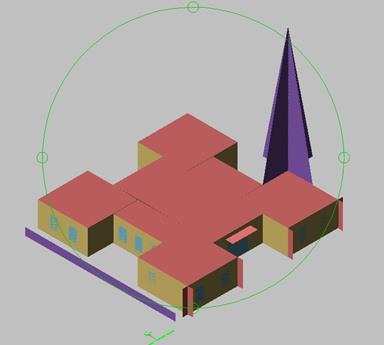
\includegraphics[width=0.9\textwidth, height=0.9\textheight, keepaspectratio=true]{media/image002.jpg}
\caption{Using IDFEditor to find the latest groups and objects for the Energy+.idd \protect \label{fig:using-idfeditor-to-find-the-latest-groups}}
\end{figure}

The produced list will look something like:

Simulation Parameters

\begin{center}\rule{0.5\linewidth}{\linethickness}\end{center}

{[}------{]}~ Version

{[}------{]}~ SimulationControl

{[}------{]}~ Building

{[}------{]}~ ShadowCalculation

{[}------{]}~ SurfaceConvectionAlgorithm:Inside

{[}------{]}~ SurfaceConvectionAlgorithm:Outside

{[}------{]}~ HeatBalanceAlgorithm

{[}------{]}~ ZoneCapacitanceMultiplier

{[}------{]}~ Timestep

{[}------{]}~ ConvergenceLimits

Location - Climate - Weather File Access

\begin{center}\rule{0.5\linewidth}{\linethickness}\end{center}

{[}------{]}~ Site:Location

{[}------{]}~ SizingPeriod:DesignDay

{[}------{]}~ SizingPeriod:WeatherFileDays

{[}------{]}~ SizingPeriod:WeatherFileConditionType

{[}------{]}~ RunPeriod

{[}------{]}~ RunPeriodControl:SpecialDays

{[}------{]}~ RunPeriodControl:DaylightSavingTime

``Simulation Parameters'' and ``Location -- Climate -- Weather File Access'' are groups. Version, Building, etc are objects.


\section{Input -- Output Descriptions (Document)}\label{input-output-descriptions-document}

\subsection{Input Descriptions}\label{input-descriptions}

In the descriptions below, the fields for each input object will be described but the Energy+.idd descriptions will not be shown. Refer to the actual Energy+.idd file for complete specifications. Energy+.idd is a text file that can be viewed with many text editors or word processors. The Site:Location object will serve as an example.

\begin{lstlisting}
Site:Location,
       \unique-object
       \min-fields 5
  A1 , \field Name
       \required-field
       \type  alpha
  N1 , \field Latitude
       \units deg
       \minimum -90.0
       \maximum +90.0
       \default 0.0
       \note + is North, - is South, degree minutes represented in decimal (i.e. 30 minutes is .5)
       \type real
  N2 , \field Longitude
       \units deg
       \minimum -180.0
       \maximum +180.0
       \default 0.0
       \note - is West, + is East, degree minutes represented in decimal (i.e. 30 minutes is .5)
       \type real
  N3 , \field Time Zone
       \note basic these limits on the WorldTimeZone Map (2003)
       \units hr
       \minimum -12.0
       \maximum +14.0
       \default 0.0
       \note  Time relative to GMT. Decimal hours.
       \type real
  N4 ; \field Elevation
       \units m
       \minimum -300.0
       \maximum< 8900.0
       \default 0.0
       \type real
\end{lstlisting}

The IDD excerpt above is the complete definition as seen in the IDD file.

First, the object name is given. (Site:Location)~ This is followed by a comma in both the definition (IDD) and in an input file (IDF). In fact, all fields except the terminating field of an IDD class object and IDF object are followed by commas. The final field in an IDD class object or in an IDF object is terminated by a semi-colon.

Next is an alpha field, the location name. As noted above, for input, spaces are significant in this field. The main inputs for Site:Location are numeric fields. These are numbered (as is the alpha field) for convenience. The \textbackslash{} designations will show various information about the objects as described above in the IDD conventions discussion. Of importance for reading this document are the units and possible minimum and maximum values for a~ field.

There is automatic processing of the \textbackslash{}minimum, \textbackslash{}maximum and \textbackslash{}default data for numeric fields. Any infractions of the \textbackslash{}minimum, \textbackslash{}maximum fields are automatically detected and messages will appear in the standard error file. After all the input is checked, infractions will cause program termination (before the bulk of the simulation is completed). Defaults are also enforced if you leave the numeric field blank.

Some objects need all the parameters listed by the definition; some do not. In the descriptions that follow, we will try to indicate which parts are optional. Usually, these will be the last fields in the object input or definition. Even if items are not used for a particular object (e.g.~Multiplier in the FenestrationSurface:Detailed and type = Door), the field must be included unless it is the \emph{last field in the object}. So, for this instance, one must include a multiplier field (must be numeric and would need to obey any \textbackslash{}minimum, \textbackslash{}maximum rules) for doors.

Two spreadsheet files are included with the installation:

\begin{itemize}
\item
  ExampleFiles.xls -- shows many details about the included example files including highlights of features.
\item
  ExampleFiles-ObjectsLink.xls -- shows, for each object, the first three occurrences of that object in an example file.
\end{itemize}

\subsection{Output Descriptions}\label{output-descriptions}

In the descriptions below, we will endeavor to have each object's output displayed as well as each of the outputs described. The output variables for a run are selected by choosing the Output:VariableDictionary object. This object displays the available output variables for a run on the \textbf{eplusout.rdd} (regular variables) and \textbf{eplusout.mdd} (meter variables) files. Two significant styles are available for these displays and the descriptions below may have one for some objects and another for other objects. The variables are the same but will look a bit different.~ For clarity, the two displays are shown below:

Note that the IDF-Editor can interpret both sets of files and assist you in getting output variables into your input files. But you will have to successfully run your input file first.

The Simple (or regular) display looks like the following figure and is interpreted:

\textbf{Zone/HVAC} -- when the output is produced at the ``Zone'' timestep (ref: number of timesteps in each hour) or at the ``HVAC'' aka System timestep (which can vary for each hour).

\textbf{Average/Sum} -- whether this is a averaged value over the reporting period (such as a temperature or rate) or whether this is a summed value over the reporting period. Reporting periods are specified in the Output:Variable or Output:Meter objects.

\textbf{\textless{}Variable Name\textgreater{}} -- The variable name one uses for reporting is displayed (e.g., Site Outdoor Drybulb Temperature) along with the units (e.g., {[}C{]}).

Example from the \textbf{eplusout.rdd} file:

\begin{itemize}
\item
  Zone,Average,Site Outdoor Air Drybulb Temperature {[}C{]}
\item
  Zone,Average,Site Outdoor Air Dewpoint Temperature {[}C{]}
\item
  Zone,Average,Site Outdoor Air Wetbulb Temperature {[}C{]}
\item
  Zone,Average,Site Outdoor Air Humidity Ratio {[}kgWater/kgAir{]}
\item
  Zone,Average,Site Outdoor Air Relative Humidity {[}\%{]}
\item
  Zone,Average,Site Outdoor Air Barometric Pressure {[}Pa{]}
\item
  Zone,Average,Wind Speed {[}m/s{]}
\item
  Zone,Average,Site Wind Direction {[}deg{]}
\item
  Zone,Average,Site Sky Temperature {[}C{]}
\item
  HVAC,Sum,Zone Air System Sensible Heating Energy {[}J{]}
\item
  HVAC,Sum,Zone Air System Sensible Cooling Energy {[}J{]}
\item
  HVAC,Average,Zone Air System Sensible Heating Rate {[}W{]}
\item
  HVAC,Average,Zone Air System Sensible Cooling Rate {[}W{]}
\item
  HVAC,Average,Zone Air Temperature {[}C{]}
\item
  HVAC,Average,Zone Thermostat Air Temperature {[}C{]}
\end{itemize}

Note that the \textbf{eplusout.mdd} file is similar, but meters are only available at the Zone timestep.

\begin{itemize}
\item
  Zone,Meter,Electricity:Facility {[}J{]}
\item
  Zone,Meter,ExteriorLights:Electricity {[}J{]}
\item
  Zone,Meter,Grounds Lights:ExteriorLights:Electricity {[}J{]}
\item
  Zone,Meter,EnergyTransfer:Facility {[}J{]}
\item
  Zone,Meter,EnergyTransfer:Building {[}J{]}
\item
  Zone,Meter,EnergyTransfer:Zone:R13WALL WALLS {[}J{]}
\end{itemize}

The IDF display has all the same information in an IDF-ready form (i.e., you could copy and paste it into your input file using a text editor).

Example from the \textbf{eplusout.rdd} file:

\begin{itemize}
\item
  Output:Variable,*,Site Outdoor Air Drybulb Temperature,hourly; !- Zone Average {[}C{]}
\item
  Output:Variable,*,Site Outdoor Air Dewpoint Temperature,hourly; !- Zone Average {[}C{]}
\item
  Output:Variable,*,Site Outdoor Air Wetbulb Temperature,hourly; !- Zone Average {[}C{]}
\item
  Output:Variable,*,Site Outdoor Air Humidity Ratio,hourly; !- Zone Average {[}kgWater/kgAir{]}
\item
  Output:Variable,*,Site Outdoor Air Relative Humidity,hourly; !- Zone Average {[}\%{]}
\item
  Output:Variable,*,Site Outdoor Air Barometric Pressure,hourly; !- Zone Average {[}Pa{]}
\item
  Output:Variable,*,Zone Air System Sensible Heating Energy,hourly; !- HVAC Sum {[}J{]}
\item
  Output:Variable,*,Zone Air System Sensible Cooling Energy,hourly; !- HVAC Sum {[}J{]}
\item
  Output:Variable,*,Zone Air System Sensible Heating Rate,hourly; !- HVAC Average {[}W{]}
\item
  Output:Variable,*,Zone Air System Sensible Cooling Rate,hourly; !- HVAC Average {[}W{]}
\item
  Output:Variable,*,Zone Air Temperature,hourly; !- HVAC Average {[}C{]}
\item
  Output:Variable,*,Zone Thermostat Air Temperature,hourly; !- HVAC Average {[}C{]}
\end{itemize}

All of the same information appears in a slightly different form and defaults to ``hourly'' reporting frequency (which, of course, can be changed when you put it into your input file). The ``*'' is preselected so that you would be reporting for all those items.


\section{Group -- Simulation Parameters}\label{group-simulation-parameters}

This group of objects influences the simulation in various ways.

\subsection{Version}\label{version}

\subsubsection{Inputs}\label{inputs-044}

\paragraph{Field: Version Identifier}\label{field-version-identifier}

The Version object allows you to enter the proper version that your IDF was created for. This is checked against the current version of EnergyPlus and a Severe error issued (non-terminating) if it does not match the current version string. Note that versions are often significant and there is no guarantee that the older file will run in the newer versions of the program. See IDF Version Updater (Auxiliary Programs Document) for methods of changing the older files to newer versions.

\subsection{Timestep}\label{timestep}

\subsubsection{Inputs}\label{inputs-1-041}

\paragraph{Field: Number of Timesteps per Hour}\label{field-number-of-timesteps-per-hour}

The Timestep object specifies the ``basic'' timestep for the simulation. The value entered here is usually known as the Zone Timestep. This is used in the Zone Heat Balance Model calculation as the driving timestep for heat transfer and load calculations. The value entered here is the number of timesteps to use within an hour. Longer length timesteps have lower values for Number of Timesteps per Hour. For example a value of 6 entered here directs the program to use a zone timestep of 10 minutes and a value of 60 means a 1 minute timestep. The user's choice for Number of Timesteps per Hour must be evenly divisible into 60; the allowable choices are 1, 2, 3, 4, 5, 6, 10, 12, 15, 20, 30, and 60.

The choice made for this field has important implications for modeling accuracy and the overall time it takes to run a simulation. Here are some considerations when choosing a value:

\begin{itemize}
\item
  The solution technique used in EnergyPlus has been designed to be stable with zone timesteps of up to sixty minutes (Number Timesteps in Hour = 1). However, 60 minutes is considered a ``long'' timestep and it should only be used in rare occasions where there is no HVAC system, accuracy is not a concern, and short run times are critical. Such long timesteps are not recommended to use because simulation results are more accurate for shorter timesteps, of say 10 minutes or less (Number of Timesteps per Hour of 6 or more). Shorter zone timesteps improve the numerical solution of the Zone Heat Balance Model because they improve how models for surface temperature and zone air temperature are coupled together. Longer timesteps introduce more lag and lead to more a dampened dynamic response.
\item
  Simulation run time increases with shorter timesteps or larger values for Number of Timesteps per Hour. The effect varies with the nature of the model. The user can test out different values on their particular model to understand the implications for his or her particular case. Sometimes large models with multizone HVAC and Plant systems execute nearly as fast with 15 minute timesteps as with 60 minute timesteps because fewer iterations are required in the system modeling since the prior timestep's results are close to the final outcome of next timestep.
\item
  The weather data files usually have 60-minute (or hourly) data. However, it does not follow that this should be used as the basis for choosing the zone timestep because:
\item
  EnergyPlus carefully interpolates the weather data between data points for use at shorter timesteps. This is discussed in a later section: Weather Data Hourly Interpolation
\item
  Many aspects of a model have time scales that differ from the that of the weather data. A goal of the modeling is to predict how the building will respond to the weather. However, the building's response is not \emph{governed} by the time scale that the weather data are available at, but rather the time scales of the dynamic performance of the thermal envelope as well as things like schedules for internal gains, thermostats, and equipment availability.
\item
  If the model will include calculating the cost of electricity, then the user should be aware that many electric utility tariffs base charges on demand windows of a specified length of time. If the choice of Number of Timesteps per Hour is not consistent with the demand window, then unexpected results may be obtained. For reasonable prediction of the maximum rates for electricity use for in calculating demand charges, the length of the zone timestep needs to be consistent with the tariff's demand window. The following table lists what values are consistent with various demand windows.
\end{itemize}

\begin{longtable}[c]{@{}ll@{}}
\toprule
Demand Window & Applicable Number of Timesteps per Hour \tabularnewline
\midrule
\endfirsthead

\toprule
Demand Window & Applicable Number of Timesteps per Hour \tabularnewline
\midrule
\endhead

QuarterHour & 4, 12, 20, or 60 \tabularnewline
HalfHour & 2, 4, 6, 10, 12, 20, 30, or 60 \tabularnewline
FullHour, Day, Week & Any \tabularnewline
\bottomrule
\end{longtable}

There is also second type of timestep inside EnergyPlus that is known as the System Timestep. This is a variable-length timestep that governs the driving timestep for HVAC and Plant system modeling. The user cannot directly control the system timestep (except by use of the ConvergenceLimits object). When the HVAC portion of the simulation begins its solution for the current zone timestep, it uses the zone timestep as its maximum length but then can reduce the timestep, as necessary, to improve the solution.  The technical details of the approach are explained in the Engineering Documentation under ``Integrated Solution Manager''.

Users can see the system timestep used if they select the ``detailed'' frequency option on an HVAC output variable (e.g. Zone Air Temperature). To contrast, the ``Zone'' variables will only be reported on the zone timestep (e.g. Zone Mean Air Temperature).

And, the IDF example:

\begin{lstlisting}
Timestep, 6;  !- Suggested default for most system simulations
\end{lstlisting}

Suggested defaults are 4 for non-HVAC simulations, 6 for simulations with HVAC, 20 is the minimum for ConductionFiniteDifference and HeatAndMoistureFiniteElement simulations. Green roof (ref: Material:RoofVegetation) also may require more timesteps.

Note that hourly data (such as outdoor conditions expressed by Design Days or Weather data) are interpolated to the Zone Timestep. This is discussed in a later section: Weather Data Hourly Interpolation

\subsection{ConvergenceLimits}\label{convergencelimits}

This item is an ``advanced'' feature that should be used only with caution. It is specifically included to assist some users ``speed up'' calculations while not overly compromising accuracy. The user must judge for him/herself whether the reduced run time is useful.

\subsubsection{Inputs}\label{inputs-2-038}

\paragraph{Field: Minimum System Timestep}\label{field-minimum-system-timestep}

Usually the minimum system timestep is allowed to vary from the zone timestep (as maximum) to a minimum timestep of 1 minute during certain system calculations. This might be when the system turns on or off, for example. Entering 0 in this field sets the minimum system timestep to be the same as the zone timestep. Otherwise the units of the field are minutes. It's probably a good idea to have any minimum entered be a divisor of the zone timestep.

\paragraph{Field: Maximum HVAC Iterations}\label{field-maximum-hvac-iterations}

The HVAC Manager will iterate to a solution or up to a set number of iterations. If not ``converged'', then a warning error appears:

\begin{lstlisting}
SimHVAC: Maximum iterations (20) exceeded for all HVAC loops, at CHICAGO IL USA TMY2-94846 WMO# = 725300, 10/07 14:06 - 14:08
\end{lstlisting}

In order to reduce time used in simulating your building, you may choose to enter a lesser number than the default of 20 for the maximum number of iterations to be used. Or, you may wish to enter a bigger number for certain buildings. To get more information printed with a ``max iteration'' message, you need to enter a ``Output:Diagnostics, DisplayExtraWarnings;'' command (which may also generate other warnings than just this one).

\paragraph{Field: Minimum Plant Iterations}\label{field-minimum-plant-iterations}

The plant system modeling includes a solver that iterates within a single HVAC manager iteration. This input field and the next one provide some control over how the plant solver iterates. This field sets a minimum threshold for plant iterations. The default for this field is the value ``2'' which indicates that a minimum of two full plant model interations will be performed every time plant is called by the HVAC manager. For faster performance with simple plant systems, this input field could be set to the value ``1''. For complicated plant systems that present difficulties to solve, this value may need to be set higher to ensure accuracy but at the expense of speed. Complicated plant systems include those with several interconnected loops, sizing miss-matches such that plant components are starved of flow compared to their desired flow, heat recovery systems, and thermal load following onsite generators.

\paragraph{Field: Maximum Plant Iterations}\label{field-maximum-plant-iterations}

The plant system solver iterates within a single HVAC manager iteration. This input field and the previous one provide some control over how the plant model iterates. This field sets a maximum limit for plant interations. The default for this field is the value ``8'' which indicates that the plant solver will exit after having completed eight full iterations. This value can be raised for better accuracy with complex plants or lowered for faster speed with simple plants. The output variable called ``Plant Solver Sub Iteration Count'' (typically reported at the ``detailed'' frequency) is useful for understanding how many plant solver iterations are actually being used during a particular simulation. The lower limit of the value for this field is ``2.''

Use in an IDF:

\begin{lstlisting}
ConvergenceLimits,
  0,        !- Minimum System Timestep (0 = same as zone timestep)
  25,       !- Maximum HVAC Iterations
  3,        !- Minimum Plant Iterations
  9;        !- Maximum Plant Iterations
\end{lstlisting}

\subsection{Building}\label{building}

The Building object describes parameters that are used during the simulation of the building. There are necessary correlations between the entries for this object and some entries in the Site:WeatherStation and Site:HeightVariation objects, specifically the Terrain field.

\subsubsection{Inputs}\label{inputs-3-034}

\paragraph{Field: Building Name}\label{field-building-name}

Building name is specified for output convenience.

\paragraph{Field: North Axis}\label{field-north-axis}

The Building North Axis is specified \textbf{relative to true North}. Buildings frequently do not line up with true north. For convenience, one may enter surfaces in a ``regular'' coordinate system and then shift them via the use of the North Axis. The value is specified in degrees from ``true north'' (clockwise is positive).

The figure below shows how the building north axis can be rotated to correspond with one of the major axes of an actual building. The relevance of this field is described more completely under ``GlobalGeometryRules''; in particular, the value of ``North Axis'' is \emph{ignored} if a coordinate system other than ``relative'' is used.

\begin{figure}[hbtp] % fig 1
\centering
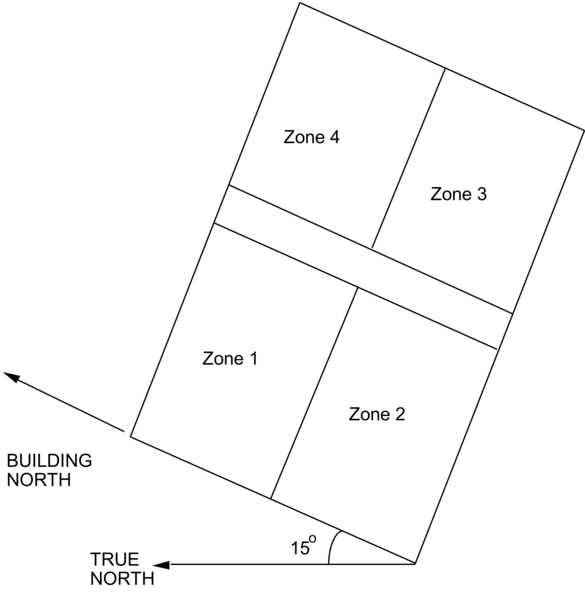
\includegraphics[width=0.9\textwidth, height=0.9\textheight, keepaspectratio=true]{media/image001.png}
\caption{Illustration of Building North Axis \protect \label{fig:illustration-of-building-north-axis}}
\end{figure}

\paragraph{Field: Terrain}\label{field-terrain}

The site's terrain affects how the wind hits the building -- as does the building height. In addition, the external conduction method usually has its own parameters for the calculation. Please see the Engineering Documentation, External Conduction section for particulars. The legal values for this field are shown in the following table.

% table 1
\begin{longtable}[c]{@{}ll@{}}
\caption{Values for ``Terrain'' \label{table:values-for-terrain}} \tabularnewline
\toprule
Terrain Type Value & Terrain Description \tabularnewline
\midrule
\endfirsthead

\caption[]{Values for ``Terrain''} \tabularnewline
\toprule
Terrain Type Value & Terrain Description \tabularnewline
\midrule
\endhead

Country & Flat, Open Country \tabularnewline
Suburbs & Rough, Wooded Country, Suburbs \tabularnewline
City & Towns, city outskirts, center of large cities \tabularnewline
Ocean & Ocean, Bayou flat country \tabularnewline
Urban & Urban, Industrial, Forest \tabularnewline
\bottomrule
\end{longtable}

\paragraph{Warmup Convergence}\label{warmup-convergence}

The following two fields along with the minimum and maximum number of warmup days (also in this object) define the user specified criteria for when EnergyPlus will ``converge'' at each environment (each sizing period or run period set as Yes in the SimulationControl object). EnergyPlus ``runs'' the first day of the environment (starting with a set of hard-coded initial conditions: temperatures are initialized to 23C and zone humidity ratios are initialized to the outdoor humidity ratio) until the loads/temperature convergence tolerance values are satisfied (next two fields) or until it reaches ``maximum number of warmup days''. Note that setting the convergence tolerance values too loose will cause the program to be satisfied too early and you may not get the results you expect from the actual simulation.

\paragraph{Field: Loads Convergence Tolerance Value}\label{field-loads-convergence-tolerance-value}

This value represents the number at which the loads values must agree before ``convergence'' is reached. Loads tolerance value is a fraction of the load.

\paragraph{Field: Temperature Convergence Tolerance Value}\label{field-temperature-convergence-tolerance-value}

This value represents the number at which the zone temperatures must agree (from previous iteration) before ``convergence'' is reached. (Units for this field is delta C).

Convergence of the simultaneous heat balance/HVAC solution is reached when either the loads or temperature criterion is satisfied.

All tolerances have units so the temperature tolerance is in degrees C (or degrees K) and the loads tolerance is in Watts. Both tolerances work the same way, just one looks at temperatures and one looks at heating and cooling loads. After the second warm-up day, the program compares the maximum temperature experienced in a space with the maximum temperature from the previous day. If those two temperatures are within the tolerance, then it has passed the first warm-up check.

It does a similar comparison with lowest temperatures experience within all the zones. If the current simulation day and the previous day values are within the tolerance, then it has passed the second warm-up check. Similar things are done with the loads tolerance and the maximum heating and cooling loads that are experienced within the spaces. Those are compared individually to the values for the previous day. If they are both in tolerance, then the simulation has passed the third and fourth warm-up check. The simulation stays in the warm-up period until ALL FOUR checks have been passed. See Engineering Reference and Output Details document for further explanation and outputs.

Please note--other ``convergence tolerance'' inputs are required for certain HVAC equipment (unit ventilator, unit heater, window AC, etc.). The purpose and units of these parameters are different from ``load convergence tolerance'' and ``temperature convergence tolerance'' in the BUILDING object.

\paragraph{Field: Solar Distribution}\label{field-solar-distribution}

Setting this value determines how EnergyPlus treats beam solar radiation and reflectances from exterior surfaces that strike the building and, ultimately, enter the zone. There are five choices: \textbf{MinimalShadowing}, \textbf{FullExterior} and \textbf{FullInteriorAndExterior, FullExteriorWithReflections, FullInteriorAndExteriorWithReflections}.

\textbf{MinimalShadowing}

In this case, there is no exterior shadowing except from window and door reveals. All beam solar radiation entering the zone is assumed to fall on the floor, where it is absorbed according to the floor's solar absorptance. Any reflected by the floor is added to the transmitted diffuse radiation, which is assumed to be uniformly distributed on all interior surfaces. If no floor is present in the zone, the incident beam solar radiation is absorbed on all interior surfaces according to their absorptances. The zone heat balance is then applied at each surface and on the zone's air with the absorbed radiation being treated as a flux on the surface.

\textbf{FullExterior, FullExteriorWithReflections}

In this case, shadow patterns on exterior surfaces caused by detached shading, wings, overhangs, and exterior surfaces of all zones are computed. As for MinimalShadowing, shadowing by window and door reveals is also calculated. Beam solar radiation entering the zone is treated as for MinimalShadowing -- All beam solar radiation entering the zone is assumed to fall on the floor, where it is absorbed according to the floor's solar absorptance. Any reflected by the floor is added to the transmitted diffuse radiation, which is assumed to be uniformly distributed on all interior surfaces. If no floor is present in the zone, the incident beam solar radiation is absorbed on all interior surfaces according to their absorptances. The zone heat balance is then applied at each surface and on the zone's air with the absorbed radiation being treated as a flux on the surface.

\textbf{FullInteriorAndExterior, FullInteriorAndExteriorWithReflections}

This is the same as FullExterior except that instead of assuming all transmitted beam solar falls on the floor the program calculates the amount of beam radiation falling on each surface in the zone, including floor, walls and windows, by projecting the sun's rays through the exterior windows, taking into account the effect of exterior shadowing surfaces and window shading devices.

If this option is used, you should be sure that the surfaces of the zone totally enclose a space. This can be determined by viewing the \textbf{eplusout.dxf} file with a program like AutoDesk's Volo View Express. You should also be sure that the zone is \textbf{convex}. Examples of convex and non-convex zones are shown in Figure~\ref{fig:illustration-of-convex-and-non-convex-zones}. The most common non-convex zone is an L-shaped zone. (A formal definition of convex is that any straight line passing through the zone intercepts at most two surfaces.) If the zone's surfaces do not enclose a space or if the zone is not convex you should use Solar Distribution = \textbf{FullExterior} instead of \textbf{FullInteriorAndExterior}.

If you use \textbf{FullInteriorAndExterior} the program will also calculate how much beam radiation falling on the inside of an exterior window (from other windows in the zone) is absorbed by the window, how much is reflected back into the zone, and how much is transmitted to the outside. In this calculation the effect of a shading device, if present, is accounted for.

\begin{figure}[hbtp] % fig 2
\centering
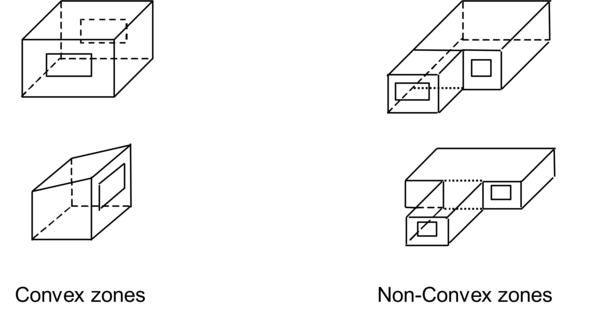
\includegraphics[width=0.9\textwidth, height=0.9\textheight, keepaspectratio=true]{media/image002.png}
\caption{Illustration of Convex and Non-convex Zones \protect \label{fig:illustration-of-convex-and-non-convex-zones}}
\end{figure}

\textbf{Reflection calculations}

Note: Using the reflection calculations can be very time-consuming. Even error-prone. As a possible alleviation, you can use the Output:Diagnostics,DoNotMirrorDetachedShading; in many cases to get past a fatal error.

If using reflections, the program calculates beam and sky solar radiation that is reflected from exterior surfaces and then strikes the building. These reflecting surfaces fall into three categories:

1) \textbf{Shadowing surfaces}. These are surfaces like overhangs or neighboring buildings entered with Shad\-ing:\-Site, Shad\-ing:\-Build\-ing, Shad\-ing:\-Site:\-Detailed, Shad\-ing:\-Build\-ing:\-Detailed, Shad\-ing:\-Over\-hang, Shad\-ing:\-Over\-hang:Pro\-jection, Shad\-ing:\-Fin, Shad\-ing:\-Fin:\-Pro\-jection or Shad\-ing:\-Zone:\-Detailed objects. See Figure~\ref{fig:solar-reflection-from-shadowing-surfaces.}.

These surfaces can have diffuse and/or specular (beam-to-beam) reflectance values that are specified with the Shad\-ing\-Property:\-Re\-flectance object which specifies those parameters. They have a default value of .2 for both visible and diffuse reflection.

2) \textbf{Exterior building surfaces}. In this case one section of the building reflects solar radiation onto another section (and vice-versa). See Figure~\ref{fig:solar-reflection-from-building-surfaces-onto}.

The building surfaces are assumed to be diffusely reflecting if they are opaque (walls, for example) and specularly reflecting if they are windows or glass doors. The reflectance values for opaque surfaces are calculated by the program from the Solar Absorptance and Visible Absorptance values of the outer material layer of the surface's construction (ref: Material object properties). The reflectance values for windows and glass doors are calculated by the program from the reflectance properties of the individual glass layers that make up surface's construction assuming no shading device is present and taking into account inter-reflections among the layers (ref: Window Properties).

3) \textbf{The ground surface}. Reflection from the ground is calculated even if reflections option is not used;l but then the ground plane is considered unobstructed, i.e., the shadowing of the ground by the building itself or by obstructions such as neighboring buildings is ignored. Shadowing by the building itself or neighboring buildings is taken into account when the ``with reflections'' option is used but then the ``view factor to ground'' is NOT used. This is shown in Figure~\ref{fig:shadowing-from-building-affects-beam-solar}.

\begin{figure}[hbtp] % fig 3
\centering
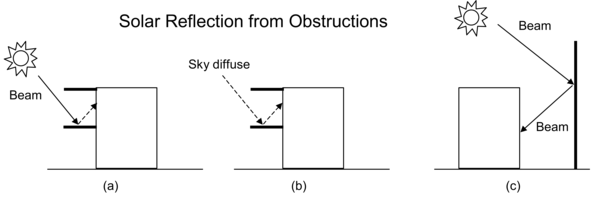
\includegraphics[width=0.9\textwidth, height=0.9\textheight, keepaspectratio=true]{media/image003.png}
\caption{  Solar reflection from shadowing surfaces. Solid arrows are beam solar radiation; dashed arrows are diffuse solar radiation. (a) Diffuse reflection of beam solar radiation from the top of an overhang. (b) Diffuse reflection of sky solar radiation from the top of an overhang. (c) Beam-to-beam (specular) reflection from the façade of an adjacent highly-glazed building represented by a vertical shadowing surface. \protect \label{fig:solar-reflection-from-shadowing-surfaces.}}
\end{figure}

\begin{figure}[hbtp] % fig 4
\centering
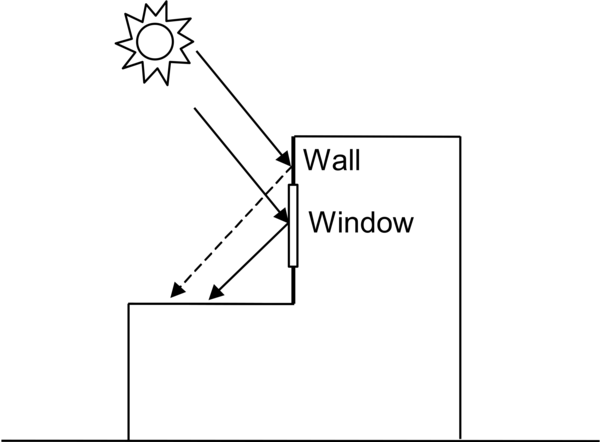
\includegraphics[width=0.9\textwidth, height=0.9\textheight, keepaspectratio=true]{media/image004.png}
\caption{  Solar reflection from building surfaces onto other building surfaces. In this example beam solar reflects from a vertical section of the building onto a roof section. The reflection from the window is specular. The reflection from the wall is diffuse. \protect \label{fig:solar-reflection-from-building-surfaces-onto}}
\end{figure}

\begin{figure}[hbtp] % fig 5
\centering
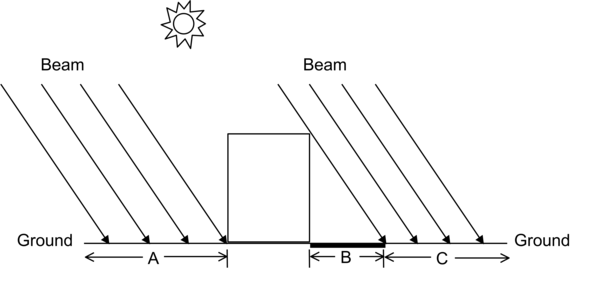
\includegraphics[width=0.9\textwidth, height=0.9\textheight, keepaspectratio=true]{media/image005.png}
\caption{Shadowing from building affects beam solar reflection from the ground. Beam-to-diffuse reflection from the ground onto the building occurs only for sunlit areas, A and C, not from shaded area, B. \protect \label{fig:shadowing-from-building-affects-beam-solar}}
\end{figure}

\paragraph{Field: Maximum Number of Warmup Days}\label{field-maximum-number-of-warmup-days}

This field specifies the number of ``warmup'' days that might be used in the simulation before ``convergence'' is achieved. The default number, 25, is usually more than sufficient for this task; however, some complex buildings (with complex constructions) may require more days. If you enter less than 25 as a maximum, that is the number of maximum warmup days that will be used. An error message will occur when the simulation ``runs'' out of days and has not converged:

\begin{lstlisting}
CheckWarmupConvergence: Loads Initialization, Zone = "MAIN ZONE" did not converge after 30 warmup days.
See Warmup Convergence Information in .eio file for details
..Environment(SizingPeriod) = "DENVER CENTENNIAL  GOLDEN   N ANN CLG 1% CONDNS DB = >MWB"
..Max Temp Comparison = 2.06E-002 vs Temperature Convergence Tolerance = 0.50 – Pass Convergence
..Min Temp Comparison = 5.95E-003 vs Temperature Convergence Tolerance = 0.50 – Pass Convergence
..Max Cool Load Comparison = 9.5082E-002 vs Loads Convergence Tolerance = 5.00E-002 – Fail Convergence
\end{lstlisting}

As noted in the message, there will be more information in the .eio file. (Refer to Output Details document as well for examples.)

You may be able to increase the Maximum Number of Warmup Days and get convergence, but some anomalous buildings may still not converge. Simulation proceeds for x warmup days until ``convergence'' is reached (see the discussion under the Temperature Convergence Tolerance Value field in this object, just above).

\paragraph{Field: Minimum Number of Warmup Days}\label{field-minimum-number-of-warmup-days}

This field specifies the minimum number of ``warmup'' days before EnergyPlus will check if it has achieved convergence and can thus start simulating the particular environment (design day, annual run) in question. Research into the minimum number of warmup days indicates that 6 warmup days is generally enough on the minimum end of the spectrum to avoid false predictions of convergence and thus to produce enough temperature and flux history to start EnergyPlus simulation. This was based on a study that used the benchmark reference buildings. It also was observed that convergence performance improved when the number of warmup days increased. As a result, the default value for the minimum warmup days has been set to 6. Users should decrease this number only if they have knowledge that a specific file converges more quickly than 6 days. Users may wish to increase the value in certain situations when, based on the output variables described in the Output Details document, it is determined that EnergyPlus has not converged. While this parameter should be less than the previous parameter, a value greater than the value entered in the field ``Maximum Number of Warmup Days'' above may be used when users wish to increase warmup days more than the previous field. In this particular case, the previous field will be automatically reset to the value entered in this field and EnergyPlus will run exactly the number of warmup days specified in this field.

An example from an IDF:

\begin{lstlisting}

Building,
    PSI HOUSE DORM AND OFFICES,  !- Name
    36.87000,               !- North Axis {deg}
    Suburbs,                !- Terrain
    0.04,                   !- Loads Convergence Tolerance Value
    0.4000000,              !- Temperature Convergence Tolerance Value {deltaC}
    FullInteriorAndExterior, !- Solar Distribution
    40,                     !- Maximum Number of Warmup Days
    6;                      !- Minimum Number of Warmup Days
\end{lstlisting}

\subsection{SurfaceConvectionAlgorithm:Inside}\label{surfaceconvectionalgorithminside}

This input object is used control the choice of models used for surface convection at the inside face of all the heat transfer surfaces in the model. This object sets the selection for convection correlations in a global way. The Zone Inside Convection Algorithm input field in the Zone object may be used to selectively override this value on a zone-by-zone basis. Further, individual surfaces can refine the choice by each surface or surface lists -- see object SurfaceProperty:ConvectionCoefficients and object SurfaceProperty:ConvectionCoefficients:MultipleSurface.

\subsubsection{Inputs}\label{inputs-4-031}

\paragraph{Field: Algorithm}\label{field-algorithm-000}

The model specified in this field is the default algorithm for the inside face all the surfaces.. The key choices are \textbf{Simple}, \textbf{TARP}, \textbf{CeilingDiffuser}, and \textbf{AdaptiveConvectionAlgorithm}.

The \textbf{Simple} model applies constant heat transfer coefficients depending on the surface orientation.

The \textbf{TARP} model correlates the heat transfer coefficient to the temperature difference for various orientations. This model is based on flat plate experiments.

The \textbf{CeilingDiffuser} model is a mixed and forced convection model for ceiling diffuser configurations. The model correlates the heat transfer coefficient to the air change rate for ceilings, walls and floors. These correlations are based on experiments performed in an isothermal room with a cold ceiling jet. To avoid discontinuities in surface heat transfer rate calculations, all of correlations have been extrapolated beyond the lower limit of the data set (3 ACH) to a natural convection limit that is applied during the hours when the system is off.

The \textbf{AdaptiveConvectionAlgorithm} model is an dynamic algorithm that organizes a large number of different convection models and automatically selects the one that best applies. The adaptive convection algorithm can also be customized using the SurfaceConvectionAlgorithm:Inside:AdaptiveModelSelections input object. These models are explained in detail in the EnergyPlus Engineering Reference Document.

The default is \textbf{TARP}.

IDF Example:

\begin{lstlisting}

SurfaceConvectionAlgorithm:Inside,TARP;
\end{lstlisting}

\subsection{SurfaceConvectionAlgorithm:Outside}\label{surfaceconvectionalgorithmoutside}

Various exterior convection models may be selected for global use. The optional Zone Outside Convection Algorithm input field in the Zone object may be used to selectively override this value on a zone-by-zone basis. Further, individual surfaces can refine the choice by each surface or surface lists -- see object SurfaceProperty:ConvectionCoefficients and object SurfaceProperty:ConvectionCoefficients:MultipleSurface.

\subsubsection{Inputs}\label{inputs-5-028}

\paragraph{Field: Algorithm}\label{field-algorithm-1-000}

The available key choices are \textbf{SimpleCombined}, \textbf{TARP}, \textbf{MoWiTT}, \textbf{DOE-2}, and \textbf{AdaptiveConvectionAlgorithm}.

The \textbf{Simple} convection model applies heat transfer coefficients depending on the roughness and windspeed. This is a combined heat transfer coefficient that includes radiation to sky, ground, and air. The correlation is based on Figure~\ref{fig:schematic-of-the-energyplus-unitary-system}, Page 25.1 (Thermal and Water Vapor Transmission Data), 2001 ASHRAE Handbook of Fundamentals. Note that if \textbf{Simple} is chosen here or in the Zone field and a SurfaceProperty:ConvectionCoefficients object attempts to override the calculation with a different choice, the action will still be one of combined calculation. To change this, you must select one of the other methods for the global default.

All other convection models apply heat transfer coefficients depending on the roughness, windspeed, and terrain of the building's location. These are \emph{convection only} heat transfer coefficients; radiation heat transfer coefficients are calculated automatically by the program.

The \textbf{TARP} algorithm was developed for the TARP software and combines natural and wind-driven convection correlations from laboratory measurements on flat plates.

The \textbf{DOE-2} and \textbf{MoWiTT} were derived from field measurements. DOE-2 uses a correlation from measurements by Klems and Yazdanian for rough surfaces. MoWitt uses a correlation from measurements by Klems and Yazdanian for smooth surfaces and, therefore, is most appropriate for windows (see SurfaceProperty:ConvectionCoefficients:MultipleSurface for how to apply to only windows).

The \textbf{AdaptiveConvectionAlgorithm} model is an dynamic algorithm that organizes a large number of different convection models and automatically selects the one that best applies. The adaptive convection algorithm can also be customized using the SurfaceConvectionAlgorithm:Outside:AdaptiveModelSelections input object. All algorithms are described more fully in the Engineering Reference.

The default is \textbf{DOE-2}.

Note that when the surface is wet (i.e. it is raining and the surface is exposed to wind) then the convection coefficient appears as a very large number (1000) and the surface is exposed to the Outdoor Wet-bulb Temperature rather than the Outdoor Dry-bulb Temperature.

IDF Example:

\begin{lstlisting}

SurfaceConvectionAlgorithm:Outside, AdaptiveConvectionAlgorithm;
\end{lstlisting}

\subsection{HeatBalanceAlgorithm}\label{heatbalancealgorithm}

The HeatBalanceAlgorithm object provides a way to select what type of heat and moisture transfer algorithm will be used for calculating the performance of the building's surface assemblies. This input controls the overall algorithm used for all the surfaces unless one or more of the SurfaceProperty:HeatTransferAlgorithm:* objects are used to alter the selection for particular surfaces.

\subsubsection{Inputs}\label{inputs-6-025}

\paragraph{Field: Algorithm}\label{field-algorithm-2-000}

Four values are allowed to select which solution will be used.

\begin{itemize}
\item
  The \textbf{ConductionTransferFunction} selection is a sensible heat only solution and does not take into account moisture storage or diffusion in the construction elements.
\item
  The \textbf{MoisturePenetrationDepthConductionTransferFunction} selection is a sensible heat diffusion and an inside surface moisture storage algorithm that also needs additional moisture material property information. Sometimes, this is referred to as the Effective Moisture Penetration Depth or EMPD. See the moisture material property object for additional information and description of outputs:
\item
  MaterialProperty:MoisturePenetrationDepth:Settings
\item
  \textbf{Advanced/Research usage:}The \textbf{ConductionFiniteDifference} selection is a sensible heat only solution and does not take into account moisture storage or diffusion in the construction elements. This solution technique uses a 1-D finite difference solution in the construction elements. Outputs for the surfaces are described with the material property objects. The Conduction Finite Difference (aka CondFD) property objects are:
\item
  MaterialProperty:PhaseChange
\item
  MaterialProperty:VariableThermalConductivity
\item
  \textbf{Advanced/Research usage:} The \textbf{CombinedHeatAndMoistureFiniteElement} is a coupled heat and moisture transfer and storage solution. The solution technique uses a one dimensional finite difference solution in the construction elements and requires further material properties described in the Heat and Moisture Transfer material properties objects. Outputs from the algorithm are described with these objects. The Heat and Moisture Transfer property objects are:
\item
  MaterialProperty:HeatAndMoistureTransfer:Settings
\item
  MaterialProperty:HeatAndMoistureTransfer:SorptionIsotherm
\item
  MaterialProperty:HeatAndMoistureTransfer:Suction
\item
  MaterialProperty:HeatAndMoistureTransfer:Redistribution
\item
  MaterialProperty:HeatAndMoistureTransfer:Diffusion
\item
  MaterialProperty:HeatAndMoistureTransfer:ThermalConductivity
\end{itemize}

\paragraph{Field: Surface Temperature Upper Limit}\label{field-surface-temperature-upper-limit}

This field is a bit ``advanced''. It should only be used when the simulation fails AND you cannot determine a cause for the failure. That is, you receive an error similar to:

\begin{lstlisting}
   ** Severe  ** Temperature out of bounds (202.91) for surface = Wall1
   **   ~~~   ** in Zone = Zone01
   **   ~~~   **  Occurrence info = NEW YORK CITY NY SUMMER, 07/21 16:00 - 16:01
   **   ~~~   ** A temperature out of bounds problem can be caused by several things.  The user
   **   ~~~   ** should check the weather environment, the level of internal gains with respect
   **   ~~~   ** to the zone, and the thermal properties of their materials among other things.
   **   ~~~   ** A common cause is a building with no thermal mass -- all materials with
   **   ~~~   ** Regular-R definitions.
\end{lstlisting}

And, after careful perusal, you cannot find a solution as suggested in the error description. You may then want to enter a higher number than the default for this field.

\paragraph{Field: Minimum Surface Convection Heat Transfer Coefficient Value}\label{field-minimum-surface-convection-heat-transfer-coefficient-value}

This optional field is used to set an overall minimum for the value of the coefficient for surface convection heat transfer (Hc) in W/m2-K. A minimum is necessary for numerical robustness because some correlations for Hc can result in zero values and create numerical problems. This field can be used to support specialized validation testing to suppress convection heat transfer and to investigate the implications of different minimum Hc values. The default is 0.1.

\paragraph{Field: Maximum Surface Convection Heat Transfer Coefficient Value}\label{field-maximum-surface-convection-heat-transfer-coefficient-value}

This optional field is used to set an overall maximum for the value of the coefficient for surface convection heat transfer (Hc) in W/m2-K. High Hc values are used in EnergyPlus to approximate fixed surface temperature boundary conditions. This field can be used to alter the accepted range of user-defined Hc values.

And, a default IDF example

\begin{lstlisting}
HeatBalanceAlgorithm,ConductionTransferFunction; ! Solution Algorithm
\end{lstlisting}

\subsection{HeatBalanceSettings:ConductionFiniteDifference}\label{heatbalancesettingsconductionfinitedifference}

This object is used to control the behavior of the Conduction Finite Difference algorithm for surface heat transfer. The settings are global and affect how the model behaves for all the surfaces.

\subsubsection{Inputs}\label{inputs-7-025}

\paragraph{Field: Difference Scheme}\label{field-difference-scheme}

This field determines the solution scheme used by the Conduction Finite Difference model. There are two options CrankNicholsonSecondOrder and FullyImplicitFirstOrder. The CrankNicholsonSecondOrder scheme is second order in time and may be faster. But it can be unstable over time when boundary conditions change abruptly and severely. The FullyImplicitFirstOrder scheme is first order in time and is more stable over time. But it may be slower. The default is FullyImplicitFirstOrder when ConductionFiniteDifference is selected as the Heat Balance Algorithm.

\paragraph{Field: Space Discretization Constant}\label{field-space-discretization-constant}

This field controls how the model determines spatial discretization, or the count of nodes across each material layer in the construction. The model calculates the nominal distance associated with a node, \(\Delta x\), using

\begin{equation}
\Delta x = \sqrt {C\alpha \Delta t}
\end{equation}

Where

\(\alpha\) is the thermal diffusivity of the material layer, in m\(^{2}\)/s

\(\Delta t\) is the length of the timestep in seconds.

\emph{C} is a constant set by this field.

The default is 3. Typical values are from 1 to 3. Lower values for this constant lead to more nodes and finer-grained space discretization.

\paragraph{Field: Relaxation Factor}\label{field-relaxation-factor}

The finite difference solver includes under-relaxation for improved stability for interactions with the other surfaces. This input field can optionally be used to modify the starting value for the relaxation factor. Larger numbers may solve faster, while smaller numbers may be more stable. The default is 1.0. If the program detects numerical instability, it may reduce the value entered here to something lower and more stable.

\paragraph{Field: Inside Face Surface Temperature Convergence Criteria}\label{field-inside-face-surface-temperature-convergence-criteria}

The surface heat balance model at the inside face has a numerical solver that uses a convergence parameter for a maximum allowable differences in surface temperature. This field can optionally be used to modify this convergence criteria. The default value is 0.002 and was selected for stability. Lower values may further increase stability at the expense of longer runtimes, while higher values may decrease runtimes but lead to possible instabilities. The units are in degrees Celsius.

An example IDF object follows.

\begin{lstlisting}
HeatBalanceSettings:ConductionFiniteDifference,
  FullyImplicitFirstOrder, !- Difference Scheme
  3.0,                     !- Space Discretization Constant
  1.0,                     !- Relaxation Factor
  0.002;                   !- Inside Face Surface Temperature Convergence Criteria
\end{lstlisting}

\subsection{ZoneAirHeatBalanceAlgorithm}\label{zoneairheatbalancealgorithm}

The ZoneAirHeatBalanceAlgorithm object provides a way to select what type of solution algorithm will be used to calculate zone air temperatures and humidity ratios. This object is an optional object. If the default algorithm is used, this object is not required in an input file.

\subsubsection{Inputs}\label{inputs-8-023}

\paragraph{Field: Algorithm}\label{field-algorithm-3-000}

Three choices are allowed to select which solution algorithm will be used. The \textbf{ThirdOrderBackwardDifference} selection is the default selection and uses the third order finite difference approximation to solve the zone air energy and moisture balance equations. The \textbf{AnalyticalSolution} selection uses the integration approach to solve the zone air energy and moisture balance equations. The \textbf{EulerMethod} selection uses the first order finite backward difference approximation to solve the zone air energy and moisture balance equations.

And, a default IDF example is shown below:

\begin{lstlisting}
ZoneAirHeatBalanceAlgorithm, ThirdOrderBackwardDifference; !- Algorithm
\end{lstlisting}

\subsection{ZoneAirContaminantBalance}\label{zoneaircontaminantbalance}

The ZoneAirContaminantBalance object provides a way to select which contaminant type will be simulated. Although carbon dioxide is not considered as an indoor contaminant but it is used as an indicator of indoor air quality in buildings. From modeling point of view EnergyPlus treats carbon dioxide as a type of contaminant. In addition to carbon dioxide, a generic contaminant type model was also added. This object is optional, only required in the input data file if the user wishes to model contaminant concentration levels as part of their simulation.

\subsubsection{Inputs}\label{inputs-9-021}

\paragraph{Field: Carbon Dioxide Concentration}\label{field-carbon-dioxide-concentration}

Input is Yes or No. The default is No. If Yes, simulation of carbon dioxide concentration levels will be performed. If No, simulation of carbon dioxide concentration levels will not be performed.

\paragraph{Field: Outdoor Carbon Dioxide Schedule Name}\label{field-outdoor-carbon-dioxide-schedule-name}

This field specifies the name of a schedule that contains outdoor air carbon dioxide level values in units of ppm. One source of monthly average CO\(_{2}\) levels in the atmosphere is available at \href{http://www.esrl.noaa.gov/gmd/ccgg/trends/}{NOAA's website} or via \href{ftp://aftp.cmdl.noaa.gov/products/trends/co2/co2_mm_mlo.txt}{ftp}.

\paragraph{Field: Generic Contaminant Concentration}\label{field-generic-contaminant-concentration}

Input is Yes or No. The default is No. If Yes, simulation of generic contaminant concentration levels will be performed. If No, simulation of generic contaminant concentration levels will not be performed.

\paragraph{Field: Outdoor Generic Contaminant Schedule Name}\label{field-outdoor-generic-contaminant-schedule-name}

This field specifies the name of a schedule that contains outdoor air generic contaminant level values in units of ppm.

An IDF example:

\begin{lstlisting}
ZoneAirContaminantBalance,
  Yes,                          !- Carbon Dioxide Concentration
  Outdoor CO2 Schedule,         !- Outdoor Carbon Dioxide Schedule Name
  Yes,                          !- Generic Contaminant Concentration
  Generic Contaminant Schedule; !- Outdoor Generic Contaminant Schedule Name
\end{lstlisting}

\subsubsection{Outputs}\label{outputs-033}

The following output variables are available when Carbon Dioxide Concentration = Yes.

\begin{lstlisting}
HVAC,Average,Zone Air CO2 Internal Gain Volume Flow Rate
HVAC,Average,Zone Air CO2 Concentration [ppm]
\end{lstlisting}

\paragraph{Zone Air CO2 Concentration {[}ppm{]}}\label{zone-air-co2-concentration-ppm}

This output variable represents the carbon dioxide concentration level in parts per million (ppm) for each zone. This is calculated and reported from the Correct step in the Zone Air Contaminant Predictor-Corrector module.

\paragraph{Zone Air CO2 Internal Gain Volume Flow Rate {[}m3/s{]}}\label{zone-air-co2-internal-gain-volume-flow-rate-m3s}

This is the rate of carbon dioxide added to a zone from all types of sources or sinks, in m\(^{3}\)/s.

\subsubsection{Outputs}\label{outputs-1-024}

The following output variable is available when Generic Contaminant Concentration = Yes.

HVAC,Average,Zone Generic Air Contaminant Generation Volume Flow Rate {[}m3/s{]}

HVAC,Average,Zone Air Generic Air Contaminant Concentration {[}ppm{]}

\paragraph{Zone Air Generic Air Contaminant Concentration {[}ppm{]}}\label{zone-air-generic-air-contaminant-concentration-ppm}

This output variable represents the generic contaminant concentration level in parts per million (ppm) for each zone. This is calculated and reported from the Correct step in the Zone Air Contaminant Predictor-Corrector module.

\paragraph{Zone Generic Air Contaminant Generation Volume Flow Rate {[}m3/s{]}}\label{zone-generic-air-contaminant-generation-volume-flow-rate-m3s}

This is the rate of generic air contaminant added (or subtracted) to a zone from all types of sources or sinks.

\subsection{ShadowCalculation}\label{shadowcalculation}

This object is used to control some details of EnergyPlus's solar, shadowing and daylighting models. There are two basic methods available for the calculations. In order to speed up the calculations, shadowing calculations (sun position, etc.) for the default method are performed over a period of days. Note that this value may be very important for determining the amount of sun entering your building and by inference the amount of cooling or heating load needed for maintaining the building. Though termed ``shadowing'' calculations, it in affect determines the sun position for a particular day in a weather file period simulation. (Each design day will use the date of the design day object). Even though weather file data contains the amount of solar radiation, the internal calculation of sun position will govern how that affects various parts of the building. By default, the calculations are done for every 20 days throughout a weather run period; an average solar position is chosen and the solar factors (such as sunlit areas of surfaces) remain the same for that number of days. When more integrated calculations are needed for controlling dynamic windows or shades, a second method is available where solar calculations are performed at each zone timestep.

\subsubsection{Inputs}\label{inputs-10-019}

\paragraph{Field: Calculation Method}\label{field-calculation-method-000}

This field is used to control how the solar, shading, and daylighting models are calculated with respect to the time of calculations during the simulation. The default and fastest method is selected using the keyword AverageOverDaysInFrequency. A more detailed and slower method can be selected using the keyword TimestepFrequency. The TimestepFrequency method must be used for modeling dynamic fenestration and shading surfaces.

\paragraph{Field: Calculation Frequency}\label{field-calculation-frequency}

This numeric field will cause the shadowing calculations to be done periodically using the number in the field as the number of days in each period. This field is only used if the default method AverageOverDaysInFrequency is used in the previous field. Using this field will allow you to synchronize the shadowing calculations with changes in shading devices. Using the default of 20 days in each period is the average number of days between significant changes in solar position angles. For these shadowing calculations, an ``average'' (over the time period) of solar angles, position, equation of time are also used.

\paragraph{Field: Maximum Figures in Shadow Overlap Calculations}\label{field-maximum-figures-in-shadow-overlap-calculations}

This numeric field will allow you to increase the number of figures in shadow overlaps. Due to the shadowing algorithm, the number of shadows in a figure may grow quite large even with fairly reasonable looking structures. Of course, the inclusion of more allowed figures will increase calculation time. Likewise, too few figures may not result in as accurate calculations as you desire.

\paragraph{Field: Polygon Clipping Algorithm}\label{field-polygon-clipping-algorithm}

This is an advanced feature. Prior to V7, the internal polygon clipping method was a special case of the Weiler-Atherton method. Now, two options are available: \textbf{SutherlandHodgman} (default) and \textbf{ConvexWeilerAtherton}. Theoretically, Sutherland-Hodgman is a simpler algorithm but it works well in cases where receiving surfaces (of shadows) are non-convex. The Weiler-Atherton implementation is only accurate where both casting and receiving surfaces are convex. Warnings/severe errors are displayed when necessary. More details on polygon clipping are contained in the Engineering Reference.

\paragraph{Field: Sky Diffuse Modeling Algorithm}\label{field-sky-diffuse-modeling-algorithm}

Two choices are available here: SimpleSkyDiffuseModeling and DetailedSkyDiffuseModeling. \textbf{SimpleSkyDiffuseModeling} (default) performs a one-time calculation for sky diffuse properties. This has implications if you have shadowing surfaces with changing transmittance (i.e. not all opaque or not all transparent) during the year. The program checks to see if this might be the case and automatically selects \textbf{DetailedSkyDiffuseModeling} if the shading transmittance varies. Even if the transmittance doesn't vary and the option for detailed modeling is used, that option is retained (though it will increase execution time) because you may be using EMS to vary the transmittance. When the detailed modeling is done, there will be a warning posted if the Calculation Frequency (above) is \textgreater{} 1.

In general (and you should also read the previous field description), if shadowing surfaces are used with the transmittance property, the user should be careful to synchronize this calculation with the scheduled occurrence of the transmittance (if any) (or use 1, which will be the most accurate but will cause more time in the calculations).

This field applies to the method called ``AverageOverDaysInFrequency.'' When the method called ``DetailedTimestepIntegration'' is used the diffuse sky modeling always uses DetailedSkyDiffuseModeling.

Examples of this object in IDF: (note this object must be unique in an IDF)

\begin{lstlisting}
ShadowCalculation,AverageOverDaysInFrequency,1;

ShadowCalculation, AverageOverDaysInFrequency, 1, , SutherlandHodgman, DetailedSkyDiffuseModeling;
\end{lstlisting}

Note that the use of ``1'' in the examples is NOT the same as using DetailedTimestepIntegration -- ``1'' causes daily calculation of the sun position variables but does not change the shadowing calculations more frequently than daily.

\subsection{Output:Diagnostics}\label{outputdiagnostics}

Sometimes, messages only confuse users -- especially new users. Likewise, sometimes certain output variables exist for only a certain condition but some take them at face value/name. Some features may be very important but under certain instances cause problems. Thus, we have added the \textbf{diagnostic output} object to be able to turn on or off certain messages, variables, and features depending on conditions.

Both fields of the Output:Diagnostics command can accept all the applicable keys. More than one object may be entered.

\subsubsection{Inputs}\label{inputs-11-018}

\paragraph{Field: key1, key2}\label{field-key1-key2}

Allowable choices are:

\textbf{DisplayAllWarnings} -- use this to get all warnings (except the developer warnings ``DisplayZoneAirHeatBalanceOffBalance''). This key sets all other display warning values to on.

\textbf{DisplayExtraWarnings} -- use this to get all extra warnings. An example of an extra warning is when a user enters a ceiling height or volume with the Zone object and EnergyPlus calculates something significantly different based on the entered zone geometry.

\textbf{DisplayUnusedSchedules} -- use this to have the unused schedules (by name) listed at the end of the simulation.

\textbf{DisplayUnusedObjects} -- use this to have unused (orphan) objects (by name) listed at the end of the simulation.

\textbf{DisplayAdvancedReportVariables} -- use this to be able to use certain advanced output variables where the name may be misleading and you need to understand the concepts or reasons for use. If you put in this field, then you will be able to report on these features. They are noted in the descriptions of objects or output variables.

\textbf{DisplayZoneAirHeatBalanceOffBalance} -- this is a developer diagnostic which you can turn on, if you desire.

\textbf{DoNotMirrorDetachedShading} -- use this to turn off the automatic mirroring of detached shading surfaces. These surfaces are automatically mirrored so that the user does not need to worry about facing direction of the surface and the shading surface will shade the building as appropriate. 

\textbf{DoNotMirrorAttachedShading} -- use this to turn off the automatic mirroring of attached shading surfaces. These surfaces are automatically mirrored so that the user does not need to worry about facing direction of the surface and the shading surface will shade the building as appropriate. Attached shading surfaces include Shading:Overhang, Shading:Overhang:Projection, Shading:Fin, Shading:Fin:Projection, and Shading:Zone:Detailed.

\textbf{DisplayWeatherMissingDataWarnings} -- use this to turn on the missing data warnings from the read of the weather file.

\textbf{ReportDuringWarmup} -- use this to allow reporting during warmup days. This can show you exactly how your facility is converging (or not) during the initial ``warmup'' days of the simulation. Generally, only developers or expert simulation users would need this kind of detail.

\textbf{ReportDetailedWarmupConvergence} -- use this to produce detailed reporting (essentially each warmup day for each zone) for warmup convergence.

\textbf{ReportDuringHVACSizingSimulation} -- use this to allow controlling reporting to SQLite database during sizing period simulations done for HVAC Sizing Simulation. The regular reporting is done in the usual way. This can show details of how advanced sizing adjustments were determined by documenting how the systems operated when doing the intermediate sizing periods. Depending on the number of iterations performed for HVAC Sizing Simulation, there will be a number of sets of results with each set containing all the Sizing Periods.

In IDF use:

\begin{lstlisting}
Output:Diagnostics,
  DisplayExtraWarnings;
\end{lstlisting}

\subsection{Output:DebuggingData}\label{outputdebuggingdata}

There may be times when a particular input file requires additional debugging. The Output:DebuggingData object may be used to report all available node data (e.g., temperature, mass flow rate, set point, pressure, etc.). The debug data is reported to the DBG text file. The debug file first reports the node number and name, and then all available node information for each zone time step (Ref. Timestep).

The 2 fields of the Output:DebuggingData object can accept either a 1 (turn on) or any other value (turn off). Only one object may be entered.

\subsubsection{Inputs}\label{inputs-12-017}

\paragraph{Field: Report Debugging Data}\label{field-report-debugging-data}

This field turns on debug reporting when a value of 1 is entered. Any other value (usually 0) disables debug reporting.

\paragraph{Field: Report During Warmup}\label{field-report-during-warmup}

This field allows the debug data to be reported during the warmup period. When a value of 1 is entered the data is reported at all times, even during warmup. Any other value (usually 0) disables ``reporting at all time'' and debug data is only reported for each environment (RunPeriod or SizingPeriod:DesignDay).

In IDF use:

\begin{lstlisting}
Output:DebuggingData,
  1,1;
\end{lstlisting}

\subsection{Output:PreprocessorMessage}\label{outputpreprocessormessage}

The Output:PreprocessorMessage object can be used by preprocessor programs to EnergyPlus for passing certain conditions/errors that might not be detected by scripts executing the EnergyPlus system of programs. This allows EnergyPlus to intercept problems and terminate gracefully rather than the user having to track down the exact conditions.

There is no reason for a user to enter an Output:PreprocessorMessage object but you should encourage interface developers to use this feature. More than one Output:PreprocessorMessage objects may be entered. Of course, no preprocessor message objects are necessary if there is no error information to be passed.

\subsubsection{Inputs}\label{inputs-13-014}

\paragraph{Field: Preprocessor Name}\label{field-preprocessor-name}

The preprocessor name (e.g. EPMacro, ExpandObjects) is entered here. Case is retained so that messages from EnergyPlus look very similar to what a preprocessor would produce.

\paragraph{Field: Error Severity}\label{field-error-severity}

This is the error severity. If Fatal, EnergyPlus will terminate after showing all preprocessor messages.

\paragraph{Fields: Message Line 1 through Message Line 10}\label{fields-message-line-1-through-message-line-10}

Each line is limited to 100 characters and an appropriate message can be composed.

An IDF Example:

\begin{lstlisting}

Output:PreprocessorMessage,
     No Preprocessor Used,     !- preprocessor name
     Information,              !- error severity
     Illustrative Message,     !- message line 1
     No problems for processing;  !- message line 2
\end{lstlisting}

And would appear in output:

\begin{lstlisting}
Preprocessor = "No Preprocessor Used" has the following Information messages:
Illustrative Message
No problems for processing
\end{lstlisting}

\subsection{ZoneCapacitanceMultiplier:ResearchSpecial}\label{zonecapacitancemultiplierresearchspecial}

This object is an advanced feature that can be used to control the effective storage capacity of the zone. Capacitance multipliers of 1.0 indicate the capacitance is that of the (moist) air in the volume of the specified zone. This multiplier can be increased if the zone air capacitance needs to be increased for stability of the simulation or to allow modeling higher or lower levels of damping of behavior over time. The multipliers are applied to the base value corresponding to the total capacitance for the zone's volume of air at current zone (moist) conditions.

\subsubsection{Inputs}\label{inputs-14-014}

\paragraph{Field: Temperature Capacity Multiplier}\label{field-temperature-capacity-multiplier}

This field is used to alter the effective heat capacitance of the zone air volume. This affects the transient calculations of zone air temperature. Values greater than 1.0 have the effect of smoothing or damping the rate of change in the temperature of zone air from timestep to timestep. Note that sensible heat capacity can also be modeled using internal mass surfaces.

\paragraph{Field: Humidity Capacity Multiplier}\label{field-humidity-capacity-multiplier}

This field is used to alter the effective moisture capacitance of the zone air volume. This affects the transient calculations of zone air humidity ratio. Values greater than 1.0 have the effect of smoothing, or damping, the rate of change in the water content of zone air from timestep to timestep.

\paragraph{Field: Carbon Dioxide Capacity Multiplier}\label{field-carbon-dioxide-capacity-multiplier}

This field is used to alter the effective carbon dioxide capacitance of the zone air volume. This affects the transient calculations of zone air carbon dioxide concentration. Values greater than 1.0 have the effect of smoothing or damping the rate of change in the carbon dioxide level of zone air from timestep to timestep.

\paragraph{Field: Generic Contaminant Capacity Multiplier}\label{field-generic-contaminant-capacity-multiplier}

This field is used to alter the effective generic contaminant capacitance of the zone air volume. This affects the transient calculations of zone air generic contaminantconcentration. Values greater than 1.0 have the effect of smoothing or damping the rate of change in the generic contaminantlevel of zone air from timestep to timestep.

\subsection{SimulationControl}\label{simulationcontrol}

The input for SimulationControl allows the user to specify what kind of calculations a given EnergyPlus simulation will perform. For instance the user may want to perform one or more of the sizing calculations but not proceed to an annual weather file simulation. Or the user might have all flow rates and equipment sizes already specified and desire an annual weather without any preceding sizing calculations. Sizing runs, even for large projects, are quickly run -- they do not add much to the overall simulation time. The SimulationControl input allows all permutations of run selection by means of 5 yes/no inputs.

\begin{callout}
Only one SimulationControl object is permitted for each EnergyPlus input file. While a SimulationControl is needed to trigger sizing calculations, it is optional for other runs (design days, run periods). The actions will still be shown in the eplusout.eio file (see Output Details and Examples Document).
\end{callout}

\subsubsection{Inputs}\label{inputs-15-014}

\paragraph{Field: Do Zone Sizing Calculation}\label{field-do-zone-sizing-calculation}

Input is Yes or No. The default is No. Zone Sizing (see Sizing:Zone object) performs a special calculation, using a theoretical ideal zonal system, and determines the zone design heating and cooling flow rates and loads, saving the results in the zone sizing arrays.

\paragraph{Field: Do System Sizing Calculation}\label{field-do-system-sizing-calculation}

Input is Yes or No. The default is No. System Sizing (see Sizing:System object) also performs a special calculation that, to oversimplify, sums up the results of the zone sizing calculation and saves the results in the system sizing arrays for reporting on component size requirements. Thus, in order to perform the system sizing calculations, the zone sizing arrays need to be filled and hence the zone sizing calculations must be performed in the same run. (This requirement is enforced by the program).

\paragraph{Field: Do Plant Sizing Calculation}\label{field-do-plant-sizing-calculation}

Input is Yes or No. The default is No. Unlike Zone and System Sizing, Plant Sizing does not use the Zone or System sizing arrays. Plant Sizing uses the Sizing:Plant object fields and data on the maximum component flow rates. The data on component (such as coil) flow rates is saved and made available to the Plant code whether or not component autosizing is performed and whether or not zone sizing and/or system sizing is performed. Therefore, you can specify Plant Sizing without also specifying to do Zone Sizing or System Sizing calculations.

\paragraph{Field: Run Simulation for Sizing Periods}\label{field-run-simulation-for-sizing-periods}

Input is Yes or No. The default is Yes. Yes implies that the simulation will be run on all the included SizingPeriod objects (i.e., Sizing\-Period:\-Design\-Day, Sizing\-Period:\-Weather\-File\-Days, and Sizing\-Period:\-Weather\-File\-Condition\-Type). Note that each Sizing\-Period object constitutes an ``environment'' and warmup convergence (see earlier topic under the Building object) will occur for each.

\paragraph{Field: Run Simulation for Weather File Run Periods}\label{field-run-simulation-for-weather-file-run-periods}

Input is Yes or No. The default is Yes. Yes implies the simulation will be run on all the included RunPeriod objects. Note that each RunPeriod object constitutes an ``environment'' and warmup convergence (see earlier topic under the Building object) will occur for each.

\paragraph{Field: Do HVAC Sizing Simulation for Sizing Periods}\label{field-do-hvac-sizing-simulation-for-sizing-periods}

This field is optional. It can be used to enable certain advanced sizing calculations that rely on simulating the sizing periods to collect information. This is currently only applicable when sizing plant loops using the sizing option called Coincident.

\paragraph{Field: Maximum Number of HVAC Sizing Simulation Passes}\label{field-maximum-number-of-hvac-sizing-simulation-passes}

This field is optional and is only used if the previous field is set to Yes. The HVAC Sizing Simulation approach can use iteration to improve sizing calculations. Each iteration is a Sizing Pass. This field is used to manually place an upper limit the number of passes that the sizing algorithms can use.

An IDF example:

\begin{lstlisting}
SimulationControl,
  No,                      !- Do Zone Sizing Calculation
  No,                      !- Do System Sizing Calculation
  No,                      !- Do Plant Sizing Calculation
  Yes,                     !- Run Simulation for Sizing Periods
  Yes,                     !- Run Simulation for Weather File Run Periods
  No,                      !- Do HVAC Sizing Simulation for Sizing Periods
  2;                       !- Maximum Number of HVAC Sizing Simulation Passes
\end{lstlisting}

\subsection{Meter:Custom}\label{metercustom}

A custom meter allows the user to group variables or meters onto a virtual meter that can be used just like a normal meter created by EnergyPlus. For consistency, the items being grouped must all be similar.

\subsubsection{Inputs}\label{inputs-17-008}

\paragraph{Field: Name}\label{field-name-043}

This is a user defined name for the custom meter. Names for custom meters cannot duplicate internal meter names.

\paragraph{Field: Fuel Type}\label{field-fuel-type-004}

A fuel type should be specified for the meter. All assignments to this meter will be checked to assure that the same fuel type is used. Additionally, this may be used in other objects (such as the Demand Limiting). Valid choices for this field are:

\begin{itemize}
\item
  Electricity
\item
  NaturalGas
\item
  PropaneGas
\item
  FuelOil\#1
\item
  FuelOil\#2
\item
  Coal
\item
  Diesel
\item
  Gasoline
\item
  Water
\item
  Generic
\item
  OtherFuel1
\item
  OtherFuel2
\end{itemize}

Fuel types are generally self-explanatory. Generic is included for convenience when a custom meter is defined that doesn't quite fit the ``fuel'' categories. See the examples below.

\paragraph{Field: group(s) Key Name-Output Variable/Meter Name}\label{field-groups-key-name-output-variablemeter-name}

The rest of the object is filled with parameters of the key name/output variable or meter names. When a meter name is used, the key name field is left blank.

\paragraph{Field: Key Name \#}\label{field-key-name}

A key name field is used when the following field specifies an output variable. If the field is left blank, then all the output variables in the following field are assigned to the meter.

\paragraph{Field: Output Variable or Meter Name \#}\label{field-output-variable-or-meter-name}

This field must be a valid output variable name or a valid meter name.

\subsection{Meter:CustomDecrement}\label{metercustomdecrement}

The decrement custom meter is very similar to the custom meter specification but additionally allows a predefined meter to be used as the ``source'' meter and the remaining items subtract from that predefined meter.

\subsubsection{Inputs}\label{inputs-18-008}

\paragraph{Field: Name}\label{field-name-1-040}

This is a user defined name for the custom meter. Names for custom meters cannot duplicate internal meter names.

\paragraph{Field: Fuel Type}\label{field-fuel-type-1-003}

A fuel type should be specified for the meter. All assignments to this meter will be checked to assure that the same fuel type is used. Additionally, this may be used in other objects (such as the Demand Limiting). Valid choices for this field are:

\begin{itemize}
\item
  Electricity
\item
  NaturalGas
\item
  PropaneGas
\item
  FuelOil\#1
\item
  FuelOil\#2
\item
  Coal
\item
  Diesel
\item
  Gasoline
\item
  Water
\item
  Generic
\item
  OtherFuel1
\item
  OtherFuel2
\end{itemize}

\paragraph{Field: Source Meter Name}\label{field-source-meter-name}

This name specifies the meter that will be used as the main source for the decrement custom meter. The remainder of the fields are subtracted from the value of this meter to create the meter value named above. The Source Meter is not changed in any way by including this custom meter.

\paragraph{Field: group(s) Key Name-Output Variable/Meter Name}\label{field-groups-key-name-output-variablemeter-name-1}

The rest of the object is filled with parameters of the key name/output variable or meter names. When a meter name is used, the key name field is left blank.

\paragraph{Field: Key Name \#}\label{field-key-name-1}

A key name field is used when the following field specifies an output variable. If the field is left blank, then all the output variables in the following field are assigned to the meter.

\paragraph{Field: Output Variable or Meter Name \#}\label{field-output-variable-or-meter-name-1}

This field must be a valid output variable name or a valid meter name. Additionally, it must be contained on the Source Meter. Note that, if an error occurs, only the Variable in error will show -- confusing things if what was entered was a meter name.

\subsection{Custom Meter Examples}\label{custom-meter-examples}

Details of the Meter:Custom/Meter:CustomDecrement are shown on the Meter Details file.

In the following examples, the custom meters are set up to illustrate the capabilities of custom meters. Custom meter ``\textbf{MyGeneralLights}'' duplicates the InteriorLights:Electricity meter. Custom meter ``\textbf{MyBuildingElectric}'' duplicates the Electricity:Building meter (by specifying that meter). Custom Meter (Decrement) ``\textbf{MyBuildingOther}'' uses the Electricity:Building meter as the source meter and subtracts out the values for MyGeneralLights (aka InteriorLights:Electricity). The resultant value for the MyBuildingOther meter should be equal to the value for the meters Electricity:Building -- InteriorLights:Electricity.

\begin{lstlisting}
Meter:Custom,
  MyGeneralLights,         !- Name
  Electricity,             !- Fuel Type
  SPACE1-1,                !- Key Name 1
  Lights Electric Energy,  !- Output Variable or Meter Name 1
  SPACE2-1,                !- Key Name 2
  Lights Electric Energy,  !- Output Variable or Meter Name 2
  SPACE3-1,                !- Key Name 3
  Lights Electric Energy,  !- Output Variable or Meter Name 3
  SPACE4-1,                !- Key Name 4
  Lights Electric Energy,  !- Output Variable or Meter Name 4
  SPACE5-1,                !- Key Name 5
  Lights Electric Energy;  !- Output Variable or Meter Name 5

Meter:Custom,
  MyBuildingElectric,      !- Name
  Electricity,             !- Fuel Type
  ,                        !- Key Name #1
  Electricity:Building;    !- Output Variable or Meter Name #1

Meter:CustomDecrement,
  MyBuildingOther,         !- Name
  Electricity,             !- Fuel Type
  Electricity:Building,    !- Source Meter Name
  ,                        !- Key Name #1
  MyGeneralLights;         !- Output Variable or Meter Name #1
\end{lstlisting}

For an example of ``generic'' fuel type, one might put the Building Infiltration Heat Loss \& Heat Gain on a set of custom meters:

\begin{lstlisting}
Meter:Custom,
  Building Infiltration Heat Loss,          !- Name
  Generic,                                  !- Fuel Type
  *,                                        !- Key Name 1
  Zone Infiltration Total Heat Loss Energy; !- Output Variable Name 1

Meter:Custom,
  Building Infiltration Heat Gain,          !- Name
  Generic,                                  !- Fuel Type
  *,                                        !- Key Name 1
  Zone Infiltration Total Heat Gain Energy; !- Output Variable Name 1
\end{lstlisting}

One can then report these values the same way one reports other standard meters.

\subsection{Simulation Parameter Outputs}\label{simulation-parameter-outputs}

These appear in the \textbf{eplusout.eio} file. For details of the reporting, please see the Output Details and Examples document.


\section{Group -- Compliance Objects}\label{group-compliance-objects}

Not necessarily related directly to simulation, the Compliance Object group provides a repository for a group of objects that can be used directly or indirectly in reporting compliance (such as ASHRAE 90.1) to building standards.

\subsection{Compliance:Building}\label{compliancebuilding}

The Compliance:Building object describes parameters related to compliance to building standards, building codes, and beyond energy code programs.

\subsubsection{Inputs}\label{inputs-006}

\paragraph{Field: Building Rotation for Appendix G}\label{field-building-rotation-for-appendix-g}

Building Rotation for Appendix G allows for the building model to be rotated for use with compliance such as ASHRAE 90.1 Appendix G. Appendix G requires the building to be rotated 0, 90, 180 and 270 degrees and the values averaged to establish baseline energy use. This input works with relative or world coordinate systems.

An example from an IDF:

\begin{lstlisting}
Compliance:Building,
  90;       !- Building Rotation for Appendix G
\end{lstlisting}


\section{Group -- Location -- Climate -- Weather File Access}\label{group-location-climate-weather-file-access}

This group of objects describes the ambient conditions for the simulation.

\subsection{Site:Location}\label{sitelocation}

The location class describes the parameters for the building's location. Only one location is allowed. Weather data file location, if it exists, will override any location data in the IDF. Thus, for an annual simulation, a Location does not need to be entered.

\subsubsection{Inputs}\label{inputs-026}

\paragraph{Field: Name}\label{field-name-025}

This alpha field is used as an identifying field in output reports.

\paragraph{Field: Latitude}\label{field-latitude}

This field represents the latitude (in degrees) of the facility. By convention, North Latitude is represented as positive; South Latitude as negative. Minutes should be represented in decimal fractions of 60. (15' is 15/60 or .25)

\paragraph{Field: Longitude}\label{field-longitude}

This field represents the longitude (in degrees) of the facility. By convention, East Longitude is represented as positive; West Longitude as negative. Minutes should be represented in decimal fractions of 60. (15' is 15/60 or .25)

\paragraph{Field: Time Zone}\label{field-time-zone}

This field represents the time zone of the facility (relative to Greenwich Mean Time or the 0\(^{th}\) meridian). Time zones west of GMT (e.g. North America) are represented as negative; east of GMT as positive. Non-whole hours can be represented in decimal (e.g. 6:30 is 6.5).

\paragraph{Field: Elevation}\label{field-elevation}

This field represents the elevation of the facility in meters (relative to sea level).

Units with their abbreviations are shown in Appendix A. And, as shown in an IDF:

\begin{lstlisting}
Site:Location, DENVER COLORADO, ! Name
   39.75000,                    ! Latitude {N+ S-}
  -104.8700,                    ! Longitude {W- E+}
  -7.000000,                    ! TimeZoneNumber {GMT+/-}
  1610.26;                      ! Elevation {m}
\end{lstlisting}

Most examples in this document include the comment lines that illustrate each data field's value. However, this is not necessary (though it makes the IDF more readable). The previous example could also be:

\begin{lstlisting}
Site:Location, DENVER COLORADO,39.75,-104.87,-7,1610.26;
\end{lstlisting}

\subsection{SizingPeriod:DesignDay}\label{sizingperioddesignday}

The design day input describes the parameters to effect a ``design day'' simulation, often used for load calculations or sizing equipment. Using the values in these fields, EnergyPlus ``creates'' a complete days' worth of weather data (air temperatures, solar radiation, etc.) Normal operation uses the default range multipliers as shown in Figure~\ref{fig:default-daily-range-multiplier-for-design} though users may choose to input their own multiplier schedule. Likewise, normal operation specifies one ``humidity indicating condition'' which is used to calculate the humidity ratio at maximum temperature -- this is used as the constant humidity ratio for the entire day. Again, this can be overridden by specifying a relative humidity schedule or requesting generation of an hourly wet-bulb temperature profile. Multiple design days may be specified.

We refer you to the ASHRAE Handbook of Fundamentals for philosophy of what parameters are important for use as ``design conditions'' in sizing equipment.

\begin{callout}
  In the install, the ``design day files'' are included for the weather file locations that are included (weatherdata folder). All the design day definitions from the ASHRAE design conditions (latest publication date) are included, grouped by WMO region, on the main web site with the weather data. \url{http://www.energyplus.gov/cfm/weather_data.cfm} These files are in ``macro'' form but it is easy to cut and paste the appropriate definition segments. These files include the location information as well as some locations have \textbf{RunPeriodControl:DaylightSavingTime} objects.
\end{callout}

\subsubsection{Inputs}\label{inputs-1-024}

\paragraph{Field: Name}\label{field-name-1-023}

This field, like the location name, is used simply for reporting and identification. This name must be unique among the SizingPeriod names entered.

\paragraph{Field: Month}\label{field-month}

This numeric field specifies the month. That, in conjunction with the day of the month and location information, determines the current solar position and solar radiation values for each hour of the day.

\paragraph{Field: Day of Month}\label{field-day-of-month}

This numeric field specifies the day of the month. That, in conjunction with the month and location information, determines the current solar position and solar radiation values for each hour of the day.

\paragraph{Field: Day Type}\label{field-day-type}

This alpha field specifies the day type for the design day. This value indicates which day profile to use in schedules. For further information, see the Schedule discussion later in this document. (ref: Schedule) Note that two of the possible day types are SummerDesignDay (for cooling) and WinterDesignDay (for heating) -- allowing the user to customize schedules for the design conditions. That is, for design days tagged with a SummerDesignDay type, you can set schedules to be worst or typical schedules for a cooling season.

\paragraph{Field: Maximum Dry-Bulb Temperature}\label{field-maximum-dry-bulb-temperature}

This numeric field should contain the day's maximum dry-bulb temperature in degrees Celsius. (Reference Appendix A of this document for EnergyPlus standard units and abbreviations). The MacroDataSets design day files show extreme temperature for locations as indicated in the ASHRAE HOF design condition tables.

\paragraph{Field: Daily Dry-bulb Temperature Range}\label{field-daily-dry-bulb-temperature-range}

A design day can have a ``high'' temperature and a ``low'' temperature (or can be a constant temperature for each hour of the day). If there is a difference between high and low temperatures, this field should contain the difference from the high to the low. EnergyPlus, by default, distributes this range over the 24 hours in the day as shown in the figure below:

\begin{figure}[hbtp] % fig 6
\centering
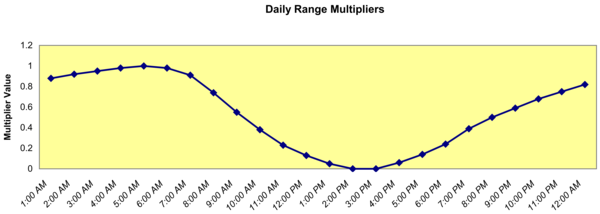
\includegraphics[width=0.9\textwidth, height=0.9\textheight, keepaspectratio=true]{media/image010.png}
\caption{Default Daily range Multiplier for Design Days \protect \label{fig:default-daily-range-multiplier-for-design}}
\end{figure}

The multipliers are taken from the ASHRAE 2009 HOF. More explicitly, EnergyPlus creates an air temperature for each timestep by using the entered maximum dry-bulb temperature in conjunction with the entered daily range and the above multiplier values. The actual equation used is shown below:

\begin{equation}
{T_{current}} = {T_{Max}} - {T_{range}}\cdot {T_{Multiplier}}
\end{equation}

where

T\(_{current}\) = Air temperature of current Hour of Day

T\(_{Max}\) = User supplied Max Dry-bulb Temperature

T\(_{range}\) = User supplied Daily Temperature Range

T\(_{Multiplier}\) = Range multiplier as shown on the above graph

The range multiplier values represent typical conditions of diurnal temperatures (i.e. the low temperature for the day occurring about 5:00 AM and the maximum temperature for the day occurring about 3:00 PM. Note that EnergyPlus does not shift the profile based on the time of solar noon as is optionally allowed in ASHRAE procedures.

ASHRAE research indicates that dry-bulb and wet-bulb temperatures typically follow the same profile, so EnergyPlus can use the default profile to generate humidity conditions (see Humidity Indicating Type = WetBulbProfileDefaultMultipliers below).

\paragraph{Field: Dry-Bulb Temperature Range Modifier Type}\label{field-dry-bulb-temperature-range-modifier-type}

If you are happy with lows at 5am and highs at 3pm, you can ignore this field. If you want to specify your own temperature range multipliers (see earlier discussion at the Temperature Range field description), you can specify a type here and create a day schedule which you reference in the next field.

If you specify \textbf{MultiplierSchedule} in this field, then you need to create a day schedule that specifies a multiplier applied to the temperature range field (above) to create the proper dry-bulb temperature range profile for your design day.

If you specify \textbf{DifferenceSchedule} in this field, then you need to create a day schedule that specifies a number to be \textbf{subtracted} from dry-bulb maximum temperature for each timestep in the day. Note that numbers in the delta schedules cannot be negative as that would result in a higher maximum than the maximum previously specified.

If you specify \textbf{TemperatureProfileSchedule} in this field, then you need to create a day schedule that specifies the actual dry-bulb temperatures throughout the day. You will not need to include a Maximum Dry-Bulb Temperature in that field.

If you leave this field blank or enter \textbf{DefaultMultipliers}, then the default multipliers will be used as shown in the ``temperature range'' field above.

\paragraph{Field: Dry-Bulb Temperature Range Modifier Day Schedule Name}\label{field-dry-bulb-temperature-range-modifier-day-schedule-name}

This field is the name of a \textbf{day schedule} (ref. Schedule:Day:Hourly, Schedule:Day:Interval, Schedule:Day:List objects) with the values as specified in the Dry-Bulb Temperature Range Modifier Type field above.

\paragraph{Field: Humidity Condition Type}\label{field-humidity-condition-type}

The values/schedules indicated here and in subsequent fields create the humidity values in the 24 hour design day conditions profile. Valid choices here are: \textbf{WetBulb}, \textbf{Dewpoint}, \textbf{WetBulbProfileDefaultMultipliers, WetBulbProfileDifferenceSchedule,} \textbf{WetBulbProfileMultiplierSchedule}, \textbf{HumidityRatio}, \textbf{Enthalpy}, and \textbf{Schedule.}

The Humidity Condition Type fields have interacting uses and units, summarized as follows:

% table 2
\begin{longtable}[c]{p{2.25in}p{1.75in}p{2.0in}}
\caption{Humidity Indicating Field Interactions - Design Day \label{table:humidity-indicating-field-interactions-design}} \tabularnewline
\toprule 
Humidity Condition Type & Primary Humidity Indicating Field & Humidity Indicating Day Schedule \tabularnewline
\midrule
\endfirsthead

\caption[]{Humidity Indicating Field Interactions - Design Day} \tabularnewline
\toprule 
Humidity Condition Type & Primary Humidity Indicating Field & Humidity Indicating Day Schedule \tabularnewline
\midrule
\endhead

WetBulb & Wetbulb or DewPoint at Maximum Dry-Bulb & N/A (unused) \tabularnewline
DewPoint & Wetbulb or DewPoint at Maximum Dry-Bulb & N/A (unused) \tabularnewline
HumidityRatio & Humidity Ratio at Maximum Dry-Bulb & N/A (unused) \tabularnewline
Enthalpy & Enthalpy at Maximum Dry-Bulb & N/A (unused) \tabularnewline
WetBulbProfile\-DefaultMultipliers & Wetbulb or DewPoint at Maximum Dry-Bulb & N/A (unused) \tabularnewline
WetBulbProfile\-MultiplierSchedule & Wetbulb or DewPoint at Maximum Dry-Bulb & Fractions of wet-bulb daily range (0 – 1) \tabularnewline
WetBulbProfile\-DifferenceSchedule & Wetbulb or DewPoint at Maximum Dry-Bulb & Difference between maximum and hour/timestep wet-bulb temperature, C \tabularnewline
RelativeHumidity\-Schedule & N/A & Relative humidity (\%, 0 – 100) \tabularnewline
\bottomrule
\end{longtable}

Humidity conditions over the day are derived as follows:

\textbf{WetBulb, DewPoint, HumidityRatio, or Enthalpy}:

These four methods assume constant absolute humidity over the day. Calculate W = humidity ratio at Maximum Dry-Bulb Temperature and Humidity Indicating Conditions. Derive hourly/timestep humidity conditions from W and hour/timestep dry-bulb temperature.

\textbf{WetBulbProfileDefaultMultipliers}

Generate the wet-bulb temperature profile using Default Daily Range Multiplier for Design Days (shown in Figure~\ref{fig:default-daily-range-multiplier-for-design} above) and Daily Wet-Bulb Temperature Range (below). This method is analogous to DefaultMultiplier generation of the dry-bulb temperature profile and is the procedure recommended in Chapter 14 of ASHRAE 2009 HOF.

\textbf{WetBulbProfileMultiplierSchedule}

Generate the wet-bulb profile using multipliers from the Humidity Indicating Day Schedule and Daily Wet-Bulb Temperature Range (below). Analogous to dry-bulb MultiplierSchedule.

\textbf{WetBulbProfileDifferenceSchedule}

Generate the wet-bulb profile by subtracting Humidity Indicating Day Schedule values from the daily maximum wet-bulb temperature (specified in Humidity Indicating Conditions at Maximum Dry-Bulb). Analogous to dry-bulb DifferenceSchedule.

\textbf{RelativeHumiditySchedule}

Hourly relative humidity is specified in Humidity Indicating Day Schedule.

In all cases, the humidity ratio is limited to saturation at the hour/timestep dry-bulb (that is, the dry-bulb temperature is used as specified, but the humidity ratio is modified as needed to be physically possible). Once a valid air state is determined, a complete set of consistent hour/timestep psychrometric values (dewpoint, wet-bulb, and enthalpy) is derived.

\paragraph{Field: Wetbulb or DewPoint at Maximum Dry-Bulb}\label{field-wetbulb-or-dewpoint-at-maximum-dry-bulb}

If you choose \textbf{Wetbulb} or \textbf{Dewpoint} in the Humidity Condition Type field, then this numeric field should contain that value. Note that this field is unnecessary when you put in a humidity indicating day schedule (described later in this section).

\paragraph{Field: Humidity Condition Day Schedule Name}\label{field-humidity-condition-day-schedule-name}

Allows specification a day schedule (ref. Schedule:Day:Hourly, Schedule:Day:Interval, Schedule:Day:List objects) of values for relative humidity or wet-bulb profile per Humidity Indicating Type field.

\paragraph{Field: Humidity Ratio at Maximum Dry-Bulb}\label{field-humidity-ratio-at-maximum-dry-bulb}

If \textbf{HumidityRatio} is chosen for the Humidity Condition Type field, then this numeric field should contain the desired humidity ratio at maximum dry-bulb temperature (units kg Water / kg Dry Air).

\paragraph{Field: Enthalpy at Maximum Dry-Bulb}\label{field-enthalpy-at-maximum-dry-bulb}

If \textbf{Enthalpy} is chosen for the Humidity Condition Type field, then this numeric field should contain the desired enthalpy at maximum dry-bulb temperature (units Joules /kg).

\paragraph{Field: Daily Wet-Bulb Temperature Range}\label{field-daily-wet-bulb-temperature-range}

The difference between the maximum and minimum wet-bulb temperatures on the design day (Celsius). Used for generating daily profiles of humidity conditions when Humidity Condition Type field (above) is \textbf{WetBulbProfileDefaultMultipliers} or \textbf{WetBulbProfileMultiplierSchedule}. Values for wet-bulb temperature range are tabulated by month for 5564 locations worldwide on the CD that accompanies the ASHRAE 2009 HOF.

\paragraph{Field: Barometric Pressure}\label{field-barometric-pressure}

This numeric field is the constant barometric pressure (Pascals) for the entire day.

\paragraph{Field: Wind Speed}\label{field-wind-speed}

This numeric field is the wind speed in meters/second (constant throughout the day) for the day. The MacroDataSets design day files includes wind speed values (99.6\% - heating, 1\% cooling) as indicated in ASHRAE HOF design condition tables. But, you should be aware that traditional values for these are 6.7056 m/s (15 mph) for heating and 3.3528 m/s (7 mph) for cooling. A reminder is shown in the comments for the wind speed values. The comments also note the extreme wind speeds from the ASHRAE tables.

\paragraph{Field: Wind Direction}\label{field-wind-direction}

This numeric field is the source wind direction in degrees. By convention, winds from the North would have a value of 0., from the East a value of 90.

\paragraph{Field: Rain Indicator}\label{field-rain-indicator}

This field indicates whether or not the building surfaces are wet. If the value is Yes, then it is assumed that the building surfaces are wet. Wet surfaces may change the conduction of heat through the surface.

\paragraph{Field: Snow Indicator}\label{field-snow-indicator}

This field indicates whether or not there is snow on the ground. If the value is Yes, then it is assumed there is snow on the ground. Snow on the ground changes the ground reflectance properties.

\paragraph{Field: Daylight Saving Time Indicator}\label{field-daylight-saving-time-indicator}

This field specifies whether to consider this day to be a Daylight Saving Day. Yes in the field indicates that daylight saving time is operational for this day. Yes essentially adds 1 hour to the scheduling times used in items with schedules.

\paragraph{Field: Solar Model Indicator}\label{field-solar-model-indicator}

This field allows the user to select \textbf{ASHRAE\-Clear\-Sky, ASHRAE\-Tau, Zhang\-Huang, or Sche\-dule} for solar modeling in the calculation of the solar radiation in the design day. ASHRAE\-Clear\-Sky and Zhang\-Huang use the Clearness value as part of their calculations. ASHRAE\-Tau invokes the revised model specified in Chapter 14 of the ASHRAE 2009 HOF and uses Taub and Taud values (below). Technical details of the models are described in the Engineering Reference. The \textbf{Schedule} choice allows you to enter schedule values for the day's profile (use the next two fields for the names).

\paragraph{Field: Beam Solar Day Schedule Name}\label{field-beam-solar-day-schedule-name}

This field allows the option for you to put in your own day profile of beam solar values (wh/m2). These values will replace the calculated values during design day processing. Only day schedules (ref. Schedule:Day:Hourly, Schedule:Day:Interval, Schedule:Day:List objects) are used here.

\paragraph{Field: Diffuse Solar Day Schedule Name}\label{field-diffuse-solar-day-schedule-name}

This field allows the option for you to put in your own day profile of diffuse solar values (wh/m2). These values will replace the calculated values during design day processing. Only day schedules (ref. Schedule:Day:Hourly, Schedule:Day:Interval, Schedule:Day:List objects) are used here.

\paragraph{Field: ASHRAE Clear Sky Optical Depth for Beam Irradiance (taub)}\label{field-ashrae-clear-sky-optical-depth-for-beam-irradiance-taub}

Optical depth for beam radiation, used only when Solar Model Indicator is ASHRAETau. See next field.

\paragraph{Field: ASHRAE Clear Sky Optical Depth for Diffuse Irradiance (taud)}\label{field-ashrae-clear-sky-optical-depth-for-diffuse-irradiance-taud}

Optical depth for diffuse radiation, used only when Solar Model Indicator is ASHRAETau. Taub and Taud values are tabulated by month for 5564 locations worldwide on the CD that accompanies the ASHRAE 2009 HOF.

\paragraph{Field: Sky Clearness}\label{field-sky-clearness}

If the choice in the Solar Model Indicator field is ASHRAEClearSky or ZhangHuang, then this numeric field should be entered. This value represents the ``clearness'' value for the day. This value, along with the solar position as defined by the Location information and the date entered for the design day, help define the solar radiation values for each hour of the day. Clearness may range from 0.0 to 1.2, where 1.0 represents a clear sky at sea level. Values greater than 1.0 may be used for high altitude locations. Traditionally, one uses 0.0 clearness for Winter Design Days. Note that this ``sky clearness'' does not have the same meaning as output variable ``Site Daylighting Model Sky Clearness''.

IDF Examples:

\begin{lstlisting}
! Phoenix Sky Harbor Intl Ap_AZ_USA Annual Cooling (WB = >MDB)
!   .4%, MDB = 35.8°C WB = 24.5°C
SizingPeriod:DesignDay,
  Phoenix Sky Harbor Intl Ap Ann Clg .4% Condns WB = >MDB, !- Name
          7,      !- Month
         21,      !- Day of Month
  SummerDesignDay,!- Day Type
       35.8,      !- Maximum Dry-Bulb Temperature {C}
         12,      !- Daily Dry-Bulb Temperature Range {C}
  DefaultMultipliers, !- Dry-Bulb Temperature Range Modifier Type
           ,      !- Dry-Bulb Temperature Range Modifier Schedule Name
    Wetbulb,      !- Humidity Condition Type
       24.5,      !- Wetbulb at Maximum Dry-Bulb {C}
           ,      !- Humidity Indicating Day Schedule Name
           ,      !- Humidity Ratio at Maximum Dry-Bulb {kgWater/kgDryAir}
           ,      !- Enthalpy at Maximum Dry-Bulb {J/kg}
           ,      !- Daily Wet-Bulb Temperature Range {deltaC}
     97342.,      !- Barometric Pressure {Pa}
        4.1,      ! Wind Speed {m/s}
        260,      !- Wind Direction {Degrees; N = 0, S = 180}
         No,      !- Rain {Yes/No}
         No,      !- Snow on ground {Yes/No}
         No,      !- Daylight Savings Time Indicator
       ASHRAETau, !- Solar Model Indicator
           ,      !- Beam Solar Day Schedule Name
           ,      !- Diffuse Solar Day Schedule Name
      0.588,     !- ASHRAE Clear Sky Optical Depth for Beam Irradiance (taub)
      1.653;  !- ASHRAE Clear Sky Optical Depth for Diffuse Irradiance (taud)

SizingPeriod:DesignDay,
  Denver Centennial Golden Ann Htg 99% Condns DB - sched solar,  !- Name
  1,                       !- Month
  13,                      !- Day of Month
  WinterDesignDay,         !- Day Type
  -16,                     !- Maximum Dry-Bulb Temperature {C}
  0.0,                     !- Daily Dry-Bulb Temperature Range {deltaC}
  ,                        !- Dry-Bulb Temperature Range Modifier Type
  ,                    !- Dry-Bulb Temperature Range Modifier Schedule Name
  Wetbulb,                 !- Humidity Condition Type
  -16,                     !- Wetbulb or DewPoint at Maximum Dry-Bulb {C}
  ,                        !- Humidity Indicating Day Schedule Name
  ,               !- Humidity Ratio at Maximum Dry-Bulb {kgWater/kgDryAir}
  ,                        !- Enthalpy at Maximum Dry-Bulb {J/kg}
  ,                        !- Daily Wet-Bulb Temperature Range {deltaC}
  83411.,                  !- Barometric Pressure {Pa}
  2.3,                     !- Wind Speed {m/s}
  180,                     !- Wind Direction {deg}
  No,                      !- Rain Indicator
  No,                      !- Snow Indicator
  No,                      !- Daylight Saving Time Indicator
  Schedule,                !- Solar Model Indicator
  Winter (1/13) Beam Solar,!- Beam Solar Day Schedule Name
  Winter (1/13) Diffuse Solar;  !- Diffuse Solar Day Schedule Name

Schedule:Day:Hourly,
  Winter (1/13) Beam Solar,
  Any Number,
  0,0,0,0,0,0,0,190,698,852,892,919,957,953,856,700,213,0,0,0,0,0,0,0;

Schedule:Day:Hourly,
  Winter (1/13) Diffuse Solar,
  Any Number,
  0,0,0,0,0,0,0,35,118,116,92,65,40,14,0,0,5,0,0,0,0,0,0,0;
\end{lstlisting}

Look at the example files 1Zone\-Un\-controll\-ed\_\-DD\-Changes.idf and 1Zone\-Un\-controlled\_\-DD\-2009 for several examples of specifying Design Day inputs.

\subsubsection{Outputs}\label{outputs-018}

For the schedule fields in the object, several output variables can be used:

\begin{itemize}
\item
  Zone,Average,Sizing Period Site Beam Solar Schedule Value {[}W/m2{]}
\item
  Zone,Average,Sizing Period Site Diffuse Solar Schedule Value {[}W/m2{]}
\item
  Zone,Average,Sizing Period Site Humidity Condition Schedule Value {[}\%{]}
\item
  Zone,Average,Sizing Period Site Humidity Condition Schedule Value {[]}
\item
  Zone,Average,Sizing Period Site Drybulb Temperature Range Modifier Schedule Value {[]}
\item
  Zone,Average,Sizing Period Site Drybulb Temperature Range Modifier Schedule Value {[}deltaC{]}
\item
  Zone,Average,Sizing Period Site Drybulb Temperature Range Modifier Schedule Value {[}C{]}
\item
  Zone,Average,Sizing Period Site Sky Temperature Schedule Value {[}deltaC{]}
\item
  Zone,Average,Sizing Period Site Sky Temperature Schedule Value {[}C{]}
\end{itemize}

\paragraph{Sizing Period Site Beam Solar Schedule Value {[}W/m2{]}}\label{sizing-period-site-beam-solar-schedule-value-wm2}

\paragraph{Sizing Period Site Diffuse Solar Schedule Value {[}W/m2{]}}\label{sizing-period-site-diffuse-solar-schedule-value-wm2}

This schedule value is active when any Design Day objects have / use the solar schedule option. For those objects that don't have this option, the value will be displayed as -999.

\paragraph{Sizing Period Site Humidity Condition Schedule Value {[}\%{]}}\label{sizing-period-site-humidity-condition-schedule-value}

\paragraph{Sizing Period Site Humidity Condition Schedule Value {[]}}\label{sizing-period-site-humidity-condition-schedule-value-1}

This schedule value is active when any Design Day objects have / use the humidity schedule option. For those objects that don't have this option, the value will be displayed as -999.

\paragraph{Sizing Period Site Drybulb Temperature Range Modifier Schedule Value {[]}}\label{sizing-period-site-drybulb-temperature-range-modifier-schedule-value}

\paragraph{Sizing Period Site Drybulb Temperature Range Modifier Schedule Value {[}deltaC{]}}\label{sizing-period-site-drybulb-temperature-range-modifier-schedule-value-deltac}

\paragraph{Sizing Period Site Drybulb Temperature Range Modifier Schedule Value {[}C{]}}\label{sizing-period-site-drybulb-temperature-range-modifier-schedule-value-c}

This schedule value is active when any Design Day objects have / use the drybulb temperature range modifier schedule option. For those objects that don't have this option, the value will be displayed as -999.

\paragraph{Sizing Period Site Sky Temperature Schedule Value {[}deltaC{]}}\label{sizing-period-site-sky-temperature-schedule-value-deltac}

\paragraph{Sizing Period Site Sky Temperature Schedule Value {[}C{]}}\label{sizing-period-site-sky-temperature-schedule-value-c}

This schedule value is active when any Design Day objects have / use the WeatherProperties:SkyTemperature schedule option. For those objects that don't have this option, the value will be displayed as -999.

\subsection{Longer Design Periods}\label{longer-design-periods}

Some features may benefit by using a longer design weather period for sizing or loads calculations. Longer design periods may be created by using the \textbf{Si\-zing\-Period:\-Weather\-File\-Days} or \textbf{Si\-zing\-Period:\-Weather\-File\-Con\-dition\-Type} objects. These two objects allow for selections from an attached weather file to be used in the sizing calculations.

\subsection{Sizing\-Period:\-Weather\-File\-Days}\label{sizingperiodweatherfiledays}

The Sizing\-Period:\-Weather\-File\-Days object describes using a selected period from the ``attached'' weather file to be used in load calculations or sizing equipment. The period selected can be as small as a single day or larger. Multiple periods may be input. While this object may be used for sizing calculations, you should also consider using design days that represent more long term extremes or conditions.

\subsubsection{Inputs}\label{inputs-2-022}

\paragraph{Field: Name}\label{field-name-2-021}

This field allows for an assigned name for this run period so it can be tracked easily in sizing and other outputs.

\paragraph{Field: Begin Month}\label{field-begin-month}

This numeric field should contain the starting month number (1 = January, 2 = February, etc.) for the annual run period desired.

\paragraph{Field: Begin Day of Month}\label{field-begin-day-of-month}

This numeric field should contain the starting day of the starting month (must be valid for month) for the annual run period desired.

\paragraph{Field: End Month}\label{field-end-month}

This numeric field should contain the ending month number (1 = January, 2 = February, etc.) for the annual run period desired.

\paragraph{Field: End Day of Month}\label{field-end-day-of-month}

This numeric field should contain the ending day of the ending month (must be valid for month) for the annual run period desired.

\paragraph{Field: Day of Week for Start Day}\label{field-day-of-week-for-start-day}

For flexibility, the day of week indicated on the weather file can be overridden by this field's value. Valid days of the week (Sunday, Monday, Tuesday, Wednesday, Thursday, Friday, Saturday) or special days (SummerDesignDay, WinterDesignDay, CustomDay1, CustomDay2) must be entered in this field. To clarify, this value will be used as the Start Day (type) for this sizing period. When weekdays are used, each subsequent day in the period will be incremented. When SummerDesignDay, WinterDesignDay, CustomDay1, CustomDay2 -- are used, the day type will be applied for the entire period.

\paragraph{Field: Use Weather File Daylight Saving Period}\label{field-use-weather-file-daylight-saving-period}

Weather files can contain indicators of Daylight Saving Period days. For flexibility, you may want to ignore these designations on the weather file. This field should contain the word \textbf{Yes} if you will accept daylight saving period days as contained on the weather file (note: not all weather files may actually have this period) or \textbf{No} if you wish to ignore Daylight Saving Period days that may be on the weather file.

Note that a blank or null field in this field will indicate \textbf{Yes}.

\paragraph{Field: Use Weather File Rain and Snow Indicators}\label{field-use-weather-file-rain-and-snow-indicators}

Weather files can contain ``rain'' and ``snow'' indicators. (EPW field ``Present Weather Codes'' -- described in the AuxiliaryPrograms document). In turn, rain indicates wet surfaces which changes the film convection coefficient for the surface. Other models may use rain as well (Ground Heat Exchangers). Snow indicators can change the ground reflectance if there is snow on the ground. Entering ``\textbf{Yes}'' in this field allows the weather file conditions to represent ``Rain'' and ``Snow''; entering ``\textbf{No}'' in the field ``turns off'' the rain/snow indicators for this period. You might use this to be able to compare two ``same location'' weather files of different years, origins, etc.

IDF Example:

\begin{lstlisting}
SizingPeriod:WeatherFileDays,
  Summer including Extreme Summer days, !- Name
  7,18,7,25,                            !- Begin/end Day/Month
  SummerDesignDay,                      !- Day type
  No,                                   !- Use Weather File Daylight Saving Period
  No;                                   !- Use Weather File Rain and Snow Indicators

SizingPeriod:WeatherFileDays,
  Winter including Extreme Winter days, !- Name
  1,25,2,1,                             !- Begin/end Day/Month
  WinterDesignDay,                      !- Day type
  No,                                   !- Use Weather File Daylight Saving Period
  No;                                   !- Use Weather File Rain and Snow Indicators
\end{lstlisting}

\subsection{Sizing\-Period:\-Weather\-File\-Con\-dition\-Type}\label{sizingperiodweatherfileconditiontype}

When the EPW files are created, a heuristic procedure identifies extreme and typical periods in the actual weather file. This object will allow one of those periods to be selected for sizing or load calculations (typically). Multiple objects may be input. While this object may be used for sizing calculations, you should also consider using design days that represent more long term extremes or conditions.

\subsubsection{Inputs}\label{inputs-3-020}

\paragraph{Field: Name}\label{field-name-3-018}

This field allows for an assigned name for this run period so it can be tracked easily in sizing and other outputs.

\paragraph{Field: Period Selection}\label{field-period-selection}

This field allows the generic period calculated from the weather file to be selected for this run period. It is not completely generic as there may be extreme cold periods in some weather files but extreme wet periods (tropical) in others. Not all weather files have all of the valid choices. The choices for this field are:

\begin{itemize}
\item
  SummerExtreme
\item
  SummerTypical
\item
  WinterExtreme
\item
  WinterTypical
\item
  AutumnTypical
\item
  SpringTypical
\item
  WetSeason
\item
  DrySeason
\item
  NoDrySeason
\item
  NoWetSeason
\item
  TropicalHot
\item
  TropicalCold
\end{itemize}

\paragraph{Field: Day of Week for Start Day}\label{field-day-of-week-for-start-day-1}

For flexibility, the day of week indicated on the weather file can be overridden by this field's value. Valid days of the week (Sunday, Monday, Tuesday, Wednesday, Thursday, Friday, Saturday) or special days (SummerDesignDay, WinterDesignDay, CustomDay1, CustomDay2) must be entered in this field. To clarify, this value will be used as the Start Day (type) for this sizing period. When weekdays are used, each subsequent day in the period will be incremented. When SummerDesignDay, WinterDesignDay, CustomDay1, CustomDay2 -- are used, the day type will be applied for the entire period.

\paragraph{Field: Use Weather File Daylight Saving Period}\label{field-use-weather-file-daylight-saving-period-1}

Weather files can contain indicators of Daylight Saving Period days. For flexibility, you may want to ignore these designations on the weather file. This field should contain the word \textbf{Yes} if you will accept daylight saving period days as contained on the weather file (note: not all weather files may actually have this period) or \textbf{No} if you wish to ignore Daylight Saving Period days that may be on the weather file.

Note that a blank or null field in this field will indicate \textbf{Yes}.

\paragraph{Field: Use Weather File Rain and Snow Indicators}\label{field-use-weather-file-rain-and-snow-indicators-1}

Weather files can contain ``rain'' and ``snow'' indicators. (EPW field ``Present Weather Codes'' -- described in the AuxiliaryPrograms document). In turn, rain indicates wet surfaces which changes the film convection coefficient for the surface. Other models may use rain as well (Ground Heat Exchangers). Snow indicators can change the ground reflectance if there is snow on the ground. Entering ``\textbf{Yes}'' in this field allows the weather file conditions to represent ``Rain'' and ``Snow''; entering ``\textbf{No}'' in the field ``turns off'' the rain/snow indicators for this period. You might use this to be able to compare two ``same location'' weather files of different years, origins, etc.

IDF Example:

\begin{lstlisting}
SizingPeriod:WeatherFileConditionType,
  Extreme Summer Weather Period for Design, !- Name
  SummerExtreme,                            !- Period Selection
  SummerDesignDay,                          !- Day Type
  No,                                       !- Use Weather File Daylight Saving Period
  No;                                       !- Use Weather File Rain and Snow Indicators

SizingPeriod:WeatherFileConditionType,
  Extreme Winter Weather Period for Design, !- Name
  WinterExtreme,                            !- Period Selection
  WinterDesignDay,                          !- Day Type
  No,                                       !- Use Weather File Daylight Saving Period
  No;                                       !- Use Weather File Rain and Snow Indicators
\end{lstlisting}

\subsection{RunPeriod}\label{runperiod}

The RunPeriod object describes the elements necessary to create a weather file simulation. Multiple run periods may be input. EnergyPlus accepts weather files in the special EnergyPlus weather format (described briefly below this document and in more detail in the Auxiliary Programs document). These files can describe Daylight Saving Time periods as well as holidays within their definitions. The RunPeriod object allows the user to override the use of both the Daylight Saving Period (i.e. use or ignore) and holidays that are embedded within the weather file. Note that the weather file also may contain design condition information, typical and extreme period information, ground temperatures based on air temperature calculations.

\subsubsection{Inputs}\label{inputs-4-018}

\paragraph{Field: Name}\label{field-name-4-015}

This optional field allows the RunPeriod to be named for output reporting. When left blank, the weather file location name is used. Note that the weather file location name will be appended to this name in tabular/summary reports.

\paragraph{Field: Begin Month}\label{field-begin-month-1}

This numeric field should contain the starting month number (1 = January, 2 = February, etc.) for the annual run period desired.

\paragraph{Field: Begin Day of Month}\label{field-begin-day-of-month-1}

This numeric field should contain the starting day of the starting month (must be valid for month) for the annual run period desired.

\paragraph{Field: End Month}\label{field-end-month-1}

This numeric field should contain the ending month number (1 = January, 2 = February, etc.) for the annual run period desired.

\paragraph{Field: End Day of Month}\label{field-end-day-of-month-1}

This numeric field should contain the ending day of the ending month (must be valid for month) for the annual run period desired.

\paragraph{Field: Day of Week for Start Day}\label{field-day-of-week-for-start-day-2}

For flexibility, the day of week indicated on the weather file can be overridden by this field's value. Valid days of the week (Sunday, Monday, Tuesday, Wednesday, Thursday, Friday, Saturday) must be entered in this field. To clarify, this value will be used as the Start Day (type) for this run period and subsequent days will be implemented. If a blank or UseWeatherFile is entered here, then the starting day type will be calculated from the weather file (ref: Auxiliary Programs document about Data Periods).

\paragraph{Field: Use Weather File Holidays and Special Days}\label{field-use-weather-file-holidays-and-special-days}

Weather files can contain holiday designations or other kinds of special days. These day types cause a corresponding day's schedule (see SCHEDULE definitions below) to be used during that day. This field should contain the word \textbf{Yes} if holidays or other special days indicated directly on the weather file should retain their ``day type'' or \textbf{No} if holidays or other special days on the weather file should be ignored. Reference the RunPeriodControl:SpecialDays object below to enter your own special days and holidays.

Note that a blank or null field in this field will indicate \textbf{Yes}.

\paragraph{Field: Use Weather File Daylight Saving Period}\label{field-use-weather-file-daylight-saving-period-2}

Weather files can contain indicators of Daylight Saving period days. For flexibility, you may want to ignore these designations on the weather file. This field should contain the word \textbf{Yes} if you will accept daylight saving period days as contained on the weather file (note: not all weather files may actually have this period) or \textbf{No} if you wish to ignore Daylight Saving period days that may be on the weather file.

Note that a blank or null field in this field will indicate \textbf{Yes}.

\paragraph{Field: Apply Weekend Holiday Rule}\label{field-apply-weekend-holiday-rule}

In some countries (notably the US), when holidays fall on weekends, they are often observed on a weekday close to the holiday day. (Usually if the specific day falls on a Saturday, the observed day is Friday; if on a Sunday, the observed day is Monday). EnergyPlus will represent this custom using the value in this field. If the field is \textbf{Yes}, then specific date holidays that have a duration of one day, will be ``observed'' on the Monday after the day. (Specific day holidays are such as January 1 -- a day-month combination). If the field is blank or \textbf{No}, then the holiday will be shown on the day-month as entered. As this option is listed at the RunPeriod, all applicable special days for the run will use the rule -- there is no override for individual special days.

Note that a blank or null field in this field will indicate \textbf{No}.

\begin{callout}
Note: EnergyPlus processed weather files available on the EnergyPlus web site: \url{http://www.energyplus.gov/cfm/weather\_data.cfm} have neither special days specified nor daylight saving period. However, DDY (Design Day) files produced from the ASHRAE Design Conditions that accompany the EPW files may include a DaylightSavingPeriod object for certain locations.
\end{callout}

\paragraph{Field: Use Weather File Rain Indicators}\label{field-use-weather-file-rain-indicators}

Weather files can contain ``rain'' indicators. (EPW field ``Present Weather Codes'' -- described in the AuxiliaryPrograms document). In turn, rain indicates wet surfaces which changes the film convection coefficient for the surface. Other models may use rain as well (Ground Heat Exchangers). Entering ``\textbf{Yes}'' in this field allows the weather file conditions to represent ``Rain''; entering ``\textbf{No}'' in the field ``turns off'' the rain indicator for this period. You might use this to be able to compare two ``same location'' weather files of different years, origins, etc.

\paragraph{Field: Use Weather File Snow Indicators}\label{field-use-weather-file-snow-indicators}

Weather files can contain ``snow'' indicators. (EPW field ``Snow Depth'' \textgreater{} 0 indicates ``Snow on the ground''). In turn, snow changes the reflectivity of the ground and cascades changes of this reflectivity. Entering ``\textbf{Yes}'' in this field allows the weather file conditions to represent ``Snow''; entering ``\textbf{No}'' in the field ``turns off'' the snow indicator for this period. You might use this to be able to compare two ``same location'' weather files of different years, origins, etc.

\paragraph{Field: Number of Times Runperiod to be Repeated}\label{field-number-of-times-runperiod-to-be-repeated}

This numeric field represents the number of times (usually years) the simulation has to be carried out in a multi runperiod simulation. The default value is set to 1. The number of years of simulation, in case of a Ground Loop Heat Exchanger (GLHE) simulation, should be equal to the length of simulation field in GLHE object. Note that you can specify a number of simulation years with a shorter run period (e.g. 1 week) and EnergyPlus will repeat the simulation of the shorter run period for that many times. Note that repeating will work with any weather file that contains the start date and end date in a ``Data Period'' (refer to Auxiliary Programs document for more documentation on weather file contents).

\paragraph{Field: Increment Day of Week on Repeat}\label{field-increment-day-of-week-on-repeat}

When repeating RunPeriods (see previous field), you can choose to increment the day of week at the end of the period to have a more continuous day type. Enter \textbf{Yes} to increment the day of the week (default). An entry of \textbf{No} will keep the same day of week values as in the first time through.

\paragraph{Field: Start Year}\label{field-start-year}

When repeating a period, you might (for whatever reason), choose to have a specific year as a starting year. Enter an appropriate 4 digit year in this field. Refer to Auxiliary Programs document for more documentation on weather file contents, particularly in using leap year data (or not) within weather files.

And, as shown in an IDF:

\begin{lstlisting}
RunPeriod,  ! Winter Simulation
  Winter Simulation,  !- Name
  12,  !- Begin Month
  1,  !- Begin Day of Month
  3,  !- End Month
  31,  !- End Day of Month
  UseWeatherFile,  !- Day of Week for Start Day
  Yes,  !- Use Weather File Holidays and Special Days
  Yes,  !- Use Weather File Daylight Saving Period
  No,  !- Apply Weekend Holiday Rule
  Yes,  !- Use Weather File Rain Indicators
  Yes;  !- Use Weather File Snow Indicators

! Multiple year simulation example
RunPeriod,
  Multiple Years,  !- Name
  1,    !- Begin Month
  1,    !- Begin Day of Month
  12,   !- End Month
  31,   !- End Day of Month
  UseWeatherFile,  !- Day of Week for Start Day
  Yes,  !- Use Weather File Holidays and Special Days
  Yes,  !- Use Weather File Daylight Saving Period
  No,   !- Apply Weekend Holiday Rule
  Yes,  !- Use Weather File Rain Indicators
  Yes,  !- Use Weather File Snow Indicators
  3;    !- Number of Times Runperiod to be Repeated
\end{lstlisting}

\subsection{RunPeriod:CustomRange}\label{runperiodcustomrange}

The RunPeriod:CustomRange object describes the elements necessary to use a specially crafted (likely multiple year) weather file in a simulation. These kinds of weather files and simulations might be useful for matching utility periods or simulating several years of differing weather data. Multiple run periods may be input. EnergyPlus accepts weather files in the special EnergyPlus weather format (described briefly below this document and in more detail in the Auxiliary Programs document). In order to effectively use this object, however, you will need to use a text editor (EnergyPlus weather files area simple text files) or possibly a spreadsheet program and then save to a csv (comma separated variable) file. Weather files can describe Daylight Saving Time periods as well as holidays within their definitions. The RunPeriod:CustomRange object allows the user to override the use of both the Daylight Saving Period (i.e. use or ignore) and holidays that are embedded within the weather file. Note that the weather file also may contain design condition information, typical and extreme period information, ground temperatures based on air temperature calculations.

\subsubsection{Inputs}\label{inputs-5-016}

\paragraph{Field: Name}\label{field-name-5-012}

This optional field allows the RunPeriod to be named for output reporting. When left blank, the weather file location name is used. Note that the weather file location name will be appended to this name in tabular/summary reports.

\paragraph{Field: Begin Month}\label{field-begin-month-2}

This numeric field should contain the starting month number (1 = January, 2 = February, etc.) for the annual run period desired.

\paragraph{Field: Begin Day of Month}\label{field-begin-day-of-month-2}

This numeric field should contain the starting day of the starting month (must be valid for month) for the annual run period desired.

\paragraph{Field: Begin Year}\label{field-begin-year}

This numeric field should contain the beginning year for the custom range. Though all EnergyPlus (EPW) weather files contain a year/year field, the RunPeriod object does not use this field (previous object). The \textbf{RunPeriod:CustomRange} object causes the program to look specifically for the begin date specified by these three fields (i.e. Begin Month, Begin Day of Month, Begin Year).

\paragraph{Field: End Month}\label{field-end-month-2}

This numeric field should contain the ending month number (1 = January, 2 = February, etc.) for the annual run period desired.

\paragraph{Field: End Day of Month}\label{field-end-day-of-month-2}

This numeric field should contain the ending day of the ending month (must be valid for month) for the annual run period desired.

\paragraph{Field: End Year}\label{field-end-year}

This numeric field should contain the end year for the custom range. Though all EnergyPlus (EPW) weather files contain a year/year field, the RunPeriod object does not use this field (previous object). The \textbf{RunPeriod:CustomRange} object causes the program to look specifically for the end date specified by these three fields (i.e. End Month, End Day of Month, End Year).

\paragraph{Field: Day of Week for Start Day}\label{field-day-of-week-for-start-day-3}

For flexibility, the day of week indicated on the weather file can be overridden by this field's value. Valid days of the week (Sunday, Monday, Tuesday, Wednesday, Thursday, Friday, Saturday) must be entered in this field. To clarify, this value will be used as the Start Day (type) for this run period and subsequent days will be implemented. If a blank or UseWeatherFile is entered here, then the starting day type will be calculated from the weather file (ref: Auxiliary Programs document about Data Periods).

\paragraph{Field: Use Weather File Holidays and Special Days}\label{field-use-weather-file-holidays-and-special-days-1}

Weather files can contain holiday designations or other kinds of special days. These day types cause a corresponding day's schedule (see SCHEDULE definitions below) to be used during that day. This field should contain the word \textbf{Yes} if holidays or other special days indicated directly on the weather file should retain their ``day type'' or \textbf{No} if holidays or other special days on the weather file should be ignored. Reference the RunPeriodControl:SpecialDays object below to enter your own special days and holidays.

Note that a blank or null field in this field will indicate \textbf{Yes}.

\paragraph{Field: Use Weather File Daylight Saving Period}\label{field-use-weather-file-daylight-saving-period-3}

Weather files can contain indicators of Daylight Saving period days. For flexibility, you may want to ignore these designations on the weather file. This field should contain the word \textbf{Yes} if you will accept daylight saving period days as contained on the weather file (note: not all weather files may actually have this period) or \textbf{No} if you wish to ignore Daylight Saving period days that may be on the weather file.

Note that a blank or null field in this field will indicate \textbf{Yes}.

\paragraph{Field: Apply Weekend Holiday Rule}\label{field-apply-weekend-holiday-rule-1}

In some countries (notably the US), when holidays fall on weekends, they are often observed on a weekday close to the holiday day. (Usually if the specific day falls on a Saturday, the observed day is Friday; if on a Sunday, the observed day is Monday). EnergyPlus will represent this custom using the value in this field. If the field is \textbf{Yes}, then specific date holidays that have a duration of one day, will be ``observed'' on the Monday after the day. (Specific day holidays are such as January 1 -- a day-month combination). If the field is blank or \textbf{No}, then the holiday will be shown on the day-month as entered. As this option is listed at the RunPeriod, all applicable special days for the run will use the rule -- there is no override for individual special days.

Note that a blank or null field in this field will indicate \textbf{No}.

\begin{callout}
Note: EnergyPlus processed weather files available on the EnergyPlus web site: \url{http://www.energyplus.gov/cfm/weather\_data.cfm} have neither special days specified nor daylight saving period. However, DDY (Design Day) files produced from the ASHRAE Design Conditions that accompany the EPW files may include a DaylightSavingPeriod object for certain locations.
\end{callout}

\paragraph{Field: Use Weather File Rain Indicators}\label{field-use-weather-file-rain-indicators-1}

Weather files can contain ``rain'' indicators. (EPW field ``Present Weather Codes'' -- described in the AuxiliaryPrograms document). In turn, rain indicates wet surfaces which changes the film convection coefficient for the surface. Other models may use rain as well (Ground Heat Exchangers). Entering ``\textbf{Yes}'' in this field allows the weather file conditions to represent ``Rain''; entering ``\textbf{No}'' in the field ``turns off'' the rain indicator for this period. You might use this to be able to compare two ``same location'' weather files of different years, origins, etc.

\paragraph{Field: Use Weather File Snow Indicators}\label{field-use-weather-file-snow-indicators-1}

Weather files can contain ``snow'' indicators. (EPW field ``Snow Depth'' \textgreater{} 0 indicates ``Snow on the ground''). In turn, snow changes the reflectivity of the ground and cascades changes of this reflectivity. Entering ``\textbf{Yes}'' in this field allows the weather file conditions to represent ``Snow''; entering ``\textbf{No}'' in the field ``turns off'' the snow indicator for this period. You might use this to be able to compare two ``same location'' weather files of different years, origins, etc.

\subsection{RunPeriodControl:SpecialDays}\label{runperiodcontrolspecialdays}

For weather file run periods, special day run periods can be described. These will always be in effect for the selected days in the run period. Depending on the Use Special Days value in the RunPeriod:* object(s), these can augment any special days included on the weather file.

\begin{callout}
Note: EnergyPlus processed weather files available on the EnergyPlus web site: \url{http://www.energyplus.gov/cfm/weather\_data.cfm} have neither special days specified nor daylight saving period. However, DDY (Design Day) files produced from the ASHRAE Design Conditions that accompany the EPW files may include a DaylightSavingPeriod object for certain locations.
\end{callout}

\subsubsection{Inputs}\label{inputs-6-013}

\paragraph{Field: Name}\label{field-name-6-010}

This alpha field is the title for the special day period. It must be unique among all the special day period objects entered.

\paragraph{Field: Start Date}\label{field-start-date}

This field is the starting date for the special day period. Dates in this field can be entered in several ways as shown in the accompanying table:

% table 3
\begin{longtable}[c]{@{}ll@{}}
\caption{Date Field Interpretation \label{table:date-field-interpretation}} \tabularnewline
\toprule 
Field Contents & Interpretation \tabularnewline
\midrule
\endfirsthead

\caption[]{Date Field Interpretation} \tabularnewline
\toprule 
Field Contents & Interpretation \tabularnewline
\midrule
\endhead

< number >  /  < number > & Month / Day \tabularnewline
< number >  Month & Day and Month \tabularnewline
Month  < number > & Day and Month \tabularnewline
< number >  Weekday in Month & Numbered weekday of month \tabularnewline
Last Weekday In Month & Last weekday of month \tabularnewline
\bottomrule
\end{longtable}

In the table, Month can be one of (January, February, March, April, May, June, July, August, September, October, November, December). Abbreviations of the first three characters are also valid.

In the table, Weekday can be one of (Sunday, Monday, Tuesday, Wednesday, Thursday, Friday, Saturday). Abbreviations of the first three characters are also valid.

\paragraph{Field: Duration}\label{field-duration}

This numeric field specifies how long (number of days) the special day period lasts.

\paragraph{Field: Special Day Type}\label{field-special-day-type}

This alpha field designates the ``day type'' for schedule use during the special period. It must be one of (Holiday, SummerDesignDay, WinterDesignDay, CustomDay1, CustomDay2).

An example in the IDF would be:

\begin{lstlisting}
RunPeriodControl:SpecialDays, President’s Day, 3rd Monday in February,1,Holiday;
RunPeriodControl:SpecialDays, Thanksgiving, 4th Thursday in November, 1,Holiday;
RunPeriodControl:SpecialDays, Halloween, 10/31, 1, Holiday;
RunPeriodControl:SpecialDays, Vacation, 5/1, 14, CustomDay1;
\end{lstlisting}

\subsection{RunPeriodControl:DaylightSavingTime}\label{runperiodcontroldaylightsavingtime}

Similar to a special day period, a daylight saving period may be entered to be applied to weather file run periods. These will always be in effect, regardless of the value entered on the RunPeriod object. Note that this period will always override any daylight saving period specified in a weather file.

\begin{callout}
Note: EnergyPlus processed weather files available on the EnergyPlus web site: \url{http://www.energyplus.gov/cfm/weather\_data.cfm} have neither special days specified nor daylight saving period.

\warning{Note: For EnergyPlus Output:Variable and Output:Meter reporting, the time stamps are always in standard time. When daylight saving time is active, scheduled loads and controls will shift one hour relative to standard time.}
\end{callout}

\subsubsection{Inputs}\label{inputs-7-013}

\paragraph{Field: Start Date}\label{field-start-date-1}

This is the starting date of the daylight saving period. Note that it can be entered in several formats as shown in Table~\ref{table:date-field-interpretation}. Date Field Interpretation.

\paragraph{Field: End Date}\label{field-end-date}

This is the ending date of the daylight saving period. Note that it can be entered in several formats as shown in Table~\ref{table:date-field-interpretation}. Date Field Interpretation.

And in the IDF:

\begin{lstlisting}
! U.S. Standard for Daylight Saving
RunPeriodControl:DaylightSavingTime,2nd Sunday in March, 1st Sunday in November; !2007
! Brazil standard
RunPeriodControl:DaylightSavingTime,1st Sunday in October, Last Sunday in February;
! European Standard
RunPeriodControl:DaylightSavingTime, Last Sunday in March, Last Sunday in October;
! Syria Standard
RunPeriodControl:DaylightSavingTime, 4/1, 10/1;
\end{lstlisting}

Of course, these could not all appear in the same IDF as only one DaylightSavingPeriod object per input file is allowed. More information on Daylight Saving Periods can be seen on the web at: \url{http://www.webexhibits.org/daylightsaving/}. The ASHRAE Handbook of Fundamentals {[}ASHRAE 2005{]} also contains information about daylight saving periods and their climatic information now includes start and end dates for many locations.

\subsection{WeatherProperty:SkyTemperature}\label{weatherpropertyskytemperature}

Sky Temperature, or radiative sky temperature, is internally calculated by EnergyPlus using an algorithm using horizontal infrared radiation from sky, cloudiness factors and current temperature. The algorithm is fully described in the Engineering Reference document. For flexibility, the following object can be entered to override the internal calculations. Much of the literature describes the sky temperature as relative to either drybulb or dewpoint temperature.

\subsubsection{Inputs}\label{inputs-8-011}

\paragraph{Field: Name}\label{field-name-7-009}

This name references an existing design period (i.e., SizingPeriod:DesignDay, SizingPeriod:WeatherFileDays, or SizingPeriod:WeatherFileConditionType) or run period (by name or blank for all run periods).

\paragraph{Field: Calculation Type}\label{field-calculation-type}

Allowable entries here are: \textbf{ScheduleValue}, \textbf{DifferenceScheduleDryBulbValue}, or \textbf{DifferenceScheduleDewPointValue}. In each case the following field must specify a valid schedule name. \textbf{ScheduleValue} -- the values in the schedule are used as the sky temperature. \textbf{DifferenceScheduleDryBulbValue} -- the values in the schedule are used as a difference to the drybulb temperature value (+values would then be greater than the drybulb temperature, -values would then be less than the drybulb temperature) for the resulting sky temperature value. \textbf{DifferenceScheduleDewPointValue} -- the values in the schedule are used as a difference to the dewpoint temperature value (+values would then be greater than the dewpoint temperature, -values would then be less than the dewpoint temperature) for the resulting sky temperature value.

\paragraph{Field: ScheduleName}\label{field-schedulename}

This field specifies a schedule name to accomplish the sky temperature calculation from the previous field. A Schedule:Day:* (i.e., Schedule:Day:Hourly, Schedule:Day:Interval, Schedule:Day:List) should be specified if the name in the name field matches a SizingPeriod:DesignDay object. If the name is one of the weather file period specifications (i.e. matches a SizingPeriod:WeatherFileDays, SizingPeriod:WeatherFileConditionType or RunPeriod), then the schedule name must match a full year schedule (i.e. Schedule:Year, Schedule:Compact, Schedule:File, or Schedule:Constant).

An example of IDF usage (with DesignDay):

\begin{lstlisting}
SizingPeriod:DesignDay,
  DENVER_STAPLETON Ann Clg 1% Sky Temperature modifier,  !- Name
  32.6,              !- Maximum Dry-Bulb Temperature {C}
  15.2,              !- Daily Temperature Range {deltaC}
  15.5,              !- Humidity Indicating Conditions at Maximum Dry-Bulb
  83411.,            !- Barometric Pressure {Pa}
  4,                 !- Wind Speed {m/s}
  120,               !- Wind Direction {deg}
  1.00,              !- Sky Clearness
  0,                 !- Rain Indicator
  0,                 !- Snow Indicator
  25,                !- Day of Month
  7,                 !- Month
  SummerDesignDay,   !- Day Type
  0,                 !- Daylight Saving Time Indicator
  WetBulb,           !- Humidity Indicating Type
  ,                  !- Relative Humidity Day Schedule Name
  deltaschedule,     !- Dry-Bulb Temperature Range Modifier Type
  temp range deltas; !- Dry-Bulb Temperature Range Modifier Schedule Name

WeatherProperty:SkyTemperature,
  DENVER_STAPLETON Ann Clg 1% Sky Temperature modifier, !- Name
  ScheduleValue,     !- Calculation Type
  DaySchedule5;      !- Schedule Name

Schedule:Day:Interval,
  DaySchedule5,      !- Name
  Temperature,       !- Schedule Type Limits Name
  Yes,               !- Interpolate to Timestep
  until: 24:00,      !- Time 1
  5;                 !- Value Until Time 1
\end{lstlisting}

\subsection{Site:WeatherStation}\label{siteweatherstation}

The Site:WeatherStation object is used to specify the measurement conditions for the climatic data listed in the weather file. These conditions indicate the height above ground of the air temperature sensor, the height above ground of the wind speed sensor, as well as coefficients that describe the wind speed profile due to the terrain surrounding the weather station. There are necessary correlations between the entries for this object and some entries in the Building object, specifically the \textbf{Terrain} field.

Weather stations throughout the world (ref: WMO -- World Meteorological Organization) take their measurements at standard conditions:

\begin{itemize}
\item
  Air temperature is measured at approximately 1.5 m above ground
\item
  Wind speed is measured at 10 m above ground
\item
  Weather station is in a flat, open field with little protection from the wind.
\end{itemize}

When using weather data from standard sources (e.g., TMY2, IWEC, TMY, or ASHRAE design day data), it is not necessary to use the \textbf{Site:WeatherStation} object. However, if you are using custom weather data or real-time weather data, you may need to read and understand the concepts in the \textbf{Site:WeatherStation} object.

The measurement conditions at the weather station (i.e., the weather file) are used by EnergyPlus in conjunction with the \emph{Terrain} field of the \textbf{Building} object, or optionally with the \textbf{Site:HeightVariation} object (see below), to calculate the local variation in atmospheric properties as a function of height above ground. Outdoor air temperature decreases with height, while wind speed increases with height. The algorithms for this calculation are in the Engineering Reference.

The \textbf{Site:WeatherStation} object is useful when working with a custom weather file that includes data that were not measured at the WMO standard conditions. For example, the weather data could be measured on site, or on the roof top of a nearby building. The wind speed profile coefficients can be estimated from the table below or calculated beforehand using more sophisticated techniques such as CFD modeling of the weather station terrain.

% table 4
\begin{longtable}[c]{@{}lll@{}}
\caption{Wind Speed Profile Coefficients (ASHRAE Fundamentals 2005). \label{table:wind-speed-profile-coefficients-ashrae}} \tabularnewline
\toprule 
Terrain Description & Exponent & Boundary Layer Thickness (m) \tabularnewline
\midrule
\endfirsthead

\caption[]{Wind Speed Profile Coefficients (ASHRAE Fundamentals 2005).} \tabularnewline
\toprule 
Terrain Description & Exponent & Bounhary Layer Thickness (m) \tabularnewline
\midrule
\endhead

Flat, open country & 0.14 & 270 \tabularnewline
Rough, wooded country & 0.22 & 370 \tabularnewline
Towns and cities & 0.33 & 460 \tabularnewline
Ocean & 0.10 & 210 \tabularnewline
Urban, industrial, forest & 0.22 & 370 \tabularnewline
\bottomrule
\end{longtable}

If the \textbf{Site:WeatherStation} object is omitted from the input file, the WMO standard measurement conditions are assumed.

\subsubsection{Inputs}\label{inputs-9-010}

\paragraph{Field: Wind Sensor Height Above Ground}\label{field-wind-sensor-height-above-ground}

The height {[}m{]} above ground for the wind speed sensor.

\paragraph{Field: Wind Speed Profile Exponent}\label{field-wind-speed-profile-exponent}

The wind speed profile exponent for the terrain surrounding the weather station. The exponent can be estimated from the table above or calculated beforehand using more sophisticated techniques, such as CFD modeling of the weather station terrain.

\paragraph{Field: Wind Speed Profile Boundary Layer Thickness}\label{field-wind-speed-profile-boundary-layer-thickness}

The wind speed profile boundary layer thickness {[}m{]} for the terrain surrounding the weather station. The boundary layer can be estimated from the table above or calculated beforehand using more sophisticated techniques, such as CFD modeling of the weather station terrain.

\paragraph{Field: Air Temperature Sensor Height Above Ground}\label{field-air-temperature-sensor-height-above-ground}

The height {[}m{]} above ground for the air temperature sensor.

For example, if you are using weather data measured on the top of your building, you should set the \emph{Wind Sensor Height Above Ground} and the \emph{Air Temperature Sensor Height Above Ground} to equal the height of your building (say 30 m). The \emph{Wind Speed Profile Exponent} and \emph{Wind Speed Profile Boundary Layer Thickness} should be set to match the values associated with the \emph{Terrain} field of the \textbf{Building} object, or the equivalent fields of the \textbf{Site:HeightVariation} object.

Or, in IDF terms, with a building in a town or city:

\begin{lstlisting}
Site:WeatherStation,
  30,    !- Wind Sensor Height Above Ground {m}
  0.33,  !- Wind Speed Profile Exponent {}
  460,   !- Wind Speed Profile Boundary Layer Thickness {m}
  30;    !- Air Temperature Sensor Height Above Ground {m}
\end{lstlisting}

This would change if you had a different wind speed profile exponent or wind speed profile boundary layer thickness at your site.

\subsection{Site:HeightVariation}\label{siteheightvariation}

The Site:HeightVariation object is used to specify the local variation in atmospheric properties at the site and should be used only if you require advanced control over the height-dependent variations for wind speed and temperature. The coefficients set by this object are used by EnergyPlus, in conjunction with the Site:WeatherStation object (see above), to calculate the local variation in atmospheric properties as a function of height above ground. Outdoor air temperature decreases with height, while wind speed increases with height. The local outdoor air temperature and wind speed are calculated separately for all zones and surfaces, and optionally for outdoor air nodes for which a height has been specified (see OutdoorAir:Node object). With the default inputs, wind speed falls significantly at heights lower than the weather station measurement height, and temperature increases slightly. The algorithms for this calculation are in the Engineering Reference. There are necessary correlations between the entries for this object and some entries in the Building object, specifically the \textbf{Terrain} field.

% table 5
\begin{longtable}[c]{@{}lllll@{}}
\caption{Atmospheric Variables at Two Different Heights Above Ground Level. \label{table:atmospheric-variables-at-two-different}} \tabularnewline
\toprule 
Variable & 1.5 m & 284 m & Absolute Diff & Percent Diff \tabularnewline
\midrule
\endfirsthead

\caption[]{Atmospheric Variables at Two Different Heights Above Ground Level.} \tabularnewline
\toprule 
Variable & 1.5 m & 284 m & Absolute Diff & Percent Diff \tabularnewline
\midrule
\endhead

Air Temperature & 15°C & 13.15°C & 1.85°C & 12.3\% \tabularnewline
Barometric Pressure & 101,325 Pa & 97,960 Pa & 3,365 Pa & 3.3\% \tabularnewline
Wind Speed & 2.46 m/s & 7.75 m/s & 5.29 m/s & 215\% \tabularnewline
\bottomrule
\end{longtable}

Note that using this object overrides the wind speed profile coefficients implied by the \emph{Terrain} field of the \textbf{Building} object even if the wind speed profile fields are left blank. The wind speed profile coefficients can be estimated from the table above (see \textbf{Site:WeatherStation}) or calculated beforehand using more sophisticated techniques such as CFD modeling of the site terrain.

\subsubsection{Inputs}\label{inputs-10-009}

\paragraph{Field: Wind Speed Profile Exponent}\label{field-wind-speed-profile-exponent-1}

The wind speed profile exponent for the terrain surrounding the site. The exponent can be estimated from the table above (see \textbf{Site:WeatherStation}) or calculated beforehand using more sophisticated techniques, such as CFD modeling of the site terrain. Note that using this object overrides the wind speed profile coefficients implied by the \emph{Terrain} field of the \textbf{Building} object even if this field is left blank. This field can be set to zero to turn off all wind dependence on height.

\paragraph{Field: Wind Speed Profile Boundary Layer Thickness}\label{field-wind-speed-profile-boundary-layer-thickness-1}

The wind speed profile boundary layer thickness {[}m{]} for the terrain surrounding the site. The boundary layer can be estimated from the table above (see \textbf{Site:WeatherStation}) or calculated beforehand using more sophisticated techniques, such as CFD modeling of the site terrain. Note that using this object overrides the wind speed profile coefficients implied by the \emph{Terrain} field of the \textbf{Building} object even if this field is left blank.

\paragraph{Field: Air Temperature Gradient Coefficient}\label{field-air-temperature-gradient-coefficient}

The air temperature gradient coefficient {[}K/m{]} is a research option that allows the user to control the variation in outdoor air temperature as a function of height above ground. The real physical value is 0.0065 K/m. This field can be set to zero to turn off all temperature dependence on height. Note that the \emph{Air Temperature Sensor Height} in the \textbf{Site:WeatherStation} object should also be set to zero in order to force the local outdoor air temperatures to match the weather file outdoor air temperature. This change is required because the \textbf{Site:WeatherStation} object assumes an air temperature gradient of 0.0065 K/m. This field can be set to zero to turn off all temperature dependence on height.

\begin{lstlisting}
Site:HeightVariation,
  0.22,    !- Wind Speed Profile Exponent
  370,     !- Wind Speed Profile Boundary Layer Thickness {m}
  0.0065;  !- Air Temperature Gradient Coefficient {deltaC/m}
\end{lstlisting}

\subsection{Site:GroundTemperature:BuildingSurface}\label{sitegroundtemperaturebuildingsurface}

Ground temperatures are used for the ground heat transfer model. There can be only one ground temperature object included, and it is used as the outside surface temperature for all surfaces with Outside Boundary Condition = Ground. The object is options if you have no surfaces with ground contact. The outside surface temperature for individual surfaces can be specified using the OtherSideCoefficients (ref: SurfaceProperty:OtherSideCoefficients) object that allows Toutside to be set with a schedule. This permits using any number of different outside face temperatures in addition to the ground temperature.

\begin{callout}
Caution: The ``undisturbed'' ground temperatures calculated by the weather converter should not be used in building losses but are appropriate to be used in the Site:GroundTemperature:Shallow and Site:GroundTemperature:Deep objects. The reasoning (for building losses) is that these values are too extreme for the soil under a conditioned building. For best results, use the Slab or Basement program described in this document to calculate custom monthly average ground temperatures (see the Ground Heat Transfer section). This is especially important for residential applications and very small buildings. If one of these ground temperature preprocessors is not used, for typical commercial buildings in the USA, a reasonable default value is 2C less than the average indoor space temperature.
\end{callout}

More information about determining appropriate ground temperatures is given in the Auxiliary Programs document.

\subsubsection{Inputs}\label{inputs-11-008}

\paragraph{Field: Month Temperature(s) -- 12 fields in all}\label{field-month-temperatures-12-fields-in-all}

Each numeric field is the monthly ground temperature (degrees Celsius) used for the indicated month (January = 1\(^{st}\) field, February = 2\(^{nd}\) field, etc.)

An IDF example:

\begin{lstlisting}
Site:GroundTemperature:BuildingSurface,19,20,20,20,20,20,20,20,20,20,20,20;
\end{lstlisting}

\subsection{Site:GroundTemperature:Shallow}\label{sitegroundtemperatureshallow}

Site:GroundTemperature:Shallow are used by the Surface Ground Heat Exchanger (i.e. object: GroundHeatExchanger:Surface). Only one shallow ground temperature object can be included.

\begin{callout}
Note that the ground temperatures included in full year weather files may be suitable of being used for the values in these fields -- namely, the .5 m depth temperatures that are calculated for ``undisturbed'' soil of ``typical'' conditions. However, you may wish to use some other change effect -- based on the weather conditions of the building location.
\end{callout}

This object may be used for objects requiring ``undisturbed'' ground temperatures. In these instances, the ``name'' input field is not required.

\subsubsection{Inputs}\label{inputs-12-008}

\paragraph{Field: Month Temperature(s) -- 12 fields in all}\label{field-month-temperatures-12-fields-in-all-1}

Each numeric field is the monthly surface ground temperature (degrees Celsius) used for the indicated month (January = 1\(^{st}\) field, February = 2\(^{nd}\) field, etc.)

An IDF example:

\begin{lstlisting}
Site:GroundTemperature:Shallow,4,4,6,6,10,10,15,15,14,14,8,8;
\end{lstlisting}

\subsection{Site:GroundTemperature:Deep}\label{sitegroundtemperaturedeep}

Site:GroundTemperature:Deep are used by the Pond Ground Heat Exchanger object (i.e. object: GroundHeatExchanger:Pond). Only one deep ground temperature object can be included.

\begin{callout}
Note that the ground temperatures included in full year weather files may be suitable of being used for the values in these fields -- namely, the 4 m depth temperatures that are calculated for ``undisturbed'' soil of ``typical'' conditions. However, you may wish to use some other change effect -- based on the weather conditions or special knowledge of the building location.
\end{callout}

This object may be used for objects requiring ``undisturbed'' ground temperatures. In these instances, the ``name'' input field is not required.

\subsubsection{Inputs}\label{inputs-13-007}

\paragraph{Field: Month Temperature(s) -- 12 fields in all}\label{field-month-temperatures-12-fields-in-all-2}

Each numeric field is the monthly deep ground temperature (degrees Celsius) used for the indicated month (January = 1\(^{st}\) field, February = 2\(^{nd}\) field, etc.)

An IDF example:

\begin{lstlisting}
Site:GroundTemperature:Deep,  16,16,16,16,16,16,16,16,16,16,16,16;
\end{lstlisting}

\subsection{Site:GroundTemperature:Undisturbed:FiniteDifference}\label{sitegroundtemperatureundisturbedfinitedifference}

Site:GroundTemperature:Undisturbed:FiniteDifference may be used by all objects requiring ``undisturbed'' ground temperatures. The object uses a 1D finite difference heat transfer model which uses the weather file to obtain surface boundary conditions. An annual simulation is run on the model during it's initialization until the annual ground temperature profile has reached steady periodic behavior. Once steady periodic behavior is reached, the ground temperatures are cached for retrieval during the rest of the simulation.

\subsubsection{Inputs}\label{inputs-14-007}

\paragraph{Field: Soil Thermal Conductivity}\label{field-soil-thermal-conductivity-000}

The thermal conductivity of the soil, in W/m-K.

\paragraph{Field: Soil Density}\label{field-soil-density-000}

The bulk density of the soil, in kg/m3.

\paragraph{Field: Soil Specific Heat}\label{field-soil-specific-heat-000}

The specific heat of dry soil, in J/kg-K.

\paragraph{Field: Soil Moisture Content Volume Fraction}\label{field-soil-moisture-content-volume-fraction}

A nominal value of soil moisture content to be used when evaluating soil thermal properties.

\paragraph{Field: Soil Moisture Content Volume Fraction at Saturation}\label{field-soil-moisture-content-volume-fraction-at-saturation}

A nominal value of soil moisture content when the soil is saturated, this is used in evaluating thermal properties of freezing soil.

\paragraph{Field: Evapotranspiration Ground Cover Parameter}\label{field-evapotranspiration-ground-cover-parameter}

Numeric field specifies the ground cover effects used in the evapotranspiration model at the ground surface heat balance. The values range from 0 (solid, non-permeable ground surface) to 1.5 (wild growth).

An IDF example:

\begin{lstlisting}
Site:GroundTemperature:Undisturbed:FiniteDifference,
  FDTemps,  !- Name of object
  1.08,     !- Soil Thermal Conductivity {W/m-K}
  962,      !- Soil Density {kg/m3}
  2576,     !- Soil Specific Heat {J/kg-K}
  30,       !- Soil Moisture Content Volume Fraction {percent}
  50,       !- Soil Moisture Content Volume Fraction at Saturation {percent} 
  0.408;    !- Evapotranspiration Ground Cover Parameter
\end{lstlisting}

\subsection{Site:GroundTemperature:Undisturbed:KusudaAchenbach}\label{sitegroundtemperatureundisturbedkusudaachenbach}

Site:GroundTemperature:Undisturbed:KusudaAchenbach may be used by all objects requiring ``undisturbed'' ground temperatures. It provides an undisturbed ground temperature based on the correlation developed by Kusuda T. and P. Achenbach. 1965. The correlation uses three parameters for ground temperature at the surface to define a correlation for undisturbed ground temperatures as a function of depth and time. If one thinks of the ground temperature for a given depth as a sinusoid, the average ground temperature, amplitude (average difference between maximum ground temperature and minimum ground temperature), and the phase shift (day of minimum surface temperature) are all required to define the correlation.

If the parameters are left blank they can be autocalculated by including soil surface temperatures in the input using the Site:GroundTemperature:Shallow object. They can also be calculated by using the CalcSoilSurfTemp preprocessor.

Kusuda, T. and P.R. Achenbach. 1965. `Earth Temperatures and Thermal Diffusivity at Selected Stations in the United States.' \emph{ASHRAE Transactions}. 71(1): 61-74.

\subsubsection{Field: Soil Thermal Conductivity}\label{field-soil-thermal-conductivity-1}

The thermal conductivity of the soil, in W/m-K.

\subsubsection{Field: Soil Density}\label{field-soil-density-1}

The bulk density of the soil, in kg/m3.

\subsubsection{Field: Soil Specific Heat}\label{field-soil-specific-heat-1}

The specific heat of dry soil, in J/kg-K.

\subsubsection{Field: Average Annual Ground Surface Temperature}\label{field-average-annual-ground-surface-temperature}

This is the average ground surface temperature throughout the entire year, in °C.

\subsubsection{Field: Average Amplitude of Annual Ground Surface Temperature}\label{field-average-amplitude-of-annual-ground-surface-temperature}

This is the average amplitude of the ground surface temperature, in °C.

\subsubsection{Field: Phase Shift of Minimum Surface Temperature}\label{field-phase-shift-of-minimum-surface-temperature}

This is day of the year which has the lowest ground surface temperature.

An IDF example:

\begin{lstlisting}
Site:GroundTemperature:Undisturbed:KusudaAchenbach,
  KATemps,    !- Name of object
  1.08,       !- Soil Thermal Conductivity {W/m-K}
  962,        !- Soil Density {kg/m3}
  2576,       !- Soil Specific Heat {J/kg-K}
  15.5,       !- Average Soil Surface Temperature {C}
  12.0,       !- Average Amplitude of Surface Temperature {deltaC}
  21;         !- Phase Shift of Minimum Surface Temperature {days}
\end{lstlisting}

\subsection{Site:GroundTemperature:Undisturbed:Xing}\label{sitegroundtemperatureundisturbedxing}

Site:GroundTemperature:Undisturbed:Xing may be used by all objects requiring ``undisturbed'' ground temperatures. It provides an undisturbed ground temperature based on the correlation developed by Xing, 2014. The correlation is a 5 parameter, 2 harmonic model based on the work of Lord Kelvin (Thomson, 1862). The average soil surface temperature and two sets of surface temperature amplitude and phase shift must be provided. Parameters for 4000+ international locations can be found in Xing, 2014.

Thomson, W. 1862. `On the Reduction of Observations of Underground Temperature, with applications to Professor Forbes' Edinburgh Observations and the continued Calton Hill Series.' Proceedings of the Royal Society of Edinburgh. IV: 342-346.

Xing, L. 2014. Estimations of Undisturbed Ground Temperatures using Numerical and Analytical Modeling. Ph.D.~Diss. Oklahoma State University, Stillwater, OK.

\subsubsection{Inputs}\label{inputs-15-007}

\paragraph{Field: Soil Thermal Conductivity}\label{field-soil-thermal-conductivity-2}

The thermal conductivity of the soil, in W/m-K.

\paragraph{Field: Soil Density}\label{field-soil-density-2}

The bulk density of the soil, in kg/m3.

\paragraph{Field: Soil Specific Heat}\label{field-soil-specific-heat-2}

The specific heat of dry soil, in J/kg-K.

\paragraph{Field: Average Soil Surface Temperature}\label{field-average-soil-surface-temperature-000}

The average annual surface temperature of the soil, in deg C.

\paragraph{Field: Soil Surface Temperature Amplitude 1}\label{field-soil-surface-temperature-amplitude-1}

First soil surface temperature amplitude parameter, in deg C.

\paragraph{Field: Soil Surface Temperature Amplitude 2}\label{field-soil-surface-temperature-amplitude-2}

Second soil surface temperature amplitude parameter, in deg C.

\paragraph{Field: Phase Shift of Surface Temperature Amplitude 1}\label{field-phase-shift-of-surface-temperature-amplitude-1}

Phase shift of surface temperature amplitude 1, in days.

\paragraph{Field: Phase Shift of Surface Temperature Amplitude 2}\label{field-phase-shift-of-surface-temperature-amplitude-2}

Phase shift of surface temperature amplitude 2, in days.

An IDF example:

\begin{lstlisting}
Site:GroundTemperature:Undisturbed:Xing,
  Chicago-Ohare,!- Name of object
  1.08,         !- Soil Thermal Conductivity {W/m-K}
  962,          !- Soil Density {kg/m3}
  2576,         !- Soil Specific Heat {J/kg-K}
  11.1,         !- Average Soil Surface Tempeature {C}
  13.4,         !- Soil Surface Temperature Amplitude 1 {deltaC}
  0.7,          !- Soil Surface Temperature Amplitude 2 {deltaC}
  25,           !- Phase Shift of Temperature Amplitude 1 {days}
  30;           !- Phase Shift of Temperature Amplitude 2 {days}
\end{lstlisting}

\subsection{Site:GroundDomain:Slab}\label{sitegrounddomainslab}

This section documents the input object used to simulate ground coupled heat transfer with horizontal building surfaces within EnergyPlus. Horizontal ground surfaces within EnergyPlus interact with the Site:GroundDomain object by utilizing the SurfaceProperty:OtherSideConditionsModel object. By utilizing this object, multiple horizontal surfaces can be coupled to the same Site:GroundDomain object. Each horizontal surface may also have its unique ground domain, however, runtime will be adversely affected.

Generally, there are two scenarios which Site:GroundDomain is equipped to model: in-grade slabs, and on-grade slabs.

\begin{figure}[htbp]
\centering
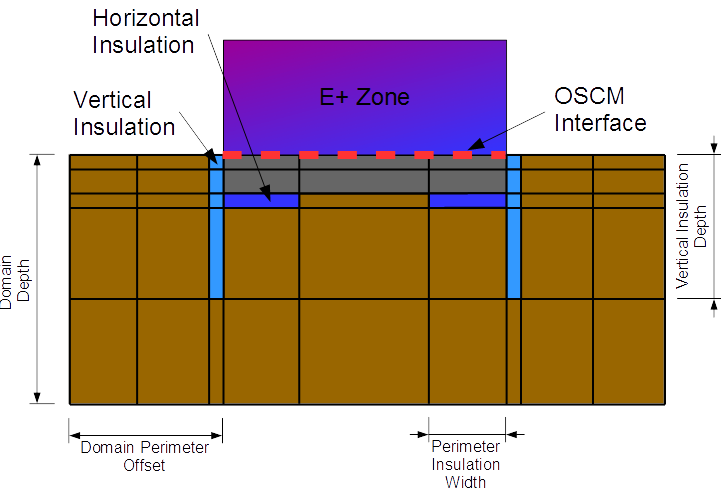
\includegraphics{media/image012.png}
\caption{In-grade configuration. \protect \label{fig:in-grade-configuration}}
\end{figure}

The in-grade slab option can be used to simulate situations when the upper slab surface is near the ground surface level. For this situation, slab's upper surface must interact with the zone via an OSCM boundary. Due to this, the FloorConstruction object for the zone floor must include a thin layer of the upper floor material. Horizontal and vertical insulation are modeled by the GroundDomain in this scenario. Horizontal insulation can be modeled as covering the full horizontal surface, or it can be limited to the perimeter regions only. In the latter case, the perimeter insulation width must be specified.

\begin{figure}[htbp]
\centering
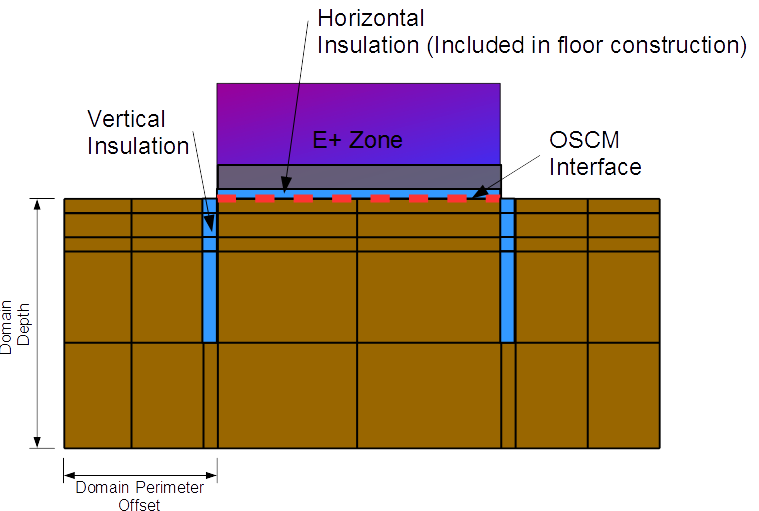
\includegraphics{media/image013.png}
\caption{On-grade configuration \protect \label{fig:on-grade-configuration}}
\end{figure}

The on-grade slab option can be used to simulate situations when the lower slab surface is near the ground surface level. In this situation, the entire floor must be included within the floor construction object. Vertical insulation is modeled by the GroundDomain in this scenario. Horizontal insulation can only be modeled as covering the full horizontal surface.

\subsubsection{Inputs}\label{inputs-16-006}

\paragraph{Field: Name}\label{field-name-8-009}

Alpha field used as a unique identifier for each ground domain.

\paragraph{Field: Ground Domain Depth}\label{field-ground-domain-depth}

Numeric field used to determine the depth of the simulation domain, in meters.

\paragraph{Field: Aspect Ratio}\label{field-aspect-ratio}

Numeric field used to define the height to width ratio of the slab.

\paragraph{Field: Perimeter Offset}\label{field-perimeter-offset}

Numeric field used to determine the distance from the slab perimeter to the domain perimeter, in meters.

\paragraph{Field: Soil Thermal Conductivity}\label{field-soil-thermal-conductivity-3}

The thermal conductivity of the soil, in W/m-K.

\paragraph{Field: Soil Density}\label{field-soil-density-3}

The bulk density of the soil, in kg/m3.

\paragraph{Field: Soil Specific Heat}\label{field-soil-specific-heat-3}

The specific heat of dry soil, in J/kg-K. If moisture is defined in this object, moisture and freezing effects are accounted for by varying the specific heat value.

\paragraph{Field: Soil Moisture Content Volume Fraction}\label{field-soil-moisture-content-volume-fraction-1}

A nominal value of soil moisture content to be used when evaluating soil thermal properties.

\paragraph{Field: Soil Moisture Content Volume Fraction at Saturation}\label{field-soil-moisture-content-volume-fraction-at-saturation-1}

A nominal value of soil moisture content when the soil is saturated, this is used in evaluating thermal properties of freezing soil.

\paragraph{Field: Type of Undisturbed Ground Temperature Object}\label{field-type-of-undisturbed-ground-temperature-object-000}

This is the type of undisturbed ground temperature object that is used to determine the ground temperature.

\paragraph{Field: Name of Undisturbed Ground Temperature Object}\label{field-name-of-undisturbed-ground-temperature-object-000}

This is the name of the undisturbed ground temperature object that is used to determine the ground temperature.

\paragraph{Field: Evapotranspiration Ground Cover Parameter}\label{field-evapotranspiration-ground-cover-parameter-1}

Numeric field specifies the ground cover effects used in the evapotranspiration model at the ground surface heat balance. The values range from 0 (solid, non-permeable ground surface) to 1.5 (wild growth).

\paragraph{Field: Slab Boundary Condition Model Name}\label{field-slab-boundary-condition-model-name}

This is the name of the other side boundary condition model used.

\paragraph{Field: Slab Location}\label{field-slab-location}

Alpha field indicates whether the slab is in-grade (top surface level with ground surface) or on-grade (bottoms surface level with ground surface). Options include ``ONGRADE'' and ``INGRADE''.

\paragraph{Field: Slab Material Name}\label{field-slab-material-name}

Name of the material object representing the slab material. Only applicable to in-grade situations.

\paragraph{Field: Horizontal Insulation}\label{field-horizontal-insulation}

Alpha field indicates whether horizontal insulation is present. Options include ``YES'' and ``NO''. Only applicable to in-grade situations.

\paragraph{Field: Horizontal Insulation Material Name}\label{field-horizontal-insulation-material-name}

Name of material object representing the horizontal slab insulation. Optional argument only required if horizontal insulation is present.

\paragraph{Field: Horizontal Insulation Extents}\label{field-horizontal-insulation-extents}

Alpha field indicates whether the horizontal slab insulation extends to cover the full horizontal area of the slab, or only covers the slab perimeter. Optional argument only required if horizontal insulation is present. Options include ``FULL'' and ``PERIMETER''.

\paragraph{Field: Perimeter Insulation Width}\label{field-perimeter-insulation-width}

Numeric field indicating the width of the perimeter insulation measured from the slab edge. Valid range from \textgreater{} 0 to \textless{} half of smallest slab width.

\paragraph{Field: Vertical Insulation}\label{field-vertical-insulation}

Alpha field indicates whether vertical insulation is present. Options include ``YES'' and ``NO''.

\paragraph{Field: Vertical Insulation Name}\label{field-vertical-insulation-name}

Name of material object representing the vertical slab insulation. Optional argument only required if vertical insulation is present.

\paragraph{Field: Vertical Insulation Depth}\label{field-vertical-insulation-depth}

Numeric field indicates the depth measured in meters from the ground surface to which the vertical perimeter insulation extends. Valid range from \textgreater{} Slab Thickness to \textless{} Domain Depth.

\paragraph{Field: Simulation Timestep}\label{field-simulation-timestep}

Alpha field indicating whether the domain will update temperatures at each zone timestep, or at hourly intervals. Options include ``timestep'' and ``hourly''.

An IDF example of an in-grade slab.

\begin{lstlisting}
Site:GroundDomain:Slab,
  IngradeCoupledSlab, !- Name
  5,                  !- Ground Domain Depth
  1,                  !- Aspect Ratio
  5,                  !- Domain Perimeter Offset
  1.8,                !- Soil Thermal Conductivity
  3200,               !- Soil Density
  836,                !- Soil Specific Heat
  30,                 !- Soil Moisture Content Volume Fraction
  50,                 !- Soil Moisture Content Volume Fraction at Saturation
  Site:GroundTemperature:Undisturbed:KusudaAchenbach, !- Type of Undisturbed Ground Temperature Object
  KATemps,            !- Name of Undisturbed Ground Temperature Object
  1,                  !- Evapotranspiration Ground Cover Parameter
  GroundCoupledOSCM,  !- Name of Floor Boundary Condition Model
  InGrade,            !- Slab Location (InGrade/OnGrade)
  Slab Material-In-grade, !- Slab Material Name
  Yes,                !- Horizontal Insulation
  Slab Insulation,    !- Horizontal Insulation Material Name
  Perimeter,          !- Full Horizontal or Perimeter Only
  1,                  !- Perimeter insulation width
  Yes,                !- Vertical Insulation
  Slab Insulation,    !- Vertical Insulation Name
  2,                  !- Vertical perimeter insulation depth from surface
  Hourly;             !- Simulation timestep
\end{lstlisting}

And IDF example of an on-grade slab

\begin{lstlisting}
Site:GroundDomain:Slab,
  OngradeCoupledSlab, !- Name
  5,                  !- Ground Domain Depth {m}
  1,                  !- Aspect Ratio
  5,                  !- Domain Perimeter Offset {m}
  1.8,                !- Soil Thermal Conductivity {W/m-K}
  3200,               !- Soil Density {kg/m3}
  836,                !- Soil Specific Heat {J/kg-K}
  30,                 !- Soil Moisture Content Volume Fraction
  50,                 !- Soil Moisture Content Volume Fraction at Saturation
  Site:GroundTemperature:Undisturbed:KusudaAchenbach, !- Type of Undisturbed Ground Temperature Object
  KATemps;            !- Name of Undisturbed Ground Temperature Object
  1,                  !- Evapotranspiration Ground Cover Parameter
  GroundCoupledOSCM,  !- Name of Floor Boundary Condition Model
  OnGrade,            !- Slab Location (InGrade/OnGrade)
  ,                   !- Slab Material Name
  ,                   !- Horizontal Insulation (Yes/No)
  ,                   !- Horizontal Insulation Material Name
  ,                   !- Full Horizontal or Perimeter Only
  ,                   !- Perimeter insulation width (m)
  Yes,                !- Vertical Insulation (Yes/No)
  Slab Insulation,    !- Vertical Insulation Name
  2,                  !- Vertical perimeter insulation depth from surface
  Hourly;             !- Simulation timestep. (Timestep/Hourly)</td>
\end{lstlisting}

\subsubsection{Outputs}\label{outputs-1-015}

The following output variables are available.

\begin{itemize}
\tightlist
\item
  Zone, Average, Zone Coupled Surface Heat Flux {[}W/m2{]}
\item
  Zone, Average, Zone Coupled Surface Temperature {[}C{]}
\end{itemize}

\paragraph{Zone Coupled Surface Heat Flux {[}W/m2{]}}\label{zone-coupled-surface-heat-flux-wm2}

This is the value of the heat flux provided to the GroundDomain as a boundary condition. This is calculated by taking the average heat flux of all surfaces coupled to the domain's SurfaceProperty:OtherSideConditionsModel model.

\paragraph{Zone Coupled Surface Temperature {[}C{]}}\label{zone-coupled-surface-temperature-c}

This is the value of the SurfaceProperty:OtherSideConditionsModel surface temperature. This is the temperature provided to the ground coupled surfaces as an outside boundary condition.

\subsection{Site:GroundDomain:Basement}\label{sitegrounddomainbasement}

This section documents the input object used to simulate ground coupled heat transfer with underground zones within EnergyPlus. Zone surfaces within EnergyPlus interact with the Site:GroundDomain:Basement object by utilizing the SurfaceProperty:OtherSideConditionsModel object. Two separate OSCM are required for the basement vertical and horizontal surfaces. Vertical wall surfaces will interact with the first OSCM while the horizontal floor surface will interact with the second OSCM. Basement floor and wall surfaces are constructed normally by using the BuildingSurface:Detailed object, with the outside boundary condition being the OtherSideConditionsModel for the basement floor or wall. The outside surface of the wall being the interface between the ground domain and the EnergyPlus zone. Horizontal and vertical ground insulation are simulated by the ground domain, and therefore should not be included in the wall and floor construction objects.

\begin{figure}[htbp]
\centering
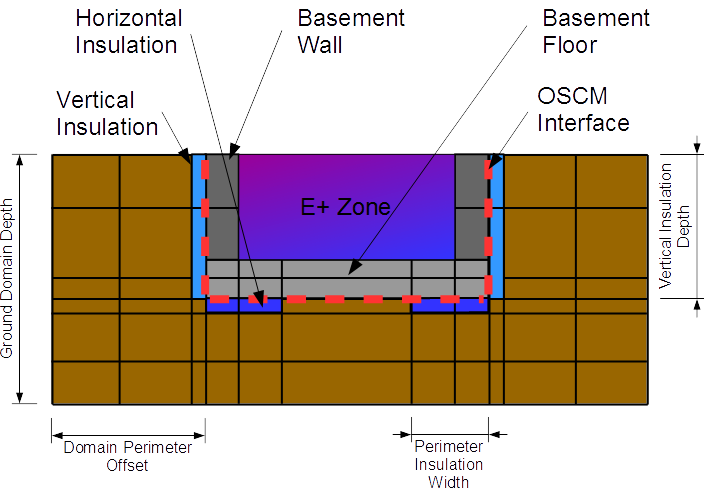
\includegraphics{media/image900.png}
\caption{Basement Configuration \protect \label{fig:basement-configuration}}
\end{figure}

\begin{lstlisting}
Site:GroundDomain:Basement,
  CoupledBasement,     !- Name
  10,                  !- Ground Domain Depth {m}
  1,                   !- Aspect ratio
  5,                   !- Perimeter offset {m}
  1.8,                 !- Soil Thermal Conductivity {W/m-K}
  3200,                !- Soil Density {kg/m3}
  836,                 !- Soil Specific Heat {J/kg-K}
  30,                  !- Soil Moisture Content Volume Fraction {percent}
  50,                  !- Soil Moisture Content Volume Fraction at Saturation {percent}
  Site:GroundTemperature:Undisturbed:KusudaAchenbach, !- Type of Undisturbed Ground Temperature Object
  KATemps,             !- Name of Undisturbed Ground Temperature Object
  1,                   !- Evapotranspiration Ground Cover Parameter
  BasementFloorOSCM,   !- Name of Basement Floor Boundary Condition Model
  Yes,                 !- Basement Horizontal Underfloor Insulation Present (Yes/No)
  Basement Insulation, !- Basement Horizontal Insulation Underfloor Material Name
  Full,                !- Full Horizontal or Perimeter Only (Full/Perimeter)
  ,                    !- Perimeter width (m)
  2.5,                 !- Depth of Basement Wall In Ground Domain {m}
  BasementWallOSCM,    !- Name of Basement Wall Boundary Condition Model
  Yes,                 !- Basement Wall Vertical Insulation Present(Yes/No)
  Basement Insulation, !- Basement Wall Vertical Insulation Material Name
  2.5,                 !- Vertical insulation depth from surface (m)
  Hourly;              !- Domain Update interval. (Timestep, Hourly)
  4;                   ! Mesh Density Parameter
\end{lstlisting}

\subsubsection{Inputs}\label{inputs-17-004}

\paragraph{Field: Name}\label{field-name-9-009}

Alpha field used as a unique identifier for each basement domain. Multiple basements domains can be simulated simultaneously, however, each domain must have a unique name. Additionally, despite the ability to simulate multiple domains simultaneously, these domains do not interact with each other and are treated as independent domains with boundary conditions given by the model parameters below.

\paragraph{Field: Ground Domain Depth}\label{field-ground-domain-depth-1}

Numeric field used to determine the depth of the simulation domain, in meters. A value of 10 meters is the default.

\paragraph{Field: Aspect Ratio}\label{field-aspect-ratio-1}

Numeric field, which is the ratio of basement length to width, used to determine the aspect ratio of the basement. This field along with the total basement floor area, which is taken as the combination of all surfaces connected to the floor OtherSideConditionsModel, are used to determine the size and shape of the basement domain. Aspect ratios and the inverse of aspect ratios should produce identical results. i.e. AR = 2 equals AR = 0.5. This field has units of meters/meters.

\paragraph{Field: Domain Perimeter Offset}\label{field-domain-perimeter-offset}

Numeric field used to determine the distance from the basement perimeter to the domain perimeter, in meters. A value of 5 is default.

\paragraph{Field: Soil Thermal Conductivity}\label{field-soil-thermal-conductivity-4}

The thermal conductivity of the soil, in W/m-K.

\paragraph{Field: Soil Density}\label{field-soil-density-4}

The bulk density of the soil, in kg/m3.

\paragraph{Field: Soil Specific Heat}\label{field-soil-specific-heat-4}

The specific heat of dry soil, in J/kg-K. If moisture is defined in this object, moisture and freezing effects are accounted for by varying the specific heat value.

\paragraph{Field: Soil Moisture Content Volume Fraction}\label{field-soil-moisture-content-volume-fraction-2}

A nominal value of soil moisture content to be used when evaluating soil thermal properties.

\paragraph{Field: Soil Moisture Content Volume Fraction at Saturation}\label{field-soil-moisture-content-volume-fraction-at-saturation-2}

A nominal value of soil moisture content when the soil is saturated, this is used in evaluating thermal properties of freezing soil.

\paragraph{Field: Type of Undisturbed Ground Temperature Object}\label{field-type-of-undisturbed-ground-temperature-object-1-000}

This is the type of undisturbed ground temperature object that is used to determine the ground temperature.

\paragraph{Field: Name of Undisturbed Ground Temperature Object}\label{field-name-of-undisturbed-ground-temperature-object-1-000}

This is the name of the undisturbed ground temperature object that is used to determine the ground temperature.

\paragraph{Field: Evapotranspiration Ground Cover Parameter}\label{field-evapotranspiration-ground-cover-parameter-2}

Numeric field specifies the ground cover effects used in the evapotranspiration model at the ground surface heat balance. The values range from 0 (solid, non-permeable ground surface) to 1.5 (wild growth). Model can be sensitive to variations in this parameter, especially in dry climates.

\paragraph{Field: Basement Floor Boundary Condition Model Name}\label{field-basement-floor-boundary-condition-model-name}

This is the name of the other side boundary condition model used for the basement floor surface.

\paragraph{Field: Horizontal Insulation}\label{field-horizontal-insulation-1}

Alpha field indicates whether horizontal insulation is present. Options include ``YES'' and ``NO''.

\paragraph{Field: Horizontal Insulation Name}\label{field-horizontal-insulation-name}

Name of material object representing the horizontal underfloor basement insulation. Optional argument only required if horizontal insulation is present.

\paragraph{Field: Horizontal Insulation Extents}\label{field-horizontal-insulation-extents-1}

Alpha field indicates whether the horizontal underfloor insulation extends to cover the full horizontal area of the basement floor, or only covers the basement floor perimeter. Optional argument only required if horizontal insulation is present. Options include ``FULL'' and ``PERIMETER''.

\paragraph{Field: Perimeter Insulation Width}\label{field-perimeter-insulation-width-1}

Numeric field indicating the width of the perimeter insulation measured from the basement floor edge. Valid range from \textgreater{} 0 to \textless{} half of smallest basement floor width.

\paragraph{Field: Basement Depth}\label{field-basement-depth}

Depth of basement floor surface referenced from the ground surface, in meters. This domain should be the distance from the ground surface down to the basement floor surface. In cases where the ground surface is below the main above-ground building level, a separate wall surface should be employed between the basement walls and the main level walls.

\paragraph{Field: Basement Wall Boundary Condition Model Name}\label{field-basement-wall-boundary-condition-model-name}

Name of the other side condition boundary model used for the basement walls.

\paragraph{Field: Vertical Insulation}\label{field-vertical-insulation-1}

Alpha field indicates whether vertical insulation is present. Options include ``YES'' and ``NO''.

\paragraph{Field: Vertical Insulation Name}\label{field-vertical-insulation-name-1}

Name of material object representing the vertical slab insulation. Optional argument only required if vertical insulation is present.

\paragraph{Field: Vertical Insulation Depth}\label{field-vertical-insulation-depth-1}

Numeric field indicates the depth measured in meters from the ground surface to which the vertical perimeter insulation extends. Valid range from \textgreater{} 0 to \textless{} Basement Depth.

\paragraph{Field: Simulation Timestep}\label{field-simulation-timestep-1}

Alpha field indicating whether the domain will update temperatures at each zone timestep, or at hourly intervals. Options include ``timestep'' and ``hourly''.

\paragraph{Mesh Density Parameter}\label{mesh-density-parameter}

Integer field indicating the density of the finite difference ground domain cells between the basement and the far field boundaries. Default value is 4. Total number of ground domain cells, insulation cells, and ground surface cells are indicated as outputs to the eio file.

\subsubsection{Outputs}\label{outputs-2-013}

The following output variables are available.

\begin{itemize}
\item
  Wall Interface Heat Flux
\item
  Wall Interface Temperature
\item
  Floor Interface Heat Flux
\item
  Floor Interface Temperature
\end{itemize}

\paragraph{Wall Interface Heat Flux {[}W/m2{]}}\label{wall-interface-heat-flux-wm2}

This is the value of the heat flux provided to ground domain as a boundary condition for the basement walls. Should be equal to the basement wall outside heat flux.

\paragraph{Wall Interface Temperature {[}C{]}}\label{wall-interface-temperature-c}

This is the value of the SurfaceProperty:OtherSideConditionsModel surface temperature. This is the temperature provided to the basement wall surfaces as an outside boundary condition.

\paragraph{Floor Interface Heat Flux {[}W/m2{]}}\label{floor-interface-heat-flux-wm2}

This is the value of the heat flux provided to ground domain as a boundary condition for the basement floor. Should be equal to the basement floor outside heat flux.

\paragraph{Floor Interface Temperature {[}C{]}}\label{floor-interface-temperature-c}

This is the value of the SurfaceProperty:OtherSideConditionsModel surface temperature. This is the temperature provided to the ground coupled floor surfaces as an outside boundary condition.

\subsection{Site:GroundTemperature:FCfactorMethod}\label{sitegroundtemperaturefcfactormethod}

Site:GroundTemperature:FCfactorMethod is used only by the underground walls or slabs-on-grade or underground floors defined with C-factor (Construction:CfactorUndergroundWall) and F-factor (Construction:FfactorGroundFloor) method for code compliance calculations where detailed construction layers are unknown. Only one such ground temperature object can be included. The monthly ground temperatures for this object are close to the monthly outside air temperatures delayed by three months. If user does not input this object in the IDF file, it will be defaulted to the 0.5m set of monthly ground temperatures from the weather file if they are available. Entering these will also overwrite any ground temperatures from the weather file in the F and C factor usage. If neither is available, an error will result.

\subsubsection{Inputs}\label{inputs-18-004}

\paragraph{Field: Month Temperature(s) -- 12 fields in all}\label{field-month-temperatures-12-fields-in-all-3}

Each numeric field is the monthly ground temperature (degrees Celsius) used for the indicated month (January = 1\(^{st}\) field, February = 2\(^{nd}\) field, etc.)

And, the IDF example:

\begin{lstlisting}
Site:GroundTemperature:FCfactorMethod,  9.5, 3.5, -0.7, -1.7, -0.6, 3.6, 9.3, 14, 18.2, 22.7, 21.2, 16.8;
\end{lstlisting}

\subsection{Site:GroundReflectance}\label{sitegroundreflectance}

Ground reflectance values are used to calculate the ground reflected solar amount. This fractional amount (entered monthly) is used in this equation:

\begin{equation}
\rm{GroundReflectedSolar} = \left( \rm{BeamSolar} \cdot cos \left( \rm{SunZenithAngle} \right) + \rm{DiffuseSolar} \right) \cdot \rm{GroundReflectance}
\end{equation}

Of course, the Ground Reflected Solar is never allowed to be negative. The ground reflectance can be further modified when snow is on the ground by the Snow Ground Reflectance Modifier. To use no ground reflected solar in your simulation, enter 0.0 for each month.

\subsubsection{Inputs}\label{inputs-19-003}

\paragraph{Field: Month Average Ground Reflectance(s) -- 12 fields in all}\label{field-month-average-ground-reflectances-12-fields-in-all}

Each numeric field is the monthly average reflectivity of the ground used for the indicated month (January = 1\(^{st}\) field, February = 2\(^{nd}\) field, etc.)

And use in an IDF:

\begin{lstlisting}
Site:GroundReflectance,
  0.600,     !January Ground Reflectance
  0.600,     !February Ground Reflectance
  0.400,     !March Ground Reflectance
  0.300,     !April Ground Reflectance
  0.200,     !May Ground Reflectance
  0.200,     !June Ground Reflectance
  0.200,     !July Ground Reflectance
  0.200,     !August Ground Reflectance
  0.200,     !September Ground Reflectance
  0.200,     !October Ground Reflectance
  0.300,     !November Ground Reflectance
  0.400;     !December Ground Reflectance
\end{lstlisting}

\subsection{Site:GroundReflectance:SnowModifier}\label{sitegroundreflectancesnowmodifier}

It is generally accepted that snow resident on the ground increases the basic ground reflectance. EnergyPlus allows the user control over the snow ground reflectance for both ``normal ground reflected solar'' calculations (see above) and snow ground reflected solar modified for daylighting. These are entered under this object and both default to 1 (same as normal ground reflectance -- no special case for snow which is a conservative approach).

\subsubsection{Inputs}\label{inputs-20-003}

\paragraph{Field: Ground Reflected Solar Modifier}\label{field-ground-reflected-solar-modifier}

This field is a decimal number which is used to modified the basic monthly ground reflectance when snow is on the ground (from design day input or weather data values).

\begin{equation}
\rm{GroundReflectance}_{\rm{used}} = \rm{GroundReflectance} \cdot \rm{Modifier}_{\rm{Snow}}
\end{equation}

The actual Ground Reflectance is limited to {[}0.0,1.0{]}.

\paragraph{Field: Daylighting Ground Reflected Solar Modifier}\label{field-daylighting-ground-reflected-solar-modifier}

This field is a decimal number which is used to modified the basic monthly ground reflectance when snow is on the ground (from design day input or weather data values).

\begin{equation}
\rm{DaylightingGroundReflectance}_{\rm{used}} = \rm{GroundReflectance} \cdot \rm{Modifier}_{\rm{Snow}}
\end{equation}

The actual Ground Reflectance is limited to {[}0.0,1.0{]}.

An IDF example:

\begin{lstlisting}
Site:GroundReflectance:SnowModifier,
  1.0;       !- Ground Reflected Solar Modifier
\end{lstlisting}

Outputs will show both the inputs from the above object as well as monthly values for both Snow Ground Reflectance and Snow Ground Reflectance for Daylighting.

\subsection{Site:WaterMainsTemperature}\label{sitewatermainstemperature}

The Site:WaterMainsTemperature object is used to calculate water temperatures delivered by underground water main pipes. The mains temperatures are used as default, make-up water temperature inputs for several plant objects, including: \textbf{WaterUse:Equipment, WaterUse:Connections, WaterHeater:Mixed} and \textbf{WaterHeater:Stratified}. The mains temperatures are also used in the water systems objects to model the temperature of cold water supplies.

Water mains temperatures are a function of outdoor climate conditions and vary with time of year. A correlation has been formulated to predict water mains temperatures based on two weather inputs:

\begin{itemize}
\item
  average annual outdoor air temperature (dry-bulb)
\item
  maximum difference in monthly average outdoor air temperatures
\end{itemize}

These values can be easily calculated from annual weather data using a spreadsheet or from the ``.stat'' file available with the EnergyPlus weather files at \href{http://www.energyplus.gov}{www.energyplus.gov}. Monthly statistics for dry-bulb temperatures are shown with daily averages. The daily averages are averaged to obtain the annual average. The maximum and minimum daily average are subtracted to obtain the maximum difference. For more information on the water mains temperatures correlation, see the \emph{EnergyPlus Engineering Document}.

Alternatively, the Site:WaterMainsTemperature object can read values from a schedule. This is useful for measured data or when water comes from a source other than buried pipes, e.g., a river or lake.

If there is no Site:WaterMainsTemperature object in the input file, a default constant value of 10 C is assumed.

\subsubsection{Inputs}\label{inputs-21-003}

\paragraph{Field: Calculation Method}\label{field-calculation-method}

This field selects the calculation method and must have the keyword Schedule or Correlation.

\paragraph{Field: Schedule Name}\label{field-schedule-name-003}

If the calculation method is Schedule, the water mains temperatures are read from the schedule referenced by this field. If the calculation method is Correlation, this field is ignored.

\paragraph{Field: Annual Average Outdoor Air Temperature}\label{field-annual-average-outdoor-air-temperature}

If the calculation method is Correlation, this field is used in the calculation as the annual average outdoor air temperature (dry-bulb) {[}C{]}. If the calculation method is Schedule, this field is ignored.

\paragraph{Field: Maximum Difference In Monthly Average Outdoor Air Temperatures}\label{field-maximum-difference-in-monthly-average-outdoor-air-temperatures}

If the calculation method is Correlation, this field is used in the calculation as the maximum difference in monthly average outdoor air temperatures {[}\(\Delta\)C{]}. If the calculation method is Schedule, this field is ignored.

\begin{lstlisting}
Site:WaterMainsTemperature,
  Correlation,  !- Calculation Method {SCHEDULE | CORRELATION}
  ,             !- Schedule Name
  9.69,         !- Annual Average Outdoor Air Temperature {C}
  28.1;         !- Maximum Difference In Monthly Average Outdoor Air Temperatures {deltaC}
\end{lstlisting}

\subsection{Site:Precipitation}\label{siteprecipitation}

The Site:Precipitation object is used to describe the amount of water precipitation at the building site over the course of the simulation run period. Precipitation includes both rain and the equivalent water content of snow. Precipitation is not yet described well enough in the many building weather data files. So this object can be used to provide the data using Schedule objects that define rates of precipitation in meters per hour.

A set of schedules for site precipitation have been developed for USA weather locations and are provided with EnergyPlus in the data set called PrecipitationSchedulesUSA.idf. The user can develop schedules however they want. The schedules in the data set were developed using EnergyPlus' weather file (EPW) observations and the average monthly precipitation for the closest weather site provided by NOAA. EPW files for the USA that were based on TMY or TMY2 include weather observations for Light/Moderate/Heavy rainfall, however most international locations do not include these observations. The values were modeled by taking the middle of the ranges quoted in the EPW data dictionary. The assumed piecewise function is shown below.

\begin{equation}
\rm{Amount} \, (m/hour) = \, \left\{
  \begin{array}{*{20}{c}}
    \rm{Light} = 0.0125 \\
    \rm{Moderate} = 0.052 \\
    \rm{Heavy} = 0.1
  \end{array}
\right.
\end{equation}

The values were inserted on hour by hour basis for the month based on the observations. Then each month was rescaled to meet the average precipitation for the month based on the 30-year average (1971-2000) provided by the NOAA/NCDC. Therefore, the flags in the EPW file match the precipitation schedules for the USA. Note that summing the average monthly precipitation values will not give you the average yearly precipitation. The resulting value may be lower or higher than the average yearly value.

Once the typical rainfall pattern and rates are scheduled, the Site:Precipitation object provides a method of shifting the total rainfall up or down for design purposes. Wetter or drier conditions can be modeled by changing the Design Annual Precipitation although the timing of precipitation throughout the year will not be changed.

\subsubsection{Inputs}\label{inputs-22-002}

\paragraph{Field: Precipitation Model Type}\label{field-precipitation-model-type}

Choose rainfall modeling options. Only available option is ScheduleAndDesignLevel.

\paragraph{Field: Design Level for Total Annual Precipitation}\label{field-design-level-for-total-annual-precipitation}

Magnitude of total precipitation for an annual period to be used in the model. Value selected by the user to correspond with the amount of precipitation expected or being assumed for design purposes. The units are in meters. This field works with the following two fields to allow easily shifting the amounts without having to generate new schedules.

\paragraph{Field: Precipitation Rate Schedule Name}\label{field-precipitation-rate-schedule-name}

Name of a schedule defined elsewhere that describes the rate of precipitation. The precipitation rate schedule is analogous to weather file data. However, weather files for building simulation do not currently contain adequate data for such calculations. Therefore, EnergyPlus schedules are used to enter the pattern of precipitation events. The values in this schedule are the average rate of precipitation in meters per hour. The integration of these values over an annual schedule should equal the nominal annual precipitation.

\paragraph{Field: Average Total Annual Precipitation}\label{field-average-total-annual-precipitation}

Magnitude of annual precipitation associated with the rate schedule. This value is used to normalize the precipitation.

IDF example:

\begin{lstlisting}
Site:Precipitation,
  ScheduledAndDesignLevel, !- Precipitation Model Type
  0.75,                    !- Design Level Total Annual Precipitation {m/yr}
  PrecipitationSchd,       !- Schedule Name for Precipitation Rates
  0.80771;                 !- Average Total Annual Precipitation {m/yr}
\end{lstlisting}

\subsection{RoofIrrigation}\label{roofirrigation}

The RoofIrrigation object is used to describe the amount of irrigation on the ecoroof surface over the course of the simulation runperiod. This object is used to provide irrigation data using Schedule objects that define rates of irrigation in meters per hour. These schedules can be one of two types: Schedule, or SmartSchedule.

\subsubsection{Inputs}\label{inputs-23-002}

\paragraph{Field: Irrigation Model Type}\label{field-irrigation-model-type}

Choose irrigation modeling options. Available options are \textbf{Schedule} and \textbf{SmartSchedule}. The \textbf{Schedule} type is used to force an irrigation schedule regardless of the current moisture state of the soil. The \textbf{SmartSchedule} type allows the precipitation schedule to be overridden if the current moisture state of the soil is greater than 40\% saturated.

\paragraph{Field: Irrigation Rate Schedule Name}\label{field-irrigation-rate-schedule-name}

Name of a schedule defined elsewhere that describes the rate of irrigation. The values in this schedule are the average rate of irrigation in meters per hour.

\paragraph{Field: Irrigation Maximum Saturation Threshold}\label{field-irrigation-maximum-saturation-threshold}

Used with the SmartSchedule option in the Irrigation Model Type field to override the default 40\% saturation limit for turning off the irrigation: values of 0 to 100 (percent) can be entered with 40\% being the default.

IDF example:

\begin{lstlisting}
RoofIrrigation,
  Schedule,       !- Irrigation Model Type
  IrrigationSchd; !- Schedule Name for Irrigation Rates
\end{lstlisting}

\subsection{Solar and Visible Spectrum Objects}\label{solar-and-visible-spectrum-objects}

The next two objects enable users to enter solar and visible spectrum which is used to calculate the thermal and visual performance of windows if their glazings are defined with full spectral data. EnergyPlus versions 8.0 and older hard-wired the solar and visible spectrum. The solar spectrum assumes air mass 1.5 terrestrial solar global spectral irradiance values (W/m2-micron) on a 37o tilted surface, based on ISO 9845-1 and ASTM E 892; derived from Optics5 data file ISO-9845GlobalNorm.std, 10-14-99. The visible/photopic spectrum is based on CIE 1931 observer; ISO/CIE 10527, CIE Standard Calorimetric Observers; derived from Optics5 data file ``CIE 1931 Color Match from E308.txt'', which is the same as WINDOW4 file Cie31t.dat.

\subsection{Site:SolarAndVisibleSpectrum}\label{sitesolarandvisiblespectrum}

The SolarAndVisibleSpectrum object is used to specify the solar and visible spectrum data which is used as spectral weighting function to calculate the window performance (transmittance and absorptance) in EnergyPlus. This is a unique object, if it is missing from an IDF file, the default (same as EnergyPlus version 8.0) solar and visible spectrum data will be used.

\subsubsection{Inputs}\label{inputs-24-001}

\paragraph{Field: Name}\label{field-name-10-008}

This field specifies the name of the SolarAndVisibleSpectrum object.

\paragraph{Field: Spectrum Data Method}\label{field-spectrum-data-method}

This field specifies the method used to enter the spectrum data. Two choices are available: Default and UserDefined. The choice Default will continue to use the hard-wired spectrum data in EnergyPlus (for backward compatibility). The choice UserDefined allows users to specify custom solar and visible spectrum data. The default choice is Default.

\paragraph{Field: Solar Spectrum Data Name}\label{field-solar-spectrum-data-name}

This field is required if the Spectrum Data Method is set to UserDefined. This field references a spectrum dataset for solar.

\paragraph{Field: Visible Spectrum Data Name}\label{field-visible-spectrum-data-name}

This field is required if the Spectrum Data Method is set to UserDefined. This field references a spectrum dataset for visible.

IDF example:

\begin{lstlisting}
Site:SolarAndVisibleSpectrum,
  LocalSpectrum,            !- Name
  UserDefined,              !- Spectrum Data Method: Default, UserDefined
  SolarSpectrum,            !- Solar Spectrum Data Object Name
  VisibleSpectrum;          !- Visible Spectrum Data Object
\end{lstlisting}

\subsection{Site:SpectrumData}\label{sitespectrumdata}

The Site:SpectrumData object holds the user defined solar or visible spectrum data. For solar spectrum, up to 107 pairs of (wavelength, spectrum) can be entered. For visible spectrum, up to 81 pairs can be entered.

\subsubsection{Inputs}\label{inputs-25-001}

\paragraph{Field: Name}\label{field-name-11-007}

This field specifies the name of the SpectrumData object. The name must be unique across all SpectrumData objects.

\paragraph{Field: Spectrum Data Type}\label{field-spectrum-data-type}

This field specifies the type of spectrum data. Choices are Solar and Visible.

\paragraph{Field: Wavelength \textless{}n\textgreater{}}\label{field-wavelength-n}

This field specifies the nth wavelength in micron.

\paragraph{Field: Spectrum \textless{}n\textgreater{}}\label{field-spectrum-n}

This field specifies the nth spectrum corresponding to the nth wavelength.

IDF example:

\begin{lstlisting}
Site:SpectrumData,
  SolarSpectrum, !- Name
  Solar,         !- Spectrum Data Type
  0.3,0,         !- up to 107 pair of (wavelength, spectrum)
  0.305,3.4,
  0.31,15.6,
  0.315,41.1,
  0.32,71.2,
  0.325,100.2,
  0.33,152.4,
  0.335,155.6,
  0.34,179.4,
  0.345,186.7,
  0.35,212,
  0.36,240.5,
  0.37,324,
  0.38,362.4,
  ...;
\end{lstlisting}

\subsubsection{Outputs}\label{outputs-3-011}

Climate related variables appear in two places for EnergyPlus outputs. Certain objects that are invariant throughout a simulation period have lines appear in the eplusout.eio file. For descriptions of this reporting, please see the Output Details and Examples document.

\subsubsection{Outputs}\label{outputs-4-008}

Variables related to ambient environment data are available at timestep and higher resolutions. Below is a variable dictionary of these variables and subsequent definitions:

\begin{itemize}
\item
  Zone,Average,Site Outdoor Air Drybulb Temperature {[}C{]}
\item
  Zone,Average,Site Outdoor Air Dewpoint Temperature {[}C{]}
\item
  Zone,Average,Site Outdoor Air Wetbulb Temperature {[}C{]}
\item
  Zone,Average,Site Outdoor Air Humidity Ratio {[}kgWater/kgAir{]}
\item
  Zone,Average,Site Outdoor Air Relative Humidity {[}\%{]}
\item
  Zone,Average,Site Outdoor Air Barometric Pressure {[}Pa{]}
\item
  Zone,Average,Site Wind Speed {[}m/s{]}
\item
  Zone,Average,Site Wind Direction {[}deg{]}
\item
  Zone,Average,Site Sky Temperature {[}C{]}
\item
  Zone,Average,Site Horizontal Infrared Radiation Rate per Area {[}W/m2{]}
\item
  Zone,Average,Site Diffuse Solar Radiation Rate per Area {[}W/m2{]}
\item
  Zone,Average,Site Direct Solar Radiation Rate per Area {[}W/m2{]}
\item
  Zone,Sum,Site Precipitation Depth {[}m{]}
\item
  Zone,Average,Site Ground Reflected Solar Radiation Rate per Area {[}W/m2{]}
\item
  Zone,Average,Site Ground Temperature {[}C{]}
\item
  Zone,Average,Site Surface Ground Temperature {[}C{]}
\item
  Zone,Average,Site Deep Ground Temperature {[}C{]}
\item
  Zone,Average,Site Simple Factor Model Ground Temperature {[}C{]}
\item
  Zone,Average,Site Outdoor Air Enthalpy {[}J/kg{]}
\item
  Zone,Average,Site Outdoor Air Density {[}kg/m3{]}
\item
  Zone,Average,Site Solar Azimuth Angle {[}deg{]}
\item
  Zone,Average,Site Solar Altitude Angle {[}deg{]}
\item
  Zone,Average,Site Solar Hour Angle {[}deg{]}
\item
  Zone,Average,Site Rain Status {[]}
\item
  Zone,Average,Site Snow on Ground Status {[]}
\item
  Zone,Average,Site Exterior Horizontal Sky Illuminance {[}lux{]}
\item
  Zone,Average,Site Exterior Horizontal Beam Illuminance {[}lux{]}
\item
  Zone,Average,Site Exterior Beam Normal Illuminance {[}lux{]}
\item
  Zone,Average,Site Sky Diffuse Solar Radiation Luminous Efficacy {[}lum/W{]}
\item
  Zone,Average,Site Beam Solar Radiation Luminous Efficacy {[}lum/W{]}
\item
  Zone,Average,Site Daylighting Model Sky Clearness {[]}
\item
  Zone,Average,Sky Brightness for Daylighting Calculation {[]}
\item
  Zone,Average,Site Daylight Saving Time Status {[]}
\item
  Zone,Average,Site Day Type Index {[]}
\item
  Zone,Average,Site Mains Water Temperature {[}C{]}
\item
  HVAC,Average,Site Precipitation Rate {[}m/s{]}
\item
  HVAC,Sum,Site Precipitation Depth {[}m{]}
\item
  HVAC,Sum,Water System Roof Irrigation Scheduled Depth{[}m{]}
\item
  HVAC,Sum,Water System Roof Irrigation Actual Depth{[}m{]}
\end{itemize}

Note that these data values may be interpolated from ``hour'' points (ref: Weather Data Hourly Interpolation). Most of the data values represent the ``average'' over the reporting resolution period.

\paragraph{Site Outdoor Air Drybulb Temperature {[}C{]}}\label{site-outdoor-air-drybulb-temperature-c}

This is the outdoor dry-bulb temperature in degrees C.

\paragraph{Site Outdoor Air Dewpoint Temperature {[}C{]}}\label{site-outdoor-air-dewpoint-temperature-c}

This is the outdoor dewpoint temperature in degrees C.

\paragraph{Site Outdoor Air Wetbulb Temperature {[}C{]}}\label{site-outdoor-air-wetbulb-temperature-c}

The outdoor wet-bulb temperature is derived (at the timestep) from the values for dry-bulb temperature, humidity ratio and barometric pressure.

\paragraph{Site Outdoor Air Humidity Ratio {[}kgWater/kgAir{]}}\label{site-outdoor-air-humidity-ratio-kgwaterkgair}

The outdoor humidity ratio is derived (at the timestep) from the dry-bulb temperature, relative humidity and barometric pressure.

\paragraph{Site Outdoor Air Relative Humidity {[}\%{]}}\label{site-outdoor-air-relative-humidity}

This is the outdoor relative humidity expressed in percent.

\paragraph{Site Outdoor Air Barometric Pressure {[}Pa{]}}\label{site-outdoor-air-barometric-pressure-pa}

This is the atmospheric/barometric pressure in Pa.

\paragraph{Site Wind Speed {[}m/s{]}}\label{site-wind-speed-ms}

This is the outdoor wind speed in m/s.

\paragraph{Site Wind Direction {[}deg{]}}\label{site-wind-direction-deg}

This is the wind direction (N = 0, E = 90, S = 180, W = 270).

\paragraph{Site Sky Temperature {[}C{]}}\label{site-sky-temperature-c}

The sky temperature is derived from horizontal infrared radiation intensity. It is expressed in degrees C. The default calculation is shown below but this value may be modified by the WeatherProperty:SkyTemperature object. Note that Sigma is the Stefan-Boltzmann constant in the following equation:

\begin{equation}
Sky\;Temperature = {\left( {\frac{{Horizontal\;IR}}{{Sigma}}} \right)^{\frac{1}{4}}} - {273.15_{Conversion\;from\;Kelvin\;to\;Centigrade}}
\end{equation}

\paragraph{Site Horizontal Infrared Radiation Rate per Area {[}W/m2{]}}\label{site-horizontal-infrared-radiation-rate-per-area-wm2}

The horizontal infrared radiation intensity is expressed in W/m\(^{2}\) based, if missing from the weather file, on opaque sky cover, sky emissivity, temperature and other factors. The general calculation of Site Horizontal Infrared Radiation Rate per Area is discussed in both the Engineering Reference and the Auxiliary Programs document.

\paragraph{Site Diffuse Solar Radiation Rate per Area {[}W/m2{]}}\label{site-diffuse-solar-radiation-rate-per-area-wm2}

Diffuse solar is the amount of solar radiation in W/m\(^{2}\) received from the sky (excluding the

solar disk) on a horizontal surface.

\paragraph{Site Direct Solar Radiation Rate per Area {[}W/m2{]}}\label{site-direct-solar-radiation-rate-per-area-wm2}

Site Direct Solar Radiation Rate per Area is amount of solar radiation in W/m\(^{2}\) received within a 5.7° field of view centered on the sun. This is also known as Beam Solar.

\paragraph{Site Precipitation Depth {[}m{]}}\label{site-precipitation-depth-m}

This is the amount of liquid precipitation (m). The source of this field may be the weather file or the Site:Precipitation object. The weather file values are in millimeters, but the report here is in meters. Two separate entities are displayed -- from the weather file the key value is ``Environment''; from the Site:Precipitation object the key value is Site:Precipitation.

If the weather file does not have a liquid precipitation field but does have the present weather fields, then a heuristic calculation is attempted for both flagging when it is raining and the amount of precipitation. If the weather file does have liquid precipitation fields, then the output (e.g. monthly) can be compared with the weather file stat file.

\paragraph{Site Ground Reflected Solar Radiation Rate per Area {[}W/m2{]}}\label{site-ground-reflected-solar-radiation-rate-per-area-wm2}

The ground reflected solar amount (W/m\(^{2}\)) is derived from the Beam Solar, Diffuse Solar, User specified Ground Reflectance (for month) and Solar Altitude Angle:

\begin{multline}
  \rm{Groundreflectedsolar}
  \\
  = \left( \rm{Beamsolar} \cdot cos \left( \rm{SolarAltitudeAngle} \right) + \rm{Diffusesolar} \right) \cdot \rm{Groundreflectance}_{\rm{month}}
\end{multline}

where if the calculation returns a value \textless{} 0.0, then 0.0 will be reported.

\paragraph{Site Ground Temperature {[}C{]}}\label{site-ground-temperature-c}

The ground temperature is reported in degrees C -- this is a user-specified input by month.

\paragraph{Site Surface Ground Temperature {[}C{]}}\label{site-surface-ground-temperature-c}

The ground temperature is reported in degrees C -- this is a user-specified input (object: Site:GroundTemperature:Shallow) by month.

\paragraph{Site Deep Ground Temperature {[}C{]}}\label{site-deep-ground-temperature-c}

The ground temperature is reported in degrees C -- this is a user-specified input (object: Site:GroundTemperature:Deep) by month.

\paragraph{Site Simple Factor Model Ground Temperature {[}C{]}}\label{site-simple-factor-model-ground-temperature-c}

The Site Simple Factor Model Ground Temperature is reported in degrees C -- this is a user-specified input (object: Site:GroundTemperature:FCfactorMethod) by month or gleaned from the weather file as noted in the description of the object.

\paragraph{Site Outdoor Air Enthalpy {[}J/kg{]}}\label{site-outdoor-air-enthalpy-jkg}

Outdoor enthalpy is derived at each timestep from the Site Outdoor Air Drybulb Temperature and the Site Outdoor Air Humidity Ratio. It is reported in J/kg.

\paragraph{Site Outdoor Air Density {[}kg/m3{]}}\label{site-outdoor-air-density-kgm3}

Outdoor air density is derived at each timestep from the Site Outdoor Air Barometric Pressure, the Outdoor Dry-bulb temperature and the Outdoor Humidity Ratio. It is reported in units kg/m\(^{3}\).

\paragraph{Site Solar Azimuth Angle {[}deg{]}}\label{site-solar-azimuth-angle-deg}

The Solar Azimuth Angle (f) is measured from the North (clockwise) and is expressed in degrees. This is shown more clearly in the following figure.

\begin{figure}[hbtp] % fig 9
\centering
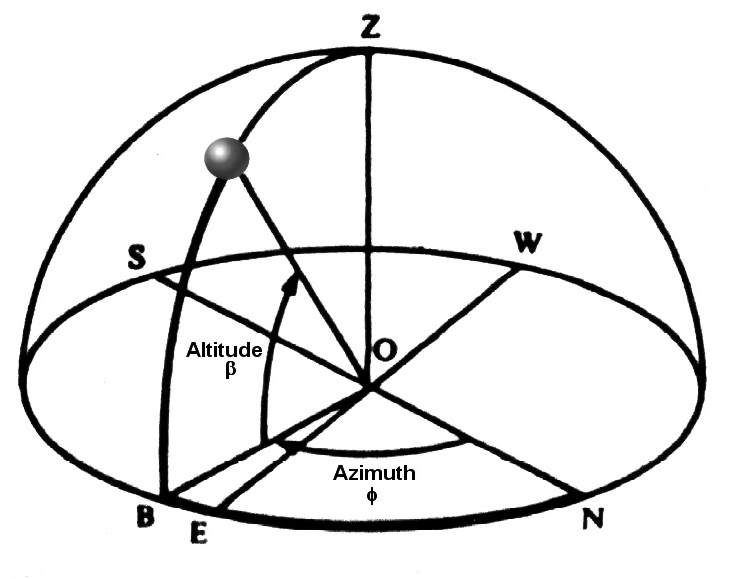
\includegraphics[width=0.9\textwidth, height=0.9\textheight, keepaspectratio=true]{media/image020.png}
\caption{Solar Position Illustration \protect \label{fig:solar-position-illustration}}
\end{figure}

\paragraph{Site Solar Altitude Angle {[}deg{]}}\label{site-solar-altitude-angle-deg}

The Solar Altitude Angle (b) is the angle of the sun above the horizontal (degrees).

\paragraph{Site Solar Hour Angle {[}deg{]}}\label{site-solar-hour-angle-deg}

The Solar Hour Angle (\emph{H}) gives the apparent solar time for the current time period (degrees). It is common astronomical practice to express the hour angle in hours, minutes and seconds of time rather than in degrees. You can convert the hour angle displayed from EnergyPlus to time by dividing by 15. (Note that 1 hour is equivalent to 15 degrees; 360° of the Earth's rotation takes place every 24 hours.) The relationship of angles in degrees to time is shown in the following table:

% table 6
\begin{longtable}[c]{@{}ll@{}}
\caption{Relationship of Angles (degrees) to Time \label{table:relationship-of-angles-degrees-to-time}} \tabularnewline
\toprule 
Unit of Angle & Equivalent time \tabularnewline
\midrule
\endfirsthead

\caption[]{Relationship of Angles (degrees) to Time} \tabularnewline
\toprule 
Unit of Angle & Equivalent time \tabularnewline
\midrule
\endhead

1 radian & 3.819719 hours \tabularnewline
1 degree & 4 minutes \tabularnewline
1 arcmin & 4 seconds \tabularnewline
1 arcsec & 0.066667 seconds \tabularnewline
\bottomrule
\end{longtable}

\paragraph{Site Rain Status {[]}}\label{site-rain-status}

This field shows whether or not (1 = yes, 0 = no) the weather shows ``raining''. For a Design Day, one can denote rain for the entire day but not timestep by timestep. Weather files may indicate rain for a single time interval. This is an ``averaged'' field -- thus a 1 shown for a time period (e.g. daily reporting) means that it was raining during each timestep of that period.

\paragraph{Site Snow on Ground Status {[]}}\label{site-snow-on-ground-status}

This field shows whether or not (1 = yes, 0 = no) the weather shows ``snow on the ground''. For a Design Day, one can denote snow for the entire day but not timestep by timestep. Weather files may indicate snow (snow depth) for a single time interval. This is an ``averaged'' field -- thus a 1 shown for a time period (e.g. daily reporting) means that there was snow on the ground during each timestep of that period.

\paragraph{Site Daylight Saving Time Status {[]}}\label{site-daylight-saving-time-status}

This field shows when daylight saving time (1 = yes, 0 = no) is in effect. Though shown as an average variable, this value is only set on a daily basis.

\paragraph{Site Day Type Index {[]}}\label{site-day-type-index}

This field shows what ``day type'' the current day is. Day types are (1 = Sunday, 2 = Monday, etc.) with Holiday = 8, SummerDesignDay = 9, WinterDesignDay = 10, CustomDay1 = 11, CustomDay2 = 12. Though shown as an average variable, this value is only set on a daily basis.

\paragraph{Site Mains Water Temperature {[}C{]}}\label{site-mains-water-temperature-c}

The value of the Water Mains Temperature is reported in C following the calculation shown in the Water Mains Temperature object.

\paragraph{Site Precipitation Rate {[}m/s{]}}\label{site-precipitation-rate-ms}

\paragraph{Site Precipitation Depth {[}m{]}}\label{site-precipitation-depth-m-1}

The rate and quantity of precipitation at the site. These outputs are only available if a Site Precipitation object is used. Precipitation is measured in meters.

\paragraph{Water System Roof Irrigation Scheduled Depth{[}m{]}}\label{water-system-roof-irrigation-scheduled-depthm}

This is the scheduled amount of irrigation for the green roof (ecoroof) based on the user input. Amount is measured in meters.

\paragraph{Water System Roof Irrigation Actual Depth{[}m{]}}\label{water-system-roof-irrigation-actual-depthm}

This is the actual amount of irrigation for the green roof (ecoroof) based on the scheduled user input and moisture state/saturation of the soil. Amount is measured in meters.

\subsection{Outputs for local temperature/wind speed calculations}\label{outputs-for-local-temperaturewind-speed-calculations}

Local atmospheric properties for outdoor air temperature and wind speed are separately calculated and reported for all zones, surfaces, and outdoor air nodes. The output variables are associated with their respective objects:

\begin{itemize}
\item
  Zone,Average,Zone Outdoor Air Drybulb Temperature {[}C{]}
\item
  Zone,Average,Zone Outdoor Air Wetbulb Temperature {[}C{]}
\item
  Zone,Average,Zone Outdoor Air Wind Speed {[}m/s{]}
\item
  Zone,Average,Surface Ext Outdoor Dry Bulb {[}C{]}
\item
  Zone,Average,Surface Ext Outdoor Wet Bulb {[}C{]}
\item
  Zone,Average,Surface Ext Wind Speed {[}m/s{]}
\item
  HVAC,Average,System Node Temperature {[}C{]}~~~~~~~ (for OUTDOOR AIR NODE object)
\end{itemize}

\subsubsection{Zone Outdoor Air Drybulb Temperature {[}C{]}}\label{zone-outdoor-air-drybulb-temperature-c}

The outdoor air dry-bulb temperature calculated at the height above ground of the zone centroid.

\subsubsection{Zone Outdoor Air Wetbulb Temperature {[}C{]}}\label{zone-outdoor-air-wetbulb-temperature-c}

The outdoor air wet-bulb temperature calculated at the height above ground of the zone centroid.

\subsubsection{Zone Outdoor Air Wind Speed {[}m/s{]}}\label{zone-outdoor-air-wind-speed-ms}

The outdoor wind speed calculated at the height above ground of the zone centroid.

\subsubsection{Surface Ext Outdoor Dry Bulb {[}C{]}}\label{surface-ext-outdoor-dry-bulb-c}

The outdoor air dry-bulb temperature calculated at the height above ground of the surface centroid.

\subsubsection{Surface Ext Outdoor Wet Bulb {[}C{]}}\label{surface-ext-outdoor-wet-bulb-c}

The outdoor air wet-bulb temperature calculated at the height above ground of the surface centroid.

\subsubsection{Surface Ext Wind Speed {[}m/s{]}}\label{surface-ext-wind-speed-ms}

The outdoor wind speed calculated at the height above ground of the surface centroid.

\subsubsection{System Node Temperature {[}C{]}}\label{system-node-temperature-c}

When reporting for the \textbf{OutdoorAir:Node} object, this is the outdoor air dry-bulb temperature calculated at the height above ground of the node, if height is specified in the input.


\section{Group -- Schedules}\label{group-schedules}

This group of objects allows the user to influence scheduling of many items (such as occupancy density, lighting, thermostatic controls, occupancy activity). In addition, schedules are used to control shading element density on the building.

EnergyPlus schedules consist of three pieces: a day description, a week description, and an annual description. An optional element is the schedule type. Each description level builds off the previous sub-level. The day description is simply a name and the values that span the 24 hours in a day to be associated with that name. The week description also has an identifier (name) and twelve additional names corresponding to previously defined day descriptions. There are names for each individual day of the week plus holiday, summer design day, winter design day and two more custom day designations. Finally, the annual schedule contains an identifier and the names and FROM-THROUGH dates of the week schedules associate with this annual schedule. The annual schedule can have several FROM-THROUGH date pairs. One type of schedule reads the values from an external file to facilitate the incorporation of monitored data or factors that change throughout the year.

Schedules are processed by the EnergyPlus Schedule Manager, stored within the Schedule Manager and are accessed through module routines to get the basic values (timestep, hourly, etc). Values are resolved at the Zone Timestep frequency and carry through any HVAC timesteps.

\subsection{Day Type}\label{day-type}

A brief description of ``Day Type'' which is used in the SizingPeriod objects, RunPeriodControl:SpecialDays object, the Sizing objects and also used by reference in the Schedule:Week:Daily object (discussed later in this section).

Schedules work on days of the week as well as certain specially designated days. Days of the week are the normal -- Sunday, Monday, Tuesday, Wednesday, Thursday, Friday and Saturday. Special day types that can be designated are: Holiday, SummerDesignDay, WinterDesignDay, CustomDay1, CustomDay2. These day types can be used at the user's convenience to designate special scheduling (e.g.~lights, electric equipment, set point temperatures) using these days as reference.

For example, a normal office building may have normal ``occupancy'' rules during the weekdays but significantly different use on weekend. For this, you would set up rules/schedules based on the weekdays (Monday through Friday, in the US) and different rules/schedules for the weekend (Saturday and Sunday, in the US). However, you could also specially designate SummerDesignDay and WinterDesignDay schedules for sizing calculations. These schedules can be activated by setting the Day Type field in the Design Day object to the appropriate season (\textbf{SummerDesignDay} for cooling design calculations; \textbf{WinterDesignDay} for heating design calculations).

In a different building, such as a theater/playhouse, the building may only have occupancy during certain weeks of the year and/or certain hours of certain days. If it was every week, you could designate the appropriate values during the ``regular'' days (Sunday through Saturday). But this would also be an ideal application for the ``CustomDay1'' and/or ``CustomDay2''. Here you would set the significant occupancy, lighting, and other schedules for the custom days and use unoccupied values for the normal weekdays. Then, using a weather file and setting special day periods as appropriate, you will get the ``picture'' of the building usage during the appropriate periods.

\subsection{ScheduleTypeLimits}\label{scheduletypelimits}

Schedule types can be used to validate portions of the other schedules. Hourly day schedules, for example, are validated by range -- minimum/maximum (if entered) -- as well as numeric type (continuous or discrete). Annual schedules, on the other hand, are only validated for range -- as the numeric type validation has already been done.

\subsubsection{Inputs}\label{inputs-042}

\paragraph{Field: Name}\label{field-name-041}

This alpha field should contain a unique (within the schedule types) designator. It is referenced wherever Schedule Type Limits Names can be referenced.

\paragraph{Field: Lower Limit Value}\label{field-lower-limit-value}

In this field, the lower (minimum) limit value for the schedule type should be entered. If this field is left blank, then the schedule type is not limited to a minimum/maximum value range.

\paragraph{Field: Upper Limit Value}\label{field-upper-limit-value}

In this field, the upper (maximum) limit value for the schedule type should be entered. If this field is left blank, then the schedule type is not limited to a minimum/maximum value range.

\paragraph{Field: Numeric Type}\label{field-numeric-type}

This field designates how the range values are validated. Using \textbf{Continuous} in this field allows for all numbers, including fractional amounts, within the range to be valid. Using \textbf{Discrete} in this field allows only integer values between the minimum and maximum range values to be valid.

\paragraph{Field: Unit Type}\label{field-unit-type}

This field is used to indicate the kind of units that may be associated with the schedule that references the ScheduleTypeLimits object. It is used by IDF Editor to display the appropriate SI and IP units. This field is not used by EnergyPlus. The available options are shown below. If none of these options are appropriate, select \textbf{Dimensionless.}

\begin{itemize}
\item
  Dimensionless
\item
  Temperature
\item
  DeltaTemperature
\item
  PrecipitationRate
\item
  Angle
\item
  Convection Coefficient
\item
  Activity Level
\item
  Velocity
\item
  Capacity
\item
  Power
\item
  Availability
\item
  Percent
\item
  Control
\item
  Mode
\end{itemize}

Several IDF Examples will illustrate the use:

\begin{lstlisting}
ScheduleTypeLimits,Any Number;  ! Not limited
ScheduleTypeLimits,Fraction, 0.0 , 1.0 ,CONTINUOUS;
ScheduleTypeLimits,Temperature,-60,200,CONTINUOUS;
ScheduleTypeLimits,Control Type,0,4,DISCRETE;
ScheduleTypeLimits,On/Off,0,1,DISCRETE;
\end{lstlisting}

\subsection{Day Schedules}\label{day-schedules}

The day schedules perform the assignment of pieces of information across a 24 hour day. This can occur in various fashions including a 1-per hour assignment, a user specified interval scheme or a list of values that represent an hour or portion of an hour.

\subsection{Schedule:Day:Hourly}\label{scheduledayhourly}

The Schedule:Day:Hourly contains an hour-by-hour profile for a single simulation day.

\subsubsection{Inputs}\label{inputs-1-039}

\paragraph{Field: Name}\label{field-name-1-038}

This field should contain a unique (within all DaySchedules) designation for this schedule. It is referenced by WeekSchedules to define the appropriate schedule values.

\paragraph{Field: Schedule Type Limits Name}\label{field-schedule-type-limits-name-000}

This field contains a reference to the Schedule Type Limits object. If found in a list of Schedule Type Limits (see ScheduleTypeLimits object above), then the restrictions from the referenced object will be used to validate the hourly field values (below).

\paragraph{Field: Hour Values (1-24)}\label{field-hour-values-1-24}

These fields contain the hourly values for each of the 24 hours in a day. (Hour field 1 represents clock time 00:00:01 AM to 1:00:00 AM, hour field 2 is 1:00:01 AM to 2:00:00 AM, etc.) The values in these fields will be passed to the simulation as indicated for ``scheduled'' items.

An IDF example:

\begin{lstlisting}
Schedule:Day:Hourly, Day On Peak, Fraction,
  0.,0.,0.,0.,0.,0.,0.,0.,0.,1.,1.,1.,1.,1.,1.,1.,1.,1.,0.,0.,0.,0.,0.,0.;
\end{lstlisting}

\subsection{Schedule:Day:Interval}\label{scheduledayinterval}

The Schedule:Day:Interval introduces a slightly different way of entering the schedule values for a day. Using the intervals, you can shorten the ``hourly'' input of the ``Schedule:Day:Hourly'' object to 2 fields. And, more importantly, you can enter an interval that represents only a portion of an hour. Schedule values are ``given'' to the simulation at the zone timestep, so there is also a possibility of ``interpolation'' from the entries used in this object to the value used in the simulation.

\subsubsection{Inputs}\label{inputs-2-036}

\paragraph{Field: Name}\label{field-name-2-034}

This field should contain a unique (within all DaySchedules) designation for this schedule. It is referenced by WeekSchedules to define the appropriate schedule values.

\paragraph{Field: Schedule Type Limits Name}\label{field-schedule-type-limits-name-1-000}

This field contains a reference to the Schedule Type Limits object. If found in a list of Schedule Type Limits (see ScheduleTypeLimits object above), then the restrictions from the referenced object will be used to validate the hourly field values (below).

\paragraph{Field: Interpolate to Timestep}\label{field-interpolate-to-timestep}

The value contained in this field directs how to apply values that aren't coincident with the given timestep (ref: Timestep) intervals. If ``Yes'' is entered, then any intervals entered here will be interpolated/averaged and that value will be used at the appropriate minute in the hour. If ``No'' is entered, then the value that occurs on the appropriate minute in the hour will be used as the schedule value.

For example, if ``yes'' is entered and the interval is every 15 minutes (say a value of 0 for the first 15 minutes, then .5 for the second 15 minutes) AND there is a 10 minute timestep for the simulation: the value at 10 minutes will be 0 and the value at 20 minutes will be .25. For the same input entries but ``no'' for this field, the value at 10 minutes will be 0 and the value at 20 minutes will be .5.

\paragraph{Field-Set: Time and Value (extensible object)}\label{field-set-time-and-value-extensible-object}

To specify each interval, both an ``until'' time (which includes the designated time) and the value must be given.

\paragraph{Field: Time}\label{field-time}

The value of each field should represent clock time (standard) in the format ``Until: HH:MM''. 24 hour clock format (i.e.~1PM is 13:00) is used. Note that Until: 7:00 includes all times up through 07:00 or 7am.

\paragraph{Field: Value}\label{field-value}

This represents the actual value to be passed to the simulation at the appropriate timestep. (Using interpolation value as shown above). Limits on the values are indicated by the Schedule Type Limits Name field of this object.

And an example of use:

\begin{lstlisting}
Schedule:Day:Interval,
  dd winter rel humidity, !- Name
  Percent,                !- Schedule Type Limits Name
  No,                     !- Interpolate to Timestep
  until: 24:00,           !- Time 1
  74;                     !- Value Until Time 1
\end{lstlisting}

\subsection{Schedule:Day:List}\label{scheduledaylist}

To facilitate possible matches to externally generated data intervals, this object has been included. In similar fashion to the Schedule:Day:Interval object, this object can also include ``sub-hourly'' values but must represent a complete day in its list of values.

\subsubsection{Inputs}\label{inputs-3-032}

\paragraph{Field: Name}\label{field-name-3-028}

This field should contain a unique (within all day schedules) designation for this schedule. It is referenced by week schedules to define the appropriate schedule values.

\paragraph{Field: Schedule Type Limits Name}\label{field-schedule-type-limits-name-2-000}

This field contains a reference to the Schedule Type Limits object. If found in a list of Schedule Type Limits (see ScheduleTypeLimits object above), then the restrictions from the referenced object will be used to validate the hourly field values (below).

\paragraph{Field: Interpolate to Timestep}\label{field-interpolate-to-timestep-1}

The value contained in this field directs how to apply values that aren't coincident with the given timestep (ref: Timestep) intervals. If ``Yes'' is entered, then any intervals entered here will be interpolated/averaged and that value will be used at the appropriate minute in the hour. If ``No'' is entered, then the value that occurs on the appropriate minute in the hour will be used as the schedule value.

For example, if ``yes'' is entered and the minutes per item is 15 minutes (say a value of 0 for the first 15 minutes, then .5 for the second 15 minutes) AND there is a 10 minute timestep for the simulation: the value at 10 minutes will be 0 and the value at 20 minutes will be .25. For the same input entries but ``no'' for this field, the value at 10 minutes will be 0 and the value at 20 minutes will be .5.

\paragraph{Field: Minutes Per Item}\label{field-minutes-per-item}

This field allows the ``list'' interval to be specified in the number of minutes for each item. The value here must be \textless{} = 60 and evenly divisible into 60 (same as the timestep limits).

\paragraph{Field Value 1 (same definition for each value -- up to 1440 (24*60) allowed)}\label{field-value-1-same-definition-for-each-value-up-to-1440-2460-allowed}

This is the value to be used for the specified number of minutes.

For example:

\begin{lstlisting}
Schedule:Day:List,
  Myschedule, ! name
  Fraction,   ! Schedule type
  No,         ! Interpolate value
  30,         ! Minutes per item
  0.0,        ! from 00:01 to 00:30
  0.5,        ! from 00:31 to 01:00
  <snipped>
\end{lstlisting}

\subsection{Week Schedule(s)}\label{week-schedules}

The week schedule object(s) perform the task of assigning the day schedule to day types in the simulation. The basic week schedule is shown next.

\subsection{Schedule:Week:Daily}\label{scheduleweekdaily}

\subsubsection{Inputs}\label{inputs-4-029}

\paragraph{Field: Name}\label{field-name-4-025}

This field should contain a unique (within all WeekSchedules) designation for this schedule. It is referenced by Schedules to define the appropriate schedule values.

\paragraph{Field: Schedule Day Name Fields (12 day types -- Sunday, Monday, \ldots{} )}\label{field-schedule-day-name-fields-12-day-types-sunday-monday}

These fields contain day schedule names for the appropriate day types. Days of the week (or special days as described earlier) will then use the indicated hourly profile as the actual schedule value.

An IDF example:

\begin{lstlisting}
Schedule:Week:Daily, Week on Peak,
  Day On Peak,Day On Peak,Day On Peak,
  Day On Peak,Day On Peak,Day On Peak,
  Day On Peak,Day On Peak,Day On Peak,
  Day On Peak,Day On Peak,Day On Peak;
\end{lstlisting}

\subsection{Schedule:Week:Compact}\label{scheduleweekcompact}

Further flexibility can be realized by using the Schedule:Week:Compact object. In this the fields, after the name is given, a ``for'' field is given for the days to be assigned and then a dayschedule name is used.

\subsubsection{Inputs}\label{inputs-5-026}

\paragraph{Field:Name}\label{fieldname}

This field should contain a unique (within all WeekSchedules) designation for this schedule. It is referenced by Schedules to define the appropriate schedule values.

\paragraph{Field-Set -- DayType List\#, Schedule:Day Name \#}\label{field-set-daytype-list-scheduleday-name}

Each assignment is made in a pair-wise fashion. First the ``days'' assignment and then the dayschedule name to be assigned. The entire set of day types must be assigned or an error will result.

\paragraph{Field: DayType List \#}\label{field-daytype-list}

This field can optionally contain the prefix ``For'' for clarity. Multiple choices may then be combined on the line. Choices are: Weekdays, Weekends, Holidays, Alldays, SummerDesignDay, WinterDesignDay, Sunday, Monday, Tuesday, Wednesday, Thursday, Friday, Saturday, CustomDay1, CustomDay2. In fields after the first ``for'', AllOtherDays may also be used. Note that the colon (:) after the For is optional but is suggested for readability.

\paragraph{Field: Schedule:Day Name \#}\label{field-scheduleday-name}

This field contains the name of the day schedule (any of the Schedule:Day object names) that is to be applied for the days referenced in the prior field.

Some IDF examples:

\begin{lstlisting}
Schedule:Week:Compact, Week on Peak,
  For: AllDays,
  Day On Peak;

Schedule:Week:Compact, WeekDays on Peak,
  WeekDays,
  Day On Peak,
  AllOtherDays
  Day Off Peak;
\end{lstlisting}

\subsection{Schedule:Year}\label{scheduleyear}

The yearly schedule is used to cover the entire year using references to week schedules (which in turn reference day schedules). If the entered schedule does not cover the entire year, a fatal error will result.

\subsubsection{Inputs}\label{inputs-6-023}

\paragraph{Field: Name}\label{field-name-5-021}

This field should contain a unique (between Schedule:Year, Schedule:Compact, and Schedule:File) designation for the schedule. It is referenced by various ``scheduled'' items (e.g.~Lights, People, Infiltration) to define the appropriate schedule values.

\paragraph{Field: Schedule Type Limits Name}\label{field-schedule-type-limits-name-3}

This field contains a reference to the Schedule Type Limits object. If found in a list of Schedule Type Limits (see ScheduleTypeLimits object above), then the restrictions from the referenced object will be used to validate the hourly field values (below).

\paragraph{Field Set (WeekSchedule, Start Month and Day, End Month and Day)}\label{field-set-weekschedule-start-month-and-day-end-month-and-day}

Each of the designated fields is used to fully define the schedule values for the indicated time period). Up to 53 sets can be used. An error will be noted and EnergyPlus will be terminated if an incomplete set is entered. Missing time periods will also be noted as warning errors; for these time periods a zero (0.0) value will be returned when a schedule value is requested. Each of the sets has the following 5 fields:

\paragraph{Field: Schedule Week Name \#}\label{field-schedule-week-name}

This field contains the appropriate WeekSchedule name for the designated time period.

\paragraph{Field: Start Month \#}\label{field-start-month}

This numeric field is the starting month for the schedule time period.

\paragraph{Field: Start Day \#}\label{field-start-day}

This numeric field is the starting day for the schedule time period.

\paragraph{Field: End Month \#}\label{field-end-month-000}

This numeric field is the ending month for the schedule time period.

\paragraph{Field: End Day \#}\label{field-end-day}

This numeric field is the ending day for the schedule time period.

Note that there are many possible periods to be described. An IDF example with a single period:

\begin{lstlisting}
Schedule:Year, On Peak, Fraction,
  Week On Peak, 1,1, 12,31;
\end{lstlisting}

And a multiple period illustration:

\begin{lstlisting}
Schedule:Year,CoolingCoilAvailSched,Fraction,
  FanAndCoilAllOffWeekSched, 1,1, 3,31,
  FanAndCoilSummerWeekSched, 4,1, 9,30,
  FanAndCoilAllOffWeekSched, 10,1, 12,31;
\end{lstlisting}

The following definition will generate an error (if any scheduled items are used in the simulation):

\begin{lstlisting}
Schedule:Year,MySchedule,Fraction,4,1,9,30;
\end{lstlisting}

\subsection{Schedule:Compact}\label{schedulecompact}

For flexibility, a schedule can be entered in ``one fell swoop''. Using the Schedule:Compact object, all the features of the schedule components are accessed in a single command. Like the ``regular'' schedule object, each schedule:compact entry must cover all the days for a year. Additionally, the validations for DaySchedule (i.e.~must have values for all 24 hours) and WeekSchedule (i.e.~must have values for all day types) will apply. Schedule values are ``given'' to the simulation at the zone timestep, so there is also a possibility of ``interpolation'' from the entries used in this object to the value used in the simulation.

This object is an unusual object for description. For the data the number of fields and position are not set, they cannot really be described in the usual Field \# manner. Thus, the following description will list the fields and order in which they must be used in the object. The name and schedule type are the exceptions:

\subsubsection{Inputs}\label{inputs-7-023}

\paragraph{Field: Name}\label{field-name-6-019}

This field should contain a unique (between Schedule:Year, Schedule:Compact, and Schedule:File) designation for the schedule. It is referenced by various ``scheduled'' items (e.g.~Lights, People, Infiltration) to define the appropriate schedule values.

\paragraph{Field: Schedule Type Limits Name}\label{field-schedule-type-limits-name-4}

This field contains a reference to the Schedule Type Limits object. If found in a list of Schedule Type Limits (see ScheduleTypeLimits object above), then the restrictions from the referenced object will be used to validate the hourly field values (below).

\paragraph{Field-Set (Through, For, Interpolate, Until, Value)}\label{field-set-through-for-interpolate-until-value}

Each compact schedule must contain the elements Through (date), For (days), Interpolate (optional), Until (time of day) and Value. In general, each of the ``titled'' fields must include the ``title''. Note that the colon (:) after these elements (Through, For, Until) is optional but is suggested for readability.

\paragraph{Field: Through}\label{field-through}

This field starts with ``Through:'' and contains the ending date for the schedule period (may be more than one). Refer to Table~\ref{table:date-field-interpretation}. Date Field Interpretation for information on date entry -- note that only Month-Day combinations are allowed for this field. Each ``through'' field generates a new WeekSchedule named ``Schedule Name''\_wk\_\# where \# is the sequential number for this compact schedule.

\paragraph{Field: For}\label{field-for}

This field starts with ``For:'' and contains the applicable days (reference the compact week schedule object above for complete description) for the 24 hour period that must be described. Each ``for'' field generates a new DaySchedule named ``Schedule Name''\_dy\_\# where \# is the sequential number for this compact schedule.

\paragraph{Field: Interpolate (optional)}\label{field-interpolate-optional}

This field, if used, starts with ``Interpolate:'' and contains the word ``Yes'' or ``No''. If this field is not used, it should not be blank -- rather just have the following field appear in this slot. The definition of ``Interpolate'' in this context is shown in the interval day schedule above.

\paragraph{Field: Until}\label{field-until}

This field contains the ending time (again, reference the interval day schedule discussion above) for the current days and day schedule being defined.

\paragraph{Field: Value}\label{field-value-1}

Finally, the value field is the schedule value for the specified time interval.

And, some IDF examples:

\begin{lstlisting}
Schedule:Compact,
  POFF,       !- Name
  Fraction,   !- Schedule Type Limits Name
  Through: 4/30,
  For: AllDays,
  Until: 24:00, 1.0,
  Through: 12/31,
  For: Weekdays,
    Until: 7:00,   .1,
    Until: 17:00, 1.0,
    Until: 24:00,  .1,
  For: Weekends Holidays,
    Until: 24:00,  .1,
  For: AllOtherDays,
    Until: 24:00,  .1;

! Schedule Continuous
Schedule:Compact,
  Continuous,
  on/off,
  Through: 12/31,
  For: AllDays,
    Until: 24:00, 1.0;

! Schedule Daytime Ventilation
Schedule:Compact,
  Daytime Ventilation,
  Fraction,
  Through: 12/31,
  For: Weekdays SummerDesignDay,
    Until: 08:00, 0.0,
    Until: 18:00, 1.0,
    Until: 24:00, 0.0,
  For: Weekends WinterDesignDay,
    Until: 10:00, 0.0,
    Until: 16:00, 1.0,
    Until: 24:00, 0.0,
  For: Holidays AllOtherDays,
    Until: 24:00, 0.0;
\end{lstlisting}

\subsection{Schedule:Constant}\label{scheduleconstant}

The constant schedule is used to assign a constant hourly value. This schedule is created when a fixed hourly value is desired to represent a period of interest (e.g., always on operation mode for supply air fan).

\subsubsection{Inputs}\label{inputs-8-021}

\paragraph{Field: Name}\label{field-name-7-018}

This field should contain a unique name designation for this schedule. It is referenced by Schedules to define the appropriate schedule value.

\paragraph{Field: Schedule Type Limits Name}\label{field-schedule-type-limits-name-5}

This field contains a reference to the Schedule Type Limits object. If found in a list of Schedule Type Limits (see ScheduleTypeLimits object above), then the restrictions from the referenced object will be used to validate the hourly field values (below).

\paragraph{Field: Hourly Value}\label{field-hourly-value}

This field contains a constant real value. A fixed value is assigned as an hourly value.

An IDF example:

\begin{lstlisting}
Schedule:Constant,
  AlwaysOn,     !- Name
  On/Off,       !- Schedule Type Limits Name
  1.0;          !- Hourly Value

ScheduleTypeLimits,
  On/Off,       !- Name
  0,            !- Lower Limit Value
  1,            !- Upper Limit Value
  DISCRETE,     !- Numeric Type
  Availability; !- Unit Type
\end{lstlisting}

\subsection{Schedule:File}\label{schedulefile}

At times, data is available from a building being monitored or for factors that change throughout the year. The Schedule:File object allows this type of data to be used in EnergyPlus as a schedule. Schedule:File can also be used to read in hourly or sub-hourly schedules computed by other software or developed in a spreadsheet or other utility.

The format for the data file referenced is a text file with values separated by commas (or other optional delimiters) with one line per hour. The file may contain header lines that are skipped. The file should contain values for an entire year (8760 or 8784 hours of data) or a warning message will be issued. Multiple schedules may be created using a single external data file or multiple external data files may be used. The first row of data must be for January 1, hour 1 (or timestep 1 for subhourly files).

Schedule:File may be used along with the FuelFactors object and TDV files in the DataSets directory to compute Time Dependent Valuation based source energy as used by the California Energy Commission's Title 24 Energy Code. See Fuel Factor for more discussion on Time Dependent Valuation.

Two optional fields: \textbf{Interpolate to Timestep} and \textbf{Minutes per Item} allow for the input of sub-hourly schedules (similar to the Schedule:Day:List object).

\subsubsection{Inputs}\label{inputs-9-019}

\paragraph{Field: Name}\label{field-name-8-018}

This field should contain a unique (between Schedule:Year, Schedule:Compact, and Schedule:File) designation for the schedule. It is referenced by various ``scheduled'' items (e.g.~Lights, People, Infiltration, FuelFactors) to define the appropriate schedule values.

\paragraph{Field: Schedule Type Limits Name}\label{field-schedule-type-limits-name-6}

This field contains a reference to the Schedule Type Limits object. If found in a list of Schedule Type Limits (see ScheduleTypeLimits object above), then the restrictions from the referenced object will be used to validate the hourly field values (below).

\paragraph{Field: File Name}\label{field-file-name}

This field contains the name of the file that contains the data for the schedule. The field should include a full path with file name, for best results. The field must be \(\le\) 100 characters. The file name must not include commas or an exclamation point. A relative path or a simple file name should work with version 7.0 or later when using EP-Launch even though EP-Launch uses temporary directories as part of the execution of EnergyPlus. If using RunEPlus.bat to run EnergyPlus from the command line, a relative path or a simple file name may work if RunEPlus.bat is run from the folder that contains EnergyPlus.exe.

\paragraph{Field: Column Number}\label{field-column-number}

The column that contains the value to be used in the schedule. The first column is column one. If no data for a row appears for a referenced column the value of zero is used for the schedule value for that hour.

\paragraph{Field: Rows to Skip at Top}\label{field-rows-to-skip-at-top}

Many times the data in a file contains rows (lines) that are describing the files or contain the names of each column. These rows need to be skipped and the number of skipped rows should be entered for this field. The next row after the skipped rows must contain data for January 1, hour 1.

\paragraph{Field: Number of Hours of Data}\label{field-number-of-hours-of-data}

The value entered in this field should be either 8760 or 8784 as the number of hours of data. 8760 does not include the extra 24 hours for a leap year (if needed). 8784 will include the possibility of leap year data which can be processed according to leap year indicators in the weather file or specified elsewhere. Note if the simulation does not have a leap year specified but the schedule file contains 8784 hours of data, the first 8760 hours of data will be used. The schedule manager will not know to skip the 24 hours representing February 29.

\paragraph{Field: Column Separator}\label{field-column-separator-001}

This field specifies the character used to separate columns of data if the file has more than one column. The choices are: Comma, Tab, Fixed (spaces fill each column to a fixed width), or Semicolon. The default is Comma.

\paragraph{Field: Interpolate to Timestep}\label{field-interpolate-to-timestep-2}

The value contained in this field directs how to apply values that aren't coincident with the given timestep (ref: TimeStep object) intervals. If ``Yes'' is entered, then any intervals entered here will be interpolated/averaged and that value will be used at the appropriate minute in the hour. If ``No'' is entered, then the value that occurs on the appropriate minute in the hour will be used as the schedule value.

For example, if ``yes'' is entered and the minutes per item is 15 minutes (say a value of 0 for the first 15 minutes, then .5 for the second 15 minutes) AND there is a 10 minute timestep for the simulation: the value at 10 minutes will be 0 and the value at 20 minutes will be .25. For the same input entries but ``no'' for this field, the value at 10 minutes will be 0 and the value at 20 minutes will be .5.

\paragraph{Field: Minutes Per Item}\label{field-minutes-per-item-1}

This field represents the number of minutes for each item -- in this case each line of the file. The value here must be \(\le\) 60 and evenly divisible into 60 (same as the timestep limits).

Here is an IDF example:

\begin{lstlisting}
Schedule:File,
  elecTDVfromCZ01res, !- Name
  Any Number,         !- ScheduleType
  TDV_kBtu_CTZ01.csv, !- Name of File
  2,                  !- Column Number
  4,                  !- Rows to Skip at Top
  8760,               !- Number of Hours of Data
  Comma;              !- Column Separator
\end{lstlisting}

or with a relational path:

\begin{lstlisting}
Schedule:File,
  elecTDVfromCZ01res, !- Name
  Any Number,         !- ScheduleType
  DataSets\TDV\TDV_kBtu_CTZ01.csv,  !- Name of File
  2,                  !- Column Number
  4;                  !- Rows to Skip at Top
\end{lstlisting}

A sub-hourly indication. Note that this is identical to an hourly file because there are 60 minutes per item -- the number of hours defaults to 8760 and the column separator defaults to a comma. If the number of minutes per item had been, say, 15, then the file would need to contain 8760*4 or 35,040 rows for this item.

\begin{lstlisting}
Schedule:File,
  elecTDVfromCZ06com, !- Name
  Any Number,         !- Schedule Type Limits Name
  DataSets\TDV\TDV_2008_kBtu_CTZ06.csv, !- File Name
  1,                  !- Column Number
  4,                  !- Rows to Skip at Top
  ,                   !- Number of Hours of Data
  ,                   !- Column Separator
  ,                   !- Interpolate to Timestep
  60;                 !- Minutes per Item
\end{lstlisting}

\subsubsection{Outputs}\label{outputs-031}

An optional report can be used to gain the values described in the previous Schedule objects. This is a condensed reporting that illustrates the full range of schedule values -- in the style of input: DaySchedule, WeekSchedule, Annual Schedule.

\begin{lstlisting}
! will give them on hourly increments (day schedule resolution)
Output:Reports, Schedules, Hourly;
! will give them at the timestep of the simulation
Output:Reports, Schedules, Timestep;
\end{lstlisting}

This report is placed on the eplusout.eio file. Details of this reporting are shown in the Output Details and Examples document.

\paragraph{Schedule Value Output}\label{schedule-value-output}

\begin{lstlisting}
Zone,Average,Schedule Value {[]}
\end{lstlisting}

\paragraph{Schedule Value}\label{schedule-value}

This is the schedule value (as given to whatever entity that uses it). It has no units in this context because values may be many different units (i.e.~temperatures, fractions, watts). For best results, you may want to apply the schedule name when you use this output variable to avoid output proliferation. For example, the following reporting should yield the values shown above, depending on day of week and day type:

\begin{lstlisting}
Output:Variable,People_Shopping_Sch,Schedule Value,hourly;
Output:Variable,Activity_Shopping_Sch,Schedule Value,hourly;
\end{lstlisting}



\section{Group -- Surface Construction Elements}\label{group-surface-construction-elements}

This group of objects describes the physical properties and configuration for the building envelope and interior elements. That is, the walls, roofs, floors, windows, doors for the building.

\subsection{Specifying the Building Envelope}\label{specifying-the-building-envelope}

Building element constructions in EnergyPlus are built from the basic thermal and other material property parameters in physical constructions. Materials are specified by types~ and named. Constructions are defined by the composition of materials. Finally, surfaces are specified for the building with geometric coordinates as well as referenced constructions.

\subsection{Material and Material Properties}\label{material-and-material-properties}

There are several material ``types'' which may be used to describe layers within opaque construction elements. The choice of which of these types to use is left up to the user. However, some guidance as to which material type to use is appropriate before describing each in detail. The opaque types are:

\begin{itemize}
\item
  Material
\item
  Material:NoMass
\item
  Material:AirGap
\item
  Material:RoofVegetation
\item
  Material:InfraredTransparent
\end{itemize}

Material is the ``preferred'' type of material. This requires knowledge of many of the thermal properties of the material, but it allows EnergyPlus to take into account the thermal mass of the material and thus allows the evaluation of transient conduction effects. Material:NoMass is similar in nature but only requires the thermal resistance (R-value) rather than the thickness, thermal conductivity, density, and specific heat. Note that using a simple R-value only material forces EnergyPlus to assume steady state heat conduction through this material layer. Finally, Material:AirGap should only be used for an air gap between other layers in a construction. This type assumes that air is sufficiently lightweight to require only an R-value. In addition, since it is not exposed to any external environment, surface properties such as absorptance are not necessary. Material:RoofVegetation is used to help model ``green roofs''. Material:InfraredTransparent is used similarly to the NoMass materials. Each of these materials is described in more detail below.

There are several material additions that can be made to the basic material properties. These additional material types are:

\begin{itemize}
\item
  MaterialProperty:MoisturePenetrationDepth:Settings
\item
  Material\-Prop\-erty:\-Heat\-And\-Moisture\-Trans\-fer:\-Sorp\-tion\-Iso\-therm
\item
  MaterialProperty:HeatAndMoistureTransfer:Diffusion
\item
  MaterialProperty:HeatAndMoistureTransfer:Settings
\item
  Material\-Prop\-erty:\-Heat\-And\-Moisture\-Trans\-fer:\-Re\-dist\-ribu\-tion
\item
  MaterialProperty:HeatAndMoistureTransfer:Suction
\item
  Material\-Prop\-erty:\-Heat\-And\-Moisture\-Trans\-fer:\-Thermal\-Con\-ductivity
\item
  MaterialProperty:PhaseChange
\end{itemize}

These material property objects are used in conjunction with the basic material specification and reference back to the name of the basic material type. Without the basic material type specified the program, will give a severe error and terminate. For example, specifying the moisture materials and changing the HeatBalanceAlgorithm to a moisture simulation will allow the moisture simulation to take place.

\subsection{Material}\label{material}

This definition should be used when the four main thermal properties (thickness, conductivity, density, and specific heat) of the material are known. This syntax is used to describe opaque construction elements only.

When a Material is used for the Construction of a building surface, care should be taken to not attempt to model assemblies that were not included in the intended scope of applicability for the underlying heat transfer models.~ The building surface models are for normal applications to building energy efficiency where the main focus is on assemblies with some thermal resistance. Extremely thin and/or highly conductive material layers should be neglected from the Construction rather than included because they will not contribute to the assembly's overall thermal resistance or heat capacity. For some cases, thin and/or highly conductive materials are a serious problem for the heat transfer modeling and the values for thickness, conductivity, density and specific heat are checked for appropriateness. This check calculates the Material's thermal diffusivity from the inputs for conductivity, density, and specific heat and compares it to a maximum threshold of 1.E-5 (m\(^{2}\)/s). If the diffusivity is above this threshold, then the program checks if the layer is sufficiently thick and may issue a warning if it is too thin and highly conductive.

The absorptance values in this object impart surface properties to the construction and should be applied to the thermally significant inner and outer layers in the overall assembly.~ Attempting to trick the program by modeling thin ``paint'' layers to apply surface properties is not a good idea; the models were not intended to support such strategies.

\subsubsection{Inputs}\label{inputs-046}

\paragraph{Field: Name}\label{field-name-045}

This field is a unique reference name that the user assigns to a particular material. This name can then be referred to by other input data (ref: Construction object).

\paragraph{Field: Roughness}\label{field-roughness-000}

This alpha field defines the relative roughness of a particular material layer. This parameter only influences the convection coefficients, more specifically the exterior convection coefficient. A special keyword is expected in this field with the options being ``VeryRough'', ``Rough'', ``MediumRough'', ``MediumSmooth'', ``Smooth'', and ``VerySmooth'' in order of roughest to smoothest options.

\paragraph{Field: Thickness}\label{field-thickness}

This field characterizes the thickness of the material layer in meters. This should be the dimension of the layer in the direction perpendicular to the main path of heat conduction. This value must be a positive. \textbf{Modeling layers thinner (less) than 0.003 m is not recommended; rather, add those properties to one of the adjacent layers.}

\paragraph{Field: Conductivity}\label{field-conductivity}

This field is used to enter the thermal conductivity of the material layer. Units for this parameter are W/(m-K). Thermal conductivity must be greater than zero. \textbf{Modeling layers with conductivity higher than 5.0 W/(m-K) is not recommended; however, this may be appropriate for non-surfaces such as pipes and TDDs (ref. DaylightingDevice:Tubular object).}

\paragraph{Field: Density}\label{field-density}

This field is used to enter the density of the material layer in units of kg/m\(^{3}\). Density must be a positive quantity. \textbf{In some cases textbooks and references may use g/m\(^{3}\): be careful to not confuse units.}

\paragraph{Field: Specific Heat}\label{field-specific-heat}

This field represents the specific heat of the material layer in units of J/(kg-K). Note that these units are most likely different than those reported in textbooks and references which tend to use kJ/(kg-K) or J/(g-K). They were chosen for internal consistency within EnergyPlus. \textbf{Only values of specific heat of 100 or larger are allowed. Typical ranges are from 800 to 2000 J/(kg-K).}

\paragraph{Field: Thermal Absorptance}\label{field-thermal-absorptance}

The thermal absorptance field in the Material input syntax represents the fraction of incident long wavelength (>2.5 microns) radiation that is absorbed by the material. This parameter is used when calculating the long wavelength radiant exchange between various surfaces and affects the surface heat balances (both inside and outside as appropriate). For long wavelength radiant exchange, thermal emissivity and thermal emittance are equal to thermal absorptance. Values for this field must be between 0.0 and 1.0 (with 1.0 representing ``black body'' conditions). The default value for this field is 0.9.

\paragraph{Field: Solar Absorptance}\label{field-solar-absorptance}

The solar absorptance field in the Material input syntax represents the fraction of incident~ solar radiation that is absorbed by the material. Solar radiation (0.3 to 2.537 microns) includes the visible spectrum as well as infrared and ultraviolet wavelengths. This parameter is used when calculating the amount of incident solar radiation absorbed by various surfaces and affects the surface heat balances (both inside and outside as appropriate). If solar reflectance (or reflectivity) data is available, then absorptance is equal to 1.0 minus reflectance (for opaque materials). Values for this field must be between 0.0 and 1.0. The default value for this field is 0.7.

\paragraph{Field: Visible Absorptance}\label{field-visible-absorptance}

The visible absorptance field in the Material input syntax represents the fraction of incident visible wavelength radiation that is absorbed by the material. Visible wavelength radiation ( 0.37 to 0.78 microns weighted by photopic response) is slightly different than solar radiation in that the visible band of wavelengths is much more narrow while solar radiation includes the visible spectrum as well as infrared and ultraviolet wavelengths. This parameter is used when calculating the amount of incident visible radiation absorbed by various surfaces and affects the surface heat balances (both inside and outside as appropriate) as well as the daylighting calculations. If visible reflectance (or reflectivity) data is available, then absorptance is equal to 1.0 minus reflectance (for opaque materials). Values for this field must be between 0.0 and 1.0. The default value for this field is 0.7.

An IDF example:

\begin{lstlisting}

Material,A2 - 4 IN DENSE FACE BRICK,  ! Material Name
   Rough,  ! Roughness
    0.1014984    ,  ! Thickness {m}
     1.245296    ,   ! Conductivity {W/M*K}
     2082.400    ,   ! Density {Kg/M**3}
    920.4800    ,   ! Specific Heat {J/Kg*K}
    0.9000000    ,   ! Thermal Absorptance
    0.9300000    ,   ! Solar Absorptance
    0.9300000    ;   ! Visible Absorptance
\end{lstlisting}

\subsection{Material:NoMass}\label{materialnomass}

Use this definition when only the thermal resistance (R value) of the material is known. This object is used to describe opaque construction elements.

\subsubsection{Inputs}\label{inputs-1-043}

\paragraph{Field: Name}\label{field-name-1-042}

This field is a unique reference name that the user assigns to a particular material. This name can then be referred to by other input data (ref: Construction object).

\paragraph{Field: Roughness}\label{field-roughness-1}

This alpha field defines the relative roughness of a particular material layer. This parameter only influences the convection coefficients, more specifically the exterior convection coefficient. A~ keyword is expected in this field with the options being ``\textbf{VeryRough}'', ``\textbf{Rough}'', ``\textbf{MediumRough}'', ``\textbf{MediumSmooth}'', ``\textbf{Smooth}'', and ``\textbf{VerySmooth}'' in order of roughest to smoothest options.

\paragraph{Field: Thermal Resistance}\label{field-thermal-resistance}

This field is used to enter the thermal resistance (R-value) of the material layer. Units for this parameter are (m\(^{2}\)-K)/W. Thermal resistance must be greater than zero. Note that most R-values in the USA are calculated in Inch-Pound units and must be converted to the SI equivalent.

\paragraph{Field: Thermal Absorptance}\label{field-thermal-absorptance-1}

The thermal absorptance field in the Material input syntax represents the fraction of incident long wavelength (>2.5 microns) radiation that is absorbed by the material. This parameter is used when calculating the long wavelength radiant exchange between various surfaces and affects the surface heat balances (both inside and outside as appropriate). For long wavelength radiant exchange, thermal emissivity and thermal emittance are equal to thermal absorptance. Values for this field must be between 0.0 and 1.0 (with 1.0 representing ``black body'' conditions). The default value for this field is 0.9.

\paragraph{Field: Solar Absorptance}\label{field-solar-absorptance-1}

The solar absorptance field in the Material input syntax represents the fraction of incident~ solar radiation that is absorbed by the material. Solar radiation (0.3 to 2.537 microns) includes the visible spectrum as well as infrared and ultraviolet wavelengths. This parameter is used when calculating the amount of incident solar radiation absorbed by various surfaces and affects the surface heat balances (both inside and outside as appropriate). If solar reflectance (or reflectivity) data is available, then absorptance is equal to 1.0 minus reflectance (for opaque materials). Values for this field must be between 0.0 and 1.0. The default value for this field is 0.7.

\paragraph{Field: Visible Absorptance}\label{field-visible-absorptance-1}

The visible absorptance field in the Material input syntax represents the fraction of incident visible wavelength radiation that is absorbed by the material. Visible wavelength radiation ( 0.37 to 0.78 microns weighted by photopic response) is slightly different than solar radiation in that the visible band of wavelengths is much more narrow while solar radiation includes the visible spectrum as well as infrared and ultraviolet wavelengths. This parameter is used when calculating the amount of incident visible radiation absorbed by various surfaces and affects the surface heat balances (both inside and outside as appropriate) as well as the daylighting calculations. If visible reflectance (or reflectivity) data is available, then absorptance is equal to 1.0 minus reflectance (for opaque materials). Values for this field must be between 0.0 and 1.0. The default value for this field is 0.7.

An IDF example:

\begin{lstlisting}

Material:NoMass,R13LAYER,  ! Material Name
   Rough,  ! Roughness
     2.290965    ,  ! Resistance {M**2K/W}
    0.9000000    ,   ! Thermal Absorptance
    0.7500000    ,   ! Solar Absorptance
    0.7500000    ;   ! Visible Absorptance
\end{lstlisting}

\subsection{Material:InfraredTransparent}\label{materialinfraredtransparent}

A Infrared Transparent surface is similar to a resistance-only surface.~ The idd object for this type of surface is shown below.~ The surface will actually participate in the transfer of visible and solar radiation by doing a wavelength transformation and making all short wave length radiation that is incident on the surface into long wave length radiation and having it participate in the long wavelength radiant exchange.~ \textbf{Note the ConvectionCoefficient instructions that follow the Infrared Transparent construction object below}.

\subsubsection{Inputs}\label{inputs-2-040}

\paragraph{Field: Name}\label{field-name-2-037}

This field contains the unique name (across all Material objects) for the Infrared Transparent material.

A Infrared Transparent surface should not participate in a convective/conductive exchange between the zones it separates.~ In order to minimize this effect, the ConvectionCoefficients object must be used for the surfaces referencing the Infrared Transparent (IRT) construction.

An example idf object specification for use with the IRT surface is shown below. Note that surfaces are not described in this example

\begin{lstlisting}

Material:InfraredTransparent,
      IRTMaterial1;            !- Name


  Construction,
      IRTSurface,              !- Name
      IRTMaterial1;            !- Outside Layer


  SurfaceProperty:ConvectionCoefficients,
      Bottom:Top,              !- SurfaceName
      Outside,                 !- Convection Type 1
      value,                   !- Convection Value Type 1
      0.1,                     !- Convection value 1 {W/m2-K}
      ,                        !- Convection Schedule 1
      Inside,                  !- Convection Type 2
      value,                   !- Convection Value Type 2
      0.1;                     !- Convection value 2 {W/m2-K}


  SurfaceProperty:ConvectionCoefficients,
      SecondLevel:Bottom,      !- SurfaceName
      Outside,                 !- Convection Type 1
      value,                   !- Convection Value Type 1
      0.1,                     !- Convection value 1 {W/m2-K}
      ,                        !- Convection Schedule 1
      Inside,                  !- Convection Type 2
      value,                   !- Convection Value Type 2
      0.1;                     !- Convection value 2 {W/m2-K}


  SurfaceProperty:ConvectionCoefficients,
      SecondLevel:Top,         !- SurfaceName
      Outside,                 !- Convection Type 1
      value,                   !- Convection Value Type 1
      0.1,                     !- Convection value 1 {W/m2-K}
      ,                        !- Convection Schedule 1
      Inside,                  !- Convection Type 2
      value,                   !- Convection Value Type 2
      0.1;                     !- Convection value 2 {W/m2-K}


  SurfaceProperty:ConvectionCoefficients,
      ThirdLevel:Bottom,       !- SurfaceName
      Outside,                 !- Convection Type 1
      value,                   !- Convection Value Type 1
      0.1,                     !- Convection value 1 {W/m2-K}
      ,                        !- Convection Schedule 1
      Inside,                  !- Convection Type 2
      value,                   !- Convection Value Type 2
      0.1;                     !- Convection value 2 {W/m2-K}
\end{lstlisting}

\subsection{Material:AirGap}\label{materialairgap}

This material is used to describe the air gap in an opaque construction element. Glass elements use a different property (WindowGas) to describe the air between two glass layers.

\subsubsection{Inputs}\label{inputs-3-036}

\paragraph{Field: Name}\label{field-name-3-031}

This field is a unique reference name that the user assigns to a particular material. This name can then be referred to by other input data (ref: Construction object).

\paragraph{Field: Thermal Resistance}\label{field-thermal-resistance-1}

This field is used to enter the thermal resistance (R-value) of the material layer. Units for this parameter are (m\(^{2}\)-K)/W. Thermal resistance must be greater than zero. Note that most R-values in the USA are calculated in Inch-Pound units and must be converted to the SI equivalent.

An IDF example:

\begin{lstlisting}

Material:AirGap,B1 - AIRSPACE RESISTANCE,  ! Material Name
    0.1603675    ;  ! Resistance {M**2K/W}
\end{lstlisting}

\subsection{MaterialProperty:MoisturePenetrationDepth:Settings}\label{materialpropertymoisturepenetrationdepthsettings}

This material is used to describe the nine moisture material properties
that are used in the EMPD (Effective Moisture Penetration Depth) heat
balance solution algorithm. The EMPD algorithm is a simplified, lumped
moisture model that simulates moisture storage and release from interior
surfaces. The model uses convective mass transfer
coefficients that are determined by existing heat and mass transfer
relationships, e.g.~the Lewis relation. The EMPD model includes two
fictitious layers of material with uniform moisture content: a surface
layer, which accounts for short-term moisture buffering, and a deep
layer, which accounts for more slowly responding moisture buffering. The
model calculates the moisture transfer between the air and the surface
layer and between the surface layer and the deep layer. This moisture
transfer impacts the zone humidity, and also impacts the zone
temperature through latent-to-sensible conversion from the heat of
adsorption.

This moisture model is used when the appropriate EMPD moisture
materials are specified and the Solution Algorithm parameter is set to
MoisturePenetrationDepthConductionTransferFunction.

\subsubsection{Inputs}\label{empd-inputs}

\paragraph{Field: Name}\label{field-name}

This field is a unique reference name that the user assigns to a
particular material. This name can then be referred to by other input
data (ref: Construction object).

\paragraph{Field: Water Vapor Diffusion Resistance
	Factor}\label{field-water-vapor-diffusion-resistance-factor}

The vapor diffusion resistance factor is the resistance to water vapor
diffusion \emph{relative} to the resistance to water vapor diffusion in
stagnant air. In other words, \(\mu\) equals 1 for air, and is generally
greater than 1 for building materials.

The equation for \(\mu\) is:

\[ \mu = \frac {\delta_{perm,air}} {\delta_{perm}} \]

where \(\delta_{perm,air}\) is the permeability of water vapor in air
{[}kg/m-s-Pa{]}, and \(\delta_{perm}\) is the permeability of water
vapor in the material. The permeability of water vapor in air can be
estimated as:

\[ \delta_{perm,air} = \frac {2 \times 10^{-7} \cdot T^{0.81}} {P_{ambient}} \]

where \(T\) is the temperature {[}C{]} and \(P_{ambient}\) the ambient
atmospheric pressure {[}Pa{]}.

\paragraph{Fields: Moisture equilibrium
	constants}\label{fields-moisture-equilibrium-constants}

The next four fields, coefficients \emph{a}, \emph{b}, \emph{c}, and \emph{d}, 
define the sorption isotherm curve used for building materials under
equilibrium conditions. They define the relationship between
the material's moisture content and the surface air relative humidity
(ref: Effective Moisture Penetration Depth (EMPD) Model in the
Engineering Reference):

\[ u = a \cdot \phi^b + c \cdot \phi^d \]

where

\(a,b,c,d\) = Coefficients to define the relationship between the
material's moisture content and the surface air relative humidity

\(u\) = Moisture content defined as the mass fraction of water contained
in a material, per mass of dry material {[}kg/kg{]}

\(\phi\) = Surface air relative humidity {[}0 to 1{]},

\paragraph{Field: Surface Layer Penetration
	Depth}\label{field-surface-layer-penetration-depth}

The Surface Layer Penetration Depth is the fictitious thickness of the
surface layer in meters, and is used to calculate the volume of material
that participates in short-term moisture transfer and storage. This
layer has a uniform moisture content, and can be considered a
\emph{lumped-capacitance}. The penetration depth is based on the amount
of material that interacts with the zone air when subject to a cyclic
relative humidity variation. It also impacts the mass transfer resistance
between the zone air and this layer, with thinner depths resulting in lower
mass transfer resistances (ref: Effective Moisture Penetration Depth (EMPD) Model
in the Engineering Reference). For this reason very small values can lead to
instabilities depending on the timestep.The surface penetration depth can be
estimated with the following equation:

\[ d_{EMPD,surf} = \sqrt{\frac{\delta_{perm} P_{sat} \tau_{surf}}{\rho_{material} \frac{du}{d\phi} \pi}} \]

where

\(\delta_{perm}\) = water vapor permeability in the material, kg/m-s-Pa
(see Vapor diffusion resistance factor above)

\(P_{sat}\) = saturated vapor pressure at some nominal temperature, Pa

\(\tau_{surf}\) = cycle period of typical RH variations, s. 24 hours
(87600 s) is often used.

\(\rho_{material}\) = dry density of material, kg/m\^{}3

\(\frac{du}{d\phi}\) = slope of moisture soprtion curve,
\(a b \phi^{b-1} + c d \phi^{d-1}\)

If this field is left blank or set to \texttt{autocalculate}, 
the above equation will be used to calculate the surface layer penetration depth 
assuming a $\tau_{surf}$ of 24 hours.
To use a period different than 24 hours, the equation above can be used to calculate the penetration depth based on a different value of $\tau_{surf}$. The penetration depth can also be entered as an empirical value, as in \href{http://dx.doi.org/10.1016/j.enbuild.2016.02.008}{\emph{Woods and Winkler, 2016}}. If calculating $d_{EMPD,surf}$, the assumed value of $\tau_{surf}$ should not be less than 4x the simulation timestep to ensure an accurate and stable solution.

\paragraph{Field: Deep Layer Penetration
	Depth}\label{field-deep-layer-penetration-depth}

The Deep Layer Penetration Depth is the fictitious thickness of the deep
layer in meters, and is used to calculate the volume of material that
participates in long-term moisture transfer and storage. This layer has
a uniform moisture content, and can be considered a
\emph{lumped-capacitance}. The deep penetration depth is based on the
amount of material that interacts with the surface layer when subject to
cyclic relative humidity variation. The deep penetration depth can be
estimated with the following equation:

\[ d_{EMPD,deep} = \sqrt{\frac{\delta_{perm} P_{sat} \tau_{deep}} {\rho_{material} \frac{du}{d\phi} \pi}} \]

where each term is the same as the surface layer, except that the cycle
period is different. This is usually on the order of weeks for the deep
layer.

If this field is left blank or set to \texttt{autocalculate}, 
the above equation will be used to calculate the deep layer penetration depth 
assuming a $\tau_{deep}$ of three weeks. To use a period different than 3 weeks, the equation above can be used to calculate the penetration depth based on a different value of $\tau_{deep}$. The penetration depth can also be entered as an empirical value, as in \href{http://dx.doi.org/10.1016/j.enbuild.2016.02.008}{\emph{Woods and Winkler, 2016}}.


\paragraph{Field: Coating Layer
	Thickness}\label{field-coating-layer-thickness}

The Coating Layer Thickness (in meters) adds an additional resistance
between the surface layer and the zone and represents a thin coating,
such as paint, plaster, or other wall coverings.

This input is optional, and an input of zero implies no coating.

\paragraph{Field: Coating Layer Water Vapor Diffusion Resistance
	Factor}\label{field-coating-layer-water-vapor-diffusion-resistance-factor}

The vapor diffusion resistance factor of the coating is the coating's
resistance to water vapor diffusion \emph{relative} to the resistance to
water vapor diffusion in stagnant air (see Vapor diffusion resistance
factor section above).

This input is optional, and an input of zero implies no coating.

Below are two IDF examples:

This set of inputs can be used for aerated concrete (assuming linear
sorption curve). Density, input elsewhere, is 650 kg/m\^{}3:

\begin{lstlisting}
MaterialProperty:MoisturePenetrationDepth:Settings,
Concrete,            !- Name
6.55,                !- Water Vapor Diffusion Resistance Factor {dimensionless}
0.066,               !- Moisture Equation Coefficient a {dimensionless}
1,                   !- Moisture Equation Coefficient b {dimensionless}
0,                   !- Moisture Equation Coefficient c {dimensionless}
1,                   !- Moisture Equation Coefficient d {dimensionless}
0.007,               !- Surface Layer Penetration Depth {m}
0.024,               !- Deep Layer Penetration Depth {m}
0,                   !- Coating Layer Thickness {m}
1;                   !- Coating Layer Water Vapor Diffusion Resistance Factor {dimensionless}
\end{lstlisting}

This set of inputs is for gypsum board with density 750 kg/m\^{}3. This
also assumes 2 coats of latex paint:

\begin{lstlisting}
MaterialProperty:MoisturePenetrationDepth:Settings,
Concrete,            !- Name
6.0,                 !- Water Vapor Diffusion Resistance Factor {dimensionless}
0.0065,              !- Moisture Equation Coefficient a {dimensionless}
0.65,                !- Moisture Equation Coefficient b {dimensionless}
0.022,               !- Moisture Equation Coefficient c {dimensionless}
10,                  !- Moisture Equation Coefficient d {dimensionless}
0.021,               !- Surface Layer Penetration Depth {m}
0.08,                !- Deep Layer Penetration Depth {m}
0.0003,              !- Coating Layer Thickness {m}
6000;                !- Coating Layer Water Vapor Diffusion Resistance Factor {dimensionless}
\end{lstlisting}

Finally, here are values representing the empirical whole-house inputs
from Woods et al., 2014 (see Engineering Reference). Density is 800
kg/m\^{}3:

\begin{lstlisting}
MaterialProperty:MoisturePenetrationDepth:Settings,
Concrete,            !- Name
8.0,                 !- Water Vapor Diffusion Resistance Factor {dimensionless}
0.012,               !- Moisture Equation Coefficient a {dimensionless}
1,                   !- Moisture Equation Coefficient b {dimensionless}
0,                   !- Moisture Equation Coefficient c {dimensionless}
1,                   !- Moisture Equation Coefficient d {dimensionless}
0.019,               !- Surface Layer Penetration Depth {m}
0.113,               !- Deep Layer Penetration Depth {m}
0,                   !- Coating Layer Thickness {m}
1;                   !- Coating Layer Water Vapor Diffusion Resistance Factor {dimensionless}
\end{lstlisting}

Other materials inputs can be estimated using the equations above and
material properties from a variety of sources, such as
\href{http://www.iea-ebc.org/fileadmin/user_upload/images/Pictures/EBC_Annex_24_Report_3.pdf}{\emph{Kumaran,
		1996}}, the \href{http://WUFI.de/en/}{\emph{WUFI}} simulation software,
or the \href{http://www.techstreet.com/products/1719052}{\emph{ASHRAE
		1018-RP}} report.

\subsubsection{Outputs}\label{moisture-penetration-depth-empd-outputs}

\paragraph{EMPD Surface Inside Face Water Vapor Density
	{[}kg/m3{]}}\label{empd-surface-inside-face-water-vapor-density-kgm3}

The vapor density at the inside face of the surface, where the EMPD
moisture balance solution algorithm is applied. This is the
\emph{actual} surface, separated from the zone air only by the
convective mass transfer coefficient.

Units are kg of water per cubic meter of air.

\paragraph{EMPD Surface Layer Moisture Content
	{[}kg/kg{]}}\label{empd-surface-layer-moisture-content-kgkg}

The moisture content, \emph{u}, of the fictitious surface layer. The
surface layer node is not at the actual surface, but is instead at the
center of surface layer, which has a uniform moisture content. This node
is separated from the inside face of the surface by a diffusive
resistance, as described in the Engineering Reference.

Units are kg of water per kg of solid material (e.g., gypsum).

\paragraph{EMPD Deep Layer Moisture Content
	{[}kg/kg{]}}\label{empd-deep-layer-moisture-content-kgkg}

The moisture content, \emph{u}, of the fictitious deep layer. The deep
layer node interacts only with the surface layer node through a
diffusive resistance.

Units are kg of water per kg of solid material.

\paragraph{EMPD Surface Layer Equivalent Relative Humidity
	{[}\%{]}}\label{empd-surface-layer-equivalent-relative-humidity}

The equivalent relative humidity of the surface layer, converted from
the surface-layer moisture content discussed above and the surface
temperature. The moisture content is related to the relative humidity
through the slope of the moisture curve, the surface penetration depth,
and the material density, as discussed in the engineering reference.

\paragraph{EMPD Deep Layer Equivalent Relative Humidity
	{[}\%{]}}\label{empd-deep-layer-equivalent-relative-humidity}

The equivalent relative humidity of the deep layer, converted from the
deep-layer moisture content discussed above and the surface temperature.

\paragraph{EMPD Surface Layer Equivalent Humidity Ratio
	{[}kgWater/kgDryAir{]}}\label{empd-surface-layer-equivalent-humidity-ratio-kgwaterkgdryair}

The equivalent humidity ratio of the surface layer. Units are kg of
water per kg of dry air.

\paragraph{EMPD Deep Layer Equivalent Humidity Ratio
	{[}kgWater/kgDryAir{]}}\label{empd-deep-layer-equivalent-humidity-ratio-kgwaterkgdryair}

The equivalent humidity ratio of the deep layer. Units are kg of water
per kg of dry air.

\paragraph{EMPD Surface Moisture Flux to Zone
	{[}kg/m2-s{]}}\label{empd-surface-moisture-flux-to-zone-kgm2-s}

The mass flux of water vapor from the surface layer of a specific
surface to the zone air. A positive mass flux is from the surface to the
zone.

\paragraph{EMPD Deep Layer Moisture Flux
	{[}kg/m2-s{]}}\label{empd-deep-layer-moisture-flux-kgm2-s}

The mass flux of water vapor from the deep layer of a specific surface
to the surface layer of that surface. A positive flux is from the
surface layer to the deep layer.

\subsection{MaterialProperty:PhaseChange}\label{materialpropertyphasechange}

\textbf{Advanced/Research Usage:} This material is used to describe the temperature dependent material properties that are used in the Conduction Finite Difference solution algorithm. This conduction model is done when the appropriate materials are specified and the Solution Algorithm parameter is set toConductionFiniteDifference. This permits simulating temperature dependent thermal conductivity and phase change materials (PCM) in EnergyPlus.

\subsubsection{Inputs}\label{inputs-5-030}

\paragraph{Field: Name}\label{field-name-5-024}

This field is a regular material name specifying the material with which this additional temperature dependent property information will be associated.

\paragraph{Field: Temperature Coefficient for Thermal Conductivity}\label{field-temperature-coefficient-for-thermal-conductivity}

This field is used to enter the temperature dependent coefficient for thermal conductivity of the material.~ Units for this parameter are (W/(m-K\(^{2}\)). This is the thermal conductivity change per unit temperature excursion from 20 C. The conductivity value at 20 C is the one specified with the basic material properties of the regular material specified in the name field. The thermal conductivity is obtained from:

\begin{equation}
k = {k_o} + {k_1}({T_i} - 20)
\end{equation}

where:

k\(_{o}\) is the 20C value of thermal conductivity(normal idf~ input)

k\(_{1}\) is the change in conductivity per degree temperature difference from 20C

(this field).

\paragraph{Field Set: Temperature-Enthalpy}\label{field-set-temperature-enthalpy}

The temperature -- enthalpy set of inputs specify a two column tabular temperature-enthalpy function for the basic material. Sixteen pairs can be specified. Specify only the number of pairs necessary. The tabular function must cover the entire temperature range that will be seen by the material in the simulation. It is suggested that the function start at a low temperature, and extend to 100C. Note that the function has no negative slopes and the lowest slope that will occur is the base material specific heat. Temperature values should be strictly increasing. Enthalpy contributions of the phase change are always added to the enthalpy that would result from a constant specific heat base material. An example of a simple enthalpy temperature function is shown below.

\begin{figure}[htbp]
\centering
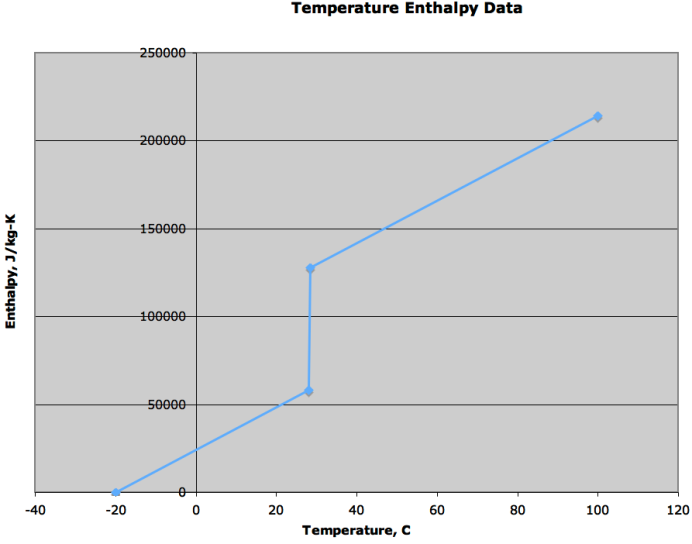
\includegraphics[width=0.9\textwidth, height=0.9\textheight, keepaspectratio=true]{media/image024.png}
\caption{Temp-Enth Example \protect \label{fig:temp-enth-example}}
\end{figure}

\paragraph{Field: Temperature x}\label{field-temperature-x}

This field is used to specify the temperature of the temperature-enthalpy function for the basic material. Units are C.

\paragraph{Field: Enthalpy x}\label{field-enthalpy-x}

This field specifies the enthalpy that corresponds to the previous temperature of the temperature-enthalpy function. Units are J/kg.

And, an IDF example showing how it is used in conjunction with the Material:

Note, the following Heat Balance Algorithm is necessary (only specified once). Also, when using ConductionFiniteDifference, it is more efficient to set the zone timestep shorter than those used for the ConductionTransferFunction solution algorithm. It should be set to 12 timesteps per hour or greater, and can range up to 60.

\begin{lstlisting}

HeatBalanceAlgorithm,
  ConductionFiniteDifference;


  Timestep,
  12;


  Material,
      E1 - 3 / 4 IN PLASTER OR GYP BOARD,  !- Name
      Smooth,                  !- Roughness
      1.9050000E-02,           !- Thickness {m}
      0.7264224,               !- Conductivity {W/m-K}
      1601.846,                !- Density {kg/m3}
      836.8000,                !- Specific Heat {J/kg-K}
      0.9000000,               !- Thermal Absorptance
      0.9200000,               !- Solar Absorptance
      0.9200000;               !- Visible Absorptance


  MaterialProperty:PhaseChange,
      E1 - 3 / 4 IN PLASTER OR GYP BOARD,  !- Name
      0.0,             !- Temperature coefficient,thermal conductivity(W/m K2)
      -20.,            !- Temperature 1, C
      0.01,            !- Enthalpy 1 at –20C, (J/kg)
      20.,             !- Temperature 2, C
      33400,           !- Enthalpy 2, (J/kg)
      20.5,            !- temperature 3, C
      70000,           !- Enthalpy 3, (J/kg)
      100.,            !- Temperature 4, C
      137000;          !- Enthalpy 4, (J/kg)
\end{lstlisting}

\subsection{MaterialProperty:VariableThermalConductivity}\label{materialpropertyvariablethermalconductivity}

This object is used to describe the temperature dependent material properties that are used in the CondFD (Conduction Finite Difference) solution algorithm. This conduction model is used when the appropriate CondFD materials are specified and the Solution Algorithm parameter is set to condFD.

\subsubsection{Inputs}\label{inputs-6-027}

\paragraph{Field: Name}\label{field-name-6-022}

This field is a regular material name specifying the material with which this additional temperature dependent property information will be associated.

\paragraph{Field Set: Temperature-Thermal Conductivity}\label{field-set-temperature-thermal-conductivity}

The temperature -- conductivity set of inputs specify a two column tabular temperature-thermal conductivity function for the basic material. Ten pairs can be specified. Specify only the number of pairs necessary. Temperature values should be strictly increasing.

\paragraph{Field: Temperature x}\label{field-temperature-x-1}

This field is used to specify the temperature of the temperature-conductivity function for the basic material. Units are C.

\paragraph{Field: Thermal Conductivity x}\label{field-thermal-conductivity-x}

This field specifies the conductivity that corresponds to the temperature (previous field) of the temperature-conductivity function. Units are W/m-K.

And, an IDF example showing how it is used in conjunction with the Materials:

Note, the following Heat Balance Algorithm is necessary (only specified once). Also, when using Conduction Finite Difference, it is more efficient to set the zone time step shorter than those used for the Conduction Transfer Function solution algorithm. It should be set to 12 time steps per hour or greater, and can range up to 60.

\begin{lstlisting}

HeatBalanceAlgorithm,
  ConductionFiniteDifference;


  Timestep,
  12;


  Material,
      PCMPlasterBoard ,      !- Name
      Smooth,                  !- Roughness
      1.9050000E-02,           !- Thickness {m}
      4.2,                     !- Conductivity {W/m-K}
      1601.846,                !- Density {kg/m3}
      836.8000,                !- Specific Heat {J/kg-K}
      0.9000000,               !- Thermal Absorptance
      0.9200000,               !- Solar Absorptance
      0.9200000;               !- Visible Absorptance


  MaterialProperty:VariableThermalConductivity,
      PCMPlasterBoard,         !- Name
      0,                       !- Temperature 1 {C}
      4.2,                     !- Thermal Conductivity 1 {W/m-K}
      22,                      !- Temperature 2 {C}
      4.2,                     !- Thermal Conductivity 2 {W/m-K}
      22.1,                    !- Temperature 3 {C}
      2.5,                     !- Thermal Conductivity 3 {W/m-K}
      100,                     !- Temperature 4 {C}
      2.5;                     !- Thermal Conductivity 4 {W/m-K}
\end{lstlisting}

\subsubsection{Outputs}\label{outputs-1-026}

The Conduction Finite Difference solution algorithm uses a finite difference solution technique, the surfaces are divided into a nodal arrangement. The only output specific to Conduction Finite Difference solution (that is not include in other surface outputs) is node temperatures.

The following output variables are applicable to all opaque heat transfer surfaces when using Solution Algorithms ConductionFiniteDifference:

\begin{itemize}
\item
  Zone,Sum,CondFD Inner Solver Loop Iteration Count {[]}
\item
  Zone,Average,CondFD Surface Temperature Node \textless{}1\textgreater{} {[}C{]}
\end{itemize}

\paragraph{CondFD Inner Solver Loop Iteration Count {[]}}\label{condfd-inner-solver-loop-iteration-count}

This outputs the count of iterations on the inner solver loop of CondFD for each surface.

\paragraph{CondFD Surface Temperature Node \textless{}X\textgreater{} {[}C{]}}\label{condfd-surface-temperature-node-x-c}

This will output temperatures for a node in the surfaces being simulated with ConductionFiniteDifference. The key values for this output variable are the surface name. The nodes are numbered from outside to inside of the surface. The full listing will appear in the RDD file

\paragraph{CondFD Surface Heat Flux Node \textless{}X\textgreater{} {[}W/m2{]}}\label{condfd-surface-heat-flux-node-x-wm2}

This will output heat flux at each node in surfaces being simulated with ConductionFiniteDifference. The key values for this output variable are the surface name. The nodes are numbered from outside to inside of the surface. The full listing will appear in the RDD file. A positive value indicates heat flowing towards the inside face of the surface. Note that this matches the sign convention for Surface Inside Face Conduction Heat Transfer Rate per Area and is opposite the sign of Surface Outside Face Conduction Heat Transfer Rate per Area.

\paragraph{CondFD Surface Heat Capacitance Outer Half Node \textless{}X\textgreater{} {[}W/m2-K{]}}\label{condfd-surface-heat-capacitance-outer-half-node-x-wm2-k}

\paragraph{CondFD Surface Heat Capacitance Inner Half Node \textless{}X\textgreater{} {[}W/m2-K{]}}\label{condfd-surface-heat-capacitance-inner-half-node-x-wm2-k}

These will output the half-node heat capacitance in surfaces being simulated with ConductionFiniteDifference. The key values for this output variable are the surface name. The nodes are numbered from outside to inside of the surface. The full listing will appear in the RDD file. For this output, the heat capacitance is defined as the product of specific heat, density, and node thickness. Zero is reported for R-layer half-nodes and for undefined half-nodes. There is no outer half-node for Node 1 which is the outside face of the surface, and there is no inner half-node for Node N which is the inside face of the surface. CondFD Surface Heat Capacitance is only available with Output:Diagnostics,DisplayAdvancedReportVariables.

\subsection{MaterialProperty:HeatAndMoistureTransfer:Settings}\label{materialpropertyheatandmoisturetransfersettings}

\textbf{Advanced/Research Usage:} This object is used to describe two of the seven additional material properties needed for the CombinedHeatAndMoistureFiniteElement heat balance solution algorithm. The settings object is used when the solutions algorithm is set to CombinedHeatAndMoistureFiniteElement and the appropriate material properties are assigned to each material. This permits the simulation of the moisture dependent thermal properties of the material as well as the transfer of moisture through, into and out of the material into the zone or exterior.

In addition to the Porosity and Initial Water content properties described here, five additional properties, described by tabulated relationships between variables, are required. These properties are;

\begin{itemize}
\item
  MaterialProperty:HeatAndMoistureTransfer:SorptionIsotherm
\item
  MaterialProperty:HeatAndMoistureTransfer:Suction
\item
  MaterialProperty:HeatAndMoistureTransfer:Redistribution
\item
  MaterialProperty:HeatAndMoistureTransfer:Diffusion
\item
  MaterialProperty:HeatAndMoistureTransfer:ThermalConductivity
\end{itemize}

All materials in a construction are required to have all material properties defined for HAMT to work.

Within the MaterialProperty:HeatAndMoistureTransfer:Settings object the following fields are defined.

\subsubsection{Inputs}\label{inputs-7-026}

\paragraph{Field: Material Name}\label{field-material-name-000}

This field is a unique reference name that the user assigns to a particular material. This name can then be referred to by other input data.

\paragraph{Field: Porosity}\label{field-porosity}

The porosity of a material is the maximum fraction, by volume, of a material that can be taken up with water. The units are {[}m3/m3{]}.

\paragraph{Field: Initial Water Content Ratio}\label{field-initial-water-content-ratio}

For this solution algorithm, the initial water content is assumed to be distributed evenly through the depth of the material. The units are {[}kg/kg{]}.

Below is an example input for the porosity and initial water content of a material.

\begin{lstlisting}

MaterialProperty:HeatAndMoistureTransfer:Settings,
        Concrete,     !- Name
        0.76,     !- Porosity
        0.2;     !- Initial (or typical) Water content
\end{lstlisting}

\subsection{MaterialProperty:HeatAndMoistureTransfer:SorptionIsotherm}\label{materialpropertyheatandmoisturetransfersorptionisotherm}

\textbf{Advanced/Research Usage:} This material property is used in conjunction with the CombinedHeatAndMoistureFiniteElement heat balance solution algorithm.

The Isotherm data relates the moisture, or water content {[}kg/m3{]} of a material with the relative humidity (RH). The water content is expected to increase as relative humidity increases, starting at zero content at 0.0relative humidity fraction and reaching a maximum, defined by the porosity, at 1.0 relative humidity fraction, which corresponds to 100\% relative humidity. Relative humidities are entered as fraction for this object ranging from 0.0 to 1.0. These two extremes (0.0 and 1.0) are automatically set by the HAMT solution. However, if they are entered they will be used as extra data points. Data should be provided with increasing RH and moisture content up to as high an RH as possible to provide a stable solution. One possible reason for the following error message may be that a material has a very rapid increase in water content for a small change in RH, which can happen if the last entered water content point is at a low RH and the material has a very high porosity.

\begin{lstlisting}
  ** Warning ** HeatAndMoistureTransfer: Large Latent Heat for Surface ROOF
\end{lstlisting}

Another potential reason for this error being generated is the use of inappropriate values for Vapor Transfer Coefficients. See the SurfaceProperties:VaporCoefficients object in the Advanced Surface Concepts group.

\subsubsection{Inputs}\label{inputs-8-024}

\paragraph{Field: Material Name}\label{field-material-name-1}

This field is a unique reference name that the user assigns to a particular material. This name can then be referred to by other input data.

\paragraph{Field: Number of data ~Coordinates}\label{field-number-of-data-coordinates}

A maximum of 25 coordinates can be specified.

\paragraph{Field Set: Relative Humidity-Moisture Content}\label{field-set-relative-humidity-moisture-content}

\paragraph{Field: Relative Humidity Fraction x}\label{field-relative-humidity-fraction-x}

The relative humidity of the x\(^{th}\) coordinate. The relative humidity is entered as fraction, not in percent.

\paragraph{Field: Moisture Content x}\label{field-moisture-content-x}

The Moisture Content of the x\(^{th}\) coordinate. The units are {[}kg/m3{]}

Below is an example input for a material isotherm

\begin{lstlisting}

MaterialProperty:HeatAndMoistureTransfer:SorptionIsotherm,
        Concrete,     !- Name
        10,     !- Number of data Coordinates
        0.2205,    !- Relative Humidity fraction #1
        22.31,     !- Moisture content #1
        0.202,     !- Relative Humidity fraction #2
        19.665,    !- Moisture content #2
        0.449,     !- Relative Humidity fraction #3
        40.02,     !- Moisture content #3
        0.454,     !- Relative Humidity fraction #4
        36.915,    !- Moisture content #4
        0.6506,    !- Relative Humidity fraction #5
        56.005,    !- Moisture content #5
        0.655,     !- Relative Humidity fraction #6
        52.325,    !- Moisture content #6
        0.824,     !- Relative Humidity fraction #7
        72.565,    !- Moisture content #7
        0.8725,    !- Relative Humidity fraction #8
        85.1,      !- Moisture content #8
        0.924,     !- Relative Humidity fraction #9
        91.08,     !- Moisture content #9
        0.964,     !- Relative Humidity fraction #10
        100.28;    !- Moisture content #10
\end{lstlisting}

\subsection{MaterialProperty:HeatAndMoistureTransfer:Suction}\label{materialpropertyheatandmoisturetransfersuction}

\textbf{Advanced/Research Usage:}This material property is used in conjunction with the CombinedHeatAndMoistureFiniteElement heat balance solution algorithm.

The suction data relates the liquid transport coefficient, under suction, to the water content of a material. A data point at zero water content is required. The liquid transport coefficient at the highest entered water content value is used for all liquid transport coefficient values above this water content. These coefficients are used by HAMT when the rain flag is set in the weather file.

\subsubsection{Inputs}\label{inputs-9-022}

\paragraph{Field: Material Name}\label{field-material-name-2}

This field is a unique reference name that the user assigns to a particular material. This name can then be referred to by other input data.

\paragraph{Field: Number of Suction points}\label{field-number-of-suction-points}

A maximum of 25 points can be specified.

\paragraph{Field Set: Moisture Content-Liquid Transport Coefficient}\label{field-set-moisture-content-liquid-transport-coefficient}

\paragraph{Field: Moisture Content x}\label{field-moisture-content-x-1}

The moisture content of the x\(^{th}\) point. The units are {[}kg/m3{]}.

\paragraph{Field: Liquid Transport Coefficient x}\label{field-liquid-transport-coefficient-x}

The Liquid Transport Coefficient of the x\(^{th}\) point. The units are {[}m2/s{]}.

Below is an example input for a material liquid transport coefficient under suction.

\begin{lstlisting}

MaterialProperty:HeatAndMoistureTransfer:Suction,
        Concrete,     !- Name
        5,     !- Number of Suction points
        0,     !- Moisture content 1
        0,     !- Liquid Transport Coefficient 1
        72,     !- Moisture content 2
        0.0000000000741,     !- Liquid Transport Coefficient 2
        85,     !- Moisture content 3
        0.000000000253,     !- Liquid Transport Coefficient 3
        100,     !- Moisture content 4
        0.00000000101,     !- Liquid Transport Coefficient 4
        118,     !- Moisture content 5
        0.00000000128;     !- Liquid Transport Coefficient 5
\end{lstlisting}

\subsection{MaterialProperty:HeatAndMoistureTransfer:Redistribution}\label{materialpropertyheatandmoisturetransferredistribution}

\textbf{Advanced/Research Usage:}This material property is used in conjunction with the CombinedHeatAndMoistureFiniteElement heat balance solution algorithm.

The redistribution data relates the liquid transport coefficient to the water content of a material under normal conditions. A data point at zero water content is required. The liquid transport coefficient at the highest entered water content value is used for all liquid transport coefficient values above this water content. These coefficients are used by the Heat and Moisture Transfer algorithm when the rain flag is NOT set in the weather file.

\subsubsection{Inputs}\label{inputs-10-020}

\paragraph{Field: Material Name}\label{field-material-name-3}

This field is a unique reference name that the user assigns to a particular material. This name can then be referred to by other input data.

\paragraph{Field: Number of Redistribution points}\label{field-number-of-redistribution-points}

A maximum of 25 points can be specified.

\paragraph{Field Set: Moisture Content-- Liquid Transport Coefficient}\label{field-set-moisture-content-liquid-transport-coefficient-1}

\paragraph{Field: Moisture Content x}\label{field-moisture-content-x-2}

The moisture content of the x\(^{th}\) point. The units are {[}kg/m3{]}.

\paragraph{Field: Liquid Transport Coefficient x}\label{field-liquid-transport-coefficient-x-1}

The Liquid Transport Coefficient of the x\(^{th}\) point. The units are {[}m2/s{]}.

Below is an example input for the object.

\begin{lstlisting}

MaterialProperty:HeatAndMoistureTransfer:Redistribution,
        Concrete,     !- Name
        5,     !- Number of Redistribution points
        0,     !- Moisture content 1
        0,     !- Liquid Transport Coefficient 1
        72,     !- Moisture content 2
        0.00000000000741,     !- Liquid Transport Coefficient 2
        85,     !- Moisture content 3
        0.0000000000253,     !- Liquid Transport Coefficient 3
        100,     !- Moisture content 4
        0.000000000101,     !- Liquid Transport Coefficient 4
        118,     !- Moisture content 5
        0.000000000128;     !- Liquid Transport Coefficient 5
\end{lstlisting}

\subsection{MaterialProperty:HeatAndMoistureTransfer:Diffusion}\label{materialpropertyheatandmoisturetransferdiffusion}

\textbf{Advanced/Research Usage:}This material property is used in conjunction with the CombinedHeatAndMoistureFiniteElement heat balance solution algorithm.

The MU data relates the vapor diffusion resistance factor (dimensionless) to the relative humidity as fraction(RH). A data point at zero RH is required. The vapor diffusion resistance factor at the highest entered relative humidity (RH) value is used for all vapor diffusion resistance factor values above this RH.~ The relative humidity maximum value in fraction is 1.0.

\subsubsection{Inputs}\label{inputs-11-019}

\paragraph{Field: Material Name}\label{field-material-name-4}

This field is a unique reference name that the user assigns to a particular material. This name can then be referred to by other input data.

\paragraph{Field: Number of Data Pairs}\label{field-number-of-data-pairs}

A maximum of 25 pairs can be specified.

\paragraph{Field Set: Relative Humidity-Vapor Diffusion Resistance Factor}\label{field-set-relative-humidity-vapor-diffusion-resistance-factor}

\paragraph{Field: Relative Humidity Fraction \#x}\label{field-relative-humidity-fraction-x-1}

The moisture content of the x\(^{th}\) pair. The relative humidity is entered as fraction, not in percent.

\paragraph{Field: Vapor Diffusion Resistance Factor \#x}\label{field-vapor-diffusion-resistance-factor-x}

The Liquid Transport Coefficient of the x\(^{th}\) pair.

Below are some examples of the values for materials.

\begin{lstlisting}

MaterialProperty:HeatAndMoistureTransfer:Diffusion,
        Plywood,     !- Name
        3,     !- Number of data Points
        0,     !- Relative Humidity Fraction 1
        700,     !- Water Vapor Diffusion Resistance Factor 1
        0.5,     !- Relative Humidity Fraction 2
        200,     !- Water Vapor Diffusion Resistance Factor 2
        1,     !- Relative Humidity Fraction 3
        20;     !- Water Vapor Diffusion Resistance Factor 3

  MaterialProperty:HeatAndMoistureTransfer:Diffusion,
        Concrete,     !- Name
        1,     !- Number of Mu Points
        0,     !- Relative Humidity Fraction 1
        180;     !- Water Vapor Diffusion Resistance Factor 1
\end{lstlisting}

\subsection{MaterialProperty:HeatAndMoistureTransfer:ThermalConductivity}\label{materialpropertyheatandmoisturetransferthermalconductivity}

\textbf{Advanced/Research Usage:}This material property is used in conjunction with the CombinedHeatAndMoistureFiniteElement heat balance solution algorithm.

The thermal data relates the thermal conductivity {[}W/m-K{]} of a material to the moisture or water content {[}kg/m3{]}. A data point at zero water content is required. The thermal conductivity at the highest entered water content value is used for all thermal conductivity values above this water content. If this object is not defined for a material then the algorithm will use a constant value entered in the Material object for all water contents.

\subsubsection{Inputs}\label{inputs-12-018}

\paragraph{Field: Material Name}\label{field-material-name-5}

This field is a unique reference name that the user assigns to a particular material. This name can then be referred to by other input data.

\paragraph{Field: Number of Thermal Coordinates}\label{field-number-of-thermal-coordinates}

A maximum of 25 coordinates can be specified.

\paragraph{Field Set: Moisture Content- Thermal Conductivity}\label{field-set-moisture-content--thermal-conductivity}

\paragraph{Field: Moisture Content x}\label{field-moisture-content-x-3}

The moisture content of the x\(^{th}\) coordinate. The units are {[}kg/m3{]}

\paragraph{Field: Thermal Conductivity x}\label{field-thermal-conductivity-x-1}

The Thermal Conductivity of the x\(^{th}\) coordinate. The units are {[}W/m-K{]}

Below is an example of values for a material.

\begin{lstlisting}

MaterialProperty:HeatAndMoistureTransfer:ThermalConductivity
        Concrete,     !- Name
        2,     !- Number of Thermal Coordinates
        0,     !- Moisture content \#1
        1.6,     !- Thermal Conductivity \#1
        180,     !- Moisture content \#2
        2.602;     !- Thermal Conductivity \#2
\end{lstlisting}

\subsubsection{Surface Outputs}\label{outputs-2-021}

\begin{itemize}
\item
  Zone,Average,HAMT Surface Average Water Content Ratio {[}kg/kg{]}
\item
  Zone,Average,HAMT Surface Inside Face Temperature {[}C{]}
\item
  Zone,Average,HAMT Surface Inside Face Relative Humidity {[}\%{]}
\item
  Zone,Average,HAMT Surface Inside Face Vapor Pressure {[}Pa{]}
\item
  Zone,Average,HAMT Surface Outside Face Temperature {[}C{]}
\item
  Zone,Average,HAMT Surface Outside Face Relative Humidity {[}\%{]}
\end{itemize}

\paragraph{HAMT Surface Average Water Content Ratio {[}kg/kg{]}}\label{hamt-surface-average-water-content-ratio-kgkg}

This output is the summed water content {[}kg/kg{]} of all cells in a surface expressed as a fraction of the mass of the water to the material mass.

\paragraph{HAMT Surface Inside Face Temperature {[}C{]}}\label{hamt-surface-inside-face-temperature-c}

This output is the temperature {[}C{]} on the internal ``surface'' of the surface.

\paragraph{HAMT Surface Inside Face Relative Humidity {[}\%{]}}\label{hamt-surface-inside-face-relative-humidity}

\paragraph{HAMT Surface Inside Face Relative Humidity {[}\%{]}}\label{hamt-surface-inside-face-relative-humidity-1}

This output is the relative humidity on the internal ``surface'' of the surface expressed as a percentage.

\paragraph{HAMT Surface Inside Face Vapor Pressure {[}Pa{]}}\label{hamt-surface-inside-face-vapor-pressure-pa}

This output is the vapor pressure {[}Pa{]} on the internal ``surface'' of the surface.

\paragraph{HAMT Surface Outside Face Temperature {[}C{]}}\label{hamt-surface-outside-face-temperature-c}

This output is the temperature on the external ``surface'' of the surface.

\paragraph{HAMT Surface Outside Face Relative Humidity {[}\%{]}}\label{hamt-surface-outside-face-relative-humidity}

This output is the relative humidity on the external ``surface'' of the surface.

\subsubsection{Internal Cell Outputs}\label{outputs-2-021}

Detailed profile data for the variables Temperature {[}C{]}, Relative Humidity {[}\%{]} and Water Content {[}kg/kg{]} within each surface can also be reported. To calculate the heat and moisture transfer through surfaces HAMT splits up surfaces into discrete cells. Each cell is composed of a single material and has a position within the surface. HAMT automatically assigns cells to construction objects so that there are more cells closer to boundaries between materials and also at the ``surfaces'' of the surface. It is not possible for users to define their own cells.

Each surface is made from a particular construction. The construction-surface relationship is output by HAMT to the eplusout.eio file with the following format. The output also contains the HAMT cell origins and cell number for each surface combination. The coordinate system origin is defined as the exterior surface of the construction.

\begin{lstlisting}
! <HAMT cells>, Surface Name, Construction Name, Cell Numbers
! <HAMT origins>, Surface Name, Construction Name, Cell origins (m)
HAMT cells, FLOOR,FLOOR,   1,   2,   3,   4,   5,   6,   7,   8,   9,  10,  11,  12,  13,  14,  15,  16,  17
HAMT origins,FLOOR,FLOOR, 0.0000000, 0.0122726, 0.0601616, 0.1512518, 0.2766268, 0.4240140, 0.5789860, 0.7263732, 0.8517482, 0.9428384, 0.9907274, 1.0035729, 1.0056459, 1.0090000, 1.0123541, 1.0144271, 1.0150000
\end{lstlisting}

Users can select any one of the Temperature, Relative Humidity or Water Content variables for any cell to be reported, using the following naming scheme for the output variable.
 
\begin{itemize}
\item
  Zone,Average,HAMT Surface Temperature Cell N {[}C{]}
\item
  Zone,Average,HAMT Surface Water Content Cell N {[}kg/kg{]}
\item
  Zone,Average,HAMT Surface Relative Humidity Cell N {[}\%{]}
\end{itemize}

\paragraph{HAMT Surface Relative Humidity Cell \textless{}N\textgreater{} {[}\%{]}}\label{hamt-surface-relative-humidity-cell-n}

This is the relative humidity of the cell in the surface.

\paragraph{HAMT Surface Temperature Cell \textless{}N\textgreater{} {[}C{]}}\label{hamt-surface-temperature-cell-n-c}

This is the temperature of the cell in the surface.

\paragraph{HAMT Surface Water Content Cell \textless{}N\textgreater{} {[}kg/kg{]}}\label{hamt-surface-water-content-cell-n-kgkg}

This is the relative water content of the cell in the surface.

\subsection{Materials for Glass Windows and Doors}\label{materials-for-glass-windows-and-doors}

All the materials for glass windows and doors have the prefix ``WindowMaterial''. The following~ WindowMaterial descriptions (Glazing, Glazing:RefractionExtinctionMethod, Gas, GasMixture, Shade, Screen and Blind) apply to glass windows and doors. The property definitions described herein for Glazing, Gas and GasMixture are supported by the National Fenestration Rating Council as standard.

``Front side'' is the side of the layer opposite the zone in which the window is defined. ``Back side'' is the side closest to the zone in which the window is defined. Therefore, for exterior windows, ``front side'' is the side closest to the outdoors. For interior windows, ``front side'' is the side closest to the zone adjacent to the zone in which the window is defined.

The solar radiation transmitted by the window layers enters the zone and is a component of the zone load. The solar radiation absorbed in each solid layer (glass, shade, screen or blind) participates in the window layer heat balance calculation. The visible transmittance and reflectance properties of the window are used in the daylighting calculation.

\subsection{WindowMaterial:Glazing}\label{windowmaterialglazing}

In the following, for exterior windows, ``front side'' is the side of the glass closest to the outside air and ``back side'' is the side closest to the zone the window is defined in. For interzone windows, ``front side'' is the side closest to the zone adjacent to the zone the window is defined in and ``back side'' is the side closest to the zone the window is defined in.

\subsubsection{Inputs}\label{inputs-13-015}

\paragraph{Field: Name}\label{field-name-7-020}

The name of the glass layer. It corresponds to a layer in a window construction.

\paragraph{Field: Optical Data Type}\label{field-optical-data-type}

Valid values for this field are SpectralAverage, Spectral, BSDF.

If Optical Data Type = SpectralAverage, the values you enter for solar transmittance and reflectance are assumed to be averaged over the solar spectrum, and the values you enter for visible transmittance and reflectance are assumed to be averaged over the solar spectrum and weighted by the response of~ the human eye. There is an EnergyPlus Reference Data Set for WindowMaterial:Glazing that contains spectral average properties for many different types of glass.

If Optical Data Type = Spectral, then, in the following field, you must enter the name of a spectral data set defined with the WindowGlassSpectralData object. In this case, the values of~ solar and visible transmittance and reflectance in the fields below should be blank.

If Optical Data Type = BSDF, the Construction:ComplexFenestrationState object must be used to define the window construction layers. The Construction:ComplexFenestrationState object contains references to the BSDF files which contain the optical properties of the Complex Fenestration layers. In this case,

\paragraph{Field: Window Glass Spectral Data Set Name}\label{field-window-glass-spectral-data-set-name}

If Optical Data Type = Spectral, this is the name of a spectral data set defined with a WindowGlassSpectralData object.

\paragraph{Field: Thickness}\label{field-thickness-1}

The surface-to-surface thickness of the glass (m).

\paragraph{Field: Solar Transmittance at Normal Incidence}\label{field-solar-transmittance-at-normal-incidence}

Transmittance at normal incidence averaged over the solar spectrum. Used only when Optical Data Type = SpectralAverage.

For uncoated glass, when alternative optical properties are available---such as thickness, solar index of refraction, and solar extinction coefficient---they can be converted to equivalent solar transmittance and reflectance values using the equations given in ``Conversion from Alternative Specification of Glass Optical Properties.'')

\paragraph{Field: Front Side Solar Reflectance at Normal Incidence}\label{field-front-side-solar-reflectance-at-normal-incidence}

Front-side reflectance at normal incidence averaged over the solar spectrum. Used only when Optical Data Type = SpectralAverage.

\paragraph{Field: Back Side Solar Reflectance at Normal Incidence}\label{field-back-side-solar-reflectance-at-normal-incidence}

Back-side reflectance at normal incidence averaged over the solar spectrum. Used only when Optical Data Type = SpectralAverage.

\paragraph{Field: Visible Transmittance at Normal Incidence}\label{field-visible-transmittance-at-normal-incidence}

Transmittance at normal incidence averaged over the solar spectrum and weighted by the response of the human eye. Used only when Optical Data Type = SpectralAverage.

For uncoated glass, when alternative optical properties are available---such as thickness, visible index of refraction, and visible extinction coefficient---they can be converted to equivalent visible transmittance and reflectance values using the equations given in ``Conversion from Alternative Specification of Glass Optical Properties.'')

\paragraph{Field: Front Side Visible Reflectance at Normal Incidence}\label{field-front-side-visible-reflectance-at-normal-incidence}

Front-side reflectance at normal incidence averaged over the solar spectrum and weighted by the response of the human eye. Used only when Optical Data Type = SpectralAverage.

\paragraph{Field: Back Side Visible Reflectance at Normal Incidence}\label{field-back-side-visible-reflectance-at-normal-incidence}

Back-side reflectance at normal incidence averaged over the solar spectrum and weighted by the response of the human eye. Used only when Optical Data Type = SpectralAverage.

\paragraph{Field: Infrared Transmittance at Normal Incidence}\label{field-infrared-transmittance-at-normal-incidence}

Long-wave transmittance at normal incidence.

\paragraph{Field: Front Side Infrared Hemispherical Emissivity}\label{field-front-side-infrared-hemispherical-emissivity}

Front-side long-wave emissivity.

\paragraph{Field: Back Side Infrared Hemispherical Emissivity}\label{field-back-side-infrared-hemispherical-emissivity}

Back-side long-wave emissivity.

\paragraph{Field: Conductivity}\label{field-conductivity-1}

Thermal conductivity (W/m-K).

\paragraph{Field: Dirt Correction Factor for Solar and Visible Transmittance}\label{field-dirt-correction-factor-for-solar-and-visible-transmittance}

This is a factor that corrects for the presence of dirt on the glass. The program multiplies the fields ``Solar Transmittance at Normal Incidence'' and ``Visible Transmittance at Normal Incidence'' by this factor if the material is used as the \underline{outer} glass layer of an \underline{exterior} window or glass door.\footnote{If Optical Data Type = Spectral, the program multiplies the solar and visible transmittance at each wavelength by the dirt correction factor.} If the material is used as an inner glass layer (in double glazing, for example), the dirt correction factor is not applied because inner glass layers are assumed to be clean. Using a material with dirt correction factor \textless{} 1.0 in the construction for an interior window will result in an error message.

Representative values of the dirt correction factor are shown in Table~\ref{table:dirt-correction-factors}.

\begin{longtable}[c]{@{}llll@{}}
\caption{Dirt Correction Factors \label{table:dirt-correction-factors}} \\
\toprule
Type of Location & \multicolumn{3}{c}{Angle of Glazing} \\ \cmidrule(r){2-4}
                 & Vertical & 45$^{o}$ & Horizontal \\ \midrule
\endfirsthead

\caption[]{Dirt Correction Factors} \\
\toprule
Type of Location & \multicolumn{3}{c}{Angle of Glazing} \\ \cmidrule(r){2-4}
                 & Vertical & 45$^{o}$ & Horizontal \\ \midrule
\endhead

Non-industrial & 0.9 & 0.8 & 0.7 \\
Industrial & 0.7 & 0.6 & 0.5 \\
Very Dirty & 0.6 & 0.5 & 0.4 \\
\bottomrule
{\tiny From Appendix A, ``Daylighting in Sports Halls, Report 2,'' SportScotland, Nov. 2002 (www.sportscotland.org.uk)}
\end{longtable}

The default value of the dirt correction factor is 1.0, which means the glass is clean.

It is assumed that dirt, if present, has no effect on the IR properties of the glass.

\paragraph{Field: Solar Diffusing}\label{field-solar-diffusing}

Takes values No (the default) and Yes. If No, the glass is \underline{transparent} and beam solar radiation incident on the glass is transmitted as beam radiation with no diffuse component. If Yes, the glass is \underline{translucent} and beam solar radiation incident on the glass is transmitted as hemispherically diffuse radiation with no beam component.\footnote{EnergyPlus does not model the ``partially translucent'' case in which beam solar radiation incident on the glass is transmitted as a combination of beam and diffuse.} See Figure~\ref{fig:comparison-between-transmittance-properties}. Solar Diffusing = Yes should only be used on the \emph{innermost} pane of glass in an exterior window; it does not apply to interior windows.

For both Solar Diffusing = No and Yes, beam is reflected as beam with no diffuse component (see Figure~\ref{fig:comparison-between-transmittance-properties}). Solar Diffusing cannot be used with Window Shading Control devices (except Switchable Glazing). When attempted, the window property will be set to No for Solar Diffusing. The Surface Details report will reflect the override.

If, in the Building object, Solar Distribution = FullInteriorAndExterior, use of Solar Diffusing = Yes for glass in an exterior window will change the distribution of interior solar radiation from the window. The result is that beam solar radiation that would be transmitted by a transparent window and get absorbed by particular interior surfaces will be diffused by a translucent window and be spread over more interior surfaces. This can change the time dependence of heating and cooling loads in the zone.

In a zone with Daylighting:Detailed, translucent glazing---which is often used in skylights---will provide a more uniform daylight illuminance over the zone and will avoid patches of sunlight on the floor.

\begin{figure}[hbtp] % fig 10
\centering
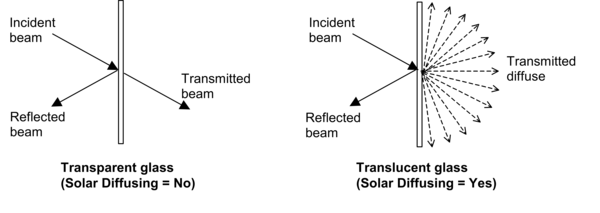
\includegraphics[width=0.9\textwidth, height=0.9\textheight, keepaspectratio=true]{media/image025.png}
\caption{Comparison between transmittance properties of transparent glass (Solar Diffusing = No) and translucent glass (Solar Diffusing = Yes). \protect \label{fig:comparison-between-transmittance-properties}}
\end{figure}

\paragraph{Field: Young's modulus}\label{field-youngs-modulus}

A measure of the stiffness of an elastic material.~ It is defined as the ratio of the uniaxial stress over the uniaxial strain in the range of stress in which Hooke's Law holds. It is used only with complex fenestration systems defined through the Construction:ComplexFenestrationState object. The default value for glass is 7.2e10 Pa.

\paragraph{Field: Poisson's ratio}\label{field-poissons-ratio}

The ratio, when a sample object is stretched, of the contraction or transverse strain (perpendicular to the applied load), to the extension or axial strain (in the direction of the applied load). This value is used only with complex fenestration systems defined through the Construction:ComplexFenestrationState object. The default value for glass is 0.22.

IDF examples of Spectral average and using a Spectral data set:

\begin{lstlisting}

MATERIAL:WINDOWGLASS, GLASS - CLEAR SHEET 1 / 8 IN,
    SpectralAverage, ! Optical data type
    0.003, ! Thickness {m} 1/8"
    0.850, ! Solar transmittance at normal incidence
    0.075, ! Solar reflectance at normal incidence: front side
    0.075, ! Solar reflectance at normal incidence: back side
    0.901, ! Visible transmittance at normal incidence
    0.081, ! Visible reflectance at normal incidence: front side
    0.081, ! Visible reflectance at normal incidence: back side
    0.0,   ! IR transmittance at normal incidence
    0.84,  ! IR hemispherical emissivity: front side
    0.84,  ! IR hemispherical emissivity: back side
    0.9;   ! Conductivity {W/m-K}


  WindowMaterial:Glazing ,SPECTRAL GLASS INNER PANE, ! Material name
      Spectral, ! Optical data type {SpectralAverage or Spectral}
      TestSpectralDataSet, ! Name of spectral data set
      0.0099, ! Thickness {m}
      ,  ! Solar transmittance at normal incidence
      ,  ! Solar reflectance at normal incidence: front side
      ,  ! Solar reflectance at normal incidence: back side
      ,  ! Visible transmittance at normal incidence
      ,  ! Visible reflectance at normal incidence: front side
      ,  ! Visible reflectance at normal incidence: back side
      0.0,   ! IR transmittance at normal incidence
      0.84,  ! IR emissivity: front side
      0.84,  ! IR emissivity: back side
      0.798; ! Conductivity {W/m-K}
\end{lstlisting}

IDF example of Spectral Data Type = BSDF

\begin{lstlisting}

WindowMaterial:Glazing,
    Glass_5012_Layer,        !- Layer name : CLEAR_6.PPG
    BSDF,                    !- Optical Data Type
    ,                        !- Spectral Data name
    0.005664,                !- Thickness
    ,                        !- Solar Transmittance
    ,                        !- Solar Front Reflectance
    ,                        !- Solar Back Reflectance
    ,                        !- Visible Transmittance
    ,                        !- Visible Front Reflectance
    ,                        !- Visible Back reflectance
    0.000000,                !- IR Transmittance
    0.840000,                !-Front Emissivity
    0.840000,                !-Back Emissivity
    1.000000,                !-Conductivity
    ,                        !-Dirt Correction Factor for Sol/Vis Transmittance
    ,                        !-Solar Diffusing
    7.2e10,                  !-Young’s modulus
    0.22;                    !-Poisson’s ratio
\end{lstlisting}

\subsection{WindowMaterial:Glazing:RefractionExtinctionMethod}\label{windowmaterialglazingrefractionextinctionmethod}

This is an alternative way of specifying glass properties. Index of refraction and extinction coefficient are given instead of the transmittance and reflectance values used in WindowMaterial:Glazing. However, unlike WindowMaterial:Glazing, WindowMaterial:Glazing:RefractionExtinctionMethod is restricted to cases where the front and back optical properties of the glass are the same. This means it cannot be used for glass with a coating on one side. In that case WindowMaterial:Glazing should be used. Also, unlike WindowMaterial:Glazing, WindowMaterial:Glazing:RefractionExtinctionMethod does not allow input of glass wavelength-by-wavelength (spectral) properties.

\subsubsection{Inputs}\label{inputs-14-015}

\paragraph{Field: Name}\label{field-name-8-020}

The name of the glass layer. It corresponds to a layer in a window construction.

\paragraph{Field: Thickness}\label{field-thickness-2}

The surface-to-surface thickness of the glass (m).

\paragraph{Field: Solar Index of Refraction}\label{field-solar-index-of-refraction}

Index of refraction averaged over the solar spectrum.

\paragraph{Field: Solar Extinction Coefficient}\label{field-solar-extinction-coefficient}

Extinction coefficient averaged over the solar spectrum (m\(^{-1}\)).

\paragraph{Field: Visible Index of Refraction}\label{field-visible-index-of-refraction}

Index of refraction averaged over the solar spectrum and weighted by the response of the human eye.

\paragraph{Field: Visible Extinction Coefficient}\label{field-visible-extinction-coefficient}

Extinction coefficient averaged over the solar spectrum and weighted by the response of the human eye (m\(^{-1}\)).

\paragraph{Field: Infrared Transmittance at Normal Incidence}\label{field-infrared-transmittance-at-normal-incidence-1}

Long-wave transmittance at normal incidence.

\paragraph{Field: Infrared Hemispherical Emissivity}\label{field-infrared-hemispherical-emissivity}

Long-wave hemispherical emissivity, assumed the same on both sides of the glass.

\paragraph{Field: Conductivity}\label{field-conductivity-2}

Thermal conductivity (W/m-K).

\paragraph{Field: Dirt Correction Factor for Solar and Visible Transmittance}\label{field-dirt-correction-factor-for-solar-and-visible-transmittance-1}

This is a factor that corrects for the presence of dirt on the glass. It multiplies the solar and visible transmittance at normal Incidence (which the program calculates from the input values of thickness, solar index of refraction, solar extinction coefficient, etc.) if the material is used as the \underline{outer} glass layer of an \underline{exterior} window or glass door. If the material is used as an inner glass layer (in double glazing, for example), the dirt correction factor is not applied because inner glass layers are assumed to be clean. Using a material with dirt correction factor \textless{} 1.0 in the construction for an interior window will result in an error message.

Representative values of the direct correction factor are shown in Table~\ref{table:dirt-correction-factors}.

The default value of the dirt correction factor is 1.0, which means the glass is clean. It is assumed that dirt, if present, has no effect on the IR properties of the glass.

\paragraph{Field: Solar Diffusing}\label{field-solar-diffusing-1}

Takes values No (the default) and Yes. If No, the glass is transparent. If Yes, the glass is translucent and beam solar radiation incident on the glass is transmitted as hemispherically diffuse radiation with no beam component. (EnergyPlus does not model the ``partially translucent'' case in which beam solar radiation incident on the glass is transmitted as a combination of beam and diffuse.) Solar Diffusing = Yes should only be used on the innermost pane of glass in an exterior window; it does not apply to interior windows.

If, in the Building object, Solar Distribution = FullInteriorAndExterior, use of Solar Diffusing = Yes for glass in an exterior window will change the distribution of interior solar radiation from the window. The result is that beam solar radiation that would be transmitted by a transparent window and get absorbed by particular interior surfaces will be diffused by a translucent window and be spread over more interior surfaces. This can change the time dependence of heating and cooling loads in the zone.

In a zone with Daylighting:Detailed, translucent glazing, which is often used in skylights, will provide a more uniform daylight illuminance over the zone and will avoid patches of sunlight on the floor.

An IDF example:

\begin{lstlisting}
WindowMaterial:Glazing:RefractionExtinctionMethod,
  4MM CLEAR GLASS,  !- Material name
  0.004,            !- Thickness {m}
  1.526,            !- Solar index of refraction
  30.0 ,            !- Solar extinction coefficient (1/m)
  1.526,            !- Visible index of refraction
  30.0 ,            !- Visible extinction coefficient (1/m)
  0.0,              !- IR transmittance at normal incidence
  0.84,             !- IR emissivity
  0.9;              !- Conductivity {W/m-K}
\end{lstlisting}

\subsection{Glass Optical Properties Conversion}\label{glass-optical-properties-conversion}

\subsubsection{Conversion from Glass Optical Properties Specified as Index of Refraction and Transmittance at Normal Incidence}\label{conversion-from-glass-optical-properties-specified-as-index-of-refraction-and-transmittance-at-normal-incidence}

The optical properties of uncoated glass are sometimes specified by index of refraction, n, and transmittance at normal incidence, T.

The following equations show how to convert from this set of values to the transmittance and reflectance values required by WindowMaterial:Glazing. These equations apply only to \underline{uncoated} glass, and can be used to convert either spectral-average solar properties or spectral-average visible properties (in general, \(n\) and \(T\) are different for the solar and visible). Note that since the glass is uncoated, the front and back reflectances are the same and equal to the \(R\) that is solved for in the following equations.

Given \(n\) and \(T\), find \(R\):

\begin{equation*}
r = \left( \frac{n - 1}{n + 1} \right)^2
\end{equation*}

\begin{equation*}
\tau = \frac{ \left[ (1 - r)^4 + 4 r^2 T^2 \right]^{1/2} - (1 - r)^2}{2 r^2 T}
\end{equation*}

\begin{equation*}
R = r + \frac{(1 - r)^2 r \tau ^2}{1 - r^2 \tau ^2}
\end{equation*}

\textbf{Example:}

\begin{equation*}
T = 0.86156
\end{equation*}

\begin{equation*}
n = 1.526
\end{equation*}

\begin{equation*}
r = \left( \frac{1.526 - 1}{1.526 + 1} \right)^2
\end{equation*}

\begin{equation*}
\tau = 0.93974
\end{equation*}

\begin{equation*}
R = 0.07846
\end{equation*}

\subsection{WindowMaterial:GlazingGroup:Thermochromic}\label{windowmaterialglazinggroupthermochromic}

Thermochromic (TC) materials have active, reversible optical properties that vary with temperature. Thermochromic windows are adaptive window systems for incorporation into building envelopes. Thermochromic windows respond by absorbing sunlight and turning the sunlight energy into heat. As the thermochromic film warms it changes its light transmission level from less absorbing to more absorbing. The more sunlight it absorbs the lower the light level going through it. By using the suns own energy the window adapts based solely on the directness and amount of sunlight. Thermochromic materials will normally reduce optical transparency by absorption and/or reflection, and are specular (maintaining vision).

A thermochromic window is defined with a Construction object which references a special layer defined with a WindowMaterial:GlazingGroup:Thermochromic object. The WindowMaterial:GlazingGroup:Thermochromic object further references a series of WindowMaterial:Glazing objects corresponding to each specification temperature of the TC layer.

This object specifies a layer of thermochromic glass, part of a thermochromic window. An example file ThermochromicWindow.idf is included in the EnergyPlus installation.

\subsubsection{Inputs}\label{inputs-15-015}

\paragraph{Field: Name}\label{field-name-9-017}

A unique user assigned name for a particular thermochromic glass material.

\paragraph{Field Set (Optical Data Temperature, Window Material Glazing Name) is extensible.}\label{field-set-optical-data-temperature-window-material-glazing-name-is-extensible.}

\paragraph{Field:Optical Data Temperature \textless{}N\textgreater{}}\label{fieldoptical-data-temperature-n}

The temperature of the TC glass layer corresponding to the optical data of the TC layer. Unit is °C.

\paragraph{Field: Window Material Glazing Name \textless{}N\textgreater{}}\label{field-window-material-glazing-name-n}

The window glazing (defined with WindowMaterial:Glazing) name that provides the TC glass layer performance at the above specified temperature.

IDF Examples

\begin{lstlisting}
Construction,
  window_const,     !- Name
  Usual Glass,      !- Layer 1
  AIR 6MM,          !- Layer 2
  TCGlazings,       !- Layer 3
  AIR 6MM,          !- Layer 4
  Usual Glass;      !- Layer 5

WindowMaterial:Gas,
  AIR 6MM,          !- Name
  Air,              !- Gas Type
  0.0063;           !- Thickness {m}

! Added for thermochromic glazings
WindowMaterial:GlazingGroup:Thermochromic,
  TCGlazings,
  0 ,  TCGlazing0,
  20,  TCGlazing20,
  25,  TCGlazing25,
  30,  TCGlazing30,
  35,  TCGlazing35,
  40,  TCGlazing40,
  45,  TCGlazing45,
  50,  TCGlazing50,
  55,  TCGlazing55,
  60,  TCGlazing60,
  65,  TCGlazing65,
  75,  TCGlazing75,
  85,  TCGlazing85;

WindowMaterial:Glazing,
  TCGlazing0,       !- Name
  SpectralAverage,  !- Optical Data Type
  ,                 !- Window Glass Spectral Data Set Name
  0.0030,           !- Thickness
  0.2442,           !- Solar Transmittance at Normal Incidence
  0.7058,           !- Front Side Solar Reflectance at Normal Incidence
  0.7058,           !- Back Side Solar Reflectance at Normal Incidence
  0.3192,           !- Visible Transmittance at Normal Incidence
  0.6308,           !- Front Side Visible Reflectance at Normal Incidence
  0.6308,           !- Back Side Visible Reflectance at Normal Incidence
  0.0000,           !- Infrared Transmittance at Normal Incidence
  0.9000,           !- Front Side Infrared Hemispherical Emissivity
  0.9000,           !- Back Side Infrared Hemispherical Emissivity
  0.0199,           !- Conductivity
  1.0000,           !- Dirt Correction Factor for Solar and Visible Transmittance
  No;               !- Solar Diffusing

WindowMaterial:Glazing,
  TCGlazing20,      !- Name
  SpectralAverage,  !- Optical Data Type
  ,                 !- Window Glass Spectral Data Set Name
  0.0030,           !- Thickness
  0.2442,           !- Solar Transmittance at Normal Incidence
  0.7058,           !- Front Side Solar Reflectance at Normal Incidence
  0.7058,           !- Back Side Solar Reflectance at Normal Incidence
  0.3192,           !- Visible Transmittance at Normal Incidence
  0.6308,           !- Front Side Visible Reflectance at Normal Incidence
  0.6308,           !- Back Side Visible Reflectance at Normal Incidence
  0.0000,           !- Infrared Transmittance at Normal Incidence
  0.9000,           !- Front Side Infrared Hemispherical Emissivity
  0.9000,           !- Back Side Infrared Hemispherical Emissivity
  0.0199,           !- Conductivity
  1.0000,           !- Dirt Correction Factor for Solar and Visible Transmittance
  No;               !- Solar Diffusing

WindowMaterial:Glazing,
  TCGlazing25,      !- Name
  SpectralAverage,  !- Optical Data Type
  ,                 !- Window Glass Spectral Data Set Name
  0.0030,           !- Thickness
  0.2442,           !- Solar Transmittance at Normal Incidence
  0.7058,           !- Front Side Solar Reflectance at Normal Incidence
  0.7058,           !- Back Side Solar Reflectance at Normal Incidence
  0.3192,           !- Visible Transmittance at Normal Incidence
  0.6308,           !- Front Side Visible Reflectance at Normal Incidence
  0.6308,           !- Back Side Visible Reflectance at Normal Incidence
  0.0000,           !- Infrared Transmittance at Normal Incidence
  0.9000,           !- Front Side Infrared Hemispherical Emissivity
  0.9000,           !- Back Side Infrared Hemispherical Emissivity
  0.0199,           !- Conductivity
  1.0000,           !- Dirt Correction Factor for Solar and Visible Transmittance
  No;               !- Solar Diffusing

WindowMaterial:Glazing,
  TCGlazing30,      !- Name
  SpectralAverage,  !- Optical Data Type
  ,                 !- Window Glass Spectral Data Set Name
  0.0030,           !- Thickness
  0.2442,           !- Solar Transmittance at Normal Incidence
  0.7058,           !- Front Side Solar Reflectance at Normal Incidence
  0.7058,           !- Back Side Solar Reflectance at Normal Incidence
  0.3192,           !- Visible Transmittance at Normal Incidence
  0.6308,           !- Front Side Visible Reflectance at Normal Incidence
  0.6308,           !- Back Side Visible Reflectance at Normal Incidence
  0.0000,           !- Infrared Transmittance at Normal Incidence
  0.9000,           !- Front Side Infrared Hemispherical Emissivity
  0.9000,           !- Back Side Infrared Hemispherical Emissivity
  0.0199,           !- Conductivity
  1.0000,           !- Dirt Correction Factor for Solar and Visible Transmittance
  No;               !- Solar Diffusing

WindowMaterial:Glazing,
  TCGlazing35,      !- Name
  SpectralAverage,  !- Optical Data Type
  ,                 !- Window Glass Spectral Data Set Name
  0.0030,           !- Thickness
  0.2442,           !- Solar Transmittance at Normal Incidence
  0.7058,           !- Front Side Solar Reflectance at Normal Incidence
  0.7058,           !- Back Side Solar Reflectance at Normal Incidence
  0.3192,           !- Visible Transmittance at Normal Incidence
  0.6308,           !- Front Side Visible Reflectance at Normal Incidence
  0.6308,           !- Back Side Visible Reflectance at Normal Incidence
  0.0000,           !- Infrared Transmittance at Normal Incidence
  0.9000,           !- Front Side Infrared Hemispherical Emissivity
  0.9000,           !- Back Side Infrared Hemispherical Emissivity
  0.0199,           !- Conductivity
  1.0000,           !- Dirt Correction Factor for Solar and Visible Transmittance
  No;               !- Solar Diffusing

WindowMaterial:Glazing,
  TCGlazing40,      !- Name
  SpectralAverage,  !- Optical Data Type
  ,                 !- Window Glass Spectral Data Set Name
  0.0030,           !- Thickness
  0.2442,           !- Solar Transmittance at Normal Incidence
  0.7058,           !- Front Side Solar Reflectance at Normal Incidence
  0.7058,           !- Back Side Solar Reflectance at Normal Incidence
  0.3192,           !- Visible Transmittance at Normal Incidence
  0.6308,           !- Front Side Visible Reflectance at Normal Incidence
  0.6308,           !- Back Side Visible Reflectance at Normal Incidence
  0.0000,           !- Infrared Transmittance at Normal Incidence
  0.9000,           !- Front Side Infrared Hemispherical Emissivity
  0.9000,           !- Back Side Infrared Hemispherical Emissivity
  0.0199,           !- Conductivity
  1.0000,           !- Dirt Correction Factor for Solar and Visible Transmittance
  No;               !- Solar Diffusing

WindowMaterial:Glazing,
  TCGlazing45,      !- Name
  SpectralAverage,  !- Optical Data Type
  ,                 !- Window Glass Spectral Data Set Name
  0.0030,           !- Thickness
  0.2442,           !- Solar Transmittance at Normal Incidence
  0.7058,           !- Front Side Solar Reflectance at Normal Incidence
  0.7058,           !- Back Side Solar Reflectance at Normal Incidence
  0.3192,           !- Visible Transmittance at Normal Incidence
  0.6308,           !- Front Side Visible Reflectance at Normal Incidence
  0.6308,           !- Back Side Visible Reflectance at Normal Incidence
  0.0000,           !- Infrared Transmittance at Normal Incidence
  0.9000,           !- Front Side Infrared Hemispherical Emissivity
  0.9000,           !- Back Side Infrared Hemispherical Emissivity
  0.0199,           !- Conductivity
  1.0000,           !- Dirt Correction Factor for Solar and Visible Transmittance
  No;               !- Solar Diffusing

WindowMaterial:Glazing,
  TCGlazing50,      !- Name
  SpectralAverage,  !- Optical Data Type
  ,                 !- Window Glass Spectral Data Set Name
  0.0030,           !- Thickness
  0.2442,           !- Solar Transmittance at Normal Incidence
  0.7058,           !- Front Side Solar Reflectance at Normal Incidence
  0.7058,           !- Back Side Solar Reflectance at Normal Incidence
  0.3192,           !- Visible Transmittance at Normal Incidence
  0.6308,           !- Front Side Visible Reflectance at Normal Incidence
  0.6308,           !- Back Side Visible Reflectance at Normal Incidence
  0.0000,           !- Infrared Transmittance at Normal Incidence
  0.9000,           !- Front Side Infrared Hemispherical Emissivity
  0.9000,           !- Back Side Infrared Hemispherical Emissivity
  0.0199,           !- Conductivity
  1.0000,           !- Dirt Correction Factor for Solar and Visible Transmittance
  No;               !- Solar Diffusing

WindowMaterial:Glazing,
  TCGlazing55,      !- Name
  SpectralAverage,  !- Optical Data Type
  ,                 !- Window Glass Spectral Data Set Name
  0.0030,           !- Thickness
  0.2442,           !- Solar Transmittance at Normal Incidence
  0.7058,           !- Front Side Solar Reflectance at Normal Incidence
  0.7058,           !- Back Side Solar Reflectance at Normal Incidence
  0.3192,           !- Visible Transmittance at Normal Incidence
  0.6308,           !- Front Side Visible Reflectance at Normal Incidence
  0.6308,           !- Back Side Visible Reflectance at Normal Incidence
  0.0000,           !- Infrared Transmittance at Normal Incidence
  0.9000,           !- Front Side Infrared Hemispherical Emissivity
  0.9000,           !- Back Side Infrared Hemispherical Emissivity
  0.0199,           !- Conductivity
  1.0000,           !- Dirt Correction Factor for Solar and Visible Transmittance
  No;               !- Solar Diffusing

WindowMaterial:Glazing,
  TCGlazing60,      !- Name
  SpectralAverage,  !- Optical Data Type
  ,                 !- Window Glass Spectral Data Set Name
  0.0030,           !- Thickness
  0.2442,           !- Solar Transmittance at Normal Incidence
  0.7058,           !- Front Side Solar Reflectance at Normal Incidence
  0.7058,           !- Back Side Solar Reflectance at Normal Incidence
  0.3192,           !- Visible Transmittance at Normal Incidence
  0.6308,           !- Front Side Visible Reflectance at Normal Incidence
  0.6308,           !- Back Side Visible Reflectance at Normal Incidence
  0.0000,           !- Infrared Transmittance at Normal Incidence
  0.9000,           !- Front Side Infrared Hemispherical Emissivity
  0.9000,           !- Back Side Infrared Hemispherical Emissivity
  0.0199,           !- Conductivity
  1.0000,           !- Dirt Correction Factor for Solar and Visible Transmittance
  No;               !- Solar Diffusing

WindowMaterial:Glazing,
  TCGlazing65,      !- Name
  SpectralAverage,  !- Optical Data Type
  ,                 !- Window Glass Spectral Data Set Name
  0.0030,           !- Thickness
  0.2442,           !- Solar Transmittance at Normal Incidence
  0.7058,           !- Front Side Solar Reflectance at Normal Incidence
  0.7058,           !- Back Side Solar Reflectance at Normal Incidence
  0.3192,           !- Visible Transmittance at Normal Incidence
  0.6308,           !- Front Side Visible Reflectance at Normal Incidence
  0.6308,           !- Back Side Visible Reflectance at Normal Incidence
  0.0000,           !- Infrared Transmittance at Normal Incidence
  0.9000,           !- Front Side Infrared Hemispherical Emissivity
  0.9000,           !- Back Side Infrared Hemispherical Emissivity
  0.0199,           !- Conductivity
  1.0000,           !- Dirt Correction Factor for Solar and Visible Transmittance
  No;               !- Solar Diffusing

WindowMaterial:Glazing,
  TCGlazing75,      !- Name
  SpectralAverage,  !- Optical Data Type
  ,                 !- Window Glass Spectral Data Set Name
  0.0030,           !- Thickness
  0.2442,           !- Solar Transmittance at Normal Incidence
  0.7058,           !- Front Side Solar Reflectance at Normal Incidence
  0.7058,           !- Back Side Solar Reflectance at Normal Incidence
  0.3192,           !- Visible Transmittance at Normal Incidence
  0.6308,           !- Front Side Visible Reflectance at Normal Incidence
  0.6308,           !- Back Side Visible Reflectance at Normal Incidence
  0.0000,           !- Infrared Transmittance at Normal Incidence
  0.9000,           !- Front Side Infrared Hemispherical Emissivity
  0.9000,           !- Back Side Infrared Hemispherical Emissivity
  0.0199,           !- Conductivity
  1.0000,           !- Dirt Correction Factor for Solar and Visible Transmittance
  No;               !- Solar Diffusing

WindowMaterial:Glazing,
  TCGlazing85,      !- Name
  SpectralAverage,  !- Optical Data Type
  ,                 !- Window Glass Spectral Data Set Name
  0.0030,           !- Thickness
  0.2442,           !- Solar Transmittance at Normal Incidence
  0.7058,           !- Front Side Solar Reflectance at Normal Incidence
  0.7058,           !- Back Side Solar Reflectance at Normal Incidence
  0.3192,           !- Visible Transmittance at Normal Incidence
  0.6308,           !- Front Side Visible Reflectance at Normal Incidence
  0.6308,           !- Back Side Visible Reflectance at Normal Incidence
  0.0000,           !- Infrared Transmittance at Normal Incidence
  0.9000,           !- Front Side Infrared Hemispherical Emissivity
  0.9000,           !- Back Side Infrared Hemispherical Emissivity
  0.0199,           !- Conductivity
  1.0000,           !- Dirt Correction Factor for Solar and Visible Transmittance
  No;               !- Solar Diffusing
\end{lstlisting}

\subsubsection{Outputs}\label{outputs-3-019}

\paragraph{Surface Window Thermochromic Layer Temperature {[}C{]}}\label{surface-window-thermochromic-layer-temperature-c}

The temperature of the TC glass layer of a TC window at each time step.

\paragraph{Surface Window Thermochromic Layer Property Specification Temperature {[}C{]}}\label{surface-window-thermochromic-layer-property-specification-temperature-c}

The temperature under which the optical data of the TC glass layer are specified.

The overall properties (U-factor/SHGC/VT) of the thermochromic windows at different specification temperatures are reported in the EIO file. These window constructions are created by EnergyPlus during run time. They have similar names with suffix ``\_TC\_XX'' where XX represents a specification temperature.

\subsection{WindowMaterial:Gas}\label{windowmaterialgas}

This object specifies the properties of the gas between the panes of a multi-pane window. Gas Type = Custom allows you to specify the properties of gases other than air, Argon, Krypton or Xenon. There is an EnergyPlus Reference Data Set for Material:WindowGas that contains several types of gas of different thicknesses. See Material:WindowGasMixture for the case that the gas fill is a mixture of different gases.

\subsubsection{Inputs}\label{inputs-16-011}

\paragraph{Field: Name}\label{field-name-10-016}

The name of the gas fill. It refers to a layer in a window construction.

\paragraph{Field: Gas Type}\label{field-gas-type}

The type of gas. The choices are Air, Argon, Krypton, or Xenon. If Gas Type = Custom you can use Conductivity Coefficient A, etc. to specify the properties of a different type of gas.

\paragraph{Field: Thickness}\label{field-thickness-3}

The thickness (m) of the gas layer.

\paragraph{Properties for Custom Gas Types}\label{properties-for-custom-gas-types}

The following entries are used only if Gas Type = Custom. The A and B coefficients are those in the following expression that gives a property value as a function of temperature in degrees K:

\begin{equation}
Property = Coefficien{t_A} + Coefficien{t_B}*Temperatur{e_K}
\end{equation}

\paragraph{Field: Conductivity Coefficient A}\label{field-conductivity-coefficient-a}

The A coefficient for gas conductivity (W/m-K). Used only if Gas Type = Custom.

\paragraph{Field: Conductivity Coefficient B}\label{field-conductivity-coefficient-b}

The B coefficient for gas conductivity (W/m-K\(^{2}\)). Used only if Gas Type = Custom.

\paragraph{Field: Conductivity Coefficient C}\label{field-conductivity-coefficient-c}

The C coefficient for gas conductivity (W/m-K\(^{3}\)).~ Used only if Gas Type = Custom.

\paragraph{Field: Viscosity Coefficient A}\label{field-viscosity-coefficient-a}

The A coefficient for gas viscosity (kg/m-s). Used only if Gas Type = Custom.

\paragraph{Field: Viscosity Coefficient B}\label{field-viscosity-coefficient-b}

The B coefficient for gas viscosity (kg/m-s-K). Used only if Gas Type = Custom.

\paragraph{Field: Viscosity Coefficient C}\label{field-viscosity-coefficient-c}

The C coefficient for gas viscosity (kg/m-s-K\(^{2}\)).~ Used only if Gas Type = Custom.

\paragraph{Field: Specific Heat Coefficient A}\label{field-specific-heat-coefficient-a}

The A coefficient for gas specific heat (J/kg-K). Used only if Gas Type = Custom.

\paragraph{Field: Specific Heat Coefficient B}\label{field-specific-heat-coefficient-b}

The B coefficient for gas specific heat (J/kg-K\(^{2}\)). Used only if Gas Type = Custom.

\paragraph{Field: Specific Heat Coefficient C}\label{field-specific-heat-coefficient-c}

The C coefficient for gas specific heat (J/kg-K\(^{3}\)).~ Used only if Gas Type = Custom.

\paragraph{Field: Specific Heat Ratio}\label{field-specific-heat-ratio}

The specific heat ratio for gas.~ Used only if Gas Type = Custom.

\paragraph{Field: Molecular Weight}\label{field-molecular-weight}

The molecular weight for gas.~ The molecular weight is the mass of 1 mol of the substance.~ This has a numerical value which is the average molecular mass of the molecules in the substance multiplied by Avogadro's constant. (kg/kmol) (Shown in the IDD as g/mol for consistency)

\paragraph{Field: Specific Heat Ratio}\label{field-specific-heat-ratio-1}

The specific heat ratio for gas.~ The specific heat ratio of a gas is the ratio of the specific heat at contant pressure, to the specific heat at constant volume.~ Used only if Gas Type = Custom.

An IDF example:

\begin{lstlisting}

WindowMaterial:Gas,AIRGAP,
    AIR,      ! Gas type (Air - Argon - Krypton - Xenon - Custom)]
    0.0125;   ! Thickness {m} 1/2 inch
\end{lstlisting}

An IDF example to be used with a WindowMaterial:Gap definition (see below)

\begin{lstlisting}

WindowMaterial:Gas,
  Gas_1_W_0_0100,                                     !- gap name - Air
  Air,                                                !- type
  0.0100;                                             !- thickness
\end{lstlisting}

An IDF example for a Custom Gas

\begin{lstlisting}

WindowMaterial:Gas,
  Gas_16_W_0_0003,                   !- gap name
  Custom,                            !- type
  0.0003,                            !- thickness
  2.873000e-003,                     !- Conductivity Coefficient A
  7.760000e-005,                     !- Conductivity Coefficient B
  0.000000e+000,                     !- Conductivity Coefficient C
  3.723000e-006,                     !- Conductivity Viscosity A
  4.940000e-008,                     !- Conductivity Viscosity B
  0.000000e+000,                     !- Conductivity Viscosity C
  1002.737000,                       !- Specific Heat Coefficient A
  0.012324,                          !- Specific Heat Coefficient B
  0.000000,                          !- Specific Heat Coefficient C
  28.969999,                         !- Molecular Weight
  1.400000;                          !- Specific Heat Ratio
\end{lstlisting}

\subsection{WindowMaterial:GasMixture}\label{windowmaterialgasmixture}

This object allows you to specify the fill between the panes of a multi-pane window to be a mixture of two, three or four different gases chosen from air, argon, krypton and xenon. It can also be used if only one type of gas in the fill. In this case you can also use WindowMaterial:Gas. Note that the fractions of gas types in the mixture should add up to 1.0.

\subsubsection{Inputs}\label{inputs-17-009}

\paragraph{Field: Name}\label{field-name-11-014}

The name of the gas mixture. It refers to a layer in a window construction.

\paragraph{Field: Thickness}\label{field-thickness-4}

The thickness (m) of the gas mixture layer.

\paragraph{Field: Number of Gases in Mixture}\label{field-number-of-gases-in-mixture}

The number of different types of gas in the mixture ( a value from 1 to 4)

\paragraph{Set: Gas Type-Fraction (up to 4)}\label{set-gas-type-fraction-up-to-4}

\paragraph{Field: Gas 1 Type}\label{field-gas-1-type}

The type of~ the first gas in the mixture. Choices are Air, Argon, Krypton and Xenon.

\paragraph{Field: Gas 1 Fraction}\label{field-gas-1-fraction}

The fraction of the first gas in the mixture.

An IDF example:

\begin{lstlisting}

WindowMaterial:GasMixture,ArgonKryptonMix,
  0.0125,   ! Thickness {m} 1/2 inch
  2,        ! Number of Gases in Mixture
  Argon,    ! Gas 1 Type
  0.6,      ! Gas 1 Fraction
  Krypton,  ! Gas 2 Type
  0.4;      ! Gas 2 Fraction
\end{lstlisting}

\subsection{WindowMaterial:Gap}\label{windowmaterialgap}

This input object is used to define the gap between two layers in a complex fenestration system, where the Construction:ComplexFenestrationState object is used. It references the gas or gas mixtures defined in the WindowMaterial:Gas and WindowMaterial:GasMixture objects. It is referenced as a layer in the Construction:ComplexFenestrationState object ;it cannot be referenced as a layer from the Construction object.

\subsubsection{Inputs}\label{inputs-18-009}

\paragraph{Field: Name}\label{field-name-12-011}

Unique name of the gap.

\paragraph{Field: Thickness}\label{field-thickness-5}

The thickness (m) of the gap layer.

\paragraph{Field: Pressure}\label{field-pressure-000}

The pressure (Pa) of the gas in the gap layer, used to calculate the gas properties of the glazing system gap. Default is atmospheric pressure, 101325 Pa.When modeling vacuum glazing, this value should represent the pressure in the evacuated glazing system. If this pressure is less that the ThermalModelParams:PressureLimit value, the the glazing system will be modeled as a vacuum glazing.

\paragraph{Field: Deflection State}\label{field-deflection-state}

This field is used when modeling the deflection of the glass layers in a window if the WindowThermalModel:Params value for ``deflection model'' is ``MeasuredDeflection''.

\paragraph{Field: Support Pillar}\label{field-support-pillar}

References the support pillar of the gap layer if vacuum glazing is being modeled.~ If left empty, then it is considered that gap layer does not have support pillars.

\paragraph{Field: Gas (or GasMixture)}\label{field-gas-or-gasmixture}

References gas (WindowMaterial:Gas) or gas mixture (WindowMaterial:GasMixture) of the gap layer.

An IDF example for simple glazing:

\begin{lstlisting}

WindowMaterial:Gas,
  Gas_1_W_0_0120,                                !- gap name - Air
  Air,                                           !- type
  0.0120;                                        !- thickness


  WindowMaterial:Gap,
  Gap_1_Layer,                                   !- gap name: Air
  0.0120,                                        !- thickness
  Gas_1_W_0_0120,                                !- Gas (or Gas Mixture) name
  101325.0000;                                   !- pressure
\end{lstlisting}

An IDF example for vacuum glazing:

\begin{lstlisting}

WindowMaterial:Gap,
  Gap_16_Layer,                     !- gap name: Vacuum_0.001_pr-0.5_ps-50.8
  0.0003,                                             !- thicknessGas_16_W_0_0003,                                    !- Gas (or Gas Mixture) name
  0.1333,                                             !- pressure
  ,                                                   !- deflection state
  SupportPillar_16_Gap_1;                             !- SupportPillar


  WindowGap:SupportPillar,
  SupportPillar_16_Gap_1,                             !- Name
  0.0508,                                             !- spacing
  0.0005;                                             !- radius
\end{lstlisting}

\subsection{WindowGap:DeflectionState}\label{windowgapdeflectionstate}

This input object is used to enter data describing deflection state of the gap.~ It is referenced from WindowMaterial:Gap object only and it is used only when deflection model is set to MeasuredDeflection (see WindowThermalModel:Params), otherwise it is ignored.

\subsubsection{Inputs}\label{inputs-19-006}

\paragraph{Field: Name}\label{field-name-13-010}

Unique name of the deflection state.

\paragraph{Field: Deflected Thickness}\label{field-deflected-thickness}

The thickness (m) of the gap in deflected state.~ It represents value of deflection at point of maximum which is usually at the center poing of glazing system.~ It is used only with tarcog algorithm set to Measured Deflection (WindowThermalModel:Params), otherwise this field will be ignored.

An IDF example where WindowThermalModel:Params Deflection Model = MeasuredDeflection:

\begin{lstlisting}

WindowMaterial:Gap,
  Gap_1_Layer,                                  !- gap name: Air
  0.0120,                                       !- thickness
  Gas_1_W_0_0120,                               !- Gas (or Gas Mixture) name
  101325.0000,                                  !- pressure
  Gap_1_Deflection;                              !- deflection state


  WindowGap:DeflectionState,       !- deflection state of gap
    Gap_1_Deflection,              !- name
    0.011;                         !- gap thickness in deflected state
\end{lstlisting}

\subsection{WindowGap:SupportPillar}\label{windowgapsupportpillar}

This input object is used to enter data describing support pillar of the gap.~ Support pillars are used in vacuum glazing in order to prevent deflection of glass layers.

\begin{figure}[hbtp] % fig 11
\centering
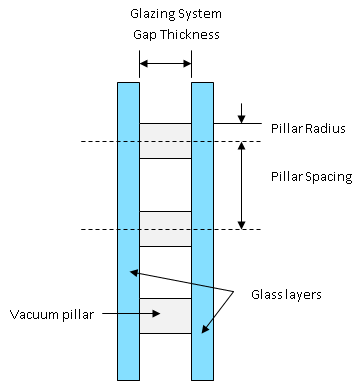
\includegraphics[width=0.9\textwidth, height=0.9\textheight, keepaspectratio=true]{media/image029.png}
\caption{Support Pillar \protect \label{fig:support-pillar}}
\end{figure}

\subsubsection{Inputs}\label{inputs-20-006}

\paragraph{Field: Name}\label{field-name-14-009}

Unique name of the support pillar.

\paragraph{Field: Spacing}\label{field-spacing}

Distance (m) between support pillar centers (see the Engineering reference document for more information).

\paragraph{Field: Radius}\label{field-radius}

The radius (m) of the support pillar (see Engineering reference document for more information).

An IDF example for vacuum glazing (see Vacuum Glazing example in WindowMaterial:Gap above)

\begin{lstlisting}

WindowGap:SupportPillar,       !- gap support pillar
    SupportPillar_16_Gap_1,      !- basis matrix name
    0.05,                        !- pillar spacing
    0.005;                       !- pillar radius
\end{lstlisting}

\subsection{WindowMaterial:SimpleGlazingSystem}\label{windowmaterialsimpleglazingsystem}

\warning{This model should be used with caution. There may be significant differences in performance between the simple window system and the usual more detailed model.}

This input object differs from the other WindowMaterial objects in that it describes an entire glazing system rather than individual layers. This object is used when only very limited information is available on the glazing layers or when specific performance levels are being targeted. The layer by layer description offers superior method of modeling windows that should be used instead of this object when sufficient data are available. This object accesses a model that turns simple performance indices into a fuller model of the glazing system.

The performance indices are U-factor and Solar Heat Gain Coefficient, and optionally Visible Transmittance. The values for these performance indices can be selected by the user to represent either glazing-only windows (with no frame) or an average window performance that includes the frame. Inside the program the model produces an equivalent window glazing layer with no frame. The properties of the modeled glazing layer are reported to the EIO file using the IDF input object syntax for the WindowMaterial:Glazing input object. This equivalent layer could be reused in subsequent models if desired, however there will be important differences in the modeled window performance because the simple glazing system model includes its own special model for angular dependence when incident beam solar is not normal to the plane of the window.

When this object is referenced in a Construction object, it cannot be used with other glazing or gas material layers. Shades or blinds cannot be located between the glass, but these can be used on the inside or the outside of the glazing system.~~ If the glazing system does have between-the-glass shades or blinds, then the U and SHGC values entered in this object should include the impacts of those layers. Adding window treatment layers such as shades or screens will alter the overall performance to be different than the performance levels prescribed in this object.

\subsubsection{Inputs}\label{inputs-21-006}

\paragraph{Field: Name}\label{field-name-15-009}

The name of the glazing system.~ This value is unique across all constructions.

\paragraph{Field: U-Factor}\label{field-u-factor}

This field describes the value for window system U-Factor, or overall heat transfer coefficient. Units are in W/m\(^{2}\)·K. This is the rated (NFRC) value for U-factor under winter heating conditions. The U-factor is assumed to be for vertically mounted products. Although the maximum allowable input is U-7.0 W/m\(^{2}\)·K, the effective upper limit of the glazings generated by the underlying model is around U-5.8 W/m\(^{2}\)·K.

\paragraph{Field: Solar Heat Gain Coefficient}\label{field-solar-heat-gain-coefficient}

This field describes the value for SHGC, or solar heat gain coefficient. There are no units. This is the rated (NFRC) value for SHGC under summer cooling conditions and represents SHGC for normal incidence and vertical orientation.

\paragraph{Field: Visible Transmittance}\label{field-visible-transmittance}

This field is optional. If it is omitted, then the visible transmittance properties are taken from the solar properties. If it is included then the model includes it when developing properties for the glazing system. This is the rated (NFRC) value for visible transmittance at normal incidence.

An example of this object.

\begin{lstlisting}

WindowMaterial:SimpleGlazingSystem,
      SimpleWindow:DOUBLE PANE WINDOW , !- Name
      2.716 , !-  U-Factor
      0.763 , !-  Solar Heat Gain Coefficient
      0.812 ; !-  Visible Transmittance
\end{lstlisting}

\subsection{WindowMaterial:Shade}\label{windowmaterialshade}

This object specifies the properties of window shade materials. Reflectance and emissivity properties are assumed to be the same on both sides of the shade. Shades are considered to be perfect diffusers (all transmitted and reflected radiation is hemispherically-diffuse) with transmittance and reflectance independent of angle of incidence. There is an EnergyPlus Reference Data Set for WindowMaterial:Shade that contains properties of generic window shades.

Window shades can be on the inside of the window (``interior shades''), on the outside of the window (``exterior shades''), or between glass layers (``between-glass shades''). When in place, the shade is assumed to cover all of the glazed part of the window, including dividers; it does not cover any of the window frame, if present. The plane of the shade is assumed to be parallel to the glazing.

WindowMaterial:Shade can be used for diffusing materials such as drapery and translucent roller shades. For slat-type shading devices, like Venetian blinds, that have a strong angular dependence of transmission, absorption and reflection, it is better to use WindowMaterial:Blind. WindowMaterial:Screen should be used to model wire mesh insect screens where the solar and visible transmission and reflection properties vary with the angle of incidence of solar radiation.

Transmittance and reflectance values for drapery material with different color and openness of weave can be obtained from manufacturers or determined from 2001 ASHRAE Fundamentals, Chapter 30, Fig. 31.

There are two methods of assigning a shade to a window:

\subsubsection{Inputs}\label{inputs-22-005}

\paragraph{Method 1:}\label{method-1}

1)~~~Define the construction of the window without the shade, the so-called ``bare'' construction.

2)~~~Reference the bare construction in the FenestrationSurface:Detailed for the window.

3)~~~Define the WindowMaterial:Shade.

4)~~~Define a WindowProperty:ShadingControl for the window in which you (a) specify that this WindowMaterial:Shade is the window's shading device and (b) specify how the shade is controlled.

\paragraph{Method 2:}\label{method-2}

1)~~~Define the Construction of the window without the shade, the so-called ``bare'' construction.

2)~~~Reference the bare construction in the FenestrationSurface:Detailed for the window.

3)~~~Define the WindowMaterial:Shade.

4)~~~Define another Construction, called the ``shaded construction,'' that includes the WindowMaterial:Shade.

5)~~~Define a WindowProperty:ShadingControl for the window in which you (a) reference the shaded construction and (b) specify how the shade is controlled.

Note that WindowProperty:ShadingControl has to be used with either method, even if the shade is in place at all times. You will get an error message if you try to reference a shaded construction directly from FenestrationSurface:Detailed.

\paragraph{Field: Name}\label{field-name-16-009}

Name of the shade. It is referenced as an inside or outside layer in a window construction.

\paragraph{Field: Solar Transmittance}\label{field-solar-transmittance}

Transmittance averaged over the solar spectrum. Assumed independent of incidence angle.

\paragraph{Field: Solar Reflectance}\label{field-solar-reflectance}

Reflectance averaged over the solar spectrum. Assumed same on both sides of shade and independent of incidence angle.

\paragraph{Field: Visible Transmittance}\label{field-visible-transmittance-1}

Transmittance averaged over the solar spectrum and weighted by the response of the human eye. Assumed independent of incidence angle.

\paragraph{Field: Visible Reflectance}\label{field-visible-reflectance}

Reflectance averaged over the solar spectrum and weighted by the response of the human eye. Assumed same on both side of shade and independent of incidence angle.

\paragraph{Field: Thermal Hemispherical Emissivity}\label{field-thermal-hemispherical-emissivity}

Effective long-wave emissivity. Assumed same on both sides of shade. We can approximate this~ effective emissivity, \(\varepsilon_{eff}\), as follows. Let \(\eta\) be the ``openness'' the shade, i.e.,~ the ratio of the area of openings in the shade to the overall shade area (see Field: Air-Flow Permeability, below). Let the emissivity of the shade material be \(\varepsilon\). Then

\begin{equation}
{\varepsilon_{{\rm{eff}}}} \approx \varepsilon \left( {1 - \eta } \right)
\end{equation}

For most non-metallic materials \(\varepsilon\) is about 0.9.

\paragraph{Field: Thermal Transmittance}\label{field-thermal-transmittance}

Effective long-wave transmittance. Assumed independent of incidence angle. We can approximate this effective long-wave transmittance, \(T_{\rm{eff}}\) as follows. Let \(\eta\) be the ``openness'' of the shade, i.e., the ratio of the area of openings in the shade to the overall shade area. Let the long-wave transmittance of the shade material be \(T\). Then

\begin{equation}
T_{\rm{eff}} \approx \eta + T \left( 1 - \eta \right)
\end{equation}

For most materials \(T\) is very close to zero, which gives

\begin{equation}
T_{\rm{eff}} \approx \eta
\end{equation}

\paragraph{Field: Thickness}\label{field-thickness-6}

Thickness of the shade material (m). If the shade is not flat, such as for pleated pull-down shades or folded drapery, the average thickness normal to the plane of the shade should be used.

\paragraph{Field: Conductivity}\label{field-conductivity-3}

Shade material conductivity (W/m-K).

\paragraph{Field: Shade to Glass Distance}\label{field-shade-to-glass-distance}

Distance from shade to adjacent glass (m). This is denoted by \emph{s} in Figure~\ref{fig:vertical-section-a-and-perspective-view-b-of} and Figure~\ref{fig:examples-of-air-flow-openings-for-an-interior}, below. If the shade is not flat, such as for pleated pull-down shades or folded drapery, the average shade-to-glass distance should be used. (The shade-to-glass distance is used in calculating the natural convective air flow between glass and shade produced by buoyancy effects.). Note used for between-glass shades.

In the following, \emph{H} is the glazing height and \emph{W} is the glazing width.

\paragraph{Field: Top Opening Multiplier}\label{field-top-opening-multiplier}

Effective area for air flow at the top of the shade divided by \emph{sW}, the horizontal area between glass and shade (see Figures below).

\paragraph{Field: Bottom Opening Multiplier}\label{field-bottom-opening-multiplier}

Effective area for air flow at the bottom of the shade divided by \emph{sW}, the horizontal area between glass and shade (see Figures below).

\paragraph{Field: Left-Side Opening Multiplier}\label{field-left-side-opening-multiplier}

Effective area for air flow at the left side of the shade divided by \emph{sH}, the vertical area between glass and shade (see Figures below).

\paragraph{Field: Right-Side Opening Multiplier}\label{field-right-side-opening-multiplier}

Effective area for air flow at the right side of the shade divided by \emph{sH}, the vertical area between glass and shade (see Figures below).

\paragraph{Field: Field: Air-Flow Permeability}\label{field-field-air-flow-permeability}

The fraction of the shade surface that is open to air flow, i.e., the total area of openings (``holes'') in the shade surface divided by the shade area, \emph{HW}. If air cannot pass through the shade material, Air-Flow Permeability = 0. For drapery fabric and screens the Air-Flow Permeability can be taken as the ``openness'' of the fabric (see 2001 ASHRAE Fundamentals, Chapter 30, Fig. 31), which is 0.0 to 0.07 for closed weave, 0.07 to 0.25 for semi-open weave, and 0.25 and higher for open weave.

\begin{figure}[hbtp] % fig 12
\centering
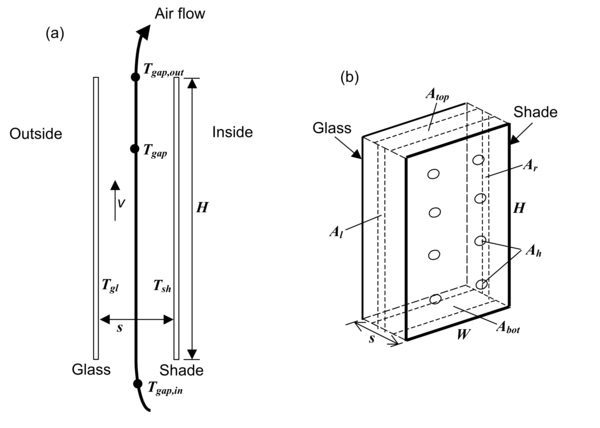
\includegraphics[width=0.9\textwidth, height=0.9\textheight, keepaspectratio=true]{media/image033.png}
\caption{Vertical section (a) and perspective view (b) of glass  and interior shade layers  showing variables used in the gap air flow analysis. In (b), the air-flow opening areas \(A_{\rm{bot}}\), \(A_{\rm{top}}\), \(A_{l}\), \(A_{r}\) and \(A_{h}\) are shown schematically. See \emph{Engineering Manual} for definition of thermal variables. \protect \label{fig:vertical-section-a-and-perspective-view-b-of}}
\end{figure}

\begin{figure}[hbtp] % fig 13
\centering
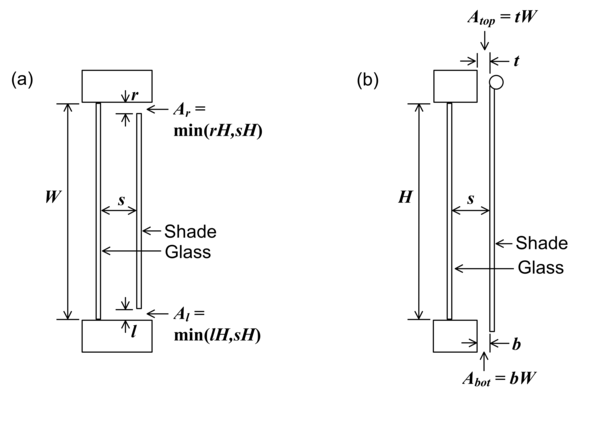
\includegraphics[width=0.9\textwidth, height=0.9\textheight, keepaspectratio=true]{media/image034.png}
\caption{Examples of air-flow openings for an interior shade covering glass of height \(H\) and width \(W\). Not to scale. (a) Horizontal section through shade with openings on the left and right sides (top view). (b) Vertical section through shade with openings at the top and bottom (side view). In (a) Left-Side Opening Multiplier = \(A_{l}/sH = min(l/s, 1)\) and Right-Side Opening Multiplier = \(A_{r}/sH = min(r/s, 1)\). In (b) Top Opening Multiplier = \(A_{\rm{top}}/sW = t/s\) and Bottom Opening Multiplier = \(A_{\rm{bot}}/sW = b/s\). \protect \label{fig:examples-of-air-flow-openings-for-an-interior}}
\end{figure}

An IDF example:

\begin{lstlisting}
WindowMaterial:Shade,
  DRAPES - CLOSE WEAVE MEDIUM,  !- Name
  0.05,                         !- Solar transmittance
  0.3000000,                    !- Solar Reflectance
  .05,                          !- Visible transmittance
  0.3000000,                    !- Visible reflectance
  0.9000000,                    !- Thermal Hemispherical Emissivity
  0.0,                          !- Thermal Transmittance
  0.003,                        !- Thickness {m}
  0.1,                          !- Conductivity {W/m-K}
  0.050,                        !- Shade to glass distance {m}
  1.0,                          !- Top opening multiplier
  1.0,                          !- Bottom opening multiplier
  0.0,                          !- Left-side opening multiplier
  0.0,                          !- Right-side opening multiplier
  0.0;                          !- Air flow permeability
\end{lstlisting}

\subsection{WindowMaterial:Blind}\label{windowmaterialblind}

This object specifies the properties of a window blind consisting of flat, equally-spaced slats. Unlike window shades, which are modeled as perfect diffusers, window blinds have solar and visible transmission and reflection properties that strongly depend on slat angle and angle of incidence of solar radiation. There is an EnergyPlus Reference Data Set for WindowMaterial:Blind that contains properties of generic window blinds.

Blinds can be located on the inside of the window (``interior blinds''), on the outside of the window (``exterior blinds''), or between two layers of glass (``between-glass blinds''). When in place, the blind is assumed to cover all of the glazed part of the window, including dividers; it does not cover any of the window frame, if present. The plane of the blind is assumed to be parallel to the glazing. When the blind is retracted it is assumed to cover none of the window. The solar and thermal effects of the blind's support strings, tapes or rods are ignored. Slat curvature, if present, is ignored.

There are two methods of assigning a blind to a window:

\subsubsection{Inputs}\label{inputs-23-005}

\paragraph{Method 1:}\label{method-1-1}

1)~~~Define the construction of the window without the blind, the so-called ``bare'' construction.

2)~~~Reference the bare construction in the FenestrationSurface:Detailed for the window.

3)~~~Define the WindowMaterial:Blind.

4)~~~Define a WindowProperty:ShadingControl for the window in which you (a) specify that this WindowMaterial:Blind is the window's shading device and (b) specify how the blind is controlled.

\paragraph{Method 2:}\label{method-2-1}

1)~~~Define the Construction of the window without the blind, the so-called ``bare'' construction.

2)~~~Reference the bare construction in the FenestrationSurface:Detailed for the window.

3)~~~Define the WindowMaterial:Blind.

4)~~~Define another Construction, called the ``shaded construction,'' that includes the WindowMaterial:Blind.

5)~~~Define a WindowProperty:ShadingControl for the window in which you (a) reference the shaded construction and (b) specify how the blind is controlled.

Note that WindowProperty:ShadingControl has to be used with either method, even if the blind is in place at all times. You will get an error message if you try to reference a construction with a blind directly from Window objects (FenestrationSurface:Detailed or Window).

Note also that WindowProperty:ShadingControl is used to determine not only when the blind is in place, but how its slat angle is controlled.

\paragraph{Field: Name}\label{field-name-17-007}

Name of the blind. It is referenced as a layer in a window construction (ref: Construction object) or as a ``Material Name of Shading Device'' in a WindowProperty:ShadingControl object.

\paragraph{Field: Slat Orientation}\label{field-slat-orientation}

The choices are Horizontal and Vertical. ``Horizontal'' means the slats are parallel to the bottom of the window; this is the same as saying that the slats are parallel to the X-axis of the window. ``Vertical'' means the slats are parallel to Y-axis of the window.

\paragraph{Field: Slat Width}\label{field-slat-width}

The width of the slat measured from edge to edge (m). See Figure~\ref{fig:a-side-view-of-a-window-blind-with-horizontal}.

\paragraph{Field: Slat Separation}\label{field-slat-separation}

The distance between the front of a slat and the back of the adjacent slat (m). See Figure~\ref{fig:a-side-view-of-a-window-blind-with-horizontal}.

\paragraph{Field: Slat Thickness}\label{field-slat-thickness}

The distance between the faces of a slat (m). See Figure~\ref{fig:a-side-view-of-a-window-blind-with-horizontal}.

\paragraph{Field: Slat Angle}\label{field-slat-angle}

The angle (degrees) between the glazing outward normal and the slat outward normal, where the outward normal points away from the front face of the slat (degrees). See Figure~\ref{fig:a-side-view-of-a-window-blind-with-horizontal}.

If the WindowProperty:ShadingControl for the blind has Type of Slat Angle Control for Blinds = FixedSlatAngle, the slat angle is fixed at ``Slat Angle.''

If Type of Slat Angle Control for Blinds = BlockBeamSolar, the program automatically adjusts the slat angle so as just block beam solar radiation. In this case the value of ``Slat Angle'' is used only when the blind is in place and there is no beam solar radiation incident on the blind.

If Type of Slat Angle Control for Blinds = ScheduledSlatAngle, the slat angle is variable. In this case ``Slat Angle'' is not applicable and the field should be blank.

If Type of Slat Angle Control for Blinds = FixedSlatAngle and ``Slat Angle'' is less than the minimum or greater than the maximum allowed by Slat Width, Slat Separation and Slat Thickness, the slat angle will be reset to the corresponding minimum or maximum and a warning will be issued.

\paragraph{Field: Slat Conductivity}\label{field-slat-conductivity}

The thermal conductivity of the slat (W/m-K).

\paragraph{Field: Slat Beam Solar Transmittance}\label{field-slat-beam-solar-transmittance}

The beam solar transmittance of the slat, assumed to be independent of angle of incidence on the slat. Any transmitted beam radiation is assumed to be 100\% diffuse (i.e., slats are translucent).

\paragraph{Field: Front Side Slat Beam Solar Reflectance}\label{field-front-side-slat-beam-solar-reflectance}

The beam solar reflectance of the front side of the slat, assumed to be independent of angle of incidence (matte finish). This means that slats with a large specularly-reflective component (shiny slats) are not well modeled.

\paragraph{Field: Back Side Slat Beam Solar Reflectance}\label{field-back-side-slat-beam-solar-reflectance}

The beam solar reflectance of the back side of the slat, assumed to be independent of angle of incidence (matte finish). This means that slats with a large specularly-reflective component (shiny slats) are not well modeled.

\paragraph{Field: Slat Diffuse Solar Transmittance}\label{field-slat-diffuse-solar-transmittance}

The slat transmittance for hemispherically diffuse solar radiation. This value should equal ``Slat Beam Solar Transmittance.''

\paragraph{Field: Front Side Slat Diffuse Solar Reflectance}\label{field-front-side-slat-diffuse-solar-reflectance}

The front-side slat reflectance for hemispherically diffuse solar radiation. This value should equal ``Front Side Slat Beam Solar Reflectance.''

\paragraph{Field: Back Side Slat Diffuse Solar Reflectance}\label{field-back-side-slat-diffuse-solar-reflectance}

The back-side slat reflectance for hemispherically diffuse solar radiation. This value should equal ``Back Side Slat Beam Solar Reflectance.''

\paragraph{Field: Slat Beam Visible Transmittance}\label{field-slat-beam-visible-transmittance}

The beam visible transmittance of the slat, assumed to be independent of angle of incidence on the slat. Any transmitted visible radiation is assumed to be 100\% diffuse (i.e., slats are translucent).

\paragraph{Field: Front Side Slat Beam Visible Reflectance}\label{field-front-side-slat-beam-visible-reflectance}

The beam visible reflectance on the front side of the slat, assumed to be independent of angle of incidence (matte finish). This means that slats with a large specularly-reflective component (shiny slats) are not well modeled.

\paragraph{Field: Back Side Slat Beam Visible Reflectance}\label{field-back-side-slat-beam-visible-reflectance}

The beam visible reflectance on the front side of the slat, assumed to be independent of angle of incidence (matte finish). This means that slats with a large specularly-reflective component (shiny slats) are not well modeled.

\paragraph{Field: Slat Diffuse Visible Transmittance}\label{field-slat-diffuse-visible-transmittance}

The slat transmittance for hemispherically diffuse visible radiation. This value should equal ``Slat Beam Visible Transmittance.''

\paragraph{Field: Front Side Slat Diffuse Visible Reflectance}\label{field-front-side-slat-diffuse-visible-reflectance}

The front-side slat reflectance for hemispherically diffuse visible radiation. This value should equal ``Front Side Slat Beam Visible Reflectance.''

\paragraph{Field: Back Side Slat Diffuse Visible Reflectance}\label{field-back-side-slat-diffuse-visible-reflectance}

The back-side slat reflectance for hemispherically diffuse visible radiation. This value should equal ``Back Side Slat Beam Visible Reflectance..''

\paragraph{Field: Slat Infrared Hemispherical Transmittance}\label{field-slat-infrared-hemispherical-transmittance}

The slat Infrared transmittance. It is zero for solid metallic, wooden or glass slats, but may be non-zero in some cases (e.g., thin plastic slats).

\paragraph{Field: Front Side Slat Infrared~ Hemispherical Emissivity}\label{field-front-side-slat-infrared-hemispherical-emissivity}

Front-side hemispherical emissivity of the slat. Approximately 0.9 for most materials. The most common exception is bare (unpainted) metal slats or slats finished with a metallic paint.

\paragraph{Field: Back Side Slat Infrared~ Hemispherical Emissivity}\label{field-back-side-slat-infrared-hemispherical-emissivity}

Back-side hemispherical emissivity of the slat. Approximately 0.9 for most materials. The most common exception is bare (unpainted) metal slats or slats finished with a metallic paint.

\paragraph{Field: Blind to Glass Distance}\label{field-blind-to-glass-distance}

For interior and exterior blinds, the distance from the mid-plane of the blind to the adjacent glass (m). See Figure~\ref{fig:a-side-view-of-a-window-blind-with-horizontal}. Not used for between-glass blinds. As for window shades (ref: WindowMaterial:Shade) this distance is used in calculating the natural convective air flow between glass and blind that is produced by buoyancy effects.

\paragraph{Opening Multipliers}\label{opening-multipliers}

The following opening multipliers are defined in the same way as for window shades (see WindowMaterial:Shade, Figure~\ref{fig:vertical-section-a-and-perspective-view-b-of} and Figure~\ref{fig:examples-of-air-flow-openings-for-an-interior}). Note that, unlike window shades, there is no input for Air-Flow Permeability; this is automatically calculated by the program from slat angle, width and separation.

\paragraph{Field: Blind Top Opening Multiplier}\label{field-blind-top-opening-multiplier}

Defined as for Material:WindowShade.

\paragraph{Field: Blind Bottom Opening Multiplier}\label{field-blind-bottom-opening-multiplier}

Defined as for Material:WindowShade.

\paragraph{Field: Blind Left-Side Opening Multiplier}\label{field-blind-left-side-opening-multiplier}

Defined as for Material:WindowShade.

\paragraph{Field: Blind Right-Side Opening Multiplier}\label{field-blind-right-side-opening-multiplier}

Defined as for Material:WindowShade.

\paragraph{Field: Minimum Slat Angle}\label{field-minimum-slat-angle}

The minimum allowed slat angle (degrees). Used only if WindowProperty:ShadingControl (for the window that incorporates this blind) varies the slat angle (i.e., the WindowProperty:ShadingControl has Type of Slat Angle Control for Blinds = ScheduledSlatAngle or BlockBeamSolar). In this case, if the program tries to select a slat angle less than Minimum Slat Angle it will be reset to Minimum Slat Angle. (Note that if the Minimum Slat Angle itself is less than the minimum allowed by Slat Width, Slat Separation and Slat Thickness, it will be reset to that minimum.)

\paragraph{Field: Maximum Slat Angle}\label{field-maximum-slat-angle}

The maximum allowed slat angle (degrees). Used only if WindowProperty:ShadingControl (for the window that incorporates this blind) varies the slat angle (i.e., the WindowProperty:ShadingControl has Type of Slat Angle Control for Blinds = ScheduledSlatAngle or BlockBeamSolar). In this case, if the program tries to select a slat angle greater than Maximum Slat Angle the slat angle will be reset to Maximum Slat Angle. (Note that if the Maximum Slat Angle itself is greater than the maximum allowed by Slat Width, Slat Separation and Slat Thickness, it will be reset to that maximum.)

An IDF example:

\begin{lstlisting}

WindowMaterial:Blind,
   White Painted Metal Blind,   !- Name
   HORIZONTAL, !- Slat orientation
   0.025   , !- Slat width (m)
   0.01875 , !- Slat separation (m)
   0.001   , !- Slat thickness (m)
   45.0    , !- Slat angle (deg)
   44.9    , !- Slat conductivity (W/m-K)
   0.0     , !- Slat beam solar transmittance
   0.8     , !- Front Side Slat beam solar reflectance
   0.8     , !- Back Side Slat beam solar reflectance
   0.0     , !- Slat diffuse solar transmittance
   0.8     , !- Front Side Slat diffuse solar reflectance
   0.8     , !- Back Side Slat diffuse solar reflectance
   0.0     , !- Slat beam visible transmittance
   0.7     , !- Front Side Slat beam visible reflectance
   0.7     , !- Back Side Slat beam visible reflectance
   0.0     , !- Slat diffuse visible transmittance
   0.7     , !- Front Side Slat diffuse visible reflectance
   0.7     , !- Back Side Slat diffuse visible reflectance
   0.0     , !- Slat Infrared hemispherical transmittance
   0.9     , !- Front Side Slat Infrared hemispherical emissivity
   0.9     , !- Back Side Slat Infrared hemispherical emissivity
   0.050   , !- Blind-to-glass distance
   0.0     , !- Blind top opening multiplier
   0.0     , !- Blind bottom opening multiplier
   0.5     , !- Blind left-side opening multiplier
   0.5     , !- Blind right-side opening multiplier
   ,         !- Minimum slat angle (deg)
   ;         !- Maximum slat angle (deg)
\end{lstlisting}

\begin{figure}[hbtp] % fig 14
\centering
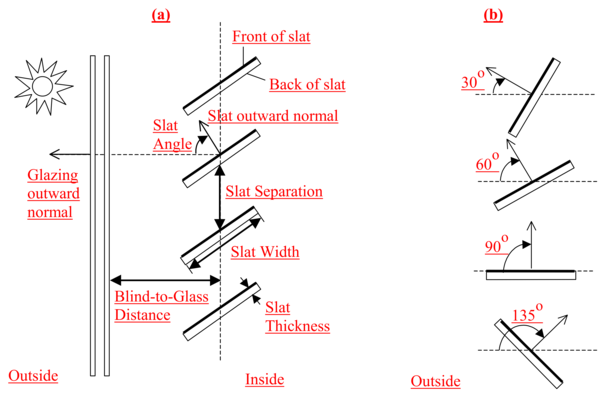
\includegraphics[width=0.9\textwidth, height=0.9\textheight, keepaspectratio=true]{media/image035.png}
\caption{(a) Side view of a window blind with horizontal slats (or top view of blind with vertical slats) showing slat geometry. The front face of a slat is shown by a heavy line. The slat angle is defined as the angle between the glazing outward normal and the slat outward normal, where the outward normal points away from the front face of the slat. (b) Slat orientations for representative slat angles. The slat angle varies from 0\(^{o}\), when the front of the slat is parallel to the glazing and faces toward the outdoors,  to 90\(^{o}\), when the slat is perpendicular to the glazing, to 180\(^{o}\), when the front of the slat is parallel to the glazing and faces toward the indoors. The minimum and maximum slat angles are determined by the slat thickness, width and separation. \protect \label{fig:a-side-view-of-a-window-blind-with-horizontal}}
\end{figure}

\subsection{WindowMaterial:ComplexShade}\label{windowmaterialcomplexshade}

This input object is used to define shade layers used in the Construction:ComplexFenestrationState object.

\subsubsection{Inputs}\label{inputs-24-003}

\paragraph{Field: Name}\label{field-name-18-007}

Unique name of the shading layer.

\paragraph{Field: Shading Layer Type}\label{field-shading-layer-type}

The type of shading layer. The options are:

\begin{itemize}
\item
  Venetian -- for modeling venetian blinds
\item
  Woven -- for modeling shading systems with a regular weave
\item
  Perforated -- for modeling perforated screens
\item
  BSDF -- for modeling shades whose properties are represented by a BSDF file
\item
  OtherShadingType -- for modeling shading systems which do not belong to the any of the previous group
\end{itemize}

\paragraph{Field: Thickness}\label{field-thickness-7}

The thickness (m) of the shading layer. This value is ignored for ShadingLayerType = Venetian, because the program will calculate the thickness based on the slat angle. This value is needed for ShadingLayerType = Woven and Perforated

\paragraph{Field: Conductivity}\label{field-conductivity-4}

The conductivity (W/mK) of the shading layer material. Default: 1.0

\begin{itemize}
\item
  Venetian -- the conductivity of the venetian blind slat material
\item
  Woven -- the conductivity of the woven shade material (such as the thread for a fabric shade)
\item
  Perforated -- for modeling perforated screens
\item
  BSDF -- for modeling shades whose properties are represented by a BSDF file
\item
  OtherShadingType -- for modeling shading systems which do not belong to the any of the previous group
\end{itemize}

\paragraph{Field: IR Transmittance}\label{field-ir-transmittance}

The IR transmittance of the shading layer. Minimum value: 0. Maximum value: 1. Default: 0.

\paragraph{Field: Front Emissivity}\label{field-front-emissivity}

The front emissivity of the shading layer. Minimum value: 0. Maximum value: 1. Default: 0.90.

\paragraph{Field: Back Emissivity}\label{field-back-emissivity}

The back emissivity of the shading layer. Minimum value: 0. Maximum value: 1. Default: 0.90.

\paragraph{Field: Top Opening Multiplier}\label{field-top-opening-multiplier-1}

The top opening multiplier value will depend on the location of the shading device within the glazing system. There are several possible scenarios which can occur and they can be divided into two groups:

\textbf{Shading device on the indoor/outdoor side of the window}

In this case the opening multiplier is calculated as the smallest distance between the shading device and the frame (d\(_{top}\)), divided by the gap width (S). There are three possible cases for the position of a shading device the on indoor/outdoor side (see Figure~\ref{fig:three-cases-for-the-dp-calculation-for-an-indoor-outdoor-shade}).

\begin{figure}[htbp]
\centering
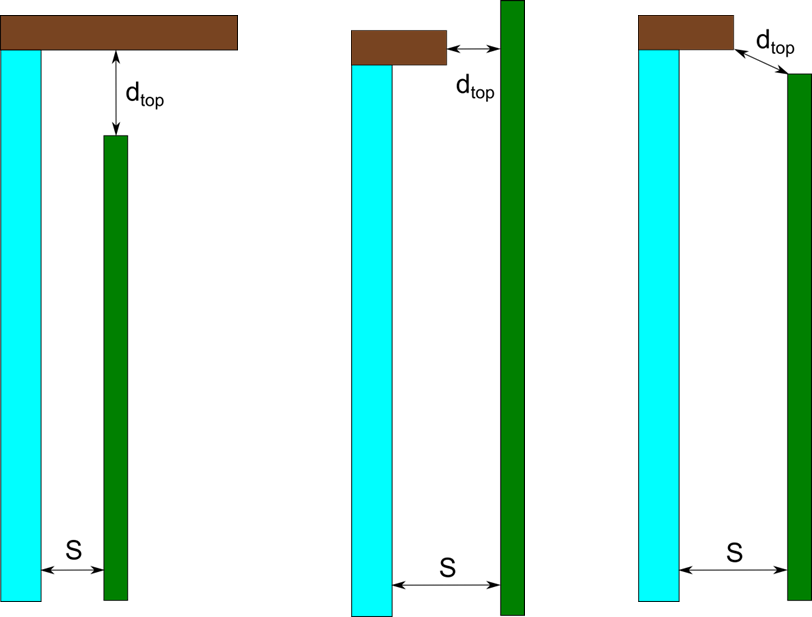
\includegraphics[width=0.9\textwidth, height=0.9\textheight, keepaspectratio=true]{media/three-cases-for-the-dtop-calculation-for-an-indoor-outdoor-shade-collage.png}
\caption{Three cases for the D\(_{top}\) calculation for an indoor/outdoor shade: Case a) A shading device between the frame; Case b) A shading device outside the frame, covering the frame; Case c) a shading device outside the frame, not covering the frame. \protect \label{fig:three-cases-for-the-dp-calculation-for-an-indoor-outdoor-shade}}
\end{figure}

In the case where the distance between the frame and the shading device is bigger than the gap width, the d\(_{top}\) multiplier is equal to one. Therefore, the calculation of the D\(_{top}\) opening multiplier is:

\begin{equation*}
A_{top} = min(d_{top}/S, 1)
\end{equation*}

\textbf{Shading device between glass layers}

In this case the opening multiplier is calculated as the smallest distance between the shading device and the frame or spacer (d\(_{top}\)), divided by the smaller gap width (the minimum of (S\(_{1}\) andS\(_{2}\))).

\begin{figure}[htbp]
\centering
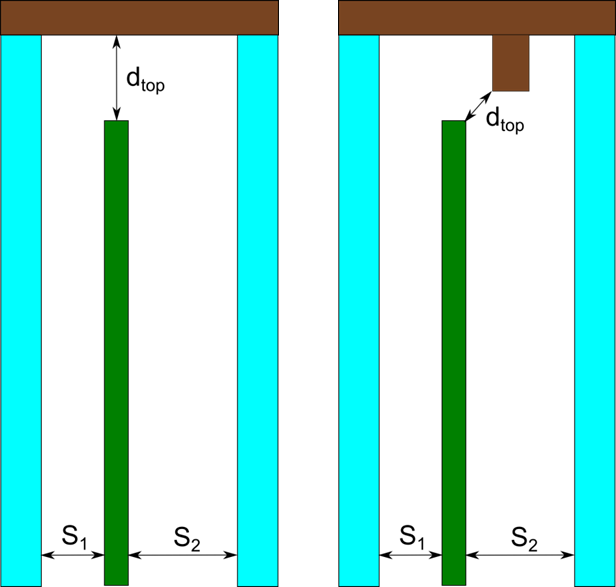
\includegraphics[width=0.9\textwidth, height=0.9\textheight, keepaspectratio=true]{media/calculation-of-dtop-for-a-shading-device-collage.png}
\caption{Calculation of Dtop for a shading device between glass layers \protect \label{fig:calculation-of-dtop-for-a-shading-device-between-glass-layers}}
\end{figure}

The D\(_{top}\) opening multiplier for a between glass shade is calculated as:

\begin{equation*}
A_{top} = min(d_{top}/S_{min}, 1)
\end{equation*}

Where

\begin{equation*}
S_{min} = min(S_1, S_2)
\end{equation*}

\paragraph{Field: Bottom Opening Multiplier}\label{field-bottom-opening-multiplier-1}

The bottom opening multiplier (d\(_{bot}\)) is calculated in the same way as the top opening multiplier, with the rules applied to the bottom of the shading device.

\paragraph{Field: Left Side Opening Multiplier}\label{field-left-side-opening-multiplier-1}

The left side opening multiplier (d\(_{left}\)) is calculated in the same way as the top opening multiplier, with the rules applied to the left side of the shading device.

\paragraph{Field: Right Side Opening Multiplier}\label{field-right-side-opening-multiplier-1}

The right side opening multiplier (d\(_{right}\)) is calculated in the same way as the top opening multiplier, with the rules applied to the right side of the shading device.

\paragraph{Field: Front Opening Multiplier}\label{field-front-opening-multiplier}

The fraction of glazing system area that is open on the front of the shading layer (see Figure~\ref{fig:front-view-of-shading-layer-openings.}). This fraction is calculated as follows: Afront / (W * H), where Afront = Area of the front of the glazing system that is not covered by the shading system, W = the width of the glazing system (IGU) and H is height of the glazing system (IGU).

\begin{figure}[hbtp] % fig 17
\centering
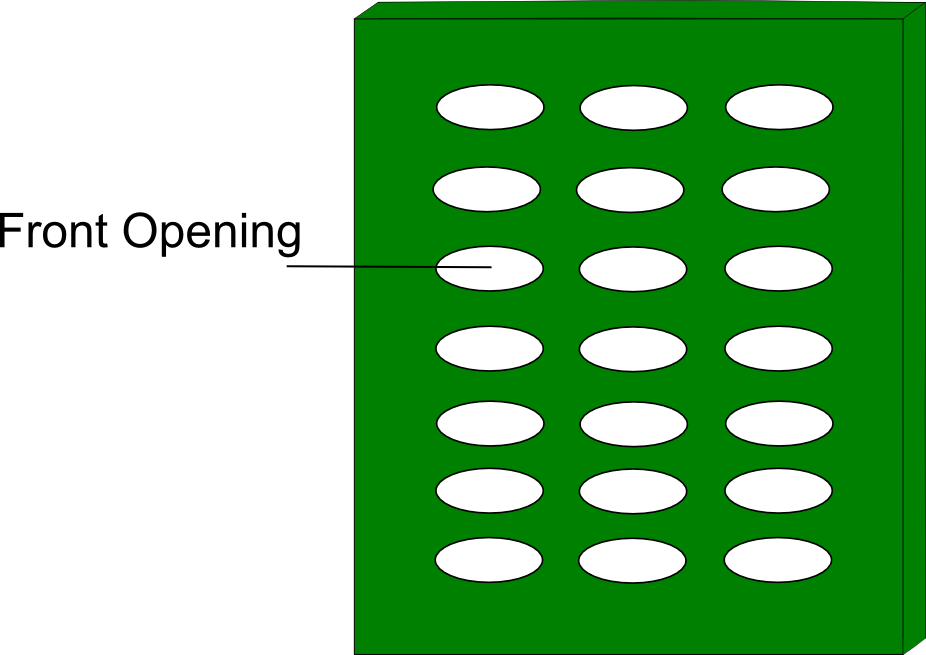
\includegraphics[width=0.9\textwidth, height=0.9\textheight, keepaspectratio=true]{media/image041.png}
\caption{Front view of shading layer openings. \protect \label{fig:front-view-of-shading-layer-openings.}}
\end{figure}

\paragraph{Field: Slat Width}\label{field-slat-width-1}

The width (m) of the venetian slats.~ Used only for ShadingLayerType = Venetian.

\paragraph{Field: Slat Spacing}\label{field-slat-spacing}

The distance (m) between front sides of the venetian slats.~ Used only for ShadingLayerType = Venetian.

\paragraph{Field: Slat Thickness}\label{field-slat-thickness-1}

The thickness (m) of the venetian slats.~ Used only for ShadingLayerType = Venetian.

\paragraph{Field: Slat Angle}\label{field-slat-angle-1}

The slat tilt angle (degrees) of the venetian slats.~ Used only for ShadingLayerType = Venetian.~ Range of slat angle is from -90 to 90 degrees.

\paragraph{Field: Slat Conductivity}\label{field-slat-conductivity-1}

The conductivity (W/mK) of the venetian slats.~ Used only for ShadingLayerType = Venetian.

\paragraph{Field: Slat Curve}\label{field-slat-curve}

The curvature radius (m) of the venetian slats.~ Setting this value to zero means there is no curvature in the slat (it is flat), while a non-zero value is the radius of the slat curve.~ This value cannot be smaller than Slat Width / 2.~ Used only for ShadingLayerType = Venetian.

\begin{figure}[hbtp] % fig 18
\centering
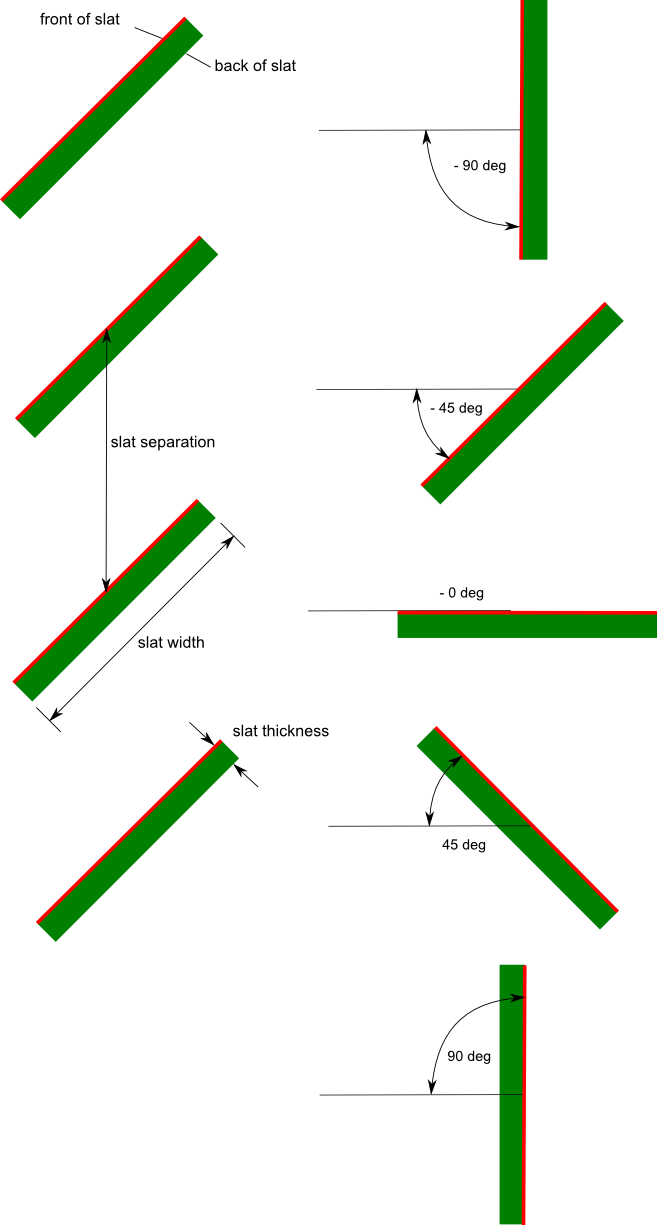
\includegraphics[width=0.9\textwidth, height=0.9\textheight, keepaspectratio=true]{media/image042.png}
\caption{Side view of horizontal venetian blind slats or top view of blinds with vertical slats.  Front face of slats is marked with red line. \protect \label{fig:side-view-of-horizontal-venetian-blind-slats}}
\end{figure}

An IDF example for ShadingLayerType = Venetian

\begin{lstlisting}

WindowMaterial:ComplexShade,       !- venetian blind layer
    Shade_30001_Layer,               !- name
    Venetian,                        !- shading layer type
    0.005,                           !- thickness
    160,                             !- layer conductivity
    0.0,                             !- IR transmittance
    0.9,                             !- front emissivity
    0.9,                             !- back emissivity
    0.0,                             !- top opening multiplier
    0.0,                             !- bottom opening multiplier
    0.0,                             !- left side opening multiplier
    0.0,                             !- right side opening multiplier
    0.05,                            !- front opening multiplier
    0.016,                           !- venetian slat width
    0.012,                           !- venetian slat spacing
    0.0006,                          !- venetian slat thickness
    -45.00,                          !- venetian slat angle
    160.00,                          !- venetian slat conductivity
    0.0000;                          !- venetian slat curve
\end{lstlisting}

An IDF example for ShadingLayerType = Woven

(Note that it is not necessary to include ``blank'' lines for the venetian blind input for a Woven shade definition).

\begin{lstlisting}

WindowMaterial:ComplexShade,       !- woven shade layer
    Shade_30002_Layer,               !- name
    Woven,                           !- shading layer type
    0.011,                           !- thickness
    1,                               !- layer conductivity
    0.0,                             !- IR transmittance
    0.9,                             !- front emissivity
    0.9,                             !- back emissivity
    0.0,                             !- top opening multiplier
    0.0,                             !- bottom opening multiplier
    0.0,                             !- left side opening multiplier
    0.0,                             !- right side opening multiplier
    0.17;                            !- front opening multiplier
\end{lstlisting}

\subsection{WindowMaterial:Screen}\label{windowmaterialscreen}

This object specifies the properties of exterior window screen materials. The window screen model assumes the screen is made up of intersecting orthogonally-crossed cylinders. The surface of the cylinders is assumed to be diffusely reflecting, having the optical properties of a Lambertian surface.

The beam solar radiation transmitted through a window screen varies with sun angle and is made up of two distinct elements: a direct beam component and a reflected beam component. The direct beam transmittance component is modeled using the geometry of the screen material and the incident angle of the sun to account for shadowing of the window by the screen material. The reflected beam component is an empirical model that accounts for the inward reflection of solar beam off the screen material surface. This component is both highly directional and small in magnitude compared to the direct beam transmittance component (except at higher incident angles, for which case the magnitude of the direct beam component is small or zero and the reflected beam component, though small in absolute terms can be many times larger than the direct beam component). For this reason, the reflected beam transmittance component calculated by the model can be a. disregarded, b. treated as an additive component to direct beam transmittance (and in the same direction), or c. treated as hemispherically-diffuse transmittance based on a user input to the model.

\begin{figure}[hbtp] % fig 19
\centering
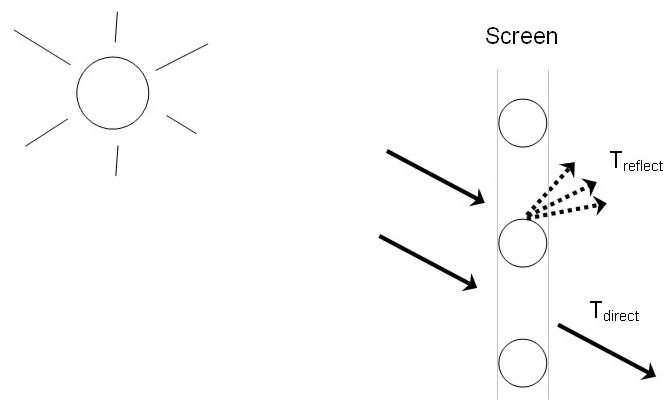
\includegraphics[width=0.9\textwidth, height=0.9\textheight, keepaspectratio=true]{media/image043.png}
\caption{Direct beam and reflected beam transmittance components \protect \label{fig:direct-beam-and-reflected-beam-transmittance}}
\end{figure}

The window screen ``assembly'' properties of overall beam solar reflectance and absorptance (including the screen material `cylinders' and open area) also change with sun angle and are calculated based on the values of the beam solar transmittance components (direct and reflected components described above) and the physical properties of the screen material (i.e., screen material diameter, spacing, and reflectance).

Transmittance, reflectance, and absorptance of diffuse solar radiation are considered constant values and apply to both the front and back surfaces of the screen. These properties are calculated by the model as an average value by integrating the screen's beam solar properties over a quarter hemisphere of incident radiation. Long-wave emissivity is also assumed to be the same for both sides of the screen.

There is an EnergyPlus Reference Data Set for WindowMaterial:Screen that contains properties for generic window screens. Window screens of this type can only be used on the outside surface of the window (``exterior screens''). When in place, the screen is assumed to cover all of the glazed part of the window, including dividers; it does not cover any of the window frame, if present. The plane of the screen is assumed to be parallel to the glazing.

WindowMaterial:Screen can be used to model wire mesh insect screens where the solar and visible transmission and reflection properties vary with the angle of incidence of solar radiation. For diffusing materials such as drapery and translucent roller shades it is better to use the WindowMaterial:Shade object. For slat-type shading devices like Venetian blinds, which have solar and visible transmission and reflection properties that strongly depend on slat angle and angle of incidence of solar radiation, it is better to use WindowMaterial:Blind.

There are two methods of assigning a screen to a window:

\subsubsection{Inputs}\label{inputs-25-003}

\paragraph{Method 1:}\label{method-1-2}

1)~~~Define the construction of the window without the screen, the so-called ``bare'' construction.

2)~~~Reference the bare construction in the FenestrationSurface:Detailed for the window.

3)~~~Define the WindowMaterial:Screen object.

4)~~~Define a WindowProperty:ShadingControl for the window in which you (a) specify that this Material:WindowScreen is the window's shading device, and (b) specify how the screen is controlled.

\paragraph{Method 2:}\label{method-2-2}

1)~~~Define the Construction of the window without the screen, the so-called ``bare'' construction.

2)~~~Reference the bare construction in the FenestrationSurface:Detailed for the window.

3)~~~Define the WindowMaterial:Screen object.

4)~~~Define another Construction, called the ``shaded construction,'' that includes the WindowMaterial:Screen.

5)~~~Define a WindowProperty:ShadingControl for the window in which you (a) reference the shaded construction, and (b) specify how the screen is controlled.

Note that WindowProperty:ShadingControl has to be used with either method, even if the screen is in place at all times. You will get an error message if you try to reference a shaded construction directly from a FenestrationSurface:Detailed object.

\paragraph{Field: Name}\label{field-name-19-004}

Enter a unique name for the screen. This name is referenced as an outside layer in a window construction.

\paragraph{Field: Reflected Beam Transmittance Accounting Method}\label{field-reflected-beam-transmittance-accounting-method}

This input specifies the method used to account for screen-reflected beam solar radiation that is transmitted through the window screen (as opposed to being reflected back outside the building). Since this inward reflecting beam solar is highly directional and is not modeled in the direction of the actual reflection, the user is given the option of how to account for the directionality of this component of beam solar transmittance. Valid choices are DoNotModel, ModelAsDirectBeam (i.e., model as an additive component to direct solar beam and in the same direction), or ModelAsDiffuse (i.e., model as hemispherically-diffuse radiation). The default value is ModelAsDiffuse.

\paragraph{Field: Diffuse Solar Reflectance}\label{field-diffuse-solar-reflectance}

This input specifies the solar reflectance (beam-to-diffuse) of the screen material itself (not the effective value for the overall screen ``assembly'' including open spaces between the screen material). The outgoing diffuse radiation is assumed to be Lambertian (distributed angularly according to Lambert's cosine law). The solar reflectance is assumed to be the same for both sides of the screen. This value must be from 0 to less than 1.0. In the absence of better information, the input value for diffuse solar reflectance should match the input value for diffuse visible reflectance.

\paragraph{Field: Diffuse Visible Reflectance}\label{field-diffuse-visible-reflectance}

This input specifies the visible reflectance (beam-to-diffuse) of the screen material itself (not the effective value for the overall screen ``assembly'' including open spaces between the screen material) averaged over the solar spectrum and weighted by the response of the human eye. The outgoing diffuse radiation is assumed to be Lambertian (distributed angularly according to Lambert's cosine law). The visible reflectance is assumed to be the same for both sides of the screen. This value must be from 0 to less than 1.0.

If diffuse visible reflectance for the screen material is not available, then the following guidelines can be used to estimate this value:

\begin{itemize}
\item
  Dark-colored screen (e.g., charcoal):~~~~~~~~~~~~~~~~~ 0.08 -- 0.10
\item
  Medium-colored screen (e.g., gray):~~~~~~~~~~~~~~~~~~ 0.20 -- 0.25
\item
  Light-colored screen (e.g., bright aluminum):~~~~~~ 0.60 -- 0.65
\end{itemize}

Commercially-available gray scale or grayscale reflecting chart references can be purchased for improved accuracy in estimating visible reflectance (by visual comparison of screen reflected brightness with that of various known-reflectance portions of the grayscale).

\paragraph{Field: Thermal Hemispherical Emissivity}\label{field-thermal-hemispherical-emissivity-1}

Long-wave emissivity \(\varepsilon\) of the screen material itself (not the effective value for the overall screen ``assembly'' including open spaces between the screen material). The emissivity is assumed to be the same for both sides of the screen.

For most non-metallic materials, \(\varepsilon\) is about 0.9. For metallic materials, \(\varepsilon\) is dependent on material, its surface condition, and temperature. Typical values for metallic materials range from 0.05 -- 0.1 with lower values representing a more finished surface (e.g.~low oxidation, polished surface). Material emissivities may be found in Table~\ref{table:atmospheric-variables-at-two-different} from the 2005 ASHRAE Handbook of Fundamentals, page 3.9. The value for this input field must be between 0 and 1, with a default value of 0.9 if this field is left blank.

\paragraph{Field: Conductivity}\label{field-conductivity-5}

Screen material conductivity (W/m-K). This input value must be greater than 0. The default value is 221 W/m-K (aluminum).

\paragraph{Field: Screen Material Spacing}\label{field-screen-material-spacing}

The spacing, S, of the screen material (m) is the distance from the center of one strand of screen to the center of the adjacent one. The spacing of the screen material is assumed to be the same in both directions (e.g., vertical and horizontal). This input value must be greater than the non-zero screen material diameter. If the spacing is different in the two directions, use the average of the two values.

\begin{figure}[hbtp] % fig 20
\centering
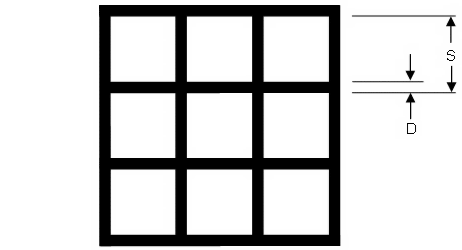
\includegraphics[width=0.9\textwidth, height=0.9\textheight, keepaspectratio=true]{media/image044.png}
\caption{Screen Material Spacing and Diameter \protect \label{fig:screen-material-spacing-and-diameter}}
\end{figure}

\paragraph{Field: Screen Material Diameter}\label{field-screen-material-diameter}

The diameter, D, of individual strands or wires of the screen material (m). The screen material diameter is assumed to be the same in both directions (e.g., vertical and horizontal). This input value must be greater than 0 and less than the screen material spacing. If the diameter is different in the two directions, use the average of the two values.

\paragraph{Field: Screen to Glass Distance}\label{field-screen-to-glass-distance}

Distance from the window screen to the adjacent glass surface (m). If the screen is not flat, the average screen to glass distance should be used. The screen-to-glass distance is used in calculating the natural convective air flow between the glass and the screen produced by buoyancy effects. This input value must be from 0.001 m to 1 m, with a default value of 0.025 m if this field is left blank.

\paragraph{Field: Top Opening Multiplier}\label{field-top-opening-multiplier-2}

Effective area for air flow at the top of the screen divided by the horizontal area between the glass and screen (see the same field for the Material:WindowShade object for additional description). The opening multiplier fields can be used to simulate a shading material that is offset from the window frame. Since window screens are typically installed against the window frame, the default value is equal to 0.This input value can range from 0 to 1.

\paragraph{Field: Bottom Opening Multiplier}\label{field-bottom-opening-multiplier-2}

Effective area for air flow at the bottom of the screen divided the horizontal area between the glass and screen (see the same field for the Material:WindowShade object for additional description). The opening multiplier fields can be used to simulate a shading material that is offset from the window frame. Since window screens are typically installed against the window frame, the default value is equal to 0. This input value can range from 0 to 1.

\paragraph{Field: Left-Side Opening Multiplier}\label{field-left-side-opening-multiplier-2}

Effective area for air flow at the left side of the screen divided the vertical area between the glass and screen (see the same field for the Material:WindowShade object for additional description). The opening multiplier fields can be used to simulate a shading material that is offset from the window frame. Since window screens are typically installed against the window frame, the default value is equal to 0. This input value can range from 0 to 1.

\paragraph{Field: Right-Side Opening Multiplier}\label{field-right-side-opening-multiplier-2}

Effective area for air flow at the right side of the screen divided the vertical area between the glass and screen (see the same field for the Material:WindowShade object for additional description). The opening multiplier fields can be used to simulate a shading material that is offset from the window frame. Since window screens are typically installed against the window frame, the default value is equal to 0. This input value can range from 0 to 1.

\paragraph{Field: Angle of Resolution for Screen Transmittance Output Map}\label{field-angle-of-resolution-for-screen-transmittance-output-map}

Angle of resolution, in degrees, for the overall screen beam transmittance (direct and reflected) output map. The comma-separated variable file eplusscreen.csv (Ref. OutputDetailsandExamples.pdf) will contain the direct beam and reflected beam solar radiation that is transmitted through the window screen as a function of incident sun angle (0 to 90 degrees relative solar azimuth and 0 to 90 degrees relative solar altitude) in sun angle increments specified by this input field. The default value is 0, which means no transmittance map is generated. Other valid choice inputs are 1, 2, 3 and 5 degrees.

An IDF example for this object, along with Construction and WindowProperty:ShadingControl objects, is shown below:

\begin{lstlisting}

WindowMaterial:Screen,
      EXTERIOR SCREEN,         !- Name
      ModelAsDiffuse,        !- Reflected Beam Transmittance Accounting Method
      0.6,                     !- Diffuse Solar Reflectance
      0.6,                     !- Diffuse Visible Reflectance
      0.9,                     !- Thermal Hemispherical Emissivity
      221.0,                   !- Conductivity {W/m-K}
      0.00154,                 !- Screen Material Spacing (m)
      0.000254,                !- Screen Material Diameter (m)
      0.025,                   !- Screen-to-Glass Distance {m}
      0.0,                     !- Top Opening Multiplier
      0.0,                     !- Bottom Opening Multiplier
      0.0,                     !- Left-Side Opening Multiplier
      0.0,                     !- Right-Side Opening Multiplier
      0;                   !- Angle of Resolution for Output Map {deg}

  Construction,
      DOUBLE PANE WITHOUT SCREEN,     !- Name
      GLASS - CLEAR SHEET 1 / 8 IN,   !- Outside Layer
      WinAirB1 - AIRSPACE RESISTANCE, !- Layer \#2
      GLASS - CLEAR SHEET 1 / 8 IN;   !- Layer \#3

  WindowProperty:ShadingControl,
      DOUBLE PANE WITH SCREEN, !- User Supplied Shading Control Name
      ExteriorScreen,          !- Shading Type
      ,                        !- Name of construction with shading
      AlwaysOn,                !- Shading Control Type
      ScreenSchedule,          !- Schedule Name
      20.0,                    !- SetPoint {W/m2, W or deg C}
      YES,                     !- Shading Control Is Scheduled
      NO,                      !- Glare Control Is Active
      EXTERIOR SCREEN,         !- Material Name of Shading Device
      ,                        !- Type of Slat Angle Control for Blinds
      ;                        !- Slat Angle Schedule Name
\end{lstlisting}

\subsection{WindowMaterial:Shade:EquivalentLayer}\label{windowmaterialshadeequivalentlayer}

This object specifies the properties of Equivalent Layer window shade (roller blind) materials. Shades are considered to be thin, flat and perfect diffusers (all transmitted and reflected radiation is hemispherically-diffuse). However, shades can have beam-beam transmittance by virtue of their material openness.~ The beam-beam transmittence is assumed to be the same for both sides of the shade and is the same as the openness area fraction. Beam-diffuse transmittance and reflectance, and emissivity properties can be different for front and back side of the shade.Window shades can be placed on the inside of the window, on the outside of the window, or between glass layers. WindowMaterial:Shade:EquivalentLayer is used for roller blinds. The off-normal solar property calculation of shades (roller blind) is based on a set of correlations developed from measurement of samples of commercially produced roller blind material with openness fraction less than 0.14. The model is not intended for materials with unusually high values of openness and should be limited to a maximum openness fraction of 0.20. The visible spectrum solar properties input fields are not used currently hence can be left blank.

\subsubsection{Inputs}\label{inputs-26-002}

\paragraph{Field: Name}\label{field-name-20-003}

Name of the shade. It is referenced as an inside, inbetween or outside layer in an equivalent layer~ window construction.

\paragraph{Field: Shade Beam-Beam Solar Transmittance}\label{field-shade-beam-beam-solar-transmittance}

This value is the beam-beam transmittance of the shade at normal incidence and it is the same as the openness area fraction of the shade material. Assumed to be the same for front and back sides of the roller blinds.~ The minimum value is 0.0 and maximum value is less than 1.0.~ The default value is 0.0. For most common shade materials (e.g.~Roller Blinds) the material oppeness fraction doesn't exceed 0.20.

\paragraph{Field: Front Side Shade Beam-Diffuse Solar Transmittance}\label{field-front-side-shade-beam-diffuse-solar-transmittance}

This value is the front side beam-diffuse transmittance of the shade material at normal incidence averaged over the entire spectrum of solar radiation. The minimum value is 0.0 and maximum value is less than 1.0.~ The default value is 0.0.

\paragraph{Field: Back Side Shade Beam-Diffuse Solar Transmittance}\label{field-back-side-shade-beam-diffuse-solar-transmittance}

This value is the back side beam-diffuse transmittance of the shade material at normal incidence averaged over the entire spectrum of solar radiation. The minimum value is 0.0 and maximum value is less than 1.0.~ The default value is 0.0.

\paragraph{Field: Front Side Shade Beam-Diffuse Solar Reflectance}\label{field-front-side-shade-beam-diffuse-solar-reflectance}

This value is the front side beam-diffuse reflectance of the shade material at normal incidence averaged over the entire spectrum of solar radiation. The minimum value is 0.0 and maximum value is less than 1.0.

\paragraph{Field: Back Side Shade Beam-Diffuse Solar Reflectance}\label{field-back-side-shade-beam-diffuse-solar-reflectance}

This value is the back side beam-diffuse reflectance of the shade material at normal incidence averaged over the entire spectrum of solar radiation. The minimum value is 0.0 and maximum value is less than 1.0.

\paragraph{Field: Shade Beam-Beam Visible Transmittance}\label{field-shade-beam-beam-visible-transmittance}

This value is the beam-beam transmittance at normal incidence averaged over the visible spectrum of solar radiation. Assumed to be the same for front and back sides. The minimum value is 0.0 and maximum value is less than 1.0.~ Currently this input field is not used.

\paragraph{Field: Shade Beam-Diffuse Visible Transmittance}\label{field-shade-beam-diffuse-visible-transmittance}

This value is the beam-diffuse transmittance at normal incidence averaged over the visible spectrum of solar radiation. Assumed to be the same for front and back sides. The minimum value is 0.0 and maximum value is less than 1.0.~ Currently this input field is not used.

\paragraph{Field: Shade Beam-Diffuse Visible Reflectance}\label{field-shade-beam-diffuse-visible-reflectance}

This value is the beam-diffuse reflectance at normal incidence averaged over the visible spectrum of solar radiation. Assumed to be the same for front and back sides. The minimum value is 0.0 and maximum value is less than 1.0.~ Currently this input field is not used.

\paragraph{Field: Shade Material Infrared Transmittance}\label{field-shade-material-infrared-transmittance}

This value is the long-wave transmittance of the shade material and assumed to be the same for front and back sides of the shade. The minimum value is 0.0 and maximum value is less than 1.0. Default value is 0.05.

\paragraph{Field: Front Side Shade Material Infrared Emissivity}\label{field-front-side-shade-material-infrared-emissivity}

This value is the front side long-wave hemispherical emissivity of shade material. The minimum value is 0.0 and maximum value is less than 1.0. Default value is 0.91. The front side effective emissivity of the shade layer is calculated using this value and the material openness specified above.

\paragraph{Field: Back Side Shade Material Infrared Emissivity}\label{field-back-side-shade-material-infrared-emissivity}

This value is the back side long-wave hemispherical emissivity of shade material. The minimum value is 0.0 and maximum value is less than 1.0. Default value is 0.91. The back side effective emissivity of the shade is calculated using this value and the material openness specified above.

An IDF example for this object is shown below:

\begin{lstlisting}

WindowMaterial:Shade:EquivalentLayer,
    Shade1,        !- Name
    0.190,         !- Shade Beam-Beam Solar Transmittance
    0.206,         !- Front Side Shade Beam-Diffuse Solar Transmittance
    0.206,         !- Back Side Shade Beam-Diffuse Solar Transmittance
    0.499,         !- Front Side Shade Beam-Diffuse Solar Reflectance
    0.499,         !- Back Side Shade Beam-Diffuse Solar Reflectance
    0.0,           !- Shade Beam-Beam Visible Transmittance
    0.0,           !- Shade Beam-Diffuse Visible Transmittance
    0.0,           !- Shade Visible Reflectance
    0.0,           !- Shade Material Infrared Transmittance
    0.84,          !- Front Side Shade Material Infrared Emissivity
    0.84;          !- Back Side Shade Material Infrared Emissivity
\end{lstlisting}

\subsection{WindowMaterial:Drape:EquivalentLayer}\label{windowmaterialdrapeequivalentlayer}

Specifies the optical and thermal properties of equivalent layer window drape fabric materials.

Drapery fabric shades are commonly placed on the the inside of the window. The long-wave (infrared) properties for commonly used drapery fabrics are assumed to be the same on both sides but different values can be specified when required. Drape fabric shade layers are considered to be perfect diffusers (reflected radiation is hemispherically-diffuse independent of angle of incidence). Unpleated drape fabric is treated as thin and flat layer.The off-normal optical properties of drapery fabric is determined from user specified optical properties at normal incidence using empirical correlations. Pleated drape fabric requires entering the pleated section average width and length as shown in Figure~\ref{fig:geometry-used-for-pleated-drape-analysis}. For pleated drapes the effective beam-beam and beam-diffuse solar properties are determined by tracking both radiation components, for a given incident angle solar radiation, through various interactions with a fabric pleated in a rectangular geometry shown in Figure~\ref{fig:geometry-used-for-pleated-drape-analysis}.~ The solar properties of the two different pleat facets are evaluated on the basis of the local solar incidence angle.~ Therefore, the effective layer properties are influenced not just by horizontal solar profile angle, but also by incidence angle. The correlations used for drape fabrics optical property calculations reqiure that the solar absorptance of the fabric, at normal incidence, is not less than 1\%.

\begin{figure}[hbtp] % fig 21
\centering
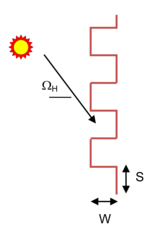
\includegraphics[width=0.9\textwidth, height=0.9\textheight, keepaspectratio=true]{media/image045.png}
\caption{Geometry used for Pleated Drape Analysis \protect \label{fig:geometry-used-for-pleated-drape-analysis}}
\end{figure}

\subsubsection{Inputs}\label{inputs-27-002}

\paragraph{Field: Name}\label{field-name-21-003}

Name of the drape fabric shade layer. It is referenced as an inside, in between or outside layer in an equivalent layer window construction.

\paragraph{Field: Drape Beam-Beam Solar Transmittance}\label{field-drape-beam-beam-solar-transmittance}

This value is the drape fabric beam-beam transmittance at normal incidence, and it is the same as the drape fabric openness area fraction.~ Assumed to be the same for front and back sides of the drape fabric layer.~ The minimum value is 0.0 and maximum value is less than 1.0. For most drape fabric materials the maximum fabric openness fraction do not exceed 0.2.~ The default value is 0.0.

\paragraph{Field: Front Side Drape Beam-Diffuse Solar Transmittance}\label{field-front-side-drape-beam-diffuse-solar-transmittance}

This value is the front side beam-diffuse solar transmittance of the drape fabric material at normal incidence averaged over the entire spectrum of solar radiation. The minimum value is 0.0 and maximum value is less than 1.0.

\paragraph{Field: Back Side Drape Beam-Diffuse Solar Transmittance}\label{field-back-side-drape-beam-diffuse-solar-transmittance}

This value is the back side beam-diffuse solar transmittance of the drape fabric material at normal incidence averaged over the entire spectrum of solar radiation. The minimum value is 0.0 and maximum value is less than 1.0.

\paragraph{Field: Front Side Drape Beam-Diffuse Solar Reflectance}\label{field-front-side-drape-beam-diffuse-solar-reflectance}

This value is the front side beam-diffuse solar reflectance of the drape fabric material at normal incidence averaged over the entire spectrum of solar radiation. The minimum value is 0.0 and maximum value is less than 1.0.

\paragraph{Field: Back Side Drape Beam-Diffuse Solar Reflectance}\label{field-back-side-drape-beam-diffuse-solar-reflectance}

This value is the back side beam-diffuse solar reflectance of the drape fabric material at normal incidence averaged over the entire spectrum of solar radiation. The minimum value is 0.0 and maximum value is less than 1.0.

\paragraph{Field: Drape Beam-Beam Visible Transmittance}\label{field-drape-beam-beam-visible-transmittance}

This value is the drape fabric beam-beam visible transmittance at normal incidence averaged over the visible spectrum range of solar radiation.~ Assumed to be the same for front and back sides of the drape fabric layer.~ The minimum value is 0.0 and maximum value is less than 1.0.~ The default value is 0.0.~ This input field is not used currently.

\paragraph{Field: Front Side Drape Beam-Diffuse Visible Reflectance}\label{field-front-side-drape-beam-diffuse-visible-reflectance}

This value is the front side drape fabric beam-diffuse visible reflectance at normal incidence averaged over the visible spectrum range of solar radiation.~ Assumed to be the same for front and back sides of the drape.~ The minimum value is 0.0 and maximum value is less than 1.0.~ The default value is 0.0.~ This input field is not used currently.

\paragraph{Field: Back Side Drape Diffuse-Diffuse Visible Reflectance}\label{field-back-side-drape-diffuse-diffuse-visible-reflectance}

This value is the back side drape fabric diffuse-diffuse visible reflectance at normal incidence averaged over the visible spectrum range of solar radiation.~ Assumed to be the same for front and back sides of the drape.~ The minimum value is 0.0 and maximum value is less than 1.0.~ The default value is 0.0.~ This input field is not used currently.

\paragraph{Field: Drape Material Infrared Transmittance}\label{field-drape-material-infrared-transmittance}

This value is the long-wave hemispherical transmittance of the fabric material at zero fabric openness fraction.~ Assumed to be the same for front and back sides of the drape fabric material layer. The minimum value is 0.0 and maximum value is less than 1.0.~ The default value is 0.05.

\paragraph{Field: Front Side Drape Material Infrared Emissivity}\label{field-front-side-drape-material-infrared-emissivity}

This value is the front side long-wave hemispherical emissivity of fabric material at zero shade openness. The minimum value is 0.0 and maximum value is less than 1.0. the default value is 0.87. The front side effective emissivity of the drape fabric layer is calculated using this value and the fabric openness area fraction specified above.

\paragraph{Field: Back Side Drape Material Infrared Emissivity}\label{field-back-side-drape-material-infrared-emissivity}

This value is the back side long-wave hemispherical emissivity of fabric material at zero fabric openness fraction. The minimum value is 0.0 and maximum value is less than 1.0. The default value is 0.87. The back side effective emissivity of the drape fabric layer is calculated using this value and the fabric openness area fraction specified above.

\paragraph{Field: Width of Pleated Fabric}\label{field-width-of-pleated-fabric}

This value is the width of the pleated section of the draped fabric, w(m). If the drape fabric is flat (unpleated), then the pleated section width is set to zero. The default value is 0.0, i.e., assumes flat drape fabric.

\paragraph{Field: Length of Pleated Fabric}\label{field-length-of-pleated-fabric}

This value is the length of the pleated section of the draped fabric, s(m). If the drape fabric is flat (unpleated), then the pleated section length is set to zero.~ The default value is 0.0, i.e., assumes flat drape fabric.

An IDF example for this object is shown below:

\begin{lstlisting}
WindowMaterial:Drape:EquivalentLayer,
  Drape02,            !- Name
  0.14,               !- Shade Beam-Beam Solar Transmittance
  0.10,               !- Front Side Shade Beam-Diffuse Solar Transmittance
  0.10,               !- Back Side Shade Beam-Diffuse Solar Transmittance
  0.40,               !- Front Side Shade Beam-Diffuse Solar Reflectance
  0.50,               !- Back Side Shade Beam-Diffuse Solar Reflectance
  0.0,                !- Shade Beam-Beam Visible Transmittance
  0.0,                !- Shade Beam-Diffuse Visible Transmittance
  0.0,                !- Shade Beam-Diffuse Visible Reflectance
  0.10,               !- Shade Material Infrared Transmittance
  0.90,               !- Front Side Shade Material Infrared Emissivity
  0.80,               !- Back Side Shade Material Infrared Emissivity
  0.01,               !- Width of Pleated Fabric
  0.025;              !- Length of Pleated Fabric
\end{lstlisting}

\subsection{WindowMaterial:Blind:EquivalentLayer}\label{windowmaterialblindequivalentlayer}

This object specifies the properties of an Equivalent Layer window blind consisting of thin and equally-spaced slats. The the model assumes that slats are flat and thin, and applies correction for the slat curvature effect based on the user specified slat crwon. Slats are assumed to transmit and reflect diffusely. The effective shortwave optical and longwave optical properties of venetian blind layer is estimated analytically. The Equivalent Layer blind model requires optical properties and geometry of the slats shown in Figure~\ref{fig:geometry-and-properties-used-for-venetian}. Likewise, effective longwave properties are obtained for the layer knowing longwave properties of the slats.

\begin{figure}[hbtp] % fig 22
\centering
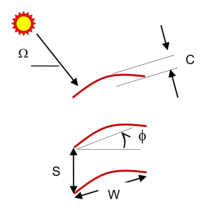
\includegraphics[width=0.9\textwidth, height=0.9\textheight, keepaspectratio=true]{media/image047.png}
\caption{Geometry and Properties used for venetian blind analysis \protect \label{fig:geometry-and-properties-used-for-venetian}}
\end{figure}

The input data required to characterize a venetian blind are: front and back side reflectance and transmittance of the slat, geometry (Slat width, w, slat spacing, s, slat crown, c, and slat angle, f, and long wave emittance and transmittance of the slat. Blinds can be located on the inside of the window, on the outside of the window, or between two layers of glass. The blind is assumed to cover all of the glazed part of the window.

\subsubsection{Inputs}\label{inputs-28-001}

\paragraph{Field: Name}\label{field-name-22-003}

Name of the venetian blind. It is referenced as an inside, outside or in between layers in an equivalent layer window construction.

\paragraph{Field: Slat Orientation}\label{field-slat-orientation-1}

The choices are Horizontal and Vertical. ``Horizontal'' means the slats are parallel to the bottom of the window; this is the same as saying that the slats are parallel to the X-axis of the window. ``Vertical'' means the slats are parallel to Y-axis of the window. The default is ``Horizontal''.

\paragraph{Field: Slat Width}\label{field-slat-width-2}

This value is the width of the slat measured from edge to edge (m). The default value is 0.0254.

\paragraph{Field: Slat Separation}\label{field-slat-separation-1}

The distance between the front of a slat and the back of the adjacent slat (m). The default value is 0.025. The slat separation should not be greater than the slat width.

\paragraph{Field: Slat Crown}\label{field-slat-crown}

The perpendicular length between the slat cord ~and the curve (m). Crown = 0.0625x``Slat width''. Slat is assumed to be rectangular in cross section and flat. The crown accounts for curvature of the slat.~ The minimum value is 0.0, and the default value is 0.0015m.

\paragraph{Field: Slat Angle}\label{field-slat-angle-2}

The angle (degrees) between the glazing outward normal and the slat outward normal, where the outward normal points away from the front face of the slat (degrees). If the ``Slat Angle Control'' input field below specified is ``FixedSlatAngle'', then the slat angle is fixed at ``Slat Angle'' value entered.~ Minimum value is zero, and the maximum value allowed is 180.0 degrees.~ The default value is 45 degrees.

\paragraph{Field: Front Side Slat Beam-Diffuse Solar Transmittance}\label{field-front-side-slat-beam-diffuse-solar-transmittance}

This value is the slat front side beam-diffuse solar transmittance at normal incidence averaged over the entire spectrum of solar radiation. Any transmitted beam radiation is assumed to be 100\% diffuse (i.e., slats are translucent). Minimum value is 0.0, and the maximum value is less than 1.0. The default value is 0.0.

\paragraph{Field: Back Side Slat Beam-Diffuse Solar Transmittance}\label{field-back-side-slat-beam-diffuse-solar-transmittance}

This value is the slat back side beam-diffuse solar transmittance at normal incidence averaged over the entire spectrum of solar radiation. Any transmitted beam radiation is assumed to be 100\% diffuse (i.e., slats are translucent). Minimum value is 0.0,~ and the maximum value is less than 1.0. The default value is 0.0.

\paragraph{Field: Front Side Slat Beam-Diffuse Solar Reflectance}\label{field-front-side-slat-beam-diffuse-solar-reflectance}

This value is slat front side beam-diffuse solar reflectance at normal incidence averaged over the entire spectrum of solar radiation. All the reflected component is assumed to be diffuse. Minimum value is 0.0, and the maximum value is less than 1.0.

\paragraph{Field: Back Side Slat Beam-Diffuse Solar Reflectance}\label{field-back-side-slat-beam-diffuse-solar-reflectance}

This value is the slat back side beam-diffuse solar reflectance at normal incidence averaged over the entire spectrum of solar radiation. All the reflected component is assumed to be diffuse. Minimum value is 0.0, and the maximum value is less than 1.0.

\paragraph{Field: Front Side Slat Beam-Diffuse Visible Solar Transmittance}\label{field-front-side-slat-beam-diffuse-visible-solar-transmittance}

This value is the slat front side beam-diffuse visible transmittance at normal incidence averaged over the visible spectrum range of solar radiation. Any transmitted beam radiation is assumed to be 100\% diffuse (i.e., slats are translucent). Minimum value is 0.0, and the maximum value is less than 1.0. The default value is 0.0.

\paragraph{Field: Back Side Slat Beam-Diffuse Visible Solar Transmittance}\label{field-back-side-slat-beam-diffuse-visible-solar-transmittance}

This value is the slat back side beam-diffuse visible transmittance at normal incidence averaged the visible spectrum range of solar radiation. Any transmitted beam radiation is assumed to be 100\% diffuse (i.e., slats are translucent). Minimum value is 0.0, and the maximum value is less than 1.0. The default value is 0.0.

\paragraph{Field: Front Side Slat Beam-Diffuse Visible Solar Reflectance}\label{field-front-side-slat-beam-diffuse-visible-solar-reflectance}

This value is the slat front side beam-diffuse visible reflectance at normal incidence averaged over the visible spectrum range of solar radiation. All the reflected component is assumed to be diffuse. Minimum value is 0.0, and the maximum value is less than 1.0

\paragraph{Field: Back Side Slat Beam-Diffuse Visible Solar Reflectance}\label{field-back-side-slat-beam-diffuse-visible-solar-reflectance}

This value is the slat back side beam-diffuse visible reflectance at normal incidence averaged over the visible spectrum range of solar radiation. All the reflected component is assumed to be diffuse. Minimum value is 0.0,~ and the maximum value is less than 1.0

\paragraph{Field: Slat Diffuse-Diffuse Solar Transmittance}\label{field-slat-diffuse-diffuse-solar-transmittance}

This value is the slat diffuse-diffuse solar transmittance for hemispherically diffuse solar radiation. This value is the same for front and back side of the slat.~ Minimum value is 0.0,~ and the maximum value is less than 1.0.

\paragraph{Field: Front Side Slat Diffuse-Diffuse Solar Reflectance}\label{field-front-side-slat-diffuse-diffuse-solar-reflectance}

This value is the slat front side diffuse-diffuse solar reflectance for hemispherically diffuse solar radiation. Minimum value is 0.0,~ and the maximum value is less than 1.0.

\paragraph{Field: Back Side Slat Diffuse-Diffuse Solar Reflectance}\label{field-back-side-slat-diffuse-diffuse-solar-reflectance}

This value is the slat back side diffuse-diffuse solar reflectance for hemispherically diffuse solar radiation. Minimum value is 0.0,~ and the maximum value is less than 1.0.

\paragraph{Field: Slat Diffuse-Diffuse Visible Transmittance}\label{field-slat-diffuse-diffuse-visible-transmittance}

This value is the slat diffuse-diffuse visible transmittance for hemispherically diffuse visible spectrum range of solar radiation. This value is the same for front and back side of the slat.~ Minimum value is 0.0,~ and the maximum value is less than 1.0. This input field is not used currently.

\paragraph{Field: Front Side Slat Diffuse-Diffuse Visible Reflectance}\label{field-front-side-slat-diffuse-diffuse-visible-reflectance}

This value is the slat front side diffuse-diffuse visible reflectance for hemispherically diffuse visible spectrum range of solar radiation. Minimum value is 0.0, and the maximum value is less than 1.0.~ This input field is not used currently.

\paragraph{Field: Back Side Slat Diffuse-Diffuse Visible Reflectance}\label{field-back-side-slat-diffuse-diffuse-visible-reflectance}

This value is the slat back side diffuse-diffuse visible reflectance for hemispherically diffuse visible spectrum range of solar radiation. Minimum value is 0.0, and the maximum value is less than 1.0.~ This input field is not used currently.

\paragraph{Field: Slat Infrared Transmittance}\label{field-slat-infrared-transmittance}

This value is the long-wave hemispherical transmittance of the slat material. Assumed to be the same for both sides of the slat. The minimum value is 0.0, the maximum value is less than 1.0.~ The default value is 0.0.

\paragraph{Field: Front Side Slat Infrared Emissivity}\label{field-front-side-slat-infrared-emissivity}

This value is the front side long-wave hemispherical emissivity of the slat material. The minimum value is 0.0, the maximum value is less than 1.0. The default value is 0.9.

\paragraph{Field: Back Side Slat Infrared Emissivity}\label{field-back-side-slat-infrared-emissivity}

This value is the back side long-wave hemispherical emissivity of the slat material. The minimum value is 0.0, the maximum value is less than 1.0.~ The default value is 0.9.

\paragraph{Field: Slat Angle Control}\label{field-slat-angle-control}

This input field is used only if slat angle control is desired.~ The three key choice inputs allowed are ``FixedSlatAngle'', ``MaximizeSolar'', and ``BlockBeamSolar''.~ The default value is ``FixedSlatAngle''.If Type of Slat Angle Control for Blinds = MaximizeSolar the slat angle is adjusted to maximize solar gain.~If Type of Slat Angle Control for Blinds = BlockBeamSolar, the slat angle is adjusted to maximize visibiity while eliminating beam solar radiation.~If Type of Slat Angle Control for Blinds = FixedSlatAngle, then the model uses a fixed slat angle specified above.

An IDF example for this object, is shown below:

\begin{lstlisting}

WindowMaterial:Blind:EquivalentLayer,
    VBU8D6+45SW1,      ! - Name
    Horizontal,        ! - Slat Orientation
    0.025,             ! - Slat Width
    0.025,             ! - Slat Separation
    0.0,               ! - Slat Crown
    45.0,              ! - Slat Angle
    0.0,               ! - Front Side Slat Beam-Diffuse Solar Transmittance
    0.0,               ! - Back Side Slat Beam-Diffuse Solar Transmittance
    0.0,               ! - Front Side Slat Beam-Diffuse Solar Reflectance
    0.0,               ! - Back Side Slat Beam-Diffuse Solar Reflectance
    0.0,               ! - Front Side Slat Beam-Diffuse Visible Transmittance
    0.0,               ! - Back Side Slat Beam-Diffuse Visible Transmittance
    0.0,               ! - Front Side Slat Beam-Diffuse Visible Reflectance
    0.0,               ! - Back Side Slat Beam-Diffuse Visible  Reflectance
    0.0,               ! - Slat Diffuse-Diffuse Solar Transmittance
    0.80,              ! - Front Side Slat Diffuse-Diffuse Solar Reflectance
    0.60,              ! - Back Side Slat Diffuse-Diffuse Solar Reflectance
    0.0,               ! - Slat Diffuse-Diffuse Visible Transmittance
    0.0,               ! - Front Side Slat Diffuse-Diffuse Visible Reflectance
    0.0,               ! - Back Side Slat Diffuse-Diffuse Visible Reflectance
    0.0,               ! - Slat Infrared Transmittance
    0.90,              ! - Front Side Slat Infrared Emissivity
    0.90,              ! - Back Side Slat Infrared Emissivity
    FixedSlatAngle;    ! - Slat Angle Control
\end{lstlisting}

\subsection{WindowMaterial:Screen:EquivalentLayer}\label{windowmaterialscreenequivalentlayer}

This object specifies the optical and thermal properties of exterior screen materials for Equivalent Layer Window. Can only be placed on the exterior side of window construction. The window screen model assumes the screen is made up of intersecting orthogonally-crossed cylinders. The surface of the cylinders is assumed to be diffusely reflecting. The beam solar radiation transmitted through an equivalent Layer window screen varies with sun angle and is made up of two distinct elements: a beam-beam component and a beam-diffuse component. The beam-beam transmittance component is calculated using screen openness area fraction determined from the geometry of the screen and the incident angle of the sun. Empirical correlations are used to obtain the effective off-normal solar and longwave properties of insect screens.~ Insect screen geometry is shown in Figure~\ref{fig:geometry-used-for-insect-screen-analysis}.~ The calculation of effective solar properties requires a set of properties measured at normal incidence.

\begin{figure}[hbtp] % fig 23
\centering
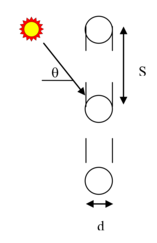
\includegraphics[width=0.9\textwidth, height=0.9\textheight, keepaspectratio=true]{media/image048.png}
\caption{Geometry used for insect screen analysis \protect \label{fig:geometry-used-for-insect-screen-analysis}}
\end{figure}

The formulation of the model, assumption and correlations used to calculate effective solar and longwave properties of insect screens are described in the Engineering Reference.

\subsubsection{Inputs}\label{inputs-29-001}

\paragraph{Field: Name}\label{field-name-23-003}

Name of the insect screen. It is referenced as an outside layer in an equivalent layer window construction.

\paragraph{Field: Screen Beam-Beam Solar Transmittance}\label{field-screen-beam-beam-solar-transmittance}

This value is the beam-beam transmittance of the screen material at normal incidence. This value is the same as the screen openness area fraction.~ This value can be autocalculated from the wire spacing and wire diameter. It is the same for both sides of the screen. The minimum value is 0.0, and maximum value is less than 1.0.

\paragraph{Field: Screen Beam-Diffuse Solar Transmittance}\label{field-screen-beam-diffuse-solar-transmittance}

This value is the beam-diffuse solar transmittance of the screen material at normal incidence averaged over the entire spectrum of solar radiation. Assumed to be the same for both sides of the screen. The minimum value is 0.0, and the maximum value is less than 1.0.

\paragraph{Field: Screen Beam-Diffuse Solar Reflectance}\label{field-screen-beam-diffuse-solar-reflectance}

This value is the beam-diffuse solar reflectance of the screen material at normal incidence averaged over the entire spectrum of solar radiation. Assumed to be the same for both sides of the screen. The minimum value is 0.0, and the maximum value is less than 1.0.

\paragraph{Field: Screen Beam-Beam Visible Transmittance}\label{field-screen-beam-beam-visible-transmittance}

This value is the beam-beam visible transmittance of the screen material at normal incidence averaged over the visible spectrum range of solar radiation.~ Assumed to be the same for both sides of the screen. The minimum value is 0.0, and maximum value is less than 1.0. This input input field is not used currently.

\paragraph{Field: Screen Beam-Diffuse Visible Transmittance}\label{field-screen-beam-diffuse-visible-transmittance}

This value is the beam-diffuse visible reflectance of the screen material at normal incidence averaged over the visible spectrum range of solar radiation. Assumed to be the same for both sides of the screen. The minimum value is 0.0, and the maximum value is less than 1.0. This input input field is not used currently.

\paragraph{Field: Screen Beam-Diffuse Visible Reflectance}\label{field-screen-beam-diffuse-visible-reflectance}

This value is the beam-diffuse visible reflectance of the screen material at normal incidence averaged over the visible spectrum range of solar radiation. Assumed to be the same for both sides of the screen. The minimum value is 0.0, and the maximum value is less than 1.0. This input input field is not used currently.

\paragraph{Field: Screen Infrared Transmittance}\label{field-screen-infrared-transmittance}

This value is the long-wave hemispherical transmittance of the the screen material. Assumed to be the same for both sides of the screen material. The minimum value is 0.0, the maximum value is less than 1.0.~ The default value is 0.02

\paragraph{Field: Screen Infrared Emissivity}\label{field-screen-infrared-emissivity}

This value is the long-wave hemispherical emissivity of the screen material. Assumed to be the same for both sides of the screen material. The minimum value is 0.0, the maximum value is less than 1.0. The default value is 0.93.

\paragraph{Field: Screen Wire Spacing}\label{field-screen-wire-spacing}

The spacing, S (m), of the screen material is the distance from the center of one strand of screen to the center of the adjacent one. The spacing of the screen material is assumed to be the same in both directions (e.g., vertical and horizontal). This input value must be greater than the non-zero screen material diameter. If the spacing is different in the two directions, use the average of the two values. Default value is 0.0025m.

\paragraph{Field: Screen Wire Diameter}\label{field-screen-wire-diameter}

The diameter, D (m), of individual strands or wires of the screen material. The screen material diameter is assumed to be the same in both directions (e.g., vertical and horizontal). This input value must be greater than 0 and less than the screen wire spacing. If the diameter is different in the two directions, use the average of the two values. Default value is 0.005m.

An IDF example for this object, is shown below:

\begin{lstlisting}

WindowMaterial:Screen:EquivalentLayer,
    INSCRN,                !- Name
    0.763,                 !- Screen Beam-Beam Solar Transmittance
    0.052,                 !- Screen Beam-Diffuse Solar Transmittance
    0.076,                 !- Screen Beam-Diffuse Solar Reflectance
    0.0,                   !- Screen Beam-Beam Visible Transmittance
    0.0,                   !- Screen Beam-Diffuse Visible Transmittance
    0.0,                   !- Screen Beam-Diffuse Visible Reflectance
    0.0,                   !- Screen Infrared Transmittance
    0.84,                  !- Screen Infrared Emissivity
    0.025,                 !- Screen Wire Spacing
    0.005;                 !- Screen Wire Diameter
\end{lstlisting}

\subsection{WindowMaterial:Glazing:EquivalentLayer}\label{windowmaterialglazingequivalentlayer}

Glass material properties for equivalent layer window model.~ Uses transmittance/reflectance input method.~ For exterior windows, ``front side'' is the side of the glass closest to the outside air and ``back side'' is the side closest to the zone the window is defined in. For interzone windows, ``front side'' is the side closest to the zone adjacent to the zone the window is defined in and ``back side'' is the side closest to the zone the window is defined in.

\subsubsection{Inputs}\label{inputs-30-001}

\paragraph{Field: Name}\label{field-name-24-002}

The name of the glass layer. It corresponds to a layer in an equivalent layer window construction.

\paragraph{Field: Optical Data Type}\label{field-optical-data-type-1}

Valid values for this field are SpectralAverage, or Spectral. If Optical Data Type = SpectralAverage, the values you enter for solar transmittance and reflectance are assumed to be averaged over the solar spectrum, and the values you enter for visible transmittance and reflectance are assumed to be averaged over the solar spectrum and weighted by the response of~ the human eye. The spectral data input is not supported now.

\paragraph{Field: Window Glass Spectral Data Set Name}\label{field-window-glass-spectral-data-set-name-0}

This input field is not used currently.

\paragraph{Field: Front Side Beam-Beam Solar Transmittance}\label{field-front-side-beam-beam-solar-transmittance}

This value is the front side beam-beam solar transmittance of the glazing at normal incidence averaged over the entire spectrum of solar radiation.~ Used only when Optical Data Type = SpectralAverage.~ The minimum value is 0.0, and the maximum value is less than 1.0.

\paragraph{Field: Back Side Beam-Beam Solar Transmittance}\label{field-back-side-beam-beam-solar-transmittance}

This value is the back side beam-beam solar transmittance of the glazing at normal incidence averaged over the entire spectrum of solar radiation.~ Used only when Optical Data Type = SpectralAverage.~ The minimum value is 0.0, and the maximum value is less than 1.0.

\paragraph{Field: Front Side Beam-Beam Solar Reflectance}\label{field-front-side-beam-beam-solar-reflectance}

This value is the front side beam-beam solar reflectance of the glazing at normal incidence averaged over the entire spectrum of solar radiation.~ Used only when Optical Data Type = SpectralAverage.~ The minimum value is 0.0, and the maximum value is less than 1.0.

\paragraph{Field: Back Side Beam-Beam Solar Reflectance}\label{field-back-side-beam-beam-solar-reflectance}

This value is the back side beam-beam solar reflectance of the glazing at normal incidence averaged over the entire spectrum of solar radiation.~ Used only when Optical Data Type = SpectralAverage.~ The minimum value is 0.0, and the maximum value is less than 1.0.

\paragraph{Field: Front Side Beam-Beam Visible Transmittance}\label{field-front-side-beam-beam-visible-transmittance}

This value is the front side beam-beam visible transmittance of the glazing at normal incidence averaged over the visible spectrum range of solar radiation.~ Used only when Optical Data Type = SpectralAverage.~ The minimum value is 0.0, and the maximum value is less than 1.0.

\paragraph{Field: Back Side Beam-Beam Visible Transmittance}\label{field-back-side-beam-beam-visible-transmittance}

This value is the back side beam-beam visible transmittance of the glazing at normal incidence averaged over the visible spectrum range of solar radiation.~ Used only when Optical Data Type = SpectralAverage.~ The minimum value is 0.0, and the maximum value is less than 1.0.

\paragraph{Field: Front Side Beam-Beam Visible Reflectance}\label{field-front-side-beam-beam-visible-reflectance}

This value is the front side beam-beam visible reflectance of the glazing at normal incidence averaged over the visible spectrum range of solar radiation.~ Used only when Optical Data Type = SpectralAverage.~ The minimum value is 0.0, and the maximum value is less than 1.0.

\paragraph{Field: Back Side Beam-Beam Visible Reflectance}\label{field-back-side-beam-beam-visible-reflectance}

This value is the back side beam-beam visible reflectance of the glazing at normal incidence averaged over the visible spectrum range of solar radiation.~ Used only when Optical Data Type = SpectralAverage.~ The minimum value is 0.0, and the maximum value is less than 1.0.

\paragraph{Field: Front Side Beam-Diffuse Solar Transmittance}\label{field-front-side-beam-diffuse-solar-transmittance}

This value is the front side beam-diffuse solar transmittance of the glazing at normal incidence averaged over the entire spectrum of solar radiation.~ Used only when Optical Data Type = SpectralAverage.~ For clear glazing the beam-diffuse transmittance is zero. The minimum value is 0.0, and the maximum value is less than 1.0. Default value is 0.0.

\paragraph{Field: Back Side Beam-Diffuse Solar Transmittance}\label{field-back-side-beam-diffuse-solar-transmittance}

This value is the back side beam-diffuse solar transmittance of the glazing at normal incidence averaged over the entire spectrum of solar radiation.~ Used only when Optical Data Type = SpectralAverage.~ For clear glazing the beam-diffuse solar transmittance is zero. The minimum value is 0.0, and the maximum value is less than 1.0. Default value is 0.0.

\paragraph{Field: Front Side Beam-Diffuse Solar Reflectance}\label{field-front-side-beam-diffuse-solar-reflectance}

This value is the front side beam-diffuse solar reflectance of the glazing at normal incidence averaged over the entire spectrum of solar radiation.~ Used only when Optical Data Type = SpectralAverage.~ The minimum value is 0.0, and the maximum value is less than 1.0. Default value is 0.0.

\paragraph{Field: Back Side Beam-Diffuse Solar Reflectance}\label{field-back-side-beam-diffuse-solar-reflectance}

This value is the back side beam-diffuse solar reflectance of the glazing at normal incidence averaged over the entire spectrum of solar radiation.~ Used only when Optical Data Type = SpectralAverage.~ The minimum value is 0.0, and the maximum value is less than 1.0. Default value is 0.0.

\paragraph{Field: Front Side Beam-Diffuse Visible Transmittance}\label{field-front-side-beam-diffuse-visible-transmittance}

This value is the front side beam-diffuse visible transmittance of the glazing at normal incidence averaged over the visible spectrum range of solar radiation.~ Used only when Optical Data Type = SpectralAverage.~ For clear glazing the beam-diffuse visible transmittance is zero. The minimum value is 0.0, and the maximum value is less than 1.0. Default value is 0.0.~ This input field is not used currently.

\paragraph{Field: Back Side Beam-Diffuse Visible Transmittance}\label{field-back-side-beam-diffuse-visible-transmittance}

This value is the back side beam-diffuse visible transmittance of the glazing at normal incidence averaged over the visible spectrum range of solar radiation.~ Used only when Optical Data Type = SpectralAverage.~ For clear glazing the beam-diffuse visible transmittance is zero. The minimum value is 0.0, and the maximum value is less than 1.0. Default value is 0.0.~ This input field is not used currently.

\paragraph{Field: Front Side Beam-Diffuse Visible Reflectance}\label{field-front-side-beam-diffuse-visible-reflectance}

This value is the front side beam-diffuse visible reflectance of the glazing at normal incidence averaged over the visible spectrum range of solar radiation.~ Used only when Optical Data Type = SpectralAverage.~ The minimum value is 0.0, and the maximum value is less than 1.0. Default value is 0.0. This input field is not used currently.

\paragraph{Field: Back Side Beam-Diffuse Visible Reflectance}\label{field-back-side-beam-diffuse-visible-reflectance}

This value is the back side beam-diffuse visible reflectance of the glazing at normal incidence averaged over the visible spectrum range of solar radiation.~ Used only when Optical Data Type = SpectralAverage.~ The minimum value is 0.0, and the maximum value is less than 1.0. Default value is 0.0. This input field is not used currently.

\paragraph{Field: Diffuse-Diffuse Solar Transmittance}\label{field-diffuse-diffuse-solar-transmittance}

This value is the diffuse-diffuse solar transmittance of the glazing averaged over the entire spectrum of solar radiation.~ Used only when Optical Data Type = SpectralAverage. The diffuse-diffuse transmittance is assumed to be the same for both sides of the glazing.~ EnergyPlus automatically estimates the diffuse-diffuse solar transmittance from other inputs. If this input field is specified as ``Autocalculate'', then the calculated transmittance will be used. The minimum value is 0.0, and the maximum value is less than 1.0.

\paragraph{Field: Front Side Diffuse-Diffuse Solar Reflectance}\label{field-front-side-diffuse-diffuse-solar-reflectance}

This value is the front side diffuse-diffuse solar reflectance of the glazing averaged over the entire spectrum of solar radiation.~ Used only when Optical Data Type = SpectralAverage. EnergyPlus automatically estimates the diffuse-diffuse reflectance from other inputs. If this input field is specified as ``Autocalculate'', then the calculated reflectance will be used. The minimum value is 0.0, and the maximum value is less than 1.0.

\paragraph{Field: Back Side Diffuse-Diffuse Solar Reflectance}\label{field-back-side-diffuse-diffuse-solar-reflectance}

This value is the back side diffuse-diffuse solar reflectance of the glazing averaged over the entire spectrum of solar radiation.~ Used only when Optical Data Type = SpectralAverage. EnergyPlus automatically estimates the diffuse-diffuse reflectance from other inputs. If this input field is specified as ``Autocalculate'', then the calculated reflectance will be used. The minimum value is 0.0, and the maximum value is less than 1.0.

\paragraph{Field: Diffuse-Diffuse Visible Solar Transmittance}\label{field-diffuse-diffuse-visible-solar-transmittance}

This value is the diffuse-diffuse visible transmittance of the glazing averaged over the visible spectrum range of solar radiation.~ Used only when Optical Data Type = SpectralAverage. The diffuse-diffuse visible transmittance is assumed to be the same for both sides of the glazing.~ If this input field is specified as ``Autocalculate'', then the calculated transmittance will be used. The minimum value is 0.0, and the maximum value is less than 1.0. This input field is not used currently.

\paragraph{Field: Front Side Diffuse-Diffuse Visible Reflectance}\label{field-front-side-diffuse-diffuse-visible-reflectance}

This value is the front side diffuse-diffuse visible reflectance of the glazing averaged over the visible spectrum range of solar radiation.~ Used only when Optical Data Type = SpectralAverage. EnergyPlus automatically estimates the front side diffuse-diffuse visible reflectance from front side beam-beam visible reflectance at normal incidence specified above. If this input field is specified as ``Autocalculate'', then the calculated reflectance will be used. The minimum value is 0.0, and the maximum value is less than 1.0. This input field is not used currently.

\paragraph{Field: Back Side Diffuse-Diffuse Visible Reflectance}\label{field-back-side-diffuse-diffuse-visible-reflectance}

This value is the back side diffuse-diffuse visible reflectance of the glazing averaged over the visible spectrum range of solar radiation.~ Used only when Optical Data Type = SpectralAverage. EnergyPlus automatically estimates the back side diffuse-diffuse visible reflectance from back side beam-beam visible reflectance at normal incidence specified above. If this input field is specified as ``Autocalculate'', then the calculated reflectance will be used. The minimum value is 0.0, and the maximum value is less than 1.0. This input field is not used currently.

\paragraph{Field: Infrared Transmittance (applies to front and back)}\label{field-infrared-transmittance-applies-to-front-and-back}

This value is the long-wave hemispherical transmittance of the glazing. Assumed to be the same for both sides of the glazing. The minimum value is 0.0, the maximum value is less than 1.0.~ The default value is 0.0.

\paragraph{Field: Front Side Infrared Emissivity}\label{field-front-side-infrared-emissivity}

This value is the front side long-wave hemispherical emissivity of the glazing. The minimum value is 0.0, the maximum value is less than 1.0.~ The default value is 0.84.

\paragraph{Field: Back Side Infrared Emissivity}\label{field-back-side-infrared-emissivity}

This value is the back side long-wave hemispherical emissivity of the glazing. The minimum value is 0.0, the maximum value is less than 1.0.~ The default value is 0.84.

An IDF example for this object, is shown below:

\begin{lstlisting}

WindowMaterial:Glazing:EquivalentLayer,
    GLZCLR,                  !- Name
    SpectralAverage,         !- Optical Data Type
    ,                        !- Window Glass Spectral Data Set Name
    0.83,                    !- Front Side Beam-Beam Solar Transmittance
    0.83,                    !- Back Side Beam-Beam Solar Transmittance
    0.08,                    !- Front Side Beam-Beam Solar Reflectance
    0.08,                    !- Back Side Beam-Beam Solar Reflectance
    0.0,                     !- Front Side Beam-Beam Visible Transmittance
    0.0,                     !- Back Side Beam-Beam Visible Transmittance
    0.0,                     !- Front Side Beam-Beam Visible Reflectance
    0.0,                     !- Back Side Beam-Beam Visible Reflectance
    0.0,                     !- Front Side Beam-Diffuse Solar Transmittance
    0.0,                     !- Back Side Beam-Diffuse Solar Transmittance
    0.0,                     !- Front Side Beam-Diffuse Solar Reflectance
    0.0,                     !- Back Side Beam-Diffuse Solar Reflectance
    0.0,                     !- Front Side Beam-Diffuse Visible Transmittance
    0.0,                     !- Back Side Beam-Diffuse Visible Transmittance
    0.0,                     !- Front Side Beam-Diffuse Visible Reflectance
    0.0,                     !- Back Side Beam-Diffuse Visible Reflectance
    0.76,                    !- Diffuse-Diffuse Solar Transmittance
    0.14,                    !- Front Side Diffuse-Diffuse Solar Reflectance
    0.14,                    !- Back Side Diffuse-Diffuse Solar Reflectance
    0.0,                     !- Diffuse-Diffuse Visible Transmittance
    0.0,                     !- Front Side Diffuse-Diffuse Visible Reflectance
    0.0,                     !- Back Side Diffuse-Diffuse Visible Reflectance
    0.0,                     !- Infrared Transmittance
    0.84,                    !- Front Side Infrared Emissivity
    0.84;                    !- Back Side Infrared Emissivity
\end{lstlisting}

\subsection{WindowMaterial:Gap:EquivalentLayer}\label{windowmaterialgapequivalentlayer}

This object is used in windows equivalent layer construction object and specifies the properties of the gap between the layers in multi-layer equivalent layer window object. There is an EnergyPlus Reference Data Set for Material:WindowGas that contains several types of gas. This object uses the gas types: Air, Argon, Xenon, Crypton, and Custom.~ For Custom gas type users are required to entering the thermophicial properties.

\subsubsection{Inputs}\label{inputs-31-001}

\paragraph{Field: Name}\label{field-name-25-002}

The name of the gap. It refers to a layer in a window construction equivalent layer.

\paragraph{Field: Gas Type}\label{field-gas-type-1}

The type of gas. The choices allowed are AIR, ARGON, XENON, KRYPTON, or CUSTOM.

\paragraph{Field: Thickness}\label{field-thickness-8}

The thickness (m) of the gap layer.

\paragraph{Field: Gap Vent Type}\label{field-gap-vent-type}

This input field contains the valid key choice for gap vent type.~ The valid vent types are: Sealed, VentedIndoor, and VentedOutdoor.~ Sealed means the gap is enclosed and gas tight, i.e., no venting to indoor or outdoor environment. The gap types ``VentedIndoor'' and ``VentedOutdoor'' are used with gas type ``Air'' only. VentedIndoor means the air in the gap is naturally vented to indoor environment, and~ VentedOutdoor means the air in the gap is naturally vented to the outdoor environment.

\paragraph{Properties for Custom Gas Types}\label{properties-for-custom-gas-types-1}

The following entries are used only if Gas Type = Custom. The A, B and C coefficients are those in the following expression that gives a property value as a function of temperature in degrees K:

\begin{equation}
Property = Coef{f_A} + Coef{f_B} \times Temperatur{e_K} + Coef{f_C} \times Temperature_K^2
\end{equation}

\paragraph{Field: Conductivity Coefficient A}\label{field-conductivity-coefficient-a-1}

The A coefficient for gas conductivity (W/m-K). Used only if Gas Type = Custom.

\paragraph{Field: Conductivity Coefficient B}\label{field-conductivity-coefficient-b-1}

The B coefficient for gas conductivity (W/m-K\(^{2}\)). Used only if Gas Type = Custom.

\paragraph{Field: Conductivity Coefficient C}\label{field-conductivity-coefficient-c-1}

The C coefficient for gas conductivity (W/m-K\(^{3}\)).~ Used only if Gas Type = Custom.

\paragraph{Field: Viscosity Coefficient A}\label{field-viscosity-coefficient-a-1}

The A coefficient for gas viscosity (kg/m-s). Used only if Gas Type = Custom.

\paragraph{Field: Viscosity Coefficient B}\label{field-viscosity-coefficient-b-1}

The B coefficient for gas viscosity (kg/m-s-K). Used only if Gas Type = Custom.

\paragraph{Field: Viscosity Coefficient C}\label{field-viscosity-coefficient-c-1}

The C coefficient for gas viscosity (kg/m-s-K\(^{2}\)).~ Used only if Gas Type = Custom.

\paragraph{Field: Specific Heat Coefficient A}\label{field-specific-heat-coefficient-a-1}

The A coefficient for gas specific heat (J/kg-K). Used only if Gas Type = Custom.

\paragraph{Field: Specific Heat Coefficient B}\label{field-specific-heat-coefficient-b-1}

The B coefficient for gas specific heat (J/kg-K\(^{2}\)). Used only if Gas Type = Custom.

\paragraph{Field: Specific Heat Coefficient C}\label{field-specific-heat-coefficient-c-1}

The C coefficient for gas specific heat (J/kg-K\(^{2}\)).~ Used only if Gas Type = Custom.

\paragraph{Field: Specific Heat Ratio}\label{field-specific-heat-ratio-2}

The specific heat ratio for gas.~ Used only if Gas Type = Custom.

\paragraph{Field: Molecular Weight}\label{field-molecular-weight-1}

The molecular weight for gas.~ The molecular weight is the mass of 1 mol of the substance.~ This has a numerical value which is the average molecular mass of the molecules in the substance multiplied by Avogadro's constant. (kg/kmol) (Shown in the IDD as g/mol for consistency)

\paragraph{Field: Specific Heat Ratio}\label{field-specific-heat-ratio-3}

The specific heat ratio for gas.~ The specific heat ratio of a gas is the ratio of the specific heat at contant pressure, to the specific heat at constant volume.~ Used only if Gas Type = Custom.

An IDF example for this object, is shown below:

\begin{lstlisting}

WindowMaterial:Gap:EquivalentLayer,
    Custom CO2 Sealed 12mm,    !- Name
    CUSTOM,                    !- Gas Type
    0.0120,                    !- Thickness {m}
    Sealed,                    !- Gap Vent Type
   -5.8181E-3,                 !- Conductivity Coefficient A {W/m-K}
    7.4714E-5,                 !- Conductivity Coefficient B {W/m-K2}
    0.0,                       !- Conductivity Coefficient C {W/m-K3}
    8.5571E-7,                 !- Viscosity Coefficient A {kg/m-s}
    4.7143E-8,                 !- Viscosity Coefficient B {kg/m-s-K}
    0.0,                       !- Viscosity Coefficient C {kg/m-s-K2}
    5.76903E2,                 !- Specific Heat Coefficient A {J/kg-K}
    9.18088E-2,                !- Specific Heat Coefficient B {J/kg-K2}
    0.0,                       !- Specific Heat Coefficient C {J/kg-K3}
    44.01;                     !- Molecular Weight {g/mol}
\end{lstlisting}

\subsection{Material:RoofVegetation}\label{materialroofvegetation}

This definition must be used in order to simulate the green roof (ecoroof) model. The material becomes the outside layer in a green roof construction (see example below). In the initial release of the green roof model, only one material may be used as a green roof layer though, of course, several constructions using that material may be used. In addition, the model has only been tested with the ConductionTransferFunction solution algorithm -- a warning will be issued for other solution algorithm choices. This model was developed for low-sloped exterior surfaces (roofs). It is not recommended for high-sloped exterior surfaces (e.g., walls).

\subsubsection{Inputs}\label{inputs-32-000}

\paragraph{Field: Name}\label{field-name-26-002}

This field is a unique reference name that the user assigns to a particular ecoroof material. This name can then be referred to by other input data.

\paragraph{Field: Height of Plants}\label{field-height-of-plants}

This field defines the height of plants in units of meters. This field is limited to values in the range 0.005 \textless{} Height \textless{} 1.00 m. Default is .2 m.

\paragraph{Field: Leaf Area Index}\label{field-leaf-area-index}

This is the projected leaf area per unit area of soil surface. This field is dimensionless and is limited to values in the range of 0.001 \textless{} LAI \textless{} 5.0. Default is 1.0. At the present time the fraction vegetation cover is calculated directly from LAI (Leaf Area Index) using an empirical relation. The user may find it necessary to increase the specified value of LAI in order to represent high fractional coverage of the surface by vegetation.

\paragraph{Field: Leaf Reflectivity}\label{field-leaf-reflectivity}

This field represents the fraction of incident solar radiation that is reflected by the individual leaf surfaces (albedo). Solar radiation includes the visible spectrum as well as infrared and ultraviolet wavelengths. Values for this field must be between 0.05 and 0.5. Default is .22. Typical values are .18 to .25.

\paragraph{Field: Leaf Emissivity}\label{field-leaf-emissivity}

This field is the ratio of thermal radiation emitted from leaf surfaces to that emitted by an ideal black body at the same temperature. This parameter is used when calculating the long wavelength radiant exchange at the leaf surfaces. Values for this field must be between 0.8 and 1.0 (with 1.0 representing ``black body'' conditions). Default is .95.

\paragraph{Field: Minimum Stomatal Resistance}\label{field-minimum-stomatal-resistance}

This field represents the resistance of the plants to moisture transport. It has units of s/m. Plants with low values of stomatal resistance will result in higher evapotranspiration rates than plants with high resistance. Values for this field must be in the range of 50.0 to 300.0. Default is 180.

\paragraph{Field: Soil Layer Name}\label{field-soil-layer-name}

This field is a unique reference name that the user assigns to the soil layer for a particular ecoroof. This name can then be referred to by other input data. Default is \textbf{Green Roof Soil}.

\paragraph{Field: Roughness}\label{field-roughness-2}

This alpha field defines the relative roughness of a particular material layer. This parameter only influences the convection coefficients, more specifically the exterior convection coefficient. A keyword is expected in this field with the options being ``VeryRough'', ``Rough'', ``MediumRough'', ``MediumSmooth'', ``Smooth'', and ``VerySmooth'' in order of roughest to smoothest options. Default is MediumRough.

\paragraph{Field: Thickness}\label{field-thickness-9}

This field characterizes the thickness of the material layer in meters. This should be the dimension of the layer in the direction perpendicular to the main path of heat conduction. This value must be a positive number. Depths of .10m (4 inches) and .15m (6 inches) are common. Default if this field is left blank is .1. Maximum is .7m. Must be greater than .05 m.

\paragraph{Field: Conductivity of Dry Soil}\label{field-conductivity-of-dry-soil}

This field is used to enter the thermal conductivity of the material layer. Units for this parameter are W/(m-K). Thermal conductivity must be greater than zero. Typical soils have values from .3 to .5. Minimum is .2 (specified in IDD). Default is .35 and maximum (in IDD) is 1.5.

\paragraph{Field: Density of Dry Soil}\label{field-density-of-dry-soil}

This field is used to enter the density of the material layer in units of kg/m\(^{3}\). Density must be a positive quantity. Typical soils range from 400 to 1000 (dry to wet). Minimum is 300, maximum is 2000 and default if field is left blank is 1100.

\paragraph{Field: Specific Heat of Dry Soil}\label{field-specific-heat-of-dry-soil}

This field represents the specific heat of the material layer in units of J/(kg-K). Note that these units are most likely different than those reported in textbooks and references which tend to use kJ/(kg-K) or J/(g-K). They were chosen for internal consistency within EnergyPlus. Only positive values of specific heat are allowed.

\paragraph{Field: Thermal Absorptance}\label{field-thermal-absorptance-2}

The thermal absorptance field in the Material input syntax represents the fraction of incident long wavelength (>2.5 microns) radiation that is absorbed by the material. This parameter is used when calculating the long wavelength radiant exchange between various surfaces and affects the surface heat balances (both inside and outside as appropriate). For long wavelength radiant exchange, thermal emissivity and thermal emittance are equal to thermal absorptance. Values for this field must be between 0.0 and 1.0 (with 1.0 representing ``black body'' conditions). Typical values are from .9 to .98. The default value for this field is 0.9.

\paragraph{Field: Solar Absorptance}\label{field-solar-absorptance-2}

The solar absorptance field in the Material input syntax represents the fraction of incident~ solar radiation that is absorbed by the material. Solar radiation (0.3 to 2.537 microns) includes the visible spectrum as well as infrared and ultraviolet wavelengths. This parameter is used when calculating the amount of incident solar radiation absorbed by various surfaces and affects the surface heat balances (both inside and outside as appropriate). If solar reflectance (or reflectivity) data is available, then absorptance is equal to 1.0 minus reflectance (for opaque materials). Values for this field must be between 0.0 and 1.0. Typical values are from .6 to .85. The default value for this field is 0.7.

\paragraph{Field: Visible Absorptance}\label{field-visible-absorptance-2}

The visible absorptance field in the Material input syntax represents the fraction of incident visible wavelength radiation that is absorbed by the material. Visible wavelength radiation ( 0.37 to 0.78 microns weighted by photopic response) is slightly different than solar radiation in that the visible band of wavelengths is much more narrow while solar radiation includes the visible spectrum as well as infrared and ultraviolet wavelengths. This parameter is used when calculating the amount of incident visible radiation absorbed by various surfaces and affects the surface heat balances (both inside and outside as appropriate) as well as the daylighting calculations. If visible reflectance (or reflectivity) data is available, then absorptance is equal to 1.0 minus reflectance (for opaque materials). Values for this field must be between 0.5 and 1.0. The default value for this field is 0.75.

\paragraph{Field: Saturation Volumetric Moisture Content of the Soil Layer}\label{field-saturation-volumetric-moisture-content-of-the-soil-layer}

The field allows for user input of the saturation moisture content of the soil layer. Maximum moisture content is typically less than .5. Range is {[}.1,.5{]} with the default being .3.

\paragraph{Field: Residual Volumetric Moisture Content of the Soil Layer}\label{field-residual-volumetric-moisture-content-of-the-soil-layer}

The field allows for user input of the residual moisture content of the soil layer. Default is .01, range is {[}.01,.1{]}.

\paragraph{Field: Initial Volumetric Moisture Content of the Soil Layer}\label{field-initial-volumetric-moisture-content-of-the-soil-layer}

The field allows for user input of the initial moisture content of the soil layer. Range is (.05, .5{]} with the default being .1.

\paragraph{Field: Moisture Diffusion Calculation Method}\label{field-moisture-diffusion-calculation-method}

The field allows for two models to be selected: \textbf{Simple} or \textbf{Advanced}.

\textbf{Simple} is the original Ecoroof model - based on a constant diffusion of moisture through the soil.~ This model starts with the soil in two layers.~ Every time the soil properties update is called, it will look at the two soils moisture layers and asses which layer has more moisture in it. It then takes moisture from the higher moisture layer and redistributes it to the lower moisture layer at a constant rate.

\textbf{Advanced} is the later Ecoroof model. If you use it, you will need to increase your number of timesteps in hour for the simulation with a recommended value of 20. This moisture transport model is based on a project which looked at the way moisture transports through soil.~ It uses a finite difference method to divide the soil into layers (nodes). It redistributes the soil moisture according the model described in:

Marcel G Schaap and Martinus Th. van Genuchten, 2006, `A modified Maulem-van Genuchten Formulation for Improved Description of the Hydraulic Conductivity Near Saturation', Vadose Zone Journal 5 (1), p 27-34.

An IDF example:

\begin{lstlisting}

Material:RoofVegetation,
      BaseEco,                 !- Name
      0.5,                     !- Height of Plants {m}
      5,                       !- Leaf Area Index {dimensionless}
      0.2,                     !- Leaf Reflectivity {dimensionless}
      0.95,                    !- Leaf Emissivity
      180,                     !- Minimum Stomatal Resistance {s/m}
      EcoRoofSoil,             !- Soil Layer Name
      MediumSmooth,            !- Roughness
      0.18,                    !- Thickness {m}
      0.4,                     !- Conductivity of Dry Soil {W/m-K}
      641,                     !- Density of Dry Soil {kg/m3}
      1100,                    !- Specific Heat of Dry Soil {J/kg-K}
      0.95,                    !- Thermal Absorptance
      0.8,                     !- Solar Absorptance
      0.7,                     !- Visible Absorptance
     0.4,                     !- Saturation Volumetric Moisture Content of the Soil Layer
      0.01,                    !- Residual Volumetric Moisture Content of the Soil Layer
      0.2,                     !- Initial Volumetric Moisture Content of the Soil Layer
      Advanced;                !- Moisture Diffusion Calculation Method


    Material:RoofVegetation,
      LowLAI,                  !- Name
      0.5,                     !- Height of Plants {m}
      0.5,                     !- Leaf Area Index {dimensionless}
      0.2,                     !- Leaf Reflectivity {dimensionless}
      0.95,                    !- Leaf Emissivity
      180,                     !- Minimum Stomatal Resistance {s/m}
      EcoRoofSoil,             !- Soil Layer Name
      MediumSmooth,            !- Roughness
      0.18,                    !- Thickness {m}
      0.4,                     !- Conductivity of Dry Soil {W/m-K}
      641,                     !- Density of Dry Soil {kg/m3}
      1100,                    !- Specific Heat of Dry Soil {J/kg-K}
      0.95,                    !- Thermal Absorptance
      0.8,                     !- Solar Absorptance
      0.7,                     !- Visible Absorptance
     0.4,          !- Saturation Volumetric Moisture Content of the Soil Layer
      0.01,         !- Residual Volumetric Moisture Content of the Soil Layer
      0.2,          !- Initial Volumetric Moisture Content of the Soil Layer
      Advanced;                !- Moisture Diffusion Calculation Method
\end{lstlisting}

And construction using the ecoroof material:

\begin{lstlisting}

Construction,
      ASHRAE 90.1-2004_Sec 5.5-2_Roof,  !- Name
      BaseEco,                 !- Outside Layer
      ASHRAE 90.1-2004_Sec 5.5-2_Roof Insulation_1,  !- Layer \#2
      ASHRAE 90.1-2004_Sec 5.5-2_MAT-METAL;  !- Layer \#3
\end{lstlisting}

\subsection{Ecoroof / RoofVegetation outputs}\label{ecoroof-roofvegetation-outputs}

The following outputs are available for the Roof Vegetation surface.

\begin{itemize}
\item
  Zone,Average,Green Roof Soil Temperature {[}C{]}
\item
  Zone,Average,Green Roof Vegetation Temperature {[}C{]}
\item
  Zone,Average,Green Roof Soil Root Moisture Ratio {[]}
\item
  Zone,Average,Green Roof Soil Near Surface Moisture Ratio {[]}
\item
  Zone,Average,Green Roof Soil Sensible Heat Transfer Rate per Area {[}W/m2{]}
\item
  Zone,Average,Green Roof Vegetation Sensible Heat Transfer Rate per Area {[}W/m2{]}
\item
  Zone,Average,Green Roof Vegetation Moisture Transfer Rate {[}m/s{]}
\item
  Zone,Average,Green Roof Soil Moisture Transfer Rate {[}m/s{]}
\item
  Zone,Average,Green Roof Vegetation Latent Heat Transfer Rate per Area {[}W/m2{]}
\item
  Zone,Average,Green Roof Soil Latent Heat Transfer Rate per Area {[}W/m2{]}
\item
  Zone,Sum,Green Roof Cumulative Precipitation Depth {[}m{]}
\item
  Zone,Sum,Green Roof Cumulative Irrigation Depth {[}m{]}
\item
  Zone,Sum,Green Roof Cumulative Runoff Depth {[}m{]}
\item
  Zone,Sum,Green Roof Cumulative Evapotranspiration Depth {[}m{]}
\item
  Zone,Sum,Green Roof Current Precipitation Depth {[}m{]}
\item
  Zone,Sum,Green Roof Current Irrigation Depth {[}m{]}
\item
  Zone,Sum,Green Roof Current Runoff Depth {[}m{]}
\item
  Zone,Sum,Green Roof Current Evapotranspiration Depth {[}m{]}
\end{itemize}

\subsubsection{Green Roof Soil Temperature {[}C{]}}\label{green-roof-soil-temperature-c}

Temperature of the Soil layer temperature in C.

\subsubsection{Green Roof Vegetation Temperature {[}C{]}}\label{green-roof-vegetation-temperature-c}

Temperature of the Vegetation layer temperature in C.

\subsubsection{Green Roof Soil Root Moisture Ratio {[]}}\label{green-roof-soil-root-moisture-ratio}

Mean value of root moisture (m\(^{3}\)/m\(^{3}\))

\subsubsection{Green Roof Soil Near Surface Moisture Ratio {[]}}\label{green-roof-soil-near-surface-moisture-ratio}

The moisture content in the soil near the surface (m\(^{3}\)/m\(^{3}\))

\subsubsection{Green Roof Soil Sensible Heat Transfer Rate per Area {[}W/m2{]}}\label{green-roof-soil-sensible-heat-transfer-rate-per-area-wm2}

Sensible heat flux to ground (W/m\(^{2}\))

\subsubsection{Green Roof Vegetation Sensible Heat Transfer Rate per Area {[}W/m2{]}}\label{green-roof-vegetation-sensible-heat-transfer-rate-per-area-wm2}

Sensible heat transfer to foliage (W/m\(^{2}\))

\subsubsection{Green Roof Vegetation Moisture Transfer Rate {[}m/s{]}}\label{green-roof-vegetation-moisture-transfer-rate-ms}

Water evapotranspiration rate associated with latent heat from vegetation (m/s)

\subsubsection{Green Roof Soil Moisture Transfer Rate {[}m/s{]}}\label{green-roof-soil-moisture-transfer-rate-ms}

Water evapotranspiration rate associated with latent heat from ground surface (m/s)

\subsubsection{Green Roof Vegetation Latent Heat Transfer Rate per Area {[}W/m2{]}}\label{green-roof-vegetation-latent-heat-transfer-rate-per-area-wm2}

Latent heat flux from vegetation (W/m\(^{2}\))

\subsubsection{Green Roof Soil Latent Heat Transfer Rate per Area {[}W/m2{]}}\label{green-roof-soil-latent-heat-transfer-rate-per-area-wm2}

Latent heat flux from ground surface (W/m\(^{2}\))

\subsubsection{Green Roof Cumulative Precipitation Depth {[}m{]}}\label{green-roof-cumulative-precipitation-depth-m}

\subsubsection{Green Roof Current Precipitation Depth {[}m{]}}\label{green-roof-current-precipitation-depth-m}

Cumulative or current precipitation (m)

\subsubsection{Green Roof Cumulative Irrigation Depth {[}m{]}}\label{green-roof-cumulative-irrigation-depth-m}

\subsubsection{Green Roof Current Irrigation Depth {[}m{]}}\label{green-roof-current-irrigation-depth-m}

Cumulative or current irrigation (m)

\subsubsection{Green Roof Cumulative Runoff Depth {[}m{]}}\label{green-roof-cumulative-runoff-depth-m}

\subsubsection{Green Roof Current Runoff Depth {[}m{]}}\label{green-roof-current-runoff-depth-m}

Cumulative or current runoff (m). Multiply by roof area to get volume.

\subsubsection{Green Roof Cumulative Evapotranspiration Depth {[}m{]}}\label{green-roof-cumulative-evapotranspiration-depth-m}

\subsubsection{Green Roof Current Evapotranspiration Depth {[}m{]}}\label{green-roof-current-evapotranspiration-depth-m}

Cumulative or current evapotranspiration from soil and plants (m).

\subsection{MaterialProperty:GlazingSpectralData}\label{materialpropertyglazingspectraldata}

With the MaterialProperty:GlazingSpectralData object, you can specify the wavelength-by-wavelength transmittance and reflectance properties of a glass material. To determine the~ overall optical properties of a glazing system (solar and visible transmittance and solar absorptance vs.~angle of incidence) EnergyPlus first calculates transmittance and absorptance vs.~angle of incidence for each wavelength. This is then weighted by a standard solar spectrum to get the solar transmittance and absorptance vs.~angle of incidence (for use in the solar heat gain calculations), and further weighted by the response of the human eye to get the visible transmittance vs.~angle of incidence (for use in the daylighting calculation).

MaterialProperty:GlazingSpectralData should be used for multi-pane windows when one or more of the glass layers is \emph{spectrally selective}, i.e., the transmittance depends strongly on wavelength. An example is glass with a coating that gives high transmittance in the daylight part of the solar spectrum (roughly 0.4 to 0.7 microns) and low transmittance at longer wavelengths, thus providing better solar heat gain control than uncoated glass. If spectral data is not used in case, the overall optical properties of the glazing system that EnergyPlus calculates will not be correct.

You can input up to 450 sets of values for wavelengths covering the solar spectrum. Each set consists of~ \{wavelength (microns), transmittance, front reflectance, back reflectance\}

Spectral data of this kind are routinely measured by glass manufacturers. Data sets for over 800 commercially available products are contained in an Optical Data Library maintained by the Windows Group at Lawrence Berkeley National Laboratory. This library can be downloaded from \url{http://windows.lbl.gov/}. You will have to edit entries from this library to put them in the format required by the EnergyPlus WindowGlassSpectralData object.

An alternative to using the MaterialProperty:GlazingSpectralData object is to run the WINDOW window analysis program. This program has built-in access to the Optical Data Library and let's you easily create customized, multi-layer glazing systems that can be exported for use in EnergyPlus. For more details, see ``StormWindow''.

\subsubsection{Inputs}\label{inputs-33-000}

\paragraph{Field: Name}\label{field-name-27-002}

The name of the spectral data set. It is referenced by WindowMaterial:Glazing when Optical Data Type = Spectral.

\paragraph{Fields 1-4 (repeated up to 450 times)}\label{fields-1-4-repeated-up-to-450-times}

Sets of values for wavelengths covering the solar spectrum (from about 0.25 to 2.5 microns {[}10\(^{-6}\) m{]}). Each set consists of

\textbf{\{wavelength (microns), transmittance, front reflectance, back reflectance\}}

The wavelength values must be in ascending order. The transmittance and reflectance values are at normal incidence. ``Front reflectance'' is the reflectance for radiation striking the glass from the outside, i.e., from the side opposite the zone in which the window is defined. ``Back reflectance'' is the reflectance for radiation striking the glass from the inside, i.e., from the zone in which the window is defined. Therefore, for exterior windows, ``front'' is the side closest to the outdoors and ``back'' is the side closest to the zone in which the window is defined. For interior windows, ``front'' is the side closest to the adjacent zone and ``back'' is the side closest to the zone in which the window is defined.

An IDF example:

\begin{lstlisting}

MaterialProperty:GlazingSpectralData,
        TestSpectralDataSet,
         ! { from WINDOW 4 library }
         ! { actual 9.91mm clear laminate: 15_mil PVB, ID:37966/50032-39-9 } 10.38
         ! { conductivity PVB adjusted, W/M/K  } 0.798
         ! { thermal IR transmittance, assumed } tir = 0.00
         ! { thermal IR hemispherical emittance, assumed } emis = 0.84 0.84


         ! WL   T     Rfront Rback
         .300, 0.000, 0.045, 0.045,
         .310, 0.000, 0.044, 0.044,
         .320, 0.000, 0.044, 0.044,
         .330, 0.000, 0.042, 0.042,
         .340, 0.000, 0.041, 0.041,
         .350, 0.000, 0.040, 0.040,
  <snip>
        2.450, 0.200, 0.040, 0.040,
        2.500, 0.214, 0.039, 0.039;
\end{lstlisting}

\subsection{Construction}\label{construction-000}

For walls, roofs, floors, windows, and doors, constructions are ``built'' from the included materials. Each layer of the construction is a material name listed in order from ``outside'' to ``inside''. Up to ten layers (eight for windows) may be specified (one of the few limitations in EnergyPlus!). ``Outside'' is the layer furthest away from the Zone air (not necessarily the outside environment). ``Inside'' is the layer next to the Zone air. In the example floor below, for example, the outside layer is the acoustic tile below the floor, the next layer is the air space above the tile, and the inside layer is the concrete floor deck.

\begin{figure}[hbtp] % fig 24
\centering
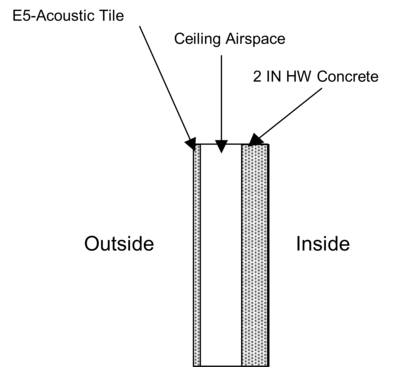
\includegraphics[width=0.9\textwidth, height=0.9\textheight, keepaspectratio=true]{media/image050.png}
\caption{Example Floor Construction illustration. \protect \label{fig:example-floor-construction-illustration.}}
\end{figure}

Window constructions are similarly built up from items in the Window Materials set using similar layers.. See Figure~\ref{fig:illustration-for-material-ordering-in}. Illustration for material ordering in windows, which shows the case where an interior shading layer such as a blind is present. The gap between the inside glass layer (layer \#3) and the interior shading layer is not entered. Similarly, for an exterior shading layer, the gap between the outside glass layer and the shading layer is not entered.

\begin{figure}[hbtp] % fig 25
\centering
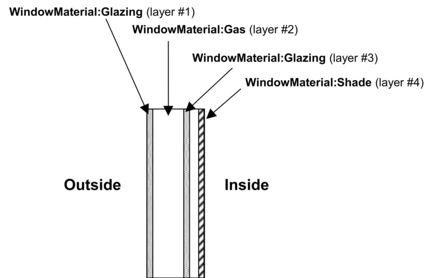
\includegraphics[width=0.9\textwidth, height=0.9\textheight, keepaspectratio=true]{media/image051.png}
\caption{Illustration for material ordering in windows. \protect \label{fig:illustration-for-material-ordering-in}}
\end{figure}

However, for a between-glass shading device the gaps on either side of the shading layer must be entered and they must have the same gas type. In addition, the gap widths with and without the between-glass shading layer must be consistent (see Figure~\ref{fig:window-construction-with-and-without-a}).

A maximum of four glass layers and one shading layer is allowed. A gas layer must always separate adjacent glass layers in a multi-pane glazing without a between-glass shading layer.

\begin{figure}[hbtp] % fig 26
\centering
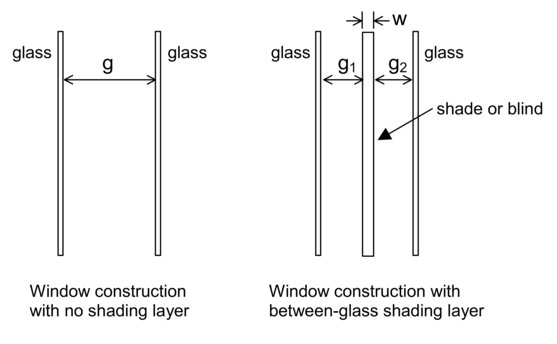
\includegraphics[width=0.9\textwidth, height=0.9\textheight, keepaspectratio=true]{media/image052.png}
  \caption{Window construction with and without a between-glass shading layer. Shown are gap widths \(g\), \(g_1\) and \(g_2\), and shading layer width, \(w\). An error will result if \(g_1 + g_2 +w\) is not equal to \(g\), where \(w\) is zero for a blind and greater than zero for a shade. \protect \label{fig:window-construction-with-and-without-a}}
\end{figure}

Outside and inside air film resistances are never given as part of a construction definitions since they are calculated during the EnergyPlus simulation. Note also that constructions are assumed to be one-dimensional in a direction perpendicular to the surface.

\subsubsection{Inputs}\label{inputs-34-000}

\paragraph{Field: Name}\label{field-name-28-001}

This field is a user specified name that will be used as a reference by other input syntax. For example, a heat transfer surface (ref: Building Surfaces) requires a construction name to define what the make-up of the wall is. This name must be identical to one of the Construction definitions in the input data file.

\paragraph{Field: Outside Layer}\label{field-outside-layer}

Each construction must have at least one layer. This field defines the material name associated with the layer on the outside of the construction---outside referring to the side that is not exposed to the zone but rather the opposite side environment, whether this is the outdoor environment or another zone. Material layers are defined based on their thermal properties elsewhere in the input file (ref: Material and Material Properties and Materials for Glass Windows and Doors). As noted above, the outside layer should NOT be a film coefficient since EnergyPlus will calculate outside convection and radiation heat transfer more precisely.

\paragraph{Field(s) 2-10: Layers}\label{fields-2-10-layers}

The next fields are optional and the number of them showing up in a particular Construction definition depends solely on the number of material layers present in that construction. The data expected is identical to the outside layer field (see previous field description). The order of the remaining layers is important and should be listed in order of occurrence from the one just inside the outside layer until the inside layer is reached. As noted above, the inside layer should NOT be a film coefficient since EnergyPlus will calculate inside convection and radiation heat transfer more precisely.

IDF Example (floor construction):

\begin{lstlisting}

Construction, FLOOR38,  ! Material layer names follow:
        E5 - ACOUSTIC TILE,
        E4 - CEILING AIRSPACE,
        C12 - 2 IN HW CONCRETE;
\end{lstlisting}

IDF Example (window construction, no shade):

\begin{lstlisting}

Construction, DOUBLE PANE WINDOW,  !- Material layer names follow:
        GLASS - CLEAR SHEET 1 / 8 IN,
        WinAirB1 - AIRSPACE RESISTANCE,
        GLASS - CLEAR SHEET 1 / 8 IN;
\end{lstlisting}

IDF Example (window construction, with interior shade):

\begin{lstlisting}

Construction, DOUBLE PANE WITH ROLL SHADE,  !- Material layer names follow:
        GLASS - CLEAR SHEET 1 / 8 IN,
        WinAirB1 - AIRSPACE RESISTANCE,
        GLASS - CLEAR SHEET 1 / 8 IN,
        ROLL SHADE - LIGHT
\end{lstlisting}

\subsection{Site:GroundTemperature:FCfactorMethod}\label{sitegroundtemperaturefcfactormethod-000}

Site:GroundTemperature:FCfactorMethod is used only by the underground walls or slabs-on-grade or underground floors defined with C-factor (Construction:CfactorUndergroundWall) and F-factor (Construction:FfactorGroundFloor) method for code compliance calculations where detailed construction layers are unknown. Only one such ground temperature object can be included. The monthly ground temperatures for this object are close to the monthly outside air temperatures delayed by three months. If user does not input this object in the IDF file, it will be defaulted to the 0.5m set of monthly ground temperatures from the weather file if they are available.

\subsubsection{Inputs}\label{inputs-35-000}

\paragraph{Field: Month Temperature(s) -- 12 fields in all}\label{field-month-temperatures-12-fields-in-all-000}

Each numeric field is the monthly ground temperature (degrees Celsius) used for the indicated month (January = 1\(^{st}\) field, February = 2\(^{nd}\) field, etc.)

And, the IDF example:

\begin{lstlisting}
Site:GroundTemperature:FCfactorMethod,  9.5,3.5,-0.7,-1.7,-0.6,3.6,9.3,14,18.2,22.7,21.2,16.8;
\end{lstlisting}

\subsection{Constructions - Modeling Underground Walls and Ground Floors Defined with C and F Factors for Building Energy Code Compliance}\label{constructions---modeling-underground-walls-and-ground-floors-defined-with-c-and-f-factors-for-building-energy-code-compliance}

Building energy code and standards like ASHRAE 90.1, 90.2 and California Title 24 require the underground wall constructions and slabs-on-grade or underground floors not to exceed certain maximum values of C-factor and F-factor, which do not specify detailed layer-by-layer materials for the constructions.

A simplified approach is introduced to create equivalent constructions and model the ground heat transfer through underground walls and ground floors for the building energy code compliance calculations. The approach is to create constructions based on the user defined C or F factor with two layers: one concrete layer (0.15 m thick) with thermal mass, and one fictitious insulation layer with no thermal mass. Three new objects were created for such purpose: \textbf{Construction:CfactorUndergroundWall}, \textbf{Construction:FfactorGroundFloor}, and \textbf{Site:GroundTemperature:FCfactorMethod}. Details of the approach are described in the Engineering Reference document. The wall and floor construction objects are described in this section; the ground temperature object is described with the other ground temperature objects.

When a underground wall or ground floor surface (BuildingSurface:Detailed, Floor:Detailed, and Wall:Detailed) references one of the two construction objects, its field `Outside Boundary Condition' needs to be set to GroundFCfactorMethod. For simple (rectangular) wall and floor objects, the outside boundary condition is inferred from the construction type.

The Site:GroundTemperature:FCfactorMethod is described in the section for ground temperatures, the following section describes the two new construction objects.

\subsection{Construction:CfactorUndergroundWall}\label{constructioncfactorundergroundwall}

This input object differs from the usual wall construction object in that it describes an entire construction rather than individual layers. This object is used when only the wall height (depth to the ground) and the C-factor are available.~ This object accesses a model that creates an equivalent layer-by-layer construction for the underground wall to approximate the heat transfer through the wall considering the thermal mass of the earth soil.

This object is referenced by underground wall surfaces with their fields `Outside Boundary Condition' set to GroundFCfactorMethod.

\subsubsection{Inputs}\label{inputs-36}

\paragraph{Field: Name}\label{field-name-29-000}

The name of the underground wall construction.

\paragraph{Field: C-Factor}\label{field-c-factor}

C-Factor is the time rate of steady-state heat flow through unit area of the construction, induced by a unit temperature difference between the body surfaces. The C-Factor unit is W/m\(^{2}\)·K. The C-factor does not include soil or air films. ASHRAE Standard 90.1 and California Title 24 specify maximum C-factors for underground walls depending on space types and climate zones.

\paragraph{Field: Height}\label{field-height}

This field describes the height of the underground wall, i.e.~the depth to the ground surface. The unit is meters.

IDF Example:

\begin{lstlisting}

Construction:CfactorUndergroundWall,
      CfactorUGWall,
      0.436,           ! C-factor (W/m2K), does not include soil or air films
      4.57;            ! Height (m)


    BuildingSurface:Detailed,
      Zn001:Wall001,           !- Name
      Wall,                    !- Surface Type
      CfactorUGWall,           !- Construction Name
      ZONE ONE,                !- Zone Name
      GroundFCfactorMethod,    !- Outside Boundary Condition
      ,                        !- Outside Boundary Condition Object
      NoSun,                   !- Sun Exposure
      NoWind,                  !- Wind Exposure
      0.0,                     !- View Factor to Ground
      4,                       !- Number of Vertices
      0.0,0.0,4.572,           !- X,Y,Z = = > Vertex 1
      0.0,0.0,0.0,             !- X,Y,Z = = > Vertex 2
      15.24,0.0,0.0,           !- X,Y,Z = = > Vertex 3
      15.24,0.0,4.572;         !- X,Y,Z = = > Vertex 4
\end{lstlisting}

\subsection{Construction:FfactorGroundFloor}\label{constructionffactorgroundfloor}

This input object differs from the usual ground floor construction object in that it describes an entire construction rather than individual layers. This object is used when only the floor area, exposed perimeter, and the F-factor are available.~ This object accesses a model that creates an equivalent layer-by-layer construction for the slab-on-grade or underground floor to approximate the heat transfer through the floor considering the thermal mass of the earth soil.

This object is referenced by slab-on-grade or underground floor surfaces with their fields `Outside Boundary Condition' set to GroundFCfactorMethod.

\subsubsection{Inputs}\label{inputs-37}

\paragraph{Field: Name}\label{field-name-30-000}

The name of the ground floor construction.

\paragraph{Field: F-Factor}\label{field-f-factor}

F-Factor represents the heat transfer through the floor, induced by a unit temperature difference between the outside and inside air temperature, on the per linear length of the exposed perimeter of the floor. The unit for this input is W/m·K. ASHRAE Standard 90.1 and California Title 24 specify maximum F-factors for slab-on-grade or underground floors depending on space types and climate zones.

\paragraph{Field: Area}\label{field-area}

This field describes the area (in square meters) of the slab-on-grade or underground floor.

\paragraph{Field: PerimeterExposed}\label{field-perimeterexposed}

This field describes the exposed (direct contact with ambient air) perimeter (in meters) of the slab-on-grade or underground floor.

IDF Example:

\begin{lstlisting}

Construction:FfactorGroundFloor,
      slabconst,
      0.12,     !F-factor in W/m-K
      232.26,   !Area in m2
      61.0;     !Exposed perimeter in m


    BuildingSurface:Detailed,
      Zn001:Flr001,            !- Name
      Floor,                   !- Surface Type
      slabconst,               !- Construction Name, FLOOR
      ZONE ONE,                !- Zone Name
      GroundFCfactorMethod,    !- Outside Boundary Condition, Surface
      ,                        !- Outside Boundary Condition Object, Zn001:Flr001
      NoSun,                   !- Sun Exposure
      NoWind,                  !- Wind Exposure
      0,                       !- View Factor to Ground
      4,                       !- Number of Vertices
      15.24,0.0,0.0,           !- X,Y,Z = = > Vertex 1
      0.0,0.0,0.0,             !- X,Y,Z = = > Vertex 2
      0.0,15.240,0.0,          !- X,Y,Z = = > Vertex 3
      15.24,15.24,0.0;         !- X,Y,Z = = > Vertex 4
\end{lstlisting}

\subsection{Construction:InternalSource}\label{constructioninternalsource}

In some cases such as radiant systems, a construction will actually have resistance wires or hydronic tubing embedded within the construction. Heat is then either added or removed from this building element to provide heating or cooling to the zone in question. In the case of building-integrated photovoltaics, the energy removed in the form of electricity will form a sink. It is possible to enter such constructions into EnergyPlus with the syntax described below. The definition is similar to the Construction definition with a few additions related to radiant or other systems that will lead to source/sink terms. The internal source capability is available with both the \textbf{ConductionTransferFunction} and \textbf{ConductionFiniteDifference} solution algorithms.~ The only difference is that the two dimensional pipe arrangements are not available to ConductionFiniteDifference. Those fields are ignored in that implementation.

\subsubsection{Inputs}\label{inputs-38}

\paragraph{Field: Name}\label{field-name-31-000}

This field is a user specified name that will be used as a reference by other input syntax. For example, a heat transfer surface (ref: Building Surfaces) requires a construction name to define what the make-up of the wall is.

\paragraph{Field: Source Present After Layer Number}\label{field-source-present-after-layer-number}

This field is an integer that relates the location of the heat source or sink. The integer refers to the list of material layers that follow later in the syntax and determines the layer after which the source is present. If a source is embedded within a single homogenous layer (such as concrete), that layer should be split into two layers and the source added between them. For example, a value of ``2'' in this field tells EnergyPlus that the source is located between the second and third material layers listed later in the construction description (see layer fields below).

\paragraph{Field: Temperature Calculation Requested After Layer Number}\label{field-temperature-calculation-requested-after-layer-number}

The nature of this field is similar to the source interface parameter (see previous field) in that it is an integer, refers to the list of material layers that follow, and defines a location after the layer number identified by the user-defined number. In this case, the user is specifying the location for a separate temperature calculation rather than the location of the heat source/sink. This feature is intended to allow users to calculate a temperature within the construction. This might be important in a radiant cooling system where condensation could be a problem. This temperature calculation can assist users in making that determination in absence of a full heat and mass balance calculation.

\paragraph{Field: Dimensions for the CTF Calculation}\label{field-dimensions-for-the-ctf-calculation}

This field is also an integer and refers to the detail level of the calculation. A value of ``1'' states that the user is only interested in a one-dimensional calculation. This is appropriate for electric resistance heating and for hydronic heating (when boiler/hot water heater performance is not affected by return and supply water temperatures). A value of ``2'' will trigger a two-dimensional solution for this surface only. This may be necessary for hydronic radiant cooling situations since chiller performance is affected by the water temperatures provided.

A few things should be noted about requesting two-dimensional solutions. First, the calculation of the conduction transfer functions (CTF) is fairly intensive and will require a significant amount of computing time. Second, the solution regime is two-dimensional internally but it has a one-dimensional boundary condition imposed at the inside and outside surface (i.e., surface temperatures are still isothermal is if the surface was one-dimensional).

\paragraph{Field: Tube Spacing}\label{field-tube-spacing}

This field defines how far apart in meters the hydronic tubing or electrical resistance wires are spaced in the direction perpendicular to the main direction of heat transfer. Note that this parameter is only used for two-dimensional solutions (see previous field).

\paragraph{Field: Outside Layer}\label{field-outside-layer-1}

Each construction must have at least one layer. This field defines the material name associated with the layer on the outside of this construction---outside referring to the side that is not exposed to the zone but rather the opposite side environment, whether this is the outdoor environment or another zone. Material layers are defined based on their thermal properties elsewhere in the input file (ref: Material and Material Properties and Materials for Glass Windows and Doors). As noted above, the outside layer should NOT be a film coefficient since EnergyPlus will calculate convection and radiation heat transfer more precisely.

\paragraph{Field(s) 2-10: Layers}\label{fields-2-10-layers-1}

The next fields are optional and the number of them showing up in a particular Construction definition depends solely on the number of material layers present in that particular construction. The data expected is identical to the outside layer field (see previous field description). The order of the remaining layers is important and should be listed in order of occurrence from the one just inside the outside layer until the inside layer is reached. As noted above, the inside layer should NOT be a film coefficient since EnergyPlus will calculate convection and radiation heat transfer more precisely.

\subsubsection{Outputs}\label{outputs-36-1}

\begin{itemize}
\item  Zone,Average,Surface Internal Source Location Temperature [C]
\item  Zone,Average,Surface Internal User Specified Location Temperature [C]
\end{itemize}

\paragraph{Surface Internal Source Location Temperature {[}C{]}}\label{surface-internal-source-location-temperature-c}

This output is the temperature within the surface at the location of the source/sink.

\paragraph{Surface Internal User Specified Location Temperature {[}C{]}}\label{surface-internal-user—specified-location-temperature-c}

This output is the temperature within the surface at the location requested by the user.


\subsection{Composite Wall Constructions}\label{composite-wall-constructions}

Standard constructions in EnergyPlus are built with the materials and layers described earlier. However, some configurations will not be adequately represented by using this approach. The Reference Data Set CompositeWallConstructions.idf contains constructions and associated materials for a set of \textbf{composite} walls. These are walls---such as stud walls---that have complicated heat-flow paths so that the conduction is two- or three-dimensional. Thermal bridges are one of the common terms for these complicated heat-flow paths; this dataset will help you represent these in EnergyPlus.

The materials here are \textbf{not} real materials but are ``equivalent'' materials obtained from finite-difference modeling. (The thickness, conductivity, density and specific heat values of the material layers for the different constructions have been taken from the ASHRAE report ``Modeling Two- and Three-Dimensional Heat Transfer through Composite Wall and Roof Assemblies in Hourly Energy Simulation Programs (1145-TRP),'' by Enermodal Engineering Limited, Oak Ridge National Laboratory, and the Polish Academy of Sciences, January 2001.). EnergyPlus will calculate conduction transfer functions using these materials. The heat transfer based on these conduction transfer functions will then be very close to what would be calculated with a two- or three-dimensional heat transfer calculation.

For stud walls, using these composite constructions will give more accurate heat flow than you would get by manually dividing the wall into a stud section and a non-stud section.

If your wall's exterior or interior roughness or thermal, solar or visible absorptances are different from those in the data set, you can make the appropriate changes to the first material (the outside layer) or the third material (the inside layer). \textbf{None of the other values should be changed.}

\begin{callout}
Complete description of the CompositeWallConstructions data set are found in the OutputDetailsAndExamples document.
\end{callout}

\subsection{Construction:ComplexFenestrationState}\label{constructioncomplexfenestrationstate}

This input object is used to describe the properties of a single state for complex fenestration.~ There are two parts to the input, 1) layer-by-layer physical description of fenestration system and 2) a set of matrices that describe overall system optical performance.~ Each layer also has associated with it two matrices that give the layer absorptance (for front and back incidence on the system.

The optical properties are given as a two-dimensional matrix describing the basis and four two-dimensional matrices of system bidirectional optical properties.

These input objects will generally be exported directly from the WINDOW program and it is expected that users usually will not develop the input themselves. However, this is an option for users who prefer to use a different method (e.g., Monte-Carlo ray-trace or measurement) of determining optical properties.

Multiple instances of this object are used to define the separate operating states of complex fenestration.~ For example, blinds could be deployed or redirected to create a new state, or electrochromic glazings could change transmittance.~ Each separate state defines the materials present and the overall optical performance.~ If the glazing system has only one state, then only one of these objects is needed.

If there is more than one complex fenestration state, it will be controlled using the EMS actuator called ``Surface'' with the control type ``Construction State'' and the EMS input object called EnergyManagementSystem:ConstructionIndexVariable.

\subsubsection{Inputs}\label{inputs-39}

\paragraph{Field: Name}\label{field-name-32-000}

Unique name of this construction.~ Used to identify type of window in surface objects.

\paragraph{Field: Basis Type keyword}\label{field-basis-type-keyword}

Only value currently implemented is ``LBNLWINDOW''. More options may be added in the future.

\paragraph{Field: Basis Symmetry, keyword}\label{field-basis-symmetry-keyword}

Only value currently implemented is ``None''. More options will be added in the future.

\paragraph{Field: Thermal Parameters}\label{field-thermal-parameters}

This field gives the name of WindowThermalModel:Params object used to keep common data necessary for thermal simulation.

\paragraph{Field: Basis Matrix Name}\label{field-basis-matrix-name}

This field gives the name of an 2 x N matrix object that defines the basis~ For a fenestration basis, N would be the number of theta (polar angle) values, the first of the two elements for each of the i = 1,..,N would be the theta value, and the second would be the number of phi (azimuthal angle) values that 360º is divided into for that theta.

\paragraph{Field: Solar Optical Complex Front Transmittance Matrix Name}\label{field-solar-optical-complex-front-transmittance-matrix-name}

This field contains the name of matrix object that describes the solar transmittance at different incident angles.~ This is from the outside toward the inside.

\paragraph{Field: Solar Optical Complex Back Reflectance Matrix Name}\label{field-solar-optical-complex-back-reflectance-matrix-name}

This field contains the name of matrix object that describes the solar back reflectance at different incident angles.~ This is from the inside toward the outside.

\paragraph{Field: Visible Optical Complex Front Transmittance Matrix Name}\label{field-visible-optical-complex-front-transmittance-matrix-name}

This field contains the name of matrix object that describes the visible transmittance at different incident angles.~ This is from the outside toward the inside.

\paragraph{Field: Visible Optical Complex Back Reflectance Matrix Name}\label{field-visible-optical-complex-back-reflectance-matrix-name}

This field contains the name of vector object that describes the visible back reflectance at different incident angles.~ This is from the inside toward the outside.

\paragraph{Field: Outside Layer \textless{}x = 1\textgreater{}}\label{field-outside-layer-x-1}

Each construction must have at least one layer. The layer order is from outside to inside, with the first layer being either WindowMaterial:Glazing or WindowMaterial:ComplexShade. The next layer is a WindowMaterial:Gap layer, and the following layers then alternate between WindowMaterial:Glazing or WindowMaterial:ComplexShade and WindowMaterial:Gap. The last layer cannot be WindowMaterial:Gap.

\paragraph{Field: Outside Layer Directional Front Absorptance Matrix Name}\label{field-outside-layer-directional-front-absorptance-matrix-name}

Points to an Nbasis x 1 matrix object.

\paragraph{Field: Outside Layer Directional Back Absorptance Matrix Name}\label{field-outside-layer-directional-back-absorptance-matrix-name}

Points to an Nbasis x 1 matrix object.

\paragraph{Above 3 fields are optionally repeated for layers 2-10}\label{above-3-fields-are-optionally-repeated-for-layers-2-10}

These layers include gaps, which do not need to have matrix data specified.

An IDF example of complex fenestration with single layer:

\begin{lstlisting}

Construction:ComplexFenestrationState,       !- single layer example
    CFS_Glz_1,                 !- name
    LBNLWindow,                !- basis type
    None,                      !- basis symmetry type
    ThermParam_1,              !- window thermal model
    CFS_Glz_1_Basis,           !- basis matrix name
    CFS_Glz_1_TfSol,           !- Tfsol
    CFS_Glz_1_RbSol,           !- Rbsol
    CFS_Glz_1_Tfvis,           !- Tfvis
    CFS_Glz_1_Tbvis,           !- Tbvis
    Glass_102_Layer,           !- layer 1 name
    CFS_Glz_1_Layer_1_fAbs,    !- fAbs
    CFS_Glz_1_Layer_1_bAbs;    !- bAbs
\end{lstlisting}

An complex fenestration IDF example with double layer (first layer is shading device):

\begin{lstlisting}

Construction:ComplexFenestrationState,       !- double layer example
    CFS_Glz_59,                    !- name
    LBNLWindow,                    !- basis type
    None,                          !- basis symmetry type
    ThermParam_59,                 !- window thermal model
    CFS_Glz_59_Basis,              !- basis matrix name
    CFS_Glz_59_TfSol,              !- Tfsol
    CFS_Glz_59_RbSol,              !- Rbsol
    CFS_Glz_59_Tfvis,              !- Tfvis
    CFS_Glz_59_Tbvis,              !- Tbvis
    Shade_30001_Layer,             !- layer 1 name (shading device)
    CFS_Glz_59_Layer_1_fAbs,       !- fAbs
    CFS_Glz_59_Layer_1_bAbs,       !- bAbs
    Gap_1_Layer,                   !- layer 1 name
    ,                 !- absorptance matrices for gaps should be empty for now
    ,                              !- it is for future use
    Glass_3110_Layer,              !- layer 2 name
    CFS_Glz_59_Layer_3110_fAbs,    !- fAbs
    CFS_Glz_59_Layer_3110_bAbs;    !- bAbs
\end{lstlisting}

\subsection{WindowThermalModel:Params}\label{windowthermalmodelparams}

This input object is used with the Construction:ComplexFenestrationState

\subsubsection{Inputs}\label{inputs-40}

\paragraph{Field: Name}\label{field-name-33-000}

Unique name of the window thermal model parameters.

\paragraph{Field: Calculation Standard}\label{field-calculation-standard}

The type of the calculation standard.~ The choices are:

\begin{itemize}
\item
  ISO15099
\item
  EN673Declared
\item
  EN673Design
\end{itemize}

The default is ISO15099.

\paragraph{Field: Thermal Model}\label{field-thermal-model}

The type of thermal model.~ The choices are:

\begin{itemize}
\item
  ISO15099
\item
  ScaledCavityWidth
\item
  ConvectiveScalarModel\_NoSDThickness
\item
  ConvectiveScalarModel\_withSDThickness
\end{itemize}

The default is ISO15099.

\paragraph{Field: SD Scalar}\label{field-sd-scalar}

Shading Device Scalar Factor. Only used for~ Thermal Model = Convective Scalar Model.~ Factor of venetian shading device layer contribution to convection. Real value between 0 (where the shading device contribution to convection is neglected) and 1 (where the shading device treated as ``closed'' -- as if it is a glass layer with thermal properties of SD slat material). Default: 1.0

\paragraph{Field: Deflection Model}\label{field-deflection-model}

The type of deflection model used to model deflection in windows and glass.~ The choices are:

\begin{itemize}
\item
  NoDeflection
\item
  TemperatureAndPressureInput
\item
  MeasuredDeflection
\end{itemize}

The default is NoDeflection.

\paragraph{Field: Vacuum Pressure Limit}\label{field-vacuum-pressure-limit}

The pressure (Pa) which will be considered to be the limit for vacuum glazing pressure.~ All pressures less than or equal to this pressure will be considered to be vacuum. Default: 13.238 Pa.

\paragraph{Field: Initial Temperature}\label{field-initial-temperature}

The temperature (\(^{o}\)C) of the gap in the time of fabrication.~ It is used only when WindowThermalModel:Params DeflectionModel = TemperatureAndPressureInput

\paragraph{Field: Initial Pressure}\label{field-initial-pressure}

The pressure (Pa) of the gap at the time of fabrication of the sealed glazing system unitIt is used only when WindowThermalModel:Params DeflectionModel = TemperatureAndPressureInput.

An IDF example for WindowThermalModel:Params (without deflection):

\begin{lstlisting}

WindowThermalModel:Params,
    ThermParam_59,                   !- name
    ISO15099,                        !- standard
    ISO15099,                        !- thermal model standard
    1.00,                            !- SD scalar
    NoDeflection;                    !- deflection model
\end{lstlisting}

An IDF example for thermal parameters (with deflection):

\begin{lstlisting}

WindowThermalModel:Params,
    ThermParam_59,                   !- name
    ISO15099,                        !- standard
    ISO15099,                        !- thermal model standard
    1.00,                            !- SD scalar
    TemperatureAndPressureInput,     !- deflection model
    ,                                !- vacuum pressure limit
    21.00,                           !- temperature at time of fabrication
    10000.00;                        !- pressure at time of fabrication
\end{lstlisting}

An IDF example for WindowThermalModel:Params for modeling vacuum glazing

\begin{lstlisting}

WindowThermalModel:Params,
  ThermParam_1006,                                    !- name
  ISO15099,                                           !- standard
  ISO15099,                                           !- thermal model
  1.0000,                                             !- SDScalar
  NoDeflection,                                       !- deflection model
  13.238;                                             !- vacuum pressure limit
\end{lstlisting}

\subsection{Matrix:TwoDimension}\label{matrixtwodimension}

This is input object is only used with Construction:ComplexFenestrationState object to enter a two-dimensional matrix of values.

It is used to define the Basis Matrix for BSDF input data, and is also used to define the actual BSDF matrices data for the complete fenestration definition as well as the individual layers of the system.

The data are entered in row-major order: all the elements of row 1, followed by all the elements of row 2, etc.~ The number of values to be entered depends on the number of rows and the number of columns.~ Blank fields are treated as having been set to zero.

See example IDF file ``SmOff\_ CmplxGlz\_IntExtShading.idf'' for the definition of two complex shading layers with matrix data defined.

\subsubsection{Field: Name}\label{field-name-34-000}

Unique name of matrix input object.

\subsubsection{Field: Number of Rows}\label{field-number-of-rows}

This field is the number of rows in the matrix.

\subsubsection{Field: Number of Columns}\label{field-number-of-columns}

This field is the number of columns in the matrix

\subsubsection{\textless{} Field Set: Value \# N \textgreater{}}\label{field-set-value-n}

Repeat entering value exactly the same number of times as the number of rows times the number of columns.

\subsubsection{Field: Value \# 1}\label{field-value-1-000}

This is the value of the matrix at the first row and first column.

\subsubsection{Field: Value \#2}\label{field-value-2}

This is the value of the matrix at the first row and the second column.

An IDF example of matrix for defining BSDF basis:

\begin{lstlisting}

Matrix:TwoDimension,       !- matrix for basis definition
    CFS_Glz_1_Basis,         !- basis matrix name
    9,                       !- number of rows
    2,                       !- number of columns
    0.00000, 1.00000,
    10.00000, 8.00000,
    20.00000, 16.00000,
    30.00000, 20.00000,
    40.00000, 24.00000,
    50.00000, 24.00000,
    60.00000, 24.00000,
    70.00000, 16.00000,
    82.50000, 12.00000;
\end{lstlisting}

\subsection{Construction:WindowEquivalentLayer}\label{constructionwindowequivalentlayer}

This object defines the construction for equivalent layer window (ASHWAT) model. This window can model various mix of glazing and shading layers combination. Shadings are defined as an integral part of the construction. The construction is defined by listing the layers name starting with outside layer and work your way to the inside Layer. Up to six solid layers (glazing and shade) and up to five gaps, i.e., a total of up to 11 layers maximum are allowed in equivalent layer window object. The solid layer types allowed are: Glazing, Insect Screen, Roller Blinds, Venetian Blind, and Drape Fabrics. This window model requires optical data of the individual glazing and shading layers to calculate the effective optical properties of the composite fenestration construction. Venetian blinds in equivalent layer window model can be in a fixed slat angle or has the option to control the slat angle in order to maximize visibility, or maximize solar gains. An equivalent-layer concept can simulate wide range of multiple glazing and shading layers combination and provides unlimited flexibility to combine different types of shading layers in a fenestration. For the gap layer object any one of the five different Gas types can be specified: AIR, ARGON, XENON, KRYPTON, or CUSTOM.This window object is referenced by fenestration surfaces. For details of the model description refer to Equivalent Layer Fenestration Model section in Engineering Reference. The various layer objects that can be referenced in Equivalent Layer window model are:

\begin{lstlisting}
WindowMaterial:Glass:EquivalentLayer
WindowMaterial:Shade:EquivalentLayer
WindowMaterial:Drape:EquivalentLayer
WindowMaterial:Blind:EquivalentLayer
WindowMaterial:Screen:EquivalentLayer
WindowMaterial:Gap:EquivalentLayer
\end{lstlisting}

\subsubsection{Inputs}\label{inputs-41}

\paragraph{Field: Name}\label{field-name-35}

This field is a user specified name that will be used as a reference by other input syntax. For example, a heat transfer surface (ref: Fenestration) requires a construction name to define what the make-up of the fenestration is. This name must be identical to one of the Window Construction Equivalent Layer definitions in the input data file.

\paragraph{Field: Outside Layer}\label{field-outside-layer-2}

Each equivalent layer window construction must have at least one layer. This field defines the material name associated with the layer on the outside of the construction---outside referring to the side that is exposed to the outdoor environment or another zone. Material layers for equivalent layer window model are defined based on their thermal properties elsewhere in the input file (ref: WindowEquivalentLayerMaterialNames)

\paragraph{Field: Layer 2 - Layer11}\label{field-layer-2---layer11}

The next fields are optional and the number of them showing up in a particular equivalent layer window construction definition depends solely on the number of material layers present in that construction. The data expected is identical to the outside layer field (see previous field description). The order of the remaining layers is important and should be listed in order of occurrence from the one just inside the outside layer until the inside layer is reached. As noted above, the inside layer should NOT be a film coefficient since EnergyPlus will calculate inside convection and radiation heat transfer more precisely.

An IDF example for this object, is shown below:

\begin{lstlisting}

Construction:WindowEquivalentLayer,
    Six Solid Layers Window,   !- Name
    INSCRN,                    !- Outside Layer
    Air GAP Outdoor 12.7mm,    !- Layer 2
    GLZGRY,                    !- Layer 3
    Argon GAP Sealed 12.7mm,   !- Layer 4
    FEP,                       !- Layer 5
    Xenon GAP Sealed 12.7mm,   !- Layer 6
    LOF1436,                   !- Layer 7
    Krypton GAP Sealed 12.7mm, !- Layer 8
    GLZCLR,                    !- Layer 9
    Air GAP Indoor 12.7mm,     !- Layer 10
    ShadeTrns;                 !- Layer 11
\end{lstlisting}

\subsection{Construction:WindowDataFile}\label{constructionwindowdatafile}

The WINDOW program, which does a thermal and optical analysis of a window under different design conditions, writes a data file (``Window data file'') containing a description of the window that was analyzed. The Construction:WindowDataFile object allows a window to be read in from the WINDOW data file---see ``Importing Windows from WINDOW.'' For information on adding a shading device to the window see ``WindowProperty:ShadingControl.''

\subsubsection{Inputs}\label{inputs-42}

\paragraph{Field: Name}\label{field-name-36}

This is the name of a window on the Window data file. An error will result if EnergyPlus cannot find a window of this name on the file, or if the file, shown in the next field, is not present. The location of the data file should be specified in the File Name field. For details on what is done with the data if a matching window is found on the file see ``Importing Windows from WINDOW.''

\paragraph{Field: File Name}\label{field-file-name-000}

This is the file name of the Window data file that contains the Window referenced in the previous field. The field may include a full path with file name, for precise results. The field must be \textless{} = 100 characters. The file name must not include commas or an exclamation point. A relative path or a simple file name should work with version 7.0 or later when using EP-Launch even though EP-Launch uses temporary directories as part of the execution of EnergyPlus. If using RunEPlus.bat to run EnergyPlus from the command line, a relative path or a simple file name may work if RunEPlus.bat is run from the folder that contains EnergyPlus.exe.

If this field is left blank, the file name is defaulted to Window5DataFile.dat.

Input Example

\begin{lstlisting}
Construction:WindowDataFile,
  DoubleClear;            !- Name of a Window on the Window Data File
  ! Note -- Window5DataFile.dat is presumed to be in the "run" folder where EnergyPlus.exe is

FenestrationSurface:Detailed,
  Zn001:Wall001:Win001, !- Name
  Window,               !- Class
  DoubleClear,          !- Construction Name
  Zn001:Wall001,        !- Base Surface Name, and Target (if applicable)
  0.5,                  !- View Factor to Ground
  ,                     !- Window Shading Control name
  ,                     !- Frame/Divider name
   1.0,                 !- Multiplier
  4,                    !- Number of vertices
  0.548, 0.0, 2.5000,   !- X,Y,Z of Vertices
  0.548, 0.0, 0.5000,
  5.548, 0.0, 0.5000,
  5.548, 0.0, 2.5000;
\end{lstlisting}

An example showing use of specific data file name and complete path location follows:

\begin{lstlisting}
Construction:WindowDataFile,
  DoubleClear,          !- Name of a Window on the Window Data File
  C:\EnergyPlusData\DataSets\MyWindow.dat;
\end{lstlisting}

\subsubsection{Outputs}\label{outputs-4-016}

An optional report (contained in \textbf{eplusout.eio}) gives calculational elements for the materials and constructions used in the input. These reports are explained fully in the Output Details and Examples document.


\section{Group -- Thermal Zone Description/Geometry}\label{group-thermal-zone-descriptiongeometry}

Without thermal zones and surfaces, the building can't be simulated. This group of objects (Zone, BuildingSurface) describes the thermal zone characteristics as well as the details of each surface to be modeled. Included here are shading surfaces.

\subsection{Zone}\label{zone}

This element sets up the parameters to simulate each thermal zone of the building.

\subsubsection{Inputs}\label{inputs-048}

\paragraph{Field: Direction of Relative North}\label{field-direction-of-relative-north}

The Zone North Axis is specified \textbf{relative to the Building North Axis}. This value is specified in degrees (clockwise is positive). For more information, see the figure below as well as the description under ``GlobalGeometryRules''.

\paragraph{Field(s): (X,Y,Z) Origin}\label{fields-xyz-origin}

The X,Y,Z coordinates of a zone origin can be specified, for convenience in vertice entry. Depending on the values in ``GlobalGeometryRules'' (see description later in this section), these will be used to completely specify the building coordinates in ``world coordinate'' or not. Zone Origin coordinates are specified \textbf{relative to the Building Origin (which always 0,0,0)}. The following figure illustrates the use of Zone North Axis as well as Zone Origin values.

\begin{figure}[hbtp] % fig 27
\centering
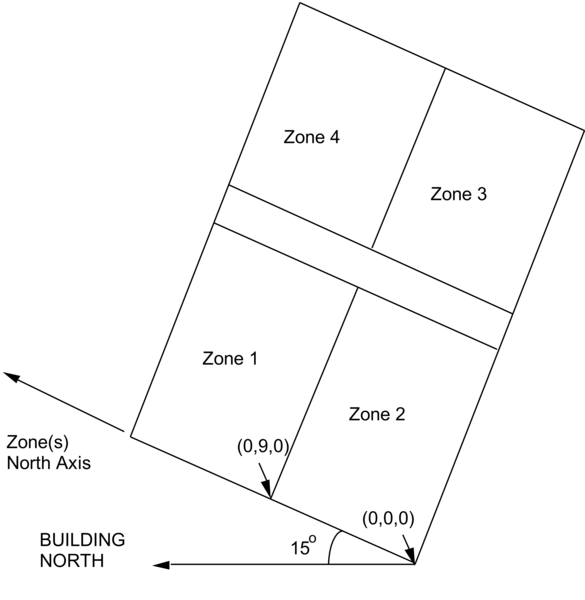
\includegraphics[width=0.9\textwidth, height=0.9\textheight, keepaspectratio=true]{media/image053.png}
\caption{Illustration of Zone North Axis and Origins \protect \label{fig:illustration-of-zone-north-axis-and-origins}}
\end{figure}

\paragraph{Field: Type}\label{field-type-000}

Zone type is currently unused.

\paragraph{Field: Multiplier}\label{field-multiplier}

Zone Multiplier is designed as a ``multiplier'' for floor area, zone loads, and energy consumed by internal gains. It takes the calculated load for the zone and multiplies it, sending the multiplied load to the attached HVAC system. The HVAC system size is specified to meet the entire multiplied zone load and will report the amount of the load met in the Zone Air System Sensible Heating or Cooling Energy/Rate output variable. Autosizing automatically accounts for multipliers. Metered energy consumption by internal gains objects such as Lights or Electric Equipment will be multiplied. The default is 1.

\paragraph{Field: Ceiling Height}\label{field-ceiling-height}

Zone ceiling height is used in several areas within EnergyPlus (such as various room models, some convection coefficient calculations and, primarily, in calculating zone volume in the absence of other parameters). Energyplus automatically calculates the zone ceiling height (m) from the average height of the zone. If this field is 0.0, negative or \textbf{autocalculate}, then the calculated zone ceiling height will be used in subsequent calculations. If this field is positive, then the calculated zone ceiling height will not be used -- the number entered here will be used as the zone ceiling height. If this number differs significantly from the calculated ceiling height, then a warning message will be issued. If a zone ceiling height is entered, but no Volume is entered, then the floor area (if there is one) times the zone ceiling height will be used as the volume.

Note that the Zone Ceiling Height is the distance from the Floor to the Ceiling in the Zone, not an absolute height from the ground.

\paragraph{Field: Volume}\label{field-volume}

Zone volume is used in several areas within EnergyPlus (such as calculating air change rates for reporting or flow when air change rates are chosen as input, daylighting calculations, some convection coefficient calculations). EnergyPlus automatically calculates the zone volume (m\(^{3}\)) from the zone geometry given by the surfaces that belong to the zone. If this field is 0.0, negative or \textbf{autocalculate}, then the calculated zone volume will be used in subsequent calculations. If this field is positive, then it will be used as the zone volume. If this number differs significantly from the calculated zone volume a warning message will be issued. For autocalculate to work properly, the zone must be enclosed by the entered walls. Note that indicating the volume to be calculated but entering a positive ceiling height in the previous field will cause the volume to be calculated as the floor area (if \textgreater{} 0) times the entered ceiling height; else the volume will be calculated from the described surfaces. If this field is positive, any ceiling height positive value will not be used in volume calculations.

\paragraph{Field: Floor Area}\label{field-floor-area}

Zone floor area is used in many places within EnergyPlus. EnergyPlus automatically calculates the zone floor area (m\(^{2}\)) from the zone geometry given by the surfaces that belong to the zone. If this field is 0.0, negative or \textbf{autocalculate}, then the calculated zone floor area will be used in subsequent calculations. If this field is positive, then it will be used as the zone floor area. If this number differs significantly from the calculated zone floor area a warning message will be issued.

\paragraph{Field: Zone Inside Convection Algorithm}\label{field-zone-inside-convection-algorithm}

The Zone Inside Convection Algorithm field is optional. This field specifies the convection model to be used for the inside face of heat transfer surfaces associated with this zone. The choices are: \textbf{Simple} (constant natural convection - ASHRAE), \textbf{TARP} (combines natural and wind-driven convection correlations from laboratory measurements on flat plates), \textbf{CeilingDiffuser} (ACH based forced and mixed convection correlations for ceiling diffuser configuration with simple natural convection limit), \textbf{AdaptiveConvectionAlgorithm} (complex arrangement of various models that adapt to various zone conditions and can be customized) and \textbf{TrombeWall} (variable natural convection in an enclosed rectangular cavity). See the Inside Convection Algorithm object for further descriptions of the available models.

If omitted or blank, the algorithm specified in the SurfaceConvectionAlgorithm:Inside object is the default.

\paragraph{Field: Zone Outside Convection Algorithm}\label{field-zone-outside-convection-algorithm}

The Zone Outside Convection Algorithm field is optional. This field specifies the convection model to be used for the outside face of heat transfer surfaces associated with this zone. The choices are: \textbf{SimpleCombined}, \textbf{TARP}, \textbf{DOE-2}, \textbf{MoWiTT, and AdaptiveConvectionAlgorithm}. The simple convection model applies heat transfer coefficients depending on the roughness and windspeed. This is a combined heat transfer coefficient that includes radiation to sky, ground, and air. The correlation is based on Figure~\ref{fig:schematic-of-the-energyplus-unitary-system}, Page 25.1 (Thermal and Water Vapor Transmission Data), 2001 ASHRAE Handbook of Fundamentals.

The other convection models apply heat transfer coefficients depending on the roughness, windspeed, and terrain of the building's location. These are \emph{convection only} heat transfer coefficients; radiation heat transfer coefficients are calculated automatically by the program. The TARP algorithm was developed for the TARP software and combines natural and wind-driven convection correlations from laboratory measurements on flat plates. The DOE-2 and MoWiTT were derived from field measurements. The AdaptiveConvectionAlgorithm model is an dynamic algorithm that organizes a large number of different convection models and automatically selects the one that best applies. The adaptive convection algorithm can also be customized using the SurfaceConvectionAlgorithm:Outside:AdaptiveModelSelections input object. All algorithms are described more fully in the Engineering Reference.

If omitted or blank, the algorithm specified in the SurfaceConvectionAlgorithm:Outside object is the default.

\paragraph{Field: Part of Total Floor Area}\label{field-part-of-total-floor-area}

This optional field defaults to Yes if not specified. The field is used to show when a zone is not part of the Total Floor Area as shown in the Annual Building Utility Performance Summary tables. Specifically, when No is specified, the area is excluded from both the conditioned floor area and the total floor area in the Building Area sub table and the Normalized Metrics sub tables.

And, an IDF example:

\begin{lstlisting}

  Zone,
      DORM ROOMS AND COMMON AREAS,  !- Name
      0.0000000E+00,           !- Direction of Relative North {deg}
      0.0000000E+00,           !- X Origin {m}
      6.096000,                !- Y Origin {m}
      0.0000000E+00,           !- Z Origin {m}
      1,                       !- Type
      1,                       !- Multiplier
      autocalculate,           !-Ceiling Height {m}
      autocalculate;           !- Volume {m3}
\end{lstlisting}

\subsubsection{Outputs}\label{outputs-037}

\begin{itemize}
\item
  Zone,Average,Zone Outdoor Air Drybulb Temperature {[}C{]}
\item
  Zone,Average,Zone Outdoor Air Wetbulb Temperature {[}C{]}
\item
  Zone,Average,Zone Outdoor Air Wind Speed {[}m/s{]}
\end{itemize}

\paragraph{Zone Outdoor Air Drybulb Temperature {[}C{]}}\label{zone-outdoor-air-drybulb-temperature-c-000}

The outdoor air dry-bulb temperature calculated at the height above ground of the zone centroid.

\paragraph{Zone Outdoor Air Wetbulb Temperature {[}C{]}}\label{zone-outdoor-air-wetbulb-temperature-c-000}

The outdoor air wet-bulb temperature calculated at the height above ground of the zone centroid.

\paragraph{Zone Outdoor Air Wind Speed {[}m/s{]}}\label{zone-outdoor-air-wind-speed-ms-000}

The outdoor wind speed calculated at the height above ground of the zone centroid.

\subsection{Zone Thermal Output(s)}\label{zone-thermal-outputs}

In addition to the canned Surface reports (view the Reports section later in this document) and surface variables (above), the following variables are available for all zones:

\begin{itemize}
\item
  Zone,Sum,Zone Total Internal Radiant Heating Energy {[}J{]}
\item
  Zone,Average,Zone Total Internal Radiant Heating Rate {[}W{]}
\item
  Zone,Sum,Zone Total Internal Visible Radiation Heating Energy {[}J{]}
\item
  Zone,Average,Zone Total Internal Visible Radiation Heating Rate {[}W{]}
\item
  Zone,Sum,Zone Total Internal Convective Heating Energy {[}J{]}
\item
  Zone,Average,Zone Total Internal Convective Heating Rate {[}W{]}
\item
  Zone,Sum,Zone Total Internal Latent Gain Energy {[}J{]}
\item
  Zone,Average,Zone Total Internal Latent Gain Rate {[}W{]}
\item
  Zone,Sum,Zone Total Internal Total Heating Energy {[}J{]}
\item
  Zone,Average,Zone Total Internal Total Heating Rate {[}W{]}
\item
  Zone,Average,Zone Mean Air Temperature {[}C{]}
\item
  HVAC,Average,Zone Air Temperature {[}C{]}
\item
  Zone,Average,Zone Mean Air Dewpoint Temperature {[}C{]}
\item
  Zone,Average,Zone Mean Radiant Temperature {[}C{]}
\item
  Zone,Average,Zone Operative Temperature {[}C{]}
\item
  HVAC,Average,Zone Air Heat Balance Internal Convective Heat Gain Rate {[}W{]}
\item
  HVAC,Average,Zone Air Heat Balance Surface Convection Rate {[}W{]}
\item
  HVAC,Average,Zone Air Heat Balance Interzone Air Transfer Rate {[}W{]}
\item
  HVAC,Average,Zone Air Heat Balance Outdoor Air Transfer Rate {[}W{]}
\item
  HVAC,Average,Zone Air Heat Balance System Air Transfer Rate {[}W{]}
\item
  HVAC,Average,Zone Air Heat Balance System Convective Heat Gain Rate {[}W{]}
\item
  HVAC,Average,Zone Air Heat Balance Air Energy Storage Rate {[}W{]}
\item
  HVAC,Average,Zone Air Heat Balance Deviation Rate {[}W{]}
\item
  HVAC,Sum,Zone Air System Sensible Heating Energy {[}J{]}
\item
  HVAC,Sum,Zone Air System Sensible Cooling Energy {[}J{]}
\item
  HVAC,Average,Zone Air System Sensible Heating Rate {[}W{]}
\item
  HVAC,Average,Zone Air System Sensible Cooling Rate {[}W{]}
\item
  HVAC,Average,Zone Air Humidity Ratio{[}kgWater/kgDryAir{]}
\item
  HVAC,Average,Zone Air Relative Humidity{[}\%{]}
\end{itemize}

Two of these are of particular interest:

\begin{lstlisting}
Zone,Average,Zone Mean Air Temperature [C]
HVAC,Average,Zone Air Temperature [C]
\end{lstlisting}

These two variable outputs are/should be identical. However, note that they can be reported at different time intervals. ``Zone Mean Air Temperature'' is only available on the Zone/HB timestep (Number of Timesteps per Hour) whereas ``Zone Air Temperature'' can be reported at the HVAC timestep (which can vary).

\subsubsection{Zone Mean Air Temperature {[}C{]}}\label{zone-mean-air-temperature-c}

From the code definition, the zone mean air temperature is the average temperature of the air temperatures at the system timestep. Remember that the zone heat balance represents a ``well stirred'' model for a zone, therefore there is only one mean air temperature to represent the air temperature for the zone.

\subsubsection{Zone Air Temperature {[}C{]}}\label{zone-air-temperature-c}

This is very similar to the mean air temperature in the last field. The ``well stirred'' model for the zone is the basis, but this temperature is also available at the ``detailed'' system timestep.

\subsubsection{Zone Mean Air Dewpoint Temperature {[}C{]}}\label{zone-mean-air-dewpoint-temperature-c}

This is the dewpoint temperature of the zone calculated from the Zone Mean Air Temperature (above), the Zone Air Humidity Ratio (below) and the outdoor barometric pressure.

\subsubsection{Zone Thermostat Air Temperature {[}C{]}}\label{zone-thermostat-air-temperature-c}

This is the zone air node temperature for the well-mixed room air model, which is the default room air model type (RoomAirModelType = Mixing). But for other types of Room Air Model (the RoomAir:TemperaturePattern:* and RoomAirSettings:* objects) the zone thermostat air temperature may depend on the Thermostat Height and Thermostat Offset.

\subsubsection{Zone Mean Radiant Temperature {[}C{]}}\label{zone-mean-radiant-temperature-c}

The Mean Radiant Temperature (MRT) in degrees Celsius of a space is a measure of the combined effects of temperatures of surfaces within that space. Specifically it is the surface area × emissivity weighted average of the zone inside surface temperatures (ref. Surface Inside Temperature), where emissivity is the Thermal Absorptance of the inside material layer of each surface.

\subsubsection{Zone Operative Temperature {[}C{]}}\label{zone-operative-temperature-c}

Zone Operative Temperature (OT) is the average of the Zone Mean Air Temperature (MAT) and Zone Mean Radiant Temperature (MRT), OT = 0.5*MAT + 0.5*MRT. This output variable is not affected by the type of thermostat controls in the zone, and does not include the direct effect of high temperature radiant systems. See also Zone Thermostat Operative Temperature.

\subsubsection{Zone Air Heat Balance Internal Convective Heat Gain Rate {[}W{]}}\label{zone-air-heat-balance-internal-convective-heat-gain-rate-w}

The Zone Air Heat Balance Internal Convective Heat Gain Rate is the sum, in watts, of heat transferred to the zone air from all types of internal gains, including people, lights, equipment etc. This and the following provide results on the load components of the zone air heat balance. This field is not multiplied by zone or group multipliers.

\subsubsection{Zone Air Heat Balance Surface Convection Rate {[}W{]}}\label{zone-air-heat-balance-surface-convection-rate-w}

The Zone Air Heat Balance Surface Convection Rate is the sum, in watts, of heat transferred to the zone air from all the surfaces. This field is not multiplied by zone or group multipliers.

\subsubsection{Zone Air Heat Balance Interzone Air Transfer Rate {[}W{]}}\label{zone-air-heat-balance-interzone-air-transfer-rate-w}

The Zone Air Heat Balance Interzone Air Transfer Rate is the sum, in watts, of heat transferred to the zone air from all the transfers of air from other thermal zones. This field is not multiplied by zone or group multipliers.

\subsubsection{Zone Air Heat Balance Outdoor Air Transfer Rate {[}W{]}}\label{zone-air-heat-balance-outdoor-air-transfer-rate-w}

The Zone Air Heat Balance Outdoor Air Transfer Rate is the sum, in watts, of heat transferred to the zone air from all the transfers of air from the out side, such as infiltration. This field is not multiplied by zone or group multipliers.

\subsubsection{Zone Air Heat Balance System Air Transfer Rate {[}W{]}}\label{zone-air-heat-balance-system-air-transfer-rate-w}

The Zone Air Heat Balance System Air Transfer Rate is the sum, in watts, of heat transferred to the zone air by HVAC forced-air systems and air terminal units. Such HVAC systems are connected to the zone by an inlet node (see ZoneHVAC:EquipmentConnections input field called Zone Air Inlet Node or Node List Name) This field is not multiplied by zone or group multipliers.

\subsubsection{Zone Air Heat Balance System Convective Heat Gain Rate {[}W{]}}\label{zone-air-heat-balance-system-convective-heat-gain-rate-w}

The Zone Air Heat Balance System Convective Heat Gain Rate is the sum, in watts, of heat transferred directly to the zone air by ``non-air'' HVAC systems. Such HVAC systems are not connected to the zone by an inlet node but rather add or subtract heat directly to the zone air in a manner similar to internal gains. These include the convective fraction of zone HVAC baseboards and high temperature radiant systems, zone HVAC refrigeration chiller set, and the extra convective cooling provided by the cooled beam air terminal unit. This field is not multiplied by zone or group multipliers.

\subsubsection{Zone Air Heat Balance Air Energy Storage Rate {[}W{]}}\label{zone-air-heat-balance-air-energy-storage-rate-w}

The Zone Air Heat Balance Air Energy Storage Rate is the heat stored, in watts, in the zone air as result of zone air temperature changing from one timestep to the next. This field is not multiplied by zone or group multipliers.

\subsubsection{Zone Air Heat Balance Deviation Rate {[}W{]}}\label{zone-air-heat-balance-deviation-rate-w}

The Zone Air Heat Balance Deviation Rate is the imbalance, in watts, in the energy balance for zone air. The value should be near zero but will become non-zero if zone conditions are changing rapidly or erratically. This field is not multiplied by zone or group multipliers. (This output variable is only generated if the user has set a computer system environment variable DisplayAdvancedReportVariables equal to ``yes''.)

\subsubsection{Zone Air System Sensible Heating Energy {[}J{]}}\label{zone-air-system-sensible-heating-energy-j}

This output variable represents the sensible heating energy in Joules that is actually supplied by the system to that zone for the timestep reported. This is the sensible heating rate multiplied by the simulation timestep. This is calculated and reported from the Correct step in the Zone Predictor-Corrector module. This field is not multiplied by zone or group multipliers.

\begin{callout}
Zone Air System Sensible Heating (and Cooling) Energy (and Rate) all report the heating or cooling delivered by the HVAC system to a zone. These values are calculated by multiplying the supply air mass flow rate by the difference between the supply air temperature and the zone air temperature. This does not always indicate the operation of heating or cooling coils. For example, cooling will be reported if the supply air is cooled due to the introduction of outside air, even if all coils are off.

Note that these variables are calculated at the system timestep. When reported at the ``detailed'' reporting frequency, these variable will never show heating and cooling both in the same system timestep. If reported at a frequency less than ``Detailed'' (for example, Hourly) values may appear in both the heating and cooling variable for the same hour if the system cooled the zone for part of the reporting period and heated the zone for another part of the reporting period.
\end{callout}

\subsubsection{Zone Air System Sensible Cooling Energy {[}J{]}}\label{zone-air-system-sensible-cooling-energy-j}

This output variable represents the sensible cooling energy in Joules that is actually supplied by the system to that zone for the timestep reported. This is the sensible cooling rate multiplied by the simulation timestep. This is calculated and reported from the Correct step in the Zone Predictor-Corrector module. This field is not multiplied by zone or group multipliers.

\subsubsection{Zone Air System Sensible Heating Rate {[}W{]}}\label{zone-air-system-sensible-heating-rate-w}

This output variable represents the sensible heating rate in Watts that is actually supplied by the system to that zone for the timestep reported. This is calculated and reported from the Correct step in the Zone Predictor-Corrector module. This field is not multiplied by zone or group multipliers.

\subsubsection{Zone Air System Sensible Cooling Rate {[}W{]}}\label{zone-air-system-sensible-cooling-rate-w}

This output variable represents the sensible cooling rate in Watts that is actually supplied by the system to that zone for the timestep reported. This is calculated and reported from the Correct step in the Zone Predictor-Corrector module. This field is not multiplied by zone or group multipliers.

\subsubsection{Zone Air Humidity Ratio {[}kgWater/kgDryAir{]}}\label{zone-air-humidity-ratio-kgwaterkgdryair}

This output variable represents the air humidity ratio after the correct step for each zone. The humidity ratio is the mass of water vapor to the mass of dry air contained in the zone in (kg water/kg air) and is unitless.

\subsubsection{Zone Air Relative Humidity {[}\%{]}}\label{zone-air-relative-humidity}

This output variable represents the air relative humidity after the correct step for each zone. The relative humidity is in percent and uses the Zone Air Temperature, the Zone Air Humidity Ratio and the Outside Barometric Pressure for calculation.

\subsubsection{Zone Total Internal Radiant Heating Rate {[}W{]}}\label{zone-total-internal-radiant-heating-rate-w}

\subsubsection{Zone Total Internal Radiant Heating Energy {[}J{]}}\label{zone-total-internal-radiant-heating-energy-j}

These output variables represent the sum of radiant gains from specific internal sources (e.g.~equipment) throughout the zone in Watts (for rate) or joules. This includes radiant gain from People, Lights, Electric Equipment, Gas Equipment, Other Equipment, Hot Water Equipment, and Steam Equipment.

\subsubsection{Zone Total Internal Visible Radiation Heating Rate {[}W{]}}\label{zone-total-internal-visible-radiation-heating-rate-w}

\subsubsection{Zone Total Internal Visible Radiation Heating Energy {[}J{]}}\label{zone-total-internal-visible-radiation-heating-energy-j}

These output variables expresse the sum of heat gain in Watts (for rate) or joules that is the calculated short wavelength radiation gain from lights in the zones. This calculation uses the total energy from lights and the fraction visible to realize this value, summed over the zones in the simulation.

\subsubsection{Zone Total Internal Convective Heating Rate {[}W{]}}\label{zone-total-internal-convective-heating-rate-w}

\subsubsection{Zone Total Internal Convective Heating Energy {[}J{]}}\label{zone-total-internal-convective-heating-energy-j}

These output variables represent the sum of convective gains from specific sources (e.g.~equipment) throughout the zone in Watts (for rate) or joules. This includes convective gain from People, Lights, Electric Equipment, Gas Equipment, Other Equipment, Hot Water Equipment, and Steam Equipment.

\subsubsection{Zone Total Internal Latent Gain Rate {[}W{]}}\label{zone-total-internal-latent-gain-rate-w}

\subsubsection{Zone Total Internal Latent Gain Energy {[}J{]}}\label{zone-total-internal-latent-gain-energy-j}

These output variables represent the sum of latent gains from specific internal sources (e.g.~equipment) throughout the zone in Watts (for rate) or joules. This includes latent gain from People, Electric Equipment, Gas Equipment, Other Equipment, Hot Water Equipment, and Steam Equipment.

\subsubsection{Zone Total Internal Total Heating Rate {[}W{]}}\label{zone-total-internal-total-heating-rate-w}

\subsubsection{Zone Total Internal Total Heating Energy {[}J{]}}\label{zone-total-internal-total-heating-energy-j}

These output variables represent the sum of all heat gains throughout the zone in Watts (for rate) or joules. This includes all heat gains from People, Lights, Electric Equipment, Gas Equipment, Other Equipment, Hot Water Equipment, and Steam Equipment.

\subsection{ZoneList}\label{zonelist}

The ZoneList object defines a list of Zone objects. It is primarily used with the ZoneGroup object to provide a generalized way for doing ``Floor Multipliers''. (See the ZoneGroup description below.) The associated ZoneList output variables also provide a way to aggregate and organize zone loads.

Zone lists are not exclusive. A zone can be referenced be more than one ZoneList object.

\subsubsection{Inputs}\label{inputs-1-045}

\paragraph{Field: Zone List Name}\label{field-zone-list-name-000}

The name of the ZoneList object. Must be unique across ZoneLists.

\paragraph{Field: Zone 1 - Zone 20 Name}\label{field-zone-1---zone-20-name}

Reference to a Zone object. This field is extensible; for greater than 20 zones, edit the IDD to add more \emph{Zone Name} fields.

\begin{lstlisting}

ZoneList,
  Mid Floor List,  !- Name
  Mid West Zone,   !- Zone 1 Name
  Mid Center Zone, !- Zone 2 Name
  Mid East Zone;   !- Zone 3 Name
\end{lstlisting}

\subsubsection{Outputs}\label{outputs-1-028}

The following output variables are reported by the ZoneList object:

\begin{itemize}
\item
  HVAC,Average,Zone List Sensible Heating Rate {[}W{]}
\item
  HVAC,Average,Zone List Sensible Cooling Rate {[}W{]}
\item
  HVAC,Sum,Zone List Sensible Heating Energy {[}J{]}
\item
  HVAC,Sum,Zone List Sensible Cooling Energy {[}J{]}
\end{itemize}

All ZoneList variables are the sum of the corresponding Zone variables. \emph{Zone Multiplier} fields in the Zone objects are also taken into account.

\subsection{ZoneGroup}\label{zonegroup}

The ZoneGroup object adds a multiplier to a ZoneList. This can be used to reduce the amount of input necessary for simulating repetitive structures, such as the identical floors of a multi-story building. To create a ``Floor Multiplier'', use the ZoneList object to organize several zones into a typical floor. Then use the \emph{Zone List Multiplier} field in the ZoneGroup object to multiply the system load for the zones in the list will also be multiplied. Zones with a \emph{Multiplier} field greater than one in the Zone object are effectively double-multiplied.

\begin{callout}
NOTE: Although ZoneLists are not exclusive by themselves, ZoneLists used to form a ZoneGroup are exclusive; the ZoneLists used with a ZoneGroup must not have any zones in common.
\end{callout}

\subsubsection{Inputs}\label{inputs-2-042}

\paragraph{Tips for Multi-Story Simulations:}\label{tips-for-multi-story-simulations}

\begin{itemize}
\item
  For floors that are multiplied, connect exterior boundary conditions of the floor to the ceiling and vice versa.
\item
  Since exterior convection coefficients vary with elevation, locate the typical middle floor zones mid-height between the lowest and highest middle floors to be modeled.
\item
  Shading must be identical for all multiplied floors or less accurate results may be obtained by using the zone list multiplier.
\end{itemize}

ZoneGroup and ZoneList can also be used to simulate other repetitive cases, such as clusters of zones on the ground.

\paragraph{Field: Zone Group Name}\label{field-zone-group-name}

The name of the ZoneGroup object. This must be unique across ZoneGroups.

\paragraph{Field: Zone List Name}\label{field-zone-list-name-1}

Reference to a ZoneList object. The zones in the list constitute the zones in the group.

\paragraph{Field: Zone List Multiplier}\label{field-zone-list-multiplier}

An integer multiplier. Zone List Multiplier is designed as a ``multiplier'' for floor area, zone loads, and energy consumed by internal gains. It takes the calculated load for the zone and multiplies it, sending the multiplied load to the attached HVAC system. The HVAC system size is specified to meet the entire multiplied zone load and will report the amount of the load met in the Zone Air System Sensible Heating or Cooling Energy/Rate output variable. Autosizing automatically accounts for multipliers. Metered energy consumption by internal gains objects such as Lights or Electric Equipment will be multiplied. The default is 1.

\begin{lstlisting}

ZONE GROUP,
    Mid Floor,  !- Zone Group Name
    Mid Floor List,  !- Zone List Name
    8;  !- Zone List Multiplier
\end{lstlisting}

\subsubsection{Outputs}\label{outputs-2-023}

The following output variables are reported by the ZoneGroup object:

\begin{itemize}
\item
  HVAC,Average,Zone Group Sensible Heating Rate {[}W{]}
\item
  HVAC,Average,Zone Group Sensible Cooling Rate {[}W{]}
\item
  HVAC,Sum,Zone Group Sensible Heating Energy {[}J{]}
\item
  HVAC,Sum,Zone Group Sensible Cooling Energy {[}J{]}
\end{itemize}

All ZoneGroup variables report the associated ZoneList value multiplied by the \emph{Zone List Multiplier}.

\subsection{Surface(s)}\label{surfaces}

What's a building without surfaces?

EnergyPlus allows for several surface types:

\begin{itemize}
\item
  \textbf{BuildingSurface:Detailed}
\item
  \textbf{FenestrationSurface:Detailed}
\item
  \textbf{Shading:Site:Detailed}
\item
  \textbf{Shading:Building:Detailed}
\item
  \textbf{Shading:Zone:Detailed}
\end{itemize}

Each of the preceding surfaces has ``correct'' geometry specifications. BuildingSurface and Fenestration surfaces (heat transfer surfaces) are used to describe the important elements of the building (walls, roofs, floors, windows, doors) that will determine the interactions of the building surfaces with the outside environment parameters and the internal space requirements. These surfaces are also used to represent ``interzone'' heat transfer. All surfaces are modeled as a thin plane (with no thickness) except that material thicknesses are taken into account for heat transfer calculations.

During specification of surfaces, several ``outside'' environments may be chosen:

\begin{itemize}
\item
  \textbf{Ground} -- when the surface is in touch with the ground (e.g.~slab floors)
\item
  \textbf{Outdoors} -- when the surface is an external surface (e.g.~walls, roofs, windows directly exposed to the outdoor conditions)
\item
  \textbf{Surface} -- when the surface is
  \begin{itemize}
    \item
      An adiabatic internal zone surface
    \item
      A interzone surface
  \end{itemize}
\item
  \textbf{Zone --} when the surface is
  \begin{itemize}
    \item
      A interzone surface in which the other surface is not put in the input file.
  \end{itemize}
\item
  \textbf{OtherSideCoefficients} -- when using a custom profile to describe the external conditions of the surface (advanced concept -- covered in subject: SurfaceProperty:OtherSideCoefficients)
\item
  \textbf{OtherSideConditionsModel} -- when using specially modeled components, such as active solar systems, that cover the outside surface and modify the conditions it experiences.
\end{itemize}

\textbf{Surface} items must also specify an ``outside face object''. This is

\begin{itemize}
\tightlist
\item
  Current surface name -- for adiabatic internal surfaces.
\item
  A surface name in another zone -- for interzone heat transfer.
\item
  An ``opposing'' surface name (in the current zone) -- for representing ``middle'' zones.
\end{itemize}

\textbf{Zone} items must also specify an ``outside face object''. This is

\begin{itemize}
\tightlist
\item
  The zone that contains the other surface that is adjacent to this surface but is not entered in input.
\end{itemize}

\begin{callout}
Note that heat transfer surfaces are fully represented with each description. As stated earlier in the Construction description, materials in the construction (outside to inside) are included but film coefficients neither inside nor outside are used in the description -- these are automatically calculated during the EnergyPlus run. Interzone surfaces which do not have a symmetrical construction (such as a ceiling/floor) require two Construction objects with the layers in reverse order. For example, CEILING with carpet, concrete, ceiling tile and FLOOR with ceiling tile, concrete, carpet. If interzone surfaces have a symmetrical construction, the specification for the two surfaces can reference the same Construction. When a surface is connected as the outside boundary condition for another surface, the two surfaces may be in the same plane, or they may be separated to imply thickness.
\end{callout}

\textbf{Shading} surfaces are used to describe aspects of the site which do not directly impact the physical interactions of the environmental parameters but may significantly shade the building during specific hours of the day or time so the year (e.g.~trees, bushes, mountains, nearby buildings which aren't being simulated as part of this facility, etc.)

\begin{callout}
Note that surfaces which are part of the simulated building automatically shade other parts of the building as geometry and time of day dictate -- there is no need on the user's part to include surfaces that might be in other zones for shading.
\end{callout}

Another surface type:

\begin{itemize}
\tightlist
\item
  \textbf{InternalMass}
\end{itemize}

is used to specify the construction/material parameters and area of items within the space that are important to heat transfer calculations but not necessarily important geometrically. (For example, furniture within the space -- particularly for large spaces). Internal mass can also be used for internal walls that are not needed (when FullInteriorAndExterior Solar Distribution is in effect) for solar distribution or to represent many, if not all, interior walls when solar is distributed to the floors only.

\subsection{Interzone Surfaces}\label{interzone-surfaces}

EnergyPlus can quite accurately simulate the surface heat exchange between two zones. However, this accuracy is not always required and using interzonal heat transfer does add to the complexity of the calculations -- thus requiring more CPU time to simulate. More information about interzonal heat transfer calculations is contained in the Engineering Reference. Some simple guidelines are presented here -- for three cases: adiabatic surfaces, surfaces in ``middle'' zones, and surfaces where heat transfer is ``expected'' (e.g.~between a residence and an unheated, attached garage).

\begin{itemize}
\item
  Adiabatic Surfaces -- These surfaces would be represented as common surfaces (between two zones) where both zones are typically the same temperature. Thus, no transfer is expected in the surface from one zone to the next. These surfaces should be described as simply internal surfaces for the zone referencing as their Outside Boundary Condition Object (see later description in individual surface objects) their own surface names.
\item
  Surfaces in Middle Zones -- Middle zones in a building can be simulated using a judicious use of surfaces and zone multipliers to effect the correct ``loads'' for the building. Thus, middle zone behavior can be simulated without modeling the adjacent zones. This is done by specifying a surface within the zone. For example, a middle floor zone can be modeled by making the floor the Outside Boundary Condition Object for the ceiling, and the ceiling the Outside Boundary Condition Object for the floor.
\item
  Surfaces between Zones with differing temperatures -- These zones represent the true use of interzone surfaces. In a residence that has an attached garage, the garage may be unheated/uncooled or at least not conditioned to the same degree as the residence interior. In this case, EnergyPlus can be used to accurately calculate the effects of the differently conditioned space to the other spaces.
\end{itemize}

\subsection{Surface View Factors}\label{surface-view-factors}

EnergyPlus uses an area weighted approximation to calculate ``view factors'' between surfaces within a thermal zone. Each surface uses the total area that it can ``see'' among the other surfaces. The approximate view factor from this surface to each other surface is then the area of the receiving surface over the sum of areas that is visible to the sending surface.

In order to account in some limited way for the fact that certain surfaces will not see each other, several assumptions have been built into this simple view factor approximation. First, a surface cannot see itself. Second, surfaces with approximately the same azimuth (facing direction) and tilt (``same'' being within a built in limit) will not see each other. This means that a window will not see the wall that it is placed on, for example. Third, floors cannot see each other. Fourth, if the surface is a floor, ceiling, roof, or internal mass, the rule for the same azimuth and tilt eliminating radiant exchange between surface is waived when the receiving surface is floor, roof, ceiling, or internal mass as long as both surfaces are not floors.

Note that this does not take into account that surfaces may be ``around the corner'' from each other and in reality not see each other at all. Rooms are assumed to be convex rather than concave in this method.

To summarize, using the Surface ``Class'', the approximate view factors have:

\begin{enumerate}
\item
  No surface sees itself.
\item
  No Floor sees another floor.
\item
  All other surface types see Internal Mass.
\item
  All other surface types see floors.
\item
  Floors always see ceilings.
\item
  Floors always see roofs.
\item
  All other surfaces whose tilt or facing angle differences are greater than 10 degrees see each other.
\end{enumerate}

If geometry is correct, conditions 1, 3, and 7 should take care of all surfaces, but the other conditions supply common sense when the geometry is incorrect. More information about the EnergyPlus view factor calculation is contained in the Engineering Reference document.

\subsection{GlobalGeometryRules}\label{globalgeometryrules}

Before the surface objects are explained in detail, a description of geometric parameters used in EnergyPlus will be given. Since the input of surface vertices is common to most of the surface types, it will also be given a separate discussion.

Some flexibility is allowed in specifying surface vertices. This flexibility is embodied in the GlobalGeometryRules class/object in the input file. Note that the parameters specified in this statement are used for all surface vertice inputs -- there is no further ``flexibility'' allowed.

In order to perform shadowing calculations, the building surfaces must be specified. EnergyPlus uses a three dimensional (3D) Cartesian coordinate system for surface vertex specification. This Right Hand coordinate system has the X-axis pointing east, the Y-axis pointing north, and the Z-axis pointing up. See figure below.

\begin{figure}[hbtp] % fig 28
\centering

\includegraphics[width=0.9\textwidth, height=0.9\textheight, keepaspectratio=true]{media/image054.png}
\caption{EnergyPlus Coordinate System \protect \label{fig:energyplus-coordinate-system}}
\end{figure}

\subsubsection{Inputs}\label{inputs-3-038}

\paragraph{Field: Starting Vertex Position}\label{field-starting-vertex-position}

The shadowing algorithms in EnergyPlus rely on surfaces having vertices in a certain order and positional structure. Thus, the surface translator needs to know the starting point for each surface entry. The choices are: UpperLeftCorner, LowerLeftCorner , UpperRightCorner, or LowerRightCorner. Since most surfaces will be 4 sided, the convention will specify this position as though each surface were 4 sided. Extrapolate 3 sided figures to this convention. For 5 and more sided figures, again, try to extrapolate the best ``corner'' starting position.

\paragraph{Field: Vertex Entry Direction}\label{field-vertex-entry-direction}

Surfaces are always specified as being viewed from the outside of the zone to which they belong. (Shading surfaces are specified slightly differently and are discussed under the particular types). EnergyPlus needs to know whether the surfaces are being specified in counterclockwise or clockwise order (from the Starting Vertex Position). EnergyPlus uses this to determine the outward facing normal for the surface (which is the \emph{facing angle} of the surface -- very important in shading and shadowing calculations.

\paragraph{Field: Coordinate System}\label{field-coordinate-system}

Vertices can be specified in two ways: using ``Absolute''/``World'' coordinates, or a \textbf{relative} coordinate specification. Relative coordinates allow flexibility of rapid change to observe changes in building results due to orientation and position. ``World'' coordinates will facilitate use within a CADD system structure.

\textbf{Relative} coordinates make use of both Building and Zone North Axis values as well as Zone Origin values to locate the surface in 3D coordinate space. \textbf{World} coordinates do not use these values.

Typically, all zone origin values for ``World'' coordinates will be (0,0,0) but Building and Zone North Axis values may be used in certain instances (namely the Daylighting Coordinate Location entries).

\paragraph{Field: Daylighting Reference Point Coordinate System}\label{field-daylighting-reference-point-coordinate-system}

Daylighting reference points need to be specified as well. Again, there can be two flavors; \textbf{relative} and \textbf{world}. Daylighting reference points must fit within the zone boundaries.

\textbf{Relative} coordinates make use of both Building and Zone North Axis values as well as Zone Origin values to locate the reference point in 3D coordinate space. \textbf{World} coordinates do not use these values.

\paragraph{Field: Rectangular Surface Coordinate System}\label{field-rectangular-surface-coordinate-system}

Simple, rectangular surfaces (Wall:Exterior, Wall:Adiabatic, Wall:Underground, Wall:Interzone, Roof, Ceiling:Adiabatic, Ceiling:Interzone, Floor:GroundContact, Floor:Adiabatic, Floor:Interzone) can be specified with their Lower Left Corner as \textbf{relative} or \textbf{world}.

\textbf{Relative} (default) corners are specified relative to the Zone Origin for each surface. \textbf{World} corners would specify the absolute/world coordinate for this corner.

\subsection{Surfaces}\label{surfaces-1}

Surfaces make up the buildings and the elements that shade buildings. There are several methods to inputting surfaces, ranging from simple rectangular surfaces to detailed descriptions that describe each vertex in the order specified in the GlobalGeometryRules object. The simple, rectangular surface objects are described first with the more detailed descriptions following.

\subsection{Walls}\label{walls}

Walls are usually vertical (tilt = 90 degrees). These objects are used to describe exterior walls, interior walls (adiabatic), underground walls, and walls adjacent to other zones.

\subsection{Wall:Exterior}\label{wallexterior}

The Wall:Exterior object is used to describe walls that are exposed to the external environment. They receive sun, wind -- all the characteristics of the external world.

\subsubsection{Inputs}\label{inputs-4-035}

\paragraph{Field: Name}\label{field-name-047}

This is a unique name associated with the exterior wall. It is used in several other places as a reference (e.g.~as the base surface name for a Window or Door).

\paragraph{Field: Construction Name}\label{field-construction-name-003}

This is the name of the construction (ref: Construction object) used in the surface. Regardless of location in the building, the ``full'' construction (all layers) is used. For example, for an interior wall separating two zones, zone x would have the outside layer (e.g.~drywall) as the material that shows in zone y and then the layers to the inside layer -- the material that shows in zone x. For symmetric constructions, the same construction can be used in the surfaces described in both zones.

\paragraph{Field: Zone Name}\label{field-zone-name-012}

This is the zone name to which the surface belongs.

\paragraph{Field: Azimuth Angle}\label{field-azimuth-angle}

The Azimuth Angle indicates the direction that the wall faces (outward normal). The angle is specified in degrees where East = 90, South = 180, West = 270, North = 0.

\paragraph{Field: Tilt Angle}\label{field-tilt-angle}

The tilt angle is the angle (in degrees) that the wall is tilted from horizontal (or the ground). Normally, walls are tilted 90 degrees and that is the default for this field.

\begin{callout}
\textbf{Starting Corner for the surface}

The rectangular surfaces specify the lower left corner of the surface for their starting coordinate. This is specified with (x,y,z) and can be relative to the zone origin or in world coordinates, depending on the value for rectangular surfaces specified in the GlobalGeometryRules object.
\end{callout}

\paragraph{Field: Starting X Coordinate}\label{field-starting-x-coordinate}

This field is the X coordinate (in meters).

\paragraph{Field: Starting Y Coordinate}\label{field-starting-y-coordinate}

This field is the Y coordinate (in meters).

\paragraph{Field: Starting Z Coordinate}\label{field-starting-z-coordinate}

This field is the Z coordinate (in meters).

\paragraph{Field: Length}\label{field-length-000}

This field is the length of the wall in meters.

\paragraph{Field: Height}\label{field-height-000}

This field is the height of the wall in meters.

\subsection{Wall:Adiabatic}\label{walladiabatic}

The Wall:Adiabatic object is used to describe interior walls and partitions. Adiabatic walls are used to describe walls next to zones that have the same thermal conditions (thus, no heat transfer).

\subsubsection{Inputs}\label{inputs-5-032}

\paragraph{Field: Name}\label{field-name-1-044}

This is a unique name associated with the interior wall. It is used in several other places as a reference (e.g.~as the base surface name for a Window or Door).

\paragraph{Field: Construction Name}\label{field-construction-name-1-001}

This is the name of the construction (ref: Construction object) used in the surface. Regardless of location in the building, the ``full'' construction (all layers) is used. For example, for an interior wall separating two zones, zone x would have the outside layer (e.g.~drywall) as the material that shows in zone y and then the layers to the inside layer -- the material that shows in zone x. For symmetric constructions, the same construction can be used in the surfaces described in both zones.

\paragraph{Field: Zone Name}\label{field-zone-name-1-009}

This is the zone name to which the surface belongs.

\paragraph{Field: Azimuth Angle}\label{field-azimuth-angle-1}

The Azimuth Angle indicates the direction that the wall faces (outward normal). The angle is specified in degrees where East = 90, South = 180, West = 270, North = 0.

\paragraph{Field: Tilt Angle}\label{field-tilt-angle-1}

The tilt angle is the angle (in degrees) that the wall is tilted from horizontal (or the ground). Normally, walls are tilted 90 degrees and that is the default for this field.

\begin{callout}
\textbf{Starting Corner for the surface}

The rectangular surfaces specify the lower left corner of the surface for their starting coordinate. This is specified with (x,y,z) and can be relative to the zone origin or in world coordinates, depending on the value for rectangular surfaces specified in the GlobalGeometryRules object.
\end{callout}

\paragraph{Field: Starting X Coordinate}\label{field-starting-x-coordinate-1}

This field is the X coordinate (in meters).

\paragraph{Field: Starting Y Coordinate}\label{field-starting-y-coordinate-1}

This field is the Y coordinate (in meters).

\paragraph{Field: Starting Z Coordinate}\label{field-starting-z-coordinate-1}

This field is the Z coordinate (in meters).

\paragraph{Field: Length}\label{field-length-1}

This field is the length of the wall in meters.

\paragraph{Field: Height}\label{field-height-1}

This field is the height of the wall in meters.

\subsection{Wall:Underground}\label{wallunderground}

The Wall:Underground object is used to describe walls with ground contact. The temperature at the outside of the wall is the temperature in the GroundTemperature:BuildingSurface object.

\subsubsection{Inputs}\label{inputs-6-029}

\paragraph{Field: Name}\label{field-name-2-039}

This is a unique name associated with the underground wall. It is used in several other places as a reference (e.g.~as the base surface name for a Window or Door).

\paragraph{Field: Construction Name}\label{field-construction-name-2-001}

This is the name of the construction (ref: Construction object) used in the surface. Regardless of location in the building, the ``full'' construction (all layers) is used. For example, for an interior wall separating two zones, zone x would have the outside layer (e.g.~drywall) as the material that shows in zone y and then the layers to the inside layer -- the material that shows in zone x. For symmetric constructions, the same construction can be used in the surfaces described in both zones. Note that if the construction is \textbf{Construction:CfactorUndergroundWall} then the GroundFCfactoreMethod will be used for this wall.

\paragraph{Field: Zone Name}\label{field-zone-name-2-007}

This is the zone name to which the surface belongs.

\paragraph{Field: Azimuth Angle}\label{field-azimuth-angle-2}

The Azimuth Angle indicates the direction that the wall faces (outward normal). The angle is specified in degrees where East = 90, South = 180, West = 270, North = 0.

\paragraph{Field: Tilt Angle}\label{field-tilt-angle-2}

The tilt angle is the angle (in degrees) that the wall is tilted from horizontal (or the ground). Normally, walls are tilted 90 degrees and that is the default for this field.

\paragraph{Starting Corner for the surface}\label{starting-corner-for-the-surface-2}

The rectangular surfaces specify the lower left corner of the surface for their starting coordinate. This is specified with (x,y,z) and can be relative to the zone origin or in world coordinates, depending on the value for rectangular surfaces specified in the GlobalGeometryRules object.

\paragraph{Field: Starting X Coordinate}\label{field-starting-x-coordinate-2}

This field is the X coordinate (in meters).

\paragraph{Field: Starting Y Coordinate}\label{field-starting-y-coordinate-2}

This field is the Y coordinate (in meters).

\paragraph{Field: Starting Z Coordinate}\label{field-starting-z-coordinate-2}

This field is the Z coordinate (in meters).

\paragraph{Field: Length}\label{field-length-2}

This field is the length of the wall in meters.

\paragraph{Field: Height}\label{field-height-2}

This field is the height of the wall in meters.

\subsection{Wall:Interzone}\label{wallinterzone}

The Wall:Interzone object is used to describe walls adjacent to zones that are significantly different conditions than the zone with this wall.

\subsubsection{Inputs}\label{inputs-7-028}

\paragraph{Field: Name}\label{field-name-3-033}

This is a unique name associated with the interzone wall. It is used in several other places as a reference (e.g.~as the base surface name for a Window or Door).

\paragraph{Field: Construction Name}\label{field-construction-name-3}

This is the name of the construction (ref: Construction object) used in the surface. Regardless of location in the building, the ``full'' construction (all layers) is used. For example, for an interior wall separating two zones, zone x would have the outside layer (e.g.~drywall) as the material that shows in zone y and then the layers to the inside layer -- the material that shows in zone x. For symmetric constructions, the same construction can be used in the surfaces described in both zones.

\paragraph{Field: Zone Name}\label{field-zone-name-3-006}

This is the zone name to which the surface belongs.

\paragraph{Field: Outside Boundary Condition Object}\label{field-outside-boundary-condition-object}

The Outside Boundary Condition Object field is the name of a wall in an adjacent zone or the name of the adjacent zone. If the adjacent zone option is used, the adjacent wall is automatically generated in the adjacent zone. If the surface name is used, it must be in the adjacent zone.

\paragraph{Field: Azimuth Angle}\label{field-azimuth-angle-3}

The Azimuth Angle indicates the direction that the wall faces (outward normal). The angle is specified in degrees where East = 90, South = 180, West = 270, North = 0.

\paragraph{Field: Tilt Angle}\label{field-tilt-angle-3}

The tilt angle is the angle (in degrees) that the wall is tilted from horizontal (or the ground). Normally, walls are tilted 90 degrees and that is the default for this field.

\paragraph{Starting Corner for the surface}\label{starting-corner-for-the-surface-3}

The rectangular surfaces specify the lower left corner of the surface for their starting coordinate. This is specified with (x,y,z) and can be relative to the zone origin or in world coordinates, depending on the value for rectangular surfaces specified in the GlobalGeometryRules object.

\paragraph{Field: Starting X Coordinate}\label{field-starting-x-coordinate-3}

This field is the X coordinate (in meters).

\paragraph{Field: Starting Y Coordinate}\label{field-starting-y-coordinate-3}

This field is the Y coordinate (in meters).

\paragraph{Field: Starting Z Coordinate}\label{field-starting-z-coordinate-3}

This field is the Z coordinate (in meters).

\paragraph{Field: Length}\label{field-length-3}

This field is the length of the wall in meters.

\paragraph{Field: Height}\label{field-height-3}

This field is the height of the wall in meters.

\subsection{Roofs/Ceilings}\label{roofsceilings}

Roofs and ceilings are, by default, flat (tilt = 0 degrees). These objects are used to describe roofs, interior ceilings (adiabatic) and ceilings adjacent to other zones.

\subsection{Roof}\label{roof}

The Roof object is used to describe roofs that are exposed to the external environment.

\subsubsection{Inputs}\label{inputs-8-026}

\paragraph{Field: Name}\label{field-name-4-030}

This is a unique name associated with the roof. It is used in several other places as a reference (e.g.~as the base surface name for a Window or Door).

\paragraph{Field: Construction Name}\label{field-construction-name-4}

This is the name of the construction (ref: Construction object) used in the surface. Regardless of location in the building, the ``full'' construction (all layers) is used. For example, for an interior wall separating two zones, zone x would have the outside layer (e.g.~drywall) as the material that shows in zone y and then the layers to the inside layer -- the material that shows in zone x. For symmetric constructions, the same construction can be used in the surfaces described in both zones.

\paragraph{Field: Zone Name}\label{field-zone-name-4-006}

This is the zone name to which the surface belongs.

\paragraph{Field: Azimuth Angle}\label{field-azimuth-angle-4}

The Azimuth Angle indicates the direction of the outward normal for the roof. The angle is specified in degrees where East = 90, South = 180, West = 270, North = 0.

\paragraph{Field: Tilt Angle}\label{field-tilt-angle-4}

The tilt angle is the angle (in degrees) that the wall is tilted from horizontal (or the ground). Flat roofs are tilted 0 degrees and that is the default for this field.

\paragraph{Starting Corner for the surface}\label{starting-corner-for-the-surface-4}

The rectangular surfaces specify the lower left corner of the surface for their starting coordinate. This is specified with (x,y,z) and can be relative to the zone origin or in world coordinates, depending on the value for rectangular surfaces specified in the GlobalGeometryRules object.

\paragraph{Field: Starting X Coordinate}\label{field-starting-x-coordinate-4}

This field is the X coordinate (in meters).

\paragraph{Field: Starting Y Coordinate}\label{field-starting-y-coordinate-4}

This field is the Y coordinate (in meters).

\paragraph{Field: Starting Z Coordinate}\label{field-starting-z-coordinate-4}

This field is the Z coordinate (in meters).

\paragraph{Field: Length}\label{field-length-4}

This field is the length of the roof in meters.

\paragraph{Field: Width}\label{field-width}

This field is the width of the roof in meters.

\subsection{Ceiling:Adiabatic}\label{ceilingadiabatic}

The Ceiling:Adiabatic object is used to describe interior ceilings that separate zones of like conditions.

\subsubsection{Inputs}\label{inputs-9-024}

\paragraph{Field: Name}\label{field-name-5-026}

This is a unique name associated with the ceiling. It is used in several other places as a reference (e.g.~as the base surface name for a Window or Door).

\paragraph{Field: Construction Name}\label{field-construction-name-5}

This is the name of the construction (ref: Construction object) used in the surface. Regardless of location in the building, the ``full'' construction (all layers) is used. For example, for an interior wall separating two zones, zone x would have the outside layer (e.g.~drywall) as the material that shows in zone y and then the layers to the inside layer -- the material that shows in zone x. For symmetric constructions, the same construction can be used in the surfaces described in both zones.

\paragraph{Field: Zone Name}\label{field-zone-name-5-005}

This is the zone name to which the surface belongs.

\paragraph{Field: Azimuth Angle}\label{field-azimuth-angle-5}

The Azimuth Angle indicates the direction of the outward normal for the roof. The angle is specified in degrees where East = 90, South = 180, West = 270, North = 0.

\paragraph{Field: Tilt Angle}\label{field-tilt-angle-5}

The tilt angle is the angle (in degrees) that the wall is tilted from horizontal (or the ground). Flat ceilings are tilted 0 degrees and that is the default for this field.

\paragraph{Starting Corner for the surface}\label{starting-corner-for-the-surface-5}

The rectangular surfaces specify the lower left corner of the surface for their starting coordinate. This is specified with (x,y,z) and can be relative to the zone origin or in world coordinates, depending on the value for rectangular surfaces specified in the GlobalGeometryRules object.

\paragraph{Field: Starting X Coordinate}\label{field-starting-x-coordinate-5}

This field is the X coordinate (in meters).

\paragraph{Field: Starting Y Coordinate}\label{field-starting-y-coordinate-5}

This field is the Y coordinate (in meters).

\paragraph{Field: Starting Z Coordinate}\label{field-starting-z-coordinate-5}

This field is the Z coordinate (in meters).

\paragraph{Field: Length}\label{field-length-5}

This field is the length of the ceiling in meters.

\paragraph{Field: Width}\label{field-width-1}

This field is the width of the ceiling in meters.

\subsection{Ceiling:Interzone}\label{ceilinginterzone}

The Ceiling:Interzone object is used to describe interior ceilings that separate zones of differing conditions (and expect heat transfer through the ceiling from the adjacent zone).

\subsubsection{Inputs}\label{inputs-10-022}

\paragraph{Field: Name}\label{field-name-6-024}

This is a unique name associated with the interzone ceiling. It is used in several other places as a reference (e.g.~as the base surface name for a Window or Door).

\paragraph{Field: Construction Name}\label{field-construction-name-6}

This is the name of the construction (ref: Construction object) used in the surface. Regardless of location in the building, the ``full'' construction (all layers) is used. For example, for an interior wall separating two zones, zone x would have the outside layer (e.g.~drywall) as the material that shows in zone y and then the layers to the inside layer -- the material that shows in zone x. For symmetric constructions, the same construction can be used in the surfaces described in both zones.

\paragraph{Field: Zone Name}\label{field-zone-name-6-004}

This is the zone name to which the surface belongs.

\paragraph{Field: Outside Boundary Condition Object}\label{field-outside-boundary-condition-object-1}

The Outside Boundary Condition Object field is the name of a floor in an adjacent zone or the name of the adjacent zone. If the adjacent zone option is used, the adjacent floor is automatically generated in the adjacent zone. If the surface name is used, it must be in the adjacent zone.

\paragraph{Field: Azimuth Angle}\label{field-azimuth-angle-6}

The Azimuth Angle indicates the direction of the outward normal for the roof. The angle is specified in degrees where East = 90, South = 180, West = 270, North = 0.

\paragraph{Field: Tilt Angle}\label{field-tilt-angle-6}

The tilt angle is the angle (in degrees) that the wall is tilted from horizontal (or the ground). Flat ceilings are tilted 0 degrees and that is the default for this field.

\paragraph{Starting Corner for the surface}\label{starting-corner-for-the-surface-6}

The rectangular surfaces specify the lower left corner of the surface for their starting coordinate. This is specified with (x,y,z) and can be relative to the zone origin or in world coordinates, depending on the value for rectangular surfaces specified in the GlobalGeometryRules object.

\paragraph{Field: Starting X Coordinate}\label{field-starting-x-coordinate-6}

This field is the X coordinate (in meters).

\paragraph{Field: Starting Y Coordinate}\label{field-starting-y-coordinate-6}

This field is the Y coordinate (in meters).

\paragraph{Field: Starting Z Coordinate}\label{field-starting-z-coordinate-6}

This field is the Z coordinate (in meters).

\paragraph{Field: Length}\label{field-length-6}

This field is the length of the ceiling in meters.

\paragraph{Field: Width}\label{field-width-2}

This field is the width of the ceiling in meters.

\subsection{Floors}\label{floors}

Floors are, by default, flat (tilt = 180 degrees). These objects are used to describe floors on the ground, interior floors (adiabatic) and floors adjacent to other zones.

\subsection{Floor:GroundContact}\label{floorgroundcontact}

The Floor:GroundContact object is used to describe floors that have ground contact (usually called slabs). The temperature at the outside of the floor is the temperature in the GroundTemperature:BuildingSurface object.

\subsubsection{Inputs}\label{inputs-11-021}

\paragraph{Field: Name}\label{field-name-7-022}

This is a unique name associated with the floor.

\paragraph{Field: Construction Name}\label{field-construction-name-7}

This is the name of the construction (ref: Construction object) used in the surface. Regardless of location in the building, the ``full'' construction (all layers) is used. For example, for an interior wall separating two zones, zone x would have the outside layer (e.g.~drywall) as the material that shows in zone y and then the layers to the inside layer -- the material that shows in zone x. For symmetric constructions, the same construction can be used in the surfaces described in both zones. Note that if the construction is \textbf{Construction:FfactorGroundFloor,} then the GroundFCfactorMethod will be used with this floor.

\paragraph{Field: Zone Name}\label{field-zone-name-7-004}

This is the zone name to which the surface belongs.

\paragraph{Field: Azimuth Angle}\label{field-azimuth-angle-7}

The Azimuth Angle indicates the direction of the outward normal for the roof. The angle is specified in degrees where East = 90, South = 180, West = 270, North = 0.

\paragraph{Field: Tilt Angle}\label{field-tilt-angle-7}

The tilt angle is the angle (in degrees) that the wall is tilted from horizontal (or the ground). Flat floors are tilted 180 degrees and that is the default for this field.

\paragraph{Starting Corner for the surface}\label{starting-corner-for-the-surface-7}

The rectangular surfaces specify the lower left corner of the surface for their starting coordinate. This is specified with (x,y,z) and can be relative to the zone origin or in world coordinates, depending on the value for rectangular surfaces specified in the GlobalGeometryRules object.

\paragraph{Field: Starting X Coordinate}\label{field-starting-x-coordinate-7}

This field is the X coordinate (in meters).

\paragraph{Field: Starting Y Coordinate}\label{field-starting-y-coordinate-7}

This field is the Y coordinate (in meters).

\paragraph{Field: Starting Z Coordinate}\label{field-starting-z-coordinate-7}

This field is the Z coordinate (in meters).

\paragraph{Field: Length}\label{field-length-7}

This field is the length of the floor in meters.

\paragraph{Field: Width}\label{field-width-3}

This field is the width of the floor in meters.

\subsection{Floor:Adiabatic}\label{flooradiabatic}

The Floor:Adiabatic object is used to describe interior floors or floors that you wish to model with no heat transfer from the exterior to the floor.

\subsubsection{Inputs}\label{inputs-12-019}

\paragraph{Field: Name}\label{field-name-8-022}

This is a unique name associated with the floor.

\paragraph{Field: Construction Name}\label{field-construction-name-8}

This is the name of the construction (ref: Construction object) used in the surface. Regardless of location in the building, the ``full'' construction (all layers) is used. For example, for an interior wall separating two zones, zone x would have the outside layer (e.g.~drywall) as the material that shows in zone y and then the layers to the inside layer -- the material that shows in zone x. For symmetric constructions, the same construction can be used in the surfaces described in both zones.

\paragraph{Field: Zone Name}\label{field-zone-name-8-003}

This is the zone name to which the surface belongs.

\paragraph{Field: Azimuth Angle}\label{field-azimuth-angle-8}

The Azimuth Angle indicates the direction of the outward normal for the roof. The angle is specified in degrees where East = 90, South = 180, West = 270, North = 0.

\paragraph{Field: Tilt Angle}\label{field-tilt-angle-8}

The tilt angle is the angle (in degrees) that the wall is tilted from horizontal (or the ground). Flat floors are tilted 180 degrees and that is the default for this field.

\paragraph{Starting Corner for the surface}\label{starting-corner-for-the-surface-8}

The rectangular surfaces specify the lower left corner of the surface for their starting coordinate. This is specified with (x,y,z) and can be relative to the zone origin or in world coordinates, depending on the value for rectangular surfaces specified in the GlobalGeometryRules object.

\paragraph{Field: Starting X Coordinate}\label{field-starting-x-coordinate-8}

This field is the X coordinate (in meters).

\paragraph{Field: Starting Y Coordinate}\label{field-starting-y-coordinate-8}

This field is the Y coordinate (in meters).

\paragraph{Field: Starting Z Coordinate}\label{field-starting-z-coordinate-8}

This field is the Z coordinate (in meters).

\paragraph{Field: Length}\label{field-length-8}

This field is the length of the floor in meters.

\paragraph{Field: Width}\label{field-width-4}

This field is the width of the floor in meters.

\subsection{Floor:Interzone}\label{floorinterzone}

The Floor:Interzone object is used to describe floors that are adjacent to other zones that have differing conditions and you wish to model the heat transfer through the floor.

\subsubsection{Inputs}\label{inputs-13-016}

\paragraph{Field: Name}\label{field-name-9-019}

This is a unique name associated with the floor.

\paragraph{Field: Construction Name}\label{field-construction-name-9}

This is the name of the construction (ref: Construction object) used in the surface. Regardless of location in the building, the ``full'' construction (all layers) is used. For example, for an interior wall separating two zones, zone x would have the outside layer (e.g.~drywall) as the material that shows in zone y and then the layers to the inside layer -- the material that shows in zone x. For symmetric constructions, the same construction can be used in the surfaces described in both zones.

\paragraph{Field: Zone Name}\label{field-zone-name-9-001}

This is the zone name to which the surface belongs.

\paragraph{Field: Outside Boundary Condition Object}\label{field-outside-boundary-condition-object-2}

The Outside Boundary Condition Object field is the name of a ceiling in an adjacent zone or the name of the adjacent zone. If the adjacent zone option is used, the adjacent ceiling is automatically generated in the adjacent zone. If the surface name is used, it must be in the adjacent zone.

\paragraph{Field: Azimuth Angle}\label{field-azimuth-angle-9}

The Azimuth Angle indicates the direction of the outward normal for the roof. The angle is specified in degrees where East = 90, South = 180, West = 270, North = 0.

\paragraph{Field: Tilt Angle}\label{field-tilt-angle-9}

The tilt angle is the angle (in degrees) that the wall is tilted from horizontal (or the ground). Flat floors are tilted 180 degrees and that is the default for this field.

\paragraph{Starting Corner for the surface}\label{starting-corner-for-the-surface-9}

The rectangular surfaces specify the lower left corner of the surface for their starting coordinate. This is specified with (x,y,z) and can be relative to the zone origin or in world coordinates, depending on the value for rectangular surfaces specified in the GlobalGeometryRules object.

\paragraph{Field: Starting X Coordinate}\label{field-starting-x-coordinate-9}

This field is the X coordinate (in meters).

\paragraph{Field: Starting Y Coordinate}\label{field-starting-y-coordinate-9}

This field is the Y coordinate (in meters).

\paragraph{Field: Starting Z Coordinate}\label{field-starting-z-coordinate-9}

This field is the Z coordinate (in meters).

\paragraph{Field: Length}\label{field-length-9}

This field is the length of the floor in meters.

\paragraph{Field: Width}\label{field-width-5}

This field is the width of the floor in meters.

\subsection{Windows/Doors}\label{windowsdoors}

The following window and door objects can be used to specify simple, rectangular doors and windows. In each case, the lower left corner (locator coordinate) of the window or door is specified \textbf{relative} to the surface it is on. Viewing the base surface as a planar surface, base the relative location from the lower left corner of the base surface. Vertex entry description as well as provisions for a few other surface types can be entered with the FenestrationSurface:Detailed object.

\subsection{Window}\label{window}

The Window object is used to place windows on surfaces that can have windows, including exterior walls, interior walls, interzone walls, roofs, floors that are exposed to outdoor conditions, interzone ceiling/floors. These, of course, can be entered using the simple rectangular objects or the more detailed vertex entry objects.

\subsubsection{Inputs}\label{inputs-14-016}

\paragraph{Field: Name}\label{field-name-10-018}

This is a unique name associated with the window.

\paragraph{Field: Construction Name}\label{field-construction-name-10}

This is the name of the subsurface's construction (ref: objects: Construction, Construction:WindowDataFile, Construction:ComplexFenestrationState).

For windows, if Construction Name is not found among the constructions on the input (.idf) file, the Window Data File (ref. Construction:WindowDataFile object) will be searched for that Construction Name (see ``Importing Windows from WINDOW''). If that file is not present or if the Construction Name does not match the name of an entry on the file, an error will result. If there is a match, a window construction and its corresponding glass and gas materials will be created from the information read from the file.

\paragraph{Field: Building Surface Name}\label{field-building-surface-name-000}

This is the name of a surface that contains this subsurface. Certain kinds of surfaces may not be allowed to have subsurfaces. For example, a surface in contact with the ground (e.g., Outside Boundary Condition = Ground) cannot contain a window. The window assumes the outward facing angle as well as the tilt angle of the base surface.

\paragraph{Field: Shading Control Name}\label{field-shading-control-name}

This field, if not blank, is the name of the window shading control (ref: WindowProperty:ShadingControl object) for this subsurface. It is used for Surface Type = Window and GlassDoor. To assign a shade to a window or glass door, see WindowMaterial: Shade. To assign a screen, see WindowMaterial:Screen. To assign a blind, see WindowMaterial:Blind. To assign switchable glazing, such as electrochromic glazing, see WindowProperty:ShadingControl.

\paragraph{Field: Frame and Divider Name}\label{field-frame-and-divider-name}

This field, if not blank, can be used to specify window frame, divider and reveal-surface data (ref: WindowProperty:FrameAndDivider object). It is used only for exterior GlassDoors and rectangular exterior Windows, i.e., those with OutsideFaceEnvironment = Outdoors.

This field should be blank for triangular windows.

\paragraph{Field: Multiplier}\label{field-multiplier-1}

This field is the number of identical items on the base surface. Using Multiplier can save input effort and calculation time. In the calculation the area (and area of frame and divider, if present and surface type is a window) is multiplied by Multiplier. The calculation of shadowing on the subsurfaces (and the calculation of the interior distribution of beam solar radiation transmitted by windows and glass doors) are done for the specified subsurface position and dimensions.

Multiplier should be used with caution. Multiplier \textgreater{} 1 can give inaccurate or nonsensical results in situations where the results are sensitive to window or glass door position. This includes shadowing on the window/glass door, daylighting from the window/glass door, and interior distribution of solar radiation from the window/glass door. In these cases, the results for the single input window/glass door, after multiplication, may not be representative of the results you would get if you entered each of the multiple subsurfaces separately.

If Multiplier \textgreater{} 1, you will get

--a \emph{warning} if Solar Distribution = FullExterior or FullInteriorAndExterior (ref: Building - Field: Solar Distribution), indicating that the shadowing on the input window or the interior solar radiation distribution from the input window may not be representative of the actual group of windows. No warning is issued if Solar Distribution = MinimalShadowing.

--an \emph{error} if the window is an exterior window/glass door in a zone that has a detailed daylighting calculation (Daylighting:Detailed specified for the zone). Since a single window with a multiplier can never give the same daylight illuminance as the actual set of windows, you are not allowed to use Multiplier in this situation.

\paragraph{Starting Corner for the surface}\label{starting-corner-for-the-surface-10}

The rectangular subsurfaces specify the lower left corner of the surface for their starting coordinate. This corner is specified relative to the lower left corner of the base surface by specifying the X and Z values from that corner.

\paragraph{Field: Starting X Coordinate}\label{field-starting-x-coordinate-10}

This field is the X coordinate (in meters).

\paragraph{Field: Starting Z Coordinate}\label{field-starting-z-coordinate-10}

This field is the Z coordinate (in meters).

\paragraph{Field: Length}\label{field-length-10}

This field is the length of the window in meters.

\paragraph{Field: Height}\label{field-height-4}

This field is the height of the window in meters.

\subsection{Door}\label{door}

The Door object is used to place opaque doors on surfaces that can have doors, including exterior walls, interior walls, interzone walls, roofs, floors that are exposed to outdoor conditions, interzone ceiling/floors. These, of course, can be entered using the simple rectangular objects or the more detailed vertex entry objects.

\subsubsection{Inputs}\label{inputs-15-016}

\paragraph{Field: Name}\label{field-name-11-015}

This is a unique name associated with the door.

\paragraph{Field: Construction Name}\label{field-construction-name-11}

This is the name of the subsurface's construction (ref: Construction object)

\paragraph{Field: Building Surface Name}\label{field-building-surface-name-1}

This is the name of a surface that contains this subsurface. Certain kinds of surfaces may not be allowed to have subsurfaces. The door assumes the outward facing angle as well as the tilt angle of the base surface.

\paragraph{Field: Multiplier}\label{field-multiplier-2}

This field is the number of identical items on the base surface. Using Multiplier can save input effort and calculation time. In the calculation the area (and area of frame and divider, if present and surface type is a window) is multiplied by Multiplier. The calculation of shadowing on the subsurfaces (and the calculation of the interior distribution of beam solar radiation transmitted by windows and glass doors) are done for the specified subsurface position and dimensions.

Multiplier should be used with caution. Multiplier \textgreater{} 1 can give inaccurate or nonsensical results in situations where the results are sensitive to window or glass door position. This includes shadowing on the window/glass door, daylighting from the window/glass door, and interior distribution of solar radiation from the window/glass door. In these cases, the results for the single input window/glass door, after multiplication, may not be representative of the results you would get if you entered each of the multiple subsurfaces separately.

If Multiplier \textgreater{} 1, you will get

--a \emph{warning} if Solar Distribution = FullExterior or FullInteriorAndExterior (ref: Building - Field: Solar Distribution), indicating that the shadowing on the input window or the interior solar radiation distribution from the input window may not be representative of the actual group of windows. No warning is issued if Solar Distribution = MinimalShadowing.

--an \emph{error} if the window is an exterior window/glass door in a zone that has a detailed daylighting calculation (Daylighting:Detailed specified for the zone). Since a single window with a multiplier can never give the same daylight illuminance as the actual set of windows, you are not allowed to use Multiplier in this situation.

\paragraph{Starting Corner for the surface}\label{starting-corner-for-the-surface-11}

The rectangular subsurfaces specify the lower left corner of the surface for their starting coordinate. This corner is specified relative to the lower left corner of the base surface by specifying the X and Z values from that corner.

\paragraph{Field: Starting X Coordinate}\label{field-starting-x-coordinate-11}

This field is the X coordinate (in meters).

\paragraph{Field: Starting Z Coordinate}\label{field-starting-z-coordinate-11}

This field is the Z coordinate (in meters).

\paragraph{Field: Length}\label{field-length-11}

This field is the length of the door in meters.

\paragraph{Field: Height}\label{field-height-5}

This field is the height of the door in meters.

\subsection{GlazedDoor}\label{glazeddoor}

The GlazedDoor object is used to place doors on surfaces that can have doors, including exterior walls, interior walls, interzone walls, roofs, floors that are exposed to outdoor conditions, interzone ceiling/floors. These, of course, can be entered using the simple rectangular objects or the more detailed vertex entry objects.

\subsubsection{Inputs}\label{inputs-16-012}

\paragraph{Field: Name}\label{field-name-12-012}

This is a unique name associated with the glass door.

\paragraph{Field: Construction Name}\label{field-construction-name-12}

This is the name of the subsurface's construction (ref: objects: Construction, Construction:WindowDataFile, Construction:ComplexFenestrationState).

For windows, if Construction Name is not found among the constructions on the input (.idf) file, the Window Data File (ref. Construction:WindowDataFile object) will be searched for that Construction Name (see ``Importing Windows from WINDOW''). If that file is not present or if the Construction Name does not match the name of an entry on the file, an error will result. If there is a match, a window construction and its corresponding glass and gas materials will be created from the information read from the file.

\paragraph{Field: Building Surface Name}\label{field-building-surface-name-2}

This is the name of a surface that contains this subsurface. Certain kinds of surfaces may not be allowed to have subsurfaces. For example, a surface in contact with the ground (Outside Boundary Condition = Ground) cannot contain a window. The door assumes the outward facing angle as well as the tilt angle of the base surface.

\paragraph{Field: Shading Control Name}\label{field-shading-control-name-1}

This field, if not blank, is the name of the window shading control (ref: WindowProperty:ShadingControl object) for this subsurface. It is used for Surface Type = Window and GlassDoor. To assign a shade to a window or glass door, see WindowMaterial: Shade. To assign a screen, see WindowMaterial:Screen. To assign a blind, see WindowMaterial:Blind. To assign switchable glazing, such as electrochromic glazing, see WindowProperty:ShadingControl.

\paragraph{Field: Frame and Divider Name}\label{field-frame-and-divider-name-1}

This field, if not blank, can be used to specify window frame, divider and reveal-surface data (ref: WindowProperty:FrameAndDivider object). It is used only for exterior GlassDoors and rectangular exterior Windows, i.e., those with OutsideFaceEnvironment = Outdoors.

This field should be blank for triangular windows.

\paragraph{Field: Multiplier}\label{field-multiplier-3}

This field is the number of identical items on the base surface. Using Multiplier can save input effort and calculation time. In the calculation the area (and area of frame and divider, if present and surface type is a window) is multiplied by Multiplier. The calculation of shadowing on the subsurfaces (and the calculation of the interior distribution of beam solar radiation transmitted by windows and glass doors) are done for the specified subsurface position and dimensions.

Multiplier should be used with caution. Multiplier \textgreater{} 1 can give inaccurate or nonsensical results in situations where the results are sensitive to window or glass door position. This includes shadowing on the window/glass door, daylighting from the window/glass door, and interior distribution of solar radiation from the window/glass door. In these cases, the results for the single input window/glass door, after multiplication, may not be representative of the results you would get if you entered each of the multiple subsurfaces separately.

If Multiplier \textgreater{} 1, you will get

--a \emph{warning} if Solar Distribution = FullExterior or FullInteriorAndExterior (ref: Building - Field: Solar Distribution), indicating that the shadowing on the input window or the interior solar radiation distribution from the input window may not be representative of the actual group of windows. No warning is issued if Solar Distribution = MinimalShadowing.

--an \emph{error} if the window is an exterior window/glass door in a zone that has a detailed daylighting calculation (Daylighting:Detailed specified for the zone). Since a single window with a multiplier can never give the same daylight illuminance as the actual set of windows, you are not allowed to use Multiplier in this situation.

\paragraph{Starting Corner for the surface}\label{starting-corner-for-the-surface-12}

The rectangular subsurfaces specify the lower left corner of the surface for their starting coordinate. This corner is specified relative to the lower left corner of the base surface by specifying the X and Z values from that corner.

\paragraph{Field: Starting X Coordinate}\label{field-starting-x-coordinate-12}

This field is the X coordinate (in meters).

\paragraph{Field: Starting Z Coordinate}\label{field-starting-z-coordinate-12}

This field is the Z coordinate (in meters).

\paragraph{Field: Length}\label{field-length-12}

This field is the length of the door in meters.

\paragraph{Field: Height}\label{field-height-6}

This field is the height of the door in meters.

\subsection{Window:Interzone}\label{windowinterzone}

The Window:Interzone object is used to place windows on surfaces that can have windows, including interzone walls, interzone ceiling/floors. These, of course, can be entered using the simple rectangular objects or the more detailed vertex entry objects.

\subsubsection{Inputs}\label{inputs-17-010}

\paragraph{Field: Name}\label{field-name-13-011}

This is a unique name associated with the window.

\paragraph{Field: Construction Name}\label{field-construction-name-13}

This is the name of the subsurface's construction (ref: objects: Construction, Construction:WindowDataFile, Construction:ComplexFenestrationState).

For windows, if Construction Name is not found among the constructions on the input (.idf) file, the Window Data File (ref. Construction:WindowDataFile object) will be searched for that Construction Name (see ``Importing Windows from WINDOW''). If that file is not present or if the Construction Name does not match the name of an entry on the file, an error will result. If there is a match, a window construction and its corresponding glass and gas materials will be created from the information read from the file.

\paragraph{Field: Building Surface Name}\label{field-building-surface-name-3}

This is the name of a surface that contains this subsurface. Certain kinds of surfaces may not be allowed to have subsurfaces. For example, a surface in contact with the ground (Outside Boundary Condition = Ground) cannot contain a window. The window assumes the outward facing angle as well as the tilt angle of the base surface.

\paragraph{Field: Outside Boundary Condition Object}\label{field-outside-boundary-condition-object-3}

The Outside Boundary Condition Object field is the name of a window in an adjacent zone or the name of the adjacent zone. If the adjacent zone option is used, the adjacent ceiling is automatically generated in the adjacent zone. If the surface name is used, it must be in the adjacent zone.

\paragraph{Field: Multiplier}\label{field-multiplier-4}

This field is the number of identical items on the base surface. Using Multiplier can save input effort and calculation time. In the calculation the area (and area of frame and divider, if present and surface type is a window) is multiplied by Multiplier. The calculation of shadowing on the subsurfaces (and the calculation of the interior distribution of beam solar radiation transmitted by windows and glass doors) are done for the specified subsurface position and dimensions.

Multiplier should be used with caution. Multiplier \textgreater{} 1 can give inaccurate or nonsensical results in situations where the results are sensitive to window or glass door position. This includes shadowing on the window/glass door, daylighting from the window/glass door, and interior distribution of solar radiation from the window/glass door. In these cases, the results for the single input window/glass door, after multiplication, may not be representative of the results you would get if you entered each of the multiple subsurfaces separately.

If Multiplier \textgreater{} 1, you will get

--a \emph{warning} if Solar Distribution = FullExterior or FullInteriorAndExterior (ref: Building - Field: Solar Distribution), indicating that the shadowing on the input window or the interior solar radiation distribution from the input window may not be representative of the actual group of windows. No warning is issued if Solar Distribution = MinimalShadowing.

--an \emph{error} if the window is an exterior window/glass door in a zone that has a detailed daylighting calculation (Daylighting:Detailed specified for the zone). Since a single window with a multiplier can never give the same daylight illuminance as the actual set of windows, you are not allowed to use Multiplier in this situation.

\paragraph{Starting Corner for the surface}\label{starting-corner-for-the-surface-13}

The rectangular subsurfaces specify the lower left corner of the surface for their starting coordinate. This corner is specified relative to the lower left corner of the base surface by specifying the X and Z values from that corner.

\paragraph{Field: Starting X Coordinate}\label{field-starting-x-coordinate-13}

This field is the X coordinate (in meters).

\paragraph{Field: Starting Z Coordinate}\label{field-starting-z-coordinate-13}

This field is the Z coordinate (in meters).

\paragraph{Field: Length}\label{field-length-13}

This field is the length of the window in meters.

\paragraph{Field: Height}\label{field-height-7}

This field is the height of the window in meters.

\subsection{Door:Interzone}\label{doorinterzone}

The Door:Interzone object is used to place opaque doors on surfaces that can have doors, including interzone walls, interzone ceiling/floors. These, of course, can be entered using the simple rectangular objects or the more detailed vertex entry objects.

\subsubsection{Inputs}\label{inputs-18-010}

\paragraph{Field: Name}\label{field-name-14-010}

This is a unique name associated with the door.

\paragraph{Field: Construction Name}\label{field-construction-name-14}

This is the name of the subsurface's construction (ref: Construction object).

\paragraph{Field: Building Surface Name}\label{field-building-surface-name-4}

This is the name of a surface that contains this subsurface. Certain kinds of surfaces may not be allowed to have subsurfaces. The door assumes the outward facing angle as well as the tilt angle of the base surface.

\paragraph{Field: Outside Boundary Condition Object}\label{field-outside-boundary-condition-object-4}

The Outside Boundary Condition Object field is the name of a door in an adjacent zone or the name of the adjacent zone. If the adjacent zone option is used, the adjacent ceiling is automatically generated in the adjacent zone. If the surface name is used, it must be in the adjacent zone.

\paragraph{Field: Multiplier}\label{field-multiplier-5}

This field is the number of identical items on the base surface. Using Multiplier can save input effort and calculation time. In the calculation the area (and area of frame and divider, if present and surface type is a window) is multiplied by Multiplier. The calculation of shadowing on the subsurfaces (and the calculation of the interior distribution of beam solar radiation transmitted by windows and glass doors) are done for the specified subsurface position and dimensions.

Multiplier should be used with caution. Multiplier \textgreater{} 1 can give inaccurate or nonsensical results in situations where the results are sensitive to window or glass door position. This includes shadowing on the window/glass door, daylighting from the window/glass door, and interior distribution of solar radiation from the window/glass door. In these cases, the results for the single input window/glass door, after multiplication, may not be representative of the results you would get if you entered each of the multiple subsurfaces separately.

If Multiplier \textgreater{} 1, you will get

--a \emph{warning} if Solar Distribution = FullExterior or FullInteriorAndExterior (ref: Building - Field: Solar Distribution), indicating that the shadowing on the input window or the interior solar radiation distribution from the input window may not be representative of the actual group of windows. No warning is issued if Solar Distribution = MinimalShadowing.

--an \emph{error} if the window is an exterior window/glass door in a zone that has a detailed daylighting calculation (Daylighting:Detailed specified for the zone). Since a single window with a multiplier can never give the same daylight illuminance as the actual set of windows, you are not allowed to use Multiplier in this situation.

\paragraph{Starting Corner for the surface}\label{starting-corner-for-the-surface-14}

The rectangular subsurfaces specify the lower left corner of the surface for their starting coordinate. This corner is specified relative to the lower left corner of the base surface by specifying the X and Z values from that corner.

\paragraph{Field: Starting X Coordinate}\label{field-starting-x-coordinate-14}

This field is the X coordinate (in meters).

\paragraph{Field: Starting Z Coordinate}\label{field-starting-z-coordinate-14}

This field is the Z coordinate (in meters).

\paragraph{Field: Length}\label{field-length-14}

This field is the length of the door in meters.

\paragraph{Field: Height}\label{field-height-8}

This field is the height of the door in meters.

\subsection{GlazedDoor:Interzone}\label{glazeddoorinterzone}

The GlazedDoor:Interzone object is used to place doors on surfaces that can have doors, including interzone walls, interzone ceiling/floors. These, of course, can be entered using the simple rectangular objects or the more detailed vertex entry objects.

\subsubsection{Inputs}\label{inputs-19-007}

\paragraph{Field: Name}\label{field-name-15-010}

This is a unique name associated with the glass door.

\paragraph{Field: Construction Name}\label{field-construction-name-15}

This is the name of the subsurface's construction (ref: objects: Construction, Construction:WindowDataFile, Construction:ComplexFenestrationState).

For windows, if Construction Name is not found among the constructions on the input (.idf) file, the Window Data File (ref. Construction:WindowDataFile object) will be searched for that Construction Name (see ``Importing Windows from WINDOW''). If that file is not present or if the Construction Name does not match the name of an entry on the file, an error will result. If there is a match, a window construction and its corresponding glass and gas materials will be created from the information read from the file.

\paragraph{Field: Building Surface Name}\label{field-building-surface-name-5}

This is the name of a surface that contains this subsurface. Certain kinds of surfaces may not be allowed to have subsurfaces. For example, a surface in contact with the ground (Outside Boundary Condition = Ground) cannot contain a window. The door assumes the outward facing angle as well as the tilt angle of the base surface.

\paragraph{Field: Outside Boundary Condition Object}\label{field-outside-boundary-condition-object-5}

The Outside Boundary Condition Object field is the name of a glazed (glass) door in an adjacent zone or the name of the adjacent zone. If the adjacent zone option is used, the adjacent ceiling is automatically generated in the adjacent zone. If the surface name is used, it must be in the adjacent zone.

\paragraph{Field: Multiplier}\label{field-multiplier-6}

This field is the number of identical items on the base surface. Using Multiplier can save input effort and calculation time. In the calculation the area (and area of frame and divider, if present and surface type is a window) is multiplied by Multiplier. The calculation of shadowing on the subsurfaces (and the calculation of the interior distribution of beam solar radiation transmitted by windows and glass doors) are done for the specified subsurface position and dimensions.

Multiplier should be used with caution. Multiplier \textgreater{} 1 can give inaccurate or nonsensical results in situations where the results are sensitive to window or glass door position. This includes shadowing on the window/glass door, daylighting from the window/glass door, and interior distribution of solar radiation from the window/glass door. In these cases, the results for the single input window/glass door, after multiplication, may not be representative of the results you would get if you entered each of the multiple subsurfaces separately.

If Multiplier \textgreater{} 1, you will get

--a \emph{warning} if Solar Distribution = FullExterior or FullInteriorAndExterior (ref: Building - Field: Solar Distribution), indicating that the shadowing on the input window or the interior solar radiation distribution from the input window may not be representative of the actual group of windows. No warning is issued if Solar Distribution = MinimalShadowing.

--an \emph{error} if the window is an exterior window/glass door in a zone that has a detailed daylighting calculation (Daylighting:Detailed specified for the zone). Since a single window with a multiplier can never give the same daylight illuminance as the actual set of windows, you are not allowed to use Multiplier in this situation.

\paragraph{Starting Corner for the surface}\label{starting-corner-for-the-surface-15}

The rectangular subsurfaces specify the lower left corner of the surface for their starting coordinate. This corner is specified relative to the lower left corner of the base surface by specifying the X and Z values from that corner.

\paragraph{Field: Starting X Coordinate}\label{field-starting-x-coordinate-15}

This field is the X coordinate (in meters).

\paragraph{Field: Starting Z Coordinate}\label{field-starting-z-coordinate-15}

This field is the Z coordinate (in meters).

\paragraph{Field: Length}\label{field-length-15}

This field is the length of the door in meters.

\paragraph{Field: Height}\label{field-height-9}

This field is the height of the door in meters.

Examples of the rectangular surfaces are found in the example files 4ZoneWithShading\_Simple\_1.idf and 4ZoneWithShading\_Simple\_2. Some examples:

\begin{lstlisting}

  Wall:Exterior,
      Zn001:Wall001,           !- Name
      EXTERIOR,                !- Construction Name
      ZONE 1,                  !- Zone Name
      180,                     !- Azimuth Angle {deg}
      90,                      !- Tilt Angle {deg}
      0,                       !- Starting X Coordinate {m}
      0,                       !- Starting Y Coordinate {m}
      0,                       !- Starting Z Coordinate {m}
      20,                      !- Length {m}
      10;                      !- Height {m}

    Window,
      Zn001:Wall001:Win001,    !- Name
      SINGLE PANE HW WINDOW,   !- Construction Name
      Zn001:Wall001,           !- Building Surface Name
      ,                        !- Shading Control Name
      ,                        !- Frame and Divider Name
      1,                       !- Multiplier
      4,                       !- Starting X Coordinate {m}
      3,                       !- Starting Z Coordinate {m}
      3,                       !- Length {m}
      5;                       !- Height {m}

    Door,
      Zn001:Wall001:Door001,   !- Name
      HOLLOW WOOD DOOR,        !- Construction Name
      Zn001:Wall001,           !- Building Surface Name
      1,                       !- Multiplier
      14,                      !- Starting X Coordinate {m}
      0,                       !- Starting Z Coordinate {m}
      3,                       !- Length {m}
      5;                       !- Height {m}

    Wall:Adiabatic,
      Zn001:Wall004,           !- Name
      INTERIOR,                !- Construction Name
      ZONE 1,                  !- Zone Name
      90,                      !- Azimuth Angle {deg}
      90,                      !- Tilt Angle {deg}
      20,                      !- Starting X Coordinate {m}
      0,                       !- Starting Y Coordinate {m}
      0,                       !- Starting Z Coordinate {m}
      20,                      !- Length {m}
      10;                      !- Height {m}

    Floor:Adiabatic,
      Zn001:Flr001,            !- Name
      FLOOR,                   !- Construction Name
      ZONE 1,                  !- Zone Name
      90,                      !- Azimuth Angle {deg}
      180,                     !- Tilt Angle {deg}
      0,                       !- Starting X Coordinate {m}
      0,                       !- Starting Y Coordinate {m}
      0,                       !- Starting Z Coordinate {m}
      20,                      !- Length {m}
      20;                      !- Width {m}

    Ceiling:Interzone,
      Zn001:Roof001,           !- Name
      CEILING34,               !- Construction Name
      ZONE 1,                  !- Zone Name
      Zn003:Flr001,            !- Outside Boundary Condition Object
      180,                     !- Azimuth Angle {deg}
      0,                       !- Tilt Angle {deg}
      0,                       !- Starting X Coordinate {m}
      0,                       !- Starting Y Coordinate {m}
      10,                      !- Starting Z Coordinate {m}
      20,                      !- Length {m}
      20;                      !- Width {m}

    Window,
      Zn002:Wall001:Win001,    !- Name
      SINGLE PANE HW WINDOW,   !- Construction Name
      Zn002:Wall001,           !- Building Surface Name
      ,                        !- Shading Control Name
      ,                        !- Frame and Divider Name
      1,                       !- Multiplier
      4,                       !- Starting X Coordinate {m}
      3,                       !- Starting Z Coordinate {m}
      3,                       !- Length {m}
      5;                       !- Height {m}
\end{lstlisting}

\subsection{Surface Vertices}\label{surface-vertices}

Each of the following surfaces:

\begin{itemize}
\item
  BuildingSurface:Detailed
\item
  Wall:Detailed
\item
  RoofCeiling:Detailed
\item
  Floor:Detailed
\item
  FenestrationSurface:Detailed
\item
  Shading:Site:Detailed
\item
  Shading:Building:Detailed
\item
  Shading:Zone:Detailed
\end{itemize}

use the same vertex input. The numeric parameters indicated below are taken from the BuildingSurface:Detailed definition; the others may not be exactly the same but are identical in configuration. They are also ``extensible'' -- so, if you want more vertices for these surfaces, you may add to the IDD definition as indicated in the ``extensible'' comment or, as EnergyPlus is ``auto-extensible'' just add the number of vertices into your input file.. Note that FenestrationSurface:Detailed is not extensible and is limited to 4 (max) vertices. If you leave the Number of Surface Vertex groups blank or enter \textbf{autocalculate}, EnergyPlus looks at the number of groups entered and figures out how many coordinate groups are entered.

\begin{callout}
\warning{Note that the resolution on the surface vertex input is 1 millimeter (.001 meter). Therefore, using vertices that are very close together (\textless{} 1 mm) may result in invalid dot product and fatal errors during shading calculations.}
\end{callout}

\begin{figure}[hbtp] % fig 29
\centering
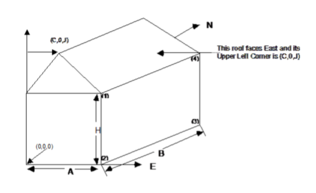
\includegraphics[width=0.9\textwidth, height=0.9\textheight, keepaspectratio=true]{media/image055.png}
\caption{Illustration for Surface Vertices \protect \label{fig:illustration-for-surface-vertices}}
\end{figure}

The figure above will help illustrate Surface Vertex entry. The convention used in ``GlobalGeometryRules'' dictates the order of the vertices (ref: GlobalGeometryRules). In this example, the conventions used are Starting Vertex Position = UpperLeftCorner and Vertex Entry Direction = CounterClockwise. The surfaces for this single zone are:

\begin{lstlisting}
4,0,0,H, 0,0,0, A,0,0, A,0,H; ! (4 vertices, South Wall)
4,A,0,H,A,0,0,A,B,0,A,B,H; ! (4 vertices, East Wall)
     ignore other walls that are not shown in this figure
4,C,0,J,A,0,H,A,B,H,C,B,J; ! (4 vertices, roof)
3,C,0,J,0,0,H,A,0,H; ! (3 vertices, gable end)
4,0,0,H, 0,0,0, A,0,0, A,0,H; ! (4 vertices, South Wall)
\end{lstlisting}

Note that in this example, point 1 of the entry is the Upper Left Corner of the rectangular surfaces and the point of the triangle for the 3 sided surface. The east wall shows the order of vertex entry. For horizontal surfaces, any vertex may be chosen as the starting position, but the Vertex Entry Direction convention must be followed. The surface details report (Output: Surfaces:List, Details;) is very useful for reviewing the accuracy of surface geometry inputs (ref: Surface Output Variables/Reports and Variable Dictionary Reports).

From the detailed vertices, EnergyPlus tries to determine the ``height'' and ``width'' of the surface. Obviously, this doesn't work well for \textgreater{}4 sided surfaces; for these, if the calculated height and width are not close to the gross area for the surface, the height and width shown will be the square root of the area (and thus a square).

\subsection{Building Surfaces - Detailed}\label{building-surfaces---detailed}

A building surface is necessary for all calculations. There must be at least one building surface per zone. You can use the detailed descriptions as shown below or the simpler, rectangular surface descriptions shown earlier.

\subsection{Wall:Detailed}\label{walldetailed}

The Wall:Detailed object is used to describe walls.

\subsubsection{Inputs}\label{inputs-20-007}

\paragraph{Field: Name}\label{field-name-16-010}

This is a unique name associated with each building surface. It is used in several other places as a reference (e.g.~as the base surface name for a Window or Door).

\paragraph{Field: Construction Name}\label{field-construction-name-16}

This is the name of the construction (ref: Construction object) used in the surface. Regardless of location in the building, the ``full'' construction (all layers) is used. For example, for an interior wall separating two zones, zone x would have the outside layer (e.g.~drywall) as the material that shows in zone y and then the layers to the inside layer -- the material that shows in zone x. For symmetric constructions, the same construction can be used in the surfaces described in both zones.

\paragraph{Field: Zone Name}\label{field-zone-name-10-000}

This is the zone name to which the surface belongs.

\paragraph{Field: Outside Boundary Condition}\label{field-outside-boundary-condition}

This value can be one of several things depending on the actual kind of surface.

\begin{enumerate}
  \item
    \textbf{Surface} -- if this surface is an internal surface, then this is the choice. The value will either be a surface in the base zone or a surface in another zone. The heat balance between two zones can be accurately simulated by specifying a surface in an adjacent zone. EnergyPlus will simulate a group of zones simultaneously and will include the heat transfer between zones. However, as this increases the complexity of the calculations, it is not necessary to specify the other zone unless the two zones will have a significant temperature difference. If the two zones will not be very different (temperature wise), then the surface should use itself as the outside environment or specify this field as \textbf{Adiabatic}. The surface name on the ``outside'' of this surface (adjacent to) is placed in the next field.
  \item
    \textbf{Adiabatic} -- an internal surface in the same Zone. This surface will not transfer heat out of the zone, but will still store heat in thermal mass. Only the inside face of the surface will exchange heat with the zone (i.e.~two adiabatic surfaces are required to model internal partitions where both sides of the surface are exchanging heat with the zone). The Outside Boundary Condition Object can be left blank.
  \item
    \textbf{Zone} -- this is similar to Surface but EnergyPlus will automatically create the required surface in the adjacent zone when this is entered for the surface. If there are windows or doors on the surface, EnergyPlus automatically creates appropriate sub-surfaces as well.
  \item
    \textbf{Outdoors} -- if this surface is exposed to outside temperature conditions, then this is the choice. See Sun Exposure and Wind Exposure below for further specifications on this kind of surface.
  \item
    \textbf{Ground} -- if this surface is exposed to the ground, then this is the usual choice. The temperature on the outside of this surface will be the Site:GroundTemperature:Surface value for the month. For more information on ground contact surfaces, reference the Auxiliary Programs document section on ``Ground Heat Transfer in EnergyPlus''.
  \item
    \textbf{GroundFCfactorMethod} -- if this surface is exposed to the ground and using the \textbf{Construction:CfactorUndergroundWall}, then this is the choice. The temperature on the outside of this surface will be the Site:GroundTemperature:FcfactorMethod value for the month.
  \item
    \textbf{OtherSideCoefficients} -- if this surface has a custom, user specified temperature or other parameters (See SurfaceProperty:OtherSideCoefficients specification), then this is the choice. The outside boundary condition will be the name of the SurfaceProperty:OtherSideCoefficients specification.
  \item
    \textbf{OtherSideConditionsModel} -- if this surface has a specially-modeled multi-skin component, such as a transpired collector or vented photovoltaic panel, attached to the outside (See SurfaceProperty:OtherSideConditionsModel specification), then this the choice. The outside face environment will be the name of the SurfaceProperty:OtherSideConditionsModel specification.
  \item
    \textbf{GroundSlabPreprocessorAverage} -- uses the average results from the Slab preprocessor calculations.
  \item
    \textbf{GroundSlabPreprocessorCore} -- uses the core results from the Slab preprocessor calculations.
  \item
    \textbf{GroundSlabPreprocessorPerimeter} -- uses the perimeter results from the Slab preprocessor calculations.
  \item
    \textbf{GroundBasementPreprocessorAverageWall} -- uses the average wall results from the Basement preprocessor calculations.
  \item
    \textbf{GroundBasementPreprocessorAverageFloor} -- uses the average floor results from the Basement preprocessor calculations.
  \item
    \textbf{GroundBasementPreprocessorUpperWall} -- uses the upper wall results from the Basement preprocessor calculations.
  \item
    \textbf{GroundBasementPreprocessorLowerWall} -- uses the lower wall results from the Basement preprocessor calculations.
\end{enumerate}

\paragraph{Field: Outside Boundary Condition Object}\label{field-outside-boundary-condition-object-6}

If neither Surface, OtherSideCoefficients, or OtherSideConditionsModel are specified for the Outside Boundary Condition (previous field), then this field should be left blank.

As stated above, if the Outside Boundary Condition is ``Surface'', then this field's value must be the surface name whose inside face temperature will be forced on the outside face of the base surface. This permits heat exchange between adjacent zones (interzone heat transfer) when multiple zones are simulated, but can also be used to simulate middle zone behavior without modeling the adjacent zones. This is done by specifying a surface within the zone. For example, a middle floor zone can be modeled by making the floor the Outside Boundary Condition Object for the ceiling, and the ceiling the Outside Boundary Condition Object for the floor.

If the Outside Boundary Condition is Zone, then this field should contain the zone name of the adjacent zone for the surface.

\begin{callout}
Note: Zones with interzone heat transfer are not adiabatic and the internal surfaces contribute to gains or losses. Adiabatic surfaces are modeled by specifying the base surface itself in this field. Also, for interzone heat transfer, both surfaces must be represented -- for example, if you want interzone heat transfer to an attic space, the ceiling in the lower zone must have a surface object with the outside face environment as the floor in the attic and, likewise, there must be a floor surface object in the attic that references the ceiling surface name in the lower zone.
\end{callout}

Equally, if the Outside Boundary Condition is ``OtherSideCoefficients'', then this field's value must be the SurfaceProperty:OtherSideCoefficients name. Or if the Outside Boundary Condition is ``OtherSideConditionsModel'' then this field's value must be the SurfaceProperty:OtherSideConditionsModel name.

\paragraph{Field: Sun Exposure}\label{field-sun-exposure-000}

If the surface is exposed to the sun, then ``SunExposed'' should be entered in this field. Otherwise, ``NoSun'' should be entered.

Note, a cantilevered floor could have ``Outdoors'' but ``NoSun'' exposure.

\paragraph{Field: Wind Exposure}\label{field-wind-exposure}

If the surface is exposed to the Wind, then ``WindExposed'' should be entered in this field. Otherwise, ``NoWind'' should be entered.

\begin{callout}
Note: When a surface is specified with ``NoWind'', this has several implications. Within the heat balance code, this surface will default to using the simple ASHRAE exterior convection coefficient correlation with a zero wind speed. In addition, since the ASHRAE simple method does not have a separate value for equivalent long wavelength radiation to the sky and ground, using ``NoWind'' also eliminates long wavelength radiant exchange from the exterior of the surface to both the sky and the ground. Thus, only simple convection takes place at the exterior face of a surface specified with ``NoWind''.
\end{callout}

\paragraph{Field: View Factor to Ground}\label{field-view-factor-to-ground}

The fraction of the ground plane (assumed horizontal) that is visible from a heat-transfer surface. It is used to calculate the diffuse solar radiation from the ground that is incident on the surface.

For example, if there are no obstructions, a vertical surface sees half of the ground plane and so View Factor to Ground = 0.5. A horizontal downward-facing surface sees the entire ground plane, so View Factor to Ground = 1.0. A horizontal upward-facing surface (horizontal roof) does not see the ground at all, so View Factor to Ground = 0.0.

Unused if reflections option in Solar Distribution field in Building object input unless a DaylightingDevice:Shelf or DaylightingDevice:Tubular has been specified.

If you do not use the reflections option in the Solar Distribution field in your Building object input, you are responsible for entering the View Factor to Ground for each heat-transfer surface. Typical values for a surface that is not shadowed are obtained by the simple equation:

View Factor to Ground = (1-cos(SurfTilt))/2

For example, this gives 0.5 for a wall of tilt 90°. If the tilt of the wall changes, then the View Factor to Ground must also change.

If you enter \textbf{autocalculate} in this field, EnergyPlus will automatically calculate the view factor to ground based on the tilt of the surface.

If \textbf{you do use the reflections option in the Solar Distribution field} in your Building object input, you do \textbf{not} have to enter View Factor to Ground values. In this case the program will automatically calculate the value to use for each exterior surface taking into account solar shadowing (including shadowing of the ground by the building) and reflections from obstructions (ref: Building, Field: Solar Distribution).

However, if you do use the reflections option AND you are modeling a DaylightingDevice:Shelf or DaylightingDevice:Tubular, then you still need to enter some values of View Factor to Ground. For DaylightingDevice:Shelf you need to enter View Factor to Ground for the window associated with the shelf. And for DaylightingDevice:Tubular you need to enter the View Factor to Ground for the FenestrationSurface:Detailed corresponding to the dome of the tubular device.

Note 1: The corresponding view factor to the sky for diffuse solar radiation is not a user input; it is calculated within EnergyPlus based on surface orientation, sky solar radiance distribution, and shadowing surfaces.

Note 2: The view factors to the sky and ground for thermal infrared (long-wave) radiation are not user inputs; they are calculated within EnergyPlus based on surface tilt and shadowing surfaces. Shadowing surfaces are considered to have the same emissivity and temperature as the ground, so they are lumped together with the ground in calculating the ground IR view factor.

\paragraph{Field: Number of Vertices}\label{field-number-of-vertices}

This field specifies the number of sides in the surface (number of X,Y,Z vertex groups). For further information, see the discussion on ``Surface Vertices'' above.

\subsection{RoofCeiling:Detailed}\label{roofceilingdetailed}

The RoofCeiling:Detailed object is used to describe walls.

\subsubsection{Inputs}\label{inputs-21-007}

\paragraph{Field: Name}\label{field-name-17-008}

This is a unique name associated with each building surface. It is used in several other places as a reference (e.g.~as the base surface name for a Window or Door).

\paragraph{Field: Construction Name}\label{field-construction-name-17}

This is the name of the construction (ref: Construction object) used in the surface. Regardless of location in the building, the ``full'' construction (all layers) is used. For example, for an interior wall separating two zones, zone x would have the outside layer (e.g.~drywall) as the material that shows in zone y and then the layers to the inside layer -- the material that shows in zone x. For symmetric constructions, the same construction can be used in the surfaces described in both zones.

\paragraph{Field: Zone Name}\label{field-zone-name-11-000}

This is the zone name to which the surface belongs.

\paragraph{Field: Outside Boundary Condition}\label{field-outside-boundary-condition-1}

This value can be one of several things depending on the actual kind of surface.

\begin{enumerate}
  \item
    \textbf{Surface} -- if this surface is an internal surface, then this is the choice. The value will either be a surface in the base zone or a surface in another zone. The heat balance between two zones can be accurately simulated by specifying a surface in an adjacent zone. EnergyPlus will simulate a group of zones simultaneously and will include the heat transfer between zones. However, as this increases the complexity of the calculations, it is not necessary to specify the other zone unless the two zones will have a significant temperature difference. If the two zones will not be very different (temperature wise), then the surface should use itself as the outside environment or specify this field as \textbf{Adiabatic}. The surface name on the ``outside'' of this surface (adjacent to) is placed in the next field.
  \item
    \textbf{Adiabatic} -- an internal surface in the same Zone. This surface will not transfer heat out of the zone, but will still store heat in thermal mass. Only the inside face of the surface will exchange heat with the zone (i.e.~two adiabatic surfaces are required to model internal partitions where both sides of the surface are exchanging heat with the zone). The Outside Boundary Condition Object can be left blank.
  \item
    \textbf{Zone} -- this is similar to Surface but EnergyPlus will automatically create the required surface in the adjacent zone when this is entered for the surface. If there are windows or doors on the surface, EnergyPlus automatically creates appropriate sub-surfaces as well.
  \item
    \textbf{Outdoors} -- if this surface is exposed to outside temperature conditions, then this is the choice. See Sun Exposure and Wind Exposure below for further specifications on this kind of surface.
  \item
    \textbf{Ground} -- if this surface is exposed to the ground, then this is the choice. The temperature on the outside of this surface will be the Ground Temperature.
  \item
    \textbf{OtherSideCoefficients} -- if this surface has a custom, user specified temperature or other parameters (See SurfaceProperty:OtherSideCoefficients specification), then this is the choice. The outside boundary condition will be the name of the SurfaceProperty:OtherSideCoefficients specification.
  \item
    \textbf{OtherSideConditionsModel} -- if this surface has a specially-modeled multi-skin component, such as a transpired collector or vented photovoltaic panel, attached to the outside (See SurfaceProperty:OtherSideConditionsModel specification), then this the choice. The outside face environment will be the name of the SurfaceProperty:OtherSideConditionsModel specification.
  \item
    \textbf{GroundSlabPreprocessorAverage} -- uses the average results from the Slab preprocessor calculations.
  \item
    \textbf{GroundSlabPreprocessorCore} -- uses the core results from the Slab preprocessor calculations.
  \item
    \textbf{GroundSlabPreprocessorPerimeter} -- uses the perimeter results from the Slab preprocessor calculations.
  \item
    \textbf{GroundBasementPreprocessorAverageWall} -- uses the average wall results from the Basement preprocessor calculations.
  \item
    \textbf{GroundBasementPreprocessorAverageFloor} -- uses the average floor results from the Basement preprocessor calculations.
  \item
    \textbf{GroundBasementPreprocessorUpperWall} -- uses the upper wall results from the Basement preprocessor calculations.
  \item
    \textbf{GroundBasementPreprocessorLowerWall} -- uses the lower wall results from the Basement preprocessor calculations.
\end{enumerate}

\paragraph{Field: Outside Boundary Condition Object}\label{field-outside-boundary-condition-object-7}

If neither Surface, OtherSideCoefficients, or OtherSideConditionsModel are specified for the Outside Boundary Condition (previous field), then this field should be left blank.

As stated above, if the Outside Boundary Condition is ``Surface'', then this field's value must be the surface name whose inside face temperature will be forced on the outside face of the base surface. This permits heat exchange between adjacent zones (interzone heat transfer) when multiple zones are simulated, but can also be used to simulate middle zone behavior without modeling the adjacent zones. This is done by specifying a surface within the zone. For example, a middle floor zone can be modeled by making the floor the Outside Boundary Condition Object for the ceiling, and the ceiling the Outside Boundary Condition Object for the floor.

If the Outside Boundary Condition is Zone, then this field should contain the zone name of the adjacent zone for the surface.

\begin{callout}
Note: Zones with interzone heat transfer are not adiabatic and the internal surfaces contribute to gains or losses. Adiabatic surfaces are modeled by specifying the base surface itself in this field. Also, for interzone heat transfer, both surfaces must be represented -- for example, if you want interzone heat transfer to an attic space, the ceiling in the lower zone must have a surface object with the outside face environment as the floor in the attic and, likewise, there must be a floor surface object in the attic that references the ceiling surface name in the lower zone.
\end{callout}

Equally, if the Outside Boundary Condition is ``OtherSideCoefficients'', then this field's value must be the SurfaceProperty:OtherSideCoefficients name. Or if the Outside Boundary Condition is ``OtherSideConditionsModel'' then this field's value must be the SurfaceProperty:OtherSideConditionsModel name.

\paragraph{Field: Sun Exposure}\label{field-sun-exposure-1}

If the surface is exposed to the sun, then ``SunExposed'' should be entered in this field. Otherwise, ``NoSun'' should be entered.

Note, a cantilevered floor could have ``Outdoors'' but ``NoSun'' exposure.

\paragraph{Field: Wind Exposure}\label{field-wind-exposure-1}

If the surface is exposed to the Wind, then ``WindExposed'' should be entered in this field. Otherwise, ``NoWind'' should be entered.

\begin{callout}
Note: When a surface is specified with ``NoWind'', this has several implications. Within the heat balance code, this surface will default to using the simple ASHRAE exterior convection coefficient correlation with a zero wind speed. In addition, since the ASHRAE simple method does not have a separate value for equivalent long wavelength radiation to the sky and ground, using ``NoWind'' also eliminates long wavelength radiant exchange from the exterior of the surface to both the sky and the ground. Thus, only simple convection takes place at the exterior face of a surface specified with ``NoWind''.
\end{callout}

\paragraph{Field: View Factor to Ground}\label{field-view-factor-to-ground-1}

The fraction of the ground plane (assumed horizontal) that is visible from a heat-transfer surface. It is used to calculate the diffuse solar radiation from the ground that is incident on the surface.

For example, if there are no obstructions, a vertical surface sees half of the ground plane and so View Factor to Ground = 0.5. A horizontal downward-facing surface sees the entire ground plane, so View Factor to Ground = 1.0. A horizontal upward-facing surface (horizontal roof) does not see the ground at all, so View Factor to Ground = 0.0.

Unused if reflections option in Solar Distribution field in Building object input unless a DaylightingDevice:Shelf or DaylightingDevice:Tubular has been specified.

If you do not use the reflections option in the Solar Distribution field in your Building object input, you are responsible for entering the View Factor to Ground for each heat-transfer surface. Typical values for a surface that is not shadowed are obtained by the simple equation:

View Factor to Ground = (1-cos(SurfTilt))/2

For example, this gives 0.5 for a wall of tilt 90°. If the tilt of the wall changes, then the View Factor to Ground must also change.

If you enter \textbf{autocalculate} in this field, EnergyPlus will automatically calculate the view factor to ground based on the tilt of the surface.

If \textbf{you do use the reflections option in the Solar Distribution field} in your Building object input, you do \textbf{not} have to enter View Factor to Ground values. In this case the program will automatically calculate the value to use for each exterior surface taking into account solar shadowing (including shadowing of the ground by the building) and reflections from obstructions (ref: Building, Field: Solar Distribution).

However, if you do use the reflections option AND you are modeling a DaylightingDevice:Shelf or DaylightingDevice:Tubular, then you still need to enter some values of View Factor to Ground. For DaylightingDevice:Shelf you need to enter View Factor to Ground for the window associated with the shelf. And for DaylightingDevice:Tubular you need to enter the View Factor to Ground for the FenestrationSurface:Detailed corresponding to the dome of the tubular device.

Note 1: The corresponding view factor to the sky for diffuse solar radiation is not a user input; it is calculated within EnergyPlus based on surface orientation, sky solar radiance distribution, and shadowing surfaces.

Note 2: The view factors to the sky and ground for thermal infrared (long-wave) radiation are not user inputs; they are calculated within EnergyPlus based on surface tilt and shadowing surfaces. Shadowing surfaces are considered to have the same emissivity and temperature as the ground, so they are lumped together with the ground in calculating the ground IR view factor.

\paragraph{Field: Number of Vertices}\label{field-number-of-vertices-1}

This field specifies the number of sides in the surface (number of X,Y,Z vertex groups). For further information, see the discussion on ``Surface Vertices'' above.

\subsection{Floor:Detailed}\label{floordetailed}

The Floor:Detailed object is used to describe walls.

\subsubsection{Inputs}\label{inputs-22-006}

\paragraph{Field: Name}\label{field-name-18-008}

This is a unique name associated with each building surface. It is used in several other places as a reference (e.g.~as the base surface name for a Window or Door).

\paragraph{Field: Construction Name}\label{field-construction-name-18}

This is the name of the construction (ref: Construction object) used in the surface. Regardless of location in the building, the ``full'' construction (all layers) is used. For example, for an interior wall separating two zones, zone x would have the outside layer (e.g.~drywall) as the material that shows in zone y and then the layers to the inside layer -- the material that shows in zone x. For symmetric constructions, the same construction can be used in the surfaces described in both zones.

\paragraph{Field: Zone Name}\label{field-zone-name-12-000}

This is the zone name to which the surface belongs.

\paragraph{Field: Outside Boundary Condition}\label{field-outside-boundary-condition-2}

This value can be one of several things depending on the actual kind of surface.

1)~~~\textbf{Surface} -- if this surface is an internal surface, then this is the choice. The value will either be a surface in the base zone or a surface in another zone. The heat balance between two zones can be accurately simulated by specifying a surface in an adjacent zone. EnergyPlus will simulate a group of zones simultaneously and will include the heat transfer between zones. However, as this increases the complexity of the calculations, it is not necessary to specify the other zone unless the two zones will have a significant temperature difference. If the two zones will not be very different (temperature wise), then the surface should use itself as the outside environment or specify this field as \textbf{Adiabatic}. The surface name on the ``outside'' of this surface (adjacent to) is placed in the next field.

2)~~~\textbf{Adiabatic} -- an internal surface in the same Zone. This surface will not transfer heat out of the zone, but will still store heat in thermal mass. Only the inside face of the surface will exchange heat with the zone (i.e.~two adiabatic surfaces are required to model internal partitions where both sides of the surface are exchanging heat with the zone). The Outside Boundary Condition Object can be left blank.

3)~~~\textbf{Zone} -- this is similar to Surface but EnergyPlus will automatically create the required surface in the adjacent zone when this is entered for the surface. If there are windows or doors on the surface, EnergyPlus automatically creates appropriate sub-surfaces as well.

4)~~~\textbf{Outdoors} -- if this surface is exposed to outside temperature conditions, then this is the choice. See Sun Exposure and Wind Exposure below for further specifications on this kind of surface.

5)~~~\textbf{Ground} -- if this surface is exposed to the ground, then this is the usual choice. The temperature on the outside of this surface will be the Site:GroundTemperature:Surface value for the month. For more information on ground contact surfaces, reference the Auxiliary Programs document section on ``Ground Heat Transfer in EnergyPlus''.

6)~~~\textbf{GroundFCfactorMethod} -- if this surface is exposed to the ground and using the \textbf{Construction:FfactorGroundFloor}, then this is the choice. The temperature on the outside of this surface will be the Site:GroundTemperature:FcfactorMethod value for the month.

7)~~~\textbf{OtherSideCoefficients} -- if this surface has a custom, user specified temperature or other parameters (See SurfaceProperty:OtherSideCoefficients specification), then this is the choice. The outside boundary condition will be the name of the SurfaceProperty:OtherSideCoefficients specification.

8)~~~\textbf{OtherSideConditionsModel} -- if this surface has a specially-modeled multi-skin component, such as a transpired collector or vented photovoltaic panel, attached to the outside (See SurfaceProperty:OtherSideConditionsModel specification), then this the choice. The outside face environment will be the name of the SurfaceProperty:OtherSideConditionsModel specification.

9)~~~\textbf{GroundSlabPreprocessorAverage} -- uses the average results from the Slab preprocessor calculations.

10)\textbf{GroundSlabPreprocessorCore} -- uses the core results from the Slab preprocessor calculations.

11)\textbf{GroundSlabPreprocessorPerimeter} -- uses the perimeter results from the Slab preprocessor calculations.

12)\textbf{GroundBasementPreprocessorAverageWall} -- uses the average wall results from the Basement preprocessor calculations.

13)\textbf{GroundBasementPreprocessorAverageFloor} -- uses the average floor results from the Basement preprocessor calculations.

14)\textbf{GroundBasementPreprocessorUpperWall} -- uses the upper wall results from the Basement preprocessor calculations.

15)\textbf{GroundBasementPreprocessorLowerWall} -- uses the lower wall results from the Basement preprocessor calculations.

\paragraph{Field: Outside Boundary Condition Object}\label{field-outside-boundary-condition-object-8}

If neither Surface, OtherSideCoefficients, or OtherSideConditionsModel are specified for the Outside Boundary Condition (previous field), then this field should be left blank.

As stated above, if the Outside Boundary Condition is ``Surface'', then this field's value must be the surface name whose inside face temperature will be forced on the outside face of the base surface. This permits heat exchange between adjacent zones (interzone heat transfer) when multiple zones are simulated, but can also be used to simulate middle zone behavior without modeling the adjacent zones. This is done by specifying a surface within the zone. For example, a middle floor zone can be modeled by making the floor the Outside Boundary Condition Object for the ceiling, and the ceiling the Outside Boundary Condition Object for the floor.

If the Outside Boundary Condition is Zone, then this field should contain the zone name of the adjacent zone for the surface.

\begin{callout}
Note: Zones with interzone heat transfer are not adiabatic and the internal surfaces contribute to gains or losses. Adiabatic surfaces are modeled by specifying the base surface itself in this field. Also, for interzone heat transfer, both surfaces must be represented -- for example, if you want interzone heat transfer to an attic space, the ceiling in the lower zone must have a surface object with the outside face environment as the floor in the attic and, likewise, there must be a floor surface object in the attic that references the ceiling surface name in the lower zone.
\end{callout}

Equally, if the Outside Boundary Condition is ``OtherSideCoefficients'', then this field's value must be the SurfaceProperty:OtherSideCoefficients name. Or if the Outside Boundary Condition is ``OtherSideConditionsModel'' then this field's value must be the SurfaceProperty:OtherSideConditionsModel name.

\paragraph{Field: Sun Exposure}\label{field-sun-exposure-2}

If the surface is exposed to the sun, then ``SunExposed'' should be entered in this field. Otherwise, ``NoSun'' should be entered.

Note, a cantilevered floor could have ``Outdoors'' but ``NoSun'' exposure.

\paragraph{Field: Wind Exposure}\label{field-wind-exposure-2}

If the surface is exposed to the Wind, then ``WindExposed'' should be entered in this field. Otherwise, ``NoWind'' should be entered.

\begin{callout}
Note: When a surface is specified with ``NoWind'', this has several implications. Within the heat balance code, this surface will default to using the simple ASHRAE exterior convection coefficient correlation with a zero wind speed. In addition, since the ASHRAE simple method does not have a separate value for equivalent long wavelength radiation to the sky and ground, using ``NoWind'' also eliminates long wavelength radiant exchange from the exterior of the surface to both the sky and the ground. Thus, only simple convection takes place at the exterior face of a surface specified with ``NoWind''.
\end{callout}

\paragraph{Field: View Factor to Ground}\label{field-view-factor-to-ground-2}

The fraction of the ground plane (assumed horizontal) that is visible from a heat-transfer surface. It is used to calculate the diffuse solar radiation from the ground that is incident on the surface.

For example, if there are no obstructions, a vertical surface sees half of the ground plane and so View Factor to Ground = 0.5. A horizontal downward-facing surface sees the entire ground plane, so View Factor to Ground = 1.0. A horizontal upward-facing surface (horizontal roof) does not see the ground at all, so View Factor to Ground = 0.0.

Unused if reflections option in Solar Distribution field in Building object input unless a DaylightingDevice:Shelf or DaylightingDevice:Tubular has been specified.

If you do not use the reflections option in the Solar Distribution field in your Building object input, you are responsible for entering the View Factor to Ground for each heat-transfer surface. Typical values for a surface that is not shadowed are obtained by the simple equation:

View Factor to Ground = (1-cos(SurfTilt))/2

For example, this gives 0.5 for a wall of tilt 90°. If the tilt of the wall changes, then the View Factor to Ground must also change.

If you enter \textbf{autocalculate} in this field, EnergyPlus will automatically calculate the view factor to ground based on the tilt of the surface.

If \textbf{you do use the reflections option in the Solar Distribution field} in your Building object input, you do \textbf{not} have to enter View Factor to Ground values. In this case the program will automatically calculate the value to use for each exterior surface taking into account solar shadowing (including shadowing of the ground by the building) and reflections from obstructions (ref: Building, Field: Solar Distribution).

However, if you do use the reflections option AND you are modeling a DaylightingDevice:Shelf or DaylightingDevice:Tubular, then you still need to enter some values of View Factor to Ground. For DaylightingDevice:Shelf you need to enter View Factor to Ground for the window associated with the shelf. And for DaylightingDevice:Tubular you need to enter the View Factor to Ground for the FenestrationSurface:Detailed corresponding to the dome of the tubular device.

Note 1: The corresponding view factor to the sky for diffuse solar radiation is not a user input; it is calculated within EnergyPlus based on surface orientation, sky solar radiance distribution, and shadowing surfaces.

Note 2: The view factors to the sky and ground for thermal infrared (long-wave) radiation are not user inputs; they are calculated within EnergyPlus based on surface tilt and shadowing surfaces. Shadowing surfaces are considered to have the same emissivity and temperature as the ground, so they are lumped together with the ground in calculating the ground IR view factor.

\paragraph{Field: Number of Vertices}\label{field-number-of-vertices-2}

This field specifies the number of sides in the surface (number of X,Y,Z vertex groups). For further information, see the discussion on ``Surface Vertices'' above.

Some examples of using these objects:

\begin{lstlisting}

Floor:Detailed,
      Floor_NorthZone_1stFloor,!- Name
      FLOOR-SLAB-ASSEMBLY,     !- Construction Name
      NorthZone_1stFloor,      !- Zone Name
      Ground,                  !- Outside Boundary Condition
      ,                        !- Outside Boundary Condition Object
      NoSun,                   !- Sun Exposure
      NoWind,                  !- Wind Exposure
      0.0,                     !- View Factor to Ground
      4,                       !- Number of Vertices
      0, 11, 0,                           !- X,Y,Z  1 {m}
      25, 11, 0,                          !- X,Y,Z  2 {m}
      25, 5.5, 0,                         !- X,Y,Z  3 {m}
     0, 5.5, 0;                          !- X,Y,Z  4 {m}

  RoofCeiling:Detailed,
      Ceiling_SouthZone_1stFloor,  !- Name
      CEILING-FLOOR-ASSEMBLY,  !- Construction Name
      SouthZone_1stFloor,      !- Zone Name
      Surface,                 !- Outside Boundary Condition
      Floor_SouthZone_2ndFloor,!- Outside Boundary Condition Object
      NoSun,                   !- Sun Exposure
      NoWind,                  !- Wind Exposure
      0.0,                     !- View Factor to Ground
      4,                       !- Number of Vertices
      0, 0, 3.4,                          !- X,Y,Z  1 {m}
      25, 0, 3.4,                         !- X,Y,Z  2 {m}
      25, 5.5, 3.4,                       !- X,Y,Z  3 {m}
     0, 5.5, 3.4;                        !- X,Y,Z  4 {m}

  Wall:Detailed,
      InteriorWall_SouthZone_1stFloor,  !- Name
      INTERIOR-WALL-ASSEMBLY,  !- Construction Name
      SouthZone_1stFloor,      !- Zone Name
      Surface,                 !- Outside Boundary Condition
      InteriorWall_NorthZone_1stFloor,  !- Outside Boundary Condition Object
      NoSun,                   !- Sun Exposure
      NoWind,                  !- Wind Exposure
      0,                       !- View Factor to Ground
      4,                       !- Number of Vertices
      25, 5.5, 3.7,                       !- X,Y,Z  1 {m}
      25, 5.5, 0,                         !- X,Y,Z  2 {m}
      0, 5.5, 0,                          !- X,Y,Z  3 {m}
     0, 5.5, 3.7;                        !- X,Y,Z  4 {m}
\end{lstlisting}

\subsection{BuildingSurface:Detailed}\label{buildingsurfacedetailed}

The BuildingSurface:Detailed object can more generally describe each of the surfaces.

\subsubsection{Inputs}\label{inputs-23-006}

\paragraph{Field: Name}\label{field-name-19-005}

This is a unique name associated with each building surface. It is used in several other places as a reference (e.g.~as the base surface name for a Window or Door).

\paragraph{Field: Surface Type}\label{field-surface-type-000}

Used primarily for convenience, the surface type can be one of the choices illustrated above -- Wall, Floor, Ceiling, Roof. Azimuth (facing) and Tilt are determined from the vertex coordinates. Note that ``normal'' floors will be tilted 180° whereas flat roofs/ceilings will be tilted 0°. EnergyPlus uses this field's designation, along with the calculated tilt of the surface, to issue warning messages when tilts are ``out of range''. Calculations in EnergyPlus use the actual calculated tilt values for the actual heat balance calculations. Note, however, that a floor tilted 0° is really facing ``into'' the zone and is not what you will desire for the calculations even though the coordinate may appear correct in the viewed DXF display.

``Normal'' tilt for walls is 90° -- here you may use the calculated Azimuth to make sure your walls are facing away from the zone's interior.

\paragraph{Field: Construction Name}\label{field-construction-name-19}

This is the name of the construction (ref: Construction object) used in the surface. Regardless of location in the building, the ``full'' construction (all layers) is used. For example, for an interior wall separating two zones, zone x would have the outside layer (e.g.~drywall) as the material that shows in zone y and then the layers to the inside layer -- the material that shows in zone x. For symmetric constructions, the same construction can be used in the surfaces described in both zones.

\paragraph{Field: Zone Name}\label{field-zone-name-13}

This is the zone name to which the surface belongs.

\paragraph{Field: Outside Boundary Condition}\label{field-outside-boundary-condition-3}

This value can be one of several things depending on the actual kind of surface.

1)~~~\textbf{Surface} -- if this surface is an internal surface, then this is the choice. The value will either be a surface in the base zone or a surface in another zone. The heat balance between two zones can be accurately simulated by specifying a surface in an adjacent zone. EnergyPlus will simulate a group of zones simultaneously and will include the heat transfer between zones. However, as this increases the complexity of the calculations, it is not necessary to specify the other zone unless the two zones will have a significant temperature difference. If the two zones will not be very different (temperature wise), then the surface should use itself as the outside environment or specify this field as \textbf{Adiabatic}. In either case, the surface name on the ``outside'' of this surface (adjacent to) is placed in the next field.

2)~~~\textbf{Adiabatic} -- an internal surface in the same Zone. This surface will not transfer heat out of the zone, but will still store heat in thermal mass. Only the inside face of the surface will exchange heat with the zone (i.e.~two adiabatic surfaces are required to model internal partitions where both sides of the surface are exchanging heat with the zone). The Outside Boundary Condition Object can be left blank.

3)~~~\textbf{Zone} -- this is similar to Surface but EnergyPlus will automatically create the required surface in the adjacent zone when this is entered for the surface. If there are windows or doors on the surface, EnergyPlus automatically creates appropriate sub-surfaces as well.

4)~~~\textbf{Outdoors} -- if this surface is exposed to outside temperature conditions, then this is the choice. See Sun Exposure and Wind Exposure below for further specifications on this kind of surface.

5)~~~\textbf{Ground} -- if this surface is exposed to the ground, then this is the usual choice. The temperature on the outside of this surface will be the Site:GroundTemperature:Surface value for the month. For more information on ground contact surfaces, reference the Auxiliary Programs document section on ``Ground Heat Transfer in EnergyPlus''.

6)~~~\textbf{GroundFCfactorMethod} -- if this surface is exposed to the ground and using the \textbf{Construction:CfactorUndergroundWall} or \textbf{Construction:FfactorGroundFloor} (depending on surface type), then this is the choice. The temperature on the outside of this surface will be the Site:GroundTemperature:FcfactorMethod value for the month.

7)~~~\textbf{OtherSideCoefficients} -- if this surface has a custom, user specified temperature or other parameters (See SurfaceProperty:OtherSideCoefficients specification), then this is the choice. The outside boundary condition will be the name of the SurfaceProperty:OtherSideCoefficients specification.

8)~~~\textbf{OtherSideConditionsModel} -- if this surface has a specially-modeled multi-skin component, such as a transpired collector or vented photovoltaic panel, attached to the outside (See SurfaceProperty:OtherSideConditionsModel specification), then this the choice. The outside face environment will be the name of the SurfaceProperty:OtherSideConditionsModel specification.

9)~~~\textbf{GroundSlabPreprocessorAverage} -- uses the average results from the Slab preprocessor calculations.

10)\textbf{GroundSlabPreprocessorCore} -- uses the core results from the Slab preprocessor calculations.

11)\textbf{GroundSlabPreprocessorPerimeter} -- uses the perimeter results from the Slab preprocessor calculations.

12)\textbf{GroundBasementPreprocessorAverageWall} -- uses the average wall results from the Basement preprocessor calculations.

13)\textbf{GroundBasementPreprocessorAverageFloor} -- uses the average floor results from the Basement preprocessor calculations.

14)\textbf{GroundBasementPreprocessorUpperWall} -- uses the upper wall results from the Basement preprocessor calculations.

15)\textbf{GroundBasementPreprocessorLowerWall} -- uses the lower wall results from the Basement preprocessor calculations.

\paragraph{Field: Outside Boundary Condition Object}\label{field-outside-boundary-condition-object-9}

If neither Surface, OtherSideCoefficients, or OtherSideConditionsModel are specified for the Outside Boundary Condition (previous field), then this field should be left blank.

As stated above, if the Outside Boundary Condition is ``Surface'', then this field's value must be the surface name whose inside face temperature will be forced on the outside face of the base surface. This permits heat exchange between adjacent zones (interzone heat transfer) when multiple zones are simulated, but can also be used to simulate middle zone behavior without modeling the adjacent zones. This is done by specifying a surface within the zone. For example, a middle floor zone can be modeled by making the floor the Outside Boundary Condition Object for the ceiling, and the ceiling the Outside Boundary Condition Object for the floor.

If the Outside Boundary Condition is Zone, then this field should contain the zone name of the adjacent zone for the surface.

\begin{callout}
Note: Zones with interzone heat transfer are not adiabatic and the internal surfaces contribute to gains or losses. Adiabatic surfaces are modeled by specifying the base surface itself in this field. Also, for interzone heat transfer, both surfaces must be represented -- for example, if you want interzone heat transfer to an attic space, the ceiling in the lower zone must have a surface object with the outside face environment as the floor in the attic and, likewise, there must be a floor surface object in the attic that references the ceiling surface name in the lower zone.
\end{callout}

Equally, if the Outside Boundary Condition is ``OtherSideCoefficients'', then this field's value must be the SurfaceProperty:OtherSideCoefficients name. Or if the Outside Boundary Condition is ``OtherSideConditionsModel'' then this field's value must be the SurfaceProperty:OtherSideConditionsModel name.

\paragraph{Field: Sun Exposure}\label{field-sun-exposure-3}

If the surface is exposed to the sun, then ``SunExposed'' should be entered in this field. Otherwise, ``NoSun'' should be entered.

Note, a cantilevered floor could have ``Outdoors'' but ``NoSun'' exposure.

\paragraph{Field: Wind Exposure}\label{field-wind-exposure-3}

If the surface is exposed to the Wind, then ``WindExposed'' should be entered in this field. Otherwise, ``NoWind'' should be entered.

\begin{callout}
Note: When a surface is specified with ``NoWind'', this has several implications. Within the heat balance code, this surface will default to using the simple ASHRAE exterior convection coefficient correlation with a zero wind speed. In addition, since the ASHRAE simple method does not have a separate value for equivalent long wavelength radiation to the sky and ground, using ``NoWind'' also eliminates long wavelength radiant exchange from the exterior of the surface to both the sky and the ground. Thus, only simple convection takes place at the exterior face of a surface specified with ``NoWind''.
\end{callout}

\paragraph{Field: View Factor to Ground}\label{field-view-factor-to-ground-3}

The fraction of the ground plane (assumed horizontal) that is visible from a heat-transfer surface. It is used to calculate the diffuse solar radiation from the ground that is incident on the surface.

For example, if there are no obstructions, a vertical surface sees half of the ground plane and so View Factor to Ground = 0.5. A horizontal downward-facing surface sees the entire ground plane, so View Factor to Ground = 1.0. A horizontal upward-facing surface (horizontal roof) does not see the ground at all, so View Factor to Ground = 0.0.

Unused if reflections option in Solar Distribution field in Building object input unless a DaylightingDevice:Shelf or DaylightingDevice:Tubular has been specified.

If you do not use the reflections option in the Solar Distribution field in your Building object input, you are responsible for entering the View Factor to Ground for each heat-transfer surface. Typical values for a surface that is not shadowed are obtained by the simple equation:

View Factor to Ground = (1-cos(SurfTilt))/2

For example, this gives 0.5 for a wall of tilt 90°. If the tilt of the wall changes, then the View Factor to Ground must also change.

If you enter \textbf{autocalculate} in this field, EnergyPlus will automatically calculate the view factor to ground based on the tilt of the surface.

If \textbf{you do use the reflections option in the Solar Distribution field} in your Building object input, you do \textbf{not} have to enter View Factor to Ground values. In this case the program will automatically calculate the value to use for each exterior surface taking into account solar shadowing (including shadowing of the ground by the building) and reflections from obstructions (ref: Building, Field: Solar Distribution).

However, if you do use the reflections option AND you are modeling a DaylightingDevice:Shelf or DaylightingDevice:Tubular, then you still need to enter some values of View Factor to Ground. For DaylightingDevice:Shelf you need to enter View Factor to Ground for the window associated with the shelf. And for DaylightingDevice:Tubular you need to enter the View Factor to Ground for the FenestrationSurface:Detailed corresponding to the dome of the tubular device.

Note 1: The corresponding view factor to the sky for diffuse solar radiation is not a user input; it is calculated within EnergyPlus based on surface orientation, sky solar radiance distribution, and shadowing surfaces.

Note 2: The view factors to the sky and ground for thermal infrared (long-wave) radiation are not user inputs; they are calculated within EnergyPlus based on surface tilt and shadowing surfaces. Shadowing surfaces are considered to have the same emissivity and temperature as the ground, so they are lumped together with the ground in calculating the ground IR view factor.

\paragraph{Field: Number of Vertices}\label{field-number-of-vertices-3}

This field specifies the number of sides in the surface (number of X,Y,Z vertex groups). For further information, see the discussion on ``Surface Vertices'' above.

IDF example of three walls (first is an exterior wall, second and third are interzone partitions):

\begin{lstlisting}

BuildingSurface:Detailed,Zn001:Wall001,  !- Base Surface Name
    Wall,EXTERIOR,  !- Class and Construction Name
    ZONE 1 @ 200 601 0 T,  !- Zone
    Outdoors,,  !- Outside Boundary Condition  and Target (if applicable)
     SunExposed,  !- Solar Exposure
     WindExposed,  !- Wind Exposure
    0.5000000    ,  !- VF to Ground
             4, !-Rectangle
    0.0000000E+00,  0.0000000E+00,   3.048000    ,
    0.0000000E+00,  0.0000000E+00,  0.0000000E+00,
     6.096000    ,  0.0000000E+00,  0.0000000E+00,
     6.096000    ,  0.0000000E+00,   3.048000    ;

  BuildingSurface:Detailed,Zn001:Wall006,  !-Base Surface Name
    Wall,INTERIOR,  !- Class and Construction Name
    HEARTLAND AREA,  !- Zone
    Surface,Zn004:Wall005,  !- Outside Boundary Conditions and Target (if applicable)
     NoSun,  !- Solar Exposure
     NoWind,  !- Wind Exposure
    0.5000000    ,  !- VF to Ground
             4, !-Rectangle
     38.01000    ,   28.25000    ,   10.00000    ,
     38.01000    ,   28.25000    ,  0.0000000E+00,
     38.01000    ,   18.25000    ,  0.0000000E+00,
     38.01000    ,   18.25000    ,   10.00000    ;

  BuildingSurface:Detailed,Zn001:Wall007,  !- Base Surface Name
    Wall,INTERIOR,  !- Class and Construction Name
    HEARTLAND AREA,  !- Zone
    Surface,Zn003:Wall006,  !- Outside Boundary Conditions and Target (if applicable)
     NoSun,  !- Solar Exposure
     NoWind,  !- Wind Exposure
    0.5000000    ,  !- VF to Ground
             4, !-Rectangle
     58.01000    ,   18.25000    ,   10.00000    ,
     58.01000    ,   18.25000    ,  0.0000000E+00,
     58.01000    ,   28.25000    ,  0.0000000E+00,
     58.01000    ,   28.25000    ,   10.00000    ;
\end{lstlisting}

\subsection{FenestrationSurface:Detailed}\label{fenestrationsurfacedetailed}

This surface class is used for subsurfaces, which can be of five different types: Windows, Doors, GlassDoors, TubularDaylightDomes, and TubularDaylightDiffusers. A subsurface (such as a window) of a base surface (such as a wall) inherits several of the properties (such as Outside Boundary Condition, Sun Exposure, etc.) of the base surface. Windows, GlassDoors, TubularDaylightDomes, and TubularDaylightDiffusers are considered to have one or more glass layers and so transmit solar radiation. Doors are considered to be opaque.

\subsubsection{Inputs}\label{inputs-24-004}

\paragraph{Field: Name}\label{field-name-20-004}

This is a unique name associated with the heat transfer subsurface. It may be used in other places as a reference (e.g.~as the opposing subsurface of an interzone window or door).

\paragraph{Field: Surface Type}\label{field-surface-type-2016-06-16}

The choices for Surface Type are Window, Door, GlassDoor, TubularDaylightDome, and TubularDaylightDiffuser. Doors are assumed to be opaque (do not transmit solar radiation) whereas the other surface types do transmit solar radiation. Windows and Glass Doors are treated identically in the calculation of conduction heat transfer, solar gain, daylighting, etc. A Window or GlassDoor, but not a Door, can have a movable interior, exterior or between-glass shading device, such as blinds (ref: WindowMaterial:Blind object), and can have a frame and/or a divider (ref: WindowProperty:FrameAndDivider object). TubularDaylightDomes and TubularDaylightDomes are specialized subsurfaces for use with the DaylightingDevice:Tubular object to simulate Tubular Daylighting Devices (TDDs). TubularDaylightDomes and TubularDaylightDomes cannot have shades, screens or blinds. In the following, the term ``window'' applies to Window, GlassDoor, TubularDaylightDome, and TubularDaylightDome, if not otherwise explicitly mentioned.

As noted in the description of the BuildingSurface:Detailed, Azimuth (facing angle) and Tilt are calculated from the entered vertices. Tilts of subsurfaces will normally be the same as their base surface. If these are significantly beyond the ``normals'' for the base surface, warning messages may be issued. If the facing angles are not correct, you may have a window pointing ``into'' the zone rather than out of it -- this would cause problems in the calculations. Note, too, that a ``reveal'' (inset or outset) may occur if the plane of the subsurface is not coincident with the base surface; the reveal has an effect on shading of the subsurface.

\paragraph{Field: Construction Name}\label{field-construction-name-20}

This is the name of the subsurface's construction (ref: Construction object {[}for Door{]} and Construction, Construction:ComplexFenestrationState, Construction:WindowDataFile objects {[}for Window and GlassDoor{]}).

For windows, if Construction Name is not found among the constructions on the input (.idf) file, the Window Data File (ref. Construction:WindowDataFile object) will be searched for that Construction Name (see ``Importing Windows from WINDOW''). If that file is not present or if the Construction Name does not match the name of an entry on the file, an error will result. If there is a match, a window construction and its corresponding glass and gas materials will be created from the information read from the file.

\paragraph{Field: Building Surface Name}\label{field-building-surface-name-6}

This is the name of a surface that contains this subsurface. Certain kinds of surfaces may not be allowed to have subsurfaces. For example, a surface in contact with the ground (Outside Boundary Condition = Ground) cannot contain a window.

\paragraph{Field: Outside Boundary Condition Object}\label{field-outside-boundary-condition-object-10}

If the base surface has Outside Boundary Condition = Surface or OtherSideCoefficients, then this field must also be specified for the subsurface. Otherwise, it can be left blank.

If the base surface has Outside Boundary Condition = Zone, then this surface retains that characteristic and uses the same zone of the base surface. It can be entered here for clarity or it can be left blank.

If Outside Boundary Condition for the base surface is Surface, this field should specify the subsurface in the opposing zone that is the counterpart to this subsurface. The constructions of the subsurface and opposing subsurface must match, except that, for multi-layer constructions, the layer order of the opposing subsurface's construction must be the reverse of that of the subsurface.

If Outside Boundary Condition for the base surface is OtherSideCoefficients, this field could specify the set of SurfaceProperty:OtherSideCoefficients for this subsurface. If this is left blank, then the Other Side Coefficients of the base surface will be used for this subsurface. \emph{Windows and GlassDoors are not allowed to have Other Side Coefficients.}

\paragraph{Field: View Factor to Ground}\label{field-view-factor-to-ground-4}

The fraction of the ground plane (assumed horizontal) that is visible from a heat-transfer surface. It is used to calculate the diffuse solar radiation from the ground that is incident on the surface.

For example, if there are no obstructions, a vertical surface sees half of the ground plane and so View Factor to Ground = 0.5. A horizontal downward-facing surface sees the entire ground plane, so View Factor to Ground = 1.0. A horizontal upward-facing surface (horizontal roof) does not see the ground at all, so View Factor to Ground = 0.0.

Unused if reflections option in Solar Distribution field in Building object input unless a Daylighting Device:Shelf or Daylighting Device:Tubular has been specified.

If you do not use the reflections option in the Solar Distribution field in your Building object input, you are responsible for entering the View Factor to Ground for each heat-transfer surface. Typical values for a surface that is not shadowed are obtained by the simple equation:

View Factor to Ground = (1-cos(SurfTilt))/2

For example, this gives 0.5 for a wall of tilt 90°. If the tilt of the wall changes, then the View Factor to Ground must also change.

If you enter \textbf{autocalculate} in this field, EnergyPlus will automatically calculate the view factor to ground based on the tilt of the surface.

If \textbf{you do use the reflections option in the Solar Distribution field} in your BUILDING object input, you do \textbf{not} have to enter View Factor to Ground values. In this case the program will automatically calculate the value to use for each exterior surface taking into account solar shadowing (including shadowing of the ground by the building) and reflections from obstructions (ref: Building, Field: Solar Distribution).

However, if you do use the reflections option AND you are modeling a DaylightingDevice:Shelf or DaylightingDevice:Tubular, then you still need to enter some values of View Factor to Ground. For DaylightingDevice:Shelf you need to enter View Factor to Ground for the window associated with the shelf. And for DaylightingDevice:Tubular you need to enter the View Factor to Ground for the FenestrationSurface:Detailed corresponding to the dome of the tubular device (ref: DaylightingDevice:Tubular).

Note 1: The corresponding view factor to the sky for diffuse solar radiation is not a user input; it is calculated within EnergyPlus based on surface orientation, sky solar radiance distribution, and shadowing surfaces.

Note 2: The view factors to the sky and ground for thermal infrared (long-wave) radiation are not user inputs; they are calculated within EnergyPlus based on surface tilt and shadowing surfaces. Shadowing surfaces are considered to have the same emissivity and temperature as the ground, so they are lumped together with the ground in calculating the ground infrared view factor.

\paragraph{Field: Shading Control Name}\label{field-shading-control-name-2}

This field, if not blank, is the name of the window shading control (ref: WindowProperty:ShadingControl object) for this subsurface. It is used for Surface Type = Window and GlassDoor. To assign a shade to a window or glass door, see WindowMaterial: Shade. To assign a screen, see WindowMaterial:Screen. To assign a blind, see WindowMaterial:Blind. To assign switchable glazing, such as electrochromic glazing, see WindowProperty:ShadingControl.

\paragraph{Field: Frame and Divider Name}\label{field-frame-and-divider-name-2}

This field, if not blank, can be used to specify window frame, divider and reveal-surface data (ref: WindowProperty:FrameAndDivider object). It is used only for exterior GlassDoors and rectangular exterior Windows, i.e., those with OutsideFaceEnvironment = Outdoors.

This field should be blank for triangular windows.

\paragraph{Field: Multiplier}\label{field-multiplier-7}

Used only for Surface Type = Window, Door or Glass Door. It is the number of identical items on the base surface. Using Multiplier can save input effort and calculation time. In the calculation the area (and area of frame and divider, if present and surface type is a window) is multiplied by Multiplier. The calculation of shadowing on the subsurfaces (and the calculation of the interior distribution of beam solar radiation transmitted by windows and glass doors) are done for the specified subsurface position and dimensions.

Multiplier should be used with caution. Multiplier \textgreater{} 1 can give inaccurate or nonsensical results in situations where the results are sensitive to window or glass door position. This includes shadowing on the window/glass door, daylighting from the window/glass door, and interior distribution of solar radiation from the window/glass door. In these cases, the results for the single input window/glass door, after multiplication, may not be representative of the results you would get if you entered each of the multiple subsurfaces separately.

If Multiplier \textgreater{} 1, you will get

--a \emph{warning} if Solar Distribution = FullExterior or FullInteriorAndExterior (ref: Building - Field: Solar Distribution), indicating that the shadowing on the input window or the interior solar radiation distribution from the input window may not be representative of the actual group of windows. No warning is issued if Solar Distribution = MinimalShadowing.

--an \emph{error} if the window is an exterior window/glass door in a zone that has a detailed daylighting calculation (Daylighting:Detailed specified for the zone). Since a single window with a multiplier can never give the same daylight illuminance as the actual set of windows, you are not allowed to use Multiplier in this situation.

\paragraph{Field: Number of Vertices}\label{field-number-of-vertices-4}

The number of sides the surface has (number of X,Y,Z vertex groups). For further information, see the discussion on ``Surface Vertices'' above. Door and GlassDoor subsurfaces are rectangular and therefore have four vertices. Window subsurfaces can be rectangular or triangular and therefore have four or three vertices, respectively.

\paragraph{Fields: Vertex Coordinates}\label{fields-vertex-coordinates}

This is a total of twelve fields giving the x,y,z coordinate values of the four vertices of rectangular subsurfaces {[}m{]}, or a total of nine fields giving the x,y,z coordinate values of the three vertices of triangular windows.

For triangular windows the first vertex listed can be any of the three vertices, but the order of the vertices should be counter-clockwise if VertexEntry is CounterClockWise and clockwise if VertexEntry is ClockWise (ref: GlobalGeometryRules).

An IDF example of a rectangular subsurface (Window):

\begin{lstlisting}

FenestrationSurface:Detailed,
   Zn001:Wall001:Win001,  !- SubSurface Name
    Window,SINGLE PANE HW WINDOW,  !- Class and Construction Name
    Zn001:Wall001,,         !- Base Surface Name and Target (if applicable)
    0.5000000    ,          !- VF to Ground
    WINDOW-CONTROL-DRAPES,  !- Window Shading Control
    TestFrameAndDivider,    !- Frame/Divider name
    5,                      !- Multiplier
    4,                      !- Rectangle (number of sides)
     1.524000    ,  0.1520000    ,   2.743000    ,
     1.524000    ,  0.1520000    ,  0.3050000    ,
     4.572000    ,  0.1520000    ,  0.3050000    ,
     4.572000    ,  0.1520000    ,   2.743000    ;
\end{lstlisting}

\subsection{Window Modeling Options}\label{window-modeling-options}

The following table shows what input objects/fields to use to model different window options. It also gives the name of an example input, if available, that demonstrates the option.

% table 8
\begin{longtable}[c]{p{2.0in}p{2.0in}p{2.0in}}
\caption{Window Modeling Options \label{table:window-modeling-options}} \tabularnewline
\toprule
Option & Object/Field or Output Variable & Input File (distributed with install) \tabularnewline
\midrule
\endfirsthead

\caption[]{Window Modeling Options} \tabularnewline
\toprule
Option & Object/Field or Output Variable & Input File (distributed with install) \tabularnewline
\midrule
\endhead

Build up a window from \textbf{layers} & Window\-Material:\-Glazing, Window\-Material:-Gas, Window\-Material:\-Shade, Window\-Material:\-Screen, Window\-Material:\-Blind, Construction & Window\-Tests.idf \tabularnewline
Add an \textbf{overhang} & Shading:\-Zone:\-Detailed & 5Zone\-Air\-Cooled.idf \tabularnewline
Add a \textbf{shading device} & Window\-Material:\-Shade, Window\-Material:\-Screen or Window\-Material:\-Blind; Window\-Property:\-Shading\-Control & Window\-Tests.idf, Purch\-Air\-Window\-Blind.idf \tabularnewline
\textbf{Control} a shading device & Window\-Property:\-Shading\-Control & Purch\-Air\-WindowBlind.idf \tabularnewline
Determine when a shading device is on in a particular timestep & Print the variable ``Surface Shading Device Is On Time Fraction'' & Purch\-Air\-Window\-Blind.idf \tabularnewline
Control the \textbf{slat angle} of a blind & Window\-Property:\-Shading\-Control & Purch\-Air\-Window\-Blind.idf \tabularnewline
Add a \textbf{frame} & Window\-Property:\-FrameAndDivider & Purch\-Air\-With\-Day\-lighting.idf \tabularnewline
Add a \textbf{divider} & Window\-Property:\-Frame\-And\-Divider & Purch\-Air\-With\-Day\-lighting.idf \tabularnewline
Allow window to \textbf{daylight} a zone & Day\-lighting:Controls & Purch\-Air\-With\-Day\-lighting.idf, DElight-\-Detailed-\-Comparison.idf \tabularnewline
Find \textbf{solar reflected} onto window from neighboring buildings & Building/\-Solar\-Distribution field – uses ``WithReflections'' & Reflective\-Adjacent\-Building.idf \tabularnewline
Model \textbf{switchable glazing} (e.g., electrochromic glass) & Window\-Property:\-Shading\-Control & Purch\-Air\-With\-Day\-lighting.idf \tabularnewline
Add an \textbf{interior window} & Define two Fenestration\-Surface:\-Detailed's, one for each associated interior wall & Purch\-Air\-With\-Double\-Facade\-Day\-lighting.idf \tabularnewline
\textbf{Track} how beam solar falls on interior surfaces & Building/\-Solar Distribution = Full\-Interior\-And\-Exterior & Purch\-Air\-With\-Double\-Facade\-Day\-lighting.idf \tabularnewline
\textbf{Track} beam solar transmitted through interior windows & Building/Solar Distribution = Full\-Interior\-And\-Exterior & Purch\-Air\-With\-Double\-Facade\-Day\-lighting.idf \tabularnewline
Add a \textbf{shading device on an interior window} & Not allowed & \tabularnewline
Model an \textbf{airflow window} (aka, heat extract window) & Window\-Property:\-Air\-flow\-Control & Air\-flow\-Windows\-And\-Between\-Glass\-Blinds.idf \tabularnewline
Add a \textbf{storm window} glass layer & Window\-Property:\-Storm\-Window & Storm\-Window.idf \tabularnewline
Add \textbf{natural ventilation} through an open window & Ventilation or Airflow\-Network objects (Airflow\-Network:\-Multizone:\-Surface, Airflow\-Network:\-Multi\-Zone:\-Component:\-Detailed\-Opening, etc.) & Airflow\-Network\-3zvent.idf \tabularnewline
Add \textbf{diffusing glass} & Window\-Material:\-Glazing/\-Solar Diffusing = Yes & \tabularnewline
Add \textbf{dirt on window} & Window\-Material:\-Glazing/\-Dirt Correction Factor for Solar and Visible Transmittance & \tabularnewline
Import window (and frame/divider if present) from \textbf{WINDOW} program & See ``Importing Windows from WINDOW program'' & \tabularnewline
Find \textbf{daylighting through interior windows} & See ``Double Facades: Daylighting through Interior Windows'' & Purch\-Air\-With\-Double\-Facade\-Daylighting.idf \tabularnewline
Determine when \textbf{condensation} occurs & Print the variables ``Surface Window Inside Face Glazing Condensation Status,'' ``Surface Window Inside Face Frame Condensation Status,'' ``Surface Window Inside Face Divider Condensation Status'' & \tabularnewline
\bottomrule
\end{longtable}

\subsection{InternalMass}\label{internalmass}

Any surface that would logically be described as an interior wall, floor or ceiling can just as easily be described as Internal Mass. Internal Mass surface types only exchange energy with the zone in which they are described; they do not see any other zones. There are two approaches to using internal mass. The first approach is to have several pieces of internal mass with each piece having a different construction type. The other approach is to choose an average construction type and combine all of the interior surfaces into a single internal mass. Similar to internal surfaces with an adiabatic boundary condition, the zone will only exchange energy with the inside of the Internal Mass construction. If both sides of the surface exchange energy with the zone then the user should input twice the area when defining the Internal Mass object. Note that furniture and other large objects within a zone can be described using internal mass. However, simplifying calculations using internal mass must be used with caution when the ``FullInteriorAndExterior'' or ``FullInteriorAndExteriorWithReflections'' Solar Distribution model (see Building parameters) is chosen.

\subsubsection{Inputs}\label{inputs-25-004}

\textbf{Example}

When zoning an office building, five west-facing offices have been combined into one zone. All of the offices have interior walls made of the same materials. As shown in the figure below, this zone may be described with 5 exterior walls and 11 internal walls or 1 exterior wall and 1 internal mass. Note that fewer surfaces will speed up the EnergyPlus calculations.

\begin{figure}[hbtp] % fig 30
\centering
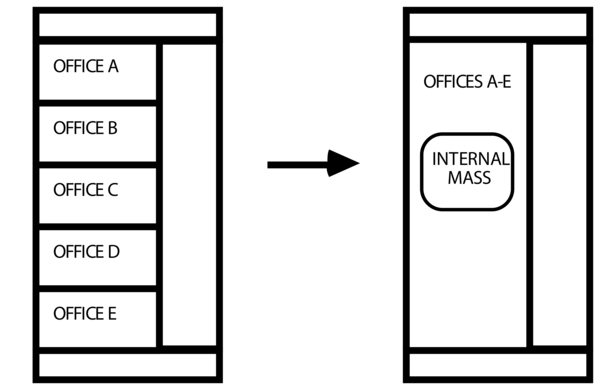
\includegraphics[width=0.9\textwidth, height=0.9\textheight, keepaspectratio=true]{media/image056.png}
\caption{Representing 11 internal walls as internal mass \protect \label{fig:representing-11-internal-walls-as-internal}}
\end{figure}

\textbf{Example}

A five-story building has the same ceiling/floor construction separating each of the levels. Zones that are on floors 2 through 4 may be described using a single piece of internal mass to represent both the floor and ceiling. The construction for this internal mass would be identical to the ceiling/floor construction that would be used to describe separate surfaces and the area of the internal mass surface would be the total surface area of the combined ceilings/floors (i.e.~twice the total floor area).

\paragraph{Field: Name}\label{field-name-21-004}

This is a unique character string associated with the internal mass surface. Though it must be unique from other surface names, it is used primarily for convenience with internal mass surfaces.

\paragraph{Field: Construction Name}\label{field-construction-name-21}

This is the name of the construction (ref: Construction object) used in the surface.

\paragraph{Field: Zone Name}\label{field-zone-name-14}

This is the name of the zone in which the internal mass is represented.

\paragraph{Field: Surface Area}\label{field-surface-area}

This field is the surface area of the internal mass. The area that is specified must be the entire surface area that is exposed to the zone. If both sides of a wall are completely within the same zone, then the area of both sides must be included when describing that internal wall.

IDF examples of Internal Mass surfaces:

\begin{lstlisting}
InternalMass,
  Zn002:IntM001,                !- Surface Name
  INTERIOR,                     !- Construction Name
  DORM ROOMS AND COMMON AREAS,  !- Zone
  408.7734;                     !- Total area exposed to Zone {m2}

InternalMass,
  Zn002:IntM002,                !- Surface Name
  PARTITION02,                  !- Construction Name
  DORM ROOMS AND COMMON AREAS,  !- Zone
  371.6122;                     !- Total area exposed to Zone {m2}
\end{lstlisting}

\subsection{Surface Output Variables/Reports}\label{surface-output-variablesreports}

Note that Surface Outputs from specialized algorithms (such as Effective Moisture Penetration Depth (EMPD), Combined Heat and Moisture Transport (HAMT) and Conduction Finite Difference (CondFD) are discussed under the objects that describe the specialized inputs for these algorithms). You can access them via these links:

\begin{itemize}
\tightlist
\item
  Moisture Penetration Depth (EMPD) Outputs
\item
  Conduction Finite Difference (CondFD) Outputs
\item
  Heat and Moisture (HAMT) Outputs
\end{itemize}

Additionally, the output variables applicable to all heat transfer surfaces:

\begin{lstlisting}
Zone,Sum,Surface Inside Face Heat Balance Calculation Iteration Count []
Zone,Average,Surface Inside Face Temperature [C]
Zone,Average,Surface Outside Face Temperature [C]
Zone,Average,Surface Inside Face Adjacent Air Temperature [C]
Zone,Average,Surface Inside Face Convection Heat Transfer Coefficient [W/m2-K]
Zone,Average,Surface Inside Face Convection Heat Gain Rate [W]
Zone,Average,Surface Inside Face Convection Heat Gain Rate per Area [W/m2]
Zone,Sum,Surface Inside Face Convection Heat Gain Energy [J]
Zone,Average,Surface Inside Face Net Surface Thermal Radiation Heat Gain Rate [W]
Zone,Average,Surface Inside Face Net Surface Thermal Radiation Heat Gain Rate per Area [W/m2]
Zone,Sum,Surface Inside Face Net Surface Thermal Radiation Heat Gain Energy [J]
Zone,Average,Surface Inside Face Solar Radiation Heat Gain Rate [W]
Zone,Average,Surface Inside Face Solar Radiation Heat Gain Rate per Area [W/m2]
Zone,Sum,Surface Inside Face Solar Radiation Heat Gain Energy [J]
Zone,Average,Surface Inside Face Lights Radiation Heat Gain Rate [W]
Zone,Average,Surface Inside Face Lights Radiation Heat Gain Rate per Area [W/m2]
Zone,Sum,Surface Inside Face Lights Radiation Heat Gain Energy [J]
Zone,Average,Surface Inside Face Internal Gains Radiation Heat Gain Rate [W]
Zone,Average,Surface Inside Face Internal Gains Radiation Heat Gain Rate per Area [W/m2]
Zone,Sum,Surface Inside Face Internal Gains Radiation Heat Gain Energy [J]
Zone,Average,Surface Inside Face System Radiation Heat Gain Rate [W]
Zone,Average,Surface Inside Face System Radiation Heat Gain Rate per Area [W/m2]
Zone,Sum,Surface Inside Face System Radiation Heat Gain Energy [J]
Zone,Average,Surface Outside Face Convection Heat Transfer Coefficient [W/m2-K]
Zone,Average,Surface Outside Face Convection Heat Gain Rate [W]
Zone,Average,Surface Outside Face Convection Heat Gain Rate per Area [W/m2]
Zone,Sum,Surface Outside Face Convection Heat Gain Energy [J]
Zone,Average,Surface Outside Face Net Thermal Radiation Heat Gain Rate [W]
Zone,Average,Surface Outside Face Net Thermal Radiation Heat Gain Rate per Area [W/m2]
Zone,Sum,Surface Outside Face Net Thermal Radiation Heat Gain Energy [J]
Zone,Average,Surface Outside Face Thermal Radiation to Air Heat Transfer Coefficient [W/m2-K]
Zone,Average,Surface Outside Face Thermal Radiation to Sky Heat Transfer Coefficient [W/m2-K]
Zone,Average,Surface Outside Face Thermal Radiation to Ground Heat Transfer Coefficient [W/m2-K]
Zone,Average,Surface Inside Face Exterior Windows Incident Beam Solar Radiation Rate [W]
Zone,Sum,Surface Inside Face Exterior Windows Incident Beam Solar Radiation Energy [J]
Zone,Average,Surface Inside Face Exterior Windows Incident Beam Solar Radiation Rate per Area[W/m2]
Zone,Average,Surface Inside Face Interior Windows Incident Beam Solar Radiation Rate [W]
Zone,Average,Surface Inside Face Interior Windows Incident Beam Solar Radiation Rate per Area[W/m2]
Zone, Sum,Surface Inside Face Interior Windows Incident Beam Solar Radiation Energy [J]
Zone,Average,Surface Inside Face Initial Transmitted Diffuse Absorbed Solar Radiation Rate [W]
Zone,Average,Surface Inside Face Initial Transmitted Diffuse Transmitted Out Window Solar Radiation Rate [W]
Zone,Average,Surface Inside Face Absorbed Shortwave Radiation Rate [W]
\end{lstlisting}

Output variables applicable to all exterior heat transfer surfaces:

\begin{lstlisting}
Zone,Average,Surface Outside Face Outdoor Air Drybulb Temperature [C]
Zone,Average,Surface Outside Face Outdoor Air Wetbulb Temperature [C]
Zone,Average,Surface Outside Face Outdoor Air Wind Speed [m/s]
Zone,Average,Surface Outside Face Sunlit Area [m2]
Zone,Average,Surface Outside Face Sunlit Fraction \protect\hyperlinksection-1
Zone,Average,Surface Outside Face Incident Solar Radiation Rate per Area[W/m2]
Zone,Average,Surface Outside Face Solar Radiation Heat Gain Rate [W]
Zone,Average,Surface Outside Face Solar Radiation Heat Gain Rate per Area [W/m2]
Zone,Sum,Surface Outside Face Solar Radiation Heat Gain Energy [J]
Zone,Average,Surface Outside Face Incident Beam Solar Radiation Rate per Area[W/m2]
Zone,Average,Surface Outside Face Incident Sky Diffuse Solar Radiation Rate per Area[W/m2]
Zone,Average,Surface Outside Face Incident Ground Diffuse Solar Radiation Rate per Area[W/m2]
Zone,Average,Surface Ext Diff Sol From Bm-To-Diff Refl From Ground[W/m2]
Zone,Average,Surface Outside Face Incident Sky Diffuse Ground Reflected Solar Radiation Rate per Area[W/m2]
Zone,Average,Surface Outside Face Incident Sky Diffuse Surface Reflected Solar Radiation Rate per Area[W/m2]
Zone,Average,Surface Outside Face Incident Beam To Beam Surface Reflected Solar Radiation Rate per Area[W/m2]
Zone,Average,Surface Outside Face Incident Beam To Diffuse Surface Reflected Solar Radiation Rate per Area[W/m2]
Zone,Average,Surface Outside Face Beam Solar Incident Angle Cosine Value[]
Zone,Average,Surface Anisotropic Sky Multiplier []
Zone,Average,Surface Window BSDF Beam Direction Number []
Zone,Average,Surface Window BSDF Beam Theta Angle [rad]
Zone,Average,Surface Window BSDF Beam Phi Angle [rad]
\end{lstlisting}

Output variables applicable to opaque heat transfer surfaces (FLOOR, WALL, ROOF, DOOR). \textbf{Note -- these are advanced variables -- you must read the descriptions and understand before use -- then you must use the Diagnostics object to allow reporting.}

\begin{lstlisting}
Zone,Average,Surface Inside Face Solar Radiation Heat Gain Rate [W]
Zone,Average,Surface Inside Face Solar Radiation Heat Gain Rate per Area [W/m2]
Zone,Sum,Surface Inside Face Solar Radiation Heat Gain Energy [J]
Zone,Average,Surface Inside Face Lights Radiation Heat Gain Rate [W]
Zone,Average,Surface Inside Face Lights Radiation Heat Gain Rate per Area [W/m2]
Zone,Sum,Surface Inside Face Lights Radiation Heat Gain Energy [J]
Zone,Average,Surface Inside Face Conduction Heat Transfer Rate [W]
Zone,Average,Surface Inside Face Conduction Heat Gain Rate [W]
Zone,Average,Surface Inside Face Conduction Heat Loss Rate [W]
Zone,Average,Surface Inside Face Conduction Heat Transfer Rate per Area [W/m2]
Zone,Sum,Surface Inside Face Conduction Heat Transfer Energy [J]
Zone,Average,Surface Outside Face Conduction Heat Transfer Rate [W]
Zone,Average,Surface Outside Face Conduction Heat Gain Rate [W]
Zone,Average,Surface Outside Face Conduction Heat Loss Rate [W]
Zone,Average,Surface Outside Face Conduction Heat Transfer Rate per Area [W/m2]
Zone,Sum,Surface Outside Face Conduction Heat Transfer Energy [J]
Zone,Average,Surface Average Face Conduction Heat Transfer Rate [W]
Zone,Average,Surface Average Face Conduction Heat Gain Rate [W]
Zone,Average,Surface Average Face Conduction Heat Loss Rate [W]
Zone,Average,Surface Average Face Conduction Heat Transfer Rate per Area [W/m2]
Zone,Sum,Surface Average Face Conduction Heat Transfer Energy [J]
Zone,Average,Surface Heat Storage Rate [W]
Zone,Average,Surface Heat Storage Gain Rate [W]
Zone,Average,Surface Heat Storage Loss Rate [W]
Zone,Average,Surface Heat Storage Rate per Area [W/m2]
Zone,Sum,Surface Heat Storage Energy [J]
Zone,Average,Zone Opaque Surface Inside Face Conduction [W]
Zone,Average,Zone Opaque Surface Inside Faces Total Conduction Heat Gain Rate [W]
Zone,Average,Zone Opaque Surface Inside Faces Total Conduction Heat Loss Rate [W]
Zone,Sum,Zone Opaque Surface Inside Faces Total Conduction Heat Gain Energy [J]
Zone,Sum,Zone Opaque Surface Inside Faces Total Conduction Heat Loss Energy [J]
Zone,Average,Zone Opaque Surface Outside Face Conduction [W]
Zone,Average,Zone Opaque Surface Outside Face Conduction Gain[W]
Zone,Average,Zone Opaque Surface Outside Face Conduction Loss[W]
Zone,Average, Surface Inside Face Beam Solar Radiation Heat Gain Rate [W]
\end{lstlisting}

\subsection{Window Output Variables}\label{window-output-variables}

Output variables applicable only to exterior windows and glass doors:

\begin{lstlisting}
Zone,Average,Zone Windows Total Transmitted Solar Radiation Rate [W]
Zone,Sum,Zone Transmitted Solar Energy [J]
Zone,Average,Zone Windows Total Heat Gain Rate [W]
Zone,Sum,Zone Windows Total Heat Gain Energy [J]
Zone,Average,Zone Windows Total Heat Loss Rate [W]
Zone,Sum,Zone Windows Total Heat Loss Energy [J]
Zone,Average,Zone Exterior Windows Total Transmitted Beam Solar Radiation Rate [W]
Zone,Sum,Zone Exterior Windows Total Transmitted Beam Solar Radiation Energy [J]
Zone,Average,Zone Interior Windows Total Transmitted Beam Solar Radiation Rate [W]
Zone,Sum,Zone Interior Windows Total Transmitted Beam Solar Radiation Energy [J]
Zone,Average,Zone Exterior Windows Total Transmitted Diffuse Solar Radiation Rate [W]
Zone,Sum,Zone Exterior Windows Total Transmitted Diffuse Solar Radiation Energy [J]
Zone,Average,Zone Interior Windows Total Transmitted Diffuse Solar Radiation Rate [W]
Zone,Average,Surface Window Total Glazing Layers Absorbed Solar Radiation Rate [W]
Zone,Average,Surface Window Total Glazing Layers Absorbed Shortwave Radiation Rate [W]
Zone,Sum,Surface Window Total Glazing Layers Absorbed Solar Radiation Energy [J]
Zone,Average,Surface Window Shading Device Absorbed Solar Radiation Rate [W]
Zone,Sum,Surface Window Shading Device Absorbed Solar Radiation Energy [J]
Zone,Average, Surface Window Transmitted Solar Radiation Rate [W]
Zone,Sum,Surface Window Transmitted Solar Radiation Energy [J]
Zone,Average,Surface Window Transmitted Beam Solar Radiation Rate [W]
Zone,Average,Surface Window Transmitted Beam To Beam Solar Radiation Rate [W]
Zone,Average,Surface Window Transmitted Beam To Diffuse Solar Radiation Rate [W]
Zone,Sum,Surface Window Transmitted Beam Solar Radiation Energy [J]
Zone,Sum,Surface Window Transmitted Beam To Beam Solar Radiation Energy [J]
Zone,Sum,Surface Window Transmitted Beam To Diffuse Solar Radiation Energy [J]
Zone,Average,Surface Window Transmitted Diffuse Solar Radiation Rate [W]
Zone,Sum,Surface Window Transmitted Diffuse Solar Radiation Energy [J]
Zone,Average,Surface Window System Solar Transmittance []
Zone,Average,Surface Window System Solar Absorptance []
Zone,Average,Surface Window System Solar Reflectance []
Zone,Average,Surface Window Gap Convective Heat Transfer Rate [W]
Zone,Sum,Surface Window Gap Convective Heat Transfer Energy [J]
Zone,Average,Surface Window Heat Gain Rate [W]
Zone,Sum,Surface Window Heat Gain Energy [J]
Zone,Average,Surface Window Heat Loss Rate [W]
Zone,Sum,Surface Window Heat Loss Energy [J]
Zone,Average,Surface Window Net Heat Transfer Rate [W]
Zone,Sum,Surface Window Net Heat Transfer Energy [J]
Zone,Average,Surface Window Glazing Beam to Beam Solar Transmittance[]
Zone,Average,Surface Window Glazing Beam to Diffuse Solar Transmittance []
Zone,Average,Surface Window Glazing Diffuse to Diffuse Solar Transmittance[]
Zone,Average,Surface Window Model Solver Iteration Count []
Zone,Average,Surface Window Solar Horizontal Profile Angle[deg]
Zone,Average,Surface Window Solar Vertical Profile Angle[deg]
Zone,Average,Surface Window Outside Reveal Reflected Beam Solar Radiation Rate [W]
Zone,Sum,Surface Window Outside Reveal Reflected Beam Solar Radiation Energy
Zone,Average,Surface Window Inside Reveal Reflected Beam Solar Radiation Rate [W]
Zone,Sum,Surface Window Inside Reveal Reflected Beam Solar Radiation Energy [J]
Zone,Average,Surface Window Inside Reveal Absorbed Beam Solar Radiation Rate [W]
Zone,Average,Surface Window Inside Face Glazing Condensation Status []
Zone,Average,Surface Window Inside Face Frame Condensation Status []
Zone,Average,Surface Window Inside Face Divider Condensation Status []
Zone,Average,Surface Shading Device Is On Time Fraction[]
Zone,Average,Surface Window Blind Slat Angle [deg]
Zone,Average,Surface Window Blind Beam to Beam Solar Transmittance[]
Zone,Average,Surface Window Blind Beam to Diffuse Solar Transmittance[]
Zone,Average,Surface Window Blind Diffuse to Diffuse Solar Transmittance[]
Zone,Average,Surface Window Blind and Glazing System Beam Solar Transmittance[]
Zone,Average,Surface Window Blind and Glazing System Diffuse Solar Transmittance[]
Zone,Average,Surface Window Screen Beam to Beam Solar Transmittance []
Zone,Average,Surface Window Screen Beam to Diffuse Solar Transmittance []
Zone,Average,Surface Window Screen Diffuse to Diffuse Solar Transmittance []
Zone,Average,Surface Window Screen and Glazing System Beam Solar Transmittance []
Zone,Average,Surface Window Screen and Glazing System Diffuse Solar Transmittance []
Zone,State,Surface Storm Window On Off Status []
Zone,Average,Surface Window Inside Face Frame and Divider Zone Heat Gain Rate [W]
Zone,Average,Surface Window Frame Heat Gain Rate [W]
Zone,Average,Surface Window Frame Heat Loss Rate [W]
Zone,Average,Surface Window Divider Heat Gain Rate [W]
Zone,Average,Surface Window Divider Heat Loss Rate [W]
Zone,Average,Surface Window Frame Inside Temperature [C]
Zone,Average,Surface Window Frame Outside Temperature [C]
Zone,Average,Surface Window Divider Inside Temperature [C]
Zone,Average,Surface Window Divider Outside Temperature [C]
\end{lstlisting}

If the user requests to display advanced report/output variables (e.g.~see Output:Diagnostics keyword DisplayAdvancedReportVariables) the the following additional output variables are available for exterior windows and glass doors

\begin{lstlisting}
Zone,Average,Surface Window Inside Face Glazing Zone Convection Heat Gain Rate [W]
Zone,Average,Surface Window Inside Face Glazing Net Infrared Heat Transfer Rate [W]
Zone,Average,Surface Window Shortwave from Zone Back Out Window Heat Transfer Rate [W]
Zone,Average,Surface Window Inside Face Frame and Divider Zone Heat Gain Rate [W]
Zone,Average,Surface Window Inside Face Gap between Shade and Glazing Zone Convection Heat Gain Rate [W]
Zone,Average,Surface Window Inside Face Shade Zone Convection Heat Gain Rate [W]
Zone,Average,Surface Window Inside Face Shade Net Infrared Heat Transfer Rate [W]
\end{lstlisting}

Output variables applicable only to interior windows and glass doors:

\begin{lstlisting}
Zone,Average, Surface Window Transmitted Beam Solar Radiation Rate [W]
Zone,Sum,Surface Window Transmitted Beam Solar Radiation Energy [J]
\end{lstlisting}

If the user requests to display advanced report/output variables (e.g.~see Output:Diagnostics keyword DisplayAdvancedReportVariables) the the following additional output variable is available for Equivalent Layer Window;

\begin{lstlisting}
Zone,Average, Surface Window Inside Face Other Convection Heat Gain Rate [W]
\end{lstlisting}

Output variables applicable to interior and exterior windows and doors are:

\begin{lstlisting}
Zone,Average,Surface Window Total Absorbed Shortwave Radiation Rate Layer <x> [W]
Zone,Average,Surface Window Front Face Temperature Layer <x> [C]
Zone,Average,Surface Window Back Face Temperature Layer <x> [C]
\end{lstlisting}

\subsubsection{Surface Window Total Absorbed Shortwave Radiation Rate Layer \textless{}x\textgreater{} {[}W{]}}\label{surface-window-total-absorbed-shortwave-radiation-rate-layer-x-w}

This will output shortwave radiation absorbed in a window layer. The key values for this output variable are the surface name. Layers are numbered from the outside to the inside of the surface. The full listing will appear in the RDD file.

\subsubsection{Surface Window Front Face Temperature Layer \textless{}x\textgreater{} {[}C{]}}\label{surface-window-front-face-temperature-layer-x-c}

This will output a temperature for the front face of the layer. The layer front face is considered to be the face closest to the outside environment. The full listing will appear in the RDD file.

\subsubsection{Surface Window Back Face Temperature Layer \textless{}x\textgreater{} {[}C{]}}\label{surface-window-back-face-temperature-layer-x-c}

This will output a temperature for the back face of the layer. The layer back face is considered to be the face closest to the inside environment. The full listing will appear in the RDD file.

\subsection{Surface Output Variables (all heat transfer surfaces)}\label{surface-output-variables-all-heat-transfer-surfaces}

The various output variables related to surface heat transfer are organized around the inside and outside face of each surface. The zone heat balance model draws energy balances at each side, or face, of a surface and so each surface essentially has two sets of results. The inside face is the side of a heat transfer surface that faces toward the thermal zone. The outside face is the side of a heat transfer surface that faces away from the thermal zone, typically facing outdoors. The Key Value for these is generally the user-defined name of the surface.

\subsubsection{Surface Inside Face Heat Balance Calculation Iteration Count {[]}}\label{surface-inside-face-heat-balance-calculation-iteration-count}

This output is the number of iterations used in a part of the solution for surface heat transfer that accounts for thermal radiation heat transfer between zone surfaces. This is simply a counter on the iteration loop for inside face surface modeling. There is only one instance of this output in a given run and the Key Value is ``Simulation.''

\subsubsection{Surface Inside Face Temperature {[}C{]}}\label{surface-inside-face-temperature-c}

This is the temperature of the surface's inside face, in degrees Celsius. Former Name: Prior to version 7.1 this output was called Surface Inside Temperature.

\subsubsection{Surface Outside Face Temperature {[}C{]}}\label{surface-outside-face-temperature-c}

This is the temperature of the surface's outside face, in degrees Celsius. Former Name: Prior to version 7.1, this output was called Surface Outside Temperature.

\subsubsection{Surface Inside Face Adjacent Air Temperature {[}C{]}}\label{surface-inside-face-adjacent-air-temperature-c}

This is the effective bulk air temperature used for modeling the inside surface convection heat transfer. This is the same as the zone mean air temperature when using the mixing model for roomair. However, if more advanced roomair models are used, this variable will report the air temperature predicted by the roomair model as it was used in the surface heat balance model calculations. Former Name: Prior to version 7.1, this output was called Surface Int Adjacent Air Temperature.

\subsubsection{Surface Inside Face Convection Heat Gain Rate {[}W{]}}\label{surface-inside-face-convection-heat-gain-rate-w}

\subsubsection{Surface Inside Face Convection Heat Gain Rate per Area {[}W/m2{]}}\label{surface-inside-face-convection-heat-gain-rate-per-area-wm2}

\subsubsection{Surface Inside Face Convection Heat Gain Energy {[}J{]}}\label{surface-inside-face-convection-heat-gain-energy-j}

These ``inside face convection heat gain'' output variables describe the heat transferred by convection between the inside face and the zone air. The values can be positive or negative with positive indicating heat is being added to the surface's face by convection. Different versions of the report are available including the basic heat gain rate (W), and a per unit area flux (W/m2), and an energy version (J).

Former Name: Prior to version 7.1, these outputs were called ``Surface Int Convection Heat *'' and had used the opposite sign convention.

\subsubsection{Surface Inside Face Convection Heat Transfer Coefficient {[}W/m2-K{]}}\label{surface-inside-face-convection-heat-transfer-coefficient-wm2-k}

This is the coefficient that describes the convection heat transfer. It is the value of ``Hc'' in the classic convection model Q = Hc* A* (T -- T). This is the result of the surface convection algorithm used for the inside face. Former Name: Prior to version 7.1, this output was called ``Surface Int Convection Coeff.''

\subsubsection{Surface Inside Face Net Surface Thermal Radiation Heat Gain Rate {[}W{]}}\label{surface-inside-face-net-surface-thermal-radiation-heat-gain-rate-w}

\subsubsection{Surface Inside Face Net Surface Thermal Radiation Heat Gain Rate per Area {[}W/m2{]}}\label{surface-inside-face-net-surface-thermal-radiation-heat-gain-rate-per-area-wm2}

\subsubsection{Surface Inside Face Net Surface Thermal Radiation Heat Gain Energy {[}J{]}}\label{surface-inside-face-net-surface-thermal-radiation-heat-gain-energy-j}

These ``inside face net surface thermal radiation heat gain'' output variables describe the heat transferred by longwave infrared thermal radiation exchanges between the inside faces of other surfaces in the zone. The values can be positive or negative with positive indicating heat is being added to the surface's face by thermal radiation. Different versions of the report are available including the basic heat gain rate (W), and a per unit area flux (W/m2), and an energy version (J).

\subsubsection{Surface Inside Face Solar Radiation Heat Gain Rate {[}W{]}}\label{surface-inside-face-solar-radiation-heat-gain-rate-w}

\subsubsection{Surface Inside Face Solar Radiation Heat Gain Rate per Area {[}W/m2{]}}\label{surface-inside-face-solar-radiation-heat-gain-rate-per-area-wm2}

\subsubsection{Surface Inside Face Solar Radiation Heat Gain Energy {[}J{]}}\label{surface-inside-face-solar-radiation-heat-gain-energy-j}

These ``inside face solar radiation heat gain'' output variables describe the heat transferred by solar radiation onto the inside face. The values are always positive and indicate heat is being added to the surface's face by solar radiation. This is sunlight that has entered the zone through a window and been absorbed on the inside face of the surface. Different versions of the report are available including the basic heat gain rate (W), and a per unit area flux (W/m2), and an energy version (J).

\subsubsection{Surface Inside Face Lights Radiation Heat Gain Rate {[}W{]}}\label{surface-inside-face-lights-radiation-heat-gain-rate-w}

\subsubsection{Surface Inside Face Lights Radiation Heat Gain Rate per Area {[}W/m2{]}}\label{surface-inside-face-lights-radiation-heat-gain-rate-per-area-wm2}

\subsubsection{Surface Inside Face Lights Radiation Heat Gain Energy {[}J{]}}\label{surface-inside-face-lights-radiation-heat-gain-energy-j}

These ``inside face lights radiation heat gain'' output variables describe the heat transferred by shortwave radiation onto the inside face. The values are always positive and indicate heat is being added to the surface's face by shortwave radiation that emanated from electric lighting equipment and was absorbed by the surface. Different versions of the report are available including the basic heat gain rate (W), and a per unit area flux (W/m2), and an energy version (J).

\subsubsection{Surface Inside Face Internal Gains Radiation Heat Gain Rate {[}W{]}}\label{surface-inside-face-internal-gains-radiation-heat-gain-rate-w}

\subsubsection{Surface Inside Face Internal Gains Radiation Heat Gain Rate per Area {[}W/m2{]}}\label{surface-inside-face-internal-gains-radiation-heat-gain-rate-per-area-wm2}

\subsubsection{Surface Inside Face Internal Gains Radiation Heat Gain Energy {[}J{]}}\label{surface-inside-face-internal-gains-radiation-heat-gain-energy-j}

These ``inside face internal gains radiation heat gain'' output variables describe the heat transferred by longwave infrared thermal radiation onto the inside face that emanated from internal gains such as lights, electric equipment, and people. The values are always positive and indicate heat is being added to the surface's face by the absorption of longwave thermal radiation. Different versions of the report are available including the basic heat gain rate (W), and a per unit area flux (W/m2), and an energy version (J).

\subsubsection{Surface Inside Face System Radiation Heat Gain Rate {[}W{]}}\label{surface-inside-face-system-radiation-heat-gain-rate-w}

\subsubsection{Surface Inside Face System Radiation Heat Gain Rate per Area {[}W/m2{]}}\label{surface-inside-face-system-radiation-heat-gain-rate-per-area-wm2}

\subsubsection{Surface Inside Face System Radiation Heat Gain Energy {[}J{]}}\label{surface-inside-face-system-radiation-heat-gain-energy-j}

These ``inside face system radiation heat gain'' output variables describe the heat transferred by infrared thermal radiation onto the inside face that emanated from HVAC equipment such as baseboard heaters or high-temperature radiant heating panels. The values are always positive and indicate heat is being added to the surface's face by the absorption of thermal radiation. Different versions of the report are available including the basic heat gain rate (W), and a per unit area flux (W/m2), and an energy version (J).

\subsubsection{Surface Outside Face Convection Heat Gain Rate {[}W{]}}\label{surface-outside-face-convection-heat-gain-rate-w}

\subsubsection{Surface Outside Face Convection Heat Gain Rate per Area {[}W/m2{]}}\label{surface-outside-face-convection-heat-gain-rate-per-area-wm2}

\subsubsection{Surface Outside Face Convection Heat Gain Energy {[}J{]}}\label{surface-outside-face-convection-heat-gain-energy-j}

These ``outside face convection'' output variables describe heat transferred by convection between the outside face and the surrounding air. The values can be positive or negative with positive values indicating heat is added to the surface face by convection heat transfer. Different versions of the report are available including the basic heat gain rate (W), and a per unit area flux (W/m\(^{2}\)), and an energy version (J).

Former Name: Prior to version 7.1, these outputs were called ``Surface Ext Convection Heat *'' and used the opposite sign convention.

\subsubsection{Surface Outside Face Convection Heat Transfer Coefficient {[}W/m2-K{]}}\label{surface-outside-face-convection-heat-transfer-coefficient-wm2-k}

This is the coefficient that describes the convection heat transfer. It is the value of ``Hc'' in the classic convection model Q = Hc* A* (T -- T). This is the result of the surface convection algorithm used for the outside face. Former Name: Prior to Version 7.1, this output was called ``Surface Ext Convection Coeff.''

\subsubsection{Surface Outside Face Net Thermal Radiation Heat Gain Rate {[}W{]}}\label{surface-outside-face-net-thermal-radiation-heat-gain-rate-w}

\subsubsection{Surface Outside Face Net Thermal Radiation Heat Gain Rate per Area {[}W/m2{]}}\label{surface-outside-face-net-thermal-radiation-heat-gain-rate-per-area-wm2}

\subsubsection{Surface Outside Face Net Thermal Radiation Heat Gain Energy {[}J{]}}\label{surface-outside-face-net-thermal-radiation-heat-gain-energy-j}

These ``outside face net thermal radiation'' output variables describe the heat transferred by longwave infrared thermal radiation exchanges between the surface and the surroundings of the outside face. This is the net of all forms of longwave thermal infrared radiation heat transfer. The values can be positive or negative with positive indicating the net addition of heat to the outside face. Different versions of the report are available including the basic heat gain rate (W), and a per unit area flux (W/m2), and an energy version (J).

Former Name: Prior to version 7.1, these outputs were called ``Surface Ext Thermal Radiation Heat *'' and used the opposite sign convention.

\subsubsection{Surface Inside Face Exterior Windows Incident Beam Solar Radiation Rate {[}W{]}}\label{surface-inside-face-exterior-windows-incident-beam-solar-radiation-rate-w}

\subsubsection{Surface Inside Face Exterior Windows Incident Beam Solar Radiation Rate per Area {[}W/m2{]}}\label{surface-inside-face-exterior-windows-incident-beam-solar-radiation-rate-per-area-wm2}

\subsubsection{Surface Inside Face Exterior Windows Incident Beam Solar Radiation Energy {[}J{]}}\label{surface-inside-face-exterior-windows-incident-beam-solar-radiation-energy-j}

Beam solar radiation from the exterior windows in a zone incident on the inside face of a surface in the zone. If Solar Distribution in the BUILDING object is equal to MinimalShadowing or FullExterior, it is assumed that all beam solar from exterior windows falls on the floor. In this case the value of this output variable can be greater than zero only for floor surfaces. If Solar Distribution equals FullInteriorExterior the program tracks where beam solar from exterior windows falls inside the zone, in which case the value of this variable can be greater than zero for floor as well as wall surfaces. Different versions of the report are available including the basic incident rate (W), a per unit area flux (W/m2), and an energy version (J).

\subsubsection{Surface Inside Face Interior Windows Incident Beam Solar Radiation Rate {[}W{]}}\label{surface-inside-face-interior-windows-incident-beam-solar-radiation-rate-w}

\subsubsection{Surface Inside Face Interior Windows Incident Beam Solar Radiation Rate per Area {[}W/m2{]}}\label{surface-inside-face-interior-windows-incident-beam-solar-radiation-rate-per-area-wm2}

\subsubsection{Surface Inside Face Interior Windows Incident Beam Solar Radiation Energy {[}J{]}}\label{surface-inside-face-interior-windows-incident-beam-solar-radiation-energy-j}

Beam solar radiation from the interior (i.e., interzone) windows in a zone incident on the inside face of a surface in the zone. This value is calculated only if Solar Distribution in the BUILDING object is equal to FullInteriorExterior. However, the program does not track where this radiation falls. Instead, it is treated by the program as though it were diffuse radiation uniformly distributed over all of the zone surfaces. See \textbf{Figure~\ref{fig:beam-solar-radiation-entering-a-zone-through}}. Different versions of the report are available including the basic incident rate (W), a per unit area flux (W/m2), and an energy version (J).

\begin{figure}[hbtp] % fig 31
\centering
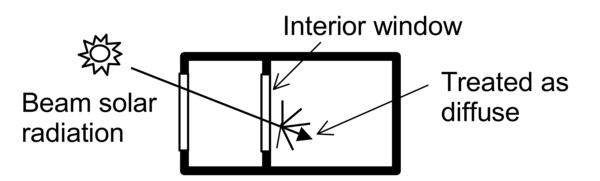
\includegraphics[width=0.9\textwidth, height=0.9\textheight, keepaspectratio=true]{media/image057.png}
\caption{Beam solar radiation entering a zone through an interior window is distributed inside the zone as though it were diffuse radiation. \protect \label{fig:beam-solar-radiation-entering-a-zone-through}}
\end{figure}

\subsubsection{Surface Inside Face Initial Transmitted Diffuse Absorbed Solar Radiation Rate {[}W{]}}\label{surface-inside-face-initial-transmitted-diffuse-absorbed-solar-radiation-rate-w}

As of Version 2.1, diffuse solar transmitted through exterior and interior windows is no longer uniformly distributed. Instead, it is distributed according to the approximate view factors between the transmitting window and all other heat transfer surfaces in the zone. This variable is the amount of transmitted diffuse solar that is initially absorbed on the inside of each heat transfer surface. The portion of this diffuse solar that is reflected by all surfaces in the zone is subsequently redistributed uniformly to all heat transfer surfaces in the zone, along with interior reflected beam solar and shortwave radiation from lights. The total absorbed shortwave radiation is given by the next variable.

\subsubsection{Surface Inside Face Absorbed Shortwave Radiation Rate {[}W{]}}\label{surface-inside-face-absorbed-shortwave-radiation-rate-w}

As of Version 2.1, the previous variable plus absorbed shortwave radiation from uniformly distributed initially-reflected diffuse solar, reflected beam solar, and shortwave radiation from lights. This sum is the power of all sources of solar and visible radiation absorbed by the surface at the inside face.

\subsection{Surface Output Variables (exterior heat transfer surfaces)}\label{surface-output-variables-exterior-heat-transfer-surfaces}

\subsubsection{Surface Outside Face Outdoor Air Drybulb Temperature {[}C{]}}\label{surface-outside-face-outdoor-air-drybulb-temperature-c}

The outdoor air dry-bulb temperature calculated at the height above ground of the surface centroid. Former Name: Prior to version 7.1, this output was called ``Surface Ext Outdoor Dry Bulb.''

\subsubsection{Surface Outside Face Outdoor Air Wetbulb Temperature {[}C{]}}\label{surface-outside-face-outdoor-air-wetbulb-temperature-c}

The outdoor air wet-bulb temperature calculated at the height above ground of the surface centroid. Former Name: Prior to version 7.1, this output was called ``Surface Ext Outdoor Wet Bulb.''

\subsubsection{Surface Outside Face Outdoor Air Wind Speed {[}m/s{]}}\label{surface-outside-face-outdoor-air-wind-speed-ms}

The outdoor wind speed calculated at the height above ground of the surface centroid. Former Name: Prior to version 7.1, this output was called ``Surface Ext Wind Speed.''

\subsubsection{Surface Outside Face Sunlit Area {[}m2{]}}\label{surface-outside-face-sunlit-area-m2}

The outside area of an exterior surface that is illuminated by (unreflected) beam solar radiation.

\subsubsection{Surface Outside Face Sunlit Fraction {[]}}\label{surface-outside-face-sunlit-fraction}

The fraction of the outside area of an exterior surface that is illuminated by (unreflected) beam solar radiation. Equals Surface Outside Face Sunlit Area divided by total surface area.

\subsubsection{Surface Outside Face Thermal Radiation to Air Heat Transfer Coefficient {[}W/m2-K{]}}\label{surface-outside-face-thermal-radiation-to-air-heat-transfer-coefficient-wm2-k}

This is the coefficient that describes thermal radiation heat transfer between the outside face and the air mass surrounding the surface. It is the value of ``Hr'' in the classic linearized model for thermal radiation Q = Hr * A * (T\_surf -- T\_surfodb) when applied to the ambient air. Where T\_surf = Surface Outside Face Temperature, and T\_surfodb = Surface Outside Face Outdoor Air Drybulb Temperature. Former Name: Prior to version 7.1, this output was called ``Surface Ext Rad to Air Coeff.''

\subsubsection{Surface Outside Face Thermal Radiation to Sky Heat Transfer Coefficient {[}W/m2-K{]}}\label{surface-outside-face-thermal-radiation-to-sky-heat-transfer-coefficient-wm2-k}

This is the coefficient that describes thermal radiation heat transfer between the outside face and the sky surrounding the surface. It is the value of ``Hr'' in the classic linearized model for thermal radiation Q = Hr * A * (T\_surf -- T\_sky) when applied to the sky. Where T\_surf = Surface Outside Face Temperature, and T\_sky = Site Sky Temperature. Former Name: Prior to version 7.1, this output was called ``Surface Ext Rad to Sky Coeff.''

\subsubsection{Surface Outside Face Thermal Radiation to Ground Heat Transfer Coefficient {[}W/m2-K{]}}\label{surface-outside-face-thermal-radiation-to-ground-heat-transfer-coefficient-wm2-k}

This is the coefficient that describes thermal radiation heat transfer between the outside face and the ground surrounding the surface. It is the value of ``Hr'' in the classic linearized model for thermal radiation Q = Hr * A * (T\_surf -- T\_odb) when applied to the ground. Where T\_surf = Surface Outside Face Temperature, and T\_odb = Site Outdoor Air Drybulb Temperature (used as an approximation for the ground surface temperature). Former Name: Prior to version 7.1, this output was called ``Surface Ext Rad to Ground Coeff.''

\subsubsection{Surface Outside Face Solar Radiation Heat Gain Rate {[}W{]}}\label{surface-outside-face-solar-radiation-heat-gain-rate-w}

\subsubsection{Surface Outside Face Solar Radiation Heat Gain Rate per Area {[}W/m2{]}}\label{surface-outside-face-solar-radiation-heat-gain-rate-per-area-wm2}

\subsubsection{Surface Outside Face Solar Radiation Heat Gain Energy {[}J{]}}\label{surface-outside-face-solar-radiation-heat-gain-energy-j}

These ``outside face solar radiation'' output variables describe the heat transferred by the absorption of solar radiation at the outside face. This is the result of incident solar radiation being absorbed at the surface face. The values are always positive.

\subsubsection{Surface Outside Face Incident Solar Radiation Rate per Area {[}W/m2{]}}\label{surface-outside-face-incident-solar-radiation-rate-per-area-wm2}

The total solar radiation incident on the outside of an exterior surface. It is the sum of:

\begin{itemize}
\item
  Surface Outside Face Incident Beam Solar Radiation Rate per Area
\item
  Surface Outside Face Incident Sky Diffuse Solar Radiation Rate per Area
\item
  Surface Outside Face Incident Ground Diffuse Solar Radiation Rate per Area
\item
  Surface Outside Face Incident Sky Diffuse Surface Reflected Solar Radiation Rate per Area
\item
  Surface Outside Face Incident Beam To Beam Surface Reflected Solar Radiation Rate per Area
\item
  Surface Outside Face Incident Sky Diffuse Surface Reflected Solar Radiation Rate per Area
\end{itemize}

\subsubsection{Surface Outside Face Incident Beam Solar Radiation Rate per Area {[}W/m2{]}}\label{surface-outside-face-incident-beam-solar-radiation-rate-per-area-wm2}

The solar beam radiation incident on the outside of an exterior surface, including the effects of shadowing, if present. The beam here is that directly from the sun; it excludes beam specularly reflected from obstructions.

\subsubsection{Surface Outside Face Incident Sky Diffuse Solar Radiation Rate per Area {[}W/m2{]}}\label{surface-outside-face-incident-sky-diffuse-solar-radiation-rate-per-area-wm2}

The solar diffuse radiation from the sky incident on the outside of an exterior surface, including the effects of shadowing, if present.

\subsubsection{Surface Outside Face Incident Ground Diffuse Solar Radiation Rate per Area {[}W/m2{]}}\label{surface-outside-face-incident-ground-diffuse-solar-radiation-rate-per-area-wm2}

The solar diffuse radiation incident on the outside of an exterior surface that arises from reflection of beam solar and sky diffuse solar from the ground. This is the sum of the next two output variables, ``Surface Outside Face Incident Beam To Diffuse Ground Reflected Solar Radiation Rate per Area'' and ``Surface Outside Face Incident Sky Diffuse Ground Reflected Solar Radiation Rate per Area.'' The reflected solar radiation from the ground is assumed to be diffuse and isotropic (there is no specular component).

If ``Reflections'' option is not chosen in the Solar Distribution Field in the BUILDING object, the effects of shadowing are accounted for by the user-specified value of View Factor to Ground for the surface. If ``Reflections'' option is chosen, the program determines the effects of shadowing, including time-varying shadowing of the ground plane by the building itself.

\subsubsection{Surface Outside Face Incident Beam To Diffuse Ground Reflected Solar Radiation Rate per Area {[}W/m2{]}}\label{surface-outside-face-incident-beam-to-diffuse-ground-reflected-solar-radiation-rate-per-area-wm2}

The solar diffuse radiation incident on the outside of an exterior surface that arises from beam-to-diffuse reflection from the ground. It is assumed that there is no beam-to-beam (specular) component. The beam here is that directly from the sun; it excludes beam specularly reflected from obstructions.

\subsubsection{Surface Outside Face Incident Sky Diffuse Ground Reflected Solar Radiation Rate per Area {[}W/m2{]}}\label{surface-outside-face-incident-sky-diffuse-ground-reflected-solar-radiation-rate-per-area-wm2}

The solar diffuse radiation incident on the outside of an exterior surface that arises from sky diffuse solar reflection from the ground. The sky diffuse here is that directly from the sky; it excludes reflection of sky diffuse from obstructions.

\subsubsection{Surface Outside Face Incident Sky Diffuse Surface Reflected Solar Radiation Rate per Area {[}W/m2{]}}\label{surface-outside-face-incident-sky-diffuse-surface-reflected-solar-radiation-rate-per-area-wm2}

The solar diffuse radiation incident on the outside of an exterior surface that arises from sky diffuse reflection from one or more obstructions. This value will be non-zero only if ``Reflections'' option is chosen in the BUILDING object.

\subsubsection{Surface Outside Face Incident Beam To Beam Surface Reflected Solar Radiation Rate per Area {[}W/m2{]}}\label{surface-outside-face-incident-beam-to-beam-surface-reflected-solar-radiation-rate-per-area-wm2}

The solar beam radiation incident on the outside of an exterior surface that arises from beam-to-beam (specular) reflection from one or more obstructions. This value will be non-zero only if ``Reflections'' option is chosen in the BUILDING object. For windows, the program treats this beam radiation as diffuse radiation in calculating its transmission and absorption.

\subsubsection{Surface Outside Face Incident Beam To Diffuse Surface Reflected Solar Radiation Rate per Area {[}W/m2{]}}\label{surface-outside-face-incident-beam-to-diffuse-surface-reflected-solar-radiation-rate-per-area-wm2}

The solar diffuse radiation incident on the outside of an exterior surface that arises from beam-to-diffuse reflection from building shades or building surfaces. This value will be non-zero only if ``Reflections'' option is chosen in the BUILDING object.

\subsubsection{Surface Outside Face Beam Solar Incident Angle Cosine Value {[]}}\label{surface-outside-face-beam-solar-incident-angle-cosine-value}

The cosine of the angle of incidence of (unreflected) beam solar radiation on the outside of an exterior surface. The value varies from 0.0 for beam parallel to the surface (incidence angle = 90\(^{O}\)) to 1.0 for beam perpendicular to the surface (incidence angle = 0\(^{O}\)). Negative values indicate the sun is behind the surface, i.e the surface does not see the sun.

\subsubsection{Surface Anisotropic Sky Multiplier {[]}}\label{surface-anisotropic-sky-multiplier}

This is the view factor multiplier for diffuse sky irradiance on exterior surfaces taking into account the anisotropic radiance of the sky. The diffuse sky irradiance on a surface is given by Anisotropic Sky Multiplier * Diffuse Solar Irradiance.

\subsubsection{Surface Window BSDF Beam Direction Number {[]}}\label{surface-window-bsdf-beam-direction-number}

\subsubsection{Surface Window BSDF Beam Phi Angle {[}rad{]}}\label{surface-window-bsdf-beam-phi-angle-rad}

\subsubsection{Surface Window BSDF Beam Theta Angle {[}rad{]}}\label{surface-window-bsdf-beam-theta-angle-rad}

\subsection{Opaque Surface Output Variables}\label{opaque-surface-output-variables}

The following variables apply only to opaque surfaces, where an opaque surface is considered here to be an exterior or interzone heat transfer surface of class FLOOR, WALL, ROOF or DOOR. \textbf{Note -- these are advanced variables -- you must read the descriptions and understand before use -- then you must use the} \textbf{Output:Diagnostics} \textbf{object to allow reporting.}

\subsubsection{Surface Inside Face Conduction Heat Transfer Rate {[}W{]}}\label{surface-inside-face-conduction-heat-transfer-rate-w}

\subsubsection{Surface Inside Face Conduction Heat Transfer Rate per Area {[}W/m2{]}}\label{surface-inside-face-conduction-heat-transfer-rate-per-area-wm2}

\subsubsection{Surface Inside Face Conduction Heat Gain Rate {[}W{]}}\label{surface-inside-face-conduction-heat-gain-rate-w}

\subsubsection{Surface Inside Face Conduction Heat Loss Rate {[}W{]}}\label{surface-inside-face-conduction-heat-loss-rate-w}

These ``inside face conduction'' output variables describe heat flow by conduction right at the inside face of an opaque heat transfer surface. A positive value means that the conduction is from just inside the inside face toward the inside face. A negative value means that the conduction is from the inside face into the core of the heat transfer surface.

Note that Inside Face Conduction, when positive, does \textbf{not} indicate the heat flow from the surface to the zone air, which is governed by the inside face convection coefficient and the difference in temperature between the inside face and the zone air.

Different versions of the reports are available. The basic heat gain rate (W) and a per unit area flux (W/m\(^{2}\)) can have positive or negative values with the sign convention that positive indicates heat flowing toward the face itself. There are also directed ``gain'' and ``loss'' versions that have only positive values or zero when the heat flow direction opposes.

Former Name: Prior to version 7.1, these outputs were called ``Opaque Surface Inside Face Conduction *.''

Former Name: For Conduction Finite Difference simulations (CondFD), CondFD Inside Surface Heat Flux is replaced with Surface Inside Face Conduction Heat Transfer Rate Per Area. Likewise for CondFD Inside Heat Flux to Surface.

\subsubsection{Surface Outside Face Conduction Heat Transfer Rate {[}W{]}}\label{surface-outside-face-conduction-heat-transfer-rate-w}

\subsubsection{Surface Outside Face Conduction Heat Transfer Rate per Area {[}W/m2{]}}\label{surface-outside-face-conduction-heat-transfer-rate-per-area-wm2}

\subsubsection{Surface Outside Face Conduction Heat Gain Rate {[}W{]}}\label{surface-outside-face-conduction-heat-gain-rate-w}

\subsubsection{Surface Outside Face Conduction Heat Loss Rate {[}W{]}}\label{surface-outside-face-conduction-heat-loss-rate-w}

These ``outside face conduction'' output variables describe heat flow by conduction right at the outside face of an opaque heat transfer surface. A positive value means that the conduction is from just inside the outside face toward the outside face. A negative value means that the conduction is from the outside face into the core of the heat transfer surface.

Note that outside face conduction, when positive, does \textbf{not} indicate the heat flow from the surface to the surrounding air, which is governed by the outside face convection coefficient and the difference in temperature between the inside face and the surrounding air.

Different versions of the reports are available. The basic heat transfer rate (W) and a per unit area flux (W/m\(^{2}\)) can have positive or negative values with the sign convention that positive indicates heat flowing toward the face itself. There are also directed ``gain'' and ``loss'' versions that have only positive values or zero when the heat flow direction opposes.

Former Name: For Conduction Finite Difference simulations (CondFD), CondFD Outside Surface Heat Flux is replaced with Surface Outside Face Conduction Heat Transfer Rate Per Area. Likewise for CondFD Outside Heat Flux to Surface.

\subsubsection{Surface Average Face Conduction Heat Transfer Rate {[}W{]}}\label{surface-average-face-conduction-heat-transfer-rate-w}

\subsubsection{Surface Average Face Conduction Heat Transfer Rate per Area {[}W/m2{]}}\label{surface-average-face-conduction-heat-transfer-rate-per-area-wm2}

\subsubsection{Surface Average Face Conduction Heat Gain Rate {[}W{]}}\label{surface-average-face-conduction-heat-gain-rate-w}

\subsubsection{Surface Average Face Conduction Heat Loss Rate {[}W{]}}\label{surface-average-face-conduction-heat-loss-rate-w}

\subsubsection{Surface Average Face Conduction Heat Transfer Energy {[}J{]}}\label{surface-average-face-conduction-heat-transfer-energy-j}

These ``average face conduction'' output variables combine the inside face conduction and outside face conduction reports together to describe the conduction situation in a heat transfer surface in a nominal way. This is simply the average of the inside and outside face conduction rates, but with the sign convention for the outside face switched to match the inside face so that positive values here indicate heat flowing into the thermal zone.

Different versions of the reports are available. The basic heat conduction rate (W) and a per unit area flux (W/m\(^{2}\)) can have positive or negative values with the sign convention that positive indicates heat flowing toward the thermal zone. There are also directed ``gain'' and ``loss'' versions that have only positive values or zero when the heat flow direction opposes (W). Finally there is a version for total energy transfer (J).

\subsubsection{Surface Heat Storage Rate {[}W{]}}\label{surface-heat-storage-rate-w}

\subsubsection{Surface Heat Storage Rate per Area {[}W/m2{]}}\label{surface-heat-storage-rate-per-area-wm2}

\subsubsection{Surface Heat Storage Gain Rate {[}W{]}}\label{surface-heat-storage-gain-rate-w}

\subsubsection{Surface Heat Storage Loss Rate {[}W{]}}\label{surface-heat-storage-loss-rate-w}

\subsubsection{Surface Heat Storage Energy {[}J{]}}\label{surface-heat-storage-energy-j}

These ``heat storage'' output variables combine the inside face conduction and outside face conduction reports together to describe the thermal storage situation in a heat transfer surface in a nominal way. This is simply the difference between the inside and outside face conduction, but with the sign convention arranged so that positive values indicate heat being added to the core of the surface.

Different versions of the reports are available. The basic heat storage rate (W) and a per unit area flux (W/m\(^{2}\)) can have positive or negative values with the sign convention that positive indicates heat being added to the surface's mass. There are also directed ``gain'' and ``loss'' versions that have only positive values or zero when the heat storage direction opposes (W). Finally there is a version for total energy stored (J).

\subsubsection{Zone Opaque Surface Inside Face Conduction {[}W{]}}\label{zone-opaque-surface-inside-face-conduction-w}

The sum of the Opaque Surface Inside Face Conduction values for all opaque surfaces in a zone for both positive and negative sums. For example, assume a zone has six opaque surfaces with Opaque Surface Inside Face Conduction values of 100, -200, 400, 50, 150 and --300 W. Then Zone Opaque Surface Inside Face Conduction = 700 - 500 = 200 W. Or if a zone has six opaque surfaces with Opaque Surface Inside Face Conduction values of -100, -200, 400, -50, 150 and --300W. Then Zone Opaque Surface Inside Face Conduction = 550 -- 650 = -100 W.

\subsubsection{Zone Opaque Surface Inside Faces Total Conduction Heat Gain Rate {[}W{]}}\label{zone-opaque-surface-inside-faces-total-conduction-heat-gain-rate-w}

\subsubsection{Zone Opaque Surface Inside Faces Total Conduction Heat Gain Energy {[}J{]}}\label{zone-opaque-surface-inside-faces-total-conduction-heat-gain-energy-j}

These are the power and energy sums for the Opaque Surface Inside Face Conduction values for all opaque surfaces in a zone when that sum is positive. For example, assume a zone has six opaque surfaces with Opaque Surface Inside Face Conduction values of 100, -200, 400, 50, 150 and --300 W. Then Zone Opaque Surface Inside Faces Total Conduction Heat Gain Rate = 700 - 500 = 200 W.

\subsubsection{Zone Opaque Surface Inside Faces Total Conduction Heat Loss Rate {[}W{]}}\label{zone-opaque-surface-inside-faces-total-conduction-heat-loss-rate-w}

\subsubsection{Zone Opaque Surface Inside Faces Total Conduction Heat Loss Energy {[}J{]}}\label{zone-opaque-surface-inside-faces-total-conduction-heat-loss-energy-j}

These are the power and energy absolute value for the sums of the Opaque Surface Inside Face Conduction values for all opaque surfaces in a zone when that sum is negative. For example, assume a zone has six opaque surfaces with Opaque Surface Inside Face Conduction values of -100, -200, 400, -50, 150 and --300W. Then Zone Opaque Surface Inside Faces Total Conduction Heat Loss Rate = \textbar{}550 -- 650\textbar{} = \textbar{}-100\textbar{} = 100 W.

\subsubsection{Zone Opaque Surface Outside Face Conduction {[}W{]}}\label{zone-opaque-surface-outside-face-conduction-w}

The sum of the Opaque Surface Outside Face Conduction values for all opaque surfaces in a zone for both positive and negative sums. For example, assume a zone has six opaque surfaces with Opaque Surface Outside Face Conduction values of 100, -200, 400, 50, 150 and --300 W. Then Zone Opaque Surface Outside Face Conduction = 700 - 500 = 200 W. Or if a zone has six opaque surfaces with Opaque Surface Outside Face Conduction values of -100, -200, 400, -50, 150 and --300W. Then Zone Opaque Surface Outside Face Conduction = 550 -- 650 = -100 W.

\subsubsection{Zone Opaque Surface Outside Face Conduction Gain {[}W{]}}\label{zone-opaque-surface-outside-face-conduction-gain-w}

\subsubsection{Zone Opaque Surface Outside Face Conduction Gain Energy {[}J{]}}\label{zone-opaque-surface-outside-face-conduction-gain-energy-j}

These are the power and energy sums for the Opaque Surface Outside Face Conduction values for all opaque surfaces in a zone when that sum is positive. For example, assume a zone has six opaque surfaces with Opaque Surface Outside Face Conduction values of 100, -200, 400, 50, 150 and --300 W. Then Zone Opaque Surface Outside Face Conduction Gain = 700 - 500 = 200 W.

\subsubsection{Zone Opaque Surface Outside Face Conduction Loss {[}W{]}}\label{zone-opaque-surface-outside-face-conduction-loss-w}

\subsubsection{Zone Opaque Surface Outside Face Conduction Loss Energy {[}J{]}}\label{zone-opaque-surface-outside-face-conduction-loss-energy-j}

These are the power and energy absolute value for the sums of the Opaque Surface Outside Face Conduction values for all opaque surfaces in a zone when that sum is negative. For example, assume a zone has six opaque surfaces with Opaque Surface Outside Face Conduction values of -100, -200, 400, -50, 150 and -300W. Then Zone Opaque Surface Outside Face Conduction Loss = \textbar{}550 -- 650\textbar{} = \textbar{}-100\textbar{} = 100 W.

\subsubsection{Surface Inside Face Beam Solar Radiation Heat Gain Rate {[}W{]}}\label{surface-inside-face-beam-solar-radiation-heat-gain-rate-w}

Beam solar radiation from exterior windows absorbed on the inside face of an opaque heat transfer surface. For Solar Distribution = FullInteriorAndExterior, this quantity can be non-zero for both floor and wall surfaces. Otherwise, for Solar Distribution = FullExterior or MinimalShadowing, it can be non-zero only for floor surfaces since in this case all entering beam solar is assumed to fall on the floor. Note that this variable will not be operational (have a real value) unless there are exterior windows in the zone.

\subsection{Window Output Variables}\label{window-output-variables-1}

The following output variables apply to subsurfaces that are windows or glass doors. These two subsurface types are called ``window'' here. ``Exterior window'' means that the base surface of the window is an exterior wall, floor, roof or ceiling (i.e., the base surface is a BuildingSurface:Detailed with OutsideFaceEnvironment = ExteriorEnvironment). ``Interior window'' means that the base surface of the window is an inter-zone wall, floor or ceiling. ``Glass'' means a transparent solid layer, usually glass, but possibly plastic or other transparent material. ``Shading device'' means an interior, exterior or between-glass shade or blind, or an exterior screen (only exterior windows can have a shading device).

\subsubsection{Zone Windows Total Transmitted Solar Radiation Rate {[}W{]}}\label{zone-windows-total-transmitted-solar-radiation-rate-w}

\subsubsection{Zone Windows Total Transmitted Solar Radiation Energy {[}J{]}}\label{zone-windows-total-transmitted-solar-radiation-energy-j}

The total Surface Window Transmitted Solar Radiation Rate of all the exterior windows in a zone.

\subsubsection{Zone Windows Total Heat Gain Rate {[}W{]}}\label{zone-windows-total-heat-gain-rate-w}

\subsubsection{Zone Windows Total Heat Gain Energy {[}J{]}}\label{zone-windows-total-heat-gain-energy-j}

The sum of the heat flow from all of the exterior windows in a zone when that sum is positive. (See definition of ``heat flow'' under ``Window Heat Gain,'' below.)

\subsubsection{Zone Windows Total Heat Loss Rate {[}W{]}}\label{zone-windows-total-heat-loss-rate-w}

\subsubsection{Zone Windows Total Heat Loss Energy {[}J{]}}\label{zone-windows-total-heat-loss-energy-j}

The absolute value of the sum of the heat flow from all of the exterior windows in a zone when that sum is negative.

\subsubsection{Surface Window Total Glazing Layers Absorbed Shortwave Radiation Rate {[}W{]}}\label{surface-window-total-glazing-layers-absorbed-shortwave-radiation-rate-w}

\subsubsection{Surface Window Total Glazing Layers Absorbed Solar Radiation Rate {[}W{]}}\label{surface-window-total-glazing-layers-absorbed-solar-radiation-rate-w}

\subsubsection{Surface Window Total Glazing Layers Absorbed Solar Radiation Energy {[}J{]}}\label{surface-window-total-glazing-layers-absorbed-solar-radiation-energy-j}

The total exterior beam and diffuse solar radiation absorbed in all of the glass layers of an exterior window.

\subsubsection{Surface Window Shading Device Absorbed Solar Radiation Rate {[}W{]}}\label{surface-window-shading-device-absorbed-solar-radiation-rate-w}

Surface Window Shading Device Absorbed Solar Radiation Energy {[}J{]}

The exterior beam and diffuse solar radiation absorbed in the shading device, if present, of an exterior window.

\subsubsection{Surface Window Transmitted Solar Radiation Rate {[}W{]}}\label{surface-window-transmitted-solar-radiation-rate-w}

\subsubsection{Surface Window Transmitted Solar Radiation Energy {[}J{]}}\label{surface-window-transmitted-solar-radiation-energy-j}

The amount of beam and diffuse solar radiation entering a zone through an exterior window. It is the sum of the following two variables, ``Surface Window Transmitted Beam Solar Radiation Rate'' and ``Surface Window Transmitted Diffuse Solar Radiation Rate.''

\subsubsection{Surface Window Transmitted Beam Solar Radiation Rate {[}W{]}}\label{surface-window-transmitted-beam-solar-radiation-rate-w}

\subsubsection{Surface Window Transmitted Beam Solar Radiation Energy {[}J{]}}\label{surface-window-transmitted-beam-solar-radiation-energy-j}

The solar radiation transmitted by an exterior window whose source is beam solar incident on the outside of the window. For a bare window, this transmitted radiation consists of beam radiation passing through the glass (assumed transparent) and diffuse radiation from beam reflected from the outside window reveal, if present. For a window with a shade, this transmitted radiation is totally diffuse (shades are assumed to be perfect diffusers). For a window with a blind, this transmitted radiation consists of beam radiation that passes between the slats and diffuse radiation from beam-to-diffuse reflection from the slats. For a window with a screen, this value consists of direct beam radiation that is transmitted through the screen (gaps between the screen material) and diffuse radiation from beam-to-diffuse reflection from the screen material.

For each zone time step,

Surface Window Transmitted Beam Solar Radiation Rate = Surface Window Transmitted Beam To Beam Solar Radiation Rate + Surface Window Transmitted Beam To Diffuse Solar Radiation Rate

Surface Window Transmitted Beam Solar Radiation Energy = Surface Window Transmitted Beam To Beam Solar Radiation Energy + Surface Window Transmitted Beam To Diffuse Solar Radiation Energy

\subsubsection{Surface Window Transmitted Beam To Beam Solar Radiation Rate {[}W{]}}\label{surface-window-transmitted-beam-to-beam-solar-radiation-rate-w}

\subsubsection{Surface Window Transmitted Beam To Beam Solar Radiation Energy {[}J{]}}\label{surface-window-transmitted-beam-to-beam-solar-radiation-energy-j}

For a window with a blind, this transmitted radiation consists of beam radiation that passes between the slats. For a window with a screen, this value consists of direct beam radiation that is transmitted through the screen (gaps between the screen material).

\subsubsection{Surface Window Transmitted Beam To Diffuse Solar Radiation Rate {[}W{]}}\label{surface-window-transmitted-beam-to-diffuse-solar-radiation-rate-w}

\subsubsection{Surface Window Transmitted Beam To Diffuse Solar Radiation Energy {[}J{]}}\label{surface-window-transmitted-beam-to-diffuse-solar-radiation-energy-j}

For a window with a blind, this transmitted radiation consists of diffuse radiation reflected from beam by the slats. For a window with a screen, this value consists of diffuse radiation reflected by the screen material.

\subsubsection{Zone Exterior Windows Total Transmitted Beam Solar Radiation Rate {[}W{]}}\label{zone-exterior-windows-total-transmitted-beam-solar-radiation-rate-w}

\subsubsection{Zone Exterior Windows Total Transmitted Beam Solar Radiation Energy {[}J{]}}\label{zone-exterior-windows-total-transmitted-beam-solar-radiation-energy-j}

The sum of the Surface Window Transmitted Beam Solar Radiation Rate (see definition above) from all exterior windows in a zone.

\subsubsection{Zone Interior Windows Total Transmitted Beam Solar Radiation Rate {[}W{]}}\label{zone-interior-windows-total-transmitted-beam-solar-radiation-rate-w}

\subsubsection{Zone Interior Windows Total Transmitted Beam Solar Radiation Energy {[}J{]}}\label{zone-interior-windows-total-transmitted-beam-solar-radiation-energy-j}

The sum of the Surface Window Transmitted Beam Solar Radiation Rate (see definition above) from all interior windows in a zone.

\subsubsection{Surface Window Transmitted Diffuse Solar Radiation Rate {[}W{]}}\label{surface-window-transmitted-diffuse-solar-radiation-rate-w}

\subsubsection{Surface Window Transmitted Diffuse Solar Radiation Energy {[}J{]}}\label{surface-window-transmitted-diffuse-solar-radiation-energy-j}

The solar radiation transmitted by an exterior window whose source is diffuse solar incident on the outside of the window. For a bare window, this transmitted radiation consists of diffuse radiation passing through the glass. For a window with a shade, this transmitted radiation is totally diffuse (shades are assumed to be perfect diffusers). For a window with a blind, this transmitted radiation consists of diffuse radiation that passes between the slats and diffuse radiation from diffuse-to-diffuse reflection from the slats. For a window with a screen, this value consists of diffuse radiation transmitted through the screen (gaps between the screen material) and diffuse radiation from diffuse-to-diffuse reflection from the screen material.

\subsubsection{Zone Exterior Windows Total Transmitted Diffuse Solar Radiation Rate {[}W{]}}\label{zone-exterior-windows-total-transmitted-diffuse-solar-radiation-rate-w}

\subsubsection{Zone Exterior Windows Total Transmitted Diffuse Solar Radiation Energy {[}J{]}}\label{zone-exterior-windows-total-transmitted-diffuse-solar-radiation-energy-j}

The combined beam and diffuse solar that first entered adjacent zones through exterior windows in the adjacent zones, was subsequently reflected from interior surfaces in those zones (becoming diffuse through that reflection), and was then transmitted through interior windows into the current zone.

\subsubsection{Zone Interior Windows Total Transmitted Diffuse Solar Radiation Rate {[}W{]}}\label{zone-interior-windows-total-transmitted-diffuse-solar-radiation-rate-w}

\subsubsection{Zone Interior Windows Total Transmitted Diffuse Solar Radiation Energy {[}J{]}}\label{zone-interior-windows-total-transmitted-diffuse-solar-radiation-energy-j}

The sum of the Surface Window Transmitted Diffuse Solar Radiation Rate (see definition above) from all interior windows in a zone.

\subsubsection{Surface Window System Solar Transmittance {[]}}\label{surface-window-system-solar-transmittance}

Effective solar transmittance of an exterior window, including effect of shading device, if present. Equal to ``Surface Window Transmitted Solar Radiation Rate'' divided by total exterior beam plus diffuse solar radiation incident on the window (excluding frame, if present).

\subsubsection{Surface Window System Solar Absorptance {[]}}\label{surface-window-system-solar-absorptance}

Effective solar absorptance of an exterior window, including effect of shading device, if present. Equal to ``Window Solar Absorbed: All Glass Layers'' plus ``Window Solar Absorbed: Shading Device'' divided by total exterior beam plus diffuse solar radiation incident on window (excluding frame, if present)

\subsubsection{Surface Window System Solar Reflectance {[]}}\label{surface-window-system-solar-reflectance}

Effective solar reflectance of an exterior window, including effect of shading device, if present. Equal to: {[}1.0 -- ``Surface Window System Solar Transmittance'' -- ``Surface Window System Solar Absorptance''{]}.

\subsubsection{Surface Window Gap Convective Heat Transfer Rate {[}W{]}}\label{surface-window-gap-convective-heat-transfer-rate-w}

\subsubsection{Surface Window Gap Convective Heat Transfer Energy {[}J{]}}\label{surface-window-gap-convective-heat-transfer-energy-j}

For an airflow window, the forced convective heat flow from the gap through which airflow occurs. This is the heat gained (or lost) by the air from the glass surfaces (and between-glass shading device surfaces, if present) that the air comes in contact with as it flows through the gap. If the gap airflow goes to the zone indoor air, the gap convective heat flow is added to the zone load. Applicable to exterior windows only.

\subsubsection{Surface Window Heat Gain Rate {[}W{]}}\label{surface-window-heat-gain-rate-w}

\subsubsection{Surface Window Heat Gain Energy {[}J{]}}\label{surface-window-heat-gain-energy-j}

The total heat flow \emph{to the zone} from the glazing, frame and divider of an exterior window when the total heat flow is positive.

For a window \emph{without an interior shading device}, this heat flow is equal to:

\begin{itemize}
\item
  {[}Surface Window Transmitted Solar Radiation Rate (see definition, above){]}
\item
  {[}Convective heat flow to the zone from the zone side of the glazing{]}
\item
  {[}Net IR heat flow to the zone from zone side of the glazing{]}
\item
  {[}Short-wave radiation from zone transmitted back out the window{]}
\item
  {[}Convection to zone from window frame and divider, if present{]}
\end{itemize}

Here, short-wave radiation is that from lights and diffuse interior solar radiation.

For a window \emph{with an interior shading device}, this heat flow is equal to:


\begin{itemize}
\item
  {[}Surface Window Transmitted Solar Radiation Rate{]}
\item
  {[}Convective heat flow to the zone from the air flowing through the gap between glazing and shading device{]}
\item
  {[}Convective heat flow to the zone from the zone side of the shading device{]}
\item
  {[}Net IR heat flow to the zone from the zone side of the glazing{]}
\item
  {[}Net IR heat flow to the zone from the zone side of the shading device{]}
\item
  {[}Short-wave radiation from zone transmitted back out the window{]}
\item
  {[}Convection to zone from window frame and divider, if present{]}
\end{itemize}

The total window heat flow can also be thought of as the sum of the solar and conductive gain \emph{to the zone} from the window.

\subsubsection{Surface Window Heat Loss Rate {[}W{]}}\label{surface-window-heat-loss-rate-w}

\subsubsection{Surface Window Heat Loss Energy {[}J{]}}\label{surface-window-heat-loss-energy-j}

The absolute value of the total heat flow through an exterior window when the total heat flow is negative. (See definition of ``total heat flow'' under ``Surface Window Heat Gain Rate,'' above.)

\subsubsection{Surface Window Net Heat Transfer Rate {[}W{]}}\label{surface-window-net-heat-transfer-rate-w}

\subsubsection{Surface Window Net Heat Transfer Energy {[}J{]}}\label{surface-window-net-heat-transfer-rate-j}

The total heat flow through the glazing, frame and divider of an exterior window. Negative values imply heat flow to the exterior.

The important distinction between this output variable and those for ``Surface Window Heat Gain/Loss'' is that this represents the net heat flow through the window and not the heat flow \emph{to the zone}. The only difference is the heat flow \emph{to the zone} does not account for radiation from the opaque frame and divider components. This is because these components, as a simplification, do not participate in the overall radiative exchange with other surfaces in the zone.

For a window \emph{without an interior shading device}, this heat flow is equal to:

\begin{itemize}
\item
  {[}Surface Window Transmitted Solar Radiation Rate (see definition, above){]}
\item
  {[}Convective heat flow from the zone side of the glazing{]}
\item
  {[}Net IR heat flow from the zone side of the glazing{]}
\item
  {[}Short-wave radiation from zone transmitted back out the window{]}
\item
  {[}Conduction through window frame and divider, if present{]}
\end{itemize}

Here, short-wave radiation is that from lights and diffuse interior solar radiation.

For a window \emph{with an interior shading device}, this heat flow is equal to:


\begin{itemize}
\item
  {[}Surface Window Transmitted Solar Radiation Rate{]}
\item
  {[}Convective heat flow from the air flowing through the gap between glazing and shading device{]}
\item
  {[}Convective heat flow from the zone side of the shading device{]}
\item
  {[}Net IR heat flow from the zone side of the glazing{]}
\item
  {[}Net IR heat flow from the zone side of the shading device{]}
\item
  {[}Short-wave radiation from zone transmitted back out the window{]}
\item
  {[}Conduction through the window frame and divider, if present{]}
\end{itemize}

\subsubsection{Surface Window Glazing Beam to Beam Solar Transmittance {[]}}\label{surface-window-glazing-beam-to-beam-solar-transmittance}

The fraction of exterior beam solar radiation incident on the glass of an exterior window that is transmitted through the glazing as beam radiation. This is for the base window without shading. Takes into account the angle of incidence of beam solar radiation on the glass.

\subsubsection{Surface Window Glazing Beam to Diffuse Solar Transmittance {[]}}\label{surface-window-glazing-beam-to-diffuse-solar-transmittance}

The fraction of exterior beam solar radiation incident on the glazing of an exterior window that is transmitted through the glazing as diffuse radiation.

\subsubsection{Surface Window Glazing Diffuse to Diffuse Solar Transmittance {[]}}\label{surface-window-glazing-diffuse-to-diffuse-solar-transmittance}

The fraction of exterior diffuse solar radiation incident on the glass of an exterior window that is transmitted through the glass assuming that the window has no shading device. It is assumed that incident diffuse solar is transmitted only as diffuse with no beam component.

\subsubsection{Surface Window Model Solver Iteration Count {[]}}\label{surface-window-model-solver-iteration-count}

The number of iterations needed by the window-layer heat balance solution to converge.

\subsubsection{Surface Window Solar Horizontal Profile Angle {[}deg{]}}\label{surface-window-solar-horizontal-profile-angle-deg}

For a vertical exterior window, this is an angle appropriate for calculating beam solar quantities appropriate to horizontal window elements such as horizontal reveal surfaces, horizontal frame and divider elements and horizontal slats of window blinds. It is defined as the angle between the window outward normal and the projection of the sun's ray on the vertical plane containing the outward normal. See Figure~\ref{fig:vertical-exterior-window-showing-solar}.

For an exterior window of arbitrary tilt, it is defined as the angle between the window outward normal the projection of the sun's ray on the plane that contains the outward normal and is perpendicular to the ground.

If the sun is behind the window, the horizontal profile angle is not defined and is reported as 0.0.

Note that in most texts what we call ``horizontal profile angle'' is called ``vertical profile angle.''

\subsubsection{Surface Window Solar Vertical Profile Angle {[}deg{]}}\label{surface-window-solar-vertical-profile-angle-deg}

For a vertical exterior window, this is an angle appropriate for calculating beam solar quantities appropriate to vertical window elements such as vertical reveal surfaces, vertical frame and divider elements and vertical slats of window blinds. It is defined as the angle between the window outward normal and the projection of the sun's ray on the horizontal plane containing the outward normal. See \textbf{Figure~\ref{fig:vertical-exterior-window-showing-solar}.}

For an exterior window of arbitrary tilt, it is defined as the angle between the window outward normal the projection of the sun's ray on the plane that contains the outward normal and is perpendicular to the plane defined above for Surface Window Solar Horizontal Profile Angle for a window of arbitrary tilt.

If the sun is behind the window, the vertical profile angle is not defined and is reported as 0.0.

Note that in most texts what we call ``vertical profile angle'' is called ``horizontal profile angle.''

\begin{figure}[hbtp] % fig 32
\centering
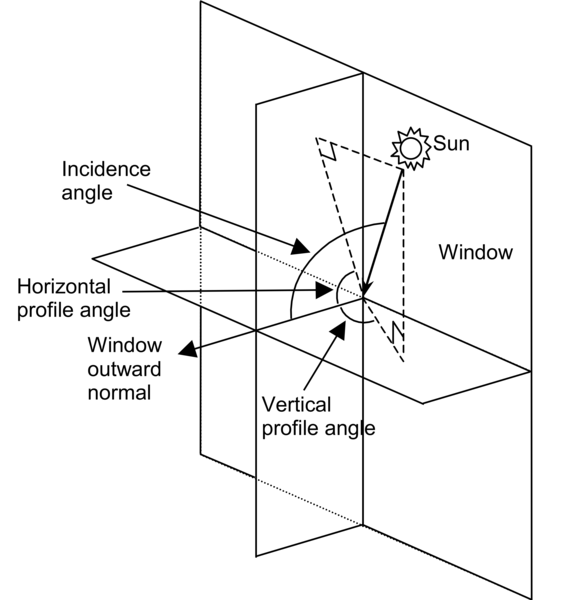
\includegraphics[width=0.9\textwidth, height=0.9\textheight, keepaspectratio=true]{media/image058.png}
\caption{Vertical exterior window showing solar horizontal profile angle, solar vertical profile angle and solar incidence angle. \protect \label{fig:vertical-exterior-window-showing-solar}}
\end{figure}

\subsubsection{Surface Window Outside Reveal Reflected Beam Solar Radiation Rate {[}W{]}}\label{surface-window-outside-reveal-reflected-beam-solar-radiation-rate-w}

\subsubsection{Surface Window Outside Reveal Reflected Beam Solar Radiation Energy {[}J{]}}\label{surface-window-outside-reveal-reflected-beam-solar-radiation-energy-j}

Beam solar radiation reflected from the outside reveal surfaces of a window (ref: Reveal Surfaces under WindowProperty:FrameAndDivider object). There are both rate and energy versions.

\subsubsection{Surface Window Inside Reveal Reflected Beam Solar Radiation Rate {[}W{]}}\label{surface-window-inside-reveal-reflected-beam-solar-radiation-rate-w}

\subsubsection{Surface Window Inside Reveal Reflected Beam Solar Radiation Energy {[}J{]}}\label{surface-window-inside-reveal-reflected-beam-solar-radiation-energy-j}

Beam solar radiation reflected from the inside reveal surfaces of a window (ref: Reveal Surfaces under WindowProperty:FrameAndDivider object). There are both rate and energy versions.

\subsubsection{Surface Window Inside Reveal Absorbed Beam Solar Radiation Rate {[}W{]}}\label{surface-window-inside-reveal-absorbed-beam-solar-radiation-rate-w}

Beam solar radiation absorbed at the inside reveal surfaces of a window, in Watts.

\subsubsection{Surface Window Inside Reveal Reflected Diffuse Zone Solar Radiation Rate {[}W{]}}\label{surface-window-inside-reveal-reflected-diffuse-zone-solar-radiation-rate-w}

Diffuse solar radiation reflected from inside reveal surfaces of a window into the zone, in Watts.

\subsubsection{Surface Window Inside Reveal Reflected Diffuse Frame Solar Radiation Rate {[}W{]}}\label{surface-window-inside-reveal-reflected-diffuse-frame-solar-radiation-rate-w}

Diffuse solar radiation reflected from inside reveal surfaces onto the frame surfaces of a window, in Watts.

\subsubsection{Surface Window Inside Reveal Reflected Diffuse Glazing Solar Radiation Rate {[}W{]}}\label{surface-window-inside-reveal-reflected-diffuse-glazing-solar-radiation-rate-w}

Diffuse solar radiation reflected from inside reveal surfaces onto the glazing surfaces of a window, in Watts.

\subsubsection{Surface Window Inside Face Glazing Condensation Status {[]}}\label{surface-window-inside-face-glazing-condensation-status}

A value of 1 means that moisture condensation will occur on the innermost glass face of an exterior window (i.e., on the glass face in contact with the zone air). Otherwise the value is 0. The condition for condensation is glass inside face temperature \textless{} zone air dewpoint temperature.

For airflow exterior windows, in which forced air passes between adjacent glass faces in double- and triple-pane windows, a value of 1 means that condensation will occur on one or both of the glass faces in contact with the airflow. In this case the condition for condensation is:

\begin{itemize}
\item
  \emph{For airflow source = indoorair}, temperature of either face in contact with airflow \textless{} zone air dewpoint temperature.
\item
  \emph{For airflow source = outdoorair}, temperature of either face in contact with airflow \textless{} outside air dewpoint temperature.
\end{itemize}

As for regular windows, the value will also be 1 if condensation occurs on the innermost glass face.

\subsubsection{Surface Window Inside Face Frame Condensation Status {[]}}\label{surface-window-inside-face-frame-condensation-status}

If an exterior window has a frame and the value of this flag is 1, condensation will occur on the inside surface of the frame. The condition for condensation is frame inside surface temperature \textless{} zone air dewpoint temperature.

\subsubsection{Surface Window Inside Face Divider Condensation Status {[]}}\label{surface-window-inside-face-divider-condensation-status}

If an exterior window has a divider and the value of this flag is 1, condensation will occur on the inside surface of the divider. The condition for condensation is divider inside surface temperature \textless{} zone air dewpoint temperature.

\subsubsection{Surface Shading Device Is On Time Fraction {[]}}\label{surface-shading-device-is-on-time-fraction}

The fraction of time that a shading device is on an exterior window. For a particular simulation timestep, the value is 0.0 if the shading device is off (or there is no shading device) and the value is 1.0 if the shading device is on. (It is assumed that the shading device, if present, is either on or off for the entire timestep.) If the shading device is switchable glazing, a value of 0.0 means that the glazing is in the unswitched (light colored) state, and a value of 1.0 means that the glazing is in the switched (dark colored) state.

For a time interval longer a timestep, this is the fraction of the time interval that the shading device is on. For example, take the case where the time interval is one hour and the timestep is 10 minutes. Then if the shading device is on for two timesteps in the hour and off for the other four timesteps, then the fraction of time that the shading device is on = 2/6 = 0.3333.

\subsubsection{Surface Window Blind Slat Angle {[}deg{]}}\label{surface-window-blind-slat-angle-deg}

For an exterior window with a blind, this is the angle in degrees between the glazing outward normal and the blind slat angle outward normal, where the outward normal points away from the front face of the slat. The slat angle varies from 0 to 180 deg. If the slat angle is 0 deg or 180 deg, the slats are parallel to the glazing and the slats are said to be ``closed''. If the slat angle is 90 deg, the slats are perpendicular to the glazing and the slats are said to be ``fully open''. See illustrations under WindowMaterial:Blind. For blinds with a fixed slat angle, the value reported here will be constant.

\subsubsection{Surface Window Blind Beam to Beam Solar Transmittance {[]}}\label{surface-window-blind-beam-to-beam-solar-transmittance}

For an exterior window with a blind, this is the fraction of exterior beam solar radiation incident on the blind that is transmitted through the blind as beam solar radiation when the blind is isolated (i.e., as though the window glass were not present). Depends on various factors, including slat angle, width, separation, and thickness, and horizontal solar profile angle (for blinds with horizontal slats) or vertical solar profile angle (for blinds with vertical slats). The transmittance value reported here will be non-zero only when some beam solar can pass through the blind without hitting the slats.

\subsubsection{Surface Window Blind Beam to Diffuse Solar Transmittance {[]}}\label{surface-window-blind-beam-to-diffuse-solar-transmittance}

For an exterior window with a blind, the fraction of exterior beam solar radiation incident on the blind that is transmitted through the blind as diffuse solar radiation when the blind is isolated (i.e., as though the window glass were not present). Depends on various factors, including slat angle, width, separation, thickness and reflectance, and horizontal solar profile angle (for blinds with horizontal slats) or vertical solar profile angle (for blinds with vertical slats).

\subsubsection{Surface Window Blind Diffuse to Diffuse Solar Transmittance {[]}}\label{surface-window-blind-diffuse-to-diffuse-solar-transmittance}

For an exterior window with a blind, the fraction of exterior diffuse solar radiation incident on the blind that is transmitted through the blind as diffuse solar radiation when the blind is isolated (i.e., as though the window glass were not present). Depends on various factors, including slat angle, width, separation, thickness and reflectance. For blinds with a fixed slat angle the transmittance value reported here will be constant.

\subsubsection{Surface Window Blind and Glazing System Beam Solar Transmittance {[]}}\label{surface-window-blind-and-glazing-system-beam-solar-transmittance}

The fraction of exterior beam solar radiation incident on an exterior window with a blind (excluding window frame, if present) that is transmitted through the blind/glass system as beam solar radiation. Depends on various factors, including type of glass; solar incidence angle; slat angle, width, separation, and thickness; and horizontal solar profile angle (for blinds with horizontal slats) or vertical solar profile angle (for blinds with vertical slats).

\subsubsection{Surface Window Blind and Glazing System Diffuse Solar Transmittance {[]}}\label{surface-window-blind-and-glazing-system-diffuse-solar-transmittance}

The fraction of exterior diffuse solar radiation incident on an exterior window with a blind (excluding window frame, if present) that is transmitted through the blind/glass system as diffuse solar radiation. Depends on various factors, including type of glass and slat angle, width, separation, thickness and reflectance. For blinds with a fixed slat angle the transmittance value reported here will be constant.

\subsubsection{Surface Window Screen Beam to Beam Solar Transmittance {[]}}\label{surface-window-screen-beam-to-beam-solar-transmittance}

For an exterior window with a screen, this is the fraction of exterior beam solar radiation incident on the screen that is transmitted through the screen as beam solar radiation when the screen is isolated (i.e., as though the window glass were not present). Depends on various factors, including the screen reflectance and the relative angle of the incident beam with respect to the screen. This value will include the amount of inward reflection of solar beam off the screen material surface if the user specifies this modeling option (i.e., Material: WindowScreen, field Reflected Beam Transmittance Accounting Method = Model as Direct Beam).

\subsubsection{Surface Window Screen Beam to Diffuse Solar Transmittance{[]}}\label{surface-window-screen-beam-to-diffuse-solar-transmittance}

For an exterior window with a screen, the fraction of exterior beam solar radiation incident on the screen that is transmitted through the screen as diffuse solar radiation when the screen is isolated (i.e., as though the window glass were not present). Depends on various factors, including the screen reflectance and the relative angle of the incident beam with respect to the screen. This value is the amount of inward reflection of solar beam off the screen material surface if the user specifies this modeling option (i.e., Material: WindowScreen, field Reflected Beam Transmittance Accounting Method = Model as Diffuse); otherwise, this value will be zero.

\subsubsection{Surface Window Screen Diffuse to Diffuse Solar Transmittance{[]}}\label{surface-window-screen-diffuse-to-diffuse-solar-transmittance}

For an exterior window with a screen, the fraction of exterior diffuse solar radiation incident on the screen that is transmitted through the screen as diffuse solar radiation when the screen is isolated (i.e., as though the window glass were not present). Depends on various factors including screen material geometry and reflectance. This value is calculated as an average, constant For a window with a screen, this value consists of diffuse radiation transmitted through the screen (gaps between the screen material) and diffuse radiation from diffuse-to-diffuse reflection from the screen material. For a window with a screen, this value consists of diffuse radiation transmitted through the screen (gaps between the screen material) and diffuse radiation from diffuse-to-diffuse reflection from the screen material.

\subsubsection{Surface Window Screen and Glazing System Beam Solar Transmittance{[]}}\label{surface-window-screen-and-glazing-system-beam-solar-transmittance}

The fraction of exterior beam solar radiation incident on an exterior window with a screen (excluding window frame, if present) that is transmitted through the screen/glass system as beam solar radiation. Depends on various factors, including the screen reflectance and the relative angle of the incident beam with respect to the screen. This value will include the amount of inward reflection of solar beam off the screen material surface if the user specifies this modeling option (i.e., Material: WindowScreen, field Reflected Beam Transmittance Accounting Method = Model as Direct Beam).

\subsubsection{Surface Window Screen and Glazing System Diffuse Solar Transmittance {[]}}\label{surface-window-screen-and-glazing-system-diffuse-solar-transmittance}

The fraction of exterior diffuse solar radiation incident on an exterior window with a screen (excluding window frame, if present) that is transmitted through the screen/glass system as diffuse solar radiation. Depends on various factors including screen material geometry and reflectance.

\subsubsection{Surface Window Transmitted Beam Solar Radiation Rate {[}W{]}}\label{surface-window-transmitted-beam-solar-radiation-rate-w-1}

\subsubsection{Surface Window Transmitted Beam Solar Radiation Energy {[}J{]}}\label{surface-window-transmitted-beam-solar-radiation-energy-j-1}

The beam solar radiation transmitted through an interior window. Calculated only if Solar Distribution = FullInteriorAndExterior in your Building input. The origin of this radiation is beam solar that enters through an exterior window in a zone and then passes through an interior window into the adjacent zone. The amount of this radiation depends on several factors, including sun position, intensity of beam solar incident on the exterior window (including effects of shadowing, if present), relative position of the exterior and interior window, and the size and transmittance of the windows. Note that if there are two or more exterior windows in a zone, then beam solar from one or more of them may pass through the same interior window. Likewise, if there are more than two or more interior windows in a zone then beam solar from a single exterior window may pass through one or more of the interior windows. There are both rate and energy versions of the output.

\subsubsection{Surface Storm Window On Off Status {[]}}\label{surface-storm-window-on-off-status}

Indicates whether a storm window glass layer is present (ref: StormWindow object). The value is \textbf{0} if the storm window glass layer is off, \textbf{1} if it is on, and \textbf{--1} if the window does not have an associated storm window. Applicable only to exterior windows and glass doors.

\subsubsection{Surface Inside Face Initial Transmitted Diffuse Transmitted Out Window Solar Radiation Rate {[}W{]}}\label{surface-inside-face-initial-transmitted-diffuse-transmitted-out-window-solar-radiation-rate-w}

As of Version 2.1, the diffuse solar transmitted through exterior windows that is initially distributed to another window in the zone and transmitted out of the zone through that window. For exterior windows, this transmitted diffuse solar is ``lost'' to the exterior environment For interior windows, this transmitted diffuse solar is distributed to heat transfer surfaces in the adjacent zone, and is part of the Surface Inside Face Initial Transmitted Diffuse Absorbed Solar Radiation Rate for these adjacent zone surfaces.

\subsubsection{Additional Window Outputs (Advanced)}\label{additional-window-outputs-advanced}

The following output variables for windows or glass doors are available when the user requests to display advanced output variables. These seven reports show the individual components that are combined to determine overall Surface Window Heat Gain Rate and/or Surface Window Heat Loss Rate (described above).

\subsubsection{Surface Window Inside Face Glazing Zone Convection Heat Gain Rate {[}W{]}}\label{surface-window-inside-face-glazing-zone-convection-heat-gain-rate-w}

The surface convection heat transfer from the glazing to the zone in watts. This output variable is the term called ``{[}Convective heat flow to the zone from the zone side of the glazing{]}'' under the description above for Surface Window Heat Gain Rate output variable. If the window has an interior shade or blind, then this is zero and the glazing's convection is included in the report called ``Surface Window Inside Face Gap between Shade and Glazing Zone Convection Heat Gain Rate''.

\subsubsection{Surface Window Inside Face Glazing Net Infrared Heat Transfer Rate {[}W{]}}\label{surface-window-inside-face-glazing-net-infrared-heat-transfer-rate-w}

The net exchange of infrared radiation heat transfer from the glazing to the zone in watts. This output variable is the term called ``{[}Net IR heat flow to the zone from zone side of the glazing{]}'' under the description above for Surface Window Heat Gain Rate output variable.

\subsubsection{Surface Window Shortwave from Zone Back Out Window Heat Transfer Rate {[}W{]}}\label{surface-window-shortwave-from-zone-back-out-window-heat-transfer-rate-w}

This is the short-wave radiation heat transfer from the zone back out the window in watts. This is a measure of the diffuse short-wave light (from reflected solar and electric lighting) that leave the zone through the window. This output variable is the term called ``{[}Short-wave radiation from zone transmitted back out the window{]}'' under the description above for Surface Window Heat Gain Rate output variable.

\subsubsection{Surface Window Inside Face Frame and Divider Zone Heat Gain Rate {[}W{]}}\label{surface-window-inside-face-frame-and-divider-zone-heat-gain-rate-w}

This is the heat transfer from any frames and/or dividers to the zone in watts. This output variable is the term called ``{[}Conduction to zone from window frame and divider, if present{]}'' under the description above for Surface Window Heat Gain Rate output variable. (The word ``conduction'' here is used because the models is simplified compared to the complexities of surface convection and radiation.)

\subsubsection{Surface Window Frame Heat Gain Rate {[}W{]}}\label{surface-window-frame-heat-gain-rate-w}

This is the positive heat flow from window frames to the zone in watts. This is part of the Surface Window Inside Face Frame and Divider Zone Heat Gain Rate.

\subsubsection{Surface Window Frame Heat Loss Rate {[}W{]}}\label{surface-window-frame-heat-loss-rate-w}

This is the negative heat flow from window frames to the zone in watts. This is part of the Surface Window Inside Face Frame and Divider Zone Heat Gain Rate.

\subsubsection{Surface Window Frame Inside Temperature {[}C{]}}\label{surface-window-frame-inside-temperature-c}

This is the temperature of the inside surface of the window frames.

\subsubsection{Surface Window Frame Outside Temperature {[}C{]}}\label{surface-window-frame-outside-temperature-c}

This is the temperature of the outside surface of the window frames.

\subsubsection{Surface Window Divider Heat Gain Rate {[}W{]}}\label{surface-window-divider-heat-gain-rate-w}

This is the positive heat flow from window dividers to the zone in watts. This is part of the Surface Window Inside Face Frame and Divider Zone Heat Gain Rate.

\subsubsection{Surface Window Divider Heat Loss Rate {[}W{]}}\label{surface-window-divider-heat-loss-rate-w}

This is the negative heat flow from window dividers to the zone in watts. This is part of the Surface Window Inside Face Frame and Divider Zone Heat Gain Rate.

\subsubsection{Surface Window Divider Inside Temperature {[}C{]}}\label{surface-window-divider-inside-temperature-c}

This is the temperature of the inside surface of the window dividers.

\subsubsection{Surface Window Divider Outside Temperature {[}C{]}}\label{surface-window-divider-outside-temperature-c}

This is the temperature of the outside surface of the window dividers.

\subsubsection{Surface Window Inside Face Gap between Shade and Glazing Zone Convection Heat Gain Rate {[}W{]}}\label{surface-window-inside-face-gap-between-shade-and-glazing-zone-convection-heat-gain-rate-w}

This is the convection surface heat transfer from the both the glazing and the shade's back face to the zone in Watts. This output variable is the term called ``{[}Convective heat flow to the zone from the air flowing through the gap between glazing and shading device{]}'' under the description above for Surface Window Heat Gain Rate output variable. For Equivalent Layer window this output variable is the convection heat gain from vented interior air gap to the zone in Watts.

\subsubsection{Surface Window Inside Face Shade Zone Convection Heat Gain Rate {[}W{]}}\label{surface-window-inside-face-shade-zone-convection-heat-gain-rate-w}

This is the convection surface heat transfer from the front side of any interior shade or blind to the zone in Watts. This output variable is the term called ``{[}Convective heat flow to the zone from the zone side of the shading device{]}'' under the description above for Surface Window Heat Gain Rate output variable. For equivalent Layer window this output variable is the convection heat gain rate from the inside face of a glazing or a shade to the zone in Watts.

\subsubsection{Surface Window Inside Face Shade Net Infrared Heat Transfer Rate {[}W{]}}\label{surface-window-inside-face-shade-net-infrared-heat-transfer-rate-w}

The net exchange of infrared radiation heat transfer from the shade or blind to the zone in watts. This output variable is the term called ``{[}Net IR heat flow to the zone from the zone side of the shading device{]}'' under the description above for Surface Window Heat Gain Rate output variable.

\subsubsection{Surface Window Inside Face Other Convection Heat Gain Rate {[}W{]}}\label{surface-window-inside-face-other-convection-heat-gain-rate-w}

The other (extra) convection heat transfer rate from the inside face of a an equivalent layer window. This output is computed from the difference in convection flux when using equivalent inside surface temperature of a window instead of the inside surface temperature from the standard surface heat balance calculation.

\subsection{Thermochromic Window Outputs}\label{thermochomic-window-outputs}

\subsubsection{Window Thermochromic Layer Temperature {[}C{]}}\label{window-thermochromic-layer-temperature-c}

The temperature of the TC glass layer of a TC window at each time step.

\subsubsection{Surface Window Thermochromic Layer Property Specification Temperature {[}C{]}}\label{surface-window-thermochromic-layer-property-specification-temperature-c-000}

The temperature under which the optical data of the TC glass layer are specified.

The overall properties (U-factor/SHGC/VT) of the thermochromic windows at different specification temperatures are reported in the \textbf{.eio} file. These window constructions are created by EnergyPlus during run time. They have similar names with suffix ``\_TC\_XX'' where XX represents a specification temperature.

\subsubsection{Switchable Window Outputs}\label{switchable-window-outputs}

\subsubsection{Surface Window Switchable Glazing Switching Factor{[]}}\label{surface-window-switchable-glazing-switching-factor}

The switching factor (tint level) of the switchable window: 0 means no switching -- clear state; 1 means fully switched -- dark state.

\subsubsection{Surface Window Switchable Glazing Visible Transmittance{[]}}\label{surface-window-switchable-glazing-visible-transmittance}

The visible transmittance of the switchable window.

\subsection{Other Surface Outputs/Reports}\label{other-surface-outputsreports}

Several reports can be selected for Surfaces. (See Group -- Report for details on how to specify). Examples are:

\subsubsection{DXF}\label{dxf}

This report produces a special file (\textbf{eplusout.dxf}) in the industry standard DXF (Drawing Interchange Format) for drawings. It is produced and accepted by many popular, commercial CAD programs. Detailed reference can be found on the AutoCAD™ website at: \url{http://www.autodesk.com/techpubs/autocad/acadr14/dxf/index.htm}.

EnergyPlus produces this file from the Report command:

\begin{lstlisting}

Output:Reports, Surfaces, DXF;
\end{lstlisting}

\subsubsection{Details, Vertices, DetailsWithVertices}\label{details-vertices-detailswithvertices}

This version of the report creates lines in the eplusout.eio file for each surface (except internal mass surfaces). Details of this reporting is shown in the Output Details and Examples document.

\subsection{Shading Surfaces}\label{shading-surfaces}

Shading surfaces are entities outside of the building that may cast shadows on the building's heat transfer surfaces. These entities do not typically have enough thermal mass to be described as part of the building's thermal makeup.

The most important effect of shading surfaces is to reduce solar gain in windows that are shadowed. (However, in some cases, shading surfaces can reflect solar onto a wall or window and increase solar gain.)

There are two kinds of shading surfaces in EnergyPlus: \textbf{detached} and \textbf{attached}. A \textbf{detached} shading surface, such as a tree or neighboring building, is not connected to the building. An \textbf{attached} shading surface is typically an overhang or fin that is attached to a particular base surface of the building, usually a wall; attached shading surfaces are usually designed to shade specific windows.

Objects for detached shading surfaces:

\begin{itemize}
\item
  Shading:Site
\item
  Shading:Building
\item
  Shading:Site:Detailed
\item
  Shading:Building:Detailed
\end{itemize}

Similarly to the surfaces, the detailed objects use vertex entry whereas the other objects are limited to rectangular representation.

Objects for attached shading surfaces:

\begin{itemize}
\item
  Shading:Overhang
\item
  Shading:Overhang:Projection
\item
  Shading:Fin
\item
  Shading:Fin:Projection
\item
  Shading:Zone:Detailed
\end{itemize}

EnergyPlus creates ``bi-directional'' shades from each shading surface entered. This means that the shade you input will cast a shadow no matter which side of the shade the sun is on. For example, a vertical fin will cast a shadow whether the sun is on the left side or right side of the fin. Prior to V1.0.2, a shading surface cast a shadow only in the hemisphere toward which the surface faced. This hemisphere is the one pointed to by the shading surface's outward normal vector, which is the cross product V23 x V21, where V23 is the vector from vertex 2 to vertex 3 of the shading surface and V21 is the vector from vertex 2 to vertex 1. Beginning with V1.0.2, the shades in EnergyPlus are ``bi-directional'' so that they can cast shadows in both hemispheres depending on the time-varying position of the sun relative to the shading surface.

It is important to note that EnergyPlus will automatically account for ``self-shading'' effects---such as in L-shaped buildings---in which some of the building's wall and roof surfaces shade other parts of the building, especially windows. This means that you only need to describe shading elements that aren't building heat-transfer surfaces.

Shading surfaces can also \textbf{reflect} solar radiation onto the building. This feature is simulated if you choose FullExteriorWithReflections or FullInteriorAndExteriorWithReflections in the Building object (ref: Building - Field: Solar Distribution). In this case, you may specify the reflectance properties of a shading surface with the ShadingProperty:Reflectance object. Note: If no ShadingProperty:Reflectance object is defined, then the shading surface reflectance values are assumed to be 0.2 and the fraction of shading surface that is glazed is assumed to be 0.0.

Shading surfaces also automatically shade diffuse solar radiation (and long-wave radiation) from the sky. And they will automatically shade diffuse solar radiation from the ground if Solar Distribution Field = FullExteriorWithReflections or FullInteriorAndExteriorWithReflections in the Building object. (If the reflections option for Solar Distribution is used, the program also takes into account the reduction of solar radiation reflected from the ground due to shading of the ground by shading surfaces and by the building itself.) Otherwise, shading surfaces will not shade diffuse radiation from the ground unless you enter a reduced value for View Factor to Ground for those building surfaces that are shaded (ref: BuildingSurface:Detailed - Field: View Factor to Ground and FenestrationSurface:Detailed - Field: View Factor to Ground).

\subsection{Detached Shading Surfaces}\label{detached-shading-surfaces}

\subsection{Shading:Site, Shading:Building}\label{shadingsite-shadingbuilding}

These objects are used to describe rectangular shading elements that are external to the building. Examples are trees, high fences, near-by hills, and neighboring buildings.

If relative coordinates are used (ref: Field: Coordinate System in GlobalGeometryRules), shading surfaces entered with Shading:Site remain stationary if the building is rotated, whereas those entered with Shading:Building rotate with the building. If world coordinates are used Shading:Site and Shading:Building are equivalent.

These shading elements are always opaque.

\subsubsection{Field: Name}\label{field-name-22-004}

This is a unique character string associated with the detached shading surface. Though it must be unique from other surface names, it is used primarily for convenience with detached shading surfaces.

\subsubsection{Field: Azimuth Angle}\label{field-azimuth-angle-10}

Theoretically, this should face to the surface it is shading (i.e.~if a south wall, this should be a north facing shade) but since EnergyPlus automatically generates the mirror image, the facing angle per se' is not so important.

\subsubsection{Field: Tilt Angle}\label{field-tilt-angle-10}

The tilt angle is the angle (in degrees) that the shade is tilted from horizontal (or the ground). Default for this field is 90 degrees.

\subsubsection{Starting Corner for the surface}\label{starting-corner-for-the-surface-16}

The rectangular surfaces specify the lower left corner of the surface for their starting coordinate. See the introductory paragraph for rules on this entry.

\subsubsection{Field: Starting X Coordinate}\label{field-starting-x-coordinate-16}

This field is the X coordinate (in meters).

\subsubsection{Field: Starting Y Coordinate}\label{field-starting-y-coordinate-10}

This field is the Y coordinate (in meters).

\subsubsection{Field: Starting Z Coordinate}\label{field-starting-z-coordinate-16}

This field is the Z coordinate (in meters).

\subsubsection{Field: Length}\label{field-length-16}

This field is the length of the shade in meters.

\subsubsection{Field: Height}\label{field-height-10}

This field is the width of the shade in meters.

Examples of these (can be found in example files 4ZoneWithShading\_Simple\_1.idf and 4ZoneWithShading\_Simple\_2.idf)

\begin{lstlisting}

  Shading:Building,
      Bushes-East,             !- Name
      90,                      !- Azimuth Angle {deg}
      90,                      !- Tilt Angle {deg}
      45,                      !- Starting X Coordinate {m}
      0,                       !- Starting Y Coordinate {m}
      0,                       !- Starting Z Coordinate {m}
      50,                      !- Length {m}
      1;                       !- Height {m}

    Shading:Site,
      Bushes-North,            !- Name
      0,                       !- Azimuth Angle {deg}
      90,                      !- Tilt Angle {deg}
      45,                      !- Starting X Coordinate {m}
      50,                      !- Starting Y Coordinate {m}
      0,                       !- Starting Z Coordinate {m}
      50,                      !- Length {m}
      1;                       !- Height {m}
\end{lstlisting}

\subsection{Shading:Site:Detailed, Shading:Building:Detailed}\label{shadingsitedetailed-shadingbuildingdetailed}

These objects are used to describe shading elements that are external to the building. Examples are trees, high fences, near-by hills, and neighboring buildings.

If relative coordinates are used (ref: Field: Coordinate System in GlobalGeometryRules), shading surfaces entered with Shading:Site:Detailed remain stationary if the building is rotated, whereas those entered with Shading:Building:Detailed rotate with the building. If world coordinates are used Shading:Site:Detailed and Shading:Building:Detailed are equivalent.

While ``detached'' implies that shading surfaces are not part of the building, the detached shading sequence can be used to describe attached shading surfaces that may shade heat transfer surfaces in more than one zone. For example, wing A of a building might shade several zones of wing B but wing A (for whatever reason) is not described in the geometry for the simulation so it is represented by a detached shade to get its shadowing effect.

\subsubsection{Field: Name}\label{field-name-23-004}

This is a unique character string associated with the detached shading surface. Though it must be unique from other surface names, it is used primarily for convenience with detached shading surfaces.

\subsubsection{Field: Transmittance Schedule Name}\label{field-transmittance-schedule-name}

The name of a schedule of solar transmittance values from 0.0 to 1.0 for the shading surface. If a blank is entered in this field, the transmittance value defaults to 0.0, i.e., the shading surface is opaque at all times. This scheduling can be used to allow for seasonal transmittance change, such as for deciduous trees that have a higher transmittance in winter than in summer. Transmittance based on time of day can also be used---a movable awning, for example, where the transmittance is some value less than 1.0 when the awning is in place and is 1.0 when the awning is retracted.

The following assumptions are made in the shading surface transmittance calculation:

\begin{itemize}
\item
  Both sides of the shading surface have the same transmittance properties.
\item
  The transmittance is the same for both beam and diffuse solar radiation.
\item
  Beam solar transmittance is independent of angle of incidence on the shading surface.
\item
  Beam radiation incident on a shading surface is transmitted as beam radiation with no change in direction, i.e., there is no beam-to-diffuse component.
\item
  If two shading surfaces with non-zero transmittance overlap, the net transmittance is the product of the individual transmittances. Inter-reflection between the shading surfaces (and between the shading surfaces and the building) is ignored.
\item
  For the daylighting calculation (ref: Group -- Daylighting) the shading surface's visible transmittance is assumed to be the same as its solar transmittance.
\item
  Shading devices are assumed to be opaque to long-wave radiation no matter what the solar transmittance value is.
\end{itemize}

Note that shading devices only shade solar radiation when the sun is up, which is automatically determined by EnergyPlus from latitude, time of year, etc. The user need only account for the time-varying transmittance of the shading device in the transmittance schedule, not whether the sun is up or not.

\subsubsection{Field: Number Vertices}\label{field-number-vertices}

The number of sides in the surface (number of X,Y,Z vertex groups). For further information, see the discussion on ``Surface Vertices'' above.

IDF example of Detached Shading Surfaces:

\begin{lstlisting}

Shading:Building:Detailed,
     EAST SIDE TREE,  !- Detached Shading
     ShadingTransmittance:0002,  !- Shadowing Transmittance & Schedule
     3, !-Triangle
     33.52800    ,   10.66800    ,   10.05800    ,
     33.52800    ,   13.71600    ,  0.9140000    ,
     33.52800    ,   4.572000    ,  0.9140000    ;

  Shading:Building:Detailed,
     WEST SIDE TREE,  !- Detached Shading
     ShadingTransmittance:0002,  !- Shadowing Transmittance & Schedule
     3, !-Triangle
    -3.048000    ,   7.620000    ,   10.05800    ,
    -3.048000    ,   4.572000    ,  0.9140000    ,
    -3.048000    ,   13.71600    ,  0.9140000    ;
\end{lstlisting}

\subsection{Attached Shading Surfaces}\label{attached-shading-surfaces}

Overhangs are usually horizontal devices that are used to shade windows. Fins are usually vertical devices that similarly shade windows.

\subsection{Shading:Overhang}\label{shadingoverhang}

An overhang typically is used to shade a window in a building.

\subsubsection{Inputs}\label{inputs-26-003}

\paragraph{Field: Name}\label{field-name-24-003}

This is the name of the overhang. It must be different from other surface names.

\paragraph{Field: Window or Door Name}\label{field-window-or-door-name}

The name of a window or door that this overhang shades.

\paragraph{Field: Height above Window or Door}\label{field-height-above-window-or-door}

This field is the height (meters) above the top of the door for the overhang.

\paragraph{Field Tilt Angle from Window/Door}\label{field-tilt-angle-from-windowdoor}

This field is the tilt angle from the Window/Door. For a flat overhang, this would be 90 (degrees).

\paragraph{Field: Left Extension from Window/Door Width}\label{field-left-extension-from-windowdoor-width}

This field is the width from the left edge of the window/door to the start of the overhang (meters).

\paragraph{Field: Right Extension from Window/Door Width}\label{field-right-extension-from-windowdoor-width}

This field is the width from the right edge of the window/door to the start of the overhang (meters).

\paragraph{Field: Depth}\label{field-depth}

This field is the depth of the overhang (meters) projecting out from the wall.

\subsection{Shading:Overhang:Projection}\label{shadingoverhangprojection}

An overhang typically is used to shade a window in a building. This object allows for specifying the depth of the overhang as a fraction of the window or door's height.

\subsubsection{Inputs}\label{inputs-27-003}

\paragraph{Field: Name}\label{field-name-25-003}

This is the name of the overhang. It must be different from other surface names.

\paragraph{Field: Window or Door Name}\label{field-window-or-door-name-1}

The name of a window or door that this overhang shades.

\paragraph{Field: Height above Window or Door}\label{field-height-above-window-or-door-1}

This field is the height (meters) above the top of the door for the overhang.

\paragraph{Field Tilt Angle from Window/Door}\label{field-tilt-angle-from-windowdoor-1}

This field is the tilt angle from the Window/Door. For a flat overhang, this would be 90 (degrees).

\paragraph{Field: Left Extension from Window/Door Width}\label{field-left-extension-from-windowdoor-width-1}

This field is the width from the left edge of the window/door to the start of the overhang (meters).

\paragraph{Field: Right Extension from Window/Door Width}\label{field-right-extension-from-windowdoor-width-1}

This field is the width from the right edge of the window/door to the start of the overhang (meters).

\paragraph{Field: Depth as Fraction of Window/Door Height}\label{field-depth-as-fraction-of-windowdoor-height}

This field is the fraction of the window/door height to specify as the depth of the overhang (meters) projecting out from the wall.

\subsection{Shading:Fin}\label{shadingfin}

Fins shade either side of windows/doors in a building. This object allows for specification of both fins for the window. Fin placement is relative to the edge of the glass and user must include the frame width when a frame is present.

\subsubsection{Inputs}\label{inputs-28-002}

\paragraph{Field: Name}\label{field-name-26-003}

This is the name of the overhang. It must be different from other surface names.

\paragraph{Field: Window or Door Name}\label{field-window-or-door-name-2}

The name of a window or door that this overhang shades.

\paragraph{Field: Left Fin Extension from Window/Door}\label{field-left-fin-extension-from-windowdoor}

This field is the width from the left edge of the window/door to the plane of the left fin (meters). The extension width is relative to the edge of the glass and includes the frame width when a frame is present.

\paragraph{Field: Left Fin Distance Above Top of Window}\label{field-left-fin-distance-above-top-of-window}

This field is the distance from the top of the window to the top of the left fin (meters) and is relative to the edge of the glass and includes the frame width when a frame is present.

\paragraph{Field: Left Fin Distance Below Bottom of Window}\label{field-left-fin-distance-below-bottom-of-window}

This field is the distance from the bottom of the window to the bottom of the left fin (meters) and is relative to the edge of the glass and includes the frame width when a frame is present.

\paragraph{Field: Left Fin Tilt Angle from Window/Door}\label{field-left-fin-tilt-angle-from-windowdoor}

This field is the tilt angle from the window / door for the left fin. Typically, a fin is 90 degrees (default) from its associated window/door.

\paragraph{Field: Left Fin Depth}\label{field-left-fin-depth}

This field is the depth (meters) of the left fin (projecting out from the wall).

\paragraph{Field: Right Fin Extension from Window/Door}\label{field-right-fin-extension-from-windowdoor}

This field is the width from the right edge of the window/door to the plane of the right fin (meters). The extension width is relative to the edge of the glass and includes the frame width when a frame is present.

\paragraph{Field: Right Fin Distance Above Top of Window}\label{field-right-fin-distance-above-top-of-window}

This field is the distance from the top of the window to the top of the right fin (meters) and is relative to the edge of the glass and includes the frame width when a frame is present.

\paragraph{Field: Right Fin Distance Below Bottom of Window}\label{field-right-fin-distance-below-bottom-of-window}

This field is the distance from the bottom of the window to the bottom of the right fin (meters) and is relative to the edge of the glass and includes the frame width.

\paragraph{Field: Right Fin Tilt Angle from Window/Door}\label{field-right-fin-tilt-angle-from-windowdoor}

This field is the tilt angle from the window / door for the right fin. Typically, a fin is 90 degrees (default) from its associated window/door.

\paragraph{Field: Right Fin Depth}\label{field-right-fin-depth}

This field is the depth (meters) of the right fin (projecting out from the wall).

\subsection{Shading:Fin:Projection}\label{shadingfinprojection}

Fins shade either side of windows/doors in a building. This object allows for specification of both fins for the window. This object allows for specifying the depth of the overhang as a fraction of the window or door's width. Fin placement is relative to the edge of the glass and user must include the frame width when a frame is present.

\subsubsection{Inputs}\label{inputs-29-002}

\paragraph{Field: Name}\label{field-name-27-003}

This is the name of the overhang. It must be different from other surface names.

\paragraph{Field: Window or Door Name}\label{field-window-or-door-name-3}

The name of a window or door that this overhang shades.

\paragraph{Field: Left Fin Extension from Window/Door}\label{field-left-fin-extension-from-windowdoor-1}

This field is the width from the left edge of the window/door to the plane of the left fin (meters). The extension width is relative to the edge of the glass and includes the frame width when a frame is present.

\paragraph{Field: Left Fin Distance Above Top of Window}\label{field-left-fin-distance-above-top-of-window-1}

This field is the distance from the top of the window to the top of the left fin (meters) and is relative to the edge of the glass and includes the frame width when a frame is present.

\paragraph{Field: Left Fin Distance Below Bottom of Window}\label{field-left-fin-distance-below-bottom-of-window-1}

This field is the distance from the bottom of the window to the bottom of the left fin (meters) and is relative to the edge of the glass and includes the frame width when a frame is present.

\paragraph{Field: Left Fin Tilt Angle from Window/Door}\label{field-left-fin-tilt-angle-from-windowdoor-1}

This field is the tilt angle from the window / door for the left fin. Typically, a fin is 90 degrees (default) from its associated window/door.

\paragraph{Field: Left Fin Depth as Fraction of Window/Door Width}\label{field-left-fin-depth-as-fraction-of-windowdoor-width}

This field is the fraction of the window/door width to specify as the depth of the left fin (meters) projecting out from the wall.

\paragraph{Field: Right Fin Extension from Window/Door}\label{field-right-fin-extension-from-windowdoor-1}

This field is the width from the right edge of the window/door to the plane of the right fin (meters).. The extension width is relative to the edge of the glass and includes the frame width when a frame is present.

\paragraph{Field: Right Fin Distance Above Top of Window}\label{field-right-fin-distance-above-top-of-window-1}

This field is the distance from the top of the window to the top of the right fin (meters) and is relative to the edge of the glass and includes the frame width when a frame is present.

\paragraph{Field: Right Fin Distance Below Bottom of Window}\label{field-right-fin-distance-below-bottom-of-window-1}

This field is the distance from the bottom of the window to the bottom of the right fin (meters) and is relative to the edge of the glass and includes the frame width when a frame is present.

\paragraph{Field: Right Fin Tilt Angle from Window/Door}\label{field-right-fin-tilt-angle-from-windowdoor-1}

This field is the tilt angle from the window / door for the right fin. Typically, a fin is 90 degrees (default) from its associated window/door.

\paragraph{Field: Right Fin Depth as Fraction of Window/Door Width}\label{field-right-fin-depth-as-fraction-of-windowdoor-width}

This field is the fraction of the window/door width to specify as the depth of the right fin (meters) projecting out from the wall.

zone.

Examples of these (can be found in example files 4ZoneWithShading\_Simple\_1.idf and 4ZoneWithShading\_Simple\_2.idf)

\begin{lstlisting}

  Shading:Overhang:Projection,
      Zn001:Wall001:Win001:Shade001,  !- Name
      Zn001:Wall001:Win001,    !- Window or Door Name
      .7,                      !- Height above Window or Door {m}
      90,                      !- Tilt Angle from Window/Door {deg}
      .2,                      !- Left extension from Window/Door Width {m}
      .2,                      !- Right extension from Window/Door Width {m}
      .6;                      !- Depth as Fraction of Window/Door Height {m}

    Shading:Overhang,
      Zn001:Wall001:Door001:Shade001,  !- Name
      Zn001:Wall001:Door001,   !- Window or Door Name
      .6,                      !- Height above Window or Door {m}
      90,                      !- Tilt Angle from Window/Door {deg}
      0,                       !- Left extension from Window/Door Width {m}
      0,                       !- Right extension from Window/Door Width {m}
      3;                       !- Depth {m}

    Shading:Fin:Projection,
      Zn001:Wall001:Shade003,  !- Name
      Zn001:Wall001:Win001,    !- Window or Door Name
      .1,                      !- Left Extension from Window/Door {m}
      .1,                   !- Left Distance Above Top of Window {m}
      .1,                   !- Left Distance Below Bottom of Window {m}
      90,                   !- Left Tilt Angle from Window/Door {deg}
      .6,                   !- Left Depth as Fraction of Window/Door Width {m}
      .1,                   !- Right Extension from Window/Door {m}
      .1,                   !- Right Distance Above Top of Window {m}
      .1,                   !- Right Distance Below Bottom of Window {m}
      90,                   !- Right Tilt Angle from Window/Door {deg}
      .6;                   !- Right Depth as Fraction of Window/Door Width {m}
\end{lstlisting}

\subsection{Shading:Zone:Detailed}\label{shadingzonedetailed-000}

This object is used to describe attached ``subsurfaces'' such as overhangs, wings or fins that project outward from a base surface. This classification is used for convenience; actually, a device of this type can cast shadows on the surface to which it is attached as well as on adjacent surfaces. For example, a fin may shade its parent wall as well as adjacent walls.

Note that a zone surface can cast shadows on other zone surfaces. However, you don't have to worry about such effects---for example, one wall of an L-shaped building shading another wall--because EnergyPlus will automatically check for this kind of ``self shadowing'' and do the proper calculations.

Unlike attached (or detached) shading surfaces, building surfaces can only cast shadows in the hemisphere towards which they face. This means, for example, that a roof that faces \emph{upward} will not cast a shadow \emph{downward}. (Thus, specifying an oversized roof in an attempt to account for the shading effects of overhangs will \emph{not} work). Interior surfaces do not cast shadows of any kind.

\subsubsection{Inputs}\label{inputs-30-002}

\paragraph{Field: Name}\label{field-name-28-002}

This is the name of the attached shading surface. It must be different from other surface names.

\paragraph{Field: Base Surface Name}\label{field-base-surface-name}

This is the name of the surface to which this shading device is attached. This surface can be a wall (or roof) but not a window or door.

\paragraph{Field: Transmittance Schedule Name}\label{field-transmittance-schedule-name-1}

The name of a schedule of solar transmittance values from 0.0 to 1.0 for the shading surface. If a blank is entered in this field, the transmittance value defaults to 0.0, i.e., the shading surface is opaque at all times. This scheduling can be used to allow for seasonal transmittance change, such as for deciduous trees that have a higher transmittance in winter than in summer. Transmittance based on time of day can also be used---a movable awning, for example, where the transmittance is some value less than 1.0 when the awning is in place and is 1.0 when the awning is retracted.

The following assumptions are made in the shading surface transmittance calculation:

\begin{itemize}
\item
  Both sides of the shading surface have the same transmittance properties.
\item
  The transmittance is the same for both beam and diffuse solar radiation.
\item
  Beam solar transmittance is independent of angle of incidence on the shading surface.
\item
  Beam radiation incident on a shading surface is transmitted as beam radiation with no change in direction, i.e., there is no beam-to-diffuse component.
\item
  If two shading surfaces with non-zero transmittance overlap, the net transmittance is the product of the individual transmittances. Inter-reflection between the shading surfaces (and between the shading surfaces and the building) is ignored.
\item
  For the daylighting calculation (ref: Group -- Daylighting) the shading surface's visible transmittance is assumed to be the same as its solar transmittance.
\item
  Shading devices are assumed to be opaque to long-wave radiation no matter what the solar transmittance value is.
\end{itemize}

Note that shading devices only shade solar radiation when the sun is up, which is automatically determined by EnergyPlus from latitude, time of year, etc. The user need only account for the time-varying transmittance of the shading device in the transmittance schedule, not whether the sun is up or not.

\paragraph{Field: Number Vertices}\label{field-number-vertices-1}

The number of sides in the surface (number of X,Y,Z vertex groups). For further information, see the discussion on ``Surface Vertices'' above. The example below shows the correct input for an overhang (to shade the appropriate portion of the base wall and window).

\begin{figure}[hbtp] % fig 33
\centering
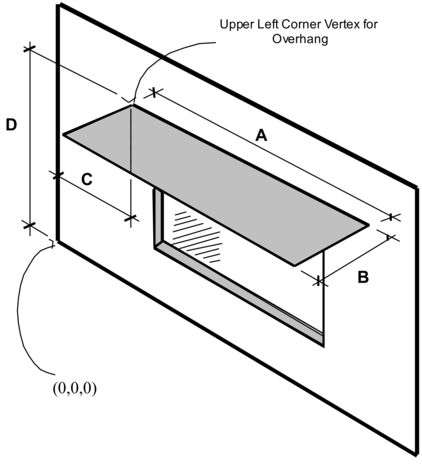
\includegraphics[width=0.9\textwidth, height=0.9\textheight, keepaspectratio=true]{media/image059.png}
\caption{Illustration for Attached Shading Surface \protect \label{fig:illustration-for-attached-shading-surface}}
\end{figure}

Proper specification for this overhang (facing up) is:

4,(C,0,D),(C,-B,D),(C+A,-B,D),(C+A,0,D); () used to illustrate each vertex.

\begin{callout}
Note that for horizontal surfaces, any corner may be chosen as the starting corner. The order of vertices determines whether the surface is facing up or down. Shading surfaces are mirrored automatically unless the user specifies ``DoNotMirrorDetachedShading'', so each shading surface need only be described once.
\end{callout}

Thus, another shading surface will be created (facing down):

4,(C+A,-B,D),(C+A,0,D),(C,0,D),(C,-B,D);

IDF example of attached shading surfaces (overhang, fin):

\begin{lstlisting}
Shading:Zone:Detailed,
  Zn001:Wall001:Shade001,       !- Surface Name
  Zn001:Wall001,                !- Base Surface Name
  ShadingTransmittance:0001,    !- Shadowing Transmittance Schedule
  4,                            !-RectangularOverhang
  1.524000 , -0.3050000    , 2.865000,
  1.524000 ,  0.0000000E+00, 2.865000,
  4.572000 ,  0.0000000E+00, 2.865000,
  4.572000 , -0.3050000    , 2.865000;

Shading:Zone:Detailed,
  Zn003:Wall001:Shade001,       !- Surface Name
  Zn003:Wall001,                !- Base Surface Name
  ShadingTransmittance:0001,    !- Shadowing Transmittance Schedule
  4,                            !-RectangularLeftFin
  57.97000 ,   8.450000    ,10.00000      ,
  57.97000 ,   8.450000    , 0.0000000E+00,
  57.97000 ,   6.450000    , 0.0000000E+00,
  57.97000 ,   6.450000    ,10.00000      ;

Shading:Zone:Detailed,
  Zn003:Wall001:Shade002,       !- Surface Name
  Zn003:Wall001,                !- Base Surface Name
  ShadingTransmittance:0003,    !- Shadowing Transmittance Schedule
  4,                            !-RectangularRightFin
  77.97000 ,   6.450000    ,10.00000      ,
  77.97000 ,   6.450000    , 0.0000000E+00,
  77.97000 ,   8.450000    , 0.0000000E+00,
  77.97000 ,   8.450000    ,10.00000      ;
\end{lstlisting}

\subsection{ShadingProperty:Reflectance}\label{shadingpropertyreflectance}

Specifies the reflectance properties of a shading surface when the solar reflection calculation has requested, i.e., when if ``WithReflections'' option is chosen in the Building object (ref: Building - Field: Solar Distribution). It is assumed that shading surfaces are divided into an unglazed, diffusely reflecting portion and a glazed, specularly-reflecting portion, either of which may be zero. The reflectance properties are assumed to be the same on both sides of the shading surface.

Note that a shadowing transmittance schedule (ref: Shading Surfaces, Field: Transmittance Schedule Name) can be used with a reflective shading surface. However, EnergyPlus assumes that the reflectance properties of the shading surface are constant even if the transmittance varies.

If no ShadingProperty:Reflectance objects are entered, the default values shown here will be used for shading surfaces. Other surfaces have their reflectance properties defined by the materials in the outer layers of the constructions.

\subsubsection{Inputs}\label{inputs-31-002}

\paragraph{Field: Shading Surface Name}\label{field-shading-surface-name}

The name of the Shading:Site, Shading:Building, Shading:Site:Detailed, Shading:Building:Detailed, Shading:Overhang, Shading:Overhang:Projection, Shading:Fin, Shading:Fin:Projection or Shading:Zone:Detailed object to which the following fields apply.

If this ShadingProperty:Reflectance object is not defined for a shading surface the default values listed in each of the following fields will be used in the solar reflection calculation.

\paragraph{Field: Diffuse Solar Reflectance of Unglazed Part of Shading Surface}\label{field-diffuse-solar-reflectance-of-unglazed-part-of-shading-surface}

The diffuse solar reflectance of the unglazed part of the shading surface (default = 0.2). This reflectance is assumed to be the same for beam-to-diffuse and diffuse-to-diffuse reflection. Beam-to-diffuse reflection is assumed to be independent of angle of incidence of beam radiation. Diffuse-to-diffuse reflection is assumed to be independent of angular distribution of the incident of diffuse radiation. The outgoing diffuse radiation is assumed to be isotropic (hemispherically uniform).

The sum of this reflectance and the shading surface transmittance should be less than or equal to 1.0.

\paragraph{Field: Diffuse Visible Reflectance of Unglazed Part of Shading Surface}\label{field-diffuse-visible-reflectance-of-unglazed-part-of-shading-surface}

The diffuse visible reflectance of the unglazed part of the shading surface (default = 0.2). This reflectance is assumed to be the same for beam-to-diffuse and diffuse-to-diffuse reflection. Beam-to-diffuse reflection is assumed to be independent of angle of incidence of beam radiation. Diffuse-to-diffuse reflection is assumed to be independent of angular distribution of the incident of diffuse radiation. The outgoing diffuse radiation is assumed to be isotropic (hemispherically uniform).

This value if used only for the daylighting calculation (ref: Daylighting:Controls). The sum of this reflectance and the shading surface transmittance should be less than or equal to 1.0.

\paragraph{Field: Fraction of Shading Surface That Is Glazed}\label{field-fraction-of-shading-surface-that-is-glazed}

The fraction of the area of the shading surface that consists of windows (default = 0.0). It is assumed that the windows are evenly distributed over the surface and have the same glazing construction (see following ``Name of Glazing Construction''). This might be the case, for example, for reflection from the façade of a neighboring, highly-glazed building. For the reflection calculation the possible presence of shades, screens or blinds on the windows of the shading surface is ignored. Beam-to-beam (specular) reflection is assumed to occur only from the glazed portion of the shading surface. This reflection depends on angle of incidence as determined by the program from the glazing construction. Beam-to-diffuse reflection from the glazed portion is assumed to be zero. The diffuse-to-diffuse reflectance of the glazed portion is determined by the program from the glazing construction.

\paragraph{Field: Glazing Construction Name}\label{field-glazing-construction-name}

The name of the construction of the windows on the shading surface. Required if Fraction of Shading Surface That Is Glazed is greater than 0.0.

IDF example of Shading Surface Reflectance for shading surface with specular reflection

\begin{lstlisting}

Shading:Site:Detailed,
  Adjacent Glazed Facade,  !- User Supplied Surface Name
  ,   !- Shadowing Transmittance Schedule
  4,  !- Number of Surface Vertex Groups -- Number of (X,Y,Z) groups
  0,-24,30, !- Vertex 1 X,Y,Z coordinates
  0,-24,0,  !- Vertex 2 X,Y,Z coordinates
  0,0,0,    !- Vertex 3 X,Y,Z coordinates
  0,0,30;   !-Vertex 3 X,Y,Z coordinates


  ShadingProperty:Reflectance,
  Adjacent Glazed Facade, !- Name of Surface:Shading Object
  0.3,  !- Diffuse Solar Reflectance of Unglazed Part of Shading Surface
  0.3,  !- Diffuse Visible Reflectance of Unglazed Part of Shading Surface
  0.7,  !- Fraction of Shading Surface That Is Glazed
  GlassCon-1; !- Name of Glazing Construction
\end{lstlisting}

IDF example of Shading Surface Reflectance for shading surface without specular reflection

\begin{lstlisting}

Shading:Site:Detailed,
  Adjacent Blank Facade,  !- User Supplied Surface Name
  ,   !- Shadowing Transmittance Schedule
  4,  !- Number of Surface Vertex Groups -- Number of (X,Y,Z) groups
  0,-24,30,
  0,-24,0,
  0,0,0,
  0,0,30;


  ShadingProperty:Reflectance,
  Adjacent Blank Facade, !- Name of Surface:Shading Object
  0.4,  !- Diffuse Solar Reflectance of Unglazed Part of Shading Surface
  0.4,  !- Diffuse Visible Reflectance of Unglazed Part of Shading Surface
  0.0,  !- Fraction of Shading Surface That Is Glazed
  ;     !- Name of glazing construction
\end{lstlisting}

\subsection{WindowProperty:ShadingControl}\label{windowpropertyshadingcontrol}

Window shading with coverings like drapes, blinds, screens or pull-down shades can be used to reduce the amount of solar radiation entering the window or reduce daylighting glare. It can also be used to reduce heat loss through the window (movable insulation). Leaving the window covering open in the winter can maximize solar heat gain and thereby reduce heating loads.

With WindowProperty:ShadingControl---which is referenced by windows and glass doors (ref: FenestrationSurface:Detailed with Type = Window or GlassDoor)--you specify the type and location of the shading device, what variable or combination of variables controls deployment of the shading device, and what the control setpoint is. If the shading device is a blind, you also specify how the slat angle is controlled.

NOTE: WindowProperty:ShadingControl does not work with complex fenestration systems. Controlled complex fenestration systems can be made only with Energy Management Systems objects. Inserting WindowProperty:ShadingControl in FenestrationSurface:Detailed while using complex fenestration systems will be ignored by program.

As shown in Figure~\ref{fig:allowed-locations-of-a-window-shading-device.}, a shading device can be inside the window (Shading Type = InteriorShade or InteriorBlind), outside the window (Shading Type = ExteriorShade or ExteriorBlind), or between panes of glass (Shading Type = BetweenGlassShade or BetweenGlassBlind). The exception is window screens which can only be outside the window (Shading Type = ExteriorScreen).

\begin{figure}[hbtp] % fig 34
\centering
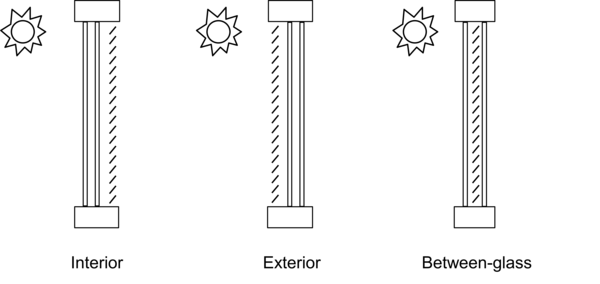
\includegraphics[width=0.9\textwidth, height=0.9\textheight, keepaspectratio=true]{media/image060.png}
\caption{Allowed locations of a window shading device. \protect \label{fig:allowed-locations-of-a-window-shading-device.}}
\end{figure}

When a shading device is present it is either retracted or activated. When it is retracted it covers none of the window. When it is activated it covers the entire glazed part of the window (but not the frame). Whether the shading device is retracted or activated in a particular timestep depends on the control mechanism: see ``Shading Control Type,'' below. To model a case in which the shading device, when activated, covers only \textbf{part} of the window you will have to divide the window into two separate windows, one with the shading device and one without the shading device.

A shading device can also be of a kind in which the optical properties of the glazing switch from one set of values to another in order to increase or decrease solar or visible transmittance (Shading Type = SwitchableGlazing).

There are two ways of specifying the actual shading device:

\begin{itemize}
  \item
\textbf{Specify ``Name of Construction with Shading''}

This is the name of a window Construction that has the shading device as one of its layers. The thermal and solar-optical properties of the shading device are given by the shading material referenced in that Construction (ref: Construction, WindowMaterial:Shade, WindowMaterial:Screen and WindowMaterial:Blind). To use this method you have to define two Constructions for the window, one without the shading device and one with it. See Example 1, below.

The Construction without the shading device is referenced in the FenestrationSurface:Detailed input for the window (see IDF example, below). The Construction with the shading device is referenced by the window's WindowProperty:ShadingControl.

For Shading Type = InteriorShade, InteriorBlind, ExteriorShade, ExteriorScreen and ExteriorBlind these two Constructions must be identical expect for the presence of the shading layer in the shaded Construction, otherwise you will get an error message. You will also get an error message if the Construction referenced by the window has a shading layer.

  \item
\textbf{Specify the ``Material Name of the Shading Device''}

This is the name of a WindowMaterial:Shade, WindowMaterial:Screen or WindowMaterial:Blind. This method can be used with Shading Type = InteriorShade, InteriorBlind, ExteriorShade and ExteriorBlind. It cannot be used with Shading Type = BetweenGlassShade, BetweenGlassBlind, or SwitchableGlazing. If Shading Type = InteriorShade or ExteriorShade, then you specify the name of a WindowMaterial:Shade. If Shading Type = InteriorBlind or ExteriorBlind, then you specify the name of a WindowMaterial:Blind. If Shading Type = ExteriorScreen, then you specify the name of a WindowMaterial:Screen. See Example 2, below. This method is simpler to use since you don't have to specify two Constructions that differ only by the shading layer.

When this method is used, the program will automatically create a shaded window construction by adding a shading layer to the outside or inside of the construction corresponding to the window referencing the WindowProperty:ShadingControl. The name, created by the program, of this shaded construction is composed as follows: if the name of the window construction is CCC and the material name of the shading device is DDD, then the shaded construction name is CCC:DDD:INT for an interior shading device and CCC:DDD:EXT for an exterior shading device.

This method is the required if you want to add a shading device to a construction brought in from a WINDOW Data File (ref:Construction:WindowDataFile).

Note that if both ``Name of Construction with Shading'' and ``Material Name of Shading Device'' are specified, the former takes precedence.
\end{itemize}

Most Shading Control Types allow you to specify a schedule that determines when the control is active. One example is a control that is active seasonally. For example, to deploy shading only in the summer when the incident solar is high enough, use Shading Control Type = OnIfHighSolarOnWindow with a schedule that is 1 during the summer months and 0 otherwise and specify Shading Control Is Scheduled = YES.

In addition, most Shading Control Types also allow you to specify that glare control is active in addition to the specified Control Type. For example, you might want to deploy shading when the solar incident on a window is too high OR the glare from the window is too high. This type of joint control requires that the window be in a daylit zone, that the maximum allowed glare be specified in the Daylighting object for the zone, and that Glare Control Is Active = YES in WindowProperty:ShadingControl.

If Shading Type = InteriorBlind, ExteriorBlind or BetweenGlassBlind you can use WindowProperty:ShadingControl to specify how the slat angle of the blind is controlled when the blind is in place.

A special type of WindowProperty:ShadingControl is SwitchableGlazing. An example is electrochromic glazing in which the transmittance and reflectance of the glass is controlled electronically. For example, you could have electrochromic glazing switch from clear (high transmittance) to dark (low transmittance) to control solar gain. If you choose the Shading Type = SwitchableGlazing option for WindowProperty:ShadingControl, the unswitched (clear) state is specified by the Construction referenced by the window and the switched (dark) state is specified by the Construction referenced by WindowProperty:ShadingControl for that window. For example, if you specify Shading Type = SwitchableGlazing and Shading Control Type = OnIfHighSolarOnWindow, then the glazing will switch to the dark state whenever the solar radiation striking the window exceeds the Setpoint value.

For Shading Type = SwitchableGlazing the state of the window is either clear (unswitched) or dark (fully switched) for all Shading Control Types except MeetDaylightIlluminanceSetpoint. In this case, the transmittance of the glazing is adjusted to just meet the daylight illuminance set point at the first daylighting reference point (see Daylighting). This type of control assures that there is just enough solar gain to meet the daylighting requirements in a zone, and no more, thus reducing the cooling load.

\subsubsection{Inputs}\label{inputs-32-001}

\paragraph{Field: Name}\label{field-name-29-001}

Name of the window shading control. It is referenced by a window (ref: Field: Shading Control Name).

\paragraph{Field: Shading Type}\label{field-shading-type}

The type of shading device. The choices are:

\emph{InteriorShade}: A diffusing shade is on the inside of the window. (In the shaded Construction the shading layer must be a WindowMaterial:Shade.)

\emph{ExteriorShade}: A diffusing shade is on the outside of the window. (In the shaded Construction the shading layer must be a WindowMaterial:Shade.)

\emph{BetweenGlassShade}: A diffusing shade is between two glass layers. (In the shaded Construction the shading layer must be a WindowMaterial:Shade.) This shading type is allowed only for double- and triple-glazing. For triple-glazing the shade must be between the two inner glass layers.

\emph{ExteriorScreen}: An insect screen is on the outside of the window. (In the shaded Construction the shading layer must be a WindowMaterial:Screen.)

\emph{InteriorBlind}: A slat-type shading device, such as a Venetian blind, is on the inside of the window. (In the shaded Construction the shading layer must be a WindowMaterial:Blind.)

\emph{ExteriorBlind}: A slat-type shading device is on the outside of the window. (In the shaded Construction the shading layer must be a WindowMaterial:Blind.)

\emph{BetweenGlassBlind}: A slat-type shading device is between two glass layers. (In the shaded Construction the shading layer must be a WindowMaterial:Blind.) This shading type is allowed only for double- and triple-glazing. For triple-glazing the blind must be between the two inner glass layers.

\emph{SwitchableGlazing}: Shading is achieved by changing the characteristics of the window glass, such as by darkening it.

\paragraph{Field: Construction with Shading Name}\label{field-construction-with-shading-name}

Name of the window Construction that has the shading in place. The properties of the shading device are given by the shading material referenced in that Construction (ref: Construction, WindowMaterial:Shade, WindowMaterial:Screen and WindowMaterial:Blind). For Shading Type = SwitchableGlazing, this is the name of the Construction that corresponds to the window in its fully-switched (darkest) state.

Specifying ``Name of Construction with Shading'' is required if Shading Type = BetweenGlassShade, BetweenGlassBlind, or SwitchableGlazing. For other Shading Types, you may alternatively specify ``Material Name of Shading Device'' (see below).

\paragraph{Field: Shading Control Type}\label{field-shading-control-type}

Specifies how the shading device is controlled, i.e., it determines whether the shading device is ``on'' or ``off.'' For blinds, screens and shades, when the device is ``on'' it is assumed to cover all of the window except its frame; when the device is ``off'' it is assumed to cover none of the window (whether ``on'' or ``off'' the shading device is assumed to cover none of the wall that the window is on).

For switchable glazing, ``on'' means that the glazing is in the fully-switched state and ``off'' means that it is in the unswitched state; for example, for electrochromic glazing, ``on'' means the glazing is in its darkest state and ``off'' means it is in its lightest state.

The choices for Shading Control Type are the following. If SetPoint is applicable its units are shown in parentheses.

\emph{AlwaysOn}: Shading is always on.

\emph{AlwaysOff}: Shading is always off.

The following six control types are used primarily to reduce zone cooling load due to window solar gain.

\emph{OnIfScheduleAllows}: Shading is on if schedule value is non-zero. Requires that Schedule Name be specified and Shading Control Is Scheduled = Yes.

Note: For exterior window screens \emph{AlwaysOn, AlwaysOff, and OnIfScheduleAllows} are the only valid shading control types.

\emph{OnIfHighSolarOnWindow}: Shading is on if beam plus diffuse solar radiation incident on the window exceeds SetPoint (W/m\(^{2}\)) and schedule, if specified, allows shading.

\emph{OnIfHighHorizontalSolar}: Shading is on if total (beam plus diffuse) horizontal solar irradiance exceeds SetPoint (W/m\(^{2}\)) and schedule, if specified, allows shading.

\emph{OnIfHighOutdoorAirTemperature}: Shading is on if outside air temperature exceeds SetPoint (C) and schedule, if specified, allows shading.

\emph{OnIfHighZoneAirTemperature}: Shading is on if zone air temperature in the previous timestep exceeds SetPoint (C) and schedule, if specified, allows shading.

\emph{OnIfHighZoneCooling}: Shading is on if zone cooling rate in the previous timestep exceeds SetPoint (W) and schedule, if specified, allows shading.

\emph{OnIfHighGlare}: Shading is on if the total daylight glare index at the zone's first daylighting reference point from all of the exterior windows in the zone exceeds the maximum glare index specified in the daylighting input for zone (ref: Group -- Daylighting). Applicable only to windows in zones with daylighting.

Note: Unlike other Shading Control Types, glare control is active whether or not a schedule is specified.

\emph{MeetDaylightIlluminanceSetpoint}: Used only with ShadingType = SwitchableGlazing in zones with daylighting controls. In this case the transmittance of the glazing is adjusted to just meet the daylight illuminance set point at the first daylighting reference point. Note that the daylight illuminance set point is specified in the Daylighting:Controls object for the Zone; it is not specified as a WindowProperty:ShadingControl SetPoint. When the glare control is active, if meeting the daylight illuminance set point at the first daylighting reference point results in higher discomfort glare index (DGI) than the specified zone's maximum allowable DGI for either of the daylight reference points, the glazing will be further dimmed until the DGI equals the specified maximum allowable value.

The following three control types can be used to reduce zone heating load during the winter by reducing window conductive heat loss at night and leaving the window unshaded during the day to maximize solar gain. They are applicable to any Shading Type except ExteriorScreen but are most appropriate for interior or exterior shades with high insulating value (``movable insulation''). ``Night'' means the sun is down and ``day'' means the sun is up.

\emph{OnNightIfLowOutdoorTempAndOffDay}: Shading is on at night if the outside air temperature is less than SetPoint (C) and schedule, if specified, allows shading. Shading is off during the day.

\emph{OnNightIfLowInsideTempAndOffDay}: Shading is on at night if the zone air temperature in the previous timestep is less than SetPoint (C) and schedule, if specified, allows shading. Shading is off during the day.

\emph{OnNightIfHeatingAndOffDay}: Shading is on at night if the zone heating rate in the previous timestep exceeds SetPoint (W) and schedule, if specified, allows shading. Shading is off during the day.

The following two control types can be used to reduce zone heating and cooling load. They are applicable to any Shading Type except ExteriorScreen but are most appropriate for translucent interior or exterior shades with high insulating value (``translucent movable insulation'').

\emph{OnNightIfLowOutdoorTempAndOnDayIfCooling}: Shading is on at night if the outside air temperature is less than SetPoint (C). Shading is on during the day if the zone cooling rate in the previous timestep is non-zero. Night and day shading is subject to schedule, if specified.

\emph{OnNightIfHeatingAndOnDayIfCooling}: Shading is on at night if the zone heating rate in the previous timestep exceeds SetPoint (W). Shading is on during the day if the zone cooling rate in the previous timestep is non-zero. Night and day shading is subject to schedule, if specified.

The following control types can be used to reduce zone cooling load. They are applicable to any Shading Type except ExteriorScreen but are most appropriate for interior or exterior blinds, interior or exterior shades with low insulating value, or switchable glazing.

\emph{OffNightAndOnDayIfCoolingAndHighSolarOnWindow}: Shading is off at night. Shading is on during the day if the solar radiation incident on the window exceeds SetPoint (W/m\(^{2}\)) and if the zone cooling rate in the previous timestep is non-zero. Daytime shading is subject to schedule, if specified.

\emph{OnNightAndOnDayIfCoolingAndHighSolarOnWindow}: Shading is on at night. Shading is on during the day if the solar radiation incident on the window exceeds SetPoint (W/m\(^{2}\)) and if the zone cooling rate in the previous timestep is non-zero. Day and night shading is subject to schedule, if specified. (This Shading Control Type is the same as the previous one, except the shading is on at night rather than off.)

\emph{OnIfHighOutdoorAirTempAndHighSolarOnWindow:} Shading is on if the outside air temperature exceeds the Setpoint (C) and if if the solar radiation incident on the window exceeds SetPoint 2 (W/m\(^{2}\)).

\emph{OnIfHighOutdoorAirTempAndHighHorizontalSolar:} Shading is on if the outside air temperature exceeds the Setpoint (C) and if if the horizontal solar radiation exceeds SetPoint 2 (W/m\(^{2}\)).

\paragraph{Field: Schedule Name}\label{field-schedule-name-007}

Required if Shading Control Is Scheduled = Yes. If schedule value \textgreater{} 0 , shading control is active, i.e., shading can be on only if the shading control test passes. If schedule value = 0, shading is off whether or not the control test passes. If Schedule Name is not specified, shading control is assumed to be active at all times.

\paragraph{Field: Setpoint}\label{field-setpoint}

The setpoint for activating window shading. The units depend on the type of trigger:

\begin{itemize}
\item
  W/m\(^{2}\) for solar-based controls
\item
  W for cooling- or heating-based controls
\item
  Degrees C for temperature-based controls
\end{itemize}

SetPoint is unused for Shading Control Type = OnIfScheduleAllows, OnIfHighGlare and DaylightIlluminance.

\paragraph{Field: Shading Control Is Scheduled}\label{field-shading-control-is-scheduled}

Accepts values YES and NO. The default is NO. Not applicable for Shading Control Type = OnIfHighGlare and should be blank in that case.

If YES, Schedule Name is required and that schedule determines whether the shading control specified by Shading Control Type is active or inactive (see Schedule Name, above).

If NO, Schedule Name is not applicable (should be blank) and the shading control is unscheduled.

Shading Control Is Scheduled = YES is required if Shading Control Type = OnIfScheduleAllows.

\paragraph{Field: Glare Control Is Active}\label{field-glare-control-is-active}

Accepts values YES and NO. The default is NO.

If YES and the window is in a daylit zone, shading is on if the zone's discomfort glare index exceeds the maximum discomfort glare index specified in the Daylighting object referenced by the zone. For switchable windows with \emph{MeetDaylightIlluminanceSetpoint} shading control, if Glare Control is active, the windows are always continuously dimmed as necessary to meet the zone's maximum allowable DGI while providing appropriate amount of daylight for the zone.

The glare test is OR'ed with the test specified by Shading Control Type. For example, if Glare Control Is Active = YES and Shading Control Type = OnIfHighZoneAirTemp, then shading is on if glare is too high OR if the zone air temperature is too high.

Glare Control Is Active = YES is required if Shading Control Type = OnIfHighGlare.

\paragraph{Field: Shading Device Material Name}\label{field-shading-device-material-name}

The name of a WindowMaterial:Shade, WindowMaterial:Screen or WindowMaterial:Blind. Required if ``Name of Construction with Shading'' is not specified. Not applicable if Shading Type = BetweenGlassShade, BetweenGlassBlind or SwitchableGlazing and should be blank in this case. If both ``Name of Construction with Shading'' and ``Material Name of Shading Device'' are entered the former takes precedence.

\paragraph{Field: Type of Slat Angle Control for Blinds}\label{field-type-of-slat-angle-control-for-blinds}

Applies only to Shading Type = InteriorBlind, ExteriorBlind or BetweenGlassBlind. Specifies how the slat angle is controlled. The choices are FixedSlatAngle, ScheduledSlatAngle and BlockBeamSolar.

If FixedSlatAngle (the default), the angle of the slat is fixed at the value input for the WindowMaterial:Blind that is contained in the construction specified by Name of Construction with Shading or is specified by Material Name of Shading Device.

If ScheduledSlatAngle, the slat angle varies according to the schedule specified by Slat Angle Schedule Name, below.

If BlockBeamSolar, the slat angle is set each timestep to just block beam solar radiation. If there is no beam solar on the window the slat angle is set to the value input for the WindowMaterial:Blind that is contained in the construction specified by Name of Construction with Shading or is specified by Material Name of Shading Device. The BlockBeamSolar option prevents beam solar from entering the window and causing possible unwanted glare if the beam falls on work surfaces while at the same time allowing near-optimal indirect radiation for daylighting.

\paragraph{Field: Slat Angle Schedule Name}\label{field-slat-angle-schedule-name}

This is the name of a schedule of slat angles that is used when Type of Slat Angle Control for Blinds = ScheduledSlatAngle. You should be sure that the schedule values fall within the range given by the Minimum Slat Angle and Maximum Slat Angle values entered in the corresponding WindowMaterial:Blind. If not, the program will force them into this range.

\paragraph{Field: Setpoint 2}\label{field-setpoint-2}

Used only as the second setpoint for the following two-setpoint control types: OnIfHighOutdoorAirTempAndHighSolarOnWindow, OnIfHighOutdoorAirTempAndHighHorizontalSolar, OnIfHighZoneAirTempAndHighSolarOnWindow, and OnIfHighZoneAirTempAndHighHorizontalSolar

An IDF example: window with interior roll shade that is deployed when solar incident on the window exceeds 50 W/m\(^{2}\).

\begin{lstlisting}
! Example 1: Interior movable shade specified by giving name of shaded construction
! in WindowProperty:ShadingControl

WindowMaterial:Glazing, GLASS - CLEAR SHEET 1 / 8 IN,  !- Material Name
       SpectralAverage,! Optical data type {SpectralAverage or Spectral}
       ,               ! Name of spectral data set when Optical Data Type = Spectral
       0.003        ,  !- Thickness {m}
       0.837        ,  !- Solar Transmittance at Normal Incidence
       0.075        ,  !- Solar Reflectance at Normal Incidence: Front Side
       0.075        ,  !- Solar Reflectance at Normal Incidence: Back Side
       0.898        ,  !- Visible Transmittance at Normal Incidence
       0.081        ,  !- Visible Reflectance at Normal Incidence: Front Side
       0.081        ,  !- Visible Reflectance at Normal Incidence: Back Side
       0.0          ,  !- IR Transmittance
       0.8400000    ,  !- IR Emissivity: Front Side
       0.8400000    ,  !- IR Emissivity: Back Side
       0.9000000    ;  !- Conductivity {W/m-K}

WindowMaterial:Shade, ROLL SHADE,  !- Material Name
       0.3          ,   !- Solar Transmittance at normal incidence
       0.5000000    ,   !- Solar Reflectance (same for front and back side)
       0.3          ,   !- Visible Transmittance at normal incidence
       0.5000000    ,   !- Visible reflectance (same for front and back side)
       0.9000000    ,   !- IR Emissivity (same for front and back side)
       0.05         ,   !- IR Transmittance
       0.003        ,   !- Thickness
       0.1          ,   !- Conductivity {W/m-K}
       0.0          ,   !- Top Opening Multiplier
       0.0          ,   !- Bottom Opening Multiplier
       0.5          ,   !- Left-Side Opening Multiplier
       0.5          ,   !- Right-Side Opening Multiplier
       0.0          ;   !- Air-Flow Permeability

Construction, SINGLE PANE WITH NO SHADE,  ! Name of construction without shade
       GLASS - CLEAR SHEET 1 / 8 IN;  !- First material layer

Construction, SINGLE PANE WITH INT SHADE, ! Name of construction with shade
       GLASS - CLEAR SHEET 1 / 8 IN,  !- First material layer
       ROLL SHADE                  ;  !- Second material layer

WindowProperty:ShadingControl, CONTROL ON INCIDENT SOLAR,  !- Name of Shading Control
       InteriorShade,                !- Shading Type
       SINGLE PANE WITH INT SHADE,   !- Name of construction with shading device
       OnIfHighSolarOnWindow,        !- Shading Control Type
       ,                             !- Schedule name
       50.0,                         !- Setpoint {W/m2}
       NO,                           !- Shading Control Is Scheduled
       NO,                           !- Glare Control Is Active
       ,                             !- Material Name of Shading Device
       ,                             !- Type of Slat Angle Control for Blinds
       ;                             !- Slat Angle Schedule Name

FenestrationSurface:Detailed, Zn001:Wall001:Win001,  !- SubSurface Name
       Window                   ,    !- Class
       SINGLE PANE WITH NO SHADE,    !- Name of construction without shading device
       Zn001:Wall001            ,    !- Base Surface Name
       ,                             !- Target
       0.5000000                ,    !- VF to Ground
       CONTROL ON INCIDENT SOLAR,    !- Window Shading Control name
       ,                             !- Frame/Divider name
       1.0                      ,    !- Multiplier
       4                        ,    !- Number of vertices (assumed rectangular)
       0.548 ,  0.0 ,   2.5     ,    !- x,y,z of vertices {m}
       0.548 ,  0.0 ,   0.5     ,
       5.548 ,  0.0 ,   0.5     ,
       5.548 ,  0.0 ,   2.5     ;
\end{lstlisting}

\begin{lstlisting}
! Example 2: Interior movable shade specified by giving name of shading device in WindowProperty:ShadingControl

WindowMaterial:Glazing, GLASS - CLEAR SHEET 1 / 8 IN,  !- Material Name
       SpectralAverage,! Optical data type {SpectralAverage or Spectral}
       ,               ! Name of spectral data set when Optical Data Type = Spectral
       0.003        ,  !- Thickness {m}
       0.837        ,  !- Solar Transmittance at Normal Incidence
       0.075        ,  !- Solar Reflectance at Normal Incidence: Front Side
       0.075        ,  !- Solar Reflectance at Normal Incidence: Back Side
       0.898        ,  !- Visible Transmittance at Normal Incidence
       0.081        ,  !- Visible Reflectance at Normal Incidence: Front Side
       0.081        ,  !- Visible Reflectance at Normal Incidence: Back Side
       0.0          ,  !- IR Transmittance
       0.8400000    ,  !- IR Emissivity: Front Side
       0.8400000    ,  !- IR Emissivity: Back Side
       0.9000000    ;  !- Conductivity {W/m-K}

WindowMaterial:Shade, ROLL SHADE,  !- Material Name
       0.3          ,   !- Solar Transmittance at normal incidence
       0.5000000    ,   !- Solar Reflectance (same for front and back side)
       0.3          ,   !- Visible Transmittance at normal incidence
       0.5000000    ,   !- Visible reflectance (same for front and back side)
       0.9000000    ,   !- IR Emissivity (same for front and back side)
       0.05         ,   !- IR Transmittance
       0.003        ,   !- Thickness
       0.1          ,   !- Conductivity {W/m-K}
       0.0          ,   !- Top Opening Multiplier
       0.0          ,   !- Bottom Opening Multiplier
       0.5          ,   !- Left-Side Opening Multiplier
       0.5          ,   !- Right-Side Opening Multiplier
       0.0          ;   !- Air-Flow Permeability

Construction, SINGLE PANE WITH NO SHADE,  ! Name of construction without shade
       GLASS - CLEAR SHEET 1 / 8 IN;  !- First material layer

WINDOWPROPERTY:SHADINGCONTROL, CONTROL ON INCIDENT SOLAR,  !- Name of Shading Control
       InteriorShade,                !- Shading Type
       ,                             !- Name of shaded construction
       OnIfHighSolarOnWindow,        !- Shading Control Type
       ,                             !- Schedule name
       50.0,                         !- Setpoint {W/m2}
       NO,                           !- Shading Control Is Scheduled
       NO,                           !- Glare Control Is Active
       ROLL SHADE,                   !- Material Name of Shading Device
       ,                             !- Type of Slat Angle Control for Blinds
       ;                             !- Slat Angle Schedule Name

FenestrationSurface:Detailed, Zn001:Wall001:Win001,  !- SubSurface Name
       Window                   ,    !- Class
       SINGLE PANE WITH NO SHADE,    !- Name of construction without shade
       Zn001:Wall001            ,    !- Base Surface Name
       ,                             !- Target
       0.5000000                ,    !- VF to Ground
       CONTROL ON INCIDENT SOLAR,    !- Window Shading Control name
       ,                             !- Frame/Divider name
       1.0                      ,    !- Multiplier
       4                        ,    !- Number of vertices (assumed rectangular)
       0.548 ,  0.0 ,   2.5     ,    !- x,y,z of vertices {m}
       0.548 ,  0.0 ,   0.5     ,
       5.548 ,  0.0 ,   0.5     ,
       5.548 ,  0.0 ,   2.5     ;
\end{lstlisting}

\subsection{WindowProperty:FrameAndDivider}\label{windowpropertyframeanddivider}

The WindowProperty:FrameAndDivider object is referenced by exterior windows that have

\begin{itemize}
\item
  a frame, and/or
\item
  a divider, and/or
\item
  reveal surfaces that reflect beam solar radiation.
\end{itemize}

A \textbf{\emph{frame}} surrounds the glazing in a window (see Figure~\ref{fig:a-window-with-a-frame-and-divider.} and Figure~\ref{fig:illustration-showing-frame-and-divider}). It is assumed that all frame characteristics---such as width, conductance and solar absorptance---are the same for the top, bottom and side elements of the frame. If the frame elements are not the same then you should enter area-weighted average values for the frame characteristics.

The window vertices that you specify in the FenestrationSurface:Detailed object are those of the glazed part of the window, not the frame. EnergyPlus automatically subtracts the area of the frame---determined from the glazing dimensions and the frame width---from the area of the wall containing the window.

A \textbf{\emph{divider}}, as shown in Figure~\ref{fig:a-window-with-a-frame-and-divider.}, Figure~\ref{fig:illustration-showing-frame-and-divider} and Figure~\ref{fig:illustration-showing-divider-types.}, divides the glazing up into separate lites. It is assumed that all divider elements have the same characteristics. If not, area-weighted average values should be used. EnergyPlus automatically subtracts the divider area from the glazed area of the window.

\textbf{\emph{Reveal surfaces}}, as shown in Figure~\ref{fig:a-vertical-section-through-a-window-with}, are associated with the setback of the glazing from the outside and/or inside surface of the parent wall. If the depth and solar absorptance of these surfaces are specified, the program will calculate the reflection of beam solar radiation from these surfaces. The program also calculates the shadowing (onto the window) of beam and diffuse solar radiation by outside reveal surfaces.

In EnergyPlus, a window can have any combination of frame, divider and reveal surfaces, or none of these.

The best source of frame and divider characteristics is the WINDOW program, which will calculate the values required by EnergyPlus for different frame and divider types. In particular, the THERM program within the WINDOW program will calculate the effective conductance of frames and dividers; this is the conductance taking 2-D heat transfer effects into account.

Note that a window's frame and divider characteristics, along with other window information, can be read in from the Window Data File (see ``Importing Windows from the WINDOW program'' and ``Construction:WindowDataFile object''). In this case the WindowProperty:FrameAndDivider referenced by the window is not applicable and should be blank unless you want to specify reveal surfaces for beam solar reflection.

\begin{figure}[hbtp] % fig 35
\centering
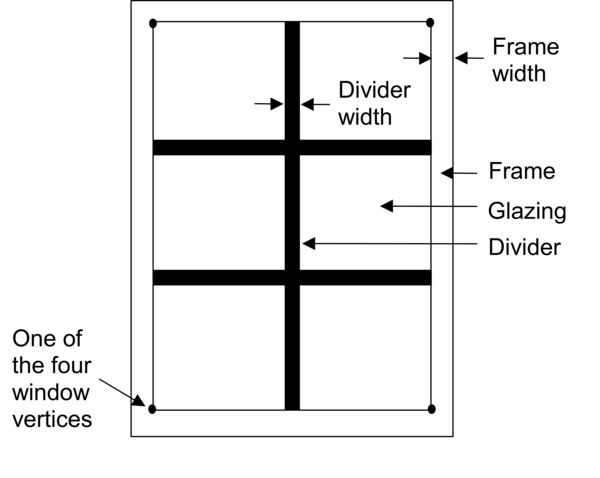
\includegraphics[width=0.9\textwidth, height=0.9\textheight, keepaspectratio=true]{media/image061.png}
\caption{A window with a frame and divider. \protect \label{fig:a-window-with-a-frame-and-divider.}}
\end{figure}

In the illustration above, the divider has two horizontal elements and one vertical element.

\subsubsection{Inputs}\label{inputs-33-001}

\paragraph{Field: Name}\label{field-name-30-001}

The name of the frame/divider object. It is referenced by WindowProperty:FrameAndDivider Name in FenestrationSurface:Detailed.

\textbf{\emph{Frame Fields}}

\paragraph{Field: Frame Width}\label{field-frame-width}

The width of the frame elements when projected onto the plane of the window. It is assumed that the top, bottom and side elements of the frame have the same width. If not, an average frame width should be entered such that the projected frame area calculated using the average value equals the sum of the areas of the frame elements.

\paragraph{Field: Frame Outside Projection}\label{field-frame-outside-projection}

The amount by which the frame projects outward from the outside surface of the window glazing. If the outer surface of the frame is flush with the glazing, Frame Outside Projection = 0.0. Used to calculate shadowing of frame onto glass, solar absorbed by frame, IR emitted and absorbed by frame, and convection from frame.

\paragraph{Field: Frame Inside Projection}\label{field-frame-inside-projection}

The amount by which the frame projects inward from the inside surface of the window glazing. If the inner surface of the frame is flush with the glazing, Frame Inside Projection = 0.0. Used to calculate solar absorbed by frame, IR emitted and absorbed by frame, and convection from frame.

\begin{figure}[hbtp] % fig 36
\centering
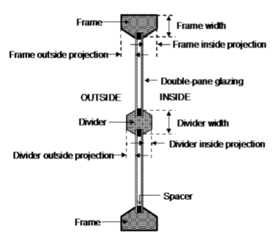
\includegraphics[width=0.9\textwidth, height=0.9\textheight, keepaspectratio=true]{media/image062.png}
\caption{Illustration showing frame and divider dimensioning. \protect \label{fig:illustration-showing-frame-and-divider}}
\end{figure}

\paragraph{Field: Frame Conductance}\label{field-frame-conductance}

The effective thermal conductance of the frame measured from inside to outside frame surface (no air films) and taking 2-D conduction effects into account. Obtained from the WINDOW program or other 2-D calculation.

\paragraph{Field: Ratio of Frame-Edge Glass Conductance to Center-Of-Glass Conductance}\label{field-ratio-of-frame-edge-glass-conductance-to-center-of-glass-conductance}

The glass conductance near the frame (excluding air films) divided by the glass conductance at the center of the glazing (excluding air films). Used only for multi-pane glazing constructions. This ratio is greater than 1.0 because of thermal bridging from the glazing across the frame and across the spacer that separates the glass panes. Values can be obtained from the WINDOW program the user-selected glazing construction and frame characteristics.

\paragraph{Field: Frame Solar Absorptance}\label{field-frame-solar-absorptance}

The solar absorptance of the frame. The value is assumed to be the same on the inside and outside of the frame and to be independent of angle of incidence of solar radiation. If solar reflectance (or reflectivity) data is available, then absorptance is equal to 1.0 minus reflectance (for opaque materials).

\paragraph{Field: Frame Visible Absorptance}\label{field-frame-visible-absorptance}

The visible absorptance of the frame. The value is assumed to be the same on the inside and outside of the frame and to be independent of angle of incidence of solar radiation. If visible reflectance (or reflectivity) data is available, then absorptance is equal to 1.0 minus reflectance (for opaque materials).

\paragraph{Field: Frame Thermal Hemispherical Emissivity}\label{field-frame-thermal-hemispherical-emissivity}

The thermal emissivity of the frame, assumed the same on the inside and outside.

\textbf{\emph{Divider Fields}}

\paragraph{Field: Divider Type}\label{field-divider-type}

The type of divider (see figure below). Divider Type = Suspended is applicable only to multi-pane glazing. It means that the divider is suspended between the panes. (If there are more than two glass layers, the divider is assumed to be placed between the two outermost layers.)

Divider Type = DividedLite means that the divider elements project out from the outside and inside surfaces of the glazing and divide the glazing into individual lites. For multi-pane glazing, this type of divider also has between-glass elements that separate the panes.

\begin{figure}[hbtp] % fig 37
\centering
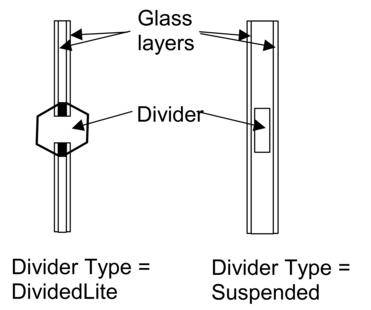
\includegraphics[width=0.9\textwidth, height=0.9\textheight, keepaspectratio=true]{media/image063.png}
\caption{Illustration showing divider types. \protect \label{fig:illustration-showing-divider-types.}}
\end{figure}

\paragraph{Field: Divider Width}\label{field-divider-width}

The width of the divider elements when projected onto the plane of the window. It is assumed that the horizontal and vertical divider elements have the same width. If not, an average divider width should be entered such that the projected divider area calculated using the average value equals the sum of the areas of the divider elements.

\paragraph{Field: Number of Horizontal Dividers}\label{field-number-of-horizontal-dividers}

The number of divider elements parallel to the top and bottom of the window.

\paragraph{Field: Number of Vertical Dividers}\label{field-number-of-vertical-dividers}

The number of divider elements parallel to the sides of the window.

\paragraph{Field: Divider Outside Projection}\label{field-divider-outside-projection}

The amount by which the divider projects out from the outside surface of the window glazing. For Divider Type = Suspended, Divider Projection = 0.0. Used to calculate shadowing of divider onto glass, solar absorbed by divider, IR emitted and absorbed by divider, and convection from divider.

\paragraph{Field: Divider Inside Projection}\label{field-divider-inside-projection}

The amount by which the divider projects inward from the inside surface of the window glazing. If the inner surface of the divider is flush with the glazing, Divider Inside Projection = 0.0. Used to calculate solar absorbed by divider, IR emitted and absorbed by divider, and convection from divider.

\paragraph{Field: Divider Conductance}\label{field-divider-conductance}

The effective thermal conductance of the divider measured from inside to outside divider surface (no air films) and taking 2-D conduction effects into account. Obtained from the WINDOW program or other 2-D calculation.

\paragraph{Field: Ratio of Divider-Edge Glass Conductance to Center-Of-Glass Conductance}\label{field-ratio-of-divider-edge-glass-conductance-to-center-of-glass-conductance}

The glass conductance near the divider (excluding air films) divided by the glass conductance at the center of the glazing (excluding air films). Used only for multi-pane glazing constructions. This ratio is greater than 1.0 because of thermal bridging from the glazing across the divider and across the spacer that separates the glass panes. Values can be obtained from the WINDOW program for the user-selected glazing construction and divider characteristics.

\paragraph{Field: Divider Solar Absorptance}\label{field-divider-solar-absorptance}

The solar absorptance of the divider. The value is assumed to be the same on the inside and outside of the divider and to be independent of angle of incidence of solar radiation. If solar reflectance (or reflectivity) data is available, then absorptance is equal to 1.0 minus reflectance (for opaque materials).

\paragraph{Field: Divider Visible Absorptance}\label{field-divider-visible-absorptance}

The visible absorptance of the divider. The value is assumed to be the same on the inside and outside of the divider and to be independent of angle of incidence of solar radiation. If visible reflectance (or reflectivity) data is available, then absorptance is equal to 1.0 minus reflectance (for opaque materials).

\paragraph{Field: Divider Thermal Hemispherical Emissivity}\label{field-divider-thermal-hemispherical-emissivity}

The thermal emissivity of the divider, assumed the same on the inside and outside.

\textbf{\emph{Reveal Surface Fields}}

The following fields specify the properties of the window reveal surfaces (reveals occur when the window is not in the same plane as the base surface). From this information and from the geometry of the window and the sun position, the program calculates beam solar radiation absorbed and reflected by the top, bottom, right and left sides of outside and inside window reveal surfaces. In doing this calculation, the shadowing on a reveal surface by other reveal surfaces is determined using the orientation of the reveal surfaces and the sun position.

It is assumed that:

\begin{itemize}
\item
  The window is an exterior window.
\item
  The reveal surfaces are perpendicular to the window plane.
\item
  If an exterior shade, screen or blind is in place it shades exterior and interior reveal surfaces so that in this case there is no beam solar on these surfaces.
\item
  If an interior shade or blind is in place it shades the interior reveal surfaces so that in this case there is no beam solar on these surfaces.
\item
  The possible shadowing on inside reveal surfaces by a window divider is ignored.
\item
  The outside reveal surfaces (top, bottom, left, right) have the same solar absorptance and depth. This depth is not input here but is automatically determined by the program---from window and wall vertices--as the distance between the plane of the outside face of the glazing and plane of the outside face of the parent wall.
\item
  The inside reveal surfaces are divided into two categories: (1) the bottom reveal surface, called here the ``inside sill;'' and (2) the other reveal surfaces (left, right and top).
\item
  The left, right and top inside reveal surfaces have the same depth and solar absorptance. The inside sill is allowed to have depth and solar absorptance values that are different from the corresponding values for the other inside reveal surfaces.
\item
  The inside sill depth is required to be greater than or equal to the depth of the other inside reveal surfaces. If the inside sill depth is greater than zero the depth of the other inside reveal surfaces is required to be greater than zero.
\item
  The reflection of beam solar radiation from all reveal surfaces is assumed to be isotropic diffuse; there is no specular component.
\item
  Half of the beam solar reflected from outside reveal surfaces is goes towards the window; the other half goes back to the exterior environment (i.e., reflection of this outward-going component from other outside reveal surfaces is not considered).
\item
  The half that goes towards the window is added to the other solar radiation incident on the window. Correspondingly, half of the beam solar reflected from inside reveal surfaces goes towards the window, with the other half going into the zone. The portion going towards the window that is not reflected is absorbed in the glazing or is transmitted back out into the exterior environment.
\item
  The beam solar that is absorbed by outside reveal surfaces is added to the solar absorbed by the outside surface of the window's parent wall; similarly, the beam solar absorbed by the inside reveal surfaces is added to the solar absorbed by the inside surface of the parent wall.
\end{itemize}

The net effect of beam solar reflected from outside reveal surfaces is to increase the heat gain to the zone, whereas the effect of beam solar reflected from inside reveal surfaces is to decrease the heat gain to the zone since part of this reflected solar is transmitted back out the window.

~If the window has a frame, the absorption of reflected beam solar by the inside and outside surfaces of the frame is considered. The shadowing of the frame onto interior reveal surfaces is also considered.

\paragraph{Field: Outside Reveal Solar Absorptance}\label{field-outside-reveal-solar-absorptance}

The solar absorptance of outside reveal surfaces.

\paragraph{Field: Inside Sill Depth}\label{field-inside-sill-depth}

The depth of the inside sill, measured from the inside surface of the glazing to the edge of the sill (see Figure~\ref{fig:a-vertical-section-through-a-window-with}).

\paragraph{Field: Inside Sill Solar Absorptance}\label{field-inside-sill-solar-absorptance}

The solar absorptance of the inside sill.

\textbf{\emph{Field: Inside Reveal Depth}}

The depth of the inside reveal surfaces other than the sill, measured from the inside surface of the glazing to the edge of the reveal surface (see Figure~\ref{fig:a-vertical-section-through-a-window-with}).

\paragraph{Field: Inside Reveal Solar Absorptance}\label{field-inside-reveal-solar-absorptance}

The solar absorptance of the inside reveal surfaces other than the sill.

\begin{figure}[hbtp] % fig 38
\centering
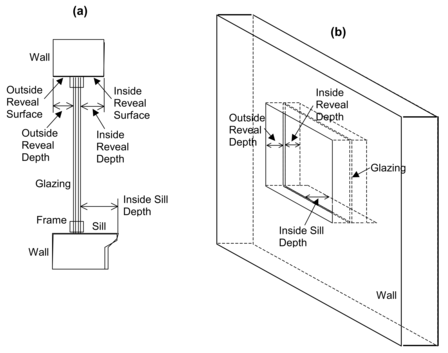
\includegraphics[width=0.9\textwidth, height=0.9\textheight, keepaspectratio=true]{media/image064.png}
\caption{(a) Vertical section through a window (with frame) showing outside and inside reveal surfaces and inside sill. (b) Perspective view looking from the outside of a window (without frame) showing reveal surfaces. Note that “Outside Reveal Depth” is not a user input; it is calculated by the program from the window and wall vertices. \protect \label{fig:a-vertical-section-through-a-window-with}}
\end{figure}

An IDF example:

\begin{lstlisting}

  WindowProperty:FrameAndDivider,
        TestFrameAndDivider, ! Frame/Divider Name
        0.05, ! Frame Width
        0.04, ! Frame Outside Projection
        0.03, ! Frame Inside Projection
        5.0,  ! Frame Conductance
        1.3,  ! Ratio of Frame-Edge Glass Conductance to Center-Of-Glass Conductance
        0.8,  ! Frame Solar Absorptance
        0.8,  ! Frame Visible Absorptance
        0.9,  ! Frame Thermal Emissivity
        DividedLite, ! Divider Type
        0.03, ! Divider Width
        2,    ! Number of Horizontal Dividers
        2,    ! Number of Vertical Dividers
        0.03, ! Divider Outside Projection
        0.03, ! Divider Inside Projection
        5.0,  ! Divider Conductance
        1.3,  ! Ratio of Divider-Edge Glass Conductance to Center-Of-Glass Conductance
        0.8,  ! Divider Solar Absorptance
        0.8,  ! Divider Visible Absorptance
        0.9,  ! Divider Thermal Emissivity
        0.7,  ! Outside Reveal Solar Absorptance
        0.25, ! Inside Sill Depth (m)
        0.6,  ! Inside Sill Solar Absorptance
        0.2,  ! Inside Reveal Depth (m)
        0.5;  ! Inside Reveal Solar Absorptance
\end{lstlisting}

\subsection{WindowProperty:AirflowControl}\label{windowpropertyairflowcontrol}

This object is used to specify the control mechanism for windows in which forced air flows in the gap between adjacent layers of glass. Such windows are called ``airflow windows.'' They are also known as ``heat-extract windows'' or ``climate windows.''

A common application is to reduce the zone load by exhausting indoor air through the window. In the cooling season this picks up and expels some of the solar heat absorbed by the window glass (and by the between-glass shade or blind, if present). In the heating season this warms the window, reducing the heat loss from the window. A side benefit is increased thermal comfort. This is because the inside surface of the window will generally be cooler in summer and warmer in winter.

The surface output variable ``Surface Window Gap Convective Heat Transfer Rate'' gives the heat picked up (or lost) by the gap airflow.

\subsubsection{Inputs}\label{inputs-34-001}

\paragraph{Field: Name}\label{field-name-31-001}

Name of the window that this WindowProperty:AirflowControl refers to. It must be a window with two or three glass layers, i.e., double- or triple-glazing. For triple-glazing the airflow is assumed to be between the two inner glass layers.

An error will result if the gas in the airflow gap is other than air. If an airflow window has a between-glass shade or blind, the gas in the gap on either side of the shade or blind must be air.

\paragraph{Field: Airflow Source}\label{field-airflow-source}

The source of the gap airflow. The choices are:

\emph{IndoorAir}: Indoor air from the window's zone is passed through the window.

\emph{OutdoorAir}: Outdoor air is passed through the window.

\paragraph{Field: Airflow Destination}\label{field-airflow-destination}

This is where the gap air goes after passing through the window. The choices are:

\emph{IndoorAir}: The gap air goes to the indoor air of the window's zone.

\emph{OutdoorAir}: The gap air goes to the outside air.

\emph{ReturnAir}. The gap air goes to the return air for the window's zone. This choice is allowed only if Airflow Source = InsideAir. If the return air flow is zero, the gap air goes to the indoor air of the window's zone. If the sum of the gap airflow for all of the windows in a zone with Airflow Destination = ReturnAir exceeds the return airflow, then the difference between this sum and the return airflow goes to the indoor air.

Figure~\ref{fig:gap-airflow-configurations-for-airflow} shows the allowed combinations of Airflow Source and Airflow Destination. The allowed combinations of Airflow Source and Airflow Destination are:

IndoorAir -\textgreater{} OutdoorAir

IndoorAir -\textgreater{} IndoorAir

IndoorAir -\textgreater{} ReturnAir

OutdoorAir -\textgreater{} IndoorAir

OutdoorAir -\textgreater{} OutdoorAir

\paragraph{Field: Maximum Flow Rate}\label{field-maximum-flow-rate-003}

The maximum value of the airflow, in m\(^{3}\)/s per m of glazing width. The value is typically 0.006 to 0.009 m\(^{3}\)/s-m (4 to 6 cfm/ft).

The airflow can be modulated by specifying Airflow Has Multiplier Schedule = Yes and giving the name of the Airflow Multiplier Schedule (see below).

The fan energy used to move the air through the gap is generally very small and so is ignored.

\paragraph{Field: Airflow Control Type}\label{field-airflow-control-type}

Specifies how the airflow is controlled. The choices are:

\emph{AlwaysOnAtMaximumFlow}. The airflow is always equal to Maximum Airflow.

\emph{AlwaysOff}. The airflow is always zero.

\emph{ScheduledOnly}. The airflow in a particular timestep equals Maximum Airflow times the value of the Airflow Multiplier Schedule for that timestep.

\paragraph{Field: Airflow Is Scheduled}\label{field-airflow-is-scheduled}

Specifies if the airflow is scheduled. The choices are:

\emph{Yes}. The airflow is scheduled.

\emph{No}. The airflow is not scheduled.

If Yes, Airflow Multiplier Schedule Name is required.

\paragraph{Field: Airflow Multiplier Schedule Name}\label{field-airflow-multiplier-schedule-name}

The name of a schedule with values between 0.0 and 1.0. The timestep value of the airflow is Maximum Airflow times the schedule value. Required if Airflow Is Scheduled = Yes. Unused if Airflow Is Scheduled = No. This schedule should have a ScheduleType with Numeric Type = Continuous and Range = 0.0 : 1.0.

\begin{figure}[hbtp] % fig 39
\centering
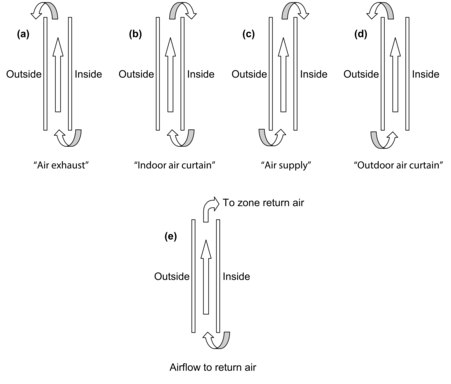
\includegraphics[width=0.9\textwidth, height=0.9\textheight, keepaspectratio=true]{media/image065.png}
  \caption{Gap airflow configurations for airflow windows. (a) \textbf{Air exhaust window}: Airflow Source = InsideAir, Airflow Destination = OutsideAir; (b) \textbf{Indoor air curtain window}: Airflow Source = InsideAir, Airflow Destination = InsideAir; (c) \textbf{Air supply window}: Airflow Source = OutsideAir, Airflow Destination = InsideAir; (d) \textbf{Outdoor air curtain window}: Airflow Source = OutsideAir, Airflow Destination = OutsideAir; (e) \textbf{Airflow to Return Air}: Airflow Source = InsideAir, Airflow Destination = ReturnAir. Based on ``Active facades,'' Version no. 1, Belgian Building Research Institute, June 2002. \protect \label{fig:gap-airflow-configurations-for-airflow}}
\end{figure}

An IDF example: window with a constant airflow from inside to outside at 0.008 m\(^{3}\)/s-m.

\begin{lstlisting}
WindowProperty:AirflowControl,   !- Used to control forced airflow through a gap between glass layers
      Zn001:Wall001:Win002,   !- Name of Associated Window
      InsideAir,              !- Airflow Source
      OutsideAir,             !- Airflow Destination
      0.008,                  !- Maximum Airflow (m3/s per m of glazing width)
      AlwaysOnAtMaxFlow,      !- Airflow Control Type
      No,                     !- Airflow Has Multiplier Schedule?
      ;                       !- Name of Airflow Multiplier Schedule
\end{lstlisting}

\subsection{WindowProperty:StormWindow}\label{windowpropertystormwindow}

This object allows you to assign a movable exterior glass layer (``storm window'' or ``storm glass'') that is usually applied to a window in the winter to reduce heat loss and removed in the summer. A WindowProperty:StormWindow object is required for each window that has an associated storm window. It is assumed that:

\begin{itemize}
\item
  When the storm glass is in place it is the outermost layer of the window, it covers only the glazed part of the window and not the frame, and it forms a tight seal. See Figure~\ref{fig:section-through-a-single-glazed-window}.
\item
  When the storm glass is not in place it is completely removed and has no effect on window heat transfer.
\item
  The gap between the storm glass and rest of the glazing is filled with air.
\end{itemize}

\begin{figure}[hbtp] % fig 40
\centering
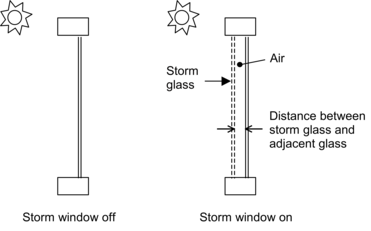
\includegraphics[width=0.9\textwidth, height=0.9\textheight, keepaspectratio=true]{media/image066.png}
\caption{Section through a single-glazed window without (left) and with (right) a storm glass layer. Not to scale. \protect \label{fig:section-through-a-single-glazed-window}}
\end{figure}

With the addition of a storm window, single glazing effectively becomes double glazing, double glazing becomes triple glazing, etc.

The presence of a storm window is indicated by the output variable ``Surface Storm Window On Off Status'' (see ``Window Output Variables''). This flag is \textbf{0} if the storm window is off, \textbf{1} if it is on, and \textbf{--1} if the window does not have an associated storm window.

The program automatically creates a window construction (ref: Construction) that consists of the storm window glass layer and its adjacent air layer added to the original (unshaded, or ``bare'') window construction. In the eplusout.eio file this construction is called BARECONSTRUCTIONWITHSTORMWIN:\emph{n}, where \emph{n} is the number of the associated StormWin object. If the window has a shaded construction, the program creates a construction called SHADEDCONSTRUCTIONWITHSTORMWIN:\emph{n} that consists of the storm window glass layer and its adjacent air layer added to the original shaded window construction.

The program also creates a WindowMaterial:Gas layer corresponding to the air layer adjacent to the storm glass. In the eplusout.eio file this layer is called AIR:STORMWIN:\emph{k}MM, where \emph{k} is the thickness of the air layer expressed as an integer number of millimeters.

\subsubsection{Inputs}\label{inputs-35-001}

\paragraph{Field: Window Name}\label{field-window-name-000}

This is the name of a window (or glass door) to which the storm glass is applied. Not all windows can accept WindowProperty:StormWindow. The rules are:

\begin{itemize}
\item
  The window must be an exterior window. WindowProperty:StormWindow is not applicable to interior (interzone) windows.
\item
  The window construction (without the storm glass layer) can have up to three glass layers.
\item
  If the window has an associated shaded construction (ref: WindowProperty:ShadingControl), that construction can have an interior shade or blind and up to three glass layers, or a between-glass shade or blind and two glass layers. The shaded construction cannot have an exterior shade or blind, cannot have a between-glass shade or blind and three glass layers, and cannot be switchable glazing.
\item
  The window cannot be an airflow window, i.e., a window that has an associated WindowProperty:AirflowControl.
\end{itemize}

\paragraph{Field: Storm Glass Layer Name}\label{field-storm-glass-layer-name}

This is the name of a window glass material. Storm windows are assumed to consist of a single layer of glass. A storm window frame, if present, is ignored.

\paragraph{Field: Distance Between Storm Glass Layer and Adjacent Glass}\label{field-distance-between-storm-glass-layer-and-adjacent-glass}

The separation between the storm glass and the rest of the window (Figure~\ref{fig:section-through-a-single-glazed-window}). It is measured from the inside of the storm glass layer to the outside of the adjacent glass layer.

\paragraph{Field: Month that Storm Glass Layer Is Put On}\label{field-month-that-storm-glass-layer-is-put-on}

The number of the month (January = 1, February = 2, etc.) during which the storm window is put in place.

\paragraph{Field: Day of Month that Storm Glass Layer Is Put On}\label{field-day-of-month-that-storm-glass-layer-is-put-on}

The day of the month that the storm window is put in place. It is assumed that the storm window is put in place at the beginning of this day, i.e., during the first simulation timestep of the day, and remains in place until that month and day given by the following two fields.

\paragraph{Field: Month that Storm Glass Layer Is Taken Off}\label{field-month-that-storm-glass-layer-is-taken-off}

The number of the month (January = 1, February = 2, etc.) during which the storm window is removed.

\paragraph{Field: Day of Month that Storm Glass Layer Is Taken Off}\label{field-day-of-month-that-storm-glass-layer-is-taken-off}

The day of the month that the storm window is removed. It is assumed that the storm window is removed at the beginning of this day, i.e., during the first simulation timestep of the day, and stays off until the month and day given by Month that Storm Glass Layer Is Put On, Day of Month that Storm Glass Layer Is Put On.

In the northern hemisphere, the month the storm window is put on is generally greater than the month it is taken off (for example put on in month 10, when it starts to get cold, and taken off in month 5, when it starts to warm up). In the southern hemisphere this is reversed: month on is less than month off.

An IDF example of WindowProperty:StormWindow. The storm window is put in place on October 15 and removed on May 1.

\begin{lstlisting}
WindowProperty:StormWindow,
   Window1, !- Name of Window to Which Storm Window Glass Layer is Applied
   GlassA,  !- Name of Material:WindowGlass or MATERIAL:WindowGlass:AltInput that is the storm window layer
   0.060,   !- Distance from storm window to adjacent glass (m)
   10,      !- Month that Storm Window Is Put On
   15,      !- Day of Month that Storm Window Is Put On
   5,       !- Month that Storm Window Is Taken Off
   1;       !- Day of Month that Storm Window Is Taken Off
\end{lstlisting}

\subsection{Importing Windows from WINDOW program}\label{importing-windows-from-window-program}

\begin{callout}
WINDOW v6.3 and later is capable of writing IDF excerpts for Window data. This is the preferred method as no external file is necessary. See the Tips document for details on obtaining the IDF excerpt.
\end{callout}

The WINDOW program calculates the U-value, Solar Heat Gain Coefficient, solar transmission/absorption characteristics, visible transmission characteristics and other properties of a window under standard indoor and outdoor conditions. WINDOW treats the whole window system---glazing, frame and divider. A sub-program of WINDOW called THERM uses a 2-D finite element calculation to determine the effective conductance of frame, divider and edge-of-glass elements. Another sub-program, OPTICS, determines the solar-optical properties of glazing, including laminates and coated glass.

WINDOW can write a data file containing a description of the window that was analyzed. An example of this file (which is no longer the preferred method) is shown in the Tips document under WINDOW generated files. is shown below. This file, which can be named by the user, can be read by EnergyPlus. For more complete description and examples, see the object description -- Construction:WindowDataFile.

In this way, the same window that was created in WINDOW can be imported into EnergyPlus for annual energy analysis without having to re-input the window data. To obtain WINDOW, THERM, or OPTICS go to \url{http://windows.lbl.gov} and choose the software link. A major advantage of using WINDOW to create window input for EnergyPlus is that you will have direct access to WINDOW's expanding database of over 1000 different glass types; and you will be able to browse through this database according to different criteria (color, transmittance, solar heat gain coefficient, etc.) to help you select the best glass type for your application.

Although WINDOW writes only one window entry on the WINDOW data file, EnergyPlus users can combine two or more of these files to end up with a single data file with multiple window entries of different types. In this way a library of windows from WINDOW can be built up if so desired. If you combine files like this you should be sure not to leave out or change any of lines from the original files.

There are four methods for inputting window constructions in EnergyPlus:

\begin{enumerate}
\tightlist
\item
  input full spectral data for each layer in the IDF,
\item
  input spectral average data for each layer in the IDF,
\item
  items 1 and 2 can be accomplished by reporting the IDF excerpt method from WINDOW
\item
  import WINDOW report containing layer-by-layer calculated values and overall glazing system angular values.
\end{enumerate}

\begin{callout}
  \warning{Note: When using method 4, the overall glazing system angular dependent properties, including Tsol, Abs, Rfsol, Rbsol, Tvis, Rfvis, and Rbvis, are not used by EnergyPlus. Therefore, methods 1 and 2 and preferably 3 are recommended.}
\end{callout}

\begin{itemize}
\item
  The SHGC calculations in EnergyPlus for window layers input using full spectral data use a spectral weighting data set (derived from Optics5 data file ISO-9845GlobalNorm.std) that is different from the WINDOW default spectral weighting data set (W5\_NFRC\_2003.std). This difference accounts for most of the variation in SHGC values reported by EnergyPlus and WINDOW for full spectral data window layer input. This variation is more pronounced for window constructions of three glass layers or more.
\item
  Users intending to select a window construction based on SHGC value for energy code compliance should base their selection on the value reported by WINDOW since this is the officially recognized value.
\end{itemize}

In EnergyPlus, the Window data file is searched for each ``Construction:WindowDataFile'' object in the EnergyPlus input. This object has a very simple form:

\begin{lstlisting}
Construction:WindowDataFile,
  ConstructionName,
  FileName; ! Default is Window5DataFile.dat in the "run" folder.
\end{lstlisting}

If there is a window called ConstructionName on the Window data file, the data for that window is read from the file and the following EnergyPlus objects and their names are created. The ``W5'' prefixed to these names indicates that the object originated in the Window data file.

\subsection{Zone Thermal Output(s)}\label{zone-thermal-outputs-1}

In addition to the canned Surface reports (view the Reports section later in this document) and surface variables (above), the following variables are available for all zones:

\begin{lstlisting}
Zone,Sum,Zone Total Internal Radiant Heating Energy [J]
Zone,Sum,Zone Total Internal Visible Radiation Heating Energy [J]
Zone,Sum,Zone Total Internal Convective Heating Energy [J]
Zone,Sum,Zone Total Internal Latent Gain Energy [J]
Zone,Sum,Zone Total Internal Total Heating Energy [J]
Zone,Average,Zone Mean Air Temperature [C]
HVAC,Average,Zone Air Temperature [C]
Zone,Average,Zone Mean Radiant Temperature [C]
Zone,Average,Zone Operative Temperature [C]
HVAC,Sum,Zone Air System Sensible Heating Energy [J]
HVAC,Sum,Zone Air System Sensible Cooling Energy [J]
HVAC,Average,Zone Air System Sensible Heating Rate [W]
HVAC,Average,Zone Air System Sensible Cooling Rate [W]
HVAC,Average,Zone Air Humidity Ratio[kgWater/kgDryAir]
HVAC,Average,Zone Air Relative Humidity[%]
\end{lstlisting}

Two of these are of particular interest:

\begin{lstlisting}
Zone,Average,Zone Mean Air Temperature [C]
HVAC,Average,Zone Air Temperature [C]
\end{lstlisting}

These two variable outputs are/should be identical. However, note that they can be reported at different time intervals. ``Zone Mean Air Temperature'' is only available on the Zone/HB timestep (Number of Timesteps per Hour) whereas ``Zone Air Temperature'' can be reported at the HVAC timestep (which can vary).

\subsubsection{Zone Mean Air Temperature {[}C{]}}\label{zone-mean-air-temperature-c-1}

From the code definition, the zone mean air temperature is the average temperature of the air temperatures at the system timestep. Remember that the zone heat balance represents a ``well stirred'' model for a zone, therefore there is only one mean air temperature to represent the air temperature for the zone.

\subsubsection{Zone Air Temperature {[}C{]}}\label{zone-air-temperature-c-1}

This is very similar to the mean air temperature in the last field. The ``well stirred'' model for the zone is the basis, but this temperature is also available at the ``detailed'' system timestep.

\subsubsection{Zone Mean Radiant Temperature {[}C{]}}\label{zone-mean-radiant-temperature-c-1}

The Mean Radiant Temperature (MRT) in degrees Celsius of a space is really the measure of the combined effects of temperatures of surfaces within that space. The larger the surface area and the closer one is to it, the more effect the surface temperature of that surface has on each other. The MRT is the measure of all these surface areas and temperatures.

\subsubsection{Zone Operative Temperature {[}C{]}}\label{zone-operative-temperature-c-1}

Zone Operative Temperature (OT) is the average of the Zone Mean Air Temperature (MAT) and Zone Mean Radiant Temperature (MRT), OT = 0.5*MAT + 0.5*MRT. This output variable is not affected by the type of thermostat controls in the zone, and does not include the direct effect of high temperature radiant systems.~ See also Zone Thermostat Operative Temperature.

\subsubsection{Zone Air System Sensible Heating Energy {[}J{]}}\label{zone-air-system-sensible-heating-energy-j-1}

This field represents the sensible heating energy in Joules that is actually supplied by the system to that zone for the timestep reported. This is the sensible heating rate multiplied by the simulation timestep. This is calculated and reported from the Correct step in the Zone Predictor-Corrector module. This field is not multiplied by zone or group multipliers.

\begin{callout}
Zone Air System Sensible Heating (and Cooling) Energy (and Rate) all report the heating or cooling delivered by the HVAC system to a zone. These values are calculated by multiplying the supply air mass flow rate by the difference between the supply air temperature and the zone air temperature. This does not always indicate the operation of heating or cooling coils. For example, cooling will be reported if the supply air is cooled due to the introduction of outside air, even if all coils are off.

Note that these variables are calculated at the system timestep. When reported at the ``detailed'' reporting frequency, these variable will never show heating and cooling both in the same system timestep. If reported at a frequency less than ``Detailed'' (for example, Hourly) values may appear in both the heating and cooling variable for the same hour if the system cooled the zone for part of the reporting period and heated the zone for another part of the reporting period.
\end{callout}

\subsubsection{Zone Air System Sensible Cooling Energy {[}J{]}}\label{zone-air-system-sensible-cooling-energy-j-1}

This field represents the sensible cooling energy in Joules that is actually supplied by the system to that zone for the timestep reported. This is the sensible cooling rate multiplied by the simulation timestep. This is calculated and reported from the Correct step in the Zone Predictor-Corrector module. This field is not multiplied by zone or group multipliers.

\subsubsection{Zone Air System Sensible Heating Rate {[}W{]}}\label{zone-air-system-sensible-heating-rate-w-1}

This field represents the sensible heating rate in Watts that is actually supplied by the system to that zone for the timestep reported. This is calculated and reported from the Correct step in the Zone Predictor-Corrector module. This field is not multiplied by zone or group multipliers.

\subsubsection{Zone Air System Sensible Cooling Rate {[}W{]}}\label{zone-air-system-sensible-cooling-rate-w-1}

This field represents the sensible cooling rate in Watts that is actually supplied by the system to that zone for the timestep reported. This is calculated and reported from the Correct step in the Zone Predictor-Corrector module. This field is not multiplied by zone or group multipliers.

\subsubsection{Zone Air Humidity Ratio{[}kgWater/kgDryAir{]}}\label{zone-air-humidity-ratiokgwaterkgdryair}

This field represents the air humidity ratio after the correct step for each zone. The humidity ratio is the mass of water vapor to the mass of dry air contained in the zone in (kg water/kg air) and is unitless.

\subsubsection{Zone Air Relative Humidity{[}\%{]}}\label{zone-air-relative-humidity-1}

This field represents the air relative humidity ratio after the correct step for each zone. The relative humidity is in percent and uses the Zone Air Temperature, the Zone Air Humidity Ratio and the Outside Barometric Pressure for calculation.

\subsubsection{Zone Total Internal Radiant Heating Energy {[}J{]}}\label{zone-total-internal-radiant-heating-energy-j-1}

This field represents the sum of radiant gains from specific internal sources (e.g.~equipment) throughout the zone in joules. This includes radiant gain from People, Lights, Electric Equipment, Gas Equipment, Other Equipment, Hot Water Equipment, and Steam Equipment.

\subsubsection{Zone-Total Internal Visible Heat Gain {[}J{]}}\label{zone-total-internal-visible-heat-gain-j}

This field expresses the sum of heat gain in joules that is the calculated short wavelength radiation gain from lights in the zones. This calculation uses the total energy from lights and the fraction visible to realize this value, summed over the zones in the simulation.

\subsubsection{Zone Total Internal Convective Heating Energy {[}J{]}}\label{zone-total-internal-convective-heating-energy-j-1}

This field represents the sum of convective gains from specific sources (e.g.~equipment) throughout the zone in joules. This includes convective gain from People, Lights, Electric Equipment, Gas Equipment, Other Equipment, Hot Water Equipment, and Steam Equipment.

\subsubsection{Zone Total Internal Latent Gain Energy {[}J{]}}\label{zone-total-internal-latent-gain-energy-j-1}

This field represents the sum of latent gains from specific internal sources (e.g.~equipment) throughout the zone in joules. This includes latent gain from People, Electric Equipment, Gas Equipment, Other Equipment, Hot Water Equipment, and Steam Equipment.

\subsubsection{Zone Total Internal Total Heating Energy {[}J{]}}\label{zone-total-internal-total-heating-energy-j-1}

This field represents the sum of all heat gains throughout the zone in joules. This includes all heat gains from People, Lights, Electric Equipment, Gas Equipment, Other Equipment, Hot Water Equipment, and Steam Equipment.



This group of objects describe concepts applied to heat transfer surfaces that are of an advanced nature. Careful consideration must be given before using these.

\subsection{SurfaceProperty:HeatTransferAlgorithm}\label{surfacepropertyheattransferalgorithm}

This object, and three other related objects, can be used to control which surface heat transfer model is used on specific surfaces. The separate object called HeatBalanceAlgorithm is used to control the heat transfer model in an overall way while this object can be used to revise the algorithm selections for specific surfaces. This object allows selectively overriding the global setting in HeatBalanceAlgorithm to choose one of the following models for a particular surface:

\begin{itemize}
\item
  CTF (Conduction Transfer Functions),
\item
  EMPD (Effective Moisture Penetration Depth with Conduction Transfer Functions).
\item
  CondFD (Conduction Finite Difference)
\item
  HAMT (Combined Heat And Moisture Finite Element)
\end{itemize}

\subsubsection{Inputs}\label{inputs-000}

\paragraph{Field: Surface Name}\label{field-surface-name}

This is the name of the surface that will be assigned to use the heat transfer algorithm selected in the next field. This should be a name of a surface defined elsewhere.

\paragraph{Field: Algorithm}\label{field-algorithm}

This field is used to determine the heat transfer algorithm that is to be applied to the surface named in the previous field. The allowable choices are:

\begin{itemize}
\item
  ConductionTransferFunction
\item
  MoisturePenetrationDepthConductionTransferFunction
\item
  ConductionFiniteDifference
\item
  CombinedHeatAndMoistureFiniteElement
\end{itemize}

\subsection{SurfaceProperty:HeatTransferAlgorithm:MultipleSurface}\label{surfacepropertyheattransferalgorithmmultiplesurface}

This object can be used to control the surface heat transfer model used for specific types of surfaces. The separate object called HeatBalanceAlgorithm is used to control the heat transfer model in an overall way while this object can be used to revise the algorithm selections for specific types of surfaces. This object allows selectively overriding the global setting in HeatBalanceAlgorithm to choose one of the following models for all surfaces of a particular type:

\begin{itemize}
\item
  CTF (Conduction Transfer Functions),
\item
  EMPD (Effective Moisture Penetration Depth with Conduction Transfer Functions).
\item
  CondFD (Conduction Finite Difference)
\item
  HAMT (Combined Heat And Moisture Finite Element)
\end{itemize}

\subsubsection{Inputs}\label{inputs-1-000}

\paragraph{Field: Name}\label{field-name-000}

This is a unique, user-defined name for the object.

\paragraph{Field: Surface Type}\label{field-surface-type}

This field is selects the type of surfaces that are all assigned to use the heat transfer algorithm selected in the next field. This field is used with one of the following allowable keywords:

\begin{itemize}
\item
  AllExteriorSurfaces---all surfaces that have ``Outdoors'' outside boundary condition
\item
  AllExteriorWalls---all walls that have ``Outdoors'' outside boundary condition
\item
  AllExteriorRoofs---all roofs that have ``Outdoors'' outside boundary condition
\item
  AllExteriorFloors---all floors that have ``Outdoors'' outside boundary condition
\item
  AllGroundContactSurfaces---all surfaces that have ``Ground'' outside boundary condition
\item
  AllInteriorSurfaces---all surfaces that are internal partition-type surfaces
\item
  AllInteriorWalls---all walls that are internal surfaces
\item
  AllInteriorCeilings---all ceilings that are internal surfaces
\item
  AllInteriorFloors---all floors that are are internal surfaces
\end{itemize}

\paragraph{Field: Algorithm}\label{field-algorithm-1}

This field is used to determine the heat transfer algorithm that is to be applied to the surface types in the previous field. The allowable choices are:

\begin{itemize}
\item
  ConductionTransferFunction
\item
  MoisturePenetrationDepthConductionTransferFunction
\item
  ConductionFiniteDifference
\item
  CombinedHeatAndMoistureFiniteElement
\end{itemize}

\begin{lstlisting}
SurfaceProperty:HeatTransferAlgorithm:MultipleSurface,
      my exterior wall override,
      AllExteriorWalls,
      ConductionFiniteDifference;
\end{lstlisting}

\subsection{SurfaceProperty:HeatTransferAlgorithm:SurfaceList}\label{surfacepropertyheattransferalgorithmsurfacelist}

This object can be used to control the surface heat transfer model used for a list of surfaces. The separate object called HeatBalanceAlgorithm is used to control the heat transfer model in an overall way while this object can be used to revise the algorithm selections for a list of specific surfaces. This object allows selectively overriding the global setting in HeatBalanceAlgorithm to choose one of the following models for listed:

\begin{itemize}
\item
  CTF (Conduction Transfer Functions),
\item
  EMPD (Effective Moisture Penetration Depth with Conduction Transfer Functions).
\item
  CondFD (Conduction Finite Difference)
\item
  HAMT (Combined Heat And Moisture Finite Element)
\end{itemize}

\subsubsection{Inputs}\label{inputs-2-000}

\paragraph{Field: Name}\label{field-name-1}

This is a unique, user-defined name for the object.

\paragraph{Field: Algorithm}\label{field-algorithm-2}

This field is used to determine the heat transfer algorithm that is to be applied to the surface listed in the remaining fields. The allowable choices are:

\begin{itemize}
\item
  ConductionTransferFunction
\item
  MoisturePenetrationDepthConductionTransferFunction
\item
  ConductionFiniteDifference
\item
  CombinedHeatAndMoistureFiniteElement
\end{itemize}

\paragraph{Field: Surface Name N}\label{field-surface-name-n}

This is the name of the ``Nth'' surface that will be assigned to use the heat transfer algorithm selected in this object. These should be the names of surfaces defined elsewhere. This object is extensible. Additional surfaces can be added to extend the object.

An example IDF object follows.

\begin{lstlisting}

SurfaceProperty:HeatTransferAlgorithm:SurfaceList,
      my wall construct override,   !- Name
      ConductionFiniteDifference,   !- Algorithm
      Zn001:Wall001,                !- Surface Name 1
      Zn001:Wall002,                !- Surface Name 2
      Zn001:Wall003,                !- Surface Name 3
      Zn001:Wall004;                !- Surface Name 4
\end{lstlisting}

\subsection{SurfaceProperty:HeatTransferAlgorithm:Construction}\label{surfacepropertyheattransferalgorithmconstruction}

This object can be used to control the surface heat transfer model used for surfaces that have a specific type of construction. The separate object called HeatBalanceAlgorithm is used to control the heat transfer model in an overall way while this object can be used to revise the algorithm selections for specific constructions. This object allows selectively overriding the global setting in HeatBalanceAlgorithm to choose one of the following models for all surfaces with particular type of construction:

\begin{itemize}
\item
  CTF (Conduction Transfer Functions),
\item
  EMPD (Effective Moisture Penetration Depth with Conduction Transfer Functions).
\item
  CondFD (Conduction Finite Difference)
\item
  HAMT (Combined Heat And Moisture Finite Element)
\end{itemize}

\subsubsection{Inputs}\label{inputs-3}

\paragraph{Field: Name}\label{field-name-2}

This is a unique, user-defined name for the object.

\paragraph{Field: Algorithm}\label{field-algorithm-3}

This field is used to determine the heat transfer algorithm that is to be applied to the surfaces with the type of of construction listed in the next field. The allowable choices are:

\begin{itemize}
\item
  ConductionTransferFunction
\item
  MoisturePenetrationDepthConductionTransferFunction
\item
  ConductionFiniteDifference
\item
  CombinedHeatAndMoistureFiniteElement
\end{itemize}

\paragraph{Field: Construction Name}\label{field-construction-name}

This field is the name of a Construction object defined elsewhere. All the surfaces in the model that are assigned this type of construction will be assigned to use the heat transfer algorithm selected in the previous field.

An example IDF object follows.

\begin{lstlisting}

SurfaceProperty:HeatTransferAlgorithm:Construction,
      my wall construct override,  !- Name
      ConductionFiniteDifference,  !- Algorithm
      R13WALL;                     !- Construction Name
\end{lstlisting}

\subsection{SurfaceControl:MovableInsulation}\label{surfacecontrolmovableinsulation}

Movable insulation can be used/scheduled on any surface regular surface (such as a wall, floor, roof, etc.) but not on a subsurface (such as a window, use WindowProperty:ShadingControl instead). With movable insulation, no reference is made in the surface that is using the insulation -- rather the movable insulation statement references the surface to which it is applied.

Exterior and interior movable insulation have undergone some testing and appears to producing expected results. The underlying principle has been implemented in EnergyPlus for both interior and exterior movable insulation with the possibility for exterior movable insulation to be transparent (transparent insulation material or TIM).

TIM exterior layers can be used with the ConductionFiniteDifference (CondFD) solution algorithm. With this addition, TIM layers can be used in conjunction with wall layers that have phase change materials (PCM) included, or any other advanced capability of the CondFD algorithm such as variable conductivity. The input requirements are exactly the same as when used with the CTF algorithm. The Solution Algorithm needs to be changed to CondFD, and as with CTF, the ``SurfaceControl:MovableInsulation'' object must be completed to specify the insulated surface and the ``WindowMaterial:Glazing'' object is needed to provide the TIM layer properties.

Basically, the addition of movable insulation allows the user to schedule an extra amount of insulation on either the inside or outside surface of a wall (or both). The insulation must be a simple, homogenous material layer (linked to a material definition within the input data file). Note that EnergyPlus allows the exterior movable insulation layer to be transparent to short wavelength radiation (solar). In this case, incident solar is split between the plane between the movable insulation and the surface and the plane between the movable insulation and the surrounding air. This calculation is fairly basic and based on the solar transmittance of the insulation layer (material properties). Using transparent layers for exterior movable insulation allows solar energy to penetrate deeper into a construction where it can be stored for later use in the building (similar in concept to a Trombe Wall).

\subsubsection{Field: Insulation Type}\label{field-insulation-type}

This field determines whether the movable insulation is applied to the inside or the outside of the surface by entering either ``Inside'' or ``Outside'', respectively.

\subsubsection{Field: Surface Name}\label{field-surface-name-1}

This field refers the movable insulation back to a particular surface (ref: Building Surfaces) via its user assigned name so that EnergyPlus knows where to apply this extra layer of insulation. This will affect either the inside or outside surface heat balance of this surface depending on the value in the insulation type field (see previous field).

\subsubsection{Field: Material Name}\label{field-material-name}

This field refers to a material layer (e.g., Material, Material:NoMass, or WindowMaterial:Glazing; transparent layers are only valid for outside movable insulation) via its user assigned name. This provides the program with a full complement of material properties so that the effect of the insulation (R-value and solar transmittance) can be correctly taken into account by EnergyPlus.  Note that for non-glazing materials the solar absorptivity of the layer will be used directly in the calculations.  For glazing material layers, the solar absorptivity will be calculated by subtracting both the transmissivity and the front side reflectivity from unity for the material.

\subsubsection{Field: Schedule Name}\label{field-schedule-name}

This field is a schedule that theoretically can be any positive real number but was originally intended to be a parameter between 0.0 and 1.0. Its purpose is to act as a fractional modifier on the resistance of the material layer. The actual thermal resistance of the movable insulation is equal to the resistance of the material layer times the current value in the movable insulation schedule. A value of 0.0 simply means that the movable insulation is not present.

An example of this syntax implemented in an input file is:

\begin{lstlisting}

SurfaceControl:MoveableInsulation,
    Exterior,                      ! Insulation Type
    Zone001:Wall001,               ! Surface Name
    TransparentInsulationMaterial, ! Material Name
    PresentInWinterSchedule;       ! Schedule Name
\end{lstlisting}

\subsection{SurfaceProperty:OtherSideCoefficients}\label{surfacepropertyothersidecoefficients}

By referencing the Other Side Coefficients statement in the surface statements (i.e.~Outside Boundary Condition), the temperature of the outer plane of a surface (see Figure~\ref{fig:illustration-for-other-side-coefficients}) can be directly controlled. Other side coefficients can also be used to control the exterior convective heat transfer coefficient of a surface and the corresponding exterior air temperature. It should be noted that solar effects are not accounted for when other side coefficients are used. In addition, if other side coefficients are specified for a surface, they also hold for subsurfaces of that surface (though subsurfaces can have their own coefficient set).

other side coefficients have the same effect on all types of heat transfer surfaces. In other words, an interior surface with other side coefficients specified and an exterior wall with identical other side coefficients specified are simulated exactly the same. A surface that uses other side coefficients should be thought of as a new or separate type of surface. All heat transfer surfaces are simulated in the same manner through conduction transfer functions. The only difference between the various types of heat transfer surfaces is the environment on the other side of the surface. For example, the other side environment of an exterior surface is the outdoor environment. For an interior surface, the temperature of the outer plane of the surface is set equal to the temperature of the inner plane of the surface. Similarly, a surface with other side coefficients specified will allow the user to control the other side environment.

Heat transfer through a surface is an extremely important component in the calculation of zone loads. The information to calculate this heat transfer is readily available if the surface is exposed to the outdoor environment or to another zone that is being simulated. Occasionally, a user will want to model the heat transfer through a surface that is adjacent to an area that is not included in the EnergyPlus model. For example, an office area is attached to a warehouse and the user is only interested in simulating the office area. An interior surface with other side coefficients specified could be used to control the environment on the other side of the surface, thereby accounting for the heat transfer through the adjoining surface.

Other Side Coefficients affects the ``other side'' of a surface as described below. Each coefficient has a special meaning. You may enter a 0 or blank if you are not using a particular coefficient. Note that there are two potential ways to use other side coefficients. Either they are used to set the temperature of the exterior side surface directly (if the combined convective/radiative coefficient below is less than or equal to zero) or to set both the film coefficient (positive value for the combined convective/radiative coefficient below) and the outside air temperature.

\subsubsection{Inputs}\label{inputs-4}

\paragraph{Field: Name}\label{field-name-3}

This, of course, is the string referenced in the Surface statement that is using OtherSideCoefficients as the Outside Boundary Condition.

\paragraph{Field: Combined Convective/Radiative Film Coefficient}\label{field-combined-convectiveradiative-film-coefficient}

This is a trigger value. If the value is greater than zero, then it is taken to be the combined convective/radiative film coefficient. In this case (value \textgreater{} 0), the remaining fields are used first to calculate the outside air temperature for the surface and then to calculate the outside surface temperature based on the outside air temperature and the film coefficient. If this field is less than or equal to zero, then the remaining fields are used to calculate the surface temperature (not the outside air temperature). The units for this field are the same as for a convective heat transfer coefficient: W/(m\(^{2}\)*K). This is referred to as ``C1'' in the reference below.

\paragraph{Field: Constant Temperature}\label{field-constant-temperature}

This field defines a temperature term that is a constant part of the calculation either of the surface or outside air temperature. This parameter is shown as ``C2'' in the equation below. The units for this parameter are degrees C. If a schedule name is included as the second parameter, the value of this parameter will be overridden by the value from the schedule. The default for this field is 0.0.

\paragraph{Field: Constant Temperature Coefficient}\label{field-constant-temperature-coefficient}

This field defines a constant coefficient that is applied to the constant temperature (see previous field). This parameter is shown as ``C3'' in the equation below. This parameter is dimensionless. The value of this parameter is usually 1.0 if a schedule is used to set C2. This field is ignored if \emph{Sinusoidal Variation of Constant Temperature Coefficient} = Yes. The default for this field is 1.0.

\paragraph{Field: External Dry-Bulb Temperature Coefficient}\label{field-external-dry-bulb-temperature-coefficient}

This field defines a constant coefficient that is applied to the outside air dry-bulb temperature. This parameter is shown as ``C4'' in the equation below. This parameter is dimensionless. The default for this field is 0.0.

\paragraph{Field: Ground Temperature Coefficient}\label{field-ground-temperature-coefficient}

This field defines a constant coefficient that is applied to the ground temperature (ref. Site:GroundTemperature:BuildingSurface). This parameter is shown as ``C5'' in the equation below. This parameter is dimensionless.

\paragraph{Field: Wind Speed Coefficient}\label{field-wind-speed-coefficient}

This field defines a constant coefficient that is applied to the product of the outside air dry-bulb temperature and the wind speed. This parameter is shown as ``C6'' in the equation below. This parameter has dimensions of inverse velocity or s/m. The default for this field is 0.0.

\paragraph{Field: Zone Air Temperature Coefficient}\label{field-zone-air-temperature-coefficient}

This field defines a constant coefficient that is applied to the temperature of the zone to which this surface belongs. This parameter is shown as ``C7'' in the equation below. This parameter is dimensionless. The default for this field is 0.0.

\paragraph{Field: Constant Temperature Schedule Name}\label{field-constant-temperature-schedule-name}

This field is used to supply a schedule name. That schedule will supply the ``constant'' temperature value C2. Note that the value of the C3 field should normally be 1.0 if a schedule is used for C2. If not blank, this field must be a valid schedule name.

\paragraph{Field: Sinusoidal Variation of Constant Temperature Coefficient}\label{field-sinusoidal-variation-of-constant-temperature-coefficient}

This field is optional and can be used to define an alternate method of prescribing the coefficient that is applied to the constant temperature (see the fields Constant Temperature and Constant Temperature Coefficient). This parameter is shown as ``C2'' in the equation below. If this field is omitted, left blank, or set to ``No,'' then C2 is a constant (defined in the field Constant Temperature Coefficient). However if this is set to ``Yes,'' then the value of C2 varies with a unitary sine wave in the following way:

\begin{equation}
C2 = Sin\left( {2\pi \frac{{\left( {time\,of\,day} \right)}}{{\left( {period} \right)}}} \right)
\end{equation}

The value for ``period'' is controlled in the following field. The value for ``time of day'' is based on the zone timestep and is in units of hours. The sine function here uses input as radians. When using this option, the value for C2 will vary between -1.0 and 1.0 and the value put in the field Constant Temperature Coefficient is not used. This option cannot be used at the same time as scheduling a constant temperature with the previous field.

\paragraph{Field: Period of Sinusoidal Variation}\label{field-period-of-sinusoidal-variation}

This field is used to define the period of the sine wave when using the Sinusodial Variation of Constant Temperature Coefficient capability selected in the previous field. This field is the time period of the sine wave in units of hours. The default is 24 hours and provides a diurnal sine wave. The value entered here is ``period'' in the equation in the previous field.

\paragraph{Field: Previous Other Side Temperature Coefficient}\label{field-previous-other-side-temperature-coefficient}

This field defines a constant coefficient that is applied to the other side temperature computed by this object from the previous zone time step. This parameter is shown as ``C8'' in the equation below. This parameter is dimensionless. The default for this field is 0.0.

\paragraph{Field: Minimum Other Side Temperature Limit}\label{field-minimum-other-side-temperature-limit}

This field specifies a lower limit for the other side temperature result in degrees C. If blank, there is no lower limit.

\paragraph{Field: Maximum Other Side Temperature Limit}\label{field-maximum-other-side-temperature-limit}

This field specifies an upper limit for the other side temperature result in degrees C. If blank, there is no upper limit.

The coefficients listed above are used in the following equation:

\begin{equation}
T = C2*C3 + C4*Toadb + C5*Tgrnd + C6*Wspd*Toadb + C7*Tzone + C8*Tpast
\end{equation}

where:

T = Outside Air Temperature when C1 (Combined convective/radiative film Coeff) \textgreater{} 0

T = Exterior Surface Temperature when C1 (Combined convective/radiative film Coeff) \textless{} = 0

Tzone = Temperature of the zone being simulated (°C)

Toadb = Dry-bulb temperature of the outdoor air (°C)

Tgrnd = Temperature of the ground (°C) from Site:GroundTemperature:BuildingSurface

Wspd = Outdoor wind speed (m/sec)

Tpast = Other side temperature from previous zone timestep (°C)

\begin{figure}[hbtp] % fig 41
\centering
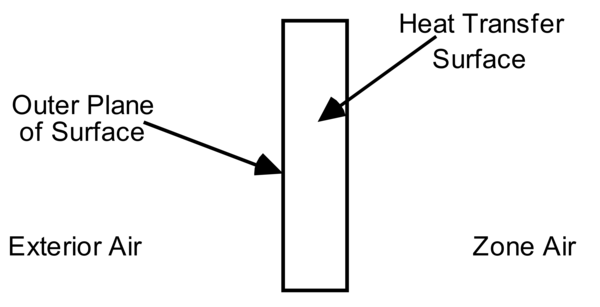
\includegraphics[width=0.9\textwidth, height=0.9\textheight, keepaspectratio=true]{media/image069.png}
\caption{Illustration for Other Side Coefficients \protect \label{fig:illustration-for-other-side-coefficients}}
\end{figure}

\begin{lstlisting}
!  Example input using temperature schedule
SurfaceProperty:OtherSideCoefficients,
      OSCCoef:Zn005:Wall003,   !- Name
      0,                       !- Combined Convective/Radiative Film Coefficient {W/m2-K}
      0.000000,                !- Constant Temperature {C}
      1.000000,                !- Constant Temperature Coefficient
      0.000000,                !- External Dry-Bulb Temperature Coefficient
      0.000000,                !- Ground Temperature Coefficient
      0.000000,                !- Wind Speed Coefficient
      0.000000,                !- Zone Air Temperature Coefficient
      Zn005Wall003OtherSideTempSched;  !- Constant Temperature Schedule Name
\end{lstlisting}

\begin{lstlisting}
!  Example input for outside heat transfer coefficient of 1.23, using Toadb
SurfaceProperty:OtherSideCoefficients,
      OSCCoef:Zn005:Wall004,   !- Name
      1.230000,                !- Combined Convective/Radiative Film Coefficient {W/m2-K}
      0.000000,                !- Constant Temperature {C}
      0.000000,                !- Constant Temperature Coefficient
      1.000000,                !- External Dry-Bulb Temperature Coefficient
      0.000000,                !- Ground Temperature Coefficient
      0.000000,                !- Wind Speed Coefficient
      0.000000,                !- Zone Air Temperature Coefficient
      ,                        !- Constant Temperature Schedule Name
      No,                      !- Sinusoidal Variation of Constant Temperature Coefficient
      24,                      !- Period of Sinusoidal Variation {hr}
      0.,                      !- Previous Other Side Temperature Coefficient
      ,                        !- Minimum Other Side Temperature Limit {C}
      ;                        !- Maximum Other Side Temperature Limit {C}
\end{lstlisting}

\subsubsection{Outputs}\label{outputs}

\begin{lstlisting}
Zone,Average,Surface Other Side Coefficients Exterior Air Drybulb Temperature
\end{lstlisting}

\paragraph{Surface Other Side Coefficients Exterior Air Drybulb Temperature {[}C{]}}\label{surface-other-side-coefficients-exterior-air-drybulb-temperature-c}

This is the air temperature applied to the other side of the surface.

\subsection{SurfaceProperty:OtherSideConditionsModel}\label{surfacepropertyothersideconditionsmodel}

By referencing the Other Side Conditions Model statement in the surface statements (i.e.~Outside Boundary Condition), the boundary conditions for the outer plane of the mass wall can be connected to the appropriate model for various multi-skin components. The types of multi-skin components that use this object include systems that are mounted to the outside surface using standoffs that create a small air gap -- see Figure~\ref{fig:illustration-for-other-side-conditions-model}. This type of modeling allows using the usual heat transfer calculations for the underlying surface with other types of multi-skin component models that are available including: unglazed transpired solar collectors, ventilated photovoltaic panels, and naturally ventilated facades.

The boundary condition values are determined dynamically by the program using internal component models. If you want to define other side surface temperatures or convection conditions, then use SurfaceProperty:OtherSideCoefficients instead of this object.

It should be noted that when other side conditions models are used, solar effects are removed from the surface's outside face heat balance, but are used in modeling the component adjacent to that surface.

In addition, the other side conditions model has been modified to include underground piping system interaction. The PipingSystem:Underground:Domain object represents a mass of ground which may include interaction with, for example, basement surfaces. In this case, the ground model will internally use the other side condition model hook to update boundary conditions for those surfaces which use that other side condition model name reference.

\subsubsection{Inputs}\label{inputs-5}

\paragraph{Field: Name}\label{field-name-4}

This is the string referenced in the Surface statement that is using OtherSideModel as the Exterior Environment.

\paragraph{Field: Type of Modeling}\label{field-type-of-modeling}

This is a string key selection used to identify the type of model that will be used to determine boundary conditions. The only available choices are ''GapConvectionRadiation,'' ``UndergroundPipingSystemSurface,'' and ``GroundCoupledSurface.''

\begin{figure}[hbtp] % fig 42
\centering
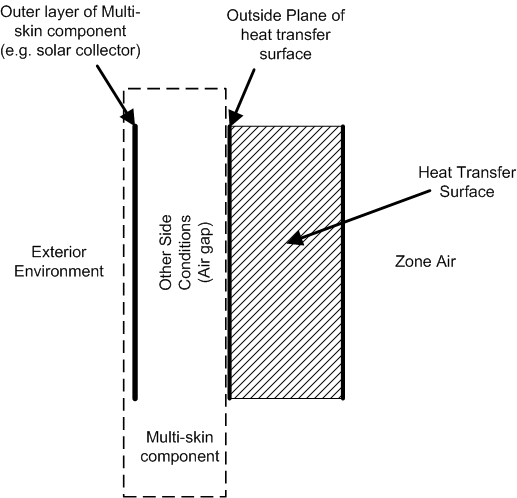
\includegraphics[width=0.9\textwidth, height=0.9\textheight, keepaspectratio=true]{media/image070.png}
\caption{Illustration for Other Side Conditions Model \protect \label{fig:illustration-for-other-side-conditions-model}}
\end{figure}

An example specification is:

\begin{lstlisting}

SurfaceProperty:OtherSideConditionsModel,
      UTSC OSCM ZN11,          ! OtherSideConditionsModel Name
      GapConvectionRadiation; ! Type of Modeling used to determine Boundary Conditions
\end{lstlisting}

\subsubsection{Outputs}\label{outputs-1}

\begin{itemize}
\item
  Zone,Average,Surface Other Side Conditions Modeled Convection Air Temperature {[}C{]}
\item
  Zone,Average,Surface Other Side Conditions Modeled Convection Heat Transfer Coefficient {[}W/m2-K{]}
\item
  Zone,Average,Surface Other Side Conditions Modeled Radiation Temperature {[}C{]}
\item
  Zone,Average,Surface Other Side Conditions Modeled Radiation Heat Transfer Coefficient {[}W/m2-K{]}
\end{itemize}

\paragraph{Surface Other Side Conditions Modeled Convection Air Temperature {[}C{]}}\label{surface-other-side-conditions-modeled-convection-air-temperature-c}

This is the air temperature exposed to the other side of the surface by the model and used in convection heat transfer calculations.

\paragraph{Surface Other Side Conditions Modeled Convection Heat Transfer Coefficient {[}W/m2-K{]}}\label{surface-other-side-conditions-modeled-convection-heat-transfer-coefficient-wm2-k}

This is the surface convection heat transfer coefficient applied to the other side of the surface by the model.

\paragraph{Surface Other Side Conditions Modeled Radiation Temperature {[}C{]}}\label{surface-other-side-conditions-modeled-radiation-temperature-c}

This is the effective temperature exposed to the other side of the surface for thermal radiation heat transfer calculations.

\paragraph{Surface Other Side Conditions Modeled Radiation Heat Transfer Coefficient {[}W/m2-K{]}}\label{surface-other-side-conditions-modeled-radiation-heat-transfer-coefficient-wm2-k}

This is the effective (Linearized) radiation heat transfer coefficient applied to the other side of the surface by the model.

\subsection{SurfaceConvectionAlgorithm:Inside:AdaptiveModelSelections}\label{surfaceconvectionalgorithminsideadaptivemodelselections}

This object provides options to change the individual convection model equations for dynamic selection when using AdaptiveConvectionAlgorithm. This object is only needed to make changes to the default model selections for any or all of the surface categories. This object is for the inside face, the side of the surface facing a thermal zone.

\subsubsection{Inputs}\label{inputs-6}

\paragraph{Field: Name}\label{field-name-5}

A unique name for the object.

\paragraph{Field: Simple Buoyancy Vertical Wall Equation Source}\label{field-simple-buoyancy-vertical-wall-equation-source}

Applies to zone with no HVAC or when HVAC is off. This is for vertical walls. The key choice options include: FohannoPolidoriVerticalWall, ASHRAEVerticalWall, AlamdariHammondVerticalWall, KhalifaEq3WallAwayFromHeat, KhalifaEq6NonHeatedWalls FohannoPolidoriVerticalWall, ISO15099Windows, or UserCurve

\paragraph{Field: Simple Buoyancy Vertical Wall User Curve Name}\label{field-simple-buoyancy-vertical-wall-user-curve-name}

The SurfaceConvectionAlgorithm:UserCurve named in this field is used when the previous field is set to UserCurve

\paragraph{Field: Simple Buoyancy Stable Horizontal Equation Source}\label{field-simple-buoyancy-stable-horizontal-equation-source}

Applies to zone with no HVAC or when HVAC is off. This is for horizontal surfaces with heat flow directed for stable thermal stratification. The key choice options include: WaltonStableHorizontalOrTilt, AlamdariHammondStableHorizontal, or UserCurve

\paragraph{Field: Simple Buoyancy Stable Horizontal Equation User Curve Name}\label{field-simple-buoyancy-stable-horizontal-equation-user-curve-name}

The SurfaceConvectionAlgorithm:UserCurve named in this field is used when the previous field is set to UserCurve

\paragraph{Field: Simple Buoyancy Unstable Horizontal Equation Source}\label{field-simple-buoyancy-unstable-horizontal-equation-source}

Applies to zone with no HVAC or when HVAC is off. This is for passive horizontal surfaces with heat flow for unstable thermal stratification. The key choice options include: WaltonUnstableHorizontalOrTilt, AlamdariHammondUnstableHorizontal, or UserCurve.

\paragraph{Field: Simple Buoyancy Unstable Horizontal Equation User Curve Name}\label{field-simple-buoyancy-unstable-horizontal-equation-user-curve-name}

The SurfaceConvectionAlgorithm:UserCurve named in this field is used when the previous field is set to UserCurve.

\paragraph{Field: Simple Buoyancy Stable Tilted Equation Source}\label{field-simple-buoyancy-stable-tilted-equation-source}

Applies to zone with no HVAC or when HVAC is off. This is for tilted surfaces with heat flow for stable thermal stratification. The key choice options include: WaltonStableHorizontalOrTilt, AlamdariHammondStableHorizontal, or UserCurve

\paragraph{Field: Simple Buoyancy Stable Tilted Equation User Curve Name}\label{field-simple-buoyancy-stable-tilted-equation-user-curve-name}

The SurfaceConvectionAlgorithm:UserCurve named in this field is used when the previous field is set to UserCurve.

\paragraph{Field: Simple Buoyancy Unstable Tilted Equation Source}\label{field-simple-buoyancy-unstable-tilted-equation-source}

Applies to zone with no HVAC or when HVAC is off. This is for tilted surfaces with heat flow for unstable thermal stratification. The key choices include: WaltonUnstableHorizontalOrTilt, AlamdariHammondUnstableHorizontal, or UserCurve.

\paragraph{Field: Simple Buoyancy Unstable Tilted Equation User Curve Name}\label{field-simple-buoyancy-unstable-tilted-equation-user-curve-name}

The SurfaceConvectionAlgorithm:UserCurve named in this field is used when the previous field is set to UserCurve.

\paragraph{Field: Simple Buoyancy Windows Equation Source}\label{field-simple-buoyancy-windows-equation-source}

Applies to zone with no HVAC or when HVAC is off. This is for all window surfaces. The key choice options include: ASHRAEVerticalWall, AlamdariHammondVerticalWall, FohannoPolidoriVerticalWall, KaradagChilledCeiling, ISO15099Windows, or UserCurve.

\paragraph{Field: Simple Buoyancy Windows Equation User Curve Name}\label{field-simple-buoyancy-windows-equation-user-curve-name}

The SurfaceConvectionAlgorithm:UserCurve named in this field is used when the previous field is set to UserCurve.

\paragraph{Field: Floor Heat Ceiling Cool Vertical Wall Equation Source}\label{field-floor-heat-ceiling-cool-vertical-wall-equation-source}

Applies to zone with in-floor heating and/or in-ceiling cooling. This is for vertical walls. The key choice options include: ASHRAEVerticalWall, AlamdariHammondVerticalWall, KhalifaEq3WallAwayFromHeat, FohannoPolidoriVerticalWall, ISO15099Windows, or UserCurve.

\paragraph{Field: Floor Heat Ceiling Cool Vertical Wall Equation User Curve Name}\label{field-floor-heat-ceiling-cool-vertical-wall-equation-user-curve-name}

The SurfaceConvectionAlgorithm:UserCurve named in this field is used when the previous field is set to UserCurve.

\paragraph{Field: Floor Heat Ceiling Cool Stable Horizontal Equation Source}\label{field-floor-heat-ceiling-cool-stable-horizontal-equation-source}

Applies to zone with in-floor heating and/or in-ceiling cooling. This is for passive horizontal surfaces with heat flow for stable thermal stratification. The key choice options include: WaltonStableHorizontalOrTilt, AlamdariHammondStableHorizontal, or UserCurve.

\paragraph{Field: Floor Heat Ceiling Cool Stable Horizontal Equation User Curve Name}\label{field-floor-heat-ceiling-cool-stable-horizontal-equation-user-curve-name}

The SurfaceConvectionAlgorithm:UserCurve named in this field is used when the previous field is set to UserCurve.

\paragraph{Field: Floor Heat Ceiling Cool Unstable Horizontal Equation Source}\label{field-floor-heat-ceiling-cool-unstable-horizontal-equation-source}

Applies to zone with in-floor heating and/or in-ceiling cooling. This is for passive horizontal surfaces with heat flow for unstable thermal stratification. The key choice options include: WaltonUnstableHorizontalOrTilt, AlamdariHammondUnstableHorizontal, KhalifaEq4CeilingAwayFromHeat, or UserCurve.

\paragraph{Field: Floor Heat Ceiling Cool Unstable Horizontal Equation User Curve Name}\label{field-floor-heat-ceiling-cool-unstable-horizontal-equation-user-curve-name}

The SurfaceConvectionAlgorithm:UserCurve named in this field is used when the previous field is set to UserCurve.

\paragraph{Field: Floor Heat Ceiling Cool Heated Floor Equation Source}\label{field-floor-heat-ceiling-cool-heated-floor-equation-source}

Applies to zone with in-floor heating and/or in-ceiling cooling. This is for a floor with active heating elements. The key choice options include: WaltonUnstableHorizontalOrTilt, AlamdariHammondUnstableHorizontal, AwbiHattonHeatedFloor, or UserCurve

\paragraph{Field: Floor Heat Ceiling Cool Heated Floor Equation User Curve Name}\label{field-floor-heat-ceiling-cool-heated-floor-equation-user-curve-name}

The SurfaceConvectionAlgorithm:UserCurve named in this field is used when the previous field is set to UserCurve.

\paragraph{Field: Floor Heat Ceiling Cool Chilled Ceiling Equation Source}\label{field-floor-heat-ceiling-cool-chilled-ceiling-equation-source}

Applies to zone with in-floor heating and/or in-ceiling cooling. This is for a ceiling with active cooling elements. The key choice options include: WaltonUnstableHorizontalOrTilt, AlamdariHammondUnstableHorizontal, KaradagChilledCeiling, or UserCurve.

\paragraph{Field: Floor Heat Ceiling Cool Chilled Ceiling Equation User Curve Name}\label{field-floor-heat-ceiling-cool-chilled-ceiling-equation-user-curve-name}

The SurfaceConvectionAlgorithm:UserCurve named in this field is used when the previous field is set to UserCurve

\paragraph{Field: Floor Heat Ceiling Cool Stable Tilted Equation Source}\label{field-floor-heat-ceiling-cool-stable-tilted-equation-source}

Applies to zone with in-floor heating and/or in-ceiling cooling. This is for tilted surfaces with heat flow for stable thermal stratification. The key choice options include: WaltonStableHorizontalOrTilt, AlamdariHammondStableHorizontal, ISO15099Windows, or UserCurve.

\paragraph{Field: Floor Heat Ceiling Cool Stable Tilted Equation User Curve Name}\label{field-floor-heat-ceiling-cool-stable-tilted-equation-user-curve-name}

The SurfaceConvectionAlgorithm:UserCurve named in this field is used when the previous field is set to UserCurve.

\paragraph{Field: Floor Heat Ceiling Cool Unstable Tilted Equation Source}\label{field-floor-heat-ceiling-cool-unstable-tilted-equation-source}

Applies to zone with in-floor heating and/or in-ceiling cooling. This is for tilted surfaces with heat flow for unstable thermal stratification. The key choice options include: WaltonUnstableHorizontalOrTilt, AlamdariHammondUnstableHorizontal, ISO15099Windows, or UserCurve.

\paragraph{Field: Floor Heat Ceiling Cool Unstable Tilted Equation User Curve Name}\label{field-floor-heat-ceiling-cool-unstable-tilted-equation-user-curve-name}

The SurfaceConvectionAlgorithm:UserCurve named in this field is used when the previous field is set to UserCurve.

\paragraph{Field: Floor Heat Ceiling Cool Window Equation Source}\label{field-floor-heat-ceiling-cool-window-equation-source}

Applies to zone with in-floor heating and/or in-ceiling cooling. This is for all window surfaces. The key choice options include: ASHRAEVerticalWall, AlamdariHammondVerticalWall, ISO15099Windows, or UserCurve.

\paragraph{Field: Floor Heat Ceiling Cool Window Equation User Curve Name}\label{field-floor-heat-ceiling-cool-window-equation-user-curve-name}

The SurfaceConvectionAlgorithm:UserCurve named in this field is used when the previous field is set to UserCurve.

\paragraph{Field: Wall Panel Heating Vertical Wall Equation Source}\label{field-wall-panel-heating-vertical-wall-equation-source}

Applies to zone with in-wall panel heating. This is for vertical walls that are not actively heated. The key choice options include: ASHRAEVerticalWall, AlamdariHammondVerticalWall, KhalifaEq6NonHeatedWalls, FohannoPolidoriVerticalWall, AlamdariHammondVerticalWall, ISO15099Windows, or UserCurve.

\paragraph{Field: Wall Panel Heating Vertical Wall Equation User Curve Name}\label{field-wall-panel-heating-vertical-wall-equation-user-curve-name}

The SurfaceConvectionAlgorithm:UserCurve named in this field is used when the previous field is set to UserCurve.

\paragraph{Field: Wall Panel Heating Heated Wall Equation Source}\label{field-wall-panel-heating-heated-wall-equation-source}

Applies to zone with in-wall panel heating. This is for vertical walls that are being actively heated. The key choice options include: ASHRAEVerticalWall, AlamdariHammondVerticalWall, KhalifaEq5WallNearHeat, AwbiHattonHeatedWall, FohannoPolidoriVerticalWall, AlamdariHammondVerticalWall, or UserCurve.

\paragraph{Field: Wall Panel Heating Heated Wall Equation User Curve Name}\label{field-wall-panel-heating-heated-wall-equation-user-curve-name}

The SurfaceConvectionAlgorithm:UserCurve named in this field is used when the previous field is set to UserCurve.

\paragraph{Field: Wall Panel Heating Stable Horizontal Equation Source}\label{field-wall-panel-heating-stable-horizontal-equation-source}

Applies to zone with in-wall panel heating. This is for horizontal surfaces with heat flow directed for stable thermal stratification. The key choice options include: WaltonStableHorizontalOrTilt, AlamdariHammondStableHorizontal, or UserCurve.

\paragraph{Field: Wall Panel Heating Stable Horizontal Equation User Curve Name}\label{field-wall-panel-heating-stable-horizontal-equation-user-curve-name}

The SurfaceConvectionAlgorithm:UserCurve named in this field is used when the previous field is set to UserCurve.

\paragraph{Field: Wall Panel Heating Unstable Horizontal Equation Source}\label{field-wall-panel-heating-unstable-horizontal-equation-source}

Applies to zone with in-wall panel heating. This is for horizontal surfaces with heat flow directed for unstable thermal stratification. The key choice options include: ASHRAEVerticalWall, WaltonUnstableHorizontalOrTilt, AlamdariHammondUnstableHorizontal, KhalifaEq7Ceiling, or UserCurve

\paragraph{Field: Wall Panel Heating Unstable Horizontal Equation User Curve Name}\label{field-wall-panel-heating-unstable-horizontal-equation-user-curve-name}

The SurfaceConvectionAlgorithm:UserCurve named in this field is used when the previous field is set to UserCurve.

\paragraph{Field: Wall Panel Heating Stable Tilted Equation Source}\label{field-wall-panel-heating-stable-tilted-equation-source}

Applies to zone with in-wall panel heating. This is for tilted surfaces with heat flow for stable thermal stratification. The key choice options include: WaltonStableHorizontalOrTilt, AlamdariHammondStableHorizontal, ISO15099Windows, or UserCurve.

\paragraph{Field: Wall Panel Heating Stable Tilted Equation User Curve Name}\label{field-wall-panel-heating-stable-tilted-equation-user-curve-name}

The SurfaceConvectionAlgorithm:UserCurve named in this field is used when the previous field is set to UserCurve

\paragraph{Field: Wall Panel Heating Unstable Tilted Equation Source}\label{field-wall-panel-heating-unstable-tilted-equation-source}

Applies to zone with in-wall panel heating. This is for tilted surfaces with heat flow for unstable thermal stratification. The key choice options include: WaltonUnstableHorizontalOrTilt, AlamdariHammondUnstableHorizontal, ISO15099Windows, or UserCurve.

\paragraph{Field: Wall Panel Heating Unstable Tilted Equation User Curve Name}\label{field-wall-panel-heating-unstable-tilted-equation-user-curve-name}

The SurfaceConvectionAlgorithm:UserCurve named in this field is used when the previous field is set to UserCurve.

\paragraph{Field: Wall Panel Heating Window Equation Source}\label{field-wall-panel-heating-window-equation-source}

Applies to zone with in-wall panel heating. This is for all window surfaces. The key choice options include: ASHRAEVerticalWall, AlamdariHammondVerticalWall, FohannoPolidoriVerticalWall, ISO15099Windows, or UserCurve.

\paragraph{Field: Wall Panel Heating Window Equation User Curve Name}\label{field-wall-panel-heating-window-equation-user-curve-name}

The SurfaceConvectionAlgorithm:UserCurve named in this field is used when the previous field is set to UserCurve.

\paragraph{Field: Convective Zone Heater Vertical Wall Equation Source}\label{field-convective-zone-heater-vertical-wall-equation-source}

Applies to zone with convective heater. This is for vertical walls not directly affected by heater. The key choice options include: ASHRAEVerticalWall, AlamdariHammondVerticalWall, KhalifaEq3WallAwayFromHeat, KhalifaEq6NonHeatedWalls, FohannoPolidoriVerticalWall, ISO15099Windows, or UserCurve

\paragraph{Field: Convective Zone Heater Vertical Wall Equation User Curve Name}\label{field-convective-zone-heater-vertical-wall-equation-user-curve-name}

The SurfaceConvectionAlgorithm:UserCurve named in this field is used when the previous field is set to UserCurve.

\paragraph{Field: Convective Zone Heater Vertical Walls Near Heater Equation Source}\label{field-convective-zone-heater-vertical-walls-near-heater-equation-source}

Applies to zone with convective heater. This is for vertical walls that are directly affected by heater. Walls are considered ``near'' when listed in field set for Fraction of Radiant Energy to Surface. The key choice options include: ASHRAEVerticalWall, AlamdariHammondVerticalWall, KhalifaEq5WallNearHeat, AwbiHattonHeatedWall, FohannoPolidoriVerticalWall, ISO15099Windows, or UserCurve.

\paragraph{Field: Convective Zone Heater Vertical Walls Near Heater Equation User Curve Name}\label{field-convective-zone-heater-vertical-walls-near-heater-equation-user-curve-name}

The SurfaceConvectionAlgorithm:UserCurve named in this field is used when the previous field is set to UserCurve.

\paragraph{Field: Convective Zone Heater Stable Horizontal Equation Source}\label{field-convective-zone-heater-stable-horizontal-equation-source}

Applies to zone with convective heater. This is for horizontal surfaces with heat flow directed for stable thermal stratification. The key choice options include: WaltonStableHorizontalOrTilt, AlamdariHammondStableHorizontal, or UserCurve.

\paragraph{Field: Convective Zone Heater Stable Horizontal Equation User Curve Name}\label{field-convective-zone-heater-stable-horizontal-equation-user-curve-name}

The SurfaceConvectionAlgorithm:UserCurve named in this field is used when the previous field is set to UserCurve

\paragraph{Field: Convective Zone Heater Unstable Horizontal Equation Source}\label{field-convective-zone-heater-unstable-horizontal-equation-source}

Applies to zone with convective heater. This is for horizontal surfaces with heat flow directed for unstable thermal stratification. The key choice options include: WaltonUnstableHorizontalOrTilt, AlamdariHammondUnstableHorizontal, KhalifaEq4CeilingAwayFromHeat, KhalifaEq7Ceiling, or UserCurve.

\paragraph{Field: Convective Zone Heater Unstable Horizontal Equation User Curve Name}\label{field-convective-zone-heater-unstable-horizontal-equation-user-curve-name}

The SurfaceConvectionAlgorithm:UserCurve named in this field is used when the previous field is set to UserCurve.

\paragraph{Field: Convective Zone Heater Stable Tilted Equation Source}\label{field-convective-zone-heater-stable-tilted-equation-source}

Applies to zone with convective heater. This is for tilted surfaces with heat flow for stable thermal stratification. The key choice options include: WaltonStableHorizontalOrTilt, AlamdariHammondStableHorizontal, or UserCurve.

\paragraph{Field: Convective Zone Heater Stable Tilted Equation User Curve Name}\label{field-convective-zone-heater-stable-tilted-equation-user-curve-name}

The SurfaceConvectionAlgorithm:UserCurve named in this field is used when the previous field is set to UserCurve.

\paragraph{Field: Convective Zone Heater Unstable Tilted Equation Source}\label{field-convective-zone-heater-unstable-tilted-equation-source}

Applies to zone with convective heater. This is for tilted surfaces with heat flow for unstable thermal stratification. The key choice options include: WaltonUnstableHorizontalOrTilt, AlamdariHammondUnstableHorizontal, or UserCurve.

\paragraph{Field: Convective Zone Heater Unstable Tilted Equation User Curve Name}\label{field-convective-zone-heater-unstable-tilted-equation-user-curve-name}

The SurfaceConvectionAlgorithm:UserCurve named in this field is used when the previous field is set to UserCurve.

\paragraph{Field: Convective Zone Heater Windows Equation Source}\label{field-convective-zone-heater-windows-equation-source}

Applies to zone with convective heater. This is for all window surfaces. The key choice options include: ASHRAEVerticalWall, AlamdariHammondVerticalWall, KhalifaEq3WallAwayFromHeat, FohannoPolidoriVerticalWall, ISO15099Windows, or UserCurve.

\paragraph{Field: Convective Zone Heater Windows Equation User Curve Name}\label{field-convective-zone-heater-windows-equation-user-curve-name}

The SurfaceConvectionAlgorithm:UserCurve named in this field is used when the previous field is set to UserCurve.

\paragraph{Field: Central Air Diffuser Wall Equation Source}\label{field-central-air-diffuser-wall-equation-source}

Applies to zone with mechanical forced central air with diffusers. This is for all wall surfaces. The key choice options include: ASHRAEVerticalWall, FisherPedersenCeilingDiffuserWalls, AlamdariHammondVerticalWall, BeausoleilMorrisonMixedAssistedWall, BeausoleilMorrisonMixedOpposingWall, FohannoPolidoriVerticalWall, ISO15099Windows, GoldsteinNovoselacCeilingDiffuserWalls, or UserCurve

\paragraph{Field: Central Air Diffuser Wall Equation User Curve Name}\label{field-central-air-diffuser-wall-equation-user-curve-name}

The SurfaceConvectionAlgorithm:UserCurve named in this field is used when the previous field is set to UserCurve.

\paragraph{Field: Central Air Diffuser Ceiling Equation Source}\label{field-central-air-diffuser-ceiling-equation-source}

Applies to zone with mechanical forced central air with diffusers. This is for all ceiling surfaces. The key choice options include: FisherPedersenCeilingDiffuserCeiling, BeausoleilMorrisonMixedStableCeiling, BeausoleilMorrisonMixedUnstableCeiling, or UserCurve.

\paragraph{Field: Central Air Diffuser Ceiling Equation User Curve Name}\label{field-central-air-diffuser-ceiling-equation-user-curve-name}

The SurfaceConvectionAlgorithm:UserCurve named in this field is used when the previous field is set to UserCurve.

\paragraph{Field: Central Air Diffuser Floor Equation Source}\label{field-central-air-diffuser-floor-equation-source}

Applies to zone with mechanical forced central air with diffusers. This is for all floor surfaces. The key choice options include: FisherPedersenCeilingDiffuserFloor, BeausoleilMorrisonMixedStableFloor, BeausoleilMorrisonMixedUnstableFloor, GoldsteinNovoselacCeilingDiffuserFloor, or UserCurve.

\paragraph{Field: Central Air Diffuser Floor Equation User Curve Name}\label{field-central-air-diffuser-floor-equation-user-curve-name}

The SurfaceConvectionAlgorithm:UserCurve named in this field is used when the previous field is set to UserCurve.

\paragraph{Field: Central Air Diffuser Window Equation Source}\label{field-central-air-diffuser-window-equation-source}

Applies to zone with mechanical forced central air with diffusers. This is for all window surfaces. The key choice options include: ASHRAEVerticalWall, FisherPedersenCeilingDiffuserWalls, BeausoleilMorrisonMixedAssistedWall, BeausoleilMorrisonMixedOpposingWall, FohannoPolidoriVerticalWall, AlamdariHammondVerticalWall, ISO15099Windows, GoldsteinNovoselacCeilingDiffuserWindow, or UserCurve.

\paragraph{Field: Central Air Diffuser Window Equation User Curve Name}\label{field-central-air-diffuser-window-equation-user-curve-name}

The SurfaceConvectionAlgorithm:UserCurve named in this field is used when the previous field is set to UserCurve

\paragraph{Field: Mechanical Zone Fan Circulation Vertical Wall Equation Source}\label{field-mechanical-zone-fan-circulation-vertical-wall-equation-source}

The key choice options include: KhalifaEq3WallAwayFromHeat, ASHRAEVerticalWall, FisherPedersenCeilingDiffuserWalls, AlamdariHammondVerticalWall, BeausoleilMorrisonMixedAssistedWall, BeausoleilMorrisonMixedOpposingWall, FohannoPolidoriVerticalWall, ISO15099Windows, GoldsteinNovoselacCeilingDiffuserWalls, or UserCurve.

\paragraph{Field: Mechanical Zone Fan Circulation Vertical Wall Equation User Curve Name}\label{field-mechanical-zone-fan-circulation-vertical-wall-equation-user-curve-name}

The SurfaceConvectionAlgorithm:UserCurve named in this field is used when the previous field is set to UserCurve

\paragraph{Field: Mechanical Zone Fan Circulation Stable Horizontal Equation Source}\label{field-mechanical-zone-fan-circulation-stable-horizontal-equation-source}

The key choice options include: WaltonStableHorizontalOrTilt, AlamdariHammondStableHorizontal, or UserCurve.

\paragraph{Field: Mechanical Zone Fan Circulation Stable Horizontal Equation User Curve Name}\label{field-mechanical-zone-fan-circulation-stable-horizontal-equation-user-curve-name}

The SurfaceConvectionAlgorithm:UserCurve named in this field is used when the previous field is set to UserCurve.

\paragraph{Field: Mechanical Zone Fan Circulation Unstable Horizontal Equation Source}\label{field-mechanical-zone-fan-circulation-unstable-horizontal-equation-source}

The key choice options include: KhalifaEq4CeilingAwayFromHeat, WaltonUnstableHorizontalOrTilt, AlamdariHammondUnstableHorizontal, or UserCurve.

\paragraph{Field: Mechanical Zone Fan Circulation Unstable Horizontal Equation User Curve Name}\label{field-mechanical-zone-fan-circulation-unstable-horizontal-equation-user-curve-name}

The SurfaceConvectionAlgorithm:UserCurve named in this field is used when the previous field is set to UserCurve.

\paragraph{Field: Mechanical Zone Fan Circulation Stable Tilted Equation Source}\label{field-mechanical-zone-fan-circulation-stable-tilted-equation-source}

The key choice options include: WaltonStableHorizontalOrTilt or UserCurve

\paragraph{Field Mechanical Zone Fan Circulation Stable Tilted Equation User Curve Name}\label{field-mechanical-zone-fan-circulation-stable-tilted-equation-user-curve-name}

The SurfaceConvectionAlgorithm:UserCurve named in this field is used when the previous field is set to UserCurve.

\paragraph{Field: Mechanical Zone Fan Circulation Unstable Tilted Equation Source}\label{field-mechanical-zone-fan-circulation-unstable-tilted-equation-source}

The key choice options include: WaltonUnstableHorizontalOrTilt, AlamdariHammondUnstableHorizontal, or UserCurve.

\paragraph{Field: Mechanical Zone Fan Circulation Unstable Tilted Equation User Curve Name}\label{field-mechanical-zone-fan-circulation-unstable-tilted-equation-user-curve-name}

The SurfaceConvectionAlgorithm:UserCurve named in this field is used when the previous field is set to UserCurve.

\paragraph{Field: Mechanical Zone Fan Circulation Window Equation Source}\label{field-mechanical-zone-fan-circulation-window-equation-source}

The key choice options include: ASHRAEVerticalWall, AlamdariHammondVerticalWall, FohannoPolidoriVerticalWall, ISO15099Windows, GoldsteinNovoselacCeilingDiffuserWindow, or UserCurve.

\paragraph{Field: Mechanical Zone Fan Circulation Unstable Tilted Equation User Curve Name}\label{field-mechanical-zone-fan-circulation-unstable-tilted-equation-user-curve-name-1}

The SurfaceConvectionAlgorithm:UserCurve named in this field is used when the previous field is set to UserCurve

\paragraph{Field: Mixed Regime Buoyancy Assisting Flow on Walls Equation Source}\label{field-mixed-regime-buoyancy-assisting-flow-on-walls-equation-source}

The key choice options include: BeausoleilMorrisonMixedAssistedWall, AlamdariHammondVerticalWall, FohannoPolidoriVerticalWall, ASHRAEVerticalWall, FisherPedersenCeilingDiffuserWalls, GoldsteinNovoselacCeilingDiffuserWalls, or UserCurve.

\paragraph{Field: Mixed Regime Buoyancy Assisting Flow on Walls Equation User Curve Name}\label{field-mixed-regime-buoyancy-assisting-flow-on-walls-equation-user-curve-name}

The SurfaceConvectionAlgorithm:UserCurve named in this field is used when the previous field is set to UserCurve.

\paragraph{Field: Mixed Regime Buoyancy Opposing Flow on Walls Equation Source}\label{field-mixed-regime-buoyancy-oppossing-flow-on-walls-equation-source}

The key choice options include: BeausoleilMorrisonMixedOpposingWall, AlamdariHammondVerticalWall, FohannoPolidoriVerticalWall, ASHRAEVerticalWall, FisherPedersenCeilingDiffuserWalls, GoldsteinNovoselacCeilingDiffuserWalls, or UserCurve

\paragraph{Field: Mixed Regime Buoyancy Opposing Flow on Walls Equation User Curve Name}\label{field-mixed-regime-buoyancy-oppossing-flow-on-walls-equation-user-curve-name}

The SurfaceConvectionAlgorithm:UserCurve named in this field is used when the previous field is set to UserCurve

\paragraph{Field: Mixed Regime Stable Floor Equation Source}\label{field-mixed-regime-stable-floor-equation-source}

The key choice options include: BeausoleilMorrisonMixedStableFloor, WaltonStableHorizontalOrTilt, AlamdariHammondStableHorizontal, or UserCurve

\paragraph{Field: Mixed Regime Stable Floor Equation User Curve Name}\label{field-mixed-regime-stable-floor-equation-user-curve-name}

The SurfaceConvectionAlgorithm:UserCurve named in this field is used when the previous field is set to UserCurve.

\paragraph{Field: Mixed Regime Unstable Floor Equation Source}\label{field-mixed-regime-unstable-floor-equation-source}

The key choice options include: BeausoleilMorrisonMixedUnstableFloor, WaltonUnstableHorizontalOrTilt, AlamdariHammondUnstableHorizontal, or UserCurve.

\paragraph{Field: Mixed Regime Unstable Floor Equation User Curve Name}\label{field-mixed-regime-unstable-floor-equation-user-curve-name}

The SurfaceConvectionAlgorithm:UserCurve named in this field is used when the previous field is set to UserCurve.

\paragraph{Field: Mixed Regime Stable Ceiling Equation Source}\label{field-mixed-regime-stable-ceiling-equation-source}

The key choice options include: BeausoleilMorrisonMixedStableCeiling, WaltonStableHorizontalOrTilt, AlamdariHammondStableHorizontal, or UserCurve.

\paragraph{Field: Mixed Regime Stable Ceiling Equation User Curve Name}\label{field-mixed-regime-stable-ceiling-equation-user-curve-name}

The SurfaceConvectionAlgorithm:UserCurve named in this field is used when the previous field is set to UserCurve.

\paragraph{Field: Mixed Regime Unstable Ceiling Equation Source}\label{field-mixed-regime-unstable-ceiling-equation-source}

The key choice options include: BeausoleilMorrisonMixedUnstableCeiling, WaltonUnstableHorizontalOrTilt, AlamdariHammondUnstableHorizontal, or UserCurve.

\paragraph{Field: Mixed Regime Unstable Ceiling Equation User Curve Name}\label{field-mixed-regime-unstable-ceiling-equation-user-curve-name}

The SurfaceConvectionAlgorithm:UserCurve named in this field is used when the previous field is set to UserCurve.

\paragraph{Field: Mixed Regime Window Equation Source}\label{field-mixed-regime-window-equation-source}

The key choice options include: GoldsteinNovoselacCeilingDiffuserWindow, ISO15099Windows, or UserCurve.

\paragraph{Field: Mixed Regime Window Equation User Curve Name}\label{field-mixed-regime-window-equation-user-curve-name}

The SurfaceConvectionAlgorithm:UserCurve named in this field is used when the previous field is set to UserCurve.

\subsection{SurfaceConvectionAlgorithm:Outside:AdaptiveModelSelections}\label{surfaceconvectionalgorithmoutsideadaptivemodelselections}

Options to change the individual convection model equations for dynamic selection when using AdaptiveConvectionAlgorithm. This object is only needed to make changes to the default model selections for any or all of the surface categories. This object is for the outside face, the side of the surface facing away from the thermal zone.

\subsubsection{Inputs}\label{inputs-7}

\paragraph{Field: Name}\label{field-name-6}

A unique name for the object

\paragraph{Field: Wind Convection Windward Vertical Wall Equation Source}\label{field-wind-convection-windward-vertical-wall-equation-source}

This is for just the wind-driven component of the total convection coefficient. The key choice options include: SimpleCombined, TARPWindward, MoWiTTWindward, DOE2Windward, NusseltJurges, McAdams, Mitchell, Blocken, Emmel, or UserCurve.

\paragraph{Field: Wind Convection Windward Equation Vertical Wall User Curve Name}\label{field-wind-convection-windward-equation-vertical-wall-user-curve-name}

The SurfaceConvectionAlgorithm:UserCurve named in this field is used when the previous field is set to UserCurve.

\paragraph{Field: Wind Convection Leeward Vertical Wall Equation Source}\label{field-wind-convection-leeward-vertical-wall-equation-source}

This is for just the wind-driven component of the total convection coefficient. The key choice options include: SimpleCombined, TARPLeeward, MoWiTTLeeward, DOE2Leeward, Emmel, NusseltJurges, McAdams, Mitchell, or UserCurve.

\paragraph{Field: Wind Convection Leeward Vertical Wall Equation User Curve Name}\label{field-wind-convection-leeward-vertical-wall-equation-user-curve-name}

The SurfaceConvectionAlgorithm:UserCurve named in this field is used when the previous field is set to UserCurve.

\paragraph{Field: Wind Convection Horizontal Roof Equation Source}\label{field-wind-convection-horizontal-roof-equation-source}

This is for just the wind-driven component of the total convection coefficient. The key choice options include: SimpleCombined, TARPWindward, MoWiTTWindward, DOE2Windward, NusseltJurges, McAdams, Mitchell, Blocken, Emmel, ClearRoof, or UserCurve.

\paragraph{Field: Wind Convection Horizontal Roof User Curve Name}\label{field-wind-convection-horizontal-roof-user-curve-name}

The SurfaceConvectionAlgorithm:UserCurve named in this field is used when the previous field is set to UserCurve.

\paragraph{Field: Natural Convection Vertical Wall Equation Source}\label{field-natural-convection-vertical-wall-equation-source}

This is for just the natural convection portion of the total film coefficient. This is for vertical walls. The key choice options include: ASHRAEVerticalWall, AlamdariHammondVerticalWall, FohannoPolidoriVerticalWall, ISO15099Windows, UserCurve, or None.

\paragraph{Field: Natural Convection Vertical Wall Equation User Curve Name}\label{field-natural-convection-vertical-wall-equation-user-curve-name}

The SurfaceConvectionAlgorithm:UserCurve named in this field is used when the previous field is set to UserCurve.

\paragraph{Field: Natural Convection Stable Horizontal Equation Source}\label{field-natural-convection-stable-horizontal-equation-source}

This is for just the natural convection portion of the total film coefficient. This is for horizontal surfaces with heat flow directed for stable thermal stratification. The key choice options include: WaltonStableHorizontalOrTilt, AlamdariHammondStableHorizontal, UserCurve, or None.

\paragraph{Field: Natural Convection Stable Horizontal Equation User Curve Name}\label{field-natural-convection-stable-horizontal-equation-user-curve-name}

The SurfaceConvectionAlgorithm:UserCurve named in this field is used when the previous field is set to UserCurve.

\paragraph{Field: Natural Convection Unstable Horizontal Equation Source}\label{field-natural-convection-unstable-horizontal-equation-source}

This is for just the natural convection portion of the total film coefficient. This is for horizontal surfaces with heat flow directed for unstable thermal stratification. The key choice options include: WaltonUnstableHorizontalOrTilt, AlamdariHammondUnstableHorizontal, UserCurve, or None

\paragraph{Field: Natural Convection Unstable Horizontal Equation User Curve Name}\label{field-natural-convection-unstable-horizontal-equation-user-curve-name}

The SurfaceConvectionAlgorithm:UserCurve named in this field is used when the previous field is set to UserCurve.

\subsection{SurfaceConvectionAlgorithm:Inside:UserCurve}\label{surfaceconvectionalgorithminsideusercurve}

This object is used to describe a custom model equation for surface convection heat transfer coefficients. If more than one curve is referenced, or non-blank, then they are all used and the result is the simple addition of all the curve results.

\subsubsection{Inputs}\label{inputs-8}

\paragraph{Field: Name}\label{field-name-7}

Unique name of input object.

\paragraph{Field: Reference Temperature for Convection Heat Transfer}\label{field-reference-temperature-for-convection-heat-transfer}

This field controls the nature of the reference temperature used with convection coefficient when calculating the heat flow at the surface. Select one of the three choices: MeanAirTemperature, AdjacentAirTemperature, SupplyAirTemperature. MeanAirTemperature is the typical application for the classic convection model used with the complete mixing of room air. AdjacentAirTemperature applies when used with Roomair models that account for temperature variations within the zone air and directs the model to use the temperature near the surface rather than the average for the entire zone. SupplyAirTemperature directs the model to use the supply air conditions for the heat transfer conditions.

\paragraph{Field: Hc Function of Temperature Difference Curve Name}\label{field-hc-function-of-temperature-difference-curve-name}

This field contains the name of separate performance curve or table object that describes \emph{h\(_{c}\)}, the convection coefficient, as a function of temperature difference. The curve's ``x'' is absolute value of delta-T (Surface temperature minus air temperature, (C))

\paragraph{Field: Hc Function of Temperature Difference Divided by Height Curve Name}\label{field-hc-function-of-temperature-difference-divided-by-height-curve-name}

This field contains the name of separate performance curve or table object that describes \emph{h\(_{c}\)}, the convection coefficient, as a function of temperature difference divided by height. The curve's ``x'' is absolute value of delta-T/Height (Surface temp minus Air temp)/(vertical length scale), (C/m). For an inside face, the vertical length scale is the zone's interior height.

\paragraph{Field: Hc Function of Air Change Rate Curve Name}\label{field-hc-function-of-air-change-rate-curve-name}

This field contains the name of separate performance curve or table object that describes \emph{h\(_{c}\)}, the convection coefficient, as a function of air change rate. The curve's ``x'' is mechanical ACH (Air Changes per hour from mechanical air system), (1/hr)

\paragraph{Field: Hc Function of Air System Volume Flow Rate Divided by Zone Perimeter Length Curve Name}\label{field-hc-function-of-air-system-volume-flow-rate-divided-by-zone-perimeter-length-curve-name}

This field contains the name of separate performance curve or table object that describes \emph{h\(_{c}\)}, the convection coefficient, as a function of air change rate divided perimeter scale. Curve's ``x'' is mechanical system air flow rate (m\(^{3}\)/s) divided by zone's length along exterior walls (m).

\subsection{SurfaceConvectionAlgorithm:Outside:UserCurve}\label{surfaceconvectionalgorithmoutsideusercurve}

This object is used to describe a custom model equation for surface convection heat transfer coefficients. If more than one curve is referenced, or non-blank, then they are all used and the result is the simple addition of all the curve results.

\subsubsection{Inputs}\label{inputs-9}

\paragraph{Field: Name}\label{field-name-8}

Unique name of input object.

\paragraph{Field: Wind Speed Type for Curve}\label{field-wind-speed-type-for-curve}

This field specifies what sort of wind velocity data should be used in when evaluating the curve in the following field. There are for key choice options. ``WeatherFile'' directs using the unmodified value from the epw file or design weather data. ``HeightAdjust'' uses the value from the epw file modified for height above ground, as determined by the z coordinate, using the site terrain and weather station information. ``ParallelComponent'' uses the value from the epw file modified to take just the velocity component that is parallel to the surface. ``ParallelComponentHeightAdjust'' uses the height adjusted wind velocity and then computes the parallel component.

\paragraph{Field: Hf Function of Wind Speed Curve Name}\label{field-hf-function-of-wind-speed-curve-name}

This field contains the name of separate performance curve or table object that describes \emph{h\(_{f}\)}, the forced convection coefficient, as a function of wind speed. The curve's ``x'' is wind speed as defined by the method chosen in the previous field.

\paragraph{Field: Hn Function of Temperature Difference Curve Name}\label{field-hn-function-of-temperature-difference-curve-name}

This field contains the name of separate performance curve or table object that describes \emph{h\(_{n}\)}, the natural convection coefficient, as a function of temperature difference. Curve's ``x'' is absolute value of delta-T (Surface temperature minus air temperature, (C))

\paragraph{Field: Hc Function of Temperature Difference Divided by Height Curve Name}\label{field-hc-function-of-temperature-difference-divided-by-height-curve-name-1}

This field contains the name of separate performance curve or table object that describes \emph{h\(_{n}\)}, the natural convection coefficient, as a function of temperature difference divided by height. Curve's ``x'' is absolute value of delta-T/Height (Surface temp minus Air temp)/(vertical length scale), (C/m). For an outside face the vertical length scale is the exterior facade's overall height.

\subsection{SurfaceProperty:ConvectionCoefficients}\label{surfacepropertyconvectioncoefficients}

The convection coefficients of each surface, both exterior and interior, are automatically calculated during EnergyPlus execution. These calculations are ``governed'' by other objects such as the SurfaceConvectionAlgorithm:Inside (overall default), the Zone object's field called Zone Inside Convection Algorithm (Zone Default), the and the SurfaceConvectionAlgorithm:Outside (overall default), and/or the Zone object's field called Zone Outside Convection Algorithm (Zone Default). Usually, that will be enough flexibility for most users. However, if you need to match pre-existing convection coefficients (from another program) or are trying to match a test suite of results, you may wish to use the ``override'' convection coefficients in the following object. This object allows for a single surface to be given specific convection coefficients.

Note that using these in conjunction, in particular, the ``Simple'' option on either the Outside Convection Algorithm or the Zone Outside Convection Algorithm field will result in a combined coefficient regardless of choice chosen here.

\begin{callout}
Note that surfaces with ``SurfaceProperty:OtherSideCoefficients'' cannot use this object with the ``outside'' coefficient -- attempting to do so will cause a severe error; SurfaceProperty:OtherSideCoefficients surfaces can apply an ``inside'' coefficient. And, surfaces with ``Ground'' exposure do not use the ``outside'' coefficient that might be supplied here. Note, too, that some lower boundaries are used regardless by certain surface types (i.e.~Window) or certain algorithm types.
\end{callout}

\subsubsection{Inputs}\label{inputs-10}

\paragraph{Field: Surface Name}\label{field-surface-name-2}

This field is the applicable surface name for the user supplied convection coefficient.

\paragraph{Fields (Convection Location, Type, Coefficient \& Schedule Name)}\label{fields-convection-location-type-coefficient-schedule-name}

For simplicity, the descriptions of these field occur together -- however, the fields are used sequentially when put into the IDF file (reference the IDF examples following the descriptions).

\paragraph{Field: Convection Coefficient 1 Location}\label{field-convection-coefficient-1-location}

\paragraph{Field: Convection Coefficient 2 Location}\label{field-convection-coefficient-2-location}

This field contains the word ``Outside'' or ``Inside'' depending on which location is being described.

\paragraph{Field: Convection Coefficient 1 Type}\label{field-convection-coefficient-1-type}

\paragraph{Field: Convection Coefficient 2 Type}\label{field-convection-coefficient-2-type}

The entries can be of several types: Value (simple numeric value), Schedule (name of schedule with the values), the usual key choices for overall models for Outside or Inside (Simple, SimpleCombined, TARP, AdaptiveConvectionAlgorithm etc.), the key choices for individual convection equations used for customizing the adaptive algorithm, or a custom user defined correlation. The field should contain one of the keys listed in the table below along with face they can be applied. The definitions of the models and key choices are discussed under SurfaceConvectionAlgorithm:Inside, SurfaceConvectionAlgorithm:Outside, SurfaceConvectionAlgorithm:Inside:AdaptiveModelSelections, and SurfaceConvectionAlgorithm:Outside:AdaptiveModelSelections.

\begin{longtable}[c]{p{3.49in}p{2.5in}}
\toprule 
Key choice & Applies to Inside or Outside \tabularnewline
\midrule
\endfirsthead

\toprule 
Key choice & Applies to Inside or Outside \tabularnewline
\midrule
\endhead

Value & Both \tabularnewline
Schedule & Both \tabularnewline
Simple & Inside \tabularnewline
SimpleCombined & Outside \tabularnewline
TARP & Both \tabularnewline
DOE-2 & Outside \tabularnewline
MoWitt & Outside \tabularnewline
AdaptiveConvectionAlgorithm & Both \tabularnewline
ASHRAEVerticalWall~~~ & Both \tabularnewline
WaltonUnstableHorizontalOrTilt & Both \tabularnewline
WaltonStableHorizontalOrTilt & Both \tabularnewline
FisherPedersenCeilingDiffuserWalls & Inside \tabularnewline
FisherPedersenCeilingDiffuserCeiling & Inside \tabularnewline
FisherPedersenCeilingDiffuserFloor & Inside \tabularnewline
AlamdariHammondStableHorizontal & Both \tabularnewline
AlamdariHammondUnstableHorizontal & Both \tabularnewline
AlamdariHammondVerticalWall & Both \tabularnewline
KhalifaEq3WallAwayFromHeat & Inside \tabularnewline
KhalifaEq4CeilingAwayFromHeat & Inside \tabularnewline
KhalifaEq5WallNearHeat & Inside \tabularnewline
KhalifaEq6NonHeatedWalls & Inside \tabularnewline
KhalifaEq7Ceiling & Inside \tabularnewline
AwbiHattonHeatedFloor & Inside \tabularnewline
AwbiHattonHeatedWall & Inside \tabularnewline
BeausoleilMorrisonMixedAssistedWall & Inside \tabularnewline
BeausoleilMorrisonMixedOpposingWall & Inside \tabularnewline
BeausoleilMorrisonMixedStableFloor & Inside \tabularnewline
BeausoleilMorrisonMixedUnstableFloor & Inside \tabularnewline
BeausoleilMorrisonMixedStableCeiling & Inside \tabularnewline
BeausoleilMorrisonMixedUnstableCeiling & Inside \tabularnewline
FohannoPolidoriVerticalWall~~~~~~ & Both \tabularnewline
KaradagChilledCeiling & Inside \tabularnewline
ISO15099Windows & Inside \tabularnewline
GoldsteinNovoselacCeilingDiffuserWindow & Inside \tabularnewline
GoldsteinNovoselacCeilingDiffuserWalls & Inside \tabularnewline
GoldsteinNovoselacCeilingDiffuserFloor & Inside \tabularnewline
SimpleCombined~~~~~ & Outside \tabularnewline
NusseltJurges & Outside \tabularnewline
McAdams & Outside \tabularnewline
Mitchell & Outside \tabularnewline
BlockenWindard & Outside \tabularnewline
Emmel & Outside \tabularnewline
ClearRoof & Outside \tabularnewline
UserCurve & Both \tabularnewline
\bottomrule
\end{longtable}

\paragraph{Field: Convection Coefficient 1}\label{field-convection-coefficient-1}

\paragraph{Field: Convection Coefficient 2}\label{field-convection-coefficient-2}

If the Convection type was ``Value'', then this field is filled and contains the simple value to be used. Otherwise, this can be blank.

\paragraph{Field: Convection Coefficient 1 Schedule Name}\label{field-convection-coefficient-1-schedule-name}

\paragraph{Field: Convection Coefficient 2 Schedule Name}\label{field-convection-coefficient-2-schedule-name}

If the Convection type was ``Schedule'', then this field contains the name of a schedule describing the value to be used during the time intervals for the schedule.

The complete IDD definition for the ConvectionCoefficients object follows:

\paragraph{Field: Convection Coefficient 1 User Curve Name}\label{field-convection-coefficient-1-user-curve-name}

\paragraph{Field: Convection Coefficient 2 User Curve Name}\label{field-convection-coefficient-2-user-curve-name}

If the Convection type was ``UserCurve'', then this field contains the name of a SurfaceConvectionAlgorithm:UserCurve input object describing the model equations to be used during the time intervals for the schedule.

In IDF usage:

\begin{lstlisting}

SurfaceProperty:ConvectionCoefficients,
  Zn001:Wall001,  ! Surface Name
  Outside,        ! Convection Coefficient 1 Location
  Value,          ! Convection Coefficient 1 Type
  9.8,            ! Convection Coefficient 1
  ,               ! Convection Coefficient 1 Schedule Name
  ,               ! Convection Coefficient 1 User Curve Name
  Inside,         ! Convection Coefficient 2 Location
  Schedule,       ! Convection Coefficient 2 Type
  ,               ! Convection Coefficient 2 {blank because using schedule}
  MyInteriorCC,   ! Convection Coefficient 2 Schedule Name
  ;               ! Convection Coefficient 2 User Curve Name

  SurfaceProperty:ConvectionCoefficients,
  Zn001:Wall002,  ! Surface Name
  Inside,         ! Convection Coefficient 1 Location
  Value,          ! Convection Coefficient 1 Type
  .8,             ! Convection Coefficient 1
  ,               ! Convection Coefficient 1 Schedule Name
  ,               ! Convection Coefficient 1 User Curve Name
  Outside,        ! Convection Coefficient 2 Location
  Value,          ! Convection Coefficient 2 Type
  5.5,            ! Convection Coefficient 2
  ;               ! Convection Coefficient 2 User Curve Name

  SurfaceProperty:ConvectionCoefficients,
  Zn001:Wall003,  ! Surface Name
  Outside,        ! Convection Coefficient 1 Location
  Value,          ! Convection Coefficient 1 Type
  9.8;            ! Convection Coefficient 1
\end{lstlisting}

\subsection{SurfaceProperty:ConvectionCoefficients:MultipleSurface}\label{surfacepropertyconvectioncoefficientsmultiplesurface}

The convection coefficients of each surface, both outside and inside, are automatically calculated during EnergyPlus execution. These calculations are ``governed'' by other objects such as the Inside Convection Algorithm (overall default) and the Zone Inside Convection Algorithm (Zone Default) and the Outside Convection Algorithm (overall default) and/or the Zone Outside Convection Algorithm (Zone Default). Usually, that will be enough flexibility for most users. However, if you need to match pre-existing convection coefficients (from another program) or are trying to match a test suite of results, you may wish to use the ``override'' convection coefficients in the following object. This object is similar to the preceding ``ConvectionCoefficients'' object but allows multiple surfaces to be assigned a type with one object entry.

Note that using these in conjunction, in particular, the ``Simple'' option on either the Outside Convection Algorithm or the Zone Outside Convection Algorithm field will result in a combined coefficient regardless of choice chosen here.

Note that surfaces with ``SurfaceProperty:OtherSideCoefficients'' cannot use this object with the ``outside'' coefficient -- attempting to do so will ignore OSC surfaces during a multiple surface ``apply''; SurfaceProperty:OtherSideCoefficients surfaces can apply an ``inside'' coefficient. And, surfaces with ``Ground'' exposure do not use the ``outside'' coefficient that might be supplied here. Note, too, that some lower boundaries are used regardless by certain surface types (i.e.~Window) or certain algorithm types.

\subsubsection{Inputs}\label{inputs-11}

\paragraph{Field: Surface Type}\label{field-surface-type-1}

This field is the applicable surface name for the user supplied convection coefficient. The allowable surface types are:

\begin{itemize}
\item
  AllExteriorSurfaces~ (all surfaces that are ``external environment'' surfaces)
\item
  AllExteriorWindows (all windows that are ``external environment'' surfaces)
\item
  AllExteriorWalls
\item
  AllExteriorRoofs
\item
  AllExteriorFloors
\item
  AllInteriorSurface (all surfaces that are ``internal'' surfaces)
\item
  AllInteriorWindows
\item
  AllInteriorCeilings
\item
  AllInteriorFloors
\end{itemize}

\paragraph{Fields (Convection Location, Type, Coefficient \& Schedule Name)}\label{fields-convection-location-type-coefficient-schedule-name-1}

For simplicity, the descriptions of these field occur together -- however, the fields are used sequentially when put into the IDF file (reference the IDF examples following the descriptions).

\paragraph{Field: Convection Coefficient 1 Location}\label{field-convection-coefficient-1-location-1}

\paragraph{Field: Convection Coefficient 2 Location}\label{field-convection-coefficient-2-location-1}

This field contains the word ``Outside'' or ``Inside'' depending on which location is being described.

\paragraph{Field: Convection Coefficient 1 Type}\label{field-convection-coefficient-1-type-1}

\paragraph{Field: Convection Coefficient 2 Type}\label{field-convection-coefficient-2-type-1}

The entries can be of several types: Value (simple numeric value), Schedule (name of schedule with the values), the usual key choices for overall models for Outside or Inside (Simple, SimpleCombined, TARP, AdaptiveConvectionAlgorithm etc.), the key choices for individual convection equations used for customizing the adaptive algorithm, or a custom user defined correlation. The field should contain one of the keys listed in the table below along with face they can be applied.~ The definitions of the models and key choices are discussed under SurfaceConvectionAlgorithm:Inside , SurfaceConvectionAlgorithm:Outside, SurfaceConvectionAlgorithm:Inside:AdaptiveModelSelections, and SurfaceConvectionAlgorithm:Outside:AdaptiveModelSelections.

\begin{longtable}[c]{p{3.49in}p{2.5in}}
\toprule 
Key choice & Applies to Inside or Outside \tabularnewline
\midrule
\endfirsthead

\toprule 
Key choice & Applies to Inside or Outside \tabularnewline
\midrule
\endhead

Value & Both \tabularnewline
Schedule & Both \tabularnewline
Simple & Inside \tabularnewline
SimpleCombined & Outside \tabularnewline
TARP & Both \tabularnewline
DOE-2 & Outside \tabularnewline
MoWitt & Outside \tabularnewline
AdaptiveConvectionAlgorithm & Both \tabularnewline
ASHRAEVerticalWall~~~ & Both \tabularnewline
WaltonUnstableHorizontalOrTilt & Both \tabularnewline
WaltonStableHorizontalOrTilt & Both \tabularnewline
FisherPedersenCeilingDiffuserWalls & Inside \tabularnewline
FisherPedersenCeilingDiffuserCeiling & Inside \tabularnewline
FisherPedersenCeilingDiffuserFloor & Inside \tabularnewline
AlamdariHammondStableHorizontal & Both \tabularnewline
AlamdariHammondUnstableHorizontal & Both \tabularnewline
AlamdariHammondVerticalWall & Both \tabularnewline
KhalifaEq3WallAwayFromHeat & Inside \tabularnewline
KhalifaEq4CeilingAwayFromHeat & Inside \tabularnewline
KhalifaEq5WallNearHeat & Inside \tabularnewline
KhalifaEq6NonHeatedWalls & Inside \tabularnewline
KhalifaEq7Ceiling & Inside \tabularnewline
AwbiHattonHeatedFloor & Inside \tabularnewline
AwbiHattonHeatedWall & Inside \tabularnewline
BeausoleilMorrisonMixedAssistedWall & Inside \tabularnewline
BeausoleilMorrisonMixedOpposingWall & Inside \tabularnewline
BeausoleilMorrisonMixedStableFloor & Inside \tabularnewline
BeausoleilMorrisonMixedUnstableFloor & Inside \tabularnewline
BeausoleilMorrisonMixedStableCeiling & Inside \tabularnewline
BeausoleilMorrisonMixedUnstableCeiling & Inside \tabularnewline
FohannoPolidoriVerticalWall~~~~~~ & Both \tabularnewline
KaradagChilledCeiling & Inside \tabularnewline
ISO15099Windows & Inside \tabularnewline
GoldsteinNovoselacCeilingDiffuserWindow & Inside \tabularnewline
GoldsteinNovoselacCeilingDiffuserWalls & Inside \tabularnewline
GoldsteinNovoselacCeilingDiffuserFloor & Inside \tabularnewline
SimpleCombined~~~~~ & Outside \tabularnewline
NusseltJurges & Outside \tabularnewline
McAdams & Outside \tabularnewline
Mitchell & Outside \tabularnewline
BlockenWindard & Outside \tabularnewline
Emmel & Outside \tabularnewline
ClearRoof & Outside \tabularnewline
UserCurve & Both \tabularnewline
\bottomrule
\end{longtable}

\paragraph{Field: Convection Coefficient 1}\label{field-convection-coefficient-1-1}

\paragraph{Field: Convection Coefficient 2}\label{field-convection-coefficient-2-1}

If the Convection type was ``Value'', then this field is filled and contains the simple value to be used. Otherwise, this can be blank.

\paragraph{Field: Convection Coefficient 1 Schedule Name}\label{field-convection-coefficient-1-schedule-name-1}

\paragraph{Field: Convection Coefficient 2 Schedule Name}\label{field-convection-coefficient-2-schedule-name-1}

If the Convection type was ``Schedule'', then this field contains the name of a schedule describing the value to be used during the time intervals for the schedule.

\paragraph{Field: Convection Coefficient 1 User Curve Name}\label{field-convection-coefficient-1-user-curve-name-1}

\paragraph{Field: Convection Coefficient 2 User Curve Name}\label{field-convection-coefficient-2-user-curve-name-1}

If the Convection type was ``UserCurve'', then this field contains the name of a SurfaceConvectionAlgorithm:UserCurve input object describing the model equations to be used during the time intervals for the schedule.

In IDF usage:

\begin{lstlisting}

SurfaceProperty:ConvectionCoefficients:MultipleSurface,
  AllExteriorWindows,  ! Surface Types
  Outside,             ! Convection Coefficient 1 Location
  MoWitt;              ! Convection Coefficient 1 Type
\end{lstlisting}

\subsection{Convection Coefficient Application Hierarchy}\label{convection-coefficient-application-hierarchy}

Ultimate flexibility and possibly ultimate user confusion can result from the convection coefficient possibilities in EnergyPlus. The objects that control how convection models are assigned to individual surfaces~ are:

\begin{itemize}
\item
  SurfaceConvectionAlgorithm:Inside
\item
  SurfaceConvectionAlgorithm:Outside
\item
  Zone, Field: Zone Inside Convection Algorithm
\item
  Zone, Field: Zone Outside Convection Algorithm
\item
  SurfaceProperty:ConvectionCoefficients
\item
  SurfaceProperty:ConvectionCoefficients:MultipleSurface
\end{itemize}

General to Specific, they are assigned in this order:

% table 9
\begin{longtable}[c]{p{2.96in}p{3.03in}}
\caption{Convection Coefficient Assignment Hierarchy \label{table:convection-coefficient-assignment-hierarchy}} \tabularnewline
\toprule 
Objects/Description & Action \tabularnewline
\midrule
\endfirsthead

\caption[]{Convection Coefficient Assignment Hierarchy} \tabularnewline
\toprule 
Objects/Description & Action \tabularnewline
\midrule
\endhead

SurfaceConvectionAlgorithm:* & Assigns for all surfaces in the run. \tabularnewline
Zone, Fields: Zone * Convection Algorithm & Trumps global assignment and assigns for all surfaces in Zone. \tabularnewline
SurfaceProperty:...:MultipleSurfaces & Trumps above and assigns for specific types of surfaces. \tabularnewline
Two Multiple Surface Assignments overlapping (such as AllExteriorSurfaces vs AllExteriorWalls) & Order in IDF is now important. Whichever is first gets the cookie and the second gets a warning. \tabularnewline
Specific Surface Assignment & Trumps all Above. \tabularnewline
\bottomrule
\end{longtable}

There are additional objects that provide fine control over the models that get assigned.

\begin{itemize}
\item
  SurfaceConvectionAlgorithm:Inside:AdaptiveModelSelections
\item
  SurfaceConvectionAlgorithm:Outside:AdaptiveModelSelections
\item
  SurfaceConvectionAlgorithm:Inside:UserCurve
\item
  SurfaceConvectionAlgorithm:Outside:UserCurve
\end{itemize}

\subsection{Convection Coefficients Outputs}\label{convection-coefficients-outputs}

Outputs for the User Supplied Convection Coefficients appear as values in the Surface Output Variables (\emph{Surface Inside Face Convection Heat Transfer Coefficient} and \emph{Surface Outside Face Convection Heat Transfer Coefficient}). What the program expects to use is shown in the Surface Details report (\emph{Output:Surfaces:List, Details;})

When EnergyPlus is set to Display Advanced Variables (Output:Diagnostics, DisplayAdvancedVariables;), then additional output variables are available that indicate the status of convection modeling by identifying which models are in effect at a given time.~ The adaptive convection algorithms may switch between models over time and the following output variables provide a way to monitor this behavior.~ These outputs are integer codes and the integer values are explained in tables.

\subsubsection{Surface Inside Face Convection Classification Index}\label{surface-inside-face-convection-classification-index}

This variable reports how the surface was classified as part of the adaptive convection algorithm for the inside face.~ The algorithm examines probable flow regimes, heat flow directions, orientations, HVAC equipment connections, and current operating status to assign each surface a category.~ The numbers in this report are integer codes that correspond to surface categories as described in the following table.

\begin{longtable}[c]{p{1.5in}p{1.5in}p{1.5in}p{1.5in}}
\toprule 
Code & Zone Airflow Regime & Type of surface & Heat Flow \tabularnewline
\midrule
\endfirsthead

\toprule 
Code & Zone Airflow Regime & Type of surface & Heat Flow \tabularnewline
\midrule
\endhead

1 & A1 Radiant Heated Floor or Chilled Ceiling & Vertical Wall & Any \tabularnewline
2 & A1 Radiant Heated Floor or Chilled Ceiling & Horizontal & Stable \tabularnewline
3 & A1 Radiant Heated Floor or Chilled Ceiling & Horizontal & Unstable \tabularnewline
4 & A1 Radiant Heated Floor or Chilled Ceiling & Heated Floor & Unstable \tabularnewline
5 & A1 Radiant Heated Floor or Chilled Ceiling & Chilled Ceiling & Unstable \tabularnewline
6 & A1 Radiant Heated Floor or Chilled Ceiling & Tilted & Stable \tabularnewline
7 & A1 Radiant Heated Floor or Chilled Ceiling & Tilted & Unstable \tabularnewline
8 & A1 Radiant Heated Floor or Chilled Ceiling & Window & Any \tabularnewline
9 & A2 Radiant Wall Heat & Non-heated Vertical Wall & Any \tabularnewline
10 & A2 Radiant Wall Heat & Heated wall & Any \tabularnewline
11 & A2 Radiant Wall Heat & Horizontal & Stable \tabularnewline
12 & A2 Radiant Wall Heat & Horizontal & Unstable \tabularnewline
13 & A2 Radiant Wall Heat & Tilted & Stable \tabularnewline
14 & A2 Radiant Wall Heat & Tilted & Unstable \tabularnewline
15 & A2 Radiant Wall Heat & Windows & Any \tabularnewline
16 & A3 Simple Buoyancy & Vertical Walls & Any \tabularnewline
17 & A3 Simple Buoyancy & Horizontal & Stable \tabularnewline
18 & A3 Simple Buoyancy & Horizontal & Unstable \tabularnewline
19 & A3 Simple Buoyancy & Tilted & Stable \tabularnewline
20 & A3 Simple Buoyancy & Tilted & Unstable \tabularnewline
21 & A3 Simple Buoyancy & Windows & Any \tabularnewline
22 & B Convective Zone Heat & Vertical Walls & Any \tabularnewline
23 & B Convective Zone Heat & Vertical Walls near heater & Any \tabularnewline
24 & B Convective Zone Heat & Horizontal & Stable \tabularnewline
25 & B Convective Zone Heat & Horizontal & Unstable \tabularnewline
26 & B Convective Zone Heat & Tilted & Stable \tabularnewline
27 & B Convective Zone Heat & Tilted & Unstable \tabularnewline
28 & B Convective Zone Heat & Windows & Any \tabularnewline
29 & C Central Air Diffuser & Walls & Any \tabularnewline
30 & C Central Air Diffuser & Ceiling & Any \tabularnewline
31 & C Central Air Diffuser & Floor & Any \tabularnewline
32 & C Central Air Diffuser & Windows & Any \tabularnewline
33 & D Zone Fan Unit & Walls & Any \tabularnewline
34 & D Zone Fan Unit & Horizontal & Stable \tabularnewline
35 & D Zone Fan Unit & Horizontal & Unstable \tabularnewline
36 & D Zone Fan Unit & Tilted & Stable \tabularnewline
37 & D Zone Fan Unit & Tilted & Unstable \tabularnewline
38 & D Zone Fan Unit & Windows & Any \tabularnewline
39 & E Mixed Forced and Buoyancy & Walls & Assisting \tabularnewline
40 & E Mixed Forced and Buoyancy & Walls & Opposing \tabularnewline
41 & E Mixed Forced and Buoyancy & Floor & Stable \tabularnewline
42 & E Mixed Forced and Buoyancy & Floor & Unstable \tabularnewline
43 & E Mixed Forced and Buoyancy & Ceiling & Stable \tabularnewline
44 & E Mixed Forced and Buoyancy & Ceiling & Unstable \tabularnewline
45 & E Mixed Forced and Buoyancy & Windows & Any \tabularnewline
\bottomrule
\end{longtable}

\subsubsection{Surface Inside Face Convection Model Equation Index}\label{surface-inside-face-convection-model-equation-index}

This variable reports the specific model equation used to calculate the inside face convection coefficient.~ This can vary when using the adaptive convection algorithm and so the result of that selection algorithm is reported here.~ The following table lists the models associated with specific interger codes reported here.~ The models correspond to key words used in input objects.

\begin{longtable}[c]{@{}ll@{}}
\toprule 
Report Code & Related key and model \tabularnewline
\midrule
\endfirsthead

\toprule 
Report Code & Related key and model \tabularnewline
\midrule
\endhead

200 & UserValue~~~~ \tabularnewline
201 & UserSchedule \tabularnewline
202 & UserCurve~ \tabularnewline
203 & ASHRAEVerticalWall~ \tabularnewline
204 & WaltonUnstableHorizontalOrTilt \tabularnewline
205 & WaltonStableHorizontalOrTilt~~ \tabularnewline
206 & FisherPedersenCeilDiffuserFloor \tabularnewline
207 & FisherPedersenCeilDiffuserCeiling \tabularnewline
208 & FisherPedersenCeilDiffuserWalls~~~~~~~~ \tabularnewline
209 & AlamdariHammondStableHorizontal~~~~~~~~ \tabularnewline
210 & AlamdariHammondVerticalWall~~~~~~~~~~~~ \tabularnewline
211 & AlamdariHammondUnstableHorizontal~~~~~~ \tabularnewline
212 & KhalifaEq3WallAwayFromHeat~~~~~~~~~~~~~ \tabularnewline
213 & KhalifaEq4CeilingAwayFromHeat~~~~~~~~~~ \tabularnewline
214 & KhalifaEq5WallNearHeat~~~~~~~~~~~~~~~~~ \tabularnewline
215 & KhalifaEq6NonHeatedWalls~ \tabularnewline
216 & KhalifaEq7Ceiling~ \tabularnewline
217 & AwbiHattonHeatedFloor~~~~~~~~~~~~~~~~~~ \tabularnewline
218 & AwbiHattonHeatedWall~~~~~~~~~~~~~~~~~~~ \tabularnewline
219 & BeausoleilMorrisonMixedAssistingWall~~~ \tabularnewline
220 & BeausoleilMorrisonMixedOppossingWall~~~ \tabularnewline
221 & BeausoleilMorrisonMixedStableCeiling~~~ \tabularnewline
222 & BeausoleilMorrisonMixedUnstableCeiling~ \tabularnewline
223 & BeausoleilMorrisonMixedStableFloor~~~~~ \tabularnewline
224 & BeausoleilMorrisonMixedUnstableFloor~~~ \tabularnewline
225 & FohannoPolidoriVerticalWall~~~~~~~~~~~~ \tabularnewline
226 & KaradagChilledCeiling~~~~~~~~~~~~~~~~~~ \tabularnewline
227 & ISO15099Windows~~~~~~~~~~~~~~~~~~~~~~~~ \tabularnewline
228 & GoldsteinNovoselacCeilingDiffuserWindow \tabularnewline
229 & GoldsteinNovoselacCeilingDiffuserWalls~ \tabularnewline
230 & GoldsteinNovoselacCeilingDiffuserFloor \tabularnewline
\bottomrule
\end{longtable}

\subsubsection{Surface Inside Face Convection Reference Air Index}\label{surface-inside-face-convection-reference-air-index}

The inside face convection heat transfer calculations can be based on different reference air temperatures.~ This reference air temperature can vary during the simulation when the adaptive algorithm selects models that use different references.~ The following table lists the meaning of the integer codes.

\begin{longtable}[c]{@{}ll@{}}
\toprule 
Report Code & Reference Air Temperature Method \tabularnewline
\midrule
\endfirsthead

\toprule 
Report Code & Reference Air Temperature Method \tabularnewline
\midrule
\endhead

1 & Zone mean air temperature \tabularnewline
2 & Surface adjacent air temperature \tabularnewline
3 & Supply air temperature \tabularnewline
\bottomrule
\end{longtable}

\subsubsection{Surface Outside Face Convection Classification Index}\label{surface-outside-face-convection-classification-index}

This variable reports how the surface was classified as part of the adaptive convection algorithm for the outside face.~ The algorithm examines the wind direction, heat flow directions and orientations to assign each surface a category.~ The numbers in this report are integer codes that correspond to surface categories as described in the following table.

\begin{longtable}[c]{@{}ll@{}}
\toprule 
Report Code & Surface Classification \tabularnewline
\midrule
\endfirsthead

\toprule 
Report Code & Surface Classification \tabularnewline
\midrule
\endhead

101 & Vertical Wall, Windward \tabularnewline
102 & Vertical Wall, Leeward \tabularnewline
103 & Roof, stable heat flow direction \tabularnewline
104 & Roof, unstable heat flow direction \tabularnewline
\bottomrule
\end{longtable}

\subsubsection{Surface Outside Face Forced Convection Model Equation Index}\label{surface-outside-face-forced-convection-model-equation-index}

\subsubsection{Surface Outside Face Natural Convection Model Equation Index}\label{surface-outside-face-natural-convection-model-equation-index}

These variables report the specific model equation used to calculate the outside face's convection coefficient.~ They can vary when using the adaptive convection algorithm and so the results of that selection algorithm are reported in these variables.~ The following table lists the models associated with specific integer codes that might be reported here.~ The models correspond to key words used in input objects.

\begin{longtable}[c]{@{}ll@{}}
\toprule 
Report Code & Related key and model \tabularnewline
\midrule
\endfirsthead

\toprule 
Report Code & Related key and model \tabularnewline
\midrule
\endhead

300 & None~ \tabularnewline
301 & UserValue \tabularnewline
302 & UserSchedule \tabularnewline
303 & UserCurve~~~~~~~~~~~~~~~~~~~~~~~~~~~~~~ \tabularnewline
304 & ASHRAESimpleCombined~~~~~~~~~~~~~~~~~~~ \tabularnewline
305 & NaturalASHRAEVerticalWall~~~~~~~~~~~~~~ \tabularnewline
306 & NaturalWaltonUnstableHorizontalOrTilt~~ \tabularnewline
307 & NaturalWaltonStableHorizontalOrTilt~~~~ \tabularnewline
308 & SparrowWindward~~~~~~~~~~~~~~~~~~~~~~~~ \tabularnewline
309 & SparrowLeeward~~~~~~~~~~~~~~~~~~~~~~~~~ \tabularnewline
310 & MoWiTTWindward~~~~~~~~~~~~~~~~~~~~~~~~~ \tabularnewline
311 & MoWiTTLeeward~~~~~~~~~~~~~~~~~~~~~~~~~~ \tabularnewline
312 & DOE2Windward~~~~~~~~~~~~~~~~~~~~~~~~~~~ \tabularnewline
313 & DOE2Leeward~~~~~~~~~~~~~~~~~~~~~~~~~~~~ \tabularnewline
314 & NusseltJurges~~~~~~~~~~~~~~~~~~~~~~~~~~ \tabularnewline
315 & McAdams~~~~~~~~~~~~~~~~~~~~~~~~~~~~~~~~ \tabularnewline
316 & Mitchell~~~~~~~~~~~~~~~~~~~~~~~~~~~~~~~ \tabularnewline
317 & ClearRoof~~~~~~~~~~~~~~~~~~~~~~~~~~~~~~ \tabularnewline
318 & BlockenWindward~~~~~~~~~~~~~~~~~~~~~~~~ \tabularnewline
319 & EmmelVertical~~~~~~~~~~~~ ~~~~~~~~~~~~~~ \tabularnewline
320 & EmmelRoof~~~~~~~~~~~~~~~~~~~~~~~~~~~~~~ \tabularnewline
321 & AlamdariHammondVerticalWall~~~~~~~~~~~~ \tabularnewline
322 & FohannoPolidoriVerticalWall~~~~~~~~~~~~ \tabularnewline
323 & ISO15099Windows~~~~~~~~~~~~~~~~~~~~~~~~ \tabularnewline
324 & AlamdariHammondStableHorizontal~~~~~~~~ \tabularnewline
325 & AlamdariHammondUnstableHorizontal~~~~~~ \tabularnewline
\bottomrule
\end{longtable}

\subsection{SurfaceProperties:VaporCoefficients}\label{surfacepropertiesvaporcoefficients}

Advanced/Research Usage: The internal and external vapor transfer coefficients that are used by the CombinedHeatAndMoistureFiniteElement model are automatically calculated during EnergyPlus execution using information on the convection coefficients. However it is sometimes useful to be able to ``override'' the calculation and set fixed values of vapor transfer coefficient for a single surface. These coefficients are only used by the CombinedHeatAndMoistureFiniteElement model and will be ignored by other solution algorithms.

\subsubsection{Inputs}\label{inputs-12}

\paragraph{Field: Surface Name}\label{field-surface-name-3}

This field is the applicable surface name for the user supplied vapor transfer coefficient.

\paragraph{Field: Constant External Vapor Transfer Coefficient}\label{field-constant-external-vapor-transfer-coefficient}

Select `yes' to use the value supplied as the external vapor transfer coefficient

\paragraph{Field: External Vapor Coefficient Value}\label{field-external-vapor-coefficient-value}

HAMT will use this value to calculate the vapor transfer into and out off the external surface of this surface. Units are kg/Pa.s.m2.

\paragraph{Field: Constant Internal vapor Transfer Coefficient}\label{field-constant-internal-vapor-transfer-coefficient}

Select `yes' to use the value supplied as the internal vapor transfer coefficient

\paragraph{Field: Internal Vapor Coefficient Value}\label{field-internal-vapor-coefficient-value}

The CombinedHeatAndMoistureFiniteElement algorithm will use this value to calculate the vapor transfer into and out of the internal surface of this surface. Units are kg/Pa.s.m2.

Below is an example input of vapor transfer coefficients for a surface.

\begin{lstlisting}

SurfaceProperties:VaporCoefficients,
        South wall,     !- Surface Name
        Yes,     !- Constant External Vapor Transfer Coefficient
        0.0000000625,     !- External Vapor Coefficient Value
        Yes,     !- Constant Internal vapor Transfer Coefficient
        0.00000002;     !- Internal Vapor Coefficient Value
\end{lstlisting}

\subsection{SurfaceProperty:ExteriorNaturalVentedCavity}\label{surfacepropertyexteriornaturalventedcavity}

This object is used to model a multi-skin exterior heat transfer surface. This is a special case where the outside face is a slightly detached layer forming a naturally ventilated cavity. The actual outer surface is referred to as the baffle. The modeling here assumes that the heat capacity in the outer baffle can be neglected since it is much lower than the underlying mass surface. This object is used with the BuildingSurface:Detailed object where the Heat Transfer surfaces are referred to as the underlying surfaces. The constructions and materials for the BuildingSurface:Detailed object should reflect the construction of just the underlying surface. The SurfaceProperty:ExteriorNaturalVentedCavity object is used to describe the decoupled layer, or baffle, and the characteristics of the cavity and openings for natural ventilation. This object is also used in conjunction with the OtherSideConditionsModel.

The area and orientation are obtained from \textbf{BuildingSurface:Detailed} objects, which are referenced by name. This object can be used to model certain types of photovoltaic mounting configurations such as interlocking roof pavers. If the baffle covers only part of a surface, then that surface should be split into separate \textbf{BuildingSurface:Detailed} objects where one matches the size of the baffle. A single baffle can be associated with as many \textbf{BuildingSurface:Detailed} objects as desired (although if you need to use more than 10 surfaces, then the IDD will need to be extended). The base heat transfer surfaces need not be contiguous nor have the same orientation, but the program will issue warnings if surfaces have widely ranging tilts and azimuths.

Note that the model involves predicting the rates that ambient air moves in and out of the cavity. Accurate modeling of these air flows would be extremely challenging and so the models provided through this object are simplistic engineering models based on discharge coefficients that are sensitive to wind and buoyancy effects. The accuracy depends on the values for, and applicability of, the discharge coefficients and unfortunately little research is available to help characterize these. The models should be considered rudimentary and the user is encouraged to explore different values for the coefficients in attempts to bound the importance of natural ventilation for the cavities. See the Engineering Reference for more details.

\subsubsection{Inputs}\label{inputs-13}

\paragraph{Field: Name}\label{field-name-9}

This field contains a unique name for the ventilated cavity.

\paragraph{Field: Boundary Conditions Model Name}\label{field-boundary-conditions-model-name}

This field contains the name of an SurfaceProperty:OtherSideConditionsModel object declared elsewhere in the input file. This will connect the baffle and ventilated cavity to the exterior boundary conditions for the underlying heat transfer surface.

\paragraph{Field: Area Fraction of Openings}\label{field-area-fraction-of-openings}

This field is used to enter an area fraction for what part of the baffle consists of openings. The area of the openings will set to the product of this field and the sum of the area of the underlying surfaces.

\paragraph{Field: Thermal Emissivity of Exterior Baffle Material}\label{field-thermal-emissivity-of-exterior-baffle-material}

This field is used to enter the thermal emissivity of the baffler. This surface property is for longwave infrared radiation. The property is used for both sides of collector. Most painted materials have an emissivity of 0.9.

\paragraph{Field: Solar Absorptivity of Exterior Baffle}\label{field-solar-absorptivity-of-exterior-baffle}

This field is used to enter the solar absorptivity of the baffle. This surface property is for shortwave, solar radiation. The property is used for the front side of the baffle that faces the environment. Darker colors have a higher absorptivity. While black is the highest performance, other colors might be used to match the color scheme of the rest of the façade.

\paragraph{Field: Height Scale for Buoyancy-Driven Ventilation}\label{field-height-scale-for-buoyancy-driven-ventilation}

This field is used to enter a nominal height scale (m) for prediction of ventilation induced by buoyancy. This value (\(\Delta {H_{NPL}}\) ) is defined as the height from the midpoint of the lower opening to the neutral pressure level. Increasing the value will increase the ventilation rate due to buoyancy.

\paragraph{Field: Effective Thickness of Cavity Behind Exterior Baffle}\label{field-effective-thickness-of-cavity-behind-exterior-baffle}

This field is used to enter a nominal gap thickness (m) for the collector. If the baffle is corrugated, use the average depth. This distance value is only used when the collector is near horizontal to determine a length scale in the vertical direction for buoyancy calculations. For example, if the collector is mounted on a flat roof, its tilt-adjusted height is zero and the program will use this gap thickness as a length scale rather than the height from the previous field.

\paragraph{Field: Ratio of Actual Surface Area to Projected Surface Area}\label{field-ratio-of-actual-surface-area-to-projected-surface-area}

This field is used to enter a factor that accounts for the extra surface area resulting from and uneven baffle surface. Corrugations may be present to help stiffen the baffle or ventilated roofing tiles may have more surface are for convection heat transfer than the underlying surface. The projected surface area is obtained by the program from the (flat) underlying surfaces. If the baffle is flat then this ratio is 1.0. If the baffle is corrugated, then this ratio will be greater than one with a typical value might be 1.165.

\paragraph{Field: Roughness of Exterior Surface}\label{field-roughness-of-exterior-surface}

This field is used to describe the relative roughness of the baffle material. This field is similar to one in the \textbf{Material} object. This parameter only influences the convection coefficients, more specifically the exterior convection coefficient. A special keyword is expected in this field with the options being ``VeryRough'', ``Rough'', ``MediumRough'', ``MediumSmooth'', ``Smooth'', and ``VerySmooth'' in order of roughest to smoothest options.

\paragraph{Field: Effectiveness for Perforations with Respect to Wind}\label{field-effectiveness-for-perforations-with-respect-to-wind}

This field is used to enter a value for the coefficient used to determine natural air exchanges from wind. Wind will cause exterior air to move in and out of the cavity. Cv is an arbitrary coefficient used to model the effectiveness of openings and depends on opening geometry and the orientation with respect to the wind. Cv should probably be in the range 0.05 to 0.65. Increasing Cv will increase the amount of natural ventilation. The following equation shows how Cv is used in the program to predict the volumetric flow rate due to wind:

\begin{equation}
  \dot{V}_{\rm{wind}} = C_v A_{\rm{in}} U_{\infty}
\end{equation}

\paragraph{Field: Discharge Coefficient for Openings with Respect to Buoyancy Driven Flow}\label{field-discharge-coefficient-for-openings-with-respect-to-buoyancy-driven-flow}

This field is used to enter a value for the coefficient used to determine natural air exchanges from buoyancy. Stack or buoyancy effects will cause exterior air to move in and out of the cavity. Cd is an arbitrary discharge coefficient that depends on the geometry of the opening. Cd should probably be in the range 0.1 to 1.0. Increasing Cd will increase the amount of natural ventilation. The following equations show how Cd is used in the program to predict the volume flow rate due to buoyancy:

\(\dot{V}_{thermal} = C_D A_{in} \sqrt 2 g \Delta H_{NPL} \left( T_{a,cav} - T_{amb} \right) / T_{a,cav}\) (if \(T_{a,cav} > T_{amb}\) )

\(\dot{V}_{\text{thermal}} = C_D A_{in} \sqrt 2 g \Delta H_{NPL} \left( T_{amb} - T_{a,cav} \right) / T_{amb}\) (if \(T_{amb} > T_{a,cav}\) and baffle is vertical)

where \(\Delta {H_{NPL}}\) is the value input into the field above for the height scale for buoyancy-driven ventilation.

\paragraph{Field(s): Surface \textless{}1 thru x\textgreater{} Name}\label{fields-surface-1-thru-x-name}

The remaining fields are used to name the \textbf{BuildingSurface:Detailed} objects that are associated with the exterior naturally vented cavity. These are the underlying heat transfer surfaces and are defined elsewhere in the input file. These surfaces should all specify OtherSideConditionsModel as their exterior environment. The input object can currently accommodate up to ten surfaces, but it is extensible by modifying the Energy+.idd entry.

An example IDF entry is

\begin{lstlisting}
SurfaceProperty:ExteriorNaturalVentedCavity,
  PVRoofPaverExtVentCav1 ,   ! Name
  PVRoofPaverSystem1,        ! OtherSideConditionsModel Object Name
  0.02,    ! Area Fraction of Openings
  0.9,     ! Thermal Emissivity of Exterior Baffle Material
  0.92,    ! Solar Absorbtivity of Exterior Baffle
  0.05,    ! Height scale for buoyancy-driven ventilation
  0.05,    ! Effective Thickness of Cavity Behind Exterior Baffle
  0.97,    ! Ratio of Actual surface area to projected surface area
  Smooth , ! Roughness of collector
  0.1 ,    ! Cv, Effectiveness for perforations with respect to Wind
  0.5 ,    ! Cd, Discharge Coefficient for Openings with respect to buoyancy-driven flow
  Zn001:Roof001 ;    ! Surface Name
\end{lstlisting}

\subsubsection{Outputs}\label{outputs-2}

In addition to related output that can be obtained for all surfaces, these outputs are available for exterior naturally vented cavity configurations:

\begin{itemize}
\item
  HVAC,Average, Surface Exterior Cavity Air Drybulb Temperature {[}C{]}
\item
  HVAC,Average, Surface Exterior Cavity Baffle Surface Temperature {[}C{]}
\item
  HVAC,Average, Surface Exterior Cavity Total Natural Ventilation Air Change Rate {[}ACH{]}
\item
  HVAC,Average, Surface Exterior Cavity Total Natural Ventilation Mass Flow Rate {[}kg/s{]}
\item
  HVAC,Average, Surface Exterior Cavity Natural Ventilation from Wind Mass Flow Rate {[}kg/s{]}
\item
  HVAC,Average, Surface Exterior Cavity Natural Ventilation from Buoyancy Mass Flow Rate {[}kg/s{]}
\end{itemize}

\paragraph{Surface Exterior Cavity Air Drybulb Temperature {[}C{]}}\label{surface-exterior-cavity-air-drybulb-temperature-c}

The temperature of air inside the cavity behind the baffle.

\paragraph{Surface Exterior Cavity Baffle Surface Temperature {[}C{]}}\label{surface-exterior-cavity-baffle-surface-temperature-c}

The surface temperature of the exterior baffle material itself.

\paragraph{Surface Exterior Cavity Total Natural Ventilation Air Change Rate {[}ACH{]}}\label{surface-exterior-cavity-total-natural-ventilation-air-change-rate-ach}

The rate of natural ventilation air exchange between the plenum and ambient when the collector is inactive in Air Changes per Hour.

\paragraph{Surface Exterior Cavity Total Natural Ventilation Mass Flow Rate {[}kg/s{]}}\label{surface-exterior-cavity-total-natural-ventilation-mass-flow-rate-kgs}

The mass flow rate of natural ventilation air exchange between the plenum and ambient when the collector is inactive.

\paragraph{Surface Exterior Cavity Natural Ventilation from Wind Mass Flow Rate {[}kg/s{]}}\label{surface-exterior-cavity-natural-ventilation-from-wind-mass-flow-rate-kgs}

The part of mass flow rate of natural ventilation air exchange between the plenum and ambient when the collector is inactive due to wind-driven forces.

\paragraph{Surface Exterior Cavity Natural Ventilation from Buoyancy Mass Flow Rate {[}kg/s{]}}\label{surface-exterior-cavity-natural-ventilation-from-buoyancy-mass-flow-rate-kgs}

The part of mass flow rate of natural ventilation air exchange between the plenum and ambient when the collector is inactive due to buoyancy-driven forces.

\subsection{SurfaceProperty:SolarIncidentInside}\label{surfacepropertysolarincidentinside}

This object can be used as an alternative to the standard (automatic) EnergyPlus calculation of the solar radiation incident on interior surfaces of the building. Using this method, the normal EnergyPlus calculation is replaced with a schedule of solar incidence values that are calculated outside the program.

\subsubsection{Inputs}\label{inputs-14}

\paragraph{Field: Name}\label{field-name-10}

The name of the SurfaceProperty:SolarIncidentInside object Must be unique between all SurfaceProperty:SolarIncidentInside objects.

\paragraph{Field: Surface Name}\label{field-surface-name-4}

The building surface associated with this object (ref BuildingSurface:Detailed). Solar absorptance values in the schedule file will be applied to the inside of this surface.

\paragraph{Field: Construction Name}\label{field-construction-name-1}

The building construction associated with this object (ref Construction). It is possible that the Energy Management System will change the construction associated with the surface; if the construction is changed, a new set of data may need to be applied to the current surface.

\paragraph{Field: Inside Surface Incident Sun Solar Radiation Schedule Name}\label{field-inside-surface-incident-sun-solar-radiation-schedule-name}

This field specifies the name of a schedule that contains the values for incident solar radiation. Values from the schedule data will be used to replace the absorbed solar radiation that would normally be calculated by EnergyPlus. Units in the external schedule file must be W/m\(^{2}\).

Example for SurfaceProperty:SolarIncidentInside using a compact schedule:

\begin{lstlisting}

  Schedule:Compact,
      North Wall SSG,          !- Name
      Positive Number,         !- Schedule Type Limits Name
      Through: 12/31,          !- Field 1
      For: AllDays,            !- Field 2
      Until: 07:00,10,         !- Field 3
      Until: 17:00,20,         !- Field 5
      Until: 24:00,15;         !- Field 7


    SurfaceProperty:SolarIncidentInside,
      North Wall Solar Incident,  !- Name
      Room102 North Wall,         !- Surface Name
      Room Wall - North,          !- Construction Name
      North Wall SSG;             !- Schedule Name
\end{lstlisting}

\subsection{ComplexFenestrationProperty:SolarAbsorbedLayers}\label{complexfenestrationpropertysolarabsorbedlayers}

This object can be used as an alternative to the standard (automatic) EnergyPlus calculation of the solar radiation absorbed by fenestration systems in the building. Using this method, the normal EnergyPlus calculation is replaced with a schedule of solar absorptance values that are calculated outside the program.

\subsubsection{Inputs}\label{inputs-15}

\paragraph{Field: Name}\label{field-name-11}

The name of the ComplexFenestrationProperty:SolarAbsorbedLayers object Must be unique between all ComplexFenestrationProperty:SolarAbsorbedLayers objects.

\paragraph{Field: Fenestration Surface}\label{field-fenestration-surface}

The fenestration surface associated with this object (ref FenestrationSurface:Detailed). Values from the schedule data will be used to replace the absorbed solar radiation in the fenestration layers that would normally be calculated by EnergyPlus. Value units in the schedule must be W/m\(^{2}\).

\paragraph{Field: Construction Name}\label{field-construction-name-2}

The building construction associated with this object (ref Construction). It is possible that the Energy Management System will change the construction associated with the surface; if the construction is changed, a new set of data may need to be applied to the current surface.

\paragraph{Field: Layer 1 Solar Radiation Absorbed Schedule Name}\label{field-layer-1-solar-radiation-absorbed-schedule-name}

Specifies the name of a schedule that contains the absorbed solar radiation values in units of W/m\(^{2}\). Values from the schedule are used for the absorbed solar radiation of the first (outside) layer .

\paragraph{Field: Layer 2 Solar Radiation Absorbed Schedule Name}\label{field-layer-2-solar-radiation-absorbed-schedule-name}

Specifies the name of a schedule that contains absorbed solar radiation values in units of W/m\(^{2}\). Values from the schedule are used for the absorbed solar radiation of the second layer .

\paragraph{Field: Layer 3 Solar Radiation Absorbed Schedule Name}\label{field-layer-3-solar-radiation-absorbed-schedule-name}

Specifies the name of a schedule that contains absorbed solar radiation values in units of W/m\(^{2}\). Values from the schedule are used for the absorbed solar radiation for the third layer .

\paragraph{Field: Layer 4 Solar Radiation Absorbed Schedule Name}\label{field-layer-4-solar-radiation-absorbed-schedule-name}

Specifies the name of a schedule that contains absorbed solar radiation values in units of W/m\(^{2}\). Values from the schedule are used for the absorbed solar radiation of the fourth layer.

\paragraph{Field: Layer 5 Solar Radiation Absorbed Schedule Name}\label{field-layer-5-solar-radiation-absorbed-schedule-name}

Specifies the name of a schedule that contains absorbed solar radiation values in units of W/m\(^{2}\). Values from the schedule are used for the absorbed solar radiation of the fifth layer .

Example for ComplexFenestrationProperty:SolarAbsorbedLayers with compact schedules:

\begin{lstlisting}

  Schedule:Compact,
      Layer 1,                 !- Name
      Positive Number,         !- Schedule Type Limits Name
      Through: 12/31,          !- Field 1
      For: AllDays,            !- Field 2
      Until: 07:00,1,         !- Field 3
      Until: 17:00,2,         !- Field 5
      Until: 24:00,1.5;         !- Field 7


    Schedule:Compact,
      Layer 2,                 !- Name
      Positive Number,         !- Schedule Type Limits Name
      Through: 12/31,          !- Field 1
      For: AllDays,            !- Field 2
      Until: 07:00,0.8,        !- Field 3
      Until: 17:00,1.2,        !- Field 5
      Until: 24:00,1.0;        !- Field 7


    Schedule:Compact,
      Layer 3,                 !- Name
      Positive Number,         !- Schedule Type Limits Name
      Through: 12/31,          !- Field 1
      For: AllDays,            !- Field 2
      Until: 07:00,1,          !- Field 3
      Until: 17:00,2.1,        !- Field 5
      Until: 24:00,1.7;        !- Field 7


    ComplexFenestrationProperty:SolarAbsorbedLayers,
      South Window Solar Absorbed Layers, !- Name
      Room 102 South Window,              !- Fenestration surface name
      CFS_Glz_2,                          !- Construction Surface name
      Layer 1,                            !- Absorbed solar energy in layer 1
      Layer 2,                            !- Absorbed solar energy in layer 2
      Layer 3;                            !- Absorbed solar energy in layer 3
\end{lstlisting}

\subsection{GeometryTransform}\label{geometrytransform}

This object provides a simple method of altering the footprint geometry of a model. The intent is to provide a single parameter that can be used to reshape the building description contained in the rest of the input file. This object was implemented for use in parametric massing studies and with the optimization program GenOpt. Although building footprint is often constrained in practice, analysts may find this object useful for investigating how building form impacts daylighting and solar gains on the east and west facades with out having to change all of the surface geometry input.

Aspect Ratio is defined as the overall length in the East-West direction divided by the overall length in the North-South direction.

This object should be used with considerable care since it will completely alter the geometry modeled by EnergyPlus and may have unintended side effects. The surface areas of all horizontal surfaces may change radically with corresponding changes in Zone floor areas. The total floor area will not change but individual horizontal surfaces will gain and loose area. Vertical surfaces will have the same height but will gain and lose length. Lighting and electrical equipment design levels for individual zones will likely have a different energy per unit area in the transformed geometry.

The surface geometry must be set to \textbf{Relative}, see \textbf{GlobalGeometryRules}. Of course, the coordinates must be entered in relative coordinates as well.

Since windows in EnergyPlus need to be rectangular, it is possible to define a horizontal window (skylight) that once transformed is no longer rectangular and will cause EnergyPlus to halt. To avoid this problem, horizontal windows should be defined orthogonal to the Cardinal directions and building rotation (see \textbf{Building}) used to orient the final form with respect to North.

The object doesn't create any specific output, but the results of using it can be understood by viewing DXF output files. Figure~\ref{fig:example-of-geometry-transform-aspect-ratio} shows an example of a building that has been morphed using the Aspect Ratio Transform object. Using this object allowed the same geometry input to generate both of the models represented in by their DXF output files.

\begin{figure}[hbtp] % fig 43
\centering
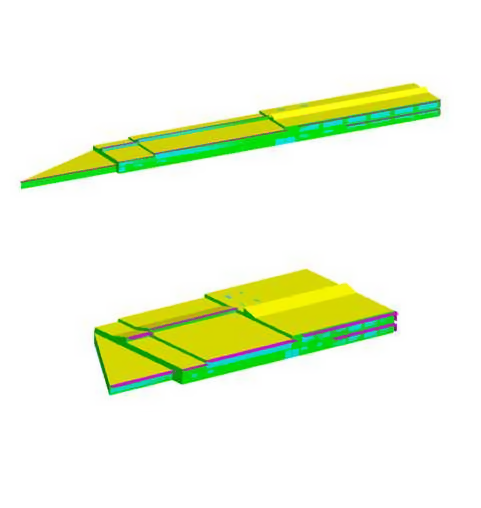
\includegraphics[width=0.9\textwidth, height=0.9\textheight, keepaspectratio=true]{media/image078.png}
\caption{Example of Geometry Transform -- Aspect Ratio \protect \label{fig:example-of-geometry-transform-aspect-ratio}}
\end{figure}

\subsubsection{Inputs}\label{inputs-16}

\paragraph{Field: Plane of Transform}\label{field-plane-of-transform}

This field specifies the plane that the geometry transform should act on. It is currently restricted to altering the horizontal footprint of a building and must be set to ``XY.''

\paragraph{Field: Current Aspect Ratio}\label{field-current-aspect-ratio}

This field specifies the aspect ratio of the building geometry described in the rest of the input file. It is used to scale the new aspect ratio. If this field is set to 1.0, then the altered building will not necessarily have the new aspect ratio defined in the next field.

\paragraph{Field: New Aspect Ratio}\label{field-new-aspect-ratio}

This field specifies the aspect ratio that the building described in the rest of the input file will be changed to.

\subsection{Zone Property View Factors}\label{zone-property-view-factors}

EnergyPlus has two options for specifying the thermal radiation exchange view factors between surfaces in a zone: the approximate option and the user input option. Because the actual geometric arrangement within a zone is very complex, the approximate method of including thermal mass and other forced exchanges is more realistic than trying to come up with ``exact'' view factors. However, in some research situations it might be desirable to have control of the view factors used. For this reason, a user input mode has been included in EnergyPlus. The two modes are described in the next sections.

\subsubsection{Approximate Option}\label{approximate-option}

The first option produces approximate results and uses an area weighted scheme to calculate ``view factors'' between surfaces within a thermal zone. Each surface uses the total area that it can ``see'' among the other surfaces. The approximate view factor from this surface to each other surface is then the area of the receiving surface over the sum of areas that are visible to the sending surface.

In order to account in some limited way for the fact that certain surfaces will not see each other, several assumptions have been built into this view factor approximation. First, a surface cannot see itself. Second, surfaces with approximately the same azimuth (facing direction) and tilt (``same'' being within a built in limit) will not see each other. This means that a window will not see the wall that it is placed on, for example. Third, floors cannot see each other. Fourth, if the surface is a floor, ceiling, roof, or internal mass, the rule for the same azimuth and tilt eliminating radiant exchange between surfaces is waived when the receiving surface is floor, roof, ceiling, or internal mass as long as both surfaces are not floors.

Note that this does not take into account that surfaces may be ``around the corner'' from each other and in reality not see each other at all. Rooms are assumed to be convex rather than concave in this method.

To summarize, using the Surface ``Class'', the approximate view factors have:

\begin{enumerate}
  \item
    No surface sees itself.
  \item
    No Floor sees another floor.
  \item
    All other surface types see Internal Mass.
  \item
    All other surface types see floors.
  \item
    Floors always see ceilings.
  \item
    Floors always see roofs.
  \item
    All other surfaces whose tilt or facing angle differences are greater than 10 degrees see each other.
\end{enumerate}

If geometry is correct, conditions 1, 3, and 7 should take care of all surfaces, but the other conditions supply common sense when the geometry is incorrect. More information about the EnergyPlus view factor calculation is contained in the Engineering Reference document.

\subsubsection{User Input View Factors}\label{user-input-view-factors}

The second option for specifying view factors requires user input values. These should be used with care in research or special situations. The object available for this is ZoneProperty:UserViewFactors:bySurfaceName.

\subsection{ZoneProperty:UserViewFactors:bySurfaceName}\label{zonepropertyuserviewfactorsbysurfacename}

The method of entering user view factors is to entere each surface name and its view factor value to other surfaces in the zone

\subsubsection{Inputs}\label{inputs-17}

\paragraph{Field: Zone Name}\label{field-zone-name}

This field is the zone name for the view factors.

\paragraph{Field: From Surface 1}\label{field-from-surface-1}

This field specifies the name of the ``from surface''.

\paragraph{Field: To Surface 1}\label{field-to-surface-1}

This field specifies the name of the ``to surface''.

\paragraph{Field: Factor 1}\label{field-factor-1}

This value is the view factor for ``from Surface'' to ``to Surface''.

An IDF Example:

\begin{lstlisting}
ZoneProperty:UserViewFactors:bySurfaceName,Lshaped Zone,
    Lshaped Zone:South Wall,Lshaped Zone:South Wall,0.000000,
    Lshaped Zone:South Wall,Lshaped Zone:East Wall,0.101310,
  <snip>
\end{lstlisting}


\section{Group -- Detailed Ground Heat Transfer}\label{group-detailed-ground-heat-transfer}

\subsection{Detailed Ground Heat Transfer}\label{detailed-ground-heat-transfer}

The following objects may be included in an EnergyPlus input IDF file but are handled by the Slab preprocessor:

\begin{itemize}
\tightlist
\item
  GroundHeatTransfer:Slab:Materials
\item
  GroundHeatTransfer:Slab:MatlProps
\item
  GroundHeatTransfer:Slab:BoundConds
\item
  GroundHeatTransfer:Slab:BldgProps
\item
  GroundHeatTransfer:Slab:Insulation
\item
  GroundHeatTransfer:Slab:EquivalentSlab
\item
  GroundHeatTransfer:Slab:AutoGrid
\item
  GroundHeatTransfer:Slab:ManualGrid
\item
  GroundHeatTransfer:Slab:XFACE
\item
  GroundHeatTransfer:Slab:YFACE
\item
  GroundHeatTransfer:Slab:ZFACE
\end{itemize}

The following objects may be included in an EnergyPlus input IDF file but are handled by the Basement preprocessor:

\begin{itemize}
\tightlist
\item
  GroundHeatTransfer:Basement:SimParameters
\item
  GroundHeatTransfer:Basement:MatlProps
\item
  GroundHeatTransfer:Basement:Insulation
\item
  GroundHeatTransfer:Basement:SurfaceProps
\item
  GroundHeatTransfer:Basement:BldgData
\item
  GroundHeatTransfer:Basement:Interior
\item
  GroundHeatTransfer:Basement:ComBldg
\item
  GroundHeatTransfer:Basement:EquivSlab
\item
  GroundHeatTransfer:Basement:EquivAutoGrid
\item
  GroundHeatTransfer:Basement:AutoGrid
\item
  GroundHeatTransfer:Basement:ManualGrid
\item
  GroundHeatTransfer:Basement:XFACE
\item
  GroundHeatTransfer:Basement:YFACE
\item
  GroundHeatTransfer:Basement:ZFACE
\end{itemize}

The documentation both the Slab and Basement objects appear in the AuxiliaryPrograms document under the ``Ground Heat Transfer in EnergyPlus'' heading.

The only object described in this section is the control object which activates the use of the preprocessor.

\subsection{GroundHeatTransfer:Control}\label{groundheattransfercontrol}

The GroundHeatTransfer:Control object determines if the Slab and Basement preprocessors are going to be executed. When a Slab or Basement run is performed the results are saved in files with extensions .SLAB or .BSMT so that they do not need to be rerun if no input changes are made to the GroundHeatTransfer:Slab or GroundHeatTransfer:Basement objects.

\subsubsection{Inputs}\label{inputs-013}

\paragraph{Field: Name}\label{field-name-012}

This alpha field is the name of the GroundHeatTransfer:Control object. It is used as an identifier.

\paragraph{Field: Run Basement Preprocessor}\label{field-run-basement-preprocessor}

The field can either be Yes or No and defaults to No. It is used to control whether the Basement preprocessor program is executed. If it has been previously executed the results are stored in the .BSMT file and do not necessary need to be run again unless the GroundHeatTransfer:Basement objects have changed.

\paragraph{Field: Run Slab Preprocessor}\label{field-run-slab-preprocessor}

The field can either be Yes or No and defaults to No. It is used to control whether the Slab preprocessor program is executed. If it has been previously executed the results are stored in the .SLAB file and do not necessary need to be run again unless the GroundHeatTransfer:Slab objects have changed.


\section{Group -- Room Air Models}\label{group-room-air-models}

\subsection{Room Air Models}\label{room-air-models}

The group of input objects described in this section is used to account for non-uniform room air temperatures that may occur within the interior air volume of a zone. Room air modeling was added to EnergyPlus starting with Version 1.2. Although there are many types of analyses (comfort, indoor air quality, etc) that might benefit from localized modeling of how room air varies across space, only the \emph{temperature} distribution of room air within the zone is currently addressed in EnergyPlus. This allows surface heat transfer and air system heat balance calculations to be made taking into account natural thermal stratification of air and different types of intentional air distribution designs such as under-floor and side-wall displacement ventilation that purport to extract room air at higher-than-mean temperatures. Note that EnergyPlus does \textbf{not} have completely general methods of modeling room air that are applicable to every conceivable type of airflow that might occur in a zone. Such models (e.g.~RANS-CFD) are too computationally expensive to use with EnergyPlus for the foreseeable future. The models that are available in EnergyPlus offer only limited modeling capabilities for select room airflow configurations. Also note that because the complete mixing model for room air has long been the standard in building energy simulation, there is not currently a consensus on how to best model non-uniform air temperatures in buildings. Therefore, it is up to the user to have a good understanding of when, where, and how to apply the room air models available in EnergyPlus. The rest of this section provides some guidance in the way of examples and further discussion of the models available in EnergyPlus.

EnergyPlus offers the different types of air models listed in the table below along with the input objects associated with the use of that model.

% table 10
{\scriptsize
\begin{longtable}[c]{p{1.5in}p{1.5in}p{1.5in}p{1.5in}}
\caption{Summary of Room Air Models \label{table:summary-of-room-air-models}} \tabularnewline
\toprule 
Air Model Key & Air model Algorithm & Applicability & Input Objects Required \tabularnewline
\midrule
\endfirsthead

\caption[]{Summary of Room Air Models} \tabularnewline
\toprule 
Air Model Key & Air model Algorithm & Applicability & Input Objects Required \tabularnewline
\midrule
\endhead

Mixing & Well-Mixed & All zones & None, default \tabularnewline
UserDefined & User Defined & All zones & `Room\-Air\-Model\-Type', `Room\-Air:\-Temperature\-Pattern:\-User\-Defined', `Room\-Air:\-Temperature\-Pattern:***' \tabularnewline
One\-Node\-Displacement\-Ventilation & Mundt & displacement ventilation & `Room\-Air\-Model\-Type', `Room\-Air\-Settings:\-One\-Node\-Displacement\-Ventilation', `Room\-Air:Node' \tabularnewline
Three\-Node\-Displacement\-Ventilation & UCSD Displacement Ventilation & displacement ventilation & `Room\-Air\-Model\-Type', `Room\-Air\-Settings:\-Three\-Node\-Displacement\-Ventilation' \tabularnewline
Under\-Floor\-Air\-Distribution\-Interior & UCSD UFAD Interior Model & Interior zones served by a UFAD system & `Room\-Air\-Model\-Type', `Room\-Air\-Settings:\-Under\-Floor\-Air\-Distribution\-Interior' \tabularnewline
Under\-Floor\-Air\-Distribution\-Exterior & UCSD UFAD Exterior Model & Exterior zones served by a UFAD system & `Room\-Air\-Model\-Type', `Room\-Air\-Settings:\-Under\-Floor\-Air\-Distribution\-Exterior' \tabularnewline
Cross\-Ventilation & UCSD Cross Ventilation & cross ventilation & `Room\-Air\-Model\-Type', `Room\-Air\-Settings:\-Cross\-Ventilation' \tabularnewline
\bottomrule
\end{longtable}
}

\subsection{RoomAirModelType}\label{roomairmodeltype}

EnergyPlus uses the Room\-Air\-Model\-Type object to determine which air model is available for use in a given zone during the simulation. If no Room\-Air\-Model\-Type object is specified (for each zone or the whole building), then EnergyPlus will run with the conventional, completely mixing air model (for each zone or the whole building). Include a Room\-Air\-Model\-Type for each zone that the user wants modeled using a more detailed method. Currently only a single Room\-Air\-Model\-Type object can be specified for each zone; you cannot switch between models during a simulation. However, the UCSD Displacement, Cross Ventilation and UFAD models switch from displacement to mixing ventilation when the operating conditions do not give rise to unmixed flow. The following parameters are fields required by the Room\-Air\-Model\-Type object.

\subsubsection{Inputs}\label{inputs-041}

\paragraph{Field: Name}\label{field-name-040}

This alpha field is the air model name selected by user. It is used as an identifier

\paragraph{Field: Zone Name}\label{field-zone-name-011}

This alpha field indicates the unique name of a Zone object defined elsewhere in the input file. The type of room air model selected will be applied to this zone.

\paragraph{Field: Room-Air Modeling Type}\label{field-room-air-modeling-type}

This alpha field indicates the room-air model used for the specified zone. Currently, there are three options for different air models. Entering the keyword `Mixing' specifies the conventional complete-mixing air model. Note that Mixing is the default and no Room\-Air\-Model\-Type object would be needed to use the complete-mixing model. Entering the keyword `UserDefined `specifies the User Defined Room Air Temperature Patterns. Entering the keyword `OneNodeDisplacementVentilation `specifies the Mundt one node displacement ventilation air model for displacement ventilation. Entering the keyword `ThreeNodeDisplacementVentilation` specifies the three-node displacement ventilation model developed by the University of California, San Diego (UCSD DV). Entering the keyword `CrossVentilation' specifies the two-zone cross ventilation model developed by the University of California, San Diego (UCSD CV). Entering the keyword `UnderFloorAirDistributionInterior` specifies the two-node interior zone under floor air distribution model developed by the University of California, San Diego (UCSD UFI). Entering the keyword `UnderFloorAirDistributionExterior` specifies the two-node exterior zone under floor air distribution model developed by the University of California, San Diego (UCSD UFE).

\paragraph{Field: Air Temperature Coupling Strategy}\label{field-air-temperature-coupling-strategy}

This alpha field indicates how air temperatures predicted by the air models are used by the surface heat balance calculation. Two different coupling schemes are available: Direct (also known as \emph{T-couple}) or Indirect (\emph{DT-couple}). In general, indirect coupling is more suited to situations where room air is well controlled and/or the room air model is less robust. Direct coupling is more suited for floating zone air temperatures and/or accurate room air models.

The Mundt model can use either coupling scheme; the UCSD DV, UCSD CV, UCSD UFI, and UCSD UFE models ignore this field and use direct coupling.

Input either \emph{Direct} or \emph{Indirect}

An example idf entry follows

\begin{lstlisting}
RoomAirModelType,
  MOD1,                             !- Room-Air Model Name
  ZONE ONE,                         !- Zone Name
  ThreeNodeDisplacementVentilation, !- Room-Air Modeling Type
  Direct;                           !- Air Temperature Coupling Strategy
\end{lstlisting}

\subsection{RoomAir:TemperaturePattern:UserDefined}\label{roomairtemperaturepatternuserdefined}

This object is used to explicitly define temperature patterns that are to be applied to the mean air temperature within a thermal zone. This Room Air modeling option is made available for a number of reasons. It allows modeling the consequences of air temperature variations during the design phase when little information is available about the specifics of the air distribution system or positioning of various loads. This option can be used to evaluate the energy implications of different design targets for the temperature patterns. It also provides a method of modeling the annual energy use implications for air temperature distributions determined using separate analyses or measurements. For example, this option could be used to understand the annual energy implications of an air distribution system that has been previously analyzed using Computational Fluid Dynamics.

This approach differs from the other Room Air modeling in that the static temperature pattern is not really \emph{modeled} so that it will respond to conditions that develop during the simulation. More sophisticated dynamic Room Air models will adjust the temperature pattern based on various factors, such as air system flow rate, floor temperature, or rates of internal heat gains. The user-defined temperature distribution patterns are fixed at the beginning and EnergyPlus simply provides results that include the implications of those patterns. This user-defined distribution option may also be useful for checking dynamic Room Air models by using ``bounding'' analysis.

Note that using this object carries a certain degree of responsibility. It would be very easy to define a pattern that is non-physical and will lead to erroneous results. The user-defined temperature distributions should (probably) be balanced about the mean so that basic conservation of energy laws are not violated.

\subsubsection{Inputs}\label{inputs-1-038}

\paragraph{Field: Name}\label{field-name-1-037}

This field provides a unique name for this object.

\paragraph{Field: Zone Name}\label{field-zone-name-1-008}

This field provides the unique name of a zone described elsewhere in the file.

\paragraph{Field: Availability Schedule Name}\label{field-availability-schedule-name-015}

This field provides the name of a schedule that will determine if this model is available. When not available the room air is modeled as completely mixed. When it is available, then a user-defined temperature distribution will be applied. This schedule should be set to ``1.0'' when model is available and ``0.0'' when the model is not to be used. If this field is blank, the schedule has values of 1 for all time periods.

\paragraph{Field: Pattern Control Schedule Name}\label{field-pattern-control-schedule-name}

This field provides the name of schedule that will be used to control which user-defined RoomAir temperature pattern will be applied at any given time. This schedule needs to have integer values that are closely coordinated with those defined as the second field in one of the RoomAir:TemperaturePattern:* objects described below. These schedule values provide the link to the actual patterns to be used throughout the day. This allows controlling which user-defined pattern is used at different times during the simulation. For example, one could use one pattern when the air system is scheduled to be on, and a different pattern when the air system is schedule to be off. Or if the user has knowledge of how the air temperature pattern changes over the course of day in response to changing thermal loads, then this schedule can be used to control when individual patterns are used. For example, a control schedule could use a pattern designated as number 100 from 18:00 to 6:00, pattern number 200 from 6:00 to 12:00, and pattern number 300 from 12:00 to 18:00.

An example of this object is

\begin{lstlisting}
RoomAir:TemperaturePattern:UserDefined,
  Ground Floor South Air Temp Controls,  ! Name
  ZN2_S_1,                              ! Zone Name
  Always_on,                            ! Availability Schedule Name
  Roomair Pattern 1;                    ! Pattern Control Schedule Name
\end{lstlisting}

\subsection{RoomAir:TemperaturePattern:ConstantGradient}\label{roomairtemperaturepatternconstantgradient}

This object is used to model room air with a fixed temperature gradient in the vertical direction. This fixed-slope method is about the simplest distribution pattern.

In addition to the vertical temperature gradient, there are three other parameters included in the pattern that are important. The first two might affect how the air system conditioning the room is operated. The first describes the temperature difference between the mean air temperature and the point where the sensor of a drybulb thermostat is situated. The second describes the temperature difference between the mean and the point where system air is being extracted from the zone. This is considered important because the changes in temperature difference between supply and return can affect how an air system is controlled to meet the loads. The third parameter can affect the zone air heat balance by altering the temperature of the air leaving the zone through exhaust fans.

One example of a source of input data for the vertical temperature gradient is ANSI/ASHRAE Standard 55-2004 Thermal Environmental Conditions for Human Occupancy. Table 5.2.4.3 in this Standard specifies an allowable vertical temperature difference between head level and ankle level of 3ºC (5ºF). If we assume a head to ankle length scale of 1.5 m (5 ft), this leads to a temperature gradient of 3ºC/1.5m, or 2.0 ºC/m.

\subsubsection{Inputs}\label{inputs-2-035}

\paragraph{Field: Name}\label{field-name-2-033}

This field provides a unique name for this object.

\paragraph{Field: Control Integer for Pattern Control Schedule Name}\label{field-control-integer-for-pattern-control-schedule-name}

This field should contain an integer value that is unique among all other RoomAir:TemperaturePattern:* objects. The value used here needs to be in the Pattern Control Schedule for those times when this pattern is to be used for the Room Air Temperature Distribution.

\paragraph{Field: Thermostat Offset}\label{field-thermostat-offset}

This field specifies the temperature difference between where the thermostat is situated and the mean air temperature.

\paragraph{Field: Return Air Offset}\label{field-return-air-offset}

This field specifies the temperature difference between the air leaving the zone and returning to the air system and the mean air temperature.

\paragraph{Field: Exhaust Air Offset}\label{field-exhaust-air-offset}

This field specifies the temperature difference between the air leaving the zone and being exhausted out of the building and the mean air temperature.

\paragraph{Field: Temperature Gradient}\label{field-temperature-gradient}

This field specifies the gradient, or slope, of temperature changes in the vertical direction in ºK/m.

An example of this object is:

\begin{lstlisting}
RoomAir:TemperaturePattern:ConstantGradient,
  half C per Meter,     ! Name
  10005,                ! Control Integer for Pattern Control Schedule Name
  0.0,                  ! Thermostat Offset (Temp at thermostat- Mean Air Temp) [C]
  1.0,                  ! Return Air Offset (Tleaving - Mean Air Temp )  [C]
  1.0,                  ! Exhaust Air Offset (Texhaust - Mean Air Temp)  [C]
  0.5;                  ! Temperature Gradient [K/m]
\end{lstlisting}

\subsection{RoomAir:TemperaturePattern:TwoGradient}\label{roomairtemperaturepatterntwogradient}

This object provides various controls over the value of the gradient used for determining the pattern of room air temperatures. It is similar to previous object RoomAir:TemperaturePattern:ConstantGradient object but simplifies the potentially arduous task of preparing and scheduling a large number of those objects. With this object, two different gradients are entered and user is given several options for controlling how the program will interpolate between the two bounds. The user inputs the height of the location of thermostat, return air, and exhaust air in meters rather than the temperature offset.

\subsubsection{Inputs}\label{inputs-3-031}

\paragraph{Field: Name}\label{field-name-3-027}

This field provides a unique name for this object.

\paragraph{Field: Control Integer for Pattern Control Schedule Name}\label{field-control-integer-for-pattern-control-schedule-name-1}

This field should contain an integer value that is unique among all other RoomAir:TemperaturePattern:* objects. The value used here needs to be in the Pattern Control Schedule for those times when this pattern is to be used for the Room Air Temperature Distribution.

\paragraph{Field: Thermostat Height}\label{field-thermostat-height}

This field specifies the distance above the floor where the thermostat is situated. This height is used by the model to determine the thermostat temperature relative to the mean air temperature by applying the gradient.

\paragraph{Field: Return Air Height}\label{field-return-air-height}

This field specifies the distance above the floor where the air leaves the zone and returns to the air system. and the mean air temperature. This height is used by the model to determine the return air temperature relative to the mean air temperature by applying the gradient.

\paragraph{Field: Exhaust Air Height}\label{field-exhaust-air-height}

This field specifies the distance above the floor where the air leaves the zone and enters and exhaust device such as an exhaust fan. This height is used by the model to determine the exhaust air temperature relative to the mean air temperature by applying the gradient.

\paragraph{Field: Temperature Gradient Lower Bound}\label{field-temperature-gradient-lower-bound}

This field specifies the gradient, or slope, of temperature changes in the vertical direction in ºC/m.

\paragraph{Field: Temperature Gradient Upper Bound}\label{field-temperature-gradient-upper-bound}

This field specifies the gradient, or slope, of temperature changes in the vertical direction in ºC/m.

\paragraph{Field: Gradient Interpolation Mode}\label{field-gradient-interpolation-mode}

This field specifics how the program will vary between the two gradients. Select one of the following keywords to choose the simulation data used to scale: `Outdoor Environment Drybulb Temperature', `Zone Drybulb Temperature', `Delta Outdoor and Zone Temperature', `Sensible Cooling Load', and `Sensible Heating Load'. These are explained in detail below. All of these options have several things in common. They are essentially hard-coded. There is no support for a general method. The interpolation scheme is based on some variable that might reasonably be expected to correlate with gradient changes. This variable's current value is used to continually adjust the value of the vertical gradient for room air temperature.

\textbf{OutdoorDryBulbTemperature:} This key directs the program to interpolate between upper and lower values of the vertical gradient based on the outdoor air temperature. If the outdoor temperature exceeds the upper limit set in the next field, then the gradient entered in the `Temperature Gradient Upper Bound' field is used. Similarly if the outdoor air temperature is below the value set in the `Lower Temperature' field, then the gradient entered in the `Temperature Gradient Lower Bound' is used. For outdoor temperatures that lie between the upper and lower bounds, the gradient is determined by linear interpolation between the two.

\textbf{ZoneDryBulbTemperature}: This key directs the program to interpolate between upper and lower values of the vertical gradient based on the mean zone air temperature. If the mean zone air temperature exceeds the upper limit set in the next field, then the gradient entered in the `Temperature Gradient Upper Bound' field is used. Similarly if the mean zone air temperature is below the value set in the `Lower Temperature' field, then the gradient entered in the `Temperature Gradient Lower Bound' is used. For mean zone air temperatures that lie between the upper and lower bounds, the gradient is determined by linear interpolation between the two.

\textbf{ZoneAndOutdoorTemperatureDifference}: This key directs the program to interpolate between upper and lower values of the vertical gradient based on the difference between the outdoor environment and the mean zone air temperature. If the temperature difference exceeds the upper limit set in the next field, then the gradient entered in the `Temperature Gradient Upper Bound' field is used. Similarly if the temperature difference is below the value set in the `Lower Temperature' field, then the gradient entered in the `Temperature Gradient Lower Bound' is used. For temperature differences that lie between the upper and lower bounds, the gradient is determined by linear interpolation between the two.

\textbf{SensibleCoolingLoad}: This key directs the program to interpolate between upper and lower values of the vertical gradient based on the sensible cooling load. If the cooling load exceeds the upper limit set in the next field, then the gradient entered in the `Temperature Gradient Upper Bound' field is used. Similarly if the cooling load is below the value set in the `Lower Temperature' field, then the gradient entered in the `Temperature Gradient Lower Bound' is used. For cooling loads that lie between the upper and lower bounds, the gradient is determined by linear interpolation between the two.

\textbf{SensibleHeatingLoad}: This key directs the program to interpolate between upper and lower values of the vertical gradient based on the sensible heating load. If the heating load exceeds the upper limit set in the next field, then the gradient entered in the `Temperature Gradient Upper Bound' field is used. Similarly if the heating load is below the value set in the `Lower Temperature' field, then the gradient entered in the `Temperature Gradient Lower Bound' is used. For heating loads that lie between the upper and lower bounds, the gradient is determined by linear interpolation between the two.

\paragraph{Field: Upper Temperature Bound}\label{field-upper-temperature-bound}

This field is used to enter the upper bound on temperature values in Celsius. It is required for the interpolation modes based on temperature.

\paragraph{Field: Lower Temperature Bound}\label{field-lower-temperature-bound}

This field is used to enter the lower bound on temperature values in Celsius. It is required for the interpolation modes based on temperature.

\paragraph{Field: Upper Heat Rate Bound}\label{field-upper-heat-rate-bound}

This field is used to enter the upper bound on heat rate values. It is required for the interpolation modes based on load. Both heating and cooling loads are entered as positive numbers (in watts).

\paragraph{Field: Lower Heat Rate Bound}\label{field-lower-heat-rate-bound}

This field is used to enter the lower bound on heat rate values. It is required for the interpolation modes based on load. Both heating and cooling loads are entered as positive numbers (in watts).

An example of this object follows. This pattern will apply no gradient (effectively the mixing model) if zone air temperatures are 22.5 C or lower. It will apply a gradient of 1 K/m if zone temperatures are 26.0 C or higher. For zone air temperatures between 22.5 and 26.0 it will determine the gradient by linear interpolation and use a gradient between 0.0 and 1.0 K/m depending on where the zone air temperature is in the range.

\begin{lstlisting}
RoomAir:TemperaturePattern:TwoGradient,
  Mixed to one C per M by Zone DB, ! Name
  2002,                   ! Control Integer for Pattern Control Schedule
  1.1,                    ! Thermostat Height meters
  4.5,                    ! Return Air Height
  3.5,                    ! Exhaust Air Height
  0.0,                    ! Temperature Gradient Lower Bound K/m
  1.0,                    ! Temperature Gradient Upper  Bound K/m
  ZoneDrybulbTemperature, ! Gradient Interpolation Mode
  26.0,                   ! Upper Temperature [C]
  22.5,                   ! Lower Temperature [C]
  ,                       ! Upper Heat Rate [W]
  ;                       ! Lower Heat Rate [W]
\end{lstlisting}

\subsection{RoomAir:TemperaturePattern:NondimensionalHeight}\label{roomairtemperaturepatternnondimensionalheight}

This object defines a distribution pattern for air temperatures relative to the current mean air temperature as a function of height. The height, referred to as Zeta, is non-dimensional by normalizing with the zone ceiling height. (The actual zone ceiling height can be explicitly entered in the `Zone' object but if not it is calculated by EnergyPlus from the surfaces attached to the zone.) The temperature differences are not non-dimensional and remain in units of degrees Celsius.

An example of a vertical temperature pattern is shown in the figure below. The pattern itself is treated as a piecewise, linear model of air temperature as a function of height. This Zeta-DeltaTai curve, or lookup table, is then mapped to surfaces defined elsewhere in the file. The centroid of each surface and zone ceiling height are used to automatically assign Zeta values within the program. The zone named in the referencing RoomAir:TemperaturePattern:UserDefined object is used to determine which surfaces will be associated with the pattern when it is applied. A single pattern object can be reused for multiple zones and times.

In addition to the vertical temperature pattern there are three other parameters included in the pattern that are important. The first two might affect how the air system conditioning the room is operated. The first describes the temperature difference between the mean air temperature and the point where the sensor of a drybulb thermostat is situated. The second describes the temperature difference between the mean and the point where system air is being extracted from the zone. This is considered important because the changes in temperature difference between supply and return can affect how an air system is controlled to meet the loads. The third parameter can affect the zone air heat balance by altering the temperature of the air leaving the zone through exhaust fans.

\begin{figure}[hbtp] % fig 44
\centering
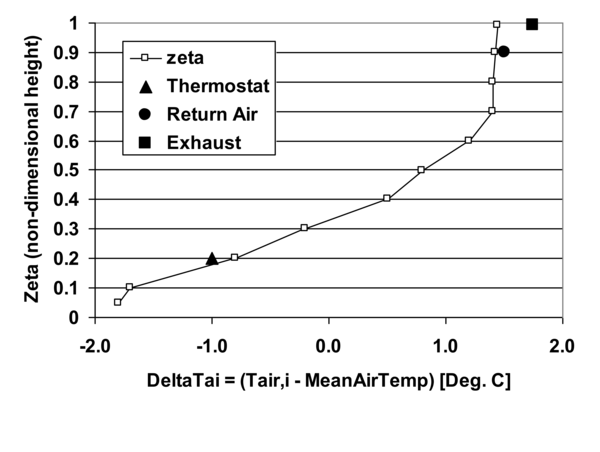
\includegraphics[width=0.9\textwidth, height=0.9\textheight, keepaspectratio=true]{media/image079.png}
\caption{Example of a Vertical Air Temperature Pattern \protect \label{fig:example-of-a-vertical-air-temperature-pattern}}
\end{figure}

\subsubsection{Inputs}\label{inputs-4-028}

\paragraph{Field: Name}\label{field-name-4-024}

This field provides a unique name for this object.

\paragraph{Field: Control Integer for Pattern Control Schedule Name}\label{field-control-integer-for-pattern-control-schedule-name-2}

This field should contain an integer value that is unique among all other RoomAir Temperature Pattern objects. The value used here needs to be in the Pattern Control Schedule for those times when this pattern is to be used for the Room Air Temperature Distribution.

\paragraph{Field: Thermostat Offset}\label{field-thermostat-offset-1}

This field specifies the temperature difference between where the thermostat is situated and the mean air temperature.

\paragraph{Field: Return Air Offset}\label{field-return-air-offset-1}

This field specifies the temperature difference between the air leaving the zone and returning to the air system and the mean air temperature.

\paragraph{Field: Exhaust Air Offset}\label{field-exhaust-air-offset-1}

This field specifies the temperature difference between the air leaving the zone and being exhausted out of the building and the mean air temperature.

\paragraph{Field Set Zeta and Temperature Difference}\label{field-set-zeta-and-temperature-difference}

The remaining fields contain pairs of values that define a lookup table for the temperature pattern in the vertical direction. The first value is Zeta and the second value is DeltaTai. This object is extensible, by duplicating the last two fields and revising the IDD -- note that you will have to replace ``inner'' semi-colons with commas.

\paragraph{Field: Pair \textless{}\#\textgreater{} Zeta non-dimensional Height}\label{field-pair-zeta-non-dimensional-height}

Zeta is the normalized height and should be a fractional value from 0.0 to 1.0. A value of 0.0 corresponds to the floor and a value of 1.0 corresponds to the ceiling. The Zeta values need to be in increasing value.

\paragraph{Field: Pair \textless{}\#\textgreater{} Delta Adjacent Air Temperature}\label{field-pair-delta-adjacent-air-temperature}

DeltaT\(_{ai}\) is the temperature difference between the air temperature at the associated Zeta (T\(_{ai}\)) and the mean air temperature and is given in degrees Celsius.

An example of this object corresponding to the figure above is:

\begin{lstlisting}
RoomAir:TemperaturePattern:NondimensionalHeight,
  Rough UFAD Approx,    ! Name
  3001,                 ! Control Integer for Pattern Control Schedule
                        ! note reference this entry in Schedule
  -1.0 ,                ! Thermostat Offset
  1.5 ,                 ! Return Air Offset (Tleaving - Mean Air Temp ) deg C
  1.75,                 ! Exhaust Air Offset (Texhaust - Mean Air Temp) deg C
  0.05,  -1.8,          ! pair 1 (Zeta , DeltaTai)
  0.1,   -1.7,          ! pair 2 (Zeta , DeltaTai)
  0.2,   -0.8,          ! pair 3 (Zeta , DeltaTai)
  0.3,   -0.2,          ! pair 4 (Zeta , DeltaTai)
  0.4,    0.5,          ! pair 5 (Zeta , DeltaTai)
  0.5,    0.8,          ! pair 6 (Zeta , DeltaTai)
  0.6,    1.2,          ! pair 7 (Zeta , DeltaTai)
  0.7,    1.4,          ! pair 8 (Zeta , DeltaTai)
  0.8,    1.4,          ! pair 9 (Zeta , DeltaTai)
  0.9,   1.42,          ! pair 10 (Zeta , DeltaTai)
  0.95,  1.44;          ! pair 11 (Zeta , DeltaTai)
\end{lstlisting}

\subsection{RoomAir:TemperaturePattern:SurfaceMapping}\label{roomairtemperaturepatternsurfacemapping}

This object defines a distribution pattern for the air temperatures adjacent to individual surfaces. This object uses the specific names of individual surfaces defined elsewhere in the model. This pattern allows controlling the adjacent air temperature on a surface-by-surface basis rather than by height. This allows modeling different adjacent air temperatures on the opposite sides of the zone.

In addition to the surface mappings there are three other parameters included in the pattern that are important. The first two might affect how the air system conditioning the room is operated. The first describes the temperature difference between the mean air temperature and the point where the sensor of a drybulb thermostat is situated. The second describes the temperature difference between the mean and the point where system air is being extracted from the zone. This is considered important because the changes in temperature difference between supply and return can affect how an air system is controlled to meet the loads. The third parameter can affect the zone air heat balance by altering the temperature of the air leaving the zone through exhaust fans.

\subsubsection{Inputs}\label{inputs-5-025}

\paragraph{Field: Name}\label{field-name-5-020}

This field provides a unique name for this object.

\paragraph{Field: Control Integer for Pattern Control Schedule Name}\label{field-control-integer-for-pattern-control-schedule-name-3}

This field should contain an integer value that is unique among all other RoomAir Temperature Pattern objects. The value used here needs to be in the Pattern Control Schedule for those times when this pattern is to be used for the RoomAir Temperature Distribution.

\paragraph{Field: Thermostat Offset}\label{field-thermostat-offset-2}

This field specifies the temperature difference between where the thermostat is situated and the mean air temperature.

\paragraph{Field: Return Air Offset}\label{field-return-air-offset-2}

This field specifies the temperature difference between the air leaving the zone and returning to the air system and the mean air temperature.

\paragraph{Field: Exhaust Air Offset}\label{field-exhaust-air-offset-2}

This field specifies the temperature difference between the air leaving the zone and being exhausted out of the building and the mean air temperature.

\paragraph{Field Set: Surface Name, Temperature Difference}\label{field-set-surface-name-temperature-difference}

\paragraph{Fields (6 and on): Pairs of Surface Names and Temperature Differences}\label{fields-6-and-on-pairs-of-surface-names-and-temperature-differences}

The remaining fields contain pairs that define a lookup table for the temperature pattern on a surface-by-surface basis. This object is extensible, by duplicating the last two fields and revising the IDD -- note that you will have to replace ``inner'' semi-colons with commas.

\paragraph{Field: Surface Name Pair \textless{}\#\textgreater{}}\label{field-surface-name-pair}

The name of a surface defined elsewhere in the input file.

\paragraph{Field: Delta Adjacent Air Temperature Pair \textless{}\#\textgreater{}}\label{field-delta-adjacent-air-temperature-pair}

DeltaT\(_{ai}\) is the temperature difference between the air temperature adjacent to the associated surface (T\(_{ai}\)) and the mean air temperature and is given in degrees Celsius.

An example of this object, which might be used to elevate temperatures near west windows in the afternoon, is:

\begin{lstlisting}

RoomAir:TemperaturePattern:SurfaceMapping,
    GroundFloor SW Corner Hot Near West Wall, ! Name
    4001, ! Control Integer for Pattern Control Schedule Name
    0.0, ! Thermostat Offset(Temp at thermostat- Mean Air Temp)
    0.0, ! Return Air Offset  deg C
    0.0, ! Exhaust Air Offset
    ZN1_SW_1:W_ExtWall:1 ,  0.8,  ! pair 1 (Surface Name , DeltaTai)
    ZN1_SW_1:W_ExtWall:2 ,  0.9,  ! pair 2 (Surface Name , DeltaTai)
    ZN1_SW_1:W_ExtWall:3 ,  1.0,  ! pair 3 (Surface Name , DeltaTai)
    ZN1_SW_1:W_ExtWall:4,   1.1,  ! pair 4 (Surface Name , DeltaTai)
    ZN1_SW_1:W_ExtWall:5,   1.3,  ! pair 5 (Surface Name , DeltaTai)
    ZN1_SW_1:W_ExtWall:6,   1.5,  ! pair 6 (Surface Name , DeltaTai)
    ZN1_SW_1:W_ExtWall:7,   1.7,  ! pair 7 (Surface Name , DeltaTai)
    ZN1_SW_1:W_ExtWall:8,   2.1,  ! pair 8 (Surface Name , DeltaTai)
    ZN1_SW_1:W_ExtWall:9,   2.4 ; ! pair 8 (Surface Name , DeltaTai)
\end{lstlisting}

\subsection{RoomAir:Node}\label{roomairnode}

The RoomAir:Node object is used to define air nodes for a nodal air model. The number of air node objects that need to be specified depends on the nodal air model selected. (However, currently only the Mundt model uses this object). In order to use the Mundt model, the user must specify six or more RoomAir:Node objects of different types for each zone. The exact number of RoomAir:Node in the model will vary based on the resolution of walls. If walls (heat transfer surfaces) are split into separate segments in the vertical direction, then more air nodes of type `MundtRoom' will be useful. At a minimum, for the Mundt model RoomAir Nodes of the following type are required: `Inlet, `Floor, `Control, `Ceiling, `MundtRoom, and `Return.'

\subsubsection{Inputs}\label{inputs-6-022}

\paragraph{Field: Name}\label{field-name-6-018}

This alpha field is a name for the air node. It should be unique and is used as an identifier

\paragraph{Field: Node Type}\label{field-node-type}

This alpha field indicates the type of this air node. The following explains options available for use with the Mundt nodal air model.

\textbf{Inlet} is specified for the air node located where the system air enters the zone.

\textbf{Floor} is specified for the air node located near the floor.

\textbf{Control} is specified for the air node located near the thermostat.

\textbf{Ceiling} is specified for the air node located near the ceiling.

\textbf{MundtRoom} is specified for the air node located adjacent to the wall(s).

\textbf{Return} is specified for the air node located where the system air leaves the zone.

\paragraph{Field: Zone Name}\label{field-zone-name-2-006}

This field indicates the name of the zone (Ref: Zone) that this air node belongs to. This should be the unique name of a zone object defined elsewhere in the input file.

\paragraph{Field: Height of Nodal Control Volume Center}\label{field-height-of-nodal-control-volume-center}

This numeric field indicates the height of the air node center. Air models such as the Mundt model compute the air temperature as a function of height and the value entered here will be used to determine a result for this node. The value should be specified in meters and relative to the floor of the zone.

\paragraph{Field: Surface \textless{}\#\textgreater{} Name}\label{field-surface-name-004}

These remaining alpha fields indicate the names of the surfaces (Ref: Surface) that are interacting convectively with this air node. This field is optional and related to the previous field. Currently, at most 20 surfaces are allowed to interact with a single air node. Only those nodes that interact with the inside faces of surfaces need to specify surface names. Each surface should couple to no more than 1 node.

An IDF example:

\begin{lstlisting}

RoomAir:Node,
      WESTZN:FLOORAIR,    !- Node Name
      Floor,      !- Node Type
      WEST ZONE,  !- Name of Zone to Which the Air Node Belongs
      0.1,        !- Height of Nodal Control Volume Center {m}
      WESTZN:FLOOR:LEFF,  !- surface name
      WESTZN:FLOOR:RIGHT; !- surface name
\end{lstlisting}

\subsection{RoomAirSettings:OneNodeDisplacementVentilation}\label{roomairsettingsonenodedisplacementventilation}

The RoomAirSettings:OneNodeDisplacementVentilation object is used to specify additional input parameters required by the Mundt model that are not available in other input objects in EnergyPlus. A single object will be used for the zone.

\subsubsection{Inputs}\label{inputs-7-022}

\paragraph{Field: Zone Name}\label{field-zone-name-3-005}

This alpha field indicates the name of the zone (Ref: Zone) for the required input parameters as specified in the following fields.

\paragraph{Field: Fraction of Convective Internal Loads Added to Floor Air}\label{field-fraction-of-convective-internal-loads-added-to-floor-air}

This numeric field indicates what fraction of the convective part of the internal gains is added to the air near the floor in the zone specified.

\paragraph{Field: Fraction of Infiltration Internal Loads Added to Floor Air}\label{field-fraction-of-infiltration-internal-loads-added-to-floor-air}

This numeric field indicates what fraction of the infiltration air enters near the floor in the zone specified.

An IDF example:

\begin{lstlisting}

RoomAirSettings:OneNodeDisplacementVentilation,
      WEST ZONE,  !- Zone Name
      0.1,  !- Fraction of internal loads from the convective Floor Air
      0.1;  !- Fraction of internal loads from the Infiltration Air
\end{lstlisting}

\subsection{RoomAirSettings:ThreeNodeDisplacementVentilation}\label{roomairsettingsthreenodedisplacementventilation}

This model is applicable to spaces that are served by a low velocity floor-level displacement ventilation air distribution system. Furthermore, the dominant sources of heat gain should be from people and other localized sources located in the occupied part of the room. The model should be used with caution in zones which have large heat gains or losses through exterior walls or windows or which have considerable direct solar gain. The model predicts three temperatures in the room:

\begin{itemize}
\item
  A foot level temperature (T\(_{\rm{FLOOR}}\)). The floor region is 0.2 meters deep and T\(_{\rm{FLOOR}}\) represents the temperature at the mid-point of the region.
\item
  An occupied subzone temperature (T\(_{\rm{OC}}\)), representing the temperature in the region between the floor layer and the upper, mixed layer.
\item
  An upper node representing the mixed-layer/outflow temperature (T\(_{\rm{MX}}\)) essential for overall energy budget calculations and for modeling comfort effects of the upper layer temperature.
\end{itemize}

\begin{figure}[hbtp] % fig 45
\centering
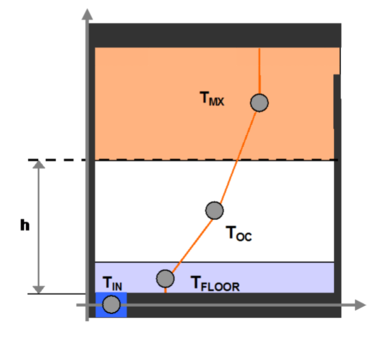
\includegraphics[width=0.9\textwidth, height=0.9\textheight, keepaspectratio=true]{media/image080.png}
\caption{Schematic representation of the three temperature points and temperature gradients \protect \label{fig:schematic-representation-of-the-three}}
\end{figure}

The following fields are used to define an instance of the `UCSD Displacement Ventilation Model Controls' object.

\subsubsection{Inputs}\label{inputs-8-020}

\paragraph{Field: Zone Name}\label{field-zone-name-4-005}

This field provides the unique name of a zone described elsewhere in the file. A single instance of the `UCSD Displacement Ventilation Model Controls' object is needed for each zone that is to be modeled using this method.

\paragraph{Field: Gain Distribution Schedule Name}\label{field-gain-distribution-schedule-name}

This field specifies the unique name of schedule defined elsewhere in the input file. The schedule values are the fractions of the convective portion of the internal gains in the occupied subzone that remain in the occupied subzone. The remainder of the convective portion of the internal gains in the occupied subzone enters the plumes and is carried to the upper subzone. The types of internal gains that are assumed to be located in the occupied subzone are:

\begin{itemize}
\item
  people
\item
  task lights
\item
  electric equipment
\item
  gas equipment
\item
  hot water equipment
\item
  steam equipment
\item
  other equipment
\item
  baseboard heat
\end{itemize}

Types of internal gains that are assumed to be in the upper subzone are:

\begin{itemize}
\item
  general lights
\item
  tubular daylighting devices
\item
  high temperature radiant heaters
\end{itemize}

The schedule values should be between 0 and 1. A value of 1 means that all the convection gains from equipment, task lights and people are dispersed in the lower occupied subzone. Conversely a value of 0 puts all the lower subzone convective gains into the plumes rising into the upper well-mixed subzone.

\paragraph{Field: Number of Plumes per Occupant}\label{field-number-of-plumes-per-occupant}

This field specifies number of plumes per occupant. Plumes are associated with localized sources of convective heat gain from people and equipment. For example, a value of 2.0 would be used if each occupant has a computer that generates a separate plume that does not merge with the plume from the occupant in the lower, occupied, subzone.

\paragraph{Field: Thermostat Height}\label{field-thermostat-height-1}

This field is the height in meters of the thermostat/temperature control sensor above the floor.

\paragraph{Field: Comfort Height}\label{field-comfort-height}

The height in meters above the floor at which air temperature is calculated for comfort purposes. The air temperature at this height is used in calculating the available measures of comfort: Fanger, Pierce or KSU. The default is 1.1 meters.

\paragraph{Field: Temperature Difference Threshold for Reporting}\label{field-temperature-difference-threshold-for-reporting}

This field specifies a minimum temperature difference between the upper mixed subzone and the occupied subzone that will be used to trigger whether or not the displacement ventilation auxiliary outputs will be calculated. These outputs are \emph{Room Air Zone Transition Height}, \emph{Room Air Zone Recommended Minimum Flow Fraction}, \emph{Room Air Zone Average Temperature Gradient} and \emph{Room Air Zone Maximum Temperature Gradient}. They are set to negative values when the temperature difference is less than the threshold and the output \emph{Room Air Zone Is Mixed Status} is set to 1.

The value should be greater than or equal to zero and is in units of degrees Centigrade. The default value is 0.4 degrees C.

An example input:

\begin{lstlisting}

RoomAirSettings:ThreeNodeDisplacementVentilation,
      ZONE ONE,  !- Zone Name
      Constant - .2,  !- Gain Distribution Schedule Name
       1,  !- Number of Plumes per Occupant
        ,  !- Thermostat Height
        ,  !- Comfort Height
      .3;  !- Temp. Difference Threshold for Displacement Ventilation
\end{lstlisting}

\subsection{RoomAirSettings:CrossVentilation}\label{roomairsettingscrossventilation}

The UCSD Cross Ventilation Room Air Model provides a simple model for heat transfer and temperature prediction in cross ventilated rooms. Cross Ventilation (CV) is common in many naturally ventilated buildings, with air flowing through windows, open doorways and large internal apertures across rooms and corridors in the building.

The CV model is used in EnergyPlus in the context of natural ventilation simulations using the AirflowNetwork airflow prediction model. Typical CV room flows are characterized by two clearly distinguishable flow regions that have different airflow velocities and temperature:

\begin{itemize}
\item
  Jet regions in front of the inflow windows
\item
  Recirculation regions in the portions of the room that are not directly in front of the windows.
\end{itemize}

Each inflow aperture has one jet region while the recirculation regions are treated as a whole, with a single temperature and characteristic velocity. The default EnergyPlus perfectly mixed single temperature node room air approach is not suitable for these partially mixed flows. The proposed CV model uses multiple nodes with distinct air temperature and airflow velocity (one node for the recirculations plus one additional node for each inflow aperture).

\begin{figure}[hbtp] % fig 46
\centering
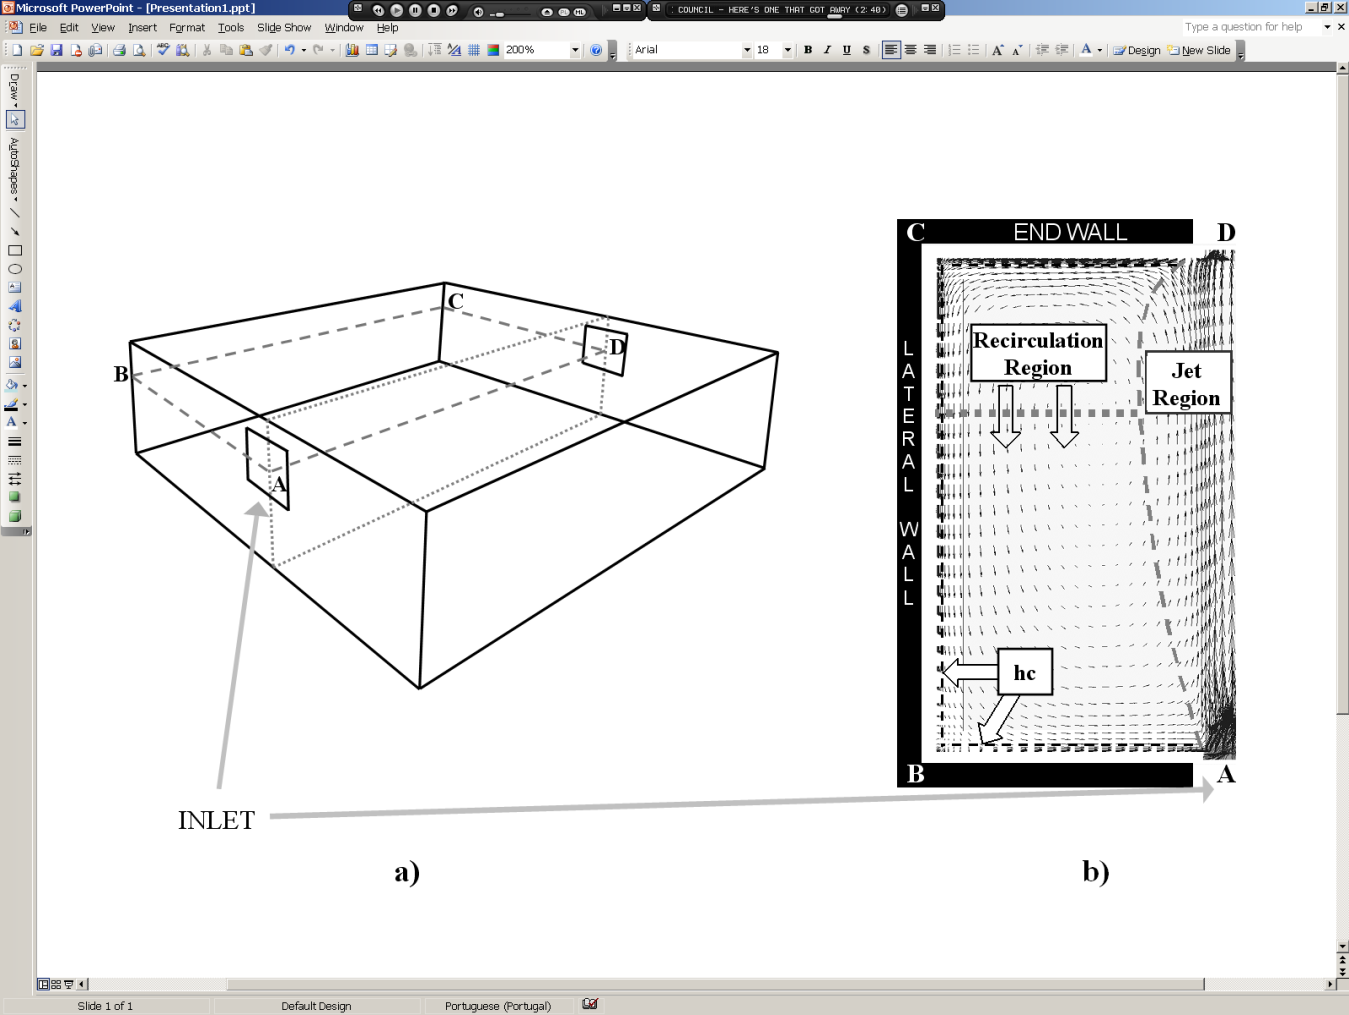
\includegraphics[width=0.9\textwidth, height=0.9\textheight, keepaspectratio=true]{media/image081.png}
\caption{Schematic representation of room air geometry a) schematic representation of a room geometry that generates cross ventilation airflow. b) the proposed model distinguishes two regions in the flow: jet and recirculation (shown here in a CFD simulation of one half of a symmetrical room). \protect \label{fig:schematic-representation-of-room-air-geometry}}
\end{figure}

\begin{figure}[hbtp] % fig 47
\centering
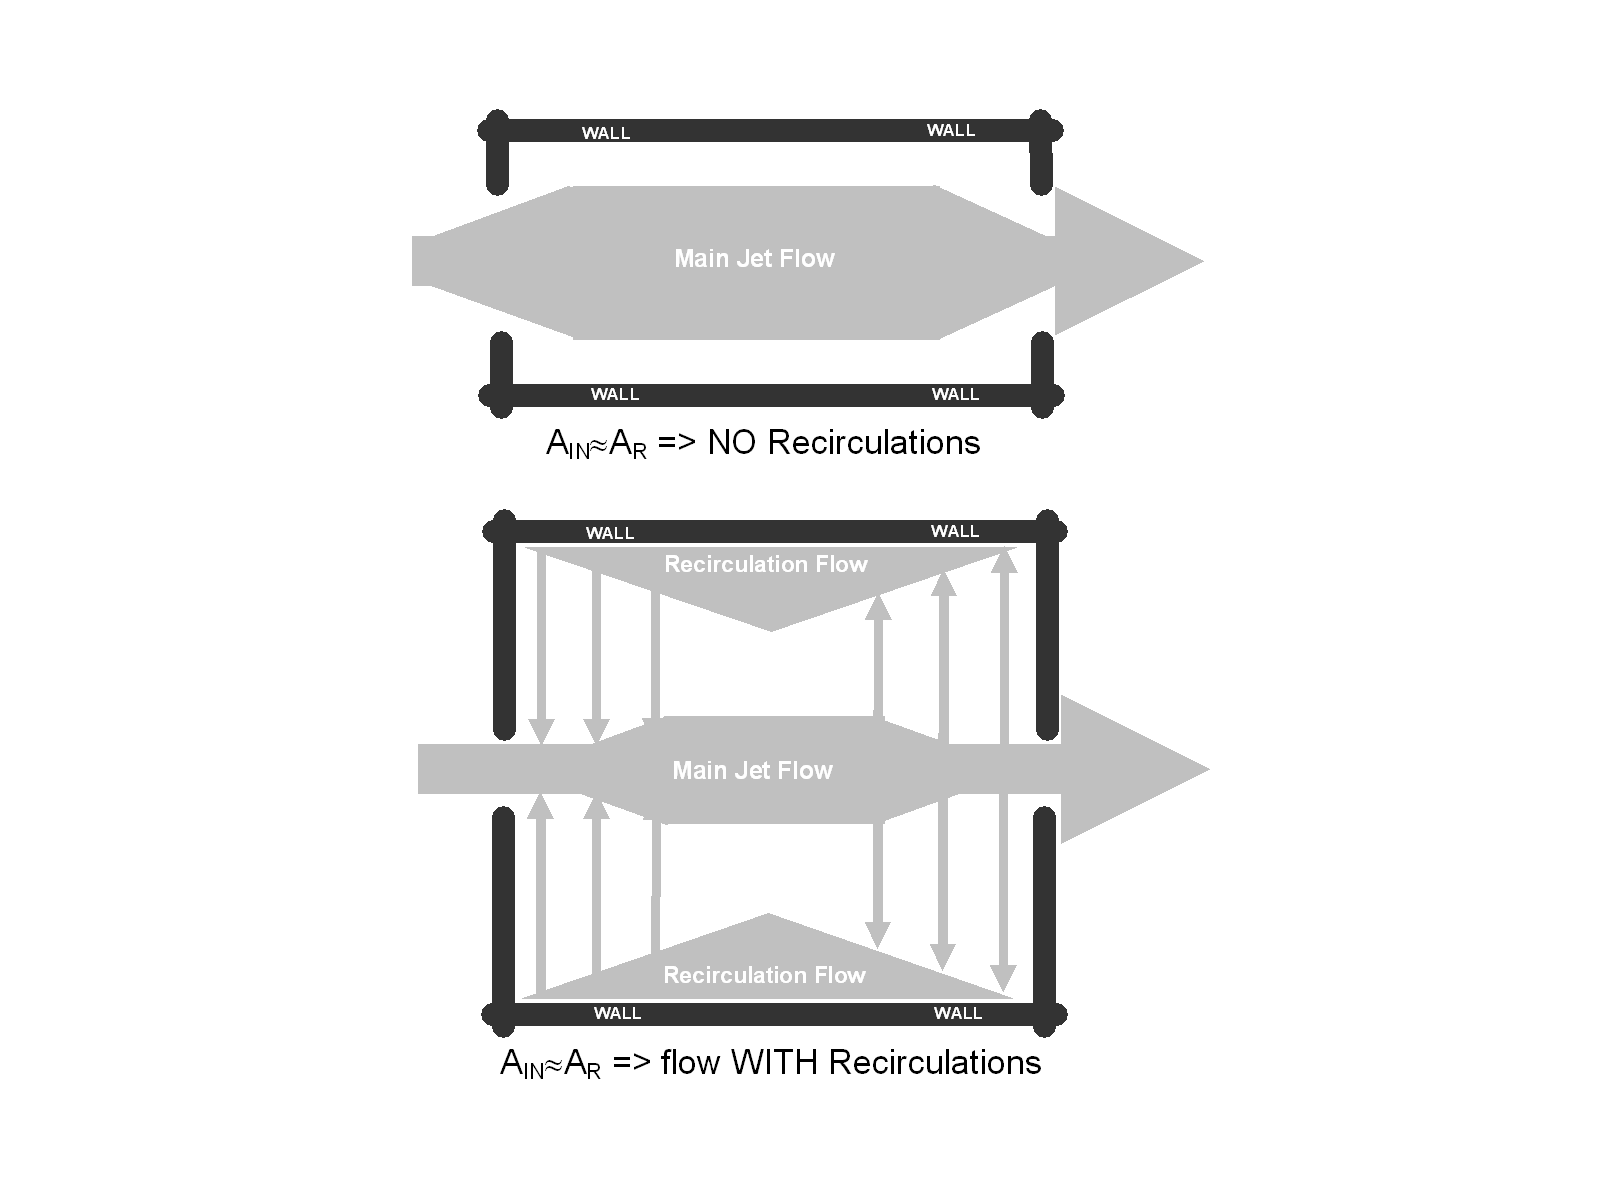
\includegraphics[width=0.9\textwidth, height=0.9\textheight, keepaspectratio=true]{media/image082.png}
\caption{Schematic top view --- possible airflow patterns in cross-ventilation. \protect \label{fig:schematic-top-view-possible-airflow-patterns}}
\end{figure}

The following fields are used to define an instance of the `UCSD Cross Ventilation Model Controls' object.

\subsubsection{Inputs}\label{inputs-9-018}

\paragraph{Field: Zone Name}\label{field-zone-name-5-004}

This field provides the name of the zone to which this object applies. A single instance of the `UCSD Cross Ventilation Model Controls' object is needed for each zone modeled using this method.

\paragraph{Field: Gain Distribution Schedule Name}\label{field-gain-distribution-schedule-name-1}

This field specifies the unique name of schedule defined elsewhere in the input file. The schedule values define the fractions of the convective portion of the internal gains in the jet and recirculation regions.

The schedule values should be between 0 and 1. A value of 1 means that all the convective gains are dispersed in the jet region. Conversely a value of 0 puts all the convective gains into the recirculation region.

\paragraph{Field: Airflow Region Used for Thermal Comfort Evaluation}\label{field-airflow-region-used-for-thermal-comfort-evaluation}

Required field whenever thermal comfort is predicted. Defines air temperature and mean airflow velocity that will be used in the Fanger model. Conditions must refer to one of the two regions defined in the model: jet or recirculation.

Possible choices: Jet or Recirculation.

\subsubsection{Outputs}\label{outputs-030}

\begin{lstlisting}
Zone,Average,Room Air Zone Jet Region Temperature [C]
Zone,Average,Room Air Zone Recirculation Region Temperature [C]
Zone,Average,Room Air Zone Jet Region Average Air Velocity [m/s]
Zone,Average,Room Air Zone Recirculation Region Average Air Velocity [m/s]
Zone,Average,Room Air Window Jet Region Average Air Velocity [m/s]
Zone,Average,Room Air Zone Recirculation and Inflow Rate Ratio
Zone,Average,Room Air Zone Inflow Opening Area [m2]
Zone,Average,Room Air Zone Room Length [m]
Zone,Average,Room Air Zone Is Mixing Status
Zone,Average,Room Air Zone Is Recirculating Status
\end{lstlisting}

\paragraph{Room Air Zone Jet Region Temperature {[}C{]}}\label{room-air-zone-jet-region-temperature-c}

Average air temperature in the jet region of the flow in degrees C. If there is more than one inflow window this output will be the inflow-area-weighted average of the jet region temperature.

\paragraph{Room Air Zone Recirculation Region Temperature {[}C{]}}\label{room-air-zone-recirculation-region-temperature-c}

Average air temperature in the recirculation region of the flow in degrees C.

\paragraph{Room Air Zone Jet Region Average Air Velocity {[}m/s{]}}\label{room-air-zone-jet-region-average-air-velocity-ms}

Average airflow velocity in the jet region of the flow in meters per second. If there is more than one inflow window this output will be the inflow area weighted area of the jet inflow velocities.

\paragraph{Room Air Window Jet Region Average Air Velocity {[}m/s{]}}\label{room-air-window-jet-region-average-air-velocity-ms}

Average airflow velocity in the jet region in front of the window, in meters per second.

\paragraph{Room Air Zone Recirculation Region Average Air Velocity {[}m/s{]}}\label{room-air-zone-recirculation-region-average-air-velocity-ms}

Average airflow velocity in the recirculation region of the flow in meters per second.

\paragraph{Room Air Zone Recirculation and Inflow Rate Ratio {[]}}\label{room-air-zone-recirculation-and-inflow-rate-ratio}

Ratio between airflow rate in the recirculation regions and the total inflow rate, non-dimensional.

\paragraph{Room Air Zone Inflow Opening Area {[}m2{]}}\label{room-air-zone-inflow-opening-area-m2}

Area of the inflow aperture in square meters. This area can change due to variation in wind direction (as inflow aperture changes) or variations in the opening schedule.

\paragraph{Room Air Zone Room Length {[}m{]}}\label{room-air-zone-room-length-m}

Length of the room along the cross ventilation direction, in meters.

\paragraph{Room Air Zone Is Mixing Status {[]}}\label{room-air-zone-is-mixing-status}

An integer flag that indicates whether the zone is mixed (single node well-mixed zone model used) or significant momentum conservation is occurring (UCSD CV model used). The value 1 means well-mixed; 0 means cross ventilation is present. Transition to mixed flow can occur due to three mechanism: reduction in inflow velocity, reduction in inflow aperture area and dominance of buoyancy effects. A value of 1 is yes, a value of 0 is no.

\paragraph{Room Air Zone Is Recirculating Status {[]}}\label{room-air-zone-is-recirculating-status}

An integer flag that indicates whether recirculations are present in the flow. A cross ventilation flow does not have recirculations whenever the inflow area is similar to the room cross section area (such as airflow in a typical corridor). A value of 1 is yes, a value of 0 is no.

\subsection{RoomAirSettings:UnderFloorAirDistributionInterior}\label{roomairsettingsunderfloorairdistributioninterior}

This model is applicable to interior spaces that are served by an underfloor air distribution system. The dominant sources of heat gain should be from people, equipment, and other localized sources located in the occupied part of the room. The model should be used with caution in zones which have large heat gains or losses through exterior walls or windows or which have considerable direct solar gain. The model predicts two temperatures in the room:

\begin{itemize}
\item
  An occupied subzone temperature (T\(_{\rm{OC}}\)), representing the temperature in the region between the floor and the boundary of the upper subzone.
\item
  An upper subzone temperature (T\(_{\rm{MX}}\)) essential for overall energy budget calculations and for modeling comfort effects of the upper layer temperature.
\end{itemize}

The following fields are used to define an instance of the `UCSD UFAD Interior Model Controls' object.

\subsubsection{Inputs}\label{inputs-2016-06-17-0938}

\paragraph{Field: Zone Name}\label{field-zone-name-6-003}

This field provides the unique name of a zone described elsewhere in the file. A single instance of the `RoomAirSettings:UnderFloorAirDistributionInterior' object is needed for each zone that is to be modeled using this method.

\paragraph{Field: Number of Diffusers}\label{field-number-of-diffusers}

The total number of diffusers in this zone. This field can allowed to Autocalculate (in which case it is set to the design occupancy level; i.e., number of people). If the design occupancy is low or zero but there are still heat sources that could generate buoyancy driven plumes, the user should input a value based on the design supply air flow rate of the zone and the design flow rate of an individual diffuser. In the absence of any other information, divide the zone area by 100 ft\(^{2}\). The default for this field is Autocalculate.

\paragraph{Field: Power per Plume}\label{field-power-per-plume}

The power in watts incorporated in a buoyancy driven thermal plume. Normally we assume all the loads of a workstation create a single plume so that this represents the convective heat gain from a workstation -- 1 person, 1 computer terminal, plus any task lighting. A typical value would be 220 watts. However, the model assumes an ``equivalent'' plume derived from the zone extraction rate normalized to the number of workstations/occupants. This field should be allowed to default -- the program will calculate a value based upon the occupancy and the extraction rate. The default is Autocalculate.

\paragraph{Field: Design Effective Area of Diffuser}\label{field-design-effective-area-of-diffuser}

This is the design air flow opening area in square meters of a single diffuser. The default value depends on the diffuser type. For swirl diffusers it is 0075 m\(^{2}\), for variable area diffusers 0.035 m\(^{2}\), for horizontal swirl diffusers 0.006 m\(^{2}\), and for linear bar grilles 0.03 m\(^{2}\). The default is \emph{Autocalculate}..

\paragraph{Field: Diffuser Slot Angle from Vertical}\label{field-diffuser-slot-angle-from-vertical}

This input describes the angle at which air emerges from the diffusers. It should be the angle in degrees between the vertical and the diffuser slots. The defaults depend on the diffuser type: for swirl diffusers it is 28 degrees, for variable area diffusers 45 degrees, for DV diffusers 73 degrees, and for linear bar grilles 15 degrees.

\paragraph{Field: Thermostat Height}\label{field-thermostat-height-2}

This field is the height in meters of the thermostat/temperature control sensor above the floor. The default is 1.2 meters.

\paragraph{Field: Comfort Height}\label{field-comfort-height-1}

The height in meters above the floor at which air temperature is calculated for comfort purposes. The air temperature at this height is used in calculating the available measures of comfort: Fanger, Pierce or KSU. The default is 1.1 meters.

\paragraph{Field: Temperature Difference Threshold for Reporting}\label{field-temperature-difference-threshold-for-reporting-1}

This field specifies a minimum temperature difference between the upper subzone and the occupied subzone that will be used to trigger whether or not the UFAD auxiliary outputs will be calculated. These outputs are \emph{Room Air Zone Transition Height} and \emph{Room Air Zone Average Temperature Gradient}. They are set to zero when the temperature difference is less than the threshold and the output \emph{Room Air Zone Is Mixed Status} is set to 1.

The value should be greater than or equal to zero and is in units of degrees Centigrade. The default value is 0.4 degrees C.

\paragraph{Field: Diffuser Type}\label{field-diffuser-type}

The choices for this alpha field are \textbf{Swirl} \textbar{} \textbf{VariableArea} \textbar{} \textbf{HorizontalSwirl \textbar{} LinearBarGrille \textbar{} Custom.} The swirl and displacement diffusers are fixed area diffusers. The variable area diffusers maintain an approximately constant exit velocity. Linear bar grilles are normally used in exterior zonesand are fixed area diffusers. Custom is used to signify that the user intends to input the coefficients A -- E (see below) rather than let the program set the coefficients based on diffuser type. The default is \emph{Swirl}.

\paragraph{Field: Transition Height}\label{field-transition-height}

An optional field to allow the user to specify the transition height (meters above floor) rather than have the program calculate it. The default is 1.7 meters.

\paragraph{Field: Coefficient A}\label{field-coefficient-a}

The coefficient A in the formula: Kc = A*Gamma**B + C + D*Gamma + E*Gamma**2. Gamma is a variable that characterizes the amount of stratification in a UFAD zone. Kc is the fraction of the total internal convective heat gain that is assigned to the lower (occupied) subzone. The coefficients in the formula are defaulted based upon diffuser type. A user would normally allow this field to default. The default is \emph{autocalculate}.

\paragraph{Field: Coefficient B}\label{field-coefficient-b}

The coefficient B in the formula: Kc = A*Gamma**B + C + D*Gamma + E*Gamma**2. Gamma is a variable that characterizes the amount of stratification in a UFAD zone. Kc is the fraction of the total internal convective heat gain that is assigned to the lower (occupied) subzone. The coefficients in the formula are defaulted based upon diffuser type. A user would normally allow this field to default. The default is \emph{autocalculate}.

\paragraph{Field: Coefficient C}\label{field-coefficient-c}

The coefficient C in the formula: Kc = A*Gamma**B + C + D*Gamma + E*Gamma**2. Gamma is a variable that characterizes the amount of stratification in a UFAD zone. Kc is the fraction of the total internal convective heat gain that is assigned to the lower (occupied) subzone. The coefficients in the formula are defaulted based upon diffuser type. A user would normally allow this field to default. The default is \emph{autocalculate}.

\paragraph{Field: Coefficient D}\label{field-coefficient-d}

The coefficient D in the formula: Kc = A*Gamma**B + C + D*Gamma + E*Gamma**2. Gamma is a variable that characterizes the amount of stratification in a UFAD zone. Kc is the fraction of the total internal convective heat gain that is assigned to the lower (occupied) subzone. The coefficients in the formula are defaulted based upon diffuser type. A user would normally allow this field to default. The default is \emph{autocalculate}.

\paragraph{Field: Coefficient E}\label{field-coefficient-e}

The coefficient E in the formula: Kc = A*Gamma**B + C + D*Gamma + E*Gamma**2. Gamma is a variable that characterizes the amount of stratification in a UFAD zone. Kc is the fraction of the total internal convective heat gain that is assigned to the lower (occupied) subzone. The coefficients in the formula are defaulted based upon diffuser type. A user would normally allow this field to default. The default is \emph{autocalculate}.

An example input is:

\begin{lstlisting}

  RoomAirModelType,
      SPACE5-1 RoomAir Model,  !- Name
      SPACE5-1,                !- Zone Name
      UnderFloorAirDistributionInterior,  !- Room-Air Modeling Type
      DIRECT;                  !- Air Temperature Coupling Strategy

  RoomAirSettings:UnderFloorAirDistributionInterior,
      SPACE5-1,                !- Zone Name
      Autocalculate,           !- Number of Diffusers
      Autocalculate,           !- Power per Plume
      Autocalculate,           !- Design Effective Area of Diffuser {m2}
      Autocalculate,           !- Diffuser Slot Angle from Vertical {deg}
      ,                        !- Thermostat Height {m}
      ,                        !- Comfort Height {m}
      0.001,         !- Temperature Difference Threshold for Reporting {deltaC}
      Swirl,                   !- Diffuser Type
      1.7,                     !- Transition Height {m}
      Autocalculate,           !- Coefficient A
      Autocalculate,           !- Coefficient B
      Autocalculate,           !- Coefficient C
      Autocalculate,           !- Coefficient D
     Autocalculate;           !- Coefficient E
\end{lstlisting}

\subsection{RoomAirSettings:UnderFloorAirDistributionExterior}\label{roomairsettingsunderfloorairdistributionexterior}

This model is applicable to exterior spaces that are served by an underfloor air distribution system. The dominant sources of heat gain should be from people, equipment, and other localized sources located in the occupied part of the room, as well as convective gain coming from a warm window. The model predicts two temperatures in the room:

\begin{itemize}
\item
  An occupied subzone temperature (T\(_{\rm{OC}}\)), representing the temperature in the region between the floor and the boundary of the upper subzone..
\item
  An upper subzone temperature (T\(_{\rm{MX}}\)) essential for overall energy budget calculations and for modeling comfort effects of the upper layer temperature.
\end{itemize}

The following fields are used to define an instance of the `UCSD UFAD Exterior Model Controls' object.

\subsubsection{Inputs}\label{inputs-11-016}

\paragraph{Field: Zone Name}\label{field-zone-name-7-003}

This field provides the unique name of a zone described elsewhere in the file. A single instance of the `RoomAirSettings:UnderFloorAirDistributionExterior' object is needed for each zone that is to be modeled using this method.

\paragraph{Field: Number of Diffusers}\label{field-number-of-diffusers-1}

The total number of diffusers in this zone. This field can allowed to Autocalculate (in which case it is set to the design occupancy level; i.e., number of people). If the design occupancy is low or zero but there are still heat sources that could generate buoyancy driven plumes, the user should input a value based on the design supply air flow rate of the zone and the design flow rate of an individual diffuser. In the absence of any other information, divide the zone area by 100 ft\(^{2}\). The default for this field is Autocalculate.

\paragraph{Field: Power per Plume}\label{field-power-per-plume-1}

The power in watts incorporated in a buoyancy driven thermal plume. Normally we assume all the loads of a workstation create a single plume so that this represents the convective heat gain from a workstation -- 1 person, 1 computer terminal, plus any task lighting. A typical value would be 220 watts. However, the model assumes an ``equivalent'' plume derived from the zone extraction rate normalized to the number of workstations/occupants. This field should be allowed to default -- the program will calculate a value based upon the occupancy and the extraction rate. The default is Autocalculate.

\paragraph{Field: Design Effective Area of Diffuser}\label{field-design-effective-area-of-diffuser-1}

This is the design air flow opening area in square meters of a single diffuser. The default value depends on the diffuser type. For swirl diffusers it is 0075 m\(^{2}\), for variable area diffusers 0.035 m\(^{2}\), for horizontal swirl diffusers 0.006 m\(^{2}\), and for linear bar grilles 0.03 m\(^{2}\). The default is \emph{Autocalculate}..

\paragraph{Field: Diffuser Slot Angle from Vertical}\label{field-diffuser-slot-angle-from-vertical-1}

This input describes the angle at which air emerges from the diffusers. It should be the angle in degrees between the vertical and the diffuser slots. The defaults depend on the diffuser type: for swirl diffusers it is 28 degrees, for variable area diffusers 45 degrees, for DV diffusers 73 degrees, and for linear bar grilles 15 degrees.

\paragraph{Field: Thermostat Height}\label{field-thermostat-height-3}

This field is the height in meters of the thermostat/temperature control sensor above the floor. The default is 1.2 meters.

\paragraph{Field: Comfort Height}\label{field-comfort-height-2}

The height in meters above the floor at which air temperature is calculated for comfort purposes. The air temperature at this height is used in calculating the available measures of comfort: Fanger, Pierce or KSU. The default is 1.1 meters.

\paragraph{Field: Temperature Difference Threshold for Reporting}\label{field-temperature-difference-threshold-for-reporting-2}

This field specifies a minimum temperature difference between the upper subzone and the occupied subzone that will be used to trigger whether or not the UFAD auxiliary outputs will be calculated. These outputs are \emph{Room Air Zone Transition Height} and \emph{Room Air Zone Average Temperature Gradient}. They are set to zero when the temperature difference is less than the threshold and the output \emph{Room Air Zone Is Mixed Status} is set to 1.

The value should be greater than or equal to zero and is in units of degrees Centigrade. The default value is 0.4 degrees C.

The value should be greater than or equal to zero and is in units of degrees Centigrade. The default value is 0.4 degrees C.

\paragraph{Field: Diffuser Type}\label{field-diffuser-type-1}

The choices for this alpha field are \textbf{Swirl} \textbar{} \textbf{VariableArea} \textbar{} \textbf{HorizontalSwirl \textbar{} LinearBarGrille \textbar{} Custom.} The swirl and displacement diffusers are fixed area diffusers. The variable area diffusers maintain an approximately constant exit velocity. Linear bar grilles are normally used in exterior zonesand are fixed area diffusers. Custom is used to signify that the user intends to input the coefficients A -- E (see below) rather than let the program set the coefficients based on diffuser type. The default is \emph{Swirl}.

\paragraph{Field: Transition Height}\label{field-transition-height-1}

An optional field to allow the user to specify the transition height (meters above floor) rather than have the program calculate it. The default is 1.7 meters.

\paragraph{Field: Coefficient A}\label{field-coefficient-a-1}

The coefficient A in the formula: Kc = A*Gamma**B + C + D*Gamma + E*Gamma**2. Gamma is a variable that characterizes the amount of stratification in a UFAD zone. Kc is the fraction of the total internal convective heat gain that is assigned to the lower (occupied) subzone. The coefficients in the formula are defaulted based upon diffuser type. A user would normally allow this field to default. The default is \emph{autocalculate}.

\paragraph{Field: Coefficient B}\label{field-coefficient-b-1}

The coefficient B in the formula: Kc = A*Gamma**B + C + D*Gamma + E*Gamma**2. Gamma is a variable that characterizes the amount of stratification in a UFAD zone. Kc is the fraction of the total internal convective heat gain that is assigned to the lower (occupied) subzone. The coefficients in the formula are defaulted based upon diffuser type. A user would normally allow this field to default. The default is \emph{autocalculate}.

\paragraph{Field: Coefficient C}\label{field-coefficient-c-1}

The coefficient C in the formula: Kc = A*Gamma**B + C + D*Gamma + E*Gamma**2. Gamma is a variable that characterizes the amount of stratification in a UFAD zone. Kc is the fraction of the total internal convective heat gain that is assigned to the lower (occupied) subzone. The coefficients in the formula are defaulted based upon diffuser type. A user would normally allow this field to default. The default is \emph{autocalculate}.

\paragraph{Field: Coefficient D}\label{field-coefficient-d-1}

The coefficient D in the formula: Kc = A*Gamma**B + C + D*Gamma + E*Gamma**2. Gamma is a variable that characterizes the amount of stratification in a UFAD zone. Kc is the fraction of the total internal convective heat gain that is assigned to the lower (occupied) subzone. The coefficients in the formula are defaulted based upon diffuser type. A user would normally allow this field to default. The default is \emph{autocalculate}.

\paragraph{Field: Coefficient E}\label{field-coefficient-e-1}

The coefficient E in the formula: Kc = A*Gamma**B + C + D*Gamma + E*Gamma**2. Gamma is a variable that characterizes the amount of stratification in a UFAD zone. Kc is the fraction of the total internal convective heat gain that is assigned to the lower (occupied) subzone. The coefficients in the formula are defaulted based upon diffuser type. A user would normally allow this field to default. The default is \emph{autocalculate}.

An example input is:

\begin{lstlisting}
RoomAirSettings:UnderFloorAirDistributionExterior,
      SPACE1-1,                !- Zone Name
      Autocalculate,           !- Number of Diffusers per Zone
      Autocalculate,           !- Power per Plume
      Autocalculate,           !- Design Effective Area of Diffuser {m2}
      Autocalculate,           !- Diffuser Slot Angle from Vertical {deg}
      ,                        !- Thermostat Height {m}
      ,                        !- Comfort Height {m}
      0.001,                   !- Temperature Difference Threshold for Reporting {deltaC}
      LinearBarGrille,         !- Diffuser Type
      1.7,                     !- Transition Height {m}
      Autocalculate,           !- Coefficient A
      Autocalculate,           !- Coefficient B
      Autocalculate,           !- Coefficient C
      Autocalculate,           !- Coefficient D
      Autocalculate;           !- Coefficient E
\end{lstlisting}

\subsection{RoomAirflowNetwork Model}\label{roomairflownetwork-model}

This model simulates a thermal zone using a network approach by assuming intra-zone nodes connected by user-defined patterns of airflows. The new model also allows users to specify a node to be connected to surfaces to have convective heat transfer between surfaces and the node, portion of internal gains and supply air and return air fractions from zone equipment. The model requires following objects to work together:

\begin{itemize}
  \item
    RoomAirSettings:AirflowNetwork
  \item
    RoomAir:Node:AirflowNetwork
  \item
    Room\-Air\-:Node:\-Air\-flow\-Net\-work:\-Ad\-jacent\-Sur\-face\-List
  \item
    RoomAir:Node:Air\-flow\-Net\-work:\-Internal\-Gains
  \item
    RoomAir:Node:Air\-flow\-Net\-work:\-HVAC\-Equipment
  \item
    AirflowNetwork:Intrazone:Node
  \item
    Airflow\-Net\-work:\-Intra\-zone:\-Link\-age
\end{itemize}

The first \emph{five} \textbf{objects} are described below. The last two objects are described in the Airflow Network Model section.

\subsection{RoomAirSettings:AirflowNetwork}\label{roomairsettingsairflownetwork}

This object provides inputs in a thermal zone needed for the RoomAirflowNetwork model. The inputs specify a thermal zone and a list of RoomAir nodes. The object gives a summary of the model configuration in a zone.

\subsubsection{Inputs}\label{inputs-12-015}

\paragraph{Field: Name}\label{field-name-7-017}

This is a unique character string associated with this instance of the Room\-Air\-Settings:\-Air\-flow\-Net\-work object.

\paragraph{Field: Zone Name}\label{field-zone-name-8-002}

The name of the EnergyPlus thermal zone corresponding to the RoomAir model zone.

\paragraph{Field: Control Point RoomAir:Node Name}\label{field-control-point-roomairnode-name}

This is the name of a RoomAir:Node:AirflowNetwork object that contains the sensor for zone HVAC controls. The conditions at this node will be used for thermostatic, humidistatic, or comfort based control decisions. The zone node defined in a Zone object is required.

\paragraph{Field: RoomAir:Node:AirflowNetwork x Name}\label{field-roomairnodeairflownetwork-x-name}

The name of a RoomAir:Node:AirflowNetwork object defined elsewhere. This node will receive the fraction of internal gains, and HVAC equipment, and a list of surface names exposed to this node with convective heat transfer.

An IDF example input is:

\begin{lstlisting}

RoomAirSettings:AirflowNetwork,
  NORTH_ZONE,     !- Name 
  NORTH_ZONE,              !- Zone Name
  RoomAir Schedule,        !- Availability Schedule Name
  NORTH_ZONE,              !- Control Point RoomAir:Node Name
  LeftUpper,               !- RoomAir:Node:AirflowNetwork 1 Name
  CentralUpper,            !- RoomAir:Node:AirflowNetwork 2 Name
  NORTH_ZONE,              !- RoomAir:Node:AirflowNetwork 3 Name
  LeftMiddle,              !- RoomAir:Node:AirflowNetwork 4 Name
  LeftLower,               !- RoomAir:Node:AirflowNetwork 5 Name
  CentralLower;            !- RoomAir:Node:AirflowNetwork 6 Name
\end{lstlisting}

\subsection{RoomAir:Node:AirflowNetwork}\label{roomairnodeairflownetwork}

This object is used to define a node in a thermal zone. The input specifies the fraction of zone volume and provides a list of names to define fraction of internal gains, surface connection and HVAC equipment.

\subsubsection{Inputs}\label{inputs-13-012}

\paragraph{Field: Name}\label{field-name-8-017}

This is a unique character string associated with this instance of the Room\-Air\-Settings:\-Air\-flow\-Net\-work object.

\paragraph{Field: Zone Name}\label{field-zone-name-9-000}

The name of the EnergyPlus thermal zone and is defined in an Room\-Air\-Settings:\-Air\-flow\-Net\-work object.

\paragraph{Field: Fraction of Zone Air Volume}\label{field-fraction-of-zone-air-volume}

The field specifies a fraction of the overall zone air volume that is assigned to this RoomAir:Node:AirflowNetwork object. The fraction will be used to calculate zone air storage term. See corresponding sections in Engineering Reference for its use in the node energy and moisture balance equations.

\paragraph{Field: RoomAir:Node:AirflowNetwork:AdjacentSurfaceList Name}\label{field-roomairnodeairflownetworkadjacentsurfacelist-name}

The field specifies a name to provide a list of connected adjacent surfaces with convective heat transfer between surfaces and this particular node. When a moisture mode is assigned to surfaces, convective moisture transfer will be calculated. See corresponding sections in Engineering Reference for its use in the node energy and moisture balance equations.

\paragraph{Field: RoomAir:Node:AirflowNetwork:InternalGains Name}\label{field-roomairnodeairflownetworkinternalgains-name}

The field specifies a name to provide a list of internal gain objects and associated fractions assigned to this particular node. See corresponding sections in Engineering Reference for its use in the node energy and moisture balance equations.

\paragraph{Field: RoomAir:Node:AirflowNetwork:HVACEquipment Name}\label{field-roomairnodeairflownetworkhvacequipment-name}

The field specifies a name to provide a list of HVAC equipment, including AirLoop terminals and zone equipment. See corresponding sections in Engineering Reference for its use in the node energy and moisture balance equations.

\begin{lstlisting}
RoomAir:Node:AirflowNetwork,
  LeftUpper,         !- Name
  NORTH_ZONE,        !- Zone Name
  0.15,              !- Fraction of Zone Air Volume
  Surface_18_T_List, !- RoomAir:Node:AirflowNetwork:AdjacentSurfaceList Name
  LeftUpper_Gain,    !- RoomAir:Node:AirflowNetwork:InternalGains Name
  LeftUpper_HVAC;    !- RoomAir:Node:AirflowNetwork:HVACEquipment Name
\end{lstlisting}

\subsection{RoomAir:Node:AirflowNetwork:AdjacentSurfaceList}\label{roomairnodeairflownetworkadjacentsurfacelist}

This object is used to provide a list of connected adjacent surfaces with convective heat transfer between surfaces and this particular node. When a moisture mode is assigned to surfaces, convective moisture transfer will be calculated. It should be pointed out that a fraction of a surface exposed to this particular node is not allowed.

\subsubsection{Field: Name}\label{field-name-9-015}

This is a unique character string associated with this instance of the Room\-Air\-:Node:\-Airflow\-Network:\-Adjacent\-Surface\-List object.

\subsubsection{Field: Surface x Name}\label{field-surface-x-name-000}

The field specifies a surface name based on the order from 1 to 21. The maximum number of surfaces can be extensible.

\begin{lstlisting}

RoomAir:Node:AirflowNetwork:AdjacentSurfaceList,
  Surface_18_T_List, !- Name
  Surface_18_T;      !- Surface 1 Name
\end{lstlisting}

\subsection{RoomAir:Node:AirflowNetwork:InternalGains}\label{roomairnodeairflownetworkinternalgains}

This object is used to define a list of internal gains in the same zone and associated fraction assigned to this particular node.

\subsubsection{Inputs}\label{inputs-14-012}

\paragraph{Field: Name}\label{field-name-10-014}

This is a unique character string associated with this instance of the Room\-Air:\-Node:\-Air\-flow\-Net\-work:\-Internal\-Gains object.

\paragraph{Field: Internal Gain Object x Type}\label{field-internal-gain-object-x-type}

The field specifies an internal gain object type based on the list in the Energy+.

\paragraph{Field: Internal Gain Object x Name}\label{field-internal-gain-object-x-name}

The field specifies an internal gain object name based on the list in the Energy+.

\paragraph{Field: Fraction of Gains to Node x}\label{field-fraction-of-gains-to-node-x}

The field specifies a fraction of the particular internal gain object assigned to this node.

\begin{lstlisting}
RoomAir:Node:AirflowNetwork:InternalGains,
  CentralUpper_Gain,    !- Name
  People,               !- Internal Gain Object 1 Type
  NORTH_ZONE People,    !- Internal Gain Object 1 Name
  0.15,                 !- Fraction of Gains to Node 1
  Lights,               !- Internal Gain Object 2 Type
  NORTH_ZONE Lights,    !- Internal Gain Object 2 Name
  0.15,                 !- Fraction of Gains to Node 2
  ElectricEquipment,    !- Internal Gain Object 3 Type
  NORTH_ZONE Equip,     !- Internal Gain Object 3 Name
  0.15;                 !- Fraction of Gains to Node 3
\end{lstlisting}

\{Field set: 3 fields (Internal Gain Object x Type, Internal Gain Object x Name, and Fraction of Gains to Node x). are extensible.\}

\subsection{RoomAir:Node:AirflowNetwork:HVACEquipment}\label{roomairnodeairflownetworkhvacequipment}

This object is used to define a list of HVAC equipment objects in the same zone and associated fractions assigned to this particular node.

\subsubsection{Inputs}\label{inputs-15-012}

\paragraph{Field: Name}\label{field-name-11-012}

This is a unique character string associated with this instance of the Room\-Air:\-Node:\-Air\-flow\-Net\-work:\-HVAC\-Equipment object.

\paragraph{Field: ZoneHVAC or Air Terminal Equipment Object Type x}\label{field-zonehvac-or-air-terminal-equipment-object-type-x}

The field specifies an object type of ZoneHVAC equipment or terminal type based on the list in the Energy+.idd.

\paragraph{Field: ZoneHVAC or Air Terminal Equipment Object Name x}\label{field-zonehvac-or-air-terminal-equipment-object-name-x}

The field specifies the object name based on the object type defined in the previous field.

\paragraph{Field: Fraction of Output or Supply Air from HVAC Equipment x}\label{field-fraction-of-output-or-supply-air-from-hvac-equipment-x}

The field specifies a fraction of supply air from the particular equipment to this node.

\paragraph{Field: Fraction of Input or Return Air from HVAC Equipment x}\label{field-fraction-of-input-or-return-air-from-hvac-equipment-x}

The field specifies a fraction of return air from the particular equipment to this node.

\begin{lstlisting}

RoomAir:Node:AirflowNetwork:HVACEquipment,
  CentralUpper_HVAC,        !- Name
  ZoneHVAC:PackagedTerminalAirConditioner, !- ZoneHVAC or Air Terminal Equipment Object Type 1
  NORTH_ZONE PTAC,       !- ZoneHVAC or Air Terminal Equipment Object Name 1
  0.14,                   !- Fraction of Output or Supply Air from HVAC Equipment 1 
  0.14;                   !- Fraction of Input or Return Air to HVAC Equipment 1
\end{lstlisting}

\{Field set: 4 fields (ZoneHVAC or Air Terminal Equipment Object Type x, ZoneHVAC or Air Terminal Equipment Object Name x, Fraction of Output or Supply Air from HVAC Equipment x, and Fraction of Input or Return Air from HVAC Equipment x) are extensible.\}

\subsubsection{Outputs}\label{outputs-1-023}

Each room air model sets up outputs specific to that model. The effect of room air modeling is usually to adjust the adjacent air temperature along the inside surface of heat transfer surfaces. The output report ``Surface Int Adjacent Air Temperature {[}C{]}'' is provided for this and described under Surface Outputs.

\paragraph{Zone Predicted Sensible Load Room Air Correction Factor}\label{zone-predicted-sensible-load-room-air-correction-factor}

This output variable provides the value of the correction factor applied to the predicted zone loads. Predicted zone load to setpoint is (usually) used to control HVAC air systems and the presence of a room air model has an impact on the loads. The predicted loads are multiplied by the factor in this output variable. The value is always 1.0 when there is no Room Air model. When there is a Room Air model, this output shows how that model is increasing or decreasing overall zone loads experienced by the air system.

\subsubsection{Outputs}\label{outputs-2-019}

The user-defined air temperature pattern that interpolates between two gradients produces the following output variable.

\begin{lstlisting}
HVAC,Average,Room Air Zone Vertical Temperature Gradient [K/m]
\end{lstlisting}

\paragraph{Room Air Zone Vertical Temperature Gradient {[}K/m{]}}\label{room-air-zone-vertical-temperature-gradient-km}

This output variable is the result of the interpolation performed by the user-defined roomair model using RoomAir:TemperaturePattern:TwoGradient. This is the temperature gradient in the vertical direction. The units are degrees Kelvin per meter.

\subsubsection{Outputs}\label{outputs-3-017}

The following output is available for the Mundt model.

\begin{lstlisting}
Room Air Node Air Temperature {[}C{]}
\end{lstlisting}

\paragraph{Room Air Node Air Temperature {[}C{]}}\label{room-air-node-air-temperature-c}

This output variable provides the drybulb air temperature used in, or calculated by, the Mundt model. The selection key is the name of an air node defined in a ROOMAIR Node object.

\subsubsection{Outputs}\label{outputs-4-014}

\begin{lstlisting}
HVAC,Average,Room Air Zone Mixed Subzone Temperature [C]
HVAC,Average,Room Air Zone Occupied Subzone Temperature [C]
HVAC,Average,Room Air Zone Floor Subzone Temperature [C]
HVAC,Average,Room Air Zone Transition Height [m]
HVAC,Average,Room Air Zone Recommended Minimum Flow Fraction
HVAC,Average,Room Air Zone Is Mixed Status \protect\hyperlinksection-1
HVAC,Average,Room Air Zone Average Temperature Gradient [K/m]
HVAC,Average,Room Air Zone Maximum Temperature Gradient [K/m]
HVAC,Average,Room Air Zone Thermal Comfort Effective Air Temperature [C]
HVAC,Average,Room Air Zone Thermostat Temperature [C]
\end{lstlisting}

\paragraph{Room Air Zone Mixed Subzone Temperature {[}C{]}}\label{room-air-zone-mixed-subzone-temperature-c}

The temperature of the upper well-mixed subzone in degrees C.

\paragraph{Room Air Zone Occupied Subzone Temperature {[}C{]}}\label{room-air-zone-occupied-subzone-temperature-c}

The average temperature of the lower, stratified, occupied subzone in degrees C.

\paragraph{Room Air Zone Floor Subzone Temperature {[}C{]}}\label{room-air-zone-floor-subzone-temperature-c}

The temperature of the region near the floor in degrees C.

\paragraph{Room Air Zone Transition Height {[}m{]}}\label{room-air-zone-transition-height-m}

The height above the floor, in meters, of the boundary between the lower occupied subzone and the upper well-mixed subzone.

\paragraph{Room Air Zone Recommended Minimum Flow Fraction {[]}}\label{room-air-zone-recommended-minimum-flow-fraction}

The ratio of the minimum recommended flow rate to the actual flow rate. Here flow rate means the sum of infiltration, ventilation, mixing and system air flow rates. The minimum flow is the flow needed to establish the boundary between the occupied and mixed subzones at 1.5 meters.

\paragraph{Room Air Zone Is Mixed Status {[]}}\label{room-air-zone-is-mixed-status}

An integer flag that indicates whether the zone is mixed (single node well-mixed zone model used) or stratified (UCSD DV model used). The value 1 means well-mixed; 0 means stratified.

\paragraph{Room Air Zone Average Temperature Gradient {[}K/m{]}}\label{room-air-zone-average-temperature-gradient-km}

The temperature gradient between the middle of the floor region and the middle of the well-mixed upper subzone in degrees Kelvin per meter.

\paragraph{Room Air Zone Maximum Temperature Gradient {[}K/m{]}}\label{room-air-zone-maximum-temperature-gradient-km}

The maximum of the temperature gradient between the middle of the floor region and the middle of the occupied subzone and the temperature gradient between the middle of the occupied subzone and the middle of the well-mixed subzone. The gradient is in degrees Kelvin per meter.

\paragraph{Room Air Zone Thermal Comfort Effective Air Temperature {[}C{]}}\label{room-air-zone-thermal-comfort-effective-air-temperature-c}

The temperature at the user specified comfort height in degrees C.

\paragraph{Room Air Zone Thermostat Temperature {[}C{]}}\label{room-air-zone-thermostat-temperature-c}

The temperature at the height of the thermostat (specified by user input) in degrees C.

\subsubsection{Outputs}\label{outputs-5-009}

\begin{itemize}
\item
  Zone,Average,Room Air Zone Jet Region Temperature {[}C{]}
\item
  Zone,Average,Room Air Zone Recirculation Region Temperature {[}C{]}
\item
  Zone,Average,Room Air Zone Jet Region Average Air Velocity {[}m/s{]}
\item
  Zone,Average,Room Air Zone Recirculation Region Average Air Velocity {[}m/s{]}
\item
  Zone,Average,Room Air Zone Inflow Opening Area{[}m2{]}
\item
  Zone,Average,Room Air Zone Room Length {[}m{]}
\item
  Zone,Average,Room Air Zone Recirculation and Inflow Rate Ratio
\item
  Zone,Average,Room Air Zone Is Mixing Status
\item
  Zone,Average,Room Air Zone Is Recirculating Status
\end{itemize}

\paragraph{Room Air Zone Jet Region Temperature {[}C{]}}\label{room-air-zone-jet-region-temperature-c-1}

Average air temperature in the jet region of the flow in degrees C.

\paragraph{Room Air Zone Recirculation Region Temperature {[}C{]}}\label{room-air-zone-recirculation-region-temperature-c-1}

Average air temperature in the recirculation region of the flow in degrees C.

\paragraph{Room Air Zone Jet Region Average Air Velocity {[}m/s{]}}\label{room-air-zone-jet-region-average-air-velocity-ms-1}

Average airflow velocity in the jet region of the flow in meters per second.

\paragraph{Room Air Zone Recirculation Region Average Air Velocity {[}m/s{]}}\label{room-air-zone-recirculation-region-average-air-velocity-ms-1}

Average airflow velocity in the recirculation region of the flow in meters per second.

\paragraph{Room Air Zone Inflow Opening Area {[}m2{]}}\label{room-air-zone-inflow-opening-area-m2-1}

Area of the inflow aperture in square meters. This area can change due to variation in wind direction (as inflow aperture changes) or variations in the opening schedule.

\paragraph{Room Air Zone Room Length {[}m{]}}\label{room-air-zone-room-length-m-1}

Length of the room along the cross ventilation direction, in meters.

\paragraph{Room Air Zone Recirculation and Inflow Rate Ratio {[]}}\label{room-air-zone-recirculation-and-inflow-rate-ratio-1}

Ratio between airflow rate in the recirculation region and inflow rate, non-dimensional.

\paragraph{Room Air Zone Is Mixing Status {[]}}\label{room-air-zone-is-mixing-status-1}

An integer flag that indicates whether the zone is mixed (single node well-mixed zone model used) or significant momentum conservation is occurring (UCSD CV model used). The value 1 means well-mixed; 0 means cross ventilation is present. Transition to mixed flow can occur due to three mechanism: reduction in inflow velocity, reduction in inflow aperture area and dominance of buoyancy effects. A value of 1 is yes, a value of 0 is no.

\paragraph{Room Air Zone Is Recirculating Status {[]}}\label{room-air-zone-is-recirculating-status-1}

An integer flag that indicates whether recirculations are present in the flow. A cross ventilation flow does not have recirculations whenever the inflow area is similar to the room cross section area (such as airflow in a typical corridor). A value of 1 is yes, a value of 0 is no.

\subsubsection{Outputs}\label{outputs-6-009}

\begin{itemize}
\item
  HVAC,Average,Room Air Zone Mixed Subzone Temperature {[}C{]}
\item
  HVAC,Average,Room Air Zone Occupied Subzone Temperature {[}C{]}
\item
  HVAC,Average,Room Air Zone Transition Height {[}m{]}
\item
  HVAC,Average,Room Air Zone Is Mixed Status {[]}
\item
  HVAC,Average,Room Air Zone Average Temperature Gradient {[}K/m{]}
\item
  HVAC,Average,Room Air Zone Effective Comfort Air Temperature {[}C{]}
\item
  HVAC,Average,Room Air Zone Thermostat Temperature {[}C{]}
\item
  HVAC,Average,Room Air Zone Transition Height Gamma Value {[]}
\item
  HVAC,Average,Room Air Zone Plume Heat Transfer Rate {[}W{]}
\item
  HVAC,Average,Room Air Zone Temperature Stratification Fraction {[]}
\item
  HVAC,Average,Room Air Zone Window Plume Heat Transfer Rate {[}W{]}
\end{itemize}

\paragraph{Room Air Zone Mixed Subzone Temperature {[}C{]}}\label{room-air-zone-mixed-subzone-temperature-c-1}

The temperature of the upper subzone in degrees C.

\paragraph{Room Air Zone Occupied Subzone Temperature {[}C{]}}\label{room-air-zone-occupied-subzone-temperature-c-1}

The temperature of the lower, occupied subzone in degrees C.

\paragraph{Room Air Zone Transition Height {[}m{]}}\label{room-air-zone-transition-height-m-1}

The height above the floor, in meters, of the boundary between the lower occupied subzone and the upper subzone..

\paragraph{Room Air Zone Is Mixed Status {[]}}\label{room-air-zone-is-mixed-status-1}

An integer flag that indicates whether the zone is mixed (single node well-mixed zone model used) or stratified (UCSD UFI model used). The value 1 means well-mixed; 0 means stratified.

\paragraph{Room Air Zone Average Temperature Gradient {[}K/m{]}}\label{room-air-zone-average-temperature-gradient-km-1}

The temperature gradient between the middle of the occupied subzone and the middle of the upper subzone in degrees Kelvin per meter.

\paragraph{Room Air Zone Effective Comfort Air Temperature {[}C{]}}\label{room-air-zone-effective-comfort-air-temperature-c}

The temperature at the user specified comfort height in degrees C.

\paragraph{Room Air Zone Thermostat Temperature {[}C{]}}\label{room-air-zone-thermostat-temperature-c-1}

The temperature at the height of the thermostat (specified by user input) in degrees C.

\paragraph{Room Air Zone Transition Height Gamma Value {[]}}\label{room-air-zone-transition-height-gamma-value}

Value of gamma -- a dimensionless ``height'' used in calculating the transition height. Lower values of gamma indicate increased stratification, higher values less. Generally the values should be between 2 and 30.

\paragraph{Room Air Zone Plume Heat Transfer Rate {[}W{]}}\label{room-air-zone-plume-heat-transfer-rate-w}

The heat in watts driving the plumes in the occupied subzone.

\paragraph{Room Air Zone Window Plume Heat Transfer Rate {[}W{]}}\label{room-air-zone-window-plume-heat-transfer-rate-w}

The convective heat gain from windows in an UnderFloorAirDistributionExterior zone.

\paragraph{Room Air Zone Temperature Stratification Fraction {[]}}\label{room-air-zone-temperature-stratification-fraction}

This output, (Phi) is a measure of temperature stratification in the space. It is the difference between the occupied subzone temperature and the supply temperature divided by difference between the return temperature and the supply temperature. Technically it is equal to Kc. As phi approaches 1, the space is fully mixed. As phi approaches 0, the space becomes fully stratified. Expressed as an equation:

\begin{equation}
  \frac{T_{occ} - T_{sup}}{T_{ret} - T_{sup}}
\end{equation}

\subsubsection{Outputs}\label{outputs-7-009}

\begin{itemize}
\item
  HVAC,Average,RoomAirflowNetwork Node Temperature {[}C{]}
\item
  HVAC,Average,RoomAirflowNetwork Node Humidity Ratio {[}kgWater/kgDryAir{]}
\item
  HVAC,Average,RoomAirflowNetwork Node Relative Humidity {[}\%{]}
\item
  HVAC,Average,RoomAirflowNetwork Node SumIntSensibleGain {[}W{]}
\item
  HVAC,Average,RoomAirflowNetwork Node SumIntLatentGain {[}W{]}
\item
  HVAC,Average,RoomAirflowNetwork Node NonAirSystemResponse {[}W{]}
\item
  HVAC,Average,RoomAirflowNetwork Node SysDepZoneLoadsLagged {[}W{]}
\item
  HVAC,Average,RoomAirflowNetwork Node HVAC Supply Fraction {[]}
\item
  HVAC,Average,RoomAirflowNetwork Node HVAC Return Fraction {[]}
\end{itemize}

\paragraph{RoomAirflowNetwork Node Temperature {[}C{]}}\label{roomairflownetwork-node-temperature-c-000}

The temperature at a Room Air Node in a zone in degrees C.

\paragraph{HVAC,Average,RoomAirflowNetwork Node Humidity Ratio {[}kgWater/kgDryAir{]}}\label{hvacaverageroomairflownetwork-node-humidity-ratio-kgwaterkgdryair}

The humidity ratio at a Room Air Node in a zone in kgWater/kgDryAir.

\paragraph{RoomAirflowNetwork Node Relative Humidity {[}\%{]}}\label{roomairflownetwork-node-relative-humidity}

The relative humidity ratio at a Room Air Node in a zone in percent.

\paragraph{HVAC,Average,RoomAirflowNetwork Node SumIntSensibleGain {[}W{]}}\label{hvacaverageroomairflownetwork-node-sumintsensiblegain-w}

A sum of internal sensible gains assigned to a Room Air node in a zone.

\paragraph{HVAC,Average,RoomAirflowNetwork Node SumIntLatentGain {[}W{]}}\label{hvacaverageroomairflownetwork-node-sumintlatentgain-w}

A sum of internal latent gains assigned to a Room Air node in a zone.

\paragraph{HVAC,Average,RoomAirflowNetwork Node NonAirSystemResponse {[}W{]}}\label{hvacaverageroomairflownetwork-node-nonairsystemresponse-w}

A sum of system convective gains, collected via NonAirSystemResponse, and assigned to a Room Air node in a zone.

\paragraph{HVAC,Average,RoomAirflowNetwork Node SysDepZoneLoadsLagged {[}W{]}}\label{hvacaverageroomairflownetwork-node-sysdepzoneloadslagged-w}

A sum of SysDepZoneLoads saved to be added to zone heat balance at the next HVAC time step. A typical system is a zone dehumidifier.


\section[Group -- Internal Gains]{Group -- Internal Gains (People, Lights, Other internal zone equipment)\sectionmark{Group -- Internal Gains}}\label{group-internal-gains-people-lights-other-internal-zone-equipment}
\sectionmark{Group -- Internal Gains}

Not all the influence for energy consumption in the building is due to envelope and ambient conditions. This group of objects describes other internal gains that may come into play (People, Lights, Various Equipment Types).

\subsection{People}\label{people}

The people statement is used to model the occupant's effect on the space conditions. The following definition addresses the basic affects as well as providing information that can be used to report the thermal comfort of a group of occupants. The Fanger, Pierce Two-Node, and Kansas State University Two-Node thermal comfort models are available in EnergyPlus. A user may select any of these models for each People statement by simply adding the appropriate choice keyword after the air velocity schedule name. Thermal comfort calculations will only be made for people statements that include specific requests for these thermal comfort models. . This object also requires input of carbon dioxide generation rate based on people activity level for zone carbon dioxide simulations.

\subsubsection{Inputs}\label{inputs-025}

\paragraph{Field: Name}\label{field-name-024}

The name of the People object. Must be unique across all People objects.

\paragraph{Field: Zone or ZoneList Name}\label{field-zone-or-zonelist-name-000}

This field is the name of the zone (ref: Zone) or ZoneList (ref: ZoneList) and links a particular people statement to a thermal zone or set of thermal zones in the building. When the ZoneList option is used then this people definition is applied to each of the zones in the zone list effecting a global definition for the number of people in the zone. The Zonelist option can be used effectively with the people/area and area/person options of the Number of People Calculation Method.

The name of the actual people object becomes \textless{}Zone Name\textgreater{} \textless{}People Object Name\textgreater{} and should be less than the standard length (100 characters) for a name field. If it is greater than this standard length, it may be difficult to specify in output reporting as it will be truncated. A warning will be shown if the generated name is greater than 100 characters. If it duplicates another such concatenated name, there will be a severe error and terminate the run.

\paragraph{Field: Number of People Schedule Name}\label{field-number-of-people-schedule-name}

This field is the name of the schedule (ref: Schedules) that modifies the number of people parameter (see Number of People Calculation Method and related fields). The schedule values can be any positive number. The actual number of people in a zone as defined by this statement is the product of the number of people field and the value of the schedule specified by name in this field.

\paragraph{Field: Number of People Calculation Method}\label{field-number-of-people-calculation-method}

This field is a key/choice field that tells which of the next three fields are filled and is descriptive of the method for calculating the nominal number of occupants (people) in the Zone. The key/choices are:

\begin{itemize}
\tightlist
\item
  People
\end{itemize}

With this choice, the method used will be a straight insertion of the number of occupants (people).~ (The Number of People field should be filled.)

\begin{itemize}
\tightlist
\item
  People/Area
\end{itemize}

With this choice, the method used will be a factor per floor area of the zone. (The People per Zone Floor Area field should be filled).

\begin{itemize}
\tightlist
\item
  Area/Person
\end{itemize}

With this choice, the method used will be a factor of floor area per person. (The Zone Floor Area per Person field should be filled).

\paragraph{Field: Number of People}\label{field-number-of-people}

This field is used to represent the maximum number of people in a zone that is then multiplied by a schedule fraction (see schedule field). In EnergyPlus, this is slightly more flexible in that the number of people could be a ``diversity factor'' applied to a schedule of real numbers. Note that while the schedule value can vary from hour to hour, the number of people field is constant for all simulation environments.

\paragraph{Field: People per Zone Floor Area}\label{field-people-per-zone-floor-area}

This factor (person/m\(^{2}\)) is used, along with the Zone Floor Area to determine the maximum number of people as described in the Number of People field. The choice from the method field should be ``people/area''.

\paragraph{Field: Zone Floor Area per Person}\label{field-zone-floor-area-per-person}

This factor (m\(^{2}\)/person) is used, along with the Zone Floor Area to determine the maximum number of people as described in the Number of People field. The choice from the method field should be ``area/person''.

\paragraph{Field: Fraction Radiant}\label{field-fraction-radiant}

This field is a decimal number between 0.0 and 1.0 and is used to characterize the type of heat being given off by people in a zone. The number specified in this field will be multiplied by the total sensible energy emitted by people to give the amount of long wavelength radiation gain from human beings in a zone. The remainder of the sensible load is assumed to be convective heat gain. Note that latent gains from people are not included in either the radiant or convective heat gains. See the Engineering Reference document for more details.

\paragraph{Field: Sensible Heat Fraction}\label{field-sensible-heat-fraction}

The user can use this field to specify a fixed sensible fraction for the heat gain due to this PEOPLE object. Normally the program calculates the sensible/latent split; this field gives the user control over this split. This field is autocalculated: if the field is blank or \textbf{autocalculate}, the program will calculate the sensible/latent split; if a value is entered, it will be used as the sensible fraction of the current total heat gain.

\paragraph{Field: Activity Level Schedule Name}\label{field-activity-level-schedule-name}

This field is the name of the schedule that determines the amount of heat gain per person in the zone under design conditions. This value is modified somewhat based on a correlation to account for variations in space temperature. The schedule values may be any positive number and the units for this parameter is Watts per person. This schedule represents the total heat gain per person including convective, radiant, and latent. An internal algorithm is used to determine what fraction of the total is sensible and what fraction is latent. Then, the sensible portion is divided into radiant and convective portions using the value specified for Fraction Radiant (above). See the Engineering Reference document for more details.

Values for activity level can range anywhere from approximately 100-150 Watts per person for most office activities up to over 900 Watts per person for strenuous physical activities such as competitive wrestling. The following table (Table~\ref{table:metabolic-rates-for-various-activities}) is based on Table~\ref{table:wind-speed-profile-coefficients-ashrae} from the 2005 ASHRAE Handbook of Fundamentals, page 8.6. In addition to the information from the ASHRAE HOF, there is an added column of values in W/Person such as necessary for the activity level schedule values. This column uses the standard adult body surface area of 1.8 m\(^{2}\) to multiply the activity levels in W/m\(^{2}\) that are used in the table. Warnings are produced when the activity level schedule values fall outside normal ranges. Having too low or too high values can also skew thermal comfort reporting values.

\paragraph{Field: Carbon Dioxide Generation Rate}\label{field-carbon-dioxide-generation-rate}

This numeric input field specifies carbon dioxide generation rate per person with units of m3/s-W. The total carbon dioxide generation rate from this object is:

Number of People * People Schedule * People Activity * Carbon Dioxide Generation Rate. The default value is 3.82E-8 m3/s-W (obtained from ASHRAE Standard 62.1-2007 value at 0.0084 cfm/met/person over the general adult population). The maximum value can be 10 times the default value.

\paragraph{Field: Enable ASHRAE 55 comfort warnings}\label{field-enable-ashrae-55-comfort-warnings}

This field accepts either ``Yes'' or ``No'' as values. When ``Yes'' is specified, warnings are generated when the space conditions are outside of the ASHRAE 55 comfort range as discussed in the sections that follow titled ``Simplified ASHRAE 55-2004 Graph Related Outputs'' and ``Simplified ASHRAE 55 Warnings.'' The default is not to provide these warnings so if you want to know if your space is outside this comfort range you must set this field to Yes.

% table 11
\begin{longtable}[c]{p{2.0in}p{1.34in}p{1.33in}p{1.33in}}
\caption{Metabolic Rates for Various Activities \label{table:metabolic-rates-for-various-activities}} \tabularnewline
\toprule 
Activity & Activity Level w/ Person EnergyPlus Schedule Value & Activity Level W/m\(^2\) & met* \tabularnewline
\midrule
\endfirsthead

\caption[]{Metabolic Rates for Various Activities} \tabularnewline
\toprule 
Activity & Activity Level w/Person EnergyPlus Schedule Value & Activity Level W/m2 & met* \tabularnewline
\midrule
\endhead

\emph{Resting} \tabularnewline \midrule 
Sleeping & 72 & 40 & 0.7 \tabularnewline
Reclining & 81 & 45 & 0.8 \tabularnewline
Seated, quiet & 108 & 60 & 1 \tabularnewline
Standing, relaxed & 126 & 70 & 1.2 \tabularnewline
\emph{Walking (on level surface)} \tabularnewline \midrule
3.2 km/h (0.9 m/s) & 207 & 115 & 2 \tabularnewline
4.3 km/h (1.2 m/s) & 270 & 150 & 2.6 \tabularnewline
6.4 km/h (1.8 m/s) & 396 & 220 & 3.8 \tabularnewline
\emph{Office Activities} \tabularnewline \midrule
Reading, seated & 99 & 55 & 1 \tabularnewline
Writing & 108 & 60 & 1 \tabularnewline
Typing & 117 & 65 & 1.1 \tabularnewline
Filing, seated & 126 & 70 & 1.2 \tabularnewline
Filing, standing & 144 & 80 & 1.4 \tabularnewline
Walking about & 180 & 100 & 1.7 \tabularnewline
Lifting/packing & 216 & 120 & 2.1 \tabularnewline
\emph{Miscellaneous Occupational Activities} \tabularnewline \midrule
Cooking & 171 to 207 & 95 to 115 & 1.6 to 2.0 \tabularnewline
Housecleaning & 207 to 360 & 115 to 200 & 2.0 to 3.4 \tabularnewline
Seated, heavy limb movement & 234 & 130 & 2.2 \tabularnewline
Machine work & 189 & 105 & 1.8 \tabularnewline
sawing (table saw) & 207 to 252 & 115 to 140 & 2.0 to 2.4 \tabularnewline
light (electrical industry) & 423 & 235 & 4 \tabularnewline
Handling 50 kg bags & 423 & 235 & 4 \tabularnewline
Pick and shovel work & 423 to 504 & 235 to 280 & 4.0 to 4.8 \tabularnewline
\emph{Miscellaneous Leisure Activities} \tabularnewline \midrule
Dancing, social & 252 to 459 & 140 to 255 & 2.4 to 4.4 \tabularnewline
Calisthenics/exercise & 315 to 423 & 175 to 235 & 3.0 to 4.0 \tabularnewline
Tennis, singles & 378 to 486 & 210 to 270 & 3.6 to 4.0 \tabularnewline
Basketball, competitive & 522 to 792 & 290 to 440 & 5.0 to 7.6 \tabularnewline
Wrestling, competitive & 738 to 909 & 410 to 505 & 7.0 to 8.7 \tabularnewline
\bottomrule
\scriptsize
\textbf{*Note that one met = 58.1 W/m\(^{2}\)}
\end{longtable}

\paragraph{Field: Mean Radiant Temperature Calculation Type}\label{field-mean-radiant-temperature-calculation-type}

This field specifies the type of Mean Radiant Temperature (MRT) calculation the user wishes to use for the thermal comfort model. At the present time, there are two options for MRT calculation type: zone averaged and surface weighted. The default calculation is ``ZoneAveraged''. In the zone averaged MRT calculation, the MRT used for the thermal comfort calculations is for an ``average'' point in the zone. MRT is calculated based on an area-emissivity weighted average of all of the surfaces in the zone. In cases where the emissivity of all of the surfaces are sufficiently small (near zero), the mean radiant temperature will be set to the mean air temperature of the space to avoid divide by zero errors. The other MRT calculation type is ``SurfaceWeighted''. The goal of this calculation type is to estimate a person in the space close to a particular surface without having to define exact view factors for all of the surfaces and the location of the person in the space. The MRT used in the thermal comfort calculations when the ``surface weighted'' calculation type is selected is actually the average of the temperature of the surface to which the person is closest (defined by the next field ``Surface Name'') and the zone averaged MRT (defined above). The surface temperature alone is not used because in theory the maximum view factor from a person to any flat surface is roughly 0.5. In the ``surfaceweighted'' calculation, the surface in question actually gets slightly more weighting than 50\% since the surface selected is still a part of the zone average MRT calculation. Again, this simplification was made to avoid the specification of view factors and the exact location of the person.

A third option is to use ``anglefactor''. This option allows for more explicit positioning of the person within the space by defining the angle factors from the person to the various surfaces in the zone. This option requires the user to list the surfaces that the person can see from a radiation standpoint and also define the angle (or view) factor for each surface. The AngleFactorList object (see next object description) is intended to give the user this opportunity.

\paragraph{Field: Surface Name/Angle Factor List Name}\label{field-surface-nameangle-factor-list-name}

This field is only valid when the user selects ``surfaceweighted'' for the MRT calculation type (see the previous input field description). In this case, the field is the name of a surface within the zone the people are residing. This surface will be used in the MRT calculation as defined above to come up with a more representative MRT for a person near a particular surface. The MRT used for thermal comfort calculations using the ``surface weighted'' MRT calculation method is the average of the temperature of the surface specified in this field and the ``zone averaged'' MRT (see the Mean Radiant Temperature calculation type field above).

\paragraph{Field: Work Efficiency Schedule Name}\label{field-work-efficiency-schedule-name}

This field is the name of the schedule that determines the efficiency of energy usage within the human body that will be used for thermal comfort calculations. Note that all energy produced by the body is assumed to be converted to heat for the zone heat balance calculation. A value of zero corresponds to all of the energy produced in the body being converted to heat. A value of unity corresponds to all of the energy produced in the body being converted to mechanical energy. The values for this parameter defined in the schedule must be between 0.0 and 1.0. Any value greater than zero will result in a reduction of heat that impacts the thermal comfort energy balance of a person within the space, resulting in PMV results appearing lower than expected.~ Ensure that if this value is non-zero, the base activity level is chosen to ensure that the net activity converted to heat and zone conditions are sufficient to maintain thermal comfort..

\paragraph{Field: Clothing Insulation Calculation Method}\label{field-clothing-insulation-calculation-method}

This field is a key/choice field that tells which of the next two fields are filled and is descriptive of the method for calculating the clothing insulation value of occupants (people) in the Zone. The key/choices are:

\begin{itemize}
\tightlist
\item
  ClothingInsulationSchedule
\end{itemize}

With this choice, the method used will be a straight insertion of the scheduled clothing insulation values of occupants (people).~ (The Clothing Insulation Schedule Name field should be filled.)

\begin{itemize}
\tightlist
\item
  DynamicClothingModelASHRAE55
\end{itemize}

With this choice, the method used will be the dynamic predictive clothing insulation model developed by Schiavon and Lee (2013) based on 6,333 selected observations taken from ASHRAE RP-884 and RP-921 databases. It varies the clothing insulation as a function of outdoor air temperature measured at 6am as illustrated below.

\begin{itemize}
\tightlist
\item
  CalculationMethodSchedule
\end{itemize}

With this choice, the method used can be either the ClothingInsulationSchedule or the DynamicClothingModelASHRAE55, depending on a schedule (to be entered as the next field) that determines which method to use in different time of a day. When this option is chosen, the next field ``Clothing Insulation Calculation Method Schedule Name'' is a required input.

\begin{figure}[hbtp] % fig 48
\centering
\includegraphics[width=0.9\textwidth, height=0.9\textheight, keepaspectratio=true]{media/image083.png}
\caption{Graphical representation fo the dynamic predictive clothing insulation model \protect \label{fig:graphical-representation-fo-the-dynamic}}
\end{figure}

\paragraph{Field: Clothing Insulation Calculation Method Schedule Name}\label{field-clothing-insulation-calculation-method-schedule-name}

This field specifies which clothing insulation method (ClothingInsulationSchedule or DynamicClothingModelASHRAE55) to use at a particular time of the day. A schedule value of 1 means the ClothingInsulationSchedule method, and 2 means the DynamicClothingModelASHRAE55 method. This field is only required when the ``Clothing Insulation Calculation Method'' field is set to \textbf{CalculationMethodSchedule}. If this field is left blank, the specified clothing insulation calculation method will be used and not changed during the simulation.

\paragraph{Field: Clothing Insulation Schedule Name}\label{field-clothing-insulation-schedule-name}

This field is the name of the schedule that defines the amount of clothing being worn by a typical zone occupant during various times in the simulation period. The choice from the Clothing Insulation Calculation Method field should be ``\textbf{ClothingInsulationSchedule}''. This parameter must be a positive real number and has units of Clo. Typical values for Clo can be seen in the ASHRAE 2009 HOF Table 7, page 9.8 (for clothing ensembles) and Table~\ref{table:window-modeling-options}, page 9.9 (for garment values) ) or www.cbe.berkeley.edu/comforttool/.

\paragraph{Field: Air Velocity Schedule Name}\label{field-air-velocity-schedule-name}

This field is the name of the schedule that approximates the amount of air movement in the space as a function of time throughout the simulation period. The user has control over this parameter through the schedule that requires the individual numbers in the schedule to be positive real numbers having units of meters per second.

\paragraph{Field: Thermal Comfort Model Type (up to 5 allowed)}\label{field-thermal-comfort-model-type-up-to-5-allowed}

The final one to five fields are optional and are intended to trigger various thermal comfort models within EnergyPlus. By entering the keywords Fanger, Pierce, KSU, AdaptiveASH55,, and AdaptiveCEN15251, the user can request the Fanger, Pierce Two-Node, Kansas State UniversityTwo-Node, and the adaptive comfort models of the ASHRAE Standard 55 and CEN Standard 15251 results for this particular people statement. AdaptiveASH55 is only applicable when the running average outdoor air temperature for the past 7 days is between 10.0 and 33.5C. AdaptiveCEN15251 is only applicable when the running average outdoor air temperature for the past 30 days is between 10.0 and 30.0C. Note that since up to five models may be specified, the user may opt to have EnergyPlus calculate the thermal comfort for people identified with this people statement using all five models if desired. Note that the KSU model is computationally intensive and may noticeably increase the execution time of the simulation. For descriptions of the thermal comfort calculations, see the Engineering Reference document.

The following IDF example allows for a maximum of 31 people with scheduled occupancy of ``Office Occupancy'', 60\% radiant using an Activity Schedule of ``Activity Sch''. The example allows for thermal comfort reporting.

\begin{lstlisting}

People,
  Kitchen_ZN_1_FLR_1,   !- Name
  Kitchen_ZN_1_FLR_1,   !- Zone or ZoneList Name
  BLDG_OCC_SCH,         !- Number of People Schedule Name
  People,               !- Number of People Calculation Method
  25.2000,,,            !- Number of People, People per Zone Floor Area, Zone Floor Area per Person
  0.3000,               !- Fraction Radiant
  AUTOCALCULATE,        !- Sensible Heat Fraction
  ACTIVITY_SCH,         !- Activity Level Schedule Name
  3.82E-8,              !- Carbon Dioxide Generation Rate {m3/s-W}
  No,                   !- Enable ASHRAE 55 Comfort Warnings
  ZoneAveraged,         !- Mean Radiant Temperature Calculation Type
  ,                     !- Surface Name/Angle Factor List Name
  WORK_EFF_SCH,         !- Work Efficiency Schedule Name
  CLOTHING_SCH,         !- Clothing Insulation Schedule Name
  AIR_VELO_SCH,         !- Air Velocity Schedule Name
  Fanger;               !- Thermal Comfort Model 1 Type
\end{lstlisting}

A simpler example, without using the thermal comfort reporting option:

\begin{lstlisting}
People,
  RIGHT FORK,     !- Name
  RIGHT FORK,     !- Zone or ZoneListName
  Dorm Occupancy, !- Number of People Schedule Name
  people,         !- Number of People Calculation Method
  8.00000,        !- Number of People,
  ,               !- People per Zone Floor Area
  ,               !- Zone Floor Area per Person
  0.6000000,      !- Fraction Radiant
  Autocalculate,  !- Sensible Heat Fraction
  Activity Sch,   !- Activity level Schedule Name
\end{lstlisting}

And with the sensible fraction specified:

\begin{lstlisting}
People,
  SPACE1-1 People 1,    !- Name
  SPACE1-1,             !- Zone or ZoneListName
  OCCUPY-1,             !- Number of People Schedule Name
  people,               !- Number of People Calculation Method
  11,                   !- Number of People
  ,                     !- People per Zone Floor Area
  ,                     !- Zone Floor Area per Person
  0.3,                  !- Fraction Radiant
  0.55,                 !- Sensible Heat Fraction
  ActSchd;              !- Activity level Schedule Name
\end{lstlisting}

Global People Object:

\begin{lstlisting}
ZoneList,AllOccupiedZones,SPACE1-1,SPACE2-1,SPACE3-1,SPACE4-1,SPACE5-1;

People,
  AllZones with People, !- Name
  AllOccupiedZones,     !- Zone or ZoneList Name
  OCCUPY-1,             !- Number of People Schedule Name
  People/Area,          !- Number of People Calculation Method
  ,                     !- Number of People
  .11,                  !- People per Zone Floor Area {person/m2}
  ,                     !- Zone Floor Area per Person {m2/person}
  0.3,                  !- Fraction Radiant
  ,                     !- Sensible Heat Fraction
  ActSchd;              !- Activity Level Schedule Name
\end{lstlisting}

\subsubsection{Outputs}\label{outputs-017}

People objects have output variables for individual objects and for zone totals.

People specific outputs include:

\begin{itemize}
\item
  Zone,Average,People Occupant Count {[]}
\item
  Zone,Sum,People Radiant Heating Energy {[}J{]}
\item
  Zone,Average,People Radiant Heating Rate {[}W{]}
\item
  Zone,Sum,People Convective Heating Energy {[}J{]}
\item
  Zone,Average,People Convective Heating Rate {[}W{]}
\item
  Zone,Sum,People Sensible Heating Energy {[}J{]}
\item
  Zone,Average,People Sensible Heating Rate {[}W{]}
\item
  Zone,Sum,People Latent Gain Energy {[}J{]}
\item
  Zone,Average,People Latent Gain Rate {[}W{]}
\item
  Zone,Sum,People Total Heating Energy {[}J{]}
\item
  Zone,Average,People Total Heating Rate {[}W{]}
\item
  Zone,Average,Zone People Occupant Count {[]}
\item
  Zone,Sum,Zone People Radiant Heating Energy {[}J{]}
\item
  Zone,Average,Zone People Radiant Heating Rate {[}W{]}
\item
  Zone,Sum,Zone People Convective Heating Energy {[}J{]}
\item
  Zone,Average,Zone People Convective Heating Rate {[}W{]}
\item
  Zone,Sum,Zone People Sensible Heating Energy {[}J{]}
\item
  Zone,Average,Zone People Sensible Heating Rate {[}W{]}
\item
  Zone,Sum,Zone People Latent Gain Energy {[}J{]}
\item
  Zone,Average,Zone People Latent Gain Rate {[}W{]}
\item
  Zone,Sum,Zone People Total Heating Energy {[}J{]}
\item
  Zone,Average,People Air Temperature {[}C{]}
\item
  Zone,Average,People Air Relative Humidity {[}\%{]}
\item
  Zone,Average,Zone People Total Heating Rate {[}W{]}
\item
  Zone,Average,Zone Thermal Comfort Mean Radiant Temperature {[}C{]}
\item
  Zone,Average,Zone Thermal Comfort Operative Temperature {[}C{]}
\item
  Zone,Average,Zone Thermal Comfort Fanger Model PMV {[]}
\item
  Zone,Average,Zone Thermal Comfort Fanger Model PPD {[}\%{]}
\item
  Zone,Average,Zone Thermal Comfort Clothing Surface Temperature {[}C{]}
\item
  Zone,Average,Zone Thermal Comfort Pierce Model Effective Temperature PMV {[]}
\item
  Zone,Average,Zone Thermal Comfort Pierce Model Standard Effective Temperature PMV {[]}
\item
  Zone,Average,Zone Thermal Comfort Pierce Model Discomfort Index {[]}
\item
  Zone,Average,Zone Thermal Comfort Pierce Model Thermal Sensation Index {[]}
\item
  Zone,Average,Zone Thermal Comfort KSU Model Thermal Sensation Index {[]}
\item
  Zone,Average,Zone Thermal Comfort ASHRAE 55 Adaptive Model 80\% Acceptability Status {[]}
\item
  Zone,Average,Zone Thermal Comfort ASHRAE 55 Adaptive Model 90\% Acceptability Status {[]}
\item
  Zone,Average,Zone Thermal Comfort ASHRAE 55 Adaptive Model Running Average Outdoor Air Temperature {[}C{]}
\item
  Zone,Average,Zone Thermal Comfort ASHRAE 55 Adaptive Model Temperature {[}C{]}
\item
  Zone,Average,Zone Thermal Comfort CEN 15251 Adaptive Model Category I Status {[]}
\item
  Zone,Average,Zone Thermal Comfort CEN 15251 Adaptive Model Category II Status {[]}
\item
  Zone,Average,Zone Thermal Comfort CEN 15251 Adaptive Model Category III Status
\item
  Zone,Average,Zone Thermal Comfort CEN 15251 Adaptive Model Running Average Outdoor Air Temperature {[}C{]}
\item
  Zone,Average,Zone Thermal Comfort CEN 15251 Adaptive Model Temperature {[}C{]}
\end{itemize}

\paragraph{People Occupant Count {[]}}\label{people-occupant-count}

This field is the number of people for this PEOPLE object during the timestep in question.

\paragraph{People Radiant Heating Rate {[}W{]}}\label{people-radiant-heating-rate-w}

\paragraph{People Radiant Heating Energy {[}J{]}}\label{people-radiant-heating-energy-j}

These output variables are the amount of radiant heat gain for this People object in Watts (for rate) or Joules. This is determined by the current sensible heat gain from people to the zone and the ``Fraction Radiant'' specified in the input. The radiant gains from people are distributed to the surfaces using an area weighting scheme.

\paragraph{People Convective Heating Rate {[}W{]}}\label{people-convective-heating-rate-w}

\paragraph{People Convective Heating Energy {[}J{]}}\label{people-convective-heating-energy-j}

These output variables are the amount of convective heat gain for this People object in Watts (for rate) or Joules. This is determined by the current sensible heat gain from people to the zone and the ``Fraction Radiant'' specified in input. Note that the radiant and convective gains should add up to the sensible heat gain from people. The convective heat gain from people is added to the zone air heat balance directly.

\paragraph{People Latent Gain Rate {[}W{]}}\label{people-latent-gain-rate-w}

\paragraph{People Latent Gain Energy {[}J{]}}\label{people-latent-gain-energy-j}

These output variables are the amount of latent heat gain for this People object in Watts (for rate) or Joules. This amount is based on the number of people in the space as well as the total amount of energy produced by a typical person defined by the activity schedule in the input. An internal algorithm is used to determine what fraction of the total is sensible and what fraction is latent. Details about this split are included in the Engineering Reference document.

\paragraph{People Sensible Heating Rate {[}W{]}}\label{people-sensible-heating-rate-w}

\paragraph{People Sensible Heating Energy {[}J{]}}\label{people-sensible-heating-energy-j}

These output variables are the amount of sensible heat gain for this People object in Watts (for rate) or Joules. This amount is based on the number of people in the space as well as the total amount of energy produced by a typical person defined by the activity schedule in the input. An internal algorithm (described in the Engineering Reference document) is used to determine what fraction of the total is sensible and what fraction is latent. The sensible plus the latent heat gain from people equals the total gain specified in the input.

\paragraph{People Total Heating Rate {[}W{]}}\label{people-total-heating-rate-w}

\paragraph{People Total Heating Energy {[}J{]}}\label{people-total-heating-energy-j}

These output variables are the total amount of heat gain for this People object in Watts (for rate) or Joules. This is derived from the activity level times the number of occupants.

\paragraph{People Air Temperature {[}C{]}}\label{people-air-temperature-c}

This output variable represents the zone air temperature based on the Fanger thermal comfort model.~ If there is a ZoneControl:Thermostat:ThermalComfort object specified and the thermal zone is occupied, then the value of ``People Air Temperature'' is determined based on the thermal comfort hat satisfies the thermal comfort setpoint PMV value specified; otherwise, it is set to average zone air temperature.

\paragraph{People Air Relative Humidity {[}\%{]}}\label{people-air-relative-humidity}

This output variable represents the zone air relative humidity based on the Fanger thermal comfort model.~ If there is a ZoneControl:Thermostat:ThermalComfort object specified and the thermal zone is occupied, then the value of ``People Air Relative Humidity'' is determined from the mean zone air temperature and zone air humidity ratio that satisfies the thermal comfort setpoint PMV value specified; otherwise, it is calculated from the zone air temperature and humidity ratio averaged over the time step.

\paragraph{Zone People Occupant Count {[]}}\label{zone-people-occupant-count}

This field is the total number of people within the zone during the timestep in question.

\paragraph{Zone People Radiant Heating Rate {[}W{]}}\label{zone-people-radiant-heating-rate-w}

\paragraph{Zone People Radiant Heating Energy {[}J{]}}\label{zone-people-radiant-heating-energy-j}

These output variables are the amount of radiant heat gain from people within the zone in Watts (for rate) or Joules. This is determined by the current sensible heat gain from people to the zone and the ``Fraction Radiant'' specified in the input. The radiant gains from people are distributed to the surfaces using an area weighting scheme.

\paragraph{Zone People Convective Heating Rate {[}W{]}}\label{zone-people-convective-heating-rate-w}

\paragraph{Zone People Convective Heating Energy {[}J{]}}\label{zone-people-convective-heating-energy-j}

These output variables are the amount of convective heat gain from people within the zone in Watts (for rate) or Joules. This is determined by the current sensible heat gain from people to the zone and the ``Fraction Radiant'' specified in input. Note that the radiant and convective gains should add up to the sensible heat gain from people. The convective heat gain from people is added to the zone air heat balance directly.

\paragraph{Zone People Latent Gain Rate {[}W{]}}\label{zone-people-latent-gain-rate-w}

\paragraph{Zone People Latent Gain Energy {[}J{]}}\label{zone-people-latent-gain-energy-j}

These output variables are the amount of latent heat gain from people within the zone in Watts (for rate) or Joules. This amount is based on the number of people in the space as well as the total amount of energy produced by a typical person defined by the activity schedule in the input. An internal algorithm is used to determine what fraction of the total is sensible and what fraction is latent. Details about this split are included in the Engineering Reference document.

\paragraph{Zone People Sensible Heating Rate {[}W{]}}\label{zone-people-sensible-heating-rate-w}

\paragraph{Zone People Sensible Heating Energy {[}J{]}}\label{zone-people-sensible-heating-energy-j}

These output variables are the amount of sensible heat gain from people within the zone in Watts (for rate) or Joules. This amount is based on the number of people in the space as well as the total amount of energy produced by a typical person defined by the activity schedule in the input. An internal algorithm (described in the Engineering Reference document) is used to determine what fraction of the total is sensible and what fraction is latent. The sensible plus the latent heat gain from people equals the total gain specified in the input.

\paragraph{Zone People Total Heating Rate {[}W{]}}\label{zone-people-total-heating-rate-w}

\paragraph{Zone People Total Heating Energy {[}J{]}}\label{zone-people-total-heating-energy-j}

These output variables are the total amount of heat gain from people within the zone in Watts (for rate) or Joules. Derived from the activity level times the number of occupants, this is summed for each people object within a zone.

\paragraph{Zone Thermal Comfort Mean Radiant Temperature {[}C{]}}\label{zone-thermal-comfort-mean-radiant-temperature-c}

This output variable is the mean radiant temperature used in the thermal comfort calculations.~ This value is computed according to the ``MRT Calculation Type'' specified in the PEOPLE object.~ If a high temperature radiant system is present in the zone, this value will be adjusted according to the current heater operation and the ``Fraction of radiant energy incident on people'' specified in the HIGH TEMP RADIANT SYSTEM object.

\paragraph{Zone Thermal Comfort Operative Temperature {[}C{]}}\label{zone-thermal-comfort-operative-temperature-c}

This output variable is the operative temperature as defined by the thermal comfort operations. Specifically, it is the average of the thermal comfort mean radiant temperature and the zone air temperature.

Note for all Thermal Comfort reporting:~ Though the published values for thermal comfort ``vote'' have a discrete scale (e.g. --3 to +3 or --4 to +4), the calculations in EnergyPlus are carried out on a continuous scale and, thus, reporting may be ``off the scale'' with specific conditions encountered in the space. This is not necessarily an error in EnergyPlus -- rather a different approach that does not take the ``limits'' of the discrete scale values into account.

\paragraph{Zone Thermal Comfort Fanger Model PMV {[]}}\label{zone-thermal-comfort-fanger-model-pmv}

This field is the ``predicted mean vote'' (PMV) calculated using the Fanger thermal comfort model.

\paragraph{Zone Thermal Comfort Fanger Model PPD {[}\%{]}}\label{zone-thermal-comfort-fanger-model-ppd}

This field is the ``predicted percentage of dissatisfied'' (PPD) calculated using the Fanger thermal comfort model.

\paragraph{Zone Thermal Comfort Clothing Surface Temperature {[}C{]}}\label{zone-thermal-comfort-clothing-surface-temperature-c}

This output variable is the calculation of the clothing surface temperature using the Fanger thermal comfort model.

\paragraph{Zone Thermal Comfort Pierce Model Effective Temperature PMV {[]}}\label{zone-thermal-comfort-pierce-model-effective-temperature-pmv}

This field is the ``predicted mean vote'' (PMV) calculated using the effective temperature and the Pierce two-node thermal comfort model.

\paragraph{Zone Thermal Comfort Pierce Model Standard Effective Temperature PMV {[]}}\label{zone-thermal-comfort-pierce-model-standard-effective-temperature-pmv}

This field is the ``predicted mean vote'' (PMV) calculated using the ``standard'' effective temperature and the Pierce two-node thermal comfort model.

\paragraph{Zone Thermal Comfort Pierce Model Discomfort Index {[]}}\label{zone-thermal-comfort-pierce-model-discomfort-index}

This field is the ``discomfort index'' calculated using the the Pierce two-node thermal comfort model.

\paragraph{Zone Thermal Comfort Pierce Model Thermal Sensation Index {[]}}\label{zone-thermal-comfort-pierce-model-thermal-sensation-index}

This field is the ``thermal sensation index'' (PMV) calculated using the Pierce two-node thermal comfort model.

\paragraph{Zone Thermal Comfort KSU Model Thermal Sensation Vote {[]}}\label{zone-thermal-comfort-ksu-model-thermal-sensation-vote}

This field is the ``thermal sensation vote'' (TSV) calculated using the KSU two-node thermal comfort model.

\paragraph{Zone Thermal Comfort ASHRAE 55 Adaptive Model 90\% Acceptability Status {[]}}\label{zone-thermal-comfort-ashrae-55-adaptive-model-90-acceptability-status}

This field is to report whether the operative temperature falls into the 90\% acceptability limits of the adaptive comfort in ASHRAE 55-2010. A value of 1 means within (inclusive) the limits, a value of 0 means outside the limits, and a value of -1 means not applicable (when unoccupied or running average outdoor temp is outside the range of 10.0 to 33.5C).

\paragraph{Zone Thermal Comfort ASHRAE 55 Adaptive Model 80\% Acceptability Status {[]}}\label{zone-thermal-comfort-ashrae-55-adaptive-model-80-acceptability-status}

This field is to report whether the operative temperature falls into the 80\% acceptability limits of the adaptive comfort in ASHRAE 55-2010. A value of 1 means within (inclusive) the limits, a value of 0 means outside the limits, and a value of -1 means not applicable (when unoccupied or running average outdoor temp is outside the range of 10.0 to 33.5C).

\paragraph{Zone Thermal Comfort ASHRAE 55 Adaptive Model Running Average Outdoor Air Temperature {[}C{]}}\label{zone-thermal-comfort-ashrae-55-adaptive-model-running-average-outdoor-air-temperature-c}

This field reports the mean monthly outdoor air temperature, an input parameter for the ASHRAE-55 adaptive comfort model. This can be computed in two ways. If the .stat file is provided for the simulation, this field will reflect the monthly daily average temperature.

If the .epw file is used, the field reports the simple running average of the daily average outdoor dry-bulb temperatures of the previous 30 days.

\paragraph{Zone Thermal Comfort ASHRAE 55 Adaptive Model Temperature {[}C{]}}\label{zone-thermal-comfort-ashrae-55-adaptive-model-temperature-c}

This field reports the ideal indoor operative temperature, or comfort temperature, as determined by the ASHRAE-55 adaptive comfort model. The 80\% acceptability limits for indoor operative temperature are defined as no greater than 3.5 degrees C from the adaptive comfort temperature. The 90\% acceptability limits are defined as no greater than 2.5 degrees C from the adaptive comfort temperature. A value of -1 means not applicable (when running average outdoor temp is outside the range of 10.0 to 33.5C).

\paragraph{Zone Thermal Comfort CEN 15251 Adaptive Model Category I Status}\label{zone-thermal-comfort-cen-15251-adaptive-model-category-i-status}

This field is to report whether the operative temperature falls into the Category I (90\% acceptability) limits of the adaptive comfort in the European Standard EN15251-2007. A value of 1 means within (inclusive) the limits, a value of 0 means outside the limits, and a value of -1 means not applicable (when unoccupied or running average outdoor temp is outside the range of 10.0 to 30.0C).

\paragraph{Zone Thermal Comfort CEN 15251 Adaptive Model Category II Status}\label{zone-thermal-comfort-cen-15251-adaptive-model-category-ii-status}

This field is to report whether the operative temperature falls into the Category II (80\% acceptability) limits of the adaptive comfort in the European Standard EN15251-2007. A value of 1 means within (inclusive) the limits, a value of 0 means outside the limits, and a value of -1 means not applicable (when unoccupied or running average outdoor temp is outside the range of 10.0 to 30.0C).

\paragraph{Zone Thermal Comfort CEN 15251 Adaptive Model Category III Status}\label{zone-thermal-comfort-cen-15251-adaptive-model-category-iii-status}

This field is to report whether the operative temperature falls into the Category III (65\% acceptability) limits of the adaptive comfort in the European Standard EN15251-2007. A value of 1 means within (inclusive) the limits, a value of 0 means outside the limits, and a value of -1 means not applicable (when unoccupied or running average outdoor temp is outside the range of 10.0 to 30.0C).

\paragraph{Zone Thermal Comfort CEN 15251 Adaptive Model Running Average Outdoor Air Temperature}\label{zone-thermal-comfort-cen-15251-adaptive-model-running-average-outdoor-air-temperature}

This field reports the weighted average of the outdoor air temperature of the previous seven days, an input parameter for the CEN-15251 adaptive comfort model.

\paragraph{Zone Thermal Comfort CEN 15251 Adaptive Model Temperature}\label{zone-thermal-comfort-cen-15251-adaptive-model-temperature}

This field reports the ideal indoor operative temperature, or comfort temperature, as determined by the CEN-15251 adaptive comfort model. Category I, II, and II limits for indoor operative temperature are defined as no greater than 2, 3, and 4 degrees C from this value respectively. A value of -1 means not applicable (when running average outdoor temp is outside the range of 10.0 to 30.0C).

\subsubsection{Outputs}\label{outputs-1-014}

The following output variables are all based on whether the humidity ratio and the operative temperature is within the region shown in ASHRAE Standard 55-2004 in Figure 5.2.1.1. For these outputs the operative temperature is simplified to be the average of the air temperature and the mean radiant temperature. For summer, the 0.5 Clo level is used and, for winter, the 1.0 Clo level is used. The graphs below are based on the following tables which extend the ASHRAE values to zero humidity ratio.

% table 12
\begin{longtable}[c]{@{}ll@{}}
\caption{Winter Clothes (1.0 Clo) \label{table:winter-clothes-1.0-clo}} \tabularnewline
\toprule 
Operative Temperature (C) & Humidity Ratio (kgWater/kgDryAir) \tabularnewline
\midrule
\endfirsthead

\caption[]{Winter Clothes (1.0 Clo)} \tabularnewline
\toprule 
Operative Temperature (C) & Humidity Ratio (kgWater/kgDryAir) \tabularnewline
\midrule
\endhead

19.6 & 0.012 \tabularnewline
23.9 & 0.012 \tabularnewline
26.3 & 0.000 \tabularnewline
21.7 & 0.000 \tabularnewline
\bottomrule
\end{longtable}

\begin{figure}[hbtp] % fig 49
\centering
\includegraphics[width=0.9\textwidth, height=0.9\textheight, keepaspectratio=true]{media/image084.png}
\caption{Winter Comfort Range \protect \label{fig:winter-comfort-range}}
\end{figure}

% table 13
\begin{longtable}[c]{@{}ll@{}}
\caption{Summer Clothes (0.5 Clo) \label{table:summer-clothes-0.5-clo}} \tabularnewline
\toprule 
Operative Temperature (C) & Humidity Ratio (kgWater/kgDryAir) \tabularnewline
\midrule
\endfirsthead

\caption[]{Summer Clothes (0.5 Clo)} \tabularnewline
\toprule 
Operative Temperature (C) & Humidity Ratio (kgWater/kgDryAir) \tabularnewline
\midrule
\endhead

23.6 & 0.012 \tabularnewline
26.8 & 0.012 \tabularnewline
28.3 & 0.000 \tabularnewline
25.1 & 0.000 \tabularnewline
\bottomrule
\end{longtable}

\begin{figure}[hbtp] % fig 50
\centering
\includegraphics[width=0.9\textwidth, height=0.9\textheight, keepaspectratio=true]{media/image085.png}
\caption{Summer Comfort Range \protect \label{fig:summer-comfort-range}}
\end{figure}

\paragraph{Zone Thermal Comfort ASHRAE 55 Simple Model Summer Clothes Not Comfortable Time{[}hr{]}}\label{zone-thermal-comfort-ashrae-55-simple-model-summer-clothes-not-comfortable-timehr}

The time when the zone is occupied that the combination of humidity ratio and operative temperature is not in the ASHRAE 55-2004 summer clothes region (see above)

\paragraph{Zone Thermal Comfort ASHRAE 55 Simple Model Winter Clothes Not Comfortable Time{[}hr{]}}\label{zone-thermal-comfort-ashrae-55-simple-model-winter-clothes-not-comfortable-timehr}

The time when the zone is occupied that the combination of humidity ratio and operative temperature is not in the ASHRAE 55-2004 winter clothes region (see above)

\paragraph{Zone Thermal Comfort ASHRAE 55 Simple Model Summer or Winter Clothes Not Comfortable Time{[}hr{]}}\label{zone-thermal-comfort-ashrae-55-simple-model-summer-or-winter-clothes-not-comfortable-timehr}

The time when the zone is occupied that the combination of humidity ratio and operative temperature is not in the ASHRAE 55-2004 summer or winter clothes region (see above)

\paragraph{Facility Thermal Comfort ASHRAE 55 Simple Model Summer Clothes Not Comfortable Time{[}hr{]}}\label{facility-thermal-comfort-ashrae-55-simple-model-summer-clothes-not-comfortable-timehr}

The time when any zone is occupied that the combination of humidity ratio and operative temperature is not in the ASHRAE 55-2004 summer clothes region (see above)

\paragraph{Facility Thermal Comfort ASHRAE 55 Simple Model Winter Clothes Not Comfortable Time {[}hr{]}}\label{facility-thermal-comfort-ashrae-55-simple-model-winter-clothes-not-comfortable-time-hr}

The time when any zone is occupied that the combination of humidity ratio and operative temperature is not in the ASHRAE 55-2004 winter clothes region (see above)

\paragraph{Facility Thermal Comfort ASHRAE 55 Simple Model Summer or Winter Clothes Not Comfortable Time {[}hr{]}}\label{facility-thermal-comfort-ashrae-55-simple-model-summer-or-winter-clothes-not-comfortable-time-hr}

The time when any zone is occupied that the combination of humidity ratio and operative temperature is not in the ASHRAE 55-2004 summer or winter clothes region (see above)

\subsection{Simplified ASHRAE 55 Warnings}\label{simplified-ashrae-55-warnings}

The simplified ASHRAE 55 calculations may be computed for occupied zones and, possibly, warnings are shown on the .err file at the end of each simulated environment. To enable this option set the ``Enable ASHRAE 55 comfort warnings'' field of the People object to Yes. These warnings will not be generated by default.

If you enable the warnings, the simplified ASHRAE 55 calculations are done for occupied zones and, possibly, warnings are shown on the .err file at the end of each simulated environment.

\begin{lstlisting}
** Warning ** More than 4% of time (350.4 hours) uncomfortable in zone ZSF1
** ~~~ ** 553.0 hours were uncomfortable based on ASHRAE 55-2004 graph (Section 5.2.1.1)
** ~~~ ** During Environment [10/01 - 09/30]: CHICAGO IL USA TMY2-94846 WMO\# = 725300
** Warning ** More than 4% of time (350.4 hours) uncomfortable in zone ZNF1
** ~~~ ** 827.8 hours were uncomfortable based on ASHRAE 55-2004 graph (Section 5.2.1.1)
** ~~~ ** During Environment [10/01 - 09/30]: CHICAGO IL USA TMY2-94846 WMO\# = 725300
** Warning ** More than 4% of time (350.4 hours) uncomfortable in zone ZSF2
** ~~~ ** 593.5 hours were uncomfortable based on ASHRAE 55-2004 graph (Section 5.2.1.1)
** ~~~ ** During Environment [10/01 - 09/30]: CHICAGO IL USA TMY2-94846 WMO\# = 725300
** Warning ** More than 4% of time (350.4 hours) uncomfortable in zone ZNF2
** ~~~ ** 875.8 hours were uncomfortable based on ASHRAE 55-2004 graph (Section 5.2.1.1)
** ~~~ ** During Environment [10/01 - 09/30]: CHICAGO IL USA TMY2-94846 WMO\# = 725300
\end{lstlisting}

You may decide if you need to change parameters to reduce these ``uncomfortable'' hours. The individual output variables shown previously may help you get more details on when these are occurring.

Following are some suggestions that might be applicable:

\begin{itemize}
\item
  Eliminate occupancy when conditioning equipment is off.
\item
  Note that the ASHRAE graph lower limit is (19.6C to 21.7C) -- heating setpoints may need to be nearer 22.2C (72F) than 21.1C (70F).
\item
  Unoccupied heating setpoint should be nearer 16.7C (62F) rather than 12.8C (55F) to reduce the start up recovery.
\item
  Start the occupied setpoint schedule, fan availability schedule, cooling pump availability schedule, reheat coil availability, one hour before occupancy. Seasonal turn on and off of equipment may cause more warnings (but potentially more energy consumption).
\item
  Unoccupied cooling setpoint should be nearer 29.4C (85F) rather than 40.0 (104F) to reduce the start up recovery.
\end{itemize}

\subsection{ComfortViewFactorAngles}\label{comfortviewfactorangles}

When requesting EnergyPlus to do a thermal comfort calculation, the program user has three options for defining how the mean radiant temperature will be calculated. The user may select ``zoneaveraged'' which results in a mean radiant temperature that is characteristic of an ``average'' location near the center of the zone. The user may also elect to place the person near a particular surface by selecting ``surfaceweighted'' in the People statement. This takes the average of the zone mean radiant temperature and the temperature of the surface that the person is near and uses this value as the mean radiant temperature when calculating thermal comfort.

The third option is for the user to more explicitly position the person within the space by defining the angle factors from the person to the various surfaces in the zone. This option requires the user to list the surfaces that the person can see from a radiation standpoint and also define the angle (or view) factor for each surface. The AngleFactorList input line is intended to give the user this opportunity.

\subsubsection{Inputs}\label{inputs-1-023}

\paragraph{Field: Name}\label{field-name-1-022}

This field is an unique user assigned name for the list of surfaces that can be seen radiantly by the person for whom thermal comfort is to be evaluated. Any reference to this list by a People statement will use this name.

\paragraph{Field: Zone Name}\label{field-zone-name-007}

Zone Name for this surface list. Each of the surfaces listed must be in this zone.

\paragraph{Field: Surface \textless{}\#\textgreater{} Name}\label{field-surface-name-002}

This field is the name of a surface in the zone seen by the person.

\paragraph{Field: Angle Factor \textless{}\#\textgreater{}}\label{field-angle-factor}

This field is the fraction that this surface contributes to the total mean radiant temperature. This can be thought of as a weighting factor for this surface and the actual mean radiant temperature used in the thermal comfort model is simply the sum of all angle factors multiplied by the corresponding inside surface temperature. Note that the Surface Name/Angle Factor pair can be repeated up to 20 times. The sum of all angle factors within any angle factor list must equal unity, otherwise the program will not accept the input as valid.

An example IDF with an electric low temperature radiant system is shown below.

\begin{lstlisting}
ComfortViewFactorAngles,
  South Zone Angle Factors, !- name of angle factor list
  South Zone,           !- Zone Name
  Zn001:Flr001,         !- Surface name 1
  0.75,                 !- Angle factor for surface 1
  Zn001:Wall001,        !- Surface name 2
  0.15,                 !- Angle factor for surface 2
  Zn001:Roof001,        !- Surface name 3
  0.10;                 !- Angle factor for surface 3
\end{lstlisting}

\subsection{Lights}\label{lights-000}

The Lights statement allows you to specify information about a zone's electric lighting system, including design power level and operation schedule, and how the heat from lights is distributed thermally.

A zone may have multiple Lights statements. For example, one statement may describe the general lighting in the zone and another the task lighting. Or you can use multiple Lights statements for a zone that has two or more general lighting systems that differ in design level, schedule, etc.

\subsubsection{Inputs}\label{inputs-2-021}

\paragraph{Field: Name}\label{field-name-2-020}

The name of the Lights object.

\paragraph{Field: Zone or ZoneList Name}\label{field-zone-or-zonelist-name-1-000}

The field is the name of the thermal zone (ref: Zone) or ZoneList (ref: ZoneLIst) and links this Lights statement to a thermal zone or set of thermal zones in the buidling. When the ZoneList option is used then this lights definition is applied to each of the zones in the zone list effecting a global definition for the amount of light wattage in the zone. The Zonelist option can be used effectively with the watts/area and watts/person options of the Design Level Calculation Method.

The name of the actual lights object becomes \textless{}Zone Name\textgreater{} \textless{}Lights Object Name\textgreater{} and should be less than the standard length (100 characters) for a name field. If it is greater than this standard length, it may be difficult to specify in output reporting as it will be truncated. A warning will be shown if the generated name is greater than 100 characters. If it duplicates another such concatenated name, there will be a severe error and terminate the run.

\paragraph{Field: Schedule Name}\label{field-schedule-name-002}

The name of the schedule that modifies the lighting power design level (see Design Level Calculation Method field and related subsequent fields). The schedule values can be any positive number. The electrical input for lighting in a particular timestep is the product of the design level and the value of this schedule in that timestep. If the design level is the maximum lighting power input the schedule should contain values between 0.0 and 1.0.

\paragraph{Field: Design Level Calculation Method}\label{field-design-level-calculation-method}

This field is a key/choice field that tells which of the next three fields are filled and is descriptive of the method for calculating the nominal lighting level in the Zone. The key/choices are:

\begin{itemize}
\tightlist
\item
  LightingLevel
\end{itemize}

With this choice, the method used will be a straight insertion of the lighting level (Watts) for the Zone.~ (The Lighting Level field should be filled.)

\begin{itemize}
\tightlist
\item
  Watts/Area
\end{itemize}

With this choice, the method used will be a factor per floor area of the zone. (The Watts per Zone Floor Area field should be filled).

\begin{itemize}
\tightlist
\item
  Watts/Person
\end{itemize}

With this choice, the method used will be a factor of lighting level (watts) per person. (The Watts per person field should be filled).

\paragraph{Field: Lighting Level}\label{field-lighting-level}

This is typically the maximum electrical power input (in Watts) to lighting in a zone, including ballasts, if present. This value is multiplied by a schedule fraction (see previous field) to get the lighting power in a particular timestep. In EnergyPlus, this is slightly more flexible in that the lighting design level could be a ``diversity factor'' applied to a schedule of real numbers.

\paragraph{Field: Watts per Zone Floor Area}\label{field-watts-per-zone-floor-area}

This factor (watts/m\(^{2}\)) is used, along with the Zone Floor Area to determine the maximum lighting level as described in the Lighting Level field. The choice from the method field should be ``watts/area''.

\paragraph{Field: Watts per Person}\label{field-watts-per-person}

This factor (watts/person) is used, along with the number of occupants (people) to determine the maximum lighting level as described in the Lighting Level field. The choice from the method field should be ``watts/person''.

\paragraph{Heat Gains from Lights:}\label{heat-gains-from-lights}

The electrical input to lighting ultimately appears as heat that contributes to zone loads or to return air heat gains. In EnergyPlus this heat is divided into four different fractions. Three of these are given by the input fields Return Air Fraction, Fraction Radiant and Fraction Visible. A fourth, defined as the fraction of the heat from lights convected to the zone air, is calculated by the program as:

f\(_{convected}\) = 1.0 -- (Return Air Fraction + Fraction Radiant + Fraction Visible)

You will get an error message if Return Air Fraction + Fraction Radiant + Fraction Visible exceeds 1.0.

These fractions depend on the type of lamp and luminaire, whether the luminaire is vented to the return air, etc.

\paragraph{Field: Return Air Fraction}\label{field-return-air-fraction}

The fraction of the heat from lights that goes into the zone return air (i.e., into the zone outlet node). If the return air flow is zero or the zone has no return air system, the program will put this fraction into the zone air. Return Air Fraction should be non-zero only for luminaires that are return-air ducted~ (see Table~\ref{table:approximate-values-of-return-air-fraction} and Figure 51). (However, see the field ``Return Air Fraction Is Calculated from Plenum Temperature,'' below, for an approach to modeling the case where Return Air Fraction is caused by \emph{conduction} between a luminaire that is in contact with a return-air plenum.)

\paragraph{Field: Fraction Radiant}\label{field-fraction-radiant-1}

The fraction of heat from lights that goes into the zone as long-wave (thermal) radiation. The program calculates how much of this radiation is absorbed by the inside surfaces of the zone according the area times thermal absorptance product of these surfaces.

\paragraph{Field: Fraction Visible}\label{field-fraction-visible}

The fraction of heat from lights that goes into the zone as visible (short-wave) radiation. The program calculates how much of this radiation is absorbed by the inside surfaces of the zone according the area times solar absorptance product of these surfaces.

Approximate values of Return Air Fraction, Fraction Radiant and Fraction Visible are given in Table~\ref{table:approximate-values-of-return-air-fraction} for overhead fluorescent lighting for a variety of luminaire configurations. The data is based on ASHRAE 1282-RP ``Lighting Heat Gain Distribution in Buildings'' by Daniel E. Fisher and Chanvit Chantrasrisalai.

% table 14
\begin{longtable}[c]{p{0.8in}>{\raggedright}p{1.6in}>{\raggedright}p{0.9in}>{\raggedright}p{0.9in}>{\raggedright}p{0.9in}>{\raggedright}p{0.9in}}
\caption{Approximate values of Return Air Fraction, Fraction Radiant and Fraction Visible for overhead fluorescent lighting for different luminaire configurations. \label{table:approximate-values-of-return-air-fraction}} \tabularnewline
\toprule 
Fixture No. & Luminaire Feature & Return Air Fraction & Fraction Radiant & Fraction Visible & fconvected \tabularnewline
\midrule
\endfirsthead

\caption[]{Approximate values of Return Air Fraction, Fraction Radiant and Fraction Visible for overhead fluorescent lighting for different luminaire configurations.} \tabularnewline
\toprule 
Fixture No. & Luminaire Feature & Return Air Fraction & Fraction Radiant & Fraction Visible & \(f_{\rm{convected}}\) \tabularnewline
\midrule
\endhead

1 & Recessed, Parabolic Louver, Non-Vented, T8 & 0.31 & 0.22 & 0.20 & 0.27 \tabularnewline
2 & Recessed, Acrylic Lens, Non-Vented, T8 & 0.56 & 0.12 & 0.20 & 0.12 \tabularnewline
3 & Recessed, Parabolic Louver, Vented, T8 & 0.28 & 0.19 & 0.20 & 0.33 \tabularnewline
4 & Recessed, Acrylic Lens, Vented, T8 & 0.54 & 0.10 & 0.18 & 0.18 \tabularnewline
5 & Recessed, Direct/Indirect, T8 & 0.34 & 0.17 & 0.16 & 0.33 \tabularnewline
6 & Recessed, Volumetric, T5 & 0.54 & 0.13 & 0.20 & 0.13 \tabularnewline
7 & Downlights, Compact Fluorescent, DTT & 0.86 & 0.04 & 0.10 & 0.00 \tabularnewline
8 & Downlights, Compact Fluorescent, TRT & 0.78 & 0.09 & 0.13 & 0.00 \tabularnewline
9a & Downlights, Incandescent, A21 & 0.29 & 0.10 & 0.6 & 0.01 \tabularnewline
9b & Downlights, Incandescent, BR40 & 0.21 & 0.08 & 0.71 & 0.00 \tabularnewline
10 & Surface Mounted, T5HO & 0.00 & 0.27 & 0.23 & 0.50 \tabularnewline
11 & Pendant, Direct/Indirect, T8 & 0.00 & 0.32 & 0.23 & 0.45 \tabularnewline
12 & Pendant, Indirect, T5HO & 0.00 & 0.32 & 0.25 & 0.43 \tabularnewline
 &  &  &  &  &  \tabularnewline \midrule
1 & Recessed, Parabolic Louver, Non-Vented, T8 - Ducted & 0.27 & 0.27 & 0.21 & 0.25 \tabularnewline
5 & Recessed, Direct/Indirect, T8 - Ducted & 0.27 & 0.22 & 0.17 & 0.34 \tabularnewline
 &  &  &  &  &  \tabularnewline \midrule
1 & Recessed, Parabolic Louver, Non-Vented, T8 - Half Typical Supply Airflow Rate & 0.45 & 0.30 & 0.22 & 0.03 \tabularnewline
3 & Recessed, Parabolic Louver, Vented, T8 - Half Typical Supply Airflow Rate & 0.43 & 0.25 & 0.21 & 0.11 \tabularnewline
5 & Recessed, Direct/Indirect, T8 - Half Typical Supply Airflow Rate & 0.43 & 0.27 & 0.18 & 0.12 \tabularnewline
 &  &  &  &  &  \tabularnewline \midrule
1 & Recessed, Parabolic Louver, Non-Vented, T8 - Half Typical Supply Airflow Rate & 0.10 & 0.16 & 0.20 & 0.54 \tabularnewline
3 & Recessed, Parabolic Louver, Vented, T8 - Half Typical Supply Airflow Rate & 0.11 & 0.15 & 0.19 & 0.55 \tabularnewline
5 & Recessed, Direct/Indirect, T8 - Half Typical Supply Airflow Rate & 0.04 & 0.13 & 0.16 & 0.67 \tabularnewline
\bottomrule
\end{longtable}

\paragraph{Field: Fraction Replaceable}\label{field-fraction-replaceable}

This field defines the daylighting control for the LIGHTS object.

If \textbf{Daylighting:Controls} is specified for the zone, this field is used as an on/off flag for dimming controls. If set to 0.0, the lights are not dimmed by the daylighting controls. If set to 1.0, the lights are allowed to be dimmed by the daylighting controls.

\paragraph{Field: End-Use Subcategory}\label{field-end-use-subcategory-002}

Allows you to specify a user-defined end-use subcategory, e.g., ``Task Lights'', ``Hall Lights'', etc. A new meter for reporting is created for each unique subcategory~ (ref: Output:Meter objects). Subcategories are also reported in the ABUPS table. If this field is omitted or blank, the lights will be assigned to the ``General'' end-use subcategory. Any text may be used here to categorize the end-uses in the ABUPS End Uses by Subcategory table. The following special tags will also place the end-use in specific rows in the LEED Summary table EAp2-4/5. Performance Rating Method Compliance:  Fans-Parking Garage, Interior Lighting-Process, Cooking, Industrial Process, Elevators and Escalators.


\paragraph{Field: Return Air Fraction Calculated from Plenum Temperature}\label{field-return-air-fraction-calculated-from-plenum-temperature}

Accepts values Yes or No (the default). Yes is for advanced used only. In this case the program will calculate the return air fraction by assuming that it is due to conduction of some of the light heat into the zone's return air plenum and that the amount of the conduction depends on the plenum air temperature. A Yes value should only be used for luminaires that are recessed and non-vented, as shown in Figure~\ref{fig:vertical-section-through-a-zone-and-its}.

The value you enter for the Return Air Fraction field will be ignored and you can enter, for fluorescent lighting, Fraction Radiant = 0.37 and Fraction Visible = 0.18, as indicated in Table~\ref{table:approximate-values-of-return-air-fraction}.

This feature requires that the coefficients described below be determined from measurements or detailed calculations since they are very sensitive to the luminaire type, lamp type, thermal resistance between fixture and plenum, etc.

If ``Return Air Fraction Is Calculated from Plenum Temperature'' = Yes, the return air fraction is calculated \emph{each timestep} from the following empirical correlation:

\begin{equation}
  (\rm{Return Air Fraction})_{\rm{calculated}} = C_{1} - C_{2} \times T_{\rm{plenum}}
\end{equation}

where T\(_{\rm{plenum}}\) is the previous-time-step value of the return plenum air temperature (C),

and C\(_{1}\) and C\(_{2}\) are the values of the coefficients entered in the next two fields.

To compensate for the change in the return air fraction relative to its input value, the program modifies Fraction Radiant and \(f_{\rm{convected}}\) by a scale factor such that

\begin{equation}
  (\rm{Return Air Fraction})_{\rm{calculated}} + (\rm{Fraction Radiant})_{\rm{modified}} + (f_{\rm{convected}})_{\rm{modified}} + (\rm{Fraction Visible})_{\rm{input}} = 1.0
\end{equation}

It is assumed that Fraction Visible is a constant equal to its input value.

\paragraph{Field: Return Air Fraction Function of Plenum Temperature Coefficient 1}\label{field-return-air-fraction-function-of-plenum-temperature-coefficient-1}

The coefficient C\(_{1}\) in the equation for (Return Air Fraction)\(_{calculated}\).

\paragraph{Field: Return Air Fraction Function of Plenum Temperature Coefficient 2}\label{field-return-air-fraction-function-of-plenum-temperature-coefficient-2}

The coefficient C\(_{2}\) in the equation for (Return Air Fraction)\(_{calculated}\). Its units are 1/\(^{O}\)C.

\begin{figure}[hbtp] % fig 52
\centering
\includegraphics[width=0.9\textwidth, height=0.9\textheight, keepaspectratio=true]{media/image087.png}
\caption{Vertical section through a zone and its return air plenum showing recessed lighting (not to scale). The heat from lights is divided into four fractions, three of which --- ReturnAirFraction, FractionRadiant and FractionConvected --- depend on plenum air temperature. \protect \label{fig:vertical-section-through-a-zone-and-its}}
\end{figure}

An IDF example:

\begin{lstlisting}
Lights,
  RIGHT FORK Lights 1,  !- Name
  RIGHT FORK,           !- Zone Name
  Office Lighting,      !- SCHEDULE Name
  LightingLevel,        !- Design Level calculation method
  1039.706,             !- Lighting Level {W}
  0.0000000E+00,        !- Return Air Fraction
  0.4000000,            !- Fraction Radiant
  0.2000000,            !- Fraction Visible
  1.0,                  !- Fraction Replaceable
  GeneralLights;        !- End-Use Subcategory
\end{lstlisting}

Global Lights Object:

\begin{lstlisting}
ZoneList,AllOccupiedZones,SPACE1-1,SPACE2-1,SPACE3-1,SPACE4-1,SPACE5-1;

Lights,
  AllZones with Lights, !- Name
  AllOccupiedZones,     !- Zone or ZoneList Name
  LIGHTS-1,             !- Schedule Name
  Watts/Area,           !- Design Level Calculation Method
  ,                     !- Lighting Level {W}
  16,                   !- Watts per Zone Floor Area {W/m2}
  ,                     !- Watts per Person {W/person}
  0.2,                  !- Return Air Fraction
  0.59,                 !- Fraction Radiant
  0.2,                  !- Fraction Visible
  0,                    !- Fraction Replaceable
  GeneralLights;        !- End-Use Subcategory
\end{lstlisting}

\subsubsection{Outputs}\label{outputs-2-012}

If daylighting controls are operating in the zone, all of the Lights objects with a Fraction Replaceable greater than zero will be reduced by a multiplicative factor that accounts for how much the electric lighting is lowered due to daylighting.

Lights objects have output variables for individual objects and for zone totals.

\begin{itemize}
\item
  Zone,Average,Lights Electric Power {[}W{]}
\item
  Zone,Sum,Lights Radiant Heat Gain {[}J{]}
\item
  Zone,Average,Lights Radiant Heating Rate {[}W{]}
\item
  Zone,Sum,Lights Visible Radiation Heating Energy {[}J{]}
\item
  Zone,Average,Lights Visible Radiation Heating Rate {[}W{]}
\item
  Zone,Sum,Lights Convective Heating Energy {[}J{]}
\item
  Zone,Average,Lights Convective Heating Rate {[}W{]}
\item
  Zone,Sum,Lights Return Air Heating Energy {[}J{]}
\item
  Zone,Average,Lights Return Air Heating Rate {[}W{]}
\item
  Zone,Sum,Lights Total Heating Energy {[}J{]}
\item
  Zone,Average,Lights Total Heating Rate {[}W{]}
\item
  Zone,Sum,Lights Electric Energy {[}J{]}
\item
  Zone,Average,Zone Lights Electric Power {[}W{]}
\item
  Zone,Sum,Zone Lights Radiant Heating Energy {[}J{]}
\item
  Zone,Average,Zone Lights Radiant Heating Rate {[}W{]}
\item
  Zone,Sum,Zone Lights Visible Radiation Heating Energy {[}J{]}
\item
  Zone,Average,Zone Lights Visible Radiation Heating Rate {[}W{]}
\item
  Zone,Sum,Zone Lights Convective Heating Energy {[}J{]}
\item
  Zone,Average,Zone Lights Convective Heating Rate {[}W{]}
\item
  Zone,Sum,Zone Lights Return Air Heating Energy {[}J{]}
\item
  Zone,Average,Zone Lights Return Air Heating Rate {[}W{]}
\item
  Zone,Sum,Zone Lights Total Heating Energy {[}J{]}
\item
  Zone,Average,Zone Lights Total Heating Rate {[}W{]}
\item
  Zone,Sum,Zone Lights Electric Energy {[}J{]}
\end{itemize}

\paragraph{Lights Electric Power {[}W{]}}\label{lights-electric-power-w}

The electric power input for the lights.

\paragraph{Lights Radiant Heating Rate {[}W{]}}\label{lights-radiant-heating-rate-w}

\paragraph{Lights Radiant Heating Energy {[}J{]}}\label{lights-radiant-heating-energy-j}

The amount of heat gain from lights that is in the form of long-wave (thermal) radiation entering the zone. This heat is absorbed by the inside surfaces of the zone according to an area times long-wave absorptance weighting scheme.

\paragraph{Lights Visible Radiation Heating Rate {[}W{]}}\label{lights-visible-radiation-heating-rate-w}

\paragraph{Lights Visible Radiation Heating Energy {[}J{]}}\label{lights-visible-radiation-heating-energy-j}

The amount of heat gain from lights that is in the form of visible (short-wave) radiation entering the zone. This heat is absorbed by the inside surfaces of the zone according~ to an area times short-wave absorptance weighting scheme.

\paragraph{Lights Convective Heating Rate {[}W{]}}\label{lights-convective-heating-rate-w}

\paragraph{Lights Convective Heating Energy {[}J{]}}\label{lights-convective-heating-energy-j}

The amount of heat gain from lights that is convected to the zone air.

\paragraph{Lights Return Air Heating Rate {[}W{]}}\label{lights-return-air-heating-rate-w}

\paragraph{Lights Return Air Heating Energy {[}J{]}}\label{lights-return-air-heating-energy-j}

The amount of heat gain from lights that goes into the zone's return air (and, therefore, does not directly contribute to the zone load). If the zone has no return air system or the zone's air system is off, this heat will be added to the zone air.

\paragraph{Lights Total Heating Rate {[}W{]}}\label{lights-total-heating-rate-w}

\paragraph{Lights Total Heating Energy {[}J{]}}\label{lights-total-heating-energy-j}

The total heat gain from lights. It is the sum of the following four outputs, i.e., Total Heat Gain = Return Air Heat Gain + Radiant Heat Gain + Visible Heat Gain + Convective Heat Gain. It is also equal to the electrical input to the lights.

\paragraph{Lights Electric Energy {[}J{]}}\label{lights-electric-energy-j}

The lighting electrical consumption including ballasts, if present. These will have the same value as Lights Total Heating Energy (above).

\paragraph{Zone Lights Electric Power {[}W{]}}\label{zone-lights-electric-power-w}

The electric power input for all lights in the zone.

\paragraph{Zone Lights Radiant Heating Rate {[}W{]}}\label{zone-lights-radiant-heating-rate-w}

\paragraph{Zone Lights Radiant Heating Energy {[}J{]}}\label{zone-lights-radiant-heating-energy-j}

The amount of heat gain from all lights in the zone that is in the form of long-wave (thermal) radiation entering the zone. This heat is absorbed by the inside surfaces of the zone according to an area times long-wave absorptance weighting scheme.

\paragraph{Zone Lights Visible Radiation Heating Rate {[}W{]}}\label{zone-lights-visible-radiation-heating-rate-w}

\paragraph{Zone Lights Visible Radiation Heating Energy {[}J{]}}\label{zone-lights-visible-radiation-heating-energy-j}

The amount of heat gain from all lights in the zone that is in the form of visible (short-wave) radiation entering the zone. This heat is absorbed by the inside surfaces of the zone according~ to an area times short-wave absorptance weighting scheme.

\paragraph{Zone Lights Convective Heating Rate {[}W{]}}\label{zone-lights-convective-heating-rate-w}

\paragraph{Zone Lights Convective Heating Energy {[}J{]}}\label{zone-lights-convective-heating-energy-j}

The amount of heat gain from all lights in the zone that is convected to the zone air.

\paragraph{Zone Lights Return Air Heating Rate {[}W{]}}\label{zone-lights-return-air-heating-rate-w}

\paragraph{Zone Lights Return Air Heating Energy {[}J{]}}\label{zone-lights-return-air-heating-energy-j}

The amount of heat gain from all lights in the zone that goes into the zone's return air (and, therefore, does not directly contribute to the zone load). If the zone has no return air system or the zone's air system is off, this heat will be added to the zone air.

\paragraph{Zone Lights Total Heating Rate {[}W{]}}\label{zone-lights-total-heating-rate-w}

\paragraph{Zone Lights Total Heating Energy {[}J{]}}\label{zone-lights-total-heating-energy-j}

The total heat gain from all lights in the zone. It is the sum of the following four outputs, i.e., Total Heat Gain = Return Air Heat Gain + Radiant Heat Gain + Visible Heat Gain + Convective Heat Gain. It is also equal to the electrical input to the lights.

\paragraph{Zone Lights Electric Energy {[}J{]}}\label{zone-lights-electric-energy-j}

The lighting electrical consumption for all lights in the zone including ballasts, if present. This will have the same value as Zone Lights Total Heating Energy (above). However, this amount is also shown in the Electricity meters that are associated with the zone:

Electricity:Facility,

Electricity:Building,

Electricity:Zone:\textless{}Zone Name\textgreater{}.

In addition, depending on use, it will be shown in:

InteriorLights: Electricity and

InteriorLights:Electricity:Zone :\textless{}Zone Name\textgreater{}.

\subsubsection{Outputs}\label{outputs-3-010}

As described in the Lights Outputs, values for lights will show up on the following meters:

% table 15
\begin{longtable}[c]{>{\raggedright}p{3.0in}p{1.5in}p{1.5in}}
\caption{Distribution of Lights to Meters \label{table:distribution-of-lights-to-meters}} \tabularnewline
\toprule 
Meter Name & Scope & Lights Specifics \tabularnewline
\midrule
\endfirsthead

\caption[]{Distribution of Lights to Meters} \tabularnewline
\toprule 
Meter Name & Scope & Lights Specfics \tabularnewline
\midrule
\endhead

Electricity:Facility & Entire Facility & All \tabularnewline
Electricity:Building & All Zones & All \tabularnewline
Electricity:Zone: <Zone Name> & Specific Zone & All \tabularnewline
InteriorLights:Electricity & All Zones & Lights Use \tabularnewline
InteriorLights:Electricity:Zone: <Zone Name> & Specific Zone & Lights Use \tabularnewline
<End-Use Subcategory> :InteriorLights:Electricity & Specific Subcategory & Lights Use \tabularnewline
\bottomrule
\end{longtable}

\subsection{ElectricEquipment}\label{electricequipment}

The object models equipment in the zone which consumes electricity, such as computers, televisions, and cooking equipment, also known as ``plug loads.'' All of the energy consumed by the equipment becomes a heat gain in the zone or is lost (exhausted) as specified below.

\subsubsection{Inputs}\label{inputs-3-019}

\paragraph{Field: Name}\label{field-name-3-017}

The name of the ElectricEquipment object.

\paragraph{Field: Zone or ZoneList Name}\label{field-zone-or-zonelist-name-2}

This field is the name of the zone (ref: Zone) or ZoneList (ref: ZoneList) and attaches a particular electric equipment statement to a thermal zone or set of thermal zones in the building. When the ZoneList option is used then this electric equipment definition is applied to each of the zones in the zone list effecting a global definition for the amount of electric wattage in the zone. The Zonelist option can be used effectively with the watts/area and watts/person options of the Design Level Calculation Method.

The name of the actual electric equipment object becomes \textless{}Zone Name\textgreater{} \textless{}ElectricEquipment Object Name\textgreater{} and should be less than the standard length (100 characters) for a name field. If it is greater than this standard length, it may be difficult to specify in output reporting as it will be truncated. A warning will be shown if the generated name is greater than 100 characters. If it duplicates another such concatenated name, there will be a severe error and terminate the run.

\paragraph{Field: Schedule Name}\label{field-schedule-name-1-001}

This field is the name of the schedule that modifies the design level parameter for electric equipment (see Design Level Calculation Method field and related subsequent fields). The schedule values can be any positive number. The actual electrical input for equipment in a zone as defined by this statement is the product of the design level field and the value of the schedule specified by name in this field.

\paragraph{Field: Design Level Calculation Method}\label{field-design-level-calculation-method-1}

This field is a key/choice field that tells which of the next three fields are filled and is descriptive of the method for calculating the nominal electric equipment level in the Zone. The key/choices are:

\begin{itemize}
\tightlist
\item
  EquipmentLevel
\end{itemize}

With this choice, the method used will be a straight insertion of the electric equipment level (Watts) for the Zone.~ (The Design Level field should be filled.)

\begin{itemize}
\tightlist
\item
  Watts/Area
\end{itemize}

With this choice, the method used will be a factor per floor area of the zone. (The Watts per Zone Floor Area field should be filled).

\begin{itemize}
\tightlist
\item
  Watts/Person
\end{itemize}

With this choice, the method used will be a factor of equipment level (watts) per person. (The Watts per Person field should be filled).

\paragraph{Field: Design Level}\label{field-design-level-000}

This field (in Watts) is typically used to represent the maximum electrical input to equipment in a zone that is then multiplied by a schedule fraction (see previous field). In EnergyPlus, this is slightly more flexible in that the electric equipment design level could be a ``diversity factor'' applied to a schedule of real numbers. Note that while the schedule value can vary from hour to hour, the design level field is constant for all simulation environments.

\paragraph{Field: Watts per Zone Floor Area}\label{field-watts-per-zone-floor-area-1}

This factor (watts/m\(^{2}\)) is used, along with the Zone Area to determine the maximum equipment level as described in the Design Level field. The choice from the method field should be ``Watts/Area''.

\paragraph{Field: Watts per Person}\label{field-watts-per-person-1}

This factor (watts/person) is used, along with the number of occupants (people) to determine the maximum equipment level as described in the Design Level field. The choice from the method field should be ``Watts/Person''.

\paragraph{Heat Gains from Electric Equipment:}\label{heat-gains-from-electric-equipment}

The electrical input to the equipment ultimately appears as heat that contributes to zone loads. In EnergyPlus this heat is divided into four different fractions. Three of these are given by the input fields Fraction Latent, Fraction Radiant and Fraction Lost. A fourth, defined as the fraction of the heat from electric equipment convected to the zone air, is calculated by the program as:

\begin{equation}
  f_{\rm{convected}} = 1.0 - (\rm{Fraction Latent} + \rm{Fraction Radiant} + \rm{Fraction Lost})
\end{equation}

You will get an error message if Fraction Latent + Fraction Radiant + Fraction Lost exceeds 1.0.

\paragraph{Field: Fraction Latent}\label{field-fraction-latent}

This field is a decimal number between 0.0 and 1.0 and is used to characterize the amount of latent heat given off by electric equipment in a zone. The number specified in this field will be multiplied by the total energy consumed by electric equipment to give the amount of latent energy produced by the electric equipment. This energy affects the moisture balance within the zone.

\paragraph{Field: Fraction Radiant}\label{field-fraction-radiant-2}

This field is a decimal number between 0.0 and 1.0 and is used to characterize the amount of long-wave radiant heat being given off by electric equipment in a zone. The number specified in this field will be multiplied by the total energy consumed by electric equipment to give the amount of long wavelength radiation gain from electric equipment in a zone.

\paragraph{Field: Fraction Lost}\label{field-fraction-lost}

This field is a decimal number between 0.0 and 1.0 and is used to characterize the amount of ``lost'' heat being given off by electric equipment in a zone. The number specified in this field will be multiplied by the total energy consumed by electric equipment to give the amount of heat which is ``lost'' and does not impact the zone energy balances. This might correspond to electrical energy converted to mechanical work or heat that is vented to the atmosphere.

\paragraph{Field: End-Use Subcategory}\label{field-end-use-subcategory-1-001}

Allows you to specify a user-defined end-use subcategory, e.g., ``Computers'', ``Copy Machines'', etc. A new meter for reporting is created for each unique subcategory~ (ref: Output:Meter objects). Subcategories are also reported in the ABUPS table. If this field is omitted or blank, the equipment will be assigned to the ``General'' end-use subcategory. Any text may be used here to categorize the end-uses in the ABUPS End Uses by Subcategory table. The following special tags will also place the end-use in specific rows in the LEED Summary table EAp2-4/5. Performance Rating Method Compliance:  Fans-Parking Garage, Interior Lighting-Process, Cooking, Industrial Process, Elevators and Escalators.


An IDF example:

\begin{lstlisting}
ElectricEquipment,
  DORM ROOMS AND COMMON AREAS ElecEq 1, !- Name
  DORM ROOMS AND COMMON AREAS,          !- Zone Name
  Residence Equipment,                  !- SCHEDULE Name
  EquipmentLevel,                       !- Design Level calculation method
  9210.921,                             !- Design Level {W}
  ,                                     !- Watts per Zone Floor Area {watts/m2}
  ,                                     !- Watts per Person {watts/person}
  0.0000000E+00,                        !- Fraction Latent
  0.3000000,                            !- Fraction Radiant
  0.0000000E+00,                        !- Fraction Lost
  Computers;                            !- End-use Subcategory
\end{lstlisting}

Global ElectricEquipment example:

\begin{lstlisting}
ZoneList,AllOccupiedZones,SPACE1-1,SPACE2-1,SPACE3-1,SPACE4-1,SPACE5-1;

ElectricEquipment,
  AllZones with Electric Equipment,     !- Name
  AllOccupiedZones,                     !- Zone or ZoneList Name
  EQUIP-1,                              !- Schedule Name
  Watts/Person,                         !- Design Level Calculation Method
  ,                                     !- Design Level {W}
  ,                                     !- Watts per Zone Floor Area {W/m2}
  96,                                   !- Watts per Person {W/person}
  0,                                    !- Fraction Latent
  0.3,                                  !- Fraction Radiant
  0;                                    !- Fraction Lost
\end{lstlisting}

\subsection{GasEquipment}\label{gasequipment}

The object models equipment in the zone which consumes natural gas, such as cooking equipment or a gas fireplace. All of the energy consumed by the equipment becomes a heat gain in the zone or is lost (exhausted) as specified below.

\subsubsection{Inputs}\label{inputs-4-017}

\paragraph{Field: Name}\label{field-name-4-014}

The name of the GasEquipment object.

\paragraph{Field: Zone or ZoneList Name}\label{field-zone-or-zonelist-name-3}

This field is the name of the thermal zone (ref: Zone) or ZoneList (ref: ZoneList) and attaches a particular gas equipment statement to a thermal zone or set of thermal zones in the building. When the ZoneList option is used then this gas equipment definition is applied to each of the zones in the zone list effecting a global definition for the amount of gas in the zone. The Zonelist option can be used effectively with the watts/area and watts/person options of the Design Level Calculation Method.

The name of the actual gas equipment object becomes \textless{}Zone Name\textgreater{} \textless{}GasEquipment Object Name\textgreater{} and should be less than the standard length (100 characters) for a name field. If it is greater than this standard length, it may be difficult to specify in output reporting as it will be truncated. A warning will be shown if the generated name is greater than 100 characters. If it duplicates another such concatenated name, there will be a severe error and terminate the run.

\paragraph{Field: Schedule Name}\label{field-schedule-name-2-001}

This field is the name of the schedule that modifies the design level parameter for gas equipment (see Design Level Calculation Method field and related subsequent fields). The schedule values can be any positive number. The actual energy input for gas equipment in a zone as defined by this statement is the product of the design level field and the value of the schedule specified by name in this field.

\paragraph{Field: Design Level Calculation Method}\label{field-design-level-calculation-method-2}

This field is a key/choice field that tells which of the next three fields are filled and is descriptive of the method for calculating the nominal gas equipment level in the Zone. The key/choices are:

\begin{itemize}
\tightlist
\item
  EquipmentLevel
\end{itemize}

With this choice, the method used will be a straight insertion of the gas equipment level (Watts) for the Zone.~ (The Design Level field should be filled.)

\begin{itemize}
\tightlist
\item
  Watts/Area or Power/Area
\end{itemize}

With this choice, the method used will be a factor per floor area of the zone. (The Power per Zone Floor Area field should be filled).

\begin{itemize}
\tightlist
\item
  Watts/Person or Power/Person
\end{itemize}

With this choice, the method used will be a factor of equipment level (watts) per person. (The Power per Person field should be filled).

\paragraph{Field: Design Level}\label{field-design-level-1-000}

This field (in Watts) is typically used to represent the maximum energy input to gas equipment in a zone that is then multiplied by a schedule fraction (see previous field). In EnergyPlus, this is slightly more flexible in that the gas equipment design level could be a ``diversity factor'' applied to a schedule of real numbers. Note that while the schedule value can vary from hour to hour, the design level field is constant for all simulation environments.

\paragraph{Field: Power per Zone Floor Area}\label{field-power-per-zone-floor-area}

This factor (watts/m\(^{2}\)) is used, along with the Zone Area to determine the maximum equipment level as described in the Design Level field. The choice from the method field should be ``\textbf{Watts/Area}'' or ``\textbf{Power/Area}''.

\paragraph{Field: Power per Person}\label{field-power-per-person}

This factor (watts/person) is used, along with the number of occupants (people) to determine the maximum equipment level as described in the Design Level field. The choice from the method field should be ``\textbf{Watts/Person}'' or ``\textbf{Power/Person}''.

\paragraph{Heat Gains from Gas Equipment:}\label{heat-gains-from-gas-equipment}

The fuel input to the equipment ultimately appears as heat that contributes to zone loads. In EnergyPlus this heat is divided into four different fractions. Three of these are given by the input fields Fraction Latent, Fraction Radiant and Fraction Lost. A fourth, defined as the fraction of the heat from gas equipment convected to the zone air, is calculated by the program as:

\begin{equation}
  f_{convected} = 1.0 - (\rm{Fraction Latent} + \rm{Fraction Radiant} + \rm{Fraction Lost})
\end{equation}

You will get an error message if Fraction Latent + Fraction Radiant + Fraction Lost exceeds 1.0.

\paragraph{Field: Fraction Latent}\label{field-fraction-latent-1}

This field is a decimal number between 0.0 and 1.0 and is used to characterize the amount of latent heat given off by gas equipment in a zone. The number specified in this field will be multiplied by the total energy consumed by gas equipment to give the amount of latent energy produced by the gas equipment. This energy affects the moisture balance within the zone.

\paragraph{Field: Fraction Radiant}\label{field-fraction-radiant-3}

This field is a decimal number between 0.0 and 1.0 and is used to characterize the amount of long-wave radiant heat being given off by gas equipment in a zone. The number specified in this field will be multiplied by the total energy consumed by gas equipment to give the amount of long wavelength radiation gain from gas equipment in a zone.

\paragraph{Field: Fraction Lost}\label{field-fraction-lost-1}

This field is a decimal number between 0.0 and 1.0 and is used to characterize the amount of ``lost'' heat being given off by gas equipment in a zone. The number specified in this field will be multiplied by the total energy consumed by gas equipment to give the amount of heat which is ``lost'' and does not impact the zone energy balances. This might correspond to input energy converted to mechanical work or heat that is vented to the atmosphere.

\paragraph{Field: Carbon Dioxide Generation Rate}\label{field-carbon-dioxide-generation-rate-1}

This numeric input field specifies carbon dioxide generation rate with units of m3/s-W. The default value of 0.0 assumes the equipment is fully vented to outdoors. In the absence of better information, the user might consider using a value of 3.45E-8 m3/s-W which assumes the equipment is not vented to outdoors. This value is converted from natural gas CO\(_{2}\) emission rate at 11.7 lbs CO\(_{2}\) per therm. The CO\(_{2}\) emission rate is provided by U.S. Energy Information Administration, ``Frequently Asked Questions - Environment, Questions About Environmental Emissions'', \url{http://tonto.eia.doe.gov/ask/environment_faqs.asp#CO2_quantity}, January 2010. The maximum value for this input field is 3.45E-7 m3/s-W.

\paragraph{Field: End-Use Subcategory}\label{field-end-use-subcategory-2-001}

Allows you to specify a user-defined end-use subcategory, e.g., ``Cooking'', ``Clothes Drying'', etc. A new meter for reporting is created for each unique subcategory~ (ref: Output:Meter objects). Subcategories are also reported in the ABUPS table. If this field is omitted or blank, the equipment will be assigned to the ``General'' end-use subcategory. Any text may be used here to categorize the end-uses in the ABUPS End Uses by Subcategory table. The following special tags will also place the end-use in specific rows in the LEED Summary table EAp2-4/5. Performance Rating Method Compliance:  Fans-Parking Garage, Interior Lighting-Process, Cooking, Industrial Process, Elevators and Escalators.

An IDF example:

\begin{lstlisting}
GasEquipment,
  DORM ROOMS AND COMMON AREAS GasEq 1,  !- Name
  DORM ROOMS AND COMMON AREAS,          !- Zone Name
  Gas Eq Sch,                           !-Schedule Name
  EquipmentLevel,                       !- Design Level Calculation Method
  29287.51,                             !- Design Level {W}
  ,                                     !- Power per Zone Floor Area {W/m2}
  ,                                     !- Power per Person {W/Person}
  0,                                    !- Fraction Latent
  0.3,                                  !- Fraction Radiant
  0,                                    !- Fraction Lost
  0,                                    !- Carbon Dioxide Generation Rate {m3/s-W}
  Cooking;                              !- End-Use Subcategory
\end{lstlisting}

Global Gas Equipment example:

\begin{lstlisting}
ZoneList,OfficeZones,Left Fork, Middle Fork, Right Fork;

GasEquipment,
  Office Zones with Gas,                !- Name
  OfficeZones,                          !- Zone Name
  Gas Eq Sch,                           !- Schedule Name
  Watts/Area,                           !- Design Level Calculation Method
  ,                                     !- Design Level {W}
  197,                                  !- Power per Zone Floor Area {W/m2}
  ,                                     !- Power per Person {W/Person}
  0.0000000E+00,                        !- Fraction Latent
  0.3000000,                            !- Fraction Radiant
  0.0000000E+00;                        !- Fraction Lost
\end{lstlisting}

\subsection{HotWaterEquipment}\label{hotwaterequipment}

The object models hot water equipment in the zone which consumes district heating, such as cooking equipment or process loads. All of the energy consumed by the equipment becomes a heat gain in the zone or is lost (exhausted) as specified below. This object consumes district heating energy directly and does not cause a load on a hot water plant loop or water heater. For domestic hot water uses, such as sinks and showers, see WaterUse:Equipment.

\subsubsection{Inputs}\label{inputs-5-015}

\paragraph{Field: Name}\label{field-name-5-011}

The name of the HotWaterEquipment object.

\paragraph{Field: Zone or ZoneList Name}\label{field-zone-or-zonelist-name-4}

This field is the name of the thermal zone (ref: Zone) or ZoneList (ref: ZoneList) and attaches a particular hot water equipment statement to a thermal zone or set of thermal zones in the building. When the ZoneList option is used then this hot water equipment definition is applied to each of the zones in the zone list effecting a global definition for the amount of hot water in the zone. The Zonelist option can be used effectively with the watts/area and watts/person options of the Design Level Calculation Method.

The name of the actual hot water equipment object becomes \textless{}Zone Name\textgreater{} \textless{}HotWaterEquipment Object Name\textgreater{} and should be less than the standard length (100 characters) for a name field. If it is greater than this standard length, it may be difficult to specify in output reporting as it will be truncated. A warning will be shown if the generated name is greater than 100 characters. If it duplicates another such concatenated name, there will be a severe error and terminate the run.

\paragraph{Field: Schedule Name}\label{field-schedule-name-3-000}

This field is the name of the schedule that modifies the design level parameter for hot water equipment (see Design Level Calculation Method field and related subsequent fields). The schedule values can be any positive number. The actual energy input for hot water equipment in a zone as defined by this statement is the product of the design level field and the value of the schedule specified by name in this field.

\paragraph{Field: Design Level Calculation Method}\label{field-design-level-calculation-method-3}

This field is a key/choice field that tells which of the next three fields are filled and is descriptive of the method for calculating the nominal hot water equipment level in the Zone. The key/choices are:

\begin{itemize}
\tightlist
\item
  EquipmentLevel
\end{itemize}

With this choice, the method used will be a straight insertion of the hot water equipment level (Watts) for the Zone.~ (The Design Level field should be filled.)

\begin{itemize}
\tightlist
\item
  Watts/Area or Power/Area
\end{itemize}

With this choice, the method used will be a factor per floor area of the zone. (The Power per Zone Floor Area field should be filled).

\begin{itemize}
\tightlist
\item
  Watts/Person or Power/Person
\end{itemize}

With this choice, the method used will be a factor of equipment level (watts) per person. (The Power per Person field should be filled).

\paragraph{Field: Design Level}\label{field-design-level-2-000}

This field (in Watts) is typically used to represent the maximum energy input to hot water equipment in a zone that is then multiplied by a schedule fraction (see previous field). In EnergyPlus, this is slightly more flexible in that the hot water equipment design level could be a ``diversity factor'' applied to a schedule of real numbers. Note that while the schedule value can vary from hour to hour, the design level field is constant for all simulation environments.

\paragraph{Field: Power per Zone Floor Area}\label{field-power-per-zone-floor-area-1}

This factor (watts/m\(^{2}\)) is used, along with the Zone Area to determine the maximum equipment level as described in the Design Level field. The choice from the method field should be ``\textbf{Watts/Area}'' or ``\textbf{Power/Area}''.

\paragraph{Field: Power per Person}\label{field-power-per-person-1}

This factor (watts/person) is used, along with the number of occupants (people) to determine the maximum equipment level as described in the Design Level field. The choice from the method field should be ``\textbf{Watts/Person}'' or ``\textbf{Power/Person}''.

\paragraph{Heat Gains from Hot Water Equipment:}\label{heat-gains-from-hot-water-equipment}

The fuel input to the equipment ultimately appears as heat that contributes to zone loads. In EnergyPlus this heat is divided into four different fractions. Three of these are given by the input fields Fraction Latent, Fraction Radiant and Fraction Lost. A fourth, defined as the fraction of the heat from hot water equipment convected to the zone air, is calculated by the program as:

\begin{equation}
  f_{\rm{convected}} = 1.0 - (\rm{Fraction Latent} + \rm{Fraction Radiant} + \rm{Fraction Lost})
\end{equation}

You will get an error message if Fraction Latent + Fraction Radiant + Fraction Lost exceeds 1.0.

\paragraph{Field: Fraction Latent}\label{field-fraction-latent-2}

This field is a decimal number between 0.0 and 1.0 and is used to characterize the amount of latent heat given off by hot water equipment in a zone. The number specified in this field will be multiplied by the total energy consumed by hot water equipment to give the amount of latent energy produced by the hot water equipment. This energy affects the moisture balance within the zone.

\paragraph{Field: Fraction Radiant}\label{field-fraction-radiant-4}

This field is a decimal number between 0.0 and 1.0 and is used to characterize the amount of long-wave radiant heat being given off by hot water equipment in a zone. The number specified in this field will be multiplied by the total energy consumed by hot water equipment to give the amount of long wavelength radiation gain from hot water equipment in a zone.

\paragraph{Field: Fraction Lost}\label{field-fraction-lost-2}

This field is a decimal number between 0.0 and 1.0 and is used to characterize the amount of ``lost'' heat being given off by hot water equipment in a zone. The number specified in this field will be multiplied by the total energy consumed by hot water equipment to give the amount of heat which is ``lost'' and does not impact the zone energy balances. This might correspond to input energy converted to mechanical work or heat that is vented to the atmosphere.

\paragraph{Field: End-Use Subcategory}\label{field-end-use-subcategory-3-000}

Allows you to specify a user-defined end-use subcategory, e.g., ``Cooking'', ``Clothes Drying'', etc. A new meter for reporting is created for each unique subcategory~ (ref: Output:Meter obejct). Subcategories are also reported in the ABUPS table. If this field is omitted or blank, the equipment will be assigned to the ``General'' end-use subcategory. Any text may be used here to categorize the end-uses in the ABUPS End Uses by Subcategory table. The following special tags will also place the end-use in specific rows in the LEED Summary table EAp2-4/5. Performance Rating Method Compliance:  Fans-Parking Garage, Interior Lighting-Process, Cooking, Industrial Process, Elevators and Escalators.

IDF Examples:

\begin{lstlisting}
HotWaterEquipment,
  SPACE2-1 HWEq 1,    !- Name
  SPACE2-1,           !- Zone Name
  EQUIP-1,            !- SCHEDULE Name
  EquipmentLevel,     !- Design Level calculation method
  300,                !- Design Level {W}
  ,                   !- Power per Zone Floor Area {watts/m2}
  ,                   !- Power per Person {watts/person}
  0.2,                !- Fraction Latent
  0.1,                !- Fraction Radiant
  0.5,                !- Fraction Lost
  Dishwashing;        !- End-Use Subcategory
\end{lstlisting}

Global Hot Water Equipment example:

\begin{lstlisting}
ZoneList,OfficeZones,Left Fork, Middle Fork, Right Fork;

HotWaterEquipment,
  Office Zones with HoWater Equipment,!- Name
  OfficeZones,                        !- Zone Name
  HotWater Eq Sch,                    !- Schedule Name
  Watts/Area,                         !- Design Level Calculation Method
  ,                                   !- Design Level {W}
  50,                                 !- Power per Zone Floor Area {W/m2}
  ,                                   !- Power per Person {W/Person}
  0.0000000E+00,                      !- Fraction Latent
  0.3000000,                          !- Fraction Radiant
  0.0000000E+00;                      !- Fraction Lost
\end{lstlisting}

\subsection{SteamEquipment}\label{steamequipment}

The object models steam equipment in the zone which consumes district heating, such as cooking equipment or process loads. All of the energy consumed by the equipment becomes a heat gain in the zone or is lost (exhausted) as specified below. This object consumes district heating energy directly and does not cause a load on a steam plant loop.

\subsubsection{Inputs}\label{inputs-6-012}

\paragraph{Field: Name}\label{field-name-6-009}

The name of the SteamEquipment object.

\paragraph{Field: Zone or ZoneList Name}\label{field-zone-or-zonelist-name-5}

This field is the name of the thermal zone (ref: Zone) and attaches a particular steam equipment statement to a thermal zone or set of thermal zones in the building. When the ZoneList option is used then this steam equipment definition is applied to each of the zones in the zone list effecting a global definition for the amount of steam in the zone. This option can be used effectively with the watts/area and watts/person options of the Design Level Calculation Method.

\paragraph{Field: Schedule Name}\label{field-schedule-name-4-000}

This field is the name of the schedule that modifies the design level parameter for steam equipment (see Design Level Calculation Method field and related subsequent fields). The schedule values can be any positive number. The actual energy input for steam equipment in a zone as defined by this statement is the product of the design level field and the value of the schedule specified by name in this field.

\paragraph{Field: Design Level Calculation Method}\label{field-design-level-calculation-method-4}

This field is a key/choice field that tells which of the next three fields are filled and is descriptive of the method for calculating the nominal steam equipment level in the Zone. The key/choices are:

\begin{itemize}
\tightlist
\item
  EquipmentLevel
\end{itemize}

With this choice, the method used will be a straight insertion of the steam equipment level (Watts) for the Zone.~ (The Design Level field should be filled.)

\begin{itemize}
\tightlist
\item
  Watts/Area or Power/Area
\end{itemize}

With this choice, the method used will be a factor per floor area of the zone. (The Power per Zone Floor Area field should be filled).

\begin{itemize}
\tightlist
\item
  Watts/Person or Power/Person
\end{itemize}

With this choice, the method used will be a factor of equipment level (watts) per person. (The Power per Person field should be filled).

\paragraph{Field: Design Level}\label{field-design-level-3}

This field (in Watts) is typically used to represent the maximum energy input to steam equipment in a zone that is then multiplied by a schedule fraction (see previous field). In EnergyPlus, this is slightly more flexible in that the steam equipment design level could be a ``diversity factor'' applied to a schedule of real numbers. Note that while the schedule value can vary from hour to hour, the design level field is constant for all simulation environments.

\paragraph{Field: Power per Zone Floor Area}\label{field-power-per-zone-floor-area-2}

This factor (watts/m\(^{2}\)) is used, along with the Zone Area to determine the maximum equipment level as described in the Design Level field. The choice from the method field should be ``\textbf{Watts/Area}'' or ``\textbf{Power/Area}''.

\paragraph{Field: Power per Person}\label{field-power-per-person-2}

This factor (watts/person) is used, along with the number of occupants (people) to determine the maximum equipment level as described in the Design Level field. The choice from the method field should be ``\textbf{Watts/Person}'' or ``\textbf{Power/Person}''.

\paragraph{Heat Gains from Steam Equipment:}\label{heat-gains-from-steam-equipment}

The fuel input to the equipment ultimately appears as heat that contributes to zone loads. In EnergyPlus this heat is divided into four different fractions. Three of these are given by the input fields Fraction Latent, Fraction Radiant and Fraction Lost. A fourth, defined as the fraction of the heat from steam equipment convected to the zone air, is calculated by the program as:

\begin{equation}
  f_{\rm{convected}} = 1.0 - (\rm{Fraction Latent} + \rm{Fraction Radiant} + \rm{Fraction Lost})
\end{equation}

You will get an error message if Fraction Latent + Fraction Radiant + Fraction Lost exceeds 1.0.

\paragraph{Field: Fraction Latent}\label{field-fraction-latent-3}

This field is a decimal number between 0.0 and 1.0 and is used to characterize the amount of latent heat given off by steam equipment in a zone. The number specified in this field will be multiplied by the total energy consumed by steam equipment to give the amount of latent energy produced by the steam equipment. This energy affects the moisture balance within the zone.

\paragraph{Field: Fraction Radiant}\label{field-fraction-radiant-5}

This field is a decimal number between 0.0 and 1.0 and is used to characterize the amount of long-wave radiant heat being given off by steam equipment in a zone. The number specified in this field will be multiplied by the total energy consumed by steam equipment to give the amount of long wavelength radiation gain from steam equipment in a zone.

\paragraph{Field: Fraction Lost}\label{field-fraction-lost-3}

This field is a decimal number between 0.0 and 1.0 and is used to characterize the amount of ``lost'' heat being given off by steam equipment in a zone. The number specified in this field will be multiplied by the total energy consumed by steam equipment to give the amount of heat which is ``lost'' and does not impact the zone energy balances. This might correspond to input energy converted to mechanical work or heat that is vented to the atmosphere.

\paragraph{Field: End-Use Subcategory}\label{field-end-use-subcategory-4-000}

Allows you to specify a user-defined end-use subcategory, e.g., ``Cooking'', ``Clothes Drying'', etc. A new meter for reporting is created for each unique subcategory~ (ref: Output:Meter objects). Subcategories are also reported in the ABUPS table. If this field is omitted or blank, the equipment will be assigned to the ``General'' end-use subcategory. Any text may be used here to categorize the end-uses in the ABUPS End Uses by Subcategory table. The following special tags will also place the end-use in specific rows in the LEED Summary table EAp2-4/5. Performance Rating Method Compliance:  Fans-Parking Garage, Interior Lighting-Process, Cooking, Industrial Process, Elevators and Escalators.

IDF Examples:

\begin{lstlisting}

SteamEquipment,
  SPACE4-1 ElecEq 1, !- Name
  SPACE4-1,          !- Zone Name
  EQUIP-1,           !- SCHEDULE Name
  EquipmentLevel,    !- Design Level calculation method
  1050,              !- Design Level {W}
  ,                  !- Power per Zone Floor Area {watts/m2}
  ,                  !- Power per Person {watts/person}
  0.5,               !- Fraction Latent
  0.3,               !- Fraction Radiant
  0,                 !- Fraction Lost
  Laundry;           !- End-Use Subcategory
\end{lstlisting}

\subsection{SwimmingPool:Indoor}\label{swimmingpoolindoor}

The Indoor Swimming Pool object is used to describe the indoor swimming pools that are exposed to the internal environment. There are several rules that should be noted regarding the specification of an indoor pool in EnergyPlus. First, the pool is linked to a surface that must be a floor. The pool is assumed to cover the entire floor to which it is linked. If the pool only covers part of the floor in the actual building, then the user must break the floor up into multiple sections.

As pools attempt to achieve a particular water temperature and have a variety of heat losses, heating equipment is necessary to maintain the proper setpoint temperature. In EnergyPlus, the pool itself becomes part of the demand side of a plant loop with heating equipment on the supply side providing whatever heating is needed to maintain the desired temperature. This heating equipment as well as the loop connections must be entered separately and the input shown in this section only details what is needed to specify the pool itself.

The following information is useful for defining and modeling an indoor pool in EnergyPlus. For more information on the algorithm used for this model or details on some of the input parameters, please reference the indoor pool section of the EnergyPlus Engineering Reference document.

\subsubsection{Inputs}\label{inputs-7-012}

\paragraph{Field: Name}\label{field-name-7-008}

This is a unique name associated with the indoor swimming pool.

\paragraph{Field: Surface Name}\label{field-surface-name-1-000}

This is the name of the surface (floor) where the pool is located. Pools are not allowed on any surfaces other than a floor.

\paragraph{Field: Average Depth}\label{field-average-depth}

This field is the average depth of the pool in meters. If the pool has variable depth, the average depth should be specified to achieve the proper volume of water in the pool.

\paragraph{Field: Activity Factor Schedule Name}\label{field-activity-factor-schedule-name}

This field references a schedule that contains values for pool activity. This parameter can be varied using the schedule named here, and it has an impact on the amount of evaporation that will take place from the pool to the surrounding zone air. For example values of the activity factor and what impact it will have on the evaporation of water from the pool, please refer to the Indoor Swimming Pool section of the EnergyPlus Engineering Reference document. If left blank, the activity factor will be assumed to be unity. Note that the activity factor should not be set equal to an occupancy schedule since an activity factor of zero means that no evaporation will take place from the pool.

\paragraph{Field: Make-up Water Supply Schedule Name}\label{field-make-up-water-supply-schedule-name}

The scheduled named by this field establishes a cold water temperature {[}C{]} for the water that replaces the water which is lost from the pool due to evaporation. If blank, water temperatures are calculated by the Site:WaterMainsTemperature object. This field (even if blank) overrides the Cold Water Supply Temperature Schedule in all of the listed WaterUse:Equipment objects.

\paragraph{Field: Cover Schedule Name}\label{field-cover-schedule-name}

This schedule defines when the pool water cover is available and affects the evaporation, convection, and radiation rate calculations. A schedule value of 0.0 means that the pool is not covered. A schedule value of 1.0 means the pool is 100\% covered. The pool may be fully covered, fully open (uncovered), or partially covered (a value between 0.0 and 1.0). The user also has the option to control the evaporation, convection, short-wavelength radiation, and long-wavelength radiation factors when the pool is covered. These terms are discussed in the next four fields.

\paragraph{Field: Cover Evaporation Factor}\label{field-cover-evaporation-factor}

This input field can optionally be used to modify the pool evaporation rate and is used in conjunction with the pool cover factor defined by the Pool Cover Schedule field (see above). The value for this parameter can normally range from 0.0 to 1.0, where 1 means that the pool cover completely eliminates evaporation from the pool surface, 0 means the pool cover has no effect on evaporation, and fractions in between 0 and 1 result in a fractional reduction in evaporation by the pool cover. So, if this parameter is 0.5 and the pool is 50\% covered, the overall reduction in evaporation from a fully uncovered pool is 25\% or 0.25.

\paragraph{Field: Cover Convection Factor}\label{field-cover-convection-factor}

This input field can optionally be used to modify the pool convection rate and is used in conjunction with the pool cover factor defined by the Pool Cover Schedule field (see above). The value for this parameter can normally range from 0.0 to 1.0, where 1 means that the pool cover completely eliminates convection from the pool surface, 0 means the pool cover has no effect on convection, and fractions in between 0 and 1 result in a fractional reduction in convection by the pool cover. So, if this parameter is 0.5 and the pool is 50\% covered, the overall reduction in convection from a fully uncovered pool is 25\% or 0.25.

\paragraph{Field: Cover Short-Wavelength Radiation Factor}\label{field-cover-short-wavelength-radiation-factor}

This input field can optionally be used to modify the pool short-wavelength radiation rate and is used in conjunction with the pool cover factor defined by the Pool Cover Schedule field (see above). The value for this parameter can normally range from 0.0 to 1.0, where 1 means that the pool cover completely eliminates short-wavelength radiation from the pool surface, 0 means the pool cover has no effect on short-wavelength radiation, and fractions in between 0 and 1 result in a fractional reduction in short-wavelength radiation by the pool cover. So, if this parameter is 0.5 and the pool is 50\% covered, the overall reduction in short-wavelength radiation from a fully uncovered pool is 25\% or 0.25. Note that with radiation terms that whatever portion of the short-wavelength radiation is blocked by the cover is transferred via convection to the surrounding zone air.

\paragraph{Field: Cover Long-Wavelength Radiation Factor}\label{field-cover-long-wavelength-radiation-factor}

This input field can optionally be used to modify the pool long-wavelength radiation rate and is used in conjunction with the pool cover factor defined by the Pool Cover Schedule field (see above). The value for this parameter can normally range from 0.0 to 1.0, where 1 means that the pool cover completely eliminates long-wavelength radiation from the pool surface, 0 means the pool cover has no effect on long-wavelength radiation, and fractions in between 0 and 1 result in a fractional reduction in long-wavelength radiation by the pool cover. So, if this parameter is 0.5 and the pool is 50\% covered, the overall reduction in long-wavelength radiation from a fully uncovered pool is 25\% or 0.25. Note that with radiation terms that whatever portion of the long-wavelength radiation is blocked by the cover is transferred via convection to the surrounding zone air.

\paragraph{Field: Pool Water Inlet Node}\label{field-pool-water-inlet-node}

This input is the name of the node on the demand side of a plant loop that leads into the pool. From the standpoint of an EnergyPlus input file, the pool sits on a plant demand loop, and the pump and heater reside on the plant supply loop. The pool heater and pump must be defined by other existing EnergyPlus input.

\paragraph{Field: Pool Water Outlet Node}\label{field-pool-water-outlet-node}

This input is the name of the node on the demand side of a plant loop that leads out of the pool. From the standpoint of an EnergyPlus input file, the pool sits on a plant demand loop, and the pump and heater reside on the plant supply loop. The pool heater and pump must be defined by other existing EnergyPlus input.

\paragraph{Field: Pool Water Maximum Flow Rate}\label{field-pool-water-maximum-flow-rate}

This input is the maximum water volumetric flow rate in m3/s going between the pool and the water heating equipment. This along with the pool setpoint temperature and the heating plant equipment outlet temperature will establish the maximum heat addition to the pool. This flow rate to the pool will be varied in an attempt to reach the desired pool water setpoint temperature (see Setpoint Temperature Schedule below).

\paragraph{Field: Pool Miscellaneous Equipment Power}\label{field-pool-miscellaneous-equipment-power}

This input defines the power consumption rate of miscellaneous equipment such as the filtering and chlorination technology associated with the pool. The units for this input are in power consumption per flow rate of water through the pool from the heater or W/(m3/s). This field will be multiplied by the flow rate of water through the pool to determine the power consumption of this equipment. Any heat generated by this equipment is assumed to have no effect on the pool water itself.

\paragraph{Field: Setpoint Temperature Schedule}\label{field-setpoint-temperature-schedule}

Pools attempt to maintain a particular water temperature. In EnergyPlus, this field defines the setpoint temperature for the desired pool water temperature. It is input as a schedule to allow the user to vary the pool setpoint temperature as desired. The equipment defined to provide heating for the pool will deliver the necessary hot water to the pool, up to the capacity of that equipment defined by other input by the user.

\paragraph{Field: Maximum Number of People}\label{field-maximum-number-of-people}

This field defines the maximum occupancy of people actually in the pool and thus will be used with the next two inputs to determine how much heat people contribute to the pool heat balance. People who are not in the pool should be modeled separately using the standard People description for zones.

\paragraph{Field: People Schedule}\label{field-people-schedule}

This field defines a schedule that establishes how many people are in the pool at any given time. The current value of this schedule is multiplied by the maximum number of people in the previous field determines how many people are currently in the pool.

\paragraph{Field: People Heat Gain Schedule}\label{field-people-heat-gain-schedule}

This field defines the amount of heat given off by an average person in the pool in Watts. This field is a schedule so that this heat gain can be allowed to vary as the type of activity in a pool can vary greatly and thus the amount of heat gain per person also varies. This parameter times the number of people in the pool determines how much heat is added to the pool. All heat given off by people is added to the heat balance of the pool water.

An example of an indoor swimming pool definition is:

\begin{lstlisting}

SwimmingPool:Indoor,
  Test Pool,             !- Name
  F1-1,                  !- Surface Name
  1.5,                   !- Average Depth {m}
  PoolActivitySched,     !- Pool Activity Schedule
  MakeUpWaterSched,      !- MakeUp Water Temperature Schedule
  PoolCoverSched,        !- Pool Cover Schedule
  0.0,                   !- Cover Evaporation Factor
  0.2,                   !- Cover Convection Factor
  0.9,                   !- Cover Short-Wavelength Radiation Factor
  0.5,                   !- Cover Long-Wavelength Radiation Factor
  Pool Water Inlet Node,    !- Water Inlet Node (Plant/Heater)
  Pool Water Outlet Node,   !- Water Outlet Node (Plant/Heater)
  0.1,                   !- Maximum flow rate from water heating system {m3/s}
  0.6,                   !- Miscellaneous Equipment Power Factor {W/(m3/s)}
  PoolSetpointTempSched, !- Pool Water Setpoint Temperature Schedule
  15,                    !- Maximum Number of People in Pool
  PoolOccupancySched,    !- Pool People Schedule
  PoolOccHeatGainSched;  !- Pool People Heat Gain Schedule
\end{lstlisting}

\subsubsection{Outputs}\label{outputs-4-007}

\begin{itemize}
\tightlist
\item
  HVAC, Average, Indoor Pool Makeup Water Rate {[}m3/s{]}
\item
  HVAC, Sum, Indoor Pool Makeup Water Volume {[}m3{]}
\item
  HVAC, Average, Indoor Pool Makeup Water Temperature {[}C{]}
\item
  HVAC, Average, Indoor Pool Water Temperature {[}C{]}
\item
  HVAC, Average, Indoor Pool Inlet Water Temperature {[}C{]}
\item
  HVAC, Average, Indoor Pool Inlet Water Mass Flow Rate {[}kg/s{]}
\item
  HVAC, Average, Indoor Pool Miscellaneous Equipment Power {[}W{]}
\item
  HVAC, Sum, Indoor Pool Miscellaneous Equipment Energy {[}J{]}
\item
  HVAC, Average, Indoor Pool Heating Rate {[}W{]}
\item
  HVAC, Sum, Indoor Pool Heating Energy {[}J{]}
\item
  HVAC, Average, Indoor Pool Radiant to Convection by Cover {[}W{]}
\item
  HVAC, Average, Indoor Pool People Heat Gain {[}W{]}
\item
  HVAC, Average, Indoor Pool Current Activity Factor {[]}
\item
  HVAC, Average, Indoor Pool Current Cover Factor {[]}
\item
  HVAC, Average, Indoor Pool Evaporative Heat Loss Rate {[}W{]}
\item
  HVAC, Sum, Indoor Pool Evaporative Heat Loss Energy {[}J{]}
\item
  HVAC, Average, Indoor Pool Saturation Pressure at Pool Temperature {[}Pa{]}
\item
  HVAC, Average, Indoor Pool Partial Pressure of Water Vapor in Air {[}Pa{]}
\item
  HVAC, Average, Indoor Pool Current Cover Evaporation Factor {[]}
\item
  HVAC, Average, Indoor Pool Current Cover Convective Factor {[]}
\item
  HVAC, Average, Indoor Pool Current Cover SW Radiation Factor {[]}
\item
  HVAC, Average, Indoor Pool Current Cover LW Radiation Factor {[]}
\end{itemize}

\paragraph{Indoor Pool Makeup Water Rate {[}m3/s{]}}\label{indoor-pool-makeup-water-rate-m3s}

The water consumption rate for the makeup water of indoor swimming pool.

\paragraph{Indoor Pool Makeup Water Volume {[}m3{]}}\label{indoor-pool-makeup-water-volume-m3}

The water consumption for the makeup water of indoor swimming pool.

\paragraph{Indoor Pool Makeup Water Temperature {[}C{]}}\label{indoor-pool-makeup-water-temperature-c}

The temperature of the makeup water of indoor swimming pool.

\paragraph{Indoor Pool Water Temperature {[}C{]}}\label{indoor-pool-water-temperature-c}

The average calculated pool water temperature during the simulation at the time frequency requested.

\paragraph{Indoor Pool Inlet Water Temperature {[}C{]}}\label{indoor-pool-inlet-water-temperature-c}

The temperature of the water being sent to the pool from the plant heating equipment.

\paragraph{Indoor Pool Inlet Water Mass Flow Rate {[}kg/s{]}}\label{indoor-pool-inlet-water-mass-flow-rate-kgs}

The mass flow rate of water being sent to the pool from the plant heating equipment. Typically this water is being passed through a heater and miscellaneous equipment.

\paragraph{Indoor Pool Miscellaneous Equipment Power {[}W{]}}\label{indoor-pool-miscellaneous-equipment-power-w}

The miscellaneous equipment power includes the power consumption of pool filter and chlorinator in Watts.

\paragraph{Indoor Pool Miscellaneous Equipment Energy {[}J{]}}\label{indoor-pool-miscellaneous-equipment-energy-j}

The miscellaneous equipment power consumption includes the energy consumption of pool filter and chlorinator in Joules.

\paragraph{Indoor Pool Heating Rate {[}W{]}}\label{indoor-pool-heating-rate-w}

This is the rate of heating provided by the plant loop to the pool in Watts.

\paragraph{Indoor Pool Heating Energy {[}J{]}}\label{indoor-pool-heating-energy-j}

This is the amount of heating provided by the plant loop to the pool in Joules over the time step requested.

\paragraph{Indoor Pool Radiant to Convection by Cover {[}W{]}}\label{indoor-pool-radiant-to-convection-by-cover-w}

The pool cover may block some or all of short- and long-wavelength radiation incident on the pool. To account for this and to not have the cover result in energy that is not accounted for by the model, the radiation that is blocked by the cover is converted to a convective gain (or loss) to/from the zone air. This output field reports this value.

\paragraph{Indoor Pool Current Activity Factor {[]}}\label{indoor-pool-current-activity-factor}

This is the current activity factor as defined by the user input schedule.

\paragraph{Indoor Pool Current Cover Factor {[]}}\label{indoor-pool-current-cover-factor}

This is the current cover factor as defined by the user input schedule.

\paragraph{Indoor Pool Evaporative Heat Loss Rate {[}W{]}}\label{indoor-pool-evaporative-heat-loss-rate-w}

This is the rate of evaporative heat loss (latent) to the zone from the pool in Watts.

\paragraph{Indoor Pool Evaporative Heat Loss Energy {[}J{]}}\label{indoor-pool-evaporative-heat-loss-energy-j}

This is the amount of evaporative heat loss (latent) to the zone from the pool in in Joules over the time step requested.

\paragraph{Indoor Pool Saturation Pressure at Pool Temperature {[}Pa{]}}\label{indoor-pool-saturation-pressure-at-pool-temperature-pa}

This is the saturation pressure of water vapor in air at the pool water temperature.

\paragraph{Indoor Pool Partial Pressure of Water Vapor in Air {[}Pa{]}}\label{indoor-pool-partia-pressure-of-water-vapor-in-air-pa}

This is the partial pressure of water vapor in air at the current zone air conditions for dry bulb temperature and humidity ratio.

\paragraph{Indoor Pool Current Cover Evaporation Factor {[]}}\label{indoor-pool-current-cover-evaporation-factor}

This is the current value of the cover evaporation factor that is used as a modifier for the actual evaporation.  A value of zero means no evaporation will take place while a value of unity means the maximum allowed evaporation will take place.  This value is based on the current cover condition as well as the user input for the cover evaporation factor.

\paragraph{Indoor Pool Current Cover Convective Factor {[]}}\label{indoor-pool-current-cover-convective-factor}

This is the current value of the cover convective factor that is used as a modifier for the actual convection.  A value of zero means the cover will block all convection while a value of unity means that the cover will not affect convection from the water surface at all.  This value is based on the current cover condition as well as the user input for the cover convective factor.

\paragraph{Indoor Pool Current Cover SW Radiation Factor {[]}}\label{indoor-pool-current-cover-sw-radiation-factor}

This is the current value of the cover short wavelength radiation factor that is used as a modifier for the actual short wavelength radiation.  A value of zero means the cover will block all short wavelength radiation while a value of unity means that the cover will not affect short wavelength radiation from the water surface at all.  This value is based on the current cover condition as well as the user input for the cover short wavelength radiation factor.

\paragraph{Indoor Pool Current Cover LW Radiation Factor {[]}}\label{indoor-pool-current-cover-lw-radiation-factor}

This is the current value of the cover long wavelength radiation factor that is used as a modifier for the actual long wavelength radiation.  A value of zero means the cover will block all long wavelength radiation while a value of unity means that the cover will not affect long wavelength radiation from the water surface at all.  This value is based on the current cover condition as well as the user input for the cover long wavelength radiation factor.

\subsection{OtherEquipment}\label{otherequipment}

Other Equipment object is provided as an additional source for heat gains or losses directly to the zone with a fuel type that is configurable. If a fuel type is specified, the energy is attributed to the appropriate end use. Otherwise, a loss can be entered by putting a negative value into the Design Level field and this object will not have an end-use component -- gains or losses do not show up in the bottom energy lines (except as influencing overall zone gains or losses).

\subsubsection{Inputs}\label{inputs-8-010}

\paragraph{Field: Name}\label{field-name-8-008}

The name of the OtherEquipment object.

\paragraph{Field: Fuel Type}\label{field-fuel-use-type}

This field designates the appropriate meter for the equipment. Valid fuel types are: None, Electricity, NaturalGas, PropaneGas, FuelOil\#1, FuelOil\#2, Diesel, Gasoline, Coal, Steam, DistrictHeating, DistrictCooling, OtherFuel1 and OtherFuel2. The fuel type triggers the application of consumption amounts to the appropriate energy meters. If the None fuel type is selected (the default if left blank), no end uses will be associated with the object, only the zone gains. 

\paragraph{Field: Zone or ZoneList Name}\label{field-zone-or-zonelist-name-6}

This field is the name of the thermal zone (ref: Zone) and attaches a particular other equipment statement to a thermal zone or set of thermal zones in the building. When the ZoneList option is used then this other equipment definition is applied to each of the zones in the zone list effecting a global definition for the amount of other in the zone. This option can be used effectively with the watts/area and watts/person options of the Design Level Calculation Method.

\paragraph{Field: Schedule Name}\label{field-schedule-name-5-000}

This field is the name of the schedule that modifies the design level parameter for other equipment (see Design Level Calculation Method field and related subsequent fields). The schedule values can be any positive number. The actual energy input for other equipment in a zone as defined by this statement is the product of the design level field and the value of the schedule specified by name in this field.

\paragraph{Field: Design Level Calculation Method}\label{field-design-level-calculation-method-5}

This field is a key/choice field that tells which of the next three fields are filled and is descriptive of the method for calculating the nominal other equipment level in the Zone. The key/choices are:

\begin{itemize}
\tightlist
\item
  EquipmentLevel
\end{itemize}

With this choice, the method used will be a straight insertion of the other equipment level (Watts) for the Zone.~ (The Design Level field should be filled.)

\begin{itemize}
\tightlist
\item
  Watts/Area or Power/Area
\end{itemize}

With this choice, the method used will be a factor per floor area of the zone. (The Power per Zone Floor Area field should be filled).

\begin{itemize}
\tightlist
\item
  Watts/Person or Power/Person
\end{itemize}

With this choice, the method used will be a factor of equipment level (watts) per person. (The Power per Person field should be filled).

\paragraph{Field: Design Level}\label{field-design-level-4}

This field (in Watts) is typically used to represent the maximum energy input to other equipment in a zone that is then multiplied by a schedule fraction (see previous field). In EnergyPlus, this is slightly more flexible in that the other equipment design level could be a ``diversity factor'' applied to a schedule of real numbers. This value can be negative to denote a loss if the None fuel type is selected, otherwise this must be positive. Note that while the schedule value can vary from hour to hour, the design level field is constant for all simulation environments.

\paragraph{Field: Power per Zone Floor Area}\label{field-power-per-zone-floor-area-3}

This factor (watts/m\(^{2}\)) is used, along with the Zone Area to determine the maximum equipment level as described in the Design Level field. This value can be negative to denote a loss if the None fuel type is selected, otherwise this must be positive. The choice from the method field should be ``\textbf{Watts/Area}'' or ``\textbf{Power/Area}''.

\paragraph{Field: Power per Person}\label{field-power-per-person-3}

This factor (watts/person) is used, along with the number of occupants (people) to determine the maximum equipment level as described in the Design Level field. This value can be negative to denote a loss if the None fuel type is selected, otherwise this must be positive. The choice from the method field should be ``\textbf{Watts/Person}'' or ``\textbf{Power/Person}''.

\paragraph{Heat Gains/Losses from Other Equipment:}\label{heat-gainslosses-from-other-equipment}

The fuel input to the equipment ultimately appears as heat that contributes to zone loads. In EnergyPlus this heat is divided into four different fractions. Three of these are given by the input fields Fraction Latent, Fraction Radiant and Fraction Lost. A fourth, defined as the fraction of the heat from other equipment convected to the zone air, is calculated by the program as:

\begin{equation}
  f_{\rm{convected}} = 1.0 - (\rm{Fraction Latent} + \rm{Fraction Radiant} + \rm{Fraction Lost})
\end{equation}

You will get an error message if \(\rm{Fraction Latent} + \rm{Fraction Radiant} + \rm{Fraction Lost}\) exceeds 1.0.

\paragraph{Field: Fraction Latent}\label{field-fraction-latent-4}

This field is a decimal number between 0.0 and 1.0 and is used to characterize the amount of latent heat given off by other equipment in a zone. The number specified in this field will be multiplied by the total energy consumed by other equipment to give the amount of latent energy produced by the other equipment. This energy affects the moisture balance within the zone.

\paragraph{Field: Fraction Radiant}\label{field-fraction-radiant-6}

This field is a decimal number between 0.0 and 1.0 and is used to characterize the amount of long-wave radiant heat being given off by other equipment in a zone. The number specified in this field will be multiplied by the total energy consumed by other equipment to give the amount of long wavelength radiation gain from other equipment in a zone.

\paragraph{Field: Fraction Lost}\label{field-fraction-lost-4}

This field is a decimal number between 0.0 and 1.0 and is used to characterize the amount of ``lost'' heat being given off by other equipment in a zone. The number specified in this field will be multiplied by the total energy consumed by other equipment to give the amount of heat which is ``lost'' and does not impact the zone energy balances. This might correspond to input energy converted to mechanical work or heat that is vented to the atmosphere.

\paragraph{Field: Carbon Dioxide Generation Rate}\label{field-carbon-dioxide-generation-rate-otherequip}

This numeric input field specifies carbon dioxide generation rate with units of m3/s-W. The default value of 0.0 assumes the equipment is fully vented to outdoors. The maximum value for this input field is 3.45E-7 m3/s-W.

\paragraph{Field: End-Use Subcategory}\label{field-end-use-subcategory-otherequip}

Allows you to specify a user-defined end-use subcategory, e.g., ``Cooking'', ``Clothes Drying'', etc. A new meter for reporting is created for each unique subcategory~ (ref: Output:Meter objects). Subcategories are also reported in the ABUPS table. If this field is omitted or blank, the equipment will be assigned to the ``General'' end-use subcategory. Any text may be used here to categorize the end-uses in the ABUPS End Uses by Subcategory table. The following special tags will also place the end-use in specific rows in the LEED Summary table EAp2-4/5. Performance Rating Method Compliance:  Fans-Parking Garage, Interior Lighting-Process, Cooking, Industrial Process, Elevators and Escalators.


IDF Examples

\begin{lstlisting}
OtherEquipment,
	BASE-1 OthEq 1, !- Name
	PropaneGas,  !- Fuel Use Type
	BASE-1, !- Zone Name 
	ALWAYSON, !- SCHEDULE Name
	EquipmentLevel, !- Design Level calculation method
	6766., !- Design Level {W}
	, !- Power per Zone Floor Area {watts/m2}
	, !- Power per Person {watts/person}
	0, !- Fraction Latent
	0.3, !- Fraction Radiant
	0, !- Fraction Lost
	1.2E-7, !- Carbon Dioxide Generation Rate
	SubCategory1; !- End-Use Subcategory
\end{lstlisting}

\subsubsection{Outputs}\label{outputs-5-004}

Each type of equipment object has output variables for individual objects and for zone totals.

\textbf{Electric Equipment}

\begin{itemize}
\item
  Zone,Average,Electric Equipment Electric Power {[}W{]}
\item
  Zone,Sum,Electric Equipment Electric Energy {[}J{]}
\item
  Zone,Sum,Electric Equipment Radiant Heating Energy {[}J{]}
\item
  Zone,Average,Electric Equipment Radiant Heating Rate {[}W{]}
\item
  Zone,Sum,Electric Equipment Convective Heating Energy {[}J{]}
\item
  Zone,Average,Electric Equipment Convective Heating Rate {[}W{]}
\item
  Zone,Sum,Electric Equipment Latent Gain Energy {[}J{]}
\item
  Zone,Average,Electric Equipment Latent Gain Rate {[}W{]}
\item
  Zone,Sum,Electric Equipment Lost Heat Energy {[}J{]}
\item
  Zone,Average,Electric Equipment Lost Heat Rate {[}W{]}
\item
  Zone,Sum,Electric Equipment Total Heating Energy {[}J{]}
\item
  Zone,Average,Electric Equipment Total Heating Rate {[}W{]}
\item
  Zone,Average,Zone Electric Equipment Electric Power {[}W{]}
\item
  Zone,Sum,Zone Electric Equipment Electric Energy {[}J{]}
\item
  Zone,Sum,Zone Electric Equipment Radiant Heating Energy {[}J{]}
\item
  Zone,Average,Zone Electric Equipment Radiant Heating Rate {[}W{]}
\item
  Zone,Sum,Zone Electric Equipment Convective Heating Energy {[}J{]}
\item
  Zone,Average,Zone Electric Equipment Convective Heating Rate {[}W{]}
\item
  Zone,Sum,Zone Electric Equipment Latent Gain Energy {[}J{]}
\item
  Zone,Average,Zone Electric Equipment Latent Gain Rate {[}W{]}
\item
  Zone,Sum,Zone Electric Equipment Lost Heat Energy {[}J{]}
\item
  Zone,Average,Zone Electric Equipment Lost Heat Rate {[}W{]}
\item
  Zone,Sum,Zone Electric Equipment Total Heating Energy {[}J{]}
\item
  Zone,Average,Zone Electric Equipment Total Heating Rate {[}W{]}
\end{itemize}

\textbf{Gas Equipment}

\begin{itemize}
\item
  Zone,Average,Gas Equipment Gas Rate {[}W{]}
\item
  Zone,Sum,Gas Equipment Gas Energy {[}J{]}
\item
  Zone,Sum,Gas Equipment Radiant Heating Energy {[}J{]}
\item
  Zone,Sum,Gas Equipment Convective Heating Energy {[}J{]}
\item
  Zone,Sum,Gas Equipment Latent Gain Energy {[}J{]}
\item
  Zone,Sum,Gas Equipment Lost Heat Energy {[}J{]}
\item
  Zone,Sum,Gas Equipment Total Heating Energy {[}J{]}
\item
  Zone,Average,Gas Equipment Radiant Heating Rate {[}W{]}
\item
  Zone,Average,Gas Equipment Convective Heating Rate {[}W{]}
\item
  Zone,Average,Gas Equipment Latent Gain Rate {[}W{]}
\item
  Zone,Average,Gas Equipment Lost Heat Rate {[}W{]}
\item
  Zone,Average,Gas Equipment Total Heating Rate {[}W{]}
\item
  Zone,Average,Zone Gas Equipment Gas Rate {[}W{]}
\item
  Zone,Sum,Zone Gas Equipment Gas Energy {[}J{]}
\item
  Zone,Sum,Zone Gas Equipment Radiant Heating Energy {[}J{]}
\item
  Zone,Average,Zone Gas Equipment Radiant Heating Rate {[}W{]}
\item
  Zone,Sum,Zone Gas Equipment Convective Heating Energy {[}J{]}
\item
  Zone,Average,Zone Gas Equipment Convective Heating Rate {[}W{]}
\item
  Zone,Sum,Zone Gas Equipment Latent Gain Energy {[}J{]}
\item
  Zone,Average,Zone Gas Equipment Latent Gain Rate {[}W{]}
\item
  Zone,Sum,Zone Gas Equipment Lost Heat Energy {[}J{]}
\item
  Zone,Average,Zone Gas Equipment Lost Heat Rate {[}W{]}
\item
  Zone,Sum,Zone Gas Equipment Total Heating Energy {[}J{]}
\item
  Zone,Average,Zone Gas Equipment Total Heating Rate {[}W{]}
\end{itemize}

\textbf{HotWater Equipment}

\begin{itemize}
\item
  Zone,Average,Hot Water Equipment District Heating Rate {[}W{]}
\item
  Zone,Sum,Hot Water Equipment District Heating Energy {[}J{]}
\item
  Zone,Sum,Hot Water Equipment Radiant Heating Energy {[}J{]}
\item
  Zone,Average,Hot Water Equipment Radiant Heating Rate {[}W{]}
\item
  Zone,Sum,Hot Water Equipment Convective Heating Energy {[}J{]}
\item
  Zone,Average,Hot Water Equipment Convective Heating Rate {[}W{]}
\item
  Zone,Sum,Hot Water Equipment Latent Gain Energy {[}J{]}
\item
  Zone,Average,Hot Water Equipment Latent Gain Rate {[}W{]}
\item
  Zone,Sum,Hot Water Equipment Lost Heat Energy {[}J{]}
\item
  Zone,Average,Hot Water Equipment Lost Heat Rate {[}W{]}
\item
  Zone,Sum,Hot Water Equipment Total Heating Energy {[}J{]}
\item
  Zone,Average,Hot Water Equipment Total Heating Rate {[}W{]}
\item
  Zone,Average,Zone Hot Water Equipment District Heating Rate {[}W{]}
\item
  Zone,Sum,Zone Hot Water Equipment District Heating Energy {[}J{]}
\item
  Zone,Sum,Zone Hot Water Equipment Radiant Heating Energy {[}J{]}
\item
  Zone,Average,Zone Hot Water Equipment Radiant Heating Rate {[}W{]}
\item
  Zone,Sum,Zone Hot Water Equipment Convective Heating Energy {[}J{]}
\item
  Zone,Average,Zone Hot Water Equipment Convective Heating Rate {[}W{]}
\item
  Zone,Sum,Zone Hot Water Equipment Latent Gain Energy {[}J{]}
\item
  Zone,Average,Zone Hot Water Equipment Latent Gain Rate {[}W{]}
\item
  Zone,Sum,Zone Hot Water Equipment Lost Heat Energy {[}J{]}
\item
  Zone,Average,Zone Hot Water Equipment Lost Heat Rate {[}W{]}
\item
  Zone,Sum,Zone Hot Water Equipment Total Heating Energy {[}J{]}
\item
  Zone,Average,Zone Hot Water Equipment Total Heating Rate {[}W{]}
\end{itemize}

\textbf{Steam Equipment}

\begin{itemize}
\item
  Zone,Average,Steam Equipment District Heating Rate {[}W{]}
\item
  Zone,Sum,Steam Equipment District Heating Energy {[}J{]}
\item
  Zone,Sum,Steam Equipment Radiant Heating Energy {[}J{]}
\item
  Zone,Average,Steam Equipment Radiant Heating Rate {[}W{]}
\item
  Zone,Sum,Steam Equipment Convective Heating Energy {[}J{]}
\item
  Zone,Average,Steam Equipment Convective Heating Rate {[}W{]}
\item
  Zone,Sum,Steam Equipment Latent Gain Energy {[}J{]}
\item
  Zone,Average,Steam Equipment Latent Gain Rate {[}W{]}
\item
  Zone,Sum,Steam Equipment Lost Heat Energy {[}J{]}
\item
  Zone,Average,Steam Equipment Lost Heat Rate {[}W{]}
\item
  Zone,Sum,Steam Equipment Total Heating Energy {[}J{]}
\item
  Zone,Average,Steam Equipment Total Heating Rate {[}W{]}
\item
  Zone,Average,Zone Steam Equipment District Heating Rate {[}W{]}
\item
  Zone,Sum,Zone Steam Equipment District Heating Energy {[}J{]}
\item
  Zone,Sum,Zone Steam Equipment Radiant Heating Energy {[}J{]}
\item
  Zone,Average,Zone Steam Equipment Radiant Heating Rate {[}W{]}
\item
  Zone,Sum,Zone Steam Equipment Convective Heating Energy {[}J{]}
\item
  Zone,Average,Zone Steam Equipment Convective Heating Rate {[}W{]}
\item
  Zone,Sum,Zone Steam Equipment Latent Gain Energy {[}J{]}
\item
  Zone,Average,Zone Steam Equipment Latent Gain Rate {[}W{]}
\item
  Zone,Sum,Zone Steam Equipment Lost Heat Energy {[}J{]}
\item
  Zone,Average,Zone Steam Equipment Lost Heat Rate {[}W{]}
\item
  Zone,Sum,Zone Steam Equipment Total Heating Energy {[}J{]}
\item
  Zone,Average,Zone Steam Equipment Total Heating Rate {[}W{]}
\end{itemize}

\textbf{Other Equipment}

\begin{itemize}
\item
  Zone,Average,Other Equipment Fuel Rate {[}W{]}
\item
  Zone,Sum,Other Equipment Fuel Energy {[}J{]}
\item
  Zone,Sum,Other Equipment Radiant Heating Energy {[}J{]}
\item
  Zone,Average,Other Equipment Radiant Heating Rate {[}W{]}
\item
  Zone,Sum,Other Equipment Convective Heating Energy {[}J{]}
\item
  Zone,Average,Other Equipment Convective Heating Rate {[}W{]}
\item
  Zone,Sum,Other Equipment Latent Gain Energy {[}J{]}
\item
  Zone,Average,Other Equipment Latent Gain Rate {[}W{]}
\item
  Zone,Sum,Other Equipment Lost Heat Energy {[}J{]}
\item
  Zone,Average,Other Equipment Lost Heat Rate {[}W{]}
\item
  Zone,Sum,Other Equipment Total Heating Energy {[}J{]}
\item
  Zone,Average,Other Equipment Total Heating Rate {[}W{]}
\item
  Zone,Sum,Zone Other Equipment Radiant Heating Energy {[}J{]}
\item
  Zone,Average,Zone Other Equipment Radiant Heating Rate {[}W{]}
\item
  Zone,Sum,Zone Other Equipment Convective Heating Energy {[}J{]}
\item
  Zone,Average,Zone Other Equipment Convective Heating Rate {[}W{]}
\item
  Zone,Sum,Zone Other Equipment Latent Gain Energy {[}J{]}
\item
  Zone,Average,Zone Other Equipment Latent Gain Rate {[}W{]}
\item
  Zone,Sum,Zone Other Equipment Lost Heat Energy {[}J{]}
\item
  Zone,Average,Zone Other Equipment Lost Heat Rate {[}W{]}
\item
  Zone,Sum,Zone Other Equipment Total Heating Energy {[}J{]}
\item
  Zone,Average,Zone Other Equipment Total Heating Rate {[}W{]}
\end{itemize}

\paragraph{Electric Equipment Electric Power {[}W{]}}\label{electric-equipment-electric-power-w}

\paragraph{Electric Equipment Electric Energy {[}J{]}}\label{electric-equipment-electric-energy-j}

The electric equipment electric power consumption in Watts (for power) or Joules (for energy). It is the sum of the radiant, convective, latent and lost components. This energy use is added to the electricity meters that are associated with the zone -- Electricity:Facility, Electricity:Buidling, Electricity:Zone:\textless{}Zone Name\textgreater{}, InteriorEquipment:Electricity: :Zone:\textless{}Zone Name\textgreater{}, and \textless{}End-Use Subcategory\textgreater{}:InteriorEquipment:Electricity.

\paragraph{Gas Equipment Gas Rate {[}W{]}}\label{gas-equipment-gas-rate-w}

\paragraph{Gas Equipment Gas Energy {[}J{]}}\label{gas-equipment-gas-energy-j}

The gas equipment natural gas consumption in Watts (for power) or Joules (for energy). It is the sum of the radiant, convective, latent and lost components. This energy use is added to the gas meters that are associated with the zone -- Gas:Facility, Gas:Buidling, Gas:Zone:\textless{}Zone Name\textgreater{}, InteriorEquipment:Gas: :Zone:\textless{}Zone Name\textgreater{}, and \textless{}End-Use Subcategory\textgreater{}:InteriorEquipment:Gas.

\paragraph{Hot Water Equipment District Heating Rate {[}W{]}}\label{hot-water-equipment-district-heating-rate-w}

\paragraph{Hot Water Equipment District Heating Energy {[}J{]}}\label{hot-water-equipment-district-heating-energy-j}

The hot water equipment district heating consumption in Watts (for power) or Joules (for energy). It is the sum of the radiant, convective, latent and lost components. This energy use is added to the district heating meters that are associated with the zone -- DistrictHeating:Facility, DistrictHeating:Buidling, DistrictHeating:Zone:\textless{}Zone Name\textgreater{}, InteriorEquipment: DistrictHeating: :Zone:\textless{}Zone Name\textgreater{}, and \textless{}End-Use Subcategory\textgreater{}:InteriorEquipment: DistrictHeating.

\paragraph{Steam Equipment District Heating Rate {[}W{]}}\label{steam-equipment-district-heating-rate-w}

\paragraph{Steam Equipment District Heating Energy {[}J{]}}\label{steam-equipment-district-heating-energy-j}

The steam equipment district heating consumption in Watts (for power) or Joules (for energy). It is the sum of the radiant, convective, latent and lost components. This energy use is added to the district heating meters that are associated with the zone -- DistrictHeating:Facility, DistrictHeating:Buidling, DistrictHeating:Zone:\textless{}Zone Name\textgreater{}, InteriorEquipment: DistrictHeating: :Zone:\textless{}Zone Name\textgreater{}, and \textless{}End-Use Subcategory\textgreater{}:InteriorEquipment: DistrictHeating.

\paragraph{Other Equipment Fuel Rate {[}W{]}}\label{otherequip-fuel-rate}

\paragraph{Other Equipment Fuel Energy {[}J{]}}\label{otherequip-fuel-energy}

The other equipment fuel consumption in Watts (for power) or Joules (for energy). It is the sum of the radiant, convective, latent and lost components. This energy use is added to the appropriate fuel meters that are associated with the zone -- \textless{}Fuel Type\textgreater{}:Facility, \textless{}Fuel Type\textgreater{}:Buidling, \textless{}Fuel Type\textgreater{}:Zone:\textless{}Zone Name\textgreater{}, InteriorEquipment:\textless{}Fuel Type\textgreater{}: :Zone:\textless{}Zone Name\textgreater{}, and \textless{}End-Use Subcategory\textgreater{}:InteriorEquipment:\textless{}Fuel Type\textgreater{}.

\subsection{ElectricEquipment:ITE:AirCooled}\label{electricequipmentiteaircooled}

This object describes air-cooled electric information technology equipment (ITE) which has variable power consumption as a function of loading and temperature.

\subsubsection{Inputs}\label{inputs-9-009}

\paragraph{Field: Name}\label{field-name-9-008}

The name of this object.

\paragraph{Field: Zone Name}\label{field-zone-name-1-005}

This field is the name of the thermal zone (ref: Zone) which contains this ElectricEquipment:ITE:AirCooled object.

\paragraph{Field: Design Power Input Calculation Method}\label{field-design-power-input-calculation-method}

This field is a key/choice field that tells which of the next two fields are filled and is descriptive of the method for calculating the nominal electric power input to the ITE. The key/choices are:

Watts/Unit

With this choice, the design power input will be the product of Design Level per Unit and Number of Units. (Both of these fields should be filled.) This is the default.

Watts/Area

With this choice, the design power input will be a factor per floor area of the zone. (The Watts per Zone Floor Area field should be filled).

\paragraph{Field: Watts per Unit}\label{field-watts-per-unit}

This field (in Watts) is typically used to represent the design electrical power input to the ITE when fully loaded and the entering air temperatures is at the specified design value. This field is used if the choice from the method field is ``EquipmentLevel''.

\paragraph{Field: Number of Units}\label{field-number-of-units}

This field is multiplied times the Design Level per Unit to determine the design electrical power input to this ITE object when fully loaded and the entering air temperature is at the specified design value. This field is used if the choice from the method field is ``EquipmentLevel''. The default is 1.

\paragraph{Field: Watts per Zone Floor Area}\label{field-watts-per-zone-floor-area-2}

This factor (Watts/m2) is used, along with the Zone Area to determine the design electrical power input as described in the Design Level field above. This field is used if the choice from the method field is ``Watts/Area''.

\paragraph{Field: Design Power Input Schedule Name}\label{field-design-power-input-schedule-name}

This field is the name of the operating schedule that modifies the design level power input for this equipment This schedule specifies the fraction (typically 0.0 to 1.0) of this equipment which is available (powered up), regardless of CPU utilization. If this field is blank, the schedule is assumed to always be 1.0.

\paragraph{Field: CPU Loading Schedule Name}\label{field-cpu-loading-schedule-name}

This field is the name of the schedule that specifies the CPU loading for this equipment as a fraction from 0.0 (idle) to 1.0 (full load). If this field is blank, the schedule is assumed to always be 1.0.

\paragraph{Field: CPU Power Input Function of Loading and Air Temperature Curve Name}\label{field-cpu-power-input-function-of-loading-and-air-temperature-curve-name}

The name of a two-variable curve or table lookup object which modifies the CPU power input as a function of CPU loading (x) and air inlet node temperature (y). This curve (table) should equal 1.0 at design conditions (CPU loading = 1.0 and Design Entering Air Temperature).

\paragraph{Field: Design Fan Power Input Fraction}\label{field-design-fan-power-input-fraction}

This field is a decimal number between 0.0 and 1.0 and is used to specify the fraction of the total power input at design conditions which is for the cooling fan(s). If fan power data is not available, set this fraction to 0.0. The default is 0.0.

\paragraph{Field: Design Fan Air Flow Rate per Power Input}\label{field-design-fan-air-flow-rate-per-power-input}

Specifies the cooling fan air flow rate in m3/s per Watt of total electric power input at design conditions (CPU loading = 1.0 and Design Entering Air Temperature).

This is normalized by power input to allow the design power input to be changed without needing to change this value.

\paragraph{Field: Air Flow Function of Loading and Air Temperature Curve Name}\label{field-air-flow-function-of-loading-and-air-temperature-curve-name}

The name of a two-variable curve or table lookup object which modifies the cooling air flow rate as a function of CPU loading (x) and air inlet node temperature (y). This curve (table) should equal 1.0 at design conditions (CPU loading = 1.0 and Design Entering Air Temperature).

\paragraph{Field: Fan Power Input Function of Flow Curve Name}\label{field-fan-power-input-function-of-flow-curve-name}

The name of a single-variable curve or table lookup object which modifies the fan power input as a function of airflow fraction (x). This curve (table) should equal 1.0 at the design air flow rate (flow fraction = 1.0).

\paragraph{Field: Design Entering Air Temperature}\label{field-design-entering-air-temperature}

Specifies the entering air temperature in deg. C at design conditions. The default is 15C.

\paragraph{Field: Environmental Class}\label{field-environmental-class}

Specifies the allowable operating conditions for the air inlet conditions. The available inputs are A1, A2, A3, A4, B, C, or None. This is used to report the ``ITE Air Inlet Operating Range Exceeded Time'' If None is specified (the default), then no reporting of time outside allowable conditions will be done.

\paragraph{Field: Air Inlet Connection Type}\label{field-air-inlet-connection-type}

Specifies the type of connection between the zone and the ITE air inlet node. The choices are:

AdjustedSupply = This option is used to apply a recirculation adjustment to the ITE inlet conditions. If this option is specified, then the Supply Air Node Name is required and the air inlet temperature to the ITE will be the current supply air node temperature adjusted by the current recirculation fraction. All heat output is added to the zone air heat balance as a convective gain. AdjustedSupply is the default.

ZoneAirNode = This option is used if there is no containment and the ITE air inlet node is at the average zone condition. All heat output is added to the zone air heat balance as a convective gain.

RoomAirModel = This option connects the ITE air inlet and outlet nodes to a room air model (Ref. RoomAirModelType and RoomAir:Node).

\paragraph{Field: Air Inlet Room Air Model Node Name}\label{field-air-inlet-room-air-model-node-name}

Specifies the name of a room air model node (ref. RoomAir:Node) which is the air inlet to this equipment. This field is required if the Air Node Connection Type = RoomAirModel.

\paragraph{Field: Air Outlet Room Air Model Node Name}\label{field-air-outlet-room-air-model-node-name}

Specifies the node name of a room air model node (ref. RoomAir:Node) which is the air outlet from this equipment. This field is required if the Air Node Connection Type = RoomAirModel.

\paragraph{Field: Supply Air Node Name}\label{field-supply-air-node-name}

Specifies the node name of the supply air inlet node service this ITE. If the Air Node Connection Type = AdjustedSupply ,then this field is required, and the conditions at this node will be used to determine the ITE air inlet conditions. This field is also required if reporting of the Supply Heat Index is desired.

\paragraph{Field: Design Recirculation Fraction}\label{field-design-recirculation-fraction}

Specifies the recirculation fraction for this equipment at design conditions. This field is used only if the Air Node Connection Type = AdjustedSupply. The recirculation fraction is defined as the ratio of recirculated air flow to total air flow entering the ITE. Recirculation is dependent upon many factors including rack and containment configuration. The default is 0.0 (no recirculation).

\paragraph{Field: Recirculation Function of Loading and Supply Temperature Curve Name}\label{field-recirculation-function-of-loading-and-supply-temperature-curve-name}

The name of a two-variable curve or table lookup object which modifies the Design Recirculation Fraction as a function of CPU loading (x) and supply air node temperature (y). This curve (table) should equal 1.0 at design conditions (CPU loading = 1.0 and Design Entering Air Temperature). This field is used only if the Air Node Connection Type = AdjustedSupply. If this curve is left blank, then the curve is assumed to always equal 1.0.

\paragraph{Field: Design Electric Power Supply Efficiency}\label{field-design-electric-power-supply-efficiency}

This field is a decimal number used to specify the efficiency of the power supply system serving this ITE. The default is 1.0.

\paragraph{Field: Electric Power Supply Efficiency Function of Part Load Ratio Curve Name}\label{field-electric-power-supply-efficiency-function-of-part-load-ratio-curve-name}

The name of a single-variable curve or table lookup object which modifies the electric power supply efficiency as a function of part load ratio (x). This curve (table) should equal 1.0 at the design power consumption (part load ratio = 1.0). If this curve is left blank, then the curve is assumed to always equal 1.0.

\paragraph{Field: Fraction of Electric Power Supply Losses to Zone}\label{field-fraction-of-electric-power-supply-losses-to-zone}

This field is a decimal number between 0.0 and 1.0 and is used to specify the fraction of the electric power supply losses which are a heat gain to the zone containing the ITE. If this value is less than 1.0, the remainder of the losses are assumed to be lost to the outdoors. The default is 1.0.

\paragraph{Field: CPU End-Use Subcategory}\label{field-cpu-end-use-subcategory}

This equipment is metered on the Interior Equipment end-use category for Electricity. This field allows you to specify a user-defined end-use subcategory for the CPU power consumption. A new meter for reporting is created for each unique subcategory (ref: Output:Meter object). Subcategories are also reported in the ABUPS table. The default is ITE-CPU.

\paragraph{Field: Fan End-Use Subcategory}\label{field-fan-end-use-subcategory}

This equipment is metered on the Interior Equipment end-use category for Electricity. This field allows you to specify a user-defined end-use subcategory for the fan power consumption. A new meter for reporting is created for each unique subcategory (ref: Output:Meter object). Subcategories are also reported in the ABUPS table. The default is ITE-Fans

\paragraph{Field: Electric Power Supply End-Use Subcategory}\label{field-electric-power-supply-end-use-subcategory}

This equipment is metered on the Interior Equipment end-use category for Electricity. This field allows you to specify a user-defined end-use subcategory for the electric power supply power consumption. A new meter for reporting is created for each unique subcategory (ref: Output:Meter object). Subcategories are also reported in the ABUPS table. The default is ITE-UPS

An IDF example:

\begin{lstlisting}

ElectricEquipment:ITE:AirCooled,
  Data Center Servers,     !- Name
  Main Zone,               !- Zone Name
  Watts/Unit,              !- Design Power Input Calculation Method
  500,                     !- Watts per Unit {W}
  200,                     !- Number of Units
  ,                        !- Watts per Zone Floor Area {W/m2}
  Data Center Operation Schedule,  !- Design Power Input Schedule Name
  Data Center CPU Loading Schedule,  !- CPU Loading  Schedule Name
  Model 5250 Power fLoadTemp,  !- CPU Power Input Function of Loading and Air Temperature Curve Name
  0.4,                     !- Design Fan Power Input Fraction
  0.0001,                  !- Design Fan Air Flow Rate per Power Input {m3/s-W}
  Model 5250 AifFlow fLoadTemp,  !- Air Flow Function of Loading and Air Temperature Curve Name
  ECM FanPower fFlow,      !- Fan Power Input Function of Flow Curve Name
  15,                      !- Design Entering Air Temperature {C}
  A3,                      !- Environmental Class
  AdjustedSupply,          !- Air Inlet Connection Type
  ,                        !- Air Inlet Room Air Model Node Name
  ,                        !- Air Outlet Room Air Model Node Name
  Main Zone Inlet Node,    !- Supply Air Node Name
  0.1,                     !- Design Recirculation Fraction
  Data Center Recirculation fLoadTemp,  !- Recirculation Function of Loading and Supply Temperature Curve Name
  0.9,                     !- Design Electric Power Supply Efficiency
  UPS Efficiency fPLR,     !- Electric Power Supply Efficiency Function of Part Load Ratio Curve Name
  1,                       !- Fraction of Electric Power Supply Losses to Zone
  ITE-CPU,                 !- CPU End-Use Subcategory
  ITE-Fans,                !- Fan End-Use Subcategory
  ITE-UPS;                 !- Electric Power Supply End-Use Subcategory
\end{lstlisting}

ElectricEquipment:ITE:AirCooled Outputs

\begin{itemize}
\tightlist
\item
  Zone,Average,ITE CPU Electric Power {[}W{]}
\item
  Zone,Average,ITE Fan Electric Power {[}W{]}
\item
  Zone,Average,ITE UPS Electric Power {[}W{]}
\item
  Zone,Average,ITE CPU Electric Power at Design Inlet Conditions {[}W{]}
\item
  Zone,Average,ITE Fan Electric Power at Design Inlet Conditions {[}W{]}
\item
  Zone,Average,ITE UPS Heat Gain to Zone Rate {[}W{]}
\item
  Zone,Average,ITE Total Heat Gain to Zone Rate {[}W{]}
\item
  Zone,Sum,ITE CPU Electric Energy {[}J{]}
\item
  Zone,Sum,ITE Fan Electric Energy {[}J{]}
\item
  Zone,Sum,ITE UPS Electric Energy {[}J{]}
\item
  Zone,Sum,ITE CPU Electric Energy at Design Inlet Conditions {[}J{]}
\item
  Zone,Sum,ITE Fan Electric Energy at Design Inlet Conditions {[}J{]}
\item
  Zone,Sum,ITE UPS Heat Gain to Zone Energy {[}J{]}
\item
  Zone,Sum,ITE Total Heat Gain to Zone Energy {[}J{]}
\item
  Zone,Average,ITE Standard Density Air Volume Flow Rate {[}m3/s{]}
\item
  Zone,Average,ITE Current Density Air Volume Flow Rate {[}m3/s{]}
\item
  Zone,Average,ITE Air Mass Flow Rate {[}kg/s{]}
\item
  Zone,Average,ITE Air Inlet Dry-Bulb Temperature {[}C{]}
\item
  Zone,Average,ITE Air Inlet Dewpoint Temperature {[}C{]}
\item
  Zone,Average,ITE Air Inlet Relative Humidity {[}\%{]}
\item
  Zone,Average,ITE Air Outlet Dry-Bulb Temperature {[}C{]}
\item
  Zone,Average,ITE Supply Heat Index {[]}
\item
  Zone,Sum,ITE Air Inlet Operating Range Exceeded Time {[}hr{]}
\item
  Zone,Sum,ITE Air Inlet Dry-Bulb Temperature Above Operating Range Time {[}hr{]}
\item
  Zone,Sum,ITE Air Inlet Dry-Bulb Temperature Below Operating Range Time {[}hr{]}
\item
  Zone,Sum,ITE Air Inlet Dewpoint Temperature Above Operating Range Time {[}hr{]}
\item
  Zone,Sum,ITE Air Inlet Dewpoint Temperature Below Operating Range Time {[}hr{]}
\item
  Zone,Sum,ITE Air Inlet Relative Humidity Above Operating Range Time {[}hr{]}
\item
  Zone,Sum,ITE Air Inlet Relative Humidity Below Operating Range Time {[}hr{]}
\item
  Zone,Average,ITE Air Inlet Dry-Bulb Temperature Difference Above Operating Range {[}deltaC{]}
\item
  Zone,Average,ITE Air Inlet Dry-Bulb Temperature Difference Below Operating Range {[}deltaC{]}
\item
  Zone,Average,ITE Air Inlet Dewpoint Temperature Difference Above Operating Range {[}deltaC{]}
\item
  Zone,Average,ITE Air Inlet Dewpoint Temperature Difference Below Operating Range {[}deltaC{]}
\item
  Zone,Average,ITE Air Inlet Relative Humidity Difference Above Operating Range {[}\%{]}
\item
  Zone,Average,ITE Air Inlet Relative Humidity Difference Below Operating Range {[}\%{]}
\item
  Zone,Average,Zone ITE CPU Electric Power {[}W{]}
\item
  Zone,Average,Zone ITE Fan Electric Power {[}W{]}
\item
  Zone,Average,Zone ITE UPS Electric Power {[}W{]}
\item
  Zone,Average,Zone ITE CPU Electric Power at Design Inlet Conditions {[}W{]}
\item
  Zone,Average,Zone ITE Fan Electric Power at Design Inlet Conditions {[}W{]}
\item
  Zone,Average,Zone ITE UPS Heat Gain to Zone Rate {[}W{]}
\item
  Zone,Average,Zone ITE Total Heat Gain to Zone Rate {[}W{]}
\item
  Zone,Sum,Zone ITE CPU Electric Energy {[}J{]}
\item
  Zone,Sum,Zone ITE Fan Electric Energy {[}J{]}
\item
  Zone,Sum,Zone ITE UPS Electric Energy {[}J{]}
\item
  Zone,Sum,Zone ITE CPU Electric Energy at Design Inlet Conditions {[}J{]}
\item
  Zone,Sum,Zone ITE Fan Electric Energy at Design Inlet Conditions {[}J{]}
\item
  Zone,Sum,Zone ITE UPS Heat Gain to Zone Energy {[}J{]}
\item
  Zone,Sum,Zone ITE Total Heat Gain to Zone Energy {[}J{]}
\item
  Zone,Average,Zone ITE Standard Density Air Volume Flow Rate {[}m3/s{]}
\item
  Zone,Average,Zone ITE Air Mass Flow Rate {[}kg/s{]}
\item
  Zone,Average,Zone ITE Average Supply Heat Index {[]}
\item
  Zone,Sum,Zone ITE Any Air Inlet Operating Range Exceeded Time {[}hr{]}
\item
  Zone,Sum,Zone ITE Any Air Inlet Dry-Bulb Temperature Above Operating Range Time {[}hr{]}
\item
  Zone,Sum,Zone ITE Any Air Inlet Dry-Bulb Temperature Below Operating Range Time {[}hr{]}
\item
  Zone,Sum,Zone ITE Any Air Inlet Dewpoint Temperature Above Operating Range Time {[}hr{]}
\item
  Zone,Sum,Zone ITE Any Air Inlet Dewpoint Temperature Below Operating Range Time {[}hr{]}
\item
  Zone,Sum,Zone ITE Any Air Inlet Relative Humidity Above Operating Range Time {[}hr{]}
\item
  Zone,Sum,Zone ITE Any Air Inlet Relative Humidity Below Operating Range Time {[}hr{]}
\end{itemize}

\paragraph{Zone ITE CPU Electric Power {[}W{]}}\label{zone-ite-cpu-electric-power-w}

ITE CPU Electric Power {[}W{]}

\paragraph{Zone ITE CPU Electric Energy {[}J{]}}\label{zone-ite-cpu-electric-energy-j}

\paragraph{ITE CPU Electric Energy {[}J{]}}\label{ite-cpu-electric-energy-j}

The electric power (or energy) input to the ITE equipment CPU (total power input less cooling fan power). The ITE CPU Electric Energy output is also added to a meter object with Resource Type = Electricity, End Use Key = InteriorEquipment, Group Key = Building (Ref. Output:Meter object).

\paragraph{Zone ITE CPU Electric Power at Design Inlet Conditions {[}W{]}}\label{zone-ite-cpu-electric-power-at-design-inlet-conditions-w}

\paragraph{ITE CPU Electric Power at Design Inlet Conditions {[}W{]}}\label{ite-cpu-electric-power-at-design-inlet-conditions-w}

\paragraph{Zone ITE CPU Electric Energy at Design Inlet Conditions {[}J{]}}\label{zone-ite-cpu-electric-energy-at-design-inlet-conditions-j}

\paragraph{ITE CPU Electric Energy at Design Inlet Conditions {[}J{]}}\label{ite-cpu-electric-energy-at-design-inlet-conditions-j}

The electric power (or energy) input to the ITE equipment CPU (total power input less cooling fan power) if the air inlet temperature were held at the design condition. May be used to calculate ``IT efficiency'', the ratio of (IT energy consumed in the facility) / (IT energy that would have been consumed in the facility if the ITE were held at the reference temperature).

\paragraph{Zone ITE Fan Electric Power {[}W{]}}\label{zone-ite-fan-electric-power-w}

\paragraph{ITE Fan Electric Power {[}W{]}}\label{ite-fan-electric-power-w}

\paragraph{Zone ITE Fan Electric Energy {[}J{]}}\label{zone-ite-fan-electric-energy-j}

\paragraph{ITE Fan Electric Energy {[}J{]}}\label{ite-fan-electric-energy-j}

The electric power (or energy) input to the ITE cooling fan. The ITE Fan Electric Energy output is also added to a meter object with Resource Type = Electricity, End Use Key = InteriorEquipment, Group Key = Building (Ref. Output:Meter object).

\paragraph{Zone ITE Fan Electric Power at Design Inlet Conditions {[}W{]}}\label{zone-ite-fan-electric-power-at-design-inlet-conditions-w}

\paragraph{ITE Fan Electric Power at Design Inlet Conditions {[}W{]}}\label{ite-fan-electric-power-at-design-inlet-conditions-w}

\paragraph{Zone ITE Fan Electric Energy at Design Inlet Conditions {[}J{]}}\label{zone-ite-fan-electric-energy-at-design-inlet-conditions-j}

\paragraph{ITE Fan Electric Energy at Design Inlet Conditions {[}J{]}}\label{ite-fan-electric-energy-at-design-inlet-conditions-j}

The electric power (or energy) input to the ITE cooling fan if the air inlet temperature were held at the design condition. May be used to calculate ``IT efficiency'', the ratio of (IT energy consumed in the facility) / (IT energy that would have been consumed in the facility if the ITE were held at the reference temperature).

\paragraph{Zone ITE UPS Electric Power {[}W{]}}\label{zone-ite-ups-electric-power-w}

\paragraph{ITE UPS Electric Power {[}W{]}}\label{ite-ups-electric-power-w}

\paragraph{Zone ITE UPS Electric Energy {[}J{]}}\label{zone-ite-ups-electric-energy-j}

\paragraph{ITE UPS Electric Energy {[}J{]}}\label{ite-ups-electric-energy-j}

The net electric power (or energy) input to the ITE equipment UPS (total power input less power delivered to ITE). The ITE UPS Electric Energy output is also added to a meter object with Resource Type = Electricity, End Use Key = InteriorEquipment, Group Key = Building (Ref. Output:Meter object).

\paragraph{Zone ITE UPS Heat Gain to Zone Rate {[}W{]}}\label{zone-ite-ups-heat-gain-to-zone-rate-w}

\paragraph{ITE UPS Heat Gain to Zone Rate {[}W{]}}\label{ite-ups-heat-gain-to-zone-rate-w}

\paragraph{Zone ITE UPS Heat Gain to Zone Energy {[}J{]}}\label{zone-ite-ups-heat-gain-to-zone-energy-j}

\paragraph{ITE UPS Heat Gain to Zone Energy {[}J{]}}\label{ite-ups-heat-gain-to-zone-energy-j}

The heat gain rate (or energy) to the zone from the UPS.

\paragraph{Zone ITE Total Heat Gain to Zone Rate {[}W{]}}\label{zone-ite-total-heat-gain-to-zone-rate-w}

\paragraph{ITE Total Heat Gain to Zone Rate {[}W{]}}\label{ite-total-heat-gain-to-zone-rate-w}

\paragraph{Zone ITE Total Heat Gain to Zone Energy {[}J{]}}\label{zone-ite-total-heat-gain-to-zone-energy-j}

\paragraph{ITE Total Heat Gain to Zone Energy {[}J{]}}\label{ite-total-heat-gain-to-zone-energy-j}

The heat gain rate (or energy) to the zone from the UPS and from the CPU and fans if the ITE. Air Inlet Connection Type is AdjustedSupply or ZoneAirNode. If RoomAirModel is selected, then only the heat gain from the UPS is added directly to the zone air heat balance, the heat gain from the CPU and fans will be added to the ITE air Outlet Room Air Model Node

\paragraph{Zone ITE Standard Density Air Volume Flow Rate {[}m3/s{]}}\label{zone-ite-standard-density-air-volume-flow-rate-m3s}

\paragraph{ITE Standard Density Air Volume Flow Rate {[}m3/s{]}}\label{ite-standard-density-air-volume-flow-rate-m3s}

Reports the average air volume flow rate through the ITE over the reporting interval. Standard density in EnergyPlus corresponds to 20ºC dry bulb, dry air, and nominally adjusted for elevation.

\paragraph{Zone ITE Current Density Air Volume Flow Rate {[}m3/s{]}}\label{zone-ite-current-density-air-volume-flow-rate-m3s}

\paragraph{ITE Current Density Air Volume Flow Rate {[}m3/s{]}}\label{ite-current-density-air-volume-flow-rate-m3s}

Reports the average air volume flow rate through the ITE over the reporting interval, calculated using the current density at the air inlet node.

\paragraph{Zone ITE Air Mass Flow Rate {[}kg/s{]}}\label{zone-ite-air-mass-flow-rate-kgs}

\paragraph{ITE Air Mass Flow Rate {[}kg/s{]}}\label{ite-air-mass-flow-rate-kgs}

Reports the average air mass flow rate through the ITE over the reporting interval, calculated using the current density at the air inlet node.

\paragraph{ITE Air Inlet Dry-Bulb Temperature {[}C{]}}\label{ite-air-inlet-dry-bulb-temperature-c}

The dry-bulb temperature of the air entering the ITE.

\paragraph{ITE Air Inlet Dewpoint Temperature {[}C{]}}\label{ite-air-inlet-dewpoint-temperature-c}

The dewpoint temperature of the air entering the ITE.

\paragraph{ITE Air Inlet Relative Humidity {[}\%{]}}\label{ite-air-inlet-relative-humidity}

The dewpoint temperature of the air entering the ITE.

\paragraph{ITE Air Outlet Dry-Bulb Temperature {[}C{]}}\label{ite-air-outlet-dry-bulb-temperature-c}

The dry-bulb temperature of the air leaving the ITE.

\paragraph{Zone ITE Average Supply Heat Index {[]}}\label{zone-ite-average-supply-heat-index}

\paragraph{ITE Supply Heat Index {[]}}\label{ite-supply-heat-index}

The supply heat index (SHI) for this equipment. SHI is a dimensionless measure of recirculation of hot air into the cold air intake of the ITE. SHI = (Tin -- Tsupply)/(Tout-Tsupply) where Tin is the dry-bulb temperature of the air entering the ITE, Tout is the dry-bulb temperature of the air leaving the ITE, and Tsupply is the dry-bulb temperature at the Supply Air Node. If a Supply Air Node Name is not specified for this object, then this output will not be reported.

\paragraph{Zone ITE Any Air Inlet Operating Range Exceeded Time {[}hr{]}}\label{zone-ite-any-air-inlet-operating-range-exceeded-time-hr}

\paragraph{ITE Air Inlet Operating Range Exceeded Time {[}hr{]}}\label{ite-air-inlet-operating-range-exceeded-time-hr}

Hours when the dry-bulb and/or dewpoint temperature of the air entering the ITE is outside the range specified by the ITE Environmental Class.

\paragraph{Zone ITE Any Air Inlet Dry-Bulb Temperature Above Operating Range Time {[}hr{]}}\label{zone-ite-any-air-inlet-dry-bulb-temperature-above-operating-range-time-hr}

\paragraph{ITE Air Inlet Dry-Bulb Temperature Above Operating Range Time {[}hr{]}}\label{ite-air-inlet-dry-bulb-temperature-above-operating-range-time-hr}

Hours when the dry-bulb temperature of the air entering the ITE is above the range specified by the ITE Environmental Class.

\paragraph{ITE Air Inlet Dry-Bulb Temperature Difference Above Operating Range {[}deltaC{]}}\label{ite-air-inlet-dry-bulb-temperature-difference-above-operating-range-deltac}

The temperature difference (in degrees DeltaC) between the air inlet dry-bulb temperature and the maximum allowable dry-bulb temperature specified by the ITE Environmental Class. Only positive values are reported. When the dry-bulb temperature of the air entering the ITE is below the maximum specified by the ITE Environmental Class, this output will be zero.

\paragraph{Zone ITE Any Air Inlet Dry-Bulb Temperature Below Operating Range Time {[}hr{]}}\label{zone-ite-any-air-inlet-dry-bulb-temperature-below-operating-range-time-hr}

\paragraph{ITE Air Inlet Dry-Bulb Temperature Below Operating Range Time {[}hr{]}}\label{ite-air-inlet-dry-bulb-temperature-below-operating-range-time-hr}

Hours when the dry-bulb temperature of the air entering the ITE is above the range specified by the ITE Environmental Class.

\paragraph{ITE Air Inlet Dry-Bulb Temperature Difference Below Operating Range {[}deltaC{]}}\label{ite-air-inlet-dry-bulb-temperature-difference-below-operating-range-deltac}

The temperature difference (in degrees DeltaC) between the air inlet dry-bulb temperature and the minimum allowable dry-bulb temperature specified by the ITE Environmental Class. Only negative values are reported. When the dry-bulb temperature of the air entering the ITE is above the minimum specified by the ITE Environmental Class, this output will be zero.

\paragraph{Zone ITE Any Air Inlet Dewpoint Temperature Above Operating Range Time {[}hr{]}}\label{zone-ite-any-air-inlet-dewpoint-temperature-above-operating-range-time-hr}

\paragraph{ITE Air Inlet Dewpoint Temperature Above Operating Range Time {[}hr{]}}\label{ite-air-inlet-dewpoint-temperature-above-operating-range-time-hr}

Hours when the dewpoint temperature of the air entering the ITE is above the range specified by the ITE Environmental Class.

\paragraph{ITE Air Inlet Dewpoint Temperature Difference Above Operating Range {[}deltaC{]}}\label{ite-air-inlet-dewpoint-temperature-difference-above-operating-range-deltac}

The temperature difference (in degrees DeltaC) between the air inlet dewpoint temperature and the maximum allowable dewpoint temperature specified by the ITE Environmental Class. Only positive values are reported. When the dewpoint temperature of the air entering the ITE is below the maximum specified by the ITE Environmental Class, this output will be zero.

\paragraph{Zone ITE Any Air Inlet Dewpoint Temperature Below Operating Range Time {[}hr{]}}\label{zone-ite-any-air-inlet-dewpoint-temperature-below-operating-range-time-hr}

\paragraph{ITE Air Inlet Dewpoint Temperature Below Operating Range Time {[}hr{]}}\label{ite-air-inlet-dewpoint-temperature-below-operating-range-time-hr}

Hours when the dewpoint temperature of the air entering the ITE is above the range specified by the ITE Environmental Class.

\paragraph{ITE Air Inlet Dewpoint Temperature Difference Below Operating Range {[}deltaC{]}}\label{ite-air-inlet-dewpoint-temperature-difference-below-operating-range-deltac}

The temperature difference (in degrees DeltaC) between the air inlet dewpoint temperature and the minimum allowable dewpoint temperature specified by the ITE Environmental Class. Only negative values are reported. When the dewpoint temperature of the air entering the ITE is above the minimum specified by the ITE Environmental Class, this output will be zero.

\paragraph{Zone ITE Any Air Inlet Relative Humidity Above Operating Range Time {[}hr{]}}\label{zone-ite-any-air-inlet-relative-humidity-above-operating-range-time-hr}

\paragraph{ITE Air Inlet Relative Humidity Above Operating Range Time {[}hr{]}}\label{ite-air-inlet-relative-humidity-above-operating-range-time-hr}

Hours when the relative humidity of the air entering the ITE is above the range specified by the ITE Environmental Class.

\paragraph{ITE Air Inlet Relative Humidity Difference Above Operating Range {[}\%{]}}\label{ite-air-inlet-relative-humidity-difference-above-operating-range}

The temperature difference (in degrees DeltaC) between the air inlet relative humidity and the maximum allowable relative humidity specified by the ITE Environmental Class. Only positive values are reported. When the relative humidity of the air entering the ITE is below the maximum specified by the ITE Environmental Class, this output will be zero.

\paragraph{Zone ITE Any Air Inlet Relative Humidity Below Operating Range Time {[}hr{]}}\label{zone-ite-any-air-inlet-relative-humidity-below-operating-range-time-hr}

\paragraph{ITE Air Inlet Relative Humidity Below Operating Range Time {[}hr{]}}\label{ite-air-inlet-relative-humidity-below-operating-range-time-hr}

Hours when the relative humidity of the air entering the ITE is above the range specified by the ITE Environmental Class.

\paragraph{ITE Air Inlet Relative Humidity Difference Below Operating Range {[}\%{]}}\label{ite-air-inlet-relative-humidity-difference-below-operating-range}

The temperature difference (in degrees DeltaC) between the air inlet relative humidity and the minimum allowable relative humidity specified by the ITE Environmental Class. Only negative values are reported. When the relative humidity of the air entering the ITE is above the minimum specified by the ITE Environmental Class, this output will be zero.

\subsection{ZoneContaminantSourceAndSink:CarbonDioxide}\label{zonecontaminantsourceandsinkcarbondioxide}

The ZoneContaminantSourceAndSink:CarbonDioxide object allows users to input carbon dioxide sources or sinks in a zone. Note that carbon dioxide generation within a zone can also be specified using People and GasEquipment objects. Multiple ZoneContaminantSourceAndSink:CarbonDioxide~ objects can be specified for the same zone.

\subsubsection{Inputs}\label{inputs-10-008}

\paragraph{Field: Name}\label{field-name-10-007}

The name of the ZoneContaminantSourceAndSink:CarbonDioxide object. The name for each ZoneContaminantSourceAndSink:CarbonDioxide object must be unique.

\paragraph{Field: Zone Name}\label{field-zone-name-2-003}

This field is the name of the zone (ref: \textbf{Zone}) and links a particular ZoneContaminantSourceAndSink:CarbonDioxide object to a thermal zone in the building.

\paragraph{Field: Design Generation Rate}\label{field-design-generation-rate}

This field denotes the design carbon dioxide generation rate (m\(^{3}\)/s). The design value is modified by the schedule fraction (see Field: Schedule Name). The resulting volumetric generation rate is converted to mass generation rate using the current zone indoor air density at each time step. The rate can be either positive or negative. A positive value represents a source rate (CO\(_{2}\) addition to the zone air) and a negative value represents a sink rate (CO\(_{2}\) removal from the zone air).

When the mass design generation rate is available, a conversion is required to meet input requirement with volumetric flow rate. This can be accomplished by the mass flow rate divided by the density of carbon dioxide.

\paragraph{Field: Schedule Name}\label{field-schedule-name-6-000}

This field is the name of the schedule (ref: Schedules) that modifies the design carbon dioxide generation rate (see previous field). The schedule values can be any positive number between 0.0 and 1.0. For each simulation time step, the actual CO\(_{2}\) generation rate in a zone is the product of the Design Generation Rate field (above) and the value specified by this schedule.

An IDF example is provided below:

\begin{lstlisting}

ZoneContaminantSourceAndSink:CarbonDioxide,
  NORTH_ZONE CO2,       !- Name
  NORTH_ZONE,           !- Zone Name
  1.e-6,                !- Design Generation Rate {m3/s}
  CO2 Source Schedule;  !- Schedule Name
\end{lstlisting}

\subsubsection{Outputs}\label{outputs-6-004}

HVAC,Average, Contaminant Source or Sink CO2 Gain Volume Flow Rate {[}m3/s{]}

HVAC,Average, Zone Contaminant Source or Sink CO2 Gain Volume Flow Rate {[}m3/s{]}

\paragraph{Contaminant Source or Sink CO2 Gain Volume Flow Rate {[}m3/s{]}}\label{contaminant-source-or-sink-co2-gain-volume-flow-rate-m3s}

This output is the net carbon dioxide internal gain/loss in m3/s for an individual ZoneContaminantSourceAndSink:CarbonDioxide object.

\paragraph{Zone Contaminant Source or Sink CO2 Gain Volume Flow Rate {[}m3/s{]}}\label{zone-contaminant-source-or-sink-co2-gain-volume-flow-rate-m3s}

This output variable reports the total (net) carbon dioxide internal gains/losses in cubic meters per second for a zone, including impacts from three objects: ZoneContaminantSourceAndSink:CarbonDioxide, People, and GasEquipment. Positive values denote carbon dioxide generation (gain or source), while negative values denote carbon dioxide removal (loss or sink).

\subsection{ZoneContaminantSourceAndSink:Generic:Constant}\label{zonecontaminantsourceandsinkgenericconstant}

The ZoneContaminantSourceAndSink:Generic:Constant object specifies the generic contaminant generation rate and removal rate coefficient in a zone. The associated fraction schedules are required for allowing users to change the magnitude of sources and sinks. The object is equivalent to the combination of the constant coefficient model and the burst source model defined in the sources and sinks element types of CONTAM 3.0. The basic equation used to calculate generic contaminant source and sink for the constant model is given below:

\begin{equation}
{S_f}(t) = {G_f}(t)*{F_G} - {R_f}(t){C_f}(t)*1.0E - 6*{F_R}
\end{equation}

where

\emph{S\(_{f}\)} = Contaminant generic contaminant source strength {[}m\(^{3}\)/s{]}

\emph{G\(_{f}\)} = Generic contaminant generation rate {[}m\(^{3}\)/s{]}

\emph{F\(_{G}\)} = Fraction value from the source fraction schedule at a given time {[}dimensionless{]}

\emph{R\(_{f}\)} = Generic contaminant effective removal rate {[}m\(^{3}\)/s{]}

\emph{F\(_{R}\)} = Fraction value from the sink fraction schedule at a given time {[}dimensionless{]}

\emph{C\(_{f}\)} = Generic contaminant concentration value at a given previous time step {[}ppm{]}

\subsubsection{Inputs}\label{inputs-11-007}

\paragraph{Field: Name}\label{field-name-11-006}

This field represents a unique identifying name.

\paragraph{Field: Zone Name}\label{field-zone-name-3-002}

This field signifies the Name of the zone with constant generic contaminant source and sink.

\paragraph{Field: Design Generation Rate}\label{field-design-generation-rate-1}

This field denotes the full generic contaminant design generation rate (m\(^{3}\)/s). The design generation rate is the maximum amount of generic contaminant expected at design conditions. The design value is modified by the schedule fraction (see Field:Generation Schedule Name).

When the mass generation rate is available, the rate must be converted to a volume flow rate. Use the mass flow rate divided by the vapor density of the generic contaminant.

\paragraph{Field: Generation Schedule Name}\label{field-generation-schedule-name}

This field is the name of the schedule (ref: Schedule) that modifies the maximum design generation rate (G\(_{f}\)). This fraction between 0.0 and 1.0 is noted as F\(_{G}\) in the above equation.

\paragraph{Field: Design Removal Coefficient}\label{field-design-removal-coefficient}

This field denotes the full generic contaminant design removal coefficient (m\(^{3}\)/s). The design removal rate is the maximum amount of generic contaminant expected at design conditions times the generic contaminant concentration in the same zone. The design value is modified by the schedule fraction (see Field:Removal Schedule Name).

\paragraph{Field: Removal Schedule Name}\label{field-removal-schedule-name}

This field is the name of the schedule (ref: Schedule) that modifies the maximum design generation rate (R\(_{f}\)). This fraction between 0.0 and 1.0 is noted as F\(_{R}\) in the above equation.

An IDF example is provided below:

\begin{lstlisting}
ZoneContaminantSourceAndSink:Generic:Constant,
  NORTH ZONE GC,        !- Name
  NORTH ZONE,           !- Zone Name
  1.0E-6,               !- Design Generation Rate {m3/s}
  GC Source Schedule,   !- Generation Schedule Name
  1.0E-7,               !- Design Removal Coefficient {m3/s}
  GC Removal Schedule;  !- Removal Schedule Name
\end{lstlisting}

\subsubsection{Outputs}\label{outputs-7-004}

When a ZoneContaminantSourceAndSink:Generic:Constant object is specified, the following output variables are available:

ZONE,Average, Generic Air Contaminant Constant Source Generation Volume Flow Rate {[}m3/s{]}

\paragraph{Generic Air Contaminant Constant Source Generation Volume Flow Rate {[}m3/s{]}}\label{generic-air-contaminant-constant-source-generation-volume-flow-rate-m3s}

This output is the average generic contaminant generation rate from each ZoneContaminantSourceAndSink:Generic:Constant object. The generation rate is a sum of generation and removal rates. The zone air generic contaminant level at the previous zone time step is used in the removal rate calculation.

\subsection{Surface\-Contaminant\-Source\-And\-Sink:\-Generic:\-Pressure\-Driven}\label{surfacecontaminantsourceandsinkgenericpressuredriven}

The Surface\-Contaminant\-Source\-And\-Sink:\-Generic:\-Pressure\-Driven object specifies the generic contaminant generation rate coefficient, which is used to calculate the generation rate due to the pressure difference across the surface. The object is equivalent to the pressure driven model defined in the sources and sinks element types of CONTAM 3.0. This object assumes to work with the AirflowNetwork model. The surface has to be defined in the AirflowNetwork:Multizone:Surface. Although the model is designed to be applied to radon and soil gas entry, it is expanded to be applied to all contaminant transport, including generic contaminant. However, it should be used in caution. The basic equation used to calculate generic contaminant source for the pressure driven constant model is provided below:

\begin{equation}
{S_f}(t) = {H_f}(t)*{F_G}*{\left( {{P_j} - {P_i}} \right)^n}
\end{equation}

where

\emph{S\(_{f}\)} = Generic contaminant source strength {[}m\(^{3}\)/s{]}

\emph{H\(_{f}\)} = Generic contaminant generation rate coefficient {[}m\(^{3}\)/s{]}

\emph{F\(_{G}\)} = Fraction value from the source fraction schedule at a given time {[}dimensionless{]}

\emph{n} = Flow power exponent

P\emph{\(_{i}\)} = Zone pressure {[}Pa{]}

P\emph{\(_{j}\)} = Pressure in an adjacent zone for a interior surface or outdoor for an exterior surface {[}Pa{]}

\subsubsection{Inputs}\label{inputs-12-007}

\paragraph{Field: Name}\label{field-name-12-005}

The field signifies the unique identifying name.

\paragraph{Field: Surface Name}\label{field-surface-name-2-000}

This field represents the name of the surface as a generic contaminant source using the pressure driven model.

\paragraph{Field: Design Generation Rate Coefficient}\label{field-design-generation-rate-coefficient}

This field denotes the generic contaminant design generation coefficient (m\(^{3}\)/s). The design generation rate is the maximum amount of generic contaminant expected at design conditions times the pressure difference with a power exponent across a surface. The design value is modified by the schedule fraction (see Field:Generation Schedule Name).

\paragraph{Field: Generation Exponent}\label{field-generation-exponent}

This field denotes the flow power exponent,* n*, in the contaminant source equation. The valid range is 0.0 to 1.0,

An IDF example is provided below:

\begin{lstlisting}
SurfaceContaminantSourceAndSink:Generic:PressureDriven,
  WEST ZONE GC BLD,     !- Name
  Zn001:Wall001,        !- Surface Name
  1.0E-6,               !- Design Generation Rate Coefficient {m3/s}
  GC Source Schedule,   !- Generation Schedule Name
  0.5;                  !- Generation Exponent
\end{lstlisting}

\subsubsection{Outputs}\label{outputs-8-003}

When a Surface\-Contaminant\-Source\-And\-Sink:\-Generic:\-Pressure\-Driven object is specified, the following output variables are available:

\begin{itemize}
  \tightlist
  \item
    ZONE,Average,Generic Air Contaminant Pressure Driven Generation Volume Flow Rate {[}m3/s{]}
\end{itemize}

\paragraph{Generic Air Contaminant Pressure Driven Generation Volume Flow Rate {[}m3/s{]}}\label{generic-air-contaminant-pressure-driven-generation-volume-flow-rate-m3s}

This output is the average generic contaminant generation rate from each Surface\-Contaminant\-Source\-And\-Sink:\-Generic:\-Pressure\-Driven object.

\subsection{ZoneContaminantSourceAndSink:Generic:CutoffModel}\label{zonecontaminantsourceandsinkgenericcutoffmodel}

The Zone\-Contaminant\-Source\-And\-Sink:\-Generic contaminant:CutoffModel object specifies the generic contaminant generation rate based on the cutoff concentration model. The basic equation used to calculate generic contaminant source for the pressure driven constant model is given below:

\begin{equation}
{S_f}(t) = \left\{ \begin{array}{l}{G_f}(t)*{F_G}*\left( {1 - \frac{{{C_f}(t)}}{{{C_{cutoff}}}}} \right)\;\;\;\;\;{C_f} < {C_{cutoff}}\\0\;\;\;\;\;\;\;\;\;\;\;\;\;\;\;\;\;\;\;\;\;\;\;\;\;\;\;\;\;\;\;\;\;\;\;\;\;{C_f} \ge {C_{cutoff}}\end{array} \right\}
\end{equation}

where

\(S_{f}\) = Generic contaminant source strength {[}m\(^{3}\)/s{]}

\(G_{f}\) = Generic contaminant generation rate {[}m\(^{3}\)/s{]}

\(F_{G}\) = Fraction value from the source fraction schedule at a given time {[}dimensionless{]}

\(C_{\rm{cutoff}}\) = Cutoff concentration at which emission ceases {[}ppm{]}

\(C_{f}\) = Generic contaminant concentration value at a given previous time step {[}ppm{]}

\subsubsection{Inputs}\label{inputs-13-006}

\paragraph{Field: Name}\label{field-name-13-005}

The field signifies the unique identifying name.

\paragraph{Field: Zone Name}\label{field-zone-name-4-002}

This field represents the name of the zone with generic contaminant source and sink using the cutoff model.

\paragraph{Field: Design Generation Rate Coefficient}\label{field-design-generation-rate-coefficient-1}

This field denotes the full generic contaminant design generation rate (m\(^{3}\)/s). The design generation rate is the maximum amount of generic contaminant expected at design conditions. The design value is modified by the schedule fraction (see Field:Generation Schedule Name).

When the mass generation rate is available, the rate must be converted to a volume flow rate. Use the mass flow rate divided by the vapor density of the generic contaminant.

\paragraph{Field: Generation Schedule Name}\label{field-generation-schedule-name-1}

This field is the name of the schedule (ref: Schedule) that modifies the maximum design generation rate (G\(_{f}\)). This fraction between 0.0 and 1.0 is noted as F\(_{G}\) in the above equation.

\paragraph{Field: Cutoff Generic Contaminant at which Emission Ceases}\label{field-cutoff-generic-contaminant-at-which-emission-ceases}

This field is the generic contaminant cutoff concentration level where the source ceases its emission.

An IDF example is provided below:

\begin{lstlisting}
ZoneContaminantSourceAndSink:Generic:CutoffModel,
  NORTH ZONE GC CutoffModel,            !- Name
  NORTH ZONE,                           !- Zone Name
  1.0E-5,                               !- Design Generation Rate Coefficient {m3/s}
  GC Source Schedule,                   !- Schedule Name
  100000;                               !- Cutoff Generic Contaminant at which Emission Ceases {ppm}
\end{lstlisting}

\subsubsection{Outputs}\label{outputs-9-003}

When a ZoneContaminantSourceAndSink:Generic:CutoffModel object is specified, the following output variables are available:

ZONE,Average, Generic Air Contaminant Cutoff Model Generation Volume Flow Rate {[}m3/s{]}

\paragraph{Generic Air Contaminant Cutoff Model Generation Volume Flow Rate {[}m3/s{]}}\label{generic-air-contaminant-cutoff-model-generation-volume-flow-rate-m3s}

This output is the average generic contaminant generation rate from each Surface\-Contaminant\-Source\-And\-Sink:\-Generic:\-Cutoff\-Model object.

\subsection{ZoneContaminantSourceAndSink:Generic:DecaySource}\label{zonecontaminantsourceandsinkgenericdecaysource}

The ZoneContaminantSourceAndSink:Generic:DecaySource object specifies the generic contaminant generation rate based on the decay source model. The basic equation used to calculate generic contaminant source for the decay source model is given below:

\begin{equation}
{S_f}(t) = {G_f}(t){F_G}\exp ( - t/{t_c})
\end{equation}

where

\emph{S\(_{f}\)} = Generic contaminant source strength {[}m\(^{3}\)/s{]}

\emph{G\(_{f}\)} = Initial generic contaminant generation rate {[}m\(^{3}\)/s{]}

\emph{F\(_{G}\)} = Fraction value from the source fraction schedule at a given time {[}dimensionless{]}

\(t\) = Time since the start of emission {[}second{]}

\emph{t\(_{c}\)} = Decay time constant {[}second{]}

\subsubsection{Inputs}\label{inputs-14-006}

\paragraph{Field: Name}\label{field-name-14-004}

This field is the unique identifying name.

\paragraph{Field: Zone Name}\label{field-zone-name-5-002}

This field represents the name of the zone with a generic contaminant decaying source.

\paragraph{Field: Initial Emission Rate}\label{field-initial-emission-rate}

This field denotes the initial generic contaminant design emission rate (m\(^{3}\)/s). The generation is controlled by a schedule, as defined in the next field. Generic contaminant emission begins when the schedule changes from a zero to a non-zero value (between zero and one). The initial emission rate is equal to the schedule value times the initial generation rate. A single schedule may be used to initiate several emissions at different times.(see Field:Generation Schedule Name).

\paragraph{Field: Schedule Name}\label{field-schedule-name-7}

This field is the name of the schedule (ref: Schedule) that modifies the maximum design emission rate (G\(_{f}\)). This fraction between 0.0 and 1.0 is noted as F\(_{G}\) in the above equation. When the value is equal to 1, the generation rate is used and time is reset to zero. When the value is equal to zero, the schedule value is ignored in the equation.

\paragraph{Field: Decay Time Constant}\label{field-decay-time-constant}

This field is the time at which the generation rate reaches 0.37 of the original rate.

\begin{callout}
  Note: The variable \(t\), time since the start of emission, will be reset to zero, when a new run period starts, or the generation schedule value is equal to zero.
\end{callout}

An IDF example is provided below:

\begin{lstlisting}
ZoneContaminantSourceAndSink:Generic:DecaySource,
  WEST ZONE GC DecaySource, !- Name
  WEST ZONE,              !- Zone Name
  1.0E-5,                 !- Initial Emission Rate {m3/s}
  GC Source Schedule,     !- Schedule Name
  100000;                 !- Delay Time Constant {s}
\end{lstlisting}

\subsubsection{Outputs}\label{outputs-10-003}

When a ZoneContaminantSourceAndSink:Generic:DecaySource object is specified, the following output variables are available:

\begin{itemize}
    \tightlist
  \item
    Zone,Average,Generic Air Contaminant Decay Model Generation Volume Flow Rate {[}m3/s{]}
  \item
    Zone,Average,Generic Air Contaminant Decay Model Generation Emission Start Elapsed Time {[}s{]}
\end{itemize}

\paragraph{Generic Air Contaminant Decay Model Generation Volume Flow Rate {[}m3/s{]}}\label{generic-air-contaminant-decay-model-generation-volume-flow-rate-m3s}

This output is the average generic contaminant decay rate from each Surface\-Contaminant\-Source\-And\-Sink:\-Generic:\-Decay\-Source object.

\paragraph{Generic Air Contaminant Decay Model Generation Emission Start Elapsed Time {[}s{]}}\label{generic-air-contaminant-decay-model-generation-emission-start-elapsed-time-s}

This output is the decay time since the start of emission. The start time is either at the beginning of each run period, including design day simulations, or the time when the egenration schedule value is zero.

\subsection{Surface\-Contaminant\-Source\-And\-Sink:\-Generic:\-Boundary\-Layer\-Diffusion}\label{surfacecontaminantsourceandsinkgenericboundarylayerdiffusion}

The Surface\-Contaminant\-Source\-And\-Sink:\-Generic:\-Boundary\-Layer\-Diffusion object specifies the generic contaminant generation rate from surface diffusion. The object is equivalent to the boundary layer diffusion model driven model defined in the sources and sinks element types of CONTAM 3.0.

The boundary layer diffusion controlled reversible sink/source model with a linear sorption isotherm follows the descriptions presented in {[}Axley 1991{]}. The boundary layer refers to the region above the surface of a material through which a concentration gradient exists between the near-surface concentration and the air-phase concentration. The rate at which a contaminant is transferred onto a surface (sink) is defined as:

\begin{equation}
{S_f} = h*\rho *A\left( {{C_f} - \frac{{{C_s}}}{k}} \right)*1.0E - 6
\end{equation}

where

\emph{h} = Average film mass transfer coefficient over the sink {[}m/s{]}

\(\rho\) = Film density of air {[}kg/m\(^{3}\){]}

\emph{A} = Surface area of the adsorbent {[}m\(^{2}\){]}

\emph{C\(_{f}\)} = Concentration in the air at the previous time step {[}ppm{]}

\emph{C\(_{s}\)} = Concentration in the adsorbent {[}ppm{]}

\emph{k} = Henry adsorption constant or partition coefficient {[}dimensionless{]}

\subsubsection{Inputs}\label{inputs-15-006}

\paragraph{Field: Name}\label{field-name-15-004}

This field signifies a unique identifying name.

\paragraph{Field: Surface Name}\label{field-surface-name-3-000}

This field denotes the name of the surface as a generic contaminant reversible source or sink using the boundary layer diffusion model.

\paragraph{Field: Mass Transfer Coefficient}\label{field-mass-transfer-coefficient}

This field specifies the average mass transfer coefficient of the contaminant generic contaminant within the boundary layer (or film) above the surface of the adsorbent.

\paragraph{Field: Schedule Name}\label{field-schedule-name-8}

This field is the name of the schedule (ref: Schedule) that modifies the mass transfer coefficient with the value between 0.0 and 1.0.

\paragraph{Field: Henry Adsorption Constant or Partition Coefficient}\label{field-henry-adsorption-constant-or-partition-coefficient}

This field denotes the generic contaminant Henry partition coefficient in the units of dimensionless. The coefficient relates the concentration of the contaminant generic contaminant in the bulk-air to that at the surface of the adsorption material.

An IDF example is provided below:

\begin{lstlisting}
SurfaceContaminantSourceAndSink:Generic:BoundaryLayerDiffusion,
  WEST ZONE GC BLD,     !- Name
  Zn001:Wall001,        !- Surface Name
  1.0E-2,               !- Mass Transfer Coefficient {m/s}
  GC Source Schedule,   !- Schedule Name
  2.0;                  !- Henry adsorption constant or partition coefficient
\end{lstlisting}

\subsubsection{Outputs}\label{outputs-11-003}

When a Sur\-face\-Con\-taminant\-Source\-And\-Sink:\-Generic:\-Boundary\-Layer\-Diffusion object is specified, the following output variables are available:

\begin{itemize}
  \tightlist
  \item
    ZONE,Average, Generic Air Contaminant Boundary Layer Diffusion Generation Volume Flow Rate {[}m3/s{]}
  \item
    ZONE,Average, Generic Air Contaminant Boundary Layer Diffusion Inside Face Concentration {[}ppm{]}
\end{itemize}

\paragraph{Generic Air Contaminant Boundary Layer Diffusion Generation Volume Flow Rate {[}m3/s{]}}\label{generic-air-contaminant-boundary-layer-diffusion-generation-volume-flow-rate-m3s}

This output is the average generic contaminant generation rate from each Sur\-face\-Contaminant\-Source\-And\-Sink:\-Generic:\-Boundary\-Layer\-Diffusion object.

\paragraph{Generic Air Contaminant Boundary Layer Diffusion Inside Face Concentration {[}ppm{]}}\label{generic-air-contaminant-boundary-layer-diffusion-inside-face-concentration-ppm}

This output is the average generic contaminant level at the interior surface.

\subsection{Sur\-face\-Contaminant\-Source\-And\-Sink:\-Generic:\-Deposition\-Velocity\-Sink}\label{surfacecontaminantsourceandsinkgenericdepositionvelocitysink}

The Sur\-face\-Contaminant\-Source\-And\-Sink:\-Generic:\-Deposition\-Velocity\-Sink object specifies the generic contaminant removal rate from a surface. The object is equivalent to the deposition velocity sink model defined in CONTAM 3.0 sources and sinks element types.

The deposition velocity model provides for the input of a sink's characteristic in the familiar term of deposition velocity. The removal stops when the sink concentration level is higher than the zone air concentration level. The deposition velocity model equation is:

\begin{equation}
{S_f}(t) = {\nu_d}{A_s}m*{C_f}(t)*1.0E - 6*F{}_R
\end{equation}

where

\(S_f (t)\) = Removal rate at time t {[}m\(^{3}\)/s{]}

\(\nu_d\) = Deposition velocity {[}m/s{]}

\(A_s\) = Deposition surface area {[}m\(^{2}\){]}

\(m\) = Element multiplier {[}dimensionless{]}

\(C_f (t)\) = Concentration of contaminant generic contaminant at the previous time step {[}ppm{]}

\(\rm{F}_{R}\) = Schedule or control signal value at time \(t\) {[}-{]}

\subsubsection{Inputs}\label{inputs-16-005}

\paragraph{Field: Name}\label{field-name-16-004}

This field denotes a unique identifying name.

\paragraph{Field: Surface Name}\label{field-surface-name-4-000}

This field represents the name of the surface as a generic contaminant sink using the deposition velocity sink model.

\paragraph{Field: Deposition Velocity}\label{field-deposition-velocity}

This field specifies the deposition velocity to the surface of the adsorbent in the units of m/s.

\paragraph{Field: Schedule Name}\label{field-schedule-name-9}

This field is the name of the schedule (ref: Schedule) that modifies the maximum design removal rate (S\(_{f}\)). This fraction between 0.0 and 1.0 is noted as F\(_{R}\) in the above equation.

An IDF example is provided below:

\begin{lstlisting}
SurfaceContaminantSourceAndSink:Generic:DepositionVelocitySink,
  EAST ZONE GC DVS,     !- Name
  Zn002:Wall001,        !- Surface Name
  1.0E-3,               !- Deposition Velocity {m/s}
  GC Source Schedule;   !- Schedule Name
\end{lstlisting}

\subsubsection{Outputs}\label{outputs-12-003}

The following output variables are available when the Surface\-Contaminant\-Source\-And\-Sink:\-Generic:\-Deposition\-Velocity\-Sink object is specified.

\begin{itemize}
    \tightlist
  \item
    ZONE,Average, Generic Air Contaminant Deposition Velocity Removal Volume Flow Rate {[}m3/s{]}
\end{itemize}

\paragraph{Generic Air Contaminant Deposition Velocity Removal Volume Flow Rate {[}m3/s{]}}\label{generic-air-contaminant-deposition-velocity-removal-volume-flow-rate-m3s}

This output is the average generic contaminant generation rate from each Surface\-Contaminant\-Source\-And\-Sink:\-Generic:\-Deposition\-Velocity\-Sink object.

\subsection{Zone\-Con\-taminant\-Source\-And\-Sink:\-Generic:\-Deposition\-Rate\-Sink}\label{zonecontaminantsourceandsinkgenericdepositionratesink}

The Zone\-Contaminant\-Source\-And\-Sink:\-Generic:\-Deposition\-Rate\-Sink object specifies the generic contaminant removal rate from a zone. The object is equivalent to the deposition rate sink model defined in CONTAM 3.0 sources and sinks element types.

The deposition rate model provides for the input of a sink's characteristic in the familiar term of deposition rate in a zone. The removal stops when the sink concentration level is higher than the zone air concentration level. The deposition rate model equation is:

\begin{equation}
{S_f}(t) = {k_d}{V_z}*{C_f}(t)*1.0E - 6*{F_R}m
\end{equation}

Where

S\(_{f}\)(\emph{t}) = Removal rate at time t {[}m\(^{3}\)/s{]}

\emph{k\(_{d}\)} = Deposition rate {[}1/T{]}

\emph{V\(_{z}\)} = Zone volume {[}m\(^{3}\){]}

\emph{m} = Element multiplier {[}dimensionless{]}

\emph{C}\(_{f}\)(\emph{t}) = Concentration of generic contaminant at the previous time \emph{step} {[}ppm{]}

F\(_{R}\) = Schedule or control signal value at time \emph{t} {[}dimensionless{]}

\subsubsection{Inputs}\label{inputs-17-003}

\paragraph{Field: Name}\label{field-name-17-003}

This field denotes a unique identifying name.

\paragraph{Field: Zone Name}\label{field-zone-name-6-002}

This field represents the name of the zone as a generic contaminant sink using the deposition rate sink model.

\paragraph{Field: Deposition Rate}\label{field-deposition-rate}

This field specifies the deposition rate to the zone in the units of 1/s.

\paragraph{Field: Schedule Name}\label{field-schedule-name-10}

This field is the name of the schedule (ref: Schedule) that modifies the maximum design removal rate (S\(_{f}\)). This fraction between 0.0 and 1.0 is noted as F\(_{R}\) in the above equation.

An IDF example is provided below:

\begin{lstlisting}
ZoneContaminantSourceAndSink:Generic:DepositionRateSink,
  NORTH ZONE GC DRS,  !- Name
  NORTH ZONE,         !- Zone Name
  1.0E-5,             !- Deposition Rate {m3/s}
  GC Source Schedule; !- Schedule Name
\end{lstlisting}

\subsubsection{Outputs}\label{outputs-13-002}

When the ZoneContaminantSourceAndSink:Generic:DepositionRateSink object is specified, the following output variables are available:

\begin{itemize}
    \tightlist
  \item
    ZONE,Average, Generic Air Contaminant Deposition Rate Removal Volume Flow Rate {[}m3/s{]}
\end{itemize}

\paragraph{Generic Air Contaminant Deposition Rate Removal Volume Flow Rate {[}m3/s{]}}\label{generic-air-contaminant-deposition-rate-removal-volume-flow-rate-m3s}

This output is the average generic contaminant generation rate from each Zone\-Contaminant\-Source\-And\-Sink:\-Generic:\-Deposition\-Rate\-Sink object.

\subsection{ZoneBaseboard:OutdoorTemperatureControlled}\label{zonebaseboardoutdoortemperaturecontrolled}

This object specifies outside temperature-controlled (OTC) baseboard heating. The capacities (high and low) are specified in W at the temperatures specified. The schedule allows both capacities to change hourly on a proportional basis. This baseboard heater does not operate if the outdoor dry-bulb is above the high temperature limit. Between the high temperature and the low temperature, the capacity is interpolated (linear) between the high and the low capacity values. Below the low temperature, the capacity is set at the low capacity value. This allows the user to add baseboard heat to a perimeter zone starting at a prescribed temperature and then slowly increases this capacity to a max value.

\textbf{Example:}

\begin{center}
  \begin{tabular}{@{}ll@{}}
    Temperature High = 10 C & Capacity High = 100,000 W \\
    Temperature Low = 0 C & Capacity Low = 500,000 W
  \end{tabular}
\end{center}

% table 16
\begin{longtable}[c]{@{}ll@{}}
\caption{Outdoor Temperature Controlled Baseboard Heat Temperature vs. Capacity \label{table:outdoor-temperature-controlled-baseboard-heat}} \tabularnewline
\toprule 
Outdoor Dry-bulb(C) & Baseboard Output \tabularnewline
\midrule
\endfirsthead

\caption[]{Outdoor Temperature Controlled Baseboard Heat Temperature vs. Capacity} \tabularnewline
\toprule 
Outdoor Dry-bulb(C) & Baseboard Output \tabularnewline
\midrule
\endhead

> 10 & 0 \tabularnewline
10 & 100,000 \tabularnewline
8 & 180,000 \tabularnewline
6 & 260,000 \tabularnewline
4 & 340,000 \tabularnewline
2 & 420,000 \tabularnewline
0 & 500,000 \tabularnewline
< 0 & 500,000 \tabularnewline
\bottomrule
\end{longtable}

\subsubsection{Inputs}\label{inputs-18-003}

\paragraph{Field: Name}\label{field-name-18-003}

The name of the ZoneBaseboard:OutdoorTemperatureControlled object.

\paragraph{Field: Zone Name}\label{field-zone-name-7-002}

This field is the name of the zone and attaches the baseboard heat equipment statement to a thermal zone in the building.

\paragraph{Field: Schedule Name}\label{field-schedule-name-11}

This field is the name of the schedule that modifies the capacities (high and low) for baseboard heat equipment (see next four fields). The schedule values can be any positive number. The actual energy input for the baseboard equipment in a zone as defined by this statement depends on the actual outdoor temperature and where that temperature is in the range of Low Temperature to High Temperature..

\paragraph{Field: Capacity at Low Temperature}\label{field-capacity-at-low-temperature}

This is the baseboard equipment capacity (Watts) at the low temperature limit. This is the maximum capacity of the baseboard equipment in full load operation. This field is autosizable.

\paragraph{Field: Low Temperature}\label{field-low-temperature}

If the outdoor dry-bulb temperature (degrees Celsius) is at or below the low temperature the baseboard heater operates at the low temperature capacity. This field is autosizable. The lowest design outdoor dry bulb temperature is chosen, if autosized.

\paragraph{Field: Capacity at High Temperature}\label{field-capacity-at-high-temperature}

This is the baseboard equipment capacity (Watts) at the high temperature limit. This field is autosizable. The capacity at low temperature is prorated against the reference low and high temperature fields, if autosized.

\paragraph{Field: High Temperature}\label{field-high-temperature}

If the outdoor dry-bulb temperature (degrees Celsius) is greater than the high temperature the baseboard heater will not operate. This field is autosizable. If autosized, this is equal to the design zone heating setpoint temperature described below, so that the capacity at high temperature is zero.

\paragraph{Field: Fraction Radiant}\label{field-fraction-radiant-7}

This field is a decimal number between 0.0 and 1.0 and is used to characterize the type of heat being given off by baseboard heat equipment in a zone.~ The number specified in this field will be multiplied by the total energy consumed by the baseboard heat equipment to give the amount of long wavelength radiation gain to the zone.

\paragraph{Field: End-Use Subcategory}\label{field-end-use-subcategory-5}

Allows you to specify a user-defined end-use subcategory, e.g., ``Perimeter Baseboards'', etc. A new meter for reporting is created for each unique subcategory~ (ref: Output:Meter objects). Subcategories are also reported in the ABUPS table. If this field is omitted or blank, the baseboard equipment will be assigned to the ``General'' end-use subcategory.

\paragraph{Field: Design Zone Heating Setpoint}\label{field-design-zone-heating-setpoint}

This is heating setpoint temperature in the zone where the unit serves. This is used to autosize high temperature and capacity at high temperature fields. The default value is 20°C.

An IDF example:

\begin{lstlisting}
ZoneBaseboard:OutdoorTemperatureControlled,
  SPACE4-1 BBHeat 1,  !- Name
  SPACE4-1,           !- Zone Name
  EQUIP-1,            !- SCHEDULE Name
  1500,               !- Capacity at low temperature {W}
  0,                  !- Low Temperature {C}
  500,                !- Capacity at high temperature {W}
  10,                 !- High Temperature {C}
  0.5,                !- Fraction Radiant
  Baseboard Heat,     !- End-Use Subcategory
  20;                 !- Design Zone Heating Setpoint {C}
\end{lstlisting}

\subsubsection{Outputs}\label{outputs-14-002}

ZoneBaseboard:OutdoorTemperatureControlled objects have output variables for individual objects and for zone totals. The following outputs are available:

\begin{itemize}
\tightlist
\item
  Zone,Average,Baseboard Electric Power {[}W{]}
\item
  Zone,Sum,Baseboard Electric Energy {[}J{]}
\item
  Zone,Sum,Baseboard Radiant Heating Energy {[}J{]}
\item
  Zone,Average,Baseboard Radiant Heating Rate {[}W{]}
\item
  Zone,Sum,Baseboard Convective Heating Energy {[}J{]}
\item
  Zone,Average,Baseboard Convective Heating Rate {[}W{]}
\item
  Zone,Sum,Baseboard Total Heating Energy {[}J{]}
\item
  Zone,Average,Baseboard Total Heating Rate {[}W{]}
\item
  Zone,Average,Zone Baseboard Electric Power {[}W{]}
\item
  Zone,Sum,Zone Baseboard Electric Energy {[}J{]}
\item
  Zone,Sum,Zone Baseboard Radiant Heating Energy {[}J{]}
\item
  Zone,Average,Zone Baseboard Radiant Heating Rate {[}W{]}
\item
  Zone,Sum,Zone Baseboard Convective Heating Energy {[}J{]}
\item
  Zone,Average,Zone Baseboard Convective Heating Rate {[}W{]}
\item
  Zone,Sum,Zone Baseboard Total Heating Energy {[}J{]}
\item
  Zone,Average,Zone Baseboard Total Heating Rate {[}W{]}
\end{itemize}

\paragraph{Baseboard Electric Power {[}W{]}}\label{baseboard-electric-power-w}

This field is the electric power for the ZoneBaseboard:OutdoorTemperatureControlled object in Watts.

\paragraph{Baseboard Electric Energy {[}J{]}}\label{baseboard-electric-energy-j}

The outdoor temperature controlled baseboard heat option is assumed to be fueled by electricity. This field is the same as the Baseboard Total Heating Energy (above) in joules.

\paragraph{Baseboard Radiant Heating Rate {[}W{]}}\label{baseboard-radiant-heating-rate-w}

\paragraph{Baseboard Radiant Heating Energy {[}J{]}}\label{baseboard-radiant-heating-energy-j}

These output variables are the amount of radiant heat gain for the Zone\-Baseboard:\-Outdoor\-Temperature\-Controlled object in Watts (for rate) or Joules. This is determined by the current heat gain from the heater to the zone and the ``Fraction Radiant'' specified in the input. The radiant gains (long wavelength) are distributed to the surfaces using an area weighting scheme.

\paragraph{Baseboard Convective Heating Rate {[}W{]}}\label{baseboard-convective-heating-rate-w}

\paragraph{Baseboard Convective Heating Energy {[}J{]}}\label{baseboard-convective-heating-energy-j}

These output variables are the amount of convective heat gain for the Zone\-Baseboard:\-Outdoor\-Temperature\-Controlled object in Watts (for rate) or Joules. This is determined by the current heat gain from the heater to the zone and the ``Fraction Radiant'' specified in input (1-FractionRadiant = FractionConvected). The convective heat gain is added to the zone air heat balance directly.

\paragraph{Baseboard Total Heating Rate {[}W{]}}\label{baseboard-total-heating-rate-w}

\paragraph{Baseboard Total Heating Energy {[}J{]}}\label{baseboard-total-heating-energy-j}

These output variables are the amount of heat gain for the Zone\-Baseboard:\-Outdoor\-Temperature\-Controlled object in Watts (for rate) or Joules. This is determined by the sum of the radiant and convective heat gains from the baseboard heat.

\paragraph{Zone Baseboard Electric Power {[}W{]}}\label{zone-baseboard-electric-power-w}

This field is the electric power for all Zone\-Baseboard:\-Outdoor\-Temperature\-Controlled objects within the zone in Watts.

\paragraph{Zone Baseboard Electric Energy {[}J{]}}\label{zone-baseboard-electric-energy-j}

The outdoor temperature controlled baseboard heat option is assumed to be fueled by electricity. This field is the same as the Baseboard Total Heating Energy (above) in joules. However, this amount is also shown in the Electricity meters that are associated with the zone -- Electricity:\-Facility, Electricity:\-Buidling, Electricity:\-Zone:\-\textless{}Zone Name\textgreater{}, and Interior\-Equipment:\-Electricity.

\paragraph{Zone Baseboard Radiant Heating Rate {[}W{]}}\label{zone-baseboard-radiant-heating-rate-w}

\paragraph{Zone Baseboard Radiant Heating Energy {[}J{]}}\label{zone-baseboard-radiant-heating-energy-j}

These output variables are the amount of radiant heat gain for all Zone\-Baseboard:\-Outdoor\-Temperature\-Controlled objects within the zone in Watts (for rate) or Joules. This is determined by the current heat gain from the heater to the zone and the ``Fraction Radiant'' specified in the input. The radiant gains (long wavelength) are distributed to the surfaces using an area weighting scheme.

\paragraph{Zone Baseboard Convective Heating Rate {[}W{]}}\label{zone-baseboard-convective-heating-rate-w}

\paragraph{Zone Baseboard Convective Heating Energy {[}J{]}}\label{zone-baseboard-convective-heating-energy-j}

These output variables are the amount of convective heat gain for all Zone\-Baseboard:\-Outdoor\-Temperature\-Controlled objects within the zone in Watts (for rate) or Joules. This is determined by the current heat gain from the heater to the zone and the ``Fraction Radiant'' specified in input (1-FractionRadiant = FractionConvected). The convective heat gain is added to the zone air heat balance directly.

\paragraph{Zone Baseboard Total Heating Rate {[}W{]}}\label{zone-baseboard-total-heating-rate-w}

\paragraph{Zone Baseboard Total Heating Energy {[}J{]}}\label{zone-baseboard-total-heating-energy-j}

These output variables are the amount of heat gain for all Zone\-Baseboard:\-Outdoor\-Temperature\-Controlled objects within the zone in Watts (for rate) or Joules. This is determined by the sum of the radiant and convective heat gains from the baseboard heat.

\subsubsection{Outputs}\label{outputs-15-001}

As described in each of the equipment sections, values for specific equipments will show up on the following meters:

% table 17
\begin{longtable}[c]{>{\raggedright}p{2.8in}>{\raggedright}p{1.2in}>{\raggedright}p{2.0in}}
\caption{Distribution of Equipment to Meters \label{table:distribution-of-equipment-to-meters}} \tabularnewline
\toprule 
Meter Name & Scope & Equipment Specfics \tabularnewline
\midrule
\endfirsthead

\caption[]{Distribution of Equipment to Meters} \tabularnewline
\toprule 
Meter Name & Scope & Equipment Specfics \tabularnewline
\midrule
\endhead

Electricity:\-Facility & Entire Facility & Electric Equipment, OTC Baseboard Heat \tabularnewline
Electricity:\-Building & All Zones & Electric Equipment, OTC Baseboard Heat \tabularnewline
Electricity:\-Zone: <Zone Name> & Specific Zone & Electric Equipment, OTC Baseboard Heat \tabularnewline
Interior\-Equipment:\-Electricity & AllZones & Electric Equipment, OTC Baseboard Heat \tabularnewline
<End-Use Subcategory> :\-Interior\-Equipment:\-Electricity & Specific Subcategory & Electric Equipment, OTC Baseboard Heat \tabularnewline
Gas:\-Facility & Entire Facility & Gas Equipment \tabularnewline
Gas:\-Building & All Zones & Gas Equipment \tabularnewline
Gas:\-Zone: <Zone Name> & Specific Zone & Gas Equipment \tabularnewline
Interior\-Equipment:\-Gas & AllZones & Gas Equipment \tabularnewline
<End-Use Subcategory> :Interior\-Equipment:\-Gas & Specific Subcategory & Gas Equipment \tabularnewline
\bottomrule
\end{longtable}



\section{Group -- Daylighting}\label{group-daylighting}

Daylighting can be invoked in EnergyPlus primarily by the use of the objects: \textbf{Daylighting:Controls} and \textbf{Daylighting:ReferencePoint}. Other objects related to daylighting are \textbf{Daylighting:DElight:ComplexFenestration}, \textbf{Output:IlluminanceMap}, and \textbf{OutputControl:IlluminanceMap:Style}.  These are described in the following object descriptions.

\begin{callout}
  Note that two different methodologies are used in the Daylighting:Controls object (SplitFlux and DElight) and may be intermixed in a single IDF but may not be used in the same zone.
\end{callout}

\subsection{Daylighting:Controls}\label{daylightingcontrols-000}

When this object is used, daylighting illuminance levels are calculated and then used to determine how much the electric lighting can be reduced. The daylight illuminance level in a zone depends on many factors, including sky condition; sun position; calculation point; location, size, and glass transmittance of windows; window shading devices; and reflectance of interior surfaces. Reduction of electric lighting depends on daylight illuminance level, illuminance set point, fraction of zone controlled and type of lighting control. Two different methods of computing the daylighitng illuminance and subsequent lighting reduction called SplitFlux and DElight. After the object description below is are sections that describe the two methodologies in more detail. 

\subsubsection{Inputs}\label{inputs-009}

\paragraph{Field: Name}\label{field-name-001}

The name of the Daylighting:Controls object.

\paragraph{Field: Zone name}\label{field-zone-name-003}

The name of the zone to which the following daylighting-related input applies.

\paragraph{Field: Daylighting Method}\label{field-Daylighting Method}

The Daylighting Method field can be set to either of the following: SplitFlux or DElight. Different Zones can have different settings in the same file but in a single zone only one method should be used at a time. Guidelines for using the SplitFlux method and additional details on the DElight method are shown in following sections.

\paragraph{Field: Availability Schedule Name}\label{field-availability-schedule-name-002}

This alpha field is optional and may be used to define the name of a schedule that denotes whether or not the control is available to operate during a given time period. If the schedule value is greater than zero, then the controls will be available to operate for that time period.~ If the schedule value is zero or less, then the controls will not be available. If this field is left blank, the controls will be always available. For example, this can be useful for scheduling the daylighting controls off during design days so that the daylighting controls do not affect lighting power during sizing.

\paragraph{Field: Lighting Control Type}\label{field-lighting-control-type}

The type of overhead electric lighting control. All reference points specified are assumed to have this type of control.

For Lighting Control Type set to Continuous, the overhead lights dim continuously and linearly from (maximum electric power, maximum light output) to (minimum electric power, minimum light output) as the daylight illuminance increases. The lights stay on at the minimum point with further increase in the daylight illuminance.

For Lighting Control Type set to Stepped, the electric power input and light output vary in discrete, equally spaced steps. The number of steps is given by Number of Steps (Excluding Off) of Stepped Control. For example, if Number of Steps = 3 and Illuminance Setpoint = 600, then the following table shows the fraction of the lights that are on vs.~daylight illuminance.

% table 18
\begin{longtable}[c]{@{}ll@{}}
\caption{Example of a Stepped Lighting Control System with Three Steps \label{table:stepped-lighting-control-example}} \tabularnewline
\toprule 
Daylight illuminance & Fraction of lights that are on \tabularnewline
\midrule
\endfirsthead

\caption[]{Example of a Stepped Lighting Control System with Three Steps} \tabularnewline
\toprule 
Daylight illuminance & Fraction of lights that are on \tabularnewline
\midrule
\endhead

0-200 & 1.0 \tabularnewline
200-400 & 2/3 \tabularnewline
400-600 & 1/3 \tabularnewline
600 and above & 0.0 \tabularnewline
\bottomrule
\end{longtable}

Lighting Control Type set to ContinuousOff is the same similar to Lighting Control Type set to Continuous except that the lights switch off completely when the minimum dimming point is reached.

\paragraph{Field: Minimum Input Power Fraction for Continuous Dimming Control}\label{field-minimum-input-power-fraction-for-continuous-dimming-control}

For Lighting Control Type set to Continuous, the lowest power the lighting system can dim down to, expressed as a fraction of maximum input power (see figure, below). For Lighting Control Type set to ContinuousOff, this is the power fraction reached just before the lights switch off completely.

\begin{figure}[hbtp] % fig 54
\centering
\includegraphics[width=0.9\textwidth, height=0.9\textheight, keepaspectratio=true]{media/image096.png}
\caption{Illustration of continuous dimming relationship \protect \label{fig:illustration-of-continuous-dimming}}
\end{figure}

The figure shows the relationship between electric light output and electrical input.

\paragraph{Field: Minimum Light Output Fraction for Continuous Dimming Control}\label{field-minimum-light-output-fraction-for-continuous-dimming-control}

For Lighting Control Type set to Continuous, the lowest lighting output the lighting system can dim down to, expressed as a fraction of maximum light output (see figure). This is the fractional light output that the system produces at minimum input power. For Lighting Control Type set to ContinuousOff, this is the light output fraction reached just before the lights switch off completely.

\paragraph{Field: Number of Stepped Control Steps}\label{field-number-of-stepped-control-steps}

The number of steps, excluding off, in a stepped lighting control system (see figure, below). Required and must be \textgreater{}0 if Lighting Control Type is set to Stepped. The steps are assumed to be equally spaced.

\begin{figure}[hbtp] % fig 55
\centering
\includegraphics[width=0.9\textwidth, height=0.9\textheight, keepaspectratio=true]{media/image097.png}
\caption{Stepped lighting control with Number of Steps = 3. \protect \label{fig:stepped-lighting-control-with-number-of-steps}}
\end{figure}

\paragraph{Field: Probability Lighting will be Reset When Needed in Manual Stepped Control}\label{field-probability-lighting-will-be-reset-when-needed-in-manual-stepped-control}

May be specified if a stepped lighting control system (Lighting Control Type set to Stepped) is manually operated, such as in a simple, one-step (on-off) system. Gives the probability the occupants of a daylit zone will set the electric lights to the correct level to obtain the required illuminance. The rest of the time the lights are assumed to be set one step too high. For example, consider an on-off lighting system (Number of Steps = 1) with a set point of 600 lux and 0.7 reset probability. Then, when daylighting exceeds 600 lux, the electric lights will be off 70\% of the time and on 30\% of the time.

\paragraph{Field: Glare Calculation Daylighting Reference Point Name}\label{field-glare calculation-daylighting-reference-point-name}

The Daylighting:ReferencePoint name should be specified that is used for determining the glare. Only one reference point is used to calculate the glare. This input is only used in when the Daylighting Method is set to SplitFlux. This input is ignored when Daylighting Method is set to DElight.

\paragraph{Field: Glare Calculation Azimuth Angle of View Direction Clockwise from Zone y-Axis}\label{field-glare-calculation-azimuth-angle-of-view-direction-clockwise-from-zone-y-axis}

Daylight glare from a window depends on occupant view direction. It is highest when you look directly at a window and decreases as you look away from a window. This field specifies the view direction for calculating glare. It is the angle, measured clockwise in the horizontal plane, between the zone y-axis and the occupant view direction. This input is only used in when the Daylighting Method is set to SplitFlux. This input is ignored when Daylighting Method is set to DElight.

\paragraph{Field: Maximum Allowable Discomfort Glare Index}\label{field-maximum-allowable-discomfort-glare-index}

If a daylit zone has windows with shading devices (except exterior screens), the shades will be deployed if the daylight glare at Daylighting:ReferencePoint specified in the Glare Calculation Daylighting Reference Point Name field exceeds the value of this field. To get this type of glare control you have to specify Trigger = Glare, GlareOrSolarOnWindow, GlareOrHorizontalSolar, GlareOrOutsideAirTemp, GlareOrZoneAirTemp or GlareOrZoneLoad in WindowProperty:ShadingControl for one or more windows in the zone (see WindowProperty:ShadingControl). This input is only used in when the Daylighting Method is set to SplitFlux. This input is ignored when Daylighting Method is set to DElight.

If a zone has two or more windows with glare control, the shading devices will be deployed one by one in the order in which the windows are input until the glare level at each reference point falls below Maximum Allowable Discomfort Glare Index or is as close as possible to it.

The following table gives recommended values of Maximum Allowable Discomfort Glare Index.

% table 19
\begin{longtable}[c]{@{}ll@{}}
\caption{Recommended Values of Maximum Allowable Discomfort Glare Index (DGI) \label{table:recommended-values-discomfort-glare-index}} \tabularnewline
\toprule 
Activity or Zone Type & Maximum Allowable DGI \tabularnewline
\midrule
\endfirsthead

\caption[]{Recommended Values of Maximum Allowable Discomfort Glare Index (DGI)} \tabularnewline
\toprule 
Activity or Zone Type & Maximum Allowable DGI \tabularnewline
\midrule
\endhead

Art Galleries & 16 \tabularnewline
Factories: Rough work & 28 \tabularnewline
Factories: Engine assembly & 26 \tabularnewline
Factories: Fine assembly & 24 \tabularnewline
Factories: Instrument assembly & 22 \tabularnewline
Hospital wards & 18 \tabularnewline
Laboratories & 22 \tabularnewline
Museums & 20 \tabularnewline
Offices & 22 \tabularnewline
School classrooms & 20 \tabularnewline
\bottomrule
\end{longtable}

\paragraph{Field: DElight Gridding Resolution}\label{field-gridding-resolution}

The maximum surface area for nodes in gridding (subdividing) all surfaces in the zone when Daylighting Method is set to DElight. All reflective and transmitting surfaces will be subdivided into approximately square nodes that do not exceed this maximum. Higher resolution subdivisions require greater calculation times, but generally produce more accurate results. This same gridding resolution is also used to subdivide any Complex Fenestration System surfaces. It is advisable to perform at least one simulation of new input using a small gridding resolution such as 0.1m2 to compare these results against simulation runs at lower resolution (i.e., higher maximum area nodal grids) to get a sense of possible levels of error. This input is only used in when the Daylighting Method is set to DElight. This input is ignored when Daylighting Method is set to SplitFlux.

\paragraph{Field Set (reference point name, fraction controlled, illuminance setpoint)}\label{field-set-daylightingcontrols}

This set of fields is used together and can be repeated an unlimited number of times to specify some of the name of the reference point, the fraction of the zone lighting controlled by that reference point and the illuminance setpoint that should be applied for daylighting control at that reference point.

\paragraph{Field: Daylighting Reference Point Name <x>}\label{field-daylighting-reference-point-name-x}

The Daylighting:ReferencePoint name should be specified that is used for determining the daylighting control sensor location. 

\paragraph{Field: Fraction of Zone Controlled by Reference Point <x>}\label{field-fraction-of-zone-controlled-by-reference-point-x}

The fraction of the zone's floor-area whose electric lighting is controlled by the daylight illuminance at the named Daylighting:ReferencePoint. If the sum of the fractions are less than 1.0, the remaining portion is assumed to have no lighting control.

\paragraph{Field: Illuminance Setpoint at Reference Point <x>}\label{field-illuminance-setpoint-at-reference-point-x}

The desired lighting level (in lux) at the named Daylighting:ReferencePoint. This is the lighting level that would be produced at this reference point at night if the overhead electric lighting were operating at full input power. Recommended values depend on type of activity; they may be found, for example, in the Lighting Handbook of the Illuminating Engineering Society of North America. A typical value for general office work (excluding computer terminals) is 500 lux.

\subsection{Daylighting:ReferencePoint}\label{daylightingreferencepoint-000}

This object is referenced by Daylighting:Controls to identify the reference point coordinates for each sensor. The reference points in the zone are where horizontal daylighting illuminance will be calculated. It is assumed that the photocells that control the overhead electric lighting respond to the light levels at the specified coordinates. Reference points are given in coordinates specified in the GlobalGeometryRules object Daylighting Reference Point CoordinateSystem field. 

When the DElight Daylighting Method is used, there may be up to a maximum of 100 reference points for each zone. Each Reference Point that is input does NOT need to be included in the control of the electric lighting system within the zone. This is determined by the fraction of the zone controlled by each Reference Point, which can be input as 0. Note when the DElight Daylighting Method is used, that the sum of all Reference Point control fractions must equal 1 to obtain correct overall results.

\subsubsection{Inputs}\label{inputs-010}

\paragraph{Field: Name}\label{field-name-002}

The name of the Daylighting:ReferencePoint object.

\paragraph{Field: Zone name}\label{field-zone-name-003}

The name of the zone in which the reference point is located.

\paragraph{Fields: (X,Y,Z) Coordinate of Reference Point}\label{fields-xyz-of-reference-point}

These three fields are the X, Y and Z values of the reference point in the coordinate system you specified for daylighting reference points in the GlobalGeometryRules object. Figure~\ref{fig:example-showing-location-of-daylighting} shows an example using the relative coordinate (to zone) system. Z is typically at desk height (0.8 m).

\begin{figure}[hbtp] % fig 53
\centering
\includegraphics[width=0.9\textwidth, height=0.9\textheight, keepaspectratio=true]{media/image095.png}
\caption{Example showing location of daylighting reference points in the zone coordinate system (relative) of a rectangular zone with three windows. (a) Perspective view, (b) plan view, (c) elevation view. All dimensions are in meters. \protect \label{fig:example-showing-location-of-daylighting}}
\end{figure}




An IDF example:

\begin{lstlisting}

  Daylighting:Controls,
    West Zone_DaylCtrl,      !- Name
    West Zone,               !- Zone Name
    SplitFlux,               !- Daylighting Method
    ,                        !- Availability Schedule Name
    Continuous,              !- Lighting Control Type
    0.3,                     !- Minimum Input Power Fraction for Continuous or ContinuousOff Dimming Control
    0.2,                     !- Minimum Light Output Fraction for Continuous or ContinuousOff Dimming Control
    ,                        !- Number of Stepped Control Steps
    1.0,                     !- Probability Lighting will be Reset When Needed in Manual Stepped Control
    West Zone_DaylRefPt1,    !- Glare Calculation Daylighting Reference Point Name
    180.0,                   !- Glare Calculation Azimuth Angle of View Direction Clockwise from Zone y-Axis {deg}
    20.0,                    !- Maximum Allowable Discomfort Glare Index
    ,                        !- DElight Gridding Resolution {m2}
    West Zone_DaylRefPt1,    !- Daylighting Reference Point 1 Name
    1.0,                     !- Fraction of Zone Controlled by Reference Point 1
    500.;                    !- Illuminance Setpoint at Reference Point 1 {lux}

  Daylighting:ReferencePoint,
    West Zone_DaylRefPt1,    !- Name
    West Zone,               !- Zone Name
    3.048,                   !- X-Coordinate of Reference Point {m}
    3.048,                   !- Y-Coordinate of Reference Point {m}
    0.9;                     !- Z-Coordinate of Reference Point {m}

\end{lstlisting}

\subsection{Guidelines for Daylighting Modeling Ssing the SplitFlux Method)}\label{guidelines-for-daylighting-modeling-splitflux-method}

Following are some guidelines for preparing EnergyPlus input to model the effects of daylighting when using the SplitFlux method. Before studying these guidelines, however, you should read the description of each input field under Daylighting:Controls, Daylighting:ReferencePoint, and review the IDF example, above, and the sample daylighting input, PurchAirWithDaylighting.idf.

\subsubsection{Use of Window Multipliers}\label{use-of-window-multipliers}

If an exterior wall in a daylit zone has a number of identical windows, the windows should be entered separately rather than using a window multiplier (ref: FenestrationSurface:Detailed). Using a multiplier would give an incorrect illuminance calculation since individual windows would not be positioned correctly on the wall.

\subsubsection{Use of Zone Multipliers}\label{use-of-zone-multipliers}

A zone multiplier should not be used on a daylit zone if the windows in the zone are shadowed by exterior obstructions like trees or neighboring buildings, or by obstructions caused by other parts of building. The reason for this is that the shadowing on the windows of the multiplied zone may be different from zone to zone depending on exactly how the shadows fall on the zones. However, a zone multiplier may be used on a daylit zone if the shadowing is by overhangs, fins and/or window setback.

\subsubsection{Thermal Zoning for Daylighting}\label{thermal-zoning-for-daylighting}

To correctly calculate both direct and inter-reflected daylight illuminance you should try to model a thermal zone consisting of several similar rooms separated by interior walls as a representative room with a zone multiplier (ref: Zone). An example of this is shown in Figure~\ref{fig:for-daylighting-purposes-the-thermal-zone}. Room-1 is the representative room, with a zone multiplier = 4.

Interior walls IW-1, IW-2 and IW-3 should be treated as adiabatic, i.e., they should have Outside Boundary Condition = Surface and Outside Boundary Condition Object = IW-1, IW-2, or IW-3, respectively (ref: BuildingSurface:Detailed). Similarly, if the ceiling and floor of Room-1 are interior surfaces, they should be treated as adiabatic.

\begin{figure}[hbtp] % fig 56
\centering
\includegraphics[width=0.9\textwidth, height=0.9\textheight, keepaspectratio=true]{media/image098.png}
\caption{For daylighting purposes the thermal zone enclosed by the dashed boundary line should be modeled as a typical zone (Room-1) with a zone multiplier of 4. \protect \label{fig:for-daylighting-purposes-the-thermal-zone}}
\end{figure}

Sometimes a representative room cannot be found. Figure~\ref{fig:rooms-a-b-c-and-d-have-different-daylighting} shows a section of a building with four rooms having different daylighting characteristics because of different floor area, orientation and/or window size. In this case lumping the rooms into a single thermal zone would give nonsensical daylighting illuminance values because of the presence of the interior walls, which EnergyPlus ignores when calculating illuminance reaching a reference point directly from a window (i.e., without reflection). The solution in this case is to describe each room as a separate thermal zone with its own daylighting reference points, and input the interior walls because these will participate in the calculation of inter-reflected illuminance.

\begin{figure}[hbtp] % fig 57
\centering
\includegraphics[width=0.9\textwidth, height=0.9\textheight, keepaspectratio=true]{media/image099.png}
\caption{Rooms A, B, C and D have different daylighting characteristics. If lumped into a single thermal zone the daylighting calculation will be less accurate because the blockage of direct light by the interior walls between these rooms is modeled with some simplifications (see Interior Obstructions below). To get a good daylighting calculation each room should be input as a separate thermal zone. \protect \label{fig:rooms-a-b-c-and-d-have-different-daylighting}}
\end{figure}

\subsubsection{Multiple Lighting Zones}\label{multiple-lighting-zones}

The SplitFlux daylighting calculation allows a thermal zone to be divided into multiple independently-controlled lighting zones. (See the fields: Daylighting Reference Point Name, Fraction of Zone Controlled by Reference Point, and Illuminance Setpoint at Reference Point.) An example is shown in Figure~\ref{fig:two-independently-controlled-lighting-zones}, where a relatively deep thermal zone has two lighting zones of equal area.

\begin{figure}[hbtp] % fig 58
\centering
\includegraphics[width=0.9\textwidth, height=0.9\textheight, keepaspectratio=true]{media/image100.png}
\caption{Two independently-controlled lighting zones, each with 50\% of the area of the thermal zone. \protect \label{fig:two-independently-controlled-lighting-zones}}
\end{figure}

\subsubsection{Fins, Overhangs and Other Exterior Obstructions}\label{fins-overhangs-and-other-exterior-obstructions}

The daylighting calculation accounts for the presence of exterior obstructions in determining the amount of light that strikes the windows. For daylighting purposes exterior obstructions fall into three categories:

\begin{itemize}
  \item
    Fins, overhangs, trees, neighboring buildings, etc., entered with the objects Shading:Zone:Detailed, Shading:Site:Detailed, or Shading:Building:Detailed.
  \item
    Building surfaces like walls and roofs (in an L-shaped building, for example).
  \item
    Surfaces associated with window setback.
\end{itemize}

Category (1) obstructions can have an associated solar transmittance schedule (see description of the field Transmittance Schedule Name for these shading surfaces). If this schedule is not specified, the surface is opaque (has zero transmittance).

The daylighting calculation takes the transmittance into account in determining, for example, how much light enters a window through a translucent awning. It is assumed that the solar and visible transmittance is the same and that the surfaces are non-diffusing, i.e., they do not change the direction of transmitted light. Ref:Daylighting:Controls.

Category (2) and (3) surfaces are assumed to be opaque.

Surfaces in all three categories are assumed to be black, i.e., they do not reflect light, unless you set if ``Reflections'' option is chosen~ in the Building object. Then obstructions can reflect light, such as the top of an overhang reflecting light onto the window above. Ref: Building, Field: Solar Distribution (with reflections options).

\subsubsection{Interior Obstructions}\label{interior-obstructions}

The daylighting calculation accounts for the presence of interior obstructions that lie between a window and a reference point. Unlike exterior obstructions, which can be light transmitting, interior obstructions are assumed to be opaque. Interior obstructions can reduce or eliminate the light directly reaching the reference point through a window.

However, interior obstructions that are walls, ceilings or floors are reflecting so they~ contribute to the inter-reflected component of daylight illuminance as do the non-obstructing zone surfaces.

Interior obstructions can belong to the Shading object series. This type of obstruction is assumed to be non-reflecting so does not contribute to the inter-reflected component of daylight illuminance.

An example of an interior obstruction that is a wall in an L-shaped room is shown in Figure~\ref{fig:wall-a-or-wall-b-is-an-interior-obstruction}. Here, wall A (or, equivalently, Wall B) prevents light from directly getting to the Reference Point from the window.

\begin{figure}[hbtp] % fig 59
\centering
\includegraphics[width=0.9\textwidth, height=0.9\textheight, keepaspectratio=true]{media/image101.png}
\caption{Wall A (or Wall B) is an interior obstruction that prevents light from directly reaching the daylighting reference point from the window. \protect \label{fig:wall-a-or-wall-b-is-an-interior-obstruction}}
\end{figure}

\subsubsection{Double Façades: Daylighting through Interior Windows}\label{double-fauxe7ades-daylighting-through-interior-windows}

The Daylighting:Controls method, with no additional user input,~ calculates the contribution of daylight that passes into a target zone through interior windows.\protect\hyperlink{ux5fftn1}{{[}1{]}} The origin of this daylight is exterior windows in adjacent zones that share interior windows with the target zone. This capability is aimed at daylighting through a \textbf{double façade} (also called ``double envelope'' or ``double skin.'')

This is illustrated in Figure~\ref{fig:vertical-section-through-a-double-faade}, which shows a double-façade buffer zone, Z0, with exterior windows EW1 and EW2. Z0 shares interior windows IW1, IW2 and IW3 with daylit occupied zones ZD1, ZD2 and ZD3, respectively (``daylit'' here means the zone has an associated Daylighting:Controls object). The daylight illuminance at reference points RP1, RP2 and RP3 comes from the interior windows and has two main sources:

\begin{itemize}
  \item
    Daylight that passes through both an exterior window and an interior window in Z0 and reaches a reference point without reflection. This is called ``direct illuminance.''
  \item
    Daylight from Z0 that passes through an interior window and reaches a reference point by inter-reflection in the daylit zone. Because the program calculates this source from the interior solar distribution in Z0 it is recommended that the most accurate calculation of this distribution be made, which occurs if Solar Distribution = FullInteriorAndExterior in the Building object.
\end{itemize}

A third possible source is neglected because it is generally small in double-façade cases. This is daylight that is reflected from the surfaces of Z0, passes through an interior window and then reaches a reference point without inter-reflection in the daylit zone.

PurchAirWithDoubleFacadeDaylighting.idf is an input example of daylighting through an interior window.

\begin{figure}[hbtp] % fig 60
\centering
\includegraphics[width=0.9\textwidth, height=0.9\textheight, keepaspectratio=true]{media/image102.png}
\caption{Vertical section through a double-façade building showing daylighting through interior windows. The dashed lines show that (1) reference point RP1 receives direct light from exterior window EW1 via interior window IW1; (2) RP2 receives direct light from EW1 and EW2 via IW2; and (3) RP3 receives direct light from EW2 via IW3. \protect \label{fig:vertical-section-through-a-double-faade}}
\end{figure}

\subsubsection{Interior Window Daylighting Configurations that EnergyPlus Can Calculate}\label{interior-window-daylighting-configurations-that-energyplus-can-calculate}

Figure~\ref{fig:general-configuration-of-daylighting-through} shows schematically the general configuration of daylighting through interior windows that can be calculated with EnergyPlus. Here, daylit zone ZD has one or more interior windows that are adjacent to other zones, each of which has one or more exterior windows. ZD itself may or may not have exterior windows. If it does, than the daylight illuminance from its exterior and interior windows will be additive. The zones adjacent to ZD may or may not be daylit and may or may not have other interior windows that are not adjacent to ZD. (The program does not consider the illuminance in ZD from electric lighting in adjacent zones.)

\begin{figure}[hbtp] % fig 61
\centering
\includegraphics[width=0.9\textwidth, height=0.9\textheight, keepaspectratio=true]{media/image103.png}
\caption{General configuration of daylighting through interior windows that can be calculated with EnergyPlus. IW = interior window, EW = exterior window. \protect \label{fig:general-configuration-of-daylighting-through}}
\end{figure}

\subsubsection{Interior Window Daylighting Configurations that EnergyPlus Cannot Calculate}\label{interior-window-daylighting-configurations-that-energyplus-cannot-calculate}

Figure~\ref{fig:configuration-in-which-daylighting-of-zone-z} shows schematically a configuration of daylighting through interior windows that cannot be calculated with EnergyPlus. Here, zone Z has an interior window that is adjacent to zone Z1 which in turn has an interior window adjacent to zone Z2. However, the daylight from the exterior window in Z2 that enters Z after passing through Z1 is not calculated because Z2 is not adjacent to Z.

\begin{figure}[hbtp] % fig 62
\centering
\includegraphics[width=0.9\textwidth, height=0.9\textheight, keepaspectratio=true]{media/image104.png}
\caption{Configuration in which daylighting of zone Z through its interior window  cannot be calculated with EnergyPlus. IW = interior window, EW = exterior window. \protect \label{fig:configuration-in-which-daylighting-of-zone-z}}
\end{figure}

\subsubsection{Restrictions on Shading Devices}\label{restrictions-on-shading-devices}

There are two restrictions on the use of exterior-window shading devices when a daylit zone has interior windows:

1)~~~If two daylit zones share an interior window, neither zone can have an exterior window whose shading device does glare control (i.e., the WindowProperty:ShadingControl for the exterior window has Glare Control Is Active = Yes).

2)~~~If two daylit zones share an interior window, neither zone can have an exterior window with a WindowProperty:ShadingControl that has Shading Control Type = MeetDaylightIlluminanceSetpoint.

\subsection{DElight Daylighting Method}\label{delight-daylighting-method}

The DElight method of analyzing daylighting in buildings is very similar to that used in the SplitFlux method and uses the same Daylighting:Controls and Daylighting:ReferencePoint objects but the Daylighting Method should be set to DElight. For each point in time, DElight calculates the interior daylighting illuminance at specified reference points and then determines how much the electric lighting can be reduced while still achieving a combined daylighting and electric lighting illuminance target. The daylight illuminance level in a zone depends on many factors, including exterior light sources; location, size, and visible light transmittance of simple and complex fenestration systems; reflectance of interior surfaces; and location of calculation reference points. The subsequent reduction of electric lighting depends on daylight illuminance level, illuminance set point, fraction of zone controlled, and type of lighting control.

There are two primary differences between the SplitFlux and DElight methods of calculating interior illuminance levels. The first is that DElight includes the capability of analyzing complex fenestration systems that include geometrically complicated shading systems (e.g., roof monitors) and/or optically complicated glazings (e.g., prismatic or holographic glass). The second key difference is that DElight uses a radiosity method to calculate the effects of light reflection inside a zone. These methods are discussed in more detail in the engineering documentation.

There are other important differences between the two methods. One is the inability of DElight to perform the type of dynamic shading controls possible using the SplitFlux method at each point in time during the thermal simulation (e.g., changes in electrochromic glazing transmittances and blind slat angles).  A second is the current lack of visual quality (e.g., glare) calculations performed by DElight. Third, the modeling of interior obstructions is different in the two methods. In the DElight method interior obstructions block interreflections but do not block the intial direct illuminance. In the SplitFlux method, interior obstructions block the initial direct illuminance but do not block interreflections. See the engineering documentation for more details. Fourth, when using DElight daylighting the presence of exterior shading surfaces such as overhangs is ignored.

Input for invoking the DElight method involves three object types: \textbf{Daylighting:Controls}, \textbf{Daylighting:ReferencePoint}, and \textbf{Daylighting:DELight:ComplexFenestration}. 


\subsection{Daylighting:DELight:ComplexFenestration}\label{daylightingdelightcomplexfenestration}

Another input object that can only be used when the DElight Daylighting Method is used is  the Daylighting:DElight:ComplexFenestration object. The DElight daylighting analysis method can be applied to daylighting zones that contain only simple fenestration systems such as windows and skylights that are standard EnergyPlus sub-surfaces. In this situation, no Daylighting:DElight:ComplexFenestration object would be input.

In addition to analyzing simple fenestration systems, DElight includes the capability of analyzing complex fenestration systems such as geometrically complicated static shading systems (e.g., roof monitors) and/or optically complicated glazings (e.g., prismatic or holographic glass). This capability is based on characterizing these complex fenestration systems (CFS) using bi-directional transmittance distribution functions (BTDF). In general, BTDF data for a specific CFS must be either measured or simulated (e.g., using ray-tracing techniques) prior to employing DElight to analyze it within EnergyPlus. The current implementation of DElight CFS calculations within EnergyPlus supports two approaches to the input of BTDF, an analytical approach and a file-based approach. The details of inputting these two approaches are described below under the User Complex Fenestration Type field.

Two analytical CFS BTDF types are currently supported, window and light shelf. The file-based approach requires that a user has access to a data file containing raw BTDF data that DElight reads as additional input during its analysis calculations. BTDF data files are described separately since it is anticipated that individual EnergyPlus users will not create these data files themselves.

The methods related to characterizing and analyzing CFS using BTDF are still evolving. DElight is an early implementation of CFS analysis methods. These methods, and the input associated with them here, will likely change in the future.

\subsubsection{Inputs}\label{inputs-3-007}

\paragraph{Field: User Name}\label{field-user-name}

User name of the DElight daylighting Complex Fenestration to which the following input applies.

\paragraph{Field: Complex Fenestration Type}\label{field-complex-fenestration-type}

Type name of the DElight daylighting Complex Fenestration system to be analyzed. This type name must take one of the following two forms.


\begin{lstlisting}

BTDF^GEN^Analytical Type^Normal Visible Transmittance^Dispersion Angle

BTDF^FILE^Filename

\end{lstlisting}

The first form above is for supported analytical CFS types which currently include WINDOW and LIGHTSHELF. While these analytical types are relatively simple, they represent flexible ways to explore diffusing CFS systems and the impact of light shelves in redirecting light through an aperture. Each of these types also requires the visible transmittance of the CFS at normal incidence angle, and a dispersion angle (in degrees) that represents the ``spread'' of transmitted light. A small dispersion angle of 10 corresponds to clear glazing while a large angle of 90 corresponds to perfectly diffusing glazing. The ``\^{}'' symbol must be used as a delimiter between sub-fields within this Complex Fenestration type name string as shown in the IDF example for WINDOW below, and in the DElight sample input data files.

The second form above is for CFS types for which there is pre-measured or pre-simulated BTDF data. In this case the Filename sub-field must be a valid data file name that is associated with an existing BTDF dataset that DElight can use in its calculations.

\paragraph{Field: Building Surface Name}\label{field-building-surface-name}

The name of the heat transfer surface object instance hosting this Complex Fenestration, analogous to the Building Surface Name field for subsurfaces such as Windows. This must be a valid name that has been associated with a heat transfer surface contained in the same EnergyPlus input data file.

\paragraph{Field: Window Name}\label{field-window-name}

The name of the Window (ref: FenestrationSurface:Detailed object) instance that will be used to account for the geometry, and the solar/thermal gains/losses, of the Complex Fenestration system surface. This must be a valid name that has been associated with a Window contained in the same EnergyPlus input data file. The geometry for the Complex Fenestration is taken from the geometry input for this standard EnergyPlus subsurface, hence the term ``Doppelganger.''

Note that DElight only deals with the visible spectrum of light transmitted through a Complex Fenestration. To account for the solar/thermal influences of a Complex Fenestration, a geometrically coincident subsurface that will be accounted for by methods already within EnergyPlus must be defined in the input data file. This is an interim solution to the issue of accounting for solar/thermal influences that will likely change as techniques analogous to the daylighting analysis of BTDF are developed.

\paragraph{Field: Fenestration Rotation}\label{field-fenestration-rotation}

The in-plane counter-clockwise rotation angle between the Complex Fenestration optical reference direction and the base edge of the Doppelganger Surface geometry. The Complex Fenestration optical reference direction is the direction of the zero azimuth angle for the BDTF dataset. This Rotation angle will typically be zero when the Doppelganger surface is rectangular and its width edge is aligned with the Complex Fenestration optical reference direction.

An IDF example for an analytical WINDOW type CFS:

\begin{lstlisting}

Daylighting:DELight:ComplexFenestration,
      Window CFS,       !- DElight Complex Fenestration User Name
      BTDF^GEN^WINDOW^1.0^20.0,     !- Complex Fenestration Type
      ZN003:WALL001,  !- Complex Fenestration Host Surface
      Zn003:Wall001:Doppel001, !- Doppelganger Surface Name
      0.0;            !- Fenestration Rotation {deg}
\end{lstlisting}

\subsubsection{Outputs}\label{outputs-006}

In addition to the daylighting-specific outputs for DElight listed below, two ASCII text files are created during an EnergyPlus run that includes DElight analysis.~ Following completion of an EnergyPlus run, these files are given names that consist of the project name appended with DElight.in and DElight.out.~ The format of these files is described in the Output Details and Examples document.

Zone,Average,Daylighting Reference Point Illuminance {[}lux{]}

Zone,Average,Daylighting Lighting Power Multiplier {[]}

\paragraph{Daylighting Reference Point Illuminance {[}lux{]}}\label{daylighting-reference-point-illuminance-lux}

The total daylight illuminance at a DElight reference point from all of the exterior windows in a daylit zone.

\paragraph{Daylighting Lighting Power Multiplier {[]}}\label{daylighting-lighting-power-multiplier}

The amount by which the overhead electric lighting power in a zone is multiplied due to usage of DElight calculated daylighting to dim or switch electric lights. For example, if the multiplier is M and the electric power without dimming is P, then the electric power with dimming is M*P. The multiplier varies from 0.0, which corresponds to maximum dimming (zero electric lighting), to 1.0, which corresponds to no dimming.

\subsubsection{Outputs}\label{outputs-1-004}

The following daylighting-specific outputs are available for Daylighting:Controls:

\begin{itemize}
\item
  Zone,Average,Site Exterior Beam Normal Illuminance {[}lux{]}
\item
  Zone,Average,Site Exterior Horizontal Beam Illuminance {[}lux{]}
\item
  Zone,Average,Site Exterior Horizontal Sky Illuminance {[}lux{]}
\item
  Zone,Average,Site Beam Solar Radiation Luminous Efficacy {[}lum/W{]}
\item
  Zone,Average,Site Sky Diffuse Solar Radiation Luminous Efficacy {[}lum/W{]}
\item
  Zone,Average,Site Daylighting Model Sky Clearness {[]}
\item
  Zone,Average,Site Daylighting Model Sky Brightness {[]}
\item
  Surface,Average,Daylighting Window Reference Point <x> View Luminance {[}cd/m2{]}
\item
  Surface,Average,Daylighting Window Reference Point <x> Illuminance {[}lux{]}
\item
  Zone,Average,Daylighting Reference Point <x> Illuminance {[}lux{]}
\item
  Zone,Average,Daylighting Reference Point <x> Glare Index {[]}
\item
  Zone,Sum,Daylighting Reference Point <x> Glare Index Setpoint Exceeded Time {[}hr{]}
\item
  Zone,Sum,Daylighting Reference Point <x> Daylight Illuminance Setpoint Exceeded Time {[}hr{]}
\item
  Zone,Average,Daylighting Lighting Power Multiplier {[]}
\end{itemize}

\paragraph{Site Exterior Beam Normal Illuminance {[}lux{]}}\label{site-exterior-beam-normal-illuminance-lux}

Beam normal illuminance of the sun at the earth's surface, measured in lux (lumens/m\(^{2}\))

\paragraph{Site Exterior Horizontal Beam Illuminance {[}lux{]}}\label{site-exterior-horizontal-beam-illuminance-lux}

Beam illuminance on an unobstructed horizontal plane at the earth's surface. Equals ``Site Exterior Beam Normal Illuminance'' times sine of solar altitude.

\paragraph{Site Exterior Horizontal Sky Illuminance {[}lux{]}}\label{site-exterior-horizontal-sky-illuminance-lux}

Illuminance from sky solar radiation on an unobstructed horizontal plane at the earth's surface. The total exterior horizontal illuminance is the sum of ``Site Exterior Horizontal Beam Illuminance'' and ``Site Exterior Horizontal Sky Illuminance.''

\paragraph{Site Beam Solar Radiation Luminous Efficacy {[}lum/W{]}}\label{site-beam-solar-radiation-luminous-efficacy-lumw}

A measure of the visible light content of beam solar radiation; equal to the number of lumens per watt of beam solar radiation. Depends on atmospheric conditions (moisture, turbidity, cloudiness) and solar altitude.

\paragraph{Site Sky Diffuse Solar Radiation Luminous Efficacy {[}lum/W{]}}\label{site-sky-diffuse-solar-radiation-luminous-efficacy-lumw}

A measure of the visible light content of sky diffuse solar radiation; equal to the number of lumens per watt of sky diffuse solar radiation. Depends on atmospheric conditions (moisture, turbidity, cloudiness) and solar altitude.

\paragraph{Site Daylighting Model Sky Clearness {[]}}\label{site-daylighting-model-sky-clearness}

Clearness of sky. One of the factors used to determine sky type and luminous efficacy of solar radiation (see \emph{EnergyPlus Engineering Document}). Sky Clearness close to 1.0 corresponds to an overcast sky. Sky Clearness \textgreater{} 6 is a clear sky.

\paragraph{Site Daylighting Model Sky Brightness {[]}}\label{site-daylighting-model-sky-brightness}

Brightness of sky. One of the factors used to determine sky type and luminous efficacy of solar radiation (see \emph{EnergyPlus Engineering Document}).

\paragraph{Daylighting Window Reference Point <x> View Luminance {[}cd/m2{]}}\label{daylighting-window-reference-point-1-view-luminance-cdm2}

The area-averaged luminance of an exterior window as viewed from the first reference point in the daylit zone containing the window. In general, higher window luminance values are associated with higher daylight glare values. (Printed only for exterior windows in daylit zones without interior windows.)

\paragraph{Daylighting Window Reference Point <x> Illuminance {[}lux{]}}\label{daylighting-window-reference-point-1-illuminance-lux}

The contribution from a particular exterior window to the daylight illuminance at the first reference point in the daylit zone containing the window. (Not printed for exterior windows in daylit zones with interior windows.)

\paragraph{Daylighting Reference Point <x> Illuminance {[}lux{]}}\label{daylighting-reference-point-1-illuminance-lux}

The total daylight illuminance at the first reference point from all of the windows in a daylit zone.

\paragraph{Daylighting Reference Point <x> Glare Index {[]}}\label{daylighting-reference-point-1-glare-index}

The daylight glare index at the first reference point in a daylit zone.

\paragraph{Daylighting Reference Point <x> Glare Index Setpoint Exceeded Time {[}hr{]}}\label{daylighting-reference-point-1-glare-index-setpoint-exceeded-time-hr}

The number of hours when the calculated daylight glare index at the first reference point exceeds the glare index setpoint.

\paragraph{Daylighting Reference Point <x> Daylight Illuminance Setpoint Exceeded Time {[}hr{]}}\label{daylighting-reference-point-1-daylight-illuminance-setpoint-exceeded-time-hr}

The number of hours when the calculated daylight illuminance at the first reference point exceeds the daylight illuminance setpoint.

\paragraph{Daylighting Lighting Power Multiplier {[]}}\label{daylighting-lighting-power-multiplier-1}

The amount by which the overhead electric lighting power in a zone is multiplied due to usage of daylighting to dim or switch electric lights. For example, if the multiplier is M and the electric power without dimming is P, then the electric power with dimming is M*P. The multiplier varies from 0.0, which corresponds to maximum dimming (zero electric lighting), to 1.0, which corresponds to no dimming.

\subsection{Output:IlluminanceMap}\label{outputilluminancemap}

The Output:IlluminanceMap object expands on the reporting capabilities of the daylighting simulation. For any zone simulated with Daylighting:Controls, the illuminance map can generate up to 2,500 points of additional daylighting illuminance values. The resulting map is output as a comma delimited text file that can be imported into a spreadsheet program for rapid visualization of the daylighting illuminance patterns in a zone. The values are produced on an hourly basis. The Z height of the map is constant (parallel to a flat floor). More than one illuminance map can be created for a zone.

\subsubsection{Inputs}\label{inputs-4-006}

\paragraph{Field: Name}\label{field-name-2-007}

The name of the map object.

\paragraph{Field: Zone Name}\label{field-zone-name-2-000}

Reference to a zone with Daylighting:Controls.

\paragraph{Field: Z Height}\label{field-z-height}

The height or elevation of the grid of daylighting points.

\paragraph{Field: X Minimum Coordinate}\label{field-x-minimum-coordinate}

The minimum X coordinate boundary for the map.

\paragraph{Field: X Maximum Coordinate}\label{field-x-maximum-coordinate}

The maximum X coordinate boundary for the map.

\paragraph{Field: Number of X Grid Points}\label{field-number-of-x-grid-points}

The number of daylighting reference points in the X direction from the minimum to the maximum boundaries. The maximum number of points that can be generated is 2500 (Number of X Grid Points X Number of Y Grid Points).

\paragraph{Field: Y Minimum Coordinate}\label{field-y-minimum-coordinate}

The minimum Y coordinate boundary for the map.

\paragraph{Field: Y Maximum Coordinate}\label{field-y-maximum-coordinate}

The maximum Y coordinate boundary for the map.

\paragraph{Field: Number of Y Grid Points}\label{field-number-of-y-grid-points}

The number of daylighting reference points in the Y direction from the minimum to the maximum boundaries. The maximum number of points that can be generated is 2500 (Number of X Grid Points X Number of Y Grid Points).

Note:~ Daylighting factors cannot be accurately calculated for reference points that are very close to a wall or window (less than 0.15 m or 6 inches). An error is reported for a reference point that is too close to a window, but no error is reported for a point that is too close to a wall.

\begin{lstlisting}

Output:IlluminanceMap,
    Daylit Map,      ! Map Name
    Daylit Zone,     ! Zone Name
    0,               ! Z Height [m]
    0.1,             ! X Minimum Coordinate [m]
    4.9,             ! X Maximum Coordinate [m]
    10,              ! Number of X Grid Points
    0.1,             ! Y Minimum Coordinate [m]
    9.9,             ! Y Maximum Coordinate [m]
    10;              ! Number of Y grid Points
\end{lstlisting}

Since not all zones are rectangular, it is possible to have map points that are outside the zone. Any illuminance registered at these points is inaccurate and, additionally, a ``*'' marks these values for easy observance.

\subsection{OutputControl:IlluminanceMap:Style}\label{outputcontrolilluminancemapstyle}

This object specifies the ``style'' for the illuminance map output (described in the Output Details and Examples document). As described early in the document (see: EnergyPlus Output Processing), the user may select the ``style'' for the daylighting illuminance map output file (eplusmap.\textless{}ext\textgreater{}).

\subsubsection{Inputs}\label{inputs-5-006}

\paragraph{Field: Column Separator}\label{field-column-separator}

For this field, the desired separator for columns is entered. ``Comma'' creates comma separated fields/columns in the outputs (eplusmap.csv file is created). ``Tab'' creates tab separated fields/columns in the outputs (eplusmap.tab file is created). ``Fixed'' creates space separated fields/columns in the outputs (eplusmap.txt file is created) but these are not necessarily lined up for easy printing.

Note that both tab and comma separated files easily import into Excel™ or other spreadsheet programs. The tab delimited files can also be viewed by text editors, word processing programs and easily converted to ``tables'' within those programs.

\subsection{Daylighting Devices}\label{daylighting-devices}

Daylighting devices work in conjunction with the Daylighting:Controls object to simulate components that can improve daylighting in a zone.

Daylighting devices are also tightly integrated into the zone heat balance. The thermal effects of these devices are simulated with or without the use of a Daylighting:Controls object.

There are two types of daylighting device in EnergyPlus:~ tubular daylighting devices and daylighting shelves.

\subsection{DaylightingDevice:Tubular}\label{daylightingdevicetubular}

Tubular daylighting devices (TDDs), also known as tubular skylights or light pipes, are used to bring natural exterior daylight into the hard-to-reach, interior spaces of a building.

TDDs consist of three components: a dome, a pipe, and a diffuser.

\begin{figure}[hbtp] % fig 66
\centering
\includegraphics[width=0.9\textwidth, height=0.9\textheight, keepaspectratio=true]{media/image108.png}
\caption{Tubular daylighting device diagram. \protect \label{fig:tubular-daylighting-device-diagram.}}
\end{figure}

In EnergyPlus each of these components corresponds to an object in the input file.

The dome and diffuser are defined in the same way as windows using the FenestrationSurface:Detailed object. The \emph{Surface Type} field must be specified as TubularDaylightDome or TubularDaylightDiffuser accordingly.

The location and orientation of the dome surface affect the total amount of daylight collected.

The \emph{Base Surface} of the diffuser object determines to which zone the daylighting is delivered. The location and orientation of the diffuser surface affect the amount of daylight received at the Daylighting:Controls reference points.

Although the object definition is the same as for a window, there are several restrictions on TubularDaylightDome and TubularDaylightDiffuser objects:

\begin{itemize}
\item
  Shading control devices are not allowed.
\item
  Frames and dividers are not allowed.
\item
  Multipliers must be 1.0.
\item
  Dome, diffuser, and pipe areas (as given by diameter) must be approximately equal.
\item
  Outside face environment objects are not allowed.
\item
  Dome and diffuser constructions cannot be more than one layer.
\end{itemize}

Since commercial TDDs are assumed to be cylindrical in shape, it is recommended that the circular areas of the actual dome and diffuser be approximated with a square of equivalent area for the TubularDaylightDome and TubularDaylightDiffuser objects. Although it is possible to use a triangular surface instead, a square is a much better geometric approximation of a circle.

Note that the TubularDaylightDome surface is allowed to have a different position and tilt from the roof base surface. If the actual TDD projects some height above the roof surface, the TubularDaylightDome coordinates should be located accordingly.

\begin{figure}[hbtp] % fig 67
\centering
\includegraphics[width=0.9\textwidth, height=0.9\textheight, keepaspectratio=true]{media/image109.png}
\caption{Tubular daylighting device DXF output. \protect \label{fig:tubular-daylighting-device-dxf-output.}}
\end{figure}

The TubularDaylightDome surface automatically casts a shadow on the roof base surface. However, since the pipe is not represented by a surface, it will not cast a shadow. If this effect must be simulated, one or more SURFACE:SHADING objects can be used.

The dome and diffuser objects are connected by the DAYLIGHTING DEVICE:TUBULAR object:

\subsubsection{Inputs}\label{inputs-6-005}

\paragraph{Field: Name}\label{field-name-3-007}

The name of the TDD object.

\paragraph{Field: Dome Name}\label{field-dome-name}

Reference to a FenestrationSurface:Detailed object with \emph{Surface Type} TubularDaylightDome.

\paragraph{Field: Diffuser Name}\label{field-diffuser-name}

Reference to a FenestrationSurface:Detailed object with \emph{Surface Type} TubularDaylightDiffuser.

\paragraph{Field: Construction Name}\label{field-construction-name-001}

The construction of the TDD pipe. The visible and solar absorptance of the inside material layer determines the reflectivity of the inner mirrored surface of the TDD. This is very important for the overall transmittance of the TDD.

\paragraph{Field: Diameter}\label{field-diameter}

The diameter {[}m{]} of the TDD pipe. The area of the pipe must match the areas of the dome and diffuser.

\paragraph{Field: Total Length}\label{field-total-length}

The total length {[}m{]} of the TDD pipe between the dome and the diffuser, including the exterior part above the roof. The exterior length is determined internally by subtracting the transition zone lengths from the total length.

\paragraph{Field: Effective Thermal Resistance}\label{field-effective-thermal-resistance}

The effective thermal resistance {[}m\(^{2}\)-K/W{]}, i.e.~R-value, of the TDD between the exterior dome surface and the interior diffuser surface.

\paragraph{Field: Transition Zone\textless{}\#\textgreater{}~ Name}\label{field-transition-zone-name}

Name of zone that the TDD pipe passes through before reaching the delivery zone.

\paragraph{Field: Transition Zone \textless{}\#\textgreater{} Length}\label{field-transition-zone-length}

Length of pipe {[}m{]} in the transition zone. This is used for determining heat gains due to solar absorbed by the pipe in each transition zone. The distribution of absorbed solar gains can be customized by adjusting the length of pipe in each transition zone.~~ The transition zone gain is proportional to the length of pipe in the zone. If no transition zones are specified, all solar absorbed by the pipe is lost to the exterior environment.

The \emph{Transition Zone Name} and \emph{Transition Zone Length} fields can be repeated for additional transition zones.

\begin{lstlisting}
DaylightingDevice:Tubular,
  Pipe1,                    !- Object Name
  Dome1,                    !- Dome Name
  Diffuser1,                !- Diffuser Name
  Reflective Aluminum,      !- Construction Name
  0.3556,                   !- Diameter [m] (approximately 14", a standard size)
  1.4,                      !- Total Length [m] (subtract zone lengths to get outdoor exposed length)
  0.28,                     !- Effective Thermal Resistance [m2-K/W] between TubularDaylightDome and TubularDaylightDiffuser
  Attic Zone,               !- Transition Zone 1 Name
  1.1;                      !- Transition Zone 1 Length [m]

FenestrationSurface:Detailed,
  Dome1,  !- Subsurface Name
  TubularDaylightDome,  !- Surface Type
  Clear Acrylic Dome,  !- Construction Name (only 1 layer allowed in construction)
  Attic Roof,  !- Base Surface Name
  ,  !- Outside Face Environment (not allowed for TubularDaylightDome)
  0.0,  !- VF to Ground
  ,  !- Window Shading Control (not allowed for TubularDaylightDome)
  ,  !- Frame/Divider Name (not allowed for TubularDaylightDome)
  1.0,  !- Multiplier (must be 1.0 for TubularDaylightDome)
  4,  !- Number of Vertices
  2.3425,  3.1575,  3.9,
  2.3425,  2.8425,  3.9,
  2.6575,  2.8425,  3.9,
  2.6575,  3.1575,  3.9;

FenestrationSurface:Detailed,
  Diffuser1,  !- Subsurface Name
  TubularDaylightDiffuser,  !- Surface Type
  Frosted Acrylic Diffuser,  !- Construction Name (only 1 layer allowed in construction)
  Daylit Zone Ceiling,  !- Base Surface Name
  ,  !- Outside Face Environment (not allowed for TubularDaylightDiffuser)
  0.0,  !- VF to Ground
  ,  !- Window Shading Control (not allowed for TubularDaylightDiffuser)
  ,  !- Frame/Divider Name (not allowed for TubularDaylightDiffuser)
  1.0,  !- Multiplier (must be 1.0 for TubularDaylightDiffuser)
  4,  !- Number of Vertices
  2.3425,  3.1575,  2.5,
  2.3425,  2.8425,  2.5,
  2.6575,  2.8425,  2.5,
  2.6575,  3.1575,  2.5;
\end{lstlisting}

\subsubsection{Outputs}\label{outputs-2-004}

\begin{itemize}
\item
  Zone,Average,Tubular Daylighting Device Transmitted Solar Radiation Rate {[}W{]}
\item
  Zone,Average,Tubular Daylighting Device Pipe Absorbed Solar Radiation Rate {[}W{]}
\item
  Zone,Average,Tubular Daylighting Device Heat Gain Rate {[}W{]}
\item
  Zone,Average,Tubular Daylighting Device Heat Loss Rate {[}W{]}
\item
  Zone,Average,Tubular Daylighting Device Beam Solar Transmittance {[]}
\item
  Zone,Average,Tubular Daylighting Device Beam Visible Transmittance {[]}
\item
  Zone,Average,Tubular Daylighting Device Diffuse Solar Transmittance {[]}
\item
  Zone,Average,Tubular Daylighting Device Diffuse Visible Transmittance {[]}
\end{itemize}

\paragraph{Tubular Daylighting Device Beam Solar Transmittance {[]}}\label{tubular-daylighting-device-beam-solar-transmittance}

This is the transmittance of beam solar radiation through the TDD.

\paragraph{Tubular Daylighting Device Beam Visible Transmittance {[]}}\label{tubular-daylighting-device-beam-visible-transmittance}

This is the transmittance of beam visible radiation, or daylight, through the TDD.

\paragraph{Tubular Daylighting Device Diffuse Solar Transmittance {[]}}\label{tubular-daylighting-device-diffuse-solar-transmittance}

This is the transmittance of diffuse solar radiation through the TDD.

\paragraph{Tubular Daylighting Device Diffuse Visible Transmittance {[]}}\label{tubular-daylighting-device-diffuse-visible-transmittance}

This is the transmittance of diffuse visible radiation, or daylight, through the TDD.

\paragraph{Tubular Daylighting Device Heat Gain Rate {[}W{]}}\label{tubular-daylighting-device-heat-gain-rate-w}

This is the rate of heat gain to the zone by the TDD, in Watts.

\paragraph{Tubular Daylighting Device Heat Loss Rate {[}W{]}}\label{tubular-daylighting-device-heat-loss-rate-w}

This is the rate of heat loss from the zone by the TDD, in Watts.

\paragraph{Tubular Daylighting Device Pipe Absorbed Solar Radiation Rate {[}W{]}}\label{tubular-daylighting-device-pipe-absorbed-solar-radiation-rate-w}

This is the rate at which solar radiation is absorbed by the pipe in the TDD, in Watts.

\paragraph{Tubular Daylighting Device Transmitted Solar Radiation Rate {[}W{]}}\label{tubular-daylighting-device-transmitted-solar-radiation-rate-w}

This is the rate at which solar radiation is transmitted by the TDD, in Watts.

In addition, several surface and window variables are also reported for the TubularDaylightDome and TubularDaylightDiffuser objects. For the TubularDaylightDome:

\begin{itemize}
\item
  Zone,Average,Surface Outside Face Sunlit Area {[}m2{]}
\item
  Zone,Average,Surface Outside Face Sunlit Fraction {[]}
\item
  Zone,Average,Surface Outside Face Incident Solar Radiation Rate per Area{[}W/m2{]}
\item
  Zone,Average,Surface Outside Face Incident Beam Solar Radiation Rate per Area{[}W/m2{]}
\item
  Zone,Average,Surface Outside Face Incident Sky Diffuse Solar Radiation Rate per Area{[}W/m2{]}
\item
  Zone,Average,Surface Outside Face Incident Ground Diffuse Solar Radiation Rate per Area{[}W/m2{]}
\item
  Zone,Average,Surface Outside Face Beam Solar Incident Angle Cosine Value{[]}
\item
  Zone,Average,Surface Window Transmitted Solar Radiation Rate {[}W{]}
\item
  Zone,Average,Surface Window Total Glazing Layers Absorbed Solar Radiation Rate {[}W{]}
\end{itemize}

For the TubularDaylightDiffuser:

\begin{itemize}
\item
  Zone,Average,Surface Outside Face Incident Solar Radiation Rate per Area{[}W/m2{]} \emph{(incident inside of pipe)}
\item
  Zone,Average,Surface Window Transmitted Solar Radiation Rate {[}W{]} \emph{(same as Tubular Daylighting Device Transmitted Solar Radiation Rate)}
\item
  Zone,Average,Surface Window Total Glazing Layers Absorbed Solar Radiation Rate {[}W{]}
\end{itemize}

\subsection{DaylightingDevice:Shelf}\label{daylightingdeviceshelf}

Daylighting shelves, or simply light shelves, are another device for bringing more daylight into a building. Installed as an accessory to a window, daylighting shelves work by reflecting exterior light onto the ceiling of a room. Daylighting shelves can have an inside shelf, an outside shelf, or both.

\begin{figure}[hbtp] % fig 68
\centering
\includegraphics[width=0.9\textwidth, height=0.9\textheight, keepaspectratio=true]{media/image110.png}
\caption{Daylighting shelf diagram. \protect \label{fig:daylighting-shelf-diagram.}}
\end{figure}

The inside shelf redistributes light that would have entered the zone anyway. Instead of entering as a beam, all light is reflected onto the zone ceiling and is converted to diffuse shortwave radiation.

The outside shelf changes the amount of light entering the zone. If the shelf surface is more reflective than the ground, it can increase the amount of light incident on the upper part of the window. However, the shading effect of the outside shelf on the lower part of the window must also be considered as it can easily negate any gain achieved in the upper part of the window. All light reflected from the outside shelf that enters the upper window is assumed to strike the ceiling.

\begin{figure}[hbtp] % fig 69
\centering
\includegraphics[width=0.9\textwidth, height=0.9\textheight, keepaspectratio=true]{media/image111.png}
\caption{Daylighting shelf DXF output. \protect \label{fig:daylighting-shelf-dxf-output.}}
\end{figure}

In EnergyPlus a daylighting shelf is simulated using a DaylightingDevice:Shelf object in combination with up to three other objects: a window, a heat transfer surface, and an attached shading surface.

The window must be divided into two window surfaces: an upper window and a lower window. The upper window interacts directly with the daylighting shelf object and is not allowed to have any shading control devices or frames or dividers. The lower window does not interact with the daylighting shelf object, but does receive shading from the outside shelf. There are no restrictions on the lower window.

The inside shelf is defined as a regular heat transfer surface in the zone. However, the surface must have the \emph{Outside Boundary Condition} field set to Surface with itself as the other zone surface. Shading and thermal mass effects are taken into account.

The outside shelf is defined as a Shading:Zone:Detailed object. The visible and solar absorptance of the outside material layer determines the reflectivity of the shelf.

\begin{callout}
  NOTE: Unlike a regular Shading:Zone:Detailed object, the vertices of the outside shelf surface must be ordered so that the outward normal vector points \emph{upward}, i.e.~toward the upper window. This is necessary in order for the outside shelf to properly receive sunlight and shading from other surfaces. A mirror shading surface with the outward normal vector pointing in the opposite direction is automatically created by the program to shade the lower window.
\end{callout}

The inside shelf and outside shelf are both optional. However, if neither shelf is specified, the daylighting shelf object has no effect on the simulation.

\subsubsection{Inputs}\label{inputs-7-005}

\paragraph{Field: Name}\label{field-name-4-006}

The name of the daylighting shelf object.

\paragraph{Field: Window Name}\label{field-window-name-1}

Reference to a FenestrationSurface:Detailed object with \emph{Surface Type} WINDOW.

\paragraph{Field: Inside Shelf Name}\label{field-inside-shelf-name}

Reference to a BuildingSurface:Detailed object. This field is optional. If used, this surface must have OTHERZONESURFACE specified for the \emph{Outside Face Environment} field and the referenced other zone surface must be itself. The number of vertices of this surface object must be 4.

\paragraph{Field: Outside Shelf Name}\label{field-outside-shelf-name}

Reference to a Shading:Zone:Detailed object. This field is optional. If used, the number of vertices of this surface object must be 4.

\paragraph{Field: Outside Shelf Construction Name}\label{field-outside-shelf-construction-name}

Reference to a CONSTRUCTION object. This field is required if an outside shelf is specified. The visible and solar absorptance of the outside material layer determines the shelf reflectivity.

\paragraph{Field: View Factor To Outside Shelf}\label{field-view-factor-to-outside-shelf}

User defined value for the view factor from the window to the outside shelf. This field is optional. If not specified, an exact view factor is calculated for two perpendicular rectangles of the same width having a shared edge. If the given surfaces do not meet these geometric requirements, it is necessary to specify a value here.

\begin{callout}
  NOTE: It is up to the user to adjust the view factor to ground of the upper window to account for the part of the view blocked by the outside shelf. The calculated \emph{View Factor To Outside Shelf} is reported in the eio file for this purpose. For the typical case where the shelf is parallel to the ground and the upper window is perpendicular to the ground, the view factor to ground is simply: 0.5 -- \emph{View Factor To Outside Shelf}.
\end{callout}

\begin{lstlisting}
DaylightingDevice:Shelf,
    Shelf,  !- Name
    Daylit Upper Window,  !- Window Name
    Inside Shelf,  !- Inside Shelf Name
    Outside Shelf,  !- Outside Shelf Name
    Shelf Construction;  !- Outside Shelf Construction Name (required if outside shelf specified)
    ! 0.29;  !- View Factor To Outside Shelf (optional)

FenestrationSurface:Detailed,
    Daylit Upper Window,  !- Subsurface Name
    Window,  !- Surface Type
    Standard Window,  !- Construction Name
    Daylit South Wall,  !- Base Surface Name
    ,  !- Outside Face Environment
    0.211,  !- VF to Ground (user must adjust to account for view factor to outside shelf)
    ,  !- Window Shading Control (not allowed)
    ,  !- Frame/Divider Name (not allowed)
    1.0,  !- Multiplier (must be 1.0)
    4,  !- Number of Vertices
    1.0,  0.0,  2.8,
    1.0,  0.0,  2.0,
    4.0,  0.0,  2.0,
    4.0,  0.0,  2.8;

BuildingSurface:Detailed,
    Inside Shelf,  !- Surface Name
    Wall,  !- Surface Type
    Shelf Construction,  !- Construction Name
    Daylit Zone,  !- Zone Name
    OtherZoneSurface,  !- Exterior Conditions (must be OtherZoneSurface)
    Inside Shelf,  !- Target (must be itself)
    NoSun,  !- Solar Exposure
    NoWind,  !- Wind Exposure
    0.0,  !- VF to Ground
    4,  !- Number of Vertices
    1.0,  0.0,  2.0,
    4.0,  0.0,  2.0,
    4.0,  1.0,  2.0,
    1.0,  1.0,  2.0;

Shading:Zone:Detailed,
    Outside Shelf,  !- Surface Name
    Daylit South Wall,  !- Base Surface Name
    ,  !- Shading Transmittance Schedule (default is always opaque)
    4,  !- Number of Vertices
    1.0,  0.0,  2.0,  !- Outward normal vector must point up toward the upper window
    1.0, -1.0,  2.0,
    4.0, -1.0,  2.0,
    4.0,  0.0,  2.0;
\end{lstlisting}

\subsubsection{Outputs}\label{outputs-3-002}

The view factor to outside shelf calculation shows up in the .eio file along with the associated window and window view factors to sky and ground:

! \textless{}Shelf Details\textgreater{},Name,View Factor to Outside Shelf,Window Name,Window View Factor to Sky,Window View Factor to Ground

SHELF,0.29,DAYLIT UPPER WINDOW,0.50,0.21

This variable reports the calculated \emph{View Factor To Outside Shelf} so that the user can correctly adjust the view factor to ground of the upper window.

The usual window and surface variables are relevant for the upper window:

\begin{itemize}
\item
  Zone,Average,Surface Outside Face Sunlit Area {[}m2{]}
\item
  Zone,Average,Surface Outside Face Sunlit Fraction {[]}
\item
  Zone,Average,Surface Outside Face Incident Solar Radiation Rate per Area{[}W/m2{]}
\item
  Zone,Average,Surface Outside Face Incident Beam Solar Radiation Rate per Area{[}W/m2{]}
\item
  Zone,Average,Surface Outside Face Incident Sky Diffuse Solar Radiation Rate per Area{[}W/m2{]}
\item
  Zone,Average,Surface Outside Face Incident Ground Diffuse Solar Radiation Rate per Area{[}W/m2{]}
\item
  Zone,Average,Surface Outside Face Beam Solar Incident Angle Cosine Value{[]}
\item
  Zone,Average,Surface Window Transmitted Solar Radiation Rate {[}W{]}
\item
  Zone,Average,Surface Window Total Glazing Layers Absorbed Solar Radiation Rate {[}W{]}
\item
  Zone,Average,Surface Window Heat Gain Rate {[}W{]}
\item
  Zone,Average,Surface Window Heat Loss Rate {[}W{]}
\end{itemize}

The following surface variables are reported for the outside shelf surface, if specified:

\begin{itemize}
\item
  Zone,Average,Surface Outside Face Sunlit Area {[}m2{]}
\item
  Zone,Average,Surface Outside Face Sunlit Fraction {[]}
\item
  Zone,Average,Surface Outside Face Incident Solar Radiation Rate per Area{[}W/m2{]}
\item
  Zone,Average,Surface Outside Face Incident Beam Solar Radiation Rate per Area{[}W/m2{]}
\item
  Zone,Average,Surface Outside Face Incident Sky Diffuse Solar Radiation Rate per Area{[}W/m2{]}
\item
  Zone,Average,Surface Outside Face Incident Ground Diffuse Solar Radiation Rate per Area{[}W/m2{]}
\item
  Zone,Average,Surface Outside Face Beam Solar Incident Angle Cosine Value{[]}
\end{itemize}

\subsection{DaylightingDevice:LightWell}\label{daylightingdevicelightwell}

This object is used to model the impacts on daylighting of a ``light well'' that might be associated with exterior windows such as skylights.~ The light well model attenuates the light transmitted by the skylight. The attenuation is characterized by the \textbf{well efficiency}, which is the ratio of the amount of light leaving the well to the amount of light entering the well. The well efficiency varies from close to 1.0~ to close to zero if there is high attenuation. The well efficiency is used only in the EnergyPlus detailed daylighting calculation, where it multiplies the beam and diffuse light transmitted by the skylight. (The well efficiency is not used in calculating the solar gain through the skylight.)

The input object describes the light well using basic characteristics of the geometry along with the visible reflectance of the well's side walls.~ The following figure diagrams how the geometry is characterized.

\begin{figure}[hbtp] % fig 70
\centering
\includegraphics[width=0.9\textwidth, height=0.9\textheight, keepaspectratio=true]{media/image112.png}
\caption{Skylight with light well: (a) perspective view, (b) vertical section. If the bottom of the light well is a rectangle of side lengths c and d, as shown in (a), then the perimeter of the bottom of the well = 2(c+d) and the area = cd (see description of field names for the Light Well object). \protect \label{fig:skylight-with-light-well-a-perspective-view-b}}
\end{figure}

\subsubsection{Inputs}\label{inputs-8-004}

\paragraph{Field: Exterior Window Name}\label{field-exterior-window-name}

The name of the exterior window that this Light Well is associated with. Generally this is a skylight in a roof. However, light wells can be applied to an exterior window of any slope. Light wells can be assigned to both rectangular and triangular exterior windows, but they should not be assigned to interior windows. Note that the sides of the light well can be sloped and the bottom of the light well can be any shape, not~ just rectangular.

\paragraph{Field: Height of Well}\label{field-height-of-well}

The distance from the bottom of the skylight to the bottom of the well. If the skylight and well bottom are not coplanar, this is the distance from the center of the bottom of the skylight to center of the bottom of the well. See Figure~\ref{fig:skylight-with-light-well-a-perspective-view-b}.

\paragraph{Field: Perimeter of Bottom of Well}\label{field-perimeter-of-bottom-of-well}

The perimeter of the bottom opening of the well. See Figure~\ref{fig:skylight-with-light-well-a-perspective-view-b}.

\paragraph{Field: Area of Bottom of Well}\label{field-area-of-bottom-of-well}

The area of the bottom opening of the well. A warning will be issued if this area is less that the area of the skylight, including frame if present. See Figure~\ref{fig:skylight-with-light-well-a-perspective-view-b}.

\paragraph{Field: Visible Reflectance of Well Walls}\label{field-visible-reflectance-of-well-walls}

The visible reflectance of the side walls of the well. If the walls do not all have the same reflectance, an area-weighted average value can be used.~ This is the well-wall reflectance expressed as a fraction.

An IDF example:

\begin{lstlisting}
DaylightingDevice:LightWell,  ! The well is 60% reflecting, is 1.2m high and has a 2.5m x 5.5m bottom opening.
   Skylight-1, !- Name of Exterior Window that this Light Well Applies To
   1.2,        !- Height of Well(m)
   16.0,       !- Perimeter of Bottom of Well (m)
   13.75,      !- Area of Bottom of Well (m2)
   0.60;       !- Visible Reflectance of Well Walls
\end{lstlisting}

\subsection{Daylighting Modeling Options}\label{daylighting-modeling-options}

The following table shows what input objects/fields to use to model different daylighting options. It also gives the name of an example input, if available, that demonstrates the option.

% table 21
{\scriptsize
\begin{longtable}[c]{>{\raggedright}p{1.5in}>{\raggedright}p{3.0in}>{\raggedright}p{1.5in}}
\caption{Daylighting Modeling Options \label{table:daylighting-modeling-options}} \tabularnewline
\toprule 
Option & Object/Field or Output Variable & Input File \tabularnewline
\midrule
\endfirsthead

\caption[]{Daylighting Modeling Options} \tabularnewline
\toprule 
Option & Object/Field or Output Variable & Input File \tabularnewline
\midrule
\endhead

Allow a thermal zone to be daylit & Daylighting:Controls, Daylighting:ReferencePoint & PurchAirWithDaylighting.idf, DElight-Detailed-Comparison.idf \tabularnewline
Specify visible transmittance of the glazing & WindowMaterial:Glazing & PurchAirWithDaylighting.idf \tabularnewline
Specify the visible transmittance of a shading device & WindowMaterial:Shade, WindowMaterial:Screen or WindowMaterial:Blind & PurchAirWindowBlind.idf \tabularnewline
Use a shading device to control glare & WindowMaterial:Shade or WindowMaterial:Blind; WindowProperty:ShadingControl* & PurchAirWindowBlind.idf \tabularnewline
Use electrochromic glazing to control glare & WindowProperty:ShadingControl/Shading Type = SwitchableGlazing, Shading Control Type = On If High Glare, Glare Control Is Active = Yes* & PurchAirWithDaylighting.idf \tabularnewline
Adjust electrochromic glazing to just meet daylighting illuminance setpoint & WindowProperty:ShadingControl/Shading Type = SwitchableGlazing, Shading Control Type = MeetDaylightIlluminanceSetpoint* & ~ \tabularnewline
Print an illuminance map & Daylighting:Illuminance Map* & ~ \tabularnewline
Control electric lighting response to daylight illuminance level & Daylighting:Controls/Lighting Control Type = Continuous, Stepped or Continuous/Off, plus other fields; or …. & PurchAirWithDaylighting.idf; DElight-Detailed-Comparison.idf \tabularnewline
Add a light shelf (with Daylighting:Controls) & DaylightingDevice:Shelf * & DaylightingDeviceShelf.idf \tabularnewline
Add a light shelf (with Daylighting:Controls) & Daylighting:Controls using DElight & DElightCFSLightShelf.idf \tabularnewline
Add a light pipe & DaylightingDevice:Tubular * & DaylightingDeviceTubular.idf \tabularnewline
Model a skylight having a light well & DaylightingDevice:LightWell * & ~ \tabularnewline
Model daylighting through double facade & See “Double Facades: Daylighting through Interior Windows”* & PurchAirWithDoubleFacadeDaylighting.idf \tabularnewline
Add diffusing (translucent) glass & WindowMaterial:Glazing/Solar Diffusing = Yes* & ~ \tabularnewline
Model complex fenestration & Daylighting:Controls using DElight & DElightCFSWindow.idf \tabularnewline
Get a radiosity-based interior light inter-reflection calculation & Daylighting:Controls using DElight & DElight-Detailed-Comparison.idf \tabularnewline
Find effect on daylighting of solar reflected from overhangs, neighboring buildings, etc. & Building/SolarDistribution uses “withReflections” option & ~ \tabularnewline
Find visible transmittance effect of dirt on window & WindowMaterial:Glazing/Dirt Correction Factor for Solar and Visible Transmittance* & ~ \tabularnewline
\bottomrule
\end{longtable}}

*Used only with Daylighting:Controls with the SplitFlux Daylighting Method.

\begin{center}\rule{0.5\linewidth}{\linethickness}\end{center}

\protect\hyperlink{ux5fftnref1}{{[}1{]}} Formerly, only the exterior windows in a zone could provide daylight to that zone.


\section{Group -- Exterior Energy Use Equipment}\label{group-exterior-energy-use-equipment}

To facilitate the reporting of exterior consumption (to the building's heat balance/loads considerations), several objects have been included. The consumption related to these items will appear on meters specific to the items.

\subsection{Exterior:Lights}\label{exteriorlights}

\subsubsection{Inputs}\label{inputs-017}

\paragraph{Field: Name}\label{field-name-016}

This descriptive name allows the values of exterior lights consumption to appear in the ``normal'' output variable list as well as the meters. It cannot be blank nor can it be duplicated by other Exterior:Lights statements.

\paragraph{Field: Schedule Name}\label{field-schedule-name-001}

A schedule will allow the exterior lights consumption to be operationally different, hour to hour as well as seasonally. Fractional values in the basic schedule will be applied to the design level field below.

\paragraph{Field: Design Level}\label{field-design-level}

This field (in Watts) is typically used to represent the maximum electrical input to exterior lighting fixtures that is then multiplied by a schedule fraction (see previous field). In EnergyPlus, this is slightly more flexible in that the lighting design level could be a ``diversity factor'' applied to a schedule of real numbers. Note that while the schedule value can vary from hour to hour and seasonally, the design level field is constant for all simulation environments.

\paragraph{Field: Control Option}\label{field-control-option}

This field is used to determine how the exterior lights are controlled. There are currently two options, `ScheduleNameOnly' and `AstronomicalClock.'~ If this field is omitted or left blank then the program will default to Schedule Name Only mode. The `ScheduleNameOnly' mode dictates that the exterior lights always follow the schedule named in the field above. The `AstronomicalClock' mode dictates that despite what the schedule indicates, the exterior lights will not run when the sun is up. Using the Astronomical Clock mode makes it simple to model exterior lights that are controlled by a photocell or other controller that ensures that outdoor lights will not run during the daytime. However, the Astronomical Clock control works off of the position of the sun and therefore does not operate exactly like a photocell. During the night, the schedule values are still applied in the usual way.

\paragraph{Field: End-Use Subcategory}\label{field-end-use-subcategory-000}

Allows you to specify a user-defined end-use subcategory, e.g., ``Grounds Lights'', ``Facade Lights'', etc. A new meter for reporting is created for each unique subcategory~ (ref: Output:Meter objects). Subcategories are also reported in the ABUPS table. If this field is omitted or blank, the lights will be assigned to the ``General'' end-use subcategory. Any text may be used here to categorize the end-uses in the ABUPS End Uses by Subcategory table. The following special tags will also place the end-use in specific rows in the LEED Summary table EAp2-4/5. Performance Rating Method Compliance:  Fans-Parking Garage, Interior Lighting-Process, Cooking, Industrial Process, Elevators and Escalators.

An IDF Example:

\begin{lstlisting}

Exterior:Lights,
    OutsideLights,       !- Name
    ON,                  !- SCHEDULE Name
    1000,                !- Design Level
    AstronomicalClock,  !- Control Option
    Grounds Lights;      !- End-Use Subcategory
\end{lstlisting}

\subsubsection{Outputs}\label{outputs-012}

Output for exterior lights appears in three possible places. It will appear on two meters (Electricity:Facility and ExteriorLights:Electricity) as well as in its own designated value in the standard output file.

Output for exterior lights appears in three possible places. It will appear on two meters (Electricity:Facility and ExteriorLights:Electricity) as well as in its own designated value in the standard output file.

\begin{itemize}
\item
  Zone,Average,Exterior Lights Electric Power {[}W{]}
\item
  Zone,Sum,Exterior Lights Electric Energy {[}J{]}
\end{itemize}

\paragraph{Exterior Lights Electric Power {[}W{]}}\label{exterior-lights-electric-power-w}

\paragraph{Exterior Lights Electric Energy {[}J{]}}\label{exterior-lights-electric-energy-j}

These are the electric power and energy consumed by the exterior lights.

\subsection{Exterior:FuelEquipment}\label{exteriorfuelequipment}

\subsubsection{Inputs}\label{inputs-1-015}

\paragraph{Field: Name}\label{field-name-1-014}

This descriptive name allows the values of exterior equipment consumption to appear in the ``normal'' output variable list as well as the meters. It cannot be blank nor can it be duplicated by other Exterior:FuelEquipment or Exterior:WaterEquipment statements.

\paragraph{Field: Fuel Use Type}\label{field-fuel-use-type}

This field designates the appropriate meter for the exterior fuel equipment. Valid fuel types are: Electricity, NaturalGas, PropaneGas, FuelOil\#1, FuelOil\#2, Diesel, Gasoline, Coal, Steam, DistrictHeating, DistrictCooling, OtherFuel1 and OtherFuel2. The fuel type triggers the application of consumption amounts to the appropriate energy meters.

\paragraph{Field: Schedule Name}\label{field-schedule-name-1-000}

A schedule will allow the exterior lights consumption to be operationally different, hour to hour as well as seasonally. Fractional values in the basic schedule will be applied to the design level field below.

\paragraph{Field: Design Level}\label{field-design-level-1}

This field (Watts) is typically used to represent the maximum input to exterior fixtures that is then multiplied by a schedule fraction (see previous field). In EnergyPlus, this is slightly more flexible in that the design level could be a ``diversity factor'' applied to a schedule of real numbers. Note that while the schedule value can vary from hour to hour and seasonally, the design level field is constant for all simulation environments.

\paragraph{Field: End-Use Subcategory}\label{field-end-use-subcategory-1}

Allows you to specify a user-defined end-use subcategory, e.g., ``Fountains'', etc. A new meter for reporting is created for each unique subcategory~ (ref: Output:Meter objects). Subcategories are also reported in the ABUPS table. If this field is omitted or blank, the equipment will be assigned to the ``General'' end-use subcategory. Any text may be used here to categorize the end-uses in the ABUPS End Uses by Subcategory table. The following special tags will also place the end-use in specific rows in the LEED Summary table EAp2-4/5. Performance Rating Method Compliance:  Fans-Parking Garage, Interior Lighting-Process, Cooking, Industrial Process, Elevators and Escalators.

IDF Examples:

\begin{lstlisting}

Exterior:FuelEquipment,OutsideGasEq,NaturalGas,ON,1000;
  Exterior:FuelEquipment,OutsideCoalEq,Coal,ON,1000;
  Exterior:FuelEquipment,OutsideFuelOil1Eq,FuelOil#1,ON,1000;
  Exterior:FuelEquipment,OutsideFuelOil2Eq,FuelOil#2,ON,1000;
  Exterior:FuelEquipment,OutsideLPGEq,PropaneGas,ON,1000;
\end{lstlisting}

\subsection{Exterior:WaterEquipment}\label{exteriorwaterequipment}

\subsubsection{Inputs}\label{inputs-2-014}

\paragraph{Field: Name}\label{field-name-2-013}

This descriptive name allows the values of exterior equipment consumption to appear in the ``normal'' output variable list as well as the meters. It cannot be blank nor can it be duplicated by other Exterior:FuelEquipment or Exterior:WaterEquipment statements.

\paragraph{Field: FuelUseType}\label{field-fuelusetype}

For Exterior:WaterEquipment, only ``Water'' is current allowed for this field.

\paragraph{Field: Schedule Name}\label{field-schedule-name-2-000}

A schedule will allow the exterior water consumption to be operationally different, hour to hour as well as seasonally. Fractional values in the basic schedule will be applied to the design level field below.

\paragraph{Field: Design Level}\label{field-design-level-2}

This field (in m3/s) is typically used to represent the maximum volumetric flow for water fixtures that is then multiplied by a schedule fraction (see previous field). In EnergyPlus, this is slightly more flexible in that the exterior water equipment design level could be a ``diversity factor'' applied to a schedule of real numbers. Note that while the schedule value can vary from hour to hour and seasonally, the design level field is constant for all simulation environments.

\paragraph{Field: End-Use Subcategory}\label{field-end-use-subcategory-2}

Allows you to specify a user-defined end-use subcategory, e.g., ``Landscaping'', etc. A new meter for reporting is created for each unique subcategory~ (ref: Output:Meter objects). Subcategories are also reported in the ABUPS table. If this field is omitted or blank, the equipment will be assigned to the ``General'' end-use subcategory. Any text may be used here to categorize the end-uses in the ABUPS End Uses by Subcategory table. The following special tags will also place the end-use in specific rows in the LEED Summary table EAp2-4/5. Performance Rating Method Compliance:  Fans-Parking Garage, Interior Lighting-Process, Cooking, Industrial Process, Elevators and Escalators.

IDF Example:

Exterior:WaterEquipment,OutsideWaterEq,Water,ON,10000;

\subsubsection{Outputs}\label{outputs-1-010}

Output for exterior equipment consumption appears in three possible places. It will appear on two meters (\textless{}Fuel Type\textgreater{}:Facility and ExteriorEquipment:\textless{}Fuel Type\textgreater{}) as well as in its own designated value in the standard output file, Exterior Equipment \textless{}Fuel Type\textgreater{} Energy. Consumption also appears on any user-defined end-use subcategory meters, i.e., \textless{}End-Use Subcategory\textgreater{}:ExteriorEquipment:\textless{}Fuel Type\textgreater{}. All outputs are in {[}J{]} except water consumption which is in {[}m3{]}. There are also rate versions

\begin{itemize}
\item
  Zone, Average, Exterior Equipment Fuel Rate {[}W{]}
\item
  Zone,Sum, Exterior Equipment Electric Energy {[}J{]}
\item
  Zone,Sum, Exterior Equipment Gas Energy {[}J{]}
\item
  Zone,Average, Exterior Equipment Water Volume Flow Rate {[}m3/s{]}
\item
  Zone,Sum, Exterior Equipment Water Volume {[}m3{]}
\item
  Zone,Sum, Exterior Equipment Mains Water Volume {[}m3{]}
\item
  Zone,Sum, Exterior Equipment Coal Energy {[}J{]}
\item
  Zone,Sum, Exterior Equipment FuelOil\#1 Energy {[}J{]}
\item
  Zone,Sum, Exterior Equipment FuelOil\#2 Energy {[}J{]}
\item
  Zone,Sum, Exterior Equipment Propane Energy {[}J{]}
\item
  Zone,Sum, Exterior Equipment Gasoline Energy {[}J{]}
\item
  Zone,Sum, Exterior Equipment Diesel Energy {[}J{]}
\item
  Zone,Sum, Exterior Equipment Steam Energy {[}J{]}
\item
  Zone,Sum, Exterior Equipment OtherFuel1 Energy {[}J{]}
\item
  Zone,Sum, Exterior Equipment OtherFuel2 Energy {[}J{]}
\item
  Zone,Sum, Exterior Equipment District Heating Energy {[}J{]}
\item
  Zone,Sum, Exterior Equipment District Cooling Energy {[}J{]}
\end{itemize}

\paragraph{Exterior Equipment Fuel Rate {[}W{]}}\label{exterior-equipment-fuel-rate-w}

\paragraph{Exterior Equipment \textless{}Fuel Type\textgreater{} Energy {[}J{]}}\label{exterior-equipment-fuel-type-energy-j}

These are the fuel consumption rate and energy for the exterior equipment.

\paragraph{Exterior Equipment Water Volume Flow Rate {[}m3/s{]}}\label{exterior-equipment-water-volume-flow-rate-m3s}

\paragraph{Exterior Equipment Water Volume {[}m3{]}}\label{exterior-equipment-water-volume-m3}

These are the water consumption rate and volume for the exterior equipment.

Exterior Equipment Mains Water Volume {[}m3{]}This is the water volume drawn for the mains water service to serve the exterior equipment.


\section{Group -- Airflow}\label{group-airflow}

An important characteristic of energy consumption in buildings is the airflow between zones and airflow due to natural ventilation (e.g., open windows) or mechanically-induced ventilation (e.g., exhaust air fans). This group of objects describes those elements.

The AirflowNetwork model can also be used to model infiltration and mixing (zone-to-zone air flow) with or without the HVAC air distribution system operating (see Group -- Airflow Network).

\subsection{ZoneInfiltration:DesignFlowRate}\label{zoneinfiltrationdesignflowrate}

Infiltration is the unintended flow of air from the outdoor environment directly into a thermal zone. Infiltration is generally caused by the opening and closing of exterior doors, cracks around windows, and even in very small amounts through building elements. The basic equation used to calculate infiltration with this object is:

\begin{equation}
  \rm{Infiltration} = \left( {{I_{design}}} \right)\left( {{F_{schedule}}} \right)\left[ {A + B\left| {\left( {{T_{zone}} - {T_{odb}}} \right)} \right| + C\left( {WindSpeed} \right) + D\left( {Windspee{d^2}} \right)} \right]
\end{equation}

More advanced infiltration calculations are possible using the EnergyPlus AirflowNetwork model for natural infiltration driven by wind and/or by forced air. Infiltration described by the equation shown above is entered into EnergyPlus using the following syntax. Exfiltration (the leakage of zone air to the outside) is generally handled better as zone exhaust air in the zone equipment description. The equation must always yield a non-negative results; negative values are set to 0.0.

The question of typical values for these coefficients is subject to debate. Ideally, one should do a detailed analysis of the infiltration situation and then determine a custom set of coefficients using methods such as those laid out in Chapter 26 of the ASHRAE Handbook of Fundamentals. The EnergyPlus defaults are 1,0,0,0 which give a constant volume flow of infiltration under all conditions.

BLAST (one of the EnergyPlus predecessors) used the following values as defaults: 0.606, 0.03636, 0.1177, 0. These coefficients produce a value of 1.0 at 0C deltaT and 3.35 m/s (7.5 mph) windspeed, which corresponds to a typical summer condition. At a winter condition of 40C deltaT and 6 m/s (13.4 mph) windspeed, these coefficients would increase the infiltration rate by a factor of 2.75.

In DOE-2 (the other EnergyPlus predecessor), the air change method defaults are (adjusted to SI units) 0, 0, 0.224 (windspeed), 0. With these coefficients, the summer conditions above would give a factor of 0.75, and the winter conditions would give 1.34. A windspeed of 4.47 m/s (10 mph) gives a factor of 1.0.

The source of the BLAST defaults is noted in the BLAST documentation as:

``Empirical equation and the coefficient default were determined from ASHRAE journal articles and other data on the effects of outdoor weather conditions.''

The source of the DOE-2 defaults is based on examining the infiltration relationships described in the ASHRAE Handbook of Fundamentals.

The EnergyPlus example files use all of the above, the BLAST defaults in some (e.g., GeometryTest), the DOE-2 defaults in some (e.g., 5ZoneAirCooled), and the EnergyPlus defaults in some (e.g., LgOffVAVDetCoil).

The local outdoor dry-bulb temperature used in the above basic equation (T\(_{odb}\)) is typically a function of the height of the zone centroid above ground. The corresponding zone name is given in the second field. The local outdoor dry-bulb temperature calculation procedure is given in the section of ``Local Outdoor Air Temperature Calculation'' in the Engineering Reference.

The local outdoor wind speed used in the above basic equation (WindSpeed) is also a function of the height of the zone centroid above ground. The corresponding zone name is given in the second filed. The local outdoor wind speed calculation procedure is given in the section of ``Local Wind Speed Calculation'' in the Engineering Reference.

\begin{callout}
  Note: When the value of the Wind Speed Profile Exponent field in the Site:HeightVariation is equal to 0.0. The local wind speed is always equal to the wind speed given in the weather data and will not be dependent on zone centroid height. Similarly, if the value of the Air Temperature Gradient Coefficient is set equal to 0 the local air dry-bulb temperature is also always equal to the air dry-bulb temperature given in the weather data and will not be dependent on zone centroid height.
\end{callout}

One or more infiltration objects can be defined for each zone, and the resulting infiltration rate for the zone will simply be the summation of the flow rates specified by the infiltration objects.

\subsubsection{Inputs}\label{inputs-005}

\paragraph{Field: Name}\label{field-name-005}

The name of the ZoneInfiltration:DesignFlowRate object. This needs to be unique across all different ZoneInfiltration objects.

\paragraph{Field: Zone or ZoneList Name}\label{field-zone-or-zonelist-name}

This field is the name of the zone (ref: Zone) or ZoneList (ref: ZoneLIst) and attaches a particular infiltration statement to a thermal zone or set of thermal zones in the building. When the ZoneList option is used then this infiltration definition is applied to each of the zones in the zone list effecting a global definition for the amount of infiltration flow rate in the zone. The Zonelist option can be used effectively with the flow/area, flow/exteriorarea, flow/exteriorwallarea, or airchanges/hour of the Design Flow Rate Calculation Method.

The name of the actual infiltration object becomes \textless{}Zone Name\textgreater{} \textless{}ZoneInfiltration:DesignFlowRate Object Name\textgreater{} and should be less than the standard length (100 characters) for a name field. If it is greater than this standard length, it may be difficult to specify in output reporting as it will be truncated. A warning will be shown if the generated name is greater than 100 characters. If it duplicates another such concatenated name, there will be a severe error and terminate the run.

\paragraph{Field: Schedule Name}\label{field-schedule-name-000}

This field is the name of the schedule (ref: Schedule) that modifies the maximum design volume flow rate (I\(_{design}\)) (see Design Flow Rate Calculation Method field and related subsequent fields). This fraction between 0.0 and 1.0 is noted as F\(_{schedule}\) in the above equation.

\paragraph{Field: Design Flow Rate Calculation Method}\label{field-design-flow-rate-calculation-method}

This field is a key/choice field that tells which of the next four fields are filled and is descriptive of the method for calculating the design volume flow rate. The key/choices are:

\begin{itemize}
\tightlist
\item
  Flow/Zone
\end{itemize}

With this choice, the method used will be a straight insertion of the design volume flow rate.~ (The Design Flow Rate field should be filled.)

\begin{itemize}
\tightlist
\item
  Flow/Area
\end{itemize}

With this choice, the method used will be a factor per floor area of the zone. (The flow per Zone Area field should be filled).

\begin{itemize}
\tightlist
\item
  Flow/ExteriorArea
\end{itemize}

With this choice, the method used will be a factor per exterior surface area of the zone. (The flow per Exterior Surface Area field should be filled).

\begin{itemize}
\tightlist
\item
  Flow/ExteriorWallArea
\end{itemize}

With this choice, the method used will be a factor per exterior wall surface area of the zone. (The flow per Exterior Surface Area field should be filled).

\begin{itemize}
\tightlist
\item
  AirChanges/Hour
\end{itemize}

With this choice, the method used will be the number of air changes per hour for the infiltration amount. This factor, along with the Zone Volume, will be used to determine the Design Flow Rate. (The Air Changes per Hour field should be filled).

\paragraph{Field: Design Flow Rate}\label{field-design-flow-rate}

This field denotes the full design volume flow rate (m\(^{3}\)/s). The previous field should choose ``flow/zone'' as the choice. The design volume flow rate (noted as I\(_{design}\) in the above equation) is the maximum amount of infiltration expected at design conditions. The design value is modified by the schedule fraction (see Field:Schedule Name) and user specified coefficients (see ''coefficient'' fields below). The resulting volume flow rate is converted to mass flow using the current outdoor air density at each time step.

\paragraph{Field: Flow per Zone Floor Area}\label{field-flow-per-zone-floor-area}

This factor (m\(^{3}\)/s-m\(^{2}\)) is used, along with the Zone Area to determine the maximum Design Flow Rate as described in the Design Flow Rate field. The choice from the method field should be ``Flow/Area''.

\paragraph{Field: Flow per Exterior Surface Area}\label{field-flow-per-exterior-surface-area}

This factor (m\(^{3}\)/s-m\(^{2}\)) is used, along with the Exterior Surface Area in the Zone to determine the maximum Design Flow Rate as described in the Design Flow Rate field. The choice from the method field should be ``Flow/Exteriorarea'' or ``Flow/ExteriorWallArea''.

\paragraph{Field: Air Changes per Hour}\label{field-air-changes-per-hour}

This factor is used, along with the Zone Volume to determine the maximum Design Flow Rate as described in the Design Flow Rate field. The choice from the method field should be ``AirChanges/Hour''.

\paragraph{Field: Constant Term Coefficient}\label{field-constant-term-coefficient}

This number is the ``A'' parameter in the above infiltration equation. It is part of the user specified modifying parameters that are a function of environmental factors. This parameter, however, is a constant under all conditions and is not modified by any environmental effect. As a result, it is dimensionless.

\paragraph{Field: Temperature Term Coefficient}\label{field-temperature-term-coefficient}

This number is the ``B'' parameter in the above infiltration equation. It is part of the user specified modifying parameters that are a function of environmental factors. This parameter is modified by the temperature difference between the outdoor and indoor air dry-bulb temperatures. The units for this parameter are inverse Celsius.

\paragraph{Field: Velocity Term Coefficient}\label{field-velocity-term-coefficient}

This number is the ``C'' parameter in the above infiltration equation. It is part of the user specified modifying parameters that are a function of environmental factors. This parameter is modified by the speed of wind being experienced outside the building. The units for this parameter are s/m.

\paragraph{Field: Velocity Squared Term Coefficient}\label{field-velocity-squared-term-coefficient}

This number is the ``D'' parameter in the above infiltration equation. It is part of the user specified modifying parameters that are a function of environmental factors. This parameter is modified by square of the speed of wind being experienced outside the building. The units for this parameter are s\(^{2}\)/m\(^{2}\).

An IDF example:

\begin{lstlisting}

ZoneInfiltration:DesignFlowRate,
    Infiltration 1,   !- Name
    DORM ROOMS AND COMMON AREAS, !- Zone Name
    Infiltration Sch, !- Schedule Name
    Flow/Zone,      !- Design Flow Rate Calculation Method
    2.831685,       !- Design Flow Rate {m3/s}
    ,               !- Flow per Zone Floor Area {m3/s/m2}
    ,               !- Flow per Exterior Surface Area {m3/s/m2}
    ,               !- Air Changes per Hour
    0.6060000    ,  !- Constant Term Coefficient
    3.6359996E-02,  !- Temperature Term Coefficient
    0.1177165    ,  !- Velocity Term Coefficient
    0.0000000E+00;  !- Velocity Squared Term Coefficient
\end{lstlisting}

Global Infiltration example:

\begin{lstlisting}

  ZoneList,OfficeZones,Left Fork, Middle Fork, Right Fork;


    ZoneInfiltration:DesignFlowRate,
      OfficeZones Infiltration,       !- Name
      OfficeZones,             !- Zone or ZoneList Name
      Infiltration Sch,        !- Schedule Name
      AirChanges/Hour,         !- Design Flow Rate Calculation Method
      ,                        !- Design Flow Rate {m3/s}
      ,                        !- Flow per Zone Floor Area {m3/s-m2}
      ,                        !- Flow per Exterior Surface Area {m3/s-m2}
      4.7,                     !- Air Changes per Hour
      0.6060000,               !- Constant Term Coefficient
      3.6359996E-02,           !- Temperature Term Coefficient
      0.1177165,               !- Velocity Term Coefficient
      0.0000000E+00;           !- Velocity Squared Term Coefficient
\end{lstlisting}

\subsection{ZoneInfiltration:EffectiveLeakageArea}\label{zoneinfiltrationeffectiveleakagearea}

ZoneInfiltration:EffectiveLeakageArea model is similar to the other infiltration objects but uses a different equation to model the unintended flow of air from the outdoor environment directly into a thermal zone.~ Infiltration is generally caused by the opening and closing of exterior doors, cracks around windows, and even in very small amounts through building elements.~ This model is based on work by Sherman and Grimsrud (1980) and is appropriate for smaller, residential-type buildings.~ The equation used to calculate infiltration in the effective leakage area model is:

\begin{equation}
Infiltration = \left( {{F_{Schedule}}} \right)\frac{{{A_L}}}{{1000}}\sqrt {{C_s}\Delta T + {C_w}{{\left( {WindSpeed} \right)}^2}}
\end{equation}

where \(\Delta T\) ~is the average difference between zone air temperature and the outdoor air temperature and the other coefficients are described below.

Note that the coefficients for the ``EffectiveLeakageArea'' model are not interchangeable with the similarly named coefficients in the ``FlowCoefficient'' model (see ZoneInfiltration:FlowCoefficient object).

One or more infiltration objects of different types can be defined for each zone, and the resulting infiltration rate for the zone will simply be the summation of the flow rates specified by the infiltration objects.

\subsubsection{Inputs}\label{inputs-1-005}

\paragraph{Field: Name}\label{field-name-1-004}

The name of the ZoneInfiltration:EffectiveLeakageArea object.~ This needs to be unique across all different ZoneInfiltration objects.

\paragraph{Field: Zone Name}\label{field-zone-name-002}

This field is the name of the zone (ref: Zone) and attaches a particular infiltration statement to a thermal zone in the building.

\paragraph{Field: Schedule Name}\label{field-schedule-name-1}

This field is the name of a schedule (ref: Schedule) that modifies the volume flow rate calculated by the model. This fraction between 0.0 and 1.0 is noted as F\(_{schedule}\) in the above equation.

\paragraph{Field: Effective Air Leakage Area}\label{field-effective-air-leakage-area}

This field is the effective air leakage area, in cm\(^{2}\), at 4 Pa. This is the value \({A_L}\) in the equation above. Effective leakage area data can be obtained from a whole-building pressure test (eg. blower door test). ASHRAE Handbook of Fundamentals also lists typical values component leakage areas for low-rise residential (e.g.~Table~\ref{table:values-for-terrain} in Chapter 26 of HoF 2001). The value should correspond to a pressure difference of 4 Pa.

\paragraph{Field: Stack Coefficient}\label{field-stack-coefficient}

This field is the value of the stack coefficient, \({C_s}\) in the equation above. The coefficient has units of (L/s)\(^{2}\)/(cm\(^{4}\)·K). Values for the ``Basic Model Stack Coefficient'' listed in the ASHRAE Handbook of Fundamentals (2005 and 2001) are:

\begin{longtable}[c]{@{}lll@{}}
\toprule 
One story house & Two story house & Three story house \tabularnewline
\midrule
\endfirsthead

\toprule 
One story house & Two story house & Three story house \tabularnewline
\midrule
\endhead

0.000145 & 0.000290 & 0.000435 \tabularnewline
\bottomrule
\end{longtable}

\paragraph{Field: Wind Coefficient}\label{field-wind-coefficient}

This field is the value of the wind coefficient, \({C_w}\) in the equation above. The coefficient has units of (L/s)\(^{2}\)/(cm\(^{4}\)·(m/s)\(^{2}\)). Values for the ``Basic Model Wind Coefficient'' listed in the ASHRAE Handbook of Fundamentals (2005 chapter 27; 2001, Chapter 26) depend on the type of shelter and are listed in the following tables.

\begin{longtable}[c]{@{}llll@{}}
\toprule
Shelter class & One story house & Two story house & Three story house \tabularnewline
\midrule
\endfirsthead

\toprule 
Shelter class & One story house & Two story house & Three story house \tabularnewline
\midrule
\endhead

1 & 0.000319 & 0.000420 & 0.000494 \tabularnewline
2 & 0.000246 & 0.000325 & 0.000382 \tabularnewline
3 & 0.000174 & 0.000231 & 0.000271 \tabularnewline
4 & 0.000104 & 0.000137 & 0.000161 \tabularnewline
5 & 0.000032 & 0.000042 & 0.000049 \tabularnewline
\bottomrule
\end{longtable}

\begin{longtable}[c]{p{1.5in}p{4.5in}}
\toprule 
Shelter class & Description \tabularnewline
\midrule
\endfirsthead

\toprule 
Shelter class & Description \tabularnewline
\midrule
\endhead

1 & No obstructions or local shielding \tabularnewline
2 & Typical shelter for an isolated rural house \tabularnewline
3 & Typical shelter caused by other buildings across the street \tabularnewline
4 & Typical shelter for urban buildings on larger lots \tabularnewline
5 & Typical shelter produced by buildings that are immediately adjacent. \tabularnewline
\bottomrule
\end{longtable}

An example IDF object is

\begin{lstlisting}

ZoneInfiltration:EffectiveLeakageArea,
      LIVING ZONE Infil 1,     !- Name
      LIVING ZONE,             !- Zone Name
      INF-SCHED,               !- Schedule Name
      500.0,                   !- Effective Air Leakage Area
      0.000145,                !- Stack Coefficient
      0.000174 ;               !- Wind Coefficient
\end{lstlisting}

\subsection{ZoneInfiltration:FlowCoefficient}\label{zoneinfiltrationflowcoefficient}

ZoneInfiltration:FlowCoefficient model is similar to the other infiltration objects but uses a different equation to model the unintended flow of air from the outdoor environment directly into a thermal zone.~ Infiltration is generally caused by the opening and closing of exterior doors, cracks around windows, and even in very small amounts through building elements.~ This reformulated model is based on the AIM-2 model by Walker and Wilson (1998) and is appropriate for smaller, residential-type buildings.~ The equation used to calculate infiltration in the flow coefficient model is:

\begin{equation}
Infiltration = \left( {{F_{Schedule}}} \right)\sqrt {{{\left( {c\,{C_s}\Delta {T^n}} \right)}^2} + {{\left( {c\,{C_w}{{\left( {s * WindSpeed} \right)}^{2n}}} \right)}^2}}
\end{equation}

Where \(\Delta T\) ~is the average difference between zone air temperature and the outdoor air temperature and the other coefficients are described below.

Note that the coefficients for the ``Flow Coefficient'' model are not interchangeable with the similarly named coefficients in the ``Effective Leakage Area'' model (see ZoneInfiltration:EffectiveLeakageArea object).

One or more infiltration objects of different types can be defined for each zone, and the resulting infiltration rate for the zone will simply be the summation of the flow rates specified by the infiltration objects.

\subsubsection{Inputs}\label{inputs-2-005}

\paragraph{Field: Name}\label{field-name-2-004}

The name of the ZoneInfiltration:FlowCoefficient object. This needs to be unique across all different ZoneInfiltration objects.

\paragraph{Field: Zone Name}\label{field-zone-name-1-001}

This field is the name of the zone (ref: Zone) and attaches a particular infiltration statement to a thermal zone in the building.

\paragraph{Field: Schedule Name}\label{field-schedule-name-2}

This field is the name of a schedule (ref: Schedule) that modifies the volume flow rate calculated by the model. This fraction between 0.0 and 1.0 is noted as F\(_{schedule}\) in the above equation.

\paragraph{Field: Flow Coefficient}\label{field-flow-coefficient}

This field is the flow coefficient in m\(^{3}\)/(s·Pa\(^{n}\)).~ This is the value \(c\) ~in the equation above.~ The flow coefficient can be determined from the effective leakage area and whole-building pressure tests (eg. blower door test).

\paragraph{Field: Stack Coefficient}\label{field-stack-coefficient-1}

This field is the value of the stack coefficient, \({C_s}\) ~in the equation above.~ The coefficient has units of (Pa/K)\(^{n}\). Values for the ``Enhanced Model Stack Coefficient'' listed in the ASHRAE Handbook of Fundamentals (2005 and 2001) are:

\begin{longtable}[c]{@{}llll@{}}
\toprule 
~ & One story house & Two story house & Three story house \tabularnewline
\midrule
\endfirsthead

\toprule 
~ & One story house & Two story house & Three story house \tabularnewline
\midrule
\endhead

With Flue & 0.069 & 0.089 & 0.107 \tabularnewline
No Flue & 0.054 & 0.078 & 0.098 \tabularnewline
\bottomrule
\end{longtable}

\paragraph{Field: Pressure Exponent}\label{field-pressure-exponent}

This field is the value of the pressure exponent, \emph{n} in the equation above.~ The pressure exponent generally lies between 0.6 and 0.7 with a typical value of \emph{n} = 0.67 for the enhanced model.

\paragraph{Field: Wind Coefficient}\label{field-wind-coefficient-1}

This field is the value of the wind coefficient, \({C_w}\) ~in the equation above.~ The coefficient has units of (Pa·s\(^{2}\)/m\(^{2}\))\(^{n}\) .~ Values for the ``Enhanced Model Wind Coefficient'' listed in the ASHRAE Handbook of Fundamentals (2005 and 2001) are:

\begin{longtable}[c]{p{1.5in}p{1.5in}p{1.5in}p{1.5in}}
\toprule 
~ & One story house & Two story house & Three story house \tabularnewline
\midrule
\endfirsthead

\toprule 
~ & One story house & Two story house & Three story house \tabularnewline
\midrule
\endhead

Basement/slab; With Flue & 0.142 & 0.156 & 0.167 \tabularnewline
Basement/slab; No Flue & 0.156 & 0.170 & 0.170 \tabularnewline
Crawlspace; With Flue & 0.128 & 0.142 & 0.154 \tabularnewline
Crawlspace; No Flue & 0.128 & 0.142 & 0.151 \tabularnewline
\bottomrule
\end{longtable}

\paragraph{Field: Shelter Factor}\label{field-shelter-factor}

This field is the value of the wind coefficient, \(s\) ~in the equation above.~ The coefficient is dimensionless.~ Values for the ``Enhanced Model Shelter Factor'' listed in the ASHRAE Handbook of Fundamentals (2005 and 2001) are:

\begin{longtable}[c]{@{}lllll@{}}
\toprule
Shelter class & No Flue & One story house with flue & Two story house with flue & Three story house with flue \tabularnewline
\midrule
\endfirsthead

\toprule
Shelter class & No Flue & One story house with flue & Two story house with flue & Three story house with flue \tabularnewline
\midrule
\endhead

1 & 1.00 & 1.10 & 1.07 & 1.06 \tabularnewline
2 & 0.90 & 1.02 & 0.98 & 0.97 \tabularnewline
3 & 0.70 & 0.86 & 0.81 & 0.79 \tabularnewline
4 & 0.50 & 0.70 & 0.64 & 0.61 \tabularnewline
5 & 0.30 & 0.54 & 0.47 & 0.43 \tabularnewline
\bottomrule
\end{longtable}

\begin{longtable}[c]{p{1.5in}p{4.5in}}
\toprule 
Shelter class & Description \tabularnewline
\midrule
\endfirsthead

\toprule 
Shelter class & Description \tabularnewline
\midrule
\endhead

1 & No obstructions or local shielding \tabularnewline
2 & Typical shelter for an isolated rural house \tabularnewline
3 & Typical shelter caused by other buildings across the street \tabularnewline
4 & Typical shelter for urban buildings on larger lots \tabularnewline
5 & Typical shelter produced by buildings that are immediately adjacent. \tabularnewline
\bottomrule
\end{longtable}

An Example IDF object is:

\begin{lstlisting}
ZoneInfiltration:FlowCoefficient,
      LIVING ZONE Infil 1,     !- Name
      LIVING ZONE,             !- Zone Name
      INF-SCHED,               !- Schedule Name
      0.05,                    !- Flow Coefficient
      0.089,                   !- Stack Coefficient
       0.67  ,                 !- Pressure Exponent
      0.156 ,                  !- Wind Coefficient
      0.64;                    !- Shelter Factor
\end{lstlisting}

\subsubsection{Outputs}\label{outputs-003}

\begin{itemize}
\item
  HVAC,Sum,Zone Infiltration Sensible Heat Loss Energy {[}J{]}
\item
  HVAC,Sum,Zone Infiltration Sensible Heat Gain Energy {[}J{]}
\item
  HVAC,Sum,Zone Infiltration Latent Heat Loss Energy {[}J{]}
\item
  HVAC,Sum,Zone Infiltration Latent Heat Gain Energy {[}J{]}
\item
  HVAC,Sum,Zone Infiltration Total Heat Loss Energy {[}J{]}
\item
  HVAC,Sum,Zone Infiltration Total Heat Gain Energy {[}J{]}
\item
  HVAC,Average,Zone Infiltration Current Density Volume Flow Rate {[}m3/s{]}
\item
  HVAC,Average,Zone Infiltration Standard Density Volume Flow Rate {[}m3/s{]}
\item
  HVAC,Sum,Zone Infiltration Current Density Volume {[}m3{]}
\item
  HVAC,Sum,Zone Infiltration Standard Density Volume {[}m3{]}
\item
  HVAC,Sum,Zone Infiltration Mass {[}kg{]}
\item
  HVAC,Sum,Zone Infiltration Mass Flow Rate {[}kg/s{]}
\item
  HVAC,Average,Zone Infiltration Air Change Rate {[}ach{]}
\end{itemize}

Note: If ZoneInfiltration:* objects and ZoneAirBalance:OutdoorAir (with Air Balance Method = Quadrature) objects reference the same Zone Name, the above infiltration output variables will not be reported for that zone. Instead, output variables for zone outdoor air flow will be reported by the corresponding ZoneAirBalance:OutdoorAir object.

\paragraph{Zone Infiltration Sensible Heat Loss Energy {[}J{]}}\label{zone-infiltration-sensible-heat-loss-energy-j}

The sensible (temperature) heat loss that occurs when the infiltration air temperature (outdoor) \textless{} zone air temperature.

\paragraph{Zone Infiltration Sensible Heat Gain Energy {[}J{]}}\label{zone-infiltration-sensible-heat-gain-energy-j}

The sensible (temperature) heat gain that occurs when the infiltration air temperature (outdoor) \textgreater{} = zone air temperature.

\paragraph{Zone Infiltration Latent Heat Loss Energy {[}J{]}}\label{zone-infiltration-latent-heat-loss-energy-j}

The latent heat loss that occurs when the infiltration air humidity ratio (outdoor) \textless{} zone air humidity ratio.

\paragraph{Zone Infiltration Latent Heat Gain Energy {[}J{]}}\label{zone-infiltration-latent-heat-gain-energy-j}

The latent heat gain that occurs when the infiltration air humidity ratio (outdoor) \textgreater{} = zone air humidity ratio.

\paragraph{Zone Infiltration Total Heat Loss Energy {[}J{]}}\label{zone-infiltration-total-heat-loss-energy-j}

The total heat loss that occurs when the sum of Zone Infiltration Sensible Heat Gain Energy and Zone Infiltration Latent Heat Gain Energy \textless{} the sum of Zone Infiltration Sensible Heat Loss Energy and Zone Infiltration Latent Heat Loss Energy.

\paragraph{Zone Infiltration Total Heat Gain Energy {[}J{]}}\label{zone-infiltration-total-heat-gain-energy-j}

The total heat gain that occurs when the sum of Zone Infiltration Sensible Heat Gain Energy and Zone Infiltration Latent Heat Gain Energy \textgreater{} = the sum of Zone Infiltration Sensible Heat Loss Energy and Zone Infiltration Latent Heat Loss Energy.

\paragraph{Zone Infiltration Current Density Volume~ {[}m3{]}}\label{zone-infiltration-current-density-volume-m3}

\paragraph{Zone Infiltration Current Density Volume Flow Rate {[}m3/s{]}}\label{zone-infiltration-current-density-volume-flow-rate-m3s}

These outputs are the total volume and volume flow rate of infiltration air based on the current density of zone air.

\paragraph{Zone Infiltration Standard Density Volume {[}m3{]}}\label{zone-infiltration-standard-density-volume-m3}

\paragraph{Zone Infiltration Standard Density Volume Flow Rate {[}m3/s{]}}\label{zone-infiltration-standard-density-volume-flow-rate-m3s}

These outputs are the total volume and volume flow rate of infiltration air based on the standard density of air.~ Standard density in EnergyPlus corresponds to 20ºC drybulb, dry air, and nominally adjusted for elevation.

\paragraph{Zone Infiltration Mass {[}kg{]}}\label{zone-infiltration-mass-kg}

The mass flow of the Infiltration air.

\paragraph{Zone Infiltration Mass Flow Rate {[}kg/s{]}}\label{zone-infiltration-mass-flow-rate-kgs}

The mass flow rate of the Infiltration air.

\paragraph{Zone Infiltration Air Change Rate {[}ach{]}}\label{zone-infiltration-air-change-rate-ach}

The rate of infiltration in air changes per hour.

\subsection{ZoneVentilation:DesignFlowRate}\label{zoneventilationdesignflowrate}

Ventilation is the purposeful flow of air from the outdoor environment directly into a thermal zone in order to provide some amount of non-mechanical cooling. Ventilation, as specified by the input syntax for the ZoneVentilation:DesignFlowRate object, is intended to model ``simple'' ventilation as opposed to the more detailed ventilation investigations that can be performed with the AirflowNetwork model or with air systems that have outdoor air mixers. Zone ventilation, as specified via this input object, can be controlled by a schedule and through the specification of minimum, maximum and delta temperatures as described below. The temperatures can be either single constant values for the entire simulation or schedules which can vary over time. As with infiltration, the actual flow rate of ventilation air can be modified by the temperature difference between the inside and outside environment and the wind speed. The basic equation used to calculate ventilation with this model is:

\begin{equation}
Ventilation = \left( {{V_{design}}} \right)\left( {{F_{schedule}}} \right)\left[ {A + B\left| {{T_{zone}} - {T_{odb}}} \right| + C\left( {WindSpeed} \right) + D\left( {WindSpee{d^2}} \right)} \right]
\end{equation}

Similar to infiltration, the question of typical values for these coefficients is subject to debate. Ideally, one should do a detailed analysis of the ventilation situation and then determine a custom set of coefficients using methods such as those laid out in Chapter 26 of the ASHRAE Handbook of Fundamentals. The EnergyPlus defaults are 1,0,0,0 which give a constant volume flow of ventilation under all conditions. The following discussion is duplicated from the infiltration design flow rate object. The equation must always yield a non-negative results; negative values are set to 0.0.

BLAST (one of the EnergyPlus predecessors) used the following values as defaults:~ 0.606, 0.03636, 0.1177, 0. These coefficients produce a value of 1.0 at 0C deltaT and 3.35 m/s (7.5 mph) windspeed, which corresponds to a typical summer condition. At a winter condition of 40C deltaT and 6 m/s (13.4 mph) windspeed, these coefficients would increase the infiltration rate by a factor of 2.75.

In DOE-2 (the other EnergyPlus predecessor), the air change method defaults are (adjusted to SI units) 0, 0, 0.224 (windspeed), 0. With these coefficients, the summer conditions above would give a factor of 0.75, and the winter conditions would give 1.34. A windspeed of 4.47 m/s (10 mph) gives a factor of 1.0.

The source of the BLAST defaults is noted in the BLAST documentation as:

``Empirical equation and the coefficient default were determined from ASHRAE journal articles and other data on the effects of outdoor weather conditions.''

The source of the DOE-2 defaults is based on examining the \emph{infiltration} relationships described in the ASHRAE Handbook of Fundamentals.

The local outdoor dry-bulb temperature used in the above basic equation (T\(_{odb}\)) is typically a function of the height of the zone centroid above ground. The corresponding zone name is given in the second field. The local outdoor dry-bulb temperature calculation procedure is described in the ``Local Outdoor Air Temperature Calculation'' section of the Engineering Reference.

The local outdoor wind speed used in the above basic equation (WindSpeed) is also a function of the height of the zone centroid above ground. The corresponding zone name is given in the second field. The local outdoor wind speed calculation procedure is described in the ``Local Wind Speed Calculation'' section of the Engineering Reference.

Note: When the value of the Wind Speed Profile Exponent field in the Site:HeightVariation object is equal to 0.0, the local wind speed is always equal to the wind speed given in the weather data and will not be dependent on zone centroid height.~ Similarly, if the value of the Air Temperature Gradient Coefficient is set equal to 0, the local air dry-bulb temperature is also always equal to the air dry-bulb temperature given in the weather data and will not be dependent on zone centroid height.

One or more ventilation objects (i.e., ZoneVentilation:DesignFlowRate and/or ZoneVentilation:WindandStackOpenArea) can be defined for each zone, and the resulting ventilation rate for the zone will simply be the summation of the flow rates specified by the ventilation objects.

More advanced ventilation calculations are possible using the EnergyPlus AirflowNetwork model.

\subsubsection{Inputs}\label{inputs-2016-06-17-0936}

\paragraph{Field: Name}\label{field-name-2016-06-16}

The name of the ZoneVentilation:DesignFlowRate object.

\paragraph{Field: Zone or ZoneList Name}\label{field-zone-or-zonelist-name-1}

This field is the name of the zone (ref: Zone) or ZoneList (ref: ZoneList) and attaches a particular ventilation statement to a thermal zone or set of thermal zones in the building. When the ZoneList option is used then this ventilation definition is applied to each of the zones in the zone list effecting a global definition for the amount of infiltration flow rate in the zone. The Zonelist option can be used effectively with the flow/area, flow/person, or airchanges/hour of the Design Flow Rate Calculation Method.

The name of the actual ventilation object becomes \textless{}Zone Name\textgreater{} \textless{}ZoneVentilation:DesignFlowRate Object Name\textgreater{} and should be less than the standard length (100 characters) for a name field. If it is greater than this standard length, it may be difficult to specify in output reporting as it will be truncated. A warning will be shown if the generated name is greater than 100 characters. If it duplicates another such concatenated name, there will be a severe error and terminate the run.

\paragraph{Field: Schedule Name}\label{field-schedule-name-2016-06-16}

This field is the name of the schedule (ref: Schedule) that modifies the maximum design volume flow rate (V\(_{design}\)) (see Design Flow Rate Calculation Method field and related subsequent fields). This fraction between 0.0 and 1.0 is noted as F\(_{schedule}\) in the above equation.

\paragraph{Field: Design Flow Rate Calculation Method}\label{field-design-flow-rate-calculation-method-1}

This field is a key/choice field that tells which of the next four fields are filled and is descriptive of the method for calculating the design volume flow rate. The key/choices are:

\begin{itemize}
\tightlist
\item
  Flow/Zone
\end{itemize}

With this choice, the method used will be a straight insertion of the design volume flow rate.~ (The Design Flow Rate field should be filled.)

\begin{itemize}
\tightlist
\item
  Flow/Area
\end{itemize}

With this choice, the method used will be a factor per floor area of the zone. (The Flow per Zone Floor Area field should be filled).

\begin{itemize}
\tightlist
\item
  Flow/Person
\end{itemize}

With this choice, the method used will be a factor per nominal number of people in the zone. (The Flow per Person field should be filled).

\begin{itemize}
\tightlist
\item
  AirChanges/Hour
\end{itemize}

With this choice, the method used will be the number of air changes per hour for the infiltration amount. This factor, along with the Zone Volume, will be used to determine the Design Flow Rate. (The Air Changes per Hour field should be filled).

\paragraph{Field: Design Flow Rate}\label{field-design-flow-rate-1}

This field denotes the full design volume flow rate (m\(^{3}\)/s). The previous field should choose ``flow/zone'' as the choice. The design volume flow rate (noted as V\(_{design}\) in the above equation) is the maximum amount of ventilation expected at design conditions. The design value is modified by the schedule fraction (see Field: Schedule Name) and user specified coefficients (see four ``coefficient'' fields below).

\paragraph{Field: Flow Rate per Zone Floor Area}\label{field-flow-rate-per-zone-floor-area}

This factor (m\(^{3}\)/s-m\(^{2}\)) is used, along with the Zone Area to determine the maximum Design Volume Flow Rate as described in the Design Volume Flow Rate field. The choice from the method field should be ``flow/area''.

\paragraph{Field: Flow Rate per Person}\label{field-flow-rate-per-person}

This factor (m\(^{3}\)/s-person) is used, along with the nominal (maximum) number of occupants (people) in the Zone to determine the maximum Design Volume Flow Rate as described in the Design Volume Flow Rate field. The choice from the method field should be ``flow/person''.

\paragraph{Field: Air Changes per Hour}\label{field-air-changes-per-hour-1}

With this choice, the method used will be the number of air changes per hour for the ventilation amount. This factor, along with the Zone Volume, will be used to determine the Design Flow Rate. The choice from the method field should be ``AirChanges/Hour''.

\paragraph{Field: Ventilation Type}\label{field-ventilation-type}

This alpha character string defines the type of ventilation as one of the following options: Natural, Exhaust, Intake, or Balanced. Natural ventilation is assumed to be air movement/exchange as a result of openings in the building façade and will not consume any fan energy. Values for fan pressure and efficiency for natural ventilation are ignored. For either Exhaust or Intake, values for fan pressure and efficiency define the fan electric consumption. For Natural and Exhaust ventilation, the conditions of the air entering the space are assumed to be equivalent to outside air conditions. For Intake and Balanced ventilation, an appropriate amount of fan heat is added to the entering air stream. For Balanced ventilation, both an intake fan and an exhaust fan are assumed to co-exist, both having the same flow rate and power consumption (using the entered values for fan pressure rise and fan total efficiency). Thus, the fan electric consumption for Balanced ventilation is twice that for the Exhaust or Intake ventilation types which employ only a single fan.

\paragraph{Field: Fan Pressure Rise}\label{field-fan-pressure-rise}

This is the pressure rise experienced across the fan in Pascals (N/m\(^{2}\)). This is a function of the fan and plays a role in determining the amount of energy consumed by the fan.

\paragraph{Field: Fan Total Efficiency}\label{field-fan-total-efficiency}

This value is the overall efficiency of the fan, i.e., the ratio of the power delivered to the fluid to the electrical input power. It is the product of the motor efficiency and the impeller efficiency. The motor efficiency is the power delivered to the shaft divided by the electrical power input to the motor. The impeller efficiency is power delivered to the fluid (air) divided by the shaft power. The power delivered to the fluid is the mass flow rate of the air multiplied by the pressure rise divided by the air density. This input value must be between 0 and 1."

\paragraph{Field: Constant Term Coefficient}\label{field-constant-term-coefficient-1}

This number is the ``A'' parameter in the above ventilation equation. It is part of the user specified modifying parameters that are a function of environmental factors. This parameter, however, is a constant under all conditions and is not modified by any environmental effect. As a result, it is dimensionless.

\paragraph{Field: Temperature Term Coefficient}\label{field-temperature-term-coefficient-1}

This number is the ``B'' parameter in the above ventilation equation. It is part of the user specified modifying parameters that are a function of environmental factors. This parameter is modified by the temperature difference between the outdoor and indoor air dry-bulb temperatures. The units for this parameter are inverse Celsius.

\paragraph{Field: Velocity Term Coefficient}\label{field-velocity-term-coefficient-1}

This number is the ``C'' parameter in the above ventilation equation. It is part of the user specified modifying parameters that are a function of environmental factors. This parameter is modified by the speed of wind being experienced outside the building. The units for this parameter are s/m.

\paragraph{Field: Velocity Squared Term Coefficient}\label{field-velocity-squared-term-coefficient-1}

This number is the ``D'' parameter in the above ventilation equation. It is part of the user specified modifying parameters that are a function of environmental factors. This parameter is modified by square of the speed of wind being experienced outside the building. The units for this parameter are s\(^{2}\)/m\(^{2}\).

\paragraph{Field: Minimum Indoor Temperature}\label{field-minimum-indoor-temperature}

This is the indoor temperature (in Celsius) below which ventilation is shutoff. The minimum value for this field is -100.0°C and the maximum value is 100.0°C. The default value is -100.0°C if the field is left blank. This lower temperature limit is intended to avoid overcooling a space and thus result in a heating load. For example, if the user specifies a minimum temperature of 20°C, ventilation is assumed to be available if the zone air temperature is above 20°C. If the zone air temperature drops below 20°C, then ventilation is automatically turned off.

\paragraph{Field: Minimum Indoor Temperature Schedule Name}\label{field-minimum-indoor-temperature-schedule-name}

This alpha field defines the name of a schedule (ref. Schedule objects) which contains the minimum indoor temperature (in Celsius) below which ventilation is shutoff as a function of time. The minimum temperature value in the schedule can be -100°C and the maximum value can be 100°C. This field is an optional field and has the same functionality as the Minimum Indoor Temperature field. If the user enters a valid schedule name, the minimum temperature values specified in this schedule will override the constant value specified in the Minimum Indoor Temperature field.

\paragraph{Field: Maximum Indoor Temperature}\label{field-maximum-indoor-temperature}

This is the indoor temperature (in Celsius) above which ventilation is shutoff. The minimum value for this field is -100.0°C and the maximum value is 100.0°C. The default value is 100.0°C if the field is left blank. This upper temperature limit is intended to avoid overheating a space and thus result in a cooling load. For example, if the user specifies a maximum temperature of 28°C, ventilation is assumed to be available if the zone air temperature is below 28°C. If the zone air temperature increases to 28°C, then ventilation is automatically turned off.

\paragraph{Field: Maximum Indoor Temperature Schedule Name}\label{field-maximum-indoor-temperature-schedule-name}

This alpha field defines the name of a schedule (ref. Schedule objects) which contains the maximum indoor temperature (in Celsius) above which ventilation is shutoff as a function of time. The minimum temperature value in the schedule can be -100°C and the maximum value can be 100°C. This field is an optional field and has the same functionality as the Maximum Indoor Temperature field. If the user enters a valid schedule name, the maximum temperature values specified in this schedule will override the constant value specified in the Maximum Indoor Temperature field.

\paragraph{Field: Delta Temperature}\label{field-delta-temperature}

This is the temperature difference (in Celsius) between the indoor and outdoor air dry-bulb temperatures below which ventilation is shutoff. The minimum value for this field is -100.0°C and thedefault value is also -100.0°C if the field is left blank. This field allows ventilation to be stopped if the temperature outside is too warm and could potentially heat the space. For example, if the user specifies a delta temperature of 2°C, ventilation is assumed to be available if the outside air temperature is at least 2°C cooler than the zone air temperature. If the outside air dry-bulb temperature is less than 2°C cooler than the indoor dry-bulb temperature, then ventilation is automatically turned off.

The values for this field can include negative numbers. This allows ventilation to occur even if the outdoor temperature is above the indoor temperature. The Delta Temperature is used in the code in the following way:

IF ((IndoorTemp - OutdoorTemp) \textless{} DeltaTemperature) Then ventilation is not allowed.

Thus, if a large negative number is input for DeltaTemperature, the ventilation can be kept on even if the outdoor temperature is greater than the indoor temperature. This is useful for uncontrolled natural ventilation (open windows) or as a way to estimate the effect of required ventilation air for load calculations.

\paragraph{Field: Delta Temperature Schedule Name}\label{field-delta-temperature-schedule-name}

This alpha field contains the name of a schedule (ref. Schedule objects) which contains the temperature difference (in Celsius) between the indoor and outdoor air dry-bulb temperatures below which ventilation is shutoff as a function of time. The minimum temperature difference value in the schedule can be -100°C. This field is an optional field and has the same functionality as the Delta Temperature field. If the user enters a valid schedule name, the delta temperature values specified in this schedule will override the constant value specified in the Delta Temperature field.

\paragraph{Field: Minimum Outdoor Temperature}\label{field-minimum-outdoor-temperature}

This is the outdoor temperature (in Celsius) below which ventilation is shut off. The minimum value for this field is -100.0°C and the maximum value is 100.0°C. The default value is~~~~~~~~~~ -100.0°C if the field is left blank. This lower temperature limit is intended to avoid overcooling a space, which could result in a heating load.

\paragraph{Field: Minimum Outdoor Temperature Schedule Name}\label{field-minimum-outdoor-temperature-schedule-name}

This alpha field contains the name of a schedule (ref. Schedule objects) which contains the minimum outdoor temperature (in Celsius) below which ventilation is shutoff as a function of time. The minimum temperature value in the schedule can be -100°C and the maximum value can be 100°C. This field is an optional field and has the same functionality as the Minimum Outdoor Temperature field. If the user enters a valid schedule name, the temperature values in this schedule will override the constant value specified in the Minimum Outdoor Temperature field.

\paragraph{Field: Maximum Outdoor Temperature}\label{field-maximum-outdoor-temperature}

This is the outdoor temperature (in Celsius) above which ventilation is shut off. The minimum value for this field is -100.0°C and the maximum value is 100.0°C. The default value is 100.0°C if the field is left blank. This upper temperature limit is intended to avoid overheating a space, which could result in a cooling load.

\paragraph{Field: Maximum Outdoor Temperature Schedule Name}\label{field-maximum-outdoor-temperature-schedule-name}

This alpha field contains the name of a schedule (ref. Schedule objects) which contains the minimum outdoor temperature (in Celsius) above which ventilation is shutoff as a function of time. The minimum temperature value in the schedule can be -100°C and the maximum value can be 100°C. This field is an optional field and has the same functionality as the Maximum Outdoor Temperature field. If the user enters a valid schedule name, the temperature values in this schedule will override the constant value specified in the Maximum Outdoor Temperature field.

\paragraph{Field: Maximum Wind Speed}\label{field-maximum-wind-speed}

This is the wind speed (m/s) above which ventilation is shut off. This can help simulate conditions where one would normally close windows to avoid chaos in a space (papers blowing around, etc.).

Two IDF examples are provided below:

\begin{lstlisting}

ZoneVentilation:DesignFlowRate,
    Ventilation 1,  !- Name
    ZONE 2,         !- Zone Name
    Simple Vent,    !- Schedule Name
    Flow/Zone,      !- Design Volume Flow Rate calculation method
    6.131944,       !- Design Volume Flow Rate {m3/s}
    ,               !- Volume Flow Rate per area {m3/s/m2}
    ,               !- Volume Flow Rate per person {m3/s/person}
    ,               !- Air Changes Per Hour
    INTAKE,         !- Ventilation Type
    400.0,          !- Fan Pressure Rise{Pa}
    0.9,            !- Fan Total Efficiency
    0.6060000    ,  !- Constant Term Coefficient
    2.0199999E-02,  !- Temperature Term Coefficient
    5.9800001E-04,  !- Velocity Term Coefficient
    0.0000000E+00!- Velocity Squared Term Coefficient
    18.0,           !- Minimum Indoor Temperature {C}
    ,               !- Minimum Indoor Temperature Schedule Name
    ,               !- Maximum Indoor Temperature {C}
    ,               !- Maximum Indoor Temperature Schedule Name
    1.0;            !- Delta temperature {C}

  ZoneVentilation:DesignFlowRate,
      SPACE1-1 Ventl 1,        !-Name
      SPACE1-1,                !- Zone Name
      NightVentSched,          !- SCHEDULE Name
      Flow/Zone,               !- Design Volume Flow Rate calculation method
      .05295,                  !- Design Volume Flow Rate {m3/s}
      ,                        !- Volume Flow Rate per area {m3/s/m2}
      ,                        !- Volume Flow Rate per person {m3/s/person}
      ,                        !- Air Changes Per Hour
      Intake,                  !- Ventilation Type
      67.,                     !- Fan Pressure Rise
      .7,                      !- Fan Total Efficiency
      1,                       !- Constant Term Coefficient
      0,                       !- Temperature Term Coefficient
      0,                       !- Velocity Term Coefficient
      0,                       !- Velocity Squared Term Coefficient
      ,                        !- Minimum Indoor Temperature {C}
      MinIndoorTemp,           !- Minimum Indoor Temperature Schedule Name
      ,                        !- Maximum Indoor Temperature {C}
      MaxIndoorTemp,           !- Maximum Indoor Temperature Schedule Name
      ,                        !- Delta Temperature {deltaC}
      DeltaTemp,               !- Delta Temperature Schedule Name
     ,                        !- Minimum Outdoor Temperature {C}
      MinOutdoorTemp,          !- Minimum Outdoor Temperature Schedule Name
      ,                        !- Maximum Outdoor Temperature {C}
      MaxOutdoorTemp,          !- Maximum Outdoor Temperature Schedule Name
      40;                      !- Maximum WindSpeed {m/s}
\end{lstlisting}

Global Ventilation example:

\begin{lstlisting}

  Zonelist, West-East Zones, West Zone, East Zone;


    ZoneVentilation:DesignFlowRate,
      West-East Zones Ventilation,         !- Name
      West-East Zones,         !- Zone or ZoneList Name
      VentSched,               !- Schedule Name
      AirChanges/Hour,         !- Design Flow Rate Calculation Method
      ,                        !- Design Flow Rate {m3/s}
      ,                        !- Flow Rate per Zone Floor Area {m3/s-m2}
      ,                        !- Flow Rate per Person {m3/s-person}
      1.7,                        !- Air Changes per Hour
      Intake,                  !- Ventilation Type
      67.,                     !- Fan Pressure Rise {Pa}
      0.7,                     !- Fan Total Efficiency
      1,                       !- Constant Term Coefficient
      0,                       !- Temperature Term Coefficient
      0,                       !- Velocity Term Coefficient
      0,                       !- Velocity Squared Term Coefficient
      ,                        !- Minimum Indoor Temperature {C}
      MinIndoorTemp,           !- Minimum Indoor Temperature Schedule Name
      ,                        !- Maximum Indoor Temperature {C}
      MaxIndoorTemp,           !- Maximum Indoor Temperature Schedule Name
      ,                        !- Delta Temperature {deltaC}
      DeltaTemp,               !- Delta Temperature Schedule Name
      ,                        !- Minimum Outdoor Temperature {C}
      MinOutdoorTemp,          !- Minimum Outdoor Temperature Schedule Name
      ,                        !- Maximum Outdoor Temperature {C}
      MaxOutdoorTemp,          !- Maximum Outdoor Temperature Schedule Name
      40;                      !- Maximum Wind Speed {m/s}
\end{lstlisting}

\subsection{ZoneVentilation:WindandStackOpenArea}\label{zoneventilationwindandstackopenarea}

For this model, the ventilation air flow rate is a function of wind speed and thermal stack effect, along with the area of the opening being modeled. This object can be used alone or in combination with ZoneVentilation:DesignFlowRate objects. This model is intended for simplified ventilation calculations as opposed to the more detailed ventilation investigations that can be performed with the AirflowNetwork model. Using the ``Wind and Stack with Open Area'' model, the natural ventilation flow rate can be controlled by a multiplier fraction schedule applied to the user-defined opening area and through the specification of minimum, maximum and delta temperatures. The temperatures can be either single constant values for the entire simulation or schedules which can vary over time. The equation used to calculate the ventilation rate driven by wind is:

\begin{equation}
{Q_w} = {C_w}{A_{opening}}{F_{schedule}}V
\end{equation}

where,

~~~~~ \emph{Q\(_{w}\)}~~~~~~~ = Volumetric air flow rate driven by wind {[}m\(^{3}\)/s{]}

~~~~~ \emph{C\(_{w}\)}~~~~~~~ = Opening effectiveness {[}dimensionless{]}

~~~~~ \emph{A\(_{opening}\)}~ = Opening area {[}m\(^{2}\){]}

~~~~~ \emph{F\(_{schedule}\)} = Open area fraction {[}user-defined schedule value, dimensionless{]}

~~~~~ \emph{V}~~~~~~~~~ = Local wind speed {[}m/s{]}

The equation used to calculate the ventilation rate due to stack effect is:

\begin{equation}
{Q_s} = {C_D}{A_{opening}}{F_{schedule}}\sqrt {2g\Delta {H_{NPL}}(|{T_{zone}} - {T_{odb}}|/{T_{zone}})}
\end{equation}

where,

~~~~~ \emph{Q\(_{s}\)}~~~~~~~ = Volumetric air flow rate due to stack effect {[}m\(^{3}\)/s{]}

~~~~~ \emph{C\(_{D}\)}~~~~~~~ = Discharge coefficient for opening {[}dimensionless{]}

~~~~~ \emph{A\(_{opening}\)}~ = Opening area {[}m\(^{2}\){]}

~~~~~ \emph{F\(_{schedule}\)} = Open area fraction {[}user-defined schedule value, dimensionless{]}

~~~~~ \emph{ΔH\(_{NPL}\)}~ = Height from midpoint of lower opening to the neutral pressure level {[}m{]}.

Estimation of this value is difficult; refer to Chapter 16 of the 2009 ASHRAE Handbook of Fundamentals for guidance.

~~~~~ \emph{T\(_{zone}\)}~~~~~ = Zone air dry-bulb temperature {[}K{]}

\emph{T\(_{odb}\)} = Local outdoor air dry-bulb temperature {[}K{]}

The total ventilation rate calculated by this model is the quadrature sum of the wind and stack air flow components:

\begin{equation}
Ventilatio{n_{WindAndStack}} = \sqrt {{Q_s}^2 + {Q_w}^2}
\end{equation}

The local outdoor air dry-bulb temperature used in the stack effect equation (T\(_{odb}\)) is typically a function of the height of the zone centroid above ground. The corresponding zone name is given in the second field. The local outdoor air dry-bulb temperature calculation procedure is described in the ``Local Outdoor Air Temperature Calculation'' section of the Engineering Reference.

The local outdoor wind speed used in the above wind-driven equation (V) is also a function of the height of the zone centroid above ground. The corresponding zone name is given in the second field. The local outdoor wind speed calculation procedure is described in the ``Local Wind Speed Calculation'' section of the Engineering Reference.

Note: When the value of the Wind Speed Profile Exponent field in the Site:HeightVariation object is equal to 0.0, the local wind speed is always equal to the wind speed given in the weather data and will not be dependent on zone centroid height.~ Similarly, if the value of the Air Temperature Gradient Coefficient is set equal to 0, the local air dry-bulb temperature is also always equal to the air dry-bulb temperature given in the weather data and will not be dependent on zone centroid height.

One or more ventilation objects (i.e., ZoneVentilation:DesignFlowRate and/or ZoneVentilation:WindandStackOpenArea) can be defined for each zone, and the resulting ventilation rate for the zone will simply be the summation of the flow rates specified by the ventilation objects.

More advanced ventilation calculations are possible using the EnergyPlus AirflowNetwork model.

\subsubsection{Inputs}\label{inputs-3-004}

\paragraph{Field: Name}\label{field-name-3-004}

The name of the ZoneVentilation:WindandStackOpenArea object.

\paragraph{Field: Zone Name}\label{field-zone-name-2016-06-16}

This field is the name of the zone (ref: Zone) and attaches a particular ventilation statement to a thermal zone in the building.

\paragraph{Field: Opening Area}\label{field-opening-area}

This is the opening area exposed to outdoors (m\(^{2}\)) in a zone.

\paragraph{Field: Opening Area Fraction Schedule Name}\label{field-opening-area-fraction-schedule-name}

This field is the name of the schedule (ref: Schedule) which modifies the Opening Area value (see previous field). The schedule values must be any positive number between 0 and 1 as a fraction. The actual opening area in a zone for a particular simulation time step is defined as the product of the Opening Area input field and the value specified by the schedule named in this input field.

\paragraph{Field: Opening Effectiveness}\label{field-opening-effectiveness}

This field is the opening effectiveness (C\(_{w}\)). The value must be between 0.0 and 1.0 or the value can be autocalculated. If a real value is input, that constant value will be used in the calculations. Otherwise, this field can be left blank (default = Autocalculate) or the user can input \textbf{Autocalculate.} Based on recommended values provided in Chapter 16 of the 2009 ASHRAE Handbook of Fundamentals, C\(_{w}\) = 0.55 for perpendicular winds and C\(_{w}\) = 0.3 for diagonal winds. For Autocalculate, any angles between perpendicular and diagonal are linearly interpolated between 0.3 and 0.55 by the model.

\paragraph{Field: Effective Angle}\label{field-effective-angle}

This is the angle in degrees counting from the North clockwise to the opening outward normal. The value must be between 0 and 360, with the default being 0 if this input field is left blank. The Effective Angle is 0 if the opening outward normal faces North, 90 if faces East, 180 if faces South, and 270 if faces West. The value is fixed and independent of coordinate system defined in the GlobalGeometryRules object. This input field value is used to calculate the angle between the wind direction and the opening outward normal to determine the opening effectiveness values when the input field Opening Effectiveness = Autocalculate.

\paragraph{Field: Height Difference}\label{field-height-difference}

This is the height difference between the midpoint of the lower opening and the neutral pressure level in meters. This value is a required user input.

Note: Estimation of the height difference is difficult for natural ventilated buildings. Chapter 16 of the 2009 ASHRAE Handbook of Fundamentals may provide guidance for estimating the height difference.

\paragraph{Field: Discharge Coefficient for Opening}\label{field-discharge-coefficient-for-opening}

This is the discharge coefficient for the opening (C\(_{D}\)). The value must be between 0.0 and 1.0, or the value can be autocalculated. If a real value is input, that constant value will be used in the calculations. Otherwise, this field can be left blank (default = Autocalculate) or the user can input \textbf{Autocalculate.} For Autocalculate, the program will determine the discharge coefficient based on the following equation:

\begin{equation}
{C_D} = 0.40 + 0.0045\left| {{T_{zone}} - {T_{odb}}} \right|
\end{equation}

\paragraph{Field: Minimum Indoor Temperature}\label{field-minimum-indoor-temperature-1}

This is the indoor temperature (in Celsius) below which ventilation is shutoff. The minimum value for this field is -100.0°C and the maximum value is 100.0°C. The default value is~~~~~~~~~~ -100.0°C if the field is left blank. This lower temperature limit is intended to avoid overcooling a space and thus result in a heating load. For example, if the user specifies a minimum temperature of 20°C, ventilation is assumed to be available if the zone air temperature is above 20°C. If the zone air temperature drops below 20°C, then ventilation is automatically turned off.

\paragraph{Field: Minimum Indoor Temperature Schedule Name}\label{field-minimum-indoor-temperature-schedule-name-1}

This alpha field defines the name of a schedule (ref. Schedule objects) which contains the minimum indoor temperature (in Celsius) below which ventilation is shutoff as a function of time. The minimum temperature value in the schedule can be -100°C and the maximum value can be 100°C. This field is an optional field and has the same functionality as the Minimum Indoor Temperature field. If the user enters a valid schedule name, the minimum temperature values specified in this schedule will override the constant value specified in the Minimum Indoor Temperature field.

\paragraph{Field: Maximum Indoor Temperature}\label{field-maximum-indoor-temperature-1}

This is the indoor temperature (in Celsius) above which ventilation is shutoff. The minimum value for this field is -100.0°C and the maximum value is 100.0°C. The default value is 100.0°C if the field is left blank. This upper temperature limit is intended to avoid overheating a space and thus result in a cooling load. For example, if the user specifies a maximum temperature of 28°C, ventilation is assumed to be available if the zone air temperature is below 28°C. If the zone air temperature increases to 28°C, then ventilation is automatically turned off.

\paragraph{Field: Maximum Indoor Temperature Schedule Name}\label{field-maximum-indoor-temperature-schedule-name-1}

This alpha field defines the name of a schedule (ref. Schedule objects) which contains the maximum indoor temperature (in Celsius) above which ventilation is shutoff as a function of time. The minimum temperature value in the schedule can be -100°C and the maximum value can be 100°C. This field is an optional field and has the same functionality as the Maximum Indoor Temperature field. If the user enters a valid schedule name, the maximum temperature values specified in this schedule will override the constant value specified in the Maximum Indoor Temperature field.

\paragraph{Field: Delta Temperature}\label{field-delta-temperature-1}

This is the temperature difference (in Celsius) between the indoor and outdoor air dry-bulb temperatures below which ventilation is shutoff. The minimum value for this field is -100.0°C and the default value is also -100.0°C if the field is left blank. This field allows ventilation to be stopped if the temperature outside is too warm and could potentially heat the space. For example, if the user specifies a delta temperature of 2°C, ventilation is assumed to be available if the outside air temperature is at least 2°C cooler than the zone air temperature. If the outside air dry-bulb temperature is less than 2°C cooler than the indoor dry-bulb temperature, then ventilation is automatically turned off.

The values for this field can include negative numbers. This allows ventilation to occur even if the outdoor temperature is above the indoor temperature. The Delta Temperature is used in the code in the following way:

IF ((IndoorTemp - OutdoorTemp) \textless{} DeltaTemperature) Then ventilation is not allowed.

Thus, if a large negative number is input for DeltaTemperature, the ventilation can be kept on even if the outdoor temperature is greater than the indoor temperature. This is useful for uncontrolled natural ventilation (open windows) or as a way to estimate the effect of required ventilation air for load calculations.

\paragraph{Field: Delta Temperature Schedule Name}\label{field-delta-temperature-schedule-name-1}

This alpha field contains the name of a schedule (ref. Schedule objects) which contains the temperature difference (in Celsius) between the indoor and outdoor air dry-bulb temperatures below which ventilation is shutoff as a function of time. The minimum temperature difference value in the schedule can be -100°C. This field is an optional field and has the same functionality as the Delta Temperature field. If the user enters a valid schedule name, the delta temperature values specified in this schedule will override the constant value specified in the Delta Temperature field.

\paragraph{Field: Minimum Outdoor Temperature}\label{field-minimum-outdoor-temperature-1}

This is the outdoor temperature (in Celsius) below which ventilation is shut off. The minimum value for this field is -100.0°C and the maximum value is 100.0°C. The default value is~~~~~~~~~~ -100.0°C if the field is left blank. This lower temperature limit is intended to avoid overcooling a space, which could result in a heating load.

\paragraph{Field: Minimum Outdoor Temperature Schedule Name}\label{field-minimum-outdoor-temperature-schedule-name-1}

This alpha field contains the name of a schedule (ref. Schedule objects) which contains the minimum outdoor temperature (in Celsius) below which ventilation is shutoff as a function of time. The minimum temperature value in the schedule can be -100°C and the maximum value can be 100°C. This field is an optional field and has the same functionality as the Minimum Outdoor Temperature field. If the user enters a valid schedule name, the temperature values in this schedule will override the constant value specified in the Minimum Outdoor Temperature field.

\paragraph{Field: Maximum Outdoor Temperature}\label{field-maximum-outdoor-temperature-1}

This is the outdoor temperature (in Celsius) above which ventilation is shut off. The minimum value for this field is -100.0°C and the maximum value is 100.0°C. The default value is 100.0°C if the field is left blank. This upper temperature limit is intended to avoid overheating a space, which could result in a cooling load.

\paragraph{Field: Maximum Outdoor Temperature Schedule Name}\label{field-maximum-outdoor-temperature-schedule-name-1}

This alpha field contains the name of a schedule (ref. Schedule objects) which contains the minimum outdoor temperature (in Celsius) above which ventilation is shutoff as a function of time. The minimum temperature value in the schedule can be -100°C and the maximum value can be 100°C. This field is an optional field and has the same functionality as the Maximum Outdoor Temperature field. If the user enters a valid schedule name, the temperature values in this schedule will override the constant value specified in the Maximum Outdoor Temperature field.

\paragraph{Field: Maximum Wind Speed}\label{field-maximum-wind-speed-1}

This is the wind speed (m/s) above which ventilation is shut off. This can help simulate conditions where one would normally close windows to avoid chaos in a space (papers blowing around, etc.).

An IDF example is provided below:

\begin{lstlisting}

  ZoneVentilation:WindandStackOpenArea,
      ZONE 3 Ventl 1,          !- Name
      ZONE 3,                  !- Zone Name
      0.5,                     !- Opening Area {m2}
      Constant,                !- Opening Area Fraction Schedule Name
      AutoCalculate,           !- Opening Effectiveness
      0.0,                     !- Effective Angle {deg}
      1.0,                     !- Height Difference {m}
      AutoCalculate,           !- Discharge Coefficient for Opening
      18.0,                    !- Minimum Indoor Temperature {C}
      ,                        !- Minimum Indoor Temperature Schedule Name
      ,                        !- Maximum Indoor Temperature {C}
      ,                        !- Maximum Indoor Temperature Schedule Name
      1.0;                     !- Delta Temperature {deltaC}
\end{lstlisting}

\subsubsection{Outputs}\label{outputs-1-002}

Current ventilation output variables:

\begin{itemize}
\item
  HVAC,Sum,Zone Ventilation Sensible Heat Loss Energy {[}J{]}
\item
  HVAC,Sum,Zone Ventilation Sensible Heat Gain Energy {[}J{]}
\item
  HVAC,Sum,Zone Ventilation Latent Heat Loss Energy {[}J{]}
\item
  HVAC,Sum,Zone Ventilation Latent Heat Gain Energy {[}J{]}
\item
  HVAC,Sum,Zone Ventilation Total Heat Loss Energy {[}J{]}
\item
  HVAC,Sum,Zone Ventilation Total Heat Gain Energy {[}J{]}
\item
  HVAC,Average,Zone Ventilation Current Density Volume Flow Rate {[}m3/s{]}
\item
  HVAC,Average,Zone Ventilation Standard Density Volume Flow Rate {[}m3/s{]}
\item
  HVAC,Sum,Zone Ventilation Current Density Volume {[}m3{]}
\item
  HVAC,Sum,Zone Ventilation Standard Density Volume {[}m3{]}
\item
  HVAC,Sum,Zone Ventilation Mass {[}kg{]}
\item
  HVAC,Sum,Zone Ventilation Mass Flow Rate {[}kg/s{]}
\item
  HVAC,Average,Zone Ventilation Air Change Rate {[}ach{]}
\item
  HVAC,Sum,Zone Ventilation Fan Electric Energy {[}J{]}
\item
  HVAC,Average,Zone Ventilation Air Inlet Temperature {[}C{]}
\end{itemize}

Note: If ZoneVentilation:* objects and ZoneAirBalance:OutdoorAir (with Air Balance Method = Quadrature) objects reference the same Zone Name, the above ventilation output variables will not be reported for that zone. Instead, output variables for zone outdoor air flow will be reported by the corresponding ZoneAirBalance:OutdoorAir object.

\paragraph{Zone Ventilation Sensible Heat Loss Energy {[}J{]}}\label{zone-ventilation-sensible-heat-loss-energy-j}

The sensible (temperature) heat loss that occurs when the ventilation inlet air temperature \textless{} zone air temperature. If multiple ventilation objects are specified for a particular zone, the ventilation inlet air temperature is from all ZoneVentilation:DesignFlowRate and ZoneVentilation:WindandStackOpenArea objects specified for the zone.

\paragraph{Zone Ventilation Sensible Heat Gain Energy {[}J{]}}\label{zone-ventilation-sensible-heat-gain-energy-j}

The sensible (temperature) heat gain that occurs when the ventilation inlet air temperature \textgreater{} = zone air temperature. If multiple ventilation objects are specified for a particular zone, the ventilation inlet air temperature is from all ZoneVentilation:DesignFlowRate and ZoneVentilation:WindandStackOpenArea objects specified for the zone.

\paragraph{Zone Ventilation Latent Heat Loss Energy {[}J{]}}\label{zone-ventilation-latent-heat-loss-energy-j}

The latent heat loss that occurs when the Ventilation air humidity ratio (outdoor) \textless{} zone air humidity ratio from all ZoneVentilation:DesignFlowRate and ZoneVentilation:WindandStackOpenArea objects specified for the zone.

\paragraph{Zone Ventilation Latent Heat Gain Energy {[}J{]}}\label{zone-ventilation-latent-heat-gain-energy-j}

The latent heat gain that occurs when the Ventilation air humidity ratio (outdoor) \textgreater{} = zone air humidity ratio from all ZoneVentilation:DesignFlowRate and ZoneVentilation:WindandStackOpenArea objects specified for the zone.

\paragraph{Zone Ventilation Total Heat Loss Energy {[}J{]}}\label{zone-ventilation-total-heat-loss-energy-j}

The total heat loss that occurs when the sum of Zone Ventilation Sensible Heat Gain Energy and Zone Ventilation Latent Heat Gain Energy \textless{} the sum of Zone Ventilation Sensible Heat Loss Energy and Zone Ventilation Latent Heat Loss Energy.

\paragraph{Zone Ventilation Total Heat Gain Energy {[}J{]}}\label{zone-ventilation-total-heat-gain-energy-j}

The total heat gain that occurs when the sum of Zone Ventilation Sensible Heat Gain Energy and Zone Ventilation Latent Heat Gain Energy \textgreater{} = the sum of Zone Ventilation Sensible Heat Loss Energy and Zone Ventilation Latent Heat Loss Energy.

\paragraph{Zone Ventilation Current Density Volume {[}m3{]}}\label{zone-ventilation-current-density-volume-m3}

\paragraph{Zone Ventilation Current Density Volume Flow Rate {[}m3/s{]}}\label{zone-ventilation-current-density-volume-flow-rate-m3s}

These outputs are the total volume and volume flow rate of ventilation air based on the current density of zone air.

\paragraph{Zone Ventilation Standard Density Volume {[}m3{]}}\label{zone-ventilation-standard-density-volume-m3}

\paragraph{Zone Ventilation Standard Density Volume Flow Rate {[}m3/s{]}}\label{zone-ventilation-standard-density-volume-flow-rate-m3s}

These outputs are the total volume and volume flow rate of ventilation air based on the standard density of air.~ Standard density in EnergyPlus corresponds to 20ºC drybulb, dry air, and nominally adjusted for elevation.

\paragraph{Zone Ventilation Mass {[}kg{]}}\label{zone-ventilation-mass-kg}

This output is the total mass flow into a particular zone from outdoors.

\paragraph{Zone Ventilation Mass Flow Rate {[}kg/s{]}}\label{zone-ventilation-mass-flow-rate-kgs}

This output is the total mass flow rate into a particular zone from outdoors.

\paragraph{Zone Ventilation Air Change Rate {[}ach{]}}\label{zone-ventilation-air-change-rate-ach}

The volume flow rate of the ventilation air in air changes per hour.

\paragraph{Zone Ventilation Fan Electric Energy {[}J{]}}\label{zone-ventilation-fan-electric-energy-j}

The fan electrical consumption for Intake or Exhaust ventilation types (for ZoneVentilation:DesignFlowRate objects only).

\paragraph{Zone Ventilation Air Inlet Temperature {[}C{]}}\label{zone-ventilation-air-inlet-temperature-c}

This is equal to the outdoor air temperature except when INTAKE fan power is included (for ZoneVentilation:DesignFlowRate objects only). When intake fan power is used, then the additional heat due to the fan is added to the outdoor temperature and this will be reported as the inlet air temperature. If multiple ventilation objects are specified for a particular zone, the reported value is the mass flow weighted temperature for the multiple ventilation objects specified for this zone.

\subsection{ZoneAirBalance:OutdoorAir}\label{zoneairbalanceoutdoorair}

This model calculates a combined zone outdoor airflow by including interactions between mechanical ventilation, infiltration and duct leakage. It is mainly applied to a single zone (e.g., residential) building. The model combines all outdoor airflows from ZoneInfiltration and ZoneVentilation objects in the same zone. This object also includes the induced outdoor airflows due to unbalanced duct leakage, and unbalanced outdoor airflows introduced by unbalanced airflows from ZoneHVAC:EnergyRecoveryVentilator objects when the exhaust airflow is greater than the supply outdoor airflow. This model is intended for simplified outdoor airflow calculations as opposed to the more detailed outdoor airflow investigations that can be performed with the AirflowNetwork model. The equation used to calculate the combined zone outdoor airflow is:

\begin{equation}
Q = \sqrt {{Q_n}^2 + {Q_{u,v}}^2 + {Q_{u,l}}^2}  + {Q_{b,v}}
\end{equation}

where,

\emph{Q}~~~ = Combined outdoor airflow with infiltration, balanced and unbalanced outdoor air flows, and unbalanced duct leakage {[}m\(^{3}\)/s{]}

\emph{Q\(_{n}\)}~~ = Natural infiltration airflow from ZoneInfiltration:* objects {[}m\(^{3}\)/s{]}

\emph{Q\(_{b,v}\)} = Balanced ventilation airflow, excluding infiltration {[}m\(^{3}\)/s{]}

\emph{Q\(_{u,v}\)} = Unbalanced ventilation airflow, excluding infiltration {[}m\(^{3}\)/s{]}

\emph{Q\(_{u,l}\)}~ = Unbalanced duct leakage: the difference between supply and return leaks {[}m\(^{3}\)/s{]}

This object cannot be used simultaneously with the EnergyPlus AirflowNetwork model.~ If the AirflowNetwork model is active for a simulation time step, the Air Balance Method is reset to ``None'' for that time step. More advanced outdoor airflow calculations are possible using the EnergyPlus AirflowNetwork model.

This object does not combine any airflows from Fan:ZoneExhaust objects and is independent of HVAC equipment operation.

This object will not work with the AvailabilityManager:HybridVentilation object in the same zone, when the Simple Airflow Control Type Schedule Name is provided in the HybridVentilation object. For this case, the Air Balance Method is reset to ``None''.

\subsubsection{Inputs}\label{inputs-4-004}

\paragraph{Field: Name}\label{field-name-4-004}

The name of the ZoneOutdoorAir:Combined object.

\paragraph{Field: Zone Name}\label{field-zone-name-2}

This field is the name of the zone (ref: Zone) and attaches a combined outdoor airflow statement to a thermal zone in the building.

\paragraph{Field: Air Balance Method}\label{field-air-balance-method}

This choice field determines the air balance method. Two choices are Quadrature and None. If Quadrature, the combined zone outdoor air flow is calculated based on the above equation. If None, no combining of outdoor air will be performed (i.e., any ZoneInfiltration:* and ZoneVentilation:* objects specified for this zone are simulated individually).

\paragraph{Field: Induced Outdoor Air Due to Unbalanced Duct Leakage}\label{field-induced-outdoor-air-due-to-unbalanced-duct-leakage}

This is the induced outdoor airflow rate, in m\(^{3}\)/s, due to unbalanced duct leakage. If left blank, the default value is 0.

\paragraph{Field: Induced Outdoor Air Schedule Name}\label{field-induced-outdoor-air-schedule-name}

This field is the name of the schedule (ref: Schedule) which modifies the induced outdoor airflow rate value (see previous field). The schedule values must be any positive number between 0 and 1 as a fraction. The actual induced outdoor airflow rate in a zone for a particular simulation time step is defined as the product of the Induced Outdoor Air Due to Unbalanced Duct Leakage input field and the value specified by the schedule named in this input field.

Note: Since this object is independent of HVAC operation, the inputs for the last two fields should be carefully selected to match HVAC system operation schedules.

An IDF example is provided below:

\begin{lstlisting}

ZoneAirBalance:OutdoorAir,
      ZONE 2 Balance 1,        !- Name
      ZONE 2,                  !- Zone Name
      Quadrature,              !- Air Balance Method
      0.00,                    !- Induced Outdoor Air Due to Unbalanced Duct Leakage {m3/s}
      Constant;                !- Induced Outdoor Air Schedule Name
\end{lstlisting}

\subsubsection{Outputs}\label{outputs-2-002}

ZoneAirBalance:OutdoorAir output variables will be provided when the Air Balance Method is Quadrature. Output variables from the associated ZoneVentilation:* and ZoneInfiltration:* objects for the same zone will not be produced when ZoneAirBalance:OutdoorAir output variables are available. If the Air Balance Method = None, then no ZoneAirBalance:OutputAir outputs will be produced and the associated ZoneVentilation:* and ZoneInfiltration:* objects will specify their output variables for the zone.

\begin{itemize}
\item
  HVAC,Sum,Zone Combined Outdoor Air Sensible Heat Loss Energy {[}J{]}
\item
  HVAC,Sum,Zone Combined Outdoor Air Sensible Heat Gain Energy {[}J{]}
\item
  HVAC,Sum,Zone Combined Outdoor Air Latent Heat Loss Energy {[}J{]}
\item
  HVAC,Sum,Zone Combined Outdoor Air Latent Heat Gain Energy {[}J{]}
\item
  HVAC,Sum,Zone Combined Outdoor Air Total Heat Loss Energy {[}J{]}
\item
  HVAC,Sum,Zone Combined Outdoor Air Total Heat Gain Energy {[}J{]}
\item
  HVAC,Average,Zone Combined Outdoor Air Current Density Volume Flow Rate {[}m3/s{]}
\item
  HVAC,Average,Zone Combined Outdoor Air Standard Density Volume Flow Rate {[}m3/s{]}
\item
  HVAC,Sum,Zone Combined Outdoor Air Current Density Volume {[}m3{]}
\item
  HVAC,Sum,Zone Combined Outdoor Air Standard Density Volume {[}m3{]}
\item
  HVAC,Sum,Zone Combined Outdoor Air Mass {[}kg{]}
\item
  HVAC,Sum,Zone Combined Outdoor Air Mass Flow Rate {[}kg/s{]}
\item
  HVAC,Average, Zone Combined Outdoor Air Changes per Hour {[}ach{]}
\item
  HVAC,Sum, Zone Combined Outdoor Air Fan Electric Energy {[}J{]}
\end{itemize}

\paragraph{Zone Combined Outdoor Air Sensible Heat Loss Energy {[}J{]}}\label{zone-combined-outdoor-air-sensible-heat-loss-energy-j}

The sensible (temperature) heat loss that occurs when the outdoor air temperature \textless{} zone air temperature.

\paragraph{Zone Combined Outdoor Air Sensible Heat Gain Energy {[}J{]}}\label{zone-combined-outdoor-air-sensible-heat-gain-energy-j}

The sensible (temperature) heat gain that occurs when the outdoor air temperature \textgreater{} = zone air temperature.

\paragraph{Zone Combined Outdoor Air Latent Heat Loss Energy {[}J{]}}\label{zone-combined-outdoor-air-latent-heat-loss-energy-j}

The latent heat loss that occurs when the outdoor air humidity ratio \textless{} zone air humidity ratio.

\paragraph{Zone Combined Outdoor Air Latent Heat Gain Energy {[}J{]}}\label{zone-combined-outdoor-air-latent-heat-gain-energy-j}

The latent heat gain that occurs when the outdoor air humidity ratio \textgreater{} = zone air humidity ratio.

\paragraph{Zone Combined Outdoor Air Total Heat Loss Energy {[}J{]}}\label{zone-combined-outdoor-air-total-heat-loss-energy-j}

The total heat loss that occurs when the sum of Zone Combined Outdoor Air Sensible Heat Gain Energy and Zone Combined Outdoor Air Latent Heat Gain Energy \textless{} the sum of Zone Combined Outdoor Air Sensible Heat Loss Energy and Zone Combined Outdoor Air Latent Heat Loss Energy.

\paragraph{Zone Combined Outdoor Air Total Heat Gain Energy {[}J{]}}\label{zone-combined-outdoor-air-total-heat-gain-energy-j}

The total heat gain that occurs when the sum of Zone Combined Outdoor Air Sensible Heat Gain Energy and Zone Combined Outdoor Air Latent Heat Gain Energy \textgreater{} = the sum of Zone Combined Outdoor Air Sensible Heat Loss Energy and Zone Combined Outdoor Air Latent Heat Loss Energy.

\paragraph{Zone Combined Outdoor Air Current Density Volume {[}m3{]}}\label{zone-combined-outdoor-air-current-density-volume-m3}

\paragraph{Zone Combined Outdoor Air Current Density Volume Flow Rate {[}m3/s{]}}\label{zone-combined-outdoor-air-current-density-volume-flow-rate-m3s}

These outputs are the total volume and volume flow rate of outdoor air based on the current density of zone air.

\paragraph{Zone Combined Outdoor Air Standard Density Volume {[}m3{]}}\label{zone-combined-outdoor-air-standard-density-volume-m3}

\paragraph{Zone Combined Outdoor Air Standard Density Volume Flow Rate {[}m3/s{]}}\label{zone-combined-outdoor-air-standard-density-volume-flow-rate-m3s}

These outputs are the total volume and volume flow rate of outdoor air based on the standard density of air.~ Standard density in EnergyPlus corresponds to 20ºC drybulb, dry air, and nominally adjusted for elevation.

\paragraph{Zone Combined Outdoor Air Mass {[}kg{]}}\label{zone-combined-outdoor-air-mass-kg}

This output is the total mass flow into a particular zone from outdoors.

\paragraph{Zone Combined Outdoor Air Mass Flow Rate {[}kg/s{]}}\label{zone-combined-outdoor-air-mass-flow-rate-kgs}

This output is the total mass flow rate into a particular zone from outdoors.

\paragraph{Zone Combined Outdoor Air Changes per Hour {[}ach{]}}\label{zone-combined-outdoor-air-changes-per-hour-ach}

The volume flow rate of the ventilation air in air changes per hour.

\paragraph{Zone Combined Outdoor Air Fan Electric Energy {[}J{]}}\label{zone-combined-outdoor-air-fan-electric-energy-j}

The fan electrical consumption for Intake, Exhaust, or Balanced ventilation types (for

ZoneVentilation:DesignFlowRate objects used to calculate a combined zone outdoor airflow).

\subsection{ZoneMixing}\label{zonemixing}

ZoneMixing is intended to allow simplified treatment of air exchange between zones. Note that this statement only affects the energy balance of the ``receiving'' zone and that this statement will not produce any effect on the ``source'' zone. ZoneMixing statements can be complementary and include multiple zones, but the balancing of flows between zones is left to the user's discretion. Also see ZoneCrossMixing and ZoneRefrigerationDoorMixing. More advanced mixing calculations are possible using the EnergyPlus AirflowNetwork model for multi-zone airflow with or without HVAC system operation.

\subsubsection{Inputs}\label{inputs-5-004}

\paragraph{Field: Name}\label{field-name-5-004}

The name of the ZoneMixing object.

\paragraph{Field: Zone Name}\label{field-zone-name-3}

This field is the name of the zone (ref: Zone) receiving the amount of air being exchanged and attaches a particular mixing statement to a thermal zone in the building.

\paragraph{Field: Schedule Name}\label{field-schedule-name-3}

This field is the name of the schedule (ref: Schedule) that modifies the maximum design volume flow rate parameter (see next field). This fraction between 0.0 and 1.0 modifies the design level parameter.

\paragraph{Field: Design Flow Rate Calculation Method}\label{field-design-flow-rate-calculation-method-2}

This field is a key/choice field that tells which of the next four fields are filled and is descriptive of the method for calculating the design volume flow rate. The key/choices are:

\begin{itemize}
\tightlist
\item
  Flow/Zone
\end{itemize}

With this choice, the method used will be a straight insertion of the design volume flow rate.~ (The Design Flow Rate field should be filled.)

\begin{itemize}
\tightlist
\item
  Flow/Area
\end{itemize}

With this choice, the method used will be a factor per floor area of the zone. (The Flow per Zone Floor Area field should be filled).

\begin{itemize}
\tightlist
\item
  Flow/Person
\end{itemize}

With this choice, the method used will be a factor per nominal number of people in the zone. (The Flow per Person field should be filled).

\begin{itemize}
\tightlist
\item
  AirChanges/Hour
\end{itemize}

With this choice, the method used will be the number of air changes per hour for the infiltration amount. This factor, along with the Zone Volume, will be used to determine the Design Flow Rate. (The Air Changes per Hour field should be filled).

\paragraph{Field: Design Flow Rate}\label{field-design-flow-rate-2}

This field denotes the full design volume flow rate (m\(^{3}\)/s). The previous field should choose ``flow/zone'' as the choice. The design volume flow rate is the maximum amount of mixing air expected. The design value is modified by the schedule fraction (see Field: Schedule Name) and user specified coefficients (see four ``coefficient'' fields below).

\paragraph{Field: Flow Rate per Zone Floor Area}\label{field-flow-rate-per-zone-floor-area-1}

This factor (m\(^{3}\)/s-m\(^{2}\)) is used, along with the Zone Area to determine the maximum Design Volume Flow Rate as described in the Design Volume Flow Rate field. The choice from the method field should be ``Flow/Area''.

\paragraph{Field: Flow Rate per Person}\label{field-flow-rate-per-person-1}

This factor (m\(^{3}\)/s-person) is used, along with the nominal (maximum) number of occupants (people) in the Zone to determine the maximum Design Volume Flow Rate as described in the Design Volume Flow Rate field. The choice from the method field should be ``Flow/Person''.

\paragraph{Field: Air Changes per Hour}\label{field-air-changes-per-hour-2}

With this choice, the method used will be the number of air changes per hour for the mixing amount. This factor, along with the Zone Volume, will be used to determine the Design Flow Rate. The choice from the method field should be ``AirChanges/Hour''.

\paragraph{Field: Source Zone Name}\label{field-source-zone-name}

This field is the name of the ``source'' zone (ref: Zone) that exhausts the amount of air specified by the design level and schedule fields to the zone named in the zone name field.

\paragraph{Field: Delta Temperature}\label{field-delta-temperature-2}

This number controls when mixing air from the source zone is sent to the receiving zone. This parameter is a temperature and is expressed in units of Celsius. If this field is positive, the temperature of the zone from which the air is being drawn (source zone) must be ``Delta Temperature'' warmer than the receiving zone air or else no mixing occurs. If this field is negative, the temperature of the source zone must be ``Delta Temperature'' cooler than the receiving zone air or else no mixing occurs. If this parameter is zero, mixing occurs regardless of the relative zone temperatures.

\paragraph{Field: Delta Temperature Schedule Name}\label{field-delta-temperature-schedule-name-2}

This alpha field contains the name of a schedule (ref. Schedule objects) which contains the temperature difference (in Celsius) between the source zone and receiving zone air dry-bulb temperatures as a function of time. This field is an optional field and has the same functionality as the Delta Temperature field. If the user enters a valid schedule name, the delta temperature values specified in this schedule will supersede the constant value specified in the Delta Temperature field.

\paragraph{Field: Minimum Zone Temperature Schedule Name}\label{field-minimum-zone-temperature-schedule-name}

This alpha field contains the name of a schedule (ref. Schedule objects) which contains the minimum receiving zone temperature (in Celsius) below which mixing is shutoff as a function of time. The minimum temperature value in the schedule can be -100°C and the maximum value can be 100°C. This field is an optional field. If this field is not entered, the minimum zone temperature control is not applied.

\paragraph{Field: Maximum Zone Temperature Schedule Name}\label{field-maximum-zone-temperature-schedule-name}

This alpha field contains the name of a schedule (ref. Schedule objects) which contains the maximum receiving zone temperature (in Celsius) above which mixing is shutoff as a function of time. The maximum temperature value in the schedule can be -100°C and the maximum value can be 100°C. This field is an optional field. If this field is not entered, the maximum zone temperature control is not applied.

\textbf{Note:} The maximum zone temperature when mixing is shutoff must be greater than or equal to the minimum zone temperature when mixing is shutoff at any given time. Otherwise, warnings will be issued and the maximum zone shutoff temperature will be set to the minimum zone shutoff temperature.

\paragraph{Field: Minimum Source Zone Temperature Schedule Name}\label{field-minimum-source-zone-temperature-schedule-name}

This alpha field contains the name of a schedule (ref. Schedule objects) which contains the minimum source zone temperature (in Celsius) below which mixing is shutoff as a function of time. The minimum temperature value in the schedule can be -100°C and the maximum value can be 100°C. This field is an optional field. If this field is not entered, the minimum source zone temperature control is not applied.

\paragraph{Field: Maximum Source Zone Temperature Schedule Name}\label{field-maximum-source-zone-temperature-schedule-name}

This alpha field contains the name of a schedule (ref. Schedule objects) which contains the maximum source zone temperature (in Celsius) above which mixing is shutoff as a function of time. The maximum temperature value in the schedule can be -100°C and the maximum value can be 100°C. This field is an optional field. If this field is not entered, the maximum source zone temperature control is not applied.

\textbf{Note:} The maximum source zone temperature when mixing is shutoff must be greater than or equal to the minimum source zone temperature when mixing is shutoff at any given time. Otherwise, warnings will be issued and the maximum source zone shutoff temperature will be set to the minimum source zone shutoff temperature.

\paragraph{Field: Minimum Outdoor Temperature Schedule Name}\label{field-minimum-outdoor-temperature-schedule-name-2}

This alpha field contains the name of a schedule (ref. Schedule objects) which contains the minimum outdoor temperature (in Celsius) below which mixing is shutoff as a function of time. The minimum temperature value in the schedule can be -100°C and the maximum value can be 100°C. This field is an optional field. If this field is not entered, the minimum outdoor temperature control is not applied.

\paragraph{Field: Maximum Outdoor Temperature Schedule Name}\label{field-maximum-outdoor-temperature-schedule-name-2}

This alpha field contains the name of a schedule (ref. Schedule objects) which contains the maximum outdoor temperature (in Celsius) above which mixing is shutoff as a function of time. The maximum temperature value in the schedule can be -100°C and the maximum value can be 100°C. This field is an optional field. If this field is not entered, the maximum outdoor temperature control is not applied.

\textbf{Note:} The maximum outdoor temperature when mixing is shutoff must be greater than or equal to the minimum outdoor temperature which mixing is shutoff at any given time. Otherwise, a warning will be issued and the maximum outdoor shutoff temperature will be set to the minimum outdoor shutoff temperature.

An IDF Example:

\begin{lstlisting}

ZoneMixing,
    Kitchen_ZN_1_FLR_1 Exhaust Fanmixing_0,  !- Name
    Kitchen_ZN_1_FLR_1,  !- Zone Name
    Hours_of_operation,  !- Schedule Name
    Flow/Zone,  !- Design Flow Rate Calculation Method
    1.4540,  !- Design Level
    ,  !- Volume Flow Rate per Area {m3/s/m2}
    ,  !- Volume Flow Rate Per Person {m3/s/person}
    ,  !- Air Changes per Hour {ACH}
    CAFETERIA_ZN_1_FLR_1,  !- Source Zone Name
    0.0;  !- Delta Temperature
\end{lstlisting}

\subsubsection{Outputs}\label{outputs-3-000}

\begin{itemize}
\item
  HVAC,Sum,Zone Mixing Volume {[}m3{]}
\item
  HVAC,Sum,Zone Mixing Current Density Volume Flow Rate {[}m3/s{]}
\item
  HVAC,Sum,Zone Mixing Standard Density Volume Flow Rate {[}m3/s{]}
\item
  HVAC,Sum,Zone Mixing Mass {[}kg{]}
\item
  HVAC,Sum,Zone Mixing Mass Flow Rate {[}kg/s{]}
\item
  HVAC,Sum,Zone Mixing Sensible Heat Loss Energy {[}J{]}
\item
  HVAC,Sum,Zone Mixing Sensible Heat Gain Energy {[}J{]}
\item
  HVAC,Sum,Zone Mixing Latent Heat Loss Energy {[}J{]}
\item
  HVAC,Sum,Zone Mixing Latent Heat Gain Energy {[}J{]}
\item
  HVAC,Sum,Zone Mixing Total Heat Loss {[}J{]}
\item
  HVAC,Sum,Zone Mixing Total Heat Gain Energy {[}J{]}
\end{itemize}

\paragraph{Zone Mixing Volume {[}m3{]}}\label{zone-mixing-volume-m3}

The air volume in m\(^{3}\) entering the zone due to the sum of mixing, cross-mixing, and refrigeration-door mixing during the hour or timestep.

\paragraph{Zone Mixing Current Density Volume Flow Rate {[}m3/s{]}}\label{zone-mixing-current-density-volumetric-flow-rate-m3s}

The air volumetric flow rate in m\(^{3}\)/s entering the zone due to the sum of mixing, cross-mixing, and refrigeration-door mixing during the hour or timestep using the density of air evaluated at current zone air conditions.

\paragraph{Zone Mixing Standard Density Volume Flow Rate {[}m3/s{]}}\label{zone-mixing-standard-density-volumetric-flow-rate-m3s}

The air volumetric flow rate in m\(^{3}\)/s entering the zone due to the sum of mixing, cross-mixing, and refrigeration-door mixing during the hour or timestep using the density of air evaluated at standard conditions.

\paragraph{Zone Mixing Mass {[}kg{]}}\label{zone-mixing-mass-kg}

The air mass in kg entering the zone due to the sum of mixing, cross-mixing, and refrigeration-door mixing during the hour or timestep. The air mass is calculated using the air volume flow from each ``source'' zone and the density of air calculated for the average conditions (temperature and humidity) between the ``source'' and ``receiving'' zones.

\paragraph{Zone Mixing Mass Flow Rate {[}kg/s{]}}\label{zone-mixing-mass-flow-rate-kgs}

The air mass flow rate in kg/s entering the zone due to the sum of mixing, cross-mixing, and refrigeration-door mixing during the hour or timestep.

\paragraph{Zone Mixing Sensible Heat Loss Energy {[}J{]}}\label{zone-mixing-sensible-heat-loss-energy-j}

\paragraph{Zone Mixing Sensible Heat Gain Energy {[}J{]}}\label{zone-mixing-sensible-heat-gain-energy-j}

The sensible (temperature) heat transfer due to the sum of mixing, cross-mixing, and refrigeration-door mixing in the host (receiving) zone is the sum of all the incoming air mass flow rates multiplied by the elapsed time, the specific heat (calculated for the average conditions (temperature and humidity) between the ``source'' and ``receiving'' zones) and the temperature differences between the host zone and corresponding source zones. If the heat transfer is negative, the heat transfer is considered to be a zone mixing sensible heat loss. If the heat transfer is positive, the heat transfer is considered to be a zone mixing sensible heat gain.

\paragraph{Zone Mixing Latent Heat Loss Energy {[}J{]}}\label{zone-mixing-latent-heat-loss-energy-j}

\paragraph{Zone Mixing Latent Heat Gain Energy {[}J{]}}\label{zone-mixing-latent-heat-gain-energy-j}

The latent heat transfer due to the sum of mixing, cross-mixing, and refrigeration-door mixing in the host (receiving) zone is the sum of all the incoming air mass flow rates multiplied by the elapsed time, the heat of vaporization (calculated for the average conditions (temperature and humidity) between the ``source'' and ``receiving'' zones) and the humidity ratio differences between the host zone and corresponding source zones. If the heat transfer is negative, the heat transfer is considered to be a zone mixing latent heat loss. If the heat transfer is positive, the heat transfer is considered to be a zone mixing latent heat gain.

\paragraph{Zone Mixing Total Heat Loss Energy {[}J{]}}\label{zone-mixing-total-heat-loss-energy-j}

The total heat loss due to the sum of mixing, cross-mixing, and refrigeration-door mixing that occurs when the sum of Zone Mixing Sensible Heat Gain Energy and Zone Mixing Latent Heat Gain Energy \textless{} the sum of Zone Mixing Sensible Heat Loss Energy and Zone Mixing Latent Heat Loss Energy.

\paragraph{Zone Mixing Total Heat Gain Energy {[}J{]}}\label{zone-mixing-total-heat-gain-energy-j}

The total heat gain due to the sum of mixing, cross-mixing, and refrigeration-door mixing that occurs when the sum of Zone Mixing Sensible Heat Gain Energy and Zone Mixing Latent Heat Gain Energy \textgreater{} = the sum of Zone Mixing Sensible Heat Loss Energy and Zone Mixing Latent Heat Loss Energy.

\subsection{ZoneCrossMixing}\label{zonecrossmixing}

ZoneCrossMixing is ideally suited for two zones that exchange an equal amount of air between each other. As with ZoneMixing, this is a simplified interzone airflow in EnergyPlus. The main difference between ZoneMixing and ZoneCrossMixing is that cross mixing has an energy effect on both the source and the receiving zone, thus maintaining both the air mass and energy balances in the two zones. For refrigerated zones, see ZoneRefrigerationDoorMixing. More advanced mixing calculations are possible using the EnergyPlus AirflowNetwork model for multi-zone airflow with or without HVAC system operation.

ZoneCrossMixing can be entered once (in one of the mixing zones), twice (once for each zone), or multiple times (exchanging with more than one zone). Each object will be modeled with its own control conditions. The object may be entered once if Delta Temperature \textgreater{} 0.0 and it is desirable to have mixing only when the source zone~ is warmer than the receiving zone. This might be the case when the warmer zone is below the colder zone and the mixing is buoyancy driven. If the zones are next to each other, separated by an open doorway, it would be more suitable to input a cross mixing object for each zone. Then mixing would occur if the zone temperatures differed by Delta Temperature or greater regardless of which is the warmer zone.

\subsubsection{Inputs}\label{inputs-6-003}

\paragraph{Field: Name}\label{field-name-6-003}

The name of the ZoneCrossMixing object.

\paragraph{Field: Zone Name}\label{field-zone-name-4}

This field is the name of the zone (ref: Zone) receiving the amount of air being exchanged and attaches a particular cross mixing statement to a thermal zone in the building.

\paragraph{Field: Schedule Name}\label{field-schedule-name-4}

This field is the name of the schedule (ref: Schedule) that modifies the maximum design volume flow rate parameter (see next field). This fraction between 0.0 and 1.0 modifies the design level parameter.

\paragraph{Field: Design Flow Rate Calculation Method}\label{field-design-flow-rate-calculation-method-3}

This field is a key/choice field that tells which of the next four fields are filled and is descriptive of the method for calculating the design volume flow rate. The key/choices are:

\begin{itemize}
\tightlist
\item
  Flow/Zone
\end{itemize}

With this choice, the method used will be a straight insertion of the design volume flow rate.~ (The Design Flow Rate field should be filled.)

\begin{itemize}
\tightlist
\item
  Flow/Area
\end{itemize}

With this choice, the method used will be a factor per floor area of the zone. (The Flow per Zone Floor Area field should be filled).

\begin{itemize}
\tightlist
\item
  Flow/Person
\end{itemize}

With this choice, the method used will be a factor per nominal number of people in the zone. (The flow per person field should be filled).

\begin{itemize}
\tightlist
\item
  AirChanges/Hour
\end{itemize}

With this choice, the method used will be the number of air changes per hour for the infiltration amount. This factor, along with the Zone Volume, will be used to determine the Design Flow Rate. (The Air Changes per Hour field should be filled).

\paragraph{Field: Design Flow Rate}\label{field-design-flow-rate-3}

This field denotes the full design volume flow rate (m\(^{3}\)/s). The previous field should choose ``flow/zone'' as the choice. The design volume flow rate is the maximum amount of mixing air expected. The design value is modified by the schedule fraction (see Field: Schedule Name) and user specified coefficients (see four ``coefficient'' fields below).

\paragraph{Field: Flow Rate per Zone Floor Area}\label{field-flow-rate-per-zone-floor-area-2}

This factor (m\(^{3}\)/s-m\(^{2}\)) is used, along with the Zone Area to determine the maximum Design Volume Flow Rate as described in the Design Volume Flow Rate field. The choice from the method field should be ``Flow/Area''.

\paragraph{Field: Flow Rate per Person}\label{field-flow-rate-per-person-2}

This factor (m\(^{3}\)/s-person) is used, along with the nominal (maximum) number of occupants (people) in the Zone to determine the maximum Design Volume Flow Rate as described in the Design Volume Flow Rate field. The choice from the method field should be ``Flow/Person''.

\paragraph{Field: Air Changes per Hour}\label{field-air-changes-per-hour-3}

With this choice, the method used will be the number of air changes per hour for the mixing amount. This factor, along with the Zone Volume, will be used to determine the Design Flow Rate. The choice from the method field should be ``AirChanges/Hour''.

\paragraph{Field: Source Zone Name}\label{field-source-zone-name-1}

This field is the name of the ``source'' zone (ref: Zone) that exhausts the amount of air specified by the design level and schedule fields to the zone named in the zone name field. In reality, the ``source'' and ``receiving'' zones are interchangeable since the cross-mixed air affects both zones.

\paragraph{Field: Delta Temperature}\label{field-delta-temperature-3}

This number controls when mixing air from the source zone is sent to the receiving zone. This parameter is a temperature and is expressed in units of Celsius. If this field is positive, the temperature of the zone from which air is being drawn (``source zone'') must be ``Delta Temperature'' warmer than the zone air or no mixing occurs. If this field is zero, mixing occurs regardless of the relative air temperatures. Negative values for ``Delta Temperature'' are not permitted.

\paragraph{Field: Delta Temperature Schedule Name}\label{field-delta-temperature-schedule-name-3}

This alpha field contains the name of a schedule (ref. Schedule objects) which contains the temperature difference (in Celsius) between the source zone and receiving zone air dry-bulb temperatures as a function of time. This field is an optional field and has the same functionality as the Delta Temperature field. If the user enters a valid schedule name, the delta temperature values specified in this schedule will supersede the constant value specified in the Delta Temperature field.

\paragraph{Field: Minimum Zone Temperature Schedule Name}\label{field-minimum-zone-temperature-schedule-name-1}

This alpha field contains the name of a schedule (ref. Schedule objects) which contains the minimum receiving zone temperature (in Celsius) below which cross mixing is shutoff as a function of time. The minimum temperature value in the schedule can be -100°C and the maximum value can be 100°C. This field is an optional field. If this field is not entered, the minimum zone temperature control is not applied.

\paragraph{Field: Maximum Zone Temperature Schedule Name}\label{field-maximum-zone-temperature-schedule-name-1}

This alpha field contains the name of a schedule (ref. Schedule objects) which contains the maximum receiving zone temperature (in Celsius) above which cross mixing is shutoff as a function of time. The maximum temperature value in the schedule can be -100°C and the maximum value can be 100°C. This field is an optional field. If this field is not entered, the maximum zone temperature control is not applied.

\textbf{Note:} The maximum zone temperature when cross mixing is shutoff must be greater than or equal to the minimum zone temperature when cross mixing is shutoff at any given time. Otherwise, warnings will be issued and the maximum zone shutoff temperature will be set to the minimum zone shutoff temperature.

\paragraph{Field: Minimum Source Zone Temperature Schedule Name}\label{field-minimum-source-zone-temperature-schedule-name-1}

This alpha field contains the name of a schedule (ref. Schedule objects) which contains the minimum source zone temperature (in Celsius) below which cross mixing is shutoff as a function of time. The minimum temperature value in the schedule can be -100°C and the maximum value can be 100°C. This field is an optional field. If this field is not entered, the minimum source zone temperature control is not applied.

\paragraph{Field: Maximum Source Zone Temperature Schedule Name}\label{field-maximum-source-zone-temperature-schedule-name-1}

This alpha field contains the name of a schedule (ref. Schedule objects) which contains the maximum source zone temperature (in Celsius) above which cross mixing is shutoff as a function of time. The maximum temperature value in the schedule can be -100°C and the maximum value can be 100°C. This field is an optional field. If this field is not entered, the maximum source zone temperature control is not applied.

\textbf{Note:} The maximum source zone temperature when cross mixing is shutoff must be greater than or equal to the minimum source zone temperature when cross mixing is shutoff at any given time. Otherwise, warnings will be issued and the maximum source zone shutoff temperature will be set to the minimum source zone shutoff temperature.

\paragraph{Field: Minimum Outdoor Temperature Schedule Name}\label{field-minimum-outdoor-temperature-schedule-name-3}

This alpha field contains the name of a schedule (ref. Schedule objects) which contains the minimum outdoor temperature (in Celsius) below which cross mixing is shutoff as a function of time. The minimum temperature value in the schedule can be -100°C and the maximum value can be 100°C. This field is an optional field. If this field is not entered, the minimum outdoor temperature control is not applied.

\paragraph{Field: Maximum Outdoor Temperature Schedule Name}\label{field-maximum-outdoor-temperature-schedule-name-3}

This alpha field contains the name of a schedule (ref. Schedule objects) which contains the maximum outdoor temperature (in Celsius) above which cross mixing is shutoff as a function of time. The maximum temperature value in the schedule can be -100°C and the maximum value can be 100°C. This field is an optional field. If this field is not entered, the maximum outdoor temperature control is not applied.

\textbf{Note:} The maximum outdoor temperature when cross mixing is shutoff must be greater than or equal to the minimum outdoor temperature which cross mixing is shutoff at any given time. Otherwise, a warning will be issued and the maximum outdoor shutoff temperature will be set to the minimum outdoor shutoff temperature.

An IDF Example:

\begin{lstlisting}

ZoneCrossMixing,
      1stFloor-Garage,  !- Name
      GARAGE,      !- Zone Name
      Always On,   !- SCHEDULE Name
      Flow/Zone,               !- Design Flow Rate calculation method
      0.1,                     !- Design Flow Rate {m3/s}
      ,                        !- Flow Rate per Area {m3/s/m2}
      ,                        !- Flow Rate per Person {m3/s/person}
      ,                        !- Air Changes Per Hour
      1ST-FLOOR,   !- Source Zone Name
      1.0;         !- Delta temp

  ZoneCrossMixing,
      Garage-1stFloor,  !- Name
      1ST-FLOOR,   ! Zone Name
      Always On,   !- SCHEDULE Name
      flow/zone,               !- Design Flow Rate calculation method
      0.1,                     !- Design Flow Rate {m3/s}
      ,                        !- Flow Rate per area {m3/s/m2}
      ,                        !- Flow Rate per person {m3/s/person}
      ,                        !- Air Changes Per Hour
      GARAGE,      ! Source Zone Name
      1.0;         ! Delta temp
\end{lstlisting}

\subsubsection{Outputs}\label{outputs-4-000}

\begin{itemize}
\item
  HVAC,Sum,Zone Mixing Volume {[}m3{]}
\item
  HVAC,Sum,Zone Mixing Current Density Volume Flow Rate {[}m3/s{]}
\item
  HVAC,Sum,Zone Mixing Standard Density Volume Flow Rate {[}m3/s{]}
\item
  HVAC,Sum,Zone Mixing Mass {[}kg{]}
\item
  HVAC,Sum,Zone Mixing Mass Flow Rate {[}kg/s{]}
\item
  HVAC,Sum,Zone Mixing Sensible Heat Loss Energy {[}J{]}
\item
  HVAC,Sum,Zone Mixing Sensible Heat Gain Energy {[}J{]}
\item
  HVAC,Sum,Zone Mixing Latent Heat Loss Energy {[}J{]}
\item
  HVAC,Sum,Zone Mixing Latent Heat Gain Energy {[}J{]}
\item
  HVAC,Sum,Zone Mixing Total Heat Loss Energy {[}J{]}
\item
  HVAC,Sum,Zone Mixing Total Heat Gain Energy {[}J{]}
\end{itemize}

\paragraph{Zone Mixing Volume {[}m3{]}}\label{zone-mixing-volume-m3-1}

The air volume in m\(^{3}\) entering the zone due to the sum of mixing, cross-mixing, and refrigeration-door mixing during the hour or timestep.

\paragraph{Zone Mixing Current Density Volume Flow Rate {[}m3/s{]}}\label{zone-mixing-current-density-volumetric-flow-rate-m3s-1}

The air volumetric flow rate in m\(^{3}\)/s entering the zone due to the sum of mixing, cross-mixing, and refrigeration-door mixing during the hour or timestep using the density of air evaluated at current zone air conditions.

\paragraph{Zone Mixing Standard Density Volume Flow Rate {[}m3/s{]}}\label{zone-mixing-standard-density-volumetric-flow-rate-m3s-1}

The air volumetric flow rate in m\(^{3}\)/s entering the zone due to the sum of mixing, cross-mixing, and refrigeration-door mixing during the hour or timestep using the density of air evaluated at standard conditions.

\paragraph{Zone Mixing Mass {[}kg{]}}\label{zone-mixing-mass-kg-1}

The air mass in kg entering the zone due to the sum of mixing, cross-mixing, and refrigeration-door mixing during the hour or timestep. The air mass is calculated using the air volume flow from each ``source'' zone and the density of air calculated for the average conditions (temperature and humidity) between the ``source'' and ``receiving'' zones.

\paragraph{Zone Mixing Mass Flow Rate {[}kg/s{]}}\label{zone-mixing-mass-flow-rate-kgs-1}

The air mass flow rate in kg/s entering the zone due to the sum of mixing, cross-mixing, and refrigeration-door mixing during the hour or timestep.

\paragraph{Zone Mixing Sensible Heat Loss Energy {[}J{]}}\label{zone-mixing-sensible-heat-loss-energy-j-1}

\paragraph{Zone Mixing Sensible Heat Gain Energy {[}J{]}}\label{zone-mixing-sensible-heat-gain-energy-j-1}

The sensible (temperature) heat transfer due to the sum of mixing, cross-mixing, and refrigeration-door mixing in the host (receiving) zone is the sum of all the incoming air mass flow rates multiplied by the elapsed time, the specific heat (calculated for the average conditions (temperature and humidity) between the ``source'' and ``receiving'' zones) and the temperature differences between the host zone and corresponding source zones. If the heat transfer is negative, the heat transfer is considered to be a zone mixing sensible heat loss. If the heat transfer is positive, the heat transfer is considered to be a zone mixing sensible heat gain.

\paragraph{Zone Mixing Latent Heat Loss Energy {[}J{]}}\label{zone-mixing-latent-heat-loss-energy-j-1}

\paragraph{Zone Mixing Latent Heat Gain Energy {[}J{]}}\label{zone-mixing-latent-heat-gain-energy-j-1}

The latent heat transfer due tothe sum of mixing, cross-mixing, and refrigeration-door mixing in the host (receiving) zone is the sum of all the incoming air mass flow rates multiplied by the elapsed time, the heat of vaporization (calculated for the average conditions (temperature and humidity) between the ``source'' and ``receiving'' zones)and the humidity ratio differences between the host zone and corresponding source zones. If the heat transfer is negative, the heat transfer is considered to be a zone mixing latent heat loss. If the heat transfer is positive, the heat transfer is considered to be a zone mixing latent heat gain.

\paragraph{Zone Mixing Total Heat Loss Energy {[}J{]}}\label{zone-mixing-total-heat-loss-energy-j-1}

The total heat loss due to the sum of mixing, cross-mixing, and refrigeration-door mixing that occurs when the sum of Zone Mixing Sensible Heat Gain Energy and Zone Mixing Latent Heat Gain Energy \textless{} the sum of Zone Mixing Sensible Heat Loss Energy and Zone Mixing Latent Heat Loss Energy.

\paragraph{Zone Mixing Total Heat Gain Energy {[}J{]}}\label{zone-mixing-total-heat-gain-energy-j-1}

The total heat gain due to the sum of mixing, cross-mixing, and refrigeration-door mixing that occurs when the sum of Zone Mixing Sensible Heat Gain Energy and Zone Mixing Latent Heat Gain Energy \textgreater{} = the sum of Zone Mixing Sensible Heat Loss Energy and Zone Mixing Latent Heat Loss Energy.

\subsection{ZoneRefrigerationDoorMixing}\label{zonerefrigerationdoormixing}

ZoneRefrigerationDoorMixing is ideally suited for two zones, at least one of which is refrigerated, that exchange an equal amount of dry air. As with ZoneMixing, this is a simplified interzone airflow in EnergyPlus. The ZoneRefrigerationDoorMixing approach shares some features of both ZoneMixing and ZoneCrossMixing. Like ZoneCrossMixing, ZoneRefrigerationDoorMixing has an energy effect on both the source and the receiving zone, thus maintaining both the air mass and energy balances in the two zones. Unlike the other two mixing objects, ZoneRefrigerationDoorMixing always calculates the air exchange rate based on the zone temperature and relative humidity. That is, the user does not specify the air flow rate. The user can moderate the flow through a door-opening schedule.

ZoneRefrigerationDoorMixing can only be entered once for any unique pair of zones. It doesn't matter which zone is listed first and the zones will automatically switch back and forth between source and receiving zones depending upon which zone is colder.

\subsubsection{Inputs}\label{inputs-7-003}

\paragraph{Field: Name}\label{field-name-7-002}

The name of the ZoneRefrigerationDoorMixing object.

\paragraph{Field: Zone 1~ Name}\label{field-zone-1-name}

This field is the name of one of the two zones (ref: Zone) exchanging air and attaches a particular refrigeration door~ mixing statement to both thermal zones in the building.

\paragraph{Field: Zone 2~ Name}\label{field-zone-2-name}

This field is the name of the other zone (ref: Zone) exchanging air and attaches a particular refrigeration door~ mixing statement to both thermal zones in the building.

\paragraph{Field: Schedule Name}\label{field-schedule-name-5}

This field is the name of the schedule (ref: Schedule) that modifies the door opening between the two zones and should contain values between~ 0.0 and 1.0.

\paragraph{Field: Door Height}\label{field-door-height}

This field denotes the door opening height (m). The default value is 3 m.

\paragraph{Field: Door~ Area}\label{field-door-area}

This field denotes the door opening area (m\(^{2}\)). The default value is 9 m\(^{2}\).

\paragraph{Field: Door Protection Type}\label{field-door-protection-type}

This field is a key/choice field that tells how the door is protected. The impact of this choice is decribed in the Engineering Reference. The key/choices are:

\begin{itemize}
\tightlist
\item
  None
\end{itemize}

None, or no door protection is the default choice

\begin{itemize}
\item
  AirCurtain
\item
  StripCurtain
\end{itemize}

An IDF Example:

\begin{lstlisting}

ZoneRefrigerationDoorMixing,
      Freezer1_Cooler1,  !- Name
      Freezer1,          !- Zone 1 Name
      Cooler1,           !- Zone 2 Name
      Freezer1DoorSched, !- Schedule Name
      1.8,               !- Door height {m}
      2.3,               !- Door area {m2}
      StripCurtain;      !- Door protection type
\end{lstlisting}

\subsubsection{Outputs}\label{outputs-5-000}

\begin{itemize}
\item
  HVAC,Sum,Zone Mixing Volume {[}m3{]}
\item
  HVAC,Sum,Zone Mixing Current Density Volume Flow Rate {[}m3/s{]}
\item
  HVAC,Sum,Zone Mixing Standard Density Volume Flow Rate {[}m3/s{]}
\item
  HVAC,Sum,Zone Mixing Mass {[}kg{]}
\item
  HVAC,Sum,Zone Mixing Mass Flow Rate {[}kg/s{]}
\item
  HVAC,Sum,Zone Mixing Sensible Heat Loss Energy {[}J{]}
\item
  HVAC,Sum,Zone Mixing Sensible Heat Gain Energy {[}J{]}
\item
  HVAC,Sum,Zone Mixing Latent Heat Loss Energy {[}J{]}
\item
  HVAC,Sum,Zone Mixing Latent Heat Gain Energy {[}J{]}
\item
  HVAC,Sum,Zone Mixing Total Heat Loss Energy {[}J{]}
\item
  HVAC,Sum,Zone Mixing Total Heat Gain Energy {[}J{]}
\end{itemize}

\paragraph{Zone Mixing Volume {[}m3{]}}\label{zone-mixing-volume-m3-2}

The air volume in m\(^{3}\) entering the zone due to the sum of mixing, cross-mixing, and refrigeration-door mixing during the hour or timestep.

\paragraph{Zone Mixing Current Density Volume Flow Rate {[}m3/s{]}}\label{zone-mixing-current-density-volumetric-flow-rate-m3s-2}

The air volumetric flow rate in m\(^{3}\)/s entering the zone due to the sum of mixing, cross-mixing, and refrigeration-door mixing during the hour or timestep using the density of air evaluated at current zone air conditions.

\paragraph{Zone Mixing Standard Density Volume Flow Rate {[}m3/s{]}}\label{zone-mixing-standard-density-volumetric-flow-rate-m3s-2}

The air volumetric flow rate in m\(^{3}\)/s entering the zone due to the sum of mixing, cross-mixing, and refrigeration-door mixing during the hour or timestep using the density of air evaluated at standard conditions.

\paragraph{Zone Mixing Mass {[}kg{]}}\label{zone-mixing-mass-kg-2}

The air mass in kg entering the zone due to the sum of mixing, cross-mixing, and refrigeration-door mixing during the hour or timestep. The air mass is calculated using the air volume flow from each ``source'' zone and the density of air calculated for the average conditions (temperature and humidity) between the ``source'' and ``receiving'' zones.

\paragraph{Zone Mixing Mass Flow Rate {[}kg/s{]}}\label{zone-mixing-mass-flow-rate-kgs-2}

The air mass flow rate in kg/s entering the zone due to the sum of mixing, cross-mixing, and refrigeration-door mixing during the hour or timestep.

\paragraph{Zone Mixing Sensible Heat Loss Energy {[}J{]}}\label{zone-mixing-sensible-heat-loss-energy-j-2}

\paragraph{Zone Mixing Sensible Heat Gain Energy {[}J{]}}\label{zone-mixing-sensible-heat-gain-energy-j-2}

The sensible (temperature) heat transfer due to the sum of mixing, cross-mixing, and refrigeration-door mixing in the host (receiving) zone is the sum of all the incoming air mass flow rates multiplied by the elapsed time, the specific heat (calculated for the average conditions (temperature and humidity) between the ``source'' and ``receiving'' zones) and the temperature differences between the host zone and corresponding source zones. If the heat transfer is negative, the heat transfer is considered to be a zone mixing sensible heat loss. If the heat transfer is positive, the heat transfer is considered to be a zone mixing sensible heat gain.

\paragraph{Zone Mixing Latent Heat Loss Energy {[}J{]}}\label{zone-mixing-latent-heat-loss-energy-j-2}

\paragraph{Zone Mixing Latent Heat Gain Energy {[}J{]}}\label{zone-mixing-latent-heat-gain-energy-j-2}

The latent heat transfer due tothe sum of mixing, cross-mixing, and refrigeration-door mixing in the host (receiving) zone is the sum of all the incoming air mass flow rates multiplied by the elapsed time, the heat of vaporization (calculated for the average conditions (temperature and humidity) between the ``source'' and ``receiving'' zones)and the humidity ratio differences between the host zone and corresponding source zones. If the heat transfer is negative, the heat transfer is considered to be a zone mixing latent heat loss. If the heat transfer is positive, the heat transfer is considered to be a zone mixing latent heat gain.

\paragraph{Zone Mixing Total Heat Loss Energy {[}J{]}}\label{zone-mixing-total-heat-loss-energy-j-2}

The total heat loss due to the sum of mixing, cross-mixing, and refrigeration-door mixing that occurs when the sum of Zone Mixing Sensible Heat Gain Energy and Zone Mixing Latent Heat Gain Energy \textless{} the sum of Zone Mixing Sensible Heat Loss Energy and Zone Mixing Latent Heat Loss Energy.

\paragraph{Zone Mixing Total Heat Gain Energy {[}J{]}}\label{zone-mixing-total-heat-gain-energy-j-2}

The total heat gain due to the sum of mixing, cross-mixing, and refrigeration-door mixing that occurs when the sum of Zone Mixing Sensible Heat Gain Energy and Zone Mixing Latent Heat Gain Energy \textgreater{} = the sum of Zone Mixing Sensible Heat Loss Energy and Zone Mixing Latent Heat Loss Energy.

\subsection{ZoneEarthtube (Earth Tube)}\label{zoneearthtube-earth-tube}

An earth tube is a long, underground metal or plastic pipe through which air is drawn. During cooling season, as air travels through the pipe, it gives up some of its heat to the surrounding soil and enters the room as cooler air. Similarly, during heating season, as air travels through the pipe, it receives some of its heat from the soil and enters the room as warmer air. Simple earth tubes in EnergyPlus can be controlled by a schedule and through the specification of minimum, maximum, and delta temperatures as described below. As with infiltration and ventilation, the actual flow rate of air through the earth tube can be modified by the temperature difference between the inside and outside environment and the wind speed. The basic equation used to calculate air flow rate of earth tube in EnergyPlus is:

\begin{equation}
EarthTubeFlowRate = \left( {{E_{design}}} \right)\left( {{F_{schedule}}} \right)\left[ {A + B\left| {{T_{zone}} - {T_{odb}}} \right| + C\left( {WindSpeed} \right) + D\left( {WindSpee{d^2}} \right)} \right]
\end{equation}

For the simulation of the earth tube, a weather data file is required and, therefore, the earth tube cannot run without weather data file. The required input fields to simulate the earth tube include the average soil surface temperature, the amplitude of soil surface temperature, and the phase constant of soil surface temperature. These fields should be calculated in advance by using a separate stand-alone program (CalcSoilSurfTemp) and should be input into earth tube.

\subsubsection{CalcSoilSurfTemp -- Auxiliary Programs Document}\label{calcsoilsurftemp-auxiliary-programs-document}

The CalcSoilSurfTemp program is simple and requires only two input fields : soil condition and soil surface condition in addition to a valid weather file. For soil condition, the user should select the number corresponding to the actual condition of the soil surrounding the earth tube from the four following options: 1. HEAVY AND SATURATED, 2. HEAVY AND DAMP, 3. HEAVY AND DRY and 4. LIGHT AND DRY. This determines the thermal diffusivity and thermal conductivity of the surrounding soil. For soil surface conditions, the user should select the number corresponding to the actual condition of the ground surface above the earth tube from the eight following options: 1. BARE AND WET, 2. BARE AND MOIST, 3. BARE AND ARID, 4. BARE AND DRY, 5. COVERED AND WET, 6. COVERED AND MOIST, 7. COVERED AND ARID and 8. COVERED AND DRY. This determines the absorption coefficient and the fraction of evaporation rate of the ground surface.

From this information and an analysis of the weather for the location selected, the CalcSoilSurfTemp program (ref. Auxiliary Programs document) calculates the three parameters listed above. The user must then add these parameters as input into EnergyPlus. The full input description of an earth tube in EnergyPlus is given below.

\subsubsection{Field: Zone Name}\label{field-zone-name-5}

This field is the name of the zone (ref: Zone) and attaches a particular earth tube statement to a thermal zone in the building.

\subsubsection{Field: Schedule Name}\label{field-schedule-name-6}

This field is the name of the schedule (ref: Schedule) that modifies the maximum design volume flow rate parameter (see next field). This fraction between 0.0 and 1.0 is noted as F\(_{schedule}\) in the above equation.

\subsubsection{Field: Design Flow Rate}\label{field-design-flow-rate-4}

This number (noted as E\(_{design}\) in the above equation) is the maximum amount of air mass flow rate of the earth tube expected at design conditions. The flow rate is expressed in units of m\(^{3}\)/s. The design value is modified by the schedule fraction (see previous field) and user specified coefficients (see last four fields).

\subsubsection{Field: Minimum Zone Temperature when Cooling}\label{field-minimum-zone-temperature-when-cooling}

This is the indoor temperature (in Celsius) below which the earth tube is shut off. This lower temperature limit is intended to avoid overcooling a space and thus result in a heating load. For example, if the user specifies a minimum temperature of 20°C, earth tube is assumed to be available if the zone air temperature is above 20°C. If the zone air temperature drops below 20°C, then earth tube is automatically turned off.

\subsubsection{Field: Maximum Zone Temperature when Heating}\label{field-maximum-zone-temperature-when-heating}

This is the indoor temperature (in Celsius) above which the earth tube is shut off. This higher temperature limit is intended to avoid overheating a space and thus result in a cooling load. For example, if the user specifies a maximum temperature of 20°C, earth tube is assumed to be available if the zone air temperature is below 20°C. If the zone air temperature rises above 20°C, then earth tube is automatically turned off.

\subsubsection{Field: Delta Temperature}\label{field-delta-temperature-4}

This is the temperature difference (in Celsius) between the indoor and outdoor air dry-bulb temperatures below which the earth tube is shut off. This is to allow the earth tube to be stopped either if the temperature outside is too warm and could potentially heat the space or if the temperature outside is too cold and could potentially cool the space. For example, if the user specifies a delta temperature of 2°C, earth tube is assumed to be available if the temperature difference between indoor and outdoor temperature is at least 2°C. If the outside air dry-bulb temperature is less than 2°C cooler or warmer than the indoor dry-bulb temperature, then the earth tube is automatically turned off.

\subsubsection{Field: Earthtube Type}\label{field-earthtube-type}

This alpha character string defines the type of earth tube as one of the following options: Natural, Exhaust, or Intake. A natural earth tube is assumed to be air movement/exchange that will not consume any fan energy or is the result of natural air flow through the tube and into the building. Values for fan pressure and efficiency for a natural flow earth tube are ignored. For either EXHAUST or Intake, values for fan pressure and efficiency define the fan electric consumption. For Natural and Exhaustearth tubes, the conditions of the air entering the space are assumed to be equivalent to the air which is cooled or heated by passing along the pipe. For Intake earth tubes, an appropriate amount of fan heat is added to the air stream.

\subsubsection{Field: Fan Pressure Rise}\label{field-fan-pressure-rise-1}

This is the pressure rise experienced across the fan in Pascals (N/m\(^{2}\)). This is a function of the fan and plays a role in determining the amount of energy consumed by the fan.

\subsubsection{Field: Fan Total Efficiency}\label{field-fan-total-efficiency-1}

This is the total fan efficiency (a decimal number between 0.0 and 1.0). This is a function of the fan and plays a role in determining the amount of energy consumed by the fan.

\subsubsection{Field: Pipe Radius}\label{field-pipe-radius}

This is the radius of the earth tube/pipe (in meters). This plays a role in determining the amount of heat transferred from the surrounding soil to the air passing along the pipe. If the pipe has non-circular cross section, user can use the concept of hydraulic diameter as follows.

\begin{equation}
D = 4 \times Area/Perimeter
\end{equation}

However, since this field requires the pipe radius, hydraulic diameter should be divided by two.

\subsubsection{Field: Pipe Thickness}\label{field-pipe-thickness}

This is the thickness of the pipe wall (in meters). This plays a role in determining the amount of heat transferred from the surrounding soil to the air passing along the pipe.

\subsubsection{Field: Pipe Length}\label{field-pipe-length}

This is the total length of the pipe (in meters). This plays a role in determining the amount of heat transferred from the surrounding soil to the air passing along the pipe. As the length of the pipe becomes longer, the amount of the heat transfer becomes larger.

\subsubsection{Field: Pipe Thermal Conductivity}\label{field-pipe-thermal-conductivity}

This is the thermal conductivity of the pipe (in W/m°C). This plays a role in determining the amount of heat transferred from the surrounding soil to the air passing along the pipe.

\subsubsection{Field: Pipe Depth Under Ground Surface}\label{field-pipe-depth-under-ground-surface}

This is the depth of the pipe under the ground surface (in meters). This plays a role in determining the temperature of the soil surrounding the pipe.

\subsubsection{Field: Soil Condition}\label{field-soil-condition}

This alpha character string defines the actual condition of the soil surrounding the earth tube and can be one of any of the following options: HeavyAndSaturated, HeavyAndDamp, HeavyAndDry or LightAndDry. This determines the thermal diffusivity and thermal conductivity of the surrounding soil, which play a role in determining the amount of heat transferred from the surrounding soil to the air passing along the pipe.

\subsubsection{Field: Average Soil Surface Temperature}\label{field-average-soil-surface-temperature}

This is the annual average soil surface temperature straight above the earth tube, which plays a role in determining the temperature of the soil surrounding the pipe. This field should be calculated in advance using the separate CalcSoilSurfTemp program.

\subsubsection{Field: Amplitude of Soil Surface Temperature}\label{field-amplitude-of-soil-surface-temperature}

This is the amplitude of soil surface temperature above the earth tube, which plays a role in determining the temperature of the soil surrounding the pipe. This is the difference between the maximum and minimum soil surface temperature for the whole year divided by two. This field should be calculated in advance using the separate CalcSoilSurfTemp program.

\subsubsection{Field: Phase Constant of Soil Surface Temperature}\label{field-phase-constant-of-soil-surface-temperature}

This is the phase constant of the soil surface temperature straight above the earth tube, which play a role in determining the temperature of the soil surrounding the pipe at particular time. This is the time elapsed from the beginning of the year until the soil surface temperature reaches the minimum value of the year. This field should be calculated in advance using the separate CalcSoilSurfTemp program.

\subsubsection{Field: Constant Term Flow Coefficient}\label{field-constant-term-flow-coefficient}

This number is the ``A'' parameter in the above earth tube equation. It is part of the user specified modifying parameters that are a function of environmental factors. This parameter, however, is a constant under all conditions and is not modified by any environmental effect. As a result, it is dimensionless.

\subsubsection{Field: Temperature Term Flow Coefficient}\label{field-temperature-term-flow-coefficient}

This number is the ``B'' parameter in the above earth tube equation. It is part of the user specified modifying parameters that are a function of environmental factors. This parameter is modified by the temperature difference between the outdoor and indoor air dry-bulb temperatures. The units for this parameter are inverse Celsius.

\subsubsection{Field: Velocity Term Flow Coefficient}\label{field-velocity-term-flow-coefficient}

This number is the ``C'' parameter in the above earth tube equation. It is part of the user specified modifying parameters that are a function of environmental factors. This parameter is modified by the speed of wind being experienced outside the building. The units for this parameter are s/m.

\subsubsection{Field: Velocity Squared Term Flow Coefficient}\label{field-velocity-squared-term-flow-coefficient}

This number is the ``D'' parameter in the above earth tube equation. It is part of the user specified modifying parameters that are a function of environmental factors. This parameter is modified by square of the speed of wind being experienced outside the building. The units for this parameter are s\(^{2}\)/m\(^{2}\).

An IDF example:

\begin{lstlisting}

EARTHTUBE,
  Zone 2,           !- Zone Name
  Simple EarthTube, !- Schedule Name
  3.425198,         !- Design Volume Flow Rate
  10.0,             !- Minimum Zone Temperature when Cooling
  30.0,             !- Maximum Zone Temperature when Heating
  1.0,              !- Delta Temperature
  NATURAL,          !- EarthTube Type
  350.0,            !- Fan Pressure Rise
  0.9,              !- Fan Total Efficiency
  0.25,             !- Pipe Radius
  0.2,              !- Pipe Thickness
  15.0,             !- Pipe Length
  200.0,            !- Pipe Thermal Conductivity
  3.5,              !- Pipe Depth Under Ground Surface
  HeavyAndDamp,     !- Soil Condition
  15.0,             !- Average Soil Surface Temperature
  5.6,              !- Amplitude of Soil Surface Temperature
  0.0,              !- Phase Constant of Soil Surface Temperature
  0.6060000    ,    !- Constant Term Flow Coef
  2.0199999E-02,    !- Temp Term Flow Coef
  5.9800001E-04,    !- Velocity Term Flow Coef
  0.0000000E+00;    !- Velocity**2 Term Flow Coef
\end{lstlisting}

\subsection{ZoneEarthTube Outputs}\label{zoneearthtube-outputs}

Current Earth Tube output variables:

\begin{itemize}
\item
  HVAC,Sum,Earth Tube Zone Sensible Cooling Energy {[}J{]}
\item
  HVAC,Average,Earth Tube Zone Sensible Cooling Rate {[}W{]}
\item
  HVAC,Sum,Earth Tube Zone Sensible Heating Energy {[}J{]}
\item
  HVAC,Average,Earth Tube Zone Sensible Heating Rate {[}W{]}
\item
  HVAC,Sum,Earth Tube Air Flow Volume {[}m3{]}
\item
  HVAC,Average,Earth Tube Current Density Volume Flow Rate {[}m3/s{]}
\item
  HVAC,Average,Earth Tube Standard Density Volume Flow Rate {[}m3/s{]}
\item
  HVAC,Sum,Earth Tube Air Flow Mass {[}kg{]}
\item
  HVAC,Average,Earth Tube Air Mass Flow Rate {[}kg/s{]}
\item
  HVAC,Sum,Earth Tube Fan Electric Energy {[}J{]}
\item
  HVAC,Average,Earth Tube Fan Electric Power {[}W{]}
\item
  HVAC,Average,Earth Tube Zone Inlet Air Temperature {[}C{]}
\item
  HVAC,Average,Earth Tube Ground Interface Temperature {[}C{]}
\item
  HVAC,Average,Earth Tube Outdoor Air Heat Transfer Rate {[}W{]}
\end{itemize}

\subsubsection{Earth Tube Zone Sensible Cooling Energy {[}J{]}}\label{earth-tube-zone-sensible-cooling-energy-j}

\subsubsection{Earth Tube Zone Sensible Cooling Rate {[}W{]}}\label{earth-tube-zone-sensible-cooling-rate-w}

These are the energy and rate associated with the zone cooling provided by the air from the earth tube.~ This occurs when the earth tube outlet air temperature is less than zone air temperature.

\subsubsection{Earth Tube Zone Sensible Heating Energy {[}J{]}}\label{earth-tube-zone-sensible-heating-energy-j}

\subsubsection{Earth Tube Zone Sensible Heating Rate {[}W{]}}\label{earth-tube-zone-sensible-heating-rate-w}

These are the energy and rate associated with the zone heating provided by the air from the earth tube.~ This occurs when the earth tube outlet air temperature is greater than the zone air temperature.

\subsubsection{Earth Tube Air Flow Volume {[}m3{]}}\label{earth-tube-air-flow-volume-m3}

The volume flow of air through the earth tube.

\subsubsection{Earth Tube Current Density Volume Flow Rate {[}m3/s{]}}\label{earth-tube-air-current-density-volumetric-flow-rate-m3s}

The volume flow rate of air through the earth tube evaluating density at current zone conditions.

\subsubsection{Earth Tube Standard Density Volume Flow Rate {[}m3/s{]}}\label{earth-tube-air-standard-density-volumetric-flow-rate-m3s}

The volume flow rate of air through the earth tube evaluating density at standard conditions.

\subsubsection{Earth Tube Air Flow Mass {[}kg{]}}\label{earth-tube-air-flow-mass-kg}

The mass flow of air through the earth tube.

\subsubsection{Earth Tube Air Mass Flow Rate {[}kg/s{]}}\label{earth-tube-air-mass-flow-rate-kgs}

The mass flow rate of air through the earth tube.

\subsubsection{Earth Tube Fan Electric Energy {[}J{]}}\label{earth-tube-fan-electric-energy-j}

\subsubsection{Earth Tube Fan Electric Power {[}W{]}}\label{earth-tube-fan-electric-power-w}

These are the fan electricity consumption and power for intake or exhaust earth tube types.

\subsubsection{Earth Tube Zone Inlet Air Temperature {[}C{]}}\label{earth-tube-zone-inlet-air-temperature-c}

This is the temperature of the air entering the zone after passing through the earth tube {[}C{]}.~ This temperature includes the cooling or heating of outdoor air as it passes along the pipe. ~When intake fan assist is used, then the additional heat due to the fan is included in the inlet air temperature.

\subsubsection{Earth Tube Ground Interface Temperature {[}C{]}}\label{earth-tube-ground-interface-temperature-c}

This is the average temperature of the ground along the outer surface of the earth tube {[}C{]}.

\subsubsection{Earth Tube Outdoor Air Heat Transfer Rate {[}W{]}}\label{earth-tube-outdoor-air-heat-transfer-rate-w}

This is the rate of heat transfer from the earth tube to the outdoor air {[}W{]}.~ Positive values indicate the rate at which outdoor air is preheated; negative values indicate the rate of precooling.

\subsection{ZoneCoolTower:Shower}\label{zonecooltowershower}

A cooltower (which is sometimes referred to as a wind tower or a shower cooling tower) is a component that is intended to model a passive downdraught evaporative cooling (PDEC) that is designed to capture the wind at the top of a tower and cool the outside air using water evaporation before delivering it to a space.~ The air flow in these systems is natural as the evaporation process increases the density of the air causing it to fall through the tower and into the space without the aid of a fan. ~A cooltower typically consists of a water spray or an evaporative pad, a shaft, and a water tank or reservoir. ~Wind catchers to improve the wind-driven performance at the top of the tower are optional. ~Water is pumped over an evaporative device by water pump which is the only component consumed power for this system.~ This water cools and humidifies incoming air and then the cool, dense air naturally falls down through shaft and leaves through large openings at the bottom of cooltowers.

The shower cooling tower can be controlled by a schedule and the specification of maximum water flow rate and volume flow rate as well as minimum indoor temperature.~ The actual flow rate of water and air can be controlled as users specify the fractions of water loss and flow schedule.~ The required input fields include effective tower height and exit area to obtain the temperature and flow rate of the air exiting the tower.~ A schedule and rated power for the water pump are also required to determine the power consumed. The component typically has a stand alone water system that is not added to the water consumption from mains. However, users are required to specify the water source through an optional field, the name of water supply storage tank, in case any water comes from a water main. The model is described more fully in the Engineering Reference document.

This model requires weather information obtained from either design day or weather file specifications. ~The control is accomplished by either specifying the water flow rate or obtaining the velocity at the outlet with inputs and weather conditions when the water flow rate is unknown.~ As with infiltration, ventilation, and earth tubes, the component is treated in a similar fashion to ``natural ventilation'' in EnergyPlus.

\subsubsection{Inputs}\label{inputs-8-002}

\paragraph{Field: Name}\label{field-name-8-002}

This field is a unique user assigned name for each cooltower.~ Any reference to this unit by another object will use this name.

\paragraph{Field: Availability Schedule Name}\label{field-availability-schedule-name-000}

This field is the name of the schedule that denotes whether the cooltower can run during a given time period. A schedule value greater than 0 (usually 1 is used) indicates that the cooltower is available and can be on during the time period. A value less than or equal to 0 (usually 0 is used) denotes that the cooltower is not available and must be off for the time period. If this field is blank, the schedule has values of 1 for all time periods.

\paragraph{Field: Zone Name}\label{field-zone-name-6}

This field is the name of the zone (ref: Zone) and attaches a particular cooltower statement to a thermal zone in the building.

\paragraph{Field: Water Supply Storage Tank Name}\label{field-water-supply-storage-tank-name}

This field is optional. ~It is used to describe where the cooltower obtains water used for evaporative cooling. ~If blank or omitted, then the cooltower will obtain water directly from local water main. ~If the name of a Water Storage Tank object is used here, then the cooltower will obtain its water from that tank. ~If a tank is specified, the cooltower will attempt to obtain all the water it uses from the tank. ~However, if the tank cannot provide all the water the cooltower needs, then the cooltower will still operate and obtain the rest of the water it needs from the mains (referred to as `Starved' water).

\paragraph{Field: Flow Control Type}\label{field-flow-control-type}

This field specifies how the user wishes to control the cooltower.~ The air flow from the cooltower may be controlled by either the water flow rate along with the water pump schedule or naturally driven by wind flow.~ The user must select from the following options: \textbf{WaterFlowSchedule} and \textbf{WindDrivenFlow}.~ If the user either wishes to control the water flow rate or has information about the water flow rate, \textbf{WaterFlowSchedule} must be selected.~ \textbf{WindDrivenFlow} for cooltower flow control must be selected when the water flow rate is unknown and the user wishes to have the flow rate of both air and water controlled by the external weather conditions (wind speed).~ If the user does not select a control type, \textbf{WindDrivenFlow} is assumed as a flow control type.

\paragraph{Field: Pump Flow Rate Schedule Name}\label{field-pump-flow-rate-schedule-name}

This field modifies the maximum flow rate of water through the cooltower in m3/sec.~This input is ``optional.'' If the user does not enter a schedule, the flow rate through the cooltower is assumed to be constant during all hours that it is operating based on the value entered in the previous input field. Note that the values for this schedule must be between zero and one.

\paragraph{Field: Maximum Water Flow Rate}\label{field-maximum-water-flow-rate}

This field is the maximum water flow rate distributed to the tower in m3/s. This limit is intended to avoid over estimation of water flow rate, which leads higher air flow rate and exit temperature of the air.

\paragraph{Field: Effective Tower Height}\label{field-effective-tower-height}

This field is the effective tower height for evaporative cooling, from the water spray to the top of the exit in m.

\paragraph{Field: Airflow Outlet Area}\label{field-airflow-outlet-area}

This field is the area at the exit of the tower in m2. ~This field is used to determine the air flow rate leaving the tower with the velocity of the air flow.

\paragraph{Field: Maximum Air Flow Rate}\label{field-maximum-air-flow-rate-000}

This field is the maximum volumetric flow rate of the air leaving the tower in m3/s. ~This airflow maximum allows the cooltower performance to be limited if the outside wind speed and the tower height are relatively high and thus result in high airflow supplied to the space.

\paragraph{Field: Minimum Indoor Temperature}\label{field-minimum-indoor-temperature-2}

This field is the minimum indoor temperature in Celsius below which cooltower is shutoff. ~This lower temperature limit is intended to avoid overcooling a space and thus result in a heating load. ~For example, if the user specifies a minimum temperature of 20°C, cooltower is assumed to be available if the zone air temperature is above 20°C. ~If the zone air temperature drops below 20°C, then cooltower is automatically turned off.

\paragraph{Field: Fraction of Water Loss}\label{field-fraction-of-water-loss}

This field specifies the fraction of the loss of water during either operation or transient operation. If the user does not enter a fraction, no loss of water is assumed and the cooltower water consumption includes only evaporation.~ Note that the fraction must be between zero and one.

\paragraph{Field: Fraction of Flow Schedule}\label{field-fraction-of-flow-schedule}

This field specifies the fraction of the airflow that actually goes to the outside.~ The user who wishes to control the actual flow to the inside of the building must specify the value of the fraction.~ If the user does not enter a fraction, the calculated flow rate is the ``zone cooltower volume flow rate.''~ Note that the fraction must be between zero and one.

\paragraph{Field: Rated Power Consumption}\label{field-rated-power-consumption}

This field is the pump's rated power consumption in Watts.

Below is an example input for a cooltower.

\begin{lstlisting}

ZoneCoolTower:Shower
  Cool Tower 1,         !- Name of cooltowers
  Zone 1,               !- Zone name
  Simple Vent,          !- Schedule
  ,                     !- Name of water supply storage tanks
  WindDrivenFlow,       !- Flow control type
  0.0005,               !- Water flow rate from the spray in m3/s
  ,                     !- schedule for flow rate (optional, non-existent means constant)
  5.0,                  !- Effective tower height in m
  1.0,                  !- Exit area in m2
  10.0,                 !- Maximum supply air volume flow rate in m3/s
  18.0,                 !- Minimum indoor temperature to prevent overcooling in C
  0.05,                 !- Fraction of Water loss
  0.05,                 !- Fraction of flow that goes to outside
  250.0;                !- Rated power consumption in W
\end{lstlisting}

\subsubsection{Outputs}\label{outputs-6-000}

\begin{itemize}
\item
  HVAC,Sum,Zone Cooltower Sensible Heat Loss Energy {[}J{]}
\item
  HVAC,Average,Zone Cooltower Sensible Heat Loss Rate {[}W{]}
\item
  HVAC,Sum,Zone Cooltower Latent Heat Loss Energy {[}J{]}
\item
  HVAC,Average,Zone Cooltower Latent Heat Loss Rate {[}W{]}
\item
  HVAC,Sum,Zone Cooltower Air Volume {[}m3{]}
\item
  HVAC,Average,Zone Cooltower Current Density Air Volume Flow Rate {[}m3/s{]}
\item
  HVAC,Average,Zone Cooltower Standard Density Air Volume Flow Rate {[}m3/s{]}
\item
  HVAC,Sum,Zone Cooltower Air Mass {[}kg{]}
\item
  HVAC,Average,Zone Cooltower Air Mass Flow Rate {[}kg/s{]}
\item
  HVAC,Average,Zone Cooltower Air Inlet Temperature {[}C{]}
\item
  HVAC,Average,Zone Cooltower Air Inlet Humidity Ratio {[}kgWater/kgDryAir{]}
\item
  HVAC,Average,Zone Cooltower Air Outlet Temperature {[}C{]}
\item
  HVAC,Average,Zone Cooltower Air Outlet Humidity Ratio {[}kgWater/kgDryAir{]}
\item
  HVAC,Average,Zone Cooltower Pump Electric Power {[}W{]}
\item
  HVAC,Sum,Zone Cooltower Pump Electric Energy {[}J{]}
\item
  HVAC,Sum,Zone Cooltower Water Volume {[}m3{]}
\item
  HVAC,Sum,Zone Cooltower Mains Water Volume {[}m3{]}
\item
  HVAC,Sum,Zone Cooltower Storage Tank Water Volume {[}m3{]}
\item
  HVAC,Sum,Zone Cooltower Starved Mains Water Volume {[}m3{]}
\end{itemize}

\paragraph{Zone Cooltower Sensible Heat Loss Energy {[}J{]}}\label{zone-cooltower-sensible-heat-loss-energy-j}

\paragraph{Zone Cooltower Sensible Heat Loss Rate {[}W{]}}\label{zone-cooltower-sensible-heat-loss-rate-w}

The sensible heat loss that occurs when the temperature at the exit of the cooltower is less than that of the zone.

\paragraph{Zone Cooltower Latent Heat Loss Energy {[}J{]}}\label{zone-cooltower-latent-heat-loss-energy-j}

\paragraph{Zone Cooltower Latent Heat Loss Rate {[}W{]}}\label{zone-cooltower-latent-heat-loss-rate-w}

The latent heat loss that occurs when the humidity ratio at the exit of the cooltower is greater than that of the zone.

\paragraph{Zone Cooltower Current Density Air Volume Flow Rate {[}m3/s{]}}\label{zone-cooltower-air-current-density-volumetric-flow-rate-m3s}

The volumetric flow rate of the air leaving the cooltower evaluating density at current zone conditions.

\paragraph{Zone Cooltower Standard Density Air Volume Flow Rate {[}m3/s{]}}\label{zone-cooltower-air-standard-density-volumetric-flow-rate-m3s}

The volumetric flow rate of the air leaving the cooltower evaluating density at standard conditions.

\paragraph{Zone Cooltower Air Volume {[}m3{]}}\label{zone-cooltower-air-volume-m3}

The sum of actual volumetric flow of the air leaving cooltower

\paragraph{Zone Cooltower Air Mass Flow Rate {[}kg/s{]}}\label{zone-cooltower-air-mass-flow-rate-kgs}

The mass flow rate of the air leaving the cooltower

\paragraph{Zone Cooltower Air Mass {[}kg{]}}\label{zone-cooltower-air-mass-kg}

The sum of actual mass flow of the air leaving the cooltower

\paragraph{Zone Cooltower Air Inlet Temperature {[}C{]}}\label{zone-cooltower-air-inlet-temperature-c}

The dry-bulb temperature of the outdoor air the inlet of the cooltower

\paragraph{Zone Cooltower Air Inlet Humidity Ratio {[}kgWater/kgDryAir{]}}\label{zone-cooltower-air-inlet-humidity-ratio-kgwaterkgdryair}

~The humidity ratio of the outdoorair at the inlet of the cooltower

\paragraph{Zone Cooltower Air Outlet Temperature {[}C{]}}\label{zone-cooltower-air-outlet-temperature-c}

The temperature at the exit of the cooltower.

\paragraph{Zone Cooltower Air Outlet Humidity Ratio {[}kgWater/kgDryAir{]}}\label{zone-cooltower-air-outlet-humidity-ratio-kgwaterkgdryair}

The humidity ratio of the air at the exit of the cooltower.

\paragraph{Zone Cooltower Water Volume ~{[}m3{]}}\label{zone-cooltower-water-volume-m3}

The water consumption includes not only the direct thermodynamics of water evaporation but also other sources of consumption such as drift or concentration blow down specified by users throughout all processes during the operation.

\paragraph{Zone Cooltower Mains Water Volume ~{[}m3{]}}\label{zone-cooltower-mains-water-volume-m3}

This is the water consumed by the cooltower that actually be met by the mains water. This output variable appears only when the water comes from mains.

\paragraph{Zone Cooltower Storage Tank Water Volume ~{[}m3{]}}\label{zone-cooltower-storage-tank-water-volume-m3}

This is the water consumed by the cooltower that actually be met by the water storage tank.~ If any amount of the water is starved from mains, this water consumption is the difference between the Zone Cooltower Water Volume and the following output.~ This output variable appears only when the water comes from storage tank waters.

\paragraph{Zone Cooltower Starved Mains Water Volume {[}m3{]}}\label{zone-cooltower-starved-mains-water-volume-m3}

This is the source (mains) of water consumed by the cooltower that could not actually be met by the storage tank. ~This output variable appears only when the water comes from storage tank waters.

\paragraph{Zone Cooltower Pump Electric Power {[}W{]}}\label{zone-cooltower-pump-electric-power-w}

The power consumed by the recirculating pump in Watts.

\paragraph{Zone Cooltower Pump Electric Energy {[}J{]}}\label{zone-cooltower-pump-electric-energy-j}

The energy consumed by the recirculating pump in Joules.

\subsection{ZoneThermalChimney (Thermal Chimney)}\label{zonethermalchimney-thermal-chimney}

A thermal chimney is a vertical shaft utilizing solar radiation to enhance the natural ventilation in buildings. It consists of a absorber wall, air gap and glass cover with high solar transmissivity. For the high solar absorption, it is usually south facing.

The key output parameter in the thermal chimney model is the enhanced amount of natural ventilation rate caused by the presence of a thermal chimney. In order to determine the enhanced ventilation, the discharge air temperature from a thermal chimney should be calculated, which, in turn, should be computed based on the information on the absorber wall temperature, glass cover temperature and the vertical air temperature distribution within the thermal chimney. Among them, energy balances for the absorber wall and the glass cover are carried out using the existing algorithm currently available in EnergyPlus, which has the similar approach to the Trombe wall. As stated in the Trombe wall object as well, this approach allows the flexibility for users to specify the various wall parameters and to explore unusual configurations. On the other hand, the vertical air temperature distribution and the resultant discharge air temperature of the thermal chimney are computed using the separate thermal chimney algorithm described in the Engineering Reference document.

Similar to the Trombe wall model, a zone is coupled to the desired surface via an interzone partition. To simulate the thermal chimney, the Solar Distribution field in the Building object should be set to FullInteriorAndExterior so that the majority of the solar flux is directed on the absorber wall. For a normal sized thermal chimney zone, the user can set the Zone Inside Convection Algorithm to ``Detailed'', which takes into account natural convection effects intended for a normal zone. For a narrow cavity zone having high aspect ratios, there is no built-in algorithm for calculating the correct convection coefficients on the inside of thermal chimney zone walls. One option is to use the ``Detailed'' convection algorithm similar to the Trombe wall model. However, some error may be incurred when used with a narrow zone. Another option is to use the SurfaceProperty:ConvectionCoefficients object to schedule coefficients that have been determined beforehand by the user. In addition, the wall construction of the adjoining zone must be the mirror image of the wall construction in the thermal chimney zone.

The full input description of a thermal chimney in EnergyPlus is given below.

\subsubsection{Field: Name}\label{field-name-9-002}

This field is a unique user assigned name for an instance of the thermal chimney system.

\subsubsection{Field: Zone Name}\label{field-zone-name-7}

This field is the name of the thermal chimney zone (ref: Zone). Since the thermal chimney is not only a system component but also a zone itself, this field is also necessary. It should be differentiated from the \emph{Zone name} field described later.

\subsubsection{Field: Availability Schedule Name}\label{field-availability-schedule-name-1-000}

This field is the name of the schedule (ref: Schedule) that denotes whether the thermal chimney can operate during a given time period. A schedule value greater than 0 (usually 1 is used) indicates that the system is available and can be on during the time period. A value less than or equal to 0 (usually 0 is used) denotes that the system is not available and must be off for the time period. If this field is blank, the schedule has values of 1 for all time periods.

\subsubsection{Field: Width of the Absorber Wall}\label{field-width-of-the-absorber-wall}

This number is the width of the absorber wall in the thermal chimney.~ The width is expressed in units of m. Even though this value is specified in Surface objects as well, this value is used to compute the discharge air temperature and the enhanced ventilation rate caused by the thermal chimney.

\subsubsection{Field: Cross Sectional Area of Air Channel Outlet}\label{field-cross-sectional-area-of-air-channel-outlet}

This number is the cross sectional area of air channel outlet. The area is expressed in units of m\(^{2}\). The enhanced air flow rate by the thermal chimney is dependent on cross sectional areas of air channel inlet and outlet. Cross sectional areas of air channel inlet will be described later in conjunction with the distance from the top of thermal chimney to each inlet and relative ratios of air flow rates passing through each inlet.

\subsubsection{Field: Discharge Coefficient}\label{field-discharge-coefficient-000}

This dimensionless number is the discharge coefficient of the thermal chimney. The ventilation rate enhanced by the thermal chimney is also dependent on the discharge coefficient.

\subsubsection{Field: Zone \textless{}\#\textgreater{} Name}\label{field-zone-name-8}

This field is the name of the zone (ref: Zone) to which the thermal chimney is attached. It is used in conjunction with the next three fields. Note that up to 20 sets of zone name, distance from the top of the thermal chimney to each inlet, relative ratios of air flow rates passing through each zone and cross sectional areas of each air channel inlet may be entered for a single thermal chimney if multiple zones share the common thermal chimney.

\subsubsection{Field: Distance from Top of Thermal Chimney to Inlet \textless{}\#\textgreater{}}\label{field-distance-from-top-of-thermal-chimney-to-inlet}

This field is the distance from the top of the thermal chimney to each inlet corresponding to each zone. It is used in conjunction with the zone name, relative ratios of air flow rates passing through each zone and cross sectional areas of each air channel inlet. The distance is expressed in units of m. The air flow rate enhanced by the thermal chimney is dependent on the distance between the thermal chimney outlet and inlet.

\subsubsection{Field: Relative Ratios of Air Flow Rates Passing through Zone \textless{}\#\textgreater{}}\label{field-relative-ratios-of-air-flow-rates-passing-through-zone}

This dimensionless number is the relative ratio of air flow rates enhanced by the thermal chimney passing through each zone. The total air flow rate enhanced by the thermal chimney is distributed to each zone based on this number if multiple zones share the common thermal chimney. It is used in conjunction with the zone name, the distance from the top of the thermal chimney to each inlet and cross sectional areas of each air channel inlet. Note that the sum of all ratios must be equal to 1.0.

\subsubsection{Field: Cross Sectional Areas of Air Channel Inlet \textless{}\#\textgreater{}}\label{field-cross-sectional-areas-of-air-channel-inlet}

This field is the cross sectional areas of each air channel inlet corresponding to each zone. It is used in conjunction with the zone name, the distance from the top of the thermal chimney to each inlet and relative ratios of air flow rates passing through each zone. The area is expressed in units of m\(^{2}\). The air flow rate enhanced by the thermal chimney is dependent on cross sectional areas of air channel inlet and outlet.

An IDF example:

\begin{lstlisting}

ZoneThermalChimney,
    ThermalChimney1,               !- Name of Thermal Chimney System
    ThermalChimneyZone,            !- Name of Thermal Chimney Zone
    ThermalChimneyAvail,           !- Availability Schedule Name
    3.5,                           !- Width of the Absorber Wall
    0.04,                          !- Cross Sectional Area of Air Channel Outlet
    0.8,                           !- Discharge Coefficient
    Zone1,                         !- Zone Name 1
    8.0,                           !- Distance from the Top of the Thermal Chimney to Inlet 1
    0.8,                           !- Relative Ratios of Air Flow Rates Passing through Zone 1
    0.02,                          !- Cross Sectional Areas of Air Channel Inlet 1
    Zone2,                         !- Zone Name 2
    5.0,                           !- Distance from the Top of the Thermal Chimney to Inlet 2
    0.2,                           !- Relative Ratios of Air Flow Rates Passing through Zone 2
    0.02;                          !- Cross Sectional Areas of Air Channel Inlet 2
\end{lstlisting}

\subsection{ZoneThermalChimney Outputs}\label{zonethermalchimney-outputs}

Current ThermalChimney output variables:

\begin{itemize}
\item
  HVAC,Average,Zone Thermal Chimney Current Density Air Volume Flow Rate {[}m3/s{]}
\item
  HVAC,Average,Zone Thermal Chimney Standard Density Air Volume Flow Rate {[}m3/s{]}
\item
  HVAC,Average,Zone Thermal Chimney Mass Flow Rate {[}kg/s{]}
\item
  HVAC,Average,Zone Thermal Chimney Outlet Temperature {[}C{]}
\item
  HVAC,Sum,Zone Thermal Chimney Heat Loss Energy {[}J{]}
\item
  HVAC,Sum,Zone Thermal Chimney Heat Gain Energy {[}J{]}
\item
  HVAC,Sum,Zone Thermal Chimney Volume {[}m3{]}
\item
  HVAC,Sum,Zone Thermal Chimney Mass {[}kg{]}
\end{itemize}

\subsubsection{Zone Thermal Chimney Heat Loss Energy {[}J{]}}\label{zone-thermal-chimney-heat-loss-energy-j}

The sensible (temperature) heat loss of each zone that occurs when the thermal chimney cools the zone air.

\subsubsection{Zone Thermal Chimney Heat Gain Energy {[}J{]}}\label{zone-thermal-chimney-heat-gain-energy-j}

The sensible (temperature) heat gain of each zone that occurs when the thermal chimney heats the zone air.

\subsubsection{Zone Thermal Chimney Volume {[}m3{]}}\label{zone-thermal-chimney-volume-m3}

The air volumetric flow of each zone enhanced by the thermal chimney.

\subsubsection{Zone Thermal Chimney Mass {[}kg{]}}\label{zone-thermal-chimney-mass-kg}

The air mass flow of each zone enhanced by the thermal chimney.

\subsubsection{Zone Thermal Chimney Current Density Air Volume Flow Rate {[}m3/s{]}}\label{zone-thermal-chimney-current-density-volumetric-flow-rate-m3s}

The total air volumetric flow rate caused by the thermal chimney evaluating density at the current zone conditions.

\subsubsection{Zone Thermal Chimney Standard Density Air Volume Flow Rate {[}m3/s{]}}\label{zone-thermal-chimney-standard-density-volumetric-flow-rate-m3s}

The total air volumetric flow rate caused by the thermal chimney evaluating density at standard conditions.

\subsubsection{Zone Thermal Chimney Mass Flow Rate {[}kg/s{]}}\label{zone-thermal-chimney-mass-flow-rate-kgs}

The total air mass flow rate caused by the thermal chimney.

\subsubsection{Zone Thermal Chimney Outlet Temperature {[}C{]}}\label{zone-thermal-chimney-outlet-temperature-c}

The temperature of the air which is discharged from the thermal chimney through the outlet.

\subsection{ZoneAirMassFlowConservation}\label{zoneairmassflowconservation}

This global object allows users to trigger the zone air mass flow conservation calculation when desired. This object has three input fields; the first choice input field allows the user whether to adjust mixing flows to enforce the zone air mass flow conservation; and the other fields allows the user to specify how infiltration object mass flow rate is calculated for zone air mass flow balance calculation.~ If adjustments for either mixing or infiltration is specified then the zone air mass balance attempts to enforce conservation. If both mixing and infiltration adjustments are off, then the zone air mass flow calculation uses the default method which does not include zone mixing objects and assumes self-balanced simple infiltration. The default method may not necessarily enforce zone air mass flow conservation unless the user has specified a balanced flow to begin with. The zone air mass flow conservation primarily accounts for the zonemixing objects air flow in the zone air flow mass balance calculation. In addition to the zonemixing object flow, the procedure accounts for zone supply, exhaust, and return flows and adjusts infiltration air flows (up or down) when required in order to balance the zone air mass flow.~ Mixing and infiltration adjustments will only be made in zones which have zonemixing or infiltration objects defined in the input. For example, if a zone does not have any infiltration objects, then no infiltration adjustment will be made for that zone.

First, the ZoneMixing object mass flow rate is adjusted or modified in order to balance zone air mass flow while assuming any zone infiltration objects are self-balanced. This step will always results in balanced zone air mass for receiving zones of ZoneMixing object but it may not necessarily result in a balanced air mass flow for source zones.~

Second, infiltration flow rates are adjusted accoring to the options set. Infiltration flow will be increased or decreased to balance the net flow from supply, exhaust, mixing, and return air flows. If a negative infiltration rate (exfiltration) is required to balance a zone's airflow, then the infiltration rate will be set to zero. This can happen, for example, if the total supply flow exceeds the total exahust plus return flow.

This object is optional. If it is not present in the input file, the default zone air mass flow calculastion are used which do not account for zonemixing and infiltration flows.

\subsubsection{Inputs}\label{inputs-9-002}

\paragraph{Field: Adjust Zone Mixing For Zone Air Mass Flow Balance}\label{field-adjust-zone-mixing-for-zone-air-mass-flow-balance}

This field has two choices: \emph{Yes} or \emph{No}.~ When set to \emph{Yes}, the zone air mass flow balance attempts to enforce conservation by adjusting zone mixing flow rates. When set to \emph{No}, mixing flow rates are not adjusted; the mixing flows specified in ZoneMixing obects will be used.~ The default is \emph{No}.

\paragraph{Field: Infiltration Balancing Method}\label{field-infiltration-balancing-method}

This field has three choices: \emph{AddInfiltrationFlow}, \emph{AdjustInfiltrationFlow}, or \emph{None}. The default is \emph{AddInfiltrationFlow}. With all three options, the base infiltration flow rate is the flow specified in all Infiltration:* objects for a given zone.

\emph{AddInfiltrationFlow}: The base infiltration flow may be increased in order to balance the zone air mass flow.~ This additional infiltration air mass flow is not self-balanced, i.e., it is always assumed to be incoming flow which leaves by exahust, mixing, or return. If no infiltration air is required in order to balance the zone air mass flow, then the additional infiltration air mass flow rate is set to zero. For this option, the base infiltration flow is always assumed to be self-balanced (i.e., exfiltration = infiltration) and is not included in the zone air mass flow balance.

\emph{AdjustInfiltrationFlow}: The base infiltration flow may be increased or decreased in order to balance the zone air mass flow. If no infiltration is required to balance the zone air flow, then the base infiltration flow rate is retained and assumed to be self-balanced (i.e., exfiltration = infiltration). If the required infiltration flow rate is negative (exfiltration), then the infiltration flow rate is set to zero and surplus flow in the zone is assumed to leave as exfiltration.

\emph{None}: The base infiltration flow is always assumed to be self-balanced (i.e., exfiltration = infiltration) and is not included in the zone air mass flow balance. No changes are made to the base infiltration flow rate.

\paragraph{Field: Infiltration Balancing Zones}\label{field-infiltration-balancing-zones}

This field allows user to choose which zones are included in infiltration balancing. There are two choices: \emph{MixingSourceZoneOnly} or \emph{AllZones}.

\emph{MixingSourceZonesOnly}: Infiltration balancing is active only in zones which are source zones for mixing and which have a base infiltration object defined.

\emph{AllZones}: Infiltration balance is active in any zone which has a base infiltration object defined.

An IDF example is shown below:

\begin{lstlisting}

ZoneAirMassFlowConservation,
    Yes,                       !- Adjust Zone Mixing For Zone Air Mass Flow Balance
    AdjustInfiltrationFlow;    !- Infiltration Balancing Method
  AllZones;                  !- Infiltration Balancing Zones
\end{lstlisting}

\subsubsection{Outputs}\label{outputs-7-000}

Current ZoneAirMassFlowConservation output variables (only applicable variables will be generated):

\begin{itemize}
\item
  HVAC, Average, Zone Air Mass Balance Supply Mass Flow Rate {[}kg/s{]}
\item
  HVAC, Average, Zone Air Mass Balance Exhaust Mass Flow Rate {[}kg/s{]}
\item
  HVAC, Average, Zone Air Mass Balance Return Mass Flow Rate {[}kg/s{]}
\item
  HVAC, Average, Zone Air Mass Balance Mixing Receiving Mass Flow Rate {[}kg/s{]}
\item
  HVAC, Average, Zone Air Mass Balance Mixing Source Mass Flow Rate {[}kg/s{]}
\item
  HVAC, Average, Zone Infiltration Air Mass Flow Balance Status, {[]}
\item
  HVAC, Average, Zone Mass Balance Infiltration Air Mass Flow Rate, {[}kg/s{]}
\end{itemize}

\paragraph{Zone Air Mass Balance Supply Mass Flow Rate {[}kg/s{]}}\label{zone-air-mass-balance-supply-mass-flow-rate-kgs}

This output variable represents the total supply air mass flow rate of a zone. The value is determined by summing the supply air mass flow rates contributions from all supply air inlet nodes of a zone.

\paragraph{Zone Air Mass Balance Exhaust Mass Flow Rate {[}kg/s{]}}\label{zone-air-mass-balance-exhaust-mass-flow-rate-kgs}

This output variable represents the total exhaust air mass flow rate of a zone. The value is determined by summing the exhaust air mass flow rates contributions from all exhaust air nodes of a zone.

\paragraph{Zone Air Mass Balance Return Mass Flow Rate {[}kg/s{]}}\label{zone-air-mass-balance-return-mass-flow-rate-kgs}

This output variable represents the total return air mass flow rate of a zone. The value is determined by summing the return air mass flow rates contributions from return air nodes of a zone.

\paragraph{Zone Air Mass Balance Mixing Receiving Mass Flow Rate {[}kg/s{]}}\label{zone-air-mass-balance-mixing-receiving-mass-flow-rate-kgs}

This output variable represents the total zone mixing air mass flow rate of a receiving zone from one or more mixing objects. The value is determined by summing the air mass flow contributions from all zone mixing objects connected to a single receiving zone.

\paragraph{Zone Air Mass Balance Mixing Source Mass Flow Rate {[}kg/s{]}}\label{zone-air-mass-balance-mixing-source-mass-flow-rate-kgs}

This output variable represents the total zone mixing source air mass flow rate of a source zone feeding one or more mixing objects. The value is determined by summing the air mass flow contributions from all zone mixing objects connected to a single source zone.

\paragraph{Zone Air Mass Balance Infiltration Status {[]}}\label{zone-air-mass-balance-infiltration-status}

This output variable indicates the status of the infiltration object mass flow rate use for balancing the zone mass flow at each time step. It has values of either \textbf{0} or \textbf{1}.~ If the value of this report variable is \textbf{0} then the zone infiltration object mass flow rate is not used in the zone mass conservation calculation, hence the infiltration rate calculated based on the user specified inputs is manintained and the infiltration rate is assumed as self-balanced for the current timestep.~ If the value is 1 then the zone infiltration object mass flow rate is included in the zone air mass flow balance calculation, hence the user specified infiltration rate is modified and it is considered as incoming flow to the zone, i.e., self-balanced assumption is not valid for this zone and current time step.

\paragraph{Zone Air Mass Balance Infiltration Mass Flow Rate {[}kg/s{]}}\label{zone-air-mass-balance-infiltration-mass-flow-rate-kgs}

This output variable represents the zone infiltration air mass flow rate in kg/s.~ This output variable is reported only for source zones and when the zone air mass flow balance is active. Its value depends on the Infiltration Balancing Method specified.~ When the infiltration method is \emph{AddInfiltrationFlow} this output represents the additional infiltration air mass flow rate added on top of the base infiltration air flow in order to balance the zone air mass flow. In this case, the base infiltration air mass flow calculated using the user specified input is assumed self-balanced.~ When the infiltration method is \emph{AdjustInfiltrationFlow} and the value of ``Zone Air Mass Balance Infiltration Status'' is \textbf{1}, this output represents the infiltration air mass flow rate required to balance the zone air mass flow. This value could be negative if the zone supply exceeds all other outflows. If the value of ``Zone Air Mass Balance Infiltration Status'' is \textbf{0}, then this output is the self-balanced base infiltration flow rate for current timestep.


\section{Group -- Design Objects}\label{group-design-objects}

\subsection{Input for Design Calculations and Component Autosizing}\label{input-for-design-calculations-and-component-autosizing}

\subsubsection{Overview}\label{overview-000}

In order for EnergyPlus to successfully calculate zone design heating and cooling loads and air flow rates and for the program to use these results to automatically size the HVAC components a number of input objects must be present and certain object input fields must be entered.

\begin{itemize}
\item
  The input file should contain a SimulationControl object. The 1\(^{st}\) field \emph{Do Zone Sizing Calculation} should be entered as \emph{Yes}. This will cause a zone sizing simulation to be done using all the sizing periods in the input file as weather. If there are no air or water loops in the HVAC input fields 2 and 3 can be set to \emph{No.} If there are one or more air loops (i.e., there is at least one AirLoopHVAC object in the input file) then the 2\(^{nd}\) field \emph{Do System Sizing Calculation} should be entered as \emph{Yes}. If there are one or more water loops (Plant Loop objects) then the 3\(^{rd}\) field \emph{Do Plant Sizing Calculation} should be set to \emph{Yes}. Finally either the 4\(^{th}\) field (\emph{Run Simulation for Sizing Periods}) or the 5\(^{th}\) field (\emph{Run Simulation for Weather File Run Periods}) should be set to \emph{Yes} in order to autosize the components and do a real simulation using the autosized components. The component autosizing calculations are done on the first pass through the HVAC system in the real simulation.
\item
  There must be at least 2 (up to any number) SizingPeriod objects present. Normally one will be for summer conditions and one for winter. The summer day should normally have the field \emph{Day Type} set to \emph{SummerDesignDay}. The winter design day should normally have \emph{Day Type} set to \emph{WinterDesignDay}.
\item
  To apply a global sizing factor include the Sizing:Parameters object.
\item
  For each controlled zone in the input file there should be a corresponding Sizing:Zone object. Similarly for each AirLoopHVAC there should be a Sizing:System object. And for each Plant or Condenser Loop there should be a Sizing:Plant object. Note however that if a controlled zone has no corresponding Zone Sizing object the data from the first Zone Sizing object will be used. Thus if all the zone sizing information is the same only one Zone Sizing object need be entered.
\item
  Only controlled zones are included in the zone and system sizing calculations. Thus for a design air flow rate to be calculated for a zone, it must contain a thermostat \emph{even though it might not need or have a thermostat in the full simulation}. An illustration would be a three zone building with a packaged single zone system and a thermostat in one of the zones. In order for the two slave zones to be included in the design air flow calculations they must be treated as if they have a thermostat: there must be a ZoneControl:Thermostat for each of the slave zones.
\item
  Some attention should be paid to schedules. In a weekly schedule object the 9\(^{th}\) and 10\(^{th}\) day schedules are for summer and winter design days respectively. This means that if a SizingPeriod object has field \emph{Day Type} set to \emph{SummerDesignDay} ~the day schedule for summer sizing periods will be in effect. Similarly if a SizingPeriod object has field \emph{Day Type} set to \emph{WinterDesignDay} ~the day schedule for winter sizing periods will be in effect. Some possible applications of this capability are:
\end{itemize}

1)~~~setting internal loads (lights, equipment, occupancy) to maximum all day for cooling and to zero all day for heating;

2)~~~setting heating and cooling thermostat set points to constant values (no set up or set back);

3)~~~setting heating and cooling equipment to be always on.

None of these applications are necessarily recommended but these and other uses of the special summer/winter design day schedules may prove useful for specific situations.

\begin{itemize}
\item
  Other than zone thermostat setpoints, the sizing calculations generally know nothing about the system control inputs such as setpoints and availability schedules. The user must coordinate sizing inputs with the actual simulation control inputs.
\item
  The sizing calculations only recognize the presence of central heating and cooling coils, preheat and precool coils and reheat coils. These are assumed to deliver the various supply temperatures specified in the Sizing:System and Sizing:Zone objects. The impact of other components such as heat recovery, dehumidifiers, and pumps are not accounted for in the sizing calculations. Central supply and return fan temperature rise is taken into account in sizing the central cooling coils.
\end{itemize}

\subsubsection{Component Autosizing}\label{component-autosizing}

For autosizing to occur at the component level the user must enter the special value \emph{autosize} in the numeric fields for which autosizing is available. Those fields can be found by looking at the Energy+.idd data dictionary file or under individual object details in this document. Fields that can be autosized are denoted with the comment \emph{\textbackslash{}autosizable}. The components and fields that are autosizable are listed in the following table. Note that spaces may be inserted in object names to facilitate readability.

% table 22
\begin{longtable}[c]{p{2.75in}p{3.24in}}
\caption{Details of Autosizable Objects/Fields \label{table:details-of-autosizable-objectsfields}} \tabularnewline
\toprule 
Component / Object Name & Autosizable Fields \tabularnewline
\midrule
\endfirsthead

\caption[]{Details of Autosizable Objects/Fields} \tabularnewline
\toprule 
Component / Object Name & Autosizable Fields \tabularnewline
\midrule
\endhead

AirConditioner:VariableRefrigerantFlow \tabularnewline
 & Gross Rated Total Cooling Capacity \tabularnewline
 & Gross Rated Heating Capacity \tabularnewline
 & Resistive Defrost Heater Capacity \tabularnewline
 & Water Condenser Volume Flow Rate \tabularnewline
 & Evaporative Condenser Air Flow Rate \tabularnewline
 & Evaporative Condenser Pump Rated Power Consumption \tabularnewline
AirLoopHVAC \tabularnewline
 & Design Supply Air Flow Rate \tabularnewline
AirLoopHVAC:Unitary:Furnace:HeatCool \tabularnewline
 & Maximum Supply Air Temperature \tabularnewline
 & Cooling Supply Air Flow Rate \tabularnewline
 & Heating Supply Air Flow Rate \tabularnewline
 & No Load Supply Air Flow Rate \tabularnewline
AirLoopHVAC:Unitary:Furnace:HeatOnly \tabularnewline
 & Maximum Supply Air Temperature \tabularnewline
 & Supply Air Flow Rate \tabularnewline
AirLoopHVAC:UnitaryHeatCool \tabularnewline
 & Maximum Supply Air Temperature \tabularnewline
 & Cooling Supply Air Flow Rate \tabularnewline
 & Heating Supply Air Flow Rate \tabularnewline
 & No Load Supply Air Flow Rate \tabularnewline
AirLoopHVAC:UnitaryHeatCool:VAVChangeoverBypass \tabularnewline
 & Cooling System Air Flow Rate \tabularnewline
 & Heating System Air Flow Rate \tabularnewline
 & No Load System Air Flow Rate \tabularnewline
 & Cooling Outdoor Air Flow Rate \tabularnewline
 & Heating Outdoor Air Flow Rate \tabularnewline
 & No Load Outdoor Air Flow Rate \tabularnewline
AirLoopHVAC:UnitaryHeatOnly \tabularnewline
 & Maximum Supply Air Temperature \tabularnewline
 & Supply Air Flow Rate \tabularnewline
AirLoopHVAC:UnitaryHeatPump:AirToAir \tabularnewline
 & Cooling Supply Air Flow Rate \tabularnewline
 & Heating Supply Air Flow Rate \tabularnewline
 & No Load Supply Air Flow Rate \tabularnewline
 & Maximum Supply Air Temperature from Supplemental Heater \tabularnewline
AirLoopHVAC:UnitaryHeatPump:AirToAir:MultiSpeed \tabularnewline
 & Maximum Supply Air Temperature from Supplemental Heater \tabularnewline
 & No Load Supply Air Flow Rate \tabularnewline
 & Heating Speed 1 Supply Air Flow Rate \tabularnewline
 & Heating Speed 2 Supply Air Flow Rate \tabularnewline
 & Heating Speed 3 Supply Air Flow Rate \tabularnewline
 & Heating Speed 4 Supply Air Flow Rate \tabularnewline
 & Cooling Speed 1 Supply Air Flow Rate \tabularnewline
 & Cooling Speed 2 Supply Air Flow Rate \tabularnewline
 & Cooling Speed 3 Supply Air Flow Rate \tabularnewline
 & Cooling Speed 4 Supply Air Flow Rate \tabularnewline
AirLoopHVAC:UnitaryHeatPump:WaterToAir \tabularnewline
 & Supply Air Flow Rate \tabularnewline
 & Maximum Supply Air Temperature from Supplemental Heater \tabularnewline
AirLoopHVAC:UnitarySystem \tabularnewline
 & Cooling Supply Air Flow Rate \tabularnewline
 & Heating Supply Air Flow Rate \tabularnewline
 & No Load Supply Air Flow Rate \tabularnewline
 & Maximum Supply Air Temperature \tabularnewline
AirTerminal:DualDuct:ConstantVolume \tabularnewline
 & Maximum Air Flow Rate \tabularnewline
AirTerminal:DualDuct:VAV \tabularnewline
 & Maximum Damper Air Flow Rate \tabularnewline
AirTerminal:DualDuct:VAV:OutdoorAir \tabularnewline
 & Maximum Terminal Air Flow Rate \tabularnewline
AirTerminal:SingleDuct:ConstantVolume:CooledBeam \tabularnewline
 & Supply Air Volumetric Flow Rate \tabularnewline
 & Maximum Total Chilled Water Volumetric Flow Rate \tabularnewline
 & Number of Beams \tabularnewline
 & Beam Length \tabularnewline
AirTerminal:SingleDuct:ConstantVolume:FourPipeInduction \tabularnewline
 & Maximum Total Air Flow Rate \tabularnewline
 & Maximum Hot Water Flow Rate \tabularnewline
 & Maximum Cold Water Flow Rate \tabularnewline
AirTerminal:SingleDuct:ConstantVolume:Reheat \tabularnewline
 & Maximum Air Flow Rate \tabularnewline
 & Maximum Hot Water or Steam Flow Rate \tabularnewline
AirTerminal:SingleDuct:ParallelPIU:Reheat \tabularnewline
 & Maximum Primary Air Flow Rate \tabularnewline
 & Maximum Secondary Air Flow Rate \tabularnewline
 & Minimum Primary Air Flow Fraction \tabularnewline
 & Fan On Flow Fraction \tabularnewline
 & Maximum Hot Water or Steam Flow Rate \tabularnewline
AirTerminal:SingleDuct:SeriesPIU:Reheat \tabularnewline
 & Maximum Air Flow Rate \tabularnewline
 & Maximum Primary Air Flow Rate \tabularnewline
 & Minimum Primary Air Flow Fraction \tabularnewline
 & Maximum Hot Water or Steam Flow Rate \tabularnewline
AirTerminal:SingleDuct:Uncontrolled \tabularnewline
 & Maximum Air Flow Rate \tabularnewline
AirTerminal:SingleDuct:VAV:HeatAndCool:NoReheat \tabularnewline
 & Maximum Air Flow Rate \tabularnewline
AirTerminal:SingleDuct:VAV:HeatAndCool:Reheat \tabularnewline
 & Maximum Air Flow Rate \tabularnewline
 & Maximum Hot Water or Steam Flow Rate \tabularnewline
AirTerminal:SingleDuct:VAV:NoReheat \tabularnewline
 & Maximum Air Flow Rate \tabularnewline
 & Constant Minimum Air Flow Fraction \tabularnewline
 & Fixed Minimum Air Flow Rate \tabularnewline
AirTerminal:SingleDuct:VAV:Reheat \tabularnewline
 & Maximum Air Flow Rate \tabularnewline
 & Constant Minimum Air Flow Fraction \tabularnewline
 & Fixed Minimum Air Flow Rate \tabularnewline
 & Maximum Flow per Zone Floor Area During Reheat \tabularnewline
 & Maximum Flow Fraction During Reheat \tabularnewline
 & Maximum Hot Water or Steam Flow Rate \tabularnewline
AirTerminal:SingleDuct:VAV:Reheat:VariableSpeedFan \tabularnewline
 & Maximum Cooling Air Flow Rate \tabularnewline
 & Maximum Heating Air Flow Rate \tabularnewline
 & Maximum Hot Water or Steam Flow Rate \tabularnewline
Boiler:HotWater \tabularnewline
 & Nominal Capacity \tabularnewline
 & Design Water Flow Rate \tabularnewline
Boiler:Steam \tabularnewline
 & Nominal Capacity \tabularnewline
Branch \tabularnewline
 & Maximum Flow Rate \tabularnewline
Chiller:Absorption \tabularnewline
 & Nominal Capacity \tabularnewline
 & Nominal Pumping Power \tabularnewline
 & Design Chilled Water Flow Rate \tabularnewline
 & Design Condenser Water Flow Rate \tabularnewline
 & Design Generator Fluid Flow Rate \tabularnewline
Chiller:Absorption:Indirect \tabularnewline
 & Nominal Capacity \tabularnewline
 & Nominal Pumping Power \tabularnewline
 & Design Chilled Water Flow Rate \tabularnewline
 & Design Condenser Water Flow Rate \tabularnewline
 & Design Generator Fluid Flow Rate \tabularnewline
Chiller:CombustionTurbine \tabularnewline
 & Nominal Capacity \tabularnewline
 & Design Chilled Water Flow Rate \tabularnewline
 & Design Condenser Water Flow Rate \tabularnewline
 & Gas Turbine Engine Capacity \tabularnewline
Chiller:ConstantCOP \tabularnewline
 & Nominal Capacity \tabularnewline
 & Design Chilled Water Flow Rate \tabularnewline
 & Design Condenser Water Flow Rate \tabularnewline
Chiller:Electric \tabularnewline
 & Nominal Capacity \tabularnewline
 & Design Chilled Water Flow Rate \tabularnewline
 & Design Condenser Fluid Flow Rate \tabularnewline
 & Design Heat Recovery Water Flow Rate \tabularnewline
Chiller:Electric:EIR \tabularnewline
 & Reference Capacity \tabularnewline
 & Reference Chilled Water Flow Rate \tabularnewline
 & Reference Condenser Fluid Flow Rate \tabularnewline
 & Design Heat Recovery Water Flow Rate \tabularnewline
Chiller:Electric:ReformulatedEIR \tabularnewline
 & Reference Capacity \tabularnewline
 & Reference Chilled Water Flow Rate \tabularnewline
 & Reference Condenser Water Flow Rate \tabularnewline
 & Design Heat Recovery Water Flow Rate \tabularnewline
Chiller:EngineDriven \tabularnewline
 & Nominal Capacity \tabularnewline
 & Design Chilled Water Flow Rate \tabularnewline
 & Design Condenser Water Flow Rate \tabularnewline
ChillerHeater:Absorption:DirectFired \tabularnewline
 & Nominal Cooling Capacity \tabularnewline
 & Design Chilled Water Flow Rate \tabularnewline
 & Design Condenser Water Flow Rate \tabularnewline
 & Design Hot Water Flow Rate \tabularnewline
ChillerHeater:Absorption:DoubleEffect \tabularnewline
 & Nominal Cooling Capacity \tabularnewline
 & Design Chilled Water Flow Rate \tabularnewline
 & Design Condenser Water Flow Rate \tabularnewline
 & Design Hot Water Flow Rate \tabularnewline
ChillerHeaterPerformance:Electric:EIR \tabularnewline
 & Reference Cooling Mode Evaporator Capacity \tabularnewline
 & Design Chilled Water Flow Rate \tabularnewline
 & Design Condenser Water Flow Rate \tabularnewline
Coil:Cooling:DX:MultiSpeed \tabularnewline
 & Speed 1 Gross Rated Total Cooling Capacity \tabularnewline
 & Speed 1 Gross Rated Sensible Heat Ratio \tabularnewline
 & Speed 1 Rated Air Flow Rate \tabularnewline
 & Speed 1 Evaporative Condenser Air Flow Rate \tabularnewline
 & Speed 1 Rated Evaporative Condenser Pump Power Consumption \tabularnewline
 & Speed 2 Gross Rated Total Cooling Capacity \tabularnewline
 & Speed 2 Gross Rated Sensible Heat Ratio \tabularnewline
 & Speed 2 Rated Air Flow Rate \tabularnewline
 & Speed 2 Evaporative Condenser Air Flow Rate \tabularnewline
 & Speed 2 Rated Evaporative Condenser Pump Power Consumption \tabularnewline
 & Speed 3 Gross Rated Total Cooling Capacity \tabularnewline
 & Speed 3 Gross Rated Sensible Heat Ratio \tabularnewline
 & Speed 3 Rated Air Flow Rate \tabularnewline
 & Speed 3 Evaporative Condenser Air Flow Rate \tabularnewline
 & Speed 3 Rated Evaporative Condenser Pump Power Consumption \tabularnewline
 & Speed 4 Gross Rated Total Cooling Capacity \tabularnewline
 & Speed 4 Gross Rated Sensible Heat Ratio \tabularnewline
 & Speed 4 Rated Air Flow Rate \tabularnewline
 & Speed 4 Evaporative Condenser Air Flow Rate \tabularnewline
 & Speed 4 Rated Evaporative Condenser Pump Power Consumption \tabularnewline
Coil:Cooling:DX:SingleSpeed \tabularnewline
 & Gross Rated Total Cooling Capacity \tabularnewline
 & Gross Rated Sensible Heat Ratio \tabularnewline
 & Rated Air Flow Rate \tabularnewline
 & Evaporative Condenser Air Flow Rate \tabularnewline
 & Evaporative Condenser Pump Rated Power Consumption \tabularnewline
Coil:Cooling:DX:SingleSpeed:ThermalStorage \tabularnewline
 & Rated Evaporator Air Flow Rate \tabularnewline
 & Cooling Only Mode Rated Total Evaporator Cooling Capacity \tabularnewline
 & Evaporative Condenser Pump Rated Power Consumption \tabularnewline
Coil:Cooling:DX:TwoSpeed \tabularnewline
 & High Speed Gross Rated Total Cooling Capacity \tabularnewline
 & High Speed Rated Sensible Heat Ratio \tabularnewline
 & High Speed Rated Air Flow Rate \tabularnewline
 & Low Speed Gross Rated Total Cooling Capacity \tabularnewline
 & Low Speed Gross Rated Sensible Heat Ratio \tabularnewline
 & Low Speed Rated Air Flow Rate \tabularnewline
 & High Speed Evaporative Condenser Air Flow Rate \tabularnewline
 & High Speed Evaporative Condenser Pump Rated Power Consumption \tabularnewline
 & Low Speed Evaporative Condenser Air Flow Rate \tabularnewline
 & Low Speed Evaporative Condenser Pump Rated Power Consumption \tabularnewline
Coil:Cooling:DX:VariableRefrigerantFlow \tabularnewline
 & Gross Rated Total Cooling Capacity \tabularnewline
 & Gross Rated Sensible Heat Ratio \tabularnewline
 & Rated Air Flow Rate \tabularnewline
Coil:Cooling:DX:VariableSpeed \tabularnewline
 & Gross Rated Total Cooling Capacity At Selected Nominal Speed Level \tabularnewline
 & Rated Air Flow Rate At Selected Nominal Speed Level \tabularnewline
 & Evaporative Condenser Pump Rated Power Consumption \tabularnewline
Coil:Cooling:Water \tabularnewline
 & Design Water Flow Rate \tabularnewline
 & Design Air Flow Rate \tabularnewline
 & Design Inlet Water Temperature \tabularnewline
 & Design Inlet Air Temperature \tabularnewline
 & Design Outlet Air Temperature \tabularnewline
 & Design Inlet Air Humidity Ratio \tabularnewline
 & Design Outlet Air Humidity Ratio \tabularnewline
Coil:Cooling:Water:DetailedGeometry \tabularnewline
 & Maximum Water Flow Rate \tabularnewline
 & Tube Outside Surface Area \tabularnewline
 & Total Tube Inside Area \tabularnewline
 & Fin Surface Area \tabularnewline
 & Minimum Airflow Area \tabularnewline
 & Coil Depth \tabularnewline
 & Fin Diameter \tabularnewline
 & Number of Tubes per Row \tabularnewline
Coil:Cooling:WaterToAirHeatPump:EquationFit \tabularnewline
 & Rated Air Flow Rate \tabularnewline
 & Rated Water Flow Rate \tabularnewline
 & Gross Rated Total Cooling Capacity \tabularnewline
 & Gross Rated Sensible Cooling Capacity \tabularnewline
Coil:Cooling:WaterToAirHeatPump:VariableSpeedEquationFit \tabularnewline
 & Gross Rated Total Cooling Capacity At Selected Nominal Speed Level \tabularnewline
 & Rated Air Flow Rate At Selected Nominal Speed Level \tabularnewline
 & Rated Water Flow Rate At Selected Nominal Speed Level \tabularnewline
Coil:Heating:DX:MultiSpeed \tabularnewline
 & Resistive Defrost Heater Capacity \tabularnewline
 & Speed 1 Gross Rated Heating Capacity \tabularnewline
 & Speed 1 Rated Air Flow Rate \tabularnewline
 & Speed 2 Gross Rated Heating Capacity \tabularnewline
 & Speed 2 Rated Air Flow Rate \tabularnewline
 & Speed 3 Gross Rated Heating Capacity \tabularnewline
 & Speed 3 Rated Air Flow Rate \tabularnewline
 & Speed 4 Gross Rated Heating Capacity \tabularnewline
 & Speed 4 Rated Air Flow Rate \tabularnewline
Coil:Heating:DX:SingleSpeed \tabularnewline
 & Gross Rated Heating Capacity \tabularnewline
 & Rated Air Flow Rate \tabularnewline
 & Resistive Defrost Heater Capacity \tabularnewline
Coil:Heating:DX:VariableRefrigerantFlow \tabularnewline
 & Gross Rated Heating Capacity \tabularnewline
 & Rated Air Flow Rate \tabularnewline
Coil:Heating:DX:VariableSpeed \tabularnewline
 & Rated Heating Capacity At Selected Nominal Speed Level \tabularnewline
 & Rated Air Flow Rate At Selected Nominal Speed Level \tabularnewline
 & Resistive Defrost Heater Capacity \tabularnewline
Coil:Heating:Electric \tabularnewline
 & Nominal Capacity \tabularnewline
Coil:Heating:Electric:MultiStage \tabularnewline
 & Stage 1 Nominal Capacity \tabularnewline
 & Stage 2 Nominal Capacity \tabularnewline
 & Stage 3 Nominal Capacity \tabularnewline
 & Stage 4 Nominal Capacity \tabularnewline
Coil:Heating:Fuel \tabularnewline
 & Nominal Capacity \tabularnewline
Coil:Heating:Gas:MultiStage \tabularnewline
 & Stage 1 Nominal Capacity \tabularnewline
 & Stage 2 Nominal Capacity \tabularnewline
 & Stage 3 Nominal Capacity \tabularnewline
 & Stage 4 Nominal Capacity \tabularnewline
Coil:Heating:Steam \tabularnewline
 & Maximum Steam Flow Rate \tabularnewline
Coil:Heating:Water \tabularnewline
 & U-Factor Times Area Value \tabularnewline
 & Maximum Water Flow Rate \tabularnewline
 & Rated Capacity \tabularnewline
Coil:Heating:WaterToAirHeatPump:EquationFit \tabularnewline
 & Rated Air Flow Rate \tabularnewline
 & Rated Water Flow Rate \tabularnewline
 & Gross Rated Heating Capacity \tabularnewline
Coil:Heating:WaterToAirHeatPump:VariableSpeedEquationFit \tabularnewline
 & Rated Heating Capacity At Selected Nominal Speed Level \tabularnewline
 & Rated Air Flow Rate At Selected Nominal Speed Level \tabularnewline
 & Rated Water Flow Rate At Selected Nominal Speed Level \tabularnewline
CoilPerformance:DX:Cooling \tabularnewline
 & Gross Rated Total Cooling Capacity \tabularnewline
 & Gross Rated Sensible Heat Ratio \tabularnewline
 & Rated Air Flow Rate \tabularnewline
 & Evaporative Condenser Air Flow Rate \tabularnewline
 & Evaporative Condenser Pump Rated Power Consumption \tabularnewline
CondenserLoop \tabularnewline
 & Maximum Loop Flow Rate \tabularnewline
Controller:OutdoorAir \tabularnewline
 & Minimum Outdoor Air Flow Rate \tabularnewline
 & Maximum Outdoor Air Flow Rate \tabularnewline
Controller:WaterCoil \tabularnewline
 & Controller Convergence Tolerance \tabularnewline
 & Maximum Actuated Flow \tabularnewline
CoolingTower:SingleSpeed \tabularnewline
 & Design Water Flow Rate \tabularnewline
 & Design Air Flow Rate \tabularnewline
 & Design Fan Power \tabularnewline
 & Design U-Factor Times Area Value \tabularnewline
CoolingTower:TwoSpeed \tabularnewline
 & Design Water Flow Rate \tabularnewline
 & High Fan Speed Air Flow Rate \tabularnewline
 & High Fan Speed Fan Power \tabularnewline
 & High Fan Speed U-Factor Times Area Value \tabularnewline
CoolingTower:VariableSpeed \tabularnewline
 & Design Water Flow Rate \tabularnewline
 & Design Air Flow Rate \tabularnewline
 & Design Fan Power \tabularnewline
CoolingTower:VariableSpeed:Merkel \tabularnewline
 & Nominal Capacity \tabularnewline
 & Design Water Flow Rate \tabularnewline
 & Design Air Flow Rate U-Factor Times Area Value \tabularnewline
EvaporativeCooler:Indirect:ResearchSpecial \tabularnewline
 & Secondary Fan Flow Rate \tabularnewline
EvaporativeFluidCooler:SingleSpeed \tabularnewline
 & Design Air Flow Rate \tabularnewline
 & Design Air Flow Rate Fan Power \tabularnewline
 & Design Air Flow Rate U-factor Times Area Value \tabularnewline
 & Design Water Flow Rate \tabularnewline
EvaporativeFluidCooler:TwoSpeed \tabularnewline
 & High Fan Speed Air Flow Rate \tabularnewline
 & High Fan Speed Fan Power \tabularnewline
 & High Fan Speed U-factor Times Area Value \tabularnewline
 & Design Water Flow Rate \tabularnewline
Fan:ComponentModel \tabularnewline
 & Maximum Flow Rate \tabularnewline
 & Minimum Flow Rate \tabularnewline
 & Motor Fan Pulley Ratio \tabularnewline
 & Belt Maximum Torque \tabularnewline
 & Maximum Motor Output Power \tabularnewline
 & Maximum VFD Output Power \tabularnewline
Fan:ConstantVolume \tabularnewline
 & Maximum Flow Rate \tabularnewline
Fan:OnOff \tabularnewline
 & Maximum Flow Rate \tabularnewline
FanPerformance:NightVentilation \tabularnewline
 & Maximum Flow Rate \tabularnewline
Fan:VariableVolume \tabularnewline
 & Maximum Flow Rate \tabularnewline
FluidCooler:SingleSpeed \tabularnewline
 & Design Air Flow Rate U-factor Times Area Value \tabularnewline
 & Design Water Flow Rate \tabularnewline
 & Design Air Flow Rate \tabularnewline
 & Design Air Flow Rate Fan Power \tabularnewline
FluidCooler:TwoSpeed \tabularnewline
 & High Fan Speed U-factor Times Area Value \tabularnewline
 & Design Water Flow Rate \tabularnewline
 & High Fan Speed Air Flow Rate \tabularnewline
 & High Fan Speed Fan Power \tabularnewline
HeaderedPumps:ConstantSpeed \tabularnewline
 & Total Rated Flow Rate \tabularnewline
 & Rated Power Consumption \tabularnewline
HeaderedPumps:VariableSpeed \tabularnewline
 & Total Rated Flow Rate \tabularnewline
 & Rated Power Consumption \tabularnewline
HeatExchanger:AirToAir:SensibleAndLatent \tabularnewline
 & Nominal Supply Air Flow Rate \tabularnewline
HeatExchanger:FluidToFluid \tabularnewline
 & Loop Demand Side Design Flow Rate \tabularnewline
 & Loop Supply Side Design Flow Rate \tabularnewline
 & Heat Exchanger U-Factor Times Area Value \tabularnewline
Humidifier:Steam:Electric \tabularnewline
 & Rated Power \tabularnewline
HVACTemplate:Plant:Boiler \tabularnewline
 & Capacity \tabularnewline
HVACTemplate:Plant:Chiller \tabularnewline
 & Capacity \tabularnewline
HVACTemplate:Plant:Tower \tabularnewline
 & High Speed Nominal Capacity \tabularnewline
 & High Speed Fan Power \tabularnewline
 & Low Speed Nominal Capacity \tabularnewline
 & Low Speed Fan Power \tabularnewline
 & Free Convection Capacity \tabularnewline
HVACTemplate:System:ConstantVolume \tabularnewline
 & Supply Fan Maximum Flow Rate \tabularnewline
 & Heating Coil Capacity \tabularnewline
 & Maximum Outdoor Air Flow Rate \tabularnewline
 & Minimum Outdoor Air Flow Rate \tabularnewline
 & Humidifier Rated Electric Power \tabularnewline
HVACTemplate:System:DedicatedOutdoorAir \tabularnewline
 & Supply Fan Flow Rate \tabularnewline
 & DX Cooling Coil Gross Rated Total Capacity \tabularnewline
 & DX Cooling Coil Gross Rated Sensible Heat Ratio \tabularnewline
 & Humidifier Rated Electric Power \tabularnewline
HVACTemplate:System:DualDuct \tabularnewline
 & Main Supply Fan Maximum Flow Rate \tabularnewline
 & Cold Duct Supply Fan Maximum Flow Rate \tabularnewline
 & Hot Duct Supply Fan Maximum Flow Rate \tabularnewline
 & Heating Coil Capacity \tabularnewline
 & Maximum Outdoor Air Flow Rate \tabularnewline
 & Minimum Outdoor Air Flow Rate \tabularnewline
 & Humidifier Rated Electric Power \tabularnewline
HVACTemplate:System:PackagedVAV \tabularnewline
 & Supply Fan Maximum Flow Rate \tabularnewline
 & Supply Fan Minimum Flow Rate \tabularnewline
 & Cooling Coil Gross Rated Total Capacity \tabularnewline
 & Cooling Coil Gross Rated Sensible Heat Ratio \tabularnewline
 & Heating Coil Capacity \tabularnewline
 & Maximum Outdoor Air Flow Rate \tabularnewline
 & Minimum Outdoor Air Flow Rate \tabularnewline
 & Humidifier Rated Electric Power \tabularnewline
HVACTemplate:System:Unitary \tabularnewline
 & Supply Fan Maximum Flow Rate \tabularnewline
 & Cooling Coil Gross Rated Total Capacity \tabularnewline
 & Cooling Coil Gross Rated Sensible Heat Ratio \tabularnewline
 & Heating Coil Capacity \tabularnewline
 & Maximum Outdoor Air Flow Rate \tabularnewline
 & Minimum Outdoor Air Flow Rate \tabularnewline
 & Humidifier Rated Electric Power \tabularnewline
HVACTemplate:System:UnitaryHeatPump:AirToAir \tabularnewline
 & Cooling Supply Air Flow Rate \tabularnewline
 & Heating Supply Air Flow Rate \tabularnewline
 & No Load Supply Air Flow Rate \tabularnewline
 & Cooling Coil Gross Rated Total Capacity \tabularnewline
 & Cooling Coil Gross Rated Sensible Heat Ratio \tabularnewline
 & Heat Pump Heating Coil Gross Rated Capacity \tabularnewline
 & Supplemental Heating Coil Capacity \tabularnewline
 & Maximum Outdoor Air Flow Rate \tabularnewline
 & Minimum Outdoor Air Flow Rate \tabularnewline
 & Humidifier Rated Electric Power \tabularnewline
HVACTemplate:System:UnitarySystem \tabularnewline
 & Cooling Supply Air Flow Rate \tabularnewline
 & Heating Supply Air Flow Rate \tabularnewline
 & No Load Supply Air Flow Rate \tabularnewline
 & DX Cooling Coil Gross Rated Total Capacity \tabularnewline
 & DX Cooling Coil Gross Rated Sensible Heat Ratio \tabularnewline
 & Heating Coil Gross Rated Capacity \tabularnewline
 & Supplemental Heating or Reheat Coil Capacity \tabularnewline
 & Maximum Outdoor Air Flow Rate \tabularnewline
 & Minimum Outdoor Air Flow Rate \tabularnewline
 & Humidifier Rated Electric Power \tabularnewline
HVACTemplate:System:VAV \tabularnewline
 & Supply Fan Maximum Flow Rate \tabularnewline
 & Supply Fan Minimum Flow Rate \tabularnewline
 & Maximum Outdoor Air Flow Rate \tabularnewline
 & Minimum Outdoor Air Flow Rate \tabularnewline
 & Humidifier Rated Electric Power \tabularnewline
HVACTemplate:System:VRF \tabularnewline
 & Gross Rated Total Cooling Capacity \tabularnewline
 & Gross Rated Heating Capacity \tabularnewline
 & Resistive Defrost Heater Capacity \tabularnewline
 & Water Condenser Volume Flow Rate \tabularnewline
 & Evaporative Condenser Air Flow Rate \tabularnewline
 & Evaporative Condenser Pump Rated Power Consumption \tabularnewline
HVACTemplate:Zone:BaseboardHeat \tabularnewline
 & Baseboard Heating Capacity \tabularnewline
HVACTemplate:Zone:ConstantVolume \tabularnewline
 & Supply Air Maximum Flow Rate \tabularnewline
 & Baseboard Heating Capacity \tabularnewline
HVACTemplate:Zone:DualDuct \tabularnewline
 & Supply Air Maximum Flow Rate \tabularnewline
 & Baseboard Heating Capacity \tabularnewline
HVACTemplate:Zone:FanCoil \tabularnewline
 & Supply Air Maximum Flow Rate \tabularnewline
 & Baseboard Heating Capacity \tabularnewline
HVACTemplate:Zone:IdealLoadsAirSystem \tabularnewline
 & Maximum Heating Air Flow Rate \tabularnewline
 & Maximum Sensible Heating Capacity \tabularnewline
 & Maximum Cooling Air Flow Rate \tabularnewline
 & Maximum Total Cooling Capacity \tabularnewline
HVACTemplate:Zone:PTAC \tabularnewline
 & Cooling Supply Air Flow Rate \tabularnewline
 & Heating Supply Air Flow Rate \tabularnewline
 & No Load Supply Air Flow Rate \tabularnewline
 & Cooling Coil Gross Rated Total Capacity \tabularnewline
 & Cooling Coil Gross Rated Sensible Heat Ratio \tabularnewline
 & Heating Coil Capacity \tabularnewline
 & Baseboard Heating Capacity \tabularnewline
HVACTemplate:Zone:PTHP \tabularnewline
 & Cooling Supply Air Flow Rate \tabularnewline
 & Heating Supply Air Flow Rate \tabularnewline
 & No Load Supply Air Flow Rate \tabularnewline
 & Cooling Coil Gross Rated Total Capacity \tabularnewline
 & Cooling Coil Gross Rated Sensible Heat Ratio \tabularnewline
 & Heat Pump Heating Coil Gross Rated Capacity \tabularnewline
 & Supplemental Heating Coil Capacity \tabularnewline
 & Baseboard Heating Capacity \tabularnewline
HVACTemplate:Zone:Unitary \tabularnewline
 & Supply Air Maximum Flow Rate \tabularnewline
 & Baseboard Heating Capacity \tabularnewline
HVACTemplate:Zone:VAV \tabularnewline
 & Supply Air Maximum Flow Rate \tabularnewline
 & Baseboard Heating Capacity \tabularnewline
HVACTemplate:Zone:VAV:FanPowered \tabularnewline
 & Primary Supply Air Maximum Flow Rate \tabularnewline
 & Primary Supply Air Minimum Flow Fraction \tabularnewline
 & Secondary Supply Air Maximum Flow Rate \tabularnewline
 & Parallel Fan On Flow Fraction \tabularnewline
 & Baseboard Heating Capacity \tabularnewline
HVACTemplate:Zone:VAV:HeatAndCool \tabularnewline
 & Supply Air Maximum Flow Rate \tabularnewline
 & Baseboard Heating Capacity \tabularnewline
HVACTemplate:Zone:VRF \tabularnewline
 & Cooling Supply Air Flow Rate \tabularnewline
 & No Cooling Supply Air Flow Rate \tabularnewline
 & Heating Supply Air Flow Rate \tabularnewline
 & No Heating Supply Air Flow Rate \tabularnewline
 & Cooling Outdoor Air Flow Rate \tabularnewline
 & Heating Outdoor Air Flow Rate \tabularnewline
 & No Load Outdoor Air Flow Rate \tabularnewline
 & Cooling Coil Gross Rated Total Capacity \tabularnewline
 & Cooling Coil Gross Rated Sensible Heat Ratio \tabularnewline
 & Heat Pump Heating Coil Gross Rated Capacity \tabularnewline
 & Baseboard Heating Capacity \tabularnewline
HVACTemplate:Zone:WaterToAirHeatPump \tabularnewline
 & Cooling Supply Air Flow Rate \tabularnewline
 & Heating Supply Air Flow Rate \tabularnewline
 & No Load Supply Air Flow Rate \tabularnewline
 & Cooling Coil Gross Rated Total Capacity \tabularnewline
 & Cooling Coil Gross Rated Sensible Heat Ratio \tabularnewline
 & Heat Pump Heating Coil Gross Rated Capacity \tabularnewline
 & Supplemental Heating Coil Capacity \tabularnewline
 & Baseboard Heating Capacity \tabularnewline
PlantComponent:TemperatureSource \tabularnewline
 & Design Volume Flow Rate \tabularnewline
PlantEquipmentOperation:ComponentSetpoint \tabularnewline
 & Component 1 Flow Rate \tabularnewline
 & Component 2 Flow Rate \tabularnewline
 & Component 3 Flow Rate \tabularnewline
 & Component 4 Flow Rate \tabularnewline
 & Component 5 Flow Rate \tabularnewline
 & Component 6 Flow Rate \tabularnewline
 & Component 7 Flow Rate \tabularnewline
 & Component 8 Flow Rate \tabularnewline
 & Component 9 Flow Rate \tabularnewline
 & Component 10 Flow Rate \tabularnewline
PlantLoop \tabularnewline
 & Maximum Loop Flow Rate \tabularnewline
Pump:ConstantSpeed \tabularnewline
 & Rated Flow Rate \tabularnewline
 & Rated Power Consumption \tabularnewline
Pump:VariableSpeed \tabularnewline
 & Rated Flow Rate \tabularnewline
 & Rated Power Consumption \tabularnewline
Pump:VariableSpeed:Condensate \tabularnewline
 & Rated Flow Rate \tabularnewline
 & Rated Power Consumption \tabularnewline
Sizing:System \tabularnewline
 & Design Outdoor Air Flow Rate \tabularnewline
SolarCollector:FlatPlate:PhotovoltaicThermal \tabularnewline
 & Design Flow Rate \tabularnewline
ThermalStorage:ChilledWater:Mixed \tabularnewline
 & Use Side Design Flow Rate \tabularnewline
 & Source Side Design Flow Rate \tabularnewline
ThermalStorage:ChilledWater:Stratified \tabularnewline
 & Use Side Design Flow Rate \tabularnewline
 & Source Side Design Flow Rate \tabularnewline
UnitarySystemPerformance:HeatPump:Multispeed \tabularnewline
 & Heating Speed 1 Supply Air Flow Ratio \tabularnewline
 & Cooling Speed 1 Supply Air Flow Ratio \tabularnewline
 & Heating Speed 2 Supply Air Flow Ratio \tabularnewline
 & Cooling Speed 2 Supply Air Flow Ratio \tabularnewline
 & Heating Speed 3 Supply Air Flow Ratio \tabularnewline
 & Cooling Speed 3 Supply Air Flow Ratio \tabularnewline
 & Heating Speed 4 Supply Air Flow Ratio \tabularnewline
 & Cooling Speed 4 Supply Air Flow Ratio \tabularnewline
WaterHeater:Mixed \tabularnewline
 & Tank Volume \tabularnewline
 & Heater Maximum Capacity \tabularnewline
 & Use Side Design Flow Rate \tabularnewline
 & Source Side Design Flow Rate \tabularnewline
WaterHeater:Stratified \tabularnewline
 & Tank Volume \tabularnewline
 & Tank Height \tabularnewline
 & Heater 1 Capacity \tabularnewline
 & Use Side Design Flow Rate \tabularnewline
 & Source Side Design Flow Rate \tabularnewline
ZoneHVAC:Baseboard:Convective:Electric \tabularnewline
 & Nominal Capacity \tabularnewline
ZoneHVAC:Baseboard:Convective:Water \tabularnewline
 & U-Factor Times Area Value \tabularnewline
 & Maximum Water Flow Rate \tabularnewline
ZoneHVAC:Baseboard:RadiantConvective:Electric \tabularnewline
 & Nominal Capacity \tabularnewline
ZoneHVAC:Baseboard:RadiantConvective:Steam \tabularnewline
 & Maximum Steam Flow Rate \tabularnewline
ZoneHVAC:Baseboard:RadiantConvective:Water \tabularnewline
 & Rated Capacity \tabularnewline
 & Maximum Water Flow Rate \tabularnewline
ZoneHVAC:EnergyRecoveryVentilator \tabularnewline
 & Supply Air Flow Rate \tabularnewline
 & Exhaust Air Flow Rate \tabularnewline
ZoneHVAC:EvaporativeCoolerUnit \tabularnewline
 & Design Supply Air Flow Rate \tabularnewline
ZoneHVAC:FourPipeFanCoil \tabularnewline
 & Maximum Supply Air Flow Rate \tabularnewline
 & Maximum Outdoor Air Flow Rate \tabularnewline
 & Maximum Cold Water Flow Rate \tabularnewline
 & Maximum Hot Water Flow Rate \tabularnewline
ZoneHVAC:HighTemperatureRadiant \tabularnewline
 & Maximum Power Input \tabularnewline
ZoneHVAC:IdealLoadsAirSystem \tabularnewline
 & Maximum Heating Air Flow Rate \tabularnewline
 & Maximum Sensible Heating Capacity \tabularnewline
 & Maximum Cooling Air Flow Rate \tabularnewline
 & Maximum Total Cooling Capacity \tabularnewline
ZoneHVAC:LowTemperatureRadiant:Electric \tabularnewline
 & Maximum Electrical Power to Panel \tabularnewline
ZoneHVAC:LowTemperatureRadiant:VariableFlow \tabularnewline
 & Hydronic Tubing Length \tabularnewline
 & Maximum Hot Water Flow \tabularnewline
 & Maximum Cold Water Flow \tabularnewline
ZoneHVAC:OutdoorAirUnit \tabularnewline
 & Outdoor Air Flow Rate \tabularnewline
 & Exhaust Air Flow Rate \tabularnewline
ZoneHVAC:PackagedTerminalAirConditioner \tabularnewline
 & Cooling Supply Air Flow Rate \tabularnewline
 & Heating Supply Air Flow Rate \tabularnewline
 & No Load Supply Air Flow Rate \tabularnewline
 & Cooling Outdoor Air Flow Rate \tabularnewline
 & Heating Outdoor Air Flow Rate \tabularnewline
 & No Load Outdoor Air Flow Rate \tabularnewline
ZoneHVAC:PackagedTerminalHeatPump \tabularnewline
 & Cooling Supply Air Flow Rate \tabularnewline
 & Heating Supply Air Flow Rate \tabularnewline
 & No Load Supply Air Flow Rate \tabularnewline
 & Cooling Outdoor Air Flow Rate \tabularnewline
 & Heating Outdoor Air Flow Rate \tabularnewline
 & No Load Outdoor Air Flow Rate \tabularnewline
 & Maximum Supply Air Temperature from Supplemental Heater \tabularnewline
ZoneHVAC:TerminalUnit:VariableRefrigerantFlow \tabularnewline
 & Cooling Supply Air Flow Rate \tabularnewline
 & No Cooling Supply Air Flow Rate \tabularnewline
 & Heating Supply Air Flow Rate \tabularnewline
 & No Heating Supply Air Flow Rate \tabularnewline
 & Cooling Outdoor Air Flow Rate \tabularnewline
 & Heating Outdoor Air Flow Rate \tabularnewline
 & No Load Outdoor Air Flow Rate \tabularnewline
ZoneHVAC:UnitHeater \tabularnewline
 & Maximum Supply Air Flow Rate \tabularnewline
 & Maximum Hot Water or Steam Flow Rate \tabularnewline
ZoneHVAC:UnitVentilator \tabularnewline
 & Maximum Supply Air Flow Rate \tabularnewline
 & Minimum Outdoor Air Flow Rate \tabularnewline
 & Maximum Outdoor Air Flow Rate \tabularnewline
ZoneHVAC:VentilatedSlab \tabularnewline
 & Maximum Air Flow Rate \tabularnewline
 & Minimum Outdoor Air Flow Rate \tabularnewline
 & Maximum Outdoor Air Flow Rate \tabularnewline
ZoneHVAC:WaterToAirHeatPump \tabularnewline
 & Cooling Supply Air Flow Rate \tabularnewline
 & Heating Supply Air Flow Rate \tabularnewline
 & No Load Supply Air Flow Rate \tabularnewline
 & Cooling Outdoor Air Flow Rate \tabularnewline
 & Heating Outdoor Air Flow Rate \tabularnewline
 & No Load Outdoor Air Flow Rate \tabularnewline
 & Maximum Supply Air Temperature from Supplemental Heater \tabularnewline
ZoneHVAC:WindowAirConditioner \tabularnewline
 & Maximum Supply Air Flow Rate \tabularnewline
 & Maximum Outdoor Air Flow Rate \tabularnewline
\bottomrule
\end{longtable}

There are 3 places in the input where the user can impose sizing factors.

1.~~~~In Sizing Parameters (object: Sizing:Parameters), the user can specify an over-all sizing factor. This factor is applied to all the zone design loads and air flow rates resulting from the zone sizing calculations.

2.~~~~In Zone Sizing (object: Sizing:Zone), the user can specify a sizing factor for a specific zone. The factor is applied to the calculated zone design loads and air flow rates for the zone named in the Sizing:Zone object. This sizing factor overrides the global sizing factor. That is, a zone sizing factor, if specified, replaces the global sizing factor for the named zone.

3.~~~~For some plant components (basically all central chillers, boilers and cooling towers) the user can specify a sizing factor that modifies the autosized component capacity and flow rates. These factors are applied after the application of global or zone sizing factors. They are primarily used to split the design load between multiple components. These sizing factors can change the autosizing of the associated loops and pumps. The following rules are followed the effect of plant component sizing factors on loops and pumps.

a.~~~~For supply side branches, the sizing factors of all components in series on the branch are summed and the result becomes the branch sizing factor. If there is a branch pump its autosized design flow rate is multiplied by the branch sizing factor.

b.~~~For each loop, if the average of the branch sizing factors is less than 1, the loop sizing factor is set equal to the sum of the branch sizing factors. If the average is greater than 1, the loop sizing factor is set equal to the maximum of the branch sizing factors. The loop sizing factor is applied to the loop design flow rate (if autosized) and to the loop pump flow rate (if autosized).

\subsubsection{Mixing User-Specified and Autosized Inputs}\label{mixing-user-specified-and-autosized-inputs}

Mixed user-specified and autosized inputs can be successfully used if the following points and suggestions are followed.

1.~~~~Each component is autosized independently. Thus user input for a flow rate in one component will have no effect on other components' autosized flow rates. For instance, specifying the chilled water loop pump's rated flow rate will have no effect on the autosizing of the chiller's design evaporator flow rate or on the plant loop's autosized maximum loop flow rate.

2.~~~~Within a component it is best to autosize all inputs are enter specified values for all inputs. For example, in a chiller, if only the nominal capaciity is user-specified, the autosized chilled water flow rate may not be consistent with the specified capacity.

3.~~~~Sizing information flows only from the sizing objects to the components. The sizing calculations have no knowledge of user-specified values in a component. The only exception to this rule is that plant loop sizing will collect all component design water flow rates whether autosized or user-specified.

4.~~~~If the user wants to specify a zone or system air flow rate it should be done using the Sizing:Zone and Sizing:System~ objects rather than done in the individual components.

5.~~~~The plant loop flow rates are sized from the total design demand of the components connected to each loop. The components demanding water need not be autosized for the plant loop autosizing to work successfully. So the user could specify all the air side components and autosize all the plant loops and plant components. Or specify the chilled water loop flow rate, chilled water pump inputs and chiller inputs and let the condenser loop and tower autosize.

\subsubsection{Component Sizing Output}\label{component-sizing-output}

The results of the component autosizing calculations are reported on the \emph{eplusout.eio} file. For each component field that has been autosized the object type, object name, field description with unit, and value are printed out as comma separated data on a line beginning with \emph{Component Sizing}. Examples of this are shown in the Output Details and Examples document.

The complete list of objects that have autosized fields is shown in the following table. Note that spaces may be inserted in object names to facilitate readability.

% table 23
\begin{longtable}[c]{p{3.02in}p{2.97in}}
\caption{Complete list of Objects with autosized Fields \label{table:complete-list-of-objects-with-autosized}} \tabularnewline
\toprule 
Object Name & Object Name \tabularnewline
\midrule
\endfirsthead

\caption[]{Complete list of Objects with autosized Fields} \tabularnewline
\toprule 
Object Name & Object Name \tabularnewline
\midrule
\endhead

AirConditioner:VariableRefrigerantFlow & AirLoopHVAC \tabularnewline
AirLoopHVAC:Unitary:Furnace:HeatCool & AirLoopHVAC:Unitary:Furnace:HeatOnly \tabularnewline
AirLoopHVAC:UnitaryHeatCool & AirLoopHVAC:UnitaryHeatCool:VAVChangeoverBypass \tabularnewline
AirLoopHVAC:UnitaryHeatOnly & AirLoopHVAC:UnitaryHeatPump:AirToAir \tabularnewline
AirLoopHVAC:UnitaryHeatPump:AirToAir:MultiSpeed & AirLoopHVAC:UnitaryHeatPump:WaterToAir \tabularnewline
AirLoopHVAC:UnitarySystem & AirTerminal:DualDuct:ConstantVolume \tabularnewline
AirTerminal:DualDuct:VAV & AirTerminal:DualDuct:VAV:OutdoorAir \tabularnewline
AirTerminal:SingleDuct:ConstantVolume:CooledBeam & AirTerminal:SingleDuct:ConstantVolume:FourPipeInduction \tabularnewline
AirTerminal:SingleDuct:ConstantVolume:Reheat & AirTerminal:SingleDuct:ParallelPIU:Reheat \tabularnewline
AirTerminal:SingleDuct:SeriesPIU:Reheat & AirTerminal:SingleDuct:Uncontrolled \tabularnewline
AirTerminal:SingleDuct:VAV:HeatAndCool:NoReheat & AirTerminal:SingleDuct:VAV:HeatAndCool:Reheat \tabularnewline
AirTerminal:SingleDuct:VAV:NoReheat & AirTerminal:SingleDuct:VAV:Reheat \tabularnewline
AirTerminal:SingleDuct:VAV:Reheat:VariableSpeedFan & Boiler:HotWater \tabularnewline
Boiler:Steam & Branch \tabularnewline
Chiller:Absorption & Chiller:Absorption:Indirect \tabularnewline
Chiller:CombustionTurbine & Chiller:ConstantCOP \tabularnewline
Chiller:Electric & Chiller:Electric:EIR \tabularnewline
Chiller:Electric:ReformulatedEIR & Chiller:EngineDriven \tabularnewline
ChillerHeater:Absorption:DirectFired & ChillerHeater:Absorption:DoubleEffect \tabularnewline
ChillerHeaterPerformance:Electric:EIR & Coil:Cooling:DX:MultiSpeed \tabularnewline
Coil:Cooling:DX:SingleSpeed & Coil:Cooling:DX:SingleSpeed:ThermalStorage \tabularnewline
Coil:Cooling:DX:TwoSpeed & Coil:Cooling:DX:VariableRefrigerantFlow \tabularnewline
Coil:Cooling:DX:VariableSpeed & Coil:Cooling:Water \tabularnewline
Coil:Cooling:Water:DetailedGeometry & Coil:Cooling:WaterToAirHeatPump:EquationFit \tabularnewline
Coil:Cooling:WaterToAirHeatPump:VariableSpeedEquationFit & Coil:Heating:DX:MultiSpeed \tabularnewline
Coil:Heating:DX:SingleSpeed & Coil:Heating:DX:VariableRefrigerantFlow \tabularnewline
Coil:Heating:DX:VariableSpeed & Coil:Heating:Electric \tabularnewline
Coil:Heating:Electric:MultiStage & Coil:Heating:Fuel \tabularnewline
Coil:Heating:Gas:MultiStage & Coil:Heating:Steam \tabularnewline
Coil:Heating:Water & Coil:Heating:WaterToAirHeatPump:EquationFit \tabularnewline
Coil:Heating:WaterToAirHeatPump:VariableSpeedEquationFit & CoilPerformance:DX:Cooling \tabularnewline
CondenserLoop & Controller:OutdoorAir \tabularnewline
Controller:WaterCoil & CoolingTower:SingleSpeed \tabularnewline
CoolingTower:TwoSpeed & CoolingTower:VariableSpeed \tabularnewline
CoolingTower:VariableSpeed:Merkel & EvaporativeCooler:Indirect:ResearchSpecial \tabularnewline
EvaporativeFluidCooler:SingleSpeed & EvaporativeFluidCooler:TwoSpeed \tabularnewline
Fan:ComponentModel & Fan:ConstantVolume \tabularnewline
Fan:OnOff & FanPerformance:NightVentilation \tabularnewline
Fan:VariableVolume & FluidCooler:SingleSpeed \tabularnewline
FluidCooler:TwoSpeed & HeaderedPumps:ConstantSpeed \tabularnewline
HeaderedPumps:VariableSpeed & HeatExchanger:AirToAir:SensibleAndLatent \tabularnewline
HeatExchanger:FluidToFluid & Humidifier:Steam:Electric \tabularnewline
HVACTemplate:Plant:Boiler & HVACTemplate:Plant:Chiller \tabularnewline
HVACTemplate:Plant:Tower & HVACTemplate:System:ConstantVolume \tabularnewline
HVACTemplate:System:DedicatedOutdoorAir & HVACTemplate:System:DualDuct \tabularnewline
HVACTemplate:System:PackagedVAV & HVACTemplate:System:Unitary \tabularnewline
HVACTemplate:System:UnitaryHeatPump:AirToAir & HVACTemplate:System:UnitarySystem \tabularnewline
HVACTemplate:System:VAV & HVACTemplate:System:VRF \tabularnewline
HVACTemplate:Zone:BaseboardHeat & HVACTemplate:Zone:ConstantVolume \tabularnewline
HVACTemplate:Zone:DualDuct & HVACTemplate:Zone:FanCoil \tabularnewline
HVACTemplate:Zone:IdealLoadsAirSystem & HVACTemplate:Zone:PTAC \tabularnewline
HVACTemplate:Zone:PTHP & HVACTemplate:Zone:Unitary \tabularnewline
HVACTemplate:Zone:VAV & HVACTemplate:Zone:VAV:FanPowered \tabularnewline
HVACTemplate:Zone:VAV:HeatAndCool & HVACTemplate:Zone:VRF \tabularnewline
HVACTemplate:Zone:WaterToAirHeatPump & PlantComponent:TemperatureSource \tabularnewline
PlantEquipmentOperation:ComponentSetpoint & PlantLoop \tabularnewline
Pump:ConstantSpeed & Pump:VariableSpeed \tabularnewline
Pump:VariableSpeed:Condensate & Sizing:System \tabularnewline
SolarCollector:FlatPlate:PhotovoltaicThermal & ThermalStorage:ChilledWater:Mixed \tabularnewline
ThermalStorage:ChilledWater:Stratified & UnitarySystemPerformance:HeatPump:Multispeed \tabularnewline
WaterHeater:Mixed & WaterHeater:Stratified \tabularnewline
ZoneHVAC:Baseboard:Convective:Electric & ZoneHVAC:Baseboard:Convective:Water \tabularnewline
ZoneHVAC:Baseboard:RadiantConvective:Electric & ZoneHVAC:Baseboard:RadiantConvective:Steam \tabularnewline
ZoneHVAC:Baseboard:RadiantConvective:Water & ZoneHVAC:EnergyRecoveryVentilator \tabularnewline
ZoneHVAC:EvaporativeCoolerUnit & ZoneHVAC:FourPipeFanCoil \tabularnewline
ZoneHVAC:HighTemperatureRadiant & ZoneHVAC:IdealLoadsAirSystem \tabularnewline
ZoneHVAC:LowTemperatureRadiant:Electric & ZoneHVAC:LowTemperatureRadiant:VariableFlow \tabularnewline
ZoneHVAC:OutdoorAirUnit & ZoneHVAC:PackagedTerminalAirConditioner \tabularnewline
ZoneHVAC:PackagedTerminalHeatPump & ZoneHVAC:TerminalUnit:VariableRefrigerantFlow \tabularnewline
ZoneHVAC:UnitHeater & ZoneHVAC:UnitVentilator \tabularnewline
ZoneHVAC:VentilatedSlab & ZoneHVAC:WaterToAirHeatPump \tabularnewline
ZoneHVAC:WindowAirConditioner &  \tabularnewline
\bottomrule
\end{longtable}

\subsubsection{User or External Zone Design Flow Rate Inputs}\label{user-or-external-zone-design-flow-rate-inputs}

In EnergyPlus the autosizing calculations start with a calculation of the zone design air flow rates using zone by zone design day simulations. The resulting zone design air flow rates and daily air flow sequences are used in the subsequent HVAC and central plant air and fluid flow design calculations and in the component autosizing calculations. The user can override or change the calculated zone design air flow rates in several ways.

1)~~~~The user can enter a value for \emph{Sizing Factor} in the \emph{Sizing:Parameters} object (see description below).

2)~~~~The user can specify a zone level \emph{Zone Sizing Factor} in each \emph{Sizing:Zone} object.

3)~~~~For each zone the user can input a \emph{Cooling Design Air Flow Rate} and/or a \emph{Heating Design Air Flow Rate} (and specify \emph{Cooling Design Air Flow Method = Flow/Zone} and \emph{Heating Design Air Flow Method = Flow/Zone}). These user inputs override the calculated values. The program divides the user input cooling or heating design air flow rate by the calculated values and uses the result as a zone sizing factor to multiply all the elements in the design heating and cooling air flow and load sequences. From this point the design calculations proceed as usual.

\subsubsection{User or External System Design Flow Rate Inputs}\label{user-or-external-system-design-flow-rate-inputs}

Using the results of the zone design air flow rate calculation (including any user input or altered flow rates) EnergyPlus proceeds to calculate central air system flow rates and cooling and heating loads. The results of this calculation can be overridden in the following way.

For each system (AirLoopHVAC), in the corresponding Sizing:System object, specify \emph{Cooling Design Air Flow Method} to be \emph{Flow/System} and input a value for \emph{Cooling Design Air Flow Rate}. Similarly for heating specify \emph{Heating Design Air Flow Method} to be \emph{Flow/System} and input a value for \emph{Heating Design Air Flow Rate}.

\subsection{DesignSpecification:OutdoorAir}\label{designspecificationoutdoorair}

This object allows for the outdoor air requirements to be defined in a common location for use by other objects. This object may be referenced by name from other objects (e.g., VAV terminal units) as required to identify an outdoor air quantity for use by that object. Note that a zone name Is not included as an input to this zone outdoor air definition and the number of people in a zone, zone floor area, and zone volume can only be determined after this object has been referenced by another. A single zone outdoor air definition may be referenced by multiple objects to specify that the same outdoor air requirements are used by those objects \emph{or} multiple zone outdoor air objects may be defined and referenced by other objects as needed. If multiple zone outdoor air definitions are used, each outdoor air definition must have a unique name.

\subsubsection{Inputs}\label{inputs-012}

\paragraph{Field: Name}\label{field-name-011}

Unique identifying name. Any reference to this name by other objects will denote that the following outdoor air requirements will be used.

\paragraph{Field: Outdoor Air Method}\label{field-outdoor-air-method}

The input must be either \emph{Flow/Person}, \emph{Flow/Area}, \emph{Flow/Zone, AirChanges/Hour}, \emph{Sum}, or \emph{Maximum}. \emph{Flow/Person} means the program will use the input from the field \emph{Outdoor Air Flow per Person} and the actual zone occupancy to calculate a zone outdoor air flow rate. \emph{Flow/Area} means that the program will use the input from the field \emph{Outdoor Air Flow per Zone Floor Area} and the actual zone floor area as the zone outdoor air flow rate. \emph{Flow/Zone} means that the program will use the input of the field \emph{Outdoor Air Flow per Zone} as the zone outdoor air flow rate. \emph{AirChanges/Hour} means that the program will use the input from the field \emph{Air Changes per Hour} and the actual zone volume (divided by 3600 seconds per hour) as the zone outdoor air flow rate. \emph{Sum} means that the flows calculated from the fields \emph{Outdoor Air Flow per Person,} \emph{Outdoor Air Flow per Area, Outdoor Air Flow per Zone}, and \emph{Air Changes per Hour} (using the associated conversions to m\(^{3}\)/s for each field) will be added to obtain the zone outdoor air flow rate. \emph{Maximum} means that the maximum flow derived from \emph{Outdoor Air Flow per Person,} \emph{Outdoor Air Flow per Area, Outdoor Air Flow per Zone,} and \emph{Air Changes per Hour} (using the associated conversions to m\(^{3}\)/s for each field) will be used as the zone outdoor air flow rate. The default is \emph{Flow/Person}.

\paragraph{Field: Outdoor Air Flow per Person}\label{field-outdoor-air-flow-per-person}

The design outdoor air volume flow rate per person for this zone in cubic meters per second per person. The default is 0.00944 (20 cfm per person). An outdoor air flow rate is calculated based on the total number of people for all People statements assigned to the zone. Occupancy schedule values \emph{are not} applied during sizing calculations and \emph{are} applied during the remainder of the simulation. This input is used if \emph{Outdoor Air Method} is one of \emph{Outdoor Air Flow per Person}, \emph{Sum}, or \emph{Maximum}.

\paragraph{Field: Outdoor Air Flow per Zone Floor Area}\label{field-outdoor-air-flow-per-zone-floor-area}

The design outdoor air volume flow rate per square meter of floor area (units are m\(^{3}\)/s-m\(^{2}\)). This input is used if \emph{Outdoor Air Method} is \emph{Flow/Area, Sum} or \emph{Maximum}. The default value for this field is 0.

\paragraph{Field: Outdoor Air Flow per Zone}\label{field-outdoor-air-flow-per-zone}

The design outdoor air flow rate for this zone in cubic meters per second. This input field is used if \emph{Outdoor Air Method} is \emph{Flow/Zone, Sum} or \emph{Maximum}. The default value for this field is 0.

\paragraph{Field: Outdoor Air Flow Changes per Hour}\label{field-outdoor-air-flow-changes-per-hour}

The design outdoor air volume flow rate in air changes per hour. This factor is used along with the Zone Volume and converted to cubic meters per second. This input field is used if \emph{Outdoor Air Method} is \emph{AirChanges/Hour, Sum} or \emph{Maximum}. The default value for this field is 0.

\paragraph{Field: Outdoor Air Schedule Name}\label{field-outdoor-air-schedule-name}

This field is the name of schedule that defines how outdoor air requirements change over time. The field is optional. If left blank, the schedule defaults to 1.0. If used, then the schedule values are multiplied by the outdoor air flow rate defined by the previous fields. The schedule values must be between 0 and 1, inclusive.  

If this DesignSpecification:OutdoorAir object is referenced by a Controller:MechanicalVentilation object (either directly or indirectly through Sizing:Zone), the schedule will be applied to all types of outdoor air calculations for the corresponding zone, regardless of the System Outdoor Air Method selected. If the schedule value is zero, then the zone will be completely removed from the system outdoor air calcaulations.

An IDF example:

\begin{lstlisting}

DesignSpecification:OutdoorAir
      ZoneOAData,            !- Name
      Sum,                   !- Outdoor Air Method
      0.00944,               !- Outdoor Air Flow per Person {m3/s}
      0.00305,               !- Outdoor Air Flow per Zone Floor Area {m3/s-m2}
      ,                      !- Outdoor Air Flow per Zone {m3/s}
      ,                      !- Outdoor Air Flow Air Changes per Hour
      OARequirements Sched;  !- Outdoor Air Schedule Name


  Schedule:Compact,
      OARequirements Sched,    !- Name
      Any Number,              !- Schedule Type Limits Name
      Through: 12/31,          !- Field 1
      For: Weekdays SummerDesignDay WinterDesignDay,  !- Field 2
      Until: 24:00, 1.0,       !- Field 4
      For: AllOtherDays,       !- Field 5
      Until: 24:00, 0.5;       !- Field 7
\end{lstlisting}

\subsection{DesignSpecification:ZoneAirDistribution}\label{designspecificationzoneairdistribution}

This object is used to describe the air distribution effectiveness and fraction of secondary recirculation air (return air not directly mixed with outdoor air) of a zone. It is referenced by the Sizing:Zone and Controller:MechanicalVentilation objects.

\subsubsection{Inputs}\label{inputs-1-011}

\paragraph{Field: Name}\label{field-name-1-010}

The unique user assigned name for an instance of this object. Any other object referencing this object will use this name.

\paragraph{Field: Zone Air Distribution Effectiveness in Cooling Mode}\label{field-zone-air-distribution-effectiveness-in-cooling-mode}

The positive numeric input for this field is the zone air distribution effectiveness when the zone is in cooling mode. Default value of this field is 1.0. ASHRAE Standard 62.1-2010 provides typical values.

\paragraph{Field: Zone Air Distribution Effectiveness in Heating Mode}\label{field-zone-air-distribution-effectiveness-in-heating-mode}

The positive numeric input for this field is the zone air distribution effectiveness when the zone is in heating mode. Default value of this field is 1.0. ASHRAE Standard 62.1-2010 provides typical values as follows:

\begin{figure}[hbtp] % fig 71
\centering
\includegraphics[width=0.9\textwidth, height=0.9\textheight, keepaspectratio=true]{media/image133.png}
\caption{Zone Air Distribution Effectiveness (Source: ASHRAE Standard 62.1-2010) \protect \label{fig:zone-air-distribution-effectiveness-source}}
\end{figure}

\paragraph{Field: Zone Air Distribution Effectiveness Schedule Name}\label{field-zone-air-distribution-effectiveness-schedule-name}

This optional field input points to a schedule with values of zone air distribution effectiveness. It provides a more flexible way of specifying zone air distribution effectiveness if it changes with time and/or system operating status and controls. If the schedule is specified, the zone air distribution effectiveness in cooling mode and heating mode will be ignored.

\paragraph{Field: Zone Secondary Recirculation Fraction}\label{field-zone-secondary-recirculation-fraction}

The non-negative numeric input for this field is the fraction of a zone's recirculation air that does not directly mix with the outdoor air. The zone secondary recirculation fraction Er is determined by the designer based on system configuration. For plenum return systems with secondary recirculation (e.g., fan-powered VAV with plenum return) Er is usually less than 1.0, although values may range from 0.1 to 1.2 depending upon the location of the ventilation zone relative to other zones and the air handler. For ducted return systems with secondary recirculation (e.g., fan-powered VAV with ducted return), Er is typically 0.0, while for those with system-level recirculation (e.g, dual-fan dual-duct systems with ducted return) Er is typically 1.0. For other system types, Er is typically 0.75. Minimum is 0.0, and default is 0.0 for single-path systems (also to maintain backward compatibility). For parallel fan-powered VAV systems, the secondary ventilation path only functions (Er \textgreater{} 0.0) when the fans in the VAV boxes operate, which is during heating. The local ventilation path and the benefits of secondary recirculation disappear during cooling, when the local parallel fans are off (Er = 0.0).

\paragraph{Field: Minimum Zone Ventilation 
Efficiency}\label{field-minimum-zone-ventilation-efficiency}

This optional input sets a minimum on the ventilation efficiency for the zone. It is only used with the Ventilation Rate Procedure (VRP), single-path method. VRP should be chosen in Sizing System, System Outdoor Air Method = VentilationRateProcedure. Single-path method is indicated by leaving the previous input (Zone Secondary Recirculation Fraction) blank or setting it to 0.0. If the calculated value of ventilation efficiency for a zone is less than this value, it is raised to this minimum by raising the zone minimum air flow rate. This new value for zone minimum air flow rate then overrides other defaults and inputs in Sizing:Zone.

An example of this in an IDF context is shown:

\begin{lstlisting}

DesignSpecification:ZoneAirDistribution,
      CM DSZAD ZN_1_FLR_1_SEC_1,  !- Name
      1,                       !- Zone Air Distribution Effectiveness in Cooling Mode {dimensionless}
      1,                       !- Zone Air Distribution Effectiveness in Heating Mode {dimensionless}
      ;                        !- Zone Air Distribution Effectiveness Schedule Name
\end{lstlisting}

\subsection{Sizing:Parameters}\label{sizingparameters}

This object allows the user to specify global heating and cooling sizing ratios. These ratios will be applied at the zone level to all of the zone heating and cooling loads and air flow rates. These new loads and air flow rates are then used to calculate the system level flow rates and capacities and are used in all component sizing calculations.

The user can also specify the width (in load timesteps) of a moving average window which can be used to smooth the calculated zone design flow sequences. The use of this parameter is described below.

\subsubsection{Inputs}\label{inputs-2-010}

\paragraph{Field: Heating Sizing Factor}\label{field-heating-sizing-factor}

The global heating sizing ratio applied to all of the zone design heating loads and air flow rates.

\paragraph{Field: Cooling Sizing Factor}\label{field-cooling-sizing-factor}

The global cooling sizing ratio applied to all of the zone design cooling loads and air flow rates

\paragraph{Field: Timesteps in Averaging Window}\label{field-timesteps-in-averaging-window}

The number of load timesteps in the zone design flow sequence averaging window. The default is 1, in which case the calculated zone design flow rates are averaged over the load timestep.

The zone design air flow rate calculation is performed assuming a potentially infinite supply of heating or cooling air at a fixed temperature. Thus the calculated design air flow rate will always be able to meet any load or change in load no matter how large or abrupt. In reality air flow rates are limited by duct sizes and fan capacities. The idealized zone design flow calculation may result in unrealistically large flow rates, especially if the user is performing the sizing calculations using thermostat schedules with night setup or setback. The calculated zone design flow rates are always averaged over the load timestep. The user may want to perform a broader average to mitigate the effect of thermostat setup and setback and prevent the warm up or cool down flow rates from dominating the design flow rate calculation.. Specifying the width of the averaging window allows the user to do this.

For example, if the load calculation timestep is 15 minutes and the user specifies the \emph{Timesteps in Averaging Window} to be 4, the zone design air flows will be averaged over a time period of 1 hour. Specifying 8 would result in averaging over a 2 hour period.

\subsubsection{Outputs}\label{outputs-009}

The sizing factors and the averaging window size are reported out on the \emph{eplusout.eio} file. An example is:

\begin{lstlisting}
! <Load Timesteps in Zone Design Calculation Averaging Window>, Value
 Timesteps in Averaging Window,    1
! <Heating Sizing Factor Information>, Sizing Factor ID, Value
 Heating Sizing Factor, Global,   1.3000
 Heating Sizing Factor, Zone SPACE1-1,   1.3000
 Heating Sizing Factor, Zone SPACE2-1,   1.3000
 Heating Sizing Factor, Zone SPACE3-1,   1.3000
 Heating Sizing Factor, Zone SPACE4-1,   1.3000
 Heating Sizing Factor, Zone SPACE5-1,   1.3000
! <Cooling Sizing Factor Information>, Sizing Factor ID, Value
 Cooling Sizing Factor, Global,   1.3000
 Cooling Sizing Factor, Zone SPACE1-1,   1.3000
 Cooling Sizing Factor, Zone SPACE2-1,   1.3000
 Cooling Sizing Factor, Zone SPACE3-1,   1.3000
 Cooling Sizing Factor, Zone SPACE4-1,   1.3000
 Cooling Sizing Factor, Zone SPACE5-1,   1.3000
\end{lstlisting}

\subsection{OutputControl:Sizing:Style}\label{outputcontrolsizingstyle}

As described early in the document (see: EnergyPlus Output Processing), the user may select the ``style'' for the sizing result files (epluszsz.\textless{}ext\textgreater{}, eplusssz.\textless{}ext\textgreater{}). This object applies to all sizing output files.

\begin{lstlisting}
OutputControl:Sizing:Style,
       \memo default style for the Sizing output files is comma -- this works well for
       \memo importing into spreadsheet programs such as Excel(tm) but not so well for word
       \memo processing progams -- there tab may be a better choice.  fixed puts spaces between
       \memo the "columns"
       \unique-object
   A1; \field Column Separator
       \required-field
       \type choice
       \key Comma
       \key Tab
       \key Fixed
\end{lstlisting}

\subsubsection{Inputs}\label{inputs-3-009}

\paragraph{Field: Column Separator}\label{field-column-separator-000}

For this field, the desired separator for columns is entered. ``Comma'' creates comma separated fields/columns in the outputs (eplus\textless{}sizing type\textgreater{}.csv files are created). ``Tab'' creates tab separated fields/columns in the outputs (eplus\textless{}sizing type\textgreater{}.tab files are created). ``Fixed'' creates space separated fields/columns in the outputs (eplus\textless{}sizing type\textgreater{}.txt files are created) but these are not necessarily lined up for easy printing.

Note that both tab and comma separated files easily import into Excel™ or other spreadsheet programs. The tab delimited files can also be viewed by text editors, word processing programs and easily converted to ``tables'' within those programs.

\subsection{Sizing:Zone}\label{sizingzone}

The Sizing:Zone object provides the data needed to perform a zone design air flow calculation for a single zone. This calculation assumes a variable amount of supply air at a fixed temperature and humidity. The information needed consists of the zone inlet supply air conditions: temperature and humidity ratio for heating and cooling. The calculation is done for every design day included in the input. The maximum cooling load and air flow and the maximum heating load and air flow are then saved for the system level design calculations and for the component automatic sizing calculations.

The Sizing:Zone object is also the place where the user can specify the design outdoor air flow rate by referencing the name of a design specification outdoor air object. This can be specified in a number of ways (ref. DesignSpecification:OutdoorAir).This data is saved for use in the system sizing calculation or for sizing zone components that use outdoor air.

The user can also place limits on the heating and design cooling air flow rates. See \emph{~Heating Design Air Flow Method} and \emph{Cooling Design Air Flow Method} below and the explanations of the various heating and cooling flow input fields.

The user can ask the zone design calculation to take into account the effect of a Dedicated Outdoor Air System on the zone design loads and airflow rates. The design calculation will calculate the heat addition rate to the zone of an idealized SOA system and add or subtract the result from the total zone loads and flow rates.

\subsubsection{Inputs}\label{inputs-4-008}

\paragraph{Field: Zone Name}\label{field-zone-name-004}

The name of the Zone corresponding to this Sizing:Zone object. This is the zone for which the design air flow calculation will be made using the input data of this Sizing:Zone Object.

\paragraph{Field: Zone Cooling Design Supply Air Temperature Input Method}\label{field-zone-cooling-design-supply-air-temperature-input-method}

The input must be either \emph{SupplyAirTemperature} or \emph{TemperatureDifference}. \emph{SupplyAirTemperature} means that the user inputs from the fields of Zone Cooling Design Supply Air Temperature will be used to determine the zone cooling design air flow rates. \emph{TemperatureDifference} means that the user inputs from the fields of Zone Cooling Design Supply Air Temperature Difference will be used to determine the zone cooling design air flow rates.

\paragraph{Field: Zone Cooling Design Supply Air Temperature}\label{field-zone-cooling-design-supply-air-temperature}

The supply air temperature in degrees Celsius for the zone cooling design air flow rate calculation. Air is supplied to the zone at this temperature during the cooling design day simulation, The zone load is met by varying the zone air flow rate. The maximum zone flow rate is saved as the~ zone cooling design air flow rate. This field is only used when Zone Cooling Design Supply Air Temperature Input Method = \textbf{SupplyAirTemperature}.

\paragraph{Field: Zone Cooling Design Supply Air Temperature Difference}\label{field-zone-cooling-design-supply-air-temperature-difference}

The temperature difference between cooling design supply air temperature and room air temperature in degrees Celsius for the zone cooling design air flow rate calculation. Air is supplied to the zone at this temperature during the cooling design day simulation. The zone load is met by varying the zone air flow rate. The maximum zone flow rate is saved as the zone cooling design air flow rate. This field is only used when Zone Cooling Design Supply Air Temperature Input Method = \textbf{TemperatureDifference}.

\paragraph{Field: Zone Heating Design Supply Air Temperature Input Method}\label{field-zone-heating-design-supply-air-temperature-input-method}

The input must be either \emph{SupplyAirTemperature} or \emph{TemperatureDifference}. \emph{SupplyAirTemperature} means that the user inputs from the fields of Zone Heating Design Supply Air Temperature will be used to determine the zone heating design air flow rates. \emph{TemperatureDifference} means that the user inputs from the fields of Zone Heating Design Supply Air Temperature Difference will be used to determine the zone heating design air flow rates.

\paragraph{Field: Zone Heating Design Supply Air Temperature}\label{field-zone-heating-design-supply-air-temperature}

The supply air temperature in degrees Celsius for the zone heating design air flow rate calculation. Air is supplied to the zone at this temperature during the heating design day simulation, The zone load is met by varying the zone air flow rate. The maximum zone flow rate is saved as the zone heating design air flow rate. This field is only used when Zone Heating Design Supply Air Temperature Input Method = \textbf{SupplyAirTemperature}.

\paragraph{Field: Zone Heating Design Supply Air Temperature Difference}\label{field-zone-heating-design-supply-air-temperature-difference}

The temperature difference between heating design supply air temperature and room air temperature in degrees Celsius for the zone heating design air flow rate calculation. Air is supplied to the zone at this temperature during the heating design day simulation. The zone load is met by varying the zone air flow rate. The maximum zone flow rate is saved as the zone heating design air flow rate. This field is only used when Zone Heating Design Supply Air Temperature Input Method = \textbf{TemperatureDifference}.

\paragraph{Field: Zone Cooling Design Supply Air Humidity Ratio}\label{field-zone-cooling-design-supply-air-humidity-ratio}

The humidity ratio in kilograms of water per kilogram of dry air of the supply air in the zone cooling design air flow rate calculation.

\paragraph{Field: Zone Heating Design Supply Air Humidity Ratio}\label{field-zone-heating-design-supply-air-humidity-ratio}

The humidity ratio in kilograms of water per kilogram of dry air of the supply air in the zone heating design air flow rate calculation.

\paragraph{Field: Design Specification Outdoor Air Object Name}\label{field-design-specification-outdoor-air-object-name-000}

This alpha field specifies the name of a DesignSpecification:OutdoorAir object which specifies the design outdoor air flow rate for the zone.

\paragraph{Field: Zone Heating Sizing Factor}\label{field-zone-heating-sizing-factor}

This input is a zone level heating sizing ratio. The zone design heating air flow rates and loads will be multiplied by the number input in this field. This input overrides the building level sizing factor input in the Sizing:Parameters object. And, of course, if this field is blank or zero, the global heating sizing factor from the Sizing:Parameters object is used.

\paragraph{Field: Zone Cooling Sizing Factor}\label{field-zone-cooling-sizing-factor}

This input is a zone level cooling sizing ratio. The zone design cooling air flow rates and loads will be multiplied by the number input in this field. This input overrides the building level sizing factor input in the Sizing:Parameters object. And, of course, if this field is blank or zero, the global cooling sizing factor from the Sizing:Parameters object is used.

\paragraph{Field: Cooling Design Air Flow Method}\label{field-cooling-design-air-flow-method}

The input must be either \emph{Flow/Zone, DesignDay, or DesignDayWithLimit}. \emph{Flow/Zone} means that the program will use the input of the field \emph{Cooling Design Air Flow Rate} as the zone design cooling air flow rate. \emph{DesignDay} means the program will calculate the zone design cooling air flow rate using the Sizing:Zone input data and a design day simulation without imposing any limits other than those set by the minimum outside air requirements. \emph{DesignDayWithLimit} means that the maximum from \emph{Cooling Minimum Air Flow per Zone Floor Area} and \emph{Cooling Minimum Air Flow} will set a lower limit on the design maximum cooling air flow rate. The default method is \emph{DesignDay}: i.e., the program uses the calculated design values subject to ventilation requirements.

\paragraph{Field: Cooling Design Air Flow Rate}\label{field-cooling-design-air-flow-rate}

The design zone cooling air flow rate in cubic meters per second. This input is used if \emph{Cooling Design Air Flow Method} is specified as \emph{Flow/Zone}. This value will be multiplied by the global or zone sizing factor and by zone multipliers.

\paragraph{Field: Cooling Minimum Air Flow per Zone Floor Area}\label{field-cooling-minimum-air-flow-per-zone-floor-area}

The minimum zone cooling volumetric flow rate per square meter (units are m\(^{3}\)/s-m\(^{2}\)). This field is used when \emph{Cooling Design Air Flow Method} is specified as \emph{DesignDayWithLimit}. In this case it sets a lower bound on the zone design cooling air flow rate. In all cases the maximum flow derived from \emph{Cooling Minimum Air Flow per Zone Floor Area}, \emph{Cooling Minimum Air Flow}, and \emph{Cooling Minimum Air Flow Fraction}~ is used to set a minimum supply air flow rate for the zone for VAV systems. The default is .000762, corresponding to .15 cfm/ft\(^{2}\).~ The applicable sizing factor is not applied to this value.

\paragraph{Field: Cooling Minimum Air Flow}\label{field-cooling-minimum-air-flow}

The minimum zone cooling volumetric flow rate in m\(^{3}\)/s. This field is used when \emph{Cooling Design Air Flow Method} is specified as \emph{DesignDayWithLimit}. In this case it sets a lower bound on the zone design cooling air flow rate. In all cases the maximum flow derived from \emph{Cooling Minimum Air Flow per Zone Floor Area}, \emph{Cooling Minimum Air Flow}, and \emph{Cooling Minimum Air Flow Fraction}~ is used to set a minimum supply air flow rate for the zone for VAV systems. The default is zero.~ The applicable sizing factor is not applied to this value.

\paragraph{Field: Cooling Minimum Air Flow Fraction}\label{field-cooling-minimum-air-flow-fraction}

The minimum zone design cooling volumetric flow rate expressed as a fraction of the zone design cooling volumetric flow rate. . In all cases the maximum flow derived from \emph{Cooling Minimum Air Flow per Zone Floor Area}, \emph{Cooling Minimum Air Flow}, and \emph{Cooling Minimum Air Flow Fraction}~ is used to set a minimum supply air flow rate for the zone for VAV systems. The default is 0.2. This input is currently used in sizing the VAV air terminal unit. It does not currently affect other component autosizing.

\paragraph{Field: Heating Design Air Flow Method}\label{field-heating-design-air-flow-method}

The input must be either \emph{Flow/Zone, DesignDay, or DesignDayWithLimit}. \emph{Flow/Zone} means that the program will use the input of the field \emph{Heating Design Air Flow Rate} as the zone design heating air flow rate. \emph{DesignDay} means the program will calculate the zone design heating air flow rate using the Sizing:Zone input data and a design day simulation without imposing any limits other than those set by the minimum outside air requirements. \emph{DesignDayWithLimit} means that the maximum from \emph{Heating Maximum Air Flow per Zone Floor Area} and \emph{Heating Maximum Air Flow} will set a lower limit on the design maximum heating air flow rate. The default method is \emph{DesignDay}: i.e., the program uses the calculated design values subject to ventilation requirements.

\paragraph{Field: Heating Design Air Flow Rate}\label{field-heating-design-air-flow-rate}

The design zone heating air flow rate in cubic meters per second. This input is used if \emph{Heating Design Air Flow Method} is specified as \emph{Flow/Zone}. This value will be multiplied by the global or zone sizing factor and by zone multipliers.

\paragraph{Field: Heating Maximum Air Flow per Zone Floor Area}\label{field-heating-maximum-air-flow-per-zone-floor-area}

The maximum zone heating volumetric flow rate per square meter (units are m\(^{3}\)/s-m\(^{2}\)). This field is used when \emph{Heating Design Air Flow Method} is specified as \emph{DesignDayWithLimit}. In this case it sets an upper bound on the zone design heating air flow rate. For this and the next two input fields, the maximum flow derived from \emph{Heating Maximum Air Flow per Zone Floor Area}, \emph{Heating Maximum Air Flow}, and \emph{Heating Maximum Air Flow Fraction}~ is used to set a maximum heating supply air flow rate for the zone for VAV systems. The default is .002032, corresponding to .40 cfm/ft\(^{2}\). If the maximum heating design flow rate calculated using these input fields is greater than the design heating flow rate calculated during sizing, these input fields have no impact on sizing. It may be more appropriate to select only one of these three fields to calculate the maximum heating design flow rate (i.e., if one ore more of these three fields is 0, it will not be used in calculating the maximum heating design flow rate).

\paragraph{Field: Heating Maximum Air Flow}\label{field-heating-maximum-air-flow}

The maximum zone heating volumetric flow rate in m\(^{3}\)/s. This field is used when \emph{Heating Design Air Flow Method} is specified as \emph{DesignDayWithLimit}. In this case it sets an upper bound on the zone design heating air flow rate. For this field and the two input fields just prior to and after this field,,the maximum flow derived from \emph{Heating Maximum Air Flow per Zone Floor Area}, \emph{Heating Maximum Air Flow}, and \emph{Heating Maximum Air Flow Fraction} is used to set a maximum heating supply air flow rate for the zone for VAV systems. The default is .1415762, corresponding to 300 cfm. If the maximum heating design flow rate calculated using these input fields is greater than the design heating flow rate calculated during sizing, these input fields have no impact on sizing. It may be more appropriate to select only one of these three fields to calculate the maximum heating design flow rate (i.e., if one ore more of these three fields is 0, it will not be used in calculating the maximum heating design flow rate).

\paragraph{Field: Heating Maximum Air Flow Fraction}\label{field-heating-maximum-air-flow-fraction}

The maximum zone design heating volumetric flow rate expressed as a fraction of the zone design cooling volumetric flow rate. For this and the previous two input fields, the maximum flow derived from \emph{Heating Maximum Air Flow per Zone Floor Area}, \emph{Heating Maximum Air Flow}, and \emph{Heating Maximum Air Flow Fraction}~ is used to set a maximum heating supply air flow rate for the zone for VAV systems. The default is 0.3. If the maximum heating design flow rate calculated using these input fields is greater than the design heating flow rate calculated during sizing, these input fields have no impact on sizing. It may be more appropriate to select only one of these three fields to calculate the maximum heating design flow rate (i.e., if one ore more of these three fields is 0, it will not be used in calculating the maximum heating design flow rate).

\paragraph{Field: Design Specification Zone Air Distribution Object Name}\label{field-design-specification-zone-air-distribution-object-name}

The name of the DesignSpecification:ZoneAirDistribution object, defining the air distribution effectiveness and secondary recirculation air fraction, that applies to the zone or zone list. This object may be used for the same zone in the Controller:MechanicalVentilation object if no such DesignSpecification:ZoneAirDistribution object is specified.

\paragraph{Field: Account for Dedicated Outdoor Air System}\label{field-account-for-dedicated-outdoor-air-system}

This is a choice field with choices \emph{Yes} or \emph{No}. The default is \emph{No}. Choosing \emph{Yes} means that the zone sizing calculation will use the subsequent inputs to calculate the heat gain or loss (heat gains are positive, heat loss is negative) imposed on the zone by a Dedicated Outdoor Air System (DOAS). This heat gain is then added to the zone design heat gain for the zone and the zone design air flow rate is adjusted to meet the DOAS heat gain plus the zone design heat gain.

\paragraph{Field: Dedicated Outdoor Air System Control Strategy}\label{field-dedicated-outdoor-air-system-control-strategy}

This is a choice field with a choice of three ideal control strategies for the DOA system. The choices are \emph{NeutralSupplyAir}, \emph{NeutralDehumidifiedSupplyAir}, or \emph{ColdSupplyAir}. The default is \emph{NeutralSupplyAir}.

\emph{NeutralSupplyAir} implies that the ventilation air supplied to the zone will cause little heating or cooling. The air will be heated or cooled to keep it between the low and high temperature setpoints specified in the subsequent two fields. A good choice for these fields might be 21.1 and 23.9 degrees C.

\emph{NeutralDehumidifiedSupplyAir} means that the ventilation air will be cooled and dehumidified and then reheated to a neutral temperature. The ventilation air is cooled to the lower setpoint temperature (if necessary) and reheated to the upper setpoint temperature. A good choice for the setpoints would be 14.4 and 22.2 degrees C.

\emph{ColdSupplyAir} means that the ventilation air will be used to supply cooling to the zone. Cold outside air is heated to the upper setpoint; warm outside air is cooled to the lower setpoint. A good choice for the setpoints would be 12.2 and 14.4 degrees C.

\paragraph{Field: Dedicated Outdoor Air Low Temperatue Setpoint for Design}\label{field-dedicated-outdoor-air-low-temperatue-setpoint-for-design}

The lower setpoint temperature to be used with the DOAS design control strategy. The units are degrees C. The default is autosized to the values given above for the three design control strategies.

\paragraph{Field: Dedicated Outdoor Air High Temperature Setpoint for Design}\label{field-dedicated-outdoor-air-high-temperature-setpoint-for-design}

The higher setpoint temperature to be used with the DOAS design control strategy. The units are degrees C. The default is autosized to the values given above for the three design control strategies.

An IDF example:

\begin{lstlisting}

Sizing:Zone,
      SPACE5-1,                !- Name of a zone
      14.,                     !- Zone cooling design supply air temperature {C}
      50.,                     !- Zone heating design supply air temperature {C}
      0.009,                   !- Zone cooling design supply air humidity ratio {kg-H2O/kg-air}
      0.004,                   !- Zone heating design supply air humidity ratio {kg-H2O/kg-air}
      DSOA1,                   !- Design Specification Outdoor Air Object Name
      0.0,                     !- zone heating sizing factor
      0.0,                     !- zone cooling sizing factor
      designdaywithlimit,      !- Cooling Design Air Flow Method
      ,                        !- cooling design air flow rate {m3/s}
      ,                        !- Cooling Minimum Air Flow per zone area {m3/s-m2}
      ,                        !- Cooling Minimum Air Flow {m3/s}
      ,                        !- fraction of the cooling design air flow rate
      designday,               !- Heating Design Air Flow Method
      ,                        !- heating design air flow rate {m3/s}
      ,                        !- heating max air flow per zone area {m3/s-m2}
      ,                        !- heating max air flow {m3/s}
      ,                        !- fraction of the cooling design air flow rate
      DSZADO1,                 !- Design Specification Zone Air Distribution Object Name
      Yes,                     !- Account for Dedicated Outside Air System
      ColdSupplyAir,           !- Dedicated Outside Air System Control Strategy
      12.2,                    !- Dedicated Outside Air Low Setpoint for Design
      14.4;                    !- Dedicated Outside Air High Setpoint for Design

  DesignSpecification:OutdoorAir,
  DSOA1,                   !- Name
  SUM,                     !- Outdoor Air Method
  0.00236,                 !- Outdoor Air Flow per Person
  0.000305,                !- Outdoor Air Flow per Zone Floor Area
  0.0,                     !- Outdoor Air Flow per Zone
  0.0,                     !- Outdoor Air Flow Air Changes per Hour
  ;                        !- Outdoor Air Flow Rate Fraction Schedule Name

  DesignSpecification:ZoneAirDistribution,
      DSZADO1,                 !- Name
      1.0,                     !- Zone Air Distribution Effectiveness in Cooling Mode
      1.0,                     !- Zone Air Distribution Effectiveness in Heating Mode
      ,                        !- Zone Air Distribution Effectiveness Schedule Name
      0.3;                     !- Zone Secondary Recirculation Fraction
\end{lstlisting}

\subsubsection{Outputs}\label{outputs-1-007}

The zone design air flow rates and loads are output onto the local file ``epluszsz.\textless{}ext\textgreater{}'' where \textless{}ext\textgreater{} is the extension from the sizing style object (default is csv -- a comma separated file \emph{epluszsz.csv)}. The columns are clearly labeled. It will easily import into Excel or other spreadsheet program that accepts delimited files. All of these values are design air flow rates and loads \emph{calculated by the program}. No sizing factors have been applied.

The calculated zone design air flow rates and the user input or altered zone design air flow rates are also reported on the \emph{eplusout.eio} file. The values are printed out for each zone as comma separated records beginning with \emph{Zone Sizing}. Items output on the \emph{eio} file are: zone name, load type (heating or cooling), design load, calculated design air flow rate, user design air flow rate, design day name, time of peak, outside temperature at peak, outside humidity ratio at peak.

\subsection{DesignSpecification:ZoneHVAC:Sizing}\label{designspecificationzonehvacsizing}

This object is used to describe general sizing and scalable sizing methods which are referenced by zone HVAC equipment objects. It is optional input field in zone HVAC objects. If a name of this optional input is not specified or is blank then the sizing method or input specified in the parent object is used.~ If the name of this object is entered, then the values or method specified overrides the sizing method in the parent zone HVAC objects. This object is meant to provide scalable sizing method to users. The name of this object is an optional input field in the zoneHVAC objects. When this name in not specified in the zone HVAC object the sizing method or the value specified in the zone HVAC object will be used.

List of zoneHVAC objects than can reference this object include:

\begin{itemize}
\item
  ZoneHVAC:TerminalUnit:VariableRefrigerantFlow
\item
  ZoneHVAC:PackagedTerminalAirConditioner
\item
  ZoneHVAC:PackagedTerminalHeatPump
\item
  ZoneHVAC:WaterToAirHeatPump
\item
  ZoneHVAC:WindowAirConditioner
\item
  ZoneHVAC:UnitHeater
\item
  ZoneHVAC:UnitVentilator
\item
  ZoneHVAC:FourPipeFanCoil
\item
  ZoneHVAC:VentilatedSlab
\item
  ZoneHVAC:EvaporativeCoolerUnit
\item
  ZoneHVAC:IdealLoadsAirSystem
\end{itemize}

The sizing methods input fields available in this objects are for supply air flow and capacity for heating and cooling operating modes. Some zone HVAC equipment has single supply air flow rate input field that serves both cooling and heating operating modes.~ So entering either of the cooling or heating scalable sizing input field is sufficient.~ When there are separate input fields for cooling, heating, no-cooling, and no-heating operating modes, the corresponding input fields are specified.~ The child components supply air flow rate are also sized using scalable sizing methods specified in the parent objects. The methods allow users to enter a fixed or hard sized values, autosizable, or scalable sizing methods.~ Methods allowed for sizing supply air flow rates include: \emph{SupplyAirFlowRate}, \emph{FractionOfAutosizedCoolingAirflow}, \emph{FractionOfAutosizedHeatingAirflow}, \emph{FlowPerFloorArea, FlowPerCoolingCapacity}, and \emph{FlowPerHeatingCapacity}.~ The different sizing options are defined as follows:

\begin{itemize}
\item
  \textbf{SupplyAirFlowRate}: entered when it is intended that the user specified either hard value or the simulation engine autosize the supply air flow rates for cooling, heating, and no-cooling or no-heating operating modes.
\item
  \textbf{FlowPerFloorArea}: entered when it is intended that the simulation engine determine the supply air flow rates from the user specified \emph{supply air flow rates per unit floor area} and the zone floor area of the zone served by the zone HVAC equipment.
\item
  \textbf{FractionOfAutosizedCoolingAirflow}: entered when it is intended that the simulation engine determines the supply air flow rates from the user specified \emph{flow fraction} and \emph{autosized cooling design supply air flow rate}.
\item
  \textbf{FractionOfAutosizedHeatingAirflow}: entered when it is intended that the simulation engine determines the supply air flow rates from the user specified \emph{flow fraction} and \emph{autosized heating design supply air flow rate}.
\item
  \textbf{FlowPerCoolingCapacity}: entered when it is intended t that he simulation engine determines the supply air flow rates from the user specified \emph{supply air flow per cooling capacity value} and \emph{autosized cooling design capacity}.
\item
  \textbf{FlowPerHeatingCapacity}: entered when it is intended that the simulation engine determines the supply air flow rates from the user specified \emph{supply air flow per heating capacity value} and \emph{autosized heating design capacity}.
\end{itemize}

The~ Design Specification ZoneHVAC Sizing object also has input fields for sizing or scalable sizing of cooling and heating capacity. However, most of the parent zone HVAC objects do not have input fields for sizing capacities. So, the capacity scalable sizing fields in the parent objects are used for sizing child components capacity sizings.~ The scalable capacity sizing may be indirectly impacted by the scalable supply air flow rates sizing values. Moreover, the autosized cold water, hot water and steam flow rates in the parent zone HVAC objects (e.g.~FanCoils, UnitHeaters, UnitVentilators, and VentilatedSlabs) and capacity in child components are determined using the scalable sizing methods.~ Sizing methods allowed for cooling and heating capacity include: \emph{CoolingDesignCapacity, HeatingDesignCapacity}, \emph{CapacityPerFloorArea, FractionOfAutosizedCoolingCapacity}, \emph{FractionOfAutosizedHeatingCapacity}.

\begin{itemize}
\item
  \textbf{CoolingDesignCapacity}: entered when it is intended that user specifies either a hard sized cooling capacity value or the simulation engine autosizes cooling capacity value for the cooling design capacity.
\item
  \textbf{HeatingDesignCapacity}: entered when it is intended that user specifies either a hard sized heating capacity value or the simulation engine autosized heating capacity value for the heating design capacity.
\item
  \textbf{CapacityPerFloorArea}: is entered when it is intended that the simulation engine determines the cooling or heating capacity from user specified capacity per floor area value and the floor area of the zone served by the zone HVAC equipment.
\item
  \textbf{FractionOfAutosizedCoolingCapacity}: entered when it is intended that the simulation engine sizes the cooling capacity from the user specified \emph{capacity fraction} and \emph{autosized cooling design capacity} value.
\item
  \textbf{FractionOfAutosizedHeatingCapacity}: entered when it is intended that the simulation engine sizes the heating capacity from the user specified \emph{capacity fraction} and \emph{autosized heating design capacity} value.
\end{itemize}

Description of the input fields of the design specification zone HVAC sizing object ``DesignSpecification:ZoneHVAC:Sizing'':

\subsubsection{Inputs}\label{inputs-5-007}

\paragraph{Field: Name}\label{field-name-2-009}

Unique identifier name of the DesignSpecification:ZoneHVAC:Sizing object. This sizing specification object referenced by a zone HVAC equipment whose design calculation will be made using the input data of this object.

\paragraph{Field: Cooling Design Air Flow Method}\label{field-cooling-design-air-flow-method-1}

The input of this field must be the method used to determine the cooling supply air volume flow rate. Input allowed is either \emph{None}, \emph{SupplyAirFlowRate}, \emph{FlowPerFloorArea}, \emph{FractionOfAutosizedCoolingAirflow}, or \emph{FlowPerCoolingCapacity}.~ None means cooling coil is not included in the zone HVAC equipment or this field may be left blank. \emph{SupplyAirFlowRate} means the user specifies the magnitude of supply air flow rate or the program calculates the design cooling supply air volume flow rate if autosize is specified. \emph{FlowPerFloorArea} means the program calculates the cooling supply air volume flow rate from zone floor area served by the zone HVAC unit and user specified \emph{Flow Per Floor Area} value. \emph{FractionOfAutosizedCoolingAirflow} means the program calculates the cooling supply air volume flow rate from user specified fraction and the autosized design cooling supply air volume flow rate value determined by the simulation. FlowPerCoolingCapacity means the supply air volume is calculated from user specified flow per cooling capacity and design cooling capacity determined by the simulation. The default method is \emph{SupplyAirFlowRate}.

\paragraph{Field: Cooling Design Supply Air Flow Rate \{m3/s\}}\label{field-cooling-design-supply-air-flow-rate-m3s}

Enter the magnitude of the cooling supply air volume flow rate in m3/s. This input is an alternative to using the program auto-calculated value. This input is a required field when the Cooling Design air Flow Method is \emph{SupplyAirFlowRate}. This field may be left blank if a cooling coil is not included in the zone HVAC equipment. This input field is also autosizable.

\paragraph{Field: Cooling Design Supply Air Flow Rate Per Floor Area \{m3/s-m2\}}\label{field-cooling-design-supply-air-flow-rate-per-floor-area-m3s-m2}

Enter the cooling supply air volume flow rate per zone conditioned floor area in m3/s-m2. This field is required field when the Cooling Design air Flow Method is \emph{FlowPerFloorArea}. This field may be left blank if a cooling coil is not included in the zone HVAC equipment or the Cooling Design Air Flow Method is not \emph{FlowPerFloorArea}. The program calculates the cooling supply air volume flow rate from the zone conditioned floor area served by the zone HVAC equipment and the flow per unit area value specified by the user. Zone sizing object (Sizing:Zone) is not required.

\paragraph{Field: Fraction of Autosized Cooling Design Supply Air Flow Rate}\label{field-fraction-of-autosized-cooling-design-supply-air-flow-rate}

Enter the cooling supply air volume flow rate as a fraction of the autosized cooling supply air flow rate. This input field is required when the Cooling Design air Flow Method is \emph{FractionOfAutosizedCoolingAirflow}. This input field may be left blank if a cooling coil is not included in the zone HVAC equipment or the Cooling Design air Flow Method is not \emph{FractionOfAutosizedCoolingAirflow}. The program calculates the cooling supply air volume flow rate from the design autosized cooling supply air flow rate and user specified fraction. Zone sizing object (Sizing:Zone) is required.

\paragraph{Field: Cooling Design Supply Air Flow Rate Per Unit Cooling Capacity \{m3/s-W\}}\label{field-cooling-design-supply-air-flow-rate-per-unit-cooling-capacity-m3s-w}

Enter the cooling supply air volume flow rate per unit cooling capacity in m3/s-W. This input field is required when the Cooling Design air Flow Method is \emph{FlowPerCoolingCapacity}. This field may be left blank if a cooling coil is not included in the zone HVAC equipment or the Cooling Design air Flow Method is not \emph{FlowPerCoolingCapacity}. The program calculates the cooling supply air volume flow rate from the design autosized cooling capacity and user specified flow per cooling capacity value. Zone sizing object (Sizing:Zone) is required.

\paragraph{Field: Supply Air Flow Rate Method When No Cooling or Heating is Required}\label{field-supply-air-flow-rate-method-when-no-cooling-or-heating-is-required}

Enter the method used to determine the supply air volume flow rate when No Cooling or Heating is required. Inputs allowed are \emph{None}, \emph{SupplyAirFlowRate}, \emph{FlowPerFloorArea}, \emph{FractionOfAutosizedCoolingAirflow}, and \emph{FractionOfAutosizedHeatingAirflow.} \emph{None} is used when a cooling or heating coil is not included in the zone HVAC equipment or this field may be left blank. \emph{SupplyAirFlowRate} means user specifies the magnitude of supply air flow rate or the program calculates the design supply air volume flow rate if autosize is specified. \emph{FlowPerFloorArea} means the program calculates the supply air volume flow rate from the zone floor area served by the zone HVAC unit and Flow Per Floor Area value specified by user. \emph{FractionOfAutosizedCoolingAirflow} means the program calculates the supply air volume flow rate from user specified fraction and autosized design cooling supply air volume flow rate value determined by the program. FractionOfAutosizedHeatingAirflow means the program calculates the supply air volume flow rate from user specified fraction and autosized heating supply air flow rate value determined by the program. The default method is \emph{SupplyAirFlowRate}.

\paragraph{Field: Supply Air Flow Rate When No Cooling or Heating is Required \{m3/s\}}\label{field-supply-air-flow-rate-when-no-cooling-or-heating-is-required-m3s}

Enter the magnitude of the supply air volume flow rate when no cooling or heating is required in m3/s. This input is an alternative to using the program auto-calculated value. This input is a required field when the Supply Air Flow Rate Method When No Cooling or Heating is Required is \emph{SupplyAirFlowRate}. This field may be left blank if a cooling coil is not included in the zone HVAC equipment. This input field is also autosizable.

\paragraph{Field: Supply Air Flow Rate Per Floor Area When No Clg or Htg is Required~ \{m3/s-m2\}}\label{field-supply-air-flow-rate-per-floor-area-when-no-clg-or-htg-is-required-m3s-m2}

Enter the magnitude of supply air volume flow rate per zone floor area in m3/s-m2. This input is a required field when Supply Air ~Flow Rate Method When No Cooling or Heating is Required is \emph{FlowPerFloorArea}. The program calculates the supply air flow rate when no cooling or heating is required from user specified flow per floor area and the zone area served by current zoneHVAC equipment.

\paragraph{~Field: Fraction of Design Cooling Supply Air Flow Rate When No Clg or Htg Required}\label{field-fraction-of-design-cooling-supply-air-flow-rate-when-no-clg-or-htg-required}

Enter the fraction of supply air volume flow rate as a fraction of the autosized cooling supply air flow rate. This input field is required field when Supply Air Flow Rate Method When No Cooling or Heating is Required is \emph{FractionOfAutosizedCoolingAirflow}.~ The program calculates the supply air flow rate when no cooling or heating is required from user specified fraction and the design cooling autosized supply air flow rate.

\paragraph{Field: Fraction of Design Heating Supply Air Flow Rate When No Clg or Htg Required}\label{field-fraction-of-design-heating-supply-air-flow-rate-when-no-clg-or-htg-required}

Enter the fraction of supply air volume flow rate as a fraction of the autosized cooling supply air flow rate. This input field is required field when Supply Air Flow Rate Method When No Cooling or Heating is Required is \emph{FractionOfAutosizedHeatingAirflow}.~ The program calculates the supply air flow rate when no cooling or heating is required from user specified fraction and the design heating autosized supply air flow rate.

\paragraph{Field: Heating Design Air Flow Method}\label{field-heating-design-air-flow-method-1}

The input of this field must be the method used to determine the heating supply air volume flow rate. Input allowed is either \emph{None}, \emph{SupplyAirFlowRate}, \emph{FlowPerFloorArea}, \emph{FractionOfAutosizedCoolingAirflow}, or \emph{FlowPerCoolingCapacity}.~ \emph{None} means heating coil is not included in the zone HVAC equipment or this field may be left blank. \emph{SupplyAirFlowRate} means the user specifies the magnitude of supply air flow rate or the program calculates the design heating supply air volume flow rate if autosize is specified. \emph{FlowPerFloorArea} means the program calculates the heating supply air volume flow rate from zone floor area served by the zone HVAC unit and user specified \emph{Flow Per Floor Area} value. \emph{FractionOfAutosizedHeatingAirflow} means the program calculates the heating supply air volume flow rate from user specified fraction and the autosized design heating supply air volume flow rate value determined by the simulation. \emph{FlowPerHeatingCapacity} means the supply air volume is calculated from user specified flow per heating capacity and design heating capacity determined by the simulation. The default method is \emph{SupplyAirFlowRate}.

\paragraph{Field: Heating Design Supply Air Flow Rate \{m3/s\}}\label{field-heating-design-supply-air-flow-rate-m3s}

Enter the magnitude of the heating supply air volume flow rate in m3/s. This input is an alternative to using the program auto-calculated value. This input is a required field when the Heating Design air Flow Method is \emph{SupplyAirFlowRate}. This field may be left blank if a heating coil is not included in the zone HVAC equipment. This input field is also autosizable.

\paragraph{Field: Heating Design Supply Air Flow Rate Per Floor Area \{m3/s-m2\}}\label{field-heating-design-supply-air-flow-rate-per-floor-area-m3s-m2}

Enter the heating supply air volume flow rate per zone conditioned floor area in m3/s-m2. This field is required field when the Heating Design air Flow Method is \emph{FlowPerFloorArea}. This field may be left blank if a heating coil is not included in the zone HVAC equipment or the Heating Design Air Flow Method is not \emph{FlowPerFloorArea}. The program calculates the heating supply air volume flow rate from the zone conditioned floor area served by the zone HVAC equipment and the flow per unit area value specified by the user.

\paragraph{Field: Fraction of Autosized Heating Design Supply Air Flow Rate}\label{field-fraction-of-autosized-heating-design-supply-air-flow-rate}

Enter the heating supply air volume flow rate as a fraction of the autosized heating supply air flow rate. This input field is required when the Heating Design air Flow Method is \emph{FractionOfAutosizedHeatingAirflow}. This input field may be left blank if a heating coil is not included in the zone HVAC equipment or the Heating Design air Flow Method is not \emph{FractionOfAutosizedHeatingAirflow}. The program calculates the heating supply air volume flow rate from the design autosized heating supply air flow rate and user specified fraction.

\paragraph{Field: Heating Design Supply Air Flow Rate Per Unit Heating Capacity \{m3/s-W\}}\label{field-heating-design-supply-air-flow-rate-per-unit-heating-capacity-m3s-w}

Enter the heating supply air volume flow rate per unit heating capacity in m3/s-W. This input field is required when the Heating Design air Flow Method is \emph{FlowPerHeatingCapacity}. This field may be left blank if a cooling coil is not included in the zone HVAC equipment or the Heating Design air Flow Method is not \emph{FlowPerHeatingCapacity}. The program calculates the heating supply air volume flow rate from the design autosized heating capacity and user specified flow per unit heating capacity value.

\paragraph{Field Cooling Design Capacity Method}\label{field-cooling-design-capacity-method}

Enter the method used to determine the cooling design capacity for scalable sizing. Input allowed is either \emph{None}, \emph{CoolingDesignCapacity}, \emph{CapacityPerFloorArea}, and \emph{FractionOfAutosizedCoolingCapacity}. None is used when a cooling coil is not included in the Zone HVAC equipment or this field may be left blank. If this input field is left blank, then the design cooling capacity is set to zero. \emph{CoolingDesignCapacity} means user specifies the magnitude of cooling capacity or the program calculates the design cooling capacity if autosize is specified. \emph{CapacityPerFloorArea} means the program calculates the design cooling capacity from user specified cooling capacity per floor area and floor area of the zone served by the HVAC unit. \emph{FractionOfAutosizedCoolingCapacity} means the program calculates the design cooling capacity from user specified fraction and the auto-sized design cooling capacity. The default method is \emph{CoolingDesignCapacity}.

\paragraph{Field: Cooling Design Capacity \{W\}}\label{field-cooling-design-capacity-w}

Enter the magnitude of the cooling capacity in Watts. This input is an alternative to using the program auto-calculated cooling capacity value. This input is a required field when the Cooling Design Capacity Method is \emph{CoolingDesignCapacity}. This field may be left blank if a cooling coil is not included in the zone HVAC equipment or alternative method is specified. This input field is autosizable. Design day sizing run must be specified.

\paragraph{Field: Cooling Design Capacity Per Floor Area \{W/m2\}}\label{field-cooling-design-capacity-per-floor-area-wm2}

Enter the cooling capacity per unit floor area in m3/s-m2. This field is required field when the Cooling Design Capacity Method is \emph{CapacityPerFloorArea}. This field may be left blank if a cooling coil is not included in the zone HVAC equipment or the Cooling Design Capacity Method is not \emph{CapacityPerFloorArea}. The program calculates the cooling capacity from floor area of the zone served by the zone HVAC equipment and the cooling capacity per unit floor area value specified by the user.

\paragraph{Field: Fraction of Autosized Cooling Design Capacity}\label{field-fraction-of-autosized-cooling-design-capacity}

Enter the cooling capacity as a fraction of the autosized cooling capacity. This input field is required when the Cooling Design Capacity Method is \emph{FractionOfAutosizedCoolingCapacity}. This input field may be left blank if a cooling coil is not included in the zone HVAC equipment or the Cooling Design Capacity Method is not \emph{FractionOfAutosizedCoolingCapacity}. The program calculates the cooling capacity from the design autosized cooling capacity and user specified fraction. Design day sizing run must be specified.

\paragraph{Field: Heating Design Capacity Method}\label{field-heating-design-capacity-method}

Enter the method used to determine the heating design capacity for scalable sizing. Input allowed is either \emph{None}, \emph{HeatingDesignCapacity}, \emph{CapacityPerFloorArea}, and \emph{FractionOfAutosizedHeatingCapacity}. None is used when a heating coil is not included in the Zone HVAC equipment or this field may be left blank. If this input field is left blank, then the design heating capacity is set to zero. \emph{HeatingDesignCapacity} means user specifies the magnitude of heating capacity or the program calculates the design heating capacity if autosize is specified. \emph{CapacityPerFloorArea} means the program calculates the design heating capacity from user specified heating capacity per floor area and floor area of the zone served by the HVAC unit. \emph{FractionOfAutosizedHeatingCapacity} means the program calculates the design heating capacity from user specified fraction and the auto-sized design heating capacity. The default method is \emph{HeatingDesignCapacity}.

\paragraph{Field: Heating Design Capacity \{W\}}\label{field-heating-design-capacity-w}

Enter the magnitude of the heating capacity in Watts. This input is an alternative to using the program auto-calculated heating capacity value. This input is a required field when the Heating Design Capacity Method is \emph{HeatingDesignCapacity}. This field may be left blank if a heating coil is not included in the zone HVAC equipment or alternative method is specified. This input field is autosizable. Design day sizing run must be specified.

\paragraph{Field: Heating Design Capacity Per Floor Area \{W/m2\}}\label{field-heating-design-capacity-per-floor-area-wm2}

Enter the heating capacity per unit floor area in m3/s-m2. This field is required field when the Heating Design Capacity Method is \emph{CapacityPerFloorArea}. This field may be left blank if a heating coil is not included in the zone HVAC equipment or the Heating Design Capacity Method is not \emph{CapacityPerFloorArea}. The program calculates the heating capacity from floor area of the zone served by the zone HVAC equipment and the heating capacity per unit floor area value specified by the user.

\paragraph{Field: Fraction of Autosized Heating Design Capacity}\label{field-fraction-of-autosized-heating-design-capacity}

Enter the heating capacity as a fraction of the autosized heating capacity. This input field is required when the Heating Design Capacity Method is \emph{FractionOfAutosizedHeatingCapacity}. This input field may be left blank if a heating coil is not included in the zone HVAC equipment or the Heating Design Capacity Method is not \emph{FractionOfAutosizedHeatingCapacity}. The program calculates the heating capacity from the design autosized cooling capacity and user specified fraction. Design day sizing run must be specified.

\begin{lstlisting}

  DesignSpecification:ZoneHVAC:Sizing,
      VRFDesignSpec1,          !- Name
      SupplyAirFlowRate,       !- Cooling Design Air Flow Method
      autosize,                !- Cooling Design Supply Air Flow Rate
      ,                        !- Cooling Design Supply Air Flow Rate Per Floor Area
      ,                        !- Fraction of Autosized Cooling Design Supply Air Flow Rate
      ,                        !- Cooling Design Supply Air Flow Rate Per Unit of Capacity {m3/s-W}
      SupplyAirFlowRate,       !- Supply Air Flow Rate Method When No Cooling or Heating is Required
      autosize,                !- Supply Air Flow Rate When No Cooling or Heating is Required
      ,                        !- Supply Air Flow Rate Per Floor Area When No Clg or Htg is Required
      ,                     !- Fraction of Autosized Design Cooling Supply Air Flow Rate When No Clg or Htg
      ,                     !- Fraction of Autosized Design Heating Supply Air Flow Rate When No Clg or Htg
      SupplyAirFlowRate,       !- Heating Design Air Flow Method
      autosize,                !- Heating Design Supply Air Flow Rate
      ,                        !- Heating Design Supply Air Flow Rate Per Floor Area
      ,                        !- Fraction of Autosized Heating Design Supply Air Flow Rate
      ,                        !- Heating Design Supply Air Flow Rate Per Unit of Heating Capacity
      CoolingDesignCapacity,   !- Cooling Design Capacity Method
      autosize,                !- Cooling Design Capacity {W}
      ,                        !- Cooling Design Capacity Per Floor Area {W/m2}
      ,                        !- Fraction of Autosized Cooling Design Capacity {-}
      HeatingDesignCapacity,   !- Heating Design Capacity Method
      autosize,                !- Heating Design Capacity {W}
      ,                        !- Heating Design Capacity Per Floor Area {W/m2}
      ;                        !- Fraction of Autosized Cooling Design Capacity {-}

    DesignSpecification:ZoneHVAC:Sizing,
      VRFDesignSpec2,          !- Name
      FlowPerFloorArea,        !- Cooling Design Air Flow Method
      ,                        !- Cooling Design Supply Air Flow Rate
      3.6311418E-03,           !- Cooling Design Supply Air Flow Rate Per Floor Area
      ,                        !- Fraction of Autosized Cooling Design Supply Air Flow Rate
      ,                        !- Cooling Design Supply Air Flow Rate Per Unit of Capacity {m3/s-W}
      FlowPerFloorArea,        !- Supply Air Flow Rate Method When No Cooling or Heating is Required
      ,                        !- Supply Air Flow Rate When No Cooling or Heating is Required
      3.6311418E-03,           !- Supply Air Flow Rate Per Floor Area When No Clg or Htg is Required
      ,                     !- Fraction of Autosized Design Cooling Supply Air Flow Rate When No Clg or Htg
      ,                     !- Fraction of Autosized Design Heating Supply Air Flow Rate When No Clg or Htg
      FlowPerFloorArea,        !- Heating Design Air Flow Method
      ,                        !- Heating Design Supply Air Flow Rate
      3.6311418E-03,           !- Heating Design Supply Air Flow Rate Per Floor Area
      ,                        !- Fraction of Autosized Heating Design Supply Air Flow Rate
      ,                        !- Heating Design Supply Air Flow Rate Per Unit of Heating Capacity
      CoolingDesignCapacity,   !- Cooling Design Capacity Method
      autosize,                !- Cooling Design Capacity {W}
      ,                        !- Cooling Design Capacity Per Floor Area {W/m2}
      ,                        !- Fraction of Autosized Cooling Design Capacity {-}
      HeatingDesignCapacity,   !- Heating Design Capacity Method
      autosize,                !- Heating Design Capacity {W}
      ,                        !- Heating Design Capacity Per Floor Area {W/m2}
      ;                        !- Fraction of Autosized Cooling Design Capacity {-}

  DesignSpecification:ZoneHVAC:Sizing,
      VRFDesignSpec3,          !- Name
      FractionOfAutosizedCoolingAirflow,  !- Cooling Design Air Flow Method
      ,                        !- Cooling Design Supply Air Flow Rate
      ,                        !- Cooling Design Supply Air Flow Rate Per Floor Area
      0.5,                     !- Fraction of Autosized Cooling Design Supply Air Flow Rate
      ,                        !- Cooling Design Supply Air Flow Rate Per Unit of Capacity {m3/s-W}
    FractionOfAutosizedCoolingAirflow, !- Supply Air Flow Rate Method When No Cooling or Heating is Required
      ,                        !- Supply Air Flow Rate When No Cooling or Heating is Required
      ,                        !- Supply Air Flow Rate Per Floor Area When No Clg or Htg is Required
      0.5,                 !- Fraction of Autosized Design Cooling Supply Air Flow Rate When No Clg or Htg
      ,                    !- Fraction of Autosized Design Heating Supply Air Flow Rate When No Clg or Htg
      FractionOfAutosizedHeatingAirflow,  !- Heating Design Air Flow Method
      ,                        !- Heating Design Supply Air Flow Rate
      ,                        !- Heating Design Supply Air Flow Rate Per Floor Area
      0.5,                     !- Fraction of Autosized Heating Design Supply Air Flow Rate
      ,                        !- Heating Design Supply Air Flow Rate Per Unit of Heating Capacity
      CoolingDesignCapacity,   !- Cooling Design Capacity Method
      autosize,                !- Cooling Design Capacity {W}
      ,                        !- Cooling Design Capacity Per Floor Area {W/m2}
      ,                        !- Fraction of Autosized Cooling Design Capacity {-}
      HeatingDesignCapacity,   !- Heating Design Capacity Method
      autosize,                !- Heating Design Capacity {W}
      ,                        !- Heating Design Capacity Per Floor Area {W/m2}
      ;                        !- Fraction of Autosized Cooling Design Capacity {-}

  DesignSpecification:ZoneHVAC:Sizing,
      VRFDesignSpec4,          !- Name
      FlowPerCoolingCapacity,  !- Cooling Design Air Flow Method
      ,                        !- Cooling Design Supply Air Flow Rate
      ,                        !- Cooling Design Supply Air Flow Rate Per Floor Area
      ,                        !- Fraction of Autosized Cooling Design Supply Air Flow Rate
      2.9541628E-05,           !- Cooling Design Supply Air Flow Rate Per Unit of Capacity {m3/s-W}
    FractionOfAutosizedHeatingAirflow, !- Supply Air Flow Rate Method When No Cooling or Heating is Required
      ,                        !- Supply Air Flow Rate When No Cooling or Heating is Required
      ,                        !- Supply Air Flow Rate Per Floor Area When No Clg or Htg is Required
      ,                    !- Fraction of Autosized Design Cooling Supply Air Flow Rate When No Clg or Htg
      0.413231177,         !- Fraction of Autosized Design Heating Supply Air Flow Rate When No Clg or Htg
      FlowPerHeatingCapacity,  !- Heating Design Air Flow Method
      ,                        !- Heating Design Supply Air Flow Rate
      ,                        !- Heating Design Supply Air Flow Rate Per Floor Area
      ,                        !- Fraction of Autosized Heating Design Supply Air Flow Rate
      2.9541628E-05,           !- Heating Design Supply Air Flow Rate Per Unit of Heating Capacity
      CoolingDesignCapacity,   !- Cooling Design Capacity Method
      autosize,                !- Cooling Design Capacity {W}
      ,                        !- Cooling Design Capacity Per Floor Area {W/m2}
      ,                        !- Fraction of Autosized Cooling Design Capacity {-}
      HeatingDesignCapacity,   !- Heating Design Capacity Method
      autosize,                !- Heating Design Capacity {W}
      ,                        !- Heating Design Capacity Per Floor Area {W/m2}
      ;                        !- Fraction of Autosized Cooling Design Capacity {-}
\end{lstlisting}

\subsection{Sizing:System}\label{sizingsystem}

The Sizing:System object contains the input needed to perform a central forced air system design air flow, heating capacity, and cooling capacity calculation for a system serving one or more zones. The information needed consists of the outside environmental conditions and the design supply air temperatures, outdoor air flow rate, and minimum system air flow ratio.

The outside conditions come from the design days in the input. A system sizing calculation is performed for every design day in the input file and the resulting maximum heating and cooling air flow rates and capacities are saved for use in the component sizing calculations.

Supply air conditions are specified by inputting a supply air temperature for cooling, a supply air temperature for heating, and a preheat temperature.

The system sizing calculation sums the zone design air flow rates to obtain a system supply air flow rate. The design conditions and the outdoor air flow rate are used to calculate a design mixed air temperature. The temperature plus the design supply air temperatures allows the calculation of system design heating and cooling capacities.

\subsubsection{Inputs}\label{inputs-6-006}

\paragraph{Field: AirLoop Name}\label{field-airloop-name}

The name of the AirLoopHVAC corresponding to this Sizing:System object. This is the air system for which the design calculation will be made using the input data of this Sizing:System Object.

\paragraph{Field: Type of Load to Size On}\label{field-type-of-load-to-size-on}

The user specified type of load on which to size the central system. The choices are \emph{Sensible}, \emph{Total} and \emph{VentilationRequirement}. \emph{Sensible} and \emph{Total} mean that the central system supply air flow rate will be determined by combining the zone design air flow rates, which have been calculated to meet the zone sensible loads from the design days. \emph{VentilationRequirement} means that the central system supply air flow rate will be determined by the system ventilation requirement. In addition \emph{Sensible} tells the program to size the central cooling coil using entering air flow rate and air conditions at the sensible load peak; \emph{Total} indicates that the program should size the central cooling coil at the air flow rate and conditions at the total load peak. The central heating coil is always sized at the conditions at the peak sensible heating load.

\paragraph{Field: Design Outdoor Air Flow Rate}\label{field-design-outdoor-air-flow-rate}

The design outdoor air flow rate in cubic meters per second. Generally this should be the minimum outdoor air flow. It is used for both heating and cooling design calculations. The assumption for cooling is that any outdoor air economizer will be closed. If \emph{Autosize} is input the outdoor air flow rate will be taken from the sum of the zone outdoor air flow rates or calculated based on the System Outdoor Air Method selection (field below).

\paragraph{Field: Central Heating Maximum System Air Flow Ratio}\label{field-central-heating-maximum-system-air-flow-ratio}

The ratio of the maximum system air flow rate for heating to the maximum system air flow rate. The value must be between 0 and 1. For constant volume systems the ratio should be set to 1. This ratio should be set to reflect what the user expects the system flow rate to be when maximum heating demand occurs. This ratio is used in calculating the central system heating capacity. Thus if the system is VAV with the zone VAV dampers held at minimum flow when there is a zone heating demand, this ratio should be set to the minimum flow ratio. If the zone VAV dampers are reverse action and can open to full flow to meet heating demand, this ratio should be set to 1. The default is set to 0.5, reflecting the fact that VAV dampers are typically not allowed to fully open during heating.

\paragraph{Field: Preheat Design Temperature}\label{field-preheat-design-temperature}

The design air temperature exiting the preheat coil (if any) in degrees Celsius.

\paragraph{Field: Preheat Design Humidity Ratio}\label{field-preheat-design-humidity-ratio}

The design humidity ratio exiting the preheat coil (if any) in kilograms of water per kilogram of dry air. (kgWater/kgDryAir)

\paragraph{Field: Precool Design Temperature}\label{field-precool-design-temperature}

The design air temperature exiting the precooling coil (if any) in degrees Celsius.

\paragraph{Field: Precool Design Humidity Ratio}\label{field-precool-design-humidity-ratio}

The design humidity ratio exiting the precooling coil (if any) in kilograms of water per kilogram of dry air. (kgWater/kgDryAir)

\paragraph{Field: Central Cooling Design Supply Air Temperature}\label{field-central-cooling-design-supply-air-temperature}

The design supply air temperature for cooling in degrees Celsius. This should be the temperature of the air exiting the central cooling coil.

\paragraph{Field: Central Heating Design Supply Air Temperature}\label{field-central-heating-design-supply-air-temperature}

The design supply air temperature for heating in degrees Celsius. This can be either the reset temperature for a single duct system or the actual hot duct supply air temperature for dual duct systems. It should be the temperature at the exit of the main heating coil. This value is also used for the sizing of zone equipment (e.g., reheat coil) for the system embedded with central heating coils, but it is not used if there is no central heating coil in the system.

\paragraph{Field: Type of Zone Sum to Use}\label{field-type-of-zone-sum-to-use}

If the input is \emph{coincident} the central system air flow rate will be sized on the sum of the coincident zone air flow rates. If the input is \emph{noncoincident} the central system air flow rate will be sized on the sum of the noncoincident zone air flow rates. The default is noncoincident.

\paragraph{Field: 100\% Outdoor Air in Cooling}\label{field-100-outdoor-air-in-cooling}

Entering \emph{Yes} means the system will be sized for cooling using 100\% outdoor air. Entering \emph{No} means the system will be sized for cooling using minimum outside air (the default).

\paragraph{Field: 100\% Outdoor Air in Heating}\label{field-100-outdoor-air-in-heating}

Entering \emph{Yes} means the system will be sized for heating using 100\% outdoor air. Entering \emph{No} means the system will be sized for heating using minimum outside air (the default).

\paragraph{Field: Central Cooling Design Supply Air Humidity Ratio}\label{field-central-cooling-design-supply-air-humidity-ratio}

The design humidity ratio in kilograms of water per kilogram of dry air at the exit of the central cooling coil. The default is .008 (kgWater/kgDryAir).

\paragraph{Field: Central Heating Design Supply Air Humidity Ratio}\label{field-central-heating-design-supply-air-humidity-ratio}

The design humidity ratio in kilograms of water per kilogram of dry air at the exit of the central heating coil. This value is also used for the sizing of zone equipment (e.g., reheat coil) for the system embedded with central heating coils, but it is not used if there is no central heating coil in the system. The default is .008 (kgWater/kgDryAir).

\paragraph{Field: Cooling Supply Air Flow Rate Method}\label{field-cooling-supply-air-flow-rate-method}

The input of this field must be the method used to determine the airloop cooling supply air volume flow rate. The input must be either, \emph{DesignDay}, \emph{Flow/System,} \emph{FlowPerFloorArea}, \emph{FractionOfAutosizedCoolingAirflow}, or \emph{FlowPerCoolingCapacity}. \emph{DesignDay} means the program will calculate the system design cooling supply air volume flow rate using the System Sizing input data and a design day simulation. \emph{Flow/System} means that the program will use the input of the field \emph{Cooling Design Air Flow Rate} as the system design cooling supply air volume flow rate. \emph{FlowPerFloorArea} means the program calculates the cooling supply air volume flow rate from zone floor area served by the airloop and user specified \emph{Flow Per Floor Area} value. \emph{FractionOfAutosizedCoolingAirflow} means the program calculates the cooling supply air volume flow rate from user specified fraction and the autosized design cooling supply air volume flow rate value determined by the simulation. \emph{FlowPerCoolingCapacity} means the supply air volume is calculated from user specified flow per cooling capacity and design cooling capacity determined by the simulation. The default method is \emph{DesignDay}: i.e., the program uses the calculated design values.

\paragraph{Field: Cooling Supply Air Flow Rate}\label{field-cooling-supply-air-flow-rate}

The design system cooling air flow rate in cubic meters per second. This input is an alternative to using the program autocalculated value. This input is used if Coolingi Supply Air Flow Rate Method is Flow/System. This value will \emph{not} be multiplied by any sizing factor or by zone multipliers. If using zone multipliers, this value must be large enough to serve the multiplied zones.

\paragraph{Field: Cooling Supply Air Flow Rate Per Floor Area \{m3/s-m2\}}\label{field-cooling-supply-air-flow-rate-per-floor-area-m3s-m2}

Enter the cooling supply air volume flow rate per zone conditioned floor area in m3/s-m2. This field is required field when the Cooling Supply Air Flow Rate Method is \emph{FlowPerFloorArea}. This field may be left blank if a cooling coil is not included in the airloop or the Cooling Supply Air Flow Rate Method is not \emph{FlowPerFloorArea}. The program calculates the cooling supply air volume flow rate from the cooled floor area served by the air loop and the \emph{Flow Per Unit Area} value specified by the user.

\paragraph{Field: Cooling Fraction of Autosized Cooling Design Supply Air Flow Rate}\label{field-cooling-fraction-of-autosized-cooling-design-supply-air-flow-rate}

Enter the cooling supply air volume flow rate as a fraction of the airloop autosized cooling supply air flow rate. This input field is required when the Cooling Supply Air Flow Rate Method is \emph{FractionOfAutosizedCoolingAirflow}. This input field may be left blank if a cooling coil is not included in the airloop or the Cooling Supply Air Flow Rate Method is not \emph{FractionOfAutosizedCoolingAirflow}. The program calculates the cooling supply air volume flow rate from the design autosized cooling supply air flow rate and user specified fraction.

\paragraph{Field: Cooling Supply Air Flow Rate Per Unit Cooling Capacity \{m3/s-W\}}\label{field-cooling-supply-air-flow-rate-per-unit-cooling-capacity-m3s-w}

Enter the cooling supply air volume flow rate per unit cooling capacity in m3/s-W. This input field is required when the Cooling Supply Air Flow Rate Method is \emph{FlowPerCoolingCapacity}. This field may be left blank if a cooling coil is not included in the airloop or the Cooling Supply Air Flow Rate Method is not \emph{FlowPerCoolingCapacity}. The program calculates the airloop cooling supply air volume flow rate from the design autosized cooling capacity and user specified \emph{Flow Per Cooling Capacity} value.

\paragraph{Field: Heating Supply Air Flow Rate Method}\label{field-heating-supply-air-flow-rate-method}

The input of this field must be the method used to determine the airloop heating supply air volume flow rate. The input must be either, \emph{DesignDay}, \emph{Flow/System,} \emph{FlowPerFloorArea}, \emph{FractionOfAutosizedHeatingAirflow}, \emph{FractionOfAutosizedCoolingAirflow} or \emph{FlowPerHeatingCapacity}. \emph{DesignDay} means the program will calculate the system design heating supply air volume flow rate using the System Sizing input data and a design day simulation. \emph{Flow/System} means that the program will use the input of the field \emph{Heating Design Air Flow Rate} as the system design heating supply air volume flow rate. \emph{FlowPerFloorArea} means the program calculates the system heating supply air volume flow rate from zone floor area served by the airloop and user specified \emph{Flow Per Floor Area} value. \emph{FractionOfAutosizedHeatingAirflow} means the program calculates the system heating supply air volume flow rate from user specified fraction and the autosized system design heating supply air volume flow rate value determined by the simulation. \emph{FractionOfAutosizedCoolingAirflow} means the program calculates the system heating supply air volume flow rate from user specified fraction and the autosized system design cooling supply air volume flow rate value determined by the simulation. \emph{FlowPerHeatingCapacity} means the system heating supply air volume is calculated from user specified flow per heating capacity and design heating capacity determined by the simulation. The default method is \emph{DesignDay}: i.e., the program uses the calculated design values.

\paragraph{Field: Heating Supply Air Flow Rate}\label{field-heating-supply-air-flow-rate}

The design system heating air flow rate in cubic meters per second. This input is an alternative to using the program autocalculated value. This input is used if Heating Supply Air Flow Rate Method is Flow/System. This value will \emph{not} be multiplied by any sizing factor or by zone multipliers. If using zone multipliers, this value must be large enough to serve the multiplied zones.

\paragraph{Field: Heating Supply Air Flow Rate Per Floor Area \{m3/s-m2\}}\label{field-heating-supply-air-flow-rate-per-floor-area-m3s-m2}

Enter the heating supply air volume flow rate per zone conditioned floor area in m3/s-m2. This field is required field when the Heating Supply Air Flow Rate Method is \emph{FlowPerFloorArea}. This field may be left blank if a heating coil is not included in the airloop or the Heating Supply Air Flow Rate Method is not \emph{FlowPerFloorArea}. The program calculates the heating supply air volume flow rate from the heated or cooled floor area served by the air loop and the \emph{Flow Per Unit Area} value specified by the user.

\paragraph{Field: Heating Fraction of Autosized Heating Supply Air Flow Rate}\label{field-heating-fraction-of-autosized-heating-supply-air-flow-rate}

Enter the heating supply air volume flow rate as a fraction of the airloop autosized heating supply air flow rate. This input field is required when the Heating Supply Air Flow Rate Method is \emph{FractionOfAutosizedHeatingAirflow}. This input field may be left blank if heating coil is not included in the airloop or the Heating Supply Air Flow Rate Method is not \emph{FractionOfAutosizedHeatingAirflow}. The program calculates the heating supply air volume flow rate from the design autosized heating supply air flow rate and user specified fraction.

\paragraph{Field: Heating Fraction of Autosized Cooling Supply Air Flow Rate}\label{field-heating-fraction-of-autosized-cooling-supply-air-flow-rate}

Enter the heating supply air volume flow rate as a fraction of the airloop autosized cooling supply air flow rate. This input field is required when the Heating Supply Air Flow Rate Method is \emph{FractionOfAutosizedCoolingAirflow}. This input field may be left blank if heating coil is not included in the airloop or the Heating Supply Air Flow Rate Method is not \emph{FractionOfAutosizedCoolingAirflow}. The program calculates the heating supply air volume flow rate from the design autosized cooling supply air flow rate and user specified fraction.

\paragraph{Field: Heating Design Supply Air Flow Rate Per Unit Heating Capacity \{m3/s-W\}}\label{field-heating-design-supply-air-flow-rate-per-unit-heating-capacity-m3s-w-1}

Enter the heating supply air volume flow rate per unit heating capacity in m3/s-W. This input field is required when the Heating Design air Flow Method is \emph{FlowPerCoolingCapacity}. This field may be left blank if a heating coil is not included in the airloop or the Heating Design air Flow Method is not \emph{FlowPerHeatingCapacity}. The program calculates the airloop heating supply air volume flow rate from the design autosized heating capacity and user specified \emph{Flow Per Heating Capacity} value.

\paragraph{Field: System Outdoor Air Method}\label{field-system-outdoor-air-method-000}

The method used to calculate the system minimum outdoor air flow. The two choices are ZoneSum and VentilationRateProcedure (VRP). ZoneSum sums the outdoor air flows across all zones served by the system. VRP uses the multi-zone equations defined in 62.1-2007 to calculate the system outdoor air flow. VRP considers zone air distribution effectiveness and zone diversification of outdoor air fractions.

\paragraph{Field: Zone Maximum Outdoor Air Fraction}\label{field-zone-maximum-outdoor-air-fraction-000}

This positive numeric input is the zone maximum outdoor air fraction. For an air loop, when a zone requires outdoor air higher than the user specified Zone Maximum Outdoor Air Fraction, the zone supply air flow will be increased to cap the outdoor air fraction at the maximum value. This allows the system level outdoor air flow to be reduced while the total supply air flow increases. Valid values are from 0 to 1.0. Default is 1.0 which indicates zones can have 100\% outdoor air maintaining backward compatibility. This inputs work for constant volume air systems, single and dual duct VAV systems.

\paragraph{Field Cooling Design Capacity Method}\label{field-cooling-design-capacity-method-1}

Enter the method used to determine the cooling design capacity for scalable sizing. Input allowed is either \emph{None}, \emph{CoolingDesignCapacity}, \emph{CapacityPerFloorArea}, and \emph{FractionOfAutosizedCoolingCapacity}. None is used when a cooling coil is not included in the airloop. If this input field is left blank, or None is specified, then the autosized design cooling capacity determined by the program is used. \emph{CoolingDesignCapacity} means user specifies the magnitude of cooling capacity or the program calculates the design cooling capacity if autosize is specified. \emph{CapacityPerFloorArea} means the program calculates the design cooling capacity from user specified cooling capacity per floor area and floor area of the zones served by the airloop. \emph{FractionOfAutosizedCoolingCapacity} means the program calculates the design cooling capacity from user specified fraction and the auto-sized design cooling capacity. If the value this input field is blank or specified as None, then the next three input fields are not required. The default method is \emph{CoolingDesignCapacity}.

\paragraph{Field: Cooling Design Capacity \{W\}}\label{field-cooling-design-capacity-w-1}

Enter the magnitude of the cooling capacity in Watts. This input is an alternative to using the program auto-calculated cooling capacity value. This input is a required field when the Cooling Design Capacity Method is \emph{CoolingDesignCapacity}. This field may be left blank if a cooling coil is not included in the air loop or alternative method is specified. This input field is autosizable.

\paragraph{Field: Cooling Design Capacity Per Floor Area \{W/m2\}}\label{field-cooling-design-capacity-per-floor-area-wm2-1}

Enter the cooling capacity per unit floor area in m3/s-m2. This field is required field when the Cooling Design Capacity Method is \emph{CapacityPerFloorArea}. This field may be left blank if a cooling coil is not included in the airloop or the Cooling Design Capacity Method is not \emph{CapacityPerFloorArea}. The program calculates the cooling capacity from floor area of the zones served by the airloop and the cooling capacity per unit floor area value specified by the user.

\paragraph{Field: Fraction of Autosized Cooling Design Capacity}\label{field-fraction-of-autosized-cooling-design-capacity-1}

Enter the cooling capacity as a fraction of the autosized cooling capacity. This input field is required when the Cooling Design Capacity Method is \emph{FractionOfAutosizedCoolingCapacity}. This input field may be left blank if a cooling coil is not included in the zone HVAC equipment or the Cooling Design Capacity Method is not \emph{FractionOfAutosizedCoolingCapacity}. The program calculates the cooling capacity from the design autosized cooling capacity and user specified fraction. Design day sizing run must be specified.

\paragraph{Field: Heating Design Capacity Method}\label{field-heating-design-capacity-method-1}

Enter the method used to determine the heating design capacity for scalable sizing. Input allowed is either \emph{None}, \emph{HeatingDesignCapacity}, \emph{CapacityPerFloorArea}, and \emph{FractionOfAutosizedHeatingCapacity}. \emph{None} is used when a heating coil is not included in the airloop. If this input field is left blank, then the autosized design heating capacity determined by the program is used. \emph{HeatingDesignCapacity} means user specifies the magnitude of heating capacity or the program calculates the design heating capacity if autosize is specified. \emph{CapacityPerFloorArea} means the program calculates the design heating capacity from user specified heating capacity per floor area and floor area of the zones served by the airllop. \emph{FractionOfAutosizedHeatingCapacity} means the program calculates the design heating capacity from user specified fraction and the auto-sized design heating capacity. If the value this input field is blank or specified as None, then the next three input fields are not required. The default method is \emph{HeatingDesignCapacity}.

\paragraph{Field: Heating Design Capacity \{W\}}\label{field-heating-design-capacity-w-1}

Enter the magnitude of the heating capacity in Watts. This input is an alternative to using the program auto-calculated heating capacity value. This input is a required field when the Heating Design Capacity Method is \emph{HeatingDesignCapacity}. This field may be left blank if a heating coil is not included in the airloop or alternative method is specified. This input field is autosizable.

\paragraph{Field: Heating Design Capacity Per Floor Area \{W/m2\}}\label{field-heating-design-capacity-per-floor-area-wm2-1}

Enter the heating capacity per unit floor area in m3/s-m2. This field is required field when the Heating Design Capacity Method is \emph{CapacityPerFloorArea}. This field may be left blank if a heating coil is not included in the airloop or the Heating Design Capacity Method is not \emph{CapacityPerFloorArea}. The program calculates the heating capacity from floor area of the zones served by the airloop and the heating capacity per unit floor area value specified by the user.

\paragraph{Field: Fraction of Autosized Heating Design Capacity}\label{field-fraction-of-autosized-heating-design-capacity-1}

Enter the heating capacity as a fraction of the autosized heating capacity. This input field is required when the Heating Design Capacity Method is FractionOfAutosizedHeatingCapacity. This input field may be left blank if heating coil is not included in the airloop or the Heating Design Capacity Method is not FractionOfAutosizedHeatingCapacity. The program calculates the heating capacity from the design autosized cooling capacity and user specified fraction.

\paragraph{Field: Central Cooling Capacity Control Method}\label{field-central-cooling-capacity-control-method}

Specifies how the central cooling coil will be controlled, which affects the coil sizing calculation. There are 4 choices: VAV, Bypass, VT, and OnOff. Choose VAV if the cooling output is controlled by varying the air flow. Bypass should be chosen if the capacity is controlled by bypassing a variable fraction of the mixed air around the coil face. VT indicates that cooling coil output is controlled by varying the coil exit temperature while the flow rate is constant. And OnOff means that the cooling output is controlled by cycling the air flow.

An IDF example:

\begin{lstlisting}

Sizing:System,
  VAV Sys 1,               !- AirLoop Name
  sensible,                !- Type of Load to Size On
  autosize,                !- Design Outdoor Air Flow Rate {m3/s}
  0.3,                     !- Minimum System Air Flow Ratio
  4.5,                     !- Preheat Design Temperature {C}
  .008,                    !- Preheat Design Humidity Ratio {kgWater/kgDryAir}
  11.0,                    !- Precool Design Temperature {C}
  .008,                    !- Precool Design Humidity Ratio {kgWater/kgDryAir}
  12.8,                    !- Central Cooling Design Supply Air Temperature {C}
  16.7,                    !- Central Heating Design Supply Air Temperature {C}
  noncoincident,           !- Sizing Option
  no,                      !- 100% Outdoor Air in Cooling
  no,                      !- 100% Outdoor Air in Heating
  0.008,                   !- Central Cooling Design Supply Air Humidity Ratio {kgWater/kgDryAir}
  0.008,                   !- Central Heating Design Supply Air Humidity Ratio {kgWater/kgDryAir}
  designday,               !- Cooling Supply Air Flow Rate Method
  0,                       !- Cooling Supply Air Flow Rate {m3/s}
  ,                        !- Cooling Supply Air Flow Rate Per Floor Area {m3/s-m2}
  ,                        !- Cooling Fraction of Autosized Cooling Supply Air Flow Rate {-}
  ,                        !- Cooling Supply Air Flow Rate Per Unit Cooling Capacity {m3/s-W}
  designday,               !- Heating Supply Air Flow Rate Method
  0,                       !- Heating Supply Air Flow Rate {m3/s}
  ,                        !- Heating Supply Air Flow Rate Per Floor Area {m3/s-m2}
  ,                        !- Heating Fraction of Autosized Heating Supply Air Flow Rate {-}
  ,                        !- Heating Fraction of Autosized Cooling Supply Air Flow Rate {-}
  ,                        !- Heating Supply Air Flow Rate Per Unit Heating Capacity {m3/s-W}
  ZoneSum,                 !- System Outdoor Air Method
  0.5,                     !- Zone Maximum Outdoor Air Fraction
  CoolingDesignCapacity,   !- Cooling Design Capacity Method
  autosize,                !- Cooling Design Capacity {W}
  ,                        !- Cooling Design Capacity Per Floor Area {W/m2}
  ,                        !- Fraction of Autosized Cooling Design Capacity {-}
  HeatingDesignCapacity,   !- Heating Design Capacity Method
  autosize,                !- Heating Design Capacity {W}
  ,                        !- Heating Design Capacity Per Floor Area {W/m2}
  ;                        !- Fraction of Autosized Cooling Design Capacity {-}
\end{lstlisting}

\subsubsection{Outputs}\label{outputs-2-006}

The system design air flow rates and heating and cooling capacities are output onto the local file ``eplusssz.\textless{}ext\textgreater{}'' where \textless{}ext\textgreater{} is the extension from the sizing style object (default is csv -- a comma separated file \emph{eplusssz.csv)}. The columns are clearly labeled. It will easily import into Excel or other spreadsheet program that accepts delimited files. The results are calculated values and do not include any user input system flow rates.

The calculated system design air flow rates and the user input system design air flow rates are also reported on the \emph{eplusout.eio} file. The values are printed out for each system as comma separated records beginning with \emph{System Sizing}. An example is:

\begin{lstlisting}
! <System Sizing Information>c++, System Name, Field Description, Value
 System Sizing, VAV SYS 1, Calculated Cooling Design Air Flow Rate [m3/s],   1.3194
 System Sizing, VAV SYS 1, User Cooling Design Air Flow Rate [m3/s],   1.5000
 System Sizing, VAV SYS 1, Calculated Heating Design Air Flow Rate [m3/s],  0.90363
 System Sizing, VAV SYS 1, User Heating Design Air Flow Rate [m3/s],   1.0000
\end{lstlisting}

\subsection{Sizing:Plant}\label{sizingplant}

The Sizing:Plant object contains the input needed for the program to calculate plant loop flow rates and equipment capacities when autosizing. This information is initially used by components that use water for heating or cooling such as hot or chilled water coils to calculate their maximum water flow rates. These flow rates are then summed for use in calculating the Plant Loop flow rates.

The program will size any number of chilled water, hot water, condenser water and other plant loops. There should be one Sizing:Plant object for each plant loop that is to be autosized.

\subsubsection{Inputs}\label{inputs-7-006}

\paragraph{Field: Plant or Condenser Loop Name}\label{field-plant-or-condenser-loop-name}

The name of a Plant Loop or Condenser Loop object corresponding to this Sizing:Plant object. This is the plant loop for which this data will be used for calculating the loop flow rate.

\paragraph{Field: Loop Type}\label{field-loop-type}

The possible inputs are \emph{Heating, Steam, Cooling,} or \emph{Condenser}.

\paragraph{Field: Design Loop Exit Temperature}\label{field-design-loop-exit-temperature}

The water temperature in degrees Celsius at the exit of the supply side of the plant loop, Thus this is the temperature of the water supplied to the inlet of chilled or hot water coils and other equipment that places loads on a plant loop.

\paragraph{Field: Loop Design Temperature Difference}\label{field-loop-design-temperature-difference}

The design temperature rise (for cooling or condenser loops) or fall (for heating loops) in degrees Celsius across the demand side of a plant loop.~ This temperature difference is used by component models to determine flow rates required to meet design capacities.~ Larger values lead to smaller design flow rates.

\paragraph{Field: Sizing Option}\label{field-sizing-option}

This field is optional. This field controls how concurrence issues impact the plant loop design flow rate. If it is not used then the program uses noncoincident method, which is the historical behavior prior to version 8.3. There are two choices, noncoincident and coincident. The use of Coincident sizing option requires that the SimulationControl object be set to YES for the input field called Do HVAC Sizing Simulation for Sizing Periods.

\paragraph{Field: Zone Timesteps in Averaging Window}\label{field-zone-timesteps-in-averaging-window}

This field is optional and is only used if the preceding field is set to Coincident. This is the number of zone timesteps used in a moving average to determine the design flow rate from HVAC Sizing Simulation approach. This allows using a broader average over time when using coincident plant sizing. This is similar in concept to the similar field in Sizing:Parameters which specifies the averaging window for zone loads. The default is 1.

\paragraph{Field: Coincident Sizing Factor Mode}\label{field-coincident-sizing-factor-mode}

This field is only used if the sizing option is set to Coincident. This field controls the behavior of coincident sizing with respect to what, if any, sizing factor should be applied to further modify the flow rate measured while running HVAC Sizing Simulations. There are four options. Enter the keword None to use the raw value for flow rate without modification. Enter the keyword GlobalHeatingSizingFactor to modify the flow by the sizing factor entered in the object called Sizing:Parameters for heating. Enter the keyword GlobalCoolingSizingFactor to modify the flow by the sizing factor entered in the object called Sizing:Parameters for cooling. Enter the keyword LoopComponentSizingFactor to modify the flow by a sizing factor determined from the combination of component-level sizing factors in the associated plant loop.

An IDF example:

\begin{lstlisting}

Sizing:Plant,
     Chilled Water Loop, ! name of loop
     Cooling,            ! type of loop
     7.22,               ! chilled water supply temperature
     6.67,               ! chilled water delta T
  NonCoincident,      !- Sizing Option
  1,                  !- Zone Timesteps in Averaging Window
  GlobalCoolingSizingFactor; !- Coincident Sizing Factor Mode
\end{lstlisting}

\subsubsection{Outputs}\label{outputs-3-004}

The loop flow rates are reported on the \emph{eplusout.eio} file along with the component sizing results.

When coincident plant sizing method is used, the eio file contains special summary report with various details and interim values from the calculations, under the following record header: ! , Plant Loop Name, Sizing Pass \{\#\}, Measured Mass Flow\{kg/s\}, Measured Demand \{W\}, Demand Calculated Mass Flow\{kg/s\}, Sizes Changed \{Yes/No\}, Previous Volume Flow Rate \{m3/s\}, New Volume Flow Rate \{m3/s\}, Demand Check Applied \{Yes/No\}, Sizing Factor \{\}, Normalized Change \{\}, Specific Heat\{\}.


\section{HVAC: Primary and Secondary Systems}\label{hvac-primary-and-secondary-systems}

The HVAC and equipment section of the EnergyPlus input data dictionary and input data file are slightly more complex than the description of building geometry, internal gains, etc. because of the interconnections of the various parts of an HVAC system. In EnergyPlus, there are several portions to the HVAC simulation. All of these parts must be correctly specified in order to arrive at a valid simulation model. The goal of this section is to provide interface developers and advanced users with guidelines on what input is expected and also provide some background on basic EnergyPlus simulation methodology.

An EnergyPlus HVAC simulation consists of various components that are connected physically in the actual system by ducts, piping, etc. Every component in an HVAC system must have an inlet and outlet ``node''. In the actual system, a node might be a point in the system at which fluid properties can be measured. In an EnergyPlus simulation, the nodes are points at which fluid properties are evaluated and passed on to subsequent equipment.

Components are linked together to form various loops within the simulation. Thus, the output node from one component also serves as the inlet node to the next component. Loops are constructed by defining these loops and also defining the components on the loops. The figure below shows a generic example of the loop-node concept.

Loop nodes are a key defining feature in EnergyPlus. As a result, it is recommended that one of the first steps taken in defining an HVAC system in EnergyPlus be the definition of a node diagram or map. This is helpful for visualization of the entire system. Such a map could be created electronically within an interface or could be kept in the background out of the sight of the user.

\begin{figure}[hbtp] % fig 72
\centering
\includegraphics[width=0.9\textwidth, height=0.9\textheight, keepaspectratio=true]{media/image134.png}
\caption{Example Node Diagram \protect \label{fig:example-node-diagram}}
\end{figure}

So that these loops are manageable and more clearly defined both in the input and in the simulation, four different loop sections can be defined in an EnergyPlus input file. In general, these four types are in essence two pairs of loop sections that make up~ two distinct types of loops: a zone/air loop and a plant loop. As of Version 7, plant loops and condenser loops have been consolidated to be largely the same. The four loop section types are defined below.

\textbf{Air Loop Supply Side:}~ The air loop is defined by the section of the zone/air loop that starts after the zone return streams are combined and continues on until just before any air stream(s) are branched off to individual zones. The starting point of the air loop is fairly straightforward. The ending point is slightly more complex but can be understood with some examples. For instance, in a terminal reheat system, the end of the air loop would typically be considered the node following the cooling coil. In a dual duct system, the air loop would have two ending points that would correspond to the nodes after the cooling coil and after the heating coil/humidifier. In most cases, the air loop has a single starting point and up to two ending points (for a 2 deck system).~ An outdoor air subsystem can be included in the supply side for ventilation and relief air.

\textbf{Air Loop Zone Equipment:} ~The zone equipment section of the input file is defined as more or less the rest of the zone/air loop (outside air is handled separately as a subset of the air loop). This includes everything from where the ducts are split to serve various zones up through where the return ducts from various zones are mixed into a single return duct. Zone equipment can include dampers and reheat coils as well as zone specific conditioning systems such as thermostatic baseboard or a window air conditioner. Most control issues are typically dealt with in the zone equipment section of the simulation.

\textbf{Plant Loop Demand Side:}~ One side of the plant is where energy is ``demanded'' by various components that make up the air loop or zone equipment. Typically, this is the water side of equipment such as coils, baseboard, radiant heating and cooling, etc. In the case of a condenser loop, energy is typically ``demanded'' by a chiller condenser or other water source heat pump. The demand side of this loop can also include mixers, flow splitters, and a bypass.

\textbf{Plant Loop Supply Side:} ~The other side of the plant loop is where energy is ``supplied'' by various components. The components typically found on the supply side include pumps, boilers, chillers, purchased heating and cooling, ice storage, etc. In the case of a condenser, the components would be cooling tower, fluid cooler, or ground source heat exchanger, etc.~ As with the demand side, this loop can also include mixers, flow splitters, and a bypass.

The section of the input file for describing the HVAC system tends to follow this structure presented above. Both plant and condenser loops are defined with a master description and then branch off into supply and demand side details. Linkage between the two sides is done using node names in the master statement. The air loop and zone equipment descriptions are slightly more complex due to the wide range of potential systems that are anticipated. Note that in every section controls become a key element and must be addressed. Each of the following sections details either a loop, a portion of a loop, or controls.


\section{Group -- Node-Branch Management}\label{group-node-branch-management}

\textbf{Nodes}, \textbf{Branch} \textbf{Lists} and \textbf{Branches} define the topography of the HVAC connections.

\subsection{NodeList}\label{nodelist}

For convenience, the NodeList object can be used to identify all the nodes for a particular use. A node list is not always required. The advantage of listing all the nodes in this manner is that input fields in other objects that ask for a node name can refer to either a single node or a list of nodes using this object. .

There are other lines of input syntax that require the use of a NodeList as part of the input. These syntax items include: OutdoorAir:NodeList and the SetpointManager objects. In these two cases, the use of a NodeList statement is mandatory if there is more than one node in this particular ``list''. For example, if the outside air only has a single inlet node, then the name of that node can replace the node list name in the input syntax. As a result of this mandatory specification of node lists for certain types of input, nodes can, obviously, and may be members of more than one list.

\subsubsection{Inputs}\label{inputs-027}

\paragraph{Field: Name}\label{field-name-026}

This alpha designation must be unique among all the Node List Names. It is used as reference in various objects (e.g.~OutdoorAir:NodeList).

\paragraph{Field: Node \textless{}\#\textgreater{} Name ~(up to 25 allowed)}\label{field-node-name-up-to-25-allowed}

Each unique Node identifier creates a Node structure with various attributes depending on the type of node. Typical values include Temperature, Mass Flow Rate, and Temperature Set Point. The alpha designators are associated with a particular node.

Though each NodeList is limited to 25 nodes, several node lists may be entered if you choose to identify all the nodes up front. For example:

\begin{lstlisting}
NodeList, Nodes1-25,
NODE_1,NODE_2,NODE_3,NODE_4,NODE_5,NODE_6,NODE_7,NODE_8,NODE_9,NODE_10,
NODE_11,NODE_12,NODE_13,NODE_14,NODE_15,NODE_16,NODE_17,NODE_18,NODE_19,NODE_20,
NODE_21,NODE_22,NODE_23,NODE_24,NODE_25;
NodeList, Nodes26-49,NODE_26,NODE_27,NODE_28,NODE_29,NODE_30,
NODE_31,NODE_32,NODE_33,NODE_34,NODE_35,NODE_36,NODE_37,NODE_38,NODE_39,NODE_40,
NODE_41,NODE_42,NODE_43,NODE_44,NODE_45,NODE_46,NODE_47,NODE_48,NODE_49;
\end{lstlisting}

\subsubsection{Outputs}\label{outputs-019}

A simple detail of Nodes and numbers assigned appears in the \textbf{eplusout.bnd} file:

\begin{lstlisting}
! <Node>,<NodeNumber>,<Node Name>,<Node Fluid Type>,<\# Times Node Referenced After Definition>
 Node,1,OUTSIDE AIR INLET NODE 1,Air,2
 Node,2,VAV SYS 1 INLET NODE,Air,3
 Node,3,MIXED AIR NODE 1,Air,5
 Node,4,MAIN COOLING COIL 1 OUTLET NODE,Air,3
 Node,5,MAIN HEATING COIL 1 OUTLET NODE,Air,4
 Node,6,VAV SYS 1 OUTLET NODE,Air,7
\end{lstlisting}

In addition, properties of each node is available during the simulation:

\begin{itemize}
\item
  HVAC,Average,System Node Temperature {[}C{]}
\item
  HVAC,Average,System Node Last Timestep Temperature {[}C{]}
\item
  HVAC,Average,System Node Mass Flow Rate {[}kg/s{]}
\item
  HVAC,Average,System Node Humidity Ratio {[}kgWater/kgDryAir{]}
\item
  HVAC,Average,System Node Setpoint Temperature {[}C{]}
\item
  HVAC,Average,System Node Setpoint High Temperature {[}C{]}
\item
  HVAC,Average,System Node Setpoint Low Temperature {[}C{]}
\item
  HVAC,Average,System Node Setpoint Humidity Ratio {[}kgWater/kgDryAir{]}
\item
  HVAC,Average,System Node Setpoint Minimum Humidity Ratio {[}kgWater/kgDryAir{]}
\item
  HVAC,Average,System Node Setpoint Maximum Humidity Ratio {[}kgWater/kgDryAir{]}
\item
  HVAC,Average,System Node Relative Humidity {[}\%{]}
\item
  HVAC,Average,System Node Pressure {[}Pa{]}
\item
  HVAC,Average,System Node Standard Density Volume Flow Rate {[}m3/s{]}
\item
  HVAC,Average,System Node Enthalpy {[}J/kg{]}
\item
  HVAC,Average,System Node Last Timestep Enthalpy {[}J/kg{]}
\item
  HVAC,Average,System Node Wetbulb Temperature {[}C{]}
\item
  HVAC,Average,System Node Dewpoint Temperature {[}C{]}
\item
  HVAC,Average,System Node Quality {[]}
\item
  HVAC,Average,System Node Height {[}m{]}
\item
  HVAC,Average,System Node Specific Heat {[}J/kg-K{]}
\end{itemize}

\textbf{The following node variable is also available for system nodes that are for ``air'':}

\begin{itemize}
\item
  HVAC, Average, System Node Current Density Volume Flow Rate {[}m3/s{]}
\item
  HVAC, Average, System Node Current Density {[}kg/m3{]}
\end{itemize}

\textbf{The following node variables are ``advanced'' and normally used for debugging unusual cases:}

\begin{itemize}
\item
  HVAC,Average,System Node Minimum Temperature {[}C{]}
\item
  HVAC,Average,System Node Maximum Temperature {[}C{]}
\item
  HVAC,Average,System Node Minimum Limit Mass Flow Rate {[}kg/s{]}
\item
  HVAC,Average,System Node Maximum Limit Mass Flow Rate {[}kg/s{]}
\item
  HVAC,Average,System Node Minimum Available Mass Flow Rate {[}kg/s{]}
\item
  HVAC,Average,System Node Maximum Available Mass Flow Rate {[}kg/s{]}
\item
  HVAC,Averge,System Node Requested Mass Flow Rate {[}kg/s{]}
\item
  HVAC,Average,System Node Setpoint Mass Flow Rate {[}kg/s{]}
\end{itemize}

\textbf{The following node variable reports node carbon dioxide concentration when carbon dioxide is simulated (ref. ZoneAirContaminantBalance):}

\begin{itemize}
\tightlist
\item
  HVAC,Average,System Node CO2 Concentration {[}ppm{]}
\end{itemize}

\textbf{The following node variable reports node generic contaminant concentration when generic contaminant is simulated (ref. ZoneAirContaminantBalance):}

\begin{itemize}
\tightlist
\item
  HVAC,Average,System Node Generic Air Contaminant Concentration {[}ppm{]}
\end{itemize}

\paragraph{System Node Temperature {[}C{]}}\label{system-node-temperature-c-000}

The current temperature at a system node in degrees C. For air nodes, this is the dry-bulb temperature.

\paragraph{System Node Last Timestep Temperature {[}C{]}}\label{system-node-last-timestep-temperature-c}

The temperature at a system node for the previous timestep.

\paragraph{System Node Mass Flow Rate {[}kg/s{]}}\label{system-node-mass-flow-rate-kgs}

The current mass flow rate at a system node in kg/s.

\paragraph{System Node Humidity Ratio {[}kgWater/kgDryAir{]}}\label{system-node-humidity-ratio-kgwaterkgdryair}

The current humidity ratio at a system node in kg-water/kg-dry-air. Not applicable for liquid nodes.

\paragraph{System Node Setpoint Temperature {[}C{]}}\label{system-node-setpoint-temperature-c}

The current setpoint temperature at a system node in degrees C. Some controllers and equipment types sense this single setpoint.

\paragraph{System Node Setpoint High Temperature {[}C{]}}\label{system-node-setpoint-high-temperature-c}

The current upper setpoint temperature at a system node in degrees C. Some controllers and equipment types use dual setpoints at a single node.

\paragraph{System Node Setpoint Low Temperature {[}C{]}}\label{system-node-setpoint-low-temperature-c}

The current upper setpoint temperature at a system node in degrees C. Some controllers and equipment types use dual setpoints at a single node.

\paragraph{System Node Setpoint Humidity Ratio {[}kgWater/kgDryAir{]}}\label{system-node-setpoint-humidity-ratio-kgwaterkgdryair}

The current humidity ratio setpoint at a system node in kg-water/kg-dry-air. Some controllers and equipment types sense this single setpoint. Not applicable for liquid nodes.

\paragraph{System Node Setpoint Minimum Humidity Ratio {[}kgWater/kgDryAir{]}}\label{system-node-setpoint-minimum-humidity-ratio-kgwaterkgdryair}

The current minimum desired humidity ratio at a system node in kg-water/kg-dry-air. Some controllers and equipment types use the min/max values as dual setpoints at a single node. Not applicable for liquid nodes.

\paragraph{System Node Setpoint Maximum Humidity Ratio {[}kgWater/kgDryAir{]}}\label{system-node-setpoint-maximum-humidity-ratio-kgwaterkgdryair}

The current maximum desired humidity ratio at a system node in kg-water/kg-dry-air. Some controllers and equipment types use the min/max values as dual setpoints at a single node. Not applicable for liquid nodes.

\paragraph{System Node Relative Humidity {[}\%{]}}\label{system-node-relative-humidity}

The current relative humidity (calculated from the node temperature, node humidity ratio and standard barometric pressure for the location). Not applicable for liquid nodes.

\paragraph{System Node Pressure {[}Pa{]}}\label{system-node-pressure-pa}

The current pressure at a system node in Pa.

\paragraph{System Node Standard Density Volume Flow Rate {[}m\(^{3}\)/s{]}}\label{system-node-standard-density-volume-flow-rate-m3s}

The current volume flow rate at a system node in m\(^{3}\)/s.~ This is report is calculated from the mass flow using standardized values for density that do not vary over time (except for steam which varies with quality).~ For water nodes this density is determined at a temperature of 5.05ºC.~ For air nodes this density is determined for dry air at the standard barometric pressure for the location's elevation, and a temperature of 20.0ºC.~ For air nodes, also see the report ``System Node Current Density Volume Flow Rate.''

\paragraph{System Node Enthalpy {[}J/kg{]}}\label{system-node-enthalpy-jkg}

The current enthalpy at a system node in J/kg.

\paragraph{System Node Last Timestep Enthalpy {[}J/kg{]}}\label{system-node-last-timestep-enthalpy-jkg}

The enthalpy at the system node for the previous timestep in Joules per kilogram.

\paragraph{System Node Wetbulb Temperature {[}C{]}}\label{system-node-wetbulb-temperature-c}

The current wet-bulb temperature at a system node in degrees C. Not applicable for liquid nodes.

\paragraph{System Node Dewpoint Temperature {[}C{]}}\label{system-node-dewpoint-temperature-c}

The current dewpoint temperature at a system node in degrees C. It is calculated from the System Node Temperature, the System Node Humidity Ratio and the Site Outdoor Air Barometric Pressure. Not applicable for liquid nodes.

\paragraph{System Node Quality {[]}}\label{system-node-quality}

The current system node vapor fraction/percent \{0.0-1.0\}.

\paragraph{System Node Height {[}m{]}}\label{system-node-height-m}

The current system node height \{m\}. Only applicable to outdoor air nodes.

\paragraph{System Node Specific Heat {[}J/kg-K{]}}\label{system-node-specific-heat-jkg-k}

The current specific heat capacity of the fluid at the node in units of J/kg-K. Not available for steam nodes.

\textbf{Additional Node Reporting for Air Nodes}

The following system node variable is available for nodes with a fluid type of air.

\paragraph{System Node Current Density Volume Flow Rate {[}m\(^{3}\)/s{]}}\label{system-node-current-density-volume-flow-rate-m3s}

The current volume flow rate at a system node in m\(^{3}\)/s based on the current density.~ This report differs from the one called ``System Node Standard Density Volume Flow Rate'' in that it uses an air density calculated for the current moist air conditions rather than a standard density.

\paragraph{System Node Current Density {[}kg/m3{]}}\label{system-node-current-density-kgm3}

The current air density at a system node in kg/m3.~ This is the density used to calculate the volume flow rate above.~ The density is calculated using current outdoor air barometric pressure and the drybulb temperature and humidity ratio at the air node.

\textbf{Advanced Node Reporting}

The following system node variables are available when you request ``Diagnostics, DisplayAdvancedReportVariable;''. They are normally used for debugging unusual system cases and may not be available for all systems. Also, their definitions may change based on the usage in the system.

\paragraph{System Node Minimum Temperature {[}C{]}}\label{system-node-minimum-temperature-c}

\paragraph{System Node Maximum Temperature {[}C{]}}\label{system-node-maximum-temperature-c}

These node variables represent the min/max of loops or branches.

\paragraph{System Node Minimum Limit Mass Flow Rate {[}kg/s{]}}\label{system-node-minimum-limit-mass-flow-rate-kgs}

\paragraph{System Node Maximum Limit Mass Flow Rate {[}kg/s{]}}\label{system-node-maximum-limit-mass-flow-rate-kgs}

These node variables hold the maximum possible and the minimum allowable flow rates for a particular component. As such, they represent the ``hardware limit'' on the flow rate for the component. By convention, these variables are stored at the component inlet node. Since components share their nodes (the outlet node of one component is the inlet node of the next component), the protocol must be strictly followed. These variables are set by each component based on the design flow limits of the equipment.

\paragraph{System Node Minimum Available Mass Flow Rate {[}kg/s{]}}\label{system-node-minimum-available-mass-flow-rate-kgs}

\paragraph{System Node Maximum Available Mass Flow Rate {[}kg/s{]}}\label{system-node-maximum-available-mass-flow-rate-kgs}

These node variables represent the \emph{loop} or \emph{branch} maximum and minimum flow rate for the current configuration of the loop on which the component resides. The central plant routines manage these variables dynamically to resolve flow rates through branches located inside splitters and mixers.

\paragraph{System Node Setpoint Mass Flow Rate {[}kg/s{]}}\label{system-node-setpoint-mass-flow-rate-kgs}

The current mass flow rate setpoint at a system node in kg/s. Some controllers and equipment types sense this single setpoint.

\paragraph{System Node Requested Mass Flow Rate {[}kg/s{]}}\label{system-node-requested-mass-flow-rate-kgs}

This output is the current mass flow rate request at a system node in kg/s.~ Only used for plant simulations and nodes.~ This is the mass flow rate ``requested'' by a component.~ This is a record of what the component wanted which can be useful for diagnostics when the actual simulated flow is different than expected.~ This value is also used to determine overall loop flow rates.

\paragraph{System Node CO2 Concentration {[}ppm{]}}\label{system-node-co2-concentration-ppm}

The average carbon dioxide concentration, in parts per million (ppm), at a system node for the timestep being reported.

\paragraph{System Node Generic Air Contaminant Concentration {[}ppm{]}}\label{system-node-generic-air-contaminant-concentration-ppm}

The average generic contaminant concentration, in parts per million (ppm), at a system node for the timestep being reported.

\subsection{BranchList}\label{branchlist}

A branch list is intended to define the branches or portions of a particular loop that are present on an individual plant or condenser loop. Thus, the BranchList syntax simply provides a list of branch names (see Branch syntax) that then refer to more detailed syntax in another part of the input file. The syntax for describing a list of branches is given below.

Branches in BranchList objects should be listed in flow order: inlet branch, then parallel branches, then outlet branch. Branches (within a splitter/mixer) are simulated in the order listed.

\subsubsection{Inputs}\label{inputs-1-025}

\paragraph{Field: Name}\label{field-name-1-024}

A unique name to identify the branch list.

\paragraph{Field: Branch \textless{}\#\textgreater{} Name}\label{field-branch-name}

Branch name in the list.~ As noted above, Branches in BranchList objects MUST be listed in flow order: inlet branch, then parallel branches, then outlet branch. Branches are simulated in the order listed.

An example of this statement in an IDF is:

\begin{lstlisting}

BranchList, Cooling Supply Side Branches,
       CW Pump Branch,
       Little Chiller Branch,
       Big Chiller Branch,
       Purchased Cooling Branch,
       Supply Bypass Branch,
       Cooling Supply Outlet;
\end{lstlisting}

\subsubsection{Outputs}\label{outputs-1-016}

No output directly related to Branch Lists current is presented.

\subsection{Branch}\label{branch}

Branches can be considered the mid-level grouping of items in the EnergyPlus HVAC loop scheme. Components are the lowest level of information. A collection of components in series forms a branch. Every branch must have at least one component, but it may have several components in series. The air loop also has ``unitary'' objects that are compound objects that wrap components and when they are used it is the unitary objects that appear on the Branch and not the child components.~ The \textbf{Branch} defines the order that components appear on the branch. Moreover, a collection of branches and their connecting information form a loop. Therefore, a branch is a collection of components while a loop is a collection of branches. Thus, components are specified for particular HVAC loops by assigning them to branches and then connecting those branches together to form a loop.

For hydronic plant systems, the Branch object is used on both the demand side and the supply side of the plant loop.~ For HVAC air systems, the Branch object is only used to describe the components on the supply side of an air loop. The demand side of the air loop does not use the Branch object.~ The outside air system appears on a Branch object but it does not use a Branch object itself to describe the components that included in the outside air system.~ So-called ``ZoneHVAC:*'' equipment, HVAC equipment directly associated with a zone, do not use the Branch object.

It should be noted that each component also has at least two nodes associated with it---an inlet node and an outlet node. These nodes, by default, are also part of the branch to which their components are assigned.~ Although it may appear redundant to list the node names in both the Branch and in the component object being referenced, this is needed because many components are connected to more than one loop at a time and the node names are needed here to distinguish which portion of the component is being attached to this particular branch and its loop.~ It should be noted that each branch must have at least one component on it. A ``null'' branch such as one where the first component on the loop is in reality a splitter or mixer should be defined as a single Pipe component for plant, or a single Duct component for air systems.

\subsubsection{Inputs}\label{inputs-2-023}

\paragraph{Field: Name}\label{field-name-2-022}

This alpha field is the unique, user-defined name that allows the branch to be referenced by other elements such as the PlantLoop and CondenserLoop statements.

\paragraph{Field: Pressure Drop Curve Name}\label{field-pressure-drop-curve-name}

This is an optional field used to specify pressure drop information for this particular branch. Currently this is only available in plant/condenser fluid loops: PlantLoop and CondenserLoop. Air loops require a full airflow network, so this field is ignored if found on an air loop. The value entered for this field must match a pressure curve object also found in the input. This curve can be of the type: Curve:Linear, Curve:Quadratic, Curve:Cubic, Curve:Exponent, or Curve:Functional:PressureDrop. In order to then perform a pressure simulation for the loop that this branch is located on, a flag must be set in the loop object. Reference the PlantLoop and CondenserLoop field ``Pressure Simulation Type'' for allowable settings. See the Engineering Reference document for further information on pressure simulation in plant loops.

\paragraph{Field Set (Branch Specifications)}\label{field-set-branch-specifications}

Following the two introductory items, there are groups of 4 repeated items: a type, a name, inlet and outlet node names. All of these items refer to one particular component on the branch. The first component defined by these items will be the first component on this branch, etc. through the end of the list.~ This object is extensible and can use as many field sets as needed.

\paragraph{Field: Component \textless{}\#\textgreater{} Object Type}\label{field-component-object-type-000}

This field is the component object type (object class name). The component type refers to other elements within the input file and specifies what kind of component this is. The objects in the~ Group -- Plant Equipment section are valid here when the Branch is used in Plant specifications. Fans, coils, unitary systems, and Outside Air Systems are also valid component types for the Branch object. Pipes or Ducts are also valid for this field.~ No splitter or mixer type objects are allowed.

\paragraph{Field: Component \textless{}\#\textgreater{} Name}\label{field-component-name-001}

The component name is the unique, user-defined reference name to distinguish between potentially multiple occurrences of a particular component type in an input file. The set of component type and component name must be unique. (You can only have 1 Boiler object with name MYBOILER).

\paragraph{Field: Component \textless{}\#\textgreater{} Inlet Node Name}\label{field-component-inlet-node-name}

This field references an inlet node name that will be found in the actual component specification.~ The inlet node, and the outlet node specified in the next field, should correspond to component model's connections that are intended for the loop that this Branch is assigned to.~ For example a water-cooled chiller will have two inlet nodes, one for chilled water return and one for condenser water return and so the chiller will appear on two Branch objects accordingly.

\paragraph{Field: Component \textless{}\#\textgreater{} Outlet Node Name}\label{field-component-outlet-node-name}

This field references an outlet node name that will be found in the actual component specification.

An example of this statement in an IDF is:

\begin{lstlisting}

Branch,
      Air Loop Main Branch,    !- Branch Name
      ,                        !- Pressure Drop Curve Name
      AirLoopHVAC:UnitaryHeatCool:VAVChangeoverBypass,  !- Comp1 Type
      GasHeat CBVAV System,    !- Comp1 Name
      Air Loop Inlet Node,     !- Comp1 Inlet Node Name
      Air Loop Outlet Node;    !- Comp1 Outlet Node Name
\end{lstlisting}

And a more complex one:

\begin{lstlisting}

  BRANCH,
      Air Loop Main Branch,    !- Branch Name
      ,                        !- Pressure Drop Curve Name
      FAN:SIMPLE:ConstVolume,  !- Comp1 Type
      Supply Fan 1,            !- Comp1 Name
      Air Loop Inlet Node,     !- Comp1 Inlet Node Name
      Cooling Coil Air Inlet Node,  !- Comp1 Outlet Node Name
      COIL:Water:DetailedFlatCooling,  !- Comp2 Type
      Detailed Cooling Coil,   !- Comp2 Name
      Cooling Coil Air Inlet Node,  !- Comp2 Inlet Node Name
      Air Loop Outlet Node;    !- Comp2 Outlet Node Name
\end{lstlisting}

\subsubsection{Outputs}\label{outputs-2-014}

The components on a branch are in series and that list is in simulation and connection order. Each branch must obey the rules: the outlet for component 1 has to have the same node name as the inlet for component 2, and so forth.

Eplusout.err contains the test for ``individual branch integrity'':

\begin{lstlisting}
   ************* Testing Individual Branch Integrity
   ************* Testing Branch = AIR LOOP MAIN BRANCH
   ************* ....passed
   ************* Testing Branch = COOLING DEMAND INLET
   ************* ....passed
   ************* Testing Branch = COOLING COIL BRANCH
   ************* ....passed
   ************* Testing Branch = DEMAND BYPASS BRANCH
   ************* ....passed
   ************* Testing Branch = COOLING DEMAND OUTLET
   ************* ....passed
   ************* Testing Branch = COOLING SUPPLY OUTLET
   ************* ....passed
\end{lstlisting}

The addition of pressure simulation for branches in fluid loops brings a new output at the branch level:

\begin{itemize}
\tightlist
\item
  HVAC,Average,Plant Branch Pressure Difference {[}Pa{]}
\end{itemize}

\paragraph{Plant Branch Pressure Difference {[}Pa{]}}\label{plant-branch-pressure-difference-pa}

This field allows the user to output the pressure drop of a particular branch on a plant loop or condenser loop. This output is only recognized if a valid pressure simulation is being performed. To do this, the user must specify a pressure simulation type as an input in the PlantLoop or CondenserLoop object.

\subsection{ConnectorList}\label{connectorlist}

A connector list is a collection of either one or two connection devices (Connector:Mixer or Connector:Splitter). Due to the definition of a loop in EnergyPlus, there is a maximum of one mixer and one splitter allowed for each loop segment. This limitation still allows a tremendous amount of flexibility to the user and can also still be solved within a reasonable amount of time and without a complex solver routine. The connection list simply allows the specification of the types and names of these devices. This allows the main loop statements to have the flexibility to have multiple lists that can have one or more item.

\subsubsection{Inputs}\label{inputs-3-021}

\paragraph{Field: Name}\label{field-name-3-019}

This field is an identifying name that will be referenced to main loop statements using this connector list. The name must be unique among connector list names.

\paragraph{Field-Set: Connection Object Type and Identifying Name (up to 2 allowed)}\label{field-set-connection-object-type-and-identifying-name-up-to-2-allowed}

Depending on the loop, either one or two of the connectors will be specified. If this particular loop only has a single connector (either Connector:Mixer or Connector:Splitter), then only the first two items (type of connection and identifying name of connector) are included. If both a mixer and splitter are present, the additional type of connection and identifying name must be included. Note that the order that the items appear is inconsequential---either the Connector:Mixer or the Connector:Splitter may appear first. This will not affect the simulation.

\paragraph{Field: Connector 1 Object Type}\label{field-connector-1-object-type}

This field contains the connector type \textbf{Connector:Mixer} or \textbf{Connector:Splitter}.

\paragraph{Field: Connector 1 Name}\label{field-connector-1-name}

This field is an identifying name for the connector. It will be used by other objects in the input file.

\paragraph{Field: Connector 2 Object Type (optional)}\label{field-connector-2-object-type-optional}

This field contains the connector type \textbf{Connector:Mixer} or \textbf{Connector:Splitter}.

\paragraph{Field: Connector 2 Name (optional)}\label{field-connector-2-name-optional}

This field is an identifying name for the connector. It will be used by other objects in the input file.

An example of this statement in an IDF is:

\begin{lstlisting}

ConnectorList LIST, Cooling Supply Side Connectors,
      Connector:Splitter, CW Loop Splitter,
      Connector:Mixer, CW Loop Mixer;
\end{lstlisting}

\subsubsection{Outputs}\label{outputs-3-012}

No output directly related to Connector Lists is currently presented.

\subsection{Pipe:Adiabatic}\label{pipeadiabatic}

In reality, every component is connected to its closest neighbors via a pipe or a duct. At the current time, such detail is not needed in EnergyPlus. Thus, the Pipe:Adiabatic component is currently used more as a connection device (for branches that really do not have any components associated with them) or as a bypass than anything else. As such, its input is very simple and its algorithm is equally simple. The current algorithm for a pipe is simply to pass the inlet conditions to the outlet of the pipe component.

\subsubsection{Inputs}\label{inputs-4-019}

\paragraph{Field: Name}\label{field-name-4-016}

This alpha field is used as an identifying field for the pipe.

\paragraph{Field: Inlet Node Name}\label{field-inlet-node-name-001}

This alpha field is used as an identifying field for the pipe inlet node.

\paragraph{Field: Outlet Node Name}\label{field-outlet-node-name-002}

This alpha field is used as an identifying field for the pipe outlet node.

An example of this statement in an IDF is:

\begin{lstlisting}

Pipe:Adiabatic,
      Demand Side Inlet Pipe,
      CW Demand Inlet Node,
      CW Demand Entrance Pipe Outlet Node;
\end{lstlisting}

\subsubsection{Outputs}\label{outputs-4-009}

There are no outputs directly related to Pipes.

\subsection{Pipe:Adiabatic:Steam}\label{pipeadiabaticsteam}

To connect the various components in a steam system regardless of it being the condensate or the steam side of the loop steam pipe needs to be used. In reality, every component is connected to its closest neighbors via a pipe or a duct. At the current time, such detail is not needed in EnergyPlus. Thus, the Pipe:Adiabatic:Steam component is currently used more as a connection device (for branches that really do not have any components associated with them). As such, its input is very simple and its algorithm is equally simple. The current algorithm for a pipe is simply to pass the inlet conditions to the outlet of the pipe component.

\subsubsection{Inputs}\label{inputs-5-017}

\paragraph{Field: Name}\label{field-name-5-013}

This alpha field is used as an identifying field for the steam pipe.

\paragraph{Field: Inlet Node Name}\label{field-inlet-node-name-1-000}

This alpha field is used as an identifying field for the steam pipe inlet node.

\paragraph{Field: Outlet Node Name}\label{field-outlet-node-name-1-001}

This alpha field is used as an identifying field for the steampipe outlet node.

An example of this statement in an IDF is:

\begin{lstlisting}

Pipe:Adiabatic:Steam,
      Steam Demand 1 Steam Inlet Pipe,            !- PipeName
      Steam Demand 1 Steam Demand Inlet Node,     !- Inlet Node Name
      Steam Demand 1 Steam Demand Entrance Pipe Outlet Node;  !- Outlet Node Name
\end{lstlisting}

\subsubsection{Outputs}\label{outputs-5-005}

There are no outputs directly related to Steam Pipes.

\subsection{Pipe:Indoor}\label{pipeindoor}

This object specifies inputs which are used to simulate the heat transfer from a plant loop pipe placed in a zone or when a user schedule is used to specify an environment.

The data definition for object is shown below.

\subsubsection{Inputs}\label{inputs-6-014}

\paragraph{Field: Name}\label{field-name-6-011}

This alpha field is used as an identifying field for the pipe.

\paragraph{Field: Construction Name}\label{field-construction-name-002}

This alpha field references a `wall' construction object that gives a layer-by-layer description of the pipe wall and its insulation.~ The construction object follows standard conventions, describing material properties for each layer beginning with the outermost insulation layer and ending with the pipe wall layer.

\paragraph{Field: Fluid Inlet Node Name}\label{field-fluid-inlet-node-name-000}

This alpha field contains the name of the pipe fluid inlet node.

\paragraph{Field: Fluid Outlet Node Name}\label{field-fluid-outlet-node-name-000}

This alpha field contains the name of the pipe fluid outlet node.

\paragraph{Field: Environment Type}\label{field-environment-type}

Environment type is the environment in which the pipe is placed. It can be either \textbf{Zone} or \textbf{Schedule}. If specified as Zone, a zone name must be specified in the next field. If specified as Schedule, the Ambient Temperature Zone can be left blank, while a schedule must be specified for the temperature and air velocity.

\paragraph{Field: Ambient Temperature Zone Name}\label{field-ambient-temperature-zone-name}

If \textbf{Zone} is specified as the environment type, this field is used to specify the name of the zone in which the pipe is located.~ The zone temperature is used to calculate the heat transfer rate from the pipe.

\paragraph{Field: Ambient Temperature Schedule Name}\label{field-ambient-temperature-schedule-name}

If \textbf{Schedule} is specified as the environment type, this field is used to specify the name of the temperature schedule that gives the ambient air temperature surrounding the pipe.~ This temperature is used as the outside boundary condition to calculate heat transfer from the pipe.

\paragraph{Field: Ambient Air Velocity Schedule Name}\label{field-ambient-air-velocity-schedule-name}

If \textbf{Schedule} is specified as the environment type, this field is used to specify the name of the velocity schedule that gives the air velocity near the pipe.~ This velocity is used to calculate the convection heat transfer coefficient used in the pipe heat transfer calculation.

\paragraph{Field: Pipe Inside Diameter}\label{field-pipe-inside-diameter-000}

This field is used to enter the inside diameter of the pipe in units of m. Pipe inside diameter must be a positive number.

\paragraph{Field: Pipe Length}\label{field-pipe-length-000}

This field is used to enter the length of the pipe in units of m. Pipe length must be a positive number.

An example of this object in an IDF is:

\begin{lstlisting}

Pipe:Indoor,
      Pipe Heat Transfer Towers,    !- name of outside panel heat exchanger
      Insulated Pipe,                      !- Construction name
      Condenser Tower Outlet Node,  !- Comp1 Inlet Node Name
      HTPipe Outlet Node,           !- Comp1 Outlet Node Name
      Water,                               !- Fluid name
      Zone,                         !- field Ambient Temperature Outside Air Node name
      0.05,                                !- Pipe Inside Diameter (thickness in construction data)
      100.0;                               !- pipe length
\end{lstlisting}

\subsubsection{Outputs}\label{outputs-6-005}

\begin{itemize}
\item
  HVAC,Average, Pipe Fluid Heat Transfer Rate {[}W{]}
\item
  HVAC,Average, Pipe Ambient Heat Transfer Rate {[}W{]}
\item
  HVAC,SUM, Pipe Fluid Heat Transfer Energy {[}J{]}
\item
  HVAC,SUM, Pipe Ambient Heat Transfer Energy {[}J{]}
\item
  HVAC,Average, Pipe Mass Flow Rate {[}kg/s{]}
\item
  HVAC,Average, Pipe Inlet Temperature {[}C{]}
\item
  HVAC,Average, Pipe Outlet Temperature {[}C{]}
\item
  HVAC,Average, Pipe Volume Flow Rate {[}m3/s{]}
\end{itemize}

\paragraph{Pipe Fluid Heat Transfer Rate {[}W{]}}\label{pipe-fluid-heat-transfer-rate-w}

The output provides the total amount of heat loss/gain in the fluid from pipe inlet to outlet.

\paragraph{Pipe Ambient Heat Transfer Rate {[}W{]}}\label{pipe-ambient-heat-transfer-rate-w}

The output provides the amount of heat loss/gain from pipe wall to the environment.

\paragraph{Pipe Fluid Heat Transfer Energy {[}J{]}}\label{pipe-fluid-heat-transfer-energy-j}

Total energy fluid has lost/gained between pipe inlet and outlet. It is metered on EnergyTransfer with an end use of Pipes.

\paragraph{Pipe Ambient Heat Transfer Energy {[}J{]}}\label{pipe-ambient-heat-transfer-energy-j}

Total energy lost from the external pipe surface.

\paragraph{Pipe Mass Flow Rate {[}kg/s{]}}\label{pipe-mass-flow-rate-kgs}

Mass flow rate of the fluid in the pipe.

\paragraph{Pipe Inlet Temperature {[}C{]}}\label{pipe-inlet-temperature-c}

\paragraph{Pipe Outlet Temperature {[}C{]}}\label{pipe-outlet-temperature-c}

Temperature of fluid at entering and exiting of pipe.

\paragraph{Pipe Volume Flow Rate {[}m3/s{]}}\label{pipe-volume-flow-rate-m3s}

Fluid volumetric flow rate, (mass flow rate / density)

\subsection{Pipe:Outdoor}\label{pipeoutdoor}

This object specifies inputs which are used to simulate the heat transfer from a plant loop pipe placed in an outdoor environment.

\subsubsection{Inputs}\label{inputs-7-014}

\paragraph{Field: Name}\label{field-name-7-010}

This alpha field is used as an identifying field for the pipe.

\paragraph{Field: Construction Name}\label{field-construction-name-1-000}

This alpha field references a `wall' construction object that gives a layer-by-layer description of the pipe wall and its insulation.~ The construction object follows standard conventions, describing material properties for each layer beginning with the outermost insulation layer and ending with the pipe wall layer.

\paragraph{Field: Fluid Inlet Node Name}\label{field-fluid-inlet-node-name-1-000}

This alpha field contains the name of the pipe fluid inlet node.

\paragraph{Field: Fluid Outlet Node Name}\label{field-fluid-outlet-node-name-1-000}

This alpha field contains the name of the pipe fluid outlet node.

\paragraph{Field: Ambient Temperature Outside Air Node Name}\label{field-ambient-temperature-outside-air-node-name}

Ambient temperature outdoor air node is a node representing outdoor air with which pipe transfers heat. The node should be included in an outdoor air node list.

\paragraph{Field: Pipe Inside Diameter}\label{field-pipe-inside-diameter-1}

This field is used to enter the inside diameter of the pipe in units of m. Pipe inside diameter must be a positive quantity.

\paragraph{Field: Pipe Length}\label{field-pipe-length-1}

This field is used to enter the length of the pipe in units of m. Pipe length must be a positive~~ quantity.

An example of this statement in an IDF is:

\begin{lstlisting}

Pipe:Outdoor,
      Pipe Heat Transfer Towers,    !- name of outside panel heat exchanger
      Insulated Pipe,                      !- Construction name
      Condenser Tower Outlet Node, !- Comp1 Inlet Node Name
      HTPipe Outlet Node,           !- Comp1 Outlet Node Name
      Water,                               !- Fluid name
      PipeHeatTransfer Inlet Node,     !- field Ambient Temperature Outside Air Node name
      0.05,                         !- Pipe Inside Diameter (thickness given in construction data)
      100.0;                               !- pipe length
\end{lstlisting}

\subsubsection{Outputs}\label{outputs-7-005}

\begin{itemize}
\item
  HVAC,Average, Pipe Fluid Heat Transfer Rate {[}W{]}
\item
  HVAC,SUM, Pipe Fluid Heat Transfer Energy {[}J{]}
\item
  HVAC,Average, Pipe Mass Flow Rate {[}kg/s{]}
\item
  HVAC,Average, Pipe Inlet Temperature {[}T{]}
\item
  HVAC,Average, Pipe Outlet Temperature {[}T{]}
\item
  HVAC,Average, Pipe Volume Flow Rate {[}m3/s{]}
\end{itemize}

\paragraph{Pipe Fluid Heat Transfer Rate {[}W{]}}\label{pipe-fluid-heat-transfer-rate-w-1}

The output provides the total amount of heat loss/gain in the fluid from pipe inlet to outlet.

\paragraph{Pipe Fluid Heat Transfer Energy {[}J{]}}\label{pipe-fluid-heat-transfer-energy-j-1}

Total energy fluid has lost/gained between pipe inlet and outlet. It is metered on EnergyTransfer with an end use of Pipes.

\paragraph{Pipe Mass Flow Rate {[}kg/s{]}}\label{pipe-mass-flow-rate-kgs-1}

Mass flow rate of the fluid in the pipe.

\paragraph{Pipe Inlet Temperature {[}C{]}}\label{pipe-inlet-temperature-c-1}

\paragraph{Pipe Outlet Temperature {[}C{]}}\label{pipe-outlet-temperature-c-1}

Temperature of fluid at entering and exiting of pipe.

\paragraph{Pipe Volume Flow Rate {[}m3/s{]}}\label{pipe-volume-flow-rate-m3s-1}

Fluid volumetric flow rate, (mass flow rate / density)

\subsection{Pipe:Underground}\label{pipeunderground}

This object specifies inputs which are used to simulate the heat transfer from a plant loop pipe placed underground.

\subsubsection{Inputs}\label{inputs-8-012}

\paragraph{Field: Name}\label{field-name-8-010}

This alpha field is used as an identifying field for the pipe.

\paragraph{Field: Construction Name}\label{field-construction-name-2-000}

~This alpha field references a basic construction object that gives a layer-by-layer description of the pipe wall and insulation. The construction object follows standard conventions, describing material properties for each layer beginning with the outermost layer, the insulation, if it exists, and ending with the pipe wall layer.~ The construction object may have either one or two layers.~ If only one, then the material must be the pipe wall.~ If two, then insulation is utilized.

\paragraph{Field: Fluid Inlet Node Name}\label{field-fluid-inlet-node-name-2}

~This alpha field contains the name of the pipe fluid inlet node.

\paragraph{Field: Fluid Outlet Node Name}\label{field-fluid-outlet-node-name-2}

~This alpha field contains the name of the pipe fluid outlet node.

\paragraph{Field: Sun Exposure}\label{field-sun-exposure}

~This alpha field allows the user to specify one of two options: NoSun or SunExposed.~ For SunExposed, the simulation includes diffuse and beam solar effects on the ground surface.~ For NoSun, no solar effects are included.

\paragraph{Field: Pipe Inside Diameter}\label{field-pipe-inside-diameter-2}

~This field is used to enter the inside diameter of the pipe in units of m. Pipe inside diameter must be a positive quantity.

\paragraph{Field: Pipe Length}\label{field-pipe-length-2}

~This field is used to enter the length of the pipe in units of \{m\}. Pipe length must be a positive quantity.

\paragraph{Field: Soil Material Name}\label{field-soil-material-name}

This references a Material object that contains the soil properties and thickness.~ Note that when defining the soil layer, the thickness should be the thickness of soil between the pipe wall and the ground surface.

\paragraph{Field: Type of Undisturbed Ground Temperature Object}\label{field-type-of-undisturbed-ground-temperature-object-001}

This is the type of undisturbed ground temperature object that is used to determine the ground temperature.

\paragraph{Field: Name of Undisturbed Ground Temperature Object}\label{field-name-of-undisturbed-ground-temperature-object-001}

This is the name of the undisturbed ground temperature object that is used to determine the ground temperature.

An example of this object in an IDF is:

\begin{lstlisting}

Pipe:Underground,
      Pipe Heat Transfer Towers,          !- Name of Pipe
      Insulated Buried Pipe,              !- Construction Name
      Condenser Tower Outlet Node,        !- Inlet Node Name
      HTPipe Outlet Node,                 !- Outlet Node Name
      Water,                              !- Fluid Name
      SunExposed,                         !- Sun Exposure
      0.05,                               !- Pipe Inside Diameter    
      20.0,                               !- Pipe Length
      Buried Pipe Soil,                   !- Soil Material
      Site:GroundTemperature:Undisturbed:KusudaAchenbach, !- Type of Undisturbed Ground Temperature Object
      KATemps;                            !- Name of Undisturbed Ground Temperature Object

    Construction,
      Insulated Buried Pipe,              !- Name
      Buried Pipe Insulation,             !- Layer #1
      Buried Pipe Steel;                  !- Layer #2

    Material,
      Buried Pipe Soil,                   !- Name
      Smooth,                             !- Roughness
      1.5,                                !- Thickness {m}
      0.36,                               !- Conductivity {W/m-K}
      2000.0,                             !- Density {kg/m3}
      1200.0,                             !- Specific Heat {J/kg-K}
      0.9,                                !- Thermal Absorptance
      0.5,                                !- Solar Absorptance
      0.5;                                !- Visible Absorptance
\end{lstlisting}

\subsubsection{Outputs}\label{outputs-8-004}

\begin{itemize}
\item
  HVAC, Average, Pipe Fluid Heat Transfer Rate {[}W{]}
\item
  HVAC, SUM, Pipe Fluid Heat Transfer Energy {[}J{]}
\item
  HVAC, Average, Pipe Mass Flow Rate {[}kg/s{]}
\item
  HVAC, Average, Pipe Volume Flow Rate {[}m3/s{]}
\item
  HVAC, Average, Pipe Inlet Temperature {[}C{]}
\item
  HVAC, Average, Pipe Outlet Temperature {[}C{]}
\end{itemize}

\paragraph{Pipe Fluid Heat Transfer Rate {[}W{]}}\label{pipe-fluid-heat-transfer-rate-w-2}

The output provides the total amount of heat loss/gain in the fluid from pipe inlet to outlet.

\paragraph{Pipe Fluid Heat Transfer Energy {[}J{]}}\label{pipe-fluid-heat-transfer-energy-j-2}

Total energy fluid has lost/gained between pipe inlet and outlet. It is metered on

EnergyTransfer with an end use of Pipes.

\paragraph{Pipe Mass Flow Rate {[}kg/s{]}}\label{pipe-mass-flow-rate-kgs-2}

~Mass flow rate of the fluid in the pipe.

\paragraph{Pipe Volume Flow Rate {[}m3/s{]}}\label{pipe-volume-flow-rate-m3s-2}

Fluid volumetric flow rate, (mass flow rate / density)

\paragraph{Pipe Inlet Temperature {[}C{]}}\label{pipe-inlet-temperature-c-2}

\paragraph{Pipe Outlet Temperature {[}C{]}}\label{pipe-outlet-temperature-c-2}

Temperature of fluid at entrance and exit of pipe.

\subsection{PipingSystem:Underground Class Objects}\label{pipingsystemunderground-class-objects}

Objects in this class are used to simulate the heat transfer processes of a piping system placed underground, which may or may not be in contact with a number of zone surfaces.~ There are three related objects, all of which are prefixed with PipingSystem:Underground :

\begin{itemize}
\item
  PipingSystem:Underground:Domain
\item
  PipingSystem:Underground:PipeCircuit
\item
  PipingSystem:Underground:PipeSegment
\end{itemize}

\subsection{PipingSystem:Underground:Domain}\label{pipingsystemundergrounddomain}

This section documents the domain object, which is used to specify information for the overall ground domain, including thermal properties, mesh parameters, and surface interaction.

\subsubsection{Inputs}\label{inputs-9-011}

\paragraph{Field: Name}\label{field-name-9-010}

This alpha field is used as an identifying field for the ground domain.

\paragraph{Field: XMax, YMax, ZMax}\label{field-xmax-ymax-zmax}

These numeric fields are used to specify the overall domain size, in each of the three Cartesian dimensions.~ The domain will be meshed from \{x, y, z\} = \{0, 0, 0\} to \{Xmax, Ymax, Zmax\}.

Note that for this object, the x-z plane lies parallel to the ground surface, such that the y-dimension can be thought of as representing the burial depth.~ This is in contrast to the way building surface coordinates are defined with the x-y plane lying parallel to the ground.~ Also note that any pipe segments that end up being used in a ground domain will be placed axially in the z-dimension.~ Thus, pipe flow will always be in either the positive z or negative z direction.

\paragraph{Field: X-Direction Mesh Density Parameter}\label{field-x-direction-mesh-density-parameter}

This numeric integer field represents the number of cells to be placed between any two ``domain partitions'' during mesh development.~ A domain partition may be thought of as a basement wall/floor, or a pipe.~ Once these components are laid out in the domain, this field number of cells are placed between the partitions.~ Further information on this is found in the engineering reference manual.

\paragraph{Field: X-Direction Mesh Type}\label{field-x-direction-mesh-type}

This alpha field represents the type of mesh to create when placing cells between ``domain partitions.''~ Two options are available: ``uniform'' and ``symmetricgeometric.''~ For uniform, the cells are placed in the region with all cells having equal size.~ For symmetric-geometric, the cells are compressed toward the partitions so that there are more cells on either side of the mesh region.~ This can help focus computational intensity on the boundary areas where it is likely more desired.~ For symmetric-geometric mesh distribution, the mesh density parameter should be an even number to provide the symmetric condition.

\paragraph{Field: X-Direction Geometric Coefficient}\label{field-x-direction-geometric-coefficient}

This numeric field represents the compression of cell distribution if the x-direction mesh type is set to ``symmetricgeometric.''~ If the mesh type is uniform, this field is not interpreted.~ For symmetric geometric, a value in this field equal to 1 would result in a uniform distribution, while a value of 2 would provide a highly skewed distribution.

\paragraph{Field: Y-Direction Mesh Density Parameter}\label{field-y-direction-mesh-density-parameter}

See Field: X-Direction Mesh Density Parameter.

\paragraph{Field: Y-Direction Mesh Type}\label{field-y-direction-mesh-type}

See Field: X-Direction Mesh Type.

\paragraph{Field: Y-Direction Geometric Coefficient}\label{field-y-direction-geometric-coefficient}

See Field: X-Direction Geometric Coefficient.

\paragraph{Field: Z-Direction Mesh Density Parameter}\label{field-z-direction-mesh-density-parameter}

See Field: X-Direction Mesh Density Parameter.

\paragraph{Field: Z-Direction Mesh Type}\label{field-z-direction-mesh-type}

See Field: X-Direction Mesh Type.

\paragraph{Field: Z-Direction Geometric Coefficient}\label{field-z-direction-geometric-coefficient}

See Field: X-Direction Geometric Coefficient.

\paragraph{Field: Soil Thermal Conductivity}\label{field-soil-thermal-conductivity-001}

The thermal conductivity of the soil, in W/m-K.

\paragraph{Field: Soil Density}\label{field-soil-density-001}

The bulk density of the soil, in kg/m3.

\paragraph{Field: Soil Specific Heat}\label{field-soil-specific-heat-001}

The specific heat of dry soil, in J/kg-K.~ If moisture is defined in this object, moisture and freezing effects are accounted for by varying the specific heat value.

\paragraph{Field: Soil Moisture Content Volume Fraction}\label{field-soil-moisture-content-volume-fraction-000}

A nominal value of soil moisture content to be used when evaluating soil thermal properties.

\paragraph{Field: Soil Moisture Content Volume Fraction at Saturation}\label{field-soil-moisture-content-volume-fraction-at-saturation-000}

A nominal value of soil moisture content when the soil is saturated, this is used in evaluating thermal properties of freezing soil

\paragraph{Field: Type of Undisturbed Ground Temperature Object}\label{field-type-of-undisturbed-ground-temperature-object-1-001}

The type of undisturbed ground temperature object used to determine ground temperature for the farfield boundary conditions.

\paragraph{Field: Name of Undisturbed Ground Temperature Object}\label{field-name-of-undisturbed-ground-temperature-object-1-001}

The name of the undisturbed ground temperature object used to determine ground temperature for the farfield boundary conditions.

\paragraph{Field: This Domain Includes Basement Surface Interaction}\label{field-this-domain-includes-basement-surface-interaction}

A yes/no field stating whether zone surfaces should be coupled to this domain.

\paragraph{Field: Width of Basement Floor in Ground Domain}\label{field-width-of-basement-floor-in-ground-domain}

If this domain does include basement interaction, this represents the width of the domain cutaway to include the basement.~ In essence, this is the width of basement floor to include in the ground simulation.~ This width should \emph{include} the basement wall thickness.

\paragraph{Field: Width of Basement Floor in Ground Domain}\label{field-width-of-basement-floor-in-ground-domain-1}

If this domain does include basement interaction, this represents the depth of the domain cutaway to include the basement.~ In essence, this is the burial depth of the basement to include in the ground simulation.~ This depth should include the basement floor thickness.

\paragraph{Field: Shift Pipe X Coordinates By Basement Width}\label{field-shift-pipe-x-coordinates-by-basement-width}

If this domain does include basement interaction, this flag specifies whether the pipe segment X-values should then be shifted by the basement width.~ In essence, this specifies the reference point for pipe segment x-values: if NO then the reference is domain x = 0, if YES then the reference is the basement width point.

\paragraph{Field: Name of Basement Wall Boundary Condition Model}\label{field-name-of-basement-wall-boundary-condition-model}

The name of an OtherSideConditions model defined in the input file and referenced by the surfaces which should be included as ``wall surfaces'' for the basement interaction part of the ground heat transfer model.

\paragraph{Field: Name of Basement Wall Boundary Condition Model}\label{field-name-of-basement-wall-boundary-condition-model-1}

The name of an OtherSideConditions model defined in the input file and referenced by the surfaces which should be included as ``floor surfaces'' for the basement interaction part of the ground heat transfer model.

\paragraph{Field: Convergence Criterion for the Outer Cartesian Domain Iteration Loop}\label{field-convergence-criterion-for-the-outer-cartesian-domain-iteration-loop}

The maximum temperature deviation within any cell between one iteration and another to decide that the Cartesian domain has converged to within tolerance.~ A smaller value will improve accuracy and computation time.~ A smaller value should be accompanied by a higher number of iterations if maximum accuracy is desired.

\paragraph{Field: Maximum Iterations in the Outer Cartesian Domain Iteration Loop}\label{field-maximum-iterations-in-the-outer-cartesian-domain-iteration-loop}

The maximum number of iterations to make when performing temperature updates of the Cartesian coordinate system.~ The actual number of iterations made will of course depend on transient conditions and convergence tolerance.

\paragraph{Field: Evapotranspiration Ground Cover Parameter}\label{field-evapotranspiration-ground-cover-parameter-000}

Numeric field specifies the ground cover effects used in the evapotranspiration model at the ground surface heat balance. The values range from 0 (solid, nonpermeable ground surface) to 1.5 (wild growth).

\paragraph{Field: Number of Pipe Circuits Entered for this Domain}\label{field-number-of-pipe-circuits-entered-for-this-domain}

The number of pipe circuit objects which will be defined in the following fields.

\paragraph{Field: Pipe Circuit 1 \{\ldots{} to N; extensible\}}\label{field-pipe-circuit-1-to-n-extensible}

A PipingSystem:Underground:PipeCircuit to be included in this domain.~ This indicates that the pipe circuit and all of the underlying pipe segments will be included during mesh development and heat transfer calculations within this domain.~ Any number of pipe circuits can be added, assuming all underlying pipe segments do not cause any conflicts for the mesh development engine (overlapping pipes, etc.).

\subsection{PipingSystem:Underground:PipeCircuit}\label{pipingsystemundergroundpipecircuit}

This section documents the pipe circuit object, which is used to specify information for the plant loop topology, such as inlet and outlet connections.~ This object also groups together pipe segments to define flow paths within a given pipe circuit.

\subsubsection{Inputs}\label{inputs-10-010}

\paragraph{Field: Name}\label{field-name-10-009}

This alpha field is used as an identifying field for the pipe circuit.

\paragraph{Field: Pipe Thermal Conductivity}\label{field-pipe-thermal-conductivity-001}

~The thermal conductivity of the pipe, in W/m-K.

\paragraph{Field: Pipe Density}\label{field-pipe-density-000}

~The bulk density of the pipe, in kg/m3.

\paragraph{Field: Pipe Specific Heat}\label{field-pipe-specific-heat-000}

~The specific heat of the pipe, in J/kg-K.

\paragraph{Field: Pipe Inner Diameter}\label{field-pipe-inner-diameter}

~The inner diameter of the pipe, in m.

\paragraph{Field: Pipe Outer Diameter}\label{field-pipe-outer-diameter}

~The outer diameter of the pipe, in m.

\paragraph{Field: Design Flow Rate}\label{field-design-flow-rate-001}

~The ``design'' flow in this pipe circuit, in m3/s.~ This is the flow which this component will request during the simulation.~ Of course, other components and overall plant management will decide the flow actually given to this component.

\paragraph{Field: Circuit Inlet Node Name}\label{field-circuit-inlet-node-name}

~The inlet node name for this circuit, which is used when placing this circuit on a branch on a plant or condenser loop.

\paragraph{Field: Circuit Outlet Node Name}\label{field-circuit-outlet-node-name}

~The outlet node name for this circuit, which is used when placing this circuit on a branch on a plant or condenser loop.

\paragraph{Field: Convergence Criterion for the Inner Radial Iteration Loop}\label{field-convergence-criterion-for-the-inner-radial-iteration-loop}

~The maximum temperature deviation within any cell between one iteration and another to decide that the radial domain has converged to within tolerance.~ A smaller value will improve accuracy and computation time.~ A smaller value should be accompanied by a higher number of iterations if maximum accuracy is desired.

\paragraph{Field: Maximum Iterations in the Inner Radial Iteration Loop}\label{field-maximum-iterations-in-the-inner-radial-iteration-loop}

~The maximum number of iterations to make when performing temperature updates of the radial coordinate system.~ The actual number of iterations made will of course depend on transient conditions and convergence tolerance.

\paragraph{Field: Number of Soil Nodes in the Inner Radial Near Pipe Mesh Region}\label{field-number-of-soil-nodes-in-the-inner-radial-near-pipe-mesh-region}

~The number of soil nodes to discretize pipe cells.~ More information on mesh development is provided in the engineering reference manual.

\paragraph{Field: Radial Thickness of Inner Radial Near Pipe Mesh Region}\label{field-radial-thickness-of-inner-radial-near-pipe-mesh-region}

~The radial distance used to discretize pipe cells.~ More information on mesh development is provided in the engineering reference manual.

\paragraph{Field: Number of Pipe Segments Entered for this Pipe Circuit}\label{field-number-of-pipe-segments-entered-for-this-pipe-circuit}

~The number of pipe segment objects which will be defined in the following fields.

\paragraph{Field: Pipe Segment 1 \{\ldots{} to N; extensible\}}\label{field-pipe-segment-1-to-n-extensible}

~A PipingSystem:Underground:PipeSegment to be included in this pipe circuit.~ The circuit is set up so that flow passes through the \emph{N} segments in the order they are entered here.

\subsection{PipingSystem:Underground:PipeSegment}\label{pipingsystemundergroundpipesegment}

This section documents the pipe segment object, which is used to specify information for a single pipe segment placed at some x, y coordinate in the ground.~ The flow direction is also defined in this object to allow for careful description of varying flow paths.~ This can be useful for accounting for short circuiting effects if two pipes are placed in counterflow vs.~parallel flow.

\subsubsection{Inputs}\label{inputs-11-009}

\paragraph{Field: Name}\label{field-name-11-008}

This alpha field is used as an identifying field for the pipe segment.

\paragraph{Field: X Position}\label{field-x-position}

This numeric field represents the x-direction placement of the pipe.~ If no basement is included in the simulation, this is measured from x = 0.~ If a basement is included, and the domain object specifies that pipes should be shifted, this is measured from the basement wall.

\paragraph{Field: Y Position}\label{field-y-position}

This numeric field represents the burial depth of the pipe, measured from the ground surface.~ This will always be a positive number.

\paragraph{Field: Flow Direction}\label{field-flow-direction}

This alpha field is used to define the flow direction within this pipe segment.~ The choices are ``increasing'' or ``decreasing.''~ These can be chosen carefully to encapsulate specific short-circuiting effects due to varying flow configurations (circuiting).

An example of this object in an IDF is offered here for a foundation heat exchanger

\begin{lstlisting}

  PipingSystem:Underground:Domain,
      My Piping System,        !- Name
      12,                      !- Xmax
      4.5,                     !- Ymax
      36.84,                   !- Zmax
      2,                       !- XMeshCount
      Uniform,                 !- XMeshType
      ,                        !- XGeometricCoeff
      2,                       !- YMeshCount
      Uniform,                 !- YMeshType
      ,                        !- YGeometricCoeff
      6,                       !- ZMeshCount
      Uniform,                 !- ZMeshType
      ,                        !- ZGeometricCoeff
      1.08,                    !- GroundThermalConductivity
      962,                     !- GroundDensity
      2576,                    !- GroundSpecificHeat
      30,                      !- MoistureContent
      50,                      !- MoistureContentAtSaturation
      Site:GroundTemperature:Undisturbed:KusudaAchenbach, !- Type of Undisturbed Ground Temperature Object
      KATemps,                 !- Name of Undisturbed Ground Temperature Object
      Yes,                     !- DomainHasBasement
      6,                       !- BasementWidthInDomain
      2.5,                     !- BasementDepthInDomain
      Yes,                     !- ShiftPipeXValuesByBasementWidth
      BasementWallOSCM,        !- BasementWallBoundaryConditionModel
      BasementFloorOSCM,       !- BasementFloorBoundaryConditionModel
      0.005,                   !- CartesianIterationConvergenceCriterion
      100,                     !- CartesianMaxIterations
      0.408,                   !- EvapotranspirationGroundCoverParameter
      1,                       !- NumPipeCircuits
      My Pipe Circuit;         !- PipeCircuit

    PipingSystem:Underground:PipeCircuit,
      My Pipe Circuit,         !- Name
      0.3895,                  !- PipeThermalConductivity
      641,                     !- PipeDensity
      2405,                    !- PipeSpecificHeat
      0.016,                   !- PipeInnerDiameter
      0.02667,                 !- PipeOuterDiameter
      0.004,                   !- DesignFlowRate
      Piping System Inlet Node, !- InletNode
      Piping System Outlet Node, !- OutletNode
      0.001,                   !- RadialIterationConvergenceCriterion
      100,                     !- RadialMaxIterations
      2,                       !- RadialMeshCount
      0.03,                    !- RadialMeshThickness
      6,                       !- NumSegments
      Segment 1,               !- Segment1
      Segment 2,               !- Segment2
      Segment 3,               !- Segment3
      Segment 4,               !- Segment4
      Segment 5,               !- Segment5
      Segment 6;               !- Segment6

    PipingSystem:Underground:PipeSegment,
      Segment 1,               !- Name
      0.67,                    !- X
      2.20,                    !- Burial Depth
      IncreasingZ;             !- Flow Direction

    PipingSystem:Underground:PipeSegment,
      Segment 2,               !- Name
      0.95,                    !- X
      2.20,                    !- Burial Depth
      IncreasingZ;             !- Flow Direction

    PipingSystem:Underground:PipeSegment,
      Segment 3,               !- Name
      1.23,                    !- X
      2.20,                    !- Burial Depth
      IncreasingZ;             !- Flow Direction

    PipingSystem:Underground:PipeSegment,
      Segment 4,               !- Name
      1.40,                    !- X
      1.94,                    !- Burial Depth
      DecreasingZ;             !- Flow Direction

    PipingSystem:Underground:PipeSegment,
      Segment 5,               !- Name
      1.40,                    !- X
      1.66,                    !- Burial Depth
      DecreasingZ;             !- Flow Direction

    PipingSystem:Underground:PipeSegment,
      Segment 6,               !- Name
      1.40,                    !- X
      1.39,                    !- Burial Depth
      DecreasingZ;             !- Flow Direction
\end{lstlisting}

\subsubsection{Outputs}\label{outputs-9-004}

\begin{itemize}
\item
  HVAC, Average, Pipe Circuit Mass Flow Rate {[}kg/s{]}
\item
  HVAC, Average, Pipe Circuit Inlet Temperature {[}C{]}
\item
  HVAC, Average, Pipe Circuit Outlet Temperature {[}C{]}
\item
  HVAC, Average, Pipe Segment Inlet Temperature {[}C{]}
\item
  HVAC, Average, Pipe Segment Outlet Temperature {[}C{]}
\item
  HVAC, Average, Pipe Circuit Fluid Heat Transfer Rate {[}W{]}
\item
  HVAC, Average, Pipe Segment Fluid Heat Transfer Rate {[}W{]}
\end{itemize}

\paragraph{Pipe Circuit Mass Flow Rate {[}kg/s{]}}\label{pipe-circuit-mass-flow-rate-kgs}

The output provides the mass flow rate currently being sent through the pipe circuit.

\paragraph{Pipe Circuit Inlet Temperature {[}C{]}}\label{pipe-circuit-inlet-temperature-c}

\paragraph{Pipe Circuit Outlet Temperature {[}C{]}}\label{pipe-circuit-outlet-temperature-c}

Temperature of fluid at the inlet and outlet of a given pipe circuit.

\paragraph{Pipe Segment Inlet Temperature {[}C{]}}\label{pipe-segment-inlet-temperature-c}

\paragraph{Pipe Segment Outlet Temperature {[}C{]}}\label{pipe-segment-outlet-temperature-c}

Temperature of fluid at the inlet and outlet of a given pipe segment.

\paragraph{Pipe Circuit Fluid Heat Transfer Rate {[}W{]}}\label{pipe-circuit-fluid-heat-transfer-rate-w}

This is the fluid heat gain or loss in the pipe circuit, in Watts.

\paragraph{Pipe Segment Fluid Heat Transfer Rate {[}W{]}}\label{pipe-segment-fluid-heat-transfer-rate-w}

This is the fluid heat gain or loss in the pipe segment, in Watts.

\subsection{Duct}\label{duct}

The Duct object is a component for air systems that is a direct analogue for Pipe:Adiabatic in the fluid loops. It is used when it is necessary (due to the HVAC system configuration) to have a branch that has no functional components. This case most often arises for a bypass branch. Since every branch must have at least one component, the Duct component is used for this situation. The duct is an adiabatic, pass-through component; all of its inlet conditions are passed through unchanged to its outlet.

\subsubsection{Inputs}\label{inputs-12-009}

\paragraph{Field: Name}\label{field-name-12-006}

This is the unique name for this component. Any reference to this component (in a BranchList, for instance) will refer to it by this name.

\paragraph{Field: Inlet Node Name}\label{field-inlet-node-name-2-000}

The name of the component's air inlet node.

\paragraph{Field: Outlet Node Name}\label{field-outlet-node-name-2-000}

The name of the component's air outlet node.

Below is an example input for Duct.

\begin{lstlisting}

DUCT,
      VAV Sys 1 Bypass Duct,            !- Name
      VAV Sys 1 Bypass Duct Inlet Node, !- Inlet Node Name
      VAV Sys 1 Bypass Duct Outlet Node;!- Outlet Node Name
\end{lstlisting}

\subsubsection{Outputs}\label{outputs-10-004}

There are no outputs for Duct.


\section{Group -- Plant-Condenser Loops}\label{group-plant-condenser-loops}

\subsection{PlantLoop}\label{plantloop}

The main elements of the PlantLoop syntax are described in further detail below. A map of how the input for this portion of the HVAC input fits together is provided in the following diagram.

\begin{figure}[hbtp] % fig 73
\centering
\includegraphics[width=0.9\textwidth, height=0.9\textheight, keepaspectratio=true]{media/image135.png}
\caption{Plant Loop Input Syntax Map \protect \label{fig:plant-loop-input-syntax-map}}
\end{figure}

\subsubsection{Inputs}\label{inputs-035}

\paragraph{Field: Name}\label{field-name-034}

This alpha field is used as an identifying field for the plant loop.

\paragraph{Field: Fluid Type}\label{field-fluid-type-001}

This alpha field must be a keyword selected from the list of available fluids for an EnergyPlus plant loop. Either \textbf{Water}, \textbf{Steam} or \textbf{UserDefinedFluidType} may be used. If the UserDefinedFluidType keyword is used, the following input field i.e.~User Defined Fluid Type must have a value (namely the name of a FluidProperties:GlycolConcentration object).

\paragraph{Field: User Defined Fluid Type}\label{field-user-defined-fluid-type-000}

This alpha field must be specified when the previous field is set to \textbf{UserDefinedFluidType} otherwise it could be left blank. \textbf{Water}, \textbf{EthyleneGlycol}, \textbf{PropoleneGlycol} and \textbf{Steam} are all ``built-in'' fluids for EnergyPlus (that is, all of the appropriate properties are contained within the program). If the fluid specified here is a mixture of water and ethylene or propylene glycol, then only FluidProperties:GlycolConcentration objects need to be specified and the name of the appropriate one is used here. For another water/glycol mixture, a complete set of fluid property data (FluidProperties:Name and FluidProperties:Temperature objects plus multiple FluidProperties:Concentration objects for specific heat, density, etc.) must be specified (Ref dataset: GlycolPropertiesRefData.idf).

\paragraph{Field: Plant Equipment Operation Scheme Name}\label{field-plant-equipment-operation-scheme-name}

This alpha field is used as an identifying field for the plant operation scheme. This field ties to the PlantEquipmentOperationSchemes input structure, which must also be defined.

\paragraph{Field: Loop Temperature Setpoint Node Name}\label{field-loop-temperature-setpoint-node-name}

This alpha field is used to identify the node which the Loop Manager will access the temperature setpoint that it will try to maintain. This is typically the Plant Loop Supply Side Outlet Node so that it will not interfere with component temperature setpoints. An associated temperature setpoint manager will need to be defined.

\paragraph{Field: Maximum Loop Temperature}\label{field-maximum-loop-temperature}

This numeric field contains the maximum allowable temperature in Celsius for this loop.

\paragraph{Field: Minimum Loop Temperature}\label{field-minimum-loop-temperature}

This numeric field contains the minimum allowable temperature in Celsius for this loop.

\paragraph{Field: Maximum Loop Flow Rate}\label{field-maximum-loop-flow-rate}

This numeric field contains the maximum loop flow rate in cubic meters per second. This parameter is also used when the user chooses to autocalculate the loop volume. See Volume of the Plant Loop below and the Engineering Manual for more details. This field is autosizable.

\paragraph{Field: Minimum Loop Flow Rate}\label{field-minimum-loop-flow-rate}

This numeric field contains the minimum loop flow rate in cubic meters per second.

\paragraph{Field: Plant Loop Volume}\label{field-plant-loop-volume}

Volume of the plant loop in m\(^{3}\). This numeric field contains the loop volume for the entire loop, i.e.~both the demand side and the supply side. This is used for the loop capacitance calculation.. Loop volume (m\(^{3}\)) could be calculated from pipe size data but this is not usually known. If zero volume is specified the loop has no fluid heat capacity. If a very large capacitance is specified unrealistic time delay may result and there may be poor response to changes in loop setpoint temperature. The loop capacitance \textbf{autocalculate} option gives reasonable values for most system sizes. This calculation is described in the Engineering Reference manual.

\paragraph{Field: Plant Side Inlet Node Name}\label{field-plant-side-inlet-node-name}

This required alpha field contains the identifying name given to the Plant Side Inlet Node.~ This node is the inlet to the supply side of the loop.

\paragraph{Field: Plant Side Outlet Node Name}\label{field-plant-side-outlet-node-name}

This required alpha field contains the identifying name given to the Plant Side Outlet Node. This node is the outlet of the supply side of the loop.

\paragraph{Field: Plant Side Branch List Name}\label{field-plant-side-branch-list-name}

This required alpha field contains the identifying name given to the Plant Side Branch List. The list referenced here should list all the branches on the supply side of the loop.

\paragraph{Field: Plant Side Connector List Name}\label{field-plant-side-connector-list-name}

This alpha field contains the identifying name given to the Plant Side Connector List. The list referenced here should list the splitter and mixer on the supply side of the loop.

\paragraph{Field: Demand Side Inlet Node Name}\label{field-demand-side-inlet-node-name}

This required alpha field contains the identifying name given to the Demand Side Inlet Node. This node is the inlet to the demand side of the loop.

\paragraph{Field: Demand Side Outlet Node Name}\label{field-demand-side-outlet-node-name-000}

This required alpha field contains the identifying name given to the Demand Side Outlet Node. This node is the outlet of the demand side of the loop.

\paragraph{Field: Demand Side Branch List Name}\label{field-demand-side-branch-list-name}

This required alpha field contains the identifying name given to the Demand Side Branch List. The list referenced here should list all the branches on the demand side of the loop.

\paragraph{Field: Demand Side Connector List Name}\label{field-demand-side-connector-list-name}

This alpha field contains the identifying name given to the Demand Side Connector List. The list referenced here should list the splitter and mixer on the demand side of the loop.

\paragraph{Field: Load Distribution Scheme}\label{field-load-distribution-scheme-000}

This alpha field contains the Load Distribution Scheme Keyword. The Load Distribution Scheme selects the algorithm used to sequence equipment operation in order to meet the plant loop demand. Currently, five schemes are functional. \textbf{Optimal} operates each piece of equipment at its optimal part load ratio and will operate the last component between its minimum and maximum part load ratio in order to meet the loop demand. \textbf{SequentialLoad} loads each piece of equipment sequentially in the order specified in the PlantEquipmentList to its maximum part load ratio and will operate the last required piece of equipment between its minimum and maximum part load ratio in order to meet the loop demand. \textbf{UniformLoad} evenly distributes the loop demand among all available components on the equipment list for a given load range. \textbf{SequentialUniformPLR} loads all equipment on the PlantEquipmentList to a uniform part load ratio (PLR). Components are loaded sequentially based on the order specified in the PlantEquipmentList until each component is fully loaded, at which point the next subsequent component is added and the load is distributed uniformly based on PLR between the components. \textbf{UniformPLR} will load all equipment on the PlantEquipmentList to a uniform part load ratio (PLR). No equipment will be loaded below its minimum PLR. If the total load is less than the sum of all equipment on the PlantEquipmentList operating at their respective minimum PLRs, then the last item in the equipment list is dropped and the load is distributed based on a uniform PLR for the remaining plant equipment.

Note: For all schemes, if the load for any individual component is less than the component load at the minimum PLR, the individual component model will false load or reduce duty cycle while operating at the minimum part load ratio until the load is met.

\paragraph{Field: Availability Manager List Name}\label{field-availability-manager-list-name-000}

This alpha field contains the identifying name given to the System Availability Manager List.

\paragraph{Field: Plant Loop Demand Calculation Scheme}\label{field-plant-loop-demand-calculation-scheme}

There are two plant loop demand calculations schemes in EnergyPlus. There is a SingleSetpoint and a DualSetpointDeadband; the SingleSetpoint is the default if this field is left blank. In the SingleSetpoint scheme the Plant Loop requires that a Setpoint Manager set a single setpoint value (on Node\%TempSetpoint). Examples of this setpoint manager would be: SetpointManager:Scheduled, SetpointManager:OutsideAir, etc. For the DualSetPointDeadband scheme the Plant Loop requires that a Setpoint Manager set the high and low setpoint values (for Node\%TempSetPointHi and Node\%TempSetPointLo). Examples of this Setpoint manager would be: SetpointManager:Scheduled:DualSetpoint.

The plant loop demand calculation scheme determines the amount of heating or cooling necessary to bring the temperature of the Plant Loop to its setpoint(s). When this value is determined then the load distribution scheme explained in the previous section takes this value and distributes the load to the appropriate equipment. The demand calculation scheme determines how the load is calculated. See more information in the Engineering Document.

\paragraph{Field: Common Pipe Simulation}\label{field-common-pipe-simulation}

This field specifies a primary-secondary plant loop simulation. When a common pipe option is specified, the plant side of the loop is the primary loop and the demand side of the loop is the secondary loop, and a pump object must be placed on the demand side inlet branch. The three options are ``\textbf{None}'', ``\textbf{CommonPipe}'' and ``\textbf{TwoWayCommonPipe}''. ``\textbf{None}'' means that there is no secondary loop and the plant loop is modeled as a single primary loop. ``\textbf{CommonPipe}'' means that the common pipe interface does not attempt any temperature control, it only satisfies secondary (demand side) flow requests. ``\textbf{TwoWayCommonPipe}'' allows control of the secondary (demand side) inlet temperature or the primary (plant side) inlet temperature by placing a setpoint on the corresponding node. If this field is left blank, it will default to ''None''. If the field is set to ``None'' and the program finds a pump on the demand side it will result in a fatal error.~ If the field is set to ``CommonPipe'' or ``TwoWayCommonPipe'' and the program does not find a pump on the demand side it will result in a fatal error. The common pipe simulation is currently limited to simulating loop pumps, i.e.~each pump should be placed on the inlet branch of the plant side or demand side of the loop.

\paragraph{Field: Pressure Simulation Type}\label{field-pressure-simulation-type}

This field lets user to choose if this plant loop will be involved in a pressure drop calculation.~ This requires that at least one branch on the loop have pressure drop data.~ If not, an error will be thrown due to the input mismatch.~ Currently there are two pressure drop simulation types: ``PumpPowerCorrection'' and ``LoopFlowCorrection''.~ In both of these methods, branch pressure drop data is used to calculate a dynamic loop pressure drop and is used to update pumping power accordingly.~ The flow correction method allows the user to enter information regarding the pressure curve of a constant speed pump so that the simulation can dynamically resolve the pressure vs.~flow relationship in the plant loop.~ This is limited to constant speed pumps, as the variable speed pumps are expected to resolve as if it were controlled by a variable drive, so that they can inherently meet any pressure and flow demand required by the loop.~ This is also limited to ``loop pumps'', where there is a single pump on the plant loop. Common pipe simulations and ``branch pump'' simulations are not compatible with this level of pressure simulation.~ See the documentation for the Pump:ConstantSpeed in order to determine required inputs for this pressure simulation method to be performed.~ In the pressure drop system, parallel flow rates are not resolved (to match the pressure drop for the parallel system).~ Enhancements to this calculation are planned which will allow parallel branch flow resolution.~ See the Engineering Reference document for more information on how this works.

An example of this statement used in an IDF is:

\begin{lstlisting}

  PlantLoop,
      Hot Water Loop,         !- Plant Loop Name
      Water,                  !- Fluid Type
      ,                       !- User Defined Fluid Type
      Hot Loop Operation,     !- Plant Operation Scheme List Name
      HW Loop Outlet Node,    !- Loop Temperature Setpoint Schedule Name
      100,                    !- Maximum Loop Temperature {C}
      10,                     !- Minimum Loop Temperature {C}
      autosize,               !- Maximum Loop Volumetric Flow Rate {m3/s}
      0.0,                    !- Minimum Loop Volumetric Flow Rate {m3/s}
      autosize,               !- volume of the plant loop {m3}
      HW Supply Inlet Node,   !- Plant Side Inlet Node Name
      HW Supply Outlet Node,  !- Plant Side Outlet Node Name
      Heating Supply Side Branches,    !- Plant Side Branch List Name
      Heating Supply Side Connectors,  !- Plant Side Connector List Name
      HW Demand Inlet Node,   !- Demand Side Inlet Node Name
      HW Demand Outlet Node,  !- Demand Side Outlet Nodes Name
      Heating Demand Side Branches,    !- Demand Side Branch List Name
      Heating Demand Side Connectors,  !- Demand Side Connector List Name
      Optimal;                !- Load Distribution Scheme
\end{lstlisting}

In the above example input there is no system availability manager specified and the Demand Calculation Scheme will default to SingleSetpoint using a single setpoint manager. Common pipe simulation field in the above example will default to ``NONE'' since it is not specified.

\subsubsection{Outputs}\label{outputs-024}

In the following output variables, ``Debug'' denotes variables that are used primarily by the developers and whose names and application may be cryptic to users. .

\begin{itemize}
\item
  HVAC,Average,Plant Supply Side Cooling Demand Rate {[}W{]}
\item
  HVAC,Average,Plant Supply Side Heating Demand Rate {[}W{]}
\item
  HVAC,Average,Plant Supply Side Inlet Mass Flow Rate {[}kg/s{]}
\item
  HVAC,Average,Plant Supply Side Inlet Temperature {[}C{]}
\item
  HVAC,Average,Plant Supply Side Outlet Temperature {[}C{]}
\item
  HVAC,Average,Plant Supply Side Not Distributed Demand Rate {[}W{]}
\item
  HVAC,Average,Plant Supply Side Unmet Demand Rate {[}W{]}
\item
  HVAC,Sum,Plant Solver Sub Iteration Count {[]}
\item
  HVAC,Sum,Plant Solver Half Loop Calls Count {[]}
\item
  HVAC,Average,Debug Plant Loop Bypass Fraction
\item
  HVAC,Average,Debug Plant Last Simulated Loop Side {[}-{]}
\item
  HVAC,Average,Plant Common Pipe Mass Flow Rate {[}Kg/s{]}
\item
  HVAC,Average,Plant Common Pipe Temperature {[}C{]}
\item
  HVAC,Average,Plant Common Pipe Flow Direction Status {[]}
\item
  HVAC,Average,Plant Common Pipe Primary Mass Flow Rate {[}Kg/s{]}
\item
  HVAC,Average,Plant Common Pipe Secondary Mass Flow Rate {[}Kg/s{]}
\item
  HVAC,Average,Primary Side Common Pipe Flow Direction {[]}
\item
  HVAC,Average,Secondary Side Common Pipe Flow Direction {[]}
\item
  HVAC,Average,Plant Common Pipe Primary to Secondary Mass Flow Rate {[}Kg/s{]}
\item
  HVAC,Average,Plant Common Pipe Secondary to Primary Mass Flow Rate {[}Kg/s{]}
\item
  HVAC,Average,Plant System Cycle On Off Status {[]}
\item
  HVAC,Average,Plant Demand Side Loop Pressure Difference {[}Pa{]}
\item
  HVAC,Average,Plant Supply Side Loop Pressure Difference {[}Pa{]}
\item
  HVAC,Average,Plant Loop Pressure Difference {[}Pa{]}
\end{itemize}

\paragraph{Plant Supply Side Cooling Demand Rate {[}W{]}}\label{plant-supply-side-cooling-demand-rate-w}

This is the value of the net demand required to meet the cooling setpoint of the loop.~ If the loop setpoint is met for the current HVAC timestep, Plant Supply Side Cooling Demand Rate will equal sum of the total cooling demand from the demand side coils on the loop.~ It will also equal the cooling output of all chillers (or other cooling equipment) on the loop less any pump heat added to the fluid.~ For example, for a chilled water loop with one chiller and one pump serving one chilled water coil:~ Plant Supply Side Cooling Demand Rate will equal the chiller evaporator heat transfer less the pump heat to fluid, and it will also equal the chilled water coil total cooling output.

If the plant loop setpoint is not met, Plant Supply Side Cooling Demand Rate will equal the sum of the total cooling demand from the demand side coils on the loop plus the additional cooling required to bring the loop flow to setpoint.~ If the loop remains off setpoint for successive timesteps, the demand required to return to setpoint will repeat in each timestep until the loop reaches setpoint.~ For this reason, Plant Supply Side Cooling Demand Rate should not be summed over time, because it will overstate the demand whenever the loop is off setpoint.

\paragraph{Plant Supply Side Heating Demand Rate {[}W{]}}\label{plant-supply-side-heating-demand-rate-w}

This is the value of the net demand required to meet the heating setpoint of the loop.~ If the loop setpoint is met for the current HVAC timestep, Plant Supply Side Heating Demand Rate will equal sum of the total heating demand from the demand side coils on the loop.~ It will also equal the heating output of all boilers (or other cooling equipment) on the loop plus any pump heat added to the fluid.~ For example, for a hot water loop with one boiler and one pump serving one hot water coil: Plant Supply Side Heating Demand Rate will equal the boiler heat transfer plus the pump heat to fluid, and it will also equal the hot water coil total heating output.

If the plant loop setpoint is not met, Plant Supply Side Heating Demand Rate will equal the sum of the total heating demand from the demand side coils on the loop plus the additional heating required to bring the loop flow to setpoint.~ If the loop remains off setpoint for successive timesteps, the demand required to return to setpoint will repeat in each timestep until the loop reaches setpoint.~ For this reason, Plant Supply Side Heating Demand Rate should not be summed over time, because it will overstate the demand whenever the loop is off setpoint.

\paragraph{Plant Supply Side Inlet Mass Flow Rate {[}kg/s{]}}\label{plant-supply-side-inlet-mass-flow-rate-kgs}

This is the value of the mass flow rate at the Inlet to Plant Loop on the supply side. There is not an associated Plant Loop outlet node flow rate since continuity must be maintained in the loop and the outlet must be the same.

\paragraph{Plant Supply Side Inlet Temperature {[}C{]}}\label{plant-supply-side-inlet-temperature-c}

This is the value of the temperature at the Inlet to the plant loop on the supply side.

\paragraph{Plant Supply Side Outlet Temperature {[}C{]}}\label{plant-supply-side-outlet-temperature-c}

This is the value of the temperature at the outlet to the plant loop on the supply side.

\paragraph{Plant Supply Side Not Distributed Demand Rate {[}W{]}}\label{plant-supply-side-not-distributed-demand-rate-w}

This is the value of the demand that could not be distributed to the plant equipment because of some constraint in the plant operation scheme.~ This is a record of the loop operation scheme supervisory controls after attempting to distribute the load.~ For example it would be~ non-zero in situations where the load is larger than the upper limit of capacities set for the plant equipment controls.~ This output is for \emph{before} the equipment has actually been simulated whereas the separate output Plant Supply Side Unmet Demand Rate is for \emph{after} the equipment has simulated.

\paragraph{Plant Supply Side Unmet Demand Rate {[}W{]}}\label{plant-supply-side-unmet-demand-rate-w}

This is the value of the demand NOT provided by the plant equipment to meet the heating or cooling setpoint of the loop. The value is positive when the plant equipment cannot meet the setpoint, and the value is negative when the plant equipment provides more than enough heating or cooling to meet the setpoint. A negative value can happen when the amount of demand is smaller than the minimum capacity of the equipment using the minimum part load ratio.

\paragraph{Plant Solver Sub Iteration Count {[]}}\label{plant-solver-sub-iteration-count}

This is the count of iterations that the overall plant simulation used over the period of time being reported.~ This high-level output is from the plant solver used for all the plant loops and condenser loops in the model.

\paragraph{Plant Solver Half Loop Calls Count}\label{plant-solver-half-loop-calls-count}

This is the count of calls to model individual half-loops that occurred during the overall plant simulation over the period of time being reported.~ This includes all the half-loops for both plant loops and condenser loops.

\paragraph{Plant Common Pipe Mass Flow Rate {[}Kg/s{]}}\label{plant-common-pipe-mass-flow-rate-kgs}

This output gives the magnitude of the flow through common pipe. The value is averaged over the reporting interval.

\paragraph{Plant Common Pipe Temperature {[}C{]}}\label{plant-common-pipe-temperature-c}

This output gives the value of the temperature of the fluid flowing through common pipe. This value is averaged over the reporting interval.

\paragraph{Plant Common Pipe Flow Direction Status {[]}}\label{plant-common-pipe-flow-direction-status}

This output gives the direction of flow in common pipe. The value is an integer and can be 0, 1 or 2. Since the output value is averaged over reporting interval, a non-integer value may be shown as an output when the reporting interval is not detailed. An output value of 0 means that there was no flow in common pipe. An output value of 1 means that the secondary flow is greater than primary flow, whereas a value of 2 means that primary flow is greater than secondary flow.

\paragraph{Plant Common Pipe Primary Mass Flow Rate {[}Kg/s{]}}\label{plant-common-pipe-primary-mass-flow-rate-kgs}

This output variable gives the mass flow in the primary side common pipe leg in a Two-Way common pipe simulation. Value is averaged over the reporting interval.

\paragraph{Plant Common Pipe Secondary Mass Flow Rate {[}Kg/s{]}}\label{plant-common-pipe-secondary-mass-flow-rate-kgs}

This output variable gives the mass flow in the secondary side common pipe leg in a Two-Way common pipe simulation. Value is averaged over the reporting interval.

\paragraph{Primary Side Common Pipe Flow Direction {[]}}\label{primary-side-common-pipe-flow-direction}

This output variable gives the direction of flow in a primary side common pipe leg in a Two-Way Common Pipe Simulation. A value of zero means there was no flow in the pipe. A value of 1 means the flow was from top to bottom in EnergyPlus loop schematic. So for primary side, a value of 1 means the flow is from Primary side inlet to Primary side outlet and a value of 2 means flow is from Primary side outlet to Primary side inlet.

\paragraph{Secondary Side Common Pipe Flow Direction {[]}}\label{secondary-side-common-pipe-flow-direction}

This output variable gives the direction of flow in a Secondary side common pipe leg in a Two-Way Common Pipe Simulation. A value of zero means there was no flow in the pipe. A value of 1 means the flow was from top to bottom in EnergyPlus loop schematic. So for Secondary side, a value of 1 means the flow is from Secondary side outlet to Secondary side inlet and a value of 2 means flow is from Secondary side inlet to Secondary side outlet. Note that this is opposite to the primary side common pipe.

\paragraph{Plant Common Pipe Primary to Secondary Mass Flow Rate {[}Kg/s{]}}\label{plant-common-pipe-primary-to-secondary-mass-flow-rate-kgs}

This output variable gives the mass flow from primary to secondary side in a Two-Way common pipe simulation. Value is averaged over the reporting interval.

\paragraph{Plant Common Pipe Secondary to Primary Mass Flow Rate {[}Kg/s{]}}\label{plant-common-pipe-secondary-to-primary-mass-flow-rate-kgs}

This output variable gives the mass flow from secondary to primary side in a Two-Way common pipe simulation. Value is averaged over the reporting interval.

\paragraph{Plant System Cycle On Off Status}\label{plant-system-cycle-on-off-status}

This field is the availability status of a Plant Loop. This status flag is a result of the calculations made by the System Availability Manager(s) listed in a System Availability Manager List. When a single availability manager is used in a System Availability Manager List, this is also the availability status reported by the specific availability manager (Ref. System Availability Manager Outputs). When multiple availability managers are used in a System Availability Manager List, the loop availability status is determine by the rules associated with Plant Loops (see rules described for Group -- System Availability Managers). The control status outputs are represented using integers 0 through 2.. These integers represent \emph{NoAction} (0), \emph{ForceOff} (1), and \emph{CycleOn} (2). Since the status output is averaged, the output result may not correspond to the values described here when output variable frequencies other than detailed are used. Use the ``detailed'' reporting frequency (Ref. Output:Variable object) to view the availability status at each simulation timestep.

\paragraph{Plant Demand Side Loop Pressure Difference {[}Pa{]}}\label{plant-demand-side-loop-pressure-difference-pa}

This field allows the user to output the demand side pressure drop of a plant loop.~ This output is only recognized if a valid pressure simulation is being performed.~ To do this, the user must specify a pressure simulation type as an input in the PlantLoop object, and input at least one pressure drop curve on a branch of the plant loop.~ This particular output is only relevant if the user puts that curve on the demand side of the loop.

\paragraph{Plant Supply Side Loop Pressure Difference {[}Pa{]}}\label{plant-supply-side-loop-pressure-difference-pa}

This field allows the user to output the supply side pressure drop of a plant loop.~ This output is only recognized if a valid pressure simulation is being performed.~ To do this, the user must specify a pressure simulation type as an input in the PlantLoop object, and input at least one pressure drop curve on a branch of the plant loop.~ This particular output is only relevant if the user puts that curve on the supply side of the loop.

\paragraph{Plant Loop Pressure Difference {[}Pa{]}}\label{plant-loop-pressure-difference-pa}

This output is the total pressure drop of a plant loop.~ This output is only recognized if a valid pressure simulation is being performed.~ To do this, the user must specify a pressure simulation type as an input in the PlantLoop object, and input at least one pressure drop curve on a branch of the plant loop.~ This particular output is relevant regardless of the location of pressure drop curves: demand side, supply side, or both.

The following advanced output variables are also available for plant loops (and condenser loops) when advanced output variables are requested (e.g. ``Output:Diagnostics, DisplayAdvancedReportVariable;'').

\begin{itemize}
\item
  HVAC,Average,Plant Demand Side Lumped Capacitance Temperature {[}C{]}
\item
  HVAC,Average,Plant Supply Side Lumped Capacitance Temperature {[}C{]}
\item
  HVAC,Average,Plant Component Distributed Demand Rate {[}W{]}
\end{itemize}

\paragraph{Plant Demand Side Lumped Capacitance Temperature {[}C{]}}\label{plant-demand-side-lumped-capacitance-temperature-c}

\paragraph{Plant Supply Side Lumped Capacitance Temperature {[}C{]}}\label{plant-supply-side-lumped-capacitance-temperature-c}

These two outputs are the temperature of the plant (or condenser) loop's working fluid where the two half-loops interface together.~ The program models heat capacitance in the volume of fluid inside the plant loop itself using two simple models for ``well-stirred'' tanks located at each of the half-loop inlet and outlet pairs.~ These tank models also receive the heat transferred to the fluid by the work done by pumping and resulting friction heating.~ One output is for the point where the fluid leaves the supply side and enters the demand side.~ The other output is for the point where the fluid leaves the demand side and enters the supply side.

\paragraph{Plant Component Distributed Demand Rate {[}W{]}}\label{plant-component-distributed-demand-rate-w}

This output is available for every component on every branch in a plant (or condenser) loop and shows the outcome of the load dispatch performed by the operation schemes.~ This the load in watts passed from the supervisor routines to the equipment component models.~ This provides a record of what a particular component was asked to do by the supervisory routines. This can be useful for diagnosing issues in operation schemes when a component or loop is failing to meet the load.

\subsection{CondenserLoop}\label{condenserloop}

The condenser loop input is very similar to that for the plant loop. As of version 7, the two loops are modeled the same way and inside the program all condenser loops are just plant loops. (In future versions of the program, this CondenserLoop object might be deprecated and these loops will be described using the PlantLoop object.)~ The main differences are the applicable components and operation schemes. This is depicted in the following diagram.

\begin{figure}[hbtp] % fig 74
\centering
\includegraphics[width=0.9\textwidth, height=0.9\textheight, keepaspectratio=true]{media/image136.png}
\caption{Condenser Loop Input Syntax Map \protect \label{fig:condenser-loop-input-syntax-map}}
\end{figure}

\subsubsection{Inputs}\label{inputs-1-032}

\paragraph{Field: Name}\label{field-name-1-031}

This alpha field is used as an identifying field for the condenser loop.

\paragraph{Field: Fluid Type}\label{field-fluid-type-1-000}

This alpha field must be a keyword selected from the list of available fluids for an EnergyPlus plant loop. Either \textbf{Water} or \textbf{UserDefinedFluidType} may be used. If the UserDefinedFluidType keyword is used, the following input field i.e.~User Defined Fluid Type must have a value (namely the name of a FluidProperties:GlycolConcentration object).

\paragraph{Field: User Defined Fluid Type}\label{field-user-defined-fluid-type-1}

This alpha field must be specified when the previous field is set to \textbf{UserDefinedFluidType} otherwise it could be left blank. \textbf{Water}, \textbf{EthyleneGlycol}, and \textbf{PropoleneGlycol} are all ``built-in'' fluids for EnergyPlus (that is, all of the appropriate properties are contained within the program). If the fluid specified here is a mixture of water and ethylene or propylene glycol, then only FluidProperties:GlycolConcentration objects need to be specified and the name of the appropriate one is used here. For another water/glycol mixture, a complete set of fluid property data (FluidProperties:Name and FluidProperties:Temperature objects plus multiple FluidProperties:Concentration objects for specific heat, density, etc.) must be specified (Ref dataset: GlycolPropertiesRefData.idf).

\paragraph{Field: Condenser Equipment Operation Scheme Name}\label{field-condenser-equipment-operation-scheme-name}

This alpha field is used as an identifying field for the condenser operation scheme. This field ties to the Condenser Operation Schemes input structure, which must also be defined.

\paragraph{Field: Condenser Loop Temperature Setpoint Node Name}\label{field-condenser-loop-temperature-setpoint-node-name}

This alpha field is used to identify the node which the Loop Manager will access the temperature setpoint that it will try to maintain. This is typically the Condenser Loop Supply Side Outlet Node so that it will not interfere with component temperature setpoints. An associated temperature setpoint manager will need to be defined.

\paragraph{Field: Maximum Loop Temperature}\label{field-maximum-loop-temperature-1}

This numeric field contains the maximum allowable temperature in Celsius for this loop.

\paragraph{Field: Minimum Loop Temperature}\label{field-minimum-loop-temperature-1}

This numeric field contains the minimum allowable temperature in Celsius for this loop. This minimum loop temperature is used by the cooling towers to make sure that the minimum is not violated to keep the equipment safe. The minimum is also used to trigger the minimum temperature warning and will notify the user if it gets too low.

\paragraph{Field: Maximum Loop Flow Rate}\label{field-maximum-loop-flow-rate-1}

This numeric field contains the maximum loop flow rate in cubic meters per second. This field is autosizable.

\paragraph{Field: Minimum Loop Flow Rate}\label{field-minimum-loop-flow-rate-1}

This numeric field contains the minimum loop flow rate in cubic meters per second.

\paragraph{Field: Condenser Loop Volume}\label{field-condenser-loop-volume}

Volume of the condenser loop in m\(^{3}\). This numeric field contains the loop volume for the entire loop, i.e., both the demand side and the supply side. This is used for the loop capacitance calculation. Loop volume (m\(^{3}\)) could be calculated from pipe size data but this is not usually known. If zero volume is specified the loop has no fluid heat capacity. If a very large capacitance is specified unrealistic time delay may result and there may be poor response to changes in loop setpoint temperature. The loop capacitance \textbf{autocalculate} option gives reasonable values for most system sizes. This calculation is described in the Engineering Reference manual.

\paragraph{Field: Condenser Side Inlet Node Name}\label{field-condenser-side-inlet-node-name}

This required alpha field contains the identifying name given to the Condenser Side Inlet Node. This node is the inlet to the supply side of the loop.

\paragraph{Field: Condenser Side Outlet Node Name}\label{field-condenser-side-outlet-node-name}

This required alpha field contains the identifying name given to the Condenser Side Outlet Node. This node is the outlet of the supply side of the loop.

\paragraph{Field: Condenser Side Branch List Name}\label{field-condenser-side-branch-list-name}

This required alpha field contains the identifying name given to the Condenser Side Branch List. The list referenced here should list all the branches on the supply side of the loop.

\paragraph{Field: Condenser Side Connector List Name}\label{field-condenser-side-connector-list-name}

This required alpha field contains the identifying name given to the Condenser Side Connector List.~ The list referenced here should list the splitter and mixer on the supply side of the loop.

\paragraph{Field: Demand Side Inlet Node Name}\label{field-demand-side-inlet-node-name-1}

This required alpha field contains the identifying name given to the Demand Side Inlet Node.~ This node is the inlet to the demand side of the loop.

\paragraph{Field: Demand Side Outlet Nodes Name}\label{field-demand-side-outlet-nodes-name}

This required alpha field contains the identifying name given to the Demand Side Outlet Node. This node is the outlet of the demand side of the loop.

\paragraph{Field: Condenser Demand Side Branch List Name}\label{field-condenser-demand-side-branch-list-name}

This required alpha field contains the identifying name given to the Demand Side Branch List.~ The list referenced here should list all the branches on the demand side of the loop.

\paragraph{Field: Condenser Demand Side Connector List Name}\label{field-condenser-demand-side-connector-list-name}

This required alpha field contains the identifying name given to the Demand Side Connector List. The list referenced here should list the splitter and mixer on the demand side of the loop.

\paragraph{Field: Load Distribution Scheme}\label{field-load-distribution-scheme-1-000}

This alpha field contains the Load Distribution Scheme Keyword. The Load Distribution Scheme selects the algorithm used to sequence equipment operation in order to meet the plant loop demand. Currently, five schemes are functional. \textbf{Optimal} operates each piece of equipment at its optimal part load ratio and will operate the last component between its minimum and maximum part load ratio in order to meet the loop demand. \textbf{SequentialLoad} loads each piece of equipment sequentially in the order specified in the PlantEquipmentList to its maximum part load ratio and will operate the last required piece of equipment between its minimum and maximum part load ratio in order to meet the loop demand. \textbf{UniformLoad} evenly distributes the loop demand among all available components on the equipment list for a given load range. \textbf{SequentialUniformPLR} loads all equipment on the PlantEquipmentList to a uniform part load ratio (PLR). Components are loaded sequentially based on the order specified in the PlantEquipmentList until each component is fully loaded, at which point the next subsequent component is added and the load is distributed uniformly based on PLR between the components. \textbf{UniformPLR} will load all equipment on the PlantEquipmentList to a uniform part load ratio (PLR). No equipment will be loaded below its minimum PLR. If the total load is less than the sum of all equipment on the PlantEquipmentList operating at their respective minimum PLRs, then the last item in the equipment list is dropped and the load is distributed based on a uniform PLR for the remaining plant equipment.

Note: For all schemes, if the load for any individual component is less than the component load at the minimum PLR, the individual component model will false load or reduce duty cycle while operating at the minimum part load ratio until the load is met.

\paragraph{Field: Pressure Simulation Type}\label{field-pressure-simulation-type-1}

This field lets user to choose if this plant loop will be involved in a pressure drop calculation.~ This requires that at least one branch on the loop have pressure drop data.~ If not, an error will be thrown due to the input mismatch.~ Currently there are two pressure drop simulation types: ``PumpPowerCorrection'' and ``LoopFlowCorrection''.~ In both of these methods, branch pressure drop data is used to calculate a dynamic loop pressure drop and is used to update pumping power accordingly.~ The flow correction method allows the user to enter information regarding the pressure curve of a constant speed pump so that the simulation can dynamically resolve the pressure vs.~flow relationship in the plant loop.~ This is limited to constant speed pumps, as the variable speed pumps are expected to resolve as if it were controlled by a variable drive, so that they can inherently meet any pressure and flow demand required by the loop.~ This is also limited to ``loop pumps'', where there is a single pump on the plant loop.~ Common pipe simulations and ``branch pump'' simulations are not compatible with this level of pressure simulation.~ See the documentation for the Pump:ConstantSpeed in order to determine required inputs for this pressure simulation method to be performed.~ In the pressure drop system, parallel flow rates are not resolved (to match the pressure drop for the parallel system).~ Enhancements to this calculation are planned which will allow parallel branch flow resolution.~ See the Engineering Reference document for more information on how this works.

An example of this statement used in an IDF is:

\begin{lstlisting}

  CondenserLoop,
      Condenser Water Loop,    !- Name
      Water,                   !- Fluid Type
      ,                        !- User Defined Fluid Type
      Tower Loop Operation,    !- Condenser Equipment Operation Scheme Name
      Condenser Supply Outlet Node,  !- Condenser Loop Temperature Setpoint Node Name
      80,                      !- Maximum Loop Temperature {C}
      10,                      !- Minimum Loop Temperature {C}
      autosize,                !- Maximum Loop Flow Rate {m3/s}
      0.0,                     !- Minimum Loop Flow Rate {m3/s}
      autocalculate,           !- Condenser Loop Volume {m3}
      Condenser Supply Inlet Node,  !- Condenser Side Inlet Node Name
      Condenser Supply Outlet Node,  !- Condenser Side Outlet Node Name
      Condenser Supply Side Branches,  !- Condenser Side Branch List Name
      Condenser Supply Side Connectors,  !- Condenser Side Connector List Name
      Condenser Demand Inlet Node,  !- Demand Side Inlet Node Name
      Condenser Demand Outlet Node,  !- Demand Side Outlet Node Name
      Condenser Demand Side Branches,  !- Condenser Demand Side Branch List Name
      Condenser Demand Side Connectors,  !- Condenser Demand Side Connector List Name
      SequentialLoad;              !- Load Distribution Scheme

    SetpointManager:FollowOutdoorAirTemperature,
      MyCondenserControl,      !- Name
      Temperature,             !- Control Variable
      OutdoorAirWetBulb,       !- Reference Temperature Type
      0,                       !- Offset Temperature Difference {deltaC}
      80,                      !- Maximum Setpoint Temperature {C}
      10,                      !- Minimum Setpoint Temperature {C}
      Condenser Supply Outlet Node;  !- Setpoint Node or NodeList Name

    CondenserLoop,
      Chilled Water Condenser Loop,  !- Name
      UserDefinedFluidType,    !- Fluid Type
      PropyleneGlycol15Percent,!- User Defined Fluid Type
      Tower Loop Operation,    !- Condenser Equipment Operation Scheme Name
      Condenser Supply Outlet Node,  !- Condenser Loop Temperature Setpoint Node Name
      80,                      !- Maximum Loop Temperature {C}
      10,                      !- Minimum Loop Temperature {C}
      0.00330000,              !- Maximum Loop Flow Rate {m3/s}
      0,                       !- Minimum Loop Flow Rate {m3/s}
      autocalculate,           !- Condenser Loop Volume {m3}
      Condenser Supply Inlet Node,  !- Condenser Side Inlet Node Name
      Condenser Supply Outlet Node,  !- Condenser Side Outlet Node Name
      Condenser Supply Side Branches,  !- Condenser Side Branch List Name
      Condenser Supply Side Connectors,  !- Condenser Side Connector List Name
      Condenser Demand Inlet Node,  !- Demand Side Inlet Node Name
      Condenser Demand Outlet Node,  !- Demand Side Outlet Node Name
      Condenser Demand Side Branches,  !- Condenser Demand Side Branch List Name
      Condenser Demand Side Connectors,  !- Condenser Demand Side Connector List Name
      SequentialLoad;              !- Load Distribution Scheme
\end{lstlisting}

\subsubsection{Outputs}\label{outputs-1-018}

\begin{itemize}
\item
  HVAC,Average,Plant Supply Side Cooling Demand Rate {[}W{]}
\item
  HVAC,Average,Plant Supply Side Heating Demand Rate {[}W{]}
\item
  HVAC,Average,Plant Supply Side Inlet Mass Flow Rate {[}kg/s{]}
\item
  HVAC,Average,Plant Supply Side Inlet Temperature {[}C{]}
\item
  HVAC,Average,Plant Supply Side Outlet Temperature {[}C{]}
\item
  HVAC,Average,Cond Loop Demand Not Distributed {[}W{]}
\item
  HVAC,Average,Plant Supply Side Unmet Demand Rate {[}W{]}
\item
  HVAC,Average,Plant Demand Side Loop Pressure Difference {[}Pa{]}
\item
  HVAC,Average,Plant Supply Side Loop Pressure Difference {[}Pa{]}
\item
  HVAC,Average,Plant Loop Pressure Difference {[}Pa{]}
\end{itemize}

\paragraph{Plant Supply Side Cooling Demand Rate {[}W{]}}\label{plant-supply-side-cooling-demand-rate-w-1}

This is the value of the net demand required to meet the cooling setpoint of the loop.~ If the loop setpoint is met for the current HVAC timestep, Plant Supply Side Cooling Demand Rate will equal sum of the total cooling demand from the demand side components on the loop (typically condenser coils of chillers, etc.).~ It will also equal the cooling output of all condensing equipment such as cooling towers on the loop less any pump heat added to the fluid.~ For example, for a condenser loop with one tower and one pump serving one chiller, Plant Supply Side Cooling Demand Rate will equal the tower water-side heat transfer less the pump heat to fluid, and it will also equal the chiller condenser heat transfer rate.

If the condenser loop setpoint is not met, Plant Supply Side Cooling Demand Rate will equal the sum of the total cooling demand from the demand side components on the loop plus the additional cooling required to bring the loop flow to setpoint.~ If the loop remains off setpoint for successive timesteps, the demand required to return to setpoint will repeat in each timestep until the loop reaches setpoint.~ For this reason, Plant Supply Side Cooling Demand Rate should not be summed over time, because it will overstate the demand whenever the loop is off setpoint.

\paragraph{Plant Supply Side Heating Demand Rate {[}W{]}}\label{plant-supply-side-heating-demand-rate-w-1}

This is the value of the net demand required to meet the heating setpoint of the loop.~ If the loop setpoint is met for the current HVAC timestep, Plant Supply Side Heating Demand Rate will equal sum of the total heating demand from the demand side components on the loop.~ It will also equal the heating output of all heating equipment on the supply side of the loop plus any pump heat added to the fluid.~ For example, for a condenser loop with one ground loop heat exchanger and one pump serving one water-to-water heat pump, Plant Supply Side Heating Demand Rate will equal the ground loop heat transfer plus the pump heat to fluid, and it will also equal the heat pump condenser side heat transfer rate.

If the condenser loop setpoint is not met, Plant Supply Side Heating Demand Rate will equal the sum of the total heating demand from the demand side components on the loop plus the additional heating required to bring the loop flow to setpoint.~ If the loop remains off setpoint for successive timesteps, the demand required to return to setpoint will repeat in each timestep until the loop reaches setpoint.~ For this reason, Plant Supply Side Heating Demand Rate should not be summed over time, because it will overstate the demand whenever the loop is off setpoint.

\paragraph{Plant Supply Side Inlet Mass Flow Rate {[}kg/s{]}}\label{plant-supply-side-inlet-mass-flow-rate-kgs-1}

This is the value of the mass flow rate at the Inlet to Condenser Loop on the supply side. There is not an associated Condenser Loop outlet node flow rate since continuity must be maintained in the loop and the outlet must be the same.

\paragraph{Plant Supply Side Inlet Temperature {[}C{]}}\label{plant-supply-side-inlet-temperature-c-1}

This is the value of the temperature at the Inlet to the condenser loop on the supply side.

\paragraph{Cond Loop OutletNode Temperature {[}C{]}}\label{cond-loop-outletnode-temperature-c}

This is the value of the temperature at the outlet to the condenser loop on the supply side.

\paragraph{Cond Loop Demand Not Distributed {[}W{]}}\label{cond-loop-demand-not-distributed-w}

This is the value of the demand that could not be distributed to the condenser equipment because of some constraint in the operation scheme.~ This is a record of the loop operation scheme supervisory controls after attempting to distribute the load.~ For example it would be~ non-zero in situations where the load is larger than the upper limit of capacities set for the condenser equipment controls.~ This output is for \emph{before} the equipment has actually been simulated whereas the separate output Plant Supply Side Unmet Demand Rate is for \emph{after} the equipment has simulated.

\paragraph{Plant Supply Side Unmet Demand Rate {[}W{]}}\label{plant-supply-side-unmet-demand-rate-w-1}

This is the value of the demand NOT provided by the condenser equipment to meet the heating or cooling setpoint of the loop. The value is positive when the condenser equipment cannot meet the setpoint, and the value is negative when the condenser equipment provides more than enough heating or cooling to meet the setpoint. A negative value can happen when the amount of demand is smaller than the minimum capacity of the equipment using the minimum part load ratio.

\paragraph{Plant Demand Side Loop Pressure Difference {[}Pa{]}}\label{plant-demand-side-loop-pressure-difference-pa-1}

This field is the demand side pressure drop of a condenser loop.~ This output is only recognized if a valid pressure simulation is being performed.~ To do this, the user must specify a pressure simulation type as an input in the CondenserLoop object, and input at least one pressure drop curve on a branch of the plant/condenser loop.~ This particular output is only relevant if the user puts that curve on the demand side of the loop.

\paragraph{Plant Supply Side Loop Pressure Difference {[}Pa{]}}\label{plant-supply-side-loop-pressure-difference-pa-1}

This field is the supply side pressure drop of a condenser loop.~ This output is only recognized if a valid pressure simulation is being performed.~ To do this, the user must specify a pressure simulation type as an input in the CondenserLoop object, and input at least one pressure drop curve on a branch of the plant/condenser loop.~ This particular output is only relevant if the user puts that curve on the supply side of the loop.

\paragraph{~Plant Loop Pressure Difference {[}Pa{]}}\label{plant-loop-pressure-difference-pa-1}

This field is the total pressure drop of a condenser loop.~ This output is only recognized if a valid pressure simulation is being performed.~ To do this, the user must specify a pressure simulation type as an input in the CondenserLoop object, and input at least one pressure drop curve on a branch of the plant/condenser loop.~ This particular output is relevant regardless of the location of pressure drop curves: demand side, supply side, or both.


\section{Group -- Plant-Condenser Control}\label{group-plant-condenser-control}

\subsection{Operation Schemes (Plant and Condenser)}\label{operation-schemes-plant-and-condenser}

Plants and condenser loops must have some mechanism for controlling the operation of the loop and which equipment is available under what conditions. Since there may be multiple control schemes that are assigned various priorities associated with each loop, an overall operation scheme must be defined. The overall scheme consists of the object name, an identifying name that is referenced in the main plant or condenser loop statement, and a list of operation schemes. Each operation scheme must have the type of operation scheme, its identifying name, and the schedule that defines its availability. Note that the order in which the individual operation schemes appear in this list defines its priority versus the others with the same scheduled availability. The first scheme appearing in the list is given the highest priority, the second scheme has second highest priority, etc. In other words, if according to its schedule, the first operation scheme is available, then it is used by the simulation to define how the plant or condenser loop operates. If it is not available, the second operation scheme in the list is checked to see if it is available until the highest priority scheme that is also available is found.~ To allow for simultaneous heating and cooling, there is one configuration where multiple operation schemes are available at a given timestep.~ This is allowed if a user inputs both a heating range based operation and a cooling range based operation with overlapping schedules.~ The simulation will look at the current loop demand to determine if the cooling scheme should be used or the heating scheme.~ In other cases, if two schemes overlap (are available at the same time), a fatal error will be encountered.

\subsection{PlantEquipmentOperationSchemes}\label{plantequipmentoperationschemes}

\subsubsection{Inputs}\label{inputs-033}

\paragraph{Field: Name}\label{field-name-032}

This alpha field contains the identifying name given to the Plant Operation Scheme. This name is placed in the Plant Loop object to select this scheme.

\paragraph{Field Set: (Component Object Type, Name, Schedule) up to 8}\label{field-set-component-object-type-name-schedule-up-to-8}

Operation schemes are listed in ``priority'' order.~ Note that each scheme must address the entire load and/or condition ranges for the simulation. The actual one selected for use will be the first that is ``Scheduled'' on.~ That is, if control scheme 1 is not ``on'' and control scheme 2 is -- then control scheme 2 is selected. Only plant equipment should be listed on a Control Scheme for this item.

\paragraph{Field: Control Scheme \textless{}\#\textgreater{} Object Type}\label{field-control-scheme-object-type}

This alpha field contains the keyword for the type of control scheme used. The options for plant control schemes are:

\begin{itemize}
\item
  PlantEquipmentOperation:Uncontrolled
\item
  PlantEquipmentOperation:CoolingLoad
\item
  PlantEquipmentOperation:HeatingLoad
\item
  PlantEquipmentOperation:ComponentSetpoint
\item
  PlantEquipmentOperation:ThermalEnergyStorage
\item
  PlantEquipmentOperation:UserDefined
\end{itemize}

\paragraph{Field: Control Scheme \textless{}\#\textgreater{} Name}\label{field-control-scheme-name}

This alpha field contains the identifying name given to the control scheme. These must be the named versions of the referenced Control Scheme (e.g.. a Uncontrolled Loop Operation with this name or a Cooling or Heating Load Range Based Operation with this name).

\paragraph{Field: Control Scheme \textless{}\#\textgreater{} Schedule}\label{field-control-scheme-schedule}

This alpha field contains the schedule name for the control scheme. This schedule consists of weeks and days, with the days containing ``0 or 1'' for each hour of the day. This binary schedule (0 for off, 1 for on) determines if the control scheme is operating for that hour of day or not.

Examples of this statement in two different IDFs:

\begin{lstlisting}

PlantEquipmentOperationSchemes,
      CW Loop Operation,       !- Name
      PlantEquipmentOperation:CoolingLoad,  ! Control Scheme 1 Object Type
      Peak Operation,          !- Control Scheme 1 Name
      On Peak,                 !- Control Scheme 1 Schedule
      PlantEquipmentOperation:CoolingLoad,  ! Control Scheme 2 Object Type
      Off Peak Operation,      !- Control Scheme 2 Name
      Off Peak;                !- Control Scheme 2 Schedule

  PlantEquipmentOperationSchemes,
      CW Loop Operation,       !- Name
      PlantEquipmentOperation:CoolingLoad,  ! Control Scheme 1 Object Type
      Central Chiller Only,    !- Control Scheme 1 Name
      PlantOnSched;            !- Control Scheme 1 Schedule
\end{lstlisting}

In the first IDF example, ``PlantEquipmentOperation:CoolingLoad'' is the type of control scheme. ``Peak Operation'' and ``Off Peak Operation'' are the names of two different load range based controls defined separately (see below -- ). ``On Peak'' and ``Off Peak'' are schedules defined elsewhere in the input file.

The load range based operation scheme has two statements associated with it: a main statement that defines the ranges that individual priority settings are valid and the lists of equipment that may be used for each range.

\subsection{CondenserEquipmentOperationSchemes}\label{condenserequipmentoperationschemes}

\subsubsection{Inputs}\label{inputs-1-030}

\paragraph{Field: Name}\label{field-name-1-029}

This alpha field contains the identifying name given to the Condenser Operation Scheme.

\paragraph{Field Set: (Component Object Type, Name, Schedule) up to 8}\label{field-set-component-object-type-name-schedule-up-to-8-1}

Operation schemes are listed in ``priority'' order.~ Note that each scheme must address the entire load and/or condition ranges for the simulation. The actual one selected for use will be the first that is ``Scheduled'' on.~ That is, if control scheme 1 is not ``on'' and control scheme 2 is -- then control scheme 2 is selected. Only condenser equipment should be listed on a Control Scheme for this item.

\paragraph{Field: Control Scheme \textless{}\#\textgreater{} Object Type}\label{field-control-scheme-object-type-1}

This alpha field contains the keyword for the type of control scheme used. The options for plant control schemes are:

This alpha field contains the keyword for the type of control scheme used. Currently, the available options are:

\begin{itemize}
\item
  PlantEquipmentOperation:Uncontrolled
\item
  PlantEquipmentOperation:CoolingLoad
\item
  PlantEquipmentOperation:HeatingLoad
\item
  PlantEquipmentOperation:OutdoorDryBulb
\item
  PlantEquipmentOperation:OutdoorWetBulb
\item
  PlantEquipmentOperation:OutdoorDewpoint
\item
  PlantEquipmentOperation:OutdoorRelativeHumidity
\item
  PlantEquipmentOperation:OutdoorDryBulbDifference
\item
  PlantEquipmentOperation:OutdoorWetBulbDifference
\item
  PlantEquipmentOperation:OutdoorDewpointDifference
\item
  PlantEquipmentOperation:UserDefined
\end{itemize}

The condenser operation schemes apply to the equipment on the `supply side' of the condenser loop---pumps, cooling towers, ground coupled heat exchangers, etc. The keywords select the algorithm that will be used to determine which equipment is available for each timestep. The Load Schemes schemes select a user specified set of equipment for each user specified range of a particular simulation variable. Load schemes compare the demand on the condenser supply side with specified load ranges and associated equipment lists. Outdoor schemes compare the current value of an environmental parameter with user specified ranges of that parameter.

\paragraph{Field: Control Scheme \textless{}\#\textgreater{} Name}\label{field-control-scheme-name-1}

This alpha field contains the identifying name given to the control scheme.

\paragraph{Field: Control Scheme \textless{}\#\textgreater{} Schedule}\label{field-control-scheme-schedule-1}

This alpha field contains the schedule name for the control scheme. This schedule consists of weeks and days, with the days containing ``0 or 1'' for each hour of the day. This binary schedule (0 for off, 1 for on) determines which control scheme is operating for a particular hour. The schedule facilitates daily or seasonal changes in control schemes to meet demand side management or energy conservation goals.

Scheduling conflicts are handled by selecting the first available scheme in order of appearance in the list.

Examples of this statement in two IDFs:

\begin{lstlisting}

CondenserEquipmentOperationSchemes,
      Tower Loop Operation,    !- CondenserOperationSchemeName
      PlantEquipmentOperation:CoolingLoad,  Control Scheme 1 Object Type
      Year Round Tower Operation,  !- Control Scheme 1 Name
      PlantOnSched;            !- Control Scheme 1 Schedule

  CondenserEquipmentOperationSchemes,Tower Loop Operation,
      PlantEquipmentOperation:CoolingLoad, Peak Load Operation, AFTERNOONSCHEDULE,
      PlantEquipmentOperation:CoolingLoad, OffPeak Load Operation, MORNINGSCHEDULE,
      PlantEquipmentOperation:OutdoorWetBulb, NightOperation, NIGHTSCHEDULE;
\end{lstlisting}

Each schedule (AFTERNOONSCHEDULE, MORNINGSCHEDULE, NIGHTSCHEDULE) invokes its associated operation scheme (Peak Load Operation, OffPeak Load Operation, NightOperation). The type of operation scheme and its name references the input syntax associated with the range specification and the associated equipment.

\subsection{PlantEquipmentOperation:Uncontrolled}\label{plantequipmentoperationuncontrolled}

Uncontrolled loop operation simply specifies a group of equipment that runs `uncontrolled'. If the loop runs, this equipment will run also, unless turned off by the loop flow resolver to maintain continuity in the fluid loop.

\subsubsection{Inputs}\label{inputs-2-028}

\paragraph{Field: Name}\label{field-name-2-027}

This alpha field contains the identifying name for the control scheme.

\paragraph{Field: Equipment List Name}\label{field-equipment-list-name}

This alpha field contains the identifying name for the Equipment List. This field ties to the Load Range Equipment List input structure, which must also be defined.

\paragraph{Field: Equipment List Name}\label{field-equipment-list-name-1}

This alpha field contains the identifying name for the Equipment List. This field ties to the PlantEquipmentList or CondenserEquipmentList input structure, which must also be defined.

\subsection{PlantEquipmentOperation:CoolingLoad}\label{plantequipmentoperationcoolingload}

\subsubsection{Inputs}\label{inputs-3-025}

\subsection{PlantEquipmentOperation:HeatingLoad}\label{plantequipmentoperationheatingload}

The PlantEquipmentOperation:CoolingLoad ~and PlantEquipmentOperation:HeatingLoad objects define the different ranges and which equipment list is valid for each range. After the keyword and the identifying name, a series of data trios is expected. In each trio, there is a lower limit for the load range, an upper limit for the load range, and a name that links to an equipment availability list (the PlantEquipmentList or CondenserEquipmentList objects).

\subsubsection{Inputs}\label{inputs-4-022}

\paragraph{Field: Name}\label{field-name-3-022}

This alpha field contains the identifying name for the control scheme.

\paragraph{Field Set: (Lower limit, Upper Limit, Equip List name) up to 10}\label{field-set-lower-limit-upper-limit-equip-list-name-up-to-10}

\paragraph{Field: Load Range \textless{}\#\textgreater{} Lower Limit}\label{field-load-range-lower-limit}

This numeric field contains the lower demand range (W) for the equipment list. If demand is below this value, then this equipment list will not turn on to meet the demand.

\paragraph{Field: Load Range \textless{}\#\textgreater{} Upper Limit}\label{field-load-range-upper-limit}

This numeric field contains the upper demand range (W) for the equipment list. If demand is above this value, then this equipment list will not turn on to meet the demand.

\paragraph{Field: Range \textless{}\#\textgreater{} Equipment List Name}\label{field-range-equipment-list-name}

This alpha field contains the identifying name for the Equipment List (i.e., the name of a PlantEquipmentList or CondenserEquipmentList object).

An example of these statements in an IDF is:

\begin{lstlisting}

PlantEquipmentOperation:CoolingLoad, Peak Operation,
          0,7000,   Chiller Plant,
          7000,24500,   Chiller Plant and Purchased,
          24500,500000, Purchased Only;
\end{lstlisting}

This particular load based operation scheme (above) has three different ranges. ``Chiller Plant'', ``Chiller Plant and Purchased'', and ``Purchased Only'' are names which link to various PlantEquipmentList or CondenserEquipmentList objects as described below. Gaps may be left in the load ranges specified, but to operate equipment over the entire range the upper limit of a given range must equal the lower limit of the next range as shown in the example. If gaps are left in the load ranges specified, a warning message will be issued when the load to be met falls within a load range ``gap''. If the user wishes to leave a load range ``gap'' for a specific reason (no equipment to operate on this plant {[}or condenser{]} loop within this load range) and does not want the warning messages to be generated, then specify a lower limit, upper limit and equipment list name for the gap and do not specify any equipment in the associated equipment list, as shown below.

\begin{lstlisting}

PlantEquipmentOperation:CoolingLoad, Peak Operation,
      0,7000,   Chiller Plant,
      7000,7100, NoEquipmentOperationOnThisPlantLoop,
      7100,24500,   Chiller Plant and Purchased,
      24500,500000, Purchased Only;

  PlantEquipmentList,
      Chiller Plant,           !- Name
      Chiller:Electric,        !- Equipment 1 Object Type
      Big Chiller;             !- Equipment 1 Name

  PlantEquipmentList,
      NoEquipmentOperationOnThisPlantLoop;    !- Name

  PlantEquipmentList,
      Chiller Plant and Purchased,  !- Name
      Chiller:Electric,        !- Equipment 1 Object Type
      Big Chiller,             !- Equipment 1 Name
      DistrictCooling,         !- Equipment 2 Object Type
      Purchased Cooling;       !- Equipment 2 Name

  PlantEquipmentList,
      Purchased Only,          !- Name
      DistrictCooling,         !- Equipment 1 Object Type
      Purchased Cooling;       !- Equipment 1 Name
\end{lstlisting}

\subsection{PlantEquipmentOperation:OutdoorDryBulb}\label{plantequipmentoperationoutdoordrybulb}

\subsubsection{Inputs}\label{inputs-5-020}

\subsection{PlantEquipmentOperation:OutdoorWetBulb}\label{plantequipmentoperationoutdoorwetbulb}

\subsubsection{Inputs}\label{inputs-6-017}

\subsection{PlantEquipmentOperation:OutdoorRelativeHumidity}\label{plantequipmentoperationoutdoorrelativehumidity}

\subsubsection{Inputs}\label{inputs-7-017}

\subsection{PlantEquipmentOperation:OutdoorDewpoint}\label{plantequipmentoperationoutdoordewpoint}

The outdoor operation objects define the different ranges of the various environmental parameters and which equipment list is valid for each range. After the keyword and the identifying name, a series of data trios is expected. In each trio, there is a lower limit for the load range, an upper limit for the load range, and a name that links to an equipment availability list (the CondenserEquipmentList).

The fields for each of these are:

\subsubsection{Inputs}\label{inputs-8-015}

\paragraph{Field: Name}\label{field-name-4-019}

This alpha field contains the identifying name for the control scheme.

\paragraph{Field Set: (Lower limit, Upper Limit, Equip List name) up to 10}\label{field-set-lower-limit-upper-limit-equip-list-name-up-to-10-1}

\paragraph{Field: \textless{}specfic type\textgreater{} Range \textless{}\#\textgreater{} Lower Limit}\label{field-specfic-type-range-lower-limit}

This numeric field contains the lower limit (C for temperature operations, Percent for relative humidity operations) for the equipment list. If specific value is below this value, then this equipment list will not turn on to meet the demand.

\paragraph{Field: \textless{}specific type\textgreater{} Range \textless{}\#\textgreater{} Upper Limit}\label{field-specific-type-range-upper-limit}

This numeric field contains the lower limit (C for temperature operations, Percent for relative humidity operations) for the equipment list. If specific value is above this value, then this equipment list will not turn on to meet the demand.

\paragraph{Field: Range \textless{}\#\textgreater{} Equipment List Name}\label{field-range-equipment-list-name-1}

This alpha field contains the identifying name for the Equipment List (i.e., the name of a CondenserEquipmentList object).

\subsection{PlantEquipmentOperation:OutdoorDryBulbDifference}\label{plantequipmentoperationoutdoordrybulbdifference}

\subsubsection{Inputs}\label{inputs-9-013}

\subsection{PlantEquipmentOperation:OutdoorWetBulbDifference}\label{plantequipmentoperationoutdoorwetbulbdifference}

\subsubsection{Inputs}\label{inputs-10-012}

\subsection{PlantEquipmentOperation:OutdoorDewpointDifference}\label{plantequipmentoperationoutdoordewpointdifference}

The Delta Temperature based control strategies help to control any condenser equipment based on the difference between a reference node temperature and any environmental temperature. For example a cooling tower can be controlled by a strategy, which looks at the difference between the tower inlet temperature and wet-bulb temperature. A difference range is specified for each equipment list. IDD excerpts are shown below:

\subsubsection{Inputs}\label{inputs-11-011}

\paragraph{Field: Name}\label{field-name-5-016}

This alpha value contains the identifying name of the control strategy. This name appears as `control scheme name' in Condenser Operation Scheme object.

\paragraph{Field: Reference Temperature Node Name}\label{field-reference-temperature-node-name}

This alpha value specifies the reference node for the operation scheme identified in the first field.

\paragraph{Field Set: (Lower limit, Upper limit, Equipment List)}\label{field-set-lower-limit-upper-limit-equipment-list}

\paragraph{Field: \textless{}specfic type\textgreater{} Range \textless{}\#\textgreater{} Lower Limit}\label{field-specfic-type-range-lower-limit-1}

This numeric field specifies the minimum temperature difference required for the equipment specified in the equipment list to operate.

\paragraph{Field: \textless{}specfic type\textgreater{} Range \textless{}\#\textgreater{} Upper Limit}\label{field-specfic-type-range-upper-limit}

This numeric field specifies the maximum temperature difference below which the equipment specified in the equipment list is available.

\paragraph{Field: Range \textless{}\#\textgreater{} Equipment List Name}\label{field-range-equipment-list-name-2}

This alpha field contains the identifying name for the Equipment List (i.e., the name of a CondenserEquipmentList object).

\subsection{PlantEquipmentOperation:ComponentSetpoint}\label{plantequipmentoperationcomponentsetpoint}

In addition to load range based control on the plant loop, sequencing the plant components based on the outlet temperature of individual equipment is allowed. This scheme is common to many present-day Energy Management Systems sequencing. In this scheme, the sequencing is done based on the order specified in the control object described below.

\subsubsection{Inputs}\label{inputs-12-011}

\paragraph{Field: Name}\label{field-name-6-014}

This field specifies the name of the operation scheme.

\paragraph{Field Set: Equipment Object Type, Name, Demand Calculation Node, Setpoint Node, Flow Rate, Operation Type)}\label{field-set-equipment-object-type-name-demand-calculation-node-setpoint-node-flow-rate-operation-type}

\paragraph{Field: Equipment \textless{}\#\textgreater{} Object Type}\label{field-equipment-object-type}

This field specifies the type of equipment controlled by scheme.

\paragraph{Field: Equipment \textless{}\#\textgreater{} Name}\label{field-equipment-name}

This field specifies the name of the controlled equipment.

\paragraph{Field: Demand Calculation \textless{}\#\textgreater{} Node Name}\label{field-demand-calculation-node-name}

The component demand will be calculated using the difference between the temperature at the demand node and the component set point temperature.

\paragraph{Field: Setpoint \textless{}\#\textgreater{} Node Name}\label{field-setpoint-node-name}

Each component controlled under temperature based control will have its own set point different from the loop set point. This field specifies component set point node (Generally its outlet temperatures). This node is acted upon by a SetpointManager in order to obtain the setpoint at any simulation timestep.

\paragraph{Field: Component \textless{}\#\textgreater{} Flow Rate}\label{field-component-flow-rate}

This numeric field specifies the design flow rate for the component specified in earlier fields. This flow rate is used to calculate the component demand. The field can be set to autosize, if the user wants the program to calculate the design flow. This would generally be set to autosize when the user does not know the component flow rate and does a sizing calculation for the corresponding component.

\paragraph{Field: Operation\textless{}\#\textgreater{} Type}\label{field-operation-type}

This alpha field specifies the operation mode for the equipment. The equipment can be in any of the three modes viz. Cooling, Heating and Dual. Dual is used when the components both as heating and cooling equipment (for example heat pumps).

And, as an example in an IDF:

\begin{lstlisting}

PlantEquipmentOperationSchemes,
      CW Loop Operation,       !- PlantOperationSchemeName
      PlantEquipmentOperation:ComponentSetpoint, ! Control Scheme 1 Object Type
      Test Scheme,                         !- Control Scheme 1 Name
      On;                                  !- Control Scheme 1 Schedule

  PlantEquipmentOperation:ComponentSetpoint,
      Test Scheme,
      CHILLER:ELECTRIC,        !- Equipment 1 Object Type
      Little Chiller,          !- Equipment 1 Name
      Little Chiller Inlet Node, !- Demand Calculation 1 Node Name
      Little Chiller Outlet Node, !- Setpoint 1 Node Name
      0.0011,                     !- Component 1 Flow Rate
      COOLING,                    !- Operation 1 Type
      CHILLER:ELECTRIC,        !- Equipment 2 Object Type
      Big Chiller,             !- Equipment 2 Name
      Big Chiller Inlet Node,  !- Demand Calculation 2 Node Name
      Big Chiller Outlet Node, !- Setpoint 2 Node Name
      0.0011,                  !- Component 2 Flow Rate
      COOLING;                 !- Operation 2 Type
\end{lstlisting}

\subsection{PlantEquipmentOperation:ThermalEnergyStorage}\label{plantequipmentoperationthermalenergystorage}

Users of thermal energy storage, particularly ice storage systems, are often faced with a challenge of specifying input for these systems. Essentially, they have to define various setpoint managers, temperature schedules, etc. in order to make the system functional. This plant/condenser control type simplifies the input somewhat by eliminating both a setpoint manager and a schedule for each piece of equipment that makes up the ice storage system. In fact, this operation scheme internally creates the setpoint managers required by the equipment listed as operated by the scheme defined by this syntax. While the more complex definition is possible and provides more flexibility like hourly variation of setpoint temperatures at the outlet of each piece of equipment, this input provides the most convenient method for making the system to work and assumes a single charging setpoint temperature and a single discharging setpoint temperature. For most systems, this is all that is needed.

\subsubsection{Inputs}\label{inputs-13-009}

\paragraph{Field: Name}\label{field-name-7-013}

This field defines the name of the thermal energy (ice) storage plant equipment operation scheme that will be referenced by the PlantEquipmentOperationSchemes list in the plant input.

\paragraph{Field: On-Peak Schedule}\label{field-on-peak-schedule}

This field defines the name of an integer schedule that determines when on-peak electric pricing is in effect. This value is used to determine whether or not the ice storage system should be charging the ice storage unit. In the schedule, a value of 1 (or greater) corresponds to being in the on-peak period while any value of 0 or less corresponds to being in the off-peak period.

\paragraph{Field: Charging Availability Schedule}\label{field-charging-availability-schedule}

This field defines the name of an integer schedule that determines whether or not the system may enter charging mode off-peak. If the current value of the on-peak schedule is ``off'', then charging can take place if the charging availability schedule is ``on''. If the on-peak schedule is ``off'' and charging availability is ``off'', then charging is not allowed and the chiller and ice storage units controlled by this statement are operating to meet the non-charging chilled water temperature defined by the next input parameter. In this schedule, a value of 1 (or greater) corresponds to ``on'' when charging is available during an off-peak period while any value of 0 or less corresponds to chillers not being allowed to charge even during off-peak.

\paragraph{Field: Non-Charging Chilled Water Temperature}\label{field-non-charging-chilled-water-temperature}

This field defines the chilled water temperature when the ice storage system is NOT in charging mode. During these times, the storage system could be discharging or dormant depending on HVAC load conditions and ice storage controls. This value is used as the setpoint temperature for chillers associated with this plant equipment operation scheme during non-cooling season and during cooling season during the on-peak period. The cooling season and on-peak periods are defined by schedules reference to input above.

\paragraph{Field: Charging Chilled Water Temperature}\label{field-charging-chilled-water-temperature}

This field defines the chilled water temperature when the ice storage system is in charging mode. During these times, the chiller is producing a temperature low enough to generate ice in the ice storage unit. This value is used as the setpoint temperature for chillers associated with this plant equipment operation scheme during the cooling season during the off-peak period. The cooling season and on-peak periods are defined by schedules reference to input above.

\paragraph{Field Set: (Component Object Type, Name, Demand Calculation Node, Setpoint Node, Flow Rate, Operation Type)}\label{field-set-component-object-type-name-demand-calculation-node-setpoint-node-flow-rate-operation-type}

\paragraph{Field: Component \textless{}\#\textgreater{} Object Type}\label{field-component-object-type-001}

This field specifies the type of equipment controlled by scheme. This must be a thermal energy storage device (simple or detailed ice storage) or a chiller.

\paragraph{Field: Component \textless{}\#\textgreater{} Name}\label{field-component-name-002}

This field specifies the name of the controlled equipment. This name must be defined in the input as a valid ice storage device or chiller.

\paragraph{Field: Component \textless{}\#\textgreater{} Demand Calculation Node Name}\label{field-component-demand-calculation-node-name}

The component demand will be calculated using the difference between the temperature at the demand node and the component set point temperature.

\paragraph{Field: Component \textless{}\#\textgreater{} Setpoint Node Name}\label{field-component-setpoint-node-name}

Each component controlled under temperature based control will have its own set point different from the loop set point. This field specifies component set point node (Generally its outlet temperatures). This node is acted upon by a SetpointManager in order to obtain the setpoint at any simulation timestep.

\paragraph{Field: Component \textless{}\#\textgreater{} Flow Rate}\label{field-component-flow-rate-1}

This numeric field specifies the design flow rate for the component specified in earlier fields. This flow rate is used to calculate the component demand. The field can be set to autosize, if the user wants the program to calculate the design flow. This would generally be set to autosize when the user does not know the component flow rate and does a sizing calculation for the corresponding component.

\paragraph{Field: Component \textless{}\#\textgreater{} Operation Type}\label{field-component-operation-type}

This alpha field specifies the operation mode for the equipment. The equipment can be in any of the three modes viz. Cooling, Heating and Dual. Dual is used when the components both as heating and cooling equipment (for example heat pumps). Ice storage units can potentially either heat or cool the circulating fluid and thus should be defined as Dual mode.

An example IDF is shown below:

\begin{lstlisting}

PlantEquipmentOperationSchemes,
  CW Loop Operation,       !- Name
  PlantEquipmentOperation:ThermalEnergyStorage,  !- Control Scheme 1 Object Type
  Chiller and Partial Ice Storage,  !- Control Scheme 1 Name
  PlantOnSched;            !- Control Scheme 1 Schedule Name

  PlantEquipmentOperation:ThermalEnergyStorage,
  Chiller and Partial Ice Storage,  !- Name
  OnPeakEnergy,            !- On-Peak Schedule Name
  ChargingAvail,           !- Charging Availability Schedule Name
  7.22,                    !- Non-charging Chilled Water Temperature
  -5.0,                    !- Charging Chilled Water Temperature
  Chiller:Electric,        !- Component 1 Object Type
  Central Chiller,         !- Component 1 Name
  Central Chiller Inlet Node,  !- Component 1 Demand Calculation Node Name
  Central Chiller Outlet Node,  !- Component 1 Setpoint Node Name
  autosize,                !- Component 1 Flow Rate {m3/s}
  COOLING,                 !- Component 1 Operation Type
  ThermalStorage:Ice:Detailed,  !- Component 2 Object Type
  Ice Tank,                !- Component 2 Name
  Ice Tank Inlet Node,     !- Component 2 Demand Calculation Node Name
  Ice Tank Outlet Node,    !- Component 2 Setpoint Node Name
  0.13506E-02,             !- Component 2 Flow Rate {m3/s}
  DUAL;                    !- Component 2 Operation Type
\end{lstlisting}

\subsection{PlantEquipmentList}\label{plantequipmentlist}

\subsubsection{Inputs}\label{inputs-14-009}

\subsection{CondenserEquipmentList}\label{condenserequipmentlist}

The PlantEquipmentList ~and CondenserEquipmentList ~specify available plant and condenser loop equipment respectively for any loop operation scheme. Each statement contains the object name, an identifying name (which links the definition back to one of the operation scheme statements) and a variable length of data pairs. These pairs refer to a plant equipment type and an identifying name. The type in this list of pairs must correspond to a valid plant object as described in the next subsection.

Note: If a PlantEquipmentList or CondenserEquipmentList object is specified with no equipment object types or equipment names, then the corresponding PlantEquipmentOperation:* object will assume all available equipment on this plant (or condenser) loop should be OFF (not operate) within the specified lower/upper limit.

\subsubsection{Inputs}\label{inputs-15-009}

\paragraph{Field: Name}\label{field-name-8-013}

This alpha field contains the identifying name for the Equipment List.

\paragraph{Field Set: (Object Type, Name) up to 10}\label{field-set-object-type-name-up-to-10}

Remember the order of equipment on this list determines operation priority. Equipment on the list first will try to meet demand first. These fields tie to the Equipment Definition input structure, which must also be defined.

\paragraph{Field: Equipment \textless{}\#\textgreater{} Object Type}\label{field-equipment-object-type-1}

This alpha field contains the keyword for the type of equipment in operation. Example: (Chiller:Electric, DistrictCooling). The full list of allowable plant equipment is valid plant objects as described in the next subsection.

\paragraph{Field: Equipment \textless{}\#\textgreater{} Name}\label{field-equipment-name-1}

This alpha field contains the identifying name for the equipment in operation. This distinguishes between two different pieces of equipment of the same type.

An example of this statement in an IDF is:

\begin{lstlisting}

PlantEquipmentList, Chiller Plant and Purchased,
          Chiller:Electric, Big Chiller,
          DistrictCooling, Purchased Cooling;
\end{lstlisting}

Note that this list is the middle range defined in the PlantEquipmentOperation:CoolingLoad statement named ``Peak Operation'' above. This defines the equipment available when the load encountered by the plant (chiller water demand, for example) is between 7000 W and 24500 W. EnergyPlus will run the ``Big Chiller'' first up to its capacity and then attempt to meet the remaining load (while in that range) with the next piece of equipment (in this case, ``Purchased:Cooling'') in the list.


\section{Group -- Plant Equipment}\label{group-plant-equipment}

\subsection{Equipment Types}\label{equipment-types-000}

In each \textbf{PlantEquipmentList} described using the above syntax, various equipment types and names must be given. Each type-name pair must then have a corresponding equipment definition. This subsection lists the various equipment types that are available and examples from an IDF. Where appropriate, notes and comments on the input structure are provided.

\subsection{Generic Chiller Outputs}\label{generic-chiller-outputs}

Many output variable names are common across all chiller types. These generic chiller output names all begin with the word ``Chiller''. Certain chiller types have additional output variables which are specific to that type of chiller. Chiller energy use is added to the appropriate plant-level meters as a cooling end-use.

\begin{itemize}
\item
  HVAC,Average,Chiller Electric Power {[}W{]}
\item
  HVAC,Sum,Chiller Electric Energy {[}J{]}
\item
  Zone,Meter,Electricity:Plant {[}J{]}
\item
  Zone,Meter,Cooling:Electricity {[}J{]}
\item
  HVAC,Average,Chiller Evaporator Cooling Rate {[}W{]}
\item
  HVAC,Sum,Chiller Evaporator Cooling Energy {[}J{]}
\item
  Zone,Meter,EnergyTransfer:Plant {[}J{]}
\item
  Zone,Meter,Chillers:EnergyTransfer {[}J{]}
\item
  HVAC,Average,Chiller Evaporator Inlet Temperature {[}C{]}
\item
  HVAC,Average,Chiller Evaporator Outlet Temperature {[}C{]}
\item
  HVAC,Average,Chiller Evaporator Mass Flow Rate {[}kg/s{]}
\item
  HVAC,Average,Chiller Condenser Heat Transfer Rate {[}W{]}
\item
  HVAC,Sum,Chiller Condenser Heat Transfer Energy {[}J{]}
\item
  Zone,Meter,HeatRejection:EnergyTransfer {[}J{]}
\item
  HVAC,Average,Chiller COP {[}W/W{]}
\end{itemize}

The following output is applicable only for air-cooled or evap-cooled chillers

\begin{itemize}
\tightlist
\item
  HVAC,Average,Chiller Condenser Inlet Temperature {[}C{]}
\end{itemize}

The following outputs are applicable only for evap-cooled chillers

\begin{itemize}
\item
  HVAC,Average,Chiller Basin Heater Electric Power {[}W{]}
\item
  HVAC,Average,Chiller Basin Heater Electric Energy {[}J{]}
\end{itemize}

The following three outputs are only available for water-cooled chillers

\begin{itemize}
\item
  HVAC,Average,Chiller Condenser Inlet Temperature {[}C{]}
\item
  HVAC,Average,Chiller Condenser Outlet Temperature {[}C{]}
\item
  HVAC,Average,Chiller Condenser Mass Flow Rate {[}kg/s{]}
\item
  HVAC,Average,Chiller Drive Shaft Power {[}W{]}
\item
  HVAC,Sum,Chiller Drive Shaft Energy {[}J{]}
\item
  Zone,Meter,HeatRecovery:EnergyTransfer {[}J{]}
\item
  HVAC,Average,Chiller Lube Recovered Heat Rate {[}W{]}
\item
  HVAC,Sum,Chiller Lube Recovered Heat Energy {[}J{]}
\item
  HVAC,Average,Chiller Jacket Recovered Heat Rate {[}W{]}
\item
  HVAC,Sum,Chiller Jacket Recovered Heat Energy {[}J{]}
\item
  HVAC,Average, Chiller Exhaust Recovered Heat Rate {[}W{]}
\item
  HVAC,Sum,Chiller Exhaust Recovered Heat Energy {[}J{]}
\item
  HVAC,Average,Chiller Total Recovered Heat Rate {[}W{]}
\item
  HVAC,Sum,Chiller Total Recovered Heat Energy {[}J{]}
\item
  HVAC,Average,Chiller Exhaust Temperature {[}C{]}
\item
  HVAC,Average,Chiller Heat Recovery Inlet Temperature {[}C{]}
\item
  HVAC,Average,Chiller Heat Recovery Outlet Temperature {[}C{]}
\item
  HVAC,Average,Chiller Heat Recovery Mass Flow Rate {[}kg/s{]}
\item
  HVAC,Average,Chiller Effective Heat Rejection Temperature {[}C{]}
\end{itemize}

The following blocks of outputs are for steam and fuel-driven chillers

\begin{itemize}
\item
  HVAC,Average,Chiller Gas Rate {[}W{]}
\item
  HVAC,Sum,Chiller Gas Energy {[}J{]}
\item
  HVAC,Average,Chiller Gas Mass Flow Rate {[}kg/s{]}
\item
  HVAC,Sum,Chiller Gas Mass {[}kg{]}
\end{itemize}

For steam absorption chillers:

\begin{itemize}
\item
  HVAC,Average,Chiller Source Steam Rate {[}W{]}
\item
  HVAC,Sum, Chiller Source Steam Energy {[}J{]}
\item
  HVAC,Average,Chiller Steam Mass Flow Rate {[}kg/s{]}
\end{itemize}

For hot water absorption chillers:

\begin{itemize}
\item
  HVAC,Average,Chiller Source Hot Water Rate {[}W{]}
\item
  HVAC,Sum,Chiller Source Hot Water Energy {[}J{]}
\item
  Zone,Meter,Steam:Plant {[}J{]}
\item
  Zone,Meter,Cooling:EnergyTransfer {[}J{]}
\item
  HVAC,Average,Chiller Hot Water Mass Flow Rate {[}kg/s{]}
\end{itemize}

The following output is applicable only for indirect absorption chillersHVAC,Average,Chiller Part Load Ratio

\begin{itemize}
\item
  HVAC,Average,Chiller Cycling Ratio {[]}
\item
  HVAC,Average,Chiller Propane Rate {[}W{]}
\item
  HVAC,Sum,Chiller Propane Energy {[}J{]}
\item
  HVAC,Average,Chiller Propane Mass Flow Rate {[}kg/s{]}
\item
  HVAC,Average,Chiller Diesel Rate {[}W{]}
\item
  HVAC,Sum,Chiller Diesel Energy {[}J{]}
\item
  HVAC,Average,Chiller Diesel Mass Flow Rate {[}kg/s{]}
\item
  HVAC,Average,Chiller Gasoline Rate {[}W{]}
\item
  HVAC,Sum,Chiller Gasoline Energy {[}J{]}
\item
  HVAC,Average,Chiller Gasoline Mass Flow Rate {[}kg/s{]}
\item
  HVAC,Average,Chiller FuelOil\#1 Rate {[}W{]}
\item
  HVAC,Sum,Chiller FuelOil\#1 Energy {[}J{]}
\item
  HVAC,Average,Chiller FuelOil\#1 Mass Flow Rate {[}kg/s{]}
\item
  HVAC,Average,Chiller FuelOil\#2 Rate {[}W{]}
\item
  HVAC,Sum,Chiller FuelOil\#2 Energy {[}J{]}
\item
  HVAC,Average,Chiller FuelOil\#2 Mass Flow Rate {[}kg/s{]}
\item
  HVAC,Average,Chiller OtherFuel1 Rate {[}W{]}
\item
  HVAC,Sum,Chiller OtherFuel1 Energy {[}J{]}
\item
  HVAC,Average,Chiller OtherFuel1 Mass Flow Rate {[}kg/s{]}
\item
  HVAC,Average,Chiller OtherFuel2 Rate {[}W{]}
\item
  HVAC,Sum,Chiller OtherFuel2 Energy {[}J{]}
\item
  HVAC,Average,Chiller OtherFuel2 Mass Flow Rate {[}kg/s{]}
\end{itemize}

\subsubsection{Chiller Electric Power {[}W{]}}\label{chiller-electric-power-w}

\subsubsection{Chiller Electric Energy {[}J{]}}\label{chiller-electric-energy-j}

These outputs are the electric power input to the chiller. In the case of steam or fuel-powered chillers, this repesents the internal chiller pumps and other electric power consumption. Consumption is metered on Cooling:Electricity, Electricity:Plant, and Electricity:Facility.

\subsubsection{Chiller Evaporator Cooling Rate {[}W{]}}\label{chiller-evaporator-cooling-rate-w}

\subsubsection{Chiller Evaporator Cooling Energy {[}J{]}}\label{chiller-evaporator-cooling-energy-j}

These outputs are the evaporator heat transfer which is the cooling delivered by the chiller. Chiller Evaporator Cooling Energy is metered on Chillers:EnergyTransfer, EnergyTransfer:Plant, and EnergyTransfer:Facility.

\subsubsection{Chiller Evaporator Inlet Temperature {[}C{]}}\label{chiller-evaporator-inlet-temperature-c}

\subsubsection{Chiller Evaporator Outlet Temperature {[}C{]}}\label{chiller-evaporator-outlet-temperature-c}

\subsubsection{Chiller Evaporator Mass Flow Rate {[}kg/s{]}}\label{chiller-evaporator-mass-flow-rate-kgs}

These outputs are the evaporator (chilled water) inlet and outlet temperatures and flow rate.

\subsubsection{Chiller COP {[}W/W{]}}\label{chiller-cop-ww}

This output is the coefficient of performance for the chiller during cooling operation. It is calculated as the evaporator heat transfer rate (Chiller Evaporator Cooling Rate) divided by the ``fuel'' consumption rate by the chiller. For the constant COP and electric chillers, the ``fuel'' is electricity so the divisor is Chiller Electric Power {[}W{]}. For the absorption chiller, the ``fuel'' is steam so the divisor is Steam Consumption Rate {[}W{]}.

\emph{Note that this variable is reported as zero when the chiller is not operating. When reported for frequencies longer than ``detailed'' (such as timestep, hourly, daily, monthly or environment), this output will only be meaningful when the chiller is operating for the entire reporting period. To determine an average COP for a longer time period, compute the COP based on total evaporator heat transfer divided by total electric or fuel input over the desired period.}

\subsubsection{Chiller Part Load Ratio}\label{chiller-part-load-ratio}

This output is the operating part-load ratio of the indirect absorption chiller. This output may fall below the minimum part-load ratio specified in the input. For this case, the Chiller Cycling Ratio is used to further define the performance of the indirect absorption chiller.

\subsubsection{Chiller Cycling Ratio}\label{chiller-cycling-ratio}

This output is the fraction of the timestep the indirect absorption chiller operates. When the chiller operates above the minimum part-load ratio, a Chiller Cycling Ratio of 1 is reported. When the chiller operates below the minimum part-load ratio, the Chiller Cycling Ratio reports the fraction of the timestep the indirect absorption chiller operates.

\subsubsection{Chiller Condenser Heat Transfer Rate {[}W{]}}\label{chiller-condenser-heat-transfer-rate-w}

\subsubsection{Chiller Condenser Heat Transfer Energy {[}J{]}}\label{chiller-condenser-heat-transfer-energy-j}

These outputs are the condenser heat transfer which is the heat rejected from the chiller to either a condenser water loop or through an air-cooled condenser. Chiller Condenser Heat Transfer Energy is metered on HeatRejection:EnergyTransfer, EnergyTransfer:Plant, and EnergyTransfer:Facility.

\subsubsection{Chiller Condenser Inlet Temperature {[}C{]}}\label{chiller-condenser-inlet-temperature-c}

This output is the condenser (heat rejection) inlet temperature for air-cooled or evap-cooled chillers. For an air-cooled chiller, this output would be the dry-bulb temperature of the air entering the condenser coil. For an evap-cooled chiller, this output would be the wet-bulb temperature of the air entering the evaporatively-cooled condenser coil.

\subsubsection{Chiller Basin Heater Electric Power {[}W{]}}\label{chiller-basin-heater-electric-power-w}

\subsubsection{Chiller Basin Heater Electric Energy {[}J{]}}\label{chiller-basin-heater-electric-energy-j}

These outputs are the electric power input to the chiller's basin heater (for evaporatively-cooled condenser type). Consumption is metered on Chillers:Electricity, Electricity:Plant, and Electricity:Facility

\subsubsection{Chiller Condenser Inlet Temperature {[}C{]}}\label{chiller-condenser-inlet-temperature-c-1}

\subsubsection{Chiller Condenser Outlet Temperature {[}C{]}}\label{chiller-condenser-outlet-temperature-c}

\subsubsection{Chiller Condenser Mass Flow Rate {[}kg/s{]}}\label{chiller-condenser-mass-flow-rate-kgs}

These outputs are the condenser (heat rejection) inlet and outlet temperatures and flow rate for water-cooled chillers.

\subsubsection{Chiller Drive Shaft Power {[}W{]}}\label{chiller-drive-shaft-power-w}

\subsubsection{Chiller Drive Shaft Energy {[}J{]}}\label{chiller-drive-shaft-energy-j}

For engine-driven and turbine-driven chillers, these outputs are the shaft power produced by the prime mover and transferred to the chiller compressor.

\subsubsection{Chiller Lube Recovered Heat Rate {[}W{]}}\label{chiller-lube-recovered-heat-rate-w}

\subsubsection{Chiller Lube Recovered Heat Energy {[}J{]}}\label{chiller-lube-recovered-heat-energy-j}

\subsubsection{Chiller Jacket Recovered Heat Rate {[}W{]}}\label{chiller-jacket-recovered-heat-rate-w}

\subsubsection{Chiller Jacket Recovered Heat Energy {[}J{]}}\label{chiller-jacket-recovered-heat-energy-j}

\subsubsection{Chiller Exhaust Recovered Heat Rate {[}W{]}}\label{chiller-exhaust-recovered-heat-rate-w}

\subsubsection{Chiller Exhaust Recovered Heat Energy {[}J{]}}\label{chiller-exhaust-recovered-heat-energy-j}

\subsubsection{Chiller Total Recovered Heat Rate {[}W{]}}\label{chiller-total-recovered-heat-rate-w}

\subsubsection{Chiller Total Recovered Heat Energy {[}J{]}}\label{chiller-total-recovered-heat-energy-j}

For chillers with heat recovery, such as engine-driven chillers, these outputs are the components of recoverable energy available. For a given chiller type, one or more of the following components may be applicable:~ Lube (engine lubricant), Jacket (engine coolant), Exhaust (engine exhaust), and Total. Chiller Lube Recovered Heat Energy, Chiller Jacket Recovered Heat Energy, and Chiller Exhaust Heat Recovery Energy are metered on HeatRecovery:EnergyTransfer, EnergyTransfer:Plant, and EnergyTransfer:Facility.

\subsubsection{Chiller Exhaust Temperature {[}C{]}}\label{chiller-exhaust-temperature-c}

This is the exhaust temperature leaving an engine chiller.

\subsubsection{Chiller Heat Recovery Inlet Temperature {[}C{]}}\label{chiller-heat-recovery-inlet-temperature-c}

\subsubsection{Chiller Heat Recovery Outlet Temperature {[}C{]}}\label{chiller-heat-recovery-outlet-temperature-c}

\subsubsection{Chiller Heat Recovery Mass Flow Rate {[}kg/s{]}}\label{chiller-heat-recovery-mass-flow-rate-kgs}

These outputs are the heat recovery inlet and outlet temperatures and flow rate for chillers with heat recovery such as engine-driven and gas turbine chillers.

\subsubsection{Chiller Effective Heat Rejection Temperature {[}C{]}}\label{chiller-effective-heat-rejection-temperature-c}

This output variable is available for heat recovery chillers that model split bundle condenser.~ The condenser fluid temperatures used to characterize chiller performance are modified to account for the temperature of the heat recovery fluid.~ This output is the resulting temperature used for characterizing chiller performance and is a blend of the temperatures in the condenser and heat recovery fluid streams.~ For the Chiller:Electric and Chiller:Electric:EIR models, this is an effective inlet temperature while for the Chiller:Electric:ReformulatedEIR model, this is an effective outlet temperature.

\subsubsection{Chiller \textless{}Fuel Type\textgreater{} Rate {[}W{]}}\label{chiller-fuel-type-rate-w}

\subsubsection{Chiller \textless{}Fuel Type\textgreater{} Energy~ {[}J{]}}\label{chiller-fuel-type-energy-j}

\subsubsection{Chiller~ \textless{}Fuel Type\textgreater{} Mass Flow Rate {[}kg/s{]}}\label{chiller-fuel-type-mass-flow-rate-kgs}

\subsubsection{Chiller Gas~ Mass {[}kg{]} (Gas Turbine Chiller only)}\label{chiller-gas-mass-kg-gas-turbine-chiller-only}

These outputs are the steam or fuel input for steam or fuel-fired chillers. Valid fuel types depend on the type of chiller. \textless{}Fuel Type\textgreater{} may be one of:~ Gas (natural gas), Steam, Propane, Diesel, Gasoline, FuelOil\#1, FuelOil\#2, OtherFuel1 and OtherFuel2. Consumption is metered on Cooling:\textless{}Fuel Type\textgreater{}, \textless{}Fuel Type\textgreater{}:Plant, and \textless{}Fuel Type\textgreater{}:Facility.

\subsubsection{Chiller Source Hot Water Rate {[}W{]}}\label{chiller-source-hot-water-rate-w}

\subsubsection{Chiller Source Hot Water Energy {[}J{]}}\label{chiller-source-hot-water-energy-j}

\subsubsection{Chiller Source Steam Rate {[}W{]}}\label{chiller-source-steam-rate-w}

\subsection{Chiller:Absorption}\label{chillerabsorption}

\subsubsection{Inputs}\label{inputs-036}

\paragraph{Field: Name}\label{field-name-035}

This alpha field contains the identifying name for the absorption chiller.

\paragraph{Field: Nominal Capacity}\label{field-nominal-capacity-001}

This numeric field contains the nominal cooling capability of the chiller in Watts.

\paragraph{Field: Nominal Pumping Power}\label{field-nominal-pumping-power}

This numeric field contains the nominal pumping power of the absorber in Watts.

\paragraph{Field: Chilled Water Inlet Node Name}\label{field-chilled-water-inlet-node-name-000}

This required alpha field contains the identifying name for the absorption chiller plant side inlet node.

\paragraph{Field: Chilled Water Outlet Node Name}\label{field-chilled-water-outlet-node-name-000}

This required alpha field contains the identifying name for the absorption chiller plant side outlet node.

\paragraph{Field: Condenser Inlet Node Name}\label{field-condenser-inlet-node-name}

This required alpha field contains the identifying name for the absorption chiller condenser side inlet node.

\paragraph{Field: Condenser Outlet Node Name}\label{field-condenser-outlet-node-name}

This required alpha field contains the identifying name given to the Heat Recovery Loop Component Outlet Node.

\paragraph{Field: Minimum Part Load Ratio}\label{field-minimum-part-load-ratio-001}

This numeric field contains the absorption chiller's minimum part load ratio. The expected range is between 0 and 1. The minimum part load is not the load where the machine shuts off, but where the amount of power remains constant to produce smaller loads than this fraction.

\paragraph{Field: Maximum Part Load Ratio}\label{field-maximum-part-load-ratio-001}

This numeric field contains the absorption chiller's maximum part load ratio. This value may exceed 1, but the normal range is between 0 and 1.1.

\paragraph{Field: Optimum Part Load Ratio}\label{field-optimum-part-load-ratio-001}

This numeric field contains the absorption chiller's optimum part load ratio. This is the part load ratio at which the chiller performs at its maximum COP.

\paragraph{Field: Design Condenser Inlet Temperature}\label{field-design-condenser-inlet-temperature}

This numeric field contains the absorption chiller's condenser inlet design temperature in Celsius.

\paragraph{Field: Design Chilled Water Flow Rate}\label{field-design-chilled-water-flow-rate}

For variable volume chiller this is the maximum flow and for constant flow chiller this is the design flow rate. The units are in cubic meters per second.

\paragraph{Field: Design Condenser Water Flow Rate}\label{field-design-condenser-water-flow-rate}

This numeric field contains the absorption chiller's design condenser water flow rate in cubic meters per second.

\paragraph{Generator Heat Input Part Load Ratio Curve}\label{generator-heat-input-part-load-ratio-curve}

The Generator Heat Input Part Load Ratio Curve is a quadratic equation that determines the Ratio of the generator load on the absorber to the demand on the chiller. The defining equation is:

\begin{equation}
SteamInputRatio = \frac{{C1}}{{PLR}} + C2 + C3 * PLR
\end{equation}

The following three fields contain the coefficients for the equation.

\paragraph{Field: Coefficient 1 of the Steam Use Part Load Ratio Curve}\label{field-coefficient-1-of-the-steam-use-part-load-ratio-curve}

C1 in the Generator Heat Input Part Load Ratio Curve. This value is obtained by fitting manufacturers' performance data to the curve.

\paragraph{Field: Coefficient 2 of the Steam Use Part Load Ratio Curve}\label{field-coefficient-2-of-the-steam-use-part-load-ratio-curve}

C2 in the Generator Heat Input Part Load Ratio Curve. This value is obtained by fitting manufacturers' performance data to the curve.

\paragraph{Field: Coefficient 3 of the Steam Use Part Load Ratio Curve}\label{field-coefficient-3-of-the-steam-use-part-load-ratio-curve}

C3 in the Generator Heat Input Part Load Ratio Curve. This value is obtained by fitting manufacturers' performance data to the curve.

\paragraph{Pump Electric Use Part Load Ratio Curve}\label{pump-electric-use-part-load-ratio-curve}

The Pump Electric Use Part Load Ratio Curve is a quadratic equation that determines the Ratio of~ the actual absorber pumping power to the nominal pumping power. The defining equation is:

\begin{equation}
ElectricInputRatio = C1 + C2 * PLR + C3 * PL{R^2}
\end{equation}

The following three fields contain the coefficients for the equation.

\paragraph{Field: Coefficient 1 of the Pump Electric Use Part Load Ratio Curve}\label{field-coefficient-1-of-the-pump-electric-use-part-load-ratio-curve}

C1 in the Pump Electric Use Part Load Ratio Curve. This value is obtained by fitting manufacturers' performance data to the curve.

\paragraph{Field: Coefficient 2 of the Pump Electric Use Part Load Ratio Curve}\label{field-coefficient-2-of-the-pump-electric-use-part-load-ratio-curve}

C2 in the Pump Electric Use Part Load Ratio Curve. This value is obtained by fitting manufacturers' performance data to the curve.

\paragraph{Field: Coefficient 3 of the Pump Electric Use Part Load Ratio Curve}\label{field-coefficient-3-of-the-pump-electric-use-part-load-ratio-curve}

C3 in the Pump Electric Use Part Load Ratio Curve. This value is obtained by fitting manufacturers' performance data to the curve.

\paragraph{Field: Chilled Water Outlet Temperature Lower Limit}\label{field-chilled-water-outlet-temperature-lower-limit}

This numeric field contains the lower limit for the evaporator outlet temperature. This temperature acts as a cut off for heat transfer in the evaporator, so that the fluid doesn't get too cold.

\paragraph{Field: Generator Inlet Node Name}\label{field-generator-inlet-node-name}

This alpha field contains the identifying name given to the Generator Inlet Node. A steam or hot water loop is not required to simulate an absorption chiller. If a steam/hot water loop is used, enter the name of the generator inlet node.

\paragraph{Field: Generator Outlet Node Name}\label{field-generator-outlet-node-name}

This alpha field contains the identifying name given to the Generator Outlet Node. A steam or hot water loop is not required to simulate an absorption chiller. If a steam/hot water loop is used, enter the name of the generator outlet node.

\paragraph{Field: Chiller Flow Mode}\label{field-chiller-flow-mode}

This choice field determines how the chiller operates with respect to the intended fluid flow through the device's evaporator. ~There are three different choices for specifying operating modes for the intended flow behavior:~ ``NotModulated,'' ``ConstantFlow,'' and ``LeavingSetpointModulated.''~ NotModulated is useful for either variable or constant speed pumping arrangements where the chiller is passive in the sense that although it makes a nominal request for its design flow rate it can operate at varying flow rates.~ ConstantFlow is useful for constant speed pumping arrangements where the chiller's request for flow is stricter and can increase the overall loop flow.~ LeavingSetpointModulated changes the chiller model to internally vary the flow rate so that the temperature leaving the chiller matches a setpoint at the evaporator outlet.~ For this absorption chiller, this mode also affects the flow rate on the generator connection.~ In all cases the operation of the external plant system can also impact the flow through the chiller -- for example if the relative sizes and operation are such that flow is restricted and the requests cannot be met.~ The default, if not specified, is NotModulated.~ This flow mode does not impact the condenser loop connection.

\paragraph{Field: Generator Fluid Type}\label{field-generator-fluid-type}

This choice field specifies the type of fluid used to heat the generator solution. The valid choices are \textbf{HotWater} or \textbf{Steam}. This field should be specified as Steam or left blank if the generator inlet/outlet nodes are not specified.

\paragraph{Field: Design Generator Fluid Flow Rate}\label{field-design-generator-fluid-flow-rate}

This numeric field contains the absorption chiller's design condenser fluid flow rate in cubic meters per second.

\paragraph{Field: Degree of Subcooling in Steam Generator}\label{field-degree-of-subcooling-in-steam-generator}

Ideally, the steam trap located at the outlet of the generator should remove all the condensate immediately, however, there is a delay in this process in actual systems which causes the condensate to SubCool by a certain amount before leaving the generator. This amount of subcooling is included in the heat transferred to the solution in the generator. The minimum value is 0º Celsius and default is 5º Celsius. This field is not used when the generator inlet/outlet node are not specified or the generator is connected to a hot water loop.

\paragraph{Field: Sizing Factor}\label{field-sizing-factor-001}

This optional numeric field allows the user to specify a sizing factor for this component. The sizing factor is used when the component design inputs are autosized: the autosizing calculations are performed as usual and the results are multiplied by the sizing factor. For this component the inputs that would be altered by the sizing factor are: Nominal Capacity, Nominal Pumping Power, Design Chilled Water Flow Rate, Design Condenser Water Flow Rate and Design Generator Fluid Flow Rate. Sizing factor allows the user to size a component to meet part of the design load while continuing to use the autosizing feature.

Following is an example input for an Absorption Chiller.

\begin{lstlisting}

Chiller:Absorption,
      Big Chiller,             !- Chiller Name
      50000,                   !- Nominal Capacity {W}
      250,                     !- Nominal Pumping Power {W}
      Big Chiller Inlet Node,  !- Plant_Side_Inlet_Node
      Big Chiller Outlet Node, !- Plant_Side_Outlet_Node
      Big Chiller Condenser Inlet Node,  !- Condenser_Side_Inlet_Node
      Big Chiller Condenser Outlet Node,  !- Condenser_Side_Outlet_Node
      0.15,                    !- Minimum Part Load Ratio
      1.0,                     !- Maximum Part Load Ratio
      0.65,                    !- Opt Part Load Ratio
      35.0,                    !- Temp Design Condenser Inlet {C}
      0.0011,                  !- Design Chilled Water Flow Rate {m3/s}
      0.0011,                  !- Design Condenser Water Flow Rate {m3/s}
      0.03303,                 !- Coefficient1 of the steam use part load ratio curve
      0.6852,                  !- Coefficient2 of the steam use part load ratio curve
      0.2818,                  !- Coefficient3 of the steam use part load ratio curve
      1.0,                     !- Coefficient1 of the pump electric use part load ratio curve
      0,                       !- Coefficient2 of the pump electric part load ratio curve
      0,                       !- Coefficient3 of the pump electric use part load ratio curve
      5,                       !- Chilled Water Outlet Temperature Lower Limit {C}
      AbsorberSteamInletNode,  !- Generator Inlet Node Name
      AbsorberSteamOutletNode, !- Generator Outlet Node Name
      VariableFlow,            !- Chiller Flow Mode
      Steam,                   !- Generator Fluid Type
      autosize,                !- Design Generator Volumetric Fluid Flow Rate {m3/s}
      2.0;                     !- Degree of Subcooling in Steam Generator {C}
\end{lstlisting}

\subsubsection{Outputs}\label{outputs-025}

\begin{itemize}
\item
  HVAC,Average,Chiller Electric Power {[}W{]}
\item
  HVAC,Sum,Chiller Electric Energy {[}J{]}
\item
  Zone,Meter,Electricity:Plant {[}J{]}
\item
  Zone,Meter,Cooling:Electricity {[}J{]}
\item
  HVAC,Average,Chiller Evaporator Cooling Rate {[}W{]}
\item
  HVAC,Sum,Chiller Evaporator Cooling Energy {[}J{]}
\item
  Zone,Meter,EnergyTransfer:Plant {[}J{]}
\item
  Zone,Meter,Chillers:EnergyTransfer {[}J{]}
\item
  HVAC,Average,Chiller Evaporator Inlet Temperature {[}C{]}
\item
  HVAC,Average,Chiller Evaporator Outlet Temperature {[}C{]}
\item
  HVAC,Average,Chiller Evaporator Mass Flow Rate {[}kg/s{]}
\item
  HVAC,Average,Chiller Condenser Heat Transfer Rate {[}W{]}
\item
  HVAC,Sum,Chiller Condenser Heat Transfer Energy {[}J{]}
\item
  Zone,Meter,HeatRejection:EnergyTransfer {[}J{]}
\item
  HVAC,Average,Chiller Condenser Inlet Temperature {[}C{]}
\item
  HVAC,Average,Chiller Condenser Outlet Temperature {[}C{]}
\item
  HVAC,Average,Chiller Condenser Mass Flow Rate {[}kg/s{]}
\item
  HVAC,Average,Chiller COP {[}W/W{]}
\end{itemize}

For Chillers with Steam Generators:

\begin{itemize}
\item
  HVAC,Average, Chiller Source Steam Rate {[}W{]}
\item
  HVAC,Sum, Chiller Source Steam Energy {[}J{]}
\item
  HVAC,Average,Chiller Steam Mass Flow Rate {[}kg/s{]}
\end{itemize}

For Chillers with Hot Water Generators:

\begin{itemize}
\item
  HVAC,Average,Chiller Source Hot Water Rate {[}W{]}
\item
  HVAC,Sum,Chiller Source Hot Water Energy {[}J{]}
\item
  HVAC,Average,Chiller Hot Water Mass Flow Rate {[}kg/s{]}
\end{itemize}

These chiller output variables are defined above under ``Generic Chiller Outputs.''

\subsection{Chiller:Absorption:Indirect}\label{chillerabsorptionindirect}

The Chiller:Absorption:Indirect object is an enhanced version of the absorption chiller model found in the Building Loads and System Thermodynamics (BLAST) program. This enhanced model is nearly identical to the existing absorption chiller model (Ref. Chiller:Absorption) with the exceptions that: 1) the enhanced indirect absorption chiller model provides more flexible performance curves and 2) chiller performance now includes the impact of varying evaporator, condenser, and generator temperatures. Since these absorption chiller models are nearly identical (i.e., the performance curves of the enhanced model can be manipulated to produce similar results to the previous model), it is quite probable that the Chiller:Absorption model will be deprecated in a future release of EnergyPlus.

\subsubsection{Inputs}\label{inputs-1-033}

\paragraph{Field: Name}\label{field-name-1-032}

This required alpha field contains the identifying name for the indirect absorption chiller.

\paragraph{Field: Nominal Capacity}\label{field-nominal-capacity-1-001}

This required numeric field contains the nominal cooling capability of the chiller in Watts. This field must be greater than 0 and is autosizable.

\paragraph{Field: Nominal Pumping Power}\label{field-nominal-pumping-power-1}

This required numeric field contains the nominal pumping power of the chiller in Watts. The minimum value for this field is 0 and is autosizable.

\paragraph{Field: Chilled Water Inlet Node Name}\label{field-chilled-water-inlet-node-name-1-000}

This required alpha field contains the identifying name for the chiller chilled water inlet node.

\paragraph{Field: Chilled Water Outlet Node Name}\label{field-chilled-water-outlet-node-name-1-000}

This required alpha field contains the identifying name for the chiller chilled water outlet node.

\paragraph{Field: Condenser Inlet Node Name}\label{field-condenser-inlet-node-name-1}

This required alpha field contains the identifying name for the chiller condenser inlet node.

\paragraph{Field: Condenser Outlet Node Name}\label{field-condenser-outlet-node-name-1}

This required alpha field contains the identifying name given to the chiller outlet node.

\paragraph{Field: Minimum Part Load Ratio}\label{field-minimum-part-load-ratio-1-001}

This numeric field contains the chiller's minimum part-load ratio. The expected range is between 0 and 1. The minimum part load is not the load where the machine shuts off, but where the amount of power remains constant to produce smaller loads than this fraction.

\paragraph{Field: Maximum Part Load Ratio}\label{field-maximum-part-load-ratio-1-001}

This numeric field contains the chiller's maximum part-load ratio. This value may exceed 1, but the normal range is between 0 and 1.1.

\paragraph{Field: Optimum Part Load Ratio}\label{field-optimum-part-load-ratio-1-001}

This numeric field contains the chiller's optimum part-load ratio. This is the part-load ratio at which the chiller performs at its maximum COP.

\paragraph{Field: Design Condenser Inlet Temperature}\label{field-design-condenser-inlet-temperature-1}

This numeric field contains the chiller's condenser inlet design temperature in Celsius. The default value for this field is 30º C and is only used when the Design Chilled Water Flow Rate is autosized.

\paragraph{Field: Condenser Inlet Temperature Lower Limit}\label{field-condenser-inlet-temperature-lower-limit}

This numeric field contains the chiller's lower limit for the condenser entering water temperature in Celsius. The default value for this field is 15º C. If this limit is exceeded, a warning message will report the incident. No correction to chiller capacity is made for low condenser entering water temperatures.

\paragraph{Field: Chilled Water Outlet Temperature Lower Limit}\label{field-chilled-water-outlet-temperature-lower-limit-1}

This numeric field contains the chiller's lower limit for the evaporator leaving water temperature in Celsius. The default value for this field is 5º C. If this limit is exceeded, a warning message will report the incident. No correction to chiller capacity is made for low evaporator leaving water temperatures.

\paragraph{Field: Design Chilled Water Flow Rate}\label{field-design-chilled-water-flow-rate-1}

This numeric input specifies the design evaporator volumetric flow rate in cubic meters per second. The value specified must be greater than 0 or this field is autosizable. For variable volume chiller this is the maximum flow and for constant flow chiller this is the design flow rate.

\paragraph{Field: Design Condenser Water Flow Rate}\label{field-design-condenser-water-flow-rate-1}

This numeric field specifies the chiller's design condenser water flow rate in cubic meters per second. The value specified must be greater than 0 or this field is autosizable.

\paragraph{Field: Chiller Flow Mode}\label{field-chiller-flow-mode-1}

This choice field determines how the chiller operates with respect to the intended fluid flow through the device's evaporator.~ There are three different choices for specifying operating modes for the intended flow behavior:~ ``NotModulated,'' ``ConstantFlow,'' and ``LeavingSetpointModulated.''~ NotModulated is useful for either variable or constant speed pumping arrangements where the chiller is passive in the sense that although it makes a nominal request for its design flow rate it can operate at varying flow rates.~ ConstantFlow is useful for constant speed pumping arrangements where the chiller's request for flow is stricter and can increase the overall loop flow.~ LeavingSetpointModulated changes the chiller model to internally vary the flow rate so that the temperature leaving the chiller matches a setpoint at the evaporator outlet.~ For this absorption chiller, this mode also affects the flow rate on the generator connection.~ In all cases the operation of the external plant system can also impact the flow through the chiller -- for example if the relative sizes and operation are such that flow is restricted and the requests cannot be met.~ The default, if not specified, is NotModulated.~ This flow mode does not impact the condenser loop connection.

\paragraph{Field: Generator Heat Input Function of Part Load Ratio Curve Name}\label{field-generator-heat-input-function-of-part-load-ratio-curve-name}

This required alpha field specifies the name of the curve used to determine the heat input to the chiller. The curve is a quadratic or cubic curve which characterizes the heat input as a function of chiller part-load ratio. The curve output is multiplied by the chiller's nominal capacity and operating part-load ratio or minimum part-load ratio, whichever is greater, to determine the amount of heat input required for the given operating conditons.

\paragraph{Field: Pump Electric Input Function of Part Load Ratio Curve Name}\label{field-pump-electric-input-function-of-part-load-ratio-curve-name}

This alpha field specifies the name of the curve used to determine the pump electrical input to the chiller. The curve is a quadratic or cubic curve which characterizes the pump electrical power as a function of chiller part-load ratio. The curve output is multiplied by the chiller's nominal pumping power and operating part-load ratio or minimum part-load ratio, whichever is greater, to determine the amount of pumping power required for the given operating conditons.

\paragraph{Field: Generator Inlet Node Name}\label{field-generator-inlet-node-name-1}

This alpha field contains the identifying name given to the Generator Inlet Node. A steam or hot water loop is not required to simulate an indirect absorption chiller. If a steam/hot water loop is used, enter the name of the generator inlet node.

\paragraph{Field: Generator Outlet Node Name}\label{field-generator-outlet-node-name-1}

This alpha field contains the identifying name given to the Generator Outlet Node. A steam or hot water loop is not required to simulate an indirect absorption chiller. If a steam/hot water loop is used, enter the name of the generator outlet node.

\paragraph{Field: Capacity Correction Function of Condenser Temperature Curve Name}\label{field-capacity-correction-function-of-condenser-temperature-curve-name}

This alpha field specifies the name of a quadratic or cubic curve which correlates the chiller's evaporator capacity as a function of condenser entering water temperature. This curve is used to correct nominal capacity at off-design condensing temperatures.

\paragraph{Field: Capacity Correction Function of Chilled Water Temperature Curve Name}\label{field-capacity-correction-function-of-chilled-water-temperature-curve-name}

This alpha field specifies the name of a quadratic or cubic curve which correlates the chiller's evaporator capacity as a function of evaporator leaving water temperature. This curve is used to correct nominal capacity at off-design evaporator temperatures.

\paragraph{Field: Capacity Correction Function of Generator Temperature Curve Name}\label{field-capacity-correction-function-of-generator-temperature-curve-name}

This alpha field specifies the name of a quadratic or cubic curve which correlates the chiller's evaporator capacity as a function of generator entering water temperature. This curve is used to correct nominal capacity at off-design evaporator temperatures and is only used when the Generator Fluid Type is specified as Hot Water.

\paragraph{Field: Generator Heat Input Correction Function of Condenser Temperature Curve Name}\label{field-generator-heat-input-correction-function-of-condenser-temperature-curve-name}

This alpha field specifies the name of a quadratic or cubic curve which correlates the chiller's heat input as a function of condenser entering water temperature. This curve is used to correct generator heat input at off-design condensing temperatures.

\paragraph{Field: Generator Heat Input Correction Function of Chilled Water Temperature Curve Name}\label{field-generator-heat-input-correction-function-of-chilled-water-temperature-curve-name}

This alpha field specifies the name of a quadratic or cubic curve which correlates the chiller's heat input as a function of evaporator leaving water temperature. This curve is used to correct generator heat input at off-design evaporator temperatures.

\paragraph{Field: Generator Heat Source Type}\label{field-generator-heat-source-type}

This choice field specifies the type of fluid used to heat the generator solution. The valid choices are \textbf{HotWater} or \textbf{Steam}. This input is used to identify the method used to calculate the generator mass flow rate. This field is not used if the generator inlet/outlet nodes are not specified. The default value is Steam.

\paragraph{Field: Design Generator Fluid Flow Rate}\label{field-design-generator-fluid-flow-rate-1}

This numeric field specifies the chiller's design generator \emph{fluid} flow rate in cubic meters per second. The value specified must be greater than 0 or this field is autosizable. For variable flow chillers this is the maximum generator flow rate, for constant flow chillers this is the flow rate.

\paragraph{Field: Temperature Lower Limit Generator Inlet}\label{field-temperature-lower-limit-generator-inlet}

This numeric field specifies the lower limit of the generator's entering water temperature. This field is not used iif the Generator Fluid Type is specified as steam.

\paragraph{Field: Degree of Subcooling in Steam Generator}\label{field-degree-of-subcooling-in-steam-generator-1}

Ideally the steam trap located at the outlet of generator should remove all the condensate immediately, however there is a delay in this process in actual systems which causes the condensate to SubCool by a certain degree before leaving the generator. This amount of subcooling is included in the heat transferred to the solution in the generator. The minimum value is 0º Celsius, the maximum value is 20º Celsius, and the default is 1º Celsius.

\paragraph{Field: Degree of Subcooling in Steam Condensate Loop}\label{field-degree-of-subcooling-in-steam-condensate-loop}

This essentially represents the heat loss to the atmosphere due to uninsulated condensate return piping to the boiler. Condensate return piping operates at atmospheric pressure and is not insulated. The condensate sub cools to certain degree before it is pumped back to the boiler. The minimum value is 0º Celsius and the default is 0º Celsius.

\paragraph{Field: Sizing Factor}\label{field-sizing-factor-1-001}

This optional numeric field allows the user to specify a sizing factor for this component. The sizing factor is used when the component design inputs are autosized: the autosizing calculations are performed as usual and the results are multiplied by the sizing factor. For this component the inputs that would be altered by the sizing factor are: Nominal Capacity, Nominal Pumping Power, Design Chilled Water Flow Rate, Design Condenser Water Flow Rate and Design Generator Fluid Flow Rate. Sizing factor allows the user to size a component to meet part of the design load while continuing to use the autosizing feature.

Following is an example input for an Absorption Chiller.

\begin{lstlisting}

Chiller:Absorption:Indirect,
      Big Chiller,             !- Chiller Name
      100000,                  !- Nominal Capacity {W}
      250,                     !- Nominal Pumping Power {W}
      Big Chiller Inlet Node,  !- Evaporator Inlet Node Name
      Big Chiller Outlet Node, !- Evaporator Outlet Node Name
      Big Chiller Condenser Inlet Node,  !- Condenser Inlet Node Name
      Big Chiller Condenser Outlet Node,  !- Condenser Outlet Node Name
      0.15,                    !- Minimum Part Load Ratio
      1.0,                     !- Maximum Part Load Ratio
      0.65,                    !- Opt Part Load Ratio
      35.0,                    !- Temp Design Condenser Inlet {C}
      10.0,                    !- Temp Lower Limit Condenser Inlet {C}
      5.0,                     !- Chilled Water Outlet Temperature Lower Limit {C}
      0.0011,                  !- Design Chilled Water Flow Rate {m3/s}
      0.0011,                  !- Design Condenser Water Flow Rate {m3/s}
      VariableFlow,            !- Chiller Flow Mode
      SteamUseFPLR,            !- Generator Heat Input function of part-load ratio curve name
      PumpUseFPLR,             !- Pump Electric Input function of part-load ratio curve name
      AbsorberSteamInletNode,  !- Generator Inlet Node Name
      AbsorberSteamOutletNode, !- Generator Outlet Node Name
      CAPfCOND,                !- Capacity Correction function of condenser temperature curve name
      CAPfEVAP,                !- Capacity Correction function of evaporator temperature curve name
      ,                        !- Capacity Correction function of generator temperature curve name
      SteamFCondTemp,       !- Generator Heat Input Correction function of condenser temperature curve name
      SteamFEvapTemp,       !- Generator Heat Input Correction function of evaporator temperature curve name
      Steam,                   !- Generator Heat Source Type
      autosize,                !- Design Generator Volumetric Fluid Flow Rate {m3/s}
      30.0,                    !- Temp Lower Limit Generator Inlet {C}
      2.0,                     !- Degree of Subcooling in Steam Generator {C}
      12.0;                    !- Degree of Subcooling in Steam Condensate Loop {C}
\end{lstlisting}

\subsubsection{Outputs}\label{outputs-1-019}

\begin{itemize}
\item
  HVAC,Average,Chiller Electric Power {[}W{]}
\item
  HVAC,Sum,Chiller Electric Energy {[}J{]}
\item
  Zone,Meter,Electricity:Plant {[}J{]}
\item
  Zone,Meter,Cooling:Electricity {[}J{]}
\item
  HVAC,Average,Chiller Evaporator Cooling Rate {[}W{]}
\item
  HVAC,Sum,Chiller Evaporator Cooling Energy {[}J{]}
\item
  Zone,Meter,EnergyTransfer:Plant {[}J{]}
\item
  Zone,Meter,Chillers:EnergyTransfer {[}J{]}
\item
  HVAC,Average,Chiller Evaporator Inlet Temperature {[}C{]}
\item
  HVAC,Average,Chiller Evaporator Outlet Temperature {[}C{]}
\item
  HVAC,Average,Chiller Evaporator Mass Flow Rate {[}kg/s{]}
\item
  HVAC,Average,Chiller Condenser Heat Transfer Rate {[}W{]}
\item
  HVAC,Sum,Chiller Condenser Heat Transfer Energy {[}J{]}
\item
  Zone,Meter,HeatRejection:EnergyTransfer {[}J{]}
\item
  HVAC,Average,Chiller Condenser Inlet Temperature {[}C{]}
\item
  HVAC,Average,Chiller Condenser Outlet Temperature {[}C{]}
\item
  HVAC,Average,Chiller Condenser Mass Flow Rate {[}kg/s{]}
\item
  HVAC,Average,Chiller COP {[}W/W{]}
\item
  HVAC,Average,Chiller Part-Load Ratio
\item
  HVAC,Average,Chiller Cycling Ratio
\end{itemize}

For Chillers with Steam Generators:

\begin{itemize}
\item
  HVAC,Average, Chiller Source Steam Rate {[}W{]}
\item
  HVAC,Sum, Chiller Source Steam Energy {[}J{]}
\item
  Zone,Meter,Steam:Plant {[}J{]}
\item
  Zone,Meter,Cooling:Steam {[}J{]}
\item
  HVAC,Average, Chiller Steam Mass Flow Rate {[}kg/s{]}
\item
  HVAC,Average, Chiller Steam Heat Loss Rate {[}W{]}
\end{itemize}

For Chillers with Hot Water Generators:

\begin{itemize}
\item
  HVAC,Average, Chiller Source Hot Water Rate {[}W{]}
\item
  HVAC,Sum, Chiller Source Hot Water Energy {[}J{]}
\item
  Zone,Meter,EnergyTransfer:Plant {[}J{]}
\item
  Zone,Meter,Cooling:EnergyTransfer {[}J{]}
\item
  HVAC,Average, Chiller Hot Water Mass Flow Rate {[}kg/s{]}
\end{itemize}

These chiller output variables are defined above under ``Generic Chiller Outputs.''

\subsection{Chiller:ConstantCOP}\label{chillerconstantcop}

This chiller model is based on a simple, constant COP simulation of the chiller. In this case, performance does not vary with chilled water temperature or condenser conditions.

Such a model is useful when the user does not have access to detailed performance data.

\subsubsection{Inputs}\label{inputs-2-030}

\paragraph{Field: Name}\label{field-name-2-029}

This alpha field contains the identifying name for the constant COP chiller.

\paragraph{Field: Nominal Capacity}\label{field-nominal-capacity-2-000}

This numeric field contains the nominal cooling capability of the chiller in Watts.

\paragraph{Field: Nominal COP}\label{field-nominal-cop-000}

This numeric field contains the Chiller's coefficient of performance.

\paragraph{Field: Design Chilled Water Flow Rate}\label{field-design-chilled-water-flow-rate-2}

For variable volume chiller this is the maximum flow and for constant flow chiller this is the design flow rate. The units are in cubic meters per second.

\paragraph{Field: Design Condenser Water Flow Rate}\label{field-design-condenser-water-flow-rate-2}

This numeric field contains the electric chiller's design condenser water flow rate in cubic meters per second. This field is autosizable. This field is not used for Condenser Type = AirCooled or EvaporativelyCooled.

\paragraph{Field: Chilled Water Inlet Node Name}\label{field-chilled-water-inlet-node-name-2}

This required alpha field contains the identifying name for the constant COP chiller plant side inlet node.

\paragraph{Field: Chilled Water Outlet Node Name}\label{field-chilled-water-outlet-node-name-2}

This required alpha field contains the identifying name for the constant COP chiller plant side outlet node.

\paragraph{Field: Condenser Inlet Node Name}\label{field-condenser-inlet-node-name-2}

This alpha field contains the identifying name for the constant COP chiller condenser side inlet node. This node name is required if the chiller is WaterCooled, and optional if the chiller is AirCooled or EvaporativelyCooled. If the chiller is AirCooled or EvaporativelyCooled and a condenser inlet node name is specified here, the node name specified must also be specified in an OutdoorAir:Node object where the height of the node is taken into consideration when calculating outdoor air temperature from the weather data. Alternately, the node name may be specified in an OutdoorAir:NodeList object where the outdoor air temperature is taken directly from the weather data. If the chiller is AirCooled or EvaporativelyCooled and this field is left blank, the program automatically creates an outdoor air node and the air temperature information on this node is taken directly from the weather file (no node height adjustment).

\paragraph{Field: Condenser Outlet Node Name}\label{field-condenser-outlet-node-name-2}

This alpha field contains the identifying name for the constant COP chiller condenser side outlet node. This node name is required if the chiller is WaterCooled, and optional if the chiller is AirCooled or EvaporativelyCooled. If the chiller is AirCooled or EvaporativelyCooled and this field is left blank, the program automatically creates a condenser side outlet air node.

\paragraph{Field: Condenser Type}\label{field-condenser-type-001}

This alpha field determines what type of condenser will be modeled with this chiller. The 3 type of condensers are AirCooled, WaterCooled, and EvaporativelyCooled with the default being AirCooled if not specified. AirCooled and EvaporativelyCooled do not require a CondenserLoop to be specified, whereas the WaterCooled option requires the full specification of the CondenserLoop and its associated equipment.

\paragraph{Field: Chiller Flow Mode}\label{field-chiller-flow-mode-2}

This choice field determines how the chiller operates with respect to the intended fluid flow through the device's evaporator.~ There are three different choices for specifying operating modes for the intended flow behavior:~ ``NotModulated,'' ``ConstantFlow,'' and ``LeavingSetpointModulated.''~ NotModulated is useful for either variable or constant speed pumping arrangements where the chiller is passive in the sense that although it makes a nominal request for its design flow rate it can operate at varying flow rates.~ ConstantFlow is useful for constant speed pumping arrangements where the chiller's request for flow is stricter and can increase the overall loop flow.~ LeavingSetpointModulated changes the chiller model to internally vary the flow rate so that the temperature leaving the chiller matches a setpoint.~ In all cases the operation of the external plant system can also impact the flow through the chiller -- for example if the relative sizes and operation are such that flow is restricted and the requests cannot be met.~ The default, if not specified, is NotModulated.

\paragraph{Field: Sizing Factor}\label{field-sizing-factor-2-000}

This optional numeric field allows the user to specify a sizing factor for this component. The sizing factor is used when the component design inputs are autosized: the autosizing calculations are performed as usual and the results are multiplied by the sizing factor. For this component the inputs that would be altered by the sizing factor are: Nominal Capacity, Design Chilled Water Flow Rate and Design Condenser Water Flow Rate. Sizing Factor allows the user to size a component to meet part of the design load while continuing to use the autosizing feature.

\paragraph{Field: Basin Heater Capacity}\label{field-basin-heater-capacity-002}

This numeric field contains the capacity of the chiller's electric basin heater in watts per degree Kelvin. This field only applies for Condenser Type = EvaporativelyCooled. This field is used in conjunction with the Basin Heater Setpoint Temperature described in the following field. The basin heater electric power is equal to this field multiplied by the difference between the basin heater set point temperature and the outdoor dry-bulb temperature. The basin heater only operates when the chiller is off, regardless of the basin heater schedule described below. The basin heater capacity must be greater than or equal to zero, with a default value of zero if this field is left blank.

\paragraph{Field: Basin Heater Setpoint Temperature}\label{field-basin-heater-setpoint-temperature-002}

This numeric field contains the set point temperature (˚C) for the basin heater described in the previous field. This field only applies for Condenser Type = EvaporativelyCooled. The basin heater is active when the outdoor air dry-bulb temperature falls below this setpoint temperature, as long as the chiller is off. This set point temperature must be greater than or equal to 2˚C, and the default value is 2˚C if this field is left blank.

\paragraph{Field: Basin Heater Operating Schedule Name}\label{field-basin-heater-operating-schedule-name-002}

This alpha field contains the name of the basin heater operating schedule. This field only applies for Condenser Type = EvaporativelyCooled. The basin heater operating schedule is assumed to be an on/off schedule and the heater is available to operate any time the schedule value is greater than 0. The basin heater operates when scheduled on and the outdoor air dry-bulb temperature is below the set point temperature described in the previous field. If this field is left blank, the basin heater is available to operate throughout the simulation. Regardless of this schedule, the basin heater may only operate when the chiller is off.

An example of this statement in an IDF is:

\begin{lstlisting}

Chiller:ConstantCOP, Little Chiller,
          25000,             ! Nominal Capacity [W]
          2.5,               ! COP
          0.0011,            ! Design Chilled Water Flow Rate [m3/s]
          0.0011,            ! Design Condenser Water Flow Rate [m3/s]
          Little Chiller Inlet Node, Little Chiller Outlet Node,
          Little Chiller Condenser Inlet Node, Little Chiller Condenser Outlet Node,
          WaterCooled,
          VariableFlow;


  Chiller:ConstantCOP,
      Little Chiller,          !- Name
      25000,                   !- Nominal Capacity {W}
      2.5,                     !- Nominal COP {W/W}
      0.0011,                  !- Design Chilled Water Flow Rate {m3/s}
      0.0011,                  !- Design Condenser Water Flow Rate {m3/s}
      Little Chiller Inlet Node,   !- Chilled Water Inlet Node Name
      Little Chiller Outlet Node,  !- Chilled Water Outlet Node Name
      Little Chiller Condenser Inlet Node,   !- Condenser Inlet Node Name
      Little Chiller Condenser Outlet Node,  !- Condenser Outlet Node Name
      EvaporativelyCooled,                   !- Condenser Type
      VariableFlow,            !- Chiller Flow Mode
      ,                        !- Sizing Factor
      450;                     !- Basin Heater Capacity {W/K}
\end{lstlisting}

\subsubsection{Outputs}\label{outputs-2-015}

\begin{itemize}
\item
  HVAC,Average,Chiller Electric Power {[}W{]}
\item
  HVAC,Sum,Chiller Electric Energy {[}J{]}
\item
  Zone,Meter,Electricity:Plant {[}J{]}
\item
  Zone,Meter,Cooling:Electricity {[}J{]}
\item
  HVAC,Average,Chiller Evaporator Cooling Rate {[}W{]}
\item
  HVAC,Sum,Chiller Evaporator Cooling Energy {[}J{]}
\item
  Zone,Meter,EnergyTransfer:Plant {[}J{]}
\item
  Zone,Meter,Chillers:EnergyTransfer {[}J{]}
\item
  HVAC,Average,Chiller Evaporator Inlet Temperature {[}C{]}
\item
  HVAC,Average,Chiller Evaporator Outlet Temperature {[}C{]}
\item
  HVAC,Average,Chiller Evaporator Mass Flow Rate {[}kg/s{]}
\item
  HVAC,Average,Chiller Condenser Heat Transfer Rate {[}W{]}
\item
  HVAC,Sum,Chiller Condenser Heat Transfer Energy {[}J{]}
\item
  Zone,Meter,HeatRejection:EnergyTransfer {[}J{]}
\end{itemize}

Air-cooled or Evap-cooled:

\begin{itemize}
\tightlist
\item
  HVAC,Average,Chiller Condenser Inlet Temperature {[}C{]}
\end{itemize}

Evap-cooled:

\begin{itemize}
\item
  HVAC,Average,Chiller Basin Heater Electric Power {[}W{]}
\item
  HVAC,Average,Chiller Basin Heater Electric Energy {[}J{]}
\end{itemize}

Water-cooled:

\begin{itemize}
\item
  HVAC,Average,Chiller Condenser Inlet Temperature {[}C{]}
\item
  HVAC,Average,Chiller Condenser Outlet Temperature {[}C{]}
\item
  HVAC,Average,Chiller Condenser Mass Flow Rate {[}kg/s{]}
\end{itemize}

These chiller output variables are defined above under ``Generic Chiller Outputs.''

\subsection{Chiller:Electric}\label{chillerelectric}

This chiller model is the empirical model from the Building Loads and System Thermodynamics (BLAST) program. Capacity, power, and full load are each defined by a set of performance curves (quadratics). Chiller performance curves are generated by fitting catalog data to third order polynomial equations. The nominal inputs and curves described below are combined as follows to calculate the chiller power:

\begin{equation}
{\rm{Power  =  FracFullLoadPower }}\cdot {\rm{ FullLoadPowerRat }}\cdot {\rm{ AvailToNominalCapacityRatio }}\cdot \frac{{{\rm{NominalCapacity}}}}{{{\rm{COP}}}}
\end{equation}

where:

NominalCapacity = Nominal Capacity field

COP = COP field

AvailToNominalCapacityRatio = the result of the Capacity Ratio Curve

FullLoadPowerRat~ = the result of the Power Ratio Curve

FracFullLoadPower = the result of the Full Load Ratio Curve

\subsubsection{Inputs}\label{inputs-3-026}

\paragraph{Field: Name}\label{field-name-3-023}

This alpha field contains the identifying name for the electric chiller.

\paragraph{Field: Condenser Type}\label{field-condenser-type-1-001}

This alpha field determines what type of condenser will be modeled with this chiller. The 3 type of condensers are AirCooled, WaterCooled, and EvaporativelyCooled with the default being AirCooled if not specified. AirCooled and EvaporativelyCooled do not require a Condenser Loop to be specified, where the WaterCooled option requires the full specification of the Condenser Loop and its associated equipment.

\paragraph{Field: Nominal Capacity}\label{field-nominal-capacity-3}

This numeric field contains the nominal cooling capability of the chiller in Watts.

\paragraph{Field: Nominal COP}\label{field-nominal-cop-1}

This numeric field contains the chiller's coefficient of performance. For a water-cooled chiller, this number does not include energy use due to condenser pumps and/or fans. For an air-cooled or evap-cooled chiller, this number includes condenser fan power.

\paragraph{Field: Chilled Water Inlet Node Name}\label{field-chilled-water-inlet-node-name-3}

This required alpha field contains the identifying name for the electric chiller plant side inlet node.

\paragraph{Field: Chilled Water Outlet Node Name}\label{field-chilled-water-outlet-node-name-3}

This required alpha field contains the identifying name for the electric chiller plant side outlet node.

\paragraph{Field: Condenser Inlet Node Name}\label{field-condenser-inlet-node-name-3}

This alpha field contains the identifying name for the electric chiller condenser side inlet node. This node name is required if the chiller is WaterCooled, and optional if the chiller is AirCooled or EvaporativelyCooled. If the chiller is AirCooled or EvaporativelyCooled and a condenser inlet node name is specified here, the node name specified must also be specified in an OutdoorAir:Node object where the height of the node is taken into consideration when calculating outdoor air temperature from the weather data. Alternately, the node name may be specified in an OutdoorAir:NodeList object where the outdoor air temperature is taken directly from the weather data. If the chiller is AirCooled or EvaporativelyCooled and this field is left blank, the program automatically creates an outdoor air node and the air temperature information on this node is taken directly from the weather file (no node height adjustment).

\paragraph{Field: Condenser Outlet Node Name}\label{field-condenser-outlet-node-name-3}

This alpha field contains the identifying name for the electric chiller condenser side outlet node. This node name is required if the chiller is WaterCooled, and optional if the chiller is AirCooled or EvaporativelyCooled. If the chiller is AirCooled or EvaporativelyCooled and this field is left blank, the program automatically creates a condenser side outlet air node.

\paragraph{Field: Minimum Part Load Ratio}\label{field-minimum-part-load-ratio-2}

This numeric field contains the electric chiller's minimum part load ratio. The expected range is between 0 and 1. The minimum part load is not the load where the machine shuts off, but where the amount of power remains constant to produce smaller loads than this fraction.

\paragraph{Field: Maximum Part Load Ratio}\label{field-maximum-part-load-ratio-2}

This numeric field contains the electric chiller's maximum part load ratio. This value may exceed 1, but the normal range is between 0 and 1.1.

\paragraph{Field: Optimum Part Load Ratio}\label{field-optimum-part-load-ratio-2}

This numeric field contains the electric chiller's optimum part load ratio. This is the part load ratio at which the chiller performs at its maximum COP.

\paragraph{Field: Design Condenser Inlet Temperature}\label{field-design-condenser-inlet-temperature-2}

This numeric field contains the electric chiller's condenser inlet design temperature in Celsius.

\paragraph{Field: Temperature Rise Coefficient}\label{field-temperature-rise-coefficient}

This numeric field contains the electric chiller's temperature rise coefficient which is defined as the ratio of the required change in condenser water temperature to a given change in chilled water temperature, which maintains the capacity at the nominal value. This is calculated as the following ratio:

\begin{equation}
\frac{{TCEn{t_{required}} - TCEn{t_{rated}}}}{{TEL{v_{required}} - TEL{v_{rated}}}}
\end{equation}

where:

TCEnt\(_{required}\) = Required entering condenser air or water temperature to maintain rated capacity.

TCEnt\(_{rated}\) = Rated entering condenser air or water temperature at rated capacity.

TELv\(_{required}\) = Required leaving evaporator water outlet temperature to maintain rated capacity.

TELv\(_{rated}\) = Rated leaving evaporator water outlet temperature at rated capacity.

\paragraph{Field: Design Chilled Water Outlet Temperature}\label{field-design-chilled-water-outlet-temperature}

This numeric field contains the electric chiller's evaporator outlet design temperature in Celsius.

\paragraph{Field: Design Chilled Water Flow Rate}\label{field-design-chilled-water-flow-rate-3}

For variable volume chiller this is the maximum flow and for constant flow chiller this is the design flow rate. The units are in cubic meters per second.

\paragraph{Field: Design Condenser Fluid Flow Rate}\label{field-design-condenser-fluid-flow-rate}

This numeric field contains the electric chiller's design condenser water flow rate in cubic meters per second. This field is autosizable. This field is also used to enter the air flow rate if the Condenser Type = AirCooled or EvaporativelyCooled and Heat Recovery is specified.

\paragraph{Capacity Ratio Curve}\label{capacity-ratio-curve}

The Capacity Ratio Curve is a quadratic equation that determines the Ratio of Available Capacity to Nominal Capacity. The defining equation is:

\begin{equation}
AvailToNominalCapacityRatio = {C_1} + {C_2}{\Delta_{temp}} + {C_3}\Delta_{temp}^2
\end{equation}

Where the Delta Temperature is defined as:

\begin{equation}
{\Delta_{{\rm{Temp}}}} = \frac{{{\rm{TempCondIn  -  TempCondInDesign }}}}{{{\rm{TempRiseCoefficient}}}} - ({\rm{TempEvapOut  -  TempEvapOutDesign)}}
\end{equation}

TempCondIn = Temperature entering the condenser (water or air temperature depending on condenser type).

TempCondInDesign = Design Condenser Inlet Temperature from User input above.

TempEvapOut = Temperature leaving the evaporator.

TempEvapOutDesign = Design Chilled Water Outlet Temperature from User input above.

TempRiseCoefficient = User Input from above.

The following three fields contain the coefficients for the quadratic equation.

\paragraph{Field: Coefficient 1 of Capacity Ratio Curve}\label{field-coefficient-1-of-capacity-ratio-curve}

This numeric field contains the first coefficient for the capacity ratio curve.

\paragraph{Field: Coefficient 2 of Capacity Ratio Curve}\label{field-coefficient-2-of-capacity-ratio-curve}

This numeric field contains the second coefficient for the capacity ratio curve.

\paragraph{Field: Coefficient 3 of Capacity Ratio Curve}\label{field-coefficient-3-of-capacity-ratio-curve}

This numeric field contains the third coefficient for the capacity ratio curve.

\paragraph{Power Ratio Curve}\label{power-ratio-curve}

The Power Ratio Curve is a quadratic equation that determines the Ratio of Full Load Power at Available Capacity to Full Load Power at Nominal Capacity. The defining equation is:

\(FullLoadPowerRatio = {C_1} + {C_2}AvailToNominalCapRatio + {C_3}AvailToNominalCapRati{o^2}\) The following three fields contain the coefficients for the quadratic equation.

\paragraph{Field: Coefficient1 of the power ratio curve}\label{field-coefficient1-of-the-power-ratio-curve}

This numeric field contains the first coefficient for the power ratio curve.

\paragraph{Field: Coefficient 2 of Power Ratio Curve}\label{field-coefficient-2-of-power-ratio-curve}

This numeric field contains the second coefficient for the power ratio curve.

\paragraph{Field: Coefficient 3 of Power Ratio Curve}\label{field-coefficient-3-of-power-ratio-curve}

This numeric field contains the third coefficient for the power ratio curve.

\paragraph{Full Load Ratio Curve}\label{full-load-ratio-curve}

The Full Load Ratio Curve is a quadratic equation that determines the fraction of full load power. The defining equation is:

\begin{equation}
FracFullLoadPower = {C_1} + {C_2}PartLoadRatio + {C_3}PartLoadRati{o^2}
\end{equation}

The following three fields contain the coefficients for the quadratic equation.

\paragraph{Field: Coefficient 1 of Full Load Ratio Curve}\label{field-coefficient-1-of-full-load-ratio-curve}

This numeric field contains the first coefficient for the full load ratio curve.

\paragraph{Field: Coefficient 2 of Full Load Ratio Curve}\label{field-coefficient-2-of-full-load-ratio-curve}

This numeric field contains the second coefficient for the full load ratio curve.

\paragraph{Field: Coefficient 3 of Full Load Ratio Curve}\label{field-coefficient-3-of-full-load-ratio-curve}

This numeric field contains the third coefficient for the full load ratio curve.

\paragraph{Field: Chilled Water Outlet Temperature Lower Limit}\label{field-chilled-water-outlet-temperature-lower-limit-2}

This numeric field contains the lower limit for the evaporator outlet temperature. This temperature acts as a cut off for heat transfer in the evaporator, so that the fluid doesn't get too cold.

\paragraph{Field: Chiller Flow Mode}\label{field-chiller-flow-mode-3}

This choice field determines how the chiller operates with respect to the intended fluid flow through the device's evaporator.~ There are three different choices for specifying operating modes for the intended flow behavior:~ ``NotModulated,'' ``ConstantFlow,'' and ``LeavingSetpointModulated.''~ NotModulated is useful for either variable or constant speed pumping arrangements where the chiller is passive in the sense that although it makes a nominal request for its design flow rate it can operate at varying flow rates.~ ConstantFlow is useful for constant speed pumping arrangements where the chiller's request for flow is stricter and can increase the overall loop flow.~ LeavingSetpointModulated changes the chiller model to internally vary the flow rate so that the temperature leaving the chiller matches a setpoint.~ In all cases the operation of the external plant system can also impact the flow through the chiller -- for example if the relative sizes and operation are such that flow is restricted and the requests cannot be met.~ The default, if not specified, is NotModulated.

\paragraph{Field: Design Heat Recovery Water Flow Rate}\label{field-design-heat-recovery-water-flow-rate-000}

This is the design flow rate used if the heat recovery option is being simulated. If this value is greater than 0.0 then a heat recovery loop must be specified and attached to the chiller using the next 2 node fields. To determine how the heat recovery algorithm works look at the Engineering Manual at the Chiller:Electric with Heat Recovery section. The units are in cubic meters per second. This field is autosizable.~ When autosizing, the flow rate is simply the product of the design condenser flow rate and the condenser heat recovery relative capacity fraction set in the field below. Note that heat recovery is only available with Condenser Type = WaterCooled.

\paragraph{Field: Heat Recovery Inlet Node Name}\label{field-heat-recovery-inlet-node-name-000}

This alpha field contains the identifying name for the electric chiller heat recovery side inlet node. A heat recovery loop must be specified.

\paragraph{Field: Heat Recovery Outlet Node Name}\label{field-heat-recovery-outlet-node-name-000}

This alpha field contains the identifying name for the electric chiller heat recovery side outlet node. A heat recovery loop must be specified.

\paragraph{Field: Sizing Factor}\label{field-sizing-factor-3-000}

This optional numeric field allows the user to specify a sizing factor for this component. The sizing factor is used when the component design inputs are autosized: the autosizing calculations are performed as usual and the results are multiplied by the sizing factor. For this component the inputs that would be altered by the sizing factor are: Nominal Capacity, Design Chilled Water Flow Rate and Design Condenser Water Flow Rate. Sizing Factor allows the user to size a component to meet part of the design load while continuing to use the autosizing feature.

\paragraph{Field: Basin Heater Capacity}\label{field-basin-heater-capacity-1-001}

This numeric field contains the capacity of the chiller's electric basin heater in watts per degree Kelvin. This field only applies for Condenser Type = EvaporativelyCooled. This field is used in conjunction with the Basin Heater Setpoint Temperature described in the following field. The basin heater electric power is equal to this field multiplied by the difference between the basin heater set point temperature and the outdoor dry-bulb temperature. The basin heater only operates when the chiller is off, regardless of the basin heater schedule described below. The basin heater capacity must be greater than or equal to zero, with a default value of zero if this field is left blank.

\paragraph{Field: Basin Heater Setpoint Temperature}\label{field-basin-heater-setpoint-temperature-1-001}

This numeric field contains the set point temperature (˚C) for the basin heater described in the previous field. This field only applies for Condenser Type = EvaporativelyCooled. The basin heater is active when the outdoor air dry-bulb temperature falls below this setpoint temperature, as long as the chiller is off. This set point temperature must be greater than or equal to 2˚C, and the default value is 2˚C if this field is left blank.

\paragraph{Field: Basin Heater Operating Schedule Name}\label{field-basin-heater-operating-schedule-name-1-001}

This alpha field contains the name of the basin heater operating schedule. This field only applies for Condenser Type = EvaporativelyCooled. The basin heater operating schedule is assumed to be an on/off schedule and the heater is available to operate any time the schedule value is greater than 0. The basin heater operates when scheduled on and the outdoor air dry-bulb temperature is below the set point temperature described in the previous field. If this field is left blank, the basin heater is available to operate throughout the simulation. Regardless of this schedule, the basin heater may only operate when the chiller is off.

\paragraph{Field: Condenser Heat Recovery Relative Capacity Fraction}\label{field-condenser-heat-recovery-relative-capacity-fraction}

This field is optional.~ It can be used to describe the physical size of the heat recovery portion of a split bundle condenser section.~ This fraction describes the relative capacity of the heat recovery bundle of a split condenser compared to the nominal, full load heat rejection rate of the chiller.~ This fraction will be applied to the full heat rejection when operating at nominal capacity and nominal COP to model a capacity limit for the heat rejection.~ If this field is not entered then the capacity fraction is set to 1.0.

\paragraph{Field: Heat Recovery Inlet High Temperature Limit Schedule Name}\label{field-heat-recovery-inlet-high-temperature-limit-schedule-name}

This field is optional.~ It can be used to control heat recovery operation of the chiller.~ The schedule named here should contain temperature values, in C, that describe an upper limit for the return fluid temperatures entering the chiller at the heat recovery inlet node.~ If the fluid temperature is too high, then the heat recovery will not operate.~ This is useful to restrict the chiller lift from becoming too high and to avoid overheating the hot water loop.~ This limit can be used with or without the alternate control using leaving setpoint that is set in the next field.

\paragraph{Field: Heat Recovery Leaving Temperature Setpoint Node Name}\label{field-heat-recovery-leaving-temperature-setpoint-node-name}

This field is optional.~ It can be used to refine the model and controls for heat recovery operation of the chiller.~ The node named here should have a setpoint placed on it by a setpoint manager.~ If the plant loop's demand calculation scheme is set to SingleSetpoint, then a single setpoint manager should be used.~ If the plant loop's demand calculation is set to DualSetpointDeadband then a dual setpoint manager should be used and the upper setpoint is used for control.~ When this field is used, a different model is used for determining the distribution of rejected heat between the two bundles that is more appropriate for series bundle arrangements and for chiller's that are able to produce relatively higher temperature heated fluids.

An example of this statement in an IDF is:

\begin{lstlisting}

Chiller:Electric,
      Big Chiller,             !- Chiller Name
      WaterCooled,             !- Condenser Type
      100000,                  !- Nominal Capacity {W}
      2.75,                    !- COP
      Big Chiller Inlet Node,  !- Chilled Water Inlet Node Name
      Big Chiller Outlet Node, !- Chilled Water Outlet Node Name
      Big Chiller Condenser Inlet Node,  !- Condenser Inlet Node Name
      Big Chiller Condenser Outlet Node,  !- Condenser Outlet Node Name
      .15,                     !- Minimum Part Load Ratio
      1.0,                     !- Maximum Part Load Ratio
      .65,                     !- Optimum Part Load Ratio
      29.44,                   !- Design Condenser Inlet Temperature {C}
      2.682759,                !- Temperature Rise Coefficient
      6.667,                   !- Design Chilled Water Outlet Temperature {C}
      0.0011,                  !- Design Chilled Water Flow Rate {m3/s}
      0.0005,                  !- Design Condenser Water Flow Rate {m3/s}
      0.94483600,              !- Coefficient 1 of Capacity Ratio Curve
      -.05700880,              !- Coefficient 2 of Capacity Ratio Curve
      -.00185486,              !- Coefficient 3 of Capacity Ratio Curve
      1.907846,                !- Coefficient 1 of Power Ratio Curve
      -1.20498700,             !- Coefficient 2 of Power Ratio Curve
      0.26346230,              !- Coefficient 3 of Power Ratio Curve
      0.03303,                 !- Coefficient 1 of Full Load Ratio Curve
      0.6852,                  !- Coefficient 2 of Full Load Ratio Curve
      0.2818,                  !- Coefficient 3 of Full Load Ratio Curve
      5,                       !- Chilled Water Outlet Temperature Lower Limit {C}
      VariableFlow;            !- Chiller Flow Mode
\end{lstlisting}

An example of an Air-Cooled Chiller:

\begin{lstlisting}

Chiller:Electric,
      Big Chiller,             !- Chiller Name
      AirCooled,              !- Condenser Type
      100000,                  !- Nominal Capacity {W}
      2.58,                    !- COP
      Big Chiller Inlet Node,  !- Chilled Water Inlet Node Name
      Big Chiller Outlet Node, !- Chilled Water Outlet Node Name
      Big Chiller Condenser Inlet Node,  !- Condenser Inlet Node Name
      Big Chiller Condenser Outlet Node,  !- Condenser Outlet Node Name
      .05,                     !- Minimum Part Load Ratio
      1.0,                     !- Maximum Part Load Ratio
      .65,                     !- Optimum Part Load Ratio
      35.0,                    !- Design Condenser Inlet Temperature {C}
      2.778,                   !- Temperature Rise Coefficient
      6.67,                    !- Design Chilled Water Outlet Temperature {C}
      0.0011,                  !- Design Chilled Water Flow Rate {m3/s}
      0.002,                   !- Design Condenser Water Flow Rate {m3/s}
      0.9949,                  !- Coefficient 1 of Capacity Ratio Curve
      -0.045954,               !- Coefficient 2 of Capacity Ratio Curve
      -0.0013543,              !- Coefficient 3 of Capacity Ratio Curve
      2.333,                   !- Coefficient 1 of Power Ratio Curve
      -1.975,                  !- Coefficient 2 of Power Ratio Curve
      0.6121,                  !- Coefficient 3 of Power Ratio Curve
      0.03303,                 !- Coefficient 1 of Full Load Ratio Curve
      0.6852,                  !- Coefficient 2 of Full Load Ratio Curve
      0.2818,                  !- Coefficient 3 of Full Load Ratio Curve
      5,                       !- Chilled Water Outlet Temperature Lower Limit {C}
      VariableFlow;            !- Chiller Flow Mode

  OutdoorAir:Node,
      Big Chiller Condenser Inlet Node,  !- Node Name
      -1.0;                    !- Height Above Ground {m}
\end{lstlisting}

An example of an Evaporatively-Cooled Chiller:

\begin{lstlisting}

Chiller:Electric,
      Big Chiller,             !- Name
      EvaporativelyCooled,               !- Condenser Type
      100000,                  !- Nominal Capacity {W}
      2.58,                    !- Nominal COP
      Big Chiller Inlet Node,  !- Chilled Water Inlet Node Name
      Big Chiller Outlet Node, !- Chilled Water Outlet Node Name
      Big Chiller Condenser Inlet Node,  !- Condenser Inlet Node Name
      Big Chiller Condenser Outlet Node,  !- Condenser Outlet Node Name
      0.05,                    !- Minimum Part Load Ratio
      1.0,                     !- Maximum Part Load Ratio
      0.65,                    !- Optimum Part Load Ratio
      35.0,                    !- Design Condenser Inlet Temperature {C}
      2.778,                   !- Temperature Rise Coefficient
      6.67,                    !- Design Chilled Water Outlet Temperature {C}
      0.0011,                  !- Design Chilled Water Flow Rate {m3/s}
      0.002,                   !- Design Condenser Water Flow Rate {m3/s}
      0.9949,                  !- Coefficient 1 of Capacity Ratio Curve
      -0.045954,               !- Coefficient 2 of Capacity Ratio Curve
      -0.0013543,              !- Coefficient 3 of Capacity Ratio Curve
      2.333,                   !- Coefficient 1 of Power Ratio Curve
      -1.975,                  !- Coefficient 2 of Power Ratio Curve
      0.6121,                  !- Coefficient 3 of Power Ratio Curve
      0.03303,                 !- Coefficient 1 of Full Load Ratio Curve
      0.6852,                  !- Coefficient 2 of Full Load Ratio Curve
      0.2818,                  !- Coefficient 3 of Full Load Ratio Curve
      5,                       !- Chilled Water Outlet Temperature Lower Limit {C}
      VariableFlow,            !- Chiller Flow Mode
      ,                        !- Design Heat Recovery Water Flow Rate {m3/s}
      ,                        !- Heat Recovery Inlet Node Name
      ,                        !- Heat Recovery Outlet Node Name
      ,                        !- Sizing Factor
      450,                     !- Basin Heater Capacity {W/K}
      3,                       !- Basin Heater Setpoint Temperature {C}
      Basin heater sch;        !- Basin Heater Operating Schedule Name

    OutdoorAir:Node,
      Big Chiller Condenser Inlet Node,  !- Name
      -1.0;                    !- Height Above Ground {m}
\end{lstlisting}

An example of a Heat Recovery Chiller:

\begin{lstlisting}

Chiller:Electric,
      Big Chiller,             !- Chiller Name
      WaterCooled,            !- Condenser Type
      25000,                   !- Nominal Capacity {W}
      2.75,                    !- COP
      Big Chiller Inlet Node,  !- Chilled Water Inlet Node Name
      Big Chiller Outlet Node, !- Chilled Water Outlet Node Name
      Big Chiller Condenser Inlet Node,  !- Condenser Inlet Node Name
      Big Chiller Condenser Outlet Node,  !- Condenser Outlet Node Name
      .15,                     !- Minimum Part Load Ratio
      1.0,                     !- Maximum Part Load Ratio
      .65,                     !- Optimum Part Load Ratio
      29.44,                   !- Design Condenser Inlet Temperature {C}
      2.682759,                !- Temperature Rise Coefficient
      6.667,                   !- Design Chilled Water Outlet Temperature {C}
      0.0011,                  !- Design Chilled Water Flow Rate {m3/s}
      0.0005,                  !- Design Condenser Water Flow Rate {m3/s}
      0.94483600,              !- Coefficient 1 of Capacity Ratio Curve
      -.05700880,              !- Coefficient 2 of Capacity Ratio Curve
      -.00185486,              !- Coefficient 3 of Capacity Ratio Curve
      1.907846,                !- Coefficient 1 of Power Ratio Curve
      -1.20498700,             !- Coefficient 2 of Power Ratio Curve
      0.26346230,              !- Coefficient 3 of Power Ratio Curve
      0.03303,                 !- Coefficient 1 of Full Load Ratio Curve
      0.6852,                  !- Coefficient 2 of Full Load Ratio Curve
      0.2818,                  !- Coefficient 3 of Full Load Ratio Curve
      5,                       !- Chilled Water Outlet Temperature Lower Limit {C}
      VariableFlow,            !- Chiller Flow Mode
      0.00055,                 !- Design heat recovery water flow rate {m3/s}
      Big Chiller Heat Rec Inlet Node,  !- Heat Recovery Inlet Node Name
      Big Chiller Heat Rec Outlet Node;  !- Heat Recovery Outlet Node Name
\end{lstlisting}

\subsubsection{Outputs}\label{outputs-3-013}

\begin{itemize}
\item
  HVAC,Average,Chiller Electric Power {[}W{]}
\item
  HVAC,Sum,Chiller Electric Energy {[}J{]}
\item
  Zone,Meter,Electricity:Plant {[}J{]}
\item
  Zone,Meter,Cooling:Electricity {[}J{]}
\item
  HVAC,Average,Chiller Evaporator Cooling Rate {[}W{]}
\item
  HVAC,Sum,Chiller Evaporator Cooling Energy {[}J{]}
\item
  Zone,Meter,EnergyTransfer:Plant {[}J{]}
\item
  Zone,Meter,Chillers:EnergyTransfer {[}J{]}
\item
  HVAC,Average,Chiller Evaporator Inlet Temperature {[}C{]}
\item
  HVAC,Average,Chiller Evaporator Outlet Temperature {[}C{]}
\item
  HVAC,Average,Chiller Evaporator Mass Flow Rate {[}kg/s{]}
\item
  HVAC,Average,Chiller COP {[}W/W{]}
\item
  HVAC,Average,Chiller Condenser Heat Transfer Rate {[}W{]}
\item
  HVAC,Sum,Chiller Condenser Heat Transfer Energy {[}J{]}
\item
  Zone,Meter,HeatRejection:EnergyTransfer {[}J{]}
\end{itemize}

Air-cooled or Evap-cooled:

\begin{itemize}
\tightlist
\item
  HVAC,Average,Chiller Condenser Inlet Temperature {[}C{]}
\end{itemize}

Evap-cooled:

\begin{itemize}
\item
  HVAC,Average,Chiller Basin Heater Electric Power {[}W{]}
\item
  HVAC,Average,Chiller Basin Heater Electric Energy {[}J{]}
\end{itemize}

Water-cooled:

\begin{itemize}
\item
  HVAC,Average,Chiller Condenser Inlet Temperature {[}C{]}
\item
  HVAC,Average,Chiller Condenser Outlet Temperature {[}C{]}
\item
  HVAC,Average,Chiller Condenser Mass Flow Rate {[}kg/s{]}
\end{itemize}

HeatRecovery:

\begin{itemize}
\item
  HVAC,Average,Chiller Total Recovered Heat Rate {[}W{]}
\item
  HVAC,Sum, Chiller Total Recovered Heat Energy {[}J{]}
\item
  HVAC,Average,Chiller Heat Recovery Inlet Temperature {[}C{]}
\item
  HVAC,Average,Chiller Heat Recovery Outlet Temperature {[}C{]}
\item
  HVAC,Average,Chiller Heat Recovery Mass Flow Rate {[}kg/s{]}
\item
  HVAC,Average,Chiller Effective Heat Rejection Temperature {[}C{]}
\end{itemize}

These chiller output variables are defined above under ``Generic Chiller Outputs.''

\subsection{Chiller:Electric:EIR}\label{chillerelectriceir}

This chiller model is the empirical model used in the DOE-2.1 building energy simulation program. The model uses performance information at reference conditions along with three curve fits for cooling capacity and efficiency to determine chiller operation at off-reference conditions. Chiller performance curves can be generated by fitting manufacturer's catalog data or measured data. Performance curves for more than 160 chillers, including the default DOE-2.1E reciprocating and centrifugal chillers, are provided in the EnergyPlus Reference DataSets (Chillers.idf and AllDataSets.idf).

Note: Chiller:Electric:EIR objects and their associated performance curve objects are developed using performance information for a specific chiller and should normally be used together for an EnergyPlus simulation. Changing the object input values, or swapping performance curves between chillers, should be done with caution.

\subsubsection{Inputs}\label{inputs-4-023}

\paragraph{Field: Name}\label{field-name-4-020}

This alpha field contains the identifying name for the electric EIR chiller.

\paragraph{Field: Reference Capacity}\label{field-reference-capacity}

This numeric field contains the reference cooling capacity of the chiller in Watts. This should be the capacity of the chiller at the reference temperatures and water flow rates defined below. Alternately, this field can be autosized.

\paragraph{Field: Reference COP}\label{field-reference-cop}

This numeric field contains the chiller's coefficient of performance. This value should \textbf{not} include energy use due to pumps or cooling tower fans. This COP should be at the reference temperatures and water flow rates defined below. This value \textbf{should} include evap-cooled or air-cooled condenser fans except when the Condenser Fan Power Ratio input field defined below is used and that input value is greater than 0. For the case when condenser fan power is modeled separately, the calculated condenser fan energy is reported on the same electric meter as compressor power. Be careful to not duplicate this energy use.

\paragraph{Field: Reference Leaving Chilled Water Temperature}\label{field-reference-leaving-chilled-water-temperature}

This numeric field contains the chiller's reference leaving chilled water temperature in Celsius. The default value is 6.67°C.

\paragraph{Field: Reference Entering Condenser Fluid Temperature}\label{field-reference-entering-condenser-fluid-temperature}

This numeric field contains the chiller's reference entering condenser fluid temperature in Celsius. The default value is 29.4°C. For water-cooled chillers this is the water temperature entering the condenser (e.g., leaving the cooling tower). For air- or evap-cooled condensers this is the entering outdoor air dry-bulb or wet-bulb temperature, respectively.

\paragraph{Field: Reference Chilled Water Flow Rate}\label{field-reference-chilled-water-flow-rate}

For a variable flow chiller this is the maximum water flow rate and for a constant flow chiller this is the operating water flow rate through the chiller's evaporator. The units are in cubic meters per second. The minimum value for this numeric input field must be greater than zero, or this field can be autosized.

\paragraph{Field: Reference Condenser Fluid Flow Rate}\label{field-reference-condenser-fluid-flow-rate}

This numeric field contains the chiller's operating condenser fluid flow rate in cubic meters per second. This field can be autosized. This field is also used to enter the air flow rate if Condenser Type = AirCooled or EvaporativelyCooled and Heat Recovery is specified. If AirCooled or EvaporativelyCooled and this field is autosized, the air flow rate is set to 0.000114 m3/s/W (850 cfm/ton) multiplied by the chiller Reference Capacity. For air- and evaporatively-cooled condensers, this flow rate is used to set condenser outlet air node conditions and used for evaporatively-cooled condensers to calculate water use rate.

\paragraph{Field: Cooling Capacity Function of Temperature Curve Name}\label{field-cooling-capacity-function-of-temperature-curve-name}

The name of a biquadratic performance curve (ref: Performance Curves) that parameterizes the variation of the cooling capacity as a function of the leaving chilled water temperature and the entering condenser fluid temperature. The output of this curve is multiplied by the reference capacity to give the cooling capacity at specific temperature operating conditions (i.e., at temperatures different from the reference temperatures). The curve should have a value of 1.0 at the reference temperatures and flow rates specified above. The biquadratic curve should be valid for the range of water temperatures anticipated for the simulation.

\paragraph{Field: Electric Input to Cooling Output Ratio Function of Temperature Curve Name}\label{field-electric-input-to-cooling-output-ratio-function-of-temperature-curve-name}

The name of a biquadratic performance curve (ref: Performance Curves) that parameterizes the variation of the energy input to cooling output ratio (EIR) as a function of the leaving chilled water temperature and the entering condenser fluid temperature. The EIR is the inverse of the COP. The output of this curve is multiplied by the reference EIR (inverse of the reference COP) to give the EIR at specific temperature operating conditions (i.e., at temperatures different from the reference temperatures). The curve should have a value of 1.0 at the reference temperatures and flow rates specified above. The biquadratic curve should be valid for the range of water temperatures anticipated for the simulation.

\paragraph{Field: Electric Input to Cooling Output Ratio Function of Part Load Ratio Curve Name}\label{field-electric-input-to-cooling-output-ratio-function-of-part-load-ratio-curve-name}

The name of a quadratic performance curve (ref: Performance Curves) that parameterizes the variation of the energy input ratio (EIR) as a function of the part-load ratio (EIRfTPLR). The EIR is the inverse of the COP, and the part-load ratio is the actual cooling load divided by the chiller's available cooling capacity. This curve is generated by dividing the operating electric input power by the available full-load capacity (do not divide by load) at the specific operating temperatures. The curve output should decrease from 1 towards 0 as part-load ratio decreases from 1 to 0. The output of this curve is multiplied by the reference full-load EIR (inverse of the reference COP) and the Energy Input to Cooling Output Ratio Function of Temperature Curve to give the EIR at the specific temperatures and part-load ratio at which the chiller is operating. This curve should have a value of 1.0 when the part-load ratio equals 1.0. An ideal chiller with the same efficiency at all part-load ratio's would use a performance curve that has a value of 0 when the part-load ratio equals 0 (i.;e., a line connecting 0,0 and 1,1 when plotted as EIRfTPLR versus PLR), however, actual systems can have part-load EIR's slightly above or below this line (i.e., part-load efficiency often differs from rated efficiency). The quadratic curve should be valid for the range of part-load ratios anticipated for the simulation.

\paragraph{Field: Minimum Part Load Ratio}\label{field-minimum-part-load-ratio-3}

This numeric field contains the chiller's minimum part-load ratio. The expected range is between 0 and 1. Below this part-load ratio, the compressor cycles on and off to meet the cooling load. The Minimum Part Load Ratio must be less than or equal to the Maximum Part Load Ratio. The default value is 0.1.

\paragraph{Field: Maximum Part Load Ratio}\label{field-maximum-part-load-ratio-3}

This numeric field contains the chiller's maximum part-load ratio. This value may exceed 1, but the normal range is between 0 and 1.0. The Maximum Part Load Ratio must be greater than or equal to the Minimum Part Load Ratio. The default value is 1.0.

\paragraph{Field: Optimum Part Load Ratio}\label{field-optimum-part-load-ratio-3}

This numeric field contains the chiller's optimum part-load ratio. This is the part-load ratio at which the chiller performs at its maximum COP. The optimum part-load ratio must be greater than or equal to the Minimum Part Load Ratio, and less than or equal to the Maximum Part Load Ratio. The default value is 1.0.

\paragraph{Field: Minimum Unloading Ratio}\label{field-minimum-unloading-ratio-000}

This numeric field contains the chiller's minimum unloading ratio. The expected range is between 0 and 1. The minimum unloading ratio is where the chiller capacity can no longer be reduced by unloading and must be false loaded to meet smaller cooling loads. A typical false loading strategy is hot-gas bypass. The minimum unloading ratio must be greater than or equal to the Minimum Part Load Ratio, and less than or equal to the Maximum Part Load Ratio. The default value is 0.2.

\paragraph{Field: Chilled Water Inlet Node Name}\label{field-chilled-water-inlet-node-name-4}

This required alpha field contains the identifying name for the chiller plant side (chilled water) inlet node.

\paragraph{Field: Chilled Water Outlet Node Name}\label{field-chilled-water-outlet-node-name-4}

This required alpha field contains the identifying name for the chiller plant side (chilled water) outlet node.

\paragraph{Field: Condenser Inlet Node Name}\label{field-condenser-inlet-node-name-4}

This alpha field contains the identifying name for the chiller condenser side inlet node. This node name is required if the chiller is WaterCooled, and optional if the chiller is AirCooled or EvaporativelyCooled. If the chiller is AirCooled or EvaporativelyCooled and a condenser inlet node name is specified here, the node name specified must also be specified in an OutdoorAir:Node object where the height of the node is taken into consideration when calculating outdoor air temperature from the weather data. Alternately, the node name may be specified in an OutdoorAir:NodeList object where the outdoor air temperature is taken directly from the weather data. If the chiller is AirCooled or EvaporativelyCooled and this field is left blank, the program automatically creates an outdoor air node and the air temperature information on this node is taken directly from the weather file (no node height adjustment).

\paragraph{Field: Condenser Outlet Node Name}\label{field-condenser-outlet-node-name-4}

This alpha field contains the identifying name for the chiller condenser side outlet node. This node name is required if the chiller is WaterCooled, and optional if the chiller is AirCooled or EvaporativelyCooled. If the chiller is AirCooled or EvaporativelyCooled and this field is left blank, the program automatically creates a condenser side outlet air node.

\paragraph{Field: Condenser Type}\label{field-condenser-type-2-000}

This alpha field determines what type of condenser will be modeled with this chiller. Valid condenser types are AirCooled, WaterCooled, and EvaporativelyCooled with the default being WaterCooled if not specified. AirCooled and EvaporativelyCooled do not require a Condenser Loop to be specified, whereas the WaterCooled option requires the full specification of the Condenser Loop and its associated equipment.

\paragraph{Field: Condenser Fan Power Ratio}\label{field-condenser-fan-power-ratio}

This field is used to model condenser fan power associated with air-cooled or evaporatively-cooled condensers (for cooling towers, refer to Group - Condenser Equipment). Enter the ratio of the condenser fan power to the reference chiller cooling capacity in W/W. If this input is greater than 0, the condenser fan power is modeled seperatly from compressor power. In addition, if condenser fan power is modeled using this input, the reference COP and ``Electric Input to Cooling Output Ratio Function of'' performance curves should not include condenser fan power.

\paragraph{Field: Fraction of Compressor Electric Power Rejected by Condenser}\label{field-fraction-of-compressor-electric-power-rejected-by-condenser}

This numeric input represents the fraction of compressor electrical energy consumption that must be rejected by the condenser. Enter a value of 1.0 when modeling hermetic chillers. For open chillers, enter the compressor motor efficiency. This value must be greater than 0.0 and less than or equal to 1.0, with a default value of 1.0.

\paragraph{Field: Leaving Chilled Water Lower Temperature Limit}\label{field-leaving-chilled-water-lower-temperature-limit-000}

This numeric field contains the lower limit for the leaving chilled water temperature in Celsius. This temperature acts as a cut off for heat transfer in the evaporator, so that the fluid doesn't get too cold. This input field is currently unused. The default value is 2°C.

\paragraph{Field: Chiller Flow Mode}\label{field-chiller-flow-mode-4}

This choice field determines how the chiller operates with respect to the intended fluid flow through the device's evaporator.~ There are three different choices for specifying operating modes for the intended flow behavior:~ ``NotModulated,'' ``ConstantFlow,'' and ``LeavingSetpointModulated.''~ NotModulated is useful for either variable or constant speed pumping arrangements where the chiller is passive in the sense that although it makes a nominal request for its design flow rate it can operate at varying flow rates.~ ConstantFlow is useful for constant speed pumping arrangements where the chiller's request for flow is stricter and can increase the overall loop flow.~ LeavingSetpointModulated changes the chiller model to internally vary the flow rate so that the temperature leaving the chiller matches a setpoint.~ In all cases the operation of the external plant system can also impact the flow through the chiller -- for example if the relative sizes and operation are such that flow is restricted and the requests cannot be met.~ The default, if not specified, is NotModulated.

\paragraph{Field: Design Heat Recovery Water Flow Rate}\label{field-design-heat-recovery-water-flow-rate-1-000}

This is the design heat recovery water flow rate if the heat recovery option is being simulated. If this value is greater than 0.0 (or Autosize), a heat recovery loop must be specified and attached to the chiller using the next two node fields. The units are in cubic meters per second.~ This field is autosizable.~ When autosizing, the flow rate is simply the product of the design condenser flow rate and the condenser heat recovery relative capacity fraction set in the field below. Note that heat recovery is only available with Condenser Type = WaterCooled.

\paragraph{Field: Heat Recovery Inlet Node Name}\label{field-heat-recovery-inlet-node-name-1-000}

This alpha field contains the identifying name for the chiller heat recovery side inlet node. If the user wants to model chiller heat recovery, a heat recovery loop must be specified.

\paragraph{Field: Heat Recovery Outlet Node Name}\label{field-heat-recovery-outlet-node-name-1-000}

This alpha field contains the identifying name for the chiller heat recovery side outlet node. If the user wants to model chiller heat recovery, a heat recovery loop must be specified.

\paragraph{Field: Sizing Factor}\label{field-sizing-factor-4-000}

This optional numeric field allows the user to specify a sizing factor for this component. The sizing factor is used when the component design inputs are autosized: the autosizing calculations are performed as usual and the results are multiplied by the sizing factor. For this component the inputs that would be altered by the sizing factor are: Reference Capacity, Reference Chilled Water Flow Rate and Reference Condenser Water Flow Rate. Sizing Factor allows the user to size a component to meet part of the design load while continuing to use the autosizing feature.

\paragraph{Field: Basin Heater Capacity}\label{field-basin-heater-capacity-2-001}

This numeric field contains the capacity of the chiller's electric basin heater in watts per degree Kelvin. This field only applies for Condenser Type = EvaporativelyCooled. This field is used in conjunction with the Basin Heater Setpoint Temperature described in the following field. The basin heater electric power is equal to this field multiplied by the difference between the basin heater set point temperature and the outdoor dry-bulb temperature. The basin heater only operates when the chiller is off, regardless of the basin heater schedule described below. The basin heater capacity must be greater than or equal to zero, with a default value of zero if this field is left blank.

\paragraph{Field: Basin Heater Setpoint Temperature}\label{field-basin-heater-setpoint-temperature-2-001}

This numeric field contains the set point temperature (˚C) for the basin heater described in the previous field. This field only applies for Condenser Type = EvaporativelyCooled. The basin heater is active when the outdoor air dry-bulb temperature falls below this setpoint temperature, as long as the chiller is off. This set point temperature must be greater than or equal to 2˚C, and the default value is 2˚C if this field is left blank.

\paragraph{Field: Basin Heater Operating Schedule Name}\label{field-basin-heater-operating-schedule-name-2-001}

This alpha field contains the name of the basin heater operating schedule. This field only applies for Condenser Type = EvaporativelyCooled. The basin heater operating schedule is assumed to be an on/off schedule and the heater is available to operate any time the schedule value is greater than 0. The basin heater operates when scheduled on and the outdoor air dry-bulb temperature is below the set point temperature described in the previous field. If this field is left blank, the basin heater is available to operate throughout the simulation. Regardless of this schedule, the basin heater may only operate when the chiller is off.

\paragraph{Field: Condenser Heat Recovery Relative Capacity Fraction}\label{field-condenser-heat-recovery-relative-capacity-fraction-1}

This field is optional.~ It can be used to describe the physical size of the heat recovery portion of a split bundle condenser section.~ This fraction describes the relative capacity of the heat recovery bundle of a split condenser compared to the nominal, full load heat rejection rate of the chiller.~ This fraction will be applied to the full heat rejection when operating at nominal capacity and nominal COP to model a capacity limit for the heat rejection.~ If this field is not entered then the capacity fraction is set to 1.0.

\paragraph{Field: Heat Recovery Inlet High Temperature Limit Schedule Name}\label{field-heat-recovery-inlet-high-temperature-limit-schedule-name-1}

This field is optional.~ It can be used to control heat recovery operation of the chiller.~ The schedule named here should contain temperature values, in C, that describe an upper limit for the return fluid temperatures entering the chiller at the heat recovery inlet node.~ If the fluid temperature is too high, then the heat recovery will not operate.~ This is useful to restrict the chiller lift from becoming too high and to avoid overheating the hot water loop.~ This limit can be used with or without the alternate control using leaving setpoint that is set in the next field.

\paragraph{Field: Heat Recovery Leaving Temperature Setpoint Node Name}\label{field-heat-recovery-leaving-temperature-setpoint-node-name-1}

This field is optional.~ It can be used to refine the model and controls for heat recovery operation of the chiller.~ The node named here should have a setpoint placed on it by a setpoint manager.~ If the plant loop's demand calculation scheme is set to SingleSetpoint, then a single setpoint manager should be used.~ If the plant loop's demand calculation is set to DualSetpointDeadband then a dual setpoint manager should be used and the upper setpoint is used for control.~ When this field is used, a different model is used for determining the distribution of rejected heat between the two bundles that is more appropriate for series bundle arrangements and for chiller's that are able to produce relatively higher temperature heated fluilds.

An example of this statement in an IDF is:

\begin{lstlisting}

! ElectricEIRChiller DOE-2 Centrifugal/5.50COP
  ! A generic centrifugal chiller from DOE-2.1E
  !
  Chiller:Electric:EIR,
   DOE-2 Centrifugal/5.50COP,  !- Chiller Name
   Autosize,                   !- Reference Capacity {W}
   5.5,                        !- Reference COP {W/W}
   6.67,                       !- Reference Leaving Chilled Water Temperature {C}
   29.4,                       !- Reference Entering Condenser Fluid Temperature {C}
   Autosize,                   !- Reference Chilled Water Flow Rate {m3/s}
   Autosize,                   !- Reference Condenser Water Flow Rate {m3/s}
   DOE-2 Centrifugal/5.50COP CAPFT,  !- Cooling Capacity Function of Temperature Curve
   DOE-2 Centrifugal/5.50COP EIRFT,  !- Electric Input to Cooling Output Ratio Function of
                                        Temperature Curve
   DOE-2 Centrifugal/5.50COP EIRFPLR,!- Electric Input to Cooling Output Ratio Function of Part Load
                                        Ratio Curve
   0.1,                        !- Minimum Part Load Ratio
   1.0,                        !- Maximum Part Load Ratio
   1.0,                        !- Optimum Part Load Ratio
   0.2,                        !- Minimum Unloading Ratio
   Chilled Water Side Inlet Node,        !- Chilled Water Side Inlet Node
   Chilled Water Side Outlet Node,       !- Chilled Water Side Outlet Node
   Condenser Side Inlet Node,  !- Condenser Side Inlet Node
   Condenser Side Outlet Node, !- Condenser Side Outlet Node
   WaterCooled,               !- Condenser Type
   ,                           !- Condenser Fan Power Ratio {W/W}
   1.0,                        !- Fraction of Compressor Electric Power Rejected by Condenser
   2.0,                        !- Leaving Chilled Water Lower Temperature Limit {C}
   ConstantFlow;               !- Chiller Evaporator Flow Mode


  !
  ! Curve set (3 Curves):
  !
  ! Cooling Capacity Function of Temperature Curve for open or hermetic water-cooled centrifugal
    chillers
  ! x = Leaving Chilled Water Temperature and y = Entering Condenser Water Temperature
  ! Same as DOE-2.1E HERM-CENT-CAP-FT (CCAPT3) and OPEN-CENT-CAP-FT (CCAPT1)
   Curve:Biquadratic,
   DOE-2 Centrifugal/5.50COP CAPFT,  !- Name
   0.257896E+00,               !- Coefficient1 Constant
   0.389016E-01,               !- Coefficient2 x
   -0.217080E-03,              !- Coefficient3 x**2
   0.468684E-01,               !- Coefficient4 y
   -0.942840E-03,              !- Coefficient5 y**2
   -0.343440E-03,              !- Coefficient6 x*y
   5.0,                        !- Minimum Value of x
   10.0,                       !- Maximum Value of x
   24.0,                       !- Minimum Value of y
   35.0;                       !- Maximum Value of y
  !
  ! Energy Input to Cooling Output Ratio Function of Temperature Curve for open or hermetic water-
    cooled centrifugal chillers
  ! x = Leaving Chilled Water Temperature and y = Entering Condenser Water Temperature
  ! Same as DOE-2.1E HERM-CENT-EIR-FT (EIRT3) and OPEN-CENT-EIR-FT (EIRT1)
   Curve:Biquadratic,
   DOE-2 Centrifugal/5.50COP EIRFT,  !- Name
   0.933884E+00,               !- Coefficient1 Constant
   -0.582120E-01,              !- Coefficient2 x
   0.450036E-02,               !- Coefficient3 x**2
   0.243000E-02,               !- Coefficient4 y
   0.486000E-03,               !- Coefficient5 y**2
   -0.121500E-02,              !- Coefficient6x*y
   5.0,                        !- Minimum Value of x
   10.0,                       !- Maximum Value of x
   24.0,                       !- Minimum Value of y
   35.0;                       !- Maximum Value of y
  !
  ! Energy Input to Cooling Output Ratio Function of Part Load Ratio Curve for open or hermetic
    water-cooled centrifugal chillers
  ! x = Part Load Ratio (load/capacity)
  ! Same as DOE-2.1E HERM-CENT-EIR-FPLR (EIRPLR3) and OPEN-CENT-EIR-FPLR (EIRPLR1)
   Curve:Quadratic,
   DOE-2 Centrifugal/5.50COP EIRFPLR, !- Name
   0.222903,                   !- Coefficient1 Constant
   0.313387,                   !- Coefficient2 x
   0.463710,                   !- Coefficient3 x**2
   0.0,                        !- Minimum Value of x
   1.0;                        !- Maximum Value of x
\end{lstlisting}

\subsubsection{Outputs}\label{outputs-4-010}

\begin{itemize}
\item
  HVAC,Average,Chiller Electric Power {[}W{]}
\item
  HVAC,Sum,Chiller Electric Energy {[}J{]}
\item
  Zone,Meter,Electricity:Plant {[}J{]}
\item
  Zone,Meter,Cooling:Electricity {[}J{]}
\item
  HVAC,Average,Chiller Evaporator Cooling Rate {[}W{]}
\item
  HVAC,Sum,Chiller Evaporator Cooling Energy {[}J{]}
\item
  Zone,Meter,EnergyTransfer:Plant {[}J{]}
\item
  Zone,Meter,Chillers:EnergyTransfer {[}J{]}
\item
  HVAC,Average,Chiller Evaporator Inlet Temperature {[}C{]}
\item
  HVAC,Average,Chiller Evaporator Outlet Temperature {[}C{]}
\item
  HVAC,Average,Chiller Evaporator Mass Flow Rate {[}kg/s{]}
\item
  HVAC,Average,Chiller COP {[}W/W{]}
\item
  HVAC,Average,Chiller Condenser Heat Transfer Rate {[}W{]}
\item
  HVAC,Sum,Chiller Condenser Heat Transfer Energy {[}J{]}
\item
  Zone,Meter,HeatRejection:EnergyTransfer {[}J{]}
\item
  HVAC,Average,Chiller Part Load Ratio {[]}
\item
  HVAC,Average,Chiller Cycling Ratio {[]}
\item
  HVAC,Average,Chiller False Load Heat Transfer Rate {[}W{]}
\item
  HVAC,Sum,Chiller False Load Heat Transfer Energy {[}J{]}
\end{itemize}

Curve object outputs:

\begin{itemize}
\item
  HVAC,Average,Chiller Capacity Temperature Modifier Multiplier {[]}
\item
  HVAC,Average,Chiller EIR Temperature Modifier Multiplier {[]}
\item
  HVAC,Average,Chiller EIR Part Load Modifier Multiplier {[]}
\end{itemize}

Air-cooled or Evap-cooled:

\begin{itemize}
\tightlist
\item
  HVAC,Average,Chiller Condenser Inlet Temperature {[}C{]}
\end{itemize}

Air-cooled or Evap-cooled reported only when the condenser fan power ratio input field is greater than 0:

\begin{itemize}
\item
  HVAC,Average,Chiller Condenser Fan Electric Power {[}W{]}
\item
  HVAC,Average,Chiller Condenser Fan Electric Consumption {[}J{]}
\end{itemize}

Evap-cooled:

\begin{itemize}
\item
  HVAC,Average,Chiller Basin Heater Electric Power {[}W{]}
\item
  HVAC,Average,Chiller Basin Heater Electric Energy {[}J{]}
\item
  HVAC,Sum,Chiller Evaporative Condenser Water Volume {[}m3{]}
\item
  HVAC,Sum,Chiller Evaporative Condenser Mains Supply Water Volume {[}m3{]}
\end{itemize}

Water-cooled:

\begin{itemize}
\item
  HVAC,Average,Chiller Condenser Inlet Temperature {[}C{]}
\item
  HVAC,Average,Chiller Condenser Outlet Temperature {[}C{]}
\item
  HVAC,Average,Chiller Condenser Mass Flow Rate {[}kg/s{]}
\end{itemize}

HeatRecovery:

\begin{itemize}
\item
  HVAC,Average,Chiller Total Recovered Heat Rate {[}W{]}
\item
  Zone,Meter,HeatRecovery:EnergyTransfer {[}J{]}
\item
  HVAC,Sum,Chiller Heat Recovery {[}J{]}
\item
  HVAC,Average,Chiller Heat Recovery Inlet Temperature {[}C{]}
\item
  HVAC,Average,Chiller Heat Recovery Outlet Temperature {[}C{]}
\item
  HVAC,Average,Chiller Heat Recovery Mass Flow Rate {[}kg/s{]}
\item
  HVAC,Average,Chiller Effective Heat Rejection Temperature {[}C{]}
\end{itemize}

Most of these chiller output variables are defined above under ``Generic Chiller Outputs.''~ Output variables not described above are discussed here.

\paragraph{Chiller Condenser Fan Electric Power ~{[}W{]}}\label{chiller-condenser-fan-electric-power-w}

\paragraph{Chiller Condenser Fan Electric Energy ~{[}J{]}}\label{chiller-condenser-fan-electric-energy-j}

These outputs are for the electric power consumption of the chiller condenser fan and are applicable to air- or evaporatively-cooled chillers. These reports are available only for the Chiller:Electric:EIR and only when the Condenser Fan Power Ratio input field is greater than 0. This output is also added to a meter object with Resource Type = Electricity, End Use Key = Chillers, Group Key = Plant (Ref. Output:Meter objects).

\paragraph{Chiller Capacity Temperature Modifier Multiplier {[]}}\label{chiller-capacity-temperature-modifier-multiplier}

This is the output of the curve object Cooling Capacity Function of Temperature Curve.

\paragraph{Chiller EIR Temperature Modifier Multiplier {[]}}\label{chiller-eir-temperature-modifier-multiplier}

This is the output of the curve object Electric Input to Cooling Output Ratio Function of Temperature Curve.

\paragraph{Chiller EIR Part Load Modifier Multiplier {[]}}\label{chiller-eir-part-load-modifier-multiplier}

This is the output of the curve object Electric Input to Cooling Output Ratio Function of Part Load Curve.

\paragraph{Chiller Part Load Ratio {[]}}\label{chiller-part-load-ratio-1}

This output is the ratio of the evaporator heat transfer rate plus the false load heat transfer rate (if applicable) to the available chiller capacity. This value is used to determine Chiller EIR Part Load Modifier Multiplier.

\paragraph{Chiller Cycling Ratio {[]}}\label{chiller-cycling-ratio-1}

The cycling ratio is the amount of time the chiller operates during each simulation timestep. If the chiller part-load ratio falls below the minimum part-load ratio, the chiller cycles on and off to meet the cooling load.

\paragraph{Chiller False Load Heat Transfer Rate {[}W{]}}\label{chiller-false-load-heat-transfer-rate-w}

\paragraph{Chiller False Load Heat Transfer Energy {[}J{]}}\label{chiller-false-load-heat-transfer-energy-j}

These outputs are the heat transfer rate and total heat transfer due to false loading of the chiller. When the chiller part-load ratio is below the minimum unloading ratio, the chiller false loads (e.g.~hot-gas bypass) to further reduce capacity. The false load heat transfer output variable is not metered.

\paragraph{Chiller Evaporative Condenser Water Volume {[}m3{]}}\label{chiller-evaporative-condenser-water-volume-m3}

\paragraph{Chiller Evaporative Condenser Mains Supply Water Volume {[}m3{]}}\label{chiller-evaporative-condenser-mains-supply-water-volume-m3}

These outputs are the water use for evaporatively-cooled condensers. When the chiller operates, the water consumed by the evaporatively-cooled condenser is proportional to the chiller condenser heat transfer. The evaporative condenser is assumed to be 100\% effective where the condenser inlet air dry-bulb temperature is equal to the outdoor wet-bulb temperature.

\subsection{Chiller:Electric:ReformulatedEIR}\label{chillerelectricreformulatedeir}

This chiller model, developed through the CoolTools™ project sponsored by Pacific Gas and Electric Company (PG\&E), is an empirical model similar to EnergyPlus' Chiller:Electric:EIR model. The model uses performance information at reference conditions along with three curve fits for cooling capacity and efficiency to determine chiller operation at off-reference conditions. The model has the same capabilities as the Chiller:Electric:EIR model, but can potentially provide significant accuracy improvement over the Chiller:Electric:EIR model for variable-speed compressor drive and variable condenser water flow applications. Chiller performance curves can be generated by fitting manufacturer's catalog data or measured data. Performance curves developed from manufacturer's performance data are provided in the EnergyPlus Reference DataSets (Chillers.idf and AllDataSets.idf). This chiller model can be used to predict the performance of various chiller types (e.g., reciprocating, screw, scroll, and centrifugal) with water-cooled condensers.

The main difference between this model and the Chiller:Electric:EIR model is the condenser fluid temperature used in the associated performance curves: the Chiller:Electric:ReformulatedEIR model uses the LEAVING condenser water temperature while the Chiller:Electric:EIR model uses the ENTERING condenser water temperature.

Note: Chiller:Electric:Reformulated EIR objects and their associated performance curve objects are developed using performance information for a specific chiller and should almost always be used together for an EnergyPlus simulation. Changing the object input values, or swapping performance curves between chillers, should be done with extreme caution. For example, if the user wishes to model a chiller size that is different from the reference capacity, it is highly recommended that the reference flow rates be scaled proportionately to the change in reference capacity. Although this model can provide more accurate prediction than the Chiller:Electric:EIR model, it requires more performance data to develop the associated performance curves (at least 12 points from full-load performance and 7 points from part-load performance).

\subsubsection{Inputs}\label{inputs-5-021}

\paragraph{Field: Chiller Name}\label{field-chiller-name-000}

This alpha field contains the identifying name for this chiller.

\paragraph{Field: Reference Capacity}\label{field-reference-capacity-1}

This numeric field contains the reference cooling capacity of the chiller in Watts. This should be the capacity of the chiller at the reference temperatures and water flow rates defined below. Alternately, this field can be autosized.

\paragraph{Field: Reference COP}\label{field-reference-cop-1}

This numeric field contains the chiller's coefficient of performance. This value should \textbf{not} include energy use due to pumps or cooling tower fans. This COP should be at the reference temperatures and water flow rates defined below.

\paragraph{Field: Reference Leaving Chilled Water Temperature}\label{field-reference-leaving-chilled-water-temperature-1}

This numeric field contains the chiller's reference leaving chilled water temperature in Celsius. The default value is 6.67°C.

\paragraph{Field: Reference Leaving Condenser Water Temperature}\label{field-reference-leaving-condenser-water-temperature}

This numeric field contains the chiller's reference leaving condenser water temperature in Celsius. The default value is 35°C.

\paragraph{Field: Reference Chilled Water Flow Rate}\label{field-reference-chilled-water-flow-rate-1}

For a variable flow chiller this is the maximum water flow rate and for a constant flow chiller this is the operating water flow rate through the chiller's evaporator. The units are in cubic meters per second. The minimum value for this numeric input field must be greater than zero, or this field can be autosized.

\paragraph{Field: Reference Condenser Water Flow Rate}\label{field-reference-condenser-water-flow-rate}

This numeric field contains the chiller's operating condenser water flow rate in cubic meters per second. The units are in cubic meters per second. The minimum value for this numeric input field must be greater than zero, or this field can be autosized.

\paragraph{Field: Cooling Capacity Function of Temperature Curve Name}\label{field-cooling-capacity-function-of-temperature-curve-name-1}

The name of a biquadratic performance curve (ref: Performance Curves) that parameterizes the variation of the cooling capacity as a function of the leaving chilled water temperature and the leaving condenser water temperature. The output of this curve is multiplied by the reference capacity to give the cooling capacity at specific temperature operating conditions (i.e., at temperatures different from the reference temperatures). The curve should have a value of 1.0 at the reference temperatures and flow rates specified above. The biquadratic curve should be valid for the range of water temperatures anticipated for the simulation (otherwise the program issues warning messages).

\paragraph{Field: Electric Input to Cooling Output Ratio Function of Part Load Ratio Curve Type}\label{field-electric-input-to-cooling-output-ratio-function-of-part-load-ratio-curve-type}

This choice field determines which type of the Electric Input to Cooling Output Ratio Function of Part Load Ratio Curve is used in the chiller modeling. Two curve types are available: (1) Type LeavingCondenserWaterTemperature is based on the leaving condenser water temperature. (2) Type Lift is based on the normalized lift, which is the temperature difference between the leaving condenser water temperature and the leaving evaporator water temperature.

\paragraph{Field: Electric Input to Cooling Output Ratio Function of Temperature Curve Name}\label{field-electric-input-to-cooling-output-ratio-function-of-temperature-curve-name-1}

The name of the Electric Input to Cooling Output Ratio Function of Part Load Ratio Curve. The form of this curve is based on the input for Electric Input to Cooling Output RatioFunction of Part Load Ratio Curve Type. For the type of LeavingCondenserWaterTemperature, the curve object type should be Curve:Bicubic or Table:TwoIndependentVariables that parameterizes the variation of the energy input to cooling output ratio (EIR) as a function of the leaving chilled water temperature and the leaving condenser water temperature. For the type of Lift, the curve object type should be Curve:ChillerPartLoadWithLiftCurves or Table:MultiVariableLookup that parameterizes the variation of EIR as a function of the normalized fractional Lift, normalized Tdev and the PLR. Tdev is the difference between Leaving Chilled Water Temperature and Reference Chilled Water Temperature. Lift is the Leaving Condenser Water Temperature and Leaving Chilled Water Temperature. The EIR is the inverse of the COP. The output of this curve is multiplied by the reference EIR (inverse of the reference COP) to give the EIR at specific temperature operating conditions (i.e., at temperatures different from the reference temperatures). The curve should have a value of 1.0 at the reference temperatures and flow rates specified above. The biquadratic curve should be valid for the range of water temperatures anticipated for the simulation (otherwise the program issues warning messages).

\paragraph{Field: Electric Input to Cooling Output Ratio Function of Part Load Ratio Curve Name}\label{field-electric-input-to-cooling-output-ratio-function-of-part-load-ratio-curve-name-1}

The name of a bicubic performance curve (ref: Performance Curves) that parameterizes the variation of the energy input ratio (EIR) as a function of the leaving condenser water temperature and the part-load ratio (EIRfTPLR). The EIR is the inverse of the COP, and the part-load ratio is the actual cooling load divided by the chiller's available cooling capacity. This curve is generated by dividing the operating electric input power by the available full-load capacity (do not divide by load) at the specific operating temperatures. The curve output should decrease from 1 towards 0 as part-load ratio decreases from 1 to 0. The output of this curve is multiplied by the reference full-load EIR (inverse of the reference COP) and the Energy Input to Cooling Output Ratio Function of Temperature Curve to give the EIR at the specific temperatures and part-load ratio at which the chiller is operating. This curve should have a value of 1.0 at the reference leaving condenser water temperature with the part-load ratio equal to 1.0. An ideal chiller with the same efficiency at all part-load ratio's would use a performance curve that has a value of 0 when the part-load ratio equals 0 (i.;e., a line connecting 0,0 and 1,1 when plotted as EIRfTPLR versus PLR), however, actual systems can have part-load EIR's slightly above or below this line (i.e., part-load efficiency often differs from rated efficiency). The bicubic curve should be valid for the range of condenser water temperatures and part-load ratios anticipated for the simulation (otherwise the program issues warning messages).

Note: Although a bicubic curve requires 10 coefficients (ref. Curve:Bicubic), coefficients 7, 9 and 10 are typically not used in the performance curve described here and should be entered as 0 unless sufficient performance data and regression accuracy exist to justify the use of these coefficients. Additionally, coefficients 2, 3, and 6 should not be used unless sufficient temperature data is available to accurately define the performance curve (i.e., negative values may result from insufficient data).

\paragraph{Field: Minimum Part Load Ratio}\label{field-minimum-part-load-ratio-4}

This numeric field contains the chiller's minimum part-load ratio. The expected range is between 0 and 1. Below this part-load ratio, the compressor cycles on and off to meet the cooling load. The Minimum Part Load Ratio must be less than or equal to the Maximum Part Load Ratio. The default value is 0.1.

\paragraph{Field: Maximum Part Load Ratio}\label{field-maximum-part-load-ratio-4}

This numeric field contains the chiller's maximum part-load ratio. This value may exceed 1, but the normal range is between 0 and 1.0. The Maximum Part Load Ratio must be greater than or equal to the Minimum Part Load Ratio. The default value is 1.0.

\paragraph{Field: Optimum Part Load Ratio}\label{field-optimum-part-load-ratio-4}

This numeric field contains the chiller's optimum part-load ratio. This is the part-load ratio at which the chiller performs at its maximum COP. The optimum part-load ratio must be greater than or equal to the Minimum Part Load Ratio, and less than or equal to the Maximum Part Load Ratio. The default value is 1.0.

\paragraph{Field: Minimum Unloading Ratio}\label{field-minimum-unloading-ratio-1}

This numeric field contains the chiller's minimum unloading ratio. The expected range is between 0 and 1. The minimum unloading ratio is where the chiller capacity can no longer be reduced by unloading and must be false loaded to meet smaller cooling loads. A typical false loading strategy is hot-gas bypass. The minimum unloading ratio must be greater than or equal to the Minimum Part Load Ratio, and less than or equal to the Maximum Part Load Ratio. The default value is 0.2.

\paragraph{Field: Chilled Water Side Inlet Node}\label{field-chilled-water-side-inlet-node}

This required alpha field contains the identifying name for the chiller plant side (chilled water) inlet node.

\paragraph{Field: Chilled Water Side Outlet Node}\label{field-chilled-water-side-outlet-node}

This required alpha field contains the identifying name for the chiller plant side (chilled water) outlet node.

\paragraph{Field: Condenser Side Inlet Node}\label{field-condenser-side-inlet-node}

This required alpha field contains the identifying name for the chiller condenser side inlet node.

\paragraph{Field: Condenser Side Outlet Node}\label{field-condenser-side-outlet-node}

This required alpha field contains the identifying name for the chiller condenser side outlet node.

\paragraph{Field: Fraction of Compressor Electric Power Rejected by Condenser}\label{field-fraction-of-compressor-electric-power-rejected-by-condenser-1}

This numeric input represents the fraction of compressor electrical energy consumption that must be rejected by the condenser. Enter a value of 1.0 when modeling hermetic chillers. For open chillers, enter the compressor motor efficiency. This value must be greater than 0.0 and less than or equal to 1.0, with a default value of 1.0.

\paragraph{Field: Leaving Chilled Water Lower Temperature Limit}\label{field-leaving-chilled-water-lower-temperature-limit-1}

This numeric field contains the lower limit for the leaving chilled water temperature in Celsius. This temperature acts as a cut off for heat transfer in the evaporator, so that the water doesn't get too cold. This input field is currently unused. The default value is 2°C.

\paragraph{Field: Chiller Flow Mode Type}\label{field-chiller-flow-mode-type}

This choice field determines how the chiller operates with respect to the intended fluid flow through the device's evaporator.~ There are three different choices for specifying operating modes for the intended flow behavior:~ ``NotModulated,'' ``ConstantFlow,'' and ``LeavingSetpointModulated.''~ NotModulated is useful for either variable or constant speed pumping arrangements where the chiller is passive in the sense that although it makes a nominal request for its design flow rate it can operate at varying flow rates.~ ConstantFlow is useful for constant speed pumping arrangements where the chiller's request for flow is stricter and can increase the overall loop flow.~ LeavingSetpointModulated changes the chiller model to internally vary the flow rate so that the temperature leaving the chiller matches a setpoint.~ In all cases the operation of the external plant system can also impact the flow through the chiller -- for example if the relative sizes and operation are such that flow is restricted and the requests cannot be met.~ The default, if not specified, is NotModulated.

\paragraph{Field: Design Heat Recovery Water Flow Rate}\label{field-design-heat-recovery-water-flow-rate-2}

This is the design heat recovery water flow rate if the heat recovery option is being simulated. If this value is greater than 0.0 (or autosize), a heat recovery loop must be specified and attached to the chiller using the next two node fields. The units are in cubic meters per second.~ This field is autosizable.~ When autosizing, the flow rate is simply the product of the design condenser flow rate and the condenser heat recovery relative capacity fraction set in the field below.

\paragraph{Field: Heat Recovery Inlet Node Name}\label{field-heat-recovery-inlet-node-name-2}

This alpha field contains the identifying name for the chiller heat recovery side inlet node. If the user wants to model chiller heat recovery, a heat recovery loop must be specified and it can only be used with a water-cooled condenser.

\paragraph{Field: Heat Recovery Outlet Node Name}\label{field-heat-recovery-outlet-node-name-2}

This alpha field contains the identifying name for the chiller heat recovery side outlet node. If the user wants to model chiller heat recovery, a heat recovery loop must be specified and it can only be used with a water-cooled condenser.

\paragraph{Field: Sizing Factor}\label{field-sizing-factor-5}

This optional numeric field allows the user to specify a sizing factor for this component. The sizing factor is used when the component design inputs are autosized: the autosizing calculations are performed as usual and the results are multiplied by the sizing factor. For this component the inputs that would be altered by the sizing factor are: Reference Capacity, Reference Chilled Water Flow Rate and Reference Condenser Water Flow Rate. Sizing Factor allows the user to size a component to meet part of the design load while continuing to use the autosizing feature.

\paragraph{Field: Condenser Heat Recovery Relative Capacity Fraction}\label{field-condenser-heat-recovery-relative-capacity-fraction-2}

This field is optional.~ It can be used to describe the physical size of the heat recovery portion of a split bundle condenser section.~ This fraction describes the relative capacity of the heat recovery bundle of a split condenser compared to the nominal, full load heat rejection rate of the chiller.~ This fraction will be applied to the full heat rejection when operating at nominal capacity and nominal COP to model a capacity limit for the heat rejection.~ If this field is not entered then the capacity fraction is set to 1.0.

\paragraph{Field: Heat Recovery Inlet High Temperature Limit Schedule Name}\label{field-heat-recovery-inlet-high-temperature-limit-schedule-name-2}

This field is optional.~ It can be used to control heat recovery operation of the chiller.~ The schedule named here should contain temperature values, in C, that describe an upper limit for the return fluid temperatures entering the chiller at the heat recovery inlet node.~ If the fluid temperature is too high, then the heat recovery will not operate.~ This is useful to restrict the chiller lift from becoming too high and to avoid overheating the hot water loop.~ This limit can be used with or without the alternate control using leaving setpoint that is set in the next field.

\paragraph{Field: Heat Recovery Leaving Temperature Setpoint Node Name}\label{field-heat-recovery-leaving-temperature-setpoint-node-name-2}

This field is optional.~ It can be used to refine the model and controls for heat recovery operation of the chiller.~ The node named here should have a setpoint placed on it by a setpoint manager.~ If the plant loop's demand calculation scheme is set to SingleSetpoint, then a single setpoint manager should be used.~ If the plant loop's demand calculation is set to DualSetpointDeadband then a dual setpoint manager should be used and the upper setpoint is used for control.~ When this field is used, a different model is used for determining the distribution of rejected heat between the two bundles that is more appropriate for series bundle arrangements and for chiller's that are able to produce relatively higher temperature heated fluilds.

An example of this statement in an IDF is:

\begin{lstlisting}

Chiller:Electric:ReformulatedEIR,
    Main Chiller,                        !- Chiller Name
    50000,                               !- Reference Capacity {W}
    3.99,                                !- Reference COP
    6.67,                                !- Reference Leaving Chilled Water Temperature {C}
    35.0,                                !- Reference Leaving Condenser Water Temperature {C}
    0.00898,                             !- Reference Chilled Water Flow Rate {m3/s}
    0.01122,                             !- Reference Condenser Water Flow Rate {m3/s}
    Main Chiller RecipCapFT,             !- Cooling Capacity Function of Temperature Curve
    Main Chiller RecipEIRFT,             !- Electric Input to Cooling Output Ratio Function of Temperature Curve
  LeavingCondenserWaterTemperature     !- Electric Input to Cooling Output Ratio Function of Part Load Ratio Curve Type
    Main Chiller RecipEIRFPLR,           !- Electric Input to Cooling Output Ratio Function of Part Load Ratio Curve Name
    0.01,                                !- Minimum Part Load Ratio
    1,                                   !- Maximum Part Load Ratio
    1,                                   !- Optimum Part Load Ratio
    0.07,                                !- Minimum Unloading Ratio
    Main Chiller ChW Inlet,              !- Chilled Water Side Inlet Node
    Main Chiller ChW Outlet,             !- Chilled Water Side Outlet Node
    Main Chiller Cnd Inlet,              !- Condenser Side Inlet Node
    Main Chiller Cnd Outlet,             !- Condenser Side Outlet Node
    1,                                   !- Fraction of Compressor Electric Power Rejected by Condenser
    2,                                   !- Leaving Chilled Water Lower Temperature Limit {C}
    ConstantFlow;                        !- Chiller Flow Mode

  ! Cooling capacity to rated capacity function of Temperature Curve
  ! x = Leaving Chilled Water Temperature and y = Leaving Condenser Water Temperature

    Curve:Biquadratic,
      Main Chiller RecipCapFT,  !- Name
      0.958546443,       !- Coefficient1 Constant
      0.035168695,       !- Coefficient2 x
      0.000124662,       !- Coefficient3 x\*\*2
      -0.00274551,       !-Coefficient4y
      -0.00005000,       !-Coefficient5y\*\*2
      -0.00017234,       !-Coefficient6x\*y
      5.00,              !- Minimum Value of x
      10.0,              !- Maximum Value of x
      20.00,             !- Minimum Value of y
      40.94;             !- Maximum Value of y

  ! Energy Input to Cooling Output Ratio Function of Temperature Curve
  ! x = Leaving Chilled Water Temperature and y = Leaving Condenser Water Temperature

    Curve:Biquadratic,
      Main Chiller RecipEIRFT,  !- Name
      0.732700123,       !- Coefficient1 Constant
      -0.00834360,       !- Coefficient2 x
      0.000638530,       !- Coefficient3 x\*\*2
      -0.00303753,       !-Coefficient4y
      0.000484952,       !-Coefficient5y\*\*2
      -0.00083584,       !-Coefficient6x\*y
      5.00,              !- Minimum Value of x
      10.0,              !- Maximum Value of x
      20.00,             !- Minimum Value of y
      40.94;             !- Maximum Value of y

  ! Energy Input to Cooling Output Ratio Function of Part Load Ratio Curve
  ! x = Leaving Condenser water Temperature and y = Part Load Ratio

    Curve:Bicubic,
      Main Chiller RecipEIRFPLR, !- Name
      0.070862846,        !- Coefficient1 Constant
      0.002787560,        !- Coefficient2 x
      -0.00000891,        !- Coefficient3 x\*\*2
      0.230973399,        !-Coefficient4y
      1.250442176,        !-Coefficient5y\*\*2
      -0.00216102,        !-Coefficient6x\*y
      0.000000,           !-Coefficient7x\*\*3
      -0.56300936,        !-Coefficient8y\*\*3
      0.000000,           !-Coefficient9x\*\*2\*y
      0.000000,           !-Coefficient10x\*y\*\*2
      20.00,              !- Minimum Value of x
      40.94,              !- Maximum Value of x
      0.01,               !- Minimum Value of y
      1.0;               !- Maximum Value of y
\end{lstlisting}

\subsubsection{Outputs}\label{outputs-5-006}

The output variables for Chiller:Electric:ReformulatedEIR are the same as the output variables for Chiller:Electric:EIR (ref. Electric EIR Chiller Outputs). except for the Chiller Condenser Fan Electric Power and Energy reports

\subsection{Chiller:EngineDriven}\label{chillerenginedriven}

\subsubsection{Inputs}\label{inputs-6-018}

\paragraph{Field: Name}\label{field-name-5-017}

This alpha field contains the identifying name for the engine driven chiller.

\paragraph{Field: Condenser Type}\label{field-condenser-type-3-000}

This alpha field determines what type of condenser will be modeled with this chiller. The 3 type of condensers are AirCooled, WaterCooled, and EvaporativelyCooled with the default being AirCooled if not specified. AirCooled and EvaporativelyCooled do not require a Condenser Loop to be specified, where the WaterCooled option requires the full specification of the Condenser Loop and its associated equipment.

\paragraph{Field: Nominal Capacity}\label{field-nominal-capacity-4}

This numeric field contains the nominal cooling capability of the chiller in Watts.

\paragraph{Field: Nominal COP}\label{field-nominal-cop-2}

This numeric field contains the chiller's coefficient of performance (COP).

\paragraph{Field: Chilled Water Inlet Node Name}\label{field-chilled-water-inlet-node-name-5}

This required alpha field contains the identifying name for the chiller plant side inlet node.

\paragraph{Field: Chilled Water Outlet Node Name}\label{field-chilled-water-outlet-node-name-5}

This required alpha field contains the identifying name for the chiller plant side outlet node.

\paragraph{Field: Condenser Inlet Node Name}\label{field-condenser-inlet-node-name-5}

This alpha field contains the identifying name for the chiller condenser side inlet node. This node name is required if the chiller is WaterCooled, and optional if the chiller is AirCooled or EvaporativelyCooled. If the chiller is AirCooled or EvaporativelyCooled and a condenser inlet node name is specified here, the node name specified must also be specified in an OutdoorAir:Node object where the height of the node is taken into consideration when calculating outdoor air temperature from the weather data. Alternately, the node name may be specified in an OutdoorAir:NodeList object where the outdoor air temperature is taken directly from the weather data. If the chiller is AirCooled or EvaporativelyCooled and this field is left blank, the program automatically creates an outdoor air node and the air temperature information on this node is taken directly from the weather file (no node height adjustment).

\paragraph{Field: Condenser Outlet Node Name}\label{field-condenser-outlet-node-name-5}

This alpha field contains the identifying name for the chiller condenser side outlet node. This node name is required if the chiller is WaterCooled, and optional if the chiller is AirCooled or EvaporativelyCooled. If the chiller is AirCooled or EvaporativelyCooled and this field is left blank, the program automatically creates a condenser side outlet air node.

\paragraph{Field: Minimum Part Load Ratio}\label{field-minimum-part-load-ratio-5}

This numeric field contains the chiller's minimum part load ratio. The expected range is between 0 and 1. The minimum part load is not the load where the machine shuts off, but where the amount of power remains constant to produce smaller loads than this fraction.

\paragraph{Field: Maximum Part Load Ratio}\label{field-maximum-part-load-ratio-5}

This numeric field contains the chiller's maximum part load ratio. This value may exceed 1, but the normal range is between 0 and 1.1.

\paragraph{Field: Optimum Part Load Ratio}\label{field-optimum-part-load-ratio-5}

This numeric field contains the chiller's optimum part load ratio. This is the part load ratio at which the chiller performs at its maximum COP.

\paragraph{Field: Design Condenser Inlet Temperature}\label{field-design-condenser-inlet-temperature-3}

This numeric field contains the chiller's condenser inlet design temperature in Celsius.

\paragraph{Field: Temperature Rise Coefficient}\label{field-temperature-rise-coefficient-1}

This numeric field contains the electric chiller's temperature rise coefficient which is defined as the ratio of the required change in condenser water temperature to a given change in chilled water temperature, which maintains the capacity at the nominal value. This is calculated as the following ratio:

\begin{equation}
\frac{{TCEn{t_{required}} - TCEn{t_{rated}}}}{{TEL{v_{required}} - TEL{v_{rated}}}}
\end{equation}

where:

TCEnt\(_{required}\) = Required entering condenser air or water temperature to maintain rated capacity.

TCEnt\(_{rated}\) = Rated entering condenser air or water temperature at rated capacity.

TELv\(_{required}\) = Required leaving evaporator water outlet temperature to maintain rated capacity.

TELv\(_{rated}\) = Rated leaving evaporator water outlet temperature at rated capacity.

\paragraph{Field: Design Chilled Water Outlet Temperature}\label{field-design-chilled-water-outlet-temperature-1}

This numeric field contains the chiller's evaporator outlet design temperature in Celsius.

\paragraph{Field: Design Chilled Water Flow Rate}\label{field-design-chilled-water-flow-rate-4}

For variable volume chiller this is the maximum flow and for constant flow chiller this is the design flow rate. The units are in cubic meters per second.

\paragraph{Field: Design Condenser Water Flow Rate}\label{field-design-condenser-water-flow-rate-3}

This numeric field contains the chiller's design condenser water flow rate in cubic meters per second. This field can be autosized. This field is not user for Condenser Type = AirCooled or EvaporativelyCooled.

\paragraph{Capacity Ratio Curve}\label{capacity-ratio-curve-1}

The Capacity Ratio Curve is a quadratic equation that determines the Ratio of Available Capacity to Nominal Capacity. The defining equation is:

\begin{equation}
AvailToNominalCapacityRatio = {C_1} + {C_2}{\Delta_{temp}} + {C_3}\Delta_{temp}^2
\end{equation}

Where the Delta Temperature is defined as:

\begin{equation}
FullLoadtoPowerRatio = {C_1} + {C_2}AvailToNominalCapRatio + {C_3}AvailToNominalCapRati{o^2}
\end{equation}

TempCondIn = Temperature entering the condenser (water or air temperature depending on condenser type).

TempCondInDesign = Design Condenser Inlet Temperature from User input above.

TempEvapOut = Temperature leaving the evaporator.

TempEvapOutDesign = Design Chilled Water Outlet Temperature from User input above.

TempRiseCoefficient = User Input from above.

The following three fields contain the coefficients for the quadratic equation.

\paragraph{Field: Coefficient 1 of Capacity Ratio Curve}\label{field-coefficient-1-of-capacity-ratio-curve-1}

This numeric field contains the first coefficient for the capacity ratio curve.

\paragraph{Field: Coefficient 2 of Capacity Ratio Curve}\label{field-coefficient-2-of-capacity-ratio-curve-1}

This numeric field contains the second coefficient for the capacity ratio curve.

\paragraph{Field: Coefficient 3 of Capacity Ratio Curve}\label{field-coefficient-3-of-capacity-ratio-curve-1}

This numeric field contains the third coefficient for the capacity ratio curve.

\paragraph{Power Ratio Curve}\label{power-ratio-curve-1}

The Power Ratio Curve is a quadratic equation that determines the Ratio of Full Load to Power. The defining equation is:

\(FracFullLoadPower = {C_1} + {C_2}PartLoadRatio + {C_3}PartLoadRati{o^2}\) The following three fields contain the coefficients for the quadratic equation.

\paragraph{Field: Coefficient 1 of Power Ratio Curve}\label{field-coefficient-1-of-power-ratio-curve}

This numeric field contains the first coefficient for the power ratio curve.

\paragraph{Field: Coefficient 2 of Power Ratio Curve}\label{field-coefficient-2-of-power-ratio-curve-1}

This numeric field contains the second coefficient for the power ratio curve.

\paragraph{Field: Coefficient 3 of Power Ratio Curve}\label{field-coefficient-3-of-power-ratio-curve-1}

This numeric field contains the third coefficient for the power ratio curve.

\paragraph{Full Load Ratio Curve}\label{full-load-ratio-curve-1}

The Full Load Ratio Curve is a quadratic equation that determines the fraction of full load power. The defining equation is:

\begin{equation}
{\rm{CoolingLoadtoFuelCurve}} = {C_1} + {C_2} * PLR + {C_3} * PL{R^2}
\end{equation}

The following three fields contain the coefficients for the quadratic equation.

\paragraph{Field: Coefficient 1 of Full Load Ratio Curve}\label{field-coefficient-1-of-full-load-ratio-curve-1}

This numeric field contains the first coefficient for the full load ratio curve.

\paragraph{Field: Coefficient 2 of Full Load Ratio Curve}\label{field-coefficient-2-of-full-load-ratio-curve-1}

This numeric field contains the second coefficient for the full load ratio curve.

\paragraph{Field: Coefficient 3 of Full Load Ratio Curve}\label{field-coefficient-3-of-full-load-ratio-curve-1}

This numeric field contains the third coefficient for the full load ratio curve.

\paragraph{Field Chilled Water Outlet Temperature Lower Limit}\label{field-chilled-water-outlet-temperature-lower-limit-3}

This numeric field contains the lower limit for the evaporator outlet temperature. This temperature acts as a cut off for heat transfer in the evaporator, so that the fluid doesn't get too cold.

\paragraph{Field: Fuel Use Curve Name}\label{field-fuel-use-curve-name}

This alpha field contains the name of the Cooling Load to Fuel Use curve. The curve itself is specified separately using the EnergyPlus Curve Manager. The Fuel Use Curve is a quadratic equation that determines the ratio of Cooling Load to Fuel Energy. The defining equation is:

\begin{equation}
RecoveryJacketHeatToFuelRatio = {C_1} + {C_2}RL + {C_3}R{L^2}
\end{equation}

where PLR is the Part Load Ratio from the Chiller. The Part Load Based Fuel Input Curve determines the ratio of fuel energy per unit time (J/s) / cooling load (W). This is illustrated by the logic block in the Engine Driven Chiller algorithm.

\begin{lstlisting}
IF (PartLoadRat = = 0)THEN
   EngineDrivenFuelEnergy = 0
ELSE
   ClngLoadFuelRat = CurveValue(EngineDrivenChiller(ChillerNum)%ClngLoadtoFuelCurve, PartLoadRat )
   EngineDrivenFuelEnergy = QEvaporator / ClngLoadFuelRat
END IF
\end{lstlisting}

\paragraph{Field: Jacket Heat Recovery Curve Name}\label{field-jacket-heat-recovery-curve-name-000}

This alpha field contains the name of the Recovery Jacket Heat curve. The curve itself is specified separately using the EnergyPlus Curve Manager. The Recovery Jacket Heat Curve is a quadratic equation that determines the ratio of recovery jacket heat to fuel energy. The defining equation is:

\begin{equation}
RecoveryLubeHeatToFuelRatio = {C_1} + {C_2}RL + {C_3}R{L^2}
\end{equation}

where RL is the Ratio of Load to Diesel Engine Capacity

\paragraph{Field: Lube Heat Recovery Curve Name}\label{field-lube-heat-recovery-curve-name-000}

This alpha field contains the name of the Recovery Lube Heat curve. The curve itself is specified separately using the EnergyPlus Curve Manager. The Recovery Lubricant Heat Curve is a quadratic equation that determines the ratio of recovery lube heat to fuel energy. The defining equation is:

\begin{equation}
TotalExhaustToFuelRatio = {C_1} + {C_2}RL + {C_3}R{L^2}
\end{equation}

where RL is the Ratio of Load to Diesel Engine Capacity

\paragraph{Field: Total Exhaust Energy Curve Name}\label{field-total-exhaust-energy-curve-name-000}

This alpha field contains the name of the Total Exhaust Energy curve. The curve itself is specified separately using the EnergyPlus Curve Manager. The Total Exhaust Energy Curve is a quadratic equation that determines the ratio of total exhaust energy to fuel energy. The defining equation is:

\begin{equation}
AbsoluteExhaustTemperature = {C_1} + {C_2}RL + {C_3}R{L^2}
\end{equation}

where RL is the Ratio of Load to Diesel Engine Capacity

\paragraph{Field: Exhaust Temperature Curve Name}\label{field-exhaust-temperature-curve-name-000}

This alpha field contains the name of the Exhaust Temperature curve. The curve itself is specified separately using the EnergyPlus Curve Manager. The Exhaust Temperature Curve is a quadratic equation that determines the absolute exhaust temperature. The defining equation is:

\begin{equation}
UAToCapacityRatio = {C_1}EngineCapacit{y^{{C_2}}}
\end{equation}

where RL is the Ratio of Load to Diesel Engine Capacity

\paragraph{U-Factor Times Area Curve}\label{u-factor-times-area-curve}

The U-Factor Times Area (UA) is an equation that determines the overall heat transfer coefficient for the exhaust gasses with the stack. The heat transfer coefficient ultimately helps determine the exhaust stack temperature. The defining equation is:

\begin{equation}
\frac{{TCEn{t_{required}} - TCEn{t_{rated}}}}{{TEL{v_{required}} - TEL{v_{rated}}}}
\end{equation}

The following two fields contain the coefficients for the equation.

\paragraph{Field: Coefficient 1 of U-Factor Times Area Curve}\label{field-coefficient-1-of-u-factor-times-area-curve-000}

This numeric field contains the first coefficient for the overall heat transfer coefficient curve.

\paragraph{Field: Coefficient 2 of U-Factor Times Area Curve}\label{field-coefficient-2-of-u-factor-times-area-curve-000}

This numeric field contains the second (exponential) coefficient for the overall heat transfer coefficient curve.

\paragraph{Field: Maximum Exhaust Flow per Unit of Power Output}\label{field-maximum-exhaust-flow-per-unit-of-power-output-000}

This numeric field contains the maximum exhaust gas mass flow rate per watt of cooling provided by the engine driven chiller

\paragraph{Field: Design Minimum Exhaust Temperature}\label{field-design-minimum-exhaust-temperature-000}

This numeric field contains the steam saturation temperature in Celsius that would be used to determine the energy recovered from a water jacket heat exchanger on the engine.

\paragraph{Field: Fuel Type}\label{field-fuel-type-002}

This alpha value specifies the type of fuel used in the engine. The fuel type can be NaturalGas, PropaneGas, Diesel, Gasoline, FuelOil\#1, FuelOil\#2, OtherFuel1 or OtherFuel2. This field is required.

\paragraph{Field: Fuel Higher Heating Value}\label{field-fuel-higher-heating-value-000}

This numeric field contains the higher heating value of the fuel used in kJ/kg.

\paragraph{Field: Design Heat Recovery Water Flow Rate}\label{field-design-heat-recovery-water-flow-rate-3}

This numeric field specifies the heat recovery volumetric flow rate through the engine in m\(^{3}\)/sec.~The heat recovery loop manager and hot water tan must also be specified if heat energy is to be recovered from the engine driven chiller.

\paragraph{Field: Heat Recovery Inlet Node Name}\label{field-heat-recovery-inlet-node-name-3}

This alpha field contains the identifying name for the heat recovery side inlet. If a loop is connected, then the jacket and lubricant heat will be recovered. There is no need for an effectiveness term, since the jacket and lubricant recovered heat energies are the actual recovered energies.

\paragraph{Field: Heat Recovery Outlet Node Name}\label{field-heat-recovery-outlet-node-name-3}

This alpha field contains the identifying name for the heat recovery side outlet.

\paragraph{Field: Chiller Flow Mode}\label{field-chiller-flow-mode-5}

This choice field determines how the chiller operates with respect to the intended fluid flow through the device's evaporator.~ There are three different choices for specifying operating modes for the intended flow behavior:~ ``NotModulated,'' ``ConstantFlow,'' and ``LeavingSetpointModulated.''~ NotModulated is useful for either variable or constant speed pumping arrangements where the chiller is passive in the sense that although it makes a nominal request for its design flow rate it can operate at varying flow rates.~ ConstantFlow is useful for constant speed pumping arrangements where the chiller's request for flow is stricter and can increase the overall loop flow.~ LeavingSetpointModulated changes the chiller model to internally vary the flow rate so that the temperature leaving the chiller matches a setpoint.~ In all cases the operation of the external plant system can also impact the flow through the chiller -- for example if the relative sizes and operation are such that flow is restricted and the requests cannot be met.~ The default, if not specified, is NotModulated.

\paragraph{Field: Maximum Temperature for Heat Recovery at Heat Recovery Outlet Node}\label{field-maximum-temperature-for-heat-recovery-at-heat-recovery-outlet-node}

This field sets the maximum temperature that this piece of equipment can produce for heat recovery. The idea behind this field is that the current models do not take temperatures into account for availability and they just pass Q's around the loop without a temperature limit. This temperature limit puts an upper bound on the recovered heat and limits the max temperatures leaving the component.

As temperatures in the loop approach the maximum temperature, the temperature difference between the entering water and the surfaces in the piece of equipment becomes smaller. For the given heat recovery flow rate and that temperature difference the amount of heat recovered will be reduced, and eventually there will be no heat recovered when the entering water temperature is equal to the maximum temperature specified by the user in this field. The reduced amount of heat recovered will diminish if the temperature of the loop approach is the maximum temperature, and this will show up in the reporting. This allows the user to set the availability or the quality of the heat recovered for usage in other parts of the system or to heat domestic hot water supply. The temperature is specified in degrees C.

\paragraph{Field: Sizing Factor}\label{field-sizing-factor-6}

This optional numeric field allows the user to specify a sizing factor for this component. The sizing factor is used when the component design inputs are autosized: the autosizing calculations are performed as usual and the results are multiplied by the sizing factor. For this component the inputs that would be altered by the sizing factor are: Nominal Capacity, Design Chilled Water Flow Rate and Design Condenser Water Flow Rate. Sizing Factor allows the user to size a component to meet part of the design load while continuing to use the autosizing feature.

\paragraph{Field: Basin Heater Capacity}\label{field-basin-heater-capacity-3-001}

This numeric field contains the capacity of the chiller's electric basin heater in watts per degree Kelvin. This field only applies for Condenser Type = EvaporativelyCooled. This field is used in conjunction with the Basin Heater Setpoint Temperature described in the following field. The basin heater electric power is equal to this field multiplied by the difference between the basin heater set point temperature and the outdoor dry-bulb temperature. The basin heater only operates when the chiller is off, regardless of the basin heater schedule described below. The basin heater capacity must be greater than or equal to zero, with a default value of zero if this field is left blank.

\paragraph{Field: Basin Heater Setpoint Temperature}\label{field-basin-heater-setpoint-temperature-3-001}

This numeric field contains the set point temperature (˚C) for the basin heater described in the previous field. This field only applies for Condenser Type = EvaporativelyCooled. The basin heater is active when the outdoor air dry-bulb temperature falls below this setpoint temperature, as long as the chiller is off. This set point temperature must be greater than or equal to 2˚C, and the default value is 2˚C if this field is left blank.

\paragraph{Field: Basin Heater Operating Schedule Name}\label{field-basin-heater-operating-schedule-name-3-001}

This alpha field contains the name of the basin heater operating schedule. This field only applies for Condenser Type = EvaporativelyCooled. The basin heater operating schedule is assumed to be an on/off schedule and the heater is available to operate any time the schedule value is greater than 0. The basin heater operates when scheduled on and the outdoor air dry-bulb temperature is below the set point temperature described in the previous field. If this field is left blank, the basin heater is available to operate throughout the simulation. Regardless of this schedule, the basin heater may only operate when the chiller is off.

An example of this statement in an IDF is:

\begin{lstlisting}

Chiller:EngineDriven,
      Central Chiller,         !- Chiller Name
      WaterCooled,            !- Condenser Type
      autosize,                !- Nominal Capacity {W}
      2.75,                    !- COP
      Central Chiller Inlet Node,  !- Chilled Water Inlet Node Name
      Central Chiller Outlet Node,  !- Chilled Water Outlet Node Name
      Central Chiller Condenser Inlet Node,  !- Condenser Inlet Node Name
      Central Chiller Condenser Outlet Node,  !- Condenser Outlet Node Name
      0.0,                     !- Minimum Part Load Ratio
      1.0,                     !- Maximum Part Load Ratio
      .65,                     !- Optimum Part Load Ratio
      35.0,                    !- Design Condenser Inlet Temperature {C}
      2.778,                   !- Temperature Rise Coefficient
      6.67,                    !- Design Chilled Water Outlet Temperature {C}
      autosize,                !- Design Chilled Water Flow Rate {m3/s}
      autosize,                !- Design Condenser Water Flow Rate {m3/s}
      0.9949,                  !- Coefficient 1 of Capacity Ratio Curve
      -0.045954,               !- Coefficient 2 of Capacity Ratio Curve
      -0.0013543,              !- Coefficient 3 of Capacity Ratio Curve
      2.333,                   !- Coefficient 1 of Power Ratio Curve
      -1.975,                  !- Coefficient 2 of Power Ratio Curve
      0.6121,                  !- Coefficient 3 of Power Ratio Curve
      0.03303,                 !- Coefficient 1 of Full Load Ratio Curve
      0.6852,                  !- Coefficient 2 of Full Load Ratio Curve
      0.2818,                  !- Coefficient 3 of Full Load Ratio Curve
      5,                       !- Chilled Water Outlet Temperature Lower Limit {C}
      Fuel Use Curve,          !- the Fuel Use Curve
      Jacket Heat Recovery Curve,  !- the Recovery Jacket Heat curve
      Lube Heat Recovery Curve,!- the Recovery Lube Heat curve
      Total Exhaust Energy Curve,  !- the Total Exhaust Energy curve
      Exhaust Temperature Curve,  !- the Exhaust Temperature curve
      0.01516,                 !- Coefficient1 of UA curve
      0.9,                     !- Coefficient2 of UA curve
      0.00063,                 !- Maximum Exhaust Flow per W of Power Output {(kg/s)/W}
      150,                     !- Design Minimum Exhaust temp. (Steam Saturation Temperature) {C}
      DIESEL,                  !- Fuel Type
      45500,                   !- Fuel Heating Value {kJ/kg}
      0.0,                     !- Design heat recovery water flow rate {m3/s}
      ,                        !- Heat Recovery Inlet Node Name
      ,                        !- Heat Recovery Outlet Node Name
      VariableFlow,            !- Chiller Flow Mode
      60.0;                    !- Maximum Temp for Heat Recovery. This sets max availability {C}
\end{lstlisting}

\subsubsection{Outputs}\label{outputs-6-006}

\begin{lstlisting}

HVAC,Average,Chiller Electric Power [W]
  HVAC,Sum,Chiller Electric Energy [J]
  Zone,Meter,Electricity:Plant [J]
  Zone,Meter,Cooling:Electricity [J]
  HVAC,Average,Chiller Evaporator Cooling Rate [W]
  HVAC,Sum,Chiller Evaporator Cooling Energy [J]
  Zone,Meter,EnergyTransfer:Plant [J]
  Zone,Meter,Chillers:EnergyTransfer [J]
  HVAC,Average,Chiller Evaporator Inlet Temperature [C]
  HVAC,Average,Chiller Evaporator Outlet Temperature [C]
  HVAC,Average,Chiller Evaporator Mass Flow Rate [kg/s]
  HVAC,Average,Chiller COP [W/W]
  HVAC,Average,Chiller Condenser Heat Transfer Energy Rate [W]
  HVAC,Sum,Chiller Condenser Heat Transfer Energy [J]
  Zone,Meter,HeatRejection:EnergyTransfer [J]
\end{lstlisting}

Air-cooled or Evap-cooled:

\begin{itemize}
\tightlist
\item
  HVAC,Average,Chiller Condenser Inlet Temperature {[}C{]}
\end{itemize}

Evap-cooled:

\begin{itemize}
\item
  HVAC,Average,Chiller Basin Heater Electric Power {[}W{]}
\item
  HVAC,Average,Chiller Basin Heater Electric Energy {[}J{]}
\end{itemize}

Water-cooled:

\begin{itemize}
\item
  HVAC,Average,Chiller Condenser Inlet Temperature {[}C{]}
\item
  HVAC,Average,Chiller Condenser Outlet Temperature {[}C{]}
\item
  HVAC,Average,Chiller Condenser Mass Flow Rate {[}kg/s{]}
\item
  HVAC,Average,Chiller Drive Shaft Power {[}W{]}
\item
  HVAC,Sum,Chiller Drive Shaft Energy {[}J{]}
\item
  HVAC,Average,Chiller Jacket Recovered Heat Rate {[}W{]}
\item
  HVAC,Sum,Chiller Jacket Recovered Heat Energy {[}J{]}
\item
  Zone,Meter,HeatRecovery:EnergyTransfer {[}J{]}
\item
  HVAC,Average,Chiller Lube Recovered Heat Rate {[}W{]}
\item
  HVAC,Sum,Chiller Lube Recovered Heat Energy {[}J{]}
\item
  HVAC,Average,Chiller Exhaust Heat Recovery Rate {[}W{]}
\item
  HVAC,Sum,Chiller Exhaust Heat Recovery Energy {[}J{]}
\item
  HVAC,Average,Chiller Total Recovered Heat Rate {[}W{]}
\item
  HVAC,Sum,Chiller Total Recovered Heat Energy {[}J{]}
\item
  HVAC,Average,Chiller Heat Recovery Mass Flow Rate {[}kg/s{]}
\item
  HVAC,Average,Chiller Heat Recovery Inlet Temperature {[}C{]}
\item
  HVAC,Average,Chiller Heat Recovery Outlet Temperature {[}C{]}
\item
  HVAC,Average,Chiller Exhaust Temperature {[}C{]}
\end{itemize}

One of the following blocks will be applicable based on fuel type:

\begin{itemize}
\item
  HVAC,Average,Chiller Gas Rate {[}W{]}
\item
  HVAC,Sum,Chiller Gas Energy {[}J{]}
\item
  HVAC,Average,Chiller Gas Mass Flow Rate {[}kg/s{]}
\item
  HVAC,Average,Chiller Propane Rate {[}W{]}
\item
  HVAC,Sum,Chiller Propane Energy {[}J{]}
\item
  HVAC,Average,Chiller Propane Mass Flow Rate {[}kg/s{]}
\item
  HVAC,Average,Chiller Diesel Rate {[}W{]}
\item
  HVAC,Sum,Chiller Diesel Energy {[}J{]}
\item
  HVAC,Average,Chiller Diesel Mass Flow Rate {[}kg/s{]}
\item
  HVAC,Average,Chiller Gasoline Rate {[}W{]}
\item
  HVAC,Sum,Chiller Gasoline Energy {[}J{]}
\item
  HVAC,Average,Chiller Gasoline Mass Flow Rate {[}kg/s{]}
\item
  HVAC,Average,Chiller FuelOil\#1 Rate {[}W{]}
\item
  HVAC,Sum,Chiller FuelOil\#1 Energy {[}J{]}
\item
  HVAC,Average,Chiller FuelOil\#1 Mass Flow Rate {[}kg/s{]}
\item
  HVAC,Average,Chiller FuelOil\#2 Rate {[}W{]}
\item
  HVAC,Sum,Chiller FuelOil\#2 Energy {[}J{]}
\item
  HVAC,Average,Chiller FuelOil\#2 Mass Flow Rate {[}kg/s
\item
  HVAC,Average,Chiller OtherFuel1 Rate {[}W{]}
\item
  HVAC,Sum,Chiller OtherFuel1 Energy {[}J{]}
\item
  HVAC,Average,Chiller OtherFuel1 Mass Flow Rate {[}kg/s{]}
\item
  HVAC,Average,Chiller OtherFuel2 Rate {[}W{]}
\item
  HVAC,Sum,Chiller OtherFuel2 Energy {[}J{]}
\item
  HVAC,Average,Chiller OtherFuel2 Mass Flow Rate {[}kg/s{]}
\end{itemize}

These chiller output variables are defined above under ``Generic Chiller Outputs.''

\subsection{Chiller:CombustionTurbine}\label{chillercombustionturbine}

This chiller model is the empirical model from the Building Loads and System Thermodynamics (BLAST) program. Chiller performance curves are generated by fitting catalog data to third order polynomial equations. Three sets of coefficients are required.

\subsubsection{Inputs}\label{inputs-7-018}

\paragraph{Field: Name}\label{field-name-6-015}

This alpha field contains the identifying name for the combustion turbine chiller.

\paragraph{Field: Condenser Type}\label{field-condenser-type-4-000}

This alpha field determines what type of condenser will be modeled with this chiller. The 3 type of condensers are AirCooled, WaterCooled, and EvaporativelyCooled with the default being AirCooled if not specified. AirCooled and EvaporativelyCooled do not require a Condenser Loop to be specified, where the WaterCooled option requires the full specification of the Condenser Loop and its associated equipment.

\paragraph{Field: Nominal Capacity}\label{field-nominal-capacity-5}

This numeric field contains the nominal cooling capability of the chiller in Watts.

\paragraph{Field: Nominal COP}\label{field-nominal-cop-3}

This numeric field contains the chiller's coefficient of performance (COP).

\paragraph{Field: Chilled Water Inlet Node Name}\label{field-chilled-water-inlet-node-name-6}

This alpha field contains the identifying name for the combustion turbine chiller plant side inlet node.

\paragraph{Field: Chilled Water Outlet Node Name}\label{field-chilled-water-outlet-node-name-6}

This required alpha field contains the identifying name for the combustion turbine chiller plant side inlet node.

\paragraph{Field: Chilled Water Outlet Node Name}\label{field-chilled-water-outlet-node-name-7}

This required alpha field contains the identifying name for the combustion turbine chiller plant side outlet node.

\paragraph{Field: Condenser Inlet Node Name}\label{field-condenser-inlet-node-name-6}

This alpha field contains the identifying name for the combustion turbine chiller condenser side inlet node. This node name is required if the chiller is WaterCooled, and optional if the chiller is AirCooled or EvaporativelyCooled. If the chiller is AirCooled or EvaporativelyCooled and a condenser inlet node name is specified here, the node name specified must also be specified in an OutdoorAir:Node object where the height of the node is taken into consideration when calculating outdoor air temperature from the weather data. Alternately, the node name may be specified in an OutdoorAir:NodeList object where the outdoor air temperature is taken directly from the weather data. If the chiller is AirCooled or EvaporativelyCooled and this field is left blank, the program automatically creates an outdoor air node and the air temperature information on this node is taken directly from the weather file (no node height adjustment).

\paragraph{Field: Condenser Outlet Node Name}\label{field-condenser-outlet-node-name-6}

This alpha field contains the identifying name for the combustion turbine chiller condenser side outlet node. This node name is required if the chiller is WaterCooled, and optional if the chiller is AirCooled or EvaporativelyCooled. If the chiller is AirCooled or EvaporativelyCooled and this field is left blank, the program automatically creates a condenser side outlet air node.

\paragraph{Field: Minimum Part Load Ratio}\label{field-minimum-part-load-ratio-6}

This numeric field contains the combustion turbine chiller's minimum part load ratio. The expected range is between 0 and 1. The minimum part load is not the load where the machine shuts off, but where the amount of power remains constant to produce smaller loads than this fraction.

\paragraph{Field: Maximum Part Load Ratio}\label{field-maximum-part-load-ratio-6}

This numeric field contains the combustion turbine chiller's maximum part load ratio. This value may exceed 1, but the normal range is between 0 and 1.1.

\paragraph{Field: Optimum Part Load Ratio}\label{field-optimum-part-load-ratio-6}

This numeric field contains the combustion turbine chiller's optimum part load ratio. This is the part load ratio at which the chiller performs at its maximum COP.

\paragraph{Field: Design Condenser Inlet Temperature}\label{field-design-condenser-inlet-temperature-4}

This numeric field contains the combustion turbine chiller's condenser inlet design temperature in Celsius.

\paragraph{Field: Temperature Rise Coefficient}\label{field-temperature-rise-coefficient-2}

This numeric field contains the electric chiller's temperature rise coefficient which is defined as the ratio of the required change in condenser water temperature to a given change in chilled water temperature, which maintains the capacity at the nominal value. This is calculated as the following ratio:

\begin{equation}
\frac{{TCEn{t_{required}} - TCEn{t_{rated}}}}{{TEL{v_{required}} - TEL{v_{rated}}}}
\end{equation}

where:

TCEnt\(_{required}\) = Required entering condenser air or water temperature to maintain rated capacity.

TCEnt\(_{rated}\) = Rated entering condenser air or water temperature at rated capacity.

TELv\(_{required}\) = Required leaving evaporator water outlet temperature to maintain rated capacity.

TELv\(_{rated}\) = Rated leaving evaporator water outlet temperature at rated capacity.

\paragraph{Field: Design Chilled Water Outlet Temperature}\label{field-design-chilled-water-outlet-temperature-2}

This numeric field contains the combustion turbine chiller's evaporator outlet design temperature in Celsius.

\paragraph{Field: Design Chilled Water Flow Rate}\label{field-design-chilled-water-flow-rate-5}

For variable volume chiller this is the maximum flow and for constant flow chiller this is the design flow rate. The units are in cubic meters per second.

\paragraph{Field: Design Condenser Water Flow Rate}\label{field-design-condenser-water-flow-rate-4}

This numeric field contains the combustion turbine chiller's design condenser water flow rate in cubic meters per second. This field can be autosized. This field is not used for Condenser Type = AirCooled or EvaporativelyCooled.

\paragraph{Capacity Ratio Curve}\label{capacity-ratio-curve-2}

The Capacity Ratio Curve is a quadratic equation that determines the Ratio of Available Capacity to Nominal Capacity. The defining equation is:

\begin{equation}
AvailToNominalCapacityRatio = {C_1} + {C_2}{\Delta_{temp}} + {C_3}\Delta_{temp}^2
\end{equation}

Where the Delta Temperature is defined as:

\begin{equation}
FullLoadtoPowerRatio = {C_1} + {C_2}AvailToNominalCapRatio + {C_3}AvailToNominalCapRati{o^2}
\end{equation}

TempCondIn = Temperature entering the condenser (water or air temperature depending on condenser type).

TempCondInDesign = Design Condenser Inlet Temperature from User input above.

TempEvapOut = Temperature leaving the evaporator.

TempEvapOutDesign = Design Chilled Water Outlet Temperature from User input above.

TempRiseCoefficient = User Input from above.

The following three fields contain the coefficients for the quadratic equation.

\paragraph{Field: Coefficient 1 of Capacity Ratio Curve}\label{field-coefficient-1-of-capacity-ratio-curve-2}

This numeric field contains the first coefficient for the capacity ratio curve.

\paragraph{Field: Coefficient 2 of Capacity Ratio Curve}\label{field-coefficient-2-of-capacity-ratio-curve-2}

This numeric field contains the second coefficient for the capacity ratio curve.

\paragraph{Field: Coefficient 3 of Capacity Ratio Curve}\label{field-coefficient-3-of-capacity-ratio-curve-2}

This numeric field contains the third coefficient for the capacity ratio curve.

\paragraph{Power Ratio Curve}\label{power-ratio-curve-2}

The Power Ratio Curve is a quadratic equation that determines the Ratio of Full Load to Power. The defining equation is:

\(FracFullLoadPower = {C_1} + {C_2}PartLoadRatio + {C_3}PartLoadRati{o^2}\) The following three fields contain the coefficients for the quadratic equation.

\paragraph{Field: Coefficient 1 of Power Ratio Curve}\label{field-coefficient-1-of-power-ratio-curve-1}

This numeric field contains the first coefficient for the power ratio curve.

\paragraph{Field: Coefficient 2 of Power Ratio Curve}\label{field-coefficient-2-of-power-ratio-curve-2}

This numeric field contains the second coefficient for the power ratio curve.

\paragraph{Field: Coefficient 3 of Power Ratio Curve}\label{field-coefficient-3-of-power-ratio-curve-2}

This numeric field contains the third coefficient for the power ratio curve.

\paragraph{Full Load Ratio Curve}\label{full-load-ratio-curve-2}

The Full Load Ratio Curve is a quadratic equation that determines the fraction of full load power. The defining equation is:

\begin{equation}
FuelEnergyInput = PLoad * (FI{C_1} + FI{C_2}RLoad + FI{C_3}RLoa{d^2}) * (TBFI{C_1} + TBFI{C_2}A{T_{air}} + TBFI{C_3}AT_{air}^2)
\end{equation}

The following three fields contain the coefficients for the quadratic equation.

\paragraph{Field: Coefficient 1 of Full Load Ratio Curve}\label{field-coefficient-1-of-full-load-ratio-curve-2}

This numeric field contains the first coefficient for the full load ratio curve.

\paragraph{Field: Coefficient 2 of Full Load Ratio Curve}\label{field-coefficient-2-of-full-load-ratio-curve-2}

This numeric field contains the second coefficient for the full load ratio curve.

\paragraph{Field: Coefficient 3 of Full Load Ratio Curve}\label{field-coefficient-3-of-full-load-ratio-curve-2}

This numeric field contains the third coefficient for the full load ratio curve.

\paragraph{Field: Chilled Water Outlet Temperature Lower Limit}\label{field-chilled-water-outlet-temperature-lower-limit-4}

This numeric field contains the lower limit for the evaporator outlet temperature. This temperature acts as a cut off for heat transfer in the evaporator, so that the fluid doesn't get too cold.

\paragraph{Fuel Input Curve}\label{fuel-input-curve}

The Fuel Input Curve is a polynomial equation that determines the Ratio of Fuel Input to Energy Output. The equation combines both the Fuel Input Curve Coefficients and the Temperature Based Fuel Input Curve Coefficients. The defining equation is:

\begin{equation}
ExhaustFlowRate = GTCapacity * ({C_1} + {C_2}A{T_{air}} + {C_3}AT_{air}^2)
\end{equation}

where FIC represents the Fuel Input Curve Coefficients, TBFIC represents the Temperature Based Fuel Input Curve Coefficients, Rload is the Ratio of Load to Combustion Turbine Engine Capacity, and AT\(_{air}\) is the difference between the current ambient and design ambient temperatures.

The following three fields contain the coefficients for the fuel input curve.

\paragraph{Field: Coefficient 1 of Fuel Input Curve}\label{field-coefficient-1-of-fuel-input-curve}

This numeric field contains the first coefficient for the Fuel Input Curve.

\paragraph{Field: Coefficient 2 of Fuel Input Curve}\label{field-coefficient-2-of-fuel-input-curve}

This numeric field contains the second coefficient for the Fuel Input Curve.

\paragraph{Field: Coefficient 3 of Fuel Input Curve}\label{field-coefficient-3-of-fuel-input-curve}

This numeric field contains the third coefficient for the Fuel Input Curve.

The following three fields contain the coefficients for the temperature based fuel input curve.

\paragraph{Field: Coefficient 1 of Temperature Based Fuel Input Curve}\label{field-coefficient-1-of-temperature-based-fuel-input-curve}

This numeric field contains the first coefficient for the Temperature Based Fuel Input Curve.

\paragraph{Field: Coefficient 2 of Temperature Based Fuel Input Curve}\label{field-coefficient-2-of-temperature-based-fuel-input-curve}

This numeric field contains the second coefficient for the Temperature Based Fuel Input Curve.

\paragraph{Field: Coefficient 3 of Temperature Based Fuel Input Curve}\label{field-coefficient-3-of-temperature-based-fuel-input-curve}

This numeric field contains the third coefficient for the Temperature Based Fuel Input Curve.

\paragraph{Exhaust Flow Curve}\label{exhaust-flow-curve}

The Exhaust Flow Curve is a quadratic equation that determines the Ratio of Exhaust Gas Flow Rate to Engine Capacity. The defining equation is:

\emph{\(ExhaustTemperature = ({C_1} + {C_2}RLoad + {C_3}RLoa{d^2}) * (TB{C_1} + TB{C_2}A{T_{air}} + TB{C_3}AT_{air}^2) - 273.15\) ~}

where GTCapacity is the Combustion Turbine Engine Capacity, and AT\(_{air}\) is the difference between the current ambient and design ambient temperatures.

\paragraph{Field: Coefficient 1 of Exhaust Flow Curve}\label{field-coefficient-1-of-exhaust-flow-curve}

This numeric field contains the first coefficient for the Exhaust Flow Curve.

\paragraph{Field: Coefficient 2 of Exhaust Flow Curve}\label{field-coefficient-2-of-exhaust-flow-curve}

This numeric field contains the second coefficient for the Exhaust Flow Curve.

\paragraph{Field: Coefficient 3 of Exhaust Flow Curve}\label{field-coefficient-3-of-exhaust-flow-curve}

This numeric field contains the third coefficient for the Exhaust Flow Curve.

\paragraph{Exhaust Gas Temperature Curve}\label{exhaust-gas-temperature-curve}

The Exhaust Gas Temperature Curve is a polynomial equation that determines the Exhaust Gas Temperature. The equation combines both the Exhaust Gas Temperature Curve Coefficients (Based on the Part Load Ratio) and the (Ambient) Temperature Based Exhaust Gas Temperature Curve Coefficients. The defining equation is:

~\(RecoveryLubeEnergy = PLoad * ({C_1} + {C_2}RL + {C_3}R{L^2})\)

where C represents the Exhaust Gas Temperature Curve Coefficients, TBC are the Temperature Based Exhaust Gas Temperature Curve Coefficients, RLoad is the Ratio of Load to Combustion Turbine Engine Capacity, and AT\(_{air}\) is the difference between the actual ambient and design ambient temperatures.

\paragraph{Field: Coefficient 1 of Exhaust Gas Temperature Curve}\label{field-coefficient-1-of-exhaust-gas-temperature-curve}

This numeric field contains the first coefficient for the Exhaust Gas Temperature Curve.

\paragraph{Field: Coefficient 2 of Exhaust Gas Temperature Curve}\label{field-coefficient-2-of-exhaust-gas-temperature-curve}

This numeric field contains the second coefficient for the Exhaust Gas Temperature Curve.

\paragraph{Field: Coefficient 3 of Exhaust Gas Temperature Curve}\label{field-coefficient-3-of-exhaust-gas-temperature-curve}

This numeric field contains the third coefficient for the Exhaust Gas Temperature Curve.

\paragraph{Field: Coefficient 1 of Temperature Based Exhaust Gas Temperature Curve}\label{field-coefficient-1-of-temperature-based-exhaust-gas-temperature-curve}

This numeric field contains the first coefficient for the Temperature Based Exhaust Gas Temperature Curve.

\paragraph{Field: Coefficient 2 of Temperature Based Exhaust Gas Temperature Curve}\label{field-coefficient-2-of-temperature-based-exhaust-gas-temperature-curve}

This numeric field contains the second coefficient for the Temperature Based Exhaust Gas Temperature Curve.

\paragraph{Field: Coefficient 3 of Temperature Based Exhaust Gas Temperature Curve}\label{field-coefficient-3-of-temperature-based-exhaust-gas-temperature-curve}

This numeric field contains the third coefficient for the Temperature Based Exhaust Gas Temperature Curve.

\paragraph{Recovery Lubricant Heat Curve}\label{recovery-lubricant-heat-curve}

The Recovery Lubricant Heat Curve is a quadratic equation that determines the recovery lube energy. The defining equation is:

\begin{equation}
UAToCapacityRatio = {C_1}GasTurbineEngineCapacit{y^{{C_2}}}
\end{equation}

where Pload is the engine load and RL is the Ratio of Load to Combustion Turbine Engine Capacity

The following three fields contain the coefficients for the quadratic equation.

\paragraph{Field: Coefficient 1 of Recovery Lube Heat Curve}\label{field-coefficient-1-of-recovery-lube-heat-curve}

This numeric field contains the first coefficient for the Recovery Lube Heat curve.

\paragraph{Field: Coefficient 2 of Recovery Lube Heat Curve}\label{field-coefficient-2-of-recovery-lube-heat-curve}

This numeric field contains the second coefficient for the Recovery Lube Heat curve.

\paragraph{Field: Coefficient 3 of Recovery Lube Heat Curve}\label{field-coefficient-3-of-recovery-lube-heat-curve}

This numeric field contains the third coefficient for the Recovery Lube Heat curve.

\paragraph{U-Factor Times Area Curve Curve}\label{u-factor-times-area-curve-curve}

The U-Factor Times Area Curve (UA) is an equation that determines the overall heat transfer coefficient for the exhaust gasses with the stack. The heat transfer coefficient ultimately helps determine the exhaust stack temperature. The defining equation is:

\begin{equation}
AvailableCoolingCapacity = NominalCoolingCapacity*CoolCapfT\left( {{T_{cw,l}},{T_{cond}}} \right)
\end{equation}

The following two fields contain the coefficients for the equation.

\paragraph{Field: Coefficient 1 of U-Factor Times Area Curve}\label{field-coefficient-1-of-u-factor-times-area-curve-1-000}

This numeric field contains the first coefficient for the overall heat transfer coefficient curve.

\paragraph{Field: Coefficient 2 of U-Factor Times Area Curve}\label{field-coefficient-2-of-u-factor-times-area-curve-1-000}

This numeric field contains the second (exponential) coefficient for the overall heat transfer coefficient curve.

\paragraph{Field: Gas Turbine Engine Capacity}\label{field-gas-turbine-engine-capacity}

This numeric field contains the capacity of the gas turbine engine in watts.

\paragraph{Field: Maximum Exhaust Flow per Unit of Power Output}\label{field-maximum-exhaust-flow-per-unit-of-power-output-1-000}

This numeric field contains the maximum exhaust gas mass flow rate per kilowatt of power out.

\paragraph{Field: Design Steam Saturation Temperature}\label{field-design-steam-saturation-temperature}

This numeric field contains the design steam saturation temperature in Celsius.

\paragraph{Field: Fuel Higher Heating Value}\label{field-fuel-higher-heating-value-1-000}

This numeric field contains the higher heating value of the fuel used in kJ/kg.

\paragraph{Field: Design Heat Recovery Water Flow Rate}\label{field-design-heat-recovery-water-flow-rate-4}

This is the design heat recovery water flow rate if the heat recovery option is being simulated. If this value is greater than 0.0, a heat recovery loop must be specified and attached to the chiller using the next two node fields. The units are in cubic meters per second.

\paragraph{Field: Heat Recovery Inlet Node Name}\label{field-heat-recovery-inlet-node-name-4}

This alpha field contains the identifying name for the heat recovery side inlet.~ If a loop is connected, then the jacket and lubricant heat will be recovered.~ There is no need for an effectiveness term, since the jacket and lubricant recovered heat energies are the actual recovered energies.

\paragraph{Field: Heat Recovery Outlet Node Name}\label{field-heat-recovery-outlet-node-name-4}

This alpha field contains the identifying name for the heat recovery side outlet.

\paragraph{Field: Chiller Flow Mode}\label{field-chiller-flow-mode-6}

This choice field determines how the chiller operates with respect to the intended fluid flow through the device's evaporator.~ There are three different choices for specifying operating modes for the intended flow behavior:~ ``NotModulated,'' ``ConstantFlow,'' and ``LeavingSetpointModulated.''~ NotModulated is useful for either variable or constant speed pumping arrangements where the chiller is passive in the sense that although it makes a nominal request for its design flow rate it can operate at varying flow rates.~ ConstantFlow is useful for constant speed pumping arrangements where the chiller's request for flow is stricter and can increase the overall loop flow.~ LeavingSetpointModulated changes the chiller model to internally vary the flow rate so that the temperature leaving the chiller matches a setpoint.~ In all cases the operation of the external plant system can also impact the flow through the chiller -- for example if the relative sizes and operation are such that flow is restricted and the requests cannot be met.~ The default, if not specified, is NotModulated.

\paragraph{Field: Fuel Type}\label{field-fuel-type-1-002}

This alpha field determines the type of fuel that the chiller uses. Valid choices are: \textbf{NaturalGas, PropaneGas, Diesel, Gasoline, FuelOil\#1, FuelOil\#2, OtherFuel1} or \textbf{OtherFuel2}. The default is \textbf{NaturalGas}.

\paragraph{Field: Heat Recovery Maximum Temperature}\label{field-heat-recovery-maximum-temperature-000}

This field sets the maximum temperature that this piece of equipment can produce for heat recovery.~ The idea behind this field is that the current models do not take temperatures into account for availability and they just pass Q's around the loop without a temperature limit.~ This temperature limit puts an upper bound on the recovered heat and limits the max temperatures leaving the component.

As temperatures in the loop approach the maximum temperature, the temperature difference between the entering water and the surfaces in the piece of equipment becomes smaller.~ For the given heat recovery flow rate and that temperature difference the amount of heat recovered will be reduced, and eventually there will be no heat recovered when the entering water temperature is equal to the maximum temperature specified by the user in this field.~ The reduced amount of heat recovered will diminish if the temperature of the loop approach is the maximum temperature, and this will show up in the reporting.~ This allows the user to set the availability or the quality of the heat recovered for usage in other parts of the system or to heat domestic hot water supply.

The temperature is specified in degrees C.

\paragraph{Field: Sizing Factor}\label{field-sizing-factor-7}

This optional numeric field allows the user to specify a sizing factor for this component. The sizing factor is used when the component design inputs are autosized: the autosizing calculations are performed as usual and the results are multiplied by the sizing factor. For this component the inputs that would be altered by the sizing factor are: Nominal Capacity, Design Chilled Water Flow Rate and Design Condenser Water Flow Rate. Sizing Factor allows the user to size a component to meet part of the design load while continuing to use the autosizing feature.

\paragraph{Field: Basin Heater Capacity}\label{field-basin-heater-capacity-4-000}

This numeric field contains the capacity of the chiller's electric basin heater in watts per degree Kelvin. This field only applies for Condenser Type = EvaporativelyCooled. This field is used in conjunction with the Basin Heater Setpoint Temperature described in the following field. The basin heater electric power is equal to this field multiplied by the difference between the basin heater set point temperature and the outdoor dry-bulb temperature. The basin heater only operates when the chiller is off, regardless of the basin heater schedule described below. The basin heater capacity must be greater than or equal to zero, with a default value of zero if this field is left blank.

\paragraph{Field: Basin Heater Setpoint Temperature}\label{field-basin-heater-setpoint-temperature-4-000}

This numeric field contains the set point temperature (˚C) for the basin heater described in the previous field. This field only applies for Condenser Type = EvaporativelyCooled. The basin heater is active when the outdoor air dry-bulb temperature falls below this setpoint temperature, as long as the chiller is off. This set point temperature must be greater than or equal to 2˚C, and the default value is 2˚C if this field is left blank.

\paragraph{Field: Basin Heater Operating Schedule Name}\label{field-basin-heater-operating-schedule-name-4-000}

This alpha field contains the name of the basin heater operating schedule. This field only applies for Condenser Type = EvaporativelyCooled. The basin heater operating schedule is assumed to be an on/off schedule and the heater is available to operate any time the schedule value is greater than 0. The basin heater operates when scheduled on and the outdoor air dry-bulb temperature is below the set point temperature described in the previous field. If this field is left blank, the basin heater is available to operate throughout the simulation. Regardless of this schedule, the basin heater may only operate when the chiller is off.

An example of this statement in an IDF is:

\begin{lstlisting}

Chiller:CombustionTurbine,
      Big Chiller,             !- Chiller Name
      WaterCooled,            !- Condenser Type
      30000,                   !- Nominal Capacity {W}
      2.75,                    !- COP
      Big Chiller Inlet Node,  !- Chilled Water Inlet Node Name
      Big Chiller Outlet Node, !- Chilled Water Outlet Node Name
      Big Chiller Condenser Inlet Node,  !- Condenser Inlet Node Name
      Big Chiller Condenser Outlet Node,  !- Condenser Outlet Node Name
      .15,                     !- Minimum Part Load Ratio
      1.0,                     !- Maximum Part Load Ratio
      .65,                     !- Optimum Part Load Ratio
      35.0,                    !- Design Condenser Inlet Temperature {C}
      2.778,                   !- Temperature Rise Coefficient
      6.67,                    !- Design Chilled Water Outlet Temperature {C}
      0.0011,                  !- Design Chilled Water Flow Rate {m3/s}
      0.0011,                  !- Design Condenser Water Flow Rate {m3/s}
      0.9949,                  !- Coefficient 1 of Capacity Ratio Curve
      -0.045954,               !- Coefficient 2 of Capacity Ratio Curve
      -0.0013543,              !- Coefficient 3 of Capacity Ratio Curve
      2.333,                   !- Coefficient 1 of Power Ratio Curve
      -1.975,                  !- Coefficient 2 of Power Ratio Curve
      0.6121,                  !- Coefficient 3 of Power Ratio Curve
      0.03303,                 !- Coefficient 1 of Full Load Ratio Curve
      0.6852,                  !- Coefficient 2 of Full Load Ratio Curve
      0.2818,                  !- Coefficient 3 of Full Load Ratio Curve
      5,                       !- Chilled Water Outlet Temperature Lower Limit {C}
      9.41,                    !- Coefficient 1 of Fuel Input curve
      -9.48,                   !- Coefficient 2 of Fuel Input curve
      4.32,                    !- Coefficient 3 of Fuel Input curve
      1.0044,                  !- Coefficient 1 of Temperature Based Fuel Input curve
      -0.0008,                 !- Coefficient 2 of Temperature Based Fuel Input curve
      0,                       !- Coefficient 3 of Temperature Based Fuel Input curve
      15.63518363,             !- Coefficient 1 of Exhaust Flow curve
      -0.03059999,             !- Coefficient 2 of Exhaust Flow curve
      -0.0002,                 !- Coefficient 3 of Exhaust Flow curve
      916.992,                 !- Coefficient 1 of Exhaust Gas Temperature curve
      307.998,                 !- Coefficient 2 of Exhaust Gas Temperature curve
      79.992,                  !- Coefficient 3 of Exhaust Gas Temperature curve
      1.005,                   !- Coefficient 1 of Temperature Based Exhaust Gas Temperature c
      0.0018,                  !- Coefficient 2 of Temperature Based Exhaust Gas Temperature c
      0,                       !- Coefficient 3 of Temperature Based Exhaust Gas Temperature c
      0.223,                   !- Coefficient 1 of Recovery Lube Heat curve
      -0.4,                    !- Coefficient 2 of Recovery Lube Heat curve
      0.2286,                  !- Coefficient 3 of Recovery Lube Heat curve
      0.01907045,              !- Coefficient 1 of UA curve
      0.9,                     !- Coefficient 2 of UA curve
      50000,                   !- Gas Turbine Engine Capacity {W}
      0.00000504,              !- Maximum Exhaust Flow per Unit of Power Output {(kg/s)/W}
      150,                     !- Design Steam Saturation Temperature {C}
      43500,                   !- Fuel Higher Heating Value {kJ/kg}
      0.0,                     !- Design Heat Recovery Water Flow Rate {m3/s}
      ,                        !- Heat Recovery Inlet Node Name
      ,                        !- Heat Recovery Outlet Node Name
      VariableFlow,            !- Chiller Flow Mode
      NaturalGas,              !- Fuel Type
      80.0;                    !- Heat Recovery Maximum Temperature {C}
\end{lstlisting}

\subsubsection{Outputs}\label{outputs-7-006}

\begin{itemize}
\item
  HVAC,Average,Chiller Electric Power {[}W{]}
\item
  HVAC,Sum,Chiller Electric Energy {[}J{]}
\item
  Zone,Meter,Electricity:Plant {[}J{]}
\item
  Zone,Meter,Cooling:Electricity {[}J{]}
\item
  HVAC,Average,Chiller Evaporator Cooling Rate {[}W{]}
\item
  HVAC,Sum,Chiller Evaporator Cooling Energy {[}J{]}
\item
  Zone,Meter,EnergyTransfer:Plant {[}J{]}
\item
  Zone,Meter,Chillers:EnergyTransfer {[}J{]}
\item
  HVAC,Average,Chiller Evaporator Inlet Temperature {[}C{]}
\item
  HVAC,Average,Chiller Evaporator Outlet Temperature {[}C{]}
\item
  HVAC,Average,Chiller Evaporator Mass Flow Rate {[}kg/s{]}
\item
  HVAC,Average,Chiller Condenser Heat Transfer Energy Rate {[}W{]}
\item
  HVAC,Sum,Chiller Condenser Heat Transfer Energy {[}J{]}
\item
  Zone,Meter,HeatRejection:EnergyTransfer {[}J{]}
\item
  HVAC,Average,Chiller COP {[}W/W{]}
\end{itemize}

Air-cooled or Evap-cooled:

\begin{itemize}
\tightlist
\item
  HVAC,Average,Chiller Condenser Inlet Temperature {[}C{]}
\end{itemize}

Evap-cooled:

\begin{itemize}
\item
  HVAC,Average,Chiller Basin Heater Electric Power {[}W{]}
\item
  HVAC,Average,Chiller Basin Heater Electric Energy {[}J{]}
\end{itemize}

Water-cooled:

\begin{itemize}
\item
  HVAC,Average,Chiller Condenser Inlet Temperature {[}C{]}
\item
  HVAC,Average,Chiller Condenser Outlet Temperature {[}C{]}
\item
  HVAC,Average,Chiller Condenser Mass Flow Rate {[}kg/s{]}
\item
  HVAC,Average,Chiller Drive Shaft Power {[}W{]}
\item
  HVAC,Sum,Chiller Drive Shaft Energy {[}J{]}
\item
  HVAC,Sum,Chiller Lube Recovered Heat Energy {[}J{]}
\item
  Zone,Meter,HeatRecovery:EnergyTransfer {[}J{]}
\item
  HVAC,Average,Chiller Exhaust Temperature {[}C{]}
\item
  HVAC,Average,Chiller Heat Recovery Inlet Temperature {[}C{]}
\item
  HVAC,Average,Chiller Heat Recovery Outlet Temperature {[}C{]}
\item
  HVAC,Average,Chiller Heat Recovery Mass Flow Rate {[}kg/s{]}
\item
  HVAC,Average,Chiller \textless{}Fuel Type\textgreater{} Rate {[}W{]}
\item
  HVAC,Sum,Chiller \textless{}Fuel Type\textgreater{} Energy {[}J{]}
\item
  HVAC,Average,Chiller \textless{}Fuel Type\textgreater{} Mass Flow Rate {[}kg/s{]}
\item
  HVAC,Sum,Chiller \textless{}Fuel Type\textgreater{} Mass {[}kg{]}
\item
  HVAC,Average,Chiller COP {[}W/W{]}
\end{itemize}

These chiller output variables are defined above under ``Generic Chiller Outputs.''~ The Fuel Type input will determine which fuel type is displayed in the output. In this example with the user choice of \textbf{NaturalGas}, you will have \textbf{Gas} Consumption.

\subsection{ChillerHeater:Absorption:DirectFired}\label{chillerheaterabsorptiondirectfired}

This chiller is a direct fired absorption chiller-heater which is modeled using performance curves similar to the equivalent chiller in DOE-2.1E. This type of chiller is unusual for EnergyPlus, because it may be used in the same plant on both a chilled water supply branch and a hot water supply branch. The chiller has six node connections for chilled water, condenser water, and hot water, and can provide simultaneous heating and cooling. During simultaneous operation, the heating capacity is reduced as the cooling load increases (for more details see below). Some equations are provided below to help explain the function of the various performance curves. For a detailed description of the algorithm and how the curves are used in the calculations, please see the Engineering Reference.

\subsubsection{Inputs}\label{inputs-8-016}

\paragraph{Field: Name}\label{field-name-7-014}

This alpha field contains the identifying name for the chiller.

\paragraph{Field: Nominal Cooling Capacity}\label{field-nominal-cooling-capacity}

This numeric field contains the nominal cooling capability of the chiller in Watts.

\paragraph{Field: Heating to Cooling Capacity Ratio}\label{field-heating-to-cooling-capacity-ratio}

A positive fraction that represents the ratio of the heating capacity divided by the cooling capacity at rated conditions. The default is 0.8.

\paragraph{Field: Fuel Input to Cooling Output Ratio}\label{field-fuel-input-to-cooling-output-ratio}

A positive fraction that represents the ratio of the instantaneous cooling fuel used divided by the cooling capacity at rated conditions. The default is 0.97.

\paragraph{Field: Fuel Input to Heating Output Ratio}\label{field-fuel-input-to-heating-output-ratio}

A positive fraction that represents the ratio of the instantaneous heating fuel used divided by the nominal heating capacity. The default is 1.25.

\paragraph{Field: Electric Input to Cooling Output Ratio}\label{field-electric-input-to-cooling-output-ratio}

A positive fraction that represents the ratio of the instantaneous electricity used divided by the cooling capacity at rated conditions. If the chiller is both heating and cooling only the greater of the computed cooling and heating electricity is used. The default is 0.01.

\paragraph{Field: Electric Input to Heating Output Ratio}\label{field-electric-input-to-heating-output-ratio}

A positive fraction that represents the ratio of the instantaneous electricity used divided by the nominal heating capacity. If the chiller is both heating and cooling, the greater of the cooling electricity and heating eletricity is used. The default is 0.0.

\paragraph{Field: Chilled Water Inlet Node Name}\label{field-chilled-water-inlet-node-name-7}

This required alpha field contains the identifying name for the chiller chilled water side inlet node. This node name must be the same as the inlet node name for the chilled water supply branch on which this chiller is placed.

\paragraph{Field: Chilled Water Outlet Node Name}\label{field-chilled-water-outlet-node-name-8}

This required alpha field contains the identifying name for the chiller chilled water side outlet node.

\paragraph{Field: Condenser Inlet Node Name}\label{field-condenser-inlet-node-name-7}

This required alpha field contains the identifying name for the chiller condenser side inlet node. If the Chiller is AirCooled, the node name specified must also be specified in an OutdoorAir:Node object where the height of the node is taken into consideration when calculating outdoor air dry-bulb temperature from the weather data. Alternately, the node name may be specified in an OutdoorAir:NodeList object where the outdoor air dry-bulb temperature is taken directly from the weather data.

\paragraph{Field: Condenser Outlet Node Name}\label{field-condenser-outlet-node-name-7}

This alpha field contains the identifying name for the chiller condenser side outlet node. It is required for WaterCooled chillers but not for AirCooled.

\paragraph{Field: Hot Water Inlet Node Name}\label{field-hot-water-inlet-node-name}

This required alpha field contains the identifying name for the chiller-heater hot water side inlet node. This node name must be the same as the inlet node name for the hot water supply branch on which this chiller-heater is placed.

\paragraph{Field: Hot Water Outlet Node Name}\label{field-hot-water-outlet-node-name}

This required alpha field contains the identifying name for the chiller-heater hot water side outlet node.

\paragraph{Field: Minimum Part Load Ratio}\label{field-minimum-part-load-ratio-7}

A positive fraction that represents the minimum cooling or heating output possible when operated continually at rated temperature conditions divided by the available cooling or heating capacity at those same conditions. If the load on the chiller is below this fraction, the chiller will cycle. If the chiller is simultaneously heating and cooling, the greater part load ratio will be used. The default is 0.1.

\paragraph{Field: Maximum Part Load Ratio}\label{field-maximum-part-load-ratio-7}

A positive fraction that represents the maximum cooling or heating output possible when operated continually at rated temperature conditions divided by the available cooling or heating capacity at those same conditions. If greater than 1.0, the chiller is typically thought of as capable of being overloaded. The default is 1.0.

\paragraph{Field: Optimum Part Load Ratio}\label{field-optimum-part-load-ratio-7}

A positive fraction that represents the optimum cooling or heating output possible when operated continually at rated temperature conditions divided by the available cooling or heating capacity at those same conditions. It represents the most desirable operating point for the chiller. The default is 1.0.

\paragraph{Field: Design Entering Condenser Water Temperature}\label{field-design-entering-condenser-water-temperature}

The temperature in degrees C of the water entering the condenser of the chiller when operating at design conditions. This is usually based on the temperature delivered by the cooling tower in a water cooled application. The default is 29C.

\paragraph{Field: Design Leaving Chilled Water Temperature}\label{field-design-leaving-chilled-water-temperature}

The temperature in degrees C of the water leaving the evaporator of the chiller when operating at design conditions; also called the chilled water supply temperature or leaving chilled water temperature. The default is 7C.

\paragraph{Field: Design Chilled Water Flow Rate}\label{field-design-chilled-water-flow-rate-6}

For variable volume this is the max flow and for constant flow this is the chilled water flow rate in m\(^{3}\)/s.

\paragraph{Field: Design Condenser Water Flow Rate}\label{field-design-condenser-water-flow-rate-5}

The water flow rate at design conditions through the condenser in m\(^{3}\)/s. This field can be autosized. This field can be autosized. This field is not used for Condenser Type = AirCooled.

\paragraph{Field: Design Hot Water Flow Rate}\label{field-design-hot-water-flow-rate}

The water flow rate at design conditions through the heater side in m\(^{3}\)/s.

\paragraph{Field: Cooling Capacity Function of Temperature Curve Name}\label{field-cooling-capacity-function-of-temperature-curve-name-2}

The CoolCapfT curve represents the fraction of the cooling capacity of the chiller as it varies by temperature. The curve is normalized so that at design conditions the value of the curve should be 1.0. The curve is usually a biquadratic or bilinear curve with the input variables being the leaving chilled water temperature and either the entering or leaving condenser water temperature (see \emph{Temperature Curve Input Variable} below). If the chiller is AirCooled, the temperature of the condenser inlet node (outdoor air node) is used for the condenser temperature. The available cooling capacity is computed as follows:

\begin{equation}
\begin{array}{l}
\rm{CoolFuelInput} = \\
\rm{AvailCoolCap} \cdot \rm{RunFrac} \cdot \rm{CFIR} \cdot \rm{CFIRfT}( T_{cw,l}, {T_{\rm{cond}}}) \cdot \rm{CFIRfPLR}( \rm{CPLR} )
\end{array}
\end{equation}

\paragraph{Field: Fuel Input to Cooling Output Ratio Function of Temperature Curve Name}\label{field-fuel-input-to-cooling-output-ratio-function-of-temperature-curve-name}

The CFIRfT curve represents the fraction of the fuel input to the chiller at full load as it varies by temperature. The curve is normalized so that at design conditions the value of the curve should be 1.0. The curve is usually a biquadratic or bilinear curve with the input variables being the leaving chilled water temperature and either the entering or leaving condenser water temperature (see \emph{Temperature Curve Input Variable} below). If the chiller is AirCooled, the temperature of the condenser inlet node (outdoor air node) is used for the condenser temperature.

\paragraph{Field: Fuel Input to Cooling Output Ratio Function of Part Load Ratio Curve Name}\label{field-fuel-input-to-cooling-output-ratio-function-of-part-load-ratio-curve-name}

The CFIRfPLR curve represents the fraction of the fuel input to the chiller as the load the chiller varies but the operating temperatures remain at the design values. The curve is normalized so that at full load the value of the curve should be 1.0. The curve is usually linear or quadratic. The cooling fuel input to the chiller is computed as follows:

\begin{equation}
\begin{array}{l}
\rm{CoolElectricPower} = \\
\rm{NomCoolCap} \cdot \rm{RunFrac} \cdot \rm{CEIR} \cdot \rm{CEIRfT}(T_{cw,l}, T_{cond}) \cdot \rm{CEIRfPLR}(\rm{CPLR})
\end{array}
\end{equation}

\paragraph{Field: Electric Input to Cooling Output Ratio Function of Temperature Curve Name}\label{field-electric-input-to-cooling-output-ratio-function-of-temperature-curve-name-2}

The ElecCoolFT curve represents the fraction of the electricity to the chiller at full load as it varies by temperature. The curve is normalized so that at design conditions the of the curve should be 1.0. The curve is usually a biquadratic or bilinear~ curve with the input variables being the leaving chilled water temperature and either~ the entering or leaving condenser water temperature (see \emph{Temperature Curve Input Variable} below). If the chiller is AirCooled, the temperature of the condenser inlet node (outdoor air node) is used for the condenser temperature.

\paragraph{Field: Electric Input to Cooling Output Ratio Function of Part Load Ratio Curve Name}\label{field-electric-input-to-cooling-output-ratio-function-of-part-load-ratio-curve-name-2}

The ElecCoolFPLR curve represents the fraction of the electricity to the chiller as the load on the chiller varies but This operating temperatures remain at the design values.~ The curve is normalized so that at full load the value of the curve should be 1.0.~ The curve is usually linear or quadratic. The cooling electric input to the chiller is computed as follows:

\begin{equation}
AvailHeatCap = NomCoolCap \cdot HeatCoolCapRatio \cdot HeatCapfCPLR(CPLRh)
\end{equation}

\paragraph{Field: Heating Capacity Function of Cooling Capacity Curve Name}\label{field-heating-capacity-function-of-cooling-capacity-curve-name}

The HeatCapFCool curve represents how the heating capacity of the chiller varies with cooling capacity when the chiller is simultaeous heating and cooling. The curve is normalized so an input of 1.0 represents the nominal cooling capacity and an output of 1.0 represents the full heating capacity (see the Heating to Cooling Capacity Ratio input)~ The curve is usually linear or quadratic. The available heating capacity is computed as follows:

\begin{equation}
HeatFuelInput = AvailHeatCap \cdot HFIR \cdot HFIRfHPLR(HPLR)
\end{equation}

\paragraph{Field: Fuel Input to Heat Output Ratio During Heating Only Operation Curve Name}\label{field-fuel-input-to-heat-output-ratio-during-heating-only-operation-curve-name}

When the chiller is operating as only a heater, the~ curve is used to represent the fraction of fuel used as the heating load varies. It is normalized so that a value of 1.0 is the full available heating capacity. The curve is usually linear or quadratic and will probably be similar to a boiler curve for most chillers.

\begin{equation}
AvailCoolCap = NomCoolCap \cdot CoolCapfT({T_{cw,l}},{T_{cond}})
\end{equation}

\paragraph{Field: Temperature Curve Input Variable}\label{field-temperature-curve-input-variable}

This field sets the second independent variable in the three temperature dependent performance curves~ to either the leaving or entering condenser water temperature. Manufacturers express the performance of their chillers using either the leaving condenser water temperature (to~ the tower) or the entering condenser water temperature (from the tower). Valid choices for this field are: LeavingCondenser or EnteringCondenser. It is important that the performance curves and this field are consistent with each other. The default is EnteringCondenser.

\paragraph{Field: Condenser Type}\label{field-condenser-type-5-000}

The condenser can either be air cooled or connected to a cooling tower. This alpha field contains the keyword for the type of condenser, either AirCooled, or WaterCooled. The default is WaterCooled.

\paragraph{Field: Chilled Water Temperature Lower Limit}\label{field-chilled-water-temperature-lower-limit}

The chilled water supply temperature in degrees C below which the chiller will shut off. The default is 2C.

\paragraph{Field: Fuel Higher Heating Value}\label{field-fuel-higher-heating-value-2-000}

The fuel higher heating value in kJ/kg. \emph{This field is not currently used}.

\paragraph{Field: Fuel Type}\label{field-fuel-type-2-000}

This alpha field determines the type of fuel that the chiller uses. The default is \textbf{NaturalGas}. Valid values are \textbf{NaturalGas}, \textbf{PropaneGas}, \textbf{Diesel}, \textbf{Gasoline}, \textbf{FuelOil\#1}, \textbf{FuelOil\#2, OtherFuel1, OtherFuel2}.

\paragraph{Field: Sizing Factor}\label{field-sizing-factor-8}

This optional numeric field allows the user to specify a sizing factor for this component. The sizing factor is used when the component design inputs are autosized: the autosizing calculations are performed as usual and the results are multiplied by the sizing factor. For this component the inputs that would be altered by the sizing factor are: Nominal Cooling Capacity, Design Chilled Water Flow Rate, Design Condenser Water Flow Rate and Design Hot Water Flow Rate. Sizing Factor allows the user to size a component to meet part of the design load while continuing to use the autosizing feature.

An example of this statement in an IDF is:

\begin{lstlisting}

ChillerHeater:Absorption:DirectFired,
      Big Chiller,             !- Chiller Name
      100000,                  !- Nominal Cooling Capacity {W}
      0.8,                     !- Heating to Cooling capacity ratio
      0.97,                    !- Fuel Input to Cooling Output Ratio
      1.25,                    !- Fuel Input to Heating Output Ratio
      0.01,                    !- Electric Input to Cooling Output Ratio
      0.005,                   !- Electric Input to Heating Output Ratio
      Big Chiller Inlet Node,  !- Chilled Water Side Inlet Node Name
      Big Chiller Outlet Node, !- Chilled Water Side Outlet Node Name
      Big Chiller Condenser Inlet Node,  !- Condenser Side Inlet Node Name
      Big Chiller Condenser Outlet Node,  !- Condenser Side Outlet Node Name
      Purchased Heat Inlet Node,  !- Hot Water Side Inlet Node Name
      Purchased Heat Outlet Node,  !- Hot Water Side Outlet Node Name
      0.000001,                !- Minimum Part Load Ratio
      1.0,                     !- Maximum Part Load Ratio
      0.6,                     !- Optimum Part Load Ratio
      29,                      !- Design Entering Condenser Water Temperature {C}
      7,                       !- Design Leaving Chilled Water Temperature {C}
      0.0011,                  !- Design Chilled Water Flow Rate {m3/s}
      0.0011,                  !- Design Condenser Water Flow Rate {m3/s}
      0.0043,                  !- Design Hot Water Flow Rate {m3/s}
      GasAbsFlatBiQuad,        !- Cooling Capacity Function of Temperature Curve Name
      GasAbsFlatBiQuad,        !- Fuel Input to Cooling Output Ratio Function of Temperature Curve Name
      GasAbsLinearQuad,        !- Fuel Input to Cooling Output Ratio Function of Part Load Ratio Curve Name
      GasAbsFlatBiQuad,        !- Electric Input to Cooling Output Ratio Function of Temperature Curve Name
      GasAbsFlatQuad,          !- Electric Input to Cooling Output Ratio Function of Part Load Ratio Curve Name
      GasAbsInvLinearQuad,     !- Heating Capacity Function of Cooling Capacity Curve Name
      GasAbsLinearQuad,        !- Fuel Input to Heat Output Ratio During Heating Only Operation Curve Name
      EnteringCondenser,       !- Temperature Curve Input Variable
      WaterCooled,             !- Condenser Type
      2,                       !- Chilled Water Temperature Lower Limit {C}
      0,                       !- Fuel Higher Heating Value {kJ/kg}
      NaturalGas,              !- Fuel Type
      1.0;                     !- Sizing Factor
\end{lstlisting}

\subsubsection{Outputs}\label{outputs-8-005}

\begin{itemize}
\item
  HVAC,Average,Chiller Heater Electric Power {[}W{]}
\item
  HVAC,Sum,Chiller Heater Electric Energy {[}J{]}
\item
  Zone,Meter,Electricity:Plant {[}J{]}
\item
  Zone,Meter,Cooling:Electricity {[}J{]}
\item
  HVAC,Average,Chiller \textless{}Fuel Type\textgreater{} Consumption Rate {[}W{]}
\item
  HVAC,Sum,Chiller \textless{}Fuel Type\textgreater{} Consumption {[}J{]}
\item
  Zone,Meter,\textless{}Fuel Type\textgreater{}:Plant {[}J{]}
\item
  Zone,Meter,Cooling:\textless{}Fuel Type\textgreater{} {[}J{]}
\item
  HVAC,Average,Chiller Evaporator Cooling Rate {[}W{]}
\item
  HVAC,Sum,Chiller Heater Evaporator Cooling Energy {[}J{]}
\item
  Zone,Meter,EnergyTransfer:Plant {[}J{]}
\item
  Zone,Meter,Chillers:EnergyTransfer {[}J{]}
\item
  HVAC,Average,Chiller Heater Evaporator Inlet Temperature {[}C{]}
\item
  HVAC,Average,Chiller Heater Evaporator Outlet Temperature {[}C{]}
\item
  HVAC,Average,Chiller Heater Evaporator Mass Flow Rate {[}kg/s{]}
\item
  HVAC,Average,Chiller Heater Condenser Heat Transfer Rate {[}W{]}
\item
  HVAC,Sum,Chiller Heater Condenser Heat Transfer Energy {[}J{]}
\item
  Zone,Meter,HeatRejection:EnergyTransfer {[}J{]}
\end{itemize}

The following output is applicable only for air-cooled chillers

\begin{itemize}
\tightlist
\item
  HVAC,Average,Chiller Heater Condenser Inlet Temperature {[}C{]}
\end{itemize}

The following three outputs are only available for water-cooled chillers

\begin{itemize}
\item
  HVAC,Average,Chiller Heater Condenser Inlet Temperature {[}C{]}
\item
  HVAC,Average,Chiller Heater Condenser Outlet Temperature {[}C{]}
\item
  HVAC,Average,Chiller Heater Condenser Mass Flow Rate {[}kg/s{]}
\end{itemize}

Outputs specific to Direct Fired Absorption Chiller

\begin{itemize}
\tightlist
\item
  HVAC,Average,Chiller Heater Runtime Fraction {[]}
\end{itemize}

Outputs specific to Direct Fired Absorption Chiller during cooling operation

\begin{itemize}
\item
  HVAC,Average,Chiller Heater Cooling \textless{}Fuel Type\textgreater{} Rate {[}W{]}
\item
  HVAC,Sum,Chiller Heater Cooling \textless{}Fuel Type\textgreater{} Consumption {[}J{]}
\item
  HVAC,Average,Chiller Heater Cooling Electric Power {[}W{]}
\item
  HVAC,Sum,Chiller Heater Cooling Electric Energy {[}J{]}
\item
  HVAC,Average,Chiller Heater Cooling Part Load Ratio
\item
  HVAC,Average,Chiller Heater Cooling Rate {[}W{]}
\item
  HVAC,Average,Chiller Heater Cooling COP {[}W/W{]}
\end{itemize}

Outputs specific to Direct Fired Absorption Chiller during heating operation

\begin{itemize}
\item
  HVAC,Average,Chiller Heater Heating Rate {[}W{]}
\item
  HVAC,Sum,Chiller Heater Heating Energy {[}J{]}
\item
  HVAC,Average,Chiller Heater Heating \textless{}Fuel Type\textgreater{} Rate {[}W{]}
\item
  HVAC,Sum,Chiller Heater Heating \textless{}Fuel Type\textgreater{} Energy {[}J{]}
\item
  HVAC,Average,Chiller Heater Heating Electric Power {[}W{]}
\item
  HVAC,Sum,Chiller Heater Heating Electric Energy {[}J{]}
\item
  HVAC,Average,Chiller Heater Heating Part Load Ratio {[]}
\item
  HVAC,Average,Chiller Heater Heating Rate {[}W{]}
\item
  HVAC,Average,Chiller Heater Heating Inlet Temperature {[}C{]}
\item
  HVAC,Average,Chiller Heater Heating Outlet Temperature {[}C{]}
\item
  HVAC,Average,Chiller Heater Heating Mass Flow Rate {[}kg/s{]}
\end{itemize}

The ``Chiller'' output variables are defined above under ``Generic Chiller Outputs.''~ The specific ``Direct Fired Absorption Chiller'' output variables and exceptions to the generic outputs are defined below.

\paragraph{Chiller Heater Electric Power {[}W{]}}\label{chiller-heater-electric-power-w}

\paragraph{Chiller Heater Electric Energy {[}J{]}}\label{chiller-heater-electric-energy-j}

These outputs are the electric power input to the chiller when operating in cooling mode, heating mode, or both. This value is not metered, but the separate cooling and heating electric consumption are metered (see below).

\paragraph{Chiller Heater \textless{}Fuel Type\textgreater{} Rate {[}W{]}}\label{chiller-heater-fuel-type-rate-w}

\paragraph{Chiller Heater \textless{}Fuel Type\textgreater{} Energy {[}J{]}}\label{chiller-heater-fuel-type-energy-j}

These outputs are the fuel input to the chiller when operating in cooling mode, heating mode, or both depending on the fuel type entered. This value is not metered, but the separate cooling and heating fuel consumption are metered (see below).

\paragraph{Chiller Heater Runtime Fraction {[]}}\label{chiller-heater-runtime-fraction}

This is the average fraction of the time period during which the direct fired absorption chiller-heater was operating in either cooling mode, heating mode, or both.

\paragraph{Chiller Heater Cooling \textless{}Fuel Type\textgreater{} Rate {[}W{]}}\label{chiller-heater-cooling-fuel-type-rate-w}

\paragraph{Chiller Heater Cooling \textless{}Fuel Type\textgreater{} Energy {[}J{]}}\label{chiller-heater-cooling-fuel-type-energy-j}

These outputs are the fuel input to the direct fired absorption chiller to serve cooling operation. Consumption is metered on Cooling:\textless{}Fuel Type\textgreater{}, \textless{}Fuel Type\textgreater{}:Plant, and \textless{}Fuel Type\textgreater{}:Facility.

\paragraph{Chiller Heater Cooling Electric Power {[}W{]}}\label{chiller-heater-cooling-electric-power-w}

\paragraph{Chiller Heater Cooling Electric Energy {[}J{]}}\label{chiller-heater-cooling-electric-energy-j}

These outputs are the electricity input to the direct fired absorption chiller to serve cooling operation. Consumption is metered on Cooling:Electricity, Electricity:Plant, and Electricity:Facility.

\paragraph{Chiller Heater Cooling Rate {[}W{]}}\label{chiller-heater-cooling-rate-w}

This is the average available cooling capacity for the reported time period.

\paragraph{Chiller Heater Cooling Part Load Ratio}\label{chiller-heater-cooling-part-load-ratio}

This is the average cooling load (Chiller Evaporator Cooling Rate {[}W{]}) divided by the average available cooling capacity (Chiller Heater Cooling Rate {[}W{]}) for the reported time period.

\paragraph{Chiller Heater Cooling COP}\label{chiller-heater-cooling-cop}

This is the average coefficient of performance for the chiller in cooling operation, calculated as the average cooling load (Chiller Evaporator Cooling Rate {[}W{]}) divided by the average fuel consumption during cooling (Direct Fired Absorption Chiller Cooling \textless{}Fuel Type\textgreater{} Consumption Rate {[}W{]}) for the reported time period. If the chiller cooling fuel consumption rate (denominator) is zero, then this output variable is set to zero.

\paragraph{Chiller Heater Heating Rate {[}W{]}}\label{chiller-heater-heating-rate-w}

\paragraph{Chiller Heater Heating Energy {[}J{]}}\label{chiller-heater-heating-energy-j}

These outputs are the heating delivered by the direct fired absorption chiller-heater to serve heating operation. Energy is metered on Boilers:EnergyTransfer, EnergyTransfer:Plant, and EnergyTransfer:Facility.

\paragraph{Chiller Heater Heating \textless{}Fuel Type\textgreater{} Rate {[}W{]}}\label{chiller-heater-heating-fuel-type-rate-w}

\paragraph{Chiller Heater Heating \textless{}Fuel Type\textgreater{} Energy {[}J{]}}\label{chiller-heater-heating-fuel-type-energy-j}

These outputs are the fuel input to the direct fired absorption chiller-heater to serve heating operation. Consumption is metered on Heating:\textless{}Fuel Type\textgreater{}, \textless{}Fuel Type\textgreater{}:Plant, and \textless{}Fuel Type\textgreater{}:Facility.

\paragraph{Chiller Heater Heating Electric Power {[}W{]}}\label{chiller-heater-heating-electric-power-w}

\paragraph{Chiller Heating Heating Electric Energy {[}J{]}}\label{chiller-heating-heating-electric-energy-j}

These outputs are the electric power input to the direct fired absorption chiller to serve heating operation. Consumption is metered on Heating:Electricity, Electricity:Plant, and Electricity:Facility.

\paragraph{Chiller Heater Heating Rate {[}W{]}}\label{chiller-heater-heating-rate-w-1}

This is the average available heating capacity for the reported time period.

\paragraph{Chiller Heater Heating Part Load Ratio}\label{chiller-heater-heating-part-load-ratio}

This is the average heating load (Chiller Heater Heating Rate {[}W{]}) divided by the average available heating capacity (Chiller Heater Heating Rate {[}W{]}) for the reported time period.

\paragraph{Chiller Heater Heating Inlet Temperature {[}C{]}}\label{chiller-heater-heating-inlet-temperature-c}

\paragraph{Chiller Heater Heating Outlet Temperature {[}C{]}}\label{chiller-heater-heating-outlet-temperature-c}

\paragraph{Chiller Heater Heating Mass Flow Rate {[}kg/s{]}}\label{chiller-heater-heating-mass-flow-rate-kgs}

These outputs are the hot water inlet and outlet temperatures and flow rate for the direct fired absorption chiller-heater during heating mode operation.

\subsection{ChillerHeater:Absorption:DoubleEffect}\label{chillerheaterabsorptiondoubleeffect}

This chiller is an exhaust fired absorption chiller-heater which is modeled using performance curves similar to the direct fired absorption chiller in DOE-2.1E. The model uses the exhaust gas output from MicroTurbine. This type of chiller is unusual for EnergyPlus, because it may be used in the same plant on both a chilled water supply branch and a hot water supply branch. The chiller has six node connections for chilled water, condenser water, and hot water, and can provide simultaneous heating and cooling. During simultaneous operation, the heating capacity is reduced as the cooling load increases (for more details see below). Some equations are provided below to help explain the function of the various performance curves. For a detailed description of the algorithm and how the curves are used in the calculations, please see the Engineering Reference.

\subsubsection{Inputs}\label{inputs-9-014}

\paragraph{Field: Name}\label{field-name-8-014}

This alpha field contains the identifying name for the chiller.

\paragraph{Field: Nominal Cooling Capacity}\label{field-nominal-cooling-capacity-1}

This numeric field contains the nominal cooling capability of the chiller in Watts. Autosize can be used for this field.

\paragraph{Field: Heating to Cooling Capacity Ratio}\label{field-heating-to-cooling-capacity-ratio-1}

A positive fraction that represents the ratio of the heating capacity divided by the cooling capacity at rated conditions. The default is 0.8.

\paragraph{Field: Thermal Energy Input to Cooling Output Ratio}\label{field-thermal-energy-input-to-cooling-output-ratio}

A positive fraction that represents the ratio of the instantaneous cooling Thermal Energy used divided by the cooling capacity at rated conditions. The default is 0.97.

\paragraph{Field: Thermal Energy Input to Heating Output Ratio}\label{field-thermal-energy-input-to-heating-output-ratio}

A positive fraction that represents the ratio of the instantaneous heating Thermal Energy used divided by the nominal heating capacity. The default is 1.25.

\paragraph{Field: Electric Input to Cooling Output Ratio}\label{field-electric-input-to-cooling-output-ratio-1}

A positive fraction that represents the ratio of the instantaneous electricity used divided by the cooling capacity at rated conditions. If the chiller is both heating and cooling only the greater of the computed cooling and heating electricity is used. The default is 0.01.

\paragraph{Field: Electric Input to Heating Output Ratio}\label{field-electric-input-to-heating-output-ratio-1}

A positive fraction that represents the ratio of the instantaneous electricity used divided by the nominal heating capacity. If the chiller is both heating and cooling, the greater of the cooling electricity and heating eletricity is used. The default is 0.0.

\paragraph{Field: Chilled Water Inlet Node Name}\label{field-chilled-water-inlet-node-name-8}

This required alpha field contains the identifying name for the chiller chilled water side inlet node. This node name must be the same as the inlet node name for the chilled water supply branch on which this chiller is placed.

\paragraph{Field: Chilled Water Outlet Node Name}\label{field-chilled-water-outlet-node-name-9}

This required alpha field contains the identifying name for the chiller chilled water side outlet node.

\paragraph{Field: Condenser Inlet Node Name}\label{field-condenser-inlet-node-name-8}

This required alpha field contains the identifying name for the chiller condenser side inlet node. If the Chiller is AirCooled, the node name specified must also be specified in an OutdoorAir:Node object where the height of the node is taken into consideration when calculating outdoor air dry-bulb temperature from the weather data. Alternately, the node name may be specified in an OutdoorAir:NodeList object where the outdoor air dry-bulb temperature is taken directly from the weather data.

\paragraph{Field: Condenser Outlet Node Name}\label{field-condenser-outlet-node-name-8}

This alpha field contains the identifying name for the chiller condenser side outlet node. It is required for WaterCooled chillers but not for AirCooled.

\paragraph{Field: Hot Water Inlet Node Name}\label{field-hot-water-inlet-node-name-1}

This required alpha field contains the identifying name for the chiller-heater hot water side inlet node. This node name must be the same as the inlet node name for the hot water supply branch on which this chiller-heater is placed.

\paragraph{Field: Hot Water Outlet Node Name}\label{field-hot-water-outlet-node-name-1}

This required alpha field contains the identifying name for the chiller-heater hot water side outlet node.

\paragraph{Field: Minimum Part Load Ratio}\label{field-minimum-part-load-ratio-8}

A positive fraction that represents the minimum cooling or heating output possible when operated continually at rated temperature conditions divided by the available cooling or heating capacity at those same conditions. If the load on the chiller is below this fraction, the chiller will cycle. If the chiller is simultaneously heating and cooling, the greater part load ratio will be used. The default is 0.1.

\paragraph{Field: Maximum Part Load Ratio}\label{field-maximum-part-load-ratio-8}

A positive fraction that represents the maximum cooling or heating output possible when operated continually at rated temperature conditions divided by the available cooling or heating capacity at those same conditions. If greater than 1.0, the chiller is typically thought of as capable of being overloaded. The default is 1.0.

\paragraph{Field: Optimum Part Load Ratio}\label{field-optimum-part-load-ratio-8}

A positive fraction that represents the optimum cooling or heating output possible when operated continually at rated temperature conditions divided by the available cooling or heating capacity at those same conditions. It represents the most desirable operating point for the chiller. The default is 1.0.

\paragraph{Field: Design Entering Condenser Water Temperature}\label{field-design-entering-condenser-water-temperature-1}

The temperature in degrees C of the water entering the condenser of the chiller when operating at design conditions. This is usually based on the temperature delivered by the cooling tower in a water cooled application. The default is 29°C.

\paragraph{Field: Design Leaving Chilled Water Temperature}\label{field-design-leaving-chilled-water-temperature-1}

The temperature in degrees C of the water leaving the evaporator of the chiller when operating at design conditions; also called the chilled water supply temperature or leaving chilled water temperature. The default is 7°C.

\paragraph{Field: Design Chilled Water Flow Rate}\label{field-design-chilled-water-flow-rate-7}

For variable volume this is the max flow and for constant flow this is the chilled water flow rate in m\(^{3}\)/s. This field can be autosized.

\paragraph{Field: Design Condenser Water Flow Rate}\label{field-design-condenser-water-flow-rate-6}

The water flow rate at design conditions through the condenser in m\(^{3}\)/s. This field can be autosized. This field is not used for Condenser Type = AirCooled.

\paragraph{Field: Design Hot Water Flow Rate}\label{field-design-hot-water-flow-rate-1}

The water flow rate at design conditions through the heater side in m\(^{3}\)/s. This field can be autosized.

\paragraph{Field: Cooling Capacity Function of Temperature Curve Name}\label{field-cooling-capacity-function-of-temperature-curve-name-3}

The CoolCapfT curve represents the fraction of the cooling capacity of the chiller as it varies with temperature. The curve is normalized so that at design conditions the value of the curve should be 1.0. The curve is usually a biquadratic or bilinear curve with the input variables being the leaving chilled water temperature and the entering condenser water temperature (see \emph{Temperature Curve Input Variable} below). If the chiller is AirCooled, the temperature of the condenser inlet node (outdoor air node) is used for the condenser temperature. The available cooling capacity is computed as follows:

\begin{equation}
\begin{array}{l}
\rm{CoolThermalEnergyInput} = \rm{AvailCoolCap} \cdot \rm{RunFrac} \cdot \rm{TeFIR} \cdot \\
\quad \quad \quad \quad \quad \quad \rm{TeFIRfT} \left( T_{cw,l}, T_{cond} \right) \cdot \rm{TeFIRfPLR}( \rm{CPLR} )
\end{array}
\end{equation}

\paragraph{Field: Thermal Energy Input to Cooling Output Ratio Function of Temperature Curve Name}\label{field-thermal-energy-input-to-cooling-output-ratio-function-of-temperature-curve-name}

The TeFIRfT curve represents the fraction of the Thermal Energy Input to the chiller at full load as it varies with temperature. The curve is normalized so that at design conditions the value of the curve should be 1.0. The curve is usually a biquadratic or bilinear curve with the input variables being the leaving chilled water temperature and the entering condenser water temperature (see \emph{Temperature Curve Input Variable} below). If the chiller is AirCooled, the temperature of the condenser inlet node (outdoor air node) is used for the condenser temperature.

\paragraph{Field: Thermal Energy Input to Cooling Output Ratio Function of Part Load Ratio Curve Name}\label{field-thermal-energy-input-to-cooling-output-ratio-function-of-part-load-ratio-curve-name}

The TeFIRfPLR curve represents the fraction of the Thermal Energy Input to the chiller as the load on the chiller varies but the operating temperatures remain at the design values. The curve is normalized so that at full load the value of the curve should be 1.0. The curve is usually linear or quadratic.

The cooling Thermal Energy Input to the chiller is computed as follows:

\begin{equation}
CoolElectricPower = NomCoolCap \cdot RunFrac \cdot CEIR \cdot CEIRfT\left( {{T_{cw,l}},{T_{cond}}} \right) \cdot CEIRfPLR(CPLR)
\end{equation}

\paragraph{Field: Electric Input to Cooling Output Ratio Function of Temperature Curve Name}\label{field-electric-input-to-cooling-output-ratio-function-of-temperature-curve-name-3}

The CEIRfT curve represents the fraction of the electricity to the chiller at full load as it varies with temperature. The curve is normalized so that at design conditions the of the curve should be 1.0. The curve is usually a biquadratic or bilinear~ curve with the input variables being the leaving chilled water temperature and either~ the entering or leaving condenser water temperature (see \emph{Temperature Curve Input Variable} below). If the chiller is AirCooled, the temperature of the condenser inlet node (outdoor air node) is used for the condenser temperature.

\paragraph{Field: Electric Input to Cooling Output Ratio Function of Part Load Ratio Curve Name}\label{field-electric-input-to-cooling-output-ratio-function-of-part-load-ratio-curve-name-3}

The CEIRfPLR curve represents the fraction of the electricity to the chiller as the load on the chiller varies but This operating temperatures remain at the design values.~ The curve is normalized so that at full load the value of the curve should be 1.0.~ The curve is usually linear or quadratic.

The cooling electric input to the chiller is computed as follows:

\begin{equation}
AvailHeatCap = NomCoolCap \cdot HeatCoolCapRatio \cdot HeatCapfCPLR(CPLRh)
\end{equation}

\paragraph{Field: Heating Capacity Function of Cooling Capacity Curve Name}\label{field-heating-capacity-function-of-cooling-capacity-curve-name-1}

The HeatCapFCPLR curve represents how the heating capacity of the chiller varies with cooling capacity when the chiller is simultaneously heating and cooling. The curve is normalized so an input of 1.0 represents the nominal cooling capacity and an output of 1.0 represents the full heating capacity (see the Heating to Cooling Capacity Ratio input)~ The curve is usually linear or quadratic.

The available heating capacity is computed as follows:

\begin{equation}
HeatThermalEnergyInput = AvailHeatCap \cdot HFIR \cdot HFIRfHPLR(HPLR)
\end{equation}

\paragraph{Field: Thermal Energy Input to Heat Output Ratio During Heating Only Operation Curve Name}\label{field-thermal-energy-input-to-heat-output-ratio-during-heating-only-operation-curve-name}

When the chiller is operating as only a heater, the~ curve is used to represent the fraction of Thermal Energy used as the heating load varies. It is normalized so that a value of 1.0 is the full available heating capacity. The curve is usually linear or quadratic and will probably be similar to a boiler curve for most chillers.

The heating Thermal Energy Input to the chiller is computed as follows:

\begin{equation}
TheoreticalFuelUse = \frac{{BoilerLoad}}{{NominalThermalEfficiency}}
\end{equation}

\paragraph{Field: Temperature Curve Input Variable}\label{field-temperature-curve-input-variable-1}

This field sets the second independent variable in the three temperature dependent performance curves~ to the entering condenser water temperature. Manufacturers express the performance of their chillers typically using the entering condenser water temperature (from the tower). ). This alpha field contains the keyword for the type of temperature input variable, , either \textbf{EnteringCondenserTemperature}, or \textbf{LeavingCondenserTemperature}. The default is EnteringCondenserTemperature.

\paragraph{Field: Condenser Type}\label{field-condenser-type-6}

The condenser can either be air cooled or water cooled (connected to a cooling tower). This alpha field contains the keyword for the type of condenser, either AirCooled, or WaterCooled. The default is WaterCooled.

\paragraph{Field: Chilled Water Temperature Lower Limit}\label{field-chilled-water-temperature-lower-limit-1}

The chilled water supply temperature in degrees C below which the chiller will shut off. The default is 2°C.

\paragraph{Field: Exhaust Source}\label{field-exhaust-source}

This alpha field determines the type of exhaust source the chiller uses. The default is MicroTurbine. Key Generator:MicroTurbine

\paragraph{Field: Exhaust Source Object}\label{field-exhaust-source-object}

This alpha field shows the name of the Exhaust source object -- a Generator:MicroTurbine in this case

\paragraph{Field: Sizing Factor}\label{field-sizing-factor-9}

This optional numeric field allows the user to specify a sizing factor for this component. Min value should not be less than 0 and here is no max. The default is 1.~ The sizing factor is used when the component design inputs are autosized: the autosizing calculations are performed as usual and the results are multiplied by the sizing factor. For this component the inputs that would be altered by the sizing factor are: Nominal Cooling Capacity, Design Chilled Water Flow Rate, Design Condenser Water Flow Rate and Design Hot Water Flow Rate. Sizing Factor allows the user to size a component to meet part of the design load while continuing to use the autosizing feature.

An example of this statement in an IDF is:

\begin{lstlisting}

ChillerHeater:Absorption:DoubleEffect,
      Exh Chiller,             !- Chiller Name
      100000,                  !- Nominal Cooling Capacity {W}
      0.8,                     !- Heating to Cooling capacity ratio
      0.97,                    !- Thermal Energy Input to Cooling Output Ratio
      1.25,                    !- Thermal Energy Input to Heating Output Ratio
      0.01,                    !- Electric Input to Cooling Output Ratio
      0.005,                   !- Electric Input to Heating Output Ratio
      Exh Chiller Inlet Node,  !- Chilled Water Side Inlet Node Name
      Exh Chiller Outlet Node, !- Chilled Water Side Outlet Node Name
      Exh Chiller Condenser Inlet Node,  !- Condenser Side Inlet Node Name
      Exh Chiller Condenser Outlet Node,  !- Condenser Side Outlet Node Name
      Exh Chiller Heating Inlet Node,  !- Hot Water Side Inlet Node Name
      Exh Chiller Heating Outlet Node,  !- Hot Water Side Outlet Node Name
      0.000001,                !- Minimum Part Load Ratio
      1.0,                     !- Maximum Part Load Ratio
      0.6,                     !- Optimum Part Load Ratio
      29,                      !- Design Entering Condenser Water Temperature {C}
      7,                       !- Design Leaving Chilled Water Temperature {C}
      0.0011,                  !- Design Chilled Water Flow Rate {m3/s}
      0.0011,                  !- Design Condenser Water Flow Rate {m3/s}
      0.0043,                  !- Design Hot Water Flow Rate {m3/s}
       ExhAbsorb_CapFt,        !- Cooling Capacity Function of Temperature Curve Name
      ExhAbsorb_EIRFt,         !- Thermal Energy Input to Cooling Output Ratio Function of Temperature Curve Name
       ExhAbsorb_PLR,        !- Thermal Energy Input to Cooling Output Ratio Function of Part Load Ratio Curve Name
      ExhAbsFlatBiQuad,        !- Electric Input to Cooling Output Ratio Function of Temperature Curve Name
      ExhAbsFlatQuad,      !- Electric Input to Cooling Output Ratio Function of Part Load Ratio Curve Name
      ExhAbsInvLinearQuad,     !- Heating Capacity Function of Cooling Capacity Curve Name
      ExhAbsLinearQuad,        !- Thermal Energy Input to Heat Output Ratio During Heating Only Operation Curve Name
      EnteringCondenser,       !- Temperature Curve Input Variable
      WaterCooled,             !- Condenser Type
      2,                       !- Chilled Water Temperature Lower Limit {C}
      Generator:MicroTurbine ; ! Field Exhaust Source Object Type
  Capston500 ;                ! Field Exhaust Source name
  1.0;                       !- Sizing Factor
\end{lstlisting}

\subsubsection{Outputs}\label{outputs-9-005}

\begin{itemize}
\item
  HVAC,Average,Chiller Heater Electric Power {[}W{]}
\item
  HVAC,Sum,Chiller Heater Electric Energy {[}J{]}
\item
  HVAC,Average,Chiller Heater Evaporator Cooling Rate {[}W{]}
\item
  HVAC,Sum,Chiller Heater Evaporator Cooling Energy {[}J{]}
\item
  HVAC,Average,Chiller Heater Evaporator Inlet Temperature {[}C{]}
\item
  HVAC,Average,Chiller Heater Evaporator Outlet Temperature {[}C{]}
\item
  HVAC,Average,Chiller Heater Evaporator Mass Flow Rate {[}kg/s{]}
\item
  HVAC,Average,Chiller Heater Condenser Heat Transfer Rate {[}W{]}
\item
  HVAC,Sum,Chiller Heater Condenser Heat Transfer Energy {[}J{]}
\end{itemize}

The following output is applicable only for air-cooled chillers

\begin{itemize}
\tightlist
\item
  HVAC,Average,Chiller Heater Condenser Inlet Temperature {[}C{]}
\end{itemize}

The following three outputs are only available for water-cooled chillers

\begin{itemize}
\item
  HVAC,Average,Chiller Heater Condenser Inlet Temperature {[}C{]}
\item
  HVAC,Average,Chiller Heater Condenser Outlet Temperature {[}C{]}
\item
  HVAC,Average,Chiller Heater Condenser Mass Flow Rate {[}kg/s{]}
\end{itemize}

Outputs specific to Exhaust Fired Absorption Chiller

\begin{itemize}
\tightlist
\item
  HVAC,Average,Chiller Heater Runtime Fraction {[]}
\end{itemize}

Outputs specific to Exhaust Fired Absorption Chiller during cooling operation

\begin{itemize}
\item
  HVAC,Average,Chiller Heater Cooling Electric Power {[}W{]}
\item
  HVAC,Sum,Chiller Heater Cooling Electric Energy {[}J{]}
\item
  HVAC,Average,Chiller Heater Cooling Part Load Ratio
\item
  HVAC,Average,Chiller Heater Maximum Cooling Rate {[}W{]}HVAC,Average,Chiller Heater Cooling Source Heat Transfer Rate {[}W{]}
\item
  HVAC,Average, Chiller Heater Cooling Source Heat COP {[}W/W{]}
\item
  HVAC,Average, Chiller Heater Source Exhaust Inlet Mass Flow Rate {[}kg/s{]}
\item
  HVAC,Average, Chiller Heater Source Exhaust Inlet Temperature {[}C{]}
\end{itemize}

Outputs specific to Exhaust Fired Absorption Chiller during heating operation

\begin{itemize}
\item
  HVAC,Average,Chiller Heater Heating Rate {[}W{]}
\item
  HVAC,Sum,Chiller Heater Heating Energy {[}J{]}
\item
  HVAC,Average,Chiller Heater Heating Electric Power {[}W{]}
\item
  HVAC,Sum,Chiller Heater Heating Electric Energy {[}J{]}
\item
  Zone,Meter,Heating:Electricity {[}J{]}
\item
  HVAC,Average,Chiller Heater Heating Part Load Ratio
\item
  HVAC,Average,Chiller Heater Maximum Heating Rate {[}W{]}
\item
  HVAC,Average,Chiller Heater Heating Source Heat Transfer Rate
\item
  HVAC,Average,Chiller Heater Heating Inlet Temperature {[}C{]}
\item
  HVAC,Average,Chiller Heater Heating Outlet Temperature {[}C{]}
\item
  HVAC,Average,Chiller Heater Heating Mass Flow Rate {[}kg/s{]}
\end{itemize}

The ``Chiller'' output variables are defined above under ``Generic Chiller Outputs.''~ The specific ``Exhaust Fired Absorption Chiller'' output variables and exceptions to the generic outputs are defined below.

\paragraph{Chiller Heater Electric Power {[}W{]}}\label{chiller-heater-electric-power-w-1}

\paragraph{Chiller Heater Electric Energy {[}J{]}}\label{chiller-heater-electric-energy-j-1}

These outputs are the electric power input to the chiller when operating in cooling mode, heating mode, or both. This value is not metered, but the separate cooling and heating electric consumption are metered (see below).

\paragraph{Chiller Heater Runtime Fraction {[]}}\label{chiller-heater-runtime-fraction-1}

This is the average fraction of the time period during which the Exhaust Fired absorption chiller-heater was operating in either cooling mode, heating mode, or both.

These outputs are the electricity input to the Exhaust Fired absorption chiller heater to serve cooling operation. Consumption is metered on Cooling:Electricity, Electricity:Plant, and Electricity:Facility.

\paragraph{Chiller Heater Maximum Cooling Rate {[}W{]}}\label{chiller-heater-maximum-cooling-rate-w}

This is the average available cooling capacity for the reported time period.

\paragraph{Chiller Heater Cooling Part Load Ratio {[]}}\label{chiller-heater-cooling-part-load-ratio-1}

This is the average cooling load (Chiller Heater Evaporator Cooling Rate {[}W{]}) divided by the average available cooling capacity (Chiller Heater Maximum Cooling Rate {[}W{]}) for the reported time period.

\paragraph{Chiller Heater Cooling Source Heat COP {[}W/W{]}}\label{chiller-heater-cooling-source-heat-cop-ww}

This is the average coefficient of performance for the chiller in cooling operation, calculated as the average cooling load (Chiller Heater Evaporator Cooling Rate {[}W{]}) divided by the average thermal energy use during cooling (Chiller Heater Cooling Source Heat Transfer Rate {[}W{]}) for the reported time period. If the chiller cooling thermal energy use rate (denominator) is zero, then this output variable is set to zero.

\paragraph{Chiller Heater Heating Rate {[}W{]}}\label{chiller-heater-heating-rate-w-2}

\paragraph{Chiller Heater Heating Energy {[}J{]}}\label{chiller-heater-heating-energy-j-1}

\paragraph{Chiller Heater Heating Electric Power {[}W{]}}\label{chiller-heater-heating-electric-power-w-1}

\paragraph{Chiller Heater Heating Electric Energy {[}J{]}}\label{chiller-heater-heating-electric-energy-j}

These outputs are the electric power input to the Exhaust Fired absorption chiller to serve heating operation. Consumption is metered on Heating:Electricity, Electricity:Plant, and Electricity:Facility.

\paragraph{Chiller Heater Maximum Heating Rate {[}W{]}}\label{chiller-heater-maximum-heating-rate-w}

This is the average available heating capacity for the reported time period.

\paragraph{Chiller Heater Heating Part Load Ratio {[]}}\label{chiller-heater-heating-part-load-ratio-1}

This is the average heating load (Chiller Heater Heating Rate {[}W{]}) divided by the average available heating capacity (Chiller Heater Maximum Heating Rate {[}W{]}) for the reported time period.

\paragraph{Chiller Heater Heating Inlet Temperature {[}C{]}}\label{chiller-heater-heating-inlet-temperature-c-1}

\paragraph{Chiller Heater Heating Outlet Temperature {[}C{]}}\label{chiller-heater-heating-outlet-temperature-c-1}

\paragraph{Chiller Heater Heating Mass Flow Rate {[}kg/s{]}}\label{chiller-heater-heating-mass-flow-rate-kgs-1}

These outputs are the hot water inlet and outlet temperatures and flow rate for the Exhaust Fired absorption chiller-heater during heating mode operation.

\paragraph{Chiller Heater Heating Heat Recovery Potential Rate (W)}\label{chiller-heater-heating-heat-recovery-potential-rate-w}

The heat recovery potential calculated based on Microturbine exhaust temperature and flow rate during heating mode

\paragraph{Chiller Heater Heating Source Heat Transfer Rate (W)}\label{chiller-heater-heating-source-heat-transfer-rate-w}

The thermal energy consumption rate required~ for heating.

\paragraph{Chiller Heater Cooling Heat Recovery Potential Rate (W)}\label{chiller-heater-cooling-heat-recovery-potential-rate-w}

The heat recovery potential calculated based on Microturbine exhaust temperature and flow rate during cooling mode.

\paragraph{Chiller Heater Cooling Source Heat Transfer Rate (W)}\label{chiller-heater-cooling-source-heat-transfer-rate-w}

The thermal energy consumption rate required for cooling.

\paragraph{Chiller Heater Condenser Inlet Temperature {[}C{]}}\label{chiller-heater-condenser-inlet-temperature-c}

The condenser (heat rejection) inlet temperature for air-cooled or water chiller heater. For an air-cooled chiller heater, this output would be the dry-bulb temperature of the air entering the condenser coil. For a water cooled chiller heater, this output would be the wet-bulb temperature of the air entering the condenser coil.

\paragraph{Chiller Heater Condenser Heat Transfer Energy {[}J{]}}\label{chiller-heater-condenser-heat-transfer-energy-j}

The condenser heat transfer energy is the heat rejected from the chiller heater to either a condenser water loop or through an air-cooled condenser. The values are calculated for each HVAC system time step being simulated, and the results are summed across the reporting period. Chiller Heater Condenser Heat Transfer Energy is metered on HeatRejection:EnergyTransfer, EnergyTransfer:Plant, and EnergyTransfer:Facility.

\paragraph{Chiller Heater Condenser Heat Transfer Rate {[}W{]}}\label{chiller-heater-condenser-heat-transfer-rate-w}

The condenser heat transfer is the rate of heat rejected from the chiller heater to either a condenser water loop or through an air-cooled condenser. This value is calculated for each HVAC system time step being simulated, and the results are averaged for the time step being reported.

\paragraph{Chiller Heater Condenser Mass Flow Rate {[}kg/s{]}}\label{chiller-heater-condenser-mass-flow-rate-kgs}

This is the condenser coil outlet water mass flow rate in kilograms per second. This value is calculated for each HVAC system time step being simulated, and the results are averaged for the time step being reported.

\paragraph{Chiller Heater Condenser Outlet Temperature {[}C{]}}\label{chiller-heater-condenser-outlet-temperature-c}

This is the condenser coil outlet water temperature in degrees C. This value is calculated for each HVAC system time step being simulated, and the results are averaged for the time step being reported

\paragraph{Chiller Heater Evaporator Cooling Energy {[}J{]}}\label{chiller-heater-evaporator-cooling-energy-j}

The evaporator heat transfer is the cooling delivered by the chiller heater. The values are calculated for each HVAC system time step being simulated, and the results are summed across the reporting period. Chiller Heater Evaporator Cooling Energy is metered on Chillers:EnergyTransfer, EnergyTransfer:Plant, and EnergyTransfer:Facility.

\paragraph{Chiller Heater Evaporator Cooling Rate {[}W{]}}\label{chiller-heater-evaporator-cooling-rate-w}

The evaporator heat transfer rate of cooling delivered by the chiller heater. This value is calculated for each HVAC system time step being simulated, and the results are averaged for the time step being reported.

\paragraph{Chiller Heater Evaporator Inlet Temperature {[}C{]}}\label{chiller-heater-evaporator-inlet-temperature-c}

The evaporator (chilled water) inlet temperature over the time step being reported.

\paragraph{Chiller Heater Evaporator Mass Flow Rate {[}kg/s{]}}\label{chiller-heater-evaporator-mass-flow-rate-kgs}

The evaporator (chilled water) average mass flow rate over the time step being reported

\paragraph{Chiller Heater Evaporator Outlet Temperature {[}C{]}}\label{chiller-heater-evaporator-outlet-temperature-c}

The evaporator (chilled water) outlet temperature over the time step being reported

\paragraph{Chiller Heater Cooling Electric Energy {[}J{]}}\label{chiller-heater-cooling-electric-energy-j-1}

The electric power input to the exhaust fired absorption chiller to serve cooling operation. The values are calculated for each HVAC system time step being simulated, and the results are summed across the reporting period. Consumption is metered on Heating:Electricity, Electricity:Plant, and Electricity:Facility.

\paragraph{Chiller Heater Cooling Electric Power {[}W{]}}\label{chiller-heater-cooling-electric-power-w-1}

The electric power input to the Exhaust Fired absorption chiller to serve cooling operation. This value is calculated for each HVAC system time step being simulated, and the results are averaged for the time step being reported.

\paragraph{Chiller Heater Source Exhaust Inlet Mass Flow Rate {[}kg/s{]}}\label{chiller-heater-source-exhaust-inlet-mass-flow-rate-kgs}

The exhaust flow rate from the Micro Turbine

\paragraph{Chiller Heater Source Exhaust Inlet Temperature {[}C{]}}\label{chiller-heater-source-exhaust-inlet-temperature-c}

The exhaust temperature from~ the Micro Turbine

\subsection{Boiler:HotWater}\label{boilerhotwater}

The boiler model calculates the performance of fuel oil, gas and electric boilers. Boiler performance is based on nominal thermal efficiency. A normailized efficiency performance curve may be used to more accurately represent the performance of non-electric boilers but is not considered a required input. When using the normalized efficiency performance curve, if all coefficients are not required simply set the unused coefficients to 0. For example, an electric boiler could be modeled by setting the nominal thermal efficiency to a value in the range of 0.96 to 1.0. Coefficient A0 in the normalized efficiency performance curve would equal 1 and all other coefficients would be set to 0. Coefficients for other types of non-electric boilers would set a combination of the available coefficents to non-zero values.

\subsubsection{Inputs}\label{inputs-10-013}

\paragraph{Field: Name}\label{field-name-9-012}

This required alpha field contains the identifying name for the boiler.

\paragraph{Field: Fuel Type}\label{field-fuel-type-3-000}

This required choice field specifies the type of fuel used by the boiler. The fuel type can be \textbf{Electricity, NaturalGas, PropaneGas, FuelOil\#1, FuelOil\#2, Coal, Diesel, Gasoline, OtherFuel1} or \textbf{OtherFuel2}.

\paragraph{Field: Nominal capacity}\label{field-nominal-capacity-6}

This numeric field contains the nominal operating capacity (W) of the boiler. The boiler may be autosized and would require a heating plant sizing object.

\paragraph{Fuel Use Equation}\label{fuel-use-equation}

The model is based the following two equations:

\begin{equation}
FuelUsed = \frac{{TheoreticalFuelUse}}{{NormalizedBoilerEfficiencyCurveOutput}}
\end{equation}

\begin{equation}
Linear \to Eff = {A_0} + {A_1}\cdot PLR
\end{equation}

\paragraph{Field: Nominal Thermal Efficiency}\label{field-nominal-thermal-efficiency}

This required numeric field contains the heating efficiency (as a fraction between 0 and 1) of the boiler's burner.~ This is the efficiency relative to the higher heating value (HHV) of fuel at a part load ratio of 1.0 and the temperature entered for the Design Boiler Water Outlet Temp. Manufacturers typically specify the efficiency of a boiler using the higher heating value of the fuel. For the rare occurences when a manufacturers (or particular data set) thermal efficiency is based on the lower heating value (LHV) of the fuel, multiply the thermal efficiency by the lower-to-higher heating value ratio. For example, assume a fuel's lower and higher heating values are approximately 45,450 and 50,000 kJ/kg, respectively. For a manuracturers thermal effiency rating of 0.90 (based on the LHV), the nominal thermal efficiency entered here is 0.82 (i.e.~0.9 multiplied by 45,450/50,000).

\paragraph{Field: Efficiency Curve Temperature Evaluation Variable}\label{field-efficiency-curve-temperature-evaluation-variable}

This field is used to control which value for hot water temperature is used when evaluating the efficiency curve specified in the next field (if applicable).~ There are two options,~ EnteringBoiler or LeavingBoiler.~ EnteringBoiler indicates that the efficiency curves will be evaluated using the temperature at boiler inlet node.~ LeavingBoiler indicates that the efficiency curves will be evaluated using the temperature at the boiler outlet.~ This field is only used if type of curve is one that uses temperature as a independent variable.

\paragraph{Field: Normalized Boiler Efficiency Curve Name}\label{field-normalized-boiler-efficiency-curve-name}

This alpha field contains the curve name which describes the normalized heating efficiency (as a fraction of nominal thermal efficiency) of the boiler's burner. If this field is left blank, the nominal thermal efficiency is assumed to be constant (i.e., Fuel Used is equal to the Theoretical Fuel Use in the equation above). When a boiler efficiency curve is used, the curve may be any valid curve object with 1 (PLR) or 2 (PLR and boiler outlet water temperature) independent variables. A tri-quadratic curve object is not allowed since it uses 3 independent variables. The linear, quadratic, and cubic curve types may be used when the boiler efficiency is solely a function of boiler part-load ratio (PLR). When this type of curve is used, the boiler should operate at (or very near) the design boiler water outlet temperature. Other curve types may be used when the boiler efficiency is a function of both PLR and boiler water temperature. Examples of valid single and dual independent variable equations are shown below. For all curve types PLR is always the x independent variable. When using 2 independent variables, the boiler outlet water temperature (Toutlet) is always the y independent variable.

\begin{equation}
Quadratic \to Eff = {A_0} + {A_1}\cdot PLR + {A_2}\cdot PL{R^2}
\end{equation}

\begin{equation}
Cubic \to Eff = {A_0} + {A_1}\cdot PLR + {A_2}\cdot PL{R^2} + {A_3}\cdot PL{R^3}
\end{equation}

\begin{equation}
Cubic \to Eff = {A_0} + {A_1}\cdot PLR + {A_2}\cdot PL{R^2} + {A_3}\cdot PL{R^3}
\end{equation}

\begin{equation}
BiQuadratic \to Eff = {A_0} + {A_1}\cdot PLR + {A_2}\cdot PL{R^2} + {A_3}\cdot {T_w} + {A_4}\cdot {T_w}^2 + {A_5}\cdot PLR\cdot {T_w}
\end{equation}

\begin{equation}
QuadraticLinear \to Eff = {A_0} + {A_1}\cdot PLR + {A_2}\cdot PL{R^2} + {A_3}\cdot {T_w} + {A_4}\cdot PLR\cdot {T_w} + {A_5}\cdot PL{R^2}\cdot {T_w}
\end{equation}

\begin{equation}
\begin{array}{l}
  \rm{Bicubic} \to \rm{Eff} = A_0 + A_1 \cdot \rm{PLR} + A_2 \cdot \rm{PLR}^2 + A_3 \cdot T_w + A_4 T_w^2 + A_5 \rm{PLR} \cdot T_w + A_6 \rm{PLR}^3 \\
  \quad \quad \quad \quad \quad \quad \quad  + A_7 \cdot T_w^3 + A_8 \cdot \rm{PLR}^2 \cdot T_w + A_9 \cdot \rm{PLR} \cdot T_w^2
\end{array}
\end{equation}

where

Eff = normalized boiler efficiency

PLR = boiler part-load ratio

T\(_{w}\) = boiler water temperature {[}ºC{]} {]}, this can be either entering or leaving temperature depending on the setting in the previous field

\paragraph{Field: Design Water Outlet Temperature}\label{field-design-water-outlet-temperature}

This numeric field contains the desired boiler water outlet temperature in Celsius.

\paragraph{Field: Design Water Flow Rate}\label{field-design-water-flow-rate-001}

This numeric field contains the maximum design water volumetric flow rate in m\(^{3}\)/sec.~This should be the largest flow rate than can be heated to the design outlet temperature. This field is autosizable.

\paragraph{Field: Minimum Part Load Ratio}\label{field-minimum-part-load-ratio-9}

This numeric field contains the minimum part load ratio. If the ratio of demand to boiler nominal capacity is less than the minimum part load ratio, then the Min PLR will determine the operating PLR. The expected range is between 0 and 1. If this field is left blank, the default value is 0.0.

\paragraph{Field: Maximum Part Load Ratio}\label{field-maximum-part-load-ratio-9}

This numeric field contains the maximum part load ratio. If the ratio of demand to boiler nominal capacity is greater than the maximum part load ratio, then the Max PLR will determine the operating PLR. This value may exceed 1, but the normal range is between 0 and 1.1. If this field is left blank, the default value is 1.0.

\paragraph{Field: Optimum Part Load Ratio}\label{field-optimum-part-load-ratio-9}

This numeric field contains the optimum part load ratio. This is the part load ratio at which the boiler performs at its maximum efficiency. If this field is left blank, the default value is 1.0.

\paragraph{Field: Boiler Water Inlet Node Name}\label{field-boiler-water-inlet-node-name}

This required alpha field contains the water inlet node name.

\paragraph{Field: Boiler Water Outlet Node Name}\label{field-boiler-water-outlet-node-name}

This required alpha field contains the water outlet node name.

\paragraph{Field: Water Outlet Upper Temperature Limit}\label{field-water-outlet-upper-temperature-limit-000}

This numeric field contains the outlet temperature upper limit. If this field is left blank, the default value is 99.9ºC.

\paragraph{Field: Boiler Flow Mode}\label{field-boiler-flow-mode}

This choice field determines how the boiler operates with respect to the intended fluid flow through the device.~ There are three different choices for specifying operating modes for the intended flow behavior:~ ``NotModulated,'' ``ConstantFlow,'' and ``LeavingSetpointModulated.''~ NotModulated is useful for either variable or constant speed pumping arrangements where the boiler is passive in the sense that although it makes a nominal request for its design flow rate it can operate at varying flow rates.~ ConstantFlow is useful for constant speed pumping arrangements where the boiler's request for flow is more strict and can increase the overall loop flow.~ LeavingSetpointModulated changes the boiler model to internally vary the flow rate so that the temperature leaving the boiler matches a setpoint.~ In all cases the operation of the external plant system can also impact the flow through the boiler -- for example if the relative sizes and operation are such that flow is restricted and the requests cannot be met.~~ The default, if not specified, is NotModulated.

\paragraph{Field: Parasitic Electric Load}\label{field-parasitic-electric-load-000}

This optional numeric field contains the parasitic electric power (W) consumed by a forced draft fan or other electrical device associated with the boiler. This parasitic electric load is consumed whenever the boiler is operating, and the model assumes that this parasitic power does not contribute to heating the water. The minimum value for this field is 0.0, and the default value is also 0.0 if the field is left blank.

\paragraph{Field: Sizing Factor}\label{field-sizing-factor-10}

This optional numeric field allows the user to specify a sizing factor for this component. The sizing factor is used when the component design inputs are autosized: the autosizing calculations are performed as usual and the results are multiplied by the sizing factor. For this component the inputs that would be altered by the sizing factor are: Nominal Capacity and Design Water Flow Rate. Sizing factor allows the user to size a component to meet part of the design load while continuing to use the autosizing feature.

An example of this statement in an IDF is:

\begin{lstlisting}

  Boiler:HotWater,
      Condensing Boiler,   !- Boiler Name
      NaturalGas,          !- Fuel Type
      25000,               !- Nominal Capacity {W}
      EnteringBoiler       !- Efficiency Curve Temperature Evaluation Variable
      0.89,                !- Nominal Thermal Efficiency
      CondensingBoilerEff, !- Boiler Efficiency Curve Name
      75,                  !- Design Boiler Water Outlet Temp {C}
      0.0021,              !- Max Design Boiler Water Flow Rate {m3/s}
      0.10,                !- Minimum Part Load Ratio
      1.00,                !- Maximum Part Load Ratio
      1.00,                !- Optimum Part Load Ratio
      Boiler Inlet Node,   !- Boiler Water Inlet Node
      Boiler Outlet Node,  !- Boiler Water Outlet Node
      80,                  !- Temp Upper Limit Water Outlet {C}
      ConstantFlow,        !- Boiler Flow Mode
      25.0;                !- Parasitic Electric Load {W}


    Curve:Biquadratic,
      CondensingBoilerEff,     !- Name
      1.124970374,             !- Coefficient1 Constant
      0.014963852,             !- Coefficient2 x
     -0.02599835,              !- Coefficient3 x**2
      0.0,                     !-Coefficient4y
     -1.40464E-6,              !-Coefficient5y**2
     -0.00153624,              !- Coefficient6x*y
      0.1,                     !- Minimum Value of x
      1.0,                     !- Maximum Value of x
      30.0,                    !- Minimum Value of y
      85.0;                    !- Maximum Value of y
\end{lstlisting}

\subsubsection{Outputs}\label{outputs-10-005}

Outputs available from the boiler:

\begin{itemize}
\item
  HVAC,Average,Boiler Heating Rate {[}W{]}
\item
  HVAC,Sum,Boiler Heating Energy {[}J{]}
\item
  Zone,Meter,Boilers:EnergyTransfer {[}J{]}
\item
  HVAC,Average,Boiler Inlet Temperature {[}C{]}
\item
  HVAC,Average,Boiler Outlet Temperature {[}C{]}
\item
  HVAC,Average,Boiler Mass Flow Rate {[}kg/s{]}
\item
  HVAC,Average,Boiler Parasitic Electric Power {[}W{]}
\item
  HVAC,Sum,Boiler Ancillary Electric Energy {[}J{]}
\item
  HVAC,Average,Boiler Part Load Ratio
\end{itemize}

~ One of the following blocks will be applicable based on fuel type:

Electric:

\begin{itemize}
\item
  HVAC,Average,Boiler Electric Power {[}W{]}
\item
  HVAC,Sum,Boiler Electric Energy {[}J{]}
\end{itemize}

Gas:

\begin{itemize}
\item
  HVAC,Average,Boiler Gas Rate {[}W{]}
\item
  HVAC,Sum,Boiler Gas Energy {[}J{]}
\end{itemize}

Propane:

\begin{itemize}
\item
  HVAC,Average,Boiler Propane Rate {[}W{]}
\item
  HVAC,Sum,Boiler Propane Energy {[}J{]}
\end{itemize}

FuelOil\#1:

\begin{itemize}
\item
  HVAC,Average,Boiler FuelOil\#1 Rate {[}W{]}
\item
  HVAC,Sum,Boiler FuelOil\#1 Energy {[}J{]}
\end{itemize}

FuelOil\#2:

\begin{itemize}
\item
  HVAC,Average,Boiler FuelOil\#2 Rate {[}W{]}
\item
  HVAC,Sum,Boiler FuelOil\#2 Energy {[}J{]}
\end{itemize}

Coal:

\begin{itemize}
\item
  HVAC,Average,Boiler Coal Rate {[}W{]}
\item
  HVAC,Sum,Boiler Coal Energy {[}J{]}
\end{itemize}

Diesel:

\begin{itemize}
\item
  HVAC,Average,Boiler Diesel Rate {[}W{]}
\item
  HVAC,Sum,Boiler Diesel Energy {[}J{]}
\end{itemize}

Gasoline:

\begin{itemize}
\item
  HVAC,Average,Boiler Gasoline Rate {[}W{]}
\item
  HVAC,Sum,Boiler Gasoline Energy {[}J{]}
\end{itemize}

OtherFuel1:

\begin{itemize}
\item
  HVAC,Average,Boiler OtherFuel1 Rate {[}W{]}
\item
  HVAC,Sum,Boiler OtherFuel1 Energy {[}J{]}
\end{itemize}

OtherFuel2:

\begin{itemize}
\item
  HVAC,Average,Boiler OtherFuel2 Rate {[}W{]}
\item
  HVAC,Sum,Boiler OtherFuel2 Energy {[}J{]}
\end{itemize}

\paragraph{Boiler Heating Rate {[}W{]}}\label{boiler-heating-rate-w}

\paragraph{Boiler Heating Energy {[}J{]}}\label{boiler-heating-energy-j}

These outputs are the heating output (load) of the boiler. Energy is metered on Boilers:EnergyTransfer, EnergyTransfer:Plant, and EnergyTransfer:Facility.

\paragraph{Boiler Inlet Temperature {[}C{]}}\label{boiler-inlet-temperature-c}

\paragraph{Boiler Outlet Temperature {[}C{]}}\label{boiler-outlet-temperature-c}

\paragraph{Boiler Mass Flow Rate {[}kg/s{]}}\label{boiler-mass-flow-rate-kgs}

These outputs are the hot water inlet and outlet temperatures and flow rate for the boiler.

\paragraph{Boiler Part Load Ratio {[]}}\label{boiler-part-load-ratio}

This output is the operating part-load ratio of the boiler. The part-load ratio is calculated as the boiler load divided by the boiler nominal capacity. The part-load ratio is limited by the minimum and maximum part-load ratio inputs specified by the user.

\paragraph{Boiler \textless{}Fuel Type\textgreater{} Rate {[}W{]}}\label{boiler-fuel-type-rate-w}

\paragraph{Boiler \textless{}Fuel Type\textgreater{} Energy {[}J{]} \textbackslash{}}\label{boiler-fuel-type-energy-j}

\paragraph{Boiler Electric Power {[}W{]}}\label{boiler-electric-power-w}

These outputs are the energy input to the boiler. Valid fuel types are:~ Electric, Gas (natural gas), Propane, FuelOil\#1, FuelOil\#2, Coal, Diesel, Gasoline, OtherFuel1, OtherFuel2. Consumption is metered on Heating:\textless{}Fuel Type\textgreater{}, \textless{}Fuel Type\textgreater{}:Plant, and \textless{}Fuel Type\textgreater{}:Facility.

\paragraph{Boiler Ancillary Electric Power {[}W{]}}\label{boiler-ancillary-electric-power-w}

\paragraph{Boiler Ancillary Electric Energy {[}J{]}}\label{boiler-ancillary-electric-energy-j}

These outputs are the parasitic electric power and parasitic electric consumption associated with the boiler. Used when simulating a forced draft fan or other electric component. Consumption is metered on Heating:Electricity and Electricity:Plant.

\subsection{Boiler:Steam}\label{boilersteam}

The steam boiler model provides a first order approximation of performance for fuel oil, gas and electric boilers. Boiler performance is based on a ``theoretical'' boiler efficiency (overall efficiency at design operating conditions) and a single quadratic fuel use/ part load ratio curve. This single curve accounts for all combustion inefficiencies and stack losses.

\subsubsection{Inputs}\label{inputs-11-012}

\paragraph{Field: Name}\label{field-name-10-011}

This alpha field contains the identifying name for the Steam Boiler.

\paragraph{Field: Fuel Type}\label{field-fuel-type-4}

This alpha value specifies the type of fuel used by the boiler. The fuel type can be \textbf{Electricity, NaturalGas, PropaneGas, FuelOil\#1, FuelOil\#2, Coal, Diesel, Gasoline, OtherFuel1} or \textbf{OtherFuel2.}

\paragraph{Field: Maximum Operating Pressure}\label{field-maximum-operating-pressure}

This numeric field contains the maximum value of pressure up to which the boiler would operate, or the maximum design pressure. (Pascal)

\paragraph{Field: Theoretical Efficiency}\label{field-theoretical-efficiency}

This numeric field contains the heating efficiency (as a fraction between 0 and 1) of the boiler's burner

\paragraph{Field: Design Outlet Steam Temperature}\label{field-design-outlet-steam-temperature}

The maximum value of steam temperature the boiler can provide. (Celcius)

\paragraph{Field: Nominal Capacity}\label{field-nominal-capacity-7}

This numeric field contains the nominal operating capacity (W) of the boiler.

\paragraph{Field: Minimum Part Load Ratio}\label{field-minimum-part-load-ratio-10}

This numeric field contains the minimum part load ratio. If the ratio of demand to boiler nominal capacity is less than the minimum part load ratio, then the Min PLR will determine the operating PLR. The expected range is between 0 and 1.

\paragraph{Field: Maximum Part Load Ratio}\label{field-maximum-part-load-ratio-10}

This numeric field contains the maximum part load ratio. If the ratio of demand to boiler nominal capacity is greater than the maximum part load ratio, then the Max PLR will determine the operating PLR. This value may exceed 1, but the normal range is between 0 and 1.1.

\paragraph{Field: Optimum Part Load Ratio}\label{field-optimum-part-load-ratio-10}

This numeric field contains the optimum part load ratio. This is the part load ratio at which the boiler performs at its maximum efficiency.

\paragraph{Field: Coefficient 1 of Fuel Use Function of Part Load Ratio Curve}\label{field-coefficient-1-of-fuel-use-function-of-part-load-ratio-curve}

This numeric field contains the fuel use / PLR coefficient1.

\paragraph{Field: Coefficient 2 of Fuel Use Function of Part Load Ratio Curve}\label{field-coefficient-2-of-fuel-use-function-of-part-load-ratio-curve}

This numeric field contains the fuel use / PLR coefficient2.

\paragraph{Field: Coefficient 3 of Fuel Use Function of Part Load Ratio Curve}\label{field-coefficient-3-of-fuel-use-function-of-part-load-ratio-curve}

This numeric field contains the fuel use / PLR coefficient3.

\paragraph{Field: Water Inlet Node Name}\label{field-water-inlet-node-name-001}

This alpha field contains the water inlet node name.

\paragraph{Field: Steam Outlet Node Name}\label{field-steam-outlet-node-name}

This alpha field contains the steam outlet node name.

\paragraph{Field: Sizing Factor}\label{field-sizing-factor-11}

This optional numeric field allows the user to specify a sizing factor for this component. The sizing factor is used when the component design inputs are autosized: the autosizing calculations are performed as usual and the results are multiplied by the sizing factor. For this component the inputs that would be altered by the sizing factor are: Nominal Capacity. Sizing factor allows the user to size a component to meet part of the design load while continuing to use the autosizing feature.

More information on the technical aspects of steam boiler can be found in the Engineering Reference Document.

An example of a Steam Boiler input statement from an IDF is:

\begin{lstlisting}

Boiler:Steam,
      Steam Boiler Plant Boiler,  !- Boiler Name
      NaturalGas,                 !- Fuel Type
      160000,                     !-Maximum Boiler Pressure Pascal
      0.8,                        !- Theoretical Boiler Efficiency
      115,                        !- Max Design Outlet Steam Temp
      300000,                     !- Nominal Capacity W
      0.00001,                    !- Minimum Part Load Ratio
      1.0,                        !- Maximum Part Load Ratio
      0.2,                        !- Optimum Part Load Ratio
      0.8,!- Coefficient 1 of the fuel use/part load ratio curve
      0.1,!- Coefficient 2 of the fuel use/part load ratio curve
      0.1,!- Coefficient 3 of the fuel use/part load ratio curve
      Steam Boiler Plant Boiler Inlet Node,  !- Boiler Steam Inlet Node
      Steam Boiler Plant Boiler Outlet Node; !- Plant Loop Outlet Node


  Boiler:Steam,
      Steam Boiler Plant Boiler,  !- Boiler Name
      NaturalGas,                 !- Fuel Type
      160000,                     !-Maximum Boiler Pressure Pascal
      0.8,                        !- Theoretical Boiler Efficiency
      115,                        !- Max Design Outlet Steam Temp
      autosize,                  !- Nominal Capacity W
      0.00001,                    !- Minimum Part Load Ratio
      1.0,                        !- Maximum Part Load Ratio
      0.2,                        !- Optimum Part Load Ratio
      0.8,!- Coefficient 1 of the fuel use/part load ratio curve
      0.1,!- Coefficient 2 of the fuel use/part load ratio curve
      0.1,!- Coefficient 3 of the fuel use/part load ratio curve
      Steam Boiler Plant Boiler Inlet Node,  !- Boiler Steam Inlet Node
      Steam Boiler Plant Boiler Outlet Node; !- Plant Loop Outlet Node
\end{lstlisting}

\subsubsection{Outputs}\label{outputs-11-004}

Outputs available from the steam boiler:

\begin{itemize}
\item
  HVAC,Average,Boiler Heating Rate {[}W{]}
\item
  HVAC,Sum,Boiler Heating Energy {[}J{]}
\item
  Zone,Meter,Boilers:EnergyTransfer {[}J{]}
\item
  HVAC,Average,Boiler Steam Inlet Temperature {[}C{]}
\item
  HVAC,Average,Boiler Steam Outlet Temperature {[}C{]}
\item
  HVAC,Average,Boiler Mass Flow Rate {[}kg/s{]}
\end{itemize}

~ One of the following blocks will be applicable based on fuel type:

Electric:

\begin{itemize}
\item
  HVAC,Average,Boiler Electric Power {[}W{]}
\item
  HVAC,Sum,Boiler Electric Energy {[}J{]}
\end{itemize}

Gas:

\begin{itemize}
\item
  HVAC,Average,Boiler Gas Rate {[}W{]}
\item
  HVAC,Sum,Boiler Gas Energy {[}J{]}
\end{itemize}

Propane:

\begin{itemize}
\item
  HVAC,Average,Boiler Propane Rate {[}W{]}
\item
  HVAC,Sum,Boiler Propane Energy {[}J{]}
\end{itemize}

FuelOil\#1:

\begin{itemize}
\item
  HVAC,Average,Boiler FuelOil\#1 Rate {[}W{]}
\item
  HVAC,Sum,Boiler FuelOil\#1 Energy {[}J{]}
\end{itemize}

FuelOil\#2:

\begin{itemize}
\item
  HVAC,Average,Boiler FuelOil\#2 Rate {[}W{]}
\item
  HVAC,Sum,Boiler FuelOil\#2 Energy {[}J{]}
\end{itemize}

Coal:

\begin{itemize}
\item
  HVAC,Average,Boiler Coal Rate {[}W{]}
\item
  HVAC,Sum,Boiler Coal Energy {[}J{]}
\end{itemize}

Diesel:

\begin{itemize}
\item
  HVAC,Average,Boiler Diesel Rate {[}W{]}
\item
  HVAC,Sum,Boiler Diesel Energy {[}J{]}
\end{itemize}

Gasoline:

\begin{itemize}
\item
  HVAC,Average,Boiler Gasoline Rate {[}W{]}
\item
  HVAC,Sum,Boiler Gasoline Energy {[}J{]}
\end{itemize}

OtherFuel1:

\begin{itemize}
\item
  HVAC,Average,Boiler OtherFuel1 Rate {[}W{]}
\item
  HVAC,Sum,Boiler OtherFuel1 Energy {[}J{]}
\end{itemize}

OtherFuel2:

\begin{itemize}
\item
  HVAC,Average,Boiler OtherFuel2 Rate {[}W{]}
\item
  HVAC,Sum,Boiler OtherFuel2 Energy {[}J{]}
\end{itemize}

\paragraph{Boiler Heating Rate {[}W{]}}\label{boiler-heating-rate-w-1}

\paragraph{Boiler Heating Energy {[}J{]}}\label{boiler-heating-energy-j-1}

These outputs are the heating output (load) of the boiler. Energy is metered on Boilers:EnergyTransfer, EnergyTransfer:Plant, and EnergyTransfer:Facility.

\paragraph{Boiler Steam Inlet Temperature {[}C{]}}\label{boiler-steam-inlet-temperature-c}

\paragraph{Boiler Steam Outlet Temperature {[}C{]}}\label{boiler-steam-outlet-temperature-c}

\paragraph{Boiler Steam Mass Flow Rate {[}kg/s{]}}\label{boiler-steam-mass-flow-rate-kgs}

These outputs are the steam inlet and outlet temperatures and steam flow rate for the boiler.

\paragraph{Boiler \textless{}Fuel Type\textgreater{} Rate {[}W{]}}\label{boiler-fuel-type-rate-w-1}

\paragraph{Boiler \textless{}Fuel Type\textgreater{} Energy {[}J{]}}\label{boiler-fuel-type-energy-j-1}

\paragraph{Boiler Electric Power {[}W{]}}\label{boiler-electric-power-w-1}

\paragraph{Boiler Electric Energy {[}J{]}}\label{boiler-electric-energy-j}

These outputs are the energy input to the boiler. Valid fuel types are:~ Electric, Gas (natural gas), Propane, FuelOil\#1, FuelOil\#2, Coal, Diesel, Gasoline, OtherFuel1, and OtherFuel2. Consumption is metered on Heating:\textless{}Fuel Type\textgreater{}, \textless{}Fuel Type\textgreater{}:Plant, and \textless{}Fuel Type\textgreater{}:Facility.

\subsection{Water to Water Heat Pumps}\label{water-to-water-heat-pumps}

The EnergyPlus has two water-to-water heat pump models, parameter estimation and equation fit, to choose from:

\textbf{HeatPump:WaterToWater:EquationFit:Cooling}

\textbf{HeatPump:WaterToWater:EquationFit:Heating}

This model is an equation-fit model from the catalog data which resembles a black box with no usage of heat transfer equations. The performance of the heat pump is modeled using curves fitted from the catalog data.

\textbf{HeatPump:WaterToWater:ParameterEstimation:Cooling}

\textbf{HeatPump:WaterToWater:ParameterEstimation:Heating}

This model is a parameter estimation based model that uses physical parameters generated from the catalog data. The physical parameters are then used to predict the performance of the heat pump using thermodynamic laws and heat transfer equations. The heat pump has a reciprocating compressor that serves both the hot water and the chilled water loop. Note that this model is currently ``hardwired'' to fluid property R22. FluidProperties:* objects for R-22 must be included in the idf file. These may be copied from DataSets\\FluidPropertiesRefData.idf.

Descriptions and strength of each respective model is available in the following references:

Jin, Hui. 2002. Parameter Estimation Based Models of Water Source Heat Pumps. Phd. Thesis, Department of Mechanical and Aerospace Engineering, Oklahoma State University. (downloadable from \href{http://www.hvac.okstate.edu}{http://www.hvac.okstate.edu/})

Tang,C. C. 2005. Modeling Packaged Heat Pumps in Quasi-Steady State Energy Simulation Program. M.S. Thesis. Department of Mechanical and Aerospace Engineering, Oklahoma State University. (downloadable from \href{http://www.hvac.okstate.edu}{http://www.hvac.okstate.edu/})

The Supply side of the heat pump is usually connected to a Ground Heat Exchanger. The figure below shows the layout and piping diagram of the water-to-water heat pump.

\begin{figure}[hbtp] % fig 75
\centering
\includegraphics[width=0.9\textwidth, height=0.9\textheight, keepaspectratio=true]{media/image184.png}
\caption{Schematic of EnergyPlus Ground Loop Heat Exchanger \protect \label{fig:schematic-of-energyplus-ground-loop-heat-001}}
\end{figure}

First, the equation fit model objects are described. This model has two sets of coefficients, one for the heating mode and other for the cooling mode.

\subsection{HeatPump:WaterToWater:EquationFit:Cooling}\label{heatpumpwatertowaterequationfitcooling}

\subsubsection{Inputs}\label{inputs-12-012}

\paragraph{Field: Name}\label{field-name-11-010}

This alpha field contains the identifying name for the ground source heat pump.

\paragraph{Field: Source Side Inlet Node Name}\label{field-source-side-inlet-node-name}

This alpha field contains the heat pump's source side inlet node name.

\paragraph{Field: Source Side Outlet Node Name}\label{field-source-side-outlet-node-name}

This alpha field contains the heat pump's source side outlet node name.

\paragraph{Field: Load Side Inlet Node Name}\label{field-load-side-inlet-node-name}

This alpha field contains the heat pump's load side inlet node name.

\paragraph{Field: Load Side Outlet Node Name}\label{field-load-side-outlet-node-name}

This alpha field contains the heat pump's load side outlet node name.

\paragraph{Field: Rated Load Side Flow Rate}\label{field-rated-load-side-flow-rate}

This numeric field contains the rated volumetric flow rate on the load side of the heat pump in m3/s. This corresponds to the highest load side heat transfer rate listed in the catalog data.

\paragraph{Field: Rated Source Side Flow Rate}\label{field-rated-source-side-flow-rate}

This numeric field contains the rated volumetric flow rate on the source side of the heat pump in m3/s. This corresponds to the highest load side heat transfer rate listed in the catalog data.

\paragraph{Field: Rated Cooling Capacity}\label{field-rated-cooling-capacity}

This numeric field contains the rated cooling capacity of the heat pump in W. This corresponds to the highest load side heat transfer rate listed in the catalog data.

\paragraph{Field: Rated Cooling Power Consumption}\label{field-rated-cooling-power-consumption}

Rated cooling power consumption, in W.

\paragraph{Fields: Cooling Capacity Coefficients 1-5}\label{fields-cooling-capacity-coefficients-1-5}

Five fields are used to describe the coefficients for the Cooling Capacity curve. More details on how these coefficients are used are described in the Engineering Reference.

\paragraph{Field: Cooling Compressor Power Coefficients 1-5}\label{field-cooling-compressor-power-coefficients-1-5}

Five fields are used to decribe the coefficients for the Cooling Compressor Power curve.

An idf example:

\begin{lstlisting}

HeatPump:WaterToWater:EquationFit:Cooling,
  GshpCLG,                 !- Name
  GshpCLG SourceSide Inlet Node,      !- Source Side Inlet Node Name
  GshpCLG SourceSide Outlet Node,     !- Source Side Outlet Node Name
  GshpCLG LoadSide Inlet Node,        !- Load Side Inlet Node Name
  GshpCLG LoadSide Outlet Node,       !- Load Side Outlet Node Name
  1.89E-03,                !- Rated Load Side Flow Rate {m3/s}
  1.89E-03,                !- Rated Source Side Flow Rate {m3/s}
  39890.91,                !- Rated Cooling Capacity {W}
  4790.00,                 !- Rated Cooling Power Consumption {W}
  -1.52030596,             !- Cooling Capacity Coefficient 1
  3.46625667,              !- Cooling Capacity Coefficient 2
  -1.32267797,             !- Cooling Capacity Coefficient 3
  0.09395678,              !- Cooling Capacity Coefficient 4
  0.038975504,             !- Cooling Capacity Coefficient 5
  -8.59564386,             !- Cooling Compressor Power Coefficient 1
  0.96265085,              !- Cooling Compressor Power Coefficient 2
  8.69489229,              !- Cooling Compressor Power Coefficient 3
  0.02501669,              !- Cooling Compressor Power Coefficient 4
  -0.20132665;             !- Cooling Compressor Power Coefficient 5
\end{lstlisting}

\subsubsection{Outputs}\label{outputs-12-004}

This section describes the outputs available for the water to water heat pump, equation fit model; both cooling and heating.

\begin{itemize}
\item
  HVAC,Sum,Water to Water Heat Pump Electric Energy {[}J{]}
\item
  HVAC,Sum,Water to Water Heat Pump Load Side Heat Transfer Energy {[}J{]}
\item
  HVAC,Sum,Water to Water Heat Pump Source Side Heat Transfer Energy {[}J{]}
\item
  HVAC,Average,Water to Water Heat Pump Electric Power {[}W{]}
\item
  HVAC,Average,Water to Water Heat Pump Load Side Heat Transfer Rate {[}W{]}
\item
  HVAC,Average,Water to Water Heat Pump Source Side Heat Transfer Rate {[}W{]}
\item
  HVAC,Average,Water to Water Heat Pump Load Side Outlet Temperature {[}°C{]}
\item
  HVAC,Average,Water to Water Heat Pump Load Side Inlet Temperature {[}°C{]}
\item
  HVAC,Average,Water to Water Heat Pump Source Side Outlet Temperature {[}°C{]}
\item
  HVAC,Average,Water to Water Heat Pump Source Side Inlet Temperature {[}°C{]}
\item
  HVAC,Average,Water to Water Heat Pump Load Side Mass Flow Rate {[}kg/s{]}
\item
  HVAC,Average,Water to Water Heat Pump Source Side Mass Flow Rate {[}kg/s{]}
\end{itemize}

\paragraph{Water to Water Heat Pump Electric Energy {[}J{]}}\label{water-to-water-heat-pump-electric-energy-j}

This output variable represents the cumulative energy used by the compressor. The values are calculated for each HVAC system time step being simulated, and the results are summed across the reporting period.

\paragraph{Water to Water Heat Pump Load Side Heat Transfer Energy {[}J{]}}\label{water-to-water-heat-pump-load-side-heat-transfer-energy-j}

This output variable represents the cumulative heat transfer across the load side coil. The values are calculated for each HVAC system time step being simulated, and the results are summed across the reporting period.

\paragraph{Water to Water Heat Pump Source Side Heat Transfer Energy {[}J{]}}\label{water-to-water-heat-pump-source-side-heat-transfer-energy-j}

This output variable represents the cumulative heat transfer across the source side coil. The values are calculated for each HVAC system time step being simulated, and the results are summed across the reporting period.

\paragraph{Water to Water Heat Pump Electric Power {[}W{]}}\label{water-to-water-heat-pump-electric-power-w}

This output variable represents the compressor power required to run the heat pump. The values are calculated for each HVAC system time step being simulated, and the results are averaged for the time step being reported.

\paragraph{Water to Water Heat Pump Load Side Heat Transfer Rate {[}W{]}}\label{water-to-water-heat-pump-load-side-heat-transfer-rate-w}

This output variable represents the heat transfer across the load side coil. The values are calculated for each HVAC system time step being simulated, and the results are averaged for the time step being reported.

\paragraph{Water to Water Heat Pump Source Side Heat Transfer Rate {[}W{]}}\label{water-to-water-heat-pump-source-side-heat-transfer-rate-w}

This output variable represents the heat transfer across the source side coil. The values are calculated for each HVAC system time step being simulated, and the results are averaged for the time step being reported.

\paragraph{Water to Water Heat Pump Load Side Outlet Temperature {[}C{]}}\label{water-to-water-heat-pump-load-side-outlet-temperature-c}

This output variable represents the average fluid temperature leaving the load side coil. The values are calculated for each HVAC system time step being simulated, and the results are averaged for the time step being reported.

\paragraph{Water to Water Heat Pump Load Side Inlet Temperature {[}C{]}}\label{water-to-water-heat-pump-load-side-inlet-temperature-c}

This output variable represents the average fluid temperature entering the load side coil.~ The values are calculated for each HVAC system time step being simulated, and the results are averaged for the time step being reported.

\paragraph{Water to Water Heat Pump Source Side Outlet Temperature {[}C{]}}\label{water-to-water-heat-pump-source-side-outlet-temperature-c}

This output variable represents the average fluid temperature leaving the source side coil. The values are calculated for each HVAC system time step being simulated, and the results are averaged for the time step being reported.

\paragraph{Water to Water Heat Pump Source Side Inlet Temperature {[}C{]}}\label{water-to-water-heat-pump-source-side-inlet-temperature-c}

This output variable represents the average fluid temperature entering the source side coil.~ The values are calculated for each HVAC system time step being simulated, and the results are averaged for the time step being reported.

\paragraph{Water to Water Heat Pump Load Side Mass Flow Rate {[}kg/s{]}}\label{water-to-water-heat-pump-load-side-mass-flow-rate-kgs}

This output variable represents the average fluid flow rate through the load side coil. The values are calculated for each HVAC system time step being simulated, and the results are averaged for the time step being reported.

\paragraph{Water to Water Heat Pump Source Side Mass Flow Rate {[}kg/s{]}}\label{water-to-water-heat-pump-source-side-mass-flow-rate-kgs}

This output variable represents the average fluid flow rate through the source side coil. The values are calculated for each HVAC system time step being simulated, and the results are averaged for the time step being reported.

\subsection{HeatPump:WaterToWater:EquationFit:Heating}\label{heatpumpwatertowaterequationfitheating}

\subsubsection{Inputs}\label{inputs-13-010}

\paragraph{Field: Name}\label{field-name-12-008}

This alpha field contains the identifying name for the ground source heat pump.

\paragraph{Field: Source Side Inlet Node Name}\label{field-source-side-inlet-node-name-1}

This alpha field contains the heat pump's source side inlet node name.

\paragraph{Field: Source Side Outlet Node Name}\label{field-source-side-outlet-node-name-1}

This alpha field contains the heat pump's source side outlet node name.

\paragraph{Field: Load Side Inlet Node Name}\label{field-load-side-inlet-node-name-1}

This alpha field contains the heat pump's load side inlet node name.

\paragraph{Field: Load Side Outlet Node Name}\label{field-load-side-outlet-node-name-1}

This alpha field contains the heat pump's load side outlet node name.

\paragraph{Field: Rated Load Side Flow Rate}\label{field-rated-load-side-flow-rate-1}

This numeric field contains the rated volumetric flow rate on the load side of the heat pump in m3/s. This corresponds to the highest load side heat transfer rate listed in the catalog data.

\paragraph{Field: Rated Source Side Flow Rate}\label{field-rated-source-side-flow-rate-1}

This numeric field contains the rated volumetric flow rate on the source side of the heat pump in m3/s. This corresponds to the highest load side heat transfer rate listed in the catalog data.

\paragraph{Field: Rated Heating Capacity}\label{field-rated-heating-capacity-000}

This numeric field contains the rated heating capacity of the heat pump in W. This corresponds to the highest load side heat transfer rate listed in the catalog data.

\paragraph{Field: Rated Heating Power Consumption}\label{field-rated-heating-power-consumption}

Rated heating power consumption, in W.

\paragraph{Fields: Heating Capacity Coefficients 1-5}\label{fields-heating-capacity-coefficients-1-5}

Five fields are used to describe the coefficients for the Heating Capacity curve. More details on how these coefficients are used are described in the Engineering Reference.

\paragraph{Field: Heating Compressor Power Coefficients 1-5}\label{field-heating-compressor-power-coefficients-1-5}

Five fields are used to describe the coefficients for the Heating Compressor Power curve.

An idf example:

\begin{lstlisting}

HeatPump:WaterToWater:EquationFit:Heating,
  GshpHeating,             !- Name
  GshpHeating SourceSide Inlet Node,      !- Source Side Inlet Node Name
  GshpHeating SourceSide Outlet Node,     !- Source Side Outlet Node Name
  GshpHeating LoadSide Inlet Node,        !- Load Side Inlet Node Name
  GshpHeating LoadSide Outlet Node,       !- Load Side Outlet Node Name
  1.89E-03,                !- Rated Load Side Flow Rate {m3/s}
  1.89E-03,                !- Rated Source Side Flow Rate {m3/s}
  39040.92,                !- Rated Heating Capacity {W}
  5130.00,                 !- Rated Heating Power Consumption {W}
  -3.33491153,             !- Heating Capacity Coefficient 1
  -0.51451946,             !- Heating Capacity Coefficient 2
  4.51592706,              !- Heating Capacity Coefficient 3
  0.01797107,              !- Heating Capacity Coefficient 4
  0.155797661,             !- Heating Capacity Coefficient 5
  -8.93121751,             !- Heating Compressor Power Coefficient 1
  8.57035762,              !- Heating Compressor Power Coefficient 2
  1.29660976,              !- Heating Compressor Power Coefficient 3
  -0.21629222,             !- Heating Compressor Power Coefficient 4
  0.033862378;             !- Heating Compressor Power Coefficient 5
\end{lstlisting}

Next, the parameter estimation model objects are described. This model has two sets of parameters, one for the heating mode and other for the cooling mode.

\subsection{HeatPump:WaterToWater:ParameterEstimation:Cooling}\label{heatpumpwatertowaterparameterestimationcooling}

\subsubsection{Inputs}\label{inputs-14-010}

\paragraph{Field: Name}\label{field-name-13-007}

This alpha field contains the identifying name for the ground source heat pump.

\paragraph{Field: Source Side Inlet Node Name}\label{field-source-side-inlet-node-name-2}

This alpha field contains the heat pump's source side inlet node name.

\paragraph{Field: Source Side Outlet Node Name}\label{field-source-side-outlet-node-name-2}

This alpha field contains the heat pump's source side outlet node name.

\paragraph{Field: Load Side Inlet Node Name}\label{field-load-side-inlet-node-name-2}

This alpha field contains the heat pump's load side inlet node name.

\paragraph{Field: Load Side Outlet Node Name}\label{field-load-side-outlet-node-name-2}

This alpha field contains the heat pump's load side outlet node name.

\paragraph{Field: Nominal COP}\label{field-nominal-cop-4}

This numeric field contains the nominal coefficient of performance of the heat pump.

\paragraph{Field: Nominal Capacity}\label{field-nominal-capacity-8}

This numeric field contains the nominal capacity of the heat pump in Watts.

\paragraph{Field: Minimum Part Load Ratio}\label{field-minimum-part-load-ratio-11}

This numeric field contains the minimum part load ratio of the heat pump usually set to 0.

\paragraph{Field: Maximum Part Load Ratio}\label{field-maximum-part-load-ratio-11}

This numeric field contains the maximum part load ratio of the heat pump usually set to 1.

\paragraph{Field: Optimum Part Load Ratio}\label{field-optimum-part-load-ratio-11}

This numeric field contains the optimal part load ratio of the heat pump usually set to 1.

\paragraph{Field: Load Side Flow Rate}\label{field-load-side-flow-rate}

This numeric field contains the volumetric flow rate on the load side of the heat pump in m3/s

\paragraph{Field: Source Side Flow Rate}\label{field-source-side-flow-rate}

This numeric field contains the volumetric flow rate on the source side of the heat pump in m3/s

\paragraph{Field: Load Side Heat Transfer Coefficient}\label{field-load-side-heat-transfer-coefficient}

This numeric field contains Estimated parameter load side heat transfer coefficient W/K.

\paragraph{Field: Source Side Heat Transfer Coefficient}\label{field-source-side-heat-transfer-coefficient-000}

This numeric field contains Estimated parameter source side heat transfer coefficient W/K.

\paragraph{Field: Piston Displacement}\label{field-piston-displacement}

This numeric field contains the Estimated parameter displacement of the reciprocating compressor in m3/s.

\paragraph{Field: Compressor Clearance Factor}\label{field-compressor-clearance-factor-000}

This numeric field contains the Estimated parameter clearance factor of the reciprocating compressor.

\paragraph{Field: Compressor Suction and Discharge Pressure Drop}\label{field-compressor-suction-and-discharge-pressure-drop}

This numeric field contains the estimated parameter the pressure drop at compressor suction and discharge in Pascals (N/m2).

\paragraph{Field: Superheating}\label{field-superheating}

This numeric field contains the estimated parameter superheat at the evaporator outlet in °C.

\paragraph{Field: Constant Part of Electromechanical Power Losses}\label{field-constant-part-of-electromechanical-power-losses}

This numeric field contains the estimated parameter power loss, which accounts for the loss of work due mechanical and electrical losses in the compressor in Watts.

\paragraph{Field: Loss Factor}\label{field-loss-factor}

This numeric field contains the factor of electromechanical loss that is proportional to the theoretical power percentage.

\paragraph{Field: High Pressure Cut Off}\label{field-high-pressure-cut-off}

This numeric field contains the design pressure limit of the compressor in Pascals (N/m2).

\paragraph{Field: Low Pressure Cut Off}\label{field-low-pressure-cut-off}

This numeric field contains the design low-pressure limit of the compressor in Pascals (N/m2).

An idf example:

\begin{lstlisting}

HeatPump:WaterToWater:ParameterEstimation:Cooling,
      GshpCLG,                 !- Water to Water Heat Pump Name
      GshpCLG SourceSide Inlet Node,  !- Source Side Inlet Node
      GshpCLG SourceSide Outlet Node,  !- Source Side Outlet Node
      GshpCLG LoadSide Inlet Node,  !- Load Side Inlet Node
      GshpCLG LoadSide Outlet Node,  !- Load Side Outlet Node
      3.5,                     !- Nominal COP
      45000,                   !- Nominal Capacity {W}
      0.0,                     !- Min PLR
      1,                       !- Max PLR
      1,                       !- optimum PLR
      .003,                    !- Load side Flow Rate {m3/s}
      .003,                    !- Source Side Flow Rate {m3/s}
      7761,                    !- Load side Heat Transfer Coefficient {W/K}
      3998,                    !- Source Side Heat Transfer Coefficient {W/K}
      .012544,                 !- Piston Displacement {m3/s}
      .05469,                  !- Compressor Clearance Factor %
      92156.2,                 !- Compressor Suction And Discharge Pressure Drop {Pa}
      4.8907,                  !- Superheating {C}
      2803.9,                  !- Constant Part of Electro Mechanical Power Losses {W}
      .699,                    !- Loss Factor
      0.0,                     !- High Pressure Cut off {Pa}
      0.0;                     !- LowPressure Cut off {Pa}
\end{lstlisting}

\subsection{HeatPump:WaterToWater:ParameterEstimation:Heating}\label{heatpumpwatertowaterparameterestimationheating}

\subsubsection{Inputs}\label{inputs-15-010}

\paragraph{Field: Name}\label{field-name-14-006}

This alpha field contains the identifying name for the ground source heat pump.

\paragraph{Field: Source Side Inlet Node Name}\label{field-source-side-inlet-node-name-3}

This alpha field contains the heat pump's source side inlet node name.

\paragraph{Field: Source Side Outlet Node Name}\label{field-source-side-outlet-node-name-3}

This alpha field contains the heat pump's source side outlet node name.

\paragraph{Field: Load Side Inlet Node Name}\label{field-load-side-inlet-node-name-3}

This alpha field contains the heat pump's load side inlet node name.

\paragraph{Field: Load Side Outlet Node Name}\label{field-load-side-outlet-node-name-3}

This alpha field contains the heat pump's load side outlet node name.

\paragraph{Field: Nominal COP}\label{field-nominal-cop-5}

This numeric field contains the nominal coefficient of performance of the heat pump.

\paragraph{Field: Nominal Capacity}\label{field-nominal-capacity-9}

This numeric field contains the nominal capacity of the heat pump in Watts.

\paragraph{Field: Minimum Part Load Ratio}\label{field-minimum-part-load-ratio-12}

This numeric field contains the minimum part load ratio of the heat pump usually set to 0.

\paragraph{Field: Maximum Part Load Ratio}\label{field-maximum-part-load-ratio-12}

This numeric field contains the maximum part load ratio of the heat pump usually set to 1.

\paragraph{Field: Optimum Part Load Ratio}\label{field-optimum-part-load-ratio-12}

This numeric field contains the optimal part load ratio of the heat pump usually set to 1.

\paragraph{Field: Load Side Flow Rate}\label{field-load-side-flow-rate-1}

This numeric field contains the volumetric flow rate on the load side of the heat pump in m3/s

\paragraph{Field: Source Side Flow Rate}\label{field-source-side-flow-rate-1}

This numeric field contains the volumetric flow rate on the source side of the heat pump in m3/s

\paragraph{Field: Load Side Heat Transfer Coefficient}\label{field-load-side-heat-transfer-coefficient-1}

This numeric field contains Estimated parameter load side heat transfer coefficient W/K.

\paragraph{Field: Source Side Heat Transfer Coefficient}\label{field-source-side-heat-transfer-coefficient-1-000}

This numeric field contains Estimated parameter source side heat transfer coefficient W/K.

\paragraph{Field: Piston Displacement}\label{field-piston-displacement-1}

This numeric field contains the Estimated parameter displacement of the reciprocating compressor in m3/s.

\paragraph{Field: Compressor Clearance Factor}\label{field-compressor-clearance-factor-1-000}

This numeric field contains the Estimated parameter clearance factor of the reciprocating compressor.

\paragraph{Field: Compressor Suction and Discharge Pressure Drop}\label{field-compressor-suction-and-discharge-pressure-drop-1}

This numeric field contains the estimated parameter the pressure drop at compressor suction and discharge in Pascals (N/m2).

\paragraph{Field: Superheating}\label{field-superheating-1}

This numeric field contains the estimated parameter superheat at the evaporator outlet in °C.

\paragraph{Field: Constant Part of Electromechanical Power Losses}\label{field-constant-part-of-electromechanical-power-losses-1}

This numeric field contains the estimated parameter power loss, which accounts for the loss of work due mechanical and electrical losses in the compressor in Watts.

\paragraph{Field: Loss Factor}\label{field-loss-factor-1}

This numeric field contains the factor of electromechanical loss that is proportional to the theoretical power percentage.

\paragraph{Field: High Pressure Cut Off}\label{field-high-pressure-cut-off-1}

This numeric field contains the design pressure limit of the compressor in Pascals (N/m2).

\paragraph{Field: Low Pressure Cut Off}\label{field-low-pressure-cut-off-1}

This numeric field contains the design low-pressure limit of the compressor in Pascals (N/m2).

An idf example:

\begin{lstlisting}

HeatPump:WaterToWater:ParameterEstimation:Heating,
      GshpHeating,             !- Water to Water Heat Pump Name
      GshpHeating SourceSide Inlet Node,  !- Source Side Inlet Node
      GshpHeating SourceSide Outlet Node,  !- Source Side Outlet Node
      GshpHeating LoadSide Inlet Node,  !- Load Side Inlet Node
      GshpHeating LoadSide Outlet Node,  !- Load Side Outlet Node
      3.5,                     !- Nominal COP
      50000,                   !- Nominal Capacity {W}
      0.0,                     !- Min PLR
      1,                       !- Max PLR
      1,                       !- optimum PLR
      .003,                    !- Load side Flow Rate {m3/s}
      .003,                    !- Source Side Flow Rate {m3/s}
      7761,                    !- Load side Heat Transfer Coefficient {W/K}
      3998,                    !- Source Side Heat Transfer Coefficient {W/K}
      .012544,                 !- Piston Displacement {m3/s}
      .05469,                  !- Compressor Clearance Factor %
      92156.2,                 !- Compressor Suction And Dischrage Pressure Drop {Pa}
      4.8907,                  !- Superheating {C}
      2803.9,                  !- Constant Part Of Electro Mechanical Power Losses {W}
      .699,                    !- Loss Factor
      0.0,                     !- High Pressure Cut off {Pa}
      0.0;                     !- LowPressure Cut off {Pa}
\end{lstlisting}

Since the heat pump is defined with two separate objects (one for heating, one for cooling), the connections to the condenser has to be done carefully. The example below shows the configuration for parameter estimation objects. The same specifications and configuration also applies to the equation fit model.

\paragraph{Steps to specify the Ground Source Heat Pump}\label{steps-to-specify-the-ground-source-heat-pump}

For the heating mode:

\begin{enumerate}
\def\labelenumi{\arabic{enumi}.}
\item
  Specify a branch for the Heat pump in hot water loop .
\item
  Include the branch name in the splitter and mixer branches.
\item
  Add a branch in condenser loop and include its name in the respective splitter and mixer.
\end{enumerate}

\textbf{! in hot water loop}

\begin{lstlisting}

BRANCH,
	Heating GshpHeating Branch,
    ,
    HeatPump:WatertoWater:ParameterEstimatinon:Heating,
    GshpHeating,
    GshpHeating LoadSide Inlet Node,
    GshpHeating LoadSide Outlet Node;
\end{lstlisting}

\textbf{!in condenser loop}

\begin{lstlisting}

BRANCH,
	GshpHeating SourceSide Branch,
    ,
    HeatPump:WatertoWater:ParameterEstimatinon:Heating,
    GshpHeating,
    GshpHeating SourceSide Inlet Node,
    GshpHeating SourceSide Outlet Node;
\end{lstlisting}

Example of Heat Pump Links

For the cooling mode:

1.~Specify a branch for the Heat pump in chilled water loop .

\begin{enumerate}
\def\labelenumi{\arabic{enumi}.}
\setcounter{enumi}{1}
\tightlist
\item
  Include the branch name in the splitter and mixer branches.
\end{enumerate}

3.~Add a branch in condenser loop and include its name in the respective splitter and mixer.

\textbf{! in chilled water loop}

\begin{lstlisting}

BRANCH,GshpCLG1 Chiller Branch,
    ,
    ,
    HeatPump:WatertoWater:ParameterEstimatinon:Cooling, GshpCLG1,
    GshpCLG LoadSide Inlet Node1,
    GshpCLG LoadSide Outlet Node1;
\end{lstlisting}

\textbf{!in condenser loop}

\begin{lstlisting}

BRANCH, GshpCLG1 Condenser Branch,
    ,
    ,
    HeatPump:WatertoWater:ParameterEstimatinon:Cooling, GshpCLG1,
    GshpCLG SourceSide Inlet Node1,
    GshpCLG SourceSide Outlet Node1;
\end{lstlisting}

\subsubsection{Outputs}\label{outputs-13-003}

This section describes the outputs available for the water to water heat pump, parameter estimation model; both cooling and heating.

\begin{itemize}
\item
  HVAC,Average,Water to Water Heat Pump Electric Power {[}W{]}
\item
  HVAC,Average,Water to Water Heat Pump Electric Power {[}W{]}
\item
  HVAC,Sum,Water to Water Heat Pump Electric Energy {[}J{]}
\item
  HVAC,Sum,Water to Water Heat Pump Electric Energy {[}J{]}
\item
  HVAC,Average,Water to Water Heat Pump Load Side Heat Transfer Rate {[}W{]}
\item
  HVAC,Average,Water to Water Heat Pump Load Side Heat Transfer Rate {[}W{]}
\item
  HVAC,Sum,Water to Water Heat Pump Load Side Heat Transfer Energy {[}J{]}
\item
  HVAC,Sum,Water to Water Heat Pump Load Side Heat Transfer Energy {[}J{]}
\item
  HVAC,Average,Water to Water Heat Pump Source Side Heat Transfer Rate {[}W{]}
\item
  HVAC,Average,Water to Water Heat Pump Source Side Heat Transfer Rate {[}W{]}
\item
  HVAC,Sum,Water to Water Heat Pump Source Side Heat Transfer Energy {[}J{]}
\item
  HVAC,Sum,Water to Water Heat Pump Source Side Heat Transfer Energy {[}J{]}
\item
  HVAC,Average,Water to Water Heat Pump Load Side Outlet Temperature {[}°C{]}
\item
  HVAC,Average,Water to Water Heat Pump Load Side Outlet Temperature {[}°C{]}
\item
  HVAC,Average,Water to Water Heat Pump Load Side Inlet Temperature {[}°C{]}
\item
  HVAC,Average,Water to Water Heat Pump Load Side Inlet Temperature {[}°C{]}
\item
  HVAC,Average,Water to Water Heat Pump Source Side Outlet Temperature {[}°C{]}
\item
  HVAC,Average,Water to Water Heat Pump Source Side Outlet Temperature {[}°C{]}
\item
  HVAC,Average,Water to Water Heat Pump Source Side Inlet Temperature {[}°C{]}
\item
  HVAC,Average,Water to Water Heat Pump Source Side Inlet Temperature {[}°C{]}
\item
  HVAC,Average,Water to Water Heat Pump Load Side Mass Flow Rate {[}kg/s{]}
\item
  HVAC,Average,Water to Water Heat Pump Load Side Mass Flow Rate {[}kg/s{]}
\item
  HVAC,Average,Water to Water Heat Pump Source Side Mass Flow Rate {[}kg/s{]}
\item
  HVAC,Average,Water to Water Heat Pump Source Side Mass Flow Rate {[}kg/s{]}
\end{itemize}

\paragraph{Water to Water Heat Pump Electric Power {[}W{]}}\label{water-to-water-heat-pump-electric-power-w-1}

\paragraph{Water to Water Heat Pump Electric Power {[}W{]}}\label{water-to-water-heat-pump-electric-power-w-2}

This output variable represents the compressor power required to run the heat pump. The values are calculated for each HVAC system time step being simulated, and the results are averaged for the time step being reported.

\paragraph{Water to Water Heat Pump Electric Energy {[}J{]}}\label{water-to-water-heat-pump-electric-energy-j-1}

\paragraph{Water to Water Heat Pump Electric Energy {[}J{]}}\label{water-to-water-heat-pump-electric-energy-j-2}

This output variable represents the cumulative energy used by the compressor. The values are calculated for each HVAC system time step being simulated, and the results are summed across the reporting period.

\paragraph{Water to Water Heat Pump Load Side Heat Transfer Rate {[}W{]}}\label{water-to-water-heat-pump-load-side-heat-transfer-rate-w-1}

\paragraph{Water to Water Heat Pump Load Side Heat Transfer Rate {[}W{]}}\label{water-to-water-heat-pump-load-side-heat-transfer-rate-w-2}

This output variable represents the heat transfer across the load side coil. The values are calculated for each HVAC system time step being simulated, and the results are averaged for the time step being reported.

\paragraph{Water to Water Heat Pump Load Side Heat Transfer Energy {[}J{]}}\label{water-to-water-heat-pump-load-side-heat-transfer-energy-j-1}

\paragraph{Water to Water Heat Pump Load Side Heat Transfer Energy {[}J{]}}\label{water-to-water-heat-pump-load-side-heat-transfer-energy-j-2}

This output variable represents the cumulative heat transfer across the load side coil. The values are calculated for each HVAC system time step being simulated, and the results are summed across the reporting period.

\paragraph{Water to Water Heat Pump Source Side Heat Transfer Rate {[}W{]}}\label{water-to-water-heat-pump-source-side-heat-transfer-rate-w-1}

\paragraph{Water to Water Heat Pump Source Side Heat Transfer Rate {[}W{]}}\label{water-to-water-heat-pump-source-side-heat-transfer-rate-w-2}

This output variable represents the heat transfer across the source side coil. The values are calculated for each HVAC system time step being simulated, and the results are averaged for the time step being reported.

\paragraph{Water to Water Heat Pump Source Side Heat Transfer Energy {[}J{]}}\label{water-to-water-heat-pump-source-side-heat-transfer-energy-j-1}

\paragraph{Water to Water Heat Pump Source Side Heat Transfer Energy {[}J{]}}\label{water-to-water-heat-pump-source-side-heat-transfer-energy-j-2}

This output variable represents the cumulative heat transfer across the source side coil. The values are calculated for each HVAC system time step being simulated, and the results are summed across the reporting period.

\paragraph{Water to Water Heat Pump Load Side Outlet Temperature {[}C{]}}\label{water-to-water-heat-pump-load-side-outlet-temperature-c-1}

\paragraph{Water to Water Heat Pump Load Side Outlet Temperature {[}C{]}}\label{water-to-water-heat-pump-load-side-outlet-temperature-c-2}

This output variable represents the average fluid temperature leaving the load side coil. The values are calculated for each HVAC system time step being simulated, and the results are averaged for the time step being reported.

\paragraph{Water to Water Heat Pump Load Side Inlet Temperature {[}C{]}}\label{water-to-water-heat-pump-load-side-inlet-temperature-c-1}

\paragraph{Water to Water Heat Pump Load Side Inlet Temperature {[}C{]}}\label{water-to-water-heat-pump-load-side-inlet-temperature-c-2}

This output variable represents the average fluid temperature entering the load side coil.~ The values are calculated for each HVAC system time step being simulated, and the results are averaged for the time step being reported.

\paragraph{Water to Water Heat Pump Source Side Outlet Temperature {[}C{]}}\label{water-to-water-heat-pump-source-side-outlet-temperature-c-1}

\paragraph{Water to Water Heat Pump Source Side Outlet Temperature °C{]}}\label{water-to-water-heat-pump-source-side-outlet-temperature-c-2}

This output variable represents the average fluid temperature leaving the source side coil. The values are calculated for each HVAC system time step being simulated, and the results are averaged for the time step being reported.

\paragraph{Water to Water Heat Pump Source Side Inlet Temperature {[}C{]}}\label{water-to-water-heat-pump-source-side-inlet-temperature-c-1}

\paragraph{Water to Water Heat Pump Source Side Inlet Temperature {[}C{]}}\label{water-to-water-heat-pump-source-side-inlet-temperature-c-2}

This output variable represents the average fluid temperature entering the source side coil.~ The values are calculated for each HVAC system time step being simulated, and the results are averaged for the time step being reported.

\paragraph{Water to Water Heat Pump Load Side Mass Flow Rate {[}kg/s{]}}\label{water-to-water-heat-pump-load-side-mass-flow-rate-kgs-1}

\paragraph{Water to Water Heat Pump Load Side Mass Flow Rate {[}kg/s{]}}\label{water-to-water-heat-pump-load-side-mass-flow-rate-kgs-2}

This output variable represents the average fluid flow rate through the load side coil. The values are calculated for each HVAC system time step being simulated, and the results are averaged for the time step being reported.

\paragraph{Water to Water Heat Pump Source Side Mass Flow Rate {[}kg/s{]}}\label{water-to-water-heat-pump-source-side-mass-flow-rate-kgs-1}

\paragraph{Water to Water Heat Pump Source Side Mass Flow Rate {[}kg/s{]}}\label{water-to-water-heat-pump-source-side-mass-flow-rate-kgs-2}

This output variable represents the average fluid flow rate through the source side coil. The values are calculated for each HVAC system time step being simulated, and the results are averaged for the time step being reported.

\subsection{DistrictCooling}\label{districtcooling}

When the user is not interested in a plant simulation or there is some centralized source of chilled water, the following object can be used in the input.

\subsubsection{Inputs}\label{inputs-16-008}

\paragraph{Field: Name}\label{field-name-15-006}

This alpha field contains the identifying name for the district cooling (i.e., purchased chilled water).

\paragraph{Field: Chilled Water Inlet Node Name}\label{field-chilled-water-inlet-node-name-9}

This alpha field contains the identifying name for the district cooling inlet node.

\paragraph{Field: Chilled Water Outlet Node Name}\label{field-chilled-water-outlet-node-name-10}

This alpha field contains the identifying name for the district cooling outlet node.

\paragraph{Field: Nominal Capacity}\label{field-nominal-capacity-10}

This numeric field contains the nominal demand (W) that the district cooling will meet. This field is autosizable.

\paragraph{Field: Capacity Fraction Schedule Name}\label{field-capacity-fraction-schedule-name}

This alpha field contains the name of a schedule that describes how the nominal capacity varies over time.~ Values must non-negative. The capacity at a given point in time is determined by the product of the previous field and the value in this schedule. If the field is omitted or left blank, then the program assumes a schedule value of 1.0 all the time.

An example of this statement in an IDF is:

\begin{lstlisting}

DistrictCooling, Purchased Cooling,
          NODE_35,NODE_49,
          68000;
\end{lstlisting}

\subsubsection{Outputs}\label{outputs-14-003}

\begin{itemize}
\item
  HVAC,Average, District Cooling Chilled Water Rate {[}W{]}
\item
  HVAC,Sum, District Cooling Chilled Water Energy {[}J{]}
\item
  Zone,Meter, DistrictCooling:Plant {[}J{]}
\item
  Zone,Meter,Cooling: DistrictCooling {[}J{]}
\item
  HVAC,Average,District Cooling Rate {[}W{]}
\item
  HVAC,Average,District Cooling Inlet Temperature {[}C{]}
\item
  HVAC,Average,District Cooling Outlet Temperature {[}C{]}
\item
  HVAC,Average,District Cooling Mass Flow Rate {[}kg/s{]}
\end{itemize}

\paragraph{District Cooling Chilled Water Rate {[}W{]}}\label{district-cooling-chilled-water-rate-w}

\paragraph{District Cooling Chilled Water Energy {[}J{]}}\label{district-cooling-chilled-water-energy-j}

These outputs are the energy taken from purchased chilled water. Consumption is metered on Cooling:DistrictCooling, DistrictCooling:Plant, and DistrictCooling:Facility.

\paragraph{District Cooling Rate {[}W{]}}\label{district-cooling-rate-w}

This is the useful rate of cooling energy from purchased chilled water. For the current algorithm, this is the same as District Cooling Chilled Water Rate.

\paragraph{District Cooling Inlet Temperature {[}C{]}}\label{district-cooling-inlet-temperature-c}

\paragraph{District Cooling Outlet Temperature {[}C{]}}\label{district-cooling-outlet-temperature-c}

\paragraph{District Cooling Mass Flow Rate {[}kg/s{]}}\label{district-cooling-mass-flow-rate-kgs}

These outputs are the supply-side plant loop chilled water inlet and outlet temperatures and mass flow rate.

\subsection{DistrictHeating}\label{districtheating}

When the user is not interested in a plant simulation or there is some centralized source of hot water (district heating), the following object can be used in the input.

\subsubsection{Inputs}\label{inputs-17-006}

\paragraph{Field: Name}\label{field-name-16-006}

This alpha field contains the identifying name for the district heating (i.e., purchased hot water).

\paragraph{Field: Hot Water Inlet Node Name}\label{field-hot-water-inlet-node-name-2}

This alpha field contains the identifying name for the district heating inlet node.

\paragraph{Field: Hot Water Outlet Node Name}\label{field-hot-water-outlet-node-name-2}

This alpha field contains the identifying name for the district heating outlet node.

\paragraph{Field: Nominal Capacity}\label{field-nominal-capacity-11}

This numeric field contains the nominal demand (W) that the district heating will meet. This field is autosizable.

\paragraph{Field: Capacity Fraction Schedule Name}\label{field-capacity-fraction-schedule-name-1}

This alpha field contains the name of a schedule that describes how the nominal capacity varies over time.~ Values must non-negative. The capacity at a given point in time is determined by the product of the previous field and the value in this schedule. If the field is omitted or left blank, then the program assumes a schedule value of 1.0 all the time.

An example of this statement in an IDF is:

\begin{lstlisting}

DistrictHeating,Purchased Heating,
          NODE_30,NODE_29,
          1000000;
\end{lstlisting}

\subsubsection{Outputs}\label{outputs-15-002}

\begin{itemize}
\item
  HVAC,Average,District Heating Hot Water Rate {[}W{]}
\item
  HVAC,Sum,District Heating Hot Water Energy {[}J{]}
\item
  Zone,Meter,DistrictHeating:Plant {[}J{]}
\item
  Zone,Meter,Heating:DistrictHeating {[}J{]}
\item
  HVAC,Average,District Heating Rate {[}W{]}
\item
  HVAC,Average,District Heating Inlet Temperature {[}C{]}
\item
  HVAC,Average,District Heating Outlet Temperature {[}C{]}
\item
  HVAC,Average,District Heating Mass Flow Rate {[}kg/s{]}
\end{itemize}

\paragraph{District Heating Hot Water Rate {[}W{]}}\label{district-heating-hot-water-rate-w}

\paragraph{District Heating Hot Water Energy {[}J{]}}\label{district-heating-hot-water-energy-j}

These outputs are the energy taken from purchased hot water. Consumption is metered on Heating:DistrictHeating, DistrictHeating:Plant, and DistrictHeating:Facility.

\paragraph{District Heating Rate {[}W{]}}\label{district-heating-rate-w}

This is the useful rate of heating energy from purchased hot water. For the current algorithm, this is the same as District Heating Hot Water Rate.

\paragraph{District Heating Inlet Temperature {[}C{]}}\label{district-heating-inlet-temperature-c}

\paragraph{District Heating Outlet Temperature {[}C{]}}\label{district-heating-outlet-temperature-c}

\paragraph{District Heating Mass Flow Rate {[}kg/s{]}}\label{district-heating-mass-flow-rate-kgs}

These outputs are the supply-side plant loop hot water inlet and outlet temperatures and mass flow rate.

\subsection{PlantComponent:TemperatureSource}\label{plantcomponenttemperaturesource}

This object allows the simulation of a water (or other fluid) source at a user-specified temperature.~ This could include a river, well, or seawater source, or any other configuration where the fluid temperature being supplied by the component to the plant is known.~ The temperature may be a constant or scheduled.~ Of course, the scheduled value may also be overwritten via EMS in cases where the specified temperature should be calculated at run-time.

\subsubsection{Inputs}\label{inputs-18-006}

\paragraph{Field: Name}\label{field-name-17-005}

This field is the string identifier for this component.

\paragraph{Field: Inlet Node}\label{field-inlet-node-000}

This is the name of this component's inlet node for the plant connection.

\paragraph{Field: Outlet Node}\label{field-outlet-node-000}

This is the name of this component's outlet node for the plant connection. The source temperature is applied to this node when the component is active.

\paragraph{Field: Design Volume Flow Rate}\label{field-design-volume-flow-rate}

This numeric field contains the design value for component volume flow rate in m\(^{3}\)/s.~ This field may be autosized.

\paragraph{Field: Temperature Specification Type}\label{field-temperature-specification-type}

This string field specifies the behavior of the source temperature.~ Two inputs are allowed: Constant or Scheduled.~ For a constant condition, a single input value (the next field) is used as the returning temperature (component outlet temperature) throughout the entire simulation.~ For a scheduled condition, the name of a schedule (the following field) is used to allow the temperature to vary throughout the simulation.~ This schedule value may be actuated via EMS to allow further flexibility on temperature specification at run-time.

\paragraph{Field: Source Temperature}\label{field-source-temperature}

If the Temperature Specification Type field is Constant, then the value in this field is used as the source temperature (in C) throughout the entire simulation.

\paragraph{Field: Source Temperature Schedule Name}\label{field-source-temperature-schedule-name}

If the Temperature Specification Type field is Scheduled, then this is the name of a schedule entered in the IDF which specifies the dynamic temperature of this source object. The units of this schedule should be C.

And, as shown in an IDF:

\begin{lstlisting}

PlantComponent:TemperatureSource,
      FluidSource,             !- Name
      FluidSource Inlet Node,  !- Inlet Node
      FluidSource Outlet Node, !- Outlet Node
      Autosize,                !- Design Volume Flow Rate {m3/s}
      Constant,                !- Temperature Specification Type
      62,                      !- Source Temperature {C}
      ;                        !- Source Temperature Schedule Name
\end{lstlisting}

\subsubsection{Outputs}\label{outputs-16-000}

The following output variables are available for the temperature source plant components:

\begin{itemize}
\item
  HVAC,Average,Plant Temperature Source Component Mass Flow Rate {[}kg/s{]}
\item
  HVAC,Average,Plant Temperature Source Component Inlet Temperature {[}C{]}
\item
  HVAC,Average,Plant Temperature Source Component Outlet Temperature {[}C{]}
\item
  HVAC,Average,Plant Temperature Source Component Source Temperature {[}C{]}
\item
  HVAC,Average,Plant Temperature Source Component Heat Transfer Rate {[}W{]}
\item
  HVAC,Sum,Plant Temperature Source Component Heat Transfer Energy {[}J{]}
\end{itemize}

\paragraph{Plant Temperature Source Component Mass Flow Rate {[}kg/s{]}}\label{plant-temperature-source-component-mass-flow-rate-kgs}

The current mass flow rate of this component.

\paragraph{Plant Temperature Source Component Inlet Temperature {[}C{]}}\label{plant-temperature-source-component-inlet-temperature-c}

The current entering fluid temperature of this component.

\paragraph{Plant Temperature Source Component Outlet Temperature {[}C{]}}\label{plant-temperature-source-component-outlet-temperature-c}

The current outlet temperature of this component.

\paragraph{Plant Temperature Source Component Source Temperature {[}C{]}}\label{plant-temperature-source-component-source-temperature-c}

The current source temperature of this component.

\paragraph{Plant Temperature Source Component Heat Transfer Rate {[}W{]}}\label{plant-temperature-source-component-heat-transfer-rate-w}

The current heat transfer rate of this component, positive for outlet temperature \textgreater{} inlet temperature, or adding heat to the loop, or absorbing heat from the source.

\paragraph{Plant Temperature Source Component Heat Transfer Energy {[}J{]}}\label{plant-temperature-source-component-heat-transfer-energy-j}

The current heat transfer energy over the given reporting period of this component.

\subsection{CentralHeatPumpSystem}\label{centralheatpumpsystem}

This is a central geothermal application that contains one or more chiller-heaters centrally located in the building; the available chilled and/or hot water is then piped to the individual zones. Chiller-heaters used for this particular system can be of two types: 1) standard vapor-compression, non-reversible cycle chillers designed for heat recovery or 2) reversible-cycle, water-to-water heat pump chillers. Unlike a distributed ground source heat pump configuration where individual heat pumps are located in each zone, a centralized geothermal configuration has one or more chiller-heaters. Its function is to encapsulate the extra controls needed to turn individual chiller-heater modules on/off and whether they are to operate in cooling-only, heating-only or simultaneous cooling-heating mode and whether to connect the source water to the evaporator or condenser side. A variety of control schemes can be designed by setting schedules for both zone control types and individual chiller-heaters schedules.

The fluid used in this central system is usually water, and there is no sharing of condenser or evaporator water between multiple machines. However, the control logic is such that the source water can be delivered to individual chiller-heaters depending on their operating mode, e.g., modules in simultaneous cooling-heating mode receive no source water, modules in heating-only mode can have source water directed to their evaporator, or modules in cooling-only mode can have source water directed to their condenser; the decision on which module(s) receives the source water dictated by the `smart' controls. The following figures illustrate node interconnections between this central geothermal application and plant and condenser loops in various situations.

The order of the multiple chiller-heaters' operation is assumed to be sequential. In other words, the very first chiller-heater will be called at first to see if it meets all loads that the central heat pump system should meet. If the chiller-heater meets all loads, the rest chiller-heaters are assumed to be turned off. If not, the following chiller-heater will be called to meet the remaining loads until all loads are met in the order as defined in the set of individual chiller-heater objects below. The order of individual chiller-heater modules needs to be carefully arranged in case users are intended to see the performance of various combinations of different sizes of chiller-heaters in a central heat pump system.

\begin{figure}[hbtp] % fig 76
\centering
\includegraphics[width=0.9\textwidth, height=0.9\textheight, keepaspectratio=true]{media/image185.png}
\caption{Diagram of a central heat pump system with three chiller-heaters in cooling-only mode (Condensers reject heat to the ground source loop) \protect \label{fig:diagram-of-a-central-heat-pump-system-with}}
\end{figure}

\begin{figure}[hbtp] % fig 77
\centering
\includegraphics[width=0.9\textwidth, height=0.9\textheight, keepaspectratio=true]{media/image186.png}
\caption{Diagram of a central heat pump system with three chiller-heaters in heat recovery mode         (No heat is exchanged with the ground source loop) \protect \label{fig:diagram-of-a-central-heat-pump-system-with-001}}
\end{figure}

\begin{figure}[hbtp] % fig 78
\centering
\includegraphics[width=0.9\textwidth, height=0.9\textheight, keepaspectratio=true]{media/image187.png}
\caption{Diagram of a central heat pump system with one chiller-heater in heat recovery mode and two chiller-heaters in cooling-only mode \protect \label{fig:diagram-of-a-central-heat-pump-system-with-002}}
\end{figure}

In the above example, the cooling load needs 3 chiller-heaters and the heating load needs 1 chiller heater. Chiller 1 is in heat recovery mode and isolated from the ground source loop while chillers 2 and 3 are in cooling-only mode, their condensers rejecting heat to the ground source loop.

\begin{figure}[hbtp] % fig 79
\centering
\includegraphics[width=0.9\textwidth, height=0.9\textheight, keepaspectratio=true]{media/image188.png}
\caption{Diagram of a central heat pump system with two chiller-heaters in heat recovery mode and one chiller-heater in heating-only mode \protect \label{fig:diagram-of-a-central-heat-pump-system-with-003}}
\end{figure}

In the above example, the heating load needs 3 chiller-heaters and the cooling load needs two chiller-heaters. Chillers 1 and 2 are in heat recovery mode and isolated from the ground source loop while chiller 3 is in heating-only mode, its evaporator extracting heat from the ground source loop.

Users are required to define three different nodes such as chilled water, hot water, and source water nodes. Only this central heat pump system will be metered, and individual chiller-heaters' energy will be available for reporting only, but not metered.

\subsubsection{Inputs}\label{inputs-19-004}

\paragraph{Field: Name}\label{field-name-18-005}

This alpha field contains the identifying name of the central heat pump system.

\paragraph{Field: Control Method}\label{field-control-method}

\paragraph{This field must contain a keyword defines how the central heat pump system controls the interaction between the chiller-heater modules and the water loops to meet the cooling and heating demands. Currently, the only available option isSmartMixing.}\label{this-field-must-contain-a-keyword-defines-how-the-central-heat-pump-system-controls-the-interaction-between-the-chiller-heater-modules-and-the-water-loops-to-meet-the-cooling-and-heating-demands.-currently-the-only-available-option-issmartmixing.}

\paragraph{Field: Cooling Loop Inlet Node Name}\label{field-cooling-loop-inlet-node-name}

This alpha field contains the identifying name of the chilled water inlet node.

\paragraph{Field: Cooling Loop Outlet Node Name}\label{field-cooling-loop-outlet-node-name}

This alpha field contains the identifying name of the chilled water outlet node.

\paragraph{Field: Source Loop Inlet Node Name}\label{field-source-loop-inlet-node-name}

This alpha field contains the identifying name of the source water inlet node.

\paragraph{Field: Source Loop Outlet Node Name}\label{field-source-loop-outlet-node-name}

This alpha field contains the identifying name of the source water outlet node.

\paragraph{Field: Heating Loop Inlet Node Name}\label{field-heating-loop-inlet-node-name}

This alpha field contains the identifying name of the hot water inlet node.

\paragraph{Field: Heating Loop Outlet Node Name}\label{field-heating-loop-outlet-node-name}

This alpha field contains the identifying name of the hot water outlet node.

\paragraph{Field: Ancillary Power}\label{field-ancillary-power-000}

This numeric field contains the ancillary power of the central heat pump system in watts.

\paragraph{Field: Ancillary Operation Schedule Name}\label{field-ancillary-operation-schedule-name}

This alpha field contains the identifying name of the ancillary power schedule.

\paragraph{Field Set: Individual Chiller-Heater Module Objects}\label{field-set-individual-chiller-heater-module-objects}

The following four items are repeated up to a maximum of 20 individual chiller-heater modulesets. At least one module set must appear in an input file. In other words, a central heat pump system must include at least one chiller-heater module component. A set of the following four fields helps to define the specific type of a chiller-heater module, its operation control, and the number of identical chiller-heater module objects.

\paragraph{Field: Chiller Heater Module Performance Component Object Type \textless{}x\textgreater{}}\label{field-chiller-heater-module-performance-component-object-type-x}

This alpha field describes the type of the chiller-heater comprising this module set. Only the chiller-heater type ChillerHeaterPerformance:EIectric:EIR is currently available. Note that up to 20 sets of chiller-heater module name, schedule, and number of identical chiller-heater may be entered for a single central heat pump system.

\paragraph{Field: Chiller Heater Module Performance Component Name \textless{}x\textgreater{}}\label{field-chiller-heater-module-performance-component-name-x}

This alpha field is paired with the preceding chiller-heater module type to define the name of the module.

\paragraph{Field: Chiller Heater Module Control Schedule Name \textless{}x\textgreater{}}\label{field-chiller-heater-module-control-schedule-name-x}

This alpha field is paired with the preceding chiller-heater module type and name to define its on/off control. This schedule will be used for all identical module components as defined in the next field. Currently, this schedule only controls the module set's availability, i.e., schedule values equal to 1 indicate that the chiller-heater set is available while schedule values equal to 0 indicate that the chiller-heater set is off.

\paragraph{Field: Number of Chiller Heater Modules \textless{}x\textgreater{}}\label{field-number-of-chiller-heater-modules-x}

This numeric field is paired with the preceding three fields to define how many identical chiller-heaters define this module set.

An example of this statement in an IDF is:

\begin{lstlisting}

CentralHeatPumpSystem,
    ChillerBank,             !- Name
    SmartMixing,             !- Control Method
    Chiller Inlet Node,      !- Cooling Loop Inlet Node Name
    Chiller Outlet Node,     !- Cooling Loop Outlet Node Name
    Condenser Inlet Node,    !- Source Loop Inlet Node Name
    Condenser Outlet Node,   !- Source Loop Outlet Node Name
    HWInlet,                 !- Heating Loop Inlet Node Name
    HWOutlet,                !- Heating Loop Outlet Node Name
    460,                     !- Ancillary Power {W}
    ,                        !- Ancillary Operation Schedule Name
    ChillerHeaterPerformance:Electric:EIR,  !- Chiller Heater Modules Object Type 1
    ChillerHeaterModule 1,   !- Chiller Heater Modules Performance Component Name 1
    ON,                      !- Chiller Heater Modules Control Schedule Name 1
    2,                       !- Number of Chiller Heater Modules 1
    ChillerHeaterPerformance:Electric:EIR,  !- Chiller Heater Modules Object Type 2
    ChillerHeaterModule 2,   !- Chiller Heater Modules Performance Component Name 2
    ON,                      !- Chiller Heater Modules Control Schedule Name 2
    2;                       !- Number of Chiller Heater Modules 2
\end{lstlisting}

\subsubsection{Outputs}\label{outputs-17-000}

\begin{itemize}
\item
  HVAC,Average,Chiller Heater System Cooling Electric Power {[}W{]}
\item
  HVAC,Sum,Chiller Heater System Cooling Electric Energy{[}J{]}
\item
  HVAC,Average,Chiller Heater System Heating Electric Power {[}W{]}
\item
  HVAC,Sum,Chiller Heater System Heating Electric Energy{[}J{]}
\item
  HVAC,Average,Chiller Heater System Cooling Rate {[}W{]}
\item
  HVAC,Sum,Chiller Heater System Cooling Energy{[}J{]}
\item
  HVAC,Average,Chiller Heater System Heating Rate {[}W{]}
\item
  HVAC,Sum,Chiller Heater System Heating Energy{[}J{]}
\item
  HVAC,Average,Chiller Heater System Source Heat Transfer Rate {[}W{]}
\item
  HVAC,Sum,Chiller Heater System Source Heat Transfer Energy{[}J{]}
\item
  HVAC,Average,Chiller Heater System Cooling Inlet Temperature {[}C{]}
\item
  HVAC,Average,Chiller Heater System Cooling Outlet Temperature {[}C{]}
\item
  HVAC,Average,Chiller Heater System Cooling Mass Flow Rate {[}kg/s{]}
\item
  HVAC,Average,Chiller Heater System Heating Inlet Temperature {[}C{]}
\item
  HVAC,Average,Chiller Heater System Heating Outlet Temperature {[}C{]}
\item
  HVAC,Average,Chiller Heater System Heating Mass Flow Rate {[}kg/s{]}
\item
  HVAC,Average,Chiller Heater System Source Inlet Temperature {[}C{]}
\item
  HVAC,Average,Chiller Heater System Source Outlet Temperature {[}C{]}
\item
  HVAC,Average,Chiller Heater System Source Mass Flow Rate {[}kg/s{]}
\end{itemize}

\paragraph{Chiller Heater System Cooling Electric Power {[}W{]}}\label{chiller-heater-system-cooling-electric-power-w}

\paragraph{Chiller Heater System Cooling Electric Energy {[}J{]}}\label{chiller-heater-system-cooling-electric-energy-j}

These outputs are the sums of the cooling electric power consumption of the central heat pump system containing one or more child objects. Cooling Energy is metered on Cooling:Electricity, Electricity:Plant, and Electricity:Facility.

\paragraph{Chiller Heater System Heating Electric Power {[}W{]}}\label{chiller-heater-system-heating-electric-power-w}

\paragraph{Chiller Heater System Heating Electric Energy {[}J{]}}\label{chiller-heater-system-heating-electric-energy-j}

These outputs are the sums of the heating electric power consumption of the central heat pump system. Heating Energy is metered on Heating:Electricity, Electricity:Plant, and Electricity:Facility.

\paragraph{Chiller Heater System Cooling Rate {[}W{]}}\label{chiller-heater-system-cooling-rate-w}

\paragraph{Chiller Heater System Cooling Energy {[}J{]}}\label{chiller-heater-system-cooling-energy-j}

These outputs are the evaporator heat transfer which is the cooling delivered by the central heat pump system. These are the sums of the evaporator heat transfer of individual chiller-heater modules included in the central heat pump system. Cooling Energy is metered on Chiller:EnergyTransfer, EnergyTransfer:Plant, and EnergyTransfer:Facility.

\paragraph{Chiller Heater System Heating Rate {[}W{]}}\label{chiller-heater-system-heating-rate-w}

\paragraph{Chiller Heater System Heating Energy {[}J{]}}\label{chiller-heater-system-heating-energy-j}

These outputs are the condenser heat transfer which is the heating delivered by the central heat pump system. These are the sums of the condenser heat transfer of individual chiller-heater modules included in the central heat pump system. Heating Energy is metered on Boiler:EnergyTransfer, EnergyTransfer:Plant, and EnergyTransfer:Facility.

\paragraph{Chiller Heater System Source Heat Transfer Rate {[}W{]}}\label{chiller-heater-system-source-heat-transfer-rate-w}

\paragraph{Chiller Heater System Source Heat Transfer Energy {[}J{]}}\label{chiller-heater-system-source-heat-transfer-energy-j}

These outputs are heat transfer which is the heat rejected to a ground source loop or extracted from the source loop, depending on the operating modes of the chiller-heater modules. This is the sums of evaporator heat transfer of the chiller-heater modules in heating-only mode or heating dominant simultaneous cooling-heating mode while the sums of condenser heat transfer of the chiller-heater modules in cooling-only mode or cooling dominant simultaneous cooling-heating mode. Source Heat Transfer Energy is metered on HeatRejection:EnergyTransfer, EnergyTransfer:Plant, and EnergyTransfer:Facility.

\paragraph{Chiller Heater System Cooling Inlet Temperature {[}C{]}}\label{chiller-heater-system-cooling-inlet-temperature-c}

\paragraph{Chiller Heater System Cooling Outlet Temperature {[}C{]}}\label{chiller-heater-system-cooling-outlet-temperature-c}

\paragraph{Chiller Heater System Cooling Mass Flow Rate {[}kg/s{]}}\label{chiller-heater-system-cooling-mass-flow-rate-kgs}

These outputs are the chilled water inlet and outlet temperatures and flow rate.

\paragraph{Chiller Heater System Heating Inlet Temperature {[}C{]}}\label{chiller-heater-system-heating-inlet-temperature-c}

\paragraph{Chiller Heater System Heating Outlet Temperature {[}C{]}}\label{chiller-heater-system-heating-outlet-temperature-c}

\paragraph{Chiller Heater System Heating Mass Flow Rate {[}kg/s{]}}\label{chiller-heater-system-heating-mass-flow-rate-kgs}

These outputs are the hot water inlet and outlet temperatures and flow rate.

\paragraph{Chiller Heater System Source Inlet Temperature {[}C{]}}\label{chiller-heater-system-source-inlet-temperature-c}

\paragraph{Chiller Heater System Source Outlet Temperature {[}C{]}}\label{chiller-heater-system-source-outlet-temperature-c}

\paragraph{Chiller Heater System Source Mass Flow Rate {[}kg/s{]}}\label{chiller-heater-system-source-mass-flow-rate-kgs}

These outputs are the source water inlet and outlet temperatures and flow rate.

\subsection{ChillerHeaterPerformance:EIectric:EIR}\label{chillerheaterperformanceeiectriceir}

The performance of the chiller-heater will be defined by two sets of curves meant to describe unloading for: 1) cooling-only mode, and 2) heating-only mode or simultaneous cooling-heating mode. Reference conditions must be defined for both because each has its own set of three unloading curves based on their associated reference conditions. The cooling-mode curves are typically (but not always) based on condenser entering water temperature while the heating-only mode curves are typically based on condenser leaving water temperature. This chiller-heater object allows the user to specify whether to use condenser leaving or condenser entering as a dependent variable to differentiate, if necessary, the condenser temperature basis used to generate the cooling- and heating-only mode curves.

\subsubsection{Field: Name}\label{field-name-19-002}

This alpha field contains the identifying name of the chiller-heater to be included in a central heat pump system.

\subsubsection{Field: Reference Cooling Mode Evaporator Capacity}\label{field-reference-cooling-mode-evaporator-capacity}

This numeric field contains the reference cooling capacity of the evaporator in cooling mode in Watts. This value should be based on the reference temperatures and design water flow rates defined below. This field can be autosized.

\subsubsection{Field: Reference Cooling Mode COP}\label{field-reference-cooling-mode-cop}

This numeric field contains the reference coefficient of performance of the evaporator for cooling. It must be based on the values of Reference Cooling Mode Leaving Chilled Water Temperature and Reference Cooling Mode Entering Condenser Water Temperature defined in the next two fields.

\subsubsection{Field: Reference Cooling Mode Leaving Chilled Water Temperature}\label{field-reference-cooling-mode-leaving-chilled-water-temperature}

This numeric field contains the reference leaving chilled water temperature of the evaporator for cooling in Celsius. The default value is 6.67°C.

\subsubsection{Field: Reference Cooling Mode Entering Condenser Water Temperature}\label{field-reference-cooling-mode-entering-condenser-water-temperature}

This numeric field contains the reference entering condenser water temperature of the condenser in the cooling mode in Celsius. The default value is 29.4°C.

\subsubsection{Field: Reference Cooling Mode Leaving Condenser Water Temperature}\label{field-reference-cooling-mode-leaving-condenser-water-temperature}

This numeric field contains the reference leaving condenser water temperature of the condenser in the cooling mode in Celsius. The default value is 35.0°C.

\subsubsection{Field: Reference Heating Mode Cooling Capacity Ratio}\label{field-reference-heating-mode-cooling-capacity-ratio}

This numeric field contains the evaporator's capacity during the reference heating-only or simultaneous cooling-heating mode as a ratio of reference cooling capacity. For example, the ratio may be expressed as follows:

\begin{equation}
Ratio = \frac{{EvapCapHt{g_{@Tchw,l = 6.67C,Tcond,l = 51.67C}}}}{{EvapCapC{{\lg }_{@Tchw,l = 6.67C,Tcond,l = 35.0C}}}}
\end{equation}

where Tchw,l is the leaving chilled water temperature and Tcond,l is the leaving condenser water temperature representing the heating-mode and cooling-mode reference temperatures defined elsewhere in this object.

The default is 0.75. This field is used to determine evaporator capacity in heating-only mode or simultaneous cooling-heating mode, multiplying it by the value entered in the field of the Reference Cooling Mode Evaporator Capacity. Note that even when there is no cooling load, i.e., the machine is in heating-only mode, the evaporator must still run and extract heat from the source water. In heating-only mode, the leaving chilled water temperature (Tchw,l) may ~float depending on the evaporator water flow rate and the source water temperature. In simultaneous cooling and heating mode, the leaving chilled water temperature (Tchw,l) does not float but is determined by the chilled water setpoint controls. For both heating-only and simultaneous cooling and heating mode, the leaving condenser temperature (Tcond,l) is determined by the hot water supply setpoint controls. This value of Tchw,l, combined with Tcond,l is plugged into the CAPFT and EIRFT curves to determine the off-rated heating-mode evaporator capacity and associated compressor power.

\subsubsection{Field: Reference Heating Mode Cooling Power Ratio}\label{field-reference-heating-mode-cooling-power-ratio}

This numeric field contains the compressor power during simultaneous cooling-heating mode as a ratio of reference cooling compressor power. For example, the ratio may be expressed as follows:

\begin{equation}
Ratio = \frac{{Powe{r_{@Tchw,l = 6.67C,Tcond,l = 51.67C}}}}{{Powe{r_{@Tchw,l = 6.67C,Tcond,l = 35.0C}}}}
\end{equation}

The default value is 1.5. This field is used to determine full load compressor power at the simultaneous cooling-heating mode's reference chilled water leaving and condenser water leaving temperatures. Note: In heating-only mode, the chilled water leaving temperature floats so the EIRFT curve is used to modify the simultaneouos cooling-heating full load compressor power value.

\subsubsection{Field: Reference Heating Mode Leaving Chilled Water Temperature}\label{field-reference-heating-mode-leaving-chilled-water-temperature}

This numeric field contains the reference leaving chilled water temperature of the evaporator in simultaneous cooling-heating mode in Celsius. This is typically the same as the reference cooling mode value and is used to create the heating-only mode and simultaneous cooling-heating mode unloading curves. The leaving chilled water temperature for the chiller-heater is not allowed to fall below this value during the heating-only mode and simultaneous cooling-heating mode. The default value is 6.67°C.

\subsubsection{Field: Reference Heating Mode Leaving Condenser Water Temperature}\label{field-reference-heating-mode-leaving-condenser-water-temperature}

This numeric field contains the reference leaving condenser water temperature of the condenser in heating mode in Celsius. This field is typically controlled to the design hot water supply temperature, and used to create the heating-only mode and simultaneous cooling-heating mode unloading curves. The default value is 60.0°C.

\subsubsection{Field: Reference Heating Mode Entering Condenser Water Temperature}\label{field-reference-heating-mode-entering-condenser-water-temperature}

This numeric field contains the reference entering condenser water temperature of the condenser in heating mode in Celsius. This field typically represents the upper limit of the source water temperature. The default value is 29.44°C.

\subsubsection{Field: Heating Mode Entering Chilled Water Temperature Low Limit}\label{field-heating-mode-entering-chilled-water-temperature-low-limit}

This numeric field contains the low limit of the entering chilled water temperature in heating-only mode or simultaneous cooling-heating mode in Celsius. This field typically represents the lower limit of the source water temperature. If necessary, auxiliary heat will be activated to prevent source water temperature falling below the chilled water entering minimum. The default value is 12.2°C.

\subsubsection{Field: Chilled Water Flow Mode Type}\label{field-chilled-water-flow-mode-type}

This alpha field contains the chilled water flow control mode. Valid water flow mode includes constant flow and variable flow, and the default water flow mode is constant flow.

\subsubsection{Field: Design Chilled Water Flow Rate}\label{field-design-chilled-water-flow-rate-8}

This numeric field contains the design chilled water flow rate in m\(^{3}\)/s. The minimum value for this field must be greater than zero, and this field is autosizable.

\subsubsection{Field: Design Condenser Water Flow Rate}\label{field-design-condenser-water-flow-rate-7}

This numeric field contains the design condenser water flow rate in m\(^{3}\)/s. The minimum value for this field must be greater than zero, and this field is autosizable.

\subsubsection{Field: Design Hot Water Flow Rate}\label{field-design-hot-water-flow-rate-2}

This numeric field contains the design hot water flow rate in m\(^{3}\)/s. The minimum value and default value for this field are zero, and this field is autosizable.

\subsubsection{Field: Compressor Motor Efficiency}\label{field-compressor-motor-efficiency}

This numeric field contains the fraction of efficiency of the compressor electrical energy consumption that must be rejected by the condenser. This value must be between 0.0 and 1.0, and the default value is 1.0.

\subsubsection{Field: Condenser Type}\label{field-condenser-type-7}

This alpha field contains the type of condenser. WaterCooled is the only valid type, and it requires the full specification of the condenser loop and its associated equipment.

\subsubsection{Field: Cooling Mode Temperature Curve Condenser Water Independent Variable}\label{field-cooling-mode-temperature-curve-condenser-water-independent-variable}

This alpha field determines whether the entering or leaving condenser water temperature is used in the cooling mode unloading performance curves that follow. Valid variables include EnteringCondenser and LeavingCondenser, and the default variable is EnteringCondenser. The condenser temperature used for the cooling mode unloading performance curves will be dependent on this field input. For example, leaving condenser water temperature will be used when the LeavingCondenser is chosen, otherwise entering condenser water temperature.

\subsubsection{Field: Cooling Mode Cooling Capacity Function of Temperature Curve Name}\label{field-cooling-mode-cooling-capacity-function-of-temperature-curve-name}

This alpha field contains the name of a biquadratic performance curve (ref: Performance Curves) that parameterizes the variation of the evaporator capacity as a function of the leaving chilled water temperature and either the entering condenser water temperature or the leaving condenser water temperature as defined in the previous field. It is then multiplied by the reference evaporator capacity to give the cooling capacity at specific temperature operating conditions (i.e., at temperatures different from the reference temperatures). The curve should have a value of 1.0 at the reference temperatures and flow rates specified above. The biquadratic curve should be valid for the range of water temperatures anticipated for the simulation.

\subsubsection{Field: Cooling Mode Electric Input to Cooling Output Ratio Function of Temperature Curve Name}\label{field-cooling-mode-electric-input-to-cooling-output-ratio-function-of-temperature-curve-name}

This alpha field contains the name of a biquadratic performance curve (ref: Performance Curves) that parameterizes the variation of the energy input to cooling output ratio (EIR) as a function of the leaving chilled water temperature and either the entering condenser water temperature or the leaving condenser water temperature as defined by the user. The EIR is the inverse of the COP. It is then multiplied by the reference EIR (inverse of the reference COP) to give the EIR at specific temperature operating conditions (i.e., at temperatures different from the reference temperatures). The curve should have a value of 1.0 at the reference temperatures and flow rates specified above. The biquadratic curve should be valid for the range of water temperatures anticipated for the simulation.

\subsubsection{Field: Cooling Mode Electric Input to Cooling Output Ratio Function of Part Load Ratio Curve Name}\label{field-cooling-mode-electric-input-to-cooling-output-ratio-function-of-part-load-ratio-curve-name}

This alpha field contains the name of a performance curve (ref: Performance Curves) that parameterizes the variation of the energy input to cooling output ratio (EIR) as a function of the part-load ratio (EIRFPLR). The EIR is the inverse of the COP, and the part-load ratio is the actual cooling load divided by the available cooling capacity of the chiller-heater. This curve is generated by dividing the operating electric input power by the available full-load capacity at the specific operating temperatures. The curve output should decrease from 1 towards 0 as part-load ratio decreases from 1 to 0. Note that the bi-cubic formulation is generally only valid when LeavingCondenser variable is chosen for the field of Cooling Mode Condenser Water Temperature Curve Input Variable whereas the quadratic curve can be used both choices, i.e., LeavingCondenser and EnteringCondenser. The output of this curve is then multiplied by the reference full-load EIR and the EIRFT to give the EIR at the specific temperatures and part-load ratio at which the chiller-heater is operating. This curve should have a value of 1.0 when the part-load ratio equals 1.0. The curve should be valid for the range of part-load ratios anticipated for the simulation.

\subsubsection{Field: Cooling Mode Cooling Capacity Optimum Part Load Ratio}\label{field-cooling-mode-cooling-capacity-optimum-part-load-ratio}

This numeric field contains the chiller-heater's optimum part-load ratio. This is the part-load ratio at which the chiller-heater performs at its maximum COP. The optimum part-load ratio must be greater than or equal to the minimum part-load ratio, and less than or equal to the maximum part-load ratio. (Note: Both the minimum part-load ratio and maximum part-load ratio are taken from the Cooling Mode EIRFPLR curve definition.) The default value is 1.0.

\subsubsection{Field: Heating Mode Temperature Curve Condenser Water Independent Variable}\label{field-heating-mode-temperature-curve-condenser-water-independent-variable}

This alpha field determines whether the entering or leaving condenser water temperature is used in the heating mode unloading performance curves that follow. Valid variables include EnteringCondenser and LeavingCondenser, and the default variable is EnteringCondenser. The condenser temperature used for the cooling mode unloading performance curves will be dependent on this field input. For example, leaving condenser water temperature will be used when the LeavingCondenser is chosen, otherwise entering condenser water temperature.

\subsubsection{Field: Heating Mode Cooling Capacity Function of Temperature Curve Name}\label{field-heating-mode-cooling-capacity-function-of-temperature-curve-name}

This alpha field contains the name of a biquadratic performance curve (ref: Performance Curves) that parameterizes the variation of the evaporator capacity in heating mode as a function of the leaving chilled water temperature and either the entering condenser water temperature or the leaving condenser water temperature as defined in the previous field. This curve is used to evaluate the adjusted evaporator capacity during heating-only mode or simultaneous cooling-heating mode. This adjusted capacity is used as part of the cooling part-load calculation for the EIRFPLR curve. It is then multiplied by the reference evaporator capacity to give the cooling capacity at specific temperature operating conditions (i.e., at temperatures different from the reference temperatures). The curve should have a value of 1.0 at the reference temperatures and flow rates specified above. The biquadratic curve should be valid for the range of water temperatures anticipated for the simulation.

\subsubsection{Field: Heating Mode Electric Input to Cooling Output Ratio Function of Temperature Curve Name}\label{field-heating-mode-electric-input-to-cooling-output-ratio-function-of-temperature-curve-name}

This alpha field contains the name of a biquadratic performance curve (ref: Performance Curves) that parameterizes the variation of the energy input to cooling output ratio (EIR) as a function of the leaving chilled water temperature and either the entering condenser water temperature or the leaving condenser water temperature as defined by the user. The EIR is the inverse of the COP. It is then multiplied by the reference EIR (inverse of the reference COP) to give the EIR at specific temperature operating conditions (i.e., at temperatures different from the reference temperatures). The curve should have a value of 1.0 at the reference temperatures and flow rates specified above. The biquadratic curve should be valid for the range of water temperatures anticipated for the simulation.

\subsubsection{Field: Heating Mode Electric Input to Cooling Output Ratio Function of Part Load Ratio Curve Name}\label{field-heating-mode-electric-input-to-cooling-output-ratio-function-of-part-load-ratio-curve-name}

This alpha field contains the name of a performance curve (ref: Performance Curves) that parameterizes the variation of the energy input to cooling output ratio (EIR) as a function of the part-load ratio (EIRFPLR). The EIR is the inverse of the COP, and the part-load ratio is the actual evaporator load divided by the available evaporator capacity of the chiller-heater at the reference heating and simultaneous cooling-heating mode temperatures. This curve is generated by dividing the operating electric input power by the available full-load capacity (do not divide by load) at the specific operating temperatures. The curve output should decrease from 1 towards 0 as part-load ratio decreases from 1 to 0. Note that the bicubic formulation below can only be used when the chiller-heater uses a variable speed compressor motor drive. It is also generally valid only when LeavingCondenser variable is chosen for the field of Cooling Mode Condenser Water Temperature Curve Input Variable whereas the quadratic curve can be used both choices, i.e., LeavingCondenser and EnteringCondenser. The output of this curve is then multiplied by the reference full-load EIR (inverse of the reference COP) and the EIRFT to give the EIR at the specific temperatures and part-load ratio at which the chiller-heater is operating. This curve should have a value of 1.0 when the part-load ratio equals 1.0. The curve should be valid for the range of part-load ratios anticipated for the simulation.

\subsubsection{Field: Heating Mode Cooling Capacity Optimum Part Load Ratio}\label{field-heating-mode-cooling-capacity-optimum-part-load-ratio}

This numeric field contains the chiller-heater's optimum part-load ratio during heating-only mode or simultaneous cooling-heating mode. This is the part-load ratio at which the chiller-heater performs at its maximum COP. The optimum part-load ratio must be greater than or equal to the minimum part-load ratio, and less than or equal to the maximum part-load ratio. (Note: Both the minimum part-load ratio and maximum part-load ratio are taken from the Heating Mode EIRFPLR curve definition.) The default value is 1.0.

\subsubsection{Field: Sizing Factor}\label{field-sizing-factor-12}

This optional numeric field allows the user to specify a sizing factor for this component. The Sizing Factor is a multiplier on the design plant chilled water loop flow rate associated with the chiller-heaters parent CentralHeatPumpSystem object. The chiller-heater's modified chilled water flow can then be used to autocalculate the Design Condenser Water Flow Rate and Reference Cooling Mode Evaporator Capacity values. In general, it is best to autosize all three fields or set fixed values for all three fields.

An example of this statement in an IDF is:

\begin{lstlisting}

ChillerHeaterPerformance:Electric:EIR,
    ChillerHeaterModule 1,   !- Name
    12500,                   !- Reference Cooling Mode Evaporator Capacity {W}
    1.5,                     !- Reference Cooling Mode COP {W/W}
    6.67,                    !- Reference Cooling Mode Leaving Chilled Water Temperature {C}
    29.4,                    !- Reference Cooling Mode Entering Condenser Fluid Temperature {C}
    35.0,                    !- Reference Cooling Mode Leaving Condenser Water Temperature {C}
    0.74,                    !- Reference Heating Mode Cooling Capacity Ratio
    1.38,                    !- Reference Heating Mode Cooling Power Input Ratio
    6.67,                    !- Reference Heating Mode Leaving Chilled Water Temperature {C}
    60,                      !- Reference Heating Mode Leaving Condenser Water Temperature {C}
    29.44,                   !- Reference Heating Mode Entering Condenser Fluid Temperature {C}
    5,                       !- Heating Mode Entering Chilled Water Temperature Low Limit {C}
    VariableFlow,            !- Chilled Water Flow Mode Type
    0.0003525,               !- Design Chilled Water Flow Rate {m$^{3}$/s}
    0.0005525,               !- Design Condenser Water Flow Rate {m$^{3}$/s}
    0.0003525,               !- Design Hot Water Flow Rate {m$^{3}$/s}
    1,                       !- Compressor Motor Efficiency
    WaterCooled,             !- Condenser Type
    EnteringCondenser,       !- Cooling Mode Temperature Curve Condenser Water Independent Variable
    ChillerHeaterClgCapFT,   !- Cooling Mode Cooling Capacity Function of Temperature Curve Name
    ChillerHeaterClgEIRFT,   !- Cooling Mode Electric Input to Cooling Output Ratio Function of
                                !-   Temperature Curve Name
    ChillerHeaterClgEIRFPLR, !- Cooling Mode Electric Input to Cooling Output Ratio Function of Part Load
                         !-   Ratio Curve Name
    1,                       !- Cooling Mode Cooling Capacity Optimum Part Load Ratio
    LeavingCondenser,        !- Heating Mode Temperature Curve Condenser Water Independent Variable
    ChillerHeaterHtgCapFT,   !- Heating Mode Cooling Capacity Function of Temperature Curve Name
    ChillerHeaterHtgEIRFT,   !- Heating Mode Electric Input to Cooling Output Ratio Function of
                               !-   Temperature Curve Name
    ChillerHeaterHtgEIRFPLR, !- Heating Mode Electric Input to Cooling Output Ratio Function of Part Load
                               !-   Ratio Curve Name
    1,                       !- Heating Mode Cooling Capacity Optimum Part Load Ratio
    1;                       !- Sizing Factor
\end{lstlisting}

\subsection{ChillerHeaterPerformance:Electric:EIR Outputs}\label{chillerheaterperformanceelectriceir-outputs}

\begin{itemize}
\item
  HVAC,Average,Chiller Heater Operation Mode Unit \textless{}x\textgreater{} {[]}
\item
  HVAC,Average,Chiller Heater Part Load Ratio Unit \textless{}x\textgreater{} {[]}
\item
  HVAC,Average,Chiller Heater Cycling Ratio Unit \textless{}x\textgreater{} {[]}
\item
  HVAC,Average,Chiller Heater Cooling Electric Power Unit \textless{}x\textgreater{} {[}W{]}
\item
  HVAC,Sum,Chiller Heater Cooling Electric Energy Unit \textless{}x\textgreater{} {[}J{]}
\item
  HVAC,Average,Chiller Heater Heating Electric Power Unit \textless{}x\textgreater{} {[}W{]}
\item
  HVAC,Sum,Chiller Heater Heating Electric Energy Unit \textless{}x\textgreater{} {[}J{]}
\item
  HVAC,Average,Chiller Heater Cooling Rate Unit \textless{}x\textgreater{} {[}W{]}
\item
  HVAC,Sum,Chiller Heater Cooling Energy Unit \textless{}x\textgreater{} {[}J{]}
\item
  HVAC,Average,Chiller Heater False Load Heat Transfer Rate Unit \textless{}x\textgreater{} {[}W{]}
\item
  HVAC,Sum,Chiller Heater False Load Heat Transfer Energy Unit \textless{}x\textgreater{} {[}J{]}
\item
  HVAC,Average,Chiller Heater Condenser Heat Transfer Rate Unit \textless{}x\textgreater{} {[}W{]}
\item
  HVAC,Sum,Chiller Heater Condenser Heat Transfer Energy Unit \textless{}x\textgreater{} {[}J{]}
\item
  HVAC,Average,Chiller Heater Evaporator Inlet Temperature Unit \textless{}x\textgreater{} {[}C{]}
\item
  HVAC,Average,Chiller Heater Evaporator Outlet Temperature Unit \textless{}x\textgreater{} {[}C{]}
\item
  HVAC,Average,Chiller Heater Evaporator Mass Flow Rate Unit \textless{}x\textgreater{} {[}kg/s{]}
\item
  HVAC,Average,Chiller Heater Condenser Inlet Temperature Unit \textless{}x\textgreater{} {[}C{]}
\item
  HVAC,Average,Chiller Heater Condenser Outlet Temperature Unit \textless{}x\textgreater{} {[}C{]}
\item
  HVAC,Average,Chiller Heater Condenser Mass Flow Rate Unit \textless{}x\textgreater{} {[}kg/s{]}
\item
  HVAC,Average,Chiller Heater COP Unit \textless{}x\textgreater{} {[]}
\item
  HVAC,Average,Chiller Heater Capacity Temperature Modifier Multiplier Unit \textless{}x\textgreater{} {[]}
\item
  HVAC,Average,Chiller Heater EIR Temperature Modifier Multiplier Unit \textless{}x\textgreater{} {[]}
\item
  HVAC,Average,Chiller Heater EIR Part Load Modifier Multiplier Unit \textless{}x\textgreater{} {[]}
\end{itemize}

Note that much of these output variables are adapted from the definitions above under ``Generic Chiller Outputs'' and ``Electric EIR Chiller Outputs.'' The following outputs are repeated up to the maximum of individual chiller-heater module objects. The maximum number may be different from the number of object defined in this object when users define two or more identical chiller-heater modules for a single chiller heater object in the central heat pump system.

\subsubsection{Chiller Heater Operation Mode Unit \textless{}x\textgreater{} \protect\hyperlink{section-1}{~}}\label{chiller-heater-operation-mode-unit-x}

This output represents the operating mode of the chiller-heater module. Two single mode outputs and three simultaneous cooling-heating mode outputs are possible:

\begin{enumerate}
\def\labelenumi{\arabic{enumi}.}
\setcounter{enumi}{-1}
\item
  off
\item
  cooling-only mode
\item
  heating-only mode
\item
  heat recovery mode
\item
  cooling dominant simultaneous cooling-heating mode
\item
  heating dominant simultaneous cooling-heating mode.
\end{enumerate}

The first mode 0 is reported when the chiller-heater is turned off. The next two modes 2 and 3 are reported when the chiller-heater provides only either cooling or heating, respectively. The last three modes 3 to 5 indicate when the chiller-heater is in a simultaneous cooling-heating mode. Mode 3 indicates the chiller-heaters provides simultaneous cooling and heating \textbf{\emph{without}} heat exchange with the ground source. Mode 4 denotes that at least one of the chiller-heater modules in the central heat pump system provides both cooling and heating, and the chiller-heater is meeting remaining cooling demand (see Figure~\ref{fig:diagram-of-a-central-heat-pump-system-with-002}. Diagram of a central heat pump system with one chiller-heater in heat recovery mode and two chiller-heaters in cooling-only mode) Similarly, mode 5 indicates that at least one of the chiller-heater modules in the central heat pump system is in the heat recovery mode, and the chiller-heater is meeting remaining heating demand (see Figure~\ref{fig:diagram-of-a-central-heat-pump-system-with-003}).

Note that the decision to operate individual chiller-heater modules is solely dependent on the chiller-heater schedule and loads. A fraction may appear in case the chiller-heater mode varies within a zone time step. In this particular case, users may define a detailed reporting frequency for this output variable.

\subsubsection{Chiller Heater Part Load Ratio Unit \textless{}x\textgreater{} \protect\hyperlink{section-1}{~}}\label{chiller-heater-part-load-ratio-unit-x}

This output is the ratio of the evaporator heat transfer rate plus the false load heat transfer rate (if applicable) to the available chiller-heater capacity. This value is used to determine ChillerEIRFPLR.

\subsubsection{Chiller Heater Cycling Ratio Unit \textless{}x\textgreater{} \protect\hyperlink{section-1}{~}}\label{chiller-heater-cycling-ratio-unit-x}

The cycling ratio is the amount of time the chiller-heater operates during each simulation time step. If the chiller-heater part-load ratio falls below the minimum part-load ratio, the chiller-heater cycles on and off to meet the loads.

\subsubsection{Chiller Heater Cooling Electric Power Unit \textless{}x\textgreater{} {[}W{]}}\label{chiller-heater-cooling-electric-power-unit-x-w}

\subsubsection{Chiller Heater Cooling Electric Energy Unit \textless{}x\textgreater{} {[}J{]}}\label{chiller-heater-cooling-electric-energy-unit-x-j}

These outputs are the cooling electric power consumption of the chiller-heater.

\subsubsection{Chiller Heater Heating Electric Power Unit \textless{}x\textgreater{} {[}W{]}}\label{chiller-heater-heating-electric-power-unit-x-w}

\subsubsection{Chiller Heater Heating Electric Energy Unit \textless{}x\textgreater{} {[}J{]}}\label{chiller-heater-heating-electric-energy-unit-x-j}

These outputs are the heating electric power consumption of the chiller-heater.

\subsubsection{Chiller Heater Cooling Rate Unit \textless{}x\textgreater{} {[}W{]}}\label{chiller-heater-cooling-rate-unit-x-w}

\subsubsection{Chiller Heater Cooling Energy Unit \textless{}x\textgreater{} {[}J{]}}\label{chiller-heater-cooling-energy-unit-x-j}

These outputs are the evaporator heat transfer which is the cooling delivered by the chiller-heater module.

\subsubsection{Chiller Heater False Load Heat Transfer Rate Unit \textless{}x\textgreater{} {[}W{]}}\label{chiller-heater-false-load-heat-transfer-rate-unit-x-w}

\subsubsection{Chiller Heater False Load Heat Transfer Energy Unit \textless{}x\textgreater{} {[}J{]}}\label{chiller-heater-false-load-heat-transfer-energy-unit-x-j}

These outputs are the heat transfer rate and total heat transfer due to false loading of the chiller-heater. When the chiller-heater part-load ratio is below the minimum unloading ratio, the chiller-heater false loads (e.g.~hot-gas bypass) to further reduce capacity.

\subsubsection{Chiller Heater Condenser Heat Transfer Rate Unit \textless{}x\textgreater{} {[}C{]}}\label{chiller-heater-condenser-heat-transfer-rate-unit-x-c}

\subsubsection{Chiller Heater Condenser Heat Transfer Energy Unit \textless{}x\textgreater{} {[}C{]}}\label{chiller-heater-condenser-heat-transfer-energy-unit-x-c}

These outputs are the heat transfer which is the heating delivered by the chiller-heater module in heating mode.

\subsubsection{Chiller Heater Evaporator Inlet Temperature Unit \textless{}x\textgreater{} {[}C{]}}\label{chiller-heater-evaporator-inlet-temperature-unit-x-c}

\subsubsection{Chiller Heater Evaporator Outlet Temperature Unit \textless{}x\textgreater{} {[}C{]}}\label{chiller-heater-evaporator-outlet-temperature-unit-x-c}

\subsubsection{Chiller Heater Evaporator Mass Flow Rate Unit \textless{}x\textgreater{} {[}C{]}}\label{chiller-heater-evaporator-mass-flow-rate-unit-x-c}

These outputs are the evaporator water inlet and outlet temperatures and flow rate. Note that these represent the chilled water temperatures and flow rate in cooling mode or the source water temperature and flow rate in heating mode.

\subsubsection{Chiller Heater Condenser Inlet Temperature Unit \textless{}x\textgreater{} {[}C{]}}\label{chiller-heater-condenser-inlet-temperature-unit-x-c}

\subsubsection{Chiller Heater Condenser Outlet Temperature Unit \textless{}x\textgreater{} {[}C{]}}\label{chiller-heater-condenser-outlet-temperature-unit-x-c}

\subsubsection{Chiller Heater Condenser Mass Flow Rate Unit \textless{}x\textgreater{} {[}C{]}}\label{chiller-heater-condenser-mass-flow-rate-unit-x-c}

These outputs are the condenser water inlet and outlet temperatures and flow rate. Note that these represent the hot water temperatures and flow rate in heating mode or the source water temperature and flow rate in cooling mode.

\subsubsection{Chiller Heater COP Unit \textless{}x\textgreater{} {[}C{]}}\label{chiller-heater-cop-unit-x-c}

This output is the coefficient of performance for the chiller-heater. It is calculated as the evaporator heat transfer rate divided by the chiller-heater electric power.

\subsubsection{Chiller Heater Capacity Temperature Modifier Multiplier Unit \textless{}x\textgreater{} {[}C{]}}\label{chiller-heater-capacity-temperature-modifier-multiplier-unit-x-c}

This is the output of the curve object Cooling Capacity Function of Temperature Curve.

\subsubsection{Chiller Heater EIR Temperature Modifier Multiplier Unit \textless{}x\textgreater{} {[}C{]}}\label{chiller-heater-eir-temperature-modifier-multiplier-unit-x-c}

This is the output of the curve object Electric Input to Cooling Output Ratio Function of Temperature Curve.

\subsubsection{Chiller Heater EIR Part Load Modifier Multiplier Unit \textless{}x\textgreater{} {[}C{]}}\label{chiller-heater-eir-part-load-modifier-multiplier-unit-x-c}

This is the output of the curve object Electric Input to Cooling Output Ratio Function of Part Load Ratio Curve.

\subsection{Cold Thermal Storage Objects}\label{thermal-storage-objects}

There are four types of cold thermal storage objects that can be added to plant loops. (To model cold thermal storage integrated with packaged air-conditioning units, see the thermal storage cooling coil in section \ref{coilcoolingdxsinglespeedthermalstorage}.  The four cold thermal storage objects for plant loops are:

\begin{itemize}
\item
  ThermalStorage:Ice:Simple
\item
  ThermalStorage:Ice:Detailed
\item
  ThermalStorage:ChilledWater:Mixed
\item
  ThermalStorage:ChilledWater:Stratified
\end{itemize}

These objects are typically placed on the supply side of a primary chilled water loop in series or in parallel with one or more chillers.~ Using the the component set point (PlantEquipmentOperation:ComponentSetpoint) plant operation scheme type, the chiller and storage tank setpoints are used to control operation. Using a SetpointManager:Scheduled object (or other appropriate type of set point manager), the setpoints on the chiller outlet node and the ice storage outlet node can be used to control how the cooling load is shared and when charging of storage occurs.~ Example setpoints to use for various modes of operation are shown in the table below:

\begin{longtable}[c]{p{3.0in}p{1.5in}p{1.5in}}
\toprule
Mode & Chiller Setpoint & Storage Setpoint \tabularnewline
\midrule
\endfirsthead

\toprule
Mode & Chiller Setpoint & Storage Setpoint \tabularnewline
\midrule
\endhead

Charging ice storage tank & -5C & 7C \tabularnewline
Cooling with chiller only & 7C & 99C \tabularnewline
Cooling with chiller and storage (fully load chiller before using storage)) & 7C & 7C \tabularnewline
Cooling with chiller and storage (chiller carries portion of load, valid if chiller is upstream of storage) & 10C & 7C \tabularnewline
\bottomrule
\end{longtable}

Example files have been developed for three common storage configurations:

1.~Series -- Chiller Upstream:~ In this configuration, a chiller is placed first on the same branch as the storage unit.

2.~Series -- Chiller Downstream:~ In this configuration, a chiller is placed second on the same branch as the storage unit.

\begin{enumerate}
\def\labelenumi{\arabic{enumi}.}
\setcounter{enumi}{2}
\tightlist
\item
  Parallel:~ In this configuration, the chiller is on a branch parallel to the storage unit branch when it is not charging.~ During charging mode, valves will be changed so that the chiller is in series upstream of the storage.~ To accomplish this in EnergyPlus, the chiller must be modeled using two different chiller objects to represent the same chiller.~ One chiller object on a parallel branch operates only when storage is not being charged.~ The other chiller object, in series upstream of the storage unit operates only during charging mode.
\end{enumerate}

Other considerations for applying cold thermal storage objects include:

\begin{itemize}
\item
  In the PlantLoop object, the ``Minimum Loop Temperature'' must be set equal to or less than the lowest setpoint to be used anywhere in the loop.
\item
  To end the storage charging cycle, use a AvailabilityManager:LowTemperatureTurnOff to shut off the primary chilled water loop when the temperature leaving the storage tank nears the charging mode chiller setpoint indicating that the tank is fully charged.~ For example, if the chiller is set to provide --5C chilled water during charging, then charging can be shut down when the water temperature leaving the storage unit reaches --4C.~ When using a primary-secondary loop arrangement, it may be necessary to schedule this availability manager to be active only when the HVAC systems are off to avoid fighting between the demand controls and the availability manager.
\end{itemize}

\subsection{ThermalStorage:Ice:Simple}\label{thermalstorageicesimple}

This thermal storage model is based on a simple simulation of an ice storage tank with a fixed capacity.~ The tank is charged, or frozen, in an ice-on-coil configuration where ice builds up on the outside of the tubes carrying the brine or glycol solution from the chiller.~ There are two discharge (melt) options, internal or external.~ Internal melt uses the same fluid tubes for charging and discharging.~ External melt uses a separate fluid path for discharge such that the outer layers of ice melt first.~ The ice storage model includes an implied 3-way valve to control the amount if charge/discharge based on the incoming water temperature and the outlet node setpoint temperature.~ The storage tank is assumed to be fully charged (full of ice) at the beginning of each environment.~ The tank is then allowed to charge and discharge during the warmup days of the environment.~ The tank is best controlled using the PlantEquipmentOperation:ComponentSetpoint plant operation scheme, and requires that a setpoint be placed by a set point manager on the ice storage Plant Outlet Node.

The input fields for the object are described in detail below:

\subsubsection{Inputs}\label{inputs-20-004}

\paragraph{Field: Name}\label{field-name-20-001}

This alpha field contains the identifying name for the ice storage tank.

\paragraph{Field: Ice Storage Type}\label{field-ice-storage-type}

This alpha field specifies the type of ice storage tank to be modeled. There are two options:~ ``\textbf{IceOnCoilInternal}'' models ice-on-coil, internal melt.``IceOnCoilExternal'' models ice-on-coil, external melt.

\paragraph{Field: Capacity}\label{field-capacity-000}

This numeric field contains the nominal capacity of the ice storage in GJ (Giga is 10\(^{9}\)).

\paragraph{Field: Inlet Node Name}\label{field-inlet-node-name-004}

This alpha field specifies the name of the chilled water inlet node.

\paragraph{Field: Outlet Node Name}\label{field-outlet-node-name-005}

This alpha field specifies the name of the chilled water outlet node.

Following is an example input for the THERMAL STORAGE:ICE:SIMPLE object.

\begin{lstlisting}

ThermalStorage:Ice:Simple,
      ITS,                     !- Ice Storage Name
      IceOnCoilInternal,       !- Ice Storage Type
      1.5,                     !- Ice Storage Capacity {GJ}
      ITS Inlet Node,          !- Plant Loop Inlet Node
      ITS Outlet Node;         !- Plant Loop Outlet Node
\end{lstlisting}

\subsubsection{Outputs}\label{outputs-18-000}

The following outputs are available for simple Ice Storage model:

\begin{itemize}
\item
  HVAC,Average,Ice Thermal Storage Requested Load {[}W{]}
\item
  Zone,Average,Ice Thermal Storage End Fraction{[]}
\item
  HVAC,Average,Ice Thermal Storage Mass Flow Rate {[}kg/s{]}
\item
  HVAC,Average,Ice Thermal Storage Inlet Temperature {[}C{]}
\item
  HVAC,Average,Ice Thermal Storage Outlet Temperature {[}C{]}
\item
  HVAC,Average,Ice Thermal Storage Cooling Discharge Rate {[}W{]}
\item
  HVAC,Sum,Ice Thermal Storage Cooling Discharge Energy {[}J{]}
\item
  HVAC,Average,Ice Thermal Storage Cooling Charge Rate {[}W{]}
\item
  HVAC,Sum,Ice Thermal Storage Cooling Charge Energy {[}J{]}
\end{itemize}

\paragraph{Ice Thermal Storage Requested Load {[}W{]}}\label{ice-thermal-storage-requested-load-w}

The load requested by the plant control scheme. A positive value indicates a cooling load or a request to discharge (melt) the tank. A negative value indicates a request to charge (freeze) the tank.

\paragraph{Ice Thermal Storage End Fraction {[]}}\label{ice-thermal-storage-end-fraction}

The fraction of full ice storage which is present at the end of the current HVAC timestep. When reported at a frequency less than detailed, this value is averaged over the reporting period.

\paragraph{Ice Thermal Storage Mass Flow Rate {[}kg/s{]}}\label{ice-thermal-storage-mass-flow-rate-kgs}

The total water mass flow rate through the ice storage component. Because the component includes an implied 3-way valve, this flow may be all through the tank, all bypassed through the valve, or a mixture of both.

\paragraph{Ice Thermal Storage Inlet Temperature {[}C{]}}\label{ice-thermal-storage-inlet-temperature-c}

The water temperature entering the ice storage component.

\paragraph{Ice Thermal Storage Outlet Temperature {[}C{]}}\label{ice-thermal-storage-outlet-temperature-c}

The water temperature leaving the ice storage component.

\paragraph{Ice Thermal Storage Cooling Discharge Rate {[}W{]}}\label{ice-thermal-storage-cooling-discharge-rate-w}

The rate of cooling delivered by the ice storage component. A positive value indicates the ice tank is discharging (melting). A zero value indicates the tank is charging or dormant.

\paragraph{Ice Thermal Storage Cooling Discharge Energy {[}J{]}}\label{ice-thermal-storage-cooling-discharge-energy-j}

The cooling energy delivered by the ice storage component. A positive value indicates the ice tank is discharging (melting). A zero value indicates the tank is charging or dormant.

\paragraph{Ice Thermal Storage Cooling Charge Rate {[}W{]}}\label{ice-thermal-storage-cooling-charge-rate-w}

The rate of charging delivered to the ice storage component. A positive value indicates the ice tank is charging (freezing). A zero value indicates the tank is discharging or dormant.

\paragraph{Ice Thermal Storage Cooling Charge Energy {[}J{]}}\label{ice-thermal-storage-cooling-charge-energy-j}

The charging energy delivered to the ice storage component. A positive value indicates the ice tank is charging (freezing). A zero value indicates the tank is discharging or dormant.

\subsection{ThermalStorage:Ice:Detailed}\label{thermalstorageicedetailed}

The detailed ice storage model allows the users of EnergyPlus to model more closely specific manufacturers' ice storage units. This is possible due to the use of curve fits to simulate the performance of the ice storage unit during charging and discharging. In this implementation, both charging and discharging are a function of the fraction charged/discharged as well as the log mean temperature difference across the storage unit. More information on the model is provided in the Engineering Reference for EnergyPlus. The remainder of this section describes the input required for the detailed ice storage model and the output that it can produce.

\subsubsection{Inputs}\label{inputs-21-004}

\paragraph{Field: Name}\label{field-name-21-001}

This field is the name of the detailed ice storage system given to it by the user.

\paragraph{Field: Availability Schedule Name}\label{field-availability-schedule-name-012}

This field is the name of the schedule (ref: Schedule) that determines whether or not the ice storage system is available during a particular time period. This allows the system to be turned off during a particular season. A value of less than or equal to zero indicates that the ice storage system is not available. Any value greater than zero indicates that the system is available. If this field is blank, the schedule has values of 1 for all time periods.

\paragraph{Field: Capacity}\label{field-capacity-1-000}

This number is the maximum amount of latent thermal storage available in the ice storage system. This model does not allow the removal or addition of sensible energy from the tank. Thus, it is always assumed to be at the freezing temperature of the storage material. The capacity is expressed in units of GJ.

\paragraph{Field: Inlet Node Name}\label{field-inlet-node-name-1-001}

This is the name of the node that connects the ice storage system to the plant loop. It is the inlet node to the ice storage component. The next field defines the outlet node. Due to presence of an internal bypass in this model, there are other ``nodes'' that are handled internally within the program. Users do not need to define any nodes other than the inlet and outlet nodes.

\paragraph{Field: Outlet Node Name}\label{field-outlet-node-name-1-002}

This is the name of the other node that connects the ice storage system to the plant loop. It is the outlet node to the ice storage component.

\paragraph{Field: Discharging Curve Object Type}\label{field-discharging-curve-object-type}

The detailed ice storage model in EnergyPlus takes advantage of the Curve feature of the program. Currently, the only two allowed curve fit types for the detailed ice storage model are the QuadraticLinear and the CubicLinear curves. More information on this curve can be found in the section on Curves.

\paragraph{Field: Discharging Curve Name}\label{field-discharging-curve-name}

This field specifies the name of the actual curve fit to be used to model the discharging process of the detailed ice storage system.

\paragraph{Field: Charging Curve Object Type}\label{field-charging-curve-object-type}

The detailed ice storage model in EnergyPlus takes advantage of the Curve feature of the program. Currently, the only two allowed curve fit types for the detailed ice storage model are the QuadraticLinear and the CubicLinear curves. More information on this curve can be found in the section on Curves.

\paragraph{Field: Charging Curve Name}\label{field-charging-curve-name}

This field specifies the name of the actual curve fit to be used to model the charging process of the detailed ice storage system.

\paragraph{Field: Timestep of the Curve Data}\label{field-timestep-of-the-curve-data}

This field defines what timestep was used to produce the curve fits named in the previous inputs. This parameter is important because the curve fit is non-dimensional. Thus, the data used to develop the curve fits were based on a specific length of time. In many cases, this is probably one hour or 1.0. The units for this parameter are hours.

\paragraph{Field: Parasitic Electric Load During Discharging}\label{field-parasitic-electric-load-during-discharging}

This field defines the amount of parasitic electric consumption (for controls or other miscellaneous electric consumption associate with the ice storage unit itself) during the discharge phase. This parameter is dimensionless and gets multiplied by the current load on the tank.

\paragraph{Field: Parasitic Electric Load During Charging}\label{field-parasitic-electric-load-during-charging}

This field defines the amount of parasitic electric consumption (for controls or other miscellaneous electric consumption associate with the ice storage unit itself) during the charge phase. This parameter is dimensionless and gets multiplied by the current load on the tank.

\paragraph{Field: Tank Loss Coefficient}\label{field-tank-loss-coefficient}

This field defines the loss of ice stored during a particular hour. This field is dimensionless (per hour). It is not multiplied by any temperature difference between the tank and the environment in which it might be located.

\paragraph{Field: Freezing Temperature of Storage Medium}\label{field-freezing-temperature-of-storage-medium}

This parameter defines the freezing/melting temperature of the ice storage medium in degrees Celsius. For most tanks, this is simply 0.0°C (the default value). However, some tanks may use other materials or salts which would change the freezing temperature. This can be changed using this parameter.

\paragraph{Field: Thaw Process Indicator}\label{field-thaw-process-indicator}

This input field assists in more accurate modeling of the charging process by defining how the thawing of ice takes place. There are two options for this input: \textbf{InsideMelt} and \textbf{OutsideMelt}. Some ice storage systems, by their nature, start the charging process with a bare coil or no ice left on the charging surface even though there is still ice stored in the tank.~ An example of such a system is sometimes referred to as an ice-on-coil inside melt system, and these systems would define this parameter using the ``InsideMelt'' option for this field.~ Other systems melt the ice from the outside, leaving ice still on the charging surface when charging begins. These systems are modeled using the ``OutsideMelt'' option.~ For systems that have a charging process that does not vary significantly with fraction charged can ignore this input by accepting the default value.~ The default value for this field is ``OutsideMelt''.

An IDF example:

\begin{lstlisting}

ThermalStorage:Ice:Detailed,
      Ice Tank,                !- Ice Storage Name
      ON,                      !- Ice Storage availability schedule
      0.5,                     !- Ice Storage Capacity {GJ}
      Ice Tank Inlet Node,     !- Plant Loop Inlet Node
      Ice Tank Outlet Node,    !- Plant Loop Outlet Node
      QuadraticLinear,         !- Discharging Curve Fit Type
      DischargeCurve,          !- Discharging Curve Name
      QuadraticLinear,         !- Charging Curve Fit Type
      ChargeCurve,             !- Charging Curve Name
      1.0,                     !- Timestep of Curve Fit Data
      0.0001,                  !- Parasitic electric load during discharging
      0.0002,                  !- Parasitic electric load during charging
      0.0003,                  !- Tank loss coefficient
      0.0;                     !- Freezing temperature [C]
\end{lstlisting}

\subsubsection{Outputs}\label{outputs-19-000}

Current detailed ice storage output variables are:

\begin{itemize}
\item
  System, Average, Ice Thermal Storage Cooling Rate {[}W{]}
\item
  System, Average, Ice Thermal Storage Change Fraction {[]}
\item
  System, Average, Ice Thermal Storage End Fraction {[]}
\item
  System, Average, Ice Thermal Storage Mass Flow Rate {[}kg/s{]}
\item
  System, Average, Ice Thermal Storage Bypass Mass Flow Rate {[}kg/s{]}
\item
  System, Average, Ice Thermal Storage Tank Mass Flow Rate {[}kg/s{]}
\item
  System, Average, Ice Thermal Storage Fluid Inlet Temperature {[}C{]}
\item
  System, Average, Ice Thermal Storage Blended Outlet Temperature {[}C{]}
\item
  System, Average, Ice Thermal Storage Tank Outlet Temperature {[}C{]}
\item
  System, Average, Ice Thermal Storage Cooling Discharge Rate {[}W{]}
\item
  System, Sum, Ice Thermal Storage Cooling Discharge Energy {[}J{]}
\item
  System, Average, Ice Thermal Storage Cooling Charge Rate {[}W{]}
\item
  System, Sum, Ice Thermal Storage Cooling Charge Energy {[}J{]}
\item
  System, Average, Ice Thermal Storage Ancillary Electric Power {[}W{]}
\item
  System, Sum, Ice Thermal Storage Ancillary Electric Energy {[}J{]}
\item
  System, Average, Ice Thermal Storage On Coil Fraction {[]}
\end{itemize}

\paragraph{~Ice Thermal Storage Cooling Rate {[}W{]}}\label{ice-thermal-storage-cooling-rate-w}

The actual load (absolute value) provided by the ice storage system during the current timestep

\paragraph{Ice Thermal Storage Change Fraction {[]}}\label{ice-thermal-storage-change-fraction}

The change in the ice tank's charge fraction charged during the current timestep (positive for charging, negative for discharging).

\paragraph{Ice Thermal Storage End Fraction {[]}}\label{ice-thermal-storage-end-fraction-1}

The fraction charge of the ice storage system at the end of the timestep

\paragraph{Ice Thermal Storage On Coil Fraction {[]}}\label{ice-thermal-storage-on-coil-fraction}

The fraction of ice that is actually on the freezing surface at the end of the timestep.~ This can be different for an ``inside melt'' system than the end fraction (see previous output parameter).

\paragraph{Ice Thermal Storage Mass Flow Rate {[}kg/s{]}}\label{ice-thermal-storage-mass-flow-rate-kgs-1}

The mass flow through the ice storage component

\paragraph{Ice Thermal Storage Bypass Mass Flow Rate {[}kg/s{]}}\label{ice-thermal-storage-bypass-mass-flow-rate-kgs}

The mass flow through the ice storage component bypass (bypasses the actual unit)

\paragraph{Ice Thermal Storage Tank Mass Flow Rate {[}kg/s{]}}\label{ice-thermal-storage-tank-mass-flow-rate-kgs}

The mass flow through the ice storage unit itself

\paragraph{Ice Thermal Storage Fluid Inlet Temperature {[}C{]}}\label{ice-thermal-storage-fluid-inlet-temperature-c}

The inlet temperature to the ice storage component

\paragraph{Ice Thermal Storage Blended Outlet Temperature {[}C{]}}\label{ice-thermal-storage-blended-outlet-temperature-c}

The outlet temperature of the component after mixing any bypass flow with flow through the ice storage unit

\paragraph{Ice Thermal Storage Tank Outlet Temperature {[}C{]}}\label{ice-thermal-storage-tank-outlet-temperature-c}

The outlet temperature of the ice storage unit itself below mixing with any bypass flow

\paragraph{Ice Thermal Storage Cooling Discharge Rate {[}W{]}}\label{ice-thermal-storage-cooling-discharge-rate-w-1}

The cooling done (as a rate) by the ice storage unit or its discharge rate

\paragraph{Ice Thermal Storage Cooling Discharge Energy {[}J{]}}\label{ice-thermal-storage-cooling-discharge-energy-j-1}

The total cooling done by the ice storage unit or its discharge rate

\paragraph{Ice Thermal Storage Cooling Charge Rate {[}W{]}}\label{ice-thermal-storage-cooling-charge-rate-w-1}

The charging done (as a rate) to the ice storage unit

\paragraph{Ice Thermal Storage Cooling Charge Energy {[}J{]}}\label{ice-thermal-storage-cooling-charge-energy-j-1}

The total charging done to the ice storage unit

\paragraph{Ice Thermal Storage Ancillary Electric Power {[}W{]}}\label{ice-thermal-storage-ancillary-electric-power-w}

The electric power as a result of parasitic loads on the ice storage unit for things like controls or other miscellaneous parts of the ice storage unit itself

\paragraph{Ice Thermal Storage Ancillary Electric Energy {[}J{]}}\label{ice-thermal-storage-ancillary-electric-energy-j}

The electric consumption as a result of parasitic loads on the ice storage unit for things like controls or other miscellaneous parts of the ice storage unit itself

\subsection{ThermalStorage:ChilledWater:Mixed}\label{thermalstoragechilledwatermixed}

The ThermalStorage:ChilledWater:Mixed object analytically solves the differential equation governing the energy balance of the water tank.~ The chilled water is ``used'' by drawing from the ``Use Side'' of the water tank.~ The tank is indirectly charged by circulating cold water through the ``Source Side'' of the water tank.

Control is based on cycling flow through the source side.~ When the tank temperature rises above a ``cut-in'' temperature, source side flow is requested.~ Source side flow will continue until the tank is cooled to below the tank set point or ``cut-out'' temperature.

For heat gains from the ambient environment, the ambient air temperature can be taken from a schedule, a zone, or the exterior. When used with a zone, the skin gains are removed from the zone heat balance as negative internal heat gains.

\subsubsection{Inputs}\label{inputs-22-003}

\paragraph{Field: Name}\label{field-name-22-001}

The unique name of the ThermalStorage:ChilledWater:Mixed object.

\paragraph{Field: Tank Volume}\label{field-tank-volume}

The volume of the thermal storage tank {[}m\(^{3}\){]}.

\paragraph{Field: Setpoint Temperature Schedule Name}\label{field-setpoint-temperature-schedule-name-000}

The reference to the schedule object specifying the chilled water temperature setpoint {[}°C{]}. Also known as the ``cut-out'' temperature.

\paragraph{Field: Deadband Temperature Difference}\label{field-deadband-temperature-difference}

The delta temperature difference {[}Δ°C{]} between the setpoint and the ``cut-in'' temperature at which the storage tank will request cooling. In other words, the ``cut-in'' temperature is Setpoint + Deadband.

\paragraph{Field: Minimum Temperature Limit}\label{field-minimum-temperature-limit}

The temperature {[}°C{]} at which the tank water becomes too cold.~ No source side flow is allowed when the tank temperature is below this limit.~ The minimum temperature must be lower than the setpoint temperature at all times.

\paragraph{Field: Nominal Cooling Capacity}\label{field-nominal-cooling-capacity-2}

This field describes the typical cooling capacity that the chilled water tank will provide.~ Since this is a passive device, the actual cooling capacity depends on water temperatures and flow rates.~ However, this field is used to describe the chilled water tank's nominal cooling capacity for supervisory control where plant operation schemes require a cooling capacity to model how equipment is dispatched.

\paragraph{Field: Ambient Temperature Indicator}\label{field-ambient-temperature-indicator}

The Ambient Temperature Indicator specifies how the ambient air temperature will be indicated. The field can be ``Schedule'', ``Zone'', or ``Exterior.'' If \emph{Schedule} is used, the Ambient Temperature Schedule Name field provides the values for ambient temperature. If \emph{Zone} is used, the zone air temperature of the zone specified in the Ambient Temperature Zone field provides the ambient temperature. If \emph{Exterior} is used, the outdoor dry-bulb air temperature provides the ambient temperature.

\paragraph{Field: Ambient Temperature Schedule Name}\label{field-ambient-temperature-schedule-name-000}

The field contains the name of a schedule object specifying the ambient air temperature around the tank for skin gains. This field is only used if Ambient Temperature Indicator is \emph{Schedule}.

\paragraph{Field: Ambient Temperature Zone Name}\label{field-ambient-temperature-zone-name-000}

The reference to the zone object specifying the ambient air temperature around the tank for skin gains. This field is only used if Ambient Temperature Indicator is \emph{Zone}.

\paragraph{Field: Ambient Temperature Outdoor Air Node Name}\label{field-ambient-temperature-outdoor-air-node-name}

This optional alpha field specifies the outdoor air node (OutdoorAir:Node) name used to define the ambient conditions surrounding the chilled water tank. This field is applicable only when the Ambient Temperature Indicator is specified as \emph{Exterior}, otherwise this field should be left blank. The node name specified must also be specified in an OutdoorAir:Node object where the height of the node is taken into consideration when calculating outdoor air conditions from the weather data. Alternately, the node name may be specified in an OutdoorAir:NodeList object where the outdoor air conditions are taken directly from the weather data.

\paragraph{Field: Heat Gain Coefficient from Ambient Temperature}\label{field-heat-gain-coefficient-from-ambient-temperature}

The gain coefficient {[}W/K{]} from the ambient air temperature. This coefficient is often referred to as the ``UA'' for the overall tank thermal performance with respect to heat gains from the tank's skin..

\paragraph{Field: Use Side Inlet Node Name}\label{field-use-side-inlet-node-name}

The inlet node connection to the plant loop for the use side of the chilled water storage tank. Typically the use side draws chilled water from the tank and returns warmer water.

\paragraph{Field: Use Side Outlet Node Name}\label{field-use-side-outlet-node-name}

The outlet node connection to the plant loop for the use side of the chilled water storage tank. Typically the use side chilled water from the tank and returns warmer water.

\paragraph{Field: Use Side Heat Transfer Effectiveness}\label{field-use-side-heat-transfer-effectiveness}

This field specifies the heat transfer effectiveness between the use side water and the tank water. If the effectiveness is set to 1 then complete heat transfer occurs, simulating perfect mixing of the use side water and the tank water. If the effectiveness is lower, then the use side outlet water temperature will not be as cold as the tank water, simulating a heat exchanger.

\paragraph{Field: Use Side Availability Schedule Name}\label{field-use-side-availability-schedule-name}

This field contains the name of an availability schedule for the use side of the water tank. If the schedule's value is 0.0, then the use side is not available and flow will not be requested.~ If the schedule's value is note equal to 0.0 (usually 1 is used), the use side is available. If this field is blank, the schedule has values of 1 for all time periods.

\paragraph{Field: Use Side Design Flow Rate}\label{field-use-side-design-flow-rate}

This field is used to specify the design flow rate through the Use Side of the chilled water tank.~ The volumetric design flow rate is specified in m\(^{3}\)/s.~ The field can be autosized.~ If autosized, then the input file should include a Plant Sizing object for the plant loop connected to the Use side.~ Sizing results are reported in the EIO file.

\paragraph{Field: Source Side Inlet Node Name}\label{field-source-side-inlet-node-name-4}

The inlet node connection to the plant loop for the source side of the chilled water storage tank. Typically the source side draws somewhat warm water from the tank and returns colder water.~ The source side volume flow rate is obtained from the plant loop.~ The magnitude of the flow rates through the source side can be controlled by setting the Maximum Branch Flow Rate field in the BRANCH object that connects the source inlet node.

\paragraph{Field: Source Side Outlet Node Name}\label{field-source-side-outlet-node-name-4}

The outlet node connection to the plant loop for the source side of the chilled water storage tank. Typically the source side draws somewhat warm water from the tank and returns colder water.

\paragraph{Field: Source Side Heat Transfer Effectiveness}\label{field-source-side-heat-transfer-effectiveness}

This field specifies the heat transfer effectiveness between the source side water and the tank water. If the effectiveness is set to 1 then complete heat transfer occurs, simulating perfect mixing of the source side water and the tank water. If the effectiveness is lower, then the source side outlet water temperature will not be as cold as the tank water, simulating a heat exchanger.

\paragraph{Field: Source Side Availability Schedule Name}\label{field-source-side-availability-schedule-name}

This field contains the name of an availability schedule for the source side of the water tank.~ If the schedule's value is 0.0, then the source side is not available and flow will not be requested.~ If the schedule's value is not equal to 0.0 (usually 1 is used), the source side is available. If this field is blank, the schedule has values of 1 for all time periods.

\paragraph{Field: Source Side Design Flow Rate}\label{field-source-side-design-flow-rate}

This field is used to specify the design flow rate through the Source Side of the chilled water tank.~ The volumetric design flow rate is specified in m\(^{3}\)/s.~ The field can be autosized.~ If autosized, then the input file should include a Plant Sizing object for the plant loop.~ Sizing results are reported in the EIO file.

\paragraph{Field: Tank Recovery Time}\label{field-tank-recovery-time}

This field is used to autosize the Source Side Design Flow Rate.~ The field is used if the previous field is set to autosize and the water tank's source side is on the demand side of a plant loop.~ This the the time, in hours, that the chilled water tank is to be indirectly cooled from 14.4ºC to 9.0ºC using the exit temperature of in the associated Plant Sizing object.

An example input object follows.

\begin{lstlisting}

  ThermalStorage:ChilledWater:Mixed,
      Chilled Water Storage Tank 1 ,  !- Name
      4.0 ,                           !- Tank Volume
      CW-Tank-Temp-Schedule,          !- Setpoint Temperature Schedule Name
      3.5,                            !- Deadband Temperature Difference
      1.0 ,                           !- Minimum Temperature Limit
      25000 ,                         !- Nominal Cooling Capacity
      Zone ,                          !- Ambient Temperature Indicator
      ,                               !- Ambient Temperature Schedule Name
      ZN_1_FLR_1_SEC_5 ,              !- Ambient Temperature Zone Name
      ,                               !- Ambient Temperature Outdoor Air Node Name
      5.0 ,                           !- Heat Gain Coefficient from Ambient Temperature
      CW Tank Discharge Inlet node,   !- Use Side Inlet Node Name
      CW Tank Discharge Outlet node , !- Use Side Outlet Node Name
      1.0 ,                           !- Use Side Effectiveness
      TES Use Schedule,               !- Use Side Availability Schedule Name
      Autosize ,                      !- Use Side Design Flow Rate
      CW Tank Charge Inlet Node,      !- Source Side Inlet Node Name
      CW Tank Charge Outlet Node,     !- Source Side Outlet Node Name
      1.0,                            !- Source Side Effectiveness
      TES Charge Schedule,            !- Source Side Availability Schedule Name
      Autosize ,                      !- Source Side Design Flow Rate
      4.0;                            !- Tank Recovery Time
\end{lstlisting}

\subsubsection{Outputs}\label{outputs-20-000}

The following output variables are reported for chilled water thermal storage tanks.

\begin{itemize}
\item
  Chilled Water Thermal Storage Tank Temperature~~~~~~~~~~~~~~ !- HVAC Average {[}C{]}
\item
  Chilled Water Thermal Storage Final Tank Temperature~~~~~~~~ !- HVAC Average {[}C{]}
\item
  Chilled Water Thermal Storage Tank Heat Gain Rate~~~~~~~~~~~~~~~~ !- HVAC Average {[}W{]}
\item
  Chilled Water Thermal Storage Tank Heat Gain Energy~~~~~~~~~~~~~~ !- HVAC Sum {[}J{]}
\item
  Chilled Water Thermal Storage Use Side Mass Flow Rate~~~~~~~~~~~~ !- HVAC Average {[}kg/s{]}
\item
  Chilled Water Thermal Storage Use Side Inlet Temperature~~~~ !- HVAC Average {[}C{]}
\item
  Chilled Water Thermal Storage Use Side Outlet Temperature~~~ !- HVAC Average {[}C{]}
\item
  Chilled Water Thermal Storage Use Side Heat Transfer Rate~~~~~~~~~~~~~~~~~ !- HVAC Average {[}W{]}
\item
  Chilled Water Thermal Storage Use Side Heat Transfer Energy~~~~~~~~~~~~~~~ !- HVAC Sum {[}J{]}
\item
  Chilled Water Thermal Storage Source Side Mass Flow Rate~~~~~~~~~ !- HVAC Average {[}kg/s{]}
\item
  Chilled Water Thermal Storage Source Side Inlet Temperature~ !- HVAC Average {[}C{]}
\item
  Chilled Water Thermal Storage Source Side Outlet Temperature !- HVAC Average {[}C{]}
\item
  Chilled Water Thermal Storage Source Side Heat Transfer Rate~~~~~~~~~~~~~~ !- HVAC Average {[}W{]}
\item
  Chilled Water Thermal Storage Source Side Heat Transfer Energy~~~~~~~~~~~~ !- HVAC Sum {[}J{]}
\end{itemize}

\paragraph{Chilled Water Thermal Storage Tank Temperature {[}C{]}}\label{chilled-water-thermal-storage-tank-temperature-c}

The average water tank temperature.

\paragraph{Chilled Water Thermal Storage Final Tank Temperature {[}C{]}}\label{chilled-water-thermal-storage-final-tank-temperature-c}

The final water tank temperature at the end of the system timestep. If reported at the ``Detailed'' interval, this output variable can be used to verify an exact energy balance on the water storage tank.

\paragraph{Chilled Water Thermal Storage Tank Heat Gain Rate {[}W{]}}\label{chilled-water-thermal-storage-tank-heat-gain-rate-w}

The average heat exchange rate to the storage tank from the surrounding ambient.~ This is usually positive with surrounding ambient heating the storage tank.

\paragraph{Chilled Water Thermal Storage Tank Heat Gain Energy {[}J{]}}\label{chilled-water-thermal-storage-tank-heat-gain-energy-j}

The energy exchange to the storage tank from the surrounding ambient.~ This is usually positive with surrounding ambient heating the storage tank.

\paragraph{Chilled Water Thermal Storage Use Side Mass Flow Rate {[}kg/s{]}}\label{chilled-water-thermal-storage-use-side-mass-flow-rate-kgs}

The use side mass flow rate.

\paragraph{Chilled Water Thermal Storage Use Side Inlet Temperature {[}C{]}}\label{chilled-water-thermal-storage-use-side-inlet-temperature-c}

The inlet temperature on the use side.

\paragraph{Chilled Water Thermal Storage Use Side Outlet Temperature {[}C{]}}\label{chilled-water-thermal-storage-use-side-outlet-temperature-c}

The outlet temperature on the use side.

\paragraph{Chilled Water Thermal Storage Use Side Heat Transfer Rate {[}W{]}}\label{chilled-water-thermal-storage-use-side-heat-transfer-rate-w}

The average heat transfer rate between the use side water and the tank water.

\paragraph{Chilled Water Thermal Storage Use Side Heat Transfer Energy {[}J{]}}\label{chilled-water-thermal-storage-use-side-heat-transfer-energy-j}

The heat transfer energy between the use side water and the tank water.

\paragraph{Chilled Water Thermal Storage Source Side Mass Flow Rate {[}kg/s{]}}\label{chilled-water-thermal-storage-source-side-mass-flow-rate-kgs}

The source side mass flow rate.

\paragraph{Chilled Water Thermal Storage Source Side Inlet Temperature {[}C{]}}\label{chilled-water-thermal-storage-source-side-inlet-temperature-c}

The inlet temperature on the source side.

\paragraph{Chilled Water Thermal Storage Source Side Outlet Temperature {[}C{]}}\label{chilled-water-thermal-storage-source-side-outlet-temperature-c}

The outlet temperature on the source side.

\paragraph{Chilled Water Thermal Storage Source Side Heat Transfer Rate {[}W{]}}\label{chilled-water-thermal-storage-source-side-heat-transfer-rate-w}

The average heat transfer rate between the source side water and the tank water.

\paragraph{Chilled Water Thermal Storage Source Side Heat Transfer Energy {[}J{]}}\label{chilled-water-thermal-storage-source-side-heat-transfer-energy-j}

The heat transfer energy between the source side water and the tank water.

\subsection{ThermalStorage:ChilledWater:Stratified}\label{thermalstoragechilledwaterstratified}

The ThermalStorage:ChilledWater:Stratified object divides the water tank into multiple nodes of equal volume. The nodes are coupled by vertical conduction effects, internode fluid flow, and temperature inversion mixing. The object simultaneously solves the differential equations governing the energy balances on the nodes using a numerical method. The system timestep is divided into many small substeps that allow the simulation to capture events that occur on a very short time scale.~ The chilled water is ``used'' by drawing from the ``Use Side'' of the water tank.~ The tank is indirectly charged by circulating cold water through the ``Source Side'' of the water tank.

Control is based on cycling flow through the source side.~ When the tank temperature rises above a ``cut-in'' temperature, source side flow is requested.~ Source side flow will continue until the tank is cooled to below the tank set point or ``cut-out'' temperature.

For heat gains from the ambient environment, the ambient air temperature can be taken from a schedule, a zone, or the exterior. When used with a zone, the skin gains are removed from the zone heat balance as negative internal heat gains.

\subsubsection{Inputs}\label{inputs-23-003}

\paragraph{Field: Name}\label{field-name-23-001}

The unique name of the ThermalStorage:ChilledWater:Stratified object.

\paragraph{Field: Tank Volume}\label{field-tank-volume-1}

The volume of the thermal storage tank {[}m\(^{3}\){]}.

\paragraph{Field: Tank Height}\label{field-tank-height}

The height {[}m{]} of the tank. For the HorizontalCylinder shape (see below) the height of the tank is the measure in the axial direction, i.e., the height if you were to stand the cylinder up on its end.

\paragraph{Field: Tank Shape}\label{field-tank-shape}

The tank shape determines the size and skin losses of the stratified nodes. There are three options:~ ``VerticalCylinder,'' ``HorizontalCylinder,'' and ``Other.''

\emph{VerticalCylinder} describes most upright cylindrical water tanks.

\emph{HorizontalCylinder} describes a few specialty water tanks and some large commercial storage tanks. \emph{HorizontalCylinder} implies that the tank is divided into nodes of equal mass, but not equal height.

\emph{Other} describes water storage tanks that have a uniform horizontal cross-section, but are not cylinders, e.g., a cuboid or other shape. The length of the perimeter is then specified by the Tank Perimeter field.

If blank, the default shape is \emph{VerticalCylinder}.

\paragraph{Field: Tank Perimeter}\label{field-tank-perimeter}

The length of the tank perimeter {[}m{]}. This field is only used if Tank Shape is \emph{Other}.

\paragraph{Field: Setpoint Temperature Schedule Name}\label{field-setpoint-temperature-schedule-name-1}

The reference to the schedule object specifying the chilled water temperature setpoint {[}°C{]}. Also known as the ``cut-out'' temperature.

\paragraph{Field: Deadband Temperature Difference}\label{field-deadband-temperature-difference-1}

The delta temperature difference {[}Δ°C{]} between the setpoint and the ``cut-in'' temperature at which the storage tank will request cooling. In other words, the ``cut-in'' temperature is Setpoint + Deadband.

\paragraph{Field: Temperature Sensor Height}\label{field-temperature-sensor-height}

This field is used to describe the location in the tank where the temperature is sensed for control descisions.~ The program will associate one of the nodes with this height and use that node's temperature for control decisions.~ The location is described in meters from the bottom of the tank.

\paragraph{Field: Minimum Temperature Limit}\label{field-minimum-temperature-limit-1}

The temperature {[}°C{]} at which the tank water becomes too cold.~ No source side flow is allowed when the tank temperature is below this limit.~ The minimum temperature must be lower than the setpoint temperature at all times.

\paragraph{Field: Nominal Cooling Capacity}\label{field-nominal-cooling-capacity-3}

This field describes the typical cooling capacity that the chilled water tank will provide.~ Since this is a passive device, the actual cooling capacity depends on water temperatures and flow rates.~ However, this field is used to describe the chilled water tank's nominal cooling capacity for supervisory control where plant operation schemes require a cooling capacity to model how equipment is dispatched.

\paragraph{Field: Ambient Temperature Indicator}\label{field-ambient-temperature-indicator-1}

The Ambient Temperature Indicator specifies how the ambient air temperature will be indicated. The field can be ``Schedule'', ``Zone'', or ``Exterior.'' If \emph{Schedule} is used, the Ambient Temperature Schedule Name field provides the values for ambient temperature. If \emph{Zone} is used, the zone air temperature of the zone specified in the Ambient Temperature Zone field provides the ambient temperature. If \emph{Exterior} is used, the outdoor dry-bulb air temperature provides the ambient temperature.

\paragraph{Field: Ambient Temperature Schedule Name}\label{field-ambient-temperature-schedule-name-1}

The field contains the name of a schedule object specifying the ambient air temperature around the tank for skin gains. This field is only used if Ambient Temperature Indicator is \emph{Schedule}.

\paragraph{Field: Ambient Temperature Zone Name}\label{field-ambient-temperature-zone-name-1}

The reference to the zone object specifying the ambient air temperature around the tank for skin gains. This field is only used if Ambient Temperature Indicator is \emph{Zone}.

\paragraph{Field: Ambient Temperature Outside Air Node Name}\label{field-ambient-temperature-outside-air-node-name-000}

This optional alpha field specifies the outdoor air node name used to define the ambient conditions surrounding the chilled water tank. This field is applicable only when the Ambient Temperature Indicator is specified as \emph{Exterior}, otherwise this field should be left blank. The node name specified must also be specified in an OutdoorAir:Node object where the height of the node is taken into consideration when calculating outdoor air conditions from the weather data. Alternately, the node name may be specified in an OutdoorAir:NodeList object where the outdoor air conditions are taken directly from the weather data.

\paragraph{Field: Uniform Skin Loss Coefficient per Unit Area to Ambient Temperature}\label{field-uniform-skin-loss-coefficient-per-unit-area-to-ambient-temperature}

The uniform skin loss coefficient {[}W/m\(^{2}\)-K{]} or U-Value of the tank to the ambient air temperature. The uniform skin loss accounts for the tank insulation. The overall losses at any particular tank node can be further modified using the Additional Loss Coefficient fields to account for thermal shorting due to pipe penetrations, tank feet, and any other loss effects.

\paragraph{Field: Use Side Inlet Node Name}\label{field-use-side-inlet-node-name-1}

The inlet node connection to the plant loop for the use side of the chilled water storage tank. Typically the use side draws chilled water from the tank and returns warmer water.

\paragraph{Field: Use Side Outlet Node Name}\label{field-use-side-outlet-node-name-1}

The outlet node connection to the plant loop for the use side of the chilled water storage tank. Typically the use side chilled water from the tank and returns warmer water.

\paragraph{Field: Use Side Heat Transfer Effectiveness}\label{field-use-side-heat-transfer-effectiveness-1}

This field specifies the heat transfer effectiveness between the use side water and the tank water. If the effectiveness is set to 1 then complete heat transfer occurs, simulating perfect mixing of the use side water and the tank water. If the effectiveness is lower, then the use side outlet water temperature will not be as cold as the tank water, simulating a heat exchanger.

\paragraph{Field: Use Side Availability Schedule Name}\label{field-use-side-availability-schedule-name-1}

This field contains the name of an availability schedule for the use side of the water tank.~ If the schedule's value is 0.0, then the use side is not available and flow will not be requested.~ If the schedule's value is not equal to 0.0 (usually 1 is used), then the use side is available. If this field is blank, the schedule has values of 1 for all time periods.

\paragraph{Field: Use Side Inlet Height}\label{field-use-side-inlet-height}

The height of the use side inlet to the tank. If blank, the inlet defaults to the top of the tank. The inlet height cannot be higher than the tank height.

\paragraph{Field: Use Side Outlet Height}\label{field-use-side-outlet-height}

The height of the use side outlet from the tank. If blank or \textbf{autocalculate}, the inlet defaults to the bottom of the tank. The outlet height cannot be higher than the tank height.

\paragraph{Field: Use Side Design Flow Rate}\label{field-use-side-design-flow-rate-1}

This field is used to specify the design flow rate through the Use Side of the water tank.~ The volumetric design flow rate is specified in m\(^{3}\)/s.~ The field is needed when the Use Side is connected to a plant loop.~ The field can be autosized.~ If autosized, then the input file should include a Plant Sizing object for the plant loop.~ Sizing results are reported in the EIO file.

\paragraph{Field: Source Side Inlet Node Name}\label{field-source-side-inlet-node-name-5}

The inlet node connection to the plant loop for the source side of the chilled water storage tank. Typically the source side draws somewhat warm water from the tank and returns colder water.~ The source side volume flow rate is obtained from the plant loop.~ The magnitude of the flow rates through the source side can be controlled by setting the Maximum Branch Flow Rate field in the BRANCH object that connects the source inlet node.

\paragraph{Field: Source Side Outlet Node Name}\label{field-source-side-outlet-node-name-5}

The outlet node connection to the plant loop for the source side of the chilled water storage tank. Typically the source side draws somewhat warm water from the tank and returns colder water.

\paragraph{Field: Source Side Heat Transfer Effectiveness}\label{field-source-side-heat-transfer-effectiveness-1}

This field specifies the heat transfer effectiveness between the source side water and the tank water. If the effectiveness is set to 1 then complete heat transfer occurs, simulating perfect mixing of the source side water and the tank water. If the effectiveness is less than 1.0, then the source side outlet water temperature will be less than the tank water at the outlet node, simulating a heat exchanger.

\paragraph{Field: Source Side Availability Schedule Name}\label{field-source-side-availability-schedule-name-1}

This field contains the name of an availability schedule for the source side of the water tank.~ If the schedule's value is 0.0, then the source side is not available and flow will not be requested. If the schedule's value is not equal to 0.0 (usually 1 is used), then the source side is available. If this field is blank, the schedule has values of 1 for all time periods.

\paragraph{Field: Source Side Inlet Height}\label{field-source-side-inlet-height}

The height of the source side inlet to the tank. If blank or \textbf{autocalculate}, the inlet defaults to the bottom of the tank. The inlet height cannot be higher than the tank height.

\paragraph{Field: Source Side Outlet Height}\label{field-source-side-outlet-height}

The height of the source side outlet from the tank. If blank, the inlet defaults to the top of the tank. The outlet height cannot be higher than the tank height.

\paragraph{Field: Source Side Design Flow Rate}\label{field-source-side-design-flow-rate-1}

This field is optional and is used to specify the design flow rate through the Source Side of the water heater.~ The volumetric design flow rate is specified in m\(^{3}\)/s.~ The field is needed when the Source Side is connected to a plant loop.~ The field can be autosized.~ If autosized, then the input file should include a Plant Sizing object for the plant loop.~ Sizing results are reported in the EIO file.

\paragraph{Field: Tank Recovery Time}\label{field-tank-recovery-time-1}

This field is used to autosize the Source Side Design Flow Rate.~ The field is used if the previous field is set to autosize and the water tank's source side is on the demand side of a plant loop.~ This the the time, in hours, that the chilled water tank is to be indirectly cooled from 14.4C to 9.0C using the exit temperature of in the associated Plant Sizing object.

\paragraph{Field: Inlet Mode}\label{field-inlet-mode}

The inlet mode of entering fluid from the use and source sides. There are two options:~ ``Fixed'' or ``Seeking.'' In \emph{Fixed} mode, the fluid enters at the fixed heights specified above. In \emph{Seeking} mode, the fluid ``seeks out'' the stratified node that is closest to the inlet temperature and adds all flow to that node. The \emph{Seeking} mode provides maximum stratification.

\paragraph{Field: Number of Nodes}\label{field-number-of-nodes}

The number of stratified nodes in the tank. There must be at least one node. The maximum number of nodes is 10, although this limit can be increased by editing the IDD.

\paragraph{Field: Additional Destratification Conductivity}\label{field-additional-destratification-conductivity}

An additional destratification conductivity {[}W/m-K{]} is added to the fluid conductivity of water (0.6 W/m-K) to account for vertical conduction effects along the inside of the tank wall, and perhaps other vertical components such as a dip tube pipe or anode rod.

\paragraph{Field: Node 1-10 Additional Loss Coefficient}\label{field-node-1-10-additional-loss-coefficient}

An additional heat gain coefficient {[}W/K{]} added to the skin gains for a given node to account for thermal shorting due to pipe penetrations, tank feet, and any other loss effects.

An example input object follows.

\begin{lstlisting}

  ThermalStorage:ChilledWater:Stratified,
      Chilled Water Storage Tank 1 ,  !- Name
      4.0  ,                          !- Tank Volume
      2.0 ,                           !- Tank Height
      VerticalCylinder,               !- Tank Shape
       ,                              !- Tank Perimeter
      CW-Tank-Temp-Schedule ,         !- Setpoint Temperature Schedule Name
      3.5 ,                           !- Deadband Temperature Difference
      1.4 ,                           !- Temperature Sensor Height
      1.0 ,                           !- Minimum Temperature Limit
      2500,                           !- Nominal Cooling Capacity
      Zone,                           !- Ambient Temperature Indicator
       ,                              !- Ambient Temperature Schedule Name
      ZN_1_FLR_1_SEC_5 ,              !- Ambient Temperature Zone Name
       ,                              !- Ambient Temperature OutdoorAir:Node Name
      4.2,                            !- Uniform Skin Loss Coefficient Per Unit Area To Ambient Temperature
      CW Tank Discharge Inlet node,   !- Use Side Inlet Node Name
      CW Tank Discharge Outlet node,  !- Use Side Outlet Node Name
      1.0,                            !- Use Side Effectiveness
      ALWAYS_ON,                      !- Use Side Availability Schedule Name
      1.85 ,                          !- Use Side Inlet Height
      0.15 ,                          !- Use Side Outlet Height
      autosize,                       !- Use Side Design Flow Rate
      CW Tank Charge Inlet Node,      !- Source Side Inlet Node Name
      CW Tank Charge Outlet Node,     !- Source Side Outlet Node Name
      1.0,                            !- Source Side Effectiveness
      TES Charge Schedule,            !- Source Side Availability Schedule Name
      0.15,                           !- Source Side Inlet Height
      1.85,                           !- Source Side Outlet Height
      autosize,                       !- Source Side Design Flow Rate
      2.0,                            !- Tank Recovery Time
      Seeking,                        !- Inlet Mode
      6,                              !- Number Of Nodes
      0.0;                            !- Additional Destratification Conductivity
\end{lstlisting}

\subsubsection{Outputs}\label{outputs-21-000}

The following output variables are reported for stratified chilled water thermal storage tanks.

\begin{itemize}
\item
  Chilled Water Thermal Storage Tank Temperature~~~~~~~~~~~~~~~ !- HVAC Average {[}C{]}
\item
  Chilled Water Thermal Storage Final Tank Temperature~~~~~~~~~ !- HVAC Average {[}C{]}
\item
  Chilled Water Thermal Storage Tank Heat Gain Rate~~~~~~~~~~~~~~~~~ !- HVAC Average {[}W{]}
\item
  Chilled Water Thermal Storage Tank Heat Gain Energy~~~~~~~~~~~~~~~ !- HVAC Sum {[}J{]}
\item
  Chilled Water Thermal Storage Use Side Mass Flow Rate~~~~~~~~~~~~~ !- HVAC Average {[}kg/s{]}
\item
  Chilled Water Thermal Storage Use Side Inlet Temperature~~~~~ !- HVAC Average {[}C{]}
\item
  Chilled Water Thermal Storage Use Side Outlet Temperature~~~~ !- HVAC Average {[}C{]}
\item
  Chilled Water Thermal Storage Use Side Heat Transfer Rate~~~~~~~~~~~~~~~~~~ !- HVAC Average {[}W{]}
\item
  Chilled Water Thermal Storage Use Side Heat Transfer Energy~~~~ ~~~~~~~~~~~~!- HVAC Sum {[}J{]}
\item
  Chilled Water Thermal Storage Source Side Mass Flow Rate~~~~~~~~~~ !- HVAC Average {[}kg/s{]}
\item
  Chilled Water Thermal Storage Source Side Inlet Temperature~~ !- HVAC Average {[}C{]}
\item
  Chilled Water Thermal Storage Source Side Outlet Temperature~ !- HVAC Average {[}C{]}
\item
  Chilled Water Thermal Storage Source Side Heat Transfer Rate~~~~~~~~~~~~~~~ !- HVAC Average {[}W{]}
\item
  Chilled Water Thermal Storage Source Side Heat Transfer Energy~~~~~~~~~~~~~ !- HVAC Sum {[}J{]}
\item
  Chilled Water Thermal Storage Temperature Node \textless{}1 - 10\textgreater{}~~~~~~~ !- HVAC Average {[}C{]}
\item
  Chilled Water Thermal Storage Final Temperature Node \textless{}1 -- 10\textgreater{} !- HVAC Average {[}C{]}
\end{itemize}

\paragraph{Chilled Water Thermal Storage Tank Temperature {[}C{]}}\label{chilled-water-thermal-storage-tank-temperature-c-1}

The average water tank temperature, i.e., the average of all of the node average temperatures.

\paragraph{Chilled Water Thermal Storage Tank Final Temperature {[}C{]}}\label{chilled-water-thermal-storage-tank-final-temperature-c}

The final water tank temperature at the end of the system timestep, i.e., the average of all of the final node temperatures at the end of the system timestep.~ If reported at the ``Detailed'' interval, this output variable can be used to verify an exact energy balance on the water storage tank.

\paragraph{Chilled Water Thermal Storage Tank Heat Gain Rate {[}W{]}}\label{chilled-water-thermal-storage-tank-heat-gain-rate-w-1}

The average heat exchange rate to the storage tank from the surrounding ambient.~ This is usually positive with surrounding ambient heating the storage tank.

\paragraph{Chilled Water Thermal Storage Tank Heat Gain Energy {[}J{]}}\label{chilled-water-thermal-storage-tank-heat-gain-energy-j-1}

The energy exchange to the storage tank from the surrounding ambient.~ This is usually positive with surrounding ambient heating the storage tank.

\paragraph{Chilled Water Thermal Storage Use Side Mass Flow Rate {[}kg/s{]}}\label{chilled-water-thermal-storage-use-side-mass-flow-rate-kgs-1}

The use side mass flow rate.

\paragraph{Chilled Water Thermal Storage Use Side Inlet Temperature {[}C{]}}\label{chilled-water-thermal-storage-use-side-inlet-temperature-c-1}

The inlet temperature on the use side.

\paragraph{Chilled Water Thermal Storage Use Side Outlet Temperature {[}C{]}}\label{chilled-water-thermal-storage-use-side-outlet-temperature-c-1}

The outlet temperature on the use side.

\paragraph{Chilled Water Thermal Storage Use Side Heat Transfer Rate {[}W{]}}\label{chilled-water-thermal-storage-use-side-heat-transfer-rate-w-1}

The average heat transfer rate between the use side water and the tank water.

\paragraph{Chilled Water Thermal Storage Use Side Heat Transfer Energy {[}J{]}}\label{chilled-water-thermal-storage-use-side-heat-transfer-energy-j-1}

The heat transfer energy between the use side water and the tank water.

\paragraph{Chilled Water Thermal Storage Source Side Mass Flow Rate {[}kg/s{]}}\label{chilled-water-thermal-storage-source-side-mass-flow-rate-kgs-1}

The source side mass flow rate.

\paragraph{Chilled Water Thermal Storage Source Side Inlet Temperature {[}C{]}}\label{chilled-water-thermal-storage-source-side-inlet-temperature-c-1}

The inlet temperature on the source side.

\paragraph{Chilled Water Thermal Storage Source Side Outlet Temperature {[}C{]}}\label{chilled-water-thermal-storage-source-side-outlet-temperature-c-1}

The outlet temperature on the source side.

\paragraph{Chilled Water Thermal Storage Source Side Heat Transfer Rate {[}W{]}}\label{chilled-water-thermal-storage-source-side-heat-transfer-rate-w-1}

The average heat transfer rate between the source side water and the tank water.

\paragraph{Chilled Water Thermal Storage Source Side Heat Transfer Energy {[}J{]}}\label{chilled-water-thermal-storage-source-side-heat-transfer-energy-j-1}

The heat transfer energy between the source side water and the tank water.

\paragraph{Chilled Water Thermal Storage Temperature Node~ 1-10 {[}C{]}}\label{chilled-water-thermal-storage-temperature-node-1-10-c}

The average node temperature.

\paragraph{Chilled Water Thermal Storage Final Temperature Node 1-10~ {[}C{]}}\label{chilled-water-thermal-storage-final-temperature-node-1-10-c}

The final node temperature at the end of the system timestep.


\section{Group -- Water Heaters}\label{group-water-heaters}

Water heater objects are components for storing and heating water. They can be coupled to a plant loop simulation or used stand-alone. Typical water heater applications are for domestic hot water heating, low-temperature radiant space heating, and energy storage for solar hot water systems or waste heat recovery.

When coupled to the plant loop, the water heater has an inlet node and outlet node on the ``source side'' and an inlet node and outlet node on the ``use side''. The source side typically draws cold water from the tank and returns warmer water, for instance, from solar hot water systems or waste heat recovery systems. The use side typically draws hot water from the tank and returns cooler water from the cold water supply mains or from the outlet of a heating system. The distinction between source and use sides is merely a convenience for reporting. They can actually be used interchangeably. If so desired, either source side or use side can be used by itself, without the other side being connected to the plant loop.

However, for a water heater that is indirectly heated (e.g.~with a separate boiler), the source side can be used to provide remotely heated water to the tank.~ The source side is configured to operate as a component on the demand side of a plant loop.~ The design flow rate through the source side can be set by the user or autosized.~ If autosized, then a Plant Sizing object is needed elsewhere in the input file for the Plant Loop serving the source side.~ The water heater input includes an additional design parameter that describes how rapidly the tank can recover.

\begin{figure}[hbtp] % fig 80
\centering
\includegraphics[width=0.9\textwidth, height=0.9\textheight, keepaspectratio=true]{media/image191.png}
\caption{Water Heater Configuration \protect \label{fig:water-heater-configuration}}
\end{figure}

If the use side only consists of domestic hot water usage, a simple scheduled use flow rate can be specified in lieu of the full plant loop connections. The scheduled use flow rate can be used simultaneously with source side plant connections, but cannot be used with use side plant connections.

For stand-alone operation, there are no node connections to the plant loop on either source or use sides. The scheduled use flow rate determines all fluid exchange with the water tank.

There are currently two water heater objects in EnergyPlus:

\begin{itemize}
\item
  WaterHeater:Mixed
\item
  WaterHeater:Stratified
\end{itemize}

There are also compound objects that uses the WaterHeater:Mixed and/or WaterHeater:Stratified as part of their strategy:

\begin{itemize}
\tightlist
\item
  WaterHeater:HeatPump:PumpedCondenser (WaterHeater:Mixed or WaterHeater:Stratified)
\item
  WaterHeater:HeatPump:WrappedCondenser (WaterHeater:Stratified only)
\end{itemize}

The WaterHeater:Mixed object simulates a well-mixed, single-node water tank. The WaterHeater:Stratified object simulates a stratified, multi-node water tank. Both water heater objects can be appropriate for simulating many types of water heaters and storage tanks, including gas and electric residential water heaters, and a variety of large commercial water heaters. Both objects share similar features, such as stand-alone operation, on- and off-cycle parasitic loads, and thermal losses to the zone. However, each object has its advantages which may make one water heater object more appropriate than the other depending on the application.

Advantages of \textbf{WaterHeater:Mixed}:

\begin{itemize}
\item
  can simulate instantaneous/tankless water heaters
\item
  requires less input than the stratified tank
\item
  faster execution time than the stratified tank
\item
  adequate for modeling gas water heaters with no source connections.
\end{itemize}

Advantages of \textbf{WaterHeater:Stratified}:

\begin{itemize}
\item
  better modeling of electric water heaters with two heating elements
\item
  better modeling of thermal storage applications which rely on stratification to improve heat transfer peformance.
\end{itemize}

\subsection{Standard Ratings}\label{standard-ratings}

The EIO file reports the industry standard ratings of Recovery Efficiency and Energy Factor for water heater objects. The rating method is based on the GAMA and 10CFR430 test procedures. Under certain input parameters, the rating method will not succeed and a warning message will be generated. Problems occur when inputs do not allow the tank to recover to the setpoint temperature within the test period. This can occur if the maximum heater capacity is undersized, or if the deadband temperature difference is large enough that the first draw of the test does not trigger the heater to come on. In either case, the Recovery Efficiency test will not compute properly because recovery to the setpoint was not achieved.

Standard ratings for storage-only water tanks (Heater Maximum Capacity = 0) cannot be calculated and do not report anything in the EIO file.

\subsection{WaterHeater:Mixed}\label{waterheatermixed}

The WaterHeater:Mixed object analytically solves the differential equation governing the energy balance of the water tank. Within a timestep, conditions are solved separately for when the heater element or burner is ``on'' (on-cycle) and when it is ``off'' (off-cycle). This approach allows ambient losses and parasitic loads to be divided into on-cycle and off-cycle effects and accounted for in detail.

For losses to the ambient environment, the ambient air temperature can be taken from a schedule, a zone, or the exterior. When used with a zone, a fraction of the skin losses can be added to the zone heat balance as internal heat gains.

Control options allow the heater to cycle or modulate to meet the load. When cycling, the heater element or burner is either on or off. The heater remains fully on while heating the tank up to the setpoint temperature. When the setpoint is reached, the heater turns off. The heater remains off until the tank temperature falls below the ``cut-in'' temperature, i.e., the setpoint temperature minus the deadband temperature difference. The heater continuously cycles on and off to maintain the tank temperature within the deadband. Most storage-tank water heaters cycle.

When modulating, the heater power varies between the maximum and minimum heater capacities. The heater stays on as long as the required total demand is above the minimum capacity. Below the minimum capacity, the heater will begin to cycle on and off based on the deadband temperature difference. Equipment is usually designed and rated to avoid this condition. Most tankless/instantaneous water heaters modulate.

\subsubsection{Inputs}\label{inputs-052}

\paragraph{Field: Name}\label{field-name-050}

The name of the WaterHeater:Mixed object.

\paragraph{Field: Tank Volume}\label{field-tank-volume-000}

The volume of the storage tank {[}m\(^{3}\){]}.~ This field is autosizable if used with a Water Heater:Sizing object.~ Although this field is allowed to go down to zero, even so-called ``tankless'' water heaters have some volume of water that is maintained around the heating elements or in the heat exchanger, typically around 0.00379 m\(^{3}\) (1 gallon).

\paragraph{Field: Setpoint Temperature Schedule Name}\label{field-setpoint-temperature-schedule-name-001}

The reference to the schedule object specifying the hot water temperature setpoint {[}°C{]}. Also known as the ``cut-out'' temperature.

\paragraph{Field: Deadband Temperature Difference}\label{field-deadband-temperature-difference-000}

The delta temperature difference {[}Δ°C{]} between the setpoint and the ``cut-in'' temperature at which the heater will turn on. In other words, the ``cut-in'' temperature is Setpoint -- Deadband.

\paragraph{Field: Maximum Temperature Limit}\label{field-maximum-temperature-limit}

The temperature {[}°C{]} at which the tank water becomes dangerously hot and is vented through boiling or an automatic safety. The tank temperature will never exceed the maximum. Any extra heat added to the tank is immediately vented. Note:~ The maximum temperature must be greater than the setpoint temperature at all times.

\paragraph{Field: Heater Control Type}\label{field-heater-control-type}

The control type can be \textbf{Cycle} or \textbf{Modulate}. Cycle is appropriate for most storage tank-type water heaters. Modulate is appropriate for most instantaneous/tankless water heaters.

\paragraph{Field: Heater Maximum Capacity}\label{field-heater-maximum-capacity}

The maximum heat rate {[}W{]} that can be supplied to the water, probably the same as the ``nominal'' capacity.~ This field is autosizable if used with a Water Heater:Sizing object.

\paragraph{Field: Heater Minimum Capacity}\label{field-heater-minimum-capacity}

The minimum heat rate {[}W{]} that can be supplied to the water. This field is only used when the Heater Control Type is \textbf{Modulate}. If the total demand rate for heating is less than the minimum, even a modulating water heater will begin to cycle.

\paragraph{Field: Heater Ignition Minimum Flow Rate}\label{field-heater-ignition-minimum-flow-rate}

NOT YET IMPLEMENTED.

\paragraph{Field: Heater Ignition Delay}\label{field-heater-ignition-delay}

NOT YET IMPLEMENTED.

\paragraph{Field: Heater Fuel Type}\label{field-heater-fuel-type}

The type of fuel used for heating. The fuel type can be Electricity, NaturalGas, PropaneGas, FuelOil\#1, FuelOil\#2, Coal, Diesel, Gasoline, Steam, OtherFuel1, OtherFuel2 or DistrictHeating.

\paragraph{Field: Heater Thermal Efficiency}\label{field-heater-thermal-efficiency}

The thermal conversion efficiency from fuel energy to heat energy for the heater element or burner. This is not the same as the overall efficiency of the water heater.

\paragraph{Field: Part Load Factor Curve Name}\label{field-part-load-factor-curve-name}

The reference to the curve object that relates the overall efficiency of the water heater to the Runtime Fraction (if Control Type \textbf{Cycle}) or Part Load Ratio (if Control Type \textbf{Modulate}). This is an additional multiplier applied to the Heater Thermal Efficiency to compute fuel energy use. The Part Load Factor Curve should not have a value less than 0.1 in the domain from 0 to 1. If the Part Load Factor Curve accounts for ambient losses and/or parasitic fuel consumption, these effects should not also be input into the related fields in this object as that would result in double-counting.

\paragraph{Field: Off-Cycle Parasitic Fuel Consumption Rate}\label{field-off-cycle-parasitic-fuel-consumption-rate}

Off-cycle parasitics include parts of the water heater that consume fuel when the heater is off, for example, a pilot light, or stand-by electronic control circuits. The fuel consumption rate {[}W{]} is strictly the total fuel that is consumed by all of the off-cycle parasitics.

\paragraph{Field: Off-Cycle Parasitic Fuel Type}\label{field-off-cycle-parasitic-fuel-type}

The type of fuel used by the off-cycle parasitics. The fuel type can be Electricity, NaturalGas, PropaneGas, FuelOil\#1, FuelOil\#2, Coal, Diesel, Gasoline, Steam, OtherFuel1, OtherFuel2 or DistrictHeating. The fuel type can be the same or different from the Heater Fuel Type.

\paragraph{Field: Off-Cycle Parasitic Heat Fraction to Tank}\label{field-off-cycle-parasitic-heat-fraction-to-tank}

The fraction of off-cycle parasitic fuel energy that is converted to heat energy that ends up in the tank water. For example, a pilot light would deliver most of its heat to the tank water, as long as the thermal conversion efficiency must be taken into account, so perhaps 0.80 is reasonable. Electronic control circuits, on the other hand, do not add any heat to the tank and should be 0.

\paragraph{Field: On-Cycle Parasitic Fuel Consumption Rate}\label{field-on-cycle-parasitic-fuel-consumption-rate}

On-cycle parasitics include parts of the water heater that consume fuel when the heater is on, for example, an induction fan, or stand-by electronic control circuits. The fuel consumption rate {[}W{]} is strictly the total fuel that is consumed by all of the on-cycle parasitics.

\paragraph{Field: On-Cycle Parasitic Fuel Type}\label{field-on-cycle-parasitic-fuel-type}

The type of fuel used by the on-cycle parasitics. The fuel type can be Electricity, NaturalGas, PropaneGas, FuelOil\#1, FuelOil\#2, Coal, Diesel, Gasoline, Steam, OtherFuel1, OtherFuel2 or DistrictHeating. The fuel type can be the same or different from the Heater Fuel Type.

\paragraph{Field: On-Cycle Parasitic Heat Fraction to Tank}\label{field-on-cycle-parasitic-heat-fraction-to-tank}

The fraction of on-cycle parasitic fuel energy that is converted to heat energy that ends up in the tank water. For example, an induction fan might (maybe) deliver a small fraction of its energy to the tank water for a value of 0.05. Electronic control circuits, on the other hand, do not add any heat to the tank and should be 0.

\paragraph{Field: Ambient Temperature Indicator}\label{field-ambient-temperature-indicator-000}

The Ambient Temperature Indicator specifies how the ambient air temperature will be indicated. The field can be \textbf{Schedule}, \textbf{Zone}, or \textbf{Outdoors}. If \textbf{Schedule} is used, the Ambient Temperature Schedule field provides the ambient temperature. If \textbf{Zone} is used, the zone air temperature of the zone specified in the Ambient Temperature Zone field provides the ambient temperature. If \textbf{Outdoors} is used, the outdoor dry-bulb air temperature provides the ambient temperature.

\paragraph{Field: Ambient Temperature Schedule Name}\label{field-ambient-temperature-schedule-name-001}

The reference to the schedule object specifying the ambient air temperature around the tank for skin losses. This field is only used if Ambient Temperature Indicator is \textbf{Schedule}.

\paragraph{Field: Ambient Temperature Zone Name}\label{field-ambient-temperature-zone-name-001}

The reference to the zone object specifying the ambient air temperature around the tank for skin losses. This field is only used if Ambient Temperature Indicator is \textbf{Zone}.

\paragraph{Field: Ambient Temperature Outdoor Air Node Name}\label{field-ambient-temperature-outdoor-air-node-name-000}

This optional alpha field specifies the outdoor air node name used to define the ambient conditions surrounding the water heater tank. This field is applicable only when the Ambient Temperature Indicator is specified as \textbf{Outdoors}, otherwise this field should be left blank. The node name specified must also be specified in an OutdoorAir:Node object where the height of the node is taken into consideration when calculating outdoor air conditions from the weather data. Alternately, the node name may be specified in an OutdoorAir:NodeList object where the outdoor air conditions are taken directly from the weather data.

\paragraph{Field: Off-Cycle Loss Coefficient to Ambient Temperature}\label{field-off-cycle-loss-coefficient-to-ambient-temperature}

The loss coefficient {[}W/K{]} to the ambient air temperature. Often this coefficient is identical to the ``UA'' for skin losses. However, it can also be used to model the loss effects of the flue in a combustion water heater, in addition to the skin losses.

\paragraph{Field: Off-Cycle Loss Fraction to Zone}\label{field-off-cycle-loss-fraction-to-zone}

If the Ambient Temperature Indicator is \textbf{Zone}, this field adds the specified fraction of the off-cycle losses to the zone heat balance as an internal gain.

\paragraph{Field: On-Cycle Loss Coefficient to Ambient Temperature}\label{field-on-cycle-loss-coefficient-to-ambient-temperature}

The loss coefficient {[}W/K{]} to the ambient air temperature. Often this coefficient is identical to the ``UA'' for skin losses. If the loss effects of the flue are being modeled in the Off-Cycle Loss Coefficient, than this field would have a different value accounting only for the skin losses.

\paragraph{Field: On-Cycle Loss Fraction to Zone}\label{field-on-cycle-loss-fraction-to-zone}

If the Ambient Temperature Indicator is \textbf{Zone}, this field adds the specified fraction of the on-cycle losses to the zone heat balance as an internal gain.

\paragraph{Field: Peak Use Flow Rate}\label{field-peak-use-flow-rate}

The peak flow rate {[}m\(^{3}\)/s{]} of domestic hot water usage for stand-alone operation, i.e., without plant loop node connections. The peak value is multiplied by the Use Flow Rate Fraction Schedule. If there are node connections, this field is not used.

\paragraph{Field: Use Flow Rate Fraction Schedule Name}\label{field-use-flow-rate-fraction-schedule-name}

The reference to the schedule object specifiying the current fraction of Peak Volumetric Use Flow Rate of domestic hot water usage for stand-alone operation.

\paragraph{Field: Cold Water Supply Temperature Schedule Name}\label{field-cold-water-supply-temperature-schedule-name}

The reference to the schedule object specifying the cold water temperature {[}°C{]} from the supply mains that makes up for the hot water lost down the drain. If blank, water temperatures are calculated by the Site:WaterMainsTemperature object. This field is for stand-alone operation only. If there are node connections, this field is not used.

\paragraph{Field: Use Side Inlet Node Name}\label{field-use-side-inlet-node-name-000}

The inlet node connection to the plant loop for the use side of the water heater. Typically the use side draws hot water from the tank and returns cooler water.

\paragraph{Field: Use Side Outlet Node Name}\label{field-use-side-outlet-node-name-000}

The outlet node connection to the plant loop for the use side of the water heater. Typically the use side draws hot water from the tank and returns cooler water.

\paragraph{Field: Use Side Effectiveness}\label{field-use-side-effectiveness}

This field specifies the heat transfer effectiveness between the use side water and the tank water. If the effectiveness is set to 1 then complete heat transfer occurs, simulating perfect mixing of the use side water and the tank water. If the effectiveness is lower, then the use side outlet water temperature will not be as hot as the tank water, simulating a heat exchanger.

\paragraph{Field: Source Side Inlet Node Name}\label{field-source-side-inlet-node-name-000}

The inlet node connection to the plant loop for the source side of the water heater. Typically the source side draws cold water from the tank and returns warmer water.~ The source side volume flow rate is obtained from the plant loop.~ The magnitude of the flow rates through the source side can be controlled by setting the Maximum Branch Flow Rate field in the \textbf{Branch} object that connects the source inlet node.

\paragraph{Field: Source Side Outlet Node Name}\label{field-source-side-outlet-node-name-000}

The outlet node connection to the plant loop for the source side of the water heater. Typically the source side draws cold water from the tank and returns warmer water.

\paragraph{Field: Source Side Effectiveness}\label{field-source-side-effectiveness}

This field specifies the heat transfer effectiveness between the source side water and the tank water. If the effectiveness is set to 1 then complete heat transfer occurs, simulating perfect mixing of the source side water and the tank water. If the effectiveness is lower, then the source side outlet water temperature will not be as hot as the tank water, simulating a heat exchanger.

\paragraph{Field: Use Side Design Flow Rate}\label{field-use-side-design-flow-rate-000}

This field is optional and is used to specify the design flow rate through the Use Side of the water heater.~ The volumetric design flow rate is specified in m\(^{3}\)/s.~ The field is needed when the Use Side is connected to a plant loop.~ The field can be autosized.~ If autosized, then the input file should include a Plant Sizing object for the plant loop.~ Sizing results are reported in the EIO file.

\paragraph{Field: Source Side Design Flow Rate}\label{field-source-side-design-flow-rate-000}

This field is optional and is used to specify the design flow rate through the Source Side of the water heater.~ The volumetric design flow rate is specified in m\(^{3}\)/s.~ The field is needed when the Source Side is connected to a plant loop.~ The field can be autosized.~ If autosized, then the input file should include a Plant Sizing object for the plant loop.~ Sizing results are reported in the EIO file.

\paragraph{Field: Indirect Water Heating Recovery Time}\label{field-indirect-water-heating-recovery-time}

This field is optional and is used to provide a design parameter for autosizing design flow rates when the water heater is connected to the demand side of a plant loop.~ The recovery time is expressed in hours.~ This is the time that the entire volume of the tank can be heated from 14.4ºC to 57.2ºC (58ºF to 135ºF) with an inlet temperature defined as the exit temperature in the associated Plant Sizing object.~ The default is 1.5 hours.~ The calculation is based on log-mean temperature difference (LMTD) and includes the heat transfer effectiveness factor entered above.

\paragraph{Field: Source Side Flow Control Mode}\label{field-source-side-flow-control-mode}

This field is optional and is used to provide control over the logic used by the source side of the water heater to request flow. There are three choices for different modes: IndirectHeatPrimarySetpoint, IndirectHeatAlternateSetpoint, or StorageTank.~~~ The mode called IndirectHeatPrimarySetpoint is the historical behavior prior to version 8.1.~ In this mode the water heater will request flow at the source side when the main setpoint, in the input field called Setpoint Temperature Schedule Name, and deadband call for the tank to be heated.~ This mode is typical for a water heater indirectly heated by a boiler.~ The mode called IndirectHeatAlternateSetpoint is similar but it bases its control decisions on an alternate setpoint given in the following field.~ This mode is useful when the indirect source of heat may not satisfy the load and an internal heater is used for backup.~ The mode called StorageTank is for a passive tank and it always requests flow unless the tank temperature is equal to or higher than the maximum limit given in the input field called Maximum Temperature Limit.

\paragraph{Field: Indirect Alternate Setpoint Temperature Schedule Name}\label{field-indirect-alternate-setpoint-temperature-schedule-name}

This field is optional and is used to provide a schedule with alternate setpoints for use with the IndirectHeatAlternateSetpoint mode in the previous field.~ The input field should contain a reference to a schedule object specifying the hot water temperature setpoint {[}°C{]} to use as the ``cut-out'' temperature for control logic at the source side.

\begin{lstlisting}

WaterHeater:Mixed,                     ! Stand-alone electric, outdoor example
      Outdoor Electric Tank,  !- Name
      0.151,  !- Tank Volume {m3}
      Hot Water Setpoint Temp Schedule,  !- Setpoint Temperature Schedule
      2.0,  !- Deadband Temperature Difference {deltaC}
      82.2222,  !- Maximum Temperature Limit {C}
      Cycle,  !- Heater Control Type {Cycle | Modulate}
      11712,  !- Heater Maximum Capacity {W}
      ,  !- Heater Minimum Capacity {W}
      ,  !- Heater Ignition Minimum Flow Rate {m3/s}
      ,  !- Heater Ignition Delay {s}
      ELECTRICITY,  !- Heater Fuel Type
      0.95,  !- Heater Thermal Efficiency
      ,  !- Part Load Factor Curve
      15,  !- Off-Cycle Parasitic Fuel Consumption Rate {W}
      ELECTRICITY,  !- Off-Cycle Parasitic Fuel Type
      0,  !- Off-Cycle Parasitic Heat Fraction To Tank
      15,  !- On-Cycle Parasitic Fuel Consumption Rate {W}
      ELECTRICITY,  !- On-Cycle Parasitic Fuel Type
      0,  !- On-Cycle Parasitic Heat Fraction To Tank
      Outdoors,  !- Ambient Temperature Indicator {Schedule | Zone | Outdoors}
      ,  !- Ambient Temperature Schedule
      ,  !- Ambient Temperature Zone
      2.36,  !- Off-Cycle Loss Coefficient To Ambient Temperature {W/K}
      ,  !- Off-Cycle Loss Fraction To Zone
      2.36,  !- On-Cycle Loss Coefficient To Ambient Temperature {W/K}
      ,  !- On-Cycle Loss Fraction To Zone
      0.000379,  !- Peak Volumetric Use Flow Rate {m3/s}
      Hot Water Demand Schedule,  !- Use Flow Rate Fraction Schedule
      Constant Mains Temp Schedule;  !- Cold Water Supply Temperature Schedule




  WaterHeater:Mixed,                     ! Stand-alone electric, tankless example
      Tankless,  !- Name
      0.003785,  !- Tank Volume {m3}
      Hot Water Setpoint Temp Schedule,  !- Setpoint Temperature Schedule
      ,  !- Deadband Temperature Difference {deltaC}
      82.2222,  !- Maximum Temperature Limit {C}
      Modulate,  !- Heater Control Type {Cycle | Modulate}
      11712,  !- Heater Maximum Capacity {W}
      0,  !- Heater Minimum Capacity {W}
      ,  !- Heater Ignition Minimum Flow Rate {m3/s}
      ,  !- Heater Ignition Delay {s}
      ELECTRICITY,  !- Heater Fuel Type
      0.95,  !- Heater Thermal Efficiency
      ,  !- Part Load Factor Curve
      10,  !- Off-Cycle Parasitic Fuel Consumption Rate {W}
      ELECTRICITY,  !- Off-Cycle Parasitic Fuel Type
      0,  !- Off-Cycle Parasitic Heat Fraction To Tank
      30,  !- On-Cycle Parasitic Fuel Consumption Rate {W}
      ELECTRICITY,  !- On-Cycle Parasitic Fuel Type
      0,  !- On-Cycle Parasitic Heat Fraction To Tank
      Schedule,  !- Ambient Temperature Indicator {Schedule | Zone | Outdoors}
      Hot Water Ambient Temp Schedule,  !- Ambient Temperature Schedule
      ,  !- Ambient Temperature Zone
      ,  !- Off-Cycle Loss Coefficient To Ambient Temperature {W/K}
      ,  !- Off-Cycle Loss Fraction To Zone
      ,  !- On-Cycle Loss Coefficient To Ambient Temperature {W/K}
      ,  !- On-Cycle Loss Fraction To Zone
      0.000379,  !- Peak Volumetric Use Flow Rate {m3/s}
      Hot Water Demand Schedule,  !- Use Flow Rate Fraction Schedule
      ;  !- Cold Water Supply Temperature Schedule


    WaterHeater:Mixed,                     ! Plant loop connected, gas example
      Water Heater,  !- Name
      0.454,  !- Tank Volume {m3}
      Hot Water Setpoint Temp Schedule,  !- Setpoint Temperature Schedule
      5.0,  !- Deadband Temperature Difference {deltaC}
      82.2222,  !- Maximum Temperature Limit {C}
      Cycle,  !- Heater Control Type {Cycle | Modulate}
      2000,  !- Heater Maximum Capacity {W}
      ,  !- Heater Minimum Capacity {W}
      ,  !- Heater Ignition Minimum Flow Rate {m3/s}
      ,  !- Heater Ignition Delay {s}
      NATURALGAS,  !- Heater Fuel Type
      0.80,  !- Heater Thermal Efficiency
      ,  !- Part Load Factor Curve
      ,  !- Off-Cycle Parasitic Fuel Consumption Rate {W}
      ,  !- Off-Cycle Parasitic Fuel Type
      ,  !- Off-Cycle Parasitic Heat Fraction To Tank
      ,  !- On-Cycle Parasitic Fuel Consumption Rate {W}
      ,  !- On-Cycle Parasitic Fuel Type
      ,  !- On-Cycle Parasitic Heat Fraction To Tank
      Schedule,  !- Ambient Temperature Indicator {Schedule | Zone | Outdoors}
      Hot Water Ambient Temp Schedule,  !- Ambient Temperature Schedule
      ,  !- Ambient Temperature Zone
      5.0,  !- Off-Cycle Loss Coefficient To Ambient Temperature {W/K}
      ,  !- Off-Cycle Loss Fraction To Zone
      5.0,  !- On-Cycle Loss Coefficient To Ambient Temperature {W/K}
      ,  !- On-Cycle Loss Fraction To Zone
      ,  !- Peak Volumetric Use Flow Rate {m3/s}
      ,  !- Use Flow Rate Fraction Schedule
      ,  !- Cold Water Supply Temperature Schedule
      Water Heater Use Inlet Node,  !- Use Side Inlet Node
      Water Heater Use Outlet Node,  !- Use Side Outlet Node
      1.0,  !- Use Side Effectiveness
      Water Heater Source Inlet Node,  !- Source Side Inlet Node
      Water Heater Source Outlet Node,  !- Source Side Outlet Node
      1.0;  !- Source Side Effectiveness


  WaterHeater:Mixed,
      Indirect Water Heater,   !- Name
      1.00,                    !- Tank Volume {m3}
      Hot Water Setpoint Temperature Schedule,  !- Setpoint Temperature Schedule
      5.0,                     !- Deadband Temperature Difference {deltaC}
      82.2222,                 !- Maximum Temperature Limit {C}
      Cycle,                   !- Heater Control Type
      0.0,                     !- Heater Maximum Capacity {W}
      ,                        !- Heater Minimum Capacity {W}
      ,                        !- Heater Ignition Minimum Flow Rate {m3/s}
      ,                        !- Heater Ignition Delay {s}
      ELECTRICITY,             !- Heater Fuel Type
      0.8,                     !- Heater Thermal Efficiency
      ,                        !- Part Load Factor Curve
      ,                        !- Off-Cycle Parasitic Fuel Consumption Rate {W}
      ,                        !- Off-Cycle Parasitic Fuel Type
      ,                        !- Off-Cycle Parasitic Heat Fraction To Tank
      ,                        !- On-Cycle Parasitic Fuel Consumption Rate {W}
      ,                        !- On-Cycle Parasitic Fuel Type
      ,                        !- On-Cycle Parasitic Heat Fraction To Tank
      Zone,                    !- Ambient Temperature Indicator
      ,                        !- Ambient Temperature Schedule
      SPACE5-1,                !- Ambient Temperature Zone
      ,                        !- Ambient Temperature Outside Air Node
      5.0,                     !- Off-Cycle Loss Coefficient To Ambient Temperature {W/K}
      ,                        !- Off-Cycle Loss Fraction To Zone
      5.0,                     !- On-Cycle Loss Coefficient To Ambient Temperature {W/K}
      ,                        !- On-Cycle Loss Fraction To Zone
      ,                        !- Peak Volumetric Use Flow Rate {m3/s}
      ,                        !- Use Flow Rate Fraction Schedule
      ,                        !- Cold Water Supply Temperature Schedule
      SHWSys1 Pump-SHWSys1 Water HeaterNode,  !- Use Side Inlet Node
      SHWSys1 Supply Equipment Outlet Node,  !- Use Side Outlet Node
      1.0,                     !- Use Side Effectiveness
      Indirect Water Heater SrcSideInletNode,  !- Source Side Inlet Node
      Indirect Water Heater SrcSideOutletNode,  !- Source Side Outlet Node
      0.9,                     !- Source Side Effectiveness
      autosize,                !- Use Side Design Flow Rate
      autosize,                !- Source Side Design Flow Rate
      1.0;                     !- Indirect Water Heating Recovery Time
\end{lstlisting}

\subsubsection{Outputs}\label{outputs-040}

The following output variables are reported for the WaterHeater:Mixed object:

\begin{itemize}
\item
  HVAC,Average,Water Heater Tank Temperature {[}C{]}
\item
  HVAC,Average,Water Heater Final Tank Temperature {[}C{]}
\item
  HVAC,Average,Water Heater Heat Loss Rate {[}W{]}
\item
  HVAC,Sum,Water Heater Heat Loss Energy {[}J{]}
\item
  HVAC,Average, Water Heater Use Side Mass Flow Rate {[}kg/s{]}
\item
  HVAC,Average,Water Heater Use Side Inlet Temperature {[}C{]}
\item
  HVAC,Average,Water Heater Use Side Outlet Temperature {[}C{]}
\item
  HVAC,Average,Water Heater Use Side Heat Transfer Rate {[}W{]}
\item
  HVAC,Sum,Water Heater Use Side Heat Transfer Energy {[}J{]}
\item
  HVAC,Average,Water Heater Source Side Mass Flow Rate {[}kg/s{]}
\item
  HVAC,Average,Water Heater Source Side Inlet Temperature {[}C{]}
\item
  HVAC,Average,Water Heater Source Side Outlet Temperature {[}C{]}
\item
  HVAC,Average,Water Heater Source Side Heat Transfer Rate {[}W{]}
\item
  HVAC,Sum,Water Heater Source Side Heat Transfer Energy {[}J{]}
\item
  HVAC,Average,Water Heater Off Cycle Parasitic Tank Heat Transfer Rate {[}W{]}
\item
  HVAC,Sum,Water Heater Off Cycle Parasitic Tank Heat Transfer Energy {[}J{]}
\item
  HVAC,Average,Water Heater On Cycle Parasitic Tank Heat Transfer Rate {[}W{]}
\item
  HVAC,Sum,Water Heater On Cycle Parasitic Tank Heat Transfer Energy {[}J{]}
\item
  HVAC,Average,Water Heater Total Demand Heat Transfer Rate {[}W{]}
\item
  HVAC,Sum,Water Heater Total Demand Energy {[}J{]}
\item
  HVAC,Average,Water Heater Heating Rate {[}W{]}
\item
  HVAC,Sum,Water Heater Heating Energy {[}J{]}
\item
  HVAC,Average,Water Heater Unmet Demand Heat Transfer Rate {[}W{]}
\item
  HVAC,Sum,Water Heater Unmet Demand Heat Transfer Energy {[}J{]}
\item
  HVAC,Average,Water Heater Venting Heat Transfer Rate {[}W{]}
\item
  HVAC,Sum,Water Heater Venting Heat Transfer Energy {[}J{]}
\item
  HVAC,Average,Water Heater Net Heat Transfer Rate {[}W{]}
\item
  HVAC,Sum,Water Heater Net Heat Transfer Energy {[}J{]}
\item
  HVAC,Sum,Water Heater Cycle On Count {[]}
\item
  HVAC,Average,Water Heater Runtime Fraction {[]}
\item
  HVAC,Average,Water Heater Part Load Ratio {[]}
\item
  HVAC,Average,Water Heater Electric Power {[}W{]}
\item
  HVAC,Average,Water Heater \textless{}Fuel Type\textgreater{} Rate {[}W{]}
\item
  HVAC,Sum,Water Heater \textless{}Fuel Type\textgreater{} Energy {[}J{]}
\item
  HVAC,Average,Water Heater Off Cycle Parasitic \textless{}Fuel Type\textgreater{} Rate {[}W{]}
\item
  HVAC,Sum,Water Heater Off Cycle Parasitic \textless{}Fuel Type\textgreater{} Energy {[}J{]}
\item
  HVAC,Average,Water Heater On Cycle Parasitic \textless{}Fuel Type\textgreater{} Rate {[}W{]}
\item
  HVAC,Sum,Water Heater On Cycle Parasitic \textless{}Fuel Type\textgreater{} Energy {[}J{]}
\item
  HVAC,Average,Water Heater Water Volume Flow Rate {[}m3/s{]}
\item
  HVAC,Sum,Water Heater Water Volume {[}m3{]}
\end{itemize}

\paragraph{Water Heater Tank Temperature {[}C{]}}\label{water-heater-tank-temperature-c}

The average water tank temperature.

\paragraph{Water Heater Final Tank Temperature {[}C{]}}\label{water-heater-final-tank-temperature-c}

The final water tank temperature at the end of the system timestep. If reported at the ``Detailed'' interval, this output variable can be used to verify an exact energy balance on the water heater. Also see the output variable:~ Water Heater Net Heat Transfer Energy.

\paragraph{Water Heater Heat Loss Rate {[}W{]}}\label{water-heater-heat-loss-rate-w}

The average heat loss rate due to the off- and on-cycle loss coefficients to the ambient temperature.

\paragraph{Water Heater Heat Loss Energy {[}J{]}}\label{water-heater-heat-loss-energy-j}

The heat loss energy due to the off- and on-cycle loss coefficients to the ambient temperature.

\paragraph{Water Heater Use Side Mass Flow Rate {[}kg/s{]}}\label{water-heater-use-side-mass-flow-rate-kgs}

The use side mass flow rate. If stand-alone, this is the scheduled use flow rate.

\paragraph{Water Heater Use Side Inlet Temperature {[}C{]}}\label{water-heater-use-side-inlet-temperature-c}

The inlet temperature on the use side.

\paragraph{Water Heater Use Side Outlet Temperature {[}C{]}}\label{water-heater-use-side-outlet-temperature-c}

The outlet temperature on the use side.

\paragraph{Water Heater Use Side Heat Transfer Rate {[}W{]}}\label{water-heater-use-side-heat-transfer-rate-w}

The average heat transfer rate between the use side water and the tank water.

\paragraph{Water Heater Use Side Heat Transfer Energy {[}J{]}}\label{water-heater-use-side-heat-transfer-energy-j}

The heat transfer energy between the use side water and the tank water.

\paragraph{Water Heater Source Side Mass Flow Rate {[}kg/s{]}}\label{water-heater-source-side-mass-flow-rate-kgs}

The source side mass flow rate. If in stand-alone operation, this is 0.

\paragraph{Water Heater Source Side Inlet Temperature {[}C{]}}\label{water-heater-source-side-inlet-temperature-c}

The inlet temperature on the source side.

\paragraph{Water Heater Source Side Outlet Temperature {[}C{]}}\label{water-heater-source-side-outlet-temperature-c}

The outlet temperature on the source side.

\paragraph{Water Heater Source Side Heat Transfer Rate {[}W{]}}\label{water-heater-source-side-heat-transfer-rate-w}

The average heat transfer rate between the source side water and the tank water.

\paragraph{Water Heater Source Side Heat Transfer Energy {[}J{]}}\label{water-heater-source-side-heat-transfer-energy-j}

The heat transfer energy between the source side water and the tank water.

\paragraph{Water Heater Off Cycle Parasitic Tank Heat Transfer Rate {[}W{]}}\label{water-heater-off-cycle-parasitic-tank-heat-transfer-rate-w}

The average heat gain rate to the tank water due to off-cycle parasitics.

\paragraph{Water Heater Off Cycle Parasitic Tank Heat Transfer Energy {[}J{]}}\label{water-heater-off-cycle-parasitic-tank-heat-transfer-energy-j}

The heat gain energy to the tank water due to off-cycle parasitics.

\paragraph{Water Heater On Cycle Parasitic Tank Heat Transfer Rate {[}W{]}}\label{water-heater-on-cycle-parasitic-tank-heat-transfer-rate-w}

The average heat gain rate to the tank water due to on-cycle parasitics.

\paragraph{Water Heater On Cycle Parasitic Tank Heat Transfer Energy {[}J{]}}\label{water-heater-on-cycle-parasitic-tank-heat-transfer-energy-j}

The heat gain energy to the tank water due to on-cycle parasitics.

\paragraph{Water Heater Total Demand Heat Transfer Rate {[}W{]}}\label{water-heater-total-demand-heat-transfer-rate-w}

The average heating rate demanded to maintain the setpoint temperature.

\paragraph{Water Heater Total Demand Energy {[}J{]}}\label{water-heater-total-demand-energy-j}

The heating energy demanded to maintain the setpoint temperature.

\paragraph{Water Heater Heating Rate {[}W{]}}\label{water-heater-heating-rate-w-000}

The average heating rate supplied by the heater element or burner.

\paragraph{Water Heater Heating Energy {[}J{]}}\label{water-heater-heating-energy-j-000}

The heating energy supplied by the heater element or burner.

\paragraph{Water Heater Unmet Demand Heat Transfer Rate {[}W{]}}\label{water-heater-unmet-demand-heat-transfer-rate-w}

The average heating rate unmet by the heater element or burner. The difference between the Total Demand Rate and the Heating Rate.

\paragraph{Water Heater Unmet Demand Heat Transfer Energy {[}J{]}}\label{water-heater-unmet-demand-heat-transfer-energy-j}

The heating energy unmet by the heater element or burner. The difference between the Total Demand Energy and the Heating Energy.

\paragraph{Water Heater Venting Heat Transfer Rate {[}W{]}}\label{water-heater-venting-heat-transfer-rate-w}

The average venting rate to keep the tank below the Maximum Temperature Limit.

\paragraph{Water Heater Venting Heat Transfer Energy {[}J{]}}\label{water-heater-venting-heat-transfer-energy-j}

The venting energy to keep the tank below the Maximum Temperature Limit.

\paragraph{Water Heater Net Heat Transfer Rate {[}W{]}}\label{water-heater-net-heat-transfer-rate-w}

The average net heat transfer rate when considering all losses and gains.

\paragraph{Water Heater Net Heat Transfer Energy {[}J{]}}\label{water-heater-net-heat-transfer-energy-j}

The net heat transfer energy when considering all losses and gains.

\paragraph{Water Heater Cycle On Count {[]}}\label{water-heater-cycle-on-count}

The number of times that the heater turned on in the time period.

\paragraph{Water Heater Runtime Fraction {[]}}\label{water-heater-runtime-fraction}

The fraction of the time period that the heater was running.

\paragraph{Water Heater Part Load Ratio {[]}}\label{water-heater-part-load-ratio}

The fraction of the Heater Maximum Capacity.

\paragraph{Water Heater \textless{}Fuel Type\textgreater{} Rate {[}W{]}}\label{water-heater-fuel-type-rate-w}

\paragraph{Water Heater Electric Power {[}W{]}}\label{water-heater-electric-power-w}

The average fuel consumption rate for the heater element or burner.

\paragraph{Water Heater \textless{}Fuel Type\textgreater{} Energy {[}J{]}}\label{water-heater-fuel-type-energy-j}

The fuel consumption energy for the heater element or burner.

\paragraph{Water Heater Off Cycle Parasitic \textless{}Fuel Type\textgreater{} Rate {[}W{]}}\label{water-heater-off-cycle-parasitic-fuel-type-rate-w}

\paragraph{Water Heater Off Cycle Parasitic Electric Power {[}W{]}}\label{water-heater-off-cycle-parasitic-electric-power-w-000}

The average fuel consumption rate for the off-cycle parasitics.

\paragraph{Water Heater Off Cycle Parasitic \textless{}Fuel Type\textgreater{} Energy {[}J{]}}\label{water-heater-off-cycle-parasitic-fuel-type-energy-j}

The fuel consumption energy for the off-cycle parasitics.

\paragraph{Water Heater On Cycle Parasitic \textless{}Fuel Type\textgreater{} Rate {[}W{]}}\label{water-heater-on-cycle-parasitic-fuel-type-rate-w}

\paragraph{Water Heater On Cycle Parasitic Electric Power {[}W{]}}\label{water-heater-on-cycle-parasitic-electric-power-w-000}

The average fuel consumption rate for the on-cycle parasitics.

\paragraph{Water Heater On Cycle Parasitic \textless{}Fuel Type\textgreater{} Energy {[}J{]}}\label{water-heater-on-cycle-parasitic-fuel-type-energy-j}

The fuel consumption energy for the on-cycle parasitics.

\paragraph{Water Heater Water Volume Flow Rate {[}m\(^{3}\)/s{]}}\label{water-heater-water-volume-flow-rate-m3s}

The water consumption rate for the use side, if in stand-alone operation.

\paragraph{Water Heater Water Volume {[}m\(^{3}\){]}}\label{water-heater-water-volume-m3}

The water consumption for the use side, if in stand-alone operation.

\paragraph{Water Heater Mains Water Volume {[}m3{]}}\label{water-heater-mains-water-volume-m3}

The volume of water consumption drawn from mains water service.

\subsection{WaterHeater:Stratified}\label{waterheaterstratified}

The WaterHeater:Stratified object divides the water tank into multiple nodes of equal volume. The nodes are coupled by vertical conduction effects, internode fluid flow, and temperature inversion mixing. The object simultaneously solves the differential equations governing the energy balances on the nodes using a numerical method. The system timestep is divided into many small substeps that allow the simulation to capture events that occur on a very short time scale. This approach allows ambient losses and parasitic loads to be divided into on-cycle and off-cycle effects and accounted for in detail.

For losses to the ambient environment, the ambient air temperature can be taken from a schedule, a zone, or the exterior. When used with a zone, a fraction of the skin losses can be added to the zone heat balance as internal heat gains.

The WaterHeater:Stratified object allows two heating elements to be simulated. The two elements can cycle on and off to maintain the node temperature within the deadband. The Heater Priority Control field determines how the heaters work together. There are two options:~ MasterSlave or Simultaneous. In the MasterSlave option, Heater 1 is the master and Heater 2 is the slave. That is, both heaters are not allowed to turn on at the same time. If the thermostats ask for heat at both Heater 1 and 2, only Heater 1 will turn on. Once Heater 1 has met the set point, it turns off and Heater 2 can turn on, if necessary. In the Simultaneousoption, Heater 1 and Heater 2 can turn on and off independently.~ Autosizing is available for only Heater 1.

\subsubsection{Inputs}\label{inputs-1-049}

\paragraph{Field: Name}\label{field-name-1-047}

The name of the WaterHeater:Stratified object.

\paragraph{Field: End-Use Subcategory}\label{field-end-use-subcategory-004}

Allows you to specify a user-defined end-use subcategory, e.g., ``Laundry'', ``Dish Washing'', etc. A new meter for reporting is created for each unique subcategory~ (ref: Output:Meter objects). Subcategories are also reported in the ABUPS table under the ``Water Systems'' end-use category. If this field is omitted or blank, the water use will be assigned to the ``General'' end-use subcategory.

\paragraph{Field: Tank Volume}\label{field-tank-volume-1-000}

The actual volume {[}m3{]} of fluid in the tank. This field is autosizable if used with a Water Heater:Sizing object.~ The actual volume is typically not equal to the nominal volume specified by the manufacturer. Actual volume is almost always 10\% lower for electric water heaters, and 5\% lower for gas water heaters (Burch and Erickson 2004).

Burch, J., and P. Erickson. 2004. ``Using Ratings Data to Derive Simulation-Model Inputs for Storage-Tank Water Heaters''. \emph{Proceedings of the Solar 2004 Conference, 11-14 July 2004, Portland, Oregon}, American Solar Energy Society (ASES), pp.~393-398.

\paragraph{Field: Tank Height}\label{field-tank-height-000}

The height {[}m{]} of the tank. For the \textbf{HorizontalCylinder} shape (see below) the height of the tank is the measure in the axial direction, i.e., the height if you were to stand the cylinder up on its end. This field is autosizable if used with a Water Heater:Sizing object.

\paragraph{Field: Tank Shape}\label{field-tank-shape-000}

The tank shape determines the size and skin losses of the stratified nodes. There are three options:~ \textbf{VerticalCylinder}, \textbf{HorizontalCylinder}, and \textbf{Other}.

\textbf{VerticalCylinder} describes most upright residential water heaters.

HorizontalCylinder describes a few specialty water heaters and large commercial storage tanks. HorizontalCylinder can also be used to model an outdoor storage tank located above a solar collector in a thermosiphon configuration. HorizontalCylinder implies that the tank is divided into nodes of equal mass, but not equal height.

Other describes water heaters or storage tanks that have a uniform horizontal cross-section, but are not cylinders, e.g., a cuboid or other shape. The length of the perimeter is then specified by the Tank Perimeter field.

If blank, the default shape is \textbf{VerticalCylinder}.

\paragraph{Field: Tank Perimeter}\label{field-tank-perimeter-000}

The length of the tank perimeter {[}m{]}. This field is only used if Tank Shape is \textbf{Other}.

\paragraph{Field: Maximum Temperature Limit}\label{field-maximum-temperature-limit-1}

The temperature {[}°C{]} at which the tank water becomes dangerously hot and is vented through boiling or an automatic safety. The tank temperature will never exceed the maximum. Any extra heat added to the tank is immediately vented. Note:~ The maximum temperature must be greater than the setpoint temperature at all times.

\paragraph{Field: Heater Priority Control}\label{field-heater-priority-control}

The heater priority control determines how Heater 1 and Heater 2 work together. There are two options:~ \textbf{MasterSlave} or \textbf{Simultaneous}. In the MasterSlave option, Heater 1 is the master and Heater 2 is the slave. In most residential electric water heaters, the heaters operate in a MasterSlave relationship. That is, both heaters are not allowed to turn on at the same time. If the thermostats ask for heat at both Heater 1 and 2, only Heater 1 will turn on. Once Heater 1 has met the set point, it turns off and Heater 2 can turn on, if necessary. In other words, only one heater can be on at any time, and Heater 1 is always has priority over Heater 2.

In the Simultaneous option, Heater 1 and Heater 2 can turn on and off independently.

If blank, the default is \textbf{MasterSlave}.

\paragraph{Field: Heater 1 Set Point Temperature Schedule Name}\label{field-heater-1-set-point-temperature-schedule-name}

The reference to the schedule object specifying the hot water temperature set point {[}°C{]} for Heater 1. Also known as the ``cut-out'' temperature.

\paragraph{Field: Heater 1 Deadband Temperature Difference}\label{field-heater-1-deadband-temperature-difference}

The delta temperature difference {[}Δ°C{]} between the set point and the ``cut-in'' temperature at which Heater 1 will turn on. In other words, the ``cut-in'' temperature is Set Point -- Deadband.

\paragraph{Field: Heater 1 Capacity}\label{field-heater-1-capacity}

The heat rate {[}W{]} supplied to the water for Heater 1, probably the same as the ``nominal'' capacity. For residential electric water heaters, heating elements are usually 4500 W.~ This field is autosizable if used with a Water Heater:Sizing object.

\paragraph{Field: Heater 1 Height}\label{field-heater-1-height}

The height {[}m{]} of Heater 1 in the tank.

\paragraph{Field: Heater 2 Set Point Temperature Schedule Name}\label{field-heater-2-set-point-temperature-schedule-name}

The reference to the schedule object specifying the hot water temperature set point {[}°C{]} for Heater 2. Also known as the ``cut-out'' temperature.

\paragraph{Field: Heater 2 Deadband Temperature Difference}\label{field-heater-2-deadband-temperature-difference}

The delta temperature difference {[}Δ°C{]} between the set point and the ``cut-in'' temperature at which Heater 2 will turn on. In other words, the ``cut-in'' temperature is Set Point -- Deadband.

\paragraph{Field: Heater 2 Capacity}\label{field-heater-2-capacity}

The heat rate {[}W{]} supplied to the water for Heater 1, probably the same as the ``nominal'' capacity. For residential electric water heaters, heating elements are usually 4500 W.

\paragraph{Field: Heater 2 Height}\label{field-heater-2-height}

The height {[}m{]} of Heater 2 in the tank.

\paragraph{Field: Heater Fuel Type}\label{field-heater-fuel-type-1}

The type of fuel used for both Heaters 1 and 2. The fuel type can be Electricity, NaturalGas, PropaneGas, FuelOil\#1, FuelOil\#2, Coal, Diesel, Gasoline, Steam, OtherFuel1, OtherFuel2 or DistrictHeating.

\paragraph{Field: Heater Thermal Efficiency}\label{field-heater-thermal-efficiency-1}

The thermal conversion efficiency from fuel energy to heat energy for the heater element or burner (for both Heaters 1 and 2). This is not the same as the overall efficiency of the water heater.

\paragraph{Field: Off-Cycle Parasitic Fuel Consumption Rate}\label{field-off-cycle-parasitic-fuel-consumption-rate-1}

Off-cycle parasitics include parts of the water heater that consume fuel when the heater is off, for example, a pilot light, or stand-by electronic control circuits. The fuel consumption rate {[}W{]} is strictly the total fuel that is consumed by all of the off-cycle parasitics.

\paragraph{Field: Off-Cycle Parasitic Fuel Type}\label{field-off-cycle-parasitic-fuel-type-1}

The type of fuel used by the off-cycle parasitics. The fuel type can be Electricity, NaturalGas, PropaneGas, FuelOil\#1, FuelOil\#2, Coal, Diesel, Gasoline, Steam, OtherFuel1, OtherFuel2 or DistrictHeating. The fuel type can be the same or different from the Heater Fuel Type.

\paragraph{Field: Off-Cycle Parasitic Heat Fraction to Tank}\label{field-off-cycle-parasitic-heat-fraction-to-tank-1}

The fraction of off-cycle parasitic fuel energy that is converted to heat energy that ends up in the tank water. For example, a pilot light would deliver most of its heat to the tank water, as long as the thermal conversion efficiency must be taken into account, so perhaps 0.80 is reasonable. Electronic control circuits, on the other hand, do not add any heat to the tank and should be 0.

\paragraph{Field: Off-Cycle Parasitic Height}\label{field-off-cycle-parasitic-height}

The height {[}m{]} where any off-cycle parasitic heat gains are added to the tank.

\paragraph{Field: On-Cycle Parasitic Fuel Consumption Rate}\label{field-on-cycle-parasitic-fuel-consumption-rate-1}

On-cycle parasitics include parts of the water heater that consume fuel when the heater is on, for example, an induction fan, or stand-by electronic control circuits. The fuel consumption rate {[}W{]} is strictly the total fuel that is consumed by all of the on-cycle parasitics.

\paragraph{Field: On-Cycle Parasitic Fuel Type}\label{field-on-cycle-parasitic-fuel-type-1}

The type of fuel used by the on-cycle parasitics. The fuel type can be Electricity, NaturalGas, PropaneGas, FuelOil\#1, FuelOil\#2, Coal, Diesel, Gasoline, Steam, OtherFuel1, OtherFuel2 or DistrictHeating. The fuel type can be the same or different from the Heater Fuel Type.

\paragraph{Field: On-Cycle Parasitic Heat Fraction to Tank}\label{field-on-cycle-parasitic-heat-fraction-to-tank-1}

The fraction of on-cycle parasitic fuel energy that is converted to heat energy that ends up in the tank water. For example, an induction fan might (maybe) deliver a small fraction of its energy to the tank water for a value of 0.05. Electronic control circuits, on the other hand, do not add any heat to the tank and should be 0.

\paragraph{Field: On-Cycle Parasitic Height}\label{field-on-cycle-parasitic-height}

The height {[}m{]} where any on-cycle parasitic heat gains are added to the tank.

\paragraph{Field: Ambient Temperature Indicator}\label{field-ambient-temperature-indicator-1-000}

The Ambient Temperature Indicator specifies how the ambient air temperature will be indicated. The field can be \textbf{Schedule}, \textbf{Zone}, or \textbf{Outdoors}. If \textbf{Schedule} is used, the Ambient Temperature Schedule value provides the ambient temperature. If \textbf{Zone} is used, the zone air temperature of the zone specified in the Ambient Temperature Zone field provides the ambient temperature. If \textbf{Outdoors} is used, the outdoor dry-bulb air temperature of the outdoor air node specified in the Ambient Temperature OutdoorAir:Node field provides the ambient temperature.

\paragraph{Field: Ambient Temperature Schedule Name}\label{field-ambient-temperature-schedule-name-1-000}

The reference to the schedule object specifying the ambient air temperature around the tank for skin losses. This field is only used if Ambient Temperature Indicator is \textbf{Schedule}.

\paragraph{Field: Ambient Temperature Zone}\label{field-ambient-temperature-zone}

The reference to the zone object specifying the ambient air temperature around the tank for skin losses. This field is only used if Ambient Temperature Indicator is \textbf{Zone}.

\paragraph{Field: Ambient Temperature Outdoor Air Node}\label{field-ambient-temperature-outdoor-air-node}

The reference to the outdoor air node specifying the ambient air temperature around the tank for skin losses. An outdoor air node can be defined by an OutdoorAir:Node object or OutdoorAir:NodeList object. This field is only used if Ambient Temperature Indicator is \textbf{Outdoors}.

\paragraph{Field: Uniform Skin Loss Coefficient Per Unit Area to Ambient Temperature}\label{field-uniform-skin-loss-coefficient-per-unit-area-to-ambient-temperature-000}

The uniform skin loss coefficient {[}W/m2-K{]} or U-Value of the tank to the ambient air temperature. The uniform skin loss accounts for the tank insulation and applies during both off- and on-cycle operation. The overall losses at any particular node can be further modified using the Additional Loss Coefficient fields to account for thermal shorting due to pipe penetrations, water heater feet, and any other loss effects.

\paragraph{Field: Skin Loss Fraction to Zone}\label{field-skin-loss-fraction-to-zone}

If the Ambient Temperature Indicator is \textbf{Zone}, this field adds the specified fraction of the skin losses to the zone heat balance as an internal gain.

\paragraph{Field: Off-Cycle Flue Loss Coefficient to Ambient Temperature}\label{field-off-cycle-flue-loss-coefficient-to-ambient-temperature}

The off-cycle flue loss coefficient {[}W/K{]} to the ambient air temperature. This field mainly applies to gas water heaters that have a flue.

\paragraph{Field: Off-Cycle Flue Loss Fraction to Zone}\label{field-off-cycle-flue-loss-fraction-to-zone}

If the Ambient Temperature Indicator is \textbf{Zone}, this field adds the specified fraction of the off-cycle flue losses to the zone heat balance as an internal gain.

\paragraph{Field: Peak Use Flow Rate}\label{field-peak-use-flow-rate-1}

The peak flow rate {[}m\(^{3}\)/s{]} of domestic hot water usage for stand-alone operation, i.e., without plant loop node connections. The peak value is multiplied by the Use Flow Rate Fraction Schedule. If there are node connections, this field is not used.

\paragraph{Field: Use Flow Rate Fraction Schedule Name}\label{field-use-flow-rate-fraction-schedule-name-1}

The reference to the schedule object specifiying the current fraction of Peak Volumetric Use Flow Rate of domestic hot water usage for stand-alone operation. If blank, the fraction defaults to 1.0 at all times.

\paragraph{Field: Cold Water Supply Temperature Schedule Name}\label{field-cold-water-supply-temperature-schedule-name-1}

The reference to the schedule object specifying the cold water temperature {[}°C{]} from the supply mains that makes up for the hot water lost down the drain. If blank, water temperatures are calculated by the Site:WaterMainsTemperature object. This field is for stand-alone operation only. If there are node connections, this field is not used.

\paragraph{Field: Use Side Inlet Node Name}\label{field-use-side-inlet-node-name-1-000}

The inlet node connection to the plant loop for the use side of the water heater. Typically the use side draws hot water from the tank and returns cooler water.

\paragraph{Field: Use Side Outlet Node Name}\label{field-use-side-outlet-node-name-1-000}

The outlet node connection to the plant loop for the use side of the water heater. Typically the use side draws hot water from the tank and returns cooler water.

\paragraph{Field: Use Side Effectiveness}\label{field-use-side-effectiveness-1}

This field specifies the heat transfer effectiveness between the use side water and the tank water. If the effectiveness is set to 1 then complete heat transfer occurs, simulating perfect mixing of the use side water and the tank water. If the effectiveness is less than 1.0, then the use side outlet water temperature will not be as hot as the tank water at the outlet node, simulating an external heat exchanger that is indirectly coupled to the water heater tank.

\paragraph{Field: Use Side Inlet Height}\label{field-use-side-inlet-height-000}

The height of the use side inlet to the tank. If blank, the inlet defaults to the bottom of the tank. The inlet height cannot be higher than the tank height.

\paragraph{Field: Use Side Outlet Height}\label{field-use-side-outlet-height-000}

The height of the use side outlet from the tank. If blank or \textbf{autocalculate}, the inlet defaults to the top of the tank. The outlet height cannot be higher than the tank height.

\paragraph{Field: Source Side Inlet Node}\label{field-source-side-inlet-node}

The inlet node connection to the plant loop for the source side of the water heater. Typically the source side draws cold water from the tank and returns warmer water.

\paragraph{Field: Source Side Outlet Node}\label{field-source-side-outlet-node}

The outlet node connection to the plant loop for the source side of the water heater. Typically the source side draws cold water from the tank and returns warmer water.

\paragraph{Field: Source Side Effectiveness}\label{field-source-side-effectiveness-1}

This field specifies the heat transfer effectiveness between the source side water and the tank water. If the effectiveness is set to 1 then complete heat transfer occurs, simulating perfect mixing of the source side water and the tank water. If the effectiveness is less than 1.0, then the source side outlet water temperature will be higher than the tank water at the outlet node, simulating an external heat exchanger that is indirectly coupled to the water heater tank.

\paragraph{Field: Source Side Inlet Height}\label{field-source-side-inlet-height-000}

The height of the source side inlet to the tank. If blank or \textbf{autocalculate}, the inlet defaults to the top of the tank. The inlet height cannot be higher than the tank height.

\paragraph{Field: Source Side Outlet Height}\label{field-source-side-outlet-height-000}

The height of the source side outlet from the tank. If blank, the inlet defaults to the bottom of the tank. The outlet height cannot be higher than the tank height.

\paragraph{Field: Inlet Mode}\label{field-inlet-mode-000}

The inlet mode of entering fluid from the use and source sides. There are two options:~ \textbf{Fixed} or \textbf{Seeking}. In Fixed mode, the fluid enters at the fixed heights specified above. In Seeking mode, the fluid ``seeks out'' the stratified node that is closest to the inlet temperature and adds all flow to that node. The Seekingbmode provides maximum stratification. The default is \textbf{Fixed}.

\paragraph{Field: Use Side Design Flow Rate}\label{field-use-side-design-flow-rate-1-000}

This field is optional and is used to specify the design flow rate through the Use Side of the water heater.~ The volumetric design flow rate is specified in m\(^{3}\)/s.~ The field is needed when the Use Side is connected to a plant loop.~ The field can be autosized.~ If autosized, then the input file should include a Plant Sizing object for the plant loop.~ Sizing results are reported in the EIO file.

\paragraph{Field: Source Side Design Flow Rate}\label{field-source-side-design-flow-rate-1-000}

This field is optional and is used to specify the design flow rate through the Source Side of the water heater.~ The volumetric design flow rate is specified in m\(^{3}\)/s.~ The field is needed when the Source Side is connected to a plant loop.~ The field can be autosized.~ If autosized, then the input file should include a Plant Sizing object for the plant loop.~ Sizing results are reported in the EIO file.

\paragraph{Field: Indirect Water Heating Recovery Time}\label{field-indirect-water-heating-recovery-time-1}

This field is optional and is used to provide a design parameter for autosizing design flow rates when the water heater is connected to the demand side of a plant loop.~ The recovery time is expressed in hours.~ This is the time that the entire volume of the tank can be heated from 14.4ºC to 57.2ºC (58ºF to 135ºF) with an inlet temperature defined as the exit temperature in the associated Plant Sizing object.~ The default is 1.5 hours.~ The calculation is based on log-mean temperature difference (LMTD) and includes the heat transfer effectiveness factor entered above.

\paragraph{Field: Number Of Nodes}\label{field-number-of-nodes-000}

The number of stratified nodes in the tank. There must be at least one node. The maximum number of nodes is 12, although this limit can be increased by editing the IDD.

\paragraph{Field: Additional Destratification Conductivity}\label{field-additional-destratification-conductivity-000}

An additional destratification conductivity {[}W/m-K{]} is added to the fluid conductivity of water (0.6 W/m-K) to account for vertical conduction effects along the inside of the tank wall, and perhaps other vertical components such as the flue, the cold water inlet pipe (dip tube), and the anode rod.

\paragraph{Field: Node 1-12 Additional Loss Coefficient}\label{field-node-1-12-additional-loss-coefficient}

An additional loss coefficient {[}W/K{]} added to the skin losses for a given node to account for thermal shorting due to pipe penetrations, water heater feet, and any other loss effects.

\paragraph{Field: Source Side Flow Control Mode}\label{field-source-side-flow-control-mode-1}

This field is optional and is used to provide control over the logic used by the source side of the water heater to request flow. There are three choices for different modes: IndirectHeatPrimarySetpoint, IndirectHeatAlternateSetpoint, or StorageTank.~~~ The mode called IndirectHeatPrimarySetpoint is the historical behavior prior to version 8.1.~ In this mode the water heater will request flow at the source side when the main setpoint, in the input field called Setpoint Temperature Schedule Name, and deadband call for the tank to be heated.~ This mode is typical for a water heater indirectly heated by a boiler.~ The mode called IndirectHeatAlternateSetpoint is similar but it bases its control decisions on an alternate setpoint given in the following field.~ This mode is useful when the indirect source of heat may not satisfy the load and an internal heater is used for backup.~ The mode called StorageTank is for a passive tank and it always requests flow unless the tank temperature is equal to or higher than the maximum limit given in the input field called Maximum Temperature Limit.

\paragraph{Field: Indirect Alternate Setpoint Temperature Schedule Name}\label{field-indirect-alternate-setpoint-temperature-schedule-name-1}

This field is optional and is used to provide a schedule with alternate setpoints for use with the IndirectHeatAlternateSetpoint mode in the previous field.~ The input field should contain a reference to a schedule object specifying the hot water temperature setpoint {[}°C{]} to use as the ``cut-out'' temperature for control logic at the source side.

\begin{lstlisting}

WaterHeater:Stratified,
      Electric Water Heater,  !- Name
      Water Heater,  !- End-Use Subcategory
      0.1893,  !- Tank Volume {m3}
      1.4,  !- Tank Height {m}
      VerticalCylinder,  !- Tank Shape
      ,  !- Tank Perimeter {m}
      82.2222,  !- Maximum Temperature Limit {C}
      MasterSlave,  !- Heater Priority
      Hot Water Set Point Temp Schedule,  !- Heater 1 Set Point Temperature Schedule
      2.0,  !- Heater 1 Deadband Temperature Difference {deltaC}
      4500,  !- Heater 1 Capacity {W}    (Master)
      1.0,  !- Heater 1 Height {m}
      Hot Water Set Point Temp Schedule,  !- Heater 2 Set Point Temperature Schedule
      5.0,  !- Heater 2 Deadband Temperature Difference {deltaC}
      4500,  !- Heater 2 Capacity {W}    (Slave)
      0.0,  !- Heater 2 Height {m}
      ELECTRICITY,  !- Heater Fuel Type
      0.98,  !- Heater Thermal Efficiency
      10,  !- Off-Cycle Parasitic Fuel Consumption Rate {W}
      ELECTRICITY,  !- Off-Cycle Parasitic Fuel Type
      0,  !- Off-Cycle Parasitic Heat Fraction To Tank
      ,  !- Off-Cycle Parasitic Height {m}
      10,  !- On-Cycle Parasitic Fuel Consumption Rate {W}
      ELECTRICITY,  !- On-Cycle Parasitic Fuel Type
      0,  !- On-Cycle Parasitic Heat Fraction To Tank
      ,  !- On-Cycle Parasitic Height {m}
      SCHEDULE,  !- Ambient Temperature Indicator
      Ambient Temp Schedule,  !- Ambient Temperature Schedule
      ,  !- Ambient Temperature Zone
      ,  !- Ambient Temperature Outdoor Air Node
      0.846,  !- Uniform Skin Loss Coefficient Per Unit Area To Ambient Temperature {W/m2-K}
      ,  !- Skin Loss Fraction To Zone {}
      ,  !- Off-Cycle Flue Loss Coefficient To Ambient Temperature {W/K}
      ,  !- Off-Cycle Flue Loss Fraction To Zone {}
      ,  !- Peak Volumetric Use Flow Rate {m3/s}
      ,  !- Use Flow Rate Fraction Schedule
      ,  !- Cold Water Supply Temperature Schedule
      Water Heater Use Inlet Node,  !- Use Side Inlet Node
      Water Heater Use Outlet Node,  !- Use Side Outlet Node
      1.0,  !- Use Side Effectiveness {}
      ,  !- Use Side Inlet Height {m}
      ,  !- Use Side Outlet Height {m}
      ,  !- Source Side Inlet Node
      ,  !- Source Side Outlet Node
      ,  !- Source Side Effectiveness {}
      ,  !- Source Side Inlet Height {m}
      ,  !- Source Side Outlet Height {m}
      FIXED,  !- Inlet Mode {FIXED | SEEKING}
      6,  !- Number Of Nodes
      0.1,  !- Destratification Conductivity {W/m-K}
      0.15,  !- Node 1 Additional Loss Coefficient {W/K}
      ,  !- Node 2 Additional Loss Coefficient {W/K}
      ,  !- Node 3 Additional Loss Coefficient {W/K}
      ,  !- Node 4 Additional Loss Coefficient {W/K}
      ,  !- Node 5 Additional Loss Coefficient {W/K}
      0.1;  !- Node 6 Additional Loss Coefficient {W/K}
\end{lstlisting}

\subsubsection{Outputs}\label{outputs-1-030}

All of the output variables reported for the WaterHeater:Mixed object also apply to the WaterHeater:Stratified object, with several qualifications noted below:

\paragraph{Water Heater Tank Temperature {[}C{]}}\label{water-heater-tank-temperature-c-1}

The average water tank temperature, i.e., the average of all of the node average temperatures.

\paragraph{Water Heater Final Tank Temperature {[}C{]}}\label{water-heater-final-tank-temperature-c-1}

The final water tank temperature at the end of the system timestep, i.e., the average of all of the final node temperatures at the end of the system timestep. If reported at the ``Detailed'' interval, this output variable can be used to verify an exact energy balance on the water heater.

\paragraph{Water Heater Heating Rate {[}W{]}}\label{water-heater-heating-rate-w-1}

The total average heating rate supplied by Heater 1 plus Heater 2.

\paragraph{Water Heater Heating Energy {[}J{]}}\label{water-heater-heating-energy-j-1}

The total heating energy supplied by Heater 1 plus Heater 2.

\paragraph{Water Heater Cycle On Count {[]}}\label{water-heater-cycle-on-count-1}

The number of times that either Heater 1 or Heater 2 turned on in the time period.

\paragraph{Water Heater Runtime Fraction {[]}}\label{water-heater-runtime-fraction-1}

The fraction of the time period that either Heater 1 or Heater 2 was running.

In addition, the WaterHeater:Stratified object also reports the following output variables:

\begin{itemize}
\item
  HVAC,Average,Water Heater Heater 1 Heating Rate {[}W{]}
\item
  HVAC,Average,Water Heater Heater 2 Heating Rate {[}W{]}
\item
  HVAC,Sum,Water Heater Heater 1 Heating Energy {[}J{]}
\item
  HVAC,Sum,Water Heater Heater 2 Heating Energy {[}J{]}
\item
  HVAC,Sum,Water Heater Heater 1 Cycle On Count {[]}
\item
  HVAC,Sum,Water Heater Heater 2 Cycle On Count~ {[]}
\item
  HVAC,Average,Water Heater Heater 1 Runtime Fraction {[]}
\item
  HVAC,Average,Water Heater Heater 2 Runtime Fraction {[]}
\item
  HVAC,Average,Water Heater Temperature Node \textless{}x\textgreater{} {[}C{]}
\item
  HVAC,Average,Water Heater Final Temperature Node \textless{}x\textgreater{} {[}C{]}
\end{itemize}

\paragraph{Water Heater Heater 1 Heating Rate {[}W{]}}\label{water-heater-heater-1-heating-rate-w}

The average heating rate supplied by Heater 1.

\paragraph{Water Heater Heater 2 Heating Rate {[}W{]}}\label{water-heater-heater-2-heating-rate-w}

The average heating rate supplied by Heater 2.

\paragraph{Water Heater Heater 1 Heating Energy {[}J{]}}\label{water-heater-heater-1-heating-energy-j}

The heating energy supplied by Heater 1.

\paragraph{Water Heater Heater 2 Heating Energy {[}J{]}}\label{water-heater-heater-2-heating-energy-j}

The heating energy supplied by Heater 2.

\paragraph{Water Heater Heater 1 Cycle On Count {[]}}\label{water-heater-heater-1-cycle-on-count}

The number of times that Heater 1 turned on in the time period.

\paragraph{Water Heater Heater 2 Cycle On Count~ {[]}}\label{water-heater-heater-2-cycle-on-count}

The number of times that Heater 2 turned on in the time period.

\paragraph{Water Heater Heater 1 Runtime Fraction {[]}}\label{water-heater-heater-1-runtime-fraction}

The fraction of the time period that Heater 1 was running.

\paragraph{Water Heater Heater 2 Runtime Fraction {[]}}\label{water-heater-heater-2-runtime-fraction}

The fraction of the time period that Heater 2 was running.

\paragraph{Water Heater Temperature Node 1-12 {[}C{]}}\label{water-heater-temperature-node-1-12-c}

The average node temperature.

\paragraph{Water Heater Final Temperature Node 1-12 {[}C{]}}\label{water-heater-final-temperature-node-1-12-c}

The final node temperature at the end of the system timestep.

\subsection{WaterHeater:Sizing}\label{waterheatersizing}

The WaterHeater:Sizing object is used to provide additional input data needed for designing tank volume and/or heater capacity for either the Mixed or Stratified water heaters.~ This object is only needed if volume or capacity is being automatically sized.~ There are no output variable associated with this object --~ sizing results are reported to the EIO output file and some predefined summary reports.

A source of design input data for use with this object can be found in the current ASHRAE Handbook HVAC Applications chapter on Service Water Heating.

The idd entry for this object follows.

\subsubsection{Inputs}\label{inputs-2-045}

\paragraph{Field: WaterHeater Name}\label{field-waterheater-name}

This field contains the unique name of the water heater being sized.~ This name should match the name of a Water Heater:Mixed or a Water Heater:Stratified input object defined elsewhere in the input file.

\paragraph{Field: Design Mode}\label{field-design-mode}

This field describes which of several methods are to be used for sizing the water heater.~ There are six possible choices and one of the following should be selected:

\begin{itemize}
\item
  \textbf{PeakDraw}. This design method uses the design flow rates of all the different demands placed on the water heater.~ The tank size is based on how long it can meet the demand and how quickly it can recover.~ The user enters the time in hours that the water heater can meet the demands.~ Only the hot water uses connected to an individual water heater, or scheduled in the water heater object for stand-alone units, are included in that water heater's peak draw.
\item
  \textbf{ResidentialHUD-FHAMinimum} This design method is based on minimum permissible water heater sizes (established by HUD-FHA in its Minimum Property Standards for One- and Two-Family Living Units, No. 4900.1-1982).~ The user enters the number of bathrooms and bedrooms in this input object.~ The smallest allowable water heater sizes are used.
\item
  \textbf{PerPerson} This design method scales sizes based on the total number of people in all zones in the building.~ Each water heater in the model will be sized using the total (peak, design) number of people for the entire model.~ The number of people is determined from People objects defined elsewhere in the input file
\item
  \textbf{PerFloorArea} This design method scales sizes based on the total floor area in all the zones in the building.~ Each water heater in the model will be sized using all the floor area in the model.~ The floor areas are determined from the geometry input elsewhere in the input file.
\item
  \textbf{PerUnit} This design method scales sizes based on an arbitrary number of units.~ This can be used, for example, to size based on the number of rooms in a lodging building.~ The user provides the number of units in an input field in this object.
\item
  \textbf{PerSolarCollectorArea} This design method scales tank volume based on the collector area for a solar hot water collector.~ The collector area is summed for all the collectors in the model and each tank is sized for the total.~ The collector area is determined from input for Solar Collectors defined elsewhere in the input file.
\end{itemize}

\paragraph{Field: Time Storage Can Meet Peak Draw}\label{field-time-storage-can-meet-peak-draw}

This field provides the time, in hours, that the tank's volume can sustain a peak draw.~ It is used to size the tank's volume which is the simple product of peak draw volume flow rate and the draw time.~ There is no assurance that the water will be at the desired temperature for the entire draw.~ This field is only used if the Design Mode is ``\textbf{PeakDraw}.'' For a water heater connected to a full plant loop, it should be on the supply side and the plant loop needs a Plant Sizing object and the draw rate is the Use side design flow rate. For a stand-alone water heater, the draw rate is the maximum scheduled peak use flow rate.

\paragraph{Field: Time for Tank Recovery}\label{field-time-for-tank-recovery}

This field provides the the time, in hours, that tank's heater needs to recover the volume of the tank. The temperatures used to define recovery are a starting temperature of 14.4ºC (58ºF) and a final temperature of 57.2ºC (135ºF). This field is only used if the Design Mode is ``\textbf{PeakDraw}.''

\paragraph{Field: Nominal Tank Volume for Autosizing Plant Connections}\label{field-nominal-tank-volume-for-autosizing-plant-connections}

This field is used in case the water heater is indirectly heated by its source side connections and they are also autosized.~ Because of the complexity of such a water heater and the timing for when sizing calculation happen inside EnergyPlus, the Source side connection flow rates need to be reported before the tank's volume can be sized to meet Peak Draw.~ This input field is used to provide a nominal tank volume to use temporarily while the flow connections are sized.~ This field is only used if the Design Mode is ``\textbf{PeakDraw}'' and the water heater has autosized plant connections on the demand side.

\paragraph{Field: Number of Bedrooms}\label{field-number-of-bedrooms}

This field is used to enter the numer of bedrooms in the model.~ This field is only used if the Design Mode is ``\textbf{ResidentialHUD-FHAMinimum}.''

\paragraph{Field: Number of Bathrooms}\label{field-number-of-bathrooms}

This field is used to enter the number of bathrooms in the model.~ This field is only used if the Design Mode is ``\textbf{ResidentialHUD-FHAMinimum}.''

\paragraph{Field: Storage Capacity per Person}\label{field-storage-capacity-per-person}

This field is used to enter the tank's storage volume on per-person basis.~ The units are m\(^{3}\)/person.~ This field is only used if the Design Mode is ``\textbf{PerPerson}.''

\paragraph{Field: Recovery Capacity per Person}\label{field-recovery-capacity-per-person}

This field is used to enter the recovery capacity per person in units of m\(^{3}\)/person/hr.~ This is the volume of water the heater can recover in one hour per person.~ Recovery is heating water from a starting temperature of 14.4ºC (58ºF) to a final temperature of 57.2ºC (135ºF).~ This field is only used if the Design Mode is ``\textbf{PerPerson}.''

\paragraph{Field: Storage Capacity per Floor Area}\label{field-storage-capacity-per-floor-area}

This field is used to enter the tank's storage volume on a per-floor-area basis.~ The units are m\(^{3}\) /m\(^{2}\) (water/floor area).~ This field is only used if the Design Mode is ``\textbf{PerFloorArea}.''

\paragraph{Field: Recovery Capacity per Floor Area}\label{field-recovery-capacity-per-floor-area}

This field is used to enter the recovery capacity per floor area in units of m\(^{3}\)/m\(^{2}\)/hr.~ This is the volume water the heater can recover in an hour per floor area.~ Recovery is heating water from a starting temperature of 14.4ºC (58ºF) to a final temperature of 57.2ºC (135ºF).~ This field is only used if the Design Mode is ``\textbf{PerFloorArea}.''

\paragraph{Field: Number of Units}\label{field-number-of-units-000}

This field is used to enter the number of Units for use in sizing on per-Unit basis with the next two fields.~ This field is only used if the Design Mode is ``\textbf{PerUnit}.''~ This can be used to account for any arbitrary item such as lodging rooms, desks, water fixtures, restrooms, etc.

\paragraph{Field: Storage Capacity per Unit}\label{field-storage-capacity-per-unit}

This field is used to enter the tanks' storage volume on per-Unit basis.~ The units are m\(^{3}\)/Unit.~ The number of Units is entered in the previous field.~ This field is only used if the Design Mode is ``\textbf{PerUnit}.''

\paragraph{Field: Recovery Capacity per Unit}\label{field-recovery-capacity-per-unit}

This field is used to enter the recover capacity per Unit in units of m\(^{3}\)/Unit/hr.~ This is the volume of water the heater can recover in an hour per Unit.~ Recovery is heating water from a starting temperature of 14.4ºC (58ºF) to a final temperature of 57.2ºC (135ºF).~ This field is only used if the Design Mode is ``\textbf{PerUnit}.''

\paragraph{Field: Storage Capacity per Collector Area}\label{field-storage-capacity-per-collector-area}

This field is used to enter the tank's storage volume on per-solar-collector-area basis.~ The units are m\(^{3}\)/m\(^{2}\).~ This field is only used if the Design Mode is ``\textbf{PerSolarCollectorArea}.''

\paragraph{Field: Height Aspect Ratio}\label{field-height-aspect-ratio}

This field is used to scale the height of a stratified tank to preserve relative geometry for different size tanks. The Height Aspect Ratio is defined at the length scale in the vertical direction (height) divided by the length scale in the horizontal direction (diameter).~ This field is only used if the water heater being sized is a Water Heater:Stratified, the tank height has been set to Autosize, and the tank shape is set to \textbf{VerticalCylinder}. This field can be used with any Design Mode.

\subsection{WaterHeater:HeatPump:PumpedCondenser}\label{waterheaterheatpumppumpedcondenser}

The heat pump water heater with pumped condenser (HPWH) is a compound object consisting of a water heater tank (e.g., \lstinline!WaterHeater:Mixed! or \lstinline!WaterHeater:Stratified!), a direct expansion (DX) ``coil'' (i.e., an air-to-water DX compression system which includes a water heating coil, air coil, compressor, and water pump), and a fan to provide air flow across the air coil associated with the DX compression system. These objects work together to model a system which heats water using zone air, outdoor air, or a combination of zone and outdoor air as the primary heat source. Numerous configurations of tank location, inlet air source, and DX coil compressor location can be modeled, with one common configuration shown below.

\begin{figure}[hbtp] % fig 81
\centering
\includegraphics[width=0.9\textwidth, height=0.9\textheight, keepaspectratio=true]{media/image192.png}
\caption{Schematic diagram for a heat pump water heater located in a zone \protect \label{fig:schematic-diagram-for-a-heat-pump-water}}
\end{figure}

In this model, the heat pump water heater's DX coil is considered the primary heat source and the water tank's heater (element or burner) provides supplemental heat as necessary. The model also assumes that the heat pump's fan and water pump cycle on and off with the compressor.

To model a heat pump water heater, the input data file must include some combination of the following objects depending on the configuration to be modeled:

\begin{itemize}
\item
  \lstinline!WaterHeater:HeatPump:PumpedCondenser! (required)
\item
  \lstinline!WaterHeater:Mixed! or \lstinline!WaterHeater:Stratified! (required)
\item
  \lstinline!Coil:WaterHeating:AirToWaterHeatPump:Pumped! or \lstinline!Coil:WaterHeating:AirToWaterHeatPump:VariableSpeed! (required)
\item
  \lstinline!Fan:OnOff! (required)
\item
  \lstinline!ZoneHVAC:EquipmentList! (when the HPWH draws some or all of its air from the zone, the heat pump water heater type and name must be in this list)
\item
  \lstinline!ZoneHVAC:EquipmentConnections! (when the HPWH draws some or all of its air from the zone, the HPWH air inlet and outlet node names must be provided in this object)
\item
  \lstinline!OutdoorAir:NodeList! (for HPWHs that use outdoor air as all or part of the heat source, the HPWH outdoor air node name must be provided in this list)
\end{itemize}

The input fields for the compound object are described in detail below:

\subsubsection{Inputs}\label{inputs-3-040}

\paragraph{Field: Name}\label{field-name-2-042}

This alpha field contains a unique user-assigned name for an instance of a heat pump water heater. Any reference to this heat pump water heater by another object will use this name.

\paragraph{Field: Availability Schedule Name}\label{field-availability-schedule-name-019}

This alpha field contains the name of the schedule (ref: Schedule) that denotes whether the heat pump compressor is available to operate during a given time period. A schedule value equal to 0 denotes that the heat pump compressor is off for that time period. A value other than 0 denotes that the heat pump compressor is available to operate during that time period. During times when the heat pump compressor is scheduled off, the heater (element or burner) in the water tank object operates based on its tank set point temperature schedule and the heat pump's parasitic electric power is also off for that time period. If this field is blank, the schedule has values of 1 for all time periods.

\paragraph{Field: Compressor Setpoint Temperature Schedule Name}\label{field-compressor-setpoint-temperature-schedule-name}

This alpha field contains the name of the schedule (ref: Schedule) that specifies the set point (or ``cut-out'') temperature for the heat pump compressor. Temperature values used in this schedule should be in degrees Celsius. The heat pump compressor cycles off when the tank water reaches this set point temperature. Once the heat pump compressor cycles off, the tank water temperature floats downward until it falls below the set point temperature minus the dead band temperature difference defined below (i.e., the ``cut-in'' temperature). At this point, the heat pump compressor cycles on and remains on until the heat pump compressor set point temperature is reached.

\paragraph{Field: Dead Band Temperature Difference}\label{field-dead-band-temperature-difference-000}

This numeric field contains the dead band temperature difference in degrees Celsius. The heat pump compressor ``cut-in'' temperature is defined as the compressor set point temperature defined above minus this dead band temperature difference. The heat pump compressor cycles on when the water temperature in the tank falls below the ``cut-in'' temperature. The heat pump compressor remains on until the water temperature in the tank rises above the compressor set point (``cut-out'') temperature defined above. The dead band temperature difference must be greater than 0°C and less than or equal to 20°C. If this field is left blank, the default value is 5°C.

In this model, the heat pump water heater's DX compression system is considered the primary heat source and the water tank's heater (element or burner) provides supplemental heat as necessary. Therefore, the cut-in temperature for the heat pump compressor (set point minus dead band temperature difference) is usually higher than the set point temperature for the heater (element or burner) in the associated water heater tank object. At times when the water heater tank set point temperature is greater than the cut-in temperature of the heat pump compressor, the heat pump compressor is disabled and the tank's heater is used to heat the water.

\paragraph{Field: Condenser Water Inlet Node Name}\label{field-condenser-water-inlet-node-name-000}

This alpha field contains the name of the inlet water node for the heat pump's water heating coil (condenser). This node name must also be specified in the water heater tank object as the source outlet node name, and in the DX coil object as the condenser water inlet node name.

\paragraph{Field: Condenser Water Outlet Node Name}\label{field-condenser-water-outlet-node-name-000}

This alpha field contains the name of the outlet water node for the heat pump's water heating coil (condenser). This node name must also be specified in the water heater tank object as the source inlet node name, and in the DX coil object as the condenser water outlet node name.

\paragraph{Field: Condenser Water Flow Rate}\label{field-condenser-water-flow-rate}

This numeric field contains the heat pump's condenser water flow rate in cubic meters per second. It is the actual condenser water flow rate to be simulated, which may differ from the rated condenser water volumetric flow rate specified for the heat pump's DX coil (Ref. Coil:WaterHeating:AirToWaterHeatPump). This water flow rate must be greater than 0 or this field is autocalculatable. If autocalculated (field value = \textbf{autocalculate}), the condenser water flow rate is set equal to the rated heating capacity of the heat pump's DX coil multiplied by 4.487E-8 m\(^{3}\)/s/W. When this flow rate is different from the Rated Condenser Water Volumetric Flow Rate specified in the heat pump's DX coil object (Ref. Coil:WaterHeating:AirToWaterHeatPump), the user should also specify a Total Heating Capacity Modifier Curve Name (function of water flow fraction) and a Heating COP Modifier Curve Name (function of water flow fraction) in the associated DX coil object to account for differences in capacity and power consumption at the off-rated water flow rate.

\paragraph{Field: Evaporator Air Flow Rate}\label{field-evaporator-air-flow-rate}

This numeric field contains the air flow rate across the heat pump's air coil (evaporator) in cubic meters per second. It is the actual air flow rate to be simulated, which may differ from the rated evaporator air volumetric flow rate specified for the heat pump's DX coil (Ref. Coil:WaterHeating:AirToWaterHeatPump:Pumped). Values must be greater than 0 or this field is autocalculatable. If autocalculated (field value = \textbf{autocalculate}), the evaporator air flow rate is set equal to the rated heating capacity of the heat pump's DX coil multiplied by 5.035E-5 m\(^{3}\)/s/W. When this flow rate is different from the Rated Evaporator Air Volumetric Flow Rate specified in the heat pump's DX coil object (Ref. Coil:WaterHeating:AirToWaterHeatPump:Pumped), the user should also specify a Total Heating Capacity Modifier Curve Name (function of air flow fraction) and a Heating COP Modifier Curve Name (function of air flow fraction) in the associated DX coil object to account for differences in capacity and power consumption at the off-rated air flow rate.

\paragraph{Field: Inlet Air Configuration}\label{field-inlet-air-configuration}

This choice field defines the configuration of the air flow path through the heat pump air coil (evaporator) and fan section. Valid entries are \textbf{Schedule}, \textbf{ZoneAirOnly}, \textbf{OutdoorAirOnly}, or \textbf{ZoneAndOutdoorAir}. If `Schedule' is selected, names for an inlet air temperature schedule and an inlet air humidity schedule must be defined in the fields below. If `ZoneAirOnly' is selected, the corresponding zone name must be entered in the Inlet Air Zone Name field below. If `ZoneAndOutdoorAir' is selected, the corresponding Inlet Air Zone Name, Inlet Air Mixer Node Name, Outlet Air Splitter Node Name, and an Inlet Air Mixer Schedule Name must be entered in the corresponding fields below.

\paragraph{Field: Air Inlet Node Name}\label{field-air-inlet-node-name-008}

This alpha field contains the name of the node from which the heat pump water heater draws its inlet air. If the Inlet Air Configuration field defined above is set to `ZoneAirOnly' or `ZoneAndOutdoorAir', then this node name should be the name of a zone air exhaust node (Ref. ZoneHVAC:EquipmentConnections). If the Inlet Air Configuration field is set to `OutdoorAirOnly', this node name should be left blank. If the Inlet Air Configuration field is set to `Schedule', this node name should simply be a unique name that allows the user to receive output on conditions at this node for verification purposes.

\paragraph{Field: Air Outlet Node Name}\label{field-air-outlet-node-name-007}

This alpha field contains the name of the node to which the heat pump water heater sends its outlet air. If the Inlet Air Configuration field defined above is set to `ZoneAirOnly' or `ZoneAndOutdoorAir', then this node name should be the name of a zone air inlet node (Ref. ZoneHVAC:EquipmentConnections). If the Inlet Air Configuration field is set to `OutdoorAirOnly', this node name should be left blank. If the Inlet Air Configuration field is set to `Schedule', this node name should simply be a unique name that allows the user to receive output on conditions at this node for verification purposes.

\paragraph{Field: Outdoor Air Node Name}\label{field-outdoor-air-node-name-000}

This alpha field contains the name of the node from which the heat pump water heater draws its outdoor air. If the Inlet Air Configuration field defined above is set to `ZoneAirOnly' or `Schedule', this node name should be left blank. If the Inlet Air Configuration field is set to `ZoneAndOutdoorAir' or `OutdoorAirOnly', this node name should be the name of an outdoor air node (Ref. OutdoorAir:NodeList).

\paragraph{Field: Exhaust Air Node Name}\label{field-exhaust-air-node-name}

This alpha field contains the name of the node to which the heat pump water heater sends its exhaust air. If the Inlet Air Configuration field defined above is set to `ZoneAirOnly' or `Schedule', this node name should be left blank. If the Inlet Air Configuration field is set to `ZoneAndOutdoorAir' or `OutdoorAirOnly', then this node name should be a unique name that allows the user to receive output on conditions at this node for verification purposes.

\paragraph{Field: Inlet Air Temperature Schedule Name}\label{field-inlet-air-temperature-schedule-name}

This alpha field contains the name of a schedule used to define the dry-bulb temperature of the inlet air to the heat pump air coil (evaporator) and fan section. Schedule values should be in degrees Celsius. This field is only used when the Inlet Air Configuration defined above is specified as `Schedule', otherwise leave this field blank.

\paragraph{Field: Inlet Air Humidity Schedule Name}\label{field-inlet-air-humidity-schedule-name}

This alpha field contains the name of a schedule used to define the humidity of the inlet air to the heat pump evaporator and fan section. Schedule values must be entered as relative humidity fraction from 0 to 1 (e.g., a schedule value of 0.5 means 50\%RH). This field is only used when the Inlet Air Configuration defined above is specified as `Schedule', otherwise leave this field blank.

\paragraph{Field: Inlet Air Zone Name}\label{field-inlet-air-zone-name}

This alpha field contains the name of the zone from which the heat pump evaporator and fan section draws some or all of its inlet air. This field is only used when the Inlet Air Configuration defined above is specified as `ZoneAirOnly' or `ZoneAndOutdoorAir'.

\paragraph{Field: Tank Object Type}\label{field-tank-object-type-000}

This alpha (choice) field contains the type of water heater tank used by this heat pump water heater. Currently, the only valid choices are WaterHeater:Mixed or WaterHeater:Stratified.

\paragraph{Field: Tank Name}\label{field-tank-name-000}

This alpha field contains the name of the specific water heater tank used by this heat pump water heater. This must be a tank of type \lstinline!WaterHeater:Mixed! or \lstinline!WaterHeater:Stratified!.

\paragraph{Field: Tank Use Side Inlet Node Name}\label{field-tank-use-side-inlet-node-name}

This alpha field contains the name of the use side inlet node of the water heater tank used by this heat pump water heater. This name must match the Use Side Inlet Node Name in the water heater tank object (Ref. \lstinline!WaterHeater:Mixed!). This field is required if the water heater tank use side nodes are connected to a plant loop, otherwise leave this field blank. When used, the branch object should reflect that this node is part of a \lstinline!WaterHeater:HeatPump:PumpedCondenser! object (see branch object example below).

\paragraph{Field: Tank Use Side Outlet Node Name}\label{field-tank-use-side-outlet-node-name}

This alpha field contains the name of the use side outlet node of the water heater tank used by this heat pump water heater. This name must match the Use Side Outlet Node Name in the water heater tank object (Ref. \lstinline!WaterHeater:Mixed!). This field is required if the water heater tank use side nodes are connected to a plant loop, otherwise leave this field blank. When used, the branch object should reflect that this node is part of a \lstinline!WaterHeater:HeatPump:PumpedCondenser! object (see branch object example below).

\paragraph{Field: DX Coil Object Type}\label{field-dx-coil-object-type}

This alpha (choice) field contains the type of DX coil used by this heat pump water heater. Currently, the only valid choice is Coil:WaterHeating:AirToWaterHeatPump:Pumped.

\paragraph{Field: DX Coil Name}\label{field-dx-coil-name}

This alpha field contains the name of the specific DX coil (\lstinline!Coil:WaterHeating:AirToWaterHeatPump:Pumped! or \lstinline!Coil:WaterHeating:AirToWaterHeatPump:VariableSpeed! object) used by this heat pump water heater.

\paragraph{Field: Minimum Inlet Air Temperature for Compressor Operation}\label{field-minimum-inlet-air-temperature-for-compressor-operation}

This numeric field contains the minimum inlet air dry-bulb temperature entering the air coil (evaporator) and fan section, in degrees Celsius, below which the heat pump compressor does not operate. The minimum inlet air dry-bulb temperature should be greater than or equal to -5°C. If this field is left blank, the default value is 10°C.

\paragraph{Field: Compressor Location}\label{field-compressor-location}

This alpha (choice) field contains the location of the heat pump compressor and the air temperature for this location is used to control operation of the compressor's crankcase heater in the Coil:WaterHeating:AirToWaterHeatPump:Pumped object. Valid entries are \textbf{Schedule}, \textbf{Zone}, or \textbf{Outdoors}. If `Schedule' is selected, a compressor ambient temperature schedule name must be defined in the field below; otherwise, the field below should be left blank. If `Zone' is selected, the crankcase heater operation is controlled based on the air temperature in the zone defined in the field Inlet Air Zone Name, and the Inlet Air Configuration must be `ZoneAirOnly' or `ZoneAndOutdoorAir'. If `Outdoors' is selected, crankcase heater operation is controlled based on the outdoor air temperature.

\paragraph{Field: Compressor Ambient Temperature Schedule Name}\label{field-compressor-ambient-temperature-schedule-name}

This alpha field contains the name of a schedule that defines the ambient air temperature surrounding the heat pump compressor, which is used to control the compressor's crankcase heater operation. This field is only used when the compressor location field defined above is specified as `Schedule', otherwise it should be left blank.

\paragraph{Field: Fan Object Type}\label{field-fan-object-type-001}

This alpha (choice) field contains the type of fan used by this heat pump water heater. Currently, the only valid choice is Fan: OnOff.

\paragraph{Field: Fan Name}\label{field-fan-name-004}

This alpha field contains the name of the specific fan (\lstinline!Fan:OnOff! object) used by this heat pump water heater.

\paragraph{Field: Fan Placement}\label{field-fan-placement-000}

This alpha (choice) field defines the placement of the fan in the heat pump water heater. Valid choices are \textbf{BlowThrough} (fan upstream of the air coil) and \textbf{DrawThrough} (fan downstream of the air coil). If this field is left blank, the default value is DrawThrough.

\paragraph{Field: On Cycle Parasitic Electric Load}\label{field-on-cycle-parasitic-electric-load-000}

This numeric field contains the on-cycle parasitic electric power in Watts. This is the parasitic electric power consumed by controls or other electrical devices associated with the heat pump water heater. This parasitic electric load is consumed whenever the heat pump compressor is operating and the model assumes that this parasitic power does not contribute to heating the water. This parasitic load does, however, affect the zone air heat balance when the heat pump water heater sends some or all of its outlet air to a zone (i.e., Inlet Air Configuration field specified as `ZoneAirOnly' or `ZoneAndOutdoorAir') and the Parasitic Heat Rejection Location field is specified as `Zone'. The minimum value for this field is 0.0, and the default value is also 0.0 if this field is left blank.

\paragraph{Field: Off Cycle Parasitic Electric Load}\label{field-off-cycle-parasitic-electric-load-000}

This numeric field contains the off-cycle parasitic electric power in Watts. This is the parasitic electric power consumed by controls or other electrical devices associated with the heat pump compressor. This parasitic electric load is consumed whenever the heat pump water heater is available but the compressor is not operating, and the model assumes that this parasitic power does not contribute to heating the water. This parasitic load does, however, affect the zone air heat balance when the heat pump water heater sends some or all of its outlet air to a zone (i.e., Inlet Air Configuration field specified as `ZoneAirOnly' or `ZoneAndOutdoorAir') and the Parasitic Heat Rejection Location field is specified as `Zone'. The minimum value for this field is 0.0, and the default value is also 0.0 if this field is left blank.

\paragraph{Field: Parasitic Heat Rejection Location}\label{field-parasitic-heat-rejection-location}

This alpha (choice) field determines where the on-cycle and off-cycle parasitic heat is rejected. Valid choices are Zone and Exterior. If `Zone' is selected, both the on-cycle and off-cycle parasitic heat is rejected to the zone defined in the field Inlet Air Zone Name, and the Inlet Air Configuration must be `ZoneAirOnly' or `ZoneAndOutdoorAir. If 'Outdoors' is selected, this parasitic heat is rejected outdoors (does not impact the zone air heat balance) regardless of the specified Inlet Air Configuration. If this field is left blank, the default value is 'Outdoors'.

\paragraph{Field: Inlet Air Mixer Node Name}\label{field-inlet-air-mixer-node-name}

This optional alpha field defines the name of the HVAC node which represents the mixture of outdoor air and zone air that enters the heat pump air coil (evaporator) and fan section. The model mixes outdoor air with zone air and places the result on this inlet air mixer node based on the Inlet Air Mixer Schedule defined below. When the schedule value is equal to 0, 100\% zone air enters the evaporator coil and fan section of the heat pump water heater. When the schedule value is equal to 1, 100\% outdoor air enters the evaporator coil and fan section. This node name must be provided if the Inlet Air Configuration field above is specified as `ZoneAndOutdoor Air', otherwise this field should be left blank.

\paragraph{Field: Outlet Air Splitter Node Name}\label{field-outlet-air-splitter-node-name}

This alpha field defines the name of the air node to which the heat pump air coil (evaporator) and fan sends all of its outlet air. The supply air flow downstream of this node is split between the zone and outdoors based on the Inlet Air Mixer schedule defined below. When the schedule value is equal to 0, the entire outlet air stream is diverted to the zone. When the schedule value is equal to 1, the entire outlet air stream is exhausted to outdoors. This node name must be provided if the Inlet Air Configuration field above is specified as `Zone and Outdoor Air', otherwise this field should be left blank.

\paragraph{Field: Inlet Air Mixer Schedule Name}\label{field-inlet-air-mixer-schedule-name}

This alpha field defines the name of the schedule (ref: Schedule) that denotes whether the heat pump draws its inlet air from the zone, outdoors, or a combination of zone and outdoor air. A schedule value equal to 0 indicates that the heat pump draws its inlet air from the zone. A schedule value equal to 1 denotes that the heat pump draws its inlet air from outdoors. Values between 0 and 1 denote a mixture of zone and outdoor air proportional to the schedule value. The Inlet Air Mixer schedule controls both the inlet air mixer and outlet air splitter nodes in unison to ensure that the operation of the heat pump does not contribute to zone pressurization or depressurization. For example if the Inlet Air Mixer schedule value is 0.4, then the inlet air mixer node is composed of 40\% outdoor air and 60\% zone air. For this same case, the outlet air splitter directs 60\% of the HPWH outlet air back to the zone and 40\% of the outlet air flow is exhausted outdoors. This schedule name must be provided if the Inlet Air Configuration field is specified as `Zone and Outdoor Air', otherwise this field should be left blank.

\paragraph{Field: Tank Element Control Logic}\label{field-tank-element-control-logic}

This alpha field defines settings for the control logic of when to run the tank element in relation to whether the heat pump is running.

\begin{itemize}
\tightlist
\item
  \textbf{MutuallyExclusive} means that once the tank heating element(s) are active, the heat pump is shut down until the heating element setpoint is reached.
\item
  \textbf{Simultaneous} (default) means that both the tank heating element and heat pump are used at the same time to recover the tank temperature.
\end{itemize}

\paragraph{Field: Control Sensor 1 Height In Stratified Tank}\label{field-control-sensor-1-height-in-stratified-tank}

This alpha field defines where the tank temperature is sensed for heat pump control when the tank type is \lstinline!WaterHeater:Stratified!.~ The stratified tank model produces tank temperature at different nodes in the vertical direction and various options are available for how this temperature should be sensed to control the heat pump.~ This is measured in height from the bottom of the tank. Internally the appropriate node is determined based on this height. If omitted, this defaults to the height of Heater1.

\paragraph{Field: Control Sensor 1 Weight}\label{field-control-sensor-1-weight}

The model can optionally use two control sensor locations in stratified tanks. When that is the case, the temperature sensed at each location is weighted. This alpha input specifies the weight associated with Control Sensor 1. It is input as a value between 0 and 1. The weight of Control Sensor 2 is determined by subtracting this weight from 1. The default for this field is 1, indicating that only Control Sensor 1 is used.

\paragraph{Field: Control Sensor 2 Height in Stratified Tank}\label{field-control-sensor-2-height-in-stratified-tank}

This alpha field defines the optional second location where the tank temperature is sensed for heat pump control when the tank type is \lstinline!WaterHeater:Stratified!. If omitted, this defaults to the height of Heater2.

Following is an example input for the \lstinline!WaterHeater:HeatPump:PumpedCondenser! compound object and the other required component objects that it references.

\begin{lstlisting}

WaterHeater:HeatPump:PumpedCondenser,
      PlantHeatPumpWaterHeater,!- Name
      PlantHPWHSch,            !- Availability Schedule Name
      PlantHPWHTempSch,        !- Compressor Setpoint Temperature Schedule Name
      2.0,                     !- Dead Band Temperature Difference {deltaC}
      HPPlantWaterInletNode,   !- Condenser Water Inlet Node Name
      HPPlantWaterOutletNode,  !- Condenser Water Outlet Node Name
      0.00115525,              !- Condenser Water Flow Rate {m3/s}
      1.00695,                 !- Evaporator Air Flow Rate {m3/s}
      OutdoorAirOnly,          !- Inlet Air Configuration
      ,                        !- Air Inlet Node Name
      ,                        !- Air Outlet Node Name
      HPPlantAirInletNode,     !- Outdoor Air Node Name
      HPPlantAirOutletNode,    !- Exhaust Air Node Name
      ,                        !- Inlet Air Temperature Schedule Name
      ,                        !- Inlet Air Humidity Schedule Name
      ,                        !- Inlet Air Zone Name
      WaterHeater:Mixed,       !- Tank Object Type
      HPWHPlantTank,           !- Tank Name
      HPWH Use Inlet Node,     !- Tank Use Side Inlet Node Name
      HPWH Use Outlet Node,    !- Tank Use Side Outlet Node Name
      Coil:WaterHeating:AirToWaterHeatPump:Pumped,  !- DX Coil Object Type
      HPWHPlantDXCoil,         !- DX Coil Name
      11.0,                    !- Minimum Inlet Air Temperature for Compressor Operation {C}
      Outdoors,                !- Compressor Location
      ,                        !- Compressor Ambient Temperature Schedule Name
      Fan:OnOff,               !- Fan Object Type
      HPWHPlantFan,            !- Fan Name
      BlowThrough,             !- Fan Placement
      ,                        !- On Cycle Parasitic Electric Load {W}
      ,                        !- Off Cycle Parasitic Electric Load {W}
      ;                        !- Parasitic Heat Rejection Location
\end{lstlisting}

NOTE: branch object required only when tank use inlet nodes are used.

\begin{lstlisting}

  Branch,
      Central HPWH Branch,     !- Name
      ,                        !- Pressure Drop Curve Name
      WaterHeater:HeatPump:PumpedCondenser,    !- Component 1 Object Type
      PlantHeatPumpWaterHeater,!- Component 1 Name
      HPWH Use Inlet Node,     !- Component 1 Inlet Node Name
      HPWH Use Outlet Node;    !- Component 1 Outlet Node Name




    WaterHeater:Mixed,
      HPWHPlantTank,           !- Name
      0.757,                   !- Tank Volume {m3}
      Plant Hot Water Setpoint Temp Schedule,  !- Setpoint Temperature Schedule Name
      2.0,                     !- Deadband Temperature Difference {deltaC}
      82.2222,                 !- Maximum Temperature Limit {C}
      CYCLE,                   !- Heater Control Type
      25000,                   !- Heater Maximum Capacity {W}
      0,                       !- Heater Minimum Capacity {W}
      ,                        !- Heater Ignition Minimum Flow Rate {m3/s}
      ,                        !- Heater Ignition Delay {s}
      ELECTRICITY,             !- Heater Fuel Type
      0.98,                    !- Heater Thermal Efficiency
      ,                        !- Part Load Factor Curve Name
      10,                      !- Off Cycle Parasitic Fuel Consumption Rate {W}
      ELECTRICITY,             !- Off Cycle Parasitic Fuel Type
      0,                       !- Off Cycle Parasitic Heat Fraction to Tank
      30,                      !- On Cycle Parasitic Fuel Consumption Rate {W}
      ELECTRICITY,             !- On Cycle Parasitic Fuel Type
      0,                       !- On Cycle Parasitic Heat Fraction to Tank
      Outdoors,                !- Ambient Temperature Indicator
      ,                        !- Ambient Temperature Schedule Name
      ,                        !- Ambient Temperature Zone Name
      HPWHPlantTank OA Node,   !- Ambient Temperature Outdoor Air Node Name
      0.0,                     !- Off Cycle Loss Coefficient to Ambient Temperature {W/K}
      0.0,                     !- Off Cycle Loss Fraction to Zone
      0.0,                     !- On Cycle Loss Coefficient to Ambient Temperature {W/K}
      0.0,                     !- On Cycle Loss Fraction to Zone
      ,                        !- Peak Use Flow Rate {m3/s}
      ,                        !- Use Flow Rate Fraction Schedule Name
      ,                        !- Cold Water Supply Temperature Schedule Name
      HPWH Use Inlet Node,     !- Use Side Inlet Node Name
      HPWH Use Outlet Node,    !- Use Side Outlet Node Name
      0.98,                    !- Use Side Effectiveness
      HPPlantWaterOutletNode,  !- Source Side Inlet Node Name
      HPPlantWaterInletNode,   !- Source Side Outlet Node Name
      0.98,                    !- Source Side Effectiveness
      autosize;                !- Use Side Design Flow Rate {m3/s}


    OutdoorAir:Node,
      HPWHPlantTank OA Node;   !- Name


    Coil:WaterHeating:AirToWaterHeatPump:Pumped,
      HPWHPlantDXCoil,         !- Name
      25000.0,                 !- Rated Heating Capacity {W}
      3.2,                     !- Rated COP {W/W}
      0.736,                   !- Rated Sensible Heat Ratio
      29.44,                   !- Rated Evaporator Inlet Air Dry-Bulb Temperature {C}
      22.22,                   !- Rated Evaporator Inlet Air Wet-Bulb Temperature {C}
      55.72,                   !- Rated Condenser Inlet Water Temperature {C}
      1.00695,                 !- Rated Evaporator Air Flow Rate {m3/s}
      0.00115525,              !- Rated Condenser Water Flow Rate {m3/s}
      No,                      !- Evaporator Fan Power Included in Rated COP
      No,                      !- Condenser Pump Power Included in Rated COP
      No,                      !- Condenser Pump Heat Included in Rated Heating Capacity and Rated COP
      150.0,                   !- Condenser Water Pump Power {W}
      0.1,                     !- Fraction of Condenser Pump Heat to Water
      HPPlantFanAirOutletNode, !- Evaporator Air Inlet Node Name
      HPPlantAirOutletNode,    !- Evaporator Air Outlet Node Name
      HPPlantWaterInletNode,   !- Condenser Water Inlet Node Name
      HPPlantWaterOutletNode,  !- Condenser Water Outlet Node Name
      100.0,                   !- Crankcase Heater Capacity {W}
      5.0,                     !- Maximum Ambient Temperature for Crankcase Heater Operation {C}
      WetBulbTemperature,      !- Evaporator Air Temperature Type for Curve Objects
      HPWHHeatingCapFTemp,     !- Heating Capacity Function of Temperature Curve Name
      ,                        !- Heating Capacity Function of Air Flow Fraction Curve Name
      ,                        !- Heating Capacity Function of Water Flow Fraction Curve Name
      HPWHHeatingCOPFTemp,     !- Heating COP Function of Temperature Curve Name
      ,                        !- Heating COP Function of Air Flow Fraction Curve Name
      ,                        !- Heating COP Function of Water Flow Fraction Curve Name
      HPWHPLFFPLR;             !- Part Load Fraction Correlation Curve Name


    Fan:OnOff,
      HPWHPlantFan,            !- Name
      PlantHPWHSch,            !- Availability Schedule Name
      0.7,                     !- Fan Total Efficiency
      100.0,                   !- Pressure Rise {Pa}
      2.6852,                  !- Maximum Flow Rate {m3/s}
      0.9,                     !- Motor Efficiency
      1.0,                     !- Motor In Airstream Fraction
      HPPlantAirInletNode,     !- Air Inlet Node Name
      HPPlantFanAirOutletNode; !- Air Outlet Node Name
\end{lstlisting}

\subsubsection{Outputs}\label{outputs-2-025}

\begin{itemize}
\item
  \textbf{HVAC,Average,Water Heater Compressor Part Load Ratio}
\item
  \textbf{HVAC,Average,Water Heater On Cycle Ancillary Electric Power {[}W{]}}
\item
  \textbf{HVAC,Sum,Water Heater On Cycle Ancillary Electric Energy {[}J{]}}
\item
  \textbf{HVAC,Average,Water Heater Off Cycle Ancillary Electric Power {[}W{]}}
\item
  \textbf{HVAC,Sum,Water Heater Off Cycle Ancillary Electric Energy {[}J{]}}
\end{itemize}

\paragraph{Water Heater Compressor Part Load Ratio}\label{water-heater-compressor-part-load-ratio}

This output is the average part-load ratio of the heat pump water heater's compressor (as well as its water pump and fan) for the timestep being reported. This output is independent of the ``Water Heater Part Load Ratio'' (Ref. Water Heater Outputs) which represents the part-load ratio of the supplemental heater (element or burner) in the water tank. When the water tank's (supplemental) heater set point temperature is higher than the cut-in temperature of the heat pump water heater's compressor, the heat pump compressor is disabled and the water tank's heater (element or burner) is used to heat the water. During these times the Water Heater Compressor Part Load Ratio is equal to 0.

\paragraph{Water Heater On Cycle Ancillary Electric Power {[}W{]}}\label{water-heater-on-cycle-ancillary-electric-power-w}

\paragraph{Water Heater On Cycle Ancillary Electric Energy {[}J{]}}\label{water-heater-on-cycle-ancillary-electric-energy-j}

\paragraph{Water Heater Off Cycle Ancillary Electric Power {[}W{]}}\label{water-heater-off-cycle-ancillary-electric-power-w}

\paragraph{Water Heater Off Cycle Ancillary Electric Energy {[}J{]}}\label{water-heater-off-cycle-ancillary-electric-energy-j}

These outputs are the parasitic electric power and consumption associated with the heat pump water heater. Specific outputs represent parasitic electrical usage during the compressor/fan on and off cycles. These outputs represent electronic controls or other electric component. The model assumes that the parasitic power does not contribute to heating the water, but it can impact the zone air heat balance depending on user inputs. The parasitic electric consumption outputs are also added to a meter with Resource Type = Electricity, End Use Key = DHW, Group Key = Plant (ref. Output:Meter objects).

\subsection{WaterHeater:HeatPump:WrappedCondenser}\label{waterheaterheatpumpwrappedcondenser}

The heat pump water heater with wrapped condenser is a compound object very similar to the \lstinline!WaterHeater:HeatPump:PumpedCondenser! object. It likewise combines a water heater tank, a direct expansion (DX) ``coil'', and a fan to provide air flow across the air coil associated with the DX compression system. The primary difference is that instead of pumping water through an external condenser, the heating coils are wrapped around or submerged in the tank. This type of HPWH is most common in packaged units meant for residential applications.

To model a wrapped condenser heat pump water, the input data file must include some combination of the following objects depending on the configuration to be modeled:

\begin{itemize}
\item
  \lstinline!WaterHeater:HeatPump:WrappedCondenser! (required)
\item
  \lstinline!WaterHeater:Stratified! (required)
\item
  \lstinline!Coil:WaterHeating:AirToWaterHeatPump:Wrapped! (required)
\item
  \lstinline!Fan:OnOff! (required)
\item
  \lstinline!ZoneHVAC:EquipmentList! (when the HPWH draws some or all of its air from the zone, the heat pump water heater type and name must be in this list)
\item
  \lstinline!ZoneHVAC:EquipmentConnections! (when the HPWH draws some or all of its air from the zone, the HPWH air inlet and outlet node names must be provided in this object)
\item
  \lstinline!OutdoorAir:NodeList! (for HPWHs that use outdoor air as all or part of the heat source, the HPWH outdoor air node name must be provided in this list)
\end{itemize}

The input fields for the compound object are described in detail below:

\subsubsection{Inputs}\label{inputs-4-037}

\paragraph{Field: Name}\label{field-name-3-036}

This alpha field contains a unique user-assigned name for an instance of a heat pump water heater. Any reference to this heat pump water heater by another object will use this name.

\paragraph{Field: Availability Schedule Name}\label{field-availability-schedule-name-1-014}

This alpha field contains the name of the schedule (ref: Schedule) that denotes whether the heat pump compressor is available to operate during a given time period. A schedule value equal to 0 denotes that the heat pump compressor is off for that time period. A value other than 0 denotes that the heat pump compressor is available to operate during that time period. During times when the heat pump compressor is scheduled off, the heater (element or burner) in the water tank object operates based on its tank set point temperature schedule and the heat pump's parasitic electric power is also off for that time period. If this field is blank, the schedule has values of 1 for all time periods.

\paragraph{Field: Compressor Setpoint Temperature Schedule Name}\label{field-compressor-setpoint-temperature-schedule-name-1}

This alpha field contains the name of the schedule (ref: Schedule) that specifies the set point (or ``cut-out'') temperature for the heat pump compressor. Temperature values used in this schedule should be in degrees Celsius. The heat pump compressor cycles off when the tank water reaches this set point temperature. Once the heat pump compressor cycles off, the tank water temperature floats downward until it falls below the set point temperature minus the dead band temperature difference defined below (i.e., the ``cut-in'' temperature). At this point, the heat pump compressor cycles on and remains on until the heat pump compressor set point temperature is reached.

\paragraph{Field: Dead Band Temperature Difference}\label{field-dead-band-temperature-difference-1}

This numeric field contains the dead band temperature difference in degrees Celsius. The heat pump compressor ``cut-in'' temperature is defined as the compressor set point temperature defined above minus this dead band temperature difference. The heat pump compressor cycles on when the water temperature in the tank falls below the ``cut-in'' temperature. The heat pump compressor remains on until the water temperature in the tank rises above the compressor set point (``cut-out'') temperature defined above. The dead band temperature difference must be greater than 0°C and less than or equal to 20°C. If this field is left blank, the default value is 5°C.

In this model, the heat pump water heater's DX compression system is considered the primary heat source and the water tank's heater (element or burner) provides supplemental heat as necessary. Therefore, the cut-in temperature for the heat pump compressor (set point minus dead band temperature difference) is usually higher than the set point temperature for the heater (element or burner) in the associated water heater tank object. At times when the water heater tank set point temperature is greater than the cut-in temperature of the heat pump compressor, the heat pump compressor is disabled and the tank's heater is used to heat the water.

\paragraph{Field: Condenser Bottom Location}\label{field-condenser-bottom-location}

This numeric field contains the distance from the bottom of the tank to the bottom of the wrapped condenser.

\paragraph{Field: Condenser Top Location}\label{field-condenser-top-location}

This numeric field contains the distance from the bottom of the tank to the top of the wrapped condenser.

\paragraph{Field: Evaporator Air Flow Rate}\label{field-evaporator-air-flow-rate-1}

This numeric field contains the air flow rate across the heat pump's air coil (evaporator) in cubic meters per second. It is the actual air flow rate to be simulated, which may differ from the rated evaporator air volumetric flow rate specified for the heat pump's DX coil (Ref. Coil:WaterHeating:AirToWaterHeatPump:Wrapped). Values must be greater than 0 or this field is autocalculatable. If autocalculated (field value = \textbf{autocalculate}), the evaporator air flow rate is set equal to the rated heating capacity of the heat pump's DX coil multiplied by 5.035E-5 m\(^{3}\)/s/W. When this flow rate is different from the Rated Evaporator Air Volumetric Flow Rate specified in the heat pump's DX coil object (Ref. Coil:WaterHeating:AirToWaterHeatPump:Wrapped), the user should also specify a Total Heating Capacity Modifier Curve Name (function of air flow fraction) and a Heating COP Modifier Curve Name (function of air flow fraction) in the associated DX coil object to account for differences in capacity and power consumption at the off-rated air flow rate.

\paragraph{Field: Inlet Air Configuration}\label{field-inlet-air-configuration-1}

This choice field defines the configuration of the air flow path through the heat pump air coil (evaporator) and fan section. Valid entries are \textbf{Schedule}, \textbf{ZoneAirOnly}, \textbf{OutdoorAirOnly}, or \textbf{ZoneAndOutdoorAir}. If `Schedule' is selected, names for an inlet air temperature schedule and an inlet air humidity schedule must be defined in the fields below. If `ZoneAirOnly' is selected, the corresponding zone name must be entered in the Inlet Air Zone Name field below. If `ZoneAndOutdoorAir' is selected, the corresponding Inlet Air Zone Name, Inlet Air Mixer Node Name, Outlet Air Splitter Node Name, and an Inlet Air Mixer Schedule Name must be entered in the corresponding fields below.

\paragraph{Field: Air Inlet Node Name}\label{field-air-inlet-node-name-1-006}

This alpha field contains the name of the node from which the heat pump water heater draws its inlet air. If the Inlet Air Configuration field defined above is set to `ZoneAirOnly' or `ZoneAndOutdoorAir', then this node name should be the name of a zone air exhaust node (Ref. ZoneHVAC:EquipmentConnections). If the Inlet Air Configuration field is set to `OutdoorAirOnly', this node name should be left blank. If the Inlet Air Configuration field is set to `Schedule', this node name should simply be a unique name that allows the user to receive output on conditions at this node for verification purposes.

\paragraph{Field: Air Outlet Node Name}\label{field-air-outlet-node-name-1-005}

This alpha field contains the name of the node to which the heat pump water heater sends its outlet air. If the Inlet Air Configuration field defined above is set to `ZoneAirOnly' or `ZoneAndOutdoorAir', then this node name should be the name of a zone air inlet node (Ref. ZoneHVAC:EquipmentConnections). If the Inlet Air Configuration field is set to `OutdoorAirOnly', this node name should be left blank. If the Inlet Air Configuration field is set to `Schedule', this node name should simply be a unique name that allows the user to receive output on conditions at this node for verification purposes.

\paragraph{Field: Outdoor Air Node Name}\label{field-outdoor-air-node-name-1}

This alpha field contains the name of the node from which the heat pump water heater draws its outdoor air. If the Inlet Air Configuration field defined above is set to `ZoneAirOnly' or `Schedule', this node name should be left blank. If the Inlet Air Configuration field is set to `ZoneAndOutdoorAir' or `OutdoorAirOnly', this node name should be the name of an outdoor air node (Ref. OutdoorAir:NodeList).

\paragraph{Field: Exhaust Air Node Name}\label{field-exhaust-air-node-name-1}

This alpha field contains the name of the node to which the heat pump water heater sends its exhaust air. If the Inlet Air Configuration field defined above is set to `ZoneAirOnly' or `Schedule', this node name should be left blank. If the Inlet Air Configuration field is set to `ZoneAndOutdoorAir' or `OutdoorAirOnly', then this node name should be a unique name that allows the user to receive output on conditions at this node for verification purposes.

\paragraph{Field: Inlet Air Temperature Schedule Name}\label{field-inlet-air-temperature-schedule-name-1}

This alpha field contains the name of a schedule used to define the dry-bulb temperature of the inlet air to the heat pump air coil (evaporator) and fan section. Schedule values should be in degrees Celsius. This field is only used when the Inlet Air Configuration defined above is specified as `Schedule', otherwise leave this field blank.

\paragraph{Field: Inlet Air Humidity Schedule Name}\label{field-inlet-air-humidity-schedule-name-1}

This alpha field contains the name of a schedule used to define the humidity of the inlet air to the heat pump evaporator and fan section. Schedule values must be entered as relative humidity fraction from 0 to 1 (e.g., a schedule value of 0.5 means 50\%RH). This field is only used when the Inlet Air Configuration defined above is specified as `Schedule', otherwise leave this field blank.

\paragraph{Field: Inlet Air Zone Name}\label{field-inlet-air-zone-name-1}

This alpha field contains the name of the zone from which the heat pump evaporator and fan section draws some or all of its inlet air. This field is only used when the Inlet Air Configuration defined above is specified as `ZoneAirOnly' or `ZoneAndOutdoorAir'.

\paragraph{Field: Tank Object Type}\label{field-tank-object-type-1}

This alpha (choice) field contains the type of water heater tank used by this heat pump water heater. Currently, the only valid choice is WaterHeater:Stratified.

\paragraph{Field: Tank Name}\label{field-tank-name-1}

This alpha field contains the name of the specific water heater tank used by this heat pump water heater. This must be a tank of type \lstinline!WaterHeater:Stratified!.

\paragraph{Field: Tank Use Side Inlet Node Name}\label{field-tank-use-side-inlet-node-name-1}

This alpha field contains the name of the use side inlet node of the water heater tank used by this heat pump water heater. This name must match the Use Side Inlet Node Name in the water heater tank object (Ref. \lstinline!WaterHeater:Stratified!). This field is required if the water heater tank use side nodes are connected to a plant loop, otherwise leave this field blank. When used, the branch object should reflect that this node is part of a \lstinline!WaterHeater:HeatPump:WrappedCondenser! object (see branch object example below).

\paragraph{Field: Tank Use Side Outlet Node Name}\label{field-tank-use-side-outlet-node-name-1}

This alpha field contains the name of the use side outlet node of the water heater tank used by this heat pump water heater. This name must match the Use Side Outlet Node Name in the water heater tank object (Ref. \lstinline!WaterHeater:Stratified!). This field is required if the water heater tank use side nodes are connected to a plant loop, otherwise leave this field blank. When used, the branch object should reflect that this node is part of a \lstinline!WaterHeater:HeatPump:WrappedCondenser! object (see branch object example below).

\paragraph{Field: DX Coil Object Type}\label{field-dx-coil-object-type-1}

This alpha (choice) field contains the type of DX coil used by this heat pump water heater. Currently, the only valid choice is Coil:WaterHeating:AirToWaterHeatPump:Wrapped.

\paragraph{Field: DX Coil Name}\label{field-dx-coil-name-1}

This alpha field contains the name of the specific DX coil (\lstinline!Coil:WaterHeating:AirToWaterHeatPump:Wrapped!) used by this heat pump water heater.

\paragraph{Field: Minimum Inlet Air Temperature for Compressor Operation}\label{field-minimum-inlet-air-temperature-for-compressor-operation-1}

This numeric field contains the minimum inlet air dry-bulb temperature entering the air coil (evaporator) and fan section, in degrees Celsius, below which the heat pump compressor does not operate. The minimum inlet air dry-bulb temperature should be greater than or equal to -5°C. If this field is left blank, the default value is 10°C.

\paragraph{Field: Compressor Location}\label{field-compressor-location-1}

This alpha (choice) field contains the location of the heat pump compressor and the air temperature for this location is used to control operation of the compressor's crankcase heater in the Coil:WaterHeating:AirToWaterHeatPump:Wrapped object. Valid entries are \textbf{Schedule}, \textbf{Zone}, or \textbf{Outdoors}. If `Schedule' is selected, a compressor ambient temperature schedule name must be defined in the field below; otherwise, the field below should be left blank. If `Zone' is selected, the crankcase heater operation is controlled based on the air temperature in the zone defined in the field Inlet Air Zone Name, and the Inlet Air Configuration must be `ZoneAirOnly' or `ZoneAndOutdoorAir'. If `Outdoors' is selected, crankcase heater operation is controlled based on the outdoor air temperature.

\paragraph{Field: Compressor Ambient Temperature Schedule Name}\label{field-compressor-ambient-temperature-schedule-name-1}

This alpha field contains the name of a schedule that defines the ambient air temperature surrounding the heat pump compressor, which is used to control the compressor's crankcase heater operation. This field is only used when the compressor location field defined above is specified as `Schedule', otherwise it should be left blank.

\paragraph{Field: Fan Object Type}\label{field-fan-object-type-1}

This alpha (choice) field contains the type of fan used by this heat pump water heater. Currently, the only valid choice is Fan: OnOff.

\paragraph{Field: Fan Name}\label{field-fan-name-1-000}

This alpha field contains the name of the specific fan (\lstinline!Fan:OnOff! object) used by this heat pump water heater.

\paragraph{Field: Fan Placement}\label{field-fan-placement-1-000}

This alpha (choice) field defines the placement of the fan in the heat pump water heater. Valid choices are \textbf{BlowThrough} (fan upstream of the air coil) and \textbf{DrawThrough} (fan downstream of the air coil). If this field is left blank, the default value is DrawThrough.

\paragraph{Field: On Cycle Parasitic Electric Load}\label{field-on-cycle-parasitic-electric-load-1}

This numeric field contains the on-cycle parasitic electric power in Watts. This is the parasitic electric power consumed by controls or other electrical devices associated with the heat pump water heater. This parasitic electric load is consumed whenever the heat pump compressor is operating and the model assumes that this parasitic power does not contribute to heating the water. This parasitic load does, however, affect the zone air heat balance when the heat pump water heater sends some or all of its outlet air to a zone (i.e., Inlet Air Configuration field specified as `ZoneAirOnly' or `ZoneAndOutdoorAir') and the Parasitic Heat Rejection Location field is specified as `Zone'. The minimum value for this field is 0.0, and the default value is also 0.0 if this field is left blank.

\paragraph{Field: Off Cycle Parasitic Electric Load}\label{field-off-cycle-parasitic-electric-load-1}

This numeric field contains the off-cycle parasitic electric power in Watts. This is the parasitic electric power consumed by controls or other electrical devices associated with the heat pump compressor. This parasitic electric load is consumed whenever the heat pump water heater is available but the compressor is not operating, and the model assumes that this parasitic power does not contribute to heating the water. This parasitic load does, however, affect the zone air heat balance when the heat pump water heater sends some or all of its outlet air to a zone (i.e., Inlet Air Configuration field specified as `ZoneAirOnly' or `ZoneAndOutdoorAir') and the Parasitic Heat Rejection Location field is specified as `Zone'. The minimum value for this field is 0.0, and the default value is also 0.0 if this field is left blank.

\paragraph{Field: Parasitic Heat Rejection Location}\label{field-parasitic-heat-rejection-location-1}

This alpha (choice) field determines where the on-cycle and off-cycle parasitic heat is rejected. Valid choices are Zone and Exterior. If `Zone' is selected, both the on-cycle and off-cycle parasitic heat is rejected to the zone defined in the field Inlet Air Zone Name, and the Inlet Air Configuration must be `ZoneAirOnly' or `ZoneAndOutdoorAir. If 'Outdoors' is selected, this parasitic heat is rejected outdoors (does not impact the zone air heat balance) regardless of the specified Inlet Air Configuration. If this field is left blank, the default value is 'Outdoors'.

\paragraph{Field: Inlet Air Mixer Node Name}\label{field-inlet-air-mixer-node-name-1}

This optional alpha field defines the name of the HVAC node which represents the mixture of outdoor air and zone air that enters the heat pump air coil (evaporator) and fan section. The model mixes outdoor air with zone air and places the result on this inlet air mixer node based on the Inlet Air Mixer Schedule defined below. When the schedule value is equal to 0, 100\% zone air enters the evaporator coil and fan section of the heat pump water heater. When the schedule value is equal to 1, 100\% outdoor air enters the evaporator coil and fan section. This node name must be provided if the Inlet Air Configuration field above is specified as `ZoneAndOutdoor Air', otherwise this field should be left blank.

\paragraph{Field: Outlet Air Splitter Node Name}\label{field-outlet-air-splitter-node-name-1}

This alpha field defines the name of the air node to which the heat pump air coil (evaporator) and fan sends all of its outlet air. The supply air flow downstream of this node is split between the zone and outdoors based on the Inlet Air Mixer schedule defined below. When the schedule value is equal to 0, the entire outlet air stream is diverted to the zone. When the schedule value is equal to 1, the entire outlet air stream is exhausted to outdoors. This node name must be provided if the Inlet Air Configuration field above is specified as `Zone and Outdoor Air', otherwise this field should be left blank.

\paragraph{Field: Inlet Air Mixer Schedule Name}\label{field-inlet-air-mixer-schedule-name-1}

This alpha field defines the name of the schedule (ref: Schedule) that denotes whether the heat pump draws its inlet air from the zone, outdoors, or a combination of zone and outdoor air. A schedule value equal to 0 indicates that the heat pump draws its inlet air from the zone. A schedule value equal to 1 denotes that the heat pump draws its inlet air from outdoors. Values between 0 and 1 denote a mixture of zone and outdoor air proportional to the schedule value. The Inlet Air Mixer schedule controls both the inlet air mixer and outlet air splitter nodes in unison to ensure that the operation of the heat pump does not contribute to zone pressurization or depressurization. For example if the Inlet Air Mixer schedule value is 0.4, then the inlet air mixer node is composed of 40\% outdoor air and 60\% zone air. For this same case, the outlet air splitter directs 60\% of the HPWH outlet air back to the zone and 40\% of the outlet air flow is exhausted outdoors. This schedule name must be provided if the Inlet Air Configuration field is specified as `Zone and Outdoor Air', otherwise this field should be left blank.

\paragraph{Field: Tank Element Control Logic}\label{field-tank-element-control-logic-1}

This alpha field defines settings for the control logic of when to run the tank element in relation to whether the heat pump is running.

\begin{itemize}
\tightlist
\item
  \textbf{MutuallyExclusive} means that once the tank heating element(s) are active, the heat pump is shut down until the heating element setpoint is reached.
\item
  \textbf{Simultaneous} (default) means that both the tank heating element and heat pump are used at the same time to recover the tank temperature.
\end{itemize}

\paragraph{Field: Control Sensor 1 Height In Stratified Tank}\label{field-control-sensor-1-height-in-stratified-tank-1}

This alpha field defines where the tank temperature is sensed for heat pump control when the tank type is \lstinline!WaterHeater:Stratified!.~ The stratified tank model produces tank temperature at different nodes in the vertical direction and various options are available for how this temperature should be sensed to control the heat pump.~ This is measured in height from the bottom of the tank. Internally the appropriate node is determined based on this height. If omitted, this defaults to the height of Heater1.

\paragraph{Field: Control Sensor 1 Weight}\label{field-control-sensor-1-weight-1}

The model can optionally use two control sensor locations in stratified tanks. When that is the case, the temperature sensed at each location is weighted. This alpha input specifies the weight associated with Control Sensor 1. It is input as a value between 0 and 1. The weight of Control Sensor 2 is determined by subtracting this weight from 1. The default for this field is 1, indicating that only Control Sensor 1 is used.

\paragraph{Field: Control Sensor 2 Height in Stratified Tank}\label{field-control-sensor-2-height-in-stratified-tank-1}

This alpha field defines the optional second location where the tank temperature is sensed for heat pump control when the tank type is \lstinline!WaterHeater:Stratified!. If omitted, this defaults to the height of Heater2.

Following is an example input for the \lstinline!WaterHeater:HeatPump:WrappedCondenser! compound object and the other required component objects that it references.

\begin{lstlisting}

WaterHeater:HeatPump:WrappedCondenser,
  PlantHeatPumpWaterHeater,!- Name
  PlantHPWHSch,            !- Availability Schedule Name
  PlantHPWHTempSch,        !- Compressor Setpoint Temperature Schedule Name
  3.89,                    !- Dead Band Temperature Difference {deltaC}
  0.0664166667,            !- Condenser Bottom Location
  0.8634166667,            !- Condenser Top Location
  0.2279,                  !- Evaporator Air Flow Rate {m3/s}
  OutdoorAirOnly,          !- Inlet Air Configuration
  ,                        !- Air Inlet Node Name
  ,                        !- Air Outlet Node Name
  HPPlantAirInletNode,     !- Outdoor Air Node Name
  HPPlantAirOutletNode,    !- Exhaust Air Node Name
  ,                        !- Inlet Air Temperature Schedule Name
  ,                        !- Inlet Air Humidity Schedule Name
  ,                        !- Inlet Air Zone Name
  WaterHeater:Stratified,  !- Tank Object Type
  HPWHPlantTank,           !- Tank Name
  HPWH Use Inlet Node,     !- Tank Use Side Inlet Node Name
  HPWH Use Outlet Node,    !- Tank Use Side Outlet Node Name
  Coil:WaterHeating:AirToWaterHeatPump:Wrapped,  !- DX Coil Object Type
  HPWHPlantDXCoil,         !- DX Coil Name
  7.2,                     !- Minimum Inlet Air Temperature for Compressor Operation {C}
  Outdoors,                !- Compressor Location
  ,                        !- Compressor Ambient Temperature Schedule Name
  Fan:OnOff,               !- Fan Object Type
  HPWHPlantFan,            !- Fan Name
  DrawThrough,             !- Fan Placement
  0,                       !- On Cycle Parasitic Electric Load {W}
  0,                       !- Off Cycle Parasitic Electric Load {W}
  ,                        !- Parasitic Heat Rejection Location
  ,                        !- Inlet Air Mixer Node Name
  ,                        !- Outlet Air Splitter Node Name
  ,                        !- Inlet Air Mixer Schedule Name
  MutuallyExclusive,       !- Tank Element Control Logic
  1.262,                   !- Control Sensor 1 Height In Stratified Tank
  0.75,                    !- Control Sensor 1 Weight
  0.464;                   !- Control Sensor 2 Height In Stratified Tank
\end{lstlisting}

NOTE: branch object required only when tank use inlet nodes are used.

\begin{lstlisting}

Branch,
      Central HPWH Branch,     !- Name
      ,                        !- Pressure Drop Curve Name
      WaterHeater:HeatPump:WrappedCondenser,    !- Component 1 Object Type
      PlantHeatPumpWaterHeater,!- Component 1 Name
      HPWH Use Inlet Node,     !- Component 1 Inlet Node Name
      HPWH Use Outlet Node;    !- Component 1 Outlet Node Name

  WaterHeater:Stratified,
  HPWHPlantTank,           !- Name
  Water Heater,            !- End-Use Subcategory
  0.287691,                !- Tank Volume {m3}
  1.594,                   !- Tank Height {m}
  VerticalCylinder,        !- Tank Shape
  ,                        !- Tank Perimeter {m}
  100,                     !- Maximum Temperature Limit {C}
  MasterSlave,             !- Heater Priority Control
  Plant Hot Water Setpoint Temp Schedule,  !- Heater 1 Setpoint Temperature Schedule Name
  18.5,                      !- Heater 1 Deadband Temperature Difference {deltaC}
  4500,                    !- Heater 1 Capacity {W}
  1.129,                   !- Heater 1 Height {m}
  Plant Hot Water Setpoint Temp Schedule,  !- Heater 2 Setpoint Temperature Schedule Name
  18.5,                      !- Heater 2 Deadband Temperature Difference {deltaC}
  0,                    !- Heater 2 Capacity {W}
  0.266,                   !- Heater 2 Height {m}
  Electricity,             !- Heater Fuel Type
  1,                       !- Heater Thermal Efficiency
  8.3,                     !- Off Cycle Parasitic Fuel Consumption Rate {W}
  Electricity,             !- Off Cycle Parasitic Fuel Type
  0,                       !- Off Cycle Parasitic Heat Fraction to Tank
  1,                       !- Off Cycle Parasitic Height {m}
  8.3,                     !- On Cycle Parasitic Fuel Consumption Rate {W}
  Electricity,             !- On Cycle Parasitic Fuel Type
  0,                       !- On Cycle Parasitic Heat Fraction to Tank
  1,                       !- On Cycle Parasitic Height {m}
  Outdoors,                !- Ambient Temperature Indicator
  ,                        !- Ambient Temperature Schedule Name
  ,                        !- Ambient Temperature Zone Name
  ,                        !- Ambient Temperature Outdoor Air Node Name
  0.7878,                  !- Uniform Skin Loss Coefficient per Unit Area to Ambient Temperature {W/m2-K}
  1,                       !- Skin Loss Fraction to Zone
  ,                        !- Off Cycle Flue Loss Coefficient to Ambient Temperature {W/K}
  1,                       !- Off Cycle Flue Loss Fraction to Zone
  0.001,                   !- Peak Use Flow Rate {m3/s}
  ,                        !- Use Flow Rate Fraction Schedule Name
  ,                        !- Cold Water Supply Temperature Schedule Name
  HPWH Use Inlet Node,     !- Use Side Inlet Node Name
  HPWH Use Outlet Node,    !- Use Side Outlet Node Name
  1,                       !- Use Side Effectiveness
  0,                       !- Use Side Inlet Height {m}
  autocalculate,           !- Use Side Outlet Height {m}
  HPPlantWaterOutletNode,  !- Source Side Inlet Node Name
  HPPlantWaterInletNode,   !- Source Side Outlet Node Name
  1,                       !- Source Side Effectiveness
  0.7,                     !- Source Side Inlet Height {m}
  0,                       !- Source Side Outlet Height {m}
  Fixed,                   !- Inlet Mode
  autosize,                !- Use Side Design Flow Rate {m3/s}
  autosize,                !- Source Side Design Flow Rate {m3/s}
  1.5,                     !- Indirect Water Heating Recovery Time {hr}
  12;                      !- Number of Nodes

  OutdoorAir:Node,
      HPWHPlantTank OA Node;   !- Name

  Coil:WaterHeating:AirToWaterHeatPump:Wrapped,
  HPWHPlantDXCoil,               !- Name
  2349.6,                  !- Rated Heating Capacity {W}
  2.4,                     !- Rated COP {W/W}
  0.981,                   !- Rated Sensible Heat Ratio
  19.72,                   !- Rated Evaporator Inlet Air Dry-Bulb Temperature {C}
  13.5,                    !- Rated Evaporator Inlet Air Wet-Bulb Temperature {C}
  48.89,                   !- Rated Condenser Water Temperature {C}
  0.189,                   !- Rated Evaporator Air Flow Rate {m3/s}
  Yes,                     !- Evaporator Fan Power Included in Rated COP
  HPPlantFanAirOutletNode, !- Evaporator Air Inlet Node Name
  HPPlantAirOutletNode,    !- Evaporator Air Outlet Node Name
  0,                       !- Crankcase Heater Capacity {W}
  10,                      !- Maximum Ambient Temperature for Crankcase Heater Operation {C}
  WetBulbTemperature,      !- Evaporator Air Temperature Type for Curve Objects
  HPWH-Htg-Cap-fT,         !- Heating Capacity Function of Temperature Curve Name
  ,                        !- Heating Capacity Function of Air Flow Fraction Curve Name
  HPWH-Htg-COP-fT,         !- Heating COP Function of Temperature Curve Name
  ,                        !- Heating COP Function of Air Flow Fraction Curve Name
  HPWH-COP-fPLR;           !- Part Load Fraction Correlation Curve Name

  Fan:OnOff,
  HPWHPlantFan,            !- Name
  PlantHPWHSch,            !- Availability Schedule Name
  0.1722,                  !- Fan Total Efficiency
  65,                      !- Pressure Rise {Pa}
  0.2279,                  !- Maximum Flow Rate {m3/s}
  1,                       !- Motor Efficiency
  0,                       !- Motor In Airstream Fraction
  HPPlantAirInletNode,     !- Air Inlet Node Name
  HPPlantFanAirOutletNode; !- Air Outlet Node Name
\end{lstlisting}

\subsubsection{Outputs}\label{outputs-3-022}

\begin{itemize}
\item
  \textbf{HVAC,Average,Water Heater Compressor Part Load Ratio}
\item
  \textbf{HVAC,Average,Water Heater On Cycle Ancillary Electric Power {[}W{]}}
\item
  \textbf{HVAC,Sum,Water Heater On Cycle Ancillary Electric Energy {[}J{]}}
\item
  \textbf{HVAC,Average,Water Heater Off Cycle Ancillary Electric Power {[}W{]}}
\item
  \textbf{HVAC,Sum,Water Heater Off Cycle Ancillary Electric Energy {[}J{]}}
\end{itemize}

\paragraph{Water Heater Compressor Part Load Ratio}\label{water-heater-compressor-part-load-ratio-1}

This output is the average part-load ratio of the heat pump water heater's compressor (as well as its water pump and fan) for the timestep being reported. This output is independent of the ``Water Heater Part Load Ratio'' (Ref. Water Heater Outputs) which represents the part-load ratio of the supplemental heater (element or burner) in the water tank. When the water tank's (supplemental) heater set point temperature is higher than the cut-in temperature of the heat pump water heater's compressor, the heat pump compressor is disabled and the water tank's heater (element or burner) is used to heat the water. During these times the Water Heater Compressor Part Load Ratio is equal to 0.

\paragraph{Water Heater On Cycle Ancillary Electric Power {[}W{]}}\label{water-heater-on-cycle-ancillary-electric-power-w-1}

\paragraph{Water Heater On Cycle Ancillary Electric Energy {[}J{]}}\label{water-heater-on-cycle-ancillary-electric-energy-j-1}

\paragraph{Water Heater Off Cycle Ancillary Electric Power {[}W{]}}\label{water-heater-off-cycle-ancillary-electric-power-w-1}

\paragraph{Water Heater Off Cycle Ancillary Electric Energy {[}J{]}}\label{water-heater-off-cycle-ancillary-electric-energy-j-1}

These outputs are the parasitic electric power and consumption associated with the heat pump water heater. Specific outputs represent parasitic electrical usage during the compressor/fan on and off cycles. These outputs represent electronic controls or other electric component. The model assumes that the parasitic power does not contribute to heating the water, but it can impact the zone air heat balance depending on user inputs. The parasitic electric consumption outputs are also added to a meter with Resource Type = Electricity, End Use Key = DHW, Group Key = Plant (ref. Output:Meter objects).


\section{Group -- Condenser Equipment}\label{group-condenser-equipment}

\subsection{Equipment Types}\label{equipment-types}

In each CondenserEquipmentList, various equipment types and names must be given. Each type-name pair must then have a corresponding equipment definition. This subsection lists the various equipment types that are available and examples from an IDF. Where appropriate, notes and comments on the input structure are provided.

\subsection{CoolingTower:SingleSpeed}\label{coolingtowersinglespeed}

Cooling towers are components that may be assigned to condenser loops. The cooling tower is modeled as a counterflow heat exchanger with a single-speed fan (induced draft configuration) based on Merkel's theory. The user must define tower performance via one of two methods: design heat transfer coefficient-area product (UA) and design water flow rate, or nominal tower capacity at a specific rating point. Regardless of which method is chosen, the design airflow rate and corresponding fan power must be specified. The model will also account for tower performance in the ``free convection'' regime, when the tower fan is off but the water pump remains on and heat transfer still occurs (albeit at a low level). If the user wants the model to account for ``free convection'', they must specify the corresponding airflow rate and heat transfer coefficient-area product (UA), or the nominal tower capacity during this mode of operation.

The cooling tower seeks to maintain the temperature of the water exiting the cooling tower at (or below) a set point. The set point schedule value is defined by the field ``Condenser Loop Temperature Setpoint Node Name or Reference'' for the CondenserLoop object. The model first checks to determine the impact of ``free convection'', if specified by the user, on the tower exiting water temperature. If the exiting water temperature based on ``free convection'' is at or below the set point, then the tower fan is not turned on. If the exiting water temperature based on ``free convection'' is below the set point, the tower will operate in FluidBypass mode -- portion of the water goes through the tower media and gets cooled while the remaining water flow gets bypassed, two water flows then mix together trying to meet the water setpoint temperature. If the exiting water temperature remains above the set point after ``free convection'' is modeled, then the tower fan is turned on to reduce the exiting water temperature to the set point. If the capacity control is FanCycling, the model assumes that part-load operation is represented by a simple linear interpolation between two steady-state regimes (i.e., tower fan on for the entire simulation timestep and tower fan off for the entire simulation timestep). Cyclic losses are not taken into account. If the capacity control is FluidBypass, the model determines the fraction of water flow to be bypassed while the remaining water goes through the tower cooling media and gets cooled, then the two water flows mix to meet the setpoint temperature. In this case, the fan runs at full speed for the entire timestep.

Cooling towers here are ``wet'' and consume water through evaporation, drift, and blowdown. The model can be used to predict water consumed by the towers. The last six input fields are optional and provide methods of controlling details of the water consumption calculations. The user can specifiy connections to the rest of the buildings water system by providing the name of a water storage tanks (i.e.~WaterUse:Storage objects).

For the operation of multi-cell towers, the first step is to determine the number of cells to operate based on the cell control method -- between the minimum number of cells subject to the maximum water flow rate fraction per cell, and maximum number of cells subject to the minimum water flow rate fraction per cell. If the calculated cells do not meet the loads, additional cells will be operating to help meet the loads. Inside each cell, the existing capacity controls still apply.

For multi-cell towers, the following inputs are assumed to be for the entire tower including all cells:

\begin{itemize}
\item
  Design Water Flow Rate; Design Air Flow Rate; Fan Power at Design Air Flow Rate;
\item
  Air Flow Rate in Free Convection Regime; Nominal Capacity; Free Convection Capacity
\item
  BASIN HEATER (we assume that there is a common basin)
\end{itemize}

\subsubsection{Inputs}\label{inputs-007}

\paragraph{Field: Name}\label{field-name-006}

This alpha field contains the identifying name for the cooling tower.

\paragraph{Field: Water Inlet Node Name}\label{field-water-inlet-node-name}

This alpha field contains the identifying name for the cooling tower's water inlet node.

\paragraph{Field: Water Outlet Node Name}\label{field-water-outlet-node-name}

This alpha field contains the identifying name for the cooling tower's water outlet node.

\paragraph{Field: Design Water Flow Rate}\label{field-design-water-flow-rate}

This numeric field contains the design water flow rate through the tower in m\(^{3}\)/s. This value is the flow rate of the condenser loop water being cooled by the tower (not the flow rate of water being sprayed on the outside of the heat exchange coil). If the input field ``Performance Input Method'' is specified as ``UFactorTimesAreaAndDesignWaterFlowRate'', then a water flow rate greater than zero must be defined or the field can be autosized. If autosized, a Plant Sizing object must be defined and the design water flow rate is derived from the design load to be rejected by the condenser loop and the design loop delta T (Ref. Sizing and Input for Design Calculations and Component Autosizing sections). If ``Performance Input Method'' is specified as ``NominalCapacity'', then this field must be left blank since the model automatically assumes a water flow rate of 5.382E-8 m3/s per watt (3 gpm/ton) of tower capacity specified in the field ``Nominal Capacity''.

\paragraph{Field: Design Air Flow Rate}\label{field-design-air-flow-rate}

This numeric field contains the design air flow rate induced by the tower fan in m\(^{3}\)/s. A value greater than zero must be defined regardless of the tower performance input method. Alternately, this field can be autosized. If autosized, the design air flow rate is calculated as follows:

\begin{equation}
Design\;Air\;Flow\;Rate = \frac{{0.5{\rho_{air}}(Fan\;power\;at\;Design\;Air\;Flow\;Rate)}}{{190.}}
\end{equation}

where a fan pressure rise of 190 Pascals and total fan efficiency of 0.5 are assumed.

\textbf{\emph{Field: Design Fan Power}}

This numeric field contains the fan power (in watts) at the design air flow rate specified in the previous field. A value greater than zero must be specified regardless of the tower performance input method, or this field can be autosized. If autosized, the fan power is calculated as follows:

If``Performance Input Method'' is specified as ``\emph{UFactorTimesAreaAndDesignWaterFlowRate}'', then

\begin{equation}
Fan\;power = 0.0105\cdot {\rho_{water}}\cdot {C_{p,water}}\cdot Design\;Water\;Flow\;Rate\cdot Design\;Loop\Delta T
\end{equation}

is used.

If``Performance Input Method'' is specified as ``\emph{NominalCapacity}'', then

\begin{equation}
Fan\;power = 0.0105\cdot Tower\;Nominal\;Capacity
\end{equation}

is used.

\paragraph{Field: Design U-Factor Times Area Value}\label{field-design-u-factor-times-area-value}

This numeric field contains the heat transfer coefficient-area product (UA) in watts per Kelvin corresponding to the design air and water flow rates specified above. If the input field ``Performance Input Method'' is specified as ``UFactorTimesAreaAndDesignWaterFlowRate'', then a UA value greater than zero but less than or equal to 300,000 must be defined, or the field can be autosized. If autosized, a Plant Sizing object must be defined and the design tower UA value is derived from the design load to be rejected by the condenser loop and the design loop delta T (Ref. Sizing and Input for Design Calculations and Component Autosizing sections), assuming a tower water inlet temperature of 35C and tower inlet air at 35C drybulb/25.6C wetbulb. If ``Performance Input Method'' is specified as ``NominalCapacity'', then this field must be left blank since the model automatically calculates the tower UA based on the tower capacity specified in the field ``Nominal Capacity''.

\paragraph{Field:Free Convection Regime Air Flow Rate}\label{fieldfree-convection-regime-air-flow-rate}

This numeric field contains the air flow rate (m\(^{3}\)/s) when the tower is in the ``free convection'' regime (water flow exists but tower fan is turned off). This value must be less than the value specified for the field ``Design Air Flow Rate''. This field may be autocalculated, in which case it is set to a fraction of the ``Design Air Flow Rate'' determined in the following input field. If the user does not wish to model ``free convection'' and is using the Performance Input Method ``UFactorTimesAreaAndDesignWaterFlowRate'', then this field should be set to 0.0. If the user specifies the U-Factor Times Area Value at Free Convection Air Flow Rate or Free Convection Capacity as a value greater than zero, then the free convection air flow rate must be specified greater than 0.0.

\paragraph{Field: Free Convection Regime Air Flow Rate Sizing Factor}\label{field-free-convection-regime-air-flow-rate-sizing-factor}

This numeric field contains the sizing factor to use when calculating the free convection regime air flow rate.~ The default is 0.1.

\paragraph{Field:Free Convection Regine U-Factor Times Area Value}\label{fieldfree-convection-regine-u-factor-times-area-value}

This numeric field contains the heat transfer coefficient-area product (W/K) when the tower is in the ``free convection'' regime (water flow exists but tower fan is turned off). This value must be less than the value specified for the field ``U-Factor Times Area Value at Design Air Flow Rate''. This field may be autosized, in which case it is set to a fraction of the ``U-Factor Times Area Value at Design Air Flow Rate'' determined in the following input field. If the user does not wish to model ``free convection'' and is using the~ Performance Input Method ``UFactorTimesAreaAndDesignWaterFlowRate'', then this field should be set to 0.0. If ``Performance Input Method'' is specified as ``NominalCapacity'', then this field must be left blank since the model automatically calculates the tower UA based on the tower capacity specified in the field ``Free Convection Capacity''.\textbackslash{}

\paragraph{Field: Free Convection U-Factor Times Area Value Sizing Factor}\label{field-free-convection-u-factor-times-area-value-sizing-factor}

This numeric field contains the sizing factor to use when calculating the free convection regime U-Factor times area value.~ The default is 0.1.

\paragraph{Field: Performance Input Method}\label{field-performance-input-method}

This alpha field contains the method by which the user will specify tower performance: ``\textbf{UFactorTimesAreaAndDesignWaterFlowRate}'' or ``\textbf{NominalCapacity}''. If this field is left blank in the input data file, the default input method is assumed to be ``\textbf{UFactorTimesAreaAndDesignWaterFlowRate}''. If the method ``\textbf{UFactorTimesAreaAndDesignWaterFlowRate}'' is selected, then the user must enter design UA values, design water flow rates and air flow rates as described for the previous input fields. If the method ``NominalCapacity'' is selected then the fields ``Design Water Flow Rate'', ``U-Factor Times Area Value at Design Air Flow Rate'' and ``U-Factor Times Area Value at Free Convection Air Flow Rate'' must be left blank, but the fields ``Nominal Capacity'' and ``Free Convection Capacity'' must be entered as described below.

\paragraph{Field: Heat Rejection Capacity and Nominal Capacity Sizing Ratio}\label{field-heat-rejection-capacity-and-nominal-capacity-sizing-ratio}

This numeric field contains the value for the ratio of actual tower heat rejection to nominal capacity.~ This ratio is defined at entering water at 35C (95F), leaving water at 29.4C (85F), entering air at 25.6C (78F) wetbulb and 35C (95F) drybulb temperatures. Historically this ratio has been set at 1.25 based on the assumption that the tower must dissipate 0.25 W of compressor power for every what of heat removed at the chiller evaporator.~ The default is 1.25.

\paragraph{Field: Nominal Capacity}\label{field-nominal-capacity}

This numeric input field contains the ``nominal'' heat rejection capacity of the cooling tower in watts, with entering water at 35C (95F), leaving water at 29.4C (85F), entering air at 25.6C (78F) wetbulb and 35C (95F) drybulb temperatures. The design water flow rate is assumed to be 5.382E-8 m\(^{3}\)/s per watt of nominal capacity (3 gpm/ton). The value in the previous field times this nominal tower capacity gives the actual tower heat rejection at these operating conditions (based on historical assumption that the tower must dissipate additional heat from the compressor heat for heat removed at the evaporator).

\paragraph{Field: Free Convection Capacity}\label{field-free-convection-capacity}

This numeric input field contains the ``nominal'' heat rejection capacity of the cooling tower in watts when the tower is in the ``free convection'' regime (water flow exists but tower fan is turned off), with entering water at 35C (95F), leaving water at 29.4C (85F), entering air at 25.6C (78F) wetbulb and 35C (95F) drybulb temperatures. The design water flow rate is assumed to be 5.382E-8 m\(^{3}\)/s per watt of nominal tower capacity (input field above). The heat rejection capacity and nominal capacity sizing ratio is applied tof this free convection tower capacity to give the actual tower heat rejection at these operating conditions (typical value is 1.25 based on historical assumption that the tower must dissipate 0.25W of compressor heat for every watt of heat removed by the evaporator). The value specified for this field must be less than the value specified for the field ``Tower Nominal Capacity''. If the user does not wish to model ``free convection'', then this field should be set to 0.0. If the user specifies a value greater than zero, then the ``Air Flow Rate in Free Convection Regime'' field must contain a value greater than zero. This field can be automatically calculated using the sizing factor in the following field.

\paragraph{Field: Free Convection Nominal Capacity Sizing Factor}\label{field-free-convection-nominal-capacity-sizing-factor}

This numeric field contains the sizing factor to use when calculating the Free Convection Capacity. The default is 0.1.

\paragraph{Field: Basin Heater Capacity}\label{field-basin-heater-capacity}

This numeric field contains the capacity of the tower's electric basin heater in watts per degree Kelvin. This field is used in conjunction with the Basin Heater Setpoint Temperature described in the following field. The basin heater electric power is equal to this field multiplied by the difference between the basin heater set point temperature and the outdoor dry-bulb temperature. The basin heater only operates when the tower fan is off and water is not flowing through the tower, regardless of the basin heater schedule described below. The basin heater capacity must be greater than or equal to zero, with a default value of zero if this field is left blank.

\paragraph{Field: Basin Heater Setpoint Temperature}\label{field-basin-heater-setpoint-temperature}

This numeric field contains the set point temperature (˚C) for the basin heater described in the previous field. The basin heater is active when the outdoor air dry-bulb temperature falls below this setpoint temperature, as long as the tower fan is off and water is not flowing through the tower. This set point temperature must be greater than or equal to 2˚C, and the default value is 2˚C if this field is left blank.

\paragraph{Field: Basin Heater Operating Schedule Name}\label{field-basin-heater-operating-schedule-name}

This alpha field contains the name of the basin heater operating schedule. The basin heater operating schedule is assumed to be an on/off schedule and the heater is available to operate any time the schedule value is greater than 0. The basin heater operates when scheduled on and the outdoor air dry-bulb temperature is below the set point temperature described in the previous field. If this field is left blank, the basin heater is available to operate throughout the simulation. Regardless of this schedule, the basin heater may only operate when the cooling tower fan is off and water is not flowing through the tower.

\paragraph{Field: Evaporation Loss Mode}\label{field-evaporation-loss-mode}

This field is used to choose which method is used to model the amount of water evaporated by the cooling tower. There are two options: \textbf{LossFactor} or \textbf{SaturatedExit}. The default is SaturatedExit. The user-defined loss factor is entered in the following field. By assuming that the air leaving the tower is saturated, the evaporation can be directly calculated using moist air engineering calculations with data available within the cooling tower model (and does not require additional user input).

\paragraph{Field: Evaporation Loss Factor}\label{field-evaporation-loss-factor}

This field is used to specify the rate of water evaporated from the cooling tower and lost to the outside air {[}percent/K{]}. This field is only used if the Evaporation Calculation Mode is set to \textbf{LossFactor}. The evaporation loss is then calculated as a fraction of the circulating condenser water flow and varies with the temperature change in the condenser water. The value entered here is in units of percent-per-degree Kelvin. The evaporation rate will equal this value times each degree Kelvin of temperature drop in the condenser water. Typical values are from 0.15 to 0.27 {[}percent/K{]}. The default is 0.2.

\paragraph{Field: Drift Loss Percent}\label{field-drift-loss-percent}

This field is used to specify the rate of water lost to the exiting air as entrained droplets {[}\%{]}. The drift loss is a percent of the condenser water flow. Typical values for towers with efficient drift eliminators are between 0.002 and 0.2\% of the condenser water flow rate. The default value is 0.008\%.

\paragraph{Field: Blowdown Calculation Mode}\label{field-blowdown-calculation-mode}

This field specifies which method is used to determine blowdown rates. There two options \textbf{ConcentrationRatio} or \textbf{ScheduledRate}. The choice will determine which of the two models below is used. The default is ConcentrationRatio.

\paragraph{Field: Blowdown Concentration Ratio}\label{field-blowdown-concentration-ratio}

This field is used to dynamically adjust the rate of blowdown in the cooling tower as a function of the rate of evaporation. Blowdown is water intentionally drained from the tower in order to offset the build up of solids in the water that would otherwise occur because of evaporation. The value entered here is dimensionless. It can be characterized as the ratio of solids in the blowdown water to solids in the make up water. Typical values for tower operation are 3 to 5. The default value is 3.

\paragraph{Field: Blowdown Makeup Water Usage Schedule Name}\label{field-blowdown-makeup-water-usage-schedule-name}

This alpha field contains the name of the schedule used to define the amount of water (m\(^{3}\)/s) flushed from the basin on a periodic basis to purge the tower of mineral scale build-up and other contaminants. This schedule is only used if the Blowdown Calculation Mode is set to ScheduledRate. The amount of water use due to blowdown depends on the makeup water quality and is specific to each geographical location. Typical values range from 0.0002 to 0.0013 m\(^{3}\)/s (17.3 to 112.3 m\(^{3}\)/day). This water usage is in addition to the amount of water lost to the atmosphere due to evaporation and/or drift. Since blowdown occurs when the basin water contaminant concentration is high, blowdown only occurs when the cooling tower is active and water is flowing through the tower (regardless of the water usage defined by this schedule).

\paragraph{Field: Supply Water Storage Tank Name}\label{field-supply-water-storage-tank-name}

This field is optional. It is used to describe where the tower obtains water used for evaporative cooling. If blank or omitted, then the tower will obtain water directly from the mains. If the name of a WaterUse:Storage object is used here, then the tower will obtain its water from that tank. If a tank is specified, the tower will attempt to obtain all the water it uses from the tank. However if the tank cannot provide all the water the tower needs, then the tower will still operate and obtain the rest of the water it needs from the mains (referred to as `Starved' water).

\paragraph{Field: Outdoor Air Inlet Node Name}\label{field-outdoor-air-inlet-node-name-000}

This optional alpha field specifies the outdoor air node name used to define the conditions of the air entering the cooling tower. If this field is left blank, the outdoor air conditions entering the cooling tower are taken directly from the weather data. If this field is not blank, the node name specified must also be specified in an OutdoorAir:Node object where the height of the node is taken into consideration when calculating outdoor air conditions from the weather data. Alternately, the node name may be specified in an OutdoorAir:NodeList object where the outdoor air conditions are taken directly from the weather data.

\paragraph{Field:Capacity Control}\label{fieldcapacity-control}

This alpha field contains the cooling capacity control for the cooling tower. Two choices are available: \textbf{FanCycling} and \textbf{FluidBypass}. During part-load conditions, there are two ways to maintain the exiting water temperature at the setpoint: either cycling the tower fan, or bypassing portion of the tower water with a three-way valve. For FluidBypass, the tower fan still runs at full speed for the entire timestep, but only portion of the water flow goes through the cooling tower media to get cooled while the remaining portion of the water flow gets bypassed. Two water flows then mix at the common water sump to meet the setpoint temperature.

\paragraph{Field: Number of Cells}\label{field-number-of-cells}

This integer field contains the number of cells in the multi-cell cooling tower. If not entered, the program will assume it is a single-cell cooling tower

\paragraph{Field: Cell Control}\label{field-cell-control}

This alpha field specifies the method used to control the number of cells used to meet the load, the two choices are:

\textbf{MinimalCell} : the program will use minimal number of cells needed, all other cells will be shut down with no water flow. It will attempt to use as few cells as possible to cool the fluid. In no case, however, will the flow per cell be allowed to exceed its maximum value defined by the \emph{Maximum Water Flow Rate Fraction.}

\textbf{MaximalCell}: As many cells as possible will be turned on. In no case, however, will the flow per cell be allowed to drop below its minimum value specified by the \emph{Minimum Water Flow Rate Fraction}.

\paragraph{Field: Cell Minimum Water Flow Rate Fraction}\label{field-cell-minimum-water-flow-rate-fraction}

This numeric field specifies the allowable smallest fraction of the design water flow rate. Flows less than this value will commonly result in fluid distribution problems; the pressure at each nozzle will be too weak for the fluid to be sprayed out in the correct pattern, not all the fill would be wet. If this field is left blank, the default value is 0.33.

\paragraph{Field: Cell Maximum~ Water Flow Rate Fraction}\label{field-cell-maximum-water-flow-rate-fraction}

This numeric field specifies the allowable largest fraction of the design water flow rate. If this field is left blank, the default value is 2.5.

\textbf{\emph{Field: Sizing Factor}}

This optional numeric field allows the user to specify a sizing factor for this component. The sizing factor is used when the component design inputs are autosized: the autosizing calculations are performed as usual and the results are multiplied by the sizing factor. Sizing factor allows the user to size a component to meet part of the design load while continuing to use the autosizing feature. For this component the inputs that would be altered by the sizing factor are:

1.~~~~Design Water Flow Rate;

2.~~~~Design Air Flow Rate;

3.~~~~Fan Power at Design Air Flow Rate;

4.~~~~U-Factor Times Area Value at Design Air Flow Rate;

5.~~~~Air Flow Rate in Free Convection Regime;

6.~~~~U-Factor Times Area Value at Free Convection Air Flow Rate.

Note that the U-Factor Times Area Value at Design Air Flow Rate is not \emph{multiplied} by the Sizing Factor. Instead the design tower load is multiplied by the sizing factor and the design UA then calculated as usual. The U-Factor Times Area Value at Free Convection Air Flow Rate is set to 10\% of the new design Tower UA.

Three examples of an IDF specification for this object are shown below:

\begin{lstlisting}

CoolingTower:SingleSpeed,
    My Tower,                     !- Name
    Condenser Tower Inlet Node,   !- Water Inlet Node Name
    Condenser Tower Outlet Node,  !- Water Outlet Node Name
    .0011,                        !- Design Water Flow Rate (m3/s)
    16.0,                         !- Design Air Flow Rate (m3/s)
    10000.,                       !- Fan Power at Design Air Flow Rate (W)
    3500.,  !- U-Factor Times Area Value at Design Air Flow Fate (W/C)
    0.0,    !- Air Flow Rate in Free Convection Regime (m3/s)
    0.0,    !- U-Factor Times Area Value at Free Convection Air Flow Rate (W/C)
    UFactorTimesAreaAndDesignWaterFlowRate,!- Performance Input Method
    ,                             !- Nominal Capacity (W)
    ,                             !- Free Convection Capacity (W)
    ,                             !- Basin Heater Capacity {W/K}
    ,                             !- Basin Heater Setpoint Temperature {C}
    ,                             !- Basin Heater Operating Schedule Name
    ,                             !- Evaporation Loss Mode
    ,                             !- Evaporation Loss Factor (percent/K)
    ,                             !- Drift Loss Percent (percent)
    ,                             !- Blowdown Calculation Mode
    ,                             !- Blowdown Concentration Ratio
    ,                             !- Blowdown Makeup Water Usage Schedule Name
    ,                             !- Supply Water Storage Tank Name
    ,                             !- Outdoor Air Inlet Node Name
    FluidBypass,                  !- Capacity Control
    4,                            !- Number of Cells
    MinimalCell,                  !- Cell Control
    0.25,                         !- Cell Minimum Water Flow Rate Fraction
    1.50;                         !- Cell Maximum Water Flow Rate Fraction


  CoolingTower:SingleSpeed,
    My Tower,                   !- Name
    Condenser Tower Inlet Node, !- Water Inlet Node Name
    Condenser Tower Outlet Node,!- Water Outlet Node Name
    ,                           !- Design Water Flow Rate (m3/s)
    autosize,                   !- Design Air Flow Rate (m3/s)
    1000.,                      !- Fan Power at Design Air Flow Rate (W)
    ,                !- U-Factor Times Area Value at Design Air Flow Fate (W/C)
    autosize,        !- Air Flow Rate in Free Convection Regime (m3/s)
    ,       !- U-Factor Times Area Value at Free Convection Air Flow Rate (W/C)
    NominalCapacity,            !- Performance Input Method
    95250.,                     !- Nominal Capacity (W)
    9525.;                      !- Free Convection Capacity (W)


  CoolingTower:SingleSpeed,
      TowerWaterSys CoolTower, !- Name
      TowerWaterSys Pump-TowerWaterSys CoolTowerNode,  !- Water Inlet Node Name
      TowerWaterSys Supply Equipment Outlet Node,  !- Water Outlet Node Name
      AUTOSIZE,                !- Design Water Flow Rate {m3/s}
      AUTOSIZE,                !- Design Air Flow Rate {m3/s}
      AUTOSIZE,                !- Fan Power at Design Air Flow Rate {W}
      AUTOSIZE,   !- U-Factor Times Area Value at Design Air Flow Rate {W/K}
      AUTOSIZE,   !- Air Flow Rate in Free Convection Regime {m3/s}
      AUTOSIZE,   !- U-Factor Times Area at Free Convection Air Flow Rate {W/K}
      UFactorTimesAreaAndDesignWaterFlowRate,  !- Performance Input Method
      ,                        !- Nominal Capacity {W}
      ,                        !- Free Convection Capacity {W}
      ,                        !- Basin Heater Capacity {W/K}
      ,                        !- Basin Heater Setpoint Temperature {C}
      ,                        !- Basin Heater Operating Schedule Name
      SaturatedExit,           !- Evaporation Loss Mode
      ,                        !- Evaporation Loss Factor {percent/K}
      0.0080,                  !- Drift Loss Percent {percent}
      ConcentrationRatio,      !- Blowdown Calculation Mode
      3.0000,                  !- Blowdown Concentration Ratio
      ,                        !- Blowdown Makeup Water Usage Schedule Name
      ,                        !- Supply Water Storage Tank Name
      TowerWaterSys CoolTowerOA ref Node,  !- Outdoor Air Inlet Node Name
      FanCycling,              !- Capacity Control
      4,                       !- Number of Cells
      MinimalCell,             !- Cell Control
      0.25,                    !- Cell Minimum Water Flow Rate Fraction
      1.50,                    !- Cell Maximum Water Flow Rate Fraction
      1.0000;                  !- Sizing Factor
\end{lstlisting}

\subsubsection{Outputs}\label{outputs-004}

\begin{itemize}
\item
  HVAC,Average,Cooling Tower Fan Electric Power {[}W{]}
\item
  HVAC,Sum,Cooling Tower Fan Electric Energy {[}J{]}
\item
  HVAC,Average,Cooling Tower Heat Transfer Rate {[}W{]}
\item
  HVAC,Average,Cooling Tower Inlet Temperature {[}C{]}
\item
  HVAC,Average,Cooling Tower Outlet Temperature {[}C{]}
\item
  HVAC,Average,Cooling Tower Mass Flow Rate {[}kg/s{]}
\item
  HVAC,Average,Cooling Tower Bypass Fraction {[]}
\item
  HVAC,Average,Cooling Tower Fan Cycling Ratio {[]}
\item
  HVAC,Average,Cooling Tower Operating Cells Count {[]}
\end{itemize}

A tower uses either mains water or storage tank for make-up water.

\emph{When mains water is used:}

\begin{itemize}
\item
  HVAC,Average,Cooling Tower Make Up Water Volume Flow Rate~ {[}m3/s{]}
\item
  HVAC,Sum,Cooling Tower Make Up Water Volume {[}m3{]}
\item
  HVAC,Sum,Cooling Tower Make Up Mains Water Volume {[}m3{]}
\end{itemize}

\emph{When storage tank water is used:}

\begin{itemize}
\item
  HVAC,Average,Cooling Tower Make Up Water Volume Flow Rate~ {[}m3/s{]}
\item
  HVAC,Sum,Cooling Tower Make Up Water Volume {[}m3{]}
\item
  HVAC,Sum,Cooling Tower Storage Tank Water Volume Flow Rate {[}m3/s{]}
\item
  HVAC,Sum,Cooling Tower Storage Tank Water Volume {[}m3{]}
\item
  HVAC,Sum,Cooling Tower Starved Storage Tank Water Volume Flow Rate {[}m3/s{]}
\item
  HVAC,Sum,Cooling Tower Starved Storage Tank Water Volume {[}m3{]}
\item
  HVAC,Sum,Cooling Tower Make Up Mains Water Volume {[}m3{]}
\item
  HVAC,Average,Cooling Tower Water Evaporation Volume Flow Rate {[}m3/s{]}
\item
  HVAC,Sum,Cooling Tower Water Evaporation Volume {[}m3{]}
\item
  HVAC,Average,Cooling Tower Water Drift Volume Flow Rate {[}m3/s{]}
\item
  HVAC,Sum,Cooling Tower Water Drift Volume {[}m3{]}
\item
  HVAC,Average,Cooling Tower Water Blowdown Volume Flow Rate {[}m3/s{]}
\item
  HVAC,Sum,Cooling Tower Water Blowdown Volume {[}m3{]}
\end{itemize}

IF specified:

\begin{itemize}
\item
  HVAC,Average,Cooling Tower Basin Heater Electric Power {[}W{]}
\item
  HVAC,Sum,Cooling Tower Basin Heater Electric Energy {[}J{]}
\end{itemize}

\paragraph{Cooling Tower Fan Electric Power {[}W{]}}\label{cooling-tower-fan-electric-power-w}

\paragraph{Cooling Tower Fan Electric Energy {[}J{]}}\label{cooling-tower-fan-electric-energy-j}

These outputs are the electric power input to the tower fans. Consumption is metered on HeatRejection:Electricity, Electricity:Plant, and Electricity:Facility.

\paragraph{Cooling Tower Heat Transfer Rate {[}W{]}}\label{cooling-tower-heat-transfer-rate-w}

This is the rate at which heat is removed from the condenser water loop by the tower.

\paragraph{Cooling Tower Inlet Temperature {[}C{]}}\label{cooling-tower-inlet-temperature-c}

\paragraph{Cooling Tower Outlet Temperature {[}C{]}}\label{cooling-tower-outlet-temperature-c}

\paragraph{Cooling Tower Mass Flow Rate {[}kg/s{]}}\label{cooling-tower-mass-flow-rate-kgs}

These outputs are the tower water inlet and outlet temperatures, and mass flow rate of the circulating condenser water loop.

\paragraph{Cooling Tower Basin Heater Electric Power {[}W{]}}\label{cooling-tower-basin-heater-electric-power-w}

\paragraph{Cooling Tower Basin Heater Electric Energy {[}J{]}}\label{cooling-tower-basin-heater-electric-energy-j}

These outputs are the electric power input to the tower basin heater. Consumption is metered on HeatRejection:Electricity, Electricity:Plant, and Electricity:Facility

\paragraph{Cooling Tower Make Up Water Volume Flow Rate {[}m3/s{]}}\label{cooling-tower-make-up-water-volume-flow-rate-m3s}

\paragraph{Cooling Tower Make Up Water Volume {[}m3{]}}\label{cooling-tower-make-up-water-volume-m3}

These outputs are the water consumed by the wet cooling tower for external water sprays used to augment heat transfer. This is the total of evaporation, drift, and blowdown.

\paragraph{Cooling Tower Water Evaporation Volume Flow Rate {[}m3/s{]}}\label{cooling-tower-water-evaporation-volume-flow-rate-m3s}

\paragraph{Cooling Tower Water Evaporation Volume {[}m3{]}}\label{cooling-tower-water-evaporation-volume-m3}

\paragraph{Cooling Tower Water Drift Volume Flow Rate {[}m3/s{]}}\label{cooling-tower-water-drift-volume-flow-rate-m3s}

\paragraph{Cooling Tower Water Drift Volume {[}m3{]}}\label{cooling-tower-water-drift-volume-m3}

\paragraph{Cooling Tower Water Blowdown Volume Flow Rate {[}m3/s{]}}\label{cooling-tower-water-blowdown-volume-flow-rate-m3s}

\paragraph{Cooling Tower Water Blowdown Volume {[}m3{]}}\label{cooling-tower-water-blowdown-volume-m3}

These outputs provide the breakdown of the different components of water use during cooling tower operation.

\paragraph{Cooling Tower Make Up Mains Water Volume {[}m3{]}}\label{cooling-tower-make-up-mains-water-volume-m3}

This is the volume of water drawn from mains service to feed the cooling tower.

If a water storage tank is used to provide water to the tower, then the following output variables will also be available.

\paragraph{Cooling Tower Storage Tank Water Volume Flow Rate {[}m3/s{]}}\label{cooling-tower-storage-tank-water-volume-flow-rate-m3s}

\paragraph{Cooling Tower Storage Tank Water Volume {[}m3{]}}\label{cooling-tower-storage-tank-water-volume-m3}

These are the rate and volume of water provided by the Water Storage Tank.

\paragraph{Cooling Tower Starved Storage Tank Water Volume Flow Rate {[}m3/s{]}}\label{cooling-tower-starved-storage-tank-water-volume-flow-rate-m3s}

\paragraph{Cooling Tower Starved Storage Tank Water Volume {[}m3{]}}\label{cooling-tower-starved-storage-tank-water-volume-m3}

These are the rate and volume of water the Storage Tank connections was not able to provide. The starved water is assumed to come from the mains. The tower's operation is not affected by a lack of storage tank water.

\paragraph{Cooling Tower Fan Cycling Ratio {[]}}\label{cooling-tower-fan-cycling-ratio}

This represents the fraction of a time-step when tower fan is on.

\paragraph{Cooling Tower Bypass Fraction {[]}}\label{cooling-tower-bypass-fraction}

This represents the fraction of a fluid bypassing the tower when a mixture of the tower fluid and tower return water is able to meet the set point temperature.

\paragraph{Cooling Tower Operating Cells Count {[]}}\label{cooling-tower-operating-cells-count}

This represents the number of cells operating at each time step.

\subsection{CoolingTower:TwoSpeed}\label{coolingtowertwospeed}

The two-speed cooling tower is modeled in a similar fashion to the single-speed tower. The cooling tower is modeled as a counterflow heat exchanger with a two-speed fan (induced draft configuration) based on Merkel's theory. The user must define tower performance via one of two methods: heat transfer coefficient-area product (UA) and design water flow rate, or nominal tower capacity at a specific rating point. Regardless of which method is chosen, the airflow rate and corresponding fan power at both high and low fan speed must be specified. The model will also account for tower performance in the ``free convection'' regime, when the tower fan is off but the water pump remains on and heat transfer still occurs (albeit at a low level). If the user wants the model to account for ``free convection'', they must specify the corresponding air flow rate and heat transfer coefficient-area product (UA), or the nominal tower capacity during this mode of operation.

The cooling tower seeks to maintain the temperature of the water exiting the cooling tower at (or below) a set point. The set point schedule value is defined by the field ``Condenser Loop Temperature Setpoint Node Name or Reference'' for the CondenserLoop object. The model first checks to determine the impact of ``free convection'', if specified by the user, on the tower exiting water temperature. If the exiting water temperature based on ``free convection'' is at or below the set point, then the tower fan is not turned on. If the exiting water temperature remains above the set point after ``free convection'' is modeled, then the tower fan is turned on at low speed to reduce the exiting water temperature. If operating the tower fan at low speed does not reduce the exiting water temperature to the set point, then the tower fan is increased to its high speed.

The model assumes that part-load operation is represented by a simple linear interpolation between two steady-state regimes (i.e., tower fan at high speed for the entire simulation timestep and tower fan at low speed for the entire simulation timestep, or tower fan at low speed for the entire simulation timestep and tower fan off for the entire simulation timestep). Cyclic losses are not taken into account.

Cooling towers here are ``wet'' and consume water through evaporation, drift, and blowdown. The model can be used to predict water consumed by the towers. The last six input fields are optional and provide methods of controlling details of the water consumption calculations. The user can specifiy connections to the rest of the buildings water system by providing the name of a WaterUse:Storage object.

For the operation of multi-cell towers, the first step is to determine the number of cells to operate based on the cell control method -- between the minimum number of cells subject to the maximum water flow rate fraction per cell, and maximum number of cells subject to the minimum water flow rate fraction per cell. If the calculated cells do not meet the loads, additional cells will be operating to help meet the loads. Inside each cell, the existing capacity controls still apply.

For multi-cell towers, the following inputs are assumed to be for the entire tower including all cells:

\begin{itemize}
\item
  Design Water Flow Rate; Design Air Flow Rate; Fan Power at Design Air Flow Rate;
\item
  Air Flow Rate in Free Convection Regime; Nominal Capacity; Free Convection Capacity
\item
  BASIN HEATER (we assume that there is a common basin)
\end{itemize}

\textbf{\emph{Field: Name}}

This alpha field contains the identifying name for the cooling tower.

\subsubsection{Inputs}\label{inputs-1-006}

\paragraph{Field: Water Inlet Node Name}\label{field-water-inlet-node-name-1}

This alpha field contains the identifying name for the cooling tower's water inlet node.

\paragraph{Field: Water Outlet Node Name}\label{field-water-outlet-node-name-1}

This alpha field contains the identifying name for the cooling tower's water outlet node.

\paragraph{Field: Design Water Flow Rate}\label{field-design-water-flow-rate-1}

This numeric field contains the design water flow rate through the tower in m\(^{3}\)/s. This value is the flow rate of the condenser loop water being cooled by the tower (not the flow rate of water being sprayed on the outside of the heat exchange coil). If the input field ``Performance Input Method'' is specified as ``UFactorTimesAreaAndDesignWaterFlowRate'', then a water flow rate greater than zero must be defined or the field can be autosized. If autosized, a Plant Sizing object must be defined and the design water flow rate is derived from the design load to be rejected by the condenser loop and the design loop delta T (Ref. Sizing and Input for Design Calculations and Component Autosizing sections). If ``Performance Input Method'' is specified as ``NominalCapacity'', then this field must be left blank since the model automatically assumes a design water flow rate of 5.382E-8 m3/s per watt (3 gpm/ton) of tower capacity specified in the field ``Tower High-Speed Nominal Capacity''.

\paragraph{Field: High Fan Speed Air Flow Rate}\label{field-high-fan-speed-air-flow-rate}

This numeric field contains the tower air flow rate at high fan speed in m\(^{3}\)/s. A value greater than zero must be defined regardless of the tower performance input method. Alternately, this field can be autosized. If autosized, the design air flow rate is calculated as follows:

\begin{equation}
Air\,Flow\,Rate\,at\,High\,Fan\,Speed\, = \,\frac{{0.5{\rho_{air}}(Fan\,Power\,at\,High\,Fan\,Speed\,)}}{{190.}}
\end{equation}

where a fan pressure rise of 190 Pascals and total fan efficiency of 0.5 are assumed.

\textbf{\emph{Field: High Fan Speed Fan Power}}

This numeric field contains the fan power (in Watts) at the high-speed air flow rate specified in the previous field. A value greater than zero must be specified regardless of the tower performance input method, or this field can be autosized. If autosized, the fan power is calculated as follows:

If``Performance Input Method'' is specified as ``\emph{UFactorTimesAreaAndDesignWaterFlowRate}'', then

\begin{equation}
Fan\;powe{r_{High\;Fan\;Speed}} = 0.0105\cdot {\rho_{water}}\cdot {C_{p,water}}\cdot Design\;Water\;Flow\;Rate\cdot Design\;Loop\Delta T
\end{equation}

is used.

If``Performance Input Method'' is specified as ``\emph{NominalCapacity}'', then

\begin{equation}
Fan\;powe{r_{High\;Fan\;Speed}} = 0.0105\cdot Tower\;High - Speed\;Nominal\;Capacity
\end{equation}

is used.

\paragraph{Field: High Fan Speed U-Factor Times Area Value}\label{field-high-fan-speed-u-factor-times-area-value}

This numeric field contains the heat transfer coefficient-area product (UA) in watts per degree Celsius corresponding to the high-speed air flow rate and design water flow rate specified above. If the input field ``Performance Input Method'' is specified as ``UFactorTimesAreaAndDesignWaterFlowRate'', then a UA value greater than zero but less than or equal to 300,000 must be defined, or the field can be autosized. If autosized, a Plant Sizing object must be defined and the tower UA value at high fan speed is derived from the design load to be rejected by the condenser loop and the design loop delta T (Ref. Sizing and Input for Design Calculations and Component Autosizing sections), assuming a tower water inlet temperature of 35C and tower inlet air at 35C drybulb/25.6C wetbulb. If ``Performance Input Method'' is specified as ``NominalCapacity'', then this field must be left blank since the model automatically calculates the tower UA based on the capacity specified in the field ``High-Speed Nominal Capacity''.

\paragraph{Field: Low Fan Speed Air Flow Rate}\label{field-low-fan-speed-air-flow-rate}

This numeric field contains the tower air flow rate at low fan speed in m\(^{3}\)/s. This value must be greater than zero, less than the value specified for the field ``Air Flow Rate at High Fan Speed'', and greater than the value specified for the field ``Air Flow Rate in Free Convection Regime''. This field may be autocalculated, in which case it is set to a fraction of the ``Air Flow Rate at High Fan Speed'' determined in the next field.

\paragraph{Field: Low Fan Speed Air Flow Rate Sizing Factor}\label{field-low-fan-speed-air-flow-rate-sizing-factor}

This numeric field contains the sizing factor to use when calculating the low fan speed air flow rate.~ The default is 0.5.

\paragraph{Field: Low Fan Speed Fan Power}\label{field-low-fan-speed-fan-power}

This numeric field contains the fan power (in Watts) at the low-speed air flow rate specified in the previous field. This value must be specified greater than zero or the field may be autocalculated, in which case it is set to a fraction of the ``Fan Power at High Fan Speed'' determined in the next field.

\paragraph{Field: Low Fan Speed Fan Power Sizing Factor}\label{field-low-fan-speed-fan-power-sizing-factor}

This numeric field contains the sizing factor to use when calculating the low speed fan power.~ The default is 0.16.

\paragraph{Field: Low Fan Speed U-Factor Times Area Value}\label{field-low-fan-speed-u-factor-times-area-value}

This numeric field contains the heat transfer coefficient-area product (UA) in watts per degree Celsius corresponding to the design water flow rate and low-speed air flow rate specified above. If the input field ``Performance Input Method'' is specified as ``UFactorTimesAreaAndDesignWaterFlowRate'', this value must be greater than zero but less than or equal to 300,000, less than the value specified for the field ``U-Factor Times Area Value at High Fan Speed'', and greater than the value specified for the field ``U-Factor Times Area Value at Free Convection Air Flow Rate''. This field may be autocalculated, in which case it is set to a fraction of the ``U-Factor Times Area Value at High Fan Speed'' determined in the following field. If ``Performance Input Method'' is specified as ``NominalCapacity'', then this field must be left blank since the model automatically calculates the tower UA based on the tower capacity specified in the field ``Low Speed Nominal Capacity''.

\paragraph{Field: Low Fan Speed U-Factor Times Area Sizing Factor}\label{field-low-fan-speed-u-factor-times-area-sizing-factor}

This numeric field contains the sizing factor to use when calculating the low speed heat transfer coefficient-area product (UA).~ The default is 0.6.

\paragraph{Field: Free Convection Regime Air Flow Rate}\label{field-free-convection-regime-air-flow-rate}

This numeric field contains the air flow rate (m\(^{3}\)/s) when the tower is in the ``free convection'' regime (water flow exists but tower fan is turned off). This value must be less than the value specified for the field ``Air Flow Rate at Low Fan Speed''. This field may be autocalculated, in which case it is set to a fraction of the ``Air Flow Rate at High Fan Speed'' determined in the following field. If the user does not wish to model ``free convection'' and is using the Performance Input Method ``UFactorTimesAreaAndDesignWaterFlowRate'', then this field should be set to 0.0. If the user specifies the U-Factor Times Area Value at Free Convection Air Flow Rate or Free Convection Capacity as a value greater than zero, then the free convection air flow rate must be specified greater than 0.0.

\paragraph{Field: Free Convection Air Flow Rate Sizing Factor}\label{field-free-convection-air-flow-rate-sizing-factor}

This numeric field contains the sizing factor to use when calculating the free convection regime air flow rate.~ The default is 0.1.

\paragraph{Field: Free ConvectionU-Factor Times Area Value}\label{field-free-convectionu-factor-times-area-value}

This numeric field contains the heat transfer coefficient-area product (W/°C) when the tower is in the ``free convection'' regime (water flow exists but tower fan is turned off). This value must be less than the value specified for the field ``U-Factor Times Area Value at Low Fan Speed''. This field may be autocalculated, in which case it is set to a fraction of the ``U-Factor Times Area Value at High Fan Speed'' determined in the following field. If the user does not wish to model ``free convection'' and is using the Performance Input Method ``UFactorTimesAreaAndDesignWaterFlowRate'', then this field should be set to 0.0. If ``Performance Input Method'' is specified as ``NominalCapacity'', then this field must be left blank since the model automatically calculates the tower UA based on the tower capacity specified in the field ``Free Convection Capacity''.

\paragraph{Field: Free Convection U-Factor Times Area Value Sizing Factor}\label{field-free-convection-u-factor-times-area-value-sizing-factor-1}

This numeric field contains the sizing factor to use when calculating the free convection regime U-Factor times area value.~ The default is 0.1.

\paragraph{Field: Performance Input Method}\label{field-performance-input-method-1}

This alpha field contains the method by which the user will specify tower performance: ``UFactorTimesAreaAndDesignWaterFlowRate'' or ``NominalCapacity''. If this field is left blank in the input data file, the default input method is assumed to be ``UFactorTimesAreaAndDesignWaterFlowRate''. If the method ``UFactorTimesAreaAndDesignWaterFlowRate'' is selected, then the user must enter UA values, design water flow rate and air flow rates as described for the previous input fields. If the method ``NominalCapacity'' is selected then the fields ``Design Water Flow Rate'', ``U-Factor Times Area Value at High Fan Speed'', ``U-Factor Times Area Value at Low Fan Speed'' and ``U-Factor Times Area Value at Free Convection Air Flow Rate'' must be left blank, but the fields ``High Speed Nominal Capacity'', ``Low Speed Nominal Capacity'' and ``Free Convection Capacity'' must be entered as described below.

\paragraph{Field: Heat Rejection Capacity and Nominal Capacity Sizing Ratio}\label{field-heat-rejection-capacity-and-nominal-capacity-sizing-ratio-1}

This numeric field contains the value for the ratio of actual tower heat rejection to nominal capacity.~ This ratio is defined at entering water at 35C (95F), leaving water at 29.4C (85F), entering air at 25.6C (78F) wetbulb and 35C (95F) drybulb temperatures. Historically this ratio has been set at 1.25 based on the assumption that the tower must dissipate 0.25 W of compressor power for every what of heat removed at the chiller evaporator.~ The default is 1.25.

\paragraph{Field: High Speed Nominal Capacity}\label{field-high-speed-nominal-capacity}

This numeric input field contains the ``nominal'' heat rejection capacity of the cooling tower in watts under high-speed fan operation, with entering water at 35C (95F), leaving water at 29.4C (85F), entering air at 25.6C (78F) wetbulb and 35C (95F) drybulb temperatures. The design water flow rate is assumed to be 5.382E-8 m\(^{3}\)/s per watt of high-speed nominal capacity (3 gpm/ton). The Heat Rejection Capacity and Nominal Capacity Sizing Ratio set in the previous field is applied to this nominal tower capacity to give the actual tower heat rejection at these operating.

\paragraph{Field: Low Speed Nominal Capacity}\label{field-low-speed-nominal-capacity}

This numeric input field contains the ``nominal'' heat rejection capacity of the cooling tower in watts under low-speed fan operation, with entering water at 35C (95F), leaving water at 29.4C (85F), entering air at 25.6C (78F) wetbulb and 35C (95F) drybulb temperatures. The design water flow rate is assumed to be 5.382E-8 m\(^{3}\)/s per watt of high-speed nominal tower capacity (input field above). The Heat Rejection Capacity and Nominal Capacity Sizing Ratio is applied to this nominal tower capacity to give the actual tower heat rejection at these operating conditions. The value specified for this field must be greater than zero but less than the value specified for the field ``High-Speed Nominal Capacity''.~ This field may be autocalculated, in which case it is set to a fraction of the High Speed Nominal Capacity determined in the following field.

\paragraph{Field: Low Speed Nominal Capacity Sizing Factor}\label{field-low-speed-nominal-capacity-sizing-factor}

This numeric field contains the sizing factor to use when calculating the Low Speed Nominal Capacity. The default is 0.5.

\paragraph{Field: Free Convection Capacity}\label{field-free-convection-capacity-1}

This numeric input field contains the ``nominal'' heat rejection capacity of the cooling tower in watts when the tower is in the ``free convection'' regime (water flow exists but tower fan is turned off), with entering water at 35C (95F), leaving water at 29.4C (85F), entering air at 25.6C (78F) wetbulb and 35C (95F) drybulb temperatures. The design water flow rate is assumed to be 5.382E-8 m\(^{3}\)/s per watt of high-speed nominal tower capacity (input field above). The Heat Rejection Capacity and Nominal Capacity Sizing Ratio is applied to this free convection tower capacity to give the actual tower heat rejection at these operating conditions.The value specified for this field must be less than the value specified for the field ``Tower Low-Speed Nominal Capacity''. If the user does not wish to model ``free convection'', then this field should be set to 0.0. If the user specifies a value greater than zero, then the ``Air Flow Rate in Free Convection Regime'' field must contain a value greater than zero. This field may be autocalculated, in which case it is set to a fraction of the High Speed Nominal Capacity determined in the following field.

\paragraph{Field: Free Convection Nominal Capacity Sizing Factor}\label{field-free-convection-nominal-capacity-sizing-factor-1}

This numeric field contains the sizing factor to use when calculating the Free Convection Capacity. The default is 0.1.

\paragraph{Field: Basin Heater Capacity}\label{field-basin-heater-capacity-1}

This numeric field contains the capacity of the tower's electric basin heater in watts per degree Kelvin. This field is used in conjunction with the Basin Heater Setpoint Temperature described in the following field. The basin heater electric power is equal to this field multiplied by the difference between the basin heater set point temperature and the outdoor dry-bulb temperature. The basin heater only operates when the tower fan is off and water is not flowing through the tower, regardless of the basin heater schedule described below. The basin heater capacity must be greater than or equal to zero, with a default value of zero if this field is left blank.

\paragraph{Field: Basin Heater Setpoint Temperature}\label{field-basin-heater-setpoint-temperature-1}

This numeric field contains the set point temperature (˚C) for the basin heater described in the previous field. The basin heater is active when the outdoor air dry-bulb temperature falls below this setpoint temperature, as long as the tower fan is off and water is not flowing through the tower. This set point temperature must be greater than or equal to 2˚C, and the default value is 2˚C if this field is left blank.

\paragraph{Field: Basin Heater Operating Schedule Name}\label{field-basin-heater-operating-schedule-name-1}

This alpha field contains the name of the basin heater operating schedule. The basin heater operating schedule is assumed to be an on/off schedule and the heater is available to operate any time the schedule value is greater than 0. The basin heater operates when scheduled on and the outdoor air dry-bulb temperature is below the set point temperature described in the previous field. If this field is left blank, the basin heater is available to operate throughout the simulation. Regardless of this schedule, the basin heater may only operate when the cooling tower fan is off and water is not flowing through the tower.

\paragraph{Field: Evaporation Loss Mode}\label{field-evaporation-loss-mode-1}

This field is used to choose which method is used to model the amount of water evaporated by the cooling tower. There are two options: `LossFactor' or `SaturatedExit'. The default is SaturatedExit. The user-defined loss factor is entered in the following field. By assuming that the air leaving the tower is saturated, the evaporation can be directly calculated using moist air engineering calculations with data available within the cooling tower model (and does not require additional user input).

\paragraph{Field: Evaporation Loss Factor}\label{field-evaporation-loss-factor-1}

This field is used to specify the rate of water evaporated from the cooling tower and lost to the outside air {[}percent/K{]}. This field is only used if the Evaporation Calculation Mode is set to LossFactor. The evaporation loss is then calculated as a fraction of the circulating condenser water flow and varies with the temperature change in the condenser water. The value entered here is in units of percent-per-degree Kelvin. The evaporation rate will equal this value times each degree Kelvin of temperature drop in the condenser water. Typical values are from 0.15 to 0.27 {[}percent/K{]}. The default is 0.2.

\paragraph{Field: Drift Loss Percent}\label{field-drift-loss-percent-1}

This field is used to specify the rate of water lost to the exiting air as entrained droplets {[}\%{]}. The drift loss is a percent of the condenser water flow. Typical values for towers with efficient drift eliminators are between 0.002 and 0.2\% of the condenser water flow rate. The default value is 0.008\%.

\paragraph{Field: Blowdown Calculation Mode}\label{field-blowdown-calculation-mode-1}

This field specifies which method is used to determine blowdown rates. There two options ConcentrationRatio or ScheduledRate. The choice will determine which of the two models below is used. The default is ConcentrationRatio

\paragraph{Field: Blowdown Concentration Ratio}\label{field-blowdown-concentration-ratio-1}

This field is used to dynamically adjust the rate of blowdown in the cooling tower as a function of the rate of evaporation. Blowdown is water intentionally drained from the tower in order to offset the build up of solids in the water that would otherwise occur because of evaporation. The value entered here is dimensionless. It can be characterized as the ratio of solids in the blowdown water to solids in the make up water. Typical values for tower operation are 3 to 5. The default value is 3.

\paragraph{Field: Blowdown Makeup Water Usage Schedule Name}\label{field-blowdown-makeup-water-usage-schedule-name-1}

This alpha field contains the name of the schedule used to define the amount of water (m\(^{3}\)/s) flushed from the basin on a periodic basis to purge the tower of mineral scale build-up and other contaminants. This schedule is only used if the Blowdown Calculation mode is set to ScheduledRate. The amount of water use due to blowdown depends on the makeup water quality and is specific to each geographical location. Typical values range from 0.0002 to 0.0013 m\(^{3}\)/s (17.3 to 112.3 m\(^{3}\)/day). This water usage is in addition to the amount of water lost to the atmosphere due to evaporation and/or drift. Since blowdown occurs when the basin water contaminant concentration is high, blowdown only occurs when the cooling tower is active and water is flowing through the tower (regardless of the water usage defined by this schedule).

\paragraph{Field: Supply Water Storage Tank Name}\label{field-supply-water-storage-tank-name-1}

This field is optional. It is used to describe where the tower obtains water used for evaporative cooling. If blank or omitted, then the tower will obtain water directly from the mains. If the name of a WaterUse:Storage object is used here, then the tower will obtain its water from that tank. If a tank is specified, the tower will attempt to obtain all the water it uses from the tank. However if the tank cannot provide all the water the tower needs, then the tower will still operate and obtain the rest of the water it needs from the mains (referred to as `Starved' water).

\paragraph{Field: Outdoor Air Inlet Node Name}\label{field-outdoor-air-inlet-node-name-1}

This optional alpha field specifies the outdoor air node name used to define the conditions of the air entering the cooling tower. If this field is left blank, the outdoor air conditions entering the cooling tower are taken directly from the weather data. If this field is not blank, the node name specified must also be specified in an OutdoorAir:Node object where the height of the node is taken into consideration when calculating outdoor air conditions from the weather data. Alternately, the node name may be specified in an OutdoorAir:NodeList object where the outdoor air conditions are taken directly from the weather data.

\paragraph{Field: Number of Cells}\label{field-number-of-cells-1}

This integer field contains the number of cells in the multi-cell cooling tower. If not entered, the program will assume it is a single-cell cooling tower

\paragraph{Field: Cell Control}\label{field-cell-control-1}

This alpha field specifies the method used to control the number of cells used to meet the load, the two choices are:

\textbf{MinimalCell}: the program will use minimal number of cells needed, all other cells will be shut down with no water flow. It will attempt to use as few cells as possible to cool the fluid. In no case, however, will the flow per cell be allowed to exceed its maximum value defined by the \emph{Maximum Water Flow Rate Fraction.}

\textbf{MaximalCell}: As many cells as possible will be turned on. In no case, however, will the flow per cell be allowed to drop below its minimum value specified by the \emph{Minimum Water Flow Rate Fraction}.

\paragraph{Field: Cell Minimum Water Flow Rate Fraction}\label{field-cell-minimum-water-flow-rate-fraction-1}

This numeric field specifies the allowable smallest fraction of the design water flow rate. Flows less than this value will commonly result in fluid distribution problems; the pressure at each nozzle will be too weak for the fluid to be sprayed out in the correct pattern, not all the fill would be wet. If this field is left blank, the default value is 0.33.

\paragraph{Field: Cell Maximum~ Water Flow Rate Fraction}\label{field-cell-maximum-water-flow-rate-fraction-1}

This numeric field specifies the allowable largest fraction of the design water flow rate. If this field is left blank, the default value is 2.5.

\paragraph{Field: Sizing Factor}\label{field-sizing-factor}

This optional numeric field allows the user to specify a sizing factor for this component. The sizing factor is used when the component design inputs are autosized: the autosizing calculations are performed as usual and the results are multiplied by the sizing factor. Sizing factor allows the user to size a component to meet part of the design load while continuing to use the autosizing feature.For this component the inputs that would be altered by the sizing factor are:

1.~~~~Design Water Flow Rate;

2.~~~~Air Flow Rate at High Fan Speed;

3.~~~~Fan Power at High Fan Speed;

4.~~~~U-Factor Times Area Value at High Fan Speed;

5.~~~~Air Flow Rate at Low Fan Speed;

6.~~~~Fan Power at Low Fan Speed;

7.~~~~U-Factor Times Area Value at Low Fan Speed;

8.~~~~Air Flow Rate in Free Convection Regime;

9.~~~~U-Factor Times Area Value at Free Convection Air Flow Rate.

Note that the U-Factor Times Area Value at High Fan Speed is not \emph{multiplied} by the Sizing Factor. Instead the design tower load is multiplied by the sizing factor and the design UA then calculated as usual. The U-Factor Times Area Value at Low Fan Speed is set to a fraction of the full load design UA determined by the field Low Fan Speed U-Factor Times Area Sizing Factor. The U-Factor Times Area Value at Free Convection Air Flow Rate is set to a fraction of the design Tower UA determined by the field Free Convection Air U-Factor Times Area Value Sizing Factor.

Four examples of an IDF specification for this object are shown below:

\begin{lstlisting}

CoolingTower:TwoSpeed,
     My Tower,                      !- Name
     Condenser Tower Inlet Node,    !- Water inlet node name
     Condenser Tower Outlet Node,   !- Water outlet node name
     .0011,                         !- Design water flow rate, m3/s
     16.0,                          !- Air flow rate at high fan speed, m3/s
     10000,                         !- Fan power at high fan speed, W
     3500.,                         !- Tower UA at high fan speed, W/C
     8.0,                           !- Air flow rate at low fan speed, m3/s
     1600,                          !- Fan power at low fan speed, W
     2100.,                         !- Tower UA at low fan speed, W/C
     1.6,                           !- Air flow rate for free convection, m3/s
     350,                          !- Tower UA at free convection air flow, W/C
     UFactorTimesAreaAndDesignWaterFlowRate; !- Tower performance input method


    CoolingTower:TwoSpeed,
      My Tower,                !- Name
      Condenser Tower Inlet Node,   !- Water Inlet Node Name
      Condenser Tower Outlet Node,  !- Water Outlet Node Name
      ,                        !- Design Water Flow Rate {m3/s}
      8.0,                     !- Air Flow Rate at High Fan Speed {m3/s}
      500,                     !- Fan Power at High Fan Speed {W}
      ,                   !- U-Factor Times Area Value at High Fan Speed {W/K}
      4.0,                     !- Air Flow Rate at Low Fan Speed {m3/s}
      125,                     !- Fan Power at Low Fan Speed {W}
      ,                   !- U-Factor Times Area Value at Low Fan Speed {W/K}
      0.8,                !- Air Flow Rate in Free Convection Regime {m3/s}
      ,     !- U-Factor Times Area Value at Free Convection Air Flow Rate {W/K}
      NominalCapacity,         !- Performance Input Method
      20000.0,                 !- High Speed Nominal Capacity {W}
      10000.0,                 !- Low Speed Nominal Capacity {W}
      2000.0;                  !- Free Convection Capacity {W}


  CoolingTower:TwoSpeed,
    Big Tower1,  !- Tower Name
    Condenser Tower 1 Inlet Node,  !- Water Inlet Node Name
    Condenser Tower 1 Outlet Node,  !- Water Outlet Node Name
    ,  !- Design Water Flow Rate {m3/s}
    8.0,  !- Design High Speed Air Flow Rate {m3/s}
    500,  !- Fan Power at Design High Speed Air Flow Rate {W}
    ,  !- Tower UA Value at Design High Speed Air Flow Rate {W/K}
    4.0,  !- Design Low Speed Air Flow Rate {m3/s}
    125,  !- Fan Power at Design Low Speed Air Flow Rate {W}
    ,  !- Tower UA Value at Design Low Speed Air Flow Rate {W/K}
    0.8,  !- Air Flow Rate in Free Convection Regime {m3/s}
    ,  !- Tower UA Value at Free Convection Air Flow Rate {W/K}
    NominalCapacity,  !- Tower Performance Input Method
    20000.0,  !- Tower High Speed Nominal Capacity
    10000.0,  !- Tower Low Speed Nominal Capacity
    2000.0,  !- Tower Free Convection Nominal Capacity
    ,        !- Basin Heater Capacity {W/K}
    ,        !- Basin Heater Setpoint Temperature {C}
    ,        !- Basin Heater Operating Schedule Name
    SaturatedExit,  !- Evaporation Loss Mode
    ,  !- Evaporation Loss Factor [%/C]
    0.008 ,  !- Drift Loss Percent
    ConcentrationRatio,  !- Blowdown Calculation Mode
    3.0,  !- Blowdown Concentration Ratio
    ,  !- Schedule Name for Makeup Water Usage due to Blowdown
    Recovery Tank;  !- Name of Water Storage Tank for Supply


  CoolingTower:TwoSpeed,
      TowerWaterSys CoolTower,   !- Name
      TowerWaterSys Pump-TowerWaterSys CoolTowerNode,  !- Water Inlet Node Name
      TowerWaterSys Supply Equipment Outlet Node,  !- Water Outlet Node Name
      AUTOSIZE,                        !- Design Water Flow Rate {m3/s}
      AUTOSIZE,                     !- Air Flow Rate at High Fan Speed {m3/s}
      AUTOSIZE,                     !- Fan Power at High Fan Speed {W}
      AUTOSIZE,           !- U-Factor Times Area Value at High Fan Speed {W/K}
      AUTOSIZE,           !- Air Flow Rate at Low Fan Speed {m3/s}
      AUTOSIZE,                     !- Fan Power at Low Fan Speed {W}
      AUTOSIZE,           !- U-Factor Times Area Value at Low Fan Speed {W/K}
      AUTOSIZE,           !- Air Flow Rate in Free Convection Regime {m3/s}
      AUTOSIZE,   !- U-Factor Times Area at Free Convection Air Flow Rate {W/K}
      UFactorTimesAreaAndDesignWaterFlowRate,     !- Performance Input Method
      ,                 !- High Speed Nominal Capacity {W}
      ,                 !- Low Speed Nominal Capacity {W}
      ,                  !- Free Convection Capacity {W}
      ,  !- Basin Heater Capacity {W/K}
      ,  !- Basin Heater Setpoint Temperature {C}
      ,  !- Basin Heater Operating Schedule Name
      SaturatedExit,  !- Evaporation Loss Mode { LossFactor | SaturatedExit }
      ,  !- Evaporation Loss Factor
      0.0080,  !- Drift Loss Percent
      ConcentrationRatio,  !- Blowdown Calculation Mode { ConcentrationRatio |
                           !- ScheduledRate }
      3.0000,  !- Blowdown Concentration Ratio
      ,  !- Blowdown Makeup Water Usage Schedule Name
      ,  !- Supply Water Storage Tank Name
      TowerWaterSys CoolTower OA ref Node,  !- Outdoor Air Inlet Node Name
      ,         !- Number of cells available
      MinimalCell, !- Cell Control
      ,        !- Cell Minimum Water Flow Rate Fraction
      ,        !- Cell Maximum Water Flow Rate Fraction
      1.0000;  !- Sizing Factor
\end{lstlisting}

\subsubsection{Outputs}\label{outputs-1-003}

\begin{itemize}
\item
  HVAC,Average,Cooling Tower Fan Electric Power {[}W{]}
\item
  HVAC,Sum,Cooling Tower Fan Electric Energy {[}J{]}
\item
  HVAC,Average,Cooling Tower Heat Transfer Rate {[}W{]}
\item
  HVAC,Average,Cooling Tower Inlet Temperature {[}C{]}
\item
  HVAC,Average,Cooling Tower Outlet Temperature {[}C{]}
\item
  HVAC,Average,Cooling Tower Mass Flow Rate {[}kg/s{]}
\item
  HVAC,Average,Cooling Tower Fan Cycling Ratio {[]}
\item
  HVAC,Average,Cooling Tower Operating Cells Count {[]}
\item
  HVAC,Average,Cooling Tower Fan Speed Level {[]}
\item
  HVAC,Average,Cooling Tower Bypass Fraction {[]}
\end{itemize}

A tower uses either mains water or storage tank for make-up water.

\emph{When mains water is used:}

\begin{itemize}
\item
  HVAC,Average,Cooling Tower Make Up Water Volume Flow Rate {[}m3/s{]}
\item
  HVAC,Sum,Cooling Tower Make Up Water Volume {[}m3{]}
\item
  HVAC,Sum,Cooling Tower Make Up Mains Water Volume {[}m3{]}
\end{itemize}

\emph{When storage tank water is used:}

\begin{itemize}
\item
  HVAC,Average,Cooling Tower Make Up Water Volume Flow Rate {[}m3/s{]}
\item
  HVAC,Sum,Cooling Tower Make Up Water Volume {[}m3{]}
\item
  HVAC,Sum,Cooling Tower Storage Tank Water Volume Flow Rate {[}m3/s{]}
\item
  HVAC,Sum,Cooling Tower Storage Tank Water Volume {[}m3{]}
\item
  HVAC,Sum,Cooling Tower Starved Storage Tank Water Volume Flow Rate {[}m3/s{]}
\item
  HVAC,Sum,Cooling Tower Starved Storage Tank Water Volume {[}m3{]}
\item
  HVAC,Sum,Cooling Tower Make Up Mains Water Volume {[}m3{]}
\item
  HVAC,Average,Cooling Tower Water Evaporation Volume Flow Rate {[}m3/s{]}
\item
  HVAC,Sum,Cooling Tower Water Evaporation Volume {[}m3{]}
\item
  HVAC,Average,Cooling Tower Water Drift Volume Flow Rate {[}m3/s{]}
\item
  HVAC,Sum,Cooling Tower Water Drift Volume {[}m3{]}
\item
  HVAC,Average,Cooling Tower Water Blowdown Volume Flow Rate {[}m3/s{]}
\item
  HVAC,Sum,Cooling Tower Water Blowdown Volume {[}m3{]}
\end{itemize}

IF specified:

\begin{itemize}
\item
  HVAC,Average,Cooling Tower Basin Heater Electric Power {[}W{]}
\item
  HVAC,Sum,Cooling Tower Basin Heater Electric Energy {[}J{]}
\end{itemize}

\paragraph{Cooling Tower Fan Electric Power {[}W{]}}\label{cooling-tower-fan-electric-power-w-1}

\paragraph{Cooling Tower Fan Electric Energy {[}J{]}}\label{cooling-tower-fan-electric-energy-j-1}

These outputs are the electric power input to the tower fans. Consumption is metered on HeatRejection:Electricity, Electricity:Plant, and Electricity:Facility.

\paragraph{Cooling Tower Heat Transfer Rate {[}W{]}}\label{cooling-tower-heat-transfer-rate-w-1}

This is the rate at which heat is removed from the condenser water loop by the tower.

\paragraph{Cooling Tower Inlet Temperature {[}C{]}}\label{cooling-tower-inlet-temperature-c-1}

\paragraph{Cooling Tower Outlet Temperature {[}C{]}}\label{cooling-tower-outlet-temperature-c-1}

\paragraph{Cooling Tower Mass Flow Rate {[}kg/s{]}}\label{cooling-tower-mass-flow-rate-kgs-1}

These outputs are the tower water inlet and outlet temperatures, and mass flow rate.

\paragraph{Cooling Tower Basin Heater Electric Power {[}W{]}}\label{cooling-tower-basin-heater-electric-power-w-1}

\paragraph{Cooling Tower Basin Heater Electric Energy {[}J{]}}\label{cooling-tower-basin-heater-electric-energy-j-1}

These outputs are the electric power input to the tower basin heater. Consumption is metered on HeatRejection:Electricity, Electricity:Plant, and Electricity:Facility

\paragraph{Cooling Tower Make Up Water Volume Flow Rate {[}m3/s{]}}\label{cooling-tower-make-up-water-volume-flow-rate-m3s-1}

\paragraph{Cooling Tower Make Up Water Volume {[}m3{]}}\label{cooling-tower-make-up-water-volume-m3-1}

These outputs are the water consumed by the wet cooling tower for external water sprays used to augment heat transfer. This is the total of evaporation, drift, and blowdown.

\paragraph{Cooling Tower Water Evaporation Volume Flow Rate {[}m3/s{]}}\label{cooling-tower-water-evaporation-volume-flow-rate-m3s-1}

\paragraph{Cooling Tower Water Evaporation Volume {[}m3{]}}\label{cooling-tower-water-evaporation-volume-m3-1}

\paragraph{Cooling Tower Water Drift Volume Flow Rate {[}m3/s{]}}\label{cooling-tower-water-drift-volume-flow-rate-m3s-1}

\paragraph{Cooling Tower Water Drift Volume {[}m3{]}}\label{cooling-tower-water-drift-volume-m3-1}

\paragraph{Cooling Tower Water Blowdown Volume Flow Rate {[}m3/s{]}}\label{cooling-tower-water-blowdown-volume-flow-rate-m3s-1}

\paragraph{Cooling Tower Water Blowdown Volume {[}m3{]}}\label{cooling-tower-water-blowdown-volume-m3-1}

These outputs provide the breakdown of the different components of water use during cooling tower operation.

\paragraph{Cooling Tower Make Up Mains Water Volume {[}m3{]}}\label{cooling-tower-make-up-mains-water-volume-m3-1}

This is the volume of water drawn from mains service to feed the cooling tower. If a water storage tank is used to provide water to the tower, then the following output variables will also be available.

\paragraph{Cooling Tower Storage Tank Water Volume Flow Rate {[}m3/s{]}}\label{cooling-tower-storage-tank-water-volume-flow-rate-m3s-1}

\paragraph{Cooling Tower Storage Tank Water Volume {[}m3{]}}\label{cooling-tower-storage-tank-water-volume-m3-1}

These are the rate and volume of water provided by the Water Storage Tank.

\paragraph{Cooling Tower Starved Storage Tank Water Volume Flow Rate {[}m3/s{]}}\label{cooling-tower-starved-storage-tank-water-volume-flow-rate-m3s-1}

\paragraph{Cooling Tower Starved Storage Tank Water Volume {[}m3{]}}\label{cooling-tower-starved-storage-tank-water-volume-m3-1}

These are the rate and volume of water the Storage Tank connections was not able to provide. The starved water is assumed to come from the mains. The tower's operation is not affected by a lack of storage tank water.

\paragraph{Cooling Tower Fan Cycling Ratio {[]}}\label{cooling-tower-fan-cycling-ratio-1}

This represents the fraction of a time-step when tower fan is on. The fan can cycle at both speeds.

\paragraph{Cooling Tower Operating Cells Count {[]}}\label{cooling-tower-operating-cells-count-1}

This represents the number of cells operating at each time step.

\paragraph{Cooling Tower Fan Speed Level {[]}}\label{cooling-tower-fan-speed-level}

This represents the fan speed operating at each time step: 2 for High Speed, 1 for Low Speed, and 0 when the fan is OFF.

\subsection{CoolingTower:VariableSpeed:Merkel}\label{coolingtowervariablespeedmerkel}

This variable speed tower model is based on Merkel's theory and is similar to the single-speed and two-speed tower models.~ The open wet cooling tower is modeled as a counter flow heat exchanger with a variable-speed fan drawing air through the tower (induced-draft configuration). The model also includes a ``free convection'' regime where cooling tower performance modeled with the fan off.

For this model, Merkel's theory is modified to include adjustments developed by Scheier to alter the heat transfer effectiveness based on current wetbulb, air flow rates, and water flow rates. The input requires performance curves or lookup tables to describe these three adjustment factors.

For a multi-cell tower, the capacity and air/water flow rate inputs are for the entire tower.

\subsubsection{Inputs}\label{inputs-2-006}

\paragraph{Field: Name}\label{field-name-1-005}

This alpha field contains the identifying name for the cooling tower.

\paragraph{Field: Water Inlet Node Name}\label{field-water-inlet-node-name-2}

This alpha field contains the identifying name for the cooling tower's water inlet node.

\paragraph{Field: Water Outlet Node Name}\label{field-water-outlet-node-name-2}

This alpha field contains the identifying name for the cooling tower's water outlet node.

\paragraph{Field: Performance Input Method}\label{field-performance-input-method-2}

This alpha field contains the method by which the user will specify tower performance: ``\textbf{UFactorTimesAreaAndDesignWaterFlowRate}'' or ``\textbf{NominalCapacity}''. If this field is left blank in the input data file, the default input method is assumed to be ``\textbf{NominalCapacity}''. If the method ``'' is selected, then the user must enter design UA values, design water flow rates and air flow rates as described for the previous input fields. If the method ``NominalCapacity'' is selected then the fields ``Design Water Flow Rate'', ``U-Factor Times Area Value at Design Air Flow Rate'' and ``U-Factor Times Area Value at Free Convection Air Flow Rate'' must be left blank, but the fields ``Nominal Capacity'' and ``Free Convection Capacity'' must be entered as described below.

\paragraph{Field: Heat Rejection Capacity and Nominal Capacity Sizing Ratio}\label{field-heat-rejection-capacity-and-nominal-capacity-sizing-ratio-2}

This numeric field contains the value for the ratio of actual tower heat rejection to nominal capacity.~ This ratio is defined at entering water at 35C (95F), leaving water at 29.4C (85F), entering air at 25.6C (78F) wetbulb and 35C (95F) drybulb temperatures. Historically this ratio has been set at 1.25 based on the assumption that the tower must dissipate 0.25 W of compressor power for every what of heat removed at the chiller evaporator.~ The default is 1.25.

\paragraph{Field: Nominal Capacity}\label{field-nominal-capacity-1}

This numeric input field contains the ``nominal'' heat rejection capacity of the cooling tower in watts under full-speed fan operation, with entering water at 35C (95F), leaving water at 29.4C (85F), entering air at 25.6C (78F) wetbulb and 35C (95F) drybulb temperatures. The Heat Rejection Capacity and Nominal Capacity Sizing Ratio set in the previous field is applied to this nominal tower capacity to give the actual tower heat rejection at these operating conditions.~ This field can be autosized, in which case a Sizing:Plant object is needed for the condenser loop.

\paragraph{Field: Free Convection Nominal Capacity}\label{field-free-convection-nominal-capacity}

This numeric input field contains the ``nominal'' heat rejection capacity of the cooling tower in watts when the tower is in the ``free convection'' regime (water flow exists but tower fan is turned off), with entering water at 35C (95F), leaving water at 29.4C (85F), entering air at 25.6C (78F) wetbulb and 35C (95F) drybulb temperatures. The Heat Rejection Capacity and Nominal Capacity Sizing Ratio is applied to this free convection tower capacity to give the actual tower heat rejection at these operating conditions.The value specified for this field must be less than the value specified for the field ``Tower Low-Speed Nominal Capacity''. If the user does not wish to model ``free convection'', then this field should be set to 0.0. If the user specifies a value greater than zero, then the ``Air Flow Rate in Free Convection Regime'' field must contain a value greater than zero. This field may be autocalculated, in which case it is set to a fraction of the High Speed Nominal Capacity determined in the following field.

\paragraph{Field: Free Convection Nominal Capacity Sizing Factor}\label{field-free-convection-nominal-capacity-sizing-factor-2}

This numeric field contains the sizing factor to use when calculating the Free Convection Capacity. The default is 0.1.

\paragraph{Field: Design Water Flow Rate}\label{field-design-water-flow-rate-2}

This numeric field contains the design water flow rate through the tower in m\(^{3}\)/s. This value is the flow rate of the condenser loop water being cooled by the tower. If the input field ``Performance Input Method'' is specified as ``UFactorTimesAreaAndDesignWaterFlowRate'', then a water flow rate greater than zero must be defined or the field can be autosized. If autosized, a Sizing:Plant object must be defined and the design water flow rate is derived from the design load to be rejected by the condenser loop and the design loop delta T (Ref. Sizing and Input for Design Calculations and Component Autosizing sections). If ``Performance Input Method'' is specified as ``NominalCapacity'', then this field can be autocalculated using the sizing factor in the following field.

\paragraph{Field: Design Water Flow Rate per Unit of Nominal Capacity}\label{field-design-water-flow-rate-per-unit-of-nominal-capacity}

This numeric field contains a scalable sizing factor for design water flow rate that scales with nominal capacity, in units of m\(^{3}\)/s/W. The default value is 5.382*10\(^{-8}\). This field is only used if the previous field is set to autocalculate and performance input method is NominalCapacity.~ (If the performance input method is set to UFactorTimesAreaAndDesignWaterFlowRate then the design water flow rate is obtained from the plant sizing result.)

\paragraph{Field: Design Air Flow Rate}\label{field-design-air-flow-rate-1}

This numeric field contains the tower air flow rate at full fan speed, in m\(^{3}\)/s.~ The value can be autocalculated, in which case the air flow rate is based off of the scalable sizing factor in the following input field.

\paragraph{Field: Design Air Flow Rate Per Unit of Nominal Capacity}\label{field-design-air-flow-rate-per-unit-of-nominal-capacity}

This numeric field contains the sizing factor to use when calculating the design air flow rate from the nominal capacity, in units of m\(^{3}\)/s/W.~ The default is 2.76316*10\(^{-5}\).~ When this field is left blank, then the default value is used but the flow rate is also scaled to account for elevation (with larger volume flow rates at higher altitudes).~ When a hard value is entered, even if it is the same as the default, then the design air flow rate is not also adjusted for elevation and the scaling factor is used directly.

\paragraph{Field: Minimum Air Flow Rate Ratio}\label{field-minimum-air-flow-rate-ratio}

This numeric field contains the minimum air flow rate ratio. The tower fan is allowed to operate between the ratio defined here and a maximum air flow rate ratio of 1.0 (which corresponds to the design {[}maximum{]} tower air flow rate). Below this value the tower is assumed to operate in the ``free convection'' regime with the tower fan off. The minimum air flow rate ratio must be greater than or equal to 0.1 and less than or equal to 0.5, with a default value of 0.2 if the field is left blank.

\paragraph{Field: Design Fan Power}\label{field-design-fan-power}

This numeric field contains the fan power in watts at the design (maximum) air flow rate through the tower. A value greater than zero must be specified or this field can be autocalculated. When the field is autocalculated the following input field is used to size the fan power based on nominal capacity.

\paragraph{Field: Design Fan Power Per Unit of Nominal Capacity}\label{field-design-fan-power-per-unit-of-nominal-capacity}

This numeric field contains the sizing factor to use when calculating the design fan power from the nominal capacity, in units of Watts per Watt. This field is only used if the previous is set to autocalculate. The default values is 0.0105.

\paragraph{Field: Fan Power Modifier Function of Air Flow Rate Ratio Curve Name}\label{field-fan-power-modifier-function-of-air-flow-rate-ratio-curve-name}

This alpha field contains the name of a curve or table object that describes fan power ratio (fan power/design fan power) as a function of air flow rate ratio (air flow rate/design air flow rate). The curve or table object must be for one independent variable, typically a cubic, and should be normalized to 1.0 at an air flow rate ratio of 1.0.~ This field is required.

\paragraph{Field: Free Convection Regime Air Flow Rate}\label{field-free-convection-regime-air-flow-rate-1}

This numeric field contains the air flow rate (m\(^{3}\)/s) when the tower is in the ``free convection'' regime (water flow exists but tower fan is turned off). This value must be less than the value specified for the field ``Design Air Flow Rate''. This field may be autocalculated, in which case it is set to a fraction of the ``Design Air Flow Rate'' determined in the following input field. If the user does not wish to model ``free convection'' and is using the Performance Input Method ``UFactorTimesAreaAndDesignWaterFlowRate'', then this field should be set to 0.0. If the user specifies the U-Factor Times Area Value at Free Convection Air Flow Rate or Free Convection Capacity as a value greater than zero, then the free convection air flow rate must be specified greater than 0.0.

\paragraph{Field: Free Convection Regime Air Flow Rate Sizing Factor}\label{field-free-convection-regime-air-flow-rate-sizing-factor-1}

This numeric field contains the sizing factor to use when calculating the free convection regime air flow rate.~ The default is 0.1.

\paragraph{Field: Design Air Flow Rate U-Factor Times Area Value}\label{field-design-air-flow-rate-u-factor-times-area-value}

This numeric field contains the heat transfer coefficient-area product (UA) in watts per Kelvin corresponding to the design air and water flow rates specified above. If the input field ``Performance Input Method'' is specified as ``UFactorTimesAreaAndDesignWaterFlowRate'', then a UA value greater than zero but less than or equal to 300,000 must be defined, or the field can be autosized. If autosized, a Plant Sizing object must be defined and the design tower UA value is derived from the design load to be rejected by the condenser loop and the design loop delta T (Ref. Sizing and Input for Design Calculations and Component Autosizing sections), assuming a tower water inlet temperature of 35C and tower inlet air at 35C drybulb/25.6C wetbulb. If ``Performance Input Method'' is specified as ``NominalCapacity'', then this field must be left blank since the model automatically calculates the tower UA based on the tower capacity specified in the field ``Nominal Capacity''.

\paragraph{Field: Free Convection Regime U-Factor Times Area Value}\label{field-free-convection-regime-u-factor-times-area-value}

This numeric field contains the heat transfer coefficient-area product (W/K) when the tower is in the ``free convection'' regime (water flow exists but tower fan is turned off). This value must be less than the value specified for the field ``U-Factor Times Area Value at Design Air Flow Rate''. This field may be autosized, in which case it is set to a fraction of the ``U-Factor Times Area Value at Design Air Flow Rate'' determined in the following input field. If the user does not wish to model ``free convection'' and is using the~ Performance Input Method ``UFactorTimesAreaAndDesignWaterFlowRate'', then this field should be set to 0.0. If ``Performance Input Method'' is specified as ``NominalCapacity'', then this field must be left blank since the model automatically calculates the tower UA based on the tower capacity specified in the field ``Free Convection Capacity''.

\paragraph{Field: Free Convection U-Factor Times Area Value Sizing Factor}\label{field-free-convection-u-factor-times-area-value-sizing-factor-2}

This numeric field contains the sizing factor to use when calculating the free convection regime U-Factor times area value.~ The default is 0.1. This field is only used if the previous field is set to autocalculate and the performance input method is UFactorTimesAreaAndDesignWaterFlowRate.

\paragraph{Field: U-Factor Times Area Modifier Function of Air Flow Ratio Curve Name}\label{field-u-factor-times-area-modifier-function-of-air-flow-ratio-curve-name}

This alpha field contains the name of a curve or table object that describes how the UA value varies as a function of air flow rate ratio (air flow rate/design air flow rate).~ The result of this curve is multiplied by the design UA value to adjust for air flow rate, along with the two other modifiers discussed below.~ The curve or table object must be for one independent variable and should be normalized to 1.0 at an air flow rate ratio of 1.0.~ This field is required.

\paragraph{Field: U-Factor Times Area Modifier Function of Wetbulb Temperature Difference Curve Name}\label{field-u-factor-times-area-modifier-function-of-wetbulb-temperature-difference-curve-name}

This alpha field contains the name of a curve or table object that describes how the UA value varies as a function of the current wetbulb temperature.~ The result of this curve is multiplied by the design UA value to adjust for wetbulb temperatures that differ from design conditions at 25.56°C (78°F), along with the two other modifiers discussed in the previous and following fields.~ The independe variable is the design wetbulb minus the current outdoor air wetbulb, in units of degrees Celsius.~ The curve or table object must be for one independent variable and should be normalized to 1.0 at a wetbulb temperature difference of 0.0.~ This field is required.

\paragraph{Field: U-Factor Times Area Modifier Function of Water Flow Ratio Curve Name}\label{field-u-factor-times-area-modifier-function-of-water-flow-ratio-curve-name}

This alpha field contains the name of a curve or table object that describes how the UA value varies as a function of the current water flow rate ratio (water flow rate/design water flow rate). The result of this curve is multiplied by the design UA value to adjust for water flow rates that differ from design level, along with the other two modifiers discussed above. The curve or table object must be for one independent variable and should be normalized to 1.0 at a water flow ratio of 1.0.~ This field is required

\paragraph{Field: Basin Heater Capacity}\label{field-basin-heater-capacity-2}

This numeric field contains the capacity of the tower's electric basin heater in watts per degree Kelvin. This field is used in conjunction with the Basin Heater Setpoint Temperature described in the following field. The basin heater electric power is equal to this field multiplied by the difference between the basin heater set point temperature and the outdoor dry-bulb temperature. The basin heater only operates when the tower fan is off and water is not flowing through the tower, regardless of the basin heater schedule described below. The basin heater capacity must be greater than or equal to zero, with a default value of zero if this field is left blank.

\paragraph{Field: Basin Heater Setpoint Temperature}\label{field-basin-heater-setpoint-temperature-2}

This numeric field contains the set point temperature (˚C) for the basin heater described in the previous field. The basin heater is active when the outdoor air dry-bulb temperature falls below this setpoint temperature, as long as the tower fan is off and water is not flowing through the tower. This set point temperature must be greater than or equal to 2˚C, and the default value is 2˚C if this field is left blank.

\paragraph{Field: Basin Heater Operating Schedule Name}\label{field-basin-heater-operating-schedule-name-2}

This alpha field contains the name of the basin heater operating schedule. The basin heater operating schedule is assumed to be an on/off schedule and the heater is available to operate any time the schedule value is greater than 0. The basin heater operates when scheduled on and the outdoor air dry-bulb temperature is below the set point temperature described in the previous field. If this field is left blank, the basin heater is available to operate throughout the simulation. Regardless of this schedule, the basin heater may only operate when the cooling tower fan is off and water is not flowing through the tower.

\paragraph{Field: Evaporation Loss Mode}\label{field-evaporation-loss-mode-2}

This field is used to choose which method is used to model the amount of water evaporated by the cooling tower. There are two options: \textbf{LossFactor} or \textbf{SaturatedExit}. The default is SaturatedExit. The user-defined loss factor is entered in the following field. By assuming that the air leaving the tower is saturated, the evaporation can be directly calculated using moist air engineering calculations with data available within the cooling tower model (and does not require additional user input).

\paragraph{Field: Evaporation Loss Factor}\label{field-evaporation-loss-factor-2}

This field is used to specify the rate of water evaporated from the cooling tower and lost to the outside air {[}percent/K{]}. This field is only used if the Evaporation Calculation Mode is set to \textbf{LossFactor}. The evaporation loss is then calculated as a fraction of the circulating condenser water flow and varies with the temperature change in the condenser water. The value entered here is in units of percent-per-degree Kelvin. The evaporation rate will equal this value times each degree Kelvin of temperature drop in the condenser water. Typical values are from 0.15 to 0.27 {[}percent/K{]}. The default is 0.2.

\paragraph{Field: Drift Loss Percent}\label{field-drift-loss-percent-2}

This field is used to specify the rate of water lost to the exiting air as entrained droplets {[}\%{]}. The drift loss is a percent of the condenser water flow. Typical values for towers with efficient drift eliminators are between 0.002 and 0.2\% of the condenser water flow rate. The default value is 0.008\%.

\paragraph{Field: Blowdown Calculation Mode}\label{field-blowdown-calculation-mode-2}

This field specifies which method is used to determine blowdown rates. There two options \textbf{ConcentrationRatio} or \textbf{ScheduledRate}. The choice will determine which of the two models below is used. The default is ConcentrationRatio.

\paragraph{Field: Blowdown Concentration Ratio}\label{field-blowdown-concentration-ratio-2}

This field is used to dynamically adjust the rate of blowdown in the cooling tower as a function of the rate of evaporation. Blowdown is water intentionally drained from the tower in order to offset the build up of solids in the water that would otherwise occur because of evaporation. The value entered here is dimensionless. It can be characterized as the ratio of solids in the blowdown water to solids in the make up water. Typical values for tower operation are 3 to 5. The default value is 3.

\paragraph{Field: Blowdown Makeup Water Usage Schedule Name}\label{field-blowdown-makeup-water-usage-schedule-name-2}

This alpha field contains the name of the schedule used to define the amount of water (m\(^{3}\)/s) flushed from the basin on a periodic basis to purge the tower of mineral scale build-up and other contaminants. This schedule is only used if the Blowdown Calculation Mode is set to ScheduledRate. The amount of water use due to blowdown depends on the makeup water quality and is specific to each geographical location. Typical values range from 0.0002 to 0.0013 m\(^{3}\)/s (17.3 to 112.3 m\(^{3}\)/day). This water usage is in addition to the amount of water lost to the atmosphere due to evaporation and/or drift. Since blowdown occurs when the basin water contaminant concentration is high, blowdown only occurs when the cooling tower is active and water is flowing through the tower (regardless of the water usage defined by this schedule).

\paragraph{Field: Supply Water Storage Tank Name}\label{field-supply-water-storage-tank-name-2}

This field is optional. It is used to describe where the tower obtains water used for evaporative cooling. If blank or omitted, then the tower will obtain water directly from the mains. If the name of a WaterUse:Storage object is used here, then the tower will obtain its water from that tank. If a tank is specified, the tower will attempt to obtain all the water it uses from the tank. However if the tank cannot provide all the water the tower needs, then the tower will still operate and obtain the rest of the water it needs from the mains (referred to as `Starved' water).

\paragraph{Field: Outdoor Air Inlet Node Name}\label{field-outdoor-air-inlet-node-name-2}

This optional alpha field specifies the outdoor air node name used to define the conditions of the air entering the cooling tower. If this field is left blank, the outdoor air conditions entering the cooling tower are taken directly from the weather data. If this field is not blank, the node name specified must also be specified in an OutdoorAir:Node object where the height of the node is taken into consideration when calculating outdoor air conditions from the weather data. Alternately, the node name may be specified in an OutdoorAir:NodeList object where the outdoor air conditions are taken directly from the weather data.

\paragraph{Field: Number of Cells}\label{field-number-of-cells-2}

This integer field contains the number of cells in the multi-cell cooling tower. If not entered, the program will assume it is a single-cell cooling tower

\paragraph{Field: Cell Control}\label{field-cell-control-2}

This alpha field specifies the method used to control the number of cells used to meet the load, the two choices are:

\textbf{MinimalCell} : the program will use minimal number of cells needed, all other cells will be shut down with no water flow. It will attempt to use as few cells as possible to cool the fluid. In no case, however, will the flow per cell be allowed to exceed its maximum value defined by the \emph{Maximum Water Flow Rate Fraction.}

\textbf{MaximalCell}: As many cells as possible will be turned on. In no case, however, will the flow per cell be allowed to drop below its minimum value specified by the \emph{Minimum Water Flow Rate Fraction}.

\paragraph{Field: Cell Minimum~ Water Flow Rate Fraction}\label{field-cell-minimum-water-flow-rate-fraction-2}

This numeric field specifies the allowable smallest fraction of the design water flow rate. Flows less than this value will commonly result in fluid distribution problems; the pressure at each nozzle will be too weak for the fluid to be sprayed out in the correct pattern, not all the fill would be wet. If this field is left blank, the default value is 0.33.

\paragraph{Field: Cell Maximum Water Flow Rate Fraction}\label{field-cell-maximum-water-flow-rate-fraction-2}

This numeric field specifies the allowable largest fraction of the design water flow rate. If this field is left blank, the default value is 2.5.

\paragraph{Field: Sizing Factor}\label{field-sizing-factor-1}

This optional numeric field allows the user to specify a sizing factor for this component. The sizing factor is used when the component design inputs are autosized: the autosizing calculations are performed as usual and the results are multiplied by the sizing factor. Sizing factor allows the user to size a component to meet part of the design load while continuing to use the autosizing feature.

An example IDF specification follows.

\begin{lstlisting}

  CoolingTower:VariableSpeed:Merkel,
      Big Tower1, !- Name
      Condenser Tower 1 Inlet Node, !- Water Inlet Node Name
      Condenser Tower 1 Outlet Node, !- Water Outlet Node Name
      NominalCapacity, !- Performance Input Method
      1.25, !- Heat Rejection Capacity and Nominal Capacity Sizing Ratio
      20000.0,  !- Nominal Capacity
      autocalculate, !- Free Convection Nominal Capacity
      0.1, !- Free Convection Nominal Capacity Sizing Factor
      autocalculate, !- Design Water Flow Rate
      5.382E-8, !- Design Water Flow Rate per Unit of Nominal Capacity
      autocalculate, !- Design Air Flow Rate
      2.76316E-5, !- Design Air Flow Rate Per Unit of Nominal Capacity
      0.2, !- Minimum Air Flow Rate Ratio
      autocalculate, !- Design Fan Power
      0.0105, !- Design Fan Power Per Unit of Nominal Capacity
      VS tower fan power mod func air flow ratio, !- Fan Power Modifier Function of Air Flow Rate Ratio Curve Name
      autocalculate, !- Free Convection Regime Air Flow Rate
      0.1, !- Free Convection Regime Air Flow Rate Sizing Factor
      , !- Design Air Flow Rate U-Factor Times Area Value
      , !- Free Convection Regime U-Factor Times Area Value
      , !- Free Convection U-Factor Times Area Value Sizing Factor
      VS tower UA mod func air flow ratio, !- U-Factor Times Area Modifier Function of Air Flow Ratio Curve Name
      VS tower UA mod func wetbulb difference, !- U-Factor Times Area Modifier Function of Wetbulb Temperature Difference Curve Name
      VS tower UA mod func water flow ratio; !- U-Factor Times Area Modifier Function of Water Flow Ratio Curve Name


    Curve:Cubic,
      VS tower fan power mod func air flow ratio, !- Name
      0.02 , !- Coefficient1 Constant
      0.0 ,  !- Coefficient2 x
      0.0 ,  !- Coefficient3 x**2
      0.98 , !- Coefficient4 x**3
      0.2,   !- Minimum Value of x
      1.0 ,  !- Maximum Value of x
      0.0 ,  !- Minimum Curve Output
      1.0 ,  !- Maximum Curve Output
      Dimensionless,  !- Input Unit Type for X
      Dimensionless;  !- Output Unit Type


    Curve:Quadratic,
      VS tower UA mod func air flow ratio, !- Name
      0.0 , !- Coefficient1 Constant
      1.3 , !- Coefficient2 x
      -0.3 , !- Coefficient3 x**2
      0.2 , !- Minimum Value of x
      1.0 , !- Maximum Value of x
      0.0 , !- Minimum Curve Output
      1.0 , !- Maximum Curve Output
      Dimensionless,  !- Input Unit Type for X
      Dimensionless;  !- Output Unit Type


    Curve:Linear,
      VS tower UA mod func wetbulb difference , !- Name
      1.0 , !- Coefficient1 Constant
      0.0081 , !- Coefficient2 x
      -10 , !- Minimum Value of x
      25.0 , !- Maximum Value of x
      0.85 , !- Minimum Curve Output
      1.3 , !- Maximum Curve Output
      Dimensionless,  !- Input Unit Type for X
      Dimensionless; !- Output Unit Type


    Curve:Quadratic,
      VS tower UA mod func water flow ratio, !- Name
      0.1082 , !- Coefficient1 Constant
      1.667 , !- Coefficient2 x
      -0.7713 , !- Coefficient3 x**2
      0.3 , !- Minimum Value of x
      1.0 , !- Maximum Value of x
      0.5 , !- Minimum Curve Output
      1.1 , !- Maximum Curve Output
      Dimensionless,  !- Input Unit Type for X
      Dimensionless;  !- Output Unit Type
\end{lstlisting}

\subsubsection{Outputs}\label{outputs-2-003}

\begin{itemize}
\item
  HVAC,Average,Cooling Tower Inlet Temperature {[}C{]}
\item
  HVAC,Average,Cooling Tower Outlet Temperature {[}C{]}
\item
  HVAC,Average,Cooling Tower Mass Flow Rate {[}kg/s{]}
\item
  HVAC,Average,Cooling Tower Heat Transfer Rate {[}W{]}
\item
  HVAC,Average,Cooling Tower Fan Electric Power {[}W{]}
\item
  HVAC,Sum,Cooling Tower Fan Electric Energy {[}J{]}
\item
  HVAC,Average,Cooling Tower Operating Cells Count {[]}
\item
  HVAC,Average,Cooling Tower Fan Speed Ratio {[]}
\end{itemize}

A tower uses either mains water or storage tank for make-up water.

\emph{When mains water is used:}

\begin{itemize}
\item
  HVAC,Average,Cooling Tower Make Up Water Volume Flow Rate {[}m3/s{]}
\item
  HVAC,Sum,Cooling Tower Make Up Water Volume {[}m3{]}
\item
  HVAC,Sum,Cooling Tower Make Up Mains Water Volume {[}m3{]}
\end{itemize}

\emph{When storage tank water is used:}

\begin{itemize}
\item
  HVAC,Average,Cooling Tower Make Up Water Volume Flow Rate {[}m3/s{]}
\item
  HVAC,Sum,Cooling Tower Make Up Water Volume {[}m3{]}
\item
  HVAC,Sum,Cooling Tower Storage Tank Water Volume Flow Rate {[}m3/s{]}
\item
  HVAC,Sum,Cooling Tower Storage Tank Water Volume {[}m3{]}
\item
  HVAC,Sum,Cooling Tower Starved Storage Tank Water Volume Flow Rate {[}m3/s{]}
\item
  HVAC,Sum,Cooling Tower Starved Storage Tank Water Volume {[}m3{]}
\item
  HVAC,Sum,Cooling Tower Make Up Mains Water Volume {[}m3{]}
\item
  HVAC,Average,Cooling Tower Water Evaporation Volume Flow Rate {[}m3/s{]}
\item
  HVAC,Sum,Cooling Tower Water Evaporation Volume {[}m3{]}
\item
  HVAC,Average,Cooling Tower Water Drift Volume Flow Rate {[}m3/s{]}
\item
  HVAC,Sum,Cooling Tower Water Drift Volume {[}m3{]}
\item
  HVAC,Average,Cooling Tower Water Blowdown Volume Flow Rate {[}m3/s{]}
\item
  HVAC,Sum,Cooling Tower Water Blowdown Volume {[}m3{]}
\end{itemize}

IF specified:

\begin{itemize}
\item
  HVAC,Average,Cooling Tower Basin Heater Electric Power {[}W{]}
\item
  HVAC,Sum,Cooling Tower Basin Heater Electric Energy {[}J{]}
\end{itemize}

\paragraph{Cooling Tower Fan Electric Power {[}W{]}}\label{cooling-tower-fan-electric-power-w-2}

\paragraph{Cooling Tower Fan Electric Energy {[}J{]}}\label{cooling-tower-fan-electric-energy-j-2}

These outputs are the electric power input to the tower fans. Consumption is metered on HeatRejection:Electricity, Electricity:Plant, and Electricity:Facility.

\paragraph{Cooling Tower Heat Transfer Rate {[}W{]}}\label{cooling-tower-heat-transfer-rate-w-2}

This is the rate at which heat is removed from the condenser water loop by the tower.

\paragraph{Cooling Tower Inlet Temperature {[}C{]}}\label{cooling-tower-inlet-temperature-c-2}

\paragraph{Cooling Tower Outlet Temperature {[}C{]}}\label{cooling-tower-outlet-temperature-c-2}

\paragraph{Cooling Tower Mass Flow Rate {[}kg/s{]}}\label{cooling-tower-mass-flow-rate-kgs-2}

These outputs are the tower water inlet and outlet temperatures, and mass flow rate.

\paragraph{Cooling Tower Fan Speed Ratio}\label{cooling-tower-fan-speed-ratio}

This output is the air flow ratio.~ The current air flow rate divided by the design air flow rate with values from 0.0 to 1.0.

\paragraph{Cooling Tower Operating Cells Count {[]}}\label{cooling-tower-operating-cells-count-2}

This represents the number of cells operating at each time step.

\paragraph{Cooling Tower Basin Heater Electric Power {[}W{]}}\label{cooling-tower-basin-heater-electric-power-w-2}

\paragraph{Cooling Tower Basin Heater Electric Energy {[}J{]}}\label{cooling-tower-basin-heater-electric-energy-j-2}

These outputs are the electric power input to the tower basin heater. Consumption is metered on HeatRejection:Electricity, Electricity:Plant, and Electricity:Facility

\paragraph{Cooling Tower Make Up Water Volume Flow Rate {[}m3/s{]}}\label{cooling-tower-make-up-water-volume-flow-rate-m3s-2}

\paragraph{Cooling Tower Make Up Water Volume {[}m3{]}}\label{cooling-tower-make-up-water-volume-m3-2}

These outputs are the water consumed by the wet cooling tower for external water sprays used to augment heat transfer. This is the total of evaporation, drift, and blowdown.

\paragraph{Cooling Tower Water Evaporation Volume Flow Rate {[}m3/s{]}}\label{cooling-tower-water-evaporation-volume-flow-rate-m3s-2}

\paragraph{Cooling Tower Water Evaporation Volume {[}m3{]}}\label{cooling-tower-water-evaporation-volume-m3-2}

\paragraph{Cooling Tower Water Drift Volume Flow Rate {[}m3/s{]}}\label{cooling-tower-water-drift-volume-flow-rate-m3s-2}

\paragraph{Cooling Tower Water Drift Volume {[}m3{]}}\label{cooling-tower-water-drift-volume-m3-2}

\paragraph{Cooling Tower Water Blowdown Volume Flow Rate {[}m3/s{]}}\label{cooling-tower-water-blowdown-volume-flow-rate-m3s-2}

\paragraph{Cooling Tower Water Blowdown Volume {[}m3{]}}\label{cooling-tower-water-blowdown-volume-m3-2}

These outputs provide the breakdown of the different components of water use during cooling tower operation.

\paragraph{Cooling Tower Make Up Mains Water Volume {[}m3{]}}\label{cooling-tower-make-up-mains-water-volume-m3-2}

This is the volume of water drawn from mains service to feed the cooling tower. If a water storage tank is used to provide water to the tower, then the following output variables will also be available.

\paragraph{Cooling Tower Storage Tank Water Volume Flow Rate {[}m3/s{]}}\label{cooling-tower-storage-tank-water-volume-flow-rate-m3s-2}

\paragraph{Cooling Tower Storage Tank Water Volume {[}m3{]}}\label{cooling-tower-storage-tank-water-volume-m3-2}

These are the rate and volume of water provided by the Water Storage Tank.

\paragraph{Cooling Tower Starved Storage Tank Water Volume Flow Rate {[}m3/s{]}}\label{cooling-tower-starved-storage-tank-water-volume-flow-rate-m3s-2}

\paragraph{Cooling Tower Starved Storage Tank Water Volume {[}m3{]}}\label{cooling-tower-starved-storage-tank-water-volume-m3-2}

These are the rate and volume of water the Storage Tank connections was not able to provide. The starved water is assumed to come from the mains. The tower's operation is not affected by a lack of storage tank water.

\subsection{CoolingTower:VariableSpeed}\label{coolingtowervariablespeed}

The variable speed tower model is based on empirical curve fits of manufacturer's performance data or field measurements. The user specifies tower performance at design conditions, and empirical curves are used to determine the approach temperature and fan power at off-design conditions. The user defines tower performance by entering the inlet air wet-bulb temperature, tower range, and tower approach temperature at the design conditions. The corresponding water flow rate (within ±25\% of the tower's rated water mass flow rate), air flow rate, and fan power must also be specified. The model will account for tower performance in the ``free convection'' regime, when the tower fan is off but the water pump remains on and heat transfer still occurs (albeit at a low level). Basin heater operation and makeup water usage (due to evaporation, drift, and blowdown) are also modeled.

The cooling tower seeks to maintain the temperature of the water exiting the cooling tower at (or below) a set point. The set point schedule is defined by the field ``Condenser Loop Temperature Setpoint Node Name or Reference'' for the CondenserLoop object. The model first checks to determine the impact of ``free convection'' on the tower exiting water temperature. If the exiting water temperature based on ``free convection'' is at or below the set point, then the variable-speed tower fan is not turned on. If the exiting water temperature is above the set point after ``free convection'' is modeled, then the variable-speed tower fan is turned on to reduce the exiting water temperature. Tower fan power is calculated based on the tower air flow rate required to achieve the exiting water set point temperature.

Cooling towers here are ``wet'' and consume water through evaporation, drift, and blowdown. The model can be used to predict water consumed by the towers. The last six input fields are optional and provide methods of controlling details of the water consumption calculations. The user can specifiy connections to the rest of the buildings water system by providing the name of a WaterUse:Storage object.

For the operation of multi-cell towers, the first step is to determine the number of cells to operate based on the cell control method -- between the minimum number of cells subject to the maximum water flow rate fraction per cell, and maximum number of cells subject to the minimum water flow rate fraction per cell. If the calculated cells do not meet the loads, additional cells will be operating to help meet the loads. Inside each cell, the existing capacity controls still apply.

For multi-cell towers, the following inputs are assumed to be for the entire tower including all cells:

\begin{itemize}
\item
  Design Water Flow Rate; Design Air Flow Rate; Fan Power at Design Air Flow Rate;
\item
  Air Flow Rate in Free Convection Regime; Nominal Capacity; Free Convection Capacity
\item
  BASIN HEATER (we assume that there is a common basin)
\end{itemize}

\subsubsection{Inputs}\label{inputs-3-005}

\paragraph{Field: Name}\label{field-name-2-005}

This alpha field contains the identifying name for the variable speed cooling tower.

\paragraph{Field: Water Inlet Node Name}\label{field-water-inlet-node-name-3}

This alpha field contains the identifying name for the cooling tower's water inlet node.

\paragraph{Field: Water Outlet Node Name}\label{field-water-outlet-node-name-3}

This alpha field contains the identifying name for the cooling tower's water outlet node.

\paragraph{Field: Model Type}\label{field-model-type}

This alpha field contains the type of empirical model used to simulate the tower's thermal performance (approach temperature). Valid choices for this field are ``CoolToolsCrossFlow'', ``CoolToolsUserDefined'', ``YorkCalc'', or ``YorkCalcUserDefined''. ``CoolToolsCrossFlow'' and ``YorkCalc'' are empirical models with the equation form and model coefficients already defined within EnergyPlus. If ``CoolToolsUserDefined'' or ``YorkCalcUserDefined'' is selected, the user must specify a valid Model Coefficient Name in the next input field to reference an appropriate CoolingTowerPerformance:CoolTools or CoolingTowerPerformance:YorkCalc object. If a user-defined model type is selected and the specified Model Coefficient Name is not found in the input data file (idf), then a severe message is issued and the simulation will terminate.

\paragraph{Field: Model Coefficient Name}\label{field-model-coefficient-name}

This alpha field contains the identifying name for the object(s) CoolingTowerPerformance:CoolTools or CoolingTowerPerformance:YorkCalc. A single model coefficient object may be used to define coefficients for multiple variable speed cooling tower objects (i.e., the same name may be used in this input field for more than one variable speed tower). This field is only used when the field Tower Model Type described above is set to ``CoolToolsUserDefined'' or ``YorkCalcUserDefined'', and should be left blank otherwise.

\paragraph{Field: Design Inlet Air Wet-Bulb Temperature}\label{field-design-inlet-air-wet-bulb-temperature}

This numeric field specifies the inlet air wet-bulb temperature (˚C) at design conditions. This design temperature should correspond with the design values for range temperature, approach temperature, water flow rate, and air flow rate specified in the following fields. The minimum value for this field is 20˚C and the default value is 25.6˚C if this field is left blank.

\paragraph{Field: Design Approach Temperature}\label{field-design-approach-temperature}

This numeric field specifies the tower approach temperature (˚C) at design conditions. The approach temperature is the outlet water temperature minus the inlet air wet-bulb temperature. The design approach temperature should correspond with the design values for inlet air wet-bulb temperature, range temperature, water flow rate, and air flow rate specified for this tower. The value for this field must be greater than 0˚C and the default value is 3.9˚C if this field is left blank.

\paragraph{Field: Design Range Temperature}\label{field-design-range-temperature}

This numeric field specifies the range temperature (˚C) at design conditions. The range temperature is defined as the inlet water temperature minus the outlet water temperature. The design range temperature should correspond with the design values for inlet air wet-bulb temperature, approach temperature, water flow rate, and air flow rate specified for this tower. The value for this field must be greater than 0˚C and the default value is 5.6˚C if this field is left blank.

\paragraph{Field: Design Water Flow Rate}\label{field-design-water-flow-rate-3}

This numeric field contains the design water flow rate through the tower in m\(^{3}\)/s. The value entered should be within ±25\% of the tower's rated water mass flow rate as specified by the manufacturer if Model Type is ``CoolToolsCrossFlow'' or ``YorkCalc''. This constraint may be different for Model Type ``CoolToolsUserDefined'' or ``YorkCalcUserDefined'' (ref. CoolingTowerPerformance:CoolTools or CoolingTowerPerformance:YorkCalc).

This value is the flow rate of the condenser loop water being cooled by the tower. A value greater than zero must be specified or this field can be autosized. A Plant Sizing object must be defined if the field is autosized and the design water flow rate is then derived from the design load to be rejected by the condenser loop and the design loop delta T (Ref. Sizing and Input for Design Calculations and Component Autosizing sections). The design water flow rate should correspond with the design values specified for the inlet air wet-bulb temperature, approach temperature, range temperature, and air flow rate. When this field is not autosized, the condenser loop flow rate specified in other objects should be within ±25\% of the tower's rated water flow rate (different range is permissible if Model Type is ``User Defined'').

\paragraph{Field: Design Air Flow Rate}\label{field-design-air-flow-rate-2}

This numeric field contains the design (maximum) air flow rate through the tower in m\(^{3}\)/s. A value greater than zero must be specified or this field can be autosized. Autosizing of this field does not require a Plant Sizing object since the design air flow rate is assumed to be the design fan power multiplied by a total fan efficiency of 0.5 and divided by a fan pressure rise of 190 Pascals. A correction for altitude is also included as follows:

\begin{equation}
Design\;Air\;Flow\;Rate = \frac{{0.5(Fan\;power\;at\;Design\;Air\;Flow\;Rate)}}{{190.}}\left( {\frac{{101325.}}{{{P_{atm}}}}} \right)
\end{equation}

\paragraph{Field: Design Fan Power}\label{field-design-fan-power-1}

This numeric field contains the fan power in watts at the design (maximum) air flow rate through the tower. A value greater than zero must be specified or this field can be autosized. If autosized, a Plant Sizing object must be defined and the fan power is calculated as follows:

\begin{equation}
Design\,fan\;power = 0.0105\cdot {\rho_{water}}\cdot {C_{p,water}}\cdot Design\;Water\;Flow\;Rate\cdot Design\;Loop\Delta T
\end{equation}

\paragraph{Field: Fan Power Ratio Function of Air Flow Rate Ratio Curve Name}\label{field-fan-power-ratio-function-of-air-flow-rate-ratio-curve-name}

This alpha field contains the curve object name for fan power ratio (fan power/design fan power) as a function of air flow rate ratio (air flow rate/design air flow rate) {[}ref. Performance Curves{]}. The curve object must be a cubic curve and should be normalized to 1.0 at an air flow rate ratio of 1.0. If this field is left blank, a theoretical fan curve is assumed where fan power ratio is directly proportional to the air flow rate ratio cubed.

\paragraph{Field: Minimum Air Flow Rate Ratio}\label{field-minimum-air-flow-rate-ratio-1}

This numeric field contains the minimum air flow rate ratio. The tower fan is allowed to operate between the ratio defined here and a maximum air flow rate ratio of 1.0 (which corresponds to the design {[}maximum{]} tower air flow rate). Below this value, the tower is assumed to operate either in the ``free convection'' regime with the tower fan off, or the tower fan is cycled on/off to maintain the exiting water set point temperature. The minimum air flow rate ratio must be greater than or equal to 0.2 and less than or equal to 0.5, with a default value of 0.2 if the field is left blank.

\paragraph{Field: Fraction of Tower Capacity in Free Convection Regime}\label{field-fraction-of-tower-capacity-in-free-convection-regime}

This numeric field contains the fraction of tower capacity available in the free convection regime (i.e., when the tower fan is off but water continues to flow through the tower). The tower fan does not operate when the free convection tower capacity is able to meet or exceed the exiting water set point temperature. The air flow rate through the tower in the free convection regime is assumed to be this same fraction of the tower design air flow rate. The fraction of tower capacity in free convection regime must be greater than or equal to 0 and less than or equal to 0.2, with a default value of 0.125 if this field is left blank.

\paragraph{Field: Basin Heater Capacity}\label{field-basin-heater-capacity-3}

This numeric field contains the capacity of the tower's electric basin heater in watts per degree Kelvin. This field is used in conjunction with the Basin Heater Setpoint Temperature described in the following field. The basin heater electric power is equal to this field multiplied by the difference between the basin heater set point temperature and the outdoor dry-bulb temperature. The basin heater only operates when the tower fan is off and water is not flowing through the tower, regardless of the basin heater schedule described below. The basin heater capacity must be greater than or equal to zero, with a default value of zero if this field is left blank.

\paragraph{Field: Basin Heater Setpoint Temperature}\label{field-basin-heater-setpoint-temperature-3}

This numeric field contains the set point temperature (˚C) for the basin heater described in the previous field. The basin heater is active when the outdoor air dry-bulb temperature falls below this setpoint temperature, as long as the tower fan is off and water is not flowing through the tower. This set point temperature must be greater than or equal to 2˚C, and the default value is 2˚C if this field is left blank.

\paragraph{Field: Basin Heater Operating Schedule Name}\label{field-basin-heater-operating-schedule-name-3}

This alpha field contains the name of the basin heater operating schedule. The basin heater operating schedule is assumed to be an on/off schedule and the heater is available to operate any time the schedule value is greater than 0. The basin heater operates when scheduled on and the outdoor air dry-bulb temperature is below the set point temperature described in the previous field. If this field is left blank, the basin heater is available to operate throughout the simulation. Regardless of this schedule, the basin heater may only operate when the cooling tower fan is off and water is not flowing through the tower.

\paragraph{Field: Evaporation Loss Mode}\label{field-evaporation-loss-mode-3}

This field is used to choose which method is used to model the amount of water evaporated by the cooling tower. There are two options: `LossFactor' or `SaturatedExit'. The default is SaturatedExit. The user-defined loss factor is entered in the following field. By assuming that the air leaving the tower is saturated, the evaporation can be directly calculated using moist air engineering calculations with data available within the cooling tower model (and does not require additional user input).

\paragraph{Field: Evaporation Loss Factor}\label{field-evaporation-loss-factor-3}

This field is used to specify the rate of water evaporated from the cooling tower and lost to the outside air {[}percent/K{]}. This field is only used if the Evaporation Calculation Mode is set to LossFactor. The evaporation loss is then calculated as a fraction of the circulating condenser water flow and varies with the temperature change in the condenser water. The value entered here is in units of percent-per-degree Kelvin. The evaporation rate will equal this value times each degree Kelvin of temperature drop in the condenser water. Typical values are from 0.15 to 0.27 {[}percent/K{]}. The default is 0.2.

\paragraph{Field: Drift Loss Percent}\label{field-drift-loss-percent-3}

This numeric field contains the percent (\%) of design water flow rate lost to the atmosphere at the design air flow rate due to drift, which is water droplets that are entrained in the airstream as it passes through the tower. Drift is assumed to vary directly with tower air flow rate ratio, and is in addition to the amount of water lost to the atmosphere due to evaporation and/or blowdown. Typical values for water usage due to drift are from 0.05 to 0.2\% of the total water circulation rate with currently-available drift eliminators from tower manufacturers. The value entered in this field must be greater than or equal to zero, and the default is zero if the field is left blank.

\paragraph{Field: Blowdown Calculation Mode}\label{field-blowdown-calculation-mode-3}

This field specifies which method is used to determine blowdown rates. There two options `ConcentrationRatio' or `ScheduledRate'. The choice will determine which of the two models below is used. The default is ConcentrationRatio.

\paragraph{Field: Blowdown Concentration Ratio}\label{field-blowdown-concentration-ratio-3}

This field is used to dynamically adjust the rate of blowdown in the cooling tower as a function of the rate of evaporation. Blowdown is water intentionally drained from the tower in order to offset the build up of solids in the water that would otherwise occur because of evaporation. The value entered here is dimensionless. It can be characterized as the ratio of solids in the blowdown water to solids in the make up water. Typical values for tower operation are 3 to 5. The default value is 3.

\paragraph{Field: Blowdown Makeup Water Usage Schedule Name}\label{field-blowdown-makeup-water-usage-schedule-name-3}

This alpha field contains the name of the schedule used to define the amount of water (m\(^{3}\)/s) flushed from the basin on a periodic basis to purge the condenser loop of mineral scale build-up and other contaminants. The amount of water use due to blowdown depends on the makeup water quality and is specific to each geographical location. Typical values range from 0.0002 to 0.0013 m\(^{3}\)/s (17.3 to 112.3 m\(^{3}\)/day). This water usage is in addition to the amount of water lost to the atmosphere due to evaporation and/or drift. Since blowdown occurs when the basin water contaminant concentration is high, blowdown only occurs when the cooling tower is active and water is flowing through the tower (regardless of the water usage defined by this schedule).

\paragraph{Field: Supply Water Storage Tank Name}\label{field-supply-water-storage-tank-name-3}

This field is optional. It is used to describe where the tower obtains water used for evaporative cooling. If blank or omitted, then the tower will obtain water directly from the mains. If the name of a WaterUser:Storage object is used here, then the tower will obtain its water from that tank. If a tank is specified, the tower will attempt to obtain all the water it uses from the tank. However if the tank cannot provide all the water the tower needs, then the tower will still operate and obtain the rest of the water it needs from the mains (referred to as `Starved' water).

\paragraph{Field: Outdoor Air Inlet Node Name}\label{field-outdoor-air-inlet-node-name-3}

This optional alpha field specifies the outdoor air node name used to define the conditions of the air entering the cooling tower. If this field is left blank, the outdoor air conditions entering the cooling tower are taken directly from the weather data. If this field is not blank, the node name specified must also be specified in an OutdoorAir:Node object where the height of the node is taken into consideration when calculating outdoor air conditions from the weather data. Alternately, the node name may be specified in an OutdoorAir:NodeList object where the outdoor air conditions are taken directly from the weather data.

\paragraph{Field: Number of Cells}\label{field-number-of-cells-3}

This integer field contains the number of cells in the multi-cell cooling tower. If not entered, the program will assume it is a single-cell cooling tower

\paragraph{Field: Cell Control}\label{field-cell-control-3}

This alpha field specifies the method used to control the number of cells used to meet the load, the two choices are:

\textbf{MinimalCell}: the program will use minimal number of cells needed, all other cells will be shut down with no water flow. It will attempt to use as few cells as possible to cool the fluid. In no case, however, will the flow per cell be allowed to exceed its maximum value defined by the \emph{Maximum Water Flow Rate Fraction.}

\textbf{MaximalCel} : As many cells as possible will be turned on. In no case, however, will the flow per cell be allowed to drop below its minimum value specified by the \emph{Minimum Water Flow Rate Fraction}.

\paragraph{Field: Cell Minimum Water Flow Rate Fraction}\label{field-cell-minimum-water-flow-rate-fraction-3}

This numeric field specifies the allowable smallest fraction of the design water flow rate. Flows less than this value will commonly result in fluid distribution problems; the pressure at each nozzle will be too weak for the fluid to be sprayed out in the correct pattern, not all the fill would be wet. If this field is left blank, the default value is 0.33.

\paragraph{Field: Cell Maximum~ Water Flow Rate Fraction}\label{field-cell-maximum-water-flow-rate-fraction-3}

This numeric field specifies the allowable largest fraction of the design water flow rate. If this field is left blank, the default value is 2.5.

\paragraph{Field: Sizing Factor}\label{field-sizing-factor-2}

This optional numeric field allows the user to specify a sizing factor for this component. The sizing factor is used when the component design inputs are autosized: the autosizing calculations are performed as usual and the results are multiplied by the sizing factor. Sizing factor allows the user to size a component to meet part of the design load while continuing to use the autosizing feature.For this component the inputs that would be altered by the sizing factor are:

1.~~~~Design Water Flow Rate;

2.~~~~Design Air Flow Rate;

3.~~~~Design Fan Power.

An example IDF specification for this object is shown below:

\begin{lstlisting}

CoolingTower:VariableSpeed,
    Big Tower1,  !- Tower Name
    Condenser 1 Inlet Node,  !- Water Inlet Node Name
    Condenser 1 Outlet Node,  !- Water Outlet Node Name
    YorkCalc,  !- Tower Model Type
    ,  !- Tower Model Coefficient Name
    25.5556,  !- Design Inlet Air Wet-Bulb Temperature {C}
    3.8889,  !- Design Approach Temperature {C}
    5.5556,  !- Design Range Temperature {C}
    0.0015,  !- Design Water Flow Rate {m3/s}
    1.6435,  !- Design Air Flow Rate {m3/s}
    275,  !- Design Fan Power {W}
    FanRatioCurve,  !- Fan Power Ratio - function of Air Flow Rate Curve Name
    0.2,  !- Minimum Air Flow Rate Ratio
    0.125,  !- Fraction of Tower Capacity in Free Convection Regime
    450.0,  !- Basin Heater Capacity {W/K}
    4.5,  !- Basin Heater Set Point Temperature {C}
    BasinSchedule,  !- Basin Heater Operating Schedule Name
    SaturatedExit,  !- Evaporation Loss Mode
    ,  !- Evaporation Loss Factor
    0.05,  !- Makeup Water Usage due to Drift {percent}
    ScheduledRate,  !- Blowdown Calculation Mode
    BlowDownSchedule,  !- Schedule Name for Makeup Water Usage due to Blowdown
    ,  !- Name of Water Storage Tank for Supply
    ,  !- Outdoor Air Inlet Node Name
    4, !- Number of Cells
    MinimalCell, !- Cell Control
    ,  !- Cell Minimum Water Flow Rate Fraction
    ,  !- Cell Maximum Water Flow Rate Fraction
    1.000 ;  !- Sizing Factor
\end{lstlisting}

\subsubsection{Outputs}\label{outputs-3-001}

\begin{itemize}
\item
  HVAC,Average,Cooling Tower Fan Electric Power {[}W{]}
\item
  HVAC,Sum,Cooling Tower Fan Electric Energy {[}J{]}
\item
  HVAC,Average,Cooling Tower Heat Transfer Rate {[}W{]}
\item
  HVAC,Average,Cooling Tower Inlet Temperature {[}C{]}
\item
  HVAC,Average,Cooling Tower Outlet Temperature {[}C{]}
\item
  HVAC,Average,Cooling Tower Mass Flow Rate {[}kg/s{]}
\item
  HVAC,Average,Cooling Tower Fan Part Load Ratio
\item
  HVAC,Average,Cooling Tower Air Flow Rate Ratio
\item
  HVAC,Average,Cooling Tower Operating Cells Count
\end{itemize}

A tower uses either mains water or storage tank for make-up water.

\emph{When mains water is used:}

\begin{itemize}
\item
  HVAC,Average,Cooling Tower Make Up Water Volume Flow Rate~ {[}m3/s{]}
\item
  HVAC,Sum,Cooling Tower Make Up Water Volume {[}m3{]}
\item
  HVAC,Sum,Cooling Tower Make Up Mains Water Volume {[}m3{]}
\end{itemize}

\emph{When storage tank water is used:}

\begin{itemize}
\item
  HVAC,Average,Cooling Tower Make Up Water Volume Flow Rate~ {[}m3/s{]}
\item
  HVAC,Sum,Cooling Tower Make Up Water Volume {[}m3{]}
\item
  HVAC,Sum,Cooling Tower Storage Tank Water Volume Flow Rate {[}m3/s{]}
\item
  HVAC,Sum,Cooling Tower Storage Tank Water Volume {[}m3{]}
\item
  HVAC,Sum,Cooling Tower Starved Storage Tank Water Volume Flow Rate {[}m3/s{]}
\item
  HVAC,Sum,Cooling Tower Starved Storage Tank Water Volume {[}m3{]}
\item
  HVAC,Sum,Cooling Tower Make Up Mains Water Volume {[}m3{]}
\item
  HVAC,Average,Cooling Tower Water Evaporation Volume Flow Rate {[}m3/s{]}
\item
  HVAC,Sum,Cooling Tower Water Evaporation Volume {[}m3{]}
\item
  HVAC,Average,Cooling Tower Water Drift Volume Flow Rate {[}m3/s{]}
\item
  HVAC,Sum,Cooling Tower Water Drift Volume {[}m3{]}
\item
  HVAC,Average,Cooling Tower Water Blowdown Volume Flow Rate {[}m3/s{]}
\item
  HVAC,Sum,Cooling Tower Water Blowdown Volume {[}m3{]}
\end{itemize}

IF specified:

\begin{itemize}
\item
  HVAC,Average,Cooling Tower Basin Heater Electric Power {[}W{]}
\item
  HVAC,Sum,Cooling Tower Basin Heater Electric Energy {[}J{]}
\end{itemize}

\paragraph{Cooling Tower Fan Electric Power {[}W{]}}\label{cooling-tower-fan-electric-power-w-3}

\paragraph{Cooling Tower Fan Electric Energy {[}J{]}}\label{cooling-tower-fan-electric-energy-j-3}

These outputs are the electric power input to the tower fan. Consumption is metered on HeatRejection:Electricity, Electricity:Plant, and Electricity:Facility.

\paragraph{Cooling Tower Fan Part Load Ratio {[]}}\label{cooling-tower-fan-part-load-ratio}

This is the on/off cycling rate of the tower fan when free convection cannot meet the set point temperature and the tower capacity at the minimum air flow rate ratio drives the tower exiting water temperature below the set point temperature. The fan part-load ratio is calculated as the ratio of the exiting water temperature in the free convection regime minus the exiting water temperature set point divided by the exiting water temperature in the free convection regime minus the exiting water temperature at the minimum air flow rate ratio. If tower air flow is at or above the minimum air flow rate ratio, then the tower fan part-load ratio is 1.0.

\paragraph{Cooling Tower Heat Transfer Rate {[}W{]}}\label{cooling-tower-heat-transfer-rate-w-3}

This is the rate at which heat is removed from the condenser water loop by the tower.

\paragraph{Cooling Tower Inlet Temperature {[}C{]}}\label{cooling-tower-inlet-temperature-c-3}

\paragraph{Cooling Tower Outlet Temperature {[}C{]}}\label{cooling-tower-outlet-temperature-c-3}

\paragraph{Cooling Tower Mass Flow Rate {[}kg/s{]}}\label{cooling-tower-mass-flow-rate-kgs-3}

These outputs are the tower water inlet and outlet temperatures, and mass flow rate of the circulating condenser water loop.

\paragraph{Cooling Tower Air Flow Rate Ratio {[]}}\label{cooling-tower-air-flow-rate-ratio}

This is the ratio of air flow through the tower to the design air flow rate. During times when the tower can maintain the condenser loop set point temperature using free convection (when the fan in not operating), the air flow rate ratio is assumed to be equal to the field Fraction of Tower Capacity in Free Convection Regime. During times when the fan cycles on/off to maintain the outlet water set point temperature, the air flow rate ratio is calculated as the summation of Fan Part-Load Ratio multiplied by the Minimum Air Flow Rate Ratio and (1.0 - Fan Part-Load Ratio) multiplied by the fraction of Tower Capacity in Free Convection Regime.

\paragraph{Cooling Tower Basin Heater Electric Power {[}W{]}}\label{cooling-tower-basin-heater-electric-power-w-3}

\paragraph{Cooling Tower Basin Heater Electric Energy {[}J{]}}\label{cooling-tower-basin-heater-electric-energy-j-3}

These outputs are the electric power input to the tower basin heater. Consumption is metered on HeatRejection:Electricity, Electricity:Plant, and Electricity:Facility.

\paragraph{Cooling Tower Make Up Water Volume Flow Rate {[}m3/s{]}}\label{cooling-tower-make-up-water-volume-flow-rate-m3s-3}

\paragraph{Cooling Tower Make Up Water Volume {[}m3{]}}\label{cooling-tower-make-up-water-volume-m3-3}

These outputs are the water consumed by the wet cooling tower for external water sprays used to augment heat transfer. This is the total of evaporation, drift, and blowdown.

\paragraph{Cooling Tower Water Evaporation Volume Flow Rate {[}m3/s{]}}\label{cooling-tower-water-evaporation-volume-flow-rate-m3s-3}

\paragraph{Cooling Tower Water Evaporation Volume {[}m3{]}}\label{cooling-tower-water-evaporation-volume-m3-3}

\paragraph{Cooling Tower Water Drift Volume Flow Rate {[}m3/s{]}}\label{cooling-tower-water-drift-volume-flow-rate-m3s-3}

\paragraph{Cooling Tower Water Drift Volume {[}m3{]}}\label{cooling-tower-water-drift-volume-m3-3}

\paragraph{Cooling Tower Water Blowdown Volume Flow Rate {[}m3/s{]}}\label{cooling-tower-water-blowdown-volume-flow-rate-m3s-3}

\paragraph{Cooling Tower Water Blowdown Volume {[}m3{]}}\label{cooling-tower-water-blowdown-volume-m3-3}

These outputs provide the breakdown of the different components of water use during cooling tower operation.

\paragraph{Cooling Tower Make Up Mains Water Volume {[}m3{]}}\label{cooling-tower-make-up-mains-water-volume-m3-3}

This is the volume of water drawn from mains service to feed the cooling tower.~ If a water storage tank is used to provide water to the tower, then the following output variables will also be available.

\paragraph{Cooling Tower Storage Tank Water Volume Flow Rate {[}m3/s{]}}\label{cooling-tower-storage-tank-water-volume-flow-rate-m3s-3}

\paragraph{Cooling Tower Storage Tank Water Volume {[}m3{]}}\label{cooling-tower-storage-tank-water-volume-m3-3}

These are the rate and volume of water provided by the Water Storage Tank.

\paragraph{Cooling Tower Starved Storage Tank Water Volume Flow Rate {[}m3/s{]}}\label{cooling-tower-starved-storage-tank-water-volume-flow-rate-m3s-3}

\paragraph{Cooling Tower Starved Storage Tank Water Volume {[}m3{]}}\label{cooling-tower-starved-storage-tank-water-volume-m3-3}

These are the rate and volume of water the Storage Tank connections was not able to provide. The starved water is assumed to come from the mains. The tower's operation is not affected by a lack of storage tank water.

\paragraph{Cooling Tower Operating Cells Count {[]}}\label{cooling-tower-operating-cells-count-3}

This represents the number of cells operating at each time step.

\subsection{CoolingTowerPerformance:CoolTools}\label{coolingtowerperformancecooltools}

Variable speed cooling towers can be modeled by EnergyPlus with user-selectable performance based on the CoolTools correlation, YorkCalc correlation, or user-defined coefficients for either the CoolTools or YorkCalc correlations.The empirical CoolTools tower correlation uses a set of 35 coefficients to model the thermal performance (approach temperature) of a cooling tower based on four independent variables. If the user specifies Model Type = CoolToolsCrossFlow in the CoolingTower:VariableSpeed object, then the 35 coefficients derived for the CoolTools simulation model are used and these coefficients are already defined within EnergyPlus. If the user specifies Model Type = CoolToolsUserDefined, then the user must enter a CoolingTowerPerformance:CoolTools object to define the 35 coefficients that will be used by the CoolTools correlation.

The user must specify a name for the model coefficient object, and this name must be used in the CoolingTower:VariableSpeed object (field Model Coefficient Name) to tell the program to use these coefficients. Next, the user enters the minimum and maximum values for inlet air wet-bulb temperature, range temperature, approach temperature, and water mass flow rate ratio to specify the valid range for which the model coefficients were derived. For all of these variables, the program issues warnings if the actual values are beyond the minimum/maximum values specified. For inlet air wet-bulb temperature and water mass flow rate ratio, the values of these variables used in the calculation of approach temperature are limited to be within the valid minimum/maximum range specified. For approach and range, the warnings are issued if the values are beyond the specified minimum/maximum range but the actual values are still used.

The CoolTools correlation has four independent variables: inlet air wet-bulb temperature (Twb), tower range temperature (Tr), water flow rate ratio (FRwater), and air flow rate ratio (FRair). Temperatures are in units of ˚C and flow rate ratios are dimensionless (actual flow rate divided by design flow rate). Using these independent variables, tower approach temperature (˚C) is calculated as follows:

Approach = ~~ Coeff(1)~ +~ Coeff(2)•FRair~ +~ Coeff(3)•(FRair)\(^{2}\)~ +

Coeff(4)•(FRair)\(^{3}\)~ +~ Coeff(5)•FRwater~ +

Coeff(6)•FRair•FRwater~ +~ Coeff(7)•(FRair)\(^{2}\)•FRwater~ +

Coeff(8)•(FRwater)\(^{2}\)~ +~ Coeff(9)•FRair•(FRwater)\(^{2}\)~ +

Coeff(10)•(FRwater)\(^{3}\)~ +~ Coeff(11)•Twb~ +~ Coeff(12)•FRair•Twb~ +

Coeff(13)•(FRair)\(^{2}\)•Twb~ +~ Coeff(14)•FRwater•Twb~ +

Coeff(15)•FRair•FRwater•Twb~ +~ Coeff(16)•(FRwater)\(^{2}\)•Twb~ +

Coeff(17)•(Twb)\(^{2}\)~ +~ Coeff(18)•FRair•(Twb)\(^{2}\)~ +

Coeff(19)•FRwater•(Twb)\(^{2}\)~ +~ Coeff(20)•(Twb)\(^{3}\)~ +~ Coeff(21)•Tr~ +

Coeff(22)•FRair•Tr~ +~ Coeff(23)•FRair•FRair•Tr~ +

Coeff(24)•FRwater•Tr~ +~ Coeff(25)•FRair•FRwater•Tr~ +

Coeff(26)•(FRwater)\(^{2}\)•Tr~ +~ Coeff(27)•Twb•Tr~ +

Coeff(28)•FRair•Twb•Tr~ +~ Coeff(29)•FRwater•Twb•Tr~ +

Coeff(30)•(Twb)\(^{2}\)•Tr~ +~ Coeff(31)•(Tr)\(^{2}\) + Coeff(32)•FRair•(Tr)\(^{2}\) +

Coeff(33)•FRwater•(Tr)\(^{2}\) +~ Coeff(34)•Twb•(Tr)\(^{2}\) +~ Coeff(35)•(Tr)\(^{3}\)

This object allows the user to specify model coefficients for use with the CoolTools correlation shown above. It is recommended that a broad set of cooling tower performance data be used to generate these model coefficients. The data set used to create the model coefficients should cover the entire range of water and air flow rate ratios and inlet air wet-bulb, range, and approach temperatures expected during the simulation.

\subsubsection{Inputs}\label{inputs-4-005}

\paragraph{Field: Name}\label{field-name-3-005}

This alpha field contains the identifying name for the variable speed cooling tower model coefficients.

\paragraph{Field: Minimum Inlet Air Wet-Bulb Temperature}\label{field-minimum-inlet-air-wet-bulb-temperature}

This numeric field contains the minimum inlet air wet-bulb temperature to be used by the model (approach temperature correlation). Inlet air wet-bulb temperatures less than this value will not be used; instead, the minimum inlet air wet-bulb temperature specified here will be used by the correlation and a warning will be issued.

\paragraph{Field: Maximum Inlet Air Wet-Bulb Temperature}\label{field-maximum-inlet-air-wet-bulb-temperature}

This numeric field contains the maximum inlet air wet-bulb temperature to be used by the model (approach temperature correlation). Inlet air wet-bulb temperatures greater than this value will not be used; instead, the maximum inlet air wet-bulb temperature specified here will be used by the correlation and a warning will be issued.

\paragraph{Field: Minimum Range Temperature}\label{field-minimum-range-temperature}

This numeric field contains the minimum range temperature (inlet water temperature minus outlet water temperature) to be used by the empirical model. If the range temperature is less than this value the actual range temperature is still passed to the empirical model but a warning will be issued.

\paragraph{Field: Maximum Range Temperature}\label{field-maximum-range-temperature}

This numeric field contains the maximum range temperature (inlet water temperature minus outlet water temperature) to be used by the empirical model. If the range temperature is greater than this value the actual range temperature is still passed to the empirical model but a warning will be issued.

\paragraph{Field: Minimum Approach Temperature}\label{field-minimum-approach-temperature}

This numeric field contains the minimum approach temperature (outlet water temperature minus inlet air wet-bulb temperature) to be used by the empirical model. If the calculated approach temperature is less than this value then the calculated value is still used but a warning will be issued.

\paragraph{Field: Maximum Approach Temperature}\label{field-maximum-approach-temperature}

This numeric field contains the maximum approach temperature (outlet water temperature minus inlet air wet-bulb temperature) to be used by the empirical model. If the calculated approach temperature is greater than this value then the calculated value is still used but a warning will be issued.

\paragraph{Field: Minimum Water Flow Rate Ratio}\label{field-minimum-water-flow-rate-ratio}

This numeric field contains the minimum water flow rate ratio (ratio of actual water flow rate to rated water flow rate) to be used by the empirical model. Water flow rate ratios less than this value will not be used; instead, the minimum water flow rate ratio specified here will be used by the model and a warning will be issued.

\paragraph{Field: Maximum Water Flow Rate Ratio}\label{field-maximum-water-flow-rate-ratio}

This numeric field contains the maximum water flow rate ratio (ratio of actual water flow rate to rated water flow rate) to be used by the empirical model. Water flow rate ratios greater than this value will not be used; instead, the maximum water flow rate ratio specified here will be used by the model and a warning will be issued.

\paragraph{Field: Coefficient 1 to 35}\label{field-coefficient-1-to-35}

These numeric fields contain the coefficients to be used by the CoolTools approach temperature correlation shown above.

An example IDF specification for this object is shown below:

\begin{lstlisting}

CoolingTowerPerformance:CoolTools,
   CoolTools CrossFlow Default Model, !- Tower Model Coefficient Name
       -1.0,               !- Minimum Inlet Air Wet-Bulb Temperature {C}
       26.6667,            !- Maximum Inlet Air Wet-Bulb Temperature {C}
       1.1111,             !- Minimum Range Temperature {C}
       11.1111,            !- Maximum Range Temperature {C}
       1.1111,             !- Minimum Approach Temperature {C}
       11.1111,            !- Maximum Approach Temperature {C}
       0.75,               !- Minimum Water Flow Rate Ratio
       1.25,               !- Maximum Water Flow Rate Ratio
       0.52049709836241,                !- Coefficient 1
     -10.617046395344,                  !- Coefficient 2
      10.7292974722538,                 !- Coefficient 3
      -2.74988377158227,                !- Coefficient 4
       4.73629943913743,                !- Coefficient 5
      -8.25759700874711,                !- Coefficient 6
       1.57640938114136,                !- Coefficient 7
       6.51119643791324,                !- Coefficient 8
       1.50433525206692,                !- Coefficient 9
      -3.2888529287801,                 !- Coefficient 10
       0.0257786145353773,              !- Coefficient 11
       0.182464289315254,               !- Coefficient 12
      -0.0818947291400898,              !- Coefficient 13
      -0.215010003996285,               !- Coefficient 14
       0.0186741309635284,              !- Coefficient 15
       0.0536824177590012,              !- Coefficient 16
      -0.00270968955115031,             !- Coefficient 17
       0.00112277498589279,             !- Coefficient 18
      -0.00127758497497718,             !- Coefficient 19
       0.0000760420796601607,           !- Coefficient 20
       1.43600088336017,                !- Coefficient 21
      -0.5198695909109,                 !- Coefficient 22
       0.117339576910507,               !- Coefficient 23
       1.50492810819924,                !- Coefficient 24
      -0.135898905926974,               !- Coefficient 25
      -0.152577581866506,               !- Coefficient 26
      -0.0533843828114562,              !- Coefficient 27
       0.00493294869565511,             !- Coefficient 28
      -0.00796260394174197,             !- Coefficient 29
       0.000222619828621544,            !- Coefficient 30
      -0.0543952001568055,              !- Coefficient 31
       0.00474266879161693,             !- Coefficient 32
      -0.0185854671815598,              !- Coefficient 33
       0.00115667701293848,             !- Coefficient 34
       0.000807370664460284;            !- Coefficient 35
\end{lstlisting}

\subsubsection{Outputs}\label{outputs-4-001}

No additional cooling tower output variables are output when this object is used.

\subsection{CoolingTowerPerformance:YorkCalc}\label{coolingtowerperformanceyorkcalc}

Variable speed cooling towers can be modeled by EnergyPlus with user-selectable performance based on the CoolTools correlation, YorkCalc correlation, or user-defined coefficients for either the CoolTools or YorkCalc correlations.The empirical YorkCalc tower correlation uses a set of 27 coefficients to model the thermal performance (approach temperature) of a variable speed cooling tower based on three independent variables. If the user specifies Tower Model Type = YorkCalc in the CoolingTower:VariableSpeed object, then the 27 coefficients derived for the YorkCalc simulation model are used and these coefficients are already defined within EnergyPlus. If the user specifies Tower Model Type = YorkCalcUserDefined, then the user must enter a CoolingTowerPerformance:YorkCalc object to define the 27 coefficients that will be used by the YorkCalc correlation.

The user must specify a name for the model coefficient object, and this name must be used in the CoolingTower:VariableSpeed object (field Model Coefficient Name) to tell the program to use these coefficients. Next, the user enters the minimum and maximum values for inlet air wet-bulb temperature, range temperature, approach temperature, and water mass flow rate ratio to specify the valid range for which the model coefficients were derived. The user also specifies the maximum valid liquid-to-gas ratio. For all of these variables, the program issues warnings if the actual values are beyond the minimum/maximum values specified. For inlet air wet-bulb temperature and water mass flow rate ratio, the values of these variables used in the calculation of approach temperature are limited to be within the valid minimum/maximum range specified. For approach, range, and liquid-to-gas ratio the warnings are issued if the values are beyond the specified minimum/maximum range but the actual values are still used.

The YorkCalc correlation has three independent variables: inlet air wet-bulb temperature (Twb), tower range temperature (Tr), and the liquid-to-gas ratio (ratio of water flow rate ratio to air flow rate ratio = LGRatio). Temperatures are in units of ˚C and liquid-to-gas ratio is dimensionless. Using these independent variables, an approach temperature (˚C) is calculated as follows:

~~~ Approach = ~~~~~ Coeff(1)~ +~ Coeff(2)•Twb~ +~ Coeff(3)•Twb\(^{2}\) +~ Coeff(4)•Tr~ +

Coeff(5)•Twb•Tr~ +~ Coeff(6)•Twb\(^{2}\)•Tr~ +~ Coeff(7)•Tr\(^{2}\)~ +

Coeff(8)•Twb•Tr\(^{2}\) +~ Coeff(9)•Twb\(^{2}\)•Tr\(^{2}\) + Coeff(10)•LGRatio~ +

Coeff(11)•Twb•LGRatio~ +~ Coeff(12)•Twb\(^{2}\)•LGRatio~ +

Coeff(13)•Tr•LGRatio~ +~ Coeff(14)•Twb•Tr•LGRatio~ +

Coeff(15)•Twb\(^{2}\)•Tr•LGRatio~ +~ Coeff(16)•Tr\(^{2}\)•LGRatio~ +

Coeff(17)•Twb•Tr\(^{2}\)•LGRatio~ +~ Coeff(18)•Twb\(^{2}\)•Tr\(^{2}\)•LGRatio +

Coeff(19)•LGRatio\(^{2}\) +~ Coeff(20)•Twb•LGRatio\(^{2}\)~ +

Coeff(21)• Twb\(^{2}\)•LGRatio\(^{2}\) +~ Coeff(22)•Tr•LGRatio\(^{2}\) +

Coeff(23)•Twb•Tr•LGRatio\(^{2}\) +~ Coeff(24)•Twb\(^{2}\)•Tr•LGRatio\(^{2}\) +

Coeff(25)•Tr\(^{2}\)•LGRatio\(^{2}\) +~ Coeff(26)•Twb•Tr\(^{2}\)•LGRatio\(^{2}\) +

Coeff(27)•Twb\(^{2}\)•Tr\(^{2}\)•LGRatio\(^{2}\)

This object allows the user to specify model coefficients for use with the YorkCalc correlation shown above. It is recommended that a broad set of cooling tower performance data be used to generate these model coefficients. The data set used to create the model coefficients should cover the entire range of water and air flow rate ratios and inlet air wet-bulb, range, and approach temperatures expected during the simulation.

\subsubsection{Inputs}\label{inputs-5-005}

\paragraph{Field: Name}\label{field-name-4-005}

This alpha field contains the identifying name for the variable speed cooling tower model coefficients.

\paragraph{Field: Minimum Inlet Air Wet-Bulb Temperature}\label{field-minimum-inlet-air-wet-bulb-temperature-1}

This numeric field contains the minimum inlet air wet-bulb temperature to be used by the model (approach temperature correlation). Inlet air wet-bulb temperatures less than this value will not be used; instead, the minimum inlet air wet-bulb temperature specified here will be used by the correlation and a warning will be issued.

\paragraph{Field: Maximum Inlet Air Wet-Bulb Temperature}\label{field-maximum-inlet-air-wet-bulb-temperature-1}

This numeric field contains the maximum inlet air wet-bulb temperature to be used by the model (approach temperature correlation). Inlet air wet-bulb temperatures greater than this value will not be used; instead, the maximum inlet air wet-bulb temperature specified here will be used by the model and a warning will be issued.

\paragraph{Field: Minimum Range Temperature}\label{field-minimum-range-temperature-1}

This numeric field contains the minimum range temperature (inlet water temperature minus outlet water temperature) to be used by the empirical model. If the range temperature is less than this value the actual range temperature is still passed to the empirical model but a warning will be issued.

\paragraph{Field: Maximum Range Temperature}\label{field-maximum-range-temperature-1}

This numeric field contains the maximum range temperature (inlet water temperature minus outlet water temperature) to be used by the empirical model. If the range temperature is greater than this value the actual range temperature is still passed to the empirical model but a warning will be issued.

\paragraph{Field: Minimum Approach Temperature}\label{field-minimum-approach-temperature-1}

This numeric field contains the minimum approach temperature (outlet water temperature minus inlet air wet-bulb temperature) to be used by the empirical model. If the calculated approach temperature is less than this value then the calculated value is still used but a warning will be issued.

\paragraph{Field: Maximum Approach Temperature}\label{field-maximum-approach-temperature-1}

This numeric field contains the maximum approach temperature (outlet water temperature minus inlet air wet-bulb temperature) to be used by the empirical model. If the calculated approach temperature is greater than this value then the calculated value is still used but a warning will be issued.

\paragraph{Field: Minimum Water Flow Rate Ratio}\label{field-minimum-water-flow-rate-ratio-1}

This numeric field contains the minimum water flow rate ratio (ratio of actual water flow rate to rated water flow rate) to be used by the empirical model. Water flow rate ratios less than this value will not be used; instead, the minimum water flow rate ratio specified here will be used by the model and a warning will be issued.

\paragraph{Field: Maximum Water Flow Rate Ratio}\label{field-maximum-water-flow-rate-ratio-1}

This numeric field contains the maximum water flow rate ratio (ratio of actual water flow rate to rated water flow rate) to be used by the empirical model. Water flow rate ratios greater than this value will not be used; instead, the maximum water flow rate ratio specified here will be used by the model and a warning will be issued.

\paragraph{Field: Maximum Liquid to Gas Ratio}\label{field-maximum-liquid-to-gas-ratio}

This numeric field contains the maximum liquid-to-gas ratio (ratio of actual water flow rate ratio {[}capped to be within the minimum/maximum water flow rate ratio defined above as necessary{]} to actual air flow rate ratio) to be used by the empirical model. If the liquid-to-gas ratio is greater than this value the actual liquid to gas ratio is still passed to the empirical model but a warning will be issued.

\paragraph{Field: Coefficient 1 to 27}\label{field-coefficient-1-to-27}

These numeric fields contain the coefficients to be used by the YorkCalc approach temperature correlation shown above.

An example IDF specification for this object is shown below:

\begin{lstlisting}

CoolingTowerPerformance:YorkCalc
   YorkCalc Default Tower Model, !- Tower Model Coefficient Name
       -34.4,              !- Minimum Inlet Air Wet-Bulb Temperature {C}
       26.6667,            !- Maximum Inlet Air Wet-Bulb Temperature {C}
       1.1111,             !- Minimum Range Temperature {C}
       22.2222,            !- Maximum Range Temperature {C}
       1.1111,             !- Minimum Approach Temperature {C}
       40.0,               !- Maximum Approach Temperature {C}
       0.75,               !- Minimum Water Flow Rate Ratio
       1.25,               !- Maximum Water Flow Rate Ratio
       8.0,                !- Maximum Liquid to Gas Ratio
      -0.359741205,                     !- Coefficient 1
      -0.055053608,                     !- Coefficient 2
       0.0023850432,                    !- Coefficient 3
       0.173926877,                     !- Coefficient 4
      -0.0248473764,                    !- Coefficient 5
       0.00048430224,                   !- Coefficient 6
      -0.005589849456,                  !- Coefficient 7
       0.0005770079712,                 !- Coefficient 8
      -0.00001342427256,                !- Coefficient 9
       2.84765801111111,                !- Coefficient 10
      -0.121765149,                     !- Coefficient 11
       0.0014599242,                    !- Coefficient 12
       1.680428651,                     !- Coefficient 13
      -0.0166920786,                    !- Coefficient 14
      -0.0007190532,                    !- Coefficient 15
      -0.025485194448,                  !- Coefficient 16
       0.0000487491696,                 !- Coefficient 17
       0.00002719234152,                !- Coefficient 18
      -0.0653766255555556,              !- Coefficient 19
      -0.002278167,                     !- Coefficient 20
       0.0002500254,                    !- Coefficient 21
      -0.0910565458,                    !- Coefficient 22
       0.00318176316,                   !- Coefficient 23
       0.000038621772,                  !- Coefficient 24
      -0.0034285382352,                 !- Coefficient 25
       0.00000856589904,                !- Coefficient 26
      -0.000001516821552;               !- Coefficient 27
\end{lstlisting}

\subsubsection{Outputs}\label{outputs-5-001}

No additional cooling tower output variables are output when this object is used.

\subsection{EvaporativeFluidCooler:SingleSpeed}\label{evaporativefluidcoolersinglespeed}

Evaporative fluid coolers are components that may be assigned to condenser loops. The Evaporative fluid cooler is modeled as a counter flow heat exchanger with single-speed fans (induced draft configuration). The user must define fluid cooler performance via one of three methods: design heat transfer coefficient-area product (UA) and design water flow rate, or standard fluid cooler design capacity at a specific rating point or design capacity at non standard conditions. Regardless of which method is chosen, the design airflow rate and corresponding fan power must be specified.

The evaporative fluid cooler seeks to maintain the temperature of the water exiting the evaporative fluid cooler at (or below) a set point. The set point schedule value is defined by the field ``Condenser Loop Temperature Setpoint Node Name or Reference'' for the CondenserLoop object. The model first checks to see whether inlet water temperature is at or below the set point. If so, then the fluid cooler fan is not turned on and all the flow goes through bypass. If the inlet water temperature is above the set point then the fluid cooler fan is turned on to reduce the exiting water temperature to the set point. If the capacity control is FanCycling, the model assumes that part-load operation is represented by a simple linear interpolation between two steady-state regimes (i.e., fluid cooler fan on for the entire simulation timestep and fluid cooler fan off for the entire simulation timestep). Cyclic losses are not taken into account. If the capacity control is FluidBypass, the model determines the fraction of water flow to be bypassed while the remaining water goes through the fluid cooler cooling media and gets cooled, then the two water flows mix to meet the setpoint temperature. In this case, the fan runs at full speed for the entire timestep.

Evaporative fluid coolers consume water through evaporation, drift, and blowdown. The model can be used to predict water consumed by the fluid coolers. For this purpose, the last seven input fields can either be provided in the input or if nothing is specified then the default values for these fields will be used. These fields provide the methods of controlling details of the water consumption calculations. The user can specify connections to the rest of the building's water system by providing the name of a water storage tanks (i.e.~WaterUse:Storage objects). The schematic of the system is shown below:

\begin{figure}[hbtp] % fig 82
\centering
\includegraphics[width=0.9\textwidth, height=0.9\textheight, keepaspectratio=true]{media/image201.png}
\caption{Schematic diagram for evaporative fluid cooler \protect \label{fig:schematic-diagram-for-evaporative-fluid}}
\end{figure}

Where,

\begin{itemize}
\item
  h = Enthalpy (j/kg-K)
\item
  m = mass flow rate (kg/s)
\item
  Subscripts
\item
  a = air
\item
  w = water
\item
  wb = wet-bulb
\item
  in = inlet
\item
  out = outlet
\end{itemize}

\subsubsection{Inputs}\label{inputs-6-004}

\paragraph{Field: Name}\label{field-name-5-005}

This alpha field contains the identifying name for the fluid cooler.

\paragraph{Field: Water Inlet Node Name}\label{field-water-inlet-node-name-4}

This alpha field contains the identifying name for the fluid cooler's water inlet node.

\paragraph{Field: Water Outlet Node Name}\label{field-water-outlet-node-name-4}

This alpha field contains the identifying name for the fluid cooler's water outlet node.

\paragraph{Field: Design Air Flow Rate}\label{field-design-air-flow-rate-3}

This numeric field contains the design air flow rate induced by the fluid cooler fan in m\(^{3}\)/s. The field must contain a value greater than zero regardless of the fluid cooler performance input method. Alternately, this field can be autosized. See Engineering Reference document for autosizing calculations.

\paragraph{Field: Design Air Flow Rate Fan Power}\label{field-design-air-flow-rate-fan-power}

This numeric field contains the fan power (in watts) at the design air flow rate specified in the previous field. The field must contain a value greater than zero regardless of the fluid cooler performance input method. Alternately, this field can be autosized. See Engineering Reference document for autosizing calculations.

\paragraph{Field: Design Spray Water Flow Rate}\label{field-design-spray-water-flow-rate}

This numeric field contains the design spray water flow rate through the fluid cooler in m\(^{3}\)/s. A value greater than zero must be specified regardless of the performance input method,

\paragraph{Field: Performance Input Method}\label{field-performance-input-method-3}

This alpha field contains the method by which the user will specify fluid cooler performance: ``UFactorTimesAreaAndDesignWaterFlowRate'' or ``StandardDesignCapacity'' or ``UserSpecifiedDesignCapacity''.

\paragraph{Field: Outdoor Air Inlet Node Name}\label{field-outdoor-air-inlet-node-name-4}

This optional alpha field specifies the outdoor air node name used to define the conditions of the air entering the fluid cooler. If this field is left blank, the outdoor air conditions entering the fluid cooler are taken directly from the weather data. If this field is not blank, the node name specified must also be specified in an OutdoorAir:Node object where the height of the node is taken into consideration when calculating outdoor air conditions from the weather data. Alternately, the node name may be specified in an OutdoorAir:NodeList object where the outdoor air conditions are taken directly from the weather data.

\paragraph{Field: Heat Rejection Capacity and Nominal Capacity Sizing Ratio}\label{field-heat-rejection-capacity-and-nominal-capacity-sizing-ratio-3}

This numeric field contains the value for the ratio of actual tower heat rejection to nominal capacity.~ This ratio is defined at entering water at 35C (95F), leaving water at 29.4C (85F), entering air at 25.6C (78F) wetbulb and 35C (95F) drybulb temperatures. Historically this ratio has been set at 1.25 based on the assumption that the tower must dissipate 0.25 W of compressor power for every what of heat removed at the chiller evaporator.~ The default is 1.25.

\paragraph{Field: Standard Design Capacity}\label{field-standard-design-capacity}

This numeric input field contains the heat rejection capacity of the fluid cooler in watts, with entering water at 35C (95F), leaving water at 29.4C (85F), entering air at 25.6C (78F) wetbulb and 35C (95F) drybulb temperatures. The design water flow rate is assumed to be 5.382E-8 m\(^{3}\)/s per watt of nominal capacity (3 gpm/ton). 125\% of this capacity gives the actual fluid cooler heat rejection at these operating conditions (based on historical assumption that the evaporative fluid cooler must dissipate 0.25W of compressor heat for every watt of heat removed by the evaporator). This field is only used for performance input method = ''StandardDesignCapacity''. For other input methods this field is ignored. The standard conditions mentioned above for ``standard design capacity'' are already specified in the EnergyPlus. So the input fields such as design entering water temp., design entering air wet-bulb and dry-bulb temp. and design water flow rate, if provided in the input, will be ignored for the StandardDesignCapacity performance input method. Also, the standard conditions are for water as a fluid type so this performance input method can only be used with water as a fluid type (ref. CondenserLoop object).

\paragraph{Field: Design Air Flow Rate U-factor Times Area Value}\label{field-design-air-flow-rate-u-factor-times-area-value-1}

This numeric field contains the heat transfer coefficient-area product (UA) in watts per Kelvin corresponding to the design air and water flow rates specified above. If the input field ``Performance Input Method'' is specified as ``UFactorTimesAreaAndDesignWaterFlowRate'', then a UA value greater than zero but less than or equal to 300,000 must be defined, or the field can be autosized. If autosized, a Plant Sizing object must be defined and the design fluid cooler UA value is derived from the design load to be rejected by the condenser loop and the design loop delta T (Ref. Sizing and Input for Design Calculations and Component Autosizing sections), the fluid cooler inlet air dry-bulb and wetbulb temperature are taken from the input. This field is only used for performance input method = '' UFactorTimesAreaAndDesignWaterFlowRate''. For other performance input methods, this field is ignored.

\paragraph{Field: Design Water Flow Rate}\label{field-design-water-flow-rate-4}

This numeric field contains the design water flow rate through the fluid cooler in m\(^{3}\)/s. This value is the flow rate of the condenser loop water being cooled by the fluid cooler. This field is ignored for the ``StandardDesignCapacity'' performance input method. If autosized, a Plant Sizing object must be defined and the design water flow rate is derived from the design load to be rejected by the condenser loop and the design loop delta T (Ref. Sizing and Input for Design Calculations and Component Autosizing sections).

\paragraph{Field: User Specified Design Capacity}\label{field-user-specified-design-capacity}

This numeric input field contains the heat rejection capacity of the fluid cooler in watts. Design conditions for this capacity i.e.~entering air dry-bulb temperature, entering air wet-bulb temperature and entering water temperature must be provided in the input. Only used for Performance Input Method = UserSpecifiedDesignCapacity; for other performance input methods this field is ignored.

\paragraph{Field:Design Entering Water Temperature}\label{fielddesign-entering-water-temperature}

This numeric field contains entering water temperature at nominal conditions in degrees Celsius. The design entering water temperature must be greater than the design entering air temperature. Only used for Performance Input Method = UserSpecifiedDesignCapacity; for other performance input methods this field is ignored.

\paragraph{Field:Design Entering Air Temperature}\label{fielddesign-entering-air-temperature}

This numeric field contains entering air dry-bulb temperature at nominal conditions in degrees Celsius. The design entering air temperature must be greater than the design entering air wet-bulb temperature. Only used for Performance Input Method = UserSpecifiedDesignCapacity; for other performance input methods this field is ignored.

\paragraph{Field:Design Entering Air Wet-bulb Temperature}\label{fielddesign-entering-air-wet-bulb-temperature}

This numeric field contains entering air wetbulb temperature at nominal conditions in degrees Celsius. The design entering air wet-bulb temperature must be less than the design entering air (dry-bulb) temperature. Only used for Performance Input Method = UserSpecifiedDesignCapacity; for other performance input methods this field is ignored.

\paragraph{Field: Capacity Control}\label{field-capacity-control}

This alpha field contains the cooling capacity control for the evaporative fluid cooler. Two choices are available: FanCycling and FluidBypass. During part-load conditions, there are two ways to maintain the exiting water temperature at the setpoint: either cycling the evaporative fluid cooler fan, or bypassing portion of the evaporative fluid cooler water with a three-way valve. For FluidBypass, the evaporative fluid cooler fan still runs at full speed for the entire timestep, but only portion of the water flow goes through the evaporative fluid cooler media to get cooled while the remaining portion of the water flow gets bypassed. Two water flows then mix at the common water sump to meet the setpoint temperature.

\paragraph{Field: Sizing Factor}\label{field-sizing-factor-3}

This optional numeric field allows the user to specify a sizing factor for this component. The sizing factor is used when the component design inputs are autosized: the autosizing calculations are performed as usual and the results are multiplied by the sizing factor. Sizing factor allows the user to size a component to meet part of the design load while continuing to use the autosizing feature. For this component the inputs that would be altered by the sizing factor are:

1.~~ Design Water Flow Rate;

2.~~ Design Air Flow Rate;

3.~~ Fan Power at Design Air Flow Rate;

4.~~ U-Factor Times Area Value at Design Air Flow Rate;

Note that the U-Factor Times Area Value at Design Air Flow Rate is not multiplied by the Sizing Factor. Instead the design evaporative fluid cooler load is multiplied by the sizing factor and the design UA then calculated as usual.

\paragraph{Field: Evaporation Loss Mode}\label{field-evaporation-loss-mode-4}

This field is used to choose which method is used to model the amount of water evaporated by the evaporative fluid cooler. There are two options: LossFactor or SaturatedExit. The default is SaturatedExit. The user-defined loss factor is entered in the following field. By assuming that the air leaving the evaporative fluid cooler is saturated, the evaporation can be directly calculated using moist air engineering calculations with data available within the evaporative fluid cooler model (and does not require additional user input).

\paragraph{Field: Evaporation Loss Factor}\label{field-evaporation-loss-factor-4}

This field is used to specify the rate of water evaporated from the evaporative fluid cooler and lost to the outside air {[}percent/K{]}. This field is only used if the Evaporation Calculation Mode is set to LossFactor. The evaporation loss is then calculated as a fraction of the circulating condenser water flow and varies with the temperature change in the condenser water. The value entered here is in units of percent-per-kelvin. The evaporation rate will equal this value times each degree Kelvin of temperature drop in the condenser water. Empirical correlation is used to calculate default loss factor if it not explicitly specified in the input file.

\paragraph{Field: Drift Loss Percent}\label{field-drift-loss-percent-4}

This field is used to specify the rate of water lost to the exiting air as entrained droplets {[}\%{]}. The drift loss is a percent of the condenser water flow. Default value is under investigation for now cooling tower's evaporation loss factor is taken as default value.

\paragraph{Field: Blowdown Calculation Mode}\label{field-blowdown-calculation-mode-4}

This field specifies which method is used to determine blowdown rates. There two options ConcentrationRatio or ScheduledRate. The choice will determine which of the two models below is used. The default is ConcentrationRatio.

\paragraph{Field: Blowdown Concentration Ratio}\label{field-blowdown-concentration-ratio-4}

This field is used to dynamically adjust the rate of blowdown in the evaporative fluid cooler as a function of the rate of evaporation. Blowdown is water intentionally drained from the evaporative fluid cooler in order to offset the build up of solids in the water that would otherwise occur because of evaporation. The value entered here is dimensionless. It can be characterized as the ratio of solids in the blowdown water to solids in the make up water. Default value is under investigation for now cooling tower's evaporation loss factor is taken as default value.

\paragraph{Field: Blowdown Makeup Water Usage Schedule Name}\label{field-blowdown-makeup-water-usage-schedule-name-4}

This alpha field contains the name of the schedule used to define the amount of water (m3/s) flushed from the basin on a periodic basis to purge the evaporative fluid cooler of mineral scale build-up and other contaminants. This schedule is only used if the Blowdown Calculation Mode is set to ScheduledRate. The amount of water use due to blowdown depends on the makeup water quality and is specific to each geographical location. Default value is under investigation for now cooling tower's evaporation loss factor is taken as default value.This water usage is in addition to the amount of water lost to the atmosphere due to evaporation and/or drift. Since blowdown occurs when the basin water contaminant concentration is high, blowdown only occurs when the evaporative fluid cooler is active and water is flowing through the evaporative fluid cooler (regardless of the water usage defined by this schedule).

\paragraph{Field: Supply Water Storage Tank Name}\label{field-supply-water-storage-tank-name-4}

This field is optional. It is used to describe where the evaporative fluid cooler obtains water used for evaporative cooling. If blank or omitted, then the evaporative fluid cooler will obtain water directly from the mains. If the name of a WaterUse:Storage object is used here, then the evaporative fluid cooler will obtain its water from that tank. If a tank is specified, the evaporative fluid cooler will attempt to obtain all the water it uses from the tank. However if the tank cannot provide all the water the evaporative fluid cooler needs, then the evaporative fluid cooler will still operate and obtain the rest of the water it needs from the mains (referred to as `Starved' water).

An IDF specification for this object is shown below:

\begin{lstlisting}

EvaporativeFluidCooler:SingleSpeed,
      Big EvaporativeFluidCooler,         !- Name
      Condenser EvaporativeFluidcooler Inlet Node,  !- Water Inlet Node Name
      Condenser EvaporativeFluidcooler Outlet Node,  !- Water Outlet Node Name
      3.02,                    !- Design Air Flow Rate {m3/s}
      2250,                    !- Design Air Flow Rate Fan Power {W}
      0.002208,                !- Design Spray Water Flow Rate {m3/s}
      UserSpecifiedDesignCapacity,                        !- Performance Input Method
      ,                        !- Outdoor Air Inlet Node Name
      1.25,                    !- Heat Rejection Capacity and Nominal Capacity Sizing Ratio
      ,                        !- Standard Design Capacity {W}
      ,                        !- Design Air Flow Rate U-factor Times Area Value {W/K}
      0.001703,                !- Design Water Flow Rate {m3/s}
      87921,                   !- User Specified Design Capacity {W}
      46.11,                   !- Design Entering Water Temperature {C}
      35,                      !- Design Entering Air Temperature {C}
      25.6;                    !- Design Entering Air Wet-bulb Temperature {C}
\end{lstlisting}

\subsubsection{Outputs}\label{outputs-6-001}

\begin{itemize}
\item
  HVAC,Average,Cooling Tower Fan Electric Power {[}W{]}
\item
  HVAC,Sum,Cooling Tower Fan Electric Energy {[}J{]}
\item
  HVAC,Average,Cooling Tower Heat Transfer Rate {[}W{]}
\item
  HVAC,Average,Cooling Tower Inlet Temperature {[}C{]}
\item
  HVAC,Average,Cooling Tower Outlet Temperature {[}C{]}
\item
  HVAC,Average,Cooling Tower Mass Flow Rate {[}kg/s{]}
\item
  HVAC,Average,Cooling Tower Bypass Fraction {[]}
\item
  HVAC,Average,Cooling Tower Make Up Water Volume Flow Rate {[}m3/s{]}
\item
  HVAC,Sum,Cooling Tower Make Up Water Volume {[}m3{]}
\item
  HVAC,Average,Cooling Tower Water Evaporation Volume Flow Rate {[}m3/s{]}
\item
  HVAC,Sum,Cooling Tower Water Evaporation Volume {[}m3{]}
\item
  HVAC,Average,Cooling Tower Water Drift Volume Flow Rate {[}m3/s{]}
\item
  HVAC,Sum,Evaporative Fluid Cooler Water Drift {[}m3{]}
\item
  HVAC,Average,Cooling Tower Water Blowdown Volume Flow Rate {[}m3/s{]}
\item
  HVAC,Sum,Cooling Tower Water Blowdown Volume {[}m3{]}
\item
  HVAC,Sum,Cooling Tower Make Up Mains Water Volume {[}m3{]}
\end{itemize}

If Supply Water Storage Tank Name is specified:

\begin{itemize}
\item
  HVAC,Average,Cooling Tower Storage Tank Water Volume Flow Rate {[}m3/s{]}
\item
  HVAC,Sum,Cooling Tower Storage Tank Water Volume {[}m3{]}
\item
  HVAC,Average,Cooling Tower Starved Storage Tank Water Volume Flow Rate {[}m3/s{]}
\item
  HVAC,Sum,Cooling Tower Starved Storage Tank Water Volume {[}m3{]}
\end{itemize}

\paragraph{Cooling Tower Fan Electric Power {[}W{]}}\label{cooling-tower-fan-electric-power-w-4}

The average electric power consumption of the fluid cooler fan in Watts for the timestep being reported.

\paragraph{Cooling Tower Fan Electric Energy {[}J{]}}\label{cooling-tower-fan-electric-energy-j-4}

Fan energy use in Joules.~ Consumption is metered on HeatRejection:Electricity, Electricity:Plant, and Electricity:Facility.

\paragraph{Cooling Tower Heat Transfer Rate {[}W{]}}\label{cooling-tower-heat-transfer-rate-w-4}

This is the average rate, in Watts, at which heat is removed from the condenser water loop by the fluid cooler for the time step being reported.

\paragraph{Cooling Tower Inlet Temperature {[}C{]}}\label{cooling-tower-inlet-temperature-c-4}

The fluid temperature at the fluid cooler inlet in degrees Celsius.

\paragraph{Cooling Tower Outlet Temperature {[}C{]}}\label{cooling-tower-outlet-temperature-c-4}

The fluid temperature at the fluid cooler outlet in degrees Celsius.

\paragraph{Cooling Tower Mass Flow Rate {[}kg/s{]}}\label{cooling-tower-mass-flow-rate-kgs-4}

The average fluid mass flow rate through the fluid cooler in kg/s for the time step being reported.

\paragraph{Cooling Tower Bypass Fraction {[]}}\label{cooling-tower-bypass-fraction-1}

This output is the average fluid bypass fraction for the time step being reported. See Capacity Control input field.

\paragraph{Cooling Tower Make Up Water Volume Flow Rate {[}m3/s{]}}\label{cooling-tower-make-up-water-volume-flow-rate-m3s-4}

\paragraph{Cooling Tower Make Up Water Volume {[}m3{]}}\label{cooling-tower-make-up-water-volume-m3-4}

These outputs are the external spray water consumed by the evaporative fluid cooler. This is the total of evaporation, drift, and blowdown.

\paragraph{Cooling Tower Water Evaporation Volume Flow Rate {[}m3/s{]}}\label{cooling-tower-water-evaporation-volume-flow-rate-m3s-4}

\paragraph{Cooling Tower Water Evaporation Volume {[}m3{]}}\label{cooling-tower-water-evaporation-volume-m3-4}

\paragraph{Cooling Tower Water Drift Volume Flow Rate {[}m3/s{]}}\label{cooling-tower-water-drift-volume-flow-rate-m3s-4}

\paragraph{Cooling Tower Water Drift Volume~ {[}m3{]}}\label{cooling-tower-water-drift-volume-m3-4}

\paragraph{Cooling Tower Water Blowdown Volume Flow Rate {[}m3/s{]}}\label{cooling-tower-water-blowdown-volume-flow-rate-m3s-4}

\paragraph{Cooling Tower Water Blowdown Volume {[}m3{]}}\label{cooling-tower-water-blowdown-volume-m3-4}

These outputs provide the breakdown of the different components of water use during fluid cooler operation.

\paragraph{Cooling Tower Make Up Mains Water Volume {[}m3{]}}\label{cooling-tower-make-up-mains-water-volume-m3-4}

The volume of make up water provided by the mains in cubic meters. If no Supply Water Storage Tank is specified, then all fluid cooler make up water is provided by the mains (same as Cooling Tower Make Up Water Volume). If a Supply Water Storage Tank is specified, then the make up from the mains only occurs when sufficient water supply is not available from the tank (same as Evaporative Fluid Cooler Water Starved by Storage Tank). This output variable is metered on HeatRejection:MainsWater, MainsWater:Plant and MainsWater:Facility.

\paragraph{Cooling Tower Storage Tank Water Volume Flow Rate {[}m3/s{]}}\label{cooling-tower-storage-tank-water-volume-flow-rate-m3s-4}

\paragraph{Cooling Tower Storage Tank Water Volume {[}m3{]}}\label{cooling-tower-storage-tank-water-volume-m3-4}

These are the rate and volume of water provided by the Supply Water Storage Tank.

\paragraph{Cooling Tower Starved Storage Tank Water Volume Flow Rate {[}m3/s{]}}\label{cooling-tower-starved-storage-tank-water-volume-flow-rate-m3s-4}

\paragraph{Cooling Tower Starved Storage Tank Water Volume {[}m3{]}}\label{cooling-tower-starved-storage-tank-water-volume-m3-4}

These are the rate and volume of water the Supply Water Storage Tank was not able to provide. The starved water is assumed to come from the mains. The fluid cooler's operation is not affected by a lack of storage tank water.

\subsection{EvaporativeFluidCooler:TwoSpeed}\label{evaporativefluidcoolertwospeed}

The two-speed evaporative fluid cooler is modeled in a similar fashion to the single-speed evaporative fluid cooler. The evaporative fluid cooler is modeled as a counter flow heat exchanger with two-speed fan (induced draft configuration. See schematic diagram in EvaporativeFluidCooler:SingleSpeed section). The user must define fluid cooler performance via one of the three methods: design heat transfer coefficient-area product (UA) and design water flow rate, or standard fluid cooler design capacity at a specific rating point or design capacity at non standard conditions. Regardless of which method is chosen, the design airflow rate and corresponding fan power must be specified.

The evaporative fluid cooler seeks to maintain the temperature of the water exiting the evaporative fluid cooler at (or below) a set point. The set point schedule value is defined by the field ``Condenser Loop Temperature Setpoint Node Name or Reference'' for the CondenserLoop object. The model first checks to see whether inlet water temperature is at or below the set point. If so, then the fluid cooler fan is not turned on and all the flow goes through bypass. If the inlet water temperature is above the set point then the fluid cooler fan is turned on at low speed to reduce the exiting water temperature to the set point. If operating the fluid cooler fan at low speed does not reduce the exiting water temperature to the set point, then the fluid cooler fan is increased to its high speed.

The model assumes that part-load operation is represented by a simple linear interpolation between two steady-state regimes (i.e., fluid cooler fan at high speed for the entire simulation timestep and fluid cooler fan at low speed for the entire simulation timestep, or fluid cooler fan at low speed for the entire simulation timestep and fluid cooler fan off for the entire simulation timestep). Cyclic losses are not taken into account.

Evaporative fluid coolers consume water through evaporation, drift, and blowdown. The model can be used to predict water consumed by the evaporative fluid coolers. For this purpose, the last seven input fields can either be provided in the input or if nothing is specified then the default values for these fields will be used. These fields provide methods of controlling details of the water consumption calculations. The user can specify connections to the rest of the buildings water system by providing the name of a water storage tanks (i.e.~WaterUse:Storage objects).

\subsubsection{Inputs}\label{inputs-7-004}

\paragraph{Field: Name}\label{field-name-6-004}

This alpha field contains the identifying name for the fluid cooler.

\paragraph{Field: WaterInlet Node Name}\label{field-waterinlet-node-name}

This alpha field contains the identifying name for the fluid cooler's water inlet node.

\paragraph{Field: Water Outlet Node Name}\label{field-water-outlet-node-name-5}

This alpha field contains the identifying name for the fluid cooler's water outlet node.

\paragraph{Field: High Fan Speed Air Flow Rate}\label{field-high-fan-speed-air-flow-rate-1}

This numeric field contains the fluid cooler air flow rate at high fan speed in m\(^{3}\)/s. A value greater than zero must be defined regardless of fluid cooler performance input method. Alternately, this field can be autosized. See Engineering Reference document for fluid cooler autosizing.

\paragraph{Field: High Fan Speed Fan Power}\label{field-high-fan-speed-fan-power}

This numeric field contains the fan power (in Watts) at the high-speed air flow rate specified in the previous field. A value greater than zero must be specified regardless of fluid cooler performance input method, or this field can be autosized. See Engineering Reference document for fluid cooler autosizing.

\paragraph{Field: Low Fan Speed Air Flow Rate}\label{field-low-fan-speed-air-flow-rate-1}

This numeric field contains the fluid cooler air flow rate at low fan speed in m\(^{3}\)/s. This value must be greater than zero, less than the value specified for the field ``Air Flow Rate at High Fan Speed''. This field may be autocalculated, in which case it is set to a fraction of the ``Air Flow Rate at High Fan Speed'' determined in the following field.

\paragraph{Field: Low Fan Speed Air Flow Rate Sizing Factor}\label{field-low-fan-speed-air-flow-rate-sizing-factor-1}

This numeric field contains the sizing factor for calculating the low fan speed air flow rate as a fraction of the high fan speed air flow rate.~ The default is 0.5.

\paragraph{Field: Low Fan Speed Fan Power}\label{field-low-fan-speed-fan-power-1}

This numeric field contains the fan power (in Watts) at the low-speed air flow rate specified in the previous field. This value must be specified greater than zero or the field may be autocalculated, in which case it is set to a fraction of the ``Fan Power at High Fan Speed'' determined in the following field.

\paragraph{Field: Low Fan Speed Fan Power Sizing Factor}\label{field-low-fan-speed-fan-power-sizing-factor-1}

This numeric field contains the sizing factor for calculating the low fan speed fan power as a fraction of the high fan speed fan power. ~The default is 0.16.

\paragraph{Field: Design Spray Water Flow Rate}\label{field-design-spray-water-flow-rate-1}

This numeric field contains the design spray water flow rate through the fluid cooler in m\(^{3}\)/s. This input field must be specified for all the performance input methods.

\paragraph{Field: Performance Input Method}\label{field-performance-input-method-4}

This alpha field contains the method by which the user will specify fluid cooler performance: ``UFactorTimesAreaAndDesignWaterFlowRate'' or ``StandardDesignCapacity'' or ``UserSpecifiedDesignCapacity''.

\paragraph{Field: Outdoor Air Inlet Node Name}\label{field-outdoor-air-inlet-node-name-5}

This optional alpha field specifies the outdoor air node name used to define the conditions of the air entering the fluid cooler. If this field is left blank, the outdoor air conditions entering the fluid cooler are taken directly from the weather data. If this field is not blank, the node name specified must also be specified in an OutdoorAir:Node object where the height of the node is taken into consideration when calculating outdoor air conditions from the weather data. Alternately, the node name may be specified in an OutdoorAir:NodeList object where the outdoor air conditions are taken directly from the weather data.

\paragraph{Field: Heat Rejection Capacity and Nominal Capacity Sizing Ratio}\label{field-heat-rejection-capacity-and-nominal-capacity-sizing-ratio-4}

This numeric field contains the value for the ratio of actual tower heat rejection to nominal capacity.~ This ratio is defined at entering water at 35C (95F), leaving water at 29.4C (85F), entering air at 25.6C (78F) wetbulb and 35C (95F) drybulb temperatures. Historically this ratio has been set at 1.25 based on the assumption that the tower must dissipate 0.25 W of compressor power for every what of heat removed at the chiller evaporator.~ The default is 1.25.

\paragraph{Field: High Speed Standard Design Capacity}\label{field-high-speed-standard-design-capacity}

This numeric input field contains the heat rejection capacity of the fluid cooler in watts, with entering water at 35C (95F), leaving water at 29.4C (85F), entering air at 25.6C (78F) wetbulb and 35C (95F) drybulb temperatures. The design water flow rate is assumed to be 5.382E-8 m\(^{3}\)/s per watt of nominal capacity (3 gpm/ton). The Heat Rejection Capacity and Nominal Capacity Sizing Ratio set in the previous field is applied to this capacity to give the actual fluid cooler heat rejection at these operating conditions. This field is only used for performance input method = ''StandardDesignCapacity''. For other input methods this field is ignored. The standard conditions mentioned above for ``standard design capacity'' are already specified in the EnergyPlus. So the input fields such as design entering water temp., design entering air wet-bulb and dry-bulb temp. and design water flow rate, if provided in the input, will be ignored for the StandardDesignCapacity performance input method. Also, the standard conditions are for water as a fluid type so this performance input method can only be used with water as a fluid type (ref. CondenserLoop object).

\paragraph{Field: Low Speed Standard Design Capacity}\label{field-low-speed-standard-design-capacity}

This numeric input field contains the heat rejection capacity of the fluid cooler in watts, with entering water at 35C (95F), leaving water at 29.4C (85F), entering air at 25.6C (78F) wetbulb and 35C (95F) drybulb temperatures. The design water flow rate is assumed to be 5.382E-8 m\(^{3}\)/s per watt of nominal capacity (3 gpm/ton). The Heat Rejection Capacity and Nominal Capacity Sizing Ratio is applied to this capacity to give the actual fluid cooler heat rejection at these operating conditions. This field is only used for performance input method = ''StandardDesignCapacity''. For other input methods this field is ignored. The standard conditions mentioned above for ``standard design capacity'' are already specified in the EnergyPlus. So the input fields such as design entering water temp., design entering air wet-bulb and dry-bulb temp. and design water flow rate, if provided in the input, will be ignored for the StandardDesignCapacity performance input method. Also, the standard conditions are for water as a fluid type so this performance input method can only be used with water as a fluid type (ref. CondenserLoop object). The value specified for this field must be greater than zero but less than the value specified for the field ``High-Speed Standard Design Capacity''. This field may be autocalculated, in which case it is set to a fraction of the High-Speed Standard Design Capacity determined in the following field.

\paragraph{Field: Low Speed Standard Capacity Sizing Factor}\label{field-low-speed-standard-capacity-sizing-factor}

This numeric field contains the sizing factor to use when calculating the Low Speed Standard Design Capacity.~ The default is 0.5.

\paragraph{Field: High Fan Speed U-factor Times Area Value}\label{field-high-fan-speed-u-factor-times-area-value-1}

This numeric field contains the heat transfer coefficient-area product (UA) in watts per Kelvin corresponding to the high speed design air and water flow rates specified above. If the input field ``Performance Input Method'' is specified as ``UFactorTimesAreaAndDesignWaterFlowRate'', then a UA value greater than zero but less than or equal to 2,100,000 must be defined, or the field can be autosized. If autosized, a Plant Sizing object must be defined and the design fluid cooler UA value is derived from the design load to be rejected by the condenser loop and the design loop delta T (Ref. Sizing and Input for Design Calculations and Component Autosizing sections), the fluid cooler inlet air dry-bulb and wetbulb temperature are taken from the input. This field is only used for performance input method = '' UFactorTimesAreaAndDesignWaterFlowRate''. For other input methods this field is ignored.

\paragraph{Field: Low Fan Speed U-factor Times Area Value}\label{field-low-fan-speed-u-factor-times-area-value-1}

This numeric field contains the heat transfer coefficient-area product (UA) in watts per degree Kelvin corresponding to the low speed design air and water flow rates specified above. If the input field ``Performance Input Method'' is specified as ``UFactorTimesAreaAndDesignWaterFlowRate'', then a UA value greater than zero but less than or equal to 300,000 and less than the value specified for the field ``U-Factor Times Area Value at High Fan Speed'' must be defined. This field may be autocalculated, in which case it is set to a factor of the ``U-Factor Times Area Value at High Fan Speed'' determined in the following field. This field is only used for performance input method = '' UFactorTimesAreaAndDesignWaterFlowRate''. For other input methods this field is ignored.

\paragraph{Field: Low Fan Speed U-Factor Times Area Sizing Factor}\label{field-low-fan-speed-u-factor-times-area-sizing-factor-1}

This field contains the sizing factor to use when calculating the Low Fan Speed U-Factor Times Area Value.~ The default is 0.6.

\paragraph{Field: Design Water Flow Rate}\label{field-design-water-flow-rate-5}

This numeric field contains the design water flow rate through the fluid cooler in m\(^{3}\)/s. This value is the flow rate of the condenser loop water being cooled by the fluid cooler. This field is ignored for the ``StandardDesignCapacity'' performance input method. If autosized, a Plant Sizing object must be defined and the design water flow rate is derived from the design load to be rejected by the condenser loop and the design loop delta T (Ref. Sizing and Input for Design Calculations and Component Autosizing sections).

\paragraph{Field: High Speed User Specified Design Capacity}\label{field-high-speed-user-specified-design-capacity}

This numeric input field contains the heat rejection capacity of the fluid cooler in watts. Design conditions for this capacity i.e.~entering air dry-bulb temperature, entering air wet-bulb temperature and entering water temperature must be provided in the input. Only used for Performance Input Method = UserSpecifiedDesignCapacity; for other performance input methods this field is ignored.

\paragraph{Field: Low Speed User Specified Design Capacity}\label{field-low-speed-user-specified-design-capacity}

This numeric input field contains the heat rejection capacity of the fluid cooler in watts. Design conditions for this capacity i.e.~entering air dry-bulb temperature, entering air wet-bulb temperature and entering water temperature must be provided in the input. Only used for Performance Input Method = UserSpecifiedDesignCapacity; for other performance input methods this field is ignored. This field may be autocalculated, in which case it is set to a fraction of the ``High Speed User Specified Design Capacity'' determined in the following field.

\paragraph{Field: Low Speed User Specified Design Capacity Sizing Factor}\label{field-low-speed-user-specified-design-capacity-sizing-factor}

This field contains the sizing factor to use when calculating the Low-Speed User Specified Design Capacity.~ The default is 0.5.

\paragraph{Field:Design Entering Water Temperature}\label{fielddesign-entering-water-temperature-1}

This numeric field contains entering water temperature at nominal conditions in degrees Celsius. The design entering water temperature must be greater than the design entering air temperature. Only used for Performance Input Method = UserSpecifiedDesignCapacity; for other performance input methods this field is ignored.

\paragraph{Field:Design Entering Air Temperature}\label{fielddesign-entering-air-temperature-1}

This numeric field contains entering air dry-bulb temperature at nominal conditions in degrees Celsius. The design entering air temperature must be greater than the design entering air wet-bulb temperature. Only used for Performance Input Method = UserSpecifiedDesignCapacity; for other performance input methods this field is ignored.

\paragraph{Field:Design Entering Air Wet-bulb Temperature}\label{fielddesign-entering-air-wet-bulb-temperature-1}

This numeric field contains entering air wetbulb temperature at nominal conditions in degrees Celsius. The design entering air wet-bulb temperature must be less than the design entering air (dry-bulb) temperature. Only used for Performance Input Method = UserSpecifiedDesignCapacity; for other performance input methods this field is ignored.

\paragraph{Field: High Speed Sizing Factor}\label{field-high-speed-sizing-factor}

This optional numeric field allows the user to specify a sizing factor for this component. The sizing factor is used when the component design inputs are autosized: the autosizing calculations are performed as usual and the results are multiplied by the sizing factor. Sizing factor allows the user to size a component to meet part of the design load while continuing to use the autosizing feature. For this component the inputs that would be altered by the sizing factor are:

1.~~~~Design Water Flow Rate;

2.~~~~Air Flow Rate at High Fan Speed;

3.~~~~Fan Power at High Fan Speed;

4.~~~~U-Factor Times Area Value at High Fan Speed;

5.~~~~Air Flow Rate at Low Fan Speed;

6.~~~~Fan Power at Low Fan Speed;

7.~~~~U-Factor Times Area Value at Low Fan Speed;

Note that the U-Factor Times Area Value at High Fan Speed is not multiplied by the Sizing Factor. Instead the design evaporative fluid cooler load is multiplied by the sizing factor and the design UA then calculated as usual. The U-Factor Times Area Value at Low Fan Speed is set to Low Fan Speed U-Factor Times Area Sizing Factor times the full load design UA.

\paragraph{Field: Evaporation Loss Mode}\label{field-evaporation-loss-mode-5}

This field is used to choose which method is used to model the amount of water evaporated by the evaporative fluid cooler. There are two options: LossFactor or SaturatedExit. The default is SaturatedExit. The user-defined loss factor is entered in the following field. By assuming that the air leaving the evaporative fluid cooler is saturated, the evaporation can be directly calculated using moist air engineering calculations with data available within the evaporative fluid cooler model (and does not require additional user input).

\paragraph{Field: Evaporation Loss Factor}\label{field-evaporation-loss-factor-5}

This field is used to specify the rate of water evaporated from the evaporative fluid cooler and lost to the outside air {[}percent/K{]}. This field is only used if the Evaporation Calculation Mode is set to LossFactor. The evaporation loss is then calculated as a fraction of the circulating condenser water flow and varies with the temperature change in the condenser water. The value entered here is in units of percent-per-kelvin. The evaporation rate will equal this value times each degree Kelvin of temperature drop in the condenser water. Empirical correlation is used to calculate default loss factor if it not explicitly specified in the input file.

\paragraph{Field: Drift Loss Percent}\label{field-drift-loss-percent-5}

This field is used to specify the rate of water lost to the exiting air as entrained droplets {[}\%{]}. The drift loss is a percent of the condenser water flow. Default value is under investigation for now cooling tower's evaporation loss factor is taken as default value.

\paragraph{Field: Blowdown Calculation Mode}\label{field-blowdown-calculation-mode-5}

This field specifies which method is used to determine blowdown rates. There two options ConcentrationRatio or ScheduledRate. The choice will determine which of the two models below is used. The default is ConcentrationRatio.

\paragraph{Field: Blowdown Concentration Ratio}\label{field-blowdown-concentration-ratio-5}

This field is used to dynamically adjust the rate of blowdown in the evaporative fluid cooler as a function of the rate of evaporation. Blowdown is water intentionally drained from the evaporative fluid cooler in order to offset the build up of solids in the water that would otherwise occur because of evaporation. The value entered here is dimensionless. It can be characterized as the ratio of solids in the blowdown water to solids in the make up water. Default value is under investigation for now cooling tower's evaporation loss factor is taken as default value.

\paragraph{Field: Blowdown Makeup Water Usage Schedule Name}\label{field-blowdown-makeup-water-usage-schedule-name-5}

This alpha field contains the name of the schedule used to define the amount of water (m3/s) flushed from the basin on a periodic basis to purge the evaporative fluid cooler of mineral scale build-up and other contaminants. This schedule is only used if the Blowdown Calculation Mode is set to ScheduledRate. The amount of water use due to blowdown depends on the makeup water quality and is specific to each geographical location. Default value is under investigation for now cooling tower's evaporation loss factor is taken as default value.This water usage is in addition to the amount of water lost to the atmosphere due to evaporation and/or drift. Since blowdown occurs when the basin water contaminant concentration is high, blowdown only occurs when the evaporative fluid cooler is active and water is flowing through the evaporative fluid cooler (regardless of the water usage defined by this schedule).

\paragraph{Field: Supply Water Storage Tank Name}\label{field-supply-water-storage-tank-name-5}

This field is optional. It is used to describe where the evaporative fluid cooler obtains water used for evaporative cooling. If blank or omitted, then the evaporative fluid cooler will obtain water directly from the mains. If the name of a WaterUse:Storage object is used here, then the evaporative fluid cooler will obtain its water from that tank. If a tank is specified, the evaporative fluid cooler will attempt to obtain all the water it uses from the tank. However if the tank cannot provide all the water the evaporative fluid cooler needs, then the evaporative fluid cooler will still operate and obtain the rest of the water it needs from the mains (referred to as `Starved' water).

Examples of an IDF specification for this object are shown below:

\begin{lstlisting}

EvaporativeFluidCooler:TwoSpeed,
      Big EvaporativeFluidCooler,         !- Name
      Condenser EvaporativeFluidcooler Inlet Node,  !- Water Inlet Node Name
      Condenser EvaporativeFluidcooler Outlet Node,  !- Water Outlet Node Name
      9.911,                   !- High Fan Speed Air Flow Rate {m3/s}
      autosize,                !- High Fan Speed Fan Power {W}
      4.911,                   !- Low Fan Speed Air Flow Rate {m3/s}
      0.5,                     !- Low Fan Speed Air Flow Rate Sizing Factor
      autosize,                !- Low Fan Speed Fan Power {W}
      0.16,                    !- Low Fan Speed Fan Power Sizing Factor
      0.002208,                !- Design Spray Water Flow Rate {m3/s}
      UserSpecifiedDesignCapacity,    !- Performance Input Method
      ,                        !- Outdoor Air Inlet Node Name
      1.25,                    !- Heat Rejection Capacity and Nominal Capacity Sizing Ratio
      ,                        !- High Speed Standard Design Capacity {W}
      ,                        !- Low Speed Standard Design Capacity {W}
      0.5,                     !- Low Speed Standard Capacity Sizing Factor
      ,                        !- High Fan Speed U-factor Times Area Value  {W/K}
      ,                        !- Low Fan Speed U-factor Times Area Value  {W/K}
      0.6,                     !- Low Fan Speed U-Factor Times Area Sizing Factor
      0.001703,                !- Design Water Flow Rate {m3/s}
      87921,                   !- High Speed User Specified Design Capacity {W}
      47921,                   !- Low Speed User Specified Design Capacity {W}
      0.5,                     !- Low Speed User Specified Design Capacity Sizing Factor
      46.11,                   !- Design Entering Water Temperature {C}
      35,                      !- Design Entering Air Temperature {C}
      25.6;                    !- Design Entering Air Wet-bulb Temperature {C}
\end{lstlisting}

\subsubsection{Outputs}\label{outputs-7-001}

\begin{itemize}
\item
  HVAC,Average,Cooling Tower Fan Electric Power {[}W{]}
\item
  HVAC,Sum,Cooling Tower Fan Electric Energy {[}J{]}
\item
  HVAC,Average,Cooling Tower Heat Transfer Rate {[}W{]}
\item
  HVAC,Average,Cooling Tower Inlet Temperature {[}C{]}
\item
  HVAC,Average,Cooling Tower Outlet Temperature {[}C{]}
\item
  HVAC,Average,Cooling Tower Mass Flow Rate {[}kg/s{]}
\item
  HVAC,Average,Cooling Tower Make Up Water Volume Flow Rate {[}m3/s{]}
\item
  HVAC,Sum,Cooling Tower Make Up Water Volume {[}m3{]}
\item
  HVAC,Average,Cooling Tower Water Evaporation Volume Flow Rate {[}m3/s{]}
\item
  HVAC,Sum,Cooling Tower Water Evaporation Volume {[}m3{]}
\item
  HVAC,Average,Cooling Tower Water Drift Volume Flow Rate {[}m3/s{]}
\item
  HVAC,Sum,Cooling Tower Water Drift Volume {[}m3{]}
\item
  HVAC,Average,Cooling Tower Water Blowdown Volume Flow Rate {[}m3/s{]}
\item
  HVAC,Sum,Cooling Tower Water Blowdown Volume {[}m3{]}
\item
  HVAC,Sum,Cooling Tower Make Up Mains Water Volume {[}m3{]}
\end{itemize}

If Supply Water Storage Tank Name is specified:

\begin{itemize}
\item
  HVAC,Average,Cooling Tower Storage Tank Water Volume Flow Rate {[}m3/s{]}
\item
  HVAC,Sum,Cooling Tower Storage Tank Water Volume {[}m3{]}
\item
  HVAC,Average,Cooling Tower Starved Storage Tank Water Volume Flow Rate {[}m3/s{]}
\item
  HVAC,Sum,Cooling Tower Starved Storage Tank Water Volume {[}m3{]}
\end{itemize}

\paragraph{Cooling Tower Fan Electric Power {[}W{]}}\label{cooling-tower-fan-electric-power-w-5}

The average electric power consumption of the fluid cooler fan in Watts for the timestep being reported.

\paragraph{Cooling Tower Fan Electric Energy {[}J{]}}\label{cooling-tower-fan-electric-energy-j-5}

Fan energy use in Joules.~ Consumption is metered on HeatRejection:Electricity, Electricity:Plant, and Electricity:Facility.

\paragraph{Cooling Tower Heat Transfer Rate {[}W{]}}\label{cooling-tower-heat-transfer-rate-w-5}

This is the average rate, in Watts, at which heat is removed from the condenser water loop by the fluid cooler for the time step being reported.

\paragraph{Cooling Tower Inlet Temperature {[}C{]}}\label{cooling-tower-inlet-temperature-c-5}

The fluid temperature at the fluid cooler inlet in degrees Celsius.

\paragraph{Cooling Tower Outlet Temperature {[}C{]}}\label{cooling-tower-outlet-temperature-c-5}

The fluid temperature at the fluid cooler outlet in degrees Celsius.

\paragraph{Cooling Tower Mass Flow Rate {[}kg/s{]}}\label{cooling-tower-mass-flow-rate-kgs-5}

The average fluid mass flow rate through the fluid cooler in kg/s for the time step being reported.

\paragraph{Cooling Tower Make Up Water Volume Flow Rate {[}m3/s{]}}\label{cooling-tower-make-up-water-volume-flow-rate-m3s-5}

\paragraph{Cooling Tower Make Up Water Volume {[}m3{]}}\label{cooling-tower-make-up-water-volume-m3-5}

These outputs are the external spray water consumed by the evaporative fluid cooler. This is the total of evaporation, drift, and blowdown.

\paragraph{Cooling Tower Water Evaporation Volume Flow Rate {[}m3/s{]}}\label{cooling-tower-water-evaporation-volume-flow-rate-m3s-5}

\paragraph{Cooling Tower Water Evaporation Volume {[}m3{]}}\label{cooling-tower-water-evaporation-volume-m3-5}

\paragraph{Cooling Tower Water Drift Volume Flow Rate {[}m3/s{]}}\label{cooling-tower-water-drift-volume-flow-rate-m3s-5}

\paragraph{Cooling Tower Water Drift Volume {[}m3{]}}\label{cooling-tower-water-drift-volume-m3-5}

\paragraph{Cooling Tower Water Blowdown Volume Flow Rate {[}m3/s{]}}\label{cooling-tower-water-blowdown-volume-flow-rate-m3s-5}

\paragraph{Cooling Tower Water Blowdown Volume {[}m3{]}}\label{cooling-tower-water-blowdown-volume-m3-5}

These outputs provide the breakdown of the different components of water use during fluid cooler operation.

\paragraph{Cooling Tower Make Up Mains Water Volume {[}m3{]}}\label{cooling-tower-make-up-mains-water-volume-m3-5}

The volume of make up water provided by the mains in cubic meters. If no Supply Water Storage Tank is specified, then all fluid cooler make up water is provided by the mains (same as Cooling Tower Make Up Water Volume). If a Supply Water Storage Tank is specified, then the make up from the mains only occurs when sufficient water supply is not available from the tank (same as Cooling Tower Starved Storage Tank Water Volume). This output variable is metered on HeatRejection:MainsWater, MainsWater:Plant and MainsWater:Facility.

\paragraph{Cooling Tower Storage Tank Water Volume Flow Rate {[}m3/s{]}}\label{cooling-tower-storage-tank-water-volume-flow-rate-m3s-5}

\paragraph{Cooling Tower Storage Tank Water Volume {[}m3{]}}\label{cooling-tower-storage-tank-water-volume-m3-5}

These are the rate and volume of water provided by the Supply Water Storage Tank.

\paragraph{Cooling Tower Starved Storage Tank Water Volume Flow Rate {[}m3/s{]}}\label{cooling-tower-starved-storage-tank-water-volume-flow-rate-m3s-5}

\paragraph{Cooling Tower Starved Storage Tank Water Volume {[}m3{]}}\label{cooling-tower-starved-storage-tank-water-volume-m3-5}

These are the rate and volume of water the Supply Water Storage Tank was not able to provide. The starved water is assumed to come from the mains. The fluid cooler's operation is not affected by a lack of storage tank water.

\subsection{FluidCooler:SingleSpeed}\label{fluidcoolersinglespeed}

Fluid coolers are components that may be assigned to condenser loops. The Fluid cooler is modeled as a cross flow heat exchanger (both streams unmixed) with single-speed fans (induced draft configuration). The user must define fluid cooler performance via one of the two methods: design heat transfer coefficient-area product (UA) and design water flow rate, or nominal fluid cooler capacity at a specific rating point. Regardless of which method is chosen, the design airflow rate and corresponding fan power must be specified.

The fluid cooler seeks to maintain the temperature of the water exiting the fluid cooler at (or below) a set point. The set point schedule value is defined by the field ``Condenser Loop Temperature Setpoint Node Name or Reference'' for the CondenserLoop object. The model assumes that part-load operation is represented by a simple linear interpolation between two steady-state regimes (i.e., fluid cooler fan on for the entire simulation timestep and fluid cooler fan off for the entire simulation timestep). Cyclic losses are not taken into account.

\subsubsection{Inputs}\label{inputs-8-003}

\paragraph{Field: Name}\label{field-name-7-003}

This alpha field contains the identifying name for the Fluid Cooler.

\paragraph{Field: Water Inlet Node Name}\label{field-water-inlet-node-name-5}

This alpha field contains the identifying name for the Fluid Cooler's water inlet node.

\paragraph{Field: Water Outlet Node Name}\label{field-water-outlet-node-name-6}

This alpha field contains the identifying name for the Fluid Cooler's water outlet node.

\paragraph{Field: Performance Input Method}\label{field-performance-input-method-5}

This alpha field contains the method by which the user will specify fluid cooler performance: ``UFactorTimesAreaAndDesignWaterFlowRate'' or ``NominalCapacity''.

\paragraph{Field: Design Air Flow Rate U-factor Times Area Value}\label{field-design-air-flow-rate-u-factor-times-area-value-2}

This numeric field contains the heat transfer coefficient-area product (UA) in watts per Kelvin corresponding to the design air and water flow rates specified above. If the input field ``Performance Input Method'' is specified as ``UFactorTimesAreaAndDesignWaterFlowRate'', then a UA value greater than zero but less than or equal to 300,000 must be defined, or the field can be autosized. If autosized, a Plant Sizing object must be defined and the design fluid cooler UA value is derived from the design load to be rejected by the condenser loop and the design loop delta T (Ref. Sizing and Input for Design Calculations and Component Autosizing sections), the fluid cooler inlet air dry-bulb and wetbulb temperature are taken from the input. If ``Performance Input Method'' is specified as ``NominalCapacity'', then this field must be left blank since the model automatically calculates the fluid cooler UA based on the fluid cooler capacity and nominal conditions specified in input file.

\paragraph{Field: Nominal Capacity}\label{field-nominal-capacity-2}

This numeric input field contains the ``nominal'' heat rejection capacity of the fluid cooler in watts, Nominal conditions i.e.~entering air dry-bulb temperature, entering air wet-bulb temperature and Entering water temperature should be provided in the input.

\paragraph{Field:Design Entering Water Temperature}\label{fielddesign-entering-water-temperature-2}

This numeric field contains entering water temperature at nominal conditions in degrees Celsius. This field must be specified for both the performance input methods. The design entering water temperature must be greater than the design entering air temperature.

\paragraph{Field:Design Entering Air Temperature}\label{fielddesign-entering-air-temperature-2}

This numeric field contains entering air dry-bulb temperature at nominal conditions in degrees Celsius. This field must be specified for both the performance input methods. The design entering air temperature must be greater than the design entering air wet-bulb temperature.

\paragraph{Field:Design Entering Air Wet-bulb Temperature}\label{fielddesign-entering-air-wet-bulb-temperature-2}

This numeric field contains entering air wetbulb temperature at nominal conditions in degrees Celsius. This field must be specified for both the performance input methods. The design entering air wet-bulb temperature must be less than the design entering air (dry-bulb) temperature.

\paragraph{Field: Design Water Flow Rate}\label{field-design-water-flow-rate-6}

This numeric field contains the design water flow rate through the fluid cooler in m\(^{3}\)/s. This value is the flow rate of the condenser loop water being cooled by the fluid cooler. A water flow rate greater than zero must be defined or the field can be autosized. If autosized, a Plant Sizing object must be defined and the design water flow rate is derived from the design load to be rejected by the condenser loop and the design loop delta T (Ref. Sizing and Input for Design Calculations and Component Autosizing sections).

\paragraph{Field: Design Air Flow Rate}\label{field-design-air-flow-rate-4}

This numeric field contains the design air flow rate induced by the fluid cooler fan in m\(^{3}\)/s. A value greater than zero must be defined regardless of the fluid cooler performance input method. Alternately, this field can be autosized. See Engineering Reference document for fluid cooler autosizing.

\paragraph{Field: Design Air Flow Rate Fan Power}\label{field-design-air-flow-rate-fan-power-1}

This numeric field contains the fan power (in watts) at the design air flow rate specified in the previous field. A value greater than zero must be specified regardless of the performance input method, or this field can be autosized. See Engineering ref. for fluid cooler autosizing.

\paragraph{Field: Outdoor Air Inlet Node Name}\label{field-outdoor-air-inlet-node-name-6}

This optional alpha field specifies the outdoor air node name used to define the conditions of the air entering the fluid cooler. If this field is left blank, the outdoor air conditions entering the fluid cooler are taken directly from the weather data. If this field is not blank, the node name specified must also be specified in an OutdoorAir:Node object where the height of the node is taken into consideration when calculating outdoor air conditions from the weather data. Alternately, the node name may be specified in an OutdoorAir:NodeList object where the outdoor air conditions are taken directly from the weather data.

An IDF specification for this object is shown below:

\begin{lstlisting}

FluidCooler:SingleSpeed,
      Big FLUIDCOOLER1,              !- Name
      Condenser FLUIDCOOLER 1 Inlet Node,  !- Water Inlet Node Name
      Condenser FLUIDCOOLER 1 Outlet Node, !- Water Outlet Node Name
      NominalCapacity,        !- Performance Input Method
      ,                       !- Design Air Flow Rate U-factor Times Area Value {W/K}
      58601.,                 !- Nominal Capacity {W}
      51.67,                  !- Design Entering Water Temperature {C}
      35,                     !- Design Entering Air Temperature {C}
      25.6,                   !- Design Entering Air Wetbulb Temperature {C}
      0.001388,               !- Design Water Flow Rate{m3/s}
      9.911,                  !- Design Air Flow Rate {m3/s}
      Autosize;               !- Design Air Flow Rate Fan Power {W}
\end{lstlisting}

\subsubsection{Outputs}\label{outputs-8-000}

\begin{itemize}
\item
  HVAC,Average,Cooling Tower Fan Electric Power {[}W{]}
\item
  HVAC,Sum,Cooling Tower Fan Electric Energy {[}J{]}
\item
  Zone,Meter,HeatRejection:Electricity {[}J{]}
\item
  HVAC,Average,Cooling Tower Heat Transfer Rate {[}W{]}
\item
  HVAC,Average, Cooling Tower Inlet Temperature {[}C{]}
\item
  HVAC,Average, Cooling Tower Outlet Temperature {[}C{]}
\item
  HVAC,Average,Cooling Tower Mass Flow Rate {[}kg/s{]}
\end{itemize}

\paragraph{Cooling Tower Fan Electric Power {[}W{]}}\label{cooling-tower-fan-electric-power-w-6}

The electric power consumption of the fluid cooler fans.

\paragraph{Cooling Tower Fan Electric Energy {[}J{]}}\label{cooling-tower-fan-electric-energy-j-6}

Fan energy use.~ Consumption is metered on HeatRejection:Electricity, Electricity:Plant, and Electricity:Facility.

\paragraph{Cooling Tower Heat Transfer Rate {[}W{]}}\label{cooling-tower-heat-transfer-rate-w-6}

This is the rate at which heat is removed from the condenser water loop by the fluid cooler.

\paragraph{Cooling Tower Inlet Temperature {[}C{]}}\label{cooling-tower-inlet-temperature-c-6}

The loop temperature at the fluid cooler inlet.

\paragraph{Cooling Tower Outlet Temperature {[}C{]}}\label{cooling-tower-outlet-temperature-c-6}

The loop temperature at the fluid cooler outlet.

\paragraph{Cooling Tower Mass Flow Rate {[}kg/s{]}}\label{cooling-tower-mass-flow-rate-kgs-6}

The loop mass flow rate of the circulating condenser water loop.

\subsection{FluidCooler:TwoSpeed}\label{fluidcoolertwospeed}

The two-speed fluid cooler is modeled in a similar fashion to the single-speed fluid cooler. The fluid cooler is modeled as a cross flow heat exchanger (both stream unmixed) with~ two-speed fans (induced draft configuration). The user must define fluid cooler performance via one of two methods: heat transfer coefficient-area product (UA) and design water flow rate, or nominal fluid cooler capacity at a specific rating point. Regardless of which method is chosen, the airflow rate and corresponding fan power at both high and low fan speed must be specified. The Fluid Cooler seeks to maintain the temperature of the water exiting the Fluid Cooler at (or below) a set point. The set point schedule is defined by the field ``Condenser Loop Temperature Setpoint Node Name or Reference'' for the CondenserLoop object. The model first runs at low speed and calculates the fluid cooler exiting water temperature. If the exiting water temperature based on ``low speed'' is at or below the set point, then the fluid cooler fan runs at this speed or below this speed. If the exiting water temperature remains above the set point after ``low speed'' is modeled, then the fluid cooler fan runs at high speed to reduce the exiting water temperature.

The model assumes that part-load operation is represented by a simple linear interpolation between two steady-state regimes (i.e., fluid cooler fan at high speed for the entire simulation timestep and fluid cooler fan at low speed for the entire simulation timestep,). Cyclic losses are not taken into account.

\subsubsection{Inputs}\label{inputs-9-003}

\paragraph{Field: Name}\label{field-name-8-003}

This alpha field contains the identifying name for the fluid cooler.

\paragraph{Field: Water Inlet Node Name}\label{field-water-inlet-node-name-6}

This alpha field contains the identifying name for the fluid cooler's water inlet node.

\paragraph{Field: Water Outlet Node Name}\label{field-water-outlet-node-name-7}

This alpha field contains the identifying name for the fluid cooler's water outlet node.

\paragraph{Field: Performance Input Method}\label{field-performance-input-method-6}

This alpha field contains the method by which the user will specify fluid cooler performance: ``UFactorTimesAreaAndDesignWaterFlowRate'' or ``NominalCapacity''.

\paragraph{Field: High Fan Speed U-factor Times Area Value}\label{field-high-fan-speed-u-factor-times-area-value-2}

This numeric field contains the heat transfer coefficient-area product (UA) in watts per degree Celsius corresponding to the high-speed air flow rate and design water flow rate specified above. If the input field ``Performance Input Method'' is specified as ``UFactorTimesAreaAndDesignWaterFlowRate'', then a UA value greater than zero but less than or equal to 300,000 must be defined, or the field can be autosized. If autosized, a Plant Sizing object must be defined and the fluid cooler UA value at high fan speed is derived from the design load to be rejected by the condenser loop and the design loop delta T (Ref. Sizing and Input for Design Calculations and Component Autosizing sections), fluid cooler water inlet temperature, fluid cooler inlet air drybulb and wetbulb are provided in the input. If ``Performance Input Method'' is specified as ``NominalCapacity'', then this field must be left blank since the model automatically calculates the fluid cooler UA based on the capacity specified in the field ``High Speed Nominal Capacity'' and nominal conditions.

\paragraph{Field: Low Fan Speed U-factor Times Area Value}\label{field-low-fan-speed-u-factor-times-area-value-2}

This numeric field contains the heat transfer coefficient-area product (UA) in watts per Kelvin corresponding to the design water flow rate and low-speed air flow rate specified above. If the input field ``Performance Input Method'' is specified as ``UFactorTimesAreaAndDesignWaterFlowRate'', this value must be greater than zero but less than or equal to 300,000, less than the value specified for the field ``U-factor Times Area Value at High Fan Speed''. This field may be autocalculated, in which case it is set to a factor of the ``U-factor Times Area Value at High Fan Speed'' determined in the following field. If ``Performance Input Method'' is specified as ``NominalCapacity'', then this field must be left blank since the model automatically calculates the fluid cooler UA based on the fluid cooler capacity specified in the field ``Low Speed Nominal Capacity''.

\paragraph{Field: Low Fan Speed U-Factor Times Area Sizing Factor}\label{field-low-fan-speed-u-factor-times-area-sizing-factor-2}

This numeric field contains the sizing factor to use when calculating the Low Fan Speed U-factor Times Area Value.~ The default is 0.6.

\paragraph{Field: High Speed Nominal Capacity}\label{field-high-speed-nominal-capacity-1}

This numeric input field contains the ``nominal'' heat rejection capacity of the fluid cooler in watts under high-speed fan operation, with nominal (design) inputs entering water temperature, entering air temperature and entering air wet-bulb temperature. The design water flow rate is also provided in the input.

\paragraph{Field: Low Speed Nominal Capacity}\label{field-low-speed-nominal-capacity-1}

This numeric input field contains the ``nominal'' heat rejection capacity of the Fluid Cooler in watts under low-speed fan operation, with nominal (design) inputs entering water temperature, entering air temperature and entering air wet-bulb temperature. The design water flow rate is also provided in the input. The value specified for this field must be greater than zero but less than the value specified for the field ``High Speed Nominal Capacity''. This field may be autocalculated, in which case it is set to a fraction of the ``High Speed Nominal Capacity'' determined in the following field.

\paragraph{Field: Low Speed Nominal Capacity Sizing Factor}\label{field-low-speed-nominal-capacity-sizing-factor-1}

This numeric field contains the sizing factor to use when calculating the Low Speed Nominal Capacity.~ The default is 0.5.

\paragraph{Field:Design Entering Water Temperature}\label{fielddesign-entering-water-temperature-3}

This numeric field contains entering water temperature at nominal conditions in degrees Celsius. This field must be specified for both the performance input methods. The design entering water temperature must be greater than the design entering air temperature.

\paragraph{Field:Design Entering Air Temperature}\label{fielddesign-entering-air-temperature-3}

This numeric field contains entering air dry-bulb temperature at nominal conditions in degrees Celsius. This field must be specified for both the performance input methods. The design entering air temperature must be greater than the design entering air wet-bulb temperature.

\paragraph{Field:Design Entering Air Wet-bulb Temperature}\label{fielddesign-entering-air-wet-bulb-temperature-3}

This numeric field contains entering air wet-bulb temperature at nominal conditions in degrees Celsius. This field must be specified for both the performance input methods. The design entering air wet-bulb temperature must be less than the design entering air (dry-bulb) temperature.

\paragraph{Field: Design Water Flow Rate}\label{field-design-water-flow-rate-7}

This numeric field contains the design water flow rate through the fluid cooler in m\(^{3}\)/s. This value is the flow rate of the condenser loop water being cooled by the fluid cooler. A water flow rate greater than zero must be defined or the field can be autosized. If autosized, a Plant Sizing object must be defined and the design water flow rate is derived from the design load to be rejected by the condenser loop and the design loop delta T (Ref. Sizing and Input for Design Calculations and Component Autosizing sections).

\paragraph{Field: High Fan Speed Air Flow Rate}\label{field-high-fan-speed-air-flow-rate-2}

This numeric field contains the fluid cooler air flow rate at high fan speed in m\(^{3}\)/s. A value greater than zero must be defined regardless of the fluid cooler performance input method. Alternately, this field can be autosized. See Engineering ref. for fluid cooler autosizing.

\paragraph{Field: High Fan Speed Fan Power}\label{field-high-fan-speed-fan-power-1}

This numeric field contains the fan power (in Watts) at the high-speed air flow rate specified in the previous field. A value greater than zero must be specified regardless of the fluid cooler performance input method, or this field can be autosized. See Engineering ref. for fluid cooler autosizing.

\paragraph{Field: Low Fan Speed Air Flow Rate}\label{field-low-fan-speed-air-flow-rate-2}

This numeric field contains the fluid cooler air flow rate at low fan speed in m\(^{3}\)/s. This value must be greater than zero, less than the value specified for the field ``Air Flow Rate at High Fan Speed''. This field may be autocalculated, in which case it is set to a fraction of the ``Air Flow Rate at High Fan Speed'' determined in the following field.

\paragraph{Field: Low Fan Speed Air Flow Rate Sizing Factor}\label{field-low-fan-speed-air-flow-rate-sizing-factor-2}

This numeric field contains the sizing factor to use when calculating the Low Fan Speed Air Flow Rate. The default is 0.5.

\paragraph{Field: Low Fan Speed Fan Power}\label{field-low-fan-speed-fan-power-2}

This numeric field contains the fan power (in Watts) at the low-speed air flow rate specified in the previous field. This value must be specified greater than zero or the field may be autocalculated, in which case it is set to set to a fraction of the ``Fan Power at High Fan Speed'' determined in the following field.

\paragraph{Field: Low Fan Speed Fan Power Sizing Factor}\label{field-low-fan-speed-fan-power-sizing-factor-2}

This numeric field contains the sizing factor to use whe calculating the Low Fan Speed Fan Power.~ The default is 0.16.

\paragraph{Field: Outdoor Air Inlet Node Name}\label{field-outdoor-air-inlet-node-name-7}

This optional alpha field specifies the outdoor air node name used to define the conditions of the air entering the Fluid Cooler. If this field is left blank, the outdoor air conditions entering the Fluid Cooler are taken directly from the weather data. If this field is not blank, the node name specified must also be specified in an OutdoorAir:Node object where the height of the node is taken into consideration when calculating outdoor air conditions from the weather data. Alternately, the node name may be specified in an OutdoorAir:NodeList object where the outdoor air conditions are taken directly from the weather data.

Examples of an IDF specification for this object are shown below:

\begin{lstlisting}

FluidCooler:TwoSpeed,
      Big FLUIDCOOLER1,              !- Name
      Condenser FLUIDCOOLER 1 inlet Node,  !- Water Inlet Node Name
      Condenser FLUIDCOOLER 1 Outlet Node,  !- Water Outlet Node Name
      NominalCapacity,         !- Performance Input Method
      ,                        !- High Fan Speed U-factor Times Area Value {W/K}
      ,                        !- Low Fan Speed U-factor Times Area Value {W/K}
      ,                        !- Low Fan Speed U-Factor Times Area Sizing Factor
      58601.,                  !- High Speed Nominal Capacity {W}
      28601.,                  !- Low Speed Nominal Capacity {W}
  .   0.6,                     !- Low Speed Nominal Capacity Sizing Factor
      51.67,                   !- Design Entering Water tempereture {C}
      35,                      !- Design Entering Air tempereture {C}
      25.6,                    !- Design Entering Air Wet-bulb tempereture {C}
      0.001388,                !- Design Water Flow Rate {m3/s}
      9.911,                   !- High Fan Speed Air Flow Rate {m3/s}
      autosize,                !- High Fan Speed Fan Power {W}
      autosize,                !- Low Fan Speed Air Flow Rate {m3/s}
      0.5,                     !- Low Fan Speed Air Flow Rate Sizing Factor
      autosize,                !- Low Fan Speed Fan Power {W}
      0.16;                    !- Low Fan Speed Fan Power Sizing Factor
\end{lstlisting}

\subsubsection{Outputs}\label{outputs-9-000}

\begin{itemize}
\item
  HVAC,Average,Cooling Tower Fan Electric Power {[}W{]}
\item
  HVAC,Sum,Cooling Tower Fan Electric Energy {[}J{]}
\item
  HVAC,Average,Cooling Tower Heat Transfer Rate {[}W{]}
\item
  HVAC,Average, Cooling Tower Inlet Temperature {[}C{]}
\item
  HVAC,Average, Cooling Tower Outlet Temperature {[}C{]}
\item
  HVAC,Average,Cooling Tower Mass Flow Rate {[}kg/s{]}
\end{itemize}

\paragraph{Cooling Tower Fan Electric Power {[}W{]}}\label{cooling-tower-fan-electric-power-w-7}

Average fan electric power consumed.

\paragraph{Cooling Tower Fan Electric Energy {[}J{]}}\label{cooling-tower-fan-electric-energy-j-7}

Total energy used by the fan. Consumption is metered on HeatRejection:Electricity, Electricity:Plant, and Electricity:Facility.

\paragraph{Cooling Tower Heat Transfer Rate {[}W{]}}\label{cooling-tower-heat-transfer-rate-w-7}

This is the rate at which heat is removed from the condenser water loop by the fluid cooler.

\paragraph{Cooling Tower Inlet Temperature {[}C{]}}\label{cooling-tower-inlet-temperature-c-7}

Loop temperature at the fluid cooler inlet.

\paragraph{Cooling Tower Outlet Temperature {[}C{]}}\label{cooling-tower-outlet-temperature-c-7}

Loop temperature at the fluid cooler outlet.

\paragraph{Cooling Tower Mass Flow Rate {[}kg/s{]}}\label{cooling-tower-mass-flow-rate-kgs-7}

Loop mass flow rate through the fluid cooler.

\subsection{GroundHeatExchanger:Vertical}\label{groundheatexchangervertical}

The EnergyPlus Ground loop heat exchanger is a condenser component. This serves the condenser supply side in addition to the cooling towers and other condensing components. The following figure shows the Ground Heat Exchanger in the simulation environment.

The heat exchanger response is defined by a G-function. This is a non-dimensional function that is used to calculate the response to square heat pulses of different duration. (This function is not the same as `G-factors' referred to in the ASHRAE Applications Handbook). This continuous function is specified by a series of data pairs (LNTTS\emph{i}, GFNC\emph{i}) where,

\begin{itemize}
\item
  LNTTS\emph{i} is the non-dimensional time: \emph{ln(T/T\(_{s}\))}
\item
  GFNC\emph{i} is the G-function value
\end{itemize}

The G-function is different for each borehole field configuration (i.e.~a 4x4 field has a different response than a 80x80 field) and the borehole thermal resistance. It is also dependant on the ratio of borehole spacing to depth. G-function values, for accurate simulation, have to be calculated for each specific heat exchanger design. This can be done using some commercial ground loop heat exchanger design tool and the like. A reference data set, containing examples input data for 1x2, 4x4 and 8x8 configurations and for both standard and thermally enhanced grout, have also been provided. These data are provided as examples only. Custom G-function values may be generated using an external program such as GLHEPro. For more information about the datasets and GLHEPro, see the Auxiliary Programs document section ``G-Function Spreadsheet.''

Further details of the implementation of this model can be found in:

Murugappan, A. \emph{Implementing Ground Source Heat Pump and Ground Loop Heat Exchanger Models in the EnergyPlus Simulation Environment}. M.S. Thesis, Oklahoma State University, December 2002.

\begin{figure}[hbtp] % fig 83
\centering
\includegraphics[width=0.9\textwidth, height=0.9\textheight, keepaspectratio=true]{media/image202.png}
\caption{Schematic of EnergyPlus Ground Loop Heat Exchanger \protect \label{fig:schematic-of-energyplus-ground-loop-heat}}
\end{figure}

The data definition for the ground loop heat exchanger from the Energy+.idd is shown below. The syntax to the specification of Borehole, U-tube and ground are illustrated in the example following.

\subsubsection{Inputs}\label{inputs-10-002}

\paragraph{Field: Name}\label{field-name-9-003}

This alpha field contains the identifying name for the ground heat exchanger (GHE).

\paragraph{Field: Inlet Node Name}\label{field-inlet-node-name-000}

This alpha field contains the ground heat exchanger inlet node name.

\paragraph{Field: Outlet Node Name}\label{field-outlet-node-name-001}

This alpha field contains the ground heat exchanger outlet node name.

\paragraph{Field: Design Flow Rate}\label{field-design-flow-rate-000}

This numeric field contains the GHE design flow rate in cubic meters per second \{m\(^{3}\)/s\}.

\paragraph{Field: Number of Bore Holes}\label{field-number-of-bore-holes}

This numeric field contains the number of bore holes in the GHE installation.

\paragraph{Field: Bore Hole Length}\label{field-bore-hole-length}

This numeric field contains the length of the borehole in meters \{m\}.

\paragraph{Field: Bore Hole Radius}\label{field-bore-hole-radius}

This numeric field contains the radius of the borehole in meters.

\paragraph{Field: Ground Thermal Conductivity}\label{field-ground-thermal-conductivity}

This numeric field contains the thermal conductivity of the ground in W/m-K.

\paragraph{FieldSet: Ground Thermal Heat Capacity}\label{fieldset-ground-thermal-heat-capacity}

This numeric field contains the thermal heat capacity of the ground in J/m\(^{3}\)-K.

\paragraph{Field: Ground Temperature}\label{field-ground-temperature}

This numeric field contains the far field temperature of the ground in °C.

\paragraph{Field: Grout Thermal Conductivity}\label{field-grout-thermal-conductivity}

This numeric field contains the thermal conductivity of the filler material in W/m-K.

\paragraph{Field: Pipe Thermal Conductivity}\label{field-pipe-thermal-conductivity-000}

This numeric field contains the thermal conductivity of the pipe in W/m-K.

\paragraph{Field: Pipe Out Diameter}\label{field-pipe-out-diameter}

This numeric field contains the outer diameter of the U-tube (pipe) in meters \{m\}.

\paragraph{Field: U-Tube Distance}\label{field-u-tube-distance}

This numeric field contains the distance between the two legs of the U-tube in meters \{m\}.

\paragraph{Field: Pipe Thickness}\label{field-pipe-thickness-000}

This numeric field contains the outer diameter of the U-tube (pipe) in meters.

\paragraph{Field: Maximum Length of Simulation}\label{field-maximum-length-of-simulation}

This numeric field contains the maximum number of years of simulation to be carried out.

\paragraph{Field: G-Function Reference Ratio}\label{field-g-function-reference-ratio}

The G-Functions may be formulated slightly differently based on the program which generated them. The ``raw'' G-Functions are based on an borehole radius to active length ratio of 0.0005. If the physical ratio is different from this, a correction must be applied. EnergyPlus will apply the correction, based on the reference ratio entered in this field. Therefore, therefore two possible input configurations.

\begin{itemize}
\item
  If the G-Functions have not had a correction applied, then the G-Functions are still based on a reference of 0.0005, so use a value of 0.0005 in this field. EnergyPlus will adjust the G-Functions internally to create the properly referenced G-Function.
\item
  If the correction has already been applied, then the input G-Functions are based on a reference to the actual (physical) radius/length ratio, so enter the physical radius/length in this field. Entering the actual value will nullify any internal corrections, which will avoid re-basing the G-Function set.
\end{itemize}

The software GLHEPro has been making this ``pre-correction'' to the data sets since version 3.1 of that software, so this input field should match the actual (physical) radius/length ratio.

\paragraph{Field: Number of Data Pairs of the G Function}\label{field-number-of-data-pairs-of-the-g-function}

The borehole response is defined by a non-dimensional `G-function'. This is specified as a series of data points giving values of non-dimensional time \emph{vs} G-function value (LNTTS1, GFUNC1), (LNTTS2, GFUNC2), (LNTTS3, GFUNC3) \ldots{}\ldots{}.. (LNTTS\emph{n}, GFUNC\emph{n}), This numeric field contains the number of data pairs to be read in (\emph{n}).

\paragraph{Field: G-Function Ln(T/Ts) Value \textless{}x\textgreater{}}\label{field-g-function-lntts-value-x}

This numeric field contains the natural log of time/steady state time: \emph{ln(T/T\(_{s}\))}

\paragraph{Field: G-Function `G' Value \textless{}x\textgreater{}}\label{field-g-function-g-value-x}

This numeric field contains the G-function value of the corresponding LNTTS.

The following is an example input:

\begin{lstlisting}

GroundHeatExchanger:Vertical,
  Vertical Ground Heat Exchanger, !- Name
  GHE Inlet Node,                 !- Inlet Node Name
  GHE Outlet Node,                !- Outlet Node Name
  0.00330000,                     !- Design Flow Rate {m3/s}
  120,                            !- Number of Bore Holes
  76.2,                           !- Bore Hole Length {m}
  .635080E-01,                    !- Bore Hole Radius {m}
  .692626E+00,                    !- Ground Thermal Conductivity {W/m-K}
  .234700E+07,                    !- Ground Thermal Heat Capacity {J/m3-K}
  13.375,                         !- Ground Temperature {C}
  .692626E+00,                    !- Grout Thermal Conductivity {W/m-K}
  .391312E+00,                    !- Pipe Thermal Conductivity {W/m-K}
  2.66667E-02,                    !- Pipe Out Diameter {m}
  2.53977E-02,                    !- U-Tube Distance {m}
  2.41285E-03,                    !- Pipe Thickness {m}
  2,                              !- Maximum Length of Simulation
  0.0005,                         !- G-Function Reference Ratio
  35,                             !- Number of Data Pairs of the G Function
  ! The G-function is defined by the following data pairs
  -15.2996, -0.348322,            ! G-Function Ln(T/Ts) Value 1, G-Function G Value 1
  -14.201,  0.022208,             ! G-Function Ln(T/Ts) Value 2, G-Function G Value 2
  -13.2202, 0.412345,             ! G-Function Ln(T/Ts) Value 3, G-Function G Value 3
  -12.2086, 0.867498,             ! G-Function Ln(T/Ts) Value 4, G-Function G Value 4
  -11.1888, 1.357839,             ! G-Function Ln(T/Ts) Value 5, G-Function G Value 5
  -10.1816, 1.852024,             ! G-Function Ln(T/Ts) Value 6, G-Function G Value 6
  -9.1815,  2.345656,             ! G-Function Ln(T/Ts) Value 7, G-Function G Value 7
  -8.6809,  2.593958,             ! G-Function Ln(T/Ts) Value 8, G-Function G Value 8
  -8.5,     2.679,                ! etc, etc.
  -7.8,     3.023,
  -7.2,     3.32,
  -6.5,     3.681,
  -5.9,     4.071,
  -5.2,     4.828,
  -4.5,     6.253,
  -3.963,   7.894,
  -3.27,    11.82,
  -2.864,   15.117,
  -2.577,   18.006,
  -2.171,   22.887,
  -1.884,   26.924,
  -1.191,   38.004,
  -0.497,   49.919,
  -0.274,   53.407,
  -0.051,   56.632,
  0.196,    59.825,
  0.419,    62.349,
  0.642,    64.524,
  0.873,    66.412,
  1.112,    67.993,
  1.335,    69.162,
  1.679,    70.476,
  2.028,    71.361,
  2.275,    71.79,
  3.003,    72.511;               !- 35 PAIRS
\end{lstlisting}

\subsubsection{Outputs}\label{outputs-10-000}

\begin{itemize}
\item
  HVAC,Average,Ground Heat Exchanger Average Borehole Temperature {[}C{]}
\item
  HVAC,Average,Ground Heat Exchanger Heat Transfer Rate {[}W{]}
\item
  HVAC,Average,Ground Heat Exchanger Inlet Temperature {[}C{]}
\item
  HVAC,Average,Ground Heat Exchanger Outlet Temperature {[}C{]}
\item
  HVAC,Average,Ground Heat Exchanger Mass Flow Rate {[}kg/s{]}
\item
  HVAC,Average,Ground Heat Exchanger Average Fluid Temperature {[}C{]}
\end{itemize}

\paragraph{Ground Heat Exchanger Average Borehole Temperature {[}C{]}}\label{ground-heat-exchanger-average-borehole-temperature-c}

This is the model result for the average temperature of the borehole heat exchanger.

\paragraph{Ground Heat Exchanger Heat Transfer Rate {[}W{]}}\label{ground-heat-exchanger-heat-transfer-rate-w}

This is the rate of heat transfer between the working fluid and the ground heat exchanger, in Watts.

\paragraph{Ground Heat Exchanger Inlet Temperature {[}C{]}}\label{ground-heat-exchanger-inlet-temperature-c}

This is the temperature of the working fluid entering the ground heat exchanger.

\paragraph{Ground Heat Exchanger Outlet Temperature {[}C{]}}\label{ground-heat-exchanger-outlet-temperature-c}

This is the temperature of the working fluid leaving the ground heat exchanger.

\paragraph{Ground Heat Exchanger Mass Flow Rate {[}kg/s{]}}\label{ground-heat-exchanger-mass-flow-rate-kgs}

This is the mass flow rate of the working fluid through the heat exchanger.

\paragraph{Ground Heat Exchanger Average Fluid Temperature {[}C{]}}\label{ground-heat-exchanger-average-fluid-temperature-c}

This is the average temperature of the working fluid inside the heat exchanger.

\subsection{GroundHeatExchanger:Slinky}\label{groundheatexchangerslinky}

The GroundHeatExchanger:Slinky use the g-functions to calculate the GHX temperature response, similar to the GroundHeatExchanger:Vertical model, however for this model g-functions are automatically calculated by EnergyPlus without the need of external software or data.

Horizontal slinky-loop ground heat exchangers (GHXs) consist of coiled tubing, with the individual rings spread out along the direction of the trench either horizontally or vertically, as shown in \protect\hyperlink{SlinkyIOFig1}{Figure}. A schematic of a slinky GHX can be seen in \protect\hyperlink{SlinkyIOFig2}{Figure}. Compared to conventional straight tube horizontal GHXs, slinky loops have a higher tube density; hence, with the same cooling/heating loads, slinky-loop GHXs require less land area and excavation work than straight tube HGHXs.

\begin{figure}[htbp]
\centering
\includegraphics{media/image901.png}
\caption{slinky heat exchanger}
\end{figure}

Figure: Slinky Ground Heat Exchanger Configurations.

\begin{figure}[htbp]
\centering
\includegraphics{media/image902.png}
\caption{slinky heat exchanger}
\end{figure}

Figure: Schematic of Slinky HX.

An example GroundHeatExchanger:Slinky object is shown below.

\begin{lstlisting}

GroundHeatExchanger:Slinky,
  Slinky GHX,       !- Name
  GHE Inlet Node,   !- Inlet Node
  GHE Outlet Node,  !- Outlet Node
  0.0033,           !- Design Flow Rate [m3/s]
  1.2,              !- Soil Thermal Conductivity [W/m-K]
  3200,             !- Soil Density [kg/m3]
  850,              !- Soil Specific Heat [J/kg-K]
  1.8,              !- Pipe Thermal Conductivity [W/m-K]
  920,              !- Pipe Density [kg/m3]
  2200,             !- Pipe Specific Heat [J/kg-K]
  0.02667,          !- Pipe Outside Diameter [m]
  0.002413,         !- Pipe Wall Thickness [m]
  Vertical,         !- Heat Exchanger Configuration (Vertical, Horizontal)
  1,                !- Coil Diameter [m]
  0.2,              !- Coil Pitch [m]
  2.5,              !- Trench Depth [m]
  40,               !- Trench Length [m]
  15,               !- Number of Parallel Trenches
  2,                !- Trench Spacing [m]
  Site:GroundTemperature:Undisturbed:KusudaAchenbach, !- Type of Undisturbed Ground Temperature Object
  KATemps,          !- Name of Undisturbed Ground Temperature Object
  10;               !- Maximum length of simulation [years]
\end{lstlisting}

\subsubsection{Inputs}\label{inputs-11-002}

\paragraph{Field: Name}\label{field-name-10-002}

Alpha field used as identifying field for heat exchanger

\paragraph{Field: Inlet Node}\label{field-inlet-node}

This alpha field is the name of the inlet node of the component on a plant loop.

\paragraph{Field: Outlet Node}\label{field-outlet-node}

This alpha field is the name of the outlet node of the component on a plant loop.

\paragraph{Field: Design Flow Rate}\label{field-design-flow-rate-1-000}

This numeric field is the design flow rate in m3/s for the heat exchanger. The plant loop will attempt to meet this request based on loop and flow conditions.

\paragraph{Field: Soil Thermal Conductivity}\label{field-soil-thermal-conductivity}

This numeric field is the thermal conductivity of the soil, in W/m-K.

\paragraph{Field: Soil Density}\label{field-soil-density}

This numeric field is the density of the soil, in kg/m3.

\paragraph{Field: Soil Specific Heat}\label{field-soil-specific-heat}

This numeric field is the specific heat of the soil, in J/kg-K.

\paragraph{Field: Pipe Thermal Conductivity}\label{field-pipe-thermal-conductivity-1}

This numeric field is the thermal conductivity of the heat exchanger pipe.

\paragraph{Field: Pipe Density}\label{field-pipe-density}

This numeric field is the density of the heat exchanger pipe, in kg/m3.

\paragraph{Field: Pipe Specific Heat}\label{field-pipe-specific-heat}

This numeric field is the specific heat of the heat exchanger pipe, in J/kg-K.

\paragraph{Field: Pipe Outside Diameter}\label{field-pipe-outside-diameter}

This numeric field is the outside pipe diameter, in meters.

\paragraph{Field: Pipe Wall Thickness}\label{field-pipe-wall-thickness}

This numeric field is the pipe wall thickness, in meters.

\paragraph{Field: Heat Exchanger Configuration}\label{field-heat-exchanger-configuration}

This alpha field is heat exchanger configuration, either Vertical or Horizontal.

\paragraph{Field: Coil Diameter}\label{field-coil-diameter}

This numeric is the diameter of the slinky coil, in meters.

\paragraph{Field: Coil Pitch}\label{field-coil-pitch}

This numeric field is the center-to-center distance between heat exchanger coils, in meters.

\paragraph{Field: Trench Depth}\label{field-trench-depth}

This numeric field is the distance from the bottom of the trench to the ground surface, in meters.

\paragraph{Field: Trench Length}\label{field-trench-length}

This numeric field is the length of the heat exchanger trench, in meters. This assumes the heat exchanger runs the full length of the trench.

\paragraph{Field: Number of Parallel Trenches}\label{field-number-of-parallel-trenches}

This numeric field is the number of parallel trenches. Design flow rate will be equally divided among all parallel trenches.

\paragraph{Field: Trench Spacing}\label{field-trench-spacing}

This numeric field is the center-to-center distance in between parallel trenches, in meters.

\paragraph{Field: Type of Undisturbed Ground Temperature Object}\label{field-type-of-undisturbed-ground-temperature-object}

The type of undisturbed ground temperature object used to determine ground temperature for the farfield boundary conditions.

\paragraph{Field: Name of Undisturbed Ground Temperature Object}\label{field-name-of-undisturbed-ground-temperature-object}

The name of the undisturbed ground temperature object used to determine ground temperature for the farfield boundary conditions.

\paragraph{Field: Maximum Length of Simulation}\label{field-maximum-length-of-simulation-1}

This numeric field contains the maximum number of years of simulation to be carried out.

\subsubsection{Outputs}\label{outputs-11-000}

The following output variables are available.

\begin{itemize}
\item
  HVAC,Average,Ground Heat Exchanger Average Borehole Temperature {[}C{]}
\item
  HVAC,Average,Ground Heat Exchanger Heat Transfer Rate {[}W{]}
\item
  HVAC,Average,Ground Heat Exchanger Inlet Temperature {[}C{]}
\item
  HVAC,Average,Ground Heat Exchanger Outlet Temperature {[}C{]}
\item
  HVAC,Average,Ground Heat Exchanger Mass Flow Rate {[}kg/s{]}
\item
  HVAC,Average,Ground Heat Exchanger Average Fluid Temperature {[}C{]}
\end{itemize}

\paragraph{Ground Heat Exchanger Average Borehole Temperature {[}C{]}}\label{ground-heat-exchanger-average-borehole-temperature-c-1}

This is the model result for the average temperature of the borehole heat exchanger.

\paragraph{Ground Heat Exchanger Heat Transfer Rate {[}W{]}}\label{ground-heat-exchanger-heat-transfer-rate-w-1}

This is the rate of heat transfer between the working fluid and the ground heat exchanger, in Watts.

\paragraph{Ground Heat Exchanger Inlet Temperature {[}C{]}}\label{ground-heat-exchanger-inlet-temperature-c-1}

This is the temperature of the working fluid entering the ground heat exchanger.

\paragraph{Ground Heat Exchanger Outlet Temperature {[}C{]}}\label{ground-heat-exchanger-outlet-temperature-c-1}

This is the temperature of the working fluid leaving the ground heat exchanger.

\paragraph{Ground Heat Exchanger Mass Flow Rate {[}kg/s{]}}\label{ground-heat-exchanger-mass-flow-rate-kgs-1}

This is the mass flow rate of the working fluid through the heat exchanger.

\paragraph{Ground Heat Exchanger Average Fluid Temperature {[}C{]}}\label{ground-heat-exchanger-average-fluid-temperature-c-1}

This is the average temperature of the working fluid inside the heat exchanger.

\subsection{GroundHeatExchanger:Pond}\label{groundheatexchangerpond}

The pond heat exchanger model represents a shallow pond with submerged hydronic tubes through which the heat transfer fluid is circulated. The model represents a `shallow' pond in that no attempt is made to model any stratification effects that may~ be present in deeper ponds.

This type of heat exchanger is intended to be connected to the supply side of a condenser loop, and can be used with any type of plant loop. The pond may be specified as the only heat exchanger on the condenser loop (as shown in Figure~\ref{fig:example-of-pond-ground-heat-exchanger-as-only}) or it may be connected in parallel with other condenser loop heat exchangers (such as cooling towers, ground surface heat exchangers) as shown in the second figure below.

\begin{figure}[hbtp] % fig 84
\centering
\includegraphics[width=0.9\textwidth, height=0.9\textheight, keepaspectratio=true]{media/image203.png}
\caption{Example of Pond Ground Heat Exchanger as only heat exchanger on condenser loop \protect \label{fig:example-of-pond-ground-heat-exchanger-as-only}}
\end{figure}

\begin{figure}[hbtp] % fig 85
\centering
\includegraphics[width=0.9\textwidth, height=0.9\textheight, keepaspectratio=true]{media/image204.png}
\caption{Pond Ground Heat Exchanger with other heat exchangers on condenser loop \protect \label{fig:pond-ground-heat-exchanger-with-other-heat}}
\end{figure}

\subsubsection{Inputs}\label{inputs-12-002}

\paragraph{Field: Name}\label{field-name-11-002}

This alpha field contains the identifying name for the outside pond heat exchanger.

\paragraph{Field: Fluid Inlet Node Name}\label{field-fluid-inlet-node-name}

This alpha field contains the fluid inlet node name.

\paragraph{Field: Fluid Outlet Node Name}\label{field-fluid-outlet-node-name}

This alpha field contains the fluid outlet node name.

\paragraph{Field: Pond Depth}\label{field-pond-depth}

This numeric field contains the pond depth \{m\}.

\paragraph{Field: Pond Area}\label{field-pond-area}

This numeric field contains the pond area m\(^{2}\).

\paragraph{Field: Hydronic Tubing Inside Diameter}\label{field-hydronic-tubing-inside-diameter}

This numeric field contains the hydronic tubing inside diameter \{m\}.

\paragraph{Field: Hydronic Tubing Outside Diameter}\label{field-hydronic-tubing-outside-diameter}

This numeric field contains the hydronic tubing outside diameter \{m\}.

\paragraph{Field: Hydronic Tubing Thermal Conductivity}\label{field-hydronic-tubing-thermal-conductivity}

This numeric field contains the hydronic tubing thermal conductivity in W/mK.

\paragraph{Field: Ground Thermal Conductivity}\label{field-ground-thermal-conductivity-1}

This numeric field contains the ground thermal conductivity in W/m\(^{2}\)K.

\paragraph{Field: Number of Tubing Circuits}\label{field-number-of-tubing-circuits}

This numeric field contains the number of hydronic tubing circuits, total in parallel in this pond..

\paragraph{Field: Length of Each Tubing Circuit}\label{field-length-of-each-tubing-circuit}

This numeric field contains length \{m\} of each hydronic tubing circuit.

An example of the IDF is shown below.

\begin{lstlisting}

  GroundHeatExchanger:Pond,
      Pond 1,                  !- Name
      Condenser Tower 1 Inlet Node,  !- Fluid Inlet Node Name
      Condenser Tower 1 Outlet Node,  !- Fluid Outlet Node Name
      2.0,                     !- Pond Depth {m}
      1000.0,                  !- Pond Area {m2}
      0.02,                    !- Hydronic Tubing Inside Diameter {m}
      0.025,                   !- Hydronic Tubing Outside Diameter {m}
      0.4,                     !- Hydronic Tubing Thermal Conductivity {W/m-K}
      1.0,                     !- Ground Thermal Conductivity {W/m2-K}
      10,                      !- Number of Tubing Circuits
      50.0;                    !- Length of Each Tubing Circuit {m}
\end{lstlisting}

\subsubsection{Outputs}\label{outputs-12-000}

\begin{itemize}
\item
  HVAC,Average,Pond Heat Exchanger Heat Transfer Rate {[}W{]}
\item
  HVAC,Sum,Pond Heat Exchanger Heat Transfer Energy {[}J{]}
\item
  HVAC,Average,Pond Heat Exchanger Mass Flow Rate {[}kg/s{]}
\item
  HVAC,Average,Pond Heat Exchanger Inlet Temperature {[}C{]}
\item
  HVAC,Average,Pond Heat Exchanger Outlet Temperature {[}C{]}
\item
  HVAC,Average,Pond Heat Exchanger Bulk Temperature {[}C{]}
\end{itemize}

\paragraph{Pond Heat Exchanger Heat Transfer Rate {[}W{]}}\label{pond-heat-exchanger-heat-transfer-rate-w}

\paragraph{Pond Heat Exchanger Heat Transfer Energy {[}J{]}}\label{pond-heat-exchanger-heat-transfer-energy-j}

These outputs are the pond ground heat exchanger heat transfer rate and total energy exchange for the timestep.

\paragraph{Pond Heat Exchanger Mass Flow Rate {[}kg/s{]}}\label{pond-heat-exchanger-mass-flow-rate-kgs}

\paragraph{Pond Heat Exchanger Inlet Temperature {[}C{]}}\label{pond-heat-exchanger-inlet-temperature-c}

\paragraph{Pond Heat Exchanger Outlet Temperature {[}C{]}}\label{pond-heat-exchanger-outlet-temperature-c}

These outputs are the pond fluid inlet and outlet temperatures and mass flow rate.

\paragraph{Pond Heat Exchanger Bulk Temperature {[}C{]}}\label{pond-heat-exchanger-bulk-temperature-c}

This output is the pond bulk temperature.

\subsection{GroundHeatExchanger:Surface}\label{groundheatexchangersurface}

The surface heat exchanger model is to simulate hydronic surface ground heat exchangers. This includes pavement surfaces with embedded pipes for snow-melting or heat rejection from hybrid ground source heat pump systems.

The heat exchanger may be ground coupled or not. In the latter case the bottom surface is exposed to the wind but not solar gains. This type of heat exchanger is intended to be connected to the supply side of a condenser loop, and can be used with any type of plant loop. The surface heat exchanger may be specified as the only heat exchanger on the condenser loop (as shown in the first figure below) or it may be connected in parallel with other condenser loop heat exchangers (such as cooling towers, ground surface heat exchangers) as shown in the second figure below.

\begin{figure}[hbtp] % fig 86
\centering
\includegraphics[width=0.9\textwidth, height=0.9\textheight, keepaspectratio=true]{media/image205.png}
\caption{Example of Surface Ground Heat Exchanger as only heat exchanger on condenser loop \protect \label{fig:example-of-surface-ground-heat-exchanger}}
\end{figure}

\begin{figure}[hbtp] % fig 87
\centering
\includegraphics[width=0.9\textwidth, height=0.9\textheight, keepaspectratio=true]{media/image206.png}
\caption{Surface Ground Heat Exchanger with other heat exchangers on condenser loop \protect \label{fig:surface-ground-heat-exchanger-with-other-heat}}
\end{figure}

\subsubsection{Inputs}\label{inputs-13-002}

\paragraph{Field: Name}\label{field-name-12-001}

This alpha field contains the identifying name for the outside panel heat exchanger.

\paragraph{Field: Construction Name}\label{field-construction-name-000}

This alpha field contains the construction name. It must contain a valid ``Construction'' name that is usual for Surfaces. (Ref: Group -- Surface Construction Elements).

\paragraph{Field: Fluid Inlet Node Name}\label{field-fluid-inlet-node-name-1}

This alpha field contains the fluid inlet node name.

\paragraph{Field: Fluid Outlet Node Name}\label{field-fluid-outlet-node-name-1}

This alpha field contains the fluid outlet node name.

\paragraph{Field: Hydronic Tubing Inside Diameter}\label{field-hydronic-tubing-inside-diameter-1}

This numeric field contains the hydronic tubing inside diameter in m.

\paragraph{Field: Number of Tubing Circuits}\label{field-number-of-tubing-circuits-1}

This numeric field contains the number of hydronic tubing circuits.

\paragraph{Field: Hydronic Tube Spacing}\label{field-hydronic-tube-spacing}

This numeric field contains the hydronic tube spacing in m.

\paragraph{Field: Surface Length}\label{field-surface-length}

This numeric field contains the surface length in m.

\paragraph{Field: Surface Width}\label{field-surface-width}

This numeric field contains the surface width in m.

\paragraph{Field: Lower Surface Environment}\label{field-lower-surface-environment}

This alpha field expresses the lower surface exposure: Exposed or Ground.

An example of this statement in an IDF is shown below:

\begin{lstlisting}

  GroundHeatExchanger:Surface,
      SURFACE 1,               !- Name
      Outside Surface Construction,  !- Construction Name
      Condenser Tower 1 Inlet Node,  !- Fluid Inlet Node Name
      Condenser Tower 1 Outlet Node,  !- Fluid Outlet Node Name
      0.02,                    !- Hydronic Tubing Inside Diameter {m}
      10.0,                    !- Number of Tubing Circuits
      0.3,                     !- Hydronic Tube Spacing {m}
      100.0,                   !- Surface Length {m}
      100.0,                   !- Surface Width {m}
      GROUND;                  !- Lower Surface Environment
\end{lstlisting}

\subsubsection{Outputs}\label{outputs-13-000}

\begin{itemize}
\item
  HVAC,Average,Ground Heat Exchanger Heat Transfer Rate {[}W{]}
\item
  HVAC,Average,Ground Heat Exchanger Surface Heat Transfer Rate {[}W{]}
\item
  HVAC,Sum,Ground Heat Exchanger Heat Transfer Energy {[}J{]}
\item
  HVAC,Average,Ground Heat Exchanger Mass Flow Rate {[}kg/s{]}
\item
  HVAC,Average,Ground Heat Exchanger Inlet Temperature {[}C{]}
\item
  HVAC,Average,Ground Heat Exchanger Outlet Temperature {[}C{]}
\item
  HVAC,Average,Ground Heat Exchanger Top Surface Temperature {[}C{]}
\item
  HVAC,Average Ground Heat Exchanger Bottom Surface Temperature {[}C{]}
\item
  HVAC,Average,Ground Heat Exchanger Top Surface Heat Transfer Energy per Area {[}J/m2{]}
\item
  HVAC,Average,Ground Heat Exchanger Bottom Surface Heat Transfer Energy per Area{[}J/m2{]}
\item
  HVAC,Sum,Ground Heat Exchanger Surface Heat Transfer Energy {[}J{]}
\item
  HVAC,Average,Ground Heat Exchanger Source Temperature {[}C{]}
\end{itemize}

\paragraph{Ground Heat Exchanger Heat Transfer Rate {[}W{]}}\label{ground-heat-exchanger-heat-transfer-rate-w-2}

\paragraph{Ground Heat Exchanger Surface Heat Transfer Rate {[}W{]}}\label{ground-heat-exchanger-surface-heat-transfer-rate-w}

\paragraph{Ground Heat Exchanger Heat Transfer Energy {[}J{]}}\label{ground-heat-exchanger-heat-transfer-energy-j}

These outputs are the source heat transfer rate, surface heat transfer rate and the total source energy input for the timestep.

\paragraph{Ground Heat Exchanger Mass Flow Rate {[}kg/s{]}}\label{ground-heat-exchanger-mass-flow-rate-kgs-2}

\paragraph{Ground Heat Exchanger Inlet Temperature {[}C{]}}\label{ground-heat-exchanger-inlet-temperature-c-2}

\paragraph{Ground Heat Exchanger Outlet Temperature {[}C{]}}\label{ground-heat-exchanger-outlet-temperature-c-2}

These outputs are the surface heat exchanger fluid inlet and outlet temperatures and mass flow rate.

\paragraph{Ground Heat Exchanger Top Surface Temperature {[}C{]}}\label{ground-heat-exchanger-top-surface-temperature-c}

\paragraph{Ground Heat Exchanger Bottom Surface Temperature {[}C{]}}\label{ground-heat-exchanger-bottom-surface-temperature-c}

These outputs are the surface heat exchanger top and bottom surface temperatures.

\paragraph{Ground Heat Exchanger Top Surface Heat Transfer Energy per Area~ {[}J/m\(^{2}\){]}}\label{ground-heat-exchanger-top-surface-heat-transfer-energy-per-area-jm2}

\paragraph{Ground Heat Exchanger Bottom Surface Heat Transfer Energy per Area {[}J/m\(^{2}\){]}}\label{ground-heat-exchanger-bottom-surface-heat-transfer-energy-per-area-jm2}

These outputs are the surface heat exchanger top and bottom surface flux.

\paragraph{Ground Heat Exchanger Surface Heat Transfer Energy {[}J{]}}\label{ground-heat-exchanger-surface-heat-transfer-energy-j}

This is the total surface energy exchange for the timestep.

\paragraph{Ground Heat Exchanger Source Temperature {[}C{]}}\label{ground-heat-exchanger-source-temperature-c}

This is the surface heat exchanger source temperature.

\subsection{GroundHeatExchanger:HorizontalTrench}\label{groundheatexchangerhorizontaltrench}

The horizontal trench ground heat exchanger object provides an alternate interface to the detailed PipingSystem:Underground:* objects.~ The same underlying simulation algorithm is utilized, providing a transient numerical simulation of soil with buried pipes and a detailed surface heat balance.~ The input syntax is much smaller and useful for simple applications.~ For full flexibility, use the PipingSystem:Underground:* objects to build a detailed simulation domain and piping circuit.~ For information regarding the simulation algorithms, see the engineering reference document section covering the buried piping system objects.

\textbf{\emph{Field: Name}}

This alpha field is used as an identifying field for the ground heat exchanger.

\textbf{\emph{Field: Inlet Node Name}}

This alpha field is the name of the inlet node of this component on a plant loop, and must match other topology definitions such as branch objects.

\textbf{\emph{Field: Outlet Node Name}}

This alpha field is the name of the outlet node of this component on a plant loop, and must match other topology definitions such as branch objects.

\textbf{\emph{Field: Design Flow Rate {[}m3/s{]}}}

This numeric field is the designed flow rate for this heat exchanger; the plant loop solver will attempt to meet this request based on flow and loop conditions.

\textbf{\emph{Field: Trench Length in Pipe Axial Direction {[}m{]}}}

This numeric field represents the axial length of each pipe trench.~ Each pipe defined for this ground heat exchanger will have the same length.~ If different pipes have different lengths, they must use separate GroundHeatExchanger:HorizontalTrench objects with different lengths.

\textbf{\emph{Field: Number of Trenches}}

This integer field is the number of trenches for this heat exchanger.~ Since each trench has a single pipe, this defines the number of ``pipe segments'' for this overall heat exchanger.~ The total piping length is then calculated as the trench length times the number of trenches.

\textbf{\emph{Field: Horizontal Spacing Between Pipes {[}m{]}}}

This numeric field represents the horizontal spacing (pipe centroid to pipe centroid) between pipes/trenches.

\textbf{\emph{Field: Pipe Inner Diameter {[}m{]}}}

This numeric field is the inner diameter of the pipe.~ The same pipe properties are used for all pipes in this heat exchanger.

\textbf{\emph{Field: Pipe Outer Diameter {[}m{]}}}

This numeric field is the outer diameter of the pipe.~ The same pipe properties are used for all pipes in this heat exchanger.

\textbf{\emph{Field: Burial Depth {[}m{]}}}

This numeric field is the burial depth of each pipe, from ground surface to pipe cross section centroid. The same pipe depth is used for all pipes in this heat exchanger.

\textbf{\emph{Field: Soil Thermal Conductivity {[}W/mK{]}}}

This numeric field is the soil thermal conductivity.

\textbf{\emph{Field: Soil Density {[}kg/m3{]}}}

This numeric field is the soil density.

\textbf{\emph{Field: Soil Specific Heat {[}J/kgK{]}}}

This numeric field is the nominal soil specific heat, but is corrected for moisture content and in freezing conditions.

\textbf{\emph{Field: Pipe Thermal Conductivity {[}W/mK{]}}}

This numeric field is the pipe thermal conductivity.

\textbf{\emph{Field: Pipe Density {[}kg/m3{]}}}

This numeric field is the pipe density.

\textbf{\emph{Field: Pipe Specific Heat {[}J/kgK{]}}}

This numeric field is the pipe specific heat.

\textbf{\emph{Field: Soil Moisture Content Percent {[}\%{]}}}

This numeric field represents the volume fraction, in percent, of water content in the soil.

\textbf{\emph{Field: Soil Moisture Content Percent at Saturation {[}\%{]}}}

This numeric field represents the volume fraction, in percent, of water content in the soil which results in saturation.

\subsubsection{Inputs}\label{inputs-14-002}

\paragraph{Field: Type of Undisturbed Ground Temperature Object}\label{field-type-of-undisturbed-ground-temperature-object-1}

The type of undisturbed ground temperature object used to determine ground temperature for the farfield boundary conditions.

\paragraph{Field: Name of Undisturbed Ground Temperature Object}\label{field-name-of-undisturbed-ground-temperature-object-1}

The name of the undisturbed ground temperature object used to determine ground temperature for the farfield boundary conditions.

\textbf{\emph{Field: Evapotranspiration Ground Cover Parameter {[}-{]}}}

This numeric field specifies the ground cover effects used in the evapotranspiration model at the ground surface heat balance.~ The values range from 0 (solid, non-permeable ground surface) to 1.5 (wild growth).

An example of this statement in an IDF is shown below:

\begin{lstlisting}

GroundHeatExchanger:HorizontalTrench,
     My Pipe Circuit, !- Name
     Plant Supply Intermediate Node, !- Inlet Node Name
     Plant Supply Outlet Node, !- Outlet Node Name
     0.004,       !- Design Flow Rate
     75,          !- Trench Length in Pipe Axial Direction
     2,           !- Number of Trenches
     2.0,         !- Horizontal Spacing Between Pipes
     0.016,       !- Pipe Inner Diameter
     0.02667,     !- Pipe Outer Diameter
     1.25,        !- Burial Depth
     1.08,        !- Soil Thermal Conductivity
     962,         !- Soil Density
     2576,        !- Soil Specific Heat
     0.3895,      !- Pipe Thermal Conductivity {W/m-K}
     641,         !- Pipe Density {kg/m3}
     2405,        !- Pipe Specific Heat {J/kg-K}
     30,          !- Soil Moisture Content Volume Fraction {percent}
     50,          !- Soil Moisture Content Volume Fraction at Saturation {percent}
     Site:GroundTemperature:Undisturbed:KusudaAchenbach, !- Type of Undisturbed Ground Temperature Object
     KATemps,     !- Name of Undisturbed Ground Temperature Object
     0.408;       !- Evapotranspiration Ground Cover Parameter
\end{lstlisting}

\subsubsection{Outputs}\label{outputs-14-000}

\begin{itemize}
\item
  HVAC,Average,Ground Heat Exchanger Mass Flow Rate {[}kg/s{]}
\item
  HVAC,Average,Ground Heat Exchanger Inlet Temperature {[}C{]}
\item
  HVAC,Average,Ground Heat Exchanger Outlet Temperature {[}C{]}
\item
  HVAC,Average,Ground Heat Exchanger Fluid Heat Transfer Rate {[}W{]}
\end{itemize}

\paragraph{Ground Heat Exchanger Mass Flow Rate {[}kg/s{]}}\label{ground-heat-exchanger-mass-flow-rate-kgs-3}

The output provides the mass flow rate currently being sent through the heat exchanger.

\paragraph{Ground Heat Exchanger Inlet Temperature {[}C{]}}\label{ground-heat-exchanger-inlet-temperature-c-3}

\paragraph{Ground Heat Exchanger Outlet Temperature {[}C{]}}\label{ground-heat-exchanger-outlet-temperature-c-3}

Temperature of fluid at the inlet and outlet of the heat exchanger.

\paragraph{Ground Heat Exchanger Fluid Heat Transfer Rate {[}W{]}}\label{ground-heat-exchanger-fluid-heat-transfer-rate-w}

Heat transfer rate for the heat exchanger, defined as positive for \textbf{\emph{fluid heat loss}}.

\subsection{HeatExchanger:FluidToFluid}\label{heatexchangerfluidtofluid}

A fluid-to-fluid heat exchanger designed to couple the supply side of one plant or condenser loop to the demand side of another plant or condenser loop. This heat exchanger is fairly general and can be configured for use in any application where any two loops need to be connected together. The only constraints are that that one side must be connected to the supply side of one loop and the other side connected to the demand side of a different loop.~ Because the heat exchanger is intended to be generic, its two sides are distinguished by the nature of loop side being connected.~ One side is called ``Loop Supply Side'' to indicate the heat exchanger is situated on the supply side of a loop. The other side is called ``Loop Demand Side'' to indicate it is on the demand side of a loop.~ The heat exchanger is intended to act as a supply component for the loop connected to it as the ``Loop Supply Side'' and as a demand component for the loop connected to it as the ``Loop Demand Side.''~ From the point of view of the heat exchanger model itself, the Loop Demand Side fluid serves as the source/sink to supply heating/cooling to the fluid in the Loop Supply Side.~ Only hydronic ``plant'' fluids are allowed, no air-side connections are possible with this heat exchanger.

\begin{figure}[hbtp] % fig 88
\centering
\includegraphics[width=0.9\textwidth, height=0.9\textheight, keepaspectratio=true]{media/image207.png}
\caption{Plant Fluid-to-Fluid Heat Exchanger \protect \label{fig:plant-fluid-to-fluid-heat-exchanger}}
\end{figure}

Various options are available for the heat exchanger model. The heat transfer between the two sides can be modeled using one of seven different models for different types of heat exchangers. Heat transfer is calculated and reported using a sign convention from chilled water applications where positive heat transfer indicates energy was extracted from the Loop Supply Side and added to the Loop Demand Side.

There are eleven options for different ways to control the heat exchanger.~ One general type of control is ``OnOff'' where the flow through the heat exchanger is either fully on or fully off.~ Another type of control is ``Modulated'' where the flow through the Loop Demand Side is controlled to try and meet a target setpoint or load on the Loop Supply Side.

This heat exchanger can be used for a wide variety of applications including chilled water, hot water, condenser, ground source, primary-secondary systems, etc.~ As of Version 8.0, this object replaces three separate objects that were available prior to version 8.0 of EnergyPlus.~ The former HeatExchanger:Hydronic object corresponds to a situation where the Loop Demand Side is the demand side of condenser loop, the Loop Supply Side is a the supply side of a chilled water loop, the control type is ``CoolingSetpointOnOffWithComponentOverride,'' and the remote override component is a chiller. The former HeatExchanger:WatersideEconomizer object corresponds to a situation where the Loop Demand Side is the demand side of condenser loop, the Loop Supply Side is a the supply side of a chilled water loop, and the control type is ``CoolingDifferentialOnOff.'' ~The former HeatExchanger:Plate object corresponds to a situation where the Loop Demand Side is the demand side of a condenser loop, the Loop Supply Side is the supply side of a second condenser loop, and the control type is ``UncontrolledOn.''

\subsubsection{Inputs}\label{inputs-15-002}

\paragraph{Field: Name}\label{field-name-13-001}

This alpha field provides the unique identifying name for this heat exchanger.

\paragraph{Field: Availability Schedule Name}\label{field-availability-schedule-name-001}

This field specifies the name of an availability schedule that can be used for supervisory control of the device.~ If blank, the default is that heat exchanger is always available.~ If a scheduled is named here, then the heat exchanger is available for use whenever the schedule value is greater than zero.~ The heat exchanger is not available whenever the schedule value is zero or less.

\paragraph{Field: Loop Demand Side Inlet Node Name}\label{field-loop-demand-side-inlet-node-name}

This field specifies the name of a plant system node that connects an inlet of the heat exchanger to the demand side of a loop.~ This node must be on a branch located on the demand side of a plant or condenser loop.

\paragraph{Field: Loop Demand Side Outlet Node Name}\label{field-loop-demand-side-outlet-node-name}

This field specifies the name of a plant system node that connects an outlet of the heat exchanger to the demand side of a loop.~ This node must be on a branch located on the demand side of a plant or condenser loop.

\paragraph{Field: Loop Demand Side Design Flow Rate}\label{field-loop-demand-side-design-flow-rate}

This field specifies the design flow rate, in m\(^{3}\)/s, of the hydronic fluid passing through the heat exchanger on the Loop Demand Side. This field is autosizable. When autosized, this design flow rate is set to equal the design flow rate for the Loop Supply Side.

\paragraph{Field: Loop Supply Side Inlet Node Name}\label{field-loop-supply-side-inlet-node-name}

This field specifies the name of a plant system node that connects an inlet of the heat exchanger to the supply side of a loop.~ This node must be on a branch located on the supply side of a plant or condenser loop.

\paragraph{Field: Loop Supply Side Outlet Node Name}\label{field-loop-supply-side-outlet-node-name}

This field specifies the name of a plant system node that connects an outlet of the heat exchanger to the supply side of a loop.~ This node must be on a branch located on the supply side of a plant or condenser loop.

\paragraph{Field: Loop Supply Side Design Flow Rate}\label{field-loop-supply-side-design-flow-rate}

This field specifies the design flow rate, in m\(^{3}\)/s, of the fluid passing through the heat exchanger on the Loop Supply Side. This field is autosizable. When autosized, this design flow rate is set equal to the overall design flow rate of the loop that is connected.~ If a sizing factor is entered in the field below, then it is multiplied to modify the design flow rate.

\paragraph{Field: Heat Exchange Model Type}\label{field-heat-exchange-model-type}

This alpha field identifies the nature of heat exchanger.~ Heat exchanger model type is specified by one of the following four key word choices:

\begin{itemize}
\item
  \textbf{CrossFlowBothUnMixed}.~ Specifies a single-pass, cross-flow heat exchanger.~ The effectiveness will be calculated using a cross-flow heat exchanger correlation for both streams unmixed.
\item
  \textbf{CrossFlowBothMixed}.~ Specifies a single-pass, cross-flow heat exchanger. The effectiveness will be calculated using a cross-flow heat exchanger correlation for both streams mixed.
\item
  \textbf{CrossFlowSupplyMixedDemandUnMixed}.~ Specifes a single-pass, cross-flow heat exchanger.~ The effectiveness will be calculated using a cross-flow heat exchanger correlation for flow mixed on the Loop Supply side and flow unmixed on the Loop Demand Side.
\item
  \textbf{CrossFlowSupplyUnMixedDemandMixed}.~~ Specifes a single-pass, cross-flow heat exchanger.~ The effectiveness will be calculated using a cross-flow heat exchanger correlation for flow unmixed on the Loop Supply side and flow mixed on the Loop Demand Side.
\item
  \textbf{CounterFlow}. Specifies a counter-flow shell and tube heat exchanger.~ The effectiveness will be calculated using a counter-flow shell and tube heat exchanger correlation.
\item
  \textbf{ParallelFlow}. Specifies a parallel-flow shell and tube heat exchanger.~ The effectiveness will be calculated using a parallel-flow shell and tube heat exchanger correlation.
\item
  \textbf{Ideal}. Specifies an ideal heat exchanger.~ The effectiveness will be set to `1.0' and the specified UA will be ignored.~ The heat transfer rate will be calculated as the maximum possible heat transfer rate.
\end{itemize}

\paragraph{Field: Heat Exchanger U-Factor Times Area Value}\label{field-heat-exchanger-u-factor-times-area-value}

This numerical field is used to specify the overall U-Factor Times Area (UA) \{W/K\} for use in the calculation of the heat exchanger effectiveness using the appropriate D-NTU correlation.~ If \textbf{Ideal} is specified as the heat exchanger type, the effectiveness will be set to 1.0. When set to autosize Heat Exchanger U-Factor Times Area Value is calculated based on an effectiveness of 1.0 where capacity is such that the temperatures in the Sizing:Plant objects for the two loops can be maintained.

\paragraph{Field: Control Type}\label{field-control-type}

This field is used to specify how the heat exchanger is to be controlled during operation.~ Different applications for connecting two loops will require different control behavior and different control options are needed depending on the desired behavior.~ There are the following eleven key choice options to choose from:

\begin{itemize}
\item
  \textbf{UncontrolledOn}. This control mode is applicable to situations where the heat exchanger is passively running all the time and always transfers as much heat as possible between the fluid streams.~ However there is one aspect of control in that it will only request flow on the Loop Demand Side when there is non-zero flow into the heat exchanger on the Loop Supply Side.~ This control mode corresponds to that available in the HeatExchanger:Plate object prior to version 8.0.
\item
  \textbf{OperationSchemeModulated}.~ This control mode is applicable to situations where the heat exchanger is controlled by an operation scheme (see objects called PlantEquipmentOperationScheme or CondenserEquipmentOperationSchemes).~ When using this control mode the heat exchanger must be listed in PlantEquipmentList or a CondenserEquipmentList and it serves as a supply component.~ The operation scheme will dispatch a load request to the heat exchanger which it will try meet by conditioning the fluid stream connected as the Loop Supply Side.~ If the heat exchanger could exceed the load request, then the flow through the fluid stream connected as the Loop Demand Side will be modulated to just meet the load request.
\item
  \textbf{OperationSchemeOnOff}. This control mode is applicable to situations where the heat exchanger is controlled by an operation scheme (see objects called PlantEquipmentOperationScheme or CondenserEquipmentOperationSchemes).~ When using this control mode the heat exchanger must be listed in PlantEquipmentList or a CondenserEquipmentList and it serves as a supply component.~ The operation scheme will dispatch a load request to the heat exchanger which it will use as an on/off signal to decide if the heat exchange should run or not.~ If it runs, it will run at full capacity and may exceed the load request.
\item
  \textbf{HeatingSetpointModulated}.~ This control mode is applicable to situations where the Loop Demand Side can provide useful heating to the Loop Supply Side.~ A heating setpoint is obtained from a node named in the following field.~ If the setpoint and inlet temperatures are such that heat exchanger could transfer heat from the Loop Demand Side to the Loop Supply Side to meet the heating setpoint, then the heat exchanger will run.~ The inlet temperatures must differ by more than the value set in the field called Minimum Temperature Difference to Activate Heat Exchanger for the heat exchanger to operate. ~If the heat exchanger could overshoot the setpoint, then the flow through the fluid stream connected as the Loop Demand Side will be modulated to just meet the setpoint.
\item
  \textbf{HeatingSetpointOnOff}. This control mode is applicable to situations where the Loop Demand Side can provide useful heating to the Loop Supply Side.~ A heating setpoint is obtained from a node named in the following field.~ If the setpoints and inlet temperatures are such that heat exchanger could transfer heat from the Loop Demand Side to the Loop Supply Side to meet the heating setpoint, then the heat exchanger will run. The inlet temperatures must differ by more than the value set in the field called Minimum Temperature Difference to Activate Heat Exchanger for the heat exchanger to operate. ~If it runs, it will run at full capacity and may overshoot the setpoint.
\item
  \textbf{CoolingSetpointModulated}.~ This control mode is applicable to situations where the Loop Demand Side can provide useful cooling to the Loop Supply Side.~ A cooling setpoint is obtained from a node named in the following field.~ If the setpoints and inlet temperatures are such that heat exchanger could transfer heat from the Loop Supply Side to the Loop Demand Side to meet the cooling setpoint, then the heat exchanger will run. The inlet temperatures must differ by more than the value set in the field called Minimum Temperature Difference to Activate Heat Exchanger for the heat exchanger to operate. If the heat exchanger could undershoot the setpoint, then the flow through the fluid stream connected as the Loop Demand Side will be modulated to just meet the setpoint.
\item
  \textbf{CoolingSetpointOnOff}. This control mode is applicable to situations where the Loop Demand Side can provide useful cooling to the Loop Supply Side.~ A cooling setpoint is obtained from a node named in the following field.~ If the setpoints and inlet temperatures are such that heat exchanger could transfer heat from the Loop Supply Side to the Loop Demand Side to meet the cooling setpoint, then the heat exchanger will run. The inlet temperatures must differ by more than the value set in the field called Minimum Temperature Difference to Activate Heat Exchanger for the heat exchanger to operate. If it runs, it will run at full capacity and may undershoot the setpoint.~ This control mode corresponds to that available in the HeatExchanger:WatersideEconomizer object prior to version 8.0.
\item
  \textbf{DualDeadbandSetpointModulated}. This control mode is applicable to situations where the Loop Demand Side can provide either useful cooling or heating to the Loop Supply Side.~ A dual deadband setpoint is obtained from a node named in the following field.~ If the setpoints and inlet temperatures are such that heat exchanger could transfer heat from the Loop Demand Side to the Loop Supply Side to meet the lower setpoint, then the heat exchanger will run. If the setpoints and inlet temperatures are such that heat exchanger could transfer heat from the Loop Supply Side to the Loop Demand Side to meet the high setpoint, then the heat exchanger will run. The inlet temperatures must differ by more than the value set in the field called Minimum Temperature Difference to Activate Heat Exchanger for the heat exchanger to operate.~ If the heat exchanger could overshoot the lower setpoint, or undershoot the higher setpoint, then the flow through the fluid stream connected as the Loop Demand Side will be modulated to just meet the deadband setpoint.
\item
  \textbf{DualDeadbandSetpointOnOff}. This control mode is applicable to situations where the Loop Demand Side can provide either useful cooling or heating to the Loop Supply Side.~ A dual deadband setpoint is obtained from a node named in the following field.~ If the setpoints and inlet temperatures are such that heat exchanger could transfer heat from the Loop Demand Side to the Loop Supply Side to meet the lower setpoint, then the heat exchanger will run. If the setpoints and inlet temperatures are such that heat exchanger could transfer heat from the Loop Supply Side to the Loop Demand Side to meet the high setpoint, then the heat exchanger will run. The inlet temperatures must differ by more than the value set in the field called Minimum Temperature Difference to Activate Heat Exchanger for the heat exchanger to operate. If the heat exchanger runs, it will run at full capacity and may overshoot the lower setpoint or undershoot the higher setpoint.
\item
  \textbf{CoolingDifferentialOnOff}.~ This control mode is applicable to situations where the Loop Demand Side can provide useful cooling to the Loop Supply Side.~ This mode is similar to CoolingSetpointOnOff except that it ignores any cooling setpoint and its control is based only on the temperature difference between Loop Demand Side and the Loop Supply Side.~ The inlet temperatures must differ by more than the value set in the field called Minimum Temperature Difference to Activate Heat Exchanger for the heat exchanger to operate.~ ~This control mode corresponds to that available in the HeatExchanger:WatersideEconomizer object prior to version 8.0.
\item
  \textbf{CoolingSetpointOnOffWithComponentOverride}.  This control mode is applicable to situations where the heat exchanger operation is integrated with the operation of a specific chiller.  Typically the heat exchanger and chiller are in parallel on separate branches.  When conditions are favorable for the heat exchanger to provide cooling to the Loop Supply Side, the heat exchanger is run and the integrated chiller is turned off.  When conditions are not favorable, the heat exchanger is competely off and the chiller is allowed to run as usual.  A cooling setpoint is obtained from a node named in the following field.  If it runs it will run at full capacity and may undershoot the setpoint.  The chiller that is integrated with the heat exchanger is identified by entering the names of the chiller's inlet nodes in the input fields below.~ The control decision can be based on one of three different temperature signals selected in the field below called Component Override Cooling Control Temperature Mode.~ The setpoint and control signal temperatures must differ by more than the value set in the field called Minimum Temperature Difference to Activate Heat Exchanger for the heat exchanger to operate. This control mode corresponds to that available in the HeatExchanger:Hydronic object prior to version 8.0.
\end{itemize}

\paragraph{Field: Heat Exchanger Setpoint Node Name}\label{field-heat-exchanger-setpoint-node-name}

This field specifies the name of a plant system node located on loop attached to the Loop Supply Side.~ This field is used and required when the previous field is set to one of the ``Setpoint'' control types.~ The node must have a temperature setpoint placed on it by a setpoint manager (or EMS actuator).

If the previous field is set to DualDeadbandSetpointModulated or DeadbandSetpointOnOff then there must be a setpoint manager that places both a high and low setpoint on the node named in this field. (see SetpointManager:Scheduled:DualSetpoint).

\paragraph{Field: Minimum Temperature Difference to Activate Heat Exchanger}\label{field-minimum-temperature-difference-to-activate-heat-exchanger}

This field specifies the value of a temperature tolerance used in control decisions, in deg. Celsius.~ Whenever the control logic needs to compare two temperatures, the value entered in this field is used as a threshold for comparisons.

\paragraph{Field: Heat Transfer Metering End Use Type}\label{field-heat-transfer-metering-end-use-type}

This field specifies how the metering for heat transfer will be accounted with respect to end uses.~ Although the heat exchanger consumes no energy that needs to be metered, there are also meters for heat transfers that apply to the model. The nature of the end use may vary depending on the application that the heat exchanger is being used for.~ The available choices are FreeCooling, HeatRecovery, HeatRejection, HeatRecoveryForCooling, HeatRecoveryForHeating, and LoopToLoop.

\paragraph{Field: Component Override Loop Supply Side Inlet Node Name}\label{field-component-override-loop-supply-side-inlet-node-name}

This field specifies the name of an inlet node for the remote component that will be integrated with this heat exchanger.~ This inlet should be on the supply side of a loop -- typically chilled water inlet or return for a chiller.~ This field and the next two are only used for the control type called CoolingSetpointOnOffWithComponentOverride.

\paragraph{Field: Component Override Loop Demand Side Inlet Node Name}\label{field-component-override-loop-demand-side-inlet-node-name}

This field specifies the name of an inlet node for the remote component that will be integrated with this heat exchanger.~ This inlet should be on the demand side of a loop -- typically condenser water inlet or return for a water-cooled chiller.~ This field is only used for the control type called CoolingSetpointOnOffWithComponentOverride.

\paragraph{Field: Component Override Cooling Control Temperature Mode}\label{field-component-override-cooling-control-temperature-mode}

This field specifies which type of temperature is used to control a heat exchanger that uses the control type called CoolingSetpointOnOffWithComponentOverride.~ There are three options: Loop, WetBulbTemperature, and DryBulbTemperature.~ The option called ``Loop'' directs the program to use the inlet fluid temperature at the Loop Demand Side connection of~ heat exchanger for the temperature used as a signal to be compared with the setpoint. The option call ``WetBulbTemperature'' uses the outdoor air wetbulb temperature as the signal.~ The option called ``DryBulbTemperature'' uses the outdoor air drybulb temperature as the signal.

\paragraph{Field: Sizing Factor}\label{field-sizing-factor-4}

This optional field can be used to modify the results of autosize calculations.~ This sizing factor is used for this heat exchanger and modifies sizing results by multiplying them by the factor entered here.~ This factor is applied to the Loop Supply Side Design Flow rate and in turn affects the heat exchanger UA and the loop demand side flow rate which are derived from that flow rate.~ This allows fine control over the size of the heat exchanger when using autosize in those fields.

\paragraph{Field: Operation Minimum Temperature Limit}\label{field-operation-minimum-temperature-limit}

This optional field can be used to provide supervisory control of the heat exchanger. If either of the inlet temperatures are below this limit (°C), the heat exchanger will not operate.

\paragraph{Field: Operation Maximum Temperature Limit}\label{field-operation-maximum-temperature-limit}

This optional field can be used to provide supervisory control of the heat exchanger. If either of the inlet temperatures are above this limit~ (°C), the heat exchanger will not operate.

Some example IDF input objects follow.

\begin{lstlisting}

  HeatExchanger:FluidToFluid,
      CondenserLoop HX,!- Name
      ALWAYS_ON,     !- Availability Schedule Name
      CondenserLoop HX HX Inlet Node, !- Loop Demand Side Inlet Node Name
      CondenserLoop HX HX Outlet Node, !- Loop Demand Side Outlet Node Name
      autosize,                     !- Loop Demand Side Design Flow Rate
      CondenserLoop Pump- HXNode,   !- Loop Supply Side Inlet Node Name
      CondenserLoop HX- ChillerNode,!- Loop Supply Side Outlet Node Name
      autosize,                !- Loop Supply Side Design Flow Rate
      CounterFlow,             !- Heat Exchange Model Type
      autosize,                !- Heat Exchanger U-Factor Times Area Value
      CoolingDifferentialOnOff,    !- Control Type
      ,   !- Heat Exchanger Setpoint Node Name
      2.0,         !- Minimum Temperature Difference to Activate Heat Exchanger
      FreeCooling;             !- Heat Transfer Metering End Use Type


  HeatExchanger:FluidToFluid,
      SOURCE to TRANSFER HX , !- Name
      AlwaysOnSchedule, !- Availability Schedule Name
      SOURCE Demand HX Inlet Node , !- Loop Demand Side Inlet Node Name
      SOURCE Demand HX Outlet Node , !- Loop Demand Side Outlet Node Name
      0.003 , !- Loop Demand Side Design Flow Rate
      TRANSFER HX Supply Inlet Node, !- Loop Supply Side Inlet Node Name
      TRANSFER HX Supply Outlet Node, !- Loop Supply Side Outlet Node Name
      0.003 , !- Loop Supply Side Design Flow Rate
      CrossFlow, !- Heat Exchange Model Type
      15000 , !- Heat Exchanger U-Factor Times Area Value
      DualDeadbandSetpointModulated , !- Control Type
      TRANSFER Supply Outlet Node, !- Heat Exchanger Setpoint Node Name
      0.2 , !- Minimum Temperature Difference to Activate Heat Exchanger
      LoopToLoop; !- Heat Transfer Metering End Use Type
\end{lstlisting}

\subsubsection{Outputs}\label{outputs-15}

\paragraph{Fluid Heat Exchanger Heat Transfer Rate {[}W{]}}\label{fluid-heat-exchanger-heat-transfer-rate-w}

\paragraph{Fluid Heat Exchanger Heat Transfer Energy {[}J{]}}\label{fluid-heat-exchanger-heat-transfer-energy-j}

These outputs are the rate and energy transferred from the Loop Supply Side to the Loop Demand Side.~ The sign convention is taken from cooling or heat rejection applications such that positive values indicate cooling of the Loop Supply Side.

\paragraph{Fluid Heat Exchanger Loop Supply Side Mass Flow Rate {[}kg/s{]}}\label{fluid-heat-exchanger-loop-supply-side-mass-flow-rate-kgs}

This is the system mass flow of fluid through the heat exchanger side connected as the Loop Supply Side, in kg/s.

\paragraph{Fluid Heat Exchanger Loop Supply Side Inlet Temperature {[}C{]}}\label{fluid-heat-exchanger-loop-supply-side-inlet-temperature-c}

This is the temperature, in degrees Celsius, of the fluid entering the heat exchanger on the side connected as the Loop Supply Side.

\paragraph{Fluid Heat Exchanger Loop Supply Side Outlet Temperature {[}C{]}}\label{fluid-heat-exchanger-loop-supply-side-outlet-temperature-c}

This is the temperature, in degrees Celsius, of the fluid leaving the heat exchanger on the side connected as the Loop Supply Side.

\paragraph{Fluid Heat Exchanger Loop Demand Side Mass Flow Rate {[}kg/s{]}}\label{fluid-heat-exchanger-loop-demand-side-mass-flow-rate-kgs}

This is the system mass flow of fluid through the heat exchanger side connected as the Loop Demand Side, in kg/s.

\paragraph{Fluid Heat Exchanger Loop Demand Side Inlet Temperature {[}C{]}}\label{fluid-heat-exchanger-loop-demand-side-inlet-temperature-c}

This is the temperature, in degrees Celsius, of the fluid entering the heat exchanger on the side connected as the Loop Demand Side.

\paragraph{Fluid Heat Exchanger Loop Demand Side Outlet Temperature {[}C{]}}\label{fluid-heat-exchanger-loop-demand-side-outlet-temperature-c}

This is the temperature, in degrees Celsius, of the fluid leaving the heat exchanger on the side connected as the Loop Demand Side.

\paragraph{Fluid Heat Exchanger Operation Status {[}0 = off, 1 = on{]}}\label{fluid-heat-exchanger-operation-status-0-off-1-on}

This output is a numeric flag that indicates whether or not the heat exchanger was operating or not.~ If the value is 0, then the heat exchanger was not operating.~ If the value is 1, then the heat was operating.

\paragraph{Fluid Heat Exchanger Effectiveness {[]}}\label{fluid-heat-exchanger-effectiveness}

This output is the calculated heat exchanger effectiveness (non-dimensional).~ It is an intermediate value in the NTU model calculations for heat flow rate.~ Values range between 0 and 1.0.~ A value of 1.0 indicates ideal heat transfer.


\section{Group -- Plant-Condenser Flow Control}\label{group-plant-condenser-flow-control}

The connector list described earlier determines how the branches of a particular loop will be hooked together. These connections can be classified either as a separation of a single stream into several outlet streams (splitter) or the merging of several streams into a single outlet stream (mixer). Due to the limitation per branch of a single splitter and a single mixer, the connector list can only have two pieces of equipment as a maximum. The names defined for either/both the splitter or/and the mixer refer then to ``component'' definitions as described below.

\subsection{Connector:Splitter, Connector:Mixer}\label{connectorsplitter-connectormixer}

The format of both the \textbf{Connector:Splitter} and \textbf{Connector:Mixer} statements is similar. Both begin with an identifying name followed by the branch name of the ``single side'' of the component. In the case of the splitter, this is the inlet since the inlet stream is broken into several outlet streams. In the case of the mixer, this is the outlet since several streams are mixed together to form a single outlet. The remaining list of up to 50 names is simply the branch names of the outlet legs in the case of the splitter and inlet legs in the case of the mixer. No control logic is assume in these components---a determination of how much air to split in which direction using the splitter must be defined by other components.

\subsection{Connector:Splitter}\label{connectorsplitter}

\subsubsection{Inputs}\label{inputs-034}

\paragraph{Field: Name}\label{field-name-033}

This alpha field contains the identifying name for the Splitter.

\paragraph{Field: Inlet Branch Name}\label{field-inlet-branch-name}

This alpha field contains the identifying name for the Splitter Inlet Branch.

\paragraph{Field: Outlet Branch \textless{}x\textgreater{} Name}\label{field-outlet-branch-x-name}

This alpha field contains the identifying names for the Splitter Outlet Branches and you enter as many outlet branches as needed.

\subsection{Connector:Mixer}\label{connectormixer}

\subsubsection{Inputs}\label{inputs-1-031}

\paragraph{Field: Name}\label{field-name-1-030}

This alpha field contains the identifying name for the Mixer.

\paragraph{Field: Outlet Branch Name}\label{field-outlet-branch-name}

This alpha field contains the identifying name for the Mixer Outlet Branch.

\paragraph{Field: Inlet Branch \textless{}x\textgreater{} Name}\label{field-inlet-branch-x-name}

This alpha field contains the identifying names for the Mixer Inlet Branches and you enter as many inlet branch names as needed..

An example of these statements in an IDF is:

\begin{lstlisting}

Connector:Splitter,
               CW Loop Splitter,
               CW Pump Branch,
               Little Chiller Branch,
               Big Chiller Branch,
               Purchased Cooling Branch,
               Supply Bypass Branch;
  Connector:Mixer,
               CW Loop Mixer,
               Cooling Supply Outlet,
               Little Chiller Branch,
               Big Chiller Branch,
               Purchased Cooling Branch,
               Supply Bypass Branch;
\end{lstlisting}

\subsection{TemperingValve}\label{temperingvalve}

This object is used for special cases where plant flow control is needed to make efficient use of thermal storage. In certain solar hot water and heat recovery situations, a thermal storage tank may become warmer than is necessary or allowable for safe use of the hot water. Although real installations of a tempering, or anti-scald valve, would more commonly mix a new stream of mains water with the hot water to achieve a desired outlet temperature, this is difficult to model directly within EnergyPlus because plant loops need to be closed circuits. For many installations where the water entering the splitter is directly from the mains, such as make up water entering a water heater tank, the modeling provided with this object should be thermodynamically equivalent.

The TemperingValve object models a temperature-controlled diversion valve. It models a valve on a bypass pipe that can open to divert flow around one or more plant components. It can only be used on one of two branches between a Splitter and a Mixer. The figure below shows the use of the tempering valve with a Water Heater:Mixed component on ``Stream 2.''~ The tempering valve acts to divert flow through the branch it is on in order to adjust the temperature at the outlet of the mixer. If the temperature at Stream 2 Source Node is warmer than the setpoint and the inlet flow is cooler than the setpoint, then a controller determines how much flow should bypass the storagew tank to achieve the desired setpoint.

\begin{figure}[hbtp] % fig 89
\centering
\includegraphics[width=0.9\textwidth, height=0.9\textheight, keepaspectratio=true]{media/image208.png}
\caption{Tempering Valve Schematic \protect \label{fig:tempering-valve-schematic}}
\end{figure}

The TemperingValve is an \textbf{Active} component and the other path should have only \textbf{Passive} components. Only two paths in the splitter/mixer can be used; bypasses are not allowed. No other Connector:Splitter and Connector:Mixer pair can be used on the supply side of the plant loop.

\subsubsection{Inputs}\label{inputs-2-029}

\paragraph{Field: Name}\label{field-name-2-028}

This field should contain an unique name for each TemperingValve object

\paragraph{Field: Inlet Node Name}\label{field-inlet-node-name-003}

This field should contain the name of node which is the inlet for the valve.

\paragraph{Field: Outlet Node Name}\label{field-outlet-node-name-004}

This field should contain the name of node which is the outlet for the valve

\paragraph{Field: Stream 2 Source Node Name}\label{field-stream-2-source-node-name}

This field should contain the name of node that is the inlet to the Mixer object for the second stream containing the component whose flow is being diverted.

\paragraph{Field: Temperature Setpoint Node Name}\label{field-temperature-setpoint-node-name-000}

This field should contain the name of a node that has a temperature setpoint assigned to it. A separate set point manager object is needed to provide a set point on the node listed here.

\paragraph{Field: Pump Outlet Node Name}\label{field-pump-outlet-node-name}

This field should contain the name of the node that is the outlet for the pump that is one the same plant loop. This is node is used to sense the total flow rate.

This object is demonstrated in the example file called SolarCollectorFlatPlateWater.idf. An example of this object is:

\begin{lstlisting}

TemperingValve,
          DHW Anti-Scald Diverter,
          DHW Anti-Scald Inlet Node, ! Inlet Node Name
          DHW Anti-Scald Outlet Node, ! Outlet Node Name
          SHW Storage Tank Use Outlet Node, ! Stream 2 Source Node Name
          DHW Instantaneous Boost Outlet Node, ! Temperature Setpoint Node Name
          DHW Use Side Pump Outlet;  ! pump outlet node
\end{lstlisting}

\subsubsection{Outputs}\label{outputs-023}

Use output variables for System Nodes for flow and temperature results.


\section{Group -- Air Distribution}\label{group-air-distribution}

\subsection{AirLoopHVAC}\label{airloophvac}

Air loops along with zone equipment form the entire forced air heating and cooling system (air side). The main statement for defining an air loop is the \emph{AirLoopHVAC} object described here. As with the main plant and condenser statements, several of the items in the AirLoopHVAC object definition are actually names that refer to other objects in the input file. After the AirLoopHVAC object name, four such list pointers are encountered: for controllers, system availability, branches, and connectors. The Controller List defines how the air loop will respond due to various inputs (control signals). The Availability Manager List refers to methods for controlling when a system is operational. This may be as simple as a schedule to define when the system is shutdown. The Branch List lists the branches that comprise the primary air system. Finally, the Connector List lists the connections between the branches. The branches and connections together define the primary air system topology.

The only numeric input is the design primary air flow rate. This item is input just before the BranchList name.

The next series of names refer to nodes for the various inlet and outlet points of the air loop. The air loop starts where the zone equipment ends. This is a single point consisting of the return air duct once all of the zone return air streams have been collected. While in reality, there is really only one point, for clarity within the simulation components and consistency with the other HVAC loop sections, this point in the systems is defined as two points: one that resides with the zone equipment simulation and one that is acted upon by the air loop simulation. Both node names must be entered into the input file, and both nodes must have unique names. Similarly, the end points of the air loop that also correspond to the beginning points of the zone equipment loop must also be defined. These consist of names referencing lists of up to three pairs of node names as shown below. Up to three air loop outlets are allowed to accommodate the simulation of three deck systems.

\subsubsection{Inputs}\label{inputs-002}

\paragraph{Field: Name}\label{field-name-002}

This field is a unique, user assigned name for a single instance of an AirLoopHVAC object. Any other object referencing this AirLoopHVAC will use this name.

\paragraph{Field: Controller List Name}\label{field-controller-list-name}

This field is the name of a ControllerList object. A Controller List is simply a list of controllers giving both controller name and type. This Controller List specifies all the controllers that will act on this primary air loop. The order of the controllers in the list is significant: controllers are simulated sequentially in the order given in the Controller List.

\paragraph{Field: Availability Manager List Name}\label{field-availability-manager-list-name}

This field is the name of a AvailabilityManagerList object. A Availability Manager List is a list of Availability Managers giving both Availability Manager type and name. The availability managers in the list apply to this primary air loop. That is, they determine when and if this air loop is on or off, overriding the control provided by the central fan on/off schedule.

\paragraph{Field: Design Supply Air Flow Rate}\label{field-design-supply-air-flow-rate}

This is the system primary air design volumetric flow rate in cubic meters per second.

\paragraph{Field: Branch List Name}\label{field-branch-list-name}

This field is the object name of a BranchList object (see BranchList and Branch). The BranchList named here specifies all the branches composing the primary air system. These branches, together with the Connectors listed in the ConnectorList, define the primary air system topology.

\paragraph{Field: Connector List Name}\label{field-connector-list-name}

This field is the name of ConnectorList object. This ConnectorList object lists all the Connectors (by type and name) that are included in this primary air system. These Connectors, together with the Branches in the BranchList, define the topology of the primary air system.

\paragraph{Field: Supply Side Inlet Node Name}\label{field-supply-side-inlet-node-name}

The name of the air entrance node of this primary air system. This is the inlet node for return air for this air system.

\paragraph{Field: Demand Side Outlet Node Name}\label{field-demand-side-outlet-node-name}

The name of the air outlet node for the zone equipment group (ZoneHVAC:EquipmentConnections objects) attached to the primary air system. This should be the outlet node of a AirLoopHVAC:ZoneMixer in the AirLoopHVAC:ReturnPath for the zone equipment group attached to this primary air system.

\paragraph{Field: Demand Side Inlet Node Names}\label{field-demand-side-inlet-node-names}

This field can be the name of a node which is the air inlet node for the zone equipment group (see ZoneHVAC:EquipmentConnections objects) attached to this primary air system. Or, this field can be the name of a node list containing one or more nodes (up to 3). These nodes should be the inlet nodes to the AirLoopHVAC:ZoneSplitter or AirLoopHVAC:SupplyPlenum in each of the AirLoopHVAC:SupplyPaths for the zone equipment groups attached to this primary air system. For single duct systems, there is only one node name in this list. For two and three duct systems, the order of the nodes in this list must correspond with the order of the nodes in the Supply Side Outlet Node Names list.

\paragraph{Field: Supply Side Outlet Node Names}\label{field-supply-side-outlet-node-names}

This field can be the name of a node which is the air outlet node for each supply duct of this primary air system. Or, this field can be the name of a node list containing one or more nodes (up to 3). The list can contain the names of up to three nodes. For single duct systems, there is only one node name in this list. For two and three duct systems, the order of the nodes in this list must correspond with the order of the nodes in the Demand Side Inlet Node Names list.

An example of this statement in an IDF is:

\begin{lstlisting}

AirLoopHVAC,
    Main Dual Duct Air Loop,           ! Primary Air Loop Name
    Dual Duct System 1 Controllers,    ! Controller List
    Dual Duct System 1 Schedule List , ! System Availability Manager List
    1.3 ,                              ! Primary air design volumetric flow rate
    Dual Duct Air Loop Branches ,      ! Air Loop Branch List Name
    Dual Duct Connectors ,             ! Air Loop Connector List Name
    Supply Fan Inlet Node ,            ! ReturnAir AirLoop Inlet Node
    Return Air Mixer Outlet ,          ! ZoneEquipGroup Outlet Node
    Zone Equipment Inlet Node List ,   ! SupplyAirPath ZoneEquipGroup Inlet Nodes
    Air Loop Outlet Node List ;        ! AirLoop Outlet Nodes
\end{lstlisting}

\subsubsection{Outputs}\label{outputs-001}

\begin{itemize}
\item
  HVAC,Average,Air System Simulation Cycle On Off Status
\item
  HVAC,Sum,HVAC System Solver Iteration Count {[]}
\item
  HVAC,Sum,Air System Solver Iteration Count {[]}
\item
  HVAC,Sum,Air System Simulation Maximum Iteration Count {[]}
\item
  HVAC,Sum,Air System Simulation Iteration Count {[]}
\item
  HVAC,Sum,Air System Component Model Simulation Calls {[]}
\end{itemize}

\paragraph{Air System Simulation Cycle On Off Status}\label{air-system-simulation-cycle-on-off-status}

This field is the availability status of an AirLoopHVAC. This status flag is a result of the calculations made by the System Availability Manager(s) listed in a System Availability Manager List. When a single availability manager is used in a System Availability Manager List, this is also the availability status reported by the specific availability manager (Ref. System Availability Manager Outputs). When multiple availability managers are used in a System Availability Manager List, the loop availability status is determine by the rules associated with AirLoopHVACs (see rules described for Group -- System Availability Managers). The control status outputs are represented using integers 0 through 3.. These integers represent \emph{NoAction} (0), \emph{ForceOff} (1), \emph{CycleOn} (2), and \emph{CycleOnZoneFansOnly} (3). Since the status output is averaged, the output result may not correspond to the values described here when output variable frequencies other than detailed are used. Use the ``detailed'' reporting frequency (Ref. Output:Variable object) to view the availability status at each simulation timestep.

\paragraph{HVAC System Solver Iteration Count {[]}}\label{hvac-system-solver-iteration-count}

\paragraph{Air System Solver Iteration Count {[]}}\label{air-system-solver-iteration-count}

\paragraph{Air System Simulation Maximum Iteration Count {[]}}\label{air-system-simulation-maximum-iteration-count}

\paragraph{Air System Simulation Iteration Count {[]}}\label{air-system-simulation-iteration-count}

\paragraph{Air System Component Model Simulation Calls {[]}}\label{air-system-component-model-simulation-calls}

These variables are simply counters of how many iterations were executed. The count for any given HVAC time step will be the iterations executed before convergence was achieved, or the max allowed in which case the simulation throws a warning and proceeds to the next time step.

\subsubsection{Outputs}\label{outputs-1-001}

This section provides more detailed information on the reporting available for outdoor air ventilation.~ Sixteen cooling and heating load variables and eight energy summary variables are available that report the impact of system outdoor air on zone loads, system demand and total energy use. The representative air system shown in the diagram below shows outdoor air (OA), return air (RA), supply air (SA) and mixed air (MA).

\begin{figure}[hbtp] % fig 90
\centering
\includegraphics[width=0.9\textwidth, height=0.9\textheight, keepaspectratio=true]{media/image209.png}
\caption{Example System for Ventilation Loads Report \protect \label{fig:example-system-for-ventilation-loads-report}}
\end{figure}

The overall effect of outdoor air on the system shown above can be summarized by considering the mixing box. In this system, part or all of the return air is replaced by outdoor air. The presence of any heat recovery will already be taken into account and thus will automatically be accounted for by using the outdoor air inlet conditions to the mixing box (point OA in the diagram) rather than actual outdoor air conditions. Thus, the overall energy impact of outdoor air (ventilation) on a particular system can be evaluated by multiplying the outdoor air mass flow rate by the enthalpy difference between the outdoor air entering the mixing box (OA) and the return air entering the mixing box (RA') as shown in the following equation.

\begin{equation}
{\dot q_{OA}} = {\dot m_{OA}}\left( {{h_{OA}} - {h_{RA'}}} \right) = {\dot m_{sys}}\left( {{h_{MA}} - {h_{RA'}}} \right)
\end{equation}

\paragraph{Ventilation Flow Outputs}\label{ventilation-flow-outputs}

The fresh air flow into each zones are reported using the ventilation flow output variables. The total outdoor air flow in a primary air system is divided to each zone based on the fraction of flow each zone is supplied. There are six variables which deals with the mechanical ventilation flow reporting. Those six variables are:

\paragraph{Zone Mechanical Ventilation Mass Flow Rate {[}kg/s{]}}\label{zone-mechanical-ventilation-mass-flow-rate-kgs}

Reports the average outdoor air mass flow rate to any zone over the reporting interval.

\paragraph{Zone Mechanical Ventilation Mass {[}kg{]}}\label{zone-mechanical-ventilation-mass-kg}

Reports the total outdoor air mass that has been supplied to any zone over the reporting interval.

\paragraph{Zone Mechanical Ventilation Standard Density Volume Flow Rate {[}m3/s{]}}\label{zone-mechanical-ventilation-standard-density-volume-flow-rate-m3s}

Reports the average outdoor air volume flow rate to any zone over the reporting interval, calculated using a standard density for air.~ Standard density in EnergyPlus corresponds to 20ºC drybulb, dry air, and nominally adjusted for elevation.

\paragraph{Zone Mechanical Ventilation Standard Density Volume {[}m3{]}}\label{zone-mechanical-ventilation-standard-density-volume-m3}

Reports the total outdoor air volume that has been supplied to a zone over the reporting interval, calculated using a standard density for air.~ Standard density in EnergyPlus corresponds to 20ºC drybulb, dry air, and nominally adjusted for elevation.

\paragraph{Zone Mechanical Ventilation Current Density Volume Flow Rate {[}m3/s{]}}\label{zone-mechanical-ventilation-current-density-volume-flow-rate-m3s}

Reports the average outdoor air volume flow rate to any zone over the reporting interval, calculated using the current density for zone air.

\paragraph{Zone Mechanical Ventilation Current Density Volume {[}m3{]}}\label{zone-mechanical-ventilation-current-density-volume-m3}

Reports the total outdoor air volume that has been supplied to a zone over the reporting interval, calculated using the current density for zone air.

\paragraph{Zone Mechanical Ventilation Air Changes per Hour {[}ach{]}}\label{zone-mechanical-ventilation-air-changes-per-hour-ach}

Reports the air changes per hour in the zone due to the outside fresh air supplied by mechanical ventilation system.

The example syntax below shows the basic ventilation flow variables reported on an hourly basis.

\begin{itemize}
\item
  Output:Variable,*,Zone Mechanical Ventilation Mass Flow Rate,Hourly;
\item
  Output:Variable,*,Zone Mechanical Ventilation Mass,Hourly;
\item
  Output:Variable,*,Zone Mechanical Ventilation Standard Density Volume Flow Rate,Hourly;
\item
  Output:Variable,*,Zone Mechanical Ventilation Standard Density Volume,Hourly;
\item
  Output:Variable,*,Zone Mechanical Ventilation Current Density Volume Flow Rate,Hourly;
\item
  Output:Variable,*,Zone Mechanical Ventilation Current Density Volume,Hourly;
\item
  Output:Variable,*, Zone Mechanical Ventilation Air Changes per Hour,Hourly;
\end{itemize}

\paragraph{Ventilation Load Reports}\label{ventilation-load-reports}

The impact of system outdoor air on a particular zone may be calculated by summing the mass flow weighted \({\dot q_{OA}}\) ~over the supply air paths (both cooling and heating) serving the zone as follows:

\begin{equation}
{\dot q_{OA,Zone\;1}} = \sum\limits_{n = 1}^{AirPathNum} {{{\dot q}_{OA}}\frac{{{{\dot m}_n}}}{{{{\dot m}_{sys}}}}}
\end{equation}

Four output variables each for cooling and heating report the impact of the ventilation air on the zone load in the absence of ventilation air system interactions. The ventilation load output variables are:

\paragraph{Zone Mechanical Ventilation Cooling Load Increase Due to Overheating Energy {[}J{]}}\label{zone-mechanical-ventilation-cooling-load-increase-due-to-overheating-energy-j}

\paragraph{Zone Mechanical Ventilation Heating Load Increase Due to Overcooling Energy {[}J{]}}\label{zone-mechanical-ventilation-heating-load-increase-due-to-overcooling-energy-j}

The cooling/heating load that would occur once ventilation air met the zone cooling/heating load and continued to overcool/overheat the zone. No system effects are accounted for.

\paragraph{Zone Mechanical Ventilation Cooling Load Decrease Energy {[}J{]}}\label{zone-mechanical-ventilation-cooling-load-decrease-energy-j}

\paragraph{Zone Mechanical Ventilation Heating~ Load Decrease{[}J{]}}\label{zone-mechanical-ventilation-heating-load-decreasej}

The decrease in zone cooling/heating load that would occur as a result of ventilation air introduced directly into the zone. No system effects are accounted for.

\paragraph{Zone Mechanical Ventilation No Load Heat Removal Energy {[}J{]}}\label{zone-mechanical-ventilation-no-load-heat-removal-energy-j}

\paragraph{Zone Mechanical Ventilation No Load Heat Addition Energy {[}J{]}}\label{zone-mechanical-ventilation-no-load-heat-addition-energy-j}

The addition or removal of heat to a zone with no load. The heat addition or removal is due to mechanical ventilation while the zone thermostat is in the deadband.

To summarize:

\textbf{Cooling:}

\textbf{\emph{1.~~~~Zone Mechanical Ventilation No Load Heat Removal Energy {[}J{]}}}

Cooling that would be provided directly to zone by ventilation air. Ventilation occurred with no zone load.

\textbf{\emph{2.~~~~Zone Mechanical Ventilation Cooling Load Increase Energy {[}J{]}}}

The increase in zone cooling load that would occur as a result of ventilation air introduced directly into the zone. No system effects are accounted for.

\textbf{\emph{3.~~~~Zone Mechanical Ventilation Cooling Load Increase Due to Overheating Energy {[}J{]}}}

The cooling load that would occur once ventilation air met the zone heating load and continued to overheat the zone. No system effects are accounted for.

\textbf{\emph{4.~~~~Zone Mechanical Ventilation Cooling Load Decrease Energy {[}J{]}}}

The decrease in zone cooling load that would occur as a result of ventilation air introduced directly into the zone. No system effects are accounted for.

\textbf{Heating:}

\textbf{\emph{1.~~~~Zone Mechanical Ventilation No Load Heat Addition Energy {[}J{]}}}

Heating that would be provided directly to zone by ventilation air. Ventilation occurred with no zone load.

\textbf{\emph{2.~~~~Zone Mechanical Ventilation Heating Load Increase Energy {[}J{]}}}

The increase in zone heating load that would occur as a result of ventilation air introduced directly into the zone. No system effects are accounted for.

\textbf{\emph{3.~~~~Zone Mechanical Ventilation Heating Load Increase Due to Overcooling Energy {[}J{]}}}

The heating load that would occur once ventilation air met the zone cooling load and continued to overcool the zone. No system effects are accounted for.

\textbf{\emph{4.~~~~Zone Mechanical Ventilation Heating Load Decrease Energy {[}J{]}}}

The decrease in zone heating load that would occur as a result of ventilation air introduced directly into the zone. No system effects are accounted for.

The output variables are calculated by comparing the zone ventilation load with the zone cooling or heating load.~ `Ventilation cooling' decreases the zone cooling load until the cooling load has been eliminated. The remaining `ventilation cooling' is reported as `overcooling'. `Overheating' is calculated in the same manner. The actual system operation, which determines whether or not an `overcooling' or `overheating' load actually results in increased energy consumption, is not considered in the calculation of these output variables.

The ventilation zone load output variables are shown in Table~\ref{table:ventilation-load-output-variables}. The variables report the maximum potential ``cost'' or ``benefit'' of ventilation air introduced directly into the zone.

% table 24
\begin{longtable}[c]{p{1.5in}p{1.5in}p{1.5in}p{1.5in}}
\caption{Ventilation Load Output Variables \label{table:ventilation-load-output-variables}} \tabularnewline
\toprule 
 & No Zone Load & Zone Cooling Load & Zone Heating Load \tabularnewline
\midrule
\endfirsthead

\caption[]{Ventilation Load Output Variables} \tabularnewline
\toprule 
 & No Zone Load & Zone Cooling Load & Zone Heating Load \tabularnewline
\midrule
\endhead

Ventilation Cooling & Zone Mechanical Ventilation No Load Heat Removal Energy & Zone Mechanical Ventilation Cooling Load Decrease Energy & Zone Mechanical Ventilation Heating Load Increase Energy \tabularnewline
Zone Mechanical Ventilation Heating Load Increase Due to Overcooling Energy \tabularnewline
Ventilation Heating & Zone Mechanical Ventilation No Load Heat Addition Energy & Zone Mechanical Ventilation Cooling Load Increase Energy & Zone Mechanical Ventilation Heating Load Decrease Energy \tabularnewline
Zone Mechanical Ventilation Cooling Load Increase Due to Overheating Energy \tabularnewline
\bottomrule
\end{longtable}

The example syntax below shows the basic ventilation load variables reported on a monthly basis.

\begin{itemize}
\item
  ~ Output:Variable,*,Zone Mechanical Ventilation Heating Load Increase Energy,monthly;
\item
  ~ Output:Variable,*,Zone Mechanical Ventilation Heating Load Decrease Energy,monthly;
\item
  ~ Output:Variable,*,Zone Mechanical Ventilation No Load Heat Addition Energy,monthly;
\item
  ~ Output:Variable,*,Zone Mechanical Ventilation Cooling Load Increase Energy,monthly;
\item
  ~ Output:Variable,*,Zone Mechanical Ventilation Cooling Load Decrease Energy,monthly;
\item
  ~ Output:Variable,*,Zone Mechanical Ventilation No Load Heat Removal Energy,monthly;
\end{itemize}

Reporting on a timestep or hourly level would produce a detailed report with variables intermingled with the other output variables that might be requested in the input file.

Another method will more easily encapsulate the report:

\begin{lstlisting}

OutputControl:Table:Style, HTML;     !- ColumnSeparator


  Output:Table:Monthly,
    Ventilation Loads,       !- Name
    ,                        !- DigitsAfterDecimal
  Zone Mechanical Ventilation No Load Heat Removal Energy,
           SumOrAverage,
  Zone Mechanical Ventilation Cooling Load Increase Due to Overheating Energy,
           SumOrAverage,
  Zone Mechanical Ventilation Cooling Load Decrease Energy,
           SumOrAverage,
  Zone Mechanical Ventilation Cooling Load Increase Energy,
           SumOrAverage,
  Zone Mechanical Ventilation No Load Heat Addition Energy,
           SumOrAverage,
  Zone Mechanical Ventilation Heating Load Increase Due to Overcooling Energy,
           SumOrAverage,
  Zone Mechanical Ventilation Heating Load Decrease Energy,
           SumOrAverage,
  Zone Mechanical Ventilation Heating Load Increase Energy,
           SumOrAverage;
\end{lstlisting}

This combination will report the ventilation loads on a monthly basis in a HTML style report that can be easily read in a web browser. Review the Output:Table:Monthly object for other methods of display or further options on this report item.

\subsection{Systems Level Reporting}\label{systems-level-reporting}

Most output variables are a single entity reporting. Meters are a combination of like variables -- specifically for Energy Consumption. This section introduces a slightly different concept -- where output variables described herein are a combination of several similar items -- specifically targeted at HVAC/System level reporting. This reporting is coupled with an Air Loop (ref: AirLoopHVAC)

All items shown in this section are typical ``output variables'' and can be reported with the Output:Variable object.

Or, as is shown by example here, perhaps a more readable form is to generate them in Tabular Form with the ``Output:Table:Monthly'' object.

\begin{figure}[hbtp] % fig 91
\centering
\includegraphics[width=0.9\textwidth, height=0.9\textheight, keepaspectratio=true]{media/image213.png}
\caption{View of System Level Reporting \protect \label{fig:view-of-system-level-reporting}}
\end{figure}

\subsection{System Loads Outputs}\label{system-loads-outputs}

In this category, the total system load is reported. Two aspects are reported here: Heating and Cooling. The following two variables report the heat energy that system components (including packaged equipment, fans, main coils, reheat coils, humidifiers, desiccant dehumidifiers, evaporative coolers and heat exchangers) add or remove from the air loop. Each variable within these grouping wil

\subsubsection{Air System Total Heating Energy}\label{air-system-total-heating-energy}

Heat Addition to the Air Loop (Sum of all components) in Joules

\subsubsection{Air System Total Cooling Energy}\label{air-system-total-cooling-energy}

Heat Removal from the Air Loop (Sum of all components) in Joules

In `Output:Table:Monthly' format shown below.

\begin{lstlisting}

  OutputControl:Table:Style,HTML;

    Output:Table:Monthly,
      System Loads,       !- Name
      ,                        !- DigitsAfterDecimal
      Air System Total Heating Energy,  SumOrAverage,
      Air System Total Cooling Energy,  SumOrAverage;
\end{lstlisting}

\subsection{System Energy Use Outputs}\label{system-energy-use-outputs}

System Energy Use consists of six output variables that report the total energy (in Joules) and water consumption (in m\(^{3}\)) for all system components and including packaged equipment, fans, main coils, reheat coils, humidifiers, desiccant dehumidifiers, and evaporative coolers. The output variables shown below show hot and cold water, steam, electric and gas energy. Hot and cold water energy includes all `district cooling' and `district heating' energy.

\subsubsection{Air System Hot Water Energy}\label{air-system-hot-water-energy}

Hot Water Consumption for the system (Joules).

\subsubsection{Air System Steam Energy}\label{air-system-steam-energy}

Steam Consumption for the system (Joules).

\subsubsection{Air System Chilled Water Energy}\label{air-system-chilled-water-energy}

Chilled Water Consumption for the system (Joules).

\subsubsection{Air System Electric Energy}\label{air-system-electric-energy}

Electric Consumption for the system (Joules).

\subsubsection{Air System Gas Energy}\label{air-system-gas-energy}

Gas (Natural Gas and Propane) Consumption for the system (Joules).

\subsubsection{Air System Water Volume}\label{air-system-water-volume}

Water Consumption for the system (humidifiers and evaporative coolers) (m3).

The Standard reports file includes these variables reporting in the Tabular report form as ``Air Loop System Energy and Water Use''.

\begin{lstlisting}

  OutputControl:Table:Style,HTML;

    Output:Table:Monthly,
      Air Loop System Energy and Water Use,       !- Name
      ,                        !- DigitsAfterDecimal
      Air System Hot Water Energy ,  SumOrAverage,
      Air System Steam Energy ,  SumOrAverage,
      Air System Chilled Water Energy,  SumOrAverage,
      Air System Electric Energy,  SumOrAverage,
      Air System Gas Energy,  SumOrAverage,
      Air System Water Volume,  SumOrAverage;
\end{lstlisting}

\subsection{System Component Loads Outputs}\label{system-component-loads-outputs}

Reporting System Component Loads shows the energy transferred to or extracted from the air loop by system component type. Fans, Cooling Coils, Heating Coils, Heat exchangers, humidifiers, evaporative coolers, and desiccant dehumidifiers show heat transfer rates in Joules. The components may be located in outdoor air systems bundled with packaged equipment or specified as stand-alone components. The reporting accounts for both main branch and reheat coils.

The Standard reports file includes these variables reporting in the Tabular report form as ``Air Loop System Component Loads''.

\begin{lstlisting}

  OutputControl:Table:Style,HTML;


    Output:Table:Monthly,
      Air Loop System Component Loads,       !- Name
      ,                        !- DigitsAfterDecimal
      Air System Fan Air Heating Energy,  SumOrAverage,
      Air System Cooling Coil Total Cooling Energy,  SumOrAverage,
      Air System Heating Coil Total Heating Energy,  SumOrAverage,
      Air System Heat Exchanger Total Heating Energy,  SumOrAverage,
      Air System Heat Exchanger Total Cooling Energy,  SumOrAverage,
      Air System Humidifier Total Heating Energy,  SumOrAverage,
      Air System Evaporative Cooler Total Cooling Energy,  SumOrAverage,
      Air System Desiccant Dehumidifier Total Cooling Energy,  SumOrAverage;
\end{lstlisting}

\subsubsection{Air System Fan Air Heating Energy}\label{air-system-fan-air-heating-energy}

Energy added to the air loop by Fans (Joules)

\subsubsection{Air System Cooling Coil Total Cooling Energy}\label{air-system-cooling-coil-total-cooling-energy}

Energy removed from air loop by Cooling Coils (Joules)

\subsubsection{Air System Heating Coil Total Heating Energy}\label{air-system-heating-coil-total-heating-energy}

Energy added to air loop by Heating Coils (Joules)

\subsubsection{Air System Heat Exchanger Total Heating Energy}\label{air-system-heat-exchanger-total-heating-energy}

Energy added to air loop by air-to-air heat recovery heat exchangers (Joules)

\subsubsection{Air System Heat Exchanger Total Cooling Energy}\label{air-system-heat-exchanger-total-cooling-energy}

Energy removed from air loop by air-to-air heat recovery heat exchangers (Joules)

\subsubsection{Air System Humidifier Total Heating Energy}\label{air-system-humidifier-total-heating-energy}

Energy added to air loop by humidifiers (Joules)

\subsubsection{Air System Evaporative Cooler Total Cooling Energy}\label{air-system-evaporative-cooler-total-cooling-energy}

Energy removed from air loop by evaporative coolers (Joules)

\subsubsection{Air System Desiccant Dehumidifier Total Cooling Energy}\label{air-system-desiccant-dehumidifier-total-cooling-energy}

Energy removed from air loop by desiccant dehumidifiers (Joules)

\subsubsection{Air System Solar Collector Total Heating Energy}\label{air-system-solar-collector-total-heating-energy}

Energy added to air loop by solar collectors (Joules)

\subsubsection{Air System Solar Collector Total Cooling Energy}\label{air-system-solar-collector-total-cooling-energy}

Energy removed from air loop by solar collectors (Joules)

\subsubsection{Air System User Defined Air Terminal Total Heating Energy}\label{air-system-user-defined-air-terminal-total-heating-energy}

Energy added to air loop by user defined air terminal units (Joules)

\subsubsection{Air System User Defined Air Terminal Total Cooling Energy}\label{air-system-user-defined-air-terminal-total-cooling-energy}

Energy removed from air loop by user defined air terminal units (Joules)

\subsection{System Component Energy Use Outputs}\label{system-component-energy-use-outputs}

Reporting System Component Energy Use consists of eleven output variables that report the total energy consumption (in Joules) of system components by energy type and coil type. Electric energy consumption is reported for fans, heating and cooling coils in packaged (DX) systems, electric resistance heating coils, humidifiers, evaporative coolers and desiccant dehumidifiers.

\subsubsection{Air System Fan Electric Energy}\label{air-system-fan-electric-energy}

Electric consumption for fans. (Joules)

\subsubsection{Air System Heating Coil Hot Water Energy}\label{air-system-heating-coil-hot-water-energy}

Consumption for heating coil hot water (both purchased and plant supplied) (Joules)

\subsubsection{Air System Cooling Coil Chilled Water Energy}\label{air-system-cooling-coil-chilled-water-energy}

Consumption for cooling coil chilled water (both purchased and plant supplied) (Joules)

\subsubsection{Air System DX Heating Coil Electric Energy}\label{air-system-dx-heating-coil-electric-energy}

Compressor plus condenser fan electricity use. (Joules)

\subsubsection{Air System DX Cooling Coil Electric Energy}\label{air-system-dx-cooling-coil-electric-energy}

Compressor plus condenser fan electricity use. (Joules)

\subsubsection{Air System Heating Coil Electric Energy}\label{air-system-heating-coil-electric-energy}

Electricity consumption for the heating coil. (Joules)

\subsubsection{Air System Heating Coil Gas Energy}\label{air-system-heating-coil-gas-energy}

Gas (Propane and Natural Gas) consumption for the heating coil. (Joules)

\subsubsection{Air System Heating Coil Steam Energy}\label{air-system-heating-coil-steam-energy}

Steam consumption for the heating coil (steam coils). (Joules)

\subsubsection{Air System Humidifier Electric Energy}\label{air-system-humidifier-electric-energy}

Electricity consumption for the humidifiers. (Joules)

\subsubsection{Air System Evaporative Cooler Electric Energy}\label{air-system-evaporative-cooler-electric-energy}

Electricity consumption for the evaporative coolers. (Joules)

\subsubsection{Air System Desiccant Dehumidifier Electric Energy}\label{air-system-desiccant-dehumidifier-electric-energy}

Electricity consumption for the desiccant dehumidifiers. (Joules)

The Standard reports file includes these variables reporting in the Tabular report form as ``Air Loop System Component Energy Use''.

\begin{lstlisting}

  OutputControl:Table:Style,HTML;


    Output:Table:Monthly,
      Air Loop System Component Energy Use,       !- Name
      ,                        !- DigitsAfterDecimal
      Air System Fan Electric Energy,  SumOrAverage,
      Air System Heating Coil Hot Water Energy,  SumOrAverage,
      Air System Cooling Coil Chilled Water Energy,  SumOrAverage,
      Air System DX Heating Coil Electric Energy,  SumOrAverage,
      Air System DX Cooling Coil Electric Energy,  SumOrAverage,
      Air System Heating Coil Electric Energy,  SumOrAverage,
      Air System Heating Coil Gas Energy,  SumOrAverage,
      Air System Heating Coil Steam Energy,  SumOrAverage,
      Air System Humidifier Electric Energy,  SumOrAverage,
      Air System Evaporative Cooler Electric Energy,  SumOrAverage,
      Air System Desiccant Dehumidifier Electric Energy,  SumOrAverage;
\end{lstlisting}

\subsection{Overall Air Loop Syntax}\label{overall-air-loop-syntax}

A map for Air Loop input syntax is shown in the following diagram.

\begin{figure}[hbtp] % fig 92
\centering
\includegraphics[width=0.9\textwidth, height=0.9\textheight, keepaspectratio=true]{media/image214.png}
\caption{Air Loop Input Syntax Map \protect \label{fig:air-loop-input-syntax-map}}
\end{figure}

\subsection{AirLoopHVAC:ControllerList}\label{airloophvaccontrollerlist}

The syntax for the AirLoopHVAC:ControllerList definition is shown below. As with other lists in EnergyPlus input, the object title and identifying name are followed by type-name pairs. In this case, the types are controller types. The order in which controllers appear on this list also define the priority as described below. The identifying name refers back to the name recorded in the AirLoopHVAC statement.

\subsubsection{Inputs}\label{inputs-1-002}

\paragraph{Field: Name}\label{field-name-1-001}

The user designated unique name of an instance of a Controller List. Any object referencing this Controller List will do so using this name.

\paragraph{Field Set (Object Type, Controller Name) up to 8}\label{field-set-object-type-controller-name-up-to-8}

After the identifying name, input for the controller list consists of up to 8 pairs of data items: a controller type and a controller name. The first controller listed has the highest priority, the second the second highest priority, and so forth.

\paragraph{Field: Controller \textless{}x\textgreater{} Object Type}\label{field-controller-x-object-type}

The type of~ controller. This should be a key word defining a class of controllers such as Controller:WaterCoil.

\paragraph{Field: Controller \textless{}x\textgreater{} Name}\label{field-controller-x-name}

The name of a controller object (such as a Controller:WaterCoil) defined elsewhere in the input file.

An example of this statement in an IDF is:

\begin{lstlisting}

AirLoopHVAC:ControllerList,
             Dual Duct System 1 Controllers,
             Controller:WaterCoil, Main Cooling Coil Controller,
             Controller:WaterCoil, Main Heating Coil Controller;
\end{lstlisting}

\subsection{AvailabilityManagerAssignmentList}\label{availabilitymanagerassignmentlist}

The AvailabilityManagerAssignmentList defines the applicable managers used for an AirLoopHVAC or PlantLoop. The priority of availability managers is based on a set of rules and are specific to the type of loop. The output from each Availability Manager is an availability status flag. This flag can have the values \emph{NoAction}, \emph{ForceOff}, \emph{CycleOn}, or \emph{CycleOnZoneFansOnly} (used only for air loops). The availability status flags for the Availability Managers referenced by an air or plant loop are used to set the availability status flag for each loop. For the air loops, \emph{ForceOff} takes precedence: if any of the loop's availability managers are showing status \emph{ForceOff}, the loop status will be \emph{ForceOff}. Next in precedence is \emph{CycleOnZoneFansOnly,} followed by \emph{CycleOn}, and \emph{NoAction}. For the plant loops, there is no precedence among the Availability Manager status flag values. Instead, the first availability manager giving a status flag value other than \emph{NoAction} sets the status for the loop. The Availability Managers are executed in Availability Manager List order.

Special rules also apply for which managers may be listed in a Availability Manager list. The Hybrid Ventilation Control Manager (object: AvailabilityManager:HybridVentilation) is a special type of manager and is never specified in a Availability Manager List (it is used stand-alone for a specific air loop). All other types of availability managers may be listed in the Availability Manager List used for AirLoopHVACs. For Plant Loops, the Night Cycle and Night Ventilation managers (objects: AvailabilityManager:NightCycle ~and AvailabilityManager:NightVentilation) are not allowed in the Availability Manager List.

\subsubsection{Inputs}\label{inputs-2-002}

\paragraph{Field: Name}\label{field-name-2-001}

The name of the AvailabilityManagerAssignmentList ~object. This is referenced by AirLoopHVAC and PlantLoop objects.

\paragraph{Field Set (Availability Manager Object Type, Name)}\label{field-set-availability-manager-object-type-name}

Managers are listed by pairs of data items:~ \emph{Availability Manager Object Type} and \emph{Availability Manager Name}. The managers are simulated down the list and calculate a control status for use by the AirLoopHVAC or PlantLoop. The priority of each manager used for a specific loop is based on the rules described above. Availability managers are not currently used for condenser loops. The availability managers, along with the AirLoopHVAC and PlantLoop object, report the control status calculated each simulation timestep. These output variables can be used to prioritize the managers according to the required control strategy. Six managers are accomodated in the list by default, however, this IDD specification is extensible. Additional pairs may be added by directly editing the IDD.

\paragraph{Field: Availability Manager \textless{}x\textgreater{} Object Type}\label{field-availability-manager-x-object-type}

The key word defining the type of manager, e.g.~AvailabilityManager:NightCycle.

\paragraph{Field: Availability Manager\textless{}x\textgreater{}~ Name}\label{field-availability-managerx-name}

The name of a AvailabilityManager object defined elsewhere in the input file.

An example of this statement in an IDF is:

\begin{lstlisting}

AvailabilityManagerAssignmentList,
    Collector Loop Availability Manager List,  !- Name
    AvailabilityManager:HighTemperatureTurnOff,    !- System Availability Manager Type 1
    High Temperature Turn Off Availability Manager,  !- System Availability Manager Name 1
    AvailabilityManager:LowTemperatureTurnOn ,     !- System Availability Manager Type 2
    Low Temperature Turn On Availability Manager,  !- System Availability Manager Name 2
    AvailabilityManager:DifferentialThermostat,    !- System Availability Manager Type 3
    Differential Thermostat Availability Manager;  !- System Availability Manager Name 3
\end{lstlisting}

\subsection{AirLoopHVAC:OutdoorAirSystem}\label{airloophvacoutdoorairsystem}

The Outside Air System (object AirLoopHVAC:OutdoorAirSystem) is a subsystem of an AirLoopHVAC. It handles the mixed air portion of the primary air system: the system relief air, the outside air inlet, and any components and controllers associated with the system relief air and outside air streams. From the perspective of the primary air loop the Outside Air System is treated as a single component. As a subsystem, it can contain one or more components and controllers.

The input for the Outside Air System consists of a system name, a controller list name, an equipment list name, and an availability manager list name. The controller list simply lists, by type and unique name, all the controllers in the subsystem. The controllers will be simulated in list order. The equipment list lists all the components in the subsystem, by type and name. The equipment is simulated in list order. Finally, the availability manager list gives the type and name of the availability managers used by the subsystem.

The equipment inlet/outlet must be sequential with no loops - the simulation can only handle a straight-through air path, both on the primary air side and on the secondary air side, if any. Heat exchanger secondary air inlets need to be independent of the primary air stream -- usually relief air is used.

\subsubsection{Inputs}\label{inputs-3-001}

\paragraph{Field: Name}\label{field-name-3-001}

The unique, user assigned name for a single instance of an Outside Air System. Any other object referencing this Outside Air System will use this name.

\paragraph{Field: Name: Controller List Name}\label{field-name-controller-list-name}

This field is the name of a AirLoopHVAC:ControllerList object. A AirLoopHVAC:ControllerList is simply a list of controllers giving both controller name and type. This Controller List specifies all the controllers that will act on this outside air system. The order of the controllers in the list is significant: controllers are simulated sequentially in the order given in the Controller List. Typically the Controller List would contain a Controller:OutdoorAir. If there are chilled water or hot water coils in the outdoor air system, each such coil will need a Controller:WaterCoil.

\paragraph{Field: Outdoor Air Equipment List Name}\label{field-outdoor-air-equipment-list-name}

This field is the name of an AirLoopHVAC:OutdoorAirSystem:EquipmentList object. An AirLoopHVAC:OutdoorAirSystem:EquipmentList is simply a list of components giving both component name and type. This Outdoor Air Equipment List specifies all the components that will be simulated in this outside air system. The order of the components in the list is significant: components are simulated sequentially in the order given in the Outdoor Air Equipment List. Typically the equipment list would contain at least an OutdoorAir:Mixer. If there is more than one component, the components must be listed in order from the outside air to the OutdoorAir:Mixer (the OutdoorAir:Mixer is last).

\paragraph{Field: Availability Manager List Name}\label{field-availability-manager-list-name-1}

This field is the name of a AvailabilityManagerAssignmentList object. An Availability Manager List is a list of Availability Managers giving both Availability Manager Object Type and Name. \textbf{Use of this input is optional.} This field may be omitted; it is not currently used by the program.

An IDF example, including the AirLoopHVAC, and the controller and equipment lists.

\begin{lstlisting}

AirLoopHVAC,Typical Terminal Reheat 1,
             Reheat System 1 Controllers,
             Reheat System 1 Avail List,
             1.3,
             Air Loop Branches,,
             Air Loop Inlet Node, Return Air Mixer Outlet,
             Zone Equipment Inlet Node, Air Loop Outlet Node;

  AirLoopHVAC:ControllerList,
             Reheat System 1 Controllers,
             Controller:WaterCoil, Main Cooling Coil Controller;

  BranchList, Air Loop Branches,
             Air Loop Main Branch;

  Branch, Air Loop Main Branch,
             1.3,
             AirLoopHVAC:OutdoorAirSystem, OA Sys 1,
             Air Loop Inlet Node, Mixed Air Node,PASSIVE
             Fan:ConstantVolume, Supply Fan 1,
             Mixed Air Node, Cooling Coil Air Inlet Node, ACTIVE,
             Coil:Cooling:Water:DetailedGeometry, Detailed Cooling Coil,
             Cooling Coil Air Inlet Node, Air Loop Outlet Node;

  AvailabilityManagerAssignmentList, Reheat System 1 Avail List,
             AvailabilityManager:Scheduled, Reheat System 1 Avail;

  AvailabilityManager:Scheduled, Reheat System 1 Avail,
             FanAndCoilAvailSched;

  AirLoopHVAC:OutdoorAirSystem,
             OA Sys 1,
             OA Sys 1 Controllers,
             OA Sys 1 Equipment;

  AirLoopHVAC:ControllerList,
             OA Sys 1 Controllers,
             Controller:OutdoorAir, OA Controller 1;

  AirLoopHVAC:OutdoorAirSystem:EquipmentList,
             OA Sys 1 Equipment,
             HeatExchanger:AirToAir:FlatPlate,OA Heat Recovery 1,
             OutdoorAir:Mixer, OA Mixing Box 1;
\end{lstlisting}

\subsubsection{Outputs}\label{outputs-2-001}

The impact of using outside air/mechanical ventilation is described in the section: Outdoor Air Ventilation Outputs.

\subsection{AirLoopHVAC:OutdoorAirSystem:EquipmentList}\label{airloophvacoutdoorairsystemequipmentlist}

Used to specify the components in the outdoor air system. The components will be simulated in the order in which they occur in the list.

The following HVAC equipment types are allowed as outdoor air system equipment. The component matrix shows which coils and fans are allowed with which equipment models.

\begin{figure}[htbp]
\centering
\includegraphics{media/OASysComponentMatrix.png}
\caption{}
\end{figure}

\subsubsection{Inputs}\label{inputs-4-001}

\paragraph{Field: Name}\label{field-name-4-001}

The user designated unique name of an instance of an Air Loop Equipment List. Any object referencing this Air Loop Equipment List will do so using this name.

\paragraph{Field Set (Component Object Type,, Component Name) up to 8}\label{field-set-component-object-type-component-name-up-to-8}

After the identifying name, the list consists of up to 8 pairs of data items:

\paragraph{Field: Component \textless{}x\textgreater{} Object Type}\label{field-component-x-object-type}

This field specifies the keyword for the type of component used.

\paragraph{Field: Component \textless{}x\textgreater{} Name}\label{field-component-x-name}

This field is the unique name of the component specified in the previous field. This named object must appear in the IDF.

An example from an IDF:

\begin{lstlisting}

AirLoopHVAC:OutdoorAirSystem:EquipmentList,
             OA Sys 1 Equipment,
             HeatExchanger:AirToAir:FlatPlate,OA Heat Recovery 1,
             OutdoorAir:Mixer, OA Mixing Box 1;
\end{lstlisting}

\subsection{OutdoorAir:Node}\label{outdoorairnode}

The OutdoorAir:Node object declares an HVAC system node for outdoor air conditions. The program automatically sets the air conditions at these nodes to correspond to the ambient environmental conditions at the beginning of every timestep. The outdoor air node is typically used as the inlet air node to an HVAC component such as the OutdoorAir:Mixer object. Multiple OutdoorAir:Node objects can be used in an input file, however, duplicate node names are not allowed.

The \emph{Height Above Ground} field is used to adjust the weather file air conditions, e.g., outdoor dry-bulb and wet-bulb air temperatures, for atmospheric variation with height. This variation can become a significant factor when modeling tall buildings. See the Engineering Reference section on Atmospheric Variation for a description of the algorithm for variation of atmospheric properties with height. A blank entry or a value less than zero for this field indicates that the height will be ignored and the weather file conditions will be used.

\textbf{OutdoorAir:Node} and \textbf{OutdoorAir:NodeList} both set a node to outdoor air conditions. \textbf{OutdoorAir:Node} modifies the weather file conditions if a height has been specified. \textbf{OutdoorAir:NodeList} does not have a height input and always uses the weather file conditions without modification. The same node name may not be used with both of these objects.

\subsubsection{Inputs}\label{inputs-5-001}

\paragraph{Field: Name}\label{field-name-5-001}

The unique name for this outdoor air node.

\paragraph{Field: Height Above Ground}\label{field-height-above-ground}

The height {[}m{]} of the node above ground level. A value greater than zero allows the weather file conditions, e.g., outdoor dry-bulb and wet-bulb air temperatures, to be adjusted according to atmospheric variation with height.

A blank entry or value less than zero indicates that the height will be ignored and the weather file conditions will be used.

An example IDF:

\begin{lstlisting}

OutdoorAir:Node,
    OA Node 1;  !- Name

  OutdoorAir:Node,
    Floor 10 Outdoor air Inlet Node,  !- Name
    30.0;  !- Height Above Ground {m}
\end{lstlisting}

\subsection{Outdoor Air Node outputs:}\label{outdoor-air-node-outputs}

The ambient dry-bulb air temperature and flow rate at the outdoor air node can be monitored using the system node output variables:

\begin{itemize}
\item
  HVAC,Average,System Node Temperature {[}C{]}
\item
  HVAC,Average,System Node Mass Flow Rate {[}kg/s{]}
\end{itemize}

e.g.

\begin{lstlisting}

Output:Variable,
  Floor 10 Outdoor air Inlet Node,
  System Node Temperature,
  Hourly;
\end{lstlisting}

\subsection{OutdoorAir:NodeList}\label{outdoorairnodelist}

The program needs to know which HVAC system nodes are inlets for outdoor air. Knowing this, the program can set the conditions at these nodes to the outdoor conditions at the start of each major timestep. The OutdoorAir:NodeList provides the means for specifying which nodes are outdoor air nodes.

The input is flexible: there may be one or more OutdoorAir:NodeList in each input file. Each list contains up to 25 names. The names can be the name of a unique HVAC system node, or the name of a Node List which will contain the actual node names. Duplicate node names are ignored.

\textbf{OutdoorAir:Node} and \textbf{OutdoorAir:NodeList} both set a node to outdoor air conditions. \textbf{OutdoorAir:Node} modifies the weather file conditions if a height has been specified. \textbf{OutdoorAir:NodeList} does not have a height input and always uses the weather file conditions without modification. The same node name may not be used with both of these objects.

\subsubsection{Inputs}\label{inputs-6-001}

\paragraph{Field: Node or NodeList name}\label{field-node-or-nodelist-name}

The name of an HVAC system node or of a NodeList object. There can be up to 25 names.

An example IDF:

\begin{lstlisting}

OutdoorAir:NodeList,
      OutsideAirInletNodes;

  NodeList,OutsideAirInletNodes,
      Outdoor air Inlet Node;
\end{lstlisting}

\subsection{OutdoorAir:Mixer}\label{outdoorairmixer}

The OutdoorAir:Mixer is the most common component used in an outdoor air system. The outdoor air mixer has 2 inlet air streams: the system return air and the outdoor air. It has 2 outlet air streams: the system relief air and the mixed air. This is a passive component. It takes the inlet mass flows and conditions plus the relief air mass flow and calculates the mixed air flow rate and conditions (as well as the relief air conditions). The inlet and relief mass flow must be set outside the component -- most commonly by an outdoor air controller. The OutdoorAir:Mixer can also be used in compound components such as a fan coil unit.

Input for this object is very simple: a unique name plus the node names of the 2 inlet nodes and the 2 outlet nodes.

\subsubsection{Inputs}\label{inputs-7-001}

\paragraph{Field: Name}\label{field-name-6-001}

A unique user assigned name for a particular outdoor air mixer component. Any reference to this component by another object will use this name.

\paragraph{Field: Mixed Air Node Name}\label{field-mixed-air-node-name}

The name of the HVAC system node which is the outlet for the mixed air stream.

\paragraph{Field: Outdoor Air Stream Node Name}\label{field-outdoor-air-stream-node-name}

The name of the HVAC system node which is the inlet for the outdoor air stream.

\paragraph{Field: Relief Air Stream Node Name}\label{field-relief-air-stream-node-name}

The name of the HVAC system node which is the outlet for the system relief air.

\paragraph{Field: Return Air Stream Node Name}\label{field-return-air-stream-node-name}

The name of the HVAC system node which is the inlet for the return air stream.

An IDF example:

\begin{lstlisting}

OutdoorAir:Mixer,
      Zone1WindACOAMixer,           ! name
      Zone1WindACOAMixerOutletNode, ! mixer outlet node
      Zone1WindACOAInNode,          ! mixer OA node
      Zone1WindACExhNode,           ! mixer relief node
      Zone1WindACAirInletNode;      ! mixer inlet node
\end{lstlisting}


\section{Group -- Airflow Network}\label{group-airflow-network}

\subsection{Overview}\label{overview}

The Airflow Network model provides the ability to simulate multizone airflows driven by wind and also by a forced air distribution system. The model can also simulate the heat and moisture gains or losses from the air distribution system itself (e.g., ductwork). When modeling an air distribution system, the current version of the Airflow Network model is restricted to a single forced air system (i.e., AirLoopHVAC object) with a constant volume supply air fan (Fan:ConstantVolume or Fan:OnOff). The capabilities of the model are to:

\begin{itemize}
\item
  Simulate zone pressures due to envelope leakage and forced air distribution during HVAC system fan operation
\item
  Simulate node pressures in a forced air distribution system during HVAC system fan operation
\item
  Calculate multizone airflows due to forced air, wind, and surface leakage, including adjacent zones and outdoors, during HVAC system fan operation
\item
  Simulate distribution system airflows, including supply and return air leaks, during HVAC system fan operation
\item
  Simulate air distribution system node temperatures and humidity ratios during HVAC system fan operation
\item
  Calculate duct conduction losses during HVAC system fan operation
\item
  Calculate vapor diffusion losses of ducts during HVAC system fan operation
\item
  Calculate sensible and latent loads on the surrounding zones due to supply and return air leaks in the air distribution system during HVAC system fan operation
\item
  Simulate zone pressures due to envelope leakage driven by wind when the HVAC system fan is off or if no air distribution system is specified
\item
  Calculate multizone airflows due to wind and surface leakage, including adjacent zones and outdoors when the HVAC system fan is off or if no air distribution system is specified
\item
  Allow zone exhaust fans to be included as part of the airflow network
\item
  For airflow networks with a forced air distribution system, calculate zone sensible and latent loads for two different supply air fan operation modes as required: cycling fan, cycling compressor (CyclingFanAndCompressor) and continuous fan, cycling compressor (ContinuousFanWithCyclingCompressor)
\end{itemize}

\subsection{Summary of Objects}\label{summary-of-objects}

Before describing the Airflow Network input objects in detail, we list all of the objects and then give a short description of what the objects do.

The Airflow Network input objects are:

\textbf{AirflowNetwork:SimulationControl}

\textbf{AirflowNetwork:MultiZone:Zone}

\textbf{AirflowNetwork:MultiZone:Surface}

\textbf{AirflowNetwork:MultiZone:Component:SimpleOpening}

\textbf{AirflowNetwork:MultiZone:Component:DetailedOpening}

\textbf{AirflowNetwork:MultiZone:Component:HorizontalOpening}

\textbf{AirflowNetwork:MultiZone:Surface:Crack}

\textbf{AirflowNetwork:MultiZone:ReferenceCrackConditions}

\textbf{AirflowNetwork:MultiZone:Surface:EffectiveLeakageArea}

\textbf{AirflowNetwork:MultiZone:Component:ZoneExhaustFan}

\textbf{AirflowNetwork:MultiZone:ExternalNode}

\textbf{AirflowNetwork:MultiZone:WindPressureCoefficientArray}

\textbf{AirflowNetwork:MultiZone:WindPressureCoefficientValues}

\textbf{AirflowNetwork:IntraZone:Node}

\textbf{AirflowNetwork:IntraZone:Linkage}

\textbf{AirflowNetwork:Distribution:Node}

\textbf{AirflowNetwork:Distribution:Component:Leak}

\textbf{AirflowNetwork:Distribution:Component:LeakageRatio}

\textbf{AirflowNetwork:Distribution:Component:Duct}

\textbf{AirflowNetwork:Distribution:Component:ConstantPressureDrop}

\textbf{AirflowNetwork:Distribution:Component:ConstantVolumeFan}

\textbf{AirflowNetwork:Distribution:Component:Coil}

\textbf{AirflowNetwork:Distribution:Component:HeatExchanger}

\textbf{AirflowNetwork:Distribution:Component:TerminalUnit}

\textbf{AirflowNetwork:Distribution:Linkage}

\textbf{~}

\begin{itemize}
\item
  \textbf{AirflowNetwork:SimulationControl} defines basic run parameters for the air flow calculations and specifies whether wind pressure coefficients are input by the user or, for rectangular buildings, calculated by the program.
\item
  The \textbf{AirflowNetwork:MultiZone:Zone} object specifies the ventilation control that applies to all of the openable exterior and interior windows and doors in the corresponding thermal zone. Surface-level ventilation control can be used to override the zone-level ventilation control if required (see AirflowNetwork: MultiZone:Surface object below).
\item
  \textbf{AirflowNetwork:MultiZone:Surface} object indicates whether a heat transfer surface (wall, window, etc.) has a crack or opening and references an \textbf{AirflowNetwork:MultiZone:Surface:Crack, AirflowNetwork:MultiZone:Surface:EffectiveLeakageArea, AirflowNetwork:MultiZone:Component:SimpleOpening, AirflowNetwork:MultiZone:Component:DetailedOpening, AirflowNetwork:MultiZone:Component:HorizontalOpening or AirflowNetwork:MultiZone:Component:ZoneExhaustFan} object that gives the air flow characteristics of that crack, opening, or zone exhaust fan. The AirflowNetwork:MultiZone:Surface object can also be used to specify individual ventilation control for openable exterior and interior windows and doors.
\item
  \textbf{AirflowNetwork:MultiZone:ReferenceCrackConditions} is used to normalize crack information that is based on measurements of crack air flow.
\item
  \textbf{AirflowNetwork:Distribution:Node} represents air distribution system nodes for the AirflowNetwork model. A set of an AirLoopHVAC and ZoneHVAC:EquipmentList nodes is a subset of the AirflowNetwork:Distribution:Nodes.
\item
  \textbf{AirflowNetwork:Distribution:Component} objects consist of \textbf{Leak, LeakageRatio, Duct, ConstantPressureDrop, ConstantVolumeFan, Coil,} and \textbf{TerminalUnit.} The components provide a relationship between pressure and airflow. The \textbf{Leak} and \textbf{Leakage} components can be used to simulate supply and/or return leaks in an air distribution system\textbf{.} The \textbf{Duct} and \textbf{ConstantPressureDrop components} can be used to deliver forced air into conditioned spaces. The components \textbf{ConstantVolumeFan, Coil, and TerminalUnit} reference normal EnergyPlus objects. The Airflow Network model gets information from these objects to perform an airflow network simulation.
\item
  \textbf{AirflowNetwork:Distribution:Linkage} object represents a connection between two node objects and an AirflowNetwork component. The node objects can be an AirflowNetwork:Distribution:Node, AirflowNetwork:MultiZone:ExternalNode or AirflowNetwork:MultiZone:Zone.
\end{itemize}

If you input wind pressure coefficients, \textbf{AirflowNetwork:MultiZone:Surface} also has an associated \textbf{AirflowNetwork:MultiZone:ExternalNode}, that, via the \textbf{AirflowNetwork:MultiZone:WindPressureCoefficientArray} and \textbf{AirflowNetwork:MultiZone:WindPressureCoefficientValues} objects, gives the wind pressure distribution vs.~wind direction for that node and, implicitly, for the cracks and openings in the exterior surfaces associated with that node.

Figure~\ref{fig:relationships-among-airflownetwork-objects} shows the relationships among AirflowNetwork:MultiZone objects and between AirflowNetwork:MultiZone objects and regular EnergyPlus objects. In this figure an arrow from object A to object B means A references B, i.e., one of the inputs in A is the name of object B. For example, one input for AirflowNetwork: MultiZone:Surface is the name of a heat transfer surface, and another is the name of a crack or opening object. The arrow between AirflowNetwork:MultiZone:Surface and AirflowNetwork:MultiZone:ExternalNode is shown dashed to indicate that this reference is not used when wind pressure coefficients are calculated by the program rather than being input by the user.

Figure~\ref{fig:relationships-among-airflownetwork-objects} also shows the relationships among AirflowNetwork:Distribution objects and between AirflowNetwork:Distribution objects and regular EnergyPlus objects. The AirflowNetwork:Distribution:Linkage objects link two nodes from AirflowNetwork:Distribution:Node and/or AirflowNetwork:MultiZone:Zone objects with a component defined in the object AirflowNetwork:Distribution:Component. The solid arrows show a reference from object A to object B. The dashed arrows indicate the components which can be used in a linkage object. The red arrows pointing to the Zone object indicate the components that interact with the zone air. For example, the temperature in a zone where a supply leak terminates is used to calculate duct leakage energy loss. The temperature in a zone where a duct component is located is also used to calculate duct conduction loss.

\begin{figure}[hbtp] % fig 93
\centering
\includegraphics[width=0.9\textwidth, height=0.9\textheight, keepaspectratio=true]{media/image215.png}
\caption{Relationships among AirflowNetwork objects (right-hand side) and between AirflowNetwork objects and regular EnergyPlus objects. An arrow from object A to object B means that A references B. \protect \label{fig:relationships-among-airflownetwork-objects}}
\end{figure}

Much of the information needed for the air flow calculation is automatically extracted from the building description for thermal modeling. This includes things like the volume and neutral height of the zones, and the orientation and location of the building surfaces that contain cracks or openings through which air flows. From all of this information the program creates a ``pressure-flow network'' that is solved each timestep using iterative solution methods to obtain the unknown pressures and air flows.

Figure~\ref{fig:plan-view-of-a-simple-air-flow-network} shows a plan view of a very simple air flow network that you can construct using the above AirflowNetwork objects. There are three thermal zones, Zone-1, Zone-2 and Zone-3. There are openable exterior windows---Window-1, Window-2 and Window-3---and openable interior doors---Door-12 and Door-23. Two External Nodes are indicated. ExternalNode-1 is associated with the façade that contains Window-1 and Window-2. ExternalNode-2 is associated with the façade containing Window-3.

One possible air flow pattern is shown in this figure. The actual air flow pattern in a particular timestep, and the size of the flows, depends on many factors, such as (1) What is the wind pressure distribution seen by the exterior windows? (2) Are the exterior windows open or closed, and if open, how far are they open? (3) Are the interior doors open or closed? (4) What are the air temperature differences between zones and between zones and the outdoor air (which affect buoyancy flows)?

\begin{figure}[hbtp] % fig 94
\centering
\includegraphics[width=0.9\textwidth, height=0.9\textheight, keepaspectratio=true]{media/image216.png}
\caption{Plan view of a simple air flow network showing a possible air flow pattern in which all of the windows and doors are open. \protect \label{fig:plan-view-of-a-simple-air-flow-network}}
\end{figure}

Figure~\ref{fig:plan-view-of-a-simple-air-flow-network} shows a possible air flow pattern in which all of the windows and doors are open. Associated with the external nodes are wind pressure coefficient distributions as a function of wind direction that are input using two AirflowNetwork:MultiZone:Wind Pressure Coefficient objects. The nature of the air flows through the windows and doors is specified using AirflowNetwork:MultiZone:Component:DetailedOpening and AirflowNetwork:MultiZone:Component:SimpleOpening objects. The Airflow Network model calculates the flows each system timestep depending on various factors, including wind direction and speed, size and vertical position of openings, outdoor air temperature, and zone air temperatures.

\subsection{Airflow Network Example Files (included in the installation)}\label{airflow-network-example-files-included-in-the-installation}

\begin{itemize}
\item
  AirflowNetwork3zVent.idf
\item
  AirflowNetwork3zVentAutoWPC.idf
\item
  AirflowNetwork\_Simple\_House.idf
\item
  AirflowNetwork\_Simple\_SmallOffice.idf
\item
  AirflowNetwork\_MultiZone\_House.idf
\item
  AirflowNetwork\_MultiZone\_House\_OvercoolDehumid.idf
\item
  AirflowNetwork\_MultiZone\_House\_TwoSpeed.idf
\item
  AirflowNetwork\_MultiZone\_SmallOffice.idf
\item
  AirflowNetwork\_MultiZone\_SmallOffice\_CoilHXAssistedDX.idf
\item
  AirflowNetwork\_MultiZone\_SmallOffice\_GenericContam.idf
\item
  AirflowNetwork\_MultiZone\_SmallOffice\_HeatRecoveryHXSL.idf
\item
  AirflowNetwork\_MultiZone\_SmallOffice\_VAV.idf
\item
  AirflowNetwor\_MultiZone\_HorizontalOpening.idf
\item
  CrossVent\_1Zone\_AirflowNetwork.idf
\item
  DisplacementVent\_Nat\_AirflowNetwork.idf
\item
  HybridVentilationControl.idf
\end{itemize}

\subsection{What the Airflow Network Model Can and Cannot Do}\label{what-the-airflow-network-model-can-and-cannot-do}

Here is a list of some of the things that the Airflow Network calculation can and cannot model.

\subsubsection{Can Do}\label{can-do}

1)~~~Air flow through cracks in exterior or interzone surfaces.

2)~~~Air flow through cracks around windows and doors when closed.

3)~~~Natural ventilation (i.e., air flow through open or partially open exterior windows and doors).

4)~~~Zone level control of natural ventilation (all windows/doors in a zone that are defined with a component opening object have identical controls).

5)~~~Individual surface control of natural ventilation for a subsurface (window, door, or glassdoor).

6)~~~Modulation of natural ventilation to prevent large zone air temperature swings.

7)~~~Interzone air flow (i.e., air flow through open interzone windows and doors, and through cracks in interzone surfaces).

8)~~~Dependence of air flow on buoyancy effects and wind pressure.

9)~~~Dependence of wind pressure on wind speed, wind direction and surface orientation.

\begin{enumerate}
\def\labelenumi{\arabic{enumi})}
\setcounter{enumi}{9}
\item
  Supply and return air leaks in an air distribution system.
\item
  Account for the effect of supply-air and/or return-air leakage on zone pressure when a forced air distribution system is present and is operating.
\item
  When duct leakage is modeled and the HVAC system is on, interzone airflow or infiltration/exfiltration can occur due to changes in zone pressure.
\item
  Bi-directional flow through large openings. See discussion below under AirflowNetwork:MultiZone:Component:DetailedOpening, AirflowNetwork:MultiZone:Component:HorizontalOpening, and AirflowNetwork:MultiZone:Component:SimpleOpening.
\item
  Calculate air flows and pressures in ducts or other components of a forced air distribution system.
\item
  Calculate zone loads when the supply air fan cycles on and off during a system timestep using the CyclingFanAndCompressor fan operation mode (Fan:OnOff).
\item
  Determine the impact of zone exhaust fans on air flows, pressures, air temperatures/humidity levels and energy consumption.
\end{enumerate}

\subsubsection{Cannot Do or Restricted}\label{cannot-do-or-restricted}

1)~~~The model is restricted to using a constant volume fan (Fan:ConstantVolume and Fan:OnOff) and cannot model variable volume fan equipment.

2)~~~Air circulation and/or air temperature stratification within a thermal zone. For example, you should not try to divide a high space, such as an atrium, into subzones separated by artificial horizontal surfaces that have cracks or openings with the expectation that AirflowNetwork will give you a realistic temperature in each subzone and/or a realistic air flow between subzones.

3)~~~The model is restricted to eleven types of coils that can be in the air distribution system (Coil:Cooling:DX:SingleSpeed, Coil:Heating:Fuel, Coil:Heating:Electric,~ Coil:Heating:DX:SingleSpeed, Coil:Cooling:Water, Coil:Heating:Water, Coil:Cooling:Water:DetailedGeometry, Coil:Cooling:DX:TwoStageWithHumidityControlMode, Coil:Cooling:DX:MultiSpeed, Coil:Heating:DX:MultiSpeed, and Coil:Heating:Desuperheater).

4)~~~The model is restricted to a single type of air distribution equipment terminal units (AirTerminal:SingleDuct:ConstantVolume:Reheat).

5)~~~Pollutant transport cannot currently be modeled.

6)~~~Supply and return leaks are not allowed in an AirLoopHVAC. They can only be modeled in the Zone Equipment portion of the air loop (i.e., return leaks may be modeled between the zone return node and the zone mixer inlet or the zone mixer outlet and the zone equipment loop outlet; and supply leaks may be modeled between the zone equipment loop inlet and the AirLoopHVAC:ZoneSplitter inlet node or the AirLoopHVAC:ZoneSplitter outlet node and the zone supply node).

7)~~~An air distribution system must be located inside the building (i.e., the ducts must pass through zones within the building).

8)~~~Zone exhaust fans must be defined in ZoneHVAC:EquipmentConnections objects.

The input specifications consist of five main sections: \textbf{AirflowNetwork:SimulationControl object, AirflowNetwork multizone data objects, AirflowNetwork distribution node objects, AirflowNetwork distribution component objects,} and \textbf{AirflowNetwork distribution linkage objects.} Each of these object types is described in detail below.

\subsection{AirflowNetwork:SimulationControl}\label{airflownetworksimulationcontrol}

The basic run parameters for this model are defined in this unique object which has the following input specifications:

\subsubsection{Inputs}\label{inputs-004}

\paragraph{Field: Name}\label{field-name-004}

This is a unique character string associated with this instance of the AirflowNetwork:SimulationControl object. At this time, only one AirflowNetwork:SimulationControl object can be specified in an input data file (idf).

\paragraph{Field: AirflowNetwork Control}\label{field-airflownetwork-control}

The following selections are available to control the Airflow Network simulation:

\textbf{MultiZoneWithDistribution:} MultiZone air flow calculations are performed during all simulation timesteps, including the impacts of the air distribution system when a HVAC system fan is operating. Any \textbf{ZoneInfiltration:*}, \textbf{ZoneVentilation:*}, \textbf{ZoneMixing} and \textbf{ZoneCrossMixing} objects specified in the input data file are not simulated.

\textbf{MultiZoneWithoutDistribution}: MultiZone air flow calculations are performed during all simulation timesteps, but the air distribution system portion of the network is not modeled even if it is specified in the input data file. Any \textbf{ZoneInfiltration:*}, \textbf{ZoneVentilation:*}, \textbf{ZoneMixing} and \textbf{ZoneCrossMixing} objects specified in the input data file are not simulated.

\textbf{MultiZoneWithDistributionOnlyDuringFanOperation:} MultiZone air flow calculations, including the impacts of the air distribution system, are only performed when the HVAC system fan is operating. Any \textbf{ZoneInfiltration:*}, \textbf{ZoneVentilation:*}, \textbf{ZoneMixing} and \textbf{ZoneCrossMixing} objects specified in the input data file are used when the HVAC system fan is OFF (if none are specified, then no air flow calculations are performed when the fan is OFF).

\textbf{NoMultiZoneOrDistribution:} No multizone air flow calculations (with or without the air distribution system portion of the network) are performed during the simulation. Any \textbf{ZoneInfiltration:*}, \textbf{ZoneVentilation:*}, \textbf{ZoneMixing} and \textbf{ZoneCrossMixing} objects specified in the input data file are simulated (if none are specified, then no air flow calculations are performed). Note: Having an input data file with no AirflowNetwork:SimulationControl objects gives the same impact -- no multizone air flow calculations. However, this choice is provided as a convenience to the user to easily disable the multizone air flow calculations for an input data file that already contains AirflowNetwork objects.

\textbf{Note:} A \textbf{ZoneInfiltration:*} object indicates any one of \textbf{ZoneInfiltration:DesignFlowRate}, \textbf{ZoneInfiltration:EffectiveLeakageArea},and \textbf{ZoneInfiltration:FlowCoefficient} objects.A object of\textbf{ZoneVentilation:*} indicates any one of \textbf{ZoneVentilation:DesignFlowRate} and \textbf{ZoneVentilation:WindandStackOpenArea} objects\textbf{.}

\paragraph{Field: Wind Pressure Coefficient Type}\label{field-wind-pressure-coefficient-type}

Determines whether the wind pressure coefficients are input by the user or calculated. The choices are \textbf{Input} or \textbf{SurfaceAverageCalculation}, with the default being SurfaceAverageCalculation.

If INPUT, you must enter an AirflowNetwork:MultiZone:WindPressureCoefficientArray object, one or more AirflowNetwork:MultiZone:ExternalNode objects, and one or more AirflowNetwork:MultiZone:WindPressureCoefficientValues objects.

The second choice, SurfaceAverageCalculation, should only be used for \textbf{rectangular} buildings. In this case surface-average wind pressure coefficients vs.~wind direction are calculated by the program for the four vertical facades and the roof based on user entries for ``Building Type,'' ``Azimuth Angle of Long Axis of Building,'' and ``Ratio of Building Width Along Short Axis to Width Along Long Axis'' (see description of these fields below). With this choice you do \textbf{not} have to enter any of the following objects: AirflowNetwork:MultiZone: Wind Pressure Coefficient Array, AirflowNetwork:MultiZone:ExternalNode and AirflowNetwork:MultiZone:WindPressureCoefficientValues.

\paragraph{Field: AirflowNetwork Wind Pressure Coefficient Array Name}\label{field-airflownetwork-wind-pressure-coefficient-array-name}

This is the name of the AirflowNetwork:MultiZone:WindPressureCoefficientArray object that contains wind directions corresponding to the wind pressure coefficients given in the AirflowNetwork:MultiZone:WindPressureCoefficientValues objects.

A value need be entered only if Wind Pressure Coefficient Type = INPUT (see description of previous field).

\paragraph{Field: Height Selection for Local Wind Pressure Calculation}\label{field-height-selection-for-local-wind-pressure-calculation}

Determines whether the local wind pressure is calculated based on either given external node heights or surface opening heights. The choices are \textbf{ExternalNode} or \textbf{OpeningHeight}, with the default being OpeningHeight. The local outdoor wind speed calculation procedure is given in the section of ``Local Wind Speed Calculation'' in the Engineering Reference. The calculation procedure requires the height input.

If \textbf{ExternalNode}, the heights given in the AirflowNetwork:MultiZone:ExternalNode objects are used to calculate local wind pressures based on the given height local wind speed.~ Used only if Wind Pressure Coefficient Type = INPUT (see description of previous field).

If \textbf{OpeningHeight}, the number of the AirflowNetwork:MultiZone:ExternalNode objects has to be equal to the number of external surfaces defined in the AirflowNetwork:MultiZone:Surface objects. The centroids in the z direction of the AirflowNetwork:MultiZone:Surface objects are the heights used in the local wind pressure calculation with the given height wind speed. The input is required if Wind Pressure Coefficient Type = INPUT (see description of previous field).

If Wind Pressure Coefficient Type = \textbf{SurfaceAverageCalculation}, a value in this field is not required and a blank may be entered. The default choice is used internally to generate the AirflowNetwork:MultiZone:ExternalNode objects

\paragraph{Field: Building Type}\label{field-building-type}

Used only if Wind Pressure Coefficient Type = SurfaceAverageCalculation. The choices for Building Type are LowRise and HighRise, with the default being LowRise.

LowRise corresponds to a rectangular building whose height is less than three times the width of the footprint (\emph{w\(_{short}\)} in Figure~\ref{fig:footprint-of-a-rectangular-building-showing}) and is less than three times the length of the footprint (\emph{w\(_{long}\)} in the same figure).

HighRise corresponds to a rectangular building whose height is more than three times the width of the footprint (\emph{w\(_{short}\)} in Figure~\ref{fig:footprint-of-a-rectangular-building-showing}) or is more than three times the length of the footprint (\emph{w\(_{long}\)} in the same figure).

\paragraph{Field: Maximum Number of Iterations}\label{field-maximum-number-of-iterations}

The maximum number of iterations allowed in finding an AirflowNetwork solution. If the number of iterations at each simulation timestep is above the maximum number of iterations defined by this field, the program could not find the solution and a Severe error is issued and the program is aborted. The default value is 500.

\paragraph{Field: Initialization Type}\label{field-initialization-type}

Designates which method is used for AirflowNetwork initialization. The choices for Initialization Type are LinearInitializationMethod and ZeroNodePressures, with the default being ZeroNodePressures.

\paragraph{Field: Relative Airflow Convergence Tolerance}\label{field-relative-airflow-convergence-tolerance}

The solution is assumed to have converged when \({{\left| {\,\sum\limits_{} {{{\mathop m\limits^ \bullet }_{_i}}} } \right|} \mathord{\left/ {\vphantom {{\left| {\,\sum\limits_{} {{{\mathop m\limits^ \bullet }_{_i}}} } \right|} {\sum\limits_{} {\left| {{{\mathop m\limits^ \bullet }_{_i}}} \right|} }}} \right. } {\sum\limits_{} {\left| {{{\mathop m\limits^ \bullet }_{_i}}} \right|} }}\) is less than the value specified for this input field. This convergence criteria is equivalent to the ratio of the absolute value of the sum of all network airflows (\(\left| {\sum {{{\mathop m\limits^ \bullet }_{_i}}} } \right|\) ) to the sum of network airflow magnitudes (\(\sum\limits_{}^{} {\left| {{{\mathop m\limits^ \bullet }_{_i}}} \right|}\) ). The default value is 1.0x10\(^{-4}\).

\paragraph{Field: Absolute Airflow Convergence Tolerance}\label{field-absolute-airflow-convergence-tolerance}

The solution is assumed to have converged when the summation of the absolute value of all network airflows (\(\left| {\sum {{{\mathop m\limits^ \bullet }_{_i}}} } \right|\) ) is less than the value specified for this input field. The default value is 1.0x10\(^{-6}\).

\paragraph{Field: Convergence Acceleration Limit}\label{field-convergence-acceleration-limit}

If the ratio of successive pressure corrections is less than this limit, use Steffensen acceleration algorithm (Ref. AirflowNetwork Model in the EnergyPlus Engineering Reference). The range for this field is -1 to 1, with the default value being -0.5.

\paragraph{Field: Azimuth Angle of Long Axis of Building}\label{field-azimuth-angle-of-long-axis-of-building}

Gives the orientation of a rectangular building for calculating wind pressure coefficients. This is the smaller of the angles, measured clockwise, between North and the long axis of the building (see Figure~\ref{fig:footprint-of-a-rectangular-building-showing}). Used only if Wind Pressure Coefficient Type = SurfaceAverageCalculation. The range for this input is 0 to 180, with the default value being 0.

\paragraph{Field: Ratio of Building Width Along Short Axis to Width Along Long Axis}\label{field-ratio-of-building-width-along-short-axis-to-width-along-long-axis}

This is the aspect ratio of a rectangular footprint. It is given by the width of the footprint along its short axis divided by the width along the long axis (see Figure~\ref{fig:footprint-of-a-rectangular-building-showing}). If the footprint is square, the value of this field is 1.0. Used only if Wind Pressure Coefficient Type = SurfaceAverageCalculation. The range for this input is \textgreater{} 0 to 1, with the default value being 1.

\begin{figure}[hbtp] % fig 95
\centering
\includegraphics[width=0.9\textwidth, height=0.9\textheight, keepaspectratio=true]{media/image221.png}
\caption{Footprint of a rectangular building showing variables used by the program to calculate surface-average wind pressure coefficients. The angle a is the “Azimuth Angle of Long Axis of Building.”  *w\$\_\{short\}\$*/*w\$\_\{long\}\$* is the “Ratio of Building Width Along Short Axis to Width Along Long Axis.” \protect \label{fig:footprint-of-a-rectangular-building-showing}}
\end{figure}

\paragraph{Field: Height Dependence of External Node Temperature}\label{field-height-dependence-of-external-node-temperature}

This is an optional field. Input is Yes or No. The default is No. Yes is that external node temperature is dependent on node height. No means that external node temperature is calculated with zero height.

An IDF example is shown below:

\begin{lstlisting}

AirflowNetwork:SimulationControl,
      AirflowNetwork_All,      !- Name
      MultiZoneWithDistribution,  !- AirflowNetwork Control
      Input,                   !- Wind Pressure Coefficient Type
      Every 30 Degrees,        !- AirflowNetwork Wind Pressure Coefficient Array Name
      OpeningHeight,           !- Height Selection for Local Wind Speed Calculation
      LowRise,                 !- Building Type
      500,                     !- Maximum Number of Iterations {dimensionless}
      ZeroNodePressures,       !- Initialization Type
      1.0E-05,                 !- Relative Airflow Convergence Tolerance {dimensionless}
      1.0E-06,                 !- Absolute Airflow Convergence Tolerance {kg/s}
      -0.5,                    !- Convergence Acceleration Limit {dimensionless}
      0.0,                     !- Azimuth Angle of Long Axis of Building {deg}
      1.0;                     !- Ratio of Building Width Along Short Axis to Width Along Long Axis
\end{lstlisting}

AirflowNetwork:MultiZone data objects are used to calculate multizone airflows. This section describes the input requirements for the following objects:

\begin{itemize}
\tightlist
\item
  AirflowNetwork:MultiZone:Zone
\end{itemize}

AirflowNetwork:MultiZone data objects are used to calculate multizone airflows. This section describes the input requirements for the following objects:

\begin{itemize}
\item
  AirflowNetwork:MultiZone:Zone
\item
  AirflowNetwork:MultiZone:Surface
\item
  AirflowNetwork:MultiZone:Surface:Crack
\item
  AirflowNetwork:MultiZone:ReferenceCrackConditions
\item
  AirflowNetwork:MultiZone:Surface:EffectiveLeakageArea
\item
  AirflowNetwork:MultiZone:Component:DetailedOpening
\item
  AirflowNetwork:MultiZone:Component:SimpleOpening
\item
  AirflowNetwork:MultiZone:Component:HorizontalOpening
\item
  AirflowNetwork:MultiZone:Component:ZoneExhaustFan
\item
  AirflowNetwork:MultiZone:ExternalNode
\item
  AirflowNetwork:MultiZone:WindPressureCoefficientArray
\item
  AirflowNetwork:MultiZone:WindPressureCoefficientValues
\end{itemize}

A detailed description for each of these objects is provided below.

\subsection{AirflowNetwork:MultiZone:Zone}\label{airflownetworkmultizonezone}

This object allows control of natural ventilation through exterior and interior openings in a zone, where ``opening'' is defined as an openable window or door. (Note that only window, door or glass door subsurfaces in a zone that are specified using AirflowNetwork:MultiZone:Component:DetailedOpening, AirflowNetwork:MultiZone:Component:HorizontalOpening or AirflowNetwork:MultiZone:Component:SimpleOpening and have an associated AirflowNetwork:MultiZone:Surface object are considered to be openings). The control will be applied in the same way to all of the openings in the zone.

This object is required to perform Airflow Network calculations. Note that ventilation control for all openings is provided at the zone level as default and individual ventilation control of a surface opening can be used to override the zone-level control (see the AirflowNetwork:MultiZone:Surface object description below).

\subsubsection{Field: Zone Name}\label{field-zone-name-001}

The name of the EnergyPlus thermal zone corresponding to the AirflowNetwork zone.

\subsubsection{Field: Ventilation Control Mode}\label{field-ventilation-control-mode}

Specifies the type of zone-level natural ventilation control.

Let T\(_{out}\) equal the outdoor air temperature, T\(_{zone}\) equal the previous timestep's zone air temperature, T\(_{set}\) equal the Vent Temperature Schedule value, H\(_{zone}\) equal the specific enthalpy of zone air from the previous timestep, and H\(_{out}\) equal the specific enthalpy of outdoor air. Then the four allowed choices for Ventilation Control Mode are:

\textbf{NoVent}: All of the zone's openable windows and doors are closed at all times independent of indoor or outdoor conditions. The Venting Availability Schedule is ignored in this case. This is the default value for this field.

\textbf{Temperature}: All of the zone's openable windows and doors are opened if T\(_{zone}\) \textgreater{} T\(_{out}\) \textbf{and} T\(_{zone}\) \textgreater{} T\(_{set}\) \textbf{and} Venting Availability Schedule (see below) allows venting.

\textbf{Enthalpy:} All of the zone's openable windows and doors are opened if H\(_{zone}\) \textgreater{} H\(_{out}\) \textbf{and} T\(_{zone}\) \textgreater{} T\(_{set}\) \textbf{and} Venting Availability Schedule allows venting.

\textbf{Constant}: Whenever this object's Venting Availability Schedule allows venting, all of the zone's openable windows and doors are open, independent of indoor or outdoor conditions. Note that ``Constant'' here means that the size of each opening is fixed while venting; the air flow through each opening can, of course, vary from timestep to timestep.

\textbf{ASHRAE55Adaptive}: All of the zone's operable windows and doors are opened if the operative temperature is greater than the comfort temperature (central line) calculated from the ASHRAE Standard 55-2010 adaptive comfort model and Venting Availability Schedule allows venting.

\textbf{CEN15251Adaptive:} All of the zone's operable windows and doors are opened if the operative temperature is greater than the comfort temperature (central line) calculated from the CEN15251 adaptive comfort model and Venting Availability Schedule allows venting.

\subsubsection{Field: Ventilation Control Zone Temperature Setpoint Schedule Name}\label{field-ventilation-control-zone-temperature-setpoint-schedule-name}

The name of a schedule of zone air temperature set points that controls the opening of windows and doors in the thermal zone to provide natural ventilation. This setpoint is the temperature above which all the openable windows and doors in the zone will be opened if the conditions described in the previous field Ventilation Control Mode are met.

The Ventilation Control Zone Temperature Setpoint Schedule Name applies only to windows and doors in the zone that are specified using AirflowNetwork:MultiZone:Component:DetailedOpening, AirflowNetwork:MultiZone:Component:HorizontalOpening or AirflowNetwork:MultiZone:Component:SimpleOpening and have an associated AirflowNetwork:MultiZone:Surface object.

(The discussion under the field Window/Door Opening Factor in the AirflowNetwork:MultiZone:Surface object describes how the actual opening area of a window or door in a particular timestep is determined.)

\emph{Modulation of Openings}

The following five fields can be used to modulate the window/door openings when Ventilation Control Mode = Temperature or Enthalpy. These fields determine a factor between 0 and 1 that multiplies the opening factor of each window and door in the zone according to the control action shown in Figure~\ref{fig:modulation-of-venting-area-according-to} for Ventilation Control Mode = Temperature and in Figure~\ref{fig:modulation-of-venting-area-according-to-001} for Ventilation Control Mode = Enthalpy. Modulation of the openings can reduce the large temperature swings that can occur if the windows/doors are open too far when they are venting, especially when there is a large inside-outside temperature difference.

The modulation takes the following form when Ventilation Control Mode = Temperature:

\textbf{if} T\(_{zone}\) - T\(_{out}\) ~\textless{} = ~ {[}Lower Value on Inside/Outside Temperature Difference for Modulating the Venting Open Factor{]}~~\textbf{then}~~Multiplication factor = 1.0

\textbf{if} {[}Lower Value on Inside/Outside Temperature Difference for Modulating the Venting Open Factor{]} \textless{} T\(_{zone}\) - T\(_{out}\) \textless{} {[}Upper Value on Inside/Outside Temperature Difference for Modulating the Venting Open Factor{]}~ \textbf{then} Multiplication factor varies linearly from 1.0 to {[}Limit Value on Multiplier for Modulating Venting Open Factor{]}

\textbf{if} T\(_{zone}\) - T\(_{out}\)~\textgreater{} = ~ {[}Upper Value on Inside/Outside Temperature Difference for Modulating the Venting Open Factor{]} \textbf{then} Multiplication factor = {[}Limit Value on Multiplier for Modulating Venting Open Factor{]}

One way of ``tuning'' the following modulation control parameters is to perform a sensitivity analysis for winter and/or summer design days to determine what combination of values causes the biggest reduction in zone air temperature fluctuations due to venting.

Note that the default values for the following fields are such that, if none of the fields are specified, the default values are assigned.

\subsubsection{Field: Minimum Venting Open Factor}\label{field-minimum-venting-open-factor}

See Figure~\ref{fig:modulation-of-venting-area-according-to} or Figure~\ref{fig:modulation-of-venting-area-according-to-001}. This field applies only if Ventilation Control Mode = Temperature or Enthalpy. This value may be from zero to 1.0, with the default being 0.0.

\subsubsection{Field: Indoor and Outdoor Temperature Difference Lower Limit For Maximum Venting Open Factor}\label{field-indoor-and-outdoor-temperature-difference-lower-limit-for-maximum-venting-open-factor}

See Figure~\ref{fig:modulation-of-venting-area-according-to}. This field applies only if Ventilation Control Mode = Temperature. This value may be from zero to less than 100˚C, with the default being 0˚C. The value for this field must be less than the value specified for the following field.

\subsubsection{Field: Indoor and Outdoor Temperature Difference Upper Limit for Minimun Venting Open Factor}\label{field-indoor-and-outdoor-temperature-difference-upper-limit-for-minimun-venting-open-factor}

See Figure~\ref{fig:modulation-of-venting-area-according-to}. This field applies only if Ventilation Control Mode = Temperature. This value must be greater than 0˚C, with the default being 100˚C. The value for this field must be greater than the value specified for the previous field..

\subsubsection{Field: Indoor and Outdoor Enthalpy Difference Lower Limit For Maximum Venting Open Factor}\label{field-indoor-and-outdoor-enthalpy-difference-lower-limit-for-maximum-venting-open-factor}

See Figure~\ref{fig:modulation-of-venting-area-according-to-001}. This field applies only if Ventilation Control Mode = Enthalpy. This value may be from zero to less than 300,000 J/kg, with the default being 0 J/kg. The value for this field must be less than the value specified for the following field.

\subsubsection{Field: Indoor and Outdoor Enthalpy Difference Upper Limit for Minimun Venting Open Factor}\label{field-indoor-and-outdoor-enthalpy-difference-upper-limit-for-minimun-venting-open-factor}

See Figure~\ref{fig:modulation-of-venting-area-according-to-001}. This field applies only if Ventilation Control Mode = Enthalpy. This value must be greater than zero, with the default being 300,000 J/kg. The value for this field must be greater than the value specified for the previous field.

\subsubsection{Field: Venting Availability Schedule Name}\label{field-venting-availability-schedule-name}

The name of a schedule that specifies when venting is available. A zero or negative schedule value means venting is not allowed. A value greater than zero means venting can occur if other venting control conditions (specified by Ventilation Control Mode and Vent Temperature Schedule Name) are satisfied. This schedule name should not be confused with Vent Temperature Schedule Name.

If a Venting Availability Schedule Name is not specified, it is assumed that venting is always available.

Using Venting Availability Schedule allows you to turn off venting at certain times of the day (at night, for example), of the week (on weekends, for example), or of the year (during the winter, for example).

If used with Ventilation Control Mode = Constant, the ventilation rate is constant only when this schedule allows venting; otherwise the ventilation rate is set to zero.

If Ventilation Control Mode = NoVent, this schedule has no effect.

\subsubsection{Field: Occupant Ventilation Control Name}\label{field-occupant-ventilation-control-name}

The name of an AirlowNetwork:OccupantVentilationControl object. The object is used to perform advanced window opening control based on occupant conditions. When an object name is given, advanced window opening control is performed and, the ventilation control defined in the Ventilation Control Mode field will be overridden.

\textbf{Note:} The Occupant Ventilation Control object can be assigned to a zone (AirflowNetwork:MultiZone:Zone) or a surface (AirflowNetwork:MultiZone:Surface). When the object is assigned to a zone, the Occupant Ventilation Control is assigned to the surfaces belonging to the zone automatically. The surface objects must have an associated AirflowNetwork:MultiZone:Component:DetailedOpening, AirflowNetwork:MultiZone:Component:HorizontalOpening, or AirflowNetwork:MultiZone:Component:SimpleOpening component specified in the field of Leakage Component Name. All output variables will be shown under surface names only, and not under zone names.

\begin{figure}[hbtp] % fig 96
\centering
\includegraphics[width=0.9\textwidth, height=0.9\textheight, keepaspectratio=true]{media/image222.png}
\caption{Modulation of venting area according to inside-outside temperature difference. \protect \label{fig:modulation-of-venting-area-according-to}}
\end{figure}

\begin{figure}[hbtp] % fig 97
\centering
\includegraphics[width=0.9\textwidth, height=0.9\textheight, keepaspectratio=true]{media/image223.png}
\caption{Modulation of venting area according to inside-outside enthalpy difference. \protect \label{fig:modulation-of-venting-area-according-to-001}}
\end{figure}

\textbf{Note:} In order to establish an airflow network, each AirflowNetwork:MultiZone:Zone object must have at least two surfaces defined with AirflowNetwork:MultiZone:Surface objects, so that air can flow from one zone into other zones (or to outdoors) through the network (air mass flow conserved). In addition, for all AirflowNetwork:MultiZone:Surface objects facing the same Zone (ref. BuildingSurface:Detailed), at least two different environments must be defined for the other side of these surfaces (e.g., an external node and an adjacent zone, two adjacent zones, or two external nodes).

An IDF example is shown below:

\begin{lstlisting}

AirflowNetwork:MultiZone:Zone,
      RESISTIVE ZONE,          !- Name of Associated Thermal Zone
      Temperature,             !- Ventilation Control Mode
      WindowVentSched,         !- Vent Temperature Schedule Name
      0.3,                     !- Limit Value on Multiplier for Modulating Venting Open Factor
                               !- {dimensionless}
      5.0,                     !- Lower Value on Inside/Outside Temperature Difference for
                               !- Modulating the Venting Open Factor {deltaC}
      10.0,                    !- Upper Value on Inside/Outside Temperature Difference for
                               !- Modulating the Venting Open Factor {deltaC}
      0.0,                     !- Lower Value on Inside/Outside Enthalpy Difference for Modulating
                               !- the Venting Open Factor {J/kg}
      300000.0,                !- Upper Value on Inside/Outside Enthalpy Difference for Modulating
                               !- the Venting Open Factor {J/kg}
      VentingSched;            !- Venting Availability Schedule Name
\end{lstlisting}

\subsection{AirflowNetwork:MultiZone:Surface}\label{airflownetworkmultizonesurface}

The AirflowNetwork:MultiZone:Surface object specifies the properties of a surface ``linkage'' through which air flows. This linkage is always associated with a heat transfer surface (wall, roof, floor, or a ceiling) or subsurface (door, glass door, or window) with both faces exposed to air. The linkage specifies two connected nodes: two zone nodes defined in AirflowNetwork:MultiZone:Zone objects based on inside and outside face environment for an interior surface, or a zone node defined in an AirflowNetwork:MultiZone:Zone object based on inside face environment and an external node defined in an AirflowNetwork:MultiZone:ExternalNode object for an exterior surface. The associated leakage component for this surface can be a crack (or surface effective leakage area) in an exterior or interior heat transfer surface or subsurface, or an exterior or interior window, door or glass door (heat transfer subsurface) that can be opened to allow air flow. The allowed surface air leakage components are:

\begin{itemize}
\item
  AirflowNetwork:MultiZone:Surface:Crack
\item
  AirflowNetwork:MultiZone:Surface:EffectiveLeakageArea
\item
  AirflowNetwork:MultiZone:Component:DetailedOpening
\item
  AirflowNetwork:MultiZone:Component:HorizontalOpening
\item
  AirflowNetwork:MultiZone:Component:SimpleOpening
\item
  AirflowNetwork:MultiZone:Component:ZoneExhaustFan
\end{itemize}

The two ``opening'' components are used to modulate openness based on required conditions.

The AirflowNetwork:MultiZone:Surface object allows a heat transfer surface or subsurface to have one crack (or one surface effective leakage area object), or a subsurface (i.e., window, door or glass door) to have one opening (detailed or simple).

An interior heat transfer surface (BuildingSurface:Detailed) whose surface name is used as the input for the Outside Boundary Condition Object field represents a floor without ground contact and is not allowed as an AirflowNetwork:MultiZone:Surface. A heat transfer surface defined in the BuildingSurface:Detailed:ExteriorNaturalVentedCavity is also not allowed.

When a triangular subsurface is used, the model provides a warning and treats this subsurface as rectangular. The effective width and height calculated in the ProcessSurfaceVertices function of the SurfaceGeometry module are used to represent a rectangular subsurface.

Effective width = 0.75 x Length between Vertex 1 and Vertex 2

Effective height = 4 x Area / ( 3 x Length between Vertex 2 and Vertex 3 )

\subsubsection{Field: Surface Name}\label{field-surface-name-000}

This is the name of the corresponding surface (wall, roof, ceiling, floor, window, door or glass door).

Information on this surface is used by the program as follows:

(1)~~For a linkage associated with an exterior heat transfer surface: air flow through this linkage is between the outside environment and the thermal zone to which the surface belongs.

(2)~~For a linkage associated with an interior (i.e., interzone) heat transfer surface: air flow through this linkage is between the thermal zones separated by the surface (i.e., the thermal zone associated with the inside face environment and the thermal zone associated with the outside face environment).

(3)~~This heat transfer surface determines the height of the linkage, which is used in calculating buoyancy-related flow through the linkage.

\textbf{Note:} It is possible to define an interzone surface twice in EnergyPlus, once in each of the zones that the surface separates. Previously this was a requirement of EnergyPlus (prior to version 2.0), but now it is optional and the user also has the option of only defining the surface once (EnergyPlus defines the second surface automatically within the program). For each interzone surface, use only one (of possible two) interzone surface names in the AirflowNetwork:MultiZone:Surface object for ``Surface Name.'' \textbf{Do not} enter two AirflowNetwork:MultiZone:Surface objects corresponding to the two possible interzone names. This would cause the air flow through the surface to be counted twice.

\subsubsection{Field: Leakage Component Name}\label{field-leakage-component-name}

The name of the AirflowNetwork:MultiZone:Surface:Crack, AirflowNetwork:MultiZone:Surface:EffectiveLeakageArea, AirflowNetwork:MultiZone:Component:SimpleOpening, AirflowNetwork:MultiZone:Component:HorizontalOpening, AirflowNetwork:MultiZone:Component:DetailedOpening or AirflowNetwork:MultiZone:Component:ZoneExhaustFan object associated with this air flow linkage.

If the name of an opening component (i.e.~AirflowNetwork:MultiZone:Component:DetailedOpening. AirflowNetwork:MultiZone:Component:HorizontalOpening,~ or AirflowNetwork:MultiZone:Component:SimpleOpening is given here, then the Surface Name in the previous field must be that of a window, door or glass door heat transfer subsurface. Otherwise an error message will be reported.

If the name of an AirflowNetwork:MultiZone:Surface:Crack object or AirflowNetwork:MultiZone:Surface:EffectiveLeakageArea object is given here, the program will position the crack at the average height of the associated heat transfer surface or subsurface. The user can define multiple heat transfer surfaces (e.g., split a wall into several surfaces) to be more precise in establishing the crack location. Similarly, the user can define multiple heat transfer surfaces if a wall, for example, has multiple cracks or openings that need to be defined individually.

If the name of an AirflowNetwork:MultiZone:Component:ZoneExhaustFan is given here, then the Surface Name in the previous field must be that of an exterior heat transfer surface. The zone name defined in the Zone Name field for this heat transfer surface must be the same zone name defined in the ZoneHVAC:EquipmentConnections object (which references a ZoneHVAC:EquipmentList containing the name of the corresponding zone exhaust fan).Otherwise an error message will be reported. When this zone exhaust fan is operating for a simulation timestep, all surface-level controls described below are ignored for that timestep.

\subsubsection{Field: External Node Name}\label{field-external-node-name}

The name of the associated AirflowNetwork:MultiZone:ExternalNode object, which determines the wind pressure coefficients for the heat transfer surface. Used only if Surface Name is for an exterior surface.

If Wind Pressure Coefficient Type = SurfaceAverageCalculation in the AirflowNetwork:SimulationControl object, this field is not used and a blank may be entered. If the surface is an interior (i.e., interzone) surface, leave this field blank.

\subsubsection{Field: Window/Door Opening Factor, or Crack Factor}\label{field-windowdoor-opening-factor-or-crack-factor}

If this linkage is associated with an AirflowNetwork:MultiZone:Component:DetailedOpening or AirflowNetwork:MultiZone:Component:SimpleOpening object (which means it is an openable window or door), then this field is called ``Window/Door Opening Factor'' and represents the value of the Opening Factor that is in effect when the Vent Temperature Schedule (defined in the AirflowNetwork:MultiZone:Zone object) indicates that this window or door is open.

The AirflowNetwork model uses a combination of factors to determine the actual opening area for a window or door when it is venting. For example, consider a window that is 1.5m high and 2.0m wide (excluding frame). Assume that the AirflowNetwork:MultiZone:Component:DetailedOpening for this window has Type of Large Vertical Opening = 1 (non-pivoting window), Height Factor = 0.5 and Width Factor = 0.8. Then when the window is fully open, the opening area = height of opening (0.5x1.5) times width of opening (0.8x2.0) = 0.75x1.6 = 1.2 m\(^{2}\). If the Window/Door Opening Factor is 0.75, then the opening area = 0.75x1.2 = 0.9 m\(^{2}\).

If, in addition, the window is in a thermal zone for which opening modulation has been specified (ref: AirflowNetwork:MultiZone:Zone) and the multiplication factor due to modulation is 0.3 in a particular timestep, then the actual opening factor that timestep = 0.3x0.75 = 0.225 and the actual opening area that timestep = 0.3x0.9 = 0.27 m\(^{2}\).

If this linkage is associated with an AirflowNetwork:MultiZone:Surface:Crack object, the following crack air flow equation is used. 

\begin{equation}
Q = \left( Crack\;Factor \right) * C_T * C_Q \left( \Delta P \right)^{n}
\end{equation}

Where

\emph{Q}~~~ = air mass flow (kg/s)

\emph{C\(_{Q}\)}~ = air mass flow coefficient (kg/s @ 1 Pa)

\emph{C\(_{T}\)}~ = reference condition temperature correction factor (dimensionless). See AirflowNetwork:MultiZone:Surface:Crack object.

\(\Delta P\) = pressure difference across crack (Pa)

\emph{n}~~~ = air flow exponent (dimensionless)

\emph{The following fields control venting. They are used only when Name of Associated Heat Transfer Surface is that of an openable exterior or interior window, door or glass door. They only apply to openings, and do not apply to surface cracks, effective leakage area or zone exhaust fans. If none of these fields is specified, or if Ventilation Control Mode = ZoneLevel, venting is controlled by the AirflowNetwork:MultiZone:Zone object for the thermal zone containing the window or door (ref: AirflowNetwork:MultiZone:Zone Data).}

\subsubsection{Field: Ventilation Control Mode}\label{field-ventilation-control-mode-1}

Specifies the type of surface-level natural ventilation control.

Let T\(_{out}\) equal the outdoor air temperature, T\(_{zone}\) equal the previous timestep's zone air temperature, T\(_{set}\) equal the Vent Temperature Schedule value, H\(_{zone}\) equal the specific enthalpy of zone air from the previous timestep, and H\(_{out}\) equal the specific enthalpy of outdoor air. Then the four allowed choices for Ventilation Control Mode are:

\textbf{NoVent}: The openable window or door associated with this surface is closed at all times independent of indoor or outdoor conditions. The Venting Availability Schedule is ignored in this case.

\textbf{Temperature}: The openable window or door associated with this surface is opened if T\(_{zone}\) \textgreater{} T\(_{out}\) \textbf{and} T\(_{zone}\) \textgreater{} T\(_{set}\) \textbf{and} Venting Availability Schedule (see below) allows venting.

\textbf{Enthalpy:} The openable window or door associated with this surface is opened if H\(_{zone}\) \textgreater{} H\(_{out}\) \textbf{and} T\(_{zone}\) \textgreater{} T\(_{set}\) \textbf{and} Venting Availability Schedule allows venting.

\textbf{Constant}: Whenever this object's Venting Availability Schedule allows venting, the openable window or door associated with this surface is open, independent of indoor or outdoor conditions. Note that ``Constant'' here means that the size of this opening is fixed while venting; the air flow through this opening can, of course, vary from timestep to timestep.

\textbf{ASHRAE55Adaptive}: The openable window or door associated with this surface is opened if the operative temperature is greater than the comfort temperature (central line) calculated from the ASHRAE Standard 55-2010 adaptive comfort model \textbf{and} Venting Availability Schedule allows venting.

\textbf{CEN15251Adaptive:} The openable window or door associated with this surface is opened if the operative temperature is greater than the comfort temperature (central line) calculated from the CEN15251 adaptive comfort model \textbf{and} Venting Availability Schedule allows venting.

\textbf{ZoneLevel}: Venting of the window or door is not controlled individually, but is controlled instead at the zone level. This means that the venting is determined by the AirflowNetwork:MultiZone:Zone object for the thermal zone containing the window or door (ref: AirflowNetwork:MultiZone:Zone object). This is the default value for this field.

\textbf{AdjacentTemperature}: This choice is used for an interior surface only. The openable interior window or door associated with this surface is opened if T\(_{zone}\) \textgreater{} T\(_{adjacent\\ zone}\) \textbf{and} T\(_{zone}\) \textgreater{} T\(_{set}\) \textbf{and} Venting Availability Schedule (see below) allows venting, where T\(_{adjacent\\ zone}\)is the adjacent zone temperature.

\textbf{AdjacentEnthalpy:} This choice is also used for an interior surface only. The interior openable window or door associated with this surface is opened if H\(_{zone}\) \textgreater{} H\(_{adjacent\\ zone}\) \textbf{and} T\(_{zone}\) \textgreater{} T\(_{set}\) \textbf{and} Venting Availability Schedule allows venting, where H\(_{adjacent\\ zone}\)is the adjacent zone specific enthalpy.

\subsubsection{Field: Ventilation Control Zone Temperature Setpoint Schedule Name}\label{field-ventilation-control-zone-temperature-setpoint-schedule-name-1}

The name of a schedule of zone air temperature set points that controls the opening of a window or door associated with this surface to provide natural ventilation. This setpoint is the temperature above which this openable window or door will be opened if the conditions described in the previous field Ventilation Control Mode are met.

The Ventilation Control Zone Temperature Setpoint Schedule applies only to a window or door attached to this surface that is specified using AirflowNetwork:MultiZone:Component:DetailedOpening or AirflowNetwork:MultiZone:Component:SimpleOpening.

(The discussion under the field Window/Door Opening Factor in this object describes how the actual opening area of a window or door in a particular timestep is determined.)

\emph{Modulation of Openings}

The following five fields can be used to modulate this window/door opening when Ventilation Control Mode = Temperature or Enthalpy. These fields determine a factor between 0 and 1 that multiplies the opening factor of this window or door according to the control action shown in Figure~\ref{fig:modulation-of-venting-area-according-to} for Ventilation Control Mode = Temperature and in Figure~\ref{fig:modulation-of-venting-area-according-to-001} for Ventilation Control Mode = Enthalpy. Modulation of this opening can reduce the large temperature swings that can occur if the window/door is open too far when it is venting, especially when there is a large inside-outside temperature difference.

The modulation takes the following form when Ventilation Control Mode = Temperature:

\textbf{if} T\(_{zone}\) - T\(_{out}\)~\textless{} = {[}Lower Value on Inside/Outside Temperature Difference for Modulating the Venting Open Factor{]}~~\textbf{then}~~Multiplication factor = 1.0

\textbf{if} {[}Lower Value on Inside/Outside Temperature Difference for Modulating the Venting Open Factor{]} \textless{} T\(_{zone}\) - T\(_{out}\) \textless{} {[}Upper Value on Inside/Outside Temperature Difference for Modulating the Venting Open Factor{]}~ \textbf{then} Multiplication factor varies linearly from 1.0 to {[}Limit Value on Multiplier for Modulating Venting Open Factor{]}

\textbf{if} T\(_{zone}\) - T\(_{out}\)~\textgreater{} = ~ {[}Upper Value on Inside/Outside Temperature Difference for Modulating the Venting Open Factor{]}~ \textbf{then} Multiplication factor = {[}Limit Value on Multiplier for Modulating Venting Open Factor{]}

One way of ``tuning'' the following modulation control parameters is to perform a sensitivity analysis for winter and/or summer design days to determine what combination of values causes the biggest reduction in zone air temperature fluctuations due to venting.

Note that the default values for the following fields are such that, if none of the fields are specified, modulation will not occur.

\subsubsection{Field: Minimum Venting Open Factor}\label{field-minimum-venting-open-factor-1}

See Figure~\ref{fig:modulation-of-venting-area-according-to} or Figure~\ref{fig:modulation-of-venting-area-according-to-001}. This field applies only if Ventilation Control Mode = Temperature or Enthalpy. This value may be from zero to 1.0, with the default being 0.0.

\subsubsection{Field: Indoor and Outdoor Temperature Difference Lower Limit For Maximum Venting Open Factor}\label{field-indoor-and-outdoor-temperature-difference-lower-limit-for-maximum-venting-open-factor-1}

See Figure~\ref{fig:modulation-of-venting-area-according-to}. This field applies only if Ventilation Control Mode = Temperature. This value may be from zero to less than 100°C, with the default being 0°C. The value for this field must be less than the value specified for the following field.

\subsubsection{Field: Indoor and Outdoor Temperature Difference Upper Limit for Minimun Venting Open Factor}\label{field-indoor-and-outdoor-temperature-difference-upper-limit-for-minimun-venting-open-factor-1}

See Figure~\ref{fig:modulation-of-venting-area-according-to}. This field applies only if Ventilation Control Mode = Temperature. This value must be greater than 0°C, with the default being 100°C. The value for this field must be greater than the value specified for the previous field.

\subsubsection{Field: Indoor and Outdoor Enthalpy Difference Lower Limit For Maximum Venting Open Factor}\label{field-indoor-and-outdoor-enthalpy-difference-lower-limit-for-maximum-venting-open-factor-1}

See Figure~\ref{fig:modulation-of-venting-area-according-to-001}. This field applies only if Ventilation Control Mode = Enthalpy. This value may be from zero to less than 300,000 J/kg, with the default being 0 J/kg. The value for this field must be less than the value specified for the following field.

\subsubsection{Field: Indoor and Outdoor Enthalpy Difference Upper Limit for Minimun Venting Open Factor}\label{field-indoor-and-outdoor-enthalpy-difference-upper-limit-for-minimun-venting-open-factor-1}

See Figure~\ref{fig:modulation-of-venting-area-according-to-001}. This field applies only if Ventilation Control Mode = Enthalpy. This value must be greater than zero, with the default being 300,000 J/kg. The value for this field must be greater than the value specified for the previous field.

\subsubsection{Field: Venting Availability Schedule Name}\label{field-venting-availability-schedule-name-1}

The name of a schedule that specifies when venting is available. A zero or negative schedule value means venting is not allowed. A value greater than zero means venting can occur if other venting control conditions (specified by Ventilation Control Mode and Vent Temperature Schedule Name) are satisfied. This schedule name should not be confused with Vent Temperature Schedule Name.

If a Venting Availability Schedule Name is not specified, it is assumed that venting is always available.

Using Venting Availability Schedule allows you to turn off venting at certain times of the day (at night, for example), week (on weekends, for example), or year (during the winter, for example).

If used with Ventilation Control Mode = Constant, the ventilation rate is constant only when this schedule allows venting; otherwise the ventilation rate is set to zero.

If Ventilation Control Mode = NoVent, this schedule has no effect.

\textbf{Note:} In order to establish an airflow network, each AirflowNetwork:MultiZone:Zone object must have at least two surfaces defined with AirflowNetwork:MultiZone:Surface objects, so that air can flow from one zone into other zones (or to outdoors) through the network (air mass flow conserved). In addition, for all AirflowNetwork:MultiZone:Surface objects facing the same Zone Name (ref. BuildingSurface:Detailed), at least two different environments must be defined for the other side of these surfaces (e.g., an external node and an adjacent zone, two adjacent zones, or two external nodes).

\subsubsection{Field: Occupant Ventilation Control Name}\label{field-occupant-ventilation-control-name-1}

The name of an AirlowNetwork:OccupantVentilationControl object. The object is used to perform advanced window opening control based on occupant conditions. When an object name is given, advanced window opening control is performed and, the Ventilation Control defined in the Ventilation Control Mode field will be overridden.

IDF examples are provided below:

\begin{lstlisting}

AirflowNetwork:MultiZone:Surface,
      Zn001:Wall001,           !- Name of Associated Heat Transfer Surface
      CR-1,                    !- Leakage Component Name
      SFacade,                 !- External Node Name
      1.0;                     !- Window/Door Opening Factor, or Crack Factor {dimensionless}

  AirflowNetwork:MultiZone:Surface,
      Zn001:Wall001:Win001,    !- Name of Associated Heat Transfer Surface
      WiOpen1,                 !- Leakage Component Name
      SFacade,                 !- External Node Name
      0.5;                     !- Window/Door Opening Factor, or Crack Factor {dimensionless}

  AirflowNetwork:MultiZone:Surface,
      Zn003:Wall003,           !- Name of Associated Heat Transfer Surface
      Zone3 Exhaust Fan,       !- Leakage Component Name
      EFacade,                 !- External Node Name
      1.0;                     !- Window/Door Opening Factor, or Crack Factor {dimensionless}

  AirflowNetwork:MultiZone:Surface,
      Zn001:Wall001:Win002,    !- Name of Associated Heat Transfer Surface
      WiOpen2,                 !- Leakage Component Name
      WFacade,                 !- External Node Name
      0.5;                     !- Window/Door Opening Factor, or Crack Factor {dimensionless}
      Temperature,             !- Ventilation Control Mode
      WindowVentSched,         !- Vent Temperature Schedule Name
      0.3,                     !- Limit Value on Multiplier for Modulating Venting Open Factor
                               !- {dimensionless}
      5.0,                     !- Lower Value on Inside/Outside Temperature Difference for
                               !- Modulating the Venting Open Factor {deltaC}
      10.0,                    !- Upper Value on Inside/Outside Temperature Difference for
                               !- Modulating the Venting Open Factor {deltaC}
      0.0,                     !- Lower Value on Inside/Outside Enthalpy Difference for Modulating
                               !- the Venting Open Factor {J/kg}
      300000.0,                !- Upper Value on Inside/Outside Enthalpy Difference for Modulating
                               !- the Venting Open Factor {J/kg}
      VentingSched;            !- Venting Availability Schedule Name
\end{lstlisting}

\subsection{AirflowNetwork:MultiZone:ReferenceCrackConditions}\label{airflownetworkmultizonereferencecrackconditions}

This object specifies the reference conditions for temperature, humidity, and pressure which correspond to the AirflowNetwork:MultiZone:Surface:Crack object.

\subsubsection{Inputs}\label{inputs-1-004}

\paragraph{Field: Name}\label{field-name-1-003}

The name of this Reference Crack Conditons object. This name is referenced by an AirflowNetwork:MultiZone:Surface:Crack object.

\paragraph{Field: Reference Temperature}\label{field-reference-temperature}

The reference temperature in °C under which the Surface Crack Data were obtained. The default value is 20°C.

\paragraph{Field: Reference Barometric Pressure}\label{field-reference-barometric-pressure}

The reference barometric pressure in Pa under which the Surface Crack Data were obtained. The default value is 101325 Pa.

\paragraph{Field: Reference Humidity Ratio}\label{field-reference-humidity-ratio}

The reference humidity ratio in kgWater/kgDryAir under which the Surface Crack Data were obtained. The default value is 0 kgWater/kgDryAir.

An IDF example is provided below:

\begin{lstlisting}

AirflowNetwork:MultiZone:ReferenceCrackConditions,
      ReferenceCrackConditions,      !- Name of Reference Crack Conditions
      20.0,                          !- Reference Temperature for Crack Data {C}
      101325,                        !- Reference Barometric Pressure for Crack Data {Pa}
      0.0;                           !- Reference Humidity Ratio for Crack Data {kgWater/kgDryAir}
\end{lstlisting}

\subsection{AirflowNetwork:MultiZone:Surface:Crack}\label{airflownetworkmultizonesurfacecrack}

This object specifies the properties of air flow through a crack and the associated measurement conditions. The following power law form is used that gives air flow through the crack as a function of the pressure difference across the crack: 

\begin{equation}
Q = \left( Crack\;Factor \right) * C_T * C_Q \left( \Delta P \right)^{n}
\end{equation}

Where

\emph{Q}~~~ = air mass flow (kg/s)

\emph{C\(_{Q}\)}~ = air mass flow coefficient (kg/s-Pa\(^{n}\) @ 1 Pa)

\emph{C\(_{T}\)}~ = reference condition temperature correction factor (dimensionless)

\(\Delta P\) = pressure difference across crack (Pa)

\emph{n}~~~ = air flow exponent (dimensionless)

\begin{equation}
{C_T} = {\left[ {\frac{{{\rho_o}}}{\rho }} \right]^{n - 1}}{\left[ {\frac{{{\nu_o}}}{\nu }} \right]^{2n - 1}}
\end{equation}

where

\(\rho\) = Air density at the specific air temperature and humidity ratio conditions {[}kg/m\(^{3}\){]}

\(\nu\) = Air kinetic viscosity at the specific air temperature condition {[}m\(^{2}\)/s{]}

\(\rho_o\) = Air density at the reference air conditions provided by the object Air\-flow\-Net\-work:\-Multi\-Zone:\-Refer\-ence\-Crack\-Con\-ditions specified in the field Reference Crack Conditions {[}kg/m\(^{3}\){]}

\(\nu_o\) = Air kinetic viscosity at the reference air temperature provided by the object Air\-flow\-Net\-work:\-Multi\-Zone:\-Refer\-ence\-Crack\-Con\-ditions specified in the field Reference Crack Conditions {[}m\(^{2}\)/s{]}

Note: The correction factor shown above is use for this particular component as specified.

\subsubsection{Inputs}\label{inputs-2-004}

\paragraph{Field: Name}\label{field-name-2-003}

This is a name for this AirflowNetwork:MultiZone:Surface:Crack object. It is referenced by an AirflowNetwork:MultiZone:Surface object.

\paragraph{Field: Air Mass Flow Coefficient at Reference Conditions}\label{field-air-mass-flow-coefficient-at-reference-conditions}

The value of the air mass flow coefficient,\({C_Q}\) , in the crack air flow equation. It has units of kg/s at 1Pa. This value must be greater than zero.

\paragraph{Field: Air Mass Flow Exponent}\label{field-air-mass-flow-exponent}

The value of the exponent, \emph{n}, in the crack air flow equation. The valid range is 0.5 to 1.0, with the default value being 0.65.

\paragraph{Field: Reference Crack Conditions}\label{field-reference-crack-conditions}

The name of the AirflowNetwork:MultiZone:ReferenceCrackConditions object which specifies the conditions under which the air mass flow coefficient was measured. If the user omits this field and only one AirflowNetwork:MultiZone:ReferenceCrackConditions object is defined in the input data file, then those reference crack conditions will be used. If the user omits this field and either zero or more than one AirflowNetwork:MultiZone:ReferenceCrackConditions objects are defined in the input data file, then the default conditions for the AirflowNetwork:MultiZone: Reference Crack Conditions object will be used.

An IDF example is shown below:

\begin{lstlisting}
AirflowNetwork:MultiZone:Surface:Crack,
  CR-1,                   !- Name of Surface Crack Component
  0.01,                   !- Air Mass Flow Coefficient at Reference Conditions {kg/s}
  0.667,                  !- Air Mass Flow Exponent {dimensionless}
  ReferenceCrackConditions; !- Reference Crack Conditions
\end{lstlisting}

\subsection{AirflowNetwork:MultiZone:Surface:EffectiveLeakageArea}\label{airflownetworkmultizonesurfaceeffectiveleakagearea}

The effective leakage area (ELA) object is used to define surface air leakage. It has

five fields. The relationship between pressure and airflow may be expressed as:

\begin{equation}
\dot m = ELA*{C_d}\sqrt {2\rho } *{\left( {\Delta {P_r}} \right)^{0.5 - n}}{\left( {\Delta P} \right)^n}
\end{equation}

where

\(\dot m\) = Air mass flow rate {[}kg/s{]}

\(\rm{ELA}\) = Effective leakage area {[}m\(^{2}\){]}

\(\rho\) = Air density {[}kg/m\(^{3}\){]}

\(\Delta {P_r}\) = Reference pressure difference {[}Pa{]}

\(\Delta P\) = Pressure difference across this component {[}Pa{]}

\(C_{d}\) = Discharge coefficient {[}dimensionless{]}

\(n\) = Air mass flow exponent {[}dimensionless{]}

\subsubsection{Inputs}\label{inputs-3-003}

\paragraph{Field: Name}\label{field-name-3-003}

This is a name for this AirflowNetwork:MultiZone:Surface:EffectiveLeakageArea object. It is referenced by an AirflowNetwork:MultiZone:Surface object.

\paragraph{Field: Effective Leakage Area}\label{field-effective-leakage-area}

This numeric field is used to input the effective leakage area~ in square meters. The effective leakage area is used to characterize openings for infiltration calculations (ASHRAE Handbook of Fundamentals, 1997, pp 25.18). This value must be greater than zero.

\paragraph{Field: Discharge Coefficient}\label{field-discharge-coefficient}

This numeric field is used to input the discharge coefficient. This value must be greater than zero, with a default value of 1.0.

\paragraph{Field: Reference Pressure Difference}\label{field-reference-pressure-difference}

This numeric field is used to input the reference pressure difference {[}Pa{]}. This value must be greater than zero, with a default value of 4.0 Pa.

\paragraph{Field: Air Mass Flow Exponent}\label{field-air-mass-flow-exponent-1}

This numeric field is used to input the pressure difference exponent. The valid range of the exponent is from 0.5 to 1.0, with a default value of 0.65.

\begin{callout}
  Note: There are two common sets of reference conditions: \(C_{d}\) = 1.0 and \(\Delta P\) = 4 Pa, or \(C_d\) = 0.6 and \(\Delta P\) = 10 Pa
\end{callout}

An IDF example is shown below:

\begin{lstlisting}
AirflowNetwork:MultiZone:Surface:EffectiveLeakageArea,
  SurfaceELR,           !- Name of surface effective leakage area component
  0.07,                 !- Effective leakage area {dimensionless}
  1.00,                 !- Discharge coefficient {dimensionless}
  4.0,                  !- Reference pressure difference {Pa}
  0.65;                 !- Air mass flow exponent {dimensionless}
\end{lstlisting}

\subsection{AirflowNetwork:MultiZone:Component:DetailedOpening}\label{airflownetworkmultizonecomponentdetailedopening}

This object specifies the properties of air flow through windows and doors (window, door and glass door heat transfer subsurfaces) when they are closed or open. The fields are similar to those for AirflowNetwork:MultiZone:SurfaceCrack object when the window or door is closed, but additional fields are required to describe the air flow characteristics when the window or door is open. These additional fields include opening type, opening dimensions, degree of opening, and opening schedule.

The AirflowNetwork model assumes that open windows or doors are vertical or close to vertical; for this reason they are called ``Large Vertical Openings.'' Such openings can have air flow moving simultaneously in two different directions depending on stack effects and wind conditions (for example, flow from inside to outside at the top of a window and from outside to inside at the bottom). AirflowNetwork models such two-directional flow, but only for vertical openings.

It is assumed that the air flow through a window opening is unaffected by the presence of a shading device such as a shade or blind on the window. Also, the calculation of conductive heat transfer and solar gain through a window or door assumes that the window or door is closed.

The AirflowNetwork model does not have a model for bi-directional flow through large horizontal openings in exterior surfaces. For this reason, \textbf{Air\-flow\-Net\-work:\-Multi\-Zone:\-Component:\-Detailed\-Opening should not be used for exterior horizontal openings}. The best modeling technique in this case is to put an Air\-flow\-Net\-work:\-Multi\-Zone:\-Sur\-face:\-Crack object in a horizontal surface and use a large air mass flow coefficient. Crack flow is assumed to be uni-directional in any given timestep (but can reverse flow direction from timestep to timestep).

For large horizontal openings in interior surfaces, see Air\-flow\-Net\-work:\-Multi\-Zone:\-Component:\-Horizontal\-Opening.

A subsurface multiplier may be used to represent multiple subsurfaces and calculates total air flow when the subsurface (window, glassdoor, or door) is either closed or open. The total airflow across the surface is equal to the airflow based on the surface geometry multiplied by the subsurface multiplier.

\subsubsection{Inputs}\label{inputs-4-003}

\paragraph{Field: Name}\label{field-name-4-003}

The name of this Air\-flow\-Net\-work:\-Multi\-Zone:\-Com\-ponent:\-Detailed\-Opening object. It is referenced by an Air\-flow\-Net\-work:\-Multi\-zone:\-Surface object.

\paragraph{Field: Air Mass Flow Coefficient When Opening is Closed}\label{field-air-mass-flow-coefficient-when-opening-is-closed}

Crack flow is assumed when the window or door is closed. The units for this air mass flow coefficient (\({C_{Q,\;unit\;length}}\) ) are different from the units for \({C_Q}\) (kg/s at 1 Pa pressure difference) defined in an Air\-flow\-Net\-work:\-Multi\-Zone:\-Sur\-face:\-Crack object. There is no default but the entered value must be greater than zero. The program will automatically generate four cracks around the perimeter of the window or door--one along the bottom, one along the top, and one on each side. The temperature correction factor used in the Air\-flow\-Net\-work:\-Multi\-Zone:\-Sur\-face:\-Crack object is not used for this component to calculate air mass flow rate.

\paragraph{Field: Air Mass Flow Exponent When Opening Is Closed}\label{field-air-mass-flow-exponent-when-opening-is-closed}

Crack flow is assumed when the window or door is closed. In this case, the value of this field is the exponent, \emph{n}, in the crack air flow equation. The valid range for this exponent is 0.5 to 1.0, with the default value being 0.65. Mass Flow Rate = Air Mass Flow Coefficient (deltaP) Air Mass Flow Exponent.

\paragraph{Field: Type of Rectanguler Large Vertical Opening (LVO)}\label{field-type-of-rectanguler-large-vertical-opening-lvo}

This alpha field specifies the type of rectangular window or door. (Open windows or doors are also called Large Vertical Openings (LVOs). The choices for the opening type are \textbf{NonPivoted} (LVO Type 1) and \textbf{HorizontallyPivoted} (LVO Type 2) with the default being \textbf{NonPivoted}. The NonPivoted type represents a regular window or door. The HorizontallyPivoted type represents a window with a horizontal axis (i.e., a horizontally-pivoting window) and cannot be used for a door.

\paragraph{Field: Extra Crack Length or Height of Pivoting Axis}\label{field-extra-crack-length-or-height-of-pivoting-axis}

Specifies window or door characteristics that depend on the LVO type.

For LVO Type 1 (rectangular non-pivoted windows and doors) this field is the extra crack length in meters due to multiple openable parts, if present. ``Extra'' here means in addition to the length, calculated by the program, of the cracks on the top, bottom and sides of the window/door.

For LVO Type 2 (rectangular horizontally-pivoted windows) this field gives the height of the pivoting axis measured from the bottom of the glazed part of the window (m).

\paragraph{Field: Number of Sets of Opening Factor Data}\label{field-number-of-sets-of-opening-factor-data}

This is the number of the following sets of data for opening factor, discharge coefficient, width factor, height factor, and start height factor. From two to four of these sets must be defined. The first set should be for Opening Factor = 0.0 and the last set should be for Opening Factor = 1.0. For example, if only two sets are defined, the first set should be for Opening Factor = 0.0 and the second set should be for Opening Factor = 1.0, as shown below in the IDF example below.

An ``opening factor'' refers to the amount that a window or door is opened. The program linearly interpolates each timestep between the values of discharge coefficient, width factor, etc., in these sets using the opening factor for the window or door for the timestep. (See discussion under the field Window/Door Opening Factor in the Air\-flow\-Net\-work:\-Multi\-zone:\-Zone object for a description of how the Air\-flow\-Net\-work model determines the time-step value of the opening factor.)

\paragraph{Field Group: Opening Factor, Discharge Coefficient, Width Factor, Height Factor, Start Height Factor}\label{field-group-opening-factor-discharge-coefficient-width-factor-height-factor-start-height-factor}

Each field is described for as many groups as required in the previous field (number of sets of opening factor data). As the final field has specific requirements, this field (n) will be described.

\paragraph{Field: Opening Factor 11}\label{field-opening-factor-11}

The first opening factor of a window or door. This value must be 0.0. The default value is also 0.0.

For LVO Type 1 (rectangular non-pivoted window or door), the Opening Factor corresponds to the fraction of window or door that is opened.

For LVO Type 2 (rectangular horizontally-pivoted windows), the Opening Factor is determined by the window opening angle. For example, an opening angle of 45° corresponds to an Opening Factor of 0.50 since the maximum opening angle is 90°.

\paragraph{Field: Discharge Coefficient for Opening Factor 1}\label{field-discharge-coefficient-for-opening-factor-1}

The discharge coefficient of the window or door for Opening Factor 1. The range is greater than 0.0 to less than or equal to 1.0. The default value is 0.001. The Discharge Coefficient indicates the fractional effectiveness for air flow through a window or door at that Opening Factor.

\textbf{Note:} In the following, ``window width'' and ``window height'' are glazing dimensions; they do not include the frame, if present.

\paragraph{Field: Width Factor for Opening Factor 1}\label{field-width-factor-for-opening-factor-1}

The Width Factor of the rectangular window or door for Opening Factor 1. The Width Factor is the opening width divided by the window or door width (see Figure~\ref{fig:window-or-door-showing-geometrical-factors}). The range is 0.0 to 1.0. The default value is 0.0. Note that the width factor applies to rectangular windows or doors where the width is assumed constant along the entire height of the opening.

\paragraph{Field: Height Factor for Opening Factor 1}\label{field-height-factor-for-opening-factor-1}

The Height Factor of the rectangular window or door for Opening Factor 1. The Height Factor is the opening height divided by the window or door height (see Figure~\ref{fig:window-or-door-showing-geometrical-factors}). The range is 0.0 to 1.0. The default value is 0.0. Note that the height factor applies to rectangular windows or doors where the height is assumed constant along the entire width of the opening.

\paragraph{Field: Start Height Factor for Opening Factor 1}\label{field-start-height-factor-for-opening-factor-1}

The Start Height Factor of the window or door for Opening Factor 1. The Start Height Factor is the Start Height divided by the window or door height (see Figure~\ref{fig:window-or-door-showing-geometrical-factors}). The range is 0.0 to 1.0. The default is 0. Start Height is the distance between the bottom of the window or door and the bottom of the window or door opening. The sum of the Height Factor and the Start Height Factor must be less than 1.0 in order to have the opening within the window or door dimensions.

\begin{figure}[hbtp] % fig 98
\centering
\includegraphics[width=0.9\textwidth, height=0.9\textheight, keepaspectratio=true]{media/image236.png}
\caption{Window (or door) showing geometrical factors associated with an opening through which air flows. \protect \label{fig:window-or-door-showing-geometrical-factors}}
\end{figure}

\paragraph{Field: Opening Factor \textless{}n\textgreater{}}\label{field-opening-factor-n}

When Number of Sets of Opening Factor Data = n, the value of Opening Factor n must be set to 1.0.

\paragraph{Field: Discharge Coefficient for Opening Factor \textless{}n\textgreater{}}\label{field-discharge-coefficient-for-opening-factor-n}

The discharge coefficient of the window or door for Opening Factor n. The range is greater than 0.0 to less than or equal to 1.0. The default value is 1.0.

\paragraph{Field: Width Factor for Opening Factor \textless{}n\textgreater{}}\label{field-width-factor-for-opening-factor-n}

The Width Factor of the rectangular window or door for Opening Factor n. The Width Factor is the opening width divided by the window or door width (see Figure~\ref{fig:window-or-door-showing-geometrical-factors}). The range is 0.0 to 1.0. The default value is 1.0.

\paragraph{Field: Height Factor for Opening Factor \textless{}n\textgreater{}}\label{field-height-factor-for-opening-factor-n}

The Height Factor of the rectangular window or door for Opening Factor n. The Height Factor is the opening height divided by the window or door height (see Figure~\ref{fig:window-or-door-showing-geometrical-factors}). The range is 0.0 to 1.0. The default value is 1.0.

\paragraph{Field: Start Height Factor for Opening Factor \textless{}n\textgreater{}}\label{field-start-height-factor-for-opening-factor-n}

The Start Height Factor of the window or door for Opening Factor n. The Start Height Factor is the Start Height divided by the window or door height (see Figure~\ref{fig:window-or-door-showing-geometrical-factors}). The range is 0.0 to 1.0. The default is 0.

When the opening factor value (as described under the field Window/Door Opening Factor in the AirflowNetwork:MultiZone:Surface object) is between two Opening Factor field values, the values of Discharge Coefficient, Width Factor, Height Factor, and Start Height Factor are linearly interpolated.

An IDF example is shown below:

\begin{lstlisting}

AirflowNetwork:MultiZone:Component:DetailedOpening,
      WiOpen1,                 !- Detailed Opening Name
      0.001,                   !- Air Mass Flow Coefficient When Opening is Closed {kg/s-m}
      0.667,                   !- Air Mass Flow Exponent When Opening is Closed {dimensionless}
      NonPivoted,             !- Type of Large Vertical Opening (LVO)
      0.0,                     !- Extra crack length for LVO type 1 with multiple openable parts,
                               !- or Height of pivoting axis for LVO type 2 {m}
      2,                       !- Number of Sets of Opening Factor Data
      0.0,                     !- Opening factor 1 {dimensionless}
      0.5,                     !- Discharge coefficient for opening factor 1 {dimensionless}
      0.0,                     !- Width factor for opening factor 1 {dimensionless}
      1.0,                     !- Height factor for opening factor 1 {dimensionless}
      0.0,                     !- Start height factor for opening factor 1 {dimensionless}
      1.0,  0.6,  1.0,  1.0,  0.0;  !-  Set of values for opening factor 2
\end{lstlisting}

\subsection{AirflowNetwork:MultiZone:Component:HorizontalOpening}\label{airflownetworkmultizonecomponenthorizontalopening}

This object specifies the properties of air flow through windows, doors and glass doors (heat transfer subsurfaces defined as a subset of FenestrationSurface:Detailed objects) when they are closed or open. This AirflowNetwork model assumes that these openings are horizontal or close to horizontal and are interzone surfaces. The second and third input fields are similar to those for AirflowNetwork:MultiZone:Surface:Crack, when the window or door is closed, but additional information is required to describe the air flow characteristics when the window or door is open. This additional information is specified in the last two input fields. The airflow across the opening consists of two types of flows: forced and buoyancy. The forced flow is caused by the pressure difference between two zones, while the buoyancy flow only occurs when the air density in the upper zone is greater than the air density in the lower zone. This opening also allows for the possibility of two-way flow when forced and buoyancy flows co-exist. This object's openness can also be modulated based on the same opening factor control as an AirflowNetwork:MultiZone:Component:DetailedOpening object. However, the opening factor is only applied to the subsurface width. The opening width is equal to opening factor multiplied by the subsurface width.

A subsurface multiplier may be used to represent multiple subsurfaces and calculates total air flow when the subsurface (window, glassdoor, or door) is either closed or open. The total airflow across the surface is equal to the airflow based on the surface geometry multiplied by the subsurface multiplier.

\subsubsection{Inputs}\label{inputs-5-003}

\paragraph{Field: Name}\label{field-name-5-003}

This is a name for this AirflowNetwork:MultiZone:Component:HorizontalOpening object. It is referenced by an AirflowNetwork:MultiZone:Surface object.

\paragraph{Field: Air Mass Flow Coefficient When Opening is Closed}\label{field-air-mass-flow-coefficient-when-opening-is-closed-1}

The value of the air mass flow coefficient, \({C_{Q,\;unit\;length}}\) , in the horizontal opening air flow equation. It has units of kg/s-m at 1Pa. The temperature correction factor is not applied to the mass flow calculation. This is a required input field and the entered value must be greater than zero.

\paragraph{Field: Air Mass Flow Exponent When Opening is Closed}\label{field-air-mass-flow-exponent-when-opening-is-closed-1}

The value of the exponent, \emph{n}, in the crack air flow equation. The valid range is 0.5 to 1.0, with the default value being 0.65.

\paragraph{Field: Sloping Plane Angle}\label{field-sloping-plane-angle}

This numeric field is used to represent the angle between the horizontal plane and a sloped plane under the horizontal opening. Sloping plane angle = 90 is equivalent to fully open. The valid range is \textgreater{}0 to 90, with the default value being 90.

\paragraph{Field: Discharge Coefficient}\label{field-discharge-coefficient-1}

This numeric field is used to input the discharge coefficient. This is a required field and the entered value must be greater than zero.

An IDF example is shown below:

\begin{lstlisting}

AirflowNetwork:MultiZone:Component:HorizontalOpening,
      HrOpen,                  !- Name
      0.001,                   !- Air Mass Flow Coefficient When Opening is Closed {kg/s-m}
      0.667,                   !- Air Mass Flow Exponent When Opening is Closed {dimensionless}
      90.0,                    !- Sloping Plane Angle
      0.2;                     !- Discharge Coefficient
\end{lstlisting}

\subsection{AirflowNetwork:MultiZone:Component:SimpleOpening}\label{airflownetworkmultizonecomponentsimpleopening}

This object specifies the properties of air flow through windows, doors and glass doors (heat transfer subsurfaces) when they are closed or open. The AirflowNetwork model assumes that open windows or doors are vertical or close to vertical. The second and third fields are similar to those for AirflowNetwork:MultiZone:Surface:Crack, when the window or door is closed, but additional information is required to describe the air flow characteristics when the window or door is open. This additional information is specified in the last two fields. Compared to the object AirflowNetwork:MultiZone:Component:DetailedOpening, which requires more inputs at different opening factors, this object needs comparatively less inputs. For this reason it is called a simple opening. This opening also allows for the possibility of two-way flow due to temperature and resulting density differences. Therefore, it is possible to have a positive pressure difference at the top of the opening, and a negative pressure difference at the bottom (or vice versa) when the neutral height is between the bottom and top heights of the associated surface. This object's openness can also be modulated based on the same opening factor control as an AirflowNetwork:MultiZone:Component:DetailedOpening object. However, the opening factor is only applied to the subsurface width. The opening width is equal to opening factor multiplied by the subsurface width.

A subsurface multiplier may be used to represent multiple subsurfaces and calculates total air flow when the subsurface (window, glassdoor, or door) is either closed or open. The total airflow across the surface is equal to the airflow based on the surface geometry multiplied by the subsurface multiplier.

\subsubsection{Inputs}\label{inputs-6-002}

\paragraph{Field: Name}\label{field-name-6-002}

This is a name for this AirflowNetwork:MultiZone:Component:SimpleOpening object. It is referenced by an AirflowNetwork:MultiZone:Surface object.

\paragraph{Field: Air Mass Flow Coefficient When Opening is Closed}\label{field-air-mass-flow-coefficient-when-opening-is-closed-2}

The value of the air mass flow coefficient, \({C_{Q,\;unit\;length}}\) , in the simple opening air flow equation. It has units of kg/s-m at 1Pa. The temperature correction factor is not applied for mass flow calculation.

\paragraph{Field: Air Mass Flow Exponent When Opening is Closed}\label{field-air-mass-flow-exponent-when-opening-is-closed-2}

The value of the exponent, n\emph{, in the crack air flow equation. The valid range is 0.5 to 1.0, with the default value being 0.65. Mass Flow Rate = Air Mass Flow Coefficient} (deltaP)\^{}Air Mass Flow Exponent.

\paragraph{Field: Minimum Density Difference for Two-Way Flow}\label{field-minimum-density-difference-for-two-way-flow}

This numeric field is used to input the minimum density difference above which two-way or one way flow may occur due to stack effect with the window being open. Two-way flow occurs only when the neutral plane is within the opening. Density differences less than this value result in one-way flow only with the window being closed. The minimum value for this field is greater than zero.

\paragraph{Field: Discharge Coefficient}\label{field-discharge-coefficient-2}

This numeric field is used to input the discharge coefficient. This value must be greater than zero.

An IDF example is shown below:

\begin{lstlisting}

 AirflowNetwork:MultiZone:Component:SimpleOpening,
      WiOpen2,                 !- Simple Opening Name
      0.001,                   !- Air Mass Flow Coefficient When Opening Is Closed {kg/s-m}
      0.650,                   !- Air Mass Flow Exponent When Opening Is Closed {dimensionless}
      0.0001,                  !- Minimum density difference for two-way flow (kg/m3)
      1.0;                     !- Discharge coefficient (dimensionless)
\end{lstlisting}

\subsection{AirflowNetwork:MultiZone:Component:ZoneExhaustFan}\label{airflownetworkmultizonecomponentzoneexhaustfan}

This object specifies the properties of air flow through an exterior heat transfer surface with a zone exhaust fan. The zone exhaust fan turns on or off based on the availability schedule defined in the corresponding Fan:ZoneExhaust object. When the exhaust fan mass flow rate is greater than zero, the airflow network model treats this object as a constant volume fan. When the fan is off based on the availability schedule, the model treats this object as a crack.

When the fan is on, the air mass flow rate modeled for the airflow network is based on the value defined in the MaximumFlow Rate field of the Fan:ZoneExhaust object. The airflow direction is from the corresponding zone to outdoors.

When the fan is off, the following power law form is used that gives air flow through the crack as a function of the pressure difference across the crack: 

\begin{equation}
Q = \left( Crack\;Factor \right) * C_T * C_Q \left( \Delta P \right)^{n}
\end{equation}

Where

\emph{Q}~~~ = air mass flow (kg/s)

\emph{C\(_{Q}\)}~ = air mass flow coefficient (kg/s-Pa\(^{n}\) @ 1 Pa)

\emph{C\(_{T}\)}~ = reference condition temperature correction factor (dimensionless)

\(\Delta P\) = pressure difference across crack (Pa)

\emph{n}~~~ = air flow exponent (dimensionless)

\begin{equation}
{C_T} = {\left[ {\frac{{{\rho_o}}}{\rho }} \right]^{n - 1}}{\left[ {\frac{{{\nu_o}}}{\nu }} \right]^{2n - 1}}
\end{equation}

where

\(\rho\) = Air density at the specific air temperature and humidity ratio conditions {[}kg/m\(^{3}\){]}

\(\nu\) = Air kinetic viscosity at the specific air temperature condition {[}m\(^{2}\)/s{]}

\(\rho_o\) = Air density at the reference air conditions provided by the object Air\-flow\-Net\-work:\-Multi\-Zone:\-Reference\-Crack\-Con\-ditions specified in the field Reference Crack Conditions {[}kg/m\(^{3}\){]}

\(\nu_o\) = Air kinetic viscosity at the reference air temperature provided by the object Air\-flow\-Net\-work:\-Multi\-Zone:\-Reference\-Crack\-Con\-ditions specified in the field Reference Crack Conditions {[}m\(^{2}\)/s{]}

Note: The correction factor shown above is used when the exhaust fan is off. The airflow direction is based on the pressure difference between the zone and outdoors.

\subsubsection{Inputs}\label{inputs-7-002}

\paragraph{Field: Name}\label{field-name-7-001}

This is the name for this instance of the Air\-flow\-Net\-work:\-Multi\-Zone:\-Com\-ponent:\-Zone\-Exhaust\-Fan object. This name must be the same name defined in the Fan:\-Zone\-Exhaust object. It is referenced by an Air\-flow\-Net\-work:\-Multi\-zone:\-Sur\-face object.

\paragraph{Field: Air Mass Flow Coefficient When the Zone Exhaust Fan is Off at Reference Conditions}\label{field-air-mass-flow-coefficient-when-the-zone-exhaust-fan-is-off-at-reference-conditions}

The value of the air mass flow coefficient,\({C_Q}\) , in the crack air flow equation. It has units of kg/s at 1Pa. This value must be greater than zero. The value is used when the fan is off.

\paragraph{Field: Air Mass Flow Exponent When the Zone Exhaust Fan is Off}\label{field-air-mass-flow-exponent-when-the-zone-exhaust-fan-is-off}

The value of the exponent, \emph{n}, in the crack air flow equation. The valid range is 0.5 to 1.0, with the default value being 0.65. The value is used when the fan is off.

\paragraph{Field: Reference Crack Conditions}\label{field-reference-crack-conditions-1}

The name of the AirflowNetwork:MultiZone:ReferenceCrackConditions object which specifies the conditions under which the air mass flow coefficient was measured. If the user omits this field and only one AirflowNetwork:MultiZone:ReferenceCrackConditions object is defined in the input data file, then those reference crack conditions will be used. If the user omits this field and either zero or more than one AirflowNetwork:MultiZone:ReferenceCrackConditions objects are defined in the input data file, then the default conditions for the AirflowNetwork:MultiZone: Reference Crack Conditions object will be used.

An IDF example is shown below:

\begin{lstlisting}

AirflowNetwork:MultiZone:Component:ZoneExhaustFan,
      Zone3 Exhaust Fan,       !- Name
      0.01,     !- Air Mass Flow Coefficient When the Zone Exhaust Fan is Off at Reference Conditions {kg/s}
      0.667;    !- Air Mass Flow Exponent When the Zone Exhaust Fan is Off{dimensionless}
      ReferenceCrackConditions; !- Reference Crack Conditions
\end{lstlisting}

\subsection{AirflowNetwork:MultiZone:ExternalNode}\label{airflownetworkmultizoneexternalnode}

External nodes in the AirflowNetwork model define environmental conditions outside of the building. These conditions include wind pressure coefficients that vary from façade to façade and can be highly dependent on the building geometry.

AirflowNetwork:MultiZone:ExternalNode objects do \textbf{not} have to be entered if Wind Pressure Coefficient Type = SurfaceAverageCalculation in the AirflowNetwork:SimulationControl object.

\subsubsection{Inputs}\label{inputs-8-001}

\paragraph{Field: Name}\label{field-name-8-001}

The external node name is associated with a particular building façade. This name is referenced by the External Node Name field of an AirflowNetwork:MultiZone:WindPressureCoefficientValues object (which gives wind pressure coefficients for the façade as a function of angle of wind incident on the façade) and by the External Node Name field of an AirflowNetwork:MultiZone:Surface object.

\paragraph{Field: External Node Height}\label{field-external-node-height}

Designates the reference height, in meters, used to calculate relative pressure. The default value is 0 meters.

\paragraph{Field: Wind Pressure Coefficient Values Object Name}\label{field-wind-pressure-coefficient-values-object-name}

The name of a specific AirflowNetwork:MultiZone:WindPressureCoefficientValues object (which gives wind pressure coefficients for the façade as a function of angle of wind incident on the façade).

IDF examples are provided below:

\begin{lstlisting}

AirflowNetwork:MultiZone:ExternalNode,
      NFacade,                 !- Name
      1.524,                   !- External Node Height {m}
      NFacade_WPCValue;        !- Wind Pressure Coefficient Values Object Name

  AirflowNetwork:MultiZone:ExternalNode,
      EFacade,                 !- Name
      1.524,                   !- External Node Height {m}
      EFacade_WPCValue;        !- Wind Pressure Coefficient Values Object Name

  AirflowNetwork:MultiZone:ExternalNode,
      SFacade,                 !- Name
      1.524,                   !- External Node Height {m}
      SFacade_WPCValue;        !- Wind Pressure Coefficient Values Object Name

  AirflowNetwork:MultiZone:ExternalNode,
      WFacade,                 !- Name
      1.524,                   !- External Node Height {m}
      WFacade_WPCValue;        !- Wind Pressure Coefficient Values Object Name

  AirflowNetwork:MultiZone:ExternalNode,
      Horizontal,              !- Name
      3.028,                   !- External Node Height {m}
      Horizontal_WPCValue;     !- Wind Pressure Coefficient Values Object Name
\end{lstlisting}

\subsection{AirflowNetwork:MultiZone:WindPressureCoefficientArray}\label{airflownetworkmultizonewindpressurecoefficientarray}

The reference height and wind directions are first specified under the AirflowNetwork:MultiZone:WindPressureCoefficientArray object. The user may specify up to 36 different wind directions in ascending order. These are then referenced by AirflowNetwork:MultiZone:WindPressureCoefficientValues objects defined for each AirflowNetwork:MultiZone:ExternalNode.

The AirflowNetwork:MultiZone:WindPressureCoefficientArray object is unique and needs to be entered only if Wind Pressure Coefficient Type = INPUT in the AirflowNetwork:SimulationControl object. If Wind Pressure Coefficient Type = SurfaceAverageCalculation, this object is not required.

\subsubsection{Inputs}\label{inputs-9-001}

\paragraph{Field: Name}\label{field-name-9-001}

The name of this AirflowNetwork:MultiZone:WindPressureCoefficientArray object. This name is referenced by each AirflowNetwork:MultiZone:WindPressureCoefficientValues object which, for each AirflowNetwork:MultiZone:ExternalNode, gives the wind pressure coefficients at each of the wind directions listed in the AirflowNetwork:MultiZone:WindPressureCoefficientArray. This name is also referenced by the AirflowNetwork:SimulationControl object, indicating that this AirflowNetwork:MultiZone:WindPressureCoefficientArray and the pressure coefficients in the associated AirflowNetwork:MultiZone:WindPressureCoefficientValues objects will be used in the air flow simulation.

\paragraph{Field: Wind Direction 1-Wind Direction N}\label{field-wind-direction-1-wind-direction-n}

Each field references the wind direction corresponding to the first through the Nth WPC value in each of the AirflowNetwork:MultiZone:WindPressureCoefficientValues objects. \emph{N} can be as high as 36.

An IDF example is provided below:

\begin{lstlisting}

AirflowNetwork:MultiZone:WindPressureCoefficientArray,
      Every 30 Degrees,        !- WPC Array Name
      0,                       !- Wind Direction #1 {deg}
      30,                      !- Wind Direction #2 {deg}
      60,                      !- Wind Direction #3 {deg}
      90,                      !- Wind Direction #4 {deg}
      120,                     !- Wind Direction #5 {deg}
      150,                     !- Wind Direction #6 {deg}
      180,                     !- Wind Direction #7 {deg}
      210,                     !- Wind Direction #8 {deg}
      240,                     !- Wind Direction #9 {deg}
      270,                     !- Wind Direction #10 {deg}
      300,                     !- Wind Direction #11 {deg}
      330;                     !- Wind Direction #12 {deg}
\end{lstlisting}

\subsection{AirflowNetwork:MultiZone:WindPressureCoefficientValues}\label{airflownetworkmultizonewindpressurecoefficientvalues}

This object specifies up to 36 wind pressure coefficients (WPCs) for an AirflowNetwork:MultiZone:ExternalNode. These coefficients are defined for each of the wind directions defined in the unique AirflowNetwork:MultiZone:WindPressureCoefficientArray object. In the air flow calculation, interpolation of the specified WPC values is done for time-step values of wind direction.

AirflowNetwork:MultiZone:WindPressureCoefficientValues objects need to be entered only if the Wind Pressure Coefficient Type = INPUT in the AirflowNetwork:SimulationControl object. If Wind Pressure Coefficient Type = SurfaceAverageCalculation, this object is not required and is not used.

\subsubsection{Inputs}\label{inputs-10-001}

\paragraph{Field: Name}\label{field-name-10-001}

The name of this WindPressureCoefficientValues object. This name can be referenced by multiple AirflowNetwork:MultiZone:ExternalNode objects.

\paragraph{Field: WindPressureCoefficientArray Name}\label{field-windpressurecoefficientarray-name}

Name of the associated AirflowNetwork:MultiZone:WindPressureCoefficientArray, which lists the wind direction corresponding to each wind pressure coefficient value in this AirflowNetwork:MultiZone:WindPressureCoefficientValues object.

\paragraph{Field: Wind Pressure Coefficient Value 1 to Wind Pressure Coefficient Value N}\label{field-wind-pressure-coefficient-value-1-to-wind-pressure-coefficient-value-n}

The WPC (wind pressure coefficient) value for the building façade indicated by the External Node Name field above. This WPC value corresponds to the first wind direction in the AirflowNetwork:MultiZone:WindPressureCoefficientArray. Note that WPC values can be positive, negative or zero.

\paragraph{Obtaining WPC values}\label{obtaining-wpc-values}

WPC values can be obtained from wind tunnel measurements, CFD calculations, or from published values for different building shapes.

For \textbf{rectangular buildings} EnergyPlus will automatically calculate surface-averaged Cp values for the walls and roof of the building if you specify Wind Pressure Coefficient Type = SurfaceAverageCalculation in the AirflowNetwork:SimulationControl object. In this case you do not have to enter any AirflowNetwork:MultiZone:WindPressureCoefficientValues objects.

Wind pressure coefficients are reported in the eplusout.eio either from inputs using ``INPUT'' as the choice for the Wind Pressure Coefficient Type field defined in the AirflowNetwork:SimulationControl object, or from internal calculation using SurfaceAverageCalculation as the choice for the Wind Pressure Coefficient Type field defined in the same object. Below is an output example from the eplusout.eio file:

\begin{lstlisting}
AirflowNetwork Model:Wind Direction, 0.0,30.0,60.0,90.0,120.0,150.0,180.0,210.0,240.0,270.0,300.0,330.0
! <AirflowNetwork Model:Wind Pressure Coefficients, WPC Name, Wind Pressure Coefficients #1 to n (dimensionless)>
AirflowNetwork Model:Wind Pressure Coefficients, NFACADE, 0.60,0.48,4.00E-002,-0.56,-0.56,-0.42,-0.37,-0.42,-0.56,-0.56,4.00E-002,0.48
AirflowNetwork Model:Wind Pressure Coefficients, EFACADE, -0.56,4.00E-002,0.48,0.60,0.48,4.00E-002,-0.56,-0.56,-0.42,-0.37,-0.42,-0.56
AirflowNetwork Model:Wind Pressure Coefficients, SFACADE, -0.37,-0.42,-0.56,-0.56,4.00E-002,0.48,0.60,0.48,4.00E-002,-0.56,-0.56,-0.42
AirflowNetwork Model:Wind Pressure Coefficients, WFACADE, -0.56,-0.56,-0.42,-0.37,-0.42,-0.56,-0.56,4.00E-002,0.48,0.60,0.48,4.00E-002
\end{lstlisting}

An IDF example is provided below:

\begin{lstlisting}

AirflowNetwork:MultiZone:WindPressureCoefficientValues,
      NFacade_WPCValue,        !- Name
      Every 30 Degrees,        !- AirflowNetwork:MultiZone:WindPressureCoefficientArray Name
      0.60,                    !- Wind Pressure Coefficient Value 1 {dimensionless}
      0.48,                    !- Wind Pressure Coefficient Value 2 {dimensionless}
      0.04,                    !- Wind Pressure Coefficient Value 3 {dimensionless}
      -0.56,                   !- Wind Pressure Coefficient Value 4 {dimensionless}
      -0.56,                   !- Wind Pressure Coefficient Value 5 {dimensionless}
      -0.42,                   !- Wind Pressure Coefficient Value 6 {dimensionless}
      -0.37,                   !- Wind Pressure Coefficient Value 7 {dimensionless}
      -0.42,                   !- Wind Pressure Coefficient Value 8 {dimensionless}
      -0.56,                   !- Wind Pressure Coefficient Value 9 {dimensionless}
      -0.56,                   !- Wind Pressure Coefficient Value 10 {dimensionless}
      0.04,                    !- Wind Pressure Coefficient Value 11 {dimensionless}
      0.48;                    !- Wind Pressure Coefficient Value 12 {dimensionless}
\end{lstlisting}

\subsection{AirflowNetwork:OccupantVentilationControl}\label{airflownetworkoccupantventilationcontrol}

The AirflowNetwork:OccupantVentilationControl object provides control options with minimum opening and closing time checks and opening and closing probability values. In general, the probability values could be a constant or a specific function. Due to lack of real data, two schedules are selected to represent probability values. If real data are available, this object may be modified to adopt new data.

\subsubsection{Inputs}\label{inputs-11-001}

\paragraph{Field: Name}\label{field-name-11-001}

This is the name of the object.

\paragraph{Field: Minimum Opening Time}\label{field-minimum-opening-time}

The field represents the minimum time that windows will remain open. If a window has been open for a time less than this value, the window will remain open.

\paragraph{Field: Minimum Closing Time}\label{field-minimum-closing-time}

The field represents the minimum time that windows will remain closed. If a window has been closed for a time less than this value, the window will remain closed.

\paragraph{Field: Thermal Comfort Low Temperature Curve Name}\label{field-thermal-comfort-low-temperature-curve-name}

This alpha field defines the name of a curve to be used for thermal comfort temperature calculation at low outdoor dry-bulb temperature. This curve is a linear or quadratic equation using outdoor dry-bulb temperatures as an independent variable. This performance curve can be used to describe the thermal comfort temperature at low outdoor dry-bulb temperature. It allows maximum two curves to describe the thermal comfort temperature in two different outdoor dry-bulb temperature regions. If a single curve is used, blanks are entered in the following two fields.

\paragraph{Field: Thermal Comfort Temperature Boundary Point}\label{field-thermal-comfort-temperature-boundary-point}

When there are two piecewise curves to represent thermal comfort temperature calculation, this field represents a boundary point of outdoor dry-bulb temperature. The low temperature curve and the high temperature curve should have the same values at the boundary point. If a single curve is used, this field may be left blank.

\paragraph{Field: Thermal Comfort High Temperature Curve Name}\label{field-thermal-comfort-high-temperature-curve-name}

This alpha field defines the name of a curve to be used for thermal comfort temperature calculation at high outdoor dry-bulb temperature. This curve is a linear or quadratic equation using outdoor dry-bulb temperatures as an independent variable. This performance curve can be used to describe the thermal comfort temperature at high outdoor dry-bulb temperature. It allows maximum two curves to describe the thermal comfort temperature in two different outdoor dry-bulb temperature regions. If a single curve is used, blanks are entered in this field.

\paragraph{Field: Maximum Threshold for Persons Dissatisfied PPD}\label{field-maximum-threshold-for-persons-dissatisfied-ppd}

This field is used to calculate the comfort band as a function of predicted percentage of dissatisfied (PPD). The default value is 10\%. The equation is based on curve fit and is valid between 0\% and 35\%.

\begin{equation}
\Theta = -0.0028 (100-PPD)^2 + 0.3419 (100-PPD) - 6.6275
\end{equation}

where

\begin{itemize}
\tightlist
\item
  \(\Theta\) is the comfort band (degC)
\item
  PPD is predicted percentage person of dissatisfied (\%)
\end{itemize}

\paragraph{Field: Occupancy Check}\label{field-occupancy-check}

Input is Yes or No. The default is No. If Yes, an occupancy check is performed used in the opening probability check. If No, the occupancy check is bypassed.

\paragraph{Field: Opening Probability Schedule Name}\label{field-opening-probability-schedule-name}

The name of a schedule of opening probability that controls the opening of windows and doors in the thermal zone to provide natural ventilation. If the probability value is greater a random number, windows are allowed to open. Otherwise, the output will be false. This control will occur when minimum time checks for both opening and closing are satisfied.

\paragraph{Field: Closing Probability Schedule Name}\label{field-closing-probability-schedule-name}

The name of a schedule of closing probability that controls the closing of windows and doors in the thermal zone to reduce natural ventilation. If the probability value is greater a random number, windows are allowed to be closed. Otherwise, the output will be false. This control will occur when minimum time checks for both opening and closing are satisfied.

An IDF example is provided below:

\begin{lstlisting}

AirlowNetwork:OccupantVentilationControl,
  VentilationControl,      !- Name
  5.0,                     !- Minimum Opening Time
  5.0,                     !- Minimum Opening Time
  ComfortLowTempCurve,     !- Thermal Comfort Low Temperature Curve Name
  10.0,                    !- Thermal Comfort Temperature Boundary Point
  ComfortHighTempCurve,    !- Thermal Comfort High Temperature Curve Name
  10.0,                    !- Maximum Threshold for Persons Dissatisfied PPD
  Yes,                     !- Occupancy Check
  OpeningProbabilitySch,   !- Opening Probability Schedule Name
  ClosingProbabilitySch;   !- Closing Probability Schedule Name
\end{lstlisting}

\subsection{AirflowNetwork:ZoneControl:PressureController}\label{airflowNetworkzonecontrolpressureoontroller} 

The AirflowNetwork:ZoneControl:PressureController object is used to control a zone to a specified indoor level of pressure using the AirflowNetwork model. The specified pressure setpoint is used to calculate the required zone exhaust fan flow rate in a controlled zone or relief air flow rate in an AirLoop.

The object has a similar function as ZoneControl:Thermostat. When an AirLoop serves multiple zones, the controlled zone will reach the specified setpoint, while other zones will not be controlled precisely.

\subsubsection{Inputs}\label{inputs-AFN-pressure-control}

\paragraph{Field: Name}\label{field-name-AFN-pressure-control}

Unique identifying name for the AirflowNetwork:ZoneControl:PressureController.

\paragraph{ Field: Control Zone Name}\label{field-control-zone-name}

Name of the zone that is being controlled.

\paragraph{ Field: Control Object Type}\label{field-control-object-type}

This field specifies the control type to be used for pressure control. Available control types are:
AirflowNetwork:MultiZone:Component:ZoneExhaustFan and AirflowNetwork:Distribution:Component:ReliefAirFlow.

\paragraph{ Field: Control Object Name}\label{field-control-name}

The corresponding control object name. 

\paragraph{ Field: Pressure Control Availability Schedule Name}\label{field-pressure-control-availability-schedule-name}

This field contains the name of a schedule that determines whether or not the AirflowNetwork:ZoneControl:PressureController is available. When the schedule value is zero, the AirflowNetwork:ZoneControl:PressureController is bypassed (not available to operate). When the schedule value is greater than zero, the AirflowNetwork:ZoneControl:PressureController is available to perform pressure control. When AirflowNetwork:Distribution:Component:ZoneExhaustFan in entered in the Control Object Type field, the model will calculate the required zone exhaust fan airflow rate to reach the pressure setpoint. When an AirflowNetwork:Distribution:Component:ReliefAirFlow is entered in the Control Object Type field, the model will calculate the central relief flow rate in an outdoor air mixer. If this field is left blank, the schedule has a value of 1 for all time periods. Schedule values must be between 0 and 1.

\paragraph{ Field: Pressure Setpoint Schedule Name}\label{field-pressure-setpoint-schedule-name}

This field contains the name of a schedule that contains the zone air pressure setpoint as a function of time. The units for pressure setpoint are Pascal. The setpoint values in the schedule must be between -50 and 100 Pascal. 

An IDF example is provided below:

\begin{lstlisting}

AirflowNetwork:ZoneControl:PressureController,
  Pressure Controller1,           !- Name
  EAST ZONE,                      !- Controlled Zone Name
  AirflowNetwork:MultiZone:Component:ZoneExhaustFan, !- Control Object type
  East Zone Exhaust Fan,          !- Control Object Name
  PressureAvailSchedule,          !- Pressure Control Availability Schedule Name
  PressureSetpointSchedule;       !- Pressure Setpoint Schedule Name
\end{lstlisting}

\subsection{AirflowNetwork with RoomAir Models}\label{airflownetwork-roomair-models}

The next two objects of AirflowNetwork:IntraZone:Node and AirflowNetwork:IntraZone:Linkage are used with RoomAir:Node:AirflowNetwork objects together to simulate multiple internal airflows via multiple intrazone nodes and linkages in a thermal zone. The mixed-air assumption for zone air conditions is not always appropriate. EnergyPlus includes several RoomAir models that can model the implications for different flow patterns on variations in temperature within the zone. However none of them are generalized enough for different types of air flow situations and none are coupled tightly with AirflowNetwork. A general RoomAir model based on pressure network solver will allow modeling a variety of spaces types not currently covered by existing models such as tall spaces.

Recent advancements have been made to AirflowNetwork to model large horizontal openings. This new development makes AirflowNetwork useful for not only modeling air movement between zones (and outdoors), but also within individual thermal zones.

The possible combination will allow the EnergyPlus to simulate a thermal zone using a network approach by assuming internal nodes connected by user-defined patterns of temperatures and airflows. It should be pointed out that the new model works when the MultiZoneWithoutDistribution is selected in the field of AirflowNetwork Control of the AirflowNetwork:SimulationControl object. The model cannot work with other choices.

\subsection{AirflowNetwork:IntraZone:Node}\label{airflownetworkintrazonenode}

This object allows users to input multiple nodes in a zone. A single object represent a node. If there is only one node per zone, then use the AirflowNetwork:MultiZone:Zone input object. The zone node is not defined in this object.

\subsubsection{Field: Name}\label{field-name-12-000}

The name identifies the node for later reference and in the output listing. Each node should have a unique name. This name can be referenced as AirflowNetworkNodeNames.

\subsubsection{Field: RoomAir:Node:AirflowNetwork Name}\label{field-roomairnodeairflownetwork-name}

The name of a RoomAir:Node:AirflowNetwork object, which is also defined in a RoomAirSettings:AirflowNetwork object (zone based).

\subsubsection{Field: Zone Name}\label{field-zone-name-1-000}

The name of a zone object, which is also defined in a AirflowNetwork:MultiZone:Zone object (zone based).

\subsubsection{Field: Node Height}\label{field-node-height}

This field requires input of node height in meters.

An IDF example is provided below:

VentilationControl, !- Name

\begin{lstlisting}

AirflowNetwork:IntraZone:Node,
  LeftUpper,               !- Name
  LeftUpper,               !- RoomAir:Node:AirflowNetwork Name
  NORTH_ZONE,              !- Zone Name
  4.572;                   !- Node Height {m}
\end{lstlisting}

\subsection{AirflowNetwork:IntraZone:Linkage}\label{airflownetworkintrazonelinkage}

The input object specifies a connection between two AirflowNetwork:IntraZone:Node objects and an AiflowNetwork component defined elsewhere. The object also allow users to specify a connection between an AirflowNetwork:IntraZone:Node and an adjacent zone defined in an AirflowNetwork:MultiZone:Zone object. This object provides flexibility to define a linkage either in the same zone or in two different zones.

\subsubsection{Field: Name}\label{field-name-13-000}

The name identifies the linkage for later reference and in the output listing. Each linkage should have a unique name.

\subsubsection{Field: Node 1 Name}\label{field-node-1-name}

The input designates a node name where airflow starts. The node name should be defined in an AirflowNetwork:IntraZone:Node object or an AirflowNetwork:MultiZone:Zone object.

\subsubsection{Field: Node 2 Name}\label{field-node-2-name}

The input designates a node name where airflow ends. The node name should be defined in an AirflowNetwork:IntraZone:Node object or an AirflowNetwork:MultiZone:Zone object.

Note: One of Node 1 and Node 2 should be defined as an AirflowNetwork:IntraZone:Node object. In other words, both nodes cannot be defined as AirflowNetwork:MultiZone:Zone object. This type of connection should be defined as an AirflowNetwork:MultiZone:Surface object.

\subsubsection{Field: Component Name}\label{field-component-name-000}

The input designates an AirflowNetwork component name associated with the two nodes. The component name should be one of the AirflowNetwork:MultiZone:Component object names. The component is used for intrazone node connection only. If the next field is specified, the input of this field could be a blank.

It should be pointed out that an AirflowNetwork:MultiZone:Surface object allows following five AirflowNetwork:MultiZone:Component objects:

\begin{itemize}
\tightlist
\item
  AirflowNetwork:MultiZone:Component:DetailedOpening,
\item
  AirflowNetwork:MultiZone:Component:SimpleOpening,
\item
  AirflowNetwork:MultiZone:Surface:Crack,
\item
  AirflowNetwork:MultiZone:Surface:EffectiveLeakageArea,
\item
  AirflowNetwork:MultiZone:Component:HorizontalOpening
\end{itemize}

However, an AirflowNetwork:IntraZone:Linkage object without a surface connection has connection with two intrazone nodes in the same zone and allows two AirflowNetwork:MultiZone:Component objects due to lack of geometry inputs.

\begin{itemize}
\tightlist
\item
  AirflowNetwork:MultiZone:Surface:Crack,
\item
  AirflowNetwork:MultiZone:Surface:EffectiveLeakageArea,
\end{itemize}

\subsubsection{Field: Connection Surface}\label{field-connection-surface}

The input specifies an AirflowNetwork:MultiZone:Surface object name, when the nodes defined above are not located in the same zone. The surface linkage will be connected by the above two nodes, instead of zone nodes in normal definition. In other words, the connection defined in an AirflowNetwork:MultiZone:Surface is removed. Instead, this new connection replaces the the connection specified before. A warning message is issued to let users be aware of the changes. Since each AirflowNetwork:MultiZone:Surface object has its own component defined in the Leakage Component Name field, the input of the Component Name field in this object will be ignored.

An IDF example is provided below:

\begin{lstlisting}

AirflowNetwork:IntraZone:Linkage,
  IntraZoneMiddleUpperLink, !- Name
  LeftUpper,               !- Node 1 Name
  CentralUpper,            !- Node 2 Name
  CR-1;                    !- Component Name

  AirflowNetwork:IntraZone:Linkage,
  IntraZoneLeftUpperLink,
  LeftUpper,               !- Node 1 Name
  EAST_ZONE_T,             !- Node 2 Name
  CR-1,                    !- Component Name
  Surface_11_T;            !- Surface Name
\end{lstlisting}

The previous sections of this AirflowNetwork model discussion describe input objects used for multizone airflow calculations. The following sections describe input objects used for air distribution system simulations. These objects work when control option ``MultiZone with Distribution'' or ``MultiZone with Distribution Only During Fan Operation'' is defined in the AirflowNetwork Control field in the AirflowNetwork:SimulationControl object.

The first section presents the input object for distribution system nodes. Although thermal zones are required to perform air distribution system simulations, the thermal zones are already defined in the multizone input section (described previously), so that there is no need to repeat the inputs for thermal zones when modeling an air distribution system. The same is also true for surface air leakage. This section has only one object: AirflowNetwork:Distribution:Node.

\subsection{AirflowNetwork:Distribution:Node}\label{airflownetworkdistributionnode}

The AirflowNetwork:Distribution:Node object is used to represent air distribution system nodes for the AirflowNetwork model. The EnergyPlus nodes defined in an AirLoopHVAC are a subset of the nodes used to simulate the distribution system using the AirflowNetwork model. For example, the inlet node of a fan and the outlet node of a coil defined in an AirLoopHVAC must be defined as nodes using the AirflowNetwork:Distribution:Node object. A set of EnergyPlus Zone Equipment nodes is also a subset of the AirflowNetwork:Distribution:Nodes. For example, zone inlet and outlet nodes must be defined as nodes using the AirflowNetwork:Distribution: Node object. In addition, although mixers and splitters are defined as objects with inlet and outlet nodes within EnergyPlus, the AirflowNetwork:Distribution:Node object treats mixers and splitters as single nodes. The node objects are referenced by AirflowNetwork:Distribution:Linkage objects.

In summary, all nodes used to define an AirLoopHVAC (except splitters, mixers, and outdoor air systems which are treated as single nodes) and its connections to a thermal zone must be specified as AirflowNetwork:Distribution:Nodes. If distribution system air leaks are to be modeled, additional AirflowNetwork:Distribution:Nodes may be defined along with AirflowNetwork:Distribution:Components (e.g., leak or leak ratio) to define the air leakage characteristics.

Note: Supply and return leaks are not allowed in an AirLoopHVAC. They can only be modeled in the Zone Equipment Loop (i.e., return leaks may be modeled between the zone return node and the zone mixer inlet or the zone mixer outlet and the zone equipment loop outlet; and supply leaks may be modeled between the zone equipment loop inlet and the AirLoopHVAC:ZoneSplitter inlet node or the AirLoopHVAC:ZoneSplitter outlet node and the zone supply node).

\subsubsection{Inputs}\label{inputs-12-001}

\paragraph{Field: Name}\label{field-name-14-000}

The name of an air distribution system node. This node name is referenced by an AirflowNetwork:Distribution:Linkage and in the output listing. Each node should have a unique name within the AirflowNetwork:Distribution:Node objects (however, the node name may be used elsewhere as regular EnergyPlus node names such as the fan inlet node or coil outlet node).

\paragraph{Field:Component Name or Node Name}\label{fieldcomponent-name-or-node-name}

Designates node names defined in another EnergyPlus object, so that the AirflowNetwork:Distribution:Node object is able to get input parameters and node conditions from the associated EnergyPlus node or object. The actual node name is entered here and represents a node already defined in an AirLoopHVAC or zone equipment loop. This field is left blank if the EnergyPlus Node Type field below is entered as Mixer, Splitter, Outdoor air System, or Other.

\paragraph{Field: Component Object Type or Node Type}\label{field-component-object-type-or-node-type}

This choice field distinguishes the node type for the EnergyPlus node or object name defined above. Five node types are available:

\begin{itemize}
\item
  \textbf{AirLoopHVAC:ZoneMixer}: Represents an AirLoopHVAC:ZoneMixer object defined in EnergyPlus
\item
  \textbf{AirLoopHVAC:ZoneSplitter}: Represents an AirLoopHVAC:ZoneSplitter object defined in EnergyPlus
\item
  \textbf{AirLoopHVAC:OutdoorAirSystem}: Represents an AirLoopHVAC:OutdoorAirSystem object used in EnergyPlus
\item
  \textbf{OAMixerOutdoorAirStreamNode}: Represents an external node name specified as an Outdoor Air Stream Node Name in the OutdoorAir:Mixer object when the AirLoopHVAC:OutdoorAirSystem object is used.
\item
  \textbf{OutdoorAir:NodeList}: Represents an external node name defined in the OutdoorAir:NodeList object when the AirLoopHVAC:OutdoorAirSystem object and an exhaust energy recovery system (air-to-air heat exchanger) are used.
\item
  \textbf{OutdoorAir}: Represents an external node name defined in the OutdoorAir:Node object when the AirLoopHVAC:OutdoorAirSystem and an exhaust energy recovery system (air-to-air heat exchanger) are used.
\item
  \textbf{Other}: Represents a type not already defined above.
\end{itemize}

Note: Both the OutdoorAir:NodeList and OutdoorAir:Node node types represent a node to outdoor air conditions. Either one of these node types can be used to represent an external node when an air-to-air heat exchanger is used to recover energy from the exhaust air stream as part of an AirLoopHVAC:OutdoorAirSystem object. Node type OAMixerOutdoorAirStreamNode does not represent an external node when an OutdoorAir:NodeList or OutdoorAir:Node object is specified. If no exhaust heat recovery system (i.e., air-to-air heat exchanger) is specified in the AirLoopHVAC:OutdoorAirSystem, the node type OAMixerOutdoorAirStreamNode represents an external node.

\paragraph{Field: Node Height}\label{field-node-height-1}

Designates the reference height in meters used to calculate relative pressure. The default value is 0 meters.

IDF examples are provided below:

\begin{lstlisting}

AirflowNetwork:Distribution:Node,
      EquipmentInletNode,      !- Name
      Zone Equipment Inlet Node,  !- Component Name or Node Name
      Other,                   !- Component Object Type or Node Type
      3.0;                     !- Node Height {m}


  AirflowNetwork:Distribution:Node,
      SupplyMainNode,          !- Name
      ,                        !- Component Name or Node Name
      Other,                   !- Component Object Type or Node Type
      3.0;                     !- Node Height {m}


  AirflowNetwork:Distribution:Node,
      MainSplitterNode,        !- Name
      ,                        !- Component Name or Node Name
      AirLoopHVAC:ZoneSplitter,  !- Component Object Type or Node Type
      3.0;                     !- Node Height {m}


  AirflowNetwork:Distribution:Node,
      MainSplitterNode,        !- Name of Node
      ,                        !- Name of Associated EnergyPlus Node or Object
      AirLoopHVAC:ZoneSplitter,  !- EnergyPlus Object or Node Type
      3.0;                     !- Node Height {m}
\end{lstlisting}

The next section describes AirflowNetwork Distribution Components, with 7 available types listed below. All required fields for each component represent a relationship between pressure difference and airflow. The components are referenced in AirflowNetwork:Distribution:Linkage objects.

\begin{itemize}
\item
  AirflowNetwork:Distribution:Component:Leak
\item
  AirflowNetwork:Distribution:Component:LeakageRatio
\item
  AirflowNetwork:Distribution:Component:Duct
\item
  AirflowNetwork:Distribution:Component:ConstantVolumeFan
\item
  AirflowNetwork:Distribution:Component:Coil
\item
  AirflowNetwork:Distribution:Component:HeatExchanger
\item
  AirflowNetwork:Distribution:Component:TerminalUnit
\item
  AirflowNetwork:Distribution:Component:ConstantPressureDrop
\end{itemize}

\subsection{AirflowNetwork:Distribution:Component:Leak}\label{airflownetworkdistributioncomponentleak}

This component may be also called a power law component and is used to represent a supply or return air leak in an air distribution system. Its relationship between pressure difference and airflow may be expressed as:

\begin{equation}
\dot m = {C_T}C{\left( {\Delta P} \right)^n}
\end{equation}

where

\(\dot m\) ~ = Air mass flow rate through the component {[}kg/s{]}

C = Air mass flow coefficient (kg/s at 1 Pa pressure difference)

\(\Delta P\) ~ = Total pressure loss across the element {[}Pa{]}

n = Air mass flow exponent

C\(_{T}\) = Temperature correction factor

\begin{equation}
{C_T} = {\left[ {\frac{{{\rho_o}}}{\rho }} \right]^{n - 1}}{\left[ {\frac{{{\nu_o}}}{\nu }} \right]^{2n - 1}}
\end{equation}

where

\(\rho\) = Air density at the specific air temperature and humidity ratio conditions {[}kg/m\(^{3}\){]}

\(\nu\) = Air kinetic viscosity at the specific air temperature condition {[}m\(^{2}\)/s{]}

\(\rho_o\) = Air density at air conditions of 20°C, 0 kg/kg and 101325 Pa {[}kg/m\(^{3}\){]}

\(\nu_o\) = Air kinetic viscosity at an air temperature of 20°C {[}m\(^{2}\)/s{]}

Note: The correction factor shown above is use for this particular component as specified.

\subsubsection{Inputs}\label{inputs-13-001}

\paragraph{Field: Name}\label{field-name-15-000}

A unique name identifying a supply or return air leak in an air distribution system. This unique name will be referenced by an AirflowNetwork:Distribution:Linkage object to represent a component leak.

\paragraph{Field: Air Mass Flow Coefficient}\label{field-air-mass-flow-coefficient}

This numeric field is defined as the air mass flow coefficient at 1 Pa pressure difference across this component. Valid entries must be greater than zero.

\paragraph{Field: Air Mass Flow Exponent}\label{field-air-mass-flow-exponent-2}

This numeric field is defined as the pressure difference exponent across the component. Valid entries are from 0.5 to 1.0, with the default value being 0.65.

An IDF example is provided below:

\begin{lstlisting}
AirflowNetwork:Distribution:Component:Leak,
  MainSupplyLeak,       !- Name of Supply or Return Leak
  0.0001,               !- Air Mass Flow Coefficient {kg/s}
  0.65;                 !- Air Mass Flow Exponent {dimensionless}

AirflowNetwork:Distribution:Component:Leak,
  ZoneSupplyLeak,       !- Name of Supply or Return Leak
  0.01,                 !- Air Mass Flow Coefficient {kg/s}
  0.65;                 !- Air Mass Flow Exponent {dimensionless}
\end{lstlisting}

\subsection{AirflowNetwork:Distribution:Component:LeakageRatio}\label{airflownetworkdistributioncomponentleakageratio}

The leakage ratio component is generally used to define supply and return leaks with respect to a constant fan flow. This object requires 5 inputs. The relationship between pressure and airflow may be expressed as a power law element:

\begin{equation}
\dot m = {C_{equ}}{\left( {\Delta P} \right)^n}
\end{equation}

where

\(\rho\) = Air density {[}kg/m\(^{3}\){]}

\(\Delta P\) = Total pressure loss across the element {[}Pa{]}

\(n\) = Air mass flow exponent

\(C_{equ}\) = Equivalent air mass flow coefficient

\begin{equation}
{C_{equ}}\,\,\,\,\,\, = r*{Q_r}*\rho *{\left( {\Delta {P_r}} \right)^{ - n}}
\end{equation}

where

\(\rho\) = Effective leakage ratio {[}dimensionless{]}

\(Q_{r}\) = Maximum airflow rate {[}m\(^{3}\)/s{]}

\(\Delta {P_r}\) = Reference pressure difference {[}Pa{]}

\(n\) = Air mass flow exponent {[}dimensionless{]}

The above calculation is valid only for a HVAC system using a constant volume supply fan: Fan:ConstantVolume or Fan:OnOff.

\subsubsection{Inputs}\label{inputs-14-001}

\paragraph{Field: Name}\label{field-name-16-000}

A unique name identifying a supply or return air leak (ratio with respect to the constant volume fan flow rate) in an air distribution system. This unique name will be referenced in an AirflowNetwork:Distribution:Linkage object to represent a component.

\paragraph{Field: Effective Leakage Ratio}\label{field-effective-leakage-ratio}

This numeric field is used to input the effective leakage ratio. This value must be greater than zero and less than or equal to 1. The effective leakage ratio is used to characterize supply and return leaks with respect to the constant fan flow (supply or return air leak flow rate divided by the maximum air flow rate for the fan). When a VAV system is used with Supply Fan Object Type = Fan:VariableVolume in the AirflowNetwork:Distribution:Component:Fan object, the ratio for a supply leak is defined as the value of supply air leak flow rate divided by the supply fan air flow rate at the current time step. The inputs of the rest of 3 fields are not used.

\paragraph{Field: Maximum Flow Rate}\label{field-maximum-flow-rate}

This numeric field is used to input the maximum flow rate for a constant volume fan {[}m\(^{3}\)/s{]}. This value must be greater than 0 m\(^{3}\)/s. When a VAV system is used with Supply Fan Object Type = Fan:VariableVolume in the AirflowNetwork:Distribution:Component:Fan object, this input is not used, because the real supply fan flow rate at the current time step is used to calculate the amount of a supply leak.

\paragraph{Field: Reference Pressure Difference}\label{field-reference-pressure-difference-1}

This numeric field is used to input the reference pressure difference {[}Pa{]}. This value must be greater than 0 Pa. When a VAV system is used with Supply Fan Object Type = Fan:VariableVolume in the AirflowNetwork:Distribution:Component:Fan object, this input is not used, because the real supply fan flow rate at the current time step is used to calculate the amount of a supply leak.

\paragraph{Field: Air Mass Flow Exponent}\label{field-air-mass-flow-exponent-3}

This numeric field is used to input the pressure difference exponent. The value of the exponent can be from 0.5 to 1.0, with the default value being 0.65. When a VAV system is used with Supply Fan Object Type = Fan:VariableVolume in the AirflowNetwork:Distribution:Component:Fan object, this input is not used, because the real supply fan flow rate at the current time step is used to calculate the amount of a supply leak.

Note: The reference pressure difference is defined as the difference between pressures of originate and terminate nodes for supply and return leaks. In general, it may require that a simulation be performed with an initial guess for reference pressure difference using design day conditions. After obtaining pressures at the leakage nodes, more realistic reference pressure differences can be entered. It should be pointed out that since pressures at the nodes vary with temperature and other conditions, the effective leakage ratio is only an estimate. In other words, the exact leakage ratio may not be available.

When a VAV system is used with Supply Fan Object Type = Fan:VariableVolume in the AirflowNetwork:Distribution:Component:Fan object, the AirflowNetwork:Distribution:Component:LeakageRatio object has to be used to define a supply leak. The other components cannot be used. In addition, the first node in a AirflowNetwork:Distribution:Linkage to define a supply leak has to be the node in the duct to originate a supply leak, and the second node has to be the node of a zone to terminate a supply leak. In other words, the supply leak has to flow from node 1 to node 2. ~When this object is used to define a return leak, the first node in a AirflowNetwork:Distribution:Linkage has to be a thermal zone to originate a leak, and the second node has to be the node of a duct to terminate a leak.

An IDF example is provided below:

\begin{lstlisting}

AirflowNetwork:Distribution:Component:LeakageRatio,
      Zone1SupplyLeakELA,      !- Name of Effective Leakage Ratio
      0.043527,                !- Effective Leakage Ratio {dimensionless}
      1.0,                     !- Maximum Flow Rate {m3/s}
      20.0,                    !- Reference Pressure Difference {Pa}
      0.65;                    !- Air Mass Flow Exponent {dimensionless}
\end{lstlisting}

\subsection{AirflowNetwork:Distribution:Component:Duct}\label{airflownetworkdistributioncomponentduct}

This object represents a duct component and requires 9 input fields, one alpha field and 8 numeric fields. The relationship between pressure and airflow across the component may be expressed as (2001 ASHRAE Handbook of Fundamentals, Chapter 34):

\begin{equation}
\dot m = \sqrt {\frac{{2\rho {A^2}\Delta P}}{{fL/D + \sum {C_d}}}}
\end{equation}

where

\(\dot m\) ~ = Mass flow rate of air through the component {[}kg/s{]}

r = Air density {[}kg/m\(^{3}\){]}

A = Cross sectional area {[}m\(^{2}\){]}

\(\Delta P\) ~ = Total pressure loss across the component {[}Pa{]}

L = Duct length {[}m{]}

D = Hydraulic diameter {[}m{]}

C\(_{d}\) = Dynamic loss coefficient due to fitting {[}dimensionless{]}

f = Friction factor

The friction factor can be calculated using the nonlinear Colebrook equation (ASHRAE Handbook of Fundamentals, 1997. p.~2.9, Eq. 29b)

\begin{equation}
\frac{1}{{\sqrt f }} = 1.44 + 2*\log \left( {\frac{D}{\varepsilon }} \right) - 2*\log \left( {1 + \frac{{9.3}}{{{\mathop{\rm Re}\nolimits} *\varepsilon /D*\sqrt f }}} \right)
\end{equation}

where

e = Surface roughness {[}m{]}

Re = Reynolds number = \(\frac{\rho VD}{\mu}\)

\subsubsection{Inputs}\label{inputs-15-001}

\paragraph{Field: Name}\label{field-name-17}

A unique name for an AirflowNetwork duct component in an air distribution system. This unique name will be referenced by an AirflowNetwork:Distribution:Linkage object to represent a component.

\paragraph{Field: Duct Length}\label{field-duct-length}

This numeric field is used to input duct length {[}m{]}. This value must be greater than zero.

\paragraph{Field: Hydraulic Diameter}\label{field-hydraulic-diameter}

This numeric field is used to input hydraulic diameter, which is defined as:

\begin{equation}
{D_h} = \frac{{4A}}{P}
\end{equation}

where

D\(_{h}\) = Hydraulic diameter {[}m{]}

A = Duct cross sectional area {[}m\(^{2}\){]}

P = Perimeter of cross section {[}m{]}

\paragraph{Field: Cross Section Area}\label{field-cross-section-area}

This numeric field is used to input cross section area {[}m\(^{2}\){]}. The model assumes that this element has no area change along its length. Otherwise, effective cross sectional area is required.

\paragraph{Field: Surface Roughness}\label{field-surface-roughness}

This numeric field is used to input surface roughness {[}m{]}. This value must be greater than zero, and the default value is 0.0009 m.

\paragraph{Field: Coefficient for Local Dynamic Loss Due to fitting}\label{field-coefficient-for-local-dynamic-loss-due-to-fitting}

This numeric field is defined as a coefficient for dynamic loss {[}dimensionless{]}. It represents dynamic loss due to fittings (such as an elbow).

\paragraph{Field: Overall Heat Transmittance Coefficient (U-Factor) from Air to Air}\label{field-overall-heat-transmittance-coefficient-u-factor-from-air-to-air}

This numeric field is defined as the overall heat transmittance coefficient (U value, W/m\(^{2}\)-K) from air to air, including film coefficients at both surfaces.

\paragraph{Field: Overall Moisture Transmittance Coefficient from Air to Air}\label{field-overall-moisture-transmittance-coefficient-from-air-to-air}

This numeric field is defined as the overall moisture transmittance coefficient (kg/m\(^{2}\)) from air to air, including film coefficients at both surfaces.

An IDF example is provided below:

\begin{lstlisting}

AirflowNetwork:Distribution:Component:Duct,
      MainTruck1,              !- Name of Duct Component
      3.0,                     !- Duct Length {m}
      0.6,                     !- Hydraulic Diameter {m}
      0.2827,                  !- Cross Section Area {m2}
      0.0009,                  !- Surface Roughness {m}
      0.01,                    !- Coefficient for local dynamic loss due to fitting {dimensionless}
      0.772,                   !- Overall heat transmittance coefficient (U value) from air to air {W/m2-K}
      0.0001;                  !- Overall moisture transmittance coefficient from air to air {kg/m2}
\end{lstlisting}

\subsection{AirflowNetwork:Distribution:Component:Fan}\label{airflownetworkdistributioncomponentfan}

This component represents a constant volume fan in the air distribution system (AirLoopHVAC). The air flow rate and air conditions (temperature and humidity) are obtained from the associated Fan:ConstantVolume, Fan:OnOff, or Fan:VariableVolume object.

\subsubsection{Inputs}\label{inputs-16-001}

\paragraph{Field: Fan Name}\label{field-fan-name-000}

The name identifying an AirflowNetwork constant volume fan in an air distribution system. This name must be the same as the name of the associated Fan:ConstantVolume,~ Fan:OnOff or Fan:VariableVolume object. This name will be referenced by an AirflowNetwork:Distribution:Linkage object to represent a component.

\paragraph{Field: Supply Fan Object Type}\label{field-supply-fan-object-type}

This choice field defines the type of fan. The only valid choices are Fan:OnOff,~ Fan:ConstantVolume, and Fan:VariableVolume, with the default being Fan:ConstantVolume. Both cycling and continuous fan operating modes are allowed for Fan:OnOff. Only the continuous fan operating mode is allowed for Fan:ConstantVolume. The variable airflow rate is allowed for Fan:VariableVolume.

Note: Make sure that the volumetric air flow rates for the fan, coils, and parent components (e.g., unitary system or furnace) are the same so that fan energy and air distribution system losses/gains are properly calculated.

An IDF example is provided below:

\begin{lstlisting}

AirflowNetwork:Distribution:Component:Fan,
      Supply Fan 1,            !- Name of Constant Volume Fan
      Fan:ConstantVolume;  !- Supply fan type
\end{lstlisting}

\subsection{AirflowNetwork:Distribution:Component:Coil}\label{airflownetworkdistributioncomponentcoil}

This component represents a cooling or heating coil. The main purpose for this object is to get calculated values (air flow and temperature/humidity conditions) from the associated coil models.

\subsubsection{Inputs}\label{inputs-2016-06-16}

\paragraph{Field: Coil Name}\label{field-coil-name}

The name identifying an AirflowNetwork cooling coil or heating coil defined in an air loop. This name must be the same name as the associated coil object. This unique name will be referenced by an AirflowNetwork:Distribution:Linkage object to represent a component.

\paragraph{Field: Coil Object Type}\label{field-coil-object-type}

This field requires input of the coil type used in the AirflowNetwork model. The available choices are:

\begin{itemize}
\item
  Coil:Cooling:DX:SingleSpeed
\item
  Coil:Heating:Fuel
\item
  Coil:Heating:Electric
\item
  Coil:Heating:DX:SingleSpeed
\item
  Coil:Cooling:Water
\item
  Coil:Heating:Water
\item
  Coil:Cooling:Water:DetailedGeometry
\item
  Coil:Cooling:DX:TwoStageWithHumidityControlMode
\item
  Coil:Cooling:DX:MultiSpeed
\item
  Coil:Heating:DX:MultiSpeed
\item
  Coil:Heating:Desuperheater
\end{itemize}

\paragraph{Field: Air Path Length}\label{field-air-path-length}

This numeric field is used to input air path length for the coil {[}m{]}. This value must be greater than 0 meters.

\paragraph{Field: Air Path Hydraulic Diameter}\label{field-air-path-hydraulic-diameter}

This numeric field is used to input hydraulic diameter of a coil's air path, which is defined as:

\begin{equation}
{D_h} = \frac{{4A}}{P}
\end{equation}

where

D\(_{h}\) = Hydraulic diameter {[}m{]}

A = Duct cross section area {[}m\(^{2}\){]}

P = Perimeter of cross section {[}m{]}

For this component, the relationship between airflow and pressure is similar to the component AirflowNetwork:Distribution:Component:Duct. However, the model assumes very small surface roughness (10\(^{-4}\)) and no local dynamic loss due to fittings for this component. Therefore, this component only requires two numerical fields. Heat and moisture exchange from surroundings is ignored.

Note: Make sure that the volumetric air flow rates for the fan, coils, and parent components (e.g., unitary system or furnace) are the same so that fan energy and air distribution system losses/gains are properly calculated.

An IDF example is provided below:

\begin{lstlisting}

AirflowNetwork:Distribution:Component:Coil,
      ACDXCoil 1,                            !- Name of Associated EnergyPlus Coil
      Coil:Cooling:DX:SingleSpeed,           !- EnergyPlus Coil Type
      0.1,                                   !- Air Path Length {m}
      1.00;                                  !- Air Path Hydraulic Diameter {m}


  AirflowNetwork:Distribution:Component:Coil,
      HP Heating Coil 1,                     !- Name of Associated EnergyPlus Coil
      Coil:Heating:DX:SingleSpeed,           !- EnergyPlus Coil Type
      0.1,                                   !- Air Path Length {m}
      1.00;                                  !- Air Path Hydraulic Diameter {m}
\end{lstlisting}

\subsection{AirflowNetwork:Distribution:Component:HeatExchanger}\label{airflownetworkdistributioncomponentheatexchanger}

This component represents an air-to-air heat exchanger typically used in combination with a cooling coil to enhance dehumidification or in an outside air system to recover energy from exhaust air to pretreat incoming outdoor ventilation air. The cooling coils with enhanced dehumidification are defined in the two objects CoilSystem:Cooling:DX:HeatExchangerAssisted and CoilSystem:Cooling:Water:HeatExchangerAssisted using one of three heat exchanger objects specified below. The exhaust air energy recovery system also has the same restriction using the one of three heat exchanger objects. The main purpose for this object is to obtain calculated values (air flow and temperature/humidity conditions) from the associated heat exchanger models for the airflow network calculations.

\subsubsection{Inputs}\label{inputs-18}

\paragraph{Field: Heat Exchanger Name}\label{field-heat-exchanger-name}

The name identifying an AirflowNetwork heat exchanger defined in an air loop. This name must be the same name that is used in the associated heat exchanger object. This unique name will be referenced by an AirflowNetwork:Distribution:Linkage object to represent a component.

\paragraph{Field: Heat Exchanger Object Type}\label{field-heat-exchanger-object-type}

This field requires input of the heat exchanger type. The available choices are:

\begin{itemize}
\item
  ~~~HeatExchanger:AirToAir:FlatPlate
\item
  ~~~HeatExchanger:AirToAir:SensibleAndLatent
\item
  ~~~HeatExchanger:Desiccant:BalancedFlow
\end{itemize}

\paragraph{Field: Air Path Length}\label{field-air-path-length-1}

This numeric field is used to input air path length for the heat exchanger coil {[}m{]}. This value must be greater than 0 meters.

\paragraph{Field: Air Path Hydraulic Diameter}\label{field-air-path-hydraulic-diameter-1}

This numeric field is used to input hydraulic diameter of a heat exchanger coil's air path, which is defined as:

\begin{equation}
{D_h} = \frac{{4A}}{P}
\end{equation}

where

D\(_{h}\) = Hydraulic diameter {[}m{]}

A = Duct cross section area {[}m\(^{2}\){]}

P = Perimeter of cross section {[}m{]}

For this component, the relationship between airflow and pressure is similar to the component AirflowNetwork:Distribution:Component:Duct. However, the model assumes very small surface roughness (10\(^{-4}\)) and no local dynamic loss due to fittings for this component. Therefore, this component only requires two numerical fields. Heat and moisture exchange from surroundings are ignored.

Note: When a heat exchanger is used as a component of either CoilSystem:Cooling:DX:HeatExchangerAssisted or CoilSystem:Cooling:Water:HeatExchangerAssisted, the heat exchanger acts as two components in an air primary loop. For example, an air-to-air heat exchanger has a component connected to the supply air side (equivalent to a supply coil) and a component connected to exhaust air side (equivalent to an exhaust coil). The desiccant heat exchanger has a component connected to regeneration air side (equivalent to a regeneration air coil) and a component connected to process air side (equivalent to a process air coil). Therefore, each air-to-air heat exchanger used in this configuration requires two linkage objects (instead of only one linkage object as required for other AirflowNetwork components).

When a heat exchanger is used in an exhaust air energy recovery system (i.e., in an AirLoopHVAC:OutdoorAirSystem object to recover waste heat from exhaust air to pretreat incoming outdoor ventilation air), the heat exchanger is treated as a single component. The AirflowNetwork model only connects the two nodes associated with the incoming outdoor ventilation air, while the two exhaust nodes are not defined as part of the AirflowNetwork model. Therefore, each heat exchanger component used in an exhaust air energy recovery system has only one linkage object, similar to AirflowNetwork coil components.

An IDF example is provided below:

\begin{lstlisting}

AirflowNetwork:Distribution:Component:HeatExchanger,
      OA Heat Recovery 1,      !- HeatExchanger Name
      HeatExchanger:AirToAir:SensibleAndLatent,  !- HeatExchanger Object Type
      0.1,                     !- Air Path Length {m}
      1.00;                    !- Air Path Hydraulic Diameter {m}


  AirflowNetwork:Distribution:Component:HeatExchanger,
      Desiccant Heat Exchanger 1, !- HeatExchanger Name
      HeatExchanger:Desiccant:BalancedFlow,  !- HeatExchanger Object Type
      0.1,                     !- Air Path Length {m}
      1.00;                    !- Air Path Hydraulic Diameter {m}
\end{lstlisting}

\subsection{AirflowNetwork:Distribution:Component:TerminalUnit}\label{airflownetworkdistributioncomponentterminalunit}

This component represents a terminal unit for reheating the incoming supply air. The main purpose is to get calculated values from the terminal unit models.

\subsubsection{Inputs}\label{inputs-19}

\paragraph{Field: Terminal Unit Name}\label{field-terminal-unit-name}

A name identifying an AirflowNetwork terminal unit defined in a zone equipment list. This name must be the same as the associated terminal unit object. This unique name will be referenced by an AirflowNetwork:Distribution:Linkage object to represent a component.

\paragraph{Field: Terminal Unit Object Type}\label{field-terminal-unit-object-type}

This field requires input of the terminal unit type used in the AirflowNetwork model. The available types are AirTerminal:SingleDuct:ConstantVolume:Reheat and AirTerminal:SingleDuct:VAV:Reheat. The AirTerminal:SingleDuct:ConstantVolume:Reheat type is used when the Supply Fan Object Type in the AirflowNetwork:Distribution:Component:Fan is either Fan:ConstantVolume or Fan:OnOff. The AirTerminal:SingleDuct:VAV:Reheat type is used when the Supply Fan Object Type in the AirflowNetwork:Distribution:Component:Fan is Fan:VariableVolume only.

\paragraph{Field: Air Path Length}\label{field-air-path-length-2}

This numeric field is used to input the air path length for the terminal unit {[}m{]}. This value must be greater than 0 meters.

\paragraph{Field: Air Path Hydraulic Diameter}\label{field-air-path-hydraulic-diameter-2}

This numeric field is used to input hydraulic diameter for the terminal unit's air path, which is defined as:

\begin{equation}
{D_h} = \frac{{4A}}{P}
\end{equation}

where

D\(_{h}\) = Hydraulic diameter {[}m{]}

A = Duct cross section area {[}m\(^{2}\){]}

P = Perimeter of cross section {[}m{]}

It should be noted that the relationship for this component between airflow and pressure is similar to the component AirflowNetwork:Distribution:Component:Duct. However, the model assumes very small surface roughness (10\(^{-4}\)) and no local dynamic loss due to fittings for this component. Therefore, this component only requires two numerical fields. Heat and moisture exchange from surroundings is ignored.

Note: The AirflowNetwork:Distribution:Component:TerminalUnit object is used to represent an AirTerminal:SingleDuct:ConstantVolume:Reheat or an AirTerminal:SingleDuct:VAV:Reheat object in an AirflowNetwork simulation. The AirflowNetwork:Distribution:Component:TerminalUnit should not be used to represent any other air terminal unit types. When the ZoneHVAC:EquipmentList object specifies an Air:Terminal:SingleDuct:Uncontrolled object, the AirflowNetwork:Distribution:Component:Duct object should be used instead.

The AirTerminal:SingleDuct:VAV:Reheat object has two components: a damper and a reheat coil. When the AirTerminal:SingleDuct:VAV:Reheat type is used, two objects of AirflowNetwork:Distribution:Linkage have to be used to make two links, one of which is a link to connect two nodes for a damper, and the other is a link to connect two nodes for a reheat coil.

When a VAV system is used with Supply Fan Object Type = Fan:VariableVolume in the AirflowNetwork:Distribution:Component:Fan object, the type of all terminals has to be AirTerminal:SingleDuct:VAV:Reheat. The object of Air:Terminal:SingleDuct:Uncontrolled is not allowed.

An IDF example is provided below:

\begin{lstlisting}

AirflowNetwork:Distribution:Component:TerminalUnit,
      Reheat Zone 1,                    !- Name of Associated Energyplus Terminal Unit
      AirTerminal:SingleDuct:ConstantVolume:Reheat,  !- EnergyPlus Terminal Unit Type
      0.1,                              !- Air Path Length {m}
      0.44;                             !- Air Path Hydraulic Diameter {m}
\end{lstlisting}

\subsection{AirflowNetwork:Distribution:Component:ConstantPressureDrop}\label{airflownetworkdistributioncomponentconstantpressuredrop}

This component represents a constant pressure drop component. It is generally used to simulate a constant pressure drop filter. The mathematical equation may be written as:

\begin{equation}
\Delta P = const
\end{equation}

\subsubsection{Inputs}\label{inputs-20}

\paragraph{Field: Name}\label{field-name-18}

A unique name identifying an AirflowNetwork constant pressure drop component in an air distribution system. This unique name will be referenced by an AirflowNetwork: Distribution:Linkage object to represent a component.

\paragraph{Field: Pressure Difference across the Component}\label{field-pressure-difference-across-the-component}

This numeric field is used to input the pressure difference across the element {[}Pa{]}.

Note: This object should be used with caution. Each node connected to this object cannot be a node for a mixer or splitter, a node in an AirLoopHVAC, or a node in a zone configuration loop. It is recommended that duct components be specified at both ends of this object.

An IDF example is provided below:

\begin{lstlisting}

AirflowNetwork:Distribution:Component:ConstantPressureDrop,
   SupplyCPDComp, ! Name of Constant Pressure Drop Component
   1.0;           ! Pressure Difference Across the Component [Pa]
\end{lstlisting}

\subsection{AirflowNetwork:Distribution:Component:OutdoorAirFlow}\label{airflowNetworkdistributioncomponentoutdoorairflow}

The AirflowNetwork:Distribution:Component:OutdoorAirFlow object is used to allow the AirflowNetwork model to include the outdoor air flow rate in the airflow network. When the outdoor air mass flow rate is greater than zero, the airflow network model treats this object as a constant volume fan and the flow rate is provided by the Controller:OutdoorAir object. When there is no outdoor air flow rate, the model treats this object as a crack and a power law is assumed. 

\subsubsection{Inputs}\label{inputs-AFN-outdoorairflow}

\paragraph{Field: Name}\label{field-name-outdoorairflow}

This is the name for this instance of the AirflowNetwork:Distribution:Component:OutdoorAirFlow object.

\paragraph{Field: Air Mass Flow Coefficient When No Outdoor Air Flow at Reference Conditions}\label{field-air-mass-flow-coefficient-when-no-outdoor-air-flow-at-reference-conditions}

The value of the air mass flow coefficient, \({C_Q}\), in the crack air flow equation. It has units of kg/s at 1Pa. This value must be greater than zero. The value is used when when the outdoor mass flow rate is zero from the Controller:OutdoorAir object.

\paragraph{Field: Air Mass Flow Exponent When No Outdoor Air Flow}\label{field-air-mass-flow-exponent-when-no-outdoor-air-flow}

The value of the exponent, \emph{n}, in the crack air flow equation. The valid range is 0.5 to 1.0, with the default value being 0.65. The value is used when the outdoor mass flow rate is zero from the Controller:OutdoorAir object.

\paragraph{Field: Reference Crack Conditions}\label{field-reference-crack-conditions-2016-06-16-1612}

The name of the AirflowNetwork:MultiZone:ReferenceCrackConditions object which specifies the conditions under which the air mass flow coefficient was measured. If the user omits this field and only one AirflowNetwork:MultiZone:ReferenceCrackConditions object is defined in the input data file, then those reference crack conditions will be used. If the user omits this field and either zero or more than one AirflowNetwork:MultiZone:ReferenceCrackConditions objects are defined in the input data file, then the default conditions for the AirflowNetwork:MultiZone: Reference Crack Conditions object will be used.

IDF examples are provided below:

\begin{lstlisting}

AirflowNetwork:MultiZone:Component:OutdoorAirFlow,
  OAFlow,                  !- Name
  0.01,                    !- Air Mass Flow Coefficient When No Outdoor Air Flow at Reference Conditions {kg/s}
  0.667;                   !- Air Mass Flow Exponent When No Outdoor Air Flow {dimensionless}

AirflowNetwork:Distribution:Node,
  OA System Node,          !- Name
  ,                        !- Component Name or Node Name
  AirLoopHVAC:OutdoorAirSystem,  !- Component Object Type or Node Type
  3.0;                     !- Node Height {m}

AirflowNetwork:Distribution:Node,
  OA Inlet Node,           !- Name
  Outside Air Inlet Node,  !- Component Name or Node Name
  OAMixerOutdoorAirStreamNode,  !- Component Object Type or Node Type
  1.5;                     !- Node Height {m}

AirflowNetwork:Distribution:Linkage,
  OASystemFanLink,         !- Name
  OA Inlet Node,           !- Node 1 Name
  OA System Node,          !- Node 2 Name
  OAFlow;                  !- Component Name

\end{lstlisting}

\subsection{AirflowNetwork:Distribution:Component:ReliefAirFlow}\label{airflowNetworkdistributioncomponentreliefairflow}

The AirflowNetwork:Distribution:Component:ReliefAirFlow object is used to allow the AirflowNetwork model to perform pressure control by varying the amount of relief air flow rate between 0 and the flow rate specified by the Controller:OutdoorAir object. When the outdoor air mass flow rate is greater than zero, the airflow network model treats this object as a constant volume fan and the flow rate is varied to reach pressure control. When there is no outdoor air flow rate, the model treats this object as a crack and a power law is assumed. 

\subsubsection{Inputs}\label{inputs-AFN-reliefairflow}

\paragraph{Field: Name}\label{field-name-reliefairflow}

This is the name for this instance of the AirflowNetwork:Distribution:Component:ReliefAirFlow object.

\paragraph{Field: Air Mass Flow Coefficient When No Outdoor Air Flow at Reference Conditions}\label{field-air-mass-flow-coefficient-when-no-outdoor-air-flow-at-reference-conditions-2016-06-16}

The value of the air mass flow coefficient, \({C_Q}\), in the crack air flow equation. It has units of kg/s at 1Pa. This value must be greater than zero. The value is used when the outdoor mass flow rate is zero from the Controller:OutdoorAir object.

\paragraph{Field: Air Mass Flow Exponent When No Outdoor Air Flow}\label{field-air-mass-flow-exponent-when-no-outdoor-air-flow-2016-06-16}

The value of the exponent, \emph{n}, in the crack air flow equation. The valid range is 0.5 to 1.0, with the default value being 0.65. The value is used when the outdoor mass flow rate is zero from the Controller:OutdoorAir object.

\paragraph{Field: Reference Crack Conditions}\label{field-reference-crack-conditions-2016-06-16-1613}

The name of the AirflowNetwork:MultiZone:ReferenceCrackConditions object which specifies the conditions under which the air mass flow coefficient was measured. If the user omits this field and only one AirflowNetwork:MultiZone:ReferenceCrackConditions object is defined in the input data file, then those reference crack conditions will be used. If the user omits this field and either zero or more than one AirflowNetwork:MultiZone:ReferenceCrackConditions objects are defined in the input data file, then the default conditions for the AirflowNetwork:MultiZone: Reference Crack Conditions object will be used.

IDF examples are provided below:

\begin{lstlisting}

AirflowNetwork:ZoneControl:PressureController,
  Pressure Controller1,           !- Name
  EAST ZONE,                      !- Controlled Zone Name
  AirflowNetwork:Distribution:Component:ReliefAirFlow,  !- Control Object type
  ReliefFlow,                     !- Control Name
  PressureAvailSchedule,          !- Pressure Control Availability Schedule Name
  PressureSetpointSchedule;       !- Pressure Setpoint Schedule Name

AirflowNetwork:MultiZone:Component:ReliefAirFlow,
  ReliefFlow,                     !- Name
  0.01,                           !- Air Mass Flow Coefficient When No Outdoor Air Flow at Reference Conditions {kg/s}
  0.667;                          !- Air Mass Flow Exponent When No Outdoor Air Flow {dimensionless}

AirflowNetwork:Distribution:Node,
  OA System Node,                 !- Name
  ,                               !- Component Name or Node Name
  AirLoopHVAC:OutdoorAirSystem,   !- Component Object Type or Node Type
  3.0;                            !- Node Height {m}

AirflowNetwork:Distribution:Node,
  OA Inlet Node,                  !- Name
  Outside Air Inlet Node,         !- Component Name or Node Name
  OAMixerOutdoorAirStreamNode,    !- Component Object Type or Node Type
  1.5;                            !- Node Height {m}

AirflowNetwork:Distribution:Linkage,
  OASystemFanLink,                !- Name
  OA System Node,                 !- Node 1 Name
  OA Inlet Node,                  !- Node 2 Name
  ReliefFlow;                     !- Component Name

\end{lstlisting}

\subsection{AirflowNetwork:Distribution:Linkage}\label{airflownetworkdistributionlinkage}

The AirflowNetwork:Distribution:Linkage represents a connection between two AirflowNetwork:Distribution:Node objects and an AirflowNetwork component defined above. In addition, the relative height from node height to linkage height for each node is required.

\subsubsection{Inputs}\label{inputs-21}

\paragraph{Field: Name}\label{field-name-19}

The name identifies the linkage for later reference and in the output listing. Each linkage should have a unique name.

\paragraph{Field: Node 1 Name}\label{field-node-1-name-1}

Designates a node name where airflow starts. The node name should be defined in an AirflowNetwork:Distribution:Node object.

\paragraph{Field: Node 2 Name}\label{field-node-2-name-1}

Designates a node name where airflow ends. The node name should be defined in an AirflowNetwork:Distribution:Node object.

\paragraph{Field: Component Name}\label{field-component-name-1-000}

Designates an AirflowNetwork component name associated with the two nodes. The component name should be one of the AirflowNetwork:Distribution:Component\ldots{} object names.

\paragraph{Field: Thermal Zone Name}\label{field-thermal-zone-name}

Designates a thermal zone where the linkage is located. The information provides the ambient conditions for duct elements to calculate duct conduction losses (only used if component is AirflowNetwork:Distribution:Component:Duct).

An IDF example is provided below:

\begin{lstlisting}

AirflowNetwork:Distribution:Linkage,
      Main Link 1,             !- Name of Linkage
      EquipmentInletNode,      !- Node 1 Name
      SupplyMainNode,          !- Node 2 Name
      MainTruck1,              !- Component Name
      Attic Zone;              !- Thermal Zone Name
\end{lstlisting}

\subsubsection{Outputs}\label{outputs-002}

The AirflowNetwork nodes in the following output variables includes zones defined in AirflowNetwork:MultiZone:Zone objects, external nodes defined in AirflowNetwork:MultiZone:ExternalNode objects, and nodes defined in AirflowNetwork:Distribution:Node objects.

The AirflowNetwork linkage used in following output variables includes surfaces defined in AirflowNetwork:MultiZone:Surface objects, and linkages defined in AirflowNetwork:Distribution:Linkage objects. The surface linkages represent airflows through surface cracks or openings between two zones or between a zone and outdoors. The distribution linkages represent airflows in an air distribution system.

\begin{itemize}
\item
  HVAC,Average,AFN Node Temperature {[}C{]}
\item
  HVAC,Average,AFN Node Humidity Ratio {[}kgWater/kgDryAir{]}
\item
  HVAC,Average,AFN Node Total Pressure {[}Pa{]}
\item
  HVAC,Average,AFN Node Wind Pressure {[}Pa{]}
\item
  HVAC,Average,AFN Node CO2 Concentration {[}ppm{]}
\item
  HVAC,Average,AFN Node Generic Air Contaminant Concentration {[}ppm{]}
\item
  HVAC,Average,AFN Linkage Node 1 to Node 2 Mass Flow Rate {[}kg/s{]}
\item
  HVAC,Average,AFN Linkage Node 2 to Node 1 Mass Flow Rate {[}kg/s{]}
\item
  HVAC,Average,AFN Linkage Node 1 to Node 2 Volume Flow Rate {[}m3/s{]}
\item
  HVAC,Average,AFN Linkage Node 2 to Node 1 Volume Flow Rate {[}m3/s{]}
\item
  HVAC,Average,AFN Linkage Node 1 to Node 2 Pressure Difference {[}Pa{]}
\item
  HVAC,Average,AFN Surface Venting Window or Door Opening Factor {[]}
\item
  HVAC,Average,AFN Surface Venting Window or Door Opening Modulation Multiplier {[]}
\item
  HVAC,Average,AFN Surface Venting Inside Setpoint Temperature {[}C{]}
\item
  HVAC,Average,AFN Surface Venting Availability Status {[]}
\item
  HVAC,Average,AFN Zone Infiltration Sensible Heat Gain Rate {[}W{]}
\item
  HVAC,Sum,AFN Zone Infiltration Sensible Heat Gain Energy {[}J{]}
\item
  HVAC,Average,AFN Zone Mixing Sensible Heat Gain Rate {[}W{]}
\item
  HVAC,Sum,AFN Zone Mixing Sensible Heat Gain Energy {[}J{]}
\item
  HVAC,Average,AFN Zone Infiltration Sensible Heat Loss Rate {[}W{]}
\item
  HVAC,Sum,AFN Zone Infiltration Sensible Heat Loss Energy {[}J{]}
\item
  HVAC,Average,AFN Zone Mixing Sensible Heat Loss Rate {[}W{]}
\item
  HVAC,Sum,AFN Zone Mixing Sensible Heat Loss Energy {[}J{]}
\item
  HVAC,Average,AFN Zone Infiltration Latent Heat Gain Rate {[}W{]}
\item
  HVAC,Sum,AFN Zone Infiltration Latent Heat Gain Energy {[}J{]}
\item
  HVAC,Average,AFN Zone Infiltration Latent Heat Loss Rate {[}W{]}
\item
  HVAC,Sum,AFN Zone Infiltration Latent Heat Loss Energy {[}J{]}
\item
  HVAC,Average,AFN Zone Mixing Latent Heat Gain Rate {[}W{]}
\item
  HVAC,Sum,AFN Zone Mixing Latent Heat Gain Energy {[}J{]}
\item
  HVAC,Average,AFN Zone Mixing Latent Heat Loss Rate {[}W{]}
\item
  HVAC,Sum,AFN Zone Mixing Latent Heat Loss Energy {[}J{]}
\item
  HVAC,Average,AFN Zone Duct Leaked Air Sensible Heat Gain Rate {[}W{]}
\item
  HVAC,Sum,AFN Zone Duct Leaked Air Sensible Heat Gain Energy {[}J{]}
\item
  HVAC,Average,AFN Zone Duct Leaked Air Sensible Heat Loss Rate {[}W{]}
\item
  HVAC,Sum,AFN Zone Duct Leaked Air Sensible Heat Loss Energy {[}J{]}
\item
  HVAC,Average,AFN Zone Duct Leaked Air Latent Heat Gain Rate {[}W{]}
\item
  HVAC,Sum,AFN Zone Duct Leaked Air Latent Heat Gain Energy {[}J{]}
\item
  HVAC,Average,AFN Zone Duct Leaked Air Latent Heat Loss Rate {[}W{]}
\item
  HVAC,Sum,AFN Zone Duct Leaked Air Latent Heat Loss Energy {[}J{]}
\item
  HVAC,Average,AFN Zone Duct Conduction Sensible Heat Gain Rate {[}W{]}
\item
  HVAC,Sum,AFN Zone Duct Conduction Sensible Heat Gain Energy {[}J{]}
\item
  HVAC,Average,AFN Zone Duct Conduction Sensible Heat Loss Rate {[}W{]}
\item
  HVAC,Sum,AFN Zone Duct Conduction Sensible Heat Loss Energy {[}J{]}
\item
  HVAC,Average,AFN Zone Duct Diffusion Latent Heat Gain Rate {[}W{]}
\item
  HVAC,Sum,AFN Zone Duct Diffusion Latent Heat Gain Energy {[}J{]}
\item
  HVAC,Average,AFN Zone Duct Diffusion Latent Heat Loss Rate {[}W{]}
\item
  HVAC,Sum,AFN Zone Duct Diffusion Latent Heat Loss Energy {[}J{]}
\item
  HVAC,Average,AFN Distribution Sensible Heat Gain Rate {[}W{]}
\item
  HVAC,Sum,AFN Distribution Sensible Heat Gain Energy {[}J{]}
\item
  HVAC,Average,AFN Distribution Sensible Heat Loss Rate {[}W{]}
\item
  HVAC,Sum,AFN Distribution Sensible Heat Loss Energy {[}J{]}
\item
  HVAC,Average,AFN Distribution Latent Heat Gain Rate {[}W{]}
\item
  HVAC,Sum,AFN Distribution Latent Heat Gain Energy {[}J{]}
\item
  HVAC,Average,AFN Distribution Latent Heat Loss Rate {[}W{]}
\item
  HVAC,Sum,AFN Distribution Latent Heat Loss Energy {[}J{]}
\item
  HVAC,Sum,AFN Zone Infiltration Volume {[}m3{]}
\item
  HVAC,Sum,AFN Zone Infiltration Mass {[}kg{]}
\item
  HVAC,Average,AFN Zone Infiltration Air Change Rate {[}ach{]}
\item
  HVAC,Sum,AFN Zone Mixing Volume {[}m3{]}
\item
  HVAC,Sum,AFN Zone Mixing Mass {[}kg{]}
\end{itemize}

\textbf{The following output variables are reported only when a Fan:OnOff object is used:}

\begin{itemize}
\item
  HVAC,Average,AFN Zone Average Pressure {[}Pa{]}
\item
  HVAC,Average,AFN Zone On Cycle Pressure {[}Pa{]}
\item
  HVAC,Average,AFN Zone Off Cycle Pressure {[}Pa{]}
\item
  HVAC,Average,AFN Linkage Node 1 to 2 Average Mass Flow Rate {[}kg/s{]}
\item
  HVAC,Average,AFN Linkage Node 2 to 1 Average Mass Flow Rate {[}kg/s{]}
\item
  HVAC,Average,AFN Linkage Node 1 to 2 Average Volume Flow Rate {[}m3/s{]}
\item
  HVAC,Average,AFN Linkage Node 2 to 1 Average Volume Flow Rate {[}m3/s{]}
\item
  HVAC,Average,AFN Surface Average Pressure Difference {[}Pa{]}
\item
  HVAC,Average,AFN Surface On Cycle Pressure Difference {[}Pa{]}
\item
  HVAC,Average,AFN Surface Off Cycle Pressure Difference {[}Pa{]}
\end{itemize}

\textbf{The following output variables are reported only when an AirflowNetwork:OccupantVentilationControl object is used:}

\begin{itemize}
\item
  HVAC,Average,AFN Surface Venting Window or Door Opening Factor at Previous Time Step {[]}
\item
  HVAC,Average,AFN Surface Opening Elapsed Time {[}min{]}
\item
  HVAC,Average,AFN Surface Closing Elapsed Time {[}min{]}
\item
  HVAC,Average,AFN Surface Opening Status at Previous Time Step {[]}
\item
  HVAC,Average,AFN Surface Opening Status {[]}
\item
  HVAC,Average,AFN Surface Opening Probability Status {[]}
\item
  HVAC,Average,AFN Surface Closing Probability Status {[]}
\end{itemize}

\textbf{The following are reported only when an integrated model of RoomAir and AirflowNetwork is used:}

\begin{itemize}
\item
  HVAC,Average, RoomAirflowNetwork Node Total Pressure {[}Pa{]}
\item
  HVAC,Average, RoomAirflowNetwork Node Temperature {[}C{]}
\item
  HVAC,Average, RoomAirflowNetwork Node Humidity Ratio {[}kgWater/kgDryAir{]}
\end{itemize}

\paragraph{AFN Node Temperature {[}C{]}}\label{afn-node-temperature-c}

This is the AirflowNetwork node temperature output in degrees C. When a Fan:OnOff object is used and is scheduled to operate in the cycling fan operation mode, this value for AirflowNetwork:Distribution:Node objects reflects the temperature when the fan is operating (ON).

\paragraph{AFN Node Humidity Ratio {[}kgWater/kgDryAir{]}}\label{afn-node-humidity-ratio-kgwaterkgdryair}

This is the AirflowNetwork node humidity ratio output in kgWater/kgDryAir. When a Fan:OnOff object is used and is scheduled to operate in the cycling fan operation mode, this value for AirflowNetwork:Distribution:Node objects reflects the humidity ratio when the fan is operating (ON).

\paragraph{AFN Node Total Pressure {[}Pa{]}}\label{afn-node-total-pressure-pa}

This is the AirflowNetwork node total pressure in Pa with respect to outdoor barometric pressure. The total pressure is the sum of static pressure, dynamic pressure, and elevation impact at the node's relative height. When a Fan:OnOff object is used and is scheduled to operate in the cycling fan operation mode, the value for AirflowNetwork:Distribution:Node objects reflects the total pressure when the fan is operating (ON). The total pressures for nodes associate with AirflowNetwork:MultiZone:Zone objects are reported in different output variables (below).

\paragraph{AFN Node CO2 Concentration {[} ppm{]}}\label{afn-node-co2-concentration-ppm}

This is the AirflowNetwork node carbon dioxide concentration level in parts per million (ppm). When a Fan:OnOff object is used and is scheduled to operate in the cycling fan operation mode, this value for AirflowNetwork:Distribution:Node objects reflects the carbon dioxide when the fan is operating (ON).

\paragraph{AFN Node Generic Air Contaminant Concentration {[}ppm{]}}\label{afn-node-generic-air-contaminant-concentration-ppm}

This is the AirflowNetwork node generic contaminant concentration level in parts per million (ppm). When a Fan:OnOff object is used and is scheduled to operate in the cycling fan operation mode, this value for AirflowNetwork:Distribution:Node objects reflects the carbon dioxide when the fan is operating (ON).

\paragraph{AFN Zone Average Pressure {[}Pa{]}}\label{afn-zone-average-pressure-pa}

This is the AirflowNetwork average zone total pressure in Pa with respect to outdoor barometric pressure. This output is only available when a Fan:OnOff object is used in the air distribution system. The average zone pressure is weighted by the system fan part-load ratio using the calculated zone pressures during the fan on and off periods for the system timestep. The system fan part-load ratio is defined as the ratio of the air distribution system mass flow rate (average for the simulation timestep) to the system design mass flow rate.

Average zone pressure = (Zone pressure during on cycle * Part-load ratio) + Zone pressure during off cycle * (1.0 -- Part-load ratio)

\paragraph{AFN Zone On Cycle Pressure {[}Pa{]}}\label{afn-zone-on-cycle-pressure-pa}

This is the AirflowNetwork zone total pressure in Pa with respect to outdoor barometric pressure when the air distribution system fan is operating (ON). This output is only available when a Fan:OnOff object is used in the air distribution system. When the fan part-load ratio is equal to 0.0, this pressure value will be zero because the air distribution system is not simulated when the fan is off for the entire timestep.

\paragraph{AFN Zone Off Cycle Pressure {[}Pa{]}}\label{afn-zone-off-cycle-pressure-pa}

This is the AirflowNetwork zone total pressure in Pa with respect to outdoor barometric pressure when the air distribution system fan is not operating (OFF). This output is only available when a Fan:OnOff object is used in the air distribution system. Even if the fan part-load ratio is equal to 1.0, the pressure calculated as if the fan were not operating (OFF) is reported.

\paragraph{AFN Node Wind Pressure {[}Pa{]}}\label{afn-node-wind-pressure-pa}

This is the AirflowNetwork wind pressure output in Pa. The wind pressure depends on several factors, including wind speed, wind direction, the wind-pressure coefficient (Cp) values for the AirflowNetwork:MultiZone:ExternalNode associated with the heat transfer surface and the site wind conditions.

When Wind Pressure Coefficient Type = ``Input'' in the AirflowNetwork:SimulationControl object, the output represents external node pressures driven by wind defined in an AirflowNetwork:MultiZone:ExternalNode object. When Wind Pressure Coefficient Type = ``SurfaceAverageCalculation'' in AirflowNetwork:SimulationControl, the program assumes five external nodes:

\begin{itemize}
\item
  FACADE1~~~~~~~~ Representing north orientation
\item
  FACADE2~~~~~~~~ Representing east orientation
\item
  FACADE3~~~~~~~~ Representing south orientation
\item
  FACADE4~~~~~~~~ Representing west orientation
\item
  ROOF~~~~~~~~~~~~~~ Representing horizontal orientation
\end{itemize}

In this case, the output represents the wind pressures for the five external nodes defined above.

\paragraph{AFN Linkage Node 1 to Node 2 Mass Flow Rate {[}kg/s{]}}\label{afn-linkage-node-1-to-node-2-mass-flow-rate-kgs}

This is the AirflowNetwork linkage mass flow rate output in kg/s in the direction from Node 1 to Node 2. It reports surface airflows through a crack or opening, and through linkages defined in an AirflowNetwork:Distribution:Linkage object. The surface linkage is divided into two types of surfaces, exterior surface and interior surface. Node 1 for an exterior surface linkage is a thermal zone and Node 2 is an external node. The value of AFN Linkage Node 1 to Node 2 Mass Flow Rate represents the flow rate from a thermal zone to outdoors. The flow direction through an interior surface crack or opening is defined from a thermal zone defined by a surface's Zone Name (Node 1) to an adjacent thermal zone defined by a surface's OutsideFaceEnvironment (Node 2). For an AirflowNetwork:Distribution:Linkage object, the value represents the air mass flow rate flowing from Node 1 to Node 2.

It should be pointed out that in general, each linkage has one directional flow at any given time, either from Node 1 to 2 or from Node 2 to 1. However, there are three components which may have flows in both directions simultaneously: AirflowNetwork:MultiZone:Component:DetailedOpening, AirflowNetwork:MultiZone:Component:SimpleOpening, and AirflowNetwork:MultiZone:Component:HorizontalOpening.

When a Fan:OnOff object is used, the air mass flow rates reported for the AirflowNetwork:Distribution:Linkage objects are the values when the fan is operating (ON). It is assumed that the air mass flow rates when the fan is off are zero for the distribution system air linkage objects. The air mass flow rates for the AirflowNetwork:MultiZone:Surface object are reported in different output variables (below).

\paragraph{AFN Linkage Node 2 to Node 1 Mass Flow Rate {[}kg/s{]}}\label{afn-linkage-node-2-to-node-1-mass-flow-rate-kgs}

This is the AirflowNetwork linkage mass flow rate output in kg/s in the direction from Node 2 to Node 1. It reports airflows from surfaces through a crack or opening, and from linkages defined in an AirflowNetwork:Distribution:Linkage object. Node 1 and Node 2 for a surface or subsurface are defined in the same manner as AFN Linkage Node 1 to Node 2 Mass Flow Rate.

When a Fan:OnOff object is used, the air mass flow rates reported for the AirflowNetwork:Distribution:Linkage objects are the values when the fan is operating (ON). It is assumed that the air mass flow rates when the fan is off are zero for the distribution system air linkage objects. The air mass flow rates for the AirflowNetwork:MultiZone:Surface object are reported in different output variables (below).

\paragraph{AFN Linkage Node 1 to 2 Average Mass Flow Rate {[}kg/s{]}}\label{afn-linkage-node-1-to-2-average-mass-flow-rate-kgs}

This is the AirflowNetwork linkage average mass flow rate in kg/s in the direction from Node 1 to Node 2 defined in the AirflowNetwork:MultiZone:Surface objects. This output is only available when a Fan:OnOff object is used in the air distribution system. The average mass flow rate is weighted by the system fan part-load ratio using the calculated air mass flow rates during the fan on and off periods for the system timestep. The system fan part-load ratio is defined as the ratio of the air distribution system mass flow rate (average for the simulation timestep) to the system design mass flow rate.

Average surface mass flow rate = (Surface mass flow rate during on cycle * Part-load ratio) + Surface mass flow rate during off cycle * (1.0 -- Part-load ratio)

\paragraph{AFN Linkage Node 2 to 1 Average Mass Flow Rate {[}kg/s{]}}\label{afn-linkage-node-2-to-1-average-mass-flow-rate-kgs}

This is the AirflowNetwork linkage average mass flow rate in kg/s in the direction from Node 2 to Node 1 defined in the AirflowNetwork:MultiZone:Surface objects. This output is only available when a Fan:OnOff object is used in the air distribution system. The average mass flow rate is weighted by the system fan part-load ratio using the calculated air mass flow rates during the fan on and off periods for the system timestep. The system fan part-load ratio is defined as the ratio of the air distribution system mass flow rate (average for the simulation timestep) to the system design mass flow rate.

\paragraph{AFN Linkage Node 1 to Node 2 Volume Flow Rate {[}m\(^{3}\)/s{]}}\label{afn-linkage-node-1-to-node-2-volume-flow-rate-m3s}

This is the AirflowNetwork linkage volume flow rate output in m\(^{3}\)/s in the direction from the Node 1 to Node 2. It is defined in the same manner as AFN Linkage Node 1 to Node 2 Mass Flow Rate.

When a Fan:OnOff object is used, the air volume flow rates reported for the AirflowNetwork:Distribution:Linkage objects are the values when the fan is operating (ON). It is assumed that the air volume flow rates when the fan is off are zero for the distribution system air linkage objects. The air volume flow rates for the AirflowNetwork:MultiZone:Surface object are reported in different output variables (below).

\paragraph{AFN Linkage Node 2 to Node 1 Volume Flow Rate {[}m\(^{3}\)/s{]}}\label{afn-linkage-node-2-to-node-1-volume-flow-rate-m3s}

This is the AirflowNetwork linkage volume flow rate output in m\(^{3}\)/s in the direction from Node 2 to Node 1. It is defined in the same manner as AFN Linkage Node 2 to Node 1 Mass Flow Rate.

When a Fan:OnOff object is used, the air volume flow rates reported for the AirflowNetwork:Distribution:Linkage objects are the values when the fan is operating (ON). It is assumed that the air volume flow rates when the fan is off are zero for the distribution system air linkage objects. The air volume flow rates for the AirflowNetwork:MultiZone:Surface object are reported in different output variables (below).

\paragraph{AFN Linkage Node 1 to 2 Average Volume Flow Rate {[}m\(^{3}\)/s{]}}\label{afn-linkage-node-1-to-2-average-volume-flow-rate-m3s}

This is the AirflowNetwork linkage average volume flow rate in m\(^{3}\)/s in the direction from Node 1 to Node 2 defined in the AirflowNetwork:MultiZone:Surface objects. This output is only available when a Fan:OnOff object is used. The average volume flow rate is weighted by the system fan part-load ratio using the calculated air volume flow rates during the fan on and off periods for the system timestep.

Average surface volume flow rate = (Surface volume flow rate during on cycle * Part-load ratio) + Surface volume flow rate during off cycle * (1.0 -- Part-load ratio)

\paragraph{AFN Linkage Node 2 to 1 Average Volume Flow Rate {[}m\(^{3}\)/s{]}}\label{afn-linkage-node-2-to-1-average-volume-flow-rate-m3s}

This is the AirflowNetwork linkage average volume flow rate in m\(^{3}\)/s in the direction from Node 2 to Node 1 defined in the AirflowNetwork:MultiZone:Surface objects. This output is only available when a Fan:OnOff object is used. The average volume flow rate is weighted by the system fan part-load ratio using the calculated air volume flow rates during the fan on and off periods for the system timestep.

\paragraph{AFN Linkage Node 1 to Node 2 Pressure Difference {[}Pa{]}}\label{afn-linkage-node-1-to-node-2-pressure-difference-pa}

This is the pressure difference across a linkage in Pa. The linkage includes both objects: AirflowNetwork:MultiZone:Surface and AirflowNetwork: Distribution:Linkage.

When a Fan:OnOff object is used, the pressure differences reported for the AirflowNetwork:Distribution:Linkage objects are the values calculated when the fan is operating (ON). It is assumed that the pressure differences when the fan is off are zero for the distribution system air linkage objects. The pressure differences defined in the AirflowNetwork:MultiZone:Surface are reported in different output variables (below).

\paragraph{AFN Surface Average Pressure Difference {[}Pa{]}}\label{afn-surface-average-pressure-difference-pa}

This is the average pressure difference across a linkage in Pa for the AirflowNetwork:MultiZone:Surface objects only when a Fan:OnOff object is used. The average pressure difference is weighted by the system fan part-load ratio using the calculated pressure differences during the fan on and off periods for the system timestep. The system fan part-load ratio is defined as the ratio of the air distribution system mass flow rate (average for the simulation timestep) to the system design mass flow rate.

Surface Average Pressure Difference = (Surface Average Pressure Difference during on cycle * Part-load ratio) + Surface Average Pressure Difference during off cycle * (1.0 - Part-load ratio)

\paragraph{AFN Surface On Cycle Pressure Difference {[}Pa{]}}\label{afn-surface-on-cycle-pressure-difference-pa}

This is the pressure difference across a linkage in Pa for the AirflowNetwork:MultiZone:Surface objects only when the air distribution system fan is operating (ON). This output is only available when a Fan:OnOff object is used. When the fan part-load ratio is equal to 0.0, this pressure difference value will be zero because the air distribution system is not simulated when the fan is off for the entire timestep.

\paragraph{AFN Surface Off Cycle Pressure Difference {[}Pa{]}}\label{afn-surface-off-cycle-pressure-difference-pa}

This is the pressure difference across a linkage in Pa for the AirflowNetwork:MultiZone:Surface objects only when the air distribution system fan is not operating (OFF). This output is only available when a Fan:OnOff object is used. Even if the fan part-load ratio is equal to 1.0, the pressure difference calculated as if the fan were not operating (OFF) is reported.

\paragraph{AFN Surface Venting Window or Door Opening Factor {[]}}\label{afn-surface-venting-window-or-door-opening-factor}

The current time-step value of the venting opening factor for a particular window or door. When the window or door is venting, this is the input value of the opening factor (see AirflowNetwork:MultiZone:Surface, Window/Door Opening Factor) times the multiplier for venting modulation (see description of next output variable, ``Opening Factor Multiplier for AirflowNetwork Venting Modulation''). For example, if~ the input Window/Door opening factor is 0.5 and the modulation multiplier is 0.7, then the value of this output variable will be 0.5x0.7 = 0.35.

\paragraph{AFN Surface Venting Window or Door Opening Modulation Multiplier~ {[]}}\label{afn-surface-venting-window-or-door-opening-modulation-multiplier}

This is the multiplier on a window or door opening factor when venting modulation is in effect. See ``Modulation of Openings'' under AirflowNetwork:MultiZone:Zone for a description of how the multiplier is determined.

When modulation is in effect the value of the multiplier is between 0.0 and 1.0. When modulation does not apply the value of the multiplier may be --1.0. When modulation applies but the surface is not venting, the value is --1.0. This is summarized in the following table. In this table, ``Zone'' means a thermal zone for which AirflowNetwork:MultiZone:Zone has been specified. See object AirflowNetwork: MultiZone:Zone for definition of ``Ventilation Control Mode.''

% table 25
\begin{longtable}[c]{p{1.5in}p{1.5in}p{1.5in}p{1.5in}}
\caption{Value of opening factor multiplier for different venting conditions. \label{table:value-of-opening-factor-multiplier-for}} \tabularnewline
\toprule 
Is surface in a Zone? & Ventilation Control Mode & Is surface venting? & Value of opening factor multiplier \tabularnewline
\midrule
\endfirsthead

\caption[]{Value of opening factor multiplier for different venting conditions.} \tabularnewline
\toprule 
Is surface in a Zone? & Ventilation Control Mode & Is surface venting? & Value of opening factor multiplier \tabularnewline
\midrule
\endhead

Yes & Temperature & Yes & 0.0 to 1.0 \tabularnewline
No & -1.0 \tabularnewline
Enthalpy & Yes & 0.0 to 1.0 \tabularnewline
No & -1.0 \tabularnewline
Constant & Yes & 1.0 \tabularnewline
NoVent & No & -1.0 \tabularnewline
\bottomrule
\end{longtable}

\paragraph{AFN Surface Venting Inside Setpoint Temperature {[}C{]}}\label{afn-surface-venting-inside-setpoint-temperature-c}

The time-step value of the venting setpoint temperature for the zone to which the surface belongs. This setpoint is determined from the Vent Temperature Schedule input (ref: AirflowNetwork:MultiZone:Zone).

\paragraph{AFN Surface Venting Availability Status {[]}}\label{afn-surface-venting-availability-status}

A value of 1.0 means venting through the surface can occur if venting control conditions are satisfied. A value of 0.0 means venting through the surface cannot occur under any circumstances. This value is determined by the Venting Availability Schedule input (ref: AirflowNetwork:MultiZone:Zone or AirflowNetwork:MultiZone:Surface).

\paragraph{AFN Zone Infiltration Sensible Heat Gain Rate {[}W{]}}\label{afn-zone-infiltration-sensible-heat-gain-rate-w}

The average convective sensible heat gain rate, in Watts, to the zone air corresponding to the Zone Infiltration Volume averaged over the reporting period. This value is calculated for each timestep when the outdoor dry-bulb temperature is higher than the zone temperature; otherwise, the sensible gain rate is set to 0.

When a Fan:OnOff object is used, this reported value is weighted by the system run time fraction using the calculated infiltration sensible gain rate during the system on and off cycles for the reporting period:

Infiltration Sensible Gain Rate = (Infiltration Sensible Gain Rate during on cycle * Run time fraction) + Infiltration Sensible Gain Rate during off cycle * (1.0 -- Run time fraction)

\paragraph{AFN Zone Infiltration Sensible Heat Gain Energy {[}J{]}}\label{afn-zone-infiltration-sensible-heat-gain-energy-j}

The average convective sensible heat gain, in Joules, to the zone air corresponding to the Zone Infiltration Volume averaged over the reporting period. This value is calculated for each timestep when the outdoor dry-bulb temperature is higher than the zone temperature; otherwise, the sensible gain rate is set to 0.

When a Fan:OnOff object is used, the reported value is weighted by the system run time fraction using the calculated infiltration sensible gain during the system on and off cycles for the reporting period:

Infiltration Sensible Gain = (Infiltration Sensible Gain during on cycle * Run time fraction) + Infiltration Sensible Gain during off cycle * (1.0 -- Run time fraction)

\paragraph{AFN Zone Infiltration Sensible Heat Loss Rate {[}W{]}}\label{afn-zone-infiltration-sensible-heat-loss-rate-w}

The average convective sensible heat loss rate, in Watts, to the zone air corresponding to the Zone Infiltration Volume averaged over the reporting period.

When a Fan:OnOff object is used, the reported value is weighted by the system run time fraction using the calculated infiltration sensible loss rate during the system on and off cycles for the reporting period:

Infiltration Sensible Loss Rate = (Infiltration Sensible Loss Rate during on cycle * Run time fraction) + Infiltration Sensible Loss Rate during off cycle * (1.0 -- Run time fraction)

\paragraph{AFN Zone Infiltration Sensible Heat Loss Energy {[}J{]}}\label{afn-zone-infiltration-sensible-heat-loss-energy-j}

The average convective sensible heat loss, in Joules, to the zone air corresponding to the Zone Infiltration Volume averaged over the reporting period.

When a Fan:OnOff object is used, the reported value is weighted by the system run time fraction using the calculated infiltration sensible loss rate during the system on and off cycles for the reporting period:

Infiltration Sensible Loss = (Infiltration Sensible Loss during on cycle * Run time fraction) + Infiltration Sensible Loss during off cycle * (1.0 -- Run time fraction)

\paragraph{AFN Zone Infiltration Latent Heat Gain Rate {[}W{]}}\label{afn-zone-infiltration-latent-heat-gain-rate-w}

The average convective latent heat gain rate, in Watts, to the zone air corresponding to the Zone Infiltration Volume averaged over the reporting period, when the outdoor humidity ratio is higher than the zone air humidity ratio.

When a Fan:OnOff object is used, the reported value is weighted by the system run time fraction using the calculated infiltration latent gain rate during the system on and off cycles for the reporting period:

Infiltration Latent Gain Rate = (Infiltration Latent Gain Rate during on cycle * Run time fraction) + Infiltration Latent Gain Rate during off cycle * (1.0 -- Run time fraction)

\paragraph{AFN Zone Infiltration Latent Heat Gain Energy {[}J{]}}\label{afn-zone-infiltration-latent-heat-gain-energy-j}

The total convective latent heat gain, in Joules, to the zone air corresponding to the Zone Infiltration Volume summed over the reporting period.

When a Fan:OnOff object is used, the reported value is weighted by the system run time fraction using the calculated infiltration latent gain during the system on and off cycles for the reporting period:

Infiltration Latent Gain = (Infiltration Latent Gain during on cycle * Run time fraction) + Infiltration Latent Gain during off cycle * (1.0 -- Run time fraction)

\paragraph{AFN Zone Infiltration Latent Heat Loss Rate {[}W{]}}\label{afn-zone-infiltration-latent-heat-loss-rate-w}

The average convective latent heat loss rate, in Watts, to the zone air corresponding to the Zone Infiltration Volume averaged over the reporting period.

When a Fan:OnOff object is used, the reported value is weighted by the system run time fraction using the calculated infiltration latent loss rate during the system on and off cycles for the reporting period:

Infiltration Latent Loss Rate = (Infiltration Latent Gain Loss Rate during on cycle * Run time fraction) + Infiltration Latent Loss Rate during off cycle * (1.0 -- Run time fraction)

\paragraph{AFN Zone Infiltration Latent Heat Loss Energy {[}J{]}}\label{afn-zone-infiltration-latent-heat-loss-energy-j}

The total convective latent heat loss, in Joules, to the zone air corresponding to the Zone Infiltration Volume summed over the reporting period.

When a Fan:OnOff object is used, the reported value is weighted by the system run time fraction using the calculated infiltration latent loss during the system on and off cycles for the reporting period:

Infiltration Latent Loss = (Infiltration Latent Gain Loss during on cycle * Run time fraction) + Infiltration Latent Loss during off cycle * (1.0 -- Run time fraction)

\paragraph{AFN Zone Mixing Sensible Heat Gain Rate {[}W{]}}\label{afn-zone-mixing-sensible-heat-gain-rate-w}

The average convective sensible heat gain rate, in Watts, to the zone air corresponding to the Zone Mixing Volume averaged over the reporting period. The mixing-volume is defined as incoming volume flow from other adjacent zones where the air temperature is higher than the temperature in this zone. For example, there are two zones (Zone 2 and Zone 3) adjacent to this zone (Zone 1). Zone 1 receives airflows from both Zone 2 and Zone 3. The air temperature is 21°C in Zone 1. The air temperatures are 20°C in Zone 2 and 22°C in Zone 3. The sensible gain rate only includes heat gain from Zone 3 with respect to Zone 1. The energy received from Zone 2 is considered as a sensible loss, instead of a gain, because the air temperature in Zone 2 is lower than in Zone 1.

When a Fan:OnOff object is used, the reported value is weighted by the system run time fraction using the calculated mixing sensible gain rate during the system on and off cycles for the reporting period:

Mixing Sensible Gain Rate = (Mixing Sensible Gain Rate during on cycle * Run time fraction) + Mixing Sensible Gain Rate during off cycle * (1.0 -- Run time fraction)

\paragraph{AFN Zone Mixing Sensible Heat Loss Rate {[}W{]}}\label{afn-zone-mixing-sensible-heat-loss-rate-w}

The average convective sensible heat loss rate, in Watts, to the zone air corresponding to the Zone Mixing Volume averaged over the reporting period.

When a Fan:OnOff object is used, the reported value is weighted by the system run time fraction using the calculated mixing sensible loss rate during the on and off cycles for the reporting period:

Mixing Sensible Loss Rate = (Mixing Sensible Loss Rate during on cycle * Run time fraction) + Mixing Sensible Loss Rate during off cycle * (1.0 -- Run time fraction)

\paragraph{AFN Zone Mixing Sensible Heat Gain Energy {[}J{]}}\label{afn-zone-mixing-sensible-heat-gain-energy-j}

The total convective sensible heat gain, in Joules, to the zone air corresponding to the Zone Mixing Volume summed over the reporting period.

When a Fan:OnOff object is used, the reported value is weighted by the system run time fraction using the calculated mixing sensible gain during the on and off cycles for the reporting period:

Mixing Sensible Gain = (Mixing Sensible Gain during on cycle * Run time fraction) + Mixing Sensible Gain during off cycle * (1.0 -- Run time fraction)

\paragraph{AFN Zone Mixing Sensible Heat Loss Energy {[}J{]}}\label{afn-zone-mixing-sensible-heat-loss-energy-j}

The total convective sensible heat loss, in Joules, to the zone air corresponding to the Zone Mixing Volume summed over the reporting period.

When a Fan:OnOff object is used, the reported value is weighted by the system run time fraction using the calculated mixing sensible loss during the on and off cycles for the reporting period:

Mixing Sensible Loss = (Mixing Sensible Loss during on cycle * Run time fraction) + Mixing Sensible Loss during off cycle * (1.0 -- Run time fraction)

\paragraph{AFN Zone Mixing Latent Heat Gain Rate {[}W{]}}\label{afn-zone-mixing-latent-heat-gain-rate-w}

The average convective latent heat gain rate, in Watts, to the zone air corresponding to the Zone Mixing Volume averaged over the reporting period.

When a Fan:OnOff object is used, the reported value is weighted by the system run time fraction using the calculated mixing latent gain rate during the on and off cycles for the reporting period:

Mixing Latent Gain Rate = (Mixing Latent Gain Rate during on cycle * Run time fraction) + Mixing Latent Gain Rate during off cycle * (1.0 -- Run time fraction)

\paragraph{AFN Zone Mixing Latent Heat Gain Energy {[}J{]}}\label{afn-zone-mixing-latent-heat-gain-energy-j}

The total convective latent heat gain, in Joules, to the zone air corresponding to the Zone Mixing Volume summed over the reporting period.

When a Fan:OnOff object is used, the reported value is weighted by the system run time fraction using the calculated mixing latent gain during the on and off cycles for the reporting period:

Mixing Latent Gain = (Mixing Latent Gain during on cycle * Run time fraction) + Mixing Latent Gain during off cycle * (1.0 -- Run time fraction)

\paragraph{AFN Zone Mixing Latent Heat Loss Rate {[}W{]}}\label{afn-zone-mixing-latent-heat-loss-rate-w}

The average convective latent heat loss rate, in Watts, to the zone air corresponding to the Zone Mixing Volume averaged over the reporting period.

When a Fan:OnOff object is used, the reported value is weighted by the system run time fraction using the calculated mixing latent loss rate during the on and off cycles for the reporting period:

Mixing Latent Loss Rate = (Mixing Latent Loss Rate during on cycle * Run time fraction) + Mixing Latent Loss Rate during off cycle * (1.0 -- Run time fraction)

\paragraph{AFN Zone Mixing Latent Heat Loss Energy {[}J{]}}\label{afn-zone-mixing-latent-heat-loss-energy-j}

The total convective latent heat loss, in Joules, to the zone air corresponding to the Zone Mixing Volume summed over the reporting period.

When a Fan:OnOff object is used, the reported value is weighted by the system run time fraction using the calculated mixing latent loss during the on and off cycles for the reporting period:

Mixing Latent Loss = (Mixing Latent Loss during on cycle * Run time fraction) + Mixing Latent Loss during off cycle * (1.0 -- Run time fraction)

\paragraph{AFN Zone Mixing CO2 Mass Flow Rate {[}kg/s{]}}\label{afn-zone-mixing-co2-mass-flow-rate-kgs}

This is a sum of mass flow rates from adjacent zones multiplied by the corresponding zone carbon dioxide concentration level to the receiving zone. When a Fan:OnOff object is used, the reported value is weighted by the system fan part-load ratio using the mixing mass flow rate calculated during the fan on and off periods for the simulation timestep.

\paragraph{AFN Zone Mixing Generic Air Contaminant Mass Flow Rate {[}kg/s{]}}\label{afn-zone-mixing-generic-air-contaminant-mass-flow-rate-kgs}

This is a sum of mass flow rates from adjacent zones multiplied by the corresponding zone generic contaminant concentration level to the receiving zone. When a Fan:OnOff object is used, the reported value is weighted by the system fan part-load ratio using the mixing mass flow rate calculated during the fan on and off periods for the simulation timestep.

\paragraph{AFN Zone Duct Leaked Air Sensible Heat Gain Rate {[}W{]}}\label{afn-zone-duct-leaked-air-sensible-heat-gain-rate-w}

This is the average sensible heat gain rate, in Watts, to a specific zone due to supply air leaks from the forced air distribution system. This value is averaged over the reporting period. A sensible heat gain occurs when duct air is warmer than zone air. It should be pointed out that when multiple supply air leaks are present in a single zone, the output value is the summation of all the supply air leak gains in this zone. When a Fan:OnOff object is used, the reported value is for the system on cycle.

\paragraph{AFN Zone Duct Leaked Air Sensible Heat Gain Energy {[}J{]}}\label{afn-zone-duct-leaked-air-sensible-heat-gain-energy-j}

This is the total sensible heat gain, in Joules, to a specific zone due to supply air leaks summed over the reporting period. When a Fan:OnOff object is used, the reported value is for the system on cycle.

\paragraph{AFN Zone Duct Leaked Air Sensible Heat Loss Rate {[}W{]}}\label{afn-zone-duct-leaked-air-sensible-heat-loss-rate-w}

This is the average sensible heat loss rate, in Watts, to a specific zone due to supply air leaks from the forced air distribution system. This value is averaged over the reporting period. A sensible heat loss occurs when duct air is cooler than zone air. It should be pointed out that when multiple supply air leaks are present in this zone, the output value is the summation of all the supply air leak losses in this zone. When a Fan:OnOff object is used, the reported value is for the system on cycle.

\paragraph{AFN Zone Duct Leaked Air Sensible Heat Loss Energy {[}J{]}}\label{afn-zone-duct-leaked-air-sensible-heat-loss-energy-j}

This is the total sensible heat loss, in Joules, to a specific zone due to supply air leaks summed over the reporting period. When a Fan:OnOff object is used, the reported value is for the system on cycle.

\paragraph{AFN Zone Duct Leaked Air Latent Heat Gain Rate {[}W{]}}\label{afn-zone-duct-leaked-air-latent-heat-gain-rate-w}

This is the average latent heat gain rate, in Watts, to a specific zone due to supply air leaks from the forced air distribution system for the reported time period. When a Fan:OnOff object is used, the reported value is for the system on cycle.

\paragraph{AFN Zone Duct Leaked Air Latent Heat Gain Energy {[}J{]}}\label{afn-zone-duct-leaked-air-latent-heat-gain-energy-j}

This is the total latent heat gain, in Joules, to a specific zone due to supply air leaks summed over the reporting period. When a Fan:OnOff object is used, the reported value is for the system on cycle.

\paragraph{AFN Zone Duct Leaked Air Latent Heat Loss Rate {[}W{]}}\label{afn-zone-duct-leaked-air-latent-heat-loss-rate-w}

This is the average latent heat loss rate, in Watts, to a specific zone due to supply air leaks from the forced air distribution system for the reported time period. When a Fan:OnOff object is used, the reported value is for the system on cycle.

\paragraph{AFN Zone Duct Leaked Air Latent Heat Loss Energy {[}J{]}}\label{afn-zone-duct-leaked-air-latent-heat-loss-energy-j}

This is the total latent heat loss, in Joules, to a specific zone due to supply air leaks summed over the reporting period. When a Fan:OnOff object is used, the reported value is for the system on cycle.

\paragraph{AFN Zone Duct Conduction Sensible Heat Gain Rate {[}W{]}}\label{afn-zone-duct-conduction-sensible-heat-gain-rate-w}

This is the average sensible heat gain rate, in Watts, of duct conduction to a specific zone where the ducts are located. This value is averaged over the reporting period. A sensible heat gain occurs when duct air is warmer than the zone air. It should be pointed out that when ducts are located in different zones, the total duct conduction loss should be the summation of the duct conduction losses in these zones. When a Fan:OnOff object is used, the reported value is for the system on cycle.

\paragraph{AFN Zone Duct Conduction Sensible Heat Gain Energy {[}J{]}}\label{afn-zone-duct-conduction-sensible-heat-gain-energy-j}

This is the total sensible heat gain, in Joules, to a specific zone due to duct conduction summed over the reporting period. When a Fan:OnOff object is used, the reported value is for the system on cycle.

\paragraph{AFN Zone Duct Conduction Sensible Heat Loss Rate {[}W{]}}\label{afn-zone-duct-conduction-sensible-heat-loss-rate-w}

This is the average sensible heat loss rate, in Watts, of duct conduction to a specific zone where the ducts are located. This value is averaged over the reporting period. A sensible heat loss occurs when duct air is cooler than the zone air. When a Fan:OnOff object is used, the reported value is for the system on cycle.

\paragraph{AFN Zone Duct Conduction Sensible Heat Loss Energy {[}J{]}}\label{afn-zone-duct-conduction-sensible-heat-loss-energy-j}

This is the total sensible heat loss, in Joules, to a specific zone due to duct conduction summed over the reporting period. When a Fan:OnOff object is used, the reported value is for the system on cycle.

\paragraph{AFN Zone Duct Diffusion Latent Heat Gain Rate {[}W{]}}\label{afn-zone-duct-diffusion-latent-heat-gain-rate-w}

This is the average latent heat gain rate, in Watts, of vapor diffusion through the walls of the air distribution system to a specific zone where the ducts are located. This value is averaged over the reporting period. When a Fan:OnOff object is used, the reported value is for the system on cycle.

\paragraph{AFN Zone Duct Diffusion Latent Heat Gain Energy {[}J{]}}\label{afn-zone-duct-diffusion-latent-heat-gain-energy-j}

This is the total latent heat gain, in Joules, to a specific zone due to duct vapor diffusion summed over the reporting period. When a Fan:OnOff object is used, the reported value is for the system on cycle.

\paragraph{AFN Zone Duct Diffusion Latent Heat Loss Rate {[}W{]}}\label{afn-zone-duct-diffusion-latent-heat-loss-rate-w}

This is the average latent heat loss rate, in Watts, of duct vapor diffusion to a specific zone where the ducts are located. This value is averaged over the reporting period. When a Fan:OnOff object is used, the reported value is for the system on cycle.

\paragraph{AFN Zone Duct Diffusion Latent Heat Loss Energy {[}J{]}}\label{afn-zone-duct-diffusion-latent-heat-loss-energy-j}

This is the total latent heat loss, in Joules, to a specific zone due to duct vapor diffusion summed over the reporting period. When a Fan:OnOff object is used, the reported value is for the system on cycle.

\paragraph{AFN Distribution Sensible Heat Gain Rate {[}W{]}}\label{afn-distribution-sensible-heat-gain-rate-w}

This is the average total sensible heat gain rate, in Watts, in a specific zone caused by the forced air distribution system. The total sensible gain rate is the sum of duct leakage sensible gain rate and duct conduction sensible gain rate. This value is averaged over the reporting period. The multizone airflow sensible gain rate is excluded in this output variable. The output of multizone airflow sensible gain is reported in the previously-described output variables AFN Zone Infiltration Sensible Heat Gain Rate and AFN Zone Mixing Sensible Heat Gain Rate. When a Fan:OnOff object is used, the reported value is for the system on cycle.

\paragraph{AFN Distribution Sensible Heat Gain Energy {[}J{]}}\label{afn-distribution-sensible-heat-gain-energy-j}

This is the total sensible heat gain, in Joules, in a specific zone caused by the forced air distribution system. The total sensible gain is the sum of duct leakage sensible gain and duct conduction sensible gain. This value is summed over the reporting period. The multizone airflow sensible gain is excluded in this output variable. The output of multizone airflow sensible gain is reported in the previously-described output variables AFN Zone Infiltration Sensible Heat Gain Energy and AFN Zone Mixing Sensible Heat Gain Energy. When a Fan:OnOff object is used, the reported value is for the system on cycle.

\paragraph{AFN Distribution Sensible Heat Loss Rate {[}W{]}}\label{afn-distribution-sensible-heat-loss-rate-w}

This is the average total sensible heat loss rate, in Watts, in a specific zone caused by the forced air distribution system. The total sensible loss rate is the sum of duct leakage sensible loss rate and duct conduction sensible loss rate. This value is averaged over the reporting period. The multizone airflow sensible loss rate is excluded in this output variable. The output of multizone airflow sensible loss rate is reported in the previously-described output variables AFN Zone Infiltration Sensible Heat Loss Rate and AFN Zone Mixing Sensible Heat Loss Rate. When a Fan:OnOff object is used, the reported value is for the system on cycle.

\paragraph{AFN Distribution Sensible Heat Loss Energy {[}J{]}}\label{afn-distribution-sensible-heat-loss-energy-j}

This is the total sensible heat loss, in Joules, in a specific zone caused by the forced air distribution system. The total sensible loss is the sum of duct leakage sensible loss and duct conduction sensible loss. This value is summed over the reporting period. The multizone airflow sensible loss is excluded in this output variable. The output of multizone airflow sensible loss is reported in the previously-described output variables AFN Zone Infiltration Sensible Heat Loss Energy and AFN Zone Mixing Sensible Heat Loss Energy. When a Fan:OnOff object is used, the reported value is for the system on cycle.

\paragraph{AFN Distribution Latent Heat Gain Rate {[}W{]}}\label{afn-distribution-latent-heat-gain-rate-w}

This is the average total latent heat gain rate, in Watts, in a specific zone caused by the forced air distribution system. The total latent gain rate is the sum of duct leakage latent gain rate and duct conduction latent gain rate. This value is averaged over the reporting period. When a Fan:OnOff object is used, the reported value is for the system on cycle.

\paragraph{AFN Distribution Latent Heat Gain Energy {[}J{]}}\label{afn-distribution-latent-heat-gain-energy-j}

This is the total latent heat gain, in Joules, in a specific zone caused by the forced air distribution system. The total latent gain is the sum of duct leakage latent gain and duct diffusion latent gain. This value is summed over the reporting period. When a Fan:OnOff object is used, the reported value is for the system on cycle.

\paragraph{AFN Distribution Latent Heat Loss Rate {[}W{]}}\label{afn-distribution-latent-heat-loss-rate-w}

This is the average total latent heat loss rate, in Watts, in a specific zone caused by the forced air distribution system. The total latent loss rate is a sum of duct leakage latent loss rate and duct diffusion latent loss rate. This value is averaged over the reporting period. When a Fan:OnOff object is used, the reported value is for the system on cycle.

\paragraph{AFN Distribution Latent Heat Loss Energy {[}J{]}}\label{afn-distribution-latent-heat-loss-energy-j}

This is the total latent heat loss, in Joules, in a specific zone caused by the forced air distribution system. The total latent loss is the sum of duct leakage latent loss and duct diffusion latent loss. This value is summed over the reporting period. When a Fan:OnOff object is used, the reported value is for the system on cycle.

\textbf{NOTE:} The following output variables should not be confused with similar output variables for the infiltration, mixing, and cross mixing objects (Ref. Infiltration Output, Mixing Output, or Cross Mixing Output). The output variables described below refer to infiltration, mixing, and cross-mixing when an Airflow Network Simulation is performed. The following output variables are always used to describe infiltration, mixing, and cross mixing when the AirflowNetwork Control field in the AirflowNetwork:SimulationControl object is set to ``MultiZoneWithoutDistribution'' or ``MultiZoneWithDistribution''. In this case the output variables for the infiltration, mixing, and cross mixing objects will always be 0.

In contrast, the following output variables are only used to describe infiltration, mixing, and cross mixing when the AirflowNetwork Control field in the AirflowNetwork:SimulationControl object is set to ``MultiZoneAirflowWithDistributionOnlyDuringFanOperation'' and the fan is operating. When the fan is not operating, the output variables for the infiltration, mixing, and cross mixing objects are used.

In the case where the AirflowNetwork Control field in the AirflowNetwork:SimulationControl object is set to ``NoMultiZoneOrDistribution'', the following output variables are not used and the output variables for the infiltration, mixing, and cross mixing objects are used instead.

\paragraph{AFN Zone Infiltration Sensible Heat Gain Energy {[}J{]}}\label{afn-zone-infiltration-sensible-heat-gain-energy-j-1}

The total convective sensible heat gain, in Joules, to the zone air corresponding to the Zone Infiltration Volume summed over the reporting period. This value is calculated for each timestep when the outdoor dry-bulb temperature is higher than the zone temperature, otherwise the sensible gain is set to 0. When a Fan:OnOff object is used, the reported value is for the system on cycle.

\paragraph{AFN Zone Infiltration Sensible Heat Loss Energy {[}J{]}}\label{afn-zone-infiltration-sensible-heat-loss-energy-j-1}

The total convective sensible heat loss, in Joules to the zone air corresponding to the Zone Infiltration Volume summed over the reporting period. When a Fan:OnOff object is used, the reported value is for the system on cycle.

\paragraph{AFN Zone Infiltration Volume {[}m3{]}}\label{afn-zone-infiltration-volume-m3}

The volume of outdoor air flow into the zone from window/door openings and cracks in the exterior surfaces of the zone (i.e., the sum of ventilation and crack flows from the exterior into the zone). The zone air density is used to calculate the zone infiltration volume based on the mass flow rate. Note that AirflowNetwork Zone Infiltration Volume will be zero if all of the flows through the zone's exterior surfaces are out of the zone. When a Fan:OnOff object is used, the reported value is weighted by the system fan part-load ratio using the infiltration volume calculated during the fan on and off periods for the simulation timestep.

\paragraph{AFN Zone Infiltration Mass {[}kg{]}}\label{afn-zone-infiltration-mass-kg}

The mass of air corresponding to the AirflowNetwork Zone Infiltration Volume. When a Fan:OnOff object is used, the reported value is weighted by the system fan part-load ratio using the infiltration mass calculated during the fan on and off periods for the simulation timestep.

\paragraph{AFN Zone Infiltration Air Change Rate {[}ach{]}}\label{afn-zone-infiltration-air-change-rate-ach}

The number of air changes per hour produced by outdoor air flow into the zone from window/door openings and cracks in the exterior surfaces of the zone (i.e.~the sum of ventilation and crack flows from the exterior into the zone). The target zone air density is used to calculate the zone infiltration air change rate based on the mass flow rate Note that, like Zone Infiltration Volume, Zone Infiltration Air Change Rate will be zero if all flows through the zone's exterior surfaces are out of the zone. When a Fan:OnOff object is used, the reported value is weighted by the system fan part-load ratio using the infiltration air change rate calculated during the fan on and off periods for the simulation timestep.

\paragraph{AFN Zone Mixing Volume {[}m3{]}}\label{afn-zone-mixing-volume-m3}

This is a measure of interzone air flow for each thermal zone. It is the volume of air flow into the zone from adjacent zones through window/door openings and cracks in the interior heat transfer surfaces of the zone. The target zone air density is used to calculate the zone mixing volume based on the mass flow rate. This variable does not include flows that are from the zone to adjacent zones. Note that Zone Mixing Volume will be zero if all flows through the zone's interior surfaces are out of the zone. When a Fan:OnOff object is used, the reported value is weighted by the system fan part-load ratio using the mixing volume calculated during the fan on and off periods for the simulation timestep.

\paragraph{AFN Zone Mixing Mass {[}kg{]}}\label{afn-zone-mixing-mass-kg}

The mass of air corresponding to the AFN Zone Mixing Volume. When a Fan:OnOff object is used, the reported value is weighted by the system fan part-load ratio using the mixing mass calculated during the fan on and off periods for the simulation timestep.

\paragraph{AFN Zone Mixing Mass Flow Rate {[}kg/s{]}}\label{afn-zone-mixing-mass-flow-rate-kgs}

This is a sum of mass flow rates from adjacent zones to the receiving zone. When a Fan:OnOff object is used, the reported value is weighted by the system fan part-load ratio using the mixing mass flow rate calculated during the fan on and off periods for the simulation timestep.

\paragraph{AFN Zone Outdoor Air CO2 Mass Flow Rate {[}kg/s{]}}\label{afn-zone-outdoor-air-co2-mass-flow-rate-kgs}

This is a sum of mass flow rates from outdoors multiplied by the outdoor carbon dioxide concentration level to the receiving zone. When a Fan:OnOff object is used, the reported value is weighted by the system fan part-load ratio using the outdoor mass flow rate calculated during the fan on and off periods for the simulation timestep.

\paragraph{AFN Zone Outdoor Air Generic Air Contaminant Mass Flow Rate {[}kg/s{]}}\label{afn-zone-outdoor-air-generic-air-contaminant-mass-flow-rate-kgs}

This is a sum of mass flow rates from outdoors multiplied by the outdoor generic air contaminant concentration level to the receiving zone. When a Fan:OnOff object is used, the reported value is weighted by the system fan part-load ratio using the outdoor mass flow rate calculated during the fan on and off periods for the simulation timestep

\paragraph{AFN Zone Outdoor Air Mass Flow Rate {[}kg/s{]}}\label{afn-zone-outdoor-air-mass-flow-rate-kgs}

This is a sum of mass flow rates from outdoors to the receiving zone. When a Fan:OnOff object is used, the reported value is weighted by the system fan part-load ratio using the outdoor mass flow rate calculated during the fan on and off periods for the simulation timestep.

\paragraph{AFN Zone Total CO2 Mass Flow Rate {[}kg/s{]}}\label{afn-zone-total-co2-mass-flow-rate-kgs}

This is a sum of mass flow rates from adjacent zones or outdoors multiplied by the carbon dioxide concentration differences between the corresponding zone and the receiving zone.

\paragraph{AFN Zone Total Generic Air Contaminant Mass Flow Rate {[}kg/s{]}}\label{afn-zone-total-generic-air-contaminant-mass-flow-rate-kgs}

This is a sum of mass flow rates from adjacent zones or outdoors multiplied by the generic contaminant concentration differences between the corresponding zone and the receiving zone.

The following output variables are reported only when an AirflowNetwork:OccupantVentilationControl object is used:

\paragraph{AFN Surface Venting Window or Door Opening Factor at Previous Time Step {[]}}\label{afn-surface-venting-window-or-door-opening-factor-at-previous-time-step}

The value of the venting opening factor for a particular window or door at the previous time step. When the window or door is venting, this is the input value of the opening factor (see AirflowNetwork:MultiZone:Surface, Window/Door Opening Factor) times the multiplier for venting modulation (see description of next output variable, ``Opening Factor Multiplier for AirflowNetwork Venting Modulation''). For example, if the input Window/Door opening factor is 0.5 and the modulation multiplier is 0.7, then the value of this output variable will be 0.5*0.7 = 0.35.

\paragraph{AFN Surface Opening Elapsed Time {[}min{]}}\label{afn-surface-opening-elapsed-time-min}

This output is the opening elapsed time in the units of minutes since the window opened.

\paragraph{AFN Surface Closing Elapsed Time {[}min{]}}\label{afn-surface-closing-elapsed-time-min}

This output is the opening elapsed time in the units of minutes since the windows closed.

\paragraph{AFN Surface Opening Status at Previous Time Step {[]}}\label{afn-surface-opening-status-at-previous-time-step}

This is the window or door opening factor control status at the previous time step using an AirflowNetwork:OccupantVentilationControl object, which can have three integer values: 0, 1, and 2. A 0 value indicates no occupant ventilation control. The opening factor is determined by the Ventilation Control Mode field. A value of 1 indicates that a window or door is allowed to open. The value of 1 is determined when the opening elapsed time is less than the minimum opening time. A value of 2 denotes that a window or door is forced to close. The value of 2 is determined when the closing elapsed time is less than the minimum closing time.

\paragraph{AFN Surface Opening Status {[]}}\label{afn-surface-opening-status}

This is the window or door opening factor control status at the current time step using an AirflowNetwork:OccupantVentilationControl object, which can have three integer values: 0, 1, and 2. A 0 value indicates no occupant ventilation control. The opening factor is determined by the Ventilation Control Mode field. A value of 1 indicates that a window or door is allowed to open. The value of 1 is determined when the opening elapsed time is less than the minimum opening time. A value of 2 denotes that a window or door is forced to close. The value of 2 is determined when the closing elapsed time is less than the minimum closing time.

\paragraph{AFN Surface Opening Probability Status {[]}}\label{afn-surface-opening-probability-status}

This is the opening probability status at the current time step using an AirflowNetwork:OccupantVentilationControl object, which can have three integer values: 0, 1, and 2. A 0 value indicates no opening probability control action. A value of 1 indicates that a window or door is forced to open when the opening status is 0. A value of 2 denotes that the status at the previous time step will be kept.

\paragraph{AFN Surface Closing Probability Status {[]}}\label{afn-surface-closing-probability-status}

This is the closing probability status at the current time step using an AirflowNetwork:OccupantVentilationControl object, which can have three integer values: 0, 1, and 2. A 0 value indicates no closing probability control action. A value of 1 indicates that a window or door is forced to close when the opening status is 0. A value of 2 denotes that the status at the previous time step will be kept.

\paragraph{RoomAirflowNetwork Node Temperature {[}C{]}}\label{roomairflownetwork-node-temperature-c}

This is the RoomAirflowNetwork node temperature output in degrees C.

\paragraph{RoomAirflowNetwork Node Humidity Ratio {[}kgWater/kgDryAir{]}}\label{roomairflownetwork-node-humidity-ratio-kgwaterkgdryair}

This is the RoomAirflowNetwork node humidity ratio output in kgWater/kgDryAir.

\paragraph{RoomAirflowNetwork Node Total Pressure {[}Pa{]}}\label{roomairflownetwork-node-total-pressure-pa}

This is the RoomAirflowNetwork node total pressure in Pa with respect to outdoor barometric pressure. The total pressure is the sum of static pressure, dynamic pressure, and elevation impact at the node's relative height.


\section{Group - Zone Equipment}\label{group---zone-equipment}

There are five main zone equipment statements that must be used to describe a block of zone equipment as shown in the below figure ``Zone Equipment Input Syntax Map''.

Types of Zone equipment are listed below and shown below in figure ``Zone Equipment''.

% table 26
\begin{longtable}[c]{p{1.5in}p{4.5in}}
\caption{Available Zone Equipment Types \label{table:available-zone-equipment-types}} \tabularnewline
\toprule 
Air Distribution Equipment & AirTerminal:SingleDuct:Uncontrolled    AirTerminal:SingleDuct:ConstantVolume:Reheat    AirTerminal:SingleDuct:VAV:Reheat    AirTerminal:SingleDuct:VAV:NoReheat    AirTerminal:SingleDuct:VAV:Reheat:VariableSpeedFan    AirTerminal:DualDuct:ConstantVolume    AirTerminal:DualDuct:VAV    Powered Induction Units (Series and Parallel) \tabularnewline
\midrule
\endfirsthead

\caption[]{Available Zone Equipment Types} \tabularnewline
\toprule 
Air Distribution Equipment & AirTerminal:SingleDuct:Uncontrolled    AirTerminal:SingleDuct:ConstantVolume:Reheat    AirTerminal:SingleDuct:VAV:Reheat    AirTerminal:SingleDuct:VAV:NoReheat    AirTerminal:SingleDuct:VAV:Reheat:VariableSpeedFan    AirTerminal:DualDuct:ConstantVolume    AirTerminal:DualDuct:VAV    Powered Induction Units (Series and Parallel) \tabularnewline
\midrule
\endhead

Zone Forced Air Units ~ & ZoneHVAC:IdealLoadsAirSystem    ZoneHVAC:FourPipeFanCoil    ZoneHVAC:WindowAirConditioner    ZoneHVAC:RefrigerationChillerSet    Unit Ventilator/Heater    Air-to-Air Heat Pumps    Unitary Systems (heat only and heat/cool)    Furnaces (heat only and heat/cool)    Energy Recovery Ventilator:Stand Alone    CoilSystem:Cooling:DX \tabularnewline
Radiative/Convective Units & Baseboard Heaters    Low Temp Radiant Systems    High Temp Radiant System \tabularnewline
\bottomrule
\end{longtable}

!{[}ZoneEquipmentSyntax (media/image261.png)

Figure 99. Zone Equipment Input Syntax Map

\begin{figure}[hbtp] % fig 100
\centering
\includegraphics[width=0.9\textwidth, height=0.9\textheight, keepaspectratio=true]{media/image262.png}
\caption{Representative Zone Equipment \protect \label{fig:representative-zone-equipment}}
\end{figure}

The following figure (Air Loop/Zone Equipment Node Diagram) illustrates the connection between the zone equipment and the air loop systems.

\begin{figure}[hbtp] % fig 101
\centering
\includegraphics[width=0.9\textwidth, height=0.9\textheight, keepaspectratio=true]{media/image263.png}
\caption{Air Loop/Zone Equipment Node Diagram \protect \label{fig:air-loopzone-equipment-node-diagram}}
\end{figure}

Each zone served by an HVAC system must have three additional statements to complete the zone equipment specification. An ZoneHVAC:AirDistributionUnit allows equipment typically found within the zone inlet ductwork (such as dampers, reheat coils, etc.) to be attached to the supply air stream for a particular zone. A ZoneControl statement will allow the conditions in the zone to be managed. Finally, a ZoneHVAC:EquipmentConnections statement describes all of the pertinent information about the zone from an HVAC perspective. Each of these statements is described in more detail below.

\subsection{ZoneHVAC:AirDistributionUnit}\label{zonehvacairdistributionunit}

The ZoneHVAC:AirDistributionUnit object gives further information on what air loop equipment (air terminal units) will be serving a particular zone. The ZoneHVAC:AirDistributionUnit is the part of the system that is supplied from a common main air handler simulated in the Air Loop Simulation and includes the equipment that controls or tempers the air going to each individual zone according to the desired thermostatic control. The current options for ZoneHVAC:AirDistributionUnit terminal unit types are:

\begin{itemize}
\item
  AirTerminal:DualDuct:ConstantVolume
\item
  AirTerminal:DualDuct:VAV
\item
  AirTerminal:DualDuct:VAV:OutdoorAir
\item
  AirTerminal:SingleDuct:ConstantVolume:Reheat
\item
  AirTerminal:SingleDuct:VAV:Reheat
\item
  AirTerminal:SingleDuct:VAV:NoReheat
\item
  AirTerminal:SingleDuct:SeriesPIU:Reheat
\item
  AirTerminal:SingleDuct:ParallelPIU:Reheat
\item
  AirTerminal:SingleDuct:ConstantVolume:FourPipeInduction
\item
  AirTerminal:SingleDuct:VAV:Reheat:VariableSpeedFan
\item
  AirTerminal:SingleDuct:VAV:HeatAndCool:Reheat
\item
  AirTerminal:SingleDuct:VAV:HeatAndCool:NoReheat
\item
  AirTerminal:SingleDuct:ConstantVolume:CooledBeam
\item
  AirTerminal:SingleDuct:UserDefined
\item
  AirTerminal:SingleDuct:Mixer
 
\end{itemize}
   
Connections between the air distribution unit, the supply air duct, and the zone are specified in the input syntax for the air distribution unit and the AirLoopHVAC:ZoneSplitter. The input syntax also explicitly defines an outlet identifier. This implies a connection to a zone through a NodeList for zone inlets (see the ZoneHVAC:EquipmentConnections statement). The air distribution unit is limited to one combined component-controller unit; because controls are normally based on the zone thermostat and can work in parallel or series in complex fashion. Since the control and the flow resolution can be complex, each air distribution unit is unique in addressing these combinations and therefore only one is allowed per zone.

The Air Distribution unit also allows the user to specify leaks in the supply air duct system. These inputs are used in the EnergyPlus Simplified Duct Leakage Model (SDLM). This model simulates a specific configuration: supply leaks to a return plenum in a commercial VAV or CV system. The system must have a constant static pressure setpoint. Within these limitations SDLM allows the user to easily evaluate the energy penalty due to duct leakage.

\subsubsection{Inputs}\label{inputs-055}

\paragraph{Field: Name}\label{field-name-053}

Unique identifying name of the air distribution unit.

\paragraph{Field: Air Distribution Unit Outlet Node Name}\label{field-air-distribution-unit-outlet-node-name}

Outlet node name for the air distribution unit to the attached zone.

\paragraph{Field: Air Terminal Object Type}\label{field-air-terminal-object-type}

Single combined component/controller unit for that attached zone. Selection of components as listed above.

\paragraph{Field: Air Terminal Name}\label{field-air-terminal-name}

The unique identifying component name.

\paragraph{Field: Nominal Upstream Leakage Fraction}\label{field-nominal-upstream-leakage-fraction}

This is the leakage upstream of the terminal unit as a fraction of the design flow rate through the unit. It is the leakage fraction at the design flow rate. It is used to calculate a leakage flow rate which is then held constant while the system air flow varies. This input is optional; the default is zero.

\paragraph{Field: Constant Downstream Leakage Fraction}\label{field-constant-downstream-leakage-fraction}

This is the leakage downstream of the terminal unit as a fraction of the current flow rate through the terminal unit. This fraction is held constant, so the leakage flow rate will vary proportinally with the supply air flow rate. This input is optional; the default is zero.

Two example IDF excerpts (one with duct leakage, one without):

\begin{lstlisting}

ZoneHVAC:AirDistributionUnit,
      SPACE1-1 ATU,            !- Air Distribution Unit Name
      SPACE1-1 In Node,        !- Air Dist Unit Outlet Node Name
      AIRTERMINAL:SINGLEDUCT:VAV:REHEAT,  !- KEY--System Component Type 1
      SPACE1-1 VAV Reheat;     !- Component Name 1

  ZoneHVAC:AirDistributionUnit,
      SPACE4-1 ATU,            !- Air Distribution Unit Name
      SPACE4-1 In Node,        !- Air Dist Unit Outlet Node Name
      AIRTERMINAL:SINGLEDUCT:VAV:REHEAT,  !- KEY--System Component Type 1
      SPACE4-1 VAV Reheat,     !- Component Name 1
      0.05,                    !- upstream nominal leakage fraction
      0.07;                    !- downstream constant leakage fraction
\end{lstlisting}

\subsection{ZoneHVAC:EquipmentConnections}\label{zonehvacequipmentconnections}

Finally, the ZoneHVAC:EquipmentConnections statement defines the remaining details about each thermal zone from an HVAC perspective (besides the controls which were defined above). As with other statements, the first two items in this object are the keyword and an identifying name which links the zone back to its geometrical input, internal gains, etc. and other statements in the HVAC section of the input. The next three items are names of lists (equipment, air inlet nodes, and air exhaust nodes) that are described in more detail below. Note that if there are no air exhaust nodes from the zone that field is left blank. And if there are no air inlet nodes, that field is left blank. Finally, two node names are necessary to complete the zone-HVAC description. The first node is the main air node for the zone upon which the air heat balance is performed. The other node begins the return air path from the zone.

Note that all nodes mentioned in the ZoneHVAC:EquipmentConnections input must be unique.~ That is, all nodes in all the ZoneHVAC:EquipmentConnections statements referenced by the ``Zone Air Inlet Nodes'', ``Zone Air Exhaust Nodes'', ``Zone Air Node Name'' and ``Zone Return Air Node Name'' cannot have any node name appearing more than once.

\subsubsection{Inputs}\label{inputs-1-052}

\paragraph{Field: Zone Name}\label{field-zone-name-015}

Name links this equipment list back to the heat balance for the zone.

\paragraph{Field: Zone Conditioning Equipment List Name}\label{field-zone-conditioning-equipment-list-name}

List of zone equipment for this zone in a ZoneHVAC:EquipmentList object. This list will consist of air distribution units or other direct convection or radiant equipment, i.e.~window air conditioner, baseboard, fan coils, etc.

\paragraph{Field: Zone Air Inlet Node or NodeList Name}\label{field-zone-air-inlet-node-or-nodelist-name}

There can be more than one air inlet node depending on how many pieces of equipment are in the ZoneHVAC:EquipmentList. Generally there will be one air inlet node for each piece of zone equipment that delivers conditioned air to the zone. Components such as electric or hot water baseboards and radiant systems do not require zone air inlet nodes. If there is only one node -- its name can be put in this field. If there is more than one node, this must be the name of a node list object (a node list object can also contain only one node name). If this field is not required (as in the baseboard system), it should be blank.

\paragraph{Field: Zone Air Exhaust Node or NodeList Name}\label{field-zone-air-exhaust-node-or-nodelist-name}

List of exhaust nodes leaving the zone for exhaust fans, zone energy recovery, etc. However these nodes are also used as sources of zone air for zone components such as fan coil units, unit heaters and ventilators, and window air conditioners. For each such component attached to a zone there should be a unique zone exhaust node acting as the inlet node to the component. If there is only one node -- its name can be put in this field. If there is more than one node, this must be the name of a node list object (a node list object can also contain only one node name). If there are no air exhaust nodes, this field should be blank.

\paragraph{Field: Zone Air Node Name}\label{field-zone-air-node-name}

The conditions at this node represent the average state of the air in the zone. For zones modeled as fully mixed the conditions at this node are assumed to represent the air in the entire zone. This field is required for all ZoneHVAC:EquipmentConnections statements.

\paragraph{Field: Zone Return Air Node Name}\label{field-zone-return-air-node-name}

The name of the return air node which attaches the zone to the return air path described above. Even if there is no return air or no return air path a unique name must be entered in this field. The conditions at this node represent the state of the air leaving the zone including any heat gain from light-heat-to-return.

\paragraph{Field: Zone Return Air Flow Rate Fraction Schedule Name}\label{field-zone-return-air-flow-rate-fraction-schedule-name}

The name of a schedule to specify the return air flow rate as a fraction of the base return air. If the next field is blank, then the return air flow rate is the total supply inlet flow rate to the zone less the total exhaust node flow rate from the zone multiplied by this schedule name. If this field is left blank, the schedule defaults to 1.0 at all times.

\paragraph{Field: Zone Return Air Flow Rate Basis Node or NodeList Name}\label{field-zone-return-air-flow-rate-basis-node-or-nodelist-name}

The name of a node or list of nodes (NodeList) that is used to calculate the return air flow rate for this zone. The sum of the current flow rates for this node(s) multiplied by the Zone Return Air Flow Rate Fraction Schedule determines the return air flow rate. If this field is blank, then the base return air flow rate is the total supply inlet flow rate to the zone less the total exhaust node flow rate from the zone.

An example of this statement in an IDF is:

\begin{lstlisting}

ZoneHVAC:EquipmentConnections,
      SPACE3-1,              !- Zone Name
      SPACE3-1 Eq,           !- List Name: Zone Equipment
      SPACE3-1 In Nodes,     !- List Name: Zone Air Inlet Nodes
      ,                      !- List Name: Zone Air Exhaust Nodes
      SPACE3-1 Node,         !- Zone Air Node Name
      SPACE3-1 Out Node;     !- Zone Return Air Node Name
\end{lstlisting}

The following HVAC equipment types are allowed as zone equipment. The component matrix shows which coils and fans are allowed with which equipment models.

\begin{figure}[htbp]
\centering
\includegraphics{media/ZoneComponentMatrix.png}
\caption{}
\end{figure}

\subsection{ZoneHVAC:EquipmentList}\label{zonehvacequipmentlist}

The first list encountered in the ZoneHVAC:EquipmentConnections statement is the ZoneHVAC:EquipmentList. This object lists all HVAC equipment serving the zone. Each item in the list has four fields associated with it: Object Type, Name, Cooling Sequence and Heating or No-Load Sequence The Object Type and Name identify the specific equipment object. Cooling Sequence and Heating or No-Load Sequence specify the order of simulation for zones with more than one type of HVAC equipment.

Note that a ZoneHVAC:AirDistributionUnit or AirTerminal:SingleDuct:Uncontrolled must be listed in this statement if there is a forced air system serving the zone from an air loop.

\subsubsection{Inputs}\label{inputs-2-048}

\paragraph{Field: Name}\label{field-name-1-050}

Unique identifying name.

\paragraph{Field Set (Zone Equipment: Object Type, Name, Cooling Sequence, Heating or No-Load Sequence)}\label{field-set-zone-equipment-object-type-name-cooling-sequence-heating-or-no-load-sequence}

This set is used together in order to sequence the equipment for heating and cooling. The \#1 sequence equipment will try to meet the entire demand with its capacity and then pass the results on to the \#2 and so on for both heating and cooling. This field set is extensible by duplicating the last four fields.

Equipment is simulated in the order specified by Zone Equipment Cooling Sequence and Zone Equipment Heating or No-Load Sequence, depending on the current thermostat request. For equipment of similar type, assign sequence 1 to the first system intended to serve that type of load, assign sequence 2 to the next system, and so on. For situations where one or more equipment types has limited capacity or limited control capability, order the sequence so that the most controllable piece of equipment runs last. For example, with a dedicated outdoor air system (DOAS), the air terminal for the DOAS should be assigned Heating Sequence = 1 and Cooling Sequence = 1. Any other equipment should be assigned sequence 2 or higher so that it will see the net load after the DOAS air is added to the zone.

\paragraph{Field: Zone Equipment \textless{}x\textgreater{} Object Type}\label{field-zone-equipment-x-object-type}

Type of zone equipment such as air distribution unit, baseboard, window air conditioner, etc. The current legal types are listed in the following table:

% table 27
\begin{longtable}[c]{@{}l@{}}
\caption{Legal Zone Equipment Types (ZoneHVAC:EquipmentList) \label{table:legal-zone-equipment-types-zonehvac}} \tabularnewline
\toprule 
Legal Zone Equipment Types \tabularnewline
\midrule
\endfirsthead

\caption[]{Legal Zone Equipment Types (ZoneHVAC:EquipmentList)} \tabularnewline
\toprule 
Legal Zone Equipment Types \tabularnewline
\midrule
\endhead

AirTerminal:SingleDuct:Uncontrolled \tabularnewline
Fan:ZoneExhaust \tabularnewline
WaterHeater:HeatPump:PumpedCondenser \tabularnewline
WaterHeater:HeatPump:WrappedCondenser \tabularnewline
ZoneHVAC:AirDistributionUnit \tabularnewline
ZoneHVAC:Baseboard:Convective:Electric \tabularnewline
ZoneHVAC:Baseboard:Convective:Water \tabularnewline
ZoneHVAC:Baseboard:RadiantConvective:Electric \tabularnewline
ZoneHVAC:Baseboard:RadiantConvective:Water \tabularnewline
ZoneHVAC:Baseboard:RadiantConvective:Steam \tabularnewline
ZoneHVAC:Dehumidifier:DX \tabularnewline
ZoneHVAC:EnergyRecoveryVentilator \tabularnewline
ZoneHVAC:FourPipeFanCoil \tabularnewline
ZoneHVAC:HighTemperatureRadiant \tabularnewline
ZoneHVAC:IdealLoadsAirSystem \tabularnewline
ZoneHVAC:LowTemperatureRadiant:ConstantFlow \tabularnewline
ZoneHVAC:LowTemperatureRadiant:Electric \tabularnewline
ZoneHVAC:LowTemperatureRadiant:VariableFlow \tabularnewline
ZoneHVAC:OutdoorAirUnit \tabularnewline
ZoneHVAC:PackagedTerminalAirConditioner \tabularnewline
ZoneHVAC:PackagedTerminalHeatPump \tabularnewline
ZoneHVAC:RefrigerationChillerSet \tabularnewline
ZoneHVAC:UnitHeater \tabularnewline
ZoneHVAC:UnitVentilator \tabularnewline
ZoneHVAC:WindowAirConditioner \tabularnewline
ZoneHVAC:WaterToAirHeatPump \tabularnewline
ZoneHVAC:VentilatedSlab \tabularnewline
\bottomrule
\end{longtable}

\paragraph{Field: Zone Equipment \textless{}x\textgreater{} Name}\label{field-zone-equipment-x-name}

Name of the zone equipment used in the object definition of its type.

\paragraph{Field: Zone Equipment \textless{}x\textgreater{} Cooling Sequence}\label{field-zone-equipment-x-cooling-sequence}

Specifies the zone equipment simulation order when the zone thermostat requests cooling.

\paragraph{Field: Zone Equipment \textless{}x\textgreater{} Heating or No-Load Sequence}\label{field-zone-equipment-x-heating-or-no-load-sequence}

Specifies the zone equipment simulation order when the zone thermostat requests heating or no load.

Examples of this statement in an IDF are:

\begin{lstlisting}

  ZoneHVAC:EquipmentList,
      Zone1Equipment,          !- Name
      ZoneHVAC:AirDistributionUnit,  !- Zone Equipment 1 Object Type
      Zone1TermReheat,         !- Zone Equipment 1 Name
      1,                       !- Zone Equipment 1 Cooling Sequence
      1;                       !- Zone Equipment 1 Heating or No-Load Sequence


    ZoneHVAC:EquipmentList,
      Zone1Equipment,          !- Name
      AirTerminal:SingleDuct:Uncontrolled,  !- Zone Equipment 1 Object Type
      Zone1DirectAir,          !- Zone Equipment 1 Name
      1,                       !- Zone Equipment 1 Cooling Sequence
      1,                       !- Zone Equipment 1 Heating or No-Load Sequence
      ZoneHVAC:WaterToAirHeatPump,  !- Zone Equipment 2 Object Type
      Zone1WTAHP,              !- Zone Equipment 2 Name
      2,                       !- Zone Equipment 2 Cooling Sequence
      2;                       !- Zone Equipment 2 Heating or No-Load Sequence
\end{lstlisting}


\section{Group -- Air Distribution Equipment}\label{group-air-distribution-equipment}

The systems described in the Air Distribution Units (ADU's) are shown below. A variety of air terminal units are available for connecting air systems to thermal zones. These single description ADU's contain the reference to the components and the actual controls in one block of input. The idea is that the control volume is drawn tightly around the controls and loosely around the components. This allows complex interactions to take place between all of the components that respond to the Zone Thermostatic Control output. The coils that are referenced in the ADU's are explained fully in the ``Coils'' section of this manual.

\subsection{AirTerminal:SingleDuct:Uncontrolled}\label{airterminalsingleductuncontrolled}

Central system air is usually supplied to a zone through a terminal unit such as a single duct VAV reheat box. Sometimes, however, it is desirable to supply central system air directly to a zone without any zone level control or tempering. An example would be a single zone reheat system.

The control zone receives supply air directly from the central system since the supply air temperature has been adjusted to control the temperature in the control zone. The slave zones then have baseboards or reheat coils to allow some temperature adjustment. The AirTerminal:SingleDuct:Uncontrolled object creates the capability of supplying central system air directly to a zone. Its input consists of the object name, an availability (on/off) schedule, and a node name. This node is both a zone inlet node and an outlet node of the AirLoopHVAC:ZoneSplitter.

For the objects to work correctly, it is important in any systems including Direct Air objects for the sum of the maximum zone air flow rates to be equal to the maximum central system flow rate. The zone maximum flow rates are specified in the zone terminal unit or direct air inputs. The central air system flow rate is specified in the AirLoopHVAC input and also in the air loop branch and central fan inputs.

\subsubsection{Inputs}\label{inputs-001}

\paragraph{Field: Name}\label{field-name-001}

A unique user assigned name for each AirTerminal:SingleDuct:Uncontrolled component. Any other component that needs to use this direct air component will refer to it by this name.

\paragraph{Field: Availability Schedule Name}\label{field-availability-schedule-name}

The name of the schedule (ref: Schedule) that denotes whether the component can run during a given time period. A schedule value greater than 0 (usually 1 is used) indicates that the component can be on during the time period. A value less than or equal to 0 (usually 0 is used) denotes that the component must be off for the time period. If this field is blank, the schedule has values of 1 for all time periods.

\paragraph{Field: Zone Supply Air Node Name}\label{field-zone-supply-air-node-name}

The name of the node to which the component is supplying air. This should be one of the supply air nodes for the zone the component is serving. This node should also be an outlet node of a AirLoopHVAC:ZoneSplitter component.

\paragraph{Field: Maximum Air Flow Rate}\label{field-maximum-air-flow-rate}

The design maximum volume flow rate~ (m\(^{3}\)/sec) specified for the AirTerminal:SingleDuct:Uncontrolled object.~ This field is autosizable.

An example input follows.

\begin{lstlisting}

AirTerminal:SingleDuct:Uncontrolled,
      Zone1DirectAir,
      FanAndCoilAvailSched,
      Zone 1 Inlet Node,
      0.47;
  AirTerminal:SingleDuct:Uncontrolled,
      Zone2DirectAir,
      FanAndCoilAvailSched,
      Zone 2 Inlet Node,
      0.36;
  AirTerminal:SingleDuct:Uncontrolled,
      Zone3DirectAir,
      FanAndCoilAvailSched,
      Zone 3 Inlet Node,
      0.47;
\end{lstlisting}

\subsubsection{Outputs}\label{outputs-000}

\begin{itemize}
\item
  HVAC,Sum,Zone Air Terminal Sensible Heating Energy {[}J{]}
\item
  HVAC,Sum,Zone Air Terminal Sensible Cooling Energy {[}J{]}
\item
  HVAC,Average,Zone Air Terminal Sensible Heating Rate {[}W{]}
\item
  HVAC,Average,Zone Air Terminal Sensible Cooling Rate {[}W{]}
\end{itemize}

\paragraph{Zone Air Terminal Sensible Heating Energy~ {[}J{]}}\label{zone-air-terminal-sensible-heating-energy-j}

\paragraph{Zone Air Terminal Sensible Heating Rate {[}W{]}}\label{zone-air-terminal-sensible-heating-rate-w}

These outputs are the sensible heating power and energy provided to the zone by the uncontrolled air terminal unit.

\paragraph{Zone Air Terminal Sensible Cooling Energy {[}J{]}}\label{zone-air-terminal-sensible-cooling-energy-j}

\paragraph{Zone Air Terminal Sensible Cooling Rate {[}W{]}}\label{zone-air-terminal-sensible-cooling-rate-w}

These outputs are the sensible cooling power and energy provided to the zone by the uncontrolled air terminal unit.

\subsection{AirTerminal:SingleDuct:ConstantVolume:Reheat}\label{airterminalsingleductconstantvolumereheat}

The AirTerminal:SingleDuct:ConstantVolume:Reheat or terminal reheat system is a constant volume reheat system. The systems cooling capabilities are provided by way of cooling coil that supplies cooling to the entire supply air volume. The cooling coil is controlled by a controller setpoint specified for the cooling coil. Zone control is accomplished by heating (reheating) the airflow into each zone as determined by the zone thermostat. Currently the reheat can be supplied by a electric, gas, or hot water coil that tries to meet the zone demand.

\subsubsection{Inputs}\label{inputs-1-001}

\paragraph{Field: Name}\label{field-name-1-000}

Unique name for the terminal reheat Air Distribution Unit (ADU).

\paragraph{Field: Availability Schedule Name}\label{field-availability-schedule-name-1}

Schedule that this component will operate or is available to operate. A schedule value greater than 0 (usually 1 is used) indicates that the component can be on during the time period. A value less than or equal to 0 (usually 0 is used) denotes that the component must be off for the time period. If this field is blank, the schedule has values of 1 for all time periods.

\paragraph{Field: Air Outlet Node Name}\label{field-air-outlet-node-name}

The outlet node from the ADU to the zone. This is the same node as the reheat component air outlet node.

\paragraph{Field: Air Inlet Node Name}\label{field-air-inlet-node-name}

The air-inlet node name that connects the air splitter to the individual zone ADU. This is the same node as the reheat component air inlet node.

\paragraph{Field: Maximum Air Flow Rate}\label{field-maximum-air-flow-rate-1}

The design constant volume flow rate (m\(^{3}\)/sec) specified for the terminal reheat ADU.

\paragraph{Field: Reheat Coil Object Type}\label{field-reheat-coil-object-type}

The valid reheat component objects currently available are:

\begin{itemize}
\item
  Coil:Heating:Water
\item
  Coil:Heating:Electric
\item
  Coil:Heating:Fuel
\item
  Coil:Heating:Steam
\end{itemize}

\paragraph{Field: Reheat Coil Name}\label{field-reheat-coil-name}

Reheat Coil Object name being simulated with this ADU. Applicable for all coils.

\paragraph{Field: Maximum Hot Water or Steam Flow Rate}\label{field-maximum-hot-water-or-steam-flow-rate}

This field is zero for gas and electric coils. Set to the maximum design hot water or steam volumetric flow rate in m\(^{3}\)/s for the hot water or steam heating coil. The steam volumetric~ flow rate is calculated at 100C and 101325 Pa.

\paragraph{Field: Minimum Hot Water or Steam Flow Rate}\label{field-minimum-hot-water-or-steam-flow-rate}

This field is zero for gas and electric coils. Set to the minimum design hot water or steam volumetric flow rate in m\(^{3}\)/s for the hot water or steam coil, normally set to be a shut off valve that is set to zero. The steam volumetric~ flow rate is calculated at 100C and 101325 Pa.

\paragraph{Field: Convergence Tolerance}\label{field-convergence-tolerance}

The coil is controlled by knowing the zone demand determined by the zone thermostat and setting the outlet conditions to meet this demand. For the electric and gas coils, this is set exactly since the coil model solution can be inverted. With the hot water coil that uses an effectiveness-NTU method, the solution cannot be inverted directly. Therefore, to determine the correct mass flow rate for the hot water the solution is solved for by iteration. The iterative solution uses an interval halving routine and needs a termination criteria that is set with the Convergence Tolerance parameter. This control offset is set to a decimal fraction of the zone demand as the criteria, i.e.~0.001. The default for the field is 0.001.

\paragraph{Field: Maximum Reheat Air Temperature}\label{field-maximum-reheat-air-temperature}

This is the upper limit on the temperature in degrees C of the air leaving the terminal unit -- reheat coil (and being delivered to the zone). If the user leaves this field blank, no maximum reheat air temperature is enforced.

An IDF example:

\begin{lstlisting}

AirTerminal:SingleDuct:ConstantVolume:Reheat,
      Reheat Zone 1,  !- Name of System
      FanAndCoilAvailSched,  !- Availability schedule for VAV System
      Zone 1 Reheat Air Outlet Node,  !- Unit Air Outlet Node
      Zone 1 Reheat Air Inlet Node,  !- Unit Air Inlet Node
      0.59,  !- Maximum air flow rate {m3/s}
      COIL:Gas:Heating,  !- Reheat Component Object
      Reheat Coil Zone 1,  !- Name of Reheat Component
      0.0,  !- Max Reheat Water Flow {m3/s}
      0.0,  !- Min Reheat Water Flow {m3/s}
      0.001;  !- Convergence Tolerance
\end{lstlisting}

\subsubsection{Outputs}\label{outputs-1-000}

There are no outputs for the constant volume reheat air terminal.

\subsection{AirTerminal:SingleDuct:VAV:Reheat}\label{airterminalsingleductvavreheat}

AirTerminal:SingleDuct:VAV:Reheat - Variable air volume (VAV) systems control the dry-bulb temperature inside a zone by varying the supply air volume instead of the air temperature. At full cooling the VAV damper is fully open supplying the specified maximum air flow rate. As the cooling load decreases, the damper closes until it reaches the minimum stop specified by the zone minimum air flow fraction.

VAV systems can be used for interior or perimeter zones with a common fan system, air temperature control, and reheating devices. The VAV concept may vary according to the VAV box locations, air temperature controls and types of heating elements. Heating can usually be provided by use of reheat coils or thermostatic baseboard.

\subsubsection{Inputs}\label{inputs-2-001}

\paragraph{Field: Name}\label{field-name-2-000}

Unique name for the AirTerminal:SingleDuct:VAV:Reheat Air Distribution Unit (ADU).

\paragraph{Field: Availability Schedule Name}\label{field-availability-schedule-name-2}

Schedule that this component will operate or is available to operate. A schedule value greater than 0 (usually 1 is used) indicates that the component can be on during the time period. A value less than or equal to 0 (usually 0 is used) denotes that the component must be off for the time period. If this field is blank, the schedule has values of 1 for all time periods.

\paragraph{Field: Damper Air Outlet Node Name}\label{field-damper-air-outlet-node-name}

The VAV damper outlet node. This is the outlet node of the damper and the inlet node of the reheat coil.

\paragraph{Field: Air Inlet Node Name}\label{field-air-inlet-node-name-1}

The air inlet node name that connects the air splitter to the individual zone ADU. This is \emph{not} the same as the air inlet node of the reheat component: it is upstream of that node. This is the inlet node to the terminal unit and the damper

\paragraph{Field: Maximum Air Flow Rate}\label{field-maximum-air-flow-rate-2}

The design maximum volume flow rate (m\(^{3}\)/sec) specified for VAV ADU.

\paragraph{Field: Zone Minimum Air Flow Method}\label{field-zone-minimum-air-flow-method}

This field is used to select how the program will determine the minimum flow rate to the zone while the system is operating.~ There are three choices for selecting how the minimum flow rate is specified:~ Constant, FixedFlowRate, and Scheduled.~ If Constant is entered, then the program will use the value for the constant minimum air flow fraction entered in the following field.~ If FixedFlowRate is entered, then the program will use the value entered in the field below called Fixed Minimum Air Flow Rate.If Scheduled is entered, then the program will obtain the value for minimum flow fraction from the schedule named in the field below called Minimum Air Flow Fraction Schedule Name.~ The default is Constant.

\paragraph{Field: Constant Minimum Air Flow Fraction}\label{field-constant-minimum-air-flow-fraction}

The minimum flow rate to the zone while the system is operating, specified as a fraction of the maximum air flow rate. The minimum zone fraction is normally specified to meet the minimum ventilation requirement for the occupants. The reheat coil operates only when the damper is at this minimum flow rate when Damper Heating Action is set to Normal.~ This field is used if the previous field is set to Constant.~ If the previous field is set to Scheduled (and the field Maximum Hot Water or Steam Flow Rate is set to autosize), then this field is optional and can be used to separately control the air flow rate used for sizing normal-action reheat coils. If this field and the following field have values, the greater of the two is used for sizing.

This field is autosizable and defaulted to autosize. The values for autosizing are picked up from the Sizing:Zone input fields "Cooling Minimum Air Flow per Zone Floor Area", "Cooling Minimum Air Flow", and "Cooling Minimum Air Flow Fraction". If there is no sizing calculation a default of .000762 cubic meters per second per square meter of zone floor area (0.15 cfm/ft2) is used.

\paragraph{Field: Fixed Minimum Air Flow Rate}\label{field-fixed-minimum-air-flow-rate}

The minimum flow rate to the zone while the system is operating, specified as a fixed minimum air flow rate in meters cubed per second. The minimum air flow rate is normally specified to meet the minimum ventilation requirement for the occupants. The reheat coil operates only when the damper is at this minimum flow rate when Damper Heating Action is set to Normal (the default).~ This field is used if the Zone Minimum Air Flow Method field is set to FixedFlowRate. If the Zone Minimum Air Flow Method field is set to Scheduled (and the field Maximum Hot Water or Steam Flow Rate is set to autosize), then this field is optional and can be used to separately control the air flow rate used for sizing normal-action reheat coils. Only one of these two minimum air flow fields (i.e., this field and the previous field) should be used at any time. If this field and the previous field have values, the greater of the two is used for sizing.

This field is autosizable and defaulted to autosize. The values for autosizing are picked up from the Sizing:Zone input fields "Cooling Minimum Air Flow per Zone Floor Area", "Cooling Minimum Air Flow", and "Cooling Minimum Air Flow Fraction". If there is no sizing calculation a default of .000762 cubic meters per second per square meter of zone floor area (0.15 cfm/ft2) is used.

\paragraph{Field: Minimum Air Flow Fraction Schedule Name}\label{field-minimum-air-flow-fraction-schedule-name}

The name of a schedule that determines the value of the minimum air flow fraction.~ The schedule should contain fractions from 0.0 to 1.0.~ These values will define the minimum flow rate to the zone while the system is operating, specified as a fraction of the maximum air flow rate.~ The reheat coil operates only when the damper is at this minimum flow rate when Damper Heating Action is set to Normal (the default).~ This field is used if the previous field is set to Scheduled.~ If the previous field is left blank (and the field Maximum Hot Water or Steam Flow Rate is set to autosize), then the air flow rate usedfor sizing normal-action reheat coils is the average of the minimum and maximum values in this schedule.~ The air flow rate used for reheat coil sizing is reported with other component sizing information as ``Reheat Coil Sizing Air Volume Flow Rate.''

\paragraph{Field: Reheat Coil Object Type}\label{field-reheat-coil-object-type-1}

The valid reheat component objects currently available are:

\begin{itemize}
\item
  Coil:Heating:Water
\item
  Coil:Heating:Electric
\item
  Coil:Heating:Fuel
\item
  Coil:Heating:Steam
\end{itemize}

If there is no reheat coil,use AirTerminal:SingleDuct:VAV:NoReheat instead of this object.

\paragraph{Field: Reheat Coil Name}\label{field-reheat-coil-name-1}

Reheat Coil Object name being simulated with this ADU. Applicable for all coils. If there is no reheat coil,use object AirTerminal:SingleDuct:VAV:NoReheat instead of this object.

\paragraph{Field: Maximum Hot Water or Steam Flow Rate}\label{field-maximum-hot-water-or-steam-flow-rate-1}

This field is zero for gas and electric coils. Set to the maximum design hot water or steam volumetric flow rate in m\(^{3}\)/s for the hot water or steam heating coil. The steam volumetric flow rate is calculated at 100C and 101325 Pa. This field is autosizable. If there is no reheat coil,~ this is left blank.

\paragraph{Field: Minimum Hot Water or Steam Flow Rate}\label{field-minimum-hot-water-or-steam-flow-rate-1}

This field is zero for gas and electric coils. Set to the minimum design hot water or steam volumetric flow rate in m\(^{3}\)/s for the hot water or steam heating coil, normally set to be a shut off valve that is set to zero. The steam volumetric flow rate is calculated at 100C and 101325 Pa. If there is no reheat coil,~ this is left blank.

\paragraph{Field: Air Outlet Node Name}\label{field-air-outlet-node-name-1}

The terminal unit outlet node. This is the outlet node of the reheat coil and the zone inlet node.

\paragraph{Field: Convergence Tolerance}\label{field-convergence-tolerance-1}

The coil is controlled by knowing the zone demand determined by the zone thermostat and setting the outlet conditions to meet this demand. For the electric and gas coils, this is set exactly since the coil model solution can be inverted. With the hot water coil that uses an effectiveness-NTU method, the solution cannot be inverted directly. Therefore, to determine the correct mass flow rate for the hot water the solution is solved for by iteration. The iterative solution uses an interval halving routine and needs a termination criteria that is set with the Convergence Tolerance parameter. This control offset is set to a decimal fraction of the zone demand as the criteria, i.e.~0.001. The default for the field is 0.001.

\paragraph{Field: Damper Heating Action}\label{field-damper-heating-action}

During heating operation, there are three control options for the damper controlling the air flow in the VAV terminal unit as the zone moves above or below the zone setpoint. With all three control options, the damper is at the minimum air flow rate whenever the zone temperature is between the cooling and heating setpoints (deadband condition).

With \textbf{Normal} action, the damper will remain at the minimum air flow rate during heating operation. As the heating load increases, the water flow rate in the reheat coil will be increased to maintain temperature in the zone until the maximum water flow rate is reached or the user-specified maximum reheat air temperature is reached. This is sometimes called the single maximum control logic as illustrated below.

\begin{figure}[hbtp] % fig 102
\centering
\includegraphics[width=0.9\textwidth, height=0.9\textheight, keepaspectratio=true]{media/image264.png}
\caption{The Single Maximum Control Logic \protect \label{fig:the-single-maximum-control-logic}}
\end{figure}

With \textbf{Reverse} and \textbf{ReverseWithLimits} (the default) action, as the heating load increases, the unit starts at minimum air flow and minimum hot water flow. The hot water flow is increased until it reaches maximum flow or the user-specified maximum reheat air temperature is reached, then the air damper starts to open to meet the load. For \textbf{Reverse} the damper can open all the way. For \textbf{ReverseWithLimits}s the damper can only partially open to a maximum flow rate given by the following two fields. These options are used if the minimum air flow rate is not adequate to serve the peak heating load. This is sometimes called the dual maximum control logic as illustrated in following figure. For heating coil types other than the hot-water coil, e.g.~electric, steam, and gas, the reverse action works the same as the normal action -- always keeping the air flow at the minimum during heating.

The dual-max control currently applies to the AirTerminal:SingleDuct:VAV:Reheat objects with reverse acting dampers and hot-water coils.

\begin{figure}[hbtp] % fig 103
\centering
\includegraphics[width=0.9\textwidth, height=0.9\textheight, keepaspectratio=true]{media/image265.png}
\caption{  The Dual Maximum Control Logic \protect \label{fig:the-dual-maximum-control-logic}}
\end{figure}

\paragraph{Control Fields for Maximum Flow During Reheat:}\label{control-fields-for-maximum-flow-during-reheat}

The following two fields are used only when Reheat Coil Object Type = Coil:Heating:Water and Damper Heating Action = ReverseWithLimits. Maximum Flow per Zone Floor Area During Reheat and Maximum Flow Fraction During Reheat are two optional methods to calculate the maximum allowable air flow rate during reheat operation. If both are entered, the greater resulting flow rate is used. If Design Specification Outdoor Air Object Name is also specified, it may increase this limit to meet the outdoor air flow rate requirement. At no time will the maximum flow rate calculated here exceed the value for Maximum Air Flow Rate.

This limit is active only when the zone thermostat requests heating and the VAV box damper is reverse acting (i.e., ReverseWithLimits).

\paragraph{Field: Maximum Flow per Zone Floor Area During Reheat}\label{field-maximum-flow-per-zone-floor-area-during-reheat}

This factor (m\(^{3}\)/s-m\(^{2}\)) is multiplied by the zone area, to determine the maximum volume flow rate (m\(^{3}\)/s) allowed during reheat operation (see detailed explanation above). This field is autosizable and its default is autosize. If autosize is selected or the field is blank, the value is filled from the similar inputs in Sizing:Zone. If there is no sizing calculation the value is set to 0.002032 m\(^{3}\)/s-m\(^{2}\) (0.4 cfm/ft\(^{2}\)). If this field and the following field are entered, the greater of the two inputs is used. This field and the following field are only used if Damper Heating Action = ReverseWithLimits.

\paragraph{Field: Maximum Flow Fraction During Reheat}\label{field-maximum-flow-fraction-during-reheat}

This fraction is multiplied by the Maximum Air Flow Rate to determine the maximum volume flow rate (m\(^{3}\)/s) allowed during reheat operation (see detailed explanation above). This field is autosizeable and is defaulted to autosize. If autosizeable is selected or the field is blank, the value is set to 0.002032 m\(^{3}\)/s-m\(^{2}\) (0.4 cfm/ft\(^{2}\)) multiplied by the zone floor area divided by the Maximum Air Flow Rate. If this field and the previous field are entered, the greater of the two inputs is used. This field and the following field are only used if Damper Heating Action = ReverseWithLimits.

\paragraph{Field: Maximum Reheat Air Temperature}\label{field-maximum-reheat-air-temperature-1}

This field specifies a maximum supply air temperature (°C) leaving the reheat coil in a VAV terminal unit during heating operation. If leaving blank, the temperature of the supply air to the space in heating operation may get unrealistic high.

\paragraph{Field: Design Specification Outdoor Air Object Name}\label{field-design-specification-outdoor-air-object-name}

This alpha field specifies the name of a DesignSpecification:OutdoorAir object. When this field is used, the terminal unit will increase flow as needed to meet this outdoor air requirement. If Outdoor Air Flow per Person is non-zero, then the outdoor air requirement will be computed based on the current number of occupants in the zone. At no time will the supply air flow rate exceed the value for Maximum Air Flow Rate. If this field is blank, then the terminal unit will not be controlled for outdoor air flow. See documentation for the zone HVAC outdoor air object for further information (Ref DesignSpecification:OutdoorAir).

An IDF example:

\begin{lstlisting}

    AirTerminal:SingleDuct:VAV:Reheat,
      SPACE2-1 VAV Reheat,  !- Name of System
      ReheatCoilAvailSched,  !- Availability schedule for VAV System
      SPACE2-1 Zone Coil Air In Node,  !- Damper Air Outlet Node
      SPACE2-1 ATU In Node,  !- Unit Air Inlet Node
      autosize,  !- Maximum air flow rate {m3/s}
      Constant,  !- Zone Minimum Air Flow Input Method
      0.3,  !- Constant Minimum Air Flow Fraction
      ,  !- Fixed Minimum Air Flow Rate
      ,  !- Minimum Air Flow Fraction Schedule Name
      COIL:Gas:Heating,  !- Reheat Component Object
      SPACE2-1 Zone Coil,  !- Name of Reheat Component
      0.0,  !- Max Reheat Water Flow {m3/s}
      0.0,  !- Min Reheat Water Flow {m3/s}
      SPACE2-1 In Node,  !- Unit Air Outlet Node
      0.001,  !- Convergence Tolerance
      ReverseWithLimits,  !- Damper Heating Action
      ,         !- Maximum Flow per Zone Floor Area During Reheat
      ,         !- Maximum Flow Fraction During Reheat
      35.0,     !- Maximum Reheat Air Temperature {C}
      ;         !- Design Specification Outdoor Air Object Name

    DesignSpecification:OutdoorAir,
      ZoneMinOARequirements,    !- Name
      Sum,                      !- Outdoor Air Method
      0.00472,                  !- Outdoor Air Flow per Person {m3/s}
      0.000508,                 !- Outdoor Air Flow per Zone Floor Area {m3/s-m2}
      ,                         !- Outdoor Air Flow per Zone
      ,                         !- Outdoor Air Flow Air Changes per Hour
      Min OARequirements Sched; !- Outdoor Air Flow Rate Fraction Schedule Name

    Schedule:Compact,
      Min OARequirements Sched,  !- Name
      Any Number,                !- Schedule Type Limits Name
      Through: 12/31,            !- Field 1
      For: Weekdays SummerDesignDay WinterDesignDay, !- Field 2
      Until: 24:00,1.0,          !- Field 7
      For: AllOtherDays,         !- Field 9
      Until: 24:00,0.25;         !- Field 10

    COIL:Heating:Fuel,
      SPACE1-1 Zone Coil,  !- Coil Name
      ReheatCoilAvailSched,  !- Availability Schedule Name
      0.8,  !- Gas Burner Efficiency of the Coil
      autosize,  !- Nominal Capacity of the Coil {W}
      SPACE1-1 Zone Coil Air In Node,  !- Coil_Air_Inlet_Node
      SPACE1-1 In Node;  !- Coil_Air_Outlet_Node
\end{lstlisting}

\subsubsection{Outputs}\label{outputs-2-000}

\begin{itemize}
\item
  HVAC,Average,Zone Air Terminal VAV Damper Position {[]}
\item
  HVAC,Average,Zone Air Terminal Minimum Air Flow Fraction {[]}
\item
  HVAC,Average,Zone Air Terminal Outdoor Air Volume Flow Rate {[}m3/s{]}
\end{itemize}

\paragraph{Zone Air Terminal VAV Damper Position {[]}}\label{zone-air-terminal-vav-damper-position}

This output is the variable air volume damper position required to meet the zone load. This is the average value over the frequency being reported. The damper position is defined as the terminal unit air mass flow rate divided by the terminal unit's maximum air mass flow rate.

\paragraph{Zone Air Terminal Minimum Air Flow Fraction {[]}}\label{zone-air-terminal-minimum-air-flow-fraction}

This output is the value for the minimum air flow fraction setting on a VAV terminal.~~ This is the average value over the frequency being reported.~ The minimum air flow fraction is defined as the lower limit on the terminal unit air mass flow rate divided by the terminal units maximum air mass flow rate.

\paragraph{Zone Air Terminal Outdoor Air Volume Flow Rate {[}m3/s{]}}\label{zone-air-terminal-outdoor-air-volume-flow-rate-m3s}

This output is the amount of outdoor air entering the zone. This is the average value over the frequency being reported.~ The amount of outdoor air is defined as the terminal unit air volume flow rate multiplied by the fraction of outdoor air entering the air loop's outside air system.

\subsection{AirTerminal:SingleDuct:VAV:Reheat:VariableSpeedFan}\label{airterminalsingleductvavreheatvariablespeedfan}

The VAV terminal unit with variable-speed fan and reheat coil is an air system terminal unit consisting of a variable speed fan in series with a heating coil. These units are usually employed in underfloor air distribution (UFAD) systems where the air is supplied at low static pressure through an underfloor plenum. The fan is used to control the flow of conditioned air that enters the space. When the fan is off the plenum pressure drives the minimum air flow through the terminal unit. At maximum cooling the fan runs at its maximum speed. At full heating the fan runs at its heating maximum -- usually less than the cooling maximum flow rate. Thus this unit has two separate maximum flow rates -- one for heating and one for cooling.

For cooling, control is maintained simply by varying the fan speed. For heating, the unit first tries to meet the heating load by varying the heating coil output while keeping the air flow at minimum (fan off). If this is not adequate the fan turns on and operates in variable flow mode up to the heating maximum flow rate.

This unit is modeled in EnergyPlus as a compound component -- a variable speed fan and a heating coil in series in the air stream. The unit is blow through -- the fan is upstream of the heating coil.

\subsubsection{Inputs}\label{inputs-3-000}

\paragraph{Field: Name}\label{field-name-3-000}

A unique user assigned name for a particular VS fan VAV reheat terminal unit. Any reference to this unit by another object will use this name.

\paragraph{Field: Availability Schedule Name}\label{field-availability-schedule-name-3}

The name of the schedule (ref: Schedule) that denotes whether the unit can run during a given time period. A schedule value greater than 0 (usually 1 is used) indicates that the unit can be on during the time period. A value less than or equal to 0 (usually 0 is used) denotes that the unit must be off for the time period. If this field is blank, the schedule has values of 1 for all time periods.

\paragraph{Field: Maximum Cooling Air Flow Rate}\label{field-maximum-cooling-air-flow-rate}

The maximum volumetric air flow rate through the unit in cubic meters per second when the thermostat is calling for cooling. Normally this is the same as the unit's fan maximum volumetric flow rate.

\paragraph{Field: Maximum Heating Air Flow Rate}\label{field-maximum-heating-air-flow-rate}

The maximum volumetric air flow rate through the unit in cubic meters per second when the thermostat is calling for heating.

\paragraph{Field: Zone Minimum Air Flow Fraction}\label{field-zone-minimum-air-flow-fraction}

The minimum flow rate to the zone while the system is operating, specified as a fraction of the maximum air flow rate. For this unit this is the flow rate when the fan is off.

\paragraph{Field: Air Inlet Node Name}\label{field-air-inlet-node-name-2}

The name of the HVAC system node that is the air inlet node for the terminal unit. This is also the air inlet node for the unit's fan.

\paragraph{Field: Air Outlet Node Name}\label{field-air-outlet-node-name-2}

The name of the HVAC system node that is the air outlet node of the unit. This same node will be the unit heating coil's air outlet node. This node is also a zone inlet node.

\paragraph{Field: Fan Object Type}\label{field-fan-object-type}

The type of fan in the terminal unit. At this time the only type of fan allowed is \emph{Fan:VariableVolume}.

\paragraph{Field: Fan Name}\label{field-fan-name}

The name of the particular fan object in this terminal unit.

\paragraph{Field: Heating Coil Object Type}\label{field-heating-coil-object-type}

The type of heating coil in the terminal unit. The valid choices are:

\begin{itemize}
\item
  Coil:Heating:Water
\item
  Coil:Heating:Electric
\item
  Coil:Heating:Fuel
\item
  Coil:Heating:Steam
\end{itemize}

\paragraph{Field: Heating Coil Name}\label{field-heating-coil-name}

The name of the heating coil object contained in this terminal unit.

\paragraph{Field: Maximum Hot Water or Steam Flow Rate}\label{field-maximum-hot-water-or-steam-flow-rate-2}

The maximum hot water or steam volumetric flow rate in m\(^{3}\)/s through the unit's heating coil. The steam volumetric flow rate is calculated at 100C and 101325 Pa. If the heating coil is not a hot water or steam coil this field should be left blank.

\paragraph{Field: Minimum Hot Water or Steam Flow Rate}\label{field-minimum-hot-water-or-steam-flow-rate-2}

The minimum hot water or steam volumetric flow rate in m\(^{3}\)/s through the unit's heating coil. The steam volumetric flow rate is calculated at 100C and 101325 Pa. If the heating coil is not a hot water or steam coil this field should be left blank.

The control tolerance for the unit heating output. The unit is controlled by matching the unit output to the zone demand. The model must be numerically inverted to obtain a specified output. The convergence tolerance is the error tolerance used to terminate the numerical inversion procedure. Basically this is the fraction:

\begin{equation}
  \frac{\left| Q_{\rm{unit, out}} - Q_{\rm{zone load}} \right|}{Q_{\rm{zone load}}} \le \rm{ConvergenceTolerance}
\end{equation}

% \begin{equation}
%   \frac{\left| Q_{\rm{PIU, out}} - Q_{\rm{zone load}} \right|}{Q_{\rm{zone load}}} \le \rm{ConvergenceTolerance}
% \end{equation}

The default is 0.001.

An IDF example:

\begin{lstlisting}
AirTerminal:SingleDuct:VAV:Reheat:VariableSpeedFan,
  SPACE2-1 VAV Reheat,                  !- Name of System
  ReheatCoilAvailSched,                 !- System Availability schedule
  autosize,                             !- Maximum cooling air volume flow rate
  autosize,                             !- Maximum heating air volume flow rate
  0.05,                                 !- Zone Minimum Air Flow Fraction
  SPACE2-1 ATU In Node,                 !- Air Inlet Node Name
  SPACE2-1 In Node,                     !- Air Outlet Node Name
  FAN:SIMPLE:VariableVol,               !- Fan object
  SPACE2-1 Zone Fan,                    !- Fan name
  COIL:Water:SimpleHeating,             Heating coil object
  SPACE2-1 Zone Coil,                   !- Heating coil name
  autosize,                             !- Max hot water flow
  0.0,                                  !- Min hot water flow
  0.001;                                !- Heating Convergence Tolerance

Coil:Heating:Water,
  SPACE2-1 Zone Coil,                   !- Coil Name
  ReheatCoilAvailSched,                 !- Availability Schedule Name
  autosize,                             !- UA of the Coil {W/K}
  autosize,                             !- Max Water Flow Rate of Coil {m3/s}
  SPACE2-1 Zone Coil Water In Node,     !- Coil_Water_Inlet_Node
  SPACE2-1 Zone Coil Water Out Node,    !- Coil_Water_Outlet_Node
  SPACE2-1 Zone Coil Air In Node,       !- Coil_Air_Inlet_Node
  SPACE2-1 In Node;                     !- Coil_Air_Outlet_Node

Fan:VariableVolume,
  SPACE2-1 Zone Fan,                    !- Fan Name
  FanAvailSched,                        !- Availability Schedule Name
  0.7,                                  !- Fan Total Efficiency
  125.0,                                !- Delta Pressure {Pa}
  autosize,                             !- Max Flow Rate {m3/s}
  0.0,                                  !- Min Flow Rate {m3/s}
  0.9,                                  !- Motor Efficiency
  1.0,                                  !- Motor In Airstream Fraction
  0.00153028,                           !- FanCoefficient 1
  0.00520806,                           !- FanCoefficient 2
  1.1086242,                            !- FanCoefficient 3
  -.11635563,                           !- FanCoefficient 4
  0.000,                                !- FanCoefficient 5
  SPACE2-1 ATU In Node,                 !- Fan_Inlet_Node
  SPACE2-1 Zone Coil AirIn Node;        !- Fan_Outlet_Node
\end{lstlisting}

\subsubsection{Outputs}\label{outputs-3}

HVAC,Average,Zone Air Terminal VAV Damper Position {[]}

\paragraph{Zone Air Terminal VAV Damper Position}\label{zone-air-terminal-vav-damper-position-1}

This output is the variable air volume flow fraction required to meet the zone load. This is the average value over the frequency being reported. The flow fraction is defined as the terminal unit air mass flow rate divided by the terminal unit's maximum air mass flow rate.

\subsection{AirTerminal:SingleDuct:VAV:HeatAndCool:Reheat}\label{airterminalsingleductvavheatandcoolreheat}

Variable air volume (VAV) systems typically control the dry-bulb temperature inside a zone by varying the supply air volume instead of the supply air temperature (ref: AirTerminal:SingleDuct:VAV:NoReheat). Reheat coils may be required to avoid overcooling (ref: AirTerminal:SingleDuct:VAV:Reheat).

This terminal unit is slightly different from the AirTerminal:SingleDuct:VAV:Reheat terminal unit. Both operate the same in cooling mode: the damper opens as needed to provide additional sensible cooling to the zone. The difference between the two is in heating mode.~ For the Single Duct VAV Reheat terminal unit, the air flow rate is reduced to the minimum value (max air flow rate x zone minimum air flow fraction) when zone heating is required and the reheat coil output is modulated to meet the zone heating load.~ For the AirTerminal:SingleDuct:VAV:HeatAndCool:Reheat terminal unit, the air flow rate in heating mode is increased to meet higher zone heating loads (similar to what is done in cooling mode). If additional heat is required (beyond what the terminal unit can provide with its damper fully open), then the reheat coil is modulated as needed to meet the additional heating load.

This terminal unit model was originally developed and tested for use with the changeover-bypass VAV unitary system.

\begin{figure}[hbtp] % fig 104
\centering
\includegraphics[width=0.9\textwidth, height=0.9\textheight, keepaspectratio=true]{media/image267.png}
\caption{Single Duct VAV Heat and Cool Reheat Schematic \protect \label{fig:single-duct-vav-heat-and-cool-reheat}}
\end{figure}

\subsubsection{Inputs}\label{inputs-4-000}

\paragraph{Field: Name}\label{field-name-4-000}

Unique user-defined name for this Air Distribution Unit (ADU).

\paragraph{Field: Availability Schedule Name}\label{field-availability-schedule-name-4}

This alpha field defines the name of the schedule (ref: Schedule) that denotes whether or not this component is available to operate during a given time period. A schedule value greater than 0 (usually 1 is used) indicates that the component can be on during the time period. A value less than or equal to 0 (usually 0 is used) denotes that the component must be off for the time period. If this field is blank, the schedule has values of 1 for all time periods.

\paragraph{Field: Damper Air Outlet Node Name}\label{field-damper-air-outlet-node-name-1}

This alpha field defines the name of the VAV damper air outlet node. This is the outlet node of the damper and the inlet node of the reheat coil.

\paragraph{Field: Air Inlet Node Name}\label{field-air-inlet-node-name-3}

This alpha field defines the name of the air inlet node that connects the air splitter to the individual zone ADU. This is \emph{not} the same as the air inlet node of the reheat component: it is upstream of that node. This is the inlet node to the terminal unit and the damper.

\paragraph{Field: Maximum Air Flow Rate}\label{field-maximum-air-flow-rate-3}

This numeric field defines the design maximum volumetric flow rate (m\(^{3}\)/sec) specified for this VAV ADU. This flow rate must be greater than 0 or can be autosized.

\paragraph{Field: Zone Minimum Air Flow Fraction}\label{field-zone-minimum-air-flow-fraction-1}

This numeric field defines the minimum air volumetric flow rate to the zone while the system is operating, specified as a fraction of the maximum air flow rate. The minimum zone fraction is normally specified to meet the minimum ventilation requirement for the occupants. The reheat coil operates as needed to maintain the heating set point specified in the Zone Control:Thermostatic object. This value must be between 0 and 1.

\paragraph{Field: Reheat Coil Object Type}\label{field-reheat-coil-object-type-2}

The valid reheat component objects currently available are:

\begin{itemize}
\item
  Coil:Heating:Water
\item
  Coil:Heating:Electric
\item
  Coil:Heating:Fuel
\item
  Coil:Heating:Steam
\end{itemize}

If no reheat coil is required, use AirTerminal:SingleDuct:VAV:HeatAndCool:NoReheat instead of this object.

\paragraph{Field: Reheat Coil Name}\label{field-reheat-coil-name-2}

Unique coil name being simulated with this ADU. Applicable for all coils. If there is no reheat coil, use AirTerminal:SingleDuct:VAV:HeatAndCool:NoReheat instead of this object.

\paragraph{Field: Maximum Hot Water or Steam Flow Rate}\label{field-maximum-hot-water-or-steam-flow-rate-3}

This field is ignored for gas or electric reheat coils. If using a hot water or steam reheat coil, set to the maximum design water or steam volumetric flow rate in m\(^{3}\)/s for the hot water or steam heating coil. The steam volume flow rate is calculated at 100C and 101325 Pa. This volumetric flow rate can be autosized.

\paragraph{Field: Minimum Hot Water or Steam Flow Rate}\label{field-minimum-hot-water-or-steam-flow-rate-3}

This field is ignored for gas and electric coils. Set to the minimum design water or steam volumetric flow rate in m\(^{3}\)/s for the hot water or steam heating coil, normally set to be a shut-off valve that is set to zero. The steam volume flow rate is calculated at 100C and 101325 Pa.

\paragraph{Field: Air Outlet Node Name}\label{field-air-outlet-node-name-3}

This is the air outlet node for the ADU and is then connected to the zone. This is the same node as the air outlet node of the reheat component.

\paragraph{Field: Convergence Tolerance}\label{field-convergence-tolerance-2}

The coil is controlled by knowing the zone demand determined by the zone thermostat and setting the outlet conditions to meet this demand. For the electric and gas coils, this is set exactly since the coil model solution can be inverted and this field is not used. With the hot water coil that uses an effectiveness-NTU method, the solution cannot be inverted directly. Therefore, to determine the correct mass flow rate for the hot water the solution is solved by iteration. The iterative solution uses an interval-halving routine and needs a termination criteria that is set with this Convergence Tolerance parameter. This control offset is set to a decimal fraction of the zone demand. The default value for this field is 0.001.

\paragraph{Field: Maximum Reheat Air Temperature}\label{field-maximum-reheat-air-temperature-2}

This is the upper limit on the temperature in degrees C of the air leaving the terminal unit -- reheat coil (and being delivered to the zone). If the user leaves this field blank, no maximum reheat air temperature is enforced.

An IDF example is provided below:

\begin{lstlisting}

AirTerminal:SingleDuct:VAV:HeatAndCool:Reheat,
      Zone 1 VAV System,             !- Name of System
      FanAndCoilAvailSched,          !- System Availability schedule
      Zone 1 Reheat Air Inlet Node,  !- DAMPER Air Outlet Node
      Zone 1 VAV Inlet Node,         !- UNIT Air Inlet Node
      0.583,                         !- Maximum air flow rate {m3/s}
      0.25,                          !- Zone Minimum Air Flow Fraction
      Coil:Heating:Electric,         !- Reheat Component Object
      Reheat Coil Zone 1,            !- Name of Reheat Component
      0.0,                           !- Max Reheat Water Flow {m3/s}
      0.0,                           !- Min Reheat Water Flow {m3/s}
      Zone 1 Reheat Air Outlet Node, !- UNIT Air Outlet Node
      0.001;                         !- Convergence Tolerance

  Coil:Heating:Electric,
      Reheat Coil Zone 1,            !- Coil Name
      FanAndCoilAvailSched,          !- Availability Schedule Name
      1.0,                           !- Efficiency of the Coil
      3000.0,                        !- Nominal Capacity of the Coil {W}
      Zone 1 Reheat Air Inlet Node,  !- Coil_Air_Inlet_Node
      Zone 1 Reheat Air Outlet Node; !- Coil_Air_Outlet_Node
\end{lstlisting}

\subsubsection{Outputs}\label{outputs-4}

HVAC,Average,Zone Air Terminal VAV Damper Position {[]}

\paragraph{Zone Air Terminal VAV Damper Position {[]}}\label{zone-air-terminal-vav-damper-position-2}

This output is the damper position required to meet the zone load. This is the average value over the simulation timestep being reported. The damper position is defined as the terminal unit air mass flow rate divided by the terminal unit's maximum air mass flow rate.

\subsection{AirTerminal:SingleDuct:VAV:NoReheat}\label{airterminalsingleductvavnoreheat}

Variable air volume (VAV) systems control the dry-bulb temperature inside a zone by varying the supply air volume instead of the air temperature. At full cooling the VAV damper is fully open supplying the specified maximum air flow rate. As the cooling load decreases, the damper closes until it reaches the minimum stop specified by the zone minimum air flow fraction.

VAV systems can be used for interior or perimeter zones with a common fan system and air temperature control. The VAV concept may vary according to the VAV box locations and air temperature controls. Heating can be provided if necessary by use of baseboard.

\subsubsection{Inputs}\label{inputs-5-000}

\paragraph{Field: Name}\label{field-name-5-000}

Unique name for the VAV Air Distribution Unit (ADU).

\paragraph{Field: Availability Schedule Name}\label{field-availability-schedule-name-5}

Schedule that this component will operate or is available to operate. A schedule value greater than 0 (usually 1 is used) indicates that the component can be on during the time period. A value less than or equal to 0 (usually 0 is used) denotes that the component must be off for the time period. If this field is blank, the schedule has values of 1 for all time periods.

\paragraph{Field: Air Outlet Node Name}\label{field-air-outlet-node-name-4}

The VAV damper and Unit outlet node.

\paragraph{Field: Air Inlet Node Name}\label{field-air-inlet-node-name-4}

The air inlet node name that connects the air splitter to the individual zone ADU.

\paragraph{Field: Maximum Air Flow Rate}\label{field-maximum-air-flow-rate-4}

The design maximum volume flow rate (m\(^{3}\)/sec) specified for VAV ADU. This is autosizable.

\paragraph{Field: Zone Minimum Air Flow Method}\label{field-zone-minimum-air-flow-method-1}

This field is used to select how the program will determine the minimum flow rate to the zone while the system is operating.~ The minimum flow rate is modeled as a fraction of the maximum flow rate.~ There are five choices:~ Constant, FixedFlowRate, Scheduled, Sum and Maximum.~ If Constant is entered, then the program will use the value for minimum flow fraction entered in the following field.~ If FixedFlowRate is entered, then the program will use the value for minimum flow rate entered in the field below called Fixed Minimum Air Flow Rate.If Scheduled is entered, then the program will obtain the value for minimum flow fraction from the schedule named in the field below called Minimum Air Flow Fraction Schedule Name. Sum and Maximum are used to either provide the summation of all ``entered'' inputs or the maximum of all ``entered'' inputs.

\paragraph{Field: Constant Minimum Air Flow Fraction}\label{field-constant-minimum-air-flow-fraction-1}

The minimum flow rate to the zone while the system is operating, specified as a fraction of the maximum air flow rate. The minimum zone fraction is normally specified to meet the minimum ventilation requirement for the occupants. This field is only used if the Zone Minimum Air Flow Method field is set to Constant.

\paragraph{Field: Fixed Minimum Air Flow Rate}\label{field-fixed-minimum-air-flow-rate-1}

The minimum flow rate to the zone while the system is operating, specified as a fixed minimum air flow rate in meters cubed per second. The minimum air flow rate is normally specified to meet the minimum ventilation requirement for the occupants. This field is only used if the Zone Minimum Air Flow Method field is set to FixedFlowRate.

\paragraph{Field: Minimum Air Flow Fraction Schedule Name}\label{field-minimum-air-flow-fraction-schedule-name-1}

The name of a schedule that determines the value of the minimum air flow fraction.~ The schedule should contain fractions from 0.0 to 1.0.~ These values will define the minimum flow rate to the zone while the system is operating, specified as a fraction of the maximum air flow rate. This field is only used if the Zone Minimum Air Flow Method field is set to Scheduled.

\paragraph{Field: Design Specification Outdoor Air Object Name}\label{field-design-specification-outdoor-air-object-name-1}

This alpha field specifies the name of a DesignSpecification:OutdoorAir object. When this field is used, the terminal unit will increase flow as needed to meet this outdoor air requirement. If Outdoor Air Flow per Person is non-zero, then the outdoor air requirement will be computed based on the current number of occupants in the zone. At no time will the supply air flow rate exceed the value for Maximum Air Flow Rate. If this field is blank, then the terminal unit will not be controlled for outdoor air flow. See documentation for the zone HVAC outdoor air object for further information (Ref DesignSpecification:OutdoorAir).

An IDF example:

\begin{lstlisting}

  AirTerminal:SingleDuct:VAV:NoReheat,
      Zone 1 VAV System,       !- Name
      FanAndCoilAvailSched,    !- Availability Schedule Name
      Zone 1 Reheat Air Outlet Node,  !- Air Outlet Node Name
      Zone 1 Damper Inlet Node,!- Air Inlet Node Name
      0.47,                    !- Maximum Air Flow Rate {m3/s}
      Constant,                !- Zone Minimum Air Flow Input Method
      0.3,                     !- Constant Minimum Air Flow Fraction
      ,                        !- Fixed Minimum Air Flow Rate
      ,                        !- Minimum Air Flow Fraction Schedule Name
      ZoneOAData;              !- Design Specification Outdoor Air Object Name

    DesignSpecification:OutdoorAir,
      ZoneOAData,            !- Name
      Sum,                   !- Outdoor Air Method
      0.00236,               !- Outdoor Air Flow per Person {m3/s}
      0.00305,               !- Outdoor Air Flow per Zone Floor Area {m3/s-m2}
      ,                      !- Outdoor Air Flow per Zone {m3/s}
      ,                      !- Outdoor Air Flow Air Changes per Hour
      OARequirements Sched;  !- Outdoor Air Flow Rate Fraction Schedule Name

  Schedule:Compact,
      OARequirements Sched,    !- Name
      Any Number,              !- Schedule Type Limits Name
      Through: 12/31,          !- Field 1
      For: Weekdays SummerDesignDay WinterDesignDay,  !- Field 2
      Until: 24:00, 1.0,       !- Field 4
      For: AllOtherDays,       !- Field 5
      Until: 24:00, 0.5;       !- Field 7
\end{lstlisting}

\subsubsection{Outputs}\label{outputs-5}

\begin{itemize}
\item
  HVAC,Average,Zone Air Terminal VAV Damper Position {[]}
\item
  HVAC,Average,Zone Air Terminal Outdoor Air Volume Flow Rate {[}m3/s{]}
\end{itemize}

\paragraph{Zone Air Terminal VAV Damper Position {[]}}\label{zone-air-terminal-vav-damper-position-3}

This output is the damper position required to meet the zone load. This is the average value over the simulation timestep being reported. The damper position is defined as the terminal unit air mass flow rate divided by the terminal unit's maximum air mass flow rate.

\paragraph{Zone Air Terminal Outdoor Air Volume Flow Rate {[}m3/s{]}}\label{zone-air-terminal-outdoor-air-volume-flow-rate-m3s-1}

This output is the amount of outdoor air entering the zone. This is the average value over the frequency being reported.~ The amount of outdoor air is defined as the terminal unit air volume flow rate multiplied by the fraction of outdoor air entering the air loop's outside air system.

\subsection{AirTerminal:SingleDuct:VAV:HeatAndCool:NoReheat}\label{airterminalsingleductvavheatandcoolnoreheat}

Variable air volume (VAV) systems typically control the dry-bulb temperature inside a zone by varying the supply air volume instead of the supply air temperature (ref: AirTerminal:SingleDuct:VAV:NoReheat). Reheat coils may be required to avoid overcooling (ref: AirTerminal:SingleDuct:VAV:Reheat).

This terminal unit is slightly different from the AirTerminal:SingleDuct:VAV:NoReheat terminal unit. Both operate the same in cooling mode: the damper opens as needed to provide additional sensible cooling to the zone. The difference between the two is in heating mode. For the Single Duct VAV NoReheat terminal unit, the air flow rate is reduced to the minimum value (max air flow rate x zone minimum air flow fraction) when zone heating is required. For the AirTerminal:SingleDuct:VAV:HeatAndCool:NoReheat terminal unit, the air flow rate in heating mode is increased to meet higher zone heating loads (similar to what is done in cooling mode).

This terminal unit model was originally developed and tested for use with the changeover-bypass VAV unitary system..This object may be used when the central heating coil is sufficient to maintain the heating set point temperature. Additional heating may be provided, if necessary, by use of AirTerminal:SingleDuct:VAV:HeatAndCool:Reheat or ZoneHVAC:Baseboard:* objects.

\begin{figure}[hbtp] % fig 105
\centering
\includegraphics[width=0.9\textwidth, height=0.9\textheight, keepaspectratio=true]{media/image268.png}
\caption{Single Duct VAV Heat and Cool NoReheat Schematic \protect \label{fig:single-duct-vav-heat-and-cool-noreheat}}
\end{figure}

\subsubsection{Inputs}\label{inputs-6-000}

\paragraph{Field: Name}\label{field-name-6-000}

Unique user-defined name for this Air Distribution Unit (ADU).

\paragraph{Field: Availability Schedule Name}\label{field-availability-schedule-name-6}

This alpha field defines the name of the schedule (ref: Schedule) that denotes whether or not this component is available to operate during a given time period. If a schedule value is greater than zero then the system is available to operate; otherwise, the system is unavailable for that time period. If this field is blank, the schedule has values of 1 for all time periods.

\paragraph{Field: Air Outlet Node Name}\label{field-air-outlet-node-name-5}

This alpha field defines the name of the VAV damper air outlet node.

\paragraph{Field: Air Inlet Node Name}\label{field-air-inlet-node-name-5}

This alpha field defines the name of the air inlet node that connects the air splitter to the individual zone ADU.

\paragraph{Field: Maximum Air Flow Rate}\label{field-maximum-air-flow-rate-5}

This numeric field defines the design maximum volume flow rate (m\(^{3}\)/sec) specified for this VAV ADU. This flow rate must be greater than 0 or can be autosized.

\paragraph{Field: Zone Minimum Air Flow Fraction}\label{field-zone-minimum-air-flow-fraction-2}

This numeric field defines the minimum air volume flow rate to the zone while the system is operating, specified as a fraction of the maximum air flow rate. The minimum zone fraction is normally specified to meet the minimum ventilation requirement for the occupants. This value must be between 0 and 1.

An IDF example is provided below:

\begin{lstlisting}

AirTerminal:SingleDuct:VAV:HeatAndCool:NoReheat,
      Zone 3 VAV System,       !- Name of System
      FanAndCoilAvailSched,    !- System Availability schedule
      Zone 3 Reheat Air Outlet Node,  !- UNIT Air Outlet Node
      Zone 3 VAV Inlet Node,   !- UNIT Air Inlet Node
      0.584,                   !- Maximum air flow rate {m3/s}
      0.25;                    !- Zone Minimum Air Flow Fraction
\end{lstlisting}

\subsubsection{Outputs}\label{outputs-6}

HVAC,Average,Zone Air Terminal VAV Damper Position {[]}

\paragraph{Zone Air Terminal VAV Damper Position {[]}}\label{zone-air-terminal-vav-damper-position-4}

This output is the damper position required to meet the zone load. This is the average value over the simulation timestep being reported. The damper position is defined as the terminal unit air mass flow rate divided by the terminal unit's maximum air mass flow rate.

\subsection{AirTerminal:SingleDuct:SeriesPIU:Reheat}\label{airterminalsingleductseriespiureheat}

The series powered induction unit is an air system terminal unit that mixes varying amounts of secondary (recirculated) air and primary (conditioned supply) air to produce a fixed flow of air to a zone. The unit contains a small fan that acts to induce the secondary air and a heating coil for heating the mixed secondary and primary air. The fan runs at a constant volume flow rate whenever the unit is on (and the fan's availability schedule is on or it is activated by an availability manager). The fan is downstream of the primary and secondary air inlets. The variable mixing is accomplished by a damper in the unit's primary air supply inlet duct. This damper can move from fully open (100\% primary air. 0\% secondary air) to a minimum stop that is specified in the input description. At full cooling the damper will be fully open. At minimum cooling and for heating the damper will be at the minimum stop and the secondary air flow will be at its maximum.

The EnergyPlus model of the series PIU terminal unit is composed of three components: a zone mixer, a constant volume fan, and a heating coil (hot water, electric, or gas).

\begin{figure}[hbtp] % fig 106
\centering
\includegraphics[width=0.9\textwidth, height=0.9\textheight, keepaspectratio=true]{media/image269.png}
\caption{Series PIU Terminal Unit \protect \label{fig:series-piu-terminal-unit}}
\end{figure}

\subsubsection{Inputs}\label{inputs-7-000}

\paragraph{Field: Name}\label{field-name-7-000}

A unique user assigned name for a particular series powered induction terminal unit. Any reference to this unit by another object will use this name.

\paragraph{Field: Availability Schedule Name}\label{field-availability-schedule-name-7}

The name of the schedule (ref: Schedule) that denotes whether the unit can run during a given time period. A schedule value greater than 0 (usually 1 is used) indicates that the unit can be on during the time period. A value less than or equal to 0 (usually 0 is used) denotes that the unit must be off for the time period. If this field is blank, the schedule has values of 1 for all time periods.

\paragraph{Field: Maximum Air Flow Rate}\label{field-maximum-air-flow-rate-6}

The maximum volumetric air flow rate through the unit in cubic meters per second. Since this is a constant air volume unit, this is also the design, rated air flow rate of the unit.

\paragraph{Field: Maximum Primary Air Flow Rate}\label{field-maximum-primary-air-flow-rate}

The maximum volumetric air flow rate of primary air through the unit in cubic meters per second. This is the primary air flow rate at full cooling load when the primary air damper is fully open. Usually this quantity is the same as the total unit flow rate, but it can be less.

\paragraph{Field: Minimum Primary Air Flow Fraction}\label{field-minimum-primary-air-flow-fraction}

The minimum volumetric air flow rate of primary air through the unit expressed as a fraction of the maximum volumetric air flow rate of primary air. This input can be 0.0.

\paragraph{Field: Supply Air Inlet Node Name}\label{field-supply-air-inlet-node-name}

The name of the HVAC system node from which the unit draws its primary or supply air

\paragraph{Field: Secondary Air Inlet Node Name}\label{field-secondary-air-inlet-node-name}

The name of the HVAC system node from which the unit draws its secondary or recirculated air. The unit can draw secondary air from its conditioned zone directly or from a return air plenum. Thus this node should be one of the zones exhaust air nodes (see \emph{Zone Air Exhaust Node} in \textbf{ZoneHVAC:EquipmentConnections}) or an induced air node outlet of a return plenum (see \emph{Induced Air Outlet Node} in \textbf{AirLoopHVAC:ReturnPlenum}).

\paragraph{Field: Outlet Node Name}\label{field-outlet-node-name}

The name of the HVAC system node to which the unit sends its outlet air. This should be one of the inlet air nodes of the zone which is being served.

\paragraph{Field: Reheat Coil Air Inlet Node Name}\label{field-reheat-coil-air-inlet-node-name}

The name of the HVAC system node which is the inlet node of the unit's heating coil. This is also the outlet node of the unit's fan.

\paragraph{Field: Zone Mixer Name}\label{field-zone-mixer-name}

The name of an zone mixer component (object: AirLoopHVAC:ZoneMixer) which composes part of the unit. Note that some of the input for the mixer will duplicate input fields of the powered induction unit. One of the zone mixer inlet nodes should be the same as the supply air inlet node of the PIU; the other inlet node of the zone mixer should be the same as the secondary air inlet node of the PIU. The outlet node of the zone mixer should be the same as the inlet node of the PIU fan.

\paragraph{Field: Fan Name}\label{field-fan-name-1}

The name of a fan component which composes part of the unit. Note that the fan's maximum flow rate should be the same as the maximum air flow rate of the PIU and the type of fan object must be Fan:ConstantVolume. The fan's inlet node should be the same as the zone mixer's outlet node. The fan's outlet node should be the same as the heating coil's air inlet node. The secondary fan will run according to the Availability Schedule specified in the Fan:ConstantVolume object, unless it is overridden by an availability manager (ref. AvailabilityManager:NightCycle and others).

\paragraph{Field: Reheat Coil Object Type}\label{field-reheat-coil-object-type-3}

The type of coil in the PIU. The valid choices are:

\begin{itemize}
\item
  Coil:Heating:Water
\item
  Coil:Heating:Electric
\item
  Coil:Heating:Fuel
\item
  Coil:Heating:Steam
\end{itemize}

In other words the PIU may have a hot water, gas, electric or steam reheat coil.

\paragraph{Field: Reheat Coil Name}\label{field-reheat-coil-name-3}

The name of the heating coil component which composes part of the unit. Note that the heating coil's air inlet node is the same as the fan outlet node and the heating coil's air outlet node is the same as the PIU outlet node.

\paragraph{Field: Maximum Hot Water or Steam Flow Rate}\label{field-maximum-hot-water-or-steam-flow-rate-4}

The maximum hot water volumetric flow rate in m\(^{3}\)/sec through the unit's heating coil. If the heating coil is gas or electric this field should be blank.

\paragraph{Field: Minimum Hot Water or Steam Flow Rate}\label{field-minimum-hot-water-or-steam-flow-rate-4}

The minimum hot water volumetric flow rate in m\(^{3}\)/sec through the unit's heating coil. If the heating coil is gas or electric this field should be blank.

\paragraph{Field: Convergence Tolerance}\label{field-convergence-tolerance-3}

The control tolerance for the unit heating output. The unit is controlled by matching the unit output to the zone demand. For units with water coils, the model must be numerically inverted to obtain a specified output. The convergence tolerance is the error tolerance used to terminate the numerical inversion procedure. Basically this is the fraction:

\begin{equation}
\frac{{\left| {{Q_{PIU,out}} - {Q_{zone\;load}}} \right|}}{{{Q_{zone\;load}}}} \le ConvergenceTolerance
\end{equation}

For gas or electric heating coils, this input should be left blank. The default is 0.001.

An IDF example:

\begin{lstlisting}

AirTerminal:SingleDuct:SeriesPIU:Reheat,
            Zone 1 SPIU ATU,          ! Name of air terminal unit
            FanAndCoilAvailSched,     ! Availability schedule for series PIU ATU
            0.47,                     ! Total volume flow rate through ATU
            0.47,                     ! Maximum primary air flow rate through terminal unit
            0.3,                      ! Minimum primary air flow rate (fraction of max)
            Zone 1 PIU Pri Air Inlet Node,   ! Air Terminal unit supply air inlet node
            Zone 1 PIU Sec Air Inlet Node,   ! Air Terminal unit secondary air inlet node
            Zone 1 PIU Air Outlet Node,      ! Air Terminal unit outlet node
            Zone 1 Reheat Air Inlet Node,    ! Reheat coil air inlet node (fan outlet node)
            Zone 1 PIU Mixer,                ! Air terminal unit mixer name
            Zone 1 PIU Fan,                  ! Air terminal unit fan name
            COIL:Heating:Water,              ! type of air terminal unit reheat coil
            Reheat Coil Zone 1,              ! name of air terminal unit reheat coil
            0.0013,                          ! Max Reheat Water Flow {Flow: m3/sec}
            0.0,                             ! Min Reheat Water Flow {Flow: m3/sec}
           0.001;                           ! Convergence tolerance
\end{lstlisting}

\subsubsection{Outputs}\label{outputs-7}

\begin{itemize}
\item
  HVAC,Average,Zone Air Terminal Heating Rate {[}W{]}
\item
  HVAC,Sum,Zone Air Terminal Heating Energy {[}J{]}
\item
  HVAC,Average,Zone Air Terminal Sensible Cooling Rate {[}W{]}
\item
  HVAC,Sum,Zone Air Terminal Sensible Cooling Energy {[}J{]}
\end{itemize}

\paragraph{Zone Air Terminal Heating Rate {[}W{]}}\label{zone-air-terminal-heating-rate-w}

This field reports the dry air heating addition rate of the series PIU terminal unit to the zone it is serving in Watts. This is determined by outlet and zone air conditions and the mass flow rate through the terminal unit.

\paragraph{Zone Air Terminal Heating Energy {[}J{]}}\label{zone-air-terminal-heating-energy-j}

This field reports the dry air heat addition of the series PIU terminal unit~ to the zone it is serving in Joules over the timestep being reported. This is determined by outlet and zone air conditions, the mass flow rate through the terminal unit, and the timestep.

\paragraph{Zone Air Terminal Sensible Cooling Rate {[}W{]}}\label{zone-air-terminal-sensible-cooling-rate-w-1}

This field reports the dry air sensible heat extraction rate of the series PIU terminal unit from the zone it is serving in Watts. This is determined by the outlet and zone conditions and the mass flow rate through the terminal unit.

\paragraph{Zone Air Terminal Sensible Cooling Energy {[}J{]}}\label{zone-air-terminal-sensible-cooling-energy-j-1}

This field reports the dry air sensible heat extraction of the series PIU terminal unit from the zone it is serving in Joules over the timestep being reported. This is determined by outlet and zone air conditions, the mass flow rate through the terminal unit, and the timestep.

\subsection{AirTerminal:SingleDuct:ParallelPIU:Reheat}\label{airterminalsingleductparallelpiureheat}

The parallel powered induction unit is an air system terminal unit that mixes varying amounts of secondary (recirculated) air and primary (conditioned supply) air to produce a variable total flow of air to a zone. The unit contains a small fan that acts to induce the secondary air and a heating coil for heating the mixed secondary and primary air. The secondary and primary air streams enter the unit in parallel. The fan sits in the secondary air stream and runs only when the primary air flow is below the Fan On Flow Fraction and the fan's availability schedule is on or it is activated by an availability manager. The primary air inlet contains a damper that can move from fully open (maximum primary air) to a minimum stop (minimum primary air).

At full cooling load the primary air damper is fully open and the fan is off. The primary air flow is at maximum and there is little or no secondary air flow. As the cooling load decreases, the primary air damper gradually closes and the secondary air flow remains close to zero. At some point, usually when the primary air flow has reached the minimum, the fan switches on and secondary air is induced. The heating coil will switch on as needed to meet any heating demand. The Fan On Flow Fraction field controls the fan operation; see this field description for more details. 

The EnergyPlus model of the parallel PIU terminal unit is composed of three components: a constant volume fan, a zone mixer, and a heating coil (hot water, electric, or gas).

\begin{figure}[hbtp] % fig 107
\centering
\includegraphics[width=0.9\textwidth, height=0.9\textheight, keepaspectratio=true]{media/image271.png}
\caption{Parallel PIU Terminal Unit \protect \label{fig:parallel-piu-terminal-unit}}
\end{figure}

\subsubsection{Inputs}\label{inputs-8-000}

\paragraph{Field: Name}\label{field-name-8-000}

A unique user assigned name for a particular~ parallel powered induction terminal unit. Any reference to this unit by another object will use this name.

\paragraph{Field: Availability Schedule Name}\label{field-availability-schedule-name-8}

The name of the schedule (ref: Schedule) that denotes whether the unit can run during a given time period. A schedule value greater than 0 (usually 1 is used) indicates that the unit can be on during the time period. A value less than or equal to 0 (usually 0 is used) denotes that the unit must be off for the time period. If this field is blank, the schedule has values of 1 for all time periods.

\paragraph{Field: Maximum Primary Air Flow Rate}\label{field-maximum-primary-air-flow-rate-1}

The maximum volumetric air flow rate of primary air through the unit in cubic meters per second. This is the primary air flow rate at full cooling load when the primary air damper is fully open.

\paragraph{Field: Maximum Secondary Air Flow Rate}\label{field-maximum-secondary-air-flow-rate}

The maximum volumetric air flow rate of secondary air through the unit in cubic meters per second. This flow rate can be any amount but is commonly less than the maximum primary air flow rate.

\paragraph{Field: Minimum Primary Air Flow Fraction}\label{field-minimum-primary-air-flow-fraction-1}

The minimum volumetric air flow rate of primary air through the unit expressed as a fraction of the maximum volumetric air flow rate of primary air. This input can be 0.0.

\paragraph{Field: Fan On Flow Fraction}\label{field-fan-on-flow-fraction}

If Fan On Flow Fraction is > 0, then this is the fraction of the primary air flow at which the fan turns on. In the parallel PIU the fan operation is intermittent. If the primary air flow is above this fraction of the maximum, the fan is off. Otherwise the secondary fan will run according to the Availability Schedule specified in the Fan:ConstantVolume object (see Fan Name below), unless it is overridden by an availability manager (ref. AvailabilityManager:NightCycle and others). The fan will operate whenever the availability status is CycleOn or CycleOnZoneFansOnly.

If Fan On Flow Fraction = 0, then the fan is controlled based on the zone load requirement rather than primary air flow fraction. The fan will operate if there is a heating load or if reheat is required to maintain the zone at the thermostat heating setpoint. When the Availability Schedule specified in the Fan:ConstantVolume object (see Fan Name below) is off, it may be overridden by an availability manager (ref. AvailabilityManager:NightCycle and others). If the availability manager status is CycleOnZoneFansOnly, then the fan will run regardless of zone load.  If the status is CycleOn, then the fan will run only if there is a heating load or reheat is required.

\paragraph{Field: Supply Air Inlet Node Name}\label{field-supply-air-inlet-node-name-1}

The name of the HVAC system node from which the unit draws its primary or supply air

\paragraph{Field: Secondary Air Inlet Node Name}\label{field-secondary-air-inlet-node-name-1}

The name of the HVAC system node from which the unit draws its secondary or recirculated air. The unit can draw secondary air from its conditioned zone directly or from a return air plenum. Thus this node should be one of the zones exhaust air nodes (see \emph{Zone Air Exhaust Node} in \textbf{ZoneHVAC:EquipmentConnections}) or an induced air node outlet of a return plenum (see \emph{Induced Air Outlet Node} in \textbf{AirLoopHVAC:ReturnPlenum}).

\paragraph{Field: Outlet Node Name}\label{field-outlet-node-name-1}

The name of the HVAC system node to which the unit sends its outlet air. This should be one of the inlet air nodes of the zone which is being served.

\paragraph{Field: Reheat Coil Air Inlet Node Name}\label{field-reheat-coil-air-inlet-node-name-1}

The name of the HVAC system node which is the inlet node of the unit's heating coil. This is also the outlet node of the unit's zone mixer.

\paragraph{Field: Zone Mixer Name}\label{field-zone-mixer-name-1}

The name of an zone mixer component (object: AirLoopHVAC:ZoneMixer) which composes part of the unit. Note that some of the input for the mixer will duplicate input fields of the powered induction unit. One of the zone mixer inlet nodes should be the same as the supply air inlet node of the PIU; the other inlet node of the zone mixer should be the same as the air outlet node of the fan. The outlet node of the zone mixer should be the same as the inlet node of the heating coil.

\paragraph{Field: Fan Name}\label{field-fan-name-2}

The name of a fan component which composes part of the unit. Note that the fan's maximum flow rate should be the same as the maximum secondary air flow rate of the PIU and the type of fan object must be Fan:ConstantVolume. The fan's inlet node should be the same as the PIU secondary air inlet node. The fan's outlet node should be the same as one of the zone mixer's inlet nodes. When the primary air flow is below the Fan On Flow Fraction (above), the secondary fan will run according to the Availability Schedule specified in the Fan:ConstantVolume object, unless it is overridden by an availability manager (ref. AvailabilityManager:NightCycle and others).

\paragraph{Field: Reheat Coil Object Type}\label{field-reheat-coil-object-type-4}

The type of coil in the PIU. The valid choices are:

\begin{itemize}
\item
  Coil:Heating:Water
\item
  Coil:Heating:Electric
\item
  Coil:Heating:Fuel
\item
  Coil:Heating:Steam
\end{itemize}

In other words the PIU may have a hot water, gas, electric or steam reheat coil.

\paragraph{Field: Reheat Coil Name}\label{field-reheat-coil-name-4}

The name of the heating coil component which composes part of the unit. Note that the heating coil's air inlet node is the same as the zone mixer's outlet node and the heating coil's air outlet node is the same as the PIU outlet node.

\paragraph{Field: Maximum Hot Water or Steam Flow Rate}\label{field-maximum-hot-water-or-steam-flow-rate-5}

The maximum hot water or steam volumetric flow rate in m\(^{3}\)/s through the unit's heating coil. The steam volumetric flow rate is calculated at 100C and 101325 Pa. If the heating coil is gas or electric this field should be blank.

\paragraph{Field: Minimum Hot Water or Steam Flow Rate}\label{field-minimum-hot-water-or-steam-flow-rate-5}

The minimum hot water or steam volumetric flow rate in m\(^{3}\)/s through the unit's heating coil. The steam volumetric flow rate is calculated at 100C and 101325 Pa. If the heating coil is gas or electric this field should be blank.

\paragraph{Field: Convergence Tolerance}\label{field-convergence-tolerance-4}

The control tolerance for the unit heating output. The unit is controlled by matching the unit output to the zone demand. For units with water coils, the model must be numerically inverted to obtain a specified output. The convergence tolerance is the error tolerance used to terminate the numerical inversion procedure. Basically this is the fraction:

\begin{equation}
\frac{{\left| {{Q_{PIU,out}} - {Q_{zone\;load}}} \right|}}{{{Q_{zone\;load}}}} \le ConvergenceTolerance
\end{equation}

For gas or electric heating coils, this input should be left blank. The default is 0.001.

An IDF example:

\begin{lstlisting}

AirTerminal:SingleDuct:ParallelPIU:Reheat,
            Zone 3 PPIU ATU,          ! Name of air terminal unit
            FanAndCoilAvailSched,     ! Availability schedule for series PIU ATU
            0.47,                     ! Maximum primary air flow rate through terminal unit
            0.375,                    ! Maximum secondary air flow rate through the terminal unit
            0.1,                      ! Minimum primary air flow rate (fraction of max)
            0.1,                      ! fan on flow fraction
            Zone 3 PIU Pri Air Inlet Node,   ! Air Terminal unit supply air inlet node
            Zone 3 PIU Sec Air Inlet Node,   ! Air Terminal unit secondary air inlet node
            Zone 3 PIU Air Outlet Node,      ! Air Terminal unit outlet node
            Zone 3 Reheat Air Inlet Node,    ! Reheat coil air inlet node (fan outlet node)
            Zone 3 PIU Mixer,                ! Air terminal unit mixer name
            Zone 3 PIU Fan,                  ! Air terminal unit fan name
            Coil:Heating:Water,              ! type of air terminal unit reheat coil
            Reheat Coil Zone 3,              ! name of air terminal unit reheat coil
            0.0013,                          ! Max Reheat Water Flow {Flow: m3/sec}
            0.0,                             ! Min Reheat Water Flow {Flow: m3/sec}
            0.001;                           ! Convergence tolerance
\end{lstlisting}

\subsubsection{Outputs}\label{outputs-8}

\begin{itemize}
\item
  HVAC,Average,Zone Air Terminal Heating Rate {[}W{]}
\item
  HVAC,Sum,Zone Air Terminal Heating Energy {[}J{]}
\item
  HVAC,Average,Zone Air Terminal Sensible Cooling Rate {[}W{]}
\item
  HVAC,Sum, Zone Air Terminal Sensible Cooling Energy {[}J{]}
\end{itemize}

\paragraph{Zone Air Terminal Heating Rate {[}W{]}}\label{zone-air-terminal-heating-rate-w-1}

This field reports the dry air heating addition rate of the parallel PIU terminal unit to the zone it is serving in Watts. This is determined by outlet and zone air conditions and the mass flow rate through the terminal unit.

\paragraph{Zone Air Terminal Heating Energy {[}J{]}}\label{zone-air-terminal-heating-energy-j-1}

This field reports the dry air heat addition of the parallel PIU terminal unit~ to the zone it is serving in Joules over the timestep being reported. This is determined by outlet and zone air conditions, the mass flow rate through the terminal unit, and the timestep.

\paragraph{Zone Air Terminal Sensible Cooling Rate {[}W{]}}\label{zone-air-terminal-sensible-cooling-rate-w-2}

This field reports the sensible heat extraction rate of the parallel PIU terminal unit from the zone it is serving in Watts. This is determined by the outlet and zone conditions and the mass flow rate through the terminal unit.

\paragraph{Zone Air Terminal Sensible Cooling Energy {[}J{]}}\label{zone-air-terminal-sensible-cooling-energy-j-2}

This field reports the dry air sensible heat extraction of the parallel PIU terminal unit from the zone it is serving in Joules over the timestep being reported. This is determined by outlet and zone air conditions, the mass flow rate through the terminal unit, and the timestep.

\subsection{AirTerminal:SingleDuct:ConstantVolume:FourPipeInduction}\label{airterminalsingleductconstantvolumefourpipeinduction}

The four pipe induction terminal unit provides local hot water heating or chilled water cooling of induced zone air which then mixes with centrally conditioned supply air. An air conditioning system consisting of these terminal units is effectively a mixed cental air / local hydronic system. The centrally conditioned air supplied to the induction terminal units is constant volume at quite high pressure. The central air is discharged through a nozzle in the terminal unit, inducing a flow of room air over a hydronic heating/cooling coil. The coil is connected either to a single inlet and outlet pipe (2 pipe unit) or to 2 inlets and 2 outlets (4 pipe unit). The heated or cooled induced air mixes with the centrally conditioned air before being discharged into the zone. The terminal units are usually expected to do only sensible cooling -- any dehumidification is done by the central air conditioning system.

The EnergyPlus model of the four pipe induction terminal unit is a compound component consisting of a hot water heating coil, a chilled water cooling coil, and an air mixer. The unit has two inlet air streams: the centrally conditioned supply air and the induced air from the zone. The induced air passes first through the heating coil, then through the cooling coil and finally through the mixer. The central supply air goes directly into the mixer. The water flow through the hot or cold water coil is varied to meet the zone air conditioning requirement. Note that EnergyPlus models the four pipe induction terminal unit as having separate heating and cooling coils whereas real units have only a single coil used for both heating and cooling. Note also that the four pipe induction unit model can be used to model a two pipe unit by simply adjusting the heating and cooling coil schedules so that the heating coil is off when the cooling coil is on and vice versa.

\subsubsection{Inputs}\label{inputs-9-000}

\paragraph{Field: Name}\label{field-name-9-000}

A unique user assigned name for a particular~ four pipe induction terminal unit. Any reference to this unit by another object will use this name.

\paragraph{Field: Availability Schedule Name}\label{field-availability-schedule-name-9}

The name of the schedule (ref: Schedule) that denotes whether the unit can run during a given time period. A schedule value greater than 0 (usually 1 is used) indicates that the unit can be on during the time period. A value less than or equal to 0 (usually 0 is used) denotes that the unit must be off for the time period. If this field is blank, the schedule has values of 1 for all time periods.

\paragraph{Field: Maximum Total Air Flow Rate}\label{field-maximum-total-air-flow-rate}

The maximum volumetric air flow rate discharged from the unit in cubic meters per second. Since this is a constant air volume unit, this is also the design, rated air flow rate of the unit. Note that this is the total discharge flow rate -- including both central supply and induced air.

\paragraph{Field: Induction Ratio}\label{field-induction-ratio}

The ratio of induced air flow rate to primary supply air flow rate. The default is 2.5 the supply air induces zone air flow at 2.5 times the primary supply air flow rate.

\paragraph{Field: Supply Air Inlet Node Name}\label{field-supply-air-inlet-node-name-2}

The name of the HVAC system node from which the unit draws its primary or supply air

\paragraph{Field: Induced Air Inlet Node Name}\label{field-induced-air-inlet-node-name}

The name of the HVAC system node from which the unit draws its secondary or recirculated air. This should be the same node as one of the zone exhaust nodes.

\paragraph{Field: Air Outlet Node Name}\label{field-air-outlet-node-name-6}

The name of the HVAC system node to which the unit sends its outlet air. This should be one of the inlet air nodes of the zone which is being served.

\paragraph{Field: Heating Coil Object Type}\label{field-heating-coil-object-type-1}

The type of heating coil in the terminal unit. The choices are:

\begin{itemize}
\tightlist
\item
  Coil:Heating:Water
\end{itemize}

In other words the unit may have a hot water coil only.

\paragraph{Field: Heating Coil Name}\label{field-heating-coil-name-1}

The name of the heating coil component which composes part of the unit. Note that the heating coil's air inlet node is the same as the terminal unit's induced air inlet node. The heating coil's air outlet node is the same as the cooling coil's air inlet node.

\paragraph{Field: Maximum Hot Water Flow Rate}\label{field-maximum-hot-water-flow-rate}

The maximum hot water volumetric flow rate in m\(^{3}\)/sec through the unit's heating coil.

\paragraph{Field: Minimum Hot Water Flow Rate}\label{field-minimum-hot-water-flow-rate}

The minimum hot water volumetric flow rate in m\(^{3}\)/sec through the unit's heating coil.

\paragraph{Field: Heating Convergence Tolerance}\label{field-heating-convergence-tolerance}

The control tolerance for the unit heating output. The unit is controlled by matching the unit output to the zone demand. The model must be numerically inverted to obtain a specified output. The convergence tolerance is the error tolerance used to terminate the numerical inversion procedure. Basically this is the fraction:

\begin{equation}
\frac{{\left| {{Q_{unit,out}} - {Q_{zone\;load}}} \right|}}{{{Q_{zone\;load}}}} \le ConvergenceTolerance
\end{equation}

The default is 0.001.

\paragraph{Field: Cooling Coil Object Type}\label{field-cooling-coil-object-type}

The type of cooling coil in the terminal unit. The choices are:

\begin{itemize}
\item
  Coil:Cooling:Water
\item
  Coil:Cooling:Water:DetailedGeometry
\end{itemize}

In other words the unit must use only the water cooling coils.

\paragraph{Field: Cooling Coil Name}\label{field-cooling-coil-name}

The name of the cooling coil component which composes part of the unit. Note that the cooling coil's air inlet node is the same as the heating coil's air outlet node. The cooling coil's air outlet node is the same as one of the zone mixer's inlets.

\paragraph{Field: Maximum Cold Water Flow Rate}\label{field-maximum-cold-water-flow-rate}

The maximum cold water volumetric flow rate in m\(^{3}\)/sec through the unit's cooling coil.

\paragraph{Field: Minimum Cold Water Flow Rate}\label{field-minimum-cold-water-flow-rate}

The minimum cold water volumetric flow rate in m\(^{3}\)/sec through the unit's cooling coil.

\paragraph{Field: Cooling Convergence Tolerance}\label{field-cooling-convergence-tolerance}

The control tolerance for the unit cooling output. The unit is controlled by matching the unit output to the zone demand. The model must be numerically inverted to obtain a specified output. The convergence tolerance is the error tolerance used to terminate the numerical inversion procedure. Basically this is the fraction:

\begin{equation}
\frac{{\left| {{Q_{unit,out}} - {Q_{zone\;load}}} \right|}}{{{Q_{zone\;load}}}} \le ConvergenceTolerance
\end{equation}

The default is 0.001.

\paragraph{Field: Zone Mixer Name}\label{field-zone-mixer-name-2}

The name of an zone mixer component (object: AirLoopHVAC:ZoneMixer) which composes part of the terminal unit. Note that some of the zone mixer's inputs will duplicate some of the terminal units's inputs. One of the zone mixer inlet nodes should be the same as the supply air inlet node of the terminal unit; the other inlet node of the zone mixer should be the same as the cooling coil air outlet node. The outlet node of the zone mixer should be the same as the outlet node of the terminal unit.

An IDF example:

\begin{lstlisting}

AirTerminal:SingleDuct:ConstantVolume:FourPipeInduction,
      SPACE2-1 FPIU,            !- Name of System
      ReheatCoilAvailSched,     !- System Availability schedule
      autosize,                 !- Maximum total air volume flow rate
      1.0,                      !- Induction ratio
      SPACE2-1 ATU Supply Node, !- Terminal unit supply air inlet node
      SPACE2-1 ATU Induc Node,  !- Terminal unit induced air inlet node
      SPACE2-1 In Node,         !- Terminal unit air outlet node
      COIL:Heating:Water,       !- Heating coil object
      SPACE2-1 HW Coil,         !- Heating coil name
      autosize,                 !- Max hot water flow
      0.0,                      !- Min hot water flow
      0.001,                    !- Heating Convergence Tolerance
      COIL:Cooling:Water,       !- Cooling coil object
      SPACE2-1 CW Coil,         !- Cooling coil name
      autosize,                 !- Max cold water flow
      0.0,                      !- Min cold water flow
      0.001,                    !- Cooling Convergence Tolerance
      SPACE2-1 ATU Mixer;       !- Zone mixer component name

  COIL:Heating:Water,
      SPACE2-1 HW Coil,        !- Coil Name
      ReheatCoilAvailSched,    !- Availability Schedule Name
      autosize,                !- UA of the Coil {W/K}
      autosize,                !- Max Water Flow Rate of Coil {m3/s}
      SPACE2-1 HW Coil Water In Node,  !- Coil_Water_Inlet_Node
      SPACE2-1 HW Coil Water Out Node, !- Coil_Water_Outlet_Node
      SPACE2-1 ATU Induc Node, !- Coil_Air_Inlet_Node
      SPACE2-1 HW Coil Air Out Node;   !- Coil_Air_Outlet_Node

  COIL:Cooling:Water,
      SPACE2-1 CW Coil,        !- Coil Name
      CWCoilAvailSched,        !- Availability Schedule
      autosize,                !- UA of the Coil
      autosize,                !- Max Water Flow Rate of Coil
      ,                        !- Leaving Relative Humidity of Coil
      SPACE2-1 CW Coil Water In Node,  !- Coil_Water_Inlet_Node
      SPACE2-1 CW Coil Water Out Node, !- Coil_Water_Outlet_Node
      SPACE2-1 HW Coil Air Out Node,   !- Coil_Air_Inlet_Node
      SPACE2-1 CW Coil Air Out Node;   !- Coil_Air_Outlet_Node

  AirLoopHVAC:ZoneMixer,
      SPACE2-1 ATU Mixer,              !- Mixer Name
      SPACE2-1 In Node,                !- Outlet_Node
      SPACE2-1 ATU Supply Node,        !- Inlet_Node_1
      SPACE2-1 CW Coil Air Out Node;   !- Inlet_Node_2
\end{lstlisting}

\subsubsection{Outputs}\label{outputs-9}

There are no specific outputs for the four pipe induction terminal units.

\subsection{AirTerminal:SingleDuct:ConstantVolume:FourPipeBeam}\label{airterminalsingleductconstantvolumefourpipebeam}

The four-pipe beam air terminal system is a mixed air-hydronic system. A central, single-duct forced-air system that supplies conditioned air to the zones. Chilled water circulates through ceiling-mounted fin-tube convector units to provide sensible cooling. Hot water circulates through the same convectors to provide heating. Water flow rate through the beam unit is varied to meet the zone sensible cooling or heating load. Any dehumidification is done by the central forced-air system. Thermodynamically, the cooled beam system resembles the four-pipe induction unit (\textbf{AirTerminal:SingleDuct:ConstantVolume:FourPipeInduction}).

To model a typical four-pipe beam system the user will need to define a conventional central constant volume forced air system in order to deliver primary air to the beam. This central system (usually) provides outside air for ventilation. Primary air is normally delivered at a fixed temperature but could be reset by a schedule or using an outdoor air reset setpoint manager. On the supply side of this air loop there will be the usual central conditioning equipment: outside air mixer, fan, heating and cooling coil. On the zone equipment (demand) side of the loop, the four-pipe beams will be represented as air terminal units. Because the four-pipe beam can provide heating the system can avoid over-cooling zones during times of low load with cool primary air temperatures, similar to the action of a reheat coil in a VAV terminal. Therefore it is not necessary to have additional zone equipment (such as baseboard heaters) to handle heating (or reheating) loads.

Although the four-pipe beam equipment in a zone is treated by the program as a single terminal unit, the actual installation will often have multiple beam units in each zone. In this model, it is only the total length of all the beams and the total air flow of all the units that are described, not the number of individual beam units.

If needed, the program (in its sizing calculation for the system) determines the total length of beams and primary supply air flow that is needed to meet the zone design loads. The four pipe beam air terminal sizing differs from other air terminals in that the primary supply air flow rate is sized using the entire performance model and the flow rate is not the direct result from the Sizing:Zone and Sizing:System calculations. The flow rates will be somewhere between what an air terminal would size out using \emph{VentilationRequirement} or \emph{Sensible} in the Sizing:System object (either setting can be used).

The model includes two different types of inputs for flow rates, ``design'' and ``rated \ldots{} per-meter.'' The design values are the actual sizes of the flow rates as viewed from the zone and central air handler (but before zone multipliers). The design values include all the individual beam units and their lengths. The rated per-meter values are used to characterize product performance at nominal rating conditions in such a way that it can be scaled to match the size of a zone. The performance characteristics at the rating point are not fixed in the program and can be entered by the user when they differ from default values. The rated per meter values are normalized by the linear dimensions of the beam and are generally obtained from product catalog data by dividing by the length of the beam. The rated primary air flow rate is assumed to be for sea level conditions while the design primary air flow rate is modeled for the location elevation above sea level.

\subsubsection{Inputs}\label{inputs-10-000}

\paragraph{Field: Name}\label{field-name-10-000}

A unique user-assigned name for a particular beam unit. Any reference to this unit by another object will use this name.

\paragraph{Field: Primary Air Availability Schedule Name}\label{field-primary-air-availability-schedule-name}

The name of the schedule that denotes whether the terminal unit is operating to provide primary air during a given time period. A schedule value greater than 0 (usually 1 is used) indicates that the unit is on and requesting primary air flow during the time period. A value less than or equal to 0 (usually 0 is used) denotes that the unit must be off for the time period. If this field is blank, the schedule has values of 1 for all time periods.

\paragraph{Field: Cooling Availability Schedule Name}\label{field-cooling-availability-schedule-name}

The name of the schedule that denotes whether the terminal unit is operating to provide cooling during a given time period. A schedule value greater than 0 (usually 1 is used) indicates that the unit is on and available for beam cooling during the time period. A value less than or equal to 0 (usually 0 is used) denotes that the unit must be off for the time period. If this field is blank, the schedule has values of 1 for all time periods. The primary air availability schedule named in the previous input field must have a value that is ``on'' during times that cooling is available.

\paragraph{Field: Heating Availability Schedule Name}\label{field-heating-availability-schedule-name}

The name of the schedule that denotes whether the terminal unit can operate to provide heating during a given time period. A schedule value greater than 0 (usually 1 is used) indicates that the unit is on and available for beam heating during the time period. A value less than or equal to 0 (usually 0 is used) denotes that the unit must be off for the time period. If this field is blank, the schedule has values of 1 for all time periods. The primary air availability schedule named in the input field above must have a value that is ``on'' during times that heating is available.

\paragraph{Field: Primary Air Inlet Node Name}\label{field-primary-air-inlet-node-name}

The name of the HVAC system air node from which the unit draws its primary air.

\paragraph{Field: Primary Air Outlet Node Name}\label{field-primary-air-outlet-node-name}

The name of the HVAC system air node that connects this terminal unit to the zone. The will be the same as one of the zone inlet nodes.

\paragraph{Field: Chilled Water Inlet Node Name}\label{field-chilled-water-inlet-node-name}

The name of the chilled water inlet node. If desired, the chilled water node connections can be omitted and the model will assume the intent is to model a two-pipe heating only beam.

\paragraph{Field: Chilled Water Outlet Node Name}\label{field-chilled-water-outlet-node-name}

The name of the chilled water outlet node.

\paragraph{Field: Design Primary Air Volume Flow Rate}\label{field-design-primary-air-volume-flow-rate}

This is the air flow rate (m3/s) of the primary air entering the air terminal unit from the central air handling unit. This input can be autosized.

\paragraph{Field: Design Chilled Water Volume Flow Rate}\label{field-design-chilled-water-volume-flow-rate}

The maximum chilled water flow rate (m3/s) for the unit(s) serving the entire zone. This input can be autosized based on the zone design load.

\paragraph{Field: Design Hot Water Volume Flow Rate}\label{field-design-hot-water-volume-flow-rate}

The maximum hot water flow rate (m3/s) for the unit(s) serving the entire zone. This input can be autosized based on the zone design load.

\paragraph{Field: Zone Total Beam Length (m)}\label{field-zone-total-beam-length-m}

The total length of all the beams in the zone (m). The real spaces may actually have a number of individual beam units of a specific length and this is the length of individual beams times the total number of beams in the thermal zone. It need not be an even multiple of actual unit's beam length but it can be if desired. This field is autosizable.

\paragraph{Field: Rated Primary Air Flow Rate per Beam Length (m3/s-m)}\label{field-rated-primary-air-flow-rate-per-beam-length-m3s-m}

This is the primary air volume flow rate at rating conditions divided by the length of the beam, in m3/s-m. This ``catalog'' value for volume flow rate input is converted to a mass flow rate using standard air density at sea level. This value will be used for sizing the design primary air volume flow rate if the total beam length is not also autosized. The default is 0.035 m3/s-m.

\paragraph{Field: Beam Rated Cooling Capacity per Beam Length (W/m)}\label{field-beam-rated-cooling-capacity-per-beam-length-wm}

This is the beam cooling capacity at rating conditions divided by the length of the beam, in W/m. This is only the cooling contributed by the chilled water circulating through the convector and is separate from any cooling (or heating) that may also be provided by the primary air. The default is 600 W/m.

\paragraph{Field: Beam Rated Cooling Room Air Chilled Water Temperature Difference (Delta C)}\label{field-beam-rated-cooling-room-air-chilled-water-temperature-difference-delta-c}

This input defines the value of the temperature difference between the room air and entering chilled water at the rating point, in delta Celsius. This ``catalog'' input helps to define the operating conditions that correspond with Rated Beam Cooling Capacity per Meter. It is used to normalize the independent variable in the input field called Beam Cooling Capacity Temperature Difference Modification Factor Curve or Table Name. The default is 10.0 delta C.

\paragraph{Field: Beam Rated Chilled Water Volume Flow Rate per Beam Length (m3/s-m)}\label{field-beam-rated-chilled-water-volume-flow-rate-per-beam-length-m3s-m}

This input defines the value of the chilled water flow rate per meter length of beam at the rating point, in m3/s-m. This input helps to define the operating conditions that correspond with Rated Beam Cooling Capacity per Meter. It is used to normalize the independent variable in the input field called Beam Cooling Capacity Chilled Water Flow Modification Factor Curve or Table Name. The default is 0.00005 m3/s-m.

\paragraph{Field: Beam Cooling Capacity Temperature Difference Modification Factor Curve Name}\label{field-beam-cooling-capacity-temperature-difference-modification-factor-curve-name}

This field is the name of a curve or table object that describes how the beam convector's cooling capacity varies as a function of the temperature difference between the zone air and the entering chilled water. The single independent variable is the ratio of the current simulation results for the difference between the air and entering water and the difference at the rating point. The result of the curve or table is multiplied by the rated capacity to adjust the cooling capacity.

\paragraph{Field: Beam Cooling Capacity Air Flow Modification Factor Curve Name}\label{field-beam-cooling-capacity-air-flow-modification-factor-curve-name}

This field is the name of a curve or table object that describes how the beam convector's cooling capacity varies as a function of the primary air flow rate. The single independent variable is the ratio of the current primary air flow rate and the primary air flow rate at the rating point. The result of the curve or table is multiplied by the rated capacity to adjust the cooling capacity. The factor is useful to adjust for a range of primary air flow rates that a given product can accommodate. However since this is a constant volume air terminal, the modification does not typically vary during the simulation and the range of independent variable does not need to be all that broad in practice.

\paragraph{Field: Beam Cooling Capacity Chilled Water Flow Modification Factor Curve Name}\label{field-beam-cooling-capacity-chilled-water-flow-modification-factor-curve-name}

This field is the name of a curve or table object that describes how the beam convector's cooling capacity varies as a function of the water flow rate. The single independent variable is the ratio of the current fluid flow rate to the fluid flow rate at the rating point. The result of the curve or table is multiplied by the rated capacity to adjust the cooling capacity. The model will adjust the chilled water flow rate to vary cooling power to meet the zone load, so for control purposes, the range of the independent variable must include all the way down to zero flow, with zero capacity at zero flow.

\paragraph{Field: Beam Rated Heating Capacity per Beam Length (W/m)}\label{field-beam-rated-heating-capacity-per-beam-length-wm}

This is the beam heating capacity at rating conditions divided by the length of the beam, in W/m. This is only the heating contributed by the hot water circulating through the convector and is separate from any heating (or cooling) that may also be provided by the primary air. The default is 1.200 W/m.

\paragraph{Field: Beam Rated Heating Room Air Hot Water Temperature Difference (Delta C)}\label{field-beam-rated-heating-room-air-hot-water-temperature-difference-delta-c}

This input defines the value of the temperature difference between the entering hot water and the room air at the rating point, in delta Celsius. This input helps to define the operating conditions that correspond with Rated Beam Heating Capacity per Meter. It is used to normalize the independent variable in the input field called Beam Heating Capacity Temperature Difference Modification Factor Curve or Table Name. The default is 27.8 delta C.

\paragraph{Field: Beam Rated Hot Water Volume Flow Rate per Beam Length (m3/s-m)}\label{field-beam-rated-hot-water-volume-flow-rate-per-beam-length-m3s-m}

This input defines the value of the hot water flow rate per meter length of beam at the rating point, in m3/s/m, or more strictly m3/s-m. This input helps to define the operating conditions that correspond with Rated Beam Heating Capacity per Meter. It is used to normalize the independent variable in the input field called Beam Heating Capacity Hot Water Flow Modification Factor Curve or Table Name. The default is 0.00005 m3/s-m.

\paragraph{Field: Beam Heating Capacity Temperature Difference Modification Factor Curve Name}\label{field-beam-heating-capacity-temperature-difference-modification-factor-curve-name}

This field is the name of a curve or table object that describes how the beam convector's heating capacity varies as a function of the temperature difference between the entering hot water and the zone air. The single independent variable is the ratio of the current simulation results for the difference between the water and air and the difference at the rating point. The result of the curve or table is multiplied by the rated capacity to adjust the heating capacity.

\paragraph{Field: Beam Heating Capacity Air Flow Modification Factor Curve Name}\label{field-beam-heating-capacity-air-flow-modification-factor-curve-name}

This field is the name of a curve or table object that describes how the beam convectors heating capacity varies as a function of the primary air flow rate. The single independent variable is the ratio of the current primary air flow rate and the primary air flow rate at the rating point. The result of the curve or table is multiplied by the rated capacity to adjust the heating capacity. The factor is useful to adjust for a range of primary air rates that a given product can accommodate. However since this is a constant volume air terminal, the modification does not typically vary during the simulation and the range of independent variable does not need to be all that broad in practice.

\paragraph{Field: Beam Heating Capacity Hot Water Flow Modification Factor Curve Name}\label{field-beam-heating-capacity-hot-water-flow-modification-factor-curve-name}

This field is the name of a curve or table object that describes how the beam convector's heating capacity varies as a function of the water flow rate. The single independent variable is the ratio of the current fluid flow rate to the fluid flow rate at the rating point. The result of the curve or table is multiplied by the rated capacity to adjust the heating capacity. The model will adjust the hot water flow rate to vary heating power to meet the zone load, so for control purposes, the range of the independent variable must include all the way down to zero flow, with zero capacity at zero flow.

An example input follows:

\begin{lstlisting}
  AirTerminal:SingleDuct:ConstantVolume:FourPipeBeam,
    Zone One 4pipe Beam, !- Name
    ALWAYS_ON , !- Primary Air Availability Schedule Name
    ALWAYS_ON , !- Cooling Availability Schedule Name
    ALWAYS_ON , !- Heating Availability Schedule Name
    Zone One 4pipe Beam Inlet Node Name , !- Primary Air Inlet Node Name
    Zone One 4pipe Beam Outlet Node Name , !- Primary Air Outlet Node Name
    Zone One 4pipe Beam CW Inlet Node , !- Chilled Water Inlet Node Name
    Zone One 4pipe Beam CW Outlet Node , !- Chilled Water Outlet Node Name
    AUTOSIZE , !- Design Primary Air Volume Flow Rate
    AUTOSIZE , !- Design Chilled Water Volume Flow Rate
    AUTOSIZE , !- Design Hot Water Volume Flow Rate
    AUTOSIZE , !- Zone Total Beam Length
    0.036 , !- Rated Primary Air Flow Rate per Beam Length
    597 , !- Rated Beam Cooling Capacity per Beam Length
    10.0 , !- Rated Cooling Room Air Chilled Water Temperature Difference
    5.2E-5 , !- Rated Chilled Water Volume Flow Rate per Beam Length
    CapModFuncOfTempDiff, !- Beam Cooling Capacity Temperature Difference Modification Factor Curve or Table Name
    CoolCapModFuncOfSAFlow, !- Beam Cooling Capacity Air Flow Modification Factor Curve or Table Name
    CapModFuncOfWaterFlow, !- Beam Cooling Capacity Chilled Water Flow Modification Factor Curve or Table Name
    1548 , !- Rated Beam Heating Capacity per Beam Length
    27.8, !- Rated Heating Room Air Hot Water Temperature Difference
    5.2E-5, !- Rated Hot Water Volume Flow Rate per Beam Length
    CapModFuncOfTempDiff, !- Beam Heating Capacity Temperature Difference Modification Factor Curve or Table Name
    HeatCapModFuncOfSAFlow, !- Beam Heating Capacity Air Flow Modification Factor Curve or Table Name
    CapModFuncOfWaterFlow; !- Beam Heating Capacity Hot Water Flow Modification Factor Curve or Table Name
\end{lstlisting}

\begin{lstlisting}
  Curve:Linear,  ! y = x
    CapModFuncOfTempDiff, !-Name
    0, !_ Coef Const
    1, !- Coef x
    0,  !- min x
    1.5, !- max x
    0.0 , !- min y
    1.5; ! max y
\end{lstlisting}

\begin{lstlisting}
  Table:OneIndependentVariable,
    CoolCapModFuncOfSAFlow, !- Name
    quadratic,!- Curve Type
    EvaluateCurveToLimits,!- Interpolation Method
    0.714,!- min x
    1.2857,!- max x
    0.8234,!- min y
    1.1256,!- max y
    dimensionless, !-
    dimensionless, !-
    , !- normalization ref
    0.714286, 0.823403,
    1.0,      1.0,
    1.2857,   1.1256;
\end{lstlisting}

\begin{lstlisting}
  Table:OneIndependentVariable,
    CapModFuncOfWaterFlow, !- Name
    quadratic,!- Curve Type
    EvaluateCurveToLimits,!- Interpolation Method
    0.0,!- min x
    1.333333,!- max x
    0.0,!- min y
    1.04,!- max y
    dimensionless, !-
    dimensionless, !-
     , !- normalization ref
    0.0,      0.0,
    0.05,     0.001,
    0.33333,  0.71,
    0.5,      0.85,
    0.666667, 0.92,
    0.833333, 0.97,
    1.0,      1.0,
    1.333333, 1.04;
\end{lstlisting}

\begin{lstlisting}
  Table:OneIndependentVariable,
    HeatCapModFuncOfSAFlow, !- Name
    quadratic,!- Curve Type
    EvaluateCurveToLimits,!- Interpolation Method
    0.714,!- min x
    1.2857,!- max x
    0.8554,!- min y
    1.0778,!- max y
    dimensionless, !-
    dimensionless, !-
    , !- normalization ref
    0.714286, 0.8554,
    1.0,      1.0,
    1.2857,   1.0778;
\end{lstlisting}

\subsubsection{Outputs}\label{outputs-10}

\paragraph{Zone Air Terminal Beam Sensible Cooling Rate {[}W{]}}\label{zone-air-terminal-beam-sensible-cooling-rate-w}

\paragraph{Zone Air Terminal Beam Sensible Cooling Energy {[}J{]}}\label{zone-air-terminal-beam-sensible-cooling-energy-j}

These are the sensible cooling power and energy delivered by the beams to the zone, exclusive of any cooling or heating done by the primary air.

\paragraph{Zone Air Terminal Beam Sensible Heating Rate {[}W{]}}\label{zone-air-terminal-beam-sensible-heating-rate-w}

\paragraph{Zone Air Terminal Beam Sensible Heating Energy {[}J{]}}\label{zone-air-terminal-beam-sensible-heating-energy-j}

These are the sensible heating power and energy delivered by the beams to the zone, exclusive of any cooling or heating done by the primary air.

\paragraph{Zone Air Terminal Primary Air Sensible Cooling Rate {[}W{]}}\label{zone-air-terminal-primary-air-sensible-cooling-rate-w}

Sensible cooling by the primary air to the zone, exclusive of any cooling or heating done by the beams.

\paragraph{Zone Air Terminal Primary Air Sensible Cooling Energy {[}J{]}}\label{zone-air-terminal-primary-air-sensible-cooling-energy-j}

Sensible cooling by the primary air to the zone, exclusive of any cooling or heating done by the beams.

\paragraph{Zone Air Terminal Primary Air Sensible Heating Rate {[}W{]}}\label{zone-air-terminal-primary-air-sensible-heating-rate-w}

Heating by the primary air to the zone, exclusive of any cooling or heating done by the beams.

\paragraph{Zone Air Terminal Primary Air Sensible Heating Energy {[}J{]}}\label{zone-air-terminal-primary-air-sensible-heating-energy-j}

Heating by the primary air to the zone, exclusive of any cooling or heating done by the beams.

\paragraph{Zone Air Terminal Primary Air Flow Rate {[}m3/s{]}}\label{zone-air-terminal-primary-air-flow-rate-m3s}

Air flow rate from the central air handler into the zone in m3/s. Note that this does not include any of the secondary air flow that is induced by the convector and nozzle action (the model does not resolve secondary air flow rate and the result are not available).

\subsection{AirTerminal:SingleDuct:ConstantVolume:CooledBeam}\label{airterminalsingleductconstantvolumecooledbeam}

The Cooled Beam system is a mixed air-hydronic system. A central, single-duct forced-air system supplies conditioned ventilation air to the zones. Sensible cooling is done by chilled water circulating through ceiling mounted cooled beam units. Chilled water flow rate through the cooled beam units is varied to meet the zone sensible cooling load. Any dehumidification is done by the central ventilation air system. Heating is usually accomplished with hot water radiators. Thermodynamically, the cooled beam system resembles the four-pipe induction unit.

To model a typical cooled beam system the user will need to define a conventional central constant volume forced air system. This system will normally be 100\% outside air delivered at a fixed supply temperature (which could be reset by schedule or by outside air temperature). On the supply side of this air loop there will be the usual central AC equipment: outside air mixer, fan, heating and cooling coil. On the zone equipment (demand) side of the loop, the chilled beams will be represented as terminal units. Additional zone equipment (such as baseboard heaters) will be needed to handle heating loads.

Although the cooled beam equipment in a zone is treated by the program as a single terminal unit, the actual installation will have multiple beams in each zone. The program (in its sizing calculation for the system) figures out how many beams of what length are needed to meet the zone design load.

\subsubsection{Inputs}\label{inputs-11-000}

\paragraph{Field: Name}\label{field-name-11-000}

A unique user assigned name for a particular chilled beam unit. Any reference to this unit by another object will use this name.

\paragraph{Field: Availability Schedule Name}\label{field-availability-schedule-name-10}

The name of the schedule (ref: Schedule) that denotes whether the unit can run during a given time period. A schedule value greater than 0 (usually 1 is used) indicates that the unit can be on during the time period. A value less than or equal to 0 (usually 0 is used) denotes that the unit must be off for the time period. If this field is blank, the schedule has values of 1 for all time periods.

\paragraph{Field: Cooled Beam Type}\label{field-cooled-beam-type}

Two types of units are modeled: \emph{Active} or \emph{Passive}. In the active unit, primary air is supplied through the beam, inducing some secondary zone air into contact with the coil. This unit acts as an active convector. The passive unit is simply a passive, finned convector. Primary air is supplied through a normal diffuser.

\paragraph{Field: Supply Air Inlet Node Name}\label{field-supply-air-inlet-node-name-3}

The name of the HVAC system node from which the unit draws its primary or supply air. Note that this field should be specified for both types of unit, even though supply air does not pass through the passive unit.

\paragraph{Field: Supply Air Outlet Node Name}\label{field-supply-air-outlet-node-name}

The name of the air node that connects this terminal unit to the zone. The will be the same as one of the zone inlet nodes. The name of this node must be entered even if the actual beams are passive and is not actually supplying air to the zone.

\paragraph{Field: Chilled Water Inlet Node Name}\label{field-chilled-water-inlet-node-name-1}

The name of the chilled water inlet node.

\paragraph{Field: Chilled Water Outlet Node Name}\label{field-chilled-water-outlet-node-name-1}

The name of the chilled water outlet node.

\paragraph{Field: Supply Air Volumetric Flow Rate}\label{field-supply-air-volumetric-flow-rate}

This is the air flow rate in cubic meters per second of the supply air entering the zone. This input would normally be autosized based on the ventilation requirement (see Zone Sizing).

\paragraph{Field: Maximum Total Chilled Water Volumetric Flow Rate}\label{field-maximum-total-chilled-water-volumetric-flow-rate}

The maximum chilled water flow rate (in cubic meters per second) for the unit. This input would normally be autosized based on the zone design load.

\paragraph{Field: Number of Beams}\label{field-number-of-beams}

The number of individual cooled beam units in the zone. Normally this unit would be autocalculated by the program based upon the previous field and the nominal flow rate for a single beam unit (set by the program to 0.07 kg/s).

\paragraph{Field: Beam Length}\label{field-beam-length}

The length of an individual beam in meters. Normally this will be autocalculated by the program based upon the number of beam units and the zone design sensible cooling load. 1 to 4 meters is a typical length range.

\paragraph{Field: Design Inlet Water Temperature}\label{field-design-inlet-water-temperature}

The nominal or design inlet water temperature in degrees Celsius. The default is 15°C.

\paragraph{Field: Design Outlet Water Temperature}\label{field-design-outlet-water-temperature}

The nominal or design outlet water temperature in degrees Celsius. The default is 17°C.

\emph{The following inputs are parameters used to characterize the performance of the chilled beam units. Values for a given unit can be obtained from the manufacturer. The parameters are used in the following equations.~~~~~}

\emph{P\(_{beam}\)} = \emph{A·K·DT~~~~~~~} ~~~~~~~~~~~~~~~~~~~~~~~ beam cooling output per unit length W/m

\emph{K = a·DT\(^{n1}\)·vr\(^{n2}\)·w\(^{n3}\)}~~~~~~~~~~~~~~~~~~~~~~~~~~~ coil heat transfer coefficient W/(m\(^{2}\)K)

\emph{vr = (q\(_{in}\)}/a\emph{\(_{0}\))·r\(_{air}\)}~~~~~~~~~~~~~~~~~~~~~~~~~~~~~~~~~ room air mass flow rate across coil kg/(m\(^{2}\)s)

\emph{q\(_{in}\) = K\(_{1}\)·DT\(^{n}\)+K\(_{in}\)·q\(_{pr}\)}~~~~~~~~~~~~~~~~ room air volumetric flow rate across coil per

unit length m\(^{3}\)/(s-m)

DT is the room air --water temperature difference (average water temperature is used) in degrees C.

w is the water velocity in m/s.

q\(_{pr}\) is the supply air flow rate per unit length m\(^{3}\)/(s-m)

\paragraph{Field: Coil Surface Area per Coil Length}\label{field-coil-surface-area-per-coil-length}

Surface area on the air side of the beam per unit beam length. The units are square meters per meter. The default is 5.422. This is \emph{A} in the above equations.

\paragraph{Field: Model Parameter a (a)}\label{field-model-parameter-a-a}

This is ain the above equations. The default is 15.3

\paragraph{Field: Model Parameter n1}\label{field-model-parameter-n1}

This is n1 in the above equations. The default is 0.

\paragraph{Field: Model Parameter n2}\label{field-model-parameter-n2}

This is n2 in the above equations. The default is 0.84.

\paragraph{Field: Model Parameter n3}\label{field-model-parameter-n3}

This is n3 in the above equations. The default is 0.12.

\paragraph{Field: Model Parameter a\(_{0}\) (a)}\label{field-model-parameter-aux5f0-a}

This is a\(_{0}\) in the above equations. It is the free area of the coil in plan view (for the air flow) per unit beam length. The units are square meters per meter. The default is 0.171.

\paragraph{Field: Model Parameter K\(_{1}\) (K1)}\label{field-model-parameter-kux5f1-k1}

This is K\(_{1}\) in the above equations. The default is 0.005.

\paragraph{Field: Model Parameter n}\label{field-model-parameter-n}

This is n in the above equations. The default is 0.4.

\paragraph{Field: Coefficient of Induction K\(_{in}\) (Kin)}\label{field-coefficient-of-induction-kux5fin-kin}

The coefficient of induction K\(_{in}\) in the above equations. The default is 2.0 for active beams and 0.0 for passive beams.

\paragraph{Field: Pipe Inside Diameter}\label{field-pipe-inside-diameter}

The water pipe inside diameter in meters. The default is 0.0145.

An example input is:

\begin{lstlisting}

  AirTerminal:SingleDuct:ConstantVolume:CooledBeam,
      SPACE2-1 CB,             !- Name
      CWCoilAvailSched,        !- Availability Schedule Name
      Active,                  !- Cooled Beam Type
      SPACE2-1 ATU Supply Node,!- Supply Air Inlet Node Name
      SPACE2-1 In Node,        !- Supply Air Outlet Node Name
      SPACE2-1 CW Coil Water In Node,  !- Chilled Water Inlet Node Name
      SPACE2-1 CW Coil Water Out Node, !- Chilled Water Outlet Node Name
      ,                        !- Supply Air Volumetric Flow Rate
      ,                   !- Maximum Total Chilled Water Volumetric Flow Rate
      ,                        !- Number of Beams
      ,                        !- Beam Length
      ,                        !- Design Inlet Water Temperature
      ,                        !- Design Outlet Water temperature
      ,                        !- Coil Surface Area per Coil Length
      ,                        !- Model Parameter a
      ,                        !- Model Parameter n1
      ,                        !- Model Parameter n2
     ,                        !- Model Parameter n3
      ,                        !- Model Parameter a0
      ,                        !- Model Parameter K1
      ,                        !- Model Parameter n
      ,                        !- Coefficient of Induction Kin
      ;                        !- Leaving Pipe Inside Diameter
\end{lstlisting}

\subsubsection{Outputs}\label{outputs-11}

\begin{itemize}
\item
  HVAC,Sum,Zone Air Terminal Beam Sensible Cooling Energy {[}J{]}
\item
  HVAC,Average,Zone Air Terminal Beam Sensible Cooling Rate {[}W{]}
\item
  HVAC,Sum, Zone Air Terminal Supply Air Sensible Cooling Energy {[}J{]}
\item
  HVAC,Average,Zone Air Terminal Supply Air Sensible Cooling Rate {[}W{]}
\item
  HVAC,Sum,Zone Air Terminal Supply Air Sensible Heating Energy {[}J{]}
\item
  HVAC,Average,Zone Air Terminal Supply Air Sensible Heating Rate {[}W{]}
\item
  HVAC,Sum,Zone Air Terminal Beam Chilled Water Energy {[}J{]}
\end{itemize}

\paragraph{Zone Air Terminal Beam Sensible Cooling Rate {[}W{]}}\label{zone-air-terminal-beam-sensible-cooling-rate-w-1}

Sensible cooling by the beams in the zone, exclusive of any cooling or heating done by the supply air.

\paragraph{Zone Air Terminal Beam Sensible Cooling Energy {[}J{]}}\label{zone-air-terminal-beam-sensible-cooling-energy-j-1}

Sensible cooling by the beams in the zone, exclusive of any cooling or heating done by the supply air.

\paragraph{Zone Air Terminal Supply Air Sensible Cooling Rate {[}W{]}}\label{zone-air-terminal-supply-air-sensible-cooling-rate-w}

Sensible cooling by the supply air to the zone, exclusive of any cooling done by the beams.

\paragraph{Zone Air Terminal Supply Air Sensible Cooling Energy {[}J{]}}\label{zone-air-terminal-supply-air-sensible-cooling-energy-j}

Sensible cooling by the supply air to the zone, exclusive of any cooling done by the beams.

\paragraph{Zone Air Terminal Supply Air Sensible Heating Rate {[}W{]}}\label{zone-air-terminal-supply-air-sensible-heating-rate-w}

Heating by the supply air to the zone, exclusive of any cooling done by the beams.

\paragraph{Zone Air Terminal Supply Air Sensible Heating Energy {[}J{]}}\label{zone-air-terminal-supply-air-sensible-heating-energy-j}

Heating by the supply air to the zone, exclusive of any cooling done by the beams.

\paragraph{Zone Air Terminal Beam Chilled Water Energy {[}J{]}}\label{zone-air-terminal-beam-chilled-water-energy-j}

The heat transfer energy for the chilled water serving the beams, in Joules.

\subsection{AirTerminal:SingleDuct:Mixer}\label{airterminalsingleductmixer}

The air terminal mixer provides a means of supplying central system air either to air inlet or supply side of a ZoneHVAC equipment such as a four pipe fan coil. Normally the central air would be ventilation air from a dedicated outside air system (DOAS).

This terminal mixer object mixes conditioned outdoor air (primary air) from DOAS air loop and recirculating (secondary air) and deliver it either to inlet or supply side of a local ZoneHVAC equipment. The terminal mixer can be connected either to the inlet or supply side of the local ZoneHVAC equipment and the connection type is specified in the input field \textit{Mixer Connection Type}. If the AirTerminal:SingleDuct:Mixer object is connected to the supply side, a mix of conditioned outdoor air from a central dedicated outdoor air system (DOAS) with conditioned recirculation air from the local ZoneHVAC equipment is supplied as a single stream to the conditioned zone at its inlet node. If the AirTerminal:SingleDuct:Mixer object is connected to the inlet side, a mix of outdoor air from the a central dedicated outdoor air system (DOAS) with un-conditioned recirculation air from a zone exhaust node is supplied to the ZoneHVAC equipment inlet node. The mixer model will sum the two air streams and average the air properties. The AirTerminal:SingleDuct:Mixer is used with the ZoneHVAC:FourPipeFanCoil, ZoneHVAC:WaterToAirHeatPump, ZoneHVAC:PackagedTerminalAirConditioner, ZoneHVAC:PackagedTerminalHeatPump, ZoneHVAC:TerminalUnit:VariableRefrigerantFlow, and AirLoopHVAC:UnitarySystem objects. The AirLoopHVAC:UnitarySystem object is used as a ZoneHVAC equipment. Since the ZoneHVAC equipment gets the outdoor air or ventilation air from central dedicated OA system, the design outdoor air flow rate input fields in the ZoneHVAC equipment are set to zero and the OutdoorAir:Mixer object type and object name input fields are left blank.

\begin{figure}[hbtp] % fig 108
\centering
\includegraphics[width=0.9\textwidth, height=0.9\textheight, keepaspectratio=true]{media/image275.png}
\caption{Inlet Side Mixer Air Terminal Unit with Fan Coil \protect \label{fig:inlet-side-mixer-air-terminal-unit-with-fan}}
\end{figure}
\begin{figure}[hbtp] % fig 109
\centering
\includegraphics[width=0.9\textwidth, height=0.9\textheight, keepaspectratio=true]{media/image276.png}
\caption{Supply Side Mixer Air Terminal Unit with Fan Coil \protect \label{fig:supply-side-mixer-air-terminal-unit-with-fan}}
\end{figure}


\subsubsection{Inputs}\label{inputs-12-000}

\paragraph{Field: Name}\label{field-name-12}

A unique user assigned name for a particular terminal mixer unit. Any reference to this unit by another object will use this name.

\paragraph{Field: ZoneHVAC Unit Object Type}\label{field-zonehvac-unit-object-type}

The type of ZoneHVAC equipment to which this terminal mixer will be connected. This is a choice input field. 
Valid ZoneHVAC choices are:
\begin{itemize}
\setlength{\parskip}{0pt}
\setlength{\itemsep}{0pt plus 1pt}
\item ZoneHVAC:FourPipeFanCoil
\item ZoneHVAC:WaterToAirHeatPump
\item ZoneHVAC:PackagedTerminalAirConditioner
\item ZoneHVAC:PackagedTerminalHeatPump
\item ZoneHVAC:TerminalUnit:VariableRefrigerantFlow
\item AirLoopHVAC:UnitarySystem
\end{itemize}

\paragraph{Field: ZoneHVAC Unit Object Name}\label{field-zonehvac-unit-object-name}

The name of ZoneHVAC equipment to which this mixer will be connected.

\paragraph{Field: Mixer Outlet Node Name}\label{field-mixer-outlet-node-name}

The outlet air node name of the mixer. This will be an inlet air node name of the conditioned zone if the connection type specified in the input field \textit{Mixer Connection Type} below is \textbf{SupplySide}, or else this will be the inlet air node name of the ZoneHVAC equipment if the connection type in the input field \textit{Mixer Connection Type} below is \textbf{InletSide}.

\paragraph{Field: Mixer Primary Air Inlet Node Name}\label{field-mixer-primary-air-inlet-node-name}

The primary air (treated outdoor air) inlet node name of the mixer. This will be the outlet air node name of an AirLoopHVAC:ZoneSplitter or AirLoopHVAC:SupplyPlenum, providing the connection to the DOAS system.

\paragraph{Field: Mixer Secondary Air Inlet Node Name}\label{field-mixer-secondary-air-inlet-node-name}

The secondary air (recirculating air) inlet node name of the mixer. This will be the outlet air node name of the ZoneHVAC equipment if the connection type in the input field \textit{Mixer Connection Type} below is \textbf{SupplySide}, or else this will be an exhaust air node name of the conditioned zone if the connection type in the input field \textit{Mixer Connection Type} below is \textbf{InletSide}.

\paragraph{Field: Mixer Connection Type}\label{field-mixer-connection-type}

This input field allows user to specify the mixer connection type. Valid choices are \textbf{InletSide} or \textbf{SupplySide}. This is a required input field. If the mixer connection type selected is \textbf{InletSide}, then the mixer is connected on the inlet side of the ZoneHVAC equipment, or else if the mixer connection type selected is \textbf{SupplySide}, then the mixer is connected at the outlet side of the ZoneHVAC equipment.\\ 

An IDF examples for InletSide and SupplySide connection type:

\begin{lstlisting}

AirTerminal:SingleDuct:Mixer,
      SPACE2-1 DOAS Air Terminal,  !- Name
      ZoneHVAC:FourPipeFanCoil,    !- ZoneHVAC Unit Object Type
      SPACE2-1 Fan Coil,           !- ZoneHVAC Unit Object Name
      SPACE2-1 Fan Coil Inlet,     !- Mixer Outlet Node Name
      SPACE2-1 ATM Primary Inlet,  !- Mixer Primary Air Inlet Node Name
      SPACE2-1 ATM Secondary Inlet,!- Mixer Secondary Air Inlet Node Name
      InletSide;                   !- Mixer Connection Type   
\end{lstlisting}

\begin{lstlisting}

AirTerminal:SingleDuct:Mixer,
      SPACE1-1 DOAS Air Terminal, !- Name
      ZoneHVAC:FourPipeFanCoil,   !- ZoneHVAC Unit Object Type
      SPACE1-1 Fan Coil,          !- ZoneHVAC Unit Object Name
      SPACE1-1 Supply Inlet,      !- Mixer Outlet Node Name
      SPACE1-1 ATM Primary Inlet, !- Mixer Primary Air Inlet Node Name
      SPACE1-1 Fan Coil Outlet,   !- Mixer Secondary Air Inlet Node Name
      SupplySide;                 !- Mixer Connection Type
\end{lstlisting}

\subsection{AirTerminal:DualDuct:ConstantVolume}\label{airterminaldualductconstantvolume}

The AirTerminal:DualDuct:ConstantVolume simulation or the typical Multizone is described by this Air Distribution Unit (ADU). Multizone systems condition all the air in a central apparatus and distribute it to the conditioned zones through two parallel ducts. One duct carries cold air and the other warm air, providing air sources for both heating and cooling at all times. In each conditioned zone, a mixing valve responsive to a room thermostat mixes the warm and cold air in proper proportions to satisfy the prevailing heating or cooling load of the space. The Multizone ADU is the specific component that leads to the zone containing the mixer and the mixing damper and then connecting to the zone. The total airflow to each room is kept constant while the proportion of hot air to cold air is adjusted to maintain the temperature in each zone at the desired level.

\subsubsection{Inputs}\label{inputs-14-000}

\paragraph{Field: Name}\label{field-name-14}

Unique name for the Multizone ADU.

\paragraph{Field: Availability Schedule Name}\label{field-availability-schedule-name-11}

Schedule that this component will operate or is available to operate for a given time period. A schedule value greater than 0 (usually 1 is used) indicates that the component can be on during the time period. A value less than or equal to 0 (usually 0 is used) denotes that the component must be off for the time period. If this field is blank, the schedule has values of 1 for all time periods.

\paragraph{Field: Air Outlet Node Name}\label{field-air-outlet-node-name-7}

The outlet node from the ADU to the zone.

\paragraph{Field: Hot Air Inlet Node Name}\label{field-hot-air-inlet-node-name}

The air-inlet node name that connects the hot air splitter to the individual zone ADU.

\paragraph{Field: Cold Air Inlet Node Name}\label{field-cold-air-inlet-node-name}

The air-inlet node name that connects the cold air splitter to the individual zone ADU.

\paragraph{Field: Maximum Air Flow Rate}\label{field-maximum-air-flow-rate-7}

The design constant volume flow rate~ (m\(^{3}\)/sec) specified for that Multizone ADU.

An IDF example:

\begin{lstlisting}

AirTerminal:DualDuct:ConstantVolume,
      Zone2MixDamp,  !- Name
      FanAndCoilAvailSched,  !- Availability Schedule
      Zone 2 Dual Duct Outlet,  !- Unit Air Outlet Node
      Zone 2 Dual Duct Hot Inlet,  !- Unit Hot Air Inlet Node
      Zone 2 Dual Duct Cold Inlet,  !- Unit Cold Air Inlet Node
      0.36;  !- Max Air Flow Rate {m3/s}
\end{lstlisting}

\subsubsection{Outputs}\label{outputs-12}

\begin{itemize}
\item
  HVAC,Average,Zone Air Terminal Cold Supply Duct Damper Position {[]}
\item
  HVAC,Average,Zone Air Terminal Hot Supply Duct Damper Position {[]}
\end{itemize}

\paragraph{Zone Air Terminal Cold Supply Duct Damper Position}\label{zone-air-terminal-cold-supply-duct-damper-position}

This output is the damper position of the cold air stream in a dual duct air terminal. This is the average value over the frequency being reported. The damper position is defined as the terminal unit cold air mass flow rate divided by the terminal unit's maximum cold air mass flow rate. This output is dimensionless and ranges from 0.0 to 1.0.

\paragraph{Zone Air Terminal Hot Supply Duct Damper Position}\label{zone-air-terminal-hot-supply-duct-damper-position}

This output is the damper position of the hot air stream in a dual duct air terminal. This is the average value over the frequency being reported. The damper position is defined as the terminal unit hot air mass flow rate divided by the terminal unit's maximum hot air mass flow rate. This output is dimensionless and ranges from 0.0 to 1.0.

\subsection{AirTerminal:DualDuct:VAV}\label{airterminaldualductvav}

AirTerminal:DualDuct:VAV (i.e., Dual duct variable air volume (DDVAV)) systems are used to obtain zone temperature control by mixing the cold and warm air in various volume combinations. The fan is sized for the anticipated maximum coincident hot or cold volume, not the sum of the instantaneous peaks. This system has an advantage of a true single path VAV system, except for warm port leakage. When cold air is modulated for control before mixing, it operates similar to the VAV induction when mixing occurs without hot deck reheat. It is similar to a reheat system when mixing occurs while the hot deck is using the reheat coil. It uses more energy than a true VAV system, but less than a constant volume dual duct system.

\subsubsection{Inputs}\label{inputs-15-000}

\paragraph{Field: Name}\label{field-name-15}

Unique name for the AirTerminal:DualDuct:VAV Air Distribution Unit (ADU).

\paragraph{Field: Availability Schedule Name}\label{field-availability-schedule-name-12}

Schedule that this component will operate or is available to operate for a given time period. A schedule value greater than 0 (usually 1 is used) indicates that the component can be on during the time period. A value less than or equal to 0 (usually 0 is used) denotes that the component must be off for the time period. If this field is blank, the schedule has values of 1 for all time periods.

\paragraph{Field: Air Outlet Node Name}\label{field-air-outlet-node-name-8}

The outlet node from the ADU to the zone.

\paragraph{Field: Hot Air Inlet Node Name}\label{field-hot-air-inlet-node-name-1}

The air-inlet node name that connects the hot air splitter to the individual zone ADU.

\paragraph{Field: Cold Air Inlet Node Name}\label{field-cold-air-inlet-node-name-1}

The air-inlet node name that connects the cold air splitter to the individual zone ADU.

\paragraph{Field: Maximum Damper Air Flow Rate}\label{field-maximum-damper-air-flow-rate}

The design maximum volume flow rate~ (m\(^{3}\)/sec) specified for DDVAV ADU.

\paragraph{Field: Zone Minimum Air Flow Fraction}\label{field-zone-minimum-air-flow-fraction-3}

The minimum flow rate to the zone while the system is operating, specified as a fraction of the Max Damper Air Flow Rate. The minimum zone fraction is normally specified to meet the minimum ventilation requirement for the occupants.

\paragraph{Field: Design Specification Outdoor Air Object Name}\label{field-design-specification-outdoor-air-object-name-2}

This alpha field specifies the name of a DesignSpecification:OutdoorAir object. When this field is used, the terminal unit will increase flow as needed to meet this outdoor air requirement. If Outdoor Air Flow per Person is non-zero, then the outdoor air requirement will be computed based on the current number of occupants in the zone. At no time will the supply air flow rate exceed the value for Maximum Air Flow Rate. If this field is blank, then the terminal unit will not be controlled for outdoor air flow. See documentation for the zone HVAC outdoor air object for further information (Ref DesignSpecification:OutdoorAir).

An IDF example:

\begin{lstlisting}

  AirTerminal:DualDuct:VAV,
      Zone1MixDamp,            !- Name
      FanAndCoilAvailSched,    !- Availability Schedule Name
      Zone 1 Dual Duct Outlet, !- Air Outlet Node Name
      Zone 1 Dual Duct Hot Inlet,  !- Hot Air Inlet Node Name
      Zone 1 Dual Duct Cold Inlet,  !- Cold Air Inlet Node Name
      autosize,                !- Maximum Air Flow Rate {m3/s}
      0.1,                     !- Zone Minimum Air Flow Fraction
      ZoneMinOARequirements;   !- Design Specification Outdoor Air Object Name

  ! Outdoor air specification should be consistent with Sizing:Zone object inputs.
    DesignSpecification:OutdoorAir,
      ZoneMinOARequirements,    !- Name
      Sum,                      !- Outdoor Air Method
      0.00944,                  !- Outdoor Air Flow per Person {m3/s}
      0.000508,                 !- Outdoor Air Flow per Zone Floor Area {m3/s-m2}
      ,                         !- Outdoor Air Flow per Zone
      ,                         !- Outdoor Air Flow Air Changes per Hour
      Min OARequirements Sched; !- Outdoor Air Flow Rate Fraction Schedule Name

    Schedule:Compact,
      Min OARequirements Sched,  !- Name
      Any Number,                !- Schedule Type Limits Name
      Through: 12/31,            !- Field 1
      For: Weekdays SummerDesignDay WinterDesignDay, !- Field 2
      Until: 24:00,1.0,          !- Field 7
      For: AllOtherDays,         !- Field 9
      Until: 24:00,0.25;         !- Field 10
\end{lstlisting}

\subsubsection{Outputs}\label{outputs-13}

\begin{itemize}
\item
  HVAC,Average,Zone Air Terminal Cold Supply Duct Damper Position {[]}
\item
  HVAC,Average,Zone Air Terminal Hot Supply Duct Damper Position {[]}
\item
  HVAC,Average,Zone Air Terminal Outdoor Air Volume Flow Rate {[}m3/s{]}
\end{itemize}

\paragraph{Zone Air Terminal Cold Supply Duct Damper Position {[]}}\label{zone-air-terminal-cold-supply-duct-damper-position-1}

This output is the damper position of the cold air stream in a dual duct air terminal. This is the average value over the frequency being reported. The damper position is defined as the terminal unit cold air mass flow rate divided by the terminal unit's maximum cold air mass flow rate.

\paragraph{Zone Air Terminal Hot Supply Duct Damper Position {[]}}\label{zone-air-terminal-hot-supply-duct-damper-position-1}

This output is the damper position of the hot air stream in a dual duct air terminal. This is the average value over the frequency being reported. The damper position is defined as the terminal unit hot air mass flow rate divided by the terminal unit's maximum hot air mass flow rate.

\paragraph{Zone Air Terminal Outdoor Air Volume Flow Rate {[}m3/s{]}}\label{zone-air-terminal-outdoor-air-volume-flow-rate-m3s-2}

This output is the amount of outdoor air entering the zone. This is the average value over the frequency being reported.~ The amount of outdoor air is defined as the terminal unit air volume flow rate multiplied by the fraction of outdoor air entering the air loop's outdoor air system.

\subsection{AirTerminal:DualDuct:VAV:OutdoorAir}\label{airterminaldualductvavoutdoorair}

AirTerminal:DualDuct:VAV:OutdoorAir provides a model for a type of dual duct air system in which one duct provides outdoor air ventilation and the other provides VAV cooling.~ The Outdoor Air stream and the Recirculated Air stream are conditioned and supplied through separate air streams as part of a centralized dedicated outdoor air~ (DOAS) distribution system. The dual duct arrangement allows the ventilation air to be controlled separately using schedules or occupancy demand while the recirculated air is controlled to meet the dry-bulb zone temperature setpoint. The two airstreams remain decoupled until the terminal box where they are mixed. The terminal unit is meant for systems regulating outdoor air based only on demand control or code minimum settings and not on economizer operation.

This air terminal does not have heating coils and is not configured for conditions zones that need heat. Additional ZoneHVAC equipment, such as baseboards or fan coil units, are needed to provide heating to the zone when using this air terminal.

Although this air terminal is primarily for dual duct system, it is allowed to use just the outdoor air side in a single duct system. This can be useful for modeling single duct DOAS when the required volume of outdoor air varies over time.

\subsubsection{Inputs}\label{inputs-16-000}

\paragraph{Field: Name}\label{field-name-16}

Unique name for the AirTerminal:DualDuct:VAV:OutdoorAir Air Distribution Unit (ADU).

\paragraph{Field: Availability Schedule Name}\label{field-availability-schedule-name-13}

Schedule that this component will operate or is available to operate for a given time period. A schedule value greater than 0 (usually 1 is used) indicates that the component can be on during the time period. A value less than or equal to 0 (usually 0 is used) denotes that the component must be off for the time period. If this field is blank, the schedule has values of 1 for all time periods.

\paragraph{Field: Air Outlet Node Name}\label{field-air-outlet-node-name-9}

The outlet node of the terminal unit.~ This is the node leaving the unit and serving as the inlet to the zone. It is for the mixed flow leaving from both of the inlet node.

\paragraph{Field: Outdoor Air Inlet Node Name}\label{field-outdoor-air-inlet-node-name}

The inlet node of the Outdoor Air (OA) stream deck of the Dual Duct system.

\paragraph{Field: Recirculated Air Inlet Node Name}\label{field-recirculated-air-inlet-node-name}

The inlet node of the Recirculated Air (RA) stream deck of the Dual Duct system. ~This input is optional.~ If no node name is entered here, then the recirulation duct is disabled and the model functions as a single duct terminal and no second cooling deck is needed.

\paragraph{Field: Maximum Zone Total Airflow Rate}\label{field-maximum-zone-total-airflow-rate}

Max total airflow rate (in m3/s) at the terminal unit outlet including both the Outdoor Air stream and the Recirculated stream.~ Can be autosized based on the Design Outdoor Airflow Rate and the zone thermal cooling load.~ The autosized flow rate will be the sum of the maximum outdoor air requirement and the flow for cooling. ~When autosizing, this maximum and the individual inlet flow rate sizes are reported to the eio file.

\paragraph{Field: Design Specification Outdoor Air Object Name}\label{field-design-specification-outdoor-air-object-name-3}

This field specifies the name of a DesignSpecification:OutdoorAir object.~ This field is required for this object.~ The terminal unit will modulate the Outdoor Air stream to meet this outdoor air requirement.~ If Outdoor Air Flow per Person is applied, then the outdoor air required will be based on either the current number of occupants in the zone, as for demand controlled ventilation, or the design level of occupants depending on the setting in the next field.

\paragraph{Field: Per Person Ventilation Rate Mode}\label{field-per-person-ventilation-rate-mode}

This field specifies how the outdoor air ventilation rates are calculated when based on a rate per person.~ It can be either based on the current number of people as affected by time-varying occupancy schedules, or on the constant value for the maximum number of people.~~ Enter the key CurrentOccupancy for the former and DesignOccupancy for the later.

An example input object follows.

\begin{lstlisting}

  AirTerminal:DualDuct:VAV:OutdoorAir,
      Media_Center Dual Duct Box Component,          !- Name
      ALWAYS_ON,                                     !- Availability Schedule Name
      Media_Center Dual Duct Box Outlet Node Name,   !- Air Outlet Node Name
      Media_Center Dual Duct Box Inlet Node Name,    !- Outdoor Air Inlet Node Name
      RC Media_Center Dual Duct Box Inlet Node Name, !- Recirculated Air Inlet Node Name
      AUTOSIZE,                                      !- Maximum Terminal Air Flow Rate {m3/s}
      Media_Center Dual Duct Box OA Design Spec,     !- Design Specification Outdoor Air Object Name
      CurrentOccupancy;                              !- Per Person Ventilation Rate Mode


    DesignSpecification:OutdoorAir,
      Media_Center Dual Duct Box OA Design Spec,  !- Name
      Sum,                     !- Outdoor Air Method
      0.004719,                !- Outdoor Air Flow per Person {m3/s-person}
      0.00061,                 !- Outdoor Air Flow per Zone Floor Area {m3/s-m2}
      0.0,                     !- Outdoor Air Flow per Zone {m3/s}
      0.0,                     !- Outdoor Air Flow Air Changes per Hour
      MinOA_Sched;             !- Outdoor Air Flow Rate Fraction Schedule Name
\end{lstlisting}

\subsubsection{Outputs}\label{outputs-14}

\begin{itemize}
\item
  Output:Variable,*,Zone Air Terminal Outdoor Air Duct Damper Position,hourly; !- HVAC Average {[]}
\item
  Output:Variable,*,Zone Air Terminal Recirculated Air Duct Damper Position,hourly; !- HVAC Average {[]}
\item
  Output:Variable,*,Zone Air Terminal Outdoor Air Fraction,hourly; !- HVAC Average {[]}
\end{itemize}

\paragraph{Zone Air Terminal Outdoor Air Duct Damper Position {[]}}\label{zone-air-terminal-outdoor-air-duct-damper-position}

This output is the damper position of the outdoor air stream in a dual duct air terminal. This is the average value over the frequency being reported. The damper position is defined as the terminal unit outdoor air mass flow rate divided by the terminal unit's maximum outdoor air mass flow rate.~ This output is dimensionless and ranges from 0.0 to 1.0.

\paragraph{Zone Air Terminal Recirculated Air Duct Damper Position {[]}}\label{zone-air-terminal-recirculated-air-duct-damper-position}

This output is the damper position of the recirculated cool air stream in a dual duct air terminal. This is the average value over the frequency being reported. The damper position is defined as the terminal unit cool air mass flow rate divided by the terminal unit's maximum cool air mass flow rate.~ This output is dimensionless and ranges from 0.0 to 1.0.

\paragraph{Zone Air Terminal Outdoor Air Fraction {[]}}\label{zone-air-terminal-outdoor-air-fraction}

This output is the current fraction of outdoor air contained in the combined flow of aire entering the zone from the terminal unit. This is the average value over the frequency being reported. The outdoor air fraction is defined as the terminal unit outdoor air mass flow rate divided by the total air mass flow rate.~ This output is dimensionless and ranges from 0.0 to 1.0.


\section{Group -- Zone Forced Air Units}\label{group-zone-forced-air-units}

\subsection{ZoneHVAC:IdealLoadsAirSystem}\label{zonehvacidealloadsairsystem}

The simplest piece of zone equipment is the ZoneHVAC:IdealLoadsAirSystem component. ZoneHVAC:IdealLoadsAirSystem is used in situations where the user wishes to study the performance of a building without modeling a full HVAC system. In such a case, the Ideal Loads Air System is usually the sole conditioning component: the user does not need to specify air loops, water loops, etc. All that is needed for the ideal system are zone controls, zone equipment configurations, and the ideal loads system component.

This component can be operated with infinite or finite heating and cooling capacity. For either mode -- infinite or limited capacity -- the user can also specify on/off schedules for heating and cooling and outdoor air controls. There are also optional controls for dehumidification, humidification, economizer, and heat recovery. This component may be used in combination with other HVAC equipment serving the same zone.

This component can be thought of as an ideal unit that mixes air at the zone exhaust condition with the specified amount of outdoor air and then adds or removes heat and moisture at 100\% efficiency in order to produce a supply air stream at the specified conditions. The energy required to condition the supply air is metered and reported as DistrictHeating and DistrictCooling.

\textbf{Notes:} The ideal loads system uses the zone return node or an optional zone exhaust node to extract air from the zone. Every zone served by an HVAC component must have a return air node, even though this node may not be connected to anything.

The ideal loads system was significantly expanded in version 7.0 (October 2011). As part of this upgrade, any change in the moisture content of the supply air stream results in a latent cooling (dehumidification) or latent heating (humidification) load which is metered as DistrictCooling and DistrictHeating energy consumption. Prior to version 7.0, when the ideal loads system was in heating mode, only the energy for sensible heating was metered. This results in significant changes in reported energy use compared to earlier versions, especially when using the \textbf{\emph{ConstantSupplyHumidityRatio}} option for Humidification Control Type.

Older idf files which are transitioned to version 7.0 will automatically be set to use the \textbf{\emph{ConstantSupplyHumidityRatio}} option for both dehumidification and humidification controls, because this is equivalent to the controls used in the older version of this system. However, the user should review all of the humidity control options and select the one which best reflects the goal of the simulation.

\subsubsection{Inputs}\label{inputs-056}

\paragraph{Field: Name}\label{field-name-054}

A unique user assigned name for each ideal loads air system component.~ This name is referenced in a ZoneHVAC:EquipmentList object.

\paragraph{Field: Availability Schedule Name}\label{field-availability-schedule-name-020}

This alpha field defines the name of the schedule (ref: Schedule) that denotes whether or not this component is available to operate during a given time period. If the schedule value is greater than zero then the system is available to operate; otherwise, the system is unavailable for that time period. If this field is blank, the schedule has values of 1 for all time periods.

\paragraph{Field: Zone Supply Air Node Name}\label{field-zone-supply-air-node-name-001}

The name of the outlet air node of the ideal loads object. This should be the same as one of the zone air inlet nodes for the zone the ideal loads component is serving.

\paragraph{Field: Zone Exhaust Air Node Name}\label{field-zone-exhaust-air-node-name}

The name of the zone exhaust air node of the ideal loads object. This should be the same as one of the zone air exhaust nodes for the zone this component is serving. This node name is required if ZoneHVAC:IdealLoadsAirSystem is used in a zone which also has other forced air HVAC equipment. Otherwise this node name is optional but recommended.

\paragraph{Field: Maximum Heating Supply Air Temperature}\label{field-maximum-heating-supply-air-temperature-000}

The maximum air temperature (degrees C) of the air used for heating the zone. The default is 50C (122F).

\paragraph{Field: Minimum Cooling Supply Air Temperature}\label{field-minimum-cooling-supply-air-temperature-000}

The minimum air temperature (degrees C) of the air used for cooling the zone. The default is 13C (55.4F).

\paragraph{Field: Maximum Heating Supply Air Humidity Ratio}\label{field-maximum-heating-supply-air-humidity-ratio-000}

The maximum humidity ratio (kg of water per kg of dry air) of the hot supply air. The default is 0.0156 kgWater/kgDryAir which corresponds to a 20\%RH at 50C (122F) dry bulb.

\paragraph{Field: Minimum Cooling Supply Air Humidity Ratio}\label{field-minimum-cooling-supply-air-humidity-ratio-000}

The minimum humidity ratio (kg of water per kg of dry air) of the cool supply air. The default is 0.0077 kgWater/kgDryAir which corresponds to a 10C (50F) dew point.

\paragraph{Field: Heating Limit}\label{field-heating-limit-000}

The input must be either \textbf{\emph{LimitFlowRate, LimitCapacity, LimitFlowRateAndCapacity}} or \textbf{\emph{NoLimit}}. \textbf{\emph{LimitFlowRate}} means that the heating supply air flow rate will be limited to the value specified in the next input field. \textbf{\emph{LimitCapacity}} means that the sensible heating capacity will be limited to the value specified in the Maximum Sensible Heating Capacity field. \textbf{\emph{LimitFlowRateAndCapacity}} means that both flow rate and capacity will be limited. \textbf{\emph{NoLimit}} (the default) means that there will not be any limit on the heating supply air flow rate or capacity and the subsequent two fields will be ignored.

\paragraph{Field: Maximum Heating Air Flow Rate}\label{field-maximum-heating-air-flow-rate-001}

The maximum heating supply air flow rate in cubic meters per second if heating limit is set to \textbf{\emph{LimitFlowRate or LimitFlowRateAndCapacity}} \emph{.} This field may be autosized. This field is ignored if heating limit is set to \textbf{\emph{NoLimit}} or \textbf{\emph{LimitCapacity}}.~ If blank, there is no limit.

\paragraph{Field: Maximum Sensible Heating Capacity}\label{field-maximum-sensible-heating-capacity-000}

The maximum allowed sensible heating capacity in Watts if Heating Limit is set to \textbf{\emph{LimitCapacity}} or \textbf{\emph{LimitFlowRateAndCapacity}}. This field may be autosized. If blank, there is no limit. If Heating Limit \emph{is set to \textbf{NoLimit}} or \textbf{\emph{LimitFlowRate}}, this field is ignored.

\paragraph{Field: Cooling Limit}\label{field-cooling-limit-000}

The input must be either \textbf{\emph{LimitFlowRate, LimitCapacity, LimitFlowRateAndCapacity}} or \textbf{\emph{NoLimit}}. \textbf{\emph{LimitFlowrate}} means that the cooling supply air flow rate will be limited to the value specified in the next input field. \textbf{\emph{LimitCapacity}} means that the total cooling capacity will be limited to the value specified in the Maximum Total Cooling Capacity field. \textbf{\emph{LimitFlowRateAndCapacity}} means that both flow rate and capacity will be limited. \textbf{\emph{NoLimit}} (the default) means that there will not be any limit on the cooling supply air flow rate or capacity and the subsequent two fields will be ignored.

\paragraph{Field: Maximum Cooling Air Flow Rate}\label{field-maximum-cooling-air-flow-rate-001}

The maximum cooling supply air flow rate in cubic meters per second if Cooling Limit is set to \textbf{\emph{LimitFlowRate}} or \textbf{\emph{LimitFlowRateAndCapacity}}\emph{.} This field may be autosized. This field is ignored if cooling limit is set to \textbf{\emph{NoLimit}} or \textbf{\emph{LimitCapacity}}. If blank, there is no limit. If \emph{Cooling Limit is set to \textbf{NoLimit},} this field is ignored\emph{.} This field is required if Outdoor Air Control Type is \textbf{\emph{TemperatureEconomizer}} in order to establish an upper limit on outdoor air flow when the economizer is active\textbf{\emph{.}}

\paragraph{Field: Maximum Total Cooling Capacity}\label{field-maximum-total-cooling-capacity-000}

The maximum allowed total (sensible plus latent) cooling capacity in Watts if Cooling Limit is set to \textbf{\emph{LimitCapacity}} or \textbf{\emph{LimitFlowRateAndCapacity}}. This field may be autosized. If blank, there is no limit. If Cooling Limit \emph{is set to \textbf{NoLimit}} or \textbf{\emph{LimitFlowRate}}\emph{,} this field is ignored\emph{.}

\paragraph{Field: Heating Availability Schedule Name}\label{field-heating-availability-schedule-name-001}

The name of a schedule (ref: Schedule) that denotes whether heating is available. A schedule value greater than 0 (usually 1 is used) indicates that heating and humidification are available. A value less than or equal to 0 (usually 0 is used) denotes that heating and humidification are not available. If blank, heating and humidification are always available.

\paragraph{Field: Cooling Availability Schedule Name}\label{field-cooling-availability-schedule-name-001}

The name of a schedule (ref: Schedule) that denotes whether cooling is available. A schedule value greater than 0 (usually 1 is used) indicates that cooling and dehumidification are available. A value less than or equal to 0 (usually 0 is used) denotes that cooling and dehumidification is not available. If blank, cooling and dehumidification are always available.

\paragraph{Field: Dehumidification Control Type}\label{field-dehumidification-control-type-002}

Select from \textbf{\emph{ConstantSensibleHeatRatio}}, \textbf{\emph{Humidistat, None, or ConstantSupplyHumidityRatio}}. \textbf{\emph{ConstantSensibleHeatRatio}} (the default) means that the ideal loads system will be controlled to meet the sensible cooling load, and the latent cooling rate will be computed using a constant sensible heat ratio (SHR) (see next field). \textbf{\emph{Humidistat}} means that there is a ZoneControl:Humidistat for this zone and the ideal loads system will attempt to meet the humidistat request (i.e.~will dehumidify according to the Dehumidifying Relative Humidity Schedule in the ZoneControl:Humidistat object). \textbf{\emph{None}} means that there is no dehumidification. \textbf{\emph{ConstantSupplyHumidityRatio}} means that during cooling the supply air will always be at the Minimum Cooling Supply Humidity Ratio. For \textbf{\emph{ConstantSensibleHeatRatio}} and \textbf{\emph{Humidistat}}, if the mixed air humidity ratio is less than the target humidity ratio, then the mixed air humidity ratio will be used. For all options, the supply air humidity ratio will never be allowed to exceed saturation at the supply dry bulb temperature.

The selected dehumidification control type is always applied when the unit is in cooling mode. If the unit is in deadband mode (not actively heating the supply air) control type \textbf{\emph{Humidistat}} will be active. If the unit is in heating mode, control type \textbf{\emph{Humidistat}} will be active if the Humidification Control Type field below is set to \emph{Humidistat} or \emph{None}.

This allows the ideal loads system to heat and dehumidify at the same time.

\paragraph{Field: Cooling Sensible Heat Ratio}\label{field-cooling-sensible-heat-ratio-000}

When the Dehumidification Control Type is set to \textbf{\emph{ConstantSensibleHeatRatio}} the ideal loads system will be controlled to meet the sensible cooling load, and the latent cooling rate will be computed using the value of Cooling Sensible Heat Ratio (SHR), where SHR = Sensible Cooling divided by Total Cooling (sensible plus latent). The default is 0.7. If Dehumidification Control Type is set to something other than \textbf{\emph{ConstantSensibleHeatRatio}} then this field will be ignored.

\paragraph{Field: Humidification Control Type}\label{field-humidification-control-type-000}

Select from \textbf{\emph{None}}, \textbf{\emph{Humidistat, or ConstantSupplyHumidityRatio}}. \textbf{\emph{None}} means that there is no humidification. \textbf{\emph{Humidistat}} means that there is a ZoneControl:Humidistat for this zone and the ideal loads system will attempt to meet the humidistat request (i.e., humidify according to the Humidifying Relative Humidity Setpoint Schedule in the ZoneControl:Humidistat object). \textbf{\emph{ConstantSupplyHumidityRatio}} means that during heating the supply air will always be at the Maximum Heating Supply Humidity Ratio. The default is \textbf{\emph{None}}. For \textbf{\emph{Humidistat}}, if the mixed air humidity ratio is greater than the target humidity ratio, then the mixed air humidity ratio will be used. For all options, the supply air humidity ratio will never be allowed to exceed saturation at the supply dry bulb temperature.

The selected humidification control type is always applied when the unit is in heating mode. If the unit is in deadband mode (not actively heating the supply air) control type \textbf{\emph{Humidistat}} will be active. If the unit is in cooling mode, control type \textbf{\emph{Humidistat}} will be active if the Dehumidification Control Type field above is set to \emph{Humidistat} or \emph{None}.

This allows the ideal loads system to cool and humidify at the same time.

\paragraph{Field: Design Specification Outdoor Air Object Name}\label{field-design-specification-outdoor-air-object-name-002}

This alpha field specifies the name of a DesignSpecification:OutdoorAir object which specifies the outdoor air requirements and schedule for this system. The outdoor air flow rate may also be affected by the next two fields, Demand Controlled Ventilation Type and Outdoor Air Economizer Type. If this field is blank, this system will have no outdoor air, and all outdoor air control and heat recovery options will be ignored..

\paragraph{Field: Outdoor Air Inlet Node Name}\label{field-outdoor-air-inlet-node-name-002}

This alpha field specifies the node name of the outdoor air inlet node. This node name is also specified in an OutdoorAir:Node or OutdoorAir:NodeList object. If this field is blank, a node name will be created internally.

\paragraph{Field: Demand Controlled Ventilation Type}\label{field-demand-controlled-ventilation-type-000}

This field, along with the Design Specification Outdoor Air Object (if used) specifies how the minimum outdoor air flow rate is calculated. The choices are: \textbf{\emph{None, OccupancySchedule or CO2Setpoint}}. The default is \textbf{\emph{None}}.

\begin{itemize}
\item
  \textbf{\emph{None}} means that the design occupancy level will be used when computing the minimum outdoor air flow rate based on the inputs in the Design Specification Outdoor Air Object (see previous field).
\item
  \textbf{\emph{OccupancySchedule}} means that the current occupancy level will be used when computing the minimum outdoor air flow rate based on the inputs in the Design Specification Outdoor Air Object (see previous field).
\item
  \textbf{\emph{CO2Setpoint}} means that the design occupancy level will be used when computing the minimum outdoor air flow rate based on the inputs in the Design Specification Outdoor Air Object (see previous field). In addition, the minimum outdoor air flow rate may be increased if necessary to maintain the level of indoor air carbon dioxide at or below the setpoint defined in a ZoneControl:ContaminantController object.
\end{itemize}

\paragraph{Field: Outdoor Air Economizer Type}\label{field-outdoor-air-economizer-type-000}

This field specifies if there is an outdoor air economizer. The choices are: \textbf{\emph{NoEconomizer, DifferentialDryBulb,}} or \textbf{\emph{DifferentialEnthalpy}}. The default is \textbf{\emph{NoEconomizer}}. \textbf{\emph{DifferentialDryBulb}} and \textbf{\emph{DifferentialEnthalpy}} mean that the economizer will increase the outdoor air flow rate above the minimum outdoor air flow (see fields Design Specification Outdoor Air Object Name and Demand Controlled Ventilation Type) when there is a cooling load and the outdoor air temperature or enthalpy is below the zone exhaust air temperature or enthalpy. The \textbf{\emph{DifferentialDryBulb}} and \textbf{\emph{DifferentialEnthalpy}} options require that the Maximum Cooling Air Flow Rate be specified which will be used as the limit for maximum outdoor air flow rate.

\paragraph{Field: Heat Recovery Type}\label{field-heat-recovery-type-000}

Select from \textbf{\emph{None}}, \textbf{Sensible}, or \textbf{\emph{Enthalpy}}. \textbf{\emph{None}} means that there is no heat recovery. \textbf{\emph{Sensible}} means that there is sensible heat recovery whenever the zone exhaust air temperature is more favorable than the outdoor air temperature. \textbf{\emph{Enthalpy}} means that there is latent and sensible heat recovery whenever the zone exhaust air enthalpy is more favorable than the outdoor air enthalpy. The default is \textbf{\emph{None}}.

\paragraph{Field: Sensible Heat Recovery Effectiveness}\label{field-sensible-heat-recovery-effectiveness-000}

The sensible heat recovery effectiveness, where effectiveness is defined as the change in supply temperature divided by the difference in entering supply and relief air temperatures. The default is 0.70.

\paragraph{Field: Latent Heat Recovery Effectiveness}\label{field-latent-heat-recovery-effectiveness-000}

The latent heat recovery effectiveness, where effectiveness is defined as the change in supply humidity ratio divided by the difference in entering supply and relief air humidity ratios. The default is 0.65.

\paragraph{Field: Design Specification ZoneHVAC Sizing Object Name}\label{field-design-specification-zonehvac-sizing-object-name-000}

This optional input field is the name of a DesignSpecification:ZoneHVAC:Sizing object. The name must correspond to unique name of a DesignSpecification:ZoneHVAC:Sizing object. A Design Sepcification Zone HVAC Sizing object defines scalable sizing methods for sizing input fields such as Maximum Heating Air Flow Rate and Maximum Cooling Air Flow Rate in a Ideal Load Air System zone HVAC object. The scaled maximum heating and cooling air flow rates are used to size the heating and cooling capacities.

An example of this object in an IDF is:

\begin{lstlisting}

  ZoneHVAC:IdealLoadsAirSystem,
      Zone1 Ideal Loads System, !- Name
      AlwaysOn,                !- Availability Schedule Name
      Zone1 Ideal Loads Supply Node, !- Zone Supply Air Node Name
      Zone1 Ideal Loads Return Node, ! Zone Exhaust Air Node Name
      50,                      !- Maximum Heating Supply Air Temperature {C}
      13,                      !- Minimum Cooling Supply Air Temperature {C}
      0.0156,                  !- Maximum Heating Supply Air Humidity Ratio {kgWater/kgDryAir}
      0.0077,                  !- Minimum Cooling Supply Air Humidity Ratio {kgWater/kgDryAir}
      NoLimit,                 !- Heating Limit
      ,                        !- Maximum Heating Air Flow Rate {m3/s}
      ,                        !- Maximum Sensible Heating Capacity {W}
      NoLimit,                 !- Cooling Limit
      ,                        !- Maximum Cooling Air Flow Rate {m3/s}
      ,                        !- Maximum Total Cooling Capacity {W}
      ,                        !- Heating Availability Schedule Name
      ,                        !- Cooling Availability Schedule Name
      ConstantSensibleHeatRatio,  !- Dehumidification Control Type
      0.7,                     !- Cooling Sensible Heat Ratio
      None,                    !- Humidification Control Type
      Office OA Specification, !- Design Specification Outdoor Air Object Name
      Zone1 Ideal Loads OA Inlet Node, !- Outdoor Air Inlet Node Name
      None,                    !- Demand Controlled Ventilation Type
      NoEconomizer,            !- Outdoor Air Economizer Type
      Enthalpy,                !- Heat Recovery Type
      0.70,                    !- Sensible Heat Recovery Effectiveness
      0.65;                    !- Latent Heat Recovery Effectiveness
\end{lstlisting}

\subsubsection{Outputs}\label{outputs-043}

\begin{itemize}
\item
  HVAC,Sum,Zone Ideal Loads Supply Air Sensible Heating Energy {[}J{]}
\item
  HVAC,Sum,Zone Ideal Loads Supply Air Total Heating Energy {[}J{]}
\item
  HVAC,Sum,Zone Ideal Loads Supply Air Sensible Cooling Energy {[}J{]}
\item
  HVAC,Sum,Zone Ideal Loads Supply Air Latent Cooling Energy {[}J{]}
\item
  HVAC,Sum,Zone Ideal Loads Supply Air Total Cooling Energy {[}J{]}
\item
  HVAC,Sum,Zone Ideal Loads Supply Air Latent Heating Energy {[}J{]}
\item
  HVAC,Sum,Zone Ideal Loads Zone Sensible Heating Energy {[}J{]}
\item
  HVAC,Sum,Zone Ideal Loads Zone Latent Heating Energy {[}J{]}
\item
  HVAC,Sum,Zone Ideal Loads Zone Total Heating Energy {[}J{]}
\item
  HVAC,Sum,Zone Ideal Loads Zone Sensible Cooling Energy {[}J{]}
\item
  HVAC,Sum,Zone Ideal Loads Zone Latent Cooling Energy {[}J{]}
\item
  HVAC,Sum,Zone Ideal Loads Zone Total Cooling Energy {[}J{]}
\item
  HVAC,Sum,Zone Ideal Loads Outdoor Air Sensible Heating Energy {[}J{]}
\item
  HVAC,Sum,Zone Ideal Loads Outdoor Air Latent Heating Energy {[}J{]}
\item
  HVAC,Sum,Zone Ideal Loads Outdoor Air Total Heating Energy {[}J{]}
\item
  HVAC,Sum,Zone Ideal Loads Outdoor Air Sensible Cooling Energy {[}J{]}
\item
  HVAC,Sum,Zone Ideal Loads Outdoor Air Latent Cooling Energy {[}J{]}
\item
  HVAC,Sum,Zone Ideal Loads Outdoor Air Total Cooling Energy {[}J{]}
\item
  HVAC,Sum,Zone Ideal Loads Heat Recovery Sensible Heating Energy {[}J{]}
\item
  HVAC,Sum,Zone Ideal Loads Heat Recovery Latent Heating Energy {[}J{]}
\item
  HVAC,Sum,Zone Ideal Loads Heat Recovery Total Heating Energy {[}J{]}
\item
  HVAC,Sum,Zone Ideal Loads Heat Recovery Sensible Cooling Energy {[}J{]}
\item
  HVAC,Sum,Zone Ideal Loads Heat Recovery Latent Cooling Energy {[}J{]}
\item
  HVAC,Sum,Zone Ideal Loads Heat Recovery Total Cooling Energy {[}J{]}
\item
  HVAC,Average,Zone Ideal Loads Supply Air Sensible Heating Rate {[}W{]}
\item
  HVAC,Average,Zone Ideal Loads Supply Air Latent Heating Rate {[}W{]}
\item
  HVAC,Average,Zone Ideal Loads Supply Air Total Heating Rate {[}W{]}
\item
  HVAC,Average,Zone Ideal Loads Supply Air Sensible Cooling Rate {[}W{]}
\item
  HVAC,Average,Zone Ideal Loads Supply Air Latent Cooling Rate {[}W{]}
\item
  HVAC,Average,Zone Ideal Loads Supply Air Total Cooling Rate {[}W{]}
\item
  HVAC,Average,Zone Ideal Loads Zone Sensible Heating Rate {[}W{]}
\item
  HVAC,Average,Zone Ideal Loads Zone Latent Heating Rate {[}W{]}
\item
  HVAC,Average,Zone Ideal Loads Zone Total Heating Rate {[}W{]}
\item
  HVAC,Average,Zone Ideal Loads Zone Sensible Cooling Rate {[}W{]}
\item
  HVAC,Average,Zone Ideal Loads Zone Latent Cooling Rate {[}W{]}
\item
  HVAC,Average,Zone Ideal Loads Zone Total Cooling Rate {[}W{]}
\item
  HVAC,Average,Zone Ideal Loads Outdoor Air Sensible Heating Rate {[}W{]}
\item
  HVAC,Average,Zone Ideal Loads Outdoor Air Latent Heating Rate {[}W{]}
\item
  HVAC,Average,Zone Ideal Loads Outdoor Air Total Heating Rate {[}W{]}
\item
  HVAC,Average,Zone Ideal Loads Outdoor Air Sensible Cooling Rate {[}W{]}
\item
  HVAC,Average,Zone Ideal Loads Outdoor Air Latent Cooling Rate {[}W{]}
\item
  HVAC,Average,Zone Ideal Loads Outdoor Air Total Cooling Rate {[}W{]}
\item
  HVAC,Average,Zone Ideal Loads Heat Recovery Sensible Heating Rate {[}W{]}
\item
  HVAC,Average,Zone Ideal Loads Heat Recovery Latent Heating Rate {[}W{]}
\item
  HVAC,Average,Zone Ideal Loads Heat Recovery Total Heating Rate {[}W{]}
\item
  HVAC,Average,Zone Ideal Loads Heat Recovery Sensible Cooling Rate {[}W{]}
\item
  HVAC,Average,Zone Ideal Loads Heat Recovery Latent Cooling Rate {[}W{]}
\item
  HVAC,Average,Zone Ideal Loads Heat Recovery Total Cooling Rate {[}W{]}
\item
  HVAC,Sum,Zone Ideal Loads Economizer Active Time {[}hr{]}
\item
  HVAC,Sum,Zone Ideal Loads Heat Recovery Active Time {[}hr{]}
\item
  HVAC,Average,Zone Ideal Loads Hybrid Ventilation Available Status {[]}
\item
  HVAC,Average,Zone Ideal Loads Outdoor Air Mass Flow Rate {[}kg/s{]}
\item
  HVAC,Average,Zone Ideal Loads Outdoor Air Standard Density Volume Flow Rate {[}m3/s{]}
\item
  HVAC,Average,Zone Ideal Loads Supply Air Mass Flow Rate {[}kg/s{]}
\item
  HVAC,Average,Zone Ideal Loads Supply Air Standard Density Volume Flow Rate {[}m3/s{]}
\end{itemize}

\paragraph{Ideal Loads Output Variable Overview}\label{ideal-loads-output-variable-overview}

All of the ZoneHVAC:IdealLoadsAirSystem loads and energy use are reported for Sensible Heating, Latent Heating, Total Heating, Sensible Cooling, Latent Cooling, and Total Cooling. To explain the relationship between the various outputs, Total Cooling Energy will be used.

\emph{Zone Ideal Loads Supply Air Total Cooling Energy} is the district cooling energy consumed by the ideal loads system ``cooling coil'' to cool and dehumidify the supply air.

\emph{Zone Ideal Loads Zone Total Cooling Energy} is the total (sensible plus latent) cooling energy delivered to the zone. If there is no outdoor air, then \emph{Zone Ideal Loads Supply Air Total Cooling Energy = Zone Ideal Loads Zone Total Cooling Energy.}

\emph{Zone Ideal Loads Outdoor Air Total Cooling Energy} is the total (sensible plus latent) cooling energy required to cool the outdoor air to the zone exhaust air temperature and humidity ratio.

\emph{Zone Ideal Loads Heat Recovery Total Cooling Energy} is the total (sensible plus latent) cooling energy supplied by heat recovery. This offsets a portion of the \emph{Zone Ideal Loads Outdoor Air Total Cooling Energy}.

When the economizer is not active, these values are related by the following equation:

\emph{Zone Ideal Loads Supply Air Total Cooling Energy + Zone Ideal Loads Heat Recovery Total Cooling Energy = Zone Ideal Loads Zone Total Cooling Energy+ Zone Ideal Loads Outdoor Air Total Cooling Energy}

\paragraph{Zone Ideal Loads Supply Air Sensible Heating Energy {[}J{]}}\label{zone-ideal-loads-supply-air-sensible-heating-energy-j}

\paragraph{Zone Ideal Loads Supply Air Sensible Heating Rate {[}W{]}}\label{zone-ideal-loads-supply-air-sensible-heating-rate-w}

The sensible heating energy (or rate) added to raise the temperature of the mixed air stream to the temperature of the supply air stream. This is the ideal ``heating coil'' load.

\paragraph{Zone Ideal Loads Supply Air Latent Heating Energy {[}J{]}}\label{zone-ideal-loads-supply-air-latent-heating-energy-j}

\paragraph{Zone Ideal Loads Supply Air Latent Heating Rate {[}W{]}}\label{zone-ideal-loads-supply-air-latent-heating-rate-w}

The latent heating energy (or rate) added to raise the humidity ratio of the mixed air stream to the temperature of the supply air stream. This is the ideal ``humidifier'' load.

\paragraph{Zone Ideal Loads Supply Air Total Heating Energy {[}J{]}}\label{zone-ideal-loads-supply-air-total-heating-energy-j}

\paragraph{Zone Ideal Loads Supply Air Total Heating Rate {[}W{]}}\label{zone-ideal-loads-supply-air-total-heating-rate-w}

The total (sensible and latent) heating energy (or rate) added to raise the mixed air stream to the temperature and humidity ratio of the supply air stream. \emph{Zone Ideal Loads Supply Air Total Heating Energy} is metered as DistrictHeating energy.

\paragraph{Zone Ideal Loads Supply Air Sensible Cooling Energy {[}J{]}}\label{zone-ideal-loads-supply-air-sensible-cooling-energy-j}

\paragraph{Zone Ideal Loads Supply Air Sensible Cooling Rate {[}W{]}}\label{zone-ideal-loads-supply-air-sensible-cooling-rate-w}

The sensible cooling energy (or rate) removed to lower the temperature of the mixed air stream to the temperature of the supply air stream. This is the ideal ``cooling coil'' sensible load.

\paragraph{Zone Ideal Loads Supply Air Latent Cooling Energy {[}J{]}}\label{zone-ideal-loads-supply-air-latent-cooling-energy-j}

\paragraph{Zone Ideal Loads Supply Air Latent Cooling Rate {[}W{]}}\label{zone-ideal-loads-supply-air-latent-cooling-rate-w}

The latent cooling energy (or rate) removed to lower the humidity ratio of the mixed air stream to the temperature of the supply air stream. This is the ideal ``cooling coil'' latent load.

\paragraph{Zone Ideal Loads Supply Air Total Cooling Energy {[}J{]}}\label{zone-ideal-loads-supply-air-total-cooling-energy-j}

\paragraph{Zone Ideal Loads Supply Air Total Cooling Rate {[}W{]}}\label{zone-ideal-loads-supply-air-total-cooling-rate-w}

The total (sensible and latent) cooling energy (or rate) removed to lower the mixed air stream to the temperature and humidity ratio of the supply air stream. \emph{Zone Ideal Loads Supply Air Total Cooling Energy} is metered as DistrictCooling energy. This is the ideal ``cooling coil'' total load.

\paragraph{Zone Ideal Loads Zone Sensible Heating Energy {[}J{]}}\label{zone-ideal-loads-zone-sensible-heating-energy-j}

\paragraph{Zone Ideal Loads Zone Sensible Heating Rate {[}W{]}}\label{zone-ideal-loads-zone-sensible-heating-rate-w}

The sensible heating energy (or rate) added to the zone.

\paragraph{Zone Ideal Loads Zone Latent Heating Energy {[}J{]}}\label{zone-ideal-loads-zone-latent-heating-energy-j}

\paragraph{Zone Ideal Loads Zone Latent Heating Rate {[}W{]}}\label{zone-ideal-loads-zone-latent-heating-rate-w}

The latent heating energy (or rate) added to the zone.

\paragraph{Zone Ideal Loads Zone Total Heating Energy {[}J{]}}\label{zone-ideal-loads-zone-total-heating-energy-j}

\paragraph{Zone Ideal Loads Zone Total Heating Rate {[}W{]}}\label{zone-ideal-loads-zone-total-heating-rate-w}

The total (sensible and latent) heating energy (or rate) added to the zone.

\paragraph{Zone Ideal Loads Zone Sensible Cooling Energy {[}J{]}}\label{zone-ideal-loads-zone-sensible-cooling-energy-j}

\paragraph{Zone Ideal Loads Zone Sensible Cooling Rate {[}W{]}}\label{zone-ideal-loads-zone-sensible-cooling-rate-w}

The sensible cooling energy (or rate) removed from the zone.

\paragraph{Zone Ideal Loads Zone Latent Cooling Energy {[}J{]}}\label{zone-ideal-loads-zone-latent-cooling-energy-j}

\paragraph{Zone Ideal Loads Zone Latent Cooling Rate {[}W{]}}\label{zone-ideal-loads-zone-latent-cooling-rate-w}

The latent cooling energy (or rate) removed from the zone.

\paragraph{Zone Ideal Loads Zone Total Cooling Energy {[}J{]}}\label{zone-ideal-loads-zone-total-cooling-energy-j}

\paragraph{Zone Ideal Loads Zone Total Cooling Rate {[}W{]}}\label{zone-ideal-loads-zone-total-cooling-rate-w}

The total (sensible and latent) cooling energy (or rate) removed from the zone.

\paragraph{Zone Ideal Loads Outdoor Air Sensible Heating Energy {[}J{]}}\label{zone-ideal-loads-outdoor-air-sensible-heating-energy-j}

\paragraph{Zone Ideal Loads Outdoor Air Sensible Heating Rate {[}W{]}}\label{zone-ideal-loads-outdoor-air-sensible-heating-rate-w}

The sensible heating energy (or rate) required to raise the temperature of the outdoor air to the zone exhaust air temperature. This value will be calculated only when heating is active.

\paragraph{Zone Ideal Loads Outdoor Air Latent Heating Energy {[}J{]}}\label{zone-ideal-loads-outdoor-air-latent-heating-energy-j}

\paragraph{Zone Ideal Loads Outdoor Air Latent Heating Rate {[}W{]}}\label{zone-ideal-loads-outdoor-air-latent-heating-rate-w}

The latent heating energy (or rate) required to raise the humidity ratio of the outdoor air to the zone exhaust air humidity ratio. This value will be calculated only when humidification is active.

\paragraph{Zone Ideal Loads Outdoor Air Total Heating Energy {[}J{]}}\label{zone-ideal-loads-outdoor-air-total-heating-energy-j}

\paragraph{Zone Ideal Loads Outdoor Air Total Heating Rate {[}W{]}}\label{zone-ideal-loads-outdoor-air-total-heating-rate-w}

The total (sensible and latent) heating energy (or rate) required to raise the temperature and humidity ratio of the outdoor air to the zone exhaust air humidity ratio. This value will be calculated only when heating or humidification is active.

\paragraph{Zone Ideal Loads Outdoor Air Sensible Cooling Energy {[}J{]}}\label{zone-ideal-loads-outdoor-air-sensible-cooling-energy-j}

\paragraph{Zone Ideal Loads Outdoor Air Sensible Cooling Rate {[}W{]}}\label{zone-ideal-loads-outdoor-air-sensible-cooling-rate-w}

The sensible cooling energy (or rate) required to lower (or raise) the temperature of the outdoor air to the zone exhaust air temperature. This value will be calculated only when cooling is active.

\paragraph{Zone Ideal Loads Outdoor Air Latent Cooling Energy {[}J{]}}\label{zone-ideal-loads-outdoor-air-latent-cooling-energy-j}

\paragraph{Zone Ideal Loads Outdoor Air Latent Cooling Rate {[}W{]}}\label{zone-ideal-loads-outdoor-air-latent-cooling-rate-w}

The latent cooling energy (or rate) required to lower (or raise) the humidity ratio of the outdoor air to the zone exhaust air humidity ratio. This will be calculated only when dehumidification is active.

\paragraph{Zone Ideal Loads Outdoor Air Total Cooling Energy {[}J{]}}\label{zone-ideal-loads-outdoor-air-total-cooling-energy-j}

\paragraph{Zone Ideal Loads Outdoor Air Total Cooling Rate {[}W{]}}\label{zone-ideal-loads-outdoor-air-total-cooling-rate-w}

The total (sensible and latent) cooling energy (or rate) required to lower the temperature and humidity ratio of the outdoor air to the zone exhaust air temperature and humidity ratio. This value will be calculated only when cooling or dehumidification is active.

\paragraph{Zone Ideal Loads Heat Recovery Sensible Heating Energy {[}J{]}}\label{zone-ideal-loads-heat-recovery-sensible-heating-energy-j}

\paragraph{Zone Ideal Loads Heat Recovery Sensible Heating Rate {[}W{]}}\label{zone-ideal-loads-heat-recovery-sensible-heating-rate-w}

The sensible heating energy (or rate) added to the outdoor air stream from heat recovery.

\paragraph{Zone Ideal Loads Heat Recovery Latent Heating Energy {[}J{]}}\label{zone-ideal-loads-heat-recovery-latent-heating-energy-j}

\paragraph{Zone Ideal Loads Heat Recovery Latent Heating Rate {[}W{]}}\label{zone-ideal-loads-heat-recovery-latent-heating-rate-w}

The latent heating energy (or rate) added to the outdoor air stream from heat recovery.

\paragraph{Zone Ideal Loads Heat Recovery Total Heating Energy {[}J{]}}\label{zone-ideal-loads-heat-recovery-total-heating-energy-j}

\paragraph{Zone Ideal Loads Heat Recovery Total Heating Rate {[}W{]}}\label{zone-ideal-loads-heat-recovery-total-heating-rate-w}

The total (sensible and latent) heating energy (or rate) added to the outdoor air stream from heat recovery.

\paragraph{Zone Ideal Loads Heat Recovery Sensible Cooling Energy {[}J{]}}\label{zone-ideal-loads-heat-recovery-sensible-cooling-energy-j}

\paragraph{Zone Ideal Loads Heat Recovery Sensible Cooling Rate {[}W{]}}\label{zone-ideal-loads-heat-recovery-sensible-cooling-rate-w}

The sensible cooling energy (or rate) removed from the outdoor air stream from heat recovery.

\paragraph{Zone Ideal Loads Heat Recovery Latent Cooling Energy {[}J{]}}\label{zone-ideal-loads-heat-recovery-latent-cooling-energy-j}

\paragraph{Zone Ideal Loads Heat Recovery Latent Cooling Rate {[}W{]}}\label{zone-ideal-loads-heat-recovery-latent-cooling-rate-w}

The latent cooling energy (or rate) removed from the outdoor air stream from heat recovery.

\paragraph{Zone Ideal Loads Heat Recovery Total Cooling Energy {[}J{]}}\label{zone-ideal-loads-heat-recovery-total-cooling-energy-j}

\paragraph{Zone Ideal Loads Heat Recovery Total Cooling Rate {[}W{]}}\label{zone-ideal-loads-heat-recovery-total-cooling-rate-w}

The total (sensible and latent) cooling energy (or rate) removed from the outdoor air stream from heat recovery.

\paragraph{Zone Ideal Loads Economizer Active Time {[}hr{]}}\label{zone-ideal-loads-economizer-active-time-hr}

Hours when the Ideal Loads economizer increased the outdoor air flow rate above the minimum.

\paragraph{Zone Ideal Loads Heat Recovery Active Time {[}hr{]}}\label{zone-ideal-loads-heat-recovery-active-time-hr}

Hours when the Ideal Loads heat recovery was actively heating or cooling the outdoor air stream.

\paragraph{Zone Ideal Loads Hybrid Ventilation Available Status {[]}}\label{zone-ideal-loads-hybrid-ventilation-available-status}

This is the availability status of the ideal loads object as set by the hybrid ventilation manager. Rules to determine the availability status are described in the section `Group -- System Availability Managers'. The control status outputs are represented using integers 0 and 1. These integers represent NoAction (0) and ForceOff (1). When the availability status is ForceOff, the unit is turned off regardless of its availability schedule. The other status flag i.e.~NoAction does not control the unit and the controls of the unit turn it back on. Since the status output is averaged, the output result may not correspond to the values described here when output variable frequencies other than detailed are used. Use the ``detailed'' reporting frequency (Ref. Output:Variable object) to view the availability status at each simulation timestep.

\paragraph{Zone Ideal Loads Outdoor Air Mass Flow Rate {[}kg/s{]}}\label{zone-ideal-loads-outdoor-air-mass-flow-rate-kgs}

The mass flow rate of the outdoor air stream in kg/s.

\paragraph{Zone Ideal Loads Outdoor Air Standard Density Volume Flow Rate {[}m3/s{]}}\label{zone-ideal-loads-outdoor-air-standard-density-volume-flow-rate-m3s}

The volume flow rate of the outdoor air stream in m3/s using the standard density. The standard density is determined for dry air at the standard barometric pressure for the location's elevation and a temperature of 20.0ºC. The standard density does not vary over time.

\paragraph{Zone Ideal Loads Supply Air Mass Flow Rate {[}kg/s{]}}\label{zone-ideal-loads-supply-air-mass-flow-rate-kgs}

The mass flow rate of the supply air stream in kg/s.

\paragraph{Zone Ideal Loads Supply Air Standard Density Volume Flow Rate {[}m3/s{]}}\label{zone-ideal-loads-supply-air-standard-density-volume-flow-rate-m3s}

The volume flow rate of the supply air stream in m3/s using the standard density. The standard density is determined for dry air at the standard barometric pressure for the location's elevation and a temperature of 20.0ºC. The standard density does not vary over time.

\subsection{ZoneHVAC:FourPipeFanCoil}\label{zonehvacfourpipefancoil}

What is a fan coil unit? Like many HVAC terms, ``fan coil unit'' is used rather loosely. Sometimes it is used for terminal units that would be better described as powered induction units. Carrier and others use the term for the room side of refrigerant-based split systems. Here we are modeling in-room forced-convection hydronic units. The hydronic heating coil may be replaced with an electric heating coil. Typically these units are small (200 -- 1200 cfm) and self-contained. They are mostly used in exterior zones, usually in hotels, apartments, or offices. They may be connected to ducted outside air, or have a direct outside air vent, but they do not have outside air economizers. Units with outside air economizers are marketed (in the United States) as unit ventilators. Unit ventilators are typically bigger than fan coils and are widely used in classrooms or other applications where ventilation is a priority. If a zonal unit with an outside economizer is desired, \emph{ZoneHVAC:UnitVentilator} should be used.

The heating or cooling output of the unit ventilator is controlled by varying the air flow rate, the water flow rate, or both. Air flow rate can be controlled by cycling the fan on/off or with a variable speed fan drive. The most common setup is a two or three speed fan with the speed selected by hand. The fan then cycles on/off to control heating / cooling output. The controls are often a wall mounted thermostat with hand selection of heating/cooling and fan speed (off/low/medium/high). These controls may also be mounted on the unit.

Carrier offers a retrofit VSD motor for fan coil units. It claims up to 45\% energy savings from such a retrofit, as well as increased comfort and less noise compared to a cycling fan (fan coil fans are typically noisy and inefficient). Some other manufacturers are also offering units with VSD fans. Variable speed fans appear to offer an easy way to significantly increase the efficiency of what have typically been very inefficient units.

EnergyPlus provides 6 capacity control methods for this unit:

\begin{enumerate}
\def\labelenumi{\arabic{enumi}.}
\item
  multi-speed cycling fan with constant water flow rate
\item
  constant speed continuous fan with variable water flow rate
\item
  variable-speed fan with constant water flow rate
\item
  variable-speed fan with variable water flow rate
\item
  multi-speed fan with cycling between speeds and constant water flow.
\item
  fan speed control based on ASHRAE 90.1
\end{enumerate}

In EnergyPlus the fan coil units are modeled as compound components. That is, they are assembled from other components. Fan coils contain an outdoor air mixer, a fan, a heating coil and a cooling coil. These components are described elsewhere in this document. The fan coil input simply requires the names of these four components, which have to be described elsewhere in the input. The input also requires the name of an availability schedule, maximum airflow rate, outdoor airflow rate, and maximum and minimum hot (for hydronic heating coil only) and cold water volumetric flow rates. The unit is connected to the zone inlet and exhaust nodes and the outdoor air by specifying unit inlet, and outlet air node names and the outdoor air mixer object name. The outdoor air mixer child object provides the outdoor air and relief air nodes names. Note that the unit air inlet node should be the same as a zone exhaust node and the unit outlet node should be the same as a zone inlet node. The fan coil unit is connected to a hot water loop through its hot water coil or with no hot water loop when using an electric coil (demand side) and to a chilled water loop (demand side) through its cooling coil.

Note that the type of fan component associated with the fan coil unit depends on the type of capacity control method chosen. For \emph{ConstantFanVariableFlow~} a \emph{Fan:OnOff} or \emph{Fan:ConstantVolume} should be used. For \emph{CyclingFan}, a \emph{Fan:OnOff} should be used, for \emph{VariableFanVariableFlow} or \emph{VariableFanConstantFlow} a \emph{Fan:VariableVolume}, for \emph{MultiSpeedFan} a \emph{Fan:OnOff} should be used, and for \emph{ASHRAE90VariableFan}, a \emph{Fan:OnOff} or \emph{Fan:VariableVolume} should be chosen.

Fan coil units can be 4-pipe or 2-pipe. For 4-pipe units there are 2 supply pipes and 2 return pipes. For 2-pipe units there is a single supply pipe and a single return pipe and the supply is switched between hot and chilled water depending on the season. EnergyPlus models 4-pipe units, but the 4-pipe model can be used to model 2-pipe~units by using the coil availability schedules to make sure that either hot or chilled water is exclusively available. Fan coil units with hydronic heat can instead be modeled using an electric heating coil if desired (i.e., replace the hydronic heating coil with an electric heating coil).

\subsubsection{Inputs}\label{inputs-1-053}

\paragraph{Field: Name}\label{field-name-1-051}

A unique user assigned name for an instance of a Fan Coil unit. Any reference to this Fan Coil unit by another object will use this name.

\paragraph{Field: Availability Schedule Name}\label{field-availability-schedule-name-1-015}

The name of the schedule (ref: Schedule) that denotes whether the fan coil unit can run during a given time period. A schedule value greater than 0 (usually 1 is used) indicates that the component can be on during the time period. A value less than or equal to 0 (usually 0 is used) denotes that the component must be off for the time period. If this field is blank, the schedule has values of 1 for all time periods.

\textbf{\emph{Field: Capacity Control~Method}}

This input denotes how the unit's output is controlled in order to meet zone heating or cooling requirement. The choices are \textbf{\emph{ConstantFanVariableFlow}}, \textbf{\emph{CyclingFan}}, \textbf{\emph{VariableFanVariableFlow}}, \textbf{\emph{VariableFanConstantFlow}}, \textbf{\emph{MultiSpeedFan}}, or \textbf{\emph{ASHRAE90VariableFan}}. For \emph{ConstantFanVariableFlow}, the fan speed is held constant to produce a fixed air flow rate whenever the unit is scheduled on. The hot water or chilled flow rate is varied so that the unit output matches the zone heating or cooling requirement. For \emph{CyclingFan}, the fan speed is chosen so that the unit capacity is greater than or equal to the heating / cooling load and the fan is cycled to match unit output with the load. For \emph{VariableFanVariableFlow} ~both air and water flow rates are varied to match the load. For \emph{VariableFanConstantFlow,} the water flow rate is at full flow and the fan speed varies to meet the load. For \emph{MultiSpeedFan} the water flow rate is at full flow when there is load or fully closed when there is no load and the supply air flow rate is varied by varying the fan speed in order to match the load. For \emph{ASHRAE90VariableFan}, the fan air flow rate is reduced according to the low speed supply air flow ratio when the zone sensible load is less than the zone sensible load multiplied by the low speed supply air flow ratio. The water coil water flow rate, or the electric heating coil part-load ratio, is modulated to meet the zone load. If the zone sensible load is greater than the zone sensible load multiplied by the low speed supply air flow ratio, then the air and water flow rate is increased to meet the load. If the zone load is greater than the design sensible load, the fan air flow rate is maintained at the maximum value while the water flow rate is further increased to the maximum available while electric heating coils are maintained at the maximum output.

\textbf{\emph{Note: when ASHRAE90VariableFan is selected, if the the Minimum Supply Air Temperature in Cooling/Heating Mode inputs are not specified, the simulation must include zone sizing to calculate the zone design sensible cooling and heating load used to modulate the fan speed and, for water coils, the water flow rate or for electric heating coils, the part load ratio.}}

\textbf{\emph{MultiSpeedFan:}} for a given load, the fan cycles between speeds when fan speed selected is higher than the minimum speed or the fan cycles on-off when the fan speed selected is the minimum and the fan operating schedule is cycling fan. When the fan is operating as a continuous fan, then the fan runs at minimum speed even when there is no load to meet. When the speed selected is higher than the minimum speed, then the fan cycles between consecutive speed regardless of the fan operating schedule type. The model selects at what fan speed to run depending on cooling or heating load.

\paragraph{Field: Maximum Supply Air Flow Rate}\label{field-maximum-supply-air-flow-rate}

The maximum volumetric airflow rate (m\(^{3}\)/sec) through the fan coil unit. This is also the design, rated airflow rate of the unit.

\paragraph{Field: Low Speed Supply Air Flow Ratio}\label{field-low-speed-supply-air-flow-ratio-000}

This numerical field specifies the ratio of the low speed flow rate to the maximum supply air flow rate. This value should be less than the \emph{Medium Speed Supply Air Flow Ratio.} If left blank, the default value is 0.33. Leave this field blank if the capacity control method selected is not \emph{CyclingFan} or \emph{ASHRAE90VariableFan}. The suggested value is 0.5 when using the ASHRAE90VariableFan capacity control method.

\paragraph{Field: Medium Speed Supply Air~ Flow Ratio}\label{field-medium-speed-supply-air-flow-ratio-000}

This numerical field specifies the ratio of the medium speed flow rate to the maximum supply air flow rate. Its value should be greater than the \emph{Low Speed Supply Air Flow Ratio} but less than 1. If left blank, the default value is 0.66. Leave this field blank if the capacity control method selected is not \emph{CyclingFan} or \emph{MultiSpeedFan}.

\paragraph{Field: Maximum Outdoor Air Flow Rate}\label{field-maximum-outdoor-air-flow-rate-002}

If the fan coil unit uses outdoor air, this field specifies the outdoor air volumetric flow rate (m\(^{3}\)/sec). This flow rate should be less than or equal to the maximum airflow rate. A value of zero specifies no outdoor air. This field is set to zero flow when the FanCoil is connected to an \textit{AirTerminal:SingleDuct:Mixer} object.

\paragraph{Field: Outdoor Air Schedule Name}\label{field-outdoor-air-schedule-name-000}

The name of a schedule whose values (0.0 to 1.0) are used as multipliers to alter the outdoor air flow rate. If this field is left blank, the values will default to 1.0.

\paragraph{Field: Air Inlet Node Name}\label{field-air-inlet-node-name-009}

The name of the HVAC system node from which the fan coil unit draws its indoor air. This should be one of zone exhaust nodes for the zone which the fan coil unit is serving.

\paragraph{Field: Air Outlet Node Name}\label{field-air-outlet-node-name-008}

The name of the HVAC system node to which the fan coil unit sends its outlet air. This should be one of the inlet air nodes of the zone which is being served.

\paragraph{Field: Outdoor Air Mixer Object Type}\label{field-outdoor-air-mixer-object-type-000}

This field specifies the type of outdoor air mixer used by this fan coil unit. The outdoor air mixer component is part of the fan coil compound object. The only available outdoor air mixer type is:

\begin{itemize}
\tightlist
\item
  OutdoorAir:Mixer
\end{itemize}

This input field should be left blank when the FanCoil is connected to an \textit{AirTerminal:SingleDuct:Mixer} object. If this field is left blank, an outdoor air mixer object is not simulated. 

\paragraph{Field: Outdoor Air Mixer Name}\label{field-outdoor-air-mixer-name-000}

The name of an outdoor air mixer component (object:OutdoorAir:Mixer) which composes part of the fan coil unit. Note that the return air node of the outdoor air mixer should be the same node as the air inlet node of the fan coil unit. In addition, the outdoor air mixer's mixed air node should be the same as the inlet air node of the fan coil unit's fan. This field should be left blank when the FanCoil is connected to an \textit{AirTerminal:SingleDuct:Mixer} object.

\paragraph{Field: Supply Air Fan Object Type}\label{field-supply-air-fan-object-type-000}

This field specifies the type of supply air fan object used by this fan coil. The supply air fan is part of the fan coil compound object. The only valid supply air fan types are:

\begin{itemize}
\item
  Fan:OnOff
\item
  Fan:ConstantVolume
\item
  Fan:VariableVolume
\end{itemize}

\paragraph{Field: Supply Air Fan Name}\label{field-supply-air-fan-name-000}

The name of a fan component that composes part of the fan coil unit. Note that the fan's maximum flow rate should be the same as the maximum airflow rate of the fan coil unit and the type of fan object should correspond to the capacity control method. Namely, for \emph{ConstantFanVariableFlow~} a \emph{Fan:OnOff} or \emph{Fan:ConstantVolume} should be used. For \emph{CyclingFan}, a \emph{Fan:OnOff} should be used. For \emph{VariableFanVariableFlow} or \emph{VariableFanConstantFlow} a \emph{Fan:VariableVolume} should be chosen. For \emph{MultiSpeedFan} a \emph{Fan:OnOff} should be used. And for \emph{ASHRAE90VariableFan}, a \emph{Fan:OnOff} or \emph{Fan:VariableVolume} should be chosen.

\begin{lstlisting}
The fan’s inlet node should be the same as the outdoor air mixer’s mixed air node.
The fan’s outlet node should be the same as the cooling coil’s air inlet node.
\end{lstlisting}

\paragraph{Field: Cooling Coil Object Type}\label{field-cooling-coil-object-type-003}

This field specifies the type of chilled water cooling coil to be modeled for this fan coil unit. Only the following coil types can be used:

\begin{itemize}
\item
  Coil:Cooling:Water
\item
  Coil:Cooling:Water:DetailedGeometry
\item
  CoilSystem:Cooling:Water:HeatExchangerAssisted
\end{itemize}

The input requirements for these chilled water coil objects are described elsewhere in this document.

\paragraph{Field: Cooling Coil Name}\label{field-cooling-coil-name-003}

The name of the cooling coil component that composes part of the fan coil unit. The cooling coil air inlet node should be the same as the fan outlet node. The cooling coil air outlet node should be the same as the heating coil air inlet node.

Only the following coil types can be used:

\begin{itemize}
\item
  Coil:Cooling:Water
\item
  Coil:Cooling:Water:DetailedGeometry
\item
  CoilSystem:Cooling:Water:HeatExchangerAssisted
\end{itemize}

\paragraph{Field: Maximum Cold Water Flow Rate}\label{field-maximum-cold-water-flow-rate-000}

The maximum cold water volumetric flow rate (m\(^{3}\)/sec) through the fan coil unit's cooling coil.

\paragraph{Field: Minimum Cold Water Flow Rate}\label{field-minimum-cold-water-flow-rate-000}

The minimum cold water volumetric flow rate (m\(^{3}\)/sec) through the fan coil unit's cooling coil.

\paragraph{Field: Cooling Convergence Tolerance}\label{field-cooling-convergence-tolerance-000}

The convergence tolerance for the control of the unit cooling output. The unit is controlled by matching the unit output to the zone demand. For units with water coils, the model must be numerically inverted to obtain a specified output. The cooling convergence tolerance is the error tolerance used to terminate the numerical inversion procedure. Basically this is the fraction:

\begin{equation}
\frac{{\left| {{Q_{fancoil,out}} - {Q_{zoneload}}} \right|}}{{{Q_{zoneload}}}} \le CoolingConvergenceTolerance
\end{equation}

\paragraph{Field: Heating Coil Object Type}\label{field-heating-coil-object-type-003}

This field is the type of coil that is used for heating in the fan coil system. It is used in conjunction with the heating coil name (see next field) to specify the heating coil present within the system. The only allowable heating coil types are:

\begin{itemize}
\item
  Coil:Heating:Water
\item
  Coil:Heating:Electric
\end{itemize}

\paragraph{Field: Heating Coil Name}\label{field-heating-coil-name-003}

The name of the heating coil component that composes part of the fan coil unit. The heating coil air inlet node should be the same as the cooling coil outlet node. The heating coil air outlet node should be the same as the fan coil air outlet node.

Only the following coil types can be used:

\begin{itemize}
\item
  Coil:Heating:Water
\item
  Coil:Heating:Electric
\end{itemize}

\paragraph{Field: Maximum Hot Water Flow Rate}\label{field-maximum-hot-water-flow-rate-000}

The maximum hot water volumetric flow rate (m\(^{3}\)/sec) through the fan coil unit's heating coil. This field is not used with an electric heating coil.

\paragraph{Field: Minimum Hot Water Flow Rate}\label{field-minimum-hot-water-flow-rate-000}

The minimum hot water volumetric flow rate (m\(^{3}\)/sec) through the fan coil unit's heating coil. This field is not used with an electric heating coil.

\paragraph{Field: Heating Convergence Tolerance}\label{field-heating-convergence-tolerance-000}

The convergence tolerance for the control of the unit heating output. The unit is controlled by matching the unit output to the zone demand. For units with water coils, the model must be numerically inverted to obtain a specified output. The heating convergence tolerance is the error tolerance used to terminate the numerical inversion procedure. Basically this is the fraction:

\begin{equation}
\frac{{\left| {{Q_{fancoil,out}} - {Q_{zoneload}}} \right|}}{{{Q_{zoneload}}}} \le HeatingConvergenceTolerance
\end{equation}

\paragraph{Field: Availability Manager List Name}\label{field-availability-manager-list-name-002}

This optional input field is the name of an AvailabilityManagerAssignmentList object. An Availability Manager Assignment List is a list of Availability Managers giving both Availability Manager type and name. The availability managers in the list apply to this object's fan. If the fan coil is available (per the Availability Schedule Name input field above) and this input field has a valid availability manager assignment list name, then the availability managers in the list determine when and if the fan of this object should be on or off.

\paragraph{Field: Design Specification ZoneHVAC Sizing Object Name}\label{field-design-specification-zonehvac-sizing-object-name-1}

This optional input field is the name of a DesignSpecification:ZoneHVAC:Sizing object. The name must correspond to unique name of a DesignSpecification:ZoneHVAC:Sizing object. A Design Sepcification Zone HVAC Sizing object defines scalable sizing methods for sizing input fields such as Maximum Air Flow Rate in this Four Pipe FanCoil zone HVAC object. The scaled Maximum Air Flow Rate in turn is used to size cooling and heating capacity of the unit.

\paragraph{Field: Supply Air Fan Operating Mode Schedule Name}\label{field-supply-air-fan-operating-mode-schedule-name-000}

This input field is the name of a schedule that controls fan operation. Schedule Name values of 0 denote cycling fan operation (fan cycles with heating or cooling coil). Schedule values greater than 0 denote constant fan operation (fan runs continually regardless of coil operation). The fan operating mode defaults to cycling fan operation if this field is left blank. This input field is currently used with \emph{MultiSpeedFan} capacity control method only.

\paragraph{Field: Minimum Supply Air Temperature in Cooling Mode}\label{field-minimum-supply-air-temperature-in-cooling-mode}

This optional input is used only when \emph{Capacity Control~Method = ASHRAE90VariableFan}. Specify the minimum supply air temperature in cooling mode. When the fan coil capacity is greater than the zone load, the fan speed will modulate down to the minimum fan speed, based on the Low Speed Supply Air Flow Ratio input field, and the water flow rate will also be reduced to maintain the zone thermostat set point temperature. When the zone load is one-half the fan coil capacity, the fan will operate at the minimum speed. When these fields are not entered, a zone sizing simulation must be performed. Both the cooling and heating supply air temperature must be entered or blank in unison. Values must be greater than 0 or this field is autosizable. A value of 0 (in both fields) will disregard these fields.

\paragraph{Field: Maximum Supply Air Temperature in Heating Mode}\label{field-maximum-supply-air-temperature-in-heating-mode}

This optional input is used only when \emph{Capacity Control~Method = ASHRAE90VariableFan}. Specify the maximum supply air temperature in heating mode. When the fan coil capacity is greater than the zone load, the fan speed will modulate down to the minimum fan speed, based on the Low Speed Supply Air Flow Ratio input field, and the water flow rate will also be reduced to maintain the zone thermostat set point temperature. When the zone load is one-half the fan coil capacity, the fan will operate at the minimum speed. When these fields are not entered, a zone sizing simulation must be performed. Both the cooling and heating supply air temperature must be entered or blank in unison. Values must be greater than 0 or this field is autosizable. A value of 0 (in both fields) will disregard these fields.

An example input for a fan coil unit, including its constituent components, is shown below.

\begin{lstlisting}

  ZoneHVAC:FourPipeFanCoil,
      Zone1FanCoil,            !- Name
      FanAndCoilAvailSched,    !- Availability Schedule Name
      ConstantFanVariableFlow, !- Capacity Control Method
      autosize,                !- Maximum Supply Air Flow Rate {m3/s}
      ,                        !- Low Speed Supply Air Flow Ratio
      ,                        !- Medium Speed Supply Air Flow Ratio
      autosize,                !- Maximum Outdoor Air Flow Rate {m3/s}
      OUTAIRFANCOILSCHEDULE,   !- Outdoor Air Schedule Name
      Zone1FanCoilAirInletNode,!- Air Inlet Node Name
      Zone1FanCoilAirOutletNode,  !- Air Outlet Node Name
      OutdoorAir:Mixer,        !- Outdoor Air Mixer Object Type
      Zone1FanCoilOAMixer,     !- Outdoor Air Mixer Name
      Fan:ConstantVolume,      !- Supply Air Fan Object Type
      Zone1FanCoilFan,         !- Supply Air Fan Name
      Coil:Cooling:Water,      !- Cooling Coil Object Type
      Zone1FanCoilCoolingCoil, !- Cooling Coil Name
      autosize,                !- Maximum Cold Water Flow Rate {m3/s}
      0.0,                     !- Minimum Cold Water Flow Rate {m3/s}
      0.001,                   !- Cooling Convergence Tolerance
      Coil:Heating:Water,      !- Heating Coil Object Type
      Zone1FanCoilHeatingCoil, !- Heating Coil Name
      autosize,                !- Maximum Hot Water Flow Rate {m3/s}
      0.0,                     !- Minimum Hot Water Flow Rate {m3/s}
      0.001;                   !- Heating Convergence Tolerance

  OutdoorAir:Mixer,
      Zone1FanCoilOAMixer, ! name
      Zone1FanCoilOAMixerOutletNode, !Mixed Air Node Name
      Zone1FanCoilOAInNode, !Outdoor Air Stream Node Name
      Zone1FanCoilExhNode, !Relief Air Stream Node Name
      Zone1FanCoilAirInletNode; !Return Air Stream Node Name

  Fan:OnOff,
      Zone1FanCoilFan,         !- Name
      FanAndCoilAvailSched,    !- Availability Schedule Name
      0.5,                     !- Fan Total Efficiency
      75.0,                    !- Pressure Rise {Pa}
      autosize,                !- Maximum Flow Rate {m3/s}
      0.9,                     !- Motor Efficiency
      1.0,                     !- Motor In Airstream Fraction
      Zone1FanCoilOAMixerOutletNode,  !- Air Inlet Node Name
      Zone1FanCoilFanOutletNode,  !-Air Outlet Node Name
      FanPowerRatioCurve,      !- Fan Power Ratio Function of Speed Ratio Curve Name
      FanEffRatioCurve;        !- Fan Efficiency Ratio Function of Speed Ratio Curve Name

  Coil:Cooling:Water,
      Zone1FanCoilCoolingCoil, !- Name
      FanAndCoilAvailSched,    !- Availability Schedule Name
      autosize,                !- Design Water Flow Rate {m3/s}
      autosize,                !- Design Air Flow Rate {m3/s}
      autosize,                !- Design Inlet Water Temperature {C}
      autosize,                !- Design Inlet Air Temperature {C}
      autosize,                !- Design Outlet Air Temperature {C}
      autosize,                !- Design Inlet Air Humidity Ratio {kgWater/kgDryAir}
      autosize,                !- Design Outlet Air Humidity Ratio {kgWater/kgDryAir}
      Zone1FanCoilChWInletNode,!- Water Inlet Node Name
      Zone1FanCoilChWOutletNode,  !- Water Outlet Node Name
      Zone1FanCoilFanOutletNode,  !- Air Inlet Node Name
      Zone1FanCoilCCOutletNode,!-Air Outlet Node Name
      SimpleAnalysis,          !- Type of Analysis
      CrossFlow;               !- Heat Exchanger Configuration

  Coil:Heating:Water,
      Zone1FanCoilHeatingCoil, !- Name
      FanAndCoilAvailSched,    !- Availability Schedule Name
      autosize,                !- U-Factor Times Area Value {W/K}
      autosize,                !- Maximum Water Flow Rate {m3/s}
      Zone1FanCoilHWInletNode, !- Water Inlet Node Name
      Zone1FanCoilHWOutletNode,!- Water Outlet Node Name
      Zone1FanCoilCCOutletNode,!- Air Inlet Node Name
      Zone1FanCoilAirOutletNode,  !-Air Outlet Node Name
      UFactorTimesAreaAndDesignWaterFlowRate,  !- Performance Input Method
      autosize,                !- Nominal Capacity {W}
      82.2,                    !- Design Inlet Water Temperature {C}
      16.6,                    !- Design Inlet Air Temperature {C}
      71.1,                    !- Design Outlet Water Temperature {C}
      32.2;                    !- Design Outlet Air Temperature {C}

  Curve:Exponent,
      FanPowerRatioCurve,      !- Name
      0.0,                     !- Coefficient1 Constant
      1.0,                     !- Coefficient2 Constant
      3.0,                     !- Coefficient3 Constant
      0.0,                     !- Minimum Value of x
      1.5,                     !- Maximum Value of x
      0.01,                    !- Minimum Curve Output
      1.5;                     !- Maximum Curve Output

  Curve:Cubic,
     FanEffRatioCurve,        !- Name
     0.33856828,              !- Coefficient1 Constant
     1.72644131,              !- Coefficient2 x
     -1.49280132,             !- Coefficient3 x**2
     0.42776208,              !- Coefficient4 x**3
     0.5,                     !- Minimum Value of x
     1.5,                     !- Maximum Value of x
     0.3,                     !- Minimum Curve Output
     1.0;                     !- Maximum Curve Output
\end{lstlisting}

\subsubsection{Outputs}\label{outputs-1-033}

\begin{itemize}
\item
  HVAC,Average,Fan Coil Heating Rate {[}W{]}
\item
  HVAC,Sum,Fan Coil Heating Energy {[}J{]}
\item
  HVAC,Average,Fan Coil Total Cooling Rate {[}W{]}
\item
  HVAC,Sum,Fan Coil Total Cooling Energy {[}J{]}
\item
  HVAC,Average,Fan Coil Sensible Cooling Rate {[}W{]}
\item
  HVAC,Sum,Fan Coil Sensible Cooling Energy {[}J{]}
\item
  HVAC,Average,Fan Coil Fan Electric Power{[}W{]}
\item
  HVAC,Sum,Fan Coil Fan Electric Energy {[}J{]}
\item
  HVAC,Average,Fan Coil Runtime Fraction {[]}
\item
  HVAC,Average, Fan Coil Fan Speed Level {[]}
\item
  HVAC,Average, Fan Coil Part Load Ratio {[]}
\item
  HVAC,Average, Fan Coil Availability Status {[]}
\item
  HVAC,Average, Fan Coil Part Load Ratio {[]}
\item
  HVAC,Average, Fan Coil Speed Ratio {[]}
\end{itemize}

\paragraph{Fan Coil Heating Rate {[}W{]}}\label{fan-coil-heating-rate-w}

This field reports the dry air heating addition rate of the fan coil unit to the zone it is serving in Watts. This is determined by outlet and zone air conditions and the mass flow rate through the unit.

\paragraph{Fan Coil Heating Energy {[}J{]}}\label{fan-coil-heating-energy-j}

This field is the dry air heat addition of the fan coil unit to the zone it is serving in Joules over the timestep being reported. This is determined by outlet and zone air conditions, the mass flow rate through the unit, and the timestep.

\paragraph{Fan Coil Total Cooling Rate {[}W{]}}\label{fan-coil-total-cooling-rate-w}

This field is the total (sensible and latent) heat extraction rate of the fan coil unit from the zone it is serving in Watts. This is determined by the outlet and zone conditions and the mass flow rate through the unit.

\paragraph{Fan Coil Total Cooling Energy {[}J{]}}\label{fan-coil-total-cooling-energy-j}

This field is the total (sensible and latent)~ heat extraction of the fan coil unit from the zone it is serving in Joules over the timestep being reported. This is determined by outlet and zone air conditions, the mass flow rate through the unit, and the timestep.

\paragraph{Fan Coil Sensible Cooling Rate {[}W{]}}\label{fan-coil-sensible-cooling-rate-w}

This field reports the dry air sensible heat extraction rate of the fan coil unit from the zone it is serving in Watts. This is determined by the outlet and zone conditions and the mass flow rate through the unit.

\paragraph{Fan Coil Sensible Cooling Energy {[}J{]}}\label{fan-coil-sensible-cooling-energy-j}

This field is the dry air sensible heat extraction of the fan coil unit from the zone it is serving in Joules over the timestep being reported. This is determined by the outlet and zone conditions, the mass flow rate through the unit, and the timestep.

\paragraph{Fan Coil Fan Electric Power {[}W{]}}\label{fan-coil-fan-electric-power-w}

This field reports the electricity consumption rate of the fan coil unit in Watts.

\paragraph{Fan Coil Fan Electric Energy {[}J{]}}\label{fan-coil-fan-electric-energy-j}

This field is the electricity consumption of the fan coil unit in Joules over the timestep being reported.

\paragraph{Fan Coil Runtime Fraction{[]}}\label{fan-coil-runtime-fraction}

This field is the fraction of the system timestep the fan coil unit is running for the \emph{CyclingFan} capacity control method.~ This variable is defined only for the \emph{CyclingFan} capacity control method.

\paragraph{Fan Coil Fan Speed Level {[]}}\label{fan-coil-fan-speed-level}

This field is indicates the speed chosen for the fan in the \emph{CyclingFan} and \emph{MultiSpeedFan} capacity control methods.~ A value of `0' means that the unit is off, `1' the fan is running at its low speed, `2' medium speed, and `3' high speed (maximum). This variable is defined only for the \emph{CyclingFan} and \emph{MultiSpeedFan} capacity control methods.

\paragraph{Fan Coil Part Load Ratio {[]}}\label{fan-coil-part-load-ratio}

When the capacity control method is \emph{VariableFanVariableFlow} or \emph{VariableFanConstantFlow,} this output variable reports the unit part load ratio (ratio of unit heating / cooling output to the maximum heating / cooling output). This variable is defined only for \emph{VariableFanVariableFlow}, \emph{VariableFanConstantFlow} or \emph{MultiSpeedFan} capacity control methods. The unit part load ratio is applicable to \emph{MultiSpeedFan} only when the fan speed level selected is the minimum (Speed 1).

\paragraph{Fan Coil Availability Status {[]}}\label{fan-coil-availability-status}

This is the availability status of the fan coil unit fan. This status flag is a result of the calculations made by the Availability Manager(s) listed in an AvailabilityManagerAssignmentList object and/or calculations made by Hybrid Ventilation Manager object. The AvailabilityManagerAssignmentList is an optional input in the fan coil unit~ object. When a single availability manager is used in an Availability Manager Assignment List, this is also the availability status reported by the specific availability manager (Ref. AvailabilityManager:* Outputs). For multiple availability managers in an Availability Manager Assignment List (with or without Hybrid Ventilation Manager), rules to determine fan availability status are described in the section `Group -- System Availability Managers'. The control status outputs are represented using integers 0 through 3. These integers represent NoAction (0), ForceOff (1), CycleOn (2), and CycleOnZoneFansOnly (3). Since the status output is averaged, the output result may not correspond to the values described here when output variable frequencies other than detailed are used. Use the ``detailed'' reporting frequency (Ref. Output:Variable object) to view the availability status at each simulation timestep.

\paragraph{Fan Coil Speed Ratio {[]}}\label{fan-coil-speed-ratio}

This output variable is the ratio of time in a system timestep that the fan coil unit is at rated speed between two consecutive speed levels ( {[}load -- Capacity at Fan Speed i-1{]} / {[}Capacity at Fan Speed i -- Capacity at Fan Speed i-1{]}). The fan speed ratio has minimum value of 0.0, and a maximum value of 1.0 and any value in between as it is averaged over the timestep. The value is 0.0 during Speed Level 1 operation. Hydronic FanCoil units speed ratio depends on the fan speed and current load. The speed ratio represents how long the higher speed runs as a fraction of the system timestep, and the lower speed runs in the rest of the system timestep.

\subsection{ZoneHVAC:UnitVentilator}\label{zonehvacunitventilator}

Unit ventilators are zone equipment units which are assembled from other components. They contain a built-in outdoor air mixer, a fan, a heating coil, and a cooling coil. These components are described elsewhere in this document, except the built-in outdoor air mixer which is contained within the unit ventilator statement. The unit ventilator input simply requires the names of these other three components, which have to be described elsewhere in the input. The input also requires the name of an availability schedule, maximum airflow rate, outdoor air control information (control type and schedules), an outdoor airflow rate, and maximum and minimum hot and cold water mass flow rates. The unit is connected to the zone inlet and exhaust nodes and the outdoor air by specifying unit inlet, outlet, outdoor air and exhaust (relief) air node names. Note that the unit air inlet node should be the same as a zone exhaust node and the unit outlet node should be the same as a zone inlet node. In general, the unit ventilator input is very similar to the fan coil unit input, and the unit is connected to a hot water loop (demand side) through its hot water coil and to a chilled water loop (demand side) through its cooling coil.

The main difference between the fan coil and unit ventilator input is that the unit ventilator has a built-in outdoor air mixer with its own specialized controls. The outdoor air control type can be selected from one of the following options: ``variable percent'', ``fixed temperature'' or ``fixed amount''. In fixed temperature control, the amount of outdoor air is varied between the minimum outdoor air fraction (specified by a schedule) and 100\% outdoor air to obtain a mixed air temperature as close as possible to the temperature schedule defined in the input. Variable percent control will also vary the amount of outdoor air between the minimum and maximum fractions (both specified in input by the user) to meet the load without the use of a coil if possible. In fixed amount control, the outdoor air flow rate is fixed to the specified value by the user. In this control strategy, the maximum outdoor air flow rate and schedule are automatically set to be equal to the minimum outdoor air flow rate and schedule. These control types are based on the 2004 ASHRAE Systems and Equipment Handbook (pp.~31.1-31.3) description of unit ventilator systems.

The unit is controlled to meet the zone (remaining) heating or cooling demand. If there is a heating demand, the cooling coil is off and the hot water flow through the heating coil is throttled to meet the demand. The hot water control node must be specified (same as the hot water coil inlet node). If there is a cooling demand from the zone, the hot water coil is off and the chilled water flow through the cooling coil is throttled to meet the load. The cooling coil control node must be specified (same as the cooling coil inlet node). Finally both heating and cooling require a convergence tolerance, which is the tolerance denoting how closely the fan coil unit will meet the heating or cooling load. The tolerance is always relative to the zone load.

Overall, control of the unit must consider the outdoor air. Here is a more detailed description of the overall unit control:

\textbf{Off:} Unit is schedule off or there is no load on it. All flow rates are set to zero and the temperatures are set to zone conditions (except for the outdoor air inlet). Outdoor air requirements will not override this condition.

\textbf{Heating/No Coil/VariablePercent:} The unit is on, there is a heating load, no heating coil is present or it has been scheduled off, and variable percent outdoor air control type has been specified. In this case, the variable percent outdoor air controls what happens with the outdoor air. If the outside temperature is greater than the return temperature, then the outdoor air is set to the maximum as defined by the user input. If the outdoor air temperature is less than the return temperature from the zone, then the outdoor air is set to the minimum outdoor air flow rate as defined by the user. Since a coil is not present to further condition the supply air, the zone simply receives whatever temperature air results from the outdoor air controls.

\textbf{Heating/No Coil/FixedTemperature:} The unit is on, there is a heating load, no heating coil is present or it has been scheduled off, and fixed temperature has been specified. The unit ventilator tries to use outdoor air as best as possible to meet the temperature goal. If it cannot meet this goal because the temperature goal is not between the zone return temperature and the outdoor air temperature, then the unit ventilator will either use the maximum or minimum outdoor air flow rate.

\textbf{Heating/No Coil/FixedAmount:} The unit is on, there is a heating load, no heating coil is present or it has been scheduled off, and fixed amount control has been specified. The unit ventilator fixes the outdoor air flow rate as defined by the user and sets the maximum and minimum outdoor air flow rate to be equal in order to avoid the variation of outdoor air flow rate between the maximum and minimum values. Since a coil is not present to further condition the supply air, the zone simply receives whatever temperature air results from the outdoor air controls.

\textbf{Heating /With Coil/VariablePercent:} The unit is on, there is a heating load, and variable percent control is specified. The outdoor air fraction is set to the minimum outdoor air fraction (schedule based), and the heating coil is activated. The heating coil attempts to meet the remaining load on the zone being served by the unit ventilator.

\textbf{Heating /With Coil/FixedAmount:} The unit is on, there is a heating load, a heating coil is present and is scheduled on, and fixed amount control has been specified. The unit ventilator fixes the outdoor air flow rate as defined by the user and sets the maximum and minimum outdoor air flow rate to be equal in order to avoid the variation of outdoor air flow rate between the maximum and minimum values. The heating coil then attempts to meet any remaining zone heating load.

\textbf{Cooling/No Coil/VariablePercent:} The unit is on, there is a cooling load, no coil is present or it has been scheduled off, and variable percent outdoor air control type has been specified. In this case, the variable percent outdoor air controls what happens with the outdoor air. If the outside temperature is greater than the return temperature, then the outdoor air is set to the minimum as defined by the user input. If the outdoor air temperature is less than the return temperature from the zone, then the outdoor air is set to the maximum outdoor air flow rate as defined by the user. This may be somewhat simplistic in that it could result in overcooling of the space. However, since a temperature goal was not established, this is the best that can be done by the simulation. Since a coil is not present to further condition the supply air, the zone simply receives whatever temperature air results from the outdoor air controls.

\textbf{Cooling/No Coil/FixedTemperature:} The unit is on, there is a cooling load, no cooling coil is present or it has been scheduled off, and fixed temperature has been specified. The unit ventilator tries to use outdoor air as best as possible to meet the temperature goal. If it cannot meet this goal because the temperature goal is not between the zone return temperature and the outdoor air temperature, then the unit ventilator will either use the maximum or minimum outdoor air flow rate in the same fashion as the variable percent outdoor air control.

\textbf{Cooling/No Coil/FixedAmount:} The unit is on, there is a cooling load, no cooling coil is present or it has been scheduled off, and fixed amount control has been specified. The unit ventilator fixes the outdoor air flow rate as defined by the user and sets the maximum and minimum outdoor air flow rate to be equal in order to avoid the variation of outdoor air flow rate between the maximum and minimum values. Since a coil is not present to further condition the supply air, the zone simply receives whatever temperature air results from the outside air controls.

\textbf{Cooling/With Coil/VariablePercent:} The unit is on, there is a cooling load, a coil is present and is scheduled on, and variable percent outdoor air control type has been specified. In this case, the percentage of outdoor air is set to the minimum flow outdoor air flow rate. The coil then attempts to meet any remaining zone load.

\textbf{Cooling/With Coil/FixedTemperature:} The unit is on, there is a cooling load, a cooling coil is present and is scheduled on, and fixed temperature has been specified. The unit ventilator tries to use outdoor air as best as possible to meet the temperature goal. If it cannot meet this goal because the temperature goal is not between the zone return temperature and the outdoor air temperature, then the unit ventilator will either use the maximum or minimum outdoor air flow rate in the same fashion as the fixed temperature outdoor air control for the ``no coil'' conditions. The cooling coil then attempts to meet any remaining zone load.

\textbf{Cooling/With Coil/FixedAmount:} The unit is on, there is a cooling load, a cooling coil is present and is scheduled on, and fixed amount control has been specified. The unit ventilator fixes the outdoor air flow rate as defined by the user and sets the maximum and minimum outdoor air flow rate to be equal in order to avoid the variation of outdoor air flow rate between the maximum and minimum values. The cooling coil then attempts to meet any remaining zone cooling load.

Note: the unit ventilator controls are strictly temperature based and do not factor humidity into the equation (not an enthalpy economy cycle but rather a simple return air economy cycle). In addition, temperature predictions are not strict energy balances here in the control routine though in the mixing routine an energy balance is preserved.

\subsubsection{Inputs}\label{inputs-2-049}

\paragraph{Field: Name}\label{field-name-2-045}

This field is simply the identifying name that distinguishes one particular unit ventilator from another in the input data file. Like all other names in EnergyPlus, it is assumed that this is a unique character string and that no other unit ventilators use this same name.

\paragraph{Field: Availability Schedule Name}\label{field-availability-schedule-name-2-009}

This field is a schedule name (ref: Schedule) that determines whether the unit ventilator is available to operate. A schedule value greater than 0 (usually 1 is used) indicates that the component can be on during the time period. A value less than or equal to 0 (usually 0 is used) denotes that the component must be off for the time period. If this field is blank, the schedule has values of 1 for all time periods.

\paragraph{Field: Maximum Supply Air Flow Rate}\label{field-maximum-supply-air-flow-rate-1}

This field allows the user to enter the maximum volumetric flow rate of air through the unit ventilator system in m\(^{3}\)/sec.~This parameter should be some real number greater than zero.

\paragraph{Field: Outdoor Air Control Type}\label{field-outdoor-air-control-type-000}

This field allows the user to control how outdoor air is used in the unit ventilator system. The unit ventilator system described by this syntax has its own outdoor air handler. The three options for outdoor air control are ``\textbf{VariablePercent}'', ``\textbf{FixedTemperature}'' and ``\textbf{FixedAmount}''. Those keys are the only allowed choices for this parameter. In general, the variable percent control will attempt to vary the amount of outdoor air between some minimum and maximum schedules of fractions (see next two fields) to best meet the current heating or cooling load. The fixed temperature control will vary the amount of outdoor air between the minimum schedule (fraction of maximum, see next field) and 100\% available outdoor air to come as close as possible to a desired mixed air temperature (see 2 fields down) that can be scheduled. The fixed amount control will fix the outdoor air flow rate as minimum outdoor air flow rate and schedule specified by the user and automatically set the maximum and minimum outside flow rate to be equal by ignoring the maximum outdoor air flow rate. More information on the controls and operation of the unit ventilator are given in the introductory section above. For cycling fan operating mode, the outdoor air mass rate is capped by the actual supply air flow rate if the former is greater than the latter; otherwise, uses the amount calculated by the outdoor air control.

\paragraph{Field: Minimum Outdoor Air Flow Rate}\label{field-minimum-outdoor-air-flow-rate-002}

This field allows the user to enter the minimum volumetric flow rate of outdoor air (in m\(^{3}\)/sec) that will be brought in to the unit ventilator. The actual minimum outdoor air flow rate will be this number multiplied by the schedule value from the minimum outdoor air schedule. If ``\textbf{FixedAmount}'' type is selected as the outdoor air control strategy, the outdoor air flow rate will be fixed as this field and the unit ventilator will automatically set the maximum and minimum outside flow rate to be equal by ignoring the maximum outdoor air flow rate.

\paragraph{Field: Minimum Outdoor Air Schedule Name}\label{field-minimum-outdoor-air-schedule-name-002}

This field contains a schedule name (ref: Schedule) that should contain values for the minimum outdoor air used by the unit ventilator system for IAQ or other reasons. Note that if the unit ventilator is scheduled off or if there is no load sensed in the zone that the system will not operate even to achieve the minimum air fraction. However, if the system is operating, it will always bring in this fraction of the minimum air flow rate (see minimum air flow rate field above). If ``FixedAmount'' type is selected as the outdoor air control strategy, the actual outdoor air flow rate will be this number multiplied by the minimum outdoor air flow rate in the field above. The unit ventilator will automatically set the maximum and minimum outdoor air schedule to be equal by ignoring the maximum outdoor air schedule.

\paragraph{Field: Maximum Outdoor Air Flow Rate}\label{field-maximum-outdoor-air-flow-rate-1-000}

This field allows the user to enter the maximum volumetric flow rate of outdoor air that can be brought into the unit ventilator system in m\(^{3}\)/sec.~This parameter should be some real number greater than zero. Note that the value for this parameter may be less than the maximum air flow rate of the unit ventilator and this may affect the maximum fraction of outdoor air within the control strategy defined above. This parameter is an absolute maximum and will supercede any scheduled fraction of the unit ventilator maximum airflow rate. If ``FixedAmount'' type is selected as the outdoor air control strategy, this field will be ignored and be automatically set to be equal to the minimum outdoor air flow rate specified in the field above.

\paragraph{Field: Maximum Outdoor Air Fraction or Temperature Schedule Name}\label{field-maximum-outdoor-air-fraction-or-temperature-schedule-name-000}

This field can have one of two meanings depending the type of control selected in the outdoor air control type parameter above. If ``VariablePercent'' or ``FixedAmount'' was selected, then this field is a schedule name (ref: Schedule) corresponding to a maximum air fraction schedule. Furthermore, if ``FixedAmount'' type is selected as the outdoor air control strategy, this field will be ignored and be automatically set to be equal to the minimum outdoor air fraction specified in the field below. Note that this is a fraction of the maximum airflow rate field (see parameter above) for the unit ventilator. If ``FixedTemperature'' control was selected, then this field is still a schedule name (ref: Schedule), but it corresponds to a schedule of mixed air temperatures that the outdoor air control will try to attain.

\paragraph{Field: Air Inlet Node Name}\label{field-air-inlet-node-name-1-007}

This field is a node name used to identify the node that serves as the inlet (air side) to the unit ventilator. In EnergyPlus, nodes represent points between components or at various points in the loops. In a unit ventilator, the air inlet node to the system will typically be the same node as a zone outlet node. While a node name may be referenced more than once in an input data file, each node must have a unique name.

\paragraph{Field: Air Outlet Node Name}\label{field-air-outlet-node-name-1-006}

This field is a node name used to identify the node that serves as the outlet (air side) to the unit ventilator. In EnergyPlus, nodes represent points between components or at various points in the loops. In a unit ventilator, the air outlet node from the system will typically be the same node as a zone inlet node. While a node name may be referenced more than once in an input data file, each node must have a unique name.

\paragraph{Field: Outdoor Air Node Name}\label{field-outdoor-air-node-name-001}

This field is a node name used to identify the node associated with fresh air brought into the unit ventilator from the outdoor environment. You should also have defined an OutdoorAir:Node object with the same name and assign it an optional height (above ground).

\paragraph{Field: Exhaust Air Node Name}\label{field-exhaust-air-node-name-000}

This field is a node name used to identify the node associated with air exhausted out of the unit ventilator to the outdoor environment. While from a simulation standpoint this name is arbitrary and not a ``necessity'', assigning a name to this node allows the user to receive output on conditions at this node to verify the correct operation of the unit ventilator.

\paragraph{Field: Mixed Air Node Name}\label{field-mixed-air-node-name-001}

This field is a node name used to identify the node associated with the ``mixed'' air of the unit ventilator. These conditions are post-``mixing box'' since they are the conditions of the fraction of return air combined with the outdoor air. Since this is a simple system, this can also be viewed as the conditions of the air being sent to the coils. While from a simulation standpoint this name is arbitrary and not a ``necessity'', assigning a name to this node allows the user to receive output on conditions at this node to verify the correct operation of the unit ventilator.

\paragraph{Field: Supply Air Fan Object Type}\label{field-supply-air-fan-object-type-1-000}

This field specifies the type of supply air fan used by this unit ventilator. The supply air fan is part of the unit ventilator compound object. The only valid supply air fan types are:

\begin{itemize}
\item
  Fan:OnOff
\item
  Fan:ConstantVolume
\item
  Fan:VariableVolume
\end{itemize}

\paragraph{Field: Supply Air Fan Name}\label{field-supply-air-fan-name-1-000}

This field is the name of a fan (ref: Fan:OnOff, Fan:ConstantVolume, Fan: VariableVolume) that is part of the unit ventilator system. This name links the unit ventilator to particular fan data entered elsewhere in the input data file. A fan name is required since it is the prime mover of air in the unit ventilator system.

\paragraph{Field: Coil Option}\label{field-coil-option}

This field allows the user to specify the coil operating options as one of the following options: \textbf{None}, \textbf{Heating}, \textbf{Cooling} or \textbf{HeatingAndCooling}. If \textbf{None} is selected, the unit ventilator does not have any coils, and any other input will be ignored. If either \textbf{Heating} or \textbf{Cooling} is selected, only a heating or cooling coil, respectively, is present. Thus, only four more inputs will be expected. If \textbf{HeatingAndCooling} is selected, both heating and cooling coil input must be entered, and the unit ventilator will have both a heating and a cooling coil.

\paragraph{Field: Supply Air Fan Operating Mode Schedule Name}\label{field-supply-air-fan-operating-mode-schedule-name-1-000}

This field is a schedule name (ref: Schedule) that determines the operating modes of the unit ventilator's On:Off fan. A schedule value of 0 indicates cycling fan operation (fan cycles with cooling/heating coil). A schedule value greater than 0 (usually 1 is used) indicates constant fan operation (fan runs continually regardless of the coils operation). If this input field is left blank, then the operating mode of the On:Off fan type defaults to cycling operation.

\paragraph{Field: Heating Coil Object Type}\label{field-heating-coil-object-type-1-001}

This field is the type of coil that is used for heating in the unit ventilator system. It is used in conjunction with the heating coil name (see next field) to specify the heating coil present within the system. Allowable heating coil types are:

\begin{itemize}
\item
  Coil:Heating:Water
\item
  Coil:Heating:Electric
\item
  Coil:Heating:Fuel
\item
  Coil:Heating:Steam
\end{itemize}

\paragraph{Field: Heating Coil Name}\label{field-heating-coil-name-1-001}

This field is the name of the heating coil that is part of the unit ventilator system. It is assumed that there is always some sort of heating coil associated with a unit ventilator system. This name links the unit ventilator to particular heating coil data entered elsewhere in the input data file.

\paragraph{Field: Heating Convergence Tolerance}\label{field-heating-convergence-tolerance-1}

The control tolerance for the unit heating output. This field allows the user some control over how closely the heating coil will control the air side conditions. The relative size of this parameter relates directly to the closeness of the control. A very small value in this field will result in tight control and will probably result in larger numbers of iterations. A large value in this field will result in looser controls and could result in unsatisfactory fluctuations in supply conditions (that could in turn result in excessive iterations). Initial experience with this parameter lends to the recommendation of using 0.001 as a starting point. This field is ignored for gas and electric heating coils.

The unit is controlled by matching the unit output to the zone demand. For units with water coils, the model must be numerically inverted to obtain a specified output. The heating convergence tolerance is the error tolerance used to terminate the numerical inversion procedure. Basically this is the fraction:

\begin{equation}
\frac{{\left| {{Q_{UnitVentilator,Out}} - {Q_{ZoneLoad}}} \right|}}{{{Q_{ZoneLoad}}}} \le HeatingConvergenceTolerance
\end{equation}

\paragraph{Field: Cooling Coil Object Type}\label{field-cooling-coil-object-type-1-001}

This field is the type of coil that is used for cooling in the unit ventilator system. It is used in conjunction with the cooling coil name (see next field) to specify the cooling coil present within the system.

Only the following coil types can be used:

\begin{itemize}
\item
  Coil:Cooling:Water
\item
  Coil:Cooling:Water:DetailedGeometry
\item
  CoilSystem:Cooling:Water:HeatExchangerAssisted
\end{itemize}

\paragraph{Field: Cooling Coil Name}\label{field-cooling-coil-name-1-001}

This field is the name of the cooling coil that is part of the unit ventilator system. This name links the unit ventilator to particular cooling coil data entered elsewhere in the input data file. Note that a cooling coil is not a required part of a unit ventilator system. If no cooling coil is present, the previous field may be followed by a semi-colon and the remaining parameters in this statement may be ignored.

\paragraph{Field: Cooling Convergence Tolerance}\label{field-cooling-convergence-tolerance-1}

The convergence tolerance for the unit cooling output. This field allows the user some control over how closely the cooling coil will control the air side conditions. The relative size of this parameter relates directly to the closeness of the control. A very small value in this field will result in tight control and will probably result in larger numbers of iterations. A large value in this field will result in looser controls and could result in unsatisfactory fluctuations in supply conditions (that could in turn result in excessive iterations). Initial experience with this parameter lends to the recommendation of using 0.001 as a starting point.

The unit is controlled by matching the unit output to the zone demand. For units with water coils, the model must be numerically inverted to obtain a specified output. The cooling convergence tolerance is the error tolerance used to terminate the numerical inversion procedure. Basically this is the fraction:

\begin{equation}
\frac{{\left| {{Q_{UnitVentilator,Out}} - {Q_{ZoneLoad}}} \right|}}{{{Q_{ZoneLoad}}}} \le CoolingConvergenceTolerance
\end{equation}

\paragraph{Field: Availability Manager List Name}\label{field-availability-manager-list-name-1-000}

This optional input field is the name of an AvailabilityManagerAssignmentList object. An Availability Manager Assignment List is a list of Availability Managers giving both Availability Manager type and name. The availability managers in the list apply to this unit ventilator object's fan. If the unit ventilator is available (per the Availability Schedule Name input field above) and this input field has a valid availability manager assignment list name, then the availability managers in the list determine when and if the fan of this unit ventilator object should be on or off.

\paragraph{Field: Design Specification ZoneHVAC Sizing Object Name}\label{field-design-specification-zonehvac-sizing-object-name-2}

This optional input field is the name of a DesignSpecification:ZoneHVAC:Sizing object. The name must correspond to unique name of a DesignSpecification:ZoneHVAC:Sizing object. A Design Sepcification Zone HVAC Sizing object defines scalable sizing methods for sizing input fields such as Maximum Air Flow Rate in this Unit Ventilator zone HVAC object. The scaled Maximum Air Flow Rate in turn is used to size cooling and heating capacity of the unit.

An example input for a unit ventilator, including its constituent components, is shown below.

\begin{lstlisting}

ZoneHVAC:UnitVentilator,
      Zone1UnitVent,           !- Name
      UnitVentAvailability,    !- Availability Schedule Name
      0.84,                    !- Maximum Supply Air Flow Rate {m3/s}
      VariablePercent,         !- Outdoor Air Control Type
      0.168,                   !- Minimum Outdoor Air Flow Rate {m3/s}
      UnitVentMinOA,           !- Minimum Outdoor Air Schedule Name
      0.84,                    !- Maximum Outdoor Air Flow Rate {m3/s}
      UnitVentMaxOA,           !- Maximum Outdoor Air Fraction or Temperature Schedule Name
      Zone1UnitVentAirInletNode,  !- Air Inlet Node Name
      Zone1UnitVentAirOutletNode,  !- Air Outlet Node Name
      Zone1UnitVentOAInNode,   !- Outdoor Air Node Name
      Zone1UnitVentExhNode,    !- Exhaust Air Node Name
      Zone1UnitVentOAMixerOutletNode,  !- Mixed Air Node Name
      Fan: ConstantVolume,     !- Supply Air Fan Object Type
      Zone1UnitVentFan,        !- Fan Name
      HeatingAndCooling,       !- Coil Option
      Coil:Heating:Water,      !- Heating Coil Object Type
      Zone1UnitVentHeatingCoil,!- Heating Coil Name
      0.001,                   !- Heating Convergence Tolerance
      Coil:Cooling:Water,      !- Cooling Coil Object Type
      Zone1UnitVentCoolingCoil,!- Cooling Coil Name
      0.001;                   !- Cooling Convergence Tolerance

  OutdoorAir:Node,
      Zone1UnitVentOAInNode,   !- Name
      -1.0;                    !- Height Above Ground {m}

  Fan:ConstantVolume,
      Zone1UnitVentFan,        !- Name
      UnitVentAvailability,    !- Availability Schedule Name
      0.5,                     !- Fan Total Efficiency
      75.0,                    !- Pressure Rise {Pa}
      0.84,                    !- Maximum Flow Rate {m3/s}
      0.9,                     !- Motor Efficiency
      1.0,                     !- Motor In Airstream Fraction
      Zone1UnitVentOAMixerOutletNode,  !- Fan Inlet Node Name
      Zone1UnitVentFanOutletNode;  !- Fan Outlet Node Name

  Coil:Cooling:Water,
      Zone1UnitVentCoolingCoil,!- Name
      FanAndCoilAvailSched,    !- Availability Schedule Name
      0.0010,                  !- Design Water Flow Rate {m3/s}
      0.84,                    !- Design Air Flow Rate {m3/s}
      6.67,                    !- Design Inlet Water Temperature {C}
      30,                      !- Design Inlet Air Temperature {C}
      12,                      !- Design Outlet Air Temperature {C}
      0.013,                   !- Design Inlet Air Humidity Ratio {kgWater/kgDryAir}
      0.008,                   !- Design Outlet Air Humidity Ratio {kgWater/kgDryAir}
      Zone1UnitVentChWInletNode,  !- Water Inlet Node Name
      Zone1UnitVentChWOutletNode,  !- Water Outlet Node Name
      Zone1UnitVentFanOutletNode,  !- Air Inlet Node Name
      Zone1UnitVentCCOutletNode,  !- Air Outlet Node Name
      SimpleAnalysis,          !- Type of Analysis
      CrossFlow;               !- Heat Exchanger Configuration

  Coil:Heating:Water,
      Zone1UnitVentHeatingCoil,!- Name
      FanAndCoilAvailSched,    !- Availability Schedule Name
      400.,                    !- U-Factor Times Area Value {W/K}
      0.0005,                  !- Maximum Water Flow Rate {m3/s}
      Zone1UnitVentHWInletNode,!- Water Inlet Node Name
      Zone1UnitVentHWOutletNode,  !- Water Outlet Node Name
      Zone1UnitVentCCOutletNode,  !- Air Inlet Node Name
      Zone1UnitVentAirOutletNode,  !- Air Outlet Node Name
      UFactorTimesAreaAndDesignWaterFlowRate,  !- Performance Input Method
      autosize,                !- Nominal Capacity {W}
      82.2,                    !- Design Inlet Water Temperature {C}
      16.6,                    !- Design Inlet Air Temperature {C}
      71.1,                    !- Design Outlet Water Temperature {C}
      32.2;                    !- Design Outlet Air Temperature {C}
\end{lstlisting}

\subsubsection{Outputs}\label{outputs-2-028}

\begin{itemize}
\item
  HVAC,Average,Zone Unit Ventilator Heating Rate {[}W{]}
\item
  HVAC,Sum,Zone Unit Ventilator Heating Energy {[}J{]}
\item
  HVAC,Average,Zone Unit Ventilator Total Cooling Rate {[}W{]}
\item
  HVAC,Sum,Zone Unit Ventilator Total Cooling Energy {[}J{]}
\item
  HVAC,Average,Zone Unit Ventilator Sensible Cooling Rate {[}W{]}
\item
  HVAC,Sum,Zone Unit Ventilator Sensible Cooling Energy {[}J{]}
\item
  HVAC,Average,Zone Unit Ventilator Fan Electric Power{[}W{]}
\item
  HVAC,Sum,Zone Unit Ventilator Fan Electric Energy {[}J{]}
\item
  HVAC,Average,Zone Unit Ventilator Fan Availability Status {[]}
\item
  HVAC,Average, Zone Unit Ventilator Fan Part Load Ratio {[]}
\end{itemize}

\paragraph{Zone Unit Ventilator Heating Rate {[}W{]}}\label{zone-unit-ventilator-heating-rate-w}

This field reports the heating output rate of the unit ventilator system to the zone it is serving in Watts. This is determined by outlet and zone air conditions and the mass flow rate through the unit ventilator.

\paragraph{Zone Unit Ventilator Heating Energy {[}J{]}}\label{zone-unit-ventilator-heating-energy-j}

This field is the heating output of the unit ventilator system to the zone it is serving in Joules over the timestep being reported. This is determined by outlet and zone air conditions, the mass flow rate through the unit ventilator, and the timestep.

\paragraph{Zone Unit Ventilator Total Cooling Rate {[}W{]}}\label{zone-unit-ventilator-total-cooling-rate-w}

This field reports the total cooling (sensible plus latent) output rate of the unit ventilator system to the zone it is serving in Watts. This is determined by outlet and zone air conditions and the mass flow rate through the unit ventilator.

\paragraph{Zone Unit Ventilator Total Cooling Energy {[}J{]}}\label{zone-unit-ventilator-total-cooling-energy-j}

This field is the total cooling (sensible plus latent) output of the unit ventilator system to the zone it is serving in Joules over the timestep being reported. This is determined by outlet and zone air conditions, the mass flow rate through the unit ventilator, and the timestep.

\paragraph{Zone Unit Ventilator Sensible Cooling Rate {[}W{]}}\label{zone-unit-ventilator-sensible-cooling-rate-w}

This field reports the sensible cooling output rate of the unit ventilator system to the zone it is serving in Watts. This is determined by outlet and zone air conditions and the mass flow rate through the unit ventilator.

\paragraph{Zone Unit Ventilator Sensible Cooling Energy {[}J{]}}\label{zone-unit-ventilator-sensible-cooling-energy-j}

This field is the sensible cooling output of the unit ventilator system to the zone it is serving in Joules over the timestep being reported. This is determined by outlet and zone air conditions, the mass flow rate through the unit ventilator, and the timestep.

\paragraph{Zone Unit Ventilator Fan Electric Power {[}W{]}}\label{zone-unit-ventilator-fan-electric-power-w}

This field reports the electric power consumption rate of the fan of the unit ventilator in Watts.

\paragraph{Zone Unit Ventilator Fan Electric Energy {[}J{]}}\label{zone-unit-ventilator-fan-electric-energy-j}

This field reports the electric power consumed by the fan of the unit ventilator over the timestep in Joules.

\paragraph{Zone Unit Ventilator Fan Availability Status {[]}}\label{zone-unit-ventilator-fan-availability-status}

This is the availability status of the unit ventilator fan. This status flag is a result of the calculations made by the Availability Manager(s) listed in an AvailabilityManagerAssignmentList object and/or calculations made by Hybrid Ventilation Manager object. The AvailabilityManagerAssignmentList is an optional input in the unit ventilator~ object. When a single availability manager is used in an Availability Manager Assignment List, this is also the availability status reported by the specific availability manager (Ref. AvailabilityManager:* Outputs). For multiple availability managers in an Availability Manager Assignment List (with or without Hybrid Ventilation Manager), rules to determine fan availability status are described in the section `Group -- System Availability Managers'. The control status outputs are represented using integers 0 through 3. These integers represent NoAction (0), ForceOff (1), CycleOn (2), and CycleOnZoneFansOnly (3). Since the status output is averaged, the output result may not correspond to the values described here when output variable frequencies other than detailed are used. Use the ``detailed'' reporting frequency (Ref. Output:Variable object) to view the availability status at each simulation timestep.

\paragraph{Zone Unit Ventilator Fan Part Load Ratio {[]}}\label{zone-unit-ventilator-fan-part-load-ratio}

This is the fan's part load ratio for the report timestep during which the fan had operated. This variable is available for OnOff supply air fan type only.

\subsection{ZoneHVAC:UnitHeater}\label{zonehvacunitheater}

Unit heaters are zone equipment units which are assembled from other components and are a simplification of unit ventilators. They contain only a fan and a heating coil. These components are described elsewhere in this document. The unit heater input simply requires the names of these components, which have to be described elsewhere in the input. The input also requires the name of an availability schedule, maximum airflow rate, and maximum and minimum hot water volumetric flow rates. The unit is connected to the zone inlet and exhaust nodes by specifying unit inlet and outlet node names. Note that the unit air inlet node should be the same as a zone exhaust node and the unit outlet node should be the same as a zone inlet node.

While the control of the heating coil is similar to the fan coil units and the unit ventilator, the overall control of the unit heater is much different. There are four different modes in which a unit heat can operate based on the user input:

\textbf{Off:} Unit is schedule off. All flow rates are set to zero and the temperatures are set to zone conditions.

\textbf{NoLoad OR Cooling/''No''} is specified in input field ``Supply Air Fan Operation During No Heating''\textbf{:} Unit is available, but there is no heating load. With ``No'' specified for ``Supply Air Fan Operation During No Heating'' and the supply fan operating mode set to 0, the fan will be off since there is no heating load. All flow rates are set to zero and the temperatures are set to zone conditions.

\textbf{NoLoad OR Cooling/''Yes''} is specified in input field ``Supply Air Fan Operation During No Heating''\textbf{:} Unit is available, the supply fan operating mode schedule value is greater than 0 (for OnOff Fan) and the fan is running (if it is scheduled to be available also). No heating is provided, only air circulation via the fan running. However, any heat added by the fan is introduced into the space with the circulation of the air.

\textbf{Heating:} The unit is on/available and there is a heating load. The heating coil is modulated (constant fan speed) to meet the heating load. When the fan type is not an OnOff fan then the~ control of the heating coil and its flow rate is identical to the fan coil unit. In the case of OnOff fan, the fan cycles with heating coil if the current timestep supply fan operating mode is schedule value is 0, or else if the current timestep supply fan operating mode schedule value is greater than 0, then the supply fan runs continuously for the entire timestep.

\subsubsection{Inputs}\label{inputs-3-043}

\paragraph{Field: Name}\label{field-name-3-039}

This field is simply the identifying name that distinguishes one particular unit heater from another in the input data file. Like all other names in EnergyPlus, it is assumed that this is a unique character string and that no other unit heaters use this same name.

\paragraph{Field: Availability Schedule Name}\label{field-availability-schedule-name-3-007}

This field is a schedule name (ref: Schedule) that determines whether the unit heater is available to operate. A schedule value greater than 0 (usually 1 is used) indicates that the component can be on during the time period. A value less than or equal to 0 (usually 0 is used) denotes that the component must be off for the time period. If this field is blank, the schedule has values of 1 for all time periods.

\paragraph{Field: Air Inlet Node Name}\label{field-air-inlet-node-name-2-003}

This field is a node name used to identify the node that serves as the inlet (air side) to the unit heater. In EnergyPlus, nodes represent points between components or at various points in the loops. In a unit heater, the air inlet node to the system will typically be the same node as a zone outlet node. While a node name may be referenced more than once in an input data file, each node must have a unique name.

\paragraph{Field: Air Outlet Node Name}\label{field-air-outlet-node-name-2-003}

This field is a node name used to identify the node that serves as the outlet (air side) to the unit heater. In EnergyPlus, nodes represent points between components or at various points in the loops. In a unit heater, the air outlet node from the system will typically be the same node as a zone inlet node. While a node name may be referenced more than once in an input data file, each node must have a unique name.

\paragraph{Field: Supply Air Fan Object Type}\label{field-supply-air-fan-object-type-2-000}

This field specifies the type of supply air fan used by this unit heater. The supply air fan is part of the unit heater compound object. The only valid supply air fan types are:

\begin{itemize}
\item
  Fan:OnOff
\item
  Fan:ConstantVolume
\item
  Fan:VariableVolume
\end{itemize}

\paragraph{Field: Supply Air Fan Name}\label{field-supply-air-fan-name-2-000}

This field is the name of a fan (ref: Fan:ConstantVolume, Fan:VariableVolume) that is part of the unit heater system. This name links the unit heater to particular fan data entered elsewhere in the input data file. A fan name is required since it is the prime mover of air in the unit heater system.

\paragraph{Field: Maximum Supply Air Flow Rate}\label{field-maximum-supply-air-flow-rate-2}

This field allows the user to enter the maximum volumetric flow rate of air through the unit heater system in m\(^{3}\)/s. This parameter should be some real number greater than zero.

\paragraph{Field: Heating Coil Object Type}\label{field-heating-coil-object-type-2-000}

This field is the type of coil that is used for heating in the unit heater system. It is used in conjunction with the heating coil name (see next field) to specify the heating coil present within the system. Allowable heating coil types are:

\begin{itemize}
\item
  Coil:Heating:Water
\item
  Coil:Heating:Electric
\item
  Coil:Heating:Fuel
\item
  Coil:Heating:Steam
\end{itemize}

\paragraph{Field: Heating Coil Name}\label{field-heating-coil-name-2-000}

This field is the name of the heating coil that is part of the unit heater system. It is assumed that there is always some sort of heating coil associated with a unit heater system. This name links the unit ventilator to particular heating coil data entered elsewhere in the input data file.

\paragraph{Field: Supply Air Fan Operating Mode Schedule Name}\label{field-supply-air-fan-operating-mode-schedule-name-2-000}

This field is a schedule name (ref: Schedule) that determines the operating modes of the unit heater's On:Off fan. A schedule value of 0 indicates cycling fan operation (fan cycles with cooling/heating coil). A schedule value greater than 0 (usually 1 is used) indicates constant fan operation (fan runs continually regardless of the coils operation). If this input field is left blank, then the operating mode of the On:Off fan type defaults to cycling operation.

\paragraph{Field: Supply Air Fan Operation During No Heating}\label{field-supply-air-fan-operation-during-no-heating}

This choice field allows the user to define how the unit heater will operate under ``no heating load'' or cooling conditions. The user may select from two options (``Yes'', ``No''). If the ``\textbf{No}'' control is selected, then the fan will not run unless there is a heating load. If the fan does not run, this effectively shuts the unit heater system off. If the ``\textbf{Yes}'' control is selected, the unit heater is available, and the fan is continuous, then the fan will always run. This will produce air movement in the zone but also add some amount of heat to the energy balance since the fan generates some heat. But if the ``\textbf{Yes}'' control is selected and the ``Supply Air Fan Operating Mode Schedule'' values is 0 (for OnOff fan), then the fan will NOT run.~ This allows the user to schedule the operation of the fan when there is no load.

\paragraph{Field: Maximum Hot Water or Steam Flow Rate}\label{field-maximum-hot-water-or-steam-flow-rate-000}

This field allows the user to enter a maximum hot water or steam volumetric flow rate through the heating coil in m\(^{3}\)/s. The steam volume flow rate is calculated at 100C and 101325 Pa. This number should be some number greater than zero and greater than the minimum hot water or steam volumetric flow rate (see next field). Note that this parameter has no meaning for either an electric or a gas heating coil.

\paragraph{Field: Minimum Hot Water or Steam Flow Rate}\label{field-minimum-hot-water-or-steam-flow-rate-000}

This field allows the user to enter a minimum hot water or steam volumetric flow rate through the heating coil in m\(^{3}\)/s. The steam volume flow rate is calculated at 100C and 101325 Pa. This number should be some number greater than zero and less than the maximum hot water or steam volumetric flow rate (see previous field). Note that this parameter has no meaning for either an electric or a gas heating coil.

\paragraph{Field: Heating Convergence Tolerance}\label{field-heating-convergence-tolerance-2}

The convergence tolerance for the unit heating output. This field allows the user some control over how closely the heating coil will control the air side conditions. The relative size of this parameter relates directly to the closeness of the control. A very small value in this field will result in tight control and will probably result in larger numbers of iterations. A large value in this field will result in looser controls and could result in unsatisfactory fluctuations in supply conditions (that could in turn result in excessive iterations). Initial experience with this parameter lends to the recommendation of using 0.001 as a starting point. This field is ignored for gas and electric heating coils.

The unit is controlled by matching the unit output to the zone demand. For units with water coils, the model must be numerically inverted to obtain a specified output. The heating convergence tolerance is the error tolerance used to terminate the numerical inversion procedure. Basically this is the fraction:

\begin{equation}
\frac{{\left| {{Q_{unit{\kern 1pt} heater,out}} - {Q_{zoneload}}} \right|}}{{{Q_{zoneload}}}} \le HeatingConvergenceTolerance
\end{equation}

\paragraph{Field: Availability Manager List Name}\label{field-availability-manager-list-name-2}

This optional input field is the name of an AvailabilityManagerAssignmentList object. An Availability Manager Assignment List is a list of Availability Managers giving both Availability Manager type and name. The availability managers in the list apply to this unit heater object's fan. If the unit heater is available (per the Availability Schedule Name input field above) and this input field has a valid availability manager assignment list name, then the availability managers in the list determine when and if the fan of this unit heater object should be on or off.

\paragraph{Field: Design Specification ZoneHVAC Sizing Object Name}\label{field-design-specification-zonehvac-sizing-object-name-3}

This optional input field is the name of a DesignSpecification:ZoneHVAC:Sizing object. The name must correspond to unique name of a DesignSpecification:ZoneHVAC:Sizing object. A Design Sepcification Zone HVAC Sizing object defines scalable sizing methods for sizing input fields \emph{Maximum Supply Air Flow Rate} in this Unit Heater zone HVAC object. The scaled maximum supply air flow rates is used to size Maximum Hot Water or Steam Flow Rate if specified as autosize. The scaled Maximum Air Flow Rate in turn is used to size heating capacity of the unit.

An example input for a unit heater, including its constituent components, is shown below.

\begin{lstlisting}

ZoneHVAC:UnitHeater,
      Zone1UnitHeat,           !- Name
      UnitHeatAvailability,    !- Availability Schedule Name
      Zone1UnitHeatAirInletNode,  !- Air Inlet Node Name
      Zone1UnitHeatAirOutletNode,  !- Air Outlet Node Name
      Fan: ConstantVolume,     !- Supply Air Fan Object Type
      Zone1UnitHeatFan,        !- Fan Name
      0.84,                    !- Maximum Supply Air Flow Rate {m3/s}
      Continuous,              !- Fan Control Type
      Coil:Heating:Water,      !- Heating Coil Object Type
      Zone1UnitHeatHeatingCoil,!- Heating Coil Name
      0.0005,                  !- Maximum Hot Water or Steam Flow Rate {m3/s}
      0.0,                     !- Minimum Hot Water or Steam Flow Rate {m3/s}
      0.001;                   !- Heating Convergence Tolerance


  Fan:ConstantVolume,
      Zone1UnitHeatFan,        !- Name
      UnitHeatAvailability,    !- Availability Schedule Name
      0.5,                     !- Fan Total Efficiency
      75.0,                    !- Pressure Rise {Pa}
      0.84,                    !- Maximum Flow Rate {m3/s}
      0.9,                     !- Motor Efficiency
      1.0,                     !- Motor In Airstream Fraction
      Zone1UnitHeatAirInletNode,  !- Fan Inlet Node Name
      Zone1UnitHeatFanOutletNode;  !- Fan Outlet Node Name


  Coil:Heating:Water,
      Zone1UnitHeatHeatingCoil,!- Name
      FanAndCoilAvailSched,    !- Availability Schedule Name
      400.,                    !- U-Factor Times Area Value {W/K}
      0.0005,                  !- Maximum Water Flow Rate {m3/s}
      Zone1UnitHeatHWInletNode,!- Water Inlet Node Name
      Zone1UnitHeatHWOutletNode,  !- Water Outlet Node Name
      Zone1UnitHeatFanOutletNode,  !- Air Inlet Node Name
      Zone1UnitHeatAirOutletNode,  !- Air Outlet Node Name
      UFactorTimesAreaAndDesignWaterFlowRate,  !- Performance Input Method
      autosize,                !- Nominal Capacity {W}
      82.2,                    !- Design Inlet Water Temperature {C}
      16.6,                    !- Design Inlet Air Temperature {C}
      71.1,                    !- Design Outlet Water Temperature {C}
      32.2;                    !- Design Outlet Air Temperature {C}
\end{lstlisting}

\subsubsection{Outputs}\label{outputs-3-025}

\begin{itemize}
\item
  HVAC,Average,Zone Unit Heater Heating Rate {[}W{]}
\item
  HVAC,Sum,Zone Unit Heater Heating Energy {[}J{]}
\item
  HVAC,Average,Zone Unit Heater Fan Electric Power{[}W{]}
\item
  HVAC,Sum,Zone Unit Heater Fan Electric Energy {[}J{]}
\item
  HVAC,Average, Zone Unit Heater Fan Availability Status {[]}
\item
  HVAC,Average, Zone Unit Heater Fan Part Load Ratio {[]}
\end{itemize}

\paragraph{Zone Unit Heater Heating Rate {[}W{]}}\label{zone-unit-heater-heating-rate-w}

This field reports the heating output rate of the unit heater system to the zone it is serving in Watts. This is determined by outlet and zone air conditions and the mass flow rate through the unit heater.

\paragraph{Zone Unit Heater Heating Energy {[}J{]}}\label{zone-unit-heater-heating-energy-j}

This field is the heating output of the unit heater system to the zone it is serving in Joules over the timestep being reported. This is determined by outlet and zone air conditions, the mass flow rate through the unit heater, and the timestep.

\paragraph{Zone Unit Heater Fan Electric Power {[}W{]}}\label{zone-unit-heater-fan-electric-power-w}

This field reports the electric power consumption rate of the fan of the unit heater in Watts.

\paragraph{Zone Unit Heater Fan Electric Energy {[}J{]}}\label{zone-unit-heater-fan-electric-energy-j}

This field reports the electric power consumed by the fan of the unit heater over the timestep in Joules.

\paragraph{Zone Unit Heater Fan Availability Status {[]}}\label{zone-unit-heater-fan-availability-status}

This is the availability status of the unit heater fan. This status flag is a result of the calculations made by the Availability Manager(s) listed in an AvailabilityManagerAssignmentList object and/or calculations made by Hybrid Ventilation Manager object. The AvailabilityManagerAssignmentList is an optional input in the unit heater~ object. When a single availability manager is used in an Availability Manager Assignment List, this is also the availability status reported by the specific availability manager (Ref. AvailabilityManager:* Outputs). For multiple availability managers in an Availability Manager Assignment List (with or without Hybrid Ventilation Manager), rules to determine fan availability status are described in the section `Group -- System Availability Managers'. The control status outputs are represented using integers 0 through 3. These integers represent NoAction (0), ForceOff (1), CycleOn (2), and CycleOnZoneFansOnly (3). Since the status output is averaged, the output result may not correspond to the values described here when output variable frequencies other than detailed are used. Use the ``detailed'' reporting frequency (Ref. Output:Variable object) to view the availability status at each simulation timestep.

\paragraph{Zone Unit Heater Fan Part Load Ratio {[]}}\label{zone-unit-heater-fan-part-load-ratio}

This is the fan's part load ratio for the report timestep during which the fan had operated. This variable is available for OnOff supply air fan type only.

\subsection{ZoneHVAC:EvaporativeCoolerUnit}\label{zonehvacevaporativecoolerunit}

The zone evaporative cooler unit is a compound object made up of a fan and one or two evaporative cooler components.~ This unit serves a single thermal zone as a forced-convection, cooling-only unit with supply fan.~ It always draws 100\% of its supply air from the outside, passes the air through a supply fan and evaporative cooler(s) and then into the zone.~ The fan can be positioned upstream of the cooler(s) for a blow through placement.~ Or it can be positioned downstream of the cooler(s) for a draw through placement.~ If there is more than one evaporative cooler, then should be in series with the first cooler immediately upstream of the second cooler. There is an option to include a relief zone exhaust node to balance the air in the zone.

The unit can have either constant or variable speed fans.~ This zone unit differs from other constant speed forced-air zone units in that its controls are not based on a part-load formulation with averaged air flow rates. Instead the unit is completely on or off during the entire timestep.~ This means that it is beneficial to use relatively short timesteps. However for variable speed fans, the unit can modulate fan speed to just meet cooling loads and therefore operates similar to other zone HVAC units.

\subsubsection{Inputs}\label{inputs-4-040}

\paragraph{Field: Name}\label{field-name-4-035}

This alpha field defines a unique user-assigned name for an instance of a zone evaporative cooler unit.~ References to this unit by other objects will use this name.

\paragraph{Field: Availability Schedule Name}\label{field-availability-schedule-name-4-007}

This alpha field defines the name of a schedule that denotes whether the unit operates during a given time period. A schedule value equal to 0.0 denotes that the cooler unit must be off for that time period. A schedule value greater than 0.0 denotes that the cooler is available to operate during that time period. If this field is left blank, then the program assumes that the unit is always available as if the schedule was always set to 1.0.

\paragraph{Field: Availability Manager List Name}\label{field-availability-manager-list-name-3}

This optional alpha input field is the name of an AvailabilityManagerAssignmentList object. An Availability Manager Assignment List is a list of Availability Managers giving both Availability Manager type and name.~ The availability managers in the list apply to this evaporative cooler unit's operation. If this field is used and the cooler unit is scheduled to be available, based on the previous input field, then the unit will operate based on the result of the availability managers in the list.

\paragraph{Field: Outdoor Air Inlet Node Name}\label{field-outdoor-air-inlet-node-name-1-000}

This alpha input field defines the name of the HVAC system node from which the evaporative cooler unit draws its supply air.~ This node is usually declared to be an outdoor air node using OutdoorAir:Node or OutdoorAir:NodeList.

\paragraph{Field: Cooler Outlet Node Name}\label{field-cooler-outlet-node-name}

This alpha input field defines the name of the HVAC system node to which the evaporative cooler sends its outlet air.~ This node name must be the name of a zone air inlet node (Ref. ZoneHVAC:EquipmentConnections).

\paragraph{Field: Zone Relief Air Node Name}\label{field-zone-relief-air-node-name}

This optional alpha input field defines the name of an HVAC system node which can extract air from the zone to balance the air supplied to the zone by the cooler outlet node.~ This node name would match the name of a zone exhaust air node.

\paragraph{Field: Supply Air Fan Object Type}\label{field-supply-air-fan-object-type-3-000}

This alpha input field defines the type of fan used by the zone evaporative cooler unit.~ There are four valid choices: Fan:ConstantVolume, Fan:OnOff, Fan:VariableVolume, or Fan:ComponentModel.~ However the type of fan must be consistent with the control method defined below and a variable speed fan is needed with ZoneCoolingLoadVariableSpeedFan.

\paragraph{Field: Supply Air Fan Name}\label{field-supply-air-fan-name-3-000}

This alpha input field defines the user-defined name of the fan used by this cooler unit. The fan itself is defined elsewhere.~ Note that the fan's maximum flow rate should be greater than or equal to the Design Supply Air Flow Rate defined in the following field.~ For a blow-through fan placement, the fan's inlet node should be the same as the Outlet Air Inlet Node Name. For a draw-through fan placement, the fan's outlet node should be the same as the Cooler Outlet Node Name.

\paragraph{Field: Design Supply Air Flow Rate {[}m\(^{3}\)/s{]}}\label{field-design-supply-air-flow-rate-m3s}

This numeric input field defines the evaporative cooler unit's design supply air flow rate, in cubic meters per second.~ This value is typically consistent with the maximum air flow rate of the fan, but it can be less if desired.

\paragraph{Field: Fan Placement}\label{field-fan-placement-001}

This alpha input field defines how the supply fan is arranged.~ There are two choices, BlowThrough or DrawThrough.~ The BlowThrough choice indicates that the fan is located upstream of the evaporative cooler(s). The DrawThrough choice indicates that the fan is located downstream of the evaporative cooler(s). These are the only configurations that are available and the HVAC system nodes used as inlets and outlet in the components must be arranged consistent with the flow path.

\paragraph{Field: Cooler Unit Control Method}\label{field-cooler-unit-control-method}

This alpha field is used to determine how the unit is to be controlled.~ There are three possible choices:

\begin{itemize}
\item
  \textbf{ZoneTemperatureDeadbandOnOffCycling}. This control method determines whether or not to operate the cooler based on the thermostat setpoint and the zone air temperature.~ This thermostatic control method uses a throttling temperature range, determined in the following input field, to model hysteresis-type control to avoid excessive short-cycling.~ If the zone air temperature is warmer than the cooling setpoint temperature plus one-half of the throttling range, then the unit is operated for the entire timestep at the design air mass flow rate.~ If the zone air temperature is cooler than the cooling setpoint temperature minus one-half of the throttling range, then the unit is off for the entire timestep.~ When the zone air temperatures are within the throttling range, then the unit will stay off if it was not running during the previous timestep and will stay on if it was already running. This control method does not usually behave in a smooth manner and zone conditions will tend to oscillate considerably during periods of low load.
\item
  \textbf{ZoneCoolingLoadOnOffCycling}. This control method determines whether or not to operate the cooler based on the predicted zone load to cooling setpoint.~ If there is a cooling load (and the unit is available), then the unit is operated for the entire timestep at the design air mass flow rate. If there is no cooling load, then the unit is not operated at all.~ The magnitude of the cooling load that will trigger the unit to operate can be controlled using the field below called Cooling Load Control Threshold Heat Transfer Rate. This control method does not usually behave in a smooth manner and zone conditions will tend to oscillate considerably during periods of low load.
\item
  \textbf{ZoneCoolingLoadVariableSpeedFan}.~ This control method determines whether or not to operate the cooler based on the predicted zone load to cooling setpoint.~ If there is a cooling load (and the unit is available), then the unit is operated for the entire timestep at a fan speed that is controlled to meet the sensible cooling load (if possible). The magnitude of the cooling load that will trigger the unit to operate can be controlled using the field below called Cooling Load Control Threshold Heat Transfer Rate.~ This control method requires a variable speed fan and cannot be used with Fan:ConstantVolume or Fan:OnOff.
\end{itemize}

\paragraph{Field: Throttling Range Temperature Difference {[}DeltaC{]}}\label{field-throttling-range-temperature-difference-deltac}

This numeric input field defines the throttling range to use for zone-temperature based control, in degrees Celsius. This value is used when the unit's control method is ZoneTemperatureDeadbandOnOffCycling.~ This temperature range is used for hysteresis thermostatic control.~ It is modeled as symmetric about the cooling setpoint. The default is 1.0°C.

\paragraph{Field: Cooling Load Control Threshold Heat Transfer Rate {[}W{]}}\label{field-cooling-load-control-threshold-heat-transfer-rate-w}

This numeric input field defines the magnitude, in Watts, of a significant zone cooling load to use with zone-load-to-setpoint based control.~ This value is used when the unit's control method is ZoneCoolingLoadOnOffCycling or ZoneCoolingLoadVariableSpeedFan.~ This is a sensible cooling load that is used as a threshold to determine when the cooling load is significant.~ When the predicted zone load to cooling setpoint is less than this threshold, the cooler unit's control will consider the load to be too small to trigger operation. The default is 100W.

\paragraph{Field: First Evaporative Cooler Object Type}\label{field-first-evaporative-cooler-object-type}

This alpha input field defines the type of evaporative cooler used in the unit. The zone evaporative cooler unit can have one or two separate cooler components and this field is for the first cooler. There are five types of evaporative cooler component models to choose from: EvaporativeCooler:Direct:CelDekPad, EvaporativeCooler:Direct:ResearchSpecial, EvaporativeCooler:Indirect:CelDekPad, EvaporativeCooler:Indirect:WetCoil, or EvaporativeCooler:Indirect:ResearchSpecial.

\paragraph{Field: First Evaporative Cooler Object Name}\label{field-first-evaporative-cooler-object-name}

This alpha input field defines the user-defined name of the first evaporative cooler component used by this zone unit.~ The cooler component itself is defined elsewhere. For a blow through fan placement, the inlet node for the evaporative cooler should be the same as the fan's outlet node.~ For a draw through fan placement, the inlet node for the evaporative cooler should be the same as the unit's Outdoor Air Inlet Node Name.

\paragraph{Field: Second Evaporative Cooler Object Type}\label{field-second-evaporative-cooler-object-type}

This optional alpha input field defines the type of evaporative cooler used in the unit. This field is used when the zone evaporative cooler unit has two separate evaporative cooler sections arranged in series. For example, some coolers are arranged with both direct and indirect evaporative coolers. If the unit has only one type of cooler, this field should be left blank. There are five types of evaporative cooler component models to choose from: EvaporativeCooler:Direct:CelDekPad, EvaporativeCooler:Direct:ResearchSpecial, EvaporativeCooler:Indirect:CelDekPad, EvaporativeCooler:Indirect:WetCoil, or EvaporativeCooler:Indirect:ResearchSpecial

\paragraph{Field: Second Evaporative Cooler Name}\label{field-second-evaporative-cooler-name}

This optional alpha input field defines the user-defined name of the second evaporative cooler component used by this zone unit.~ The cooler component itself is defined elsewhere. The inlet node for the second evaporative cooler should be the same as the outlet node for the first evaporative cooler.~ For a draw through fan placement, the outlet node for the second evaporative cooler should be the same as the unit's fan inlet node.

\paragraph{Field: Design Specification ZoneHVAC Sizing Object Name}\label{field-design-specification-zonehvac-sizing-object-name-4}

This optional input field is the name of a DesignSpecification:ZoneHVAC:Sizing object. The name must correspond to unique name of a DesignSpecification:ZoneHVAC:Sizing object defined elsewhere. A Design Sepcification Zone HVAC Sizing object defines scalable sizing methods for sizing input field \emph{Design Supply Air Flow Rate} in Evaportaive Cooler zone HVAC object. The scaled design supply air flow rates in turn is used to size capacity of the unit.

An example input object follows.

\begin{lstlisting}

ZoneHVAC:EvaporativeCoolerUnit,
     Zone Evap Unit, !- Name
     System Availability Schedule , !- Availability Schedule Name
     , !- Availability Manager List Name
     Cooler Unit OA inlet , !- Outdoor Air Inlet Node Name
     Main Zone Inlet Node, !- Cooler Outlet Node Name
     Main Zone Relief Node , !- Zone Relief Air Node Name
     Fan:ConstantVolume , !- Supply Air Fan Object Type
     Supply Fan , !- Supply Air Fan Name
     2.0, !- Design Supply Air Flow Rate
     DrawThrough , !- Fan Placement
     ZoneCoolingLoadOnOffCycling, !- Cooler Unit Control Method
     1.1, !- Throttling Range Temperature Difference
     100.0, !- Cooling Load Control Threshold Heat Transfer Rate
     EvaporativeCooler:Direct:CelDekPad, !- First Evaporative Cooler Object Type
     Evaporative Cooler, !- First Evaporative Cooler Object Name
     , !- Second Evaporative Cooler Object Type
     ; !- Second Evaporative Cooler Name
\end{lstlisting}

\subsubsection{Outputs}\label{outputs-4-021}

\begin{itemize}
\item
  HVAC,Average,Zone Evaporative Cooler Unit Total Cooling Rate {[}W{]}
\item
  HVAC,Sum,Zone Evaporative Cooler Unit Total Cooling Energy {[}J{]}
\item
  HVAC,Average,Zone Evaporative Cooler Unit Sensible Cooling Rate {[}W{]}
\item
  HVAC,Sum,Zone Evaporative Cooler Unit Sensible Cooling Energy {[}J{]}
\item
  HVAC,Average,Zone Evaporative Cooler Unit Latent Heating Rate {[}W{]}
\item
  HVAC,Sum,Zone Evaporative Cooler Unit Latent Heating Energy {[}J{]}
\item
  HVAC,Average,Zone Evaporative Cooler Unit Latent Cooling Rate {[}W{]}
\item
  HVAC,Sum,Zone Evaporative Cooler Unit Latent Cooling Energy {[}J{]}
\item
  HVAC,Average,Zone Evaporative Cooler Unit Fan Speed Ratio {[]}
\item
  HVAC,Average,Zone Evaporative Cooler Unit Fan Availability Status {[]}
\end{itemize}

\paragraph{Zone Evaporative Cooler Unit Total Cooling Rate {[}W{]}}\label{zone-evaporative-cooler-unit-total-cooling-rate-w}

This output is the total (enthalpy) heat extraction rate of the zone evaporative cooler unit from the zone it is serving, in Watts.~ This value is calculated using the enthalpy difference of the unit outlet air node and the zone air node and the air mass flow rate entering the zone.

\paragraph{Zone Evaporative Cooler Unit Total Cooling Energy {[}J{]}}\label{zone-evaporative-cooler-unit-total-cooling-energy-j}

This output is the total (enthalpy) heat extraction of the zone evaporative cooler unit from the zone it is serving, in Joules.~ This value is calculated using the enthalpy difference of the unit outlet air node and the zone air node and the air mass flow rate entering the zone.

\paragraph{Zone Evaporative Cooler Unit Sensible Cooling Rate {[}W{]}}\label{zone-evaporative-cooler-unit-sensible-cooling-rate-w}

This output is the moist air sensible-only heat extraction rate of the zone evaporative cooler unit from the zone it is serving, in Watts. This value is calculated using the enthalpy difference of the unit outlet air node and the zone air node based on a single, minimum humidity ratio along with the air mass flow rate entering the zone.

\paragraph{Zone Evaporative Cooler Unit Sensible Cooling Energy {[}J{]}}\label{zone-evaporative-cooler-unit-sensible-cooling-energy-j}

This output is the moist air sensible-only heat extraction of the zone evaporative cooler unit from the zone it is serving, in Joules. This value is calculated using the enthalpy difference of the unit outlet air node and the zone air node based on a single, minimum humidity ratio along with the air mass flow rate entering the zone.

\paragraph{Zone Evaporative Cooler Unit Latent Heating Rate {[}W{]}}\label{zone-evaporative-cooler-unit-latent-heating-rate-w}

This output is the latent heat addition (humidification) rate of the zone evaporative cooler unit to the zone it is serving in Watts.~ This value is calculated as the difference between the total cooling rate and the sensible cooling rate.~ Because an evaporative cooler can provide sensible cooling while adding moisture the zone air, a unit can operate with both a positive sensible cooling load and a positive latent heating rate.

\paragraph{Zone Evaporative Cooler Unit Latent Heating Energy {[}J{]}}\label{zone-evaporative-cooler-unit-latent-heating-energy-j}

This output is the latent heat addition (humidification) of the zone evaporative cooler unit to the zone it is serving in Joules.~ This value is calculated as the difference between the total cooling energy and the sensible cooling energy.

\paragraph{Zone Evaporative Cooler Unit Latent Cooling Rate {[}W{]}}\label{zone-evaporative-cooler-unit-latent-cooling-rate-w}

This output is the latent heat extraction (dehumidification) rate of the zone evaporative cooler unit to the zone it is serving in Watts.~ This value is calculated as the difference between the total cooling rate and the sensible cooling rate.

\paragraph{Zone Evaporative Cooler Unit Latent Cooling Energy {[}J{]}}\label{zone-evaporative-cooler-unit-latent-cooling-energy-j}

This output is the latent heat extraction (dehumidification) of the zone evaporative cooler unit to the zone it is serving in Joules.~ This value is calculated as the difference between the total cooling energy and the sensible cooling energy.

\paragraph{Zone Evaporative Cooler Unit Fan Speed Ratio {[]}}\label{zone-evaporative-cooler-unit-fan-speed-ratio}

This output is the speed ratio of the fan for the zone evaporative cooler unit.~ The speed ratio is defined as the current supply air mass flow rate divided by the design air mass flow rate.

\paragraph{Zone Evaporative Cooler Unit Fan Availability Status {[]}}\label{zone-evaporative-cooler-unit-fan-availability-status}

This output is the availability status of the zone evaporative cooler unit's fan.~ This status flag is a result of the calculations made by the Availability Manager(s) listed in an AvailabilityManagerAssignmentList object and/or calculations made by Hybrid Ventilation Manager object.~ The AvailabilityManagerAssignmentList is an optional input in the zone evaporative cooler object.~ When a single availability manager is used in an Availability Manager Assignment List, this is also the availability status reported by the specific manager.~ For multiple availability managers in an Availability Manager Assignment List (with or without Hybrid Ventilation Manager)), rules to determine fan availability status are described in the section on system availability managers.~ The control status outputs are represented using integers 0 through 3.~ These integers represent NoAction (0), ForceOff (1), CycleOn(2), and CycleOneZoneFansOnly (3).~ It is recommend to report this output at the ``Detailed'' frequency because the integer status flags do not average out to meaningful values.

\subsection{ZoneHVAC:OutdoorAirUnit}\label{zonehvacoutdoorairunit}

The zone outdoor air unit (ZoneHVAC:OutdoorAirUnit) in EnergyPlus is intended to model dedicated outdoor air systems (DOAS) and other similar systems which aim to provide either additional outside air or some limited amount of sensible and/or latent conditioning.~ The zone outdoor air unit is a piece of zone equipment that can consist of a supply fan, an exhaust fan (optional), heating and cooling coils, and heat recovery.~ The outdoor air unit input simply requires information about flow rates, schedules, node names, and a list of component that are part of the unit.~ These components require additional input as per the requirements for these components.~ In addition, the input includes information about controls for the unit.~ It should be noted that the components that make up the zone outdoor air unit do not require additional controls or setpoints.~ The unit input defines how the unit outlet temperature is controlled as described below.

\begin{figure}[hbtp] % fig 110
\centering
\includegraphics[width=0.9\textwidth, height=0.9\textheight, keepaspectratio=true]{media/image282.png}
\caption{Zone Outdoor Air Unit Schematic \protect \label{fig:zone-outdoor-air-unit-schematic}}
\end{figure}

Zones may contain one or more zone outdoor air units.~ The user can choose to have each unit have its own exhaust fan or may choose to have only one unit have a exhaust fan that will handle the flow of all of the zone outdoor air units.~ Note that the user will need to account for any flow balance among the zone outdoor air units on the supply and exhaust sides.

The full input for zone outdoor air units is described below using a variety of fields.

\subsubsection{Inputs}\label{inputs-5-035}

\paragraph{Field: Name}\label{field-name-5-029}

This field is simply the identifying name that distinguishes one particular outdoor air unit from another in the input data file. Like all other names in EnergyPlus, it is assumed that this is a unique character string and that no other zone outdoor air units use this same name.

\paragraph{Field: Availability Schedule Name}\label{field-availability-schedule-name-5-005}

This field is a schedule name (ref: Schedule) that determines whether the zone outdoor air unit is available to operate. A schedule value greater than 0 (usually 1 is used) indicates that the outdoor air unit can be on during the time period. A value less than or equal to 0 (usually 0 is used) denotes that the outdoor air unit must be off for the time period. If this field is blank, the schedule has values of 1 for all time periods. For any schedule value greater than zero, the outdoor air unit is considered available and will operate at the supply and exhaust flow rates defined by input field described below.

\paragraph{Field: Zone Name}\label{field-zone-name-016}

This field is the name of the zone (Ref: Zone) in which the outdoor air unit is located and intended to affect.~ Zone outdoor air units impact only a single zone.

\paragraph{Field: Outdoor Air Flow Rate}\label{field-outdoor-air-flow-rate}

This field allows the user to enter the volumetric flow rate of outdoor air (in m\(^{3}\)/sec) that will be brought in through the outdoor air unit. The actual outdoor air flow rate will be this number multiplied by the schedule value from the outdoor air schedule. This field is autosizable.~ When autosized, the unit's outdoor air flow rate will match the minimum outdoor air requirements specified through the Sizing:Zone object.

\paragraph{Field: Outdoor Air Schedule Name}\label{field-outdoor-air-schedule-name-1}

This field contains a schedule name (ref: Schedule) that contains values for modifying the outdoor air flow rate.~ The supply air flow rate is the product of the outdoor air flow rate and the outdoor air schedule value for the time of interest. ~Note that if the outdoor air unit is scheduled off that the system will not operate regardless of the outdoor air schedule value. However, if the system is operating, it will always bring in this fraction of the outdoor air flow rate.

\paragraph{Field: Supply Fan Name}\label{field-supply-fan-name-000}

This field is the name of a fan (ref: Fan:ConstantVolume, Fan: VariableVolume) that is part of the zone outdoor air unit. This name links the outdoor air unit to particular fan data entered elsewhere in the input data file. A fan name is required since it is the prime mover of air in the outdoor air control unit.

\paragraph{Field: Fan Placement}\label{field-fan-placement-1-001}

This field has two choices: \textbf{BlowThrough} or \textbf{DrawThrough}. The first choice stands for ``blow through fan''. It means that the unit consists of outdoor air node followed by a supply fan followed by the equipment that are part of the system. The second choice stands for ``draw through fan''. It means that the supply fan placed at the end of supply air stream and supply fan outlet node is identified with the air outlet node. The fan ``draws air through'' the equipment system.

\begin{itemize}
\item
  BlowThrough
\item
  DrawThrough
\end{itemize}

If the user does not select a fan placement type, \textbf{DrawThrough} is assumed as default by EnergyPlus.

\paragraph{Field: Exhaust Fan Name}\label{field-exhaust-fan-name}

This field is the name of a fan (ref: Fan:ConstantVolume, Fan: VariableVolume) that is part of the outdoor air unit. This name links the outdoor air unit to particular fan data entered elsewhere in the input data file. This field is optional.

\paragraph{Field: Exhaust Air Flow Rate}\label{field-exhaust-air-flow-rate}

This field allows the user to enter the volumetric flow rate of air (in m\(^{3}\)/sec) that will be exhausted to the outdoors. The actual exhaust air flow rate will be this number multiplied by the schedule value from the exhaust air schedule. If the exhaust fan name is left blank, this field will be ignored and automatically set to be equal to zero.

\paragraph{Field: Exhaust Air Schedule Name}\label{field-exhaust-air-schedule-name}

This field contains a schedule name (ref: Schedule) that should contain values for modifying the exhaust air flow rate.~ The actual exhaust air flow rate equals the exhaust air flow rate input (previous field) multiplied by the exhaust air schedule value. If the exhaust fan name is left blank, this field will be ignored and automatically set to be equal to zero.

\paragraph{Field: Unit Control Type}\label{field-unit-control-type}

The unit control type field determines with conditions in the zone being served what the response of the zone outdoor air system will be. It is important to note that this only controls the temperature of the air being delivered to the space not whether or not the system will operate.~ There are two options for this field: Neutral or Temperature. Neutral control tries to have no energy impact on the zone by delivering air at the temperature of the zone. This allows air to be delivered to the zone without affecting the zone air heat balance and thus provides outside air without impacting any other system providing conditioning to this zone. The temperature control option will supply air to the zone based on the high and low air control temperature schedules (see next two fields). For temperature control, when the outside air temperature is less than the low air control temperature, the zone outdoor air unit will provide whatever heating is available from its components to achieve the low air temperature value.~ When the outside air temperature is above the high air control temperature, the zone outdoor air unit will provide whatever cooling is available from its components to achieve the high air temperature value.~ When the outdoor air temperature is between the high and low air control temperatures, the unit will simply provide air at whatever the outdoor air conditions are, modified by any fan heat added by the supply fan. In summary, the user must select from the following two options:

\begin{itemize}
\item
  NeutralControl
\item
  TemperatureControl
\end{itemize}

If the user does not select a unit control type, \textbf{NeutralControl} is assumed as the default by EnergyPlus.

\paragraph{Field: High Air Control Temperature Schedule Name}\label{field-high-air-control-temperature-schedule-name}

This field specifies the dry-bulb air temperature in degrees Celsius for the supply air temperature to the zone. When the outdoor air temperature or post-supply fan outlet temperature in the case of blow through is above the high air control temperature, a cooling coil, if available and specified by the user, is tuned on to conditioning the outdoor air to the high control temperature. This field only applies to zone outdoor air units that use Temperature Control (see previous field).

\paragraph{Field: Low Air Control Temperature Schedule Name}\label{field-low-air-control-temperature-schedule-name}

This field specifies the dry-bulb air temperature in degrees Celsius for the supply air temperature to the zone. When the outdoor air temperature or post-supply fan outlet temperature is below the low air control temperature, a heating coil, if available and specified by the user, is tuned on to conditioning the outdoor air to the low control temperature. This field only applies to zone outdoor air units that use Temperature Control (see two previous fields).

\paragraph{Field: Outdoor Air Node Name}\label{field-outdoor-air-node-name-1-000}

This field is a node name used to identify the node associated with fresh air brought into the outdoor air unit from the outdoor environment. It should also be defined in an OutdoorAir:Node object with the same name and assigned an optional height (above ground).

\paragraph{Field: Air Outlet Node Name}\label{field-air-outlet-node-name-3-003}

This field is a node name used to identify the node that serves as the outlet (air side) from the zone outdoor air unit. In EnergyPlus, nodes represent points between components or at various points in the loops. In an outdoor air unit, the air outlet node from the system will typically be the same node as a zone inlet node. While a node name may be referenced more than once in an input data file, each node must have a unique name.

\paragraph{Field: Air Inlet Node Name}\label{field-air-inlet-node-name-3-003}

This field is a node name used to identify the node that serves as the inlet (air side) to the exhaust side of the outdoor air unit. In EnergyPlus, nodes represent points between components or at various points in the loops. In an outdoor air unit, the air inlet node of the system will typically be the same node as a zone outlet node. While a node name may be referenced more than once in an input data file, each node must have a unique name.

\paragraph{Field: Supply Fan Outlet Node Name}\label{field-supply-fan-outlet-node-name}

This field is a node name used to identify the node that serves as the outlet (air side) of the supply fan for the zone outdoor air unit. In EnergyPlus, nodes represent points between components or at various points in the loops. While a node name may be referenced more than once in an input data file, each node must have a unique name.

\paragraph{Field: Outdoor Air Unit List Name}\label{field-outdoor-air-unit-list-name}

This field is the name of an ZoneHVAC:OutdoorAirUnit:EquipmentList object. An ZoneHVAC:OutdoorAirUnit:EquipmentList ~is simply a list of components giving both component name and type. This equipment list specifies all the components that will be simulated in this unit. The order of the components in the list is significant: components are simulated sequentially in the order given in the Equipment List.

\paragraph{Field: Availability Manager List Name}\label{field-availability-manager-list-name-4}

This optional input field is the name of an AvailabilityManagerAssignmentList object. An Availability Manager Assignment List is a list of Availability Managers giving both Availability Manager type and name. The availability managers in the list apply to this outdoor air unit~ object's fan. If the outdoor air unit is available (per the Availability Schedule Name input field above) and this input field has a valid availability manager assignment list name, then the availability managers in the list determine when and if the fan of this outdoor air unit~ object should be on or off.

An example of this object defined in an input data file is shown below\textbf{:}

\begin{lstlisting}

ZoneHVAC:OutdoorAirUnit,
      Zone5DXOutAir,           !- Name
      OAUnitOASched,           !- Availability Schedule Name
      SPACE5-1,                !- Zone Name
      0.42,                    !- Outdoor Air Flow Rate {m3/s}
      OAUnitOASched,           !- Outdoor Air Schedule Name
      Zone5OAUFan1,            !- Supply Fan Name
      BlowThrough,             !- Supply Fan Placement
      ,                        !- Exhaust Fan Name
      ,                        !- Exhaust Air Flow Rate {m3/s}
      ,                        !- Exhaust Air Schedule Name
      TemperatureControl,      !- Unit Control Type
      OAUHitemp2,              !- High Air Control Temperature Schedule Name
      OAULotemp2,              !- Low Air Control Temperature Schedule Name
      Zone5OAUOANode,          !- Outdoor Air Node Name
      Zone5OAUZoneInletNode,   !- AirOutlet Node Name
      Zone5OAUZoneOutletNode,  !- AirInlet Node Name
      Zone5OAUFanOutletNode,   !- Supply FanOutlet Node Name
      Zone5OAUEquip1;          !- Outdoor Air Unit List Name
\end{lstlisting}

\subsubsection{Outputs}\label{outputs-5-012}

\begin{itemize}
\item
  HVAC,Average, Zone Outdoor Air Unit Total Heating Rate {[}W{]}
\item
  HVAC,Sum, Zone Outdoor Air Unit Total Heating Energy {[}J{]}
\item
  HVAC,Average, Zone Outdoor Air Unit Total Cooling Rate {[}W{]}
\item
  HVAC,Sum, Zone Outdoor Air Unit Total Cooling Energy {[}J{]}
\item
  HVAC,Average, Zone Outdoor Air Unit Sensible Cooling Rate {[}W{]}
\item
  HVAC,Sum, Zone Outdoor Air Unit Sensible Heating Energy {[}J{]}
\item
  HVAC,Average, Zone Outdoor Air Unit Fan Electric Power {[}W{]}
\item
  HVAC,Sum, Zone Outdoor Air Unit Fan Electric Energy {[}J{]}
\item
  HVAC,Average, Zone Outdoor Air Unit Air Mass Flow Rate {[}kg/s{]}
\item
  HVAC,Average, Zone Outdoor Air Unit Fan Availability Status {[]}
\item
  Zone Outdoor Air Unit Latent Cooling Energy
\end{itemize}

\paragraph{Zone Outdoor Air Unit Total Heating Rate {[}W{]}}\label{zone-outdoor-air-unit-total-heating-rate-w}

This field reports the heating output rate of the outdoor air unit system to the zone it is serving in Watts. This is determined by outlet and zone air conditions and the mass flow rate through the zone outdoor air unit.

\paragraph{Zone Outdoor Air Unit Total Heating Energy {[}J{]}}\label{zone-outdoor-air-unit-total-heating-energy-j}

This field is the heating output of the outdoor air unit system to the zone it is serving in Joules over the timestep being reported. This is determined by outlet and zone air conditions, the mass flow rate through the zone outdoor air unit, and the time step.

\paragraph{Zone Outdoor Air Unit Total Cooling Rate {[}W{]}}\label{zone-outdoor-air-unit-total-cooling-rate-w}

This field reports the total cooling (sensible plus latent) output rate of the outdoor air unit system to the zone it is serving in Watts. This is determined by outlet and zone air conditions and the mass flow rate through the zone outdoor air unit.

\paragraph{Zone Outdoor Air Unit Total Cooling Energy {[}J{]}}\label{zone-outdoor-air-unit-total-cooling-energy-j}

This field is the total cooling (sensible plus latent) output of the outdoor air unit system to the zone it is serving in Joules over the timestep being reported. This is determined by outlet and zone air conditions, the mass flow rate through the zone outdoor air unit, and the time step.

\paragraph{Zone Outdoor Air Unit Sensible Cooling Energy {[}J{]}}\label{zone-outdoor-air-unit-sensible-cooling-energy-j}

\paragraph{Zone Outdoor Air Unit Sensible Cooling Rate {[}W{]}}\label{zone-outdoor-air-unit-sensible-cooling-rate-w}

These reports are the sensible cooling output rate of the outdoor air unit system to the zone it is serving in Joules or Watts. This is determined by outlet and zone air conditions and the mass flow rate through the zone outdoor air unit.

\paragraph{Zone Outdoor Air Unit Sensible Heating Energy {[}J{]}}\label{zone-outdoor-air-unit-sensible-heating-energy-j}

\paragraph{Zone Outdoor Air Unit Sensible Heating Rate {[}W{]}}\label{zone-outdoor-air-unit-sensible-heating-rate-w}

These are the sensible heating output of the outdoor air unit system to the zone it is serving in Joules or Watts over the timestep being reported. This is determined by outlet and zone air conditions, the mass flow rate through the zone outdoor air unit, and the time step.

\paragraph{Zone Outdoor Air Unit Latent Cooling Energy {[}J{]}}\label{zone-outdoor-air-unit-latent-cooling-energy-j}

\paragraph{Zone Outdoor Air Unit Latent Cooling Rate {[}W{]}}\label{zone-outdoor-air-unit-latent-cooling-rate-w}

These are the latent cooling output of the outdoor air unit system to the zone it is serving, in Joules and Watts. This is determined by outlet and zone air conditions, the mass flow rate through the zone outdoor air unit, and the time step.

\paragraph{Zone Outdoor Air Unit Latent Heating Energy {[}J{]}}\label{zone-outdoor-air-unit-latent-heating-energy-j}

\paragraph{Zone Outdoor Air Unit Latent Heating Rate {[}W{]}}\label{zone-outdoor-air-unit-latent-heating-rate-w}

These are the latent heating output of the outdoor air unit system to the zone it is serving, in Joules and Watts. This is determined by outlet and zone air conditions, the mass flow rate through the zone outdoor air unit, and the time step.

\paragraph{Zone Outdoor Air Unit Fan Electric Power {[}W{]}}\label{zone-outdoor-air-unit-fan-electric-power-w}

This field reports the electric power consumption rate of the fan of the outdoor air unit in Watts.

\paragraph{Zone Outdoor Air Unit Fan Electric Energy {[}J{]}}\label{zone-outdoor-air-unit-fan-electric-energy-j}

This field reports the electric power consumed by the fan of the outdoor air unit over the time step in Joules.

\paragraph{Zone Outdoor Air Unit Air Mass Flow Rate {[}kg/s{]}}\label{zone-outdoor-air-unit-air-mass-flow-rate-kgs}

This field reports the air mass flow rate of the zone outdoor air unit Outdoor Air Unit~ in kilograms per second.

\paragraph{Zone Outdoor Air Unit Fan Availability Status {[]}}\label{zone-outdoor-air-unit-fan-availability-status}

This is the availability status of the outdoor air unit fan. This status flag is a result of the calculations made by the Availability Manager(s) listed in an AvailabilityManagerAssignmentList object and/or calculations made by Hybrid Ventilation Manager object. The AvailabilityManagerAssignmentList is an optional input in the outdoor air unit~ object. When a single availability manager is used in an Availability Manager Assignment List, this is also the availability status reported by the specific availability manager (Ref. AvailabilityManager:* Outputs). For multiple availability managers in an Availability Manager Assignment List (with or without Hybrid Ventilation Manager), rules to determine fan availability status are described in the section `Group -- System Availability Managers'. The control status outputs are represented using integers 0 through 3. These integers represent NoAction (0), ForceOff (1), CycleOn (2), and CycleOnZoneFansOnly (3). Since the status output is averaged, the output result may not correspond to the values described here when output variable frequencies other than detailed are used. Use the ``detailed'' reporting frequency (Ref. Output:Variable object) to view the availability status at each simulation timestep.

\subsection{ZoneHVAC:OutdoorAirUnit:EquipmentList}\label{zonehvacoutdoorairunitequipmentlist}

This input syntax is used to specify the components in a zone outdoor air unit. The components will be simulated in the order in which they occur in this list.

\subsubsection{Inputs}\label{inputs-6-032}

\paragraph{Field: Name}\label{field-name-6-027}

The user designated unique name of an instance of a zone outdoor air unit equipment list.

\paragraph{Field Set (Component Object Type, Component Name, Control Node Name) up to 8}\label{field-set-component-object-type-component-name-control-node-name-up-to-8}

After the identifying name, the list consists of up to 8 pairs of data items.

\paragraph{Field: Component \textless{}x\textgreater{} Object Type}\label{field-component-x-object-type-000}

This field specifies the keyword for the type of component used.

\paragraph{Field: Component \textless{}x\textgreater{} Name}\label{field-component-x-name-000}

This field is the unique name of the component specified in the previous field. This named object must appear in the IDF.

Note: If any of the components use the autosized option at the component level, input data for zone sizing purposes are required for the proper sizing of the components. Please refer to the~Sizing:Zone~object for more information.

An example from an IDF:

\begin{lstlisting}

ZoneHVAC:OutdoorAirUnit:EquipmentList,
      Zone5OAUEquip1,          !- Name
      Dehumidifier:Desiccant:NoFans,  !- Component 1 Object Type
      Z5Dessicant,             !- Component 1 Name
      HeatExchanger:AirToAir:FlatPlate,  !- Component 2 Object Type
      Zone5A2AHeat Recovery,   !- Component 2 Name
      CoilSystem:Cooling:DX,  !- Component 3 Object Type
      DX Cooling Coil System 5,!- Component 3 Name
      Coil:Heating:Electric,   !- Component 4 Object Type
      Zone5DESHCoil;           !- Component 4 Name
\end{lstlisting}

\subsection{ZoneHVAC:WindowAirConditioner}\label{zonehvacwindowairconditioner}

The Window Air Conditioner is a unit of zone equipment made up of other components. Each window air conditioner consists of an outdoor air mixer, a fan, and a direct expansion (DX) cooling coil. These components are described elsewhere in this document. The input for a window air conditioner requires the names of these three pieces of equipment, which are then specified individually elsewhere in the input. The input for a window air conditioner also requires the name of an availability schedule, the maximum unit airflow rate, and the maximum outdoor airflow rate for the unit. The unit is connected to a zone by specifying an air inlet node, which must be the same as a zone exhaust node; and an air outlet node, which must be the same as a zone inlet node (ref. ZoneHVAC:EquipmentConnections).

A supply air fan operating mode schedule must also be specified. The supply air fan operating mode schedule value determines if the supply air fan can run continuously with the DX coil cycling on/off to match the zone cooling demand or the fan and DX coil can cycle on/off together to meet the cooling demand. The placement of the supply air fan, in relation to the DX coil, must also be specified (blow through or draw through). The cooling convergence tolerance is required, which is the tolerance denoting how closely the window air conditioner will meet the cooling load. The tolerance is always relative to the zone load (i.e., the unit will operate to meet the zone load to within the tolerance value times the zone load for each simulation timestep). Finally, the DX cooling coil type must be specified.

\subsubsection{Inputs}\label{inputs-7-031}

\paragraph{Field: Name}\label{field-name-7-025}

A unique user assigned name for an instance of a window air conditioner unit. Any reference to this window air conditioner by another object will use this name.

\paragraph{Field: Availability Schedule Name}\label{field-availability-schedule-name-6-005}

The name of the schedule (ref: Schedule) that denotes whether the window air conditioner unit can run during a given time period. A schedule value greater than 0 (usually 1 is used) indicates that the unit can be on during the time period. A value less than or equal to 0 (usually 0 is used) denotes that the unit must be off for the time period. If this field is blank, the schedule has values of 1 for all time periods.

\paragraph{Field: Maximum Supply Air Flow Rate}\label{field-maximum-supply-air-flow-rate-3}

The maximum volumetric airflow rate through the window air conditioner in cubic meters per second. Since the unit operates by cycling on/off, this is also the design, rated airflow rate of the unit.

\paragraph{Field: Maximum Outdoor Air Flow Rate}\label{field-maximum-outdoor-air-flow-rate-2-000}

If the window air conditioner uses outdoor air, this field specifies the outdoor air volumetric flow rate in cubic meters per second. This flow rate should be less than or equal to the maximum airflow rate. A value of zero specifies no outdoor air. Note that the outdoor airflow rate is fixed: it cannot change during the simulation

\paragraph{Field: Air Inlet Node Name}\label{field-air-inlet-node-name-4-002}

The name of the HVAC system node (see Node) from which the window air conditioner draws its indoor air. This should be one of the zone exhaust nodes for the zone which the window air conditioner is cooling.

\paragraph{Field: Air Outlet Node Name}\label{field-air-outlet-node-name-4-002}

The name of the HVAC system node (see Node) to which the window air conditioner sends its outlet air. This should be one of the inlet air nodes for the zone which is being cooled.

\paragraph{Field: Outdoor Air Mixer Object Type}\label{field-outdoor-air-mixer-object-type-1}

This field specifies the type of outdoor air mixer used by this window air conditioner unit. The outdoor air mixer component is part of the window air conditioner compound object. The only available outdoor air mixer type is:

OutdoorAir:Mixer

\paragraph{Field: Outdoor Air Mixer Name}\label{field-outdoor-air-mixer-name-1}

The name of an outdoor air mixer component which composes part of the window air conditioner unit. Note that the return air node of the outdoor air mixer should be the same node as the air inlet node of the window air conditioner. In addition, the outdoor air mixer's mixed air node should be the same as the window air conditioner's fan inlet air node (for blow through) or the air conditioner's DX coil inlet node (for draw through)

\paragraph{Field: Supply Air Fan Object Type}\label{field-supply-air-fan-object-type-4}

This field specifies the type of supply air fan used by window air conditioner. The supply air fan is part of the window air conditioner compound object. The only valid supply air fan types are:

\begin{itemize}
\item
  Fan:OnOff
\item
  Fan:ConstantVolume
\end{itemize}

\paragraph{Field:Supply Air Fan Name}\label{fieldsupply-air-fan-name}

The name of a constant volume fan component that composes part of the window air conditioner. Note that the fan's maximum flow rate should be the same as the maximum airflow rate of the window air conditioner. A fan of type Fan:OnOff may be used with either cycling or continuous fan, and a fan of type Fan:ConstantVolume is used only with continuous fan (see Supply Air Fan Operating Mode Schedule field below). The fan's inlet node should be the same as the outdoor air mixer's mixed air node (for blow through) or the DX coil's outlet node (for draw through). The fan's outlet node should be the same as the DX coil's air inlet node (for blow through) or the window air conditioner's air outlet node (for draw through).

\paragraph{Field: Cooling Coil Object Type}\label{field-cooling-coil-object-type-2-001}

This field specifies the type of cooling coil to be modeled for this window air conditioner. The input requirements for these cooling coil objects are described elsewhere in this document. If the user wants to control the enhanced dehumidification performance of the Heat Exchanger Assisted coil type based on zone air humidity level, then the input file must include a humidistat object (ref. ZoneControl:Humidistat) for the zone being served by this air conditioner and a high humidity set point manager (ref. SetpointManager:SingleZone:Humidity:Maximum) with the high humidity set point placed on the outlet node of the heat exchanger assisted cooling coil. Only allowable coil types are:

\begin{itemize}
\item
  Coil:Cooling:DX:SingleSpeed
\item
  CoilSystem:Cooling:DX:HeatExchangerAssisted
\end{itemize}

\paragraph{Field: DX Cooling Coil Name}\label{field-dx-cooling-coil-name}

The name of a DX cooling coil component that composes part of the window air conditioner unit. The DX coil air inlet node should be the same as the fan outlet node (for blow through) or the outdoor air mixer's mixed air node (for draw through). The DX coil air outlet node should be the same as the window air conditioner's air outlet node (for blow through) or the fan's inlet node (for draw through).

\paragraph{Field: Supply Air Fan Operating Mode Schedule Name}\label{field-supply-air-fan-operating-mode-schedule-name-3-000}

This alpha field specifies the name of the supply air fan operating mode schedule. The supply air fan operating mode may vary during the simulation based on time-of-day or with a change of season. Schedule values of 0 denote that the supply air fan and the heating or cooling coil cycle on and off together to meet the heating or cooling load (a.k.a. AUTO fan). Schedule values other than 0 denote that the supply air fan runs continuously while the heating or cooling coil cycles to meet the load. If this field is left blank, the model assumes the supply air fan cycles with the heating or cooling coil throughout the simulation.

\paragraph{Field: Fan Placement}\label{field-fan-placement-2-000}

This input field has two choices: \textbf{BlowThrough} or \textbf{DrawThrough}. The first choice stands for ``blow through fan''. This means that the unit consists of an outdoor air mixer followed by a fan followed by a DX coil. The fan ``blows through'' the DX coil. The second choice stands for ``draw through fan''. This means that the unit consists of an outdoor air mixer followed by a DX coil followed by a fan. The fan ``draws air through'' the coil.

\paragraph{Field: Cooling Convergence Tolerance}\label{field-cooling-convergence-tolerance-2}

This input field defines the convergence tolerance for the unit's cooling output. This field allows the user some control over how closely the air conditioner will control the air-side conditions. The relative size of this parameter relates directly to the closeness of the control. A very small value in this field will result in tight control and will probably result in larger numbers of iterations. A large value in this field will result in looser controls and could result in unsatisfactory fluctuations in zone air temperature. Initial experience with this parameter lends to the recommendation of using 0.001 as the starting point.

The window air conditioner is controlled by matching its sensible (temperature) cooling output to the zone sensible load (demand). Because the performance of the DX coil is frequently non-linear, the air conditioner model must call the DX coil model several times (iterate) to determine the proper run time fraction to meet the zone load. The cooling convergence tolerance is the error tolerance used to terminate the iteration procedure when the following equation is satisfied:

\begin{equation}
\frac{{\left| {{Q_{ZoneLoad}} - {Q_{WindowAirConditioner,out}})} \right|}}{{{Q_{ZoneLoad}}}} \le Cooling{\kern 1pt} Convergence{\kern 1pt} Tolerance
\end{equation}

The maximum number of iterations is limited, with a warning message generated if the above equation is not satisfied within the maximum number of iterations.

\paragraph{Field: Availability Manager List Name}\label{field-availability-manager-list-name-5}

This optional input field is the name of an AvailabilityManagerAssignmentList object. An Availability Manager Assignment List is a list of Availability Managers giving both Availability Manager type and name. The availability managers in the list apply to this window air conditioner or object's fan. If the window air conditioner is available (per the Availability Schedule Name input field above) and this input field has a valid availability manager assignment list name, then the availability managers in the list determine when and if the fan of this window air conditioner object should be on or off.

\paragraph{Field: Design Specification ZoneHVAC Sizing Object Name}\label{field-design-specification-zonehvac-sizing-object-name-5}

This optional input field is the name of a DesignSpecification:ZoneHVAC:Sizing object. The name must correspond to unique name of a DesignSpecification:ZoneHVAC:Sizing object. A Design Sepcification Zone HVAC Sizing object defines scalable sizing methods for sizing input fields such as Maximum Air Flow Rate in this Window Air Conditioner zone HVAC object. The scaled Maximum Air Flow Rate in turn is used to size cooling capacity of the unit.

Following is an example input for the cycling window air conditioner, along with its constituent components.

\begin{lstlisting}

ZoneHVAC:WindowAirConditioner,
         Zone3WindAC,                  ! name of window AC unit
         FanAndCoilAvailSched,         ! Availability Schedule Name
         0.6,                          ! Maximum Supply Air Flow Rate {m3/s}
         0.05,                         ! Maximum Outdoor Air Flow Rate {m3/s}
         Zone3WindACAirInletNode,      ! Air Inlet Node Name
         Zone3WindACAirOutletNode,     ! Air Outlet Node Name
         OutdoorAir:Mixer,             ! Outdoor Air Mixer Object Type
         Zone3WindACOAMixer,           ! Outdoor Air Mixer Name
         Fan:ConstantVolume,           ! Supply Air Fan Object Type
         Zone3WindACFan,               ! Fan Name
         Zone3WindACDXCoil,            ! DX Cooling Coil Name
         CyclingFanSch,                ! Supply Air Fan Operation Mode Schedule Name
         DrawThrough,                  ! Fan Placement
         0.001,                        ! Cooling Convergence Tolerance
         Coil:Cooling:DX:SingleSpeed;  ! Cooling Coil Object Type


  Schedule:Compact,
         CyclingFanSch,                !- Name
         Fraction,                     !- ScheduleType
         Through: 12/31,               !- Complex Field \#1
         For: AllDays,                 !- Complex Field \#2
         Until: 24:00,                 !- Complex Field \#7
         0.0;                          !- Complex Field \#8


  OutdoorAir:Mixer,
         Zone3WindACOAMixer,           ! Name
         Zone3WindACOAMixerOutletNode, ! Mixed Air Node Name
         Zone3WindACOAInNode,          ! Outdoor Air Stream Node Name
         Zone3WindACExhNode,           ! Relief Air Stream Node Name
         Zone3WindACAirInletNode;      ! Return Air Stream Node Name


  Fan:ConstantVolume,
         Zone3WindACFan,               ! Name
         FanAndCoilAvailSched,         ! Availability Schedule Name
         0.5,                          ! Fan Total Efficiency
         75.0,                         ! Pressure Rise {Pa}
         0.6,                          ! Maximum Flow Rate {m3/s}
         0.9,                          ! Motor Efficiency
         1.0,                          ! Motor In Airstream Fraction
         Zone3WindACDXOutletNode,      ! Air Inlet Node Name
         Zone3WindACAirOutletNode;     ! Air Outlet Node Name


  Coil:Cooling:DX:SingleSpeed,
      Zone3WindACDXCoil,       !- Name
      CoolingCoilAvailSched,   !- Availability Schedule Name
      autosize,                !- Rated Total Cooling Capacity {W}
      autosize,                !- Rated Sensible Heat Ratio
      3.0,                     !- Rated COP
      autosize,                !- Rated Air Flow Rate {m3/s}
      Zone3WindACOAMixerOutletNode,  !- Air Inlet Node Name
      Zone3WindACDXOutletNode, !- Air Outlet Node Name
      WindACCoolCapFT,         !- Total Cooling Capacity Function of Temperature Curve Name
      WindACCoolCapFFF,        !- Total Cooling Capacity Function of Flow Fraction Curve Name
      WindACEIRFT,             !- Energy Input Ratio Function of Temperature Curve Name
      WindACEIRFFF,            !- Energy Input Ratio Function of Flow Fraction Curve Name
      WindACPLFFPLR;           !- Part Load Fraction Correlation Curve Name
\end{lstlisting}

\subsubsection{Outputs}\label{outputs-6-012}

\begin{itemize}
\item
  HVAC,Average,Zone Window Air Conditioner Total Cooling Rate {[}W{]}
\item
  HVAC,Sum,Zone Window Air Conditioner Total Cooling Energy {[}J{]}
\item
  HVAC,Average,Zone Window Air Conditioner Sensible Cooling Rate {[}W{]}
\item
  HVAC,Sum,Zone Window Air Conditioner Sensible Cooling Energy {[}J{]}
\item
  HVAC,Average,Zone Window Air Conditioner Latent Cooling Rate {[}W{]}
\item
  HVAC,Sum,Zone Window Air Conditioner Latent Cooling Energy {[}J{]}
\item
  HVAC,Average,Zone Window Air Conditioner Electric Power{[}W{]}
\item
  HVAC,Sum,Zone Window Air Conditioner Electric Energy {[}J{]}
\item
  HVAC,Average, Zone Window Air Conditioner Fan Part Load Ratio {[]}
\item
  HVAC,Average, Zone Window Air Conditioner Compressor Part Load Ratio {[]}
\item
  HVAC,Average,Zone Window Air Conditioner Fan Availability Status {[]}
\end{itemize}

\paragraph{Zone Window Air Conditioner Total Cooling Rate {[}W{]}}\label{zone-window-air-conditioner-total-cooling-rate-w}

This field is the total (sensible and latent) heat extraction rate of the window air conditioner unit from the zone it is serving in Watts. This is determined by the outlet and zone conditions and the mass flow rate through the unit.

\paragraph{Zone Window Air Conditioner Total Cooling Energy {[}J{]}}\label{zone-window-air-conditioner-total-cooling-energy-j}

This is the total (sensible and latent) heat extraction of the window air conditioner unit from the zone it is serving in Joules over the timestep being reported. This is determined by outlet and zone air conditions, the mass flow rate through the unit, and the timestep.

\paragraph{Zone Window Air Conditioner Sensible Cooling Rate {[}W{]}}\label{zone-window-air-conditioner-sensible-cooling-rate-w}

This field reports the moist air sensible heat extraction rate of the window air conditioner unit from the zone it is serving in Watts. This is determined by the outlet and zone conditions and the mass flow rate through the unit.

\paragraph{Zone Window Air Conditioner Sensible Cooling Energy {[}J{]}}\label{zone-window-air-conditioner-sensible-cooling-energy-j}

This field reports the moist air sensible heat extraction of the window air conditioner unit from the zone it is serving in Joules over the timestep being reported. This is determined by the outlet and zone conditions and the mass flow rate through the unit.

\paragraph{Zone Window Air Conditioner Latent Cooling Rate {[}W{]}}\label{zone-window-air-conditioner-latent-cooling-rate-w}

This output is the latent heat extraction rate of the window air conditioner unit from the zone it is serving in Watts. This is determined by the outlet and zone conditions and the mass flow rate through the unit.

\paragraph{Zone Window Air Conditioner Latent Cooling Energy {[}J{]}}\label{zone-window-air-conditioner-latent-cooling-energy-j}

This is the latent heat extraction of the window air conditioner unit from the zone it is serving in Joules over the timestep being reported. This is determined by the outlet and zone conditions and the mass flow rate through the unit.

\paragraph{Zone Window Air Conditioner Electric Power{[}W{]}}\label{zone-window-air-conditioner-electric-powerw}

This output is the electricity consumption rate of the window air conditioner unit in Watts. The consumption includes electricity used by the compressor and the fans (indoor supply air fan and the condenser fan).

\paragraph{Zone Window Air Conditioner Electric Energy {[}J{]}}\label{zone-window-air-conditioner-electric-energy-j}

This output is the electricity consumption of the window air conditioner unit in Joules for the time period being reported. The consumption includes electricity used by the compressor and the fans (indoor supply air fan and the condenser fan).

\paragraph{Zone Window Air Conditioner Fan Part Load Ratio {[]}}\label{zone-window-air-conditioner-fan-part-load-ratio}

This is the fan's part load ratio for the report timestep during which the fan had operated.

\paragraph{Zone Window Air Conditioner Compressor Part Load Ratio {[]}}\label{zone-window-air-conditioner-compressor-part-load-ratio}

This is the part load ratio of the report timestep during which the DX unit compressor had operated.

\textbf{\emph{Zone Window Air Conditioner Fan Availability Status {[]}}}

This is the availability status of the window air conditioner fan. This status flag is a result of the calculations made by the Availability Manager(s) listed in an AvailabilityManagerAssignmentList object and/or calculations made by Hybrid Ventilation Manager object. The AvailabilityManagerAssignmentList is an optional input in the window air conditioner object. When a single availability manager is used in an Availability Manager Assignment List, this is also the availability status reported by the specific availability manager (Ref. AvailabilityManager:* Outputs). For multiple availability managers in an Availability Manager Assignment List (with or without Hybrid Ventilation Manager), rules to determine fan availability status are described in the section `Group -- System Availability Managers'. The control status outputs are represented using integers 0 through 3. These integers represent NoAction (0), ForceOff (1), CycleOn (2), and CycleOnZoneFansOnly (3). Since the status output is averaged, the output result may not correspond to the values described here when output variable frequencies other than detailed are used. Use the ``detailed'' reporting frequency (Ref. Output:Variable object) to view the availability status at each simulation timestep.

\subsection{ZoneHVAC:PackagedTerminalAirConditioner}\label{zonehvacpackagedterminalairconditioner}

The packaged terminal air conditioner (PTAC) is a compound object made up of other components. Each PTAC consists of an outdoor air mixer, direct expansion (DX) cooling coil, heating coil (gas, electric, hot water, or steam) and a supply air fan. While the figure below shows the PTAC with draw through fan placement, blow through fan placement can also be modeled by positioning the supply air fan between the outdoor air mixer and the DX cooling coil. The packaged terminal air conditioner coordinates the operation of these components and is modeled as a type of zone equipment (Ref. ZoneHVAC:EquipmentList and ZoneHVAC:EquipmentConnections).

\begin{figure}[hbtp] % fig 111
\centering
\includegraphics[width=0.9\textwidth, height=0.9\textheight, keepaspectratio=true]{media/image284.png}
\caption{  Schematic of a packaged terminal air conditioner with draw through fan placement \protect \label{fig:schematic-of-a-packaged-terminal-air-001}}
\end{figure}

Links to the PTAC's supply air fan, DX cooling coil, heating coil, and outdoor air mixer specifications are provided in the air conditioner's input syntax. Additional inputs include supply and outdoor air flow rates during cooling operation, heating operation, and when neither cooling or heating is required. A description of each input field for the packaged terminal air conditioner compound object is provided below.

\subsubsection{Inputs}\label{inputs-8-029}

\paragraph{Field: Name}\label{field-name-8-025}

This alpha field defines a unique user-assigned name for an instance of a packaged terminal air conditioner. Any reference to this air conditioner by another object will use this name.

\paragraph{Field: Availability Schedule Name}\label{field-availability-schedule-name-7-005}

This alpha field defines the name of the schedule (ref: Schedule) that denotes whether the air conditioner operates during a given time period. A schedule value equal to 0 denotes that the air conditioner must be off for that time period. A value greater than 0 denotes that the air conditioner is available to operate during that time period. This schedule may be used to completely disable the air conditioner (all of its coils and the supply air fan) as required. If this field is blank, the schedule has values of 1 for all time periods.

\paragraph{Field: Air Inlet Node Name}\label{field-air-inlet-node-name-5-001}

This alpha field defines the name of the HVAC system node from which the air conditioner draws its inlet air. This node name must be the name of a zone air exhaust node (Ref. ZoneHVAC:EquipmentConnections).

\paragraph{Field: Air Outlet Node Name}\label{field-air-outlet-node-name-5-001}

This alpha field defines the name of the HVAC system node to which the air conditioner sends its outlet air. This node name must be the name of a zone air inlet node (Ref. ZoneHVAC:EquipmentConnections).

\paragraph{Field: Outdoor Air Mixer Object Type}\label{field-outdoor-air-mixer-object-type-2}

This field specifies the type of outdoor air mixer used by this PTAC. The outdoor air mixer component is part of the PTAC unit. The only available outdoor air mixer type is:

\begin{itemize}
\tightlist
\item
  OutdoorAir:Mixer
\end{itemize}

This input field should be left blank when the PTAC is connected to an \textit{AirTerminal:SingleDuct:Mixer} object. If this field is left blank, an outdoor air mixer object is not simulated. 

\paragraph{Field: Outdoor Air Mixer Name}\label{field-outdoor-air-mixer-name-2}

This alpha field defines the name of an outdoor air mixer component which composes part of the PTAC. The return air node of the outdoor air mixer should also be the same node as the air inlet node of the PTAC. Furthermore, the outdoor air mixer's mixed air node should be the same as the PTAC's fan inlet air node (for blow through fan placement) or the PTAC's DX cooling coil inlet node (for draw through fan placement). This field should be left blank when the PTAC is connected to an \textit{AirTerminal:SingleDuct:Mixer} object.

\paragraph{Field: Cooling Supply Air Flow Rate}\label{field-cooling-supply-air-flow-rate-002}

This numeric field defines the supply air flow rate leaving the air conditioner in cubic meters per second when the DX cooling coil is operating. Values must be greater than 0 or this field is autosizable.

\paragraph{Field: Heating Supply Air Flow Rate}\label{field-heating-supply-air-flow-rate-002}

This numeric field defines the supply air flow rate leaving the air conditioner in cubic meters per second when the heating coil is operating. Values must be greater than 0 or this field is autosizable.

\paragraph{Field: No Load Supply Air Flow Rate}\label{field-no-load-supply-air-flow-rate-001}

This numeric field defines the supply air flow rate leaving the air conditioner in cubic meters per second when neither cooling nor heating is required (i.e., DX coil and heater are off but the supply air fan operates). This field is only used when the air conditioner's supply air fan operating mode schedule specifies continuous fan operation. Values must be greater than or equal to zero, or this field is autosizable. If the air conditioner's supply air fan operating mode schedule specifies continuous fan operation and this value is set to zero or this field is left blank, then the model assumes that the supply air flow rate when no cooling/heating is needed is equal to the supply air flow rate when the cooling or heating coil was last operating (for cooling operation or heating operation).

\paragraph{Field: Cooling Outdoor Air Flow Rate}\label{field-cooling-outdoor-air-flow-rate-001}

This numeric field defines the outdoor air flow rate through the air conditioner in cubic meters per second when the DX cooling coil is operating. Values must be greater than or equal to 0, or this field is autosizable. Note that the Cooling Outdoor Air Flow Rate is fixed; it cannot change during the simulation. In addition, the Cooling Outdoor Air Flow Rate cannot be greater than the air conditioner's supply air volumetric flow rate during cooling operation. This field is set to zero flow when the PTAC is connected to an \textit{AirTerminal:SingleDuct:Mixer} object.

\paragraph{Field: Heating Outdoor Air Flow Rate}\label{field-heating-outdoor-air-flow-rate-001}

This numeric field defines the outdoor air flow rate through the air conditioner in cubic meters per second when the heating coil is operating. Values must be greater than or equal to 0, or this field is autosizable. Note that the Heating Outdoor Air Flow Rate is fixed; it cannot change during the simulation. In addition, the Heating Outdoor Air Flow Rate cannot be greater than the air conditioner's supply air volumetric flow rate during heating operation. This field is set to zero flow when the PTAC is connected to an \textit{AirTerminal:SingleDuct:Mixer} object.

\paragraph{Field: No Load Outdoor Air Flow Rate}\label{field-no-load-outdoor-air-flow-rate-000}

This numeric field defines the outdoor air flow rate through the air conditioner in cubic meters per second when neither cooling nor heating is required (i.e., cooling and heating coils are off but the supply air fan operates). Values must be greater than or equal to 0, or this field is autosizable. Note that the outdoor air flow rate when no cooling/heating is needed is fixed; it cannot change during the simulation. In addition, the outdoor air flow rate when no cooling/heating is needed cannot be greater than the air conditioner's supply air volumetric flow rate when no cooling/heating is needed. This field is only used when the air conditioner's supply air fan operating mode schedule specifies continuous fan operation. If the air conditioner's supply air fan operating mode schedule specifies continuous fan operation and the field `Supply air volumetric flow rate when no cooling or heating is needed' is set to zero or is left blank, then the model assumes that the outdoor air flow rate when no cooling/heating is needed is equal to the outdoor air flow rate when the cooling or heating coil was last operating (for cooling operation {[}i.e., Cooling Outdoor Air Flow Rate{]} or heating operation {[}i.e., Heating Outdoor Air Flow Rate{]}) and this field is not used. This input field is set to zero flow when the PTAC is connected to an \textit{AirTerminal:SingleDuct:Mixer} object.

\paragraph{Field: Supply Air Fan Object Type}\label{field-supply-air-fan-object-type-5}

This alpha field defines the type of fan used by this PTAC. The only valid choices are \textbf{Fan:OnOff} and \textbf{Fan:ConstantVolume}. A fan of type Fan:OnOff is used with cycling fan operating mode, and a fan of type Fan:ConstantVolume is used with continuous fan operating mode (see Supply Air Fan Operating Mode Schedule field below). The input requirements for these fan objects are described elsewhere in this document.

\paragraph{Field: Supply Air Fan Name}\label{field-supply-air-fan-name-4}

The name of a constant volume fan component that composes part of the PTAC. Note that the fan's maximum flow rate should be greater than or equal to the maximum supply air flow rate for the PTAC. The fan's inlet node should be the same as the outdoor air mixer's mixed air node (for blow through fan placement) or the heating coil's outlet node (for draw through fan placement). The fan's outlet node should be the same as the DX cooling coil's air inlet node (for blow through fan placement) or the PTAC's air outlet node (for draw through fan placement).

\paragraph{Field: Heating Coil Object Type}\label{field-heating-coil-object-type-3-000}

This alpha field defines the type of heating coil to be used by this PTAC. The input requirements for this heating coil object are described elsewhere in this document. The hot water flow modulation through the heating coil does not require additional controller or Controller:WaterCoil object. The parent object (PTAC) itself provides the ``controller'' function of modulating water flow. Allowable heating coil types are:

\begin{itemize}
\item
  Coil:Heating:Water
\item
  Coil:Heating:Electric
\item
  Coil:Heating:Fuel
\item
  Coil:Heating:Steam
\end{itemize}

\paragraph{Field: Heating Coil Name}\label{field-heating-coil-name-3-000}

This alpha field defines the name of the heating coil used by this PTAC, and this name should match the name specified in the corresponding heating coil object.

\paragraph{Field: Cooling Coil Object Type}\label{field-cooling-coil-object-type-3-000}

This alpha field defines the type of DX cooling coil used by this PTAC. The input requirements for these DX cooling coil objects are described elsewhere in this document. Only allowable coil types are:

\begin{itemize}
\item
  Coil:Cooling:DX:SingleSpeed
\item
  CoilSystem:Cooling:DX:HeatExchangerAssisted
\item
  Coil:Cooling:DX:VariableSpeed
\end{itemize}

\paragraph{Field: Cooling Coil Name}\label{field-cooling-coil-name-2-001}

This alpha field defines the name of the cooling coil used by this PTAC, and this name should match the name specified in the corresponding DX cooling coil object.

\paragraph{Field: Fan Placement}\label{field-fan-placement-3-000}

This alpha field has two choices: \textbf{BlowThrough} or \textbf{DrawThrough}. The first choice stands for ``blow through fan''. This means that the unit consists of an outdoor air mixer followed by a fan followed by the DX cooling coil and heating coil. The fan ``blows through'' the DX cooling coil and the heating coil. The second choice stands for ``draw through fan''. This means that the unit consists of an outdoor air mixer followed by the DX cooling coil and heating coil with the fan located at the outlet of the PTAC. The fan ``draws air through'' the DX cooling coil and the heating coil. If this field is left blank, the default is draw through.

Note: the packaged terminal air conditioner's supply air fan, cooling coil and heating coil must be connected according to the configuration shown above (Figure~\ref{fig:schematic-of-a-packaged-terminal-air-001}) for the draw through fan configuration. The only other valid configuration is with a blow through fan placement, where the fan is located between the outdoor air mixer and the DX cooling coil.

\paragraph{Field: Supply Air Fan Operating Mode Schedule Name}\label{field-supply-air-fan-operating-mode-schedule-name-4}

This alpha field specifies the name of the supply air fan operating mode schedule. The supply air fan operating mode may vary during the simulation based on time-of-day or with a change of season. Schedule values of 0 denote that the supply air fan and the heating or cooling coil cycle on and off together to meet the heating or cooling load (a.k.a. AUTO fan). Schedule values other than 0 denote that the supply fan runs continuously while the heating or cooling coil cycles to meet the load.

\paragraph{Field: Availability Manager List Name}\label{field-availability-manager-list-name-6}

This optional input field is the name of an AvailabilityManagerAssignmentList object. An Availability Manager Assignment List is a list of Availability Managers giving both Availability Manager type and name. The availability managers in the list apply to this packaged terminal air conditioner or object's fan. If the packaged terminal air conditioner is available (per the Availability Schedule Name input field above) and this input field has a valid availability manager assignment list name, then the availability managers in the list determine when and if the fan of this packaged terminal air conditioner object should be on or off.

\paragraph{Field: Design Specification ZoneHVAC Sizing Object Name}\label{field-design-specification-zonehvac-sizing-object-name-6}

This optional input field is the name of a DesignSpecification:ZoneHVAC:Sizing object. The name must correspond to unique name of a DesignSpecification:ZoneHVAC:Sizing object. A Design Sepcification Zone HVAC Sizing object defines scalable sizing methods for sizing input fields such as Cooling Supply Air Flow Rate in this Packaged Terminal Air Conditioner~ zone HVAC object. The scaled Supply Air Flow Rate in turn is used to size cooling and heating capacity of the unit.

As shown in the example below, correct specification of the packaged terminal air conditioner requires the following objects in addition to the compound object itself:

\begin{enumerate}
\def\labelenumi{\arabic{enumi})}
\item
  Fan (Fan:OnOff or Fan:ConstantVolume)
\item
  DX cooling coil (Coil:Cooling:DX:SingleSpeed or CoilSystem:Cooling:DX:HeatExchangerAssisted)
\item
  Heating coil (Coil:Heating:Fuel, Coil:Heating:Electric, Coil:Heating:Water, or Coil:Heating:Steam)
\item
  OutdoorAir:Mixer
\end{enumerate}

\begin{lstlisting}

ZoneHVAC:PackagedTerminalAirConditioner,
  Zone2PTAC,               !- Name
  FanAndCoilAvailSched,    !- Availability Schedule Name
  Zone2PTACAirInletNode,   !- Air Inlet Node Name
  Zone2PTACAirOutletNode,  !- Air Outlet Node Name
  OutdoorAir:Mixer,        !- Outdoor Air Mixer Object Type
  Zone2PTACOAMixer,        !- Outdoor Air Mixer Name
  autosize,              !- Cooling Supply Air Flow Rate {m3/s}
  autosize,              !- Heating Supply Air Flow Rate operation {m3/s}
  autosize,              !- No Load Supply Air Flow Rate {m3/s}
  autosize,              !- Cooling Outdoor Air Flow Rate {m3/s}
  autosize,              !- Heating Outdoor Air Flow Rate {m3/s}
  autosize,              !- No Load Outdoor Air Flow Rate  {m3/s}
  Fan:OnOff,                      !- Supply Air Fan Object Type
  Zone2PTACFan,                          !- Supply Air Fan Name
  Coil:Heating:Electric,                 !- Heating Coil Object Type
  Zone2PTACHeatCoil,                     !- Heating Coil Name
  Coil:Cooling:DX:SingleSpeed,  !- Cooling Coil Object Type
  Zone2PTACDXCoolCoil,                   !- Cooling Coil Name
  BlowThrough,                           !- Fan Placement
  SupplyFanSch;                          !- Supply Air Fan Operating Mode Schedule Name


  Schedule:Compact,
      SupplyFanSch,            !- Name
      Fraction,                !- ScheduleType
      Through: 12/31,          !- Complex Field \#1
      For: AllDays,            !- Complex Field \#2
      Until:  7:00,            !- Complex Field \#3
      0.0,                     !- Complex Field \#4
      Until: 18:00,            !- Complex Field \#5
      1.0,                     !- Complex Field \#6
      Until: 24:00,            !- Complex Field \#7
      0.0;                     !- Complex Field \#8

  OutdoorAir:Mixer,
      Zone2PTACOAMixer,            !- Name
      Zone2PTACOAMixerOutletNode,  !-Mixed Air Node Name
      Zone2PTACOAInNode,           !-Outdoor Air Stream Node Name
      Zone2PTACExhNode,            !- Relief Air Stream Node Name
      Zone2PTACAirInletNode;       !- Return Air Stream Node Name

    Fan:OnOff,
      Zone2PTACFan,                !- Name
      FanAndCoilAvailSched,        !- Availability Schedule Name
      0.5,                         !- Fan Total Efficiency
      75.0,                        !- Pressure Rise {Pa}
      autosize,                    !- Maximum Flow Rate{m3/s}
      0.9,                         !- Motor Efficiency
      1.0,                         !- Motor In Airstream Fraction
      Zone2PTACOAMixerOutletNode,  !- Air Inlet Node Name
      Zone2PTACFanOutletNode;      !- Air Outlet Node Name

  Coil:Cooling:DX:SingleSpeed,
      Zone2PTACDXCoolCoil,         !- Coil Name
      CoolingCoilAvailSched,       !- Availability Schedule Name
      autosize,                    !- Rated Total Cooling Capacity (gross) {W}
      autosize,                    !- Rated SHR
      3.0,                         !- Rated COP
      autosize,                    !- Rated Air Volume Flow Rate {m3/s}
      Zone2PTACFanOutletNode,      !- Coil Air Inlet Node
      Zone2PTACCoolCoilOutletNode, !-Coil Air Outlet Node
      HPACCoolCapFT,               !- Total Cooling Capacity Modifier Curve (function of temperature)
      HPACCoolCapFFF,              !- Total Cooling Capacity Modifier Curve (function of flow fraction)
      HPACEIRFT,                   !- Energy Input Ratio Modifier Curve (function of temperature)
      HPACEIRFFF,                  !- Energy Input Ratio Modifier Curve (function of flow fraction)
      HPACPLFFPLR;                 !- Part Load Fraction Correlation (function of part load ratio)

  Coil:Heating:Electric,
      Zone2PTACHeatCoil,           !- Coil Name
      HeatingCoilAvailSched,       !- Availability Schedule Name
      1.0,                         !- Efficiency
      autosize,                    !- Nominal Capacity {W}
      Zone2PTACCoolCoilOutletNode, !- Air Inlet Node Name
      Zone2PTACAirOutletNode;      !- Air Outlet Node Name
\end{lstlisting}

\subsubsection{Outputs}\label{outputs-7-012}

\begin{itemize}
\item
  HVAC,Average,Zone Packaged Terminal Air Conditioner Total Heating Rate {[}W{]}
\item
  HVAC,Sum,Zone Packaged Terminal Air Conditioner Total Heating Energy {[}J{]}
\item
  HVAC,Average,Zone Packaged Terminal Air Conditioner Total Cooling Rate {[}W{]}
\item
  HVAC,Sum,Zone Packaged Terminal Air Conditioner Total Cooling Energy {[}J{]}
\item
  HVAC,Average,Zone Packaged Terminal Air Conditioner Sensible Heating Rate {[}W{]}
\item
  HVAC,Sum,Zone Packaged Terminal Air Conditioner Sensible Heating Energy {[}J{]}
\item
  HVAC,Average,Zone Packaged Terminal Air Conditioner Sensible Cooling Rate {[}W{]}
\item
  HVAC,Sum,Zone Packaged Terminal Air Conditioner Sensible Cooling Energy {[}J{]}
\item
  HVAC,Average,Zone Packaged Terminal Air Conditioner Latent Heating Rate {[}W{]}
\item
  HVAC,Sum,Zone Packaged Terminal Air Conditioner Latent Heating Energy {[}J{]}
\item
  HVAC,Average,Zone Packaged Terminal Air Conditioner Latent Cooling Rate {[}W{]}
\item
  HVAC,Sum,Zone Packaged Terminal Air Conditioner Latent Cooling Energy {[}J{]}
\item
  HVAC,Average,Zone Packaged Terminal Air Conditioner Electric Power {[}W{]}
\item
  HVAC,Sum,Zone Packaged Terminal Air Conditioner Electric Energy {[}J{]}
\item
  HVAC,Average,Zone Packaged Terminal Air Conditioner Fan Part Load Ratio {[]}
\item
  HVAC,Average,Zone Packaged Terminal Air Conditioner Compressor Part Load Ratio {[]}
\item
  HVAC,Average,Zone Packaged Terminal Air Conditioner Fan Availability Status {[]}
\end{itemize}

\paragraph{Zone Packaged Terminal Air Conditioner Total Heating Rate {[}W{]}}\label{zone-packaged-terminal-air-conditioner-total-heating-rate-w}

This output field is the total (enthalpy) heat addition rate of the packaged terminal air conditioner to the zone it is serving in Watts. This value is calculated using the enthalpy difference of the air conditioner outlet air and inlet air streams, and the air mass flow rate through the air conditioner. This value is calculated for each HVAC system timestep being simulated, and the results (enthalpy addition only) are averaged for the timestep being reported.

\paragraph{Zone Packaged Terminal Air Conditioner Total Heating Energy {[}J{]}}\label{zone-packaged-terminal-air-conditioner-total-heating-energy-j}

This output field is the total (enthalpy) heat addition of the packaged terminal air conditioner to the zone it is serving in Joules over the timestep being reported. This value is calculated using the enthalpy difference of the air conditioner outlet air and inlet air streams, the air mass flow rate through the air conditioner, and the HVAC simulation timestep. This value is calculated for each HVAC system timestep being simulated, and the results (enthalpy addition only) are summed for the timestep being reported.

\paragraph{Zone Packaged Terminal Air Conditioner Total Cooling Rate {[}W{]}}\label{zone-packaged-terminal-air-conditioner-total-cooling-rate-w}

This output field is the total (enthalpy) heat extraction rate of the packaged terminal air conditioner from the zone it is serving in Watts. This value is calculated using the enthalpy difference of the air conditioner outlet air and inlet air streams, and the air mass flow rate through the air conditioner. This value is calculated for each HVAC system timestep being simulated, and the results (enthalpy extraction only) are averaged for the timestep being reported.

\paragraph{Zone Packaged Terminal Air Conditioner Total Cooling Energy {[}J{]}}\label{zone-packaged-terminal-air-conditioner-total-cooling-energy-j}

This output field is the total (enthalpy) heat extraction of the packaged terminal air conditioner from the zone it is serving in Joules over the timestep being reported. This value is calculated using the enthalpy difference of the air conditioner outlet air and inlet air streams, the air mass flow rate through the air conditioner, and the HVAC simulation timestep. This value is calculated for each HVAC system timestep being simulated, and the results (enthalpy extraction only) are summed for the timestep being reported.

\paragraph{Zone Packaged Terminal Air Conditioner Sensible Heating Rate {[}W{]}}\label{zone-packaged-terminal-air-conditioner-sensible-heating-rate-w}

This output field is the sensible heat addition rate of the packaged terminal air conditioner to the zone it is serving in Watts. This value is calculated using the enthalpy difference of the air conditioner outlet air and inlet air streams at a constant humidity ratio, and the air mass flow rate through the air conditioner. This value is calculated for each HVAC system timestep being simulated, and the results (heating only) are averaged for the timestep being reported.

\paragraph{Zone Packaged Terminal Air Conditioner Sensible Heating Energy {[}J{]}}\label{zone-packaged-terminal-air-conditioner-sensible-heating-energy-j}

This output field is the sensible heat addition of the packaged terminal air conditioner to the zone it is serving in Joules over the timestep being reported. This value is calculated using the enthalpy difference of the air conditioner outlet air and inlet air streams at a constant humidity ratio, the air mass flow rate through the air conditioner, and the HVAC simulation timestep. This value is calculated for each HVAC system timestep being simulated, and the results (heating only) are summed for the timestep being reported.

\paragraph{Zone Packaged Terminal Air Conditioner Sensible Cooling Rate {[}W{]}}\label{zone-packaged-terminal-air-conditioner-sensible-cooling-rate-w}

This output field reports the moist air sensible heat extraction rate of the packaged terminal air conditioner from the zone it is serving in Watts. This value is calculated using the enthalpy difference of the air conditioner outlet air and inlet air streams at a constant humidity ratio, and the air mass flow rate through the air conditioner. This value is calculated for each HVAC system timestep being simulated, and the results (cooling only) are averaged for the timestep being reported.

\paragraph{Zone Packaged Terminal Air Conditioner Sensible Cooling Energy {[}J{]}}\label{zone-packaged-terminal-air-conditioner-sensible-cooling-energy-j}

This output field reports the moist air sensible heat extraction of the packaged terminal air conditioner from the zone it is serving in Joules over the timestep being reported. This value is calculated using the enthalpy difference of the air conditioner outlet air and inlet air streams at a constant humidity ratio, the air mass flow rate through the air conditioner, and the HVAC simulation timestep. This value is calculated for each HVAC system timestep being simulated, and the results (cooling only) are summed for the timestep being reported.

\paragraph{Zone Packaged Terminal Air Conditioner Latent Heating Rate {[}W{]}}\label{zone-packaged-terminal-air-conditioner-latent-heating-rate-w}

This output field is the latent heat addition (humidification) rate of the packaged terminal air conditioner to the zone it is serving in Watts. This value is calculated as the difference between the total energy rate and the sensible energy rate provided by the packaged terminal air conditioner. This value is calculated for each HVAC system timestep being simulated, and the results (latent heat addition only) are averaged for the timestep being reported.

\paragraph{Zone Packaged Terminal Air Conditioner Latent Heating Energy {[}J{]}}\label{zone-packaged-terminal-air-conditioner-latent-heating-energy-j}

This output field is the latent heat addition (humidification) of the packaged terminal air conditioner to the zone it is serving in Joules over the timestep being reported. This value is calculated as the difference between the total energy delivered to the zone and the sensible energy delivered to the zone by the packaged terminal air conditioner. This value is calculated for each HVAC system timestep being simulated, and the results (latent heat addition only) are summed for the timestep being reported.

\paragraph{Zone Packaged Terminal Air Conditioner Latent Cooling Rate {[}W{]}}\label{zone-packaged-terminal-air-conditioner-latent-cooling-rate-w}

This output field is the latent heat extraction (dehumidification) rate of the packaged terminal air conditioner from the zone it is serving in Watts. This value is calculated as the difference between the total energy rate and the sensible energy rate provided by the packaged terminal air conditioner. This value is calculated for each HVAC system timestep being simulated, and the results (latent heat extraction only) are averaged for the timestep being reported.

\paragraph{Zone Packaged Terminal Air Conditioner Latent Cooling Energy {[}J{]}}\label{zone-packaged-terminal-air-conditioner-latent-cooling-energy-j}

This output field is the latent heat extraction (dehumidification) of the packaged terminal air conditioner from the zone it is serving in Joules over the timestep being reported. This value is calculated as the difference between the total energy delivered to the zone and the sensible energy delivered to the zone by the packaged terminal air conditioner. This value is calculated for each HVAC system timestep being simulated, and the results (latent heat extraction only) are summed for the timestep being reported.

\paragraph{Zone Packaged Terminal Air Conditioner Electric Power {[}W{]}}\label{zone-packaged-terminal-air-conditioner-electric-power-w}

This output field is the electricity consumption rate of the packaged terminal air conditioner in Watts. The consumption includes electricity used by the compressor (including crankcase heater), fans (indoor supply air fan and the condenser fan), and the heating coil (includes electricity consumption rate for electric heating coil or parasitic electricity consumption rate for non-electric coils). This value is calculated for each HVAC system timestep being simulated, and the results are averaged for the timestep being reported.

\paragraph{Zone Packaged Terminal Air Conditioner Electric Energy {[}J{]}}\label{zone-packaged-terminal-air-conditioner-electric-energy-j}

This output field is the electricity consumption of the packaged terminal air conditioner in Joules for the time period being reported. The consumption includes electricity used by the compressor (including crankcase heater), fans (indoor supply air fan and the condenser fan), and the heating coil (includes electricity consumption for electric heating coil or parasitic electricity consumption for non-electric coils). This value is calculated for each HVAC system timestep being simulated, and the results are summed for the timestep being reported.

\paragraph{Zone Packaged Terminal Air Conditioner Fan Part Load Ratio {[]}}\label{zone-packaged-terminal-air-conditioner-fan-part-load-ratio}

This output field is the part-load ratio of the fan. The fan part-load ratio is defined as the average supply air mass flow rate divided by the maximum supply air mass flow rate. The maximum supply air mass flow rate depends on whether heating, cooling, or no heating or cooling is required during the timestep. This value is calculated for each HVAC system timestep being simulated, and the results are averaged for the timestep being reported.

\paragraph{Zone Packaged Terminal Air Conditioner Compressor Part Load Ratio {[]}}\label{zone-packaged-terminal-air-conditioner-compressor-part-load-ratio}

This output field is the part-load ratio used by the coils (cooling and heating). Part-load ratio is defined as the total coil load divided by the coil steady-state capacity. This value is calculated for each HVAC system timestep being simulated, and the results are averaged for the timestep being reported.

\paragraph{Zone Packaged Terminal Air Conditioner Fan Availability Status {[]}}\label{zone-packaged-terminal-air-conditioner-fan-availability-status}

This is the availability status of the packaged terminal air conditioner fan. This status flag is a result of the calculations made by the Availability Manager(s) listed in an AvailabilityManagerAssignmentList object and/or calculations made by Hybrid Ventilation Manager object. The AvailabilityManagerAssignmentList is an optional input in the packaged terminal air conditioner~ object. When a single availability manager is used in an Availability Manager Assignment List, this is also the availability status reported by the specific availability manager (Ref. AvailabilityManager:* Outputs). For multiple availability managers in an Availability Manager Assignment List (with or without Hybrid Ventilation Manager), rules to determine fan availability status are described in the section `Group -- System Availability Managers'. The control status outputs are represented using integers 0 through 3. These integers represent NoAction (0), ForceOff (1), CycleOn (2), and CycleOnZoneFansOnly (3). Since the status output is averaged, the output result may not correspond to the values described here when output variable frequencies other than detailed are used. Use the ``detailed'' reporting frequency (Ref. Output:Variable object) to view the availability status at each simulation timestep.

\subsection{ZoneHVAC:PackagedTerminalHeatPump}\label{zonehvacpackagedterminalheatpump}

The packaged terminal heat pump (PTHP) is a compound object made up of other components. Each PTHP consists of an outdoor air mixer, direct expansion (DX) cooling coil, DX heating coil, supply air fan, and a supplemental heating coil as shown in the figure below. These individual components are described elsewhere in this document. The packaged terminal heat pump coordinates the operation of these components and is modeled as a type of zone equipment (Ref. ZoneHVAC:EquipmentList and ZoneHVAC:EquipmentConnections).

\begin{figure}[hbtp] % fig 112
\centering
\includegraphics[width=0.9\textwidth, height=0.9\textheight, keepaspectratio=true]{media/image285.png}
\caption{Schematic of a packaged terminal heat pump (draw through fan placement) \protect \label{fig:schematic-of-a-packaged-terminal-heat-pump-001}}
\end{figure}

Links to the PTHP's supply air fan, DX coils, supplemental heating coil, and outdoor air mixer specifications are provided in the heat pump's input syntax. Additional inputs include supply and outdoor air flow rates during cooling operation, heating operation, and when neither cooling or heating is required. A description of each input field for the packaged terminal heat pump compound object is provided below.

\subsubsection{Inputs}\label{inputs-9-026}

\paragraph{Field: Name}\label{field-name-9-022}

This alpha field defines a unique user-assigned name for an instance of a packaged terminal heat pump. Any reference to this heat pump by another object will use this name.

\paragraph{Field: Availability Schedule Name}\label{field-availability-schedule-name-8-005}

This alpha field defines the name of the schedule (ref: Schedule) that denotes whether the heat pump operates during a given time period. A schedule value equal to 0 denotes that the heat pump must be off for that time period. A value greater than 0 denotes that the heat pump is available to operate during that time period. This schedule may be used to completely disable the heat pump (all of its coils and the supply air fan) as required. If this field is blank, the schedule has values of 1 for all time periods.

\paragraph{Field: Air Inlet Node Name}\label{field-air-inlet-node-name-6-000}

This alpha field defines the name of the HVAC system node from which the heat pump draws its inlet air. This node name must be the name of a zone air exhaust node (Ref. ZoneHVAC:EquipmentConnections).

\paragraph{Field: Air Outlet Node Name}\label{field-air-outlet-node-name-6-001}

This alpha field defines the name of the HVAC system node to which the heat pump sends its outlet air. This node name must be the name of a zone air inlet node (Ref. ZoneHVAC:EquipmentConnections).

\paragraph{Field: Outdoor Air Mixer Object Type}\label{field-outdoor-air-mixer-object-type-3}

This field specifies the type of outdoor air mixer used by this PTHP. The outdoor air mixer component is part of the PTHP compound object. The only available outdoor air mixer type is:

\begin{itemize}
\tightlist
\item
  OutdoorAir:Mixer
\end{itemize}

This input field should be left blank when the PTHP is connected to an \textit{AirTerminal:SingleDuct:Mixer} object. If this field is left blank, an outdoor air mixer object is not simulated.

\paragraph{Field: Outdoor Air Mixer Name}\label{field-outdoor-air-mixer-name-3}

This alpha field defines the name of an outdoor air mixer component which composes part of the PTHP. Note that the return air node of the outdoor air mixer should also be the same node as the air inlet node of the PTHP. Furthermore, the outdoor air mixer's mixed air node should be the same as the PTHP's fan inlet air node (for blow through fan placement) or the PTHP's DX cooling coil inlet node (for draw through fan placement). This field should be left blank when the PTHP is connected to an \textit{AirTerminal:SingleDuct:Mixer} object.

\paragraph{Field: Cooling Supply Air Flow Rate}\label{field-cooling-supply-air-flow-rate-1-001}

This numeric field defines the supply air flow rate leaving the heat pump in cubic meters per second when the DX cooling coil is operating. Values must be greater than 0 or this field is autosizable.

\paragraph{Field: Heating Supply Air Flow Rate}\label{field-heating-supply-air-flow-rate-1-001}

This numeric field defines the supply air flow rate leaving the heat pump in cubic meters per second when the DX heating coil and/or supplemental heater are operating. Values must be greater than 0 or this field is autosizable.

\paragraph{Field: No Load Supply Air Flow Rate}\label{field-no-load-supply-air-flow-rate-1-001}

This numeric field defines the supply air flow rate leaving the heat pump in cubic meters per second when neither cooling or heating is required (i.e., DX coils and supplemental heater are off but the supply air fan operates). This field is only used when the heat pump's supply air fan operating mode schedule specifies continuous fan operation. Values must be greater than or equal to zero, or this field is autosizable. If the heat pump's supply air fan operating mode schedule specifies continuous fan operation and this value is set to zero or this field is left blank, then the model assumes that the supply air flow rate when no cooling/heating is needed is equal to the supply air flow rate when the cooling or heating coil was last operating (for cooling operation or heating operation).

\paragraph{Field: Cooling Outdoor Air Flow Rate}\label{field-cooling-outdoor-air-flow-rate-1}

This numeric field defines the outdoor air flow rate through the heat pump in cubic meters per second when the DX cooling coil is operating. Values must be greater than or equal to 0, or this field is autosizable. Note that the Cooling Outdoor Air Flow Rate is fixed; it cannot change during the simulation. In addition, the Cooling Outdoor Air Flow Rate cannot be greater than the heat pump's supply air volumetric flow rate during cooling operation.
This field is set to zero flow when the PTHP is connected to an \textit{AirTerminal:SingleDuct:Mixer} object.

\paragraph{Field: Heating Outdoor Air Flow Rate}\label{field-heating-outdoor-air-flow-rate-1}

This numeric field defines the outdoor air flow rate through the heat pump in cubic meters per second when the DX heating coil and/or supplemental heater are operating. Values must be greater than or equal to 0, or this field is autosizable. Note that the Heating Outdoor Air Flow Rate is fixed; it cannot change during the simulation. In addition, the Heating Outdoor Air Flow Rate cannot be greater than the heat pump's supply air volumetric flow rate during heating operation. This field is set to zero flow when the PTHP is connected to an \textit{AirTerminal:SingleDuct:Mixer} object.

\paragraph{Field: No Load Outdoor Air Flow Rate}\label{field-no-load-outdoor-air-flow-rate-1}

This numeric field defines the outdoor air flow rate through the heat pump in cubic meters per second when neither cooling or heating is required (i.e., DX coils and supplemental heater are off but the supply air fan operates). Values must be greater than or equal to 0, or this field is autosizable. Note that the outdoor air flow rate when no cooling/heating is needed is fixed; it cannot change during the simulation. In addition, the outdoor air flow rate when no cooling/heating is needed cannot be greater than the heat pump's supply air volumetric flow rate when no cooling/heating is needed. This field is only used when the heat pump's supply air fan operating mode schedule specifies continuous fan operation. If the heat pump's supply air fan operating mode schedule specifies continuous fan operation and the field `Supply air volumetric flow rate when no cooling or heating is needed' is set to zero or is left blank, then the model assumes that the outdoor air flow rate when no cooling/heating is needed is equal to the outdoor air flow rate when the cooling or heating coil was last operating (for cooling operation {[}i.e., Cooling Outdoor Air Flow Rate{]} or heating operation {[}i.e., Heating Outdoor Air Flow Rate{]}) and this field is not used. This field is set to zero flow when the heat pump is connected to an \textit{AirTerminal:SingleDuct:Mixer} object.

\paragraph{Field: Supply Air Fan Object Type}\label{field-supply-air-fan-object-type-6}

This alpha field defines the type of fan used by this PTHP. The only valid choices are Fan:OnOff and Fan:ConstantVolume. A fan of type Fan:OnOff may be used with either cycling or continuous fan operating mode, and a fan of type Fan:ConstantVolume is used only with continuous fan operating mode (see Supply Air Fan Operating Mode Schedule field below). The input requirements for these fan objects are described elsewhere in this document.

\paragraph{Field: Supply Air Fan Name}\label{field-supply-air-fan-name-5}

The name of a constant volume fan component that composes part of the PTHP. Note that the fan's maximum flow rate should be greater than or equal to the maximum supply air flow rate for the PTHP. The fan's inlet node should be the same as the outdoor air mixer's mixed air node (for blow through fan placement) or the DX heating coil's outlet node (for draw through fan placement). The fan's outlet node should be the same as the DX cooling coil's air inlet node (for blow through fan placement) or the supplemental heater's air inlet node (for draw through fan placement).

\paragraph{Field: Heating Coil Object Type}\label{field-heating-coil-object-type-4-000}

This alpha field defines the type of DX heating coil to be used by this PTHP. The only valid choice are \textbf{Coil:Heating:DX:SingleSpeed} and \textbf{Coil:Heating:DX:VariableSpeed}. The input requirements for this DX heating coil object are described elsewhere in this document.

\paragraph{Field: Heating Coil Name}\label{field-heating-coil-name-4-000}

This alpha field defines the name of the DX heating coil used by this PTHP, and this name should match the name specified in the corresponding DX heating coil object.

\paragraph{Field: Heating Convergence Tolerance}\label{field-heating-convergence-tolerance-3}

This numeric field defines the convergence tolerance for the unit's heating output. This field allows the user some control over how closely the heat pump will control the air-side conditions. The relative size of this parameter relates directly to the closeness of the control. A very small value in this field will result in tight control and will probably result in larger numbers of iterations. A large value in this field will result in looser controls and could result in unsatisfactory fluctuations in zone air temperature. Initial experience with this parameter lends to the recommendation of using 0.001 as the starting point.

The heat pump is controlled by matching its sensible (temperature) heating output to the zone sensible load (demand). Because the performance of the DX heating coil is frequently non-linear, the heat pump model must call the DX heating coil model several times (iterate) to determine the proper run time fraction to meet the zone load. The heating convergence tolerance is the error tolerance used to terminate the iteration procedure when the following equation is satisfied:

\begin{equation}
\frac{{\left| {({Q_{ZoneLoad}} - {Q_{HeatPump,out}})} \right|}}{{{Q_{ZoneLoad}}}}\,\, \le \,\,Heating{\kern 1pt} Convergence{\kern 1pt} Tolerance
\end{equation}

The maximum number of iterations is limited, with a warning message generated if the above equation is not satisfied within the maximum number of iterations.

\paragraph{Field: Minimum Outdoor Dry-Bulb Temperature for Compressor Operation}\label{field-minimum-outdoor-dry-bulb-temperature-for-compressor-operation-001}

This numeric field defines the minimum outdoor dry-bulb temperature in degrees Celsius for PTHP compressor operation. The compressor will not operate (for DX heating or DX cooling) when outdoor dry-bulb temperatures fall below this value. The minimum value must be greater than or equal to -20 °C. If this field is left blank, the default value is -8°C. This temperature should match the minimum compressor operating temperature specified for the heat pump's DX heating coil (if they don't match, the highest of the two temperatures will be the cut-off temperature for compressor operation).

\paragraph{Field: Cooling Coil Object Type}\label{field-cooling-coil-object-type-4-000}

This alpha field defines the type of DX cooling coil used by this PTHP. The input requirements for these DX cooling coil objects are described elsewhere in this document. Only allowable coil types are:

\begin{itemize}
\item
  Coil:Cooling:DX:SingleSpeed
\item
  CoilSystem:Cooling:DX:HeatExchangerAssisted
\item
  Coil:Cooling:DX:VariableSpeed
\end{itemize}

\paragraph{Field: Cooling Coil Name}\label{field-cooling-coil-name-3-000}

This alpha field defines the name of the cooling coil used by this PTHP, and this name should match the name specified in the corresponding DX cooling coil object.

\paragraph{Field: Cooling Convergence Tolerance}\label{field-cooling-convergence-tolerance-3}

This numeric field defines the convergence tolerance for the unit's cooling output. This field allows the user some control over how closely the heat pump will control the air-side conditions. The relative size of this parameter relates directly to the closeness of the control. A very small value in this field will result in tight control and will probably result in larger numbers of iterations. A large value in this field will result in looser controls and could result in unsatisfactory fluctuations in zone air temperature. Initial experience with this parameter lends to the recommendation of using 0.001 as the starting point.

The heat pump is controlled by matching its sensible (temperature) cooling output to the zone sensible load (demand). Because the performance of the DX cooling coil is frequently non-linear, the heat pump model must call the DX cooling coil model several times (iterate) to determine the proper run time fraction to meet the zone load. The cooling convergence tolerance is the error tolerance used to terminate the iteration procedure when the following equation is satisfied:

\begin{equation}
\frac{{\left| {({Q_{ZoneLoad}} - {Q_{HeatPump,out}})} \right|}}{{{Q_{ZoneLoad}}}}\,\, \le \,\,Cooling{\kern 1pt} Convergence{\kern 1pt} Tolerance
\end{equation}

The maximum number of iterations is limited, with a warning message generated if the above equation is not satisfied within the maximum number of iterations.

\paragraph{Field: Supplemental Heating Coil Object Type}\label{field-supplemental-heating-coil-object-type-000}

This alpha field defines the type of supplemental heating coil to be used by this PTHP. The input requirements for these heating coil objects are described elsewhere in this document. The hot water and steam heating coils require specifying plant loop, branches, and connector objects to support the heating coils, and are placed on the demand side of the plantloop. The hot water flow modulation through the supplemental heating coil does not require additional controller or Controller:WaterCoil object. The parent object (PTHP) itself provides the ``controller'' function of modulating water flow. Allowable coil types are:

\begin{itemize}
\item
  Coil:Heating:Electric
\item
  Coil:Heating:Fuel
\item
  Coil:Heating:Water
\item
  Coil:Heating:Steam
\end{itemize}

\paragraph{Field: Supplemental Heating Coil Name}\label{field-supplemental-heating-coil-name-000}

This alpha field defines the name of the supplemental heating coil used by this PTHP, and this name should match the name specified in the corresponding heating coil object.

\paragraph{Field: Maximum Supply Air Temperature from Supplemental Heater}\label{field-maximum-supply-air-temperature-from-supplemental-heater-000}

This numeric field defines the maximum supply air temperature in degrees Celsius exiting the heat pump supplemental heater coil. The supplemental heater will be controlled so that its supply air temperature does not exceed this value. This field is autosizable.

\paragraph{Field: Maximum Outdoor Dry-Bulb Temperature for Supplemental Heater Operation}\label{field-maximum-outdoor-dry-bulb-temperature-for-supplemental-heater-operation-000}

This numeric field defines the maximum outdoor dry-bulb temperature in degrees Celsius for PTHP supplemental heater operation. The supplemental heater will not operate when the outdoor dry-bulb temperature is above this value. The maximum value must be less than or equal to 21°C. If this field is left blank, the default value is 21°C.

\paragraph{Field: Fan Placement}\label{field-fan-placement-4-000}

This alpha field has two choices: \textbf{BlowThough} or \textbf{DrawThrough}. The first choice stands for ``blow through fan''. This means that the unit consists of an outdoor air mixer followed by a fan followed by the DX coils and supplemental heating coil. The fan ``blows through'' the cooling and heating coils. The second choice stands for ``draw through fan''. This means that the unit consists of an outdoor air mixer followed by the DX coil(s) followed by a fan, with the supplemental heater located at the outlet of the fan. The fan ``draws air through'' the DX coil(s). If this field is left blank, the default is draw through.

Note: the packaged terminal heat pump's supply air fan, cooling coil, heating coil and supplementary heating coil must be connected according to the configuration shown above (Figure~\ref{fig:schematic-of-a-packaged-terminal-heat-pump-001}) for the draw through fan configuration. The only other valid configuration is with a blow through fan placement, where the fan is located between the outdoor air mixer and the DX cooling coil.

\paragraph{Field: Supply Air Fan Operating Mode Schedule Name}\label{field-supply-air-fan-operating-mode-schedule-name-5}

This alpha field specifies the name of the supply air fan operating mode schedule. The supply air fan operating mode may vary during the simulation based on time-of-day or with a change of season. Schedule values of 0 denote that the supply air fan and the heating or cooling coil cycle on and off together to meet the heating or cooling load (a.k.a. AUTO fan). Schedule values other than 0 denote that the supply air fan runs continuously while the heating or cooling coil cycles to meet the load. If this field is left blank, the model assumes the supply air fan cycles with the heating or cooling coil throughout the simulation.

\paragraph{Field: Availability Manager List Name}\label{field-availability-manager-list-name-7}

This optional input field is the name of an AvailabilityManagerAssignmentList object. An Availability Manager Assignment List is a list of Availability Managers giving both Availability Manager type and name. The availability managers in the list apply to this packaged terminal heat pump or object's fan. If the packaged terminal heat pump is available (per the Availability Schedule Name input field above) and this input field has a valid availability manager assignment list name, then the availability managers in the list determine when and if the fan of this packaged terminal heat pump object should be on or off.

\paragraph{Field: Design Specification ZoneHVAC Sizing Object Name}\label{field-design-specification-zonehvac-sizing-object-name-7}

This optional input field is the name of a DesignSpecification:ZoneHVAC:Sizing object. The name must correspond to unique name of a DesignSpecification:ZoneHVAC:Sizing object. A Design Sepcification Zone HVAC Sizing object defines scalable sizing methods for sizing input fields such as Cooling Supply Air Flow Rate in this PTHP zone HVAC object. The scaled Supply Air Flow Rate in turn is used to size cooling and heating capacity of the unit.

As shown in the example below, correct specification of the packaged terminal heat pump requires the following objects in addition to the compound object itself:

\begin{enumerate}
\def\labelenumi{\arabic{enumi})}
\item
  Fan (Fan:OnOff or Fan:ConstantVolume)
\item
  DX cooling coil (Coil:Cooling:DX:SingleSpeed or CoilSystem:Cooling:DX:HeatExchangerAssisted)
\item
  DX heating coil (Coil:Heating:DX:SingleSpeed)
\item
  Supplemental heating coil (Coil:Heating:Fuel or Coil:Heating:Electric)
\item
  OutdoorAir:Mixer
\end{enumerate}

\begin{lstlisting}

ZoneHVAC:PackagedTerminalHeatPump,
  Zone2PTHP,               !- Name
  FanAndCoilAvailSched,    !- Availability Schedule Name
  Zone2PTHPAirInletNode,   !- Air Inlet Node Name
  Zone2PTHPAirOutletNode,  !- Air Outlet Node Name
  OutdoorAir:Mixer,        !- Outdoor Air Mixer Object Type
  Zone2PTHPOAMixer,        !- Outdoor Air Mixer Name
  autosize,                !- Cooling Supply Air Flow Rate {m3/s}
  autosize,                !- Heating Supply Air Flow Rate {m3/s}
  autosize,                !- No Load Supply Air Flow Rate {m3/s}
  autosize,                !- Cooling Outdoor Air Flow Rate {m3/s}
  autosize,                !- Heating Outdoor Air Flow Rate {m3/s}
  autosize,                !- No Load Outdoor Air Flow Rate {m3/s}
  Fan:OnOff,               !- Supply Air Fan Object Type
  Zone2PTHPFan,            !- Supply Air Fan Name
  Coil:Heating:DX:SingleSpeed,  !- Heating Coil Object Type
  Zone2PTHPDXHeatCoil,     !- Heating Coil Name
  0.001,                   !- Heating Convergence Tolerance {dimensionless}
  2.0,                     !- Minimum Outdoor Dry-Bulb Temperature for Compressor Operation {C}
  Coil:Cooling:DX:SingleSpeed,  !- Cooling Coil Object Type
  Zone2PTHPDXCoolCoil,     !- Cooling Coil Name
  0.001,                   !- Cooling Convergence Tolerance {dimensionless}
  Coil:Heating:Electric,   !- Supplemental Heating Coil Object Type
  Zone2PTHPSupHeater,      !- Supplemental Heating Coil Name
  autosize,                !- Maximum Supply Air Temperature from Supplemental Heater {C}
  10.0,                    !- Maximum Outdoor Dry-Bulb Temperature for Supplemental Heater Operation {C}
  BlowThrough,             !- Fan Placement
  CyclingFanSch;           !- Supply Air Fan Operating Mode Schedule Name


  Schedule:Compact,
      CyclingFanSch,               !- Name
      Fraction,                    !- ScheduleType
      Through: 12/31,              !- Complex Field \#1
      For: AllDays,                !- Complex Field \#2
      Until: 24:00,                !- Complex Field \#7
      0.0;                         !- Complex Field \#8

  OutdoorAir:Mixer,
      Zone2PTHPOAMixer,            !- Name
      Zone2PTHPOAMixerOutletNode,  !-Mixed Air Node Name
      Zone2PTHPOAInNode,           !-Outdoor Air Stream Node Name
      Zone2PTHPExhNode,            !- Relief Air Stream Node Name
      Zone2PTHPAirInletNode;       !- Return Air Stream Node Name

  Fan:OnOff,
      Zone2PTHPFan,                !- Name
      FanAndCoilAvailSched,        !- Availability Schedule Name
      0.5,                         !- Fan Total Efficiency
      75.0,                        !- Pressure Rise {Pa}
      autosize,                    !- Maximum Flow Rate {m3/s}
      0.9,                         !- Motor Efficiency
      1.0,                         !- Motor In Airstream Fraction
      Zone2PTHPOAMixerOutletNode,  !- Air Inlet Node Name
      Zone2PTHPFanOutletNode;      !- Air Outlet Node Name

  Coil:Cooling:DX:SingleSpeed,
      Zone2PTHPDXCoolCoil,         !- Coil Name
      CoolingCoilAvailSched,       !- Availability Schedule
      autosize,                    !- Rated Total Cooling Capacity (gross) {W}
      autosize,                    !- Rated SHR
      3.0,                         !- Rated COP
      autosize,                    !- Rated Air Volume Flow Rate {m3/s}
      Zone2PTHPFanOutletNode,      !- Coil Air Inlet Node
      Zone2PTHPCoolCoilOutletNode, !- Coil Air Outlet Node
      HPACCoolCapFT,               !- Total Cooling Capacity Modifier Curve (function of temperature)
      HPACCoolCapFFF,              !- Total Cooling Capacity Modifier Curve (function of flow fraction)
      HPACEIRFT,                   !- Energy Input Ratio Modifier Curve (function of temperature)
      HPACEIRFFF,                  !- Energy Input Ratio Modifier Curve (function of flow fraction)
      HPACPLFFPLR;                 !- Part Load Fraction Correlation (function of part load ratio)

  COIL:Heating:DX:SingleSpeed,
      Zone2PTHPDXHeatCoil,         !- Coil Name
      HeatingCoilAvailSched,       !- Availability Schedule
      autosize,                    !- Rated Total Heating Capacity {W}
      2.75,                        !- Rated COP
      autosize,                    !- Rated Air Volume Flow Rate {m3/s}
      Zone2PTHPCoolCoilOutletNode, !- Coil Air Inlet Node
      Zone2PTHPDXHeatCoilOutletNode, !- Coil Air Outlet Node
      HPACHeatCapFT,              !- Total heating capacity modifier curve (function of temperature)
      HPACHeatCapFFF,             !- Total heating capacity modifier curve (function of flow fraction)
      HPACHeatEIRFT,              !- Energy input ratio modifier curve (function of temperature)
      HPACHeatEIRFFF,             !- Energy input ratio modifier curve (function of flow fraction)
      HPACCOOLPLFFPLR,            !- Part load fraction correlation (function of part load ratio)
      ,                           !- Defrost energy input ratio modifier curve (function of temperature)
      2.0,                        !- Minimum Outdoor Dry-bulb Temperature for Compressor Operation {C}
      5.0,                        !- Maximum Outdoor Dry-bulb Temperature for Defrost Operation {C}
      200.0,                      !- Crankcase Heater Capacity {W}
      10.0,                       !- Maximum Outdoor Dry-bulb Temperature for Crankcase Heater Operation {C}
      Resistive,                  !- Defrost Strategy
      TIMED,                      !- Defrost Control
      0.166667,                   !- Defrost Time Period Fraction
      20000;                      !- Resistive Defrost Heater Capacity {W}

  Coil:Heating:Electric,
      Zone2PTHPSupHeater,          !- Name
      HeatingCoilAvailSched,       !- Availability Schedule Name
      1.0,                         !- Efficiency
      autosize,                    !- Nominal Capacity {W}
      Zone2PTHPDXHeatCoilOutletNode, !- Air Inlet Node Name
      Zone2PTHPAirOutletNode;      !- Air Outlet Node Name
\end{lstlisting}

\subsubsection{Outputs}\label{outputs-8-009}

\begin{itemize}
\item
  HVAC,Average,Zone Packaged Terminal Heat Pump Total Heating Rate {[}W{]}
\item
  HVAC,Sum,Zone Packaged Terminal Heat Pump Total Heating Energy {[}J{]}
\item
  HVAC,Average,Zone Packaged Terminal Heat Pump Total Cooling Rate {[}W{]}
\item
  HVAC,Sum,Zone Packaged Terminal Heat Pump Total Cooling Energy {[}J{]}
\item
  HVAC,Average,Zone Packaged Terminal Heat Pump Sensible Heating Rate {[}W{]}
\item
  HVAC,Sum,Zone Packaged Terminal Heat Pump Sensible Heating Energy {[}J{]}
\item
  HVAC,Average,Zone Packaged Terminal Heat Pump Sensible Cooling Rate {[}W{]}
\item
  HVAC,Sum,Zone Packaged Terminal Heat Pump Sensible Cooling Energy {[}J{]}
\item
  HVAC,Average,Zone Packaged Terminal Heat Pump Latent Heating Rate {[}W{]}
\item
  HVAC,Sum,Zone Packaged Terminal Heat Pump Latent Heating Energy {[}J{]}
\item
  HVAC,Average,Zone Packaged Terminal Heat Pump Latent Cooling Rate {[}W{]}
\item
  HVAC,Sum,Zone Packaged Terminal Heat Pump Latent Cooling Energy {[}J{]}
\item
  HVAC,Average,Zone Packaged Terminal Heat Pump Electric Power {[}W{]}
\item
  HVAC,Sum,Zone Packaged Terminal Heat Pump Electric Energy {[}J{]}
\item
  HVAC,Average,Zone Packaged Terminal Heat Pump Fan Part Load Ratio {[]}
\item
  HVAC,Average,Zone Packaged Terminal Heat Pump Compressor Part Load Ratio {[]}
\item
  HVAC,Average,Zone Packaged Terminal Heat Pump Fan Availability Status {[]}
\end{itemize}

\paragraph{Zone Packaged Terminal Heat Pump Total Heating Rate {[}W{]}}\label{zone-packaged-terminal-heat-pump-total-heating-rate-w}

This output field is the total (enthalpy) heat addition rate of the packaged terminal heat pump to the zone it is serving in Watts. This value is calculated using the enthalpy difference of the heat pump outlet air and inlet air streams, and the air mass flow rate through the heat pump. This value is calculated for each HVAC system timestep being simulated, and the results (enthalpy addition only) are averaged for the timestep being reported.

\paragraph{Zone Packaged Terminal Heat Pump Total Heating Energy {[}J{]}}\label{zone-packaged-terminal-heat-pump-total-heating-energy-j}

This output field is the total (enthalpy) heat addition of the packaged terminal heat pump to the zone it is serving in Joules over the timestep being reported. This value is calculated using the enthalpy difference of the heat pump outlet air and inlet air streams, the air mass flow rate through the heat pump, and the HVAC simulation timestep. This value is calculated for each HVAC system timestep being simulated, and the results (enthalpy addition only) are summed for the timestep being reported.

\paragraph{Zone Packaged Terminal Heat Pump Total Cooling Rate {[}W{]}}\label{zone-packaged-terminal-heat-pump-total-cooling-rate-w}

This output field is the total (enthalpy) heat extraction rate of the packaged terminal heat pump from the zone it is serving in Watts. This value is calculated using the enthalpy difference of the heat pump outlet air and inlet air streams, and the air mass flow rate through the heat pump. This value is calculated for each HVAC system timestep being simulated, and the results (enthalpy extraction only) are averaged for the timestep being reported.

\paragraph{Zone Packaged Terminal Heat Pump Total Cooling Energy {[}J{]}}\label{zone-packaged-terminal-heat-pump-total-cooling-energy-j}

This output field is the total (enthalpy) heat extraction of the packaged terminal heat pump from the zone it is serving in Joules over the timestep being reported. This value is calculated using the enthalpy difference of the heat pump outlet air and inlet air streams, the air mass flow rate through the heat pump, and the HVAC simulation timestep. This value is calculated for each HVAC system timestep being simulated, and the results (enthalpy extraction only) are summed for the timestep being reported.

\paragraph{Zone Packaged Terminal Heat Pump Sensible Heating Rate {[}W{]}}\label{zone-packaged-terminal-heat-pump-sensible-heating-rate-w}

This output field is the sensible heat addition rate of the packaged terminal heat pump to the zone it is serving in Watts. This value is calculated using the enthalpy difference of the heat pump outlet air and inlet air streams at a constant humidity ratio, and the air mass flow rate through the heat pump. This value is calculated for each HVAC system timestep being simulated, and the results (heating only) are averaged for the timestep being reported.

\paragraph{Zone Packaged Terminal Heat Pump Sensible Heating Energy {[}J{]}}\label{zone-packaged-terminal-heat-pump-sensible-heating-energy-j}

This output field is the sensible heat addition of the packaged terminal heat pump to the zone it is serving in Joules over the timestep being reported. This value is calculated using the enthalpy difference of the heat pump outlet air and inlet air streams at a constant humidity ratio, the air mass flow rate through the heat pump, and the HVAC simulation timestep. This value is calculated for each HVAC system timestep being simulated, and the results (heating only) are summed for the timestep being reported.

\paragraph{Zone Packaged Terminal Heat Pump Sensible Cooling Rate {[}W{]}}\label{zone-packaged-terminal-heat-pump-sensible-cooling-rate-w}

This output field reports the moist air sensible heat extraction rate of the packaged terminal heat pump from the zone it is serving in Watts. This value is calculated using the enthalpy difference of the heat pump outlet air and inlet air streams at a constant humidity ratio, and the air mass flow rate through the heat pump. This value is calculated for each HVAC system timestep being simulated, and the results (cooling only) are averaged for the timestep being reported.

\paragraph{Zone Packaged Terminal Heat Pump Sensible Cooling Energy {[}J{]}}\label{zone-packaged-terminal-heat-pump-sensible-cooling-energy-j}

This output field reports the moist air sensible heat extraction of the packaged terminal heat pump from the zone it is serving in Joules over the timestep being reported. This value is calculated using the enthalpy difference of the heat pump outlet air and inlet air streams at a constant humidity ratio, the air mass flow rate through the heat pump, and the HVAC simulation timestep. This value is calculated for each HVAC system timestep being simulated, and the results (cooling only) are summed for the timestep being reported.

\paragraph{Zone Packaged Terminal Heat Pump Latent Heating Rate {[}W{]}}\label{zone-packaged-terminal-heat-pump-latent-heating-rate-w}

This output field is the latent heat addition (humidification) rate of the packaged terminal heat pump to the zone it is serving in Watts. This value is calculated as the difference between the total energy rate and the sensible energy rate provided by the packaged terminal heat pump. This value is calculated for each HVAC system timestep being simulated, and the results (latent heat addition only) are averaged for the timestep being reported.

\paragraph{Zone Packaged Terminal Heat Pump Latent Heating Energy {[}J{]}}\label{zone-packaged-terminal-heat-pump-latent-heating-energy-j}

This output field is the latent heat addition (humidification) of the packaged terminal heat pump to the zone it is serving in Joules over the timestep being reported. This value is calculated as the difference between the total energy delivered to the zone and the sensible energy delivered to the zone by the packaged terminal heat pump. This value is calculated for each HVAC system timestep being simulated, and the results (latent heat addition only) are summed for the timestep being reported.

\paragraph{Zone Packaged Terminal Heat Pump Latent Cooling Rate {[}W{]}}\label{zone-packaged-terminal-heat-pump-latent-cooling-rate-w}

This output field is the latent heat extraction (dehumidification) rate of the packaged terminal heat pump from the zone it is serving in Watts. This value is calculated as the difference between the total energy rate and the sensible energy rate provided by the packaged terminal heat pump. This value is calculated for each HVAC system timestep being simulated, and the results (latent heat extraction only) are averaged for the timestep being reported.

\paragraph{Zone Packaged Terminal Heat Pump Latent Cooling Energy {[}J{]}}\label{zone-packaged-terminal-heat-pump-latent-cooling-energy-j}

This output field is the latent heat extraction (dehumidification) of the packaged terminal heat pump from the zone it is serving in Joules over the timestep being reported. This value is calculated as the difference between the total energy delivered to the zone and the sensible energy delivered to the zone by the packaged terminal heat pump. This value is calculated for each HVAC system timestep being simulated, and the results (latent heat extraction only) are summed for the timestep being reported.

\paragraph{Zone Packaged Terminal Heat Pump Electric Power {[}W{]}}\label{zone-packaged-terminal-heat-pump-electric-power-w}

This output field is the electricity consumption rate of the packaged terminal heat pump in Watts. The consumption includes electricity used by the compressor (including crankcase heater), fans (indoor supply air fan and the condenser fan), and the supplemental heating coil (if electric). This value is calculated for each HVAC system timestep being simulated, and the results are averaged for the timestep being reported.

\paragraph{Zone Packaged Terminal Heat Pump Electric Energy {[}J{]}}\label{zone-packaged-terminal-heat-pump-electric-energy-j}

This output field is the electricity consumption of the packaged terminal heat pump in Joules for the time period being reported. The consumption includes electricity used by the compressor (including crankcase heater), fans (indoor supply air fan and the condenser fan), and the supplemental heating coil (if electric). This value is calculated for each HVAC system timestep being simulated, and the results are summed for the timestep being reported.

\paragraph{Zone Packaged Terminal Heat Pump Fan Part Load Ratio {[]}}\label{zone-packaged-terminal-heat-pump-fan-part-load-ratio}

This output field is the part-load ratio of the fan. The fan part-load ratio is defined as the average supply air mass flow rate divided by the maximum supply air mass flow rate. The maximum supply air mass flow rate depends on whether heating, cooling, or no heating or cooling is required during the timestep. This value is calculated for each HVAC system timestep being simulated, and the results are averaged for the timestep being reported.

\paragraph{Zone Packaged Terminal Heat Pump Compressor Part Load Ratio {[]}}\label{zone-packaged-terminal-heat-pump-compressor-part-load-ratio}

This output field is the part-load ratio of the compressor used by the DX coils (cooling and heating). Compressor part-load ratio is defined as the total coil load divided by the coil steady-state capacity. This value is calculated for each HVAC system timestep being simulated, and the results are averaged for the timestep being reported.

\paragraph{Zone Packaged Terminal Heat Pump Fan Availability Status {[]}}\label{zone-packaged-terminal-heat-pump-fan-availability-status}

This is the availability status of the packaged terminal heat pump~ fan. This status flag is a result of the calculations made by the Availability Manager(s) listed in an AvailabilityManagerAssignmentList object and/or calculations made by Hybrid Ventilation Manager object. The AvailabilityManagerAssignmentList is an optional input in the packaged terminal heat pump~ object. When a single availability manager is used in an Availability Manager Assignment List, this is also the availability status reported by the specific availability manager (Ref. AvailabilityManager:* Outputs). For multiple availability managers in an Availability Manager Assignment List (with or without Hybrid Ventilation Manager), rules to determine fan availability status are described in the section `Group -- System Availability Managers'. The control status outputs are represented using integers 0 through 3. These integers represent NoAction (0), ForceOff (1), CycleOn (2), and CycleOnZoneFansOnly (3). Since the status output is averaged, the output result may not correspond to the values described here when output variable frequencies other than detailed are used. Use the ``detailed'' reporting frequency (Ref. Output:Variable object) to view the availability status at each simulation timestep.

\subsection{ZoneHVAC:RefrigerationChillerSet}\label{zonehvacrefrigerationchillerset}

The ZoneHVAC:RefrigerationChillerSet object works in conjunction with one or multiple air chillers, compressor racks, refrigeration systems, or refrigeration secondary system objects (Ref. Refrigeration:AirChiller Refrigeration:CompressorRack, Refrigeration:System, or Refrigeration:SecondarySystem) to simulate the performance of a group of air chillers cooling a single zone. The chiller set model passes information about the zone conditions to determine the performance of individual chiller coils within the set, thus providing the sensible and latent heat exchange with the zone environment.

The refrigeration chiller set object inputs include a name, an availability schedule name, the name of the zone cooled by the chiller set, the air inlet node name, the air outlet node name, and an extensible list of air chiller names (Ref. Refrigeration:AirChiller).

\subsubsection{Inputs}\label{inputs-10-024}

\paragraph{Field: Name}\label{field-name-10-020}

A unique user-assigned name for an instance of a refrigeration chiller. Any reference to this refrigeration chiller by another object (may be listed in a Refrigeration:CaseAndWalkInList, Refrigeration:System, Refrigeration:SecondarySystem, or Refrigeration:CompressorRack) will use this name.

\paragraph{Field: Availability Schedule Name}\label{field-availability-schedule-name-9-002}

The name of the schedule (ref: Schedule) that denotes whether the refrigeration chiller can operate during a given time period. A schedule value greater than 0 (maximum schedule value of 1.0 is typically used) indicates that the refrigeration chiller will operate during a given time period. A value equal to 0 denotes that the case does not operate (everything is OFF: refrigeration, fans, lights, anti-sweat, etc.). Typically the refrigeration chiller will operate throughout the day (i.e., the schedule will contain 1 for all time periods); however, refrigeration chillers require maintenance and/or cleaning and this can be modeled accordingly using this schedule if desired. If this field is left blank, the default schedule has a value of 1 for all time periods.

\paragraph{Field: Zone Name}\label{field-zone-name-1-011}

A unique user-assigned name for the zone cooled by this refrigeration chiller. This zone must represent a conditioned space, that is, it must appear in a ZoneHVAC:EquipmentConnections object.

\paragraph{Field: Air Inlet Node Name}\label{field-air-inlet-node-name-7-000}

Not used, reserved for future use.~ Current version exchanges energy directly with the zone, external of any air system. (Future: The name of the zone exhaust node (see Node) from which the refrigeration chiller draws its indoor air. This should be one of the zone exhaust nodes for the zone cooled by the chiller set.)

\paragraph{Field: Air Outlet Node Name}\label{field-air-outlet-node-name-7-001}

Not used, reserved for future use.~ Current version exchanges energy directly with the zone, external of any air system. (Future: The name of the node where the chiller coil sends its outlet air, which must be one of the inlet air nodes for the zone which is being cooled.)

\paragraph{Field: Air Chiller \#1 ~Name}\label{field-air-chiller-1-name}

The name of the first air chiller that will be used to meet the zone cooling load.

\paragraph{Field: Air Chiller \#2 ~Name}\label{field-air-chiller-2-name}

The name of the second air chiller that will be used to meet the zone cooling load.

\paragraph{Field: Air Chiller \#3 ~Name}\label{field-air-chiller-3-name}

The name of the third air chiller that will be used to meet the zone cooling load.

\paragraph{Field: Air Chiller \#n ~Name (Extensible list, 20 provided in the IDD)}\label{field-air-chiller-n-name-extensible-list-20-provided-in-the-idd}

The name of the nth air chiller that will be used to meet the zone cooling load.

The following is an example input for a refrigeration chiller set.

\begin{lstlisting}

   ZoneHVAC:RefrigerationChillerSet,
      SubFreezerChillerSet ,     !- Name
      ,                         !- Availability Schedule Name
      SubFreezer,                !- Zone Name
      NODE_142,                   !- Air Inlet Node Name
      NODE_141,                   !- Air Outlet Node Name
      SubFreezerAirChiller_1,    !- Air Chiller \#1 Name
      SubFreezerAirChiller_2,    !- Air Chiller \#2 Name
      SubFreezerAirChiller_3;    !- Air Chiller \#3 Name
\end{lstlisting}

There are no outputs variables for a ZoneHVAC:RefrigerationChillerSet. Outputs for the refrigeration impact on any zone are listed in the Group:Refrigeration.

\subsection{ZoneHVAC:WaterToAirHeatPump}\label{zonehvacwatertoairheatpump}

The zone water-to-air heat pump is a compound component consisting of a fan, water-to-air cooling and heating coils, and a supplemental heating coil. Links to the fan, WaterToAirHeatPump cooling coil, WaterToAirHeatPump heating coil, and supplementary heating coil specifications are provided in the heat pump's input data syntax. The heat pump switches between cooling and heating depending on the zone's demand. The load side (air) of the zone water-to-air heat pump consists of an On/Off fan component, a WaterToAirHeatPump cooling coil component, a WaterToAirHeatPump heating coil component, and a Gas or Electric supplemental heating coil component. The source side (water) of the heat pump is connected to a condenser loop with a heat exchanger (ground heat exchanger or other type) or a plant loop with a heating source such as a boiler and a cooling source such as a chiller or cooling tower.~ The diagram below shows the setup and connection of the heat pump for the source side and load side for a ground heat exchanger configuration. Note that on the load side, the WaterToAirHeatPump cooling coil must always be placed before the WaterToAirHeatPump heating coil.

For this zone heat pump,there are two types of WaterToAirHeatPump coil model allowed:

\begin{itemize}
\item
  Coil:Cooling:WaterToAirHeatPump:EquationFit
\item
  Coil:Heating:WaterToAirHeatPump:EquationFit
\item
  Coil:Cooling:WaterToAirHeatPump:VariableSpeedEquationFit
\item
  Coil:Heating:WaterToAirHeatPump:VariableSpeedEquationFit
\end{itemize}

\begin{figure}[hbtp] % fig 113
\centering
\includegraphics[width=0.9\textwidth, height=0.9\textheight, keepaspectratio=true]{media/image288.png}
\caption{Zone Water to Air Heat Pump Schematic for a DrawThrough Configuration with Ground Heat Exchanger \protect \label{fig:zone-water-to-air-heat-pump-schematic-for-a}}
\end{figure}

\subsubsection{Inputs}\label{inputs-11-023}

\paragraph{Field: Name}\label{field-name-11-017}

This alpha field contains the identifying name for the zone system heat pump.

\paragraph{Field: Availability Schedule Name}\label{field-availability-schedule-name-10-001}

This alpha field defines the name of the schedule (ref: Schedule) that denotes whether the heat pump operates during a given time period. A schedule value equal to 0 denotes that the heat pump must be off for that time period. A value greater than 0 denotes that the heat pump is available to operate during that time period. This schedule may be used to completely disable the heat pump (all of its coils and the supply air fan) as required. If this field is blank, the schedule has values of 1 for all time periods.

\paragraph{Field: Air Inlet Node Name}\label{field-air-inlet-node-name-8-000}

This alpha field contains the name of the HVAC system node from which the heat pump draws its inlet air. This node must be a zone exhaust node as specified in a ZoneHVAC:EquipmentConnections object.

\paragraph{Field: Air Outlet Node Name}\label{field-air-outlet-node-name-8-001}

This alpha field contains the name of the HVAC system node to which the heat pump sends its outlet air. This node must be a zone inlet node as specified in a ZoneHVAC:EquipmentConnections object.

\paragraph{Field: Outdoor Air Mixer Object Type}\label{field-outdoor-air-mixer-object-type-4}

This field specifies the type of outdoor air mixer used by this WaterToAirHeatPump unit. The outdoor air mixer component is part of the WaterToAirHeatPump compound object. The only available outdoor air mixer type is:

\begin{itemize}
\tightlist
\item
  OutdoorAir:Mixer
\end{itemize}

This input field should be left blank when the WaterToAirHeatPump is connected to an \textit{AirTerminal:SingleDuct:Mixer} object. If this field is left blank, an outdoor air mixer object is not simulated.

\paragraph{Field: Outdoor Air Mixer Name}\label{field-outdoor-air-mixer-name-4}

This alpha field defines the name of an outdoor air mixer component which composes part of the zone WaterToAirHeatPump. The return air stream node of the outdoor air mixer should also be the same node as the air inlet node of the WaterToAirHeatPump. Furthermore, the outdoor air mixer's mixed air node should be the same as the WaterToAirHeatPump's fan inlet air node (for blow through fan placement) or the WaterToAirHeatPump's cooling coil inlet node (for draw through fan placement). This input field should be left blank when the WaterToAirHeatPump is connected to an \textit{AirTerminal:SingleDuct:Mixer} object. If this field is left blank, an outdoor air mixer object is not simulated.

\paragraph{Field: Cooling Supply Air Flow Rate}\label{field-cooling-supply-air-flow-rate-2-001}

This numeric field defines the supply air flow rate leaving the heat pump in cubic meters per second when the DX cooling coil is operating. Values must be greater than 0 or this field is autosizable.

\paragraph{Field: Heating Supply Air Flow Rate}\label{field-heating-supply-air-flow-rate-2-001}

This numeric field defines the supply air flow rate leaving the heat pump in cubic meters per second when the DX heating coil and/or supplemental heater are operating. Values must be greater than 0 or this field is autosizable.

\paragraph{Field: No Load Supply Air Flow Rate}\label{field-no-load-supply-air-flow-rate-2-001}

This numeric field defines the supply air flow rate leaving the heat pump in cubic meters per second when neither cooling or heating is required (i.e., DX coils and supplemental heater are off but the supply air fan operates). This field is only used when the heat pump's supply air fan operating mode schedule specifies continuous fan operation. Values must be greater than or equal to zero, or this field is autosizable. If the heat pump's supply air fan operating mode schedule specifies continuous fan operation and this value is set to zero or this field is left blank, then the model assumes that the supply air flow rate when no cooling/heating is needed is equal to the supply air flow rate when the cooling or heating coil was last operating (for cooling operation or heating operation).

\paragraph{Field: Cooling Outdoor Air Flow Rate}\label{field-cooling-outdoor-air-flow-rate-2}

This numeric field defines the outdoor air flow rate through the heat pump in cubic meters per second when the DX cooling coil is operating. Values must be greater than or equal to 0, or this field is autosizable. Note that the outside air flow rate during cooling operation is fixed; it cannot change during the simulation. In addition, the outside air flow rate during cooling operation cannot be greater than the heat pump's supply air flow rate during cooling operation. This input field is set to zero flow when the WaterToAirHeatPump is connected to an \textit{AirTerminal:SingleDuct:Mixer} object.

\paragraph{Field: Heating Outdoor Air Flow Rate}\label{field-heating-outdoor-air-flow-rate-2}

This numeric field defines the outdoor air flow rate through the heat pump in cubic meters per second when the DX heating coil and/or supplemental heater are operating. Values must be greater than or equal to 0, or this field is autosizable. Note that the outside air flow rate during heating operation is fixed; it cannot change during the simulation. In addition, the outside air flow rate during heating operation cannot be greater than the heat pump's supply air flow rate during heating operation. This input field is set to zero flow when the WaterToAirHeatPump is connected to an \textit{AirTerminal:SingleDuct:Mixer} object.

\paragraph{Field: No Load Outdoor Air Flow Rate When No Cooling or Heating is Needed}\label{field-no-load-outdoor-air-flow-rate-when-no-cooling-or-heating-is-needed-000}

This numeric field defines the outdoor air flow rate through the heat pump in cubic meters per second when neither cooling or heating is required (i.e., DX coils and supplemental heater are off but the supply air fan operates). Values must be greater than or equal to 0, or this field is autosizable. Note that the no load outdoor air flow rate cannot change during the simulation. In addition, the no load outdoor air flow rate cannot be greater than the heat pump's no load supply air flow rate. This field is only used when the heat pump's supply air fan operating mode schedule specifies continuous fan operation. If the heat pump's supply air fan operating mode schedule specifies continuous fan operation and the field ``No Load Supply Air Flow Rate'' is set to zero or is left blank, then the model assumes that the no load outdoor air flow rate is equal to the outdoor air flow rate when the cooling or heating coil was last operating (for cooling operation {[}i.e., Cooling outdoor air flow rate{]} or heating operation {[}i.e., Heating outdoor air flow rate{]}) and this field is not used. This input field is set to zero flow when the WaterToAirHeatPump is connected to an \textit{AirTerminal:SingleDuct:Mixer} object.

\paragraph{Field: Supply Air Fan Object Type}\label{field-supply-air-fan-object-type-7}

This alpha field contains the identifying type of supply air fan specified in the heat pump. Fan type must be Fan:OnOff.

\paragraph{Field: Supply Air Fan Name}\label{field-supply-air-fan-name-6}

This alpha field contains the identifying name given to the heat pump supply air fan, and should match the name specified in the corresponding fan object.

\paragraph{Field: Heating Coil Object Type}\label{field-heating-coil-object-type-5-000}

This alpha field contains the identifying type of heating coil specified in the heat pump. The only valid types are Coil:Heating:WaterToAirHeatPump:EquationFit Coil:Heating:WaterToAirHeatPump:VariableSpeedEquationFit..

\paragraph{Field: Heating Coil Name}\label{field-heating-coil-name-5-000}

This alpha field contains the identifying name given to the WaterToAirHeatPump heating coil, and should match the name specified in the corresponding WaterToAirHeatPump heating coil object.

\paragraph{Field: Cooling Coil Object Type}\label{field-cooling-coil-object-type-5-000}

This alpha field contains the identifying type of cooling coil specified in the heat pump. The only valid types are Coil:Cooling:WaterToAirHeatPump:EquationFit and Coil:Cooling:WaterToAirHeatPump:VariableSpeedEquationFit.

\paragraph{Field: Cooling Coil Name}\label{field-cooling-coil-name-4-000}

This alpha field contains the identifying name given to the WaterToAirHeatPump cooling coil, and should match the name specified in the corresponding WaterToAirHeatPump cooling coil object.

\paragraph{Field: Maximum Cycling Rate}\label{field-maximum-cycling-rate-002}

This numeric field contains the maximum on-off cycling rate for the compressor, which occurs at 50\% run time fraction. Suggested values are shown below (Henderson et al. 1999):

\begin{figure}[htbp]
\centering
\includegraphics{media/image289.png}
\caption{}
\end{figure}

\paragraph{Field: Heat Pump Time Constant}\label{field-heat-pump-time-constant-001}

This numeric field contains the time constant for the cooling coil's capacity to reach steady state after startup. Suggested values are shown below (Henderson et al. 1999):

\begin{figure}[htbp]
\centering
\includegraphics{media/image290.png}
\caption{}
\end{figure}

\paragraph{Field: Fraction of On-Cycle Power Use}\label{field-fraction-of-on-cycle-power-use-001}

This numeric field contains the fraction of on-cycle power use to adjust the part load fraction based on the off-cycle power consumption due to crankcase heaters, controls, fans, and etc. Suggested value values are below (Henderson et al. 1999):

\begin{figure}[htbp]
\centering
\includegraphics{media/image291.png}
\caption{}
\end{figure}

\paragraph{Field: Heat Pump Fan Delay Time}\label{field-heat-pump-fan-delay-time-001}

This numeric field contains the time delay in seconds for the heat pump supply air fan to shut off after compressor cycle off. This value can be obtained from the manufacturer or the heat pump catalog. Suggested value is 60 seconds. This value is disregared at times when the WaterToAirHeatPump's fan operating mode schedule value is greater than 0 (i.e., continuous fan mode).

\paragraph{Field: Supplemental Heating Coil Object Type}\label{field-supplemental-heating-coil-object-type-1-000}

This is the object type of the supplemental heating coil. The hot water and steam heating coils require specifying plant loop, branches, and connector objects to support the heating coils, and are placed on the demand side of the plantloop. The hot water flow modulation through the supplemental heating coil does not require additional controller or Controller:WaterCoil object. The parent object (Zone Water to Air Heat Pump) itself provides the ``controller'' function of modulating water flow. The valid choices are:

\begin{itemize}
\item
  Coil:Heating:Electric
\item
  Coil:Heating:Fuel
\item
  Coil:Heating:Water
\item
  Coil:Heating:Steam
\end{itemize}

\paragraph{Field: Supplemental Heating Coil Name}\label{field-supplemental-heating-coil-name-1-000}

This alpha field contains the identifying name given to the supplemental heating coil, and should match the name specified in the corresponding supplemental heating coil object.

\paragraph{Field: Maximum Supply Air Temperature from Supplemental Heater}\label{field-maximum-supply-air-temperature-from-supplemental-heater-1-000}

This numeric field defines the maximum allowed supply air temperature exiting the heat pump supplemental heating coil in degrees Celsius.

\paragraph{Field: Maximum Outdoor Dry-Bulb Temperature for Supplemental Heater Operation}\label{field-maximum-outdoor-dry-bulb-temperature-for-supplemental-heater-operation-1-000}

This numeric field defines the outdoor air dry-bulb temperature in degrees Celsius above which the heat pump supplemental heating coil is disabled. The temperature for this input field must be less than or equal to 21°C. If this input field is left blank, the default value is 21°C.

\paragraph{Field: Outdoor Dry-Bulb Temperature Sensor Node Name}\label{field-outdoor-dry-bulb-temperature-sensor-node-name-000}

This alpha field specifies the name of the outdoor node which controls the operation of the supplemental heating coil. If this field is left blank, the outdoor temperature is based solely on the weather data. If this field is not blank, the node name specified must also be listed in an OutdoorAir:Node object where the height of the node is taken into consideration when calculating outdoor temperature from the weather data. Alternately, the node name must be specified in an OutdoorAir:NodeList object where the outdoor temperature is taken directly from the weather data.

\paragraph{Field: Fan Placement}\label{field-fan-placement-5-000}

This alpha field has two choices: \textbf{BlowThrough} or \textbf{DrawThrough}. The first choice represents a blow through system where the supply air fan is before the WaterToAirHeatPump cooling/heating coil and the supplementary heating coil. The second choice represents a draw through system where the supply fan is between the WaterToAirHeatPump cooling/heating coil and the supplementary heating coil. If this input field is left blank, the default is blow through.

\paragraph{Field: Supply Air Fan Operating Mode Schedule Name}\label{field-supply-air-fan-operating-mode-schedule-name-6}

This alpha field specifies the name of the supply air fan operating mode schedule. The supply air fan operating mode may vary during the simulation based on time-of-day or with a change of season. Schedule values of 0 denote that the supply air fan and the heating or cooling coil cycle on and off together to meet the heating or cooling load (a.k.a. AUTO fan). Schedule values other than 0 denote that the supply air fan runs continuously while the heating or cooling coil cycles to meet the load. If this field is left blank, the model assumes the supply air fan cycles with the heating or cooling coil throughout the simulation.

As shown in the example below, correct specifications of the WatertoAirHeatPump requires specification of the following objects in addition to the ZoneHVAC:WaterToAirHeatPump object:

\begin{itemize}
\item
  On/Off fan
\item
  WatertoAirHeatPump cooling coil (EquationFit only)
\item
  WatertoAirHeatPump heating coil (EquationFit only)
\item
  Supplementary heating coil
\item
  Outdoor air mixer
\item
  Condenser loop or plant loop demand branches
\end{itemize}

\paragraph{Field: Availability Manager List Name}\label{field-availability-manager-list-name-8}

This optional input field is the name of an AvailabilityManagerAssignmentList object. An Availability Manager Assignment List is a list of Availability Managers giving both Availability Manager type and name. The availability managers in the list apply to this WatertoAirHeatPump or object's fan. If the WatertoAirHeatPump is available (per the Availability Schedule Name input field above) and this input field has a valid availability manager assignment list name, then the availability managers in the list determine when and if the fan of this WatertoAirHeatPump object should be on or off.

\paragraph{Field: Heat Pump Coil Water Flow Mode}\label{field-heat-pump-coil-water-flow-mode-001}

This field specifies the way in which water flow through the heat pump coils will be modeled.~ This field is only used when WatertoAirHeatPump:EquationFit coils are used. There are three options:

\begin{itemize}
\item
  Cycling
\item
  Constant
\item
  CyclingOnDemand
\end{itemize}

\textbf{Cycling} varies water flow through the coil based on the heat pump Part Load Ratio. This control method is appropriate for modeling heat pumps that are outfitted with a soleniod valve which allows water to flow through the coil only when the compressor is active. This is the default for EnergyPlus V8 and later.

\textbf{Constant} provides a constant water flow regardless of heat pump operation. Remember that EnergyPlus has two coils (a heating coil and a cooling coil) to approximate the operation of one coil that can operate in either heating mode or cooling mode. Therefore, when the water flow mode is constant, there will be full flow through either the heating coil or the cooling coil, but not both at the same time.

\textbf{ConstantOnDemand} provides full flow through the coil whenever there is a load. When there is no load, there is zero flow through the coil.~ This control strategy represents the way EnergyPlus modeled heat pump water flow prior to Version 8.

\paragraph{Field: Design Specification ZoneHVAC Sizing Object Name}\label{field-design-specification-zonehvac-sizing-object-name-8}

This optional input field is the name of a DesignSpecification:ZoneHVAC:Sizing object. The name must correspond to unique name of a DesignSpecification:ZoneHVAC:Sizing object. A Design Sepcification Zone HVAC Sizing object defines scalable sizing methods for sizing input fields such as Cooling Supply Air Flow Rate in this Water To Air Heat Pump zone HVAC object. The scaled Supply Air Flow Rate in turn is used to size cooling and heating capacity of the unit.

Examples of IDF use:

\begin{lstlisting}

ZoneHVAC:WaterToAirHeatPump,
  Zone1WTAHP,               !- Name
  FanAndCoilAvailSched,     !- Availability Schedule Name
  Zone 1 Outlet Node,       !- Air Inlet Node Name
  Zone 1 Inlet Node,        !- Air Outlet Node Name
  OutdoorAir:Mixer,         !- Outdoor air mixer object type
  Zone 1 Mixer,             !- Outdoor Air Mixer Name
  Autosize,                 !- Cooling Supply Air Flow Rate {m3/s}
  Autosize,                 !- Heating Supply Air Flow Rate {m3/s}
  ,                         !- No Load Supply Air Flow Rate {m3/s}
  0.0,                      !- Cooling Outdoor Air Flow Rate {m3/s}
  0.0,                      !- Heating Outdoor Air Flow Rate {m3/s}
  ,                         !- No Load Outdoor Air Flow Rate {m3/s}
  Fan:OnOff,                !- Supply Air Fan Object Type
  Zone 1 Fan,               !- Supply Air Fan Name
  Coil:Heating:WaterToAirHeatPump:EquationFit,  !- Heating Coil Object Type
  Sys 1 Heat Pump Heating Mode,  !- Heating Coil Name
  Coil:Cooling:WaterToAirHeatPump:EquationFit, !- Cooling Coil Object Type
  Sys 1 Heat Pump Cooling Mode, !- Cooling Coil Name
  2.5,                      !- Maximum Cycling Rate
  60.0,                     !- Heat Pump Time Constant
  0.01,                     !- Fraction of On-Cycle Power Use
  60,                       !- Heat Pump Fan Delay Time
  Coil:Heating:Fuel,         !- Supplemental Heating Coil Object Type
  Heat Pump DX Supp Heating Coil 1, !- Supplemental Heating Coil Name
  60.0,                  !- Maximum Supply Air Temperature from Supplemental Heater {C}
  20.0,                  !- Maximum Outdoor Dry-Bulb Temperature for Supplemental Heater Operation {C}
  Sys 1 Outside Air Inlet Node, !- Outdoor Dry-Bulb Temperature Sensor Node Name
  BlowThrough,              !- Fan Placement
  CyclingFanSch;            !- Supply Air Fan Operating Mode Schedule Name

  Schedule:Compact,
      CyclingFanSch,           !- Name
      Fraction,                !- Schedule Type Limits Name
      Through: 12/31,          !- Field 1
      For: AllDays,            !- Field 2
      Until: 24:00,            !- Field 3
      0.0;                     !- Field 4

    Coil:Heating:WaterToAirHeatPump:EquationFit,
      Sys 1 Heat Pump Heating Mode,  !- Name
      Sys 1 Water to Air Heat Pump Source Side2 Inlet Node,   !- Water Inlet Node Name
      Sys 1 Water to Air Heat Pump Source Side2 Outlet Node,  !- Water Outlet Node Name
      Sys 1 Heating Coil Air Inlet Node,      !- Air Inlet Node Name
      Sys 1 SuppHeating Coil Air Inlet Node,  !- Air Outlet Node Name
      Autosize,                !- Rated Air Flow Rate {m3/s}
      Autosize,                !- Rated Water Flow Rate {m3/s}
      Autosize,                !- Rated Heating Capacity {W}
      4.75,                    !- Rated Heating Coefficient of Performance
      -1.361311959,            !- Heating Capacity Coefficient 1
      -2.471798046,            !- Heating Capacity Coefficient 2
      4.173164514,             !- Heating Capacity Coefficient 3
      0.640757401,             !- Heating Capacity Coefficient 4
      0.0,                     !- Heating Capacity Coefficient 5
      -2.176941116,            !- Heating Power Consumption Coefficient 1
      0.832114286,             !- Heating Power Consumption Coefficient 2
      1.570743399,             !- Heating Power Consumption Coefficient 3
      0.690793651,             !- Heating Power Consumption Coefficient 4
      0.0;                     !- Heating Power Consumption Coefficient 5

    OutdoorAir:Mixer,
      Zone 1 Mixer,          !- Name
      Sys 1 Mixed Air Node,  !- Mixed Air Node Name
      Sys 1 Outside Air Inlet Node,  !- Outdoor Air Stream Node Name
      Sys 1 Relief Air Outlet Node,  !- Relief Air Stream Node Name
      Zone 1 Outlet Node;  !- Return Air Stream Node Name

    Fan:OnOff,
      Zone 1 Fan,              !- Name
      FanAndCoilAvailSched,    !- Availability Schedule Name
      0.7,                     !- Fan Total Efficiency
      300.0,                   !- Pressure Rise {Pa}
      Autosize,                !- Maximum Flow Rate {m3/s}
      0.9,                     !- Motor Efficiency
      1.0,                     !- Motor In Airstream Fraction
      Sys 1 Mixed Air Node,    !- Air Inlet Node Name
      Sys 1 Cooling Coil Air Inlet Node;  !- Air Outlet Node Name

    Coil:Heating:Fuel,
      Heat Pump DX Supp Heating Coil 1,  !- Name
      FanAndCoilAvailSched,    !- Availability Schedule Name
      0.8,                     !- Gas Burner Efficiency
      32000,                   !- Nominal Capacity {W}
      Sys 1 SuppHeating Coil Air Inlet Node,  !- Air Inlet Node Name
      Zone 1 Inlet Node;  !-Air Outlet Node Name

    BRANCH,
      Gshp Cooling Condenser Branch,  !- Name
      ,  !- Pressure Drop Curve Name
      Coil:Cooling:WaterToAirHeatPump:ParameterEstimation,  !- Component 1 Object Type
      Heat Pump Cooling Mode,  !- Component 1 Name
      Water to Air Heat Pump Source Side1 Inlet Node,  !- Component 1 Inlet Node Name
      Water to Air Heat Pump Source Side1 Outlet Node; !- Component 1 Outlet Node Name

    BRANCH,
      Gshp Heating Condenser Branch,  !- Name
      ,  !- Pressure Drop Curve Name
      Coil:Heating:WaterToAirHeatPump:ParameterEstimation,  !- Component 1 Object Type
      Heat Pump Heating Mode,  !- Component 1 Name
      Water to Air Heat Pump Source Side2 Inlet Node,   !- Component 1 Inlet Node Name
      Water to Air Heat Pump Source Side2 Outlet Node;  !- Component 1 Outlet Node Name
\end{lstlisting}

\subsubsection{Outputs}\label{outputs-9-009}

\begin{itemize}
\item
  HVAC,Average,Zone Water to Air Heat Pump Total Heating Rate {[}W{]}
\item
  HVAC,Sum,Zone Water to Air Heat Pump Total Heating Energy {[}J{]}
\item
  HVAC,Average,Zone Water to Air Heat Pump Total Cooling Rate {[}W{]}
\item
  HVAC,Sum,Zone Water to Air Heat Pump Total Cooling Energy {[}J{]}
\item
  HVAC,Average,Zone Water to Air Heat Pump Sensible Heating Rate {[}W{]}
\item
  HVAC,Sum,Zone Water to Air Heat Pump Sensible Heating Energy {[}J{]}
\item
  HVAC,Average,Zone Water to Air Heat Pump Sensible Cooling Rate {[}W{]}
\item
  HVAC,Sum,Zone Water to Air Heat Pump Sensible Cooling Energy {[}J{]}
\item
  HVAC,Average,Zone Water to Air Heat Pump Latent Heating Rate {[}W{]}
\item
  HVAC,Sum,Zone Water to Air Heat Pump Latent Heating Energy {[}J{]}
\item
  HVAC,Average,Zone Water to Air Heat Pump Latent Cooling Rate {[}W{]}
\item
  HVAC,Sum,Zone Water to Air Heat Pump Latent Cooling Energy {[}J{]}
\item
  HVAC,Average,Zone Water to Air Heat Pump Electric Power {[}W{]}
\item
  HVAC,Sum,Zone Water to Air Heat Pump Electric Energy {[}J{]}
\item
  HVAC,Average,Zone Water to Air Heat Pump Fan Part Load Ratio {[]}
\item
  HVAC,Average,Zone Water to Air Heat Pump Compressor Part Load Ratio {[]}
\item
  HVAC,Average,Zone Water to Air Heat Pump Fan Availability Status {[]}
\end{itemize}

\paragraph{Zone Water to Air Heat Pump Total Heating Rate {[}W{]}}\label{zone-water-to-air-heat-pump-total-heating-rate-w}

This output field is the total (enthalpy) heat addition rate of the Water to Air Heat Pump to the zone it is serving in Watts. This value is calculated using the enthalpy difference of the heat pump outlet air and inlet air streams, and the air mass flow rate through the heat pump. This value is calculated for each HVAC system time step being simulated, and the results (enthalpy addition only) are averaged for the time step being reported.

\paragraph{Zone Water to Air Heat Pump Total Heating Energy {[}J{]}}\label{zone-water-to-air-heat-pump-total-heating-energy-j}

This output field is the total (enthalpy) heat addition of the Water to Air Heat Pump to the zone it is serving in Joules over the time step being reported. This value is calculated using the enthalpy difference of the heat pump outlet air and inlet air streams, the air mass flow rate through the heat pump, and the HVAC simulation time step. This value is calculated for each HVAC system time step being simulated, and the results (enthalpy addition only) are summed for the time step being reported.

\paragraph{Zone Water to Air Heat Pump Total Cooling Rate {[}W{]}}\label{zone-water-to-air-heat-pump-total-cooling-rate-w}

This output field is the total (enthalpy) heat extraction rate of the Water to Air Heat Pump from the zone it is serving in Watts. This value is calculated using the enthalpy difference of the heat pump outlet air and inlet air streams, and the air mass flow rate through the heat pump. This value is calculated for each HVAC system time step being simulated, and the results (enthalpy extraction only) are averaged for the time step being reported.

\paragraph{Zone Water to Air Heat Pump Total Cooling Energy {[}J{]}}\label{zone-water-to-air-heat-pump-total-cooling-energy-j}

This output field is the total (enthalpy) heat extraction of the Water to Air Heat Pump from the zone it is serving in Joules over the time step being reported. This value is calculated using the enthalpy difference of the heat pump outlet air and inlet air streams, the air mass flow rate through the heat pump, and the HVAC simulation time step. This value is calculated for each HVAC system time step being simulated, and the results (enthalpy extraction only) are summed for the time step being reported.

\paragraph{Zone Water to Air Heat Pump Sensible Heating Rate {[}W{]}}\label{zone-water-to-air-heat-pump-sensible-heating-rate-w}

This output field is the sensible heat addition rate of the Water to Air Heat Pump to the zone it is serving in Watts. This value is calculated using the enthalpy difference of the heat pump outlet air and inlet air streams at a constant humidity ratio, and the air mass flow rate through the heat pump. This value is calculated for each HVAC system time step being simulated, and the results (heating only) are averaged for the time step being reported.

\paragraph{Zone Water to Air Heat Pump Sensible Heating Energy {[}J{]}}\label{zone-water-to-air-heat-pump-sensible-heating-energy-j}

This output field is the sensible heat addition of the Water to Air Heat Pump to the zone it is serving in Joules over the time step being reported. This value is calculated using the enthalpy difference of the heat pump outlet air and inlet air streams at a constant humidity ratio, the air mass flow rate through the heat pump, and the HVAC simulation time step. This value is calculated for each HVAC system time step being simulated, and the results (heating only) are summed for the time step being reported.

\paragraph{Zone Water to Air Heat Pump Sensible Cooling Rate {[}W{]}}\label{zone-water-to-air-heat-pump-sensible-cooling-rate-w}

This output field reports the moist air sensible heat extraction rate of the Water to Air Heat Pump from the zone it is serving in Watts. This value is calculated using the enthalpy difference of the heat pump outlet air and inlet air streams at a constant humidity ratio, and the air mass flow rate through the heat pump. This value is calculated for each HVAC system time step being simulated, and the results (cooling only) are averaged for the time step being reported.

\paragraph{Zone Water to Air Heat Pump Sensible Cooling Energy {[}J{]}}\label{zone-water-to-air-heat-pump-sensible-cooling-energy-j}

This output field reports the moist air sensible heat extraction of the Water to Air Heat Pump from the zone it is serving in Joules over the time step being reported. This value is calculated using the enthalpy difference of the heat pump outlet air and inlet air streams at a constant humidity ratio, the air mass flow rate through the heat pump, and the HVAC simulation time step. This value is calculated for each HVAC system time step being simulated, and the results (cooling only) are summed for the time step being reported.

\paragraph{Zone Water to Air Heat Pump Latent Heating Rate {[}W{]}}\label{zone-water-to-air-heat-pump-latent-heating-rate-w}

This output field is the latent heat addition (humidification) rate of the Water to Air Heat Pump to the zone it is serving in Watts. This value is calculated as the difference between the total energy rate and the sensible energy rate provided by the WaterToAirHP heat pump. This value is calculated for each HVAC system time step being simulated, and the results (latent heat addition only) are averaged for the time step being reported.

\paragraph{Zone Water to Air Heat Pump Latent Heating Energy {[}J{]}}\label{zone-water-to-air-heat-pump-latent-heating-energy-j}

This output field is the latent heat addition (humidification) of the Water to Air Heat Pump to the zone it is serving in Joules over the time step being reported. This value is calculated as the difference between the total energy delivered to the zone and the sensible energy delivered to the zone by the WaterToAirHP heat pump. This value is calculated for each HVAC system time step being simulated, and the results (latent heat addition only) are summed for the time step being reported.

\paragraph{Zone Water to Air Heat Pump Latent Cooling Rate {[}W{]}}\label{zone-water-to-air-heat-pump-latent-cooling-rate-w}

This output field is the latent heat extraction (dehumidification) rate of the Water to Air Heat Pump from the zone it is serving in Watts. This value is calculated as the difference between the total energy rate and the sensible energy rate provided by the WaterToAirHP heat pump. This value is calculated for each HVAC system time step being simulated, and the results (latent heat extraction only) are averaged for the time step being reported.

\paragraph{Zone Water to Air Heat Pump Latent Cooling Energy {[}J{]}}\label{zone-water-to-air-heat-pump-latent-cooling-energy-j}

This output field is the latent heat extraction (dehumidification) of the Water to Air Heat Pump from the zone it is serving in Joules over the time step being reported. This value is calculated as the difference between the total energy delivered to the zone and the sensible energy delivered to the zone by the WaterToAirHP heat pump. This value is calculated for each HVAC system time step being simulated, and the results (latent heat extraction only) are summed for the time step being reported.

\paragraph{Zone Water to Air Heat Pump Electric Power {[}W{]}}\label{zone-water-to-air-heat-pump-electric-power-w}

This output field is the electricity consumption rate of the Water to Air Heat Pump in Watts. The consumption includes electricity used by the compressor (including crankcase heater), fans (indoor supply air fan and the condenser fan), and the supplemental heating coil (if electric). This value is calculated for each HVAC system time step being simulated, and the results are averaged for the time step being reported.

\paragraph{Zone Water to Air Heat Pump Electric Energy {[}J{]}}\label{zone-water-to-air-heat-pump-electric-energy-j}

This output field is the electricity consumption of the Water to Air Heat Pump in Joules for the time period being reported. The consumption includes electricity used by the compressor (including crankcase heater), fans (indoor supply air fan and the condenser fan), and the supplemental heating coil (if electric). This value is calculated for each HVAC system time step being simulated, and the results are summed for the time step being reported.

\paragraph{Zone Water to Air Heat Pump Fan Part Load Ratio {[]}}\label{zone-water-to-air-heat-pump-fan-part-load-ratio}

This output field is the part-load ratio of the fan. The fan part-load ratio is defined as the average supply air mass flow rate divided by the maximum supply air mass flow rate. The maximum supply air mass flow rate depends on whether heating, cooling, or no heating or cooling is required during the time step. This value is calculated for each HVAC system time step being simulated, and the results are averaged for the time step being reported.

\paragraph{Zone Water to Air Heat Pump Compressor Part Load Ratio {[]}}\label{zone-water-to-air-heat-pump-compressor-part-load-ratio}

This output field is the part-load ratio of the compressor used by the DX coils (cooling and heating). Compressor part-load ratio is defined as the total coil load divided by the coil steady-state capacity. This value is calculated for each HVAC system time step being simulated, and the results are averaged for the time step being reported.

\paragraph{Zone Water to Air Heat Pump Fan Availability Status {[]}}\label{zone-water-to-air-heat-pump-fan-availability-status}

This is the availability status of the zone water source heat pump~ fan. This status flag is a result of the calculations made by the Availability Manager(s) listed in an AvailabilityManagerAssignmentList object and/or calculations made by Hybrid Ventilation Manager object. The AvailabilityManagerAssignmentList is an optional input in the zone water source heat pump~ object. When a single availability manager is used in an Availability Manager Assignment List, this is also the availability status reported by the specific availability manager (Ref. AvailabilityManager:* Outputs). For multiple availability managers in an Availability Manager Assignment List (with or without Hybrid Ventilation Manager), rules to determine fan availability status are described in the section `Group -- System Availability Managers'. The control status outputs are represented using integers 0 through 3. These integers represent NoAction (0), ForceOff (1), CycleOn (2), and CycleOnZoneFansOnly (3). Since the status output is averaged, the output result may not correspond to the values described here when output variable frequencies other than detailed are used. Use the ``detailed'' reporting frequency (Ref. Output:Variable object) to view the availability status at each simulation timestep.

\subsection{ZoneHVAC:Dehumidifier:DX}\label{zonehvacdehumidifierdx}

This object can be used for modeling conventional mechanical dehumidifiers. These systems use a direct expansion (DX) cooling coil to cool and dehumidify an airstream. Heat from the DX system's condenser section is rejected into the cool/dehumidified airstream, resulting in warm dry air being supplied from the unit. In EnergyPlus, this object is modeled as a type of zone equipment (ref. ZoneHVAC:EquipmentList and ZoneHVAC:EquipmentConnections).

\begin{figure}[hbtp] % fig 114
\centering
\includegraphics[width=0.9\textwidth, height=0.9\textheight, keepaspectratio=true]{media/image292.png}
\caption{Schematic of a mechanical dehumidifier \protect \label{fig:schematic-of-a-mechanical-dehumidifier}}
\end{figure}

The model has inputs for water removal, energy factor and air flow rate at rated conditions (26.7°C, 60\% RH). Curve objects must be specified to describe performance at off-rated conditions. A part-load cycling curve input must also be specified to account for inefficiencies due to cycling. Other inputs including minimum and maximum operating temperatures for dehumidifier operation, off-cycle parasitic load, and an input to direct the removed water to a storage tank.

The model assumes that this equipment dehumidifies and heats the air. If used in tandem with another system that cools and dehumidifies the zone air, then the zone dehumidifier should be specified as the lowest cooling priority in the ZoneHVAC:EquipmentList object for best control of zone temperature and humidity levels (e.g., if there are 3 pieces of equipment in ZoneHVAC:EquipmentList, then the zone dehumidifier should have Cooling Priority = 3). With this zone equipment prioritization, the other cooling and dehumidification system would operate first to meet the temperature setpoint (and possibly meet the high humidity setpoint as well). If additional dehumidification is needed, then the zone dehumidifier would operate. The sensible heat generated by the dehumidifier is carried over to the zone air heat balance for the next HVAC time step.

\subsubsection{Inputs}\label{inputs-12-021}

\paragraph{Field: Name}\label{field-name-12-014}

A unique user-assigned name for an instance of a zone DX dehumidifier unit. Any reference to this dehumidifier by another object will use this name.

\paragraph{Field: Availability Schedule Name}\label{field-availability-schedule-name-11-001}

This alpha field defines the name of the schedule (ref: Schedule) that denotes whether the dehumidifier operates during a given time period. A schedule value equal to 0 denotes that the dehumidifier will not operate for that time period. A value greater than 0 denotes that the dehumidifier is available to operate during that time period. If this field is left blank, the schedule has a value of 1 for all time periods.

\paragraph{Field: Air Inlet Node Name}\label{field-air-inlet-node-name-9-000}

This alpha field defines the name of the HVAC system node from which the dehumidifier draws its inlet air. This node name must be the name of a zone air exhaust node (ref. ZoneHVAC:EquipmentConnections).

\paragraph{Field: Air Outlet Node Name}\label{field-air-outlet-node-name-9-001}

This alpha field defines the name of the HVAC system node to which the dehumidifier sends its outlet air. This node name must be the name of a zone air inlet node (ref. ZoneHVAC:EquipmentConnections).

\paragraph{Field: Rated Water Removal}\label{field-rated-water-removal}

This numeric input is the full load water removal rate, in liters per day, at rated conditions (air entering the dehumidifier at 26.7°C {[}80°F{]} dry-bulb and 60\% relative humidity, and air flow rate as defined by field ``Rated Air Flow Rate'' below). This is a required input field and the entered value must be greater than zero.

\paragraph{Field: Rated Energy Factor}\label{field-rated-energy-factor}

This numeric input is the energy factor (liters of water removed per kWh of electricity consumed) at rated conditions (air entering the dehumidifier at 26.7°C {[}80°F{]} dry-bulb and 60\% relative humidity, and air flow rate as defined by field ``Rated Air Flow Rate'' below). This is a required input field and the entered value must be greater than zero.

\paragraph{Field: Rated Air Flow Rate}\label{field-rated-air-flow-rate-001}

This numeric input is the volumetric air flow rate through the dehumidifier, in m\(^{3}\) per second, at rated conditions (air entering the dehumidifier at 26.7°C {[}80°F{]} dry-bulb and 60\% relative humidity). This is a required input field and the entered value must be greater than zero.

\paragraph{Field: Water Removal Curve Name}\label{field-water-removal-curve-name}

This alpha field defines the name of a biquadratic performance curve (ref: Performance Curves) that parameterizes the variation of water removal as a function of the dry-bulb temperature (°C) and relative humidity (\%) of the air entering the dehumidifier. The output of this curve is multiplied by the Rated Water Removal to give the water removal of the dehumidifier at specific operating conditions (i.e., at temperatures and relative humidity levels different from the rating point conditions). The curve should be normalized to have the value of 1.0 at the rating point (air entering the dehumidifier at 26.7°C {[}80°F{]} dry-bulb and 60\% relative humidity, and air flow rate as defined by field ``Rated Air Flow Rate'' above).

\paragraph{Field: Energy Factor Curve Name}\label{field-energy-factor-curve-name}

This alpha field defines the name of a biquadratic performance curve (ref: Performance Curves) that parameterizes the variation of the energy factor as a function of the dry-bulb temperature (°C) and relative humidity (\%) of the air entering the dehumidifier. The output of this curve is multiplied by the Rated Energy Factor to give the energy factor of the dehumidifier at specific operating conditions (i.e., at temperatures and relative humidity levels different from the rating point conditions). The curve should be normalized to have the value of 1.0 at the rating point (air entering the dehumidifier at 26.7°C {[}80°F{]} dry-bulb and 60\% relative humidity, and air flow rate as defined by field ``Rated Air Flow Rate'' above).

\paragraph{Field: Part Load Fraction Correlation Curve Name}\label{field-part-load-fraction-correlation-curve-name-000}

This alpha field defines the name of a quadratic or cubic performance curve (ref: Performance Curves) that parameterizes the variation of electrical power input to the dehumidifier as a function of the part load ratio (PLR, defined as the water removal load to be met (kg/s) divided by the dehumidifier's water removal rate (kg/s) at the current operating conditions). The part load fraction (PLF) correlation accounts for efficiency losses due to compressor cycling.

The part load fraction correlation should be normalized to a value of 1.0 when the part load ratio equals 1.0 (i.e., no efficiency losses when the dehumidifier runs continuously for the simulation timestep). For PLR values between 0 and 1 (0 \textless{} = PLR \textless{} 1), the following rules apply:

0.7 \textless{} = PLF \textless{} = 1.0~~ and~~ PLF \textgreater{} = PLR

If PLF \textless{} 0.7 a warning message is issued, the program resets the PLF value to 0.7, and the simulation proceeds. The runtime fraction of the dehumidifier is defined as PLR/PLF. If PLF \textless{} PLR, then a warning message is issued and the runtime fraction of the dehumidifier is set to 1.0.

Mechanical dehumidifier typically have long runtimes with minimal compressor cycling. So, a typical part load fraction correlation might be:

~~~~~ PLF = 0.95 + 0.05(PLR)

If the user wishes to model no efficiency degradation due to compressor cycling, the part load fraction correlation should be defined as follows:

~~~~~ PLF = 1.0 + 0.0(PLR)

\paragraph{Field: Minimum Dry-Bulb Temperature for Dehumidifier Operation}\label{field-minimum-dry-bulb-temperature-for-dehumidifier-operation}

This numeric field defines the minimum inlet air dry-bulb temperature for dehumidifier operation. The dehumidifier will not operate if the inlet air temperature is below this value. This input value must be less than the Maximum Dry-Bulb Temperature for Dehumidifier Operation, and the default value is 10°C.

\paragraph{Field: Maximum Dry-Bulb Temperature for Dehumidifier Operation}\label{field-maximum-dry-bulb-temperature-for-dehumidifier-operation}

This numeric field defines the maximum inlet air dry-bulb temperature for dehumidifier operation. The dehumidifier will not operate if the inlet air temperature is above this value. This input value must be greater than the Minimum Dry-Bulb Temperature for Dehumidifier Operation, and the default value is 35°C.

\paragraph{Field: Off-Cycle Parasitic Electric Load}\label{field-off-cycle-parasitic-electric-load-001}

This numeric field contains the off-cycle parasitic electric power in Watts. This is the parasitic electric power consumed by controls or other electrical devices associated with the dehumidifier. This parasitic electric load is consumed whenever the dehumidifier is available to operate, but is not operating. The model assumed that this parasitic power contributes to heating the zone air (i.e., affects the zone air heat balance). The minimum value for this field is 0.0, and the default value is also 0.0 if this field is left blank.

\paragraph{Field: Condensate Collection Water Storage Tank Name}\label{field-condensate-collection-water-storage-tank-name-000}

This field is optional. It is used to specify where condensate from the dehumidifier is collected. If blank or omitted, then any water (condensate) removed is discarded. Enter the name of a Water Storage Tank (ref. WaterUse:Storage) object defined elsewhere and the condensate will then be collected in that tank.

Following is an example input for a zone DX dehumidifier object. A ZoneControl:Humidistat object must also be specified for the zone to which the dehumidifier is connected (connect via a zone air exhaust node and a zone air inlet node, ref. ZoneHVAC:EquipmentConnections).

\begin{lstlisting}

  ZoneHVAC:Dehumidifier:DX,
      North Zone Dehumidifier,  !- Name
      ON,                       !- Availability Schedule Name
      Zone3DehumidifierInlet,   !- Air Inlet Node Name
      Dehumidifier Outlet Node, !- Air Outlet Node Name
      50.16,                    !- Rated Water Removal {L/day} (106 pints/day)
      3.412,                    !- Rated Energy Factor {L/kWh} (7.21 pints/kWh)
      0.12036,                  !- Rated Air Flow Rate {m3/s} (255 cfm)
      ZoneDehumidWaterRemoval,  !- Water Removal Curve Name
      ZoneDehumidEnergyFactor,  !- Energy Factor Curve Name
      ZoneDehumidPLFFPLR,        !- Part Load Fraction Correlation Curve Name
      10.0,  !- Minimum Dry-Bulb Temperature for Compressor Operation {C}
      32.0,  !- Maximum Dry-Bulb Temperature for Compressor Operation {C}
      0.0;   !- Off Cycle Parasitic Electric Load {W}


    ZoneControl:Humidistat,
      Zone 3 Humidistat,       !- Name
      NORTH ZONE,              !- Zone Name
      Seasonal Relative Humidity Sch;  !- Relative Humidity Setpoint Schedule Name
\end{lstlisting}

\subsubsection{Outputs}\label{outputs-10-008}

\begin{itemize}
\item
  HVAC,Average,Zone Dehumidifier Sensible Heating Rate {[}W{]}
\item
  HVAC,Sum,Zone Dehumidifier Sensible Heating Energy {[}J{]}
\item
  HVAC,Average,Zone Dehumidifier Removed Water Mass Flow Rate {[}kg/s{]}
\item
  HVAC,Sum,Zone Dehumidifier Removed Water Mass {[}kg{]}
\item
  HVAC,Average,Zone Dehumidifier Electric Power {[}W{]}
\item
  HVAC,Sum,Zone Dehumidifier Electric Energy {[}J{]}
\item
  HVAC,Average,Zone Dehumidifier Off Cycle Parasitic Electric Power {[}W{]}
\item
  HVAC,Sum,Zone Dehumidifier Off Cycle Parasitic Electric Energy {[}J{]}
\item
  HVAC,Average,Zone Dehumidifier Part Load Ratio {[]}
\item
  HVAC,Average,Zone Dehumidifier Runtime Fraction {[]}
\item
  HVAC,Average,Zone Dehumidifier Outlet Air Temperature {[}C{]}
\end{itemize}

If Condensate Collection Water Storage Tank Name is specified:

\begin{itemize}
\item
  HVAC,Average,Zone Dehumidifier Condensate Volume Flow Rate {[}m3/s{]}
\item
  HVAC,Sum,Zone Dehumidifier Condensate Volume {[}m3{]}
\end{itemize}

\paragraph{Zone Dehumidifier Sensible Heating Rate {[}W{]}}\label{zone-dehumidifier-sensible-heating-rate-w}

This output field is the sensible heating rate output of the dehumidifier in Watts. This is determined by the water removal rate, enthalpy of water evaporation, and the zone dehumidifier electric power. To reduce simulation time, this heating is carried over to the zone air heat balance for the next HVAC time step (i.e., it is reported here for the current time step but actually impacts the zone air heat balance on the following HVAC time step). This value is calculated for each HVAC system timestep, and the results are averaged for the timestep being reported.

\paragraph{Zone Dehumidifier Sensible Heating Energy {[}J{]}}\label{zone-dehumidifier-sensible-heating-energy-j}

This output field is the sensible heating output of the dehumidifier in Joules over the timestep being reported. This is determined by the water removal rate, enthalpy of water evaporation, and the zone dehumidifier electric power. To reduce simulation time, this heating is carried over to the zone air heat balance for the next HVAC time step (i.e., it is reported here for the current time step but actually impacts the zone air heat balance on the following HVAC time step). This value is calculated for each HVAC system timestep, and the results are summed for the timestep being reported.

\paragraph{Zone Dehumidifier Removed Water Mass Flow Rate {[}kg/s{]}}\label{zone-dehumidifier-removed-water-mass-flow-rate-kgs}

This output field is the water removal rate by the dehumidifier in kg/s. This value is calculated for each HVAC system timestep, and the results are averaged for the timestep being reported.

\paragraph{Zone Dehumidifier Removed Water Mass {[}kg{]}}\label{zone-dehumidifier-removed-water-mass-kg}

This output field is the water removed by the dehumidifier in kg. This value is calculated for each HVAC system timestep, and the results are summed for the timestep being reported.

\paragraph{Zone Dehumidifier Electric Power {[}W{]}}\label{zone-dehumidifier-electric-power-w}

\paragraph{Zone Dehumidifier Electric Energy {[}J{]}}\label{zone-dehumidifier-electric-energy-j}

These outputs are the electric power and electric consumption of the dehumidifier for the time period being reported. They include all electricity used by the dehumidifier (including off-cycle electric parasitics). These values are calculated for each HVAC system timestep, and the results are averaged (power) or summed (consumption) for the timestep being reported. The electric consumption output is also added to a meter with Resource Type = Electricity, End Use Key = Cooling, Group Key = System (ref. Output:Meter objects).

\paragraph{Zone Dehumidifier Off Cycle Parasitic Electric Power {[}W{]}}\label{zone-dehumidifier-off-cycle-parasitic-electric-power-w}

\paragraph{Zone Dehumidifier Off Cycle Parasitic Electric Energy {[}J{]}}\label{zone-dehumidifier-off-cycle-parasitic-electric-energy-j}

These outputs are the parasitic electric power and electric consumption for controls or other electrical devices associated with the dehumidifier. This parasitic electric load is consumed whenever the dehumidifier is available to operate, but is not operating. The model assumes that this parasitic power contributes to heating the zone air (i.e., affects the zone air heat balance). These outputs values are included in the Zone Dehumidifier Electric Power and Zone Dehumidifier Electric Energy output variables.

\paragraph{Zone Dehumidifier Part Load Ratio {[]}}\label{zone-dehumidifier-part-load-ratio}

This output field is the part-load ratio for the dehumidifier. Part-load ratio is defined as the water removal load to be met (kg/s) divided by the dehumidifier's water removal rate (kg/s) at the current operating conditions. This value is calculated for each HVAC system timestep, and the results are averaged for the timestep being reported.

\paragraph{Zone Dehumidifier Runtime Fraction {[]}}\label{zone-dehumidifier-runtime-fraction}

This output field is the runtime fraction for the dehumidifier. This value is calculated for each HVAC system timestep, and the results are averaged for the timestep being reported.

\paragraph{Zone Dehumidifier Outlet Air Temperature {[}C{]}}\label{zone-dehumidifier-outlet-air-temperature-c}

This output field is dry-bulb temperature of the air leaving the dehumidifier in Celsius. This value represents the dry-bulb temperature of the air leaving the dehumidifier when it is operating. For periods when the dehumidifier is not operating, the outlet air temperature is set equal to the inlet air temperature. This value is calculated for each HVAC system timestep, and the results are averaged for the timestep being reported.

\paragraph{Zone Dehumidifier Condensate Volume Flow Rate {[}m3/s{]}}\label{zone-dehumidifier-condensate-volume-flow-rate-m3s}

\paragraph{Zone Dehumidifier Condensate Volume {[}m3{]}}\label{zone-dehumidifier-condensate-volume-m3}

These outputs are the rate and volume of water removed as condensate by the dehumidifier. These reports only appear if a water storage tank is named in the input object. The condensate volume output is also added to a meter with Resource Type = OnSiteWater, End Use Key = Condensate, Group Key = System (ref. Output:Meter objects).

\subsection{ZoneHVAC:EnergyRecoveryVentilator}\label{zonehvacenergyrecoveryventilator}

The ZoneHVAC:EnergyRecoveryVentilator - stand alone energy recovery ventilator (ERV) is a single-zone HVAC component used for exhaust air heat recovery (Figure~\ref{fig:zonehvac-energyrecoveryventilator-compound}). This compound object consists of 3 required components: a generic air-to-air heat exchanger (see object Heat Exchanger:Air to Air:Generic), a supply air fan, and an exhaust air fan (see object Fan:OnOff).

An optional controller (see object ZoneHVAC:EnergyRecoveryVentilator:Controller) may be used to simulate economizer (free cooling) operation, modify air flow rates based on high indoor humidity, or simulate a ``push-button'' type economizer controller.

\begin{figure}[hbtp] % fig 115
\centering
\includegraphics[width=0.9\textwidth, height=0.9\textheight, keepaspectratio=true]{media/image293.png}
\caption{ZoneHVAC:EnergyRecoveryVentilator compound object Schematic \protect \label{fig:zonehvac-energyrecoveryventilator-compound}}
\end{figure}

This compound object models the basic operation of supply and exhaust air fans and an air-to-air heat exchanger. The stand alone ERV operates whenever the unit is scheduled to be available (Availability schedule). The stand alone ERV object can be used in conjunction with an economizer feature whereby heat exchange is suspended whenever free cooling is available (i.e., air flow is fully bypassed around a fixed-plate heat exchanger or the rotation of a rotary heat exchanger is stopped). The economizer feature may also be activated based on a time-of-day schedule. Heat exchange is also suspended when air flow rates through the heat exchanger are modified in response to a zone humidistat. When an economizer is used in conjunction with high humidity control, high humidity control has the priority.

To model a stand alone ERV connected to a single zone, the input data file should include the following objects:

\begin{itemize}
\item
  ZoneHVAC:EnergyRecoveryVentilator
\item
  HeatExchanger:AirToAir:SensibleAndLatent
\item
  Fan:OnOff (supply air)
\item
  Fan:OnOff (exhaust air)
\item
  ZoneHVAC:EnergyRecoveryVentilator:Controller (if economizer {[}free cooling{]} mode or high humidity control operation is desired)
\item
  ZoneControl:Humidistat (required for high humidity control option)
\item
  SetpointManager:Scheduled (if supply air outlet temperature control is used, Ref. Heat Exchanger:Air to Air:Generic for additional guidance)
\item
  ZoneHVAC:EquipmentConnections
\item
  ZoneHVAC:EquipmentList
\item
  OutdoorAir:NodeList
\end{itemize}

A description of each input field for this compound object is provided below.

\subsubsection{Inputs}\label{inputs-13-018}

\paragraph{Field: Name}\label{field-name-13-012}

A unique user-assigned name for the stand alone ERV unit. Any reference to this unit by another object will use this name.

\paragraph{Field: Availability Schedule Name}\label{field-availability-schedule-name-12-001}

The name of the schedule (ref: Schedule) that denotes whether the unit can operate during a given time period. A schedule value greater than 0 (usually 1 is used) indicates that the unit can operate during the time period. A value less than or equal to 0 (usually 0 is used) denotes that the unit will not operate. If this field is left blank, the schedule has a value of 1 for all time periods.

\paragraph{Field: Heat Exchanger Name}\label{field-heat-exchanger-name-002}

The user-assigned name corresponding to the air-to-air heat exchanger used in this compound object. The only allowable type is:.

HeatExchanger:AirToAir:SensibleAndLatent

\paragraph{Field: Supply Air Flow Rate}\label{field-supply-air-flow-rate-000}

The supply air flow rate through the ERV unit in cubic meters per second at standard temperature and pressure (dry air at 20\(^{o}\) C drybulb). The program uses local barometric pressure to account for altitude using the equation for ``standard atmospheric'' pressure on p 6.1 of the ASHRAE 1997 HOF (SI edition) to initialize the air systems being simulated.

p = 101325*(1-2.25577E-05*Z)**5.2559

where p = pressure in Pa and Z = altitude in m

Note that this flow rate must be within the valid air flow range for the heat exchanger (ref: HeatExchanger:AirToAir:SensibleAndLatent in the Engineering Document). In addition, this flow rate must be less than or equal to the supply fan air flow rate (Fan:OnOff). If the supply air flow rate is less than the exhaust air flow rate, the zone infiltration (ref: ZoneInfiltration) should be specified accordingly (the infiltration induced by imbalanced air flows is not accounted for automatically). The ERV supply air flow rate may also be autosized using the ventilation rate per floor area and/or ventilation rate per occupant fields below. When autosizing, the heat exchanger and fan air flow rates should also be autosized.

Note: The supply air inlet node specified in the generic heat exchanger object must be an outdoor air node (ref: OutdoorAir:Node and OutdoorAir:NodeList). The supply air outlet node specified in the generic heat exchanger object must be a zone air inlet node (ref: ZoneHVAC:EquipmentConnections).

\paragraph{Field: Exhaust Air Flow Rate}\label{field-exhaust-air-flow-rate-1}

The exhaust air flow rate through the ERV unit in cubic meters per second at standard temperature and pressure (dry air at 20\(^{o}\) C drybulb). The program uses local barometric pressure to account for altitude using the equation for ``standard atmospheric'' pressure on p 6.1 of the ASHRAE 1997 HOF (SI edition) to initialize the air systems being simulated.

p = 101325*(1-2.25577E-05*Z)**5.2559

where p = pressure in Pa and Z = altitude in m

Note that this flow rate must be within the valid air flow range for the heat exchanger (ref: HeatExchanger:AirToAir:SensibleAndLatent in the Engineering Document). In addition, this flow rate must be less than or equal to the exhaust fan air flow rate (Fan:OnOff). If the exhaust air flow rate is greater than the supply air flow rate, the zone infiltration (ref: ZoneInfiltration) should be specified accordingly (the infiltration induced by imbalanced air flows is not accounted for automatically). The ERV exhaust air flow rate may also be autosized using the ventilation rate per floor area and/or ventilation rate per occupant fields below. When autosizing, the heat exchanger and fan air flow rates should also be autosized.

Note: The exhaust air inlet node specified in the generic heat exchanger object must be a zone air exhaust node (ref: ZoneHVAC:EquipmentConnections).

\paragraph{Field: Supply Air Fan Name}\label{field-supply-air-fan-name-7}

The name of the supply air fan used in this object. Fan type must be Fan:OnOff.

\paragraph{Field: Exhaust Air Fan Name}\label{field-exhaust-air-fan-name}

The name of the exhaust air fan used in this object. Fan type must be Fan:OnOff.

\paragraph{Field: Controller Name}\label{field-controller-name}

This optional field specifies the name of the controller used by this compound component if economizer (free cooling) mode or high humidity control operation is desired. Controller type must be ZoneHVAC:EnergyRecoveryVentilator:Controller.

\paragraph{Field: Ventilation Rate per Unit Floor Area}\label{field-ventilation-rate-per-unit-floor-area}

This optional numeric field defines the ventilation rate per unit floor area in cubic meters per second per square meter. This field is only used when the supply and exhaust air flow rates are autosized.

\paragraph{Field: Ventilation Rate per Occupant}\label{field-ventilation-rate-per-occupant}

This optional numeric field defines the ventilation rate per occupant in cubic meters per second per occupant. This field is only used when the supply and exhaust air flow rates are autosized.

\paragraph{Field: Availability Manager List Name}\label{field-availability-manager-list-name-9}

This optional input field is the name of an AvailabilityManagerAssignmentList object. An Availability Manager Assignment List is a list of Availability Managers giving both Availability Manager type and name. The availability managers in the list apply to this Stand Alone ERV~ object's fan. If the Stand Alone ERV is available (per the Availability Schedule Name input field above) and this input field has a valid availability manager assignment list name, then the availability managers in the list determine when and if the fan of this Stand Alone ERV~ object should be on or off.

Following is an example input for this compound object and associated objects that may be defined:

\begin{lstlisting}

ZoneHVAC:EnergyRecoveryVentilator,
      Stand Alone ERV 1,                        !- Stand alone ERV name
      FanAndCoilAvailSched,                     !- Availability schedule name
      OA Heat Recovery 1,                       !- Heat exchanger name
      0.05,                                     !- Supply air flow rate {m3/s}
      0.05,                                     !- Exhaust air flow rate {m3/s}
      Stand Alone ERV Supply Fan,               !- Supply air fan name
      Stand Alone ERV Exhaust Fan,              !- Exhaust air fan name
      ERV OA Controller 1;                      !- ERV controller name


  OutdoorAir:NodeLine,
      OutsideAirInletNodes;       !- 1st Node name or node list name


  NodeList,
      OutsideAirInletNodes,       !- Node List Name
      ERV Outdoor air Inlet Node; !- Node_ID_1




  ZoneHVAC:EquipmentConnections,
      RESISTIVE ZONE,      !- Zone Name
      Zone1Equipment,      !- List Name: Zone Equipment
      Zone1Inlets,         !- List Name: Zone Inlet Nodes
      Zone1Exhausts,       !- List Name: Zone Exhaust Nodes
      Zone 1 Node,         !- Zone Air Node Name
      Zone 1 Outlet Node;  !- Zone Return Air Node Name


  ZoneHVAC:EquipmentList,
      Zone1Equipment,                          !-Name
      ZoneHVAC:EnergyRecoveryVentilator,  !- KEY--Zone Equipment Type 1
      Stand Alone ERV 1,                       !- Type Name 1
      1,                                       !- Cooling Priority
      1;                                       !- Heating Priority


  NodeList,
      Zone1Inlets,                             !- Node List Name
      Stand Alone ERV Supply Fan Outlet Node;  !- Node_ID_1


  NodeList,
      Zone1Exhausts,         !- Node List Name
      Zone 1 Exhaust Node;   !- Node_ID_1


  ZoneHVAC:EnergyRecoveryVentilator:Controller,
      ERV OA Controller 1,           !- ERV controller name
      0.05,                          !- Outdoor air flow rate {m3/s}
      19.,                           !- Temperature high limit {C}
      14.,                           !- Temperature low limit {C}
      0.0,                           !- Enthalpy high limit {J/kg}
      NoExhaustAirTemperatureLimit,     !- Exhaust air temperature limit
      NoExhaustAirEnthalpyLimit; !- Exhaust air enthalpy limit




  HeatExchanger:AirToAir:SensibleAndLatent,
      OA Heat Recovery 1,            !- Heat exchanger name
      FanAndCoilAvailSched,          !- Availability schedule name
      0.05,                          !- Nominal supply air flow rate {m3/s}
      .76,                           !- Sensible effectiveness at 100% airflow heating condition
      .68,                           !- Latent effectiveness at 100% airflow heating condition
      .81,                           !- Sensible effectiveness at 75% airflow heating condition
      .73,                           !- Latent effectiveness at 75% airflow heating condition
      .76,                           !- Sensible effectiveness at 100% airflow cooling condition
      .68,                           !- Latent effectiveness at 100% airflow cooling condition
      .81,                           !- Sensible effectiveness at 75% airflow cooling condition
      .73,                           !- Latent effectiveness at 75% airflow cooling condition
      ERV Outdoor air Inlet Node,    !- Supply air inlet node name
      Heat Recovery Outlet Node,     !- Supply air outlet node name
      Zone 1 Exhaust Node,           !- Exhaust air inlet node name
      Heat Recovery Secondary Outlet Node,  !- Exhaust air outlet node name
      50.0,                          !- Nominal electric power {W}
      Yes,                           !- Supply air outlet temperature control
      Rotary,                        !- Heat exchanger type
      MinimumExhaustTemperature,   !- Frost control type
      1.7;                           !- Threshold temperature




  Fan:OnOff,
      Stand Alone ERV Supply Fan,               !- Fan Name
      FanAndCoilAvailSched,                     !- Availability Schedule Name
      0.5,                                      !- Fan Total Efficiency
      75.0,                                     !- Delta Pressure {Pa}
      0.05,                                     !- Max Flow Rate {m3/s}
      0.9,                                      !- Motor Efficiency
      1.0,                                      !- Motor In Airstream Fraction
      Heat Recovery Outlet Node,                !- Fan_Inlet_Node
      Stand Alone ERV Supply Fan Outlet Node;   !- Fan_Outlet_Node


  Fan:OnOff,
      Stand Alone ERV Exhaust Fan,              !- Fan Name
      FanAndCoilAvailSched,                     !- Availability Schedule Name
      0.5,                                      !- Fan Total Efficiency
      75.0,                                     !- Delta Pressure {Pa}
      0.05,                                     !- Max Flow Rate {m3/s}
      0.9,                                      !- Motor Efficiency
      1.0,                                      !- Motor In Airstream Fraction
      Heat Recovery Secondary Outlet Node,      !- Fan_Inlet_Node
      Stand Alone ERV Exhaust Fan Outlet Node;  !- Fan_Outlet_Node


  SetpointManager:Scheduled,
      Heat Exhchanger Supply Air Temp Manager,  !- Name
      Temperature,  !- Control variable
      Heat Exchanger Supply Air Temp Sch,  !- Schedule Name
      Heat Exchanger Supply Air Nodes;     !- Name of the set point Node List


  NodeList,
      Heat Exchanger Supply Air Nodes,  !- Node List Name
      Heat Recovery Outlet Node;        !- Node_ID_1
\end{lstlisting}

\subsubsection{Outputs}\label{outputs-11-006}

\begin{itemize}
\item
  HVAC,Average,Zone Ventilator Electric Power{[}W{]}
\item
  HVAC,Sum,Zone Ventilator Electric Energy {[}J{]}
\item
  HVAC,Average,Zone Ventilator Total Cooling Rate {[}W{]}
\item
  HVAC,Sum,Zone Ventilator Total Cooling Energy {[}J{]}
\item
  HVAC,Average,Zone Ventilator Total Heating Rate {[}W{]}
\item
  HVAC,Sum,Zone Ventilator Total Heating Energy {[}J{]}
\item
  HVAC,Average,Zone Ventilator Sensible Cooling Rate {[}W{]}
\item
  HVAC,Sum,Zone Ventilator Sensible Cooling Energy {[}J{]}
\item
  HVAC,Average,Zone Ventilator Sensible Heating Rate {[}W{]}
\item
  HVAC,Sum,Zone Ventilator Sensible Heating Energy {[}J{]}
\item
  HVAC,Average,Zone Ventilator Latent Cooling Rate {[}W{]}
\item
  HVAC,Sum,Zone Ventilator Latent Cooling Energy {[}J{]}
\item
  HVAC,Average,Zone Ventilator Latent Heating Rate {[}W{]}
\item
  HVAC,Sum,Zone Ventilator Latent Heating Energy {[}J{]}
\item
  HVAC,Average,Zone Ventilator Supply Fan Availability Status {[]}
\end{itemize}

\paragraph{Zone Ventilator Electric Power {[}W{]}}\label{zone-ventilator-electric-power-w}

This output field is the electric consumption rate of the stand alone energy recovery ventilator in Watts. This rate includes the electric consumption by the supply air fan, exhaust air fan and the generic air-to-air heat exchanger.

\paragraph{Zone Ventilator Electric Energy {[}J{]}}\label{zone-ventilator-electric-energy-j}

This output field is the electric consumption of the stand alone energy recovery ventilator in Joules for the timestep being reported. This value includes the electric consumption by the supply air fan, exhaust air fan and the generic air-to-air heat exchanger.

\paragraph{Zone Ventilator Total Cooling Rate {[}W{]}}\label{zone-ventilator-total-cooling-rate-w}

This output field is the total (enthalpy) heat extraction rate of the stand alone energy recovery ventilator from the zone in Watts. This value is calculated using the supply air outlet mass flow rate, and the enthalpy difference of the supply outlet and exhaust inlet air streams. This value is calculated for each HVAC system timestep being simulated, and the results (enthalpy extraction only) are averaged for the timestep being reported.

\paragraph{Zone Ventilator Total Cooling Energy {[}J{]}}\label{zone-ventilator-total-cooling-energy-j}

This output field is the total (enthalpy) heat extraction of the stand alone energy recovery ventilator from the zone in Joules over the timestep being reported. This value is calculated using the supply air outlet mass flow rate, the enthalpy difference of the supply outlet and exhaust inlet air streams, and the HVAC system timestep. This value is calculated for each HVAC system timestep being simulated, and the results (enthalpy extraction only) are summed for the timestep being reported.

\paragraph{Zone Ventilator Total Heating Rate {[}W{]}}\label{zone-ventilator-total-heating-rate-w}

This output field is the total (enthalpy) heat addition rate of the stand alone energy recovery ventilator to the zone in Watts. This value is calculated using the supply air outlet mass flow rate, and the enthalpy difference of the supply outlet and exhaust inlet air streams. This value is calculated for each HVAC system timestep being simulated, and the results (enthalpy addition only) are averaged for the timestep being reported.

\paragraph{Zone Ventilator Total Heating Energy {[}J{]}}\label{zone-ventilator-total-heating-energy-j}

This output field is the total (enthalpy) heat addition of the stand alone energy recovery ventilator to the zone in Joules over the timestep being reported. This value is calculated using the supply air outlet mass flow rate, the enthalpy difference of the supply outlet and exhaust inlet air streams, and the HVAC system timestep. This value is calculated for each HVAC system timestep being simulated, and the results (enthalpy addition only) are summed for the timestep being reported.

\paragraph{Zone Ventilator Sensible Cooling Rate {[}W{]}}\label{zone-ventilator-sensible-cooling-rate-w}

This output is the moist air sensible heat extraction rate of the stand alone energy recovery ventilator from the zone in Watts. This value is calculated using the supply air outlet mass flow rate, and the enthalpy difference of the supply outlet and exhaust inlet air streams at a constant humidity ratio. This value is calculated for each HVAC system timestep being simulated, and the results (cooling only) are averaged for the timestep being reported.

\paragraph{Zone Ventilator Sensible Cooling Energy {[}J{]}}\label{zone-ventilator-sensible-cooling-energy-j}

This output is the moist air sensible heat extraction of the stand alone energy recovery ventilator from the zone in Joules over the timestep being reported. This value is calculated using the supply air outlet mass flow rate, the enthalpy difference of the supply outlet and exhaust inlet air streams at a constant humidity ratio, and the HVAC system timestep. This value is calculated for each HVAC system timestep being simulated, and the results (cooling only) are summed for the timestep being reported.

\paragraph{Zone Ventilator Sensible Heating Rate {[}W{]}}\label{zone-ventilator-sensible-heating-rate-w}

This output is the sensible heat addition rate of the stand alone energy recovery ventilator to the zone in Watts. This value is calculated using the supply air outlet mass flow rate, and the enthalpy difference of the supply outlet and exhaust inlet air streams at a constant humidity ratio. This value is calculated for each HVAC system timestep being simulated, and the results (heating only) are averaged for the timestep being reported.

\paragraph{Zone Ventilator Sensible Heating Energy {[}J{]}}\label{zone-ventilator-sensible-heating-energy-j}

This output is the sensible heat addition of the stand alone energy recovery ventilator to the zone in Joules over the timestep being reported. This value is calculated using the supply air outlet mass flow rate, the enthalpy difference of the supply outlet and exhaust inlet air streams at a constant humidity ratio, and the HVAC system timestep. This value is calculated for each HVAC system timestep being simulated, and the results (heating only) are summed for the timestep being reported.

\paragraph{Zone Ventilator Latent Cooling Rate {[}W{]}}\label{zone-ventilator-latent-cooling-rate-w}

This output is the latent heat extraction (dehumidification) rate of the stand alone energy recovery ventilator from the zone in Watts. This value is calculated as the difference between the total energy rate and the sensible energy rate provided by the stand alone ERV. This value is calculated for each HVAC system timestep being simulated, and the results (latent heat extraction only) are averaged for the timestep being reported.

\paragraph{Zone Ventilator Latent Cooling Energy {[}J{]}}\label{zone-ventilator-latent-cooling-energy-j}

This output is the latent heat extraction (dehumidification) of the stand alone energy recovery ventilator from the zone in Joules over the timestep being reported. This value is calculated as the difference between the total energy delivered to the zone and the sensible energy delivered to the zone by the stand alone ERV. This value is calculated for each HVAC system timestep being simulated, and the results (latent heat extraction only) are summed for the timestep being reported.

\paragraph{Zone Ventilator Latent Heating Rate {[}W{]}}\label{zone-ventilator-latent-heating-rate-w}

This output is the latent heat addition (humidification) rate of the stand alone energy recovery ventilator to the zone in Watts. This value is calculated as the difference between the total energy rate and the sensible energy rate provided by the stand alone ERV. This value is calculated for each HVAC system timestep being simulated, and the results (latent heat addition only) are averaged for the timestep being reported.

\paragraph{Zone Ventilator Latent Heating Energy {[}J{]}}\label{zone-ventilator-latent-heating-energy-j}

This output is the latent heat addition (humidification) of the stand alone energy recovery ventilator to the zone in Joules over the timestep being reported. This value is calculated as the difference between the total energy delivered to the zone and the sensible energy delivered to the zone by the stand alone ERV. This value is calculated for each HVAC system timestep being simulated, and the results (latent heat addition only) are summed for the timestep being reported.

\paragraph{Zone Ventilator Supply Fan Availability Status {[]}}\label{zone-ventilator-supply-fan-availability-status}

This is the availability status of the Stand Alone ERV~ fan. This status flag is a result of the calculations made by the Availability Manager(s) listed in an AvailabilityManagerAssignmentList object and/or calculations made by Hybrid Ventilation Manager object. The AvailabilityManagerAssignmentList is an optional input in the Stand Alone ERV~ object. When a single availability manager is used in an Availability Manager Assignment List, this is also the availability status reported by the specific availability manager (Ref. AvailabilityManager:* Outputs). For multiple availability managers in an Availability Manager Assignment List (with or without Hybrid Ventilation Manager), rules to determine fan availability status are described in the section `Group -- System Availability Managers'. The control status outputs are represented using integers 0 through 3. These integers represent NoAction (0), ForceOff (1), CycleOn (2), and CycleOnZoneFansOnly (3). Since the status output is averaged, the output result may not correspond to the values described here when output variable frequencies other than detailed are used. Use the ``detailed'' reporting frequency (Ref. Output:Variable object) to view the availability status at each simulation timestep.

\subsection{ZoneHVAC:TerminalUnit:VariableRefrigerantFlow}\label{zonehvacterminalunitvariablerefrigerantflow}

Zone terminal units with variable refrigerant flow DX coils are used exclusively with variable refrigerant flow (VRF) air conditioning systems (Ref. AirConditioner:VariableRefrigerantFlow object). The zone terminal units are connected to a zone using the inlet and exhaust node names specified in a ZoneHVAC:EquipmentConnections object. The zone exhaust node has the same name as the terminal unit air inlet node. The zone inlet node has the same name as the terminal unit air outlet node. The zone terminal unit is also listed in a zone's equipment list and will typically be the first equipment operating for both cooling and heating (i.e., Sequence = 1 in the ZoneHVAC:EquipmentList). Other ZoneHVAC equipment may be used in the same zone and should be sequenced to operate after the zone terminal units (i.e., sequence = 2 or higher)

The terminal units operate to satisfy a heating or cooling load in a zone based on a zone thermostat temperature set point. A direct-expansion (DX) cooling and/or DX heating coil is specified depending on the operating mode required. Both a DX cooling and DX heating coil will typically be installed in the terminal unit, however only one may be used if desired. Outdoor ventilation air is modeled with the use of an optional outside air mixer object. Outside air may be provided to the zone only when the coil is operating or can be supplied continuously even when the coil is not operating. A supply air fan is also required and can be modeled as either draw through or blow through.

\subsubsection{Inputs}\label{inputs-14-018}

\paragraph{Field: Zone Terminal Unit Name}\label{field-zone-terminal-unit-name}

This alpha field defines a unique user-assigned name for an instance of a variable refrigerant flow zone terminal unit. Any reference to this terminal unit by another object will use this name. The zone terminal unit name must be specified in a ZoneTerminalUnitList object to connect this terminal unit to an AirConditioner:VariableRefrigerantFlow object.

\paragraph{Field: Availability Schedule Name}\label{field-availability-schedule-name-13-001}

This alpha field defines the name of the schedule (ref: Schedule) that denotes whether the terminal unit operates during a given time period. A schedule value equal to 0 denotes that the terminal unit must be off for that time period. A value greater than 0 denotes that the terminal unit is available to operate during that time period. This schedule may be used to completely disable the terminal unit as required. If this field is left blank, the schedule has a value of 1 for all time periods.

\paragraph{Field: Terminal Unit Air Inlet Node Name}\label{field-terminal-unit-air-inlet-node-name}

This alpha field defines the name of the terminal unit air inlet node. This node name should be the same as a zone exhaust node (ref: ZoneHVAC:EquipmentConnections).

\paragraph{Field: Terminal Unit Air Outlet Node Name}\label{field-terminal-unit-air-outlet-node-name}

This alpha field defines the name of the terminal unit air outlet node. This node name should be the same as a zone inlet node (ref: ZoneHVAC:EquipmentConnections).

\paragraph{Field: Cooling Supply Air Flow Rate}\label{field-cooling-supply-air-flow-rate-3-001}

This numeric field defines the terminal unit's operating volumetric air flow rate in cubic meters per second. This volumetric air flow rate is used when the terminal unit is operating in cooling mode.

\paragraph{Field: No Cooling Supply Air Flow Rate}\label{field-no-cooling-supply-air-flow-rate-000}

This numeric field defines the terminal unit's operating volumetric air flow rate in cubic meters per second. This volumetric air flow rate is used when the terminal unit's cooling coil is not operating and the previous mode was cooling.

\paragraph{Field: Heating Supply Air Flow Rate}\label{field-heating-supply-air-flow-rate-3-001}

This numeric field defines the terminal unit's operating volumetric air flow rate in cubic meters per second. This volumetric air flow rate is used when the terminal unit is operating in heating mode.

\paragraph{Field: No Heating Supply Air Flow Rate}\label{field-no-heating-supply-air-flow-rate-000}

This numeric field defines the terminal unit's operating volumetric air flow rate in cubic meters per second. This volumetric air flow rate is used when the terminal unit's heating coil is not operating and the previous mode was heating.

\paragraph{Field: Cooling Outdoor Air Flow Rate}\label{field-cooling-outdoor-air-flow-rate-3}

This numeric field defines the outdoor air volumetric air flow rate in cubic meters per second. This volumetric air flow rate is used when the terminal unit is operating in cooling mode. This input field is set to zero flow when the VRF terminal unit is connected to an \textit{AirTerminal:SingleDuct:Mixer} object.

\paragraph{Field: Heating Outdoor Air Flow Rate}\label{field-heating-outdoor-air-flow-rate-3}

This numeric field defines the outdoor air volumetric air flow rate in cubic meters per second. This volumetric air flow rate is used when the terminal unit is operating in heating mode. This input field is set to zero flow when the VRF terminal unit is connected to an \textit{AirTerminal:SingleDuct:Mixer} object.

\paragraph{Field: No Load Outdoor Air Flow Rate}\label{field-no-load-outdoor-air-flow-rate-2}

This numeric field defines the outdoor air volumetric air flow rate in cubic meters per second. This volumetric air flow rate is used when the terminal unit is not operating in cooling or heating mode. This input field is set to zero flow when the VRF terminal unit is connected to an \textit{AirTerminal:SingleDuct:Mixer} object.

\paragraph{Field: Supply Air Fan Operating Mode Schedule Name}\label{field-supply-air-fan-operating-mode-schedule-name-7}

This alpha field defines the name of the supply air fan operating mode schedule. Schedule values equal to 0 denote cycling fan/cycling coil operation. All other schedule values denote constant fan/cycling coil operation.

\paragraph{Field: Supply Air Fan Placement}\label{field-supply-air-fan-placement-000}

This alpha field has two choices: \textit{BlowThrough} or \textit{DrawThrough}. If this field is left blank, the default is blow through.

The first choice stands for ``blow through fan''. This means that the unit consists of a fan followed by the DX coils. The fan ``blows through'' the cooling and heating coils. If an outside air mixer is used, the fan inlet connects to the outdoor air mixer's mixed air node. If an outdoor air mixer is not used, the fan inlet connects to the zone exhaust node. For this configuration, the fan outlet always connects to the DX cooling coil inlet node (or if a DX cooling coil is not used, the DX heating coil inlet node).

The second choice stands for ``draw through fan''. This means that the unit consists of the DX coil(s) followed by a fan. The fan ``draws air through'' the DX coil(s). In this case the fan inlet always connects to the DX heating coil outlet node (or if a DX heating coil is not use, the DX cooling coil outlet node) and the fan outlet node always connects to the zone inlet node.

\paragraph{Field: Supply Air Fan Object Type}\label{field-supply-air-fan-object-type-8}

This choice field contains the identifying type of supply air fan specified for the furnace. Fan type must be \textit{Fan:OnOff} or \textit{Fan:ConstantVolume}. Fan:ConstantVolume is used when the Supply Air Fan Operating Mode Schedule values are never 0 and the fan operates continuously. Fan:OnOff is used when the fan cycles on and off with the cooling or heating coil (i.e.~Supply Air Fan Operating Mode Schedule values are at times 0).

\paragraph{Field: Supply Air Fan Object Name}\label{field-supply-air-fan-object-name}

This alpha field defines the name of the terminal unit's supply air fan.

\paragraph{Field: Outdoor Air Mixer Object Type}\label{field-outdoor-air-mixer-object-type}

This alpha field contains the identifying type of outdoor air mixer specified for the terminal unit. Outdoor air mixer type must be \textit{OutdoorAir:Mixer}. This input field should be left blank when the VRF terminal unit is connected to an \textit{AirTerminal:SingleDuct:Mixer} object. If this field is left blank, an outdoor air mixer is not simulated.

\paragraph{Field: Outdoor Air Mixer Object Name}\label{field-outdoor-air-mixer-object-name}

This alpha field defines the name of the terminal unit's outdoor air mixer. This input field should be left blank when the VRF terminal unit is connected to an \textit{AirTerminal:SingleDuct:Mixer} object. If this field is left blank, an outdoor air mixer is not simulated.

\paragraph{Field: DX Cooling Coil Object Type}\label{field-dx-cooling-coil-object-type}

This choice field contains the identifying type of the terminal unit's DX cooling coil. The only valid DX cooling coil type is \textit{Coil:Cooling:DX:VariableRefrigerantFlow}. This field should be left blank when a DX cooling coil is not simulated.

\paragraph{Field: DX Cooling Coil Name}\label{field-dx-cooling-coil-name-1}

This alpha field defines the name of the terminal unit's DX cooling coil. If this field is left blank, a DX cooling coil is not simulated.

\paragraph{Field: DX Heating Coil Object Type}\label{field-dx-heating-coil-object-type}

This choice field contains the identifying type of the terminal unit's DX heating coil. The only valid DX heating coil type is \textit{Coil:Heating:DX:VariableRefrigerantFlow}. This field should be left blank when a DX heating coil is not simulated.

\paragraph{Field: DX Heating Coil Object Name}\label{field-dx-heating-coil-object-name}

This alpha field defines the name of the terminal unit's DX heating coil. This field should be left blank when a DX heating coil is not simulated.

\paragraph{Field: Zone Terminal Unit On Parasitic Electric Energy Use}\label{field-zone-terminal-unit-on-parasitic-electric-energy-use-000}

This numeric field defines the parasitic electrical energy use of the zone terminal unit when either terminal unit coil is operating. When in cooling mode, this electric energy use is reported in a zone terminal unit cooling electric consumption output variable. When in heating mode, this electric energy use is reported in a zone terminal unit heating electric consumption output variable.

\paragraph{Field: Zone Terminal Unit Off Parasitic Electric Energy Use}\label{field-zone-terminal-unit-off-parasitic-electric-energy-use-000}

This numeric field defines the parasitic electrical energy use of the zone terminal unit when the terminal unit coil(s) is not operating. When the previous mode was cooling, this electric energy use is reported in a zone terminal unit cooling electric consumption output variable. When the previous mode was heating, this electric energy use is reported in a zone terminal unit heating electric consumption output variable.

\paragraph{Field: Rated Total Heating Capacity Sizing Ratio}\label{field-rated-total-heating-capacity-sizing-ratio-000}

This numeric field defines the ratio of the heating coil to cooling coil size when autosizing is used. The model assumes that when used, this value will be greater than 1. This field supersedes the Rated Total Heating Capacity Sizing Ratio entered in the AirConditioner:VariableRefrigerantFlow object. If this field is left blank, the value entered in the parent object is used for sizing. If neither field is used, the sizing ratio is assumed to be 1.

\paragraph{Field: Availability Manager List Name}\label{field-availability-manager-list-name-10}

This optional input field is the name of an AvailabilityManagerAssignmentList object. An Availability Manager Assignment List is a list of Availability Managers giving both Availability Manager type and name. The availability managers in the list apply to this Zone Terminal Unit object's fan. If the Zone Terminal Unit is available (per the Availability Schedule Name input field above) and this input field has a valid availability manager assignment list name, then the availability managers in the list determine when and if the fan of this Zone Terminal Unit object should be on or off.

\paragraph{Field: Design Specification ZoneHVAC Sizing Object Name}\label{field-design-specification-zonehvac-sizing-object-name-9}

This optional input field is the name of a DesignSpecification:ZoneHVAC:Sizing object. The name must correspond to unique name of a DesignSpecification:ZoneHVAC:Sizing object. A Design Sepcification Zone HVAC Sizing object defines scalable sizing methods for sizing input fields such as Cooling Supply Air Flow Rate in this VRF terminal unit zone HVAC object. The scaled Supply Air Flow Rate in turn is used to size cooling and heating capacity of the unit.

Following is an example input for a ZoneHVAC:TerminalUnit:VariableRefrigerantFlow object.

\begin{lstlisting}

ZoneHVAC:TerminalUnit:VariableRefrigerantFlow,
  Zone 1 TU,               !- Zone Terminal Unit Name
  TU Availability Schedule,!- Terminal Unit Availability schedule
  TU1 Inlet Node,          !- Terminal Unit Air Inlet Node Name
  TU1 Outlet Node,         !- Terminal Unit Air Outlet Node Name
  0.005,                   !- Cooling Supply Air Flow Rate {m3/s}
  0,                       !- No Cooling Supply Air Flow Rate {m3/s}
  0.005,                   !- Heating Supply Air Flow Rate {m3/s}
  0,                       !- No Heating Supply Air Flow Rate {m3/s}
  0.001,                   !- Cooling Outdoor Air Flow Rate
  0.001,                   !- Heating Outdoor Air Flow Rate
  0,                       !- No Load Outdoor Air Flow Rate
  TU1 Fan Op Schedule,     !- Supply Air Fan Operating Mode Schedule Name
  drawthrough,             !- Supply Air Fan placement
  Fan:ConstantVolume,      !- Supply Air Fan Object Type
  TU1 SA Fan,              !- Supply Air Fan Object Name
  OutdoorAir:Mixer,        !- Outside Air Mixer Object Type
  TU1 OA Mixer,            !- Outside Air Mixer Object Name
  COIL:Cooling:DX:VariableRefrigerantFlow,  !- Cooling Coil Object Type
  TU1 VRF DX Cooling Coil, !- Cooling Coil Object Name
  COIL:Heating:DX:VariableRefrigerantFlow,  !- Heating Coil Object Type
  TU1 VRF DX Heating Coil, !- Heating Coil Object Name
  30,                      !- Zone Terminal Unit On Parasitic Electric Energy Use {W}
  20,                      !- Zone Terminal Unit Off Parasitic Electric Energy Use {W}
  ,                        !- Rated Total Heating Capacity Sizing Ratio {W/W}
  ;                        !- Availability Manager List Name
\end{lstlisting}

\subsubsection{Outputs}\label{outputs-12-006}

\begin{itemize}
\item
  HVAC,Average,Zone VRF Air Terminal Total Cooling Rate {[}W{]}
\item
  HVAC,Sum, Zone VRF Air Terminal Total Cooling Energy {[}J{]}
\item
  HVAC,Average, Zone VRF Air Terminal Sensible Cooling Rate {[}W{]}
\item
  HVAC,Sum, Zone VRF Air Terminal Sensible Cooling Energy {[}J{]}
\item
  HVAC,Average, Zone VRF Air Terminal Latent Cooling Rate {[}W{]}
\item
  HVAC,Sum, Zone VRF Air Terminal Latent Cooling Energy {[}J{]}
\item
  HVAC,Average,Zone VRF Air Terminal Total Heating Rate {[}W{]}
\item
  HVAC,Sum, Zone VRF Air Terminal Total Heating Energy {[}J{]}
\item
  HVAC,Average, Zone VRF Air Terminal Sensible Heating Rate {[}W{]}
\item
  HVAC,Sum, Zone VRF Air Terminal Sensible Heating Energy {[}J{]}
\item
  HVAC,Average, Zone VRF Air Terminal Latent Heating Rate {[}W{]}
\item
  HVAC,Sum, Zone VRF Air Terminal Latent Heating Energy {[}J{]}
\item
  HVAC,Average, Zone VRF Air Terminal Cooling Electric Power {[}W{]}
\item
  HVAC,Sum, Zone VRF Air Terminal Cooling Electric Energy {[}J{]}
\item
  HVAC,Average,Zone VRF Air Terminal Heating Electric Power {[}W{]}
\item
  HVAC,Sum,Zone VRF Air Terminal Heating Electric Energy {[}J{]}
\item
  HVAC,Average, Zone VRF Air Terminal Fan Availability Status {[]}
\end{itemize}

\paragraph{Zone VRF Air Terminal Total Cooling Rate {[}W{]}}\label{zone-vrf-air-terminal-total-cooling-rate-w}

This field is the total (sensible and latent) cooling rate output of the terminal unit in Watts. This is determined by terminal unit inlet and outlet air conditions and the air mass flow rate through the unit. This value describes the total energy rate delivered to the zone.

\paragraph{Zone VRF Air Terminal Total Cooling Energy {[}J{]}}\label{zone-vrf-air-terminal-total-cooling-energy-j}

This is the total (sensible plus latent) cooling output of the terminal unit in Joules over the time step being reported. This is determined by the terminal unit inlet and outlet air conditions and the air mass flow rate through the unit. This value describes the total cooling energy delivered to the zone.

\paragraph{Zone VRF Air Terminal Sensible Cooling Rate {[}W{]}}\label{zone-vrf-air-terminal-sensible-cooling-rate-w}

This output is the moist air sensible cooling rate output of the terminal unit in Watts. This is determined by enthalpy difference between the inlet and outlet air temperature at a constant humidity ratio, using the minimum of the inlet and outlet air node humidity ratios, and the air mass flow rate through the unit. This value describes the sensible cooling energy rate delivered to the zone.

\paragraph{Zone VRF Air Terminal Sensible Cooling Energy {[}J{]}}\label{zone-vrf-air-terminal-sensible-cooling-energy-j}

This is the moist air sensible cooling output of the terminal unit in Joules for the time step being reported. This is determined by enthalpy difference between the inlet and outlet air temperature at a constant humidity ratio, using the minimum of the inlet and outlet air node humidity ratios, and the air mass flow rate through the unit. This value describes the sensible cooling energy delivered to the zone.

\paragraph{Zone VRF Air Terminal Latent Cooling Rate {[}W{]}}\label{zone-vrf-air-terminal-latent-cooling-rate-w}

This is the latent cooling rate output of the terminal unit in Watts. This is determined by the inlet and outlet air humidity ratios and the air mass flow rate through the unit. This value describes the latent cooling energy rate delivered to the zone.

\paragraph{Zone VRF Air Terminal Latent Cooling Energy {[}J{]}}\label{zone-vrf-air-terminal-latent-cooling-energy-j}

This is the latent cooling output of the terminal unit in Joules for the time step being reported. This is determined by the inlet and outlet air humidity ratios and the air mass flow rate through the unit. This value describes the latent cooling energy delivered to the zone.

\paragraph{Zone VRF Air Terminal Total Heating Rate {[}W{]}}\label{zone-vrf-air-terminal-total-heating-rate-w}

This field is the total enthalpic heating rate output of the terminal unit in Watts. This is determined by the terminal unit inlet and outlet air conditions and the air mass flow rate through the unit. This value describes the total heating energy rate delivered to the zone.

\paragraph{Zone VRF Air Terminal Total Heating Energy {[}J{]}}\label{zone-vrf-air-terminal-total-heating-energy-j}

This is the total enthalpic heating output of the terminal unit in Joules over the time step being reported. This is determined by the terminal unit inlet and outlet air conditions and the air mass flow rate through the unit. This value describes the total heating energy delivered to the zone.

\paragraph{Zone VRF Air Terminal Sensible Heating Rate {[}W{]}}\label{zone-vrf-air-terminal-sensible-heating-rate-w}

This output is the moist air sensible heating rate output of the terminal unit in Watts. This is determined by enthalpy difference between the inlet and outlet air temperature at a constant humidity ratio, using the minimum of the inlet and outlet air node humidity ratios, and the air mass flow rate through the unit. This value describes the sensible heating energy rate delivered to the zone.

\paragraph{Zone VRF Air Terminal Sensible Heating Energy {[}J{]}}\label{zone-vrf-air-terminal-sensible-heating-energy-j}

This is the moist air sensible heating output of the terminal unit in Joules for the time step being reported. This is determined by enthalpy difference between the inlet and outlet air temperature at a constant humidity ratio, using the minimum of the inlet and outlet air node humidity ratios, and the air mass flow rate through the unit. This value describes the sensible heating energy delivered to the zone.

\paragraph{Zone VRF Air Terminal Latent Heating Rate {[}W{]}}\label{zone-vrf-air-terminal-latent-heating-rate-w}

This is the latent heating rate output of the terminal unit in Watts. This is determined by the inlet and outlet air specific humidity ratios and the air mass flow rate through the unit. This value describes the latent heating energy rate delivered to the zone.

\paragraph{Zone VRF Air Terminal Latent Heating Energy {[}J{]}}\label{zone-vrf-air-terminal-latent-heating-energy-j}

This is the latent heating output of the terminal unit in Joules for the time step being reported. This is determined by the inlet and outlet air specific humidity ratios and the air mass flow rate through the unit. This value describes the latent heating energy delivered to the zone.

\paragraph{Zone VRF Air Terminal Cooling Electric Power{[}W{]}}\label{zone-vrf-air-terminal-cooling-electric-powerw}

This output field is the parasitic electricity consumption rate of the zone terminal unit in Watts. The consumption rate includes parasitic electricity used by the zone terminal unit's transformers, controls, or other electricity consuming devices. This value is calculated for each HVAC system time step being simulated, and the results are averaged for the time step being reported. The terminal unit parasitic on and off electricity is reported in this cooling output variable when the unit operates in cooling mode or the most recent operation was for cooling.

\paragraph{Zone VRF Air Terminal Cooling Electric Energy {[}J{]}}\label{zone-vrf-air-terminal-cooling-electric-energy-j}

This output field is the electricity consumption of the zone terminal unit in Joules for the time period being reported. The consumption includes parasitic electricity used by the zone terminal unit's transformers, controls, or other electricity consuming devices. This value is calculated for each HVAC system time step being simulated, and the results are summed for the time step being reported. The terminal unit parasitic on and off electricity consumption is reported in this cooling output variable when the unit operates in cooling mode or the most recent operation was for cooling. This output is also added to a meter with Resource Type = Electricity, End Use Key = Cooling, Group Key = System (ref. Output:Meter objects).

\paragraph{Zone VRF Air Terminal Heating Electric Power{[}W{]}}\label{zone-vrf-air-terminal-heating-electric-powerw}

This output field is the parasitic electricity consumption rate of the zone terminal unit in Watts. The consumption rate includes parasitic electricity used by the zone terminal unit's transformers, controls, or other electricity consuming devices. This value is calculated for each HVAC system time step being simulated, and the results are averaged for the time step being reported. The terminal unit parasitic on and off electricity is reported in this heating output variable when the unit operates in heating mode or the most recent operation was for heating.

\paragraph{Zone VRF Air Terminal Heating Electric Energy {[}J{]}}\label{zone-vrf-air-terminal-heating-electric-energy-j}

This output field is the electricity consumption of the zone terminal unit in Joules for the time period being reported. The consumption includes parasitic electricity used by the zone terminal unit's transformers, controls, or other electricity consuming devices. This value is calculated for each HVAC system time step being simulated, and the results are summed for the time step being reported. The terminal unit parasitic on and off electricity consumption is reported in this heating output variable when the unit operates in heating mode or the most recent operation was for heating. This output is also added to a meter with Resource Type = Electricity, End Use Key = Heating, Group Key = System (ref. Output:Meter objects).

\paragraph{Zone VRF Air Terminal Fan Availability Status {[]}}\label{zone-vrf-air-terminal-fan-availability-status}

This is the availability status of the Zone Terminal Unit fan. This status flag is a result of the calculations made by the Availability Manager(s) listed in an AvailabilityManagerAssignmentList object and/or calculations made by Hybrid Ventilation Manager object. The AvailabilityManagerAssignmentList is an optional input in the Zone Terminal Unit object. When a single availability manager is used in an Availability Manager Assignment List, this is also the availability status reported by the specific availability manager (Ref. AvailabilityManager:* Outputs). For multiple availability managers in an Availability Manager Assignment List along with Hybrid Ventilation Manager, rules to determine fan availability status are described in the section `Group -- System Availability Managers'. The control status outputs are represented using integers 0 through 3. These integers represent NoAction (0), ForceOff (1), CycleOn (2), and CycleOnZoneFansOnly (3). Since the status output is averaged, the output result may not correspond to the values described here when output variable frequencies other than detailed are used. Use the ``detailed'' reporting frequency (Ref. Output:Variable object) to view the availability status at each simulation timestep.


\section{Group -- Unitary Equipment}\label{group-unitary-equipment}

\subsection{Furnace and Unitary Systems}\label{furnace-and-unitary-systems}

The components

\begin{itemize}
\item
  AirLoopHVAC:UnitarySystem
\item
  AirLoopHVAC:Unitary:Furnace:HeatOnly
\item
  AirLoopHVAC:Unitary:Furnace:HeatCool
\item
  AirLoopHVAC:UnitaryHeatOnly
\item
  AirLoopHVAC:UnitaryHeatCool
\item
  AirLoopHVAC:UnitaryHeatPump:AirToAir
\item
  AirLoopHVAC:UnitaryHeatPump:AirToAir:MultiSpeed
\end{itemize}

are compound components usually placed in the primary air loop as the sole component. On the zone equipment side they are usually connected to one or more zones through uncontrolled terminal units (i.e., AirTerminal:SingleDuct:Uncontrolled objects). The maximum or design air flow rate through the furnace or unitary system should usually be set equal to the sum of the maximum air flow rates through the terminal unit objects. However, the simulation program can usually account for unequal air flows if the user wishes to model this scenario.

The following HVAC equipment types are allowed in the air loop. The component matrix shows which coils and fans are allowed with which equipment models.

\begin{figure}[htbp]
\centering
\includegraphics{media/AirLoopComponentMatrix.png}
\caption{}
\end{figure}

\subsection{AirLoopHVAC:UnitarySystem}\label{airloophvacunitarysystem}

The AirloopHVAC:UnitarySystem object is intended to replace all other air loop equipment, although other system types are still available. This system is unique in that it can accommodate all fan and coil types whereas other system types are specific to the type of fan and coil available for simulation. Additionally, although the AirloopHVAC:UnitarySystem is intended for use in the primary airloop, this object can be modeled as zone equipment (i.e., listed in a ZoneHVAC:EquipmentList) or as an outside air system component (i.e., listed in a AirLoopHVAC:OutdoorAirSystem:EquipmentList).

The AirLoopHVAC:UnitarySystem object is a ``virtual'' component that consists of a fan component (OnOff, ConstantVolume, VariableVolume, or ComponentModel), a cooling coil component, a heating coil component, and a reheat coil as shown in Figure~\ref{fig:schematic-of-blow-through-heatcool-unitary}. When a draw through configuration is desired, the fan is placed directly after the heating coil. If dehumidification control is selected, a reheat coil component is also required. If the reheat coil is present and the dehumidification control type input is not specified as CoolReheat, the reheat coil will not be active. All of the fan and coil components are optional which allows the AirLoopHVAC:UnitarySystem object to be configured for fan-only, heating-only, cooling-only, or both heating and cooling. It may also be applied without a fan, controlling one or more coils, similar to the function of CoilSystem:Cooling:DX.

\begin{figure}[hbtp] % fig 1
\centering
\includegraphics[width=0.9\textwidth, height=0.9\textheight, keepaspectratio=true]{media/image294.png}
\caption{Schematic of the EnergyPlus Unitary System \protect \label{fig:schematic-of-the-energyplus-unitary-system}}
\end{figure}

Links to the fan, cooling coil, heating coil and reheat coil specifications are provided in the unitary system input data syntax. In addition, the control zone name and the system design operating conditions are specified by the unitary system inputs.

\subsubsection{Inputs}\label{inputs-049}

\paragraph{Multi-Speed Fan and Water Coils In Unitary System}\label{multi-speed-fan-and-water-coils-in-unitary-system}

Multi-speed fan chilled and hot water coils Air Handling Unit (AHU) can be modeled using Airloop Unitary System HVAC object (AirloopHVAC:UnitarySystem). AHU with chilled and hot water coils is setup by specifying Fan:OnOff and DesignSpecificationPerformance:MultiSpeed objects in Unitary System. The design specification performance object allows running the chilled and hot water coils capacity control using a multi-speed supply air fan. The multi-speed fan capacity control for chilled and hot water coil AHU is performed by modulating the supply air flow rate while maintaining a constant water flow rate. The chilled or hot water flow rates is set at maximum fixed flow rate when there is cooling or heating load and the water flow rate is set to zero when there is no load. Such control strategy is called two-position cooling or heating coil control. The fan speed selection depends on the current load, at lower load the fan is operated at minimum speed (Speed = 1) and the fan speed level increases progressively as the load increases until it reaches the maximum speed level specified. The multi-speed fan operation is modulated between the speeds to meet the current load. When the supply air fan is cycling between consecutive speeds levels, the speed ratio is calculated that indicates what fraction of the time step that the system run at the higher of the two speeds. At lower load, the fan may cycle on-off or run continuously depending the fan operating schedule specified. When the fan is cycling a part-load ratio is calculated to reflect the proportion of the system timestep the fan and coils were operating. In continuous fan operating mode only the coil cycles on-off and the part-load ratio applies to the coil only. Multi-speed fan capacity control is allowed with load based control type only.

\paragraph{Field: Name}\label{field-name-048}

This alpha field contains the identifying name for the unitary system.

\paragraph{Field: Control Type}\label{field-control-type-004}

This alpha field contains control type i.e.~load based or setpoint based for the unitary system. Valid choices are Load and SetPoint. Load control requires a Controlling Zone name and SetPoint control requires set points at each coil outlet node. A single set point at the outlet of the system is allowed but not recommended.

\paragraph{Field: Controlling Zone or Thermostat Location}\label{field-controlling-zone-or-thermostat-location}

This alpha field contains the identifying zone name where the thermostat controlling the unitary system is located.

\paragraph{Field: Dehumidification Control Type}\label{field-dehumidification-control-type-001}

This alpha field contains the type of dehumidification control. The following options are valid for this field:

\textbf{None} - meet sensible load only, no active dehumidification control

\textbf{Multimode} - activate enhanced dehumidification mode as needed and meet sensible load. This option is used to model DX equipment with a controllable heat exchanger assisting the DX cooling coil for improved dehumidification. It is valid only with cooling coil type = CoilSystem:Cooling:DX:HeatExchangerAssisted.

\textbf{CoolReheat} - cool beyond the dry-bulb temperature set point as required to meet the high humidity setpoint. If cooling coil type = CoilSystem:Cooling:DX:HeatExchangerAssisted, then the heat exchanger is assumed to always transfer energy between the cooling coil's inlet and outlet airstreams when the cooling coil is operating.

The default is \textbf{None}. For the other dehumidification control modes, the maximum humidity setpoint is used. This must be set using a \textbf{ZoneControl:Humidistat} object. When extra dehumidification is required, the system may not be able to meet the humidity setpoint if its full capacity is not adequate. If the dehumidification control type is specified as \textbf{CoolReheat}, then two additional inputs (reheat coil type and name) are also required as shown below. Although the reheat coil is required only when \textbf{CoolReheat} is selected, the optional reheat coil may be present for any of the allowed Dehumidification Control Types. If the reheat coil is present and the dehumidification control type is not specified as \textbf{CoolReheat}, the reheat coil will not be active,

\paragraph{Field: Availability Schedule Name}\label{field-availability-schedule-name-017}

This alpha field contains the schedule name which contains information on the availability of the unitary system to operate. A schedule value equal to 0 denotes that the unitary system must be off for that time period. A value greater than 0 denotes that the unitary system is available to operate during that time period. This schedule may be used to completely disable the unitary system as required. If this field is left blank, the schedule has a value of 1 for all time periods.

\paragraph{Field: Unitary System Air Inlet Node Name}\label{field-unitary-system-air-inlet-node-name}

This alpha field contains the unitary system inlet node name.

\paragraph{Field: Unitary System Air Outlet Node Name}\label{field-unitary-system-air-outlet-node-name}

This alpha field contains the unitary system outlet node name.

\paragraph{Field: Supply Fan Object Type}\label{field-supply-fan-object-type-000}

This alpha field contains the identifying type of supply air fan specified for the unitary system. Fan type must be \textbf{Fan:OnOff,} \textbf{Fan:ConstantVolume, Fan:VariableVolume, or Fan:ComponentModel}. Fan:ConstantVolume is used when the Supply Air Fan Operating Mode Schedule values are never 0 and the fan operates continuously. Fan:OnOff is used when the fan cycles on and off with the cooling or heating coil (i.e.~Supply Air Fan Operating Mode Schedule values are at times 0). Fan:VariableVolume is used for variable air volume systems or multi- or variable-speed coils. The Fan:ComponentModel may be used in place of the ConstantVolume or VariableVolume fan types to more accurately represent fan performance.

\paragraph{Field: Supply Fan Name}\label{field-supply-fan-name}

This alpha field contains the identifying name given to the unitary system fan.

\paragraph{Field: Fan Placement}\label{field-fan-placement}

This alpha field has two choices: \textbf{BlowThrough} or \textbf{DrawThrough}. The first choice stands for ``blow through fan''. This means that the unit consists of a fan followed by the main cooling and heating coils and supplemental heating coil. The fan ``blows through'' the cooling and heating coils. The second choice stands for ``draw through fan''. This means that the unit consists of the main cooling/heating coil(s) followed by a fan, with the supplemental heater located at the outlet of the fan. The fan ``draws air through'' the cooling/heating coil(s). If this field is left blank, the default is blow through.

\paragraph{Field: Supply Air Fan Operating Mode Schedule Name}\label{supply-air-fan-operating-mode-schedule-name}

This alpha field specifies the name of the supply air fan operating mode schedule. The supply air fan operating mode may vary during the simulation based on time-of-day or with a change of season. Schedule values of 0 denote that the unitary system supply air fan and the heating or cooling coil cycle on and off together to meet the heating or cooling load (a.k.a. AUTO fan). Schedule values other than 0 denote that the supply fan runs continuously while the heating or cooling coil cycles to meet the load.

\paragraph{Field: Heating Coil Object Type}\label{field-heating-coil-object-type-002}

This alpha field contains the identifying type of heating coil specified in the unitary system. The hot water and steam heating coils require specifying plant loop, branches, and connector objects to support the heating coils, and are placed on the demand side of the plantloop. Allowable coil types are:

\begin{itemize}
\item
  Coil:Heating:DX:SingleSpeed
\item
  Coil:Heating:DX:TwoSpeed
\item
  Coil:Heating:DX:MultiSpeed
\item
  Coil:Heating:DX:VariableSpeed
\item
  Coil:Heating:WaterToAirHeatPump:ParameterEstimation
\item
  Coil:Heating:WaterToAirHeatPump:EquationFit
\item
  Coil:Heating:WaterToAirHeatPump:VariableSpeedEquationFit
\item
  Coil:Heating:Fuel
\item
  Coil:Heating:Gas:MultiStage
\item
  Coil:Heating:Electric
\item
  Coil:Heating:Electric:MultiStage
\item
  Coil:Heating:Water
\item
  Coil:Heating:Steam
\item
  Coil:Heating:Desuperheater
\item
  Coil:UserDefined
\end{itemize}

\paragraph{Field: Heating Coil Name}\label{field-heating-coil-name-002}

This alpha field contains the identifying name given to the unitary system heating coil.

\paragraph{Field: DX Heating Coil Sizing Ratio}\label{field-dx-heating-coil-sizing-ratio}

This numeric field is used to adjust heat pump heating capacity with respect to DX cooling capacity. It is used only for DX heat pump configurations (i.e., a DX cooling and heating coil is used).

\paragraph{Field: Cooling Coil Object Type}\label{field-cooling-coil-object-type-002}

This alpha field contains the identifying type of cooling coil specified in the unitary system. Allowable coil types are:

\begin{itemize}
\item
  Coil:Cooling:DX:SingleSpeed
\item
  Coil:Cooling:DX:SingleSpeed:ThermalStorage
\item
  Coil:Cooling:DX:TwoSpeed
\item
  Coil:Cooling:DX:MultiSpeed
\item
  Coil:Cooling:DX:VariableSpeed
\item
  Coil:Cooling:DX:TwoStageWithHumidityControlMode
\item
  CoilSystem:Cooling:DX:HeatExchangerAssisted
\item
  Coil:Cooling:WaterToAirHeatPump:ParameterEstimation
\item
  Coil:Cooling:WaterToAirHeatPump:EquationFit
\item
  Coil:Cooling:WaterToAirHeatPump:VariableSpeedEquationFit
\item
  Coil:Cooling:Water
\item
  Coil:Cooling:Water:DetailedGeometry
\item
  CoilSystem:Cooling:Water:HeatExchangerAssisted
\item
  Coil:UserDefined
\end{itemize}

\paragraph{Field: Cooling Coil Name}\label{field-cooling-coil-name-002}

This alpha field contains the identifying name given to the unitary system cooling coil.

\paragraph{Field: Use DOAS DX Cooling Coil}\label{field-use-doas-dx-cooling-coil}

This input field eanbles DX Cooling coils to be used for 100\% outdoor air dedicated outdor air system applications. There are two choices Yes or No. If Yes, the DX coil is used as 100\% outdoor DX coil. If No, the DX coil is used as regular DX coil. This input file d is optional and the default is No.

\paragraph{Field: DOAS DX Cooling Coil Leaving Minimum Air Temperature}\label{field-doas-dx-cooling-coil-leaving-minimum-air-temperature}

This input field is DX Cooling coils leaving minimum air temperature for frost control. The DX cooling coil leaving air temperature is not allowed to exceed this minimum air temperature. The DX cooling coil frost controller adjusts or limits the desired coil outlet air setpoint temperature when the coil outlet temperature exceeds this minimum temperature limit specified. This input field is optional and only used along with in the input field above. The minimum and maximum values of this input field are 0.0\(^{o}\)C and 7.2\(^{o}\)C, and the default value is 2.0°C.

\paragraph{Field: Latent Load Control}\label{field-latent-load-control}

This alpha field defines the latent load control method. Available choices are SensibleOnlyLoadControl, LatentOnlyLoadControl, LatentWithSensibleLoadControl, or LatentOrSensibleLoadControl. The default choice is SensibleOnlyLoadControl. The SensibleOnlyLoadControl choice will operate to meet only a sensible load, and the LatentOnlyLoadConrol will operate to meet only a latent load. The LatentWithSensibleLoadControl will operate to meet the latent load only if there is a sensible load. The LatentOrSensibleLoadControl will operate to meet either a latent or sensible load.

\paragraph{Field: Supplemental Heating Coil Object Type}\label{field-supplemental-heating-coil-object-type}

This alpha field contains the identifying type of supplemental heating coil specified in the unitary system. The hot water and steam heating coils require specifying plant loop, branches, and connector objects to support the heating coils, and are placed on the demand side of the plantloop. The Coil:UserDefined object must be configured as a heating coil. Supplemental heating type must be one of:

\begin{itemize}
\item
  Coil:Heating:Electric
\item
  Coil:Heating:Fuel
\item
  Coil:Heating:Desuperheater
\item
  Coil:Heating:Water
\item
  Coil:Heating:Steam
\item
  Coil:UserDefined
\end{itemize}

\paragraph{Field: Supplemental Heating Coil Name}\label{field-supplemental-heating-coil-name}

This alpha field contains the identifying name given to the unitary system reheat coil.

\paragraph{Field: Cooling Supply Air Flow Rate Method}\label{field-cooling-supply-air-flow-rate-method-000}

This alpha field defines the supply air flow method during cooling operation. Available choices are SupplyAirFlowRate, FlowPerFloorArea, FractionOfAutosizedCoolingValue, FlowPerCoolingCapacity. For each of the choices, a corresponding air flow rate for cooling must be specified.

\paragraph{Field: Cooling Supply Air Flow Rate}\label{field-cooling-supply-air-flow-rate-001}

This numeric field defines the supply air flow rate leaving the unitary system in cubic meters per second when the cooling coil is operating. Values must be greater than 0 or this field is autosizable. Required field when Cooling Supply Air Flow Rate Method is \textbf{SupplyAirFlowRate}.

\paragraph{Field: Cooling Supply Air Flow Rate Per Floor Area}\label{field-cooling-supply-air-flow-rate-per-floor-area}

This numeric field defines the supply air flow rate per floor area leaving the unitary system in meters per second when the cooling coil is operating. Values must be greater than 0 or this field is autosizable. Required field when Cooling Supply Air Flow Rate Method is \textbf{FlowPerFloorArea}.

\paragraph{Field: Cooling Fraction of Autosized Design Cooling Supply Air Flow Rate}\label{field-cooling-fraction-of-autosized-design-cooling-supply-air-flow-rate}

This numeric field defines the fraction of autosized supply air flow rate leaving the unitary system when the cooling coil is operating. Values must be greater than 0 or this field is autosizable. Required field when Cooling Supply Air Flow Rate Method is \textbf{FractionOfAutosizedCoolingValue}.

\paragraph{Field: Cooling Supply Air Flow Rate Per Unit of Capacity}\label{field-cooling-supply-air-flow-rate-per-unit-of-capacity}

This numeric field defines the supply air flow rate per unit of capacity leaving the unitary system when the cooling coil is operating. Values must be greater than 0 or this field is autosizable. Required field when Cooling Supply Air Flow Rate Method is \textbf{FlowPerCoolingCapacity}.

\paragraph{Field: Heating Supply Air Flow Rate Method}\label{field-heating-supply-air-flow-rate-method-000}

This alpha field defines the supply air flow method during heating operation. Available choices are SupplyAirFlowRate, FlowPerFloorArea, FractionOfAutosizedHeatingValue, FlowPerHeatingCapacity. For each of the choices, a corresponding air flow rate for heating must be specified.

\paragraph{Field: Heating Supply Air Flow Rate}\label{field-heating-supply-air-flow-rate-001}

This numeric field defines the supply air flow rate leaving the unitary system in cubic meters per second when the heating coil is operating. Values must be greater than 0 or this field is autosizable. Required field when Heating Supply Air Flow Rate Method is \textbf{SupplyAirFlowRate}.

\paragraph{Field: Heating Supply Air Flow Rate Per Floor Area}\label{field-heating-supply-air-flow-rate-per-floor-area}

This numeric field defines the supply air flow rate per floor area leaving the unitary system in meters per second when the heating coil is operating. Values must be greater than 0 or this field is autosizable. Required field when Heating Supply Air Flow Rate Method is \textbf{FlowPerFloorArea}.

\paragraph{Field: Heating Fraction of Autosized Design Heating Supply Air Flow Rate}\label{field-heating-fraction-of-autosized-design-heating-supply-air-flow-rate}

This numeric field defines the fraction of autosized supply air flow rate leaving the unitary system when the heating coil is operating. Values must be greater than 0 or this field is autosizable. Required field when Heating Supply Air Flow Rate Method is \textbf{FractionOfAutosizedHeatingValue}.

\paragraph{Field: Heating Supply Air Flow Rate Per Unit of Capacity}\label{field-heating-supply-air-flow-rate-per-unit-of-capacity}

This numeric field defines the supply air flow rate per unit of capacity leaving the unitary system when the heating coil is operating. Values must be greater than 0 or this field is autosizable. Required field when Heating Supply Air Flow Rate Method is \textbf{FlowPerHeatingCapacity}.

\paragraph{Field: No Load Supply Air Flow Rate Method}\label{field-no-load-supply-air-flow-rate-method}

This alpha field defines the supply air flow method when neither cooling or heating is required. Available choices are SupplyAirFlowRate, FlowPerFloorArea, FractionOfAutosizedCoolingValue, FractionOfAutosizedHeatingValue, FlowPerCoolingCapacity, FlowPerHeatingCapacity. For each of the choices, a corresponding air flow rate must be specified.

\paragraph{Field: No Load Supply Air Flow Rate}\label{field-no-load-supply-air-flow-rate-000}

This numeric field defines the supply air flow rate leaving the unitary system in cubic meters per second when neither cooling or heating is required (i.e., main cooling/heating coils and supplemental heater are off but the supply air fan operates). This field is only used when the unitary system operating mode is specified as continuous fan operation. Values must be greater than or equal to zero, or this field is autosizable. If the unitary system operating mode is specified as continuous fan operation and this value is set to zero or this field is left blank, then the model assumes that the supply air flow rate when no cooling/heating is needed is equal to the supply air flow rate when the compressor was last operating (for cooling operation or heating operation).

\paragraph{Field: No Load Supply Air Flow Rate Per Floor Area}\label{field-no-load-supply-air-flow-rate-per-floor-area}

This numeric field defines the supply air flow rate per floor area leaving the unitary system in meters per second when neither cooling or heating coil is operating. Values must be greater than 0 or this field is autosizable. Required field when No Load Supply Air Flow Rate Method During is \textbf{FlowPerFloorArea}.

\paragraph{Field: No Load Fraction of Autosized Cooling Supply Air Flow Rate}\label{field-no-load-fraction-of-autosized-cooling-supply-air-flow-rate}

This numeric field defines the fraction of autosized supply air flow rate leaving the unitary system when neither cooling or heating coil is operating. Values must be greater than 0 or this field is autosizable. Required field when No Load Supply Air Flow Rate Method is \textbf{FractionOfAutosizedCoolingValue}.

\paragraph{Field: No Load Fraction of Autosized Heating Supply Air Flow Rate}\label{field-no-load-fraction-of-autosized-heating-supply-air-flow-rate}

This numeric field defines the fraction of autosized supply air flow rate leaving the unitary system when the neither cooling or heating coil is operating. Values must be greater than 0 or this field is autosizable. Required field when No Load Supply Air Flow Rate Method is \textbf{FractionOfAutosizedHeatingValue}.

\paragraph{Field: No Load Supply Air Flow Rate Per Unit of Capacity During Cooling Operation}\label{field-no-load-supply-air-flow-rate-per-unit-of-capacity-during-cooling-operation}

This numeric field defines the supply air flow rate per unit of capacity leaving the unitary system when neither cooling or heating is operating. Values must be greater than 0 or this field is autosizable. Required field when No Load Supply Air Flow Rate Method is \textbf{FlowPerCoolingCapacity}.

\paragraph{Field: No Load Supply Air Flow Rate Per Unit of Capacity During Heating Operation}\label{field-no-load-supply-air-flow-rate-per-unit-of-capacity-during-heating-operation}

This numeric field defines the supply air flow rate per unit of capacity leaving the unitary system when neither cooling or heating is operating. Values must be greater than 0 or this field is autosizable. Required field when No Load Supply Air Flow Rate Method is \textbf{FlowPerHeatingCapacity}.

\paragraph{Field: Maximum Supply Air Temperature}\label{field-maximum-supply-air-temperature-000}

This numeric field contains the design operating air outlet temperature in degrees C when the unitary system is heating. If this input field is left blank, the default value is 80 C.

\paragraph{Field: Maximum Outdoor Dry-Bulb Temperature for Supplemental Heater Operation}\label{field-maximum-outdoor-dry-bulb-temperature-for-supplemental-heater-operation}

This numeric field defines the outdoor air dry-bulb temperature above which the heat pump supplemental heating coil is disabled.~ The temperature for this input field must be less than or equal to 21 C. If this input field is left blank, the default value is 21 C.

\paragraph{Field: Outdoor Dry-Bulb Temperature Sensor Node Name}\label{field-outdoor-dry-bulb-temperature-sensor-node-name}

This alpha field specifies the name of the outdoor node which controls the operation of the supplemental heating coil. If this field is left blank, the outdoor temperature is based solely on the weather data. If this field is not blank, the node name specified must also be listed in an OutdoorAir:Node object where the height of the node is taken into consideration when calculating outdoor temperature from the weather data. Alternately, the node name must be specified in an OutdoorAir:NodeList object where the outdoor temperature is taken directly from the weather data.

\paragraph{Field: Maximum Cycling Rate}\label{field-maximum-cycling-rate-001}

This numeric field contains the maximum on-off cycling rate for the compressor, which occurs at 50\% run time fraction. Suggested values are shown below (Henderson et al. 1999):

\begin{figure}[htbp]
\centering
\includegraphics{media/image295.png}
\caption{}
\end{figure}

\paragraph{Field: Heat Pump Time Constant}\label{field-heat-pump-time-constant-000}

This numeric field contains the time constant for the cooling coil's capacity to reach steady state after startup. Suggested values are shown below (Henderson et al. 1999):

\begin{figure}[htbp]
\centering
\includegraphics{media/image296.png}
\caption{}
\end{figure}

\paragraph{Field: Fraction of On-Cycle Power Use}\label{field-fraction-of-on-cycle-power-use-000}

This numeric field contains the fraction of on-cycle power use to adjust the part load fraction based on the off-cycle power consumption due to crankcase heaters, controls, fans, and etc. Suggested value values are below (Henderson et al. 1999):

\begin{figure}[htbp]
\centering
\includegraphics{media/image297.png}
\caption{}
\end{figure}

\paragraph{Field: Heat Pump Fan Delay Time}\label{field-heat-pump-fan-delay-time-000}

This numeric field contains the time delay for the heat pump supply air fan to shut off after the compressor cycles off in seconds. This value can be obtained from the manufacturer or the heat pump catalog. Enter a value of zero when the heat pump's fan operating mode is continuous. Suggested value is 60 seconds.

\paragraph{Field: Ancillary On-Cycle Electric Power}\label{field-ancillary-on-cycle-electric-power}

This field defines ancillary electrical power (W) consumed during the on-cycle period (i.e., when the cooling or heating coil is operating). The model assumes that this ancillary power does not contribute to heating the supply air. The minimum value for this field is 0.0, and the default value is also 0.0 if the field is left blank.

\paragraph{Field: Ancillary Off-Cycle Electric Power}\label{field-ancillary-off-cycle-electric-power}

This field defines ancillary electrical power (W) consumed during the off-cycle period (i.e., when the cooling and heating coil are not operating). The model assumes that this ancillary power does not contribute to heating the supply air. The minimum value for this field is 0.0, and the default value is also 0.0 if the field is left blank.

\paragraph{Field: Design Heat Recovery Water Flow Rate}\label{field-design-heat-recovery-water-flow-rate-001}

This optional input field defines the design water flow rate used if the heat recovery option is being simulated. If this value is greater than 0.0 then a heat recovery loop must be specified and attached to the multispeed heat pump using the next 2 node fields. To determine how the heat recovery algorithm works, refer to the EnergyPlus Engineering Reference in the AirLoopHVAC:UnitarySystem with Heat Recovery section. The units for this input value are cubic meters per second.

\paragraph{Field: Maximum Temperature for Heat Recovery}\label{field-maximum-temperature-for-heat-recovery}

This field sets the maximum temperature (in degrees C) that this heat pump can produce for heat recovery. The idea behind this field is that the current models do not take temperatures into account for availability and they just pass Q's around the loop without a temperature limit. This temperature limit puts an upper bound on the recovered heat and limits the max temperature leaving the component.

As temperatures in the loop approach the maximum temperature, the temperature difference between the entering water and the surfaces in the piece of equipment becomes smaller. For the given heat recovery flow rate and that temperature difference the amount of heat recovered will be reduced, and eventually there will be no heat recovered when the entering water temperature is equal to the maximum temperature specified by the user in this field. The reduced amount of heat recovered will diminish if the temperature of the loop approach is the maximum temperature, and this will show up in the reporting. This allows the user to set the availability or the quality of the heat recovered for usage in other parts of the system or to heat domestic hot water supply.

\paragraph{Field: Heat Recovery Water Inlet Node Name}\label{field-heat-recovery-water-inlet-node-name-000}

This alpha field contains the identifying name for the heat recovery side inlet node.

\paragraph{Field: Heat Recovery Water Outlet Node Name}\label{field-heat-recovery-water-outlet-node-name-000}

This alpha field contains the identifying name for the heat recovery side outlet node.

\paragraph{Field: Design Specification Multispeed Object Type}\label{field-design-specification-multispeed-object-type}

This alpha field contains the identifying type for the design specification multispeed object. This field is only needed when multispeed cooling or heating coil is specified.

\paragraph{Field: Design Specification Multispeed Object Name}\label{field-design-specification-multispeed-object-name}

This alpha field contains the identifying name for the design specification multispeed object. This field is only needed when multispeed cooling or heating coil is specified.

As shown in the example below, correct specification of the heat/cool unitary system requires specification of the following objects in addition to the unitary system object:

\begin{enumerate}
\def\labelenumi{\arabic{enumi})}
\item
  Fan (Fan:OnOff or Fan:ConstantVolume)
\item
  Cooling coil
\item
  Heating coil
\item
  Reheat coil
\item
  Direct air unit (AirTerminal:SingleDuct:Uncontrolled) for each zone served by the unitary system
\end{enumerate}

\begin{lstlisting}

AirLoopHVAC:UnitarySystem,
  DXAC Heat Pump 1,        !- Name
  Load,                    !- Control Type
  East Zone,               !- Controlling Zone or Thermostat Location
  ,                        !- Dehumidification Control Type
  FanAndCoilAvailSched,    !- Availability Schedule Name
  Mixed Air Node,          !- Air Inlet Node Name
  Air Loop Outlet Node,    !- Air Outlet Node Name
  Fan:OnOff,               !- Supply Air Fan Object Type
  Supply Fan 1,            !- Supply Air Fan Name
  BlowThrough,             !- Fan Placement
  FanModeSchedule,         !- Supply Air Fan Operating Mode Schedule Name
  Coil:Heating:DX:MultiSpeed,  !- Heating Coil Object Type
  Heat Pump DX Heating Coil 1, !- Heating Coil Name
  ,                            !- DX Heating Coil Sizing Ratio
  Coil:Cooling:DX:MultiSpeed,  !- Cooling Coil Object Type
  Heat Pump ACDXCoil 1,    !- Cooling Coil Name
  ,                        !- Use DOAS DX Cooling Coil
  ,                        !- DOAS DX Cooling Coil Leaving Minimum Air Temperature
  ,                        !- Latent Load Control
  Coil:Heating:Fuel,        !- Supplemental Heating Coil Object Type
  Supp Gas Heating Coil 1, !- Supplemental Heating Coil Name
  SupplyAirFlowRate,       !- Cooling Supply Air Flow Rate Method
  1.7,                     !- Cooling Supply Air Flow Rate {m3/s}
  ,                        !- Cooling Supply Air Flow Rate Per Floor Area
  ,                        !- Cooling Fraction of Autosized Cooling Supply Air Flow Rate
  ,                        !- Cooling Supply Air Flow Rate Per Unit of Cooling Capacity
  SupplyAirFlowRate,       !- Heating Supply Air Flow Rate Method
  1.7,                     !- Heating Supply Air Flow Rate {m3/s}
  ,                        !- Heating Supply Air Flow Rate Per Floor Area
  ,                        !- Heating Fraction of Autosized Heating Supply Air Flow Rate
  ,                        !- Heating Supply Air Flow Rate Per Unit of Heating Capacity
  SupplyAirFlowRate,       !- No Load Supply Air Flow Rate Method
  0.2,                     !- No Load Supply Air Flow Rate {m3/s}
  ,                        !- No Load Supply Air Flow Rate Per Floor Area
  ,                        !- No Load Fraction of Autosized Cooling Supply Air Flow Rate
  ,                        !- No Load Fraction of Autosized Heating Supply Air Flow Rate
  ,                        !- No Load Supply Air Flow Rate Per Unit of Cooling Capacity
  ,                        !- No Load Supply Air Flow Rate Per Unit of Heating Capacity
  50,                      !- Maximum Supply Air Temperature {C}
  21,  !- Maximum Outdoor Dry-Bulb Temperature for Supplemental Heater Operation
  ,  !- Outdoor Dry-Bulb Temperature Sensor Node Name
  ,  !- Maximum Cycling Rate
  ,  !- Heat Pump Time Constant
  ,  !- Fraction of On-Cycle Power Use
  ,  !- Heat Pump Fan Delay Time
  ,  !- Ancillary On-Cycle Electric Power
  ,  !- Ancillary Off-Cycle Electric Power
  ,  !- Design Heat Recovery Water Flow Rate
  ,  !- Maximum Temperature for Heat Recovery (Maximum Heat Recovery Outlet Temperature?)
  ,  !- Heat Recovery Water Inlet Node Name
  ,  !- Heat Recovery Water Outlet Node Name
  UnitarySystemPerformance:Multispeed,  !- Design Specification Multispeed Heat Pump Object Type
  MyMultispeedHPSpec;  !- Design Specification Multispeed Heat Pump Object Name

  UnitarySystemPerformance:Multispeed,
  MyMultispeedHPSpec,      !- Name
  4,                       !- Number of Speeds for Heating
  4,                       !- Number of Speeds for Cooling
  No,                      !- Single Mode Operation
  0.235294118,             !- Heating Speed 1 Supply Air Flow Rate {m3/s}
  0.235294118,             !- Cooling Speed 1 Supply Air Flow Rate {m3/s}
  0.470588235,             !- Heating Speed 2 Supply Air Flow Rate {m3/s}
  0.470588235,             !- Cooling Speed 2 Supply Air Flow Rate {m3/s}
  0.705882353,             !- Heating Speed 3 Supply Air Flow Rate {m3/s}
  0.705882353,             !- Cooling Speed 3 Supply Air Flow Rate {m3/s}
  1.0,                     !- Heating Speed 4 Supply Air Flow Rate {m3/s}
  1.0;                     !- Cooling Speed 4 Supply Air Flow Rate {m3/s}
\end{lstlisting}

\subsubsection{Outputs}\label{outputs-038}

\begin{itemize}
\item
  HVAC,Average, Unitary System Fan Part Load Ratio {[]}
\item
  HVAC,Average, Unitary System Compressor Part Load Ratio
\item
  HVAC,Average,Unitary System Total Cooling Rate {[}W{]}
\item
  HVAC,Average,Unitary System Total Heating Rate {[}W{]}
\item
  HVAC,Average,Unitary System Sensible Cooling Rate {[}W{]}
\item
  HVAC,Average,Unitary System Sensible Heating Rate {[}W{]}
\item
  HVAC,Average,Unitary System Latent Cooling Rate {[}W{]}
\item
  HVAC,Average,Unitary System Latent Heating Rate {[}W{]}
\item
  HVAC,Average,Unitary System Ancillary Electric Power{[}W{]}
\end{itemize}

Two speed coil outputs

\begin{itemize}
\tightlist
\item
  HVAC,Average,Unitary System Cycling Ratio {[]}
\end{itemize}

Multi speed coil outputs

\begin{itemize}
\item
  HVAC,Average,Unitary System DX Coil Cycling Ratio {[]}
\item
  HVAC,Average,Unitary System DX Coil Speed Ratio {[]}
\item
  HVAC,Average,Unitary System DX Coil Speed Level {[]}
\item
  HVAC,Average,Unitary System Electric Power{[}W{]}
\item
  HVAC,Sum,Unitary System Electric Energy {[}J{]}
\item
  HVAC,Sum,Unitary System Cooling Ancillary Electric Energy {[}J{]}
\item
  HVAC,Sum,Unitary System Heating Ancillary Electric Energy {[}J{]}
\end{itemize}

Multi speed coil outputs(If heat recovery is specified)

\begin{itemize}
\item
  HVAC,Average, Unitary System Heat Recovery Rate {[}W{]}
\item
  HVAC,Average, Unitary System Heat Recovery Inlet Temperature {[}C{]}
\item
  HVAC,Average, Unitary System Heat Recovery Outlet Temperature {[}C{]}
\item
  HVAC,Average, Unitary System Heat Recovery Fluid Mass Flow Rate {[}kg/s{]}
\item
  HVAC,Sum, Unitary System Heat Recovery Energy {[}J{]}
\end{itemize}

Water to air heat pump outputs

\begin{itemize}
\item
  HVAC,Average, Unitary System Requested Sensible Cooling Rate {[}W{]}
\item
  HVAC,Average, Unitary System Requested Latent Cooling Rate {[}W{]}
\item
  HVAC,Average, Unitary System Requested Heating Rate {[}W{]}
\item
  HVAC,Average, Unitary System Water Coil Cycling Ratio {[]}
\item
  HVAC,Average, Unitary System Water Coil Speed Ratio {[]}
\item
  HVAC,Average, Unitary System Water Coil Speed Level {[]}
\end{itemize}

\paragraph{Unitary System Fan Part Load Ratio {[]}}\label{unitary-system-fan-part-load-ratio}

This output variable is the ratio of actual air mass flow rate through the unitary system to the unitary system's design air mass flow rate (i.e., design volumetric flow rate converted to dry air mass flow rate). For continuous fan operation mode, this variable is always 1.0 when the unitary system is available (based on the availability schedule). For cycling fan/cycling coil operation mode, the actual air mass flow rate is calculated based on the ratio of the sensible heating (or cooling) load to the steady-state unitary system heating (or cooling) capacity. For the cycling fan mode, the runtime fraction for the unitary system fan may be different from the fan part-load ratio reported here due the part-load performance of the unitary system's heating (or cooling) coil (delay at start-up to reach steady-state output). In general, runtime fractions are reported by individual components where appropriate (e.g., Fan:OnOff). When the speed number is greater than 1, the value is 1.0.

\paragraph{Unitary System Compressor Part Load Ratio {[]}}\label{unitary-system-compressor-part-load-ratio}

This output variable is the ratio of the sensible load (heating or cooling) to the steady-state capacity of the unitary system's DX heating or cooling coil at Speed 1. The runtime fraction for the unitary system compressor may be different from the compressor part-load ratio reported here due the part-load performance of the heating/cooling coil (delay at start-up to reach steady-state output). In general, runtime fractions are reported by individual components where appropriate. When the speed number is greater than 1, the value is 1.0.

\paragraph{Unitary System DX Coil Cycling Ratio {[]}}\label{unitary-system-dx-coil-cycling-ratio}

This output variable is the ratio of the sensible load (heating or cooling) to the steady-state capacity of the unitary system's DX heating or cooling coil (Speed 1) for the entire system timestep. The value is between 0.0 and 1.0 when the unitary system is cycling on and off its lowest speed (Speed 1) and 1.0 when the unitary system operates at speeds above 1.

When Single Mode Operation is specified, the value is between 0.0 and 1.0 when the heat pump is cycling on at any given speed.

\paragraph{Unitary System DX Coil Speed Ratio {[]}}\label{unitary-system-dx-coil-speed-ratio}

This output variable is the ratio of time in a system timestep that the compressor is at rated speed between two consecutive speed numbers ( {[}Compressor Speed - Compressor speed at Speed i-1{]} / {[}Compressor speed at Speed i - Compressor speed at Speed i-1{]}). The compressor speed ratio reports (1.0 is max, 0.0 is min) and any value in between as it is averaged over the timestep. The value is 0.0 during Speed 1 operation.

The physical meaning of the speed ratio is dependent on the compressor configuration defined in the field of child coil object: Apply Part Load Fraction to Speeds greater than 1. The allowed choice is either Yes or No. When No is entered, one compressor is assumed for all speeds. ~The speed ratio represents how long the higher speed runs as a fraction of the system timestep, and the lower speed runs in the rest of the system timestep. When Yes is entered, multiple compressors are assumed, and each compressor has associated speed. The speed ratio represents how long the higher speed runs as a fraction of the system timestep, and the low speed runs in a whole system timestep.

When Single Mode Operation is specified, the speed ratio is set to 0 at Speed 1 and 1 at Speed \textgreater{} 1.

\paragraph{Unitary System DX Coil Speed Level {[]}}\label{unitary-system-dx-coil-speed-level}

This output variable reports the maximum speed needed when the unitary system operates to meet the sensible load (heating or cooling) in a system timestep. When the value is 1, the unitary system operates at Speed 1 (lowest speed). For this case the cycling ratio is between 0.0 and 1.0, while the speed ratio is 0.0. When the speed number output variable is above one, such as i, the unitary system operation is determined by the speed ratio through linear interpolation. For example, when the speed ratio is 0.4 and the speed number is 3, the unitary system operates at Speed 3 for 40\% of a system timestep and at Speed 2 for 60\% of a system timestep for a single compressor. For multiple compressors, the unitary system operates at Speed 3 in the 40\% of a system timestep and at Speed 2 in the whole system timestep.

\paragraph{Unitary System Total Heating Rate {[}W{]}}\label{unitary-system-total-heating-rate-w}

This output field is the total (enthalpy) heat addition rate of the unitary system to the zones it is serving in Watts. This value is calculated using the enthalpy difference of the unitary system outlet air and inlet air streams, and the air mass flow rate through the unitary system. This value is calculated for each HVAC system timestep being simulated, and the results (enthalpy addition only) are averaged for the timestep being reported.

\paragraph{Unitary System Total Cooling Rate {[}W{]}}\label{unitary-system-total-cooling-rate-w}

This output field is the total (enthalpy) heat extraction rate of the unitary system from the zones it is serving in Watts. This value is calculated using the enthalpy difference of the unitary system outlet air and inlet air streams, and the air mass flow rate through the unitary system. This value is calculated for each HVAC system timestep being simulated, and the results (enthalpy extraction only) are averaged for the timestep being reported.

\paragraph{Unitary System Sensible Heating Rate {[}W{]}}\label{unitary-system-sensible-heating-rate-w}

This output field reports the sensible heat addition rate of the unitary system to the zones it is serving in Watts. This value is calculated using the enthalpy difference of the unitary system outlet air and inlet air streams at a constant humidity ratio, and the air mass flow rate through the unitary system. This value is calculated for each HVAC system timestep being simulated, and the results (heating only) are averaged for the timestep being reported.

\paragraph{Unitary System Sensible Cooling Rate {[}W{]}}\label{unitary-system-sensible-cooling-rate-w}

This output field reports the moist air sensible heat extraction rate of the unitary system from the zones it is serving in Watts. This value is calculated using the enthalpy difference of the unitary system outlet air and inlet air streams at a constant humidity ratio, and the air mass flow rate through the unitary system. This value is calculated for each HVAC system timestep being simulated, and the results (cooling only) are averaged for the timestep being reported.

\paragraph{Unitary System Latent Heating Rate {[}W{]}}\label{unitary-system-latent-heating-rate-w}

This output field is the latent heat addition (humidification) rate of the unitary system in Watts. This value is calculated as the difference between the total energy rate and the sensible energy rate provided by the unitary system. This value is calculated for each HVAC system timestep being simulated, and the results (latent heat addition only) are averaged for the timestep being reported.

\paragraph{Unitary System Latent Cooling Rate {[}W{]}}\label{unitary-system-latent-cooling-rate-w}

This output field is the latent heat extraction (dehumidification) rate of the unitary system in Watts. This value is calculated as the difference between the total energy rate and the sensible energy rate provided by the unitary system. This value is calculated for each HVAC system timestep being simulated, and the results (latent heat extraction only) are averaged for the timestep being reported.

\paragraph{Unitary System Electric Power {[}W{]}}\label{unitary-system-electric-power-w}

This output field is the electricity consumption rate of the unitary system in Watts. The consumption includes electricity used by the DX coils (including crankcase heater if the fuel type is electricity), fans (indoor supply air fan and the condenser fans associated with the DX coil{[}s{]}), auxiliary power during on and off period, and the supplemental heating coil (if electric). This value is calculated for each HVAC system timestep being simulated, and the results are averaged for the timestep being reported. Any non-electric energy use is not reported by the unitary system object but is reported in the associated coil objects as appropriate.

\paragraph{Unitary System Electric Energy {[}J{]}}\label{unitary-system-electric-energy-j}

This output field is the electricity consumption of the unitary system in Joules for the timestep being reported. The consumption includes electricity used by the DX compressor (including crankcase heater if the fuel type is electricity), fans (indoor supply air fan and the condenser fans associated with the DX coil{[}s{]}), auxiliary power during on and off period, and the supplemental heating coil (if electric). This value is calculated for each HVAC system timestep being simulated, and the results are summed for the timestep being reported. Any non-electric energy use is not reported by the unitary system object but is reported in the associated coil objects as appropriate.

\paragraph{Unitary System Ancillary Electric Power {[}W{]}}\label{unitary-system-ancillary-electric-power-w}

This output field is the average auxiliary electricity consumption rate (including both on-cycle and off-cycle) in Watts for the timestep being reported.

\paragraph{Unitary System Cooling Ancillary Electric Energy {[}J{]}}\label{unitary-system-cooling-ancillary-electric-energy-j}

This is the auxiliary electricity consumption in Joules for the timestep being reported. This is the auxiliary electricity consumption during periods when the unitary system is providing cooling (DX cooling coil is operating). This output is also added to a meter with Resource Type = Electricity, End Use Key = Cooling, Group Key = System (ref. Output:Meter objects).

\paragraph{Unitary System Heating Ancillary Electric Energy {[}J{]}}\label{unitary-system-heating-ancillary-electric-energy-j}

This is the auxiliary electricity consumption in Joules for the timestep being reported. This is the auxiliary electricity consumption during periods when the unitary system is providing heating (DX heating coil is operating). This output is also added to a meter with Resource Type = Electricity, End Use Key = Heating, Group Key = System (ref. Output:Meter objects).

\paragraph{Unitary System Heat Recovery Inlet Temperature {[}C{]}}\label{unitary-system-heat-recovery-inlet-temperature-c}

\paragraph{Unitary System Heat Recovery Outlet Temperature {[}C{]}}\label{unitary-system-heat-recovery-outlet-temperature-c}

\paragraph{Unitary System Heat Recovery Fluid Mass Flow Rate {[}kg/s{]}}\label{unitary-system-heat-recovery-fluid-mass-flow-rate-kgs}

These outputs are the heat recovery inlet and outlet temperatures and water mass flow rate for unitary systems with heat recovery.

\paragraph{Unitary System Heat Recovery Rate {[}W{]}}\label{unitary-system-heat-recovery-rate-w}

\paragraph{Unitary System Heat Recovery Energy {[}J{]}}\label{unitary-system-heat-recovery-energy-j}

For multispeed unitary systems with heat recovery, these outputs are the recoverable energy rate (in Watts) and energy (in Joules).

\paragraph{Unitary System Requested Sensible Cooling Rate {[}W{]}}\label{unitary-system-requested-sensible-cooling-rate-w}

This output variable is the sensible cooling requested from the zone thermostat in watts. This value is calculated using the unitary system outlet air and zone conditions, the specific heat of the zone air, and the supply air mass flow rate entering/leaving the system. This value is calculated for each HVAC system timestep being simulated, and the results are averaged for the timestep being reported.

\paragraph{Unitary System Requested Latent Cooling Rate {[}W{]}}\label{unitary-system-requested-latent-cooling-rate-w}

This output variable is the latent cooling requested from the zone humidistat in watts. This value is calculated using the unitary system outlet air and zone conditions, the heat of vaporization of water at the current zone conditions, and the supply air mass flow rate entering/leaving the system. This value is calculated for each HVAC system timestep being simulated, and the results are averaged for the timestep being reported.

\paragraph{Unitary System Requested Heating Rate {[}W{]}}\label{unitary-system-requested-heating-rate-w}

This output variable is the sensible heating requested from the zone thermostat in watts. This value is calculated using the unitary system outlet air and zone conditions, the specific heat of the zone air, and the supply air mass flow rate entering/leaving the system. This value is calculated for each HVAC system timestep being simulated, and the results are averaged for the timestep being reported.

\paragraph{Unitary System Water Coil Cycling Ratio {[]}}\label{unitary-system-water-coil-cycling-ratio}

This output variable is the ratio of the sensible load (heating or cooling) to the steady-state capacity of the multispeed fan chilled water or hot water coil for the entire system timestep. The value is between 0.0 and 1.0 when the AHU is cycling on and off its lowest speed (fan speed 1) and 1.0 when the multispeed fan chilled water or hot water AHU operates at speed levels above 1.

\paragraph{Unitary System Water Coil Speed Ratio {[]}}\label{unitary-system-water-coil-speed-ratio}

This output variable is the ratio of time in a system timestep that the AHU fan is at rated speed between two consecutive speed levels ( {[}System Load -- Capacity at Fan Speed i-1{]} / {[}Capacity at Fan Speed i -- Capacity at Fan Speed i-1{]}). The fan speed ratio reports (1.0 is max, 0.0 is min) and any value in between as it is averaged over the timestep. The value is 0.0 during Speed 1 operation. AHU speed ratio depends on the system load and the supply air fan speed. The speed ratio represents how long the higher speed runs as a fraction of the system timestep, and the lower speed runs in the rest of the system timestep.

\paragraph{Unitary System Water Coil Speed Level {[]}}\label{unitary-system-water-coil-speed-level}

This output variable reports the maximum speed needed when the system operates to meet the sensible load (heating or cooling) in a system timestep. When the value is 1, the AHU operates at Speed 1 (lowest speed). For this case the cycling ratio is between 0.0 and 1.0, while the speed ratio is 0.0. When the speed level is above the minimum (speed = 1), the system operation is determined by the speed ratio. For example, when the speed ratio is 0.4 and the speed lever is 3, then the supply air fan and water coil operate at Speed 3 for 40\% of a system timestep and at Speed 2 for 60\% of a system timestep.

\subsection{UnitarySystemPerformance:Multispeed}\label{unitarysystemperformancemultispeed}

\subsubsection{Inputs}\label{inputs-1-046}

\paragraph{Field: Name}\label{field-name-1-045}

This alpha field contains the identifying name for the multispeed performance specification.

\paragraph{Field: Number of Speeds for Heating}\label{field-number-of-speeds-for-heating}

This field defines the number of heating speeds for the heat pump, and must match the number of heating speeds defined in the associated heating coil. The value for this input field defines the number of airflow rate ratios that must be defined for heating in the fields below. The minimum value for this field is one and the maximum value is the number specified in the coil object. If the heating coil type used in the unitary system object is not a multispeed coil type, then this field should be 1.

\paragraph{Field: Number of Speeds for Cooling}\label{field-number-of-speeds-for-cooling-000}

This field defines the number of cooling speeds for the heat pump, and must match the number of cooling speeds defined in the associated DX cooling coil. The value for this input field defines the number of airflow rate ratios that must be defined for cooling in the fields below. The minimum value for this field is one and the maximum value is the number specified in the coil object. If the cooling coil type used in the unitary system object is not a multispeed coil type, then this field should be 1.

\paragraph{Field: Single Mode Operation}\label{field-single-mode-operation}

This field specifies the coil operation mode for multiple speed DX cooling and heating coils during each HVAC timestep. The allowed choice is Yes or No. The No choice allows a coil works between two adjacent speeds when a system load is greater than the coil capacity at speed 1. The Yes choice allows a coil works with a single capacity at a different speed. The speed number is determined by a system load.

The allowed cooling and heating coil types are restricted to the following combinations:

Coil:Cooling:DX:MultiSpeed and Coil:Heating:DX:MultiSpeed or Coil:Cooling:DX:MultiSpeed and Coil:Heating:Fuel. 

\paragraph{Field: Heating Speed 1 Supply Air Flow Ratio}\label{field-heating-speed-1-supply-air-flow-ratio}

This numeric field defines the ratio of supply air flow rate leaving the unitary system to the maximum air flow rate specified in the coil object at maximum speed when the heating coil and/or supplemental heater are operating at Speed 1 (lowest speed). Values must be greater than 0.

\paragraph{Field: Cooling Speed 1 Supply Air Flow Ratio}\label{field-cooling-speed-1-supply-air-flow-ratio}

This numeric field defines the ratio of supply air flow rate leaving the unitary system to the maximum air flow rate specified in the coil object at maximum speed when the DX cooling coil is operating at Speed 1 (lowest speed). Values must be greater than 0.

\paragraph{Field: Heating Speed 2 Supply Air Flow Ratio}\label{field-heating-speed-2-supply-air-flow-ratio}

This numeric field defines the ratio of supply air flow rate leaving the unitary system to the maximum air flow rate specified in the coil object at maximum speed when the heating coil and/or supplemental heater are operating at Speed 2. Values must be greater than 0. The entered value must be greater or equal to the flow rate ratio specified for heating speed 1.

\paragraph{Field: Cooling Speed 2 Supply Air Flow Ratio}\label{field-cooling-speed-2-supply-air-flow-ratio}

This numeric field defines the ratio of supply air flow rate leaving the unitary system to the maximum air flow rate specified in the coil object at maximum speed when the DX cooling coil is operating at Speed 2. Values must be greater than 0. The entered value must be greater or equal to the flow rate ratio specified for cooling speed 1.

\paragraph{Field: Heating Speed 3 Supply Air Flow Ratio}\label{field-heating-speed-3-supply-air-flow-ratio}

This numeric field defines the ratio of supply air flow rate leaving the unitary system to the maximum air flow rate specified in the coil object at maximum speed when the heating coil and/or supplemental heater are operating at Speed 3. Values must be greater than 0. The entered value must be greater or equal to the flow rate ratio specified for heating speed 2.If the `Number of Speeds for Heating' is less than 3, then this field can be left blank.

\paragraph{Field: Cooling Speed 3 Supply Air Flow Ratio}\label{field-cooling-speed-3-supply-air-flow-ratio}

This numeric field defines the ratio of supply air flow rate leaving the unitary system to the maximum air flow rate specified in the coil object at maximum speed when the DX cooling coil is operating at Speed 3. Values must be greater than 0. The entered value must be greater or equal to the flow rate ratio specified for cooling speed 2.If the `Number of Speeds for Cooling' is less than 3, then this field can be left blank.

\paragraph{Field: Heating Speed 4 Supply Air Flow Ratio}\label{field-heating-speed-4-supply-air-flow-ratio}

This numeric field defines the ratio of supply air flow rate leaving the unitary system to the maximum air flow rate specified in the coil object at maximum speed when the DX heating coil and/or supplemental heater are operating at Speed 3. Values must be greater than 0. The entered value must be greater or equal to the flow rate ratio specified for heating Speed 3.If the `Number of Speeds for Heating' is less than 4, then this field can be left blank.

\paragraph{Field: Cooling Speed 4 Supply Air Flow Ratio}\label{field-cooling-speed-4-supply-air-flow-ratio}

This numeric field defines the ratio of supply air flow rate leaving the unitary system to the maximum air flow rate specified in the coil object at maximum speed when the DX cooling coil is operating at Speed 4. Values must be greater than 0. The entered value must be greater or equal to the flow rate ratio specified for cooling Speed 3.If the `Number of Speeds for Cooling' is less than 4, then this field can be left blank.

\subsection{AirLoopHVAC:Unitary:Furnace:HeatCool}\label{airloophvacunitaryfurnaceheatcool}

The heat/cool furnace is a ``virtual'' component that consists of a fan component (OnOff or ConstantVolume), a DX cooling coil component, and a Gas or Electric heating coil component. The blow through furnace configuration is shown in Figure~\ref{fig:schematic-of-energyplus-heatcool-furnace} below. When a draw through furnace configuration is desired, the fan is placed directly after the heating coil. If the dehumidification control type is specified as CoolReheat, a reheat coil component is also required. If the reheat coil is present and the dehumidification control type input is not specified as CoolReheat, the reheat coil will not be active,

\begin{figure}[hbtp] % fig 116
\centering
\includegraphics[width=0.9\textwidth, height=0.9\textheight, keepaspectratio=true]{media/image298.png}
\caption{Schematic of EnergyPlus Heat/Cool Furnace \protect \label{fig:schematic-of-energyplus-heatcool-furnace}}
\end{figure}

Note: the coil order shown here has been revised from previous versions (prior to V4.0) of Energyplus to configure the cooling coil upstream of the heating coil. This configuration provides uniformity with all unitary equipment. However, for unitary HeatCool systems that do not use a reheat coil, the heating coil can also be placed upstream of the cooling coil. This optional coil placement is retained to allow compatibility with previous versions of Energyplus. For input files developed using previous versions of Energyplus, it is recommended that the coil order be revised according to the figure above.

Links to the fan, heating coil, DX cooling coil and optional reheat coil specifications are provided in the furnace input data syntax. In addition, the control zone name and the furnace design operating conditions are specified by the furnace inputs.

\subsubsection{Inputs}\label{inputs-2-043}

\paragraph{Field: Name}\label{field-name-2-040}

This alpha field contains the identifying name for the unit.

\paragraph{Field: Availability Schedule Name}\label{field-availability-schedule-name-1-012}

This alpha field contains the schedule name which contains information on the availability of the furnace to operate. A schedule value equal to 0 denotes that the furnace must be off for that time period. A value greater than 0 denotes that the furnace is available to operate during that time period. This schedule may be used to completely disable the furnace as required. If this field is left blank, the schedule has a value of 1 for all time periods.

\paragraph{Field: Furnace Air Inlet Node Name}\label{field-furnace-air-inlet-node-name}

This alpha field contains the furnace inlet node name.

\paragraph{Field: Furnace Air Outlet Node Name}\label{field-furnace-air-outlet-node-name}

This alpha field contains the furnace outlet node name.

\paragraph{Field: Supply Air Fan Operating Mode Schedule Name}\label{field-supply-air-fan-operating-mode-schedule-name}

This alpha field specifies the name of the supply air fan operating mode schedule. The supply air fan operating mode may vary during the simulation based on time-of-day or with a change of season. Schedule values of 0 denote that the furnace supply air fan and the heating or cooling coil cycle on and off together to meet the heating or cooling load (a.k.a. AUTO fan). Schedule values other than 0 denote that the supply fan runs continuously while the heating or cooling coil cycles to meet the load.

\paragraph{Field: Maximum Supply Air Temperature}\label{field-maximum-supply-air-temperature-1-000}

This numeric field contains the design operating furnace air outlet temperature in degrees C when the furnace is heating. If this input field is left blank, the default value is 80 C.

\paragraph{Field: Cooling Supply Air Flow Rate}\label{field-cooling-supply-air-flow-rate-1-000}

This numeric field defines the supply air flow rate leaving the furnace in cubic meters per second when the DX cooling coil is operating. Values must be greater than 0 or this field is autosizable.

\paragraph{Field: Heating Supply Air Flow Rate}\label{field-heating-supply-air-flow-rate-1-000}

This numeric field defines the supply air flow rate leaving the furnace in cubic meters per second when the DX heating coil and/or supplemental heater are operating. Values must be greater than 0 or this field is autosizable.

\paragraph{Field: No Load Supply Air Flow Rate}\label{field-no-load-supply-air-flow-rate-1-000}

This numeric field defines the supply air flow rate leaving the furnace in cubic meters per second when neither cooling or heating is required (i.e., DX coils and supplemental heater are off but the supply air fan operates). This field is only used when the furnace operating mode is specified as continuous fan operation. Values must be greater than or equal to zero, or this field is autosizable. If the furnace operating mode is specified as continuous fan operation and this value is set to zero or this field is left blank, then the model assumes that the supply air flow rate when no cooling/heating is needed is equal to the supply air flow rate when the compressor was last operating (for cooling operation or heating operation).

\paragraph{Field: Controlling Zone or Thermostat Location}\label{field-controlling-zone-or-thermostat-location-1}

This alpha field contains the identifying zone name where the thermostat controlling the furnace is located.

\paragraph{Field: Supply Fan Object Type}\label{field-supply-fan-object-type-1}

This alpha field contains the identifying type of supply air fan specified for the furnace. Fan type must be \textbf{Fan:OnOff} or \textbf{Fan:ConstantVolume}. Fan:ConstantVolume is used when the Supply Air Fan Operating Mode Schedule values are never 0 and the fan operates continuously. Fan:OnOff is used when the fan cycles on and off with the cooling or heating coil (i.e.~Supply Air Fan Operating Mode Schedule values are at times 0).

\paragraph{Field: Supply Fan Name}\label{field-supply-fan-name-1}

This alpha field contains the identifying name given to the furnace fan.

\paragraph{Field: Fan Placement}\label{field-fan-placement-1}

This alpha field has two choices: \textbf{BlowThrough} or \textbf{DrawThrough}. The first choice stands for ``blow through fan''. This means that the unit consists of a fan followed by the DX coils and supplemental heating coil. The fan ``blows through'' the cooling and heating coils. The second choice stands for ``draw through fan''. This means that the unit consists of the DX coil(s) followed by a fan, with the supplemental heater located at the outlet of the fan. The fan ``draws air through'' the DX coil(s). If this field is left blank, the default is blow through.

\paragraph{Field: Heating Coil Object Type}\label{field-heating-coil-object-type-1-000}

This alpha field contains the identifying type of heating coil specified in the furnace. The hot water and steam heating coils require specifying plant loop, branches, and connector objects to support the heating coils, and are placed on the demand side of the plantloop. The hot water flow modulation through the heating coil does not require additional controller or Controller:WaterCoil object. The parent object (Unitary Heat and Cool Furnace) itself provides the ``controller'' function of modulating water flow. Allowable coil types are:

\begin{itemize}
\item
  Coil:Heating:Electric
\item
  Coil:Heating:Fuel
\item
  Coil:Heating:Water
\item
  Coil:Heating:Steam
\end{itemize}

\paragraph{Field: Heating Coil Name}\label{field-heating-coil-name-1-000}

This alpha field contains the identifying name given to the furnace heating coil.

\paragraph{Field: Cooling Coil Object Type}\label{field-cooling-coil-object-type-1-000}

This alpha field contains the identifying type of cooling coil specified in the furnace. Only allowable coil types are:

\begin{itemize}
\item
  Coil:Cooling:DX:SingleSpeed
\item
  CoilSystem:Cooling:DX:HeatExchangerAssisted
\item
  Coil:Cooling:DX:VariableSpeed
\end{itemize}

\paragraph{Field: Cooling Coil Name}\label{field-cooling-coil-name-1-000}

This alpha field contains the identifying name given to the furnace cooling coil.

\paragraph{Field: Dehumidification Control Type}\label{field-dehumidification-control-type-1-000}

This alpha field contains the type of dehumidification control. The following options are valid for this field:

\begin{itemize}
\item
  \textbf{None} - meet sensible load only, no active dehumidification control
\item
  \textbf{Multimode} - activate enhanced dehumidification mode as needed and meet sensible load. This option is used to model DX equipment with a controllable heat exchanger assisting the DX cooling coil for improved dehumidification. It is valid only with cooling coil type = CoilSystem:Cooling:DX:HeatExchangerAssisted.
\item
  \textbf{CoolReheat} - cool beyond the dry-bulb temperature set point as required to meet the high humidity setpoint. If cooling coil type = CoilSystem:Cooling:DX:HeatExchangerAssisted, then the heat exchanger is assumed to always transfer energy between the cooling coil's inlet and outlet airstreams when the cooling coil is operating.
\end{itemize}

The default is \textbf{None}. For the other dehumidification control modes, the maximum humidity setpoint is used. This must be set using a \textbf{ZoneControl:Humidistat} object. When extra dehumidification is required, the system may not be able to meet the humidity setpoint if its full capacity is not adequate. If the dehumidification control type is specified as \textbf{CoolReheat}, then two additional inputs (reheat coil type and name) are also required as shown below. Although the reheat coil is required only when \textbf{CoolRheat} is selected, the optional reheat coil may be present for any of the allowed Dehumidification Control Types. If the reheat coil is present and the dehumidification control type is not specified as \textbf{CoolReheat}, the reheat coil will not be active,

\paragraph{Field: Reheat Coil Object Type}\label{field-reheat-coil-object-type-000}

This alpha field contains the identifying type of reheat coil specified in the furnace. The hot water and steam heating coils require specifying plant loop, branches, and connector objects to support the heating coils, and are placed on the demand side of the plantloop. The hot water flow modulation through the reheat coil does not require additional controller or Controller:WaterCoil object. The parent object (Unitary Heat and Cool Furnace) itself provides the ``controller'' function of modulating water flow. Reheat coil type must be one of:

\begin{itemize}
\item
  Coil:Heating:Electric
\item
  Coil:Heating:Fuel
\item
  Coil:Heating:Desuperheater
\item
  Coil:Heating:Water
\item
  Coil:Heating:Steam
\end{itemize}

\paragraph{Field: Reheat Coil Name}\label{field-reheat-coil-name-000}

This alpha field contains the identifying name given to the furnace reheat coil.

As shown in the example below, correct specification of the heat/cool furnace requires specification of the following objects in addition to the furnace object:

\begin{enumerate}
\def\labelenumi{\arabic{enumi})}
\item
  fan (Fan:OnOff or Fan:ConstantVolume)
\item
  cooling coil (Coil:Cooling:DX:SingleSpeed or CoilSystem:Cooling:DX:HeatExchangerAssisted)
\item
  heating coil (Coil:Heating:Fuel or Coil:Heating:Electric)
\item
  reheat coil (optional, Coil:Heating:Fuel, Coil:Heating:Electric, or Coil:Heating:Desuperheater)
\item
  terminal unit (AirTerminal:SingleDuct:Uncontrolled) for each zone served by the furnace
\end{enumerate}

Note: the furnace's fan, cooling coil, heating coil and optional reheat coil must be connected in the air loop according to the configuration shown above (Figure~\ref{fig:schematic-of-energyplus-heatcool-furnace}) when CoolReheat is selected as the dehujmidificaiton control type. In addition, the volumetric air flow rate specified in the terminal air unit for the controlling zone should properly reflect the fractional volumetric air flow rate specified in the furnace object.

\begin{lstlisting}

AirLoopHVAC:Unitary:Furnace:HeatCool,
  GasHeat DXAC Furnace 1, !- Name of furnace
  FanAndCoilAvailSched,   !- Availability schedule
  Air Loop Inlet Node,    !- Furnace inlet node name
  Air Loop Outlet Node,   !- Furnace outlet node name
  CycFanSchedule,         !- Supply Air Fan Operating Mode Schedule Name
  80,                     !- Maximum supply air temperature from furnace heater {C}
  1.3,                    !- Cooling Supply Air Flow Rate {m3/s}
  1.3,                    !- Heating Supply Air Flow Rate {m3/s}
  0.0,                    !- No Load Supply Air Flow Rate {m3/s}
  East Zone,              !- Controlling zone or thermostat location
  Fan:OnOff,              !- Supply fan type
  Supply Fan 1,           !- Supply fan name
  BlowThrough,            !- Fan Placement
  Coil:Heating:Fuel,       !- Heating coil type
  Furnace Heating Coil 1, !- Heating coil name
  Coil:Cooling:DX:SingleSpeed,  !- Cooling coil type
  Furnace ACDXCoil 1,     !- Cooling coil name
  None;                   !- Dehumidificatioin Control Type


  Coil:Heating:Fuel,
      Furnace Heating Coil 1,         !- Coil Name
      FanAndCoilAvailSched,           !- Availability Schedule Name
      0.8,    !- Gas Burner Efficiency of the Coil
      25000,  !- Nominal Capacity of the Coil {W}
      Heating Coil Air Inlet Node,    !- Coil\_Air\_Inlet\_Node
      Air Loop Outlet Node;           !- Coil\_Air\_Outlet\_Node

    Coil:Cooling:DX:SingleSpeed,
      Furnace ACDXCoil 1,    !- Coil Name
      FanAndCoilAvailSched,  !- Availability Schedule
      25000,  !- Rated Total Cooling Capacity (gross) {W}
      0.75,   !- Rated SHR
      3.0,    !- Rated COP
      1.3,    !- Rated Air Volume Flow Rate {m3/s}
      DX Cooling Coil Air Inlet Node, !- Coil Air Inlet Node
      Heating Coil Air Inlet Node,    !- Coil Air Outlet Node
      WindACCoolCapFT,  !- Total Cooling Capacity Modifier Curve (function of temperature)
      WindACCoolCapFFF, !- Total Cooling Capacity Modifier Curve (function of flow fraction)
      WindACEIRFT,      !- Energy Input Ratio Modifier Curve (function of temperature)
      WindACEIRFFF,     !- Energy Input Ratio Modifier Curve (function of flow fraction)
      WindACPLFFPLR,    !- Part Load Fraction Correlation (function of part load ratio)
      CyclingFanAndCompressor;    !- Supply Air Fan Operation Mode

    Fan:OnOff,
      Supply Fan 1,                !- Fan Name
      FanAndCoilAvailSched,        !- Availability Schedule Name
      0.7,    !- Fan Total Efficiency
      600.0,  !- Delta Pressure {Pa}
      1.3,    !- Max Flow Rate {m3/s}
      0.9,    !- Motor Efficiency
      1.0,    !- Motor In Airstream Fraction
      Air Loop Inlet Node,         !- Fan\_Inlet\_Node
      DX Cooling Coil Air Inlet Node; !- Fan\_Outlet\_Node

    AirTerminal:SingleDuct:Uncontrolled,
      Zone1DirectAir,        !- Direct Air Name
      FanAndCoilAvailSched,  !- Schedule name for on/off schedule
      Zone 1 Inlet Node,     !- Zone Supply Air Node Name
     0.47;  !- Maximum air flow rate {m3/s}

    AirTerminal:SingleDuct:Uncontrolled,
      Zone2DirectAir,        !- Direct Air Name
      FanAndCoilAvailSched,  !- Schedule name for on/off schedule
      Zone 2 Inlet Node,     !- Zone Supply Air Node Name
      0.36;  !- Maximum air flow rate {m3/s}

    AirTerminal:SingleDuct:Uncontrolled,
      Zone3DirectAir,        !- Direct Air Name
      FanAndCoilAvailSched,  !- Schedule name for on/off schedule
      Zone 3 Inlet Node,     !- Zone Supply Air Node Name
     0.47;  !- Maximum air flow rate {m3/s}
\end{lstlisting}

~Example of Heat/Cool Furnace Specification

\subsubsection{Outputs}\label{outputs-1-029}

HVAC,Average,Unitary System Fan Part Load Ratio {[]}

HVAC,Average,Unitary System Compressor Part Load Ratio {[]}

\paragraph{Unitary System Fan Part Load Ratio}\label{unitary-system-fan-part-load-ratio-1}

This output variable is the ratio of actual air mass flow rate through the furnace to the furnace's design air mass flow rate (i.e., design volumetric flow rate converted to dry air mass flow rate). For continuous fan operation mode, this variable is always 1.0 when the furnace is available (based on the availability schedule). For cycling fan/cycling coil operation mode, the actual air mass flow rate is calculated based on the ratio of the sensible heating (or cooling) load to the steady-state furnace heating (or cooling) capacity. For the cycling fan mode, the runtime fraction for the furnace fan may be different from the fan part-load ratio reported here due the part-load performance of the furnace's heating (or cooling) coil (delay at start-up to reach steady-state output). In general, runtime fractions are reported by individual components where appropriate (e.g., Fan:OnOff).

Unitary System Compressor Part Load Ratio {[]}

\subsection{~AirLoopHVAC:UnitaryHeatCool}\label{airloophvacunitaryheatcool}

The AirLoopHVAC:UnitaryHeatCool object is the identical model to the AirLoopHAVC:Unitary:Furnace:HeatCool object. The heat/cool unitary system is a ``virtual'' component that consists of a fan component (OnOff or ConstantVolume), a DX cooling coil component and a Gas or Electric heating coil component as shown in Figure~\ref{fig:schematic-of-blow-through-heatcool-unitary}. When a draw through configuration is desired, the fan is placed directly after the heating coil. If dehumidification control is selected, a reheat coil component is also required. If the reheat coil is present and the dehumidification control type input is not specified as CoolReheat, the reheat coil will not be active,

\begin{figure}[hbtp] % fig 117
\centering
\includegraphics[width=0.9\textwidth, height=0.9\textheight, keepaspectratio=true]{media/image299.png}
\caption{Schematic of Blow Through Heat/Cool Unitary System \protect \label{fig:schematic-of-blow-through-heatcool-unitary}}
\end{figure}

Note: the coil order shown here has been revised from previous versions (prior to V4.0) of Energyplus to configure the cooling coil upstream of the heating coil. This configuration provides uniformity with all unitary equipment. However, for unitary HeatCool systems that do not use a reheat coil, the heating coil can also be placed upstream of the cooling coil. This optional coil placement is retained to allow compatibility with previous versions of Energyplus. For input files developed using previous versions of Energyplus, it is recommended that the coil order be revised according to the figure above.

Links to the fan, DX cooling coil, heating coil and optional reheat coil specifications are provided in the unitary system input data syntax. In addition, the control zone name and the system design operating conditions are specified by the unitary system inputs.

\subsubsection{Field: Name}\label{field-name-3-034}

This alpha field contains the identifying name for the unitary system.

\subsubsection{Field: Availability Schedule Name}\label{field-availability-schedule-name-2-008}

This alpha field contains the schedule name which contains information on the availability of the unitary system to operate. A schedule value equal to 0 denotes that the unitary system must be off for that time period. A value greater than 0 denotes that the unitary system is available to operate during that time period. This schedule may be used to completely disable the unitary system as required. If this field is left blank, the schedule has a value of 1 for all time periods.

\subsubsection{Field: Unitary System Air Inlet Node Name}\label{field-unitary-system-air-inlet-node-name-1}

This alpha field contains the unitary system inlet node name.

\subsubsection{Field: Unitary System Air Outlet Node Name}\label{field-unitary-system-air-outlet-node-name-1}

This alpha field contains the unitary system outlet node name.

\textbf{\emph{Field: Supply Air Fan Operating Mode Schedule Name}}

This alpha field specifies the name of the supply air fan operating mode schedule. The supply air fan operating mode may vary during the simulation based on time-of-day or with a change of season. Schedule values of 0 denote that the unitary system supply air fan and the heating or cooling coil cycle on and off together to meet the heating or cooling load (a.k.a. AUTO fan). Schedule values other than 0 denote that the supply fan runs continuously while the heating or cooling coil cycles to meet the load.

\subsubsection{Field: Maximum Supply Air Temperature}\label{field-maximum-supply-air-temperature-2-000}

This numeric field contains the design operating air outlet temperature in degrees C when the unitary system is heating. If this input field is left blank, the default value is 80 C.

\subsubsection{Field: Cooling Supply Air Flow Rate}\label{field-cooling-supply-air-flow-rate-2-000}

This numeric field defines the supply air flow rate leaving the unitary system in cubic meters per second when the DX cooling coil is operating. Values must be greater than 0 or this field is autosizable.

\subsubsection{Field: Heating Supply Air Flow Rate}\label{field-heating-supply-air-flow-rate-2-000}

This numeric field defines the supply air flow rate leaving the unitary system in cubic meters per second when the DX heating coil and/or supplemental heater are operating. Values must be greater than 0 or this field is autosizable.

\subsubsection{Field: No Load Supply Air Flow Rate}\label{field-no-load-supply-air-flow-rate-2-000}

This numeric field defines the supply air flow rate leaving the unitary system in cubic meters per second when neither cooling or heating is required (i.e., DX coils and supplemental heater are off but the supply air fan operates). This field is only used when the unitary system operating mode is specified as continuous fan operation. Values must be greater than or equal to zero, or this field is autosizable. If the unitary system operating mode is specified as continuous fan operation and this value is set to zero or this field is left blank, then the model assumes that the supply air flow rate when no cooling/heating is needed is equal to the supply air flow rate when the compressor was last operating (for cooling operation or heating operation).

\subsubsection{Field: Controlling Zone or Thermostat Location}\label{field-controlling-zone-or-thermostat-location-2}

This alpha field contains the identifying zone name where the thermostat controlling the unitary system is located.

\subsubsection{Field: Supply Fan Object Type}\label{field-supply-fan-object-type-2}

This alpha field contains the identifying type of supply air fan specified for the unitary system. Fan type must be \textbf{Fan:OnOff} or \textbf{Fan:ConstantVolume}. Fan:ConstantVolume is used when the Supply Air Fan Operating Mode Schedule values are never 0 and the fan operates continuously. Fan:OnOff is used when the fan cycles on and off with the cooling or heating coil (i.e.~Supply Air Fan Operating Mode Schedule values are at times 0).

\subsubsection{Field: Supply Fan Name}\label{field-supply-fan-name-2}

This alpha field contains the identifying name given to the unitary system fan.

\subsubsection{Field: Fan Placement}\label{field-fan-placement-2}

This alpha field has two choices: \textbf{BlowThrough} or \textbf{DrawThrough}. The first choice stands for ``blow through fan''. This means that the unit consists of a fan followed by the DX coils and supplemental heating coil. The fan ``blows through'' the cooling and heating coils. The second choice stands for ``draw through fan''. This means that the unit consists of the DX coil(s) followed by a fan, with the supplemental heater located at the outlet of the fan. The fan ``draws air through'' the DX coil(s). If this field is left blank, the default is blow through.

\subsubsection{Field: Heating Coil Object Type}\label{field-heating-coil-object-type-2}

This alpha field contains the identifying type of heating coil specified in the unitary system. The hot water and steam heating coils require specifying plant loop, branches, and connector objects to support the heating coils, and are placed on the demand side of the plantloop. The hot water flow modulation through the heating coil does not require additional controller or Controller:WaterCoil object. The parent object (Unitary Heat and Cool System) itself provides the ``controller'' function of modulating water flow. Allowable coil types are:

\begin{itemize}
\item
  Coil:Heating:Electric
\item
  Coil:Heating:Fuel
\item
  Coil:Heating:Water
\item
  Coil:Heating:Steam
\end{itemize}

\subsubsection{Field: Heating Coil Name}\label{field-heating-coil-name-2}

This alpha field contains the identifying name given to the unitary system heating coil.

\subsubsection{Field: Cooling Coil Object Type}\label{field-cooling-coil-object-type-2-000}

This alpha field contains the identifying type of cooling coil specified in the unitary system. Only allowable coil types are:

\begin{itemize}
\item
  Coil:Cooling:DX:SingleSpeed
\item
  CoilSystem:Cooling:DX:HeatExchangerAssisted
\item
  Coil:Cooling:DX:VariableSpeed
\end{itemize}

\subsubsection{Field: Cooling Coil Name}\label{field-cooling-coil-name-2-000}

This alpha field contains the identifying name given to the unitary system cooling coil.

\subsubsection{Field: Dehumidification Control Type}\label{field-dehumidification-control-type-2-000}

This alpha field contains the type of dehumidification control. The following options are valid for this field:

\begin{itemize}
\item
  \textbf{None} - meet sensible load only, no active dehumidification control
\item
  \textbf{Multimode} - activate enhanced dehumidification mode as needed and meet sensible load. This option is used to model DX equipment with a controllable heat exchanger assisting the DX cooling coil for improved dehumidification. It is valid only with cooling coil type = CoilSystem:Cooling:DX:HeatExchangerAssisted.
\item
  \textbf{CoolReheat} - cool beyond the dry-bulb temperature set point as required to meet the high humidity setpoint. If cooling coil type = CoilSystem:Cooling:DX:HeatExchangerAssisted, then the heat exchanger is assumed to always transfer energy between the cooling coil's inlet and outlet airstreams when the cooling coil is operating.
\end{itemize}

The default is \textbf{None}. For the other dehumidification control modes, the maximum humidity setpoint is used. This must be set using a \textbf{ZoneControl:Humidistat} object. When extra dehumidification is required, the system may not be able to meet the humidity setpoint if its full capacity is not adequate. If the dehumidification control type is specified as \textbf{CoolReheat}, then two additional inputs (reheat coil type and name) are also required as shown below. Although the reheat coil is required only when \textbf{CoolReheat} is selected, the optional reheat coil may be present for any of the allowed Dehumidification Control Types. If the reheat coil is present and the dehumidification control type is not specified as \textbf{CoolReheat}, the reheat coil will not be active,

\subsubsection{Field: Reheat Coil Object Type}\label{field-reheat-coil-object-type-1-000}

This alpha field contains the identifying type of reheat coil specified in the unitary system. The hot water and steam heating coils require specifying plant loop, branches, and connector objects to support the heating coils, and are placed on the demand side of the plantloop. The hot water flow modulation through the reheat coil does not require additional controller or Controller:WaterCoil object. The parent object (Unitary Heat and Cool System) itself provides the ``controller'' function of modulating water flow. Reheat coil type must be one of:

\begin{itemize}
\item
  Coil:Heating:Electric
\item
  Coil:Heating:Fuel
\item
  Coil:Heating:Desuperheater
\item
  Coil:Heating:Water
\item
  Coil:Heating:Steam
\end{itemize}

\subsubsection{Field: Reheat Coil Name}\label{field-reheat-coil-name-1-000}

This alpha field contains the identifying name given to the unitary system reheat coil.

As shown in the example below, correct specification of the heat/cool unitary system requires specification of the following objects in addition to the unitary system object:

1)~~~Fan (Fan:OnOff or Fan:ConstantVolume)

2)~~~Cooling coil (Coil:Cooling:DX:SingleSpeed or CoilSystem:Cooling:DX:HeatExchangerAssisted)

3)~~~Heating coil (Coil:Heating:Fuel or Coil:Heating:Electric)

4)~~~Reheat coil (optional, Coil:Heating:Fuel, Coil:Heating:Electric, or Coil:Heating:Desuperheater)

5)~~~Direct air unit (AirTerminal:SingleDuct:Uncontrolled) for each zone served by the unitary system

Note: the unitary system's fan, cooling coil, heating coil and optional reheat coil must be connected in the air loop according to the configuration shown above (Figure~\ref{fig:schematic-of-blow-through-heatcool-unitary}). In addition, the volumetric air flow rate specified in the direct air unit for the controlling zone should properly reflect the fractional volumetric air flow rate specified in the unitary system object.

\begin{lstlisting}

AirLoopHVAC:Unitary:Furnace:HeatCool,
  GasHeat DXAC Unitary System 1, !- Name of unitary system
  FanAndCoilAvailSched,   !- Availability schedule
  Air Loop Inlet Node,    !- Unitary system inlet node name
  Air Loop Outlet Node,   !- Unitary system outlet node name
  CycFanSchedule,         !- Supply Air Fan Operating Mode Schedule Name
  80,                     !- Maximum supply air temperature from unitary system heater {C}
  1.3,                    !- Cooling Supply Air Flow Rate {m3/s}
  1.3,                    !- Heating Supply Air Flow Rate {m3/s}
  0.0,                    !- No Load Supply Air Flow Rate {m3/s}
  East Zone,              !- Controlling zone or thermostat location
  Fan:OnOff,              !- Supply fan type
  Supply Fan 1,           !- Supply fan name
  BlowThrough,            !- Fan Placement
  Coil:Heating:Fuel,       !- Heating coil type
  Unitary System Heating Coil 1,   !- Heating coil name
  Coil:Cooling:DX:SingleSpeed,  !- Cooling coil type
  Unitary System ACDXCoil 1,       !- Cooling coil name
  None;        !- High humidity control

    Coil:Heating:Fuel,
      Unitary System Heating Coil 1,  !- Coil Name
      FanAndCoilAvailSched,           !- Availability Schedule Name
      0.8,    !- Gas Burner Efficiency of the Coil
      25000,  !- Nominal Capacity of the Coil {W}
      Heating Coil Air Inlet Node,    !- Coil\_Air\_Inlet\_Node
      Air Loop Outlet Node;           !- Coil\_Air\_Outlet\_Node


    Coil:Cooling:DX:SingleSpeed,
      Unitary System ACDXCoil 1,      !- Coil Name
      FanAndCoilAvailSched,  !- Availability Schedule
      25000,  !- Rated Total Cooling Capacity (gross) {W}
      0.75,   !- Rated SHR
      3.0,    !- Rated COP
      1.3,    !- Rated Air Volume Flow Rate {m3/s}
      DX Cooling Coil Air Inlet Node, !- Coil Air Inlet Node
      Heating Coil Air Inlet Node,    !- Coil Air Outlet Node
      WindACCoolCapFT,  !- Total Cooling Capacity Modifier Curve (function of temperature)
      WindACCoolCapFFF, !- Total Cooling Capacity Modifier Curve (function of flow fraction)
      WindACEIRFT,      !- Energy Input Ratio Modifier Curve (function of temperature)
      WindACEIRFFF,     !- Energy Input Ratio Modifier Curve (function of flow fraction)
      WindACPLFFPLR,    !- Part Load Fraction Correlation (function of part load ratio)
      CyclingFanAndCompressor;    !- Supply Air Fan Operation Mode


    Fan:OnOff,
      Supply Fan 1,                !- Fan Name
      FanAndCoilAvailSched,        !- Availability Schedule Name
      0.7,    !- Fan Total Efficiency
      600.0,  !- Delta Pressure {Pa}
      1.3,    !- Max Flow Rate {m3/s}
      0.9,    !- Motor Efficiency
      1.0,    !- Motor In Airstream Fraction
      Air Loop Inlet Node,         !- Fan\_Inlet\_Node
      DX Cooling Coil Air Inlet Node; !- Fan\_Outlet\_Node

    AirTerminal:SingleDuct:Uncontrolled,
      Zone1DirectAir,        !- Direct Air Name
      FanAndCoilAvailSched,  !- Schedule name for on/off schedule
      Zone 1 Inlet Node,     !- Zone Supply Air Node Name
     0.47;  !- Maximum air flow rate {m3/s}

    AirTerminal:SingleDuct:Uncontrolled,
      Zone2DirectAir,        !- Direct Air Name
      FanAndCoilAvailSched,  !- Schedule name for on/off schedule
      Zone 2 Inlet Node,     !- Zone Supply Air Node Name
     0.36;  !- Maximum air flow rate {m3/s}

    AirTerminal:SingleDuct:Uncontrolled,
      Zone3DirectAir,        !- Direct Air Name
      FanAndCoilAvailSched,  !- Schedule name for on/off schedule
      Zone 3 Inlet Node,     !- Zone Supply Air Node Name
     0.47;  !- Maximum air flow rate {m3/s}
\end{lstlisting}

Example of Heat/Cool Unitary System Specification

\subsection{Unitary System Heat and Cool (AirLoopHVAC) Outputs}\label{unitary-system-heat-and-cool-airloophvac-outputs}

\begin{itemize}
\item
  HVAC,Average, Unitary System Fan Part Load Ratio {[]}
\item
  HVAC,Average, Unitary System Compressor Part Load Ratio
\end{itemize}

\subsubsection{Unitary System Fan Part Load Ratio {[]}}\label{unitary-system-fan-part-load-ratio-2}

This output variable is the ratio of actual air mass flow rate through the unitary system to the system's design air mass flow rate (i.e., design volumetric flow rate converted to dry air mass flow rate). For continuous fan operation mode, this variable is always 1.0 when the unitary system is available (based on the availability schedule). For cycling fan/cycling coil operation mode, the actual air mass flow rate is calculated based on the ratio of the sensible heating (or cooling) load to the steady-state unitary system heating (or cooling) capacity. For the cycling fan mode, the runtime fraction for the unitary system fan may be different from the fan part-load ratio reported here due the part-load performance of the system's heating (or cooling) coil (delay at start-up to reach steady-state output). In general, runtime fractions are reported by individual components where appropriate (e.g., Fan:OnOff).

\subsubsection{Unitary System Compressor Part Load Ratio {[]}}\label{unitary-system-compressor-part-load-ratio-1}

This output variable is the ratio of the sensible cooling load to the steady-state cooling capacity of the unitary system's DX cooling coil. The runtime fraction for the DX cooling coil compressor may be different from the compressor part-load ratio reported here due the part-load performance of the cooling coil (delay at start-up to reach steady-state output). In general, runtime fractions are reported by individual components where appropriate.

\subsection{AirLoopHVAC:UnitaryHeatPump:AirToAir}\label{airloophvacunitaryheatpumpairtoair}

The unitary air-to-air heat pump is a ``virtual'' component that consists of a fan component (OnOff or ConstantVolume), a DX cooling coil component, a DX heating coil component, and a Gas or Electric supplementary heating coil component as shown in the Figure below.

\begin{figure}[hbtp] % fig 118
\centering
\includegraphics[width=0.9\textwidth, height=0.9\textheight, keepaspectratio=true]{media/image300.png}
\caption{Schematic of EnergyPlus Unitary Air-to-Air Heat Pump (Blow Through Configuration) \label{fig:schematic-of-energyplus-unitary-air-to-air-heat-pump-blow-through-configuration}}
\end{figure}

Links to the fan, DX cooling coil, DX heating coil, and supplementary heating coil specifications are provided in the heat pump's input data syntax. In addition the control zone name and the system design operating conditions are specified by the heat pump inputs.

\subsubsection{Inputs}\label{inputs-3-039}

\paragraph{Field: Name}\label{field-name-4-031}

This alpha field contains the identifying name for the unitary system heat pump.

\paragraph{Field: Availability Schedule Name}\label{field-availability-schedule-name-3-006}

This alpha field contains the schedule name (ref. Schedule objects) that contains information on the availability of the heat pump to operate. A schedule value greater than 0 (usually 1 is used) indicates that the unit can be on during the hour. A value less than or equal to 0 (usually 0 is used) denotes that the unit must be off for the hour. If this field is left blank, the schedule has a value of 1 for all time periods.

\paragraph{Field: Air Inlet Node Name}\label{field-air-inlet-node-name-007}

This alpha field contains the~ name of the HVAC system node from which the heat pump draws its inlet air.

\paragraph{Field: Air Outlet Node Name}\label{field-air-outlet-node-name-006}

This alpha field contains the~ name of the HVAC system node to which the heat pump sends its outlet air.

\paragraph{Field: Cooling Supply Air Flow Rate}\label{field-cooling-supply-air-flow-rate-3-000}

This numeric field defines the supply air flow rate leaving the heat pump in cubic meters per second when the DX cooling coil is operating. Values must be greater than 0 or this field is autosizable.

\paragraph{Field: Heating Supply Air Flow Rate}\label{field-heating-supply-air-flow-rate-3-000}

This numeric field defines the supply air flow rate leaving the heat pump in cubic meters per second when the DX heating coil and/or supplemental heater are operating. Values must be greater than 0 or this field is autosizable.

\paragraph{Field: No Load Supply Air Flow Rate}\label{field-no-load-supply-air-flow-rate-3-000}

This numeric field defines the supply air flow rate leaving the heat pump in cubic meters per second when neither cooling or heating is required (i.e., DX coils and supplemental heater are off but the supply air fan operates). This field is only used when the heat pump operating mode is specified as continuous fan operation. Values must be greater than or equal to zero, or this field is autosizable. If the heat pump operating mode is specified as continuous fan operation and this value is set to zero or this field is left blank, then the model assumes that the supply air flow rate when no cooling/heating is needed is equal to the supply air flow rate when the compressor was last operating (for cooling operation or heating operation).

\paragraph{Field: Controlling Zone or Thermostat Location}\label{field-controlling-zone-or-thermostat-location-3}

This alpha field contains the identifying zone name where the thermostat controlling the heat pump is located.

\paragraph{Field: Supply Air Fan Object Type}\label{field-supply-air-fan-object-type}

This alpha field contains the identifying type of supply air fan specified for the heat pump. Fan type must be \textbf{Fan:OnOff} or \textbf{Fan:ConstantVolume}. Fan:ConstantVolume is used when the Supply Air Fan Operating Mode Schedule values are never 0 and the fan operates continuously. Fan:OnOff is used when the fan cycles on and off with the cooling or heating coil (i.e.~Supply Air Fan Operating Mode Schedule values are at times 0).

\paragraph{Field: Supply Air Fan Name}\label{field-supply-air-fan-name}

This alpha field contains the identifying name given to the heat pump supply air fan, and should match the name specified in the corresponding fan object.

\paragraph{Field: Heating Coil Object Type}\label{field-heating-coil-object-type-3}

This alpha field contains the identifying type of heating coil specified in the heat pump. Heating coil type must be either Coil:Heating:DX:SingleSpeed or Coil:Heating:DX:VariableSpeed.

\paragraph{Field: Heating Coil Name}\label{field-heating-coil-name-3}

This alpha field contains the identifying name given to the heat pump DX heating coil, and should match the name specified in the corresponding DX heating coil object.

\paragraph{Field: Cooling Coil Object Type}\label{field-cooling-coil-object-type-3}

This alpha field contains the identifying type of cooling coil specified in the heat pump. There are three valid choices for this field:

\begin{itemize}
\item
  Coil:Cooling:DX:SingleSpeed
\item
  CoilSystem:Cooling:DX:HeatExchangerAssisted
\item
  Coil:Cooling:DX:VariableSpeed
\end{itemize}

\paragraph{Field: Cooling Coil Name}\label{field-cooling-coil-name-3}

This alpha field contains the identifying name given to the heat pump cooling coil, and should match the name specified in the corresponding DX cooling coil object.

\paragraph{Field: Supplemental Heating Coil Object Type}\label{field-supplemental-heating-coil-object-type-1}

This alpha field contains the identifying type of supplemental heating coil specified in the heat pump. The hot water and steam heating coils require specifying plant loop, branches, and connector objects to support the heating coils, and are placed on the demand side of the plantloop. The hot water flow modulation through the supplemental heating coil does not require additional controller or Controller:WaterCoil object. The parent object (Airloop Air to Air Heat Pump) itself provides the ``controller'' function of modulating water flow. Heating coil type must be:

\begin{itemize}
\item
  Coil:Heating:Electric
\item
  Coil:Heating:Fuel
\item
  Coil:Heating:Water
\item
  Coil:Heating:Steam
\end{itemize}

\paragraph{Field: Supplemental Heating Coil Name}\label{field-supplemental-heating-coil-name-1}

This alpha field contains the identifying name given to the heat pump supplemental heating coil, and should match the name specified in the corresponding heating coil object.

\paragraph{Field: Maximum Supply Air Temperature from Supplemental Heater}\label{field-maximum-supply-air-temperature-from-supplemental-heater}

This numeric field defines the maximum allowed supply air temperature exiting the heat pump supplemental heating coil.

\paragraph{Field: Maximum Outdoor Dry-Bulb Temperature for Supplemental Heater Operation}\label{field-maximum-outdoor-dry-bulb-temperature-for-supplemental-heater-operation-1}

This numeric field defines the outdoor air dry-bulb temperature above which the heat pump supplemental heating coil is disabled. The temperature for this input field must be less than or equal to 21 C. If this input field is left blank, the default value is 21 C.

\paragraph{Field: Fan Placement}\label{field-fan-placement-3}

This alpha field has two choices: \textbf{BlowThrough} or \textbf{DrawThrough}. The first choice represents a blow through system where the supply air fan is before the DX cooling/heating coil and the supplementary heating coil. The second choice represents a draw through system where the supply air fan is between the DX cooling/heating coil and the supplementary heating coil. If this input field is left blank, the default is blow through.

\textbf{\emph{Field: Supply Air Fan Operating Mode Schedule Name}}

This alpha field specifies the name of the supply air fan operating mode schedule. The supply air fan operating mode may vary during the simulation based on time-of-day or with a change of season. Schedule values of 0 denote that the unitary system supply air fan and the heating or cooling coil cycle on and off together to meet the heating or cooling load (a.k.a. AUTO fan). Schedule values other than 0 denote that the supply fan runs continuously while the heating or cooling coil cycles to meet the load.

As shown in the example below, correct specification of the air-to-air heat pump requires specification of the following objects in addition to the heat pump object:

1)~~~Fan (Fan:OnOff or Fan:ConstantVolume)

2)~~~Heating coil (Coil:Heating:DX:SingleSpeed)

3)~~~Cooling coil (Coil:Cooling:DX:SingleSpeed or CoilSystem:Cooling:DX:HeatExchangerAssisted)

4)~~~Supplemental heating coil (Coil:Heating:Fuel or Coil:Heating:Electric)

5)~~~Direct air unit (AirTerminal:SingleDuct:Uncontrolled)for each zone served by the unitary system

\paragraph{Field: Dehumidification Control Type}\label{field-dehumidification-control-type-3-000}

This alpha input field contains the type of dehumidification control. The following options are valid for this field:

\begin{itemize}
\item
  \textbf{None} - meet sensible load only, no active dehumidification control
\item
  \textbf{Multimode} - activate enhanced dehumidification mode as needed and meet sensible cooling load. This option is used to model DX equipment with a controllable heat exchanger assisting the DX cooling coil for improved dehumidification. It is valid only with cooling coil type = CoilSystem:Cooling:DX:HeatExchangerAssisted.
\item
  \textbf{CoolReheat} - cool beyond the dry-bulb temperature set point as required to meet the high humidity setpoint. The excess cooling beyond the cooling set point temperature is offset by the supplemental heating coil. If cooling coil type = CoilSystem:Cooling:DX:HeatExchangerAssisted, then the heat exchanger is assumed to always transfer energy between the cooling coil's inlet and outlet airstreams when the cooling coil is operating.
\end{itemize}

The default is \textbf{None}. For the other dehumidification control modes, the maximum humidity setpoint is required. This must be set using a \textbf{ZoneControl:Humidistat} object. When extra dehumidification is required, the system may not be able to meet the humidity setpoint if its full capacity is not adequate. Supplemental heating coil (supplemental heating coil type and name) is a required input in AirToAir HeatPumps. The supplemental heating coil capacity must be adequate enough to meet the heating coil load and offset the excess cooling load due to extra dehumidification required to meet the high relative humidity setpoint.

Note: the air-to-air heat pump's fan, cooling coil, heating coil and supplementary heating coil must be connected in the air loop according to the configuration shown above (Figure 118) for the blow-through fan configuration. The only other valid configuration is with a draw-through fan placement, where the fan is located between the DX heating coil and the supplementary heating coil.

\paragraph{AirLoopHVAC:UnitaryHeatPump:AirToAir Example Specification}\label{airloophvacunitaryheatpumpairtoair-example-specification}

\begin{lstlisting}

AirLoopHVAC:UnitaryHeatPump:AirToAir,
        DXAC Heat Pump 1,            ! Heat Pump name
        FanAndCoilAvailSched,        ! Heat Pump availability schedule
        Mixed Air Node,              ! Heat Pump air inlet  node
        Air Loop Outlet Node,        ! Heat Pump air outlet  node
        1.3,                  !- Cooling Supply Air Flow Rate {m3/s}
        1.3,                  !- Heating Supply Air Flow Rate {m3/s}
        0.0,                  !- No Load Suuply Air Flow Rate {m3/s}
        East Zone,                   ! Controlling zone or thermostat location
        Fan:OnOff,            ! Supply air fan type
        Supply Fan 1,                ! Supply air fan name –- same name used in fan object
        Coil:Heating:DX:SingleSpeed,    ! Heating coil type
        Heat Pump DX Heating Coil 1, ! Heating coil name –- same name used in DX heating coil object
        Coil:Cooling:DX:SingleSpeed, !  Cooling coil type
        Heat Pump ACDXCoil 1,        ! Cooling coil name –- same name used in DX cooling coil object
        Coil:Heating:Fuel,            ! Supplemental heating coil type
        Heat Pump DX Supp Heating Coil 1, ! Supplemental heating coil name–- same as in heating coil object
        50,                          ! Maximum supply air temperature from supplemental heater [C]
        21,                      ! Maximum outdoor dry-bulb temp for supplemental heating coil operation [C]
        BlowThrough,                ! Fan  placement
        CycFanSchedule,              ! Supply air fan operating mode schedule name
        CoolReheat;                  !- Dehumidification Control Type

     Coil:Heating:DX:SingleSpeed,
        Heat Pump DX Heating Coil 1,     ! Name of heating coil
        FanAndCoilAvailSched,            ! Heating coil schedule
        35000,                           ! Rated total heating capacity [W] (at 21.11C/8.33C)
        2.75,                            ! Rated heating COP
        1.7,                             ! Rated air flow rate [m3/s]
        Heating Coil Air Inlet Node,     ! Coil air inlet node
        SuppHeating Coil Air Inlet Node, ! Coil air outlet node
        HPACHeatCapFT,                   ! Heating capacity modifier curve (temperature,C)
        HPACHeatCapFFF,                  ! Heating capacity modifier curve (flow fraction)
        HPACHeatEIRFT,                   ! Energy input ratio modifier curve (temperature,C)
        HPACHeatEIRFFF,                  ! Energy input ratio modifier curve (flow fraction)
        HPACCoolPLFFPLR,                 ! Part load fraction modifier curve (function of part-load ratio)
        ,                         ! defrost EIR modifier curve (temp, C) not required for resistive defrost
        CyclingFanAndCompressor,                   ! Operation mode (cycling fan, cycling compressor)
        -5.0,                            ! Minimum OAT for heat pump compressor operation [C]
        5.0,                             ! Maximum outdoor dry-bulb temp for defrost operation [C]
        200.0,                           ! Crankcase heater capacity[W]
        10.0,                            ! Maximum OAT for crankcase heater operation [C]
        resistive,                       ! Defrost strategy (resistive or reverse-cycle)
        timed,                           ! Defrost control (timed or on-demand)
        0.166667,                        !Defrost time period fraction (used for timed defrost control only)
        20000;                           ! Resistive defrost heater capacity [W]

     Coil:Cooling:DX:SingleSpeed,
        Heat Pump ACDXCoil 1,            ! Name of cooling coil
        FanAndCoilAvailSched,            ! Availability schedule
        32000,                           ! Rated total cooling capacity [W]
        0.75,                            ! Rated sensible heat ratio
        3.0,                             ! Rated COP
        1.7,                             ! Rated air flow rate [m3/s]
        DX Cooling Coil Air Inlet Node,  ! Coil air inlet node
        Heating Coil Air Inlet Node,     ! Coil air outlet node
        HPACCoolCapFT,                   ! Cooling capacity modifier curve (temperature,C)
        HPACCoolCapFFF,                  ! Cooling capacity modifier curve (flow fraction)
        HPACCoolEIRFT,                   ! Energy input ratio modifier curve (temperature,C)
        HPACCoolEIRFFF,                  ! Energy input ratio modifier curve (flow fraction)
        HPACCoolPLFFPLR,                 ! Part load factor modifier curve (function of part-load ratio)
        CyclingFanAndCompressor;                   ! Operation mode (cycling fan, cycling compressor)

     Coil:Heating:Fuel,
        Heat Pump DX Supp Heating Coil 1, ! Name of heating coil
        FanAndCoilAvailSched,             ! Availability schedule
        0.8 ,                             ! Gas Burner Efficiency of the Coil
        32000,                            ! Nominal Capacity of the Coil [W]
        SuppHeating Coil Air Inlet Node,  ! Supplementary heating coil air side inlet node
        Air Loop Outlet Node;             ! Supplementary heating coil air side outlet node

     Fan:OnOff,
        Supply Fan 1,                    ! Fan Name
        FanAndCoilAvailSched,            ! Fan Schedule
        0.7,                             ! Fan Total Efficiency
        300.0,                           ! Delta Pressure [N/M^2]
        1.7,                             ! Max Vol Flow Rate  [m^3/Sec]
        0.9,                             ! motor efficiency
        1.0,                             ! motor in air stream fraction
        Mixed Air Node,                  ! fan inlet node
        DX Cooling Coil Air Inlet Node;  ! fan outlet node

     AirTerminal:SingleDuct:Uncontrolled,
        Zone1DirectAir,                  ! direct air unit name
       FanAndCoilAvailSched,            ! schedule name for on/off schedule
        Zone 1 Inlet Node,               ! zone supply air node name
       0.612;                           ! maximum air flow rate, m3/s

     AirTerminal:SingleDuct:Uncontrolled,
        Zone2DirectAir,                  ! direct air unit name
       FanAndCoilAvailSched,            ! schedule name for on/off schedule
        Zone 2 Inlet Node,               ! zone supply air node name
       0.476;                           ! maximum air flow rate, m3/s

     AirTerminal:SingleDuct:Uncontrolled,
        Zone3DirectAir,                  ! direct air unit name
       FanAndCoilAvailSched,            ! schedule name for on/off schedule
        Zone 3 Inlet Node,               ! zone supply air node name
       0.612;                           ! maximum air flow rate, m3/s
\end{lstlisting}

\subsubsection{Outputs}\label{outputs-2-024}

\begin{itemize}
\item
  HVAC, Average, Unitary System Fan Part Load Ratio {[]}
\item
  HVAC, Average, Unitary System Compressor Part Load Ratio {[]}
\item
  HVAC, Average, Unitary System Dehumidification Induced Heating Demand Rate {[}W{]}
\end{itemize}

\paragraph{Unitary System Fan Part Load Ratio {[]}}\label{unitary-system-fan-part-load-ratio-3}

This output variable is the ratio of actual air mass flow rate through the heat pump to the heat pump's design air mass flow rate (i.e., design volumetric flow rate converted to dry air mass flow rate). For continuous fan operation mode, this variable is always 1.0 when the furnace is available (based on the availability schedule). For cycling fan/cycling coil operation mode, the actual air mass flow rate is calculated based on the ratio of the sensible heating (or cooling) load to the steady-state heat pump heating (or cooling) capacity. For the cycling fan mode, the runtime fraction for the heat pump fan may be different from the fan part-load ratio reported here due the part-load performance of the heat pump's heating (or cooling) coil (delay at start-up to reach steady-state output). In general, runtime fractions are reported by individual components where appropriate (e.g., Fan:OnOff).

\paragraph{Unitary System Compressor Part Load Ratio {[]}}\label{unitary-system-compressor-part-load-ratio-2}

This output variable is the ratio of the sensible load (heating or cooling) to the steady-state capacity of the heat pump's DX heating or cooling coil. The runtime fraction for the heat pump compressor may be different from the compressor part-load ratio reported here due the part-load performance of the heating/cooling coil (delay at start-up to reach steady-state output). In general, runtime fractions are reported by individual components where appropriate.

\paragraph{Unitary System Dehumidification Induced Heating Demand Rate {[}W{]}}\label{unitary-system-dehumidification-induced-heating-demand-rate-w}

This output variable is the additional heating demand rate of the supplemental heating coil of an Air-to-Air heat pumps in Watts.~ This additional heating demand is induced when zone air overshoots the heating setpoint due to extra dehumidification requirement to meet the high humidity setpoint. This value is always positive. This value is calculated for each HVAC system timestep, and the results are averaged for the timestep being reported.

\subsection{AirLoopHVAC:UnitaryHeatPump:AirToAir:MultiSpeed}\label{airloophvacunitaryheatpumpairtoairmultispeed}

The multispeed air-to-air heat pump is a ``virtual'' component that consists of a fan component (On/Off or ConstVolume), a DX multispeed cooling coil component, a DX multispeed heating coil component, and a Gas or Electric supplemental heating coil component. This system also includes the option to use available waste energy to heat water. A schematic diagram of the air-to-air multispeed heat pump is shown below. The component connection sequence for the blow through option (shown below) from inlet to outlet is fan, cooling coil, heating coil, and supplemental heater. The connection sequence for the draw through option is cooling coil, heating coil, fan, and supplemental heater.

The main difference between this heat pump object and other EnergyPlus heat pump objects is that this object allows from two to four discrete compressor speeds for heating and cooling operation (instead of a single speed for each mode). The lowest speed is called Speed 1, and the highest speed is called Speed n (2, 3 or 4 as specified in the input syntax). This object allows a different number of speeds for cooling and heating, and each speed has an associated airflow rate. The airflow rates for the various heating speeds can be different from the airflow rates for the cooling speeds. In addition, the airflow rate when no cooling or heating is needed can also be defined. The number of cooling and heating speeds defined by the user in this heat pump object must equal the number of speeds defined in the associated coils (child objects). For example, the number of speeds for cooling defined in this heat pump object must be equal to the number of speeds defined in the associated cooling coil object.

Links to the fan, DX multispeed cooling coil, DX multispeed heating coil, and supplementary heating coil specifications are provided in the heat pump's input data syntax. In addition, the control zone name and airflow rates at the corresponding compressor speeds are specified by the heat pump syntax.

If the ZoneControl:Thermostat:StagedDualSetpoint object and other zone control thermostat and humidistat are assigned to the same controlled zone in the Controlling Zone or Thermostat Location field, the ZoneControl:Thermostat:StagedDualSetpoint object takes precedence and the stage number provided by the the ZoneControl:Thermostat:StagedDualSetpoint object is used to set the speed number.

\begin{figure}[hbtp] % fig 119
\centering
\includegraphics[width=0.9\textwidth, height=0.9\textheight, keepaspectratio=true]{media/image301.png}
\caption{Schematic of EnergyPlus Unitary Air-to-Air Multi Speed Heat Pump \protect \label{fig:schematic-of-energyplus-unitary-air-to-air}}
\end{figure}

\subsubsection{Inputs}\label{inputs-4-036}

\paragraph{Field: Name}\label{field-name-5-027}

This alpha field contains the identifying name for the multispeed heat pump.

\paragraph{Field: Availability Schedule Name}\label{field-availability-schedule-name-4-006}

This alpha field contains the schedule name (ref. Schedule objects) that contains information on the availability of the heat pump to operate. A schedule value greater than 0 (usually 1 is used) indicates that the unit can be on during the time period. A value less than or equal to 0 (usually 0 is used) denotes that the unit must be off for the time period. If this field is left blank, the schedule has a value of 1 for all time periods.

\paragraph{Field: Air Inlet Node Name}\label{field-air-inlet-node-name-1-005}

This alpha field contains the name of the HVAC system node from which the heat pump draws its inlet air.

\paragraph{Field: Air Outlet Node Name}\label{field-air-outlet-node-name-1-004}

This alpha field contains the name of the HVAC system node to which the heat pump sends its outlet air.

\paragraph{Field: Controlling Zone or Thermostat Location}\label{field-controlling-zone-or-thermostat-location-4}

This alpha field contains the identifying zone name where the thermostat controlling the multispeed heat pump is located.

\paragraph{Field: Supply Air Fan Object Type}\label{field-supply-air-fan-object-type-1}

This alpha field contains the identifying type of supply air fan specified for the heat pump. Fan type must be Fan:OnOff or Fan:ConstantVolume. Fan:ConstantVolume can only be used when the supply air fan operating mode is continuous (see field `Supply air fan operating mode schedule name).

\paragraph{Field: Supply Air Fan Name}\label{field-supply-air-fan-name-1}

This alpha field contains the identifying name given to the heat pump supply air fan, and should match the name specified in the corresponding fan object.

\paragraph{Field: Supply Air Fan Placement}\label{field-supply-air-fan-placement}

This alpha field has two choices: \textbf{BlowThrough} or \textbf{DrawThrough}. The first choice stands for ``blow through fan''. This means that the unit consists of a fan followed by a DX multispeed cooling coil, DX multispeed heating coil, and a supplemental heating coil. The fan ``blows through'' the cooling and heating coils. The second choice stands for ``draw through fan''. This means that the unit consists of the DX cooling and heating coils followed by a fan, with the supplemental heater located at the outlet of the fan.~ The fan ``draws'' air through the DX coils.

\textbf{Note}: the multispeed heat pump's supply air fan, cooling coil, heating coil and supplemental heating coil must be connected according to the configuration shown above (Figure~\ref{fig:schematic-of-energyplus-unitary-air-to-air}) for the `blow through' fan configuration. For the `draw through' fan configuration the fan must be located between the DX heating coil and the supplemental heater, whose outlet node is the system outlet node. In addition, the DX cooling coil and DX heating coil operation mode must be specified consistently with the heat pump's supply air fan operating mode (e.g., with the heat pump's supply air fan set to cycle on and off with the cooling/heating load, the DX cooling and heating coil operation mode must be CyclingFanAndCompressor). If the operation modes in the parent (heat pump) and child (coil) objects are specified differently, the operation mode in the parent object prevails.

\paragraph{Field: Supply Air Fan Operating Mode Schedule Name}\label{field-supply-air-fan-operating-mode-schedule-name-1}

This alpha field contains the schedule name (ref. Schedule objects) that contains information to control the supply air fan. Schedule values of zero mean that the supply air fan will cycle off if there is no cooling or heating load in the control zone. Non-zero schedule values mean that the supply air fan will operate continuously even if there is no cooling or heating load in the control zone. If this field is left blank, the supply air fan will operate continuously for the entire simulation period.

\paragraph{Field: Heating Coil Object Type}\label{field-heating-coil-object-type-4}

This alpha field contains the identifying type of heating coil specified in the heat pump.~ Allowable choices for Heating coil type~ are \textbf{Coil:Heating:DX:MultiSpeed}, \textbf{Coil:Heating:Electric:MultiStage}, \textbf{Coil:Heating:Gas:MultiStage}, \textbf{Coil:Heating:Water}, and~ \textbf{Coil:Heating:Steam}.

\paragraph{Field: Heating Coil Name}\label{field-heating-coil-name-4}

This alpha field contains the identifying name given to the DX heating coil, and should match the name specified in the corresponding DX heating coil object.

\paragraph{Field: Minimum Outdoor Dry-Bulb Temperature for Compressor Operation}\label{field-minimum-outdoor-dry-bulb-temperature-for-compressor-operation-000}

This numeric field defines the outdoor air dry-bulb temperature below which the DX heating coil turns off.~ The temperature for this input field must be greater than or equal to --20 C.~ If this input field is left blank, the default value is -8 C. This temperature should match the minimum compressor operating temperature specified for the multispeed heat pump's DX heating coil. This field is only needed when Heating Coil Object Type above is \textbf{Coil:Heating:DX:MultiSpeed}.

\paragraph{Field: Cooling Coil Object Type}\label{field-cooling-coil-object-type-4}

This alpha field contains the identifying type of cooling coil specified in the heat pump.~ Cooling coil type must be Coil:Cooling:DX:MultiSpeed.

\paragraph{Field: Cooling Coil Name}\label{field-cooling-coil-name-4}

This alpha field contains the identifying name given to the heat pump cooling coil, and should match the name specified in the corresponding DX cooling coil object.

\paragraph{Field: Supplemental Heating Coil Object Type}\label{field-supplemental-heating-coil-object-type-2}

This alpha field contains the identifying type of supplemental heating coil specified in the heat pump. The hot water and steam heating coils require specifying plant loop, branches, and connectors objects to support the heating coils, and are placed on the demand side of the plantloop. The hot water flow modulation through the supplemental heating coil does not require additional controller or Controller:WaterCoil object. The parent object (Unitary MultiSpeed Air to Air Heat Pump) itself provides the ``controller'' function of modulating water flow. Heating coil type must be:

\begin{itemize}
\item
  Coil:Heating:Electric
\item
  Coil:Heating:Fuel
\item
  Coil:Heating:Water
\item
  Coil:Heating:Steam
\end{itemize}

\paragraph{Field: Supplemental Heating Coil Name}\label{field-supplemental-heating-coil-name-2}

This alpha field contains the identifying name given to the heat pump supplemental heating coil, and should match the name specified in the corresponding heating coil object.

\paragraph{Field: Maximum Supply Air Temperature from Supplemental Heater}\label{field-maximum-supply-air-temperature-from-supplemental-heater-1}

This numeric field defines the maximum allowed supply air temperature (in degrees C) exiting the heat pump supplemental heating coil. If the calculated supply air temperature exiting the supplemental heater exceeds this value, then it is reset to this maximum temperature. This field is autosizable.

\paragraph{Field: Maximum Outdoor Dry-Bulb Temperature for Supplemental Heater Operation}\label{field-maximum-outdoor-dry-bulb-temperature-for-supplemental-heater-operation-2}

This numeric field defines the outdoor air dry-bulb temperature above which the heat pump supplemental heating coil is disabled.~ The temperature for this input field must be less than or equal to 21 C. If this input field is left blank, the default value is 21 C.

\paragraph{Field: Auxiliary On-Cycle Electric Power}\label{field-auxiliary-on-cycle-electric-power}

This field defines auxiliary electrical power (W) consumed during the on-cycle period (i.e., when the cooling or heating coil is operating). The model assumes that this auxiliary power does not contribute to heating the supply air. The minimum value for this field is 0.0, and the default value is also 0.0 if the field is left blank.

\paragraph{Field: Auxiliary Off-Cycle Electric Power}\label{field-auxiliary-off-cycle-electric-power}

This field defines auxiliary electrical power (W) consumed during the off-cycle period (i.e., when the cooling and heating coil are not operating). The model assumes that this auxiliary power does not contribute to heating the supply air. The minimum value for this field is 0.0, and the default value is also 0.0 if the field is left blank.

\paragraph{Field: Design Heat Recovery Water Flow Rate}\label{field-design-heat-recovery-water-flow-rate-1-001}

This optional input field defines the design water flow rate used if the heat recovery option is being simulated. If this value is greater than 0.0 then a heat recovery loop must be specified and attached to the multispeed heat pump using the next 2 node fields. To determine how the heat recovery algorithm works, refer to the EnergyPlus Engineering Reference in the AirLoopHVAC:UnitaryHeatPump:AirToAir:MultiSpeed with Heat Recovery section. The units for this input value are cubic meters per second.

\paragraph{Field: Maximum Temperature for Heat Recovery}\label{field-maximum-temperature-for-heat-recovery-1}

This field sets the maximum temperature (in degrees C) that this heat pump can produce for heat recovery. The idea behind this field is that the current models do not take temperatures into account for availability and they just pass Q's around the loop without a temperature limit. This temperature limit puts an upper bound on the recovered heat and limits the max temperature leaving the component.

As temperatures in the loop approach the maximum temperature, the temperature difference between the entering water and the surfaces in the piece of equipment becomes smaller. For the given heat recovery flow rate and that temperature difference the amount of heat recovered will be reduced, and eventually there will be no heat recovered when the entering water temperature is equal to the maximum temperature specified by the user in this field. The reduced amount of heat recovered will diminish if the temperature of the loop approach is the maximum temperature, and this will show up in the reporting. This allows the user to set the availability or the quality of the heat recovered for usage in other parts of the system or to heat domestic hot water supply.

\paragraph{Field: Heat Recovery Water Inlet Node Name}\label{field-heat-recovery-water-inlet-node-name-1-000}

This alpha field contains the identifying name for the heat recovery side inlet node.

\paragraph{Field: Heat Recovery Water Outlet Node Name}\label{field-heat-recovery-water-outlet-node-name-1-000}

This alpha field contains the identifying name for the heat recovery side outlet node.

\paragraph{Field: No Load Supply Air Flow Rate}\label{field-no-load-supply-air-flow-rate-4-000}

This numeric field defines the supply air flow rate leaving the heat pump in cubic meters per second when neither cooling nor heating is required (i.e., DX coils and supplemental heater are off but the supply air fan operates). This field is only used when the heat pump supply air fan is scheduled to operate continuously regardless of DX coil operation (ref. field ``Supply Air Fan Operating Mode Schedule). Values must be greater than or equal to zero, or this field is autosizable. If the heat pump supply air fan is scheduled to operate continuously and the input value for this field is set to zero or this field is left blank, then the model assumes that the supply air flow rate when no cooling/heating is needed is equal to the supply air flow rate when the compressor was last operating (for cooling operation or heating operation).

\paragraph{Field: Number of Speeds for Heating}\label{field-number-of-speeds-for-heating-1}

This field defines the number of heating speeds for the heat pump, and must match the number of heating speeds defined in the associated heating coil. The value for this input field defines the number of airflow rates that must be defined for heating in the field below. The minimum value for this field is one and the maximum value is four. If the Heating Coil Object Type above are \textbf{Coil:Heating:Water} or \textbf{Coil:Heating:Steam}, then this field should be 1.

\paragraph{Field: Number of Speeds for Cooling}\label{field-number-of-speeds-for-cooling-1}

This field defines the number of cooling speeds for the heat pump, and must match the number of cooling speeds defined in the associated DX cooling coil. The value for this input field defines the number of airflow rates that must be defined for cooling in the field below. The minimum value for this field is two and the maximum value is four.

\paragraph{Field: Heating Speed 1 Supply Air Flow Rate}\label{field-heating-speed-1-supply-air-flow-rate}

This required numeric field defines the supply air flow rate leaving the heat pump in cubic meters per second when the DX heating coil and/or supplemental heater are operating at Speed 1 (lowest speed). Values must be greater than 0 or this field is autosizable.

\paragraph{Field: Heating Speed 2 Supply Air Flow Rate}\label{field-heating-speed-2-supply-air-flow-rate}

This required numeric field defines the supply air flow rate leaving the heat pump in cubic meters per second when the DX heating coil and/or supplemental heater are operating at Speed 2. Values must be greater than 0 or this field is autosizable. If not autosized, the entered value must be greater or equal to the flow rate specified for heating Speed 1.

\paragraph{Field: Heating Speed 3 Supply Air Flow Rate}\label{field-heating-speed-3-supply-air-flow-rate}

This numeric field defines the supply air flow rate leaving the heat pump in cubic meters per second when the DX heating coil and/or supplemental heater are operating at Speed 3. Values must be greater than 0 or this field is autosizable. If not autosized, the entered value must be greater or equal to the flow rate specified for heating Speed 2. If the `Number of Speeds for Heating' is less than 3, then this field can be left blank.

\paragraph{Field: Heating Speed 4 Supply Air Flow Rate}\label{field-heating-speed-4-supply-air-flow-rate}

This numeric field defines the supply air flow rate leaving the heat pump in cubic meters per second when the DX heating coil and/or supplemental heater are operating at Speed 4 (high speed). Values must be greater than 0 or this field is autosizable. If not autosized, the entered value must be greater or equal to the flow rate specified for heating Speed 3. If the `Number of Speeds for Heating' is less than 4, then this field can be left blank.

\textbf{Note}: When autosizable is selected for any of the supply air volumetric flow rate fields, all supply air flow fields at the different speeds must be specified as autosizable. Otherwise, a fatal error will be issued and the simulation will terminate.

\paragraph{Field: Cooling Speed 1 Supply Air Flow Rate}\label{field-cooling-speed-1-supply-air-flow-rate}

This required numeric field defines the supply air flow rate leaving the heat pump in cubic meters per second when the DX cooling coil is operating at Speed 1 (lowest speed). Values must be greater than 0 or this field is autosizable.

\paragraph{Field: Cooling Speed 2 Supply Air Flow Rate}\label{field-cooling-speed-2-supply-air-flow-rate}

This required numeric field defines the supply air flow rate leaving the heat pump in cubic meters per second when the DX cooling coil is operating at Speed 2. Values must be greater than 0 or this field is autosizable. If not autosized, the entered value must be greater or equal to the flow rate specified for cooling Speed 1.

\paragraph{Field: Cooling Speed 3 Supply Air Flow Rate}\label{field-cooling-speed-3-supply-air-flow-rate}

This numeric field defines the supply air flow rate leaving the heat pump in cubic meters per second when the DX cooling coil is operating at Speed 3. Values must be greater than 0 or this field is autosizable. If not autosized, the entered value must be greater or equal to the flow rate specified for cooling Speed 2. If the `Number of Speeds for Cooling' is less than 3, then this field can be left blank.

\paragraph{Field: Cooling Speed 4 Supply Air Flow Rate}\label{field-cooling-speed-4-supply-air-flow-rate}

This numeric field defines the supply air flow rate leaving the heat pump in cubic meters per second when the DX cooling coil is operating at Speed 4 (highest speed). Values must be greater than 0 or this field is autosizable. If not autosized, the entered value must be greater or equal to the flow rate specified for cooling Speed 3. If the `Number of Speeds for Cooling' is less than 4, then this field can be left blank.

Following is an example input for the object and its associated components.

\begin{lstlisting}

AirLoopHVAC:UnitaryHeatPump:AirToAir:MultiSpeed,
  DXAC Heat Pump 1,        !- Name of multispeed heat pump
  FanAndCoilAvailSched,    !- Availability schedule
  Mixed Air Node,          !- Heat pump air inlet node name
  Air Loop Outlet Node,    !- Heat pump air outlet node name
  East Zone,               !- Controlling zone or thermostat location
  Fan:OnOff,               !- Supply air fan type
  Supply Fan 1,            !- Supply air fan name
  BlowThrough,             !- Supply air fan placement
  FanModeSchedule,         !- Supply air fan operating mode schedule name
  Coil:Heating:DX:MultiSpeed, Heat Pump DX Heating Coil 1,  !- Heating coil type & name
  -8.0,                    !- Minimum outdoor dry-bulb temperature for compressor operation
  Coil:Cooling:DX:MultiSpeed, Heat Pump ACDXCoil 1,    !- Cooling coil type & name
  Coil:Heating:Fuel,        !- Supplemental heating coil type
  Supp Gas Heating Coil 1, !- Supplemental heating coil name
  50.0,                    !- Maximum supply air temperature from supplemental heater
  21,                      !- Maximum outdoor dry-bulb temperature for supplemental heater operation
  0,                       !- Auxiliary On-Cycle Electric Power {W}
  0,                       !- Auxiliary Off-Cycle Electric Power {W}
  0.00,                    !- Design Heat Recovery Water Flow Rate {m3/s}
  80.0,,,                    !- Maximum Temp for Heat Recovery {C} & Node names (none)
  0.2,                     !- Supply air volumetric flow rate when no cooling or heating is needed
  4,                       !- Number of speeds for heating
  4,                       !- Number of speeds for cooling
  0.4,                     !- Heating Speed 1 Supply Air Flow Rate
  0.8,                     !- Heating Speed 2 Supply Air Flow Rate
  1.2,                     !- Heating Speed 3 Supply Air Flow Rate
  1.7,                     !- Heating Speed 4 Supply Air Flow Rate
  0.4,                     !- Cooling Speed 1 Supply Air Flow Rate
  0.8,                     !- Cooling Speed 2 Supply Air Flow Rate
  1.2,                     !- Cooling Speed 3 Supply Air Flow Rate
  1.7;                     !- Cooling Speed 4 Supply Air Flow Rate

  Coil:Heating:DX:MultiSpeed,
      Heat Pump DX Heating Coil 1,  !- Name of heat pump heating coil
      FanAndCoilAvailSched,    !- Availability Schedule
      Heating Coil Air Inlet Node,  !- Coil Air Inlet Node
      SuppHeating Coil Air Inlet Node,  !- Coil Air Outlet Node
      CyclingFanAndCompressor,           !- Supply Air Fan Operation Mode
      -8.0,                    !- Minimum Outdoor Dry-bulb Temperature for Compressor Operation {C}
      200.0,                   !- Crankcase Heater Capacity {W}
      10.0,                    !- Maximum Outdoor Dry-bulb Temperature for Crankcase Heater
                           !- Operation {C}
      HPACDefrostCAPFT,        !- Defrost energy input ratio modifier curve (temperature)
      7.22,                    !- Maximum Outdoor Dry-bulb Temperature for Defrost Operation
      reverse-cycle,           !- Defrost Strategy
      timed,                   !- Defrost Control
      0.058333,                !- Defrost Time Period Fraction
      2000.0,                  !- Resistive Defrost Heater Capacity {W}
      No,                      !- Apply Part Load Fraction to Speeds greater than 1
      NaturalGas,              !- Fuel type
      4,                       !- Number of speeds
      7500,                    !- Rated Total Heating Capacity, Speed 1 {W}
      2.75,                    !- Rated COP, Speed 1
      0.45,                    !- Rated Air Volume Flow Rate, Speed 1 {m3/s}
      HPACHeatCapFT Speed 1,   !- Total Heating Capacity Modifier Curve, Speed 1 (temperature)
      HPACHeatCapFF Speed 1,   !- Total Heating capacity modifier curve, Speed 1 (flow fraction)
      HPACHeatEIRFT Speed 1,   !- Energy input ratio modifier curve, Speed 1 (temperature)
      HPACHeatEIRFF Speed 1,   !- Energy input ratio modifier curve, Speed 1 (flow fraction)
      HPACHeatPLFFPLR Speed 1, !- Part load fraction correlation, Speed 1 (part load ratio)
      0.2,                     !- Rated waste heat fraction of power input, Speed 1
      HAPCHeatWHFT Speed 1,    !- Waste heat modifier curve, Speed 1 (temperature)
      17500,                   !- Rated Total Heating Capacity, Speed 2 {W}
      2.75,                    !- Rated COP, Speed 2
      0.85,                    !- Rated Air Volume Flow Rate, Speed 2 {m3/s}
      HPACHeatCapFT Speed 2,   !- Total Heating Capacity Modifier Curve, Speed 2 (temperature)
      HPACHeatCapFF Speed 2,   !- Total Heating capacity modifier curve, Speed 2 (flow fraction)
      HPACHeatEIRFT Speed 2,   !- Energy input ratio modifier curve, Speed 2 (temperature)
      HPACHeatEIRFF Speed 2,   !- Energy input ratio modifier curve, Speed 2 (flow fraction)
      HPACHeatPLFFPLR Speed 2, !- Part load fraction correlation, Speed 2 (part load ratio)
      0.2,                     !- Rated waste heat fraction of power input, Speed 2
      HAPCHeatWHFT Speed 2,    !- Waste heat modifier curve, Speed 2 (temperature)
      25500,                   !- Rated Total Heating Capacity, Speed 3 {W}
      2.75,                    !- Rated COP, Speed 3
      1.25,                    !- Rated Air Volume Flow Rate, Speed 3 {m3/s}
      HPACHeatCapFT Speed 3,   !- Total Heating Capacity Modifier Curve, Speed 3 (temperature)
      HPACHeatCapFF Speed 3,   !- Total Heating capacity modifier curve, Speed 3 (flow fraction)
      HPACHeatEIRFT Speed 3,   !- Energy input ratio modifier curve, Speed 3 (temperature)
      HPACHeatEIRFF Speed 3,   !- Energy input ratio modifier curve, Speed 3 (flow fraction)
      HPACHeatPLFFPLR Speed 3, !- Part load fraction correlation, Speed 3 (part load ratio)
      0.2,                     !- Rated waste heat fraction of power input, Speed 3
      HAPCHeatWHFT Speed 3,    !- Waste heat modifier curve, Speed 3 (temperature)
      35500,                   !- Rated Total Heating Capacity, Speed 4 {W}
      2.75,                    !- Rated COP, Speed 4
      1.75,                    !- Rated Air Volume Flow Rate, Speed 4 {m3/s}
      HPACHeatCapFT Speed 4,   !- Total Heating Capacity Modifier Curve, Speed 4 (temperature)
      HPACHeatCapFF Speed 4,   !- Total Heating capacity modifier curve, Speed 4 (flow fraction)
      HPACHeatEIRFT Speed 4,   !- Energy input ratio modifier curve, Speed 4 (temperature)
      HPACHeatEIRFF Speed 4,   !- Energy input ratio modifier curve, Speed 4 (flow fraction)
      HPACHeatPLFFPLR Speed 4, !- Part load fraction correlation, Speed 4 (part load ratio)
      0.2,                     !- Rated waste heat fraction of power input, Speed 4
      HAPCHeatWHFT Speed 4;    !- Waste heat modifier curve, Speed 4 (temperature)


    COIL:Cooling:DX:MultiSpeed,
      Heat Pump ACDXCoil 1,    !- Coil Name
      FanAndCoilAvailSched,    !- Availability Schedule
      DX Cooling Coil Air Inlet Node,  !- Coil Air Inlet Node
      Heating Coil Air Inlet Node,  !- Coil Air Outlet Node
      CyclingFanAndCompressor,           !- Supply Air Fan Operation Mode
      Outdoor Condenser Air Node, !- Condenser Air Inlet Node Name
      AirCooled,              !- Condenser Type
      ,                        !- Name of Water Storage Tank for Supply
      ,                        !- Name of Water Storage Tank for Condensate Collection
      No,                      !- Apply Part Load Fraction to Speeds greater than 1
      No,                      !- Apply Latent Degradation to Speeds greater than 1
      200.0,                   !- Crankcase Heater Capacity {W}
      10.0,                    !- Maximum Outdoor Dry-bulb Temperature for Crankcase Heater Operation {C}
      NaturalGas,              !- Fuel type
      4,                       !- Number of speeds
      7500,                    !- Rated Total Cooling Capacity, Speed 1 (gross) {W}
      0.75,                    !- Rated SHR, Speed 1
      3.0,                     !- Rated COP, Speed 1
      0.40,                    !- Rated Air Volume Flow Rate, Speed 1 {m3/s}
      HPACCoolCapFT Speed 1,   !- Total Cooling Capacity Modifier Curve, Speed 1 (temperature)
      HPACCoolCapFF Speed 1,   !- Total Cooling Capacity Modifier Curve, Speed 1 (flow fraction)
      HPACCOOLEIRFT Speed 1,   !- Energy Input Ratio Modifier Curve, Speed 1 (temperature)
      HPACCOOLEIRFF Speed 1,   !- Energy Input Ratio Modifier Curve, Speed 1 (flow fraction)
      HPACCOOLPLFFPLR Speed 1, !- Part Load Fraction Correlation, Speed 1 (part load ratio)
      1000.0,                  !- Nominal Time for Condensate Removal to Begin, Speed 1 {s}
      1.5,                     !- Ratio of Initial Moisture Evaporation Rate and Steady-state Latent Capacity, Speed 1 {dimensionless}
      3.0,                     !- Maximum ON/OFF Cycling Rate, Speed 1 {cycles/hr}
      45.0,                    !- Latent Capacity Time Constant, Speed 1 {s}
      0.2,                     !- Rated waste heat fraction of power input, Speed 1 {dimensionless}
      HAPCCoolWHFT Speed 1,    !- Waste heat modifier curve, Speed 1 (temperature)
      0.9,                     !- Evaporative Condenser Effectiveness, Speed 1 {dimensionless}
      0.05,                    !- Evaporative Condenser Air Volume Flow Rate, Speed 1 {m3/s}
      50,                      !- Evaporative Condenser Pump Rated Power Consumption, Speed 1 {W}
      17500,                   !- Rated Total Cooling Capacity, Speed 2 (gross) {W}
      0.75,                    !- Rated SHR, Speed 2
      3.0,                     !- Rated COP, Speed 2
      0.85,                    !- Rated Air Volume Flow Rate, Speed 2 {m3/s}
      HPACCoolCapFT Speed 2,   !- Total Cooling Capacity Modifier Curve, Speed 2 (temperature)
      HPACCoolCapFF Speed 2,   !- Total Cooling Capacity Modifier Curve, Speed 2 (flow fraction)
      HPACCOOLEIRFT Speed 2,   !- Energy Input Ratio Modifier Curve, Speed 2 (temperature)
      HPACCOOLEIRFF Speed 2,   !- Energy Input Ratio Modifier Curve, Speed 2 (flow fraction)
      HPACCOOLPLFFPLR Speed 1, !- Part Load Fraction Correlation, Speed 2 (part load ratio)
      1000.0,                  !- Nominal Time for Condensate Removal to Begin, Speed 2 {s}
      1.5,                     !- Ratio of Initial Moisture Evaporation Rate and Steady-state Latent Capacity, Speed 2 {dimensionless}
      3.0,                     !- Maximum ON/OFF Cycling Rate, Speed 2 {cycles/hr}
      45.0,                    !- Latent Capacity Time Constant, Speed 2 {s}
      0.2,                     !- Rated waste heat fraction of power input, Speed 2 {dimensionless}
      HAPCCoolWHFT Speed 2,    !- Waste heat modifier curve, Speed 2 (temperature)
      0.9,                     !- Evaporative Condenser Effectiveness, Speed 2 {dimensionless}
      0.1,                     !- Evaporative Condenser Air Volume Flow Rate, Speed 2 {m3/s}
      60,                      !- Evaporative Condenser Pump Rated Power Consumption, Speed 2 {W}
      25500,                   !- Rated Total Cooling Capacity, Speed 3 (gross) {W}
      0.75,                    !- Rated SHR, Speed 3
      3.0,                     !- Rated COP, Speed 3
      1.25,                    !- Rated Air Volume Flow Rate, Speed 3 {m3/s}
      HPACCoolCapFT Speed 3,   !- Total Cooling Capacity Modifier Curve, Speed 3 (temperature)
      HPACCoolCapFF Speed 3,   !- Total Cooling Capacity Modifier Curve, Speed 3 (flow fraction)
      HPACCOOLEIRFT Speed 3,   !- Energy Input Ratio Modifier Curve, Speed 3 (temperature)
      HPACCOOLEIRFF Speed 3,   !- Energy Input Ratio Modifier Curve, Speed 3 (flow fraction)
      HPACCOOLPLFFPLR Speed 1, !- Part Load Fraction Correlation, Speed 3 (part load ratio)
      1000.0,                  !- Nominal Time for Condensate Removal to Begin, Speed 3 {s}
      1.5,                     !- Ratio of Initial Moisture Evaporation Rate and Steady-state Latent Capacity, Speed 3 {dimensionless}
      3.0,                     !- Maximum ON/OFF Cycling Rate, Speed 3 {cycles/hr}
      45.0,                    !- Latent Capacity Time Constant, Speed 3 {s}
      0.2,                     !- Rated waste heat fraction of power input, Speed 3 {dimensionless}
      HAPCCoolWHFT Speed 3,    !- Waste heat modifier curve, Speed 3 (temperature)
      0.9,                     !- Evaporative Condenser Effectiveness, Speed 3 {dimensionless}
      0.2,                     !- Evaporative Condenser Air Volume Flow Rate, Speed 3 {m3/s}
      80,                      !- Evaporative Condenser Pump Rated Power Consumption, Speed 3 {W}
      35500,                   !- Rated Total Cooling Capacity, Speed 4 (gross) {W}
      0.75,                    !- Rated SHR, Speed 4
      3.0,                     !- Rated COP, Speed 4
      1.75,                    !- Rated Air Volume Flow Rate, Speed 4 {m3/s}
      HPACCoolCapFT Speed 4,   !- Total Cooling Capacity Modifier Curve, Speed 4 (temperature)
      HPACCoolCapFF Speed 4,   !- Total Cooling Capacity Modifier Curve, Speed 4 (flow fraction)
      HPACCOOLEIRFT Speed 4,   !- Energy Input Ratio Modifier Curve, Speed 4 (temperature)
      HPACCOOLEIRFF Speed 4,   !- Energy Input Ratio Modifier Curve, Speed 4 (flow fraction)
      HPACCOOLPLFFPLR Speed 1, !- Part Load Fraction Correlation, Speed 4 (part load ratio)
      1000.0,                  !- Nominal Time for Condensate Removal to Begin, Speed 4 {s}
      1.5,                     !- Ratio of Initial Moisture Evaporation Rate and Steady-state Latent Capacity, Speed 4 {dimensionless}
      3.0,                     !- Maximum ON/OFF Cycling Rate, Speed 4 {cycles/hr}
      45.0,                    !- Latent Capacity Time Constant, Speed 4 {s}
      0.2,                     !- Rated waste heat fraction of power input, Speed 4 {dimensionless}
      HAPCCoolWHFT Speed 4,    !- Waste heat modifier curve, Speed 4 (temperature)
      0.9,                     !- Evaporative Condenser Effectiveness, Speed 4 {dimensionless}
      0.3,                     !- Evaporative Condenser Air Volume Flow Rate, Speed 4 {m3/s}
      100;                     !- Evaporative Condenser Pump Rated Power Consumption, Speed 4 {W}

  Coil:Heating:Fuel,
      Supp Gas Heating Coil 1,  !- Coil Name
      FanAndCoilAvailSched,    !- Availability Schedule Name
      0.8,                     !- Gas Burner Efficiency of the Coil
      45000,                   !- Nominal Capacity of the Coil {W}
      SuppHeating Coil Air Inlet Node,  !- Coil\_Air\_Inlet\_Node
      Air Loop Outlet Node;    !- Coil\_Air\_Outlet\_Node

  Fan:OnOff,
      Supply Fan 1,            !- Fan Name
      FanAndCoilAvailSched,    !- Availability Schedule Name
      0.7,                     !- Fan Total Efficiency
      300.0,                   !- Delta Pressure {Pa}
      1.7,                     !- Max Flow Rate {m3/s}
      0.9,                     !- Motor Efficiency
      1.0,                     !- Motor In Airstream Fraction
      Mixed Air Node,          !- Fan\_Inlet\_Node
      DX Cooling Coil Air Inlet Node;  !- Fan\_Outlet\_Node

  AirTerminal:SingleDuct:Uncontrolled,
      Zone1DirectAir,                  ! direct air unit name
      FanAndCoilAvailSched,            ! schedule name for on/off schedule
      Zone 1 Inlet Node,               ! zone supply air node name
      0.612;                           ! maximum air flow rate, m3/s

  AirTerminal:SingleDuct:Uncontrolled,
      Zone2DirectAir,                  ! direct air unit name
      FanAndCoilAvailSched,            ! schedule name for on/off schedule
      Zone 2 Inlet Node,               ! zone supply air node name
      0.476;                           ! maximum air flow rate, m3/s

  AirTerminal:SingleDuct:Uncontrolled,
      Zone3DirectAir,                  ! direct air unit name
      FanAndCoilAvailSched,            ! schedule name for on/off schedule
      Zone 3 Inlet Node,               ! zone supply air node name
      0.612;                           ! maximum air flow rate, m3/s
\end{lstlisting}

\subsubsection{Outputs}\label{outputs-3-021}

\begin{itemize}
\item
  HVAC,Average,Unitary System Fan Part Load Ratio {[]}
\item
  HVAC,Average,Unitary System Compressor Part Load Ratio {[]}
\item
  HVAC,Average,Unitary System DX Coil Cycling Ratio {[]}
\item
  HVAC,Average,Unitary System DX Coil Speed Ratio {[]}
\item
  HVAC,Average,Unitary System DX Coil Speed Level {[]}
\item
  HVAC,Average,Unitary System Electric Power{[}W{]}
\item
  HVAC,Sum,Unitary System Electric Energy {[}J{]}
\item
  HVAC,Average,Unitary System Total Cooling Rate {[}W{]}
\item
  HVAC,Average,Unitary System Total Heating Rate {[}W{]}
\item
  HVAC,Average,Unitary System Sensible Cooling Rate {[}W{]}
\item
  HVAC,Average,Unitary System Sensible Heating Rate {[}W{]}
\item
  HVAC,Average,Unitary System Latent Cooling Rate {[}W{]}
\item
  HVAC,Average,Unitary System Latent Heating Rate {[}W{]}
\item
  HVAC,Average,Unitary System Ancillary Electric Power{[}W{]}
\item
  HVAC,Sum,Unitary System Cooling Ancillary Electric Energy {[}J{]}
\item
  HVAC,Sum,Unitary System Heating Ancillary Electric Energy {[}J{]}
\end{itemize}

If heat recovery is specified:

\begin{itemize}
\item
  HVAC,Average, Unitary System Heat Recovery Rate {[}W{]}
\item
  HVAC,Average, Unitary System Heat Recovery Inlet Temperature {[}C{]}
\item
  HVAC,Average, Unitary System Heat Recovery Outlet Temperature {[}C{]}
\item
  HVAC,Average, Unitary System Heat Recovery Fluid Mass Flow Rate {[}kg/s{]}
\item
  HVAC,Sum, Unitary System Heat Recovery Energy {[}J{]}
\end{itemize}

\paragraph{Unitary System Fan Part Load Ratio {[]}}\label{unitary-system-fan-part-load-ratio-4}

This output variable is the ratio of actual air mass flow rate through the multispeed heat pump to the heat pump's design air mass flow rate (i.e., design volumetric flow rate converted to dry air mass flow rate) at Speed 1. For continuous fan operation mode, this variable is always 1.0 when the heat pump is available (based on the availability schedule). For cycling fan/cycling coil operation mode, the actual air mass flow rate is calculated based on the ratio of the sensible heating (or cooling) load to the steady-state heat pump heating (or cooling) capacity. For the cycling fan mode, the runtime fraction for the heat pump fan may be different from the fan part-load ratio reported here due the part-load performance of the heat pump's heating (or cooling) coil (delay at start-up to reach steady-state output). In general, runtime fractions are reported by individual components where appropriate (e.g., Fan:OnOff). When the speed number is greater than 1, the value is 1.0.

\paragraph{Unitary System Compressor Part Load Ratio {[]}}\label{unitary-system-compressor-part-load-ratio-3}

This output variable is the ratio of the sensible load (heating or cooling) to the steady-state capacity of the multispeed heat pump's DX heating or cooling coil at Speed 1. The runtime fraction for the heat pump compressor may be different from the compressor part-load ratio reported here due the part-load performance of the heating/cooling coil (delay at start-up to reach steady-state output). In general, runtime fractions are reported by individual components where appropriate. When the speed number is greater than 1, the value is 1.0.

\paragraph{Unitary System DX Coil Cycling Ratio {[]}}\label{unitary-system-dx-coil-cycling-ratio-1}

This output variable is the ratio of the sensible load (heating or cooling) to the steady-state capacity of the multispeed heat pump's DX heating or cooling coil (Speed 1) for the entire system timestep. The value is between 0.0 and 1.0 when the heat pump is cycling on and off its lowest speed (Speed 1) and 1.0 when the multispeed heat pump operates at speeds above 1.

When Single Mode Operation is specified, the value is between 0.0 and 1.0 when the heat pump is cycling on at any given speed.

\paragraph{Unitary System DX Coil Speed Ratio {[]}}\label{unitary-system-dx-coil-speed-ratio-1}

This output variable is the ratio of time in a system timestep that the compressor is at rated speed between two consecutive speed numbers ( {[}Compressor Speed - Compressor speed at Speed i-1{]} / {[}Compressor speed at Speed i - Compressor speed at Speed i-1{]}). The compressor speed ratio reports (1.0 is max, 0.0 is min) and any value in between as it is averaged over the timestep. The value is 0.0 during Speed 1 operation.

The physical meaning of the speed ratio is dependent on the compressor configuration defined in the field of child coil object: Apply Part Load Fraction to Speeds greater than 1. The allowed choice is either Yes or No. When No is entered, one compressor is assumed for all speeds. ~The speed ratio represents how long the higher speed runs as a fraction of the system timestep, and the lower speed runs in the rest of the system timestep. When Yes is entered, multiple compressors are assumed, and each compressor has associated speed. The speed ratio represents how long the higher speed runs as a fraction of the system timestep, and the low speed runs in a whole system timestep.

When Single Mode Operation is specified, the speed ratio is set to 0 at Speed 1, and 1 at Speed \textgreater{} 1

\paragraph{Unitary System DX Coil Speed Level {[]}}\label{unitary-system-dx-coil-speed-level-1}

This output variable reports the maximum speed needed when the heat pump operates to meet the sensible load (heating or cooling) in a system timestep. When the value is 1, the heat pump operates at Speed 1 (lowest speed). For this case the cycling ratio is between 0.0 and 1.0, while the speed ratio is 0.0. When the speed number output variable is above one, such as i, the heat pump operation is determined by the speed ratio through linear interpolation. For example, when the speed ratio is 0.4 and the speed number is 3, the heat pump operates at Speed 3 for 40\% of a system timestep and at Speed 2 for 60\% of a system timestep for a single compressor. For multiple compressors, the heat pump operates at Speed 3 in the 40\% of a system timestep and at Speed 2 in the whole system timestep.

\paragraph{Unitary System Total Heating Rate {[}W{]}}\label{unitary-system-total-heating-rate-w-1}

This output field is the total (enthalpy) heat addition rate of the multispeed heat pump to the zones it is serving in Watts. This value is calculated using the enthalpy difference of the heat pump outlet air and inlet air streams, and the air mass flow rate through the heat pump. This value is calculated for each HVAC system timestep being simulated, and the results (enthalpy addition only) are averaged for the timestep being reported.

\paragraph{Unitary System Total Cooling Rate {[}W{]}}\label{unitary-system-total-cooling-rate-w-1}

This output field is the total (enthalpy) heat extraction rate of the multispeed heat pump from the zones it is serving in Watts. This value is calculated using the enthalpy difference of the heat pump outlet air and inlet air streams, and the air mass flow rate through the heat pump. This value is calculated for each HVAC system timestep being simulated, and the results (enthalpy extraction only) are averaged for the timestep being reported.

\paragraph{Unitary System Sensible Heating Rate {[}W{]}}\label{unitary-system-sensible-heating-rate-w-1}

This output field reports the sensible heat addition rate of the multispeed heat pump to the zones it is serving in Watts. This value is calculated using the enthalpy difference of the heat pump outlet air and inlet air streams at a constant humidity ratio, and the air mass flow rate through the heat pump. This value is calculated for each HVAC system timestep being simulated, and the results (heating only) are averaged for the timestep being reported.

\paragraph{Unitary System Sensible Cooling Rate {[}W{]}}\label{unitary-system-sensible-cooling-rate-w-1}

This output field reports the moist air sensible heat extraction rate of the multispeed heat pump from the zones it is serving in Watts. This value is calculated using the enthalpy difference of the heat pump outlet air and inlet air streams at a constant humidity ratio, and the air mass flow rate through the heat pump. This value is calculated for each HVAC system timestep being simulated, and the results (cooling only) are averaged for the timestep being reported.

\paragraph{Unitary System Latent Heating Rate {[}W{]}}\label{unitary-system-latent-heating-rate-w-1}

This output field is the latent heat addition (humidification) rate of the multispeed heat pump in Watts. This value is calculated as the difference between the total energy rate and the sensible energy rate provided by the multispeed heat pump. This value is calculated for each HVAC system timestep being simulated, and the results (latent heat addition only) are averaged for the timestep being reported.

\paragraph{Unitary System Latent Cooling Rate {[}W{]}}\label{unitary-system-latent-cooling-rate-w-1}

This output field is the latent heat extraction (dehumidification) rate of the multispeed heat pump in Watts. This value is calculated as the difference between the total energy rate and the sensible energy rate provided by the multispeed heat pump. This value is calculated for each HVAC system timestep being simulated, and the results (latent heat extraction only) are averaged for the timestep being reported.

\paragraph{Unitary System Electric Power {[}W{]}}\label{unitary-system-electric-power-w-1}

This output field is the electricity consumption rate of the multispeed heat pump in Watts. The consumption includes electricity used by the DX coils (including crankcase heater if the fuel type is electricity), fans (indoor supply air fan and the condenser fans associated with the DX coil{[}s{]}), auxiliary power during on and off period, and the supplemental heating coil (if electric). This value is calculated for each HVAC system timestep being simulated, and the results are averaged for the timestep being reported. Any non-electric energy use is not reported by the heat pump object but is reported in the associated coil objects as appropriate.

\paragraph{Unitary System Electric Energy {[}J{]}}\label{unitary-system-electric-energy-j-1}

This output field is the electricity consumption of the multispeed heat pump in Joules for the timestep being reported. The consumption includes electricity used by the DX compressor (including crankcase heater if the fuel type is electricity), fans (indoor supply air fan and the condenser fans associated with the DX coil{[}s{]}), auxiliary power during on and off period, and the supplemental heating coil (if electric). This value is calculated for each HVAC system timestep being simulated, and the results are summed for the timestep being reported. Any non-electric energy use is not reported by the heat pump object but is reported in the associated coil objects as appropriate.

\paragraph{Unitary System Ancillary Electric Power {[}W{]}}\label{unitary-system-ancillary-electric-power-w-1}

This output field is the average auxiliary electricity consumption rate (including both on-cycle and off-cycle) in Watts for the timestep being reported.

\paragraph{Unitary System Cooling Ancillary Electric Energy {[}J{]}}\label{unitary-system-cooling-ancillary-electric-energy-j-1}

This is the auxiliary electricity consumption in Joules for the timestep being reported. This is the auxiliary electricity consumption during periods when the heat pump is providing cooling (DX cooling coil is operating). This output is also added to a meter with Resource Type = Electricity, End Use Key = Cooling, Group Key = System (ref. Output:Meter objects).

\paragraph{Unitary System Heating Ancillary Electric Energy {[}J{]}}\label{unitary-system-heating-ancillary-electric-energy-j-1}

This is the auxiliary electricity consumption in Joules for the timestep being reported. This is the auxiliary electricity consumption during periods when the heat pump is providing heating (DX heating coil is operating). This output is also added to a meter with Resource Type = Electricity, End Use Key = Heating, Group Key = System (ref. Output:Meter objects).

\paragraph{Unitary System Heat Recovery Inlet Temperature {[}C{]}}\label{unitary-system-heat-recovery-inlet-temperature-c-1}

\paragraph{Unitary System Heat Recovery Outlet Temperature {[}C{]}}\label{unitary-system-heat-recovery-outlet-temperature-c-1}

\paragraph{Unitary System Heat Recovery Fluid Mass Flow Rate {[}kg/s{]}}\label{unitary-system-heat-recovery-fluid-mass-flow-rate-kgs-1}

These outputs are the heat recovery inlet and outlet temperatures and water mass flow rate for multispeed heat pumps with heat recovery.

\paragraph{Unitary System Heat Recovery Rate {[}W{]}}\label{unitary-system-heat-recovery-rate-w-1}

\paragraph{Unitary System Heat Recovery Energy {[}J{]}}\label{unitary-system-heat-recovery-energy-j-1}

For multispeed heat pumps with heat recovery, these outputs are the recoverable energy rate (in Watts) and energy (in Joules).

\subsection{AirLoopHVAC:Unitary:Furnace:HeatOnly}\label{airloophvacunitaryfurnaceheatonly}

The EnergyPlus furnace is a ``virtual'' component that consists of a fan component~ (OnOff or ConstantVolume) and a Gas or Electric heating coil component. The blow through furnace configuration is shown in the Figure below.

\begin{figure}[hbtp] % fig 120
\centering
\includegraphics[width=0.9\textwidth, height=0.9\textheight, keepaspectratio=true]{media/image302.png}
\caption{Schematic of Blow Through Furnace Model \protect \label{fig:schematic-of-blow-through-furnace-model}}
\end{figure}

Links to the fan and heating coil specifications are provided in the furnace input data syntax. In addition the control zone name and the furnace design operating conditions are specified by the furnace inputs.

\subsubsection{Inputs}\label{inputs-5-033}

\paragraph{Field: Name}\label{field-name-6-025}

This alpha field contains the identifying name for the furnace.

\paragraph{Field: Availability Schedule Name}\label{field-availability-schedule-name-5-004}

This alpha field contains the schedule name which contains information on the availability of the furnace to operate. A schedule value equal to 0 denotes that the furnace must be off for that time period. A value greater than 0 denotes that the furnace is available to operate during that time period. This schedule may be used to completely disable the unitary system as required. If this field is left blank, the schedule has a value of 1 for all time periods.

\paragraph{Field: Furnace Inlet Node Name}\label{field-furnace-inlet-node-name}

This alpha field contains the furnace inlet node name.

\paragraph{Field: Furnace Outlet Node Name}\label{field-furnace-outlet-node-name}

This alpha field contains the furnace outlet node name.

\textbf{\emph{Field: Supply Air Fan Operating Mode Schedule Name}}

This alpha field specifies the name of the supply air fan operating mode schedule. The supply air fan operating mode may vary during the simulation based on time-of-day or with a change of season. Schedule values of 0 denote that the furnace supply air fan and the heating coil cycle on and off together to meet the heating load (a.k.a. AUTO fan). Schedule values other than 0 denote that the supply fan runs continuously while the heating coil cycles to meet the load.

\paragraph{Field: Maximum Supply Air Temperature}\label{field-maximum-supply-air-temperature-3}

This numeric field contains the design operating furnace air outlet temperature in degrees C when the furnace is heating. If this input field is left blank, the default value is 80 C.

\paragraph{Field: Heating Supply Air Flow Rate}\label{field-heating-supply-air-flow-rate-4-000}

This numeric field contains the design volumetric flow rate of the furnace in cubic meters per second. This volumetric flow rate should match the flow rate specified for the furnace fan.

\paragraph{Field: Controlling Zone or Thermostat Location}\label{field-controlling-zone-or-thermostat-location-5}

This alpha field contains the identifying zone name where the thermostat controlling the furnace is located.

\paragraph{Field: Supply Fan Object Type}\label{field-supply-fan-object-type-3}

This alpha field contains the identifying type of supply air fan specified for the furnace. Fan type must be \textbf{Fan:OnOff} or \textbf{Fan:ConstantVolume}. Fan:ConstantVolume is used when the Supply Air Fan Operating Mode Schedule values are never 0 and the fan operates continuously. Fan:OnOff is used when the fan cycles on and off with the cooling or heating coil (i.e.~Supply Air Fan Operating Mode Schedule values are at times 0).

\paragraph{Field: Supply Fan Name}\label{field-supply-fan-name-3}

This alpha field contains the identifying name given to the furnace fan.

\paragraph{Field: Fan Placement}\label{field-fan-placement-4}

This alpha field has two choices: \textbf{BlowThrough} or \textbf{DrawThrough}. The first choice stands for ``blow through fan''. This means that the unit consists of a fan followed by the heating coil. The fan ``blows through'' the heating coil. The second choice stands for ``draw through fan''. This means that the unit consists of the heating coil followed by a fan. The fan ``draws air through'' the heating coil. If this field is left blank, the default is blow through.

\paragraph{Field: Heating Coil Object Type}\label{field-heating-coil-object-type-5}

This alpha field contains the identifying type of heating coil specified in the furnace. The hot water and steam heating coils require specifying plant loop, branches, and connectors objects to support the heating coils, and are placed on the demand side of the plantloop. The hot water flow modulation through the heating coil does not require additional controller or Controller:WaterCoil object. The parent object (Unitary Heat Only Furnace) itself provides the ``controller'' function of modulating water flow. Heating coil type must be:

\begin{itemize}
\item
  Coil:Heating:Electric
\item
  Coil:Heating:Fuel
\item
  Coil:Heating:Water
\item
  Coil:Heating:Steam
\end{itemize}

\paragraph{Field: Heating Coil Name}\label{field-heating-coil-name-5}

This alpha field contains the identifying name given to the furnace heating coil.

As shown in the example below, correct specification of the furnace requires specification of the following objects in addition to the furnace object:

1)~~~fan (Fan:OnOff or Fan:ConstantVolume)

2)~~~heating coil (Coil:Heating:Fuel or Coil:Heating:Electric)

3)~~~direct air unit (AirTerminal:SingleDuct:Uncontrolled) for each zone served by the furnace

Note: the furnace's fan and heating coil must be connected in the air loop according to the configuration shown above (Figure~\ref{fig:schematic-of-blow-through-furnace-model}) when a blow through fan configuration is specified. If a draw through fan is used, the fan is located down stream of the heating coil. In addition, the volumetric air flow rate specified in the direct air unit for the controlling zone should properly reflect the fractional volumetric air flow rate specified in the furnace object.

\begin{lstlisting}

AirLoopHVAC:Unitary:Furnace:HeatOnly,
      Gas Furnace 1,        !- Name
      FanAndCoilAvailSched, !- Availability Schedule Name
      Air Loop Inlet Node,  !- Furnace Air Inlet Node Name
      Air Loop Outlet Node, !- Furnace Air Outlet Node Name
      CycFanSchedule,       !- Supply Air Fan Operating Mode Schedule Name
      80,                   !- Maximum Supply Air Temperature {C}
      1.3,                  !- Heating Supply Air Flow Rate {m3/s}
      East Zone,            !- Controlling Zone or Thermostat Location
      Fan:OnOff,            !- Supply Fan Object Type
      Supply Fan 1,         !- Supply Fan Fame
      BlowThrough,          !- Fan Placement
      Coil:Heating:Fuel,     !- Heating Coil Object Type
      Furnace Coil;         !- Heating Coil Name


    Coil:Heating:Fuel,
      Furnace Coil,          !- Coil Name
      FanAndCoilAvailSched,  !- Availability Schedule Name
      0.8,                   !- Gas Burner Efficiency of the Coil
      20000,                 !- Nominal Capacity of the Coil {W}
      Heating Coil Air Inlet Node,  !- Coil_Air_Inlet_Node
      Air Loop Outlet Node,         !- Coil_Air_Outlet_Node
      ,                      !- Coil_Temp_Setpoint_Node
      100,                   !- Parasitic Electric Load {W}
      PLFCurveforGasFurnace, !- Part load fraction correlation (function of part load ratio)
      10;                    !- Parasitic Gas Load {W}


  Curve:Cubic,
      PLFCurveforGasFurnace, !- Name
      0.8,  !- Coefficient1 Constant
      0.2,  !- Coefficient2 x
      0.0,  !- Coefficient3 x**2
      0.0,  !- Coefficient4 x**3
      0,  !- Minimum Value of x
      1;  !- Maximum Value of x


    Fan:OnOff,
      Supply Fan 1,          !- Fan Name
      FanAndCoilAvailSched,  !- Availability Schedule Name
      0.7,    !- Fan Total Efficiency
      600.0,  !- Delta Pressure {Pa}
      1.3,    !- Max Flow Rate {m3/s}
      0.9,    !- Motor Efficiency
      1.0,    !- Motor In Airstream Fraction
      Air Loop Inlet Node,          !- Fan_Inlet_Node
      Heating Coil Air Inlet Node;  !- Fan_Outlet_Node


    AirTerminal:SingleDuct:Uncontrolled,
      Zone1DirectAir,       !-Direct Air Name
      FanAndCoilAvailSched, !- Schedule name for on/off schedule
      Zone 1 Inlet Node,    !- Zone Supply Air Node Name
      0.47;   !- Maximum air flow rate {m3/s}


    AirTerminal:SingleDuct:Uncontrolled,
      Zone2DirectAir,       !- Direct Air Name
      FanAndCoilAvailSched, !- Schedule name for on/off schedule
      Zone 2 Inlet Node,    !- Zone Supply Air Node Name
      0.36;   !- Maximum air flow rate {m3/s}


    AirTerminal:SingleDuct:Uncontrolled,
      Zone3DirectAir,       !- Direct Air Name
      FanAndCoilAvailSched, !- Schedule name for on/off schedule
      Zone 3 Inlet Node,    !- Zone Supply Air Node Name
      0.47;   !- Maximum air flow rate {m3/s}
\end{lstlisting}

Example of Heat-Only Furnace Specification

\subsubsection{Outputs}\label{outputs-4-018}

\begin{itemize}
\tightlist
\item
  HVAC,Average,Unitary System Fan Part Load Ratio {[]}
\end{itemize}

\paragraph{Unitary System Fan Part Load Ratio {[]}}\label{unitary-system-fan-part-load-ratio-5}

This output variable is the ratio of actual air mass flow rate through the furnace to the furnace's design air mass flow rate (i.e., design volumetric flow rate converted to dry air mass flow rate). For continuous fan operation mode, this variable is always 1.0 when the furnace is available (based on the availability schedule). For cycling fan/cycling coil operation mode, the actual air mass flow rate is calculated based on the ratio of the sensible heating load to the furnace heating capacity. For the cycling fan mode, the runtime fraction for the furnace fan may be different from the fan part-load ratio reported here due the part-load performance of the furnace's heating coil (delay at start-up to reach steady-state heating output). In general, runtime fractions are reported by individual components where appropriate (e.g., Fan:OnOff).

\subsection{AirLoopHVAC:UnitaryHeatOnly}\label{airloophvacunitaryheatonly}

The AirLoopHVAC:UnitaryHeatOnly is identical to the AirLoopHVAC:Unitary:Furnace:HeatOnly model. The heat-only unitary system is a ``virtual'' component that consists of a fan component (OnOff or ConstantVolume) and a Gas or Electric heating coil component. The blow through unitary system configuraion is shown in the Figure below.

\begin{figure}[hbtp] % fig 121
\centering
\includegraphics[width=0.9\textwidth, height=0.9\textheight, keepaspectratio=true]{media/image303.png}
\caption{Schematic of Blow Through Heat-Only Unitary System \protect \label{fig:schematic-of-blow-through-heat-only-unitary}}
\end{figure}

Links to the fan and heating coil specifications are provided in the unitary system input data syntax. In addition, the control zone name and the unitary system design operating conditions are specified by the unitary system syntax.

\subsubsection{Inputs}\label{inputs-6-030}

\paragraph{Field: Name}\label{field-name-7-023}

This alpha field contains the identifying name for the unitary system.

\paragraph{Field: Availability Schedule Name}\label{field-availability-schedule-name-6-004}

This alpha field contains the schedule name which contains information on the availability of the unitary system to operate. A schedule value equal to 0 denotes that the unitary system must be off for that time period. A value greater than 0 denotes that the unitary system is available to operate during that time period. This schedule may be used to completely disable the unitary system as required. If this field is left blank, the schedule has a value of 1 for all time periods.

\paragraph{Field: Unitary System Air Inlet Node Name}\label{field-unitary-system-air-inlet-node-name-2}

This alpha field contains the unitary system inlet node name.

\paragraph{Field: Unitary System Air Outlet Node Name}\label{field-unitary-system-air-outlet-node-name-2}

This alpha field contains the unitary system outlet node name.

\textbf{\emph{Field: Supply Air Fan Operating Mode Schedule Name}}

This alpha field specifies the name of the supply air fan operating mode schedule. The supply air fan operating mode may vary during the simulation based on time-of-day or with a change of season. Schedule values of 0 denote that the furnace supply air fan and the heating coil cycle on and off together to meet the heating load (a.k.a. AUTO fan). Schedule values other than 0 denote that the supply fan runs continuously while the heating coil cycles to meet the load.

\paragraph{Field: Maximum Supply Air Temperature}\label{field-maximum-supply-air-temperature-4}

This numeric field contains the design~ air outlet temperature in degrees C when the unitary system is heating. If this input field is left blank, the default value is 80 C.

\paragraph{Field: Heating Supply Air Flow Rate}\label{field-heating-supply-air-flow-rate-5-000}

This numeric field contains the design volumetric flow rate of the unitary system in cubic meters per second. This volumetric flow rate should match the flow rate specified for the unitary system fan.

\paragraph{Field: Controlling Zone or Thermostat Location}\label{field-controlling-zone-or-thermostat-location-6}

This alpha field contains the identifying zone name where the thermostat controlling the unitary system is located.

\paragraph{Field: Supply Fan Object Type}\label{field-supply-fan-object-type-4}

This alpha field contains the identifying type of supply air fan specified for the unitary system. Fan type must be \textbf{Fan:OnOff} or \textbf{Fan:ConstantVolume}. Fan:ConstantVolume is used when the Supply Air Fan Operating Mode Schedule values are never 0 and the fan operates continuously. Fan:OnOff is used when the fan cycles on and off with the cooling or heating coil (i.e.~Supply Air Fan Operating Mode Schedule values are at times 0).

\paragraph{Field: Supply Fan Name}\label{field-supply-fan-name-4}

This alpha field contains the identifying name given to the unitary system fan.

\paragraph{Field: Fan Placement}\label{field-fan-placement-5}

This alpha field has two choices: \textbf{BlowThrough} or \textbf{DrawThrough}. The first choice stands for ``blow through fan''. This means that the unit consists of a fan followed by the heating coil. The fan ``blows through'' the heating coil. The second choice stands for ``draw through fan''. This means that the unit consists of the heating coil followed by a fan. The fan ``draws air through'' the heating coil. If this field is left blank, the default is blow through.

\paragraph{Field: Heating Coil Object Type}\label{field-heating-coil-object-type-6}

This alpha field contains the identifying type of heating coil specified in the unitary system. The hot water and steam heating coils require specifying plant loop, branches, and connectors objects to support the heating coils, and are placed on the demand side of the plantloop. The hot water flow modulation through the heating coil does not require additional controller or Controller:WaterCoil object. The parent object (Unitary Heat Only) itself provides the ``controller'' function of modulating water flow. Heating coil type must be:

\begin{itemize}
\item
  Coil:Heating:Electric
\item
  Coil:Heating:Fuel
\item
  Coil:Heating:Water
\item
  Coil:Heating:Steam
\end{itemize}

\paragraph{Field: Heating Coil Name}\label{field-heating-coil-name-6}

This alpha field contains the identifying name given to the unitary system heating coil.

As shown in the example below, correct specification of the heat-only unitary system requires specification of the following objects in addition to the unitary system object:

1)~~~fan (Fan:OnOff or Fan:ConstantVolume)

2)~~~heating coil (Coil:Heating:Fuel or Coil:Heating:Electric)

3)~~~direct air unit (AirTerminal:SingleDuct:Uncontrolled) for each zone served by the furnace

Note: the unitary system's fan and heating coil must be connected in the air loop according to the configuration shown above (Figure~\ref{fig:schematic-of-blow-through-heat-only-unitary}) when a blow through fan configuration is specified. If a draw through fan is used, the fan is located down stream of the heating coil. In addition, the volumetric air flow rate specified in the direct air unit for the controlling zone should properly reflect the fractional volumetric air flow rate specified in the unitary system object.

\begin{lstlisting}

AirLoopHVAC:UnitaryHeatOnly,
      Gas Unitary System 1, !- Name
      FanAndCoilAvailSched, !- Availability Schedule Name
      Air Loop Inlet Node,  !- Unitary System Air Inlet Node Name
      Air Loop Outlet Node, !- Unitary System Air Outlet Node Name
      CycFanSchedule,       !- Supply Air Fan Operating Mode Schedule Name
      80,                   !- Maximum Supply Air Temperature {C}
      1.3,                  !- Heating Supply Air Flow Rate {m3/s}
      East Zone,            !- Controlling Zone or Thermostat Location
      Fan:OnOff,            !- Supply Fan Object Type
      Supply Fan 1,         !- Supply Fan Name
      BlowThrough,          !- Fan Placement
      Coil:Heating:Fuel,     !- Heating Coil Object Type
      Unitary System Heating Coil; !- Heating Coil Name


    Coil:Heating:Fuel,
      Unitary System Heating Coil, !- Coil Name
      FanAndCoilAvailSched,        !- Availability Schedule Name
      0.8,                         !- Gas Burner Efficiency of the Coil
      20000,                       !- Nominal Capacity of the Coil {W}
      Heating Coil Air Inlet Node, !- Coil_Air_Inlet_Node
      Air Loop Outlet Node,        !- Coil_Air_Outlet_Node
      ,                            !- Coil_Temp_Setpoint_Node
      100,                         !- Parasitic Electric Load {W}
      PLFCurveforUnitarySystem,    !- Part load fraction correlation (function of part load ratio)
      10;                          !- Parasitic Gas Load {W}


  Curve:Cubic,
      PLFCurveforUnitarySystem,  !- Name
      0.8,  !- Coefficient1 Constant
      0.2,  !- Coefficient2 x
      0.0,  !- Coefficient3 x**2
      0.0,  !- Coefficient4 x**3
      0,  !- Minimum Value of x
      1;  !- Maximum Value of x


  Fan:OnOff,
      Supply Fan 1,          !- Fan Name
      FanAndCoilAvailSched,  !- Availability Schedule Name
      0.7,    !- Fan Total Efficiency
      600.0,  !- Delta Pressure {Pa}
      1.3,    !- Max Flow Rate {m3/s}
      0.9,    !- Motor Efficiency
      1.0,    !- Motor In Airstream Fraction
      Air Loop Inlet Node,          !- Fan_Inlet_Node
      Heating Coil Air Inlet Node;  !- Fan_Outlet_Node


    AirTerminal:SingleDuct:Uncontrolled,
      Zone1DirectAir,       !-Direct Air Name
      FanAndCoilAvailSched, !- Schedule name for on/off schedule
      Zone 1 Inlet Node,    !- Zone Supply Air Node Name
      0.47;   !- Maximum air flow rate {m3/s}


    AirTerminal:SingleDuct:Uncontrolled,
      Zone2DirectAir,       !- Direct Air Name
      FanAndCoilAvailSched, !- Schedule name for on/off schedule
      Zone 2 Inlet Node,    !- Zone Supply Air Node Name
      0.36;   !- Maximum air flow rate {m3/s}


    AirTerminal:SingleDuct:Uncontrolled,
      Zone3DirectAir,       !- Direct Air Name
      FanAndCoilAvailSched, !- Schedule name for on/off schedule
      Zone 3 Inlet Node,    !- Zone Supply Air Node Name
      0.47;   !- Maximum air flow rate {m3/s}
\end{lstlisting}

Example of Heat-Only Unitary System Specification

\subsubsection{Outputs}\label{outputs-5-011}

\begin{itemize}
\tightlist
\item
  HVAC,Average,Unitary System Fan Part Load Ratio {[]}
\end{itemize}

\paragraph{Unitary System Fan Part Load Ratio {[]}}\label{unitary-system-fan-part-load-ratio-6}

This output variable is the ratio of actual air mass flow rate through the unitary system to the unitary system's design air mass flow rate (i.e., design volumetric flow rate converted to dry air mass flow rate). For continuous fan operation mode, this variable is always 1.0 when the unitary system is available (based on the availability schedule). For cycling fan/cycling coil operation mode, the actual air mass flow rate is calculated based on the ratio of the sensible heating load to the unitary system heating capacity. For the cycling fan mode, the runtime fraction for the unitary system fan may be different from the fan part-load ratio reported here due the part-load performance of the unitary system's heating coil (delay at start-up to reach steady-state heating output). In general, runtime fractions are reported by individual components where appropriate (e.g., Fan:OnOff).

\subsection{AirLoopHVAC:UnitaryHeatPump:WaterToAir}\label{airloophvacunitaryheatpumpwatertoair}

The unitary water-to-air heat pump is similar to the unitary air-to-air heat pump except water is used on the source side. Links to the fan, WaterToAirHeatPump cooling coil, WaterToAirHeatPump heating coil, and supplementary heating coil specifications are provided in the heat pump's input data syntax. The heat pump switches between cooling and heating depending on the zone's demand. The load side (air) of the unitary water-to-air heat pump consists of an On/Off fan component, a WaterToAirHeatPump cooling coil component, a WaterToAirHeatPump heating coil component, and a Gas, Electric, Steam, or Hot Water supplemental heating coil component. The source side (water) of the heat pump is connected to a condenser loop with a heat exchanger (ground heat exchanger or other type) or a plant loop with a heating source such as a boiler and a cooling source such as a chiller or cooling tower. The diagram below shows the setup and connection of the heat pump for the source side and load side for a ground heat exchanger configuration. Note that on the load side, the WaterToAirHeatPump cooling coil must always be placed before the WaterToAirHeatPump heating coil.

There are three type of WaterToAirHeatPump coil models available:

\begin{itemize}
\item
  Coil:Cooling:WaterToAirHeatPump:ParameterEstimation
\item
  Coil:Heating:WaterToAirHeatPump:ParameterEstimation
\item
  Coil:Cooling:WaterToAirHeatPump:EquationFit
\item
  Coil:Heating:WaterToAirHeatPump:EquationFit
\item
  Coil:Cooling:WatertoAirHeatPump:VariableSpeedEquationFit
\item
  Coil:Heating:WatertoAirHeatPump:VariableSpeedEquationFit
\end{itemize}

\begin{figure}[hbtp] % fig 122
\centering
\includegraphics[width=0.9\textwidth, height=0.9\textheight, keepaspectratio=true]{media/image304.png}
\caption{Water to Air Heat Pump Schematic for a BlowThrough Configuration with Ground Heat Exchanger \protect \label{fig:water-to-air-heat-pump-schematic-for-a}}
\end{figure}

In addition, the control zone name and the system design operating conditions are specified by the heat pump inputs.

\subsubsection{Inputs}\label{inputs-7-029}

\paragraph{Field: Name}\label{field-name-8-023}

This alpha field contains the identifying name for the unitary system heat pump.

\paragraph{Field: Availability Schedule Name}\label{field-availability-schedule-name-7-004}

This alpha field contains the schedule name (ref. Schedule objects) that contains information on the availability of the heat pump to operate. A schedule value greater than 0 (usually 1 is used) indicates that the unit can be on during the time period. A value less than or equal to 0 (usually 0 is used) denotes that the unit must be off for the time period. If this field is left blank, the schedule has a value of 1 for all time periods.

\paragraph{Field: Air Inlet Node Name}\label{field-air-inlet-node-name-2-002}

This alpha field contains the name of the HVAC system node from which the heat pump draws its inlet air.

\paragraph{Field: Air Outlet Node Name}\label{field-air-outlet-node-name-2-002}

This alpha field contains the name of the HVAC system node to which the heat pump sends its outlet air.

\paragraph{Field: Supply Air Flow Rate}\label{field-supply-air-flow-rate}

This numeric field contains the design volumetric flow rate through the heat pump in cubic meters per second. This volume flow rate is only used when the cooling and heating coil object type is Coil:*:WaterToAirHeatPump:ParameterEstimation. Although a value greater than 0 is required (input cannot be blank or 0), this input is not used for the EquationFit model. Instead, the supply air flow rate is determined by the input in the corresponding Coil:*:WaterToAirHeatPump:EquationFit objects.

\paragraph{Field: Controlling Zone or Thermostat Location}\label{field-controlling-zone-or-thermostat-location-7}

This alpha field contains the identifying zone name where the thermostat controlling the heat pump is located.

\paragraph{Field: Supply Air Fan Object Type}\label{field-supply-air-fan-object-type-2}

This alpha field contains the identifying type of supply air fan specified in the heat pump. Fan type must be Fan:OnOff.

\paragraph{Field: Supply Air Fan Name}\label{field-supply-air-fan-name-2}

This alpha field contains the identifying name given to the heat pump supply air fan, and should match the name specified in the corresponding fan object.

\paragraph{Field: Heating Coil Object Type}\label{field-heating-coil-object-type-7}

This alpha field contains the identifying type of heating coil specified in the heat pump. Heating coil types are:

\begin{itemize}
\item
  Coil:Heating:WaterToAirHeatPump:ParameterEstimation
\item
  Coil:Heating:WaterToAirHeatPump:EquationFit
\item
  Coil:Heating:WaterToAirHeatPump:VariableSpeedEquationFit
\end{itemize}

\paragraph{Field: Heating Coil Name}\label{field-heating-coil-name-7}

This alpha field contains the identifying name given to the WaterToAirHeatPump heating coil, and should match the name specified in the corresponding WaterToAirHeatPump heating coil object.

\paragraph{Field: Heating Convergence}\label{field-heating-convergence}

This numeric value allows the user to determine how close the air side has to be controlled. Lower the value of convergence better the control of air side conditions and less the zone temperature fluctuations. However in a poorly designed system, a lower convergence might result in warning errors which are caused due to the iteration limit for run time fraction calculation is limited to 20.

\paragraph{Field: Cooling Coil Object Type}\label{field-cooling-coil-object-type-5}

This alpha field contains the identifying type of cooling coil specified in the heat pump. Cooling coil types are:

\begin{itemize}
\item
  Coil:Cooling:WaterToAirHeatPump:ParameterEstimation
\item
  Coil:Cooling:WaterToAirHeatPump:EquationFit
\item
  Coil:Cooling:WaterToAirHeatPump:VariableSpeedEquationFit
\end{itemize}

\paragraph{Field: Cooling Coil Name}\label{field-cooling-coil-name-5}

This alpha field contains the identifying name given to the WaterToAirHeatPump cooling coil, and should match the name specified in the corresponding WaterToAirHeatPump cooling coil object.

\paragraph{Field: Cooling Convergence}\label{field-cooling-convergence}

This numeric value allows the user to determine how close the air side has to be controlled. Lower the value of convergence better the control of air side conditions and less the zone temperature fluctuations. However in a poorly designed system, a lower convergence might result in warning errors which are caused due to the iteration limit for run time fraction calculation is limited to 20.

\paragraph{Field: Maximum Cycling Rate}\label{field-maximum-cycling-rate-1-000}

This numeric field contains the maximum on-off cycling rate for the compressor, which occurs at 50\% run time fraction. Suggested values are shown below (Henderson et al. 1999):

\begin{figure}[htbp]
\centering
\includegraphics{media/image305.png}
\caption{}
\end{figure}

\paragraph{Field: Heat Pump Time Constant}\label{field-heat-pump-time-constant-1}

This numeric field contains the time constant for the cooling coil's capacity to reach steady state after startup. Suggested values are shown below (Henderson et al. 1999):

\begin{figure}[htbp]
\centering
\includegraphics{media/image306.png}
\caption{}
\end{figure}

\paragraph{Field: Fraction of On-Cycle Power Use}\label{field-fraction-of-on-cycle-power-use-1}

This numeric field contains the fraction of on-cycle power use to adjust the part load fraction based on the off-cycle power consumption due to crankcase heaters, controls, fans, and etc. Suggested value values are below (Henderson et al. 1999):

\begin{figure}[htbp]
\centering
\includegraphics{media/image307.png}
\caption{}
\end{figure}

\paragraph{Field: Heat Pump Fan Delay Time}\label{field-heat-pump-fan-delay-time-1}

This numeric field contains the time delay for the heat pump supply air fan to shut off after the compressor cycles off in seconds. This value can be obtained from the manufacturer or the heat pump catalog. Enter a value of zero when the heat pump's fan operating mode is continuous. Suggested value is 60 seconds.

\paragraph{Field: Supplemental Heating Coil Object Type}\label{field-supplemental-heating-coil-object-type-3}

This is the object type of the supplemental heating coil. The hot water and steam heating coils require specifying plant loop, branches, and connectors objects to support the heating coils, and are placed on the demand side of the plantloop. The hot water flow modulation through the supplemental heating coil does not require additional controller or Controller:WaterCoil object. The parent object (AirLoop Unitary Water to Air Heat Pump) itself provides the ``controller'' function of modulating water flow. The valid choices are:

\begin{itemize}
\item
  Coil:Heating:Electric
\item
  Coil:Heating:Fuel
\item
  Coil:Heating:Water
\item
  Coil:Heating:Steam
\end{itemize}

\paragraph{Field: Supplemental Heating Coil Name}\label{field-supplemental-heating-coil-name-3}

This alpha field contains the identifying name given to the supplemental heating coil, and should match the name specified in the corresponding supplemental heating coil object.

\paragraph{Field: Maximum Supply Air Temperature from Supplemental Heater}\label{field-maximum-supply-air-temperature-from-supplemental-heater-2}

This numeric field defines the maximum allowed supply air temperature exiting the heat pump supplemental heating coil in degrees Celsius.

\paragraph{Field: Maximum Outdoor Dry-Bulb Temperature for Supplemental Heater Operation}\label{field-maximum-outdoor-dry-bulb-temperature-for-supplemental-heater-operation-3}

This numeric field defines the outdoor air dry-bulb temperature in degrees Celsius above which the heat pump supplemental heating coil is disabled. The temperature for this input field must be less than or equal to 21°C. If this input field is left blank, the default value is 21°C.

\paragraph{Field: Outdoor Dry-Bulb Temperature Sensor Node Name}\label{field-outdoor-dry-bulb-temperature-sensor-node-name-1}

This alpha field specifies the name of the outdoor node which controls the operation of the supplemental heating coil. If this field is left blank, the outdoor temperature is based solely on the weather data. If this field is not blank, the node name specified must also be listed in an OutdoorAir:Node object where the height of the node is taken into consideration when calculating outdoor temperature from the weather data. Alternately, the node name must be specified in an OutdoorAir:NodeList object where the outdoor temperature is taken directly from the weather data.

\paragraph{Field: Fan Placement}\label{field-fan-placement-6}

This alpha field has two choices: \textbf{BlowThrough} or \textbf{DrawThrough}. The first choice represents a blow through system where the supply air fan is before the WaterToAirHeatPump cooling/heating coil and the supplementary heating coil. The second choice represents a draw through system where the supply fan is between the WaterToAirHeatPump cooling/heating coil and the supplementary heating coil. If this input field is left blank, the default is blow through.

\paragraph{Field: Supply Air Fan Operating Mode Schedule Name}\label{field-supply-air-fan-operating-mode-schedule-name-2}

This alpha field specifies the name of the supply air fan operating mode schedule. The supply air fan operating mode may vary during the simulation based on time-of-day or with a change of season. Schedule values of 0 denote that the supply air fan and the heating/cooling coil cycle on and off together to meet the heating or cooling load (a.k.a. AUTO fan). Schedule values other than 0 denote that the supply air fan runs continuously while the heating or cooling coil cycles to meet the load. If this field is left blank, the model assumes the supply air fan cycles with the heating or cooling coil throughout the simulation period.

As shown in the example below, correct specification of the water-to-air heat pump requires specification of the following objects in addition to the AirLoopHVAC:UnitaryHeatPump:WaterToAir object:

\begin{itemize}
\item
  On/Off fan
\item
  WaterToAirHeatPump cooling coil
\item
  WaterToAirHeatPump heating coil
\item
  Supplementary heating coil
\item
  Direct air unit for each zone served by the heat pump
\item
  Condenser demand branches
\end{itemize}

It should be noted that the volumetric air flow rate specified in the direct air unit for the controlling zone should properly reflect the fractional volumetric air flow rate specified in the heat pump object.

\paragraph{Field: Dehumidification Control Type}\label{field-dehumidification-control-type-4-000}

This alpha input field contains the type of dehumidification control. The following options are valid for this field:

\textbf{None} - meet sensible load only, no active dehumidification control

\textbf{CoolReheat} - cool beyond the dry-bulb temperature set point as required to meet the high humidity setpoint. The excess cooling beyond the cooling set point temperature is offset by the supplemental heating coil.

The default is \textbf{None}. For \textbf{CoolReheat} dehumidification control modes, the maximum humidity setpoint is required. This must be set using a \textbf{ZoneControl:Humidistat} object. When extra dehumidification is required, the system may not be able to meet the humidity setpoint if its full capacity is not adequate. Supplemental heating coil (supplemental heating coil type and name) is a required input in WaterToAir HeatPumps. When dehumidification control is active the heating and the reheat load due to extra dehumidification are met with supplemetal heating coil. The supplemental heating coil capacity must be adequate enough to meet the heating coil load and offset the excess cooling load due to~ extra dehumidification. The dehumidification control type CoolReheat works only with Coil:Cooling:WaterToAirHeatPump:EquationFit cooling coil type.

\paragraph{Field: Heat Pump Coil Water Flow Mode}\label{field-heat-pump-coil-water-flow-mode-000}

This field specifies the way in which water flow through the heat pump coils will be modeled.~ This field is only used when WatertoAirHeatPump:EquationFit coils are used. There are three options:

\begin{itemize}
\item
  Cycling
\item
  Constant
\item
  CyclingOnDemand
\end{itemize}

\textbf{Cycling} varies water flow through the coil based on the heat pump Part Load Ratio.~ This control method is appropriate for modeling heat pumps that are outfitted with a soleniod valve which allows water to flow through the coil only when the compressor is active. This is the default for EnergyPlus V8 and later.

\textbf{Constant} provides a constant water flow regardless of heat pump operation.~ Remember that EnergyPlus has two coils (a heating coil and a cooling coil) to approximate the operation of one coil that can operate in either heating mode or cooling mode.~ Therefore, when the water flow mode is constant, there will be full flow through either the heating coil or the cooling coil, but not both at the same time.

\textbf{ConstantOnDemand} provides full flow through the coil whenever there is a load.~ When there is no load, there is zero flow through the coil.~ This control strategy represents the way EnergyPlus modeled heat pump water flow prior to Version 8.

Following is an example of IDF usage:

\begin{lstlisting}

AirLoopHVAC:UnitaryHeatPump:WaterToAir,
      DXAC Heat Pump 1,        !- Name
      FanAndCoilAvailSched,    !- Availability Schedule Name
      Mixed Air Node,          !- Air Inlet Node Name
      Air Loop Outlet Node,    !- Air Outlet Node Name
      2,                       !- Supply Air Flow Fate {m3/s}
      East Zone,               !- Controlling Zone or Thermostat Location
      Fan:OnOff,        !- Supply Air Fan Object Type
      Supply Fan 1,            !- Supply Air Fan Name
      Coil:Heating:WaterToAirHeatPump:ParameterEstimation,  !- Heating Coil Object Type
      Heat Pump Heating Mode,  !- Heating Coil Name
      0.001,                   !- Heating Convergence
      Coil:Cooling:WaterToAirHeatPump:ParameterEstimation,  !- Cooling Coil Object Type
      Heat Pump Cooling Mode,  !- Cooling Coil Name
      0.001,                   !- Cooling Convergence
      2.5, !- Maximum Cycling Rate {cycles/hr}
      60, !- Heat Pump Time Constant {s}
      0.01, !- Fraction of On-Cycle Power Use
      60,    !- Heat Pump Fan Delay Time {s}
      Coil:Heating:Fuel,        !- Supplemental Heating Coil Object Type
      Heat Pump DX Supp Heating Coil 1,  !- Supplemental Heating Coil Name
      50,                      !- Maximum Supply Air Temperature from Supplemental Heater {C}
      21,                      !- Maximum Outdoor Dry-Bulb Temperature for Supplemental Heater Operation {C}
      Outside Air Inlet Node, !- Outdoor Dry-Bulb Temperature Sensor Node Name
      BlowThrough,             !- Fan Placement
      CyclingFanSch,           !- Supply Air Fan Operating Mode Schedule Name
      CoolReheat;              !- Dehumidification Control Type


  Schedule:Compact,
      CyclingFanSch,           !- Name
      Fraction,                !- Schedule Type Limits Name
      Through: 12/31,          !- Field 1
      For: AllDays,            !- Field 2
      Until: 24:00,            !- Field 3
      0.0;                     !- Field 4




    Coil:Cooling:WaterToAirHeatPump:ParameterEstimation,
      Heat Pump Cooling Mode,  !- Name
      Scroll,                !- Compressor Type
      R22,                   !- Refrigerant Type
      0.0015,                  !- Design Source Side Flow Rate {m3/s}
      38000,  !- Nominal Cooling Coil Capacity {W)
      0,            !- Nominal Time for Condensate Removal to Begin {s}
      0,      !- Ratio of Initial Moisture Evaporation Rate and Steady State Latent Capacity
      3000000,                 !- High Pressure CutOff {Pa}
      0,                       !- Low Pressure CutOff {Pa}
      Water to Air Heat Pump Source Side1 Inlet Node,  !- Water Inlet Node Name
      Water to Air Heat Pump Source Side1 Outlet Node,  !- Water Outlet Node Name
      Cooling Coil Air Inlet Node,  !- Air Inlet Node Name
      Heating Coil Air Inlet Node,  !- Air Outlet Node Name
      3.78019E+03,!-Parameter 1 {W/K}
      2.80303E+03,!- Parameter 2 {W/K}
     7.93591E-01,!- Parameter 3 {C}
      1.91029E+03,!- Parameter 4 {W}
      2.66127E+00,!- Parameter 5
      1.06009E-02,!- Parameter 6
      1.65103E+00,!- Parameter 7
      9.73887E-03,!- Parameter 8
      1.04563E+03;!- Parameter 9




   Coil:Heating:WaterToAirHeatPump:ParameterEstimation,
      Heat Pump HEATING Mode,  !- Name
      Scroll,                !- Compressor Type
      R22,                   !- Refrigerant Type
      0.0015,                  !- Design Source Side Flow Rate {m3/s}
      38000,                   !- Nominal Heating Coil Capacity {W}
      3000000,                 !- High Pressure CutOff
      0,                       !- Low Pressure CutOff {Pa}
      Water to Air Heat Pump Source Side2 Inlet Node,  !- Water Inlet Node Name
      Water to Air Heat Pump Source Side2 Outlet Node,  !- Water Outlet Node Name
      Heating Coil Air Inlet Node,  !- Air Inlet Node Name
      SuppHeating Coil Air Inlet Node,  !- Air Outlet Node Name
      3.91379E+03,  !-Parameter 1 {W/K}
      5.94753E-01,  !- Parameter 2 {C}
      2.49945E+03,  !- Parameter 3 {W}
      8.68734E-01,  !- Parameter 4
      7.23595E-03,  !- Parameter 5
      3.69126E+00,  !- Parameter 6
      1.75701E-05,  !- Parameter 7
      3.65348E+03;  !-Parameter 8




    Coil:Heating:Fuel,
      Heat Pump DX Supp Heating Coil 1,  !- Name
      FanAndCoilAvailSched,    !- Availability Schedule Name
      0.8,                     !- Gas Burner Efficiency
      32000,                   !- Nominal Capacity {W}
      SuppHeating Coil Air Inlet Node,  !- Air Inlet Node Name
      Air Loop Outlet Node;    !- Air Outlet Node Name




    BRANCH,
      Gshp Cooling Condenser Branch,  !- Name
      , !- Pressure Drop Curve Name
      Coil:Cooling:WaterToAirHeatPump:ParameterEstimation,  !- Component 1 Object Type
      Heat Pump Cooling Mode,  !- Component 1 Name
      Water to Air Heat Pump Source Side1 Inlet Node, !- Component 1 Inlet Node Name
      Water to Air Heat Pump Source Side1 Outlet Node; !- Component 1 Outlet Node Name


    BRANCH,
      Gshp Heating Condenser Branch,  !- Name
      , !- Pressure Drop Curve Name
      Coil:Heating:WaterToAirHeatPump:ParameterEstimation,  !- Component 1 Object Type
      Heat Pump Heating Mode,  !- Component 1 Name
      Water to Air Heat Pump Source Side2 Inlet Node,  !- Component 1 Inlet Node Name
      Water to Air Heat Pump Source Side2 Outlet Node;  !- Component 1 Outlet Node Name




    Fan:OnOff,
      Supply Fan 1,          !- Name
      FanAndCoilAvailSched,  !- Availability Schedule Name
      0.7,                   !- FanTotal Efficiency
      300.0,                 !– Pressure Rise {Pa}
      2.0,                   !- Maximum Flow Rate {m3/s}
      0.9,                   !- Motor Efficiency
      1.0,                   !- Motor In Airstream Fraction
      Mixed Air Node,        !- Air Inlet_Node Name
      Cooling Coil Air Inlet Node;  !- Air Outlet Node Name


    AirTerminal:SingleDuct:Uncontrolled,
      Zone1DirectAir,        !- Name
      FanAndCoilAvailSched,  !- Availability Schedule Name
      Zone 1 Inlet Node,     !- Zone Supply Air Node Name
      0.7;                   !- Maximum Air Flow Rate {m3/s}


    AirTerminal:SingleDuct:Uncontrolled,
      Zone2DirectAir,        !- Name
      FanAndCoilAvailSched,  !- Availability Schedule Name
      Zone 2 Inlet Node,     !- Zone Supply Air Node Name
      0.6;                   !- Maximum Air Flow Rate {m3/s}


    AirTerminal:SingleDuct:Uncontrolled,
      Zone3DirectAir,        !- Name
      FanAndCoilAvailSched,  !- Availability Schedule Name
      Zone 3 Inlet Node,     !- Zone Supply Air Node Name
      0.7;                   !- Maximum Air Flow Rate {m3/s}
\end{lstlisting}

\subsubsection{Outputs}\label{outputs-6-011}

Energy use reporting for the water-to-air heat pump is documented under the heat pump coil object types:

\begin{itemize}
\item
  Coil:Cooling:WaterToAirHeatPump:ParameterEstimation
\item
  Coil:Heating:WaterToAirHeatPump:ParameterEstimation
\item
  Coil:Cooling:WaterToAirHeatPump:EquationFit
\item
  Coil:Heating:WaterToAirHeatPump:EquationFit
\end{itemize}

The heat pump \emph{demand} as well as the compressor and fan part-load ratios may be obtained with the output variables shown below.

\begin{itemize}
\item
  HVAC,Average, Unitary System Requested Sensible Cooling Rate {[}W{]}
\item
  HVAC,Average, Unitary System Requested Latent Cooling Rate {[}W{]}
\item
  HVAC,Average, Unitary System Requested Heating Rate {[}W{]}
\item
  HVAC,Average, Unitary System Compressor Part Load Ratio {[]}
\item
  HVAC,Average, Unitary System Fan Part Load Ratio
\item
  HVAC,Average, Unitary System Dehumidification Induced Heating Demand Rate {[}W{]}
\end{itemize}

\paragraph{Unitary System Requested Sensible Cooling Rate {[}W{]}}\label{unitary-system-requested-sensible-cooling-rate-w-1}

This output variable is the sensible cooling requested from the zone thermostat in watts. This value is calculated using the unitary heat pump outlet air and zone conditions, the specific heat of the zone air, and the supply air mass flow rate entering/leaving the system. This value is calculated for each HVAC system timestep being simulated, and the results are averaged for the timestep being reported.

\paragraph{Unitary System Requested Latent Cooling Rate {[}W{]}}\label{unitary-system-requested-latent-cooling-rate-w-1}

This output variable is the latent cooling requested from the zone humidistat in watts. This value is calculated using the unitary heat pump outlet air and zone conditions, the heat of vaporization of water at the current zone conditions, and the supply air mass flow rate entering/leaving the system. This value is calculated for each HVAC system timestep being simulated, and the results are averaged for the timestep being reported.

\paragraph{Unitary System Requested Heating Rate {[}W{]}}\label{unitary-system-requested-heating-rate-w-1}

This output variable is the sensible heating requested from the zone thermostat in watts. This value is calculated using the unitary heat pump outlet air and zone conditions, the specific heat of the zone air, and the supply air mass flow rate entering/leaving the system. This value is calculated for each HVAC system timestep being simulated, and the results are averaged for the timestep being reported.

\paragraph{Unitary System Compressor Part Load Ratio {[]}}\label{unitary-system-compressor-part-load-ratio-4}

This output variable is the ratio of actual load on the unitary system to the unitary system's steady state output.~ This ratio is based on the nominal capacity of the unit.

\paragraph{Unitary System Fan Part Load Ratio {[]}}\label{unitary-system-fan-part-load-ratio-7}

This output variable is the ratio of actual air mass flow rate through the unitary system to the unitary system's design air mass flow rate (i.e., design volumetric flow rate converted to dry air mass flow rate). For continuous fan operation mode, this variable is always 1.0 when the unitary system is available (based on the availability schedule).

\paragraph{Unitary System Dehumidification Induced Heating Demand Rate {[}W{]}}\label{unitary-system-dehumidification-induced-heating-demand-rate-w-1}

This output variable is the additional heating demand rate of the supplemental heating coil of a Water-to-Air heat pumps in Watts.~ This additional heating demand is induced when zone air overshoots the heating setpoint due to extra dehumidification requirement to meet the high humidity setpoint. This value is always positive. This value is calculated for each HVAC system timestep, and the results are averaged for the timestep being reported.

\subsection{AirLoopHVAC:UnitaryHeatCool:VAVChangeoverBypass}\label{airloophvacunitaryheatcoolvavchangeoverbypass}

The changeover-bypass variable air volume (CBVAV) unitary system is a compound object made up of other components. Each CBVAV system consists of an outdoor air mixer, direct expansion (DX) cooling coil, heating coil, and a supply air fan as shown in the figures below. Zone thermostats and terminal units are required in each zone served by this system. The terminal units are specific to this system type and are either AirTerminal:SingleDuct:VAV:HeatAndCool:Reheat or AirTerminal:SingleDuct:VAV:HeatAndCool:NoReheat. A zone humidistat and single zone max humidity set point manager may also be specified to help control high humidity levels. These individual components are described elsewhere in this document. The CBVAV unitary system object coordinates the operation of these components and is modeled as a type of air loop equipment (Ref. AirLoopHVAC).

\begin{figure}[hbtp] % fig 123
\centering
\includegraphics[width=0.9\textwidth, height=0.9\textheight, keepaspectratio=true]{media/image308.png}
\caption{Schematic of a CBVAV unitary system (draw through fan placement) \protect \label{fig:schematic-of-a-cbvav-unitary-system-draw}}
\end{figure}

\begin{figure}[hbtp] % fig 124
\centering
\includegraphics[width=0.9\textwidth, height=0.9\textheight, keepaspectratio=true]{media/image309.png}
\caption{Schematic of a CBVAV unitary system (blow through fan placement) \protect \label{fig:schematic-of-a-cbvav-unitary-system-blow}}
\end{figure}

Links to the CBVAV system's supply air fan, coils, and outdoor air mixer specifications are provided in the object's input syntax. Additional inputs include system and outdoor air flow rates during heating and cooling operation, the priority control mode, and dehumidification control type. A description of each input field for the CBVAV unitary system compound object is provided below.

\subsubsection{Inputs}\label{inputs-8-027}

\paragraph{Field: Name}\label{field-name-9-020}

This alpha field defines a unique user-assigned name for an instance of a changeover-bypass VAV system. Any reference to this system by another object will use this name.

\paragraph{Field: Availability Schedule Name}\label{field-availability-schedule-name-8-004}

This alpha field defines the name of the schedule (ref: Schedule) that denotes whether the system operates during a given time period. A schedule value equal to 0 denotes that the system must be off for that time period, and a schedule value greater than 0 denotes that the system is available to operate during that time period. This schedule may be used to completely disable the system (all of its coils and the supply air fan) as required. If this field is left blank, the schedule has a value of 1 for all time periods.

\paragraph{Field: Cooling Supply Air Flow Rate}\label{field-cooling-supply-air-flow-rate-4-000}

This numeric field defines the air flow rate through the system (i.e., through the fan and heating/cooling coils) in cubic meters per second when the DX cooling coil is operating. Values must be greater than 0, or this field is autosizable.

\paragraph{Field: Heating Supply Air Flow Rate}\label{field-heating-supply-air-flow-rate-6}

This numeric field defines the air flow rate through the system (i.e., through the fan and heating/cooling coils) in cubic meters per second when the heating coil is operating. Values must be greater than 0, or this field is autosizable.

\paragraph{Field: No Load Supply Air Flow Rate}\label{field-no-load-supply-air-flow-rate-5}

This numeric field defines the air flow rate through the system (i.e., through the fan and heating/cooling coils) in cubic meters per second when neither cooling nor heating is required (i.e., the DX cooling coil and heating coil are off but the supply air fan operates). Values must be greater than or equal to zero, or this field is autosizable. This field is only used when the unitary system's supply air fan operating mode is specified as continuous fan operation (Ref. Field: Supply air fan operating mode schedule name). If the system's supply air fan operating mode is specified as continuous fan operation and this value is set to zero or the field is left blank, then the model assumes that the system air flow rate when no heating/cooling is needed is equal to the system air flow rate when the coils were last operating (for cooling operation or heating operation).

\paragraph{Field: Cooling Outdoor Air Flow Rate}\label{field-cooling-outdoor-air-flow-rate-000}

This numeric field defines the outdoor air flow rate through the system (i.e., through the Outdoor air Mixer's Outside\_Air\_Stream\_Node) in cubic meters per second when the DX cooling coil is operating. Values must be greater than or equal to 0, or this field is autosizable. Note that the Cooling Outdoor Air Flow Rate can be changed during the simulation using a multiplier schedule (Ref. Field: Outdoor air volumetric flow rate multiplier schedule name). For any simulation timestep, the Cooling Outdoor Air Flow Rate cannot exceed the system air volumetric flow rate during cooling operation.

\paragraph{Field: Heating Outdoor Air Flow Rate}\label{field-heating-outdoor-air-flow-rate-000}

This numeric field defines the outdoor air flow rate through the system (i.e., through the Outdoor air Mixer's Outside\_Air\_Stream\_Node) in cubic meters per second when the heating coil is operating. Values must be greater than or equal to 0, or this field is autosizable. Note that the Heating Outdoor Air Flow Rate can be changed during the simulation using a multiplier schedule (Ref. Field: Outdoor air volumetric flow rate multiplier schedule name). For any simulation timestep, the Heating Outdoor Air Flow Rate cannot exceed the system air volumetric flow rate during heating operation.

\paragraph{Field: No Load Outdoor Air Flow Rate When No Cooling or Heating is Needed}\label{field-no-load-outdoor-air-flow-rate-when-no-cooling-or-heating-is-needed}

This numeric field defines the outdoor air flow rate through the system (i.e., through the Outdoor air Mixer's Outside\_Air\_Stream\_Node) in cubic meters per second when neither cooling nor heating is required (i.e., the DX cooling coil and heating coil are off but the supply air fan operates). Values must be greater than or equal to 0, or this field is autosizable. Note that the no load outdoor air flow rate can be changed during the simulation using a multiplier schedule (Ref. Field: Outdoor air volumetric flow rate multiplier schedule name). For any simulation timestep, the no load outdoor air flow rate cannot exceed the no load supply air flow rate. This field is only used when the unitary system's supply air fan operating mode is specified as continuous fan operation (Ref. Field: Supply air fan operating mode schedule name). If the system's supply air fan operating mode is specified as continuous fan operation and this value is set to zero or the field is left blank, then the model assumes that the no load outdoor air flow rate is equal to the outdoor air flow rate when the coils were last operating (for cooling operation {[}i.e.~Cooling outdoor air flow rate{]} or heating operation {[}i.e.~Heating outdoor air flow rate{]}) and this field is not used.

\paragraph{Field: Outdoor Air Flow Rate Multiplier Schedule Name}\label{field-outdoor-air-flow-rate-multiplier-schedule-name}

This alpha field defines the name of a schedule (ref: Schedule) that contains multipliers for the outdoor air volume flow rates (heating, cooling, no heating/cooling). Schedule values must be from zero to 1. If this field is left blank, then the model assumes that the outdoor air multiplier is 1 for the entire simulation period.

\paragraph{Field: Air Inlet Node Name}\label{field-air-inlet-node-name-3-002}

This alpha field defines the name of the HVAC system node from which the system draws its inlet air.

\paragraph{Field: Bypass Duct Mixer Node Name}\label{field-bypass-duct-mixer-node-name}

This alpha field defines the name of the HVAC system node where the bypass air mixes with the unitary system's inlet air. This name should match the name of the Return Air Stream Node Name for the OutdoorAir:Mixer associated with this system. This node name must be different from the system's air inlet node name.

\paragraph{Field: Bypass Duct Splitter Node Name}\label{field-bypass-duct-splitter-node-name}

This alpha field defines the name of the HVAC system node where the conditioned air is split into bypass air and supply air leaving the system (e.g., delivered to the terminal units). This splitter air node name should match the outlet node name for the last component (furthest downstream) in this unitary system. For blow through fan placement, the splitter air node is the outlet node of the heating coil. For draw through fan placement, the splitter node is the outlet node of the supply air fan.

\paragraph{Field: Air Outlet Node Name}\label{field-air-outlet-node-name-3-002}

This alpha field defines the name of the HVAC system node to which the system sends its outlet air.

\paragraph{Field: Outdoor Air Mixer Object Type}\label{field-outdoor-air-mixer-object-type}

This field specifies the type of outdoor air mixer used by this CBVAV unitary system. The outdoor air mixer component is part of the CBVAV unitary compound object. The only available outdoor air mixer type is:

\begin{itemize}
\tightlist
\item
  OutdoorAir:Mixer
\end{itemize}

\paragraph{Field: Outdoor Air Mixer Name}\label{field-outdoor-air-mixer-name}

This alpha field defines the name of an outdoor air mixer component that composes part of the CBVAV system. The name of the outdoor air mixer's Return\_Air\_Stream\_Node should match the bypass duct mixer node name, and be different from the CBVAV system's air inlet node name. The Mixed Air Node Name of the outdoor air mixer should be the same as the CBVAV system's supply fan inlet air node (for blow through fan placement) or the system's DX cooling coil inlet node (for draw through fan placement).

\paragraph{Field: Supply Air Fan Object Type}\label{field-supply-air-fan-object-type-3}

This alpha field defines the type of fan used by this unitary system. The only valid choices are \textbf{Fan:OnOff} and \textbf{Fan:ConstantVolume}. The input requirements for these fan objects are described elsewhere in this document.

\paragraph{Field: Supply Air Fan Name}\label{field-supply-air-fan-name-3}

This alpha field defines the name of the fan component that composes part of this unitary system. Note that the fan component's maximum flow rate should be greater than or equal to the largest system air volumetric flow rate specified for this unitary system (heating, cooling, and no heating/cooling). In addition, the fan's inlet air node should be the same as the outdoor air mixer's Mixed Air Node (for blow through fan placement) or the heating coil's outlet node (for draw through fan placement). The fan outlet air node should be the same as the DX cooling coil's air inlet node (for blow through fan placement) or the system's bypass duct splitter node (for draw through fan placement).

\paragraph{Field: Supply Air Fan Placement}\label{field-supply-air-fan-placement-1}

This alpha field defines the placement of the supply air fan within this unitary system. The only valid choices are \textbf{BlowThrough} and \textbf{DrawThrough}. With blow through placement, the supply air fan is located immediately upstream of the system's cooling coil. With draw through placement, the supply air fan is located immediately downstream of the heating coil.

\paragraph{Field: Supply Air Fan Operating Mode Schedule Name}\label{field-supply-air-fan-operating-mode-schedule-name-3}

This alpha field defines the name of a schedule that specifies the supply air fan operating mode during the simulation. A schedule value of 0 denotes the fan cycles off when no cooling or heating is required, and any other value denotes that the fan runs continuously regardless of the need for heating or cooling. If this field is left blank, the model assumes continuous supply air fan operation for the entire simulation period.

\paragraph{Field: Cooling Coil Object Type}\label{field-cooling-coil-object-type-6}

This alpha field defines the type of cooling coil used by this unitary system. There are three valid choices for this field:

\begin{itemize}
\item
  Coil:Cooling:DX:SingleSpeed
\item
  CoilSystem:Cooling:DX:HeatExchangerAssisted
\item
  Coil:Cooling:DX:TwoStageWithHumidityControlMode
\end{itemize}

The input requirements for these cooling coil objects are described elsewhere in this document.

\paragraph{Field: Cooling Coil Name}\label{field-cooling-coil-name-6}

This alpha field defines the name of the cooling coil used by this unitary system, and this name should match the name specified in the corresponding cooling coil object.

\paragraph{Field: Heating Coil Object Type}\label{field-heating-coil-object-type-8}

This alpha field defines the type of heating coil used by this unitary system. The hot water and steam heating coils require specifying plant loop, branches, and connector objects to support the heating coils, and are placed on the demand side of the plantloop. The hot water flow modulation through the heating coil does not require additional controller or Controller:WaterCoil object. The parent object (CBVAV Unitary System) itself provides the ``controller'' function of modulating water flow. The valid choices are:

\begin{itemize}
\item
  Coil:Heating:Electric
\item
  Coil:Heating:Fuel
\item
  Coil:Heating:DX:SingleSpeed
\item
  Coil:Heating:Water
\item
  Coil:Heating:Steam
\end{itemize}

The input requirements for these heating coil objects are described elsewhere in this document.

\paragraph{Field: Heating Coil Name}\label{field-heating-coil-name-8}

This alpha field defines the name of the heating coil used by this unitary system, and this name should match the name specified in the corresponding heating coil object.

\paragraph{Field: Priority Control Mode}\label{field-priority-control-mode}

This choice field defines the cooling or heating priority control mode for the unitary system. Valid choices are:

\begin{itemize}
\item
  CoolingPriority
\item
  HeatingPriority
\item
  ZonePriority
\end{itemize}

If CoolingPriority is selected, the system operates to meet the cooling load if any zone served by this system (air loop) requires cooling. If no zones require cooling, then the system operates in heating mode if needed. If HeatingPriority is selected, the system operates to meet the heating load if any zone requires heating. If no zones require heating, then the system operates in cooling mode if needed. If ZonePriority is selected, the system operates based on the maximum number of zones requiring either heating or cooling. If the number of zones requiring cooling is greater than the number of zones requiring heating, then the system operates in cooling mode. If the number of zones requiring heating is greater than the number of zones requiring cooling, then the system operates in heating mode. If the number of zones requiring cooling equals the number of zones requiring heating, then the largest combined load (i.e., the sum of the cooling loads for zones requiring cooling compared to the sum of the heating loads for zones that require heating) sets the cooling or heating operating mode for the system during that simulation timestep.

\paragraph{Field: Minimum Outlet Air Temperature During Cooling Operation}\label{field-minimum-outlet-air-temperature-during-cooling-operation}

This numeric field defines the minimum outlet air temperature leaving the system when the unit is operating to provide cooling. Values are specified in degrees Celsius and must be greater than 0. The default value is 8°C. This value must be less than or equal to the maximum outlet air temperature during heating operation.

\paragraph{Field: Maximum Outlet Air Temperature During Heating Operation}\label{field-maximum-outlet-air-temperature-during-heating-operation}

This numeric field defines the maximum outlet air temperature leaving the system when the unit is operating to provide heating. Values are specified in degrees Celsius and must be greater than 0. The default value is 50°C. This value must be greater than or equal to the minimum outlet air temperature during cooing operation.

\paragraph{Field: Dehumidification Control Type}\label{field-dehumidification-control-type-5-000}

This alpha field contains the type of dehumidification control. The following options are valid for this field:

\textbf{None} - meet sensible load only, no active dehumidification control

\textbf{Multimode} - activate enhanced dehumidification mode as needed and meet sensible load. This option is used to model DX equipment with a controllable heat exchanger assisting the DX cooling coil for improved dehumidification. It is valid only with cooling coil type = Coil:Cooling:DX:TwoStageWithHumidityControlMode.

\textbf{CoolReheat} - cool beyond the dry-bulb temperature set point as required to meet the high humidity setpoint. It is valid only with cooling coil type = Coil:Cooling:DX:TwoStageWithHumidityControlMode.

The default is \textbf{None}. For the other dehumidification control modes, the maximum humidity setpoint on the CBVAV system's air outlet node is used. This must be set using a \textbf{ZoneControl:Humidistat} and one of:

\begin{itemize}
\item
  \textbf{SetpointManager:SingleZone:Humidity:Maximum}
\item
  \textbf{SetpointManager:MultiZone:Humidity:Maximum}
\item
  \textbf{SetpointManager:MultiZone:MaximumHumidity:Average}
\end{itemize}

objects. When extra dehumidification is required, the system may not be able to meet the humidity setpoint if its full capacity is not adequate.

As shown in the example below, correct specification of the CBVAV unitary system requires specification of the following objects in addition to the AirLoopHVAC:UnitaryHeatCool:VAVChangeoverBypass object:

1)~~~outdoor air mixer (OutdoorAir:Mixer)

2)~~~fan (Fan:OnOff or Fan:ConstantVolume)

3)~~~cooling coil (Coil:Cooling:DX:SingleSpeed, CoilSystem:Cooling:DX:HeatExchangerAssisted, or Coil:Cooling:DX:TwoStageWithHumidityControlMode)

4)~~~heating coil (Coil:Heating:Fuel, Coil:Heating:Electric, or Coil:Heating:DX:SingleSpeed)

5)~~~terminal unit for each zone being served by this system (AirTerminal:SingleDuct:VAV:HeatAndCool:Reheat or AirTerminal:SingleDuct:VAV:HeatAndCool:NoReheat)

Note: The fan, heating coil, cooling coil, and outdoor air mixer must be connected in the air loop according to the configurations shown above (Figure~\ref{fig:schematic-of-a-cbvav-unitary-system-draw} and Figure~\ref{fig:schematic-of-a-cbvav-unitary-system-blow}).

\begin{lstlisting}

AirLoopHVAC:UnitaryHeatCool:VAVChangeoverBypass,
  GasHeat CBVAV System,  !- Name of unitary system
  FanAndCoilAvailSched,  !- Availability schedule name
  1.8,                   !- Cooling Supply Air Flow Rate {m3/s}
  1.7,                   !- Heating Supply Air Flow Rate {m3/s}
  1.6,                   !- No Load Supply Air Flow Rate {m3/s}
  0.32,                  !- Cooling Outdoor Air Flow Rate {m3/s}
  0.3,                   !- Heating Outdoor Air Flow Rate {m3/s}
  0.27,                  !- No Load Outdoor Air Flow Rate {m3/s}
  Outdoor Air Multiplier Schedule, !- Outdoor air volumetric flow rate multiplier schedule name
  Air Loop Inlet Node,     !- Air inlet node name
  Mixer Inlet Node,        !- Bypass duct mixer node name
  Heating Coil Air Outlet Node,    !- Bypass duct splitter node name
  Air Loop Outlet Node,    !- Air outlet node name
  OutdoorAir:Mixer,        !- Outdoor Air Mixer Object Type
  Outdoor air Mixer,       !- Outdoor air mixer name
  Fan:OnOff,        !- Supply air fan type
  Supply Fan 1,            !- Supply air fan name
  BlowThrough,            !- Supply air fan placement
  Fan OpMode Schedule,     !- Supply air fan operating mode schedule name
  Coil:Cooling:DX:TwoStageWithHumidityControlMode,  !- Cooling coil type
  ACDXCoil 2,              !- Cooling coil name
  Coil:Heating:Fuel,        !- Heating coil type
  Furnace Heating Coil 1,  !- Heating coil name
  CoolingPriority,        !- Priority control mode
  10.0,                    !- Minimum outlet air temperature during cooling operation {C}
  50.0,                    !- Maximum outlet air temperature during heating operation {C}
  None;                    !- Dehumidification control type

  OutdoorAir:Mixer,
      Outdoor air Mixer,       !- Name
      Mixed Air Node,          !- Mixed Air Node Name
      Outdoor air Inlet Node,  !- Outdoor Air Stream Node
      Relief Air Outlet Node,  !- Relief Air Stream Node Name
      Mixer Inlet Node;        !- Return Air Stream Node Name

  Fan:OnOff,
      Supply Fan 1,            !- Fan Name
      FanAndCoilAvailSched,    !- Availability Schedule Name
      0.7,                     !- Fan Total Efficiency
      600.0,                   !- Delta Pressure {Pa}
      1.8,                     !- Max Flow Rate {m3/s}
      0.9,                     !- Motor Efficiency
      1.0,                     !- Motor In Airstream Fraction
      Mixed Air Node,          !- Fan\_Inlet\_Node
      DX Cooling Coil Air Inlet Node;  !- Fan\_Outlet\_Node

  Coil:Cooling:DX:TwoStageWithHumidityControlMode,
      ACDXCoil 2,              !- Coil Name
      FanAndCoilAvailSched,    !- Availability Schedule
      DX Cooling Coil Air Inlet Node, !- Coil Air Inlet Node
      Heating Coil Air Inlet Node,    !- Coil Air Outlet Node
      ,                        !- Crankcase Heater Capacity {W}
      ,                        !- Maximum Outdoor Dry-bulb Temperature for Crankcase Heater Operation {C}
      2,                       !- Number of Capacity Stages
      0,                       !- Number of Enhanced Dehumidification Modes
      CoilPerformance:DX:Cooling,  !- Normal Mode Stage 1 Coil Performance Object Type
      ACDXCoil 2 Standard Mode-Stage 1,  !- Normal Mode Stage 1 Coil Performance Object Name
      CoilPerformance:DX:Cooling,  !- Normal Mode Stage 1+2 Coil Performance Object Type
      ACDXCoil 2 Standard Mode-Stage 1&2;  !- Normal Mode Stage 1+2 Coil Performance Object Name

  Coil:Heating:Fuel,
      Furnace Heating Coil 1,  !- Coil Name
      FanAndCoilAvailSched,    !- Availability Schedule Name
      0.8,                     !- Gas Burner Efficiency of the Coil
      35000,                   !- Nominal Capacity of the Coil {W}
      Heating Coil Air Inlet Node,  !- Coil\_Air\_Inlet\_Node
      Heating Coil Air Outlet Node; !- Coil\_Air\_Outlet\_Node

  AirTerminal:SingleDuct:VAV:HeatAndCool:Reheat,
      Zone 1 VAV System,       !- Name of System
      FanAndCoilAvailSched,    !- System Availability schedule
      Zone 1 Reheat Air Inlet Node,  !- DAMPER Air Outlet Node
      Zone 1 VAV Inlet Node,   !-UNIT Air Inlet Node
      0.583,                   !- Maximum air flow rate {m3/s}
      0.25,                    !- Zone Minimum Air Flow Fraction
      ,                        !- Control node
      Coil:Heating:Electric,   !- Reheat Component Object
      Reheat Coil Zone 1,      !- Name of Reheat Component
      0.0,                     !- Max Reheat Water Flow {m3/s}
      0.0,                     !- Min Reheat Water Flow {m3/s}
      Zone 1 Reheat Air Outlet Node,  !- UNIT Air Outlet Node
      0.001;                   !- Convergence Tolerance

  AirTerminal:SingleDuct:VAV:HeatAndCool:Reheat,
      Zone 2 VAV System,       !- Name of System
      FanAndCoilAvailSched,    !- System Availability schedule
      Zone 2 Reheat Air Inlet Node,  !- DAMPER Air Outlet Node
      Zone 2 VAV Inlet Node,   !-UNIT Air Inlet Node
      0.583,                   !- Maximum air flow rate {m3/s}
      0.25,                    !- Zone Minimum Air Flow Fraction
      ,                        !- Control node
      Coil:Heating:Electric,   !- Reheat Component Object
      Reheat Coil Zone 2,      !- Name of Reheat Component
      0.0,                     !- Max Reheat Water Flow {m3/s}
      0.0,                     !- Min Reheat Water Flow {m3/s}
      Zone 2 Reheat Air Outlet Node,  !- UNIT Air Outlet Node
      0.001;                   !- Convergence Tolerance

  AirTerminal:SingleDuct:VAV:HeatAndCool:NoReheat,
      Zone 3 VAV System,       !- Name of System
      FanAndCoilAvailSched,    !- System Availability schedule
      Zone 3 Reheat Air Outlet Node,  !- UNIT Air Outlet Node
      Zone 3 VAV Inlet Node,   !-UNIT Air Inlet Node
      0.584,                   !- Maximum air flow rate {m3/s}
      0.25;                    !- Zone Minimum Air Flow Fraction
\end{lstlisting}

\subsubsection{Outputs}\label{outputs-7-011}

\begin{itemize}
\item
  HVAC,Average,Unitary System Total Heating Rate {[}W{]}
\item
  HVAC,Sum,Unitary System Total Heating Energy {[}J{]}
\item
  HVAC,Average,Unitary System Total Cooling Rate {[}W{]}
\item
  HVAC,Sum,Unitary System Total Cooling Energy {[}J{]}
\item
  HVAC,Average,Unitary System Sensible Heating Rate {[}W{]}
\item
  HVAC,Sum,Unitary System Sensible Heating Energy {[}J{]}
\item
  HVAC,Average,Unitary System Sensible Cooling Rate {[}W{]}
\item
  HVAC,Sum,Unitary System Sensible Cooling Energy {[}J{]}
\item
  HVAC,Average,Unitary System Latent Heating Rate {[}W{]}
\item
  HVAC,Sum,Unitary System Latent Heating Energy {[}J{]}
\item
  HVAC,Average,Unitary System Latent Cooling Rate {[}W{]}
\item
  HVAC,Sum,Unitary System Latent Cooling Energy {[}J{]}
\item
  HVAC,Average,Unitary System Electric Power {[}W{]}
\item
  HVAC,Sum,Unitary System Electric Energy {[}J{]}
\item
  HVAC,Average,Unitary System Fan Part Load Ratio {[]}
\item
  HVAC,Average,Unitary System Compressor Part Load Ratio {[]}
\item
  HVAC,Average,Unitary System Bypass Air Mass Flow Rate {[}kg/s{]}
\item
  HVAC,Average,Unitary System Air Outlet Setpoint Temperature {[}C{]}
\end{itemize}

\paragraph{Unitary System Total Heating Rate {[}W{]}}\label{unitary-system-total-heating-rate-w-2}

This output field is the total (enthalpy) heat addition rate of the CBVAV system in Watts. This value is calculated using the enthalpy difference of the outlet air and inlet air streams, and the supply air mass flow rate entering/leaving the system. This value is calculated for each HVAC system timestep being simulated, and the results (enthalpy addition only) are averaged for the timestep being reported.

\paragraph{Unitary System Total Heating Energy {[}J{]}}\label{unitary-system-total-heating-energy-j}

This output field is the total (enthalpy) heat addition of the CBVAV system in Joules over the timestep being reported. This value is calculated using the enthalpy difference of the outlet air and inlet air streams, the supply air mass flow rate entering/leaving the system, and the HVAC simulation timestep. This value is calculated for each HVAC system timestep being simulated, and the results (enthalpy addition only) are summed for the timestep being reported.

\paragraph{Unitary System Total Cooling Rate {[}W{]}}\label{unitary-system-total-cooling-rate-w-2}

This output field is the total (enthalpy) heat extraction rate of the CBVAV system in Watts. This value is calculated using the enthalpy difference of the outlet air and inlet air streams, and the supply air mass flow rate entering/leaving the system. This value is calculated for each HVAC system timestep being simulated, and the results (enthalpy extraction only) are averaged for the timestep being reported.

\paragraph{Unitary System Total Cooling Energy {[}J{]}}\label{unitary-system-total-cooling-energy-j}

This output field is the total (enthalpy) heat extraction of the CBVAV system in Joules over the timestep being reported. This value is calculated using the enthalpy difference of the outlet air and inlet air streams, the supply air mass flow rate entering/leaving the system, and the HVAC simulation timestep. This value is calculated for each HVAC system timestep being simulated, and the results (enthalpy extraction only) are summed for the timestep being reported.

\paragraph{Unitary System Sensible Heating Rate {[}W{]}}\label{unitary-system-sensible-heating-rate-w-2}

This output field is the sensible heat addition rate of the CBVAV system in Watts. This value is calculated using the enthalpy difference of the outlet air and inlet air streams at a constant humidity ratio, and the supply air mass flow rate entering/leaving the system. This value is calculated for each HVAC system timestep being simulated, and the results (heating only) are averaged for the timestep being reported.

\paragraph{Unitary System Sensible Heating Energy {[}J{]}}\label{unitary-system-sensible-heating-energy-j}

This output field is the sensible heat addition of the CBVAV system in Joules over the timestep being reported. This value is calculated using the enthalpy difference of the outlet air and inlet air streams at a constant humidity ratio, the supply air mass flow rate entering/leaving the system, and the HVAC simulation timestep. This value is calculated for each HVAC system timestep being simulated, and the results (heating only) are summed for the timestep being reported.

\paragraph{Unitary System Sensible Cooling Rate {[}W{]}}\label{unitary-system-sensible-cooling-rate-w-2}

This output field reports the moist air sensible heat extraction rate of the CBVAV system in Watts. This value is calculated using the enthalpy difference of the outlet air and inlet air streams at a constant humidity ratio, and the supply air mass flow rate entering/leaving the system. This value is calculated for each HVAC system timestep being simulated, and the results (cooling only) are averaged for the timestep being reported.

\paragraph{Unitary System Sensible Cooling Energy {[}J{]}}\label{unitary-system-sensible-cooling-energy-j}

This output field reports the moist air sensible heat extraction of the CBVAV system in Joules over the timestep being reported. This value is calculated using the enthalpy difference of the outlet air and inlet air streams at a constant humidity ratio, the supply air mass flow rate entering/leaving the system, and the HVAC simulation timestep. This value is calculated for each HVAC system timestep being simulated, and the results (cooling only) are summed for the timestep being reported.

\paragraph{Unitary System Latent Heating Rate {[}W{]}}\label{unitary-system-latent-heating-rate-w-2}

This output field is the latent heat addition (humidification) rate of the CBVAV system in Watts. This value is calculated as the difference between the total energy rate and the sensible energy rate provided by the system. This value is calculated for each HVAC system timestep being simulated, and the results (latent heat addition only) are averaged for the timestep being reported.

\paragraph{Unitary System Latent Heating Energy {[}J{]}}\label{unitary-system-latent-heating-energy-j}

This output field is the latent heat addition (humidification) of the CBVAV system in Joules over the timestep being reported. This value is calculated as the difference between the total energy and the sensible energy delivered by the system. This value is calculated for each HVAC system timestep being simulated, and the results (latent heat addition only) are summed for the timestep being reported.

\paragraph{Unitary System Latent Cooling Rate {[}W{]}}\label{unitary-system-latent-cooling-rate-w-2}

This output field is the latent heat extraction (dehumidification) rate of the CBVAV system in Watts. This value is calculated as the difference between the total energy rate and the sensible energy rate provided by the system. This value is calculated for each HVAC system timestep being simulated, and the results (latent heat extraction only) are averaged for the timestep being reported.

\paragraph{Unitary System Latent Cooling Energy {[}J{]}}\label{unitary-system-latent-cooling-energy-j}

This output field is the latent heat extraction (dehumidification) of the CBVAV system in Joules over the timestep being reported. This value is calculated as the difference between the total energy and the sensible energy delivered by the system. This value is calculated for each HVAC system timestep being simulated, and the results (latent heat extraction only) are summed for the timestep being reported.

\paragraph{Unitary System Electric Power {[}W{]}}\label{unitary-system-electric-power-w-2}

This output field is the electricity consumption rate of the CBVAV system in Watts. The consumption includes electricity used by the DX compressor (including crankcase heater), fans (indoor supply air fan and the condenser fans associated with the DX coil{[}s{]}), and the heating coil (if electric). This value is calculated for each HVAC system timestep being simulated, and the results are averaged for the timestep being reported.

\paragraph{Unitary System Electric Energy {[}J{]}}\label{unitary-system-electric-energy-j-2}

This output field is the electricity consumption of the CBVAV system in Joules for the time period being reported. The consumption includes electricity used by the DX compressor (including crankcase heater), fans (indoor supply air fan and the condenser fans associated with the DX coil{[}s{]}), and the heating coil (if electric). This value is calculated for each HVAC system timestep being simulated, and the results are summed for the timestep being reported.

\paragraph{Unitary System Fan Part Load Ratio {[]}}\label{unitary-system-fan-part-load-ratio-8}

This output field is the part-load ratio of the supply air fan, which will be either zero or 1 for each simulation timestep. For this system, the fan will operate continuously for the simulation timestep if the system is available (ref. Field: Availability schedule name) and there is a cooling or heating load to be met (i.e., fan part-load ratio will equal 1). When the system is available but there is no cooling or heating load to be met, the fan will either be off for the entire timestep or on for the entire timestep depending on the supply air fan operating mode schedule (ref. Field: Supply Air Fan Operating Mode Schedule Name). This value is set for each HVAC system timestep being simulated, and the results are averaged for the timestep being reported.

\paragraph{Unitary System Compressor Part Load Ratio {[]}}\label{unitary-system-compressor-part-load-ratio-5}

This output field is the part-load ratio of the compressor used by the DX coils (cooling and heating). The compressor part-load ratio is defined as the total coil load divided by the coil steady-state capacity (steady-state capacity of first stage for multi-mode coils). This value is calculated for each HVAC system timestep being simulated, and the results are averaged for the timestep being reported.

\paragraph{Unitary System Bypass Air Mass Flow Rate {[}kg/s{]}}\label{unitary-system-bypass-air-mass-flow-rate-kgs}

This output field is the mass flow rate of air, in kg/s, being bypassed from the supply air path and blended with the air entering the CBVAV system. This value is calculated for each HVAC system timestep being simulated, and the results are averaged for the timestep being reported.

\paragraph{Unitary System Air Outlet Setpoint Temperature {[}C{]}}\label{unitary-system-air-outlet-setpoint-temperature-c}

This output field is the dry-bulb set point temperature in degrees Celsius. This set point temperature is calculated by the model based on the zone cooling/heating loads calculated by EnergyPlus, and the priority control mode and the dehumidification control type specified for this unitary system. The CBVAV system attempts to achieve the outlet air set point temperature to the extent possible.


\section{Group -- Variable Refrigerant Flow Equipment}\label{group-variable-refrigerant-flow-equipment}

This group of EnergyPlus input objects describes the configurations of Variable Refrigerant Flow (VRF, or Variable Refrigerant Volume) air-conditioning systems.

A VRF system is an air-conditioning system that varies the refrigerant flow rate using variable speed compressor(s) in the outdoor unit, and the electronic expansion valves (EEVs) located in each indoor unit. The system meets the space cooling or heating load requirements by maintaining the zone air temperature at the setpoint. The ability to control the refrigerant mass flow rate according to the cooling and/or heating load enables the use of as many as 60 or more indoor units with differing capacities in conjunction with one single outdoor unit. This unlocks the possibility of having individualized comfort control, simultaneous heating and cooling in different zones, and heat recovery from one zone to another. It may also lead to more efficient operations during part-load conditions.

There are two alternative VRF models in EnergyPlus:

\begin{enumerate}
\def\labelenumi{\arabic{enumi}.}
\item
  \textbf{System curve based model (VRF-SysCurve)}. In this model, a number of system level curves are used to describe the VRF system performance. This model corresponds to the \emph{AirConditioner:VariableRefrigerantFlow} object.
\item
  \textbf{Physics based model (VRF-FluidTCtrl)}. This model is able to consider the dynamics of more operational parameters and is applicable for fluid temperature control. This model corresponds to the \emph{AirConditioner:VariableRefrigerantFlow:FluidTemperatureControl} object.
\end{enumerate}

(Please refer to the engineering reference for more technical details of the two models).

In the VRF system model, direct-expansion cooling and/or heating coils are configured in a zone terminal unit, which is connected to a zone via the zone inlet and exhaust nodes. The zone terminal units are identified in a \emph{ZoneTerminalUnitList} object, the name of which is entered as an input to the \emph{AirConditioner:VariableRefrigerantFlow} or \emph{AirConditioner:VariableRefrigerantFlow:FluidTemperatureControl} object.

The Energyplus connection methodology is shown as dashed and greyed arrows in Figure~\ref{fig:variable-refrigerant-flow-schematic} according to the following rules:

\begin{itemize}
\item
  The zone inlet and zone exhaust node names are defined in a \emph{ZoneHVAC:EquipmentConnections} object (bottom of figure).
\item
  A \emph{ZoneHVAC:TerminalUnit:VariableRefrigerantFlow} object will identify these zone exhaust and zone inlet node names as the terminal unit's air inlet and air outlet nodes, respectively.
\item
  All zone terminal units that are connected to the same \emph{AirConditioner:VariableRefrigerantFlow} or \emph{AirConditioner:VariableRefrigerantFlow:FluidTemperatureControl} object are listed in a \emph{ZoneTerminalUnitList} object.
\item
  The name of the \emph{ZoneTerminalUnitList} object is an input to the \emph{AirConditioner:VariableRefrigerantFlow} or \emph{AirConditioner:VariableRefrigerantFlow:FluidTemperatureControl} object.
\item
  The \emph{AirConditioner:VariableRefrigerantFlow:FluidTemperatureControl} or \emph{AirConditioner:VariableRefrigerantFlow} object is not listed in an AirloopHVAC object, and therefore, can only be simulated if the terminal units are connected to the \emph{AirConditioner:VariableRefrigerantFlow} or \emph{AirConditioner:VariableRefrigerantFlow:FluidTemperatureControl} object using the ZoneTerminalUnitList.
\item
  Secondary ZoneHVAC equipment objects may be used in the same zones as the terminal units for other purposes (e.g., code compliance)
\end{itemize}

The following schematic demonstrates these connection rules.

\begin{figure}[hbtp] % fig 125
\centering
\includegraphics[width=0.9\textwidth, height=0.9\textheight, keepaspectratio=true]{media/image310.png}
\caption{Variable Refrigerant Flow Schematic \protect \label{fig:variable-refrigerant-flow-schematic}}
\end{figure}

Energyplus object type and object name, and node name relationships are also shown in the following figure to aid in the assembly of this HVAC system type.

\begin{figure}[hbtp] 
\centering
\includegraphics{media/image311.png}
\emph{(a) VRF model based on system curves (VRF-SysCurve)}
\includegraphics{media/image312.png}
\emph{(b) VRF model based on physics (VRF-FluidTCtrl)}
\caption{Variable Refrigerant Flow Object Links \protect \label{fig:variable-refrigerant-flow-object-links}}
\end{figure}

% AirConditioner:VariableRefrigerantFlow
\subsection{AirConditioner:VariableRefrigerantFlow}\label{airconditionervariablerefrigerantflow}
\subsubsection{Inputs}\label{inputs-051}

\paragraph{Field: Heat Pump Name}\label{field-heat-pump-name}

This alpha field defines a unique user-assigned name for an instance of a variable refrigerant flow heat pump. Any reference to this heat pump will use this name. Since this object is not listed in an AirloopHVAC object, the most likely use of this name would be for reporting purposes.

\paragraph{Field: Availability Schedule Name}\label{field-availability-schedule-name-018}

This alpha field defines the name of the schedule (ref: Schedule) that denotes whether the heat pump operates during a given time period. A schedule value equal to 0 denotes that the heat pump must be off for that time period. A value other than 0 denotes that the heat pump is available to operate during that time period. This schedule may be used to completely disable the heat pump (and all of its terminal units) as required. If this field is blank, the unit is enabled the entire simulation.

\paragraph{Field: Gross Rated Total Cooling Capacity}\label{field-gross-rated-total-cooling-capacity-001}

This numeric field defines the total cooling capacity (sensible + latent) of the heat pump at rated conditions in watts. The cooling capacity must be greater than 0 or set to autosize.

\paragraph{Field: Gross Rated Cooling COP}\label{field-gross-rated-cooling-cop-001}

This numeric field defines the cooling coefficient of performance at rated conditions. The cooling coefficient of performance includes compressor power and condenser fan power. This COP value does not account for impacts due to the supply air fan. The nominal heat pump cooling COP must be greater than 0. If this field is left blank, a default coefficient of performance of 3.3 is assumed.

\paragraph{Field: Minimum Outdoor Temperature in Cooling Mode}\label{field-minimum-outdoor-temperature-in-cooling-mode-000}

This numeric field defines the minimum source temperature allowed for cooling operation. For air-cooled equipment outdoor dry-bulb temperature is used. For water-cooled equipment inlet water temperature is used. Below this temperature, cooling is disabled. If this field is left blank, the default value is -6ºC.

\paragraph{Field: Maximum Outdoor Temperature in Cooling Mode}\label{field-maximum-outdoor-temperature-in-cooling-mode-000}

This numeric field defines the maximum source temperature allowed for cooling operation. For air-cooled equipment outdoor dry-bulb temperature is used. For water-cooled equipment inlet water temperature is used. Above this temperature, cooling is disabled. If this field is left blank, the default value is 43ºC.

\paragraph{Field: Cooling Capacity Ratio Modifier Function of Low Temperature Curve Name}\label{field-cooling-capacity-ratio-modifier-function-of-low-temperature-curve-name}

This alpha field defines the cooling capacity ratio modifier at low outdoor dry-bulb temperatures. This curve is a bi-quadratic equation using weighted average indoor wet-bulb temperature (i.e., the indoor terminal units weighted average inlet temperatures) and condenser entering air dry-bulb temperature as the independent variables. This performance curve can be used to describe the cooling capacity ratio at low outdoor temperatures (i.e., the following two curves are used) or can be used to describe the performance for all outdoor temperatures (i.e., the following two curves are not used). For this system type it is likely that all three of these performance curves will be required. See the Engineering Reference for more discussion on using this input field.

\paragraph{Field: Cooling Capacity Ratio Boundary Curve Name}\label{field-cooling-capacity-ratio-boundary-curve-name}

This alpha field defines the cooling capacity ratio boundary curve name. This curve is a linear, quadratic or cubic curve that defines a change in cooling capacity at a specific condenser entering air dry-bulb temperature as a function of indoor air wet-bulb temperature. This curve is used when the trend in cooling capacity changes dramatically as outdoor temperature changes. If the cooling capacity does not change dramatically with changes in outdoor conditions, this field may be left blank. See the Engineering Reference for more discussion on using this input field.

\paragraph{Field: Cooling Capacity Ratio Modifier Function of High Temperature Curve Name}\label{field-cooling-capacity-ratio-modifier-function-of-high-temperature-curve-name}

This alpha field defines the cooling capacity ratio modifier at high outdoor temperatures. This curve is a bi-quadratic equation using weighted average indoor wet-bulb temperature and condenser entering air dry-bulb temperature as the independent variables. This curve is used when the trend in cooling capacity changes dramatically as outdoor temperature changes. If the cooling capacity does not change dramatically with changes in outdoor conditions, this field may be left blank. See the Engineering Reference for more discussion on using this input field.

\paragraph{Field: Cooling Energy Input Ratio Modifier Function of Low Temperature Curve Name}\label{field-cooling-energy-input-ratio-modifier-function-of-low-temperature-curve-name}

This alpha field defines the cooling energy input ratio modifier at low outdoor temperatures. This curve is a bi-quadratic equation with a weighted average indoor wet-bulb temperature and condenser entering air dry-bulb temperature as the independent variables. This performance curve can be used to describe the cooling energy input ratio at low outdoor temperatures (i.e., the following two curves are used) or can be used to describe the performance for all outdoor temperatures (i.e., the following two curves are not used). For this system type it is likely that all three of these performance curves will be required. See the Engineering Reference for more discussion on using this input field.

\paragraph{Field: Cooling Energy Input Ratio Boundary Name}\label{field-cooling-energy-input-ratio-boundary-name}

This alpha field defines the cooling energy input ratio boundary curve name. This curve is a linear, quadratic or cubic curve that defines a change in cooling energy at a specific condenser entering air dry-bulb temperature as a function of indoor air wet-bulb temperature. This curve is used when the trend in cooling energy changes dramatically as outdoor temperature changes. If the cooling energy does not change dramatically with changes in outdoor conditions, this field may be left blank. See the Engineering Reference for more discussion on using this input field.

\paragraph{Field: Cooling Energy Input Ratio Modifier Function of High Temperature Curve Name}\label{field-cooling-energy-input-ratio-modifier-function-of-high-temperature-curve-name}

This alpha field defines the cooling energy input ratio modifier at high outdoor temperatures. This curve is a bi-quadratic equation with weighted average indoor wet-bulb temperature and condenser entering air dry-bulb temperature as the independent variables. This curve is used when the trend in cooling energy changes dramatically as outdoor temperature changes. If the cooling energy does not change dramatically with changes in outdoor conditions, this field may be left blank. See the Engineering Reference for more discussion on using this input field.

\paragraph{Field: Cooling Energy Input Ratio Modifier Function of Low Part-Load Ratio Curve Name}\label{field-cooling-energy-input-ratio-modifier-function-of-low-part-load-ratio-curve-name}

This alpha field defines the cooling energy input ratio modifier (function of part-load ratio when PLR is less than or equal to 1) curve name. This curve is a linear, quadratic or cubic equation with cooling part-load ratio used as the independent variable. The cooling energy input ratio modifier curve is normalized to 1 at a part-load ratio of 1 and is used only when the operating part-load ratio is less than or equal to 1.

\paragraph{Field: Cooling Energy Input Ratio Modifier Function of HIgh Part-Load Ratio Curve Name}\label{field-cooling-energy-input-ratio-modifier-function-of-high-part-load-ratio-curve-name}

This alpha field defines the cooling energy input ratio modifier (function of part-load ratio when PLR is greater than 1) curve name. This curve is a linear, quadratic or cubic equation with cooling part-load ratio used as the independent variable. The cooling energy input ratio modifier curve is normalized to 1 at a part-load ratio of 1 and is used only when the operating part-load ratio is greater than 1.

\paragraph{Field: Cooling Combination Ratio Correction Factor Curve Name}\label{field-cooling-combination-ratio-correction-factor-curve-name}

This alpha field defines the cooling combination ratio (CR) correction factor curve name for combination ratios greater than or equal to 1. The combination ratio is defined as the total rated indoor terminal unit cooling capacity divided by this heat pump's gross rated total cooling capacity. The curve is a linear, quadratic or cubic equation and uses the minimum value of x in the curve object to determine the maximum part-load ratio which is linearly proportional to capacity (i.e., the minimum value of x {[}CR{]} in the curve object must be ≥1). The output of this curve provides a multiplier (\textgreater{}1) which is applied to this heat pump's Gross Rated Total Cooling Capacity. Between a combination ratio of 1 and the curve's minimum value of x, the multiplier is linearly interpolated. For combination ratio's less than 1 (i.e., the total indoor terminal unit capacity is less than this heat pump's rated total capacity), capacity is directly proportional to part-load ratio and this curve will not be used.

\paragraph{Field: Cooling Part-Load Fraction Correlation Curve Name}\label{field-cooling-part-load-fraction-correlation-curve-name}

This alpha field defines the cooling part-load fraction correlation curve name. This curve is used to define the cycling losses when the condenser's compressors cycle on and off. The compressor cycles when the cooling part-load ratio is less than the Minimum Heat Pump Part-Load Ratio specified later in this object's inputs.

\paragraph{Field: Gross Rated Heating Capacity}\label{field-gross-rated-heating-capacity-001}

This numeric field defines the gross total heat pump heating capacity at rated conditions in watts. The nominal heat pump heating capacity must be greater than 0 or set to autosize.

\paragraph{Field: Rated Heating Capacity Sizing Ratio}\label{field-rated-heating-capacity-sizing-ratio-000}

This numeric field defines the ratio of gross heating to gross cooling capacity. The model assumes that when used, this value will be greater than 1. A similar input is available in the ZoneHVAC:TerminalUnit:VariableRefrigerantFlow object. When the heating capacity is autosized, if this field is non-blank, this ratio is used to scale the heating capacity to the gross rated total cooling capacity regardless of the value entered in the terminal unit objects. When the heating capacity is not autosized, the gross rated heating capacity will be equal to the value specified in the Gross Rated Heating Capacity input field and this value will be compared to the sum of the terminal unit heating coil size. If these values are more than 10\% different, a warning will be issued when Output:Diagnostics, DisplayExtraWarnings; is included in the input file. If this field is blank and the terminal unit sizing ratio input is also blank, then the heating capacity sizing ratio is assumed to be 1. If this field is not blank and the heating capacity sizing ratio in the terminal unit object(s) is blank, then this ratio also applies to each heating coil. If this field is not blank and the heating capacity sizing ratio in the terminal units is also not blank, then the terminal unit heating coil capacity sizing ratio input applies to each heating coil.

\paragraph{Field: Gross Rated Heating COP}\label{field-gross-rated-heating-cop-001}

This numeric field defines the heating coefficient of performance at rated conditions. The heating coefficient of performance includes compressor power and condenser fan power. This gross COP value does NOT account for~ the supply air fan. The nominal heat pump heating COP must be greater than 0. If this field is left blank, a coefficient of performance of 3.4 is assumed.

\paragraph{Field: Minimum Outdoor Temperature in Heating Mode}\label{field-minimum-outdoor-temperature-in-heating-mode-000}

This numeric field defines the minimum outdoor temperature allowed for heating operation. Below this temperature, heating is disabled. If this field is left blank, the default value is -20ºC.

\paragraph{Field: Maximum Outdoor Temperature in Heating Mode}\label{field-maximum-outdoor-temperature-in-heating-mode-000}

This numeric field defines the maximum outdoor temperature allowed for heating operation. Above this temperature, heating is disabled. If this field is left blank, the default value is 16ºC.

\paragraph{Field: Heating Capacity Ratio Modifier Function of Low Temperature Curve Name}\label{field-heating-capacity-ratio-modifier-function-of-low-temperature-curve-name}

This alpha field defines the heating capacity ratio modifier at low temperature curve name. This curve is a bi-quadratic equation with a weighted average indoor dry-bulb temperature (i.e., the indoor terminal units weighted average inlet temperatures) and condenser entering air dry-bulb or wet-bulb temperature as the independent variables. Since manufacturers may provide performance data using either outdoor dry-bulb or wet-bulb temperatures, either of these temperature types may be used for heating performance curves as specified in the Heating Performance Curve Outdoor Temperature Type input field below. This performance curve can be used to describe the heating capacity ratio at low outdoor temperatures (i.e., the following two curves are used) or can be used to describe the performance for all outdoor temperatures (i.e., the following two curves are not used). For this system type it is likely that all three of these performance curves will be required. See the Engineering Reference for more discussion on using this input field.

\paragraph{Field: Heating Capacity Ratio Boundary Curve Name}\label{field-heating-capacity-ratio-boundary-curve-name}

This alpha field defines the heating capacity ratio boundary curve name. This curve is a quadratic or cubic curve that defines a change in heating capacity at a specific condenser entering air dry-bulb or wet-bulb temperature as a function of indoor air dry-bulb temperature. Since manufacturers may provide performance data using either outdoor dry-bulb or wet-bulb temperatures, either of these temperature types may be used for heating performance curves as specified in the Heating Performance Curve Outdoor Temperature Type input field below. This curve is used when the trend in heating capacity changes dramatically as outdoor temperature changes. If the heating capacity does not change dramatically with changes in outdoor conditions, this field may be left blank.

\paragraph{Field: Heating Capacity Ratio Modifier Function of High Temperature Curve Name}\label{field-heating-capacity-ratio-modifier-function-of-high-temperature-curve-name}

This alpha field defines the heating capacity ratio modifier at high temperature curve name. This curve is a bi-quadratic equation with a weighted average indoor dry-bulb temperature and condenser entering air dry-bulb or wet-bulb temperature as the independent variables. Since manufacturers may provide performance data using either outdoor dry-bulb or wet-bulb temperatures, either of these temperature types may be used for heating performance curves as specified in the Heating Performance Curve Outdoor Temperature Type input field below. This curve is used when the trend in heating capacity changes dramatically as outdoor temperature changes. If the heating capacity does not change dramatically with changes in outdoor conditions, this field may be left blank.

\paragraph{Field: Heating Energy Input Ratio Modifier Function of Low Temperature Curve Name}\label{field-heating-energy-input-ratio-modifier-function-of-low-temperature-curve-name}

This alpha field defines the heating energy input ratio modifier at low temperature curve name. This curve is a bi-quadratic equation with a weighted average indoor dry-bulb temperature and condenser entering air dry-bulb or wet-bulb temperature as the independent variables. Since manufacturers may provide performance data using either outdoor dry-bulb or wet-bulb temperatures, either of these temperature types may be used for heating performance curves as specified in the Heating Performance Curve Outdoor Temperature Type input field below. This performance curve can be used to describe the heating energy input ratio at low outdoor temperatures (i.e., the following two curves are used) or can be used to describe the performance for all outdoor temperatures (i.e., the following two curves are not used).

\paragraph{Field: Heating Energy Input Ratio Boundary Curve Name}\label{field-heating-energy-input-ratio-boundary-curve-name}

This alpha field defines the heating energy input ratio boundary curve name. This curve is a quadratic or cubic curve that defines a change in heating energy at a specific condenser entering air dry-bulb or wet-bulb temperature as a function of indoor air dry-bulb temperature. Since manufacturers may provide performance data using either outdoor dry-bulb or wet-bulb temperatures, either of these temperature types may be used for heating performance curves as specified in the Heating Performance Curve Outdoor Temperature Type input field below. This curve is used when the trend in heating energy changes dramatically as outdoor temperature changes. If the heating energy does not change dramatically with changes in outdoor conditions, this field may be left blank.

\paragraph{Field: Heating Energy Input Ratio Modifier Function of High Temperature Curve Name}\label{field-heating-energy-input-ratio-modifier-function-of-high-temperature-curve-name}

This alpha field defines the heating energy input ratio modifier at high temperature curve name. This curve is a bi-quadratic equation with a weighted average indoor dry-bulb temperature and condenser entering air dry-bulb or wet-bulb temperature as the independent variables. Since manufacturers may provide performance data using either outdoor dry-bulb or wet-bulb temperatures, either of these temperature types may be used for heating performance curves as specified in the Heating Performance Curve Outdoor Temperature Type input field below. This curve is used when the trend in heating energy changes dramatically as outdoor temperature changes. If the heating energy does not change dramatically with changes in outdoor conditions, this field may be left blank.

\paragraph{Field: Heating Performance Curve Outdoor Temperature Type}\label{field-heating-performance-curve-outdoor-temperature-type}

This choice field defines the outdoor temperature type used for all performance curves. The valid choices are DryBulbTemperature and WetBulbTemperature. The default value is WetBulbTemperature. Manufacturers will typically provide heating performance data as a function of outdoor air wet-bulb temperatures. This means that the performance (e.g., capacity and energy input ratio) curves will use outdoor wet-bulb temperature as one of the independent variables. At times, manufacturers will only provide performance data as a function of outdoor dry-bulb temperatures. In this case, all performance curves shall be developed using outdoor dry-bulb temperature and this field shall be selected as DryBulbTemperature.

\paragraph{Field: Heating Energy Input Ratio Modifier Function of Low Part-Load Ratio Curve Name}\label{field-heating-energy-input-ratio-modifier-function-of-low-part-load-ratio-curve-name}

This alpha field defines the heating energy input ratio modifier (function of part-load ratio when PLR is less than or equal to 1) curve name. This curve is a linear, quadratic, or cubic equation with heating part-load ratio used as the independent variable. The heating energy input ratio modifier curve is normalized to 1 at a part-load ratio of 1 and is used only when the part-load ratio is less than or equal to 1.

\paragraph{Field: Heating Energy Input Ratio Modifier Function of High Part-Load Ratio Curve Name}\label{field-heating-energy-input-ratio-modifier-function-of-high-part-load-ratio-curve-name}

This alpha field defines the heating energy input ratio modifier (function of part-load ratio when PLR is greater than 1) curve name. This curve is a linear, quadratic, or cubic equation with heating part-load ratio used as the independent variable. The heating energy input ratio modifier curve is normalized to 1 at a part-load ratio of 1 and is used only when the part-load ratio is greater than 1.

\paragraph{Field: Heating Combination Ratio Correction Factor Curve Name}\label{field-heating-combination-ratio-correction-factor-curve-name}

This alpha field defines the heating combination ratio (CR) correction factor curve name for combination ratios greater than or equal to 1. The combination ratio is defined as the total rated indoor heating capacity divided by the rated heat pump heating capacity. The curve is either quadratic or cubic and uses the minimum value of x in the curve object to determine the maximum part-load ratio which is linearly proportional to capacity (i.e., the minimum value of x in the curve object must be ≥1). The output of this curve provides a multiplier (\textgreater{}1) which is applied to the Nominal Heat Pump Heating Capacity. Between a combination ratio of 1 and the curve's minimum value of x, the multiplier is linearly interpolated. For combination ratio's less than 1, capacity is directly proportional to part-load ratio and this curve will not be used. If this field is left blank, the Cooling Combination Ratio Correction factor will be used.

\paragraph{Field: Heating Part-Load Fraction Correlation Curve Name}\label{field-heating-part-load-fraction-correlation-curve-name}

This alpha field defines the heating part-load fraction correlation curve name. This curve is used to define the cycling losses when the condenser's compressors cycle on and off. The compressor cycles when the indoor to outdoor heating capacity ratio is less than the Minimum Heat Pump Part-Load Ratio specified in the following field.

\paragraph{Field: Minimum Heat Pump Part-Load Ratio}\label{field-minimum-heat-pump-part-load-ratio-000}

This numeric field specifies the minimum operating part-load ratio (PLR) of the heat pump. When the heat pump operates at a PLR below this value, the heat pump's compressor will cycle to meet the cooling or heating demand. Above this value, the heat pump's compressor operates the entire time step to meet the cooling or heating demand. The minimum value for this field is 0. If this field is left blank, the default value is 0.15. When the heat pump compressor cycles, the previous field is used to determine cycling losses.

\paragraph{Field: Zone Name for Master Thermostat Location}\label{field-zone-name-for-master-thermostat-location-000}

This alpha field defines the name of the zone where the ``master'' thermostat is located. When the heat pump is connected to multiple zone terminal units, one terminal unit must be selected as the master thermostat. The remaining thermostats are slaves and can operate only in the same mode as the master thermostat.

\paragraph{Field: Master Thermostat Priority Control Type}\label{field-master-thermostat-priority-control-type-000}

This choice field determines the logic used to simulate the ``master'' thermostat. Valid choices are LoadPriority, ZonePriority, ThermostatOffsetPriority, MasterThermostatPriority, and Scheduled. The default value is MasterThermostatPriority. When LoadPriority is selected, the total zone load is used to choose the operating mode as either cooling or heating. When ZonePriority is selected, the number of zones requiring cooling or heating determines the operating mode. When ThermostatOffsetPriority is selected, the zone farthest from the thermostat set point determines the operating mode. The MasterThermostatPriority choice operates the system according the zone load where the master thermostat is located. The heat pump can also be scheduled to operate in either cooling or heating mode. For scheduled operation, a schedule name is entered in the following field.

\paragraph{Field: Thermostat Priority Schedule Name}\label{field-thermostat-priority-schedule-name-000}

This alpha field identifies the schedule used when the previous field is set to Scheduled. Schedule values of 0 denote heating mode while values of 1 denote cooling mode. Any other values will force the system off.

\paragraph{Field: Zone Terminal Unit List Name}\label{field-zone-terminal-unit-list-name}

This alpha field defines the name of the zone terminal unit list. The name specified here should match the name of a valid ZoneTerminalUnitList object. In addition, each name specified in this list should match the name of a valid ZoneHVAC:TerminalUnit: VariableRefrigerantFlow object. All terminal units connected to this heat pump must be listed in this ZoneTerminalUnitList object.

Note: the previous field is designated at the last field necessary to simulate the variable refrigerant flow heat pump. The following fields do not have to be entered, however, piping loses, defrost operation, crankcase heater operation, and basin heater operation will not be modeled. Defaults for fields not entered may also not apply. These remaining fields must be entered if that portion of the model is to be simulated.

\paragraph{Field: Heat Pump Waste Heat Recovery}\label{field-heat-pump-waste-heat-recovery-000}

This choice field defines the configuration of the heat pump refrigeration system. Valid choices are \textbf{Yes} and \textbf{No}. If Yes is selected, heat recovery is enabled and the heat pump can independently cool and heat different zones. If No is selected, the heat pump is only able to cool or heat for any given time step.

\paragraph{Field: Equivalent Piping Length used for Piping Correction Factor in Cooling Mode}\label{field-equivalent-piping-length-used-for-piping-correction-factor-in-cooling-mode-000}

This numeric field defines the equivalent pipe length in meters between the farthest terminal unit and the heat pump condenser. This value includes the gas refrigerant line length (for both horizontal and vertical distances), fitting losses, pipe bends, and other connections that contribute to piping losses. This field is used to calculate the piping correction factor in cooling mode. This value defines the head losses due to the pipe length between the farthest terminal unit and the heat pump condenser and impacts the maximum available capacity in cooling mode.

\paragraph{Field: Vertical Height used for Piping Correction Factor}\label{field-vertical-height-used-for-piping-correction-factor-000}

This numeric field defines the vertical pipe height in meters between the highest or lowest terminal unit and the heat pump condenser. This value defines the gravitational losses due to a change in height between the highest (positive value), or lowest (negative value) terminal unit and the heat pump condenser. The distance specified here is applied to the piping correction factor calculation for both cooling and heating. If the distance between the highest terminal unit above the heat pump condenser is greater than the distance between the lowest terminal unit below the condenser enter the difference between the highest and lowest terminal units as a positive distance, otherwise enter this difference as a negative distance. Example: if the distance from the heat pump condenser to the highest terminal unit above the condenser is 10 m and the distance from the heat pump condenser to the lowest terminal unit below the condenser is -15 m, then enter a value of -5 m in this field. This head loss impacts the maximum available capacity in cooling mode.

\paragraph{Field: Piping Correction Factor for Length in Cooling Mode Curve Name}\label{field-piping-correction-factor-for-length-in-cooling-mode-curve-name}

This alpha field defines the linear, quadratic, or cubic curve name used to calculate the piping correction factor for length in cooling mode. Piping losses are a function of piping length. If sufficient piping loss information is available where piping losses are also a function of combination ratio (i.e., in addition to length), a biquadratic performance curve may be used.

\paragraph{Field: Piping Correction Factor for Height in Cooling Mode Coefficient}\label{field-piping-correction-factor-for-height-in-cooling-mode-coefficient}

This numeric field defines the coefficient used to calculate the piping correction factor for height in cooling mode.

\paragraph{Field: Equivalent Piping Length used for Piping Correction Factor in Heating Mode}\label{field-equivalent-piping-length-used-for-piping-correction-factor-in-heating-mode-000}

This numeric field defines the equivalent pipe length in meters between the farthest terminal unit and the heat pump condenser. This value includes the liquid refrigerant line length (for both horizontal and vertical distances), fitting losses, pipe bends, and other connections that contribute to piping losses. This field is used to calculate the piping correction factor in heating mode. This value defines the head losses due to the pipe length between the farthest terminal unit and the heat pump condenser and impacts the maximum available capacity in heating mode.

\paragraph{Field: Piping Correction Factor for Length in Heating Mode Curve Name}\label{field-piping-correction-factor-for-length-in-heating-mode-curve-name}

This alpha field defines the linear, quadratic, or cubic curve name used to calculate the piping correction factor for length in heating mode. Piping losses are a function of piping length. If sufficient piping loss information is available where piping losses are also a function of combination ratio (i.e., in addition to length), a biquadratic performance curve may be used.

\paragraph{Field: Piping Correction Factor for Height in Heating Mode Coefficient}\label{field-piping-correction-factor-for-height-in-heating-mode-coefficient}

This numeric field defines the coefficient used to calculate the piping correction factor for height in heating mode.

\paragraph{Field: Crankcase Heater Power per Compressor}\label{field-crankcase-heater-power-per-compressor-000}

This numeric field defines the electrical power consumed by the crankcase heater in watts for \emph{each} compressor. This crankcase heater power is consumed when the outdoor temperature is below the maximum outdoor dry-bulb temperature for crankcase heater operation. The minimum value for this field is 0. If this field is left blank, the default value is 33 watts. Crankcase heater electrical consumption is applied only when the compressor is off or is applied during the off cycle when the compressor is cycling below the Minimum Heat Pump Part-Load Ratio. This field is only used to calculate crankcase heater power and has no impact on heat pump performance.

\paragraph{Field: Number of Compressors}\label{field-number-of-compressors-000}

This numeric field defines the number of compressors in the heat pump condensing unit and is used exclusively to determine the operating characteristics of the crankcase heater. For example, if the number of compressors is 3, one crankcase heater will operate when the heat pump condensing unit's part-load ratio is less than or equal to 0.67 (when the ratio of compressor size to total compressor capacity input is 0.33) and the outdoor temperature is below the maximum outdoor temperature for crankcase heater operation. Similarly, two crankcase heaters will operate when the heat pump condensing unit's PLR is less than or equal to 0.33 and the outdoor temperature is below the maximum outdoor temperature for crankcase heater operation. If the heat pump condensing unit is off, all 3 crankcase heaters will operate if the outdoor temperature is below the maximum outdoor temperature for crankcase heater operation. The minimum value for this field is 1. If this field is left blank, the default value is 2. This field is only used to calculate crankcase heater power and has no impact on heat pump performance.

\paragraph{Field: Ratio of Compressor Size to Total Compressor Capacity}\label{field-ratio-of-compressor-size-to-total-compressor-capacity-000}

This numeric field defines the size of the first stage compressor to the total compressor capacity and is used exclusively for calculating crankcase heater energy. If this field and the previous field are left blank, the default value is 0.5.~ If this field is left blank and the previous field is not blank, the compressors are assumed to be equally sized. When the number of compressors is greater than 2, the 2\(^{nd}\) stage compressor and all additional compressors are assumed to be equally sized. This field is only used to calculate crankcase heater power and has no impact on heat pump performance.

\paragraph{Field: Maximum Outdoor Dry-bulb Temperature for Crankcase Heater}\label{field-maximum-outdoor-dry-bulb-temperature-for-crankcase-heater-000}

This numeric field defines the maximum outdoor temperature, in degrees Celsius, below which the crankcase heater will operate. If this field is left blank, the default value is 0°C. This field is only used to calculate crankcase heater power and has no impact on heat pump performance.

\paragraph{Field: Defrost Strategy}\label{field-defrost-strategy-001}

This alpha field has two choices: reverse-cycle or resistive. If the reverse-cycle strategy is selected, the heating cycle is reversed periodically to provide heat to melt frost accumulated on the outdoor coil. If a resistive defrost strategy is selected, the frost is melted using an electric resistance heater. If this input field is left blank, the default defrost strategy is reverse-cycle. Defrost can be disabled by entering a resistive defrost strategy using a timed defrost control, a 0 defrost time period fraction and a 0 resistive defrost heater capacity in the following inputs fields. This method is used when the Maximum Outdoor Dry-Bulb Temperature for Defrost Operation field value is greater than the expected minimum outdoor dry-bulb temperature simulated in the weather file.

\paragraph{Field: Defrost Control}\label{field-defrost-control-001}

This alpha field has two choices: timed or on-demand. If timed control is selected, the defrost time period is calculated based on a fixed value of compressor runtime whether or not frost has actually accumulated. For timed defrost control, the fractional amount of time the unit is in defrost is entered in the input field ``Defrost Time Period Fraction'' described below. If on-demand defrost control is selected, the defrost time period is calculated based on outdoor weather (humidity ratio) conditions. Regardless of which defrost control is selected, defrost does not occur above the user specified outdoor temperature entered in the input field ``Maximum Outdoor Dry-bulb Temperature for Defrost Operation'' described above. If this input field is left blank, the default defrost control is timed.

\paragraph{Field: Defrost Energy Input Ratio Modifier Function of Temperature Curve Name}\label{field-defrost-energy-input-ratio-modifier-function-of-temperature-curve-name}

This alpha field defines the name of a bi-quadratic performance curve (ref: Performance Curves) that parameterizes the variation of the energy input ratio (EIR) during reverse-cycle defrost periods as a function of the outdoor air dry-bulb temperature and the weighted average wet-bulb temperature of the air entering the indoor terminal units. The output of this curve is multiplied by the coil capacity, the fractional defrost time period and the runtime fraction of the heating coil to give the defrost power at the specific temperatures at which the indoor and outdoor coils are operating. The curve is normalized to a value of 1.0 at the rating point conditions.

\paragraph{Field: Defrost Time Period Fraction}\label{field-defrost-time-period-fraction-001}

This numeric field defines the fraction of compressor runtime when the defrost cycle is active. For example, if the defrost cycle is active for 3.5 minutes for every 60 minutes of compressor runtime, then the user should enter 3.5/60 = 0.058333. The value for this input field must be greater than or equal to 0. If this input field is left blank, the default value is 0.058333.

\paragraph{Field: Resistive Defrost Heater Capacity}\label{field-resistive-defrost-heater-capacity-001}

This numeric field defines the capacity of the resistive defrost heating element in Watts. This input field is used only when the selected defrost strategy is `resistive' (see input field ``Defrost Strategy'' above). The value for this input field must be greater than or equal to 0. If this input field is left blank, the default value is 0.

\paragraph{Field: Maximum Outdoor Dry-bulb Temperature for Defrost Operation}\label{field-maximum-outdoor-dry-bulb-temperature-for-defrost-operation-001}

This numeric field defines the outdoor air dry-bulb temperature above which outdoor coil defrosting is disabled. If this input field is left blank, the default value is 5 C. Defrost can be completely eliminated by selecting a temperature lower than the minimum expected outdoor temperature found in the weather file.

\paragraph{Field: Condenser Type}\label{field-condenser-type-003}

This choice field defines the configuration of the heat pump condenser. Valid choices are \textbf{AirCooled}, \textbf{EvaporativelyCooled}, and \textbf{WaterCooled}.

\paragraph{Field: Condenser Inlet Node Name}\label{field-condenser-inlet-node-name-000}

This alpha field defines the name of the condenser inlet air or water node. For Condenser type = AirCooled, this node name should also be listed in an OutdoorAir:Node or OutdoorAir:NodeList object. If this field is blank, the model assumes an air-cooled condenser and the weather file is used to define the outdoor conditions entering the condenser. If this field is not blank, the node conditions are used to define the outdoor air or inlet water conditions entering the condenser. A node name is typically entered here for air-cooled systems when conditions other than those found in the weather file should be used (ref. OutdoorAir:Node related to height above ground).

\paragraph{Field: Condenser Outlet Node Name}\label{field-condenser-outlet-node-name-000}

This alpha field defines the name of the condenser outlet water node. This field is only used for water-cooled systems.

\paragraph{Field: Water Condenser Volume Flow Rate}\label{field-water-condenser-volume-flow-rate-000}

This numeric field defines the condenser water volume flow rate in cubic meters per second. This field is autosizable and only used for water-cooled systems.

\paragraph{Field: Evaporative Condenser Effectiveness}\label{field-evaporative-condenser-effectiveness-002}

The effectiveness of the evaporative condenser, which is used to determine the temperature of the air entering the outdoor condenser coil as follows:

\begin{equation}
Tcond\,inlet = \,\left( {Twb,o} \right)\,\, + \,\,\left( {1 - EvapCondEffectiveness} \right)\left( {Tdb,o\,\, - Twb,o} \right)
\end{equation}

where

\emph{T\(_{cond\\ inlet}\)} = the temperature of the air entering the condenser coil (C)

\emph{T\(_{wb,o}\)} = the wet-bulb temperature of the outdoor air (C)

\emph{T\(_{db,o}\)} = the dry-bulb temperature of the outdoor air (C)

The resulting condenser inlet air temperature is used by the Cooling Capacity Ratio Modifier Curve (function of temperature) and the Cooling Energy Input Ratio Modifier Curve (function of temperature). The default value for this field is 0.9, although valid entries can range from 0.0 to 1.0. This field is not used when Condenser Type = Air Cooled and the simulation is calculating heating performance.

If the user wants to model an air-cooled condenser, they should simply specify AirCooled in the field Condenser Type. In this case, the Cooling Capacity Ratio Modifier Curve (function of temperature) and the Cooling Energy Input Ratio Modifier Curve (function of temperature) input fields for this object should reference performance curves that are a function of outdoor dry-bulb temperature.

If the user wishes to model an evaporative-cooled condenser AND they have performance curves that are a function of the wet-bulb temperature of air entering the condenser coil, then the user should specify Condenser Type = EvapCooled and the evaporative condenser effectiveness value should be entered as 1.0. In this case, the Cooling Capacity Ratio Modifier Curve (function of temperature) and the Cooling Energy Input Ratio Modifier Curve (function of temperature) input fields for this object should reference performance curves that are a function of the wet-bulb temperature of air entering the condenser coil.

If the user wishes to model an air-cooled condenser that has evaporative media placed in front of it to cool the air entering the condenser coil, then the user should specify Condenser Type = EvapCooled. The user must also enter the appropriate evaporative effectiveness for the media. In this case, the Cooling Capacity Ratio Modifier Curve (function of temperature) and the Cooling Energy Input Ratio Modifier Curve (function of temperature) input fields for this object should reference performance curves that are a function of outdoor dry-bulb temperature. Be aware that the evaporative media will significantly reduce the dry-bulb temperature of the air entering the condenser coil, so the Cooling Capacity and Cooling EIR Modifier Curves must be valid for the expected range of dry-bulb temperatures that will be entering the condenser coil.

\paragraph{Field: Evaporative Condenser Air Flow Rate}\label{field-evaporative-condenser-air-flow-rate-002}

The air volume flow rate, in m\(^{3}\) per second, entering the evaporative condenser. This value is used to calculate the amount of water used to evaporatively cool the condenser inlet air. The minimum value for this field must be greater than zero, and this input field is autosizable (equivalent to 0.000144 m\(^{3}\)/s per watt of rated total cooling capacity {[}850 cfm/ton{]}). This field is not used when Condenser Type = AirCooled.

\paragraph{Field: Evaporative Condenser Pump Rated Power Consumption}\label{field-evaporative-condenser-pump-rated-power-consumption-001}

The rated power of the evaporative condenser water pump in Watts. This value is used to calculate the power required to pump the water used to evaporatively cool the condenser inlet air. The default value for this input field is zero, but it is autosizable (equivalent to 0.004266 W per watt {[}15 W/ton{]} of rated total cooling capacity). This field is not used when Condenser Type = AirCooled.

\paragraph{Field: Supply Water Storage Tank Name}\label{field-supply-water-storage-tank-name-001}

This alpha field defines the name of the water storage tank when an evaporatively-cooled condenser is used.

\paragraph{Field: Basin Heater Capacity}\label{field-basin-heater-capacity-004}

This numeric field contains the capacity of the heat pump's electric basin heater in watts per degree Kelvin. This field only applies for Condenser Type = EvaporativelyCooled. This field is used in conjunction with the Basin Heater Setpoint Temperature described in the following field. The basin heater electric power is equal to this field multiplied by the difference between the basin heater set point temperature and the outdoor dry-bulb temperature. The basin heater only operates when the heat pump compressor(s) is off, regardless of the basin heater schedule described below. The basin heater capacity must be greater than or equal to zero, with a default value of zero if this field is left blank.

\paragraph{Field: Basin Heater Setpoint Temperature}\label{field-basin-heater-setpoint-temperature-004}

This numeric field contains the set point temperature (˚C) for the basin heater described in the previous field. This field only applies for Condenser Type = EvaporativelyCooled. The basin heater is active when the outdoor air dry-bulb temperature falls below this setpoint temperature, as long as the heat pump is off. This set point temperature must be greater than or equal to 2˚C, and the default value is 2˚C if this field is left blank.

\paragraph{Field: Basin Heater Operating Schedule Name}\label{field-basin-heater-operating-schedule-name-003}

This alpha field contains the name of the basin heater operating schedule. This field only applies for Condenser Type = EvaporativelyCooled. The basin heater operating schedule is assumed to be an on/off schedule and the heater is available to operate any time the schedule value is greater than 0. The basin heater operates when scheduled on and the outdoor air dry-bulb temperature is below the set point temperature described in the previous field. If this field is left blank, the basin heater is available to operate throughout the simulation. Regardless of this schedule, the basin heater may only operate when the heat pump is off.

\paragraph{Field: Fuel Type}\label{field-fuel-type-005}

This alpha field determines the type of fuel that this variable refrigerant flow system uses.~ This field has seven choices: Electricity, NaturalGas, PropaneGas, Diesel, Gasoline, FuelOil\#1, FuelOil\#2, OtherFuel1, and OtherFuel2. The default is Electricity. The use of alternate fuel types assumes an engine drives the variable speed compression system and also accounts for condenser air flow (i.e., a fan attached to the engine provides air flow through the outdoor condenser.

\paragraph{Field: Minimum Outdoor Temperature in Heat Recovery Mode}\label{field-minimum-outdoor-temperature-in-heat-recovery-mode-000}

This numeric field defines the minimum outdoor dry-bulb temperature allowed for heat recovery operation. Below this temperature, heat recovery is disabled. This input must be greater than the larger of the minimum outdoor temperature in cooling or heating mode. If this field is left blank, the default value is the higher of the Minimum Outdoor Temperature in Cooling Mode or Minimum Outdoor Temperature in Heating Mode inputs. This system may still operate in cooling or heating only mode when outdoor temperatures are below the minimum outdoor temperature in heat recovery mode. This input is only used when Heat Pump Waste Heat Recovery is selected as Yes.

\paragraph{Field: Maximum Outdoor Temperature in Heat Recovery Mode}\label{field-maximum-outdoor-temperature-in-heat-recovery-mode-000}

This numeric field defines the maximum outdoor dry-bulb temperature allowed for heat recovery operation. Above this temperature, heat recovery is disabled. This input must be less than the smaller of the maximum outdoor temperature in cooling or heating mode. If this field is left blank, the default value is the lower of the Maximum Outdoor Temperature in Cooling Mode or Maximum Outdoor Temperature in Heating Mode inputs.. This system may still operate in cooling or heating only mode when outdoor temperatures are above the maximum outdoor temperature in heat recovery mode. This input is only used when Heat Pump Waste Heat Recovery is selected as Yes.

\paragraph{Field: Heat Recovery Cooling Capacity Modifier Curve Name}\label{field-heat-recovery-cooling-capacity-modifier-curve-name}

This alpha field defines the cooling capacity modifier when heat recovery mode is active. This modifier is used as a multiplier for available cooling capacity, and when in heat recovery mode, this modifier is usually less than 1. This curve is either a bi-quadratic equation using weighted average indoor temperature (i.e., the indoor terminal units weighted average inlet temperatures) and condenser entering air temperature as the independent variables or a cubic curve based on part-load ratio. This performance curve can be used to describe the cooling capacity modifier as either a constant (e.g., temperature or part-load ratio term coefficients are 0), a cooling modifier that varies with either indoor temperature and/or outdoor temperature, or part-load ratio (e.g., one or more temperature or part-load ratio term coefficients are 0), or varies with both indoor and outdoor temperatures or part-load ratio (e.g., all temperature or part-load ratio term coefficients are non-zero). If this field is left blank, and heat recovery operating mode is selected, the default constant modifier is 0.9. This modifier is applied only when heat recovery mode is active. To model a heat recovery system which has no degradation in cooling performance when heat recovery mode is active, or if the degradation is not constant at different operating conditions, a performance curve object must be used. This input is only used when Heat Pump Waste Heat Recovery is selected as Yes and the system changes from cooling only mode to heat recovery mode.

\paragraph{Field: Initial Heat Recovery Cooling Capacity Fraction}\label{field-initial-heat-recovery-cooling-capacity-fraction}

This numeric field defines the fraction of cooling capacity available when the system transitions from cooling only operation to simultaneous cooling and heating. It is common for the cooling capacity to decrease before the system recovers. If this field is left blank, a default value of 0.5 is used (50\% reduction in cooling capacity at the start of heat recovery mode). The system will recovery according to the time constant entered in Heat Recovery Cooling Capacity Time Constant input field. If the transition period will not be modeled, this input field must be set to 1. This input is only used when Heat Pump Waste Heat Recovery is selected as Yes and the system changes from cooling only mode to heat recovery mode. Refer to the engineering reference document discussion on the variable refrigerant flow heat pump model section for transition from cooling only mode to heat recovery mode for a more detailed description.

\paragraph{Field: Heat Recovery Cooling Capacity Time Constant}\label{field-heat-recovery-cooling-capacity-time-constant}

This numeric field defines the cooling capacity time constant, in hours, used to model the time it takes for the system to change from cooling only operation to simultaneous cooling and heating. Total response time is defined as 5 time constants. If this field is left blank, a default value of 0.083 is used. If the transition period will not be modeled, the Initial Heat Recovery Cooling Capacity Fraction field must be set to 1. This input is only used when Heat Pump Waste Heat Recovery is selected as Yes and the system changes from cooling only mode to heat recovery mode. Refer to the engineering reference document discussion on the variable refrigerant flow heat pump model section for transition from cooling only mode to heat recovery mode for a more detailed description.

\paragraph{Field: Heat Recovery Cooling Energy Modifier Curve Name}\label{field-heat-recovery-cooling-energy-modifier-curve-name}

This alpha field defines the cooling energy modifier when heat recovery mode is active. This modifier is used as a multiplier for operating cooling energy, and when in heat recovery mode, this modifier is usually greater than 1. This curve is a bi-quadratic equation using weighted average indoor temperature (i.e., the indoor terminal units weighted average inlet temperatures) and condenser entering air temperature as the independent variables. This performance curve can be used to describe the cooling energy modifier as either a constant (e.g., temperature term coefficients are 0), a cooling energy modifier that varies with indoor and/or outdoor temperatures (e.g., one or more temperature term coefficients are 0), or varies with both indoor and outdoor temperatures (e.g., temperature term coefficients are non-zero). If this field is left blank, and heat recovery operating mode is selected, the default constant modifier is 1.1. This modifier is applied only when heat recovery mode is active. To model a heat recovery system which has no degradation in cooling performance when heat recovery mode is active, or if the degradation is not constant at different operating conditions, a performance curve object must be used. This input is only used when Heat Pump Waste Heat Recovery is selected as Yes and the system changes from cooling only mode to heat recovery mode.

\paragraph{Field: Initial Heat Recovery Cooling Energy Fraction}\label{field-initial-heat-recovery-cooling-energy-fraction}

This numeric field defines the fraction of cooling energy consumed when the system transitions from cooling only operation to simultaneous cooling and heating. It is common for the cooling energy to drop before the system recovers. If this field is left blank, a default value of 1 is used (no change in energy at the start of heat recovery mode). If the transition period will not be modeled, this input field must be set to 1. This input is only used when Heat Pump Waste Heat Recovery is selected as Yes and the system changes from cooling only mode to heat recovery mode. Refer to the engineering reference document discussion on the variable refrigerant flow heat pump model section for transition from cooling only mode to heat recovery mode for a more detailed description.

\paragraph{Field: Heat Recovery Cooling Energy Time Constant}\label{field-heat-recovery-cooling-energy-time-constant}

This numeric field defines the cooling energy time constant, in hours, used to model the time it takes for the system to transition from cooling only operation to simultaneous cooling and heating. Total response time is defined as 5 time constants. If this field is left blank, a default value of 0.0 is used. If the transition period will not be modeled, the Initial Heat Recovery Cooling Energy Fraction field must be set to 1. This input is only used when Heat Pump Waste Heat Recovery is selected as Yes and the system changes from cooling only mode to heat recovery mode. Refer to the engineering reference document discussion on the variable refrigerant flow heat pump model section for transition from cooling only mode to heat recovery mode for a more detailed description.

\paragraph{Field: Heat Recovery Heating Capacity Modifier Curve Name}\label{field-heat-recovery-heating-capacity-modifier-curve-name}

This alpha field defines the heating capacity modifier when heat recovery mode is active. This modifier is used as a multiplier for available heating capacity, and when in heat recovery mode, this modifier is usually less than 1. This curve is a bi-quadratic equation using weighted average indoor temperature (i.e., the indoor terminal units weighted average inlet temperatures) and condenser entering air temperature as the independent variables. This performance curve can be used to describe the heating capacity modifier as either a constant (e.g., temperature term coefficients are 0), a heating modifier that varies with indoor and/or outdoor temperatures (e.g., one or more temperature term coefficients are 0), or varies with both indoor and outdoor temperatures (e.g., temperature term coefficients are non-zero). If this field is left blank, and heat recovery operating mode is selected, the default constant modifier is 0.9. This modifier is applied only when heat recovery mode is active. To model a heat recovery system which has no degradation in heating performance when heat recovery mode is active, or if the degradation is not constant at different operating conditions, a performance curve object must be used. This input is only used when Heat Pump Waste Heat Recovery is selected as Yes and the system changes from heating only mode to heat recovery mode.

\paragraph{Field: Initial Heat Recovery Heating Capacity Fraction}\label{field-initial-heat-recovery-heating-capacity-fraction}

This numeric field defines the fraction of heating capacity available when the system changes from heating only operation to simultaneous heating and cooling. It is common for the heating capacity to decrease before the system recovers. If this field is left blank, a default value of 0.5 is used (50\% reduction in heating capacity at the start of heat recovery mode). The system will recovery according to the time constant entered in Heat Recovery Heating Capacity Time Constant input field. If the transition period will not be modeled, this input field must be set to 1. This input is only used when Heat Pump Waste Heat Recovery is selected as Yes and the system changes from heating only mode to heat recovery mode. Refer to the engineering reference document discussion on the variable refrigerant flow heat pump model section for transition from cooling only mode to heat recovery mode for a more detailed description.

\paragraph{Field: Heat Recovery Heating Capacity Time Constant}\label{field-heat-recovery-heating-capacity-time-constant}

This numeric field defines the heating capacity time constant, in hours, used to model the time it takes for the system to transition from cooling only operation to simultaneous cooling and heating. Total response time is defined as 5 time constants. If this field is left blank, a default value of 0.083 is used. If the transition period will not be modeled, the Initial Heat Recovery Heating Capacity Fraction field must be set to 1. This input is only used when Heat Pump Waste Heat Recovery is selected as Yes and the system changes from heating only mode to heat recovery mode. Refer to the engineering reference document discussion on the variable refrigerant flow heat pump model section for transition from cooling only mode to heat recovery mode for a more detailed description.

\paragraph{Field: Heat Recovery Heating Energy Modifier Curve Name}\label{field-heat-recovery-heating-energy-modifier-curve-name}

This alpha field defines the heating energy modifier when heat recovery mode is active. This modifier is used as a multiplier for operating heating energy, and when in heat recovery mode, this modifier is usually greater than 1. This curve is a bi-quadratic equation using weighted average indoor temperature (i.e., the indoor terminal units weighted average inlet temperatures) and condenser entering air temperature as the independent variables. This performance curve can be used to describe the heating energy modifier as either a constant (e.g., temperature term coefficients are 0), a heating energy modifier that varies with indoor and/or outdoor temperatures (e.g., one or more temperature term coefficients are 0), or varies with both indoor and outdoor temperatures (e.g., temperature term coefficients are non-zero). If this field is left blank, and heat recovery operating mode is selected, the default constant modifier is 1.1. This modifier is applied only when heat recovery mode is active. To model a heat recovery system which has no degradation in heating performance when heat recovery mode is active, or if the degradation is not constant at different operating conditions, a performance curve object must be used. This input is only used when Heat Pump Waste Heat Recovery is selected as Yes and the system changes from heating only mode to heat recovery mode.

\paragraph{Field: Initial Heat Recovery Heating Energy Fraction}\label{field-initial-heat-recovery-heating-energy-fraction}

This numeric field defines the fraction of heating energy consumed when the system changes from heating only operation to simultaneous heating and cooling. It is common for the heating energy to decrease before the system recovers. If this field is left blank, a default value of 0.5 is used (50\% reduction in heating energy at the start of heat recovery mode). The system will recovery according to the time constant entered in Heat Recovery Heating Energy Time Constant input field. If the transition period will not be modeled, this input field must be set to 1. This input is only used when Heat Pump Waste Heat Recovery is selected as Yes and the system changes from heating only mode to heat recovery mode. Refer to the engineering reference document discussion on the variable refrigerant flow heat pump model section for transition from cooling only mode to heat recovery mode for a more detailed description.

\paragraph{Field: Heat Recovery Heating Energy Time Constant}\label{field-heat-recovery-heating-energy-time-constant}

This numeric field defines the heating energy time constant, in hours, used to model the time it takes for the system to change from cooling only operation to simultaneous cooling and heating. Total response time is defined as 5 time constants. If this field is left blank, a default value of 0.0 is used. If the transition period will not be modeled, the Initial Heat Recovery Heating Energy Fraction field must be set to 1. This input is only used when Heat Pump Waste Heat Recovery is selected as Yes and the system changes from heating only mode to heat recovery mode. Refer to the engineering reference document discussion on the variable refrigerant flow heat pump model section for transition from cooling only mode to heat recovery mode for a more detailed description.

\begin{lstlisting}
Following is an example input for a AirConditioner:VariableRefrigerantFlow system.

AirConditioner:VariableRefrigerantFlow,
    VRF Heat Pump,        !- Heat Pump Name
    VRFCondAvailSched,    !- Availability Schedule Name
    autosize,             !- Gross Rated Total Cooling Capacity {W}
    3.16038,              !- Gross Rated Cooling COP {W}
    -5,                   !- Minimum Outdoor Temperature in Cooling Mode {C}
    43,                   !- Maximum Outdoor Temperature in Cooling Mode {C}
    VRFCoolCapFT,         !- Cooling Capacity Ratio Modifier Function of Low Temperature Curve Name
    VRFCoolCapFTBoundary, !- Cooling Capacity Ratio Boundary Curve Name
    VRFCoolCapFTHi,       !- Cooling Capacity Ratio Modifier Function of High Temperature Curve Name
    VRFCoolEIRFT,         !- Cooling Energy Input Ratio Modifier Function of Low Temperature Curve Name
    VRFCoolEIRFTBoundary, !- Cooling Energy Input Ratio Boundary Curve Name
    VRFCoolEIRFTHi,       !- Cooling Energy Input Ratio Modifier Function of High Temperature Curve Name
    CoolingEIRLowPLR,     !- Cooling Energy Input Ratio Modifier Function of Low Part-Load Ratio Curve Name
    CoolingEIRHiPLR,      !- Cooling Energy Input Ratio Modifier Function of High Part-Load Ratio Curve Name
    CoolingCombRatio,     !- Cooling Combination Ratio Correction Factor Curve Name
    VRFCPLFFPLR,          !- Cooling Part-Load Fraction Correlation Curve Name
    autosize,             !- Gross Rated Heating Capacity {W}
    ,                     !- Rated Heating Capacity Sizing Ratio (W/W)
    3.40909,              !- Gross Rated Heating COP
    -20,                  !- Minimum Outdoor Temperature in Heating Mode {C}
    15.5,                 !- Maximum Outdoor Temperature in Heating Mode {C}
    VRFHeatCapFT,         !- Heating Capacity Ratio Modifier Function of Low Temperature Curve Name
    VRFHeatCapFTBoundary, !- Heating Capacity Ratio Boundary Curve Name
    VRFHeatCapFTHi,       !- Heating Capacity Ratio Modifier Function of High Temperature Curve Name
    VRFHeatEIRFT,         !- Heating Energy Input Ratio Modifier Function of Low Temperature Curve Name
    VRFHeatEIRFTBoundary, !- Heating Energy Input Ratio Boundary Curve Name
    VRFHeatEIRFTHi,       !- Heating Energy Input Ratio Modifier Function of High Temperature Curve Name
    WetBulbTemperature,   !- Heating Performance Curve Outdoor Temperature Type
    HeatingEIRLowPLR,     !- Heating Energy Input Ratio Modifier Function of Low Part-Load Ratio Curve Name
    HeatingEIRHiPLR,      !- Heating Energy Input Ratio Modifier Function of High Part-Load Ratio Curve Name
    HeatingCombRatio,     !- Heating Combination Ratio Correction Factor Curve Name
    VRFCPLFFPLR,          !- Heating Part-Load Fraction Correlation Curve Name
    0.25,                 !- Minimum Heat Pump Part-Load Ratio
    SPACE1-1,             !- Zone Name for Master Thermostat Location
    LoadPriority,         !- Master Thermostat Priority Control Type
    ,                     !- Thermostat Priority Schedule Name
    VRF Heat Pump TU List, !- Zone Terminal Unit List Name
    No,                   !- Heat Pump Waste Heat Recovery
    30,                   !- Equivalent Piping Length used for Piping Correction Factor in Cooling Mode {m}
    10,                   !- Vertical Height used for Piping Correction Factor {m}
    CoolingLengthCorrectionFactor,  !- Piping Correction Factor for Length in Cooling Mode Curve Name
    -0.000386,            !- Piping Correction Factor for Height in Cooling Mode Coefficient
    30,                   !- Equivalent Piping Length used for Piping Correction Factor in Heating Mode {m}
    ,                     !- Piping Correction Factor for Length in Heating Mode Curve Name
    ,                     !- Piping Correction Factor for Height in Heating Mode Coefficient
    15,                   !- Crankcase Heater Power per Compressor {W}
    3,                    !- Number of Compressors
    0.33,                 !- Ratio of Compressor Size to Total Compressor Capacity
    7,                    !- Maximum Outdoor Dry-bulb Temperature for Crankcase Heater {C}
    Resistive,            !- Defrost Strategy
    Timed,                !- Defrost Control
    ,                     !- Defrost Energy Input Ratio Modifier Function of Temperature Curve Name
    ,                     !- Defrost Time Period Fraction
    autosize,             !- Resistive Defrost Heater Capacity {W}
    7,                    !- Maximum Outdoor Dry-bulb Temperature for Defrost Operation {C}
    EvaporativelyCooled,  !- Condenser Type
    MyVRFOANode,          !- Condenser Inlet Node Name
    ,                     !- Condenser Outlet Node Name
    ,                     !- Water Condenser Volume Flow Rate
    ,                     !- Evaporative Condenser Effectiveness {dimensionless}
    autosize,             !- Evaporative Condenser Air Flow Rate {m3/s}
    autosize,             !- Evaporative Condenser Pump Rated Power Consumption {W}
    ,                     !- Supply Water Storage Tank Name
    200,                  !- Basin Heater Capacity {W/K}
    ,                     !- Basin Heater Set Point Temperature (C)
    ,                     !- Basin Heater Operating Schedule Name
    ,                     !- Fuel Type
    ,                     !- Minimum Outdoor Temperature in Heat Recovery Mode (C)
    ,                     !- Maximum Outdoor Temperature in Heat Recovery Mode (C)
    ,                     !- Heat Recovery Cooling Capacity Modifier Function of Temperature Curve Name
    ,                     !- Initial Heat Recovery Cooling Capacity Fraction
    ,                     !- Heat Recovery Cooling Capacity Time Constant (hr)
    ,                     !- Heat Recovery Cooling Energy Modifier Function of Temperature Curve Name
    ,                     !- Initial Heat Recovery Cooling Energy Fraction
    ,                     !- Heat Recovery Cooling Energy Time Constant (hr)
    ,                     !- Heat Recovery Heating Capacity Modifier Function of Temperature Curve Name
    ,                     !- Initial Heat Recovery Heating Capacity Fraction
    ,                     !- Heat Recovery Heating Capacity Time Constant (hr)
    ,                     !- Heat Recovery Heating Energy Modifier Function of Temperature Curve Name
    ,                     !- Initial Heat Recovery Heating Energy Fraction
    ;                     !- Heat Recovery Heating Energy Time Constant (hr)
\end{lstlisting}

\subsubsection{Outputs}\label{outputs-039}

\begin{itemize}
\item
  HVAC,Average,VRF Heat Pump Total Cooling Rate {[}W{]}
\item
  HVAC,Average,VRF Heat Pump Total Heating Rate {[}W{]}
\item
  HVAC,Average,VRF Heat Pump Cooling COP {[]}
\item
  HVAC,Average,VRF Heat Pump Heating COP {[]}
\item
  HVAC,Average,VRF Heat Pump COP {[]}
\item
  HVAC,Average,VRF Heat Pump Part Load Ratio {[]}
\item
  HVAC,Average,VRF Heat Pump Runtime Fraction {[]}
\item
  HVAC,Average,VRF Heat Pump Cycling Ratio {[]}
\item
  HVAC,Average,VRF Heat Pump Operating Mode {[]}
\item
  HVAC,Average,VRF Heat Pump Condenser Inlet Temperature {[}C{]}
\item
  HVAC,Average,VRF Heat Pump Maximum Capacity Cooling Rate {[}W{]}
\item
  HVAC,Average,VRF Heat Pump Maximum Capacity Heating Rate {[}W{]}
\item
  HVAC,Average,VRF Heat Pump Crankcase Heater Electric Power {[}W{]}
\item
  HVAC,Sum,VRF Heat Pump Crankcase Heater Electric Energy {[}J{]}
\item
  HVAC,Average,VRF Heat Pump Terminal Unit Heating Load Rate {[}W{]}
\item
  HVAC,Average,VRF Heat Pump Terminal Unit Cooling Load Rate {[}W{]}
\end{itemize}

Heat Recovery:

\begin{itemize}
\item
  HVAC,Average,VRF Heat Pump Heat Recovery Status Change Multiplier {[]}
\item
  HVAC,Average,VRF Heat Pump Simultaneous Cooling and Heating Efficiency {[}Btu/h/W{]}
\end{itemize}

Evap-cooled:

\begin{itemize}
\item
  HVAC,Sum,VRF Heat Pump Evaporative Condenser Water Use Volume {[}m3{]}
\item
  HVAC,Average,VRF Heat Pump Evaporative Condenser Pump Electric Power {[}W{]}
\item
  HVAC,Sum,VRF Heat Pump Evaporative Condenser Pump Electric Energy {[}J{]}
\item
  HVAC,Average,VRF Heat Pump Basin Heater Electric Power {[}W{]}
\item
  HVAC,Average,VRF Heat Pump Basin Heater Electric Energy {[}J{]}
\item
  HVAC,Average,VRF Heat Pump Heat Recovery Status Change Multiplier {[]}
\end{itemize}

Water-cooled:

\begin{itemize}
\item
  HVAC,Average,VRF Heat Pump Condenser Outlet Temperature {[}C{]}
\item
  HVAC,Average,VRF Heat Pump Condenser Mass Flow Rate {[}kg/s{]}
\item
  HVAC,Sum,VRF Heat Pump Condenser Heat Transfer Energy {[}J{]}
\item
  HVAC,Average, VRF Heat Pump Condenser Heat Transfer Rate {[}W{]}
\end{itemize}

Electric Fuel type (default):

\begin{itemize}
\item
  HVAC,Average,VRF Heat Pump Cooling Electric Power {[}W{]}
\item
  HVAC,Sum,VRF Heat Pump Cooling Electric Energy {[}J{]}
\item
  HVAC,Average,VRF Heat Pump Heating Electric Power {[}W{]}
\item
  HVAC,Sum,VRF Heat Pump Heating Electric Energy {[}J{]}
\end{itemize}

Electric defrost always used for Defrost Strategy = Resistive regardless of fuel type

\begin{itemize}
\item
  HVAC,Average,VRF Heat Pump Defrost Electric Power {[}W{]}
\item
  HVAC,Sum,VRF Heat Pump Defrost Electric Energy {[}J{]}
\end{itemize}

Alternate Fuel types (e.g., FuelType = NaturalGas):

\begin{itemize}
\item
  HVAC,Average,VRF Heat Pump Cooling \textless{}FuelType\textgreater{} Rate {[}W{]}
\item
  HVAC,Sum,VRF Heat Pump Cooling \textless{}FuelType\textgreater{} Energy {[}J{]}
\item
  HVAC,Average,VRF Heat Pump Heating \textless{}FuelType\textgreater{} Rate {[}W{]}
\item
  HVAC,Sum,VRF Heat Pump Heating \textless{}FuelType\textgreater{} Energy {[}J{]}
\item
  HVAC,Average,VRF Heat Pump Defrost \textless{}FuelType\textgreater{} Rate {[}W{]}
\item
  HVAC,Sum,VRF Heat Pump Defrost \textless{}FuelType\textgreater{} Energy {[}J{]}
\end{itemize}

Note: refer to the rdd file after a simulation for exact output variable names

\paragraph{VRF Heat Pump Total Cooling Rate ~{[}W{]}}\label{vrf-heat-pump-total-cooling-rate-w}

This output field is the operating total cooling capacity of the variable refrigerant flow heat pump in Watts. This value is calculated for each HVAC system time step being simulated, and the results are averaged for the time step being reported. This value should match the sum of the individual zone terminal unit output variables for Zone VRF Air Terminal Total Cooling Rate.

\paragraph{VRF Heat Pump Total Heating Rate {[}W{]}}\label{vrf-heat-pump-total-heating-rate-w}

This output field is the operating total heating capacity of the variable refrigerant flow heat pump in Watts. The capacity includes any degradation due to defrost mode. This value is calculated for each HVAC system time step being simulated, and the results are averaged for the time step being reported. This value should match the sum of the individual zone terminal unit output variables for Zone VRF Air Terminal Total Heating Rate.

\paragraph{VRF Heat Pump Cooling Electric Power {[}W{]}}\label{vrf-heat-pump-cooling-electric-power-w}

This output field is the cooling mode electricity consumption rate of the variable refrigerant flow heat pump in Watts. The consumption includes electricity used by the compressor and the condenser fan. This value is calculated for each HVAC system time step being simulated, and the results are averaged for the time step being reported. The choice of an alternate fuel type (see Fuel Type input) will result in a change in the output variable name (e.g., Variable Refrigerant Flow Heat Pump Cooling NaturalGas Consumption Rate).

\paragraph{VRF Heat Pump Cooling Electric Energy {[}J{]}}\label{vrf-heat-pump-cooling-electric-energy-j}

This output field is the cooling mode electricity consumption of the variable refrigerant flow heat pump in Joules for the time period being reported. The consumption includes electricity used by the compressor and the condenser fan. This value is calculated for each HVAC system time step being simulated, and the results are summed for the time step being reported. This output is also added to a meter with Resource Type = Electricity, End Use Key = Cooling, Group Key = System (Ref. Output:Meter objects). The choice of an alternate fuel type (see Fuel Type input) will result in a change in the output variable name (e.g., Variable Refrigerant Flow Heat Pump Cooling NaturalGas Consumption). The resource type meter will also be modified to reflect the chosen fuel type (e.g., Resource Type = NaturalGas).

\paragraph{VRF Heat Pump Heating Electric Power {[}W{]}}\label{vrf-heat-pump-heating-electric-power-w}

This output field is the heating mode electricity consumption rate of the variable refrigerant flow heat pump in Watts. The consumption includes electricity used by the compressor (including crankcase heater), additional energy required for defrost, and the condenser fan. This value is calculated for each HVAC system time step being simulated, and the results are averaged for the time step being reported. The choice of an alternate fuel type (see Fuel Type input) will result in a change in the output variable name (e.g., Variable Refrigerant Flow Heat Pump Heating NaturalGas Consumption Rate).

\paragraph{VRF Heat Pump Heating Electric Energy {[}J{]}}\label{vrf-heat-pump-heating-electric-energy-j}

This output field is the heating mode electricity consumption of the variable refrigerant flow heat pump in Joules for the time period being reported. The consumption includes electricity used by the compressor (including crankcase heater), additional energy required for defrost, and the condenser fan. This value is calculated for each HVAC system time step being simulated, and the results are summed for the time step being reported. This output is also added to a meter with Resource Type = Electricity, End Use Key = Heating, Group Key = System (Ref. Output:Meter objects). The choice of an alternate fuel type (see Fuel Type input) will result in a change in the output variable name (e.g., Variable Refrigerant Flow Heat Pump Heating NaturalGas Consumption). The resource type meter will also be modified to reflect the chosen fuel type (e.g., Resource Type = NaturalGas).

\paragraph{\texorpdfstring{VRF Heat Pump Cooling COP{[]}}{VRF Heat Pump Cooling COP}}\label{vrf-heat-pump-cooling-cop}

This is the operating cooling coefficient of performance for the heat pump. This value is calculated using the ratio of VRF Heat Pump Total Cooling Rate and Variable Refrigerant Flow Heat Pump Cooling Electric Consumption Rate output variables. Crankcase heater (usually 0 in cooling mode), evaporative condenser water pump, and defrost (usually 0 in cooling mode) consumption rate output variables are included in this calculation. This value is specific to outdoor unit performance in cooling mode, is calculated for each HVAC system time step being simulated, and the results are averaged for the time step being reported.

\paragraph{\texorpdfstring{VRF Heat Pump Heating COP{[]}}{VRF Heat Pump Heating COP}}\label{vrf-heat-pump-heating-cop}

This is the operating heating coefficient of performance for the heat pump. This value is calculated using the ratio of VRF Heat Pump Total Heating Rate and Variable Refrigerant Flow Heat Pump Heating Electric Consumption Rate output variables. Crankcase heater, evaporative condenser water pump (usually 0 in heating mode), and defrost consumption rate output variables are included in this calculation. This value is specific to outdoor unit performance in heating mode, is calculated for each HVAC system time step being simulated, and the results are averaged for the time step being reported.

\paragraph{\texorpdfstring{VRF Heat Pump COP{[]}}{VRF Heat Pump COP}}\label{vrf-heat-pump-cop}

This is the operating coefficient of performance for the heat pump. This value is calculated using the ratio of the total terminal unit coil capacity (cooling plus heating and accounts for piping losses) and total system electric consumption rate (compressor, crankcase heater, evaporative condenser water pump, defrost, and terminal unit parasitic electric consumption rate). This output variable does not include pump power for a water-cooled system. This value is specific to overall system performance, is calculated for each HVAC system time step being simulated, and the results are averaged for the time step being reported.

\paragraph{VRF Heat Pump Defrost Electric Power {[}W{]}}\label{vrf-heat-pump-defrost-electric-power-w}

This is the electricity consumption rate of the heat pump defrost in Watts when the unit is in defrost mode (timed, reverse-cycle). . The choice of an alternate fuel type (see Fuel Type input) will result in a change in the output variable name (e.g., Variable Refrigerant Flow Heat Pump NaturalGas Defrost Consumption Rate).

\paragraph{VRF Heat Pump Defrost Electric Energy {[}J{]}}\label{vrf-heat-pump-defrost-electric-energy-j}

This is the electricity consumption of the heat pump in Joules for the time step being reported. This consumption is applicable when the unit is in defrost mode (reverse-cycle or resistive). This output is also added to a meter with Resource Type = Electricity, End Use Key = Heating, Group Key = System (Ref. Output:Meter objects). The choice of an alternate fuel type (see Fuel Type input) will result in a change in the output variable name (e.g., Variable Refrigerant Flow Heat Pump NaturalGas Defrost Consumption). The resource type meter will also be modified to reflect the chosen fuel type (e.g., Resource Type = NaturalGas).

\paragraph{VRF Heat Pump Part Load Ratio}\label{vrf-heat-pump-part-load-ratio}

This output field is the part-load ratio of the heat pump condenser. Heat pump part-load ratio is defined as the total coil load divided by the heat pump's maximum available capacity at the current operating conditions. This value is calculated for each HVAC system time step being simulated, and the results are averaged for the time step being reported.

\paragraph{\texorpdfstring{VRF Heat Pump Runtime Fraction {[]}}{VRF Heat Pump Runtime Fraction }}\label{vrf-heat-pump-runtime-fraction}

This output field is the runtime fraction of the heat pump condenser's first stage compressor. Heat pump runtime fraction is defined as the fraction of time the first stage compressor is on during a given time period and includes cycling losses. This value is calculated as the ratio of the VRF Heat Pump Cycling Ratio and the output of the Cooling Part-Load Fraction Correlation Curve object as the specific cycling ratio. This value is calculated for each HVAC system time step being simulated, and the results are averaged for the time step being reported.

\paragraph{\texorpdfstring{VRF Heat Pump Cycling Ratio {[]}}{VRF Heat Pump Cycling Ratio }}\label{vrf-heat-pump-cycling-ratio}

This output field is the cycling ratio of the heat pump condenser's first stage compressor. Heat pump cycling ratio is defined as the fraction of time the first stage compressor is on during a given time period. This value is calculated for each HVAC system time step being simulated, and the results are averaged for the time step being reported.

\paragraph{\texorpdfstring{VRF Heat Pump Operating Mode {[]}}{VRF Heat Pump Operating Mode }}\label{vrf-heat-pump-operating-mode}

This output field is an integer representation of the operating mode of the variable refrigerant flow heat pump. The operating mode for cooling mode is indicated by a 1 and heating mode is indicated by a 2. A value of 0 is reported if the heat pump is off. This value is calculated for each HVAC system time step being simulated, and the results are averaged for the time step being reported.

\paragraph{VRF Heat Pump Condenser Inlet Temperature {[}C{]}}\label{vrf-heat-pump-condenser-inlet-temperature-c}

This is the inlet air temperature entering the condenser coil in degrees C. This value can represent the outdoor air dry-bulb temperature, wet-bulb temperature, or somewhere in between from the weather data being used, depending on the value used in the input field ``Evaporative Condenser Effectiveness''. The temperature reported here is used in the various modifier curves related to temperature (e.g., Total Cooling Capacity Modifier Curve {[}function of temperature{]}). (The use of the word \emph{Condenser} here is taken from cooling operation -- the same device can also be an evaporator during heating operation.)

\paragraph{VRF Heat Pump Condenser Outlet Temperature {[}C{]}}\label{vrf-heat-pump-condenser-outlet-temperature-c}

This is the condenser coil outlet water temperature in degrees C. This value is calculated for each HVAC system time step being simulated, and the results are averaged for the time step being reported. This value is only reported for water-cooled systems.~ (The use of the word \emph{Condenser} here is taken from cooling operation -- the same device can also be an evaporator during heating operation.)

\paragraph{VRF Heat Pump Condenser Mass Flow Rate {[}kg/s{]}}\label{vrf-heat-pump-condenser-mass-flow-rate-kgs}

This is the condenser coil outlet water mass flow rate in kilograms per second. This value is calculated for each HVAC system time step being simulated, and the results are averaged for the time step being reported. This value is only reported for water-cooled systems. (The use of the word \emph{Condenser} here is taken from cooling operation -- the same device can also be an evaporator during heating operation.)

\paragraph{VRF Heat Pump Condenser Heat Transfer Rate {[}W{]}}\label{vrf-heat-pump-condenser-heat-transfer-rate-w}

This is the condenser coil heat transfer rate in Watts. This value is calculated for each HVAC system time step being simulated, and the results are averaged for the time step being reported. This value is only reported for water-cooled systems. (The use of the word \emph{Condenser} here is taken from cooling operation -- the same device can also be an evaporator during heating operation.)

\paragraph{VRF Heat Pump Condenser Heat Transfer Energy {[}J{]}}\label{vrf-heat-pump-condenser-heat-transfer-energy-j}

This is the condenser coil heat transfer in Joules. This value is calculated for each HVAC system time step being simulated, and the results are summed for the time step being reported. This value is only reported for water-cooled systems. (The use of the word \emph{Condenser} here is taken from cooling operation -- the same device can also be an evaporator during heating operation.)

\paragraph{VRF Heat Pump Maximum Capacity Cooling Rate {[}W{]}}\label{vrf-heat-pump-maximum-capacity-cooling-rate-w}

This output field is the maximum available terminal unit cooling capacity in Watts allowed for the current time step being reported. If the terminal units request more capacity than is actually available from the variable refrigerant flow heat pump, the individual terminal units will be limited to this value. A maximum limit of 1E+20 is reported when there is sufficient capacity available to meet all requests from the terminal units. This output variable easily identifies times when the total terminal unit cooling load exceeds the heat pump's available cooling capacity.

\paragraph{VRF Heat Pump Maximum Capacity Heating Rate {[}W{]}}\label{vrf-heat-pump-maximum-capacity-heating-rate-w}

This output field is the maximum available terminal unit heating capacity in Watts allowed for the current time step being reported. If the terminal units request more capacity than is actually available from the variable refrigerant flow heat pump, the individual terminal units will be limited to this value. A maximum limit of 1E+20 is reported when there is sufficient capacity available to meet all requests from the terminal units. This output variable easily identifies times when the total terminal unit heating load exceeds the heat pump's available heating capacity.

\paragraph{VRF Heat Pump Terminal Unit Cooling Load Rate {[}W{]}}\label{vrf-heat-pump-terminal-unit-cooling-load-rate-w}

This output field is the sum of the terminal unit cooling coil loads in Watts for the current time step being reported. This value is derived directly from the cooling coils and represents the total cooling load on the VRF system after piping losses have been accounted for. The total cooling load will be less than the variable refrigerant flow total cooling capacity reported when piping losses are modeled (i.e., when piping losses are \textless{} 1).

\paragraph{VRF Heat Pump Terminal Unit Heating Load Rate {[}W{]}}\label{vrf-heat-pump-terminal-unit-heating-load-rate-w}

This output field is the sum of the terminal unit heating coil loads in Watts for the current time step being reported. This value is derived directly from the heating coils and represents the total heating load on the VRF system after piping losses have been accounted for. The total heating load will be less than the variable refrigerant flow total heating capacity reported when piping losses are modeled (i.e., when piping losses are \textless{} 1).

\paragraph{VRF Heat Pump Crankcase Heater Electric Power {[}W{]}}\label{vrf-heat-pump-crankcase-heater-electric-power-w}

This output field is the average electricity consumption rate of the heat pump's crankcase heaters in Watts for the time step being reported.

\paragraph{VRF Heat Pump Crankcase Heater Electric Energy {[}J{]}}\label{vrf-heat-pump-crankcase-heater-electric-energy-j}

This output field is the electricity consumption rate of the heat pump's crankcase heaters in Joules for the time step being reported. This output is also added to a meter with Resource Type = Electricity, End Use Key = Cooling, Group Key = System (ref. Output:Meter objects).

\paragraph{VRF Heat Pump Evaporative Condenser Water Use Volume {[}m3{]}}\label{vrf-heat-pump-evaporative-condenser-water-use-volume-m3}

This output is the amount of water used to evaporatively cool the condenser coil inlet air, in cubic meters. This output is also added to a meter with Resource Type = Water, End Use Key = Cooling, Group Key = System (ref. Output:Meter objects).

\paragraph{VRF Heat Pump Evaporative Condenser Pump Electric Power {[}W{]}}\label{vrf-heat-pump-evaporative-condenser-pump-electric-power-w}

This is the average electricity consumption rate of the evaporative condenser water pump in Watts for the time step being reported.

\paragraph{VRF Heat Pump Evaporative Condenser Pump Electric Energy {[}J{]}}\label{vrf-heat-pump-evaporative-condenser-pump-electric-energy-j}

This is the electricity consumption rate of the evaporative condenser water pump in Joules for the time step being reported. This output is also added to a meter with Resource Type = Electricity, End Use Key = Cooling, Group Key = System (ref. Output:Meter objects).

\paragraph{VRF Heat Pump Basin Heater Electric Power {[}W{]}}\label{vrf-heat-pump-basin-heater-electric-power-w}

This output is the electric consumption rate of the heat pump's basin heater (for evaporatively-cooled condenser type) in Watts. This basin heater only operates when the variable refrigerant flow heat pump's compressor(s) is off and therefore is reported as 0 anytime the compressor operates. If the compressor is cycling (see VRF Heat Pump Cycling Ratio output variable above), the basin heater electric power is proportional to one minus the cycling ratio of the compressor (i.e., the basin heater is on when the compressor is off).

\paragraph{VRF Heat Pump Basin Heater Electric Energy {[}J{]}}\label{vrf-heat-pump-basin-heater-electric-energy-j}

This output is the electric consumption of the heat pump's basin heater (for evaporatively-cooled condenser type) in Joules. This output is also added to a meter with Resource Type = Electricity, End Use Key = Cooling, Group Key = System (Ref. Output:Meter objects).

\paragraph{\texorpdfstring{VRF Heat Pump Heat Recovery Status Change Multiplier {[]}}{VRF Heat Pump Heat Recovery Status Change Multiplier }}\label{vrf-heat-pump-heat-recovery-status-change-multiplier}

This output applies only when heat recovery is used and represents the multiplier used to derate the capacity of the system when transitioning from cooling or heating mode to heat recovery mode. This value is 1 when derating does not apply (i.e., the system has not recently changed modes to provide heat recovery). Derating during a transition period is applied according to the inputs for Heat Recovery Fraction and Heat Recovery Time Constant. To turn transition derating off, set Heat Recovery Fraction to 1. Refer to the engineering reference document discussion on the variable refrigerant flow heat pump model section for transition from cooling only mode to heat recovery mode for a more detailed description.

\paragraph{\texorpdfstring{VRF Heat Pump Simultaneous Cooling and Heating Efficiency{[}Btu/h/W{]}}{VRF Heat Pump Simultaneous Cooling and Heating Efficiency}}\label{vrf-heat-pump-simultaneous-cooling-and-heating-efficiency}

The ratio of the total capacity of the system (heating and cooling capacity) to the effective power when operating in the heat recovery mode. This value is specific to overall system performance, is calculated for each HVAC system time step being simulated, and the results are averaged for the time step being reported.

% AirConditioner:VariableRefrigerantFlow:FluidTemperatureControl
\subsection{AirConditioner:VariableRefrigerantFlow:FluidTemperatureControl}\label{airconditionervariablerefrigerantflowfluidtemperaturecontrol}
\subsubsection{Inputs}\label{inputs-1-048}

\paragraph{Field: Heat Pump Name}\label{field-heat-pump-name-1}

This alpha field defines a unique user-assigned name for an instance of a variable refrigerant flow heat pump. Any reference to this heat pump will use this name. Since this object is not listed in an AirloopHVAC object, the most likely use of this name would be for reporting purposes.

\paragraph{Field: Availability Schedule Name}\label{field-availability-schedule-name-1-013}

This alpha field defines the name of the schedule (ref: Schedule) that denotes whether the heat pump operates during a given time period. A schedule value equal to 0 denotes that the heat pump must be off for that time period. A value other than 0 denotes that the heat pump is available to operate during that time period. This schedule may be used to completely disable the heat pump (and all of its terminal units) as required. If this field is blank, the unit is enabled the entire simulation.

\paragraph{Field: Zone Terminal Unit List Name}\label{field-zone-terminal-unit-list-name-1}

This alpha field defines the name of the zone terminal unit list. The name specified here should match the name of a valid ZoneTerminalUnitList object. In addition, each name specified in this list should match the name of a valid ZoneHVAC:TerminalUnit:VariableRefrigerantFlow object. All terminal units connected to this heat pump must be listed in this ZoneTerminalUnitList object.

\paragraph{Field: Refrigerant Type}\label{field-refrigerant-type-000}

This alpha field defines the name of the refrigerant used in the VRF system. The name specified here should match the name of a valid FluidProperties:Name object.

\paragraph{Field: Rated Evaporative Capacity}\label{field-rated-evaporative-capacity}

This numeric field defines the total evaporative capacity in watts at rated conditions. This is the capacity corresponding to the max compressor speed at rated conditions. The actual evaporative capacity is obtained by multiplying the rated capacity with the modification factor calculated by Evaporative Capacity Multiplier Function of Temperature Curve. The value must be greater than 0. This filed is autosizable.

\paragraph{Field: Rated Compressor Power Per Unit of Rated Evaporative Capacity}\label{field-rated-compressor-power-per-unit-of-rated-evaporative-capacity}

This numeric field defines the rated compressor power per Watt of rated evaporative capacity. Rated compressor power corresponds to the max compressor speed at rated conditions. The actual compressor power is obtained by multiplying the rated power with the modification factor calculated by Compressor Power Multiplier Function of Temperature Curve. The value must be greater than 0. If this field is left blank, a default value of 0.35 W/W is assumed.

\paragraph{Field: Minimum Outdoor Air Temperature in Cooling Mode}\label{field-minimum-outdoor-air-temperature-in-cooling-mode}

This numeric field defines the minimum outdoor temperature allowed for cooling operations. Below this temperature, cooling is disabled. If this field is left blank, the default value is -6ºC.
 If this field is left blank, the default value is -20ºC.

\paragraph{Field: Maximum Outdoor Air Temperature in Cooling Mode}\label{field-maximum-outdoor-air-temperature-in-cooling-mode}

This numeric field defines the maximum outdoor temperature allowed for cooling operations. Above this temperature, heating is disabled. If this field is left blank, the default value is 16ºC.

\paragraph{Field: Minimum Outdoor Air Temperature in Heating Mode}\label{field-minimum-outdoor-air-temperature-in-heating-mode}

This numeric field defines the minimum outdoor temperature allowed for heating operation. Below this temperature, heating is disabled. If this field is left blank, the default value is -20ºC.

\paragraph{Field: Maximum Outdoor Air Temperature in Heating Mode}\label{field-maximum-outdoor-air-temperature-in-heating-mode}

This numeric field defines the maximum outdoor temperature allowed for heating operation. Above this temperature, heating is disabled. If this field is left blank, the default value is 16ºC.

\paragraph{Field: Outdoor Unit Reference Superheating}\label{field-outdoor-unit-reference-superheating}

This numeric field defines the reference superheating degrees of the outdoor unit. If this field is blank, the default value of 3.0ºC is used.

\paragraph{Field: Outdoor Unit Reference Subcooling}\label{field-outdoor-unit-reference-subcooling}

This numeric field defines the reference subcooling degrees of the outdoor unit. If this field is blank, the default value of 3.0ºC is used.

\paragraph{Field: Refrigerant Temperature Control Algorithm for Indoor Unit}\label{field-refrigerant-temperature-control-algorithm-for-indoor-unit}

This alpha field specifies the algorithm for the refrigerant temperature control. Two choices are available: ConstantTemp or VariableTemp. The indoor unit evaporating temperature at cooling mode or condensing temperature at heating are fixed in the ConstantTemp algorithm, while in VariableTemp algorithm they can be varied.

\paragraph{Field: Reference Evaporating Temperature for Indoor Unit}\label{field-reference-evaporating-temperature-for-indoor-unit}

This numeric field defines the reference evaporating temperature for the indoor unit when VRF runs at cooling mode. This field is required if Refrigerant Temperature Control Algorithm is ConstantTemp. If this field is blank, the default value of 6.0ºC is used.

\paragraph{Field: Reference Condensing Temperature for Indoor Unit}\label{field-reference-condensing-temperature-for-indoor-unit}

This numeric field defines the reference condensing temperature for the indoor unit when VRF runs at heating mode. This field is required if Refrigerant Temperature Control Algorithm is ConstantTemp. If this field is blank, the default value of 44.0ºC is used.

\paragraph{Field: Variable Evaporating Temperature Minimum for Indoor Unit}\label{field-variable-evaporating-temperature-minimum-for-indoor-unit}

This numeric field defines the minimum evaporating temperature for the indoor unit when VRF runs at cooling mode. This field is required if Refrigerant Temperature Control Algorithm is VariableTemp. If this field is blank, the default value of 4.0ºC is used.

\paragraph{Field: Variable Evaporating Temperature Maximum for Indoor Unit}\label{field-variable-evaporating-temperature-maximum-for-indoor-unit}

This numeric field defines the maximum evaporating temperature for the indoor unit when VRF runs at cooling mode. This field is required if Refrigerant Temperature Control Algorithm is VariableTemp. If this field is blank, the default value of 13.0ºC is used.

\paragraph{Field: Variable Condensing Temperature Minimum for Indoor Unit}\label{field-variable-condensing-temperature-minimum-for-indoor-unit}

This numeric field defines the minimum condensing temperature for the indoor unit when VRF runs at heating mode. This field is required if Refrigerant Temperature Control Algorithm is VariableTemp. If this field is blank, the default value of 42.0ºC is used.

\paragraph{Field: Variable Condensing Temperature Maximum for Indoor Unit}\label{field-variable-condensing-temperature-maximum-for-indoor-unit}

This numeric field defines the maximum condensing temperature for the indoor unit when VRF runs at heating mode. This field is required if Refrigerant Temperature Control Algorithm is VariableTemp. If this field is blank, the default value of 46.0ºC is used.

\paragraph{Field: Outdoor Unit Fan Power Per Unit of Rated Evaporative Capacity}\label{field-outdoor-unit-fan-power-per-unit-of-rated-evaporative-capacity}

This numeric field defines the outdoor unit fan power per watt of rated evaporative capacity. If this field is blank, the default value of 4.25E-3 W/W is used.

\paragraph{Field: Outdoor Unit Fan Flow Rate Per Unit of Rated Evaporative Capacity}\label{field-outdoor-unit-fan-flow-rate-per-unit-of-rated-evaporative-capacity}

This numeric field defines the outdoor unit fan volumetric flow rate per watt of rated evaporative capacity. If this field is blank, the default value of 7.50E-5 m\(^{3}\)/s-W is used.

\paragraph{Field: Outdoor Unit Evaporating Temperature Function of Superheating Curve Name}\label{field-outdoor-unit-evaporating-temperature-function-of-superheating-curve-name}

This alpha field defines the name of a quadratic performance curve that parameterizes the variation of outdoor unit evaporating temperature as a function of superheating degrees. The output of this curve is the temperature difference between the coil surface air temperature and the evaporating temperature.

\paragraph{Field: Outdoor Unit Condensing Temperature Function of Subcooling Curve Name}\label{field-outdoor-unit-condensing-temperature-function-of-subcooling-curve-name}

This alpha field defines the name of a quadratic performance curve that parameterizes the variation of outdoor unit condensing temperature as a function of subcooling degrees. The output of this curve is the temperature difference between the condensing temperature and the coil surface air temperature.

\paragraph{Field: Diameter of Main Pipe Connecting Outdoor Unit to Indoor Units}\label{field-diameter-of-main-pipe-connecting-outdoor-unit-to-indoor-units}

This numeric field defines the diameter of main pipe connecting outdoor unit to indoor units. This value is used to calculate the piping loss of the refrigerant when going through the main pipe, including the heat loss and pressure drop. If this field is blank, the default value of 0.0254m is used.

\paragraph{Field: Length of Main Pipe Connecting Outdoor Unit to Indoor Units}\label{field-length-of-main-pipe-connecting-outdoor-unit-to-indoor-units}

This numeric field defines the length of main pipe connecting outdoor unit to indoor units. This value is used to calculate the heat loss of the refrigerant when going through the main pipe. The value should be greater than 0. If this field is blank, the default value of 30m is used.

\paragraph{Field: Equivalent Length of Main Pipe Connecting Outdoor Unit to Indoor Units}\label{field-equivalent-length-of-main-pipe-connecting-outdoor-unit-to-indoor-units}

This numeric field defines the equivalent length of main pipe connecting outdoor unit to indoor units. This value is used to calculate the pressure drop of the refrigerant when going through the main pipe. The value should be greater than the real pipe length specified in the above field. If this field is blank, the default value of 36m is used.

\paragraph{Field: Height Difference Between Outdoor Unit and Indoor Units}\label{field-height-difference-between-outdoor-unit-and-indoor-units}

This numeric field defines the height difference between the outdoor unit node and indoor unit node of the main pipe. This value is used to calculate the piping loss of the refrigerant when going through the main pipe. The value can be positive, zero, or negative. Positive means outdoor unit is higher than indoor unit, while negative means outdoor unit is lower than indoor unit.

\paragraph{Field: Main Pipe Insulation Thickness}\label{field-main-pipe-insulation-thickness}

This numeric field defines the insulation thickness of the main pipe. This value is used to calculate the heat loss of the refrigerant when going through the main pipe. The value should be greater than 0. If this field is blank, the default value of 0.02m is used.

\paragraph{Field: Main Pipe Insulation Thermal Conductivity}\label{field-main-pipe-insulation-thermal-conductivity}

This numeric field defines the thermal conductivity of the main pipe insulation material. This value is used to calculate the heat loss of the refrigerant when going through the main pipe. The value should be greater than 0. If this field is blank, the default value of 0.032 W/m-K is used.

\paragraph{Field: Crankcase Heater Power per Compressor}\label{field-crankcase-heater-power-per-compressor-1}

This numeric field defines the electrical power consumed by the crankcase heater in watts for each compressor. This crankcase heater power is consumed to warm the refrigerant and oil when the compressor is off when the outdoor temperature is below the maximum outdoor dry-bulb temperature for crankcase heater operation. The minimum value for this field is 0. If this field is left blank, the default value is 33 watts. Crankcase heater electrical consumption is applied only when the compressor is off or is applied during the off cycle when the compressor is cycling below the Minimum Heat Pump Part-Load Ratio. This field is only used to calculate crankcase heater power and has no impact on heat pump performance.

\paragraph{Field: Number of Compressors}\label{field-number-of-compressors-1}

This numeric field defines the number of compressors in the heat pump condensing unit and is used exclusively to determine the operating characteristics of the crankcase heater. For example, if the number of compressors is 3, one crankcase heater will operate when the heat pump condensing unit's part-load ratio is less than or equal to 0.67 (when the ratio of compressor size to total compressor capacity input is 0.33) and the outdoor temperature is below the maximum outdoor temperature for crankcase heater operation. Similarly, two crankcase heaters will operate when the heat pump condensing unit's PLR is less than or equal to 0.33 and the outdoor temperature is below the maximum outdoor temperature for crankcase heater operation. If the heat pump condensing unit is off, all 3 crankcase heaters will operate if the outdoor temperature is below the maximum outdoor temperature for crankcase heater operation. The minimum value for this field is 1. If this field is left blank, the default value is 2. This field is only used to calculate crankcase heater power and has no impact on heat pump performance.

\paragraph{Field: Ratio of Compressor Size to Total Compressor Capacity}\label{field-ratio-of-compressor-size-to-total-compressor-capacity-1}

This numeric field defines the size of the first stage compressor to the total compressor capacity and is used exclusively for calculating crankcase heater energy. If this field and the previous field are left blank, the default value is 0.5. If this field is left blank and the previous field is not blank, the compressors are assumed to be equally sized. When the number of compressors is greater than 2, the 2\(^{nd}\) stage compressor and all additional compressors are assumed to be equally sized. This field is only used to calculate crankcase heater power and has no impact on heat pump performance.

\paragraph{Field: Maximum Outdoor Dry-bulb Temperature for Crankcase Heater}\label{field-maximum-outdoor-dry-bulb-temperature-for-crankcase-heater-1}

This numeric field defines the maximum outdoor temperature, in degrees Celsius, below which the crankcase heater will operate. If this field is left blank, the default value is 5°C. This field is only used to calculate crankcase heater power and has no impact on heat pump performance.

\paragraph{Field: Defrost Strategy}\label{field-defrost-strategy-1-000}

This alpha field has two choices: reverse-cycle or resistive. If the reverse-cycle strategy is selected, the heating cycle is reversed periodically to provide heat to melt frost accumulated on the outdoor coil. If a resistive defrost strategy is selected, the frost is melted using an electric resistance heater. If this input field is left blank, the default defrost strategy is reverse-cycle. Defrost can be disabled by entering a resistive defrost strategy using a timed defrost control, a 0 defrost time period fraction and a 0 resistive defrost heater capacity in the following inputs fields. This method is used when the Maximum Outdoor Dry-Bulb Temperature for Defrost Operation field value is greater than the expected minimum outdoor dry-bulb temperature simulated in the weather file.

\paragraph{Field: Defrost Control}\label{field-defrost-control-1-000}

This alpha field has two choices: timed or on-demand. If timed control is selected, the defrost time period is calculated based on a fixed value of compressor runtime whether or not frost has actually accumulated. For timed defrost control, the fractional amount of time the unit is in defrost is entered in the input field ``Defrost Time Period Fraction'' described below. If on-demand defrost control is selected, the defrost time period is calculated based on outdoor weather (humidity ratio) conditions. Regardless of which defrost control is selected, defrost does not occur above the user specified outdoor temperature entered in the input field ``Maximum Outdoor Dry-bulb Temperature for Defrost Operation'' described above. If this input field is left blank, the default defrost control is timed.

\paragraph{Field: Defrost Energy Input Ratio Modifier Function of Temperature Curve Name}\label{field-defrost-energy-input-ratio-modifier-function-of-temperature-curve-name-1}

This alpha field defines the name of a bi-quadratic performance curve (ref: Performance Curves) that parameterizes the variation of the energy input ratio (EIR) during reverse-cycle defrost periods as a function of the outdoor air dry-bulb temperature and the weighted average wet-bulb temperature of the air entering the indoor terminal units. The output of this curve is multiplied by the coil capacity, the fractional defrost time period and the runtime fraction of the heating coil to give the defrost power at the specific temperatures at which the indoor and outdoor coils are operating. The curve is normalized to a value of 1.0 at the rating point conditions.

\paragraph{Field: Defrost Time Period Fraction}\label{field-defrost-time-period-fraction-1-000}

This numeric field defines the fraction of compressor runtime when the defrost cycle is active. For example, if the defrost cycle is active for 3.5 minutes for every 60 minutes of compressor runtime, then the user should enter 3.5/60 = 0.058333. The value for this input field must be greater than or equal to 0. If this input field is left blank, the default value is 0.058333.

\paragraph{Field: Resistive Defrost Heater Capacity}\label{field-resistive-defrost-heater-capacity-1-000}

This numeric field defines the capacity of the resistive defrost heating element in Watts. This input field is used only when the selected defrost strategy is `resistive' (see input field ``Defrost Strategy'' above). The value for this input field must be greater than or equal to 0. If this input field is left blank, the default value is 0.

\paragraph{Field: Maximum Outdoor Dry-bulb Temperature for Defrost Operation}\label{field-maximum-outdoor-dry-bulb-temperature-for-defrost-operation-1-000}

This numeric field defines the outdoor air dry-bulb temperature above which outdoor coil defrosting is disabled. If this input field is left blank, the default value is 5°C. Defrost can be completely eliminated by selecting a temperature lower than the minimum expected outdoor temperature found in the weather file.

\paragraph{Field: Compressor maximum delta Pressure}\label{field-compressor-maximum-delta-pressure}

This numeric field defines the maximum pressure increase that the compressor can provide. The value should be greater than 0. If this field is blank, the default value of 4,500,000 Pa is used.

\paragraph{Field: Number of Compressor Loading Index Entries}\label{field-number-of-compressor-loading-index-entries}

This numeric field defines the number of compressor loading index entries. Loading index specifies the VRF operational modes at various load conditions. In a single compressor system, loading index reflects the compressor speed. The model requires at least two loading indices. The first index represents the minimal capacity operation, while the last index represents full capacity operation.

\paragraph{Field: Compressor Speed at Loading Index i}\label{field-compressor-speed-at-loading-index-i}

This numeric field defines the compressor speed at the i-th loading index. The value must be greater than 0.

\paragraph{Field: Loading Index i Evaporative Capacity Multiplier Function of Temperature Curve Name}\label{field-loading-index-i-evaporative-capacity-multiplier-function-of-temperature-curve-name}

This alpha field defines the name of a BiQuadratic curve for the VRF operational mode corresponding to the i-th loading index. It parameterizes the variation of VRF evaporating capacity as a function of operating conditions, i.e., evaporating and condensing temperatures. The output of this curve is a dimensionless multiplier to be applied on the rated evaporative capacity to calculate the actual capacity.

\paragraph{Field: Loading Index i Compressor Power Multiplier Function of Temperature Curve Name}\label{field-loading-index-i-compressor-power-multiplier-function-of-temperature-curve-name}

This alpha field defines the name of a BiQuadratic curve for the VRF operational mode corresponding to the i-th loading index. It parameterizes the variation of compressor power as a function of operating conditions, i.e., evaporating and condensing temperatures. The output of this curve is a dimensionless multiplier to be applied on the rated compressor power to calculate the actual compressor power.

\begin{lstlisting}

Following is an example input for a AirConditioner:VariableRefrigerantFlow:FluidTemperatureControl system.

AirConditioner:VariableRefrigerantFlow:FluidTemperatureControl,
  VRF Heat Pump,           !- Heat Pump Name
  VRFCondAvailSched,       !- Availability Schedule Name
  VRF Heat Pump TU List,   !- Zone Terminal Unit List Name
  R410A,                   !- Refrigerant Type
  41300,                   !- Rated Evaporative Capacity {W}
  0.344,                   !- Rated Compressor Power Per Unit of Rated Evaporative Capacity {W/W}
  ,                        !- Minimum Outdoor Air Temperature in Cooling Mode {C}
  ,                        !- Maximum Outdoor Air Temperature in Cooling Mode {C}
  ,                        !- Minimum Outdoor Air Temperature in Heating Mode {C}
  ,                        !- Maximum Outdoor Air Temperature in Heating Mode {C}
  3,                       !- Reference Outdoor Unit Superheating Degrees {C}
  3,                       !- Reference Outdoor Unit Subcooling Degrees {C}
  VariableTemp,            !- Refrigerant Temperature Control Algorithm for Indoor Unit
  ,                        !- Reference Evaporating Temperature for Indoor Unit {C}
  ,                        !- Reference Condensing Temperature for Indoor Unit {C}
  6,                       !- Variable Evaporating Temperature Minimum for Indoor Unit {C}
  13,                      !- Variable Evaporating Temperature Maximum for Indoor Unit {C}
  42,                      !- Variable Condensing Temperature Minimum for Indoor Unit {C}
  46,                      !- Variable Evaporating Temperature Maximum for Indoor Unit {C}
  4.12E-3,                 !- Outdoor Unit Fan Power Per Unit of Rated Evaporative Capacity {W/W}
  7.26E-5,                 !- Outdoor Unit Fan Flow Rate Per Unit of Rated Evaporative Capacity {m3/s-W}
  OUEvapTempCurve,         !- Outdoor Unit Evaporating Temperature Function of Superheating Curve Name
  OUCondTempCurve,         !- Outdoor Unit Condensing Temperature Function of Subcooling Curve Name
  0.0508,                  !- Diameter of main pipe connecting outdoor unit to indoor units {m}
  30,                      !- Length of main pipe connecting outdoor unit to indoor units {m}
  36,                      !- Equivalent length of main pipe connecting outdoor unit to indoor units {m}
  5,                       !- Height difference between the outdoor unit node and indoor unit node of the main pipe {m}
  0.02,                    !- Insulation thickness of the main pipe {m}
  0.032,                   !- Thermal conductivity of the main pipe insulation material {W/m-K}
  33,                      !- Crankcase Heater Power per Compressor {W}
  1,                       !- Number of Compressors
  0.33,                    !- Ratio of Compressor Size to Total Compressor Capacity
  7,                       !- Maximum Outdoor Dry-bulb Temperature for Crankcase Heater {C}
  ,                        !- Defrost Strategy
  ,                        !- Defrost Control
  ,                        !- Defrost Energy Input Ratio Modifier Function of Temperature Curve Name
  ,                        !- Defrost Time Period Fraction
  ,                        !- Resistive Defrost Heater Capacity {W}
  ,                        !- Maximum Outdoor Dry-bulb Temperature for Defrost Operation {C}
  4500000,                 !- Compressor maximum delta Pressure {Pa}
  3,                       !- Number of Compressor Loading Index Entries
  1500,                    !- Compressor Speed at Loading Index 1 {rev/min}
  MinSpdCooling,           !- Loading Index 1 Evaporative Capacity Multiplier Function of Temperature Curve Name
  MinSpdPower,             !- Loading Index 1 Compressor Power Multiplier Function of Temperature Curve Name
  3600,                    !- Compressor Speed at Loading Index 2 {rev/min}
  Spd1Cooling,             !- Loading Index 2 Evaporative Capacity Multiplier Function of Temperature Curve Name
  Spd1Power,               !- Loading Index 2 Compressor Power Multiplier Function of Temperature Curve Name
  6000,                    !- Compressor Speed at Loading Index 3 {rev/min}
  Spd2Cooling,             !- Loading Index 3 Evaporative Capacity Multiplier Function of Temperature Curve Name
  Spd2Power;               !- Loading Index 3 Compressor Power Multiplier Function of Temperature Curve Name

Curve:Quadratic,
  OUEvapTempCurve,         !- Name
  0,                       !- Coefficient1 Constant
  6.05E-1,                 !- Coefficient2 x
  2.50E-2,                 !- Coefficient3 x**2
  0,                       !- Minimum Value of x
  15,                      !- Maximum Value of x
  ,                        !- Minimum Curve Output
  ,                        !- Maximum Curve Output
  Temperature,             !- Input Unit Type for X
  Temperature;             !- Output Unit Type

Curve:Quadratic,
  OUCondTempCurve,         !- Name
  0,                       !- Coefficient1 Constant
  -2.91,                   !- Coefficient2 x
  1.180,                   !- Coefficient3 x**2
  0,                       !- Minimum Value of x
  5,                       !- Maximum Value of x
  ,                        !- Minimum Curve Output
  ,                        !- Maximum Curve Output
  Temperature,             !- Input Unit Type for X
  Temperature;             !- Output Unit Type

Curve:Biquadratic,
  MinSpdCooling,           !- Name
  3.19E-01,                !- Coefficient1 Constant
  -1.26E-03,               !- Coefficient2 x
  -2.15E-05,               !- Coefficient3 x**2
  1.20E-02,                !- Coefficient4 y
  1.05E-04,                !- Coefficient5 y**2
  -8.66E-05,               !- Coefficient6 x*y
  15,                      !- Minimum Value of x
  65,                      !- Maximum Value of x
  -30,                     !- Minimum Value of y
  15,                      !- Maximum Value of y
  ,                        !- Minimum Curve Output
  ,                        !- Maximum Curve Output
  Temperature,             !- Input Unit Type for X
  Temperature,             !- Input Unit Type for Y
  Dimensionless;           !- Output Unit Type

Curve:Biquadratic,
  MinSpdPower,             !- Name
  8.79E-02 ,               !- Coefficient1 Constant
  -1.72E-04,               !- Coefficient2 x
  6.93E-05 ,               !- Coefficient3 x**2
  -3.38E-05,               !- Coefficient4 y
  -8.10E-06,               !- Coefficient5 y**2
  -1.04E-05,               !- Coefficient6 x*y
  15,                      !- Minimum Value of x
  65,                      !- Maximum Value of x
  -30,                     !- Minimum Value of y
  15,                      !- Maximum Value of y
  ,                        !- Minimum Curve Output
  ,                        !- Maximum Curve Output
  Temperature,             !- Input Unit Type for X
  Temperature,             !- Input Unit Type for Y
  Dimensionless;           !- Output Unit Type

Curve:Biquadratic,
  Spd1Cooling,             !- Name
  8.12E-01 ,               !- Coefficient1 Constant
  -4.23E-03,               !- Coefficient2 x
  -4.11E-05,               !- Coefficient3 x**2
  2.97E-02 ,               !- Coefficient4 y
  2.67E-04 ,               !- Coefficient5 y**2
  -2.23E-04,               !- Coefficient6 x*y
  15,                      !- Minimum Value of x
  65,                      !- Maximum Value of x
  -30,                     !- Minimum Value of y
  15,                      !- Maximum Value of y
  ,                        !- Minimum Curve Output
  ,                        !- Maximum Curve Output
  Temperature,             !- Input Unit Type for X
  Temperature,             !- Input Unit Type for Y
  Dimensionless;           !- Output Unit Type

Curve:Biquadratic,
  Spd1Power,               !- Name
  3.26E-01 ,               !- Coefficient1 Constant
  -2.20E-03,               !- Coefficient2 x
  1.42E-04 ,               !- Coefficient3 x**2
  2.82E-03 ,               !- Coefficient4 y
  2.86E-05 ,               !- Coefficient5 y**2
  -3.50E-05,               !- Coefficient6 x*y
  15,                      !- Minimum Value of x
  65,                      !- Maximum Value of x
  -30,                     !- Minimum Value of y
  15,                      !- Maximum Value of y
  ,                        !- Minimum Curve Output
  ,                        !- Maximum Curve Output
  Temperature,             !- Input Unit Type for X
  Temperature,             !- Input Unit Type for Y
  Dimensionless;           !- Output Unit Type

Curve:Biquadratic,
  Spd2Cooling,             !- Name
  1.32E+00 ,               !- Coefficient1 Constant
  -6.20E-03,               !- Coefficient2 x
  -7.10E-05,               !- Coefficient3 x**2
  4.89E-02 ,               !- Coefficient4 y
  4.59E-04 ,               !- Coefficient5 y**2
  -3.67E-04,               !- Coefficient6 x*y
  15,                      !- Minimum Value of x
  65,                      !- Maximum Value of x
  -30,                     !- Minimum Value of y
  15,                      !- Maximum Value of y
  ,                        !- Minimum Curve Output
  ,                        !- Maximum Curve Output
  Temperature,             !- Input Unit Type for X
  Temperature,             !- Input Unit Type for Y
  Dimensionless;           !- Output Unit Type

Curve:Biquadratic,
  Spd2Power,               !- Name
  6.56E-01 ,               !- Coefficient1 Constant
  -3.71E-03,               !- Coefficient2 x
  2.07E-04 ,               !- Coefficient3 x**2
  1.05E-02 ,               !- Coefficient4 y
  7.36E-05 ,               !- Coefficient5 y**2
  -1.57E-04,               !- Coefficient6 x*y
  15,                      !- Minimum Value of x
  65,                      !- Maximum Value of x
  -30,                     !- Minimum Value of y
  15,                      !- Maximum Value of y
  ,                        !- Minimum Curve Output
  ,                        !- Maximum Curve Output
  Temperature,             !- Input Unit Type for X
  Temperature,             !- Input Unit Type for Y
  Dimensionless;           !- Output Unit Type
\end{lstlisting}

\subsubsection{Outputs}

In addition to the output variables described for the VRF-SysCurve model in Section~\ref{airconditionervariablerefrigerantflow}, the VRF-FluidTCtrl model also provides the following output variables:

\begin{itemize}
\item
  VRF Heat Pump Compressor Rotating Speed {[}rev/min{]}
\item
  VRF Heat Pump Compressor Electric Power {[}W{]}
\item
  VRF Heat Pump Indoor Unit Evaporating Temperature {[}C{]}
\item
  VRF Heat Pump Outdoor Unit Condensing Temperature {[}C{]}
\item
  VRF Heat Pump Indoor Unit Condensing Temperature {[}C{]}
\item
  VRF Heat Pump Outdoor Unit Evaporating Temperature {[}C{]}
\item
  VRF Heat Pump Outdoor Unit Fan Power {[}W{]}
\item
  VRF Heat Pump Cooling Capacity at Max Compressor Speed {[}W{]}
\item
  VRF Heat Pump Heating Capacity at Max Compressor Speed {[}W{]}
\item
  VRF Heat Pump Outdoor Unit Evaporator Heat Extract Rate {[}W{]}
\item
  VRF Heat Pump Outdoor Unit Condenser Heat Release Rate {[}W{]}
\end{itemize}

Note: refer to the rdd file after a simulation for exact output variable names

\paragraph{VRF Heat Pump Compressor Rotating Speed {[}rev/min{]}}\label{vrf-heat-pump-compressor-rotating-speed-revmin}

This output only applies for the VRF-FluidTCtrl model. This is the rotating speed of the compressor, which indicates the loading index.

\paragraph{VRF Heat Pump Compressor Electric Power {[}W{]}}\label{vrf-heat-pump-compressor-electric-power-at-cooling-mode-w}

This output only applies for the VRF-FluidTCtrl model. This is the electric power of the compressor running. This value is related with the compressor speed as well as the operational conditions, i.e., evaporating and condensing temperatures of the system.

\paragraph{VRF Heat Pump Indoor Unit Evaporating Temperature {[}C{]}}\label{vrf-heat-pump-indoor-unit-evaporating-temperature-at-cooling-mode-c}

This output only applies for the VRF-FluidTCtrl model. This is the evaporating temperature of the VRF system operating at cooling mode. This value is manipulated by the VRF system considering the load conditions of all the zones it serves. It affects the indoor unit cooling coil surface temperature and thus the cooling capacity of the indoor unit. It also affects the compressor operating conditions and thus the compressor energy consumption.

\paragraph{VRF Heat Pump Outdoor Unit Condensing Temperature {[}C{]}}\label{vrf-heat-pump-outdoor-unit-condensing-temperature-at-cooling-mode-c}

This output only applies for the VRF-FluidTCtrl model. This is the condensing temperature of the VRF system operating at cooling mode. This value is related with the outdoor air conditions as well as the system operational mode. It affects the condensing capacity of the outdoor unit. It also affects the compressor operating conditions and thus the compressor energy consumption.

\paragraph{VRF Heat Pump Indoor Unit Condensing Temperature {[}C{]}}\label{vrf-heat-pump-indoor-unit-condensing-temperature-at-heating-mode-c}

This output only applies for the VRF-FluidTCtrl model. This is the condensing temperature of the VRF system operating at heating mode. This value is manipulated by the VRF system considering the load conditions of all the zones it serves. It affects the indoor unit heating coil surface temperature and thus the heating capacity of the indoor unit. It also affects the compressor operating conditions and thus the compressor energy consumption.

\paragraph{VRF Heat Pump Outdoor Unit Evaporating Temperature {[}C{]}}\label{vrf-heat-pump-outdoor-unit-evaporating-temperature-at-heating-mode-c}

This output only applies for the VRF-FluidTCtrl model. This is the evaporating temperature of the VRF system operating at heating mode. This value is related with the outdoor air conditions as well as the system operational mode. It affects the evaporating capacity of the outdoor unit. It also affects the compressor operating conditions and thus the compressor energy consumption.

\paragraph{VRF Heat Pump Outdoor Unit Fan Power {[}W{]}}\label{vrf-heat-pump-outdoor-unit-fan-power-w}

This output only applies for the VRF-FluidTCtrl model. This is the power consumed by the fan located in the VRF outdoor unit.

\paragraph{VRF Heat Pump Cooling Capacity at Max Compressor Speed {[}W{]}}\label{vrf-heat-pump-cooling-capacity-at-max-compressor-speed}

This output field is the maximum cooling capacity of the variable refrigerant flow system at particular operational conditions, corresponding to the maximum compressor speed. This value is calculated for each HVAC system time step being simulated, and the results are averaged for the time step being reported. This output only applies for the VRF-FluidTCtrl model. 

\paragraph{VRF Heat Pump Heating Capacity at Max Compressor Speed {[}W{]}}\label{vrf-heat-pump-heating-capacity-at-max-compressor-speed}

This output field is the maximum heating capacity of the variable refrigerant flow system at particular operational conditions, corresponding to the maximum compressor speed. This value is calculated for each HVAC system time step being simulated, and the results are averaged for the time step being reported. This output only applies for the VRF-FluidTCtrl model. 

\paragraph{VRF Heat Pump Outdoor Unit Evaporator Heat Extract Rate {[}W{]}}\label{vrf-heat-pump-outdoor-unit-evaporator-heat-extract-rate}

This output field is the heat extract rate of the VRF outdoor unit evaporator in Watts. This value is calculated for each HVAC system time step being simulated, and the results are averaged for the time step being reported. This output only applies for the VRF-FluidTCtrl model.

\paragraph{VRF Heat Pump Outdoor Unit Condenser Heat Release Rate {[}W{]}}\label{vrf-heat-pump-outdoor-unit-condenser-heat-release-rate}

This output field is the heat release rate of the VRF outdoor unit condenser in Watts. This value is calculated for each HVAC system time step being simulated, and the results are averaged for the time step being reported. This output only applies for the VRF-FluidTCtrl model. This output only applies for the VRF-FluidTCtrl model.


% ZoneTerminalUnitList

% AirConditioner:VariableRefrigerantFlow:FluidTemperatureControl:HR
\subsection{AirConditioner:VariableRefrigerantFlow:FluidTemperatureControl:HR}\label{airconditionervariablerefrigerantflowfluidtemperaturecontrolhr}
\subsubsection{Inputs}
\paragraph{Field: Name}

This alpha field defines a unique user-assigned name for an instance of a variable refrigerant flow heat recovery system. Any reference to this system will use this name. Since this object is not listed in an AirloopHVAC object, the most likely use of this name would be for reporting purposes.

\paragraph{Field: Availability Schedule Name}

This alpha field defines the name of the schedule (ref: Schedule) that denotes whether the VRF system operates during a given time period. A schedule value equal to 0 denotes that the VRF system must be off for that time period. A value other than 0 denotes that the VRF system is available to operate during that time period. This schedule may be used to completely disable the VRF system (and all of its terminal units) as required. If this field is blank, the unit is enabled the entire simulation.

\paragraph{Field: Zone Terminal Unit List Name}

This alpha field defines the name of the zone terminal unit list. The name specified here should match the name of a valid ZoneTerminalUnitList object. In addition, each name specified in this list should match the name of a valid ZoneHVAC:TerminalUnit:VariableRefrigerantFlow object. All terminal units connected to this VRF system must be listed in this ZoneTerminalUnitList object.

\paragraph{Field: Refrigerant Type}

This alpha field defines the name of the refrigerant used in the VRF system. The name specified here should match the name of a valid FluidProperties:Name object.

\paragraph{Field: Rated Evaporative Capacity}

This numeric field defines the total evaporative capacity in watts at rated conditions. This is the capacity corresponding to the max compressor speed at rated conditions. The actual evaporative capacity is obtained by multiplying the rated capacity with the modification factor calculated by Evaporative Capacity Multiplier Function of Temperature Curve. The value must be greater than 0. This filed is autosizable.

\paragraph{Field: Rated Compressor Power Per Unit of Rated Evaporative Capacity} 

This numeric field defines the rated compressor power per Watt of rated evaporative capacity. Rated compressor power corresponds to the max compressor speed at rated conditions. The actual compressor power is obtained by multiplying the rated power with the modification factor calculated by Compressor Power Multiplier Function of Temperature Curve. The value must be greater than 0. If this field is left blank, a default value of 0.35 W/W is assumed.

\paragraph{Field: Minimum Outdoor Air Temperature in Cooling Only Mode}

This numeric field defines the minimum outdoor temperature allowed for cooling only mode. Below this temperature, cooling is disabled. If this field is left blank, the default value is -6ºC.

\paragraph{Field: Maximum Outdoor Air Temperature in Cooling Only Mode}

This numeric field defines the maximum outdoor temperature allowed for cooling only mode. Above this temperature, cooling is disabled. If this field is left blank, the default value is 43ºC.

\paragraph{Field: Minimum Outdoor Air Temperature in Heating Only Mode}

This numeric field defines the minimum outdoor temperature allowed for heating only mode. Below this temperature, heating is disabled. If this field is left blank, the default value is -20ºC.

\paragraph{Field: Maximum Outdoor Air Temperature in Heating Only Mode}

This numeric field defines the maximum outdoor temperature allowed for heating only mode. Above this temperature, heating is disabled. If this field is left blank, the default value is 16ºC.

\paragraph{Field: Minimum Outdoor Air Temperature in Heat Recovery Mode}

This numeric field defines the maximum outdoor temperature allowed for heat recovery operations. Below this temperature, heat recovery operations is disabled. If this field is left blank, the default value is -20ºC.

\paragraph{Field: Maximum Outdoor Air Temperature in Heat Recovery Mode}

This numeric field defines the maximum outdoor temperature allowed for heat recovery operations. Above this temperature, heat recovery operations is disabled. If this field is left blank, the default value is 43ºC.

\paragraph{Field: Refrigerant Temperature Control Algorithm for Indoor Unit}

This alpha field specifies the algorithm for the refrigerant temperature control. Two choices are available: ConstantTemp or VariableTemp. The indoor unit evaporating temperature at cooling mode or condensing temperature at heating are fixed in the ConstantTemp algorithm, while in VariableTemp algorithm they can be varied.

\paragraph{Field: Reference Evaporating Temperature for Indoor Unit}

This numeric field defines the reference evaporating temperature for the indoor unit when VRF runs at cooling mode. This field is required if Refrigerant Temperature Control Algorithm is ConstantTemp. If this field is blank, the default value of 6.0ºC is used.

\paragraph{Field: Reference Condensing Temperature for Indoor Unit}

This numeric field defines the reference condensing temperature for the indoor unit when VRF runs at heating mode. This field is required if Refrigerant Temperature Control Algorithm is ConstantTemp. If this field is blank, the default value of 44.0ºC is used.

\paragraph{Field: Variable Evaporating Temperature Minimum for Indoor Unit}

This numeric field defines the minimum evaporating temperature for the indoor unit when VRF runs at cooling mode. This field is required if Refrigerant Temperature Control Algorithm is VariableTemp. If this field is blank, the default value of 4.0ºC is used.

\paragraph{Field: Variable Evaporating Temperature Maximum for Indoor Unit}

This numeric field defines the maximum evaporating temperature for the indoor unit when VRF runs at cooling mode. This field is required if Refrigerant Temperature Control Algorithm is VariableTemp. If this field is blank, the default value of 13.0ºC is used.

\paragraph{Field: Variable Condensing Temperature Minimum for Indoor Unit}

This numeric field defines the minimum condensing temperature for the indoor unit when VRF runs at heating mode. This field is required if Refrigerant Temperature Control Algorithm is VariableTemp. If this field is blank, the default value of 42.0ºC is used.

\paragraph{Field: Variable Condensing Temperature Maximum for Indoor Unit}

This numeric field defines the maximum condensing temperature for the indoor unit when VRF runs at heating mode. This field is required if Refrigerant Temperature Control Algorithm is VariableTemp. If this field is blank, the default value of 46.0ºC is used.

\paragraph{Field: Outdoor Unit Evaporator Reference Superheating}

This numeric field defines the reference superheating degrees of the outdoor unit evaporator. If this field is blank, the default value of 3.0ºC is used.

\paragraph{Field: Outdoor Unit Condenser Reference Subcooling}

This numeric field defines the reference subcooling degrees of the outdoor unit condenser. If this field is blank, the default value of 5.0ºC is used.

\paragraph{Field: Outdoor Unit Evaporator Rated Bypass Factor}

This numeric field defines the Rated Bypass Factor of the outdoor unit evaporator. If this field is blank, the default value of 0.4 is used.

\paragraph{Field: Outdoor Unit Condenser Rated Bypass Factor}

This numeric field defines the Rated Bypass Factor of the outdoor unit condenser. If this field is blank, the default value of 0.2 is used.

\paragraph{Field: Difference between Outdoor Unit Evaporating Temperature and Outdoor Air Temperature in Heat Recovery Mode}

This numeric field defines the difference between Outdoor Unit Evaporating Temperature and Outdoor Air Temperature in the Heat Recovery Mode. This is a key operational parameter that is used in the mode determinations. If this field is blank, the default value of 5.0ºC is used.

\paragraph{Field: Outdoor Unit Heat Exchanger Capacity Ratio}

This numeric field defines the rated capacity ratio between the main and supplementary outdoor unit heat exchangers. If this field is blank, the default value of 0.3 is used.

\paragraph{Field: Outdoor Unit Fan Power Per Unit of Rated Evaporative Capacity}

This numeric field defines the outdoor unit fan power per watt of rated evaporative capacity. If this field is blank, the default value of 4.25E-3 W/W is used.

\paragraph{Field: Outdoor Unit Fan Flow Rate Per Unit of Rated Evaporative Capacity}

This numeric field defines the outdoor unit fan volumetric flow rate per watt of rated evaporative capacity. If this field is blank, the default value of 7.50E-5 m\(^{3}\)/s-W is used.

\paragraph{Field: Outdoor Unit Evaporating Temperature Function of Superheating Curve Name}

This alpha field defines the name of a quadratic performance curve that parameterizes the variation of outdoor unit evaporating temperature as a function of superheating degrees. The output of this curve is the temperature difference between the coil surface air temperature and the evaporating temperature.

\paragraph{Field: Outdoor Unit Condensing Temperature Function of Subcooling Curve Name}

This alpha field defines the name of a quadratic performance curve that parameterizes the variation of outdoor unit condensing temperature as a function of subcooling degrees. The output of this curve is the temperature difference between the condensing temperature and the coil surface air temperature.

\paragraph{Field: Diameter of Main Pipe for Suction Gas}

This numeric field defines the diameter of main pipe for Suction Gas. This value is used to calculate the piping loss of the refrigerant when going through the main pipe, including the heat absorbed and pressure drop. If this field is blank, the default value of 0.0762m is used.

\paragraph{Field: Diameter of Main Pipe for Discharge Gas}

This numeric field defines the diameter of main pipe for Suction Gas. This value is used to calculate the piping loss of the refrigerant when going through the main pipe, including the heat loss and pressure drop. If this field is blank, the default value of 0.0762m is used.

\paragraph{Field: Length of Main Pipe Connecting Outdoor Unit to Indoor Units}

This numeric field defines the length of main pipe connecting outdoor unit to indoor units. This value is used to calculate the heat loss of the refrigerant when going through the main pipe. The value should be greater than 0. If this field is blank, the default value of 30m is used.

\paragraph{Field: Equivalent Length of Main Pipe Connecting Outdoor Unit to Indoor Units}

This numeric field defines the equivalent length of main pipe connecting outdoor unit to indoor units. This value is used to calculate the pressure drop of the refrigerant when going through the main pipe. The value should be greater than the real pipe length specified in the above field. If this field is blank, the default value of 36m is used.

\paragraph{Field: Height Difference Between Outdoor Unit and Indoor Units}

This numeric field defines the height difference between the outdoor unit node and indoor unit node of the main pipe. This value is used to calculate the piping loss of the refrigerant when going through the main pipe. The value can be positive, zero, or negative. Positive means outdoor unit is higher than indoor unit, while negative means outdoor unit is lower than indoor unit.

\paragraph{Field: Main Pipe Insulation Thickness}

This numeric field defines the insulation thickness of the main pipe. This value is used to calculate the heat loss of the refrigerant when going through the main pipe. The value should be greater than 0. If this field is blank, the default value of 0.02m is used.

\paragraph{Field: Main Pipe Insulation Thermal Conductivity}

This numeric field defines the thermal conductivity of the main pipe insulation material. This value is used to calculate the heat loss of the refrigerant when going through the main pipe. The value should be greater than 0. If this field is blank, the default value of 0.032 W/m-K is used.

\paragraph{Field: Crankcase Heater Power per Compressor}

This numeric field defines the electrical power consumed by the crankcase heater in watts for each compressor. This crankcase heater power is consumed to warm the refrigerant and oil when the compressor is off when the outdoor temperature is below the maximum outdoor dry-bulb temperature for crankcase heater operation. The minimum value for this field is 0. If this field is left blank, the default value is 33 watts. Crankcase heater electrical consumption is applied only when the compressor is off or is applied during the off cycle when the compressor is cycling below the Minimum VRF system Part-Load Ratio. This field is only used to calculate crankcase heater power and has no impact on VRF system performance.

\paragraph{Field: Number of Compressors}

This numeric field defines the number of compressors in the VRF system condensing unit and is used exclusively to determine the operating characteristics of the crankcase heater. For example, if the number of compressors is 3, one crankcase heater will operate when the VRF system condensing unit's part-load ratio is less than or equal to 0.67 (when the ratio of compressor size to total compressor capacity input is 0.33) and the outdoor temperature is below the maximum outdoor temperature for crankcase heater operation. Similarly, two crankcase heaters will operate when the VRF system condensing unit's PLR is less than or equal to 0.33 and the outdoor temperature is below the maximum outdoor temperature for crankcase heater operation. If the VRF system condensing unit is off, all 3 crankcase heaters will operate if the outdoor temperature is below the maximum outdoor temperature for crankcase heater operation. The minimum value for this field is 1. If this field is left blank, the default value is 2. This field is only used to calculate crankcase heater power and has no impact on VRF system performance.

\paragraph{Field: Ratio of Compressor Size to Total Compressor Capacity}

This numeric field defines the size of the first stage compressor to the total compressor capacity and is used exclusively for calculating crankcase heater energy. If this field and the previous field are left blank, the default value is 0.5. If this field is left blank and the previous field is not blank, the compressors are assumed to be equally sized. When the number of compressors is greater than 2, the 2\(^{nd}\) stage compressor and all additional compressors are assumed to be equally sized. This field is only used to calculate crankcase heater power and has no impact on VRF system performance.

\paragraph{Field: Maximum Outdoor Dry-bulb Temperature for Crankcase Heater}

This numeric field defines the maximum outdoor temperature, in degrees Celsius, below which the crankcase heater will operate. If this field is left blank, the default value is 5°C. This field is only used to calculate crankcase heater power and has no impact on VRF system performance.

\paragraph{Field: Defrost Strategy}

This alpha field has two choices: reverse-cycle or resistive. If the reverse-cycle strategy is selected, the heating cycle is reversed periodically to provide heat to melt frost accumulated on the outdoor coil. If a resistive defrost strategy is selected, the frost is melted using an electric resistance heater. If this input field is left blank, the default defrost strategy is reverse-cycle. Defrost can be disabled by entering a resistive defrost strategy using a timed defrost control, a 0 defrost time period fraction and a 0 resistive defrost heater capacity in the following inputs fields. This method is used when the Maximum Outdoor Dry-Bulb Temperature for Defrost Operation field value is greater than the expected minimum outdoor dry-bulb temperature simulated in the weather file.

\paragraph{Field: Defrost Control}

This alpha field has two choices: timed or on-demand. If timed control is selected, the defrost time period is calculated based on a fixed value of compressor runtime whether or not frost has actually accumulated. For timed defrost control, the fractional amount of time the unit is in defrost is entered in the input field ``Defrost Time Period Fraction'' described below. If on-demand defrost control is selected, the defrost time period is calculated based on outdoor weather (humidity ratio) conditions. Regardless of which defrost control is selected, defrost does not occur above the user specified outdoor temperature entered in the input field ``Maximum Outdoor Dry-bulb Temperature for Defrost Operation'' described above. If this input field is left blank, the default defrost control is timed.

\paragraph{Field: Defrost Energy Input Ratio Modifier Function of Temperature Curve Name}

This alpha field defines the name of a bi-quadratic performance curve (ref: Performance Curves) that parameterizes the variation of the energy input ratio (EIR) during reverse-cycle defrost periods as a function of the outdoor air dry-bulb temperature and the weighted average wet-bulb temperature of the air entering the indoor terminal units. The output of this curve is multiplied by the coil capacity, the fractional defrost time period and the runtime fraction of the heating coil to give the defrost power at the specific temperatures at which the indoor and outdoor coils are operating. The curve is normalized to a value of 1.0 at the rating point conditions.

\paragraph{Field: Defrost Time Period Fraction}

This numeric field defines the fraction of compressor runtime when the defrost cycle is active. For example, if the defrost cycle is active for 3.5 minutes for every 60 minutes of compressor runtime, then the user should enter 3.5/60 = 0.058333. The value for this input field must be greater than or equal to 0. If this input field is left blank, the default value is 0.058333.

\paragraph{Field: Resistive Defrost Heater Capacity}

This numeric field defines the capacity of the resistive defrost heating element in Watts. This input field is used only when the selected defrost strategy is `resistive' (see input field ``Defrost Strategy'' above). The value for this input field must be greater than or equal to 0. If this input field is left blank, the default value is 0.

\paragraph{Field: Maximum Outdoor Dry-bulb Temperature for Defrost Operation}

This numeric field defines the outdoor air dry-bulb temperature above which outdoor coil defrosting is disabled. If this input field is left blank, the default value is 5°C. Defrost can be completely eliminated by selecting a temperature lower than the minimum expected outdoor temperature found in the weather file.


\paragraph{Field: Initial Heat Recovery Cooling Capacity Fraction} 

This numeric field defines the fraction of cooling capacity available when the system transitions from cooling only operation to simultaneous cooling and heating. It is common for the cooling capacity to decrease before the system recovers. The system will recovery according to the time constant entered in Heat Recovery Cooling Capacity Time Constant input field. If the transition period will not be modeled, this input field must be set to 1. 

\paragraph{Field: Heat Recovery Cooling Capacity Time Constant} 

This numeric field defines the cooling capacity time constant, in hours, used to model the time it takes for the system to change from cooling only operation to simultaneous cooling and heating. Total response time is defined as 5 time constants. If this field is left blank, a default value of 0.0 is used. If the transition period will not be modeled, the Initial Heat Recovery Cooling Capacity Fraction field must be set to 1.

\paragraph{Field: Initial Heat Recovery Cooling Energy Fraction}

This numeric field defines the fraction of cooling energy consumed when the system transitions from cooling only operation to simultaneous cooling and heating. It is common for the cooling energy to drop before the system recovers. If the transition period will not be modeled, this input field must be set to 1. 

\paragraph{Field: Heat Recovery Cooling Energy Time Constant}

This numeric field defines the cooling energy time constant, in hours, used to model the time it takes for the system to transition from cooling only operation to simultaneous cooling and heating. Total response time is defined as 5 time constants. If this field is left blank, a default value of 0.0 is used. If the transition period will not be modeled, the Initial Heat Recovery Cooling Energy Fraction field must be set to 1. 

\paragraph{Field: Initial Heat Recovery Heating Capacity Fraction}

This numeric field defines the fraction of heating capacity available when the system changes from heating only operation to simultaneous heating and cooling. It is common for the heating capacity to decrease before the system recovers. The system will recovery according to the time constant entered in Heat Recovery Heating Capacity Time Constant input field. If the transition period will not be modeled, this input field must be set to 1. 

\paragraph{Field: Heat Recovery Heating Capacity Time Constant}

This numeric field defines the heating capacity time constant, in hours, used to model the time it takes for the system to transition from heating only operation to simultaneous cooling and heating. Total response time is defined as 5 time constants. If this field is left blank, a default value of 0.0 is used. If the transition period will not be modeled, the Initial Heat Recovery Heating Capacity Fraction field must be set to 1.

\paragraph{Field: Initial Heat Recovery Heating Energy Fraction}

This numeric field defines the fraction of heating energy consumed when the system changes from heating only operation to simultaneous heating and cooling. It is common for the heating energy to decrease before the system recovers. If the transition period will not be modeled, this input field must be set to 1. 

\paragraph{Field: Heat Recovery Heating Energy Time Constant}

This numeric field defines the heating energy time constant, in hours, used to model the time it takes for the system to change from cooling only operation to simultaneous cooling and heating. Total response time is defined as 5 time constants. If this field is left blank, a default value of 0.0 is used. If the transition period will not be modeled, the Initial Heat Recovery Heating Energy Fraction field must be set to 1. 

\paragraph{Field: Compressor maximum delta Pressure}

This numeric field defines the maximum pressure increase that the compressor can provide. The value should be greater than 0. If this field is blank, the default value of 4,500,000 Pa is used.

\paragraph{Field: Compressor Inverter Efficiency}

This numeric field defines the efficiency of compressor inverter. It is the ratio between the output of Compressor Power Multiplier Function of Temperature Curve and the actual compressor power consumption. The value should be greater than 0. If this field is blank, the default value of 0.95 is used.

\paragraph{Field: Compressor Evaporative Capacity Correction Factor}

This numeric field defines the evaporative capacity difference because of system configuration difference between test bed and real system. It is the ratio between output of Evaporative Capacity Multiplier Function of Temperature Curve and the actual system evaporative capacity. The value should be greater than 0. If this field is blank, the default value of 1 is used.

\paragraph{Field: Number of Compressor Loading Index Entries}

This numeric field defines the number of compressor loading index entries. Loading index specifies the VRF operational modes at various load conditions. In a single compressor system, loading index reflects the compressor speed. The model requires at least two loading indices. The first index represents the minimal capacity operation, while the last index represents full capacity operation.

\paragraph{Field: Compressor Speed at Loading Index i}

This numeric field defines the compressor speed at the i-th loading index. The value must be greater than 0.

\paragraph{Field: Loading Index i Evaporative Capacity Multiplier Function of Temperature Curve Name}

This alpha field defines the name of a BiQuadratic curve for the VRF operational mode corresponding to the i-th loading index. It parameterizes the variation of VRF evaporating capacity as a function of operating conditions, i.e., evaporating and condensing temperatures. The output of this curve is a dimensionless multiplier to be applied on the rated evaporative capacity to calculate the actual capacity.

\paragraph{Field: Loading Index i Compressor Power Multiplier Function of Temperature Curve Name}

This alpha field defines the name of a BiQuadratic curve for the VRF operational mode corresponding to the i-th loading index. It parameterizes the variation of compressor power as a function of operating conditions, i.e., evaporating and condensing temperatures. The output of this curve is a dimensionless multiplier to be applied on the rated compressor power to calculate the actual compressor power.

Following is an example input for a AirConditioner:VariableRefrigerantFlow:FluidTemperatureControl system.

\begin{lstlisting}
Following is an example input for a AirConditioner:VariableRefrigerantFlow system.

AirConditioner:VariableRefrigerantFlow:FluidTemperatureControl:HR,
  VRF Heat Recovery,       !- Name
  VRFCondAvailSched,       !- Availability Schedule Name
  VRF HR TU List,          !- Zone Terminal Unit List Name
  R410A,                   !- Refrigerant Type
  autosize,                !- Rated Evaporative Capacity {W}
  0.214,                   !- Rated Compressor Power Per Unit of Rated Evaporative Capacity {W/W}
  -6,                      !- Minimum Outdoor Air Temperature in Cooling Only Mode {C}
  43,                      !- Maximum Outdoor Air Temperature in Cooling Only Mode {C}
  -20,                     !- Minimum Outdoor Air Temperature in Heating Only Mode {C}
  26,                      !- Maximum Outdoor Air Temperature in Heating Only Mode {C}
  -20,                     !- Minimum Outdoor Air Temperature in Heat Recovery Mode {C}
  26,                      !- Maximum Outdoor Air Temperature in Heat Recovery Mode {C}
  VariableTemp,            !- Refrigerant Temperature Control Algorithm for Indoor Unit
  ,                        !- Reference Evaporating Temperature for Indoor Unit {C}
  ,                        !- Reference Condensing Temperature for Indoor Unit {C}
  5,                       !- Variable Evaporating Temperature Minimum for Indoor Unit {C}
  14,                      !- Variable Evaporating Temperature Maximum for Indoor Unit {C}
  36,                      !- Variable Condensing Temperature Minimum for Indoor Unit {C}
  46,                      !- Variable Condensing Temperature Maximum for Indoor Unit {C}
  3,                       !- Outdoor Unit Evaporator Reference Superheating {C}
  3,                       !- Outdoor Unit Condenser Reference Subcooling {C}
  0.28,                    !- Outdoor Unit Evaporator Rated Bypass Factor
  0.05,                    !- Outdoor Unit Condenser Rated Bypass Factor
  ,                        !- Difference between Outdoor Unit Evaporating Temperature and Outdoor Air Temperature in Heat Recovery Mode {C}
  0.3,                     !- Outdoor Unit Heat Exchanger Capacity Ratio
  2.67E-2,                 !- Outdoor Unit Fan Power Per Unit of Rated Evaporative Capacity {W/W}
  1.13E-4,                 !- Outdoor Unit Fan Flow Rate Per Unit of Rated Evaporative Capacity {m3/s-W}
  OUEvapTempCurve,         !- Outdoor Unit Evaporating Temperature Function of Superheating Curve Name
  OUCondTempCurve,         !- Outdoor Unit Condensing Temperature Function of Subcooling Curve Name
  0.0349,                  !- Diameter of Main Pipe for Suction Gas {m}
  0.0286,                  !- Diameter of Main Pipe for Discharge Gas {m}
  30,                      !- Length of main pipe connecting outdoor unit to indoor units {m}
  36,                      !- Equivalent length of main pipe connecting outdoor unit to indoor units {m}
  5,                       !- Height difference between the outdoor unit node and indoor unit node of the main pipe {m}
  0.02,                    !- Insulation thickness of the main pipe {m}
  0.032,                   !- Thermal conductivity of the main pipe insulation material {W/m-K}
  33,                      !- Crankcase Heater Power per Compressor {W}
  3,                       !- Number of Compressors
  0.33,                    !- Ratio of Compressor Size to Total Compressor Capacity
  7,                       !- Maximum Outdoor Dry-bulb Temperature for Crankcase Heater {C}
  ,                        !- Defrost Strategy
  ,                        !- Defrost Control
  ,                        !- Defrost Energy Input Ratio Modifier Function of Temperature Curve Name
  ,                        !- Defrost Time Period Fraction
  ,                        !- Resistive Defrost Heater Capacity {W}
  ,                        !- Maximum Outdoor Dry-bulb Temperature for Defrost Operation {C}
  ,                        !- Initial Heat Recovery Cooling Capacity Fraction {W/W}
  ,                        !- Heat Recovery Cooling Capacity Time Constant {hr}
  ,                        !- Initial Heat Recovery Cooling Energy Fraction {W/W}
  ,                        !- Heat Recovery Cooling Energy Time Constant {hr}
  ,                        !- Initial Heat Recovery Heating Capacity Fraction {W/W}
  ,                        !- Heat Recovery Heating Capacity Time Constant {hr}
  ,                        !- Initial Heat Recovery Heating Energy Fraction {W/W}
  ,                        !- Heat Recovery Heating Energy Time Constant {hr}
  4500000,                 !- Compressor maximum delta Pressure {Pa}
  0.95,                    !- Compressor Inverter Efficiency
  ,                        !- Compressor Evaporative Capacity Correction Factor
  3,                       !- Number of Compressor Loading Index Entries
  1500,                    !- Compressor Speed at Loading Index 1 {rev/min}
  MinSpdCooling,           !- Loading Index 1 Evaporative Capacity Multiplier Function of Temperature Curve Name
  MinSpdPower,             !- Loading Index 1 Compressor Power Multiplier Function of Temperature Curve Name
  3600,                    !- Compressor Speed at Loading Index 2 {rev/min}
  Spd1Cooling,             !- Loading Index 2 Evaporative Capacity Multiplier Function of Temperature Curve Name
  Spd1Power,               !- Loading Index 2 Compressor Power Multiplier Function of Temperature Curve Name
  6000,                    !- Compressor Speed at Loading Index 3 {rev/min}
  Spd2Cooling,             !- Loading Index 3 Evaporative Capacity Multiplier Function of Temperature Curve Name
  Spd2Power;               !- Loading Index 3 Compressor Power Multiplier Function of Temperature Curve Name

Curve:Quadratic,
  OUEvapTempCurve,         !- Name
  0,                       !- Coefficient1 Constant
  6.05E-1,                 !- Coefficient2 x
  2.50E-2,                 !- Coefficient3 x**2
  0,                       !- Minimum Value of x
  15,                      !- Maximum Value of x
  ,                        !- Minimum Curve Output
  ,                        !- Maximum Curve Output
  Temperature,             !- Input Unit Type for X
  Temperature;             !- Output Unit Type

Curve:Quadratic,
  OUCondTempCurve,         !- Name
  0,                       !- Coefficient1 Constant
  -2.91,                   !- Coefficient2 x
  1.180,                   !- Coefficient3 x**2
  0,                       !- Minimum Value of x
  5,                       !- Maximum Value of x
  ,                        !- Minimum Curve Output
  ,                        !- Maximum Curve Output
  Temperature,             !- Input Unit Type for X
  Temperature;             !- Output Unit Type

Curve:Biquadratic,
  MinSpdCooling,           !- Name
  3.19E-01,                !- Coefficient1 Constant
  -1.26E-03,               !- Coefficient2 x
  -2.15E-05,               !- Coefficient3 x**2
  1.20E-02,                !- Coefficient4 y
  1.05E-04,                !- Coefficient5 y**2
  -8.66E-05,               !- Coefficient6 x*y
  15,                      !- Minimum Value of x
  65,                      !- Maximum Value of x
  -30,                     !- Minimum Value of y
  15,                      !- Maximum Value of y
  ,                        !- Minimum Curve Output
  ,                        !- Maximum Curve Output
  Temperature,             !- Input Unit Type for X
  Temperature,             !- Input Unit Type for Y
  Dimensionless;           !- Output Unit Type

Curve:Biquadratic,
  MinSpdPower,             !- Name
  8.79E-02 ,               !- Coefficient1 Constant
  -1.72E-04,               !- Coefficient2 x
  6.93E-05 ,               !- Coefficient3 x**2
  -3.38E-05,               !- Coefficient4 y
  -8.10E-06,               !- Coefficient5 y**2
  -1.04E-05,               !- Coefficient6 x*y
  15,                      !- Minimum Value of x
  65,                      !- Maximum Value of x
  -30,                     !- Minimum Value of y
  15,                      !- Maximum Value of y
  ,                        !- Minimum Curve Output
  ,                        !- Maximum Curve Output
  Temperature,             !- Input Unit Type for X
  Temperature,             !- Input Unit Type for Y
  Dimensionless;           !- Output Unit Type

Curve:Biquadratic,
  Spd1Cooling,             !- Name
  8.12E-01 ,               !- Coefficient1 Constant
  -4.23E-03,               !- Coefficient2 x
  -4.11E-05,               !- Coefficient3 x**2
  2.97E-02 ,               !- Coefficient4 y
  2.67E-04 ,               !- Coefficient5 y**2
  -2.23E-04,               !- Coefficient6 x*y
  15,                      !- Minimum Value of x
  65,                      !- Maximum Value of x
  -30,                     !- Minimum Value of y
  15,                      !- Maximum Value of y
  ,                        !- Minimum Curve Output
  ,                        !- Maximum Curve Output
  Temperature,             !- Input Unit Type for X
  Temperature,             !- Input Unit Type for Y
  Dimensionless;           !- Output Unit Type

Curve:Biquadratic,
  Spd1Power,               !- Name
  3.26E-01 ,               !- Coefficient1 Constant
  -2.20E-03,               !- Coefficient2 x
  1.42E-04 ,               !- Coefficient3 x**2
  2.82E-03 ,               !- Coefficient4 y
  2.86E-05 ,               !- Coefficient5 y**2
  -3.50E-05,               !- Coefficient6 x*y
  15,                      !- Minimum Value of x
  65,                      !- Maximum Value of x
  -30,                     !- Minimum Value of y
  15,                      !- Maximum Value of y
  ,                        !- Minimum Curve Output
  ,                        !- Maximum Curve Output
  Temperature,             !- Input Unit Type for X
  Temperature,             !- Input Unit Type for Y
  Dimensionless;           !- Output Unit Type

Curve:Biquadratic,
  Spd2Cooling,             !- Name
  1.32E+00 ,               !- Coefficient1 Constant
  -6.20E-03,               !- Coefficient2 x
  -7.10E-05,               !- Coefficient3 x**2
  4.89E-02 ,               !- Coefficient4 y
  4.59E-04 ,               !- Coefficient5 y**2
  -3.67E-04,               !- Coefficient6 x*y
  15,                      !- Minimum Value of x
  65,                      !- Maximum Value of x
  -30,                     !- Minimum Value of y
  15,                      !- Maximum Value of y
  ,                        !- Minimum Curve Output
  ,                        !- Maximum Curve Output
  Temperature,             !- Input Unit Type for X
  Temperature,             !- Input Unit Type for Y
  Dimensionless;           !- Output Unit Type

Curve:Biquadratic,
  Spd2Power,               !- Name
  6.56E-01 ,               !- Coefficient1 Constant
  -3.71E-03,               !- Coefficient2 x
  2.07E-04 ,               !- Coefficient3 x**2
  1.05E-02 ,               !- Coefficient4 y
  7.36E-05 ,               !- Coefficient5 y**2
  -1.57E-04,               !- Coefficient6 x*y
  15,                      !- Minimum Value of x
  65,                      !- Maximum Value of x
  -30,                     !- Minimum Value of y
  15,                      !- Maximum Value of y
  ,                        !- Minimum Curve Output
  ,                        !- Maximum Curve Output
  Temperature,             !- Input Unit Type for X
  Temperature,             !- Input Unit Type for Y
  Dimensionless;           !- Output Unit Type
\end{lstlisting}

\subsection{ZoneTerminalUnitList}\label{zoneterminalunitlist}

The zone terminal unit list defines the names of the terminal units connected to a single variable refrigerant flow air-conditioning system. The zone terminal unit list is used exclusively in the variable refrigerant flow (VRF) air conditioner object (ref: AirConditioner:VariableRefrigerantFlow). Up to 20 terminal units may be connected to a single VRF outdoor condensing unit. This list is extensible if additional indoor terminal units are required. The name of this zone terminal unit list object is then input into the corresponding variable refrigerant flow air conditioner object. The following figure demonstrates this concept.

\begin{figure}[hbtp] % fig 127
\centering
\includegraphics[width=0.9\textwidth, height=0.9\textheight, keepaspectratio=true]{media/image313.png}
\caption{Zone Terminal Unit List Diagram \protect \label{fig:zone-terminal-unit-list-diagram}}
\end{figure}
\subsubsection{Inputs}\label{inputs-2-044}

\paragraph{Field: Zone Terminal List Name}\label{field-zone-terminal-list-name}

This alpha field specifies the name of the zone terminal unit list. This name must be specified in the AirConditioner:VariableRefrigerantFlow object.

\paragraph{Field: Zone Terminal Unit Name \textless{}x\textgreater{}}\label{field-zone-terminal-unit-name-x}

This alpha field defines the name of the zone terminal unit used in a variable refrigerant air conditioner. The zone terminal unit must be connected to a zone using the ZoneHVAC:EquipmentConnections object. The terminal unit air inlet node is the same name as a zone exhaust node. The terminal unit air outlet node is the same name as a zone inlet node. The IDD is supplied with 20 fields for this.~ The object is extensible and you can change the IDD by adding more fields or, if you are using text editor for your input file, just add to the list of names.

Following is an example input for a ZoneTerminalUnitList object.

\begin{lstlisting}

ZoneTerminalUnitList,
     VRF Heat Pump TU List, !- Zone Terminal Unit List Name
     TU3,                   !- Zone Terminal Unit Name 1
     TU4,                   !- Zone Terminal Unit Name 2
     TU1,                   !- Zone Terminal Unit Name 3
     TU2,                   !- Zone Terminal Unit Name 4
     TU5;                   !- Zone Terminal Unit Name 5
\end{lstlisting}


\section{Group -- Radiative \textbf{/} Convective Units}\label{group-radiative-convective-units}

This section describes the radiative/convective zone equipment units.~ The following units are included in this section:

\begin{itemize}
\item
  ZoneHVAC:Baseboard:Convective:Electric
\item
  ZoneHVAC:Baseboard:RadiantConvective:Water
\item
  ZoneHVAC:Baseboard:RadiantConvective:Steam
\item
  ZoneHVAC:Baseboard:RadiantConvective:Electric
\item
  ZoneHVAC:CoolingPanel:RadiantConvective:Water
\item
  ZoneHVAC:Baseboard:Convective:Water
\item
  ZoneHVAC:HighTemperatureRadiant
\item
  ZoneHVAC:LowTemperatureRadiant:ConstantFlow
\item
  ZoneHVAC:LowTemperatureRadiant:Electric
\item
  ZoneHVAC:LowTemperatureRadiant:VariableFlow
\end{itemize}

\subsection{ZoneHVAC:Baseboard:RadiantConvective:Water}\label{zonehvacbaseboardradiantconvectivewater}

The objective of this model is to calculate the convective and radiant heat transfer from water baseboard heaters to the people and the surfaces within a zone so that surface heat balances can take into account the radiant heat transfer to the surfaces and thus enhance the accuracy of thermal comfort predictions within the space. The radiant heat gains are distributed to the surfaces by fractions defined by user input.

\subsubsection{Inputs}\label{inputs-038}

\paragraph{Field: Name}\label{field-name-037}

A unique user assigned name for an instance of a hot water baseboard heater unit. Any reference to this unit by another object will use this name.

\paragraph{Field: Availability Schedule Name}\label{field-availability-schedule-name-013}

The name of the schedule (ref: Schedule) that denotes whether the hot water baseboard heater unit can run during a given time period. A schedule value equal to 0 denotes that the unit must be off for that time period. A value greater than 0 denotes that the unit is available to operate during that time period. If this field is left blank, the schedule has a value of 1 for all time periods.

\paragraph{Field: Inlet Node Name}\label{field-inlet-node-name-006}

This field is the name of the hot water inlet node for the baseboard heater.

\paragraph{Field: Outlet Node Name}\label{field-outlet-node-name-007}

This field is the name of the hot water outlet node for the baseboard heater.

\paragraph{Field: Rated AverageWaterTemperature}\label{field-rated-averagewatertemperature}

This field is the rated average water temperature for the baseboard heater which is published in the manufacturer's literature in degree Celsius. It typically ranges from 65.56°C to 115.36°C in the I = B = R rating document while the lowest allowable temperature is 32.22°C. The default value is 87.78°C. If the user does not enter this field, the default value is assumed.

\paragraph{Field: Rated Water Mass Flow Rate}\label{field-rated-water-mass-flow-rate}

This field is the rated standard water flow rate in kg/s which is published as part of the manufacturer's literature. It is used by the manufacturers when determining the rated capacity (see next field). The default value is 0.063kg/s. If it is blank or zero, the default values is assumed.

\paragraph{Field: Heating Design Capacity Method}\label{field-heating-design-capacity-method-000}

Enter the method used to determine the heating design capacity or the method for scalable sizing. Input allowed is either \emph{HeatingDesignCapacity}, \emph{CapacityPerFloorArea}, and \emph{FractionOfAutosizedHeatingCapacity}. If this input field is left blank or zero, then autosizing is assumed. \emph{HeatingDesignCapacity} means user specifies the magnitude of heating capacity or the program calculates the design heating capacity if autosize is specified. \emph{CapacityPerFloorArea} means the program calculates the design heating capacity from user specified heating capacity per floor area and floor area of the zone served by the radiant baseboard unit. \emph{FractionOfAutosizedHeatingCapacity} means the program calculates the design heating capacity from user specified fraction and the auto-sized design heating capacity. The default method is \emph{HeatingDesignCapacity}.

\paragraph{Field: Heating Design Capacity \{W\}}\label{field-heating-design-capacity-w-000}

This field is the radiant-convective water baseboard rated capacity in watts at a rated water mass flow rate (see input field Rated Mass Flow Rate). Almost all publications from manufacturers indicate it as W/m (Btuh per linear foot). The user thus must multiply it by the active length of the unit. The active length is available in the literature. Manufacturers are required to publish the difference between active and total length of the unit (I = B = R rating for boilers baseboard radiation, 2009).If it is blank or zero, autosizing is assumed. Design day sizing run must be specified for autosizing.

\paragraph{Field: Heating Design Capacity Per Floor Area \{W/m2\}}\label{field-heating-design-capacity-per-floor-area-wm2-000}

Enter the rated heating capacity per unit floor area of radiant-convective water baseboard unit in m3/s-m2. This field is required field when the Heating Design Capacity Method is \emph{CapacityPerFloorArea}. The program calculates the heating capacity from floor area of the zone served by the radiant baseboard unit and the heating capacity per unit floor area value specified by the user. This field may be left blank.

\paragraph{Field: Fraction of Autosized Heating Design Capacity}\label{field-fraction-of-autosized-heating-design-capacity-000}

Enter the heating capacity as a fraction of the autosized heating capacity of radiant-convective water baseboard. This input field is required when the Heating Design Capacity Method is \emph{FractionOfAutosizedHeatingCapacity}. The program calculates the heating capacity from the design autosized heating capacity and user specified fraction. Design day sizing run must be specified. This field may be left blank. Default value is 1.0.

\paragraph{Field: Maximum Water Flow Rate}\label{field-maximum-water-flow-rate-001}

This field is the maximum water volumetric flow rate in m\(^{3}\)/sec.~ It can be autosized by EnergyPlus.

\paragraph{Field: Convergence Tolerance}\label{field-convergence-tolerance-000}

This field is the control tolerance for the unit heating output. The unit is controlled by matching the unit output to the zone demand. For hot water baseboards, the model must be numerically inverted to obtain a specified output. The convergence tolerance is the error tolerance used to terminate the numerical inversion procedure. Basically this is the fraction:

\begin{equation}
\frac{{\left| {({Q_{bb,out}} - {Q_{ZoneLoad}})} \right|}}{{{Q_{ZoneLoad}}}} \le Convergence{\kern 1pt} Tolerance
\end{equation}

The default is 0.001.

\paragraph{Field: Fraction Radiant}\label{field-fraction-radiant-000}

This field specifies what fraction of the power input to the baseboard heater is actually transferred to the space as radiant heat. The fraction should be between 0 and 1. This is the portion of the total power that is modeled as radiation. The portion that is radiant heat transfer from the baseboard heater is distributed to people and specific surfaces using the remaining fields. Note that the sum of the fractions in the remaining fields (people and surfaces) must equal 1.0 so that all the radiant power is distributed properly. For more information on the specification of this parameter, please see the Engineering Reference for EnergyPlus.

\paragraph{Field: Fraction of Radiant Energy Incident on People}\label{field-fraction-of-radiant-energy-incident-on-people}

This field specifies the fraction of radiant portion of heat transfer to the zone from the baseboard heater that is incident directly on people within the space. This has an impact on the predicted thermal comfort of the zone occupants. Note that although this energy is ``radiant'' it is actually modeled in the zone heat balance as convective energy (like an internal gain). The basic assumption here is that most radiant energy falling on people will most likely be rereleased to the zone air by convection. This is a simplification of reality, but it maintains the overall energy balance.

\paragraph{Field Set: Surface Name, Fraction of Radiant Energy to Surface}\label{field-set-surface-name-fraction-of-radiant-energy-to-surface}

The following two items are repeated up to a maximum of 20 surface/fraction pairs. At least one surface/fraction pair must appear in an input file. In other words, at least one surface must be identified as a recipient of radiant energy from the baseboard heater.

\paragraph{Field: Surface \textless{}x\textgreater{} Name}\label{field-surface-x-name}

This field is the name of the first surface to which radiant heat transfer from the baseboard heater is distributed. Used in conjunction with the next field, it helps to define the distribution of the radiant energy on the surfaces within the zone. Note that up to 20 pairs of surface names and corresponding fractions may be entered for a single radiant heater system.

\paragraph{Field: Fraction of Radiant Energy to Surface \textless{}x\textgreater{}}\label{field-fraction-of-radiant-energy-to-surface-x}

This field is paired with the preceding surface name (previous field) to define the fraction of radiant heat transfer leaving the baseboard heater that is incident on a particular surface. Users should take into account the directionality of baseboard heaters and their location when defining the value for this input field.

\textbf{\emph{Note on Fraction of Radiant Energy Incident on People and to Surfaces}}

The radiant energy from the baseboard heater is defined by the total energy input to the baseboard heater from the water loop times the fraction radiant field shown above. This radiant energy is distributed to surfaces and people using the surface and fraction pairs and the fraction to people input by the user. These fractions to people and surfaces must add up to 1.0. In other words, in an input file, the following relation should be maintained by the user input:

\begin{equation}
FractionIndicentOnPeople + \sum {FractionToSurfaces = 1}
\end{equation}

An example IDF for the water baseboard is shown below.

\begin{lstlisting}

ZoneHVAC:Baseboard:RadiantConvective:Water,
      SPACE2-1 Baseboard,      !- Baseboard Name
      ReheatCoilAvailSched,    !- Availability Schedule Name
      SPACE2-1 Zone Coil Water In Node,  !- Inlet\_Node
      SPACE2-1 Zone Coil Water Out Node,  !- Outlet\_Node
      76.67,                   !- Average Water Temperature {C}
      0.063,                   !- Standard Water Mass Flow Rate {Kg/s}
      HeatingDesignCapacity,   !- Heating Design Capacity Method
      3000.0,                  !- Heating Design Capacity{ W }
      ,                        !- Heating Design Capacity Per Floor Area{ W / m2 }
      ,                        !- Fraction of Autosized Heating Design Capacity{ -}
      0.0013,                  !- Max Water Volumetric Flow Rate {m3/s}
      0.001,                   !- Convergence Tolerance
      0.3,                     !- Fraction radiant
      0.3,                     !- Fraction of radiant energy incident on people
      C2-1,                    !- Surface 1 Name
      0.1,                     !- Fraction of radiant energy from heater distributed to surface 1
      F2-1,                    !- Surface 2 Name
      0.2,                     !- Fraction of radiant energy from heater distributed to surface 2
      SB21,                    !- surface 3 Name
      0.1,                     !- fraction of radiant energy from heater distributed to surface 3
      SB23,                    !- surface 4 Name
      0.1,                     !- fraction of radiant energy from heater distributed to surface 4
      SB25,                    !- surface 5 Name
      0.1,                     !- fraction of radiant energy from heater distributed to surface 5
      WR-1,                    !- surface 6 Name
      0.1;                     !- fraction of radiant energy from heater distributed to surface 6
\end{lstlisting}

\subsubsection{Outputs}\label{outputs-027}

\begin{itemize}
\item
  HVAC,Average,Baseboard Total Heating Rate {[}W{]}
\item
  HVAC,Average,Baseboard Convective Heating Rate {[}W{]}
\item
  HVAC,Average,Baseboard Radiant Heating Rate {[}W{]}
\item
  HVAC,Sum,Baseboard Total Heating Energy {[}J{]}
\item
  HVAC,Sum,Baseboard Total Heating Energy {[}J{]}
\item
  HVAC,Sum,Baseboard Convective Heating Energy {[}J{]}
\item
  HVAC,Sum,Baseboard Radiant Heating Energy {[}J{]}
\item
  HVAC,Meter,Baseboard:EnergyTransfer {[}J{]}
\end{itemize}

\paragraph{Baseboard Total Heating Rate {[}W{]}}\label{baseboard-total-heating-rate-w-000}

This is the actual convective heat addition rate of the baseboard to the zone in Watts.~ This value includes the heat convected to the zone air from the baseboard unit, the heat radiated to people in the zone from the baseboard unit, and the additional convection from surfaces within the zone that have been heated by radiation from the baseboard unit.~ This value will be different from (and almost always less than) the next field.

\paragraph{Baseboard Convective Heating Rate {[}W{]}}\label{baseboard-convective-heating-rate-w-000}

This field reports the rate at which convective heat addition is transferred from the baseboard to the zone in Watts.

\paragraph{Baseboard Radiant Heating Rate {[}W{]}}\label{baseboard-radiant-heating-rate-w-000}

This field reports the rate at which radiant heat addition is transferred from the baseboard to the people and the surfaces within the zone in Watts.

\paragraph{Baseboard Total Heating Energy ~{[}J{]}}\label{baseboard-total-heating-energy-j-000}

This is the actual, total convective energy transferred directly and indirectly from the baseboard to the zone it is serving in Joules.~ Direct convective heat transfer includes the convective portion of the baseboard unit.~ Indirect convective heat transfer includes heat radiated to people that is then convected to the zone air and heat that is radiated to the surfaces and then convected to the zone air.

\paragraph{Baseboard Convective Heating Energy {[}J{]}}\label{baseboard-convective-heating-energy-j-000}

This field reports the amount of convective energy transferred from the baseboard directly to the zone air in Joules.

\paragraph{Baseboard Radiant Heating Energy {[}J{]}}\label{baseboard-radiant-heating-energy-j-000}

This field reports the amount of radiant energy transferred from the baseboard to the zone in Joules.

\paragraph{Baseboard Hot Water Mass Flow Rate {[}kg/s{]}}\label{baseboard-hot-water-mass-flow-rate-kgs}

This field reports the water mass flow rate at the inlet node of a baseboard unit.

\paragraph{Baseboard Air Mass Flow Rate {[}kg/s{]}}\label{baseboard-air-mass-flow-rate-kgs}

This field reports the air mass flow rate at the inlet node of a baseboard unit.

\paragraph{Baseboard Water Inlet Temperature {[}C{]}}\label{baseboard-water-inlet-temperature-c}

This field reports the water temperatures at the inlet node of a baseboard unit.

\paragraph{Baseboard Water Outlet Temperature {[}C{]}}\label{baseboard-water-outlet-temperature-c}

This field reports the water temperatures at the outlet node of a baseboard unit.

\paragraph{Baseboard Air Inlet Temperature {[}C{]}}\label{baseboard-air-inlet-temperature-c}

This field reports the air temperatures at the inlet node of a baseboard unit.

\paragraph{Baseboard Air Outlet Temperature {[}C{]}}\label{baseboard-air-outlet-temperature-c}

This field reports the air temperatures at the outlet node of a baseboard unit.

\subsection{ZoneHVAC:Baseboard:RadiantConvective:Steam}\label{zonehvacbaseboardradiantconvectivesteam}

The objective of this model is to calculate the convective and radiant heat transfer from steam baseboard heaters to the people and the surfaces within a zone so that surface heat balances can take into account the radiant heat transfer to the surfaces and thus enhance the accuracy of thermal comfort predictions within the space. The radiant heat gains are distributed to the surfaces by fractions defined by the user. Users are requested to provide degree of sub cooling to estimate the outlet conditions of the condensate.

\subsubsection{Inputs}\label{inputs-1-035}

\paragraph{Field: Name}\label{field-name-1-034}

A unique user assigned name for an instance of a steam baseboard heater unit. Any reference to this unit by another object will use this name.

\paragraph{Field: Availability Schedule Name}\label{field-availability-schedule-name-1-010}

The name of the schedule (ref: Schedule) that denotes whether the steam baseboard heater unit can run during a given time period. A schedule value equal to 0 denotes that the unit must be off for that time period. A value greater than 0 denotes that the unit is available to operate during that time period. If this field is left blank, the schedule has a value of 1 for all time periods.

\paragraph{Field: Inlet Node Name}\label{field-inlet-node-name-1-003}

This field is the name of the steam inlet node for the baseboard heater.

\paragraph{Field: Outlet Node Name}\label{field-outlet-node-name-1-004}

This field is the name of the steam outlet node for the baseboard heater.

\paragraph{Field: Heating Design Capacity Method}\label{field-heating-design-capacity-method-1-000}

Enter the method used to determine the heating design capacity for scalable sizing. Input allowed is either \emph{HeatingDesignCapacity}, \emph{CapacityPerFloorArea}, and \emph{FractionOfAutosizedHeatingCapacity}. If this input field is left blank or zero, then autosizing is assumed. \emph{HeatingDesignCapacity} means user specifies the magnitude of maximum heating capacity or the program calculates the maximum design heating capacity if autosize is specified. \emph{CapacityPerFloorArea} means the program calculates the design heating capacity from user specified heating capacity per floor area and floor area of the zone served by the radiant baseboard unit. \emph{FractionOfAutosizedHeatingCapacity} means the program calculates the design heating capacity from user specified fraction and the auto-sized design heating capacity. The default method is \emph{HeatingDesignCapacity}.

\paragraph{Field: Heating Design Capacity \{W\}}\label{field-heating-design-capacity-w-1-000}

This field is for the a radiant/convective steam baseboard unit heating capacity in watts. This field can be autosized by EnergyPlus. When the Heating Design Capacity Method is \emph{HeatingDesignCapacity}~ and this input is is blank, autosizing is assumed. Design day sizing run must be specified.

\paragraph{Field: Heating Design Capacity Per Floor Area \{W/m2\}}\label{field-heating-design-capacity-per-floor-area-wm2-1-000}

Enter the heating capacity per unit floor area in m3/s-m2 of radiant/convective steam baseboard. This field is required field when the Heating Design Capacity Method is \emph{CapacityPerFloorArea}. The program calculates the heating capacity from floor area of the zone served by the steam baseboard unit and the heating capacity per unit floor area value specified by the user. This field may be left blank.

\paragraph{Field: Fraction of Autosized Heating Design Capacity}\label{field-fraction-of-autosized-heating-design-capacity-1-000}

Enter the heating capacity as a fraction of the autosized heating capacity of a radiant/convective steam baseboard unit. This input field is required when the Heating Design Capacity Method is \emph{FractionOfAutosizedHeatingCapacity}. The program calculates the heating capacity from the design autosized heat capacity and user specified fraction. Design day sizing run must be specified. This field may be left blank. Default value is 1.0.

\paragraph{Field: Degree of SubCooling}\label{field-degree-of-subcooling-000}

This field is the temperature drop of the condensate in the coil of the baseboard heater. The steam condensates in the coil and changes the phase to the water, giving up the latent heat of steam to the air in the steam to air heat exchanger. The condensate due to the phase change then cools by certain degree in the coil, so that this amount of heat is added to the zone. The minimum value is 1.0° Celsius and default is 5.0° Celsius.

\paragraph{Field: Maximum Steam Flow Rate}\label{field-maximum-steam-flow-rate-000}

This field is the maximum steam volumetric flow rate in m\(^{3}\)/s through the steam baseboard heater.~ The steam volumetric flow rate is calculated at 100C and 101325 Pa. It can be autosized by EnergyPlus.

\paragraph{Field: Convergence Tolerance}\label{field-convergence-tolerance-1-000}

This field is the control tolerance for the unit heating output. The unit is controlled by matching the unit output to the zone demand. For steam baseboards, the model must be numerically inverted to obtain a specified output. The convergence tolerance is the error tolerance used to terminate the numerical inversion procedure. Basically this is the fraction:

\begin{equation}
\frac{{\left| {({Q_{bb,out}} - {Q_{ZoneLoad}})} \right|}}{{{Q_{ZoneLoad}}}} \le Convergence{\kern 1pt} Tolerance
\end{equation}

The default is 0.001.

\paragraph{Field: Fraction Radiant}\label{field-fraction-radiant-1-000}

This field specifies what fraction of the power input to the baseboard heater is actually transferred to the space as radiant heat. The fraction should be between 0 and 1. This is the portion of the total power that is modeled as radiation. The portion that is radiant heat transfer from the baseboard heater is distributed to people and specific surfaces using the remaining fields. Note that the sum of the fractions in the remaining fields (people and surfaces) must equal 1.0 so that all the radiant power is distributed properly.

\paragraph{Field: Fraction of Radiant Energy Incident on People}\label{field-fraction-of-radiant-energy-incident-on-people-1}

This field specifies the fraction of radiant portion of heat transfer to the zone from the baseboard heater that is incident directly on people within the space. This has an impact on the predicted thermal comfort of the zone occupants. Note that although this energy is ``radiant'' it is actually modeled in the zone heat balance as convective energy (like an internal gain). The basic assumption here is that most radiant energy falling on people will most likely be rereleased to the zone air by convection. This is a simplification of reality, but it maintains the overall energy balance.

\paragraph{Field Set: Surface Name, Fraction of Radiant Energy to Surface}\label{field-set-surface-name-fraction-of-radiant-energy-to-surface-1}

The following two items are repeated up to a maximum of 20 surface/fraction pairs. At least one surface/fraction pair must appear in an input file. In other words, at least one surface must be identified as a recipient of radiant energy from the baseboard heater.

\paragraph{Field: Surface \textless{}x\textgreater{} Name}\label{field-surface-x-name-1}

This field is the name of the first surface to which radiant heat transfer from the baseboard heater is distributed. Used in conjunction with the next field, it helps to define the distribution of the radiant energy on the surfaces within the zone. Note that up to 20 pairs of surface names and corresponding fractions may be entered for a single radiant heater system.

\paragraph{Field: Fraction of Radiant Energy to Surface \textless{}x\textgreater{}}\label{field-fraction-of-radiant-energy-to-surface-x-1}

This field is paired with the preceding surface name (previous field) to define the fraction of radiant heat transfer leaving the baseboard heater that is incident on a particular surface. Users should take into account the directionality of baseboard heaters and their location when defining the value for this input field.

\paragraph{Note on Fraction of Radiant Energy Incident on People and to Surfaces}\label{note-on-fraction-of-radiant-energy-incident-on-people-and-to-surfaces}

The radiant energy from the baseboard heater is defined by the total energy input to the baseboard heater from the steam loop times the fraction radiant field shown above. This radiant energy is distributed to surfaces and people using the surface and fraction pairs and the fraction to people input by the user. These fractions to people and surfaces must add up to 1.0. In other words, in an input file, the following relation should be maintained by the user input:

\begin{equation}
FractionIndicentOnPeople + \sum {FractionToSurfaces = 1}
\end{equation}

An example IDF for the steam baseboard is shown below.

\begin{lstlisting}

ZoneHVAC:Baseboard:RadiantConvective:Steam,
  Zone1Baseboard,       !- Baseboard name
  FanAndCoilAvailSched, !- On/off schedule
  Steam Inlet Node,     !- Steam inlet node
  Steam Outlet Node,    !- Steam outlet node
  HeatingDesignCapacity,!- Heating Design Capacity Method
  autosize,             !- Heating Design Capacity{ W }
  ,                     !- Heating Design Capacity Per Floor Area{ W / m2 }
  ,                     !- Fraction of Autosized Heating Design Capacity{ -}
  5.0,                  !- Degree of sub cooling in the coil {C}
  autosize,             !- Maximum steam volumetric flow rate {m3/s}
  0.001,                !- Tolerance
  0.3,                  !- Fraction radiant
  0.3,                  !- Fraction of radiant energy that is incident directly on people
  OuterWall,            !- Surface 1 Name
  0.4,                  !- Fraction of radiant energy from heater distributed to surface 1
  Ceiling,              !- Surface 2 Name
  0.1,                  !- Fraction of radiant energy from heater distributed to surface 2
  InnerWall,            !- Surface 3 Name
  0.1,                  !- Fraction of radiant energy from heater distributed to surface 3
  Floor,                !- Surface 4 Name
  0.1;                  !- Fraction of radiant energy from heater distributed to surface 4
\end{lstlisting}

\subsubsection{Outputs}\label{outputs-1-021}

\begin{itemize}
\item
  HVAC,Average,Baseboard Total Heating Rate {[}W{]}
\item
  HVAC,Average,Baseboard Convective Heating Rate {[}W{]}
\item
  HVAC,Average,Baseboard Radiant Heating Rate {[}W{]}
\item
  HVAC,Sum,Baseboard Total Heating Energy {[}J{]}
\item
  HVAC,Sum,Baseboard Convective Heating Energy {[}J{]}
\item
  HVAC,Sum,Baseboard Radiant Heating Energy {[}J{]}
\item
  HVAC,Meter,Baseboard:EnergyTransfer {[}J{]}
\item
  HVAC,Average,Baseboard Steam Mass Flow Rate {[}kg/s{]}
\item
  HVAC,Average,Baseboard Steam Inlet temperature {[}C{]}
\item
  HVAC,Average,Baseboard Steam Outlet temperature {[}C{]}
\end{itemize}

\paragraph{Baseboard Total Heating Rate {[}W{]}}\label{baseboard-total-heating-rate-w-1}

This is the actual convective heat addition rate of the baseboard to the zone in Watts.~ This value includes the heat convected to the zone air from the baseboard unit, the heat radiated to people in the zone from the baseboard unit, and the additional convection from surfaces within the zone that have been heated by radiation from the baseboard unit. This value will be different from (and almost always less than) the next field.

\paragraph{Baseboard Convective Heating Rate {[}W{]}}\label{baseboard-convective-heating-rate-w-1}

This field reports the rate at which convective heat addition is transferred from the baseboard to the zone in Watts.

\paragraph{Baseboard Radiant Heating Rate {[}W{]}}\label{baseboard-radiant-heating-rate-w-1}

This field reports the rate at which radiant heat addition is transferred from the baseboard to the people and the surfaces within the zone in Watts.

\paragraph{Baseboard Total Heating Energy {[}J{]}}\label{baseboard-total-heating-energy-j-1}

This is the actual, total convective energy transferred directly and indirectly from the baseboard to the zone it is serving in Joules. Direct convective heat transfer includes the convective portion of the baseboard unit. Indirect convective heat transfer includes heat radiated to people that is then convected to the zone air and heat that is radiated to the surfaces and then convected to the zone air.

\paragraph{Baseboard Convective Heating Energy {[}J{]}}\label{baseboard-convective-heating-energy-j-1}

This field reports the amount of convective energy transferred from the baseboard directly to the zone air in Joules.

\paragraph{Baseboard Radiant Heating Energy {[}J{]}}\label{baseboard-radiant-heating-energy-j-1}

This field reports the amount of radiant energy transferred from the baseboard to the zone in Joules.

\paragraph{Baseboard Steam Energy {[}J{]}}\label{baseboard-steam-energy-j}

\paragraph{Baseboard Steam Rate {[}W{]}}\label{baseboard-steam-rate-w}

These are the total heat addition energy and rate of steam used by the baseboard to heat the zone it is serving in Joules and Watts.

\paragraph{Baseboard Steam Mass Flow Rate {[}kg/s{]}}\label{baseboard-steam-mass-flow-rate-kgs}

This field reports the steam mass flow rate at the inlet node of a baseboard unit.

\paragraph{Baseboard Steam Inlet Temperature {[}C{]}}\label{baseboard-steam-inlet-temperature-c}

This field reports the steam temperatures at the inlet node of a baseboard unit.

\paragraph{Baseboard Steam Outlet Temperature {[}C{]}}\label{baseboard-steam-outlet-temperature-c}

This field reports the steam temperatures at the outlet node of a baseboard unit.

\subsection{ZoneHVAC:Baseboard:RadiantConvective:Electric}\label{zonehvacbaseboardradiantconvectiveelectric}

The electric baseboard heater is a component in the zone equipment simulation. Heat from this device is radiated to people and surfaces and also convected to the surrounding air. The electric baseboard model includes the impact of the radiant heat addition to people and surfaces so that the thermal comfort and surface heat balances are impacted. The component is controlled to meet any remaining zone load not met by other equipment baseboard operates to meet the remaining zone load and the total electric consumption is calculated by dividing by the efficiency of the baseboard.

\subsubsection{Inputs}\label{inputs-2-032}

\paragraph{Field: Name}\label{field-name-2-031}

A unique user assigned name for an instance of an electric baseboard heater unit. Any reference to this unit by another object will use this name.

\paragraph{Field: Availability Schedule Name}\label{field-availability-schedule-name-2-006}

The name of the schedule (ref: Schedule) that denotes whether the electric baseboard heater unit can run during a given time period. A schedule value greater than 0 (usually 1 is used) indicates that the unit can be on during the time period. A value less than or equal to 0 (usually 0 is used) denotes that the unit will be off for the time period. If this field is blank, the schedule has values of 1 for all time periods.

\paragraph{Field: Heating Design Capacity Method}\label{field-heating-design-capacity-method-2}

Enter the method used to determine the heating design capacity for scalable sizing. Input allowed is either \emph{HeatingDesignCapacity}, \emph{CapacityPerFloorArea}, and \emph{FractionOfAutosizedHeatingCapacity}. If this input field is left blank or zero, then autosizing is assumed. \emph{HeatingDesignCapacity} means user specifies the magnitude of maximum or nominal heating capacity or the program calculates the maximum or nominal design heating capacity if autosize is specified. \emph{CapacityPerFloorArea} means the program calculates the design heating capacity from user specified heating capacity per floor area and floor area of the zone served by the radiant baseboard unit. \emph{FractionOfAutosizedHeatingCapacity} means the program calculates the design heating capacity from user specified fraction and the auto-sized design heating capacity. The default method is \emph{HeatingDesignCapacity}.

\paragraph{Field: Heating Design Capacity \{W\}}\label{field-heating-design-capacity-w-2}

This field is for the radiant-convective electric baseboard unit nominal heating capacity in watts. This field can be autosized by EnergyPlus. This input field is autosizable. When the Heating Design Capacity Method is \emph{HeatingDesignCapacity}~ and this input is is blank, autosizing is assumed. Design day sizing run must be specified.

\paragraph{Field: Heating Design Capacity Per Floor Area \{W/m2\}}\label{field-heating-design-capacity-per-floor-area-wm2-2}

Enter the heating capacity per unit floor area in m3/s-m2 of radiant/convective electric baseboard. This field is required field when the Heating Design Capacity Method is \emph{CapacityPerFloorArea}. The program calculates the heating capacity from floor area of the zone served by the radiant baseboard unit and the heating capacity per unit floor area value specified by the user. This field may be left blank.

\paragraph{Field: Fraction of Autosized Heating Design Capacity}\label{field-fraction-of-autosized-heating-design-capacity-2}

Enter the heating capacity as a fraction of the autosized heating capacity for radiant/convective electric baseboard. This input field is required when the Heating Design Capacity Method is \emph{FractionOfAutosizedHeatingCapacity}. The program calculates the heating capacity from the design autosized heat capacity and user specified fraction. Design day sizing run must be specified. This field may be left blank. Default value is 1.0.

\paragraph{Field: Efficiency}\label{field-efficiency-001}

This is the overall electrical efficiency of the electric baseboard unit. The zone load met by this unit is divided by the electrical efficiency to obtain the total electric energy used.

\paragraph{Field: Fraction Radiant}\label{field-fraction-radiant-2-000}

This field specifies what fraction of the power input to the baseboard heater is actually transferred to the space as radiant heat. The fraction should be between 0 and 1. This is the portion of the total power that is modeled as radiation. The portion that is radiant heat transfer from the baseboard heater is distributed to people and specific surfaces using the remaining fields. Note that the sum of the fractions in the remaining fields (people and surfaces) must equal 1.0 so that all the radiant power is distributed properly.

\paragraph{Field: Fraction of Radiant Energy Incident on People}\label{field-fraction-of-radiant-energy-incident-on-people-2}

This field specifies the fraction of the radiant portion of heat transfer to the zone from the baseboard heater that is incident directly on people within the space. This has an impact on the predicted thermal comfort of the zone occupants. Note that although this energy is ``radiant'' it is actually modeled in the zone heat balance as a convective energy (like an internal gain). The basic assumption here is that radiant energy falling on people will most likely be rereleased to the zone air by convection. This is a simplification of reality, but it maintains the overall energy balance.

\paragraph{Field Set: Surface Name, Fraction of Radiant Energy to Surface}\label{field-set-surface-name-fraction-of-radiant-energy-to-surface-2}

The following two items are repeated up to a maximum of 20 surface/fraction pairs. At least one surface/fraction pair must appear in an input file. In other words, at least one surface must be identified as a recipient of radiant energy from the baseboard heater.

\paragraph{Field Set: Surface \textless{}x\textgreater{} Name}\label{field-set-surface-x-name}

This field is the name of the first surface to which radiant heat transfer from the baseboard heater is distributed. Used in conjunction with the next field, it helps to define the distribution of the radiant energy on the surfaces within the zone. Note that up to 20 pairs of surface names and corresponding fractions may be entered for a single radiant heater system.

\paragraph{Field Set: Fraction of Radiant Energy to Surface \textless{}x\textgreater{}}\label{field-set-fraction-of-radiant-energy-to-surface-x}

This field is paired with the preceding surface name (previous field) to define the fraction of radiant heat transfer leaving the baseboard heater that is incident on a particular surface. Users should take into account the directionality of baseboard heaters and their location when defining the value for this input field.

\paragraph{Note on Fraction of Radiant Energy Incident on People and to Surfaces}\label{note-on-fraction-of-radiant-energy-incident-on-people-and-to-surfaces-1}

The radiant energy from the baseboard heater is defined by the total energy input to the baseboard heater times the fraction radiant field shown above. This radiant energy is distributed to surfaces and people using the surface and fraction pairs and the fraction to people input by the user. These fractions to people and surfaces must add up to 1.0. In other words, in an input file, the following relation should be maintained by the user input:

\begin{equation}
FractionIndicentOnPeople + \sum {FractionToSurfaces = 1}
\end{equation}

Below is an example input for an Electric Baseboard Heater.

\begin{lstlisting}

ZoneHVAC:Baseboard:RadiantConvective:Electric,
  Baseboard 1,   !- Name
  BB Schedule,   !- Availability Schedule Name
  HeatingDesignCapacity,   !- Heating Design Capacity Method
  5000,          !- Heating Design Capacity{ W }
  ,              !- Heating Design Capacity Per Floor Area{ W / m2 }
  ,              !- Fraction of Autosized Heating Design Capacity{ -}
  0.97,          !- Efficiency of the baseboard
  0.3,           !- Fraction radiant
  0.3,           !- Fraction of radiant energy that is incident directly on people
  EastWall,      !- Surface 1 name
  0.3,           !- Fraction of radiant energy from heater distributed to surface 1
  WestWall,      !- Surface 2 name
  0.1,           !- Fraction of radiant energy from heater distributed to surface 2
  NorthWall,     !- Surface 3 name
  0.1,           !- Fraction of radiant energy from heater distributed to surface 3
  SouthWall,     !- Surface 4 name
  0.1,           !- Fraction of radiant energy from heater distributed to surface 4
  Ceiling,       !- Surface 5 name
  0.1;           !- Fraction of radiant energy from heater distributed to surface 5
\end{lstlisting}

\subsubsection{Outputs}\label{outputs-2-017}

\begin{itemize}
\item
  HVAC,Average,Baseboard Total Heating Rate {[}W{]}
\item
  HVAC,Average,Baseboard Radiant Heating Rate {[}W{]}
\item
  HVAC,Average,Baseboard Convective Heating Rate {[}W{]}
\item
  HVAC,Average,Baseboard Electric Power{[}W{]}
\item
  HVAC,Sum,Baseboard Total Heating Energy {[}J{]}
\item
  HVAC,Sum,Baseboard Radiant Heating Energy {[}J{]}
\item
  HVAC,Sum,Baseboard Convective Heating Energy {[}J{]}
\item
  HVAC,Sum,Baseboard Electric Energy {[}J{]}
\item
  HVAC,Meter,Baseboard:EnergyTransfer {[}J{]}
\item
  HVAC,Meter,Heating:Electricity{[}J{]}
\end{itemize}

\paragraph{Baseboard Total Heating Rate {[}W{]}}\label{baseboard-total-heating-rate-w-2}

This is the actual convective heat addition rate of the baseboard to the zone in Watts. This value includes the heat convected to the zone air from the baseboard unit, the heat radiated to people in the zone from the baseboard unit, and the additional convection from surfaces within the zone that have been heated by radiation from the baseboard unit. This value will be different from (and almost always less than) the next field.

\paragraph{Baseboard Radiant Heating Rate {[}W{]}}\label{baseboard-radiant-heating-rate-w-2}

This field reports the rate at which radiant heat addition is transferred from the baseboard to the people and the surfaces within the zone in Watts.

\paragraph{Baseboard Convective Heating Rate {[}W{]}}\label{baseboard-convective-heating-rate-w-2}

This field reports the rate at which convective heat addition is transferred from the baseboard to the zone in Watts.

\paragraph{Baseboard Electric Energy {[}J{]}}\label{baseboard-electric-energy-j-000}

This is the electric energy used by the baseboard in Joules.

\paragraph{Baseboard Electric Power {[}J{]}}\label{baseboard-electric-power-j}

This is the electric power required by the baseboard to heat the zone it is serving in Watts

\paragraph{Baseboard Total Heating Energy {[}J{]}}\label{baseboard-total-heating-energy-j-2}

This is the actual convective energy transferred directly and indirectly from the baseboard heater to the zone it is serving in Joules. Direct convective heat transfer includes the convective portion of the baseboard unit. Indirect convective heat transfer includes heat radiated to people that is then convected to the zone air and heat that is radiated to the surfaces and then convected to the zone air.

\paragraph{Baseboard Radiant Heating Energy {[}J{]}}\label{baseboard-radiant-heating-energy-j-2}

This field reports the amount of radiant energy transferred from the baseboard to the zone in Joules.

\paragraph{Baseboard Convective Heating Energy {[}J{]}}\label{baseboard-convective-heating-energy-j-2}

This field reports the amount of convective energy transferred from the baseboard directly to the zone air in Joules.

\subsection{ZoneHVAC:CoolingPanel:RadiantConvective:Water}\label{zonehvaccoolingpanelradiantconvectivewater}

The radiant/convective cooling panel is a component of zone equipment.  Chilled water is supplied by the plant and circulated through the panel.  Through radiation and convective heat transfer, the panel absorbs energy contained within the zone to provide cooling.  Control of the panel is achieved using the methodology used for low temperature radiant systems—a piecewise linear control profile that varies the flow rate to the panel based on a control parameter defined by the user.  This is different than being controlled to meet any remaining load like the air-based systems.  However, due to the radiant nature of these devices, it is not possible to control precisely on a zone air-based load since this will result in overcooling at the next time step.  Despite this, in addition to the piecewise linear controls that have been used with low temperature radiant systems in the past, two new controls will be added for this simple model: one that varies convective output of the system to meet the remaining zone load and one that varies the total convective output of the system to meet the remaining zone load.  In these two zone load control types, the user must enter the typical zone thermostat object to replace the setpoint and throttling range input in this object.  In this component, control is accomplished by throttling the chilled water flow to the device.  Capacity rating information is required as input and is used to calculate a UA value of the unit. The unit is connected to a chilled water loop (demand side) with an inlet and outlet node. The input data dictionary definition of the unit is as follows.

\subsubsection{Inputs}\label{inputs-3-028-1}

\paragraph{Field: Name}\label{field-name-3-025-1}

A unique user assigned name for an instance of radiant cooling panel. Any reference to this unit by another object will use this name.

\paragraph{Field: Availability Schedule Name}\label{field-availability-schedule-name-3-005-1}

The name of the schedule (ref: Schedule) that denotes whether the radiant cooling panel can run during a given hour. A schedule value greater than 0 (usually 1 is used) indicates that the unit can be on during the hour. A value less than or equal to 0 (usually 0 is used) denotes that the unit must be off for the hour.

\paragraph{Field: Inlet Node Name}\label{field-inlet-node-name-2-002-1}

The name of the water inlet node for the radiant cooling panel.

\paragraph{Field: Outlet Node Name}\label{field-outlet-node-name-2-002-1}

The name of the water outlet node for the radiant cooling panel.

\paragraph{Field: Rated Inlet Water Temperature}\label{field-rated-inlet-water-temperature}

This field is the inlet temperature to the panel under conditions used to rate the capacity of the panel.  This value along with the other rated conditions is used to calculate the overall heat transfer coefficient (U-Value) that will be used to characterize the heat transfer between the water being circulated through the panel and the air in the zone.  The default value is 5°C (44°F).

\paragraph{Field: Rated Space Temperature}\label{field-rated-space-temperature}

This field is the combined space temperature (air and surface) that the panel is exposed to during the rating process to obtain a rated capacity.  This value along with the other rated conditions is used to calculate the overall heat transfer coefficient (U-Value) that will be used to characterize the heat transfer between the water being circulated through the panel and the air in the zone.  The default value is 24°C (75.2°F).

\paragraph{Field: Rated Water Mass Flow Rate}\label{field-rated-water-mass-flow-rate}

This field is the rated standard water flow rate in kg/s that was used to obtain the rated capacity under rated conditions.  This value along with the other rated conditions is used to calculate the overall heat transfer coefficient (U-Value) that will be used to characterize the heat transfer between the water being circulated through the panel and the air in the space.  The default value is 0.063kg/s (1 gpm).  If it is blank or zero, the default value is assumed.

\paragraph{Field: Cooling Design Capacity Method}\label{field-cooling-design-capacity-method-2}

Enter the method used to determine the heating design capacity for scalable sizing. Input allowed is either \emph{CoolingDesignCapacity}, \emph{CapacityPerFloorArea}, and \emph{FractionOfAutosizedCoolingCapacity}. If this input field is left blank or zero, then autosizing is assumed. \emph{CoolingDesignCapacity} means the user specifies the magnitude of maximum or nominal cooling capacity or the program calculates the maximum or nominal design cooling capacity if autosize is specified. \emph{CapacityPerFloorArea} means the program calculates the design cooling capacity from the user specified cooling capacity per floor area and floor area of the zone served by the cooling panel unit. \emph{FractionOfAutosizedCoolingCapacity} means the program calculates the design cooling capacity from user specified fraction and the auto-sized design cooling capacity. The default method is \emph{CoolingDesignCapacity}.

\paragraph{Field: Cooling Design Capacity}\label{field-cooling-design-capacity-2}

This field is for the cooling panel unit nominal cooling capacity in watts. This field can be autosized by EnergyPlus. When the Cooling Design Capacity Method is \emph{CoolingDesignCapacity}~ and this input is is blank, autosizing is assumed. Design day sizing run must be specified.

\paragraph{Field: Cooling Design Capacity Per Floor Area}\label{field-cooling-design-capacity-per-floor-area-2}

Enter the cooling capacity per unit floor area in W/m2 for the cooling panel unit. This field is a required field when the Cooling Design Capacity Method is \emph{CapacityPerFloorArea}. The program calculates the cooling capacity from floor area of the zone served by the cooling panel unit and the cooling capacity per unit floor area value specified by the user. This field may be left blank.

\paragraph{Field: Fraction of Autosized Cooling Design Capacity}\label{field-fraction-of-autosized-cooling-design-capacity-2}

Enter the cooling capacity as a fraction of the autosized cooling capacity for the cooling panel. This input field is required when the Cooling Design Capacity Method is \emph{FractionOfAutosizedCoolingCapacity}. The program calculates the cooling capacity from the design autosized cooling capacity and the user specified fraction. Design day sizing run must be specified. This field may be left blank. Default value is 1.0.

\paragraph{Field: Maximum Chilled Water Flow Rate}\label{field-maximum-chilled-water-flow-rate}

The maximum chilled water volumetric flow rate in m3/sec.  This field can also be autosized.

\paragraph{Field: Control Type}\label{field-control-type}

This field specifies two different types of control categories: temperature or zone load.  For one of the temperature based controls, this field along with the throttling range and setpoint schedules determines how the user wishes to control the radiant cooling panel.  The temperature denoted in the setpoint schedule can refer to one of five different temperatures: the zone mean air temperature, the zone mean radiant temperature, the zone operative temperature, the outdoor dry-bulb temperature, or the outdoor wet-bulb temperature.  The current field controls the choice of temperature.  For controls that are based more on zone load, the user can make one of two choices based on whether the zone load is met by only the convective output of the unit or the total output of the unit.  These zone load controls will not perform as precisely as air-based systems.  The convective zone load control will come close to meeting the current setpoint temperature (defined by the typical zone thermostat input by the user) since the convective output of the unit will be set to match the remaining zone load.  However, in the long run, this will likely overcool the space since radiant energy is being absorbed by surfaces and this will impact the zone conditions at later time steps.  The total zone load control will likely undercool the space in the short term since the total output (radiant and convective) of the unit will be set to meet the remaining zone load.  However, this will not fully impact the zone air temperature immediately since some of the energy is being absorbed from surfaces rather than the zone air.  The user must select from the following options:

\begin{itemize}
\tightlist
\item
  MeanAirTemperature
\item
  MeanRadiantTemperature
\item
  OperativeTemperature
\item
  OutdoorDryBulbTemperature
\item
  OutdoorWetBulbTemperature
\item
  ZoneConvectiveLoad
\item
  ZoneTotalLoad
\end{itemize}

Operative temperature for radiant system controls is the average of Mean Air Temperature and Mean Radiant Temperature. If the user does not select a control type, MeanAirTemperature control is assumed by EnergyPlus. See the throttling range and control temperature schedule fields below for more information.

\paragraph{Field: Cooling Control Throttling Range}\label{field-cooling-control-throttling-range}

This field specifies the range of temperature in degrees Celsuis over which the radiant cooling panel throttles from zero flow rate up to the maximum defined by the maximum chilled water flow rate field described above. The throttling range parameter is used in conjunction with the control temperature to define the response of the system to various zone conditions. The cooling control temperature schedule specifies the “setpoint” temperature where the flow rate to the system is at half of the maximum flow rate. For example, if the cooling control temperature setpoint is currently 25 C and the cooling throttling range is 2 C, the water flow rate to the radiant system will be zero when the controlling temperature (MAT, MRT, Operative Temperature, ODB, or OWB; see control type field above) is at or below 24 C and the maximum flow rate when the controlling temperature is at or above 26 C. This represents a throttling range of 2 C around the setpoint of 25 C. In between 24 C and 26 C, the flow rate to the radiant system is varied linearly.  Note that this field is ignored when the control type is either ZoneLoadConvective or ZoneLoadTotal.  For the two zone load controls, the user must use a typical zone thermostat and the system output will be dependent on the remaining zone load.

\paragraph{Field: Cooling Control Temperature Schedule Name}\label{field-cooling-control-temperature-schedule-name}

This field specifies the cooling setpoint or control temperature for the radiant cooling panel in degrees Celsius. Used in conjunction with the previous field (cooling control throttling range), it will define whether or not the system is running and the current flow rate. Water flow rate to the system is varied linearly around the setpoint temperature based on the throttling range and the maximum cooling flow rate parameters (see above). It should be noted that this control schedule will allow different setpoint temperatures throughout the year for cooling. The control of the radiant cooling panel is based solely on the cooling control throttling range listed above, the cooling control temperature schedule, and the control temperature type listed above. The radiant cooling panel will not use any zone thermostat that might be used by other systems serving the zone in which this radiant cooling panel resides.  Note that this field is ignored when the control type is either ZoneLoadConvective or ZoneLoadTotal.  For the two zone load controls, the user must use a typical zone thermostat and the system output will be dependent on the remaining zone load.

\paragraph{Field: Condensation Control Type}\label{field-condensation-control-type}

Since radiant cooling panels provide a cold surface in what could be a humid zone, there is the possibility that condensation will occur on the surface of the panel. This is due to the fact that the surface temperature may drop below the dew-point temperature of the space. When this occurs, condensation on the surface will occur. Since there is no direct calculation of the surface temperature of the radiant cooling panel, the condensation check will be made at the inlet water temperature to the panel. Since the user can utilize the next parameter to adjust the differential between the dewpoint temperature and the inlet water temperature, this will allow some flexibility in controlling when the panel will shutdown to avoid condensation. In EnergyPlus, users have several options for handling potential condensation including: Off, SimpleOff, and VariableOff. When the user chooses the Off option, EnergyPlus will not do anything other than produce a warning message when condensation is predicted to occur. The program will simply continue on; no moisture will be removed from the zone air and there will be no adjustment of the surface temperature as a result of the condensation. When the user chooses the SimpleOff option, the program will predict cases where condensation will occur and shut-off the radiant system to avoid this situation. With this option, the users also have the opportunity to adjust when the system will shut down. This is specified with the next parameter (field: condensation differential parameter). When the user chooses the VariableOff option, the program will attempt to reduce the inlet temperature to the panel by locally recirculating some of the water leaving the panel and mixing it with water from the overall demand side flow.  This also means that some of the demand side water will bypass the panel. In reality, this would require a pump to achieve such mixing and recirculation, but due to the simple nature of this model, no pump definition will be required. Like the SimpleOff option, the VariableOff option uses the condensation dewpoint offset parameter to adjust when the system will try to adjust for the possibility of condensation. This parameter is optional and EnergyPlus will use the SimpleOff strategy when this parameter is not specified.

\paragraph{Field: Condensation Control Dewpoint Offset}\label{field-condensation-control-dewpoint-offset}

This optional parameter is only valid with the SimpleOff and VariableOff condensation handling algorithm (see previous input parameter). It establishes the difference between the calculated dew-point temperature of the space and the allowed inlet water temperature to the radiant cooling panel before the system shuts down in degrees Celsius. This parameter can be any positive, negative, or zero value. When this parameter is zero, the radiant system will shut down or recirculate water (depending on whether SimpleOff or VariableOff is used) when the inlet temperature drops to the dew-point temperature or below. When this parameter is positive, the radiant system will shut down or recirculate water when the inlet water temperature is the number of degrees Celsius above the dew-point temperature. This allows some extra safety to avoid condensation. When this parameter is negative, the radiant system will shut down or recirculate water when the inlet water temperature is the number of degrees Celsius below the dew-point temperature. This strategy allows the user to simulate a situation where small amounts of condensation are tolerable or the resistance of the panel from the water loop to the panel surface is being taken into account as condensation would likely happen at the panel surface.

\paragraph{Field: Fraction Radiant}\label{field-fraction-radiant-2-000-1}

This field gives the user an opportunity to characterize the zone temperature as a function of the zone mean radiant temperature and the mean air temperature.  The performance of the unit is proportional to the difference between the water inlet temperature and the zone temperature where the zone temperature is found using a weighted average of zone mean radiant temperature and mean air temperature.  The weighting factor is this parameter and it is multiplied by the zone mean radiant temperature.  The remainder of the zone temperature calculation is made up of the zone mean air temperature.  This parameter can be difficult to quantify as the fraction radiant can vary with zone conditions.  However, by definition, a radiant system like this radiant cooling panel must exchange at least 50% of its energy to the zone via radiation.  One study has shown that a fraction radiant between 0.6 and 0.7 is a reasonable estimation.  For more information, see the EnergyPlus Engineering Reference in section Radiant System Models, subsection Simple Radiant Cooling Panel.

\paragraph{Field: Fraction of Radiant Energy Incident on People}\label{field-fraction-of-radiant-energy-incident-on-people-2-1}

This field allows the user to direct some of the radiant energy to be absorbed from people rather than surfaces within the space.  This would have a direct impact on thermal comfort and would depend on the location of the people with respect to the radiant cooling panel.  All energy absorbed by the panel would have a cooling effect on people and is subtracted from the total radiant energy absorbed by the panel defined by the previous term.

\paragraph{Field Set: Surface Name, Fraction of Radiant Energy to Surface}\label{field-set-surface-name-fraction-of-radiant-energy-to-surface-2-1}

The following two items are repeated for an unlimited number of surface/fraction pairs. At least one surface/fraction pair must appear in an input file. In other words, at least one surface must be identified as a recipient of radiant energy from the baseboard heater.

The radiant energy from the cooling panel is defined by the total energy input to the cooling panel from the chilled water loop times the fraction radiant field shown above. This radiant energy is distributed to surfaces and people using the surface and fraction pairs and the fraction to people input by the user. These fractions to people and surfaces must add up to 1.0. In other words, in an input file, the following relation should be maintained by the user input:

\begin{equation}
FractionIndicentOnPeople + \sum {FractionToSurfaces = 1}
\end{equation}

\paragraph{Field Set: Surface \textless{}x\textgreater{} Name}\label{field-set-surface-x-name-1}

The radiant energy absorbed by the radiant cooling panel can be specified to be received from particular surfaces within the space.  The next series of pairs of inputs (surface name and fraction of radiant energy) specify where this radiant energy is coming from.  In essense, the fraction radiant terms for each surface are similar to a view factor.  These pairs can be repeated for up to 100 surfaces giving the user plenty of flexibility to have the radiant cooling panel interact with many potential surfaces.  This first parameter in the pair is the name of the surface defined by user input elsewhere in the input file.  Note that the surface must reside in the same zone as all of the other surfaces in the following list (that is, all surfaces listed must be in the same zone).

\paragraph{Field Set: Fraction of Radiant Energy to Surface \textless{}x\textgreater{}}\label{field-set-fraction-of-radiant-energy-to-surface-x-1}

In combination with the previous field, this defines what fraction of the radiant energy being absorbed by the radiant cooling panel comes from the surface named by the previous field.  These pairs of surface names and fractions of radiant energy from the surface can be repeated up to 100 times in the input for a particular radiant cooling panel.  Note that the sum of all of the radiant energy fractions plus the radiant fraction from people must add up to unity just like in the radiant-convective baseboard models.  Note that there is a small possibility that a particular surface listed in these pairs is actually lower than the temperature of the panel.  This probably will not happen unless there is another cooling surface within the zone.  In reality, absorbing net radiant energy from a colder surface would violate the Second Law of Thermodynamics.  However, in keeping with the simple nature of this model, EnergyPlus will monitor the inlet water temperature to the panel and produce a warning message if this temperature is lower than any of the surface temperature of the surfaces with which this system is interacting.

An example input for the radiant cooling panel is shown below.

\begin{lstlisting}

ZoneHVAC:CoolingPanel:RadiantConvective:Water,
  Radiant Cooling Panel 1,   !- Name
  RCP Schedule 1,            !- Availability schedule
  RCP Water Inlet Node,      !- Water Inlet node name
  RCP Water Outlet Node,     !- Water Outlet node name
  5.0,                       !- Rated Water Inlet Temperature {C}
  24.0,                      !- Rated Space Temperature {C}
  0.063,                     !- Rated Water Mass Flow Rate {kg/s}
  5000.0,                    !- Rated cooling capacity {W}
  0.1,                       !- Maximum water flow rate {m3/s}
  MeanAirTemperature,        !- Temperature Control Type
  1.0,                       !- Cooling Control Throttling Range
  RCP Temp Schedule,         !- Cooling Control Temperature Schedule Name
  SimpleOff,                 !- Condensation Control Type
  1.0,                       !- Condensation Control Dewpoint Offset
  0.65,                      !- Fraction Radiant
  0.2,                       !- Fraction of Radiant Energy Incident on People
  Zone 1 Floor,              !- Surface 1 Name
  0.5,                       !- Fraction of Radiant Energy to Surface 1
  Zone 1 West Wall,          !- Surface 2 Name
  0.25,                      !- Fraction of Radiant Energy to Surface 2
  Zone 1 South Wall,         !- Surface 3 Name
  0.25;                      !- Fraction of Radiant Energy to Surface 3
\end{lstlisting}

\begin{itemize}
\item
  HVAC, Average, Cooling Panel Total System Cooling Rate [W]
\item
  HVAC, Average, Cooling Panel Total Cooling Rate [W]
\item
  HVAC, Average, Cooling Panel Convective Cooling Rate [W]
\item
  HVAC, Average, Cooling Panel Radiant Cooling Rate [W]
\item
  HVAC, Sum, Cooling Panel Total System Cooling Energy [J]
\item
  HVAC, Sum, Cooling Panel Total Cooling Energy [J]
\item
  HVAC, Sum, Cooling Panel Convective Cooling Energy [J]
\item
  HVAC, Sum, Cooling Panel Radiant Cooling Energy [J]
\item
  HVAC, Meter, CoolingPanel:EnergyTransfer [J]
\item
  HVAC, Average, Cooling Panel Water Mass Flow Rate [kg/s]
\item
  HVAC, Average, Cooling Panel Water Inlet Temperature [C]
\end{itemize}

\paragraph{Cooling Panel Total System Cooling Rate [W]}\label{cooling-panel-total-system-cooling-rate-w}

This field is the total rate of cooling achieved by the radiant cooling panel on the zone in Watts. This is the impact of the cooling panel on the space and is the actual impact the system has on the zone.  It includes the convective heat transfer rate as well as the decreased convection from zone surfaces as a result of the operation of the unit and the radiant absorbed by people.

\paragraph{Cooling Panel Total Cooling Rate [W]}\label{cooling-panel-total-cooling-rate-w}

This variable is the total rate of cooling achieved by the radiant cooling panel on the zone in Watts. This value includes the sum of both the convective and the radiant energy absorbed by the panel.

\paragraph{Cooling Panel Convective Cooling Rate [W]}\label{cooling-panel-convective-cooling-rate-w}

This field reports the rate at which convective heat is removed by the radiant cooling panel from the zone in Watts.

\paragraph{Cooling Panel Radiant Cooling Rate [W]}\label{cooling-panel-radiant-cooling-rate-w}

This field reports the rate at which radiant heat is removed from people and the surfaces of the zone being served by the radiant cooling panel in Watts.

\paragraph{Cooling Panel Total System Cooling Energy [J]}\label{cooling-panel-total-system-cooling-energy-j}

This field is the total cooling achieved by the radiant cooling panel on the zone in Joules over the timestep being reported. This is the impact of the cooling panel on the space and is the actual impact the system has on the zone.  It includes the convective heat transfer rate as well as the decreased convection from zone surfaces as a result of the operation of the unit and the radiant absorbed by people.

\paragraph{Cooling Panel Total Cooling Energy [J]}\label{cooling-panel-total-cooling-energy-j}

This field reports the total heat removal from the zone by the radiant cooling panel in Joules over the timestep being reported.

\paragraph{Cooling Panel Convective Cooling Energy [J]}\label{cooling-panel-convective-cooling-energy-j}

This field reports the convective heat removal from the zone by the radiant cooling panel in Joules over the timestep being reported.

\paragraph{Cooling Panel Radiant Cooling Energy [J]}\label{cooling-panel-radiant-cooling-energy-j}

This field reports the amount of radiant heat removal from people and the surfaces of the zone being served by the radiant cooling panel in Joules over the timestep being reported.

\paragraph{CoolingPanel:EnergyTransfer [J]}\label{coolingpanel-energytransfer-j}

This meter report variable is the sum of the total heat removal being accomplished by all radiant cooling panels in the HVAC systems in the simulation.

\paragraph{Cooling Panel Water Mass Flow Rate [kg/s]}\label{cooling-panel-water-mass-flow-rate-kgs}

This field reports the water mass flow rate at the inlet node of the radiant cooling panel.  The water mass flow rate at the inlet and outlet node of the radiant cooling panel is the same value.

\paragraph{Cooling Panel Water Inlet Temperature [C]}\label{cooling-panel-water-inlet-temperature-c}

This field reports the water temperature at the inlet node of the radiant cooling panel.

\paragraph{Cooling Panel Water Outlet Temperature [C]}\label{cooling-panel-water-outlet-temperature-c}

This field reports the water temperature at the outlet node of the radiant cooling panel.

\subsection{ZoneHVAC:Baseboard:Convective:Water}\label{zonehvacbaseboardconvectivewater}

The hot water baseboard heater is a component of zone equipment. The component is controlled to meet any remaining zone load not met by other equipment in the zone that have higher heating priority. The control is accomplished by throttling the hot water flow. Input resembles that for the simple heating coil: there is an availability schedule, an overall UA, and a maximum hot water mass flow rate. The unit is connected to a hot water loop (demand side) with an inlet and outlet node. Finally, there is the convergence tolerance, which is the tolerance on how closely the baseboard outlet will meet the zone load. Of course, this tolerance is relative to the zone load.

\subsubsection{Inputs}\label{inputs-3-028}

\paragraph{Field: Name}\label{field-name-3-025}

A unique user assigned name for an instance of a hot water baseboard heater unit. Any reference to this unit by another object will use this name.

\paragraph{Field: Availability Schedule Name}\label{field-availability-schedule-name-3-005}

The name of the schedule (ref: Schedule) that denotes whether the hot water baseboard heater unit can run during a given time period. A schedule value greater than 0 (usually 1 is used) indicates that the unit can be on during the time period. A value less than or equal to 0 (usually 0 is used) denotes that the unit must be off for the time period. If this field is blank, the schedule has values of 1 for all time periods.

\paragraph{Field: Inlet Node Name}\label{field-inlet-node-name-2-002}

The name of the hot water inlet node for the baseboard heater.

\paragraph{Field: Outlet Node Name}\label{field-outlet-node-name-2-002}

The name of the hot water outlet node for the baseboard heater.

\paragraph{Field: Heating Design Capacity Method}\label{field-heating-design-capacity-method-3}

Enter the method used to determine the heating design capacity for scalable sizing. Input allowed is either \emph{HeatingDesignCapacity}, \emph{CapacityPerFloorArea}, and \emph{FractionOfAutosizedHeatingCapacity}. If this input field is left blank or zero, then autosizing is assumed. \emph{HeatingDesignCapacity} means user specifies the magnitude of maximum or nominal heating capacity or the program calculates the maximum or nominal design heating capacity if autosize is specified. \emph{CapacityPerFloorArea} means the program calculates the design heating capacity from user specified heating capacity per floor area and floor area of the zone served by the hot water baseboard heater. \emph{FractionOfAutosizedHeatingCapacity} means the program calculates the design heating capacity from user specified fraction and the auto-sized design heating capacity. The default method is \emph{HeatingDesignCapacity}.

\paragraph{Field: Heating Design Capacity \{W\}}\label{field-heating-design-capacity-w-3}

This field is for the hot water baseboard heater design heating capacity in watts. This field can be autosized by EnergyPlus. This input field is autosizable. When the Heating Design Capacity Method is \emph{HeatingDesignCapacity}~ and this input is is blank, autosizing is assumed. Design day sizing run must be specified id autosize is specified.

\paragraph{Field: Heating Design Capacity Per Floor Area \{W/m2\}}\label{field-heating-design-capacity-per-floor-area-wm2-3}

Enter the heating capacity per unit floor area in m3/s-m2 of hot water baseboard heater. This field is required field when the Heating Design Capacity Method is \emph{CapacityPerFloorArea}. The program calculates the heating capacity from floor area of the zone served by hot water baseboard heater and the heating capacity per unit floor area value specified by the user. This field may be left blank.

\paragraph{Field: Fraction of Autosized Heating Design Capacity}\label{field-fraction-of-autosized-heating-design-capacity-3}

Enter the heating capacity as a fraction of the autosized heating capacity for the hot water baseboard heater. This input field is required when the Heating Design Capacity Method is \emph{FractionOfAutosizedHeatingCapacity}. The program calculates the heating capacity from the design autosized heat capacity and user specified fraction. Design day sizing run must be specified. This field may be left blank. Default value is 1.0.

\paragraph{Field: U-Factor Times Area Value}\label{field-u-factor-times-area-value-000}

The overall heat transfer coefficient for the baseboard heater in watts per degree Celsius at design conditions. The U-Factor Times Area Value (UA) is used in an NTU - effectiveness calculation. An estimate of the UA can be obtained from:

\begin{equation}
q = UA \times ({T_{water,avg}} - {T_{air,avg}})
\end{equation}

where q is the heat transferred from water to the air in watts; T\(_{water,\\ avg}\) is the average water temperature in degrees C; and T\(_{air,\\ avg}\) is the average air temperature in degrees C. Or the LMTD temperature difference can be used.

\paragraph{Field: Maximum Water Flow Rate}\label{field-maximum-water-flow-rate-1-000}

The maximum hot water volumetric flow rate in m\(^{3}\)/sec.

\paragraph{Field Convergence Tolerance}\label{field-convergence-tolerance-2-000}

The control tolerance for the unit heating output. The unit is controlled by matching the unit output to the zone demand. For hot water baseboards, the model must be numerically inverted to obtain a specified output. The convergence tolerance is the error tolerance used to terminate the numerical inversion procedure. Basically this is the fraction:

\begin{equation}
\frac{{\left| {({Q_{bb,out}} - {Q_{ZoneLoad}})} \right|}}{{{Q_{ZoneLoad}}}} \le Convergence{\kern 1pt} Tolerance
\end{equation}

The default is 0.001.

An example IDF for the hot water convective baseboard is shown below.

\begin{lstlisting}

ZoneHVAC:Baseboard:Convective:Water,
          Zone3Baseboard, ! name
          FanAndCoilAvailSched, ! on/off schedule
          Zone 3 Reheat Water Inlet Node, ! water inlet node
          Zone 3 Reheat Water Outlet Node, ! water outlet node
          HeatingDesignCapacity, !- Heating Design Capacity Method
          autosize,!- Heating Design Capacity{ W }
          ,        !- Heating Design Capacity Per Floor Area{ W / m2 }
          ,        !- Fraction of Autosized Heating Design Capacity{ -}
          500.,    ! UA
          0.0013,  ! maximum water flow rate m3/s
          0.001;   ! tolerance
\end{lstlisting}

\subsubsection{Outputs}\label{outputs-3-015}

\begin{itemize}
\item
  HVAC,Average,Baseboard Total Heating Rate {[}W{]}
\item
  HVAC,Sum,Baseboard Total Heating Energy {[}J{]}
\item
  HVAC,Sum,Baseboard Hot Water Energy {[}J{]}
\item
  HVAC,Average,Baseboard Hot Water Mass Flow Rate {[}kg/s{]}
\item
  HVAC,Average,Baseboard Air Mass Flow Rate {[}kg/s{]}
\item
  HVAC,Average,Baseboard Air Inlet Temperature {[}C{]}
\item
  HVAC,Average,Baseboard Air Outlet Temperature {[}C{]}
\item
  HVAC,Average,Baseboard Water Inlet Temperature {[}C{]}
\item
  HVAC,Average,Baseboard Water Outlet Temperature {[}C{]}
\end{itemize}

\paragraph{Baseboard Total Heating Rate {[}W{]}}\label{baseboard-total-heating-rate-w-3}

This is the heat addition rate of the convective baseboard to the zone it is serving in Watts.

\paragraph{Baseboard Total Heating Energy {[}J{]}}\label{baseboard-total-heating-energy-j-3}

This is the heat addition of the convective baseboard to the zone it is serving in Joules over the timestep being reported.

\paragraph{Baseboard Hot Water Energy {[}J{]}}\label{baseboard-hot-water-energy-j}

This is the energy in the hot water used by the baseboard to heat the zone, in Joules.

\paragraph{Baseboard Hot Water Mass Flow Rate {[}kg/s{]}}\label{baseboard-hot-water-mass-flow-rate-kgs-1}

This field reports the water mass flow rate at the inlet node of a baseboard unit.

\paragraph{Baseboard Air Mass Flow Rate {[}kg/s{]}}\label{baseboard-air-mass-flow-rate-kgs-1}

This field reports the air mass flow rate at the inlet node of a baseboard unit.

\paragraph{Baseboard Water Inlet Temperature {[}C{]}}\label{baseboard-water-inlet-temperature-c-1}

This field reports the water temperatures at the inlet node of a baseboard unit.

\paragraph{Baseboard Water Outlet Temperature {[}C{]}}\label{baseboard-water-outlet-temperature-c-1}

This field reports the water temperatures at the outlet node of a baseboard unit.

\paragraph{Baseboard Air Inlet Temperature {[}C{]}}\label{baseboard-air-inlet-temperature-c-1}

This field reports the air temperatures at the inlet node of a baseboard unit.

\paragraph{Baseboard Air Outlet Temperature {[}C{]}}\label{baseboard-air-outlet-temperature-c-1}

This field reports the air temperatures at the outlet node of a baseboard unit.

\subsection{ZoneHVAC:Baseboard:Convective:Electric}\label{zonehvacbaseboardconvectiveelectric}

The electric baseboard heater is a component in the zone equipment simulation. The component is controlled to meet any remaining zone load not met by other equipment in the zone that have higher heating priority. The control is accomplished by taking the remaining zone load and dividing by the efficiency of the baseboard.

\subsubsection{Inputs}\label{inputs-4-025}

\paragraph{Field: Name}\label{field-name-4-022}

A unique user assigned name for an instance of a electric baseboard heater unit. Any reference to this unit by another object will use this name.

\paragraph{Field: Availability Schedule Name}\label{field-availability-schedule-name-4-005}

The name of the schedule (ref: Schedule) that denotes whether the electric baseboard heater unit can run during a given time period. A schedule value greater than 0 (usually 1 is used) indicates that the unit can be on during the time period. A value less than or equal to 0 (usually 0 is used) denotes that the unit must be off for the time period. If this field is blank, the schedule has values of 1 for all time periods.

\paragraph{Field: Heating Design Capacity Method}\label{field-heating-design-capacity-method-4}

Enter the method used to determine the heating design capacity or enter the method for scalable sizing of heating capacity of electric baseboard unit. Input allowed is either \emph{HeatingDesignCapacity}, \emph{CapacityPerFloorArea}, and \emph{FractionOfAutosizedHeatingCapacity}. If this input field is left blank or zero, then autosizing is assumed. \emph{HeatingDesignCapacity} means user specifies the magnitude of maximum or nominal heating capacity or the program calculates the maximum or nominal design heating capacity if autosize is specified. \emph{CapacityPerFloorArea} means the program calculates the design heating capacity from user specified heating capacity per floor area and floor area of the zone served by the electric convective baseboard unit. \emph{FractionOfAutosizedHeatingCapacity} means the program calculates the design heating capacity from user specified fraction and the auto-sized design heating capacity. The default method is \emph{HeatingDesignCapacity}.

\paragraph{Field: Heating Design Capacity \{W\}}\label{field-heating-design-capacity-w-4}

This field is for the convective electric baseboard nominal heating capacity in watts. This field can be autosized by EnergyPlus. This input field is autosizable. Design day sizing run must be specified. This input field may be left blank.

\paragraph{Field: Heating Design Capacity Per Floor Area \{W/m2\}}\label{field-heating-design-capacity-per-floor-area-wm2-4}

Enter the heating capacity per unit floor area in m3/s-m2 of electric convective baseboard unit. This field is required field when the Heating Design Capacity Method is \emph{CapacityPerFloorArea}. The program calculates the heating capacity from floor area of the zone served by the electric convective baseboard unit and the heating capacity per unit floor area value specified by the user. This field may be left blank.

\paragraph{Field: Fraction of Autosized Heating Design Capacity}\label{field-fraction-of-autosized-heating-design-capacity-4}

Enter the heating capacity as a fraction of the autosized heating capacity for convective electric baseboard unit. This input field is required when the Heating Design Capacity Method is \emph{FractionOfAutosizedHeatingCapacity}. The program calculates the heating capacity from the design autosized heating capacity and user specified fraction. Design day sizing must be specified. This field may be left blank.~ Default value is 1.0.

\paragraph{Field: Efficiency}\label{field-efficiency-1}

This is the overall electrical efficiency of the electric baseboard. The zone load met by this unit is divided by the electrical efficiency to obtain the total electric energy used.

An example IDF for the electric convective baseboard is shown below.

\begin{lstlisting}

ZoneHVAC:Baseboard:Convective:Electric,
      Zone1Baseboard,  !- Baseboard Name
      FanAndCoilAvailSched,  !- Availability Schedule Name
      HeatingDesignCapacity,   !- Heating Design Capacity Method
      5000,                    !- Heating Design Capacity{ W }
      ,                        !- Heating Design Capacity Per Floor Area{ W / m2 }
      ,                        !- Fraction of Autosized Heating Design Capacity{ -}
      0.97;  !- Efficiency of the BaseBoard
\end{lstlisting}

\subsubsection{Outputs}\label{outputs-4-012}

\begin{itemize}
\item
  HVAC,Average,Baseboard Total Heating Rate {[}W{]}
\item
  HVAC,Sum,Baseboard Total Heating Energy {[}J{]}
\item
  HVAC,Meter,Baseboard:EnergyTransfer {[}J{]}
\item
  HVAC,Sum,Baseboard Electric Energy {[}J{]}
\item
  HVAC,Average,Baseboard Electric Power{[}W{]}
\item
  HVAC,Meter,Heating:Electricity{[}J{]}
\end{itemize}

\paragraph{Baseboard Total Heating Rate {[}W{]}}\label{baseboard-total-heating-rate-w-4}

This is the heat addition rate of the electric convective baseboard to the zone it is serving in Watts.

\paragraph{Baseboard Total Heating Energy {[}J{]}}\label{baseboard-total-heating-energy-j-4}

This is the heat addition of the convective baseboard to the zone it is serving in Joules over the timestep being reported.

\paragraph{Baseboard Electric Energy {[}J{]}}\label{baseboard-electric-energy-j-1}

This is the total electric consumption of the baseboard for the zone it is serving in Joules over the timestep being reported.

\paragraph{Baseboard Electric Power {[}W{]}}\label{baseboard-electric-power-w-000}

This is the electric power required by the baseboard to the zone it is serving in Watts.

\subsection{ZoneHVAC:LowTemperatureRadiant:VariableFlow}\label{zonehvaclowtemperatureradiantvariableflow}

This low temperature radiant system (hydronic) is a component of zone equipment that is intended to model any ``radiant system'' where water is used to supply/remove energy to/from a building surface (wall, ceiling, or floor). The component is controlled to meet any remaining zone load not met by other equipment in the zone that have higher priority. The control is accomplished by throttling the hot or chilled water flow to the unit. Note that this system will only control based on the radiant system controls defined by this input syntax and not via a zone thermostat such as is used for forced air systems. Note also that because this unit does not require a thermostat that in cases where no other systems are serving the zone in which this system resides that it will use the heating equipment priority to determine which system will run first.~ If the radiant system is serving a zone with forced air equipment, the radiant system will follow the priority order established by the zone thermostat but will still base its response on the controls defined by the user for the radiant system.

This model covers a wide range of low temperature radiant systems: heating and/or cooling, panel or embedded pipes, etc. It is not intended to simulate high temperature electric or gas radiant heaters. Those devices will be handled by a separate model and different input syntax. Low temperature radiant systems that use electric resistance heating should also be defined using separate input syntax (ref: ZoneHVAC:LowTemperatureRadiant:Electric).

\subsubsection{Inputs}\label{inputs-5-022}

\paragraph{Field: Name}\label{field-name-5-018}

This field is an unique user assigned name for an instance of a hydronic low temperature radiant system. Any reference to this unit by another object will use this name.

\paragraph{Field: Availability Schedule Name}\label{field-availability-schedule-name-5-003}

This field is the name of the schedule (ref: Schedule) that denotes whether the hydronic low temperature radiant system can run during a given time period. A schedule value less than or equal to 0 (usually 0 is used) denotes that the unit must be off for that time period. A value greater than 0 (usually 1 is used) denotes that the unit is available to operate during that time period. If this field is left blank, the schedule has a value of 1 for all time periods.

\paragraph{Field: Zone Name}\label{field-zone-name-009}

This field is the name of the zone (Ref: Zone) in which the hydronic low temperature radiant system is principally located and intended to affect. A system that is between two zones will still act upon each zone; however, the zone name referenced here should be the zone that controls the radiant system response.

\paragraph{Field: Surface Name or Radiant Surface Group Name}\label{field-surface-name-or-radiant-surface-group-name}

This field is the name of the surface (Ref: BuildingSurface) or surface list (Ref: ZoneHVAC:LowTemperatureRadiant:SurfaceGroup) in which the hydronic tubing is embedded/contained. This specification attaches the source or sink from the radiant system to a particular surface and the contribution of the system to the heat balances of that surface. If this field is a surface list, then the source or sink is attached to all of the surfaces in the list with the radiant system surface group defining the breakdown of how flow rate is split between the various surfaces. Base surfaces (e.g., BuildingSurface:Detailed), door surfaces and internal mass are valid. Window surfaces are not valid surface types for embedded radiant systems.

\paragraph{Field: Hydronic Tubing Inside Diameter}\label{field-hydronic-tubing-inside-diameter-000}

This field is the inside diameter of the tubes through which water is circulated for the system being defined by this statement. The inside diameter should be recorded in meters and is used to determine the convective heat transfer from the water to the inside surface of the hydronic tubing.

\paragraph{Field: Hydronic Tubing Length}\label{field-hydronic-tubing-length}

This field is the total length of pipe embedded in the surface named above in the surface name field. The length of the tube should be entered in meters and is used to determine the effectiveness of heat transfer from the fluid being circulated through the tubes and the tube/surface. Longer tubing lengths result in more heat will be transferred to/from the radiant surface to the circulating fluid. Note that if the user elects to autosize this field that a standard zone thermostat such as would be used for a forced air system must be defined as autosizing calculations are based on the zone thermostat value and not on the radiant system control values.

\paragraph{Field: Temperature Control Type}\label{field-temperature-control-type}

This field specifies along with the throttling range and setpoint schedules how the user wishes to control the hydronic radiant system. The temperature denoted in the setpoint schedule can refer to one of five different temperatures: the zone mean air temperature, the zone mean radiant temperature, the zone operative temperature, the outdoor dry-bulb temperature, or the outdoor wet-bulb temperature. The choice of temperature is controlled by the current field---temperature control type. The user must select from the following options:

\begin{itemize}
\item
  MeanAirTemperature
\item
  MeanRadiantTemperature
\item
  OperativeTemperature
\item
  OutdoorDryBulbTemperature
\item
  OutdoorWetBulbTemperature
\end{itemize}

Operative temperature for radiant system controls is the average of Mean Air Temperature and Mean Radiant Temperature. If the user does not select a control type, \textbf{MeanAirTemperature} control is assumed by EnergyPlus. See the throttling range and control temperature schedule fields below for more information.

\paragraph{Field: Heating Design Capacity Method}\label{field-heating-design-capacity-method-5}

Enter the method used to determine the heating design capacity for scalable sizing. Input allowed is either \emph{HeatingDesignCapacity}, \emph{CapacityPerFloorArea}, and \emph{FractionOfAutosizedHeatingCapacity}. If this input field is left blank or zero, then autosizing is assumed. \emph{HeatingDesignCapacity} means user specifies the magnitude of maximum or nominal heating capacity or the program calculates the design heating capacity if autosize is specified. \emph{CapacityPerFloorArea} means the program calculates the design heating capacity from user specified heating capacity per floor area and floor area of the zone served by the low temperature radiant variable flow unit. \emph{FractionOfAutosizedHeatingCapacity} means the program calculates the design heating capacity from user specified fraction and the auto-sized design heating capacity. The default method is \emph{HeatingDesignCapacity}.

\paragraph{Field: Heating Design Capacity \{W\}}\label{field-heating-design-capacity-w-5}

This field is for the low temperature radiant variable flow unit design heating capacity in watts. This field can be autosized by EnergyPlus. This input field is autosizable. When the Heating Design Capacity Method is \emph{HeatingDesignCapacity}~ and this input is is blank, autosizing is assumed. Design day sizing run must be specified if autosized.

\paragraph{Field: Heating Design Capacity Per Floor Area \{W/m2\}}\label{field-heating-design-capacity-per-floor-area-wm2-5}

Enter the heating capacity per unit floor area in m3/s-m2 of low temperature radiant variable flow unit. This field is required field when the Heating Design Capacity Method is \emph{CapacityPerFloorArea}. The program calculates the heating capacity from floor area of the zone served by the low temperature radiant variable flow unit and the heating capacity per unit floor area value specified by the user. This field may be left blank.

\paragraph{Field: Fraction of Autosized Heating Design Capacity}\label{field-fraction-of-autosized-heating-design-capacity-5}

Enter the heating capacity as a fraction of the autosized heating capacity for low temperature radiant variable flow unit. This input field is required when the Heating Design Capacity Method is \emph{FractionOfAutosizedHeatingCapacity}. The program calculates the heating capacity from the design autosized heat capacity and user specified fraction. Design day sizing run must be specified. This field may be left blank. Default value is 1.0.

\paragraph{Field: Maximum Hot Water Flow}\label{field-maximum-hot-water-flow}

This field is the maximum flow rate of hot water through the radiant system in m\(^{3}\)/sec.~The controls for the radiant system will vary the flow rate of hot water through the surface using zero flow and the maximum flow rate specified in this field as the lower and upper bounds, respectively. Note that if the user elects to autosize this field that a standard zone thermostat such as would be used for a forced air system must be defined as autosizing calculations are based on the zone thermostat value and not on the radiant system control values.

\paragraph{Field: Heating Water Inlet Node Name}\label{field-heating-water-inlet-node-name}

This field contains the name of the hot water inlet node to the radiant system. Note that this node name must also show up in the branch description when defining the plant demand side network in a manner identical to defining a heating coil.

\paragraph{Field: Heating Water Outlet Node Name}\label{field-heating-water-outlet-node-name}

This field contains the name of the hot water oulet node to the radiant system. Note that this node name must also show up in the branch description when defining the plant demand side network in a manner identical to defining a heating coil.

\paragraph{Field: Heating Control Throttling Range}\label{field-heating-control-throttling-range}

This field specifies the range of temperature in degrees Celsuis over which the radiant system throttles from zero flow rate up to the maximum defined by the maximum hot water flow rate field described above. The throttling range parameter is used in conjunction with the control temperature to define the response of the system to various zone conditions. The heating control temperature schedule specifies the ``setpoint'' temperature where the flow rate to the system is at half of the maximum flow rate. For example, if the heating control temperature setpoint is currently 15°C and the heating throttling range is 2°C, the water flow rate to the radiant system will be zero when the controlling temperature (MAT, MRT, Operative Temperature, ODB, or OWB; see control type field above) is at or above 16°C and the maximum flow rate when the controlling temperature is at or below 14°C. This represents a throttling range of 2°C around the setpoint of 15°C. In between 14°C and 16°C, the flow rate to the radiant system is varied linearly.

\paragraph{Field: Heating Control Temperature Schedule Name}\label{field-heating-control-temperature-schedule-name}

This field specifies the heating setpoint or control temperature for the radiant system in degrees Celsius. Used in conjunction with the previous field (heating control throttling range), it will define whether or not the system is running and the current flow rate. Water flow rate to the system is varied linearly around the setpoint temperature based on the throttling range and the maximum heating flow rate parameters (see above). It should be noted that this control schedule will allow different setpoint temperatures throughout the year for heating. The control of the radiant system is based solely on the heating control temperature schedule, the cooling control temperature schedule (see below), and the control temperature type listed above. The radiant system will not use any zone thermostat that might be used by other systems serving the zone in which the radiant system resides.

\paragraph{Field: Cooling Design Capacity Method}\label{field-cooling-design-capacity-method-000}

Enter the method used to determine the cooling design capacity for scalable sizing. Input allowed is either \emph{CoolingDesignCapacity}, \emph{CapacityPerFloorArea}, and \emph{FractionOfAutosizedCoolingCapacity}. If this input field is left blank or zero, then autosizing is assumed. \emph{CoolingDesignCapacity} means user specifies the design cooling capacity or the program calculates the design cooling capacity if autosize is specified. \emph{CapacityPerFloorArea} means the program calculates the design cooling capacity from user specified heating capacity per floor area and floor area of the zone served by the low temperature radiant variable flow unit. \emph{FractionOfAutosizedCoolingCapacity} means the program calculates the design cooling capacity from user specified fraction and the auto-sized design cooling capacity. The default method is \emph{CoolingDesignCapacity}.

\paragraph{Field: Cooling Design Capacity \{W\}}\label{field-cooling-design-capacity-w-000}

This field is for the low temperature radiant variable flow unit design cooling capacity in watts. This field can be autosized by EnergyPlus. This input field is autosizable. When the Cooling Design Capacity Method is \emph{CoolingDesignCapacity} and this input is is blank, autosizing is assumed. Design day sizing run must be specified if autosized.

\paragraph{Field: Cooling Design Capacity Per Floor Area \{W/m2\}}\label{field-cooling-design-capacity-per-floor-area-wm2-000}

Enter the cooling capacity per unit floor area in m3/s-m2 of low temperature radiant variable flow unit. This field is required field when the Cooling Design Capacity Method is \emph{CapacityPerFloorArea}. The program calculates the cooling capacity from floor area of the zone served by the low temperature radiant variable flow unit and the cooling capacity per unit floor area value specified by the user. This field may be left blank.

\paragraph{Field: Fraction of Autosized Cooling Design Capacity}\label{field-fraction-of-autosized-cooling-design-capacity-000}

Enter the cooling capacity as a fraction of the autosized cooling capacity for low temperature radiant variable flow unit. This input field is required when the Cooling Design Capacity Method is \emph{FractionOfAutosizedCoolingCapacity}. The program calculates the cooling capacity from the design autosized cooling capacity and user specified fraction. Design day sizing run must be specified. This field may be left blank. Default value is 1.0.

\paragraph{Field: Maximum Cold Water Flow}\label{field-maximum-cold-water-flow}

This field is the maximum flow rate of cold water through the radiant system in m\(^{3}\)/sec.~The controls for the radiant system will vary the flow rate of cold water through the surface using zero flow and the maximum flow rate specified in this field as the lower and upper bounds, respectively. Note that this field is optional and not required for a heating only system. Note also that if the user elects to autosize this field that a standard zone thermostat such as would be used for a forced air system must be defined as autosizing calculations are based on the zone thermostat value and not on the radiant system control values.

\paragraph{Field: Cooling Water Inlet Node Name}\label{field-cooling-water-inlet-node-name-000}

This field contains the name of the cold water inlet node to the radiant system. Note that this node name must also show up in the branch description when defining the plant demand side network in a manner identical to defining a cooling coil. As with the maximum cold water flow rate, this field is optional and not required for a heating only system.

\paragraph{Field: Cooling Water Outlet Node Name}\label{field-cooling-water-outlet-node-name-000}

This field contains the name of the cold water oulet node to the radiant system. Note that this node name must also show up in the branch description when defining the plant demand side network in a manner identical to defining a cooling coil. As with the maximum cold water flow rate, this field is optional and not required for a heating only system.

\paragraph{Field: Cooling Control Throttling Range}\label{field-cooling-control-throttling-range}

This field specifies the range of temperature in degrees Celsuis over which the radiant system throttles from zero flow rate up to the maximum defined by the maximum cold water flow rate field described above. The throttling range parameter is used in conjunction with the control temperature to define the response of the system to various zone conditions. The cooling control temperature schedule specifies the ``setpoint'' temperature where the flow rate to the system is at half of the maximum flow rate. For example, if the cooling control temperature setpoint is currently 25°C and the cooling throttling range is 2°C, the water flow rate to the radiant system will be zero when the controlling temperature (MAT, MRT, Operative Temperature, ODB, or OWB; see control type field above) is at or below 24°C and the maximum flow rate when the controlling temperature is at or above 26°C. This represents a throttling range of 2°C around the setpoint of 25°C. In between 24°C and 26°C, the flow rate to the radiant system is varied linearly.

\paragraph{Field: Cooling Control Temperature Schedule Name}\label{field-cooling-control-temperature-schedule-name}

This field specifies the cooling setpoint or control temperature for the radiant system in degrees Celsius. Used in conjunction with the previous field (cooling control throttling range), it will define whether or not the system is running and the current flow rate. Water flow rate to the system is varied linearly around the setpoint temperature based on the throttling range and the maximum cooling flow rate parameters (see above). It should be noted that this control schedule will allow different setpoint temperatures throughout the year for cooling. The control of the radiant system is based solely on the heating control temperature schedule listed above, the cooling control temperature schedule, and the control temperature type listed above. The radiant system will not use any zone thermostat that might be used by other systems serving the zone in which the radiant system resides.

\paragraph{Field: Condensation Control Type}\label{field-condensation-control-type}

When radiant systems do cooling, there is the possibility that condensation will occur on the surface that is being cooled.~ This is due to the fact that the surface temperature may drop below the dew-point temperature of the space.~ When this occurs, condensation on the surface will occur.~ In EnergyPlus, users have several options for handling this situation including: Off and SimpleOff.~ When the user chooses the Off option, EnergyPlus will not do anything other than produce a warning message when condensation is predicted to occur.~ The program will simply continue on; no moisture will be removed from the zone air and there will be no adjustment of the surface temperature as a result of the condensation.~ When the user chooses the SimpleOff option, the program will predict cases where condensation will occur and shut-off the radiant system to avoid this situation.~ With this option, the users also have the opportunity to adjust when the system will shut down.~ This is specified with the next parameter (field: condensation differential parameter). This parameter is optional and EnergyPlus will use the SimpleOff strategy when this parameter is not specified.

\paragraph{Field: Condensation Control Dewpoint Offset}\label{field-condensation-control-dewpoint-offset}

This optional parameter is only valid with the SimpleOff condensation handling algorithm (see previous input parameter).~ It establishes the difference between the calculated dew-point temperature of the space and the allowed surface temperature to which the surface can drop before the radiant system shuts down in degrees Celsius.~ This parameter can be any positive, negative, or zero value.~ When this parameter is zero, the radiant system will shut down when the surface temperature drops to the dew-point temperature or below.~ When this parameter is positive, the radiant system will shut down when the surface is the number of degrees Celsius above the dew-point temperature.~ This allows some extra safety to avoid condensation.~ When this parameter is negative, the radiant system will shut down when the surface temperature is the number of degrees Celsius below the dew-point temperature.~ While not recommended, this strategy allows the user to simulate a situation where small amounts of condensation are tolerable.

\paragraph{Field: Number of Circuits}\label{field-number-of-circuits}

This optional input allows the user to choose between modeling each surface in the radiant system as a single hydronic circuit or to allow the program to divide the surface into multiple parallel hydronic circuits based on the next input field \emph{Circuit Length}. To model as a single circuit choose \emph{OnePerSurface}. To model as multiple circuits choose \emph{CalculateFromCircuitLength}. It is recommended that \emph{CalculateFromCircuitLength} be chosen. The default is \emph{OnePerSurface} for backward compatibility with older versions of EnergyPlus.

\paragraph{Field: Circuit Length}\label{field-circuit-length}

The length in meters of each parallel hydronic circuit in a surface. Used when the previous input field is set to \emph{CalculateFromCircuitLength}. The default is 106.7 meters (350 feet), which is the maximum circuit length allowed in Title 24.

An example IDF with a hydronic low temperature radiant system is shown below.

\begin{lstlisting}

  ZoneHVAC:LowTemperatureRadiant:VariableFlow,
      SPACE1-1 Zone Radiant Floor,  !- Name
      RADIANTSYSAVAILSCHED,    !- Availability Schedule Name
      SPACE1-1,                !- Zone Name
      C1-1,                    !- Surface Name or Radiant Surface Group Name
      0.013,                   !- Hydronic Tubing Inside Diameter {m}
      autosize,                !- Hydronic Tubing Length {m}
      OperativeTemperature,    !- Temperature Control Type
      HeatingDesignCapacity,   !- Heating Design Capacity Method
      autosize,                !- Heating Design Capacity{ W }
      ,                        !- Heating Design Capacity Per Floor Area{ W / m2 }
      ,                        !- Fraction of Autosized Heating Design Capacity{ -}
      0.0004,                  !- Maximum Hot Water Flow {m3/s}
      SPACE1-1 Zone Radiant Water Inlet Node,  !- Heating Water Inlet Node Name
      SPACE1-1 Zone Radiant Water Outlet Node,  !- Heating Water Outlet Node Name
      2.0,                     !- Heating Control Throttling Range {deltaC}
      RADIANT HEATING SETPOINTS,  !- Heating Control Temperature Schedule Name
      CoolingDesignCapacity,   !- Cooling Design Capacity Method
      autosize,                !- Cooling Design Capacity{ W }
      ,                        !- Cooling Design Capacity Per Floor Area{ W / m2 }
      ,                        !- Fraction of Autosized Cooling Design Capacity{ -}
      autosize,                !- Maximum Cold Water Flow {m3/s}
      SPACE1-1 Cooling Water Inlet Node,  !- Cooling Water Inlet Node Name
      SPACE1-1 Cooling Water Outlet Node,  !- Cooling Water Outlet Node Name
      2.0,                     !- Cooling Control Throttling Range {deltaC}
      RADIANT COOLING SETPOINTS,  !- Cooling Control Temperature Schedule Name
      Off,                     !- Condensation Control Type
      1.0,                     !- Condensation Control Dewpoint Offset
      CalculateFromCircuitLength,   !- Number of Circuits
      106.7;                   !- Circuit Length
\end{lstlisting}

\subsubsection{Outputs}\label{outputs-5-007}

\begin{itemize}
\item
  HVAC,Average,Zone Radiant HVAC Heating Rate {[}W{]}
\item
  HVAC,Sum,Zone Radiant HVAC Heating Energy {[}J{]}
\item
  HVAC,Average,Zone Radiant HVAC Cooling Rate {[}W{]}
\item
  HVAC,Sum,Zone Radiant HVAC Cooling Energy {[}J{]}
\item
  HVAC,Average,Zone Radiant HVAC Mass Flow Rate {[}kg/s{]}
\item
  HVAC,Average,Zone Radiant HVAC Inlet Temperature {[}C{]}
\item
  HVAC,Average,Zone Radiant HVAC Outlet Temperature {[}C{]}
\item
  HVAC,Sum,Zone Radiant HVAC Moisture Condensation Time{[}s{]}
\item
  HVAC,Sum,Zone Radiant HVAC Heating Fluid Energy {[}J{]}
\item
  HVAC,Sum,Zone Radiant HVAC Cooling Fluid Energy {[}J{]}
\end{itemize}

\paragraph{Zone Radiant HVAC Heating Rate {[}W{]}}\label{zone-radiant-hvac-heating-rate-w}

This field reports the heating input rate to the low temperature radiant system in Watts. This is the heat source to the surface that is defined as the radiant system. The heating rate is determined by the zone conditions and the control scheme defined in the user input.

\paragraph{Zone Radiant HVAC Heating Energy {[}J{]}}\label{zone-radiant-hvac-heating-energy-j}

This field reports the heating input to the low temperature radiant system in Joules. This is the heat source to the surface that is defined as the radiant system. The heating rate is determined by the zone conditions, the control scheme defined in the user input, and the timestep.

\paragraph{Zone Radiant HVAC Cooling Rate {[}W{]}}\label{zone-radiant-hvac-cooling-rate-w}

This field reports the cooling input rate to the low temperature radiant system in Watts. This is the heat sink to the surface that is defined as the radiant system. The cooling rate is determined by the zone conditions and the control scheme defined in the user input.

\paragraph{Zone Radiant HVAC Cooling Energy {[}J{]}}\label{zone-radiant-hvac-cooling-energy-j}

This field reports the cooling input to the low temperature radiant system in Joules. This is the heat sink to the surface that is defined as the radiant system. The cooling rate is determined by the zone conditions, the control scheme defined in the user input, and the timestep.

\paragraph{Zone Radiant HVAC Mass Flow Rate Rate {[}kg/s{]}}\label{zone-radiant-hvac-mass-flow-rate-rate-kgs}

This field reports the mass flow rate of water through the low temperature radiant system in kilograms per second.

\paragraph{Zone Radiant HVAC Inlet Temperature {[}C{]}}\label{zone-radiant-hvac-inlet-temperature-c}

This field reports the temperature of water entering the low temperature radiant system in Celsius.

\paragraph{Zone Radiant HVAC Outlet Temperature {[}C{]}}\label{zone-radiant-hvac-outlet-temperature-c}

This field reports the temperature of water leaving the low temperature radiant system in Celsius.

\paragraph{Zone Radiant HVAC Moisture Condensation Time{[}s{]}}\label{zone-radiant-hvac-moisture-condensation-times}

This field reports the amount of time when condensation is occurring.~ When using the Off condensation control, this simply reports the amount of time when condensation occurs.~ When using the SimpleOff condensation control, this indicates the amount of time when the system has been shut off because of the potential danger of condensation.

\paragraph{Zone Radiant HVAC Heating Fluid Energy {[}J{]}}\label{zone-radiant-hvac-heating-fluid-energy-j}

This is the demand placed on the hot fluid plant loop connection serving the low temperature radiant system, in Joules.

\paragraph{Zone Radiant HVAC Cooling Fluid Energy {[}J{]}}\label{zone-radiant-hvac-cooling-fluid-energy-j}

This is the demand placed on the cooling fluid plant loop connection serving the low temperature radiant system, in Joules.

\subsection{ZoneHVAC:LowTemperatureRadiant:ConstantFlow}\label{zonehvaclowtemperatureradiantconstantflow}

This low temperature radiant system (hydronic) is a component of zone equipment that is intended to model any ``radiant system'' where water is used to supply/remove energy to/from a building surface (wall, ceiling, or floor). The component is controlled via control schedules as described in the syntax below and does not require a zone thermostat. Note that because this unit does not require a thermostat that in cases where no other systems are serving the zone in which this system resides that it will use the heating equipment priority to determine which system will run first.~ If the radiant system is serving a zone with forced air equipment, the radiant system will follow the priority order established by the zone thermostat but will still base its response on the controls defined by the user for the radiant system.

The constant flow system differs from the hydronic system describe above in what it controls. The hydronic system varies the flow rate through the radiant system based on some control temperature. The constant flow system keeps flow rate constant via a local circulation pump and varies the water temperature that is sent to the radiant system. This is accomplished with a mixing valve that is controlled by a sensor. This model covers a wide range of low temperature radiant systems: heating and/or cooling, panel or embedded pipes, etc. It is not intended to simulate high temperature electric or gas radiant heaters. Those devices will be handled by a separate model and different input syntax. Low temperature radiant systems that use electric resistance heating should also be defined using separate input syntax (ref: ZoneHVAC:LowTemperatureRadiant:Electric). Low temperature radiant systems that vary the flow rate through the radiant system should also be defined using separate input syntax (ref: ZoneHVAC:LowTemperatureRadiant:VariableFlow)

One of the other differences between this model and the variable flow hydronic radiant system is that the constant flow radiant system has a built-in local secondary loop. It will recirculate flow coming out of the system and mix this with flow from the loop to arrive at the desired inlet temperature to the radiant system (note that this model has the temperature sensor AFTER the pump to insure proper inlet temperature to the radiant system). The local loop also contains a pump which is assumed to be upstream of the radiant system and after the mixing valve. So, the local loop can have some recirculation. The flow from the main loop may also bypass the radiant system if more than enough flow is available and the main loop is also a constant flow system.

\subsubsection{Inputs}\label{inputs-6-019}

\paragraph{Field: Name}\label{field-name-6-016}

This field is an unique user assigned name for an instance of a constant flow low temperature radiant system. Any reference to this unit by another object will use this name.

\paragraph{Field: Availability Schedule Name}\label{field-availability-schedule-name-6-003}

This field is the name of the schedule (ref: Schedule) that denotes whether the constant flow low temperature radiant system can run during a given time period. A schedule value less than or equal to 0 (usually 0 is used) denotes that the unit must be off for that time period. A value greater than 0 (usually 1 is used) denotes that the unit is available to operate during that time period. If this field is left blank, the schedule has a value of 1 for all time periods.

\paragraph{Field: Zone Name}\label{field-zone-name-1-007}

This field is the name of the zone (Ref: Zone) in which the constant flow low temperature radiant system is principally located and intended to affect. A system that is between two zones will still act upon each zone; however, the zone name referenced here should be the zone that controls the radiant system response.

\paragraph{Field: Surface Name or Radiant Surface Group Name}\label{field-surface-name-or-radiant-surface-group-name-1}

This field is the name of the surface (Ref: BuildingSurface:Detailed) or surface list (Ref: ZoneHVAC:LowTemperatureRadiant:SurfaceGroup) in which the hydronic tubing is embedded/contained. This specification attaches the source or sink from the radiant system to a particular surface and the contribution of the system to the heat balances of that surface. If this field is a surface list, then the source or sink is attached to all of the surfaces in the list with the radiant system surface group defining the breakdown of how flow rate is split between the various surfaces. Base surfaces (e.g., BuildingSurface:Detailed), door surfaces and internal mass are valid. Window surfaces are not valid surface types for embedded radiant systems.

\paragraph{Field: Hydronic Tubing Inside Diameter}\label{field-hydronic-tubing-inside-diameter-1-000}

This field is the inside diameter of the tubes through which water is circulated for the system being defined by this statement. The inside diameter should be recorded in meters and is used to determine the convective heat transfer from the water to the inside surface of the hydronic tubing.

\paragraph{Field: Hydronic Tubing Length}\label{field-hydronic-tubing-length-1}

This field is the total length of pipe embedded in the surface named above in the surface name field. The length of the tube should be entered in meters and is used to determine the effectiveness of heat transfer from the fluid being circulated through the tubes and the tube/surface. Longer tubing lengths result in more heat being transferred to/from the radiant surface to the circulating fluid. This field is autosizable.

\paragraph{Field: Temperature Control Type}\label{field-temperature-control-type-1}

This field specifies along with setpoint (control) and water schedules how the user wishes to control the constant flow radiant system. The temperature denoted in the setpoint schedule can refer to one of five different temperatures: the zone mean air temperature, the zone mean radiant temperature, the zone operative temperature, the outdoor dry-bulb temperature, or the outdoor wet-bulb temperature. The choice of temperature is controlled by the current field---temperature control type. The user must select from the following options:

\begin{itemize}
\item
  MeanAirTemperature
\item
  MeanRadiantTemperature
\item
  OperativeTemperature
\item
  OutdoorDryBulbTemperature
\item
  OutdoorWetBulbTemperature
\end{itemize}

Operative temperature for radiant system controls is the average of Mean Air Temperature and Mean Radiant Temperature. If the user does not select a control type, \textbf{MeanAirTemperature} control is assumed by EnergyPlus. See the throttling range and control temperature schedule fields below for more information.

\paragraph{Field: Rated Flow Rate}\label{field-rated-flow-rate}

This field is the maximum flow rate of water through the radiant system in m\(^{3}\)/sec.~This flow rate is held constant by the local component pump, but the user has the option of varying this flow rate via a schedule (see next input field). The constant flow system will accept this flow rate and control the inlet temperature based on the control and water temperature schedules defined below. This field is autosizable.

\paragraph{Field: Pump Flow Rate Schedule Name}\label{field-pump-flow-rate-schedule-name-001}

This field modifies the maximum flow rate of water through the radiant system in m\(^{3}\)/sec.~This input is ``optional''. If the user does not enter a schedule, the flow rate through the radiant system is assumed to be constant during all hours that it is operating based on the value entered in the previous input field. Note that the values for this schedule must be between zero and one. The values in this schedule are multipliers on the previous field -- Rated Flow Rate.

\paragraph{Field: Rated Pump Head}\label{field-rated-pump-head}

This numeric field contains the pump's rated head in Pascals.

\paragraph{Field: Rated Power Consumption}\label{field-rated-power-consumption-000}

This numeric field contains the pump's rated power consumption in Watts.

\paragraph{Field: Motor Efficiency}\label{field-motor-efficiency-001}

This numeric field contains the pump's efficiency in decimal form (0 = 0\%, 1 = 100\%).

\paragraph{Field: Fraction of Motor Inefficiencies to Fluid Stream}\label{field-fraction-of-motor-inefficiencies-to-fluid-stream-000}

This numeric field contains the pump's fraction of power loss to the fluid.

\paragraph{Field: Heating Water Inlet Node Name}\label{field-heating-water-inlet-node-name-1}

This field contains the name of the hot water inlet node to the radiant system. Note that this node name must also show up in the branch description when defining the plant demand side network in a manner identical to defining a heating coil.

\paragraph{Field: Heating Water Outlet Node Name}\label{field-heating-water-outlet-node-name-1}

This field contains the name of the hot water outlet node to the radiant system. Note that this node name must also show up in the branch description when defining the plant demand side network in a manner identical to defining a heating coil.

\paragraph{Field: Heating High Water Temperature Schedule Name}\label{field-heating-high-water-temperature-schedule-name}

This field specifies the high water temperature in degrees Celsius for the temperature control of a constant flow radiant heating system. Water and control temperatures for heating work together to provide a linear function that determines the water temperature sent to the radiant system. The current control temperature (see Temperature Control Type above) is compared to the high and low control temperatures at the current time. If the control temperature is above the high temperature, then the system will be turned off and the water mass flow rate will be zero. If the control temperature is below the low temperature, then the inlet water temperature is set to the high water temperature. If the control temperature is between the high and low value, then the inlet water temperature is linearly interpolated between the low and high water temperature values.~ For more information and a graph of how the water and control schedules affect the system operation, please consult the Engineering Reference document.

\paragraph{Field: Heating Low Water Temperature Schedule Name}\label{field-heating-low-water-temperature-schedule-name}

This field specifies the low water temperature in degrees Celsius for the temperature control of a constant flow heating radiant system. For more information on its interpretation, see Heating High Water Temperature Schedule above.

\paragraph{Field: Heating High Control Temperature Schedule Name}\label{field-heating-high-control-temperature-schedule-name}

This field specifies the high control temperature in degrees Celsius for the temperature control of a constant flow heating radiant system. For more information on its interpretation, see Heating High Water Temperature Schedule above.

\paragraph{Field: Heating Low Control Temperature Schedule Name}\label{field-heating-low-control-temperature-schedule-name}

This field specifies the low control temperature in degrees Celsius for the temperature control of a constant flow heating radiant system. For more information on its interpretation, see Heating High Water Temperature Schedule above.

\paragraph{Field: Cooling Water Inlet Node Name}\label{field-cooling-water-inlet-node-name-1}

This field contains the name of the cold water inlet node to the radiant system. Note that this node name must also show up in the branch description when defining the plant demand side network in a manner identical to defining a cooling coil. As with the maximum cold water flow rate, this field is optional and not required for a heating only system.

\paragraph{Field: Cooling Water Outlet Node Name}\label{field-cooling-water-outlet-node-name-1}

This field contains the name of the cold water outlet node to the radiant system. Note that this node name must also show up in the branch description when defining the plant demand side network in a manner identical to defining a cooling coil. As with the maximum cold water flow rate, this field is optional and not required for a heating only system.

\paragraph{Field: Cooling High Water Temperature Schedule Name}\label{field-cooling-high-water-temperature-schedule-name}

This field specifies the high water temperature in degrees Celsius for the temperature control of a constant flow radiant cooling system. Water and control temperatures for heating work together to provide a linear function that determines the water temperature sent to the radiant system. The current control temperature (see Temperature Control Type above) is compared to the high and low control temperatures at the current time. If the control temperature is above the high temperature, then the inlet water temperature is set to the low water temperature. If the control temperature is below the low temperature, then system will be turned off and the water mass flow rate will be zero. If the control temperature is between the high and low value, then the inlet water temperature is linearly interpolated between the low and high water temperature values.~ For more information and a graph of how the water and control schedules affect the system operation, please consult the Engineering Reference document.

\paragraph{Field: Cooling Low Water Temperature Schedule Name}\label{field-cooling-low-water-temperature-schedule-name}

This field specifies the low water temperature in degrees Celsius for the temperature control of a constant flow cooling radiant system. For more information on its interpretation, see Cooling High Water Temperature Schedule above.

\paragraph{Field: Cooling High Control Temperature Schedule Name}\label{field-cooling-high-control-temperature-schedule-name}

This field specifies the high control temperature in degrees Celsius for the temperature control of a constant flow cooling radiant system. For more information on its interpretation, see Cooling High Water Temperature Schedule above.

\paragraph{Field: Cooling Low Control Temperature Schedule Name}\label{field-cooling-low-control-temperature-schedule-name}

This field specifies the low control temperature in degrees Celsius for the temperature control of a constant flow cooling radiant system. For more information on its interpretation, see Cooling High Water Temperature Schedule above.

\paragraph{Field: Condensation Control Type}\label{field-condensation-control-type-1}

When radiant systems do cooling, there is the possibility that condensation will occur on the surface that is being cooled.~ This is due to the fact that the surface temperature may drop below the dew-point temperature of the space.~ When this occurs, condensation on the surface will occur.~ In EnergyPlus, users have several options for handling this situation including: Off and SimpleOff.~ When the user chooses the Off option, EnergyPlus will not do anything other than produce a warning message when condensation is predicted to occur.~ The program will simply continue on; no moisture will be removed from the zone air and there will be no adjustment of the surface temperature as a result of the condensation.~ When the user chooses the SimpleOff option, the program will predict cases where condensation will occur and shut-off the radiant system to avoid this situation.~ With this option, the users also have the opportunity to adjust when the system will shut down.~ This is specified with the next parameter (field: condensation differential parameter). This parameter is optional and EnergyPlus will use the SimpleOff strategy when this parameter is not specified.

\paragraph{Field: Condensation Control Dewpoint Offset}\label{field-condensation-control-dewpoint-offset-1}

This optional parameter is only valid with the SimpleOff condensation handling algorithm (see previous input parameter).~ It establishes the difference between the calculated dew-point temperature of the space and the allowed surface temperature to which the surface can drop before the radiant system shuts down in degrees Celsius.~ This parameter can be any positive, negative, or zero value.~ When this parameter is zero, the radiant system will shut down when the surface temperature drops to the dew-point temperature or below.~ When this parameter is positive, the radiant system will shut down when the surface is the number of degrees Celsius above the dew-point temperature.~ This allows some extra safety to avoid condensation.~ When this parameter is negative, the radiant system will shut down when the surface temperature is the number of degrees Celsius below the dew-point temperature.~ While not recommended, this strategy allows the user to simulate a situation where small amounts of condensation are tolerable.

\paragraph{Field: Number of Circuits}\label{field-number-of-circuits-1}

This optional input allows the user to choose between modeling each surface in the radiant system as a single hydronic circuit or to allow the program to divide the surface into multiple parallel hydronic circuits based on the next input field \emph{Circuit Length}. To model as a single circuit choose \emph{OnePerSurface}. To model as multiple circuits choose \emph{CalculateFromCircuitLength}. It is recommended that \emph{CalculateFromCircuitLength} be chosen. The default is \emph{OnePerSurface} for backward compatibility with older versions of EnergyPlus.

\paragraph{Field: Circuit Length}\label{field-circuit-length-1}

The length in meters of each parallel hydronic circuit in a surface. Used when the previous input field is set to \emph{CalculateFromCircuitLength}. The default is 106.7 meters (350 feet), which is the maximum circuit length allowed in Title 24.

An example IDF with a constant flow low temperature radiant system is shown below.

\begin{lstlisting}

ZoneHVAC:LowTemperatureRadiant:ConstantFlow,
      Resistive Zone Radiant Floor,  !- name of CONSTANT FLOW low temperature radiant system
      RadiantSysAvailSched,  !- availability schedule
      Resistive Zone,  !- Zone name
      Zn001:Flr001,  !- Surface name or group
      0.012,  !- Hydronic tubing inside diameter {m}
      400.0,  !- Hydronic tubing length {m}
      MeanAirTemperature,  !- temperature control type
      0.0004,  !- maximum water volumetric flow rate {m3/s}
      ,  !-schedule for flow rate (optional, non-existent means constant)
      30000, !-Rated Pump Head in Pa
      50,  !-Rated Power Consumption in W
      0.87,  !-Motor Efficiency
      0.1,  !-Fraction of Motor Inefficiencies to Fluid Stream
      Resistive Zone Radiant Water Inlet Node,  !- heating water inlet node
      Resistive Zone Radiant Water Outlet Node,  !- heating water outlet node
      RadHeatHighWaterTemp,  !-high water temperature schedule
      RadHeatLowWaterTemp,   !-low water temperature schedule
      RadHeatHighControlTemp, !-high control temperature schedule
      RadHeatLowControlTemp,  !-low control temperature schedule
      Zone 1 Cooling Water Inlet Node,  !- cooling water inlet node
      Zone 1 Cooling Water Outlet Node,  !- cooling water outlet node
      RadCoolHighWaterTemp, !-cooling high water temperature schedule
      RadCoolLowWaterTemp,  !-cooling low water temperature schedule
      RadCoolHighControlTemp, !- cooling high control temperature schedule
      RadCoolLowControlTemp,  !- cooling low control temperature schedule
      SimpleOff,              !- condensation control type
      0.5,                    !- condensation control dewpoint offset
      CalculateFromCircuitLength,   !- Number of Circuits
      106.7;                   !- Circuit Length
\end{lstlisting}

\subsubsection{Outputs}\label{outputs-6-007}

\begin{itemize}
\item
  HVAC,Average,Zone Radiant HVAC Heating Rate {[}W{]}
\item
  HVAC,Sum,Zone Radiant HVAC Heating Energy {[}J{]}
\item
  HVAC,Average,Zone Radiant HVAC Cooling Rate {[}W{]}
\item
  HVAC,Sum,Zone Radiant HVAC Cooling Energy {[}J{]}
\item
  HVAC,Average,Zone Radiant HVAC Mass Flow Rate {[}kg/s{]}
\item
  HVAC,Average,Zone Radiant HVAC Injection Mass Flow Rate {[}kg/s{]}
\item
  HVAC,Average,Zone Radiant HVAC Recirculation Mass Flow Rate {[}kg/s{]}
\item
  HVAC,Average,Zone Radiant HVAC Inlet Temperature {[}C{]}
\item
  HVAC,Average,Zone Radiant HVAC Outlet Temperature {[}C{]}
\item
  HVAC,Average,Zone Radiant HVAC Pump Inlet Temperature {[}C{]}
\item
  HVAC,Average,Zone Radiant HVAC Pump Electric Power{[}W{]}
\item
  HVAC,Sum,Zone Radiant HVAC Pump Electric Energy {[}J{]}
\item
  HVAC,Average,Zone Radiant HVAC Pump Mass Flow Rate {[}kg/s{]}
\item
  HVAC,Average,Zone Radiant HVAC Pump Fluid Heat Gain Rate {[}W{]}
\item
  HVAC,Sum,Zone Radiant HVAC Pump Fluid Heat Gain Energy {[}J{]}
\item
  HVAC,Sum,Zone Radiant HVAC Moisture Condensation Time {[}s{]}
\item
  HVAC,Sum,Zone Radiant HVAC Cooling Fluid Heat Transfer Energy {[}J{]}
\item
  HVAC,Sum,Zone Radiant HVAC Heating Fluid Heat Transfer Energy {[}J{]}
\end{itemize}

\paragraph{Zone Radiant HVAC Heating Rate {[}W{]}}\label{zone-radiant-hvac-heating-rate-w-1}

This field reports the heating input rate to the low temperature radiant system in Watts. This is the heat source to the surface that is defined as the radiant system. The heating rate is determined by the zone conditions and the control scheme defined in the user input.

\paragraph{Zone Radiant HVAC Heating Energy {[}J{]}}\label{zone-radiant-hvac-heating-energy-j-1}

This field reports the heating input to the low temperature radiant system in Joules. This is the heat source to the surface that is defined as the radiant system. The heating rate is determined by the zone conditions, the control scheme defined in the user input, and the timestep.

\paragraph{Zone Radiant HVAC Cooling Rate {[}W{]}}\label{zone-radiant-hvac-cooling-rate-w-1}

This field reports the cooling input rate to the low temperature radiant system in Watts. This is the heat sink to the surface that is defined as the radiant system. The cooling rate is determined by the zone conditions and the control scheme defined in the user input.

\paragraph{Zone Radiant HVAC Cooling Energy {[}J{]}}\label{zone-radiant-hvac-cooling-energy-j-1}

This field reports the cooling input to the low temperature radiant system in Joules. This is the heat sink to the surface that is defined as the radiant system. The cooling rate is determined by the zone conditions, the control scheme defined in the user input, and the timestep.

\paragraph{Zone Radiant HVAC Mass Flow Rate {[}kg/s{]}}\label{zone-radiant-hvac-mass-flow-rate-kgs}

This field reports the mass flow rate of water through the low temperature radiant system in kilograms per second. This should be identical to the pump flow rate for the system.

\paragraph{Zone Radiant HVAC Injection Mass Flow Rate {[}kg/s{]}}\label{zone-radiant-hvac-injection-mass-flow-rate-kgs}

This field reports the mass flow rate of water that is injected into the radiant system from the main loop. A valve will control the injection and recirculation mass flow rates (see next field) to match the temperature controls specified by the user and dictated by the current simulation conditions.

\paragraph{Zone Radiant HVAC Recirculation Mass Flow Rate {[}kg/s{]}}\label{zone-radiant-hvac-recirculation-mass-flow-rate-kgs}

This field reports the mass flow rate of water that is recirculated from the radiant system outlet and mixed with the injection flow from the main loop. A valve will control the injection and recirculation mass flow rates (see next field) to match the temperature controls specified by the user and dictated by the current simulation conditions.

\paragraph{Zone Radiant HVAC Inlet Temperature {[}C{]}}\label{zone-radiant-hvac-inlet-temperature-c-1}

This field reports the temperature of water entering the low temperature radiant system in Celsius. This may differ from the inlet node temperature for the component since this component has its own local secondary loop.

\paragraph{Zone Radiant HVAC Outlet Temperature {[}C{]}}\label{zone-radiant-hvac-outlet-temperature-c-1}

This field reports the temperature of water leaving the low temperature radiant system in Celsius. This may differ from the outlet node temperature for the component since this component has its own local secondary loop.

\paragraph{Zone Radiant HVAC Pump Inlet Temperature {[}C{]}}\label{zone-radiant-hvac-pump-inlet-temperature-c}

This field reports the temperature of water entering the low temperature radiant system pump in Celsius. This may differ from the inlet node temperature for the component since this component has its own local secondary loop. It is assumed that the pump is upstream of the radiant system.

\paragraph{Zone Radiant HVAC Pump Electric Power {[}W{]}}\label{zone-radiant-hvac-pump-electric-power-w}

This field reports the rate of electric power consumption for the pump which supplies flow to the constant flow radiant system in Watts.

\paragraph{Zone Radiant HVAC Pump Electric Energy {[}J{]}}\label{zone-radiant-hvac-pump-electric-energy-j}

This field reports the electric power consumption for the pump which supplies flow to the constant flow radiant system in Joules.

\paragraph{Zone Radiant HVAC Pump Mass Flow Rate {[}kg/s{]}}\label{zone-radiant-hvac-pump-mass-flow-rate-kgs}

This field reports the mass flow rate of water through the low temperature radiant system pump in kilograms per second. This should be identical to the flow rate for the system.

\paragraph{Zone Radiant HVAC Pump Fluid Heat Gain Rate {[}W{]}}\label{zone-radiant-hvac-pump-fluid-heat-gain-rate-w}

This field reports the rate at which heat is added to the fluid stream as it passes through the pump in Watts. This heat is reflected in the radiant system inlet temperature which will be different from the pump inlet temperature if this field has a non-zero value.

\paragraph{Zone Radiant HVAC Pump Fluid Heat Gain Energy {[}J{]}}\label{zone-radiant-hvac-pump-fluid-heat-gain-energy-j}

This field reports the amount of heat energy added to the fluid stream as it passes through the pump in Joules. This heat is reflected in the radiant system inlet temperature which will be different from the pump inlet temperature if this field has a non-zero value.

\paragraph{Zone Radiant HVAC Moisture Condensation Time {[}s{]}}\label{zone-radiant-hvac-moisture-condensation-time-s}

This field reports the amount of time when condensation is occurring.~ When using the Off condensation control, this simply reports the amount of time when condensation occurs.~ When using the SimpleOff condensation control, this indicates the amount of time when the system has been shut off because of the potential danger of condensation.

\paragraph{Zone Radiant HVAC Cooling Fluid Heat Transfer Energy {[}J{]}}\label{zone-radiant-hvac-cooling-fluid-heat-transfer-energy-j}

The heat transfer energy for the cooling fluid connection, in Joules.

\paragraph{Zone Radiant HVAC Heating Fluid Heat Transfer Energy {[}J{]}}\label{zone-radiant-hvac-heating-fluid-heat-transfer-energy-j}

The heat transfer energy for the heating fluid connection, in Joules.

\subsection{ZoneHVAC:LowTemperatureRadiant:Electric}\label{zonehvaclowtemperatureradiantelectric}

This low temperature radiant system (electric) is a component of zone equipment that is intended to model any ``radiant system'' where electric resistance heating is used to supply energy (heat) to a building surface (wall, ceiling, or floor). The component is controlled by the radiant system controls that are defined in the syntax below and this control does not require the use of a zone thermostat unless the unit is being autosized. Note also that because this unit does not require a thermostat that in cases where no other systems are serving the zone in which this system resides that it will use the heating equipment priority to determine which system will run first.~ If the radiant system is serving a zone with forced air equipment, the radiant system will follow the priority order established by the zone thermostat but will still base its response on the controls defined by the user for the radiant system.

The control is accomplished by varying the electrical power supplied to the unit. This model covers either a radiant panel system or wires embedded in entire walls, floors, or ceilings. It is not intended to simulate high temperature electric or gas radiant heaters. Those devices will be handled by a separate model and different input syntax. Low temperature radiant systems that use water flowing through tubes to provide heat to the system should also be defined using separate input syntax (ref: Low Temp Radiant System:Hydronic).

\subsubsection{Inputs}\label{inputs-7-019}

\paragraph{Field: Name}\label{field-name-7-015}

This field is an unique user assigned name for an instance of an electric low temperature radiant system. Any reference to this unit by another object will use this name.

\paragraph{Field: Availability Schedule Name}\label{field-availability-schedule-name-7-003}

This field is the name of the schedule (ref: Schedule) that denotes whether the electric low temperature radiant system can operate during a given time period. A schedule value less than or equal to 0 (usually 0 is used) denotes that the unit must be off for that time period. A value greater than 0 (usually 1 is used) denotes that the unit is available to operate during that time period. If this field is left blank, the schedule has a value of 1 for all time periods.

\paragraph{Field: Zone Name}\label{field-zone-name-2-005}

This field is the name of the zone (Ref: Zone) in which the electric low temperature radiant system is principally located and intended to affect. A system that is between two zones will still act upon each zone; however, the zone name referenced here should be the zone that controls the radiant system response.

\paragraph{Field: Surface Name or Radiant Surface Group Name}\label{field-surface-name-or-radiant-surface-group-name-2}

This field is the name of the surface (Ref: BuildingSurface) or surface list (Ref: ZoneHVAC:LowTemperatureRadiant:SurfaceGroup) in which the hydronic tubing is embedded/contained. This specification attaches the source or sink from the radiant system to a particular surface and the contribution of the system to the heat balances of that surface. If this field is a surface list, then the source or sink is attached to all of the surfaces in the list with the radiant system surface group defining the breakdown of how flow rate is split between the various surfaces. Base surfaces (e.g., BuildingSurface:Detailed), door surfaces and internal mass are valid. Window surfaces are not valid surface types for embedded radiant systems.

\paragraph{Field: Heating Design Capacity Method}\label{field-heating-design-capacity-method-6}

Enter the method used to determine the maximum electrical power (heating design capacity ) or enter the method for scalable sizing the maximum electrical power of low temperature radiant electric unit. Input allowed is either \emph{HeatingDesignCapacity}, \emph{CapacityPerFloorArea}, and \emph{FractionOfAutosizedHeatingCapacity}. If this input field is left blank or zero, then autosizing is assumed. \emph{HeatingDesignCapacity} means user specifies the magnitude of maximum or nominal heating capacity or the program calculates the maximum or nominal design heating capacity if autosize is specified. \emph{CapacityPerFloorArea} means the program calculates the design heating capacity from user specified heating capacity per floor area and floor area of the zone served by the low temperature radiant electric unit. \emph{FractionOfAutosizedHeatingCapacity} means the program calculates the design heating capacity from user specified fraction and the auto-sized design heating capacity. The default method is \emph{HeatingDesignCapacity}.

\paragraph{Field: Heating Design Capacity \{W\}}\label{field-heating-design-capacity-w-6}

This field is for the maximum amount of electric energy rate (electric power) converted into heat in low temperature radiant electric unit in watts. This input field is autosizable. The controls for the radiant system will vary the amount of power supplied to the surface between zero input and the maximum power specified in this field as the lower and upper bounds, respectively. Note that if the user elects to autosize this field that a standard zone thermostat such as would be used for a forced air system must be defined as autosizing calculations are based on the zone thermostat value and not on the low temperature radiant electric unit control values. The default input for this input field is autosize.

\paragraph{Field: Heating Design Capacity Per Floor Area \{W/m2\}}\label{field-heating-design-capacity-per-floor-area-wm2-6}

Enter the heating capacity per unit floor area in m3/s-m2 of low temperature radiant electric system. This field is required field when the Heating Design Capacity Method is \emph{CapacityPerFloorArea}. The program calculates the heating capacity from floor area of the zone served by the low temperature radiant electric unit and the heating capacity per unit floor area value specified by the user. This field may be left blank.

\paragraph{Field: Fraction of Autosized Heating Design Capacity}\label{field-fraction-of-autosized-heating-design-capacity-6}

Enter the heating capacity as a fraction of the autosized heating capacity of low temperature radiant electric unit. This input field is required when the Heating Design Capacity Method is \emph{FractionOfAutosizedHeatingCapacity}. The program calculates the heating capacity from the design autosized heating capacity and user specified fraction. Design day sizing must be specified. This field may be left blank. The default value is 1.0.

\paragraph{Field: Temperature Control Type}\label{field-temperature-control-type-2}

This field specifies along with the throttling range and setpoint schedules how the user wishes to control the low temperature electric radiant system. The temperature denoted in the setpoint schedule can refer to one of three different temperatures: the zone mean air temperature, the zone mean radiant temperature, the zone operative temperature, the outdoor dry-bulb temperature, or the outdoor wet-bulb temperature. The choice of temperature is controlled by the current field---temperature control type. The user must select from the following options:

\begin{itemize}
\item
  MeanAirTemperature
\item
  MeanRadiantTemperature
\item
  OperativeTemperature
\item
  OutdoorDryBulbTemperature
\item
  OutdoorWetBulbTemperature
\end{itemize}

Operative temperature for radiant system controls is the average of Mean Air Temperature and Mean Radiant Temperature. If the user does not select a control type, \textbf{MeanAirTemperature} control is assumed by EnergyPlus. See the throttling range and control temperature schedule fields below for more information.

\paragraph{Field: Heating Throttling Range}\label{field-heating-throttling-range}

This field specifies the range of temperature in degrees Celsuis over which the radiant system throttles from zero heat input via the electric resistance wires up to the maximum defined by the maximum electrical power field described above. The throttling range parameter is used in conjunction with the control temperature (see below) to define the response of the system to various zone conditions. The heating control temperature schedule specifies the ``setpoint'' temperature where the power input to the system is at half of the maximum power input. For example, if the heating control temperature setpoint is currently 15°C and the heating throttling range is 2°C, the electrical power supplied to the radiant system will be zero when the controlling temperature (MAT, MRT, Operative Temperature, ODB, or OWB; see control type field above) is at or above 16°C and the maximum power input when the controlling temperature is at or below 14°C. This represents a throttling range of 2°C around the setpoint of 15°C. In between 14°C and 16°C, the power input to the radiant system is varied linearly.

\paragraph{Field: Heating Setpoint Temperature Schedule Name}\label{field-heating-setpoint-temperature-schedule-name}

This field specifies the heating setpoint or control temperature for the radiant system in degrees Celsius. Used in conjunction with the previous field (heating throttling range), it will define whether or not the system is running and the current power input to the radiant surface. Power input to the system is varied linearly around the setpoint temperature based on the throttling range and the maximum electrical power parameters (see above). It should be noted that this control schedule will allow different setpoint temperatures throughout the year for heating. In addition, this schedule may be different that the thermostatic control schedule defined for overall operation of components serving the zone in which the radiant system is located. The thermostatic control determines whether or not there is a heating or cooling load in the space and thus whether the systems should be operating. This field simply controls the flow rate to the radiant system.

An example IDF with an electric low temperature radiant system is shown below.

\begin{lstlisting}

ZoneHVAC:LowTemperatureRadiant:Electric, Zone 2 Radiant Floor,
           RadiantPanelAvailSched ,    ! Availability schedule
           EAST ZONE ,                 ! Zone name (name of zone system is serving)
           Zn002:Flr001 ,              ! Surface name (name of surface system is embedded in)
           HeatingDesignCapacity,      !- Heating Design Capacity Method
           10000,                      !- Heating Design Capacity{ W }
           ,                           !- Heating Design Capacity Per Floor Area{ W / m2 }
           ,                           !- Fraction of Autosized Heating Design Capacity{ -}
           MeanAirTemperature,         ! control type (control on mean air temperature)
           2.0 ,                       ! heating throttling range (in C)
           Radiant Heating Setpoints ; ! heating setpoint temperatures
\end{lstlisting}

\subsubsection{Outputs}\label{outputs-7-007}

\begin{itemize}
\item
  HVAC,Average, Zone Radiant HVAC Electric Power{[}W{]}
\item
  HVAC,Sum, Zone Radiant HVAC Electric Energy {[}J{]}
\item
  HVAC,Sum,Zone Radiant HVAC Heating Energy {[}J{]}
\item
  HVAC,Average, Zone Radiant HVAC Heating Rate {[}W{]}
\end{itemize}

\paragraph{Zone Radiant HVAC Electric Power {[}W{]}}\label{zone-radiant-hvac-electric-power-w}

This field reports the rate at which electric energy is ``burned'' in the low temperature radiant system in Watts. This is the heat source to the surface that is defined as the radiant system. The heating rate is determined by the zone conditions and the control scheme defined in the user input.

\paragraph{Zone Radiant HVAC Electric Energy {[}J{]}}\label{zone-radiant-hvac-electric-energy-j}

This field reports the amount of electric energy ``burned'' in the low temperature radiant system in Joules. This is the heat source to the surface that is defined as the radiant system. The heating rate is determined by the zone conditions, the control scheme defined in the user input, and the timestep.

\paragraph{Zone Radiant HVAC Heating Energy {[}J{]}}\label{zone-radiant-hvac-heating-energy-j-2}

\paragraph{Zone Radiant HVAC Heating Rate {[}W{]}}\label{zone-radiant-hvac-heating-rate-w-2}

These outputs are the heating provided by the low temperature radiant system to the zone, in Watts or Joules.

\subsection{ZoneHVAC:LowTemperatureRadiant:SurfaceGroup}\label{zonehvaclowtemperatureradiantsurfacegroup}

A low temperature radiant system (hydronic or electric) may consist of multiple active surfaces that are serving to condition the space. Surfaces that act serially can be specified as multiple radiant systems using the standard radiant system input described above. However, if the multiple surfaces act in parallet, the Radiant System Surface Group input line is used to specify which surfaces are acting in a coordinated fashion and how flow rate is split between the surfaces. This list of surfaces (the name it is assigned) replaces the name of a single surface in the radiant system input described above. Note that all of the surfaces within a single list must be a part of the same zone and that the zone of these surfaces must also match the zone the radiant system is attempting to condition.

\subsubsection{Inputs}\label{inputs-8-017}

\paragraph{Field: Name}\label{field-name-8-015}

This field is an unique user assigned name for the list of surfaces that are acting in coordination with one another. Any reference to this list by a radiant system will use this name.

\paragraph{Field Set: Surface Name, Flow Fraction to Surface}\label{field-set-surface-name-flow-fraction-to-surface}

The pairs of Surface Name, Flow Fraction to Surface are used in several objects. There can be up to 10 specified. The object is extensible so more can be added.

\paragraph{Field: Surface \textless{}x\textgreater{} Name}\label{field-surface-x-name-2}

This field is the name of a surface in the zone being conditioned by the radiant system. Base surfaces (e.g., BuildingSurface:Detailed), door surfaces and internal mass are valid. Window surfaces are not valid surface types for embedded radiant systems.

\paragraph{Field: Flow Fraction for Surface \textless{}x\textgreater{}}\label{field-flow-fraction-for-surface-x}

This field is the fraction of the total radiant system flow rate that is being sent to this particular surface. Note that the Surface Name/Surface Flow Fraction pair can be repeated up to 10 times. Flow rate fractions must sum to unity, otherwise the program will not accept the input as valid.

An example IDF with an electric low temperature radiant system is shown below.

\begin{lstlisting}

ZoneHVAC:LowTemperatureRadiant:SurfaceGroup,
      Zone 1 Radiant Surfaces, !- name of surface list
      Zn001:Flr001,            !- Surface name 1
      0.75,                    !- Flow fraction for surface 1
      Zn001:Roof001,           !- Surface name 2
      0.25;                    !- Flow fraction for surface 2
\end{lstlisting}

\subsection{ZoneHVAC:HighTemperatureRadiant}\label{zonehvachightemperatureradiant}

The high temperature radiant system (gas-fired or electric) is a component of zone equipment that is intended to model any ``high temperature'' or ``high intensity'' radiant system where electric resistance or gas-fired combustion heating is used to supply energy (heat) to a building occupants directly as well as the building surfaces (wall, ceiling, or floor). The component is controlled by the radiant system controls defined in the syntax below and this control does not require the use of a zone thermostat unless the unit is being autosized. Note also that because this unit does not require a thermostat that in cases where no other systems are serving the zone in which this system resides that it will use the heating equipment priority to determine which system will run first.~ If the radiant system is serving a zone with forced air equipment, the radiant system will follow the priority order established by the zone thermostat but will still base its response on the controls defined by the user for the radiant system.

The control is accomplished by varying the electrical power supplied to or gas consumed by the unit. It is not intended to simulate low temperature electric or hydronic radiant systems. Those devices will be handled by a separate model and different input syntax (ref: the low temperature systems described elsewhere).

\subsubsection{Inputs}\label{inputs-9-015}

\paragraph{Field: Name}\label{field-name-9-013}

This field is an unique user assigned name for an instance of the high temperature radiant system. Any reference to this unit by another object will use this name.

\paragraph{Field: Availability Schedule Name}\label{field-availability-schedule-name-8-003}

This field is the name of the schedule (ref: Schedule) that denotes whether the high temperature radiant system can operate during a given time period. A schedule value less than or equal to 0 (usually 0 is used) denotes that the unit must be off for that time period. A value greater than 0 (usually 1 is used) denotes that the unit is available to operate during that time period. If this field is left blank, the schedule has a value of 1 for all time periods.

\paragraph{Field: Zone Name}\label{field-zone-name-3-004}

This field is the name of the zone (Ref: Zone) in which the high temperature radiant system is principally located and intended to affect.

\paragraph{Field: Heating Design Capacity Method}\label{field-heating-design-capacity-method-7}

Enter the method used to determine the maximum electrical power (heating design capacity ) or enter the method for scalable sizing the maximum electrical power of high temperature radiant system unit. Input allowed is either \emph{HeatingDesignCapacity}, \emph{CapacityPerFloorArea}, and \emph{FractionOfAutosizedHeatingCapacity}. If this input field is left blank or zero, then autosizing is assumed. \emph{HeatingDesignCapacity} means user specifies the magnitude of maximum or nominal heating capacity or the program calculates the maximum or nominal design heating capacity if autosize is specified. \emph{CapacityPerFloorArea} means the program calculates the design heating capacity from user specified heating capacity per floor area and floor area of the zone served by the high temperature radiant electric unit. \emph{FractionOfAutosizedHeatingCapacity} means the program calculates the design heating capacity from user specified fraction and the auto-sized design heating capacity. The default method is \emph{HeatingDesignCapacity}.

\paragraph{Field: Heating Design Capacity \{W\}}\label{field-heating-design-capacity-w-7}

This field is for the maximum amount of electric energy rate (electric power) converted into heat in high temperature radiant electric unit in watts. This input field is autosizable. The controls for the radiant system will vary the amount of power supplied to the surface between zero input and the maximum power specified in this field as the lower and upper bounds, respectively. Note that if the user elects to autosize this field that a standard zone thermostat such as would be used for a forced air system must be defined as autosizing calculations are based on the zone thermostat value and not on the radiant system control values. The default input for this field is autosize.

\paragraph{Field: Heating Design Capacity Per Floor Area \{W/m2\}}\label{field-heating-design-capacity-per-floor-area-wm2-7}

Enter the heating capacity per unit floor area in m3/s-m2 of high temperature radiant electric unit. This field is required field when the Heating Design Capacity Method is \emph{CapacityPerFloorArea}. The program calculates the heating capacity from floor area of the zone served by the high temperature radiant electric unit and the heating capacity per unit floor area value specified by the user. This field may be left blank.

\paragraph{Field: Fraction of Autosized Heating Design Capacity}\label{field-fraction-of-autosized-heating-design-capacity-7}

Enter the heating capacity as a fraction of the autosized heating capacity for high temperature radiant electric unit. This input field is required when the Heating Design Capacity Method is \emph{FractionOfAutosizedHeatingCapacity}. The program calculates the heating capacity from the design autosized heating capacity and user specified fraction. Design day sizing run must be specified. This field may be left blank. The default value is 1.0.

\paragraph{Field: Fuel Type}\label{field-fuel-type-003}

This field denotes the type of high temperature radiant heater: gas or electric. The user must specify this by inputting either the keyword ``\textbf{NaturalGas}'' or ``\textbf{Electricity}'' for this field.

\paragraph{Field: Combustion Efficiency}\label{field-combustion-efficiency}

This field is the combustion efficiency for a gas high temperature radiant heater. This value should be greater than 0 and less than or equal to 1. It is intended to take into account any potential inefficiencies in the combustion process inside the radiant heater. The heater gas consumption is the ratio of heater output over the combustion efficiency. This parameter has no meaning for an electric high temperature radiant heater and is ignored when the previous field is equal to ``Electric''.

\paragraph{Field: Fraction of Input Converted to Radiant Energy}\label{field-fraction-of-input-converted-to-radiant-energy}

This field specifies what fraction of the power input to the high temperature radiant heater is actually radiant heat transfer. The fraction should be between 0 and 1. In conjunction with the next two parameters, it defines the breakdown of how the power input to the heater is distributed to the rest of the zone. The sum of these fractions must be less than or equal to 1. If the fractions are less than one, the remaining energy is added to the zone as convective heat transfer. The radiant heat transfer from the heat is distributed to people and surfaces using the distribution fractions listed below.

\paragraph{Field: Fraction of Input Converted to Latent Energy}\label{field-fraction-of-input-converted-to-latent-energy}

This field specifies the fraction of the power input to the high temperature radiant heater that is converted to a latent heat gain within the space. This may be appropriate when a combustion process produces moisture that is transferred into the space. The latent heat addition from a high temperature radiant heater is handled as any other latent heat gain within the space, affecting the moisture balance on the zone air.

\paragraph{Field: Fraction of Input that Is Lost}\label{field-fraction-of-input-that-is-lost}

This field specifies the fraction of power input to the high temperature radiant heater that is ``lost''. This energy is a loss term, and this fraction of the input power has no effect on the zone heat balances.

\paragraph{Field: Temperature control type}\label{field-temperature-control-type-3}

This field specifies along with the throttling range and setpoint schedules how the user wishes to control the high temperature radiant system. The temperature denoted in the setpoint schedule can refer to one of three different temperatures: a mean air temperature, a mean radiant temperature, or an operative temperature. The choice of temperature is controlled by the current field---temperature control type. The user must select from the following options:

\begin{itemize}
\item
  MeanAirTemperature
\item
  MeanRadiantTemperature
\item
  OperativeTemperature
\item
  MeanAirTemperatureSetpoint
\item
  MeanRadiantTemperatureSetpoint
\item
  OperativeTemperatureSetpoint
\end{itemize}

If the user does not select a control type, OperativeTemperature control is assumed by EnergyPlus. For the setpoint control strategies (those ending in Setpoint above), EnergyPlus will attempt to find the correct heater output to meet the heating setpoint temperature (see below) through iteration and interpolation. This will more closely match the operation of an actual thermostat, but it will require significantly longer execution times.~ For more information on the standard piecewise linear control algorithm used by the Mean Air Temperature, Mean Radiant Temperature, and Operative Temperature control types (the ``non-Setpoint'' controls), see the throttling range and control temperature schedule fields below for more information.

\paragraph{Field: Heating Throttling Range}\label{field-heating-throttling-range-1}

This field specifies the range of temperature in degrees Celsuis over which the radiant system throttles from zero heat input via the electric resistance wires up to the maximum defined by the maximum electrical power field described above. The throttling range parameter is used in conjunction with the control temperature (see below) to define the response of the system to various zone conditions. The heating control temperature schedule specifies the ``setpoint'' temperature where the power input to the system is at half of the maximum power input. For example, if the heating control temperature setpoint is currently 15°C and the heating throttling range is 2°C, the electrical power supplied to the radiant system will be zero when the controlling temperature (Mean Air Temperature, Mean Radiant Temperature, and Operative Temperature; see control type field above) is at or above 16°C and the maximum power input when the controlling temperature is at or below 14°C. This represents a throttling range of 2°C around the setpoint of 15°C. In between 14°C and 16°C, the power input to the radiant system is varied linearly.

\paragraph{Field: Heating Setpoint Temperature Schedule Name}\label{field-heating-setpoint-temperature-schedule-name-1}

This field specifies the heating setpoint or control temperature for the radiant system in degrees Celsius. Used in conjunction with the previous field (heating throttling range), it will define whether or not the system is running and the current power input to the radiant surface. Power input to the system is varied linearly around the setpoint temperature based on the throttling range and the maximum electrical power parameters (see above). It should be noted that this control schedule will allow different setpoint temperatures throughout the year for heating. In addition, this schedule may be different that the thermostatic control schedule defined for overall operation of components serving the zone in which the radiant system is located. The thermostatic control determines whether or not there is a heating or cooling load in the space and thus whether the systems should be operating. This field simply controls the flow rate to the radiant system.

\paragraph{Field: Fraction of Radiant Energy Incident on People}\label{field-fraction-of-radiant-energy-incident-on-people-3}

This field specifies the fraction of radiant heat transfer to the zone from the radiant heater that is incident directly on people within the space. This has an impact on the predicted thermal comfort of the zone occupants. Note that since the thermal comfort models only use the results of the zone heat balances this energy is accounted for within the heat balance as convective energy, directly affecting the zone air heat balance. The basic assumption here is that most radiant energy falling on people will most likely be convected to the surroundings. This is a simplification of reality, but it maintains the overall energy balance.

\paragraph{Field Set: Surface Name, Fraction of radiant energy to Surface}\label{field-set-surface-name-fraction-of-radiant-energy-to-surface-3}

The pairs of Surface Name, Fraction of Radiant Energy to Surface are used in several objects. There can be up to 20 specified.

\paragraph{Field: Surface \textless{}x\textgreater{} Name}\label{field-surface-x-name-3}

This field is the name of the first surface to which radiant heat transfer from the high temperature radiant heater is distributed. Used in conjunction with the next field, it helps to define the distribution of the radiant energy on the surfaces within the zone. Note that up to 20 pairs of surface names and corresponding fractions may be entered for a single radiant heater system.

\paragraph{Field: Fraction of Radiant Energy to Surface \textless{}x\textgreater{}}\label{field-fraction-of-radiant-energy-to-surface-x-2}

This field is paired with the preceding surface name (previous field) to define the fraction of radiant heat transfer leaving the high temperature radiant system that is incident on a particular surface. Users should take into account the directionality of high temperature radiant heaters and their location when defining the value for this input field. Note that the sum of all fractions plus the fraction of radiant energy incident on people must add up to 1 so that all radiant energy is taken into account and none of it is "lost".

An example IDF with a high temperature radiant system is shown below.

\begin{lstlisting}

ZoneHVAC:HighTemperatureRadiant, Zone 2 Radiant Heater,
           RadiantPanelAvailSched ,   ! Availability schedule
           EAST ZONE ,                ! Zone name (name of zone system is serving)
           10000,                     !- Heating Design Capacity{ W }
           ,                          !- Heating Design Capacity Per Floor Area{ W / m2 }
           ,                          !- Fraction of Autosized Heating Design Capacity{ -}
           Gas,                       ! type of heater (either gas or electric)
           0.8,                       ! combustion efficiency (ignored for electric radiant heaters)
           0.80,                      ! fraction radiant
           0.00,                      ! fraction latent
           0.00,                      ! fraction lost
           OperativeTemperature,      ! temperature control type (controls on operative temperature)
           2.0 ,                      ! heating throttling range (in C)
           Radiant Heating Setpoints, ! heating setpoint temperatures
           0.04,                      ! fraction of radiant energy that is incident directly on people
           Zn002:Flr001, 0.80,        ! fraction of radiant energy that is incident on the surface indicated
           Zn002:Wall001, 0.04,       ! fraction of radiant energy that is incident on the surface indicated
           Zn002:Wall002, 0.04,       ! fraction of radiant energy that is incident on the surface indicated
           Zn002:Wall003, 0.04,       ! fraction of radiant energy that is incident on the surface indicated
           Zn002:Wall004, 0.04;       ! fraction of radiant energy that is incident on the surface indicated
\end{lstlisting}

\subsubsection{Outputs}\label{outputs-8-006}

\begin{itemize}
\item
  HVAC,Average, Zone Radiant HVAC Heating Rate {[}W{]}
\item
  HVAC,Sum, Zone Radiant HVAC Heating Energy {[}J{]}
\item
  HVAC,Average, Zone Radiant HVAC Gas Rate {[}W{]}
\item
  HVAC,Sum, Zone Radiant HVAC Gas Energy {[}J{]}
\item
  HVAC,Average, Zone Radiant HVAC Electric Power{[}W{]}
\item
  HVAC,Sum, Zone Radiant HVAC Electric Energy {[}J{]}
\end{itemize}

\paragraph{Zone Radiant HVAC Heating Rate {[}W{]}}\label{zone-radiant-hvac-heating-rate-w-3}

This field reports the rate at which energy is transferred from the high temperature radiant system to the zone in Watts. This rate is determined by the zone conditions and the control scheme defined in the user input. Note that this amount takes into account any combustion inefficiency and thus could be different that the gas consumption rate in a high temperature gas radiant system.

\paragraph{Zone Radiant HVAC Heating Energy {[}J{]}}\label{zone-radiant-hvac-heating-energy-j-3}

This field reports the amount of energy transferred from the high temperature gas radiant system to the zone in Joules. This amount is determined by the zone conditions, the control scheme defined in the user input, and the timestep. Note that this amount takes into account any combustion inefficiency and thus could be different that the gas consumption in a high temperature gas radiant system.

\paragraph{Zone Radiant HVAC Gas Rate {[}W{]}}\label{zone-radiant-hvac-gas-rate-w}

This field reports the rate at which gas is ``burned'' in a high temperature gas radiant system in Watts. This rate is determined by the zone conditions and the control scheme defined in the user input.

\paragraph{Zone Radiant HVAC Gas Energy {[}J{]}}\label{zone-radiant-hvac-gas-energy-j}

This field reports the amount of gas ``burned'' in a high temperature gas radiant system in Joules. This amount is determined by the zone conditions, the control scheme defined in the user input, and the timestep.

\paragraph{Zone Radiant HVAC Electric Power{[}W{]}}\label{zone-radiant-hvac-electric-powerw}

This field reports the rate at which electric energy is ``burned'' in a high temperature electric radiant system in Watts. This rate is determined by the zone conditions and the control scheme defined in the user input.

\paragraph{Zone Radiant HVAC Electric Energy {[}J{]}}\label{zone-radiant-hvac-electric-energy-j-1}

This field reports the amount of electric energy ``burned'' in a high temperature electric radiant system in Joules. This amount is determined by the zone conditions, the control scheme defined in the user input, and the timestep.

\subsection{ZoneHVAC:VentilatedSlab}\label{zonehvacventilatedslab}

Ventilated slab systems in general use outdoor air to ``precool'' slabs with colder nighttime air.~ This method of precooling the thermal mass of a space can be very effective when nighttime temperatures are low and the mass of the system is high enough to provide a significant amount of cooling potential during the day to counteract internal heat gains within a zone.~ Nearly all ventilated slabs are simple systems such as that shown in the right side of Figure~\ref{fig:ventilated-slab-model-basic-system}.~ The fan is shown in a blow through position, but the model will allow either a blow or draw through configuration.

\begin{figure}[hbtp] % fig 128
\centering
\includegraphics[width=0.9\textwidth, height=0.9\textheight, keepaspectratio=true]{media/image321.png}
\caption{Ventilated Slab model - basic system \protect \label{fig:ventilated-slab-model-basic-system}}
\end{figure}

\subsubsection{Inputs}\label{inputs-10-014}

\paragraph{Field: Name}\label{field-name-10-012}

This field is a unique user assigned name for an instance of a ventilated slab system. Any reference to this unit by another object will use this name. Other objects that use this ventilated slab system will reference it by this name.

\paragraph{Field: Availability Schedule Name}\label{field-availability-schedule-name-9-001}

This field is the name of the schedule (ref: Schedule) that denotes whether the ventilated slab system can run during a given time period. A schedule value less than or equal to 0 (usually 0 is used) denotes that the unit must be off for that time period. A value greater than 0 (usually 1 is used) denotes that the unit is available to operate during that time period. If this field is left blank, the schedule has a value of 1 for all time periods.

\begin{figure}[hbtp] % fig 129
\centering
\includegraphics[width=0.9\textwidth, height=0.9\textheight, keepaspectratio=true]{media/image322.png}
\caption{Example operating schedule for Ventilated Slab \protect \label{fig:example-operating-schedule-for-ventilated}}
\end{figure}

\paragraph{Field: Zone Name}\label{field-zone-name-4-004}

This field is the name of the zone (Ref: Zone) in which the ventilated slab system is principally located and intended to affect. A system that is between two zones will still act upon each zone; however, the zone name referenced here should be the zone that controls the system response.

\paragraph{Field: Surface Name or Radiant Surface Group Name}\label{field-surface-name-or-radiant-surface-group-name-3}

This field is the name of the surface (Ref: Surface) or surface list (Ref: ZoneHVAC:VentilatedSlab:SlabGroup) in which the hollow cores are embedded/contained. This specification attaches the source or sinks from the radiant system to a particular surface and the contribution of the system to the heat balances of that surface. If this field is a surface list, then the source or sink is attached to all of the surfaces in the list with the radiant system surface group defining the breakdown of how flow rate is split between the various surfaces. Only base surfaces (Walls, Roofs, Floors) are valid. Window/Door surfaces and Internal Mass are not valid surface types for embedded radiant systems.

\paragraph{Field: Maximum Air Flow Rate}\label{field-maximum-air-flow-rate-001}

This field allows the user to enter the maximum volumetric flow rate of air through the ventilated slab system in m\(^{3}\)/sec.~ This parameter should be some real number greater than zero.

\paragraph{Field: Outdoor Air Control Type}\label{field-outdoor-air-control-type}

This field allows the user to control how outdoor air is used in the ventilated slab system.~ The ventilated slab system described by this syntax has its own outdoor air handler.~ The three options for outdoor air control are ``\textbf{VariablePercent}'', ``\textbf{FixedTemperature}'' and ``\textbf{FixedAmount}''. Those keywords are the only allowed choices for this parameter.~ In general, the variable percent control will attempt to vary the amount of outdoor air between some minimum and maximum schedules of fractions (see next two fields) to best meet the current heating or cooling load. The fixed temperature control will vary the amount of outdoor air between the minimum schedule (fraction of maximum, see next field) and 100\% available outdoor air to come as close as possible to a desired mixed air temperature (see two fields down) that can be scheduled. The fixed amount control will fix the outdoor air flow rate as minimum outdoor air flow rate and schedule specified by the user and automatically set the maximum and minimum outside flow rate to be equal by ignoring the maximum outdoor air flow rate. More information on the controls and operation of the ventilated slab are given in the section above (preceding the IDF description).

\paragraph{Field: Minimum Outdoor Air Flow Rate}\label{field-minimum-outdoor-air-flow-rate-001}

This field allows the user to enter the minimum volumetric flow rate of outdoor air (in m\(^{3}\)/sec) that will be brought in to the ventilated slab. The actual minimum outdoor air flow rate will be this number multiplied by the schedule value from the minimum outdoor air schedule. If ``FixedAmount'' type is selected as the outdoor air control strategy, the outdoor air flow rate will be fixed at the value of this field and the ventilated slab will automatically set the maximum and minimum outside flow rate to be equal by ignoring the maximum outdoor air flow rate.

\paragraph{Field: Minimum Outdoor Air Schedule Name}\label{field-minimum-outdoor-air-schedule-name-001}

This field contains a schedule name (ref: Schedule) that should contain values for the minimum outdoor air used by the ventilated slab system for IAQ or other reasons.~ Note that if the ventilated slab is scheduled off or if there is no load sensed in the zone that the system will not operate even to achieve the minimum air fraction.~ However, if the system is operating, it will always bring in at least this fraction of the minimum air flow rate (see minimum air flow rate field above). If ``FixedAmount'' type is selected as the outdoor air control strategy, the actual outdoor air flow rate will be this number multiplied by the minimum outdoor air flow rate in the field above. The ventilated slab will automatically set the maximum and minimum outdoor air schedule to be equal by ignoring the maximum outdoor air schedule.

\paragraph{Field: Maximum Outdoor Air Flow Rate}\label{field-maximum-outdoor-air-flow-rate-001}

This field allows the user to enter the maximum volumetric flow rate of outdoor air that can be brought into the ventilated slab in m\(^{3}\)/sec.~ This parameter should be some real number greater than zero.~ Note that the value for this parameter may be less than the maximum air flow rate of the ventilated slab and this may affect the maximum fraction of outdoor air within the control strategy defined above. This parameter is an absolute maximum and will supercede any scheduled fraction of the ventilated slab maximum airflow rate. If ``FixedAmount'' type is selected as the outdoor air control strategy, this field will be ignored and be automatically set to be equal to the minimum outdoor air flow rate specified in the field above.

\paragraph{Field: Maximum Outdoor Air Fraction or Temperature Schedule Name}\label{field-maximum-outdoor-air-fraction-or-temperature-schedule-name}

This field can have one of two meanings depending the type of control selected in the outdoor air control type parameter above.~ If ``VariablePercent'' or ``FixedAmount'' was selected, then this field is a schedule name (ref: Schedule) corresponding to a maximum air fraction schedule. Furthermore, if ``FixedAmount'' type is selected as the outdoor air control strategy, this field will be ignored and be automatically set to be equal to the minimum outdoor air fraction specified in the field below. Note that this is a fraction of the maximum airflow rate field (see parameter above) for the ventilated slab. If ``FixedTemperature'' control was selected, then this field is still a schedule name (ref: Schedule), but it corresponds to a schedule of mixed air temperatures that the outdoor air control will try to attain.

\paragraph{Field: System Configuration Type}\label{field-system-configuration-type}

This field allows the user to control how the air is circulated using the ventilated slab system.~ The options for system configuration are

\begin{itemize}
\item
  SlabOnly
\item
  SlabAndZone
\item
  SeriesSlabs
\end{itemize}

In the \textbf{SlabOnly}, the ventilation air is sent to the slab only and does not enter the zone.~ In the \textbf{SlabAndZone}, the air first enters the slab and then is delivered to the zone before returning to the system. With the \textbf{SeriesSlabs} option, the user specifies a list of slabs (ZoneHVAC:VentilatedSlab:SlabGroup). This list determines the order of slabs through which the air passes.~ In this option, air is not delivered to any zone.

\paragraph{Field: Hollow Core Inside Diameter}\label{field-hollow-core-inside-diameter}

This field is the inside diameter of the cores through which air is circulated for the system being defined by this statement.~ The inside diameter should be recorded in meters and is used to determine the convective heat transfer from the circulated air to the inside surface of the ventilated slab.

\paragraph{Field: Hollow Core Length}\label{field-hollow-core-length}

This field is the length of core embedded in the surface named above in the surface name field.~ In other words, this should be the distance that air travels as it through the slab.~ The length of the hollow core in the slab should be entered in meters and is used to determine the effectiveness of heat transfer from the air being circulated through the cores and the core inside surface.~ Longer core lengths result in more heat transferred to/from the radiant surface to the circulating fluid.

\paragraph{Field: Number of Cores}\label{field-number-of-cores}

This field allows the user to specify how many cores there are in the ventilated slab.~ Air flow will be divided equally among the different cores.

\paragraph{Field: Temperature Control Type}\label{field-temperature-control-type-4}

This field specifies along with the throttling range and setpoint schedules how the user wishes to control the ventilated slab system.~ The temperature denoted in the set temperature schedule can refer to one of seven different temperatures: the zone mean air temperature, the zone mean radiant temperature, the zone operative temperature, the surface temperature of the ventilated slab, the outdoor dry-bulb temperature, the outdoor wet-bulb temperature, or the dewpoint temperature of zone mean air temperature.~ The choice of temperature is controlled by the current field---temperature control type.~ The user must select from the following options:

\begin{itemize}
\item
  MeanAirTemperature
\item
  MeanRadiantTemperature
\item
  OperativeTemperature
\item
  OutdoorDryBulbTemperature
\item
  OutdoorWetBulbTemperature
\item
  SurfaceTemperature
\item
  ZoneAirDewPointTemperature
\end{itemize}

If the user does not select a control type, \textbf{MeanAirTemperature} control is assumed by EnergyPlus. See the control temperature schedule fields below for more information.

\paragraph{Field: Heating High Air Temperature Schedule Name}\label{field-heating-high-air-temperature-schedule-name}

This field specifies the high air temperature in degrees Celsius for the temperature control of a ventilated slab system. Air and control temperatures for heating work together to provide a linear function that determines the air temperature sent to the ventilated slab. The current control temperature (see Temperature Control Type above) is compared to the high and low control temperatures at the current time.~~~~~ If the control temperature is above the high temperature, then the inlet air temperature is set to the low air temperature. If the control temperature is below the low temperature, then the inlet air temperature is set to the high air temperature. If the control temperature is between the high and low value, then the inlet air temperature is linearly interpolated between the low and high air temperature values.

\paragraph{Field: Heating Low Air Temperature Schedule Name}\label{field-heating-low-air-temperature-schedule-name}

This field specifies the low air temperature in degrees Celsius for the temperature control of a ventilated slab. For more information on its interpretation, see Heating High Air Temperature Schedule above.

\paragraph{Field: Heating High Control Temperature Schedule Name}\label{field-heating-high-control-temperature-schedule-name-1}

This field specifies the high control temperature in degrees Celsius for the temperature control of a ventilated slab. For more information on its interpretation, see Heating High Air Temperature Schedule above.

\paragraph{Field: Heating Low Control Temperature Schedule Name}\label{field-heating-low-control-temperature-schedule-name-1}

This field specifies the low control temperature in degrees Celsius for the temperature control of a ventilated slab. For more information on its interpretation, see Heating High Air Temperature Schedule above.

\paragraph{Field: Cooling High Air Temperature Schedule Name}\label{field-cooling-high-air-temperature-schedule-name}

This field specifies the high air temperature in degrees Celsius for the temperature control of a ventilated slab system. Air and control temperatures for cooling work together to provide a linear function that determines the air temperature sent to the ventilated slab system. The current control temperature (see Temperature Control Type above) is compared to the high and low control temperatures at the current time. If the control temperature is above the high temperature, then the inlet air temperature is set to the low air temperature. If the control temperature is below the low temperature, then the inlet air temperature is set to the high air temperature. If the control temperature is between the high and low value, then the inlet air temperature is linearly interpolated between the low and high air temperature values.

\paragraph{Field: Cooling Low Air Temperature Schedule Name}\label{field-cooling-low-air-temperature-schedule-name}

This field specifies the low air temperature in degrees Celsius for the temperature control of a constant flow cooling radiant system. For more information on its interpretation, see Cooling High Air Temperature Schedule above.

\paragraph{Field: Cooling High Control Temperature Schedule Name}\label{field-cooling-high-control-temperature-schedule-name-1}

This field specifies the high control temperature in degrees Celsius for the temperature control of a constant flow cooling radiant system. For more information on its interpretation, see Cooling High Air Temperature Schedule above.

\paragraph{Field: Cooling Low Control Temperature Schedule Name}\label{field-cooling-low-control-temperature-schedule-name-1}

This field specifies the low control temperature in degrees Celsius for the temperature control of a ventilated slab system. For more information on its interpretation, see Cooling High Air Temperature Schedule above.

\paragraph{Field: Return Air Node Name}\label{field-return-air-node-name-000}

This field is a node name used to identify the node that serves as the zone return air inlet to the ventilated slab system. This node is one of the inlets to the outdoor air mixer which is implicit in the ventilated slab system model. For ``SlabAndZone'' configuration, the Return Air Node will typically be the same node as a zone exhaust node. For ``SlabOnly'' or ``SeriesSlabs'' configuration, this node name is required but will have zero flow.

\paragraph{Field: Slab In Node Name}\label{field-slab-in-node-name}

This field is a node name used to identify the node that serves as the inlet of the ventilated slab or series of slabs, after the outdoor air mixer, fan, and optional coils.

\paragraph{Field: Zone Supply Air Node Name}\label{field-zone-supply-air-node-name-000}

This field is a node name used to identify the node that serves as the outlet from the ventilated slab system to the zone when using the ``SlabAndZone'' configuration. It is the node exiting the slab section of the system. This node will typically be the same node as a zone inlet node. In the case of ``SlabOnly'' or ``SeriesSlabs'' configuration, this field will be ignored and it should be left BLANK.

\paragraph{Field: Outdoor Air Node Name}\label{field-outdoor-air-node-name}

This field is a node name used to identify the node associated with fresh outdoor air brought into the ventilated slab system outdoor air mixer.~ This node should also be specified in an OutdoorAir:Node or OutdoorAir:NodeList object.

\paragraph{Field: Relief Air Node Name}\label{field-relief-air-node-name}

This field is a node name used to identify the node associated with air exhausted out of the ventilated slab system to the outdoor environment.

\paragraph{Field: Outdoor Air Mixer Outlet Node Name}\label{field-outdoor-air-mixer-outlet-node-name}

This field is a node name used to identify the node associated with the ``mixed'' air of the ventilated slab.~ These conditions are post-``mixing box'' since they are the conditions of the fraction of return air combined with the outdoor air.~ Since this is a simple system, this can also be viewed as the conditions of the air being sent to the coils.

\paragraph{Field: Fan Outlet Node Name}\label{field-fan-outlet-node-name}

This field is a node name used to identify the node that serves as the air outlet from the fan.

\paragraph{Field: Fan Name}\label{field-fan-name-003}

This field is the name of a fan (ref: Fan:ConstantVolume) that is part of the ventilated slab system.~ This name links the ventilated slab to particular fan data entered elsewhere in the input data file.~ A fan name is required since it is the prime mover of air in the ventilated slab system.

\paragraph{Field: Coil Option Type}\label{field-coil-option-type}

This field allows the user to specify the coil operating options as one of the following options:

\begin{itemize}
\item
  None
\item
  Heating
\item
  Cooling
\item
  HeatingAndCooling
\end{itemize}

If \textbf{None} is selected, the ventilated slab does not have any coils, and any other input will be ignored. If either \textbf{Heating} or \textbf{Cooling} is selected, only a heating or cooling coil, respectively, is present.~ Thus, only four more inputs will be expected. If \textbf{HeatingAndCooling} is selected, both heating and cooling coil input must be entered, and the ventilated slab will have both a heating and a cooling coil.

\paragraph{Field: Heating Coil Object Type}\label{field-heating-coil-object-type-001}

This field is the type of coil (ref: Coil:Heating:Water, Coil:Heating:Electric, Coil:Heating:Fuel, Coil:Heating:Steam) that is used for heating in the ventilated slab system. This field must be one of the following keywords: Coil:Heating:Water, Coil:Heating:Electric, Coil:Heating:Fuel, Coil:Heating:Steam.~ It is used in conjunction with the heating coil name (see next field) to specify the heating coil present within the system.

\paragraph{Field: Heating Coil Name}\label{field-heating-coil-name-001}

This field is the name of the heating coil that is part of the ventilated slab system.~ It is assumed that there is always some sort of heating coil associated with a ventilated slab system.~ This name links the ventilated slab to particular heating coil data entered elsewhere in the input data file.

\paragraph{Field: Hot Water or Steam Inlet Node Name}\label{field-hot-water-or-steam-inlet-node-name}

This field corresponds to the water inlet node to the heating coil for a water coil.~ The water inlet node controls how a water heating coil operates.~ This field is ignored/not needed for gas and electric heating coils.

\paragraph{Field: Cooling Coil Object Type}\label{field-cooling-coil-object-type-001}

This field is the name of the cooling coil (ref: Coil:Cooling:Water, Coil:Cooling:Water:DetailedGeometry, CoilSystem:Cooling:Water:HeatExchangerAssisted) that is part of the ventilated slab system.~ This name links the ventilated slab system to particular cooling coil data entered elsewhere in the input data file. If no cooling coil is present, the previous field may be followed by a semi-colon and the remaining parameters in this statement may be ignored.

\paragraph{Field: Cooling Coil Name}\label{field-cooling-coil-name-001}

This field is the name of the cooling coil that is part of the ventilated slab system.~ It is assumed that there is always some sort of cooling coil associated with a ventilated slab system.~ This name links the ventilated slab to particular cooling coil data entered elsewhere in the input data file.

\paragraph{Field: Cold Water Inlet Node Name}\label{field-cold-water-inlet-node-name}

This field corresponds to the water inlet node to the cooling coil.~ The water inlet node controls how a water cooling coil operates and is required for the ventilated slab system that has a cooling coil associated with it to function properly.

\paragraph{Field: Availability Manager List Name}\label{field-availability-manager-list-name-001}

This optional input field is the name of an AvailabilityManagerAssignmentList object. An Availability Manager Assignment List is a list of Availability Managers giving both Availability Manager type and name. The availability managers in the list apply to this ventilated slab object's fan. If the ventilated slab is available (per the Availability Schedule Name input field above) and this input field has a valid availability manager assignment list name, then the availability managers in the list determine when and if the fan of this ventilated slab object should be on or off.

\paragraph{Field: Design Specification ZoneHVAC Sizing Object Name}\label{field-design-specification-zonehvac-sizing-object-name}

This optional input field is the name of a DesignSpecification:ZoneHVAC:Sizing object. The name must correspond to unique name of a DesignSpecification:ZoneHVAC:Sizing object. A Design Sepcification Zone HVAC Sizing object defines scalable sizing methods for sizing input fields such as Maximum Air Flow Rate in this Ventilated Slab zone HVAC object. The scaled Maximum Air Flow Rate in turn is used to size cooling and heating capacity of the coils.

An example IDF with a ventilated slab is shown below.

\begin{lstlisting}

  ZoneHVAC:VentilatedSlab,
      Zone4VentSlab,           !- Name
      VentSlabAvailability,    !- Availability Schedule Name
      SPACE4-1,                !- Zone Name
      F4-1,                    !- Surface Name or Radiant Surface Group Name
      0.84,                    !- Maximum Air Flow Rate {m3/s}
      VariablePercent,         !- Outdoor Air Control Type
      0.168,                   !- Minimum Outdoor Air Flow Rate {m3/s}
      U2MinOASched,            !- Minimum Outdoor Air Schedule Name
      0.84,                    !- Maximum Outdoor Air Flow Rate {m3/s}
      VentSlabMaxOA,           !- Maximum Outdoor Air Fraction or Temperature Schedule Name
      SlabAndZone,             !- System Configuration Type
      0.050,                   !- Hollow Core Inside Diameter {m}
      15.0,                    !- Hollow Core Length {m}
      50.0,                    !- Number of Cores
      MeanRadiantTemperature,  !- Temperature Control Type
      VentSlabHotHighAir,      !- Heating High Air Temperature Schedule Name
      VentSlabHotLowAir,       !- Heating Low Air Temperature Schedule Name
      VentSlabHotHighControl,  !- Heating High Control Temperature Schedule Name
      VentSlabHotLowControl,   !- Heating Low Control Temperature Schedule Name
      VentSlabCoolHighAir,     !- Cooling High Air Temperature Schedule Name
      VentSlabCoolLowAir,      !- Cooling Low Air Temperature Schedule Name
      VentSlabCoolHighControl, !- Cooling High Control Temperature Schedule Name
      VentSlabCoolLowControl,  !- Cooling Low Control Temperature Schedule Name
      Zone4VentSlabReturnAirNode,  !- Return Air Node Name
      Zone4VentslabSlabInNode, !- Slab In Node Name
      Zone4Inlets,             !-Zone Supply Air Node Name
      Zone4VentSlabOAInNode,   !- Outdoor Air Node Name
      Zone4VentSlabExhNode,    !- Relief Air Node Name
      Zone4VentSlabOAMixerOutletNode,  !-Outdoor Air Mixer Outlet Node Name
      Zone4VentSlabFanOutletNode,  !- Fan Outlet Node Name
      Zone4VentSlabFan,        !- Fan Name
      HeatingAndCooling,       !- Coil Option Type
      Coil:Heating:Electric,   !- Heating Coil Object Type
      Zone4VentSlabHeatingCoil,!- Heating Coil Name
      ,                        !- Hot Water or Steam Inlet Node Name
      Coil:Cooling:Water,      !- Cooling Coil Object Type
      Zone4VentSlabCoolingCoil,!- Cooling Coil Name
      Zone4VentSlabChWInletNode;  !- Cold Water Inlet Node Name
\end{lstlisting}

\subsubsection{Outputs}\label{outputs-9-006}

\begin{itemize}
\item
  HVAC,Average,Zone Ventilated Slab Radiant Heating Rate {[}W{]}
\item
  HVAC,Sum,Zone Ventilated Slab Radiant Heating Energy {[}J{]}
\item
  HVAC,Average,Zone Ventilated Slab Radiant Cooling Rate {[}W{]}
\item
  HVAC,Sum,Zone Ventilated Slab Radiant Cooling Energy {[}J{]}
\item
  HVAC,Average,Zone Ventilated Slab Coil Heating Rate {[}W{]}
\item
  HVAC,Sum,Zone Ventilated Slab Coil Heating Energy {[}J{]}
\item
  HVAC,Average,Zone Ventilated Slab Coil Total Cooling Rate {[}W{]}
\item
  HVAC,Sum,Zone Ventilated Slab Coil Total Cooling Energy {[}J{]}
\item
  HVAC,Average,Zone Ventilated Slab Coil Sensible Cooling Rate {[}W{]}
\item
  HVAC,Sum,Zone Ventilated Slab Coil Sensible Cooling Energy {[}J{]}
\item
  HVAC,Average,Zone Ventilated Slab Coil Latent Cooling Rate {[}W{]}
\item
  HVAC,Sum,Zone Ventilated Slab Coil Latent Cooling Energy {[}J{]}
\item
  HVAC,Average, Zone Ventilated Slab Air Mass Flow Rate {[}kg/s{]}
\item
  HVAC,Average, Zone Ventilated Slab Fan Electric Power {[}W{]}
\item
  HVAC,Sum,Zone Ventilated Slab Fan Electric Energy {[}J{]}
\item
  HVAC,Average,Zone Ventilated Slab Inlet Air Temperature {[}C{]}
\item
  HVAC,Average,Zone Ventilated Slab Outlet Air Temperature {[}C{]}
\item
  HVAC,Average,Zone Ventilated Slab Zone Inlet Air Temperature {[}C{]}
\item
  HVAC,Average,Zone Ventilated Slab Return Air Temperature {[}C{]}
\item
  HVAC,Average,Zone Ventilated Slab Fan Outlet Air Temperature {[}C{]}
\item
  HVAC,Average,Zone Ventilated Slab Fan Availability Status {[]}
\end{itemize}

\paragraph{Zone Ventilated Slab Radiant Heating Rate~ {[}W{]}}\label{zone-ventilated-slab-radiant-heating-rate-w}

This field reports the radiant heating input rate of the ventilated slab system to the zone it is serving in Watts.~ This is determined by outlet and zone air conditions and the mass flow rate through the ventilated slab system.

\paragraph{Zone Ventilated Slab Radiant Heating Energy {[}J{]}}\label{zone-ventilated-slab-radiant-heating-energy-j}

This field is the heating radiant input of the ventilated slab system to the zone it is serving in Joules over the timestep being reported.~ This is determined by outlet and zone air conditions, the mass flow rate through the ventilated slab system, and the timestep.

\paragraph{Zone Ventilated Slab Radiant Cooling Rate {[}W{]}}\label{zone-ventilated-slab-radiant-cooling-rate-w}

This field reports the radiant cooling input rate to the ventilated slab system in Watts. This is the heat sink to the surface that is defined as the ventilated slab system. The cooling rate is determined by the zone conditions and the control scheme defined in the user input.

\paragraph{Zone Ventilated Slab Radiant Cooling Energy {[}J{]}}\label{zone-ventilated-slab-radiant-cooling-energy-j}

This field reports the radiant cooling input to the ventilated slab system in Joules. This is the heat sink to the surface that is defined as the radiant system. The cooling rate is determined by the zone conditions, the control scheme defined in the user input, and the timestep.

\paragraph{Zone Ventilated Slab Coil Heating Rate {[}W{]}}\label{zone-ventilated-slab-coil-heating-rate-w}

This field reports the heating input rate of the heating coil of ventilated slab system the zone it is serving in Watts.~ This is determined by return air and zone air conditions and the mass flow rate through the ventilation slab system.

\paragraph{Zone Ventilated Slab Coil Heating Energy {[}J{]}}\label{zone-ventilated-slab-coil-heating-energy-j}

This field is the heating output of the heating coil of the ventilated slab system the zone it is serving in Joules over the timestep being reported.~ This is determined by return air and zone air conditions, the mass flow rate through the ventilation slab system, and the timestep.

\paragraph{Zone Ventilated Slab Coil Total Cooling Rate {[}W{]}}\label{zone-ventilated-slab-coil-total-cooling-rate-w}

This field reports the total cooling (sensible plus latent) output rate of the cooling coil of the ventilated slab system to the zone it is serving in Watts.~ This is determined by outlet and zone air conditions and the mass flow rate through the ventilation slab system.

\paragraph{Zone Ventilated Slab Coil Total Cooling Energy {[}J{]}}\label{zone-ventilated-slab-coil-total-cooling-energy-j}

This field is the total cooling (sensible plus latent) output of the cooling coil of the ventilated slab system to the zone it is serving in Joules over the timestep being reported.~ This is determined by outlet and zone air conditions, the mass flow rate through the ventilation slab system, and the timestep.

\paragraph{Zone Ventilated Slab Coil Sensible Cooling Rate {[}W{]}}\label{zone-ventilated-slab-coil-sensible-cooling-rate-w}

This field reports the sensible cooling output rate of the cooling coil of the ventilated slab system to the zone it is serving in Watts.~ This is determined by outlet and zone air conditions and the mass flow rate through the ventilation slab system.

\paragraph{Zone Ventilated Slab Coil Sensible Cooling Energy {[}J{]}}\label{zone-ventilated-slab-coil-sensible-cooling-energy-j}

This field is the sensible cooling output of the cooling coli of the ventilated slab system to the zone it is serving in Joules over the timestep being reported.~ This is determined by outlet and zone air conditions, the mass flow rate through the ventilation slab system, and the timestep.

\paragraph{Zone Ventilated Slab Coil Latent Cooling Rate {[}W{]}}\label{zone-ventilated-slab-coil-latent-cooling-rate-w}

This field reports the latent cooling output rate of the cooling coil of the ventilated slab system to the zone it is serving in Watts.~ This is determined by outlet and zone air conditions and the mass flow rate through the ventilation slab system.

\paragraph{Zone Ventilated Slab Coil Latent Cooling Energy {[}J{]}}\label{zone-ventilated-slab-coil-latent-cooling-energy-j}

This field is the latent cooling output of the cooling coli of the ventilated slab system to the zone it is serving in Joules over the timestep being reported.~ This is determined by outlet and zone air conditions, the mass flow rate through the ventilation slab system, and the timestep.

\paragraph{Zone Ventilated Slab Air Mass Flow Rate {[}kg/s{]}}\label{zone-ventilated-slab-air-mass-flow-rate-kgs}

This field reports the mass flow rate of air through the ventilated slab system in kilograms per second.

\paragraph{Zone Ventilated Slab Fan Electric Power {[}W{]}}\label{zone-ventilated-slab-fan-electric-power-w}

This field reports the electric power consumption rate of the fan of the ventilated slab system in Watts.

\paragraph{Zone Ventilated Slab Fan Electric Energy {[}J{]}}\label{zone-ventilated-slab-fan-electric-energy-j}

This field reports the electric power consumed by the fan of the ventilated slab system over the timestep in Joules.

\paragraph{Zone Ventilated Slab Inlet Air Temperature {[}C{]}}\label{zone-ventilated-slab-inlet-air-temperature-c}

This field reports the temperature of air entering the ventilated slab system in Celsius.

\paragraph{Zone Ventilated Slab Outlet Air Temperature {[}C{]}}\label{zone-ventilated-slab-outlet-air-temperature-c}

This field reports the temperature of air leaving the ventilated slab system in Celsius.

\paragraph{Zone Ventilated Slab Zone Inlet Air Temperature {[}C{]}}\label{zone-ventilated-slab-zone-inlet-air-temperature-c}

This field reports the temperature of air entering the zone in Celsius.

\paragraph{Zone Ventilated Slab Return Air Temperature {[}C{]}}\label{zone-ventilated-slab-return-air-temperature-c}

This field reports the temperature of air leaving the zone in Celsius. When system does not circulate air to zone(``SlabOnly'' Configuration), the slab outlet temperature and return air temperature will be the same.

\paragraph{Zone Ventilated Slab Fan Outlet Air Temperature {[}C{]}}\label{zone-ventilated-slab-fan-outlet-air-temperature-c}

This field reports the fan outlet air temperature for the ventilated slab system in Celsius.

\paragraph{Zone Ventilated Slab Fan Availability Status {[]}}\label{zone-ventilated-slab-fan-availability-status}

This is the availability status of the ventilated slab fan. This status flag is a result of the calculations made by the Availability Manager(s) listed in an AvailabilityManagerAssignmentList object and/or calculations made by Hybrid Ventilation Manager object. The AvailabilityManagerAssignmentList is an optional input in the ventilated slab object. When a single availability manager is used in an Availability Manager Assignment List, this is also the availability status reported by the specific availability manager (Ref. AvailabilityManager:* Outputs). For multiple availability managers in an Availability Manager Assignment List along with Hybrid Ventilation Manager, rules to determine fan availability status are described in the section `Group -- System Availability Managers'. The control status outputs are represented using integers 0 through 3. These integers represent NoAction (0), ForceOff (1), CycleOn (2), and CycleOnZoneFansOnly (3). Since the status output is averaged, the output result may not correspond to the values described here when output variable frequencies other than detailed are used. Use the ``detailed'' reporting frequency (Ref. Output:Variable object) to view the availability status at each simulation timestep.

\subsection{ZoneHVAC:VentilatedSlab:SlabGroup}\label{zonehvacventilatedslabslabgroup}

A ventilated slab system may consist of multiple active slabs that are serving to condition the zone. Slabs that act serially can be specified as multiple radiant systems using the standard ventilated slab input described above. This list of surfaces (the name it is assigned) replcaces the name of a single surface in the ventilated slab system input described above.

\subsubsection{Inputs}\label{inputs-11-013}

\paragraph{Field : Name of Ventilated Slab Surface Group}\label{field-name-of-ventilated-slab-surface-group}

This field is a unique user assigned name for the list of surfaces that are acting in coordination with one another. Any reference to this list by a ventilated slab system will use this name.

\paragraph{Field: Zone Name}\label{field-zone-name-5-003}

This field is the name of the zone in which the surface is principally located and intended to affect.

\paragraph{Field: Surface Name}\label{field-surface-name-003}

This field is the name of a surface in the zone being conditioned by the ventilated slab system. Only base surfaces like walls, floors and roofs are valid. Door/Window Surface and Internal Mass are not valid surface types for the ventilated slab system.

\paragraph{Field: Core Diameter}\label{field-core-diameter}

This field is the inside diameter of the cores through which air is circulated for the surface being defined by this statement.~ The inside diameter should be recorded in meters and is used to determine the convective heat transfer from the circulated air to the inside surface of the ventilated slab.

\paragraph{Field: Core length}\label{field-core-length}

This field is the length of core embedded in the surface named above in the surface name field.~ In other words, this should be the distance that air travels as it through the slab.~ The length of the hollow core in the surface should be entered in meters and is used to determine the effectiveness of heat transfer from the air being circulated through the cores and the core inside surface.~ Longer core lengths result in more heat transferred to/from the radiant surface to the circulating fluid.

\paragraph{Field: Number of Cores}\label{field-number-of-cores-1}

This field allows the user to specify how many cores there are in the ventilated slab.~ Air flow will be divided equally among the different cores.

\paragraph{Field: Slab Inlet Node Name}\label{field-slab-inlet-node-name}

This field is a node name (character string) used to identify the node that serves as the inlet (air side) to the surface.~ In EnergyPlus, nodes represent points between components or at various points in the loops.~ While a node name may be referenced more than once in an input data file, each node must have a unique name.

\paragraph{Field: Slab Outlet Node Name}\label{field-slab-outlet-node-name}

This field is a node name (character string) used to identify the node that serves as the outlet (air side) of the surface.~ In EnergyPlus, nodes represent points between components or at various points in the loops.~ While a node name may be referenced more than once in an input data file, each node must have a unique name.

An Example IDF with a ventilated slab system is shown below

\begin{lstlisting}

ZoneHVAC:VentilatedSlab:SlabGroup,
      Z125,                    !- Name
      SPACE1-1,                !- Zone 1 Name
      C1-1,                    !- Surface 1 Name
      0.05,                    !- Core Diameter for Surface 1
      30,                      !- Core Length for Surface 1
      20,                      !- Core Numbers for Surface 1
      Z1VentslabIn,            !- Slab In Node Name for Surface 1
      Z1VentSlabout,           !- Slab Outlet Node Name for Surface 1
      SPACE2-1,                !- Zone 2 Name
      C2-1,                    !- Surface 2 Name
      0.05,                    !- Core Diameter for Surface 2
      15,                      !- Core Length for Surface 2
      20,                      !- Core Numbers for Surface 2
      Z2VentSlabIn,            !- Slab In Node Name for Surface 2
      Z2VentSlabOut,           !- Slab Outlet Node Name for Surface 2
      SPACE5-1,                !- Zone 3 Name
      C5-1,                    !- Surface 3 Name
      0.05,                    !- Core Diameter for Surface 3
      30,                      !- Core Length for Surface 3
      20,                      !- Core Numbers for Surface 3
      Z5VentSlabIn,            !- Slab In Node Name for Surface 3
      Z5VentSlabOut;           !- Slab Outlet Node Name for Surface 3
\end{lstlisting}


\section{Group -- Refrigeration}\label{group-refrigeration}

There are two ways to model a supermarket refrigeration system.~ The first, and simplest, approach models the combination of compressor(s) and condenser as a single refrigeration compressor rack object. (A list is used to enter multiple case or walk-in names.)

For the first approach, the input objects needed are:

\begin{itemize}
  \item  One Refrigeration:CompressorRack object
  \item  At least one refrigeration load, which may be any combination of:
  \begin{itemize}
    \item  Refrigeration:Case or
    \item  Refrigeration:WalkIn or
    \item  Refrigeration:CaseAndWalkInList objects .
  \end{itemize}
\end{itemize}

The second approach requires more input objects but also allows the user to model more complex systems.~ This detailed approach must be used whenever loads are transferred from one system to another, such as with secondary loops, cascade condensers, or mechanical subcoolers. Again lists are used to enter multiple load or compressor names.

For the detailed approach, the input objects needed are:

\begin{itemize}
  \item  One Refrigeration:System object
  \item  At least one refrigeration load object which may include any combination of:
  \begin{itemize}
    \item  Refrigeration:Case,
    \item  Refrigeration:WalkIn,
    \item  Refrigeration:CaseAndWalkInList (may include any combination of cases and walk in cooler names, OR, a list of air chiller names)
    \item  Refrigeration:SecondarySystem,
    \item  Refrigeration:Condenser:Cascade (as a load, cooling a lower-temperature system) objects,
    \item  Refrigeration:TransferLoadList (may include cascade condenser loads and/or secondary loop loads)
    \item  Refrigeration:AirChiller
  \end{itemize}
  \item  At least one Refrigeration:Compressor object (multiple compressors are entered using a Refrigeration:CompressorList),
  \item  One condenser object which may be either:
  \begin{itemize}
    \item  Refrigeration:Condenser:AirCooled,
    \item  Refrigeration:Condenser:EvaporativeCooled,
    \item  Refrigeration:Condenser:WaterCooled, or
    \item  Refrigeration:Condenser:Cascade (rejecting heat from this system)
  \end{itemize}
  \item  The object Refrigeration:Subcooler may optionally be included to describe either a liquid suction or mechanical subcooler.
\end{itemize}

Output variables are also available to describe the total heat exchange between all refrigeration objects and the zones containing these objects. These variables are described at the end of this section after all the refrigeration objects.

\subsection{Refrigeration:CompressorRack}\label{refrigerationcompressorrack}

The refrigeration compressor rack object works in conjunction with the refrigeration case and walkin objects (Ref. Refrigeration:Case and Refrigeration:WalkIn) to simulate the performance of a refrigerated case system. This object models the electric consumption of the rack compressors and the condenser fans. Heat removed from the refrigerated cases, walkins, and compressor/condenser fan heat can be rejected either outdoors or to a zone. Compressor rack waste heat can also be reclaimed for use by an optional air- or water-heating coil (Ref. Coil:Heating:Desuperheater and Coil:WaterHeating:Desuperheater).

If heat is rejected outdoors, condenser cooling can either be accomplished by direct air flow, evaporative water cooling, or a by water-cooled condenser with appropriate plant loop piping. With evaporative cooling, water is sprayed through the air stream to effectively lower the air temperature experienced by the condenser coil as a result of water evaporation. The use of a water-cooled condenser requires the definition of a plant loop to supply cooling to the condenser.~ Waste heat can be reclaimed and stored using a water storage device.

The inputs for the compressor rack object include a name, the heat rejection location, the compressor rack coefficient of performance (COP) at design conditions, the design condenser fan power, and the type of condenser cooling. The model requires two curve objects to describe performance at off-design conditions. If the condenser is water-cooled, the inlet and outlet node names as well as the water outlet temperature schedule name are required.~ If the condenser has evaporative cooling, additional inputs for evaporative condenser effectiveness, condenser air flow rate, basin heater parameters, water pump power, water source, and an evaporative cooling availability schedule are available. The names of refrigerated cases and walkins connected to the compressor rack are the final inputs to the model.

\subsubsection{Inputs}\label{inputs-039}

\paragraph{Field: Name}\label{field-name-038}

A unique user-assigned name for an instance of a refrigeration compressor rack. Any reference to this compressor rack by another object will use this name.

\paragraph{Field: Heat Rejection Location}\label{field-heat-rejection-location}

The location of the compressor rack's condenser. The compressor rack condenser heat can be directed ``Outdoors'' to model an outdoor air or water-cooled condenser or ``Zone'' to model a condenser located in a zone (e.g., a stand-alone packaged refrigerated case with integral condenser located in a conditioned zone). The default for this field is ``Outdoors''. If the heat rejection location is ``Zone'' and no walk-in coolers are served by this compressor rack, then all refrigerated cases connected to this compressor rack must be located in the same zone. If however, walk-in coolers are also served by this compressor rack, then the heat rejection zone name must be specified (see Heat Rejection Zone Name field below) and cases and walk-ins can be located in multiple zones.

NOTE: When modeling a heat reclaim coil, the heat rejection location must be ``Outdoors''. If the heat rejection location is ``Zone'', the total amount of waste heat available for reclaim (e.g., by a desuperheater heating coil) is set to zero by this compressor rack object and the simulation proceeds.

\paragraph{Field: Design Compressor Rack COP}\label{field-design-compressor-rack-cop}

The coefficient of performance (COP) for the compressor rack at design conditions (compressors only, excluding condenser fan power). This value must be greater than zero, with a default value of 2.0 if this field is left blank. This value should represent the compressor rack COP corresponding to the lowest evaporating temperature of any case or walkin served by the rack.

\paragraph{Field: Compressor Rack COP Function of Temperature Curve Name}\label{field-compressor-rack-cop-function-of-temperature-curve-name}

The name of the curve object defining the change in compressor rack COP as a function of the temperature of air entering the condenser. The curve object will be evaluated using the zone air dry-bulb temperature when rack heat rejection location equals ``Zone'' and the outdoor air dry-bulb temperature when rack heat rejection location equals ``Outdoors'' and the condenser type is air-cooled. As explained below, if the condenser is cooled by evaporative or water loop cooling, the curve object is evaluated using an effective temperature. The output from this curve is multiplied by the design compressor rack COP to yield the actual COP at the specific air temperature entering the condenser. This curve must be cubic or quadratic (Curve:Cubic or Curve:Quadratic), and should be normalized to 1.0 at the condenser entering air temperature at which the design compressor rack COP occurs. This curve should represent the compressor rack COP corresponding to the lowest evaporating temperature of any case served by the rack.

\paragraph{Field: Design Condenser Fan Power}\label{field-design-condenser-fan-power}

This field defines the design power for the condenser fan(s) in Watts. This field is applicable for air or evaporative cooling only.~ If the condenser is water-cooled, the fan power is captured in the cooling object (e.g., cooling tower).~ If applicable, this value must be greater than 0.0, with a default value of 250 Watts if this field is left blank.

\paragraph{Field: Condenser Fan Power Function of Temperature Curve Name}\label{field-condenser-fan-power-function-of-temperature-curve-name}

This field is the name of the curve object defining the change in condenser fan power as a function of the temperature of air entering the condenser. This curve is used to simulate the modulation of air flow by the condenser fans (e.g., staging, multi-speed, or variable speed) as a function of temperature.~ The curve object will be evaluated using the zone air dry-bulb temperature when rack heat rejection location equals ``Zone'' and the outdoor air dry-bulb temperature when rack heat rejection location equals ``Outdoors'' and the condenser type is air-cooled. As explained below, if the condenser is cooled by evaporative cooling, the curve object is evaluated using an effective temperature. The output from this curve is multiplied by the design condenser fan power to yield the actual fan power at the specific air temperature entering the condenser. This curve must be cubic or quadratic (Curve:Cubic or Curve:Quadratic), and should be normalized to 1.0 at the condenser entering air temperature at which the design condenser fan power occurs. The actual condenser fan power is not allowed to exceed the design condenser fan power defined in the previous input field or go below zero (i.e., the output of the curve object is limited to values from 0.0 to 1.0). If this field is left blank, then the model assumes the condenser fan power is at the design power level when any of the refrigerated cases connected to this rack are operating.

\paragraph{Field: Condenser Type}\label{field-condenser-type-002}

When the heat rejection location is ``Outdoors'', the condenser may be either cooled by dry air by specifying ``AirCooled'', by wet evaporative cooling by specifying ``EvaporativelyCooled'', or by a water loop by specifying ``WaterCooled''.~ If the condenser type is ``WaterCooled'', then a plant cooling loop will need to be defined using other EnergyPlus objects, e.g., plant loop, pump, cooling tower, etc.~ The default value is ``AirCooled''.

\paragraph{Field: Water-cooled Condenser Inlet Node Name}\label{field-water-cooled-condenser-inlet-node-name}

When the condenser type is ``WaterCooled'', a node name for the water-side condenser inlet must be provided.

\paragraph{Field: Water-cooled Condenser Outlet Node Name}\label{field-water-cooled-condenser-outlet-node-name}

When the condenser type is ``WaterCooled'', a node name for the water-side condenser outlet must be provided.

\paragraph{Field: Water-cooled Loop Flow Type}\label{field-water-cooled-loop-flow-type}

When the condenser type is ``WaterCooled'', the type of flow loop should be specified.~ The two choices are \textbf{VariableFlow}, in which a Pump:VariableSpeed needs to~ be included in the plant loop, or \textbf{ConstantFlow}, in which the loop circuit has a constant flow rate, typically associated with a Pump:ConstantSpeed object.~ If the flow type is VariableFlow, the flow needed to remove the condenser heat energy will be calculated and requested of the pump.~ If the flow type is Constant Flow, the outlet water temperature will be determined based on the fixed loop flow rate and heat energy to be removed.~ The default type is \textbf{VariableFlow}. Refer to additional discussion in the Engineering Reference.

\paragraph{Field: Water-cooled Condenser Outlet Temperature Schedule Name}\label{field-water-cooled-condenser-outlet-temperature-schedule-name}

When the condenser type is ``WaterCooled'', and when the water-cooled loop flow type is ``Variable Flow'', the name of a schedule (Ref: Schedule) that defines the desired condenser water outlet temperature must be provided.~ The schedule may define an outlet temperature that varies through time.

\paragraph{Field: Water-cooled Condenser Design~ Flow Rate}\label{field-water-cooled-condenser-design-flow-rate}

When the condenser type is ``WaterCooled'', and when the water-cooled loop flow type is ``Constant Flow'', this is the design water flow rate in m\(^{3}\)/s that will be requested initially.~ This requested flow will be passed to the loop simulation, and resulting actual flow will be dependent upon supply system capabilities (e.g., pump capability).~ The design flow rate must always be less than the maximum flow rate, defined below.

\paragraph{Field: Water-cooled Condenser Maximum~ Flow Rate}\label{field-water-cooled-condenser-maximum-flow-rate}

When the condenser type is ``Water Cooled'', this is the maximum water flow rate in m\(^{3}\)/s that will be allowed through the condenser.~ When the loop flow type is Variable Flow, if the calculated flow rate is higher than the maximum flow rate, an error message will be generated, and the flow rate will be reset to the maximum flow rate.

\paragraph{Field: Water-cooled Condenser Maximum Water Outlet Temperature}\label{field-water-cooled-condenser-maximum-water-outlet-temperature}

When the condenser type is ``WaterCooled'', this field specifies the maximum allowed water temperature in degrees C leaving the compressor rack condenser. The default value is 55 degrees C.

\paragraph{Field: Water-cooled Condenser Minimum Water Inlet Temperature}\label{field-water-cooled-condenser-minimum-water-inlet-temperature}

When the condenser type is ``WaterCooled'', this field specifies the minimum allowed water temperature in degrees C entering the compressor rack condenser. The default value is 10 degrees C.~ Refer to additional discussion in the Engineering Reference.

\paragraph{Field: Evaporative Condenser Availability Schedule Name}\label{field-evaporative-condenser-availability-schedule-name}

When the condenser type is ``EvaporativelyCooled'', the name of the optional schedule (Ref: Schedule) that specifies the time periods that evaporative cooling is available/unavailable. In some colder climates, evaporative cooling is periodically discontinued and the basin sumps drained to avoid freezing. In these times, the condenser runs as a typical dry air cooled condenser, and related evaporative cooling systems (e.g., water pump, basin heaters) do not operate. Use of this optional schedule permits modeling of planned, seasonal interruptions of evaporative cooling. All schedule values must be greater than or equal to zero. Typically, an ON/OFF schedule type is used with values being either 0 or 1. A schedule value of 1 indicates that evaporative cooling is available during the defined time period, and a value of 0 denotes that evaporative cooling is not available during the defined time period. If the schedule name is omitted (blank) and Condenser Type = ``Evap Cooled'', then the model assumes that evaporative cooling of the condenser is available for the entire simulation period.

\paragraph{Field: Evaporative Condenser Effectiveness}\label{field-evaporative-condenser-effectiveness-001}

When the condenser type is ``EvaporativelyCooled'', this field specifies the effectiveness of the evaporative system in modifying the temperature of the air entering the condenser coil. The resulting effective temperature is determined as

\begin{equation}
{T_{effective}} = {T_{owb}} + (1 - \varepsilon )*[{T_{odb}} - {T_{owb}}]
\end{equation}

where:

\({T_{effective}}\) ~~~~~~ = effective dry-bulb temperature of air entering the condenser cooling coil (°C)

\({T_{owb}}\) ~~~~~~~~~~ = outdoor air wet-bulb temperature (°C)

\({T_{odb}}\) ~~~~~~~~~~ = outdoor air dry-bulb temperature (°C)

\(\varepsilon\) ~~~~~~~~~~~~~~ = evaporative condenser effectiveness.

The resulting condenser inlet air temperature is used by the Compressor Rack COP as a Function of Temperature Curve and the Condenser Fan Power as a Function of Temperature Curve. The default value for this field is 0.9, although valid entries can range from 0.0 to 1.0.

If the two function-of-temperature curves (i.e., Compressor Rack COP as a Function of Temperature Curve and Condenser Fan Power as a Function of Temperature Curve) are based on wet-bulb temperature rather than dry-bulb temperature, the evaporative condenser effectiveness should be set to 1.0 for consistency.

\paragraph{Field: Evaporative Condenser Air Flow Rate}\label{field-evaporative-condenser-air-flow-rate-001}

When the condenser type is ``EvaporativelyCooled'', the air volume flow rate, in m\(^{3}\)per second, entering the evaporative condenser. This value is used to calculate the amount of water evaporated when evaporatively cooling the condenser inlet air. The value for this field must be greater than zero. This input field is also autocalculatable, equivalent to 0.000144 m\(^{3}\)/s per watt of total cooling capacity {[}850 cfm/ton{]} where the total cooling capacity is the sum of the rated total cooling capacities for the refrigerated cases connected to this compressor rack (Ref. Refrigeration:Case).

\paragraph{Field: Basin Heater Capacity}\label{field-basin-heater-capacity-003}

When the condenser type is ``EvaporativelyCooled'', this field defines the power level of the basin heater, if applicable, used to avoid water freezing in an outdoor evaporative cooler basin. This numeric field contains the capacity of the electric basin heater in Watts per degree Kelvin. This field is used in conjunction with the Basin Heater Set Point Temperature described in the following field. The basin heater electric power is equal to this field multiplied by the difference between the basin heater set point temperature and the dry-bulb temperature of the condenser coil inlet air. The basin heater only operates when the condenser fan is off (i.e., no compressor heat rejection). The basin heater capacity must be greater than or equal to zero, with a default value of 200 W/K if this field is left blank.

\paragraph{Field: Basin Heater Setpoint Temperature}\label{field-basin-heater-setpoint-temperature-003}

When the condenser type is ``EvaporativelyCooled'', this numeric field contains the set point temperature (°C) for the basin heater described in the previous field. The basin heater is active when the outdoor air dry-bulb temperature falls below this set point temperature, as long as the condenser fan is off. The default value is 2°C if this field is left blank.

\paragraph{Field: Design Evaporative Condenser Water Pump Power}\label{field-design-evaporative-condenser-water-pump-power}

When the condenser type is ``EvaporativelyCooled'', the rated power of the evaporative condenser water pump in Watts. This value is used to calculate the power required to pump the water used to evaporatively cool the condenser inlet air. The value for this field must be greater than or equal to 0, with a default value of 1000 Watts if this field is left blank. This input field is also autocalculatable, equivalent to 0.004266 W per watt {[}15 W/ton{]} of total cooling capacity where the total cooling capacity is the sum of the rated total cooling capacities for the refrigerated cases and walk-ins connected to this compressor rack (Ref. Refrigeration:Case and Refrigeration:WalkIn)).

\paragraph{Field: Evaporative Water Supply Tank Name}\label{field-evaporative-water-supply-tank-name}

When the condenser type is ``EvaporativelyCooled'', this field is used to define where the compressor rack obtains water used for evaporative cooling of its condenser. If this field is left blank, the unit will obtain water directly from the mains (Ref. Water Mains Temperatures). If the name of a Water Storage Tank object is used here, then the unit will obtain its water from that tank.

\paragraph{Field: Condenser Air Inlet Node Name}\label{field-condenser-air-inlet-node-name-000}

This optional alpha field contains the name of the node from which the outdoor compressor rack condenser draws its outdoor air. This field is applicable only when the heat rejection location is ``Outdoors'' (if the heat rejection location is ``Zone'', this field is disregarded). If this field is left blank, the outdoor air temperature entering the condenser (dry-bulb or wet-bulb) is taken directly from the weather data. If this field is not blank, this node name must also be specified in an OutdoorAir:Node object where the height of the node is taken into consideration when calculating outdoor air temperature from the weather data. Alternately, the node name may be specified in an OutdoorAir:NodeList object where the outdoor air temperature is taken directly from the weather data.

\paragraph{Field: End-Use Subcategory}\label{field-end-use-subcategory-003}

This field allows the specification of a user-defined end-use subcategory (e.g., ``Low Temperature Rack''). A new meter for reporting is created for each unique subcategory (Ref: Output:Meter objects). Subcategories are also reported in the ABUPS table. If this field is left blank, the equipment will be assigned to the ``General'' end-use subcategory.

\paragraph{Field: Refrigeration Case Name or WalkIn Name or CaseAndWalkInList Name}\label{field-refrigeration-case-name-or-walkin-name-or-caseandwalkinlist-name}

This alpha field is the name of a single refrigerated case, a single walk in cooler,~ the name of a CaseAndWalkInList for multiple refrigerated cases and/or walk-ins, the name of a refrigeration chiller, or the name of a CaseAndWalkInList for multiple refrigeration chillers connected to this compressor rack. Note that if a CaseAndWalkInList contains the name(s) of refrigeration chillers, it CANNOT have the name(s) or any refrigerated cases or walkins . This field is required.

\paragraph{Field: Heat Rejection Zone Name}\label{field-heat-rejection-zone-name}

If the Heat Rejection Location is ``Zone'' and any walk-in coolers are connected to this compressor rack, then this field is required. The compressor rack heat rejection will impact the air heat balance in this zone.

The following is an example input for a~ Refrigeration Compressor Rack with water cooled condenser.

\begin{lstlisting}

Refrigeration:CompressorRack,
      MediumTempRack,          !- Name
      Outdoors,                !- Heat Rejection Location
      1.7,                     !- Design Compressor Rack COP {W/W}
      RackCOPfTCurve,          !- Compressor Rack COP as a Function of Temperature Curve Name
      1025.0,                  !- Design Condenser Fan Power {W}
      RackCondFanCurve,        !- Condenser Fan Power as a Function of Temperature Curve Name
      WaterCooled,             !- Condenser Type
      Condenser Inlet Node,    !- Water-cooled Condenser Inlet Node Name
      Condenser Outlet Node,   !- Water-cooled Condenser Outlet Node Name
      VariableFlow,            !- Water-cooled Loop Flow Type
      Cond Outlet Temp Sch,    !- Water-cooled Condenser Outlet Temperature Schedule Name
      ,                        !- Water-cooled Condenser Design Flow Rate {m3/s}
      0.003,                   !- Water-cooled Condenser Maximum Flow Rate {m3/s}
      55,                      !- Water-cooled Condenser Maximum Water Outlet Temperature {C}
      ,                        !- Water-cooled Condenser Minimum Water Inlet Temperature {C}
      ,                        !- Evaporative Condenser Availability Schedule Name
      ,                        !- Evaporative Condenser Effectiveness {dimensionless}
      ,                        !- Evaporative Condenser Air Volume Flow Rate {m3/s}
      ,                        !- Basin Heater Capacity {W/K}
      ,                        !- Basin Heater Set Point Temperature {C}
      ,                        !- Design Evaporative Condenser Water Pump Power {W}
      ,                        !- Evaporative Water Supply Tank Name
      ,                        !- Condenser Air Inlet Node Name
      ,                        !- End-Use Subcategory
      MediumTempCaseList;      !- Refrigeration Case Name or WalkIn Name or CaseAndWalkInList Name
\end{lstlisting}

\subsubsection{Outputs}\label{outputs-028}

If Condenser Type = Water Cooled:

\begin{itemize}
\item
  System,Average, Refrigeration Compressor Rack Condenser Refrigerant Mass Flow Rate {[}kg/s{]}
\item
  System,Average, Refrigeration Compressor Rack Condenser Heat Transfer Rate {[}W{]}
\item
  System,Sum, Refrigeration Compressor Rack Condenser Heat Transfer Energy {[}J{]}
\end{itemize}

IF THE RACK SERVES CASES AND/OR WALKINS:

\begin{itemize}
\item
  Zone,Average, Refrigeration Compressor Rack Electric Power {[}W{]}
\item
  Zone,Sum, Refrigeration Compressor Rack Electric Energy {[}J{]}
\item
  Zone,Average, Refrigeration Compressor Rack Condenser Fan Electric Power {[}W{]}
\item
  Zone,Sum, Refrigeration Compressor Rack Condenser Fan Electric Energy {[}J{]}
\item
  Zone,Average, Refrigeration Compressor Rack Total Heat Transfer Rate {[}W{]}
\item
  Zone,Sum, Refrigeration Compressor Rack Total Heat Transfer Energy {[}J{]}
\item
  Zone,Average, Refrigeration Compressor Rack COP {[}W/W{]}
\end{itemize}

If Condenser Type = Evap Cooled:

\begin{itemize}
\item
  Zone,Average, Refrigeration Compressor Rack Evaporative Condenser Pump Electric Power {[}W{]}
\item
  Zone,Sum, Refrigeration Compressor Rack Evaporative Condenser Pump Electric Energy {[}J{]}
\item
  Zone,Average, Refrigeration Compressor Rack Evaporative Condenser Basin Heater Electric Power {[}W{]}
\item
  Zone,Sum, Refrigeration Compressor Rack Evaporative Condenser Basin Heater Electric Energy {[}J{]}
\item
  Zone,Average, Refrigeration Compressor Rack Evaporative Condenser Water Volume Flow Rate {[}m\(^{3}\)/s{]}
\item
  Zone,Sum, Refrigeration Compressor Rack Evaporative Condenser Water Volume {[}m\(^{3}\){]}
\end{itemize}

If Heat Rejection Location = Zone:

\begin{itemize}
\item
  Zone,Average, Refrigeration Compressor Rack Zone Sensible Heating Rate {[}W{]}
\item
  Zone,Sum,Refrigeration Compressor Rack Zone Sensible Heating Energy {[}J{]}
\item
  Zone,Average, Refrigeration Compressor Rack Return Air Sensible Heating Rate {[}W{]}
\item
  Zone,Sum,Refrigeration Compressor Rack Return Air Sensible Heating Energy {[}J{]}
\end{itemize}

IF THE RACK SERVES REFRIGERATION CHILLERS

\begin{itemize}
\item
  HVAC,Average, Refrigeration Air Chiller Compressor Rack Electric Power {[}W{]}
\item
  HVAC,Sum, Refrigeration Air Chiller Compressor Rack Electric Energy {[}J{]}
\item
  HVAC,Average,Refrigeration Air Chiller System Compressor Runtime Fraction {[]}
\item
  HVAC,Average, Refrigeration Air Chiller Compressor Rack Condenser Fan Electric Power {[}W{]}
\item
  HVAC,Sum, Refrigeration Air Chiller Compressor Rack Condenser Fan Electric Energy {[}J{]}
\item
  HVAC,Average, Refrigeration Air Chiller Compressor Rack Total Heat Transfer Rate {[}W{]}
\item
  HVAC,Sum, Refrigeration Air Chiller Compressor Rack Total Heat Transfer Energy {[}J{]}
\item
  HVAC,Average, Refrigeration Air Chiller Compressor Rack COP {[}W/W{]}
\end{itemize}

If Condenser Type = Evap Cooled:

\begin{itemize}
\item
  HVAC,Average, Refrigeration Air Chiller Compressor Rack Evaporative Condenser Pump Electric Power {[}W{]}
\item
  HVAC,Sum, Refrigeration Air Chiller Compressor Rack Evaporative Condenser Pump Electric Energy {[}J{]}
\item
  HVAC,Average, Refrigeration Air Chiller Compressor Rack Evaporative Condenser Basin Heater Electric Power {[}W{]}
\item
  HVAC,Sum, Refrigeration Air Chiller Compressor Rack Electric PowerRefrigeration Air Chiller Compressor Rack Evaporative Condenser Basin Heater Electric Energy {[}J{]}
\item
  HVAC,Average, Refrigeration Air Chiller Compressor Rack Evaporative Condenser Water Volume Flow Rate {[}m3/s{]}
\item
  HVAC,Sum, Refrigeration Air Chiller Compressor Rack Evaporative Condenser Water Volume {[}m3{]}
\end{itemize}

If Heat Rejection Location = Zone:

\begin{itemize}
\item
  HVAC,Average, Refrigeration Air Chiller Compressor Rack Zone Sensible Heating Rate {[}W{]}
\item
  HVAC,Sum,Refrigeration Air Chiller Compressor Rack Zone Sensible Heating Energy {[}J{]}
\item
  HVAC,Average, Refrigeration Air Chiller Compressor Rack Return Air Sensible Heating Rate {[}W{]}
\item
  HVAC,Sum,Refrigeration Air Chiller Compressor Rack Return Air Sensible Heating Energy {[}J{]}
\end{itemize}

\paragraph{Refrigeration Compressor Rack Condenser Mass Flow Rate {[}kg/s{]}}\label{refrigeration-compressor-rack-condenser-mass-flow-rate-kgs}

When condenser type is Water Cooled, this is the mass flow rate of water flowing through the water cooled condenser.

\paragraph{Refrigeration Compressor Rack Condenser Heat Transfer Rate {[}W{]}}\label{refrigeration-compressor-rack-condenser-heat-transfer-rate-w}

When condenser type is Water Cooled, this is the total heat transfer across the condenser (i.e., compressor energy and case cooling).

\paragraph{Refrigeration Compressor Rack Condenser Heat Transfer Energy {[}J{]}}\label{refrigeration-compressor-rack-condenser-heat-transfer-energy-j}

When condenser type is Water Cooled, this is the total heat energy flowing across the condenser for the timestep being reported.

\paragraph{IF THE RACK SERVES CASES AND OR WALKINS:}\label{if-the-rack-serves-cases-and-or-walkins}

\paragraph{Refrigeration Compressor Rack Electric Power {[}W{]}}\label{refrigeration-compressor-rack-electric-power-w}

This output is the electric power input to the rack compressor(s) in Watts.

\paragraph{Refrigeration Compressor Rack Electric Energy {[}J{]}}\label{refrigeration-compressor-rack-electric-energy-j}

This is the electricity consumption of the rack compressor(s) in Joules for the timestep being reported. This output is also added to a meter with Resource Type = Electricity, End Use Key = Refrigeration, Group Key = Plant (Ref. Output:Meter objects).

\paragraph{Refrigeration Compressor Runtime Fraction {[]}}\label{refrigeration-compressor-runtime-fraction}

This is the runtime operating ratio for the compressor.

\paragraph{Refrigeration Compressor Rack Condenser Fan Electric Power {[}W{]}}\label{refrigeration-compressor-rack-condenser-fan-electric-power-w}

This output is the electric input to the rack condenser fan(s) in Watts.

\paragraph{Refrigeration Compressor Rack Condenser Fan Electric Energy {[}J{]}}\label{refrigeration-compressor-rack-condenser-fan-electric-energy-j}

This is the electricity consumption of the rack condenser fan(s) in Joules for the timestep being reported. This output is also added to a meter with Resource Type = Electricity, End Use Key = Refrigeration, Group Key = Plant (Ref. Output:Meter objects).

\paragraph{Refrigeration Compressor Rack Total Heat Transfer Rate {[}W{]}}\label{refrigeration-compressor-rack-total-heat-transfer-rate-w}

This output is the total heat transfer rate of the~ refrigeration compressor rack in Watts. It is the sum of all of the heat transfer rates for the refrigerated cases and walk-ins that are connected to this rack. This value does not include compressor or condenser fan heat.

\paragraph{Refrigeration Compressor Rack Total Heat Transfer Energy {[}J{]}}\label{refrigeration-compressor-rack-total-heat-transfer-energy-j}

This is the total heat transfer of the~ refrigeration compressor rack in Joules for the timestep being reported. This output is also added to a meter with Resource Type = EnergyTransfer, End Use Key = Refrigeration, Group Key = Plant (Ref. Output:Meter objects).

\paragraph{Refrigeration Compressor Rack COP {[}W/W{]}}\label{refrigeration-compressor-rack-cop-ww}

This field is the~ refrigeration compressor rack coefficient of performance. It is the actual compressor rack COP for the timestep being reported, accounting for the COP variation as a function of temperature. It is calculated as the Design Compressor Rack COP times the Compressor Rack COP as a Function of Temperature Curve evaluated at the effective condenser entering air temperature for the timestep being reported.

\paragraph{Refrigeration Compressor Rack Evaporative Condenser Pump Electric Power {[}W{]}}\label{refrigeration-compressor-rack-evaporative-condenser-pump-electric-power-w}

This is the electrical power requirement in Watts for the timestep being reported for the water pump used with evaporative cooling of the compressor rack condenser.

\paragraph{Refrigeration Compressor Rack Evaporative Condenser Pump Electric Energy {[}J{]}}\label{refrigeration-compressor-rack-evaporative-condenser-pump-electric-energy-j}

This is the electricity consumption in Joules of the water pump used with evaporative cooling of the compressor rack condenser for the timestep being reported. This output is also added to a meter with Resource Type = Electricity, End Use Key = Refrigeration, Group Key = Plant. Use of an optional subkey category is also available, with default to the General end-use subcategory (Ref. Output:Meter objects).

\paragraph{Refrigeration Compressor Rack Evaporative Condenser Basin Heater Electric Power {[}W{]}}\label{refrigeration-compressor-rack-evaporative-condenser-basin-heater-electric-power-w}

This is the electrical power requirement in Watts for the timestep being reported for the water heater in the basin of the evaporative system used to cool the compressor rack condenser.

\paragraph{Refrigeration Compressor Rack Evaporative Condenser Basin Heater Electric Energy {[}J{]}}\label{refrigeration-compressor-rack-evaporative-condenser-basin-heater-electric-energy-j}

This is the electricity consumption in Joules of the water heater used to prevent freezing of the evaporative cooling system for the compressor rack condenser for the timestep being reported. This output is also added to a meter with Resource Type = Electricity, End Use Key = Refrigeration, Group Key = Plant. Use of an optional subkey category is also available, with default to the General end-use subcategory (Ref. Output:Meter objects).

\paragraph{Refrigeration Compressor Rack Evaporative Condenser Water Volume Flow Rate {[}m3/s{]}}\label{refrigeration-compressor-rack-evaporative-condenser-water-volume-flow-rate-m3s}

The volumetric flow rate in m\(^{3}\)/s of water consumed while providing evaporative cooling of the compressor rack condenser.

\paragraph{Refrigeration Compressor Rack Evaporative Condenser Water Volume {[}m3{]}}\label{refrigeration-compressor-rack-evaporative-condenser-water-volume-m3}

This is the water consumed by evaporation in m\(^{3}\) while providing evaporative cooling of the compressor rack condenser for the timestep being reported. This output is also added to a meter with Resource Type = Water, End Use Key = Refrigeration, Group Key = Plant. Use of an optional subkey category is also available, with default to the General end-use subcategory (Ref. Output:Meter objects).

\paragraph{Refrigeration Compressor Rack Zone Sensible Heating Rate {[}W{]}}\label{refrigeration-compressor-rack-zone-sensible-heating-rate-w}

This field is the rate of sensible heating in Watts provided to the zone by condenser waste heat rejection, which impacts the zone air heat balance.

\paragraph{Refrigeration Compressor Rack Zone Sensible Heating Energy {[}J{]}}\label{refrigeration-compressor-rack-zone-sensible-heating-energy-j}

This field is the sensible heating energy in Joules provided to the zone by condenser waste heat rejection for the timestep being reported.

\paragraph{Refrigeration Compressor Rack Return Air Sensible Heating Rate {[}W{]}}\label{refrigeration-compressor-rack-return-air-sensible-heating-rate-w}

This field is the rate of sensible heating in Watts provided by condenser waste heat rejection to the HVAC return air (zone return air path outlet node), which impacts the HVAC return air temperature. If the HVAC system is off for a simulation timestep (no return air mass flow), then this sensible heating is actually provided to the zone air instead (even though a non-zero value is reported here).

\paragraph{Refrigeration Compressor Rack Return Air Sensible Heating Energy {[}J{]}}\label{refrigeration-compressor-rack-return-air-sensible-heating-energy-j}

This field is the sensible heating energy in Joules provided by condenser waste heat rejection to the HVAC return air (zone return air path outlet node) for the timestep being reported. If the HVAC system is off for a simulation timestep (no return air mass flow), then this sensible heating is actually provided to the zone air instead (even though a non-zero value is reported here).

\paragraph{IF THE RACK SERVES CHILLERS}\label{if-the-rack-serves-chillers}

\paragraph{Refrigeration Air Chiller Compressor Rack Electric Power {[}W{]}}\label{refrigeration-air-chiller-compressor-rack-electric-power-w}

This output is the electric power input to the rack compressor(s) in Watts.

\paragraph{Refrigeration Air Chiller Compressor Rack Electric Energy {[}J{]}}\label{refrigeration-air-chiller-compressor-rack-electric-energy-j}

This is the electricity consumption of the rack compressor(s) in Joules for the timestep being reported. This output is also added to a meter with Resource Type = Electricity, End Use Key = Refrigeration, Group Key = Plant (Ref. Output:Meter objects).

\paragraph{Refrigeration Air Chiller System Compressor Runtime Fraction {[]}}\label{refrigeration-air-chiller-system-compressor-runtime-fraction}

This is the runtime fraction for the compressor serving air chillers.

\paragraph{Refrigeration Air Chiller Compressor Rack Condenser Fan Electric Power {[}W{]}}\label{refrigeration-air-chiller-compressor-rack-condenser-fan-electric-power-w}

This output is the electric input to the rack condenser fan(s) in Watts.

\paragraph{Refrigeration Air Chiller Compressor Rack Condenser Fan Electric Energy {[}J{]}}\label{refrigeration-air-chiller-compressor-rack-condenser-fan-electric-energy-j}

This is the electricity consumption of the rack condenser fan(s) in Joules for the timestep being reported. This output is also added to a meter with Resource Type = Electricity, End Use Key = Refrigeration, Group Key = Plant (Ref. Output:Meter objects).

\paragraph{Refrigeration Air Chiller Compressor Rack Total Heat Transfer Rate {[}W{]}}\label{refrigeration-air-chiller-compressor-rack-total-heat-transfer-rate-w}

This output is the total heat transfer rate of the ~refrigeration compressor rack in Watts. It is the sum of all of the heat transfer rates for the refrigerated cases and walk-ins that are connected to this rack. This value does not include compressor or condenser fan heat.

\paragraph{Refrigeration Air Chiller Compressor Rack Total Heat Transfer Energy {[}J{]}}\label{refrigeration-air-chiller-compressor-rack-total-heat-transfer-energy-j}

This is the total heat transfer of the~ refrigeration compressor rack in Joules for the timestep being reported. This output is also added to a meter with Resource Type = EnergyTransfer, End Use Key = Refrigeration, Group Key = Plant (Ref. Output:Meter objects).

\paragraph{Refrigeration Air Chiller Compressor Rack COP {[}W/W{]}}\label{refrigeration-air-chiller-compressor-rack-cop-ww}

This field is the~ refrigeration compressor rack coefficient of performance. It is the actual compressor rack COP for the timestep being reported, accounting for the COP variation as a function of temperature. It is calculated as the Design Compressor Rack COP times the Compressor Rack COP as a Function of Temperature Curve evaluated at the effective condenser entering air temperature for the timestep being reported.

\paragraph{Refrigeration Air Chiller Compressor Rack Evaporative Condenser Pump Electric Power {[}W{]}}\label{refrigeration-air-chiller-compressor-rack-evaporative-condenser-pump-electric-power-w}

This is the electrical power requirement in Watts for the timestep being reported for the water pump used with evaporative cooling of the compressor rack condenser.

\paragraph{Refrigeration Air Chiller Compressor Rack Evaporative Condenser Pump Electric Energy {[}J{]}}\label{refrigeration-air-chiller-compressor-rack-evaporative-condenser-pump-electric-energy-j}

This is the electricity consumption in Joules of the water pump used with evaporative cooling of the compressor rack condenser for the timestep being reported. This output is also added to a meter with Resource Type = Electricity, End Use Key = Refrigeration, Group Key = Plant. Use of an optional subkey category is also available, with default to the General end-use subcategory (Ref. Output:Meter objects).

\paragraph{Refrigeration Air Chiller Compressor Rack Evaporative Condenser Basin Heater Electric Power {[}W{]}}\label{refrigeration-air-chiller-compressor-rack-evaporative-condenser-basin-heater-electric-power-w}

This is the electrical power requirement in Watts for the timestep being reported for the water heater in the basin of the evaporative system used to cool the compressor rack condenser.

\paragraph{Refrigeration Air Chiller Compressor Rack Evaporative Condenser Basin Heater Electric Energy {[}J{]}}\label{refrigeration-air-chiller-compressor-rack-evaporative-condenser-basin-heater-electric-energy-j}

This is the electricity consumption in Joules of the water heater used to prevent freezing of the evaporative cooling system for the compressor rack condenser for the timestep being reported. This output is also added to a meter with Resource Type = Electricity, End Use Key = Refrigeration, Group Key = Plant. Use of an optional subkey category is also available, with default to the General end-use subcategory (Ref. Output:Meter objects).

\paragraph{Refrigeration Air Chiller Compressor Rack Evaporative Condenser Water Volume Flow Rate {[}m\(^{3}\)/s{]}}\label{refrigeration-air-chiller-compressor-rack-evaporative-condenser-water-volume-flow-rate-m3s}

The volumetric flow rate in m\(^{3}\)/s of water consumed while providing evaporative cooling of the compressor rack condenser.

\paragraph{Refrigeration Air Chiller Compressor Rack Evaporative Condenser Water Volume {[}m\(^{3}\){]}}\label{refrigeration-air-chiller-compressor-rack-evaporative-condenser-water-volume-m3}

This is the water consumed by evaporation in m\(^{3}\) while providing evaporative cooling of the compressor rack condenser for the timestep being reported. This output is also added to a meter with Resource Type = Water, End Use Key = Refrigeration, Group Key = Plant. Use of an optional subkey category is also available, with default to the General end-use subcategory (Ref. Output:Meter objects).

\paragraph{Refrigeration Air Chiller Compressor Rack Zone Sensible Heating Rate {[}W{]}}\label{refrigeration-air-chiller-compressor-rack-zone-sensible-heating-rate-w}

This field is the rate of sensible heating in Watts provided to the zone by condenser waste heat rejection, which impacts the zone air heat balance.

\paragraph{Refrigeration Air Chiller Compressor Rack Zone Sensible Heating Energy {[}J{]}}\label{refrigeration-air-chiller-compressor-rack-zone-sensible-heating-energy-j}

This field is the sensible heating energy in Joules provided to the zone by condenser waste heat rejection for the timestep being reported.

\paragraph{Refrigeration Air Chiller Compressor Rack Return Air Sensible Heating Energy {[}J{]}}\label{refrigeration-air-chiller-compressor-rack-return-air-sensible-heating-energy-j}

\paragraph{Refrigeration Air Chiller Compressor Rack Return Air Sensible Heating Rate {[}W{]}}\label{refrigeration-air-chiller-compressor-rack-return-air-sensible-heating-rate-w}

These are the sensible heating energy, in Joules or Watts, provided to the HVAC system return air node by condenser heat rejection at the compressor rack.

\subsection{Refrigeration:Case}\label{refrigerationcase}

The Refrigeration Case object works in conjunction with a compressor rack, a refrigeration system, or a secondary loop object (Refrigeration:CompressorRack, Refrigeration:System, or Refrigeration:SecondarySystem) to simulate the performance of a refrigerated case system. The refrigerated case model uses performance information at rated conditions along with performance curves for latent case credits and defrost heat load to determine performance at off-rated conditions. Energy use for lights, fans and anti-sweat heaters is modeled based on inputs for nominal power, schedules, and control type. The refrigerated case model accounts for the sensible and latent heat exchange with the surrounding environment (termed ``case credits'') which impacts the temperature and humidity in the zone where the case is located.

\textbf{\emph{A dataset has been provided containing refrigerated case input data for a large number of refrigerated cases from multiple manufacturers. See RefrigerationCases.idf.}}

The Refrigeration Case object inputs include a case name, an availability schedule name, the zone name for the location of the case, and the temperature and relative humidity of the ambient (zone) air surrounding the refrigerated case at the rating conditions for case performance. Additional inputs include the total cooling capacity, latent heat ratio, and run time fraction of the refrigerated case at rated conditions. The case length and operating temperature (average temperature of air/products within the case) must also be specified.

The refrigerated case model requires two curves to describe performance at off-rated conditions (i.e., at different zone temperature and humidity levels): the latent case credit curve and the defrost energy correction curve. The user must enter cubic performance curves with the independent variable being user selectable (case temperature, zone relative humidity, or zone dewpoint temperature).

The user can select from eight case defrost types, with additional inputs being required depending on the type selected. The user must enter a defrost schedule (unless Case Defrost Type = None), and an optional defrost drip-down schedule can be specified to allow additional time for melted frost to drain from the cooling coil following the regular defrost period.

Inputs are required for case fans, lights, and anti-sweat heaters. Case lighting can be controlled by the user through entering a schedule. The case fans operate whenever the cooling coil is operating and during defrost periods for certain case defrost types. Anti-sweat heater power can be controlled by several methods which are user selectable. The model assumes that the fans are contained within the thermal envelope of the case and provide a direct heat load on the case cooling coil. For lighting and anti-sweat heaters, the user can specify the fraction of their respective heat loads that directly impact the case cooling coil (with the remainder of their heat load impacting the surrounding zone air).

The user has the option of specifying a case restocking schedule and a schedule for modifying the case credits if needed. Finally, the user can specify the under case HVAC return air fraction which determines the portion of the case credits that directly impact the HVAC return air conditions (with the remainder of the case credits impacting the zone sensible and latent loads).

\subsubsection{Inputs}\label{inputs-1-036}

\paragraph{Field: Name}\label{field-name-1-035}

A unique user-assigned name for an instance of a refrigerated case. Any reference to this case by another object will use this name.

\paragraph{Field: Availability Schedule Name}\label{field-availability-schedule-name-014}

The name of the schedule (ref: Schedule) that denotes whether the refrigerated case can operate during a given time period. A schedule value greater than 0 (maximum schedule value of 1.0 is typically used) indicates that the case will operate during a given time period. A value equal to 0 denotes that the case does not operate (everything is OFF: refrigeration, fans, lights, anti-sweat, etc.). Typically the refrigerated case will operate throughout the day (i.e., the schedule will contain 1 for all time periods); however, cases require maintenance and/or cleaning and this can be modeled accordingly using this schedule if desired. If this field is left blank, the case is assumed to be available at all time periods.

\paragraph{Field: Zone Name}\label{field-zone-name-010}

The name of the zone where the refrigerated case is located. The refrigerated case will impact the air heat balance in this zone. When modeling multiple refrigerated cases connected to a single compressor rack where the condenser heat is rejected to the zone (ref: Refrigeration:CompressorRack), \textbf{all} of the refrigerated cases connected to that compressor rack must be located in the same zone.

\paragraph{Field: Rated Ambient Temperature}\label{field-rated-ambient-temperature}

Dry-bulb temperature of the ambient (zone) air surrounding the refrigerated case at the rating conditions for refrigerated case performance. The default value for this field is 23.9˚C (75˚F). This temperature must be greater than 0˚C and greater than the case operating temperature.

\paragraph{Field: Rated Ambient Relative Humidity}\label{field-rated-ambient-relative-humidity}

Relative humidity of the ambient (zone) air surrounding the refrigerated case at the rating conditions for refrigerated case performance. The default value for this field is 55\% RH.

\paragraph{Field: Rated Total Cooling Capacity per Unit Length}\label{field-rated-total-cooling-capacity-per-unit-length}

The total, full load cooling capacity (sensible plus latent) in watts per unit length of refrigerated case (W/m) at rated conditions (i.e., at the Rated Ambient Temperature, Rated Ambient Relative Humidity, Case Operating Temperature, and with the Standard Case Fan Power per Unit Length and the Standard Case Lighting Power per Unit Length). The value entered for this field must be greater than zero, with a default value of 1900 W/m if the field is blank.

\paragraph{Field: Rated Latent Heat Ratio}\label{field-rated-latent-heat-ratio}

The latent heat ratio (LHR = latent capacity divided by total cooling capacity) of the refrigerated case at rated conditions (i.e., at the Rated Ambient Temperature, Rated Ambient Relative Humidity, Case Operating Temperature, and with the Standard Case Fan Power per Unit Length and the Standard Case Lighting Power per Unit Length). The value for this field can range from zero to 1.0, with a default value of 0.3 if the field is blank.

\paragraph{Field: Rated Runtime Fraction}\label{field-rated-runtime-fraction}

The runtime fraction of the refrigerated case at rated conditions (i.e., at the Rated Ambient Temperature, Rated Ambient Relative Humidity, and Case Operating Temperature). Even at rated conditions, refrigerated cases typically include additional cooling capacity to account for product stocking and recovery from defrost. The rated runtime fraction for refrigerated cases typically ranges from 0.8 to 0.9. The entered value for this field must be greater than 0.0 and less than or equal to 1.0, and the default value is 0.85 if the field is blank.

\paragraph{Field: Case Length}\label{field-case-length}

The length of the refrigerated case in meters. The entered value for this field must be greater than 0.0, and the default value is 3 meters if the field is blank.

\paragraph{Field: Case Operating Temperature}\label{field-case-operating-temperature}

The average temperature of the air and products within the refrigerated case in ˚C. The refrigerated case manufacturer typically provides this information in the product literature. Typical operating temperatures for medium temperature cases are 1.6˚C to 7.2˚C (35˚F to 45˚F). Typical operating temperatures for low temperatures cases are -28.9˚C to -17.8˚C~~~~~~~ (-20˚F to 0˚F). The entered value for this field must be less than 20˚C and lower than the Rated Ambient Temperature. The default value is 1.1˚C if the field is blank.

\paragraph{Field: Latent Case Credit Curve Type}\label{field-latent-case-credit-curve-type}

This alpha field defines the form of the curve used to modify the latent case credits (latent heat removed from the zone where the refrigerated case is located) at off-rated conditions. The valid choices for this field are:

\begin{itemize}
\tightlist
\item
  CaseTemperatureMethod
\end{itemize}

This method defines the variation in latent case credits as a cubic function of Case Operating Temperature. The result from the cubic curve is multiplied by the difference between the rated ambient relative humidity and the actual zone relative humidity, and one minus this value is multiplied by the Rated LHR to give the operating LHR at the actual zone humidity condition. (Representative cooefficient values for single-shelf horizontal and multi-shelf vertical display cases are given in the EnergyPlus Engineering Reference.)

\begin{itemize}
\tightlist
\item
  RelativeHumidityMethod
\end{itemize}

This method defines the variation in latent case credits as a cubic function of ambient (zone) air relative humidity.

\begin{itemize}
\tightlist
\item
  DewpointMethod
\end{itemize}

This method defines the variation in latent case credits as a cubic function of ambient (zone) air dewpoint temperature.

The default curve type is the Case Temperature Method. Refer to the Engineering Reference for further information on how latent case credits are modeled.

\paragraph{Field: Latent Case Credit Curve Name}\label{field-latent-case-credit-curve-name}

The name of a \textbf{cubic} performance curve (ref: Performance Curves) that parameterizes the variation of the latent case credits at off-rated conditions. The curve should be normalized to have a value of 1.0 at the rated ambient air conditions defined above.

\paragraph{Field: Standard Case Fan Power per Unit Length}\label{field-standard-case-fan-power-per-unit-length}

The total standard fan power in Watts per unit length of refrigerated case (W/m). This value represents the fan power included in the field Rated Total Cooling Capacity per Unit Length, and is used to determine the sensible case credits. The entered value for this field must be greater than or equal to zero, and the default value is 75.0 W/m if the field is blank.

\paragraph{Field: Operating Case Fan Power per Unit Length}\label{field-operating-case-fan-power-per-unit-length}

The total operating fan power in Watts per unit length of refrigerated case (W/m). Enter the actual power for the installed fans. The entered value for this field must be greater than or equal to zero, and the value is set equal to the standard case fan powers if the field is blank.

\paragraph{Field: Standard Case Lighting Power per Unit Length}\label{field-standard-case-lighting-power-per-unit-length}

The total standard lighting power in Watts per unit length of refrigerated case (W/m). This value should represent the lighting power provided by the case manufacturer and included in the ``Rated Total Cooling Capacity per Unit Length'' field and is used to determine the sensible case credits. For cases where the manufacturer does not include the lights in the Rated Total Cooling Capacity, this value should be zero (0.0). The entered value for this field must be greater than or equal to zero, and the default value is 90.0 W/m if the field is blank.

\paragraph{Field: Installed Case Lighting Power per Unit Length}\label{field-installed-case-lighting-power-per-unit-length}

The total installed lighting power in Watts per unit length of refrigerated case (W/m). Enter the actual power for the installed lights. This number may be greater or less than the standard lighting power value, depending upon the manufacturer's practice in specifying the case rated cooling capacity and whether or not energy-efficient lights are being modeled.~ The next field (i.e.~Case Lighting Schedule Name) may be used to specify the name of a schedule that contains the fraction of the Installed Case Lighting Power per Unit Length to be modeled for each timestep of the simulation period. The entered value for this field must be greater than or equal to zero, and the value is set equal to the standard case lighting power if the field is blank.

\paragraph{Field: Case Lighting Schedule Name}\label{field-case-lighting-schedule-name}

The name of the schedule (ref: Schedule) that denotes the fraction of installed refrigerated case lights that operate during a given time period. A schedule value greater than 0 indicates that the lights will operate during that time period (maximum schedule value of 1.0 means lights are fully on at the Installed Case Lighting Power per Unit Length level). A schedule value of zero denotes that the lights are off. The refrigerated case lights will typically operate only when the store is open for business and can be scheduled off as desired via this schedule. If this field is left blank, the default schedule has a value of 1 for all time periods.

\paragraph{Field: Fraction of Lighting Energy To Case}\label{field-fraction-of-lighting-energy-to-case}

The fraction of the lighting energy that directly contributes to the case heat load. The remainder of the lighting energy (1 -- fraction) is a heating load to the zone where the case is located. This field can be used to model lighting ballasts and bulbs located outside the air curtain of the refrigerated case. The value for this field can range from zero to 1.0, with a default value of 1.0 if the field is blank.

\paragraph{Field: Case Anti-Sweat Heater Power per Unit Length}\label{field-case-anti-sweat-heater-power-per-unit-length}

The electric anti-sweat heater power in watts per unit length of refrigerated case (W/m). The entered value for this field must be greater than or equal to zero, and the default value is 0 W/m if the field is blank.

\paragraph{Field: Minimum Anti-Sweat Heater Power per Unit Length}\label{field-minimum-anti-sweat-heater-power-per-unit-length}

The minimum electric anti-sweat heater power in watts per unit length of refrigerated case (W/m). Anti-sweat heater power will remain at or above this value for anti-sweat heater control types linear, dewpoint method, or heat balance method. Other anti-sweat heater control types disregard this field. The entered value for this field must be greater than or equal to zero, and the default value is 0 W/m if the field is blank.

\paragraph{Field: Anti-Sweat Heater Control Type}\label{field-anti-sweat-heater-control-type}

The type of anti-sweat heater control used for this refrigerated case. Valid choices are None, Constant, Linear, DewpointMethod, or HeatBalanceMethod. The default is None if the field is blank. Refer to the Engineering Reference for further information on how the different anti-sweat heater controls are modeled.

\paragraph{Field: Humidity at Zero Anti-Sweat Heater Energy}\label{field-humidity-at-zero-anti-sweat-heater-energy}

The value of this numeric field is only used when the Linear anti-sweat heater control type is selected. Enter the zone relative humidity where anti-sweat heater energy use is zero. Negative values for relative humidity may be entered. Other anti-sweat heater control types disregard this field. The value entered for this field must be less than the Rated Ambient Relative Humidity specified above. The default for this field is -10.0.

\paragraph{Field: Case Height}\label{field-case-height}

The value of this numeric field is used when Heat Balance Method anti-sweat heater control is selected. Enter the case height in meters. Other anti-sweat heater control types disregard this field. The entered value for this field must be greater than zero when Heat Balance Method anti-sweat heater control is selected, and the default value is 1.5 meters if the field is blank.

\paragraph{Field: Fraction of Anti-Sweat Heater Energy To Case}\label{field-fraction-of-anti-sweat-heater-energy-to-case}

This value denotes the fraction of anti-sweat heater energy that results in a direct heat load to the refrigerated case. The remainder of the anti-sweat heater energy (1-fraction) is a heating load to the zone where the refrigerated case is located. The value for this field can range from zero to 1.0, with a default value of 1.0 if the field is blank.

\paragraph{Field: Case Defrost Power per Unit Length}\label{field-case-defrost-power-per-unit-length}

The defrost power in watts per unit length of refrigerated case (W/m). This input is required for hot-gas, hot-fluid, or electric defrost types and is used to evaluate the load on the case as well as power or heat consumption. Refrigerated case manufacturers do not typically provide information on the heat input for hot-gas and hot-fluid defrost. Information provided for electric defrost power can be substituted here for refrigerated cases using hot-gas or hot-fluid defrost if other information is not available. Only electric Case Defrost Types consume electricity during the defrost period. The entered value for this field must be greater than or equal to zero, and the default value is 0 W/m if the field is blank.

\paragraph{Field: Case Defrost Type}\label{field-case-defrost-type}

The type of defrost used for this refrigerated case. Valid choices are None, OffCycle, HotGas, HotGaswithTemperatureTermination, Electric, ElectricwithTemperatureTermination, HotFluid, and HotFluidwithTemperatureTermination. The default defrost type is OffCycle if the field is blank. Refer to the Engineering Reference for further information on how the different case defrost types are modeled. In particular, hot-fluid defrost systems may be effective with much shorter defrost times than other systems, which should be reflected in the defrost and drip-down schedules.

\paragraph{Field: Case Defrost Schedule Name}\label{field-case-defrost-schedule-name}

The name of the schedule (ref: Schedule) that denotes whether the refrigerated case requires defrosting. A schedule value of 1.0 indicates that defrost will be on during a given time period. A value equal to 0 denotes that the defrost is off. Defrost schedules normally repeat the duration and number of defrost cycles for each day of the year. The refrigerated case manufacturer typically provides this information with the product literature. The use of Compact Schedules (ref. Schedules) are ideal for this purpose. In a typical supermarket with many cases, it is important to diversify the defrost schedules in order to avoid large swings in the load placed upon the remainder of the refrigeration system.

\paragraph{Field: Case Defrost Drip-Down Schedule Name}\label{field-case-defrost-drip-down-schedule-name}

The name of the schedule (ref: Schedule) that denotes whether the refrigerated case requires additional time for draining condensate after the defrost period. A schedule value of 1.0 indicates that the defrost drip-down period is on during a given time period. A value equal to 0 denotes that the defrost drip-down period is over. The refrigerated case manufacturer typically provides this information with the product literature.

Each defrost drip-down period specified in this schedule should start at the same time as the corresponding defrost period specified in the schedule for Case Defrost Schedule, and the drip-down schedule defrost period should always be longer than or equal to the length of the defrost schedule time period. For example, if the case defrost schedule contains a defrost period from 7:00 to 7:15, you would specify a case defrost drip-down period from 7:00 to 7:20 if you wanted to model a 5 minute condensate drip-down period after the regular defrost period. If no drip-down schedule is entered, then the case defrost schedule (specified for the previous input field) will be used. The use of Compact Schedules (ref. Schedules) are ideal for this purpose.

\paragraph{Field: Defrost Energy Correction Curve Type}\label{field-defrost-energy-correction-curve-type}

This alpha field defines the form of the correction curve used to modify the defrost energy use (and the associated load on the case cooling coil) at off-rated conditions. The valid choices for this field are:

\begin{itemize}
\tightlist
\item
  None
\end{itemize}

This choice specifies that a defrost energy correction curve will not be used.

\begin{itemize}
\tightlist
\item
  CaseTemperatureMethod
\end{itemize}

This method defines the variation in defrost energy as a cubic function of Case Operating Temperature. The result from the cubic curve is multiplied by the difference between the rated ambient relative humidity and the actual zone relative humidity, and one minus this value is multiplied by the Case Defrost Power to give the (average) operating defrost power at the actual zone humidity condition. (Representative cooefficient values for single-shelf horizontal and multi-shelf vertical display cases are given in the EnergyPlus Engineering Reference.)

\begin{itemize}
\tightlist
\item
  RelativeHumidityMethod
\end{itemize}

This method defines the variation in defrost energy as a cubic function of ambient (zone) air relative humidity.

\begin{itemize}
\tightlist
\item
  DewpointMethod
\end{itemize}

This method defines the variation in defrost energy as a cubic function of ambient (zone) air dewpoint temperature.

The default curve type is None. The methods described here (e.g.~Case Temperature, Relative Humidity, and Dewpoint) are applicable only to Electric with Temperature Termination, Hot-Gas with Temperature Termination, and Hot-Brine with Temperature Termination case defrost types. Refer to the Engineering Reference for further information on how the defrost energy correction types are modeled.

\paragraph{Field: Defrost Energy Correction Curve Name}\label{field-defrost-energy-correction-curve-name}

The name of a \textbf{cubic} performance curve (ref: Performance Curves) that parameterizes the variation of the defrost energy (and the associated load on the case cooling coil) at off-rated conditions. The curve should be normalized to have the value of 1.0 at the rated ambient air conditions defined above. The defrost energy correction curve name is used only for the Electric with Temperature Termination, Hot-Gas with Temperature Termination, and Hot-Brine with Temperature Termination case defrost types.

\paragraph{Field: Under Case HVAC Return Air Fraction}\label{field-under-case-hvac-return-air-fraction}

This field denotes the fraction of HVAC system (air loop) return air that passes beneath the refrigerated case, if any. At times it is necessary to design HVAC systems with under case returns to avoid overcooling the area around the refrigerated case, thus providing a more comfortable environment for the zone occupants. This return air fraction affects the portion of the case credits (sensible and latent) that are applied to the air returning to the HVAC system, while the remainder of the case credits directly impacts the zone air heat balance. Refer to the Engineering Reference for further information on how this is modeled. The sum of the Under Case HVAC Return Air Fractions for all refrigerated cases located in a single zone must be less than or equal to 1.0. The value for this field can range from zero to 1.0, with a default value of 0 if the field is blank.

\paragraph{Field: Refrigerated Case Restocking Schedule Name}\label{field-refrigerated-case-restocking-schedule-name}

The name of the schedule (ref: Schedule) that denotes whether the refrigerated case is being restocked with product. The schedule should contain values in units of Watts per unit length of refrigerated case (W/m). This field can be used to denote the additional load imposed on the refrigerated case from stocking the case with product that is warmer than the refrigerated case temperature. This information is difficult to find and may require additional research for proper modeling; however, this schedule is available for this purpose if desired. If restocking of the refrigerated case will not be simulated, enter a schedule with values of zero for all time periods or leave this field blank.

\paragraph{Field: Case Credit Fraction Schedule Name}\label{field-case-credit-fraction-schedule-name}

The name of the schedule (ref: Schedule) that denotes a fraction of both the sensible and latent case credits to be applied to the zone and/or the HVAC system return air. Schedule values must be from 0 to 1. This allows correction of the case credits for various refrigerated case types. For instance, if glass door refrigerated display cases are installed in a store that is operated 12 hours per day, then the doors will remain closed during the unoccupied times and would therefore reduce the sensible and latent case credits during the unoccupied time. Leaving this field blank will result in no case credit fraction being applied during the simulation.

\paragraph{Field: Design Evaporator Temperature or Brine Inlet Temperature}\label{field-design-evaporator-temperature-or-brine-inlet-temperature}

The value of this numeric field is used only with the detailed refrigeration system and is not read for the compressor-rack system. For the refrigeration system, it is used to evaluate compressor performance and is also used when the evaporator pressure and temperature are allowed to float at loads less than the design load. If the case is cooled by a secondary system (ref: Refrigeration:SecondarySystem), this value is the brine inlet temperature. The minimum value is -70C and the maximum value is 40C.~ The default value is 5C less than the case temperature.

\paragraph{Field: Average Refrigerant Charge Inventory}\label{field-average-refrigerant-charge-inventory}

The value of this optional field is the refrigerant inventory present in the refrigerated case during ordinary operation. The value is used to produce an estimate of the total refrigerant present in the refrigeration system. The value is entered in kg/m.

The following is an example input for a refrigerated case.

\begin{lstlisting}

 Refrigeration:Case,
    Multi-Deck Dairy/Deli Merchandiser with Synergy-E,  !- Name [Based on Hill Phoenix 6DMLH-NRG]
    ,   !- Availability Schedule [Used to turn case on/off including all power draws (ie fans, lights, etc)]
    UserProvideZoneName,    !- Zone Name [Location of Fixture]
    23.89,                  !- Rated Ambient Temperature {C}  [75øF]
    55,                     !- Rated Ambient Relative Humidity {percent}
    1394,         !- Rated Total Cooling Capacity per Unit length {W/m}  [1,450 Btu/hr/ft = 11,600 Btu/hr]
    0.30,                   !- Rated Latent Heat Ratio  [ Rated Latent Capacity]
    0.85,                   !- Rated Runtime Fraction
    2.4,                    !- Case Length {m}  [8 ft]
    3.33,                   !- Case Operating Temperature {C}  [38øF]
    CaseTemperatureMethod,  !- Latent Case Credit Curve Type
    Multi_Shelf_Vertical_Latent_Case_Credit_Curve,            !- Latent Case Credit Curve Name
    27.3,                   !- Standard Case Fan Power per Unit Length {W/m}  [8.3 W/ft]
    27.3,                   !- Operating Case Fan Power per Unit Length {W/m}  [8.3 W/ft = 67 W]
    0.0,                    !- Standard Case Lighting Power per Unit Length {W/m}  [0.0 W/ft]
    114.8,                  !- Installed Case Lighting Power per Unit Length {W/m}  [35.0 W/ft = 280 W]
    ,                       !- Case Lighting Schedule Name
    1.0,                    !- Fraction Of Lighting Energy To Case
    0.0,                    !- Case Anti-Sweat Heater Power per Unit Length {W/m}  [0.0 W/ft = 0 W]
    ,                       !- Minimum Anti-Sweat Heater Power per Unit Length {W/m}  []
    None,                   !- Anti-Sweat Heater Control Type
    ,                       !- Humidity At Zero Anti-Sweat Heater Energy {%}
    ,                       !- Case Height {m}  []
    1.0,                    !- Fraction of Anti-Sweat Heater Energy To Case
    0.0,                    !- Case Defrost Power per Unit Length {W/m}  [0.0 W/ft  0 W]
    Off Cycle,              !- Case Defrost Type
    UserProvideDefSched6PerDay45MinEa,                        !- Case Defrost Schedule Name
    UserProvideDefSched4PerDay42MinEa,                        !- Case Defrost Drip-Down Schedule
    CaseTemperatureMethod,  !- Defrost Energy Correction Curve Type
    Multi Shelf Vertical,   !- Defrost Energy Correction Curve Name
    0.00,                   !- Under Case HVAC Return Air Fraction
    ,                       !- Refrigerated Case Restocking Schedule Name  [Not modeling any restocking]
    ,                       !- Case Credit Fraction Schedule Name
    -3.33,                  !- Design Evaporator Temperature or Brine Inlet Temperature {C}  [26øF]
    ;                       !- Average Refrigerant Charge Inventory {kg/m}  [ = ]
\end{lstlisting}

\subsubsection{Outputs}\label{outputs-1-022}

\begin{itemize}
\item
  Zone,Average,Refrigeration Case Evaporator Total Cooling Rate {[}W{]}
\item
  Zone,Sum,Refrigeration Case Evaporator Total Cooling Energy {[}J{]}
\item
  Zone,Average,Refrigeration Case Evaporator Sensible Cooling Rate {[}W{]}
\item
  Zone,Sum,Refrigeration Case Evaporator Sensible Cooling Energy {[}J{]}
\item
  Zone,Average, Refrigeration Case Evaporator Latent Cooling Rate {[}W{]}
\item
  Zone,Sum, Refrigeration Case Evaporator Latent Cooling Energy {[}J{]}
\item
  Zone,Average,Refrigeration Case Zone Sensible Cooling Rate {[}W{]}
\item
  Zone,Sum,Refrigeration Case Zone Sensible Cooling Energy {[}J{]}
\item
  Zone,Average,Refrigeration Case Zone Sensible Heating Rate {[}W{]}
\item
  Zone,Sum,Refrigeration Case Zone Sensible Heating Energy {[}J{]}
\item
  Zone,Average,Refrigeration Case Zone Latent Rate {[}W{]}
\item
  Zone,Sum,Refrigeration Case Zone Latent Energy {[}J{]}
\item
  Zone,Average,Refrigeration Case Return Air Sensible Cooling Rate {[}W{]}
\item
  Zone,Sum,Refrigeration Case Return Air Sensible Cooling Energy {[}J{]}
\item
  Zone,Average,Refrigeration Case Return Air Sensible Heating Rate {[}W{]}
\item
  Zone,Sum,Refrigeration Case Return Air Sensible Heating Energy {[}J{]}
\item
  Zone,Average,Refrigeration Case Return Air Latent Rate {[}W{]}
\item
  Zone,Sum,Refrigeration Case Return Air Latent Energy {[}J{]}
\item
  Zone,Average,Refrigeration Case Evaporator Fan Electric Power {[}W{]}
\item
  Zone,Sum,Refrigeration Case Evaporator Fan Electric Energy {[}J{]}
\item
  Zone,Average,Refrigeration Case Lighting Electric Power {[}W{]}
\item
  Zone,Sum,Refrigeration Case Lighting Electric Energy {[}J{]}
\item
  Zone,Average,Refrigeration Case Latent Credit Curve Value {[]}
\end{itemize}

If case defrost type is Electric, Hot-Gas, or Hot-Brine with Temperature Termination

\begin{itemize}
\tightlist
\item
  Zone,Average,Refrigeration Case Defrost Energy Correction Curve Value
\end{itemize}

If anti-sweat heater control type is not equal to None:

\begin{itemize}
\item
  Zone,Average,Refrigeration Case Anti Sweat Electric Power {[}W{]}
\item
  Zone,Sum,Refrigeration Case Anti Sweat Electric Energy {[}J{]}
\end{itemize}

If case defrost type is Electric or Electric with Temperature Termination:

\begin{itemize}
\item
  Zone,Average,Refrigeration Case Defrost Electric Power {[}W{]}
\item
  Zone,Sum,Refrigeration Case Defrost Electric Energy {[}J{]}
\end{itemize}

\paragraph{Refrigeration Case Evaporator Total Cooling Rate {[}W{]}}\label{refrigeration-case-evaporator-total-cooling-rate-w}

This field is the total (sensible plus latent) cooling rate of the refrigerated case evaporator coil in Watts.

\paragraph{Refrigeration Case Evaporator Total Cooling Energy {[}J{]}}\label{refrigeration-case-evaporator-total-cooling-energy-j}

This field is the total (sensible plus latent) cooling of the refrigerated case evaporator coil in Joules over the timestep being reported. This output is also added to a meter with Resource Type = EnergyTransfer, End Use Key = Refrigeration, Group Key = Building (Ref. Output:Meter objects).

\paragraph{Refrigeration Case Evaporator Sensible Cooling Rate {[}W{]}}\label{refrigeration-case-evaporator-sensible-cooling-rate-w}

This field is the sensible cooling rate of the refrigerated case evaporator coil in Watts.

\paragraph{Refrigeration Case Evaporator Sensible Cooling Energy {[}J{]}}\label{refrigeration-case-evaporator-sensible-cooling-energy-j}

This field is the sensible cooling of the refrigerated case evaporator coil in Joules over the timestep being reported.

\paragraph{Refrigeration Case Evaporator Latent Cooling Rate {[}W{]}}\label{refrigeration-case-evaporator-latent-cooling-rate-w}

This field is the latent cooling (dehumidification) rate of the refrigerated case evaporator coil in Watts.

\paragraph{Refrigeration Case Evaporator Latent Cooling Energy {[}J{]}}\label{refrigeration-case-evaporator-latent-cooling-energy-j}

This field is the latent cooling (dehumidification) of the refrigerated case evaporator coil in Joules over the timestep being reported.

\paragraph{Refrigeration Case Zone Sensible Cooling Rate {[}W{]}}\label{refrigeration-case-zone-sensible-cooling-rate-w}

This field is the rate of sensible cooling case credits delivered to the zone in Watts. If an under case return duct is simulated, only a portion of the sensible case credits are applied to the zone. A positive value is reported when the zone is cooled by sensible case credits, otherwise a zero is reported.

\paragraph{Refrigeration Case Zone Sensible Cooling Energy {[}J{]}}\label{refrigeration-case-zone-sensible-cooling-energy-j}

This field is the amount of sensible cooling case credit energy delivered to the zone in Joules. If an under case return duct is simulated, only a portion of the sensible case credits are applied to the zone. A positive value is reported when the zone is cooled by sensible case credits, otherwise a zero is reported.

\paragraph{Refrigeration Case Zone Sensible Heating Rate {[}W{]}}\label{refrigeration-case-zone-sensible-heating-rate-w}

This field is the rate of sensible heating case credits delivered to the zone in Watts. If an under case return duct is simulated, only a portion of the sensible case credits are applied to the zone. A positive value is reported when the zone is heated by sensible case credits, otherwise a zero is reported.

\paragraph{Refrigeration Case Zone Sensible Heating Energy {[}J{]}}\label{refrigeration-case-zone-sensible-heating-energy-j}

This field is the amount of sensible heating case credit energy delivered to the zone in Joules. If an under case return duct is simulated, only a portion of the sensible case credits are applied to the zone. A positive value is reported when the zone is heated by sensible case credits, otherwise a zero is reported.

\paragraph{Refrigeration Case Zone Latent Rate {[}W{]}}\label{refrigeration-case-zone-latent-rate-w}

This field is the rate of latent cooling (dehumidification) case credits delivered to the zone in Watts. If an under case return duct is simulated, only a portion of the latent case credits are applied to the zone. A negative value (or zero) will be reported when the refrigerated case provides dehumidification (thereby reducing the zone latent load).

\paragraph{Refrigeration Case Zone Latent Energy {[}J{]}}\label{refrigeration-case-zone-latent-energy-j}

This field is the amount of latent cooling (dehumidification) case credit energy delivered to the zone in Joules. If an under case return duct is simulated, only a portion of the latent case credits are applied to the zone. A negative value (or zero) will be reported when the refrigerated case provides dehumidification (thereby reducing the zone latent load).

\paragraph{Refrigeration Case Return Air Sensible Cooling Rate {[}W{]}}\label{refrigeration-case-return-air-sensible-cooling-rate-w}

This field is the rate of sensible cooling case credits delivered to the return air duct (zone return air node) in Watts. If an under case return duct is simulated, a portion of the sensible case credits are applied to the HVAC (zone) return air. A positive value is reported when the return air is cooled by sensible case credits, otherwise a zero is reported. If the HVAC system is off for a simulation timestep (no return air mass flow), then this sensible cooling is actually provided to the zone air instead (even though a non-zero value is reported here).

\paragraph{Refrigeration Case Return Air Sensible Cooling Energy {[}J{]}}\label{refrigeration-case-return-air-sensible-cooling-energy-j}

This field is the amount of sensible cooling case credit energy delivered to the return air duct (zone return air node) in Joules. If an under case return duct is simulated, a portion of the sensible case credits are applied to the HVAC (zone) return air. A positive value is reported when the return air is cooled by sensible case credits, otherwise a zero is reported. If the HVAC system is off for a simulation timestep (no return air mass flow), then this sensible cooling is actually provided to the zone air instead (even though a non-zero value is reported here).

\paragraph{Refrigeration Case Return Air Sensible Heating Rate {[}W{]}}\label{refrigeration-case-return-air-sensible-heating-rate-w}

This field is the rate of sensible heating case credits delivered to the return air duct (zone return air node) in Watts. If an under case return duct is simulated, a portion of the sensible case credits are applied to the HVAC (zone) return air. A positive value is reported when the return air is heated by sensible case credits, otherwise a zero is reported. If the HVAC system is off for a simulation timestep (no return air mass flow), then this sensible heating is actually provided to the zone air instead (even though a non-zero value is reported here).

\paragraph{Refrigeration Case Return Air Sensible Heating Energy {[}J{]}}\label{refrigeration-case-return-air-sensible-heating-energy-j}

This field is the amount of sensible heating case credit energy delivered to the return air duct (thereby reducing the zone latent load). If the HVAC system is off for a simulation timestep (no return air mass flow), then this latent energy is actually provided to the zone air instead (even though a non-zero value is reported here).

\paragraph{Refrigeration Case Return Air Latent Energy {[}J{]}}\label{refrigeration-case-return-air-latent-energy-j}

\paragraph{Refrigeration Case Return Air Latent Rate {[}W{]}}\label{refrigeration-case-return-air-latent-rate-w}

These are the amount of latent cooling (dehumidification) case credit energy delivered to the return air duct (zone return air node) in Joules or Watts. If an under case return duct is simulated, only a portion of the latent case credits are applied to the HVAC (zone) return air. A negative value (or zero) will be reported since the refrigerated case provides dehumidification (thereby reducing the zone latent load). If the HVAC system is off for a simulation timestep (no return air mass flow), then this latent energy is actually provided to the zone air instead (even though a non-zero value is reported here).

\paragraph{Refrigeration Case Evaporator Fan Electric Power {[}W{]}}\label{refrigeration-case-evaporator-fan-electric-power-w}

This field is the electric power input to the refrigerated case fan(s) in Watts.

\paragraph{Refrigeration Case Evaporator Fan Electric Energy {[}J{]}}\label{refrigeration-case-evaporator-fan-electric-energy-j}

This field is the electricity consumption of the refrigerated case fan(s) in Joules over the timestep being reported. This output is also added to a meter with Resource Type = Electricity, End Use Key = Refrigeration, Group Key = Building (Ref. Output:Meter objects).

\paragraph{Refrigeration Case Lighting Electric Power {[}W{]}}\label{refrigeration-case-lighting-electric-power-w}

This field is the electric power input to the refrigerated case lights in Watts.

\paragraph{Refrigeration Case Lighting Electric Energy {[}J{]}}\label{refrigeration-case-lighting-electric-energy-j}

This field is the electricity consumption of the refrigerated case lights in Joules over the timestep being reported. This output is also added to a meter with Resource Type = Electricity, End Use Key = Refrigeration, Group Key = Building (Ref. Output:Meter objects).

\paragraph{Refrigeration Case Defrost Energy Correction Curve Value}\label{refrigeration-case-defrost-energy-correction-curve-value}

This field is the output of the Defrost Energy Correction Curve which denotes the variation in defrost energy at off-rated conditions. The output of the defrost energy correction curve directly impacts the energy used during the defrost time period. It does not, however, impact the duration of the defrost period. This output is available only for Electric with Temperature Termination, Hot-Gas with Temperature Termination, or Hot-Brine with Temperature Termination case defrost types.

\paragraph{Refrigeration Case Latent Credit Curve Value {[]}}\label{refrigeration-case-latent-credit-curve-value}

This field is the output of the Latent Case Credit Curve which denotes the variation in latent case credits at off-rated conditions. The output of the latent case credit curve directly impacts the amount of frost formation on the refrigerated case evaporator coil and the requirement for defrost.

\paragraph{Refrigeration Case Anti Sweat Electric Power {[}W{]}}\label{refrigeration-case-anti-sweat-electric-power-w}

This field is the electric power input to the refrigerated case anti-sweat heater in Watts. This output is available unless anti-sweat heater control type is specified as NONE.

\paragraph{Refrigeration Case Anti Sweat Electric Energy {[}J{]}}\label{refrigeration-case-anti-sweat-electric-energy-j}

This field is the total electricity consumption of the refrigerated case anti-sweat heater in Joules over the timestep being reported. This output is also added to a meter with Resource Type = Electricity, End Use Key = Refrigeration, Group Key = Building (Ref. Output:Meter objects). This output is available unless anti-sweat heater control type is specified as NONE.

\paragraph{Refrigeration Case Defrost Electric Power {[}W{]}}\label{refrigeration-case-defrost-electric-power-w}

This field is the electric power input to the refrigerated case electric defrost heater(s) in Watts. This output is available if case defrost type is Electric or Electric with Temperature Termination.

\paragraph{Refrigeration Case Defrost Electric Energy {[}J{]}}\label{refrigeration-case-defrost-electric-energy-j}

This field is the total electricity consumption of the refrigerated case electric defrost heater(s) in Joules over the timestep being reported. This output is also added to a meter with Resource Type = Electricity, End Use Key = Refrigeration, Group Key = Building (Ref. Output:Meter objects). This output is available if case defrost type is Electric or Electric with Temperature Termination.

\subsection{Refrigeration:CaseAndWalkInList}\label{refrigerationcaseandwalkinlist}

This object provides a list of all the refrigerated cases and/or walk in coolers cooled by a single refrigeration system (ref: Refrigeraion:CompressorRack and Refrigeration:System). This list is extensible. Note that the names of all cases, walk-ins,air chillers, and caseandwalkinlists must be unique.~ That is, you cannot give a list the same name as one of the cases.~ Similarly, a walkin cannot have the same name as a case.This list may contain a combination of case and walk-in names OR a list of air chiller names.~ Air chillers may not be included in any list that also includes cases or walk-ins.

\subsubsection{Inputs}\label{inputs-2-033}

\paragraph{Field: Name}\label{field-name-2-032}

A unique user-assigned name for an instance of a CaseAndWalkInList. Any reference to this list by another object will use this name.

\paragraph{Field: Case or WalkIn or Air Chiller \textless{}x\textgreater{} Name}\label{field-case-or-walkin-or-air-chiller-x-name}

Identifies a particular refrigerated case or walk-in. The name will be validated against the~ Refrigeration Case, Refrigeration WalkIn, and Air Chiller names (ref: Refrigeration:Case,~ Refrigeration:WalkIn, and Refrigeration:AirChiller) in the input file. Up to 20 are provided in the IDD; this object is extensible.

The following is an example input for a CaseAndWalkInList.

\begin{lstlisting}

Refrigeration:CaseAndWalkInList,
      MediumTempCaselist,      !- Name
      UprightDairyCase,        !- Refrigeration Case or WalkIn Name \#1
      LunchmeatCase,           !- Refrigeration Case or WalkIn Name \#2
      MeatWalkIn,              !- Refrigeration Case or WalkIn Name \#3
      DeliCaseOne;             !- Refrigeration Case or WalkIn Name \#4
\end{lstlisting}

\subsection{Refrigeration:WalkIn}\label{refrigerationwalkin}

The Refrigeration WalkIn object works in conjunction with a compressor rack, a refrigeration system, or a refrigeration secondary system object (Ref. Refrigeration:CompressorRack, Refrigeration:System, or Refrigeration:SecondarySystem) to simulate the performance of a walk-in cooler. The walk-in cooler model uses information at rated conditions along with input descriptions for heat transfer surfaces facing multiple zones to determine performance. Energy use for lights, fans, and floor and anti-sweat heaters is modeled based on inputs for nominal power, schedules, and control type. The walk-in cooler model accounts for the sensible and latent heat exchange with the surrounding environment (termed ``case credits'') which impacts the temperature and humidity in each zone adjacent to the walk-in.

The walk-in cooler object inputs include a name, an availability schedule name, the rated cooling capacity, the rated operating temperature, the rated cooling source temperature, the rated total heating power and heating power schedule, the rated fan and lighting power and schedules, defrost type, defrost control type, defrost schedule name, drip-down schedule name, defrost power, the portion of the defrost energy used to melt ice (only for temperature termination control type), restocking schedule, refrigerant inventory, and the floor area and U-value.

For each zone adjacent to the walk-in, the user must input the zone name and the insulated surface area and U-value facing that zone. The user must also specify, for two types of doors, the door area, height, U-value, door opening schedule name, and any door opening protection.

Under case HVAC return air fraction, available for refrigerated cases, is not available for walk-in coolers.

\subsubsection{Field: Name}\label{field-name-3-026}

A unique user-assigned name for an instance of a refrigerated walk-in. Any reference to this walk-in by another object will use this name.

\subsubsection{Field: Availability Schedule Name}\label{field-availability-schedule-name-1-011}

The name of the schedule (ref: Schedule) that denotes whether the walk in can operate during a given time period. A schedule value greater than 0 (maximum schedule value of 1.0 is typically used) indicates that the walkin will operate during a given time period. A value equal to 0 denotes that the case does not operate (everything is OFF: refrigeration, fans, lights, anti-sweat, etc.). Typically the walkin will operate throughout the day (i.e., the schedule will contain 1 for all time periods); however, walkins require maintenance and/or cleaning and this can be modeled accordingly using this schedule if desired. If this field is left blank, the default schedule has a value of 1 for all time periods.

\subsubsection{Field: Rated Coil Cooling Capacity}\label{field-rated-coil-cooling-capacity}

The total, full load cooling capacity (sensible plus latent) in watts (W) at rated conditions The value entered for this field must be greater than zero, with no default value.

\subsubsection{Field: Operating Temperature}\label{field-operating-temperature}

The rated average temperature of the air and products within the walk-in cooler in ˚C. The entered value for this field must be less than 20˚C. There is no default value.

\subsubsection{Field: Rated Cooling Source Temperature}\label{field-rated-cooling-source-temperature}

For a DX evaporator coil, enter the saturated evaporating temperature in ˚C.~ For a fluid coil, enter the fluid coil entrance temperature in ˚C. There is no default value. This number is used, with temperatures for other refrigeration loads on any one system, to set that system's minimum suction pressure or minimum circulating fluid temperature. (This value is not used if the walkin is cooled by a compressor rack object.)

\subsubsection{Field: Rated Total Heating Power}\label{field-rated-total-heating-power}

The total heating power in watts including all anti-sweat, door, drip-pan, and floor heaters (W). This value is required and has no default value.

\subsubsection{Field: Heating Power Schedule Name}\label{field-heating-power-schedule-name}

The name of the schedule (ref: Schedule) that denotes the fraction of heater power that operates during a given time period. A schedule value of zero denotes that all heaters are off. A schedule value greater than 0 indicates that some portion of the total heater power will operate during that time period (maximum schedule value of 1.0 means all heaters are fully on). For example, if door and floor heaters represent 50\% of the total heater power and are on all the time, the minimum schedule value would be 0.5. If anti-sweat heaters represent 40\% of the total heater power and are only on during certain hours, the schedule value during those hours would be increased by 0.4. If this field is left blank, the default schedule has a value of 1 for all time periods.

\subsubsection{Field: Rated Cooling Coil Fan Power}\label{field-rated-cooling-coil-fan-power}

The cooling coil fan power in watts (W). This value has a default value of 375W. This fan is assumed to run continuously except during electric, hot brine, or hot gas defrost periods.

\subsubsection{Field: Rated Circulation Fan Power}\label{field-rated-circulation-fan-power}

The circulation fan power in watts (W). This value has a default value of 0 W. This fan is assumed to run continuously.

\subsubsection{Field: Rated Total Lighting Power}\label{field-rated-total-lighting-power}

The total lighting power in watts including both display and task lighting (W). This value is required and has no default value.

\subsubsection{Field: Lighting Schedule Name}\label{field-lighting-schedule-name}

The name of the schedule (ref: Schedule) that denotes the fraction of walk-in lights that operate during a given time period. A schedule value greater than 0 indicates that the lights will operate during that time period (maximum schedule value of 1.0 means lights are fully on). A schedule value of zero denotes that the lights are off. If this field is left blank, the default schedule has a value of 1 for all time periods.

\subsubsection{Field: Defrost Type}\label{field-defrost-type}

The type of defrost used for this walk-in. Valid choices are None, Off-Cycle, HotFluid, and Electric. The default defrost type is Electric if the field is blank. HotFluid includes both hot gas and hot brine defrost systems. Refer to the Engineering Reference for further information on how the different defrost types are modeled.

\subsubsection{Field: Defrost Control Type}\label{field-defrost-control-type}

The type of defrost control used for this walkin. Valid choices are TimeSchedule and TemperatureTermination. The default is TimeSchedule if the field is blank. Refer to the Engineering Reference for further information on how the different defrost controls are modeled.

\subsubsection{Field: Defrost Schedule Name}\label{field-defrost-schedule-name}

The name of the schedule (ref: Schedule) that denotes when the walkin requires defrosting. A schedule value of 1.0 indicates that defrost will be on during a given time period if the defrost control type is ``TimeSchedule''. For the TemperatureTermination defrost control type, the defrost will start with the schedule value changes from 0 to 1, but will end when the ice is melted. A value equal to 0 denotes that the defrost is off. Defrost schedules normally repeat the duration and number of defrost cycles for each day of the year. The walkin manufacturer typically provides this information with the product literature. If TemperatureTermination control type is used, the defrost schedule is used for the defrost cycle start time and the defrost cycle end time is not allowed to extend beyond the scheduled off time. The use of Compact Schedules (ref. Schedules) are ideal for this purpose.

\subsubsection{Field: Defrost Drip-Down Schedule Name}\label{field-defrost-drip-down-schedule-name}

The name of the schedule (ref: Schedule) that denotes whether the walkin requires additional time for draining condensate after the defrost period. A schedule value of 1.0 indicates that the defrost drip-down period is on during a given time period. A value equal to 0 denotes that the defrost drip-down period is over. The walkin manufacturer typically provides this information with the product literature.

Each defrost drip-down period specified in this schedule should start at the same time as the corresponding defrost period specified in the schedule for Defrost Schedule, and the drip-down schedule defrost period should always be longer than or equal to the length of the defrost schedule time period. For example, if the defrost schedule contains a defrost period from 7:00 to 7:15, you would specify a case defrost drip-down period from 7:00 to 7:20 if you wanted to model a 5 minute condensate drip-down period after the regular defrost period. If no drip-down schedule is entered, then the defrost schedule (specified for the previous input field) will be used. The use of Compact Schedules (ref. Schedules) are ideal for this purpose.

\subsubsection{Field: Defrost Power}\label{field-defrost-power}

The defrost power in watts. This input is required for hot-fluid (hot gas or hot brine), or electric defrost types. Walkin manufacturers do not typically provide information on the heat input for hot gas and hot brine defrost. Information provided for electric defrost power can be substituted here for walkins using hot-gas or hot-brine defrost if other information is not available. Only electric Defrost Types consume electricity during the defrost period. The entered value for this field must be greater than or equal to zero.

\subsubsection{Field: Temperature Termination Defrost Fraction to Ice}\label{field-temperature-termination-defrost-fraction-to-ice}

When cooling coils go through a defrost cycle, only a portion of the defrost energy is actually used to melt the ice.~ The rest of the defrost energy goes to increasing the temperature of the coils themselves and to the walkin environment. The Temperature Termination defrost control type calculates the end of the defrost cycle that corresponds to melting all the ice. Therefore, the user must input this fractional value. The default value is 0.7 for electric defrost and 0.3 for hot fluid defrost. Refer to the Engineering Reference for further information on how the defrost energy control types are modeled.

\subsubsection{Field: Restocking Schedule Name}\label{field-restocking-schedule-name}

The name of the schedule (ref: Schedule) that denotes whether the walkin is being restocked with product. The schedule should contain values in units of Watts (note this is different from the restocking schedule values for cases that are entered per unit length). This field can be used to denote the additional load imposed on the walkin from stocking the walkin with product that is warmer than the walkin temperature. This information is difficult to find and may required additional research for proper modeling; however, this schedule is available for this purpose if desired. If restocking of the refrigerated walkin will not be simulated, enter a schedule with values of zero for all time periods or leave this field blank.

\subsubsection{Field: Average Refrigerant Charge Inventory}\label{field-average-refrigerant-charge-inventory-1}

The value of this optional field is the refrigerant inventory present in the walkin during ordinary operation. The value is used to produce an estimate of the total refrigerant present in the refrigeration system. The value is entered in kg.

\subsubsection{Field: Insulated Floor Surface Area}\label{field-insulated-floor-surface-area}

The floor area in square meters. This value is required and has no default value.

\subsubsection{Field: Insulated Floor U-Value}\label{field-insulated-floor-u-value}

The floor themal transmittance (in W/m\(^{2}\)-K). This value has a default value of 0.3154. (This corresponds to R18 in Archaic American Insulation Units.~ To convert other R-values to thermal transmittance, divide 5.678 by the R-value.~ For example, R15 is 0.3785 W/m\(^{2}\)-K and R5 is 1.136 W/m\(^{2}\)-K.)

\textbf{\emph{THE REMAINING 12 FIELDS FOR THE WALK-IN COOLER MUST BE REPEATED FOR EACH ZONE WHICH IS IN CONTACT WITH A WALK-IN WALL, CEILING, OR DOOR. The IDD includes fields for 3 zones, but can be extended by repeating the last 12 values in the object.}}

\subsubsection{Field: Zone \textless{}x\textgreater{} Name}\label{field-zone-x-name}

The name of a zone adjoining the walkin. The walkin will impact the air heat balance in this zone. This zone must represent a conditioned space, that is, it must appear in a ZoneHVAC:EquipmentConnections object.

\subsubsection{Field: Total Insulated Surface Area Facing~ Zone \textless{}x\textgreater{}}\label{field-total-insulated-surface-area-facing-zone-x}

The total surface area (walls and ceilings) facing this particular zone in square meters. This value is required and has no default value.

\subsubsection{Field: Insulated Surface U-Value Facing Zone \textless{}x\textgreater{}}\label{field-insulated-surface-u-value-facing-zone-x}

The surface (walls and ceilings) themal transmittance (in W/m\(^{2}\)-K). This value has a default value of 0.3154. (This corresponds to R18 in Archaic American Insulation Units.~ To convert other R-values to thermal transmittance, divide 5.678 by the R-value.~ For example, R15 is 0.3785 W/m\(^{2}\)-K and R5 is 1.136 W/m\(^{2}\)-K.)

\subsubsection{Field: Area of Glass Reach In Doors Facing Zone \textless{}x\textgreater{}}\label{field-area-of-glass-reach-in-doors-facing-zone-x}

The total area of glass doors facing this particular zone in square meters. The default is 0.0.

\subsubsection{Field: Height of Glass Reach In Doors Facing Zone \textless{}x\textgreater{}}\label{field-height-of-glass-reach-in-doors-facing-zone-x}

The glass reach in door height in meters. The default is 1.5.

\subsubsection{Field: Glass Reach In Door U-Value Facing Zone \textless{}x\textgreater{}}\label{field-glass-reach-in-door-u-value-facing-zone-x}

The glass door themal transmittance (in W/m\(^{2}\)-K). This field has a default value of 1.136. (This corresponds to R5 in Archaic American Insulation Units.)

\subsubsection{Field: Glass Reach In Door Opening Schedule Name Facing Zone \textless{}x\textgreater{}}\label{field-glass-reach-in-door-opening-schedule-name-facing-zone-x}

The name of the schedule (ref: Schedule) that denotes the fraction of time glass doors are open during a given time period. The schedule values should be between 0 and 1.0. If no schedule is specified, the doors are assumed to be open 5\% of the time (corresponding to a schedule value of 0.05).

\subsubsection{Field: Area of Stocking Doors Facing Zone \textless{}x\textgreater{}}\label{field-area-of-stocking-doors-facing-zone-x}

The total area of stock doors facing this particular zone in square meters. The default is 0.0.

\subsubsection{Field: Height of Stocking Doors Facing Zone \textless{}x\textgreater{}}\label{field-height-of-stocking-doors-facing-zone-x}

The stocking door height in meters. The default is 2.0.

\subsubsection{Field: Stocking Door U-Value Facing Zone \textless{}x\textgreater{}}\label{field-stocking-door-u-value-facing-zone-x}

The stocking door themal transmittance (in W/m\(^{2}\)-K). This value has a default value of 0.3785. (This corresponds to R15 in Archaic American Insulation Units.)

\subsubsection{Field: Stocking Door Opening Schedule Name Facing Zone \textless{}x\textgreater{}}\label{field-stocking-door-opening-schedule-name-facing-zone-x}

The name of the schedule (ref: Schedule) that denotes the fraction of time stocking doors are open during a given time period. The schedule values should be between 0 and 1.0. If no schedule is specified, the doors are assumed to be open 5\% of the time (corresponding to a schedule value of 0.05).

\subsubsection{Field: Stocking Door Opening Protection Type Facing Zone \textless{}x\textgreater{}}\label{field-stocking-door-opening-protection-type-facing-zone-x}

The type of stocking door opening protection used for this walkin. Valid choices are None, AirCurtain, and StripCurtain. The default is AirCurtain if the field is blank. Use the type, StripCurtain, for both hanging strips and airlock vestibules. Refer to the Engineering Reference for further information on how the door protection types are modeled.

The following is an example input for a refrigeration walkin.

\begin{lstlisting}

   Refrigeration:WalkIn,
      WalkInFreezer,           !- Name
      CaseOperatingSched,      !- Availability Schedule Name
      4690.,                   !- Rated Coil Cooling Capacity {W}
      -2.22,                   !- Operating Temperature {C}
      -6.67,                   !- Rated Cooling Source Temperature {C}
      0.0,                     !- Rated Total Heating Power {W}
      CaseOperatingSched,      !- Heating Power Schedule Name
      735.,                    !- Rated Cooling Coil Fan Power {W}
      0.0,                     !- Rated Circulation Fan Power {W}
      120.,                    !- Rated Total Lighting Power {W}
      CaseLightingSched2,      !- Lighting Schedule Name
      Electric,                !- Defrost Type
      TimeSchedule,            !- Defrost Control Type
      CaseDefrostSched3,       !- Defrost Schedule Name
      CaseDripDownSched3,      !- Defrost Drip-Down Schedule Name
      5512.,                   !- Defrost Power {W}
      ,                        !- Temperature Termination Defrost Fraction to Ice {dimensionless}
      WalkInStockingSched,     !- Restocking Schedule Name
      ,                        !- Average Refrigerant Charge Inventory {kg}
      13.0,                    !- Insulated Floor Surface Area {m2}
      0.207,                   !- Insulated Floor U-Value {W/m2-C}
      BackRoom,                !- Zone Name
      43.4,                    !- Total Insulated Surface Area Facing this Zone {m2}
      .235,                    !- Insulated Surface U-Value Facing this Zone {W/m2-C}
      ,                        !- Area of Glass Reach In Doors Facing this Zone {m2}
      ,                        !- Height of Glass Reach In Doors Facing this Zone {m}
      ,                        !- Glass Reach In Door U Value Facing this Zone {W/m2-C}
      ,                        !- Glass Reach In Door Opening Schedule Name Facing this Zone
      2.0,                     !- Area of Stocking Doors Facing this Zone {m2}
      2.0,                     !- Height of Stocking Doors Facing this Zone {m}
      ,                        !- Stocking Door U Value Facing this Zone {W/m2-C}
      WIStockDoorOpenSch,      !- Stocking Door Opening Schedule Name Facing this Zone
      StripCurtain;            !- Stocking Door Opening Protection Type Facing this Zone
\end{lstlisting}

\subsection{Refrigeration Case and WalkIn Outputs}\label{refrigeration-case-and-walkin-outputs}

\begin{itemize}
\item
  Zone,Average,Refrigeration Walk In Evaporator Total Cooling Rate {[}W{]}
\item
  Zone,Sum,Refrigeration Walk In Evaporator Total Cooling Energy {[}J{]}
\item
  Zone,Average,Refrigeration Walk In Evaporator Sensible Cooling Rate {[}W{]}
\item
  Zone,Sum,Refrigeration Walk In Evaporator Sensible Cooling Energy {[}J{]}
\item
  Zone,Average,Refrigeration Walk In Evaporator Latent Cooling Rate {[}W{]}
\item
  Zone,Sum,Refrigeration Walk In Evaporator Latent Cooling Energy {[}J{]}
\item
  Zone,Average,Refrigeration Walk In Ancillary Electric Power {[}W{]}
\item
  Zone,Sum,Refrigeration Walk In Ancillary Electric Energy {[}J{]}
\item
  Zone,Average,Refrigeration Walk In Fan Electric Power {[}W{]}
\item
  Zone,Sum,Refrigeration Walk In Fan Electric Energy {[}J{]}
\item
  Zone,Average,Refrigeration Walk In Lighting Electric Power {[}W{]}
\item
  Zone,Sum,Refrigeration Walk In Lighting Electric Energy {[}J{]}
\item
  Zone,Average,Refrigeration Walk In Heater Electric Power {[}W{]}
\item
  Zone,Sum,Refrigeration Walk In Heater Electric Energy {[}J{]}
\end{itemize}

\emph{Report only for WalkIns using electric defrost}

\begin{itemize}
\item
  Zone,Average,Refrigeration Walk In Defrost Electric Power {[}W{]}
\item
  Zone,Sum,Refrigeration Walk In Defrost Electric Energy {[}J{]}
\end{itemize}

\textbf{\emph{Report for each Zone exchanging energy with the WalkIn}}

\begin{itemize}
\item
  Zone,Average,Refrigeration Walk In Zone Sensible Cooling Rate {[}W{]}
\item
  Zone,Sum,Refrigeration Walk In Zone Sensible Cooling Energy {[}J{]}
\item
  Zone,Average, Zone,Average,Refrigeration Walk In Zone Sensible Heating Rate {[}W{]}
\item
  Zone,Sum,Refrigeration Walk In Zone Sensible Heating Energy {[}J{]}
\item
  Zone,Average,Zone,Average,Refrigeration Walk In Zone Latent Rate {[}W{]}
\item
  Zone,Sum,Refrigeration Walk In Zone Latent Energy {[}J{]}
\end{itemize}

\subsubsection{Refrigeration Walk In Evaporator Total Cooling Rate {[}W{]}}\label{refrigeration-walk-in-evaporator-total-cooling-rate-w}

This field is the total (sensible plus latent) cooling rate of the WalkIn evaporator coil in Watts.

\subsubsection{Refrigeration Walk In Evaporator Total Cooling Energy {[}J{]}}\label{refrigeration-walk-in-evaporator-total-cooling-energy-j}

This field is the total (sensible plus latent) cooling of the WalkIn evaporator coil in Joules over the timestep being reported. This output is also added to a meter with Resource Type = EnergyTransfer, End Use Key = Refrigeration, Group Key = Building (Ref. Output:Meter objects).

\subsubsection{Refrigeration Walk In Evaporator Sensible Cooling Rate {[}W{]}}\label{refrigeration-walk-in-evaporator-sensible-cooling-rate-w}

This field is the sensible cooling rate of the WalkIn evaporator coil in Watts.

\subsubsection{Refrigeration Walk In Evaporator Sensible Cooling Energy {[}J{]}}\label{refrigeration-walk-in-evaporator-sensible-cooling-energy-j}

This field is the sensible cooling of the WalkIn evaporator coil in Joules over the timestep being reported.

\subsubsection{Refrigeration Walk In Evaporator Latent Cooling Rate {[}W{]}}\label{refrigeration-walk-in-evaporator-latent-cooling-rate-w}

This field is the latent cooling (dehumidification) rate of the WalkIn evaporator coil in Watts.

\subsubsection{Refrigeration Walk In Evaporator Latent Cooling Energy {[}J{]}}\label{refrigeration-walk-in-evaporator-latent-cooling-energy-j}

This field is the latent cooling (dehumidification) of the WalkIn evaporator coil in Joules over the timestep being reported.

\subsubsection{Refrigeration Walk In Ancillary Electric Power {[}W{]}}\label{refrigeration-walk-in-ancillary-electric-power-w}

This field is the total electricity (fan, heaters, lights, and electric defrost) used by the walkin in Watts.

\subsubsection{Refrigeration Walk In Ancillary Electric Energy {[}J{]}}\label{refrigeration-walk-in-ancillary-electric-energy-j}

This field is the electricity (fan, heaters, lights, and electric defrost)used by the WalkIn in Joules over the timestep being reported.

\subsubsection{Refrigeration Walk In Fan Electric Power {[}W{]}}\label{refrigeration-walk-in-fan-electric-power-w}

This field is the electric power input to the WalkIn fan(s) in Watts.

\subsubsection{Refrigeration Walk In Fan Electric Energy {[}J{]}}\label{refrigeration-walk-in-fan-electric-energy-j}

This field is the electricity consumption of the WalkIn fan(s) in Joules over the timestep being reported. This output is also added to a meter with Resource Type = Electricity, End Use Key = Refrigeration, Group Key = Building (Ref. Output:Meter objects).

\subsubsection{Refrigeration Walk In Lighting Electric Power {[}W{]}}\label{refrigeration-walk-in-lighting-electric-power-w}

This field is the electric power input to the WalkIn lights in Watts.

\subsubsection{Refrigeration Walk In Lighting Electric Energy {[}J{]}}\label{refrigeration-walk-in-lighting-electric-energy-j}

This field is the electricity consumption of the WalkIn lights in Joules over the timestep being reported. This output is also added to a meter with Resource Type = Electricity, End Use Key = Refrigeration, Group Key = Building (Ref. Output:Meter objects).

\subsubsection{Refrigeration Walk In Heater Electric Power {[}W{]}}\label{refrigeration-walk-in-heater-electric-power-w}

This field is the electric power input to the WalkIn heaters in Watts.

\subsubsection{Refrigeration Walk In Heater Electric Energy {[}J{]}}\label{refrigeration-walk-in-heater-electric-energy-j}

This field is the total electricity consumption of the WalkIn heaters in Joules over the timestep being reported. This output is also added to a meter with Resource Type = Electricity, End Use Key = Refrigeration, Group Key = Building (Ref. Output:Meter objects).

\subsubsection{Refrigeration Walk In Defrost Electric Power {[}W{]}}\label{refrigeration-walk-in-defrost-electric-power-w}

This field is the electric power input to the WalkIn electric defrost heater(s) in Watts. This output is available if case defrost type is Electric.

\subsubsection{Refrigeration Walk In Defrost Electric Energy {[}J{]}}\label{refrigeration-walk-in-defrost-electric-energy-j}

This field is the total electricity consumption of the WalkIn electric defrost heater(s) in Joules over the timestep being reported. This output is also added to a meter with Resource Type = Electricity, End Use Key = Refrigeration, Group Key = Building (Ref. Output:Meter objects). This output is available if case defrost type is Electric.

\emph{The following output variables are available for each zone adjacent to the walkin. An output variable identification is created for each zone exchanging energy with the walkin.~ For example if the walkin, ``DairyWalkIn'', were exchanging energy with the zone, ``SalesArea'', the output variable identification would be ``DairyWalkInInZoneSalesArea''.}

\subsubsection{Refrigeration Walk In Zone Sensible Cooling Rate {[}W{]}}\label{refrigeration-walk-in-zone-sensible-cooling-rate-w}

This field is the rate of sensible cooling case credits delivered to the zone in Watts. A positive value is reported when the zone is cooled by sensible case credits, otherwise a zero is reported.

\subsubsection{Refrigeration Walk In Zone Sensible Cooling Energy {[}J{]}}\label{refrigeration-walk-in-zone-sensible-cooling-energy-j}

This field is the amount of sensible cooling case credit energy delivered to the zone in Joules. A positive value is reported when the zone is cooled by sensible case credits, otherwise a zero is reported.

\subsubsection{Refrigeration Walk In Zone Sensible Heating Rate {[}W{]}}\label{refrigeration-walk-in-zone-sensible-heating-rate-w}

This field is the rate of sensible heating case credits delivered to the zone in Watts. A positive value is reported when the zone is heated by sensible case credits, otherwise a zero is reported.

\subsubsection{Refrigeration Walk In Zone Sensible Heating Energy {[}J{]}}\label{refrigeration-walk-in-zone-sensible-heating-energy-j}

This field is the amount of sensible heating case credit energy delivered to the zone in Joules. A positive value is reported when the zone is heated by sensible case credits, otherwise a zero is reported.

\subsubsection{Refrigeration Walk In Zone Latent Rate {[}W{]}}\label{refrigeration-walk-in-zone-latent-rate-w}

This field is the rate of latent cooling (dehumidification) case credits delivered to the zone in Watts. A negative value (or zero) will be reported when the WalkIn provides dehumidification (thereby reducing the zone latent load).

\subsubsection{Refrigeration Walk In Zone Latent Energy {[}J{]}}\label{refrigeration-walk-in-zone-latent-energy-j}

This field is the amount of latent cooling (dehumidification) case credit energy delivered to the zone in Joules. A negative value (or zero) will be reported when the WalkIn provides dehumidification (thereby reducing the zone latent load).

\subsection{Refrigeration:System}\label{refrigerationsystem}

The refrigeration system object simulates the performance of a supermarket refrigeration system when used along with other objects to define the refrigeration load(s), the compressor(s), and the condenser.

At least one refrigeration load object must be defined which may be one of four types of load, a refrigerated case, a walk-in cooler, a chiller providing refrigeration to a secondary loop, or a cascade condenser which absorbs heat rejected by a lower-temperature system (Ref. Refrigeration:Case, Refrigeration:WalkIn, Refrigeration:SecondarySystem,~ and Refrigeration:Condenser:Cascade) If multiple loads are served by the same system , the user should use one or both of the list objects available to assign loads to the system. The first list includes all cases and walkins cooled directly by this system (Ref. Refrigeration:CaseAndWalkInList). The second list includes any `transfer' loads, that is refrigeration loads borne by this system that are transferred from another refrigeration system via either a secondary loop chiller or a cascade condenser (Ref. Refrigeration:TransferLoadList, see the Engineering Reference for more information about these types of systems).

The refrigeration system object is capable of modeling both single-stage and two-stage compression refrigeration systems.~ The name of at least one compressor must be defined and a list object is available if the system is served by more than one compressor (Ref. Refrigeration:Compressor and Refrigeration:CompressorList).

Heat is rejected outdoors in a condenser by direct air flow, evaporative water cooling, by a water-cooled condenser with appropriate plant loop piping, or to a cascade condenser cooled by another refrigeration system(ref: Refrigeration:Condenser:AirCooled, Refrigeration:Condenser:EvaporativeCooled, Refrigeration:Condenser:WaterCooled, Refrigeration:Condenser:Cascade). With evaporative cooling, water is sprayed through the air stream to effectively lower the air temperature experienced by the condenser coil as a result of water evaporation. The use of a water-cooled condenser requires the definition of a plant loop to supply cooling to the condenser.~ If a cascade condenser is specified, the refrigeration system absorbing the rejected heat must also be defined.

The refrigeration system may also include a liquid suction and/or mechanical subcooler (Ref. Refrigeration:Subcooler).

The system object coordinates the energy flows between the other refrigeration objects and is used to set system parameters. Compressor waste heat can also be reclaimed for use by an optional air- or water-heating coil (Ref. Coil:Heating:Desuperheater and Coil:WaterHeating:Desuperheater).

The inputs for the refrigeration system object, in addition to the names of the other refrigeration objects described above, include a name for this system, the minimum condensing temperature, the refrigeration system working fluid, and the type of saturated suction temperature control. Optional input fields are also provided for users seeking to keep track of refrigerant inventory and suction pipe heat gains.

\subsubsection{Inputs}\label{inputs-3-029}

\paragraph{Field: Name}\label{field-name-4-023}

A unique user-assigned name for an instance of a refrigeration system. Any reference to this refrigeration system by another object will use this name.

\paragraph{Field: Refrigerated Case or WalkIn or CaseAndWalkInList Name}\label{field-refrigerated-case-or-walkin-or-caseandwalkinlist-name}

Identifies a single case, a single walkin, single air chiller, or a particular list of refrigerated cases and walkins or air chillers, that is cooled by this refrigeration system. The name will be validated against the case, walkin, air chiller and CaseAndWalkInList names ~(ref: Refrigeration:Case, Refrigeration:WalkIn, Refrigeration:AirChiller, and Refrigeration:CaseAndWalkInList) in the input file. Only cases and walkins or air chillers served directly by the system should be included in this list.~ Any cases, walkins, or air chillers served indirectly via a secondary loop should NOT be included in this list. Note that any system that serves an air chiller cannot also serve a case or walkin.

\paragraph{Field: Refrigeration Transfer Load or TransferLoad List Name}\label{field-refrigeration-transfer-load-or-transferload-list-name}

Identifies a single SecondarySystem, a single Cascade Condenser, OR or a list of Transfer Loads (where the list is comprised of SecondarySystems and/or Cascade Condensers) that are cooled by this refrigeration system. The name will be validated against the secondary system, cascade condenser, and TransferLoad list names (ref: Refrigeration:SecondarySystem, Refrigeration:Condenser:Cascade, and Refrigeration:TransferLoadList) in the input file. Only secondary systems and cascade condensers served directly by the system should be included in this list. (NOTE -- this entry is for a cascade condenser \emph{cooled by} this system, not a condenser \emph{absorbing heat rejected by} this system.)

\paragraph{Field: Condenser Name}\label{field-condenser-name}

The name of the condenser that is used to \emph{reject heat from} this refrigeration system. The name will be validated against the condenser names (ref: Refrigeration:Condenser:AirCooled, Refrigeration:Condenser:WaterCooled, Refrigeration:Condenser:EvaporativeCooled, and Refrigeration:Condenser:Cascade) in the input file.

\paragraph{Field:Compressor or ~Compressor List Name}\label{fieldcompressor-or-compressor-list-name}

Identifies a single compressor, or a particular list of compressors, that provide cooling energy to this refrigeration system. The name will be validated against the compressor list names (ref: List:Refrigeration:Compressors) in the input file.~ If the refrigeration systems contains two stages of compression, this field identifies the low-stage compressors connected to the two-stage system.

\paragraph{Field: Minimum Condensing Temperature}\label{field-minimum-condensing-temperature}

This numeric field specifies the minimum condensing temperature (C), which is usually determined by the temperature required to maintain acceptable thermal expansion valve performance.

\paragraph{Field: Refrigeration System Working Fluid Type}\label{field-refrigeration-system-working-fluid-type}

The type of refrigerant used by the system.~ Valid choices are R11, R123, R134A, R12, R22, R404A, R507A, or R410A. This name will be validated against Fluid Names (ref: Fluid Properties section) in the input file. Note that the corresponding property data, available in FluidPropertiesRefData.idf, must by supplied in the input file.

\paragraph{Field: Suction Temperature Control Type}\label{field-suction-temperature-control-type}

The type of saturated suction temperature control used by the system. Valid choices are \textbf{FloatSuctionTemperature} and \textbf{ConstantSuctionTemperature}.~ If the field is blank, the default will be \textbf{ConstantSuctionTemperature}. See the Engineering Reference section, Variable Evaporator Temperature, for a discussion of this option.

\paragraph{Field: Mechanical Subcooler Name}\label{field-mechanical-subcooler-name}

This optional field identifies a mechanical subcooler that absorbs heat from this refrigeration system. This field should not be used for a mechanical subcooler that absorbs heat from another system. The name will be validated against the subcooler names (ref: Refrigeration:Subcooler) in the input file.

\paragraph{Field: Liquid Suction Heat Exchanger Subcooler Name}\label{field-liquid-suction-heat-exchanger-subcooler-name}

This optional field Identifies a particular liquid suction heat exchanger (LSHX) subcooler present in this refrigeration system. The name will be validated against the subcooler names (ref: Refrigeration:Subcooler) in the input file.

\paragraph{Field: Sum UA Suction Piping}\label{field-sum-ua-suction-piping}

This optional field is typically used when trying to determine the impact of pipe heat gains on system performance and zone heat balance, particularly in comparing a DX system to a secondary system. Enter the value for suction piping heat gain (in W/C).~ That is, sum up the product of the pipe wall insulation conductance times the outer surface area of the pipe insulation. Please see the Engineering Reference for guidance in calculating this value. If the Sum UA Suction Piping is entered, the Suction Piping Zone Name is also required.

\paragraph{Field: Suction Piping Zone Name}\label{field-suction-piping-zone-name}

This optional field is typically used when trying to determine the impact of pipe heat gains on system performance, particularly in comparing a DX system to a secondary system. (If the previous field, Sum UA Suction Piping, is blank, this field will not be used.) Enter the name of the zone where the suction piping is located. The suction piping heat gains will be calculated based upon the air temperature within this zone. The heat balance of this zone will also be affected by the piping heat exchange. Additional output variables are described at the end of this ``Group-Refrigeration'' section for the total impact of refrigeration on zones, including suction pipe heat exchange.

\paragraph{Field: End-Use Subcategory}\label{field-end-use-subcategory-1-002}

This field allows the specification of a user-defined end-use subcategory (e.g., ``Low Temperature Rack''). A new meter for reporting is created for each unique subcategory (Ref: Output:Meter objects). Subcategories are also reported in the ABUPS table. If this field is left blank, the equipment will be assigned to the ``General'' end-use subcategory.

\paragraph{Field: Number of Compressor Stages}\label{field-number-of-compressor-stages}

This field determines whether the refrigeration system contains one or two stages of compression.~ In this field, enter either ``1'' for single-stage compression systems or ``2'' for two-stage compression systems.~ If two stages of compression are selected, then an intercooler will be used between the compressor stages to cool the discharge of the low-stage compressors.~ The default value is ``1''.

\paragraph{Field: Intercooler Type}\label{field-intercooler-type}

This field determines the type of intercooler which is used for two-stage compression systems.~ Valid choices for this field include ``None'', ``Flash Intercooler'' or ``Shell-and-Coil Intercooler''.~ Single-stage systems require ``None'' while two-stage systems require either ``Flash Intercooler'' or ``Shell-and-Coil Intercooler''.~ The default selection is ``None'', corresponding to a single-stage compression system.

\paragraph{Field: Shell-and-Coil Intercooler Effectiveness}\label{field-shell-and-coil-intercooler-effectiveness}

When a shell-and-coil intercooler is selected for two-stage compression systems, this field allows the specification of the shell-and-coil intercooler effectiveness.~ Values in this field will only be valid if ``Shell-and-Coil Intercooler'' is selected in the ``Intercooler Type'' field above.~ The valid range of values for this field is between 0.0 and 1.0.~ A default value of 0.80 will be used if none is specified.

\paragraph{Field: High-Stage Compressor or CompressorList Name}\label{field-high-stage-compressor-or-compressorlist-name}

Identifies a single compressor, or a particular list of compressors, that comprise the high-stage compression of a two-stage compression refrigeration system. The name will be validated against the compressor list names (ref: List:Refrigeration:Compressors) in the input file.~ Names in this field are only valid if two compressor stages have been specified in the ``Number of Compressor Stages'' field above.

The following is an example input for a single-stage compression refrigeration system.

\begin{lstlisting}

 Refrigeration:System,
      MediumTempSystem,        !- Refrigeration System Name
      MediumTempCaselist,      !-  Refrigeration Case or Walkin or CaseAndWalkInList Name
      ,                        !- Refrigeration Transfer Load or TransferLoad List Name
      AirCooledCondenserA,     !- Refrigeration Condenser Name
      MediumTempCompressorlist, !- Refrigeration Compressor or CompressorList Name
      25.0,                    !- Minimum Condensing Temperture {C}
      R134a,                   !- Refrigeration System Working Fluid
      ConstantSuctionTemperature,  !- Suction Temperature Control Type
      ,                        !- Optional mechanical subcooler name
      ,                        !- Optional LSHX subcooler name
      ,                        !- Sum UA Distribution Piping {W/K}
      ,                        !- Distribution Piping Zone Name
      MedTempRefrig;           !- End-Use Subcategory
\end{lstlisting}

The following is an example input for a two-stage compression refrigeration system.

\begin{lstlisting}

 Refrigeration:System,
      LowTempSystem,           !- Refrigeration System Name
      LowTempCaselist,         !-  Refrigeration Case or Walkin or CaseAndWalkInList Name
      ,                        !- Refrigeration Transfer Load or TransferLoad List Name
      AirCooledCondenserB,     !- Refrigeration Condenser Name
      LowStageCompressorList,  !- Refrigeration Compressor or CompressorList Name
      25.0,                    !- Minimum Condensing Temperture {C}
      R404A,                   !- Refrigeration System Working Fluid
      ConstantSuctionTemperature,  !- Suction Temperature Control
      ,                        !- Optional mechanical subcooler name
      ,                        !- Optional LSHX subcooler name
      ,                        !- Sum UA Distribution Piping {W/K}
      ,                        !- Distribution Piping Zone Name
      LowTempRefrig,           !- End-Use Subcategory
      2,                       !- Number of Compressor Stages
      Shell-and-Coil Intercooler,  !- Intercooler Type
      0.7,                     !- Shell-and-Coil Intercooler Effectiveness
      HiStageCompressorList    !- High-Stage Compressor or CompressorList Name
\end{lstlisting}

\subsubsection{Outputs}\label{outputs-2-018}

THE FOLLOWING OUTPUTS ARE AVAILABLE FOR SYSTEMS THAT SERVE CASES AND/OR WALKINS:

\begin{itemize}
\item
  Zone,Average, Refrigeration System Total Compressor Electric Power {[}W{]}
\item
  Zone,Sum, Refrigeration System Total Compressor Electric Energy {[}J{]}
\item
  Zone,Average, Refrigeration System Average Compressor COP {[}W/W{]}
\item
  Zone,Average, Refrigeration System Total Compressor Heat Transfer Rate {[}W{]}
\item
  Zone,Sum, Refrigeration System Total Compressor Heat Transfer Energy {[}J{]}
\item
  Zone,Average, Refrigeration System Total Cases and Walk Ins Heat Transfer Rate {[}W{]}
\item
  Zone,Sum, Refrigeration System Total Cases and Walk Ins Heat Transfer Energy {[}J{]}
\item
  Zone,Average, Refrigeration System Total Transferred Load Heat Transfer Rate {[}W{]}
\item
  Zone,Sum, Refrigeration System Total Transferred Load Heat Transfer Energy {[}J{]}
\item
  Zone,Average, Refrigeration System Total Suction Pipe Heat Gain Rate {[}W{]}
\item
  Zone,Sum, Refrigeration System Total Suction Pipe Heat Gain Energy {[}J{]}
\item
  Zone,Average, Refrigeration System Net Rejected Heat Transfer Rate {[}W{]}
\item
  Zone,Sum, Refrigeration System Net Rejected Heat Transfer Energy {[}J{]}
\item
  Zone,Average,Refrigeration System Estimated Refrigerant Inventory Mass {[}kg{]}
\item
  Zone,Average, Refrigeration System Liquid Suction Subcooler Heat Transfer Rate {[}W{]}
\item
  Zone, Sum, Refrigeration System Liquid Suction Subcooler Heat Transfer Energy {[}J{]}
\item
  Zone,Average, Refrigeration System Estimated Refrigerant Inventory {[}kg{]}
\item
  Zone,Average, Refrigeration System Estimated Refrigerant Mass Flow Rate {[}kg/s{]}
\item
  Zone,Average, Refrigeration System Condensing Temperature {[}C{]}'
\item
  Zone,Average, Refrigeration System Evaporating Temperature {[}C{]}
\item
  Zone,Average, Refrigeration System Suction Pipe Suction Temperature {[}C{]}
\item
  Zone,Average, Refrigeration System Thermostatic Expansion Valve Liquid Temperature {[}C{]}
\item
  Zone,Average, Refrigeration System Estimated High Stage Refrigerant Mass Flow Rate {[}kg/s{]}
\item
  Zone,Sum,Refrigeration System Total High Stage Compressor Electric Energy {[}J{]}
\item
  Zone,Average,Refrigeration System Total High Stage Compressor Electric Power {[}W{]}
\item
  Zone,Sum,Refrigeration System Total High Stage Compressor Heat Transfer Energy {[}J{]}
\item
  Zone,Average,Refrigeration System Total High Stage Compressor Heat Transfer Rate {[}W{]}
\item
  Zone,Sum,Refrigeration System Total Low and High Stage Compressor Electric Energy {[}J{]}
\item
  Zone,Sum,Refrigeration System Total Low Stage Compressor Electric Energy {[}J{]}
\item
  Zone,Average,Refrigeration System Total Low Stage Compressor Electric Power {[}W{]}
\item
  Zone,Sum,Refrigeration System Total Low Stage Compressor Heat Transfer Energy {[}J{]}
\item
  Zone,Average,Refrigeration System Total Low Stage Compressor Heat Transfer Rate {[}W{]}
\item
  Zone,Average,Refrigeration System Estimated Low Stage Refrigerant Mass Flow Rate {[}kg/s{]}
\end{itemize}

THE FOLLOWING OUTPUTS ARE AVAILABLE FOR SYSTEMS THAT SERVE AIR CHILLERS:

\begin{itemize}
\item
  HVAC,Average, Refrigeration Air Chiller System Total Compressor Electric Power {[}W{]}
\item
  HVAC,Sum, Refrigeration Air Chiller System Total Compressor Electric Energy {[}J{]}
\item
  HVAC,Average, Refrigeration Air Chiller System Average Compressor COP {[}W/W{]}
\item
  HVAC,Average, Refrigeration Air Chiller System Total Compressor Heat Transfer Rate {[}W{]}
\item
  HVAC,Sum, Refrigeration Air Chiller System Total Compressor Heat Transfer Energy {[}J{]}
\item
  HVAC,Average, Refrigeration Air Chiller System Total Air Chiller Heat Transfer Rate {[}W{]}
\item
  HVAC,Sum, Refrigeration Air Chiller System Total Case and Walk In Heat Transfer Energy {[}J{]}
\item
  HVAC,Average, Refrigeration Air Chiller System Total Transferred Load Heat Transfer Rate {[}W{]}
\item
  HVAC,Sum, Refrigeration Air Chiller System Total Transferred Load Heat Transfer Energy {[}J{]}
\item
  HVAC,Average, Refrigeration Air Chiller System Total Suction Pipe Heat Gain Rate {[}W{]}
\item
  HVAC,Sum, Refrigeration Air Chiller System Total Suction Pipe Heat Gain Energy {[}J{]}
\item
  HVAC,Average, Refrigeration Air Chiller System Net Rejected Heat Transfer Rate {[}W{]}
\item
  HVAC,Sum, Refrigeration Air Chiller System Net Rejected Heat Transfer Energy {[}J{]}
\item
  HVAC,Average, Refrigeration Air Chiller System Liquid Suction Subcooler Heat Transfer Rate {[}W{]}
\item
  HVAC, Sum, Refrigeration Air Chiller System Liquid Suction Subcooler Heat Transfer Energy {[}J{]}
\item
  HVAC,Average, Refrigeration Air Chiller System Estimated Refrigerant Inventory Mass {[}kg{]}
\item
  HVAC,Average, Refrigeration Air Chiller System Estimated Refrigerant Mass Flow Rate {[}kg/s{]}
\item
  HVAC,Average,Refrigeration Air Chiller System Intercooler Temperature {[}C{]}
\item
  HVAC,Average,Refrigeration Air Chiller System Intercooler Pressure {[}Pa{]}
\item
  HVAC,Average, Refrigeration Air Chiller System Condensing Temperature {[}C{]}'
\item
  HVAC,Average, Refrigeration Air Chiller System Evaporating Temperature {[}C{]}
\item
  HVAC,Average, Refrigeration Air Chiller System Suction Temperature {[}C{]}
\item
  HVAC,Average, Refrigeration Air Chiller System TXV Liquid Temperature {[}C{]}
\item
  HVAC,Average,Refrigeration Air Chiller System Estimated High Stage Refrigerant Mass Flow Rate {[}kg/s{]}
\item
  HVAC,Sum,Refrigeration Air Chiller System Total High Stage Compressor Electric Energy {[}J{]}
\item
  HVAC,Average,Refrigeration Air Chiller System Total High Stage Compressor Electric Power {[}W{]}
\item
  HVAC,Sum,Refrigeration Air Chiller System Total High Stage Compressor Heat Transfer Energy {[}J{]}
\item
  HVAC,Average,Refrigeration Air Chiller System Total High Stage Compressor Heat Transfer Rate {[}W{]}
\item
  HVAC,Sum, Refrigeration Air Chiller System Total Low and High Stage Compressor Electric Energy {[}J{]}
\item
  HVAC,Sum,Refrigeration Air Chiller System Total Low Stage Compressor Electric Energy {[}J{]}
\item
  HVAC,Average,Refrigeration Air Chiller System Total Low Stage Compressor Electric Power {[}W{]}
\item
  HVAC,Sum, Refrigeration Air Chiller System Total Low Stage Compressor Heat Transfer Energy {[}J{]}
\item
  HVAC,Average,Refrigeration Air Chiller System Total Low Stage Compressor Heat Transfer Rate {[}W{]}
\item
  HVAC,Average,Refrigeration Air Chiller System Estimated Low Stage Refrigerant Mass Flow Rate {[}kg/s{]}
\end{itemize}

\paragraph{THE FOLLOWING OUTPUTS ARE AVAILABLE FOR SYSTEMS THAT SERVE CASES AND/OR WALKINS}\label{the-following-outputs-are-available-for-systems-that-serve-cases-andor-walkins}

\paragraph{Refrigeration System Total Compressor Electric Power {[}W{]}}\label{refrigeration-system-total-compressor-electric-power-w}

This output is the total electric power input to the system compressor(s) in Watts.

\paragraph{Refrigeration System Total Compressor~Electric Energy {[}J{]}}\label{refrigeration-system-total-compressorelectric-energy-j}

This is the electricity consumption of the system's compressor(s) in Joules for the timestep being reported. The individual consumption for each compressor is also added to a meter with Resource Type = Electricity, End Use Key = Refrigeration, Group Key = Plant (Ref. Output:Meter objects).

\paragraph{Refrigeration System Total Low Stage Compressor Electric Power {[}W{]}}\label{refrigeration-system-total-low-stage-compressor-electric-power-w}

This output is the total electric power input to the system's low-stage compressor(s) in Watts.~ This output is valid only for two-stage compression systems.

\paragraph{Refrigeration System Total Low Stage Compressor Electric Energy {[}J{]}}\label{refrigeration-system-total-low-stage-compressor-electric-energy-j}

This is the electricity consumption of the system's low-stage compressor(s) in Joules for the timestep being reported. The individual consumption for each compressor is also added to a meter with Resource Type = Electricity, End Use Key = Refrigeration, Group Key = Plant (Ref. Output:Meter objects).~ This output is valid only for two-stage compression systems.

\paragraph{Refrigeration System Total High Stage Compressor Electric Power {[}W{]}}\label{refrigeration-system-total-high-stage-compressor-electric-power-w}

This output is the total electric power input to the system's high-stage compressor(s) in Watts.~ This output is valid only for two-stage compression systems.

\paragraph{Refrigeration System Total High Stage Compressor Electric Energy {[}J{]}}\label{refrigeration-system-total-high-stage-compressor-electric-energy-j}

This is the electricity consumption of the system's high-stage compressor(s) in Joules for the timestep being reported. The individual consumption for each compressor is also added to a meter with Resource Type = Electricity, End Use Key = Refrigeration, Group Key = Plant (Ref. Output:Meter objects).~ This output is valid only for two-stage compression systems.

\paragraph{Refrigeration System Total Low and High Stage Compressor Electric Energy~ {[}J{]}}\label{refrigeration-system-total-low-and-high-stage-compressor-electric-energy-j}

This is the total electricity consumption of the system's low- and high-stage compressor(s) in Joules for the timestep being reported. The individual consumption for each compressor is also added to a meter with Resource Type = Electricity, End Use Key = Refrigeration, Group Key = Plant (Ref. Output:Meter objects).~ This output is valid only for two-stage compression systems.

\paragraph{Refrigeration System Average Compressor COP {[}W/W{]}}\label{refrigeration-system-average-compressor-cop-ww}

This output is the system average compressor COP, the total refrigeration effect divided by the total power to the compressors.

\paragraph{Refrigeration System Total Compressor Heat Transfer Rate {[}W{]}}\label{refrigeration-system-total-compressor-heat-transfer-rate-w}

This output is the total heat transfer rate of the Refrigeration Compressor rack in Watts. It is the sum of all of the heat transfer rates for the refrigerated cases, walk-ins, secondary loops, cascade condensers, and mechanical subcoolers that are cooled by this system. This value does not include compressor or condenser fan heat. If specified as in input value, the suction pipe heat gains are included in this value.

\paragraph{Refrigeration System Total Compressor Heat Transfer Energy {[}J{]}}\label{refrigeration-system-total-compressor-heat-transfer-energy-j}

This is the total heat transfer of the Refrigeration Compressor rack in Joules for the timestep being reported. This output is also added to a meter with Resource Type = EnergyTransfer, End Use Key = Refrigeration, Group Key = Plant (Ref. Output:Meter objects).

\paragraph{Refrigeration System Total Low Stage Compressor Heat Transfer Rate {[}W{]}}\label{refrigeration-system-total-low-stage-compressor-heat-transfer-rate-w}

This output is the total heat transfer rate of the low-stage compressors in Watts. It is the sum of all of the heat transfer rates for the refrigerated cases, walk-ins, secondary loops, cascade condensers, and mechanical subcoolers that are cooled by this system. This value does not include compressor or condenser fan heat. If specified as in input value, the suction pipe heat gains are included in this value.~ This output is valid only for two-stage compression systems.

\paragraph{Refrigeration System Total Low Stage Compressor Heat Transfer Energy {[}J{]}}\label{refrigeration-system-total-low-stage-compressor-heat-transfer-energy-j}

This is the total heat transfer of the low-stage compressors in Joules for the timestep being reported. This output is also added to a meter with Resource Type = EnergyTransfer, End Use Key = Refrigeration, Group Key = Plant (Ref. Output:Meter objects).~ This output is valid only for two-stage compression systems.

\paragraph{Refrigeration System Total High Stage Compressor Heat Transfer Rate {[}W{]}}\label{refrigeration-system-total-high-stage-compressor-heat-transfer-rate-w}

This output is the total heat transfer rate of the high-stage compressors in Watts. It is the sum of all of the heat transfer rates for the refrigerated cases, walk-ins, secondary loops, cascade condensers, and mechanical subcoolers that are cooled by this system. This value does not include compressor or condenser fan heat. If specified as in input value, the suction pipe heat gains are included in this value.~ This output is valid only for two-stage compression systems.

\paragraph{Refrigeration System Total High Stage Compressor Heat Transfer Energy {[}J{]}}\label{refrigeration-system-total-high-stage-compressor-heat-transfer-energy-j}

This is the total heat transfer of the high-stage compressors in Joules for the timestep being reported. This output is also added to a meter with Resource Type = EnergyTransfer, End Use Key = Refrigeration, Group Key = Plant (Ref. Output:Meter objects).~ This output is valid only for two-stage compression systems.

\paragraph{Refrigeration System Total Cases and Walk Ins Heat Transfer Rate {[}W{]}}\label{refrigeration-system-total-cases-and-walk-ins-heat-transfer-rate-w}

This output is the total heat transfer rate from the refrigerated cases and walk-ins served directly by this system in Watts. It is the sum of all of the heat transfer rates for the refrigerated cases and walk-ins that are connected directly to this system. This value does not include compressor or condenser fan heat or the heat transfer for cases and walk-ins served by any connected secondary systems.

\paragraph{Refrigeration System Total Cases and Walk Ins Heat Transfer Energy {[}J{]}}\label{refrigeration-system-total-cases-and-walk-ins-heat-transfer-energy-j}

This output is the total heat transfer energy from the refrigerated cases and walk-ins served directly by this system in Joules. It is the sum of all of the heat transfered for the refrigerated cases and walk-ins that are connected directly to this system. This value does not include compressor or condenser fan heat or the heat transfer for cases and walk-ins served by any connected secondary systems.

\paragraph{Refrigeration System Total Transferred Load Heat Transfer Rate {[}W{]}}\label{refrigeration-system-total-transferred-load-heat-transfer-rate-w}

This output is the sum of the heat transfer rates for any secondary loops, cascade condensers, and mechanical subcoolers cooled by this system, minus the benefit of any mechanical subcooler providing cooling to this system in Watts. Therefore, if the only transfer load between two systems is a mechanical subcooler, the same amount will show as a negative value for the system receiving the cooling effect and as a positive number for the system serving that cooling load. It also includes the pump energy for any secondary loops and the compressor energy for any cascade condenser systems that are cooled by this system. (See the Engineering Reference for more details about the loads placed by secondary systems upon the primary system.)

\paragraph{Refrigeration System Total Transferred Load Heat Transfer Energy {[}J{]}}\label{refrigeration-system-total-transferred-load-heat-transfer-energy-j}

This output is the sum of the heat transfered for any secondary loops, cascade condensers, and mechanical subcoolers cooled by this system, minus the benefit of any mechanical subcooler providing cooling to this system in Joules. Therefore, if the only transfer load between two systems is a mechanical subcooler, the same amount will show as a negative value for the system receiving the cooling effect and as a positive number for the system serving that cooling load. It also includes the pump energy for any secondary loops and the compressor energy for any cascade condenser systems that are cooled by this system. (See the Engineering Reference for more details about the loads placed by secondary systems upon the primary system.)

\paragraph{Refrigeration System Total Suction Pipe Heat Gain Rate {[}W{]}}\label{refrigeration-system-total-suction-pipe-heat-gain-rate-w}

This output is the total heat transfer rate for suction piping served by this system in Watts. Note this is an optional input, and is only available if the user has described the suction piping heat gain characteristics in the input.

\paragraph{Refrigeration System Total Suction Pipe Heat Gain Energy {[}J{]}}\label{refrigeration-system-total-suction-pipe-heat-gain-energy-j}

This output is the total heat transfer rate for suction piping served by this system in Watts. Note this is an optional input, and is only available if the user has described the suction piping heat gain characteristics in the input.

\paragraph{Refrigeration System Net Rejected Heat Transfer Rate {[}W{]}}\label{refrigeration-system-net-rejected-heat-transfer-rate-w}

This output is the total heat rejected by this system to the system condenser in Watts. It does not include system heat rejection that has been recovered for useful purposes. However, if a water-cooled condenser was used to provide heat to a separate water loop, the energy transferred to that loop is included here.

\paragraph{Refrigeration System Net Rejected Heat Transfer Energy {[}J{]}}\label{refrigeration-system-net-rejected-heat-transfer-energy-j}

This output is the total heat rejected by this system to the system condenser in Joules for the timestep being reported. It does not include system heat rejection that has been recovered for useful purposes. However, if a water-cooled condenser was used to provide heat to a separate water loop, the energy transferred to that loop is included here.

\paragraph{Refrigeration System Liquid Suction Subcooler Heat Transfer Rate {[}W{]}}\label{refrigeration-system-liquid-suction-subcooler-heat-transfer-rate-w}

This output is the total heat transferred from the liquid condensate before the thermal expansion valve to the suction gas.

\paragraph{Refrigeration System Liquid Suction Subcooler Heat Transfer Energy {[}J{]}}\label{refrigeration-system-liquid-suction-subcooler-heat-transfer-energy-j}

This output is the total heat transferred from the liquid condensate before the thermal expansion valve to the suction gas.

\paragraph{Refrigeration System Estimated Refrigerant Inventory Mass {[}kg{]}}\label{refrigeration-system-estimated-refrigerant-inventory-mass-kg}

This output is the sum of the input inventory values for the condenser, receiver, cases, and liquid pipes that are a part of this system.

\paragraph{Refrigeration System Estimated Refrigerant Mass Flow Rate {[}kg/s{]}}\label{refrigeration-system-estimated-refrigerant-mass-flow-rate-kgs}

This output is the calculated refrigerant mass flow through the compressors for this system.

\paragraph{Refrigeration System Estimated Low Stage Refrigerant Mass Flow Rate {[}kg/s{]}}\label{refrigeration-system-estimated-low-stage-refrigerant-mass-flow-rate-kgs}

This output is the calculated refrigerant mass flow through the low-stage compressors for this system.~ This output is valid only for two-stage compression systems.

\paragraph{Refrigeration System Estimated High Stage Refrigerant Mass Flow Rate {[}kg/s{]}}\label{refrigeration-system-estimated-high-stage-refrigerant-mass-flow-rate-kgs}

This output is the calculated refrigerant mass flow through the high-stage compressors for this system.~ This output is valid only for two-stage compression systems.

\paragraph{Refrigeration System Intercooler Temperature {[}C{]}}\label{refrigeration-system-intercooler-temperature-c}

This is the saturation temperature in the intercooler.~ This output is valid only for two-stage compression systems.

\paragraph{Refrigeration System Intercooler Pressure {[}Pa{]}}\label{refrigeration-system-intercooler-pressure-pa}

This is the saturation pressure in the intercooler.~ This output is valid only for two-stage compression systems.

\paragraph{Refrigeration System Condensing Temperature {[}C{]}}\label{refrigeration-system-condensing-temperature-c}

This is the saturated condensing temperature.

\paragraph{Refrigeration System Evaporating Temperature {[}C{]}}\label{refrigeration-system-evaporating-temperature-c}

This is the saturated evaporating temperature.

\paragraph{Refrigeration System Suction Pipe Suction Temperature {[}C{]}}\label{refrigeration-system-suction-pipe-suction-temperature-c}

This is the temperature at the compressor inlet including superheat after the cases and superheat from any liquid suction heat exchangers.

\paragraph{Refrigeration System Thermostatic Expansion Valve Liquid Temperature {[}C{]}}\label{refrigeration-system-thermostatic-expansion-valve-liquid-temperature-c}

This is the temperature entering the thermal expansion valve before the cases, equal to the condensing temperature minus any subcooling included in the condenser or provided by mechanical and/or liquid suction heat exchanger subcoolers.

\paragraph{THE FOLLOWING OUTPUTS ARE AVAILABLE FOR SYSTEMS THAT SERVE AIR CHILLERS}\label{the-following-outputs-are-available-for-systems-that-serve-air-chillers}

\paragraph{Refrigeration Air Chiller System Total Compressor Electric Power {[}W{]}}\label{refrigeration-air-chiller-system-total-compressor-electric-power-w}

This output is the total electric power input to the system compressor(s) in Watts.

\paragraph{Refrigeration Chiller System Total Compressor~Electric Energy {[}J{]}}\label{refrigeration-chiller-system-total-compressorelectric-energy-j}

This is the electricity consumption of the system's compressor(s) in Joules for the timestep being reported. The individual consumption for each compressor is also added to a meter with Resource Type = Electricity, End Use Key = Refrigeration, Group Key = Plant (Ref. Output:Meter objects).

\paragraph{Refrigeration Air Chiller System Total Low Stage Compressor Electric Power {[}W{]}}\label{refrigeration-air-chiller-system-total-low-stage-compressor-electric-power-w}

This output is the total electric power input to the system's low-stage compressor(s) in Watts.~ This output is valid only for two-stage compression systems.

\paragraph{Refrigeration Air Chiller System Total Low Stage Compressor Electric Energy {[}J{]}}\label{refrigeration-air-chiller-system-total-low-stage-compressor-electric-energy-j}

This is the electricity consumption of the system's low-stage compressor(s) in Joules for the timestep being reported. The individual consumption for each compressor is also added to a meter with Resource Type = Electricity, End Use Key = Refrigeration, Group Key = Plant (Ref. Output:Meter objects).~ This output is valid only for two-stage compression systems.

\paragraph{Refrigeration Air Chiller System Total High Stage Compressor Electric Power {[}W{]}}\label{refrigeration-air-chiller-system-total-high-stage-compressor-electric-power-w}

This output is the total electric power input to the system's high-stage compressor(s) in Watts.~ This output is valid only for two-stage compression systems.

\paragraph{Refrigeration Air Chiller System Total High Stage Compressor Electric Energy {[}J{]}}\label{refrigeration-air-chiller-system-total-high-stage-compressor-electric-energy-j}

This is the electricity consumption of the system's high-stage compressor(s) in Joules for the timestep being reported. The individual consumption for each compressor is also added to a meter with Resource Type = Electricity, End Use Key = Refrigeration, Group Key = Plant (Ref. Output:Meter objects).~ This output is valid only for two-stage compression systems.

\paragraph{Refrigeration Air Chiller System Total Low and High Stage Compressor Electric Energy {[}J{]}}\label{refrigeration-air-chiller-system-total-low-and-high-stage-compressor-electric-energy-j}

This is the total electricity consumption of the system's low- and high-stage compressor(s) in Joules for the timestep being reported. The individual consumption for each compressor is also added to a meter with Resource Type = Electricity, End Use Key = Refrigeration, Group Key = Plant (Ref. Output:Meter objects).~ This output is valid only for two-stage compression systems.

\paragraph{Refrigeration Air Chiller System Average Compressor COP {[}W/W{]}}\label{refrigeration-air-chiller-system-average-compressor-cop-ww}

This output is the system average compressor COP, the total refrigeration effect divided by the total power to the compressors

\paragraph{Refrigeration Air Chiller System Total Compressor Heat Transfer Rate {[}W{]}}\label{refrigeration-air-chiller-system-total-compressor-heat-transfer-rate-w}

This output is the total heat transfer rate of the Refrigeration Compressor rack in Watts. It is the sum of all of the heat transfer rates for the refrigerated cases, walk-ins, secondary loops, cascade condensers, and mechanical subcoolers that are cooled by this system. This value does not include compressor or condenser fan heat. If specified as in input value, the suction pipe heat gains are included in this value.

\paragraph{Refrigeration Air Chiller System Total Compressor Heat Transfer Energy {[}J{]}}\label{refrigeration-air-chiller-system-total-compressor-heat-transfer-energy-j}

This is the total heat transfer of the Refrigeration Compressor rack in Joules for the timestep being reported. This output is also added to a meter with Resource Type = EnergyTransfer, End Use Key = Refrigeration, Group Key = Plant (Ref. Output:Meter objects).

\paragraph{Refrigeration Air Chiller System Total Low Stage Compressor Heat Transfer Rate {[}W{]}}\label{refrigeration-air-chiller-system-total-low-stage-compressor-heat-transfer-rate-w}

This output is the total heat transfer rate of the low-stage compressors in Watts. It is the sum of all of the heat transfer rates for the refrigerated cases, walk-ins, secondary loops, cascade condensers, and mechanical subcoolers that are cooled by this system. This value does not include compressor or condenser fan heat. If specified as in input value, the suction pipe heat gains are included in this value.~ This output is valid only for two-stage compression systems.

\paragraph{Refrigeration Air Chiller System Total Low Stage Compressor Heat Transfer Energy {[}J{]}}\label{refrigeration-air-chiller-system-total-low-stage-compressor-heat-transfer-energy-j}

This is the total heat transfer of the low-stage compressors in Joules for the timestep being reported. This output is also added to a meter with Resource Type = EnergyTransfer, End Use Key = Refrigeration, Group Key = Plant (Ref. Output:Meter objects).~ This output is valid only for two-stage compression systems.

\paragraph{Refrigeration Air Chiller System Total High Stage Compressor Heat Transfer Rate {[}W{]}}\label{refrigeration-air-chiller-system-total-high-stage-compressor-heat-transfer-rate-w}

This output is the total heat transfer rate of the high-stage compressors in Watts. It is the sum of all of the heat transfer rates for the refrigerated cases, walk-ins, secondary loops, cascade condensers, and mechanical subcoolers that are cooled by this system. This value does not include compressor or condenser fan heat. If specified as in input value, the suction pipe heat gains are included in this value.~ This output is valid only for two-stage compression systems.

\paragraph{Refrigeration Air Chiller System Total High Stage Compressor Heat Transfer Energy {[}J{]}}\label{refrigeration-air-chiller-system-total-high-stage-compressor-heat-transfer-energy-j}

This is the total heat transfer of the high-stage compressors in Joules for the timestep being reported. This output is also added to a meter with Resource Type = EnergyTransfer, End Use Key = Refrigeration, Group Key = Plant (Ref. Output:Meter objects).~ This output is valid only for two-stage compression systems.

\paragraph{Refrigeration Air Chiller System Total Air Chiller Heat Transfer Rate {[}W{]}}\label{refrigeration-air-chiller-system-total-air-chiller-heat-transfer-rate-w}

This output is the total heat transfer rate from the refrigerated cases and walk-ins served directly by this system in Watts. It is the sum of all of the heat transfer rates for the refrigerated cases and walk-ins that are connected directly to this system. This value does not include compressor or condenser fan heat or the heat transfer for cases and walk-ins served by any connected secondary systems.

\paragraph{Refrigeration Air Chiller System Total Case and Walk In Heat Transfer Energy {[}J{]}}\label{refrigeration-air-chiller-system-total-case-and-walk-in-heat-transfer-energy-j}

This output is the total heat transfer energy from the refrigerated cases and walk-ins served directly by this system in Joules. It is the sum of all of the heat transfered for the refrigerated cases and walk-ins that are connected directly to this system. This value does not include compressor or condenser fan heat or the heat transfer for cases and walk-ins served by any connected secondary systems.

\paragraph{Refrigeration Air Chiller System Total Transferred Load Heat Transfer Rate {[}W{]}}\label{refrigeration-air-chiller-system-total-transferred-load-heat-transfer-rate-w}

This output is the sum of the heat transfer rates for any secondary loops, cascade condensers, and mechanical subcoolers cooled by this system, minus the benefit of any mechanical subcooler providing cooling to this system in Watts. Therefore, if the only transfer load between two systems is a mechanical subcooler, the same amount will show as a negative value for the system receiving the cooling effect and as a positive number for the system serving that cooling load. It also includes the pump energy for any secondary loops and the compressor energy for any cascade condenser systems that are cooled by this system. (See the Engineering Reference for more details about the loads placed by secondary systems upon the primary system.)

\paragraph{Refrigeration Air Chiller System Total Transferred Load Heat Transfer Energy {[}J{]}}\label{refrigeration-air-chiller-system-total-transferred-load-heat-transfer-energy-j}

This output is the sum of the heat transfered for any secondary loops, cascade condensers, and mechanical subcoolers cooled by this system, minus the benefit of any mechanical subcooler providing cooling to this system in Joules. Therefore, if the only transfer load between two systems is a mechanical subcooler, the same amount will show as a negative value for the system receiving the cooling effect and as a positive number for the system serving that cooling load. It also includes the pump energy for any secondary loops and the compressor energy for any cascade condenser systems that are cooled by this system. (See the Engineering Reference for more details about the loads placed by secondary systems upon the primary system.)

\paragraph{Refrigeration Air Chiller System Total Suction Pipe Heat Gain Rate {[}W{]}}\label{refrigeration-air-chiller-system-total-suction-pipe-heat-gain-rate-w}

This output is the total heat transfer rate for suction piping served by this system in Watts. Note this is an optional input, and is only available if the user has described the suction piping heat gain characteristics in the input.

\paragraph{Refrigeration Air Chiller System Total Suction Pipe Heat Gain Energy {[}J{]}}\label{refrigeration-air-chiller-system-total-suction-pipe-heat-gain-energy-j}

This output is the total heat transfer rate for suction piping served by this system in Watts. Note this is an optional input, and is only available if the user has described the suction piping heat gain characteristics in the input.

\paragraph{Refrigeration Air Chiller System Net Rejected Heat Transfer Rate {[}W{]}}\label{refrigeration-air-chiller-system-net-rejected-heat-transfer-rate-w}

This output is the total heat rejected by this system to the system condenser in Watts. It does not include system heat rejection that has been recovered for useful purposes. However, if a water-cooled condenser was used to provide heat to a separate water loop, the energy transferred to that loop is included here.

\paragraph{Refrigeration Air Chiller System Net Rejected Heat Transfer Energy {[}J{]}}\label{refrigeration-air-chiller-system-net-rejected-heat-transfer-energy-j}

This output is the total heat rejected by this system to the system condenser in Joules for the timestep being reported. It does not include system heat rejection that has been recovered for useful purposes. However, if a water-cooled condenser was used to provide heat to a separate water loop, the energy transferred to that loop is included here.

\paragraph{Refrigeration Air Chiller System Liquid Suction Subcooler Heat Transfer Rate {[}W{]}}\label{refrigeration-air-chiller-system-liquid-suction-subcooler-heat-transfer-rate-w}

This output is the total heat transferred from the liquid condensate before the thermal expansion valve to the suction gas.

\paragraph{Refrigeration Air Chiller System Liquid Suction Subcooler Heat Transfer Energy {[}J{]}}\label{refrigeration-air-chiller-system-liquid-suction-subcooler-heat-transfer-energy-j}

This output is the total heat transferred from the liquid condensate before the thermal expansion valve to the suction gas.

\paragraph{Refrigeration Air Chiller System Mechanical Subcooler Heat Transfer Energy {[}J{]}}\label{refrigeration-air-chiller-system-mechanical-subcooler-heat-transfer-energy-j}

\paragraph{Refrigeration Air Chiller System Estimated Refrigerant Inventory Mass {[}kg{]}}\label{refrigeration-air-chiller-system-estimated-refrigerant-inventory-mass-kg}

This output is the sum of the input inventory values for the condenser, receiver, cases, and liquid pipes that are a part of this system.

\paragraph{Refrigeration Air Chiller System Estimated Refrigerant Mass Flow Rate {[}kg/s{]}}\label{refrigeration-air-chiller-system-estimated-refrigerant-mass-flow-rate-kgs}

This output is the calculated refrigerant mass flow through the compressors for this system.

\paragraph{Refrigeration Air Chiller System Estimated Low Stage Refrigerant Mass Flow Rate {[}kg/s{]}}\label{refrigeration-air-chiller-system-estimated-low-stage-refrigerant-mass-flow-rate-kgs}

This output is the calculated refrigerant mass flow through the low-stage compressors for this system.~ This output is valid only for two-stage compression systems.

\paragraph{Refrigeration Air Chiller System Estimated High Stage Refrigerant Mass Flow Rate {[}kg/s{]}}\label{refrigeration-air-chiller-system-estimated-high-stage-refrigerant-mass-flow-rate-kgs}

This output is the calculated refrigerant mass flow through the high-stage compressors for this system.~ This output is valid only for two-stage compression systems.

\paragraph{Refrigeration Air Chiller System Intercooler Temperature {[}C{]}}\label{refrigeration-air-chiller-system-intercooler-temperature-c}

This is the saturation temperature in the intercooler.~ This output is valid only for two-stage compression systems.

\paragraph{Refrigeration Air Chiller System Intercooler Pressure {[}Pa{]}}\label{refrigeration-air-chiller-system-intercooler-pressure-pa}

This is the saturation pressure in the intercooler.~ This output is valid only for two-stage compression systems.

\paragraph{Refrigeration Air Chiller System Condensing Temperature {[}C{]}}\label{refrigeration-air-chiller-system-condensing-temperature-c}

This is the saturated condensing temperature.

\paragraph{Refrigeration Air Chiller System Evaporating Temperature {[}C{]}}\label{refrigeration-air-chiller-system-evaporating-temperature-c}

This is the saturated evaporating temperature.

\paragraph{Refrigeration Air Chiller System Suction Temperature {[}C{]}}\label{refrigeration-air-chiller-system-suction-temperature-c}

This is the temperature at the compressor inlet including superheat after the cases and superheat from any liquid suction heat exchangers.

\paragraph{Refrigeration Air Chiller System TXV Liquid Temperature {[}C{]}}\label{refrigeration-air-chiller-system-txv-liquid-temperature-c}

This is the temperature entering the thermal expansion valve before the cases, equal to the condensing temperature minus any subcooling included in the condenser or provided by mechanical and/or liquid suction heat exchanger subcoolers.

\subsection{Refrigeration:TranscriticalSystem}\label{refrigerationtranscriticalsystem}

The Refrigeration:TranscriticalSystem object allows users to model detailed transcritical carbon dioxide (CO\(_{2}\)) booster refrigeration systems used in supermarkets.~ The object allows for modeling either a single stage system with medium-temperature loads or a two stage system with both medium- and low-temperature loads.

The input objects required to model a detailed transcritical CO\(_{2}\) refrigeration system include the following:

\begin{itemize}
\item
  One Refrigeration:TranscriticalSystem object,
\item
  At least one refrigeration load object which may include any combination of the following:
\item
  Refrigeration:Case,
\item
  Refrigeration:WalkIn,
\item
  Refrigeration:CaseAndWalkInList (may include both cases and/or walk-in cooler names),
\item
  At least one Refrigeration:Compressor object (multiple compressors are entered using a Refrigeration:CompressorList),
\item
  One Refrigeration:GasCooler:AirCooled object,
\end{itemize}

Output variables are available to describe the total heat exchange between all the refrigeration objects and the zones containing these objects.~ These variables are described at the end of this section.

At least one refrigeration load object must be defined which may be one of two types of loads, including a refrigerated display case and a walk-in cooler, (Ref. Refrigeration:Case, and Refrigeration:WalkIn).~ If multiple loads are served by the same system, the user should use the refrigerated case and walk-in list object available to assign all cases and walk-ins cooled directly by this system (Ref. Refrigeration:CaseAndWalkInList).

The name of at least one compressor must be defined and a list object is available if the system is served by more than one compressor (Ref. Refrigeration:Compressor and Refrigeration:CompressorList).

Heat is rejected to the outdoors via an air-cooled gas cooler (Ref. Refrigeration:GasCooler:AirCooled).

The Refrigeration:TranscriticalSystem object coordinates the energy flows between the other refrigeration objects and is used to set system parameters.

The inputs for the refrigeration system object, in addition to the names of the other refrigeration objects described above, include a name for this system, the receiver pressure, the subcooler effectiveness, and the refrigeration system working fluid.~ Optional input fields are also provided for users seeking to keep track of suction pipe heat gains.

A detailed description of the transcritical CO\(_{2}\) booster refrigeration system may be found in the Refrigeration section of the Engineering Reference.

\subsubsection{Inputs}\label{inputs-4-026}

\paragraph{Field: Name}\label{field-name-5-019}

A unique user-assigned name for an instance of a transcritical CO\(_{2}\) refrigeration system.~ Any reference to this refrigeration system by another object will use this name.

\paragraph{Field: System Type}\label{field-system-type}

Identifies the transcritical CO\(_{2}\) refrigeration system as either a single-stage system with only medium-temperature loads, or a two-stage system with both medium- and low-temperature loads.~ Valid choices are:~ SingleStage for single stage systems or TwoStage for two stage systems.

\paragraph{Field: Medium Temperature Refrigerated Case or WalkIn or CaseAndWalkInList Name}\label{field-medium-temperature-refrigerated-case-or-walkin-or-caseandwalkinlist-name}

Identifies a single case, a single walk-in, or a particular list of refrigerated cases and walk-ins, that is cooled by the medium-temperature stage of the refrigeration system.~ The name will be validated against the case, walk-in, and CaseAndWalkInList names (Ref. Refrigeration:Case, Refrigeration:WalkIn, and Refrigeration:CaseAndWalkInList) in the input file.~ Only medium temperature cases and walk-ins served directly by the system should be included in this list.~ Note that this entry is required for both single-stage and two-stage systems.

\paragraph{Field: Low Temperature Refrigerated Case or WalkIn or CaseAndWalkInList Name}\label{field-low-temperature-refrigerated-case-or-walkin-or-caseandwalkinlist-name}

Identifies a single case, a single walk-in, or a particular list of refrigerated cases and walk-ins, that is cooled by the low-temperature stage of the refrigeration system.~ The name will be validated against the case, walk-in, and CaseAndWalkInList names (Ref. Refrigeration:Case, Refrigeration:WalkIn, and Refrigeration:CaseAndWalkInList) in the input file.~ Only low temperature cases and walk-ins served directly by the system should be included in this list.~ Note that this entry is valid only for two-stage systems.

\paragraph{Field: Refrigeration Gas Cooler Name}\label{field-refrigeration-gas-cooler-name}

The name of the gas cooler that is used to reject heat from the transcritical refrigeration system.~ The name will be validated against the gas cooler names (Ref. Refrigeration:GasCooler:AirCooled) in the input file.

\paragraph{Field: High Pressure Compressor or Compressor List Name}\label{field-high-pressure-compressor-or-compressor-list-name}

Identifies a single compressor, or a particular list of compressors, that provides compression for a single-stage system or the high pressure stage of a two-stage system.~ The name will be validated against the compressor list names (Ref. List:Refrigeration:Compressors) in the input file.~ Note that this entry is required for both single-stage and two-stage systems.

\paragraph{Field: Low Pressure Compressor or Compressor List Name}\label{field-low-pressure-compressor-or-compressor-list-name}

Identifies a single compressor, or a particular list of compressors, that provides compression for the low pressure stage of a two-stage system.~ The name will be validated against the compressor list names (Ref. List:Refrigeration:Compressors) in the input file.~ Note that this entry is valid only for two-stage systems.

\paragraph{Field: Receiver Pressure}\label{field-receiver-pressure}

This numeric field specifies the refrigerant pressure (Pa) in the receiver.~ The default value for the receiver pressure is 4.0~×~10\(^{6}\)~Pa.

\paragraph{Field: Subcooler Effectiveness}\label{field-subcooler-effectiveness}

This numeric field specifies the heat exchanger effectiveness of the subcooler.~ The default value for the subcooler effectiveness is 0.4.

\paragraph{Field: Refrigeration System Working Fluid Type}\label{field-refrigeration-system-working-fluid-type-1}

The type of refrigerant used by the system.~ It is assumed that carbon dioxide will be the refrigerant used in the transcritical CO\(_{2}\) refrigeration system.~ However, the user must specify the name used in the input file which refers to carbon dioxide.~ This name will be validated against Fluid Names (Ref. Fluid Properties section) in the input file.~ Note that the corresponding property data for carbon dioxide (R744), available in FluidPropertiesRefData.idf, must be supplied in the input file.

\paragraph{Field: Sum UA Suction Piping for Medium Temperature Loads}\label{field-sum-ua-suction-piping-for-medium-temperature-loads}

This optional field is typically used to determine the impact of pipe heat gains on system performance and zone heat balance.~ Enter the value for suction piping heat gain (in W/C) for the medium-temperature suction line, i.e., sum up the product of the pipe wall insulation conductance times the outer surface area of the pipe insulation.~ Please see the Engineering Reference for guidance in calculating this value.~ If the Sum UA Suction Piping for Medium Temperature Loads is entered, the Medium Temperature Suction Piping Zone Name is also required.

\paragraph{Field: Medium Temperature Suction Piping Zone Name}\label{field-medium-temperature-suction-piping-zone-name}

This optional field is typically used to determine the impact of pipe heat gains on system performance.~ If the previous field, Sum UA Suction Piping for Medium Temperature Loads, is blank, this field will not be used.~ Enter the name of the zone where the medium-temperature suction piping is located.~ The suction piping heat gains will be calculated based upon the air temperature within this zone.~ The heat balance of this zone will also be affected by the piping heat exchange.~ Additional output variables are described at the end of this section for the total impact of refrigeration on zones, including suction pipe heat exchange.

\paragraph{Field: Sum UA Suction Piping for Low Temperature Loads}\label{field-sum-ua-suction-piping-for-low-temperature-loads}

This optional field is typically used to determine the impact of pipe heat gains on system performance and zone heat balance.~ Enter the value for suction piping heat gain (in W/C) for the low-temperature suction line, i.e., sum up the product of the pipe wall insulation conductance times the outer surface area of the pipe insulation.~ Please see the Engineering Reference for guidance in calculating this value.~ If the Sum UA Suction Piping for Low Temperature Loads is entered, the Low Temperature Suction Piping Zone Name is also required.~ Note that this entry is valid only for two-stage systems.

\paragraph{Field: Low Temperature Suction Piping Zone Name}\label{field-low-temperature-suction-piping-zone-name}

This optional field is typically used to determine the impact of pipe heat gains on system performance.~ If the previous field, Sum UA Suction Piping for Low Temperature Loads, is blank, this field will not be used.~ Enter the name of the zone where the low-temperature suction piping is located. The suction piping heat gains will be calculated based upon the air temperature within this zone.~ The heat balance of this zone will also be affected by the piping heat exchange.~ Additional output variables are described at the end of this section for the total impact of refrigeration on zones, including suction pipe heat exchange.~ Note that this entry is valid only for two-stage systems.

\paragraph{Field: End-Use Subcategory}\label{field-end-use-subcategory-2-002}

This field allows the specification of a user-defined end-use subcategory (e.g., ``Medium Temperature System'').~ A new meter for reporting is created for each unique subcategory (Ref. Output:Meter objects).~ Subcategories are also reported in the ABUPS table.~ If this field is left blank, the equipment will be assigned to the ``General'' end-use subcategory.

The following is an example input for a transcritical CO\(_{2}\) refrigeration system.

\begin{lstlisting}

Refrigeration:TranscriticalSystem,
      TransRefrigSys,          !- Name
      TwoStage,                !- System Type
      MTLoads,                 !- Medium Temperature Refrigerated Case or Walkin or CaseAndWalkInList Name
      LTLoads,                 !- Low Temperature Refrigerated Case or Walkin or CaseAndWalkInList Name
      RefrigGasCooler,         !- Refrigeration Gas Cooler Name
      HPCompressors,           !- High Pressure Compressor or CompressorList Name
      LPCompressors,           !- Low Pressure Compressor or CompressorList Name
      4000000,                 !- Receiver Pressure
      0.4,                     !- Subcooler Effectiveness
      R744,                    !- Refrigeration System Working Fluid Type
      ,                        !- Sum UA Suction Piping for Medium Temperature Loads
      ,                        !- Medium Temperature Suction Piping Zone Name
      ,                        !- Sum UA Suction Piping for Low Temperature Loads
      ,                        !- Low Temperature Suction Piping Zone Name
      TransRefrigSys;          !- End-Use Subcategory
\end{lstlisting}

\subsubsection{Outputs}\label{outputs-3-016}

\begin{itemize}
\item
  Zone,Average, Refrigeration Transcritical System Total High Pressure Compressor Electric Power {[}W{]}
\item
  Zone,Sum, Refrigeration Transcritical System Total High Pressure Compressor Electric Energy {[}J{]}
\item
  Zone,Average, Refrigeration Transcritical System Low Pressure Compressor Electric Power {[}W{]}
\item
  Zone,Sum, Refrigeration Transcritical System Low Pressure Compressor Electric Energy {[}J{]}
\item
  Zone,Sum, Refrigeration Transcritical System Total Compressor Electric Energy {[}J{]}
\item
  Zone,Average, Refrigeration Transcritical System Average COP {[}W/W{]}
\item
  Zone,Average, Refrigeration Transcritical System Medium Temperature Cases and Walk Ins Heat Transfer Rate {[}W{]}
\item
  Zone,Sum, Refrigeration Transcritical System Medium Temperature Cases and Walk Ins Heat Transfer Energy {[}J{]}
\item
  Zone,Average, Refrigeration Transcritical System Low Temperature Cases and Walk Ins Heat Transfer Rate {[}W{]}
\item
  Zone,Sum, Refrigeration Transcritical System Low Temperature Cases and Walk Ins Heat Transfer Energy {[}J{]}
\item
  Zone,Sum, Refrigeration Transcritical System Total Cases and Walk Ins Heat Transfer Energy {[}J{]}
\item
  Zone,Average, Refrigeration Transcritical System Medium Temperature Suction Pipe Heat Transfer Rate {[}W{]}
\item
  Zone,Sum, Refrigeration Transcritical System Medium Temperature Suction Pipe Heat Transfer Energy {[}J{]}
\item
  Zone,Average, Refrigeration Transcritical System Low Temperature Suction Pipe Heat Transfer Rate {[}W{]}
\item
  Zone,Sum, Refrigeration Transcritical System Low Temperature Suction Pipe Heat Transfer Energy {[}J{]}
\item
  Zone,Average, Refrigeration Transcritical System High Pressure Compressor Heat Transfer Rate {[}W{]}
\item
  Zone,Sum, Refrigeration Transcritical System High Pressure Compressor Heat Transfer Energy {[}J{]}
\item
  Zone,Average, Refrigeration Transcritical System Low Pressure Compressor Heat Transfer Rate {[}W{]}
\item
  Zone,Sum, Refrigeration Transcritical System Low Pressure Compressor Heat Transfer Energy {[}J{]}
\item
  Zone,Average, Refrigeration Transcritical System Net Rejected Heat Transfer Rate {[}W{]}
\item
  Zone,Sum, Refrigeration Transcritical System Net Rejected Heat Transfer Energy {[}J{]}
\item
  Zone,Average, Refrigeration Transcritical System Estimated Refrigerant Inventory Mass {[}kg{]}
\item
  Zone,Average, Refrigeration Transcritical System Refrigerant Mass Flow Rate {[}kg/s{]}
\item
  Zone,Average, Refrigeration Transcritical System Medium Temperature Evaporating Temperature {[}C{]}
\item
  Zone,Average, Refrigeration Transcritical System Medium Temperature Suction Temperature {[}C{]}
\item
  Zone,Average, Refrigeration Transcritical System Low Temperature Evaporating Temperature {[}C{]}
\item
  Zone,Average, Refrigeration Transcritical System Low Temperature Suction Temperature {[}C{]}
\end{itemize}

\paragraph{Refrigeration Transcritical System Total High Pressure Compressor Electric Power {[}W{]}}\label{refrigeration-transcritical-system-total-high-pressure-compressor-electric-power-w}

This output is the total electric power input to the system's high pressure compressor(s) in Watts.

\paragraph{Refrigeration Transcritical System Total High Pressure Compressor Electric Energy {[}J{]}}\label{refrigeration-transcritical-system-total-high-pressure-compressor-electric-energy-j}

This is the electricity consumption of the system's high pressure compressor(s) in Joules for the timestep being reported.~ The individual consumption for each compressor is also added to a meter with Resource Type = Electricity, End Use Key = Refrigeration, Group Key = Plant (Ref. Output:Meter objects).

\paragraph{Refrigeration Transcritical System Low Pressure Compressor Electric Power {[}W{]}}\label{refrigeration-transcritical-system-low-pressure-compressor-electric-power-w}

This output is the total electric power input to the system's low pressure compressor(s) in Watts.

\paragraph{Refrigeration Transcritical System Low Pressure Compressor Electric Energy {[}J{]}}\label{refrigeration-transcritical-system-low-pressure-compressor-electric-energy-j}

This is the electricity consumption of the system's low pressure compressor(s) in Joules for the timestep being reported.~ The individual consumption for each compressor is also added to a meter with Resource Type = Electricity, End Use Key = Refrigeration, Group Key = Plant (Ref. Output:Meter objects).

\paragraph{Refrigeration Transcritical System Total Compressor Electric Energy {[}J{]}}\label{refrigeration-transcritical-system-total-compressor-electric-energy-j}

This output is the total electric power input to all of the system's compressor(s) in Watts.

\paragraph{Refrigeration Transcritical System Average COP {[}W/W{]}}\label{refrigeration-transcritical-system-average-cop-ww}

This output is the system average compressor COP, which is the total refrigeration effect divided by the total power to all of the compressors.

\paragraph{Refrigeration Transcritical System Medium Temperature Cases and Walk Ins Heat Transfer Rate {[}W{]}}\label{refrigeration-transcritical-system-medium-temperature-cases-and-walk-ins-heat-transfer-rate-w}

This output is the total heat transfer rate from the medium temperature refrigerated cases and walk-ins served directly by this system in Watts.~ It is the sum of all of the heat transfer rates for the medium temperature refrigerated cases and walk-ins that are connected directly to this system.

\paragraph{Refrigeration Transcritical System Medium Temperature Cases and Walk Ins Heat Transfer Energy {[}J{]}}\label{refrigeration-transcritical-system-medium-temperature-cases-and-walk-ins-heat-transfer-energy-j}

This output is the total heat transfer energy from the medium temperature refrigerated cases and walk-ins served directly by this system in Joules. It is the sum of all of the heat transferred for the medium temperature refrigerated cases and walk-ins that are connected directly to this system.

\paragraph{Refrigeration Transcritical System Low Temperature Cases and Walk Ins Heat Transfer Rate {[}W{]}}\label{refrigeration-transcritical-system-low-temperature-cases-and-walk-ins-heat-transfer-rate-w}

This output is the total heat transfer rate from the low temperature refrigerated cases and walk-ins served directly by this system in Watts.~ It is the sum of all of the heat transfer rates for the low temperature refrigerated cases and walk-ins that are connected directly to this system.

\paragraph{Refrigeration Transcritical System Low Temperature Cases and Walk Ins Heat Transfer Energy {[}J{]}}\label{refrigeration-transcritical-system-low-temperature-cases-and-walk-ins-heat-transfer-energy-j}

This output is the total heat transfer energy from the low temperature refrigerated cases and walk-ins served directly by this system in Joules. It is the sum of all of the heat transferred for the low temperature refrigerated cases and walk-ins that are connected directly to this system.

\paragraph{Refrigeration Transcritical System Total Cases and Walk Ins Heat Transfer Energy {[}J{]}}\label{refrigeration-transcritical-system-total-cases-and-walk-ins-heat-transfer-energy-j}

This output is the total heat transfer energy from all the low- and medium-temperature refrigerated cases and walk-ins served directly by this system in Joules. It is the sum of all of the heat transferred for all the refrigerated cases and walk-ins that are connected directly to this system.

\paragraph{Refrigeration Transcritical System Medium Temperature Suction Pipe Heat Transfer Rate {[}W{]}}\label{refrigeration-transcritical-system-medium-temperature-suction-pipe-heat-transfer-rate-w}

This output is the total heat transfer rate for the medium-temperature suction piping served by this system in Watts.~ Note this is an optional input, and is only available if the user has described the medium-temperature suction piping heat gain characteristics in the input.

\paragraph{Refrigeration Transcritical System Medium Temperature Suction Pipe Heat Transfer Energy {[}J{]}}\label{refrigeration-transcritical-system-medium-temperature-suction-pipe-heat-transfer-energy-j}

This output is the total heat transfer rate for the medium-temperature suction piping served by this system in Watts.~ Note this is an optional input, and is only available if the user has described the medium-temperature suction piping heat gain characteristics in the input.

\paragraph{Refrigeration Transcritical System Low Temperature Suction Pipe Heat Transfer Rate {[}W{]}}\label{refrigeration-transcritical-system-low-temperature-suction-pipe-heat-transfer-rate-w}

This output is the total heat transfer rate for the low-temperature suction piping served by this system in Watts.~ Note this is an optional input, and is only available if the user has described the low-temperature suction piping heat gain characteristics in the input.

\paragraph{Refrigeration Transcritical System Low Temperature Suction Pipe Heat Transfer Energy {[}J{]}}\label{refrigeration-transcritical-system-low-temperature-suction-pipe-heat-transfer-energy-j}

This output is the total heat transfer rate for the low-temperature suction piping served by this system in Watts.~ Note this is an optional input, and is only available if the user has described the low-temperature suction piping heat gain characteristics in the input.

\paragraph{Refrigeration Transcritical System High Pressure Compressor Heat Transfer Rate {[}W{]}}\label{refrigeration-transcritical-system-high-pressure-compressor-heat-transfer-rate-w}

This output is the total heat transfer rate of the high pressure Compressors in Watts.~ It is the sum of all of the heat transfer rates for the low- and medium-temperature refrigerated cases and walk-ins as well as the low pressure compressors that are cooled by this system.~ This value does not include compressor or condenser fan heat.~ If specified as in input value, the suction pipe heat gains are included in this value.

\paragraph{Refrigeration Transcritical System High Pressure Compressor Heat Transfer Energy {[}J{]}}\label{refrigeration-transcritical-system-high-pressure-compressor-heat-transfer-energy-j}

This is the total heat transfer of the high pressure compressors in Joules for the timestep being reported. This output is also added to a meter with Resource Type = EnergyTransfer, End Use Key = Refrigeration, Group Key = Plant (Ref. Output:Meter objects).

\paragraph{Refrigeration Transcritical System Low Pressure Compressor Heat Transfer Rate {[}W{]}}\label{refrigeration-transcritical-system-low-pressure-compressor-heat-transfer-rate-w}

This output is the total heat transfer rate of the low pressure Compressors in Watts.~ It is the sum of all of the heat transfer rates for the low temperature refrigerated cases and walk-ins that are cooled by this system.~ This value does not include compressor or condenser fan heat.~ If specified as in input value, the suction pipe heat gains are included in this value.

\paragraph{Refrigeration Transcritical System Low Pressure Compressor Heat Transfer Energy {[}J{]}}\label{refrigeration-transcritical-system-low-pressure-compressor-heat-transfer-energy-j}

This is the total heat transfer of the low pressure compressors in Joules for the timestep being reported. This output is also added to a meter with Resource Type = EnergyTransfer, End Use Key = Refrigeration, Group Key = Plant (Ref. Output:Meter objects).

\paragraph{Refrigeration Transcritical System Net Rejected Heat Transfer Rate {[}W{]}}\label{refrigeration-transcritical-system-net-rejected-heat-transfer-rate-w}

This output is the total heat rejected by this system to the system gas cooler in Watts.~ It does not include system heat rejection that has been recovered for useful purposes.

\paragraph{Refrigeration Transcritical System Net Rejected Heat Transfer Energy {[}J{]}}\label{refrigeration-transcritical-system-net-rejected-heat-transfer-energy-j}

This output is the total heat rejected by this system to the system gas cooler in Joules for the timestep being reported.~ It does not include system heat rejection that has been recovered for useful purposes.

\paragraph{Refrigeration Transcritical System Estimated Refrigerant Inventory Mass {[}kg{]}}\label{refrigeration-transcritical-system-estimated-refrigerant-inventory-mass-kg}

This output is the sum of the input refrigerant inventory values for the gas cooler, receiver, cases, and liquid pipes that are a part of this system.

\paragraph{Refrigeration Transcritical System Refrigerant Mass Flow Rate {[}kg/s{]}}\label{refrigeration-transcritical-system-refrigerant-mass-flow-rate-kgs}

This output is the calculated refrigerant mass flow rate through the high pressure compressors for this system.

\paragraph{Refrigeration Transcritical System Medium Temperature Evaporating Temperature {[}C{]}}\label{refrigeration-transcritical-system-medium-temperature-evaporating-temperature-c}

This is the saturated evaporating temperature for the medium temperature loads.

\paragraph{Refrigeration Transcritical System Medium Temperature Suction Temperature {[}C{]}}\label{refrigeration-transcritical-system-medium-temperature-suction-temperature-c}

This is the temperature at the high pressure compressor inlet including superheat after the display cases and superheat from the suction line heat exchanger.

\paragraph{Refrigeration Transcritical System Low Temperature Evaporating Temperature {[}C{]}}\label{refrigeration-transcritical-system-low-temperature-evaporating-temperature-c}

This is the saturated evaporating temperature for the low-temperature loads.

\paragraph{Refrigeration Transcritical System Low Temperature Suction Temperature {[}C{]}}\label{refrigeration-transcritical-system-low-temperature-suction-temperature-c}

This is the temperature at the low pressure compressor inlet including superheat after the display cases.

\subsection{Refrigeration:Compressor}\label{refrigerationcompressor}

The compressors are described here using manufacturer's data for curves that provide the efficiency, cooling capacity, and power consumption.~ The corresponding rated values for cycle superheat and subcooling are also required.

\textbf{A dataset has been provided containing the compressor rating data, including the performance curve inputs, for a large number of compressors.~ See RefrigerationCompressorCurves.idf.}

\subsubsection{Inputs}\label{inputs-5-023}

\paragraph{Field: Name}\label{field-name-6-017}

A unique user-assigned name for an instance of a compressor. Any reference to this compressor by another object will use this name.

\paragraph{Field: Refrigeration Compressor Power Curve Name}\label{field-refrigeration-compressor-power-curve-name}

This required field provides the name of the curve object that describes the compressor power as a function of the evaporating and condensing temperatures, as specified in ARI 540. The curve is of the bicubic form(ref: Curve:Bicubic).~ However, the input order for the Energy Plus bicubic curve does not match the ARI 540 standard order. When this curve is entered, the user should use the following assignments:

N1 is ARI C1 and N2 is ARI C2.

N3 is ARI C4 and N4 is ARI C3.

N5 is ARI C6 and N6 is ARI C5,

N7 is ARI C7.

N8 is ARI C10, N9 is ARI C8, and N10 is ARI C9.

N11 is the Minimum evaporating temperature and N12 is the Maximum evaporating temperature.

N13 is the the Minimum condensing temperature and N14 is the Maximum condensing temperature

\paragraph{Field: Refrigeration Compressor Capacity Curve Name}\label{field-refrigeration-compressor-capacity-curve-name}

This required field provides the name of the curve object that describes the compressor cooling capacity as a function of the evaporating and condensing temperatures, as specified in ARI 540. The curve is of the bicubic form(ref: Curve:Bicubic).~ However, the input order for the Energy Plus bicubic curve does not match the ARI 540 standard order. When this curve is entered, the user should use the following assignments:

N1 is ARI C1 and N2 is ARI C2.

N3 is ARI C4 and N4 is ARI C3.

N5 is ARI C6 and N6 is ARI C5,

N7 is ARI C7.

N8 is ARI C10, N9 is ARI C8, and N10 is ARI C9.

N11 is the Minimum evaporating temperature and N12 is Maximum evaporating temperature.

N13 is the Minimum condensing temperature and N14 is the Maximum condensing temperature

\paragraph{Field: Rated Superheat}\label{field-rated-superheat}

Some manufacturers specify a constant return gas temperature while others specify a constant superheat (the difference between the saturated evaporating temperature and the actual return gas temperature). Use this field for compressors that provide their rated superheat. (Do NOT use both this field and the Rated Return Gas Temperature field.) The rated superheat is specified in units of delta C.

\paragraph{Field: Rated Return Gas Temperature}\label{field-rated-return-gas-temperature}

Some manufacturers specify a constant return gas temperature ( which may also be called the Rated Suction Temperature) while others specify a constant superheat.~ Use this field for compressors that provide their rated return gas temperature. (Do NOT use both this field and the Rated Superheat field.) The rated return gas temperature is specified in units of C.

\paragraph{Field: Rated Liquid Temperature}\label{field-rated-liquid-temperature}

Some compressor manufactures rate their equipment according to a constant subcooling (the difference between the saturated condensing temperature and the actual liquid temperature entering the thermal expansion valve before the refrigeration load). Other manufacturers specify a constant liquid temperature.Use this field if the manufacturer specifies the rated liquid temperature.~ (Do NOT use both this field and the Rated Subcooling field.) The units for this field are degrees C.

\paragraph{Field: Rated Subcooling}\label{field-rated-subcooling}

Some compressor manufactures rate their equipment according to a constant subcooling (the difference between the saturated condensing temperature and the actual liquid temperature entering the thermal expansion valve before the refrigeration load). Other manufacturers specify a constant liquid temperature.Use this field if the manufacturer specifies the rated subcooling.~ (Do NOT use both this field and the Rated Liquid Temperature field.) The units for this field are delta C.

\paragraph{Field: End-Use Subcategory}\label{field-end-use-subcategory-3-001}

This field allows the specification of a user-defined end-use subcategory (e.g., ``Low Temperature System''). A new meter for reporting is created for each unique subcategory (Ref: Output:Meter objects). Subcategories are also reported in the ABUPS table. If this field is left blank, the equipment will be assigned to the ``General'' end-use subcategory.

The following is an example input for a refrigeration compressor.

\begin{lstlisting}

Refrigeration:Compressor,
      CompressorA,             !- Name
      PowerCurveCompA,         !- Refrigeration Compressor Power Curve Name
      CapCurveCompA,           !- Refrigeration Compressor Capacity Curve Name
      10.0,                    ! – Rated Superheat {delta C}
      ,                        !- Rated Return Gas Temperature {C}
      ,                        ! – Rated Liquid Temperature{C}
      15.0,                    !- Rated Subcooling {delta C}
      MedTempRefrig;           !- End-Use Subcategory
\end{lstlisting}

\subsubsection{Outputs}\label{outputs-4-013}

THE FOLLOWING OUTPUTS ARE AVAILABLE FOR SYSTEMS THAT SERVE CASES AND/OR WALKINS:

\begin{itemize}
\item
  Zone,Average,Refrigeration Compressor Electric Power {[}W{]}
\item
  Zone,Sum,Refrigeration Compressor Electric Energy {[}J{]}
\item
  Zone,Average,Refrigeration Compressor Heat Transfer Rate {[}W{]}
\item
  Zone,Sum,Refrigeration Compressor Heat Transfer Energy {[}J{]}
\item
  Zone,Sum,Refrigeration Compressor Run Time~Fraction {[]}
\end{itemize}

THE FOLLOWING OUTPUTS ARE AVAILABLE FOR SYSTEMS THAT SERVE AIR CHILLERS:

\begin{itemize}
\item
  HVAC,Average,Refrigeration Air Chiller System Compressor Electric Power {[}W{]}
\item
  HVAC,Sum,Refrigeration Air Chiller System Compressor Electric Energy {[}J{]}
\item
  HVAC,Average,Refrigeration Air Chiller System Compressor Heat Transfer Rate {[}W{]}
\item
  HVAC,Sum,Refrigeration Air Chiller System Compressor Heat Transfer Energy {[}J{]}
\item
  HVAC,Average,Refrigeration Chiller Compressor Run TimeFraction {[]}
\end{itemize}

\paragraph{THE FOLLOWING OUTPUTS ARE AVAILABLE FOR SYSTEMS THAT SERVE CASES AND/OR WALKINS}\label{the-following-outputs-are-available-for-systems-that-serve-cases-andor-walkins-1}

\paragraph{Refrigeration Compressor Electric Power {[}W{]}}\label{refrigeration-compressor-electric-power-w}

This output is the electric power input to the compressor in Watts.

\paragraph{Refrigeration Compressor Electric Energy {[}J{]}}\label{refrigeration-compressor-electric-energy-j}

This is the electric energy consumed by the compressor in Joules for the timestep being reported. This output is also added to a meter with Resource Type = Electricity, End Use Key = Refrigeration, Group Key = Plant (Ref. Output:Meter objects).

\paragraph{Refrigeration Compressor Heat Transfer Rate {[}W{]}}\label{refrigeration-compressor-heat-transfer-rate-w}

This output is the heat removed from the refrigerated cases by the compressor in Watts.

\paragraph{Refrigeration Compressor~ Heat Transfer Energy {[}J{]}}\label{refrigeration-compressor-heat-transfer-energy-j}

This is the heat removed from the refrigerated cases by the compressor in Joules for the timestep being reported.

\paragraph{Refrigeration Compressor Run Time~ Fraction {[]}}\label{refrigeration-compressor-run-time-fraction}

This is the fraction of the time step when the compressor ran to meet the load.~ It is a value between 0.0 and 1.0.

\paragraph{THE FOLLOWING OUTPUTS ARE AVAILABLE FOR SYSTEMS THAT SERVE AIR CHILLERS}\label{the-following-outputs-are-available-for-systems-that-serve-air-chillers-1}

\paragraph{Refrigeration Air Chiller System Compressor Electric Power {[}W{]}}\label{refrigeration-air-chiller-system-compressor-electric-power-w}

This output is the electric power input to the compressor in Watts.

\paragraph{Refrigeration Air Chiller System Compressor Electric Energy {[}J{]}}\label{refrigeration-air-chiller-system-compressor-electric-energy-j}

This is the electric energy consumed by the compressor in Joules for the timestep being reported. This output is also added to a meter with Resource Type = Electricity, End Use Key = Refrigeration, Group Key = Plant (Ref. Output:Meter objects).

\paragraph{Refrigeration Air Chiller System Compressor Heat Transfer Rate {[}W{]}}\label{refrigeration-air-chiller-system-compressor-heat-transfer-rate-w}

This output is the heat removed from the refrigerated cases by the compressor in Watts.

\paragraph{Refrigeration Air Chiller System Compressor Heat Transfer Energy {[}J{]}}\label{refrigeration-air-chiller-system-compressor-heat-transfer-energy-j}

This is the heat removed from the refrigerated cases by the compressor in Joules for the timestep being reported.

\paragraph{Refrigeration Chiller Compressor Run Time~ Fraction {[]}}\label{refrigeration-chiller-compressor-run-time-fraction}

This is the fraction of the time step when the compressor ran to meet the load.~ It is a value between 0.0 and 1.0.

\subsection{Refrigeration:CompressorList}\label{refrigerationcompressorlist}

This object provides a list of all the compressors included within a single refrigeration system (Ref: Refrigeration:System). Each list must contain at least one compressor. The order in which the individual compressors are listed here will be the order in which the compressors are dispatched to meet the system load.~ That is, at very low loads, only compressor \#1 will be operating.~ As the load increases, the first two compressors will be operating, and so on. This list is extensible.

\subsubsection{Inputs}\label{inputs-6-020}

\paragraph{Field: Name}\label{field-name-7-016}

A unique user-assigned name for an instance of a compressor list. Any reference to this compressor list by another object will use this name. The compressor list cannot have the same name as any individual compressor.

\paragraph{Field: Refrigeration Compressor \textless{}x\textgreater{} Name}\label{field-refrigeration-compressor-x-name}

Identifies a particular compressor that works in conjunction with the other compressors on this list to provides cooling to a single refrigeration system. The name will be validated against the compressor names (ref: Refrigeration:Compressor) in the input file. Up to 20 are available in the IDD; this object is extensible.

The following is an example input for a compressor list.

\begin{lstlisting}

Refrigeration:CompressorList,
      MediumTempCompressorlist, !- Refrigeration Compressor List Name
      CompressorA,             !- Refrigeration Compressor Name \#1
      CompressorB,             !- Refrigeration Compressor Name \#2
      CompressorC;             !- Refrigeration Compressor Name \#3
\end{lstlisting}

\subsection{Refrigeration:Subcooler}\label{refrigerationsubcooler}

Two types of subcoolers are modeled by the detailed refrigeration system.~ As described in the Engineering Reference, the liquid suction heat exchanger uses cool suction gas to subcool the hot condensate after it leaves the condenser and before it reaches the thermal expansion valve.~ For the liquid suction heat exchanger, both the source and sink of energy are located within the same refrigeration system.~ In contrast, a mechanical subcooler is used to transfer cooling capacity from one refrigeration system to another. The mechanical subcooler is listed as a part of the system for which the condensate is cooled.~ However, the input data for the mechanical subcooler includes a field that identifies the system that provides the cooling capacity.

\subsubsection{Inputs}\label{inputs-7-020}

\paragraph{Field: Name}\label{field-name-8-016}

A unique user-assigned name for an instance of a subcooler. Any reference to this subcooler by another object will use this name.

\paragraph{Field: Subcooler Type}\label{field-subcooler-type}

The type of subcooler. Valid choices are Mechanical and LiquidSuction.~ If the field is blank, the default will be LiquidSuction.

\paragraph{Field: Liquid Suction Design Subcooling Temperature Difference}\label{field-liquid-suction-design-subcooling-temperature-difference}

This numeric field is the design subcooling temperature difference (DeltaC) for a liquid suction heat exchanger and should be blank for a mechanical subcooler.

\paragraph{Field: Design Liquid Inlet Temperature}\label{field-design-liquid-inlet-temperature}

This numeric field is the design inlet temperature (C) for the hot liquid entering a liquid suction heat exchanger and should be blank for a mechanical subcooler.

\paragraph{Field: Design Vapor Inlet Temperature}\label{field-design-vapor-inlet-temperature}

This numeric field is the design inlet temperature (C) for the cool vapor entering a liquid suction heat exchanger and should be blank for a mechanical subcooler.

\paragraph{Field: Capacity-Providing System}\label{field-capacity-providing-system}

This field is the name of the refrigeration system object that provides the cooling capacity for the mechanical subcooler (ref: Refrigeration:System Name). This field should be blank for a liquid suction heat exchanger.

\paragraph{Field: Outlet Control Temperature}\label{field-outlet-control-temperature}

This numeric field is the controlled outlet temperature (C) for subcooled liquid exiting a mechanical subcooler. This field should be blank for a liquid suction heat exchanger.

The following is example input for both liquid suction and mechanical subcoolers.

\begin{lstlisting}

REFRIGERATION:SUBCOOLER,
         SampleLSHx,          !Subcooler Name
         LiquidSuction,             !subcooler type
         6,                   !design liquid suction subcooling {deltaC}
         16,                  !design inlet temperature on liquid side {C}
         0,                   !design inlet temperature on vapor side {C}
         ,                    !Refrigeration System Detailed Name providing cooling capacity
         ;                    !Control Temperature Out for subcooled liquid {C}
\end{lstlisting}

! Mechanical Subcooler (uses Med Temp System to cool low temp liquid to 10C)

\begin{lstlisting}

  REFRIGERATION:SUBCOOLER,
         SampleMSC,           !Subcooler Name
         Mechanical,          !subcooler type
         ,                    !design liquid suction subcooling {C}
         ,                    !design inlet temperature on liquid side {C}
         ,                    !design inlet temperature on vapor side {C}
         MediumTempSystem,    !Refrigeration System Detailed Name providing cooling capacity
         10;                  !Control Temperature Out for subcooled liquid {C}
\end{lstlisting}

\subsubsection{Outputs}\label{outputs-5-008}

FOR SUBCOOLERS ON SYSTEMS SERVING CASES AND/OR WALKINS:

\begin{itemize}
\item
  Zone,Average, Refrigeration System Mechanical Subcooler Heat Transfer Rate {[}W{]}
\item
  Zone,Sum, Refrigeration System Mechanical Subcooler Heat Transfer Energy {[}J{]}
\end{itemize}

FOR SUBCOOLERS ON SYSTEMS SERVING AIR CHILLERS:

\begin{itemize}
\item
  Zone,Average, Refrigeration Air Chiller System Mechanical Subcooler Heat Transfer Rate {[}W{]}
\item
  Zone,Sum, Refrigeration Air Chiller System Mechanical Subcooler Heat Transfer Energy {[}J{]}
\end{itemize}

\paragraph{FOR SUBCOOLERS ON SYSTEMS SERVING CASES AND/OR WALKINS:}\label{for-subcoolers-on-systems-serving-cases-andor-walkins}

\paragraph{Refrigeration System Mechanical Subcooler Heat Transfer Rate {[}W{]}}\label{refrigeration-system-mechanical-subcooler-heat-transfer-rate-w}

This output is the cooling energy transferred from one system's compressor group to the refrigerant leaving the condenser for another refrigeration system in Watts.

\paragraph{Refrigeration System Mechanical Subcooler Heat Transfer Energy {[}J{]}}\label{refrigeration-system-mechanical-subcooler-heat-transfer-energy-j}

This output is the cooling energy transferred from one system's compressor group to the refrigerant leaving the condenser for another refrigeration system in Joules.

\paragraph{FOR SUBCOOLERS ON SYSTEMS SERVING AIR CHILLERS}\label{for-subcoolers-on-systems-serving-air-chillers}

\paragraph{Refrigeration Air Chiller System Mechanical Subcooler Heat Transfer Rate {[}W{]}}\label{refrigeration-air-chiller-system-mechanical-subcooler-heat-transfer-rate-w}

This output is the cooling energy transferred from one system's compressor group to the refrigerant leaving the condenser for another refrigeration system in Watts.

\paragraph{Refrigeration Air Chiller System Mechanical Subcooler Heat Transfer Energy {[}J{]}}\label{refrigeration-air-chiller-system-mechanical-subcooler-heat-transfer-energy-j-1}

This output is the cooling energy transferred from one system's compressor group to the refrigerant leaving the condenser for another refrigeration system in Joules.

\subsection{Refrigeration:Condenser:AirCooled}\label{refrigerationcondenseraircooled}

The refrigeration system requires a single condenser to reject the system heat.~ The air cooled condenser object is one of four options for this condenser. In an air-cooled condenser, the total heat of rejection is characterized by a linear relationship between the difference between the inlet air (usually the outside drybulb) and condensing temperatures. This curve is commonly found in the condenser manufacturers' literature. This rating curve, which corresponds to ARI 460 standards, also has an associated rated value for subcooling that should be entered. The rated condenser fan power and fan speed control type must be specified. If the condenser is not at ground level, the user may specify an air inlet node name (ref: OutdoorAir:Node name). If the condenser is located inside a conditioned zone, the zone name may be specified(ref: bbbZoneNamebbb). Optional input is provided to help the user compare refrigerant inventories for different systems.~ These inputs represent the design values for the refrigerant inventory within the condenser, within a receiver beneath the condenser, and in the liquid pipes between the condenser and the refrigerated cases.

\subsubsection{Inputs}\label{inputs-8-018}

\paragraph{Field: Name}\label{field-name-9-014}

Identifies a particular condenser that rejects heat for a one or more refrigeration system(s). The name must be unique and will be validated against all the condenser names (ref: Refrigeration:Condenser:*) in the input file, including names used for evaporative-cooled, water-cooled, and cascade-cooled condensers.

\paragraph{Field: Rated Effective Total Heat Rejection Rate Curve Name}\label{field-rated-effective-total-heat-rejection-rate-curve-name}

This field is the name of a curve object defining the condenser heat rejection as a function of the difference between the condensing and entering air temperatures. The curve should be linear (Curve:Linear). See the Engineering Reference for more discussion on the curve coefficients.

\paragraph{Field: Rated Subcooling Temperature Difference}\label{field-rated-subcooling-temperature-difference}

This numeric field specifies the rated subcooling (DeltaC) specified by the manufacturer, consistent with the heat rejection curve rating data.

\paragraph{Field: Condenser Fan Speed Control Type}\label{field-condenser-fan-speed-control-type}

The type of fan speed control used by the condenser fan. Valid choices are \textbf{Fixed}, \textbf{FixedLinear,} \textbf{VariableSpeed}, and \textbf{TwoSpeed}.~ If the field is blank, \textbf{Fixed} will be used. See the Engineering Reference for a discussion of this option's effect on fan energy consumption.

\paragraph{Field: Rated Fan Power}\label{field-rated-fan-power-000}

This numeric field specifies the rated fan power (W) specified by the manufacturer, under standard rating conditions.

\paragraph{Field: Minimum Fan Air Flow Ratio}\label{field-minimum-fan-air-flow-ratio}

Fan controls often include a minimum air flow ratio to avoid overheating the fan motor or for other reasons. This numeric field should be between 0. and 1. and has a default value of 0.2\textbf{.}

\paragraph{Field: Air Inlet Node Name or Zone Name}\label{field-air-inlet-node-name-or-zone-name}

This optional alpha field contains the name of the node from which the condenser draws its outdoor air or the name of the conditioned zone where the condenser is located. If this field is left blank, the outdoor air drybulb temperature entering the condenser is taken directly from the weather data. If this field is not blank and an outdoor air node name is entered, this node name must also be specified in an OutdoorAir:Node object where the height of the node is taken into consideration when calculating outdoor air temperature from the weather data. Alternately, the node name may be specified in an OutdoorAir:NodeList object where the outdoor air temperature is taken directly from the weather data. If a zone name is entered, the temperature of that zone is used.

\paragraph{Field: End-Use Subcategory}\label{field-end-use-subcategory-4-001}

This field allows the specification of a user-defined end-use subcategory (e.g., ``Low Temperature Rack''). A new meter for reporting is created for each unique subcategory (Ref: Output:Meter objects). Subcategories are also reported in the ABUPS table. If this field is left blank, the equipment will be assigned to the ``General'' end-use subcategory.

\paragraph{Field: Condenser Refrigerant Operating Charge Inventory}\label{field-condenser-refrigerant-operating-charge-inventory}

This numeric field specifies the amount of refrigerant present within the condenser (kg) specified by the manufacturer, under standard rating conditions.

\paragraph{Field: Condensate Receiver Refrigerant Inventory}\label{field-condensate-receiver-refrigerant-inventory}

This numeric field specifies the amount of refrigerant present within the condensate receiver (kg) specified by the manufacturer or system designer, under standard rating conditions.

\paragraph{Field: Condensate Piping Refrigerant Inventory}\label{field-condensate-piping-refrigerant-inventory}

This numeric field specifies the amount of refrigerant present within the condensate piping (kg) specified by the system designer, under standard rating conditions.

The following is an example input for an air-cooled condenser.

\begin{lstlisting}

Refrigeration:Condenser:AirCooled,
      MediumTempCondenser,     !- Name of condenser
      MediumTempCondenserHRCurve, !-name of condenser heat of rejection curve, linear
      0.,                      ! Rated subcooling {deltaC}
      VariableSpeed,           ! Fan speed control type
      4000.,                   ! Design condenser fan power {W}
      0.25,                    !Minimum air flow fraction through condenser fan {dimensionless}
      Refrigeration MediumTempSystem CondenserNode,  !- Condenser Air Inlet Node Name or Zone Name
      MediumTempRefrig;        !- End-Use Subcategory
\end{lstlisting}

\subsubsection{Outputs}\label{outputs-6-008}

FOR CONDENSERS COOLING SYSTEMS SERVING CASES AND/OR WALKINS:

\begin{itemize}
\item
  Zone,Average, Refrigeration System Condenser Fan Electric Power {[}W{]}
\item
  Zone, Sum, Refrigeration System Condenser Fan Electric Energy {[}J{]}
\item
  Zone,Average, Refrigeration System Condenser Heat Transfer Rate {[}W{]}
\item
  Zone, Sum, Refrigeration System Condenser Heat Transfer Energy {[}J{]}
\item
  Zone,Average, Refrigeration System Condenser Total Recovered Heat Transfer Rate {[}W{]} Zone, Sum, Refrigeration System Condenser Total Recovered Heat Transfer Energy {[}J{]}
\item
  Zone,Average, Refrigeration System Condenser Non Refrigeration Recovered Heat Transfer Rate {[}W{]}
\item
  Zone, Sum, Refrigeration System Condenser Heat Recovered for Non-Refrigeration Purposes Energy {[}J{]}
\item
  Zone,Average, Refrigeration System Condenser Defrost Recovered Heat Transfer Rate {[}W{]}
\item
  Zone, Sum, Refrigeration System Condenser Defrost Recovered Heat Transfer Energy {[}J{]}
\end{itemize}

FOR CONDENSERS COOLING SYSTEMS SERVING AIR CHILLERS:

\begin{itemize}
\item
  HVAC,Average, Refrigeration System Condenser Fan Electric Power {[}W{]}
\item
  HVAC, Sum, Refrigeration System Condenser Fan Electric Consumption {[}J{]}
\item
  HVAC,Average, Refrigeration Air Chiller System Condenser Heat Transfer Rate {[}W{]}
\item
  HVAC, Sum, Refrigeration Air Chiller System Condenser Heat Transfer Energy {[}J{]}
\item
  HVAC,Average, Refrigeration Air Chiller System Condenser Total Recovered Heat Transfer Rate {[}W{]} HVAC, Sum, Refrigeration Air Chiller System Condenser Total Recovered Heat Transfer Energy {[}J{]}
\item
  HVAC,Average, Refrigeration Air Chiller System Condenser Non Refrigeration Recovered Heat Transfer Rate {[}W{]}
\item
  HVAC, Sum, Refrigeration Air Chiller System Condenser Non Refrigeration Recovered Heat Transfer Energy {[}J{]}
\item
  HVAC,Average, Refrigeration Air Chiller System Condenser Defrost Recovered Heat Transfer Rate {[}W{]}
\item
  HVAC, Sum, Refrigeration Air Chiller System Condenser Defrost Recovered Heat Transfer Energy {[}J{]}
\end{itemize}

\paragraph{FOR CONDENSERS ON SYSTEMS SERVING CASES AND/OR WALKINS:}\label{for-condensers-on-systems-serving-cases-andor-walkins}

\paragraph{Refrigeration System Condenser Fan Electric Power {[}W{]}}\label{refrigeration-system-condenser-fan-electric-power-w}

This output is the electric input to the system's condenser fan(s) in Watts.

\paragraph{Refrigeration System Condenser Fan Electric Consumption {[}J{]}}\label{refrigeration-system-condenser-fan-electric-consumption-j}

This is the electricity consumption of the system's condenser fan(s) in Joules for the timestep being reported. This output is also added to a meter with Resource Type = Electricity, End Use Key = Refrigeration, Group Key = Plant (Ref. Output:Meter objects).

\paragraph{Refrigeration System Condenser Heat Transfer Rate {[}W{]}}\label{refrigeration-system-condenser-heat-transfer-rate-w}

This is the total heat transfer across the condenser (i.e., compressor energy and refrigeration load minus any heat recovered for defrost or other purposes).

\paragraph{Refrigeration System Condenser Heat Transfer Energy {[}J{]}}\label{refrigeration-system-condenser-heat-transfer-energy-j}

This is the total heat energy flowing across the condenser for the timestep being reported~ (i.e., compressor energy and refrigeration load minus any heat recovered for defrost or other purposes).

\paragraph{Refrigeration System Condenser Total Recovered Heat Transfer Rate {[}W{]}}\label{refrigeration-system-condenser-total-recovered-heat-transfer-rate-w}

This is the total heat recovered from the condenser inlet flow for all purposes including defrost and water or air heating.

\paragraph{Refrigeration System Condenser Total Recovered Heat Transfer Energy {[}J{]}}\label{refrigeration-system-condenser-total-recovered-heat-transfer-energy-j}

This is the total heat recovered from the condenser inlet flow for all purposes including defrost and water or air heating for the timestep being reported.

\paragraph{Refrigeration System Condenser Non Refrigeration Recovered Heat Transfer Rate~ {[}W{]}}\label{refrigeration-system-condenser-non-refrigeration-recovered-heat-transfer-rate-w}

This is the total heat recovered from the condenser inlet flow for purposes such as water or air heating.

\paragraph{Refrigeration System Condenser Non Refrigeration Recovered Heat Transfer Energy {[}J{]}}\label{refrigeration-system-condenser-non-refrigeration-recovered-heat-transfer-energy-j}

This is the total heat recovered from the condenser inlet flow for purposes such as water or air heating for the timestep being reported.

\paragraph{Refrigeration System Condenser Defrost Recovered Heat Transfer Rate {[}W{]}}\label{refrigeration-system-condenser-defrost-recovered-heat-transfer-rate-w}

This is the total heat recovered from the condenser inlet flow for defrost purposes within the refrigeration system.

\paragraph{Refrigeration System Condenser Defrost Recovered Heat Transfer Energy {[}J{]}}\label{refrigeration-system-condenser-defrost-recovered-heat-transfer-energy-j}

This is the total heat recovered from the condenser inlet flow for defrost purposes within the refrigeration system for the timestep being reported.

\paragraph{FOR CONDENSERS ON SYSTEMS SERVING AIR CHILLERS:}\label{for-condensers-on-systems-serving-air-chillers}

\paragraph{Refrigeration Air Chiller System Condenser Fan Electric Power {[}W{]}}\label{refrigeration-air-chiller-system-condenser-fan-electric-power-w}

This output is the electric input to the system's condenser fan(s) in Watts.

\paragraph{Refrigeration Air Chiller System Condenser Fan Electric Energy {[}J{]}}\label{refrigeration-air-chiller-system-condenser-fan-electric-energy-j}

This is the electricity consumption of the system's condenser fan(s) in Joules for the timestep being reported. This output is also added to a meter with Resource Type = Electricity, End Use Key = Refrigeration, Group Key = Plant (Ref. Output:Meter objects).

\paragraph{Refrigeration Air Chiller System Condenser Heat Transfer Rate {[}W{]}}\label{refrigeration-air-chiller-system-condenser-heat-transfer-rate-w}

This is the total heat transfer across the condenser (i.e., compressor energy and refrigeration load minus any heat recovered for defrost or other purposes).

\paragraph{Refrigeration Air Chiller System Condenser Heat Transfer Energy {[}J{]}}\label{refrigeration-air-chiller-system-condenser-heat-transfer-energy-j}

This is the total heat energy flowing across the condenser for the timestep being reported~ (i.e., compressor energy and refrigeration load minus any heat recovered for defrost or other purposes).

\paragraph{Refrigeration Air Chiller System Condenser Total Recovered Heat Transfer Rate {[}W{]}}\label{refrigeration-air-chiller-system-condenser-total-recovered-heat-transfer-rate-w}

This is the total heat recovered from the condenser inlet flow for all purposes including defrost and water or air heating.

\paragraph{Refrigeration Air Chiller System Condenser Total Recovered Heat Transfer Energy {[}J{]}}\label{refrigeration-air-chiller-system-condenser-total-recovered-heat-transfer-energy-j}

This is the total heat recovered from the condenser inlet flow for all purposes including defrost and water or air heating for the timestep being reported.

\paragraph{Refrigeration Air Chiller System Condenser Non Refrigeration Recovered Heat Transfer Rate~ {[}W{]}}\label{refrigeration-air-chiller-system-condenser-non-refrigeration-recovered-heat-transfer-rate-w}

This is the total heat recovered from the condenser inlet flow for purposes such as water or air heating.

\paragraph{Refrigeration Air Chiller System Condenser Non Refrigeration Recovered Heat Transfer Energy {[}J{]}}\label{refrigeration-air-chiller-system-condenser-non-refrigeration-recovered-heat-transfer-energy-j}

This is the total heat recovered from the condenser inlet flow for purposes such as water or air heating for the timestep being reported.

\paragraph{Refrigeration Air Chiller System Condenser Defrost Recovered Heat Transfer Rate {[}W{]}}\label{refrigeration-air-chiller-system-condenser-defrost-recovered-heat-transfer-rate-w}

This is the total heat recovered from the condenser inlet flow for defrost purposes within the refrigeration system.

\paragraph{Refrigeration Air Chiller System Condenser Defrost Recovered Heat Transfer Energy {[}J{]}}\label{refrigeration-air-chiller-system-condenser-defrost-recovered-heat-transfer-energy-j}

This is the total heat recovered from the condenser inlet flow for defrost purposes within the refrigeration system for the timestep being reported.

\subsection{Refrigeration:Condenser:EvaporativeCooled}\label{refrigerationcondenserevaporativecooled}

Each refrigeration system requires a single condenser.~ The evaporative cooled condenser object is one of four options for this condenser. In an evaporative-cooled condenser, the total heat of rejection is characterized by a four-factor relationship between the condensing temperature and the difference between the outside wetbulb and condensing temperatures. This curve must be developed by regression from the condenser manufacturers' literature. This rating curve, which is based upon rated data taken according to ARI 460 standards, also has an associated rated value for subcooling that should be entered. The rated condenser fan power and fan speed control type must be specified. If the condenser is not at ground level, the user may specify an air inlet node name (ref: OutdoorAir:Node name). Optional input is provided to help the user compare refrigerant inventories for different systems.~ These input represent the design values for the refrigerant inventory within the condenser, within a receiver beneath the condenser, and in the liquid pipes between the condenser and the refrigerated cases.

Additional inputs are needed for basin heater parameters, water pump power, and water source. An evaporative cooling availability schedule is available.

\subsubsection{Inputs}\label{inputs-9-016}

\paragraph{Field: Name}\label{field-name-10-013}

Identifies a particular condenser that rejects heat for a one or more refrigeration system(s). The name must be unique and will be validated against all the condenser names (ref: Refrigeration:Condenser:*) in the input file, including names used for air-cooled, water-cooled and cascade-cooled condensers.

\paragraph{Field: Rated Effective Total Heat Rejection Rate}\label{field-rated-effective-total-heat-rejection-rate}

This numeric field should be the rated heat rejection effect (W) at standard rating conditions per ARI 490.~ Be sure the rating corresponds to the correct refrigerant.

\paragraph{Field: Rated Subcooling Temperature Difference}\label{field-rated-subcooling-temperature-difference-1}

This numeric field specifies the rated subcooling (DeltaC) specified by the manufacturer, consistent with the rated value for total heat rejection.

\paragraph{Field: Fan Speed Control Type}\label{field-fan-speed-control-type}

The type of fan speed control used by the condenser fan. Valid choices are \textbf{Fixed}, \textbf{FixedLinear}, \textbf{VariableSpeed}, and \textbf{TwoSpeed}.~ If the field is blank, \textbf{Fixed} will be used. See the Engineering Reference for a discussion of this option's effect on fan energy consumption.

\paragraph{Field: Rated Fan Power}\label{field-rated-fan-power-1-000}

This numeric field specifies the rated fan power (W) specified by the manufacturer, under standard rating conditions.

\paragraph{Field: Minimum Fan Air Flow Ratio}\label{field-minimum-fan-air-flow-ratio-1}

Fan controls often include a minimum air flow ratio to avoid overheating the fan motor or for other reasons. This numeric field has a minimum value of 0. and a default value of 0.2.

\paragraph{Field: Approach Temperature Constant Term}\label{field-approach-temperature-constant-term}

As described in the Engineering Reference (ref Refrigeration:Condenser:Evaporative), the heat rejection capacity factor is specified according to the form (where Twetbulb and Tcondense are in C):

Tcondense = A1 + A2(hrcf) + A3/(hrcf) + (1 + A4)(Twb)

This numeric field is the value for A1 and has a default value of 6.63, a minimum of 0. and a maximum of 20. (C)

\paragraph{Field: Approach Temperature Coefficient 2}\label{field-approach-temperature-coefficient-2}

As described in the Engineering Reference (ref Refrigeration:Condenser:Evaporative), the heat rejection capacity factor is specified according to the form (where Twetbulb and Tcondense are in C):

Tcondense = A1 + A2(hrcf) + A3/(hrcf) + (1 + A4)(Twb)

This numeric field is the value for A2 and has a default value of 0.468, a minimum of 0, and a maximum of 20 (C).

\paragraph{Field: Approach Temperature Coefficient 3}\label{field-approach-temperature-coefficient-3}

As described in the Engineering Reference (ref Refrigeration:Condenser:Evaporative), the heat rejection capacity factor is specified according to the form (where Twetbulb and Tcondense are in C):

Tcondense = A1 + A2(hrcf) + A3/(hrcf) +(1 + A4)(Twb)

This numeric field is the value for A3 and has a default value of 17.93, a minimum of 0, and a maximum of 30 (C).

\paragraph{Field: Approach Temperature Coefficient 4}\label{field-approach-temperature-coefficient-4}

As described in the Engineering Reference (ref Refrigeration:Condenser:Evaporative), the heat rejection capacity factor is specified according to the form (where Twetbulb and Tcondense are in C):

Tcondense = A1 + A2(hrcf) + A3/(hrcf) + (1 + A4)(Twb)

This numeric field is the value for A4 and has a default value of -0.322, a minimum of -20., and a maximum of 20 (dimensionless).

\paragraph{Field: Minimum Capacity Factor}\label{field-minimum-capacity-factor}

This numeric field is the minimum heat rejection capacity factor in the manufacturer's data used to develop the equation described in the preceding four fields. The default value is 0.5.

\paragraph{Field: Maximum Capacity Factor}\label{field-maximum-capacity-factor}

This numeric field is the maximum heat rejection capacity factor in the manufacturer's data used to develop the equation described in the preceding four fields. The default value is 5.0.

\paragraph{Field: Air Inlet Node Name}\label{field-air-inlet-node-name-005}

This optional alpha field contains the name of the node from which the condenser draws its outdoor air. If this field is left blank, the outdoor air drybulb temperature entering the condenser is taken directly from the weather data. If this field is not blank, this node name must also be specified in an OutdoorAir:Node object where the height of the node is taken into consideration when calculating outdoor air temperature from the weather data. Alternately, the node name may be specified in an OutdoorAir:NodeList object where the outdoor air temperature is taken directly from the weather data.

\paragraph{Field: Rated Air Flow Rate}\label{field-rated-air-flow-rate-000}

The air volume flow rate, in m\(^{3}\)per second, entering the evaporative condenser. This value is used to calculate the amount of water evaporated when evaporatively cooling the condenser inlet air. The value for this field must be greater than zero. This input field is also autocalculatable, equivalent to 0.000144 m\(^{3}\)/s per watt of total cooling capacity {[}850 cfm/ton{]} where the total cooling capacity is the total heat of rejection.

\paragraph{Field: Basin Heater Capacity}\label{field-basin-heater-capacity-1-002}

This field defines the power level of the basin heater, if applicable, used to avoid water freezing in an outdoor evaporative cooler basin. This numeric field contains the capacity of the electric basin heater in Watts per degree C. This field is used in conjunction with the Basin Heater Set Point Temperature described in the following field. The basin heater electric power is equal to this field multiplied by the difference between the basin heater set point temperature and the dry-bulb temperature of the condenser coil inlet air. The basin heater only operates when the condenser fan is off (i.e., no compressor heat rejection). The basin heater capacity must be greater than or equal to zero, with a default value of 200 W/C if this field is left blank.

\paragraph{Field: Basin Heater Setpoint Temperature}\label{field-basin-heater-setpoint-temperature-1-002}

This numeric field contains the set point temperature (°C) for the basin heater described in the previous field. The basin heater is active when the outdoor air dry-bulb temperature falls below this set point temperature, as long as the condenser fan is off. The default value is 2°C if this field is left blank.

\paragraph{Field: Rated Water Pump Power}\label{field-rated-water-pump-power}

The rated power of the evaporative condenser water pump in Watts. This value is used to calculate the power required to pump the water used to evaporatively cool the condenser inlet air. The value for this field must be greater than or equal to 0, with a default value of 1000 Watts if this field is left blank. This input field is also autocalculatable, equivalent to 0.004266 W per Watt {[}15 W/ton{]} of total cooling capacity.

\paragraph{Field: Evaporative Water Supply Tank Name}\label{field-evaporative-water-supply-tank-name-1}

This field is used to define where the condenser obtains water used for evaporative cooling. If this field is left blank, the unit will obtain water directly from the mains (Ref. Water Mains Temperatures). If the name of a Water Storage Tank object is used here, then the unit will obtain its water from that tank.

\paragraph{Field: Evaporative Condenser Availability Schedule Name}\label{field-evaporative-condenser-availability-schedule-name-1}

For evaporative cooled condensers, the name of the optional schedule (Ref: Schedule) that specifies the time periods that evaporative cooling is available/unavailable. In some colder climates, evaporative cooling is periodically discontinued and the basin sumps drained to avoid freezing and to avoid ice formation on the condenser. In these times, the condenser runs as a typical dry air cooled condenser, and related evaporative cooling systems (e.g., water pump, basin heaters) do not operate. Use of this optional schedule permits modeling of planned, seasonal interruptions of evaporative cooling. All schedule values must be greater than or equal to zero. Typically, an ON/OFF schedule type is used with values being either 0 or 1. A schedule value of 1 indicates that evaporative cooling is available during the defined time period, and a value of 0 denotes that evaporative cooling is not available during the defined time period. If the schedule name is omitted (blank), then the model assumes that evaporative cooling of the condenser is available for the entire simulation period. Note: the use of this schedule is the correct way to model an evaporative condenser in a climate subject to freezing weather.~ However, because some users will take a single model description and run it for a multiple climates, the code also includes an automatic switch from wet to dry operation, as described in the Engineering Reference.

\paragraph{Field: End-Use Subcategory}\label{field-end-use-subcategory-5-000}

This field allows the specification of a user-defined end-use subcategory (e.g., ``Low Temperature Rack''). A new meter for reporting is created for each unique subcategory (Ref: Output:Meter objects). Subcategories are also reported in the ABUPS table. If this field is left blank, the equipment will be assigned to the ``General'' end-use subcategory.

\paragraph{Field: Condenser Refrigerant Operating Charge Inventory}\label{field-condenser-refrigerant-operating-charge-inventory-1}

This numeric field specifies the amount of refrigerant present within the condenser (kg) specified by the manufacturer, under standard rating conditions.

\paragraph{Field: Condensate Receiver Refrigerant Inventory}\label{field-condensate-receiver-refrigerant-inventory-1}

This numeric field specifies the amount of refrigerant present within the condensate receiver (kg) specified by the manufacturer or system designer, under standard rating conditions.

\paragraph{Field: Condensate Piping Refrigerant Inventory}\label{field-condensate-piping-refrigerant-inventory-1}

This numeric field specifies the amount of refrigerant present within the condensate piping (kg) specified by the system designer, under standard rating conditions.

The following is an example input for an evaporative condenser

\begin{lstlisting}

Refrigeration:Condenser:EvaporativeCooled,
      MedTempEvapCooledCondenser ,  !- Refrigeration Condenser Name
      64800. ,                    !- Rated Total Heat Rejection Effect, {W}
      0. ,                        !- Rated Subcooling
      VariableSpeed ,             !- Condenser Fan Speed Control
      746.,                       !- Rated Condenser Fan Power
      0.25,                       !- Minimum air flow fraction through condenser fan {dimensionless}
      6.63  ,                     !- Evaporative Condenser Approach Temp Const, {C}
      0.468 ,                     !- Evaporative Condenser Approach Temp HRCF Cooefficient
      17.93 ,                     !- Evaporative Condenser Approach Temp 1/hrcf coefficient
      -0.322,                     !- Evaporative Condenser Approach Temp Twb coefficient {1/C}
      0.6  ,                      !- Minimum Condenser Capacity Factor
      4.8  ,                      !- Maximum Condenser Capacity Factor
      Outside Air Inlet Node,     !- Condenser Air Inlet Node Name
      1.79 ,                      !- Rated Air Flow Rate {m3/s}
      66.7 ,                      !- Basin Heater Capacity {W/C}
      1.0  ,                      !- Basin Heater Set Point Temperature {C}
      250. ,                      !- Rated Water Pump Power {W}
      EvapWaterStorageTank,       !- Evaporative Water Supply Tank Name
      EvapCondAvail,              !- Evaporative Condenser Availability Schedule Name
      ,                           !- End-UseSubcategory
      21.9 ,                      !- Condenser Refrigerant Operating Charge {kg}
      10.  ,                      !- Condensate Receiver Refrigerant Inventory
      25. ;                       !- Condensate Piping Refrigerant Inventory
\end{lstlisting}

\subsubsection{Outputs}\label{outputs-7-008}

\begin{itemize}
\item
  Zone,Average, Refrigeration System Condenser Fan Electric Power {[}W{]}
\item
  Zone, Sum, Refrigeration System Condenser Fan Electric Consumption {[}J{]}
\end{itemize}

FOR CONDENSERS COOLING SYSTEMS SERVING CASES AND/OR WALKINS:

\begin{itemize}
\item
  Zone,Average, Refrigeration System Condenser Heat Transfer Rate {[}W{]}
\item
  Zone, Sum, Refrigeration System Condenser Heat Transfer Energy {[}J{]}
\item
  Zone,Average, Refrigeration System Condenser Total Recovered Heat Transfer Rate {[}W{]}
\item
  Zone, Sum, Refrigeration System Condenser Total Recovered Heat Transfer Energy {[}J{]}
\item
  Zone,Average, Refrigeration System Condenser Non Refrigeration Recovered Heat Transfer Rate {[}W{]}
\item
  Zone, Sum, Refrigeration System Condenser Non Refrigeration Recovered Heat Transfer Energy {[}J{]}
\item
  Zone,Average, Refrigeration System Condenser Defrost Recovered Heat Transfer Rate {[}W{]}
\item
  Zone, Sum, Refrigeration System Condenser Defrost Recovered Heat Transfer Energy {[}J{]}
\item
  Zone,Average, Refrigeration System Condenser Pump Electric Power {[}W{]}
\item
  Zone, Sum, Refrigeration System Condenser Pump Electric Energy {[}J{]}
\item
  Zone,Average, Refrigeration System Condenser Basin Heater Electric Power {[}W{]}
\item
  Zone, Sum, Refrigeration System Condenser Basin Heater Electric Energy {[}J{]}
\item
  Zone,Average, Refrigeration System Condenser Evaporated Water Volume Flow Rate~ {[}m3/s{]}
\item
  Zone, Sum, Refrigeration System Condenser Evaporated Water Volume {[}m3{]}
\end{itemize}

FOR CONDENSERS COOLING SYSTEMS SERVING AIR CHILLERS:

\begin{itemize}
\item
  HVAC,Average, Refrigeration Air Chiller System Condenser Heat Transfer Rate {[}W{]}
\item
  HVAC, Sum, Refrigeration Air Chiller System Condenser Heat Transfer Energy {[}J{]}
\item
  HVAC,Average, Refrigeration Air Chiller System Condenser Total Recovered Heat Transfer Rate {[}W{]}
\item
  HVAC, Sum, Refrigeration Air Chiller System Condenser Total Recovered Heat Transfer Energy {[}J{]}
\item
  HVAC,Average, Refrigeration Air Chiller System Condenser Non Refrigeration Recovered Heat Transfer Rate {[}W{]}
\item
  HVAC, Sum, Refrigeration Air Chiller System Condenser Non Refrigeration Recovered Heat Transfer Energy {[}J{]}
\item
  HVAC,Average, Refrigeration Air Chiller System Condenser Defrost Recovered Heat Transfer Rate {[}W{]}
\item
  HVAC, Sum, Refrigeration Air Chiller System Condenser Defrost Recovered Heat Transfer Energy {[}J{]}
\item
  HVAC,Average, Refrigeration Air Chiller System Condenser Pump Electric Power {[}W{]}
\item
  HVAC, Sum, Refrigeration Air Chiller System Condenser Pump Electric Energy {[}J{]}
\item
  HVAC,Average, Refrigeration Air Chiller System Condenser Basin Heater Electric Power {[}W{]}
\item
  HVAC, Sum, Refrigeration Air Chiller System Condenser Basin Heater Electric Energy {[}J{]}
\item
  HVAC,Average, Refrigeration Air Chiller System Condenser Evaporated Water Volume Flow Rate {[}m3/s{]}
\item
  HVAC, Sum, Refrigeration Air Chiller System Condenser Evaporated Water Volume {[}m3{]}
\end{itemize}

\paragraph{FOR CONDENSERS ON SYSTEMS SERVING CASES AND/OR WALKINS:}\label{for-condensers-on-systems-serving-cases-andor-walkins-1}

\paragraph{Refrigeration System Condenser Fan Electric Power {[}W{]}}\label{refrigeration-system-condenser-fan-electric-power-w-1}

This output is the electric input to the system's condenser fan(s) in Watts.

\paragraph{Refrigeration System Condenser Fan Electric Energy {[}J{]}}\label{refrigeration-system-condenser-fan-electric-energy-j}

This is the electricity consumption of the system's condenser fan(s) in Joules for the timestep being reported. This output is also added to a meter with Resource Type = Electricity, End Use Key = Refrigeration, Group Key = Plant (Ref. Output:Meter objects).

\paragraph{Refrigeration System Condenser Heat Transfer Rate {[}W{]}}\label{refrigeration-system-condenser-heat-transfer-rate-w-1}

This is the total heat transfer across the condenser (i.e., compressor energy and refrigeration loads) in Watts.

\paragraph{Refrigeration System Condenser Heat Transfer Energy {[}J{]}}\label{refrigeration-system-condenser-heat-transfer-energy-j-1}

This is the total heat energy flowing across the condenser for the timestep being reported.

\paragraph{Refrigeration System Condenser Total Recovered Heat Transfer Rate~ {[}W{]}}\label{refrigeration-system-condenser-total-recovered-heat-transfer-rate-w-1}

This is the total heat recovered from the condenser refrigerant inlet flow for any purpose.

\paragraph{Refrigeration System Condenser Total Recovered Heat Transfer Energy {[}J{]}}\label{refrigeration-system-condenser-total-recovered-heat-transfer-energy-j-1}

This is the total heat recovered from the condenser refrigerant inlet flow for any purpose for the timestep being reported.

\paragraph{Refrigeration System Condenser Non Refrigeration Recovered Heat Transfer Rate~ {[}W{]}}\label{refrigeration-system-condenser-non-refrigeration-recovered-heat-transfer-rate-w-1}

This is the total heat recovered from the condenser refrigerant inlet flow for purposes such as water or air heating.

\paragraph{Refrigeration System Condenser Heat Recovered for Non-Refrigeration Purposes Energy {[}J{]}}\label{refrigeration-system-condenser-heat-recovered-for-non-refrigeration-purposes-energy-j}

This is the total heat recovered from the condenser refrigerant inlet flow for purposes such as water or air heating for the timestep being reported.

\paragraph{Refrigeration System Condenser Defrost Recovered Heat Transfer Rate {[}W{]}}\label{refrigeration-system-condenser-defrost-recovered-heat-transfer-rate-w-1}

This is the total heat recovered from the condenser refrigerant inlet flow for defrost purposes within the refrigeration system..

\paragraph{Refrigeration System Condenser Defrost Recovered Heat Transfer Energy {[}J{]}}\label{refrigeration-system-condenser-defrost-recovered-heat-transfer-energy-j-1}

This is the total heat recovered from the condenser refrigerant inlet flow for defrost purposes within the refrigeration system for the timestep being reported.

\paragraph{Refrigeration System Condenser Pump Electric Power {[}W{]}}\label{refrigeration-system-condenser-pump-electric-power-w}

This is the electrical power requirement in Watts for the timestep being reported for the water pump used with evaporative cooling of the condenser.

\paragraph{Refrigeration System Condenser Pump Electric Energy {[}J{]}}\label{refrigeration-system-condenser-pump-electric-energy-j}

This is the electricity consumption in Joules of the water pump used with evaporative cooling of the condenser for the timestep being reported. This output is also added to a meter with Resource Type = Electricity, End Use Key = Refrigeration, Group Key = Plant. Use of an optional subkey category is also available, with default to the General end-use subcategory (Ref. Output:Meter objects).

\paragraph{Refrigeration System Condenser Basin Heater Electric Power {[}W{]}}\label{refrigeration-system-condenser-basin-heater-electric-power-w}

This is the electrical power requirement in Watts for the timestep being reported for the water heater in the basin of the evaporative system used to cool the condenser.

\paragraph{Refrigeration System Condenser Basin Heater Electric Energy {[}J{]}}\label{refrigeration-system-condenser-basin-heater-electric-energy-j}

This is the electricity consumption in Joules of the water heater used to prevent freezing of the evaporative cooling system for the condenser for the timestep being reported. This output is also added to a meter with Resource Type = Electricity, End Use Key = Refrigeration, Group Key = Plant. Use of an optional subkey category is also available, with default to the General end-use subcategory (Ref. Output:Meter objects).

\paragraph{Refrigeration System Condenser Evaporated Water Volume Flow Rate {[}m\(^{3}\)/s{]}}\label{refrigeration-system-condenser-evaporated-water-volume-flow-rate-m3s}

The volumetric flow rate in m\(^{3}\)/s of water consumed while providing evaporative cooling of the condenser.

\paragraph{Refrigeration System Condenser Evaporated Water Volume {[}m\(^{3}\){]}}\label{refrigeration-system-condenser-evaporated-water-volume-m3}

This is the water consumed by evaporation in m\(^{3}\) while providing evaporative cooling of the condenser for the timestep being reported. This output is also added to a meter with Resource Type = Water, End Use Key = Refrigeration, Group Key = Plant. Use of an optional subkey category is also available, with default to the General end-use subcategory (Ref. Output:Meter objects).

\paragraph{FOR CONDENSERS ON SYSTEMS SERVING AIR CHILLERS:}\label{for-condensers-on-systems-serving-air-chillers-1}

\paragraph{Refrigeration Air Chiller System Condenser Fan Electric Power {[}W{]}}\label{refrigeration-air-chiller-system-condenser-fan-electric-power-w-1}

This output is the electric input to the system's condenser fan(s) in Watts.

\paragraph{Refrigeration Air Chiller System Condenser Fan Electric Energy {[}J{]}}\label{refrigeration-air-chiller-system-condenser-fan-electric-energy-j-1}

This is the electricity consumption of the system's condenser fan(s) in Joules for the timestep being reported. This output is also added to a meter with Resource Type = Electricity, End Use Key = Refrigeration, Group Key = Plant (Ref. Output:Meter objects).

\paragraph{Refrigeration Air Chiller System Condenser Heat Transfer Rate {[}W{]}}\label{refrigeration-air-chiller-system-condenser-heat-transfer-rate-w-1}

This is the total heat transfer across the condenser (i.e., compressor energy and refrigeration loads) in Watts.

\paragraph{Refrigeration Air Chiller System Condenser Heat Transfer Energy {[}J{]}}\label{refrigeration-air-chiller-system-condenser-heat-transfer-energy-j-1}

This is the total heat energy flowing across the condenser for the timestep being reported.

\paragraph{Refrigeration Air Chiller System Condenser Total Recovered Heat Transfer Rate~ {[}W{]}}\label{refrigeration-air-chiller-system-condenser-total-recovered-heat-transfer-rate-w-1}

This is the total heat recovered from the condenser refrigerant inlet flow for any purpose.

\paragraph{Refrigeration Air Chiller System Condenser Total Recovered Heat Transfer Energy {[}J{]}}\label{refrigeration-air-chiller-system-condenser-total-recovered-heat-transfer-energy-j-1}

This is the total heat recovered from the condenser refrigerant inlet flow for any purpose for the timestep being reported.

\paragraph{Refrigeration Air Chiller System Condenser Non Refrigeration Recovered Heat Transfer Rate~ {[}W{]}}\label{refrigeration-air-chiller-system-condenser-non-refrigeration-recovered-heat-transfer-rate-w-1}

This is the total heat recovered from the condenser refrigerant inlet flow for purposes such as water or air heating.

\paragraph{Refrigeration Air Chiller System Condenser Non Refrigeration Recovered Heat Transfer Energy {[}J{]}}\label{refrigeration-air-chiller-system-condenser-non-refrigeration-recovered-heat-transfer-energy-j-1}

This is the total heat recovered from the condenser refrigerant inlet flow for purposes such as water or air heating for the timestep being reported.

\paragraph{Refrigeration Air Chiller System Condenser Defrost Recovered Heat Transfer Rate {[}W{]}}\label{refrigeration-air-chiller-system-condenser-defrost-recovered-heat-transfer-rate-w-1}

This is the total heat recovered from the condenser refrigerant inlet flow for defrost purposes within the refrigeration system.

\paragraph{Refrigeration Air Chiller System Condenser Defrost Recovered Heat Transfer Energy {[}J{]}}\label{refrigeration-air-chiller-system-condenser-defrost-recovered-heat-transfer-energy-j-1}

This is the total heat recovered from the condenser refrigerant inlet flow for defrost purposes within the refrigeration system for the timestep being reported.

\paragraph{Refrigeration Air Chiller System Condenser Pump Electric Power {[}W{]}}\label{refrigeration-air-chiller-system-condenser-pump-electric-power-w}

This is the electrical power requirement in Watts for the timestep being reported for the water pump used with evaporative cooling of the condenser.

\paragraph{Refrigeration Air Chiller System Condenser Pump Electric Energy {[}J{]}}\label{refrigeration-air-chiller-system-condenser-pump-electric-energy-j}

This is the electricity consumption in Joules of the water pump used with evaporative cooling of the condenser for the timestep being reported. This output is also added to a meter with Resource Type = Electricity, End Use Key = Refrigeration, Group Key = Plant. Use of an optional subkey category is also available, with default to the General end-use subcategory (Ref. Output:Meter objects).

\paragraph{Refrigeration Air Chiller System Condenser Basin Heater Electric Power {[}W{]}}\label{refrigeration-air-chiller-system-condenser-basin-heater-electric-power-w}

This is the electrical power requirement in Watts for the timestep being reported for the water heater in the basin of the evaporative system used to cool the condenser.

\paragraph{Refrigeration Air Chiller System Condenser Basin Heater Electric Energy {[}J{]}}\label{refrigeration-air-chiller-system-condenser-basin-heater-electric-energy-j}

This is the electricity consumption in Joules of the water heater used to prevent freezing of the evaporative cooling system for the condenser for the timestep being reported. This output is also added to a meter with Resource Type = Electricity, End Use Key = Refrigeration, Group Key = Plant. Use of an optional subkey category is also available, with default to the General end-use subcategory (Ref. Output:Meter objects).

\paragraph{Refrigeration Air Chiller System Condenser Evaporated Water Volume Flow Rate {[}m3/s{]}}\label{refrigeration-air-chiller-system-condenser-evaporated-water-volume-flow-rate-m3s}

The volumetric flow rate in m\(^{3}\)/s of water consumed while providing evaporative cooling of the condenser.

\paragraph{Refrigeration Air Chiller System Condenser Evaporated Water Volume {[}m3{]}}\label{refrigeration-air-chiller-system-condenser-evaporated-water-volume-m3}

This is the water consumed by evaporation in m\(^{3}\) while providing evaporative cooling of the condenser for the timestep being reported. This output is also added to a meter with Resource Type = Water, End Use Key = Refrigeration, Group Key = Plant. Use of an optional subkey category is also available, with default to the General end-use subcategory (Ref. Output:Meter objects).

\subsection{Refrigeration:Condenser:WaterCooled}\label{refrigerationcondenserwatercooled}

The refrigeration system requires a single condenser.~ The water cooled condenser object is one of four options for this condenser. Manufacturer's data is required for the rated total heat rejection, the rated condensing temperature, and the rated leaving liquid refrigerant temperature, all per ARI 450.~ These values are used to calculate the subcooling included in the rated capacity. The inlet and outlet node names as well as the water outlet temperature schedule name are required.~ Optional input is provided to help the user compare refrigerant inventories for different systems.~ These input represent the design values for the refrigerant inventory within the condenser, within a receiver beneath the condenser, and in the liquid pipes between the condenser and the refrigerated cases.

\subsubsection{Inputs}\label{inputs-10-015}

\paragraph{Field: Name}\label{field-name-11-011}

Identifies a particular condenser that rejects heat for one or more refrigeration system(s). The name must be unique and will be validated against all the condenser names (ref: Refrigeration:Condenser) in the input file, including names used for air-cooled, evaporative-cooled, and cascade-cooled condensers.

\paragraph{Field: Rated Effective Total Heat Rejection Rate}\label{field-rated-effective-total-heat-rejection-rate-1}

This numeric field should be the rated heat rejection effect (W) at standard rating conditions per ARI 450.~ Be sure the rating corresponds to the correct refrigerant.

\paragraph{Field: Rated Condensing Temperature}\label{field-rated-condensing-temperature}

This numeric field provides the rated condensing temperature (C) corresponding to the rated heat rejection capacity.

\paragraph{Field: Rated Subcooling Temperature Difference}\label{field-rated-subcooling-temperature-difference-2}

This numeric field provides the rated liquid refrigerant subcooling (DeltaC) corresponding to the rated heat rejection capacity. Note this is equal to the difference between the saturated condensing temperature and the leaving liquid refrigerant temperature.

\paragraph{Field: Rated Water Inlet Temperature}\label{field-rated-water-inlet-temperature}

This numeric field provides the rated water inlet temperature (C) corresponding to the rated heat rejection capacity at the rated condensing temperature.

\paragraph{Field: Water Inlet Node Name}\label{field-water-inlet-node-name-002}

A node name for the water-side condenser inlet must be provided.

\paragraph{Field: Water Outlet Node Name}\label{field-water-outlet-node-name-001}

A node name for the water-side condenser outlet must be provided.

\paragraph{Field: Water-Cooled Loop Flow Type}\label{field-water-cooled-loop-flow-type-1}

The type of flow loop should be specified.~ The two choices are \textbf{VariableFlow}, in which a Pump:VariableSpeed must be included in the plant loop, or \textbf{ConstantFlow}, in which the loop circuit has a constant flow rate, typically associated with a Pump:ConstandSpeed object.~ If the flow type is VariableFlow, the flow needed to remove the condenser heat energy will be calculated and requested of the pump.~ If the flow type is ConstantFlow, the outlet water temperature will be determined based on the fixed loop flow rate and heat energy to be removed.~ The default type is VariableFlow. Refer to additional discussion in the Engineering Reference.

\paragraph{Field: Water Outlet Temperature Schedule Name}\label{field-water-outlet-temperature-schedule-name}

When the water-cooled loop flow type is ``VariableFlow'', the name of a schedule (Ref: Schedule) that defines the desired condenser water outlet temperature must be provided.~ The schedule may define an outlet temperature that varies through time.

\paragraph{Field: Water Design Flow Rate}\label{field-water-design-flow-rate}

When the water-cooled loop flow type is ``ConstantFlow'', this is the design water flow rate in m\(^{3}\)/s that will be requested initially.~ This requested flow will be passed to the loop simulation, and resulting actual flow will be dependent upon supply system capabilities (e.g., pump capability).~ The design flow rate must always be less than the maximum flow rate, defined below.

\paragraph{Field: Water Maximum Flow Rate}\label{field-water-maximum-flow-rate}

This numeric field is the maximum water flow rate in m\(^{3}\)/s that will be allowed through the condenser.~ When the loop flow type is Variable Flow, if the calculated flow rate is higher than the maximum flow rate, an error message will be generated, and the flow rate will be reset to the maximum flow rate.

\paragraph{Field: Maximum Water Outlet Temperature}\label{field-maximum-water-outlet-temperature}

This numeric field specifies the maximum allowed water temperature in degrees C leaving the condenser. The default value is 55 degrees C.

\paragraph{Field: Minimum Water Inlet Temperature}\label{field-minimum-water-inlet-temperature}

This numeric field specifies the minimum allowed water temperature in degrees C entering the compressor rack condenser. The default value is 10 degrees C.~ Refer to additional discussion in the Engineering Reference.

\paragraph{Field: End-Use Subcategory}\label{field-end-use-subcategory-6}

This field allows the specification of a user-defined end-use subcategory (e.g., ``Low Temperature System''). A new meter for reporting is created for each unique subcategory (Ref: Output:Meter objects). Subcategories are also reported in the ABUPS table. If this field is left blank, the equipment will be assigned to the ``General'' end-use subcategory.

\paragraph{Field: Condenser Refrigerant Operating Charge Inventory}\label{field-condenser-refrigerant-operating-charge-inventory-2}

This numeric field specifies the amount of refrigerant present within the condenser (kg) specified by the manufacturer, under standard rating conditions.

\paragraph{Field: Condensate Receiver Refrigerant Inventory}\label{field-condensate-receiver-refrigerant-inventory-2}

This numeric field specifies the amount of refrigerant present within the condensate receiver (kg) specified by the manufacturer or system designer, under standard rating conditions.

\paragraph{Field: Condensate Piping Refrigerant Inventory}\label{field-condensate-piping-refrigerant-inventory-2}

This numeric field specifies the amount of refrigerant present within the condensate piping (kg) specified by the system designer, under standard rating conditions.

The following is an example input for a water cooled condenser.

\begin{lstlisting}

Refrigeration:Condenser:WaterCooled,
      MediumTempCondenser ,    !- Name
      58000. ,                 !- Rated Effective Total Heat Rejection Rate {W}
      29.4 ,                   !- Rated Condensing Temperature {C}
      0.0 ,                    !- Rated Subcooling Temperature Difference{deltaC}
      10.0,                    !- Rated Water Inlet Temperature {C}
      Condenser Inlet Node,    !- Water Inlet Node Name
      Condenser Outlet Node,   !- Water- Outlet Node Name
      Variable Flow,           !- Water-cooled Loop Flow Type
      Cond Outlet Temp Sch,    !- Water Outlet Temperature Schedule Name
      ,                        !- Water Design Flow Rate {m3/s}
      0.003,                   !- Water Maximum Flow Rate {m3/s}
      55.,                     !- Maximum Water Outlet Temperature {C}
      ,                        !- Minimum Water Inlet Temperature {C}
      ,                        !- End-Use Subcategory
      30. ,                    !- Condenser Refrigerant Operating Charge {kg}
      65. ,                    !- Condensate Receiver Refrigerant Inventory {kg}
      20. ;                    !- Condensate Piping Refrigerant Inventory {kg}
\end{lstlisting}

\subsubsection{Outputs}\label{outputs-8-007}

FOR CONDENSERS COOLING SYSTEMS SERVING CASES AND/OR WALKINS:

\begin{itemize}
\item
  Zone,Average, Refrigeration System Condenser Heat Transfer Rate {[}W{]}
\item
  Zone, Sum, Refrigeration System Condenser Heat Transfer Energy {[}J{]}
\item
  Zone,Average, Refrigeration System Condenser Total Recovered Heat Transfer Rate {[}W{]} Zone, Sum, Refrigeration System Condenser Total Recovered Heat Transfer Energy {[}J{]}
\item
  Zone,Average, Refrigeration System Condenser Non Refrigeration Recovered Heat Transfer Rate {[}W{]}
\item
  Zone, Sum, Refrigeration System Condenser Heat Recovered for Non-Refrigeration Purposes Energy {[}J{]}
\item
  Zone,Average, Refrigeration System Condenser Defrost Recovered Heat Transfer Rate {[}W{]}
\item
  Zone, Sum, Refrigeration System Condenser Defrost Recovered Heat Transfer Energy {[}J{]}
\item
  Zone,Average, Refrigeration System Condenser Water Mass Flow Rate {[}kg/s{]}
\end{itemize}

FOR CONDENSERS COOLING SYSTEMS SERVING AIR CHILLERS:

\begin{itemize}
\item
  HVAC,Average, Refrigeration Air Chiller System Condenser Heat Transfer Rate {[}W{]}
\item
  HVAC, Sum, Refrigeration Air Chiller System Condenser Heat Transfer Energy {[}J{]}
\item
  HVAC,Average, Refrigeration Air Chiller System Condenser Total Recovered Heat Transfer Rate {[}W{]} HVAC, Sum, Refrigeration Air Chiller System Condenser Total Recovered Heat Transfer Energy {[}J{]}
\item
  HVAC,Average, Refrigeration Air Chiller System Condenser Non Refrigeration Recovered Heat Transfer Rate {[}W{]}
\item
  HVAC, Sum, Refrigeration Air Chiller System Condenser Non Refrigeration Recovered Heat Transfer Energy {[}J{]}
\item
  HVAC,Average, Refrigeration Air Chiller System Condenser Defrost Recovered Heat Transfer Rate {[}W{]}
\item
  HVAC, Sum, Refrigeration Air Chiller System Condenser Defrost Recovered Heat Transfer Energy {[}J{]}
\item
  HVAC,Average, Refrigeration Air Chiller System Condenser Fluid Mass Flow Rate {[}kg/s{]}
\end{itemize}

\paragraph{FOR CONDENSERS ON SYSTEMS SERVING CASES AND/OR WALKINS:}\label{for-condensers-on-systems-serving-cases-andor-walkins-2}

\paragraph{Refrigeration System Condenser Heat Transfer Rate {[}W{]}}\label{refrigeration-system-condenser-heat-transfer-rate-w-2}

This is the total heat transfer across the condenser (i.e., compressor energy and refrigeration loads) in Watts.

\paragraph{Refrigeration System Condenser Heat Transfer Energy {[}J{]}}\label{refrigeration-system-condenser-heat-transfer-energy-j-2}

This is the total heat energy flowing across the condenser for the timestep being reported.

\paragraph{Refrigeration System Condenser Total Recovered Heat Transfer Rate~ {[}W{]}}\label{refrigeration-system-condenser-total-recovered-heat-transfer-rate-w-2}

This is the total heat recovered from the condenser refrigerant inlet flow for any purpose.

\paragraph{Refrigeration System Condenser Total Recovered Heat Transfer Energy {[}J{]}}\label{refrigeration-system-condenser-total-recovered-heat-transfer-energy-j-2}

This is the total heat recovered from the condenser refrigerant inlet flow for any purpose for the timestep being reported.

\paragraph{Refrigeration System Condenser Non Refrigeration Recovered Heat Transfer Rate {[}W{]}}\label{refrigeration-system-condenser-non-refrigeration-recovered-heat-transfer-rate-w-2}

This is the total heat recovered from the condenser inlet flow for purposes such as water or air heating.

\paragraph{Refrigeration System Condenser Heat Recovered for Non-Refrigeration Purposes Energy~ {[}J{]}}\label{refrigeration-system-condenser-heat-recovered-for-non-refrigeration-purposes-energy-j-1}

This is the total heat recovered from the condenser inlet flow for purposes such as water or air heating for the timestep being reported.

\paragraph{Refrigeration System Condenser Defrost Recovered Heat Transfer Rate {[}W{]}}\label{refrigeration-system-condenser-defrost-recovered-heat-transfer-rate-w-2}

This is the total heat recovered from the condenser inlet flow for defrost purposes within the refrigeration system..

\paragraph{Refrigeration System Condenser Heat Energy Recovered for Refrigeration Defrost Energy {[}J{]}}\label{refrigeration-system-condenser-heat-energy-recovered-for-refrigeration-defrost-energy-j}

This is the total heat recovered from the condenser inlet flow for defrost purposes within the refrigeration system for the timestep being reported.

\paragraph{Refrigeration System Condenser Water Mass Flow Rate {[}kg/s{]}}\label{refrigeration-system-condenser-water-mass-flow-rate-kgs}

This is the mass flow rate of the water used to cool the condenser in kg/s.

\paragraph{FOR CONDENSERS ON SYSTEMS SERVING AIR CHILLERS:}\label{for-condensers-on-systems-serving-air-chillers-2}

\paragraph{Refrigeration Air Chiller System Condenser Heat Transfer Rate {[}W{]}}\label{refrigeration-air-chiller-system-condenser-heat-transfer-rate-w-2}

This is the total heat transfer across the condenser (i.e., compressor energy and refrigeration loads) in Watts.

\paragraph{Refrigeration Air Chiller System Condenser Heat Transfer Energy {[}J{]}}\label{refrigeration-air-chiller-system-condenser-heat-transfer-energy-j-2}

This is the total heat energy flowing across the condenser for the timestep being reported.

\paragraph{Refrigeration Air Chiller System Condenser Total Recovered Heat Transfer Rate~ {[}W{]}}\label{refrigeration-air-chiller-system-condenser-total-recovered-heat-transfer-rate-w-2}

This is the total heat recovered from the condenser refrigerant inlet flow for any purpose.

\paragraph{Refrigeration Air Chiller System Condenser Total Recovered Heat Transfer Energy {[}J{]}}\label{refrigeration-air-chiller-system-condenser-total-recovered-heat-transfer-energy-j-2}

This is the total heat recovered from the condenser refrigerant inlet flow for any purpose for the timestep being reported.

\paragraph{Refrigeration Air Chiller System Condenser Non Refrigeration Recovered Heat Transfer Rate {[}W{]}}\label{refrigeration-air-chiller-system-condenser-non-refrigeration-recovered-heat-transfer-rate-w-2}

This is the total heat recovered from the condenser inlet flow for purposes such as water or air heating.

\paragraph{Refrigeration Air Chiller System Condenser Non Refrigeration Recovered Heat Transfer Energy~ {[}J{]}}\label{refrigeration-air-chiller-system-condenser-non-refrigeration-recovered-heat-transfer-energy-j-2}

This is the total heat recovered from the condenser inlet flow for purposes such as water or air heating for the timestep being reported.

\paragraph{Refrigeration Air Chiller System Condenser Defrost Recovered Heat Transfer Rate {[}W{]}}\label{refrigeration-air-chiller-system-condenser-defrost-recovered-heat-transfer-rate-w-2}

This is the total heat recovered from the condenser inlet flow for defrost purposes within the refrigeration system.

\paragraph{Refrigeration Chiller System Condenser Heat Energy Recovered for Refrigeration Defrost Energy {[}J{]}}\label{refrigeration-chiller-system-condenser-heat-energy-recovered-for-refrigeration-defrost-energy-j}

This is the total heat recovered from the condenser inlet flow for defrost purposes within the refrigeration system for the timestep being reported.

\paragraph{Refrigeration Air Chiller System Condenser Fluid Mass Flow Rate {[}kg/s{]}}\label{refrigeration-air-chiller-system-condenser-fluid-mass-flow-rate-kgs}

This is the mass flow rate of the water used to cool the condenser in kg/s.

\subsection{Refrigeration:Condenser:Cascade}\label{refrigerationcondensercascade}

The refrigeration system requires a single condenser.~ The cascade condenser object is one of four options for this condenser. The cascade condenser is unlike the other condenser options because it rejects heat to another, higher-temperature, refrigeration system. That is, the cascade condenser acts as a heat rejection object for one system, but acts as a refrigeration load for another system.~ Therefore, this object will be referenced twice: first for the system rejecting heat (see the field Refrigeration Condenser Name for the object Refrigeration:System), and second for the system absorbing the heat (see the input for the field Refrigeration Transfer Load or TransferLoad List Name for the object Refrigeration:System or the field Cascade Condenser Name or Secondary System Name for the object Refrigeration:TransferLoadList).

Manufacturer's data is required for the rated condensing temperature and the rated approach temperature difference. The user must also specify the condensing temperature control type.~ There are two choices. The user can specify ``Fixed'' and the condensing temperature will be held constant at the input value.~ The user can specify ``Float'' if they want the condensing temperature to be set by other refrigeration loads served by the higher-temperature system.

The rated heat rejection capacity is not used except as a rough input value check on the overall system sizing. Optional input is provided to help the user compare refrigerant inventories for different systems.~ These inputs represent the design values for the refrigerant inventory within the condenser, within a receiver beneath the condenser, and in the liquid pipes between the condenser and the refrigerated cases.

\subsubsection{Inputs}\label{inputs-11-014}

\paragraph{Field: Name}\label{field-name-12-009}

Identifies a particular condenser that rejects heat for a single refrigeration system. The name must be unique and will be validated against all the condenser names (ref: Refrigeration:Condenser:*) in the input file, including names used for air-cooled, evaporative-cooled, and water-cooled condensers.

\paragraph{Field: Rated Condensing Temperature}\label{field-rated-condensing-temperature-1}

This numeric field provides the rated condensing temperature (C).

\paragraph{Field: Rated Approach Temperature Difference}\label{field-rated-approach-temperature-difference}

This numeric field provides the rated difference (Delta C) between the saturated condensing temperature for the system rejecting heat and the saturated evaporating refrigerant temperature for the system absorbing heat. The default value is 3.0 C.

\paragraph{Field: Rated Effective Total Heat Rejection Rate}\label{field-rated-effective-total-heat-rejection-rate-2}

This numeric field should be the rated heat rejection effect (W).~ Be sure the rating corresponds to the correct refrigerant(s). This value is used for system sizing error checking.

\paragraph{Field: Condensing Temperature Control Type}\label{field-condensing-temperature-control-type}

The type of control used to set the saturated condensing temperature. Valid choices are \textbf{Fixed} and \textbf{Float}.~ If the field is blank, \textbf{Fixed} will be used. Fixed will hold the condensing temperature constant at the value specified.~ \textbf{Float} will consider the specified input as a minimum condensing temperature.~ This value will be compared to the evaporating temperatures required by other loads on the higher-temperature refrigeration system, and will use the lowest temperature required to meet those loads, along with the Approach Temperature Difference, to set the condensing temperature.

\paragraph{Field: Condenser Refrigerant Operating Charge Inventory}\label{field-condenser-refrigerant-operating-charge-inventory-3}

This numeric field specifies the amount of refrigerant present within the condenser (kg) specified by the manufacturer, under standard rating conditions. This refrigerant is on the side of the condenser rejecting heat, not on the side of the condenser absorbing the heat.

\paragraph{Field: Condensate Receiver Refrigerant Inventory}\label{field-condensate-receiver-refrigerant-inventory-3}

This numeric field specifies the amount of refrigerant present within the condensate receiver (kg) specified by the manufacturer or system designer, under standard rating conditions.

\paragraph{Field: Condensate Piping Refrigerant Inventory}\label{field-condensate-piping-refrigerant-inventory-3}

This numeric field specifies the amount of refrigerant present within the condensate piping (kg) specified by the system designer, under standard rating conditions.

The following is an example input for a cascade condenser.

\begin{lstlisting}

Refrigeration:Condenser:Cascade,
      CascadeCondenser1 ,      !- Name
      -4. ,                    !- Rated Condensing Temperature {C}
      3. ,                     !- Rated Approach Temperature Difference {DeltaC}
      20000.0 ,                !- Rated Effective Total Heat Rejection Rate {W}
      Fixed;                   !- Condensing Temperature Control Type
\end{lstlisting}

\subsubsection{Outputs}\label{outputs-9-007}

FOR CONDENSERS COOLING SYSTEMS SERVING CASES AND/OR WALKINS:

\begin{itemize}
\item
  Zone,Average, Refrigeration System Condenser Heat Transfer Rate {[}W{]}
\item
  Zone, Sum, Refrigeration System Condenser Heat Transfer Energy {[}J{]}
\end{itemize}

FOR CONDENSERS COOLING SYSTEMS SERVING AIR CHILLERS:

\begin{itemize}
\item
  HVAC,Average, Refrigeration Air Chiller System Condenser Heat Transfer Rate {[}W{]}
\item
  HVAC, Sum, Refrigeration Air Chiller System Condenser Heat Transfer Energy {[}J{]}
\end{itemize}

\paragraph{FOR CONDENSERS ON SYSTEMS SERVING CASES AND/OR WALKINS:}\label{for-condensers-on-systems-serving-cases-andor-walkins-3}

\paragraph{Refrigeration System Condenser Heat Transfer Rate {[}W{]}}\label{refrigeration-system-condenser-heat-transfer-rate-w-3}

This is the total heat transfer across the condenser (i.e., compressor energy and refrigeration loads) in Watts.

\paragraph{Refrigeration System Condenser Heat Transfer Energy {[}J{]}}\label{refrigeration-system-condenser-heat-transfer-energy-j-3}

This is the total heat energy flowing across the condenser for the timestep being reported.

\paragraph{FOR CONDENSERS ON SYSTEMS SERVING AIR CHILLERS:}\label{for-condensers-on-systems-serving-air-chillers-3}

\paragraph{Refrigeration Air Chiller System Condenser Heat Transfer Rate {[}W{]}}\label{refrigeration-air-chiller-system-condenser-heat-transfer-rate-w-3}

This is the total heat transfer across the condenser (i.e., compressor energy and refrigeration loads) in Watts.

\paragraph{Refrigeration Air Chiller System Condenser Heat Transfer Energy {[}J{]}}\label{refrigeration-air-chiller-system-condenser-heat-transfer-energy-j-3}

This is the total heat energy flowing across the condenser for the timestep being reported.

\subsection{Refrigeration:GasCooler:AirCooled}\label{refrigerationgascooleraircooled}

The transcritical refrigeration system requires a single gas cooler to reject the system heat.~ The total heat of rejection is characterized by a linear relationship between the difference between the outside dry-bulb and gas cooler outlet temperatures.~ The rated gas cooler fan power and fan speed control type must be specified.~ If the gas cooler is not at ground level, the user may specify an air inlet node name (Ref. OutdoorAir:Node name).~ Optional input is provided to help the user track refrigerant inventories.~ These inputs represent the design values for the refrigerant inventory within the gas cooler, within a receiver, and in the liquid pipes between the gas cooler and the refrigerated cases.

\subsubsection{Inputs}\label{inputs-12-013}

\paragraph{Field: Name}\label{field-name-13-008}

Identifies a particular gas cooler that rejects heat for a single refrigeration system.~ The name must be unique and will be validated against all the gas cooler names (Ref. Refrigeration:GasCooler:AirCooled) in the input file.

\paragraph{Field: Rated Total Heat Rejection Rate Curve Name}\label{field-rated-total-heat-rejection-rate-curve-name}

This field is the name of a curve object defining the gas cooler heat rejection as a function of the difference between the gas cooler outlet and entering air temperatures. The curve should be linear (Curve:Linear). See the Engineering Reference for more discussion on the curve coefficients.

\paragraph{Field: Gas Cooler Fan Speed Control Type}\label{field-gas-cooler-fan-speed-control-type}

The type of fan speed control used by the gas cooler fan.~ Valid choices are Fixed, FixedLinear, VariableSpeed, and TwoSpeed.~ If the field is blank, Fixed will be used.~ Note that fan energy consumption for the air-cooled gas cooler is computed in the same way as that of the air-cooled condenser.~ For further information on fan energy calculations, see the discussion regarding air-cooled condenser fan energy in the Engineering Reference.

\paragraph{Field: Rated Fan Power}\label{field-rated-fan-power-2}

This numeric field specifies the rated fan power (W) specified by the manufacturer, under standard rating conditions.~ If this field is blank, the default value of 5000~W will be used

\paragraph{Field: Minimum Fan Air Flow Ratio}\label{field-minimum-fan-air-flow-ratio-2}

Fan controls often include a minimum air flow ratio to avoid overheating the fan motor or for other reasons.~ This numeric field should be between 0. and 1. and has a default value of 0.2.

\paragraph{Field: Transition Temperature}\label{field-transition-temperature}

This is the temperature (C) at which the gas cooler and the refrigeration system transitions between subcritical and transcritical operation.~ If this field is blank, the default value of 27.0°C will be used.

\paragraph{Field: Transcritical Approach Temperature}\label{field-transcritical-approach-temperature}

This is the temperature difference (C) between the refrigerant (CO\(_{2}\)) exiting the gas cooler and the air entering the gas cooler during transcritical operation.~ If this field is blank, the default value of 3.0°C will be used.

\paragraph{Field: Subcritical Temperature Difference}\label{field-subcritical-temperature-difference}

This is the temperature difference (C) between the condensing temperature and the ambient air temperature during subcritical operation.~ If this field is blank, the default value of 10.0°C will be used.

\textbf{\emph{Field: Minimum Condensing Temperature}}

This numeric field specifies the minimum condensing temperature (C) required to maintain stable subcritical operation.~ If this field is blank, the default value of 10.0°C will be used.

\textbf{\emph{Field: Air Inlet Node Name}}

This optional alpha field contains the name of the node from which the gas cooler draws its outdoor air.~ If this field is left blank, the outdoor air dry-bulb temperature entering the gas cooler is taken directly from the weather data.~ If this field is not blank, this node name must also be specified in an OutdoorAir:Node object where the height of the node is taken into consideration when calculating outdoor air temperature from the weather data.~ Alternately, the node name may be specified in an OutdoorAir:NodeList object where the outdoor air temperature is taken directly from the weather data.

\paragraph{Field: End-Use Subcategory}\label{field-end-use-subcategory-7}

This field allows the specification of a user-defined end-use subcategory (e.g., ``Low Temperature Rack'').~ A new meter for reporting is created for each unique subcategory (Ref. Output:Meter objects). Subcategories are also reported in the ABUPS table.~ If this field is left blank, the equipment will be assigned to the ``General'' end-use subcategory.

\paragraph{Field: Gas Cooler Refrigerant Operating Charge Inventory}\label{field-gas-cooler-refrigerant-operating-charge-inventory}

This numeric field specifies the amount of refrigerant present within the gas cooler (kg) specified by the manufacturer, under standard rating conditions.~ If this field is blank, the default value of 0.0~kg will be used.

\paragraph{Field: Gas Cooler Receiver Refrigerant Inventory}\label{field-gas-cooler-receiver-refrigerant-inventory}

This numeric field specifies the amount of refrigerant present within the gas cooler receiver (kg) specified by the manufacturer or system designer, under standard rating conditions.~ If this field is blank, the default value of 0.0~kg will be used.

\paragraph{Field: Gas Cooler Outlet Piping Refrigerant Inventory}\label{field-gas-cooler-outlet-piping-refrigerant-inventory}

This numeric field specifies the amount of refrigerant present within the gas cooling outlet piping (kg) specified by the system designer, under standard rating conditions.~ If this field is blank, the default value of 0.0~kg will be used.

The following is an example input for an air-cooled gas cooler.

\begin{lstlisting}

Refrigeration:GasCooler:AirCooled,
      RefrigGasCooler,         !- Name
      GasCoolerHRCurve,        !- Rated Total Heat Rejection Rate Curve Name
      Fixed,                   !- Gas Cooler Fan Speed Control Type
      6400,                    !- Rated Fan Power
      0.2,                     !- Minimum Fan Air Flow Ratio
      27.0,                    !- Transition Temperature
      3.0,                     !- Transcritical Approach Temperature
      10.0,                    !- Subcritical Temperature Difference
      10.0,                    !- Minimum Condensing Temperature
      ,                        !- Air Inlet Node Name
      RefrigGasCooler,         !- End-Use Subcategory
      ,                        !- Gas Cooler Refrigerant Operating Charge Inventory
      ,                        !- Gas Cooler Receiver Refrigerant Inventory
      ;                        !- Gas Cooler Outlet Piping Refrigerant Inventory
\end{lstlisting}

\subsubsection{Outputs}\label{outputs-10-006}

\begin{itemize}
\item
  Zone,Average, Refrigeration Transcritical System Gas Cooler Heat Transfer Rate {[}W{]}
\item
  Zone,Sum, Refrigeration Transcritical System Gas Cooler Heat Transfer Energy {[}J{]}
\item
  Zone,Average, Refrigeration Transcritical System Gas Cooler Fan Electric Power {[}W{]}
\item
  Zone,Sum, Refrigeration Transcritical System Gas Cooler Fan Electric Energy {[}J{]}
\item
  Zone,Average, Refrigeration Transcritical System Gas Cooler Outlet Temperature {[}C{]}
\item
  Zone,Average, Refrigeration Transcritical System Gas Cooler Outlet Pressure {[}Pa{]}
\item
  Zone,Average, Refrigeration Transcritical System Gas Cooler Defrost Recovered Heat Transfer Rate {[}W{]}
\item
  Zone,Sum, Refrigeration Transcritical System Gas Cooler Defrost Recovered Heat Transfer Energy {[}J{]}
\end{itemize}

\paragraph{Refrigeration Transcritical System Gas Cooler Heat Transfer Rate {[}W{]}}\label{refrigeration-transcritical-system-gas-cooler-heat-transfer-rate-w}

This output is the total heat transfer rate from the gas cooler in Watts, and includes compressor energy and the refrigeration load.

\paragraph{Refrigeration Transcritical System Gas Cooler Heat Transfer Energy {[}J{]}}\label{refrigeration-transcritical-system-gas-cooler-heat-transfer-energy-j}

This output is the total heat transferred from the gas cooler to the surroundings, in Joules, for the timestep being reported.

\paragraph{Refrigeration Transcritical System Gas Cooler Fan Electric Power {[}W{]}}\label{refrigeration-transcritical-system-gas-cooler-fan-electric-power-w}

This output is the electric input to the system's gas cooler fan(s) in Watts.

\paragraph{Refrigeration Transcritical System Gas Cooler Fan Electric Energy {[}J{]}}\label{refrigeration-transcritical-system-gas-cooler-fan-electric-energy-j}

This is the electricity consumption of the system's gas cooler fan(s) in Joules for the timestep being reported.~ This output is also added to a meter with Resource Type = Electricity, End Use Key = Refrigeration, Group Key = Plant (Ref. Output:Meter objects).

\paragraph{Refrigeration Transcritical System Gas Cooler Outlet Temperature {[}C{]}}\label{refrigeration-transcritical-system-gas-cooler-outlet-temperature-c}

This output is the temperature (in C) of the refrigerant exiting the gas cooler.

\paragraph{Refrigeration Transcritical System Gas Cooler Outlet Pressure {[}Pa{]}}\label{refrigeration-transcritical-system-gas-cooler-outlet-pressure-pa}

This output is the pressure (in Pa) of the refrigerant exiting the gas cooler.

\paragraph{Refrigeration Transcritical System Gas Cooler Defrost Recovered Heat Transfer Rate {[}W{]}}\label{refrigeration-transcritical-system-gas-cooler-defrost-recovered-heat-transfer-rate-w}

This is the total heat recovered from the gas cooler inlet flow for defrost purposes within the refrigeration system.

\paragraph{Refrigeration Transcritical System Gas Cooler Defrost Recovered Heat Transfer Energy {[}J{]}}\label{refrigeration-transcritical-system-gas-cooler-defrost-recovered-heat-transfer-energy-j}

This is the total heat recovered from the gas cooler inlet flow for defrost purposes within the refrigeration system for the timestep being reported.

\subsection{Refrigeration:TransferLoadList}\label{refrigerationtransferloadlist}

A refrigeration system may provide cooling to other, secondary, systems through either a secondary loop or a cascade condenser (Ref. Refrigeration:SecondarySystem and Refrigeration:Condenser:Cascade). If multiple transfer loads are served by a single primary system, use this list to group them together for reference by the primary system (see the field ``Refrigeration Transfer Load or TransferLoad List Name'' in the Refrigeration:System object).

\subsubsection{Inputs}\label{inputs-13-011}

\paragraph{Field: Name}\label{field-name-14-007}

A unique user-assigned name for an instance of a refrigeration transfer load list. Any reference to this list by another object will use this name. In particular, the primary refrigeration system absorbing the heat from all the loads listed here will use this name to reference those loads.

\paragraph{Field: Cascade Condenser Name or Secondary System Name}\label{field-cascade-condenser-name-or-secondary-system-name}

Identifies a cascade condenser or secondary loop that is cooled, along with the other transfer loads listed here, by a single system. The name will be validated against the Refrigeration:SecondarySystem and Refrigeration:Condenser:Cascade names in the input file (the name will also be compared against all the other condenser names, but an error will be issued if it refers to any type of condenser other than a cascade condenser).

The list is extensible; ten fields are provided in the IDD.

The following is an example input for a transfer load list.

\begin{lstlisting}

Refrigeration:TransferLoadList,
      MedTempTransferLoads ,   !- Name
      CascadeCondFrozen,       !- Cascade Condenser Name or Secondary System Name
      SecondLoopDairy;         !- Cascade Condenser Name or Secondary System Name
\end{lstlisting}

\subsection{Refrigeration:SecondarySystem}\label{refrigerationsecondarysystem}

A refrigeration secondary system works in conjunction with refrigerated cases and walkins (Ref. Refrigeration:SecondarySystem, Refrigeration:CaseAndWalkInList, Refrigeration:Case, and Refrigeration:WalkIn) to simulate the performance of a secondary loop supermarket refrigeration system. Heat from the refrigeration loads served by the secondary loop is absorbed by a primary refrigeration system (ref: Refrigeration:System). The SecondarySystem object simulates a heat exchanger that is an evaporator, or refrigeration load, on the primary refrigeration system.

The inputs for the refrigeration secondary system object include a name, which is also referenced to identify the load placed upon the primary refrigeration system. The inputs that describe the loads placed upon the secondary loop include the name of a single refrigerated case, the name of a single walk-in cooler, or a list of cases and walkin coolers.~ The circulating fluid type specifies whether or not the secondary fluid remains in the liquid state throughout the loop (e.g., a glycol or brine solution) or undergoes a partial phase change while serving the refrigeration loads (e.g., a CO\(_{2}\) liquid overfeed system). The circulating fluid name must also be specified and must correspond to a name used to provide the fluid properties.

If the secondary fluid remains a liquid, the heat exchanger between the primary and secondary systems functions as an evaporator on the primary side and chills the circulating fluid on the secondary side. Inputs that describe the evaporator performance at rated conditions are used to calculate the heat exchanger effectiveness. These values include the rated evaporator capacity (which can be specified in terms of energy or fluid flow rate), the rated evaporating temperature, the rated approach temperature difference, and the rated range temperature difference.

If the secondary fluid undergoes a partial phase change, the heat exchanger between the primary and secondary systems functions as an evaporator on the primary side and as a condenser on the secondary side. The evaporator capacity, evaporating temperature, and approach temperature difference, all at full-load design conditions, are input.

The balance of the secondary system object describes the pumping system. The pumping options include a single constant speed pump, multiple constant speed pumps, or a variable frequency-drive pump.~ The user can also keep track of distribution piping and receiver shell heat gains.

\subsubsection{Inputs}\label{inputs-14-011}

\paragraph{Field: Name}\label{field-name-15-007}

A unique user-assigned name for an instance of a refrigeration secondary system. Any reference to this refrigeration secondary system by another object will use this name. In particular, the primary refrigeration system absorbing the heat from this system will use this name to define that load.

\paragraph{Field: Refrigerated Case or WalkIn or CaseAndWalkInList Name}\label{field-refrigerated-case-or-walkin-or-caseandwalkinlist-name-1}

Identifies a single case, or walkin, or a particular list of refrigerated cases and walkins, that are cooled by this refrigeration secondary system. The name will be validated against the case, walkin, and CaseAndWalkInList names (ref. Refrigeration:Case, Refrigeration:WalkIn and Refrigeration:CaseAndWalkInList) in the input file.

\paragraph{Field: Circulating Fluid Type}\label{field-circulating-fluid-type}

Specifies whether the fluid is always liquid (e.g., glycol solution), or undergoes a partial phase change (e.g., CO\(_{2}\) liquid overfeed system).~ The options are ``FluidAlwaysLiquid'' and ``FluidPhaseChange''.

\paragraph{Field: Circulating Fluid Name}\label{field-circulating-fluid-name}

The name of the secondary circulating fluid.

For ``FluidAlwaysLiquid'', this name must correspond to either an ethylene or propylene glycol (ref: FluidProperties:GlycolConcentration) or to a user-defined glycol (ref: FluidProperties:Name and FluidProperties: GlycolConcentration) in the input file. Note that the corresponding property data, including FluidProperties:Concentration, FluidProperties:Temperatures, and FluidProperties:GlycolConcentration must also be included in the input file and are provided in GlycolPropertiesRefData.idf for typical ethylene and propylene glycols.

For ``FluidPhaseChange'', the refrigerant used by the secondary system must be listed in the FluidProperties:Name object.~ The corresponding property data must also be supplied in the input file. Property data for many refrigererants, including R11, R123, R134A, R12, R22, R404A, R507A, R410A, and R744, are available in FluidPropertiesRefData.idf.

\paragraph{Field: Evaporator Capacity}\label{field-evaporator-capacity}

For ``FluidAlwaysLiquid'', this numeric field should be the rated heat evaporator capacity (W).~ Be sure the rating corresponds to the correct refrigerant and secondary circulating fluid. If this variable is specified and the rated evaporator flow rate for secondary fluid is not, then the flow rate will be calculated.~ At least one of these two input variables is required.

For ``FluidPhaseChange'', this numeric field should be the evaporator capacity (W) at full-load design conditions. If this input is left blank, the capacity will be set to the sum of the capacities of the cases and walk-ins served by the secondary loop plus the pump motor load at full-load design conditions.

\paragraph{Field: Evaporator Flow Rate for Secondary Fluid}\label{field-evaporator-flow-rate-for-secondary-fluid}

For ``FluidAlwaysLiquid'' systems, this is the rated evaporator secondary fluid flow rate in m\(^{3}\)/s.~ If this variable is specified and the rated evaporator capacity in watts is not, then the rated capacity will be calculated. At least one of these two input variables is required.

For ``FluidPhaseChange'', this field is not used (see ``Phase Cange Circulating Rate'').

\paragraph{Field:Evaporator Evaporating Temperature}\label{fieldevaporator-evaporating-temperature}

This numeric field provides the evaporating temperature (C) corresponding to the evaporator capacity. This is the evaporating temperature on the primary side of the heat exchanger used to chill or condense the secondary loop circulating fluid.~ It is NOT the temperature in any cases or walkins served by the secondary loop.

\paragraph{Field: Evaporator Approach Temperature Difference}\label{field-evaporator-approach-temperature-difference}

For ``FluidAlwaysLiquid'', this numeric field is the rated temperature difference (DeltaC) between the circulating secondary fluid leaving the heat exchanger and the heat exchanger's evaporating temperature.

For ``FluidPhaseChange'', this is the temperature difference (DeltaC) between the primary refrigerant evaporating and secondary refrigerant condensing temperatures at full-load design conditions.

\paragraph{Field: Evaporator ~Range Temperature Difference}\label{field-evaporator-range-temperature-difference}

For ``FluidAlwaysLiquid'', this numeric field is the rated temperature difference (DeltaC) between the circulating secondary fluid entering and leaving the heat exchanger. This value is not used for ``FluidPhaseChange''.

\paragraph{Field: Number of Pumps in Loop}\label{field-number-of-pumps-in-loop}

This numeric field provides the integer number of pumps used to circulate the secondary heat transfer fluid. The default value is 1. Unless a variable speed pump is specified, pump energy will be calculated in linear steps to achieve the necessary flow rate.

\paragraph{Field: Total Pump Flow Rate}\label{field-total-pump-flow-rate}

This is the secondary fluid circulating flow rate in m\(^{3}\)/s at full-load design conditions.~ For ``FluidAlwaysLiquid'', if no value is input, the Evaporator Flow Rate for Secondary Fluid will be used. For ``FluidPhaseChange'', if no value is input, the flow rate will be calculated using the Evaporator Capacity and the PhaseChange Circulating Rate.

\paragraph{Field: Total Pump Power}\label{field-total-pump-power}

This numeric field should be the pump power (W) at full-load design conditions.~ Be sure the rating corresponds to the correct secondary circulating fluid at the design fluid temperature. EITHER the Total Pump Power OR the Total Pump Head is required.

\paragraph{Field: Total Pump Head}\label{field-total-pump-head}

This numeric field should be the design pressure drop, or head, across the secondary loop (Pa) at full load design conditions.~ Be sure the rating corresponds to the correct secondary circulating fluid at the design fluid temperature. EITHER the Total Pump Power OR the Total Head is required.

\paragraph{Field: PhaseChange Circulating Rate}\label{field-phasechange-circulating-rate}

This field is not used for ``FluidAlwaysLiquid''.

For ``FluidPhaseChange'', the Circulating Rate is defined as the total mass flow at the pump divided by the mass flow rate of vapor returning to the separator. Values between 2.1 and 3 are common for CO\(_{2}\) systems and the default is 2.5. If Total Pump Flow Rate is also defined, the PhaseChange Circulating Rate will only be used to check whether the two values are consistent.

\paragraph{Field: Pump Drive Type}\label{field-pump-drive-type}

Specifies whether the pump(s) is constant speed or variable speed.~ The options are ``Constant'' and ``Variable''. The default is ``Constant''.

\paragraph{Field: Variable Speed Pump Cubic Curve Name}\label{field-variable-speed-pump-cubic-curve-name}

The name of a \textbf{cubic} performance curve (ref: Performance Curves) that parameterizes the variation of the variable speed pump power (and the associated load on the secondary refrigeration load) at off-rated conditions. The curve should be normalized to have the value of 1.0 at full-load design conditions. The variable speed pump cubic curve name is used only for the a pump drive type of ``Variable''.

\paragraph{Field: Pump Motor Heat to Fluid}\label{field-pump-motor-heat-to-fluid}

This choice field determines how much of the pump motor heat will be added to the circulating secondary fluid. This represents the motor efficiency for a non-hermetic motor. The default is 0.85.~ For a semi-hermetic motor, enter 1.0. The value entered must be between 0.5 and 1.0.

\paragraph{Field: Sum UA Distribution Piping}\label{field-sum-ua-distribution-piping}

This optional field is typically used when trying to compare the impact of pipe heat gains on system performance, particularly in comparing a DX system to a secondary system. Enter the value for secondary loop distribution piping heat gain (in W/C).~ That is, sum up the product of the pipe insulation conductance times the outer piping insulation surface area. Please see the Engineering Reference for guidance in calculating this value.

\paragraph{Field: Distribution Piping Zone Name}\label{field-distribution-piping-zone-name}

This optional field is used when trying to determine the impact of pipe heat gains on system performance, particularly in comparing a DX system to a secondary system. (If the previous field, Sum UA Distribution Piping, is blank, this field will not be used.) Enter the name of the zone where the Distribution piping is located. The distribution piping heat gains will be calculated based upon the air temperature within this zone and will count as a cooling credit for this zone.

\paragraph{Field: Sum UA Receiver/Separator Shell}\label{field-sum-ua-receiverseparator-shell}

This optional field is typically used when trying to compare the impact of refrigeration component heat gains on system performance, particularly in comparing a conventional primary DX system to a secondary system. Enter the value for receiver/separator heat gain (in W/C).~ That is, sum up the product of the tank insulaton conductance times the outer tank insulation surface area. Please see the Engineering Reference for guidance in calculating this value.

\paragraph{Field: Receiver/Separator Zone Name}\label{field-receiverseparator-zone-name}

This optional field is used when trying to determine the impact of refrigeration component heat gains on system performance, particularly in comparing a conventional primary DX system to a secondary system. (If the previous field, Sum UA Receiver/Separator, is blank, this field will not be used.) Enter the name of the zone where the receiver/separator is located. The heat gains will be calculated based upon the air temperature within this zone and will count as a cooling credit for this zone.

\paragraph{Field: Evaporator Refrigerant Inventory}\label{field-evaporator-refrigerant-inventory}

The secondary loop is chilled by a primary system via a heat exchanger.~ This field is the refrigerant inventory on the cold (primary) side of that heat exchanger, in kg. The default value is zero.

\paragraph{Field: End-Use Subcategory}\label{field-end-use-subcategory-8}

This field allows the specification of a user-defined end-use subcategory (e.g., ``Low Temperature Rack''). A new meter for reporting is created for each unique subcategory (Ref: Output:Meter objects). Subcategories are also reported in the ABUPS table. If this field is left blank, the equipment will be assigned to the ``General'' end-use subcategory.

The following is an example input for a brine-type (``FluidAlwaysLiquid'')refrigeration secondary system.

\begin{lstlisting}

  Refrigeration:SecondarySystem,
      SecondaryMedLoop,        !- Name
      MedTempCaseList,         !- Refrigerated Case or Walkin or CaseAndWalkInList Name
      FluidAlwaysLiquid,       !- Circulating Fluid Type
      ProGly30Percent,         !- Circulating Fluid Name
      3.5E4,                   !- Evaporator Capacity {W}
      0.0021,                  !- Evaporator Flow Rate for Secondary Fluid {M3/s}
      -12.6,                   !- Evaporator Evaporating Temperature {C}
      2.7,                     !- Evaporator Approach Temperature Difference {DeltaC}
      4.,                      !- Evaporator Range Temperature Difference {DeltaC}
      3,                       !- Number of Pumps in Loop
      .0023,                   !- Total Pump Flow Rate {M3/s}
      ,                        !- Total Pump Power {W}
      2.09E5,                  !- Total Pump Head {Pa}
      ,                        !- PhaseChange Circulating Rate
      ,                        !- Pump Drive Type
      ,                        !- Variable Speed Pump Cubic Curve Name
      1.0,                     !- Pump Motor Heat to Fluid
      21.,                     !- Sum UA Distribution Piping {W/C}
      SalesFloor,              !- Distribution Piping Zone Name
      ,                        !- Sum UA Receiver/Separator Shell
      ,                        !- Receiver/Separator Zone Name
      ,                        !- Evaporator Refrigerant Inventory {kg}
      ;                        !- End-Use Subcategory
\end{lstlisting}

The following is an example input for a liquid-overfeed-type (``FluidPhaseChange'') refrigeration secondary system.

\begin{lstlisting}

  Refrigeration:SecondarySystem,
      SecondaryLowLoop,        !- Name
      LowTempCaseList,         !- Refrigerated Case or Walkin or CaseAndWalkInList Name
      FluidPhaseChange,        !- Circulating Fluid Type
      R744,                    !- Circulating Fluid Name
      ,                        !- Evaporator Capacity {W}
      ,                        !- Evaporator Flow Rate for Secondary Fluid {M3/s}
      -39.2,                   !- Evaporator Evaporating Temperature {C}
      2.,                      !- Evaporator Approach Temperature Difference {DeltaC}
      ,                        !- Evaporator Range Temperature Difference {DeltaC}
      3,                       !- Number of Pumps in Loop
      ,                        !- Total Pump Flow Rate {M3/s}
      ,                        !- Total Pump Power {W}
      2.09E5,                  !- Total Pump Head {Pa}
      2.5,                     !- PhaseChange Circulating Rate
      Variable,                !- Pump Drive Type
      SecondaryVarSpeedPump,   !- Variable Speed Pump Cubic Curve Name
      1.0,                     !- Pump Motor Heat to Fluid
      10.4,                    !- Sum UA Distribution Piping {W/C}
      SalesFloor,              !- Distribution Piping Zone Name
      1.4,                     !- Sum UA Receiver/Separator Shell
      BackRoom,                !- Receiver/Separator Zone Name
      ,                        !- Evaporator Refrigerant Inventory {kg}
      ;                        !- End-Use Subcategory
\end{lstlisting}

\subsubsection{Outputs}\label{outputs-11-005}

FOR SECONDARY SYSTEMS SERVING CASES AND/OR WALKINS:

\begin{itemize}
\item
  Zone,Average,Refrigeration Secondary Loop Pump Electric Power {[}W{]}
\item
  Zone,Sum,Refrigeration Secondary Loop Pump Electric Energy {[}J{]}
\item
  Zone,Average,Refrigeration Secondary Loop Load Heat Transfer Rate {[}W{]}
\item
  Zone,Sum,Refrigeration Secondary Loop Load Heat Transfer Energy {[}J{]}
\item
  Zone,Average,Refrigeration Secondary Loop Total Heat Transfer Rate {[}W{]}
\item
  Zone,Sum,Refrigeration Secondary Loop Total Heat Transfer Energy {[}J{]}
\item
  Zone,Average,Refrigeration Secondary Loop Estimated Refrigerant Inventory Mass{[}kg{]} Zone,Average,Refrigeration Secondary Loop Volume Flow Rate {[}m3/s{]}
\item
  Zone,Average,Refrigeration Secondary Loop Pipe Heat Gain Rate {[}W{]}
\item
  Zone,Average,Refrigeration Secondary Loop Pipe Heat Gain Energy {[}J{]}
\item
  Zone,Average,Refrigeration Secondary Loop Receiver Heat Gain Rate {[}W{]}
\item
  Zone,Average,Refrigeration Secondary Loop Receiver Heat Gain Energy {[}J{]}
\end{itemize}

FOR SECONDARY SYSTEMS SERVING AIR CHILLERS:

\begin{itemize}
\item
  HVAC,Average,Refrigeration Air Chiller Secondary Loop Pump Electric Power {[}W{]}
\item
  HVAC,Sum,Refrigeration Air Chiller Secondary Loop Pump Electric Energy {[}J{]}
\item
  HVAC,Average,Refrigeration Air Chiller Secondary Loop Load Heat Transfer Rate {[}W{]}
\item
  HVAC,Sum,Refrigeration Air Chiller Secondary Loop Load Heat Transfer Energy {[}J{]}
\item
  HVAC,Average,Refrigeration Air Chiller Secondary Loop Total Heat Transfer Rate {[}W{]}
\item
  HVAC,Sum,Refrigeration Air Chiller Secondary Loop Total Heat Transfer Energy {[}J{]}
\item
  HVAC,Average,Refrigeration Air Chiller Secondary Loop Estimated Refrigerant Inventory Mass{[}kg{]}
\item
  HVAC,Average,Refrigeration Air Chiller Secondary Loop Volume Flow Rate {[}m3/s{]}
\item
  HVAC,Average,Refrigeration Air Chiller Secondary Loop Pipe Heat Gain Rate {[}W{]}
\item
  HVAC,Average,Refrigeration Air Chiller Secondary Loop Pipe Heat Gain Energy {[}J{]}
\item
  HVAC,Average,Refrigeration Air Chiller Secondary Loop Receiver Heat Gain Rate {[}W{]}
\item
  HVAC,Average,Refrigeration Air Chiller Secondary Loop Receiver Heat Gain Energy {[}J{]}
\end{itemize}

\paragraph{FOR SECONDARY SYSTEMS SERVING CASES AND/OR WALKINS:}\label{for-secondary-systems-serving-cases-andor-walkins}

\paragraph{Refrigeration Secondary Loop Pump Electric Power {[}W{]}}\label{refrigeration-secondary-loop-pump-electric-power-w}

This output is the total electric power input to the pump(s) in Watts.

\paragraph{Refrigeration Secondary Loop Pump Electric Energy {[}J{]}}\label{refrigeration-secondary-loop-pump-electric-energy-j}

This is the electricity consumption of the system's pump(s) in Joules for the timestep being reported. This output is also added to a meter with Resource Type = Electricity, End Use Key = Refrigeration, Group Key = Plant (Ref. Output:Meter objects).

\paragraph{Refrigeration Secondary Loop Load Heat Transfer Rate {[}W{]}}\label{refrigeration-secondary-loop-load-heat-transfer-rate-w}

This is the amount of refrigeration provided to the cases and walkins served by the secondary loop in W.

\paragraph{Refrigeration Secondary Loop Load Heat Transfer Energy {[}J{]}}\label{refrigeration-secondary-loop-load-heat-transfer-energy-j}

This is the amount of refrigeration provided to the cases and walkins served by the secondary loop in Joules for the timestep being reported.

\paragraph{Refrigeration Secondary Loop Total Heat Transfer Rate {[}W{]}}\label{refrigeration-secondary-loop-total-heat-transfer-rate-w}

This is the total amount of refrigeration load placed upon the primary refrigeration system (including loads due to the cases and walkins plus the loads from the secondary loop pumps and any energy absorbed by the loop via pipe heat gains) in W.

\paragraph{Refrigeration Secondary Loop Total Heat Transfer Energy {[}J{]}}\label{refrigeration-secondary-loop-total-heat-transfer-energy-j}

This is the total amount of energy placed upon the primary refrigeration system by the secondary loop in Joules for the timestep being reported.

\paragraph{Refrigeration Secondary Loop Estimated Refrigerant Inventory Mass {[}kg{]}}\label{refrigeration-secondary-loop-estimated-refrigerant-inventory-mass-kg}

This output is the sum of the input inventory values for the cases and walkins and the refrigerant circulating through the loop.

\paragraph{Refrigeration Secondary Loop Volume Flow Rate {[}m3/{]}s}\label{refrigeration-secondary-loop-volume-flow-rate-m3s}

This output is the calculated volume flow through the pumps for this secondary loop.

\paragraph{Refrigeration Secondary Loop Pipe Heat Gain Rate~ {[}W{]}}\label{refrigeration-secondary-loop-pipe-heat-gain-rate-w}

This output is the total heat transferred to the pipes in Watts.

\paragraph{Refrigeration Secondary Loop Pipe Heat Gain Energy {[}J{]}}\label{refrigeration-secondary-loop-pipe-heat-gain-energy-j}

This is the total heat transferred to the pipes in Joules for the timestep being reported.

\paragraph{Refrigeration Secondary Loop Receiver Heat Gain Rate~ {[}W{]}}\label{refrigeration-secondary-loop-receiver-heat-gain-rate-w}

This output is the total heat transferred to the receiver in Watts.

\paragraph{Refrigeration Secondary Loop Receiver Heat Gain Energy {[}J{]}}\label{refrigeration-secondary-loop-receiver-heat-gain-energy-j}

This is the total heat transferred to the receiver in Joules for the timestep being reported.

\paragraph{FOR SECONDARY SYSTEMS SERVING AIR CHILLERS:}\label{for-secondary-systems-serving-air-chillers}

\paragraph{Refrigeration Air Chiller Secondary Loop Pump Electric Power {[}W{]}}\label{refrigeration-air-chiller-secondary-loop-pump-electric-power-w}

This output is the total electric power input to the pump(s) in Watts.

\paragraph{Refrigeration Air Chiller Secondary Loop Pump Electric Energy {[}J{]}}\label{refrigeration-air-chiller-secondary-loop-pump-electric-energy-j}

This is the electricity consumption of the system's pump(s) in Joules for the timestep being reported. This output is also added to a meter with Resource Type = Electricity, End Use Key = Refrigeration, Group Key = Plant (Ref. Output:Meter objects).

\paragraph{Refrigeration Air Chiller Secondary Loop Load Heat Transfer Rate {[}W{]}}\label{refrigeration-air-chiller-secondary-loop-load-heat-transfer-rate-w}

This is the amount of refrigeration provided to the air chillers served by the secondary loop in W.

\paragraph{Refrigeration Air Chiller Secondary Loop Load Heat Transfer Energy {[}J{]}}\label{refrigeration-air-chiller-secondary-loop-load-heat-transfer-energy-j}

This is the amount of refrigeration provided to the air chillers served by the secondary loop in Joules for the timestep being reported.

\paragraph{Refrigeration Air Chiller Secondary Loop Total Heat Transfer Rate {[}W{]}}\label{refrigeration-air-chiller-secondary-loop-total-heat-transfer-rate-w}

This is the total amount of refrigeration load placed upon the primary refrigeration system (including loads due to the air chillers plus the loads from the secondary loop pumps and any energy absorbed by the loop via pipe heat gains) in W.

\paragraph{Refrigeration Air Chiller Secondary Loop Total Heat Transfer Energy {[}J{]}}\label{refrigeration-air-chiller-secondary-loop-total-heat-transfer-energy-j}

This is the total amount of energy placed upon the primary refrigeration system by the secondary loop in Joules for the timestep being reported.

\paragraph{Refrigeration Air Chiller Secondary Loop Estimated Refrigerant Inventory Mass {[}kg{]}}\label{refrigeration-air-chiller-secondary-loop-estimated-refrigerant-inventory-mass-kg}

This output is the sum of the input inventory values for the air chillers~ and the refrigerant circulating through the loop.

\paragraph{Refrigeration Air Chiller Secondary Loop Volume Flow Rate {[}m3/{]}s}\label{refrigeration-air-chiller-secondary-loop-volume-flow-rate-m3s}

This output is the calculated volume flow of coolant through the pumps for this secondary loop.

\paragraph{Refrigeration Air Chiller Secondary Loop Pipe Heat Gain Rate~ {[}W{]}}\label{refrigeration-air-chiller-secondary-loop-pipe-heat-gain-rate-w}

This output is the total heat transferred to the pipes in Watts.

\paragraph{Refrigeration Air Chiller Secondary Loop Pipe Heat Gain Energy {[}J{]}}\label{refrigeration-air-chiller-secondary-loop-pipe-heat-gain-energy-j}

This is the total heat transferred to the pipes in Joules for the timestep being reported.

\paragraph{Refrigeration Air Chiller Secondary Loop Receiver Heat Gain Rate~ {[}W{]}}\label{refrigeration-air-chiller-secondary-loop-receiver-heat-gain-rate-w}

This output is the total heat transferred to the receiver in Watts.

\paragraph{Refrigeration Air Chiller Secondary Loop Receiver Heat Gain Energy {[}J{]}}\label{refrigeration-air-chiller-secondary-loop-receiver-heat-gain-energy-j}

This is the total heat transferred to the receiver in Joules for the timestep being reported.

\subsection{Additional Refrigeration Outputs Available for Each Zone}\label{additional-refrigeration-outputs-available-for-each-zone}

Multiple refrigeration cases and walkins may be located within a single zone.~ Each zone may also exchange heat with refrigeration system suction piping, secondary loop distribution piping, and secondary loop receivers. Output variables have been prepared to sum up the total heat exchange due to all refrigeration objects within a single zone.~ The output variables that start with ``Zone Refrigeration'' do not account for refrigeration provided by refrigeration chiller sets or any piping from systems serving air chillers.~ The output variables that start with ``Zone Chillers'' account for all the refrigeration system elements serving air chillers.

\subsection{Additional Refrigeration Outputs for Each Zone}\label{additional-refrigeration-outputs-for-each-zone}

FOR THE SUM OF ALL COOLING SYSTEMS SERVING CASES AND/OR WALKINS:

\begin{itemize}
\item
  Zone,Average, Refrigeration Zone Case and Walk In Sensible Cooling Rate {[}W{]}
\item
  Zone,Sum, Refrigeration Zone Case and Walk In Sensible Cooling Energy {[}J{]}
\item
  Zone,Average, Refrigeration Zone Case and Walk In Heating Rate {[}W{]}
\item
  Zone,Sum, Refrigeration Zone Case and Walk In Heating Energy {[}J{]}
\item
  Zone,Average, Refrigeration Zone Case and Walk In Total Sensible Cooling Rate {[}W{]}
\item
  Zone,Sum, Refrigeration Zone Case and Walk In Total Sensible Cooling Energy {[}J{]}
\item
  Zone,Average, Refrigeration Zone Case and Walk In Total Latent Cooling Rate {[}W{]}
\item
  Zone,Sum, Refrigeration Zone Case and Walk In Total Latent Cooling Energy {[}J{]}
\item
  Zone,Sum, Refrigeration Zone Case and Walk In Total Cooling Energy {[}J{]}
\item
  Zone,Average,Refrigeration Zone Case and Walk In Total Cooling Rate {[}W{]}
\item
  Zone,Average, Refrigeration Zone Case and Walk In Total Heat Transfer Rate {[}W{]}
\item
  Zone,Sum, Refrigeration Zone Case and Walk In Total Heat Transfer Energy {[}J{]}
\end{itemize}

FOR THE SUM OF ALL COOLING SYSTEMS SERVING CHILLERS:

\begin{itemize}
\item
  HVAC,Average, Refrigeration Zone Air Chiller Sensible Heat Transfer Rate {[}W{]}
\item
  HVAC,Sum, Refrigeration Zone Air Chiller Sensible Heat Transfer Energy ~{[}J{]}
\item
  HVAC,Average, Refrigeration Zone Air Chiller Latent Cooling Rate~{[}W{]}
\item
  HVAC,Sum, Refrigeration Zone Air Chiller Latent Cooling Energy~{[}J{]}
\item
  HVAC,Average, Refrigeration Zone Air Chiller Total Cooling Rate~{[}W{]}
\item
  HVAC,Sum, Refrigeration Zone Air Chiller Total Cooling Energy~{[}J{]}
\end{itemize}

\subsubsection{FOR THE SUM OF ALL COOLING SYSTEMS SERVING CASES AND/OR WALKINS:}\label{for-the-sum-of-all-cooling-systems-serving-cases-andor-walkins}

\subsubsection{Refrigeration Zone Case and Walk In Total Sensible Cooling Rate {[}W{]}}\label{refrigeration-zone-case-and-walk-in-total-sensible-cooling-rate-w}

This output is the total sensible heat transfer between all refrigeration objects located in the zone in Watts. A negative value will be reported when the refrigeration objects cool (that is, remove heat from) the zone.

\textbf{\emph{Refrigeration Zone Case and Walk In Total Sensible Cooling Energy {[}J{]}}}

This is the total sensible heat transfer between all refrigeration objects located in the zone in Joules for for the timestep being reported. A negative value will be reported when the refrigeration objects cool (that is, remove heat from) the zone.

\subsubsection{Refrigeration Zone Case and Walk In Total Latent Cooling Rate {[}W{]}}\label{refrigeration-zone-case-and-walk-in-total-latent-cooling-rate-w}

This output is the total latent heat transfer between all refrigeration objects located in the zone in Watts. A negative value will be reported when the refrigeration equipment provides dehumidification (thereby reducing the zone latent load).

\textbf{\emph{Refrigeration Zone Case and Walk In Total Latent Cooling Energy {[}J{]}}}

This is the total latent heat transfer between all refrigeration objects located in the zone in Joules for for the timestep being reported. A negative value will be reported when the refrigeration equipment provides dehumidification (thereby reducing the zone latent load).

\subsubsection{Refrigeration Zone Case and Walk In Total Heat Transfer Rate {[}W{]}}\label{refrigeration-zone-case-and-walk-in-total-heat-transfer-rate-w}

This output is the total heat transfer (sensible plus latent) between all refrigeration objects located in the zone in Watts. A negative value will be reported when the refrigeration objects cool (that is, remove heat from) the zone.

\textbf{\emph{Refrigeration Zone Case and Walk In Total Heat Transfer Energy {[}J{]}}}

This is the total heat transfer (sensible plus latent) between all refrigeration objects located in the zone in Joules for for the timestep being reported. A negative value will be reported when the refrigeration objects cool (that is, remove heat from) the zone.

\subsubsection{Refrigeration Zone Case and Walk In Sensible Cooling Rate {[}W{]}}\label{refrigeration-zone-case-and-walk-in-sensible-cooling-rate-w}

This output is the total sensible cooling from all refrigeration objects located in the zone in Watts.

\textbf{\emph{Refrigeration Zone Case and Walk In Sensible Cooling Energy {[}J{]}}}

This is the total sensible cooling from all refrigeration objects located in the zone in Joules for for the timestep being reported.

\subsubsection{Refrigeration Zone Case and Walk In Heating Rate {[}W{]}}\label{refrigeration-zone-case-and-walk-in-heating-rate-w}

This output is the total heating from all refrigeration objects located in the zone in Watts.

\textbf{\emph{Refrigeration Zone Case and Walk In Heating Energy {[}J{]}}}

This is the total heating from all refrigeration objects located in the zone in Joules for for the timestep being reported.

\subsubsection{Refrigeration Zone Case and Walk In Total Cooling Rate {[}W{]}}\label{refrigeration-zone-case-and-walk-in-total-cooling-rate-w}

This output is the total cooling (sensible plus latent) from all refrigeration objects located in the zone in Watts.

\textbf{\emph{Refrigeration Zone Case and Walk In Total Cooling Energy {[}J{]}}}

This is the total cooling (sensible plus latent) from all refrigeration objects located in the zone in Joules for for the timestep being reported.

\subsubsection{FOR THE SUM OF ALL COOLING SYSTEMS SERVING AIR CHILLERS:}\label{for-the-sum-of-all-cooling-systems-serving-air-chillers}

\subsubsection{Refrigeration Zone Air Chiller Heating Rate ~{[}W{]}}\label{refrigeration-zone-air-chiller-heating-rate-w}

This output is the total heating from all air chillers located in the zone in Watts.

\textbf{\emph{Refrigeration Zone Air Chiller Heating Energy {[}J{]}}}

This is the total heating from all air chillers located in the zone in Joules for for the timestep being reported.

\subsubsection{Refrigeration Zone Air Chiller Sensible Cooling Rate~~ {[}W{]}}\label{refrigeration-zone-air-chiller-sensible-cooling-rate-w}

This output is the total sensible cooling from all air chillers located in the zone in Watts.

\textbf{\emph{Refrigeration Zone Air Chiller Sensible Cooling Energy {[}J{]}}}

This is the total sensible cooling from all air chillers located in the zone in Joules for for the timestep being reported.

\subsubsection{Refrigeration Zone Air Chiller Sensible Heat Transfer Rate ~{[}W{]}}\label{refrigeration-zone-air-chiller-sensible-heat-transfer-rate-w}

This output is the total sensible heat transfer from all air chillers located in the zone in Watts. A negative value will be reported when the refrigeration objects cool (that is, remove heat from) the zone.

\subsubsection{Refrigeration Zone Air Chiller Sensible Heat Transfer Energy ~{[}J{]}}\label{refrigeration-zone-air-chiller-sensible-heat-transfer-energy-j}

This is the total sensible heat transfer from all air chillers located in the zone in Joules for for the timestep being reported. A negative value will be reported when the refrigeration objects cool (that is, remove heat from) the zone.

\subsubsection{Refrigeration Zone Air Chiller Latent Cooling Rate ~{[}W{]}}\label{refrigeration-zone-air-chiller-latent-cooling-rate-w}

This output is the total latent cooling from all air chillers located in the zone in Watts.

\textbf{\emph{Refrigeration Zone Air Chiller Latent Cooling Energy {[}J{]}}}

This is the total latent cooling from all air chillers located in the zone in Joules for for the timestep being reported.

\subsubsection{Refrigeration Zone Air Chiller Water Removed Mass Flow Rate~ {[}kg/s{]}}\label{refrigeration-zone-air-chiller-water-removed-mass-flow-rate-kgs}

This is the total amount of water removed by all air chillers located in the zone in kg/s for for the timestep being reported.

\subsubsection{Refrigeration Zone Air Chiller Total Cooling Rate ~{[}W{]}}\label{refrigeration-zone-air-chiller-total-cooling-rate-w}

This output is the total cooling (sensible plus latent) from all air chillers located in the zone in Watts.

\textbf{\emph{Refrigeration Zone Air Chiller Total Cooling Energy {[}J{]}}}

This is the total cooling (sensible plus latent) from all air chillers located in the zone in Joules for for the timestep being reported.

\subsection{Refrigeration:AirChiller}\label{refrigerationairchiller}

The Refrigeration:AirChiller object works in conjunction with a refrigeration chiller set, compressor rack, a refrigeration system, or a refrigeration secondary system object (Ref. ZoneHvac:RefrigerationChillerSet, and a Refrigeration:CompressorRack, Refrigeration:System, or Refrigeration:SecondarySystem) to simulate the performance of an air chiller, similar to one found in a refrigerated warehouse. The air chiller model uses information at rated conditions along with the zone conditions to determine performance. Energy use for fans and heaters is modeled based on inputs for nominal power, schedules, and control type. The refrigeration chiller model accounts for the sensible and latent heat exchange with the surrounding environment.

The refrigeration chiller cooler object inputs include a name, an availability schedule name, the rated cooling capacity, the rated operating temperature, the rated cooling source temperature, the rated total heating power and heating power schedule, the rated fan power and schedules, defrost type, defrost control type, defrost schedule name, drip-down schedule name, defrost power, the portion of the defrost energy used to melt ice (only for temperature termination control type), and refrigerant inventory.

Chiller coils are rated under multiple conventions. Each rating is typically based upon a selected fin material and refrigerant cycle, with correction factors for other materials or refrigerants. Fields are provided here for those correction factors. The performance of all chiller coils depends upon the inlet air temperature, relative humidity, and flow rate. Multiple methods of expressing this relationship are provided here to accommodate the way information is provided by different manufacturers.

\subsubsection{Inputs}\label{inputs-15-011}

\paragraph{Field: Name}\label{field-name-16-007}

A unique user-assigned name for an instance of a refrigeration chiller. Any reference to this refrigeration chiller by another object will use this name.

\paragraph{Field: Availability Schedule Name}\label{field-availability-schedule-name-2-007}

The name of the schedule (ref: Schedule) that denotes whether the refrigeration chiller can operate during a given time period. A schedule value greater than 0 (maximum schedule value of 1.0 is typically used) indicates that the refrigeration chiller will operate during a given time period. A value equal to 0 denotes that the case does not operate (everything is OFF: refrigeration, fans, lights, anti-sweat, etc.). Typically the refrigeration chiller will operate throughout the day (i.e., the schedule will contain 1 for all time periods); however, refrigeration chillers require maintenance and/or cleaning and this can be modeled accordingly using this schedule if desired. If this field is left blank, the default schedule has a value of 1 for all time periods.

\paragraph{Field: Capacity Rating Type}\label{field-capacity-rating-type}

The type of capacity rating used for this refrigeration chiller. Valid choices are UnitLoadFactorSensibleOnly, CapacityTotalSpecificConditions, EuropeanSC1Standard, EuropeanSC1NominalWet, EuropeanSC2Standard, EuropeanSC2NominalWet, EuropeanSC3Standard, EuropeanSC3NominalWet, EuropeanSC4Standard, EuropeanSC4NominalWet, EuropeanSC5Standard, and EuropeanSC5NominalWet. In each case, select the rating option that corresponds to the expected service conditions.~ For example, U.S. manufacturers quote a separate Unit Load Factor for wet or frosted coils.~ If the evaporating temperature is less than 0C, input the frosted coil value. Within the European convention, select SC1, 2, 3, 4, or 5 depending upon the expected evaporating temperature. This field is required and there is no default value. Refer to the Engineering Reference for further information on these rating types. NOTE: If the CapacityTotalSpecificConditions rating type is specified, the input file must include the manufacturer's coil capacity correction curve in tabular form using the Table:MultiVariableLookup object. An example of this may be found in the RefrigeratedWarehouse.idf example file.

\paragraph{NOTE -- ONLY ONE OF THE FOLLOWING TWO FIELDS IS USED}\label{note-only-one-of-the-following-two-fields-is-used}

\paragraph{Field: Rated Unit Load Factor}\label{field-rated-unit-load-factor}

The sensible cooling capacity in watts (W/C) at rated conditions. The value entered for this field must be greater than zero, with no default value. This value is only used if the Capacity Rating Type is UnitLoadFactorSensibleOnly. The value given must be based upon the difference between the chiller inlet and outlet air temperatures, not on the difference between the zone mean temperature and the outlet air temperature.

\paragraph{Field: Rated Capacity}\label{field-rated-capacity-001}

The cooling capacity in watts (W) at rated conditions. The value entered for this field must be greater than zero, with no default value. This field is only used if the Capacity Rating Type is CapacityTotalSpecificConditions, EuropeanSC1Standard, EuropeanSC1NominalWet, EuropeanSC2Standard, EuropeanSC2NominalWet, EuropeanSC3Standard, EuropeanSC3NominalWet, EuropeanSC4Standard, EuropeanSC4NominalWet, EuropeanSC5Standard, or EuropeanSC5NominalWet. For CapacityTotalSpecificConditions, this capacity includes both sensible and latent at the conditions given in the next two fields.~ Note that the European Standard ratings are sensible only and the European Nominal ratings include latent capacity as well. The value given here must correspond to the capacity rating type given previously.

\paragraph{Field: Rated Relative Humidity}\label{field-rated-relative-humidity}

This field is ONLY used if the Capacity Rating Type is CapacityTotalSpecificConditions and represents the relative humidity at rated conditions, expressed as a percent. The default is 85.

\paragraph{Field: Rated Cooling Source Temperature}\label{field-rated-cooling-source-temperature-1}

For a DX evaporator coil, enter the saturated evaporating temperature in ˚C.~ For a fluid coil, enter the fluid coil entrance temperature in ˚C. There is no default value. This number is used, with temperatures for other refrigeration loads on any one system, to set that system's minimum suction pressure or minimum circulating fluid temperature.

\paragraph{Field: Rated Temperature Difference DT1}\label{field-rated-temperature-difference-dt1}

The rated difference between the air entering the refrigeration chiller and the cooling source temperature in ˚C. The entered value for this field must be less than 20˚C. There is no default value.

\paragraph{Field: Maximum Difference Between Inlet Air and Evaporating Temperature}\label{field-maximum-difference-between-inlet-air-and-evaporating-temperature}

The maximum difference between the air entering the refrigeration chiller and the cooling source temperature in °C used to limit capacity during pull-down. The default is 1.3 times the Rated Temperature Difference DT1.

\paragraph{Field: Coil~ Material Correction Factor}\label{field-coil-material-correction-factor}

This field is used to enter the manufacturer's correction factor for coil material corresponding to the rating previously input. The default is 1.0 (dimensionless).

\paragraph{Field: Refrigerant Correction Factor}\label{field-refrigerant-correction-factor}

This field is used to enter the manufacturer's correction factor for refrigerant corresponding to the rating previously input. The default is 1.0 (dimensionless). (Note, the refrigerant itself is specified for the detailed system or secondary loop providing the refrigerant to this coil.)

\paragraph{Field: Capacity Correction Curve Type}\label{field-capacity-correction-curve-type}

The type of capacity correction curve used to account for the impact of the room air conditions on the chiller capacity. Valid choices are LinearSHR60, QuadraticSHR, European, and TabularRHxDT1xTRoom. This field will default to LinearSHR60, unless the CapacityTotalSpecificConditions rating type is specified, in which case, the TabularRHxDT1xTRoom correction curve type must be used. Refer to the Engineering Reference for further information on these curve types. The resulting correction factor for LinearSHR60, QuadraticSHR, and European types will be applied to the sensible capacity and must have output values between 1 and 2. The resulting correction factor for TabularRHxDT1xTRoom will be applied to the CapacityTotalSpecificConditions capacity and can have values between 0.2 and 2. If TabularRHxDT1xTRoom is used, the curve type within the table must be specified as ``Quadratic''.

\paragraph{Field: Capacity Correction Curve Name}\label{field-capacity-correction-curve-name}

The name of the curve object defining the total refrigerating capacity. For correction curve types LinearSHR60 and QuadraticSHR, the independent variable is the Sensible Heat Ratio and the output values are between 1.0 and 2.0. For correction curve type European, EnergyPlus contains built-in capacity correction curves and specification of a capacity correction curve name is not required. For correction curve type TabularRHxDT1xTRoom, enter the name of a Table:MultiVariableLookup object that gives the total capacity (in W) as a function of RH, DT1, and Room Temperature; IN THAT ORDER. An example of a TabularRHxDT1xTRoom correction curve using the Table:MultiVariableLoopkup object may be found in the RefrigeratedWarehouse.idf example file.

\paragraph{Field: SHR60 Correction Factor}\label{field-shr60-correction-factor}

This field is only used when the capacity correction curve type is LinearSHR60. It should correspond to the capacity factor, that is, the total capacity divided by the sensible capacity corresponding to a Sensible Heat Ratio of 0.6. The default is 1.48 (dimensionless).

\paragraph{Field: Rated Total Heating Power}\label{field-rated-total-heating-power-1}

The total heating power in watts including drip-pan and any other heaters (W). This value is required and has no default value.

\paragraph{Field: Heating Power Schedule Name}\label{field-heating-power-schedule-name-1}

The name of the schedule (ref: Schedule) that denotes the fraction of heater power that operates during a given time period. A schedule value of zero denotes that all heaters are off. A schedule value greater than 0 indicates that some portion of the total heater power will operate during that time period (maximum schedule value of 1.0 means all heaters are fully on). If this field is left blank, the default schedule has a value of 1 for all time periods.

\paragraph{Field: Fan Speed Control Type}\label{field-fan-speed-control-type-1}

The type of fan speed control used by the cooling coil's fan(s). Valid choices are \textbf{Fixed}, \textbf{FixedLinear}, \textbf{VariableSpeed}, and \textbf{TwoSpeed}.~ If the field is blank, \textbf{Fixed} will be used. See the Engineering Reference for a discussion of this option's effect on fan energy consumption.

\paragraph{Field: Rated Fan Power}\label{field-rated-fan-power-3}

The cooling coil fan power in watts (W). This value has a default value of 375W. This fan is assumed to run continuously except during electric, hot brine, or hot gas defrost periods.

\paragraph{Field: Rated Air Flow}\label{field-rated-air-flow}

The cooling coil fan rated air flow in cubic meters per second (m\(^{3}\)/s). This value has no default value and must be input.

\paragraph{Field: Minimum Fan Air Flow Ratio}\label{field-minimum-fan-air-flow-ratio-3}

The minimum fraction of the rated air flow for part-load fan operation, must be between 0. and 1.0. The default value is 0.2.

\paragraph{Field: Defrost Type}\label{field-defrost-type-1}

The type of defrost used for this refrigeration chiller. Valid choices are None, Off-Cycle, HotFluid, and Electric. The default defrost type is Electric if the field is blank. HotFluid includes both hot gas and hot brine defrost systems. Refer to the Engineering Reference for further information on how the different defrost types are modeled.

\paragraph{Field: Defrost Control Type}\label{field-defrost-control-type-1}

The type of defrost control used for this refrigeration chiller. Valid choices are TimeSchedule and TemperatureTermination. The default is TimeSchedule if the field is blank. Refer to the Engineering Reference for further information on how the different defrost controls are modeled.

\paragraph{Field: Defrost Schedule Name}\label{field-defrost-schedule-name-1}

The name of the schedule (ref: Schedule) that denotes when the refrigeration chiller requires defrosting. A schedule value of 1.0 indicates that defrost can be on during a given time period. A value equal to 0 denotes that the defrost is off. Defrost schedules normally repeat the duration and number of defrost cycles for each day of the year. The refrigeration chiller manufacturer typically provides this information with the product literature. If TemperatureTermination control type is used, the defrost schedule is used for the defrost cycle start time and the defrost cycle end time is not allowed to extend beyond the scheduled off time. The use of Compact Schedules (ref. Schedules) are ideal for this purpose.

\paragraph{Field: Defrost Drip-Down Schedule Name}\label{field-defrost-drip-down-schedule-name-1}

The name of the schedule (ref: Schedule) that denotes whether the refrigeration chiller requires additional time for draining condensate after the defrost period. A schedule value of 1.0 indicates that the defrost drip-down period is on during a given time period. A value equal to 0 denotes that the defrost drip-down period is over. The refrigeration chiller manufacturer typically provides this information with the product literature.

Each defrost drip-down period specified in this schedule should start at the same time as the corresponding defrost period specified in the schedule for Defrost Schedule, and the drip-down schedule defrost period should always be longer than or equal to the length of the defrost schedule time period. For example, if the defrost schedule contains a defrost period from 7:00 to 7:15, you would specify a case defrost drip-down period from 7:00 to 7:20 if you wanted to model a 5 minute condensate drip-down period after the regular defrost period. If no drip-down schedule is entered, then the defrost schedule (specified for the previous input field) will be used. The use of Compact Schedules (ref. Schedules) are ideal for this purpose.

\paragraph{Field: Defrost Power}\label{field-defrost-power-1}

The defrost power in watts. This input is required for hot-fluid (hot gas or hot brine), or electric defrost types. Refrigeration chiller manufacturers do not typically provide information on the heat input for hot gas and hot brine defrost. Information provided for electric defrost power can be substituted here for refrigeration chillers using hot-gas or hot-brine defrost if other information is not available. Only electric Defrost Types consume electricity during the defrost period. The entered value for this field must be greater than or equal to zero.

\paragraph{Field: Temperature Termination Defrost Fraction to Ice}\label{field-temperature-termination-defrost-fraction-to-ice-1}

When cooling coils go through a defrost cycle, only a portion of the defrost energy is actually used to melt the ice.~ The rest of the defrost energy goes to increasing the temperature of the coils themselves and to the refrigeration chiller environment. The Temperature Termination defrost control type calculates the end of the defrost cycle that corresponds to melting all the ice. Therefore, the user must input this fractional value. The default value is 0.7 for electric defrost and 0.3 for hot fluid defrost. Refer to the Engineering Reference for further information on how the defrost energy control types are modeled.

\paragraph{Field: Vertical Location}\label{field-vertical-location}

The vertical location for this refrigeration chiller. Valid choices are Floor, Middle, and Ceiling. The default is Middle if the field is blank. The vertical location is used to transform the mixed zone air temperature to the coil inlet air temperature. Refer to the Engineering Reference for further information on how the different vertical locations are modeled.

\paragraph{Field: Average Refrigerant Charge Inventory}\label{field-average-refrigerant-charge-inventory-2}

The value of this optional field is the refrigerant inventory present in the refrigeration chiller during ordinary operation. The value is used to produce an estimate of the total refrigerant present in the refrigeration system. The value is entered in kg.

The following is an example input for a refrigeration air chiller.

\begin{lstlisting}

   Refrigeration:AirChiller,
      Freezer_1AirChiller_1,    !- Name
      AvailAllYear,             !- Availability Schedule Name
      UnitLoadFactorSensibleOnly, !- Capacity Rating Type
      10900.,                   !- Rated Unit Load Factor {W/deltaC}
      ,                         !- Rated Capacity {W}
      ,                         !- Rated Relative Humidity
      -26.,                     !- Rated Cooling Source Temperature {C}
      8.,                       !- Rated Temperature Difference DT1 {DeltaC}
      11.,                      !- Maximum Temperature Difference DT1 {DeltaC}
      ,                         !- Material Correction Factor
      ,                         !- Refrigerant Correction Factor
      LinearSHR60,              !- Capacity Correction Curve Type
      ,                         !- Capacity Correction Curve Name
      1.5,                      !- SHR60 Correction Factor {dimensionless}
      200.,                     !- Rated Total Heating Power {W}
      AirChillerDripDownSched1,    !- Heating Power Schedule Name
      ,                         !- Fan Speed Control Type
      375.,                     !- Rated Fan Power {W}
      12.4,                     !- Rated Air Flow {m3/s}
      ,                         !- Minimum Fan Air Flow Ratio
      Electric,                 !- Defrost Type
      TimeSchedule,             !- Defrost Control Type
      AirChillerDefrostSched1,  !- Defrost Schedule Name
      AirChillerDripDownSched1, !- Defrost Drip-Down Schedule Name
      55066.,                  !- Defrost Power {W}
      ,                         !- Temperature Termination Defrost Fraction to Ice
      ,                         !- Vertical Location
      ;                         !- Average Refrigerant Charge Inventory {kg}
\end{lstlisting}

The following is an example input for a refrigeration air chiller.

\begin{lstlisting}

   Refrigeration:AirChiller,
      Freezer_1AirChiller_1,    !- Name
      AvailAllYear,             !- Availability Schedule Name
      UnitLoadFactorSensibleOnly, !- Capacity Rating Type
      10900.,                   !- Rated Unit Load Factor {W/deltaC}
      ,                         !- Rated Capacity {W}
      ,                         !- Rated Relative Humidity
      -26.,                     !- Rated Cooling Source Temperature {C}
      8.,                       !- Rated Temperature Difference DT1 {DeltaC}
      11.,                      !- Maximum Temperature Difference DT1 {DeltaC}
      ,                         !- Material Correction Factor
      ,                         !- Refrigerant Correction Factor
      LinearSHR60,              !- Capacity Correction Curve Type
      ,                         !- Capacity Correction Curve Name
      1.5,                      !- SHR60 Correction Factor {dimensionless}
      200.,                     !- Rated Total Heating Power {W}
      AirChillerDripDownSched1,    !- Heating Power Schedule Name
      ,                         !- Fan Speed Control Type
      375.,                     !- Rated Fan Power {W}
      12.4,                     !- Rated Air Flow {m3/s}
      ,                         !- Minimum Fan Air Flow Ratio
      Electric,                 !- Defrost Type
      TimeSchedule,             !- Defrost Control Type
      AirChillerDefrostSched1,  !- Defrost Schedule Name
      AirChillerDripDownSched1, !- Defrost Drip-Down Schedule Name
      55066.,                  !- Defrost Power {W}
      ,                         !- Temperature Termination Defrost Fraction to Ice
      ,                         !- Vertical Location
      ;                         !- Average Refrigerant Charge Inventory {kg}
\end{lstlisting}

\subsubsection{Outputs}\label{outputs-12-005}

\begin{itemize}
\item
  HVAC,Average,Refrigeration Zone Air Chiller Total Cooling Rate {[}W{]}
\item
  HVAC,Sum,Refrigeration Zone Air Chiller Total Cooling Energy {[}J{]}
\item
  HVAC,Average,Refrigeration Zone Air Chiller Sensible Cooling Rate {[}W{]}
\item
  HVAC,Sum,Refrigeration Zone Air Chiller Sensible Cooling Energy {[}J{]}
\item
  HVAC,Average,Refrigeration Zone Air Chiller Latent Cooling Rate {[}W{]}
\item
  HVAC,Sum,Refrigeration Zone Air Chiller Latent Cooling Energy {[}J{]}
\item
  HVAC,Average, Refrigeration Zone Air Chiller Water Removed Mass Flow Rate {[}kg/s{]}
\item
  HVAC,Average,Refrigeration Zone Air Chiller Total Electric Power {[}W{]}
\item
  HVAC,Sum,Refrigeration Zone Air Chiller Total Electric Energy {[}J{]}
\item
  HVAC,Average,Refrigeration Zone Air Chiller Fan Electric Power {[}W{]}
\item
  HVAC,Sum,Refrigeration Zone Air Chiller Fan Electric Energy {[}J{]}
\item
  HVAC,Average,Refrigeration Zone Air Chiller Heater Electric Power {[}W{]}
\item
  HVAC,Sum,Refrigeration Zone Air Chiller Heater Electric Energy {[}J{]}
\item
  HVAC,Average,Refrigeration Zone Air Chiller Sensible Heat Ratio {[]}
\item
  HVAC,Average,Refrigeration Zone Air Chiller Frost Accumulation Mass {[}kg{]}
\item
  HVAC,Average,Refrigeration Zone Air Chiller Zone Total Cooling Rate {[}W{]}
\item
  HVAC,Sum,Refrigeration Zone Air Chiller Zone Total Cooling Energy {[}J{]}
\item
  HVAC,Average,Refrigeration Zone Air Chiller Zone Sensible Cooling Rate {[}W{]}
\item
  HVAC,Sum,Refrigeration Zone Air Chiller Zone Sensible Cooling Energy {[}J{]}
\item
  HVAC,Average,Refrigeration Zone Air Chiller Zone Heating Rate {[}W{]}
\item
  HVAC,Sum,Refrigeration Zone Air Chiller Zone Heating Energy {[}J{]}
\end{itemize}

\emph{Report only for Air Chillers using electric defrost}

\begin{itemize}
\item
  HVAC,Average,Refrigeration Zone Air Chiller Defrost Electric Power {[}W{]}
\item
  HVAC,Sum,Refrigeration Zone Air Chiller Defrost Electric Energy {[}J{]}
\end{itemize}

\textbf{\emph{Report for each Zone exchanging energy with the Air Chiller}}

\begin{itemize}
\item
  HVAC,Average,Refrigeration Zone Air Chiller Sensible Cooling Rate {[}W{]}
\item
  HVAC,Sum,Refrigeration Zone Air Chiller Sensible Cooling Energy {[}J{]}
\item
  HVAC,Average, Refrigeration Zone Air Chiller Heating Rate {[}W{]}
\item
  HVAC,Sum,Refrigeration Zone Air Chiller Heating Energy {[}J{]}
\item
  HVAC,Average, Refrigeration Zone Air Chiller Latent Cooling Rate {[}W{]}
\item
  HVAC,Sum,Refrigeration Zone Air Chiller Latent Cooling Energy {[}J
\item
  HVAC,Average,Refrigeration Zone Air Chiller Total Cooling Rate {[}W{]}
\item
  HVAC,Sum,Refrigeration Zone Air Chiller Total Cooling Energy {[}J{]}
\item
  HVAC,Average,Refrigeration Zone Air Chiller Water Removed Mass Flow Rate {[}kg/s{]}
\end{itemize}

\paragraph{Refrigeration Zone Air Chiller Total Cooling Rate {[}W{]}}\label{refrigeration-zone-air-chiller-total-cooling-rate-w-1}

This field is the total (sensible plus latent) cooling rate of the Air Chiller evaporator coil in Watts.

\paragraph{Refrigeration Zone Air Chiller Total Cooling Energy {[}J{]}}\label{refrigeration-zone-air-chiller-total-cooling-energy-j}

This field is the total (sensible plus latent) cooling of the Air Chiller evaporator coil in Joules over the timestep being reported. This output is also added to a meter with Resource Type = EnergyTransfer, End Use Key = Refrigeration, Group Key = Building (Ref. Output:Meter objects).

\paragraph{Refrigeration Zone Air Chiller Sensible Cooling Rate {[}W{]}}\label{refrigeration-zone-air-chiller-sensible-cooling-rate-w-1}

\paragraph{Refrigeration Zone Air Chiller Sensible Heat Transfer Rate {[}W{]}}\label{refrigeration-zone-air-chiller-sensible-heat-transfer-rate-w-1}

This field is the sensible cooling rate of the Air Chiller evaporator coil in Watts.

\paragraph{Refrigeration Zone Air Chiller Sensible Cooling Energy ~{[}J{]}}\label{refrigeration-zone-air-chiller-sensible-cooling-energy-j}

\paragraph{Refrigeration Zone Air Chiller Sensible Heat Transfer Energy {[}J{]}}\label{refrigeration-zone-air-chiller-sensible-heat-transfer-energy-j-1}

This field is the sensible cooling of the Air Chiller evaporator coil in Joules over the timestep being reported.

\paragraph{Refrigeration Zone Air Chiller Latent Cooling Rate ~{[}W{]}}\label{refrigeration-zone-air-chiller-latent-cooling-rate-w-1}

This field is the latent cooling (dehumidification) rate of the Air Chiller evaporator coil in Watts.

\paragraph{Refrigeration Zone Air Chiller Latent Cooling Energy ~{[}J{]}}\label{refrigeration-zone-air-chiller-latent-cooling-energy-j}

This field is the latent cooling (dehumidification) of the Air Chiller evaporator coil in Joules over the timestep being reported.

\paragraph{Refrigeration Zone Air Chiller Water Removed Mass Flow Rate ~{[}kg/s{]}}\label{refrigeration-zone-air-chiller-water-removed-mass-flow-rate-kgs-1}

This field is the latent cooling (dehumidification) of the Air Chiller evaporator coil in kilograms per second over the timestep being reported.

\paragraph{Refrigeration Zone Air Chiller Total Electric Power {[}W{]}}\label{refrigeration-zone-air-chiller-total-electric-power-w}

This field is the total electricity (fan, heaters, lights, and electric defrost) used by the Air Chiller in Watts.

\paragraph{Refrigeration Zone Air Chiller Total Electric Energy {[}J{]}}\label{refrigeration-zone-air-chiller-total-electric-energy-j}

This field is the electricity (fan, heaters, lights, and electric defrost)used by the Refrigeration chiller in Joules over the timestep being reported.

\paragraph{Refrigeration Zone Air Chiller Fan Electric Power {[}W{]}}\label{refrigeration-zone-air-chiller-fan-electric-power-w}

This field is the electric power input to the Air Chiller fan(s) in Watts.

\paragraph{Refrigeration Zone Air Chiller Fan Electric Energy ~{[}J{]}}\label{refrigeration-zone-air-chiller-fan-electric-energy-j}

This field is the electricity consumption of the Air Chiller fan(s) in Joules over the timestep being reported. This output is also added to a meter with Resource Type = Electricity, End Use Key = Refrigeration, Group Key = Building (Ref. Output:Meter objects).

\paragraph{Refrigeration Zone Air Chiller Heater Electric Power~ {[}W{]}}\label{refrigeration-zone-air-chiller-heater-electric-power-w}

This field is the electric power input to the Air Chiller heaters in Watts.

\paragraph{Refrigeration Zone Air Chiller Heater Electric Energy {[}J{]}}\label{refrigeration-zone-air-chiller-heater-electric-energy-j}

This field is the total electricity consumption of the Air Chiller heaters in Joules over the timestep being reported. This output is also added to a meter with Resource Type = Electricity, End Use Key = Refrigeration, Group Key = Building (Ref. Output:Meter objects).

\paragraph{Refrigeration Zone Air Chiller Defrost Electric Power~ {[}W{]}}\label{refrigeration-zone-air-chiller-defrost-electric-power-w}

This field is the electric power input to the Air Chiller electric defrost heater(s) in Watts. This output is available if case defrost type is Electric.

\paragraph{Refrigeration Zone Air Chiller Defrost Electric Energy {[}J{]}}\label{refrigeration-zone-air-chiller-defrost-electric-energy-j}

This field is the total electricity consumption of the Air Chiller electric defrost heater(s) in Joules over the timestep being reported. This output is also added to a meter with Resource Type = Electricity, End Use Key = Refrigeration, Group Key = Building (Ref. Output:Meter objects). This output is available if case defrost type is Electric.

\paragraph{Refrigeration Zone Air Chiller Sensible Heat Ratio}\label{refrigeration-zone-air-chiller-sensible-heat-ratio}

This field is the Sensible Cooling Energy ~Rate divided by the Total Cooling Energy Rate.

\paragraph{Refrigeration Zone Air Chiller Frost Accumulation Mass {[}kg{]}}\label{refrigeration-zone-air-chiller-frost-accumulation-mass-kg}

This field is the total amount of frost present on the coil during the timestep being reported.

\paragraph{Refrigeration Zone Air Chiller Zone Total Cooling Rate {[}W{]}}\label{refrigeration-zone-air-chiller-zone-total-cooling-rate-w}

This field is the rate of total cooling delivered to the zone in Watts. A positive value is reported when the zone is cooled by the air chiller, otherwise a zero is reported.

\paragraph{Refrigeration Zone Air Chiller Zone Total Cooling Energy ~{[}J{]}}\label{refrigeration-zone-air-chiller-zone-total-cooling-energy-j}

This field is the amount of total cooling energy delivered to the zone in Joules. A positive value is reported when the zone is cooled by the air chiller, otherwise a zero is reported.

\paragraph{Refrigeration Zone Air Chiller Zone Sensible Cooling Rate {[}W{]}}\label{refrigeration-zone-air-chiller-zone-sensible-cooling-rate-w}

This field is the rate of sensible cooling delivered to the zone in Watts. A positive value is reported when the zone is cooled by the air chiller, otherwise a zero is reported.

\paragraph{Refrigeration Zone Air Chiller Zone Sensible Cooling Energy {[}J{]}}\label{refrigeration-zone-air-chiller-zone-sensible-cooling-energy-j}

This field is the amount of sensible cooling energy delivered to the zone in Joules. A positive value is reported when the zone is cooled by the air chiller, otherwise a zero is reported.

\paragraph{Refrigeration Zone Air Chiller Zone Heating Rate {[}W{]}}\label{refrigeration-zone-air-chiller-zone-heating-rate-w}

This field is the rate of sensible heating delivered to the zone in Watts. A positive value is reported when the zone is heated by the air chiller (typically only occurs during defrost), otherwise a zero is reported.

\paragraph{Refrigeration Zone Air Chiller Zone Heating Energy {[}J{]}}\label{refrigeration-zone-air-chiller-zone-heating-energy-j}

This field is the amount of sensible heating energy delivered to the zone in Joules. A positive value is reported when the zone is heated by the air chiller (typically only occurs during defrost), otherwise a zero is reported.

\emph{The following output variables are available for each zone served by any Air Chiller. An output variable identification is created for each zone exchanging energy with the Air Chiller.~ For example if the Air Chiller, ``DairyRefrigeration chiller'', were exchanging energy with the zone, ``SalesArea'', the output variable identification would be ``DairyRefrigeration chillerInZoneSalesArea''.}

\paragraph{Refrigeration Zone Air Chiller Sensible Cooling Rate~ {[}W{]}}\label{refrigeration-zone-air-chiller-sensible-cooling-rate-w-2}

This field is the rate of sensible cooling delivered to the zone, net of any auxiliary heat input,~ in Watts..

\paragraph{Refrigeration Zone Air Chiller Sensible Cooling Energy {[}J{]}}\label{refrigeration-zone-air-chiller-sensible-cooling-energy-j-1}

This field is the amount of sensible cooling energy, net of any auxiliary heat input, delivered to the zone in Joules.

\paragraph{Refrigeration Zone Air Chiller Latent Cooling Rate {[}W{]}}\label{refrigeration-zone-air-chiller-latent-cooling-rate-w-2}

This field is the rate of latent cooling (dehumidification) delivered to the zone in Watts. A negative value will be reported when the Air Chiller provides dehumidification (thereby reducing the zone latent load).

\paragraph{Refrigeration Zone Air Chiller Water Removed Mass Flow Rate~ {[}kg/s{]}}\label{refrigeration-zone-air-chiller-water-removed-mass-flow-rate-kgs-2}

This field is the rate of latent cooling (dehumidification) delivered to the zone in kg/s. A negative value (or zero) will be reported when the Air Chiller provides dehumidification (thereby reducing the zone latent load).

\paragraph{Refrigeration Zone Air Chiller Latent Cooling Energy {[}J{]}}\label{refrigeration-zone-air-chiller-latent-cooling-energy-j-1}

This field is the amount of latent cooling (dehumidification) energy delivered to the zone in Joules. A negative value (or zero) will be reported when the Air Chiller provides dehumidification (thereby reducing the zone latent load).

\paragraph{Refrigeration Zone Air Chiller Total Cooling Rate {[}W{]}}\label{refrigeration-zone-air-chiller-total-cooling-rate-w-2}

This field is the total rate of cooling, sensible plus latent, delivered to the zone in Watts.

\paragraph{Refrigeration Zone Air Chiller Total Cooling Energy {[}J{]}}\label{refrigeration-zone-air-chiller-total-cooling-energy-j-1}

This field is the total amount of cooling, sensible plus latent, energy delivered to the zone in Joules.

\paragraph{Refrigeration Zone Air Chiller Heating Rate~ {[}W{]}}\label{refrigeration-zone-air-chiller-heating-rate-w-1}

This field is the rate of net heating due to any auxiliary or defrost heat input delivered to the zone,~ in Watts.

\paragraph{Refrigeration Zone Air Chiller Heating Energy {[}J{]}}\label{refrigeration-zone-air-chiller-heating-energy-j}

This field is the amount of net heating energy due to any auxiliary heat input, delivered to the zone in Joules.


\section{Group - Zone Controls - Thermostats and Humidistats}\label{group---zone-controls---thermostats-and-humidistats}

Zone Control objects are used to control zone conditions to a specific setpoint. The six types of zone control are described in this section. They are, by name, ZoneControl:\textbf{\textless{}name\textgreater{}.}. These types are:

\textbf{Thermostat} - The object provides the traditional approach to space control using air temperatures. Each controlled zone contains a thermostat object.

\textbf{Humidistat} - The object is used to control a zone to a specified relative humidity.

\textbf{Thermostat:ThermalComfort} - The object provides a method to control a zone to a dry-bulb temperature setpoint based on a thermal comfort model (e.g.~Fanger) and a user-specified thermal comfort setpoint schedule.

\textbf{Thermostat:OperativeTemperature} - The operative temperature control is formulated to reuse all of the traditional thermostat objects. One input object will be used for each thermal zone to indicate if that zone s thermostat control mode should be overridden to effect operative temperature control rather than traditional air temperature control. The user will still have to input all the traditional ZoneControl:Thermostat and setpoint objects.

\textbf{Thermostat:TemperatureAndHumidity} - This thermostat control works together with the traditional ZoneControl:Thermostat object to modify temperature control based on zone air humidity conditions. Currently, this object resets the thermostat s cooling setpoint temperature downward based on elevated zone air humidity levels, typically yielding additional cooling coil operation and associated dehumidification. A ZoneControl:Thermostat:TemperatureAndHumidity object should be specified to indicate if a zone s traditional thermostat control mode should be overridden to provide enhanced dehumidification. The user must still input the traditional ZoneControl:Thermostat and setpoint objects.

\textbf{Thermostat}:\textbf{StagedDualSetpoint} - This thermostat control works alone with ``Dual Setpoint'' type only. The object provides heating and cooling setpoints, throttling range and offsets, so that zone temperature setpoint used for system load calculation is adjusted by the setpoint and throttling range based on the zone temperature at the previous time step. The stage number is determined by the temperature difference between the setpoint and zone temperature at the previous time step, and offset values. If this object and other zone control thermostat and humidistat are assigned to the same controlled zone, this object takes precedence when the controlled zone is specified in the Controlling Zone or Thermostat Location field of the AirLoopHVAC:UnitaryHeatPump:AirToAir:MultiSpeed object.

\subsection{ZoneControl:Thermostat}\label{zonecontrolthermostat}

The thermostatic zone control object is used to control a zone to a specified temperature. ZoneControl:Thermostat references a control type schedule and one or more control type objects which in turn reference one or more setpoint schedules. The example at the end of this section illustrates a complete zone thermostat specification including the control type and setpoint schedules.

The control type schedule and the list of control type/name pairs are directly related. The schedule defines the type of control that is to be used throughout the simulation. Valid Control Types are:

0 - Uncontrolled (No specification or default)

1 - Single Heating Setpoint

2 - Single Cooling SetPoint

3 - Single Heating/Cooling Setpoint

4 - Dual Setpoint (Heating and Cooling) with deadband

Thus, if the schedule referenced in the ZoneControl:Thermostat statement has a control type of 4 for a particular time period, this indicates that during that time period ``Dual Setpoint with deadband'' control is to be used. The specific ``Dual Setpoint (Heating and Cooling) with deadband'' control object to be used is specified in the list of control type/name pairs. Then the specific control type objects reference the thermostat setpoint temperature schedule to be used. Because only one control can be specified for each control type in a ZoneControl:Thermostat statement, there are only four pairs possible in a particular ZoneControl:Thermostat type/name list. This is because individual controls can be defined throughout the simulation, thus giving the user a full range of flexibility. Since putting in the name of the control type directly in the schedule would be very cumbersome, the control types are assigned a number which is used in the schedule profile.

\subsubsection{Inputs}\label{inputs-054}

\paragraph{Field: Name}\label{field-name-052}

Unique identifying name for the thermostat.

\paragraph{Field: Zone or ZoneList Name}\label{field-zone-or-zonelist-name-001}

Name of the zone or set of zones that is being controlled. When the ZoneList option is used then this thermostat definition is applied to each of the zones in the zone list effecting a global definition for thermostatic control in the zone.

\paragraph{Field: Control Type Schedule Name}\label{field-control-type-schedule-name}

Schedule which defines what type of control is active during the simulation. Valid Control Types are:

0 - Uncontrolled (No specification or default)

1 - Single Heating Setpoint

2 - Single Cooling SetPoint

3 - Single Heating Cooling Setpoint

4 - Dual Setpoint with Deadband (Heating and Cooling)

Each non-zero control type which is used in this schedule must appear in the following fields which list the specific thermostat control objects to be used for this zone.

\paragraph{Field Set (Control Object Type, Control Name)}\label{field-set-control-object-type-control-name}

Up to four pairs of Control Object Type and Control Name may be listed to specify which control objects are used for this zone. This list is not order-dependent, and the position in this list has no impact on the control type schedule. In the control type schedule, a value of 1 always means ``Single Heating Setpoint'', even if that control type is not first in this list.

\paragraph{Field: Control Object \textless{}x\textgreater{}Type}\label{field-control-object-xtype}

This field specifies the control type to be used for this zone. Available control types are:

ThermostatSetpoint:SingleHeating

ThermostatSetpoint:SingleCooling

ThermostatSetpoint:SingleHeatingOrCooling

ThermostatSetpoint:DualSetpoint

\paragraph{Field: Control \textless{}x\textgreater{} Name}\label{field-control-x-name}

The corresponding control type name. The name is used in an object with the name of the control type and specifies the schedule.

An example of this statement in an IDF is:

\begin{lstlisting}

ZoneControl:Thermostat, Zone 3 Thermostat, NORTH ZONE,
  Zone Control Type Sched,
  DUAL SETPOINT WITH DEADBAND, VAV Setpoints;
\end{lstlisting}

An example of a global thermostat:

\begin{lstlisting}

ZoneList,AllControlledZones,SPACE1-1,SPACE2-1,SPACE3-1,SPACE4-1,SPACE5-1;

  ZoneControl:Thermostat,
  AllControlledZones Thermostat,               !- Name
  AllControlledZones,                               !- Zone Name
  Zone Control Type Sched, !- Control Type Schedule Name
  ThermostatSetpoint:SingleCooling,   !- Control 1 Object Type
  CoolingSetPoint,                 !- Control 1 Name
  ThermostatSetpoint:SingleHeating,   !- Control 2 Object Type
  HeatingSetpoint,                 !- Control 2 Name
  ThermostatSetpoint:DualSetpoint,   !- Control 3 Object Type
  DualSetPoint;                       !- Control 3 Name
\end{lstlisting}

A complete zone thermostat example showing this statement and all of the objects it must reference is:

\begin{lstlisting}

! Zone control object which links thermostats to a particular zone
  ZoneControl:Thermostat, Zone 2 Thermostat, EAST ZONE,
  Zone Control Type Sched,
  ThermostatSetpoint:SingleCooling, Cooling Setpoint with SB,
  ThermostatSetpoint:SingleHeating; Heating Setpoint with SB;

  ! Control type objects     these may be used in more than one zone
  ThermostatSetpoint:SingleCooling,
  Cooling Setpoint with SB,
  Cooling Setpoints;

  ThermostatSetpoint:SingleHeating,
  Heating Setpoint with SB,
  Heating Setpoints;

  ! Schedule type definitions
  ScheduleTypeLimits,Temperature,-60:200,CONTINUOUS;
  ScheduleTypeLimits,Control Type,0:4,DISCRETE;

  ! Control type schedule definition
  Schedule:Compact, Zone Control Type Sched, Control Type,
  Through: 3/31,
  For: AllDays,
  Until: 24:00, 1,   !- Single Heating
  Through: 9/30,
  For: AllDays,
  Until: 24:00, 2,   !- Single Cooling
  Through: 12/31,
  For: AllDays,
  Until: 24:00, 1;   !- Single Heating

  ! Heating setpoint schedule definition
  Schedule:Compact, Heating Setpoints, Temperature,
  Through: 12/31,
  For: AllDays,
  Until: 7:00, 15.,
  Until: 17:00,20.,
  Until: 24:00,15.;

  ! Cooling setpoint schedule definition
  Schedule:Compact, Cooling Setpoints, Temperature,
  Through: 12/31,
  For: AllDays,
  Until: 7:00, 30.,
  Until: 20:00,23.,
  Until: 24:00,30.;
\end{lstlisting}

\subsubsection{Outputs}\label{outputs-042}

Outputs available from controlled zones. The ``key'' in the below is the Zone Name.

\begin{itemize}
\item
  HVAC,Average,Zone Predicted Sensible Load to Setpoint Heat Transfer Rate {[}W{]}
\item
  HVAC,Average,Zone Predicted Sensible Load to Heating Setpoint Heat Transfer Rate {[}W{]}
\item
  HVAC,Average,Zone Predicted Sensible Load to Cooling Setpoint Heat Transfer Rate {[}W{]}
\item
  Zone,Average,Zone Thermostat Control Type {[]}
\item
  Zone,Average,Zone Thermostat Heating Setpoint Temperature {[}C{]}
\item
  Zone,Average,Zone Thermostat Cooling Setpoint Temperature {[}C{]}
\item
  HVAC,Sum,Facility Any Zone Oscillating Temperatures Time {[}hr{]}
\item
  Zone,Sum,Zone Heating Setpoint Not Met Time {[}hr{]}
\item
  Zone,Sum,Zone Heating Setpoint Not Met While Occupied Time {[}hr{]}
\item
  Zone,Sum,Zone Cooling Setpoint Not Met Time {[}hr{]}
\item
  Zone,Sum,Zone Cooling Setpoint Not Met While Occupied Time {[}hr{]}
\item
  Zone,Sum,Facility Heating Setpoint Not Met Time {[}hr{]}
\item
  Zone,Sum,Facility Cooling Setpoint Not Met Time {[}hr{]}
\item
  Zone,Sum,Facility Heating Setpoint Not Met While Occupied Time {[}hr{]}
\item
  Zone,Sum,Facility Cooling Setpoint Not Met While Occupied Time {[}hr{]}
\end{itemize}

\paragraph{Zone Predicted Sensible Load to Setpoint Heat Transfer Rate {[}W{]}}\label{zone-predicted-sensible-load-to-setpoint-heat-transfer-rate-w}

This is the predicted sensible load in W required to meet the current zone thermostat setpoint. A positive value indicates a heating load, a negative value indicates a cooling load. This is calculated and reported from the Predict step in the Zone Predictor-Corrector module. For nearly all equipment types, the Predictor-Corrector evaluates the active heating and/or cooling setpoints, determines if the zone requires heating or cooling or is in the deadband, and then passes this single load to the equipment. This value is not multiplied by zone or group multipliers.

\paragraph{Zone Predicted Sensible Load to Heating Setpoint Heat Transfer Rate {[}W{]}}\label{zone-predicted-sensible-load-to-heating-setpoint-heat-transfer-rate-w}

This is the predicted sensible load in W required to meet the current zone thermostat heating setpoint. A positive value indicates a heating load, a negative value indicates a cooling load. This is calculated and reported from the Predict step in the Zone Predictor-Corrector module. This value is not multiplied by zone or group multipliers.

\paragraph{Zone Predicted Sensible Load to Cooling Setpoint Heat Transfer Rate {[}W{]}}\label{zone-predicted-sensible-load-to-cooling-setpoint-heat-transfer-rate-w}

This is the predicted sensible load in W required to meet the current zone thermostat cooling setpoint. A positive value indicates a heating load, a negative value indicates a cooling load. This is calculated and reported from the Predict step in the Zone Predictor-Corrector module. This value is not multiplied by zone or group multipliers.

\paragraph{Zone Thermostat Control Type {[]}}\label{zone-thermostat-control-type}

This is the current zone thermostat control type (0 through 4). This value is set at each zone timestep. Using the averaged value for longer reporting frequencies (hourly, for example) may not be meaningful in some applications.

\paragraph{Zone Thermostat Heating Setpoint Temperature {[}C{]}}\label{zone-thermostat-heating-setpoint-temperature-c}

This is the current zone thermostat heating setpoint in degrees C. If there is no heating thermostat active, then the value will be 0. This value is set at each zone timestep. Using the averaged value for longer reporting frequencies (hourly, for example) may not be meaningful in some applications.

When the Thermostat:StagedDualSetpoint object is applied to the current zone, this output variable reports staged zone heating setpoint. When the staged number is not equal to zero, both staged heating and cooling setpoints are the same. When no cooling or heating is required, the staged heating setpoint is equal to the scheduled heating setpoint 0.5 * heating throttling range, and the staged cooling setpoint is equal to the scheduled cooling setpoint + 0.5 * cooling throttling range.

\paragraph{Zone Thermostat Cooling Setpoint Temperature {[}C{]}}\label{zone-thermostat-cooling-setpoint-temperature-c}

This is the current zone thermostat cooling setpoint in degrees C. If there is no cooling thermostat active, then the value will be 0. This value is set at each zone timestep. Using the averaged value for longer reporting frequencies (hourly, for example) may not be meaningful in some applications.

When the Thermostat:StagedDualSetpoint object is applied to the current zone, this output variable reports staged zone cooling setpoint. When the staged number is not equal to zero, both staged heating and cooling setpoints are the same. When no cooling or heating is required, the staged heating setpoint is equal to the scheduled heating setpoint 0.5 * heating throttling range, and the staged cooling setpoint is equal to the scheduled cooling setpoint + 0.5 * cooling throttling range.

\paragraph{Zone Thermostat Stage Number {[]}}\label{zone-thermostat-stage-number}

This is the current zone thermostat stage number when the ZoneControl:Thermostat:StagedDualSetpoint object is specified in this zone. When no heating or cooling is required, the stage number is set to 0. When heating is required, the stage number is positive. When cooling is required, the stage number is negative. The absolute number is sent to the AirLoopHVAC:UnitaryHeatPump:AirToAir:MultiSpeed object to specify the speed number accordingly.

\paragraph{Zone Heating Setpoint Not Met Time {[}hr{]}}\label{zone-heating-setpoint-not-met-time-hr}

Hours when the zone temperature is lower than 0.2 (default) degrees C below the heating setpoint. See the OutputControl:ReportingTolerances object to change the reporting range from 0.2 degrees C.

\paragraph{Zone Heating Setpoint Not Met While Occupied Time {[}hr{]}}\label{zone-heating-setpoint-not-met-while-occupied-time-hr}

Hours when the zone temperature is lower than 0.2 (default) degrees C below the heating setpoint and when people are present in the zone. To change the reporting range from 0.2 degrees C, see the OutputControl:ReportingTolerances object.

\paragraph{Zone Cooling Setpoint Not Met Time {[}hr{]}}\label{zone-cooling-setpoint-not-met-time-hr}

Hours when the zone temperature is greater than 0.2 (default) degrees C above the cooling setpoint. See the OutputControl:ReportingTolerances object to change the reporting range from 0.2 degrees C.

\paragraph{Zone Cooling Setpoint Not Met While Occupied Time {[}hr{]}}\label{zone-cooling-setpoint-not-met-while-occupied-time-hr}

Hours when the zone temperature is greater than 0.2 (default) degrees C above the cooling setpoint and when people are present in the zone. To change the reporting range from 0.2 degrees C, see the OutputControl:ReportingTolerances object.

\paragraph{Facility Heating Setpoint Not Met Time {[}hr{]}}\label{facility-heating-setpoint-not-met-time-hr}

Hours when the zone temperature is lower than 0.2 (default) degrees C below the heating setpoint in any one or more zones. See the OutputControl:ReportingTolerances object to change the reporting range from 0.2 degrees C.

\paragraph{Facility Heating Setpoint Not Met While Occupied Time {[}hr{]}}\label{facility-heating-setpoint-not-met-while-occupied-time-hr}

Hours when the zone temperature is lower than 0.2 (default) degrees C below the heating setpoint and when people are present in any one or more zones. To change the reporting range from 0.2 degrees C, see the OutputControl:ReportingTolerances object.

\paragraph{Facility Cooling Setpoint Not Met Time {[}hr{]}}\label{facility-cooling-setpoint-not-met-time-hr}

Hours when the zone temperature is greater than 0.2 (default) degrees C above the cooling setpoint in any one or more zones. See the OutputControl:ReportingTolerances object to change the reporting range from 0.2 degrees C.

\paragraph{Facility Cooling Setpoint Not Met While Occupied Time {[}hr{]}}\label{facility-cooling-setpoint-not-met-while-occupied-time-hr}

Hours when the zone temperature is greater than 0.2 (default) degrees C above the cooling setpoint and when people are present in any one or more zones. To change the reporting range from 0.2 degrees C, see the OutputControl:ReportingTolerances object.

\paragraph{Zone Oscillating Temperatures Time{[}hr{]}}\label{zone-oscillating-temperatures-timehr}

Hours when the temperature in the zone is oscillating back and forth. Oscillation is defined as times when the three differences between zone temperatures during successive timesteps are greater in magnitude than 0.15 degrees C and the sign of the differences changes from positive to negative to positive or from negative to positive to negative.

This may indicate a simulation with reduced reliability during the oscillation. Some oscillating hours should be expected in all simulations but excessive oscillations call into question the overall validity of the results. If excessive oscillations are occurring, try reducing the minimum system timestep (see ConvergenceLimits object) and the zone timestep (see the TimeStep object). Reducing these timestep lengths does increase the total computer time needed to complete the simulation. Having the zone timestep and the minimum system timestep the same length of time can also cause more oscillations. What amount of oscillations is considered excessive is difficult to quantify. One approach is comparing the number of oscillations to the case with 15 minute zone timesteps (4 per hour) and 1 minute minimum system timesteps. Often this variable is used as an indicator of the validity of the results when trying to decrease the time needed to perform the simulation.

\paragraph{Facility Any Zone Oscillating Temperatures Time{[}hr{]}}\label{facility-any-zone-oscillating-temperatures-timehr}

Hours when any zone in the building has oscillations. See Zone Oscillating Temperatures Time definition above.

\subsection{Zone Thermostat Setpoints}\label{zone-thermostat-setpoints}

The syntax for the current set of four zone thermostat setpoint objects is given below. In each case, the keyword is accompanied by an identifying name and either one or two schedule names (depending on whether the control is a single or dual setpoint control). The schedule defines a temperature setpoint for the control type. The schedule would be defined through the standard schedule syntax described earlier in this document. For an uncontrolled zone no thermostat is specified or necessary.

\subsection{ThermostatSetpoint:SingleHeating}\label{thermostatsetpointsingleheating}

This would be for a heating only thermostat. The setpoint can be scheduled and varied throughout the simulation but only heating is allowed with this control type.

\subsubsection{Inputs}\label{inputs-1-051}

\paragraph{Field: Name}\label{field-name-1-049}

Unique name for this control type.

\paragraph{Field: Setpoint Temperature Schedule Name}\label{field-setpoint-temperature-schedule-name-002}

The name of the associated schedule. Values in the schedule are temperatures \{C\}.

\subsection{ThermostatSetpoint:SingleCooling}\label{thermostatsetpointsinglecooling}

This would be for a cooling only thermostat. The setpoint can be scheduled and varied throughout the simulation but only cooling is allowed.

\subsubsection{Inputs}\label{inputs-2-047}

\paragraph{Field: Name}\label{field-name-2-044}

Unique name for this control type.

\paragraph{Field: Setpoint Temperature Schedule Name}\label{field-setpoint-temperature-schedule-name-1-000}

The name of the associated schedule. Values in the schedule are temperatures \{C\}.

\subsection{ThermostatSetpoint:SingleHeatingOrCooling}\label{thermostatsetpointsingleheatingorcooling}

This would be for heating and cooling thermostat but only heating or cooling can be scheduled at any given time period. The setpoint can be scheduled and varied throughout the simulation for both heating and cooling.

\subsubsection{Inputs}\label{inputs-3-042}

\paragraph{Field: Name}\label{field-name-3-038}

Unique name for this control type.

\paragraph{Field: Setpoint Temperature Schedule Name}\label{field-setpoint-temperature-schedule-name-2}

The name of the associated schedule. Values in the schedule are temperatures \{C\}.

\subsection{ThermostatSetpoint:DualSetpoint}\label{thermostatsetpointdualsetpoint}

This would be for heating and cooling thermostat where both a heating and cooling setpoint can be scheduled for any given time period. The setpoint can be scheduled and varied throughout the simulation for both heating and cooling.

\subsubsection{Inputs}\label{inputs-4-039}

\paragraph{Field: Name}\label{field-name-4-034}

Unique name for this control type.

\paragraph{Field: Heating Setpoint Temperature Schedule Name}\label{field-heating-setpoint-temperature-schedule-name-000}

The heating temperature schedule. Values in the schedule are temperatures \{C\}.

\paragraph{Field: Cooling Setpoint Temperature Schedule Name}\label{field-cooling-setpoint-temperature-schedule-name}

The cooling temperature schedule. Values in the schedule are temperatures \{C\}.

Examples of these statements in an IDF are:

\begin{lstlisting}

ThermostatSetpoint:SingleHeating, Heating Setpoint with SB, Heating Setpoints;
  ThermostatSetpoint:SingleCooling, Cooling Setpoint with SB, Cooling Setpoints;
  ThermostatSetpoint:SingleHeatingOrCooling, Heating Cooling Setpoint Sched, Heating Cooling Setpoints;
  ThermostatSetpoint:DualSetpoint, VAV Setpoints, Heating Setpoints, Cooling Setpoints;
\end{lstlisting}

\subsection{ZoneControl:Thermostat:OperativeTemperature}\label{zonecontrolthermostatoperativetemperature}

This object is used to modify the program s behavior for ZoneControl:Thermostat objects. One input object is used for each thermal zone to indicate if that zone s thermostat control mode should be overridden to effect operative temperature control rather than traditional air temperature control. Zone Control:Thermostatic and related set point objects also need to be included in the input file. When this object is used, the zone can be controlled by a weighted mixture of radiant and air temperatures (rather than just air temperatures).

This thermostatic operative temperature, \({T_{OP}}\) , is defined as:

\begin{equation}
{T_{OP}} = \gamma {T_{MRT}} + (1 - \gamma ){T_{drybulb}}
\end{equation}

where,

\(\gamma\) is the radiative fraction,

\({T_{MRT}}\) is the mean radiant temperature for the thermal zone, and

\({T_{drybulb}}\) is the mean zone air temperature.

The radiative fraction \(\gamma\) is selected by the user and can be scheduled to vary during the simulation. A typical value is 0.5. The maximum value needs to be less than 0.9 and the minimum is 0.0. A value of 0.0 is the same as controlling on only zone air temperature. If air velocities are higher than 0.2 m/s, then lower values for radiative fraction might apply. Niu and Burnett (1998) cite International Standard ISO 77300 in recommending the values for this fraction listed in the following table.

% table 28
\begin{longtable}[c]{@{}llll@{}}
\caption{Radiative Fraction vs Air Velocity (Operative Temperature Control) \label{table:radiative-fraction-vs-air-velocity-operative}} \tabularnewline
\toprule 
Air Velocity (m/s) & <  0.2 & 0.2 to 0.6 & 0.6 to 1.0 \tabularnewline
\midrule
\endfirsthead

\caption[]{Radiative Fraction vs Air Velocity (Operative Temperature Control)} \tabularnewline
\toprule 
Air Velocity (m/s) & <  0.2 & 0.2 to 0.6 & 0.6 to 1.0 \tabularnewline
\midrule
\endhead
\(\gamma\) & 0.5 & 0.4 & 0.3 \tabularnewline
\bottomrule
\end{longtable}

Reference: J. Niu and J. Burnett. 1998. Integrating Radiant/Operative Temperature Controls into Building Energy Simulations. ASHRAE Transactions Vol. 104. Part 2. page 210. ASHRAE. Atlanta, GA.

\subsubsection{Inputs}\label{inputs-5-034}

\paragraph{Field: Thermostat Name}\label{field-thermostat-name-000}

Name of ZoneControl:Thermostat object defined elsewhere in the input file whose operation is to be modified to effect control based on operative temperature. If the ZoneControl:Thermostat references a ZoneList (set of zones) then, this operative temperature thermostat will be applied to each of those zones. If only a single thermostat/zone is desired, then the name to be put here is \textless{}zone name\textgreater{} \textless{}Thermostat Name\textgreater{} where the Thermostat name is the thermostat that referenced the set of zones.

\paragraph{Field: Radiative Fraction Input Mode}\label{field-radiative-fraction-input-mode}

This field controls whether the input for radiative fraction is a constant value or if it is entered using a schedule. Enter \textbf{Constant} here to use a fixed radiative fraction defined in the following field. Enter \textbf{Scheduled} to vary the radiative fraction according to the schedule named in the second field below.

\paragraph{Field: Fixed Radiative Fraction}\label{field-fixed-radiative-fraction}

This is the fraction, \(\gamma\), of the operative temperature that is due to the mean radiant temperature in the zone. This field is used by the program if the previous field is set to \textbf{Constant}.

\paragraph{Field: Radiative Fraction Schedule Name}\label{field-radiative-fraction-schedule-name}

This field contains the name of a schedule, defined elsewhere, that determines the value for radiative fraction \(\gamma\) during the simulation period. This schedule should have fractional values from 0.0 to 0.9. When the value of this schedule is 0.0, the controlling will be equivalent to control based only on zone air temperature. This field is used by the program if the Input Mode field is set to \textbf{Scheduled}.

Note that by setting the values in this schedule separately for design days, the user can control how operative temperature control is applied during autosizing. (Operative temperature control tends to increase the equipment capacities calculated during sizing.)

An example of this object follows.

\begin{lstlisting}
ZoneControl:Thermostat:OperativeTemperature,
  Zone 1 Thermostat,    !- ZoneControl:Thermostat Name
  Constant,             !- Radiative Fraction Input Mode
  0.5,                  !- Fixed Radiative Fraction
  ;                     !- Radiative Fraction Schedule
\end{lstlisting}

Global operative temperature applied to all zones for a global thermostat:

\begin{lstlisting}
ZoneList,AllControlledZones,SPACE1-1,SPACE2-1,SPACE3-1,SPACE4-1,SPACE5-1;

ZoneControl:Thermostat,
  AllControlledZones Thermostat,        !- Name
  AllControlledZones,                   !- Zone Name
  Zone Control Type Sched,              !- Control Type Schedule Name
  ThermostatSetpoint:SingleCooling,     !- Control 1 Object Type
  CoolingSetPoint,                      !- Control 1 Name
  ThermostatSetpoint:SingleHeating,     !- Control 2 Object Type
  HeatingSetpoint,                      !- Control 2 Name
  ThermostatSetpoint:DualSetpoint,      !- Control 3 Object Type
  DualSetPoint;                         !- Control 3 Name


ZoneControl:Thermostat:OperativeTemperature,
  AllControlledZones Thermostat,        !- Thermostat Name
  CONSTANT,                             !- Radiative Fraction Input Mode
  0.4;                                  !- Fixed Radiative Fraction
\end{lstlisting}

Global operative temperature referencing a single zone from the list:

\begin{lstlisting}
ZoneList,AllControlledZones,SPACE1-1,SPACE2-1,SPACE3-1,SPACE4-1,SPACE5-1;
\end{lstlisting}

\begin{lstlisting}
ZoneControl:Thermostat,
  AllControlledZones Thermostat,        !- Name
  AllControlledZones,                   !- Zone Name
  Zone Control Type Sched,              !- Control Type Schedule Name
  ThermostatSetpoint:SingleCooling,     !- Control 1 Object Type
  CoolingSetPoint,                      !- Control 1 Name
  ThermostatSetpoint:SingleHeating,     !- Control 2 Object Type
  HeatingSetpoint,                      !- Control 2 Name
  ThermostatSetpoint:DualSetpoint,      !- Control 3 Object Type
   DualSetPoint;                        !- Control 3 Name

ZoneControl:Thermostat:OperativeTemperature,
  SPACE3-1 AllControlledZones Thermostat, !- Thermostat Name
  CONSTANT,                               !- Radiative Fraction Input Mode
  0.4;                                    !- Fixed Radiative Fraction
\end{lstlisting}

\subsubsection{Outputs}\label{outputs-1-032}

\begin{itemize}
\tightlist
\item
  Zone,Average,Zone Thermostat Operative Temperature {[}C{]}
\end{itemize}

\paragraph{Zone Thermostat Operative Temperature {[}C{]}}\label{zone-thermostat-operative-temperature-c}

Operative temperature (OT) is a weighted mixture of Zone Mean Air Temperature (MAT) and Zone Mean Radiant Temperature (MRT), using the current value of Radiative Fraction (RF): OT = (1-RF)*MAT + RF*MAT. This output variable does not include the direct effect of high temperature radiant systems. See also Zone Operative Temperature.

\subsection{ZoneControl:Thermostat:TemperatureAndHumidity}\label{zonecontrolthermostattemperatureandhumidity}

This object is used to modify the behavior of ZoneControl:Thermostat objects (control types ThermostatSetpoint:SingleCooling and ThermostatSetpoint:DualSetpoint only) based on zone air humidity conditions. Specifically, this TemperatureAndHumidity zone control resets the ZoneControl:Thermostat s cooling setpoint temperature downward when the zone air relative humidity exceeds the Dehumidifying Relative Humidity Setpoint defined in this object. The reduced cooling setpoint temperature typically results in longer cooling coil runtimes and additional dehumidification. The rate at which the cooling setpoint temperature is reduced is dictated by the user-specified Overcool Control Ratio. The maximum reduction in cooling setpoint temperature is defined by the user-entered OverCool Range (user choice of a constant value for the entire simulation or a schedule that can define how the overcool range varies over time). For details regarding the calculations, see the EnergyPlus Engineering Reference.

Note: As described above, this ZoneControl:Thermostat:TemperatureAndHumidity control object modifies the cooling setpoint temperature of ZoneControl:Thermostat objects. The ZoneControl:Thermostat:TemperatureAndHumidity object works independently of the ZoneControl:Humidistat object; that is, it does not replace the need for, or coordinate its input fields with, ZoneControl:Humidistat objects that are required for other types of high humidity control (e.g., ZoneControl:Humidstat objects are required for ZoneHVAC:Dehumidifier:DX objects, AirLoopHVAC:Unitary* objects with CoolReheat or MultiMode dehumidification control types, etc.)

\subsubsection{Inputs}\label{inputs-6-031}

\paragraph{Field: Thermostat Name}\label{field-thermostat-name-1}

Name of ZoneControl:Thermostat object defined elsewhere in the input file whose operation is to be modified to effect temperature control based on zone air humidity conditions. If the ZoneControl:Thermostat references a ZoneList (set of zones), then simply enter the name of the ZoneControl:Thermostat object and this TemperatureAndHumidity thermostat control will be applied to all zones in the ZoneList. If the ZoneControl:Thermostat references a ZoneList but it is desired that only a single zone within the ZoneList be controlled based on TemperatureAndHumidity control, then the name to be put here is \textless{}zone name\textgreater{} \textless{}Thermostat Name\textgreater{} where the Thermostat Name is the name of the ZoneControl:Thermostat object.

\paragraph{Field: Dehumidifying Relative Humidity Setpoint Schedule Name}\label{field-dehumidifying-relative-humidity-setpoint-schedule-name}

Name of a schedule that defines the dehumidifying relative humidity setpoint, expressed as a percentage (0-100), for each timestep of the simulation. This input field is required. This input field has absolutely no relationship or influence on the Dehumidifying Relative Humidity Setpoint Schedule Name optional input field in the ZoneControl:Humidistat object.

\paragraph{Field:Dehumidification Control Type}\label{fielddehumidification-control-type}

This input field defines what type of dehumidification control is active during the simulation. Valid control types are None and Overcool. The default is Overcool if this field is left blank. Overcool resets the thermostat s cooling setpoint temperature lower based on the zone air relative humidity level. None means no overcooling (i.e., traditional zone air temperature control based on the associated ZoneControl:Thermostat object {[}Thermostat Name input field above{]} will be in effect).

\paragraph{Field: Overcool Range Input Method}\label{field-overcool-range-input-method}

This field controls whether the input for the overcool (temperature) range is a constant value or if it is entered using a schedule. Enter \textbf{Constant} here to use a constant overcool range defined in the Overcool Constant Range input field below. Enter \textbf{Scheduled} to vary the overcool range according to the schedule named in the Overcool Range Schedule Name input field below. The default is \textbf{Constant} if this field is left blank.

\paragraph{Field: Overcool Constant Range}\label{field-overcool-constant-range}

This field specifies a fixed maximum overcool temperature range for cooling setpoint temperature reduction for zone overcool dehumidification in units of deltaC. This field is used if the Overcool Range Input Method is specified as \textbf{Constant}. The Overcool dehumidification control type only works with ZoneControl:Thermostat control types ThermostatSetpoint:SingleCooling and ThermostatSetpoint:DualSetpoint . For ThermostatSetpoint:DualSetpoint , the model will use the \textbf{smaller} of the Overcool Constant Range input value or the difference between the cooling and heating setpoint temperatures specified in the ThermostatSetpoint:DualSetpoint object. The Overcool Constant Range must be greater than or equal to zero with a maximum value of 3 °C. A value of 0.0 indicates no zone air overcooling. The default value is 1.7 °C (3 °F) if this input field is left blank.

\paragraph{Field: Overcool Range Schedule Name}\label{field-overcool-range-schedule-name}

This field contains the name of a schedule, defined elsewhere, that determines the value for the overcool range during the simulation period. This schedule should contain values from 0.0 to \textless{} = 3.0 (deltaC). When the value of this schedule is 0.0, the zone air temperature control will be based only on zone air dry-bulb temperature (i.e., no zone overcooling). This field is used by the program if the Overcool Range Input Method field is set to \textbf{Scheduled}. Overcool dehumidification control type only works with ZoneControl:Thermostat control types ThermostatSetpoint:SingleCooling and ThermostatSetpoint:DualSetpoint . For ThermostatSetpoint:DualSetpoint , the model will use the \textbf{smaller} of the Overcool Range values specified in this schedule or the difference between the cooling and heating setpoint temperatures specified in the ThermostatSetpoint:DualSetpoint object.

Note that by setting the values in this schedule separately for design days, the user can control how Overcool Dehumidification Control is applied during autosizing. (Overcool dehumidification control tends to increase the cooling equipment capacities calculated during sizing.)

\paragraph{Field:Overcool Control Ratio}\label{fieldovercool-control-ratio}

The value of this input field is used to adjust the cooling setpoint temperature (established by the associated ZoneControl:Thermostat object) downward based on the difference between the zone air relative humidity level and the Dehumidifying Relative Humidity Setpoint. This input field is only used with Dehumidification Control Type = Overcool. Input values must be greater than or equal to 0.0 \%RH/K. The default value is 3.6 if this field is left blank.

An example of this object follows.

\begin{lstlisting}

ZoneControl:Thermostat:TemperatureAndHumidity,
  Zone Thermostat,                                 !- Thermostat Name
  Seasonal Relative Humidity Sch,   !- Dehumidifying Relative Humidity Setpoint Schedule Name
  Overcool,                                               !- Dehumidification Control Type
  Constant,                                               !- Overcool Range Input Method
  1.7,                                         !- Overcool Constant Range {deltaC}
  ,                                               !- Overcool Range Schedule Name
  3.0;                                         !- Overcool Control Ratio {percent/K}
\end{lstlisting}

\subsection{ZoneControl:Thermostat:StagedDualSetpoint}\label{zonecontrolthermostatstageddualsetpoint}

The thermostatic zone control staged dual setpoint object is used to control a zone to a specified temperature based on multiple stages. The other types of ZoneControl:Thermostat objects reference a control type schedule and one or more control type objects which in turn reference one or more setpoint schedules. This control object does not require a control type schedule and associated one or more control type objects. Instead, the object is defined as a Dual Setpoint type only and has two fields to provide heating and cooling setpoints. The object also provides two fields to specify heating and cooling throttling temperature ranges, so that predicted zone loads may be varied within the throttling ranges for both heating and cooling. The number of stages for both heating and cooling varies from 1 to 4 for the time being to match the number of speeds used in the AirLoopHVAC:UnitaryHeatPump:AirToAir:MultiSpeed object. The number of stages may be expanded later to accommodate other objects with the number of speeds higher than 4. The object requires inputs temperature offsets for both heating and cooling based on the number of stages. The stage number is determined by the temperature difference between the setpoint and zone temperature at the previous time step, and offset values. The staged number will be assigned to the speed number for the AirLoopHVAC:UnitaryHeatPump:AirToAir:MultiSpeed system type.

It should be pointed out that If this object and other zone control thermostat and humidistat are assigned to the same controlled zone, this object takes precedence when the controlled zone is specified in the Controlling Zone or Thermostat Location field of the AirLoopHVAC:UnitaryHeatPump:AirToAir:MultiSpeed object.

\subsubsection{Inputs}\label{inputs-7-030}

\paragraph{Field: Name}\label{field-name-5-028}

Unique identifying name for the staged dual-setpoint thermostat.

\paragraph{Field: Zone or ZoneList Name}\label{field-zone-or-zonelist-name-1-001}

Name of the zone or set of zones that is being controlled. When the ZoneList option is used then this thermostat definition is applied to each of the zones in the zone list effecting a global definition for thermostatic control in the zone.

\paragraph{Field: Number of Heating Stages}\label{field-number-of-heating-stages}

This numerical field defines the number of heating stages, and must be less than or equal to the number of heating speeds defined in the associated heating coil, such as Coil:Heating:DX:MultiSpeed. The value for this input field defines the number of heating temperature offsets that must be defined for heating in the fields below. The minimum value for this field is one (1) and the maximum value is four (4).

\paragraph{Field:Heating Temperature Setpoint Schedule Name}\label{fieldheating-temperature-setpoint-schedule-name}

The name of the associated schedule to specify heating temperature setpoint. Values in the schedule are temperatures \{C\}.

\paragraph{Field:Heating Throttling Temperature Range}\label{fieldheating-throttling-temperature-range}

This numeric field defines the heating throttling temperature range in the units of deltaC. When the zone temperature at the previous time step is below the heating temperature setpoint, the zone heating setpoint will be set to the heating temperature setpoint + 0.5 * heating throttling temperature range. Otherwise, the zone heating setpoint will be set to the heating temperature setpoint - 0.5 * heating throttling temperature range. The zone heating setpoint is used in the predictor to calculate how much the heating system load is needed to maintain the zone at the heating setpoint.

\paragraph{Field: Stage 1 Heating Temperature Offset}\label{field-stage-1-heating-temperature-offset}

This numeric field defines the heating temperature offset in the units of deltaC for Stage 1. The value entered here must be equal to or less than 0. The heating temperature offset fields are used to determine the heating stage number for AirLoopHVAC:UnitaryHeatPump:AirToAir:MultiSpeed object. When the temperature difference between the heating setpoint and the controlled zone temperature at previous time step is less than Stage 1 offset value and greater than Stage 2 offset value, the heating stage number is 1. When the AirLoopHVAC:UnitaryHeatPump:AirToAir:MultiSpeed object is called, Speed 1 is specified.

\paragraph{Field: Stage 2 Heating Temperature Offset}\label{field-stage-2-heating-temperature-offset}

This numeric field defines the heating temperature offset in the units of deltaC for Stage 2. The value entered here must be less than the value at the previous field: Stage 1 Heating Temperature Offset. The heating temperature offset fields are used to determine the heating stage number for AirLoopHVAC:UnitaryHeatPump:AirToAir:MultiSpeed object. When the temperature difference between the heating setpoint and the controlled zone temperature at previous time step is less than Stage 2 offset value and greater than Stage 3 offset value, the heating stage number is 2. When the AirLoopHVAC:UnitaryHeatPump:AirToAir:MultiSpeed object is called, Speed 2 is specified.

\paragraph{Field: Stage 3 Heating Temperature Offset}\label{field-stage-3-heating-temperature-offset}

This numeric field defines the heating temperature offset in the units of deltaC for Stage 3. The value entered here must be less than the value at the previous field: Stage 3 Heating Temperature Offset. The heating temperature offset fields are used to determine the heating stage number for AirLoopHVAC:UnitaryHeatPump:AirToAir:MultiSpeed object. When the temperature difference between the heating setpoint and the controlled zone temperature at previous time step is less than Stage 3 offset value and greater than Stage 4 offset value, the heating stage number is 3. When the AirLoopHVAC:UnitaryHeatPump:AirToAir:MultiSpeed object is called, Speed 3 is specified.

Note: If the stage number is not equal to the number of heating speed in the AirLoopHVAC:UnitaryHeatPump:AirToAir:MultiSpeed object, the minimum value is set to the speed number for the heat pump object.

\paragraph{Field: Stage 4 Heating Temperature Offset}\label{field-stage-4-heating-temperature-offset}

This numeric field defines the heating temperature offset in the units of deltaC for Stage 4. The value entered here must be less than the value at the previous field: Stage 4 Heating Temperature Offset. The heating temperature offset fields are used to determine the heating stage number for AirLoopHVAC:UnitaryHeatPump:AirToAir:MultiSpeed object. When the temperature difference between the heating setpoint and the controlled zone temperature at previous time step is less than Stage 4 offset value, the heating stage number is 4. When the AirLoopHVAC:UnitaryHeatPump:AirToAir:MultiSpeed object is called, Speed 4 is specified.

Note: If the stage number is not equal to the number of heating speed in the AirLoopHVAC:UnitaryHeatPump:AirToAir:MultiSpeed object, the minimum value is set to the speed number for the heat pump object.

\paragraph{Field: Number of Cooling Stages}\label{field-number-of-cooling-stages}

This field defines the number of cooling stages, and must be less than or equal to the number of cooling speeds defined in the associated cooling coil, such as Coil:Cooling:DX:MultiSpeed. The value for this input field defines the number of cooling temperature offsets that must be defined for cooling in the fields below. The minimum value for this field is one (1) and the maximum value is four (4).

\paragraph{Field:Cooling Temperature Setpoint Base Schedule Name}\label{fieldcooling-temperature-setpoint-base-schedule-name}

The name of the associated schedule to specify cooling temperature base setpoint. Values in the schedule are temperatures \{C\}.

\paragraph{Field:Cooling Throttling Temperature Range}\label{fieldcooling-throttling-temperature-range}

This numeric field defines the cooling throttling temperature range in the units of deltaC. When the zone temperature at the previous time step is above the cooling temperature setpoint, the zone cooling setpoint will be set to the cooling temperature setpoint - 0.5 * cooling throttling temperature range. Otherwise, the zone cooling setpoint will be set to the cooling temperature setpoint + 0.5 * cooling throttling temperature range. The zone cooling setpoint is used in the predictor to calculate how much the cooling system load is needed to maintain the zone at the cooling setpoint.

\paragraph{Field: Stage 1 Cooling Temperature Offset}\label{field-stage-1-cooling-temperature-offset}

This numeric field defines the cooling temperature offset in the units of deltaC for Stage 1. The value entered here must be equal to or greater than 0. The cooling temperature offset fields are used to determine the cooling stage number for AirLoopHVAC:UnitaryHeatPump:AirToAir:MultiSpeed object. When the temperature difference of the cooling setpoint and the controlled zone temperature at previous time step is greater than Stage 1 offset value and less than Stage 2 offset value, the cooling stage number is 1. When the AirLoopHVAC:UnitaryHeatPump:AirToAir:MultiSpeed object is called, Speed 1 is specified.

\paragraph{Field: Stage 2 Cooling Temperature Offset}\label{field-stage-2-cooling-temperature-offset}

This numeric field defines the cooling temperature offset in the units of deltaC for Stage 2. The value entered here must be greater than the value at the previous field: Stage 1 Cooling Temperature Offset. When the number of cooling stage is equal to 1, this filed is not used in the program. The cooling temperature offset fields are used to determine the cooling stage number for AirLoopHVAC:UnitaryHeatPump:AirToAir:MultiSpeed object. When the temperature difference of the cooling setpoint and the controlled zone temperature at previous time step is greater than Stage 2 offset value and less than Stage 3 offset value, the cooling stage number is 2. When the AirLoopHVAC:UnitaryHeatPump:AirToAir:MultiSpeed object is called, Speed 2 is specified.

\paragraph{Field: Stage 3 Cooling Temperature Offset}\label{field-stage-3-cooling-temperature-offset}

This numeric field defines the cooling temperature offset in the units of deltaC for Stage 3. The value entered here must be greater than the value at the previous field: Stage 3 Cooling Temperature Offset. When the number of cooling stage is less than 3, this filed is not used in the program. The cooling temperature offset fields are used to determine the cooling stage number for AirLoopHVAC:UnitaryHeatPump:AirToAir:MultiSpeed object. When the temperature difference of the cooling setpoint and the controlled zone temperature at previous time step is greater than Stage 3 offset value and less than Stage 4 offset value, the cooling stage number is 3. When the AirLoopHVAC:UnitaryHeatPump:AirToAir:MultiSpeed object is called, Speed 3 is specified.

Note: If the stage number is not equal to the number of cooling speed in the AirLoopHVAC:UnitaryHeatPump:AirToAir:MultiSpeed object, the minimum value is set to the speed number for the heat pump object.

\paragraph{Field: Stage 4 Cooling Temperature Offset}\label{field-stage-4-cooling-temperature-offset}

This numeric field defines the cooling temperature offset in the units of deltaC for Stage 4. The value entered here must be greater than the value at the previous field: Stage 4 Cooling Temperature Offset. When the number of cooling stage is less than 4, this filed is not used in the program. The cooling temperature offset fields are used to determine the cooling stage number for AirLoopHVAC:UnitaryHeatPump:AirToAir:MultiSpeed object. When the temperature difference of the cooling setpoint and the controlled zone temperature at previous time step is greater than Stage 4 offset value, the cooling stage number is 4. When the AirLoopHVAC:UnitaryHeatPump:AirToAir:MultiSpeed object is called, Speed 4 is specified.

Note: If the stage number is not equal to the number of cooling speed in the AirLoopHVAC:UnitaryHeatPump:AirToAir:MultiSpeed object, the minimum value is set to the speed number for the heat pump object.

An example of this statement in an IDF is:

\begin{lstlisting}

ZoneControl:Thermostat:StagedDualSetpoint,
  ZoneThermostat,                   !- Name
  AllZones,                               !- Zone or ZoneList Name
  2,                                             !- Number of Heating Stages
  Heating Setpoints,             !- Heating Temperature Setpoint Schedule Name
  1.1,                                         !- Heating Throttling Temperature Range {deltaC}
  0.0,                                         !- Stage 1 Heating Temperature Offset {deltaC}
  -0.5,                                       !- Stage 2 Heating Temperature Offset {deltaC}
  -1.0,                                       !- Stage 3 Heating Temperature Offset {deltaC}
  -1.5,                                       !- Stage 4 Heating Temperature Offset {deltaC}
  4,                                             !- Number of Cooling Stages
  Cooling Setpoints,             !- Cooling Setpoint Temperature Schedule Name
  1.1,                                         !- Cooling Throttling Temperature Range {deltaC}
  0.0,                                         !- Stage 1 Cooling Temperature Offset {deltaC}
  1.0,                                         !- Stage 2 Cooling Temperature Offset {deltaC}
  2.0,                                         !- Stage 3 Cooling Temperature Offset {deltaC}
  3.0;                                         !- Stage 4 Cooling Temperature Offset {deltaC}
\end{lstlisting}

\subsection{ZoneControl:Humidistat}\label{zonecontrolhumidistat}

The humidistat zone control object is used to control a zone to a single relative humidity setpoint schedule, or to dual humidity setpoint schedules (humidifying/ dehumidifying setpoints with deadband). The single setpoint humidistat requires single setpoint input only, and the dual-setpoint humidistat requires inputs of both humidifying and dehumidifying setpoints. The schedules consist of relative humidities, expressed as a percentage (0-100), to be used during the simulation for that zone s moisture prediction calculation. Only one humidistat control statement can be specified for each zone. For a single setpoint humidistat, if the zone relative humidity is below the control relative humidity setpoint and the equipment specified can humidify then that equipment will try and meet the zone s humidification load. The opposite is true if the zone relative humidity is above the control relative humidity setpoint and the equipment can dehumidify. For a dual setpoint humidistat, if the zone relative humidity is below the \textbf{humidifying} relative humidity setpoint and the equipment specified can humidify then that equipment will try and meet the zone s humidification load. The opposite is true if the zone relative humidity is above the \textbf{dehumidifying} relative humidity setpoint and the equipment can dehumidify.

If the ZoneControl:Humidistat is used by a furnace or unitary system (Ref. Furnace and Unitary Systems) no other objects are required. The signal from the humidistat is used directly by that component. If the Zone Control:Humidistat object is used to control a Humidifier or used in conjunction with a Controller:WaterCoil object with control variable \textbf{TemperatureAndHumidityRatio} or \textbf{HumidityRatio}, the following objects are required to determine a setpoint for those components for a single setpoint humidistat:

\begin{itemize}
\item
  SetpointManager:SingleZone:Humidity:Minimum
\item
  SetpointManager:MultiZone:MinimumHumidity:Average
\item
  SetpointManager:MultiZone:MaximumHumidity:Average
\item
  SetpointManager:MultiZone:Humidity:Minimum
\item
  SetpointManager:MultiZone:Humidity:Maximum
\item
  SetpointManager:SingleZone:Humidity:Minimum
\end{itemize}

For a dual setpoint humidistat, both a maximum humidity setpoint manager object:

\begin{itemize}
\item
  SetpointManager:SingleZone:Humidity:Maximum
\item
  SetpointManager:MultiZone:MaximumHumidity:Average
\item
  SetpointManager:MultiZone:Humidity:Maximum
\end{itemize}

and a minimum humidity setpoint manager object:

\begin{itemize}
\item
  SetpointManager:SingleZone:Humidity:Minimum
\item
  SetpointManager:MultiZone:MinimumHumidity:Average
\item
  SetpointManager:MultiZone:Humidity:Minimum
\end{itemize}

are required to determine the setpoints for the corresponding humidification and dehumidification components.

\subsubsection{Inputs}\label{inputs-8-028}

\paragraph{Field: Name}\label{field-name-6-026}

Unique identifying name for the humidistat.

\paragraph{Field: Zone Name}\label{field-zone-name-014}

Name of the zone that is being controlled.

\paragraph{Field: Humidifying Relative Humidity Setpoint Schedule Name}\label{field-humidifying-relative-humidity-setpoint-schedule-name}

Name of a schedule that defines the humidifying relative humidity setpoint, expressed as a percentage (0-100), for each timestep of the simulation.

\textbf{Note}: If only a single setpoint humidistat is desired, then input the single schedule name in the Humidifying Setpoint Schedule Name field (and leave the Dehumidifying Setpoint Schedule Name blank).

\paragraph{Field: Dehumidifying Relative Humidity Setpoint Schedule Name}\label{field-dehumidifying-relative-humidity-setpoint-schedule-name-1}

Name of a schedule that defines the dehumidifying relative humidity setpoint, expressed as a percentage (0-100), for each timestep of the simulation. This field is optional, only used if a dual setpoint humidistat is to be modeled.

An example of this statement in an IDF is:

\begin{lstlisting}

ZoneControl:Humidistat,
  Zone 2 Humidistat,             !- Humidistat Name
  EAST ZONE,                             !- Zone Name
  Min Rel Hum Set Sch,       !- Humidifying Relative Humidity Setpoint SCHEDULE Name
  Max Rel Hum Set Sch;       !- Dehumidifying Relative Humidity Setpoint SCHEDULE Name
\end{lstlisting}

An example schedule for the Zone Control:Humidistat

\begin{lstlisting}

ScheduleTypeLimits,Humidity,0:100,CONTINUOUS;


  Schedule:Compact,
  Min Rel Hum Set Sch,       !- Name
  Humidity,                               !- ScheduleType
  Through: 12/31,                   !- Complex Field \#1
  For: AllDays,                       !- Complex Field \#2
  Until: 24:00,                       !- Complex Field \#3
  30.0;                                       !- Complex Field \#4
  Schedule:Compact,,
  Max Rel Hum Set Sch,       !- Name
  Humidity,                               !- ScheduleType
  Through: 12/31,                   !- Complex Field \#1
  For: AllDays,                       !- Complex Field \#2
  Until: 24:00,                       !- Complex Field \#3
  55.0;                                       !- Complex Field \#4
\end{lstlisting}

\subsubsection{Outputs}\label{outputs-2-027}

Outputs available from the ZoneControl:Humidistat:

\begin{itemize}
\item
  HVAC,Average,Zone Predicted Moisture Load Moisture Transfer Rate {[}kgWater/s{]}
\item
  HVAC,Average,Zone Predicted Moisture Load to Humidifying Setpoint Moisture Transfer Rate {[}kgWater/s{]}
\item
  HVAC,Average,Zone Predicted Moisture Load to Dehumidifying Setpoint Moisture Transfer Rate {[}kgWater/s{]}
\end{itemize}

\paragraph{Zone Predicted Moisture Load Moisture Transfer Rate {[}kgWater/s{]}}\label{zone-predicted-moisture-load-moisture-transfer-rate-kgwaters}

This is the predicted latent (moisture) load in kg\(_{r}\)/s required to meet the current zone humidistat setpoint. A positive value indicates a humidification load, a negative value indicates a dehumidification load. For a dual setpoint humidistat, the value is zero when the controlled zone s relative humidity is between the defined humidifying and dehumidifying setpoints. This moisture load rate is calculated and reported from the Predict step in the Zone Predictor-Corrector module. For nearly all equipment types, the Predictor-Corrector evaluates the active humidistat setpoints, determines if the zone requires humidification or dehumidification, and then passes this single load to the equipment for the single setpoint humidistat case. This value is not multiplied by zone or group multipliers.

\paragraph{Zone Predicted Moisture Load to Humidifying Setpoint Moisture Transfer Rate {[}kgWater/s{]}}\label{zone-predicted-moisture-load-to-humidifying-setpoint-moisture-transfer-rate-kgwaters}

This is the predicted latent (moisture) load in kg\(_{r}\)/s required to meet the current zone humidistat \textbf{humidifying} setpoint. This is calculated and reported from the Predict step in the Zone Predictor-Corrector module. For nearly all equipment types, the Predictor-Corrector evaluates the active humidistat humidifying setpoints, determines if the zone requires humidification or not, and then passes this load to the equipment for the case of a dual setpoint humidistat (see Zone Predicted Moisture Load Moisture Transfer Rate, above, for single setpoint humidistat case). This value is multiplied by zone or group multipliers.

\paragraph{Zone Predicted Moisture Load to Dehumidifying Setpoint Moisture Transfer Rate {[}kgWater/s{]}}\label{zone-predicted-moisture-load-to-dehumidifying-setpoint-moisture-transfer-rate-kgwaters}

This is the predicted latent (moisture) load in kg\(_{r}\)/s required to meet the current zone humidistat \textbf{dehumidifying} setpoint. This is calculated and reported from the Predict step in the Zone Predictor-Corrector module. For nearly all equipment types, the Predictor-Corrector evaluates the active humidistat humidifying setpoints, determines if the zone requires dehumidification or not, and then passes this load to the equipment for a dual setpoint humidistat (see Zone Predicted Moisture Load Moisture Transfer Rate, above, for single setpoint humidistat case). This value is multiplied by zone or group multipliers.

\subsection{ZoneControl:Thermostat:ThermalComfort}\label{zonecontrolthermostatthermalcomfort}

The thermal comfort zone control provides a method to control a zone to a dry-bulb temperature setpoint based on a thermal comfort model (e.g.~Fanger) and a user-specified thermal comfort setpoint schedule.

This object references a control type schedule and one or more thermal comfort control type objects which in turn reference one or more setpoint schedules. The example at the end of this section illustrates a complete zone thermal comfort control specification including the control type and setpoint schedules. The control type schedule and the list of control type/name pairs are directly related. The schedule defines the type of control that is to be used during for each hour. Valid Control Types are

0 - Uncontrolled (No thermal comfort control)

1 - Single Thermal Comfort Heating Setpoint:Fanger

2 - Single Thermal Comfort Cooling Setpoint:Fanger

3 - Single Thermal Comfort Heating Cooling Setpoint:Fanger

4 - Dual Thermal Comfort Setpoint with Deadband:Fanger

Thus, if the schedule referenced in the ZoneControl:Thermostat:ThermalComfort statement has a value of 4 for a particular hour, this indicates that during that hour ``Dual Thermal Comfort Setpoint with Deadband:Fanger'' is to be used. The specific ``Dual Thermal Comfort Setpoint with Deadband:Fanger'' control object to be used is specified in the list of control type/name pairs. Then the specific control type objects reference the thermal comfort control setpoint schedule to be used. Because only one control can be specified for each control type in a ZoneControl:Thermostat:ThermalComfort statement, there are only four pairs possible in a particular ZoneControl:Thermostat:ThermalComfort type/name list. This is because individual controls can be defined hourly, thus giving the user a full range of flexibility. Since putting in the name of the control type directly in the schedule would be very cumbersome, the control types are assigned a number which is used in the hourly schedule profile.

The ZoneControl:Thermostat:ThermalComfort object can be used alone, or with a ZoneControl:Thermostat object. When both control objects co-exist for a specific zone and the thermal comfort control type value in the thermal comfort control type schedule is non-zero the thermal comfort object will override the value from the zone thermostat object. If the thermal comfort control is specified as Uncontrolled (thermal comfort control type value of 0) for a particular period, then control will revert to thermostat control if specified. If the thermal comfort control is specified as Uncontrolled for a particular period and thermostat control is not specified in the input, then conditions will float.

This object currently allows only Fanger comfort control (Ref. Thermal Comfort in Engineering Reference). It requires one or more people objects in a specific zone. It also requires inputs of Fields \emph{Activity Level Schedule Name, Work Efficiency Schedule Name, Clothing Insulation Schedule Name} and \emph{Air Velocity Schedule Name} in the people object(s). When thermal comfort control is used in a zone, the air velocity entered in the Air Velocity Schedule (Ref. People) should be greater than or equal to 0.1 and less than or equal to 0.5 m/s. A warning message will be issued if thermal comfort control is active and the air velocity is outside this range.

This object reads input PMV values from a given PMV setpoint schedule to calculate a dry-bulb temperature setpoint based on the selected thermal comfort model. The dry-bulb temperature setpoint calculation uses zone air humidity ratio at the previous system timestep and surface temperatures at the previous zone timestep, along with other conditions at the current timestep (e.g., activity level, clothing level and air velocity from the PEOPLE object).

\subsubsection{Inputs}\label{inputs-9-025}

\paragraph{Field: Name}\label{field-name-7-024}

Unique identifying name for this thermal comfort control object.

\paragraph{Field: Zone or ZoneList Name}\label{field-zone-or-zonelist-name-2-000}

Name of the zone or set of zones that is being controlled. When the ZoneList option is used then this thermostat definition is applied to each of the zones in the zone list effecting a global definition for thermostatic control in the zone.

\paragraph{Field: Averaging Method}\label{field-averaging-method}

This choice field specifies the method for calculating the thermal comfort dry-bulb temperature setpoint for a zone with multiple People objects defined. The available choices are: \textbf{SpecificObject}, \textbf{ObjectAverage}, and \textbf{PeopleAverage}. This field is only used when multiple people objects are defined for this zone. If this field is specified as \textbf{PeopleAverage} and the total number of people for all people objects is zero for a particular timestep, the PeopleAverage method cannot be applied and the program automatically uses the ObjectAverage method for this timestep. The default input is \textbf{PeopleAverage}.

\paragraph{Field: Object Name for Specific Object Averaging Method}\label{field-object-name-for-specific-object-averaging-method}

This choice field specifies the name of the specific People object to be used for calculating comfort control when multiple People objects are defined. Only used if the Averaging Method is specified as SpecificObject.

\paragraph{Field: Minimum Dry-Bulb Temperature Setpoint}\label{field-minimum-dry-bulb-temperature-setpoint}

This field specifies the minimum dry-bulb temperature setpoint allowed for this zone. If the dry-bulb temperature calculated by the thermal comfort setpoint model is below this value, then the temperature setpoint will be set to this value. The default value is 0 ˚C.

\paragraph{Field: Maximum Dry-Bulb Temperature Setpoint}\label{field-maximum-dry-bulb-temperature-setpoint}

This field specifies the maximum dry-bulb temperature setpoint allowed for this zone. If the dry-bulb temperature calculated by the thermal comfort setpoint model exceeds this value, then the temperature setpoint will be set to this value. The default value is 50 ˚C.

Note the minimum and maximum temperature setpoint fields are provided to allow the user to bound the temperature control In a specific zone if necessary. These fields are used to provide boundaries for the dry-bulb temperature setpoint calculated at each system timestep when unrealistic inputs have been specified.

\paragraph{Field: Thermal Comfort Control Type Schedule Name}\label{field-thermal-comfort-control-type-schedule-name}

Schedule which defines what type of thermal comfort control is active during each simulation timestep.

Valid Control Types are

0 - No thermal comfort control

1 - Single Thermal Comfort Heating Setpoint:Fanger

2 - Single Thermal Comfort Cooling Setpoint:Fanger

3 - Single Thermal Comfort Heating Cooling Setpoint:Fanger

4 - Dual Thermal Comfort Setpoint with Deadband:Fanger

Each non-zero control type used in this schedule must appear in the following fields which list the specific thermal comfort control objects to be used for this zone.

\paragraph{Field Set (Thermal Comfort Control Object Type, Thermal Comfort Control Name)}\label{field-set-thermal-comfort-control-object-type-thermal-comfort-control-name}

Up to four pairs of Thermal Comfort Control Type and Thermal Comfort Control Type Name fields may be listed to specify which thermal comfort control type objects are used for this zone. This list is not order-dependent, and the position in this list has no impact on the control type schedule. In the control type schedule, a value of 1 always means ``Single Thermal Comfort Heating Setpoint:Fanger'', even if that control type is not first in this list.

\paragraph{Field: Thermal Comfort Control \textless{}x\textgreater{} Object Type}\label{field-thermal-comfort-control-x-object-type}

This field specifies the first control type name to be used for this zone. Available control types are:

ThermostatSetpoint:ThermalComfort:Fanger:SingleHeating

ThermostatSetpoint:ThermalComfort:Fanger:SingleCooling

ThermostatSetpoint:ThermalComfort:Fanger:SingleHeatingOrCooling

ThermostatSetpoint:ThermalComfort:Fanger:DualSetpoint

\paragraph{Field: Thermal Comfort Control \textless{}x\textgreater{} Name}\label{field-thermal-comfort-control-x-name}

The unique name for the corresponding thermal comfort control type.

An example of this statement in an IDF is:

\begin{lstlisting}

ZoneControl:Thermostat:ThermalComfort,
  Zone 2 Comfort Control,                   !- Thermal Comfort Control Name
  EAST ZONE,                                             !- Zone Name
  SpecificObject,                                   !- Averaging Method for Zones with Multiple People Objects
  EAST ZONE,                                             !- Object Name for Specific Object Averaging Method
  12.8,                                                       !- Minimum dry-bulb temperature setpoint
  40.0,                                                       !- Maximum dry-bulb temperature setpoint
  Zone Comfort Control Type Sched, !- Thermal Comfort Control Type SCHEDULE Name
  Dual Thermal Comfort Setpoint WITH DEADBAND:Fanger, !- Control Type #1
  Dual Comfort Setpoint;                     !- Thermal Comfort Control Type Name #1
\end{lstlisting}

Global thermal comfort thermostat example:

\begin{lstlisting}

ZoneList,AllControlledZones,SPACE1-1,SPACE2-1,SPACE3-1,SPACE4-1,SPACE5-1;


  ZoneControl:Thermostat:ThermalComfort,
  ControlledZones Comfort Control,   !- Name
  AllControlledZones,                             !- Zone Name
  PeopleAverage,                     !- Averaging Method
  ,                                               !- Specific People Name
  12.8,                                       !- Minimum Dry-Bulb Temperature Setpoint {C}
  40.0,                                       !- Maximum Dry-Bulb Temperature Setpoint {C}
  Zone Comfort Control Type Sched,   !- Thermal Comfort Control Type Schedule Name
  ThermostatSetpoint:ThermalComfort:Fanger:SingleHeating,   !- Thermal Comfort Control 1 Object Type
  Single Heating Comfort Setpoint,   !- Thermal Comfort Control 1 Name
  ThermostatSetpoint:ThermalComfort:Fanger:SingleCooling,   !- Thermal Comfort Control 2 Object Type
  Single Cooling Comfort Setpoint,   !- Thermal Comfort Control 2 Name
  ThermostatSetpoint:ThermalComfort:Fanger:SingleHeatingOrCooling,   !- Thermal Comfort Control 3 Object Type
  Single Heating Cooling Comfort Setpoint,   !- Thermal Comfort Control 3 Name
  ThermostatSetpoint:ThermalComfort:Fanger:DualSetpoint,   !- Thermal Comfort Control 4 Object Type
  Dual Comfort Setpoint;     !- Thermal Comfort Control 4 Name
\end{lstlisting}

\subsubsection{Outputs}\label{outputs-3-024}

Three outputs are available from the ZoneControl:Thermostat:ThermalComfort object. Two output variables used primarily for the ZoneControl:Thermost object are also described here to explain their meaning when using thermal comfort control.

\textbf{ZoneControl:ThermalComfort}

\begin{itemize}
\item
  Zone,Average,Zone Thermal Comfort Control Type {[]}
\item
  Zone,Average,Zone Thermal Comfort Control Fanger Low Setpoint PMV {[]}
\item
  Zone,Average,Zone Thermal Comfort Control Fanger High Setpoint PMV {[]}
\end{itemize}

\textbf{ZoneControl:Thermostat}

\begin{itemize}
\item
  Zone,Average,Zone Thermostat Heating Setpoint Temperature {[}C{]}
\item
  Zone,Average,Zone Thermostat Cooling Setpoint Temperature {[}C{]}
\end{itemize}

\paragraph{Zone Thermal Comfort Control Type {[]}}\label{zone-thermal-comfort-control-type}

This is the current zone thermal comfort control type (0 through 4). This value is set at each system timestep and averaged over the reporting interval. Using the averaged value for longer reporting frequencies (hourly, for example) may not be meaningful in some applications.

\paragraph{Zone Thermal Comfort Control Fanger Low Setpoint PMV {[]}}\label{zone-thermal-comfort-control-fanger-low-setpoint-pmv}

This is the current zone thermal comfort low Predicted Mean Vote value. Values range between -3 and +3. If there is no heating thermal comfort active, then the value reported will be -999. This value is set at each system timestep and averaged over the reporting interval. Using the averaged value for longer reporting frequencies (hourly, for example) may not be meaningful in some applications.

\paragraph{Zone Thermal Comfort Control Fanger High Setpoint PMV {[]}}\label{zone-thermal-comfort-control-fanger-high-setpoint-pmv}

This is the current zone thermal comfort high Predicted Mean Vote value. Values range between -3 and +3. If there is no cooling thermal comfort active, then the value reported will be 999. This value is set at each system timestep and averaged over the reporting interval. Using the averaged value for longer reporting frequencies (hourly, for example) may not be meaningful in some applications.

\paragraph{Zone Thermostat Heating Setpoint Temperature {[}C{]}}\label{zone-thermostat-heating-setpoint-temperature-c-1}

The Zone Control:Thermal Comfort object shares the same output variable and overwrites the thermal setpoints defined in object Zone Control:Thermostatic when both objects of Zone Control:Thermostatic and Zone Control:Thermal Comfort co-exist. It outputs the current zone thermal comfort heating setpoint in degrees C when thermal comfort control is active, otherwise this output variable will report the thermostat heating setpoint (Ref. Zone Control:Thermostatic Outputs). If there is no heating thermal comfort active and no thermostat heating setpoint is defined for this zone, this value will be 0. This value is set at each system timestep and averaged over the reporting interval. Using the averaged value for longer reporting frequencies (hourly, for example) may not be meaningful in some applications.

\paragraph{Zone Thermostat Cooling Setpoint Temperature {[}C{]}}\label{zone-thermostat-cooling-setpoint-temperature-c-1}

This output variable defined in object Zone Control:Thermostatic. The Thermal Comfort object shares the same output variable and overwrites the thermal setpoints defined in object Zone Control:Thermostatic when both objects of Zone Control:Thermostatic and Zone Control:Thermal Comfort co-exist. It outputs the current zone thermal comfort cooling setpoint in degrees C when thermal comfort control is active, otherwise this output variable will report the thermostat cooling setpoint (Ref. Zone Control:Thermostatic Outputs). If there is no cooling thermal comfort active and no thermostat cooling setpoint is defined for this zone, this value will be 0. This value is set at each system timestep and averaged over the reporting interval. Using the averaged value for longer reporting frequencies (hourly, for example) may not be meaningful in some applications.

\subsection{Thermal Comfort Setpoints}\label{thermal-comfort-setpoints}

The syntax for the current set (4) of zone thermal comfort control types is given below. In each case, the keyword is accompanied by an identifying name and either one or two schedule names (depending on whether the control type is a single or dual setpoint control). The schedule defines a Predicted Mean Vote (PMV) setpoint for the control type. The schedule would be defined through the standard schedule syntax described earlier in this document. For an uncontrolled thermal comfort zone, no Fanger thermal comfort object is specified or necessary. However, the \lstinline!Fanger thermal comfort output variables, Zone Thermal Comfort Fanger Model PMV and Zone Thermal Comfort Fanger Model PPD, are reported for thermal comfort uncontrolled conditions as well (e.i., free floating thermal comfort condition) just like a free floating temperature and humidity ratio.   These are indicative of the actual thermal comfort level in uncontrolled thermal comfort zone, and are outputs variables under!People objects\lstinline!.!

\subsection{ThermostatSetpoint:ThermalComfort:Fanger:SingleHeating}\label{thermostatsetpointthermalcomfortfangersingleheating}

This would be used for heating only thermal comfort control. The PMV setpoint can be scheduled and varied throughout the simulation but only heating is allowed with this control type.

\subsubsection{Inputs}\label{inputs-10-023}

\paragraph{Field: Name}\label{field-name-8-024}

Unique name for this control type.

\paragraph{Field: Fanger Thermal Comfort Schedule Name}\label{field-fanger-thermal-comfort-schedule-name}

The name of the associated schedule containing \lstinline!Zone Thermal Comfort Fanger Model PMV! values.

\subsection{ThermostatSetpoint:ThermalComfort:Fanger:SingleCooling}\label{thermostatsetpointthermalcomfortfangersinglecooling}

This would be used for cooling only thermal comfort control. The PMV setpoint can be scheduled and varied throughout the simulation but only cooling is allowed with this control type.

\subsubsection{Inputs}\label{inputs-11-022}

\paragraph{Field: Name}\label{field-name-9-021}

Unique name for this control type.

\paragraph{Field: Fanger Thermal Comfort Schedule Name}\label{field-fanger-thermal-comfort-schedule-name-1}

The name of the associated schedule, containing \lstinline!Zone Thermal Comfort Fanger Model PMV! values.

\subsection{ThermostatSetpoint:ThermalComfort:Fanger:SingleHeatingOrCooling}\label{thermostatsetpointthermalcomfortfangersingleheatingorcooling}

This would be used for heating and cooling thermal comfort control but only heating or cooling can be scheduled at any given time period. The PMV setpoint can be scheduled and varied throughout the simulation for both heating and cooling.

\subsubsection{Inputs}\label{inputs-12-020}

\paragraph{Field: Name}\label{field-name-10-019}

Unique name for this control type.

\paragraph{Field: Fanger Thermal Comfort Schedule Name}\label{field-fanger-thermal-comfort-schedule-name-2}

The name of the associated schedule containing \lstinline!Zone Thermal Comfort Fanger Model PMV! values.

\subsection{ThermostatSetpoint:ThermalComfort:Fanger:DualSetpoint}\label{thermostatsetpointthermalcomfortfangerdualsetpoint}

This would be used for heating and cooling thermal comfort control where both a heating and cooling PMV setpoint can be scheduled for any given time period. The PMV setpoint can be scheduled and varied throughout the simulation for both heating and cooling.

\subsubsection{Inputs}\label{inputs-13-017}

\paragraph{Field: Name}\label{field-name-11-016}

Unique name for this control type.

\paragraph{Field: Fanger Thermal Comfort Heating Schedule Name}\label{field-fanger-thermal-comfort-heating-schedule-name}

The name of the associated schedule containing heating setpoint \lstinline!Zone Thermal Comfort Fanger Model PMV! values.

\paragraph{Field: Fanger Thermal Comfort Cooling Schedule Name}\label{field-fanger-thermal-comfort-cooling-schedule-name}

The name of the associated schedule containing cooling setpoint \lstinline!Zone Thermal Comfort Fanger Model PMV! values.

An example of this statement in an IDF is:

\begin{lstlisting}

ThermostatSetpoint:ThermalComfort:Fanger:SingleHeating,
  Heating Comfort Setpoint,!- Name
  Heating PMV Setpoints;     !- Setpoint Temperature SCHEDULE Name


  ThermostatSetpoint:ThermalComfort:Fanger:SingleCooling,
  Cooling Comfort Setpoint,!- Name
  Cooling PMV Setpoints;     !- Setpoint Temperature SCHEDULE Name


  ThermostatSetpoint:ThermalComfort:Fanger:SingleHeatingOrCooling,
  Heating Cooling Comfort Setpoint,!- Name
  Heating Cooling PMV Setpoints;     !- Setpoint Temperature SCHEDULE Name


  ThermostatSetpoint:ThermalComfort:Fanger:DualSetpoint,
  Dual Comfort Setpoint,     !- Name
  Heating PMV Setpoints,     !- Fanger Thermal Comfort Heating Setpoint PMV SCHEDULE Name
  Cooling PMV Setpoints;     !- Fanger Thermal Comfort Cooling Setpoint PMV SCHEDULE Name
\end{lstlisting}

\subsection{ZoneControl:ContaminantController}\label{zonecontrolcontaminantcontroller}

The ZoneControl:ContaminantController object is used for any of the following two purposes based on the system outdoor air method specified in the Controller:MechanicalVentilation.

\begin{enumerate}
\def\labelenumi{\arabic{enumi})}
\item
  To control a zone to a specified indoor level of contaminants. When this zone is served by an AirLoopHVAC, the other zones served by the same AirLoopHVAC will have the same specified indoor level, if no objects in the other zones served by the same AirLoop are specified. Currently, the available contaminant controls are carbon dioxide and generic contaminant controls. The specified carbon dioxide setpoint is used to calculate the required outdoor airflow rate through the HVAC system to reach the setpoint. The AirLoopHVAC system outdoor flow rate is realized by the Controller:MechanicalVentilation object with System Outdoor Air Method = IndoorAirQualityProcedure.The specified generic contaminant setpoint is used to calculate the required outdoor airflow rate through the HVAC system to reach the setpoint. The AirLoopHVAC system outdoor flow rate is realized by the Controller:MechanicalVentilation object with System Outdoor Air Method = IndoorAirQualityProcedure-GenericContaminant.
\item
  To specify minimum CO2 concentration schedule name for a zone. The AirLoopHVAC system outdoor flow rate is realized by the Controller:MechanicalVentilation object with System Outdoor Air Method = ProportionalControlBasedonOccupancySchedule or ProportionalControlBasedOnDesignOccupancy. Carbon Dioxide Control Availability Schedule Name determines the availability of ProportionalControl .
\end{enumerate}

For the first purpose above, when multiple zones are served by an AirLoop, those zones that do not have a contaminant controller object specified in the input data file are automatically assigned a carbon dioxide setpoint. Zone objects entered in the input data file are internally assigned an index number from 1 to n (first defined Zone object = 1, next Zone object defined in the input file = 2, etc.). For zones served by an AirLoop that do not have a contaminant controller specified, the zone s carbon dioxide setpoint will be the same as the zone with the next highest zone index number that has a contaminant controller specified. If a zone with a higher index number and contaminant controller specified does not exist, then the zone with the next lowest zone index number that has a contaminant controller specified will be used. For example, assume an AirLoop serves zones 1 through 5, but one ZoneControl:ContaminantController object is specified for zone 2, a second ZoneControl:ContaminantController object is specified for zone 4, and no ZoneControl:ContaminantController objects are specified for zones 1, 3 and 5. In this case, zone 1 will be assigned the carbon dioxide setpoint schedule that was specified for zone 2, and zones 3 and 5 will be assigned the carbon dioxide setpoint schedule that was specified for zone 4.

\subsubsection{Inputs}\label{inputs-14-017}

\paragraph{Field: Name}\label{field-name-12-013}

Unique identifying name for the ZoneControl:ContaminantController.

\paragraph{Field: Zone Name}\label{field-controlled-zone-name-000}

Name of the zone that is being controlled.

\paragraph{Field:Carbon Dioxide Control Availability Schedule Name}\label{fieldcarbon-dioxide-control-availability-schedule-name}

This field contains the name of a schedule that determines whether or not the ZoneControl:ContaminantController is available. When the schedule value is zero, the ZoneControl:ContaminantController is bypassed (not available to operate). When the schedule value is greater than zero, the ZoneControl:ContaminantController is available and will be used to calculate the required outdoor airflow rate to reach the carbon dioxide setpoint. If this field is left blank, the schedule has a value of 1 for all time periods. Schedule values must be between 0 and 1.

\paragraph{Field:Carbon Dioxide Setpoint Schedule Name}\label{fieldcarbon-dioxide-setpoint-schedule-name}

This field contains the name of a schedule that contains the zone carbon dioxide concentration setpoint as a function of time. The units for carbon dioxide setpoint are ppm. The setpoint values in the schedule must be between 0 and 2000 ppm. . This field is used when the field System Outdoor Air Method = IndoorAirQualityProcedure in the Controller:MechanicalVentilation object.

\paragraph{Field:Minimum Carbon Dioxide Concentration Schedule Name}\label{fieldminimum-carbon-dioxide-concentration-schedule-name}

This field contains the name of a schedule that contains the minimum zone carbon dioxide concentration setpoint as a function of time. The units for carbon dioxide setpoint are ppm. This field is used when the field System Outdoor Air Method = ProportionalControlBasedonOccupancySchedule or ProportionalControlBasedOnDesignOccupancy in the Controller:MechanicalVentilation object.

\paragraph{Field: Generic Contaminant Control Availability Schedule Name}\label{field-generic-contaminant-control-availability-schedule-name}

This field contains the name of a schedule that determines whether or not the ZoneControl:ContaminantController is available. When the schedule value is zero, the generic contaminant control will not be performed. When the schedule value is greater than zero, the ZoneControl:ContaminantController is available and will be used to calculate the required outdoor airflow rate to reach the generic contaminant setpoint. If this field is left blank, the schedule has a value of 1 for all time periods. Schedule values must be between 0 and 1.

\paragraph{Field: Generic Contaminant Setpoint Schedule Name}\label{field-generic-contaminant-setpoint-schedule-name}

This field contains the name of a schedule that contains the zone generic contaminant concentration setpoint as a function of time. The units for generic contaminant setpoint are ppm. The setpoint values in the schedule must be\textgreater{} = 0.

An IDF example is provided below:

\begin{lstlisting}

ZoneControl:ContaminantController,
  CO2 Controller1,                 !- Name
  EAST ZONE,                             !- Zone Name
  CO2AvailSchedule,               !- Carbon Dioxide Control Availability Schedule Name
  CO2SetpointSchedule,         !- Carbon Dioxide Setpoint Schedule Name
  ,                                               !- Minimum Carbon Dioxide Concentration Schedule Name
  GCAvailSchedule,                 !- Generic Contaminant Control Availability Schedule Name
  GCSetpointSchedule;           !- Generic Contaminant Setpoint Schedule Name
\end{lstlisting}

\subsubsection{Outputs}\label{outputs-4-020}

The following output variables are available when the ZoneControl:ContaminantController object is specified.

\begin{itemize}
\item
  HVAC,Average,Zone Air CO2 Predicted Load to Setpoint Mass Flow Rate {[}kg/s{]}
\item
  HVAC,Average,Zone Air CO2 Setpoint Concentration {[}ppm{]}
\item
  HVAC,Average,Zone Generic Air Contaminant Predicted Load to Setpoint Mass Flow Rate {[}kg/s{]}
\item
  HVAC,Average,Zone Generic Air Contaminant Setpoint Concentration {[}ppm{]}
\end{itemize}

\paragraph{Zone Air CO2 Predicted Load to Setpoint Mass Flow Rate {[}kg/s{]}}\label{zone-air-co2-predicted-load-to-setpoint-mass-flow-rate-kgs}

This output is the average predicted outdoor airflow rate in kg/s required to meet the current zone carbon dioxide setpoint for the time step being reported. This value is calculated and reported from the Predict step in the Zone Contaminant Predictor-Corrector module. The calculated outdoor airflow rate will be specified in the Controller:MechanicalVentilation object with System Outdoor Air Method = IndoorAirQualityProcedureto provide enough outdoor ventilation air to keep the zone air carbon dioxide concentration level at or below the setpoint.

\paragraph{Zone Air CO2 Setpoint Concentration {[}ppm{]}}\label{zone-air-co2-setpoint-concentration-ppm}

This output variable is the average carbon dioxide setpoint value, in parts per million, for the time step being reported.

\paragraph{Zone Generic Air Contaminant Predicted Load to Setpoint Mass Flow Rate {[}kg/s{]}}\label{zone-generic-air-contaminant-predicted-load-to-setpoint-mass-flow-rate-kgs}

This output is the average predicted outdoor airflow rate in kg/s required to meet the current zone generic contaminant setpoint for the time step being reported. This value is calculated and reported from the Predict step in the Zone Contaminant Predictor-Corrector module. The calculated outdoor airflow rate will be specified in the Controller:MechanicalVentilation object with System Outdoor Air Method = IndoorAirQualityProcedure-GenericContaminant****to provide enough outdoor ventilation air to keep the zone air generic contaminant concentration level at or below the setpoint.

\paragraph{Zone Generic Air Contaminant Setpoint Concentration {[}ppm{]}}\label{zone-generic-air-contaminant-setpoint-concentration-ppm}

This output variable is the averagegeneric contaminant setpoint value, in parts per million, for the time step being reported.


\section{Group -- Air Path}\label{group-air-path}

\subsection{AirLoopHVAC:SupplyPath, AirLoopHVAC:ReturnPath}\label{airloophvacsupplypath-airloophvacreturnpath}

The zone supply and return air paths are used to describe the configuration of the flow path that the supply air takes in moving from the main air handler to the zone terminal units and that the return air takes on leaving the zones and returning to the central return air duct. The air paths consist of a group of components AirLoopHVAC:ZoneSplitters and AirLoopHVAC:SupplyPlenums for the supply path and AirLoopHVAC:ReturnPlenums and AirLoopHVAC:ZoneMixers for the return path. The connectivity of the paths is established by the components node connections. There are no branches defined in the zone air path constructs.

For a typical single duct air system there will be one AirLoopHVAC:SupplyPath and one AirLoopHVAC:ReturnPath. A typical dual duct system would have 2 AirLoopHVAC:SupplyPaths one for the hot air and one for the cold air and 1 AirLoopHVAC:ReturnPath.

The AirLoopHVAC:SupplyPlenum component provides the capability to have supply air distributed to the conditioned zones through one or more plenum zones such as would occur in an underfloor air distribution system (UFAD). The AirLoopHVAC:ReturnPlenum component allows the program to model return air plenums. Of course plenums are always optional. The simplest AirLoopHVAC:SupplyPath would consist of only an AirLoopHVAC:ZoneSplitter; similarly the simplest return air path consists of a single AirLoopHVAC:ZoneMixer. A UFAD system supply air path might consist of a single AirLoopHVAC:ZoneSplitter connecting to multiple AirLoopHVAC:SupplyPlenums which in turn could each supply one or more conditioned zones. A system with return plenums would have an AirLoopHVAC:ReturnPath in which the conditioned zones connect to the return plenum inlets and the return plenum s outlets connect to a single AirLoopHVAC:ZoneMixer.

Both the zone supply and return plenums are solved in the heat balance as thermal zones which couple through heat conduction with adjacent zones. Since they are solved as thermal zones the solution scheme involves the zone predictor-corrector technique which will lag the temperature at the system timestep in every zone. See Summary of Predictor-Corrector Procedure in the EnergyPlus Engineering Reference.

Below are the descriptions of the zone supply and return path statements. Note that each statement type has an identifying name, a single inlet/outlet node name, and a list of component type/name pairs. For a single zone being served by an air loop, the inlet to its air distribution unit and the zone return air outlet can be the zone equipment inlet and outlet nodes directly, thus eliminating the need to specify an AirLoopHVAC:SupplyPath and an AirLoopHVAC:ReturnPath.

\subsection{AirLoopHVAC:SupplyPath}\label{airloophvacsupplypath}

The AirLoopHVAC:SupplyPath lists one or more AirLoopHVAC:ZoneSplitter and AirLoopHVAC:SupplyPlenum components comprising the path. The components are listed in flow order: upstream to downstream and may be in series, parallel, or both. Connectivity is established by means of the individual component inlet and outlet nodes.

\subsubsection{Inputs}\label{inputs-003}

\paragraph{Field: Name}\label{field-name-003}

Unique name to identify the supply air path..

\paragraph{Field: Supply Air Path Inlet Node Name}\label{field-supply-air-path-inlet-node-name}

The name of an inlet node for the zone equipment half of the air loop. This should be one of the nodes named in the AirLoopHVAC field: Demand Side Inlet Node Names.

\paragraph{Field Set Component Type and Name}\label{field-set-component-type-and-name}

The remaining fields are sets of two repeated times: a component type and a name. These pairs of fields define the components on the supply air path.

\paragraph{Field: Component \textless{}\#\textgreater{} Object Type}\label{field-component-object-type}

Start of the component list for the AirLoopHVAC:SupplyPath. This field should contain either \emph{AirLoopHVAC:SupplyPlenum} or \emph{AirLoopHVAC:ZoneSplitter}.

\paragraph{Field: Component \textless{}\#\textgreater{} Name}\label{field-component-name}

Unique name of the AirLoopHVAC:SupplyPlenum or AirLoopHVAC:ZoneSplitter component.

\subsection{AirLoopHVAC:ReturnPath}\label{airloophvacreturnpath}

The AirLoopHVAC:ReturnPath lists one or more AirLoopHVAC:ZoneMixer and AirLoopHVAC:ReturnPlenum components comprising the path. The components are listed in flow order: upstream to downstream and may be in series, parallel, or both. Connectivity is established by means of the individual component inlet and outlet nodes. At this time there can only be 1 AirLoopHVAC:ZoneMixer in an AirLoopHVAC:ReturnPath.

\subsubsection{Inputs}\label{inputs-1-003}

\paragraph{Field: Name}\label{field-name-1-002}

Unique name to identify the return air path.

\paragraph{Field: Return Air Path Outlet Node Name}\label{field-return-air-path-outlet-node-name}

The name of the node that is the outlet to the air loop from the AirLoopHVAC:ReturnPath. This should be the same node named in the AirLoopHVAC field: Demand Side Outlet Node Name.

\paragraph{Field Set Component Type and Name}\label{field-set-component-type-and-name-1}

The remaining fields are sets of two repeated times: a component type and a name. These pairs of fields define the components on the return air path.

\paragraph{Field: Component \textless{}\#\textgreater{} Object Type}\label{field-component-object-type-1}

Start of the component list for the AirLoopHVAC:ReturnPath. This field should contain either \emph{AirLoopHVAC:ReturnPlenum} or \emph{AirLoopHVAC:ZoneMixer}.

\paragraph{Field: Component \textless{}\#\textgreater{} Name}\label{field-component-name-1}

Unique name of the AirLoopHVAC:ReturnPlenum or AirLoopHVAC:ZoneMixer.

Example inputs are shown below

\begin{lstlisting}

AirLoopHVAC:SupplyPath,
  SupplyAirPath 1,              !- Name
  Zone Equip In Node,           !- Supply Air Path Inlet Node Name
  AirLoopHVAC:SupplyPlenum,     !- Component 1 Object Type
  Supply-Plenum-1,              !- Component 1 Name
  AirLoopHVAC:ZoneSplitter,     !- Component 2 Object Type
  Zone Supply Air Splitter 1;   !- Component 2 Name


  AirLoopHVAC:ReturnPath,
  ReturnAirPath1,               !- Name
  PLENUM-1 Out Node,            !- Return Air Path Outlet Node Name
  Zone Return Plenum,           !- Component 1 Object Type
  Return-Plenum-1;              !- Component 1 Name
\end{lstlisting}

\subsection{AirLoopHVAC:ReturnPlenum}\label{airloophvacreturnplenum}

The simple building shown in the figure below consists of a controlled zone and a return plenum zone that is used for the return air. This simple configuration contains a ground floor controlled zone with a window and a return plenum zone which handles the roof load. The return air plenum is a special type of component since there is both a heat balance connection and building description and a system airflow connection that transfers the airflow directly from the controlled zone to the return plenum zone in the system air simulation. The input described in this section is mainly just for the system airflow connections in the HVAC algorithms. In addition the return plenum zone must be fully input as a zone object for the heat balance calculation. The zone description needs to contain the wall descriptions - the interzone ceiling and floor, and for this simple case the roof. All the other attributes of a zone that can be specified in the building description can be used with a return plenum zone if necessary: scheduled loads, windows, etc.

\begin{figure}[hbtp] % fig 130
\centering
\includegraphics[width=0.9\textwidth, height=0.9\textheight, keepaspectratio=true]{media/image337.png}
\caption{Illustration of Zone Return Plenum \protect \label{fig:illustration-of-zone-return-plenum}}
\end{figure}

After all the building zone attributes are specified, the AirLoopHVAC:ReturnPlenum object is specified and included as one of the named components in an AirLoopHVAC:ReturnPath.

\subsubsection{Inputs}\label{inputs-2-003}

\paragraph{Field: Name}\label{field-name-2-002}

A unique identifying name identifying the AirLoopHVAC:ReturnPlenum system component.

\paragraph{Field: Zone Name}\label{field-zone-name-000}

The zone name specified in the heat balance portion of the input. This piece of input connects the zone return plenum system component to the heat balance data structure.

\paragraph{Field: Zone Node Name}\label{field-zone-node-name}

The name of the zone node. The zone node name connects the heat balance data structure to the system airflow data structure through this node. This node name must be unique otherwise a warning is reported. Do not use the Zone Air Node Name specified in any ZoneHVAC:EquipmentConnections object, and since this zone is a plenum a ZoneHVAC:EquipmentConnections object is not required for the zone named in the previous field.

\paragraph{Field: Outlet Node Name}\label{field-outlet-node-name-000}

The name of the return plenum outlet node. For the zone return plenum there is only one outlet node that can be specified.

\paragraph{Field: Induced Air Outlet Node or NodeList Name}\label{field-induced-air-outlet-node-or-nodelist-name}

The name of an induced air outlet node or the name of a NodeList of such nodes. These nodes are to be used as the secondary inlet air nodes of powered induction terminal units (See \textbf{AirTerminal:SingleDuct:SeriesPIU:Reheat} and \textbf{AirTerminal:SingleDuct:ParallelPIU:Reheat}).

\paragraph{Field: Inlet \textless{}\#\textgreater{} Node Name}\label{field-inlet-node-name}

The name of a plenum inlet node. There is no limit to the number of inlet nodes, and there may be no duplicate inlet node names. (Note that some EnergyPlus editing tools may allow only 500 inlet node names, but this may be increased by extending the object in the Energy+.idd file.)

An IDF example of a zone return plenum component specification:

\begin{lstlisting}

AirLoopHVAC:ReturnPlenum,
  Return-Plenum-1,            !- Name
  PLENUM-1,                   !- Zone Name
  PLENUM-1 Node,              !- Zone Node Name
  PLENUM-1 Out Node,          !- Outlet Node Name
  PLENUM-1 Induced Air Nodes, !- Induced Air Outlet Node or NodeList Name
  SPACE1-1 Out Node,          !- Inlet 1 Node Name
  SPACE2-1 Out Node,          !- Inlet 2 Node Name
  SPACE3-1 Out Node,          !- Inlet 3 Node Name
  SPACE4-1 Out Node,          !- Inlet 4 Node Name
  SPACE5-1 Out Node;          !- Inlet 5 Node Name


  NodeList,
  PLENUM-1 Induced Air Nodes, !- Name
  SPACE1-1 ATU Sec Node,      !- Node 1 Name
  SPACE2-1 ATU Sec Node,      !- Node 2 Name
  SPACE3-1 ATU Sec Node,      !- Node 3 Name
  SPACE4-1 ATU Sec Node;      !- Node 4 Name
\end{lstlisting}

Below is an example of the AirLoopHVAC:ReturnPath for the simple case shown above.

\begin{lstlisting}

AirLoopHVAC:ReturnPath,
  ReturnAirPath1,              !- Name
  PLENUM-1 Out Node,           !- Return Air Path Outlet Node Name
  AirLoopHVAC:ReturnPlenum,    !- Component 1 Object Type
  Return-Plenum-1;             !- Component 1 Name
\end{lstlisting}

\subsection{AirLoopHVAC:SupplyPlenum}\label{airloophvacsupplyplenum}

The building shown in the figure below consists of three controlled zones served by an AirLoopHVAC:SupplyPlenum beneath the floor.

\begin{figure}[hbtp] % fig 131
\centering
\includegraphics[width=0.9\textwidth, height=0.9\textheight, keepaspectratio=true]{media/image338.png}
\caption{Illustration of AirLoopHVAC:SupplyPlenum \protect \label{fig:illustration-of-airloophvac-supplyplenum}}
\end{figure}

The AirLoopHVAC:SupplyPlenum has a heat balance connection and building description, and a system airflow connection which transfers the airflow from the supply plenum zone to the controlled zones in the system simulation. The input described in this section is mainly just for the system airflow connections in the HVAC algorithms. In addition the supply plenum zone must be fully input in the building zone description. The supply plenum zone description needs to contain the wall descriptions, the interzone ceiling and floor, and the ground connection. All the other attributes of a zone that can be specified in the building description can be utilized with a supply plenum zone if necessary, i.e.~scheduled loads, windows, etc.

After all the building zone attributes are specified, the AirLoopHVAC:SupplyPlenum object is specified and included as one of the named components in an AirLoopHVAC:SupplyPath.

\subsubsection{Inputs}\label{inputs-3-002}

\paragraph{Field: Name}\label{field-name-3-002}

A unique identifying name identifying the AirLoopHVAC:SupplyPlenum system component.

\paragraph{Field: Zone Name}\label{field-zone-name-1}

The zone name specified in the heat balance portion of the input. This piece of input connects the AirLoopHVAC:SupplyPlenum system component to the heat balance data structure.

\paragraph{Field: Zone Node Name}\label{field-zone-node-name-1}

The name of the zone node. The zone node name connects the heat balance data structure to the system airflow data structure through this node. This node name is defined by the user in the field Zone Air Node Name in the ZoneHVAC:EquipmentConnections object for the zone named in the previous field.

\paragraph{Field: Inlet Node Name}\label{field-inlet-node-name-1}

The name of the inlet node to the supply plenum. The AirLoopHVAC:SupplyPlenum component can send air to many outlets, but there is only one inlet.

\paragraph{Field: Outlet \textless{}\#\textgreater{} Node Name}\label{field-outlet-node-name-1-000}

The name of a plenum outlet node. There is no limit to the number of outlet nodes, and there may be no duplicate outlet node names. (Note that some EnergyPlus editing tools may allow only 500 outlet node names, but this may be increased by extending the object in the Energy+.idd file.)

An IDF example of an AirLoopHVAC:SupplyPlenum component specification:

\begin{lstlisting}

AirLoopHVAC:SupplyPlenum,
  Supply Plenum 1,                         ! Name
  SUPPLY PLENUM ZONE,                   ! Zone Name
  Supply Plenum 1 Zone Node,     ! Zone Node Name
  Zone Equipment Inlet Node,     ! Inlet Node Name
  Supply Plenum 1 Outlet Node; ! Outlet 1 Node Name
\end{lstlisting}

Below is an example of the AirLoopHVAC:SupplyPath for the building shown above.

\begin{lstlisting}

AirLoopHVAC:SupplyPath,
  TermReheatSupplyPath,               ! Name
  Zone Equipment Inlet Node,     ! Supply Air Path Inlet Node Name
  AirLoopHVAC:SupplyPlenum,       ! Component 1 Object Type
  Supply Plenum 1,                         ! Component 1 Name
  AirLoopHVAC:ZoneSplitter,       ! Component 2 Object Type
  Zone Supply Air Splitter;       ! Component 2 Name
\end{lstlisting}

\subsection{AirLoopHVAC:ZoneSplitter}\label{airloophvaczonesplitter}

The AirLoopHVAC:ZoneSplitter is a component that splits airflow from a single inlet to multiple outlets. This component must be referenced in an AirLoopHVAC:SupplyPath object. The input contains only node connection information.

\subsubsection{Inputs}\label{inputs-4-002}

\paragraph{Field: Name}\label{field-name-4-002}

Unique name for this zone splitter.

\paragraph{Field: Inlet Node Name}\label{field-inlet-node-name-2}

The name of the single inlet node going into the splitter.

\paragraph{Field: Outlet \textless{}\#\textgreater{} Node Name}\label{field-outlet-node-name-2}

The name of a splitter outlet node. There is no limit to the number of outlet nodes, and there may be no duplicate outlet node names. (Note that some EnergyPlus editing tools may allow only 500 outlet node names, but this may be increased by extending the object in the Energy+.idd file.)

An example is shown below.

\begin{lstlisting}

AirLoopHVAC:ZoneSplitter,
  Zone Supply Air Splitter,     ! Name
  Zone Equipment Inlet Node,   ! Inlet Node Name
  Zone 1 Damper Inlet Node,     ! Outlet 1 Node Name
  Zone 2 Damper Inlet Node,     ! Outlet 2 Node Name
  Zone 3 Damper Inlet Node;     ! Outlet 3 Node Name
\end{lstlisting}

\subsection{AirLoopHVAC:ZoneMixer}\label{airloophvaczonemixer}

The AirLoopHVAC:ZoneMixer takes the air from multiple inlets and mixes the streams together to be sent out of a single outlet node. This is a simple process of summing flows and averaging the air properties. This compoment may be part of an air loop return path or part of an induction terminal unit. When used as a return air mixer, this component must be listed in an AirLoopHVAC:ReturnPath object, and the inlets may be zone return air nodes or AirLoopHVAC:ReturnPlenum outlet nodes. When used in an induction terminal unit (ref. AirTerminal:SingleDuct:SeriesPIU:Reheat, AirTerminal:SingleDuct:ParallelPIU:Reheat, and AirTerminal:SingleDuct:ConstantVolume:FourPipeInduction), one inlet node is the supply (primary) air inlet from the central air handler, and the second inlet node is the induced (secondary) air inlet. These node names should match equivalent node names in the terminal unit.

\subsubsection{Inputs}\label{inputs-5-002}

\paragraph{Field: Name}\label{field-name-5-002}

Unique name for this zone mixer.

\paragraph{Field: Outlet Node Name}\label{field-outlet-node-name-3}

The name of the single outlet node leaving the mixer.

\paragraph{Field: Inlet \textless{}\#\textgreater{} Node Name}\label{field-inlet-node-name-3}

The name of a mixer inlet node. There is no limit to the number of inlet nodes, and there may be no duplicate inlet node names. (Note that some EnergyPlus editing tools may allow only 500 inlet node names, but this may be increased by extending the object in the Energy+.idd file.)

An input example is shown below.

\begin{lstlisting}

AirLoopHVAC:ZoneMixer,
  Zone Return Air Mixer,               ! Name
  Return Air Mixer Outlet Node, ! Outlet Node Name
  Zone 1 Outlet Node,                     ! Inlet 1 Node Name
  Zone 2 Outlet Node,                     ! Inlet 2 Node Name
  Zone 3 Outlet Node;                     ! Inlet 3 Node Name
\end{lstlisting}


\section{Group -- Non-Zone Equipment}\label{group-non-zone-equipment}

The non-zone equipment group consists of plant objects that connect to the demand side of the plant loop but are not associated with a a specific Zone (and do not have their own group). There is currently one non-zone equipment object called LoadProfile:Plant. This object places a scheduled demand load on the plant.

Non-zone equipment allows the option of performing a plant-only EnergyPlus simulation, i.e.~without any zones. This can be useful for comparing the performance of various plant configurations or components without the added complexity of a full building description.

\subsection{LoadProfile:Plant}\label{loadprofileplant}

The LoadProfile:Plant object is used to simulate a scheduled demand profile. This can be useful when the building loads are already known. Demanded load and flow rate are schedules specified in the object definition. The load profile can specify heating and cooling loads. Cooling loads are entered as negative numbers. The actual load met is dependent on the performance of the supply loop components.

The LoadProfile:Plant object must be connected on the demand side of the plant loop. It should be located on a Branch with its control type set to Active. If desired, multiple LoadProfile:Plant objects can be combined in series and/or parallel.

\subsubsection{Inputs}\label{inputs-028}

\paragraph{Field: Name}\label{field-name-027}

The unique name of the LoadProfile:Plant object.

\paragraph{Field: Inlet Node Name}\label{field-inlet-node-name-002}

The name of the inlet node connection to the plant loop.

This node should be on the demand side.

\paragraph{Field: Outlet Node Name}\label{field-outlet-node-name-003}

The name of the outlet node connection to the plant loop.

\paragraph{Field: Load Schedule Name}\label{field-load-schedule-name}

Reference to the schedule object specifying the load profile {[}W{]}.  The value of load can be positive or negative.  Negative values here are for imposing a cooling load on the loop (with a chiller on the supply side, e.g.), while psoitive values are impose a heating load (with a boiler on the supply side).

\paragraph{Field: Peak Flow Rate}\label{field-peak-flow-rate}

The peak demanded water flow rate {[}m\(^{3}\)/s{]}. This value is multiplied by the flow rate fraction schedule values (below) to determine the actual volumetric flow rate.

\paragraph{Field: Flow Rate Fraction Schedule Name}\label{field-flow-rate-fraction-schedule-name}

Reference to the schedule object specifying the flow rate fraction relative to the value in the field Peak Flow Rate (above).

An example of this object follows.

\begin{lstlisting}

LoadProfile:Plant,
  Load Profile 1,                                         !- Name
  Demand Load Profile 1 Inlet Node,     !- Inlet Node Name
  Demand Load Profile 1 Outlet Node,   !- Outlet Node Name
  Load Profile 1 Load Schedule,             !- Load Schedule Name {W}
  0.003,                                                           !- Peak Flow Rate {m3/s}
  Load Profile 1 Flow Frac Schedule;   !- Flow Rate Fraction Schedule Name
\end{lstlisting}

\subsubsection{Outputs}\label{outputs-020}

The following output variables and meters are reported for the LoadProfile:Plant object:

\begin{itemize}
\item
  HVAC,Average,Plant Load Profile Mass Flow Rate {[}kg/s{]}
\item
  HVAC,Average,Plant Load Profile Heat Transfer Rate {[}W{]}
\item
  HVAC,Sum,Plant Load Profile Heat Transfer Energy {[}J{]}
\item
  HVAC,Sum,Plant Load Profile Heating Energy {[}J{]}
\item
  HVAC,Sum,Plant Load Profile Cooling Energy {[}J{]}
\end{itemize}

\paragraph{Plant Load Profile Mass Flow Rate {[}kg/s{]}}\label{plant-load-profile-mass-flow-rate-kgs}

This is the mass flow of the fluid passing through the load profile object, in kg/s.

\paragraph{Plant Load Profile Heat Transfer Rate {[}W{]}}\label{plant-load-profile-heat-transfer-rate-w}

\paragraph{Plant Load Profile Heat Transfer Energy {[}J{]}}\label{plant-load-profile-heat-transfer-energy-j}

These report the overall heat transfer rate and energy for the load profile object, in Watts or Joules.

\paragraph{Plant Load Profile Cooling Energy {[}J{]}Plant Load Profile Heating Energy {[}J{]}}\label{plant-load-profile-cooling-energy-jplant-load-profile-heating-energy-j}

These report the overall cooling or heating energy that the load profile object places on the plant loop, in Joules.

The inlet and outlet node temperatures and mass flow rates can be monitored using the system node output variables:

\begin{itemize}
\item
  HVAC,Average,System Node Temperature {[}C{]}
\item
  HVAC,Average,System Node Mass Flow Rate {[}kg/s{]}
\end{itemize}


\section{Group Solar Collectors}\label{group-solar-collectors}

Solar collectors are thermal devices that convert solar energy into thermal energy by raising the temperature of a circulating heat transfer fluid. The fluid can then be used to heat water for domestic hot water usage or space heating.

In EnergyPlus solar collectors are components that are connected to the plant loop. A solar heating system can be constructed with a combination of solar collectors, pumps, and hot water tanks.

Flate plate solar collectors are defined using two objects: SolarCollector:FlatPlate:Water and SolarCollectorPerformance:FlatPlate. Similarly, Integral-Collector-Storage (ICS) solar collectors are defined using two objects: SolarCollector:IntegralCollectorStorage, and SolarCollectorPerformance:IntegralCollectorStorage. The SolarCollector:FlatPlate:Water and SolarCollector:IntegralCollectorStorage objects describe the plant component connections. These object also reference SolarCollectorPerformance:FlatPlate and SolarCollectorPerformance:IntegralCollectorStorage performance objects which contains the thermal and optical performance test data for a specific make and model of collector. Parameters are defined separately so that these values can be organized into a reference data set and need only be entered once if for an array of the same type of collectors.

\subsection{SolarCollector:FlatPlate:Water}\label{solarcollectorflatplatewater}

The flat-plate solar collector model simulates glazed, unglazed, and tubular (i.e.~evacuated tube) collectors. The SolarCollector:FlatPlate:Water object represents a single collector module connected to the plant loop. The thermal and optical properties of the collector module are taken from the referenced SolarCollectorPerformance:FlatPlate object. A surface or shading object defines the collector tilt, azimuth, and gross area. The collector surface participates normally in all shading calculations if the ``FullExterior,'' ``FullInteriorAndExterior,'' FullExteriorWithReflections , or FullInteriorAndExteriorWithReflections flags are set in the Solar Distribution field of the Building object. Inlet and outlet nodes are specified for plant connections on the demand side of the plant loop.

\subsubsection{Inputs}\label{inputs-045}

\paragraph{Field: Name}\label{field-name-044}

The unique name of the SolarCollector:FlatPlate:Water object.

\paragraph{Field: Solar Collector Performance Name}\label{field-solar-collector-performance-name}

Reference name of a SolarCollectorPerformance:FlatPlate object that defines the thermal and optical properties of the collector.

\paragraph{Field: Surface Name}\label{field-surface-name-005}

Reference to one of the many different types of surfaces such as the BuildingSurface:Detailed or the Shading:Zone:Detailed objects. The surface named here is used to define the solar collector tilt, azimuth, and gross area.

\paragraph{Field: Inlet Node Name}\label{field-inlet-node-name-007}

The name of the inlet node connection to the plant loop.

\paragraph{Field: Outlet Node Name}\label{field-outlet-node-name-008}

The name of the outlet node connection to the plant loop.

\paragraph{Field: Maximum Flow Rate}\label{field-maximum-flow-rate-002}

The maximum flow rate {[}m\(^{3}\)/s{]} allowed through the collector. This field is optional. If not specified, the collector will allow as much flow as the rest of the plant can deliver.

An example follows.

\begin{lstlisting}

SolarCollector:FlatPlate:Water,
  Collector 1,                                                       !- Name
  ACR Solar International Fireball 2001,   !- Solar Collector Performance Name
  Collector Surface,                                           !- Surface Name
  Collector Inlet Node,                                     !- Inlet Node Name
  Collector Outlet Node,                                   !- Outlet Node Name
  0.00005;                                                               !- Maximum Flow Rate (m3/s)
\end{lstlisting}

\subsubsection{Outputs}\label{outputs-034}

The following output variables are reported for the SolarCollector:FlatPlate:Water object:

\begin{itemize}
\item
  HVAC,Average,Solar Collector Incident Angle Modifier {[]}
\item
  HVAC,Average,Solar Collector Efficiency {[]}
\item
  HVAC,Average,Solar Collector Heat Transfer Rate {[}W{]}
\item
  HVAC,Average,Solar Collector Heat Gain Rate {[}W{]}
\item
  HVAC,Average,Solar Collector Heat Loss Rate {[}W{]}
\item
  HVAC,Sum,Solar Collector Heat Transfer Energy {[}J{]}
\end{itemize}

\paragraph{Solar Collector Incident Angle Modifier {[]}}\label{solar-collector-incident-angle-modifier}

The incident angle modifier is an important intermediate value used in the SRCC calculation of solar collector performance. The value reported here is the combined result for the current time that includes incident angles of beam solar, diffuse solar from sky, and diffuse solar from ground.

\paragraph{Solar Collector Efficiency {[]}}\label{solar-collector-efficiency}

The overall collector efficiency. This is the ratio of collected energy and the incident solar energy. The efficiency can be greater than 1 at times when the outdoor air temperature is warm enough.

\paragraph{Solar Collector Heat Transfer Rate {[}W{]}}\label{solar-collector-heat-transfer-rate-w}

\paragraph{Solar Collector Heat Transfer Energy {[}J{]}}\label{solar-collector-heat-transfer-energy-j}

These are the overall rate (in W) and amount of energy ( in J) transferred to the collector s circulating fluid. Positive values indicate heating of the fluid while negative values indicate cooling of the fluid.

\paragraph{Solar Collector Heat Gain Rate {[}W{]}}\label{solar-collector-heat-gain-rate-w}

This is the overall rate of heat addition to the collector s circulating fluid in Watts. Values are always positive or zero. If the fluid is actually cooled then the value is zero.

\paragraph{Solar Collector Heat Loss Rate {[}W{]}}\label{solar-collector-heat-loss-rate-w}

This is the overall rate of heat loss from the collector s circulating fluid in Watts. Values are always positive or zero. If the fluid is actually heated then the value is zero.

In addition, several surface variables are also relevant for the collector s surface object (BuildingSurface:Detailed or Shading:Zone:Detailed):

\begin{itemize}
\item
  Zone,Average,Surface Outside Face Sunlit Area {[}m2{]}
\item
  Zone,Average,Surface Outside Face Sunlit Fraction {[]}
\item
  Zone,Average,Surface Outside Face Incident Solar Radiation Rate per Area {[}W/m2{]}
\item
  Zone,Average,Surface Outside Face Incident Beam Solar Radiation Rate per Area {[}W/m2{]}
\item
  Zone,Average,Surface Outside Face Incident Sky Diffuse Solar Radiation Rate per Area {[}W/m2{]}
\item
  Zone,Average,Surface Outside Face Incident Ground Diffuse Solar Radiation Rate per Area {[}W/m2{]}
\item
  Zone,Average,Surface Outside Face Beam Solar Incident Angle Cosine Value {[]}
\end{itemize}

The temperatures at the inlet and outlet nodes and the collector mass flow rate can be monitored using the system node output variables:

\begin{itemize}
\item
  HVAC,Average,System Node Temperature {[}C{]}
\item
  HVAC,Average,System Node Mass Flow Rate {[}kg/s{]}
\end{itemize}

\subsection{SolarCollectorPerformance:FlatPlate}\label{solarcollectorperformanceflatplate}

The SolarCollectorPerformance:FlatPlate object contains the thermal and optical performance parameters for a single collector module. These parameters are based on the testing methodologies described in ASHRAE Standards 93 and 96. The Solar Rating and Certification Corporation (SRCC) applies these standards in their rating procedures of solar collectors. The ratings for commercially available collectors in North America are published in the \emph{Directory of SRCC Certified Solar Collector Ratings}. The SRCC database has also been converted into an EnergyPlus data set of SolarCollectorPerformance:FlatPlate objects that is included with the program (see SolarCollectors.idf in the DataSets folder).

The coefficients for the energy conversion efficiency and incident angle modifier allow first order (linear) or second order (quadratic) correlations. To use a first order correlation, the second order coefficient must be left blank or set to zero.

In order for the model to work correctly, the test conditions for which the performance coefficients were measured must be specified in the fields: \emph{Test Fluid}, \emph{Test Volumetric Flow Rate}, and \emph{Test Correlation Type}. Currently, only water is allowed as the \emph{Test Fluid}.

For more detailed information about the performance coefficients, see the \emph{EnergyPlus Engineering Reference Document}.

\subsubsection{Inputs}\label{inputs-1-042}

\paragraph{Field: Name}\label{field-name-1-041}

The unique name of the SolarCollectorPerformance:FlatPlate object.

\paragraph{Field: Gross Area}\label{field-gross-area}

The gross area of the collector module {[}m\(^{2}\){]}. This value is mainly for reference. The area of the associated collector surface object is used in all calculations.

\paragraph{Field: Test Fluid}\label{field-test-fluid}

The fluid that was used in the testing procedure that resulted in the thermal and optical performance coefficients below. Currently only Water is allowed. This the fluid during the collector testing, not the fluid used during a particular EnergyPlus run.

\paragraph{Field: Test Flow Rate}\label{field-test-flow-rate}

The volumetric flow rate during testing {[}m\(^{3}\)/s{]}. If the value is available as flow rate per unit area, it is recommended to multiply by the \emph{Gross Area} of the collector module, not the net aperture area.

\paragraph{Field: Test Correlation Type}\label{field-test-correlation-type}

This field specifies type of temperature used to develop the correlation equations. The testing procedure is based on an experimental correlation using either Inlet, Average, or Outlet temperature. Enter one of these choices. The ASHRAE Standards 93 and 96 always use Inlet temperature.

\paragraph{Field: Coefficient 1 of Efficiency Equation}\label{field-coefficient-1-of-efficiency-equation}

First coefficient of efficiency equation for energy conversion {[}dimensionless{]}. This is the Y-intercept term.

\paragraph{Field: Coefficient 2 of Efficiency Equation}\label{field-coefficient-2-of-efficiency-equation}

Second coefficient of efficiency equation for energy conversion {[}W/m\(^{2}\)-K{]}. This is the first-order term.

\paragraph{Field: Coefficient 3 of Efficiency Equation}\label{field-coefficient-3-of-efficiency-equation}

Third coefficient of efficiency equation for energy conversion {[}W/m\(^{2}\)-K\(^{2}\){]}. This field is optional. This is the second-order term. If left blank or set to zero, a first-order linear correlation is used.

\paragraph{Field: Coefficient 2 of Incident Angle Modifier}\label{field-coefficient-2-of-incident-angle-modifier}

Second coefficient of the incident angle modifier equation. This the first-order term. (There is no \emph{Coefficient 1 of Incident Angle Modifier} because that number is always 1.0.)

\paragraph{Field: Coefficient 3 of Incident Angle Modifier}\label{field-coefficient-3-of-incident-angle-modifier}

Third coefficient of the incident angle modifier equation. This is the second-order term. This field is optional. If left blank or set to zero, a first order linear correlation is used.

An example of this object follows.

\begin{lstlisting}

SolarCollectorPerformance:FlatPlate,
  Alternate Energy Technologies AE-32,   !- Name
  2.9646,                                   !- Gross Area {m2}
  WATER,                                     !- Test Fluid
  0.0000388,                             !- Test Flow Rate {m3/s}
  INLET,                                     !- Test Correlation Type
  0.691,                                     !- Coefficient 1 of Efficiency Equation {dimensionless}
  -3.396,                                   !- Coefficient 2 of Efficiency Equation {W/m2-K}
  -0.00193,                               !- Coefficient 3 of Efficiency Equation {W/m2-K2}
  -0.1939,                                 !- Coefficient 2 of Incident Angle Modifier
  -0.0055;                                 !- Coefficient 3 of Incident Angle Modifier
\end{lstlisting}

\subsubsection{Outputs}\label{outputs-1-025}

This object does not generate any output; see SolarCollector:FlatPlate:Water Output

\subsection{SolarCollector:IntegralCollectorStorage}\label{solarcollectorintegralcollectorstorage}

The Integral-Collector-Storage (ICS) solar collector model simulates glazed collectors with integral storage unit. The SolarCollector:IntegralCollectorStorage object represents a single collector module connected to the plant loop. The thermal and optical properties of the collector module are calculated from inputs in SolarCollectorPerformance:IntegralCollectorStorage object. A surface or shading object defines the collector tilt, and azimuth. The collector surface participates normally in all shading calculations if the ``FullExterior,'' ``FullInteriorAndExterior,'' FullExteriorWithReflections , or FullInteriorAndExteriorWithReflections flags are set in the Solar Distribution field of the Building object. Inlet and outlet nodes are specified for plant connections on the demand side of the plant loop. The SurfaceProperty:ExteriorNaturalVentedCavity, object is required to describe the surface properties, the characteristics of the cavity and opening for natural ventilation if OtherSideConditionsModel is specified as the collector bottom surface outside boundary condition type.

\subsubsection{Inputs}\label{inputs-2-039}

\paragraph{Field: Name}\label{field-name-2-036}

The unique name of the SolarCollector:IntegralCollectorStorage object.

\paragraph{Field: Solar Collector Performance Name}\label{field-solar-collector-performance-name-1}

Reference name of a SolarCollectorPerformance:IntegralCollectorStorage object that defines the thermal and optical properties of the collector.

\paragraph{Field: Surface Name}\label{field-surface-name-1-001}

Reference to one of the many different types of surfaces such as the BuildingSurface:Detailed or the Shading:Zone:Detailed objects. The surface named here is used to define the solar collector tilt, and azimuth. The collector shades the surface it is mounted on and hence impacts the surface heat balance.

\paragraph{Field: Bottom surface Boundary Conditions Type}\label{field-bottom-surface-boundary-conditions-type}

This field contains the type of boundary conditions applicable to the ICS collector bottom surface. Allowed boundary condition types are: AmbientAir and OtherSideConditionsModel. If the other side conditions model is selected, specify the name of the SurfaceProperty:OtherSideConditionsModel object in the next input field, otherwise, leave the next input field blank. The AmbientAir boundary condition uses outdoor air temperature as boundary condition, hence the subsurface is assumed to be exposed to the sun and wind.

\paragraph{Field: Other Side Conditions Model Name}\label{field-other-side-conditions-model-name}

This field contains the name of a SurfaceProperty:OtherSideConditionsModel object declared elsewhere in the input file. This will connect the collector to the exterior boundary conditions for the underlying heat transfer surface specified above..

\paragraph{Field: Inlet Node Name}\label{field-inlet-node-name-1-004}

The name of the inlet node connection to the plant loop.

\paragraph{Field: Outlet Node Name}\label{field-outlet-node-name-1-005}

The name of the outlet node connection to the plant loop.

\paragraph{Field: Maximum Flow Rate}\label{field-maximum-flow-rate-1-000}

The maximum flow rate {[}m3/s{]} allowed through the collector. This field is optional. If not specified, the collector will allow as much flow as the rest of the plant can deliver.

An example follows.

\begin{lstlisting}

SolarCollector:IntegralCollectorStorage,
  Collector 1,                                                       !- Name
  ICS Solar Collector,                                       !- Solar Collector Performance Name
  ICS Collector Surface,                                   !- Surface Name
  OtherSideConditionsModel,                             !- Bottom Surface Boundary Conditions Type
  ICS OSCM,                                                             !- Boundary Condition Model Name
  Collector Inlet Node,                                     !- Inlet Node Name
  Collector Outlet Node,                                   !- Outlet Node Name
  0.00005;                                                               !- Maximum Flow Rate (m3/s)
\end{lstlisting}

\subsection{SolarCollectorPerformance:IntegralCollectorStorage}\label{solarcollectorperformanceintegralcollectorstorage}

The SolarCollectorPerformance:IntegralCollectorStorage object contains the thermal and optical performance parameters for a single collector module. The transmittance-absorptance product of the absorber and cover system is determined from optical properties specified. For more detailed information about the calculation procedure, see the \emph{EnergyPlus Engineering Reference} Document.

\subsubsection{Inputs}\label{inputs-3-035}

\paragraph{Field: Name}\label{field-name-3-030}

The unique name of the SolarCollectorPerformance:IntegralCollectorStorage object.

\paragraph{Field: ICS Collector Type}\label{field-ics-collector-type}

This input field is the ICS collector type. Currently only RectangularTank type is allowed.

\paragraph{Field: Gross Area}\label{field-gross-area-1}

This input field is the gross area of the collector module in m2. This gross area is used in the energy balance equations.

\paragraph{Field: Collector Water Volume}\label{field-collector-water-volume}

This input field is the volume of water in the solar collector in m3.

\paragraph{Field: Bottom Heat Loss Conductance}\label{field-bottom-heat-loss-conductance}

This input field is the collector bottom heat loss conductance in W/m2K. This value is calculated from thermal conductivity and thickness of the bottom insulation.

\paragraph{Field: Side Heat Loss Conductance}\label{field-side-heat-loss-conductance}

This input field is the collector side heat loss conductance in W/m2K. This value is calculated from thermal conductivity and thickness of the side insulation.

\paragraph{Field: Collector Aspect Ratio}\label{field-collector-aspect-ratio}

This input field is the ratio of the short side (width) of the collector to the long side (length) of the collector. This value is used only for calculating the collector side area along with the collector side height specified in the next input filed. This ratio is less or equal to 1.0.

\paragraph{Field: Collector Side Height}\label{field-collector-side-height}

This input field is height of collector side in m. This height is used to estimate the collector side area for heat loss calculations along with heat loss coefficient specified in the input field above.

\paragraph{Field: Thermal Mass of Absorber Plate}\label{field-thermal-mass-of-absorber-plate}

This input field is thermal-mass of the absorber plate per unit area of the collector in {[}J/m2×K{]}. This input value multiplied by the absorber gross area determines the thermal mass of the absorber plate. It is estimated from the specific heat, density and average thickness of the absorber plate. If zero is specified then the absorber plate energy balance reduces to steady state form.

\paragraph{Field: Number of Covers}\label{field-number-of-covers}

Number of transparent collector covers. Common practice is to use two covers: glass as the outer cover and Teflon as the inner cover. If single cover is specified leave the inner cover optical and thermal properties input fields blank.

\paragraph{Field: Cover Spacing}\label{field-cover-spacing}

This input field provides the spacing between the two transparent covers, and the spacing between the inner cover and the absorber plate in m. Default value is 0.05m.

\paragraph{Field: Refractive Index of Outer Cover}\label{field-refractive-index-of-outer-cover}

This is the average Refractive index for solar spectrum range of the outer transparent cover material. Glass is used as the outer cover. Average refractive index value for non-absorbing glass used in solar collectors over solar spectrum range is 1.526.

\paragraph{Field: Extinction Coefficient Times Thickness of Outer Cover}\label{field-extinction-coefficient-times-thickness-of-outer-cover}

This input field is the product of the extinction coefficient and the thickness of the out cover material. The extinction coefficient for glass types approximately varies from 4m\(^{-1}\) to 32 m\(^{-1}\). The extinction coefficient for low-iron glass, which is the default outer cover material, is 15 m\(^{-1}\). The default value for extinction coefficient times thickness (KL) is 0.045 ( = 15.0 x0.003), which is the product of the default extinction coefficient of 15m\(^{-1}\) and 3.0mm thick glass.

\paragraph{Field: Emissivity of Outer Cover}\label{field-emissivity-of-outer-cover}

This input field value is thermal emissivity of the outer collector cover. The default value assumes low-iron glass with thermal emissivity of 0.88.

\paragraph{Field: Refractive Index of Inner Cover}\label{field-refractive-index-of-inner-cover}

This input field is the average Refractive index of the inner transparent cover of the collector. Commonly Teflon (PolytetraFluoroethylene) is used as the inner cover. The average refractive index value over the solar spectrum range for Teflon is 1.37.

\paragraph{Field: Extinction Coefficient Times Thickness of Inner Cover}\label{field-extinction-coefficient-times-thickness-of-inner-cover}

This input field is the product of the extinction coefficient (K) and the thickness (L) of the inner cover material. The inner cover material is more transparent than the out cover, very thin and hence their thickness can be assumed to be negligible. The default value for extinction coefficient times thickness (KL) is 0.008 ( = 40.0x0.0002), which is the product of extinction coefficient of 40m\(^{-1}\) and a thickness of 0.2mm.

\paragraph{Field: Emissivity of Inner Cover}\label{field-emissivity-of-inner-cover}

This input field value is thermal emissivity of the inner transparent collector cover. The default value assumes plastic sheet with thermal emissivity of 0.30. This value is used in the thermal analysis only.

\paragraph{Field: Absorptance of Absorber Plate}\label{field-absorptance-of-absorber-plate}

This input field is shortwave or solar absorptance of the absorber plate. The default value is 0.96.

\paragraph{Field: Emissivity of Absorber Plate}\label{field-emissivity-of-absorber-plate}

This input field value is thermal emissivity of the absorber plate. Default value is 0.30. This input value is used in the thermal analysis only.

An example follows.

\begin{lstlisting}

SolarCollectorPerformance:IntegralCollectorStorage,
  ICS Experimental,               !- Name
  RectangularTank,                 !- ICS Collector Type
  0.37275,                                 !- Gross Area {m2}
  0.0195875,                             !- Collector Water Volume {m3}
  0.10,                                       !- Bottom Heat Loss Conductance
  1.00,                                       !- Side Heat Loss Conductance
  0.8,                                         !- Collector Aspect Ratio {dimensionless}
  0.08,                                       !- Collector Side Height {m}
  5800.0,                                         !- Thermal Mass of Absorber Plate {J/m2K}
  1,                                             !- Number of Covers {dimensionless}
  0.05,                                       !- Cover Spacing {m}
  1.526,                                     !- Refractive Index of Outer Cover {dimensionless}
  0.0125,           !- Extinction Coefficient Times Thickness of Outer Cover {dimensionless}
  0.88,                                       !- Emissivity of Outer Cover
  1.126,                                     !- Refractive Index of Inner Cover {dimensionless}
  0.0126,           !- Extinction Coefficient Times Thickness of Inner Cover {dimensionless}
  0.88,                                       !- Emissivity of Inner Cover {dimensionless}
  0.96,                                       !- Absorptance of Absorber Plate {dimensionless}
  0.60;                                       !- Emissivity of Absorber Plate {dimensionless}
\end{lstlisting}

\subsubsection{Outputs}\label{outputs-2-020}

The following output variables are reported for the SolarCollector:IntegralCollectorStorage object:

\begin{itemize}
\item
  HVAC,Average,Solar Collector Storage Water Temperature {[}C{]}
\item
  HVAC,Average,Solar Collector Absorber Plate Temperature {[}C{]}
\item
  HVAC,Average,Solar Collector Overall Top Heat Loss Coefficient {[}W/m2-C{]}
\item
  HVAC,Average,Solar Collector Thermal Efficiency {[]}
\item
  HVAC,Average,Solar Collector Storage Heat Transfer Rate {[}W{]}
\item
  HVAC,Sum,Solar Collector Storage Heat Transfer Energy {[}J{]}
\item
  HVAC,Average,Solar Collector Heat Transfer Rate {[}W{]}
\item
  HVAC,Sum,Solar Collector Heat Transfer Energy {[}J{]}
\item
  HVAC,Average,Solar Collector Skin Heat Transfer Rate {[}W{]}
\item
  HVAC,Sum, Solar Collector Skin Heat Transfer Energy {[}J{]}
\item
  HVAC,Average,Solar Collector Transmittance Absorptance Product {[]}
\end{itemize}

\paragraph{Solar Collector Storage Water Temperature {[}C{]}}\label{solar-collector-storage-water-temperature-c}

This output variable is the ICS collector stored water average temperature at a given time steps in degree Celsius. This temperature is the same as the collector ICS collector leaving water temperature.

\paragraph{Solar Collector Absorber Plate Temperature {[}C{]}}\label{solar-collector-absorber-plate-temperature-c}

This output variable is the ICS collector absorber plate average temperature at a given time steps in degree Celsius.

\paragraph{Solar Collector Thermal Efficiency {[]}}\label{solar-collector-thermal-efficiency}

This output variable is the instantaneous thermal efficiency of the ICS solar collector in per cent. This value is determined from net useful energy collected and the total incident solar radiation for each time step. The net useful energy collected is the sum of the energy stored in the collector and net useful energy delivered.

\paragraph{Solar Collector Storage Heat Transfer Rate {[}W{]}}\label{solar-collector-storage-heat-transfer-rate-w}

\paragraph{Solar Collector Storage Heat Transfer Energy {[}J{]}}\label{solar-collector-storage-heat-transfer-energy-j}

These output variables are the instantaneous rate of change of the energy and the change in energy of the water in the ICS solar collector in Watts, and Joules, respectively.

\paragraph{Solar Collector Skin Heat Transfer Rate {[}W{]}}\label{solar-collector-skin-heat-transfer-rate-w}

\paragraph{Solar Collector Skin Heat Transfer Energy {[}J{]}}\label{solar-collector-skin-heat-transfer-energy-j}

These output variables are the instantaneous skin heat loss rate and the heat loss energy of the ICS solar collector for each time steps in Watts, and Joules respectively. The skin heat loss rate is the sum of the heat losses through the top, bottom and sides of the collector surfaces. This value is mostly negative, but can have a positive value (heat gain) when the outdoor air temperature is warmer than the collector.

\paragraph{Solar Collector Heat Transfer Rate {[}W{]}}\label{solar-collector-heat-transfer-rate-w-1}

\paragraph{Solar Collector Heat Transfer Energy {[}J{]}}\label{solar-collector-heat-transfer-energy-j-1}

This output variable is the heat rate and Energy transferred from the ICS collector to the collector loop fluid (water) in Watts and Joule, respectively. This value is determined from the collector water mass flow rate, specific heat of water and the temperature difference between the collector water outlet and inlet nodes at each time step. The value is positive when the fluid is heated or negative when cooled.

\paragraph{Solar Collector Transmittance Absorptance Product {[]}}\label{solar-collector-transmittance-absorptance-product}

This output variable is the transmittance-absorptance product of the covers and absorber system of the ICS solar collector. This value ranges from 0.0 to less than 1.0.

\paragraph{Solar Collector Overall Top Heat Loss Coefficient {[}W/m2-C{]}}\label{solar-collector-overall-top-heat-loss-coefficient-wm2-c}

This output variable is the overall heat loss coefficient from the absorber plate to the ambient air calculated for each time step.

\subsection{SolarCollector:FlatPlate:PhotovoltaicThermal}\label{solarcollectorflatplatephotovoltaicthermal}

This object is used to model hybrid photovoltaic-thermal (PVT) solar collectors that convert incident solar energy into both electricity and useful thermal energy. This object describes the PVT solar collector by referencing other objects that provide more detail or connections to other parts of the EnergyPlus model.

The PVT solar collectors need to be connected to either an HVAC air system or a plant loop for collected thermal energy to be utilized. The input field for the type of thermal working fluid informs the program how the PVT collector is expected to be connected. If the the working fluid is air, then the PVT collectors are modeled as a ventilation air pretreatment component and connected to an outdoor air system. If the working fluid is water, then the PVT collectors are modeled as a hot water solar collector and are connected to a plant loop with a water thermal storage tank.

\subsubsection{Inputs}\label{inputs-4-032}

\paragraph{Field: Name}\label{field-name-4-027}

This field should contain a unique name chosen by the user to identify a specific PVT collector in the building model.

\paragraph{Field: Surface Name}\label{field-surface-name-2-001}

This field is the user-defined name of a surface object (defined elsewhere) to which the PVT module is attached. These can be any type of building surface that is exposed to the exterior environment. The model uses the named surface s geometry for the PVT solar collector.

\paragraph{Field: Photovoltaic-Thermal Model Performance Name}\label{field-photovoltaic-thermal-model-performance-name}

This field is the user-defined name of an object (defined elsewhere) that provides the performance details of the PVT module. This should be the name of a SolarCollectorPerformance:PhotovoltaicThermal:Simple object. Multiple different SolarCollector:FlatPlate:PhotovoltaicThermal objects can reference the same object that provides performance details.

\paragraph{Field: Photovoltaic Generator Name}\label{field-photovoltaic-generator-name}

This field is the user-defined name of a Generator:Photovoltaic object (defined elsewhere) that will be used to model the solar electric portion of the PVT solar collector. The PVT models make any adjustments needed to model PV performance in the context of the PVT collector.

\paragraph{Field: Thermal Working Fluid Type}\label{field-thermal-working-fluid-type}

This field is the user s choice for the type of fluid used to collect thermal energy. PVT solar collectors can capture thermal energy in either air or water streams. The choices available for this field are Water or Air. If the choice is Air then the PVT collector needs to be connected to an HVAC air system loop. The PVT collector should be situated as the first component on an outdoor air inlet stream. If the choice is Water then the PVT collector needs to be connected to a Plant water system loop. The connections are made via node names which are defined in the following fields, depending on the working fluid type.

\paragraph{Field: Water Inlet Node Name}\label{field-water-inlet-node-name-003}

This field is the name of Plant loop node that serves as the inlet to the PVT collector. This field is only used if the Thermal Working Fluid Type is set to Plant/Water.

\paragraph{Field: Water Outlet Node Name}\label{field-water-outlet-node-name-002}

This field is the name of a plant loop node that seves as the outlet from the PVT collector. This field is only used if the Thermal Working Fluid Type is set to Plant/Water.

\paragraph{Field: Air Inlet Node Name}\label{field-air-inlet-node-name-006}

This field is the name of HVAC air loop node that serves as the inlet to the PVT collector. This field is only used if the Thermal Working Fluid Type is set to HVAC/Air.

\paragraph{Field: Air Outlet Node Name}\label{field-air-outlet-node-name-005}

This field is the name of HVAC air loop node that serves as the outlet from the PVT collector. This field is only used if the Thermal Working Fluid Type is set to HVAC/Air.

\paragraph{Field: Design Flow Rate}\label{field-design-flow-rate-003}

This field is used to describe the nominal volume flow rate of the thermal working fluid. The units are m3/s. The volume flow rate is autosizable.

An example of this object follows.

\begin{lstlisting}

SolarCollector:FlatPlate:PhotovoltaicThermal,
  PVT: 1_Ceiling ,                                             !- Name
  1_Ceiling ,                                                       !- Surface Name
  30percentPVThalfArea ,                                 !- Photovoltaic-Thermal Model Performance Name
  PV:ZN_1_FLR_1_SEC_1_Ceiling ,                   !- Photovoltaic Name
  Air ,                                                                   !- Thermal Working Fluid Type
  ,                                                                           !- Water Inlet Node Name
  ,                                                                           !- Water Outlet Node Name
  ZN_1_FLR_1_SEC_1:Sys_OAInlet Node ,       !- Air Inlet Node Name
  PVT:ZN_1_FLR_1_SEC_1_Ceiling Outlet ,   !- Air Outlet Node Name
  Autosize ;                                                         !- Design Flow Rate
\end{lstlisting}

\subsubsection{Outputs}\label{outputs-3-018}

The output variables that are available for flat plate PVT include the following.

\begin{itemize}
\item
  HVAC,Average,Generator Produced Thermal Rate {[}W{]}
\item
  HVAC,Sum,Generator Produced Thermal Energy {[}J{]}
\item
  HVAC,Average,Generator PVT Fluid Bypass Status {[]}
\item
  HVAC,Average,Generator PVT Fluid Inlet Temperature {[}C{]}
\item
  HVAC,Average,Generator PVT Fluid Outlet Temperature {[}C{]}
\item
  HVAC,Average,Generator PVT Fluid Mass Flow Rate {[}kg/s{]}
\end{itemize}

\paragraph{Generator Produced Thermal Rate {[}W{]}}\label{generator-produced-thermal-rate-w-000}

\paragraph{Generator Produced Thermal Energy {[}J{]}}\label{generator-produced-thermal-energy-j-000}

These outputs are the thermal energy and power produced by the PVT collector. PVT collectors are a type of cogenerator, producing both electrical and thermal power and these variables report the thermal portion in the same manner as other fuel-based cogenerators. The thermal energy is placed on HeatProduced meter and is attributed to SolarWater or SolarAir depending on the type of working fluid. The generator thermal production is also reported at the load center level.

\paragraph{Generator PVT Fluid Bypass Status {[]}}\label{generator-pvt-fluid-bypass-status}

This output variable indicates the status a bypass damper. It is only available for air-based PVT. There are no dimensions and the range is between 0.0 and 1.0. If the value is 0.0, then there is no bypassing and all the working fluid goes through the collector. If the value is 1.0, then there is complete bypassing and all the working fluid goes around the collector. If the value is between 0.0 and 1.0, then the model is effectively mixing bypass and collector streams to target a temperature setpoint placed on the outlet node.

\paragraph{Generator PVT Fluid Inlet Temperature {[}C{]}}\label{generator-pvt-fluid-inlet-temperature-c}

This report is the inlet temperature of the working fluid that enters the PVT collector

\paragraph{Generator PVT Fluid Outlet Temperature {[}C{]}}\label{generator-pvt-fluid-outlet-temperature-c}

This report is the outlet temperature of the working fluid that leaves the PVT collector

\paragraph{Generator PVT Fluid Mass Flow Rate {[}kg/s{]}}\label{generator-pvt-fluid-mass-flow-rate-kgs}

This report is the mass flow rate of the working fluid through the PVT collector. This is the overall mass flow rate, portions of the flow may be internally bypassed around the collector itself for control modulation.

\subsection{SolarCollectorPerformance:PhotovoltaicThermal:Simple}\label{solarcollectorperformancephotovoltaicthermalsimple}

This object is used to provide performance details for the simple PVT model. This is a simple user-defined efficiency model. Thermal conversion efficiency is a constant or scheduled value. There are no output variable for this object, reporting is done by the parent PVT object.

\subsubsection{Inputs}\label{inputs-5-029}

\paragraph{Field: Name}\label{field-name-5-023}

This field is the unique name for this object.

\paragraph{Field: Fraction of Surface Area with Active Thermal Collector}\label{field-fraction-of-surface-area-with-active-thermal-collector}

This field is the fraction of the surface area that is active. It should be a decimal fraction between 0.0 and 1.0. The area of the PVT s surface will be multiplied by this fraction to determine the active area of the PVT collector(s).

\paragraph{Field: Thermal Conversion Efficiency Input Mode Type}\label{field-thermal-conversion-efficiency-input-mode-type}

This field is used to determine how the thermal efficiency is input. There are two choices, Fixed or Scheduled. If this field is set to Fixed, then a constant value for thermal efficiency will be used (set in next field). If this field is set to Scheduled, then the thermal efficiency values are defined in a schedule.

\paragraph{Field: Value for Thermal Conversion Efficiency if Fixed}\label{field-value-for-thermal-conversion-efficiency-if-fixed}

This field is used to provide a value for the efficiency with which solar energy is collected in the working fluid. This field is only used if the input mode is set to Fixed in the previous field. Efficiency is defined as the thermal energy collected divided by the incident solar radiation. The value should be between 0.0 and 1.0. The user should be careful that the thermal efficiency and the electrical efficiency be consistent with each other because the overall efficiency of the PVT collector is the combination of both thermal and electrical.

\paragraph{Field: Name of Schedule for Thermal Conversion Efficiency}\label{field-name-of-schedule-for-thermal-conversion-efficiency}

This field is used for the name of a schedule that provides values for the efficiency with which solar energy is collected in the working fluid. This field is only used if the input mode is set to Scheduled in the field above. Efficiency is defined as the thermal energy collected divided by the incident solar radiation. The values in the named schedule should be between 0.0 and 1.0. The user should be careful that the thermal efficiency and the electrical efficiency be consistent with each other because the overall efficiency of the PVT collector is the combination of both thermal and electrical.

\paragraph{Field: Front Surface Emittance}\label{field-front-surface-emittance}

This field is used to describe an average value for the total hemispherical emittance of the collector s front face exposed to the sky. This is used to model cooling applications where the PVT collectors are operated at night to cool the working fluid.

An example input object follows.

\begin{lstlisting}

SolarCollectorPerformance:PhotovoltaicThermal:Simple,
  20percentEffPVhalfArea ,                 !- Name
  0.5 ,                                                       !- Fraction of Surface Area with Active Thermal Collector
  Fixed ,                                                   !- Thermal Conversion Efficiency Input Mode Type
  0.2 ,                                                       !- Value for Thermal Conversion Efficiency if Fixed
  ,                                                             !- Name of Schedule for Thermal Conversion Efficiency
  0.84 ;                                                     !- Front Surface Emittance
\end{lstlisting}

\subsection{Solar Collector Heating System Plant Connections}\label{solar-collector-heating-system-plant-connections}

This section provides an overview of how to model solar heating systems. A solar heating system can be constructed using a combination of solar collectors, pumps, water tanks and water heaters. The solar collector must be connected on the demand side of the plant loop. Multiple collector modules can be combined in series and parallel using the normal plant connection rules. The supply side of the plant loop should contain a water heater with the solar collector loop connecting to the \emph{Source Side Inlet} and \emph{Source Side Outlet} nodes. As usual, the pump must be the first component on the supply side.

If the solar heating system is for domestic hot water (or service water heating) usage only, the field \emph{Use Flow Rate Fraction Schedule Name} of the WaterHeater:Mixed object can be used to avoid additional plant connections. If the system has more complicated hot water requirements or if the system is for space heating, the \emph{Use Side Inlet} and \emph{Use Side Outlet} nodes must be connected to another plant loop to serve zone and non-zone equipment. (See the WaterHeater:Mixed object documentation for more information.)

\begin{figure}[hbtp] % fig 132
\centering
\includegraphics[width=0.9\textwidth, height=0.9\textheight, keepaspectratio=true]{media/image339.png}
\caption{Solar Collector Plant Loop Connection Diagram \protect \label{fig:solar-collector-plant-loop-connection-diagram}}
\end{figure}

NOTE: The EnergyPlus plant simulation requires the pump to be the first component on the supply side. This may be different from the way the solar heating system is actually configured. This should not affect the validity of the simulation results.

In order to realize energy savings with a solar heating system, it is best to use a two-tank system with a storage tank and auxiliary water heater. The storage tank gathers heat directly from the solar collectors and stores it for later use. The storage tank is modeled using a WaterHeater:Mixed object with the \emph{Heater Maximum Capacity} set to zero. The auxiliary water heater is positioned downstream of the storage tank on the supply side of the main plant loop. The auxiliary water heater, or booster water heater, provides additional heat if the storage tank water is not hot enough. The auxiliary water heater can be modeled as an instantaneous/tankless water heater or as a standard tanked water heater with heating source (see WaterHeater:Mixed).

\begin{figure}[hbtp] % fig 133
\centering
\includegraphics[width=0.9\textwidth, height=0.9\textheight, keepaspectratio=true]{media/image340.png}
\caption{Two-Tank Solar Heating System Connection Diagram \protect \label{fig:two-tank-solar-heating-system-connection}}
\end{figure}

Another strategy to consider for solar heating systems is to allow the storage tank to reach a much higher temperature than necessary for the end use. This allows the tank to store more energy from the solar collectors, when it is available. However, for applications such as domestic hot water, it is undesirable and unsafe to supply excessive hot water temperatures at the point of demand. To take advantage of higher storage temperatures, yet still avoid scalding temperatures at the faucet, the hot water leaving the storage tank can be tempered with cold water using a three-way valve to achieve the target temperature. See the TemperingValve object documentation for more details.

A complete two-tank solar heating system with tempering valve is shown below.

\begin{figure}[hbtp] % fig 134
\centering
\includegraphics[width=0.9\textwidth, height=0.9\textheight, keepaspectratio=true]{media/image341.png}
\caption{Two-Tank Solar Heating System with Tempering Valve \protect \label{fig:two-tank-solar-heating-system-with-tempering}}
\end{figure}

\subsection{Solar Heating System Control}\label{solar-heating-system-control}

There are several options for controlling a solar heating system in EnergyPlus. Since the solar collectors request a constant flow demand based on their \emph{Maximum Flow Rate}, the limiting factor is actually the flow rate determined by the loop pump. Therefore the entire system can be controlled using the \emph{Pump Flow Rate Schedule} of the pump. If the schedule is omitted, the pump and system will run all the time (without any other controls specified). This is usually not the best way to operate a solar heating system.

To better control the collector loop, a differential thermostat can be used to compare the temperature in the water heater to the temperature in the collector so that the pump is only turned on when there is a useful heat gain. The differential thermostat is simulated using the AvailabilityManager:DifferentialThermostat object. For a typical system, the \emph{Hot Node Name} field refers to an outlet node of one of the collector modules. The \emph{Cold Node Name} field refers to the \emph{Source Side Outlet} node, i.e.~the cold storage water leaving the water heater. The fields \emph{Temperature Difference On Limit} and \emph{Temperature Difference Off Limit} are usually 8 12 C and 1 3 C respectively. If the two temperature differences are too close, it is possible for the system to turn on and off rapidly without much useful heat gain. This can also occur if the flow rate through the collector is too high. Without flow the fluid in the collector heats up more quickly; when high flow is turned on, all of the hot fluid is removed and the temperature drops, forcing the system off again.

Another control method is to use a photovoltaic panel to power the pump. The system begins pumping when there is enough solar radiation to operate the pump. This is not yet implemented in EnergyPlus.

\subsubsection{Freeze Prevention}\label{freeze-prevention}

In climates with a cold season, the solar heating system must be designed to avoid the risk of fluid freezing in the solar collector or exposed pipes and causing damage. This is not a problem if air is the heat transfer fluid. With water, however, there are several strategies that can minimize the risk.

\emph{Seasonal schedule}. The simplest strategy is to not use the system during the cold season. This is a hassle because it requires the collector to be manually drained of all fluid. The benefits of the solar heating system are also lost during this time. This can be simulated in EnergyPlus with the appropriate pump schedule for the collector system.

\emph{Antifreeze}. The freezing point of the liquid is decreased by adding antifreeze to the water or using a different heat transfer liquid with a lower freezing point. This cannot yet be simulated in EnergyPlus because only pure water is currently allowed in plant loops.

\emph{Drain-back system}. This strategy automatically empties the collector when the pump is not running. This scenario is modeled by default in EnergyPlus, although the extra pump energy required to start the system is not taken into account.

\emph{Recirculation system}. This strategy automatically recirculates warm liquid from the storage tank back through the collector to maintain the system above the freezing point. There are system losses using this method. This can be simulated in EnergyPlus by using AvailabilityManager:LowTemperatureTurnOn to force the system to turn on when the outdoor air temperature or collector outlet temperature falls below a specified minimum.

\subsubsection{Additional Controls}\label{additional-controls}

In addition to freeze prevention, it is also necessary to prevent the system from becoming too hot. This is usually a safety issue for the water heater. For this case it is important to have a high temperature cutoff to stop the pump before damaging the water heater. This is accomplished with a AvailabilityManager:HighTemperatureTurnOff.

\subsubsection{System Availability Manager List Example}\label{system-availability-manager-list-example}

To use the availability managers for the control cases described above, a AvailabilityManagerAssignmentList must be defined and referenced in the PlantLoop object of the collector loop. An example of a differential thermostat, recirculation for freeze prevention, and high temperature cutoff is shown below:

\begin{lstlisting}

AvailabilityManagerAssignmentList,
  Collector Loop Availability Manager List,             !- Name
  AvailabilityManager:HighTemperatureTurnOff,         !- Availability Manager 1 Object Type
  High Temperature Turn Off Availability Manager, !- Availability Manager 1 Name
  AvailabilityManager:HighTemperatureTurnOn,           !- Availability Manager 2 Object Type
  Low Temperature Turn On Availability Manager,     !- Availability Manager 2 Name
  AvailabilityManager:DifferentialThermostat,         !- Availability Manager 3 Object Type
  Differential Thermostat Availability Manager;     !- Availability Manager 3 Name


  AvailabilityManager:HighTemperatureTurnOff,           ! For water heater safety
  High Temperature Turn Off Availability Manager, !- Name
  Water Heater Use Outlet Node,                                     !- Sensor Node Name
  60.0;                                                                                     !- Temperature (C)


  AvailabilityManager:HighTemperatureTurnOn,             ! For freeze prevention by recirculation
  Low Temperature Turn On Availability Manager,     !- Name
  Collector Outlet Node,                                                   !- Sensor Node Name
  0.0;                                                                                       !- Temperature (C)


  AvailabilityManager:DifferentialThermostat,           ! For useful heat gain from collector to tank
  Differential Thermostat Availability Manager,     !- Name
  Collector Outlet Node,                                                   !- Hot Node Name
  Water Heater Source Outlet Node,                               !- Cold Node Name
  10.0,                                                                                     !- Temperature Difference On Limit (delta C)
  2.0;                                                                                       !- Temperature Difference Off Limit (delta C)
\end{lstlisting}

The AvailabilityManager:DifferentialThermostat object must always be the last manager in the availability manager list. See the AvailabilityManagerAssignmentList object documentation for more information.

\subsection{SolarCollector:UnglazedTranspired}\label{solarcollectorunglazedtranspired}

This object is used to model unglazed transpired solar collectors (UTSC) used to condition outdoor air. These collectors are generally used to heat air drawn through perforated absorbers that are heated by the sun and also recover heat conducted out through the underlying wall. The SolarCollector:UnglazedTranspired object represents a single collector attached to one or more BuildingSurface:Detailed objects and to one or more outdoor air systems. Therefore the transpired collector is part of both the thermal envelope and the HVAC system. An example file is provided called TranspiredCollectors.idf.

The area and orientation of the collector is obtained from BuildingSurface:Detailed objects, which are referenced by name. Although the collector surface itself is slightly detached from the underlying building wall (or roof), no additional surface object is needed to represent the collector itself. When modeling transpired collectors, it is important to consider the size of the collector when developing the building model s BuildingSurface:Detailed objects because the underlying surfaces must match the collector. For example, if the collector covers only part of the wall, then that wall should be split into separate surfaces where one matches the size of the collector. A single collector can be associated with as many BuildingSurface:Detailed objects as desired (although if you need to use more than 10 surfaces, then the IDD will need to be extended). The collector can be arranged at any tilt angle by describing the surfaces appropriately. The surfaces need not be contiguous nor have the same orientation, but the program will issue warnings if surfaces have widely ranging tilts and azimuths.

The collector conditions outdoor air and is connected to the outdoor air system using the usual method of specifying node names. Using the UTSC model requires specifying a relatively complete HVAC air system that includes an outdoor air path. This will typically require using a set of objects that, at a minimum, will include: AirLoopHVAC:ControllerList, AirLoopHVAC:OutdoorAirSystem:EquipmentList, AirLoopHVAC:OutdoorAirSystem, OutdoorAir:NodeList, OutdoorAir:Mixer, SetpointManager:MixedAir, and Controller:OutdoorAir. A single UTSC can serve more than one outdoor air system but requires also using a separate object, called SolarCollector:UnglazedTranspired:Multisystem to specify node connections.

Controls for the UTSC involve setting the rate of air flow and the status of a bypass damper. If the bypass damper is open, then all the ventilation air goes straight into the outdoor air mixer; if it closed, then all the air first passes through the UTSC. The bypass damper is modeled as completely open or completely closed. The UTSC bypass damper control is determined by an availability manager, the airflow set by the outdoor air mixer controls, and thermostatic type controls that decide if heating is useful. An availability schedule is used to bypass the collector for certain times of the year, eg. summer cooling season. The air flow rates are set by controls associated with the outdoor air mixer (see SetpointManager:MixedAir, and Controller:OutdoorAir). Thermostatic type control decides if the collector will provide useful heating based on either of two types of setpoints. The first type of temperature setpoint is managed by SetpointManager:MixedAir, where the UTSC model looks at a control node, usually the mixed air node. The second type is an extra setpoint especially for free heating that is managed within this object where the UTSC model looks at the zone air node.

\subsubsection{Inputs}\label{inputs-6-026}

\paragraph{Field: Name}\label{field-name-6-021}

This field contains a unique name for the unglazed transpired solar collector.

\paragraph{Field: Boundary Conditions Model Name}\label{field-boundary-conditions-model-name-000}

This field contains the name of a SurfaceProperty:OtherSideConditionsModel object declared elsewhere in the input file. This will connect the collector to the exterior boundary conditions for the underlying heat transfer surface.

\paragraph{Field: Availability Schedule Name}\label{field-availability-schedule-name-016}

This field contains the name of a schedule that determines whether or not the UTSC is available. When the schedule value is less than or equal to zero, the UTSC is always bypassed. When the schedule value is greater than zero, the UTSC is available and will be used when other conditions are met, such as outdoor air requested by mixer and preheating has been determined to be beneficial based on thermostatic control. If this field is blank, the schedule has values of 1 for all time periods.

\paragraph{Field: Inlet Node Name}\label{field-inlet-node-name-2-003}

This field contains the name of an air node that provides air into the UTSC. This node name should also be assigned to be an outdoor air node using the OutdoorAir:NodeList or OutdoorAir:Node objects. This node should also be named as the actuated node in a Controller:OutdoorAir object. If the UTSC is connected to more than one air system, then this field can be left blank and the SolarCollector:UnglazedTranspired:Multisystem object should be used to define the nodes.

\paragraph{Field: Outlet Node Name}\label{field-outlet-node-name-2-003}

This field contains the name of an air node that is the outlet of the UTSC. This node name will typically be the inlet to the OutdoorAir:Mixer (if there is no other equipment on the outdoor air path). If the UTSC is connected to more than one air system, then this field can be left blank and the SolarCollector:UnglazedTranspired:Multisystem object should be used to define the nodes.

\paragraph{Field: Setpoint Node Name}\label{field-setpoint-node-name-000}

This field contains the name of an air node that has a setpoint manager controlling its temperature setpoint. This node name will typically be named as the control node in a a Controller:OutdoorAir object. If the UTSC is connected to more than one air system, then this field can be left blank and the SolarCollector:UnglazedTranspired:Multisystem object should be used to define the nodes.

\paragraph{Field: Zone Node Name}\label{field-zone-node-name-001}

This field contains the name of an air node for a thermal zone that is ultimately connected to the air system. This node is used with the setpoint schedule, defined in the following field, to provide an added layer of thermostatic control for the UTSC without affecting the control of auxiliary heating. If there is a single air system that is connected to more than one zone, then a single zone should be selected based on where the thermostat might be located. If the UTSC is connected to more than one air system, then this field can be left blank and the SolarCollector:UnglazedTranspired:Multisystem object should be used to define the nodes.

\paragraph{Field: Free Heating Setpoint Schedule Name}\label{field-free-heating-setpoint-schedule-name}

This field contains the name of a temperature schedule defined elsewhere in the input file. This schedule should define temperatures \emph{desired} in the zone, but not necessarily \emph{required}. This secondary setpoint schedule is used to allow the UTSC to operate as if it has its own thermostat that is separate from the primary control mechanism. When the UTSC is used with auxiliary heating, the usual setpoint managers and temperature controllers will determine how the auxiliary heaters are controlled. This allows using a higher zone air temperature setpoint for controlling UTSC bypass than for the auxiliary heating system.

\paragraph{Field: Diameter of Perforations in Collector}\label{field-diameter-of-perforations-in-collector}

This field is used to enter the effective diameter of the perforations in the collector surface. The diameter should be entered in meters. For perforations other than round, use an equivalent diameter for a round hole that would have the same area.

\paragraph{Field: Distance Between Perforations in Collector}\label{field-distance-between-perforations-in-collector}

This field is used to enter the pitch, or average, shortest distance between perforations.

\paragraph{Field: Thermal Emissivity of Collector Surface}\label{field-thermal-emissivity-of-collector-surface}

This field is used to enter the thermal emissivity of the collector. This surface property is for longwave infrared radiation. The property is used for both sides of collector. Most painted materials have an emissivity of 0.9.

\paragraph{Field: Solar Absorbtivity of Collector Surface}\label{field-solar-absorbtivity-of-collector-surface}

This field is used to enter the solar absorbtivity of the collector. This surface property is for shortwave, solar radiation. The property is used for the front side of the collector that faces the environment. Darker colors have a higher absorbtivity. While black is the highest performance, other colors might be used to match the color scheme of the rest of the facade. The following table provides sample solar absorbtivities for different colors (source: Conserval Engineering Inc., Toronto, Ontario, Canada).

\begin{longtable}[c]{@{}ll@{}}
\toprule 
Color Name of Kynar(R) [[1]](\#\_ftn1) Paint & Solar Absorptivity \tabularnewline
\midrule
\endfirsthead

\toprule 
Color Name of Kynar(R) [[1]](\#\_ftn1) Paint & Solar Absorptivity \tabularnewline
\midrule
\endhead

Black & 0.94 \tabularnewline
Classic Bronze & 0.91 \tabularnewline
Chocolate Brown & 0.9 \tabularnewline
Hartford Green & 0.9 \tabularnewline
Med. Bronze & 0.89 \tabularnewline
Boysenberry & 0.86 \tabularnewline
Rocky Grey & 0.85 \tabularnewline
Regal Blue & 0.85 \tabularnewline
Forest Green & 0.84 \tabularnewline
Hemlock Green & 0.82 \tabularnewline
Slate Blue & 0.8 \tabularnewline
Redwood & 0.79 \tabularnewline
Teal & 0.79 \tabularnewline
Slate Grey & 0.79 \tabularnewline
Patina Green & 0.77 \tabularnewline
Mint Green & 0.71 \tabularnewline
Dove Grey & 0.69 \tabularnewline
Mission Red & 0.69 \tabularnewline
Sierra Tan & 0.65 \tabularnewline
Brite Red & 0.59 \tabularnewline
Rawhide & 0.57 \tabularnewline
Sandstone & 0.54 \tabularnewline
Silversmith & 0.53 \tabularnewline
Coppertone & 0.51 \tabularnewline
Concord Cream & 0.45 \tabularnewline
Ascot White & 0.4 \tabularnewline
Bone White & 0.3 \tabularnewline
\bottomrule
\end{longtable}

(\protect\hyperlink{ux5fftnref1}{{[}1{]}} Kynar is a registered trademark of Elf Atochem North America, Inc.)

\paragraph{Field: Effective Overall Height of Collector}\label{field-effective-overall-height-of-collector}

This field is used to enter a nominal height for the collector. This value is used in the program to determine a length scale in the vertical direction for the buoyancy-driven portion of natural ventilation that occurs when the collector is inactive. (Note that most of the geometry information is obtained from the underlying surfaces.) The value entered here is adjusted inside the program to account for tilt of the collector. While the value here would generally correspond to the actual distance/height, its value is not critical and it can be used to adjust modeling the air exchange rates in passive mode. If the collector is horizontal, then the length scale is obtained from the following field.

\paragraph{Field: Effective Gap Thickness of Plenum Behind Collector}\label{field-effective-gap-thickness-of-plenum-behind-collector}

This field is used to enter a nominal gap thickness for the collector. This distance value is only used when the collector is near horizontal to determine a length scale in the vertical direction for buoyancy calculations. For example, if the collector is mounted on a flat roof, its tilt-adjusted height is zero and the program will use this gap thickness as a length scale rather than the height from the previous field.

\paragraph{Field: Effective Cross Section Area of Plenum Behind Collector}\label{field-effective-cross-section-area-of-plenum-behind-collector}

This field is used to enter the nominal cross sectional area of the gap behind the collector. This area is used to determine a velocity scale for surface convection heat transfer correlations when the collector is active. This value is generally the average gap thickness times the average width of the collector.

\paragraph{Field: Hole Layout Pattern for Pitch}\label{field-hole-layout-pattern-for-pitch}

This field is used to describe the pattern of perforations in the collector surface. There are currently two choices available: Square and Triangle. Note that the hole layout pattern should be consistent with how the value for pitch was determined.

\paragraph{Field: Heat Exchange Effectiveness Correlation}\label{field-heat-exchange-effectiveness-correlation}

This field is used to select which correlation is used to model heat transfer from the collector surface to the incoming air when the collector is active. There are two choices available: Kutscher1994, and VanDeckerHollandsBrunger2001. See the Engineering Reference for details and references.

\paragraph{Field: Ratio of Actual Collector Surface Area to Projected Surface Area}\label{field-ratio-of-actual-collector-surface-area-to-projected-surface-area}

This field is used to enter a factor that accounts for the extra surface area resulting from corrugations in the collector surface. Corrugations help stiffen the collector. The projected surface area is obtained by the program from the (flat) underlying surfaces. If the collector is flat then this ratio is 1.0. If the collector is corrugated, then this ratio will be greater than one. A typical value might be 1.165.

\paragraph{Field: Roughness of Collector}\label{field-roughness-of-collector}

This field is used to describe the relative roughness of the collector material. This field is similar to one in the Material object. This parameter only influences the convection coefficients, more specifically the outside convection coefficient. A special keyword is expected in this field with the options being VeryRough , Rough , MediumRough , MediumSmooth , Smooth , and VerySmooth in order of roughest to smoothest options.

\paragraph{Field: Collector Thickness}\label{field-collector-thickness}

This field is used to enter the thickness of the collector material. This value is only needed for the Van Decker Hollands Brunger 2001 correlation. The material thickness should be entered in meters.

\paragraph{Field: Effectiveness for Perforations with Respect to Wind}\label{field-effectiveness-for-perforations-with-respect-to-wind-000}

This field is used to enter a value for the coefficient used to determine natural air exchanges from wind, or Cv. When the collector is inactive, wind will cause exterior air to move in and out of the collector. Cv is an arbitrary coefficient used to model the effectiveness of openings and depends on opening geometry and the orientation with respect to the wind. Cv should probably be in the range 0.25 to 0.65. Increasing Cv will increase the amount of natural ventilation.

\paragraph{Field: Discharge Coefficient for Openings with Respect to Buoyancy Driven Flow}\label{field-discharge-coefficient-for-openings-with-respect-to-buoyancy-driven-flow-000}

This field is used to enter a value for the coefficient used to determine natural air exchanges from buoyancy, or Cd. When the collector is inactive, stack or buoyancy effects will cause exterior air to move in and out of the collector. Cd is an arbitrary discharge coefficient that depends on the geometry of the opening. Cd should probably be in the range 0.4 to 1.0. Increasing Cd will increase the amount of natural ventilation.

\paragraph{Field: Surface \textless{}\#\textgreater{} Name}\label{field-surface-name-3-001}

The remaining fields are used to name the BuildingSurface:Detailed objects that are associated with the UTSC. These are the underlying heat transfer surfaces and are defined elsewhere in the input file. These other surfaces should all specify OtherSideConditionsModel as their exterior environment. The input object can currently accommodate up to ten surfaces, but it is extensible.

An example of this object follows.

\begin{lstlisting}

SolarCollector:UnglazedTranspired,
  Shop OA UTSC ZN11,                               ! Name
  UTSC OSCM ZN11,                                     ! Boundary Conditions Model Name
  HeatingAvailSched ,                             ! Availability Schedule Name
  Outside Air Inlet Node ZN11 ,         ! Inlet Node Name
  UTSC Outlet Node ZN11 ,                     ! Outlet Node Name
  Mixed Air Node ZN11 ,                         ! Setpoint Node Name
  ZN11 Node,                                               ! Zone Node Name
  ShopFreeHeatingSetpoints,                 ! Free Heating Setpoint Schedule Name
  0.0016,                                                     ! Diameter of Perforations in Collector
  0.01689,                                                   ! Distance Between Perforations in Collector
  0.9,                                                           ! Thermal Emissivity of Collector Surface
  0.9,                                                           ! Solar Absorbtivity of Collector Surface
  4.0,                                                           ! Effective Overall Height of Collector
  0.1,                                                           ! Effective Gap Thickness of Plenum Behind Collector
  2.0,                                                           ! Effective Cross Section Area of Plenum Behind Collector
  Triangle,                                                 ! Hole Layout Pattern for Pitch
  Kutscher1994,                                         ! Heat Exchange Effectiveness Correlation
  1.165,                                           ! Ratio of Actual Collector Surface Area to Projected Surface Area
  MediumRough ,                                         ! Roughness of Collector
  0.00086,                                                   ! Collector Thickness
  0.25,                                                         ! Effectiveness for Perforations with Respect to Wind
  0.5,                                 ! Discharge Coefficient for Openings with Respect to Buoyancy Driven Flow
  ZN11_Shop_1:ExtWall:South;               ! Surface 1 Name
\end{lstlisting}

\subsubsection{Outputs}\label{outputs-4-015}

In addition to related output that can be obtained for air nodes and surfaces, these outputs are available for UTSC systems:

\begin{itemize}
\item
  HVAC,Average,Solar Collector Heat Exchanger Effectiveness {[]}
\item
  HVAC,Average,Solar Collector Leaving Air Temperature {[}C{]}
\item
  HVAC,Average,Solar Collector Outside Face Suction Velocity {[}m/s{]}
\item
  HVAC,Average,Solar Collector Surface Temperature {[}C{]}
\item
  HVAC,Average,Solar Collector Plenum Air Temperature {[}C{]}
\item
  HVAC,Average,Solar Collector Sensible Heating Rate {[}W{]}
\item
  Zone,Meter,SolarAir:Facility {[}J{]}
\item
  Zone,Meter,SolarAir:HVAC {[}J{]}
\item
  Zone,Meter,HeatProduced:SolarAir {[}J{]}
\item
  HVAC,Sum,Solar Collector Sensible Heating Energy {[}J{]}
\item
  HVAC,Average,Solar Collector Natural Ventilation Air Change Rate {[}ACH{]}
\item
  HVAC,Average,Solar Collector Natural Ventilation Mass Flow Rate {[}kg/s{]}
\item
  HVAC,Average,Solar Collector Wind Natural Ventilation Mass Flow Rate {[}kg/s{]}
\item
  HVAC,Average,Solar Collector Buoyancy Natural Ventilation Mass Flow Rate {[}kg/s{]}
\item
  HVAC,Average,Solar Collector Incident Solar Radiation {[}W/m2{]}
\item
  HVAC,Average,Solar Collector System Efficiency {[]}
\item
  HVAC,Average,Solar Collector Surface Efficiency {[]}
\end{itemize}

\paragraph{Solar Collector Heat Exchanger Effectiveness {[]}}\label{solar-collector-heat-exchanger-effectiveness}

The results from UTSC correlations defined by \({\varepsilon_{HX}} = \frac{{{T_{a,HX}} - {T_{amb}}}}{{{T_{s,coll}} - {T_{amb}}}}\) .

\paragraph{Solar Collector Leaving Air Temperature {[}C{]}}\label{solar-collector-leaving-air-temperature-c}

The temperature of air entering the plenum after being heated by the collector.

\paragraph{Solar Collector Outside Face Suction Velocity {[}m/s{]}}\label{solar-collector-outside-face-suction-velocity-ms}

The bulk velocity of air approaching the collector.

\paragraph{Solar Collector Surface Temperature {[}C{]}}\label{solar-collector-surface-temperature-c}

The surface temperature of the collector itself.

\paragraph{Solar Collector Plenum Air Temperature {[}C{]}}\label{solar-collector-plenum-air-temperature-c}

The temperature of air inside, and leaving, the plenum behind the collector.

\paragraph{Solar Collector Sensible Heating Rate {[}W{]}}\label{solar-collector-sensible-heating-rate-w}

The overall rate at which heat is being added to the outdoor air stream.

\paragraph{SolarAir:Facility {[}J{]}}\label{solarairfacility-j}

A meter that includes the heating energy provided by the UTSC.

\paragraph{SolarAir:HVAC {[}J{]}}\label{solarairhvac-j}

A meter that includes the heating energy provided by the UTSC.

\paragraph{HeatProduced:SolarAir {[}J{]}}\label{heatproducedsolarair-j}

A meter that includes the heating energy provided by the UTSC.

\paragraph{Solar Collector Sensible Heating Energy {[}J{]}}\label{solar-collector-sensible-heating-energy-j}

The overall sum of energy added to the outdoor air stream.

\paragraph{Solar Collector Natural Ventilation Air Change Rate {[}ACH{]}}\label{solar-collector-natural-ventilation-air-change-rate-ach}

The rate of natural ventilation air exchange between the plenum and ambient when the collector is inactive in Air Changes per Hour.

\paragraph{Solar Collector Natural Ventilation Mass Flow Rate {[}kg/s{]}}\label{solar-collector-natural-ventilation-mass-flow-rate-kgs}

The mass flow rate of natural ventilation air exchange between the plenum and ambient when the collector is inactive.

\paragraph{Solar Collector Wind Natural Ventilation Mass Flow Rate {[}kg/s{]}}\label{solar-collector-wind-natural-ventilation-mass-flow-rate-kgs}

The part of mass flow rate of natural ventilation air exchange between the plenum and ambient when the collector is inactive due to wind-driven forces.

\paragraph{Solar Collector Buoyancy Natural Ventilation Mass Flow Rate {[}kg/s{]}}\label{solar-collector-buoyancy-natural-ventilation-mass-flow-rate-kgs}

The part of mass flow rate of natural ventilation air exchange between the plenum and ambient when the collector is inactive due to buoyancy-driven forces.

\paragraph{Solar Collector Incident Solar Radiation {[}W/m2{]}}\label{solar-collector-incident-solar-radiation-wm2}

The intensity of solar radiation incident on the UTSC collector from all sources.

\paragraph{Solar Collector System Efficiency {[]}}\label{solar-collector-system-efficiency}

The overall efficiency of the UTSC system including collected solar energy and heat recovered from the underlying surface.

\paragraph{Solar Collector Surface Efficiency {[]}}\label{solar-collector-surface-efficiency}

The efficiency of the UTSC solar collector.

\subsection{SolarCollector:UnglazedTranspired:Multisystem}\label{solarcollectorunglazedtranspiredmultisystem}

This object is used to model unglazed transpired solar collectors (UTSC) that are connected to multiple outdoor air systems. This object supplements the SolarCollector:UnglazedTranspired object and is only necessary if more than one air system is connected to a single transpired collector. After the name field, there are sets of four node names used to define the connections of each air system. Each set contains node names for inlet, outlet, control, and zone. If more than five air systems are needed, this object is extensible.

\subsubsection{Field: Solar Collector Name}\label{field-solar-collector-name}

This field is used to identify the name of the SolarCollector:UnglazedTranspired object that needs to be connected to more than one air system. This field must match the name.

\subsubsection{Field Set: Inlet Node, Outlet Node, Mixed Air Node, Zone Node}\label{field-set-inlet-node-outlet-node-mixed-air-node-zone-node}

The following four fields form a repeating set of four fields. One set is used for each outdoor air system that is connected to the collector.

\subsubsection{Field: Outdoor Air System \textless{}\#\textgreater{} Collector Inlet Node}\label{field-outdoor-air-system-collector-inlet-node}

This field contains the name of an air node that provides air into the UTSC. This node name should also be assigned to be an outdoor air node using the OutdoorAir:NodeList and OutdoorAir:Node objects. This node is also be named as the actuator node in a Controller:OutdoorAir object.

\subsubsection{Field: Outdoor Air System \textless{}\#\textgreater{} Collector Outlet Node}\label{field-outdoor-air-system-collector-outlet-node}

This field contains the name of an air node that is the outlet of the UTSC. This node name will typically be the Outdoor Air Stream Node Name in the OutdoorAir:Mixer (if there is no other equipment on the outdoor air path).

\subsubsection{Field: Outdoor Air System \textless{}\#\textgreater{} Mixed Air Node}\label{field-outdoor-air-system-mixed-air-node}

This field contains the name of an air node that has a setpoint manager controlling its temperature setpoint. This node name will typically be named as the mixed air node in a Controller:OutdoorAir object.

\subsubsection{Field: Outdoor Air System \textless{}\#\textgreater{} Zone Node}\label{field-outdoor-air-system-zone-node}

This field contains the name of an air node for a thermal zone that is ultimately connected to the air system. This node is used with the setpoint schedule, defined in the following field, to provide an added layer of thermostatic control for the UTSC without affecting the control of auxiliary heating. If there is a single air system that is connected to more than one zone, then a single zone should be selected based on where the thermostat might be located.

An example of this object follows.

\begin{lstlisting}

SolarCollector:UnglazedTranspired:Multisystem,
  OFFICE MultiSystem OA UTSC ,   ! Solar Collector Name
  Outside Air Inlet Node ZN1,     ! Outdoor Air System 1 Collector Inlet Node
  UTSC Outlet Node ZN1,                 ! Outdoor Air System 1 Collector Outlet Node
  Mixed Air Node ZN1,                     ! Outdoor Air System 1 Mixed Air Node
  ZN1 Node,                                         ! Outdoor Air System 1 Zone Node
  Outside Air Inlet Node ZN2,     ! Outdoor Air System 2 Collector Inlet Node
  UTSC Outlet Node ZN2,                 ! Outdoor Air System 2 Collector Outlet Node
  Mixed Air Node ZN2,                     ! Outdoor Air System 2 Mixed Air Node
  ZN2 Node,                                         ! Outdoor Air System 2 Zone Node
  Outside Air Inlet Node ZN3,     ! Outdoor Air System 3 Collector Inlet Node
  UTSC Outlet Node ZN3,                 ! Outdoor Air System 3 Collector Outlet Node
  Mixed Air Node ZN3,                     ! Outdoor Air System 3 Mixed Air Node
  ZN3 Node,                                         ! Outdoor Air System 3 Zone Node
  Outside Air Inlet Node ZN4,     ! Outdoor Air System 4 Collector Inlet Node
  UTSC Outlet Node ZN4,                 ! Outdoor Air System 4 Collector Outlet Node
  Mixed Air Node ZN4,                     ! Outdoor Air System 4 Mixed Air Node
  ZN4 Node,                                         ! Outdoor Air System 4 Zone Node
  Outside Air Inlet Node ZN5,     ! Outdoor Air System 5 Collector Inlet Node
  UTSC Outlet Node ZN5,                 ! Outdoor Air System 5 Collector Outlet Node
  Mixed Air Node ZN5,                     ! Outdoor Air System 5 Mixed Air Node
  ZN5 Node;                                         ! Outdoor Air System 5 Zone Node
\end{lstlisting}


\section{Group Pumps}\label{group-pumps}

EnergyPlus plant and condenser loops need pump components to drive liquid flow around the loop. There are various types of pump models available.

\subsection{Pump:VariableSpeed}\label{pumpvariablespeed}

Pumps are needed in both plant and condenser loops. The syntax for a variable speed pump is given below.

\subsubsection{Inputs}\label{inputs-037}

\paragraph{Field: Name}\label{field-name-036}

This alpha field contains the identifying a unique name for the pump.

\paragraph{Field: Inlet Node Name}\label{field-inlet-node-name-005}

This alpha field contains the identifying name for the pump inlet node.

\paragraph{Field: Outlet Node Name}\label{field-outlet-node-name-006}

This alpha field contains the identifying name for the pump outlet node.

\paragraph{Field: Design Maximum Flow Rate}\label{field-design-maximum-flow-rate}

This numeric field contains the pump's design maximum volume flow rate in cubic meters per second. This field can be autosized.

\paragraph{Field: Design Pump Head}\label{field-design-pump-head}

This numeric field contains the pump's rated head pressure in Pascals. The default is 179352 Pa, or 60 ftH20, and is for a fairly large building.

\paragraph{Field: Design Power Consumption}\label{field-design-power-consumption}

This numeric field contains the pump's design power consumption in Watts. If the user is performing a pressure simulation on the loop in which this pump is found, this value would only be used to estimate pump efficiency. During reported calculations, the pump would use the loop pressure drop and current flow conditions along with efficiency to calculate pump power dynamically. This field can be autosized. When set to autosize the type of scaling factor is chosen in the input field Design Power Sizing Method.

\paragraph{Field: Motor Efficiency}\label{field-motor-efficiency-000}

This numeric field contains the pump's efficiency in decimal form (0 = 0\%, 1 = 100\%).

\paragraph{Field: Fraction of Motor Inefficiencies to Fluid Stream}\label{field-fraction-of-motor-inefficiencies-to-fluid-stream}

This numeric field contains the pump's fraction of power loss to the fluid.

\paragraph{Field: Coefficient 1 of the Part Load Performance Curve}\label{field-coefficient-1-of-the-part-load-performance-curve}

This numeric field contains the first coefficient in the part load ratio curve. The fraction of full load power is determined by the cubic equation:

\begin{equation}
FractionFullLoadPower = {C_1} + {C_2}PLR + {C_3}PL{R^2} + {C_4}PL{R^3}
\end{equation}

where C\(_{1}\),C\(_{2}\),C\(_{3}\),and C\(_{4}\) are Coefficients 1 4 (below) and PLR is the Part Load Ratio.

\paragraph{Field: Coefficient 2 of the Part Load Performance Curve}\label{field-coefficient-2-of-the-part-load-performance-curve}

This numeric field contains the second coefficient in the part load ratio curve.

\paragraph{Field: Coefficient 3 of the Part Load Performance Curve}\label{field-coefficient-3-of-the-part-load-performance-curve}

This numeric field contains the third coefficient in the part load ratio curve.

\paragraph{Field: Coefficient 4 of the Part Load Performance Curve}\label{field-coefficient-4-of-the-part-load-performance-curve}

This numeric field contains the fourth coefficient in the part load ratio curve.

\paragraph{Field: Design Minimum Flow Rate}\label{field-design-minimum-flow-rate}

This field contains the minimum volume flow rate while operating in variable flow capacity rate in cubic meters per second. This field is autosizable. When set to autosize the value in the input field Design Minimum Flow Rate Sizing Factor is used to scale the minimum flow rate as a fraction of the Design Maximum Flow Rate.

\paragraph{Field: Pump Control Type}\label{field-pump-control-type-000}

This is a choice field of Continuous or Intermittent. A variable speed pump is defined with maximum and minimum flow rates that are the physical limits of the device. If there is no load on the loop and the pump is operating intermittently, then the pump can shutdown. For any other condition such as the loop having a load and the pump is operating intermittently or the pump is continuously operating (regardless of the loading condition), the pump will operate and select a flow somewhere between the minimum and maximum limits. In these cases where the pump is running, it will try to meet the flow request made by demand side components. Applicable availability managers (ref. AvailabilityManagerAssignmentList) may override this control by forcing the pump to be on or off.

\paragraph{Field: Pump Flow Rate Schedule Name}\label{field-pump-flow-rate-schedule-name-000}

The schedule values modify the value for Rated Flow Rate of the pump on a time basis. This essentially sets the maximum value available for the pump at a given time, \textbf{not the actual flow rate at that time}. The default is that the pump is ON and runs according to its other operational requirements specified above. This schedule is for special, not typical pump operations. For additional control over pump flow, EMS actuators can be employed.

\paragraph{Field: Pump Curve Name}\label{field-pump-curve-name}

This references a pump curve to be used during pump flow-loop head resolution. This is only applicable for loop simulations which include pressure components on at least a single branch. More information regarding pressure system simulation is available in the engineering reference.

\paragraph{Field: Impeller Diameter}\label{field-impeller-diameter}

For pressure simulation cases, this is the impeller diameter used during calculations which is used in non-dimensionalizing the pump curve described in the previous field. The units of this value are meters.

\paragraph{Field: VFD Control Type}\label{field-vfd-control-type}

This string defines which type of VFD control type to perform. PressureSetPointControl is a realistic approach which requires inputs of pressure range schedules to control the pump rpm to maintain a certain pressure drop (head). ManualControl is an idealized control strategy in which the pump RPM is maintained at a scheduled value throughout the simulation, abiding by other flow restrictions in the loop.

\paragraph{Field: Pump RPM Schedule Name}\label{field-pump-rpm-schedule-name}

For VFD Control Type = ManualControl, this defines the pump RPM schedule to use during the simulation. For VFD Control Type = PressureSetPointControl, this field is not interpreted. The value of the schedule is RPM.

\paragraph{Field: Minimum Pressure Schedule}\label{field-minimum-pressure-schedule}

For VFD Control Type = PressureSetPointControl, this field defines the minimum pressure range setpoint value, or the lower bound of pressure drop (head) to use when determining the required pump speed. For VFD Control Type = ManualControl, this field is not interpreted. The value of the schedule is Pascals.

\paragraph{Field: Maximum Pressure Schedule}\label{field-maximum-pressure-schedule}

For VFD Control Type = PressureSetPointControl, this field defines the maximum pressure range setpoint value, or the upper bound of pressure drop (head) to use when determining the required pump speed. For VFD Control Type = ManualControl, this field is not interpreted. The value of the schedule is Pascals.

\paragraph{Field: Minimum RPM Schedule}\label{field-minimum-rpm-schedule}

For VFD Control Type = PressureSetPointControl, this field defines the minimum allowable RPM, or the lower bound of pump speed to use when determining the required pump speed. For VFD Control Type = ManualControl, this field is not interpreted. The value of the schedule is RPM.

\paragraph{Field: Maximum RPM Schedule}\label{field-maximum-rpm-schedule}

For VFD Control Type = PressureSetPointControl, this field defines the maximum allowable RPM, or the upper bound of pump speed to use when determining the required pump speed. For VFD Control Type = ManualControl, this field is not interpreted. The value of the schedule is RPM.

\paragraph{Field: Zone Name}\label{field-zone-name-008}

This field is optional. It can be used to input the name of the Zone in which the pump is located in the model. If the pump is outdoors, or skin losses are not to be modeled, then leave this field blank. If a valid Zone name is entered, then the portion of electrical power consumed by the pump that is not added to the working fluid is added to the surrounding Zone.

\paragraph{Field: Skin Loss Radiative Fraction}\label{field-skin-loss-radiative-fraction-000}

This field is optional. If a Zone is named in the previous field and pump losses are to be added to a surrounding thermal zone, then this input determines the split between thermal radiation and thermal convection for the heat losses from the pump. If it is left blank then all the losses will be convective.

\paragraph{Field: Design Power Sizing Method}\label{field-design-power-sizing-method}

This field is optional. There are two choices PowerPerFlow and PowerPerFlowPerPressure. If PowerPerFlow is used the pump's Design Power Consumption will be calculated using the sizing factor from the input field Design Electric Power per Unit Flow Rate -- with Design Power Consumption = Design Maximum Flow Rate * scaling factor. If PowerPerFlowPerPressure is used the pump's Design Power Consumption will use the sizing factor from the input field Design Shaft Power per Unit Flow Rate Per Unit Head -- with Design Power Consumption = Design Maximum Flow Rate * Design Pump Head * scaling factor / Motor Efficiency. If omitted the default method of PowerPerFlowPerPressure will be used.

\paragraph{Field: Design Electric Power per Unit Flow Rate}\label{field-design-electric-power-per-unit-flow-rate}

This field is optional. This input is used when the input field Design Power Consumption is set to autosize and the Design Power Sizing Method is set to PowerPerFlow. It allows setting the efficiency the pumping system's power consumption using only the design flow rate. If omitted the default value of 348701.1 W/(m\(^{3}\)/s) ( 22 W/gpm) will be used.

\paragraph{Field: Design Shaft Power per Unit Flow Rate Per Unit Head}\label{field-design-shaft-power-per-unit-flow-rate-per-unit-head}

This field is optional. This input is used when the input field Design Power Consumption is set to autosize and the Design Power Sizing Method is set to PowerPerFlowPerPressure. It allows setting the efficiency of the impeller and drive assembly when calculating the pump power consumption for the design flow rate, motor efficiency, and pump head. If omitted the default value of 1.282051 W/((m\(^{3}\)/s)-Pa) will be used.

\paragraph{Field: Design Minimum Flow Rate Sizing Factor}\label{field-design-minimum-flow-rate-sizing-factor}

This field is optional. If omitted the default value of 0.0 will be used. This input is used when the input field Design Minimum Flow Rate is set to autosize. The minimum flow rate will be set to the product of this sizing factor and the Design Maximum Flow Rate.

Examples of this object in the IDF follow.

\begin{lstlisting}

Pump:VariableSpeed,
  HW Circ Pump,                          !- Name
  HW Supply Inlet Node,                  !- Inlet Node Name
  HW Pump Outlet Node,                   !- Outlet Node Name
  autosize,                              !- Design Maximum Flow Rate {m3/s}
  179352,                                !- Design Pump Head {Pa}
  autosize,                              !- Design Power Consumption {W}
  0.9,                                   !- Motor Efficiency
  0.0,                                   !- Fraction of Motor Inefficiencies to Fluid Stream
  0,                                     !- Coefficient 1 of the Part Load Performance Curve
  1,                                     !- Coefficient 2 of the Part Load Performance Curve
  0,                                     !- Coefficient 3 of the Part Load Performance Curve
  0,                                     !- Coefficient 4 of the Part Load Performance Curve
  0,                                     !- Minimum Flow Rate {m3/s}
  Intermittent;                          !- Pump Control Type


  Pump:VariableSpeed,
  Circ Pump,                             !- Name
  CW Supply Inlet Node,                  !- Inlet Node Name
  CW Pump Outlet Node,                   !- Outlet Node Name
  .0011,                                 !- Design Maximum Flow Rate {m3/s}
  300000,                                !- Design Pump Head {Pa}
  500,                                   !- Design Power Consumption {W}
  .87,                                   !- Motor Efficiency
  0.0,                                   !- Fraction of Motor Inefficiencies to Fluid Stream
  0,                                     !- Coefficient 1 of the Part Load Performance Curve
  1,                                     !- Coefficient 2 of the Part Load Performance Curve
  0,                                     !- Coefficient 3 of the Part Load Performance Curve
  0,                                     !- Coefficient 4 of the Part Load Performance Curve
  0,                                     !- Minimum Flow Rate {m3/s}
  Intermittent;                          !- Pump Control Type
\end{lstlisting}

\subsubsection{Outputs}\label{outputs-026}

\begin{itemize}
\item
  HVAC,Average,Pump Electric Power {[}W{]}
\item
  HVAC,Sum,Pump Electric Energy {[}J{]}
\item
  HVAC,Average,Pump Shaft Power {[}W{]}
\item
  HVAC,Average,Pump Fluid Heat Gain Rate {[}W{]}
\item
  HVAC,Sum,Pump Fluid Heat Gain Energy {[}J{]}
\item
  HVAC,Average,Pump Outlet Temperature {[}C{]}
\item
  HVAC,Average,Pump Mass Flow Rate {[}kg/s{]}
\item
  HVAC,Average,Pump Zone Total Heating Rate {[}W{]}
\item
  HVAC,Sum,Pump Zone Total Heating Energy {[}J{]}
\item
  HVAC,Average,Pump Zone Convective Heating Rate {[}W{]}
\item
  HVAC,Average,Pump Zone Radiative Heating Rate {[}W{]}
\end{itemize}

\paragraph{Pump Electric Power {[}W{]}}\label{pump-electric-power-w}

\paragraph{Pump Electric Energy {[}J{]}}\label{pump-electric-energy-j}

These outputs are the electric power input to the pump motor. Consumption is metered on Pumps:Electricity, Electricity:Plant, and Electricity:Facility.

\paragraph{Pump Shaft Power {[}W{]}}\label{pump-shaft-power-w}

This is the shaft power delivered from the motor to the pump.

\paragraph{Pump Fluid Heat Gain Rate {[}W{]}}\label{pump-fluid-heat-gain-rate-w}

\paragraph{Pump Fluid Heat Gain Energy {[}J{]}}\label{pump-fluid-heat-gain-energy-j}

These outputs are the energy added to the fluid as heat. For the current algorithm, this is equal to Pump Shaft Power, because the loops are closed and all energy added to the fluid will ultimately become heat due to friction.

\paragraph{Pump Outlet Temperature {[}C{]}}\label{pump-outlet-temperature-c}

\paragraph{Pump Mass Flow Rate {[}kg/s{]}}\label{pump-mass-flow-rate-kgs}

These outputs are the water outlet temperature and mass flow rate.

\paragraph{Pump Zone Total Heating Rate {[}W{]}}\label{pump-zone-total-heating-rate-w}

\paragraph{Pump Zone Total Heating Energy {[}J{]}}\label{pump-zone-total-heating-energy-j}

These outputs are the thermal losses from the pump to the surrounding Zone. They are only available if a Zone was named in the pump s input. These indicate the amount of heat added to the zone from the pump s inefficiencies. They are the total heat loss including both convection and radiation.

\paragraph{Pump Zone Convective Heating Rate {[}W{]}}\label{pump-zone-convective-heating-rate-w}

This output is the thermal loss from the pump to the surrounding Zone in the form of convective gains directly to the zone air. It is only available if a Zone was named in the pump input.

\paragraph{Pump Zone Radiative Heating Rate {[}W{]}}\label{pump-zone-radiative-heating-rate-w}

This output is the thermal loss from the pump to the surrounding Zone in the form of thermal radiation gains directly to the inside face of the zone s surfaces. It is only available if a Zone was named in the pump input.

\subsection{Pump:ConstantSpeed}\label{pumpconstantspeed}

Pumps may be found in both plant and condenser loops. The syntax for a constant speed pump is given below.

\subsubsection{Inputs}\label{inputs-1-034}

\paragraph{Field: Name}\label{field-name-1-033}

This alpha field contains the identifying name for the pump.

\paragraph{Field: Inlet Node Name}\label{field-inlet-node-name-1-002}

This alpha field contains the identifying name for the pump inlet node.

\paragraph{Field: Outlet Node Name}\label{field-outlet-node-name-1-003}

This alpha field contains the identifying name for the pump outlet node.

\paragraph{Field: Design Flow Rate}\label{field-design-flow-rate-002}

This numeric field contains the pump's design volume flow rate in cubic meters per second. This field is autosizable.

\paragraph{Field: Design Pump Head}\label{field-design-pump-head-1}

This numeric field contains the pump's design head pressure in Pascals. The default is 179352 Pa, or 60 ftH20, and is for a fairly large building.

\paragraph{Field: Design Power Consumption}\label{field-design-power-consumption-1}

This numeric field contains the pump's rated power consumption in Watts. If the user is performing a pressure simulation on the loop in which this pump is found, this value would only be used to estimate pump efficiency. During reported calculations, the pump would use the loop pressure drop and current flow conditions along with efficiency to calculate pump power dynamically. This field can be autosized. When set to autosize the type of scaling factor is chosen in the input field Design Power Sizing Method.

\paragraph{Field: Motor Efficiency}\label{field-motor-efficiency-1-000}

This numeric field contains the pump's efficiency in decimal form (0 = 0\%, 1 = 100\%).

\paragraph{Field: Fraction of Motor Inefficiencies to Fluid Stream}\label{field-fraction-of-motor-inefficiencies-to-fluid-stream-1}

This numeric field contains the pump's fraction of power loss to the fluid.

\paragraph{Field: Pump Control Type}\label{field-pump-control-type-1-000}

This is a choice field of Continuous or Intermittent. The operation of a constant speed pump is fairly straightforward. If the user designates a constant speed pump that is operating continuously, the pump will run regardless of whether or not there is a load. This may have the net effect of adding heat to the loop if no equipment is turned on. If the pump is constant speed and operates intermittently, the pump will run at its capacity if a load is sensed and will shut off if there is no load on the loop. Applicable availability managers (ref. AvailabilityManagerAssignmentList) may override this control by forcing the pump to be on or off.

\paragraph{Field: Pump Flow Rate Schedule Name}\label{field-pump-flow-rate-schedule-name-1}

The schedule values modify the value for Rated Flow Rate of the pump on a time basis. This essentially sets the maximum value available for the pump at a given time, \textbf{not the actual flow rate at that time}. The default is that the pump is ON and runs according to its other operational requirements specified above. This schedule is for special, not typical pump operations. For additional control over pump flow, EMS actuators can be employed.

\paragraph{Field:Pump Curve Name}\label{fieldpump-curve-name}

This field is only used if the user is performing a pressure-based simulation in the plant loop of the LoopFlowCorrection type (see PlantLoop section for how to enable this).

This field references a separate pressure head curve that the user has input separately in the input file. The pressure curve represents a non-dimensional regression of pressure-flow rate data. The equation should be of the following form:

\begin{equation}
\psi  = {C_4} \times {\varphi ^4} + {C_3} \times {\varphi ^3} + {C_2} \times {\varphi ^2} + {C_1} \times \varphi  + {C_0}.
\end{equation}

In this equation, the two dimensionless parameters, X and X are defined in terms of physical pump and flow parameters as:

\begin{equation}
\psi  = \frac{{\Delta P}}{{\rho {N^2}{D^2}}}
\end{equation}

\begin{equation}
\varphi  = \frac{{\dot m}}{{\rho N{D^3}}}
\end{equation}

Where Delta P is the pressure drop, mdot is the fluid mass flow rate, rho is a representative fluid density, N is the rotational speed of the pump, and D is the pump impeller diameter.

Since the user may not need a full fourth order expansion of this, the user may use linear (first order), quadratic (second order), cubic (third order), or full quartic (fourth order). These are available in the objects Curve:Linear, Curve:Quadratic, Curve:Cubic, Curve:Quartic.

Once this curve is input properly (along with the following two fields), the pump will respond to the plant loop pressure drop when resolving the flow rate. Note that this simulation method will likely result in a plant loop that does not exactly hit the setpoint as the current simulation method does. This is due to the loop flow rate now being pressure-based and not decision-based .

\paragraph{Field:Impeller Diameter}\label{fieldimpeller-diameter}

This field is only used if the user is performing a pressure-based simulation in the plant loop of the LoopFlowCorrection type (see PlantLoop section for how to enable this).

To re-dimensionalize the dimensionless pump curve, the impeller diameter must be known. This value is entered in meters.

\paragraph{Field:Rotational Speed}\label{fieldrotational-speed}

This field is only used if the user is performing a pressure-based simulation in the plant loop of the LoopFlowCorrection type (see PlantLoop section for how to enable this).

To re-dimensionalize the dimensionless pump curve, the rotational speed must be known. This value is entered in RPM (revolutions per minute).

\paragraph{Field: Zone Name}\label{field-zone-name-1-006}

This field is optional. It can be used to input the name of the Zone in which the pump is located in the model. If the pump is outdoors, or skin losses are not to be modeled, then leave this field blank. If a valid Zone name is entered, then the portion of electrical power consumed by the pump that is not added to the working fluid is added to the surrounding Zone.

\paragraph{Field: Skin Loss Radiative Fraction}\label{field-skin-loss-radiative-fraction-1-000}

This field is optional. If a Zone is named in the previous field and pump losses are to be added to a surrounding thermal zone, then this input determines the split between thermal radiation and thermal convection for the heat losses from the pump. If it is left blank then all the losses will be convective.

\paragraph{Field: Design Power Sizing Method}\label{field-design-power-sizing-method-1}

This field is optional. There are two choices PowerPerFlow and PowerPerFlowPerPressure. If omitted the default method of PowerPerFlowPerPressure will be used.

If PowerPerFlow is used the pump's Design Power Consumption will be calculated using the sizing factor from the input field Design Electrical Power per Unit Flow Rate -- with Design Power Consumption = Design Maximum Flow Rate * scaling factor.

If PowerPerFlowPerPressure is used the pump's Design Power Consumption will use the sizing factor from the input field Design Shaft Power per Unit Flow Rate Per Unit Head -- with Design Power Consumption = Design Maximum Flow Rate * Design Pump Head * scaling factor / Motor Efficiency.

\paragraph{Field: Design Electrical Power per Unit Flow Rate}\label{field-design-electrical-power-per-unit-flow-rate}

This field is optional. This input is used when the input field Design Power Consumption is set to autosize and the Design Power Sizing Method is set to PowerPerFlow. It allows setting the efficiency the pumping system's power consumption using only the design flow rate. If omitted the default value of 348701.1 W/(m\(^{3}\)/s) (22 W/gpm) will be used.

\paragraph{Field: Design Shaft Power per Unit Flow Rate Per Unit Head}\label{field-design-shaft-power-per-unit-flow-rate-per-unit-head-1}

This field is optional. This input is used when the input field Design Power Consumption is set to autosize and the Design Power Sizing Method is set to PowerPerFlowPerPressure. It allows controlling the efficiency of the impeller and drive assembly when calculating the pump power consumption for the design flow rate, motor efficiency, and pump head. If omitted the default value of 1.282051 W/((m\(^{3}\)/s)-Pa) will be used.

An example of this object follows.

\begin{lstlisting}

Pump:ConstantSpeed,
  Circ Pump,                         !- Name
  CW Supply Inlet Node,              !- Inlet Node Name
  PumpChiller Node,                  !- Outlet Node Name
  0.0011,                            !- Design Flow Rate
  300000,                            !- Design Pump Head
  700,                               !- Design Power Consumption
  0.87,                              !- Motor Efficiency
  0.0,                               !- Fraction of Motor Inefficiencies to Fluid Stream
  Intermittent;                      !- Pump Control Type
\end{lstlisting}

\subsubsection{Outputs}\label{outputs-1-020}

\begin{itemize}
\item
  HVAC,Average,Pump Electric Power {[}W{]}
\item
  HVAC,Sum,Pump Electric Energy {[}J{]}
\item
  HVAC,Average,Pump Shaft Power {[}W{]}
\item
  HVAC,Average,Pump Fluid Heat Gain Rate {[}W{]}
\item
  HVAC,Sum,Pump Fluid Heat Gain Energy {[}J{]}
\item
  HVAC,Average,Pump Outlet Temperature {[}C{]}
\item
  HVAC,Average,Pump Mass Flow Rate {[}kg/s{]}
\item
  HVAC,Average,Pump Zone Total Heating Rate {[}W{]}
\item
  HVAC,Sum,Pump Zone Total Heating Energy {[}J{]}
\item
  HVAC,Average,Pump Zone Convective Heating Rate {[}W{]}
\item
  HVAC,Average,Pump Zone Radiative Heating Rate {[}W{]}
\end{itemize}

\paragraph{Pump Electric Power {[}W{]}}\label{pump-electric-power-w-1}

\paragraph{Pump Electric Energy {[}J{]}}\label{pump-electric-energy-j-1}

These outputs are the electric power input to the pump motor. Consumption is metered on Pumps:Electricity, Electricity:Plant, and Electricity:Facility.

\paragraph{Pump Shaft Power {[}W{]}}\label{pump-shaft-power-w-1}

This is the shaft power delivered from the motor to the pump.

\paragraph{Pump Fluid Heat Gain Rate {[}W{]}}\label{pump-fluid-heat-gain-rate-w-1}

\paragraph{Pump Fluid Heat Gain Energy {[}J{]}}\label{pump-fluid-heat-gain-energy-j-1}

These outputs are the energy added to the fluid as heat. For the current algorithm, this is equal to Pump Shaft Power, because the loops are closed and all energy added to the fluid will ultimately become heat due to friction.

\paragraph{Pump Outlet Temperature {[}C{]}}\label{pump-outlet-temperature-c-1}

\paragraph{Pump Mass Flow Rate {[}kg/s{]}}\label{pump-mass-flow-rate-kgs-1}

These outputs are the water outlet temperature and mass flow rate.

\paragraph{Pump Zone Convective Heating Rate {[}W{]}}\label{pump-zone-convective-heating-rate-w-1}

This output is the thermal loss from the pump to the surrounding Zone in the form of convective gains directly to the zone air. It is only available if a Zone was named in the pump input.

\paragraph{Pump Zone Radiative Heating Rate {[}W{]}}\label{pump-zone-radiative-heating-rate-w-1}

This output is the thermal loss from the pump to the surrounding Zone in the form of thermal radiation gains directly to the inside face of the zone s surfaces. It is only available if a Zone was named in the pump input.

\paragraph{Pump Zone Total Heating Energy {[}J{]}}\label{pump-zone-total-heating-energy-j-1}

\paragraph{Pump Zone Total Heating Rate {[}W{]}}\label{pump-zone-total-heating-rate-w-1}

These outputs are the thermal losses from the pump to the surrounding Zone. They are only available if a Zone was named in the pump s input. These indicate the amount of heat added to the zone from the pump s inefficiencies. They are the total heat loss including both convection and radiation.

\subsection{Pump:VariableSpeed:Condensate}\label{pumpvariablespeedcondensate}

The Pump:VariableSpeed:Condensate object can only be used in steam system simulation for the condensate side of the loop. This is a variable speed pump, which pumps the condensate back to the steam boiler. The syntax for condensate pump is given below.

\subsubsection{Inputs}\label{inputs-2-031}

\paragraph{Field: Name}\label{field-name-2-030}

This alpha field contains the identifying unique name for the pump.

\paragraph{Field: Inlet Node Name}\label{field-inlet-node-name-2-001}

This alpha field contains the identifying name for the pump inlet node.

\paragraph{Field: Outlet Node Name}\label{field-outlet-node-name-2-001}

This alpha field contains the identifying name for the pump outlet node.

\paragraph{Field: Design Steam Volume Flow Rate}\label{field-design-steam-volume-flow-rate}

This numeric field contains the pump's design volume flow rate in cubic meters per second. This field is autosizable. This is the volume flow rate of steam in expanded stated. The volume of condensate is calculated by the software from the steam density and is much lower.

\paragraph{Field: Design Pump Head}\label{field-design-pump-head-2}

This numeric field contains the pump's design head in Pascals. The default is 179352 Pa, or 60 ftH20, and is for a fairly large building.

\paragraph{Field: Design Power Consumption}\label{field-design-power-consumption-2}

This numeric field contains the pump's rated power consumption in Watts. If the user is performing a pressure simulation on the loop in which this pump is found, this value would only be used to estimate pump efficiency. During reported calculations, the pump would use the loop pressure drop and current flow conditions along with efficiency to calculate pump power dynamically. This field can be autosized. When set to autosize the type of scaling factor is chosen in the input field Design Power Sizing Method.

\paragraph{Field: Motor Efficiency}\label{field-motor-efficiency-2-000}

This numeric field contains the pump's efficiency in decimal form (0 = 0\%, 1 = 100\%).

\paragraph{Field: Fraction of Motor Inefficiencies to Fluid Stream}\label{field-fraction-of-motor-inefficiencies-to-fluid-stream-2}

This numeric field contains the pump's fraction of power loss to the fluid.

\paragraph{Field: Coefficient 1 of the Part Load Performance Curve}\label{field-coefficient-1-of-the-part-load-performance-curve-1}

This numeric field contains the first coefficient in the part load ratio curve. The fraction of full load power is determined by the cubic equation:

\begin{equation}
FractionFullLoadPower = {C_1} + {C_2}PLR + {C_3}PL{R^2} + {C_4}PL{R^3}
\end{equation}

where C\(_{1}\),C\(_{2}\),C\(_{3}\),and C\(_{4}\) are Coefficients 1 4 (below) and PLR is the Part Load Ratio.

\paragraph{Field: Coefficient 2 of the Part Load Performance Curve}\label{field-coefficient-2-of-the-part-load-performance-curve-1}

This numeric field contains the second coefficient in the part load ratio curve.

\paragraph{Field: Coefficient 3 of the Part Load Performance Curve}\label{field-coefficient-3-of-the-part-load-performance-curve-1}

This numeric field contains the third coefficient in the part load ratio curve.

\paragraph{Field: Coefficient 4 of the Part Load Performance Curve}\label{field-coefficient-4-of-the-part-load-performance-curve-1}

This numeric field contains the fourth coefficient in the part load ratio curve.

\paragraph{Field: Pump Flow Rate Schedule Name}\label{field-pump-flow-rate-schedule-name-2}

The schedule values modify the value for Rated Flow Rate of the pump on a time basis. This essentially sets the maximum value available for the pump at a given time, \textbf{not the actual flow rate at that time}. The default is that the pump is ON and runs according to its other operational requirements specified above. This schedule is for special, not typical pump operations. For additional control over pump flow, EMS actuators can be employed.

\paragraph{Field: Zone Name}\label{field-zone-name-2-004}

This field is optional. It can be used to input the name of the Zone in which the pump is located in the model. If the pump is outdoors, or skin losses are not to be modeled, then leave this field blank. If a valid Zone name is entered, then the portion of electrical power consumed by the pump that is not added to the working fluid is added to the surrounding Zone.

\paragraph{Field: Skin Loss Radiative Fraction}\label{field-skin-loss-radiative-fraction-2}

This field is optional. If a Zone is named in the previous field and pump losses are to be added to a surrounding thermal zone, then this input determines the split between thermal radiation and thermal convection for the heat losses from the pump. If it is left blank then all the losses will be convective.

\paragraph{Field: Design Power Sizing Method}\label{field-design-power-sizing-method-2}

This field is optional. There are two choices PowerPerFlow and PowerPerFlowPerPressure. If PowerPerFlow is used the pump's Design Power Consumption will be calculated using the sizing factor from the input field Design Electric Power per Unit Flow Rate -- with Design Power Consumption = Design Maximum Flow Rate * scaling factor. If PowerPerFlowPerPressure is used the pump's Design Power Consumption will use the sizing factor from the input field Design Shaft Power per Unit Flow Rate Per Unit Head -- with Design Power Consumption = Design Maximum Flow Rate * Design Pump Head * scaling factor / Motor Efficiency. If omitted the default method of PowerPerFlowPerPressure will be used.

\paragraph{Field: Design Electric Power per Unit Flow Rate}\label{field-design-electric-power-per-unit-flow-rate-1}

This field is optional. This input is used when the input field Design Power Consumption is set to autosize and the Design Power Sizing Method is set to PowerPerFlow. It allows setting the efficiency the pumping system's power consumption using only the design flow rate. If omitted the default value of 348701.1 W/(m\(^{3}\)/s) ( 22 W/gpm) will be used.

\paragraph{Field: Design Shaft Power per Unit Flow Rate Per Unit Head}\label{field-design-shaft-power-per-unit-flow-rate-per-unit-head-2}

This field is optional. This input is used when the input field Design Power Consumption is set to autosize and the Design Power Sizing Method is set to PowerPerFlowPerPressure. It allows setting the efficiency of the impeller and drive assembly when calculating the pump power consumption for the design flow rate, motor efficiency, and pump head. If omitted the default value of 1.282051 W/((m\(^{3}\)/s)-Pa) will be used.

Examples of this object in the IDF follow.

\begin{lstlisting}

Pump:VariableSpeed:Condensate,
  Steam Boiler Plant Steam Circ Pump,         !- Name
  Steam Boiler Plant Steam Supply Inlet Node, !- Inlet Node Name
  Steam Boiler Plant Steam Pump Outlet Node,  !- Outlet Node Name
  0.36,                                  !- Design Steam Volume Flow Rate {m3/s}
  179352,                                !- Design Pump Head {Pa}
  400,                                   !- Design Power Consumption {W}
  0.9,                                   !- Motor Efficiency
  0.0,                                   !- Fraction of Motor Inefficiencies to Fluid Stream
  0,                                     !- Coefficient 1 of the Part Load Performance Curve
  1,                                     !- Coefficient 2 of the Part Load Performance Curve
  0,                                     !- Coefficient 3 of the Part Load Performance Curve
  0;                                     !- Coefficient 4 of the Part Load Performance Curve


  Pump:VariableSpeed:Condensate,
  Steam Boiler Plant Steam Circ Pump,         !- Name
  Steam Boiler Plant Steam Supply Inlet Node, !- Inlet Node Name
  Steam Boiler Plant Steam Pump Outlet Node,  !- Outlet Node Name
  0.36,                                  !- Design Steam Volume Flow Rate {m3/s}
  179352,                                !- Design Pump Head {Pa}
  autosize,                              !- Design Power Consumption {W}
  0.9,                                   !- Motor Efficiency
  0.0,                                   !- Fraction of Motor Inefficiencies to Fluid Stream
  0,                                     !- Coefficient 1 of the Part Load Performance Curve
  1,                                     !- Coefficient 2 of the Part Load Performance Curve
  0,                                     !- Coefficient 3 of the Part Load Performance Curve
  0;                                     !- Coefficient 4 of the Part Load Performance Curve
\end{lstlisting}

\subsubsection{Outputs}\label{outputs-2-016}

\begin{itemize}
\item
  HVAC,Average,Pump Electric Power {[}W{]}
\item
  HVAC,Sum,Pump Electric Energy {[}J{]}
\item
  HVAC,Average,Pump Shaft Power {[}W{]}
\item
  HVAC,Average,Pump Fluid Heat Gain Rate {[}W{]}
\item
  HVAC,Sum,Pump Fluid Heat Gain Energy {[}J{]}
\item
  HVAC,Average,Pump Outlet Temperature {[}C{]}
\item
  HVAC,Average,Pump Mass Flow Rate {[}kg/s{]}
\item
  HVAC,Average, Pump Zone Total Heating Rate {[}W{]}
\item
  HVAC, Sum, Pump Zone Total Heating Energy {[}J{]}
\item
  HVAC, Average, Pump Zone Convective Heating Rate {[}W{]}
\item
  HVAC, Average, Pump Zone Radiative Heating Rate {[}W{]}
\end{itemize}

\paragraph{Pump Electric Power {[}W{]}}\label{pump-electric-power-w-2}

\paragraph{Pump Electric Energy {[}J{]}}\label{pump-electric-energy-j-2}

These outputs are the electric power input to the pump motor. Consumption is metered on Pumps:Electricity, Electricity:Plant, and Electricity:Facility.

\paragraph{Pump Shaft Power {[}W{]}}\label{pump-shaft-power-w-2}

This is the shaft power delivered from the motor to the pump.

\paragraph{Pump Fluid Heat Gain Rate {[}W{]}}\label{pump-fluid-heat-gain-rate-w-2}

\paragraph{Pump Fluid Heat Gain Energy {[}J{]}}\label{pump-fluid-heat-gain-energy-j-2}

These outputs are the energy added to the fluid as heat. For the current algorithm, this is equal to Pump Shaft Power, because the loops are closed and all energy added to the fluid will ultimately become heat due to friction.

\paragraph{Pump Outlet Temperature {[}C{]}}\label{pump-outlet-temperature-c-2}

\paragraph{Pump Mass Flow Rate {[}kg/s{]}}\label{pump-mass-flow-rate-kgs-2}

These outputs are the water outlet temperature and mass flow rate.

\paragraph{Pump Zone Total Heating Rate {[}W{]}}\label{pump-zone-total-heating-rate-w-2}

\paragraph{Pump Zone Total Heating Energy {[}J{]}}\label{pump-zone-total-heating-energy-j-2}

These outputs are the thermal losses from the pump to the surrounding Zone. They are only available if a Zone was named in the pump s input. These indicate the amount of heat added to the zone from the pump s inefficiencies. They are the total heat loss including both convection and radiation.

\paragraph{Pump Zone Convective Heating Rate {[}W{]}}\label{pump-zone-convective-heating-rate-w-2}

This output is the thermal loss from the pump to the surrounding Zone in the form of convective gains directly to the zone air. It is only available if a Zone was named in the pump input.

\paragraph{Pump Zone Radiative Heating Rate {[}W{]}}\label{pump-zone-radiative-heating-rate-w-2}

This output is the thermal loss from the pump to the surrounding Zone in the form of thermal radiation gains directly to the inside face of the zone s surfaces. It is only available if a Zone was named in the pump input.

\subsection{HeaderedPumps:ConstantSpeed}\label{headeredpumpsconstantspeed}

Headered pumps are components with more than one identical pumps connected in parallel. The syntax for HeaderedPumps:ConstantSpeed is as follows.

\subsubsection{Inputs}\label{inputs-3-027}

\paragraph{Field: Name}\label{field-name-3-024}

This alpha field contains the identifying name for the pump bank.

\paragraph{Field: Inlet Node Name}\label{field-inlet-node-name-3-000}

This alpha field contains the identifying name for the pump bank inlet node.

\paragraph{Field: Outlet Node Name}\label{field-outlet-node-name-3-000}

This alpha field contains the identifying name for the pump bank outlet node.

\paragraph{Field: Total Design Flow Rate}\label{field-total-design-flow-rate}

This numeric field contains the pump bank s rated volumetric flow rate in cubic meters per second. This is equal to the product of number of pumps and the flow rate of each individual pump. The field can be autosized.

\paragraph{Field: Number of Pumps in Bank}\label{field-number-of-pumps-in-bank}

The numeric field specifies the number of pumps present in the pump bank. All these pumps are connected in parallel internally.

\paragraph{Field: Flow Sequencing Control Scheme}\label{field-flow-sequencing-control-scheme}

The alpha field specifies the scheme for sequencing flow. Currently the only choice is Sequential, where a pump in the pump bank will be turned ON only after fully loading the previous pump.

\paragraph{Field: Design Pump Head}\label{field-design-pump-head-3}

This numeric field contains the pump s rated head pressure in Pascals.

\paragraph{Field: Design Power Consumption}\label{field-design-power-consumption-3}

This numeric field contains the pump bank s total power consumption in Watts. This field is equal to the product of number of pumps and the rated power consumption of each individual pump. If the user is performing a pressure simulation on the loop in which this pump bank is found, this value would only be used to estimate pump efficiency. During reported calculations, the pump would use the loop pressure drop and current flow conditions along with efficiency to calculate pump power dynamically. This field can be autosized. When set to autosize the type of scaling factor is chosen in the input field Design Power Sizing Method.

\paragraph{Field: Motor Efficiency}\label{field-motor-efficiency-3-000}

This numeric field contains the pump s efficiency in decimal form (0 = 0\%, 1 = 100\%).

\paragraph{Field: Fraction of Motor Inefficiencies to Fluid Stream}\label{field-fraction-of-motor-inefficiencies-to-fluid-stream-3}

This numeric field contains the pump s fraction of power loss to the fluid.

\paragraph{Field: Pump Control Type}\label{field-pump-control-type-2-000}

This is a choice field of Continuous or Intermittent. The operation of a constant speed pump bank is fairly straightforward. If the user designates a constant speed pump bank that is operating continuously, the pump bank will run regardless of whether or not there is a load. This may have the net effect of adding heat to the loop if no equipment is turned on. If the pump bank is constant speed and operates intermittently, the pump bank will run at its capacity if a load is sensed and will shut off if there is no load on the loop. Applicable availability managers (ref. AvailabilityManagerAssignmentList) may override this control by forcing the pump to be on or off.

\paragraph{Field: Pump Flow Rate Schedule Name}\label{field-pump-flow-rate-schedule-name-3}

The schedule values modify the value for Rated Flow Rate of the pump on a time basis. This essentially sets the maximum value available for the pump at a given time, \textbf{not the actual flow rate at that time}. The default is that the pump is ON and runs according to its other operational requirements specified above. This schedule is for special, not typical pump operations. For additional control over pump flow, EMS actuators can be employed.

\paragraph{Field: Zone Name}\label{field-zone-name-3-003}

This field is optional. It can be used to input the name of the Zone in which the pump is located in the model. If the pump is outdoors, or skin losses are not to be modeled, then leave this field blank. If a valid Zone name is entered, then the portion of electrical power consumed by the pump that is not added to the working fluid is added to the surrounding Zone.

\paragraph{Field: Skin Loss Radiative Fraction}\label{field-skin-loss-radiative-fraction-3}

This field is optional. If a Zone is named in the previous field and pump losses are to be added to a surrounding thermal zone, then this input determines the split between thermal radiation and thermal convection for the heat losses from the pump. If it is left blank then all the losses will be convective.

\paragraph{Field: Design Power Sizing Method}\label{field-design-power-sizing-method-3}

This field is optional. There are two choices PowerPerFlow and PowerPerFlowPerPressure. If PowerPerFlow is used the pump's Design Power Consumption will be calculated using the sizing factor from the input field Design Electric Power per Unit Flow Rate -- with Design Power Consumption = Design Maximum Flow Rate * scaling factor. If PowerPerFlowPerPressure is used the pump's Design Power Consumption will use the sizing factor from the input field Design Shaft Power per Unit Flow Rate Per Unit Head -- with Design Power Consumption = Design Maximum Flow Rate * Design Pump Head * scaling factor / Motor Efficiency. If omitted the default method of PowerPerFlowPerPressure will be used.

\paragraph{Field: Design Electric Power per Unit Flow Rate}\label{field-design-electric-power-per-unit-flow-rate-2}

This field is optional. This input is used when the input field Design Power Consumption is set to autosize and the Design Power Sizing Method is set to PowerPerFlow. It allows setting the efficiency the pumping system's power consumption using only the design flow rate. If omitted the default value of 348701.1 W/(m\(^{3}\)/s) ( 22 W/gpm) will be used.

\paragraph{Field: Design Shaft Power per Unit Flow Rate Per Unit Head}\label{field-design-shaft-power-per-unit-flow-rate-per-unit-head-3}

This field is optional. This input is used when the input field Design Power Consumption is set to autosize and the Design Power Sizing Method is set to PowerPerFlowPerPressure. It allows setting the efficiency of the impeller and drive assembly when calculating the pump power consumption for the design flow rate, motor efficiency, and pump head. If omitted the default value of 1.282051 W/((m\(^{3}\)/s)-Pa) will be used.

An example for constant speed pump bank follows.

\begin{lstlisting}

HeaderedPumps:ConstantSpeed,
  Chilled Water Headered Pumps,           !- Name
  CW Supply Inlet Node,                   !- Inlet Node Name
  CW Pumps Outlet Node,                   !- Outlet Node Name
  autosize,                               !- Total Design Flow Rate
  2,                                      !- Number of Pumps in Bank
  SEQUENTIAL,                             !- Flow Sequencing Control Scheme
  179352,                                 !- Design Pump Head
  autosize,                               !- Design Power Consumption
  0.9,                                    !- Motor Efficiency
  0.0,                                    !- Fraction of Motor Inefficiencies to Fluid Stream
  INTERMITTENT,                           !- Pump Control Type
  CoolingPumpAvailSched;                  !- Pump Flow Rate Schedule Name
\end{lstlisting}

\subsubsection{Outputs}\label{outputs-3-014}

\begin{itemize}
\item
  HVAC,Average,Pump Electric Power {[}W{]}
\item
  HVAC,Sum, Pump Electric Energy {[}J{]}
\item
  HVAC,Average,Pump Shaft Power {[}W{]}
\item
  HVAC,Average, Pump Fluid Heat Gain Rate {[}W{]}
\item
  HVAC,Sum, Pump Fluid Heat Gain Energy {[}J{]}
\item
  HVAC,Average, Pump Outlet Temperature {[}C{]}
\item
  HVAC,Average,Pump Mass Flow Rate {[}kg/s{]}
\item
  HVAC,Average,Number of Pumps Operating {[]}
\item
  HVAC, Average, Pump Zone Total Heating Rate {[}W{]}
\item
  HVAC, Sum, Pump Zone Total Heating Energy {[}J{]}
\item
  HVAC, Average, Pump Zone Convective Heating Rate {[}W{]}
\item
  HVAC, Average, Pump Zone Radiative Heating Rate {[}W{]}
\end{itemize}

\paragraph{Pump Electric Power {[}W{]}}\label{pump-electric-power-w-3}

\paragraph{Pump Electric Energy {[}J{]}}\label{pump-electric-energy-j-3}

These outputs are the electric power input to the pump motor. Consumption is metered on Pumps:Electricity, Electricity:Plant, and Electricity:Facility.

\paragraph{Pump Shaft Power {[}W{]}}\label{pump-shaft-power-w-3}

This is the shaft power delivered from the motor to the pump.

\paragraph{Pump Fluid Heat Gain Rate {[}W{]}}\label{pump-fluid-heat-gain-rate-w-3}

\paragraph{Pump Fluid Heat Gain Energy {[}J{]}}\label{pump-fluid-heat-gain-energy-j-3}

These outputs are the energy added to the fluid as heat. For the current algorithm, this is equal to Pump Shaft Power, because the loops are closed and all energy added to the fluid will ultimately become heat due to friction.

\paragraph{Pump Outlet Temperature {[}C{]}}\label{pump-outlet-temperature-c-3}

\paragraph{Pump Mass Flow Rate {[}kg/s{]}}\label{pump-mass-flow-rate-kgs-3}

These outputs are the water outlet temperature and mass flow rate.

\paragraph{Pump Operating Pumps Count {[]}}\label{pump-operating-pumps-count}

This output tells the number of pumps in the pump bank operating at any reporting frequency.

\paragraph{Pump Zone Total Heating Rate {[}W{]}}\label{pump-zone-total-heating-rate-w-3}

\paragraph{Pump Zone Total Heating Energy {[}J{]}}\label{pump-zone-total-heating-energy-j-3}

These outputs are the thermal losses from the pump to the surrounding Zone. They are only available if a Zone was named in the pump s input. These indicate the amount of heat added to the zone from the pump s inefficiencies. They are the total heat loss including both convection and radiation.

\paragraph{Pump Zone Convective Heating Rate {[}W{]}}\label{pump-zone-convective-heating-rate-w-3}

This output is the thermal loss from the pump to the surrounding Zone in the form of convective gains directly to the zone air. It is only available if a Zone was named in the pump input.

\paragraph{Pump Zone Radiative Heating Rate {[}W{]}}\label{pump-zone-radiative-heating-rate-w-3}

This output is the thermal loss from the pump to the surrounding Zone in the form of thermal radiation gains directly to the inside face of the zone s surfaces. It is only available if a Zone was named in the pump input.

\subsection{HeaderedPumps:VariableSpeed}\label{headeredpumpsvariablespeed}

Headered pumps are components with more than one identical pumps connected in parallel. Currently this object may be found only in plant loops. The syntax for a HeaderedPumps:VariableSpeed pump is given below.

\subsubsection{Inputs}\label{inputs-4-024}

\paragraph{Field: Name}\label{field-name-4-021}

This alpha field contains the identifying unique name for the pump bank.

\paragraph{Field: Inlet Node Name}\label{field-inlet-node-name-4}

This alpha field contains the identifying name for the pump bank inlet node.

\paragraph{Field: Outlet Node Name}\label{field-outlet-node-name-4}

This alpha field contains the identifying name for the pump bank outlet node.

\paragraph{Field: Total Design Flow Rate}\label{field-total-design-flow-rate-1}

This numeric field contains the pump bank's rated volume flow rate in cubic meters per second. This is equal to the product of number of pumps and the flow rate of each individual pump. The field can be autosized.

\paragraph{Field: Number of Pumps in Bank}\label{field-number-of-pumps-in-bank-1}

The numeric field specifies the number of pumps present in the pump bank. All these pumps are connected in parallel internally.

\paragraph{Field: Flow Sequencing Control Scheme}\label{field-flow-sequencing-control-scheme-1}

The alpha field specifies the scheme for sequencing flow. Currently the only choice is Sequential, where a pump in the pump bank will be turned ON only after fully loading the previous pump.

\paragraph{Field: Design Pump Head}\label{field-design-pump-head-4}

This numeric field contains the pump s rated head in Pascals.

\paragraph{Field: Design Power Consumption}\label{field-design-power-consumption-4}

This numeric field contains the pump bank's total power consumption in Watts. This field is equal to the product of number of pumps and the design power consumption of each individual pump. If the user is performing a pressure simulation on the loop in which this pump bank is found, this value would only be used to estimate pump efficiency. During reported calculations, the pump would use the loop pressure drop and current flow conditions along with efficiency to calculate pump power dynamically. This field can be autosized. When set to autosize the type of scaling factor is chosen in the input field Design Power Sizing Method.

\paragraph{Field: Motor Efficiency}\label{field-motor-efficiency-4}

This numeric field contains the efficiency of the individual pump (which will be equivalent to pump bank efficiency) in decimal form (0 = 0\%, 1 = 100\%).

\paragraph{Field: Fraction of Motor Inefficiencies to Fluid Stream}\label{field-fraction-of-motor-inefficiencies-to-fluid-stream-4}

This numeric field contains the individual pump s fraction of power loss to the fluid.

\paragraph{Field: Coefficient 1 of the Part Load Performance Curve}\label{field-coefficient-1-of-the-part-load-performance-curve-2}

This numeric field contains the first coefficient (\emph{C\(_{1}\)}) in the part load ratio curve. The fraction of full load power is determined by the cubic equation:

\begin{equation}
FractionFullLoadPower = {C_1} + {C_2}PLR + {C_3}PL{R^2} + {C_4}PL{R^3}
\end{equation}

where C\(_{1}\),C\(_{2}\),C\(_{3}\),and C\(_{4}\) are Coefficients 1 4 (below) and PLR is the Part Load Ratio.

\paragraph{Field: Coefficient 2 of the Part Load Performance Curve}\label{field-coefficient-2-of-the-part-load-performance-curve-2}

This numeric field contains the second coefficient (\emph{C\(_{2}\)}) in the part load ratio curve.

\paragraph{Field: Coefficient 3 of the Part Load Performance Curve}\label{field-coefficient-3-of-the-part-load-performance-curve-2}

This numeric field contains the third coefficient (\emph{C\(_{3}\)}) in the part load ratio curve.

\paragraph{Field: Coefficient 4 of the Part Load Performance Curve}\label{field-coefficient-4-of-the-part-load-performance-curve-2}

This numeric field contains the fourth coefficient (\emph{C\(_{4}\)}) in the part load ratio curve.

\paragraph{Field: Minimum Flow Rate Fraction}\label{field-minimum-flow-rate-fraction}

The numeric field specifies the minimum flow allowed for the pump bank as a fraction of the nominal flow. If the requested flow is less than minimum flow pump bank runs at minimum flow.

\paragraph{Field: Pump Control Type}\label{field-pump-control-type-3}

This is a choice field of Continuous or Intermittent. A variable speed pump bank is defined with maximum and minimum flow rates that are the physical limits of the device. If there is no load on the loop and the pump bank is operating intermittently, then the bank can shutdown. For any other condition such as the loop having a load and the pump bank is operating intermittently or the pump bank is continuously operating (regardless of the loading condition), the bank will operate and select a flow somewhere between the minimum and maximum limits. In these cases where the pump bank is running, it will try to meet the flow request made by demand side components. Applicable availability managers (ref. AvailabilityManagerAssignmentList) may override this control by forcing the pump to be on or off.

\paragraph{Field: Pump Flow Rate Schedule Name}\label{field-pump-flow-rate-schedule-name-4}

The schedule values modify the value for Rated Flow Rate of the pump on a time basis. This essentially sets the maximum value available for the pump at a given time, \textbf{not the actual flow rate at that time}. The default is that the pump is ON and runs according to its other operational requirements specified above. This schedule is for special, not typical pump operations. For additional control over pump flow, EMS actuators can be employed.

\paragraph{Field: Zone Name}\label{field-zone-name-4-003}

This field is optional. It can be used to input the name of the Zone in which the pump is located in the model. If the pump is outdoors, or skin losses are not to be modeled, then leave this field blank. If a valid Zone name is entered, then the portion of electrical power consumed by the pump that is not added to the working fluid is added to the surrounding Zone.

\paragraph{Field: Skin Loss Radiative Fraction}\label{field-skin-loss-radiative-fraction-4}

This field is optional. If a Zone is named in the previous field and pump losses are to be added to a surrounding thermal zone, then this input determines the split between thermal radiation and thermal convection for the heat losses from the pump. If it is left blank then all the losses will be convective.

\paragraph{Field: Design Power Sizing Method}\label{field-design-power-sizing-method-4}

This field is optional. There are two choices PowerPerFlow and PowerPerFlowPerPressure. If PowerPerFlow is used the pump's Design Power Consumption will be calculated using the sizing factor from the input field Design Electric Power per Unit Flow Rate -- with Design Power Consumption = Design Maximum Flow Rate * scaling factor. If PowerPerFlowPerPressure is used the pump's Design Power Consumption will use the sizing factor from the input field Design Shaft Power per Unit Flow Rate Per Unit Head -- with Design Power Consumption = Design Maximum Flow Rate * Design Pump Head * scaling factor / Motor Efficiency. If omitted the default method of PowerPerFlowPerPressure will be used.

\paragraph{Field: Design Electric Power per Unit Flow Rate}\label{field-design-electric-power-per-unit-flow-rate-3}

This field is optional. This input is used when the input field Design Power Consumption is set to autosize and the Design Power Sizing Method is set to PowerPerFlow. It allows setting the efficiency the pumping system's power consumption using only the design flow rate. If omitted the default value of 348701.1 W/(m\(^{3}\)/s) ( 22 W/gpm) will be used.

\paragraph{Field: Design Shaft Power per Unit Flow Rate Per Unit Head}\label{field-design-shaft-power-per-unit-flow-rate-per-unit-head-4}

This field is optional. This input is used when the input field Design Power Consumption is set to autosize and the Design Power Sizing Method is set to PowerPerFlowPerPressure. It allows setting the efficiency of the impeller and drive assembly when calculating the pump power consumption for the design flow rate, motor efficiency, and pump head. If omitted the default value of 1.282051 W/((m\(^{3}\)/s)-Pa) will be used.

An example of this object follows.

\begin{lstlisting}

HeaderedPumps:VariableSpeed,
  Chilled Water Headered Pumps, !- Name
  CW Supply Inlet Node,       !- Inlet Node Name
  CW Pumps Outlet Node,       !- Outlet Node Name
  autosize,                   !- Total Design Flow Rate {m3/s}
  2,                          !- Number of Pumps in Bank
  SEQUENTIAL,                 !- Flow Sequencing Control Scheme
  179352,                     !- Design Pump Head {Pa}
  autosize,                   !- Design Power Consumption {W}
  0.9,                        !- Motor Efficiency
  0.0,                        !- Fraction of Motor Inefficiencies to Fluid Stream
  0,                          !- Coefficient 1 of the Part Load Performance Curve
  1,                          !- Coefficient 2 of the Part Load Performance Curve
  0,                          !- Coefficient 3 of the Part Load Performance Curve
  0,                          !- Coefficient 4 of the Part Load Performance Curve
  0.1,                        !- Minimum Flow Rate {m3/s}
  INTERMITTENT,               !- Pump Control Type
  CoolingPumpAvailSched;      !- Pump Flow Rate Schedule Name
\end{lstlisting}

\subsubsection{Outputs}\label{outputs-4-011}

\begin{itemize}
\item
  HVAC,Average,Pump Electric Power {[}W{]}
\item
  HVAC,Sum, Pump Electric Energy {[}J{]}
\item
  HVAC,Average,Pump Shaft Power {[}W{]}
\item
  HVAC,Average, Pump Fluid Heat Gain Rate {[}W{]}
\item
  HVAC,Sum, Pump Fluid Heat Gain Energy {[}J{]}
\item
  HVAC,Average, Pump Outlet Temperature {[}C{]}
\item
  HVAC,Average,Pump Mass Flow Rate {[}kg/s{]}
\item
  HVAC,Average,Number of pumps operating {[]}
\item
  HVAC, Average, Pump Zone Total Heating Rate {[}W{]}
\item
  HVAC, Sum, Pump Zone Total Heating Energy {[}J{]}
\item
  HVAC, Average, Pump Zone Convective Heating Rate {[}W{]}
\item
  HVAC, Average, Pump Zone Radiative Heating Rate {[}W{]}
\end{itemize}

\paragraph{Pump Electric Power {[}W{]}}\label{pump-electric-power-w-4}

\paragraph{Pump Electric Energy {[}J{]}}\label{pump-electric-energy-j-4}

These outputs are the electric power input to the pump motor. Consumption is metered on Pumps:Electricity, Electricity:Plant, and Electricity:Facility.

\paragraph{Pump Shaft Power {[}W{]}}\label{pump-shaft-power-w-4}

This is the shaft power delivered from the motor to the pump.

\paragraph{Pump Fluid Heat Gain Rate {[}W{]}}\label{pump-fluid-heat-gain-rate-w-4}

\paragraph{Pump Fluid Heat Gain Energy {[}J{]}}\label{pump-fluid-heat-gain-energy-j-4}

These outputs are the energy added to the fluid as heat. For the current algorithm, this is equal to Pump Shaft Power, because the loops are closed and all energy added to the fluid will ultimately become heat due to friction.

\paragraph{Pump Outlet Temperature {[}C{]}}\label{pump-outlet-temperature-c-4}

\paragraph{Pump Mass Flow Rate {[}kg/s{]}}\label{pump-mass-flow-rate-kgs-4}

These outputs are the water outlet temperature and mass flow rate.

\paragraph{Pump Operating Pumps Count {[]}}\label{pump-operating-pumps-count-1}

This output tells the number of pumps in the pump bank operating at any reporting frequency.

\paragraph{Pump Zone Total Heating Rate {[}W{]}}\label{pump-zone-total-heating-rate-w-4}

\paragraph{Pump Zone Total Heating Energy {[}J{]}}\label{pump-zone-total-heating-energy-j-4}

These outputs are the thermal losses from the pump to the surrounding Zone. They are only available if a Zone was named in the pump s input. These indicate the amount of heat added to the zone from the pump s inefficiencies. They are the total heat loss including both convection and radiation.

\paragraph{Pump Zone Convective Heating Rate {[}W{]}}\label{pump-zone-convective-heating-rate-w-4}

This output is the thermal loss from the pump to the surrounding Zone in the form of convective gains directly to the zone air. It is only available if a Zone was named in the pump input.

\paragraph{Pump Zone Radiative Heating Rate {[}W{]}}\label{pump-zone-radiative-heating-rate-w-4}

This output is the thermal loss from the pump to the surrounding Zone in the form of thermal radiation gains directly to the inside face of the zone s surfaces. It is only available if a Zone was named in the pump input.


\section{Group Heating and Cooling Coils}\label{group-heating-and-cooling-coils}

Several different coils may be added to zone equipment and air loops. This includes simple heating (gas, electric, and hot water) and a simple water-cooling coil as well as a more detailed flat fin water-cooling coil model. In general, the heating coil description can be used for a heating coil, a reheat coil, or a preheat coil in the air loop simulation or for zone equipment. Figure~\ref{fig:example-air-loop-heating-cooling-coil} is an example of a heating and cooling coil in the air loop simulation in a dual duct system. This does show the basic node structure that will be referenced in the input description. The figure does show water coils since they are the most complex to input in the simulation compared to the Electric and Gas coils which only have air connections.

\begin{figure}[hbtp] % fig 135
\centering
\includegraphics[width=0.9\textwidth, height=0.9\textheight, keepaspectratio=true]{media/image349.png}
\caption{Example Air Loop Heating \& Cooling Coil \protect \label{fig:example-air-loop-heating-cooling-coil}}
\end{figure}

\subsection{Coil:Cooling:Water}\label{coilcoolingwater}

The water cooling coil (Coil:Cooling:Water) has the ability to give detailed output with simplified inputs, inputting complicated coil geometry is not required by the user for this model instead the coil is sized in terms of auto-sizeable thermodynamic inputs. The coil requires thermodynamic inputs such as temperatures, mass flow rates and humidity ratios.

The coil is sized using auto-sized/user design input conditions and the UA values are calculated from the design conditions. A rough estimate of the coil area is provided along with percentage of surface wet and/or dry. This model uses the NTU-effectiveness approach to model heat transfer and has two types of flow arrangements cross-flow or counter-flow.

The basic underlying idea is - use auto sizable thermodynamic design inputs, calculate the coil UA s, use these UA values and operating conditions from the nodes connections, calculate the outlet stream conditions, and calculate the heat transfer rates.

See section Cooling Coil Model in the EnergyPlus Engineering Document for further details regarding this model.

\subsubsection{Inputs}\label{inputs-022}

\paragraph{Field: Name}\label{field-name-021}

A unique user-assigned name for an instance of a cooling coil. Any reference to this cooling coil by another object will use this name.

\paragraph{Field:Availability Schedule Name}\label{fieldavailability-schedule-name-000}

Schedule that defines when the coil is available. The name of the schedule (ref: Schedule) that denotes whether the cooling coil can run during a given time period. A schedule value greater than 0 (usually 1 is used) indicates that the unit can be on during a given time period. A value less than or equal to 0 (usually 0 is used) denotes that the unit is off. If this field is blank, the schedule has a value of 1 for all time periods.

\paragraph{Field: Design Water Flow Rate}\label{field-design-water-flow-rate-000}

The maximum possible water volume flow rate (m\(^{3}\)/sec) through the coil. This is an auto sizable design input.

\paragraph{Field: Design Air Flow Rate}\label{field-design-air-flow-rate-000}

The maximum possible air volume flow rate (m\(^{3}\)/sec) through the coil. This is an auto sizable design input.

\paragraph{Field: Design Inlet Water Temperature}\label{field-design-inlet-water-temperature-000}

The inlet water temperature for the design flow (C). This is an auto sizable design input.

\paragraph{Field: Design Inlet Air Temperature}\label{field-design-inlet-air-temperature}

The inlet air temperature for the design flow (C). This is an auto sizable design input.

\paragraph{Field: Design Outlet Air Temperature}\label{field-design-outlet-air-temperature}

The outlet air condition desired for design flow (C). This is an auto sizable design input.

\paragraph{Field: Design Inlet Air Humidity Ratio}\label{field-design-inlet-air-humidity-ratio}

The highest value of humidity ratio possible for the Design inlet air stream (kgWater/kgDryAir). This is an auto sizable input.

\paragraph{Field: Design Outlet Air Humidity Ratio}\label{field-design-outlet-air-humidity-ratio}

The value of humidity ratio for the Design outlet air stream (kgWater/kgDryAir), it is an auto sizable input.

\paragraph{Field: Water Inlet Node Name}\label{field-water-inlet-node-name-000}

The name of the water coil inlet from the chilled water loop, i.e.~Cooling Coil Water Inlet Node. It is from this node the operating inputs for water are transferred to the coil.

\paragraph{Field: Water Outlet Node Name}\label{field-water-outlet-node-name-000}

The name of the water coil outlet from the chilled water loop, i.e.~Cooling Coil Water Outlet Node. It is from this node the operating output for water are reported to the coil.

\paragraph{Field: Air Inlet Node Name}\label{field-air-inlet-node-name-003}

The name of the air inlet to the water coil, i.e.~Cooling Coil Air Inlet Node. It is from this node the operating inputs for air are transferred to the coil.

\paragraph{Field: Air Outlet Node Name}\label{field-air-outlet-node-name-003}

The name of the air outlet from the water coil, i.e.~Cooling Coil Air Outlet Node. It is from this node the operating output for airside is reported to the coil.

\paragraph{Field: Type of Analysis}\label{field-type-of-analysis}

The coil has two modes of operation, termed as \textbf{SimpleAnalysis} and \textbf{DetailedAnalysis}. The difference between the two modes being, the simple mode reports the value of surface area fraction wet of the coil as dry or wet. The detailed mode give the exact value, however the execution time in detailed mode is noticeably higher.

\paragraph{Field: Heat Exchanger Configuration}\label{field-heat-exchanger-configuration-000}

The coil is operable in two modes, Cross Flow for general A/C applications and Counter flow mode. Air-conditioning systems generally use cross flow heat exchangers, hence the default is set to cross flow.

\paragraph{Field: Condensate Collection Water Storage Tank Name}\label{field-condensate-collection-water-storage-tank-name}

This field is optional. It is used to describe where condensate from the coil is collected. If blank or omitted, then any coil condensate is discarded. Enter the name of Water Storage Tank object defined elsewhere and the condensate will then be collected in that tank.

Examples when auto sized in an IDF are as below:

\begin{lstlisting}

Coil:Cooling:Water,
  Main Cooling Coil 1,       !- Coil Name
  CoolingCoilAvailSched,   !-Availability Schedule Name
  autosize,         !- Design Water Volume Flow Rate of Coil {m3/s}
  autosize,         !- Design Air Flow Rate of Coil {m3/s}
  autosize,         !- Design Inlet Water Temperature {C}
  autosize,         !- Design Inlet Air Temperature {C}
  autosize,         !- Design Outlet Air Temperature {C}
  autosize,         !- Design Inlet Air Humidity Ratio(kgWater/kgDryAir)
  autosize,         !- Design Outlet Air Humidity Ratio(kgWater/kgDryAir)
  Main Cooling Coil 1 Water Inlet Node,     !- Coil_Water_Inlet_Node
  Main Cooling Coil 1 Water Outlet Node,   !- Coil_Water_Outlet_Node
  Mixed Air Node 1,                                             !- Coil_Air_Inlet_Node
  Main Cooling Coil 1 Outlet Node;               !- Coil_Air_Outlet_Node
\end{lstlisting}

Examples when values (hard-sized) are input in an IDF are as below:

\begin{lstlisting}

Coil:Cooling:Water,
  Main Cooling Coil 1,       !- Coil Name
  CoolingCoilAvailSched,   !-Availability Schedule Name
  0.0022,       !- Design Water Volume Flow Rate of Coil {m3/s}
  1.45,           !- Design Air Flow Rate of Coil {m3/s}
  6.1,             !- Design Inlet Water Temperature {C}
  25,               !- Design Inlet Air Temperature {C}
  10,               !- Design Outlet Air Temperature {C}
  0.012,         !- Design Inlet Air Humidity Ratio
  0.008,         !- Design Outlet Air Humidity Ratio
  Main Cooling Coil 1 Water Inlet Node,     !- Coil_Water_Inlet_Node
  Main Cooling Coil 1 Water Outlet Node,   !- Coil_Water_Outlet_Node
  Mixed Air Node 1,                                             !- Coil_Air_Inlet_Node
  Main Cooling Coil 1 Outlet Node;               !- Coil_Air_Outlet_Node
\end{lstlisting}

\subsubsection{Outputs}\label{outputs-015}

Following are the list of possible output output variables from this coil model:

\begin{itemize}
\item
  HVAC,Sum,Cooling Coil Total Cooling Energy {[}J{]}
\item
  HVAC,Sum,Cooling Coil Sensible Cooling Energy {[}J{]}
\item
  HVAC,Average,Cooling Coil Total Cooling Rate {[}W{]}
\item
  HVAC,Average,Cooling Coil Sensible Cooling Rate {[}W{]}
\item
  HVAC,Average,Cooling Coil Wetted Area Fraction {[]}
\item
  HVAC,Average,Cooling Coil Condensate Volume Flow Rate {[}m3/s{]}
\item
  HVAC,Sum,Cooling Coil Source Side Heat Transfer Energy {[}J{]}
\item
  HVAC,Sum,Cooling Coil Condensate Volume {[}m3{]}
\end{itemize}

\paragraph{Cooling Coil Total Cooling Energy (J)}\label{cooling-coil-total-cooling-energy-j}

Cooling Coil Total Cooling Energy is the total amount of heat transfer taking place in the coil at the operating conditions.

\paragraph{Cooling Coil Sensible Cooling Energy (J)}\label{cooling-coil-sensible-cooling-energy-j}

Cooling Coil Sensible Cooling Energy is the total amount of Sensible heat transfer taking place in the coil at the operating conditions. It only takes into account temperature difference in the inlet and outlet air streams at operating conditions.

\paragraph{Cooling Coil Total Cooling Rate (W)}\label{cooling-coil-total-cooling-rate-w}

Cooling Coil Total Cooling Rate is the Rate of heat transfer taking place in the coil at the operating conditions. The units are (J/sec) or Watts.

\paragraph{Cooling Coil Sensible Cooling Rate (W)}\label{cooling-coil-sensible-cooling-rate-w}

Cooling Coil Sensible Cooling Rate is the Rate of Sensible heat transfer taking place in the coil at the operating conditions.

\paragraph{Cooling Coil Wetted Area Fraction {[]}}\label{cooling-coil-wetted-area-fraction}

It defines the fraction of total surface area of coil which is wet due to moisture condensation on the surface of the coil. Value varies between 0.0 and 1.0.

In addition, if a Water Storage Tank is used to collect coil condensate, then the following outputs will be available.

\paragraph{Cooling Coil Condensate Volume Flow Rate {[}m3/s{]}}\label{cooling-coil-condensate-volume-flow-rate-m3s}

\paragraph{Cooling Coil Condensate Volume {[}m3{]}}\label{cooling-coil-condensate-volume-m3}

These reports provide the rate and amount of condensate from the coil. Condensate is water condensed out of the air as a result of cooling. The condensate volume is also reported on the meter for OnSiteWater.

\paragraph{Cooling Coil Source Side Heat Transfer Energy {[}J{]}}\label{cooling-coil-source-side-heat-transfer-energy-j}

This is the energy extracted from the chilled water serving the coil, in Joules.

\subsection{Coil:Heating:Water}\label{coilheatingwater}

This simple heating coil model only does sensible heating of the air. The simple heating coil uses the Effectiveness-NTU algorithm and assumes a cross-flow heat exchanger.

\subsubsection{Inputs}\label{inputs-1-020}

\paragraph{Field: Name}\label{field-name-1-019}

A unique identifying name for each coil.

\paragraph{Field:Availability Schedule Name}\label{fieldavailability-schedule-name-1-000}

Schedule that defines when the coil is available. A schedule value greater than 0 (usually 1 is used) indicates that the unit can be on during a given time period. A value less than or equal to 0 (usually 0 is used) denotes that the unit is off. If this field is blank, the schedule has a value of 1 for all time periods.

\paragraph{Field: U-Factor Times Area Value}\label{field-u-factor-times-area-value}

The UA value for the coil needed for the Effectiveness-NTU heat exchanger model. An estimate of the UA can be obtained from:

\begin{equation}
q = UA \times ({T_{water,avg}} - {T_{air,avg}})
\end{equation}

where q is the heat transferred from water to the air in watts; T\(_{water,\\ avg}\) is the average water temperature in degrees C; and T\(_{air,\\ avg}\) is the average air temperature in degrees C. Or the LMTD temperature difference can be used. This field is used when \emph{Performance Input Method} = \emph{UFactorTimesAreaAndDesignWaterFlowRate}.This field is autosizable.

\paragraph{Field: Maximum Water Flow Rate}\label{field-maximum-water-flow-rate-000}

The maximum possible water flow rate (m\(^{3}\)/sec) through the coil. This field is used when \emph{Coil Performance Input Method} = \emph{UFactorTimesAreaAndDesignWaterFlowRate}. This field is autosizable.

\paragraph{Field: Water Inlet Node Name}\label{field-water-inlet-node-name-1-000}

The name of the coil s water inlet node from the hot water loop.

\paragraph{Field: Water Outlet Node Name}\label{field-water-outlet-node-name-1-000}

The name of the coil s water outlet node from the hot water loop.

\paragraph{Field: Air Inlet Node Name}\label{field-air-inlet-node-name-1-003}

The name of the air inlet node to the water coil.

\paragraph{Field: Air Outlet Node Name}\label{field-air-outlet-node-name-1-002}

The name of the air outlet node from the water coil.

\paragraph{Field: Performance Input Method}\label{field-performance-input-method-001}

The user can choose either \emph{UFactorTimesAreaAndDesignWaterFlowRate} or \emph{NominalCapacity}. If \emph{UFactorTimesAreaAndDesignWaterFlowRate} is selected, the user must input values for UA of the Coil and Max Water FlowRate of the Coil (and Rated Capacity is ignored). If \emph{NominalCapacity} is chosen, the user must input a Rated Capacity for the coil; UA of the Coil and Max Water FlowRate of the Coil will be ignored. Rated capacity is defined as the heating capacity in watts of the coil at the rating points (i.e., the rated inlet and outlet water/air temperatures defined in the input fields below). The rated capacity is used to calculate a water mass flow rate and a UA for the coil. The default is \emph{NominalCapacity}.

To autosize the capacity, choose \emph{UfactorTimesAreaAndDesignWaterFlowRate} and put autosize as the inputs for \emph{U-Factor Times Area Value, Maximum Water Flow Rate,} and \emph{Rated Capacity}. The program will use the Sizing inputs to size the coil. The rated temperatures (see below) are ignored in autosizing. These are used only when the user is specifying coil performance using the \emph{NominalCapacity} input method.

\paragraph{Field: Gross Rated Heating Capacity}\label{field-gross-rated-heating-capacity}

The heating capacity of the coil in watts at the rated inlet and outlet air and water temperatures. The gross rated heating capacity does not account for the effect of supply air fan heat. This field is used when the \emph{Performance Input Method} = \emph{Nominal Capacity}. This field is autosizable. The rating points are given in the four subsequent input fields.

\paragraph{Field: Rated Inlet Water Temperature}\label{field-rated-inlet-water-temperature}

The inlet water temperature (degrees C) corresponding to the rated heating capacity. The default is 82.2 degrees C (180 degrees F).

\paragraph{Field: Rated Inlet Air Temperature}\label{field-rated-inlet-air-temperature}

The inlet air temperature (degrees C) corresponding to the rated heating capacity. The default is 16.6 degrees C (60 degrees F).

\paragraph{Field: Rated Outlet Water Temperature}\label{field-rated-outlet-water-temperature}

The outlet water temperature (degrees C) corresponding to the rated heating capacity. The default is 71.1 degrees C (160 degrees F).

\paragraph{Field: Rated Outlet Air Temperature}\label{field-rated-outlet-air-temperature}

The outlet air temperature (degrees C) corresponding to the nominal heating capacity. The default is 32.2 degrees C (90 degrees F).

\paragraph{Field: Rated Ratio for Air and Water Convection}\label{field-rated-ratio-for-air-and-water-convection}

This is the ratio of convective heat transfers between air side and water side of the heating coil at the rated operating conditions. The default is .5. This ratio describes the geometry and the design of the coil and is defined by:

\begin{equation}
ratio = \frac{{{\eta_f}{{\left( {hA} \right)}_{air}}}}{{{{\left( {hA} \right)}_{water}}}}
\end{equation}

where,

\({\eta_f}\) is the fin efficiency, (dimensionless)

\emph{h} is the surface convection heat transfer coefficient

\emph{A} is the surface area

An example input of the object is:

\begin{lstlisting}

Coil:Heating:Water,
  SPACE3-1 Zone Coil,           !- Coil Name
  ReheatCoilAvailSched,       !- Availability Schedule Name
  ,                                               !- UA of the Coil {W/K}
  ,                                               !- Max Water Flow Rate of Coil {m3/s}
  SPACE3-1 Zone Coil Water In Node,   !- Coil_Water_Inlet_Node
  SPACE3-1 Zone Coil Water Out Node,   !- Coil_Water_Outlet_Node
  SPACE3-1 Zone Coil Air In Node,   !- Coil_Air_Inlet_Node
  SPACE3-1 In Node,               !- Coil_Air_Outlet_Node
  NominalCapacity,                 !- Coil Performance Input Method
  10000.,                                   !- Gross Rated Heating Capacity
  0.55;                                       !- Rated Ratio for Air and Water Convection
\end{lstlisting}

\subsubsection{Outputs}\label{outputs-1-013}

\begin{itemize}
\item
  HVAC,Sum, Heating Coil Heating Energy {[}J{]}
\item
  HVAC,Sum,Heating Coil Source Side Heat Transfer Energy {[}J{]}
\item
  HVAC,Average,Heating Coil Heating Rate {[}W{]}
\item
  HVAC,Average, Heating Coil U Factor Times Area Value {[}W/K{]}
\end{itemize}

\paragraph{Heating Coil Heating Energy {[}J{]}}\label{heating-coil-heating-energy-j}

Heating Coil Heating Energy is the total amount of heat transfer taking place in the coil at the operating conditions.

\paragraph{Heating Coil Heating Rate {[}W{]}}\label{heating-coil-heating-rate-w}

Heating Coil Heating Rate is the Rate of heat transfer taking place in the coil at the operating conditions. The units are (J/sec) or Watts.

\paragraph{Heating Coil U Factor Times Area Value {[}W/K{]}}\label{heating-coil-u-factor-times-area-value-wk}

This characterizes the overall heat transfer UA value, or U-factor times Area. The simple heating coil model adjusts UA value based on inlet temperatures and flow rates and this output contains the results from that adjustment.

\paragraph{Heating Coil Source Side Heat Transfer Energy {[}J{]}}\label{heating-coil-source-side-heat-transfer-energy-j}

This is the same has the Heating Coil Heating Energy but it is also metered as a plant loop heating demand. This represents the heat in Joules extracted from the hot water serving the coil.

\subsection{Coil:Heating:Steam}\label{coilheatingsteam}

The simple steam to air heating coil model only does sensible heating of the air. The steam to air coils condenses the steam and sub cools steam at loop pressure and discharges the condensate through steam traps at low pressure condensate line.

\subsubsection{Inputs}\label{inputs-2-019}

\paragraph{Field: Name}\label{field-name-2-018}

A unique identifying name for each steam coil.

\paragraph{Field:Availability Schedule Name}\label{fieldavailability-schedule-name-2-000}

Schedule that defines when the coil is available. If the schedule s value is less than or equal to 0.0, then the coil is not available and flow will not be requested. If the schedule s value is \textgreater{} 0.0 (usually 1 is used), the coil is available. If this field is blank, the schedule has values of 1 for all time periods.

\paragraph{Field: Maximum Steam Flow Rate}\label{field-maximum-steam-flow-rate}

The maximum possible steam volumetric flow rate in m\(^{3}\)/s through the steam heating coil. The steam volumetric flow rate is calculated at 100C and 101325 Pa. This field is autosizable.

\paragraph{Field: Degree of SubCooling}\label{field-degree-of-subcooling}

Ideally the steam trap located at the outlet of steam coil should remove all the condensate immediately, however there is a delay in this process in actual systems which causes the condensate to SubCool by certain degree in the coil before leaving the coil, this SubCool occurs in the steam coil and this SubCool-heat is added to the zone. The minimum value is 2 ° Celsius and default is 5 ° Celsius.

\paragraph{Field: Degree of Loop SubCooling}\label{field-degree-of-loop-subcooling}

This essentially represents the heat loss to the atmosphere due to uninsulated condensate return piping to the boiler. Condensate return piping operates at atmospheric pressure and is not insulated. The condensate sub cools to certain degree before it is pumped back to the boiler. The minimum value is 10 ° Celsius and default is 20 ° Celsius.

\paragraph{Field: Water Inlet Node Name}\label{field-water-inlet-node-name-2-000}

The name of the steam coil inlet from the steam loop, i.e.~Steam Coil steam inlet node.

\paragraph{Field: Water Outlet Node Name}\label{field-water-outlet-node-name-2-000}

The name of the steam coil outlet to the condensate loop, i.e.~Steam Coil condensate outlet node.

\paragraph{Field: Air Inlet Node Name}\label{field-air-inlet-node-name-2-001}

The name of the air inlet to the steam coil, i.e.~Steam Coil Air Inlet Node.

\paragraph{Field: Air Outlet Node Name}\label{field-air-outlet-node-name-2-001}

The name of the air outlet from the steam coil, i.e.~Steam Coil Air Outlet Node.

\paragraph{Field:Coil Control Type}\label{fieldcoil-control-type}

Choice of either \textbf{ZoneLoadControl} steam coil or \textbf{TemperatureSetpointControl} steam coil. A zone coil is load controlled and an air loop steam coil is temperature controlled.

\paragraph{Field: Temperature Setpoint Node Name}\label{field-temperature-setpoint-node-name}

If the coil is used in the air loop simulation and is temperature controlled using a Set Point Manager (i.e., the previous file is TemperatureSetpointConrtol), then the node that is the control node needs to be specified here. If the coil is used in an air terminal unit, the coil is load controlled and a control node set point is not required (i.e., the previous field is ZoneLoadControl).

An example of a Steam Coil input statement (one each for Temperature Controlled and Load Controlled) from an IDF is given below:

\begin{lstlisting}

Coil:Heating:Steam,
  VAV SYS 1 Heating Coil,                   !- Coil Name
  ReheatCoilAvailSched,                       !- Availability Schedule Name
  0.06,                                                       !- Max Steam volume Flow rate
  5.0,                                                         !- Deg of Subcooling Desired
  15.0,                                                        !- Loop Subcooling Desired
  VAV SYS 1 Heating Coil Steam Inlet,   !- Coil Steam Inlet Node
  VAV SYS 1 Heating Coil Steam Outlet, !- Coil Water Outlet Node
  VAV SYS 1 Cooling Coil Outlet,       !- Coil Air Inlet Node
  VAV SYS 1 Heating Coil Outlet,       !- Coil Air Outlet Node
  TemperatureSetPointControl,             !- field Coil Control Type
  VAV SYS 1 Heating Coil Outlet;       !- field Coil Temp Setpoint Node


  Coil:Heating:Steam,
  SPACE1-1 Reheat Coil,                             !- Coil Name
  ReheatCoilAvailSched,                             !- Availability Schedule Name
  autosize,                                                      !- Max Steam volume Flow rate
  5.0,                                                                !- Deg of Subcooling Desired
  15.0,                                                              !- Loop Subcooling Desired
  SPACE1-1 Reheat Coil Steam Inlet,     !- Coil Steam Inlet Node
  SPACE1-1 Reheat Coil Steam Outlet,   !- Coil Water Outlet Node
  SPACE1-1 Damper Outlet,                         !- Coil Air Inlet Node
  SPACE1-1 Supply Inlet,   !- Coil Air Outlet Node
  ZoneLoadControl;         !- field Coil Control Type
\end{lstlisting}

\subsection{Heating Coil (Steam) Outputs:}\label{heating-coil-steam-outputs}

\begin{itemize}
\item
  HVAC,Sum, Heating Coil Heating Energy {[}J{]}
\item
  HVAC,Average,Total Steam Coil Heating Rate {[}W{]}
\item
  HVAC,Average,Heating Coil Steam Trap Loss Rate {[}W{]}
\item
  HVAC, Average, Heating Coil Steam Inlet Temperature {[}C{]}
\item
  HVAC, Average, Heating Coil Steam Outlet Temperature {[}C{]}
\item
  HVAC, Average, Heating Coil Steam Mass Flow Rate {[}kg/s{]}
\end{itemize}

\subsubsection{Heating Coil Heating Energy {[}J{]}}\label{heating-coil-heating-energy-j-1}

Heating Coil Heating Energy is the total amount of heat transfer taking place in the coil at the operating conditions.

\subsubsection{Heating Coil Heating Rate {[}W{]}}\label{heating-coil-heating-rate-w-1}

Heating Coil Heating Rate is the Rate of heat transfer taking place in the coil at the operating conditions. The units are (J/sec) or Watts.

\subsubsection{Heating Coil Steam Trap Loss Rate {[}W{]}}\label{heating-coil-steam-trap-loss-rate-w}

Loop losses represent the unavoidable loss due to degree of sub cooling in the condensate return piping back to the boiler and the loss occurring due to flashing of steam across the steam trap due to pressure differential between the steam and the condensate side.

\subsubsection{Heating Coil Steam Inlet Temperature {[}C{]}}\label{heating-coil-steam-inlet-temperature-c}

\subsubsection{Heating Coil Steam Outlet Temperature {[}C{]}}\label{heating-coil-steam-outlet-temperature-c}

\subsubsection{Heating Coil Steam Mass Flow Rate {[}kg/s{]}}\label{heating-coil-steam-mass-flow-rate-kgs}

These outputs are the Steam inlet and condensate outlet temperatures and steam flow rate for the boiler.

\subsection{Coil:Heating:Electric}\label{coilheatingelectric}

The electric heating coil is a simple capacity model with a user-inputted efficiency. In many cases, this efficiency for the electric coil will be 100\%. This coil will be simpler than shown in Figure~\ref{fig:example-air-loop-heating-cooling-coil} since it will only have air nodes to connect it in the system. The coil can be used in the air loop simulation or in the zone equipment as a reheat coil. Depending on where it is used determines if this coil is temperature or capacity controlled. If used in the air loop simulation it will be controlled to a specified temperature scheduled from the SetPoint Manager. If it is used in zone equipment, it will be controlled from the zone thermostat by meeting the zone demand.

\subsubsection{Inputs}\label{inputs-3-017}

\paragraph{Field: Name}\label{field-name-3-015}

A unique identifying name for each coil.

\paragraph{Field:Availability Schedule Name}\label{fieldavailability-schedule-name-3}

Schedule that defines when the coil is available. If the schedule s value is 0.0, then the coil is not available and flow will not be requested. If the schedule s value is \textgreater{} 0.0 (usually 1 is used), the coil is available. If this field is blank, the schedule has values of 1 for all time periods. Schedule values must be \textgreater{} = 0 and \textless{} = 1.

\paragraph{Field: Efficiency}\label{field-efficiency}

This is user-inputted efficiency (decimal units, not percent) and can account for any loss. In most cases for the electric coil, this will be 100\%.

\paragraph{Field: Nominal Capacity}\label{field-nominal-capacity-000}

This is the maximum capacity of the coil (W). This controlled coil will only provide the needed capacity to meet the control criteria whether it is temperature or capacity controlled. This field is autosizable.

\paragraph{Field: Air Inlet Node Name}\label{field-air-inlet-node-name-3-001}

The name of the air inlet to the electric coil, i.e.~Heating Coil Air Inlet Node.

\paragraph{Field: Air Outlet Node Name}\label{field-air-outlet-node-name-3-001}

The name of the air outlet from the electric coil, i.e.~Heating Coil Air Outlet Node.

\paragraph{Field: Temperature Setpoint Node Name}\label{field-temperature-setpoint-node-name-1}

If the coil is used in the air loop simulation and is temperature controlled using a Set Point Manager, then the node that is the control node needs to be specified here. If the coil is used in an air terminal unit, the coil is load controlled and a control node set point is not required.

An example of IDF usage:

\begin{lstlisting}

Coil:Heating:Electric,
  AHU Reheater,                     !- Name
  2,                                           !- Availability Schedule Name
  0.99,                                     !- Efficiency
  600000,                                 !- Nominal Capacity {W}
  DOAS Supply Fan Outlet, !- Air Inlet Node Name
  AHU Reheater Outlet,       !- Air Outlet Node Name
  AHU Reheater Outlet;       !- Temperature Setpoint Node Name
\end{lstlisting}

\subsubsection{Outputs}\label{outputs-2-011}

\begin{itemize}
\item
  HVAC,Sum,Heating Coil Air Heating Energy {[}J{]}
\item
  HVAC,Average,Heating Coil Air Heating Rate {[}W{]}
\item
  HVAC,Sum,Heating Coil Electric Energy {[}J{]}
\item
  HVAC,Average,Heating Coil Electric Power {[}W{]}
\end{itemize}

\paragraph{Heating Coil Air Heating Energy (J)}\label{heating-coil-air-heating-energy-j}

Heating Coil Air Heating Energy is the total amount of heat transfer taking place in the coil at the operating conditions.

\paragraph{Heating Coil Air Heating Rate {[}W{]}}\label{heating-coil-air-heating-rate-w}

Heating Coil Air Heating Rate is the Rate of heat transfer taking place in the coil at the operating conditions. The units are (J/sec) or Watts.

\paragraph{Heating Coil Electric Energy {[}J{]}}\label{heating-coil-electric-energy-j}

Heating Coil electric consumption after the efficiency of the coil has been taken into account in Joules for the timestep reported.

\paragraph{Heating Coil Electric Power {[}W{]}}\label{heating-coil-electric-power-w}

This field is the average Heating Coil electric power after the efficiency of the coil has been taken into account in Watts for the timestep reported.

\subsection{Coil:Heating:Electric:MultiStage}\label{coilheatingelectricmultistage}

The multi stage electric heating coil is a simple capacity model with a user-inputted efficiencies at different stages. In many cases, the efficiencies for the electric coil will be 100\%. This coil will only have air nodes to connect it in the system. The coil can be used in the air loop simulation or in the zone equipment as a reheat coil. Depending on where it is used determines if this coil is temperature or capacity controlled. If used in the air loop simulation it will be controlled to a specified temperature scheduled from the SetPoint Manager. If it is used in zone equipment, it will be controlled from the zone thermostat by meeting the zone demand. For the time being, this coil model can only be called by the parent object AirLoopHVAC:UnitaryHeatPump:AirToAir:MultiSpeed.

\subsubsection{Inputs}\label{inputs-4-015}

\paragraph{Field: Name}\label{field-name-4-012}

A unique identifying name for each coil.

\paragraph{Field:Availability Schedule Name}\label{fieldavailability-schedule-name-4}

Schedule that defines when the coil is available. If the schedule s value is 0.0, then the coil is not available and flow will not be requested. If the schedule s value is \textgreater{} 0.0 (usually 1 is used), the coil is available. If this field is blank, the schedule has values of 1 for all time periods. Schedule values must be \textgreater{} = 0 and \textless{} = 1.

\paragraph{Field: Air Inlet Node Name}\label{field-air-inlet-node-name-4-001}

The name of the air inlet to the electric coil, i.e.~Heating Coil Air Inlet Node.

\paragraph{Field: Air Outlet Node Name}\label{field-air-outlet-node-name-4-001}

The name of the air outlet from the electric coil, i.e.~Heating Coil Air Outlet Node.

\paragraph{Field: Temperature Setpoint Node Name}\label{field-temperature-setpoint-node-name-2}

If the coil is used in the air loop simulation and is temperature controlled using a Set Point Manager, then the node that is the control node needs to be specified here. If the coil is used in an air terminal unit, the coil is load controlled and a control node set point is not required. At present, the multistage electric heating coil does not model temperature setoint control.

\paragraph{Field: Stage 1 Efficiency}\label{field-stage-1-efficiency}

This is stage 1 user-inputted efficiency (decimal units, not percent) and can account for any loss. In most cases for the electric coil, this will be 100\%.

\paragraph{Field: Stage 1 Nominal Capacity}\label{field-stage-1-nominal-capacity}

This is stage 1 capacity of the coil (W). This field is autosizable.

\paragraph{Field: Stage 2 Efficiency}\label{field-stage-2-efficiency}

This is stage 2 user-inputted efficiency (decimal units, not percent) and can account for any loss. In most cases for the electric coil, this will be 100\%.

\paragraph{Field: Stage 2 Nominal Capacity}\label{field-stage-2-nominal-capacity}

This is stage 2 capacity of the coil (W). This field is autosizable.

\paragraph{Field: Stage 3 Efficiency}\label{field-stage-3-efficiency}

This is stage 3 user-inputted efficiency (decimal units, not percent) and can account for any loss. In most cases for the electric coil, this will be 100\%.

\paragraph{Field: Stage 3 Nominal Capacity}\label{field-stage-3-nominal-capacity}

This is stage 3 capacity of the coil (W). This field is autosizable.

\paragraph{Field: Stage 4 Efficiency}\label{field-stage-4-efficiency}

This is stage 4 user-inputted efficiency (decimal units, not percent) and can account for any loss. In most cases for the electric coil, this will be 100\%.

\paragraph{Field: Stage 4 Nominal Capacity}\label{field-stage-4-nominal-capacity}

This is stage 4 capacity of the coil (W). This field is autosizable.

An example in IDF form:

\begin{lstlisting}

Coil:Heating:Electric:MultiStage,
  Heat Pump Heating Coil 1,                 !- Name
  FanAndCoilAvailSched,                         !- Availability Schedule Name
  Heating Coil Air Inlet Node,           !- Air Inlet Node Name
  SuppHeating Coil Air Inlet Node,   !- Air Outlet Node Name
  ,                                               !- Temp Setpoint node name
  3,                                             !- Number of Stages
  1,                                             !- Stage 1 Efficiency
  Autosize,                               !- Stage 1 Nominal Capacity {W}
  1,                                             !- Stage 2 Efficiency
  Autosize,                               !- Stage 2 Nominal Capacity {W}
  1,                                             !- Stage 3 Efficiency
  Autosize;                               !- Stage 3 Nominal Capacity {W}
\end{lstlisting}

\subsubsection{Outputs}\label{outputs-3-009}

\begin{itemize}
\item
  HVAC,Sum,Heating Coil Energy{[}J{]}
\item
  HVAC,Average,Heating Coil Rate{[}W{]}
\item
  HVAC,Sum,Heating Coil Electric Consumption {[}J{]}
\item
  HVAC,Average,Heating Coil Electric Power {[}W{]}
\end{itemize}

\paragraph{Heating Coil Energy (J)}\label{heating-coil-energy-j}

Heating Coil Energy is the total amount of heat transfer taking place in the coil at the operating conditions.

\paragraph{Heating Coil Rate{[}W{]}}\label{heating-coil-ratew}

Heating Coil Rate is the Rate of heat transfer taking place in the coil at the operating conditions. The units are (J/sec) or Watts.

\paragraph{Heating Coil Electric Consumption {[}J{]}}\label{heating-coil-electric-consumption-j}

Heating Coil electric consumption after the efficiency of the coil has been taken into account in Joules for the timestep reported.

\paragraph{Heating Coil Electric Power {[}W{]}}\label{heating-coil-electric-power-w-1}

This field is the average Heating Coil electric power after the efficiency of the coil has been taken into account in Watts for the timestep reported.

\subsection{Coil:Heating:Desuperheater}\label{coilheatingdesuperheater}

A simplified approach is used to determine the performance of this air heating coil. The model assumes that the heating energy provided by this coil is reclaimed from the superheated refrigerant gas leaving a compressor (i.e., a desuperheating refrigerant-to-air heating coil) and does not impact the performance of the compressor. This coil can be used in air loop simulations but can t be used by certain compound objects (e.g., AirLoopHVAC:UnitaryHeatPump:AirToAir, AirLoopHVAC:UnitaryHeatPump:WaterToAir, or Dehumidifier:Desiccant:NoFans) or any air distribution equipment (e.g., AirTerminal:SingleDuct:ConstantVolume:Reheat, AirTerminal:SingleDuct:VAV:Reheat, or AirTerminal:SingleDuct:SeriesPIU:Reheat).

The desuperheater heating coil input requires a coil name, an availability schedule, and a heat reclaim recovery efficiency. The reclaim recovery efficiency determines the amount of heat available for use by this heating coil. Approximately 25-30\% of the energy rejected by typical refrigeration system condensers is to reduce the superheated refrigerant vapor temperature to the condensing temperature. Recovery efficiencies higher than 30\% may cause the refrigerant gas to condense which in turn impacts the performance of the refrigeration system. For this reason, the maximum heat reclaim recovery efficiency for this coil is 30\% for most sources of waste heat, including refrigeration compressor racks. The one exception to this 30\% limit is a condenser that is part of a detailed refrigeration system. In a detailed refrigeration system, the portion of the rejected heat that lies within the superheated region is explicitly calculated. Therefore, the desuperheater coils supplied by a condenser attached to a detailed refrigeration system are subject to a maximum reclaim recovery efficiency of 90\% of the heat within the superheated region.

The next two input items for the desuperheater heating coil are the node names for the inlet and outlet air streams. The following two input fields define the source of heating energy for the coil. This desuperheater heating coil may only be used with direct expansion (DX) cooling or refrigeration equipment. The first of these two inputs is the heating source object type while the second defines the name of the heating source. For proper modeling, the desuperheater heating coil must be placed downstream of a DX cooling coil when reclaiming heat from that cooling coil. Desuperheating heating coil placement is unrestricted when reclaiming heat from a Refrigeration:CompressorRack or Refrigeration:Condenser.

The next input field is optional and defines the set point node name if the desuperheater heating coil is to be controlled based on temperature. When a load-based control scheme is used, this field is left blank. A final optional input is used to model parasitic electric energy use of auxiliary equipment associated with the desuperheater heating coil (e.g., solenoid valve).

\subsubsection{Inputs}\label{inputs-5-013}

\paragraph{Field: Name}\label{field-name-5-009}

This alpha field defines a unique user-assigned name for an instance of a desuperheater heating coil. Any reference to this desuperheater heating coil by another object will use this name.

\paragraph{Field: Availability Schedule Name}\label{field-availability-schedule-name-009}

This alpha field defines the name of the schedule (ref: Schedule) that denotes whether the desuperheater heating coil can run during a given time period. Schedule values must range from 0 to 1. A schedule value greater than 0 indicates that the coil can operate during the time period. A value equal to 0 denotes that the coil must be off for that time period. If this field is blank, the schedule has values of 1 for all time periods.

\paragraph{Field: Heat Reclaim Recovery Efficiency}\label{field-heat-reclaim-recovery-efficiency}

This numeric field defines the ratio of recovered waste heat from the superheated refrigerant gas to the total rejected waste heat from the heating source (as if no heat reclaim occurred). Values can range from 0.0 up to a maximum of 0.9 if the source is a refrigeration condenser and 0.3 for all other waste heat sources. If this input field is left blank, the default value is 0.8 for a refrigeration condenser source type and 0.25 for all other sources.

\paragraph{Field: Air Inlet Node Name}\label{field-air-inlet-node-name-5-000}

This alpha field defines the name of the HVAC system node from which the desuperheater heating coil draws its inlet air.

\paragraph{Field: Air Outlet Node Name}\label{field-air-outlet-node-name-5-000}

This alpha field defines the name of the HVAC system node to which the desuperheater heating coil sends its outlet air.

\paragraph{Field: Heating Source Object Type}\label{field-heating-source-object-type}

This alpha field defines the source of superheated refrigerant gas from which the desuperheater heating coil recovers energy. Valid choices are:

\begin{itemize}
\item
  Coil:Cooling:DX:SingleSpeed
\item
  Coil:Cooling:DX:TwoSpeed
\item
  Coil:Cooling:DX:TwoStageWithHumidityControlMode
\item
  Refrigeration:CompressorRack
\item
  Refrigeration:Condenser:AirCooled
\item
  Refrigeration:Condenser:EvaporativeCooled
\item
  Refrigeration:Condenser:WaterCooled
\end{itemize}

When the heating coil source is a DX Coil, the air loop s supply air fan control mode may be auto fan (cycling fan cycling coil), constant fan, or variable volume. When the heating source is a compressor rack for refrigerated cases or a refrigeration condenser, the supply air fan control mode should be either variable volume or constant fan.

NOTE: Use of the desuperheater heating coil in variable air volume systems should be done with caution since the model assumption of a fixed heat reclaim recovery efficiency may not be valid if the air flow rate over the coil varies significantly.

\paragraph{Field: Heating Source Name}\label{field-heating-source-name}

This alpha field defines the name of the desuperheater heating coil source (e.g., the name of a specific valid coil (as mentioned in the previous field) which provides waste heat to this desuperheater heating coil).

NOTE: When the heating source is a Refrigeration Compressor rack, the heat rejection location in the Refrigeration:CompressorRack object must be Outdoors . If the compressor rack heat rejection location is Zone , the total amount of heat rejection available for reclaim (e.g., by this desuperheater heating coil) is set to zero by the compressor rack object and the simulation proceeds.

\paragraph{Field: Temperature Setpoint Node Name}\label{field-temperature-setpoint-node-name-3}

This optional alpha field defines the name of the HVAC system node used for temperature-based control (e.g., controlling the heating coil s outlet air dry-bulb temperature to a setpoint). If the desuperheater heating coil is temperature controlled through the use of a Set Point Manager, then the control node specified in the Set Point Manager will be entered here. If the desuperheater heating coil is controlled based on a certain heating load to be met (e.g., using this heating coil as part of AirLoopHVAC:Unitary:Furnace:HeatCool for high humidity control), this field should be left blank.

\paragraph{Field: Parasitic Electric Load}\label{field-parasitic-electric-load}

This optional numeric field defines the parasitic electric load (in Watts) due to control valves or other devices specific to the desuperheater heating coil. The load is applied whenever the coil is heating the air. The model assumes that this electric load is small and does not contribute to heating the air.

Following is an example input for a desuperheater heating coil.

\begin{lstlisting}

Coil:Heating:Desuperheater,
  DesuperheaterCoil,                                   !- Coil Name
  FanAndCoilAvailSched,                             !- Availability Schedule
  0.3,                                                               !- Heat Reclaim Recovery Efficiency
  Cooling Coil Air Outlet Node,             !- Coil Air Inlet Node Name
  Air Loop Outlet Node,                             !- Coil Air Outlet Node Name
  Coil:Cooling:DX:SingleSpeed, !- Heating Source Type
  Furnace ACDXCoil 1,                                 !- Heating Source Name
  ,                                                                     !- Coil Temperature Setpoint Node Name
  0.1;                                                               !- Parasitic Electric Load {W}
\end{lstlisting}

\subsubsection{Outputs}\label{outputs-4-006}

\begin{itemize}
\item
  HVAC,Average,Heating Coil Rate {[}W{]}
\item
  HVAC,Sum,Heating Coil Energy {[}J{]}
\item
  HVAC,Average,Heating Coil Electric Power {[}W{]}
\item
  HVAC,Sum,Heating Coil Electric Consumption {[}J{]}
\item
  HVAC,Average,Heating Coil Runtime Fraction {[]}
\item
  HVAC,Average,Heating Coil Air Heating Rate {[}W{]}
\item
  HVAC,Sum,Heating Coil Air Heating Energy {[}J{]}
\item
  HVAC,Average,Heating Coil Electric Power {[}W{]}
\item
  HVAC,Sum,Heating Coil Electric Energy {[}J{]}
\item
  HVAC,Average,Heating Coil Runtime Fraction
\end{itemize}

\paragraph{Heating Coil Air Heating Rate {[}W{]}}\label{heating-coil-air-heating-rate-w-1}

This output is the average heating rate of the desuperheater heating coil in Watts over the timestep being reported. This is determined by the coil inlet and outlet air conditions and the air mass flow rate through the coil.

\paragraph{Heating Coil Air Heating Energy {[}J{]}}\label{heating-coil-air-heating-energy-j-1}

This output is the total heating output of the desuperheater heating coil in Joules over the timestep being reported. This is determined by the coil inlet and outlet air conditions and the air mass flow rate through the coil. This output is also added to a meter with Resource Type = EnergyTransfer, End Use Key = HeatingCoils, Group Key = System (ref. Output:Meter objects).

\paragraph{Heating Coil Electric Power {[}W{]}}\label{heating-coil-electric-power-w-2}

This output is the average electric consumption rate for the parasitic load associated with the desuperheater heating coil in Watts.

\paragraph{Heating Coil Electric Energy {[}J{]}}\label{heating-coil-electric-energy-j-1}

This output is the electric consumption of the desuperheater heating coil parasitic load in Joules for the timestep being reported. This output is also added to a meter with Resource Type = Electricity, End Use Key = Heating, Group Key = System (ref. Output:Meter objects).

\paragraph{Heating Coil Runtime Fraction {[]}}\label{heating-coil-runtime-fraction}

This is the runtime fraction of the desuperheater heating coil for the timestep being reported. Since the desuperheater heating coil can only provide heat when the heat source object is active, the runtime fraction of the desuperheater heating coil will always be less than or equal to the runtime fraction of the heat source object.

\subsection{Coil:Cooling:DX:VariableRefrigerantFlow}\label{coilcoolingdxvariablerefrigerantflow}

The variable refrigerant flow (VRF) DX cooling coil model is nearly identical to the single-speed DX cooling coil model (Ref. Coil:Cooling:DX:SingleSpeed). For this reason, an adaptation of the single-speed DX cooling coil model is used to model the variable-speed compression system used in VRF AC systems. The model inputs are quite similar to the input requirements for the single-speed DX cooling coil model, however, the location of a majority of the inputs have been moved to the variable refrigerant flow air conditioner object since multiple DX cooling coils will use the same DX compression system (Ref. AirConditioner:VariableRefrigerantFlow).

\subsubsection{Inputs}\label{inputs-6-010}

\paragraph{Field: Coil Name}\label{field-coil-name-000}

This alpha field defines a unique user-assigned name for an instance of a VRF DX cooling coil. Any reference to this DX cooling coil by another object will use this name. This cooling coil name must be entered in the AirConditioner:VariableRefrigerantFlow object. No other sytem type uses this specific coil.

\paragraph{Field: Availability Schedule Name}\label{field-availability-schedule-name-1-007}

This alpha field defines the name of the DX cooling coil availabiltiy schedule. Schedule values of 0 denote the DX cooling coil is off. A schedule value greater than 0 indicates that the coil can operate during the time period. If this field is blank, the schedule has values of 1 for all time periods.

\paragraph{Field: Gross Rated Total Cooling Capacity}\label{field-gross-rated-total-cooling-capacity}

This numeric field defines the gross rated total cooling capacity of the DX cooling coil in watts. The total cooling capacity should be a gross , i.e., the effect of supply air fan heat NOT accounted for.

\paragraph{Field: Gross Ratio Sensible Heat Ratio}\label{field-gross-ratio-sensible-heat-ratio}

This numeric field defines the gross sensible heat ratio (sensible capacity divided by total cooling capacity) of the DX cooling coil at rated conditions. Both the sensible and total cooling capacities used to define the Rated SHR should be gross (i.e., the effect of supply air fan heat is NOT accounted for)

\paragraph{Field: Rated Air Flow Rate}\label{field-rated-air-flow-rate}

The air volume flow rate, in m\(^{3}\) per second, across the DX cooling coil at rated conditions. The rated air volume flow rate should be between 0.00004027 m\(^{3}\)/s and 0.00006041 m\(^{3}\)/s per watt of rated total cooling capacity (300 to 450 cfm/ton). The gross rated total cooling capacity and gross rated SHR should be performance information for the unit with at this rated air volume flow rate.

\paragraph{Field: Cooling Capacity Ratio Modifier Function of Temperature Curve Name}\label{field-cooling-capacity-ratio-modifier-function-of-temperature-curve-name}

This alpha field defines the cooling capacity ratio modifier as a function of indoor wet-bulb temperature or indoor wet-bulb and outdoor dry-bulb temperatures. This curve is a linear, quadratic, or cubic curve if the cooling capacity is solely a function of indoor wet-bulb temperature (i.e., the indoor terminal units weighted average inlet air wet-bulb temperatures). Without specific manufacturers data indicating otherwise, the use of a single independent variable is recommended for this coil type. If, however, the user has reason to believe the cooling capacity is both a function of indoor wet-bulb temperature and outdoor dry-bulb temperature (and has manufacturers data to create the performance curve), a bi-quadratic equation using weighted average indoor wet-bulb temperature and condenser entering air dry-bulb temperature as the independent variables may be used. See the Engineering Reference for more discussion on using this input field.

\paragraph{Field: Cooling Capacity Modifier Curve Function of Flow Fraction Name}\label{field-cooling-capacity-modifier-curve-function-of-flow-fraction-name}

This alpha field defines the name of a linear, quadratic or cubic performance curve (ref: Performance Curves) that parameterizes the variation of total cooling capacity as a function of the ratio of actual air flow rate across the cooling coil to the rated air flow rate (i.e., fraction of full load flow). The output of this curve is multiplied by the gross rated total cooling capacity and the total cooling capacity modifier curve (function of temperature) to give the gross total cooling capacity at the specific temperature and air flow conditions at which the coil is operating. The curve is normalized to have the value of 1.0 when the actual air flow rate equals the rated air flow rate.

\paragraph{Field: Coil Air Inlet Node Name}\label{field-coil-air-inlet-node-name}

This alpha field defines the name of the air inlet node entering the DX cooling coil.

\paragraph{Field: Coil Air Outlet Node Name}\label{field-coil-air-outlet-node-name}

This alpha field defines the name of the air outlet node exiting the DX cooling coil.

\paragraph{Field: Name of Water Storage Tank for Condensate Collection}\label{field-name-of-water-storage-tank-for-condensate-collection}

This field is optional. It is used to describe where condensate from the coil is collected. If blank or omitted, then any coil condensate is discarded. Enter the name of Water Storage Tank object defined elsewhere and the condensate will then be collected in that tank.

Following is an example input for a Coil:Cooling:DX:VariableRefrigerantFlow object.

\begin{lstlisting}

COIL:Cooling:DX:VariableRefrigerantFlow,
  TU1 VRF DX Cooling Coil, !- Coil Name
  VRFAvailSched,                     !- Availability Schedule Name
  autosize,                               !- Gross Rated Total Cooling Capacity {W}
  autosize,                               !- Gross Rated Sensible Heat Ratio
  autosize,                               !- Rated Air Flow Rate {m3/s}
  VRFTUCoolCapFT,                   !- Cooling Capacity Ratio Modifier Function of Temperature Curve Name
  VRFACCoolCapFFF,                 !- Cooling Capacity Modifier Curve Function of Flow Fraction Name
  TU1 VRF DX CCoil Inlet Node,   !- Coil Air Inlet Node
  TU1 VRF DX CCoil Outlet Node;   !- Coil Air Outlet Node
\end{lstlisting}

\subsubsection{Outputs}\label{outputs-5-003}

\begin{itemize}
\item
  HVAC,Average, Cooling Coil Total Cooling Rate {[}W{]}
\item
  HVAC,Sum, Cooling Coil Total Cooling Energy {[}J{]}
\item
  HVAC,Average, Cooling Coil Sensible Cooling Rate {[}W{]}
\item
  HVAC,Sum, Cooling Coil Sensible Cooling Energy {[}J{]}
\item
  HVAC,Average, Cooling Coil Latent Cooling Rate {[}W{]}
\item
  HVAC,Sum, Cooling Coil Latent Cooling Energy {[}J{]}
\item
  HVAC,Average, Cooling Coil Runtime Fraction {[]}
\end{itemize}

Evaporative-cooled condenser:

\begin{itemize}
\item
  HVAC,Average,Cooling Coil Condensate Volume Flow Rate {[}m3/s{]}
\item
  Zone,Meter,Condensate:OnSiteWater {[}m3{]}
\item
  HVAC,Sum,Cooling Coil Condensate Volume {[}m3{]}
\end{itemize}

\paragraph{Cooling Coil Total Cooling Rate {[}W{]}}\label{cooling-coil-total-cooling-rate-w-1}

This field is the total (sensible and latent) cooling rate output of the DX coil in Watts. This is determined by the coil inlet and outlet air conditions and the air mass flow rate through the coil.

\paragraph{Cooling Coil Total Cooling Energy {[}J{]}}\label{cooling-coil-total-cooling-energy-j-1}

This is the total (sensible plus latent) cooling output of the DX coil in Joules over the time step being reported. This is determined by the coil inlet and outlet air conditions and the air mass flow rate through the coil. This output is also added to a meter with Resource Type = EnergyTransfer, End Use Key = CoolingCoils, Group Key = System (Ref. Output:Meter objects).

\paragraph{Cooling Coil Sensible Cooling Rate {[}W{]}}\label{cooling-coil-sensible-cooling-rate-w-1}

This output is the moist air sensible cooling rate output of the DX coil in Watts. This is determined by the inlet and outlet air conditions and the air mass flow rate through the coil.

\paragraph{Cooling Coil Sensible Cooling Energy {[}J{]}}\label{cooling-coil-sensible-cooling-energy-j-1}

This is the moist air sensible cooling output of the DX coil in Joules for the time step being reported. This is determined by the inlet and outlet air conditions and the air mass flow rate through the coil.

\paragraph{Cooling Coil Latent Cooling Rate {[}W{]}}\label{cooling-coil-latent-cooling-rate-w}

This is the latent cooling rate output of the DX coil in Watts. This is determined by the inlet and outlet air conditions and the air mass flow rate through the coil.

\paragraph{Cooling Coil Latent Cooling Energy {[}J{]}}\label{cooling-coil-latent-cooling-energy-j}

This is the latent cooling output of the DX coil in Joules for the time step being reported. This is determined by the inlet and outlet air conditions and the air mass flow rate through the coil.

\paragraph{Cooling Coil Runtime Fraction {[]}}\label{cooling-coil-runtime-fraction}

This is the runtime fraction of the DX coil compressor and condenser fan(s) for the time step being reported.

\paragraph{Cooling Coil Condensate Volume Flow Rate {[}m3/s{]}}\label{cooling-coil-condensate-volume-flow-rate-m3s-1}

\paragraph{Cooling Coil Condensate Volume {[}m3{]}}\label{cooling-coil-condensate-volume-m3-1}

These outputs are the rate and volume of water collected as condensate from the coil. These reports only appear if a water storage tank is named in the input object.

\subsection{Coil:Heating:DX:VariableRefrigerantFlow}\label{coilheatingdxvariablerefrigerantflow}

The variable refrigerant flow (VRF) DX heating coil model uses performance information at rated conditions along with performance curves for variations in total capacity, energy input ratio and part load fraction to determine performance at part-load conditions. The impacts of defrost operation is modeled based a combination of user inputs and empirical models taken from the air-to-air heat pump algorithms in DOE-2.1E.

The VRF DX heating coil input requires an availability schedule, the gross rated heating capacity and the rated air volume flow rate. The rated air volume flow rate should be between 0.00008056 m\(^{3}\)/s and 0.00002684 m\(^{3}\)/s per watt of gross rated heating capacity.

Two performance curves are required. The first performance curve defines the heating capacity as a function of indoor air dry-bulb and outdoor condenser entering air wet-bulb temperature. This curve object is specified in the variable refrigerant flow air-to-air heat pump object. The second performance curve is specific the each VRF DX heating coil and defines the change in heating capacity as a function of air flow fraction. Each of these performance curves are further discussed here.

\begin{enumerate}
\def\labelenumi{\arabic{enumi})}
\tightlist
\item
  Heating capacity modifier curve (function of temperature, specified in Heat Pump)
\end{enumerate}

The heating capacity modifier curve (function of temperature) can be a function of both the outdoor wet-bulb temperature and indoor air dry-bulb temperature. Users have the choice of a bi-quadratic curve with two independent variables or a tri-quadratic curve with three independent variable. The tri-quadratic curve is recommended if sufficient manufacturer data is available as it provides sensitivity to the combined total capacity of all indoor units connected to the heat pump condenser and a more realistic output. The output of this curve is multiplied by the gross rated heating capacity to give the gross heating capacity at specific temperature operating conditions (i.e., at an outdoor or indoor air temperature different from the rating point temperature) and the combination ratio of the installed system.

\begin{enumerate}
\def\labelenumi{\arabic{enumi})}
\setcounter{enumi}{1}
\tightlist
\item
  Heating capacity modifier curve (function of flow fraction, specified in DX coil)
\end{enumerate}

The heating capacity modifier curve (function of flow fraction) is a quadratic or cubic curve with the independent variable being the ratio of the actual air flow rate across the heating coil to the rated air flow rate (i.e., fraction of full load flow). The output of this curve is multiplied by the gross rated heating capacity and the heating capacity modifier curve (function of temperature) to give the gross heating capacity at the specific temperature and air flow conditions at which the coil is operating.

\subsubsection{Inputs}\label{inputs-7-010}

\paragraph{Field: Name}\label{field-name-6-007}

This alpha field defines a unique user-assigned name for an instance of a VRF DX heating coil. Any reference to this DX heating coil by another object will use this name.

\paragraph{Field: Availability Schedule Name}\label{field-availability-schedule-name-2-004}

This alpha field defines the name of the schedule (ref: Schedule) that denotes whether the DX heating coil can run during a given time period. A schedule value greater than 0 (usually 1 is used) indicates that the unit can be on during the time period. A value less than or equal to 0 (usually 0 is used) denotes that the unit must be off for the time period. If this field is blank, the schedule has values of 1 for all time periods.

\paragraph{Field: Gross Rated Heating Capacity}\label{field-gross-rated-heating-capacity-1}

This numeric field defines the total, full load gross heating capacity in watts of the DX coil unit at rated conditions (outside air dry-bulb temperature of 8.33 C, outside air wet-bulb temperature of 6.11 C, heating coil entering air dry-bulb temperature of 21.11 C, heating coil entering air wet-bulb temperature of 15.55 C, and a heating coil air flow rate defined by field rated air flow volume below). The value entered here must be greater than 0. The gross total heating capacity should not account for the effect of supply air fan heat.

\paragraph{Field: Rated Air Flow Rate}\label{field-rated-air-flow-rate-1}

This numeric field defines the volume air flow rate, in m\(^{3}\) per second, across the DX heating coil at rated conditions. The value entered here must be greater than 0. The rated air volume flow rate should be between 0.00004027 m\(^{3}\)/s and 0.00006041 m\(^{3}\)/s per watt of gross rated heating capacity. The gross rated heating capacity and the gross rated COP should be performance information for the unit with outside air dry-bulb temperature of 8.33 C, outside air wet-bulb temperature of 6.11 C, heating coil entering air dry-bulb temperature of 21.11 C, heating coil entering air wet-bulb temperature of 15.55 C, and the rated air volume flow rate defined here.

\paragraph{Field: Coil Air Inlet Node}\label{field-coil-air-inlet-node}

This alpha field defines the name of the HVAC system node from which the DX heating coil draws its inlet air.

\paragraph{Field: Coil Air Outlet Node}\label{field-coil-air-outlet-node}

This alpha field defines the name of the HVAC system node to which the DX heating coil sends its outlet air.

\paragraph{Field: Heating Capacity Ratio Modifier Function of Temperature Curve Name}\label{field-heating-capacity-ratio-modifier-function-of-temperature-curve-name}

This alpha field defines the heating capacity ratio modifier as a function of indoor dry-bulb temperature or indoor dry-bulb and outdoor wet-bulb temperatures. This curve is a linear, quadratic, or cubic curve if the heating capacity is solely a function of indoor dry-bulb temperature (i.e., the indoor terminal units weighted average inlet air dry-bulb temperatures). Without specific manufacturers data indicating otherwise, the use of a single independent variable is recommended for this coil type. If, however, the user has reason to believe the heating capacity is both a function of indoor dry-bulb temperature and outdoor wet-bulb temperature (and has manufacturers data to create the performance curve), a bi-quadratic equation using weighted average indoor dry-bulb temperature and condenser entering air wet-bulb temperature as the independent variables may be used. See the Engineering Reference for more discussion on using this input field.

Note: The choice of using either outdoor dry-bulb temperature or outdoor wet-bulb temperature as the independent variable in this performance curve is set in the parent object AirConditioner: VariableRefrigerantFlow.

\paragraph{Field: Heating Capacity Ratio Modifier Function of Flow Fraction Curve Name}\label{field-heating-capacity-ratio-modifier-function-of-flow-fraction-curve-name}

This alpha field defines the name of a linear, quadratic or cubic performance curve (ref: Performance Curves) that parameterizes the variation of heating capacity as a function of the ratio of actual air flow rate across the heating coil to the rated air flow rate (i.e., fraction of full load flow). The output of this curve is multiplied by the gross rated heating capacity and the heating capacity modifier curve (function of temperature) to give the gross heating capacity at the specific temperature and air flow conditions at which the coil is operating. The curve is normalized to have the value of 1.0 when the actual air flow rate equals the rated air flow rate.

Following is an example input for the object.

\begin{lstlisting}

COIL:Heating:DX:VariableRefrigerantFlow,
  TU1 VRF DX Heating Coil, !- Coil Name
  VRFAvailSched,                     !- Availability Schedule
  autosize,                               !- Gross Rated Heating Capacity {W}
  autosize,                               !- Rated Air Flow Rate {m3/s}
  TU1 VRF DX CCoil Outlet Node,   !- Coil Air Inlet Node
  TU1 VRF DX HCoil Outlet Node,   !- Coil Air Outlet Node
  VRFTUHeatCapFT,                   !- Heating Capacity Ratio Modifier Function of Temperature Curve Name
  VRFACCoolCapFFF;                 !- Total heating capacity modifier curve Function of Flow Fraction
\end{lstlisting}

\subsubsection{Outputs}\label{outputs-6-003}

\begin{itemize}
\item
  HVAC,Average, Heating Coil Total Heating Rate {[}W{]}
\item
  HVAC,Sum, Heating Coil Total Heating Energy {[}J{]}
\item
  HVAC,Average, Heating Coil Runtime Fraction {[]}
\end{itemize}

\paragraph{Heating Coil Total Heating Rate {[}W{]}}\label{heating-coil-total-heating-rate-w}

This field is the total heating rate output of the DX coil in Watts. This is determined by the coil inlet and outlet air conditions and the air mass flow rate through the coil.

\paragraph{Heating Coil Total Heating Energy {[}J{]}}\label{heating-coil-total-heating-energy-j}

This is the total heating output of the DX coil in Joules over the time step being reported. This is determined by the coil inlet and outlet air conditions and the air mass flow rate through the coil. This output is also added to a meter with Resource Type = EnergyTransfer, End Use Key = HeatingCoils, Group Key = System (ref. Output:Meter objects).

\paragraph{Heating Coil Runtime Fraction {[]}}\label{heating-coil-runtime-fraction-1}

This is the runtime fraction of the DX coil compressor and condenser fan(s) for the time step being reported.

\subsection{Coil:Cooling:DX:VariableRefrigerantFlow:FluidTemperatureControl}\label{coilcoolingdxvariablerefrigerantflowfluidtemperaturecontrol}

This coil object is specifically designed for the physics based VRF model applicable for Fluid Temperature Control (VRF-FluidTCtrl). It describes the performance of the indoor unit coil of the VRF system operating at cooling mode. The name of this object is entered as an input to the object \emph{ZoneHVAC:TerminalUnit:VariableRefrigerantFlow}. The outdoor unit part of the VRF system is modeled separately (refer to \emph{AirConditioner:VariableRefrigerantFlow:FluidTemperatureControl} object).

\subsubsection{Inputs}\label{inputs-8-008}

\paragraph{Field: Name}\label{field-name-7-006}

This alpha field defines a unique user-assigned name for an instance of a VRF DX cooling coil. Any reference to this DX cooling coil by another object will use this name. This cooling coil name must be entered in the AirConditioner:VariableRefrigerantFlow:FluidTemperatureControl object. No other system type uses this specific coil.

\paragraph{Field: Availability Schedule Name}\label{field-availability-schedule-name-3-003}

This alpha field defines the name of the coil availability schedule. A name should be entered to define the availability of the coil. Schedule values of 0 denote the DX cooling coil is off. A schedule value greater than 0 indicates that the coil can operate during the time period. If this field is blank, the schedule has values of 1 for all time periods.

\paragraph{Field: Coil Air Inlet Node}\label{field-coil-air-inlet-node-1}

This alpha field defines the name of the air inlet node entering the DX cooling coil.

\paragraph{Field: Coil Air Outlet Node}\label{field-coil-air-outlet-node-1}

This alpha field defines the name of the air outlet node exiting the DX cooling coil.

\paragraph{Field: Rated Total Cooling Capacity}\label{field-rated-total-cooling-capacity}

This numeric field defines the gross rated total cooling capacity of the DX cooling coil in watts. The total cooling capacity should be a gross , i.e., the effect of supply air fan heat NOT accounted for. Note that if autosize is selected for this field, the cooling design supply air temperature provided in the Sizing:Zone object needs to be in accordance with the Indoor Unit Evaporating Temperature Function of Superheating Curve provided below in this object.

\paragraph{Field: Rated Sensible Heat Ratio}\label{field-rated-sensible-heat-ratio}

This numeric field defines the gross sensible heat ratio (sensible capacity divided by total cooling capacity) of the DX cooling coil at rated conditions. Both the sensible and total cooling capacities used to define the Rated SHR should be gross (i.e., the effect of supply air fan heat is NOT accounted for)

\paragraph{Field: Indoor Unit Reference Superheating}\label{field-indoor-unit-reference-superheating}

This numeric field defines the reference superheating degrees of the indoor unit. If this field is blank, the default value of 5.0 C is used.

\paragraph{Field: Indoor Unit Evaporating Temperature Function of Superheating Curve Name}\label{field-indoor-unit-evaporating-temperature-function-of-superheating-curve-name}

This alpha field defines the name of a quadratic performance curve that parameterizes the variation of indoor unit evaporating temperature as a function of superheating degrees. The output of this curve is the temperature difference between the coil surface air temperature and the evaporating temperature.

\paragraph{Field: Name of Water Storage Tank for Condensate Collection}\label{field-name-of-water-storage-tank-for-condensate-collection-1}

This field is optional. It is used to describe where condensate from the coil is collected. If blank or omitted, then any coil condensate is discarded. Enter the name of Water Storage Tank object defined elsewhere and the condensate will then be collected in that tank.

Following is an example input for a Coil:Cooling:DX:VariableRefrigerantFlow:FluidTemperatureControl object.

\begin{lstlisting}

Coil:Cooling:DX:VariableRefrigerantFlow:FluidTemperatureControl,
  TU1 VRF DX Cooling Coil, !- Name
  VRFAvailSched,           !- Availability Schedule Name
  TU1 VRF DX CCoil Inlet Node,  !- Coil Air Inlet Node
  TU1 VRF DX CCoil Outlet Node,  !- Coil Air Outlet Node
  autosize,                !- Rated Total Cooling Capacity {W}
  autosize,                !- Rated Sensible Heat Ratio
  3,                       !- Indoor Unit Reference Superheating Degrees {C}    
  IUEvapTempCurve,         !- Indoor Unit Evaporating Temperature Function of Superheating Curve Name    
  ;                        !- Name of Water Storage Tank for Condensate Collection

  Curve:Quadratic,
  IUEvapTempCurve,         !- Name
  0,                       !- Coefficient1 Constant
  0.843,                   !- Coefficient2 x
  0,                       !- Coefficient3 x**2
  0,                       !- Minimum Value of x    
  15,                      !- Maximum Value of x    
  ,                        !- Minimum Curve Output
  ,                        !- Maximum Curve Output
  Temperature,             !- Input Unit Type for X
  Temperature;             !- Output Unit Type
\end{lstlisting}

\subsubsection{Outputs}\label{outputs-7-003}

\begin{itemize}
\item
  HVAC,Average, Cooling Coil Total Cooling Rate {[}W{]}
\item
  HVAC,Sum, Cooling Coil Total Cooling Energy {[}J{]}
\item
  HVAC,Average, Cooling Coil Sensible Cooling Rate {[}W{]}
\item
  HVAC,Sum, Cooling Coil Sensible Cooling Energy {[}J{]}
\item
  HVAC,Average, Cooling Coil Latent Cooling Rate {[}W{]}
\item
  HVAC,Sum, Cooling Coil Latent Cooling Energy {[}J{]}
\item
  HVAC,Average, Cooling Coil Runtime Fraction {[]}
\item
  HVAC,Average, Cooling Coil VRF Evaporating Temperature {[}C{]}
\item
  HVAC,Average, Cooling Coil VRF Super Heating Degrees {[}C{]}
\end{itemize}

Evaporative-cooled condenser:

\begin{itemize}
\item
  HVAC,Average,Cooling Coil Condensate Volume Flow Rate {[}m3/s{]}
\item
  Zone,Meter,Condensate:OnSiteWater {[}m3{]}
\item
  HVAC,Sum,Cooling Coil Condensate Volume {[}m3{]}
\end{itemize}

\paragraph{Cooling Coil Total Cooling Rate {[}W{]}}\label{cooling-coil-total-cooling-rate-w-2}

This field is the total (sensible and latent) cooling rate output of the DX coil in Watts. This is determined by the coil inlet and outlet air conditions and the air mass flow rate through the coil.

\paragraph{Cooling Coil Total Cooling Energy {[}J{]}}\label{cooling-coil-total-cooling-energy-j-2}

This is the total (sensible plus latent) cooling output of the DX coil in Joules over the time step being reported. This is determined by the coil inlet and outlet air conditions and the air mass flow rate through the coil. This output is also added to a meter with Resource Type = EnergyTransfer, End Use Key = CoolingCoils, Group Key = System (Ref. Output:Meter objects).

\paragraph{Cooling Coil Sensible Cooling Rate {[}W{]}}\label{cooling-coil-sensible-cooling-rate-w-2}

This output is the moist air sensible cooling rate output of the DX coil in Watts. This is determined by the inlet and outlet air conditions and the air mass flow rate through the coil.

\paragraph{Cooling Coil Sensible Cooling Energy {[}J{]}}\label{cooling-coil-sensible-cooling-energy-j-2}

This is the moist air sensible cooling output of the DX coil in Joules for the time step being reported. This is determined by the inlet and outlet air conditions and the air mass flow rate through the coil.

\paragraph{Cooling Coil Latent Cooling Rate {[}W{]}}\label{cooling-coil-latent-cooling-rate-w-1}

This is the latent cooling rate output of the DX coil in Watts. This is determined by the inlet and outlet air conditions and the air mass flow rate through the coil.

\paragraph{Cooling Coil Latent Cooling Energy {[}J{]}}\label{cooling-coil-latent-cooling-energy-j-1}

This is the latent cooling output of the DX coil in Joules for the time step being reported. This is determined by the inlet and outlet air conditions and the air mass flow rate through the coil.

\paragraph{Cooling Coil Runtime Fraction {[]}}\label{cooling-coil-runtime-fraction-1}

This is the runtime fraction of the DX coil compressor and condenser fan(s) for the time step being reported.

\paragraph{Cooling Coil VRF Evaporating Temperature {[}C{]}}\label{cooling-coil-vrf-evaporating-temperature-c}

This is the evaporating temperature of the VRF system operating at cooling mode. This value is manipulated by the VRF system considering the load conditions of all the zones it serves. It affects the cooling coil surface temperature and thus the cooling capacity of the coil.

\paragraph{Cooling Coil VRF Super Heating Degrees {[}C{]}}\label{cooling-coil-vrf-super-heating-degrees-c}

This is the super heating degrees of the VRF system operating at cooling mode. This value is manipulated by each VRF terminal unit to adjust the cooling capacity of the coil considering the load conditions of the zone. It affects the cooling coil surface temperature and thus the cooling capacity of the coil.

\paragraph{Cooling Coil Condensate Volume Flow Rate {[}m3/s{]}}\label{cooling-coil-condensate-volume-flow-rate-m3s-2}

This is the volumetric rate of water collected as condensate from the coil. This report only appears if a water storage tank is named in the input object.

\paragraph{Cooling Coil Condensate Volume {[}m3{]}}\label{cooling-coil-condensate-volume-m3-2}

This is the volume of water collected as condensate from the coil. This report only appears if a water storage tank is named in the input object.

\subsection{Coil:Heating:DX:VariableRefrigerantFlow:FluidTemperatureControl}\label{coilheatingdxvariablerefrigerantflowfluidtemperaturecontrol}

This coil object is specifically designed for the physics based VRF model applicable for Fluid Temperature Control (VRF-FluidTCtrl). It describes the performance of the indoor unit coil of the VRF system operating at heating mode. The name of this object is entered as an input to the object \emph{ZoneHVAC:TerminalUnit:VariableRefrigerantFlow}. The outdoor unit part of the VRF system is modeled separately (refer to \emph{AirConditioner:VariableRefrigerantFlow:FluidTemperatureControl} object).

\subsubsection{Inputs}\label{inputs-9-007}

\paragraph{Field: Name}\label{field-name-8-006}

This alpha field defines a unique user-assigned name for an instance of a VRF DX heating coil. Any reference to this DX heating coil by another object will use this name. This heating coil name must be entered in the AirConditioner:VariableRefrigerantFlow:FluidTemperatureControl object. No other system type uses this specific coil.

\paragraph{Field: Availability Schedule}\label{field-availability-schedule}

This alpha field defines the name of the schedule (ref: Schedule) that denotes whether the DX heating coil can run during a given time period. A schedule value greater than 0 (usually 1 is used) indicates that the unit can be on during the time period. A value less than or equal to 0 (usually 0 is used) denotes that the unit must be off for the time period. If this field is blank the unit is always available.

\paragraph{Field: Coil Air Inlet Node}\label{field-coil-air-inlet-node-2}

This alpha field defines the name of the HVAC system node from which the DX heating coil draws its inlet air.

\paragraph{Field: Coil Air Outlet Node}\label{field-coil-air-outlet-node-2}

This alpha field defines the name of the HVAC system node to which the DX heating coil sends its outlet air.

\paragraph{Field: Rated Total Heating Capacity}\label{field-rated-total-heating-capacity}

This numeric field defines the total, full load gross heating capacity in watts of the DX coil unit at rated conditions. The value entered here must be greater than 0. The gross total heating capacity should not account for the effect of supply air fan heat.

\paragraph{Field: Indoor Unit Reference Subcooling}\label{field-indoor-unit-reference-subcooling}

This numeric field defines the reference subcooling degrees of the indoor unit. If this field is blank, the default value of 5.0 C is used.

\paragraph{Field: Indoor Unit Condensing Temperature Function of Subcooling Curve Name}\label{field-indoor-unit-condensing-temperature-function-of-subcooling-curve-name}

This alpha field defines the name of a quadratic performance curve that parameterizes the variation of indoor unit condensing temperature as a function of subcooling degrees. The output of this curve is the temperature difference between the condensing temperature and the coil surface air temperature.

Following is an example input for a Coil:Heating:DX:VariableRefrigerantFlow:FluidTemperatureControl object.

\begin{lstlisting}

Coil:Heating:DX:VariableRefrigerantFlow:FluidTemperatureControl,
  TU1 VRF DX Heating Coil, !- Name
  VRFAvailSched,           !- Availability Schedule
  TU1 VRF DX CCoil Outlet Node,  !- Coil Air Inlet Node
  TU1 VRF DX HCoil Outlet Node,  !- Coil Air Outlet Node
  autosize,                !- Rated Total Heating Capacity {W}
  5,                       !- Indoor Unit Reference Subcooling Degrees {C}    
  IUCondTempCurve;         !- Indoor Unit Condensing Temperature Function of Subcooling Curve Name

  Curve:Quadratic,
  IUCondTempCurve,         !- Name
  -1.85,                   !- Coefficient1 Constant
  0.411,                   !- Coefficient2 x
  0.0196,                  !- Coefficient3 x**2
  0,                       !- Minimum Value of x    
  20,                      !- Maximum Value of x    
  ,                        !- Minimum Curve Output
  ,                        !- Maximum Curve Output
  Temperature,             !- Input Unit Type for X
  Temperature;             !- Output Unit Type
\end{lstlisting}

\subsubsection{Outputs}\label{outputs-8-002}

\begin{itemize}
\item
  HVAC,Average, Heating Coil Total Heating Rate {[}W{]}
\item
  HVAC,Sum, Heating Coil Total Heating Energy {[}J{]}
\item
  HVAC,Average, Heating Coil Runtime Fraction {[]}
\item
  Heating Coil VRF Condensing Temperature {[}C{]}
\item
  Heating Coil VRF Subcooling Degrees {[}C{]}
\end{itemize}

\paragraph{Heating Coil Total Heating Rate {[}W{]}}\label{heating-coil-total-heating-rate-w-1}

This field is the total heating rate output of the DX coil in Watts. This is determined by the coil inlet and outlet air conditions and the air mass flow rate through the coil.

\paragraph{Heating Coil Total Heating Energy {[}J{]}}\label{heating-coil-total-heating-energy-j-1}

This is the total heating output of the DX coil in Joules over the time step being reported. This is determined by the coil inlet and outlet air conditions and the air mass flow rate through the coil. This output is also added to a meter with Resource Type = EnergyTransfer, End Use Key = HeatingCoils, Group Key = System (ref. Output:Meter objects).

\paragraph{Heating Coil Runtime Fraction {[]}}\label{heating-coil-runtime-fraction-2}

This is the runtime fraction of the DX coil compressor and condenser fan(s) for the time step being reported.

\paragraph{Cooling Coil VRF Condensing Temperature {[}C{]}}\label{cooling-coil-vrf-condensing-temperature-c}

This is the condensing temperature of the VRF system operating at heating mode. This value is manipulated by the VRF system considering the load conditions of all the zones it serves. It affects the heating coil surface temperature and thus the heating capacity of the coil.

\paragraph{Cooling Coil VRF Subcooling Degrees {[}C{]}}\label{cooling-coil-vrf-subcooling-degrees-c}

This is the subcooling degrees of the VRF system operating at heating mode. This value is manipulated by each VRF terminal unit to adjust the heating capacity of the coil considering the load conditions of the zone. It affects the heating coil surface temperature and thus the heating capacity of the coil.

\subsection{Coil:Heating:Fuel}\label{coilheatinggas-000}

The fuel heating coil is a simple capacity model with a user inputted gas burner efficiency. The default for the burner efficiency is 80\%. This coil will be simpler than shown in Figure~\ref{fig:example-air-loop-heating-cooling-coil} since it will only have air nodes to connect it in the system. The coil can be used in the air loop simulation or in the zone equipment as a reheat coil. Depending on where it is used determines if this coil is temperature or capacity controlled. If used in the air loop simulation it will be controlled to a specified temperature scheduled from the Setpoint Manager. If it is used in zone equipment, it will be controlled from the zone thermostat by meeting the zone demand.

\subsubsection{Inputs}\label{inputs-10-006}

\paragraph{Field: Name}\label{field-name-9-006}

A unique identifying name for each coil.

\paragraph{Field: Availability Schedule Name}\label{field-availability-schedule-name-4-003}

Schedule that defines when the coil is available. If the schedule s value is 0.0, then the coil is not available and flow will not be requested. If the schedule s value is \textgreater{} 0.0 (usually 1 is used), the coil is available. If this field is blank, the schedule has values of 1 for all time periods. Schedule values must be \textgreater{} = 0 and \textless{} = 1.

\paragraph{Field: Fuel Type}\label{field-gas-burner-efficiency}

This field designates the appropriate fuel type for the coil. Valid fuel types are: Gas, NaturalGas, PropaneGas, FuelOil#1, FuelOil#2, Diesel, Gasoline, Coal, Steam, DistrictHeating, DistrictCooling, OtherFuel1 and OtherFuel2. The fuel type triggers the application of consumption amounts to the appropriate energy meters. NaturalGas is the default.

\paragraph{Field: Burner Efficiency}\label{field-gas-burner-efficiency}

This is user inputted gas burner efficiency (decimal, not percent) and is defaulted to 80\%.

\paragraph{Field: Nominal Capacity}\label{field-nominal-capacity-1-000}

This is the maximum capacity of the coil (W). This controlled coil will only provide the needed capacity to meet the control criteria whether it is temperature or capacity controlled. This field is autosizable.

\paragraph{Field: Air Inlet Node Name}\label{field-air-inlet-node-name-6}

The name of the air inlet to the coil, i.e.~Heating Coil Air Inlet Node.

\paragraph{Field: Air Outlet Node Name}\label{field-air-outlet-node-name-6-000}

The name of the air outlet from the coil, i.e.~Heating Coil Air Outlet Node.

\paragraph{Field: Temperature Setpoint Node Name}\label{field-temperature-setpoint-node-name-4}

If the coil is used in the air loop simulation and is temperature controlled using a Set Point Manager, then the node that is the control node needs to be specified here. If the coil is used in an air terminal unit, the coil is load controlled and a control node set point is not required.

\paragraph{Field: Parasitic Electric Load}\label{field-parasitic-electric-load-1}

This is the parasitic electric load associated with the coil operation, such as an inducer fan, etc.. This will be modified by the PLR (or coil runtime fraction if a part-load fraction correlation is provided in the next input field) to reflect the time of operation in a simulation timestep.

\paragraph{Field: Part Load Fraction Correlation Curve Name}\label{field-part-load-fraction-correlation-curve-name}

This alpha field defines the name of a quadratic or cubic performance curve (Ref: Performance Curves) that parameterizes the variation of fuel consumption rate by the heating coil as a function of the part load ratio (PLR, sensible heating load/nominal capacity of the heating coil). For any simulation timestep, the nominal fuel consumption rate (heating load/burner efficiency) is divided by the part-load fraction (PLF) if a part-load curve has been defined. The part-load curve accounts for efficiency losses due to transient coil operation.

The part-load fraction correlation should be normalized to a value of 1.0 when the part load ratio equals 1.0 (i.e., no efficiency losses when the heating coil runs continuously for the simulation timestep). For PLR values between 0 and 1 ( 0 \textless{} = PLR \textless{} 1), the following rules apply:

PLF \textgreater{} = 0.7 and PLF \textgreater{} = PLR

If PLF \textless{} 0.7 a warning message is issued, the program resets the PLF value to 0.7, and the simulation proceeds. The runtime fraction of the heating coil is defined a PLR/PLF. If PLF \textless{} PLR, then a warning message is issues and the runtime fraction of the coil is limited to 1.0.

A typical part load fraction correlation for a conventional gas heating coil (e.g., residential furnace) would be:

\begin{lstlisting}
       PLF = 0.8 + 0.2(PLR)
\end{lstlisting}

\paragraph{Field: Parasitic Fuel Load}\label{field-parasitic-gas-load}

This numeric field is the parasitic fuel load associated with the coil's operation (Watts), such as a standing pilot light. The model assumes that this parasitic load is consumed only for the portion of the simulation timestep where the heating coil is not operating.

\subsubsection{Outputs}\label{outputs-9-002}

\begin{itemize}
\item
  HVAC,Sum,Heating Coil Air Heating Energy {[}J{]}
\item
  HVAC,Average,Heating Coil Air Heating Rate {[}W{]}
\item
  HVAC,Sum,Heating Coil Gas Energy {[}J{]}
\item
  HVAC,Average,Heating Coil <Fuel Type> Rate {[}W{]}
\item
  HVAC,Sum,Heating Coil Electric Energy {[}J{]}
\item
  HVAC,Average,Heating Coil Electric Power {[}W{]}
\item
  HVAC,Average,Heating Coil Runtime Fraction {[]}
\item
  HVAC,Sum,Heating Coil Ancillary <Fuel Type> Energy {[}J{]}
\item
  HVAC,Average,Heating Coil Ancillary <Fuel Type> Rate {[}W{]}
\end{itemize}

\paragraph{Heating Coil Air Heating Energy {[}J{]}}\label{heating-coil-air-heating-energy-j-2}

This field is the total heating output of the coil in Joules over the timestep being reported. This output is also added to a meter with Resource Type = EnergyTransfer, End Use Key = HeatingCoils, Group Key = System (ref. Output:Meter objects).

\paragraph{Heating Coil Air Heating Rate {[}W{]}}\label{heating-coil-air-heating-rate-w-2}

This field is the average heating rate output of the coil in Watts over the timestep being reported.

\paragraph{Heating Coil <Fuel Type> Energy {[}J{]}}\label{heating-coil-gas-energy-j}

This field is the fuel consumption of the heating coil in Joules over the timestep being reported, including the impacts of part-load performance if a part load fraction correlation is specified. This output is also added to a meter with Resource Type = Gas, End Use Key = Heating, Group Key = System (ref. Output:Meter objects).

\paragraph{Heating Coil <Fuel Type> Rate {[}W{]}}\label{heating-coil-gas-rate-w}

This field is the average gas consumption rate of the coil in Watts over the timestep being reported, including the impacts of part-load performance if a part load fraction correlation is specified.

\paragraph{Heating Coil Electric Energy {[}J{]}}\label{heating-coil-electric-energy-j-2}

This field is the electric consumption of the heating coil auxiliaries in Joules over the timestep being reported (e.g., inducer fan). This output is also added to a meter with Resource Type = Electricity, End Use Key = Heating, Group Key = System (ref. Output:Meter objects).

\paragraph{Heating Coil Electric Power {[}W{]}}\label{heating-coil-electric-power-w-3}

This field is the average electric consumption rate of the heating coil auxiliaries (e.g., inducer fan) in Watts over the timestep being reported.

\paragraph{Heating Coil Runtime Fraction {[]}}\label{heating-coil-runtime-fraction-3}

This field is the runtime fraction of the coil over the timestep being reported.

\paragraph{Heating Coil Ancillary <Fuel Type> Energy {[}J{]}}\label{heating-coil-ancillary-gas-energy-j}

This field is the parasitic fuel consumption of the heating coil in Joules over the timestep being reported (e.g., standing pilot light). The model assumes that the parasitic load is accumulated only for the portion of the simulation timestep where the gas heating coil is not operating. This output is also added to a meter with Resource Type = '<Fuel Type>', End Use Key = Heating, Group Key = System (ref. Output:Meter objects).

\paragraph{Heating Coil Ancillary <Fuel Type> Rate {[}W{]}}\label{heating-coil-ancillary-gas-rate-w}

This field is the average parasitic gas consumption rate of the heating coil (e.g., standing pilot light) in Watts over the timestep being reported. The model assumes that the parasitic load is present only for the portion of the simulation timestep where the heating coil is not operating.

\subsection{Coil:Heating:Gas:MultiStage}\label{coilheatinggasmultistage}

The multi stage gas heating coil is a simple capacity model with a user inputted gas burner efficiencies at different stages. This coil will only have air nodes to connect it in the system. The coil can be used in the air loop simulation or in the zone equipment as a reheat coil. Depending on where it is used determines if this coil is temperature or capacity controlled. If used in the air loop simulation it will be controlled to a specified temperature scheduled from the Setpoint Manager. If it is used in zone equipment, it will be controlled from the zone thermostat by meeting the zone demand. For the time being, this coil model can only be called by the parent object AirLoopHVAC:UnitaryHeatPump:AirToAir:MultiSpeed.

\subsubsection{Inputs}\label{inputs-11-005}

\paragraph{Field: Name}\label{field-name-10-005}

A unique identifying name for each coil.

\paragraph{Field: Availability Schedule Name}\label{field-availability-schedule-name-5-001}

Schedule that defines when the coil is available. If the schedule s value is 0.0, then the coil is not available and flow will not be requested. If the schedule s value is \textgreater{} 0.0 (usually 1 is used), the coil is available. If this field is blank, the schedule has values of 1 for all time periods. Schedule values must be \textgreater{} = 0 and \textless{} = 1.

\paragraph{Field: Air Inlet Node Name}\label{field-air-inlet-node-name-7}

The name of the air inlet to the gas coil, i.e.~Heating Coil Air Inlet Node.

\paragraph{Field: Air Outlet Node Name}\label{field-air-outlet-node-name-7-000}

The name of the air outlet from the gas coil, i.e.~Heating Coil Air Outlet Node.

\paragraph{Field: Temperature Setpoint Node Name}\label{field-temperature-setpoint-node-name-5}

If the coil is used in the air loop simulation and is temperature controlled using a Set Point Manager, then the node that is the control node needs to be specified here. If the coil is used in an air terminal unit, the coil is load controlled and a control node set point is not required. At present, the multistage gas heating coil does not model temperature setoint control.

\paragraph{Field: Part Load Fraction Correlation Curve Name}\label{field-part-load-fraction-correlation-curve-name-1}

This alpha field defines the name of a quadratic or cubic performance curve (Ref: Performance Curves) that parameterizes the variation of gas consumption rate by the heating coil as a function of the part load ratio (PLR, sensible heating load/nominal capacity of the heating coil). For any simulation timestep, the nominal gas consumption rate (heating load/burner efficiency) is divided by the part-load fraction (PLF) if a part-load curve has been defined. The part-load curve accounts for efficiency losses due to transient coil operation.

The part-load fraction correlation should be normalized to a value of 1.0 when the part load ratio equals 1.0 (i.e., no efficiency losses when the heating coil runs continuously for the simulation timestep). For PLR values between 0 and 1 ( 0 \textless{} = PLR \textless{} 1), the following rules apply:

PLF \textgreater{} = 0.7 and PLF \textgreater{} = PLR

If PLF \textless{} 0.7 a warning message is issued, the program resets the PLF value to 0.7, and the simulation proceeds. The runtime fraction of the heating coil is defined a PLR/PLF. If PLF \textless{} PLR, then a warning message is issues and the runtime fraction of the coil is limited to 1.0.

A typical part load fraction correlation for a conventional gas heating coil (e.g., residential furnace) would be:

\begin{lstlisting}
       PLF = 0.8 + 0.2(PLR)
\end{lstlisting}

\paragraph{Field: Parasitic Gas Load}\label{field-parasitic-gas-load-1}

This numeric field is the parasitic gas load associated with the gas coil s operation (Watts), such as a standing pilot light. The model assumes that this parasitic load is consumed only for the portion of the simulation timestep where the gas heating coil is not operating.

\paragraph{Field: Stage 1 Gas Burner Efficiency}\label{field-stage-1-gas-burner-efficiency}

This is user inputted stage 1 gas burner efficiency (decimal, not percent) and is defaulted to 80\%.

\paragraph{Field: Stage 1 Nominal Capacity}\label{field-stage-1-nominal-capacity-1}

This is the stage 1 capacity of the coil (W). This controlled coil will only provide the needed capacity to meet the control criteria whether it is temperature or capacity controlled. This field is autosizable.

\paragraph{Field: Stage 1 Parasitic Electric Load}\label{field-stage-1-parasitic-electric-load}

This is the stage 1 parasitic electric load associated with the gas coil operation, such as an inducer fan, etc.. This will be modified by the PLR (or coil runtime fraction if a part-load fraction correlation is provided in the next input field) to reflect the time of operation in a simulation timestep.

\paragraph{Field: Stage 2 Gas Burner Efficiency}\label{field-stage-2-gas-burner-efficiency}

This is user inputted stage 2 gas burner efficiency (decimal, not percent) and is defaulted to 80\%.

\paragraph{Field: Stage 2 Nominal Capacity}\label{field-stage-2-nominal-capacity-1}

This is the stage 2 capacity of the coil (W). This controlled coil will only provide the needed capacity to meet the control criteria whether it is temperature or capacity controlled. This field is autosizable.

\paragraph{Field: Stage 2 Parasitic Electric Load}\label{field-stage-2-parasitic-electric-load}

This is the stage 2 parasitic electric load associated with the gas coil operation, such as an inducer fan, etc.. This will be modified by the PLR (or coil runtime fraction if a part-load fraction correlation is provided in the next input field) to reflect the time of operation in a simulation timestep.

\paragraph{Field: Stage 3 Gas Burner Efficiency}\label{field-stage-3-gas-burner-efficiency}

This is user inputted stage 3 gas burner efficiency (decimal, not percent) and is defaulted to 80\%.

\paragraph{Field: Stage 3 Nominal Capacity}\label{field-stage-3-nominal-capacity-1}

This is the stage 3 capacity of the coil (W). This controlled coil will only provide the needed capacity to meet the control criteria whether it is temperature or capacity controlled. This field is autosizable.

\paragraph{Field: Stage 3 Parasitic Electric Load}\label{field-stage-3-parasitic-electric-load}

This is the stage 3 parasitic electric load associated with the gas coil operation, such as an inducer fan, etc.. This will be modified by the PLR (or coil runtime fraction if a part-load fraction correlation is provided in the next input field) to reflect the time of operation in a simulation timestep.

\paragraph{Field: Stage 4 Gas Burner Efficiency}\label{field-stage-4-gas-burner-efficiency}

This is user inputted stage 4 gas burner efficiency (decimal, not percent) and is defaulted to 80\%.

\paragraph{Field: Stage 4 Nominal Capacity}\label{field-stage-4-nominal-capacity-1}

This is the stage 4 capacity of the coil (W). This controlled coil will only provide the needed capacity to meet the control criteria whether it is temperature or capacity controlled. This field is autosizable.

\paragraph{Field: Stage 4 Parasitic Electric Load}\label{field-stage-4-parasitic-electric-load}

This is the stage 4 parasitic electric load associated with the gas coil operation, such as an inducer fan, etc.. This will be modified by the PLR (or coil runtime fraction if a part-load fraction correlation is provided in the next input field) to reflect the time of operation in a simulation timestep.

An example in IDF form:

\begin{lstlisting}

Coil:Heating:Gas:MultiStage,
  Heat Pump Heating Coil 1,                 !- Name
  FanAndCoilAvailSched,                         !- Availability Schedule Name
  Heating Coil Air Inlet Node,           !- Air Inlet Node Name
  SuppHeating Coil Air Inlet Node,   !- Air Outlet Node Name
  ,                                               !- Temp Setpoint node name
  ,                                               !- Part Load Fraction Correlation Curve Name
  ,                                               !- Parasitic Gas Load
  3,                                             !- Number of Speeds
  0.92,                                       !- Speed 1 Gas burner Efficiency
  Autosize,                               !- Speed 1 Nominal Capacity {W}
  ,                                               !- Stage 1 Parasitic Electric Load {W}
  0.88,                                       !- Speed 2 Gas burner Efficiency
  Autosize,                               !- Speed 2 Nominal Capacity {W}
  ,                                               !- Stage 2 Parasitic Electric Load {W}
  0.84,                                       !- Speed 3 Gas burner Efficiency
  Autosize,                               !- Speed 3 Nominal Capacity {W}
  ;                                               !- Stage 3 Parasitic Electric Load {W}
\end{lstlisting}

\subsubsection{Outputs}\label{outputs-10-002}

\begin{itemize}
\item
  HVAC,Sum,Heating Coil Energy{[}J{]}
\item
  HVAC,Average,Heating Coil Rate{[}W{]}
\item
  HVAC,Sum,Heating Coil Gas Consumption {[}J{]}
\item
  HVAC,Average,Heating Coil Gas Consumption Rate {[}W{]}
\item
  HVAC,Sum,Heating Coil Electric Consumption {[}J{]}
\item
  HVAC,Average,Heating Coil Electric Power {[}W{]}
\item
  HVAC,Average,Heating Coil Runtime Fraction
\item
  HVAC,Sum,Heating Coil Parasitic Gas Consumption {[}J{]}
\item
  HVAC,Average,Heating Coil Parasitic Gas Consumption Rate {[}W{]}
\end{itemize}

\paragraph{Heating Coil Energy {[}J{]}}\label{heating-coil-energy-j-1}

This field is the total heating output of the coil in Joules over the timestep being reported. This output is also added to an output meter with Resource Type = EnergyTransfer, End Use Key = HeatingCoils, Group Key = System (ref. Output:Meter objects).

\paragraph{Heating Coil Rate {[}W{]}}\label{heating-coil-rate-w}

This field is the average heating rate output of the coil in Watts over the timestep being reported.

\paragraph{Heating Coil Gas Consumption {[}J{]}}\label{heating-coil-gas-consumption-j}

This field is the gas consumption of the heating coil in Joules over the timestep being reported, including the impacts of part-load performance if a part load fraction correlation is specified. This output is also added to an output meter with Resource Type = Gas, End Use Key = Heating, Group Key = System (ref. Output:Meter objects).

\paragraph{Heating Coil Gas Consumption Rate {[}W{]}}\label{heating-coil-gas-consumption-rate-w}

This field is the average gas consumption rate of the coil in Watts over the timestep being reported, including the impacts of part-load performance if a part load fraction correlation is specified.

\paragraph{Heating Coil Electric Consumption {[}J{]}}\label{heating-coil-electric-consumption-j-1}

This field is the electric consumption of the heating coil auxiliaries in Joules over the timestep being reported (e.g., inducer fan). This output is also added to an output meter with Resource Type = Electricity, End Use Key = Heating, Group Key = System (ref. Output:Meter objects).

\paragraph{Heating Coil Electric Power {[}W{]}}\label{heating-coil-electric-power-w-4}

This field is the average electric consumption rate of the heating coil auxiliaries (e.g., inducer fan) in Watts over the timestep being reported.

\paragraph{Heating Coil Parasitic Gas Consumption {[}J{]}}\label{heating-coil-parasitic-gas-consumption-j}

This field is the parasitic gas consumption of the heating coil in Joules over the timestep being reported (e.g., standing pilot light). The model assumes that the parasitic load is accumulated only for the portion of the simulation timestep where the gas heating coil is not operating. This output is also added to an output meter with Resource Type = Gas, End Use Key = Heating, Group Key = System (ref. Output:Meter objects).

\paragraph{Heating Coil Parasitic Gas Consumption Rate {[}W{]}}\label{heating-coil-parasitic-gas-consumption-rate-w}

This field is the average parasitic gas consumption rate of the heating coil (e.g., standing pilot light) in Watts over the timestep being reported. The model assumes that the parasitic load is present only for the portion of the simulation timestep where the gas heating coil is not operating.

\subsection{Coil:Cooling:Water:DetailedGeometry}\label{coilcoolingwaterdetailedgeometry}

This detailed flat fin coil model is for continuous plate fins. First, found in Type 12 from MODSIM, but now programmed directly from Elmahdy, A.H. and Mitalas, G.P. Then there was a discontinuity in their original model that was fixed in the EnergyPlus implementation. Now this model can be used in an interval halving solution technique for controlling this coil without the problems of non-convergence.

``A Model for Cooling and Dehumidifying Coils for Use in Energy Requirements for Buildings'' ASHRAE Transactions, Vol. 83, Part 2, pp.~103-117 (1977). For fin efficiency see K.A. Gardner, ``Efficiency of Extended ,'' Transactions ASME, Vol. 67, pp.~621-631, 1945.

The following figures illustrate the geometry and circuits in a cooling coil.

\begin{figure}[hbtp] % fig 136
\centering
\includegraphics[width=0.9\textwidth, height=0.9\textheight, keepaspectratio=true]{media/image353.png}
\caption{Geometry of a Cooling Coil (CC) \protect \label{fig:geometry-of-a-cooling-coil-cc}}
\end{figure}

\begin{figure}[hbtp] % fig 137
\centering
\includegraphics[width=0.9\textwidth, height=0.9\textheight, keepaspectratio=true]{media/image354.png}
\caption{Number of Coolant Circuits (CCNCC) \protect \label{fig:number-of-coolant-circuits-ccncc}}
\end{figure}

\subsubsection{Inputs}\label{inputs-12-005}

\paragraph{Field: Name}\label{field-name-11-004}

A unique identifying name for each coil.

\paragraph{Field:Availability Schedule Name}\label{fieldavailability-schedule-name-5}

Schedule that defines when the coil is available. If the schedule s value is 0.0, then the coil is not available and flow will not be requested. If the schedule s value is \textgreater{} 0.0 (usually 1 is used), the coil is available. If this field is blank, the schedule has values of 1 for all time periods.

\paragraph{Field: Maximum Water Flow Rate}\label{field-maximum-water-flow-rate-1}

The maximum possible water flow rate (m\(^{3}\)/sec) through the coil.

\paragraph{Field: Tube Outside Surface Area}\label{field-tube-outside-surface-area}

The outside surface area (m\(^{2}\)) of the tubes that is exposed to air (i.e.~the outside area of the unfinned tubes minus the area of tubes covered by the fins).

\paragraph{Field: Total Tube Inside Area}\label{field-total-tube-inside-area}

The total surface area (m\(^{2}\)) inside the tubes (water side).

\paragraph{Field: Fin Surface Area}\label{field-fin-surface-area}

The total surface area (m\(^{2}\)) of the fins attached to the coil.

\paragraph{Field: Minimum Air Flow Area}\label{field-minimum-air-flow-area}

The minimum cross sectional area (m\(^{2}\)) available for air passage. Frequently calculated as

\begin{lstlisting}
       Amin  = (Amin/Afr)\*Afr
\end{lstlisting}

where Afr is the frontal area of the heat exchanger, and (Amin/Afr) is the ratio of the minimum airflow area to frontal area.

\paragraph{Field: Coil Depth}\label{field-coil-depth}

The distance (m) from the front of the coil to the back of the coil in the airflow direction. Also called the fin depth. Illustrated in the figure (Figure~\ref{fig:geometry-of-a-cooling-coil-cc}. Geometry of a Cooling Coil (CC)).

\paragraph{Field: Fin Diameter}\label{field-fin-diameter}

The outside diameter (m) of the fins. Used instead of COIL HEIGHT

\paragraph{Field: Fin Thickness}\label{field-fin-thickness}

Thickness (m) of the air side fins.

\paragraph{Field: Tube Inside Diameter}\label{field-tube-inside-diameter}

The inside diameter (m) of the tubes.

\paragraph{Field: Tube Outside Diameter}\label{field-tube-outside-diameter}

The outside diameter (m) of the tubes.

\paragraph{Field: Tube Thermal Conductivity}\label{field-tube-thermal-conductivity}

The thermal conductivity (W/m-K) of the tube material.

\paragraph{Field: Fin Thermal Conductivity}\label{field-fin-thermal-conductivity}

The thermal conductivity (W/m-K) of the fin material.

\paragraph{Field: Fin Spacing}\label{field-fin-spacing}

The spacing (m) of the fins, centerline to centerline.

\paragraph{Field: Tube Depth Spacing}\label{field-tube-depth-spacing}

The spacing (m) of the tube rows, centerline to centerline. Also called tube longitudinal spacing.

\paragraph{Field: Number of Tube Rows}\label{field-number-of-tube-rows}

The number of tube rows in the direction of the airflow.

\paragraph{Field: Number of Tubes per Row}\label{field-number-of-tubes-per-row}

The number of tubes per row. (NTPR in the above diagram)

\paragraph{Field: Water Inlet Node Name}\label{field-water-inlet-node-name-3-000}

The name of the water coil inlet from the chilled water loop, i.e.~Cooling Coil Water Inlet Node.

\paragraph{Field: Water Outlet Node Name}\label{field-water-outlet-node-name-3-000}

The name of the water coil outlet from the chilled water loop, i.e.~Cooling Coil Water Outlet Node.

\paragraph{Field: Air Inlet Node Name}\label{field-air-inlet-node-name-8}

The name of the air inlet to the water coil, i.e.~Cooling Coil Air Inlet Node.

\paragraph{Field: Air Outlet Node Name}\label{field-air-outlet-node-name-8-000}

The name of the air outlet from the water coil, i.e.~Cooling Coil Air Outlet Node.

\paragraph{Field: Condensate Collection Water Storage Tank Name}\label{field-condensate-collection-water-storage-tank-name-1}

This field is optional. It is used to describe where condensate from the coil is collected. If blank or omitted, then any coil condensate is discarded. Enter the name of Water Storage Tank object defined elsewhere and the condensate will then be collected in that tank.

Examples of these statements in an IDF are:

\begin{lstlisting}

Coil:Cooling:Water:DetailedGeometry,
  Detailed Cooling Coil,   !Name of cooling coil
  CoolingCoilAvailSched,   !Cooling Coil Schedule
  0.0011,                   !Max Water Flow Rate of Coil m3/sec
  6.23816,                 !Tube Outside Surf Area
  6.20007018,           !Tube Inside Surf Area
  101.7158224,         !Fin Surf Area
  0.300606367,         !Min Air Flow Area
  0.165097968,         !Coil Depth
  0.43507152,           !Coil Height
  0.001499982,         !Fin Thickness
  0.014449958,         !Tube Inside Diameter
  0.015879775,         !Tube Outside Diameter
  386.0,                     !Tube Thermal Conductivity
  204.0,                     !Fin Thermal Conductivity
  0.001814292,         !Fin Spacing
  0.02589977,           !Tube Depth
  6,                             !Number of Tube Rows
  16,                           !Number of Tubes per Row
  NODE_32,NODE_33, !Coil Water Side Inlet & Outlet Node
  NODE_5, NODE_6;   !Coil Air Side Inlet & Outlet Node
\end{lstlisting}

\subsubsection{Outputs}\label{outputs-11-002}

\begin{itemize}
\item
  HVAC,Sum,Cooling Coil Total Cooling Energy {[}J{]}
\item
  HVAC,Sum,Cooling Coil Sensible Cooling Energy {[}J{]}
\item
  HVAC,Average,Cooling Coil Total Cooling Rate {[}W{]}
\item
  HVAC,Average,Cooling Coil Sensible Cooling Rate {[}W{]}
\item
  HVAC,Average,Cooling Coil Condensate Volume Flow Rate {[}m3/s{]}
\item
  HVAC,Sum,Cooling Coil Source Side Heat Transfer Energy {[}J{]}
\item
  HVAC,Sum,Cooling Coil Condensate Volume {[}m3{]}
\end{itemize}

\paragraph{Cooling Coil Total Cooling Energy (J)}\label{cooling-coil-total-cooling-energy-j-3}

Cooling Coil Total Cooling Energy is the total amount of heat transfer taking place in the coil at the operating conditions.

\paragraph{Cooling Coil Sensible Cooling Energy (J)}\label{cooling-coil-sensible-cooling-energy-j-3}

Cooling Coil Sensible Cooling Energy is the total amount of Sensible heat transfer taking place in the coil at the operating conditions. It only takes into account temperature difference in the inlet and outlet air streams at operating conditions.

\paragraph{Cooling Coil Total Cooling Rate (W)}\label{cooling-coil-total-cooling-rate-w-3}

Cooling Coil Total Cooling Rate is the Rate of heat transfer taking place in the coil at the operating conditions. The units are (J/sec) or Watts.

\paragraph{Cooling Coil Sensible Cooling Rate (W)}\label{cooling-coil-sensible-cooling-rate-w-3}

Cooling Coil Sensible Cooling Rate is the Rate of Sensible heat transfer taking place in the coil at the operating conditions.

In addition, if a Water Storage Tank is used to collect coil condensate, then the following outputs will be available.

\paragraph{Cooling Coil Condensate Volume Flow Rate {[}m3/s{]}}\label{cooling-coil-condensate-volume-flow-rate-m3s-3}

\paragraph{Cooling Coil Condensate Volume {[}m3{]}}\label{cooling-coil-condensate-volume-m3-3}

These reports provide the rate and amount of condensate from the coil. Condensate is water condensed out of the air as a result of cooling. The condensate volume is also reported on the meter for OnSiteWater.

\paragraph{Cooling Coil Source Side Heat Transfer Energy {[}J{]}}\label{cooling-coil-source-side-heat-transfer-energy-j-1}

This is the energy extracted from the chilled water serving the cooling coil, in Joules.

\subsection{Coil:Cooling:DX:SingleSpeed}\label{coilcoolingdxsinglespeed}

This DX cooling coil input requires an availability schedule, the gross rated total cooling capacity, the gross rated SHR, the gross rated COP, and the rated air volume flow rate. The latter 4 inputs determine the coil performance at the rating point (air entering the cooling coil at 26.7 °C drybulb/19.4 °C wetbulb and air entering the outdoor condenser coil at 35 °C drybulb/23.9 °C wetbulb). The rated air volume flow rate should be between .00004027 m\(^{3}\)/s and .00006041 m\(^{3}\)/s per watt of gross rated total cooling capacity (300 to 450 cfm/ton).

The rated volumetric air flow to total cooling capacity ratio for 100\% dedicated outdoor air (DOAS) application DX cooling coils should be between 0.00001677 (m3/s)/W (125 cfm/ton) and 0.00003355 (m3/s)/W (250 cfm/ton).

Pumped refrigerant economizer integrated with the single speed DX cooling coil model will use exactly the same model except that performance curves use lookup table to cover the pumped refrigerant economizer and the compressor operating ranges. One or two independent variables may used to represent the performance data.

This model requires 5 curves as follows:

\begin{enumerate}
\def\labelenumi{\arabic{enumi}.}
\item
  The total cooling capacity modifier curve (function of temperature) is a curve with two independent variables: wet-bulb temperature of the air entering the cooling coil, and dry-bulb temperature of the air entering the air-cooled condenser coil (wet-bulb temperature if modeling an evaporative-cooled condenser). The output of this curve is multiplied by the gross rated total cooling capacity to give the gross total cooling capacity at specific temperature operating conditions (i.e., at temperatures different from the rating point temperatures). This curve is typically a biquadratic but any curve or table with two independent variables can be used.
\item
  The total cooling capacity modifier curve (function of flow fraction) is a curve or lookup table with the independent variable being the ratio of the actual air flow rate across the cooling coil to the rated air flow rate (i.e., fraction of full load flow). The output of this curve is multiplied by the gross rated total cooling capacity and the total cooling capacity modifier curve (function of temperature) to give the gross total cooling capacity at the specific temperature and air flow conditions at which the coil is operating. This curve is typically a quadratic or cubic but any curve or table with one independent variables can be used.
\item
  The energy input ratio (EIR) modifier curve (function of temperature) is a curve with two independent variables: wet-bulb temperature of the air entering the cooling coil, and dry-bulb temperature of the air entering the air-cooled condenser coil (wet-bulb temperature if modeling an evaporative-cooled condenser). The output of this curve is multiplied by the rated EIR (inverse of the rated COP) to give the EIR at specific temperature operating conditions (i.e., at temperatures different from the rating point temperatures). This curve is typically a biquadratic but any curve or table with two independent variables can be used.
\item
  The energy input ratio (EIR) modifier curve (function of flow fraction) is a curve or lookup table with the independent variable being the ratio of the actual air flow rate across the cooling coil to the rated air flow rate (i.e., fraction of full load flow). The output of this curve is multiplied by the rated EIR (inverse of the rated COP) and the EIR modifier curve (function of temperature) to give the EIR at the specific temperature and air flow conditions at which the coil is operating. This curve is typically a quadratic or cubic but any curve or table with one independent variables can be used.
\item
  The part load fraction correlation (function of part load ratio) is a curve or a lookup table with the independent variable being part load ratio (sensible cooling load / steady-state sensible cooling capacity). The output of this curve is used in combination with the rated EIR and EIR modifier curves to give the effective EIR for a given simulation timestep. The part load fraction (PLF) correlation accounts for efficiency losses due to compressor cycling. The curve should be normalized to a value of 1.0 when the part-load ratio equals 1.0 (i.e., the compressor(s) run continuously for the simulation timestep). This curve is typically a quadratic or cubic but any curve or table with one independent variables can be used.
\end{enumerate}

The curves are simply specified by name. Curve inputs are described in the curve manager section of this document (see Performance Curves in this document).

The next four input fields are optional and relate to the degradation of latent cooling capacity when the supply air fan operates continuously while the cooling coil/compressor cycle on and off to meet the cooling load. The fan operating mode is determined in the partent object and is considered to either be constant (e.g.~CoilSystem:Cooling:DX) or can be scheduled (e.g.~AirLoopHVAC:UnitaryHeatCool). When scheduled, the schedule value must be greater than 0 to calculate degradation of latent cooling capacity. At times when the parent object s supply air fan operating mode schedule is 0, latent degradation will be ignored. When modeling latent capacity degradation, these next four input fields must all have positive values.

The next input specifies the outdoor air node used to define the conditions of the air entering the outdoor condenser. If this field is left blank, the outdoor temperature entering the condenser is taken directly from the weather data. If this field is not blank, the node name specified must be listed in an OutdoorAir:Node object where the height of the node is taken into consideration when calculating outdoor temperature from the weather data. Alternately, the node name must be specified in an OutdoorAir:NodeList object where the outdoor temperature entering the condenser is taken directly from the weather data.

The next input describes the type of outdoor condenser coil used with the DX cooling coil (Air Cooled or Evap Cooled). The following three inputs are required when modeling an evaporative-cooled condenser: evaporative condenser effectiveness, evaporative condenser air volume flow rate, and the power consumed by the evaporative condenser pump. Crankcase heater capacity and cutout temperature are entered in the next two input fields. These two fields for this object define the name of the water storage tank for supply and condensate collection. See section DX Cooling Coil Model in the EnergyPlus Engineering Document for further details regarding this model.

The last two input fields following the Basin Heater Operating Schedule Name are the Sensible Heat Ratio (SHR) modifier cruve names for temperature and flow fraction. These two input fields are optional and used only when a user intends to override SHR calculated using the apparatus dew point (ADP) and bypass factor (BF) method. See section SHR Calculation Using User Specified SHR Modifier Curves in the EnergyPlus Engineering Document for further details.

\subsubsection{Inputs}\label{inputs-13-004}

\paragraph{Field: Name}\label{field-name-12-003}

A unique user-assigned name for an instance of a DX cooling coil. Any reference to this DX coil by another object will use this name.

\paragraph{Field: Availability Schedule Name}\label{field-availability-schedule-name-6-001}

The name of the schedule (ref: Schedule) that denotes whether the DX cooling coil can run during a given time period. A schedule value greater than 0 (usually 1 is used) indicates that the unit can be on during a given time period. A value less than or equal to 0 (usually 0 is used) denotes that the unit must be off. If this field is blank, the schedule has values of 1 for all time periods.

\paragraph{Field: Gross Rated Total Cooling Capacity}\label{field-gross-rated-total-cooling-capacity-1}

The total, full load gross cooling capacity (sensible plus latent) in watts of the DX coil unit at rated conditions (air entering the cooling coil at 26.7 °C drybulb/19.4 °C wetbulb, air entering the outdoor condenser coil at 35 °C drybulb/23.9 °C wetbulb\protect\hyperlink{ux5fftn1}{{[}1{]}}, and a cooling coil air flow rate defined by field rated air flow rate below). Capacity should be gross (i.e., the effect of supply air fan heat is NOT accounted for). When used in a heat pump, the gross rated total cooling capacity should be within 20\% of the gross rated heating capacity, otherwise a warning message is issued.

\paragraph{Field: Gross Rated Sensible Heat Ratio}\label{field-gross-rated-sensible-heat-ratio}

The sensible heat ratio (SHR = gross sensible cooling capacity divided by gross total cooling capacity) of the DX cooling coil at rated conditions (air entering the cooling coil at 26.7 °C drybulb/19.4 °C wetbulb, air entering the outdoor condenser coil at 35 °C drybulb/23.9 °C wetbulb), and a cooling coil air flow rate defined by field rated air flow rate below). Both the sensible and total cooling capacities used to define the Rated SHR should be gross (i.e., the effect of supply air fan heat is NOT accounted for).

\paragraph{Field: Gross Rated Cooling COP}\label{field-gross-rated-cooling-cop}

The coefficient of performance is the ratio of the gross total cooling capacity in watts to electrical power input in watts of the DX cooling coil unit at rated conditions (air entering the cooling coil at 26.7 °C drybulb/19.4 °C wetbulb, air entering the outdoor condenser coil at 35 °C drybulb/ 23.9 °C wetbulb, and a cooling coil air flow rate defined by field rated air flow rate below). The input power includes electric power for the compressor(s) and condenser fan(s) but does not include the power consumption of the supply air fan. The gross COP should NOT account for the supply air fan. If this input field is left blank, the default value is 3.0.

\paragraph{Field: Rated Air Flow Rate}\label{field-rated-air-flow-rate-2}

The air volume flow rate, in m\(^{3}\) per second, across the DX cooling coil at rated conditions. The rated air volume flow rate should be between 0.00004027 m\(^{3}\)/s and 0.00006041 m\(^{3}\)/s per watt of gross rated total cooling capacity (300 to 450 cfm/ton). For DOAS applications the rated air volume flow rate should be between 0.00001677 m\(^{3}\)/s and 0.00003355 m\(^{3}\)/s per watt of gross rated total cooling capacity (125 to 250 cfm/ton). The gross rated total cooling capacity, gross rated SHR and gross rated COP should be performance information for the unit with air entering the cooling coil at 26.7 °C drybulb/19.4 °C wetbulb, air entering the outdoor condenser coil at 35 °C drybulb/23.9 °C wetbulb, and the rated air volume flow rate defined here.

\paragraph{Field: Rated Evaporator Fan Power Per Volume Flow Rate}\label{field-rated-evaporator-fan-power-per-volume-flow-rate}

This field is the electric power for the evaporator (cooling coil) fan per air volume flow rate through the coil at the rated conditions in W/(m\(^{3}\)/s). The default value is 773.3 W/(m\(^{3}\)/s) (365 W/1000 cfm) if this field is left blank. If a value is entered, it must be \textgreater{} = 0.0 and \textless{} = 1250 W/(m\(^{3}\)/s). This value is only used to calculate Seasonal Energy Efficiency Ratio (SEER), Energy Efficiency Ratio (EER), Integrated Energy Efficiency Ratio (IEER) and the Standard Rating (Net) Cooling Capacity which will be outputs in the EnergyPlus eio file (ref. EnergyPlus Engineering Reference, Single Speed DX Cooling Coil, Standard Ratings). This value is not used for modeling the evaporator (cooling coil) fan during simulations; instead, it is used for calculating SEER, EER, IEER and Standard Rating Cooling Capacity to assist the user in verifying their inputs for modeling this type of equipment.

\paragraph{Field: Air Inlet Node Name}\label{field-air-inlet-node-name-9}

The name of the HVAC system node from which the DX cooling coil draws its inlet air.

\paragraph{Field: Air Outlet Node Name}\label{field-air-outlet-node-name-9-000}

The name of the HVAC system node to which the DX cooling coil sends its outlet air.

\paragraph{Field: Total Cooling Capacity Function of Temperature Curve Name}\label{field-total-cooling-capacity-function-of-temperature-curve-name}

The name of a performance curve (ref: Performance Curves) that parameterizes the variation of the gross total cooling capacity as a function of the wet-bulb temperature of the air entering the cooling coil, and the dry-bulb temperature of the air entering the air-cooled condenser coil (wet-bulb temperature if modeling an evaporative-cooled condenser). The output of this curve is multiplied by the gross rated total cooling capacity to give the gross total cooling capacity at specific temperature operating conditions (i.e., at temperatures different from the rating point temperatures). The curve is normalized to have the value of 1.0 at the rating point. This curve is typically a biquadratic but any curve or table with two independent variables can be used.

\paragraph{Field: Total Cooling Capacity Function of Flow Fraction Curve Name}\label{field-total-cooling-capacity-function-of-flow-fraction-curve-name}

The name of a quadratic or cubic performance curve (ref: Performance Curves) that parameterizes the variation of the gross total cooling capacity as a function of the ratio of actual air flow rate across the cooling coil to the rated air flow rate (i.e., fraction of full load flow). The output of this curve is multiplied by the gross rated total cooling capacity and the total cooling capacity modifier curve (function of temperature) to give the gross total cooling capacity at the specific temperature and air flow conditions at which the coil is operating. The curve is normalized to have the value of 1.0 when the actual air flow rate equals the rated air flow rate.

\paragraph{Field: Energy Input Ratio Function of Temperature Curve Name}\label{field-energy-input-ratio-function-of-temperature-curve-name}

The name of a performance curve (ref: Performance Curves) that parameterizes the variation of the energy input ratio (EIR) as a function of the wet-bulb temperature of the air entering the cooling coil, and the dry-bulb temperature of the air entering the air-cooled condenser coil (wet-bulb temperature if modeling an evaporative-cooled condenser). The EIR is the inverse of the COP. The output of this curve is multiplied by the rated EIR (inverse of rated COP) to give the EIR at specific temperature operating conditions (i.e., at temperatures different from the rating point temperatures). The curve is normalized to a value of 1.0 at the rating point. This curve is typically a biquadratic but any curve or table with two independent variables can be used.

\paragraph{Field: Energy Input Ratio Function of Flow Fraction Curve Name}\label{field-energy-input-ratio-function-of-flow-fraction-curve-name}

The name of a performance curve (Ref: Performance Curves) that parameterizes the variation of the energy input ratio (EIR) as a function of the ratio of actual air flow rate across the cooling coil to the rated air flow rate (i.e., fraction of full load flow). The EIR is the inverse of the COP. The output of this curve is multiplied by the rated EIR and the EIR modifier curve (function of temperature) to give the EIR at the specific temperature and air flow conditions at which the cooling coil is operating. This curve is normalized to a value of 1.0 when the actual air flow rate equals the rated air flow rate. This curve is typically a quadratic or cubic but any curve or table with one independent variables can be used.

\paragraph{Field: Part Load Fraction Correlation Curve Name}\label{field-part-load-fraction-correlation-curve-name-2}

This alpha field defines the name of a performance curve (Ref: Performance Curves) that parameterizes the variation of electrical power input to the DX unit as a function of the part load ratio (PLR, sensible cooling load/steady-state sensible cooling capacity). The product of the rated EIR and EIR modifier curves is divided by the output of this curve to give the effective EIR for a given simulation timestep. The part load fraction (PLF) correlation accounts for efficiency losses due to compressor cycling. This curve is typically a quadratic or cubic but any curve or table with one independent variables can be used.

The part load fraction correlation should be normalized to a value of 1.0 when the part load ratio equals 1.0 (i.e., no efficiency losses when the compressor(s) run continuously for the simulation timestep). For PLR values between 0 and 1 (0 \textless{} = PLR \textless{} 1), the following rules apply:

PLF \textgreater{} = 0.7 and PLF \textgreater{} = PLR

If PLF \textless{} 0.7 a warning message is issued, the program resets the PLF value to 0.7, and the simulation proceeds. The runtime fraction of the coil is defined as PLR/PLF. If PLF \textless{} PLR, then a warning message is issued and the runtime fraction of the coil is limited to 1.0.

A typical part load fraction correlation for a conventional, single-speed DX cooling coil (e.g., residential unit) would be:

\begin{lstlisting}
       PLF = 0.85 + 0.15(PLR)
\end{lstlisting}

If the user wishes to model no efficiency degradation due to compressor cycling, the part load fraction correlation should be defined as follows:

\begin{lstlisting}
       PLF = 1.0 + 0.0(PLR)
\end{lstlisting}

\paragraph{Field: Nominal Time for Condensate Removal to Begin}\label{field-nominal-time-for-condensate-removal-to-begin}

The nominal time (in seconds) after startup for condensate to begin leaving the coil's condensate drain line at the coil's rated airflow and temperature conditions, starting with a dry coil. Nominal time is equal to the ratio of the energy of the coil's maximum condensate holding capacity (J) to the coil's steady-state latent capacity (W). Suggested value is 1000; zero value means the latent degradation model is disabled. The default value for this field is zero. The supply air fan operating mode must be continuous (i.e., the supply air fan operating mode may be specified in other parent objects and is assumed continuous in some objects (e.g., CoilSystem:Cooling:DX) or can be scheduled in other objects {[}e.g., AirloopHVAC:UnitaryHeatCool{]}), and this field as well as the next three input fields for this object must have positive values in order to model latent capacity degradation.

\paragraph{Field: Ratio of Initial Moisture Evaporation Rate and Steady State Latent Capacity}\label{field-ratio-of-initial-moisture-evaporation-rate-and-steady-state-latent-capacity}

Ratio of the initial moisture evaporation rate from the cooling coil (when the compressor first turns off, in Watts) and the coil's steady-state latent capacity (Watts) at rated airflow and temperature conditions. Suggested value is 1.5; zero value means the latent degradation model is disabled. The default value for this field is zero. The supply air fan operating mode must be continuous (i.e., the supply air fan operating mode may be specified in other parent objects and is assumed continuous in some objects (e.g., CoilSystem:Cooling:DX) or can be scheduled in other objects {[}e.g., AirloopHVAC:UnitaryHeatCool{]}); and this field, the previous field and the next two fields must have positive values in order to model latent capacity degradation.

\paragraph{Field: Maximum Cycling Rate}\label{field-maximum-cycling-rate}

The maximum on-off cycling rate for the compressor (cycles per hour), which occurs at 50\% run time fraction. Suggested value is 3; zero value means latent degradation model is disabled. The default value for this field is zero. The supply air fan operating mode must be continuous (i.e., the supply air fan operating mode may be specified in other parent objects and is assumed continuous in some objects (e.g., CoilSystem:Cooling:DX) or can be scheduled in other objects {[}e.g., AirloopHVAC:UnitaryHeatCool{]}); and this field, the previous two fields and the next field must have positive values in order to model latent capacity degradation.

\paragraph{Field: Latent Capacity Time Constant}\label{field-latent-capacity-time-constant}

Time constant (in seconds) for the cooling coil's latent capacity to reach steady state after startup. Suggested value is 45: supply air fan operating mode must be continuous. That is, the supply air fan operating mode may be specified in other parent objects and is assumed continuous in some objects (e.g., CoilSystem:Cooling:DX) or can be scheduled in other objects (e.g., AirloopHVAC:UnitaryHeatCool), and this field as well as the previous three input fields for this object must have positive values in order to model latent capacity degradation.

\paragraph{Field: Condenser Air Inlet Node Name}\label{field-condenser-air-inlet-node-name}

This optional alpha field specifies the outdoor air node name used to define the conditions of the air entering the outdoor condenser. If this field is left blank, the outdoor air temperature entering the condenser (dry-bulb or wet-bulb) is taken directly from the weather data. If this field is not blank, the node name specified must also be specified in an OutdoorAir:Node object where the height of the node is taken into consideration when calculating outdoor air temperature from the weather data. Alternately, the node name may be specified in an OutdoorAir:NodeList object where the outdoor air temperature is taken directly from the weather data.

\paragraph{Field: Condenser Type}\label{field-condenser-type}

The type of condenser used by the DX cooling coil. Valid choices for this input field are \textbf{AirCooled} or \textbf{EvaporativelyCooled}. The default for this field is \textbf{AirCooled}.

\paragraph{Field: Evaporative Condenser Effectiveness}\label{field-evaporative-condenser-effectiveness}

The effectiveness of the evaporative condenser, which is used to determine the temperature of the air entering the outdoor condenser coil as follows:

\begin{equation}
Tcond\,inlet = \,\left( {Twb,o} \right)\,\, + \,\,\left( {1 - EvapCondEffectiveness} \right)\left( {Tdb,o\,\, - Twb,o} \right)
\end{equation}

where

\emph{T\(_{cond\\ inlet}\)} = the temperature of the air entering the condenser coil (C)

\emph{T\(_{wb,o}\)} = the wet-bulb temperature of the outdoor air (C)

\emph{T\(_{db,o}\)} = the dry-bulb temperature of the outdoor air (C)

The resulting condenser inlet air temperature is used by the Total Cooling Capacity Modifier Curve (function of temperature) and the Energy Input Ratio Modifier Curve (function of temperature). The default value for this field is 0.9, although valid entries can range from 0.0 to 1.0. This field is not used when Condenser Type = Air Cooled.

If the user wants to model an air-cooled condenser, they should simply specify AirCooled in the field Condenser Type. In this case, the Total Cooling Capacity Modifier Curve (function of temperature) and the Energy Input Ratio Modifier Curve (function of temperature) input fields for this object should reference performance curves that are a function of outdoor dry-bulb temperature.

If the user wishes to model an evaporative-cooled condenser AND they have performance curves that are a function of the wet-bulb temperature of air entering the condenser coil, then the user should specify Condenser Type = Evap Cooled and the evaporative condenser effectiveness value should be entered as 1.0. In this case, the Total Cooling Capacity Modifier Curve (function of temperature) and the Energy Input Ratio Modifier Curve (function of temperature) input fields for this object should reference performance curves that are a function of the wet-bulb temperature of air entering the condenser coil.

If the user wishes to model an air-cooled condenser that has evaporative media placed in front of it to cool the air entering the condenser coil, then the user should specify Condenser Type = Evap Cooled. The user must also enter the appropriate evaporative effectiveness for the media. In this case, the Total Cooling Capacity Modifier Curve (function of temperature) and the Energy Input Ratio Modifier Curve (function of temperature) input fields for this object should reference performance curves that are a function of outdoor dry-bulb temperature. Be aware that the evaporative media will significantly reduce the dry-bulb temperature of the air entering the condenser coil, so the Total Cooling Capacity and EIR Modifier Curves must be valid for the expected range of dry-bulb temperatures that will be entering the condenser coil.

\paragraph{Field: Evaporative Condenser Air Flow Rate}\label{field-evaporative-condenser-air-flow-rate}

The air volume flow rate, in m\(^{3}\) per second, entering the evaporative condenser. This value is used to calculate the amount of water used to evaporatively cool the condenser inlet air. The minimum value for this field must be greater than zero, and this input field is autosizable (equivalent to 0.000144 m\(^{3}\)/s per watt of rated total cooling capacity {[}850 cfm/ton{]}). This field is not used when Condenser Type = Air Cooled.

\paragraph{Field: Evaporative Condenser Pump Rated Power Consumption}\label{field-evaporative-condenser-pump-rated-power-consumption}

The rated power of the evaporative condenser water pump in Watts. This value is used to calculate the power required to pump the water used to evaporatively cool the condenser inlet air. The default value for this input field is zero, but it is autosizable (equivalent to 0.004266 W per watt {[}15 W/ton{]} of rated total cooling capacity). This field is not used when Condenser Type = Air Cooled.

\paragraph{Field: Crankcase Heater Capacity}\label{field-crankcase-heater-capacity}

This numeric field defines the crankcase heater capacity in Watts. When the outdoor air dry-bulb temperature is below the value specified in the input field Maximum Outdoor Dry-bulb Temperature for Crankcase Heater Operation (described below), the crankcase heater is enabled during the time that the compressor is not running. If this cooling coil is used as part of an air-to-air heat pump (Ref. AirLoopHVAC:UnitaryHeatPump:AirToAir or PackageTerminal: HeatPump:AirToAir), the crankcase heater defined for this DX cooling coil is ignored and the crankcase heater power defined for the DX heating coil (Ref. Coil:Heating:DX:SingleSpeed) is enabled during the time that the compressor is not running for either heating or cooling. The value for this input field must be greater than or equal to 0, and the default value is 0. To simulate a DX cooling coil without a crankcase heater, enter a value of 0.

\paragraph{Field: Maximum Outdoor Dry-Bulb Temperature for Crankcase Heater Operation}\label{field-maximum-outdoor-dry-bulb-temperature-for-crankcase-heater-operation}

This numeric field defines the outdoor air dry-bulb temperature above which the compressor s crankcase heater is disabled. The value for this input field must be greater than or equal to 0.0 °C, and the default value is 10 °C.

\paragraph{Field: Supply Water Storage Tank Name}\label{field-supply-water-storage-tank-name-000}

This field is optional. It is used to describe where the coil obtains water used for evaporative cooling of its condenser. If blank or omitted, then the unit will obtain water directly from the mains. If the name of a Water Storage Tank object is used here, then the unit will obtain its water from that tank. If a tank is specified, the unit will attempt to obtain all the water it uses from the tank. However if the tank cannot provide all the water the condenser needs, then the unit will still operate and obtain the rest of the water it needs from the mains (referred to as StarvedWater).

\paragraph{Field: Condensate Collection Water Storage Tank Name}\label{field-condensate-collection-water-storage-tank-name-2}

This field is optional. It is used to describe where condensate from the coil is collected. If blank or omitted, then any coil condensate is discarded. Enter the name of Water Storage Tank object defined elsewhere and the condensate will then be collected in that tank.

\paragraph{Field: Basin Heater Capacity}\label{field-basin-heater-capacity-000}

This numeric field contains the capacity of the DX coil s electric evaporative cooler basin heater in watts per degree Kelvin. This field only applies for Condenser Type = EvaporativelyCooled. This field is used in conjunction with the Basin Heater Setpoint Temperature described in the following field. The basin heater electric power is equal to this field multiplied by the difference between the basin heater set point temperature and the outdoor dry-bulb temperature. The basin heater only operates when the DX coil is off, regardless of the basin heater schedule described below. The basin heater capacity must be greater than or equal to zero, with a default value of zero if this field is left blank.

\paragraph{Field: Basin Heater Setpoint Temperature}\label{field-basin-heater-setpoint-temperature-000}

This numeric field contains the set point temperature (˚C) for the basin heater described in the previous field. This field only applies for Condenser Type = EvaporativelyCooled. The basin heater is active when the outdoor air dry-bulb temperature falls below this setpoint temperature, as long as the DX coil is off. This set point temperature must be greater than or equal to 2˚C, and the default value is 2˚C if this field is left blank.

\paragraph{Field: Basin Heater Operating Schedule Name}\label{field-basin-heater-operating-schedule-name-000}

This alpha field contains the name of the basin heater operating schedule. This field only applies for Condenser Type = EvaporativelyCooled. The basin heater operating schedule is assumed to be an on/off schedule and the heater is available to operate any time the schedule value is greater than 0. The basin heater operates when scheduled on and the outdoor air dry-bulb temperature is below the set point temperature described in the previous field. If this field is left blank, the basin heater is available to operate throughout the simulation. Regardless of this schedule, the basin heater may only operate when the DX coil is off.

\paragraph{Field: Sensible Heat Ratio Function of Temperature Curve Name}\label{field-sensible-heat-ratio-function-of-temperature-curve-name}

The name of a biquadratic normalized curve (Ref: Performance Curves) that parameterizes the variation of the sensible heat ratio (SHR) as a function of DX cooling coil entering air wet-bulb and dry-bulb temperatures. The output of this curve is multiplied by the rated SHR and the SHR modifier curve (function of flow fraction) to give the SHR at the specific coil entering air temperature and air flow conditions at which the cooling coil is operating. This curve is normalized to a value of 1.0 at the rated condition. This input field is optional.

\paragraph{Field: Sensible Heat Ratio Function of Flow Fraction Curve Name}\label{field-sensible-heat-ratio-function-of-flow-fraction-curve-name}

The name of a quadratic or cubic normalized curve (Ref: Performance Curves) that parameterizes the variation of the sensible heat ratio (SHR) as a function of the ratio of actual air flow rate across the cooling coil to the rated air flow rate (i.e., fraction of full load flow). The output of this curve is multiplied by the rated SHR and the SHR modifier curve (function of temperature) to give the SHR at the specific temperature and air flow conditions at which the cooling coil is operating. This curve is normalized to a value of 1.0 when the actual air flow rate equals the rated air flow rate. This input field is optional.

\paragraph{Field: Zone Name for Condenser Placement}\label{field-zone-name-for-condenser-placement}

This input field is name of a conditioned or unconditioned zone where the secondary coil (condenser) of DX system or a heat pump is to be placed. This is an optional input field specified only when user desires to reject the condenser heat into a zone. The heat rejected is modeled as sensible internal gain of a secondary zone.

Following is an example input for a Coil:Cooling:DX:SingleSpeed coil.

\begin{lstlisting}

Coil:Cooling:DX:SingleSpeed,
  Zone1WindACDXCoil,               ! Coil Name
  FanAndCoilAvailSched,         ! Availability Schedule
  10548,           ! Gross Rated Total Cooling Capacity
  0.75,             ! Gross Rated Sensible Heat Ratio
  3.0,               ! Gross Rated Cooling COP
  0.637,           ! Rated Air Flow Rate (m3/s)
  773.3,           ! Rated Evaporator Fan Power Per Volume Flow Rate {W/(m3/s)}
  Zone1WindACFanOutletNode, ! Coil Air Inlet Node
  Zone1WindACAirOutletNode, ! Coil Air Outlet Node
  WindACCoolCapFT,                   ! Total Cooling Capacity Modifier Curve (function of temperature)
  WindACCoolCapFFF,                 ! Total Cooling Capacity Modifier Curve (function of flow fraction)
  WindACEIRFT,                           ! Energy Input Ratio Modifier Curve (function of temperature)
  WindACEIRFFF,                         ! Energy Input Ratio Modifier Curve (function of flow fraction)
  WindACPLFFPLR,                       ! Part Load Fraction Correlation (function of part load ratio)
  1000.,                         ! Nominal Time for Condensate Removal to Begin {s}
  1.5,                             ! Ratio of Initial Moisture Evaporation Rate and Steady-state Latent Capacity
  3.0,                             ! Maximum ON/OFF Cycling Rate {cycles/hr}
  45.0,                           ! Latent Capacity Time Constant {s}
  ,                                   ! Condenser Air Inlet Node Name
  AirCooled,               ! Condenser Type
  ,                                   ! Evaporative Condenser Effectiveness
  ,                                   ! Evaporative Condenser Air Volume Flow Rate {m3/s}
  ,                                   ! Evaporative Condenser Pump Rated Power Consumption {W}
  30.,                             ! Crankcase Heater Capacity {W}
  10.;                             ! Maximum Outdoor Dry-bulb Temperature for Crankcase Heater Operation {C}
\end{lstlisting}

\subsection{Coil:Cooling:DX:TwoSpeed}\label{coilcoolingdxtwospeed}

This component models a two-speed (or variable speed) DX compressor and fan. The method is based on the model used for the cycling, single speed DX unit. The single speed unit is described by single full load capacity, SHR, COP, and air flow rate at rated conditions. Off rated full load performance is obtained by the use of 4 modifier curves. At partial load the unit cycles on/off and the cycling losses are described by a part load fraction curve.

The multispeed unit is described by specifying the performance at two states: high speed compressor, high speed fan; and low speed compressor, low speed fan. When the unit load is above the high speed capacity, the unit runs with high speed compressor and fan. When the load on the unit is below the high speed capacity but above the low speed capacity, the unit will run with performance intermediate between high speed and low speed. When the load is less than the low speed capacity, the unit will cycle on/off just like the single speed unit.

The multispeed unit model requires 2 full sets of performance data. There must be a high and low speed capacity, SHR, COP, and evaporator air flow rate; as well as high and low speed performance curves total cooling capacity modifier curve (function of temperature) and energy input ratio modifier curve (function of temperature).

The multispeed DX component should be used for all cases in which a DX VAV system is being simulated. Obviously this model in which performance is obtained by interpolating between 2 specified states - is an oversimplification of how real multi-speed and variable speed DX cooling units are controlled. But detailed descriptions of how actual units perform and are controlled are not available. This model should give a good average prediction of multispeed and variable speed DX cooling unit performance. The last four input fields following the Basin Heater Operating Schedule Name are the Sensible Heat Ratio (SHR) modifier cruve names for temperature and flow fraction for high and low speed DX cooling coils. These four input fields are optional and used only when a user intends to override SHR calculated using the apparatus dew point (ADP) and bypass factor (BF) method. See section SHR Calculation Using User Specified SHR Modifier Curves in the EnergyPlus Engineering Document for further details..

\subsubsection{Inputs}\label{inputs-14-004}

\paragraph{Field: Name}\label{field-name-13-003}

A unique user-assigned name for an instance of a multispeed DX cooling coil. Any reference to this DX coil by another object will use this name.

\paragraph{Field: Availability Schedule Name}\label{field-availability-schedule-name-7-001}

The name of the schedule (ref: Schedule) that denotes whether the DX cooling coil can run during a given time period. A schedule value greater than 0 (usually 1 is used) indicates that the unit can be on during the time period. A value less than or equal to 0 (usually 0 is used) denotes that the unit must be off for the time period. If this field is blank, the schedule has values of 1 for all time periods.

\paragraph{Field: High Speed Gross Rated Total Cooling Capacity}\label{field-high-speed-gross-rated-total-cooling-capacity}

The total, full load gross cooling capacity (sensible plus latent) in watts of the DX coil unit for high speed compressor and high speed fan at rated conditions (air entering the cooling coil at 26.7 °C drybulb/19.4 °C wetbulb, air entering the outdoor condenser coil at 35 °C drybulb/23.9 °C wetbulb, and a cooling coil air flow rate defined by field rated air flow rate below). Capacity should be gross (i.e., the effect of supply air fan heat is NOT accounted for).

\paragraph{Field: High Speed Gross Rated Sensible Heat Ratio}\label{field-high-speed-gross-rated-sensible-heat-ratio}

The sensible heat ratio (gross sensible capacity divided by gross total cooling capacity) of the DX cooling coil for high speed compressor and high speed fan at rated conditions (air entering the cooling coil at 26.7 °C drybulb/19.4 °C wetbulb, air entering the outdoor condenser coil at 35 °C drybulb/23.9 °C wetbulb\protect\hyperlink{ux5fftn2}{{[}2{]}}, and a cooling coil air flow rate defined by field rated air flow rate below). Both the sensible and total cooling capacities used to define the Rated SHR should be gross (i.e., the effect of supply air fan heat is NOT accounted for).

\paragraph{Field: High Speed Gross Rated Cooling COP}\label{field-high-speed-gross-rated-cooling-cop}

The coefficient of performance is the ratio of the gross total cooling capacity in watts to electrical power input in watts) of the DX cooling coil unit for high speed compressor and high speed fan at rated conditions (air entering the cooling coil at 26.7 °C drybulb/19.4 °C wetbulb, air entering the outdoor condenser coil at 35 °C drybulb/23.9 °C wetbulb, and a cooling coil air flow rate defined by field rated air flow rate below). The input power includes electric power for the compressor(s) and condenser fan(s) but does not include the power consumption of the supply air fan. The gross COP should NOT account for the supply air fan. If this input field is left blank, the default value is 3.0.

\paragraph{Field: High Speed Rated Air Flow Rate}\label{field-high-speed-rated-air-flow-rate}

The high speed air volume flow rate, in m\(^{3}\) per second, across the DX cooling coil at rated conditions. The rated air volume flow rate should be between 0.00004027 m\(^{3}\)/s and 0.00006041 m\(^{3}\)/s per watt of gross rated total cooling capacity. For DOAS applications the rated air volume flow rate should be between 0.00001677 m\(^{3}\)/s and 0.00003355 m\(^{3}\)/s per watt of gross rated total cooling capacity (125 to 250 cfm/ton). The gross rated total cooling capacity, gross rated SHR and gross rated COP should be performance information for the unit with air entering the cooling coil at 26.7 °C drybulb/19.4 °C wetbulb, air entering the outdoor condenser coil at 35 °C drybulb/23.9 °C wetbulb, and the rated air volume flow rate defined here.

\paragraph{Field: Unit Internal Static Air Pressure}\label{field-unit-internal-static-air-pressure}

If this coil is used with a Fan:VariableVolume to model a packaged variable-air-volume unit, then ratings for standard rated net capacity, EER, and IEER will be calculated per ANSI/AHRI Standard 340/360-2007 with Addenda 1 and 2. This field is to specify the internal static air pressure, in units of Pascals, associated with the unit s supply air flow for rating purposes. This field does not affect the performance during operation. This field is optional. If this field is used, then the internal static air pressure is used with the associated fan characteristics when calculating standard rated net capacity, EER, and IEER. If this field is not used, then the standard ratings are still performed but use a default for specific fan power of 773.3 (W/(m\(^{3}\)/s)). The air pressure drop/rise input here should be internal in the sense that it is for the entire package of unitary equipment as it would be tested in a laboratory (including other non-cooling sections inside the package for filters, dampers, and.or heating coils) but none of the external pressure drop for distributing supply air throughout the building. This is different from the input field called Pressure Rise in the fan object which includes both the external static pressure and the internal static pressure. The results of standard rating calculations are reported to the EIO file and to predefined output tables called DX Cooling Coils and VAV DX Cooling Standard Rating Details.

\paragraph{Field: Air Inlet Node}\label{field-air-inlet-node}

The name of the HVAC system node from which the DX cooling coil draws its inlet air.

\paragraph{Field: Air Outlet Node}\label{field-air-outlet-node}

The name of the HVAC system node to which the DX cooling coil sends its outlet air.

\paragraph{Field: Total Cooling Capacity Function of Temperature Curve Name}\label{field-total-cooling-capacity-function-of-temperature-curve-name-1}

The name of a biquadratic performance curve (ref: Performance Curves) that parameterizes the variation of the gross total cooling capacity as a function of the wet-bulb temperature of the air entering the cooling coil, and the dry-bulb temperature of the air entering the air-cooled condenser (wet-bulb temperature if modeling an evaporative-cooled condenser). The output of this curve is multiplied by the gross rated total cooling capacity to give the gross total cooling capacity at specific temperature operating conditions (i.e., at temperatures different from the rating point temperatures). The curve is normalized to have the value of 1.0 at the rating point. This curve is used for performance at the high speed compressor, high speed fan operating point.

\paragraph{Field: Total Cooling Capacity Function of Flow Fraction Curve Name}\label{field-total-cooling-capacity-function-of-flow-fraction-curve-name-1}

The name of a quadratic performance curve (ref: Performance Curves) that parameterizes the variation of gross total cooling capacity as a function of the ratio of actual air flow rate across the cooling coil to the rated air flow rate (i.e., fraction of full load flow). The output of this curve is multiplied by the gross rated total cooling capacity and the total cooling capacity modifier curve (function of temperature) to give the gross total cooling capacity at the specific temperature and air flow conditions at which the coil is operating. The curve is normalized to have the value of 1.0 when the actual air flow rate equals the rated air flow rate. This curve is applied only at the high speed compressor, high speed fan operating point. There is no corresponding curve for the low speed operating point.

\paragraph{Field: Energy Input Ratio Function of Temperature Curve Name}\label{field-energy-input-ratio-function-of-temperature-curve-name-1}

The name of a biquadratic performance curve (ref: Performance Curves) that parameterizes the variation of the energy input ratio (EIR) as a function of the wet-bulb temperature of the air entering the cooling coil and the dry-bulb temperature of the air entering the air-cooled condenser (wet-bulb temperature if modeling an evaporative-cooled condenser). The EIR is the inverse of the COP. The output of this curve is multiplied by the rated EIR (inverse of rated COP) to give the EIR at specific temperature operating conditions (i.e., at temperatures different from the rating point temperatures). The curve is normalized to a value of 1.0 at the rating point. This curve is used for performance at the high speed compressor, high speed fan operating point.

\paragraph{Field: Energy Input Ratio Function of Flow Fraction Curve Name}\label{field-energy-input-ratio-function-of-flow-fraction-curve-name-1}

The name of a quadratic performance curve (Ref: Performance Curves) that parameterizes the variation of the energy input ratio (EIR) as a function of the ratio of actual air flow rate across the cooling coil to the rated air flow rate (i.e., fraction of full load flow). The EIR is the inverse of the COP. The output of this curve is multiplied by the rated EIR and the EIR modifier curve (function of temperature) to give the EIR at the specific temperature and air flow conditions at which the cooling coil is operating. This curve is normalized to a value of 1.0 when the actual air flow rate equals the rated air flow rate. This curve is applied only at the high speed compressor, high speed fan operating point. There is no corresponding curve for the low speed operating point.

\paragraph{Field: Part Load Fraction Correlation Curve Name}\label{field-part-load-fraction-correlation-curve-name-3}

This alpha field defines the name of a quadratic or cubic performance curve (Ref: Performance Curves) that parameterizes the variation of electrical power input to the DX unit as a function of the part load ratio (PLR, sensible cooling load/steady-state sensible cooling capacity). The product of the rated EIR and EIR modifier curves is divided by the output of this curve to give the effective EIR for a given simulation timestep. The part load fraction (PLF) correlation accounts for efficiency losses due to compressor cycling.

The part load fraction correlation should be normalized to a value of 1.0 when the part load ratio equals 1.0 (i.e., no efficiency losses when the compressor(s) run continuously for the simulation timestep). For PLR values between 0 and 1 (0 \textless{} = PLR \textless{} 1), the following rules apply:

PLF \textgreater{} = 0.7 and PLF \textgreater{} = PLR

If PLF \textless{} 0.7 a warning message is issued, the program resets the PLF value to 0.7, and the simulation proceeds. The runtime fraction of the coil is defined as PLR/PLF. If PLF \textless{} PLR, then a warning message is issued and the runtime fraction of the coil is limited to 1.0.

A typical part load fraction correlation for a conventional, single-speed DX cooling coil (e.g., residential unit) would be:

\begin{lstlisting}
       PLF = 0.85 + 0.15(PLR)
\end{lstlisting}

If the user wishes to model no efficiency degradation due to compressor cycling, the part load fraction correlation should be defined as follows:

\begin{lstlisting}
       PLF = 1.0 + 0.0(PLR)
\end{lstlisting}

\paragraph{Field: Low Speed Gross Rated Total Cooling Capacity}\label{field-low-speed-gross-rated-total-cooling-capacity}

The total, full load gross total cooling capacity (sensible plus latent) in watts of the DX coil unit for low speed compressor and low speed fan at rated conditions (air entering the cooling coil at 26.7 °C drybulb/19.4 °C wetbulb, air entering the outdoor condenser coil at 35 °C drybulb/23.9 °C wetbulb, and a cooling coil air flow rate defined by field rated air flow rate, low speed below). Capacity should be gross (i.e., the effect of supply air fan heat is NOT accounted for).

\paragraph{Field: Low Speed Gross Rated Sensible Heat Ratio}\label{field-low-speed-gross-rated-sensible-heat-ratio}

The sensible heat ratio (SHR = gross sensible capacity divided by gross total cooling capacity) of the DX cooling coil for low speed compressor and low speed fan at rated conditions (air entering the cooling coil at 26.7 °C drybulb/19.4 °C wetbulb, air entering the outdoor condenser coil at 35 °C drybulb/23.9 °C wetbulb, and a cooling coil air flow rate defined by field rated air flow rate, low speed below). Both the sensible and total cooling capacities used to define the Rated SHR should be gross (i.e., the effect of supply air fan heat is NOT accounted for).

\paragraph{Field: Low Speed Gross Rated Cooling COP}\label{field-low-speed-gross-rated-cooling-cop}

The coefficient of performance is the ratio of gross total cooling capacity in watts to electrical power input in watts) of the DX cooling coil unit for low speed compressor and low speed fan at rated conditions (air entering the cooling coil at 26.7 °C drybulb/19.4 °C wetbulb, air entering the outdoor condenser coil at 35 °C drybulb/23.9 °C wetbulb, and a cooling coil air flow rate defined by field rated air volume flow rate, low speed below). The input power includes power for the compressor(s) and condenser fan(s) but does not include the power consumption of the supply air fan. The gross COP should NOT account for the supply air fan. If this input field is left blank, the default value is 3.0.

\paragraph{Field: Low Speed Rated Air Flow Rate}\label{field-low-speed-rated-air-flow-rate}

The low speed volume air flow rate, in m\(^{3}\) per second, across the DX cooling coil at rated conditions. The rated air volume flow rate should be between 0.00004027 m\(^{3}\)/s and 0.00006041 m\(^{3}\)/s per watt of the gross rated total cooling capacity. For DOAS applications the rated air volume flow rate should be between 0.00001677 m\(^{3}\)/s and 0.00003355 m\(^{3}\)/s per watt of gross rated total cooling capacity (125 to 250 cfm/ton). The gross rated total cooling capacity, gross rated SHR and gross rated COP should be performance information for the unit with air entering the cooling coil at 26.7 °C drybulb/19.4 °C wetbulb, air entering the outdoor condenser coil at 35 °C drybulb/23.9 °C wetbulb, and the rated air volume flow rate defined here.

\paragraph{Field: Low Speed Total Cooling Capacity Function of Temperature Curve Name}\label{field-low-speed-total-cooling-capacity-function-of-temperature-curve-name}

The name of a biquadratic performance curve (ref: Performance Curves) that parameterizes the variation of the gross total cooling capacity as a function of the wet-bulb temperature of the air entering the cooling coil, and the dry-bulb temperature of the air entering the air-cooled condenser (wet-bulb temperature if modeling an evaporative-cooled condenser). The output of this curve is multiplied by the gross rated total cooling capacity to give the gross total cooling capacity at specific temperature operating conditions (i.e., at temperatures different from the rating point temperatures). The curve is normalized to have the value of 1.0 at the rating point. This curve is used for performance at the low speed compressor, low speed fan operating point.

\paragraph{Field: Low Speed Energy Input Ratio Function of Temperature Curve Name}\label{field-low-speed-energy-input-ratio-function-of-temperature-curve-name}

The name of a biquadratic performance curve (ref: Performance Curves) that parameterizes the variation of the energy input ratio (EIR) as a function of the wetbulb temperature of the air entering the cooling coil and the drybulb temperature of the air entering the air-cooled condenser (wetbulb temperature if modeling an evaporative-cooled condenser). The EIR is the inverse of the COP. The output of this curve is multiplied by the rated EIR (inverse of rated COP) to give the EIR at specific temperature operating conditions (i.e., at temperatures different from the rating point temperatures). The curve is normalized to a value of 1.0 at the rating point. This curve is used for performance at the low speed compressor, low speed fan operating point.

\paragraph{Field: Condenser Air Inlet Node Name}\label{field-condenser-air-inlet-node-name-1}

This optional alpha field specifies the outdoor air node name used to define the conditions of the air entering the outdoor condenser. If this field is left blank, the outdoor air temperature entering the condenser (dry-bulb or wet-bulb) is taken directly from the weather data. If this field is not blank, the node name specified must also be specified in an OutdoorAir:Node object where the height of the node is taken into consideration when calculating outdoor air temperature from the weather data. Alternately, the node name may be specified in an OutdoorAir:NodeList object where the outdoor air temperature is taken directly from the weather data.

\paragraph{Field: Condenser Type}\label{field-condenser-type-1}

The type of condenser used by the multi-speed DX cooling coil. Valid choices for this input field are \textbf{AirCooled} or \textbf{EvaporativelyCooled}. The default for this field is \textbf{AirCooled}.

\paragraph{Field: High Speed Evaporative Condenser Effectiveness}\label{field-high-speed-evaporative-condenser-effectiveness}

The effectiveness of the evaporative condenser at high compressor/fan speed, which is used to determine the temperature of the air entering the outdoor condenser coil as follows:

\begin{equation}
Tcond\,inlet = \,\left( {Twb,o} \right)\,\, + \,\,\left( {1 - EvapCondEffectivenes{s_{HighSpeed}}} \right)\left( {Tdb,o\,\, - Twb,o} \right)
\end{equation}

where

\emph{T\(_{cond\\ inlet}\)} = the temperature of the air entering the condenser coil (C)

\emph{T\(_{wb,o}\)} = the wet-bulb temperature of the outdoor air (C)

\emph{T\(_{db,o}\)} = the dry-bulb temperature of the outdoor air (C)

The resulting condenser inlet air temperature is used by the Total Cooling Capacity Modifier Curve (function of temperature) and the Energy Input Ratio Modifier Curve (function of temperature). The default value for this field is 0.9, although valid entries can range from 0.0 to 1.0. This field is not used when Condenser Type = Air Cooled.

If the user wants to model an air-cooled condenser, they should simply specify AirCooled in the field Condenser Type. In this case, the Total Cooling Capacity Modifier Curve (function of temperature) and the Energy Input Ratio Modifier Curve (function of temperature) input fields for this object should reference performance curves that are a function of outdoor dry-bulb temperature.

If the user wishes to model an evaporative-cooled condenser AND they have performance curves that are a function of the wet-bulb temperature of air entering the condenser coil, then the user should specify Condenser Type = Evap Cooled and the evaporative condenser effectiveness value should be entered as 1.0. In this case, the Total Cooling Capacity Modifier Curve (function of temperature) and the Energy Input Ratio Modifier Curve (function of temperature) input fields for this object should reference performance curves that are a function of the wet-bulb temperature of air entering the condenser coil.

If the user wishes to model an air-cooled condenser that has evaporative media placed in front of it to cool the air entering the condenser coil, then the user should specify Condenser Type = Evap Cooled. The user must also enter the appropriate evaporative effectiveness for the media. In this case, the Total Cooling Capacity Modifier Curve (function of temperature) and the Energy Input Ratio Modifier Curve (function of temperature) input fields for this object should reference performance curves that are a function of outdoor dry-bulb temperature. Be aware that the evaporative media will significantly reduce the dry-bulb temperature of the air entering the condenser coil, so the Total Cooling Capacity and EIR Modifier Curves must be valid for the expected range of dry-bulb temperatures that will be entering the condenser coil.

\paragraph{Field: High Speed Evaporative Condenser Air Flow Rate}\label{field-high-speed-evaporative-condenser-air-flow-rate}

The air volume flow rate, in m\(^{3}\) per second, entering the evaporative condenser at high compressor/fan speed. This value is used to calculate the amount of water used to evaporatively cool the condenser inlet air. The minimum value for this field must be greater than zero, and this input field is autosizable (equivalent to 0.000144 m\(^{3}\)/s per watt of rated high-speed total cooling capacity {[}850 cfm/ton{]}). This field is not used when Condenser Type = Air Cooled.

\paragraph{Field: High Speed Evaporative Condenser Pump Rated Power Consumption}\label{field-high-speed-evaporative-condenser-pump-rated-power-consumption}

The rated power of the evaporative condenser water pump in Watts at high compressor/fan speed. This value is used to calculate the power required to pump the water used to evaporatively cool the condenser inlet air. The default value for this input field is zero, but it is autosizable (equivalent to 0.004266 W per watt {[}15 W/ton{]} of rated high-speed total cooling capacity). This field is not used when Condenser Type = Air Cooled.

\paragraph{Field: Low Speed Evaporative Condenser Effectiveness}\label{field-low-speed-evaporative-condenser-effectiveness}

The effectiveness of the evaporative condenser at low compressor/fan speed, which is used to determine the temperature of the air entering the outdoor condenser coil as follows:

\begin{equation}
Tcond\,inlet = \,\left( {Twb,o} \right)\,\, + \,\,\left( {1 - EvapCondEffectivenes{s_{LowSpeed}}} \right)\left( {Tdb,o\,\, - Twb,o} \right)
\end{equation}

where

\emph{T\(_{cond\\ inlet}\)} = the temperature of the air entering the condenser coil (C)

\emph{T\(_{wb,o}\)} = the wet-bulb temperature of the outdoor air (C)

\emph{T\(_{db,o}\)} = the dry-bulb temperature of the outdoor air (C)

The resulting condenser inlet air temperature is used by the Total Cooling Capacity Modifier Curve, low speed (function of temperature) and the Energy Input Ratio Modifier Curve, low speed (function of temperature). The default value for this field is 0.9, although valid entries can range from 0.0 to 1.0. This field is not used when Condenser Type = Air Cooled. See field Evaporative Condenser Effectiveness, High Speed above for further information.

\paragraph{Field: Low Speed Evaporative Condenser Air Flow Rate}\label{field-low-speed-evaporative-condenser-air-flow-rate}

The air volume flow rate, in m\(^{3}\) per second, entering the evaporative condenser at low compressor/fan speed. This value is used to calculate the amount of water used to evaporatively cool the condenser inlet air. The minimum value for this field must be greater than zero, and this input field is autosizable (equivalent to 0.000048 m\(^{3}\)/s per watt of rated high-speed total cooling capacity {[}280 cfm/ton{]}). This field is not used when Condenser Type = Air Cooled.

\paragraph{Field: Low Speed Evaporative Condenser Pump Rated Power Consumption}\label{field-low-speed-evaporative-condenser-pump-rated-power-consumption}

The rated power of the evaporative condenser water pump in Watts at low compressor/fan speed. This value is used to calculate the power required to pump the water used to evaporatively cool the condenser inlet air. The default value for this input field is zero, but it is autosizable (equivalent to 0.001422 W per watt {[}5 W/ton{]} of rated high-speed total capacity). This field is not used when Condenser Type = Air Cooled.

\paragraph{Field: Supply Water Storage Tank Name}\label{field-supply-water-storage-tank-name-1-000}

This field is optional. It is used to describe where the coil obtains water used for evaporative cooling. If blank or omitted, then the cooler will obtain water directly from the mains. If the name of a Water Storage Tank object is used here, then the cooler will obtain its water from that tank. If a tank is specified, the coil will attempt to obtain all the water it uses from the tank. However if the tank cannot provide all the water the cooler needs, then the cooler will still operate and obtain the rest of the water it needs from the mains (referred to as StarvedWater).

\paragraph{Field: Condensate Collection Water Storage Tank Name}\label{field-condensate-collection-water-storage-tank-name-3}

This field is optional. It is used to describe where condensate from the coil is collected. If blank or omitted, then any coil condensate is discarded. Enter the name of Water Storage Tank object defined elsewhere and the condensate will then be collected in that tank.

\paragraph{Field: Basin Heater Capacity}\label{field-basin-heater-capacity-1-000}

This numeric field contains the capacity of the DX coil s electric evaporative cooler basin heater in watts per degree Kelvin. This field only applies for Condenser Type = EvaporativelyCooled. This field is used in conjunction with the Basin Heater Setpoint Temperature described in the following field. The basin heater electric power is equal to this field multiplied by the difference between the basin heater set point temperature and the outdoor dry-bulb temperature. The basin heater only operates when the DX coil is off, regardless of the basin heater schedule described below. The basin heater capacity must be greater than or equal to zero, with a default value of zero if this field is left blank.

\paragraph{Field: Basin Heater Setpoint Temperature}\label{field-basin-heater-setpoint-temperature-1-000}

This numeric field contains the set point temperature (˚C) for the basin heater described in the previous field. This field only applies for Condenser Type = EvaporativelyCooled. The basin heater is active when the outdoor air dry-bulb temperature falls below this setpoint temperature, as long as the DX coil is off. This set point temperature must be greater than or equal to 2˚C, and the default value is 2˚C if this field is left blank.

\paragraph{Field: Basin Heater Operating Schedule Name}\label{field-basin-heater-operating-schedule-name-1-000}

This alpha field contains the name of the basin heater operating schedule. This field only applies for Condenser Type = EvaporativelyCooled. The basin heater operating schedule is assumed to be an on/off schedule and the heater is available to operate any time the schedule value is greater than 0. The basin heater operates when scheduled on and the outdoor air dry-bulb temperature is below the set point temperature described in the previous field. If this field is left blank, the basin heater is available to operate throughout the simulation. Regardless of this schedule, the basin heater may only operate when the DX coil is off.

\paragraph{Field: Sensible Heat Ratio Function of Temperature Curve Name}\label{field-sensible-heat-ratio-function-of-temperature-curve-name-1}

The name of a biquadratic normalized curve (Ref: Performance Curves) that parameterizes the variation of the sensible heat ratio (SHR) as a function of DX cooling coil entering air wet-bulb and dry-bulb temperatures. The output of this curve is multiplied by the rated SHR and the SHR modifier curve (function of flow fraction) to give the SHR at the specific coil entering air temperature and air flow conditions at which the cooling coil is operating. This curve is normalized to a value of 1.0 at the rated condition. This input field is optional.

\paragraph{Field: Sensible Heat Ratio Function of Flow Fraction Curve Name}\label{field-sensible-heat-ratio-function-of-flow-fraction-curve-name-1}

The name of a quadratic or cubic normalized curve (Ref: Performance Curves) that parameterizes the variation of the sensible heat ratio (SHR) as a function of the ratio of actual air flow rate across the cooling coil to the rated air flow rate (i.e., fraction of full load flow). The output of this curve is multiplied by the rated SHR and the SHR modifier curve (function of temperature) to give the SHR at the specific temperature and air flow conditions at which the cooling coil is operating. This curve is normalized to a value of 1.0 when the actual air flow rate equals the rated air flow rate. This input field is optional.

\paragraph{Field: Low Sensible Heat Ratio Function of Temperature Curve Name}\label{field-low-sensible-heat-ratio-function-of-temperature-curve-name}

The name of a biquadratic normalized curve (Ref: Performance Curves) that parameterizes the variation of the sensible heat ratio (SHR) as a function of DX cooling coil entering air wet-bulb and dry-bulb temperatures. The output of this curve is multiplied by the rated SHR and the SHR modifier curve (function of flow fraction) to give the SHR at the specific coil entering air temperature and air flow conditions at which the cooling coil is operating. This curve is normalized to a value of 1.0 at the rated condition. This input field is optional.

\paragraph{Field: Low Sensible Heat Ratio Function of Flow Fraction Curve Name}\label{field-low-sensible-heat-ratio-function-of-flow-fraction-curve-name}

The name of a quadratic or cubic normalized curve (Ref: Performance Curves) that parameterizes the variation of the sensible heat ratio (SHR) as a function of the ratio of actual air flow rate across the cooling coil to the rated air flow rate (i.e., fraction of full load flow). The output of this curve is multiplied by the rated SHR and the SHR modifier curve (function of temperature) to give the SHR at the specific temperature and air flow conditions at which the cooling coil is operating. This curve is normalized to a value of 1.0 when the actual air flow rate equals the rated air flow rate. This input field is optional.

\paragraph{Field: Zone Name for Condenser Placement}\label{field-zone-name-for-condenser-placement-1}

This input field is name of a conditioned or unconditioned zone where the secondary coil (condenser) of DX system or a heat pump is to be placed. This is an optional input field specified only when user desires to reject the condenser heat into a zone. The heat rejected is modeled as sensible internal gain of a secondary zone.

Following are example inputs for the object.

\begin{lstlisting}

Coil:Cooling:DX:TwoSpeed,
  Main Cooling Coil 1,         !- Name
  CoolingCoilAvailSched,     !- Availability Schedule Name
  autosize,                               !- Gross Rated High Speed Total Cooling Capacity {W}
  0.68,                                       !- Gross Rated High Speed Sensible Heat Ratio
  3.0,                                         !- Gross Rated High Speed Cooling COP
  autosize,                               !- Rated High Speed Air Flow Rate {m3/s}
  ,                                               !- Unit Internal Static Air Pressure Drop {Pa}
  Mixed Air Node 1,               !- Air Inlet Node Name
  Main Cooling Coil 1 Outlet Node,   !- Air Outlet Node Name
  VarSpeedCoolCapFT,             !- Total Cooling Capacity Function of Temperature Curve Name
  PackagedRatedCoolCapFFlow,   !- Total Cooling Capacity Function of Flow Fraction Curve Name
  VarSpeedCoolEIRFT,             !- Energy Input Ratio Function of Temperature Curve Name
  PackagedRatedCoolEIRFFlow,   !- Energy Input Ratio Function of Flow Fraction Curve Name
  VarSpeedCyclingPLFFPLR,   !- Part Load Fraction Correlation Curve Name
  autosize,                               !- Rated Low Speed Total Cooling Capacity {W}
  0.69,                                       !- Rated Low Speed Sensible Heat Ratio
  4.2,                                         !- Rated Low Speed COP
  autosize,                               !- Rated Low Speed Air Flow Rate {m3/s}
  VarSpeedCoolCapLSFT,         !- Low Speed Total Cooling Capacity Function of Temperature Curve Name
  VarSpeedCoolEIRLSFT,         !- Low Speed Energy Input Ratio Function of Temperature Curve Name
  Main Cooling Coil 1 Condenser Node;   !- Condenser Air Inlet Node Name


  Coil:Cooling:DX:TwoSpeed,
  Main Cooling Coil 1,         !- Name
  CoolingCoilAvailSched,     !- Availability Schedule Name
  autosize,                               !- High Speed Rated Total Cooling Capacity {W}
  0.68,                                       !- High Speed Rated Sensible Heat Ratio
  3.0,                                         !- High Speed Rated Cooling COP
  autosize,                               !- High Speed Rated Air Flow Rate {m3/s}
  ,                                               !- Unit Internal Static Air Pressure Drop {Pa}
  Mixed Air Node 1,               !- Air Inlet Node Name
  Main Cooling Coil 1 Outlet Node,   !- Air Outlet Node Name
  VarSpeedCoolCapFT,             !- Total Cooling Capacity Function of Temperature Curve Name
  PackagedRatedCoolCapFFlow,   !- Total Cooling Capacity Function of Flow Fraction Curve Name
  VarSpeedCoolEIRFT,             !- Energy Input Ratio Function of Temperature Curve Name
  PackagedRatedCoolEIRFFlow,   !- Energy Input Ratio Function of Flow Fraction Curve Name
  VarSpeedCyclingPLFFPLR,   !- Part Load Fraction Correlation Curve Name
  autosize,                               !- Low Speed Rated Total Cooling Capacity {W}
  0.69,                                       !- Low Speed Rated Sensible Heat Ratio
  4.2,                                         !- Low Speed Rated Cooling COP
  autosize,                               !- Low Speed Rated Air Flow Rate {m3/s}
  VarSpeedCoolCapLSFT,         !- Low Speed Total Cooling Capacity Function of Temperature Curve Name
  VarSpeedCoolEIRLSFT,         !- Low Speed Energy Input Ratio Function of Temperature Curve Name
  Main Cooling Coil 1 Condenser Node;   !- Condenser Air Inlet Node Name
  ,                                               !- Condenser Type
  ,                                               !- High Speed Evaporative Condenser Effectiveness {dimensionless}
  ,                                               !- High Speed Evaporative Condenser Air Flow Rate {m3/s}
  ,                                               !- High Speed Evaporative Condenser Pump Rated Power Consumption {W}
  ,                                               !- Low Speed Evaporative Condenser Effectiveness {dimensionless}
  ,                                               !- Low Speed Evaporative Condenser Air Flow Rate {m3/s}
  ,                                               !- Low Speed Evaporative Condenser Pump Rated Power Consumption {W}
  ,                                               !- Supply Water Storage Tank Name
  ,                                               !- Condensate Collection Water Storage Tank Name
  ,                                               !- Basin Heater Capacity {W/K}
  ,                                               !- Basin Heater Setpoint Temperature {C}
  ,                                               !- Basin Heater Operating Schedule Name
  DOAS DX Coil SHR-FT,         !- High Speed Sensible Heat Ratio Function of Temperature Curve Name
  DOAS DX Coil SHR-FF,         !- High Speed Sensible Heat Ratio Function of Flow Fraction Curve Name
  DOAS DX Coil SHR-FT,         !- Low Speed Sensible Heat Ratio Function of Temperature Curve Name
  DOAS DX Coil SHR-FF;         !- Low Speed Sensible Heat Ratio Function of Flow Fraction Curve Name


  Curve:Quadratic,
  DOAS DX Coil SHR-FF,                                                                         !- Name
  0.9317,                                                                                                   !- Coefficient1 Constant
  -0.0077,                                                                                                   !- Coefficient2 x
  0.0760,                                                                                                   !- Coefficient3 x**2
  0.69,                                                                                                       !- Minimum Value of x
  1.30;                                                                                                       !- Maximum Value of x


  Curve:Biquadratic,
  DOAS DX Coil SHR-FT,                                                                         !- Name
  1.3294540786,                                                                                       !- Coefficient1 Constant
  -0.0990649255,                                                                                     !- Coefficient2 x
  0.0008310043,                                                                                       !- Coefficient3 x**2
  0.0652277735,                                                                                       !- Coefficient4 y
  -0.0000793358,                                                                                     !- Coefficient5 y**2
  -0.0005874422,                                                                                     !- Coefficient6 x*y
  24.44,                                                                                                     !- Minimum Value of x
  26.67,                                                                                                     !- Maximum Value of x
  29.44,                                                                                                     !- Minimum Value of y
  46.1,                                                                                                       !- Maximum Value of y
  0.6661,                                                                                                   !- Minimum Curve Output
  1.6009,                                                                                                   !- Maximum Curve Output
  Temperature,                                                                                         !- Input Unit Type for X
  Temperature,                                                                                         !- Input Unit Type for Y
  Dimensionless;                                                                                     !- Output Unit Type
\end{lstlisting}

\subsection{Coil:Cooling:DX:TwoStageWithHumidityControlMode}\label{coilcoolingdxtwostagewithhumiditycontrolmode}

The multimode DX coil is functionally equivalent to Coil:Cooling:DX:SingleSpeed but with multiple performance modes. It is capable of modeling two-stage DX units and units with an enhanced dehumidification mode such as coil bypass or subcool reheat. This object contains one-time specifications for the DX unit such as node names and crankcase heater specifications. It references one or more CoilPerformance:DX:Cooling objects which define the performance for each mode of operation. It can have up to 4 performance modes to accommodate a 2-stage 2-mode unit.

The multimode DX coil can be used only as a component of CoilSystem:Cooling:DX or AirLoopHVAC:UnitaryHeatCool:VAVChangeoverBypass (parent object). These parent objects pass a load and dehumidification mode to this coil. If the coil has 2 capacity stages, the multimode coil model determines the stage sequencing.

\subsubsection{Inputs}\label{inputs-15-004}

\paragraph{Field: Name}\label{field-name-14-002}

A unique user-assigned name for an instance of a DX cooling coil. Any reference to this DX coil by another object will use this name.

\paragraph{Field: Availability Schedule Name}\label{field-availability-schedule-name-8-001}

The name of the schedule (ref: Schedule) that denotes whether the DX cooling coil can run during a given time period. A schedule value greater than 0 (usually 1 is used) indicates that the unit can be on during a given time period. A value less than or equal to 0 (usually 0 is used) denotes that the unit must be off. If this field is blank, the schedule has values of 1 for all time periods.

\paragraph{Field: Air Inlet Node Name}\label{field-air-inlet-node-name-10}

The name of the HVAC system node from which the DX cooling coil draws its inlet air.

\paragraph{Field: Air Outlet Node Name}\label{field-air-outlet-node-name-10}

The name of the HVAC system node to which the DX cooling coil sends its outlet air.

\paragraph{Field: Crankcase Heater Capacity}\label{field-crankcase-heater-capacity-1}

This numeric field defines the crankcase heater capacity in Watts. When the outdoor air dry-bulb temperature is below the value specified in the input field Maximum Outdoor Dry-bulb Temperature for Crankcase Heater Operation (described below), the crankcase heater is enabled during the time that the compressor is not running. If this cooling coil is used as part of an air-to-air heat pump (Ref. AirLoopHVAC:UnitaryHeatCool:VAVChangeoverBypass), the crankcase heater defined for this DX cooling coil is ignored and the crankcase heater power defined for the DX heating coil (Ref. Coil:Heating:DX:SingleSpeed) is enabled during the time that the compressor is not running for either heating or cooling. The value for this input field must be greater than or equal to 0, and the default value is 0. To simulate a DX cooling coil without a crankcase heater, enter a value of 0.

\paragraph{Field: Maximum Outdoor Dry-Bulb Temperature for Crankcase Heater Operation}\label{field-maximum-outdoor-dry-bulb-temperature-for-crankcase-heater-operation-1}

This numeric field defines the outdoor air dry-bulb temperature above which the compressor s crankcase heater is disabled. The value for this input field must be greater than or equal to 0.0 °C, and the default value is 10 °C.

\paragraph{Field: Number of Capacity Stages}\label{field-number-of-capacity-stages}

This integer field defines the number of capacity stages. The value for this input field must be either 1 or 2, and the default value is 1. Larger DX units often have two capacity stages, which are often two completely independent compressor/coil circuits with the evaporator coils arranged in parallel in the supply air stream. 2-stage operation affects cycling losses and latent degradation due to re-evaporation of moisture with continuous fan operation.

\paragraph{Field: Number of Enhanced Dehumidification Modes}\label{field-number-of-enhanced-dehumidification-modes}

This integer field defines the number of enhanced dehumidification modes available. The value for this input field must be 0 or 1, and the default value is 0. If the DX unit can switch operating modes to increase dehumidification based on a humidistat signal, then set this to 1. This field just specified the availability of enhanced dehumidification. Actual control of the operating mode is handled by the coil's parent component.

\paragraph{Field: Normal Mode Stage 1 Coil Performance Object Type}\label{field-normal-mode-stage-1-coil-performance-object-type}

\paragraph{Field: Normal Mode Stage 1 Coil Performance Object Name}\label{field-normal-mode-stage-1-coil-performance-object-name}

This pair of fields specifies the object type and name for the coil performance object which specifies the DX coil performance for stage 1 operation without enhanced dehumidification (normal mode). The only valid performance object type is CoilPerformance:DX:Cooling.

\paragraph{Field: Normal Mode Stage 1+2 Coil Performance Object Type}\label{field-normal-mode-stage-12-coil-performance-object-type}

\paragraph{Field: Normal Mode Stage 1+2 Coil Performance Object Name}\label{field-normal-mode-stage-12-coil-performance-object-name}

This pair of fields specifies the object type and name for the coil performance object which specifies the DX coil performance for stage 1+2 operation (both stages active) without enhanced dehumidification (normal mode). The only valid performance object type is CoilPerformance:DX:Cooling.

\paragraph{Field: Dehumidification Mode 1 Stage 1 Coil Performance Object Type}\label{field-dehumidification-mode-1-stage-1-coil-performance-object-type}

\paragraph{Field: Dehumidification Mode 1 Stage 1 Coil Performance Object Name}\label{field-dehumidification-mode-1-stage-1-coil-performance-object-name}

This pair of fields specifies the object type and name for the coil performance object which specifies the DX coil performance for stage 1 operation with enhanced dehumidification active. The only valid performance object type is CoilPerformance:DX:Cooling.

\paragraph{Field: Dehumidification Mode 1 Stage 1+2 Coil Performance Object Type}\label{field-dehumidification-mode-1-stage-12-coil-performance-object-type}

\paragraph{Field: Dehumidification Mode 1 Stage 1+2 Coil Performance Object Name}\label{field-dehumidification-mode-1-stage-12-coil-performance-object-name}

This pair of fields specifies the object type and name for the coil performance object which specifies the DX coil performance for stage 1+2 operation (both stages active) with enhanced dehumidification active. The only valid performance object type is CoilPerformance:DX:Cooling.

\paragraph{Field: Supply Water Storage Tank Name}\label{field-supply-water-storage-tank-name-2-000}

This field is optional. It is used to describe where the coil obtains water used for evaporative cooling. If blank or omitted, then the cooler will obtain water directly from the mains. If the name of a Water Storage Tank object is used here, then the cooler will obtain its water from that tank. If a tank is specified, the coil will attempt to obtain all the water it uses from the tank. However if the tank cannot provide all the water the cooler needs, then the cooler will still operate and obtain the rest of the water it needs from the mains (referred to as StarvedWater).

\paragraph{Field: Condensate Collection Water Storage Tank Name}\label{field-condensate-collection-water-storage-tank-name-4}

This field is optional. It is used to describe where condensate from the coil is collected. If blank or omitted, then any coil condensate is discarded. Enter the name of Water Storage Tank object defined elsewhere and the condensate will then be collected in that tank.

\paragraph{Field: Basin Heater Capacity}\label{field-basin-heater-capacity-2-000}

This numeric field contains the capacity of the DX coil s electric evaporative cooler basin heater in watts per degree Kelvin. This field only applies for Condenser Type = EvaporativelyCooled. This field is used in conjunction with the Basin Heater Setpoint Temperature described in the following field. The basin heater electric power is equal to this field multiplied by the difference between the basin heater set point temperature and the outdoor dry-bulb temperature. The basin heater only operates when the DX coil is off, regardless of the basin heater schedule described below. The basin heater capacity must be greater than or equal to zero, with a default value of zero if this field is left blank.

\paragraph{Field: Basin Heater Setpoint Temperature}\label{field-basin-heater-setpoint-temperature-2-000}

This numeric field contains the set point temperature (˚C) for the basin heater described in the previous field. This field only applies for Condenser Type = EvaporativelyCooled. The basin heater is active when the outdoor air dry-bulb temperature falls below this setpoint temperature, as long as the DX coil is off. This set point temperature must be greater than or equal to 2˚C, and the default value is 2˚C if this field is left blank.

\paragraph{Field: Basin Heater Operating Schedule Name}\label{field-basin-heater-operating-schedule-name-2-000}

This alpha field contains the name of the basin heater operating schedule. This field only applies for Condenser Type = EvaporativelyCooled. The basin heater operating schedule is assumed to be an on/off schedule and the heater is available to operate any time the schedule value is greater than 0. The basin heater operates when scheduled on and the outdoor air dry-bulb temperature is below the set point temperature described in the previous field. If this field is left blank, the basin heater is available to operate throughout the simulation. Regardless of this schedule, the basin heater may only operate when the DX coil is off.

Following is an example IDF use of the object:

\begin{lstlisting}

Coil:Cooling:DX:TwoStageWithHumidityControlMode,
  DOAS Cooling Coil,                          !- Name
  HVACTemplate-Always 1,                      !- Availability Schedule Name
  DOAS Supply Fan Outlet,                     !- Air Inlet Node Name
  DOAS Cooling Coil Outlet,                   !- Air Outlet Node Name
  ,                                           !- Crankcase Heater Capacity
  ,                                           !- Maximum Outdoor Dry-Bulb Temperature for Crankcase Heater
  2,                                          !- Number of Capacity Stages
  1,                                          !- Number of Enhanced Dehumidification Modes
  CoilPerformance:DX:Cooling,                 !- Normal Mode Stage 1 Coil Performance Object Type
  DOAS Standard Perf 1,                       !- Normal Mode Stage 1 Coil Performance Name
  CoilPerformance:DX:Cooling,                 !- Normal Mode Stage 1+2 Coil Performance Object Type
  DOAS Standard Perf 1+2,                     !- Normal Mode Stage 1+2 Coil Performance Name
  CoilPerformance:DX:Cooling,                 !- Dehumidification Mode 1 Stage 1 Coil Performance Object Type
  DOAS Dehumid Perf 1,                        !- Dehumidification Mode 1 Stage 1 Coil Performance Name
  CoilPerformance:DX:Cooling,                 !- Dehumidification Mode 1 Stage 1+2 Coil Performance Object Type
  DOAS Dehumid Perf 1+2;                      !- Dehumidification Mode 1 Stage 1+2 Coil Performance Name
\end{lstlisting}

\subsection{Coil:Cooling:DX:MultiSpeed}\label{coilcoolingdxmultispeed}

This component models a DX cooling unit with multiple discrete levels of cooling capacity. Depending on input choices, the user can model a single compressor with multiple operating speeds, or a unit with a single cooling coil fed by multiple compressors (e.g., row split or intertwined coil circuiting). Currently, this cooling coil can only be referenced by a AirLoopHVAC:UnitaryHeatPump:AirToAir:Multispeed object. Refer to Coil:Cooling:DX:TwoStageWithHumidityControlMode if the user wishes to model a cooling coil with discrete levels of cooling and the possibility of air bypass during low speed operation (e.g.~face-split coil circuiting), or if cooling coil operation based on dehumidification requirements is desired.

The multispeed DX cooling coil can have from two to four operating speeds. When the coil operates at Speed 1 (the lowest speed), its performance is very similar to the single speed DX coil where the impacts of part-load ratio and latent capacity degradation can be included. When the coil operates at higher speeds (above Speed 1), the linear approximation methodology is applied. The coil outputs at two consecutive speeds are linearly interpolated to meet the required cooling capacity during an HVAC system timestep. When the coil performs above the lowest speed, the user can chose if they want to include part-load ratio and latent capacity degradation impacts at the higher speeds.

The multispeed unit is described by specifying the performance at different operating speeds. Each speed has its own set of input specifications: full load capacity, SHR, COP and air flow rate at rated conditions, along with modifier curves to determine performance when actual operating conditions are different from the rated conditions.

The coil operates to meet the sensible capacity being requested. When this requested capacity is above the sensible capacity of the highest operating speed, the coil runs continuously at the highest speed. When the requested capacity is between the sensible capacities of two consecutive speeds, the unit will operate a portion of the time at each speed to meet the request. When the requested capacity is less than the low speed (Speed 1) capacity, the unit will cycle on/off as needed.

\subsubsection{Inputs}\label{inputs-16-003}

\paragraph{Field: Name}\label{field-name-15-002}

A unique user-assigned name for an instance of a multispeed DX cooling coil. Any reference to this DX coil by another object will use this name.

\paragraph{Field: Availability Schedule Name}\label{field-availability-schedule-name-9-000}

The name of the schedule (ref: Schedule) that denotes whether the DX cooling coil can run during a given time period. A schedule value greater than 0 (usually 1 is used) indicates that the unit can be on during the time period. A value less than or equal to 0 (usually 0 is used) denotes that the unit must be off for the time period. If this field is blank, the schedule has values of 1 for all time periods.

\paragraph{Field: Air Inlet Node Name}\label{field-air-inlet-node-name-11}

The name of the HVAC system node from which the DX cooling coil draws its inlet air.

\paragraph{Field: Air Outlet Node Name}\label{field-air-outlet-node-name-11}

The name of the HVAC system node to which the DX cooling coil sends its outlet air.

\paragraph{Field: Condenser Air Inlet Node Name}\label{field-condenser-air-inlet-node-name-2}

This optional alpha field specifies the outdoor air node name used to define the conditions of the air entering the outdoor condenser. If this field is left blank, the outdoor air temperature entering the condenser (dry-bulb or wet-bulb) is taken directly from the weather data. If this field is not blank, the node name specified must also be specified in an OutdoorAir:Node object where the height of the node is taken into consideration when calculating outdoor air temperature from the weather data. Alternately, the node name may be specified in an OutdoorAir:NodeList object where the outdoor air temperature is taken directly from the weather data.

\paragraph{Field: Condenser Type}\label{field-condenser-type-2}

The type of condenser used by the multispeed DX cooling coil. Valid choices for this input field are AirCooled or EvaporativelyCooled. The default for this field is AirCooled.

\paragraph{Field: Supply Water Storage Tank Name}\label{field-supply-water-storage-tank-name-3-000}

This field is optional. It is used to describe where the coil obtains water used for evaporative cooling. If blank or omitted, then the evaporative cooler will obtain water directly from the mains. If the name of a Water Storage Tank object is used here, then the cooler will obtain its water from that tank. If a tank is specified, the coil will attempt to obtain all the water it uses from the tank. However if the tank cannot provide all the water the cooler needs, then the cooler will still operate and obtain the rest of the water it needs from the mains (referred to as StarvedWater).

\paragraph{Field: Condensate Collection Water Storage Tank Name}\label{field-condensate-collection-water-storage-tank-name-5}

This field is optional. It is used to describe where condensate from the coil is collected. If blank or omitted, then any coil condensate is discarded. Enter the name of Water Storage Tank object defined elsewhere and the condensate will then be collected in that tank.

\paragraph{Field: Apply Part Load Fraction to Speeds Greater than 1}\label{field-apply-part-load-fraction-to-speeds-greater-than-1}

This field determines whether part-load impacts on coil energy use are applied when the coil is operating at speeds greater than speed 1. The allowed choices are Yes or No, with the default being No if this field is left blank. Other input fields in this object allow the user to specify a part-load fraction correlation for each speed to account for compressor start up losses (cycle on/off). For the case of a single multi-speed compressor, the part load losses may only be significant when the compressor cycles between speed 1 and off, but the losses may be extremely small when the compressor operates between speed 1 and speed 2 (or between speeds 2 and 3, etc.). In this case, the user may chose to specify NO for this input field to neglect part-load impacts on energy use at higher operating speeds. If part-load impacts on coil energy use are thought to be significant (e.g., interwined cooling coil with multiple compressors feeding individual refrigerant circuits), then the user may chose to specify YES and the part-load fraction correlations specified for speeds 2 through 4 will be applied as appropriate. The selection for this input field does not affect part-load impacts when the compressor cycles between speed 1 and off (i.e., the part-load fraction correlation for speed 1 is always applied).

\paragraph{Field: Apply Latent Degradation to Speeds Greater than 1}\label{field-apply-latent-degradation-to-speeds-greater-than-1}

This field determines whether latent capacity degradation is applied when the coil is operating at speeds greater than speed 1. The allowed choices are Yes or No, with the default being No if this field is left blank. Other input fields in this object allow the user to specify latent capacity degradation at each speed.

The latent capacity degradation model only applies when the ContinuousFanWithCyclingCompressor supply air fan operating mode is specified, to account for moisture evaporation from the wet cooling coil when the compressor cycles off but the supply air fan continues to operate. For the case of a single multi-speed compressor, latent capacity degradation may only be significant when the compressor cycles between speed 1 and off, but the losses may be extremely small when the compressor operates between speed 1 and speed 2 (or between speeds 2 and 3, etc.). In this case, the user may chose to specify NO for this input field to neglect latent capacity degradation impacts at higher operating speeds. If latent capacity degradation is thought to be significant (e.g., interwined or row-split cooling coil with multiple compressors feeding individual refrigerant circuits), then the user may chose to specify YES and the latent capacity degradation model will be applied for speeds 2 through 4 as appropriate. The selection for this input field does not affect latent capacity degradation between speed 1 and off.

\paragraph{Field: Crankcase Heater Capacity}\label{field-crankcase-heater-capacity-2}

This numeric field defines the crankcase heater capacity in Watts. When the outdoor air dry-bulb temperature is below the value specified in the input field Maximum Outdoor Dry-bulb Temperature for Crankcase Heater Operation (described below), the crankcase heater is enabled during the time that the compressor is not running. The value for this input field must be greater than or equal to 0. If this input field is left blank, the default value is 0. To simulate a unit without a crankcase heater, enter a value of 0.

\paragraph{Field: Maximum Outdoor Dry-Bulb Temperature for Crankcase Heater Operation}\label{field-maximum-outdoor-dry-bulb-temperature-for-crankcase-heater-operation-2}

This numeric field defines the outdoor air dry-bulb temperature above which the compressor s crankcase heater is disabled. The value for this input field must be greater than or equal to 0.0 °C. If this input field is left blank, the default value is 10 °C.

\paragraph{Field: Basin Heater Capacity}\label{field-basin-heater-capacity-3-000}

This numeric field contains the capacity of the DX coil s electric evaporative cooler basin heater in watts per degree Kelvin. This field only applies for Condenser Type = EvaporativelyCooled. This field is used in conjunction with the Basin Heater Setpoint Temperature described in the following field. The basin heater electric power is equal to this field multiplied by the difference between the basin heater set point temperature and the outdoor dry-bulb temperature. The basin heater only operates when the DX coil is off, regardless of the basin heater schedule described below. The basin heater capacity must be greater than or equal to zero, with a default value of zero if this field is left blank.

\paragraph{Field: Basin Heater Setpoint Temperature}\label{field-basin-heater-setpoint-temperature-3-000}

This numeric field contains the set point temperature (˚C) for the basin heater described in the previous field. This field only applies for Condenser Type = EvaporativelyCooled. The basin heater is active when the outdoor air dry-bulb temperature falls below this setpoint temperature, as long as the DX coil is off. This set point temperature must be greater than or equal to 2˚C, and the default value is 2˚C if this field is left blank.

\paragraph{Field: Basin Heater Operating Schedule Name}\label{field-basin-heater-operating-schedule-name-3-000}

This alpha field contains the name of the basin heater operating schedule. This field only applies for Condenser Type = EvaporativelyCooled. The basin heater operating schedule is assumed to be an on/off schedule and the heater is available to operate any time the schedule value is greater than 0. The basin heater operates when scheduled on and the outdoor air dry-bulb temperature is below the set point temperature described in the previous field. If this field is left blank, the basin heater is available to operate throughout the simulation. Regardless of this schedule, the basin heater may only operate when the DX coil is off.

\paragraph{Field: Fuel Type}\label{field-fuel-type-000}

This alpha field determines the type of fuel that this cooling coil uses. This field has seven choices: Electricity, NaturalGas, PropaneGas, Coal, Diesel, Gasoline, FuelOil\#1, FuelOil\#2, OtherFuel1 and OtherFuel2. The default is NaturalGas.

\paragraph{Field: Number of Speeds}\label{field-number-of-speeds}

This field specifies the number of sets of data being entered for rated specifications, performance curves, evaporative condenser data, latent degradation data, and waste heat specifications for each cooling speed. The rated specifications consist of gross rated capacity, gross rated SHR, gross rated COP, and rated air flow rate. The performance curves consist of a total capacity modifier curve as a function of temperature, total capacity modifier curve as a function of flow fraction, energy input ratio modifier curve as a function of temperature, energy input ratio modifier curve as a function of flow fraction, and part load fraction correlation as a function of part load ratio. The evaporative condenser data consists of effectiveness, condenser air volume flow rate, and rated pump power consumption. The latent degradation data consists of nominal time for condensate removal to begin, ratio of initial moisture evaporation rate and steady-state latent capacity, maximum On/Off cycling rate, and latent capacity time constant. The latent degradation data are only applied if the supply air fan operation mode is specified as ContinuousFanWithCyclingCompressor. The waste heat specifications include the fraction of energy input to the cooling coil at the fully loaded and rated conditions, and a temperature modifier. The minimum number of speeds for cooling is 2 and the maximum number is 4. The number of speeds should be the same as the number of speeds for cooling defined in its parent object (AirLoopHVAC:UnitaryHeatPump:AirToAir:MultiSpeed). The first set of performance inputs is for Speed 1 and should be for low speed, and the last set of performance inputs should be for high speed. For example, if only three cooling speeds are defined, the first set should be for low speed (Speed 1), the second set should be for medium speed (Speed 2), and the third set should be for high speed (Speed 3). In this example, any performance inputs for Speed 4 would be neglected (since this input field specifies that the coil only has three cooling speeds).

\paragraph{Field Group: Rated Specification, Performance Curves, Latent Capacity Degradation Inputs, and Evaporative Cooled Condenser Data}\label{field-group-rated-specification-performance-curves-latent-capacity-degradation-inputs-and-evaporative-cooled-condenser-data}

The performance for each cooling speed must be specified as shown below. All inputs for Speed 1 are required first, followed by the inputs for Speed 2, Speed 3 and Speed 4.

\paragraph{Field: Speed \textless{}x\textgreater{} Gross Rated Total Cooling Capacity}\label{field-speed-x-gross-rated-total-cooling-capacity}

The total, full load gross cooling capacity (sensible plus latent) in watts of the DX coil unit for Speed \textless{}x\textgreater{} operation at rated conditions (air entering the cooling coil at 26.7 °C drybulb/19.4 °C wetbulb, air entering the outdoor condenser coil at 35 °C drybulb/23.9 °C wetbulb\protect\hyperlink{ux5fftn3}{{[}3{]}}, and a cooling coil air flow rate defined by field Rated Air Flow Rate, Speed \textless{}x\textgreater{} below). Capacity should be gross (i.e., the effect of supply air fan heat is NOT accounted for).

\paragraph{Field: Speed \textless{}x\textgreater{} Gross Rated Sensible Heat Ratio}\label{field-speed-x-gross-rated-sensible-heat-ratio}

The sensible heat ratio (SHR = gross sensible capacity divided by gross total cooling capacity) of the DX cooling coil for Speed \textless{}x\textgreater{} operation at rated conditions (air entering the cooling coil at 26.7 °C drybulb/19.4 °C wetbulb, air entering the outdoor condenser coil at 35 °C drybulb/23.9 °C wetbulb, and a cooling coil air flow rate defined by field Rated Air Flow Rate, Speed \textless{}x\textgreater{} below). Both the sensible and total cooling capacities used to define the Rated SHR should be gross (i.e., the effect of supply air fan heat is NOT accounted for).

\paragraph{Field: Speed \textless{}x\textgreater{} Gross Rated Cooling COP}\label{field-speed-x-gross-rated-cooling-cop}

The coefficient of performance is the ratio of the gross total cooling capacity in watts to electrical power input in watts) of the DX cooling coil unit for Speed \textless{}x\textgreater{} operation at rated conditions (air entering the cooling coil at 26.7 °C drybulb/19.4 °C wetbulb, air entering the outdoor condenser coil at 35 °C drybulb/23.9 °C wetbulb, and a cooling coil air flow rate defined by field Rated Air Flow Rate, Speed \textless{}x\textgreater{} below). The input power includes power for the compressor(s) and condenser fan(s) but does not include the power consumption of the supply air fan. The gross COP should NOT account for the supply air fan. If this input field is left blank, the default value is 3.0.

\paragraph{Field: Speed \textless{}x\textgreater{} Rated Air Flow Rate}\label{field-speed-x-rated-air-flow-rate}

The volumetric air flow rate for Speed \textless{}x\textgreater{}, in m\(^{3}\) per second, across the DX cooling coil at rated conditions. The rated air volume flow rate for Speed \textless{}x\textgreater{} should be between 0.00004027 m\(^{3}\)/s and 0.00006041 m\(^{3}\)/s per watt of the gross rated total cooling capacity for Speed \textless{}x\textgreater{}. The gross rated total cooling capacity, gross rated SHR and gross rated COP for Speed \textless{}x\textgreater{} should be performance information for the unit with air entering the cooling coil at 26.7 °C drybulb/19.4 °C wetbulb, air entering the outdoor condenser coil at 35 °C drybulb/23.9 °C wetbulb, and the rated air volume flow rate defined here.

\paragraph{Field: Speed \textless{}X\textgreater{} Rated Evaporator Fan Power Per Volume Flow Rate}\label{field-speed-x-rated-evaporator-fan-power-per-volume-flow-rate}

This field is the electric power for the evaporator (cooling coil) fan per air volume flow rate through the coil at the rated conditions for Speed \textless{}x\textgreater{} in W/(m3/s). The default value is 773.3 W/(m3/s) (365 W/1000 cfm) if this field is left blank. If a value is entered, it must be \textgreater{} = 0.0 and \textless{} = 1250 W/(m3/s). This value is only used to calculate Seasonal Energy Efficiency Ratio (SEER), and the Standard Rating (Net) Cooling Capacity which will be outputs in the EnergyPlus eio file (ref. EnergyPlus Engineering Reference, Multi-Speed DX Cooling Coil, Standard Ratings). This value is not used for modeling the evaporator (cooling coil) fan during simulations; instead, it is used for calculating SEER and Standard Rating Cooling Capacity to assist the user in verifying their inputs for modeling this type of equipment.

\paragraph{Field: Speed \textless{}x\textgreater{} Total Cooling Capacity Function of Temperature Curve Name}\label{field-speed-x-total-cooling-capacity-function-of-temperature-curve-name}

The name of a biquadratic performance curve (ref: Performance Curves) that parameterizes the variation of the gross total cooling capacity for Speed \textless{}x\textgreater{} as a function of the wet-bulb temperature of the air entering the cooling coil, and the dry-bulb temperature of the air entering the air-cooled condenser (wet-bulb temperature if modeling an evaporative-cooled condenser). The output of this curve is multiplied by the gross rated total cooling capacity for Speed \textless{}x\textgreater{} to give the gross total cooling capacity at specific temperature operating conditions (i.e., at temperatures different from the rating point temperatures). The curve is normalized to have the value of 1.0 at the rating point.

\paragraph{Field: Speed \textless{}x\textgreater{} Total Cooling Capacity Function of Flow Fraction Curve Name}\label{field-speed-x-total-cooling-capacity-function-of-flow-fraction-curve-name}

The name of a quadratic performance curve (ref: Performance Curves) that parameterizes the variation of the gross total cooling capacity for Speed \textless{}x\textgreater{} as a function of the ratio of actual air flow rate across the cooling coil to the rated air flow rate for Speed \textless{}x\textgreater{} (i.e., fraction of full load flow). The output of this curve is multiplied by the gross rated total cooling capacity and the total cooling capacity modifier curve (function of temperature) to give the gross total cooling capacity for Speed \textless{}x\textgreater{} at the specific temperature and air flow conditions at which the coil is operating. The curve is normalized to have the value of 1.0 when the actual air flow rate equals the rated air flow rate for Speed \textless{}x\textgreater{}.

\paragraph{Field: Speed \textless{}x\textgreater{} Energy Input Ratio Function of Temperature Curve Name}\label{field-speed-x-energy-input-ratio-function-of-temperature-curve-name}

The name of a biquadratic performance curve (ref: Performance Curves) that parameterizes the variation of the energy input ratio (EIR) for Speed \textless{}x\textgreater{} as a function of the wetbulb temperature of the air entering the cooling coil and the drybulb temperature of the air entering the air-cooled condenser (wetbulb temperature if modeling an evaporative-cooled condenser). The EIR is the inverse of the COP. The output of this curve is multiplied by the rated EIR for Speed \textless{}x\textgreater{} (inverse of rated COP for Speed \textless{}x\textgreater{}) to give the EIR for Speed \textless{}x\textgreater{} at specific temperature operating conditions (i.e., at temperatures different from the rating point temperatures). The curve is normalized to a value of 1.0 at the rating point.

\paragraph{Field: Speed \textless{}x\textgreater{} Energy Input Ratio Function of Flow Fraction Curve Name}\label{field-speed-x-energy-input-ratio-function-of-flow-fraction-curve-name}

The name of a quadratic performance curve (Ref: Performance Curves) that parameterizes the variation of the energy input ratio (EIR) for Speed \textless{}x\textgreater{} as a function of the ratio of actual air flow rate across the cooling coil to the rated air flow rate for Speed \textless{}x\textgreater{} (i.e., fraction of full load flow). The EIR is the inverse of the COP. The output of this curve is multiplied by the rated EIR and the EIR modifier curve (function of temperature) to give the EIR for Speed \textless{}x\textgreater{} at the specific temperature and air flow conditions at which the cooling coil is operating. This curve is normalized to a value of 1.0 when the actual air flow rate equals the rated air flow rate for Speed \textless{}x\textgreater{}.

\paragraph{Field: Speed \textless{}x\textgreater{} Part Load Fraction Correlation Curve Name}\label{field-speed-x-part-load-fraction-correlation-curve-name}

This alpha field defines the name of a quadratic or cubic performance curve (Ref: Performance Curves) that parameterizes the variation of electrical power input to the DX unit as a function of the part load ratio (PLR, sensible cooling load/steady-state sensible cooling capacity for Speed \textless{}x\textgreater{}). The product of the rated EIR and EIR modifier curves is divided by the output of this curve to give the effective EIR for a given simulation timestep for Speed \textless{}x\textgreater{}. The part load fraction (PLF) correlation accounts for efficiency losses due to compressor cycling.

The part load fraction correlation should be normalized to a value of 1.0 when the part load ratio equals 1.0 (i.e., no efficiency losses when the compressor(s) run continuously for the simulation timestep). For PLR values between 0 and 1 (0 \textless{} = PLR \textless{} 1), the following rules apply:

\begin{lstlisting}
       PLF > = 0.7     and     PLF > = PLR
\end{lstlisting}

If PLF \textless{} 0.7 a warning message is issued, the program resets the PLF value to 0.7, and the simulation proceeds. The runtime fraction of the coil is defined as PLR/PLF. If PLF \textless{} PLR, then a warning message is issued and the runtime fraction of the coil is limited to 1.0.

A typical part load fraction correlation for a conventional DX cooling coil (Speed \textless{}x\textgreater{}) would be:

\begin{lstlisting}
       PLF = 0.85 + 0.15(PLR)
\end{lstlisting}

If the user wishes to model no efficiency degradation due to compressor cycling, the part load fraction correlation should be defined as follows:

\begin{lstlisting}
       PLF = 1.0 + 0.0(PLR)
\end{lstlisting}

\paragraph{Field: Speed \textless{}x\textgreater{} Nominal Time for Condensate Removal to Begin}\label{field-speed-x-nominal-time-for-condensate-removal-to-begin}

For Speed \textless{}x\textgreater{}, the nominal time (in seconds) after startup for condensate to begin leaving the coil's condensate drain line at the coil's rated airflow and temperature conditions, starting with a dry coil. Nominal time is equal to the ratio of the energy of the coil's maximum condensate holding capacity (J) to the coil's steady-state latent capacity (W). Suggested value is 1000; zero value means the latent degradation model is disabled. The default value for this field is zero. The supply air fan operating mode must be continuous (i.e., the supply air fan operating mode may be specified in other parent objects and is assumed continuous in some objects (e.g., CoilSystem:Cooling:DX) or can be scheduled in other objects {[}e.g., AirloopHVAC:UnitaryHeatCool{]}), and this field as well as the next three input fields for this object must have positive values in order to model latent capacity degradation for Speed \textless{}x\textgreater{}.

\paragraph{Field: Speed \textless{}x\textgreater{} Ratio of Initial Moisture Evaporation Rate and Steady State Latent Capacity}\label{field-speed-x-ratio-of-initial-moisture-evaporation-rate-and-steady-state-latent-capacity}

For Speed \textless{}x\textgreater{}, the ratio of the initial moisture evaporation rate from the cooling coil (when the compressor first turns off, in Watts) and the coil's steady-state latent capacity (Watts) for Speed \textless{}x\textgreater{} at rated airflow and temperature conditions. Suggested value is 1.5; zero value means the latent degradation model is disabled. The default value for this field is zero. The supply air fan operating mode must be continuous (i.e., the supply air fan operating mode may be specified in other parent objects and is assumed continuous in some objects (e.g., CoilSystem:Cooling:DX) or can be scheduled in other objects {[}e.g., AirloopHVAC:UnitaryHeatCool{]}); and this field, the previous field and the next two fields must have positive values in order to model latent capacity degradation for Speed \textless{}x\textgreater{}.

\paragraph{Field: Speed \textless{}x\textgreater{} Maximum Cycling Rate}\label{field-speed-x-maximum-cycling-rate}

For Speed \textless{}x\textgreater{}, the maximum on-off cycling rate for the compressor (cycles per hour), which occurs at 50\% run time fraction. Suggested value is 3; zero value means latent degradation model is disabled. The default value for this field is zero. The supply air fan operating mode must be continuous (i.e., the supply air fan operating mode may be specified in other parent objects and is assumed continuous in some objects (e.g., CoilSystem:Cooling:DX) or can be scheduled in other objects {[}e.g., AirloopHVAC:UnitaryHeatCool{]}); and this field, the previous two fields and the next field must have positive values in order to model latent capacity degradation for Speed \textless{}x\textgreater{}.

\paragraph{Field: Speed \textless{}x\textgreater{} Latent Capacity Time Constant}\label{field-speed-x-latent-capacity-time-constant}

For Speed \textless{}x\textgreater{}, the time constant (in seconds) for the cooling coil's latent capacity to reach steady state after startup. Suggested value is 45; zero value means latent degradation model is disabled. The default value for this field is zero. The supply air fan operating mode must be continuous (i.e., the supply air fan operating mode may be specified in other parent objects and is assumed continuous in some objects (e.g., CoilSystem:Cooling:DX) or can be scheduled in other objects {[}e.g., AirloopHVAC:UnitaryHeatCool{]}), and this field as well as the previous three input fields for this object must have positive values in order to model latent capacity degradation for Speed \textless{}x\textgreater{}.

\paragraph{Field: Speed \textless{}x\textgreater{} Rated Waste Heat Fraction of Power Input}\label{field-speed-x-rated-waste-heat-fraction-of-power-input}

The fraction of energy input to the cooling coil that is available as recoverable waste heat at full load and rated conditions for Speed \textless{}x\textgreater{}.

\paragraph{Field: Speed \textless{}x\textgreater{} Waste Heat Function of Temperature Curve Name}\label{field-speed-x-waste-heat-function-of-temperature-curve-name}

The name of a biquadratic performance curve (ref: Performance Curves) that parameterizes the variation of the waste heat recovery as a function of outdoor dry-bulb temperature and the entering coil dry-bulb temperature at Speed \textless{}x\textgreater{}. The output of this curve is multiplied by the rated waste heat fraction at specific temperature operating conditions (i.e., at temperatures different from the rating point). The curve is normalized to a value of 1.0 at the rating point. When the fuel type is electricity, this field can remain blank since it is ignored by the program in this instance. When the fuel type is not electricity and the parent object AirLoopHVAC:UnitaryHeatPump:AirToAir:MultiSpeed does not require waste heat calculations, this field is ignored. If the field is blank, a warning will be issued and simulation continues. When the fuel type is not electricity and the parent object AirLoopHVAC:UnitaryHeatPump:AirToAir:MultiSpeed requires waste heat calculations, if this field is left blank, the program assumes a constant value of 1 to make simulation continue and a warning will be issued.

\paragraph{Field: Speed \textless{}x\textgreater{} Evaporative Condenser Effectiveness}\label{field-speed-x-evaporative-condenser-effectiveness}

The effectiveness of the evaporative condenser at Speed \textless{}x\textgreater{}, which is used to determine the temperature of the air entering the outdoor condenser coil as follows:

\begin{equation}
Tcond\,inlet = \,\left( {Twb,o} \right)\,\, + \,\,\left( {1 - EvapCondEffectivenes{s_{Speed1}}} \right)\left( {Tdb,o\,\, - Twb,o} \right)
\end{equation}

where

\emph{T\(_{cond\\ inlet}\)} = the temperature of the air entering the condenser coil (C)

\emph{T\(_{wb,o}\)} = the wet-bulb temperature of the outdoor air (C)

\emph{T\(_{db,o}\)} = the dry-bulb temperature of the outdoor air (C)

The resulting condenser inlet air temperature is used by the Total Cooling Capacity Modifier Curve, Speed \textless{}x\textgreater{} (function of temperature) and the Energy Input Ratio Modifier Curve, Speed \textless{}x\textgreater{} (function of temperature). The default value for this field is 0.9, although valid entries can range from 0.0 to 1.0. This field is not used when Condenser Type = Air Cooled.

If the user wants to model an air-cooled condenser, they should simply specify AirCooled in the field Condenser Type. In this case, the Total Cooling Capacity Modifier Curve, Speed \textless{}x\textgreater{} (function of temperature) and the Energy Input Ratio Modifier Curve, Speed \textless{}x\textgreater{} (function of temperature) input fields for this object should reference performance curves that are a function of outdoor dry-bulb temperature.

If the user wishes to model an evaporative-cooled condenser AND they have performance curves that are a function of the wet-bulb temperature of air entering the condenser coil, then the user should specify Condenser Type = Evap Cooled and the evaporative condenser effectiveness value should be entered as 1.0. In this case, the Total Cooling Capacity Modifier Curve, Speed \textless{}x\textgreater{} (function of temperature) and the Energy Input Ratio Modifier Curve, Speed \textless{}x\textgreater{} (function of temperature) input fields for this object should reference performance curves that are a function of the wet-bulb temperature of air entering the condenser coil.

If the user wishes to model an air-cooled condenser that has evaporative media placed in front of it to cool the air entering the condenser coil, then the user should specify Condenser Type = Evap Cooled. The user must also enter the appropriate evaporative effectiveness for the media. In this case, the Total Cooling Capacity Modifier Curve, Speed \textless{}x\textgreater{} (function of temperature) and the Energy Input Ratio Modifier Curve, Speed \textless{}x\textgreater{} (function of temperature) input fields for this object should reference performance curves that are a function of outdoor dry-bulb temperature. Be aware that the evaporative media will significantly reduce the dry-bulb temperature of the air entering the condenser coil, so the Total Cooling Capacity and EIR Modifier Curves for Speed \textless{}x\textgreater{} must be valid for the expected range of dry-bulb temperatures that will be entering the condenser coil.

\paragraph{Field: Speed \textless{}x\textgreater{} Evaporative Condenser Air Flow Rate}\label{field-speed-x-evaporative-condenser-air-flow-rate}

The air volume flow rate, in m\(^{3}\) per second, entering the evaporative condenser at Speed \textless{}x\textgreater{}. This value is used to calculate the amount of water used to evaporatively cool the condenser inlet air. The minimum value for this field must be greater than zero, and this input field is autosizable (equivalent to 0.000114 m\(^{3}\)/s per watt of rated total cooling capacity for Speed \textless{}x\textgreater{} {[}850 cfm/ton{]}). This field is not used when Condenser Type = Air Cooled.

\paragraph{Field: Speed \textless{}x\textgreater{} Rated Evaporative Condenser Pump Power Consumption}\label{field-speed-x-rated-evaporative-condenser-pump-power-consumption}

The rated power of the evaporative condenser water pump in Watts at Speed \textless{}x\textgreater{}. This value is used to calculate the power required to pump the water used to evaporatively cool the condenser inlet air. The default value for this input field is zero, but it is autosizable (equivalent to 0.004266 W per watt {[}15 W/ton{]} of rated total capacity for Speed \textless{}x\textgreater{}). This field is not used when Condenser Type = Air Cooled.

\paragraph{Field: Zone Name for Condenser Placement}\label{field-zone-name-for-condenser-placement-2}

This input field is name of a conditioned or unconditioned zone where the secondary coil (condenser) of DX system or a heat pump is to be placed. This is an optional input field specified only when user desires to reject the condenser heat into a zone. The heat rejected is modeled as sensible internal gain of a secondary zone.

Following is an example input for this multispeed DX cooling coil.

\begin{lstlisting}

Coil:Cooling:DX:MultiSpeed,
  Heat Pump ACDXCoil 1,       !- Coil Name
  FanAndCoilAvailSched,       !- Availability Schedule
  DX Cooling Coil Air Inlet Node,   !- Coil Air Inlet Node
  Heating Coil Air Inlet Node,         !- Coil Air Outlet Node
  Outdoor Condenser Air Node,           !- Condenser Air Inlet Node Name
  AirCooled,                           !- Condenser Type
  ,                                               !- Name of Water Storage Tank for Supply
  ,                                               !- Name of Water Storage Tank for Condensate Collection
  No,                                           !- Apply Part Load Fraction to Speeds greater than 1
  No,                                           !- Apply latent degradation to Speeds greater than 1
  200.0,                                     !- Crankcase Heater Capacity {W}
  10.0,                                       !- Maximum Outdoor Dry-bulb Temperature for Crankcase Heater Operation
  ,                                               !- Basin Heater Capacity {W/K}
  ,                                               !- Basin Heater Setpoint Temperature {C}
  ,                                               !- Basin Heater Operating Schedule Name
  NaturalGas,                           !- Fuel Type
  4,                                             !- Number of speeds
  7500,                                       !- Gross Rated Total Cooling Capacity, Speed 1 {W}
  0.75,                                       !- Gross Rated Sensible Heat Ratio, Speed 1 {dimensionless}
  3.0,                                         !- Gross Rated Cooling COP, Speed 1 {dimensionless}
  0.40,                                       !- Rated Air Flow Rate, Speed 1 {m3/s}
  ,                                               !- Rated Evaporator Fan Power Per Volume Flow Rate, Speed 1 {W/(m3/s)}
  HPACCoolCapFT Speed 1,     !- Total Cooling Capacity Modifier Curve, Speed 1 (temperature)
  HPACCoolCapFF Speed 1,     !- Total Cooling Capacity Modifier Curve, Speed 1 (flow fraction)
  HPACCOOLEIRFT Speed 1,     !- Energy Input Ratio Modifier Curve, Speed 1 (temperature)
  HPACCOOLEIRFF Speed 1,     !- Energy Input Ratio Modifier Curve, Speed 1 (flow fraction)
  HPACCOOLPLFFPLR Speed 1, !- Part Load Fraction Correlation, Speed 1 (part load ratio)
  1000.0,                                   !- Nominal Time for Condensate Removal to Begin, Speed 1 {s}
  1.5,                                         !- Ratio of Initial Moisture Evaporation Rate and Steady-state Latent
  3.0,                                         !- Maximum ON/OFF Cycling Rate, Speed 1 {cycles/hr}
  45.0,                                       !- Latent Capacity Time Constant, Speed 1 {s}
  0.2,                                         !- Rated waste heat fraction of power input, Speed 1 {dimensionless}
  HAPCCoolWHFT Speed 1,       !- Waste heat modifier curve, Speed 1 (temperature)
  0.9,                                         !- Evaporative Condenser Effectiveness, Speed 1 {dimensionless}
  0.05,                                       !- Evaporative Condenser Air Volume Flow Rate, Speed 1 {m3/s}
  50,                                           !- Evaporative Condenser Pump Rated Power Consumption, Speed 1 {W}
  17500,                                     !- Gross Rated Total Cooling Capacity, Speed 2 {W}
  0.75,                                       !- Gross Rated Sensible Heat Ratio, Speed 2 {dimensionless}
  3.0,                                         !- Gross Rated Cooling COP, Speed 2 {dimensionless}
  0.85,                                       !- Rated Air Flow Rate, Speed 2 {m3/s}
  ,                                               !- Rated Evaporator Fan Power Per Volume Flow Rate, Speed 2 {W/(m3/s)}
  HPACCoolCapFT Speed 2,     !- Total Cooling Capacity Modifier Curve, Speed 2 (temperature)
  HPACCoolCapFF Speed 2,     !- Total Cooling Capacity Modifier Curve, Speed 2 (flow fraction)
  HPACCOOLEIRFT Speed 2,     !- Energy Input Ratio Modifier Curve, Speed 2 (temperature)
  HPACCOOLEIRFF Speed 2,     !- Energy Input Ratio Modifier Curve, Speed 2 (flow fraction)
  HPACCOOLPLFFPLR Speed 1, !- Part Load Fraction Correlation, Speed 2 (part load ratio)
  1000.0,                                   !- Nominal Time for Condensate Removal to Begin, Speed 2
  1.5,                                         !- Ratio of Initial Moisture Evaporation Rate and Steady-state Latent
  3.0,                                         !- Maximum ON/OFF Cycling Rate, Speed 2
  45.0,                                       !- Latent Capacity Time Constant, Speed 2
  0.2,                                         !- Rated waste heat fraction of power input, Speed 2 {dimensionless}
  HAPCCoolWHFT Speed 2,       !- Waste heat modifier curve, Speed 2 (temperature)
  0.9,                                         !- Evaporative Condenser Effectiveness, Speed 2 {dimensionless}
  0.1,                                         !- Evaporative Condenser Air Volume Flow Rate, Speed 2 {m3/s}
  60,                                           !- Evaporative Condenser Pump Rated Power Consumption, Speed 2 {W}
  25500,                                     !- Gross Rated Total Cooling Capacity, Speed 3 {W}
  0.75,                                       !- Gross Rated Sensible Heat Ratio, Speed 3 {dimensionless}
  3.0,                                         !- Gross Rated Cooling COP, Speed 3 {dimensionless}
  1.25,                                       !- Rated Air Flow Rate, Speed 3 {m3/s}
  ,                                               !- Rated Evaporator Fan Power Per Volume Flow Rate, Speed 3 {W/(m3/s)}
  HPACCoolCapFT Speed 3,     !- Total Cooling Capacity Modifier Curve, Speed 3 (temperature)
  HPACCoolCapFF Speed 3,     !- Total Cooling Capacity Modifier Curve, Speed 3 (flow fraction)
  HPACCOOLEIRFT Speed 3,     !- Energy Input Ratio Modifier Curve, Speed 3 (temperature)
  HPACCOOLEIRFF Speed 3,     !- Energy Input Ratio Modifier Curve, Speed 3 (flow fraction)
  HPACCOOLPLFFPLR Speed 1, !- Part Load Fraction Correlation, Speed 3 (part load ratio)
  1000.0,                                   !- Nominal Time for Condensate Removal to Begin, Speed 3 {s}
  1.5,                                         !- Ratio of Initial Moisture Evaporation Rate and Steady-state Latent
  3.0,                                         !- Maximum ON/OFF Cycling Rate, Speed 3 {cycles/hr}
  45.0,                                       !- Latent Capacity Time Constant, Speed 3 {s}
  0.2,                                         !- Rated waste heat fraction of power input, Speed 3 {dimensionless}
  HAPCCoolWHFT Speed 3,       !- Waste heat modifier curve, Speed 3 (temperature)
  0.9,                                         !- Evaporative Condenser Effectiveness, Speed 3 {dimensionless}
  0.2,                                         !- Evaporative Condenser Air Volume Flow Rate, Speed 3 {m3/s}
  80,                                           !- Evaporative Condenser Pump Rated Power Consumption, Speed 3 {W}
  35500,                                     !- Gross Rated Total Cooling Capacity, Speed 4 {W}
  0.75,                                       !- Gross Rated Sensible Heat Ratio, Speed 4 {dimensionless}
  3.0,                                         !- Gross Rated Cooling COP, Speed 4 {dimensionless}
  1.75,                                       !- Rated Air Flow Rate, Speed 4 {m3/s}
  ,                                               !- Rated Evaporator Fan Power Per Volume Flow Rate, Speed 4 {W/(m3/s)}
  HPACCoolCapFT Speed 4,     !- Total Cooling Capacity Modifier Curve, Speed 4 (temperature)
  HPACCoolCapFF Speed 4,     !- Total Cooling Capacity Modifier Curve, Speed 4 (flow fraction)
  HPACCOOLEIRFT Speed 4,     !- Energy Input Ratio Modifier Curve, Speed 4 (temperature)
  HPACCOOLEIRFF Speed 4,     !- Energy Input Ratio Modifier Curve, Speed 4 (flow fraction)
  HPACCOOLPLFFPLR Speed 1, !- Part Load Fraction Correlation, Speed 4 (part load ratio)
  1000.0,                                   !- Nominal Time for Condensate Removal to Begin, Speed 4 {s}
  1.5,                                         !- Ratio of Initial Moisture Evaporation Rate and Steady-state Latent                                                     !- Capacity, Speed 4 {dimensionless}
  3.0,                                         !- Maximum ON/OFF Cycling Rate, Speed 4 {cycles/hr}
  45.0,                                       !- Latent Capacity Time Constant, Speed 4 {s}
  0.2,                                         !- Rated waste heat fraction of power input, Speed 4 {dimensionless}
  HAPCCoolWHFT Speed 4,       !- Waste heat modifier curve, Speed 4 (temperature)
  0.9,                                         !- Evaporative Condenser Effectiveness, Speed 4 {dimensionless}
  0.3,                                         !- Evaporative Condenser Air Volume Flow Rate, Speed 4 {m3/s}
  100;                                         !- Evaporative Condenser Pump Rated Power Consumption, Speed 4 {W}
\end{lstlisting}

\subsubsection{Outputs}\label{outputs-12-002}

\begin{itemize}
\item
  HVAC,Average,Cooling Coil Total Cooling Rate {[}W{]}
\item
  HVAC,Sum,Cooling Coil Total Cooling Energy {[}J{]}
\item
  HVAC,Average,Cooling Coil Sensible Cooling Rate {[}W{]}
\item
  HVAC,Sum,Cooling Coil Sensible Cooling Energy {[}J{]}
\item
  HVAC,Average,Cooling Coil Latent Cooling Rate {[}W{]}
\item
  HVAC,Sum,Cooling Coil Latent Cooling Energy {[}J{]}
\item
  HVAC,Average,Cooling Coil Electric Power{[}W{]}
\item
  HVAC,Sum,Cooling Coil Electric Energy {[}J{]}
\item
  HVAC,Average,Cooling Coil Runtime Fraction {[]}
\end{itemize}

If not part of AirLoopHVAC:UnitaryHeatPump:AirToAir (if part of a heat pump, crankcase heater is reported only for the heating coil):

\begin{itemize}
\item
  HVAC,Average,Cooling Coil Crankcase Heater Electric Power{[}W{]}
\item
  HVAC,Sum,Cooling Coil Crankcase Heater Electric Energy {[}J{]}
\end{itemize}

Evaporative-cooled condenser:

\begin{itemize}
\item
  HVAC,Average,Cooling Coil Condenser Inlet Temperature {[}C{]}
\item
  HVAC,Sum,Cooling Coil Evaporative Condenser Water Volume{[}m3{]}
\item
  HVAC,Average,Cooling Coil Evaporative Condenser Pump Electric Power{[}W{]}
\item
  HVAC,Sum,Cooling Coil Evaporative Condenser Pump Electric Energy {[}J{]}
\item
  HVAC,Average,Cooling Coil Basin Heater Electric Power{[}W{]}
\item
  HVAC,Sum,Cooling Coil Basin Heater Electric Energy {[}J{]}
\item
  HVAC,Sum,Cooling Coil Evaporative Condenser Mains Supply Water Volume {[}m3{]}
\end{itemize}

Additional variables for Coil:Cooling:DX:TwoStageWithHumidityControlMode only:

\begin{itemize}
\item
  HVAC,Average,Cooling Coil Stage 2 Runtime Fraction {[]}
\item
  HVAC,Average,Cooling Coil Dehumidification Mode {[]}
\end{itemize}

Additional variables when condensate is collected using a storage tank:

\begin{itemize}
\item
  HVAC,Average,Cooling Coil Condensate Volume Flow Rate {[}m3/s{]}
\item
  Zone,Meter,Condensate:OnSiteWater {[}m3{]}
\item
  HVAC,Sum,Cooling Coil Condensate Volume {[}m3{]}
\end{itemize}

Additional variables for Coil:Cooling:DX:Multispeed:

If Fuel Type is not Electricity:

\begin{itemize}
\item
  HVAC,Average,DX Cooling Coil \textless{}Fuel Type\textgreater{} Power{[}W{]}
\item
  HVAC,Sum,DX Cooling Coil \textless{}Fuel Type\textgreater{} Consumption{[}J{]}
\end{itemize}

\paragraph{Cooling Coil Total Cooling Rate {[}W{]}}\label{cooling-coil-total-cooling-rate-w-4}

This field is the total (sensible and latent) cooling rate output of the DX coil in Watts. This is determined by the coil inlet and outlet air conditions and the air mass flow rate through the coil.

\paragraph{Cooling Coil Total Cooling Energy {[}J{]}}\label{cooling-coil-total-cooling-energy-j-4}

This is the total (sensible plus latent) cooling output of the DX coil in Joules over the timestep being reported. This is determined by the coil inlet and outlet air conditions and the air mass flow rate through the coil. This output is also added to a meter with Resource Type = EnergyTransfer, End Use Key = CoolingCoils, Group Key = System (Ref. Output:Meter objects).

\paragraph{Cooling Coil Sensible Cooling Rate {[}W{]}}\label{cooling-coil-sensible-cooling-rate-w-4}

This output is the moist air sensible cooling rate output of the DX coil in Watts. This is determined by the inlet and outlet air conditions and the air mass flow rate through the coil.

\paragraph{Cooling Coil Sensible Cooling Energy {[}J{]}}\label{cooling-coil-sensible-cooling-energy-j-4}

This is the moist air sensible cooling output of the DX coil in Joules for the timestep being reported. This is determined by the inlet and outlet air conditions and the air mass flow rate through the coil.

\paragraph{Cooling Coil Latent Cooling Rate {[}W{]}}\label{cooling-coil-latent-cooling-rate-w-2}

This is the latent cooling rate output of the DX coil in Watts. This is determined by the inlet and outlet air conditions and the air mass flow rate through the coil.

\paragraph{Cooling Coil Latent Cooling Energy {[}J{]}}\label{cooling-coil-latent-cooling-energy-j-2}

This is the latent cooling output of the DX coil in Joules for the timestep being reported. This is determined by the inlet and outlet air conditions and the air mass flow rate through the coil.

\paragraph{Cooling Coil Electric Power {[}W{]}}\label{cooling-coil-electric-power-w}

This output is the electricity consumption rate of the DX coil compressor and condenser fan(s) in Watts. This value is calculated for each HVAC system timestep, and the results are averaged for the timestep being reported.

\paragraph{Cooling Coil Electric Energy {[}J{]}}\label{cooling-coil-electric-energy-j}

This is the electricity consumption of the DX coil compressor and condenser fan(s) in Joules for the timestep being reported. This output is also added to a meter with Resource Type = Electricity, End Use Key = Cooling, Group Key = System (Ref. Output:Meter objects).

\paragraph{Cooling Coil Runtime Fraction {[]}}\label{cooling-coil-runtime-fraction-2}

This is the runtime fraction of the DX coil compressor and condenser fan(s) for the timestep being reported.

\paragraph{Cooling Coil Crankcase Heater Electric Power{[}W{]}}\label{cooling-coil-crankcase-heater-electric-powerw}

This is the average electricity consumption rate of the DX coil compressor s crankcase heater in Watts for the timestep being reported. If the DX Cooling Coil is used in a heat pump, the crankcase heater is reported only for the heating coil.

\paragraph{Cooling Coil Crankcase Heater Electric Energy {[}J{]}}\label{cooling-coil-crankcase-heater-electric-energy-j}

This is the electricity consumption of the DX coil compressor s crankcase heater in Joules for the timestep being reported. This output is also added to a meter with Resource Type = Electricity, End Use Key = Cooling, Group Key = System (ref. Output:Meter objects). This output variable appears only when the DX Cooling Coil is not used as part of a heat pump, otherwise the crankcase heater is reported only for the heating coil.

\paragraph{Cooling Coil Condenser Inlet Temperature {[}C{]}}\label{cooling-coil-condenser-inlet-temperature-c}

This is the inlet air temperature to the condenser coil in degrees C. This value can represent the outdoor air dry-bulb temperature, wet-bulb temperature, or somewhere in between from the weather data being used, depending on the value used in the input field Evaporative Condenser Effectiveness . The temperature reported here is used in the various modifier curves related to temperature (e.g., Total Cooling Capacity Modifier Curve {[}function of temperature{]}). This output variable appears only when the DX Cooling Coil is not used as part of a heat pump, otherwise the crankcase heater is reported only for the heating coil.

\paragraph{Cooling Coil Evaporative Condenser Water Volume {[}m3{]}}\label{cooling-coil-evaporative-condenser-water-volume-m3}

This output is the amount of water used to evaporatively cool the condenser coil inlet air, in cubic meters. This output is also added to a meter with Resource Type = Water, End Use Key = Cooling, Group Key = System (ref. Output:Meter objects). This output variable appears only when the DX Cooling Coil is evaporatively cooled.

\paragraph{Cooling Coil Evaporative Condenser Mains Supply Water Volume {[}m3{]}}\label{cooling-coil-evaporative-condenser-mains-supply-water-volume-m3}

This is the volume of water drawn from mains water service for the evaporatively cooled condenser.

\paragraph{Cooling Coil Evaporative Condenser Pump Electric Power {[}W{]}}\label{cooling-coil-evaporative-condenser-pump-electric-power-w}

This is the average electricity consumption rate of the evaporative condenser water pump in Watts for the timestep being reported. This output variable appears only when the DX Cooling Coil is evaporatively cooled.

\paragraph{Cooling Coil Evaporative Condenser Pump Electric Energy {[}J{]}}\label{cooling-coil-evaporative-condenser-pump-electric-energy-j}

This is the electricity consumption rate of the evaporative condenser water pump in Joules for the timestep being reported. This output is also added to a meter with Resource Type = Electricity, End Use Key = Cooling, Group Key = System (ref. Output:Meter objects). This output variable appears only when the DX Cooling Coil is evaporatively cooled.

\paragraph{Cooling Coil Stage 2 Runtime Fraction {[]}}\label{cooling-coil-stage-2-runtime-fraction}

This is the runtime fraction of the stage 2 DX coil compressor and condenser fan(s) for the timestep being reported. Applicable only for COIL Coil:Cooling:DX:TwoStageWithHumidityControlMode when 2 capacity stages are specified. For 2-stage systems, Cooling Coil Runtime Fraction is the stage 1 runtime fraction. These runtime fractions overlap, because stage 2 will not run unless stage 1 is already running. For example, a system where stage 1 is 60\% of total capacity is passed a load of 70\%. The Cooling Coil Runtime Fraction (stage 1) will be 1.0, and the Cooling Coil Stage 2 Runtime Fraction will be 0.25 {[}(70\%-60\%)/(100\%-60\%){]}.

\paragraph{Cooling Coil Dehumidification Mode {[]}}\label{cooling-coil-dehumidification-mode}

This is the dehumidification mode for the timestep being reported. Applicable only for Coil:Cooling:DX:TwoStageWithHumidityControlMode when enhanced dehumidification mode is available. A value of 0 indicates normal mode (extra dehumidification not active). A value of 1 indicates dehumidification mode 1 is active. Note that this is an averaged variable, so fractional values are likely to be reported for reporting frequencies longer than ``detailed''.

\paragraph{Cooling Coil Condensate Volume Flow Rate {[}m3/s{]}}\label{cooling-coil-condensate-volume-flow-rate-m3s-4}

\paragraph{Cooling Coil Condensate Volume {[}m3{]}}\label{cooling-coil-condensate-volume-m3-4}

These outputs are the rate and volume of water collected as condensate from the coil. These reports only appear if a water storage tank is named in the input object.

\paragraph{Cooling Coil Evaporative Condenser Mains Supply Water Volume {[}m3{]}}\label{cooling-coil-evaporative-condenser-mains-supply-water-volume-m3-1}

This is the water consumed by the DX Cooling Coil evaporatively cooled condenser that is met by the mains water. This output variable appears only when the DX Cooling Coil is evaporatively cooled.

\paragraph{Cooling Coil Basin Heater Electric Power {[}W{]}}\label{cooling-coil-basin-heater-electric-power-w}

This is the average electricity consumption rate of the basin heater in Watts for the timestep being reported. This output variable appears only when the DX Cooling Coil is evaporatively cooled and the Basin Heater Capacity is greater than 0.

\paragraph{Cooling Coil Basin Heater Electric Energy {[}J{]}}\label{cooling-coil-basin-heater-electric-energy-j}

This is the electricity consumption rate of the basin heater in Joules for the timestep being reported. This output is also added to a meter with Resource Type = Electricity, End Use Key = Cooling, Group Key = System (ref. Output:Meter objects). This output variable appears only when the DX Cooling Coil is evaporatively cooled and the Basin Heater Capacity is greater than 0.

\paragraph{Cooling Coil \textless{}Fuel Type\textgreater{} Power {[}W{]}}\label{cooling-coil-fuel-type-power-w}

This output variable appears only when using the Coil:Cooling:DX:Multispeed object and a fuel type other than electricity is used. This variable describes the input fuel type power for the cooling coil in Watts, averaged during the timestep being reported.

\paragraph{Cooling Coil \textless{}Fuel Type\textgreater{} Energy {[}J{]}}\label{cooling-coil-fuel-type-energy-j}

This output variable appears only when using the Coil:Cooling:DX:Multispeed object and a fuel type other than electricity is used. This variable describes the input fuel type consumption for the multispeed cooling coil in the unit of Joules, summed for the timestep being reported. The electric consumption is excluded..This output is added to a meter with Resource Type = \textless{}Fuel Type\textgreater{}, End Use Key = Cooling, Group Key = System (ref. Output:Meter objects).

Note: \textless{}Fuel Type\textgreater{} in the above two output variables depends on the user specified input for the Fuel Type field. In addition to Electricity, valid fuel types are NaturalGas, Propane, FuelOil\#1, FuelOil\#2, Coal, Diesel, Gasoline, OtherFuel1 and OtherFuel2.

\subsection{Coil:Cooling:DX:VariableSpeed}\label{coilcoolingdxvariablespeed}

The Variable-Speed DX Cooling Coil is a collection of performance curves that represent the cooling coil at various speed levels. The performance curves should be generated from a Reference Unit data. This is an equation-fit model that resembles a black box with no usage of heat transfer equations. On the other hand, the model uses the bypass factor approach to calculate sensible heat transfer rate, similar to the one used in the single-speed DX coil. The number of speed levels can range from 1 to 10. The cooling coil has two indoor air side connections, and one optional condenser air node connection. The user needs to specify a nominal speed level, at which the gross rated total cooling capacity, and rated volumetric air rate are sized. The rated capacity and rated volumetric flow rate represent the real situation in the air loop, and are used to determine and flow rates at various speed levels in the parent objects, e.g.~of AirLoopHVAC:UnitaryHeatCool, ZoneHVAC:PackagedTerminalAirConditioner, AirLoopHVAC:UnitaryHeatPump:AirToAir and ZoneHVAC:PackagedTerminalHeatPump. It shall be mentioned that the performance correction curves, i.e.~the temperature and flow fraction correction curves, should be normalized to the capacity and flow rate at each individual speed and at the rated conditions, similar to the performance curves used in the single-speed DX coil. However, the performance values, e.g.~capacities, COPs, SHRs and flow rates at individual speed levels, should be given regarding a specific unit from the Reference Unit catalog data. In the following content, the statement started with Reference Unit means the actual Reference Unit catalog data. The rated conditions for obtaining the capacities, COPs and SHRs are at indoor dry-bulb temperature of 26.67 ˚C (80 ˚F), wet bulb temperature of 19.44 ˚C (67 ˚F), and the condenser entering air temperature of 35 ˚C (95 ˚F). Some equations are provided below to help explain the function of the various performance curves and data fields.

\subsubsection{Inputs}\label{inputs-17-001}

\paragraph{Field: Name}\label{field-name-16-002}

This alpha field contains the identifying name for the variable-speed cooling coil.

\paragraph{Field: Air Inlet Node Name}\label{field-air-inlet-node-name-12}

This alpha field contains the cooling coil load side inlet node name.

\paragraph{Field: Air Outlet Node Name}\label{field-air-outlet-node-name-12}

This alpha field contains the cooling coil load side outlet node name.

\paragraph{Field: Number of Speeds}\label{field-number-of-speeds-1}

This numeric field contains the maximum number of speed levels that the module uses. The number of speeds, for which the user input the performance data and curves, should be equal or higher than the maximum number. The performance inputs at higher speed levels are ignored.

\paragraph{Field: Nominal Speed Level}\label{field-nominal-speed-level}

This numeric field defines the nominal speed level, at which the rated capacity and rated air rate are correlated.

\paragraph{Field: Gross Rated Total Cooling Capacity at Selected Nominal Speed Level}\label{field-gross-rated-total-cooling-capacity-at-selected-nominal-speed-level}

This numeric field contains the gross rated total cooling capacity at the nominal speed level. This field is autosizable. The gross rated total cooling capacity is used to determine a capacity scaling factor, as compared to the Reference Unit capacity at the nominal speed level.

\begin{equation}
{\rm{CapacityScaleFactor}} = \frac{{{\rm{Gross RatedTotalCoolingCapacity}}}}{{{\rm{ReferenceUnitCapacity}}@{\rm{NominalSpeedLevel}}}}
\end{equation}

And then, this scaling factor is used to determine capacities at rated conditions for other speed levels, as below,

\begin{equation}
  \begin{array}{l}
    \rm{Gross RatedCapacity} @ \rm{SpeedLevel} \left( {\rm{x}} \right) = \\
    \quad \quad \quad \rm{CapacityScaleFactor} \times \\
    \quad \quad \quad \rm{ReferenceUnitCapacity} @ {\rm{SpeedLevel}}(\rm{x})
  \end{array}
\end{equation}

\paragraph{Field: Rated Air Flow Rate at Selected Nominal Speed Level}\label{field-rated-air-flow-rate-at-selected-nominal-speed-level}

This numeric field contains the rated volumetric air flow rate on the load side of the DX unit, corresponding to the nominal speed level. This field is autosizable. The value is used to determine an internal scaling factor, and calculate the air flow rates in the parent objects. It is recommended that the ratio of the rated volumetric air flow rate to the rated capacity is the same as the unit performance from the Reference Unit data.

\begin{equation}
\rm{AirFlowScaleFactor} = \frac{\rm{RatedVolumetricAirFlowRate}}{\rm{ReferenceUnitVolAirFlowRate} @ \rm{NominalSpeedLevel} \times \rm{CapacityScaleFactor}}
\end{equation}

And the volumetric air flow rates in the parent objects are calculated as below,

\begin{equation}
  \begin{array}{l}
    \rm{LoopVolumetricAirFlowRate} @ \rm{SpeedLevel} \left( \rm{x} \right) = \\
    \quad \quad \quad \rm{AirFlowScaleFactor} \times \\
    \quad \quad \quad \rm{ReferenceUnitVolAirFlowRate} @ \rm{SpeedLevel}(\rm{x}) \times \\
    \quad \quad \quad \rm{CapacityScaleFactor}
  \end{array}
\end{equation}

\paragraph{Field: Nominal Time for Condensate Removal to Begin}\label{field-nominal-time-for-condensate-removal-to-begin-1}

This numeric field defines the nominal time (in seconds) after startup for condensate to begin leaving the coil's condensate drain line at the coil's rated airflow and temperature conditions, starting with a dry coil. Nominal time is equal to the ratio of the energy of the coil's maximum condensate holding capacity (J) to the coil's steady-state latent capacity (W). Suggested value is 1000; zero value means the latent degradation model is disabled. The default value for this field is zero.

\paragraph{Field: Ratio of Initial Moisture Evaporation Rate and Steady State Latent Capacity}\label{field-ratio-of-initial-moisture-evaporation-rate-and-steady-state-latent-capacity-1}

This numeric field defines ratio of the initial moisture evaporation rate from the cooling coil (when the compressor first turns off, in Watts) and the coil's steady-state latent capacity (Watts) at rated airflow and temperature conditions. Suggested value is 1.5; zero value means the latent degradation model is disabled. The default value for this field is zero.

\paragraph{Field: Part Load Fraction Correlation Curve Name}\label{field-part-load-fraction-correlation-curve-name-4}

This alpha field defines the name of a quadratic or cubic performance curve (Ref: Performance Curves) that parameterizes the variation of electrical power input to the unit as a function of the part load ratio (PLR, sensible or latent load/steady-state sensible or latent cooling capacity for Speed 1), in the case that the unit operates under the lowest speed, i.e.~on/off. The product of the rated EIR and EIR modifier curves is divided by the output of this curve to give the effective EIR for a given simulation timestep for Speed 1. The part load fraction (PLF) correlation accounts for efficiency losses due to compressor cycling. The part load fraction correlation should be normalized to a value of 1.0 when the part load ratio equals 1.0 (i.e., no efficiency losses when the compressor(s) run continuously for the simulation timestep).

\paragraph{Field: Condenser Air Inlet Node Name}\label{field-condenser-air-inlet-node-name-3}

This optional alpha field specifies the outdoor air node name used to define the conditions of the air entering the outdoor condenser. If this field is left blank, the outdoor air temperature entering the condenser (dry-bulb or wet-bulb) is taken directly from the weather data. If this field is not blank, the node name specified must also be specified in an OutdoorAir:Node object where the height of the node is taken into consideration when calculating outdoor air temperature from the weather data. Alternately, the node name may be specified in an OutdoorAir:NodeList object where the outdoor air temperature is taken directly from the weather data.

\paragraph{Field: Condenser Type}\label{field-condenser-type-3}

The type of condenser used by the DX cooling coil. Valid choices for this input field are AirCooled or EvaporativelyCooled. The default for this field is AirCooled.

\paragraph{Field: Evaporative Condenser Pump Rated Power Consumption}\label{field-evaporative-condenser-pump-rated-power-consumption-1}

The rated power of the evaporative condenser water pump in Watts. This value is used to calculate the power required to pump the water used to evaporatively cool the condenser inlet air. The default value for this input field is zero, but it is autosizable (equivalent to 0.004266 W per watt {[}15 W/ton{]} of rated total cooling capacity). This field is not used when Condenser Type = Air Cooled.

\paragraph{Field: Crankcase Heater Capacity}\label{field-crankcase-heater-capacity-3}

This numeric field defines the crankcase heater capacity in Watts. When the outdoor air drybulb temperature is below the value specified in the input field Maximum Outdoor Dry-bulb Temperature for Crankcase Heater Operation (described below), the crankcase heater is enabled during the time that the compressor is not running. If this cooling coil is used as part of an air-to-air heat pump, the crankcase heater defined for this DX cooling coil is ignored and the crankcase heater power defined for the DX heating coil (Ref. Coil:Heating:DX:SingleSpeed) is enabled during the time that the compressor is not running for either heating or cooling. The value for this input field must be greater than or equal to 0, and the default value is 0. To simulate a DX cooling coil without a crankcase heater, enter a value of 0.

\paragraph{Field: Maximum Outdoor Dry-Bulb Temperature for Crankcase Heater Operation}\label{field-maximum-outdoor-dry-bulb-temperature-for-crankcase-heater-operation-3}

This numeric field defines the outdoor air dry-bulb temperature above which the compressor s crankcase heater is disabled. The value for this input field must be greater than or equal to 0.0 °C, and the default value is 10 °C.

\paragraph{Field: Supply Water Storage Tank Name}\label{field-supply-water-storage-tank-name-4-000}

This field is optional. It is used to describe where the coil obtains water used for evaporative cooling of its condenser. If blank or omitted, then the unit will obtain water directly from the mains. If the name of a Water Storage Tank object is used here, the unit will obtain its water from that tank. If a tank is specified, the unit will attempt to obtain all the water it uses from the tank. However if the tank cannot provide all the water the condenser needs, then the unit will still operate and obtain the rest of the water it needs from the mains (referred to as StarvedWater).

\paragraph{Field: Condensate Collection Water Storage Tank Name}\label{field-condensate-collection-water-storage-tank-name-6}

This field is optional. It is used to describe where condensate from the coil is collected. If blank or omitted, then any coil condensate is discarded. Enter the name of Water Storage Tank object defined elsewhere and the condensate will then be collected in that tank.

\paragraph{Field: Basin Heater Capacity}\label{field-basin-heater-capacity-4}

This numeric field contains the capacity of the DX coil s electric evaporative cooler basin

heater in watts per degree Kelvin. This field only applies for Condenser Type = EvaporativelyCooled. This field is used in conjunction with the Basin Heater Setpoint temperature described in the following field. The basin heater electric power is equal to this field multiplied by the difference between the basin heater set point temperature and the outdoor dry-bulb temperature. The basin heater only operates when the DX coil is off, regardless of the basin heater schedule described below. The basin heater capacity must be greater than or equal to zero, with a default value of zero if this field is left blank.

\paragraph{Field: Basin Heater Setpoint Temperature}\label{field-basin-heater-setpoint-temperature-4}

This numeric field contains the set point temperature (˚C) for the basin heater described in the previous field. This field only applies for Condenser Type = EvaporativelyCooled. The basin heater is active when the outdoor air dry-bulb temperature falls below this setpoint temperature, as long as the DX coil is off. This set point temperature must be greater than or equal to 2˚C, and the default value is 2˚C if this field is left blank.

\paragraph{Field: Basin Heater Operating Schedule Name}\label{field-basin-heater-operating-schedule-name-4}

This alpha field contains the name of the basin heater operating schedule. This field only applies for Condenser Type = EvaporativelyCooled. The basin heater operating schedule is assumed to be an on/off schedule and the heater is available to operate any time the schedule value is greater than 0. The basin heater operates when scheduled on and the outdoor air dry-bulb temperature is below the set point temperature described in the previous field. If this field is left blank, the basin heater is available to operate throughout the simulation. Regardless of this schedule, the basin heater may only operate when the DX coil is off.

\paragraph{Field Group: Rated specification, performance curves}\label{field-group-rated-specification-performance-curves}

The performance for each cooling speed must be specified as shown below. They should be directly given from the Reference Unit catalog data. All inputs for Speed 1 are required, followed by the optional inputs for other speeds.

\paragraph{Field: Speed \textless{}x\textgreater{} Reference Unit Gross Rated Total Cooling Capacity}\label{field-speed-x-reference-unit-gross-rated-total-cooling-capacity}

This numeric field defines the total, full load gross cooling capacity in watts of the air-to-air cooling coil unit at rated conditions for Speed \textless{}x\textgreater{} operation. The value entered here must be greater than 0. Capacity should not account for supply air fan heat.

\paragraph{Field: Speed \textless{}x\textgreater{} Reference Unit Gross Rated Sensible Heat Ratio}\label{field-speed-x-reference-unit-gross-rated-sensible-heat-ratio}

This numeric field defines sensible heat transfer ratio (SHR = gross sensible cooling capacity divided by gross total cooling capacity) of the cooling coil unit at rated conditions for Speed \textless{}x\textgreater{} operation. The value entered here must be greater than 0.0 and less than 1.0. This value should be obtained from the Reference Unit data.

\paragraph{Field: Speed \textless{}x\textgreater{} Reference Unit Gross Rated Cooling COP}\label{field-speed-x-reference-unit-gross-rated-cooling-cop}

This numeric field defines the coefficient of performance (COP = the gross total cooling capacity in watts divided by electrical power input in watts) of the cooling coil unit at rated conditions for Speed \textless{}x\textgreater{} operation. The value entered here must be greater than 0. The input power includes power for the compressor(s), condenser fan and accessories, but does not include the supply air fan. The gross COP should Not account for the supply air fan.

\paragraph{Field: Speed \textless{}x\textgreater{} Reference Unit Rated Air Flow Rate}\label{field-speed-x-reference-unit-rated-air-flow-rate}

This numeric field defines the volumetric air flow rate, in m\(^{3}\) per second, across the cooling coil at rated conditions for Speed \textless{}x\textgreater{} operation. The value entered here should be directly from the Reference Unit data, corresponding to the given cooling capacity and COP at the speed, as above.

\paragraph{Field: Speed \textless{}x\textgreater{} Reference Unit Rated Condenser Air Flow Rate}\label{field-speed-x-reference-unit-rated-condenser-air-flow-rate}

This numeric field defines the condenser volumetric air flow rate, in m\(^{3}\) per second, across the condenser coil at rated conditions for Speed \textless{}x\textgreater{} operation. The value entered here should be directly from the Reference Unit data. This field is used to calculate water evaporation rate for an evaporatively-cooled condenser. For an air-cooled condenser, this input is not used.

\paragraph{Field: Speed \textless{}x\textgreater{} Reference Unit Rated Pad Effectiveness of Evap Precooling}\label{field-speed-x-reference-unit-rated-pad-effectiveness-of-evap-precooling}

This numeric field defines the effectiveness of condenser evaporative precooling pad at rated condition. The values of effectiveness are given at individual speed levels, since varied condenser air flow rates impact the effectiveness.

\paragraph{Field: Speed \textless{}x\textgreater{} Total Cooling Capacity Function of Temperature Curve Name}\label{field-speed-x-total-cooling-capacity-function-of-temperature-curve-name-1}

This alpha field defines the name of a bi-quadratic performance curve for Speed \textless{}x\textgreater{} (ref: Performance Curves) that parameterizes the variation of the gross total cooling capacity as a function of the both the indoor wet-bulb and source side entering air temperature, from the Reference Unit. The output of this curve is multiplied by the gross rated total cooling capacity at the speed to give the gross total cooling capacity at specific temperature operating conditions (i.e., at an indoor air wet-bulb temperature or outdoor entering air temperature different from the rating point temperature). It should be noted that the curve is normalized to the cooling capacity at Speed\textless{}x\textgreater{} from the Reference Unit data, and have the value of 1.0 at the rating point.

\paragraph{Field: Speed \textless{}x\textgreater{} Total Cooling Capacity Function of Air Flow Fraction Curve Name}\label{field-speed-x-total-cooling-capacity-function-of-air-flow-fraction-curve-name}

This alpha field defines the name of a quadratic or cubic performance curve for Speed \textless{}x\textgreater{} (ref: Performance Curves) that parameterizes the variation of the gross total cooling capacity as a function of the ratio of actual air flow rate across the cooling coil to the design air flow rate (i.e., fraction of full load flow at Speed \textless{}x\textgreater{}, from the Reference Unit data). The curve is normalized to have the value of 1.0 when the actual air flow rate equals the design air flow rate, at Speed \textless{}x\textgreater{}.

\paragraph{Field: Speed \textless{}x\textgreater{} Energy Input Ratio Function of Temperature Curve Name}\label{field-speed-x-energy-input-ratio-function-of-temperature-curve-name-1}

This alpha field defines the name of a bi-quadratic performance curve for Speed \textless{}x\textgreater{} (ref: Performance Curves) that parameterizes the variation of the energy input ratio (EIR) as a function of the both the indoor air wet-bulb and condenser entering air temperatures The EIR is the inverse of the COP. The output of this curve is multiplied by the rated EIR (inverse of rated COP at Speed \textless{}x\textgreater{} from the Reference Unit data) to give the EIR at specific temperature operating conditions (i.e., at an indoor air wet-bulb temperature or condenser entering air temperature different from the rating point temperature). The curve is normalized to have the value of 1.0 at the rating point.

\paragraph{Field: Speed \textless{}x\textgreater{} Energy Input Ratio Function of Air Flow Fraction Curve Name}\label{field-speed-x-energy-input-ratio-function-of-air-flow-fraction-curve-name}

This alpha field defines the name of a quadratic or cubic performance curve for Speed \textless{}x\textgreater{} (ref: Performance Curves) that parameterizes the variation of the energy input ratio (EIR) as a function of the ratio of actual air flow rate across the cooling coil to the design air flow rate (i.e., fraction of full load flow, at Speed \textless{}x\textgreater{} from the Reference Unit data). The EIR is the inverse of the COP. This curve is normalized to a value of 1.0 when the actual air flow rate equals the design air flow rate.

An example of this statement in an IDF is:

\begin{lstlisting}

Coil:Cooling:DX:VariableSpeed,
  Heat Pump ACDXCoil 1,                       !- Name
  DX Cooling Coil Air Inlet Node,   !- Air Inlet Node Name
  Heating Coil Air Inlet Node,         !- Air Outlet Node Name
  10.0,                                     !- Number of Speeds {dimensionless}
  10.0,                                     !- Nominal Speed Level {dimensionless}
  32000,                                   !- Gross Rated Total Cooling Capacity {W}
  1.7,                                       !- Rated Air Flow Rate {m3/s}
  0.0,                                       !- Nominal Time for Condensate to Begin Leaving the Coil {s}
  0.0,   !- Initial Moisture Evaporation Rate Divided by Steady-State AC Latent Capacity {dimensionless}
  HPACCOOLPLFFPLR,                     !- Part Load Fraction Correlation Curve Name
  ,                                      ! - Condenser Air Inlet Node Name
  AirCooled,                                ! - Condenser Type
  ,                                      ! - Evaporative Condenser Pump Rated Power Consumption
  200.0,                                      ! - Crankcase Heater Capacity, {w}
  10.0,                                     !- Maximum Outdoor Dry-Bulb Temperature for Crankcase Heater Operation {C}
  ,                               ! - Supply Water Storage Tank Name
  ,                                ! - Condensate Collection Water Storage Tank Name
  ,                                             ! - Basin Heater Capacity
  ,                               ! - Basin Heater Setpoint Temperature
  ,                                             ! - Basin Heater Operating Schedule Name
  1524.1,                                 !- Speed 1 Gross Rated Total Cooling Capacity {w}
  0.75,                                     !- Speed 1 Gross Rated Sensible Heat Ratio {dimensionless}
  4.0,                                       !- Speed 1 Gross Rated Cooling COP {dimensionless}
  0.1359072,                           !- Speed 1 Rated Air Flow Rate {m3/s}
  0.26,                                     ! - Speed 1 Rated Condenser Air Flow Rate {m3/s}, for evaporatively cooled
  ,                                             ! - Evaporative precooling effectiveness
  HPACCoolCapFT,                   !- Total Cooling Capacity Function of Temperature Curve Name
  HPACCoolCapFFF,                 !- Total Cooling Capacity Function of Flow Fraction Curve Name
  HPACCOOLEIRFT,                   !- Energy Input Ratio Function of Temperature Curve Name
  HPACCOOLEIRFFF,                 !- Energy Input Ratio Function of Flow Fraction Curve Name
  1877.9,                                 !- Speed 2 Gross Rated Total Cooling Capacity {w}
  0.75,                                     !- Speed 2 Gross Rated Sensible Heat Ratio {dimensionless}
  4.0,                                       !- Speed 2 Gross Rated Cooling COP {dimensionless}
  0.151008,                             !- Speed 2 Rated Air Flow Rate {m3/s}
  0.30,                                     ! - Speed 2 Rated Condenser Air Flow Rate {m3/s}, for evaporatively cooled
  ,                                             ! - Evaporative precooling effectiveness
  HPACCoolCapFT,                   !- Total Cooling Capacity Function of Temperature Curve Name
  HPACCoolCapFFF,                 !- Total Cooling Capacity Function of Flow Fraction Curve Name
  HPACCOOLEIRFT,                   !- Energy Input Ratio Function of Temperature Curve Name
  HPACCOOLEIRFFF,                 !- Energy Input Ratio Function of Flow Fraction Curve Name
  2226.6,                                 !- Speed 3 Gross Rated Total Cooling Capacity {w}
  0.75,                                     !- Speed 3 Gross Rated Sensible Heat Ratio {dimensionless}
  4.0,                                       !- Speed 3 Gross Rated Cooling COP {dimensionless}
  0.1661088,                           !- Speed 3 Rated Air Flow Rate {m3/s}
  0.33,                                     !- Speed 3 Rated Condenser Air Flow Rate {m3/s}, for evaporatively cooled
  ,                                             !- Evaporative precooling effectiveness
  HPACCoolCapFT,                   !- Total Cooling Capacity Function of Temperature Curve Name
  HPACCoolCapFFF,                 !- Total Cooling Capacity Function of Flow Fraction Curve Name
  HPACCOOLEIRFT,                   !- Energy Input Ratio Function of Temperature Curve Name
  HPACCOOLEIRFFF,                 !- Energy Input Ratio Function of Flow Fraction Curve Name
  2911.3,                                 !- Speed 4 Gross Rated Total Cooling Capacity {w}
  0.75,                                     !- Speed 4 Gross Rated Sensible Heat Ratio {dimensionless}
  4.0,                                       !- Speed 4 Gross Rated Cooling COP {dimensionless}
  0.1963104,                           !- Speed 4 Rated Air Flow Rate {m3/s}
  0.38,                                     !- Speed 4 Rated Condenser Air Flow Rate {m3/s}, for evaporatively cooled
  ,                                             !- Evaporative precooling effectiveness
  HPACCoolCapFT,                   !- Total Cooling Capacity Function of Temperature Curve Name
  HPACCoolCapFFF,                 !- Total Cooling Capacity Function of Flow Fraction Curve Name
  HPACCOOLEIRFT,                   !- Energy Input Ratio Function of Temperature Curve Name
  HPACCOOLEIRFFF,                 !- Energy Input Ratio Function of Flow Fraction Curve Name
  3581.7,                                 !- Speed 5 Gross Rated Total Cooling Capacity {w}
  0.75,                                     !- Speed 5 Gross Rated Sensible Heat Ratio {dimensionless}
  4.0,                                       !- Speed 5 Gross Rated Cooling COP {dimensionless}
  0.226512,                             !- Speed 5 Rated Air Flow Rate {m3/s}
  0.44,                                     !- Speed 5 Rated Condenser Air Flow Rate {m3/s}, for evaporatively cooled
  ,                                             !- Evaporative precooling effectiveness
  HPACCoolCapFT,                   !- Total Cooling Capacity Function of Temperature Curve Name
  HPACCoolCapFFF,                 !- Total Cooling Capacity Function of Flow Fraction Curve Name
  HPACCOOLEIRFT,                   !- Energy Input Ratio Function of Temperature Curve Name
  HPACCOOLEIRFFF,                 !- Energy Input Ratio Function of Flow Fraction Curve Name
  4239.5,                                 !- Speed 6 Gross Rated Total Cooling Capacity {w}
  0.75,                                     !- Speed 6 Gross Rated Sensible Heat Ratio {dimensionless}
  4.0,                                       !- Speed 6 Gross Rated Cooling COP {dimensionless}
  0.2567136,                           !- Speed 6 Rated Air Flow Rate {m3/s}
  0.50,                                     ! - Speed 6 Rated Condenser Air Flow Rate {m3/s}, for evaporatively cooled
  ,                                             ! - Evaporative precooling effectiveness
  HPACCoolCapFT,                   !- Total Cooling Capacity Function of Temperature Curve Name
  HPACCoolCapFFF,                 !- Total Cooling Capacity Function of Flow Fraction Curve Name
  HPACCOOLEIRFT,                   !- Energy Input Ratio Function of Temperature Curve Name
  HPACCOOLEIRFFF,                 !- Energy Input Ratio Function of Flow Fraction Curve Name
  4885.7,                                 !- Speed 7 Gross Rated Total Cooling Capacity {w}
  0.75,                                     !- Speed 7 Gross Rated Sensible Heat Ratio {dimensionless}
  4.0,                                       !- Speed 7 Gross Rated Cooling COP {dimensionless}
  0.2869152,                           !- Speed 7 Rated Air Flow Rate {m3/s}
  0.57,                                     ! - Speed 7 Rated Condenser Air Flow Rate {m3/s}, for evaporatively cooled
  ,                                             ! - Evaporative precooling effectiveness
  HPACCoolCapFT,                   !- Total Cooling Capacity Function of Temperature Curve Name
  HPACCoolCapFFF,                 !- Total Cooling Capacity Function of Flow Fraction Curve Name
  HPACCOOLEIRFT,                   !- Energy Input Ratio Function of Temperature Curve Name
  HPACCOOLEIRFFF,                 !- Energy Input Ratio Function of Flow Fraction Curve Name
  5520.7,                                 !- Speed 8 Gross Rated Total Cooling Capacity {w}
  0.75,                                     !- Speed 8 Gross Rated Sensible Heat Ratio {dimensionless}
  4.0,                                       !- Speed 8 Gross Rated Cooling COP {dimensionless}
  0.3171168,                           !- Speed 8 Rated Air Flow Rate {m3/s}
  0.63,                                     ! - Speed 8 Rated Condenser Air Flow Rate {m3/s}, for evaporatively cooled
  ,                                             ! - Evaporative precooling effectiveness
  HPACCoolCapFT,                   !- Total Cooling Capacity Function of Temperature Curve Name
  HPACCoolCapFFF,                 !- Total Cooling Capacity Function of Flow Fraction Curve Name
  HPACCOOLEIRFT,                   !- Energy Input Ratio Function of Temperature Curve Name
  HPACCOOLEIRFFF,                 !- Energy Input Ratio Function of Flow Fraction Curve Name
  6144.8,                                 !- Speed 9 Gross Rated Total Cooling Capacity {w}
  0.75,                                     !- Speed 9 Gross Rated Sensible Heat Ratio {dimensionless}
  4.0,                                       !- Speed 9 Rated Cooling COP {dimensionless}
  0.3473184,                           !- Speed 9 Rated Air Flow Rate {m3/s}
  0.69,                                     ! - Speed 9 Rated Condenser Air Flow Rate {m3/s}, for evaporatively cooled
  ,                                             ! - Evaporative precooling effectiveness
  HPACCoolCapFT,                   !- Total Cooling Capacity Function of Temperature Curve Name
  HPACCoolCapFFF,                 !- Total Cooling Capacity Function of Flow Fraction Curve Name
  HPACCOOLEIRFT,                   !- Energy Input Ratio Function of Temperature Curve Name
  HPACCOOLEIRFFF,                 !- Energy Input Ratio Function of Flow Fraction Curve Name
  6758.0,                                 !- Speed 10 Gross Rated Total Cooling Capacity {w}
  0.75,                                     !- Speed 10 Gross Rated Sensible Heat Ratio {dimensionless}
  4.0,                                       !- Speed 10 Gross Rated Cooling COP {dimensionless}
  0.37752,                               !- Speed 10 Rated Air Flow Rate {m3/s}
  0.74,                                     ! - Speed 10 Rated Condenser Air Flow Rate {m3/s}, for evaporatively cooled
  ,                                             ! - Evaporative precooling effectiveness
  HPACCoolCapFT,                   !- Total Cooling Capacity Function of Temperature Curve Name
  HPACCoolCapFFF,                 !- Total Cooling Capacity Function of Flow Fraction Curve Name
  HPACCOOLEIRFT,                   !- Energy Input Ratio Function of Temperature Curve Name
  HPACCOOLEIRFFF;                 !- Energy Input Ratio Function of Flow Fraction Curve Name
\end{lstlisting}

\subsubsection{Outputs}\label{outputs-13-001}

\begin{itemize}
\item
  HVAC,Average,Cooling Coil Electric Power {[}W{]}
\item
  HVAC,Average,Cooling Coil Total Cooling Rate {[}W{]}
\item
  HVAC,Average,Cooling Coil Sensible Cooling Rate {[}W{]}
\item
  HVAC,Average,Cooling Coil Source Side Heat Transfer Rate {[}W{]}
\item
  HVAC,Average,Cooling Coil Part Load Ratio {[]}
\item
  HVAC,Average, Cooling Coil Runtime Fraction {[]}
\item
  HVAC,Average, Cooling Coil Air Mass Flow Rate {[}kg/s{]}
\item
  HVAC,Average,Cooling Coil Air Inlet Temperature {[}C{]}
\item
  HVAC,Average,Cooling Coil Air Inlet Humidity Ratio {[}kgWater/kgDryAir{]}
\item
  HVAC,Average,Cooling Coil Air Outlet Temperature {[}C{]}
\item
  HVAC,Average,Cooling Coil Air Outlet Humidity Ratio {[}kgWater/kgDryAir{]}
\item
  HVAC,Average,Cooling Coil Upper Speed Level {[]}
\item
  HVAC,Average,Cooling Coil Neighboring Speed Levels Ratio {[]}
\item
  HVAC,Average,VSAirtoAirHP Recoverable Waste Heat {[}W{]}
\item
  HVAC,Sum,Cooling Coil Electric Energy {[}J{]}
\item
  HVAC,Sum,Cooling Coil Total Cooling Energy {[}J{]}
\item
  HVAC,Sum,Cooling Coil Sensible Cooling Energy {[}J{]}
\item
  HVAC,Sum,Cooling Coil Latent Cooling Energy {[}J{]}
\item
  HVAC,Sum,Cooling Coil Source Side Heat Transfer Energy {[}J{]}
\item
  HVAC,Average,Cooling Coil Crankcase Heater Electric Power {[}W{]}
\item
  HVAC,Sum,Cooling Coil Crankcase Heater Electric Energy {[}J{]}
\item
  HVAC,Average,Cooling Coil Condensate Volume Flow Rate {[}m3/s{]}
\item
  HVAC,Sum,Cooling Coil Condensate Volume {[}m3{]}
\item
  HVAC,Average,Cooling Coil Condenser Inlet Temperature {[}C{]}
\item
  HVAC,Sum,Cooling Coil Evaporative Condenser Water Volume {[}m3{]}
\item
  HVAC,Sum,Cooling Coil Evaporative Condenser Mains Water Volume {[}m3{]}
\item
  HVAC,Average,Cooling Coil Evaporative Condenser Pump Electric Power{[}W{]}
\item
  HVAC,Sum,Cooling Coil Evaporative Condenser Pump Electric Energy {[}J{]}
\item
  HVAC,Average,Cooling Coil Basin Heater Electric Power {[}W{]}
\item
  HVAC,Sum,Cooling Coil Basin Heater Electric Energy {[}J{]}
\end{itemize}

\paragraph{Cooling Coil Electric Power {[}W{]}}\label{cooling-coil-electric-power-w-1}

This output variable is the average electric consumption rate of the heat pump in Watts over the timestep being reported.

\paragraph{Cooling Coil Total Cooling Rate {[}W{]}}\label{cooling-coil-total-cooling-rate-w-5}

The output variable is the average total cooling load provide by the heat pump which includes the sensible and latent load in Watts over the timestep being reported.

\paragraph{Cooling Coil Sensible Cooling Rate {[}W{]}}\label{cooling-coil-sensible-cooling-rate-w-5}

The output variable is the average sensible cooling load provide by the heat pump in Watts over the timestep being reported.

\paragraph{Cooling Coil Source Side Heat Transfer Rate {[}W{]}}\label{cooling-coil-source-side-heat-transfer-rate-w}

The output variable is the average heat rejected to the water at the heat pump condenser in Watts over the timestep being reported.

\paragraph{Cooling Coil Part Load Ratio {[]}}\label{cooling-coil-part-load-ratio}

This output variable is the ratio of the part-load capacity to the steady state capacity of the VSAirtoAirHP coil. For the cycling fan mode, the runtime fraction for the heat pump compressor may be different from the compressor part-load ratio reported here due to the part-load performance of the VSAirtoAirHP coil (delay at start-up to reach steady-state output). In general, runtime fractions are reported by individual components where appropriate.

\paragraph{Cooling Coil Runtime Fraction {[]}}\label{cooling-coil-runtime-fraction-3}

This output variable is the function of the part load ratio (PLR, part-load capacity/ steady state capacity). The runtime fraction, or duty factor, accounts for efficiency losses due to compressor cycling.

\paragraph{Cooling Coil Air Mass Flow Rate {[}kg/s{]}}\label{cooling-coil-air-mass-flow-rate-kgs}

The output variable is the average air mass flow rate on the load side going through the heat pump over the timestep being reported.

\paragraph{Cooling Coil Air Inlet Temperature {[}C{]}}\label{cooling-coil-air-inlet-temperature-c}

The output variable is the average entering air dry-bulb temperature over the timestep being reported.

\paragraph{Cooling Coil Air Inlet Humidity Ratio {[}kgWater/kgDryAir{]}}\label{cooling-coil-air-inlet-humidity-ratio-kgwaterkgdryair}

The output variable is the average entering air dry humidity ratio over the timestep being reported.

\paragraph{Cooling Coil Air Outlet Temperature {[}C{]}}\label{cooling-coil-air-outlet-temperature-c}

The output variable is the average leaving air dry-bulb temperature over the timestep being reported.

\paragraph{Cooling Coil Air Outlet Humidity Ratio {[}kgWater/kgDryAir{]}}\label{cooling-coil-air-outlet-humidity-ratio-kgwaterkgdryair}

The output variable is the average leaving air dry humidity ratio over the timestep being reported.

\paragraph{Cooling Coil Upper Speed Level {[]}}\label{cooling-coil-upper-speed-level}

The output variable is the average upper speed level, for interpolating performances between two neighboring speed levels.

\paragraph{Cooling Coil Neighboring Speed Levels Ratio {[]}}\label{cooling-coil-neighboring-speed-levels-ratio}

The output variable is the average speed ratio, for interpolating performances between two neighboring speed levels.

\paragraph{Cooling Coil Electric Energy {[}J{]}}\label{cooling-coil-electric-energy-j-1}

The output variable is the electric consumption of the heat pump in Joules over the timestep being reported.

\paragraph{Cooling Coil Total Cooling Energy {[}J{]}}\label{cooling-coil-total-cooling-energy-j-5}

The output variable is the total cooling output of the coil in Joules over the timestep being reported.

\paragraph{Cooling Coil Sensible Cooling Energy {[}J{]}}\label{cooling-coil-sensible-cooling-energy-j-5}

The output variable is the total sensible cooling output of the coil in Joules over the timestep being reported

\paragraph{Cooling Coil Latent Cooling Energy {[}J{]}}\label{cooling-coil-latent-cooling-energy-j-3}

\paragraph{Cooling Coil Latent Cooling Rate {[}W{]}}\label{cooling-coil-latent-cooling-rate-w-3}

These output variables are the total latent cooling output of the coil in Joules or Watts over the timestep being reported.

\paragraph{Cooling Coil Source Side Heat Transfer Energy {[}J{]}}\label{cooling-coil-source-side-heat-transfer-energy-j-2}

The output variable is the total source side heat transfer of the coil in Joules over the timestep being reported.

\paragraph{Cooling Coil Crankcase Heater Electric Power {[}W{]}}\label{cooling-coil-crankcase-heater-electric-power-w}

The output variable is the average power used for crankcase heater, in Watts over the timestep being reported.

\paragraph{Cooling Coil Crankcase Heater Electric Energy {[}J{]}}\label{cooling-coil-crankcase-heater-electric-energy-j-1}

The output variable is the total electric energy usage of the coil for crankcase heater, in Joules over the timestep being reported.

\paragraph{Cooling Coil Condensate Volume Flow Rate {[}m3/s{]}}\label{cooling-coil-condensate-volume-flow-rate-m3s-5}

The output variable is the average water condensate volumetric flow rate from the cooling coil, in m\(^{3}\)/s over the timestep being reported, if choosing to use CondensatetoTank.

\paragraph{Cooling Coil Condensate Volume {[}m3{]}}\label{cooling-coil-condensate-volume-m3-5}

The output variable is the total water condensate volume from the cooling coil, in m\(^{3}\) over the timestep being reported.

\paragraph{Cooling Coil Condenser Inlet Temperature {[}C{]}}\label{cooling-coil-condenser-inlet-temperature-c-1}

The output variable is the average air temperature entering the condenser coil, in °C over the timestep being reported.

\paragraph{Cooling Coil Evaporative Condenser Water Volume {[}m3{]}}\label{cooling-coil-evaporative-condenser-water-volume-m3-1}

The output variable is the total water volume consumed for condenser evaporative pre-cooling, in m\(^{3}\) over the timestep being reported.

\paragraph{Cooling Coil Evaporative Condenser Mains Water Volume {[}m3{]}}\label{cooling-coil-evaporative-condenser-mains-water-volume-m3}

The output variable is the total water volume for condenser evaporative pre-cooling, obtained from the Mains Water supply, in m\(^{3}\) over the timestep being reported.

\paragraph{Cooling Coil Evaporative Condenser Pump Electric Power{[}W{]}}\label{cooling-coil-evaporative-condenser-pump-electric-powerw}

The output variable is the average power consumption rate of the evaporative condenser pump, in Watts over the timestep being reported.

\paragraph{Cooling Coil Evaporative Condenser Pump Electric Energy {[}J{]}}\label{cooling-coil-evaporative-condenser-pump-electric-energy-j-1}

The output variable is the total power consumption of the evaporative condenser pump, in Joules over the timestep being reported.

\paragraph{Cooling Coil Basin Heater Electric Power {[}W{]}}\label{cooling-coil-basin-heater-electric-power-w-1}

The output variable is the average power consumption rate by the basin heater, in Watts over the timestep being reported.

\paragraph{Cooling Coil Basin Heater Electric Energy {[}J{]}}\label{cooling-coil-basin-heater-electric-energy-j-1}

The output variable is the total power consumption by the basin heater, in Joules over the timestep being reported.

\subsection{CoilPerformance:DX:Cooling}\label{coilperformancedxcooling}

This coil performance object is used to specify DX coil performance for one mode of operation for a Coil:Cooling:DX:TwoStageWithHumidityControlMode. A single Coil:Cooling:DX:TwoStageWithHumidityControlMode object will reference one to four CoilPerformance:DX:Cooling objects depending on the number of available stages and dehumidification modes as specified in the two stage DX object. For example, a standard 2-stage DX system will use two of these performance objects, one to defined the capacity and performance for stage 1 operation, and a second one for stage 1+2 (both stages active) operation. In nearly all cases, the Rated Air Volume Flow Rate will be the same for all performance objects associated with a given multimode DX coil. If bypass is specified, the Rated Air Volume Flow Rate includes both the bypassed flow and the flow through the active coil.

This DX coil model is identical to Coil:Cooling:DX:SingleSpeed with addition of bypass and multi-stage capabilities. This DX cooling coil model and input are quite different from that for the heating and cooling water coils. The simple water coils use an NTU-effectiveness heat exchanger model. The single speed DX coil model uses performance information at rated conditions along with curve fits for variations in total capacity, energy input ratio and part-load fraction to determine performance at part-load conditions. Sensible/latent capacity splits are determined by the rated sensible heat ratio (SHR) and the apparatus dewpoint/bypass factor (ADP/BF) approach. This approach is analogous to the NTU-effectiveness calculations used for sensible-only heat exchanger calculations, extended to a cooling and dehumidifying coil.

An alternative to ADP/BF method for sensible/latent capacity split is to use SHR modifier curves for temperature and flow fraction. These two optional input fields are used only when a user specified SHR calculation method desired over the (ADP/BF) method. Sensible heat ratio calculated using these two SHR modifier curves override the value calculated by ADP/BF method. See section SHR Calculation Using User Specified SHR Modifier Curves in the EnergyPlus Engineering Document for further details.

The DX cooling coil input requires the gross rated total cooling capacity, the gross rated SHR, the gross rated COP, the rated air volume flow rate, and the fraction of air flow which is bypassed around the coil. The first 4 inputs determine the coil performance at the rating point (air entering the cooling coil at 26.7 °C drybulb/19.4 °C wetbulb and air entering the outdoor condenser coil at 35 °C drybulb/23.9 °C wetbulb). The rated air volume flow rate (less any bypassed fraction) should be between .00004027 m\(^{3}\)/s and .00006041 m\(^{3}\)/s per watt of gross rated total cooling capacity (300 to 450 cfm/ton). The rated volumetric air flow to gross total cooling capacity ratio for 100\% dedicated outdoor air (DOAS) application DX cooling coils should be between 0.00001677 (m3/s)/W (125 cfm/ton) and 0.00003355 (m3/s)/W (250 cfm/ton).

This model requires 5 curves as follows:

\begin{enumerate}
\def\labelenumi{\arabic{enumi}.}
\item
  The total cooling capacity modifier curve (function of temperature) is a biquadratic curve with two independent variables: wet-bulb temperature of the air entering the cooling coil, and dry-bulb temperature of the air entering the air-cooled condenser coil (wet-bulb temperature if modeling an evaporative-cooled condenser). The output of this curve is multiplied by the gross rated total cooling capacity to give the gross total cooling capacity at specific temperature operating conditions (i.e., at temperatures different from the rating point temperatures).
\item
  The total cooling capacity modifier curve (function of flow fraction) is a quadratic or cubic curve with the independent variable being the ratio of the actual air flow rate across the cooling coil to the rated air flow rate (i.e., fraction of full load flow). The output of this curve is multiplied by the gross rated total cooling capacity and the total cooling capacity modifier curve (function of temperature) to give the gross total cooling capacity at the specific temperature and air flow conditions at which the coil is operating.
\item
  The energy input ratio (EIR) modifier curve (function of temperature) is a biquadratic curve with two independent variables: wet-bulb temperature of the air entering the cooling coil, and dry-bulb temperature of the air entering the air-cooled condenser coil (wet-bulb temperature if modeling an evaporative-cooled condenser). The output of this curve is multiplied by the rated EIR (inverse of the rated COP) to give the EIR at specific temperature operating conditions (i.e., at temperatures different from the rating point temperatures).
\item
  The energy input ratio (EIR) modifier curve (function of flow fraction) is a quadratic or cubic curve with the independent variable being the ratio of the actual air flow rate across the cooling coil to the rated air flow rate (i.e., fraction of full load flow). The output of this curve is multiplied by the rated EIR (inverse of the rated COP) and the EIR modifier curve (function of temperature) to give the EIR at the specific temperature and air flow conditions at which the coil is operating.
\item
  The part load fraction correlation (function of part load ratio) is a quadratic or cubic curve with the independent variable being part load ratio (sensible cooling load / steady-state sensible cooling capacity). The output of this curve is used in combination with the rated EIR and EIR modifier curves to give the effective EIR for a given simulation timestep. The part load fraction (PLF) correlation accounts for efficiency losses due to compressor cycling. The curve should be normalized to a value of 1.0 when the part-load ratio equals 1.0 (i.e., the compressor(s) run continuously for the simulation timestep).
\end{enumerate}

The curves are simply specified by name. Curve inputs are described in the curve manager section of this document (see Performance Curves in this document).

The next four input fields are optional and relate to the degradation of latent cooling capacity when the supply air fan operates continuously while the cooling coil/compressor cycle on and off to meet the cooling load. The fan operating mode is either considered to be constant (e.g.~CoilSystem:Cooling:DX) or can be scheduled in the parent object (e.g.~AirLoopHVAC:UnitaryHeatCool). When scheduled, the schedule value must be greater than 0 to calculate degradation of latent cooling capacity. At times when the parent object s supply air fan operating mode schedule is 0, latent degradation will be ignored. When used, these next four input fields must all have positive values in order to model latent capacity degradation.

The next input specifies the outdoor air node used to define the conditions of the air entering the outdoor condenser. If this field is not blank, the node name specified must be listed in an OutdoorAir:Node object where the height of the node is taken into consideration when calculating outdoor temperature from the weather data. Alternately, the node name must be specified in an OutdoorAir:NodeList object where the outdoor temperature entering the condenser is taken directly from the weather data. This field may also be left blank, if this is the case then the outdoor temperature entering the condenser is taken directly from the weather data.

The next input describes the type of outdoor condenser coil used with the DX cooling coil (Air Cooled or Evap Cooled). The following three inputs are required when modeling an evaporative-cooled condenser: evaporative condenser effectiveness, evaporative condenser air volume flow rate, and the power consumed by the evaporative condenser pump. See section DX Cooling Coil Model in the EnergyPlus Engineering Document for further details regarding this model.

\subsubsection{Inputs}\label{inputs-18-001}

\paragraph{Field: Name}\label{field-name-17-001}

This alpha field is a unique user-assigned name for an instance of DX cooling coil performance. Any reference to this DX coil performance object by another object will use this name.

\paragraph{Field: Gross Rated Total Cooling Capacity}\label{field-gross-rated-total-cooling-capacity-2}

The total, full load gross cooling capacity (sensible plus latent) in watts of the DX coil unit at rated conditions (air entering the cooling coil at 26.7 °C drybulb/19.4 °C wetbulb, air entering the outdoor condenser coil at 35 °C drybulb/23.9 °C wetbulb\protect\hyperlink{ux5fftn4}{{[}4{]}}, and a cooling coil air flow rate defined by field rated air flow rate below). Capacity should be gross (i.e., the effect of supply air fan heat is NOT accounted for).

\paragraph{Field: Gross Rated Sensible Heat Ratio}\label{field-gross-rated-sensible-heat-ratio-1}

The sensible heat ratio (SHR = gross sensible capacity divided by gross total cooling capacity) of the DX cooling coil at rated conditions (air entering the cooling coil at 26.7 °C drybulb/19.4 °C wetbulb, air entering the outdoor condenser coil at 35 °C drybulb/23.9 °C wetbulb, and a cooling coil air flow rate defined by field rated air flow rate below). Both the sensible and total cooling capacities used to define the Rated SHR should be gross (i.e., the effect of supply air fan heat is NOT accounted for).

\paragraph{Field: Gross Rated Cooling COP}\label{field-gross-rated-cooling-cop-1}

The coefficient of performance is the ratio of the gross total cooling capacity in watts to electrical power input in watts) of the DX cooling coil unit at rated conditions (air entering the cooling coil at 26.7 °C drybulb/19.4 °C wetbulb, air entering the outdoor condenser coil at 35 °C drybulb/ 23.9 °C wetbulb, and a cooling coil air flow rate defined by field rated air flow rate below). The input power includes electric power for the compressor(s) and condenser fan(s) but does not include the power consumption of the supply air fan. If this input field is left blank, the default value is 3.0.

\paragraph{Field: Rated Air Flow Rate}\label{field-rated-air-flow-rate-3}

The air volume flow rate, in m\(^{3}\) per second, across the DX cooling coil at rated conditions. The gross rated total cooling capacity, gross rated SHR and gross rated COP should be performance information for the unit with air entering the cooling coil at 26.7 °C drybulb/19.4 °C wetbulb, air entering the outdoor condenser coil at 35 °C drybulb/23.9 °C wetbulb, and the rated air volume flow rate defined here.

\paragraph{Field: Fraction of Air Flow Bypassed Around Coil}\label{field-fraction-of-air-flow-bypassed-around-coil}

This numeric field specifies the fraction of the Rated Air Volume Flow Rate which bypasses the active cooling coil for this performance mode. The remaining portion of the flow should be between 0.00004027 m3/s and .00006041 m3/s per watt of gross rated total cooling capacity (300 to 450 cfm/ton) for this performance mode. For DOAS applications the remaining portion of rated air volume flow rate should be between 0.00001677 m\(^{3}\)/s and 0.00003355 m\(^{3}\)/s per watt of gross rated total cooling capacity (125 to 250 cfm/ton). This is used to model face-split coils on multi-stage units or bypass dampers. If total flow rate varies during simulation, the same fraction is bypassed. This input may range from 0.0 to \textless{}1.0. The default is 0.0. For a multi-stage face-split coil in which stage 1 is 60\% of total capacity, this field would be set to 0.4 for the Stage 1 performance and set to 0.0 for the Stage 1+2 performance. For a DX system which activates a bypass damper for improved dehumidification, this field would be set to 0.0 for normal mode performance and set to something greater than zero for enhanced dehumidification mode performance.

\paragraph{Field: Total Cooling Capacity Function of Temperature Curve Name}\label{field-total-cooling-capacity-function-of-temperature-curve-name-2}

The name of a \textbf{biquadratic} performance curve (ref: Performance Curves) that parameterizes the variation of the total gross cooling capacity as a function of the wet-bulb temperature of the air entering the cooling coil, and the dry-bulb temperature of the air entering the air-cooled condenser coil (wet-bulb temperature if modeling an evaporative-cooled condenser). The output of this curve is multiplied by the gross rated total cooling capacity to give the gross total cooling capacity at specific temperature operating conditions (i.e., at temperatures different from the rating point temperatures). The curve is normalized to have the value of 1.0 at the rating point.

\paragraph{Field: Total Cooling Capacity Function of Flow Fraction Curve Name}\label{field-total-cooling-capacity-function-of-flow-fraction-curve-name-2}

The name of a \textbf{quadratic} or \textbf{cubic} performance curve (ref: Performance Curves) that parameterizes the variation of the gross total cooling capacity as a function of the ratio of actual air flow rate across the cooling coil to the rated air flow rate (i.e., fraction of full load flow). The output of this curve is multiplied by the gross rated total cooling capacity and the total cooling capacity modifier curve (function of temperature) to give the gross total cooling capacity at the specific temperature and air flow conditions at which the coil is operating. The curve is normalized to have the value of 1.0 when the actual air flow rate equals the rated air flow rate.

\paragraph{Field: Energy Input Ratio Function of Temperature Curve Name}\label{field-energy-input-ratio-function-of-temperature-curve-name-2}

The name of a \textbf{biquadratic} performance curve (ref: Performance Curves) that parameterizes the variation of the energy input ratio (EIR) as a function of the wet-bulb temperature of the air entering the cooling coil, and the dry-bulb temperature of the air entering the air-cooled condenser coil (wet-bulb temperature if modeling an evaporative-cooled condenser). The EIR is the inverse of the COP. The output of this curve is multiplied by the rated EIR (inverse of rated COP) to give the EIR at specific temperature operating conditions (i.e., at temperatures different from the rating point temperatures). The curve is normalized to a value of 1.0 at the rating point.

\paragraph{Field: Energy Input Ratio Function of Flow Fraction Curve Name}\label{field-energy-input-ratio-function-of-flow-fraction-curve-name-2}

The name of a \textbf{quadratic} or \textbf{cubic} performance curve (Ref: Performance Curves) that parameterizes the variation of the energy input ratio (EIR) as a function of the ratio of actual air flow rate across the cooling coil to the rated air flow rate (i.e., fraction of full load flow). The EIR is the inverse of the COP. The output of this curve is multiplied by the rated EIR and the EIR modifier curve (function of temperature) to give the EIR at the specific temperature and air flow conditions at which the cooling coil is operating. This curve is normalized to a value of 1.0 when the actual air flow rate equals the rated air flow rate.

\paragraph{Field: Part Load Fraction Correlation Curve Name}\label{field-part-load-fraction-correlation-curve-name-5}

This alpha field defines the name of a \textbf{quadratic} or \textbf{cubic} performance curve (Ref: Performance Curves) that parameterizes the variation of electrical power input to the DX unit as a function of the part load ratio (PLR, sensible cooling load/steady-state sensible cooling capacity). The product of the rated EIR and EIR modifier curves is divided by the output of this curve to give the effective EIR for a given simulation timestep. The part load fraction (PLF) correlation accounts for efficiency losses due to compressor cycling.

The part load fraction correlation should be normalized to a value of 1.0 when the part load ratio equals 1.0 (i.e., no efficiency losses when the compressor(s) run continuously for the simulation timestep). For PLR values between 0 and 1 (0 \textless{} = PLR \textless{} 1), the following rules apply:

PLF \textgreater{} = 0.7 and PLF \textgreater{} = PLR

If PLF \textless{} 0.7 a warning message is issued, the program resets the PLF value to 0.7, and the simulation proceeds. The runtime fraction of the coil is defined as PLR/PLF. If PLF \textless{} PLR, then a warning message is issued and the runtime fraction of the coil is limited to 1.0.

A typical part load fraction correlation for a conventional, single-speed DX cooling coil (e.g., residential unit) would be:

\begin{lstlisting}
       PLF = 0.85 + 0.15(PLR)
\end{lstlisting}

If the user wishes to model no efficiency degradation due to compressor cycling, the part load fraction correlation should be defined as follows:

\begin{lstlisting}
       PLF = 1.0 + 0.0(PLR)
\end{lstlisting}

\paragraph{Field: Nominal Time for Condensate Removal to Begin}\label{field-nominal-time-for-condensate-removal-to-begin-2}

The nominal time (in seconds) after startup for condensate to begin leaving the coil's condensate drain line at the coil's rated airflow and temperature conditions, starting with a dry coil. Nominal time is equal to the ratio of the energy of the coil's maximum condensate holding capacity (J) to the coil's steady-state latent capacity (W). Suggested value is 1000; zero value means the latent degradation model is disabled. The default value for this field is zero. The supply air fan operating mode must be continuous (i.e., the supply air fan operating mode may be specified in other parent objects and is assumed continuous in some objects (e.g., CoilSystem:Cooling:DX) or can be scheduled in other objects {[}e.g., AirloopHVAC:UnitaryHeatCool{]}), and this field as well as the next three input fields for this object must have positive values in order to model latent capacity degradation.

\paragraph{Field: Ratio of Initial Moisture Evaporation Rate and Steady State Latent Capacity}\label{field-ratio-of-initial-moisture-evaporation-rate-and-steady-state-latent-capacity-2}

Ratio of the initial moisture evaporation rate from the cooling coil (when the compressor first turns off, in Watts) and the coil's steady-state latent capacity (Watts) at rated airflow and temperature conditions. Suggested value is 1.5; zero value means the latent degradation model is disabled. The default value for this field is zero. The supply air fan operating mode must be continuous (i.e., the supply air fan operating mode may be specified in other parent objects and is assumed continuous in some objects (e.g., CoilSystem:Cooling:DX) or can be scheduled in other objects {[}e.g., AirloopHVAC:UnitaryHeatCool{]}); and this field, the previous field and the next two fields must have positive values in order to model latent capacity degradation.

\paragraph{Field: Maximum Cycling Rate}\label{field-maximum-cycling-rate-1}

The maximum on-off cycling rate for the compressor (cycles per hour), which occurs at 50\% run time fraction. Suggested value is 3; zero value means latent degradation model is disabled. The default value for this field is zero. The supply air fan operating mode must be continuous (i.e., the supply air fan operating mode may be specified in other parent objects and is assumed continuous in some objects (e.g., CoilSystem:Cooling:DX) or can be scheduled in other objects {[}e.g., AirloopHVAC:UnitaryHeatCool{]}); and this field, the previous two fields and the next field must have positive values in order to model latent capacity degradation.

\paragraph{Field: Latent Capacity Time Constant}\label{field-latent-capacity-time-constant-1}

Time constant (in seconds) for the cooling coil's latent capacity to reach steady state after startup. Suggested value is 45; zero value means latent degradation model is disabled. The default value for this field is zero. The supply air fan operating mode must be continuous (i.e., the supply air fan operating mode may be specified in other parent objects and is assumed continuous in some objects (e.g., CoilSystem:Cooling:DX) or can be scheduled in other objects {[}e.g., AirloopHVAC:UnitaryHeatCool{]}), and this field as well as the previous three input fields for this object must have positive values in order to model latent capacity degradation.

\paragraph{Field: Condenser Air Inlet Node Name}\label{field-condenser-air-inlet-node-name-4}

This optional alpha field specifies the outdoor air node name used to define the conditions of the air entering the outdoor condenser. If this field is left blank, the outdoor air temperature entering the condenser (dry-bulb or wet-bulb) is taken directly from the weather data. If this field is not blank, the node name specified must also be specified in an OutdoorAir:Node object where the height of the node is taken into consideration when calculating outdoor air temperature from the weather data. Alternately, the node name may be specified in an OutdoorAir:NodeList object where the outdoor air temperature is taken directly from the weather data.

\paragraph{Field: Condenser Type}\label{field-condenser-type-4}

The type of condenser used by the DX cooling coil. Valid choices for this input field are \textbf{AirCooled} or \textbf{EvaporativelyCooled}. The default for this field is \textbf{AirCooled}.

\paragraph{Field: Evaporative Condenser Effectiveness}\label{field-evaporative-condenser-effectiveness-1}

The effectiveness of the evaporative condenser, which is used to determine the temperature of the air entering the outdoor condenser coil as follows:

\begin{equation}
Tcond\,inlet = \,\left( {Twb,o} \right)\,\, + \,\,\left( {1 - EvapCondEffectiveness} \right)\left( {Tdb,o\,\, - Twb,o} \right)
\end{equation}

where

\emph{T\(_{cond\\ inlet}\)} = the temperature of the air entering the condenser coil (C)

\emph{T\(_{wb,o}\)} = the wet-bulb temperature of the outdoor air (C)

\emph{T\(_{db,o}\)} = the dry-bulb temperature of the outdoor air (C)

The resulting condenser inlet air temperature is used by the Total Cooling Capacity Modifier Curve (function of temperature) and the Energy Input Ratio Modifier Curve (function of temperature). The default value for this field is 0.9, although valid entries can range from 0.0 to 1.0. This field is not used when Condenser Type = Air Cooled.

If the user wants to model an air-cooled condenser, they should simply specify AirCooled in the field Condenser Type. In this case, the Total Cooling Capacity Modifier Curve (function of temperature) and the Energy Input Ratio Modifier Curve (function of temperature) input fields for this object should reference performance curves that are a function of outdoor dry-bulb temperature.

If the user wishes to model an evaporative-cooled condenser AND they have performance curves that are a function of the wet-bulb temperature of air entering the condenser coil, then the user should specify Condenser Type = Evap Cooled and the evaporative condenser effectiveness value should be entered as 1.0. In this case, the Total Cooling Capacity Modifier Curve (function of temperature) and the Energy Input Ratio Modifier Curve (function of temperature) input fields for this object should reference performance curves that are a function of the wet-bulb temperature of air entering the condenser coil.

If the user wishes to model an air-cooled condenser that has evaporative media placed in front of it to cool the air entering the condenser coil, then the user should specify Condenser Type = Evap Cooled. The user must also enter the appropriate evaporative effectiveness for the media. In this case, the Total Cooling Capacity Modifier Curve (function of temperature) and the Energy Input Ratio Modifier Curve (function of temperature) input fields for this object should reference performance curves that are a function of outdoor dry-bulb temperature. Be aware that the evaporative media will significantly reduce the dry-bulb temperature of the air entering the condenser coil, so the Total Cooling Capacity and EIR Modifier Curves must be valid for the expected range of dry-bulb temperatures that will be entering the condenser coil.

\paragraph{Field: Evaporative Condenser Air Flow Rate}\label{field-evaporative-condenser-air-flow-rate-1}

The air volume flow rate, in m\(^{3}\) per second, entering the evaporative condenser. This value is used to calculate the amount of water used to evaporatively cool the condenser inlet air. The minimum value for this field must be greater than zero, and this input field is autosizable (equivalent to 0.000144 m\(^{3}\)/s per watt of rated total cooling capacity {[}850 cfm/ton{]}). This field is not used when Condenser Type = Air Cooled.

\paragraph{Field: Evaporative Condenser Pump Rated Power Consumption}\label{field-evaporative-condenser-pump-rated-power-consumption-2}

The rated power of the evaporative condenser water pump in Watts. This value is used to calculate the power required to pump the water used to evaporatively cool the condenser inlet air. The default value for this input field is zero, but it is autosizable (equivalent to 0.004266 W per watt {[}15 W/ton{]} of rated total cooling capacity). This field is not used when Condenser Type = AirCooled.

\paragraph{Field: Sensible Heat Ratio Function of Temperature Curve Name}\label{field-sensible-heat-ratio-function-of-temperature-curve-name-2}

The name of a biquadratic normalized curve (Ref: Performance Curves) that parameterizes the variation of the sensible heat ratio (SHR) as a function of DX cooling coil entering air wet-bulb and dry-bulb temperatures. The output of this curve is multiplied by the rated SHR and the SHR modifier curve (function of flow fraction) to give the SHR at the specific coil entering air temperature and air flow conditions at which the cooling coil is operating. This curve is normalized to a value of 1.0 at the rated condition. This input field is optional.

\paragraph{Field: Sensible Heat Ratio Function of Flow Fraction Curve Name}\label{field-sensible-heat-ratio-function-of-flow-fraction-curve-name-2}

The name of a quadratic or cubic normalized curve (Ref: Performance Curves) that parameterizes the variation of the sensible heat ratio (SHR) as a function of the ratio of actual air flow rate across the cooling coil to the rated air flow rate (i.e., fraction of full load flow). The output of this curve is multiplied by the rated SHR and the SHR modifier curve (function of temperature) to give the SHR at the specific temperature and air flow conditions at which the cooling coil is operating. This curve is normalized to a value of 1.0 when the actual air flow rate equals the rated air flow rate. This input field is optional.

Following is an example input for a Coil:Cooling:DX:TwoStageWithHumidityControlMode with 2 capacity stages and one enhanced dehumidification mode so it requires four CoilPerformance:DX:Cooling objects.

\begin{lstlisting}

Coil:Cooling:DX:TwoStageWithHumidityControlMode,
  DXSystem 1 Cooling Coil, !- Coil Name
  OfficeHeatCoolAvail,         !- Availability Schedule
  DXSystem 1 Mixed Air Node,   !- Coil Air Inlet Node
  DXSystem 1 Fan Air Inlet Node,   !- Coil Air Outlet Node
  ,                                               !- Crankcase Heater Capacity {W}
  ,                                               !- Maximum Outdoor Dry-bulb Temperature for Crankcase Heater Operation {C}
  2,                                             !- Number of Capacity Stages
  1,                                             !- Number of Enhanced Dehumidification Modes
  CoilPerformance:DX:Cooling,   !- Normal Mode Stage 1 Coil Performance Object Type
  DXSystem 1 DX Coil Standard Mode-Stage 1,   !- Normal Mode Stage 1 Coil Performance Object Name
  CoilPerformance:DX:Cooling,   !- Normal Mode Stage 1+2 Coil Perf Object Type
  DXSystem 1 DX Coil Standard Mode-Stage 1&2,   !- Normal Mode Stage 1+2 Coil Perf Object Name
  CoilPerformance:DX:Cooling,   !- Dehumid Mode 1 Stage 1 Coil Perf Object Type
  DXSystem 1 DX Coil SubCoolReheat Mode-Stage 1,   !- Dehumid Mode 1 Stage 1 Coil Perf Object Name
  CoilPerformance:DX:Cooling,   !- Dehumid Mode 1 Stage 1+2 Coil Perf Object Type
  DXSystem 1 DX Coil SubCoolReheat Mode-Stage 1&2;   !- Dehumid Mode 1 Stage 1+2 Coil Perf Object Name


  CoilPerformance:DX:Cooling,
  DXSystem 1 DX Coil Standard Mode-Stage 1,   !- Coil Performance Specification Name
  21327.57812,                         !- Gross Rated Total Cooling Capacity {W}
  0.68,                                       !- Gross Rated Sensible Heat Ratio
  3.56,                                       !- Gross Rated Cooling COP
  1.695372105,                         !- Rated Air Flow Rate {m3/s}
  0.4,                                         !- Fraction of Air Flow Bypassed Around Coil
  HPACCoolCapFT,                     !- Total Cooling Capacity Modifier Curve (function of temperature)
  HPACCoolCapFFF,                   !- Total Cooling Capacity Modifier Curve (function of flow fraction)
  HPACCOOLEIRFT,                     !- Energy Input Ratio Modifier Curve (function of temperature)
  HPACCOOLEIRFFF,                   !- Energy Input Ratio Modifier Curve (function of flow fraction)
  HPACCOOLPLFFPLR,                 !- Part Load Fraction Correlation (function of part load ratio)
  1000,                                       !- Nominal Time for Condensate Removal to Begin {s}
  1.5, !- Ratio of Initial Moisture Evaporation Rate and Steady-state Latent Capacity {dimensionless}
  3,                                             !- Maximum ON/OFF Cycling Rate {cycles/hr}
  45,                                           !- Latent Capacity Time Constant {s}
  ,                                               !- Condenser Air Inlet Node Name
  ,                                               !- Condenser Type
  ,                                               !- Evaporative Condenser Effectiveness
  ,                                               !- Evaporative Condenser Air Flow Rate
  ,                                               !- Evaporative Condenser Pump Rated Power Consumption
  DOAS DX Coil SHR-FT,         !- Sensible Heat Ratio Function of Temperature Curve Name
  DOAS DX Coil SHR-FF;         !- Sensible Heat Ratio Function of Flow Fraction Curve Name


  CoilPerformance:DX:Cooling,
  DXSystem 1 DX Coil Standard Mode-Stage 1&2,   !- Coil Performance Specification Name
  35545.96484,                         !- Gross Rated Total Cooling Capacity {W}
  0.68,                                       !- Gross Rated Sensible Heat Ratio
  3.56,                                       !- Gross Rated Cooling COP
  1.695372105,                         !- Rated Air Flow Rate {m3/s}
  0.0,                                         !- Fraction of Air Flow Bypassed Around Coil
  HPACCoolCapFT,                     !- Total Cooling Capacity Modifier Curve (function of temperature)
  HPACCoolCapFFF,                   !- Total Cooling Capacity Modifier Curve (function of flow fraction)
  HPACCOOLEIRFT,                     !- Energy Input Ratio Modifier Curve (function of temperature)
  HPACCOOLEIRFFF,                   !- Energy Input Ratio Modifier Curve (function of flow fraction)
  HPACCOOLPLFFPLR,                 !- Part Load Fraction Correlation (function of part load ratio)
  1000,                                       !- Nominal Time for Condensate Removal to Begin {s}
  1.5, !- Ratio of Initial Moisture Evaporation Rate and Steady-state Latent Capacity {dimensionless}
  3,                                             !- Maximum ON/OFF Cycling Rate {cycles/hr}
  45,                                           !- Latent Capacity Time Constant {s}
  ,                                               !- Condenser Air Inlet Node Name
  ,                                               !- Condenser Type
  ,                                               !- Evaporative Condenser Effectiveness
  ,                                               !- Evaporative Condenser Air Flow Rate
  ,                                               !- Evaporative Condenser Pump Rated Power Consumption
  DOAS DX Coil SHR-FT,         !- Sensible Heat Ratio Function of Temperature Curve Name
  DOAS DX Coil SHR-FF;         !- Sensible Heat Ratio Function of Flow Fraction Curve Name


  CoilPerformance:DX:Cooling,
  DXSystem 1 DX Coil SubCoolReheat Mode-Stage 1,   !- Coil Performance Specification Name
  19962.61328,                         !- Gross Rated Total Cooling Capacity (gross) {W}
  0.60,                                       !- Gross Rated SHR
  3.31,                                       !- Gross Rated Cooling COP
  1.695372105,                         !- Rated Air Flow Rate {m3/s}
  0.4,                                         !- Fraction of Air Flow Bypassed Around Coil
  SubCoolReheatCoolCapFT,   !- Total Cooling Capacity Modifier Curve (function of temperature)
  SubCoolReheatCoolCapFFF, !- Total Cooling Capacity Modifier Curve (function of flow fraction)
  SubCoolReheatCOOLEIRFT,   !- Energy Input Ratio Modifier Curve (function of temperature)
  SubCoolReheatCoolEIRFFF, !- Energy Input Ratio Modifier Curve (function of flow fraction)
  SubCoolReheatCoolPLFFPLR, !- Part Load Fraction Correlation (function of part load ratio)
  1000,                                       !- Nominal Time for Condensate Removal to Begin {s}
  1.5, !- Ratio of Initial Moisture Evaporation Rate and Steady-state Latent Capacity {dimensionless}
  3,                                             !- Maximum ON/OFF Cycling Rate {cycles/hr}
  45,                                           !- Latent Capacity Time Constant {s}
  ,                                               !- Condenser Air Inlet Node Name
  ,                                               !- Condenser Type
  ,                                               !- Evaporative Condenser Effectiveness
  ,                                               !- Evaporative Condenser Air Flow Rate
  ,                                               !- Evaporative Condenser Pump Rated Power Consumption
  DOAS DX Coil SHR-FT,         !- Sensible Heat Ratio Function of Temperature Curve Name
  DOAS DX Coil SHR-FF;         !- Sensible Heat Ratio Function of Flow Fraction Curve Name


  CoilPerformance:DX:Cooling,
  DXSystem 1 DX Coil SubCoolReheat Mode-Stage 1&2,   !- Coil Performance Specification Name
  33271.01953,                         !- Gross Rated Total Cooling Capacity (gross) {W}
  0.60,                                       !- Gross Rated SHR
  3.31,                                       !- Gross Rated Cooling COP
  1.695372105,                         !- Rated Air Flow Rate {m3/s}
  0.0,                                         !- Fraction of Air Flow Bypassed Around Coil
  SubCoolReheatCoolCapFT,   !- Total Cooling Capacity Modifier Curve (function of temperature)
  SubCoolReheatCoolCapFFF, !- Total Cooling Capacity Modifier Curve (function of flow fraction)
  SubCoolReheatCOOLEIRFT,   !- Energy Input Ratio Modifier Curve (function of temperature)
  SubCoolReheatCoolEIRFFF, !- Energy Input Ratio Modifier Curve (function of flow fraction)
  SubCoolReheatCoolPLFFPLR, !- Part Load Fraction Correlation (function of part load ratio)
  1000,                                       !- Nominal Time for Condensate Removal to Begin {s}
  1.5, !- Ratio of Initial Moisture Evaporation Rate and Steady-state Latent Capacity {dimensionless}
  3,                                             !- Maximum ON/OFF Cycling Rate {cycles/hr}
  45,                                           !- Latent Capacity Time Constant {s}
  ,                                               !- Condenser Air Inlet Node Name
  ,                                               !- Condenser Type
  ,                                               !- Evaporative Condenser Effectiveness
  ,                                               !- Evaporative Condenser Air Flow Rate
  ,                                               !- Evaporative Condenser Pump Rated Power Consumption
  DOAS DX Coil SHR-FT,         !- Sensible Heat Ratio Function of Temperature Curve Name
  DOAS DX Coil SHR-FF;         !- Sensible Heat Ratio Function of Flow Fraction Curve Name
\end{lstlisting}

\subsubsection{Outputs}\label{outputs-14-001}

The CoilPerformance:DX:Cooling object does not have specific output variables. To request reports, use the parent object Coil:Cooling:DX:TwoStageWithHumidityControlMode output variable options (ref. DX Cooling Coil Outputs). When requesting specific output variables by name, use the name of the parent object as the Key Value for Output:Variable reporting objects (ref. Output:Variable object). The name of the CoilPerformance:DX:Cooling object cannot be used as a Key Value in the Output:Variable object.

\subsection{Coil:Heating:DX:SingleSpeed}\label{coilheatingdxsinglespeed}

The single speed heating DX coil model uses performance information at rated conditions along with curve fits for variations in total capacity, energy input ratio and part load fraction to determine performance at part-load conditions. The impacts of various defrost strategies (reverse cycle, resistive, timed or on-demand) are modeled based on a combination of user inputs and empirical models taken from the air-to-air heat pump algorithms in DOE-2.1E.

The single speed heating DX coil input requires an availability schedule, the gross rated heating capacity, the gross rated COP and the rated air volume flow rate. The latter 3 inputs determine the coil performance at the rating point (outdoor air dry-bulb temperature of 8.33 C, outdoor air wet-bulb temperature of 6.11 C, coil entering air dry-bulb temperature of 21.11 C, coil entering air wet-bulb temperature of 15.55 C). The rated air volume flow rate should be between .00004027 m\(^{3}\)/s and .00006041 m\(^{3}\)/s per watt of gross rated heating capacity.

Up to 6 curves are required depending on the defrost strategy selected.

\begin{enumerate}
\def\labelenumi{\arabic{enumi})}
\item
  The heating capacity modifier curve (function of temperature) can be a function of both the outdoor and indoor air dry-bulb temperature or only the outdoor air dry-bulb temperature. User has the choice of a bi-quadratic curve with two independent variables or a quadratic curve as well as a cubic curve with a single independent variable. The bi-quadratic curve is recommended if sufficient manufacturer data is available as it provides sensitivity to the indoor air dry-bulb temperature and a more realistic output. The output of this curve is multiplied by the gross rated heating capacity to give the gross heating capacity at specific temperature operating conditions (i.e., at an outdoor or indoor air temperature different from the rating point temperature).
\item
  The heating capacity modifier curve (function of flow fraction) is a quadratic or cubic curve with the independent variable being the ratio of the actual air flow rate across the heating coil to the rated air flow rate (i.e., fraction of full load flow). The output of this curve is multiplied by the gross rated heating capacity and the heating capacity modifier curve (function of temperature) to give the gross heating capacity at the specific temperature and air flow conditions at which the coil is operating.
\item
  The energy input ratio (EIR) modifier curve (function of temperature) can be a function of both the outdoor and indoor air dry-bulb temperature or only the outdoor air dry-bulb temperature. User has the choice of a bi-quadratic curve with two independent variables or a quadratic curve as well as a cubic curve with a single independent variable. The bi-quadratic curve is recommended if sufficient manufacturer data is available as it provides sensitivity to the indoor air dry-bulb temperature and a more realistic output. The output of this curve is multiplied by the rated EIR (inverse of the rated COP) to give the EIR at specific temperature operating conditions (i.e., at an outdoor or indoor air temperature different from the rating point temperature).
\item
  The energy input ratio (EIR) modifier curve (function of flow fraction) is a quadratic or cubic curve with the independent variable being the ratio of the actual air flow rate across the heating coil to the rated air flow rate (i.e., fraction of full load flow). The output of this curve is multiplied by the rated EIR (inverse of the rated COP) and the EIR modifier curve (function of temperature) to give the EIR at the specific temperature and air flow conditions at which the coil is operating.
\item
  The part load fraction correlation (function of part load ratio) is a quadratic or cubic curve with the independent variable being part load ratio (sensible heating load / steady-state heating capacity). The output of this curve is used in combination with the rated EIR and EIR modifier curves to give the effective EIR for a given simulation timestep. The part load fraction correlation accounts for efficiency losses due to compressor cycling.
\item
  The defrost energy input ratio (EIR) modifier curve (function of temperature) is a bi-quadratic curve with two independent variables: outdoor air dry-bulb temperature and the heating coil entering air wet-bulb temperature. The output of this curve is multiplied by the heating coil capacity, the fractional defrost time period and the runtime fraction of the heating coil to give the defrost power at the specific temperatures at which the coil is operating. This curve is only required when a reverse-cycle defrost strategy is specified.
\end{enumerate}

The curves are simply specified by name. Curve inputs are described in the curve manager section of this document (ref. Performance Curves).

The next input item for the coil is the supply air fan operation mode. Either the supply air fan runs continuously while the DX coil cycles on/off, or the fan and coil cycle on/off together. The next two inputs define the minimum outdoor dry-bulb temperature that the heat pump compressor will operate and the maximum outdoor dry-bulb temperature for defrost operation. Crankcase heater capacity and cutout temperature are entered in the following two inputs. The final four inputs cover the type of defrost strategy (reverse-cycle or resistive), defrost control (timed or on-demand), the fractional defrost time period (timed defrost control only), and the resistive defrost heater capacity if a resistive defrost strategy is selected.

\subsubsection{Inputs}\label{inputs-19-001}

\paragraph{Field: Name}\label{field-name-18-001}

This alpha field defines a unique user-assigned name for an instance of a DX heating coil. Any reference to this DX heating coil by another object will use this name.

\paragraph{Field: Availability Schedule Name}\label{field-availability-schedule-name-10-000}

This alpha field defines the name of the schedule (ref: Schedule) that denotes whether the DX heating coil can run during a given time period. A schedule value greater than 0 (usually 1 is used) indicates that the unit can be on during the time period. A value less than or equal to 0 (usually 0 is used) denotes that the unit must be off for the time period. If this field is blank, the schedule has values of 1 for all time periods.

\paragraph{Field: Gross Rated Heating Capacity}\label{field-gross-rated-heating-capacity-2}

This numeric field defines the total, full load gross heating capacity in watts of the DX coil unit at rated conditions (outdoor air dry-bulb temperature of 8.33 C, outdoor air wet-bulb temperature of 6.11 C, heating coil entering air dry-bulb temperature of 21.11 C, heating coil entering air wet-bulb temperature of 15.55 C, and a heating coil air flow rate defined by field rated air flow volume below). The value entered here must be greater than 0. Capacity should not account for supply air fan heat. The gross rated heating capacity should be within 20\% of the gross rated total cooling capacity, otherwise a warning message is issued. The gross heating capacity should NOT include the effect of supply air fan heat.

\paragraph{Field: Gross Rated Heating COP}\label{field-gross-rated-heating-cop}

This numeric field defines the coefficient of performance (COP = the gross heating capacity in watts divided by electrical power input in watts) of the DX heating coil unit at rated conditions (outdoor air dry-bulb temperature of 8.33 C, outdoor air wet-bulb temperature of 6.11 C, coil entering air dry-bulb temperature of 21.11 C, coil entering air wet-bulb temperature of 15.55 C, and a heating coil air flow rate defined by field rated air flow volume rate below). The value entered here must be greater than 0. The input power includes power for the compressor(s) and outdoor fan(s) but does not include the power consumption of the indoor supply air fan. The gross COP should NOT account for the supply air fan.

\paragraph{Field: Rated Air Flow Rate}\label{field-rated-air-flow-rate-4}

This numeric field defines the volume air flow rate, in m\(^{3}\) per second, across the DX heating coil at rated conditions. The value entered here must be greater than 0. The rated air volume flow rate should be between 0.00004027 m\(^{3}\)/s and 0.00006041 m\(^{3}\)/s per watt of the gross rated heating capacity. The gross rated heating capacity and gross rated COP should be performance information for the unit with outdoor air dry-bulb temperature of 8.33 C, outdoor air wet-bulb temperature of 6.11 C, heating coil entering air dry-bulb temperature of 21.11 C, heating coil entering air wet-bulb temperature of 15.55 C, and the rated air volume flow rate defined here.

\paragraph{Field: Rated Evaporator Fan Power Per Volume Flow Rate}\label{field-rated-evaporator-fan-power-per-volume-flow-rate-1}

This field is the electric power for the evaporator (heating coil) fan per air volume flow rate through the coil at the rated conditions in W/(m\(^{3}\)/s). The default value is 773.3 W/(m\(^{3}\)/s) (365 W/1000 cfm) if this field is left blank. If a value is entered, it must be \textgreater{} = 0.0 and \textless{} = 1250 W/(m\(^{3}\)/s). This value is only used to calculate High Temperature Heating Standard (Net) Rating Capacity, Low Temperature Heating Standard (Net) Rating Capacity and Heating Seasonal Performance Factor (HSPF) which will be outputs in the EnergyPlus eio file (ref. EnergyPlus Engineering Reference, Single Speed DX Heating Coil, Standard Ratings). This value is not used for modeling the evaporator (heating coil) fan during simulations; instead, it is used for calculating the above standard ratings to assist the user in verifying their inputs for modeling this type of equipment.

\paragraph{Field: Air Inlet Node Name}\label{field-air-inlet-node-name-13}

This alpha field defines the name of the HVAC system node from which the DX heating coil draws its inlet air.

\paragraph{Field: Air Outlet Node Name}\label{field-air-outlet-node-name-13}

This alpha field defines the name of the HVAC system node to which the DX heating coil sends its outlet air.

\paragraph{Field: Heating Capacity Function of Temperature Curve Name}\label{field-heating-capacity-function-of-temperature-curve-name}

This alpha field defines the name of a bi-quadratic, quadratic or cubic performance curve (ref: Performance Curves) that parameterizes the variation of the total heating capacity as a function of the both the indoor and outdoor air dry-bulb temperature or just the outdoor air dry-bulb temperature depending on the type of curve selected. The bi-quadratic curve is recommended if sufficient manufacturer data is available as it provides sensitivity to the indoor air dry-bulb temperature and a more realistic output. The output of this curve is multiplied by the gross rated heating capacity to give the gross total heating capacity at specific temperature operating conditions (i.e., at an indoor air dry-bulb temperature or outdoor air dry-bulb temperature different from the rating point temperature). The curve is normalized to have the value of 1.0 at the rating point.

\paragraph{Field: Heating Capacity Function of Flow Fraction Curve Name}\label{field-heating-capacity-function-of-flow-fraction-curve-name}

This alpha field defines the name of a quadratic or cubic performance curve (ref: Performance Curves) that parameterizes the variation of total heating capacity as a function of the ratio of actual air flow rate across the heating coil to the rated air flow rate (i.e., fraction of full load flow). The output of this curve is multiplied by the gross rated heating capacity and the heating capacity modifier curve (function of temperature) to give the gross heating capacity at the specific temperature and air flow conditions at which the coil is operating. The curve is normalized to have the value of 1.0 when the actual air flow rate equals the rated air flow rate.

\paragraph{Field: Energy Input Ratio Function of Temperature Curve Name}\label{field-energy-input-ratio-function-of-temperature-curve-name-3}

This alpha field defines the name of a bi-quadratic, quadratic or cubic performance curve (ref: Performance Curves) that parameterizes the variation of the energy input ratio (EIR) as a function of the both the indoor and outdoor air dry-bulb temperature or just the outdoor air dry-bulb temperature depending on the type of curve selected. The bi-quadratic curve is recommended if sufficient manufacturer data is available as it provides sensitivity to the indoor air dry-bulb temperature and a more realistic output. The EIR is the inverse of the COP. The output of this curve is multiplied by the rated EIR (inverse of rated COP) to give the EIR at specific temperature operating conditions (i.e., at an indoor air dry-bulb temperature or outdoor air dry-bulb temperature different from the rating point temperature). The curve is normalized to have the value of 1.0 at the rating point.

\paragraph{Field: Energy Input Ratio Function of Flow Fraction Curve Name}\label{field-energy-input-ratio-function-of-flow-fraction-curve-name-3}

This alpha field defines the name of a quadratic or cubic performance curve (ref: Performance Curves) that parameterizes the variation of the energy input ratio (EIR) as a function of the ratio of actual air flow rate across the heating coil to the rated air flow rate (i.e., fraction of full load flow). The EIR is the inverse of the COP. The output of this curve is multiplied by the rated EIR and the EIR modifier curve (function of temperature) to give the EIR at the specific temperature and air flow conditions at which the coil is operating. This curve is normalized to a value of 1.0 when the actual air flow rate equals the rated air flow rate.

\paragraph{Field: Part Load Fraction Correlation Curve Name}\label{field-part-load-fraction-correlation-curve-name-6}

This alpha field defines the name of a quadratic or cubic performance curve (Ref: Performance Curves) that parameterizes the variation of electrical power input to the DX unit as a function of the part load ratio (PLR, sensible cooling load/steady-state sensible cooling capacity). The product of the rated EIR and EIR modifier curves is divided by the output of this curve to give the effective EIR for a given simulation timestep. The part load fraction (PLF) correlation accounts for efficiency losses due to compressor cycling.

The part load fraction correlation should be normalized to a value of 1.0 when the part load ratio equals 1.0 (i.e., no efficiency losses when the compressor(s) run continuously for the simulation timestep). For PLR values between 0 and 1 (0 \textless{} = PLR \textless{} 1), the following rules apply:

PLF \textgreater{} = 0.7 and PLF \textgreater{} = PLR

If PLF \textless{} 0.7 a warning message is issued, the program resets the PLF value to 0.7, and the simulation proceeds. The runtime fraction of the coil is defined as PLR/PLF. If PLF \textless{} PLR, then a warning message is issued and the runtime fraction of the coil is limited to 1.0.

A typical part load fraction correlation for a conventional, single-speed DX cooling coil (e.g., residential unit) would be:

\begin{lstlisting}
       PLF = 0.85 + 0.15(PLR)
\end{lstlisting}

If the user wishes to model no efficiency degradation due to compressor cycling, the part load fraction correlation should be defined as follows:

\begin{lstlisting}
       PLF = 1.0 + 0.0(PLR)
\end{lstlisting}

\paragraph{Field: Defrost Energy Input Ratio Function of Temperature Curve Name}\label{field-defrost-energy-input-ratio-function-of-temperature-curve-name}

This alpha field defines the name of a bi-quadratic performance curve (ref: Performance Curves) that parameterizes the variation of the energy input ratio (EIR) during reverse-cycle defrost periods as a function of the outdoor air dry-bulb temperature and the wet-bulb temperature of the air entering the indoor coil. The EIR is the inverse of the COP. The output of this curve is multiplied by the coil capacity, the fractional defrost time period and the runtime fraction of the heating coil to give the defrost power at the specific temperatures at which the indoor and outdoor coils are operating. This curve is only required when a reverse-cycle defrost strategy is selected. The curve is normalized to a value of 1.0 at the rating point conditions.

\paragraph{Field: Minimum Outdoor Dry-Bulb Temperature for Compressor Operation}\label{field-minimum-outdoor-dry-bulb-temperature-for-compressor-operation}

This numeric field defines the minimum outdoor air dry-bulb temperature where the heating coil compressor turns off. The temperature for this input field must be greater than or equal to 20 C. If this input field is left blank, the default value is -8 C.

\paragraph{Field: Outdoor Dry-Bulb Temperature to Turn On Compressor}\label{field-outdoor-dry-bulb-temperature-to-turn-on-compressor}

This numeric field defines the outdoor air dry-bulb temperature when the compressor is automatically turned back on following an automatic shut off because of low outdoor temperature. This field is only used for the calculation heating seasonal performance factor (HSPF) of heating coil. If this field is not provided, outdoor bin temperature is always considered to be greater than this temperature and Minimum Outdoor dry-bulb Temperature for Compressor Operation field described above.

\paragraph{Field: Maximum Outdoor Dry-Bulb Temperature for Defrost Operation}\label{field-maximum-outdoor-dry-bulb-temperature-for-defrost-operation}

This numeric field defines the outdoor air dry-bulb temperature above which outdoor coil defrosting is disabled. The temperature for this input field must be greater than or equal to 0 C and less than or equal to 7.22 C. If this input field is left blank, the default value is 5 C.

\paragraph{Field: Crankcase Heater Capacity}\label{field-crankcase-heater-capacity-4}

This numeric field defines the crankcase heater capacity in Watts. When the outdoor air dry-bulb temperature is below the value specified in the input field Maximum Outdoor Dry-bulb Temperature for Crankcase Heater Operation (described below), the crankcase heater is enabled during the time that the compressor is not running. If this heating coil is used as part of an air-to-air heat pump (Ref. AirLoopHVAC:UnitaryHeatPump:AirToAir or ZoneHVAC:PackagedTerminalHeatPump), the crankcase heater defined for this DX heating coil is enabled during the time that the compressor is not running for either heating or cooling (and the crankcase heater power defined in the DX cooling coil object is disregarded in this case). The value for this input field must be greater than or equal to 0. If this input field is left blank, the default value is 0. To simulate a unit without a crankcase heater, enter a value of 0.

\paragraph{Field: Maximum Outdoor Dry-Bulb Temperature for Crankcase Heater Operation}\label{field-maximum-outdoor-dry-bulb-temperature-for-crankcase-heater-operation-4}

This numeric field defines the outdoor air dry-bulb temperature above which the compressor s crankcase heater is disabled. The value for this input field must be greater than or equal to 0.0 C. If this input field is left blank, the default value is 10 C.

\paragraph{Field: Defrost Strategy}\label{field-defrost-strategy}

This alpha field has two choices: reverse-cycle or resistive. If the reverse-cycle strategy is selected, the heating cycle is reversed periodically to provide heat to melt frost accumulated on the outdoor coil. If a resistive defrost strategy is selected, the frost is melted using an electric resistance heater. If this input field is left blank, the default defrost strategy is reverse-cycle.

\paragraph{Field: Defrost Control}\label{field-defrost-control}

This alpha field has two choices: timed or on-demand. If timed control is selected, the defrost time period is calculated based on a fixed value or compressor runtime whether or not frost has actually accumulated. For timed defrost control, the fractional amount of time the unit is in defrost is entered in the input field Defrost Time Period Fraction described below. If on-demand defrost control is selected, the defrost time period is calculated based on outdoor weather (humidity ratio) conditions. Regardless of which defrost control is selected, defrost does not occur above the user specified outdoor temperature entered in the input field Maximum Outdoor Dry-bulb Temperature for Defrost Operation described above. If this input field is left blank, the default defrost control is timed.

\paragraph{Field: Defrost Time Period Fraction}\label{field-defrost-time-period-fraction}

This numeric field defines the fraction of compressor runtime when the defrost cycle is active, and only applies to timed defrost (see Defrost Control input field above). For example, if the defrost cycle is active for 3.5 minutes for every 60 minutes of compressor runtime, then the user should enter 3.5/60 = 0.058333. The value for this input field must be greater than or equal to 0. If this input field is left blank, the default value is 0.058333.

\paragraph{Field: Resistive Defrost Heater Capacity}\label{field-resistive-defrost-heater-capacity}

This numeric field defines the capacity of the resistive defrost heating element in Watts. This input field is used only when the selected defrost strategy is resistive (see input field Defrost Strategy above). The value for this input field must be greater than or equal to 0. If this input field is left blank, the default value is 0.

\paragraph{Field: Region Number}\label{field-region-number}

This optional numeric field defines the region number which is used to calculate HSPF of heating coil. The value for this input field must be between 1 and 6. If this input field is left blank, the default value is 4.

\paragraph{Field: Evaporator Air Inlet Node Name}\label{field-evaporator-air-inlet-node-name}

This optional alpha field specifies the outdoor air node name used to define the conditions of the air entering the outdoor evaporator. If this field is left blank, the outdoor air temperature entering the evaporator is taken directly from the weather data. If this field is not blank, the node name specified must also be specified in an OutdoorAir:Node object where the height of the node is taken into consideration when calculating outdoor air temperature from the weather data. Alternately, the node name may be specified in an OutdoorAir:NodeList object where the outdoor air temperature is taken directly from the weather data.

\paragraph{Field: Zone Name for Evaporator Placement}\label{field-zone-name-for-evaporator-placement}

This input field is name of a conditioned or unconditioned zone where the secondary coil (evaporator) of a heat pump is installed. This is an optional input field specified only when user desires to extract heat from the zone via secondary coil. Heat extracted is modeled as internal gain. If the primary DX system is a heat pump, then the zone name should be the same as the zone name specified for placing the secondary cooling DX coil.

\paragraph{Field: Secondary Coil Air Flow Rate}\label{field-secondary-coil-air-flow-rate}

This input value is the secondary coil (evaporator) air flow rate when the heat pump is working in heating mode or the secondary coil (condenser) air flow rate when the heat pump is working in cooling mode. This input field is auto-sizable.

\paragraph{Field: Secondary Coil Fan Flow Scaling Factor}\label{field-secondary-coil-fan-flow-scaling-factor}

This input field is scaling factor for autosizing the secondary DX coil fan flow rate. The secondary air flow rate is determined by multiplying the primary DX coil rated air flow rate by the fan flow scaling factor. Default value is 1.25. If the secondary coil fan flow rate is not autosized, then the secondary coil fan flow scaling factor is set to 1.0.

\paragraph{Field: Nominal Sensible Heat Ratio of Secondary Coil}\label{field-nominal-sensible-heat-ratio-of-secondary-coil}

This input value is the nominal sensible heat ratio used to split the heat extracted by a secondary DX coil (evaporator) of a heat pump into sensible and latent components. This is an optional input field. If this input field is left blank, then pure sensible internal heat gain is assumed, i.e., sensible heat ratio of 1.0.

\paragraph{Field: Sensible Heat Ratio Modifier Function of Temperature Curve Name}\label{field-sensible-heat-ratio-modifier-function-of-temperature-curve-name}

This input field is name of sensible heat ratio modifier biquadratic curve. The value of this curve modifies the nominal sensible heat ratio for current time step depending on the secondary zone air node wet-bulb temperature and the heating DX coil entering air dry-bulb temperature. This is an optional input field. If this input field is left blank, then the nominal sensible heat ratio modifier curve value for temperature is set to 1.0.

\paragraph{Field: Sensible Heat Ratio Modifier Function of Flow Fraction Curve Name}\label{field-sensible-heat-ratio-modifier-function-of-flow-fraction-curve-name}

This input field is name of sensible heat ratio modifier curve as function of secondary air flow fraction. The value of this curve modifies the nominal sensible heat ratio for current time step depending on the secondary coil air flow fraction. This is an optional input field. If this input field is left blank, then the sensible heat ratio modifier curve value for flow fraction is set to 1.0.

Following is an example input for the object.

\begin{lstlisting}

Coil:Heating:DX:SingleSpeed,
  Heat Pump DX Heating Coil 1,     ! Name of heating coil
  FanAndCoilAvailSched,                   ! Heating coil schedule
  35000,                                                 ! Gross Rated Heating Capacity
  2.75,                                                   ! Gross Rated Heating COP
  1.7,                                                     !rated air flow rate (m3/s)
  ,                                                       !rated evaporator fan power per volume flow rate (m3/s)
  Heating Coil Air Inlet Node,     !heating coil air side inlet node
  SuppHeating Coil Air Inlet Node, !Heating coil air side outlet node
  HPACHeatCapFT,     ! heating cap modifier curve (temperature, C)
  HPACHeatCapFFF,   ! heating cap modifier curve (flow fraction)
  HPACHeatEIRFT,     ! energy input ratio modifier curve (temperature, C)
  HPACHeatEIRFFF,   ! energy input ratio modifier curve (flow fraction)
  HPACCOOLPLFFPLR, ! part load fraction modifier curve (function of part load ratio)
  ,                 ! defrost EIR modifier curve (temp, C) not required for resistive defrost
  -5.0,                       ! minimum OAT for compressor operation   (C)
  ,                               ! outdoor dry-bulb temperature to turn on compressor   (C)
  5.0,                         ! maximum outdoor dry-bulb temp for defrost operation (C)
  200.0,                     ! Crankcase heater capacity (W)
  10.0,                       ! Maximum outdoor temp for crankcase heater operation (C)
  Resistive,             ! Defrost strategy (resistive or reverse-cycle)
  Timed,                     ! Defrost control (timed or on-demand)
  0.166667,             ! Defrost time period fraction (used for timed defrost control only)
  20000;! Resistive defrost heater capacity (used for resistive defrost strategy only)
\end{lstlisting}

\subsubsection{Outputs}\label{outputs-15-000}

\begin{itemize}
\item
  HVAC,Average,Heating Coil Total Heating Rate {[}W{]}
\item
  HVAC,Sum,Heating Coil Total Heating Energy {[}J{]}
\item
  HVAC,Average,Heating Coil Electric Power{[}W{]}
\item
  HVAC,Sum,Heating Coil Electric Energy {[}J{]}
\item
  HVAC,Average,Heating Coil Defrost Electric Power{[}W{]}
\item
  HVAC,Sum,Heating Coil Defrost Electric Energy {[}J{]}
\item
  HVAC,Average,Heating Coil Crankcase Heater Electric Power{[}W{]}
\item
  HVAC,Sum,Heating Coil Crankcase Heater Electric Energy {[}J{]}
\item
  HVAC,Average,Heating Coil Runtime Fraction {[]}
\end{itemize}

\paragraph{Heating Coil Total Heating Rate {[}W{]}}\label{heating-coil-total-heating-rate-w-2}

This field is the total heating rate output of the DX coil in Watts. This is determined by the coil inlet and outlet air conditions and the air mass flow rate through the coil.

\paragraph{Heating Coil Total Heating Energy {[}J{]}}\label{heating-coil-total-heating-energy-j-2}

This is the total heating output of the DX coil in Joules over the timestep being reported. This is determined by the coil inlet and outlet air conditions and the air mass flow rate through the coil. This output is also added to a meter with Resource Type = EnergyTransfer, End Use Key = CoolingCoils, Group Key = System (ref. Output:Meter objects).

\paragraph{Heating Coil Electric Power {[}W{]}}\label{heating-coil-electric-power-w-5}

This output is the electricity consumption rate of the DX coil compressor and outdoor fan(s) in Watts. This rate is applicable when the unit is providing heating to the conditioned zone(s), and excludes periods when the unit is in reverse-cycle defrost mode.

\paragraph{Heating Coil Electric Energy {[}J{]}}\label{heating-coil-electric-energy-j-3}

This is the electricity consumption of the DX coil compressor and condenser fan(s) in Joules for the timestep being reported. This consumption is applicable when the unit is providing heating to the conditioned zone(s), and excludes periods when the unit is in reverse-cycle defrost mode. This output is also added to a meter with Resource Type = Electricity, End Use Key = Cooling, Group Key = System (ref. Output:Meter objects).

\paragraph{Heating Coil Defrost Electric Power {[}W{]}}\label{heating-coil-defrost-electric-power-w}

This is the electricity consumption rate of the DX coil unit in Watts when the unit is in defrost mode (reverse-cycle or resistive).

\paragraph{Heating Coil Defrost Electric Energy {[}J{]}}\label{heating-coil-defrost-electric-energy-j}

This is the electricity consumption of the DX coil unit in Joules for the timestep being reported. This consumption is applicable when the unit is in defrost mode (reverse-cycle or resistive).

\paragraph{Heating Coil Crankcase Heater Electric Power {[}W{]}}\label{heating-coil-crankcase-heater-electric-power-w}

This is the average electricity consumption rate of the DX coil compressor s crankcase heater in Watts for the timestep being reported.

\paragraph{Heating Coil Crankcase Heater Electric Energy {[}J{]}}\label{heating-coil-crankcase-heater-electric-energy-j}

This is the electricity consumption of the DX coil compressor s crankcase heater in Joules for the timestep being reported. This output is also added to a meter with Resource Type = Electricity, End Use Key = Miscellaneous, Group Key = System (ref. Output:Meter objects).

\paragraph{Heating Coil Runtime Fraction {[]}}\label{heating-coil-runtime-fraction-4}

This is the runtime fraction of the DX heating coil compressor and outdoor fan(s) for the timestep being reported.

\subsection{Coil:Heating:DX:MultiSpeed}\label{coilheatingdxmultispeed}

This component models a DX heating unit with multiple discrete levels of heating capacity. Currently, this heating coil can only be referenced by a AirLoopHVAC:UnitaryHeatPump:AirToAir:MultiSpeed compound object. The multispeed DX heating coil can have from two to four operating speeds. When the coil operates at Speed 1 (the lowest speed), its performance is very similar to the Coil:Heating:DX:SingleSpeed object where the impacts of part-load ratio can be included. When the coil operates at higher speeds (above Speed 1), the linear approximation methodology is applied. The coil outputs at two consecutive speeds are linearly interpolated to meet the required heating capacity during an HVAC system timestep. When the coil performs above the lowest speed, the user can choose if they want to include part-load ratio impacts at the higher speeds.

The multispeed unit is described by specifying the performance at different operating speeds. Each speed has its own set of input specifications: full load capacity, COP and air flow rate at rated conditions, along with modifier curves to determine performance when actual operating conditions are different from the rated conditions.

The coil operates to meet the sensible capacity being requested. When this requested capacity is above the sensible capacity of the highest operating speed, the coil runs continuously at the highest speed. When the requested capacity is between the sensible capacities of two consecutive speeds, the unit will operate a portion of the time at each speed to meet the request. When the requested capacity is less than the low speed (Speed 1) capacity, the unit will cycle on/off as needed.

The next input defines the minimum outdoor dry-bulb temperature where the compressor will operate. The followed two inputs are related to crankcase heater operation: capacity and maximum outdoor dry-bulb temperature for crankcase heater operation. The next six inputs cover defrost operation: defrost EIR modifier curve, the maximum outdoor dry-bulb temperature for defrost operation, the type of defrost strategy (reverse-cycle or resistive), defrost control (timed or on-demand), the fractional defrost time period (timed defrost control only), and the resistive defrost heater capacity if a resistive defrost strategy is selected. The activation of defrost is dependent on outdoor conditions. The capacity reduction and energy use modification are independent of speed. The defrost EIR modifier is described below:

The defrost energy input ratio (EIR) modifier curve (function of temperature) is a bi-quadratic curve with two independent variables: outdoor air dry-bulb temperature and the heating coil entering air wet-bulb temperature. The output of this curve is multiplied by the heating coil capacity, the fractional defrost time period and the runtime fraction of the heating coil to give the defrost power at the specific temperatures at which the coil is operating. This curve is only required when a reverse-cycle defrost strategy is specified.

The next input allows the user to choose whether to apply the part load fraction correlation to speeds greater than 1 or not. The following input is the type of fuel.

Then the number of speed for heating is entered. The rest of inputs are speed dependent. Each set of data consists of gross rated heating capacity, gross rated COP, and the rated air volume flow rate. These three inputs determine the coil performance at the rating point (outdoor air dry-bulb temperature of 8.33 °C, outdoor air wet-bulb temperature of 6.11 °C, coil entering air dry-bulb temperature of 21.11 °C, coil entering air wet-bulb temperature of 15.55 °C). The rated air volume flow rate should be between .00004027 m\(^{3}\)/s and .00006041 m\(^{3}\)/s per watt of gross rated heating capacity. The rated waste heat fraction is needed to calculate how much waste heat is available at the rated conditions. In addition, up to 6 modifier curves are required per speed.

\begin{enumerate}
\def\labelenumi{\arabic{enumi})}
\item
  The heating capacity modifier curve (function of temperature) can be a function of both the outdoor and indoor air dry-bulb temperature or only the outdoor air dry-bulb temperature. User has the choice of a bi-quadratic curve with two independent variables or a quadratic curve as well as a cubic curve with a single independent variable. The bi-quadratic curve is recommended if sufficient manufacturer data is available as it provides sensitivity to the indoor air dry-bulb temperature and a more realistic output. The output of this curve is multiplied by the gross rated heating capacity to give the gross total heating capacity at specific temperature operating conditions (i.e., at an outdoor or indoor air temperature different from the rating point temperature).
\item
  The heating capacity modifier curve (function of flow fraction) is a quadratic or cubic curve with the independent variable being the ratio of the actual air flow rate across the heating coil to the rated air flow rate (i.e., fraction of full load flow). The output of this curve is multiplied by the gross rated heating capacity and the heating capacity modifier curve (function of temperature) to give the gross heating capacity at the specific temperature and air flow conditions at which the coil is operating.
\item
  The energy input ratio (EIR) modifier curve (function of temperature) can be a function of both the outdoor and indoor air dry-bulb temperature or only the outdoor air dry-bulb temperature. User has the choice of a bi-quadratic curve with two independent variables or a quadratic curve as well as a cubic curve with a single independent variable. The bi-quadratic curve is recommended if sufficient manufacturer data is available as it provides sensitivity to the indoor air dry-bulb temperature and a more realistic output. The output of this curve is multiplied by the rated EIR (inverse of the rated COP) to give the EIR at specific temperature operating conditions (i.e., at an outdoor or indoor air temperature different from the rating point temperature).
\item
  The energy input ratio (EIR) modifier curve (function of flow fraction) is a quadratic or cubic curve with the independent variable being the ratio of the actual air flow rate across the heating coil to the rated air flow rate (i.e., fraction of full load flow). The output of this curve is multiplied by the rated EIR (inverse of the rated COP) and the EIR modifier curve (function of temperature) to give the EIR at the specific temperature and air flow conditions at which the coil is operating.
\item
  The part load fraction correlation (function of part load ratio) is a quadratic or cubic curve with the independent variable being part load ratio (sensible heating load / steady-state heating capacity). The output of this curve is used in combination with the rated EIR and EIR modifier curves to give the effective EIR for a given simulation timestep. The part load fraction correlation accounts for efficiency losses due to compressor cycling.
\item
  The waste heat modifier curve (function of temperature) is a bi-quadratic curve with two independent variables: outdoor air dry-bulb temperature and the heating coil entering air dry-bulb temperature. The output of this curve is multiplied by the heating input energy, the waste heat fraction of heat input to give the recoverable waste heat.
\end{enumerate}

The curves are simply specified by name. Curve inputs are described in the curve manager section of this document (ref. Performance Curves).

\subsubsection{Inputs}\label{inputs-20-001}

\paragraph{Field: Name}\label{field-name-19-001}

This alpha field defines a unique user-assigned name for an instance of a multispeed DX heating coil. Any reference to this DX heating coil by another object will use this name. The only allowed parent is AirLoopHVAC:UnitaryHeatPump:AirToAir:MultiSpeed.

\paragraph{Field: Availability Schedule Name}\label{field-availability-schedule-name-11-000}

This alpha field defines the name of the schedule (ref: Schedule) that denotes whether the multispeed DX heating coil can run during a given time period. A schedule value greater than 0 (usually 1 is used) indicates that the unit can be on during the time period. A value less than or equal to 0 (usually 0 is used) denotes that the unit must be off for the time period. If this field is blank, the schedule has values of 1 for all time periods.

\paragraph{Field: Air Inlet Node name}\label{field-air-inlet-node-name-14}

This alpha field defines the name of the HVAC system node from which the DX heating coil draws its inlet air.

\paragraph{Field: Air Outlet Node Name}\label{field-air-outlet-node-name-14}

This alpha field defines the name of the HVAC system node to which the DX heating coil sends its outlet air.

\paragraph{Field: Minimum Outdoor Dry-Bulb Temperature for Compressor Operation}\label{field-minimum-outdoor-dry-bulb-temperature-for-compressor-operation-1}

This numeric field defines the minimum outdoor air dry-bulb temperature where the heating coil compressor turns off. The temperature for this input field must be greater than or equal to 20 °C. If this input field is left blank, the default value is -8 °C.

\paragraph{Field: Crankcase Heater Capacity}\label{field-crankcase-heater-capacity-5}

This numeric field defines the crankcase heater capacity in Watts. When the outdoor air dry-bulb temperature is below the value specified in the input field Maximum Outdoor Dry-bulb Temperature for Crankcase Heater Operation (described below), the crankcase heater is enabled during the time that the compressor is not running. The value for this input field must be greater than or equal to 0. If this input field is left blank, the default value is 0. To simulate a unit without a crankcase heater, enter a value of 0.

\paragraph{Field: Maximum Outdoor Dry-Bulb Temperature for Crankcase Heater Operation}\label{field-maximum-outdoor-dry-bulb-temperature-for-crankcase-heater-operation-5}

This numeric field defines the outdoor air dry-bulb temperature above which the compressor s crankcase heater is disabled. The value for this input field must be greater than or equal to 0.0 °C. If this input field is left blank, the default value is 10 °C.

\paragraph{Field: Defrost Energy Input Ratio Function of Temperature Curve Name}\label{field-defrost-energy-input-ratio-function-of-temperature-curve-name-1}

This alpha field defines the name of a bi-quadratic performance curve (ref: Performance Curves) that parameterizes the variation of the energy input ratio (EIR) during reverse-cycle defrost periods as a function of the outdoor air dry-bulb temperature and the wet-bulb temperature of the air entering the indoor coil. The EIR is the inverse of the COP. The output of this curve is multiplied by the coil capacity, the fractional defrost time period and the runtime fraction of the heating coil to give the defrost power at the specific temperatures at which the indoor and outdoor coils are operating. This curve is only required when a reverse-cycle defrost strategy is selected. The curve is normalized to a value of 1.0 at the rating point conditions.

\paragraph{Field: Maximum Outdoor Dry-Bulb Temperature for Defrost Operation}\label{field-maximum-outdoor-dry-bulb-temperature-for-defrost-operation-1}

This numeric field defines the outdoor air dry-bulb temperature above which outdoor coil defrosting is disabled. The temperature for this input field must be greater than or equal to 0 °C and less than or equal to 7.22 °C. If this input field is left blank, the default value is 5 °C.

\paragraph{Field: Defrost Strategy}\label{field-defrost-strategy-1}

This alpha field has two choices: reverse-cycle or resistive. If the reverse-cycle strategy is selected, the heating cycle is reversed periodically to provide heat to melt frost accumulated on the outdoor coil. If a resistive defrost strategy is selected, the frost is melted using an electric resistance heater. If this input field is left blank, the default defrost strategy is reverse-cycle.

\paragraph{Field: Defrost Control}\label{field-defrost-control-1}

This alpha field has two choices: timed or on-demand. If timed control is selected, the defrost time period is calculated based on a fixed value or compressor runtime whether or not frost has actually accumulated. For timed defrost control, the fractional amount of time the unit is in defrost is entered in the input field Defrost Time Period Fraction described below. If on-demand defrost control is selected, the defrost time period is calculated based on outdoor weather (humidity ratio) conditions. Regardless of which defrost control is selected, defrost does not occur above the user specified outdoor temperature entered in the input field Maximum Outdoor Dry-bulb Temperature for Defrost Operation described above. If this input field is left blank, the default defrost control is timed.

\paragraph{Field: Defrost Time Period Fraction}\label{field-defrost-time-period-fraction-1}

This numeric field defines the fraction of compressor runtime when the defrost cycle is active, and only applies to timed defrost (see Defrost Control input field above). For example, if the defrost cycle is active for 3.5 minutes for every 60 minutes of compressor runtime, then the user should enter 3.5/60 = 0.058333. The value for this input field must be greater than or equal to 0. If this input field is left blank, the default value is 0.058333.

\paragraph{Field: Resistive Defrost Heater Capacity}\label{field-resistive-defrost-heater-capacity-1}

This numeric field defines the capacity of the resistive defrost heating element in Watts. This input field is used only when the selected defrost strategy is resistive (see input field Defrost Strategy above). The value for this input field must be greater than or equal to 0. If this input field is left blank, the default value is 0.

\paragraph{Field: Apply Part Load Fraction to Speeds Greater than 1}\label{field-apply-part-load-fraction-to-speeds-greater-than-1-1}

This field determines whether part-load impacts on coil energy use are applied when the coil is operating at speeds greater than speed 1. The allowed choices are Yes or No, with the default being No if this field is left blank. Other input fields in this object allow the user to specify a part-load fraction correlation for each speed to account for compressor start up losses (cycle on/off). For the case of a single multi-speed compressor, the part load losses may only be significant when the compressor cycles between speed 1 and off, but the losses may be extremely small when the compressor operates between speed 1 and speed 2 (or between speeds 2 and 3, etc.). In this case, the user may chose to specify \textbf{No} for this input field to neglect part-load impacts on energy use at higher operating speeds. If part-load impacts on coil energy use are thought to be significant (e.g., interwined cooling coil with multiple compressors feeding individual refrigerant circuits), then the user may chose to specify \textbf{Yes} and the part-load fraction correlations specified for speeds 2 through 4 will be applied as appropriate. The selection for this input field does not affect part-load impacts when the compressor cycles between speed 1 and off (i.e., the part-load fraction correlation for speed 1 is always applied).

\paragraph{Field: Fuel Type}\label{field-fuel-type-1-000}

This alpha field determines the type of fuel that the chiller uses. This field has seven choices: Electricity, NaturalGas, PropaneGas, Coal, Diesel, Gasoline, FuelOil\#1, FuelOil\#2, OtherFuel1 and OtherFuel2. The default is NaturalGas.

\paragraph{Field: Number of Speeds}\label{field-number-of-speeds-2}

This field specifies the number of sets of data being entered for rated specifications, performance curves, and waste heat specifications for each cooling speed. The rated specifications consist of gross rated capacity, gross rated COP, and rated air flow rate. The performance curves consist of a total capacity modifier curve as a function of temperature, total capacity modifier curve as a function of flow fraction, energy input ratio modifier curve as a function of temperature, energy input ratio modifier curve as a function of flow fraction, and part load fraction correlation as a function of part load ratio. The waste heat specifications include the fraction of energy input to the heating coil at the fully loaded and rated conditions, and a temperature modifier. The minimum number of speeds for heating is 2 and the maximum number is 4. The number of speeds should be the same as the number of speeds for heating defined in its parent object (AirLoopHVAC:UnitaryHeatPump:AirToAir:MultiSpeed). The first set of performance inputs is for Speed 1 and should be for low speed, and the last set of performance inputs should be for high speed. For example, if only three heating speeds are defined, the first set should be for low speed (Speed 1), the second set should be for medium speed (Speed 2), and the third set should be for high speed (Speed 3). In this example, any performance inputs for Speed 4 would be neglected (since this input field specifies that the coil only has three heating speeds).

\paragraph{Field Group: Rated Specification, Performance Curves, and Waste Heat Data}\label{field-group-rated-specification-performance-curves-and-waste-heat-data}

The performance for each heating speed must be specified as shown below. All inputs for Speed 1 are required first, followed by the inputs for Speed 2, Speed 3 and Speed 4.

\paragraph{Field: Speed \textless{}x\textgreater{} Gross Rated Heating Capacity}\label{field-speed-x-gross-rated-heating-capacity}

This numeric field defines the total, full load gross heating capacity in watts of the DX coil unit at rated conditions for Speed \textless{}x\textgreater{} operation (outdoor air dry-bulb temperature of 8.33 °C, outdoor air wet-bulb temperature of 6.11 °C, heating coil entering air dry-bulb temperature of 21.11 °C, heating coil entering air wet-bulb temperature of 15.55 °C, and a heating coil air flow rate defined by field Rated Air Flow Rate, Speed \textless{}x\textgreater{} below). The value entered here must be greater than 0. The gross heating capacity should not account for the effect of supply air fan heat.

\paragraph{Field: Speed \textless{}x\textgreater{} Gross Rated Heating COP}\label{field-speed-x-gross-rated-heating-cop}

This numeric field defines the coefficient of performance (COP = gross heating capacity in watts divided by electrical power input in watts) of the DX heating coil unit at rated conditions for Speed \textless{}x\textgreater{} operation (outdoor air dry-bulb temperature of 8.33 °C, outdoor air wet-bulb temperature of 6.11 °C, coil entering air dry-bulb temperature of 21.11 °C, coil entering air wet-bulb temperature of 15.55 °C, and a heating coil air flow rate defined by field Speed \textless{}x\textgreater{} Rated Air Flow Rate below). The value entered here must be greater than 0. The input power includes power for the compressor(s) and outdoor fan(s) but does not include the power consumption of the indoor supply air fan. The gross heating capacity is the value entered above in the field Gross Rated Heating Capacity . The gross COP should NOT account for the supply air fan.

\paragraph{Field: Speed \textless{}x\textgreater{} Rated Air Flow Rate}\label{field-speed-x-rated-air-flow-rate-1}

This numeric field defines the volume air flow rate, in m\(^{3}\) per second, across the DX heating coil at rated conditions for Speed \textless{}x\textgreater{} operation. The value entered here must be greater than 0. The rated air volume flow rate should be between 0.00004027 m\(^{3}\)/s and 0.00006041 m\(^{3}\)/s per watt of gross rated heating capacity. The gross rated heating capacity and gross rated COP should be performance information for the unit with outdoor air dry-bulb temperature of 8.33 °C, outdoor air wet-bulb temperature of 6.11 °C, heating coil entering air dry-bulb temperature of 21.11 °C, heating coil entering air wet-bulb temperature of 15.55 °C, and the rated air volume flow rate defined here.

\paragraph{Field: Speed \textless{}x\textgreater{} Heating Capacity Function of Temperature Curve Name}\label{field-speed-x-heating-capacity-function-of-temperature-curve-name}

This alpha field defines the name of a bi-quadratic, quadratic or cubic performance curve for Speed \textless{}x\textgreater{} (ref: Performance Curves) that parameterizes the variation of the total heating capacity as a function of the both the indoor and outdoor air dry-bulb temperature or just the outdoor air dry-bulb temperature depending on the type of curve selected. The bi-quadratic curve is recommended if sufficient manufacturer data is available as it provides sensitivity to the indoor air dry-bulb temperature and a more realistic output. The output of this curve is multiplied by the gross rated heating capacity to give the gross total heating capacity at specific temperature operating conditions (i.e., at an indoor air dry-bulb temperature or outdoor air dry-bulb temperature different from the rating point temperature). The curve is normalized to have the value of 1.0 at the rating point.

\paragraph{Field: Speed \textless{}x\textgreater{} Heating Capacity Function of Flow Fraction Curve Name}\label{field-speed-x-heating-capacity-function-of-flow-fraction-curve-name}

This alpha field defines the name of a quadratic or cubic performance curve for Speed \textless{}x\textgreater{} (ref: Performance Curves) that parameterizes the variation of heating capacity as a function of the ratio of actual air flow rate across the heating coil to the rated air flow rate (i.e., fraction of full load flow). The output of this curve is multiplied by the gross rated heating capacity and the gross heating capacity modifier curve (function of temperature) to give the gross heating capacity at the specific temperature and air flow conditions at which the coil is operating. The curve is normalized to have the value of 1.0 when the actual air flow rate equals the rated air flow rate.

\paragraph{Field: Speed \textless{}x\textgreater{} Energy Input Ratio Function of Temperature Curve Name}\label{field-speed-x-energy-input-ratio-function-of-temperature-curve-name-2}

This alpha field defines the name of a bi-quadratic, quadratic or cubic performance curve for Speed \textless{}x\textgreater{} (ref: Performance Curves) that parameterizes the variation of the energy input ratio (EIR) as a function of the both the indoor and outdoor air dry-bulb temperature or just the outdoor air dry-bulb temperature depending on the type of curve selected. The bi-quadratic curve is recommended if sufficient manufacturer data is available as it provides sensitivity to the indoor air dry-bulb temperature and a more realistic output. The EIR is the inverse of the COP. The output of this curve is multiplied by the rated EIR (inverse of rated COP) to give the EIR at specific temperature operating conditions (i.e., at an indoor air dry-bulb temperature or outdoor air dry-bulb temperature different from the rating point temperature). The curve is normalized to have the value of 1.0 at the rating point.

\paragraph{Field: Speed \textless{}x\textgreater{} Energy Input Ratio Function of Flow Fraction Curve Name}\label{field-speed-x-energy-input-ratio-function-of-flow-fraction-curve-name-1}

This alpha field defines the name of a quadratic or cubic performance curve for Speed \textless{}x\textgreater{} (ref: Performance Curves) that parameterizes the variation of the energy input ratio (EIR) as a function of the ratio of actual air flow rate across the heating coil to the rated air flow rate (i.e., fraction of full load flow). The EIR is the inverse of the COP. The output of this curve is multiplied by the rated EIR and the EIR modifier curve (function of temperature) to give the EIR at the specific temperature and air flow conditions at which the coil is operating. This curve is normalized to a value of 1.0 when the actual air flow rate equals the rated air flow rate.

\paragraph{Field: Speed \textless{}x\textgreater{}Part Load Fraction Correlation Curve Name}\label{field-speed-xpart-load-fraction-correlation-curve-name}

This alpha field defines the name of a quadratic or cubic performance curve for Speed \textless{}x\textgreater{} (Ref: Performance Curves) that parameterizes the variation of electrical power input to the DX unit as a function of the part load ratio (PLR, sensible cooling load/steady-state sensible cooling capacity). The product of the rated EIR and EIR modifier curves is divided by the output of this curve to give the effective EIR for a given simulation timestep. The part load fraction (PLF) correlation accounts for efficiency losses due to compressor cycling.

The part load fraction correlation should be normalized to a value of 1.0 when the part load ratio equals 1.0 (i.e., no efficiency losses when the compressor(s) run continuously for the simulation timestep). For PLR values between 0 and 1 (0 \textless{} = PLR \textless{} 1), the following rules apply:

\begin{lstlisting}
       PLF > = 0.7     and     PLF > = PLR
\end{lstlisting}

If PLF \textless{} 0.7 a warning message is issued, the program resets the PLF value to 0.7, and the simulation proceeds. The runtime fraction of the coil is defined as PLR/PLF. If PLF \textless{} PLR, then a warning message is issued and the runtime fraction of the coil is limited to 1.0.

A typical part load fraction correlation for a conventional DX heating coil (Speed \textless{}x\textgreater{}) would be:

\begin{lstlisting}
       PLF = 0.85 + 0.15(PLR)
\end{lstlisting}

If the user wishes to model no efficiency degradation due to compressor cycling, the part load fraction correlation should be defined as follows:

\begin{lstlisting}
       PLF = 1.0 + 0.0(PLR)
\end{lstlisting}

\paragraph{Field: Speed \textless{}x\textgreater{} Rated Waste Heat Fraction of Power Input}\label{field-speed-x-rated-waste-heat-fraction-of-power-input-1}

The fraction of heat input to heating that is available as recoverable waste heat at full load and rated conditions for Speed \textless{}x\textgreater{} operation.

\paragraph{Field: Speed \textless{}x\textgreater{} Waste Heat Function of Temperature Curve Name}\label{field-speed-x-waste-heat-function-of-temperature-curve-name-1}

The name of a bi-quadratic performance curve (ref: Performance Curves) that parameterizes the variation of the waste heat recovery as a function of outdoor dry-bulb temperature and the entering coil dry-bulb temperature for Speed \textless{}x\textgreater{}. The output of this curve is multiplied by the rated recoverable waste heat at specific temperature operating conditions (i.e., at temperatures different from the rating point). The curve is normalized to a value of 1.0 at the rating point. When the fuel type is electricity, the field is either left blank or ignored by the program. When the fuel type is not electricity and the parent object AirLoopHVAC:UnitaryHeatPump:AirToAir:MultiSpeed does not require waste heat calculations, this field is ignored. If the field is blank, a warning will be issued and simulation continues. When the fuel type is not electricity and the parent object AirLoopHVAC:UnitaryHeatPump:AirToAir:MultiSpeed requires waste heat calculations, if this field is left blank, the program assumes a constant value of 1 to make simulation continue and a warning will be issued.

\paragraph{Field: Zone Name for Evaporator Placement}\label{field-zone-name-for-evaporator-placement-1}

This input field is name of a conditioned or unconditioned zone where the secondary coil (evaporator) of a heat pump is installed. This is an optional input field specified only when user desires to extract heat from the zone via secondary coil. Heat extracted is modeled as internal gain. If the primary DX system is a heat pump, then the zone name should be the same as the zone name specified for placing the secondary cooling DX coil.

\paragraph{Field: Speed \textless{}x\textgreater{} Secondary Coil Air Flow Rate}\label{field-speed-x-secondary-coil-air-flow-rate}

This input value is the secondary coil (evaporator) air flow rate when the heat pump is working in heating mode or the secondary coil (condenser) air flow rate when the heat pump is working in cooling mode. This input field is auto-sizable.

\paragraph{Field: Speed \textless{}x\textgreater{} Secondary Coil Fan Flow Scaling Factor}\label{field-speed-x-secondary-coil-fan-flow-scaling-factor}

This input field is scaling factor for autosizing the secondary DX coil fan flow rate. The secondary air flow rate is determined by multiplying the primary DX coil rated air flow rate by the fan flow scaling factor. Default value is 1.25. If the secondary coil fan flow rate is not autosized, then the secondary coil fan flow scaling factor is set to 1.0.

\paragraph{Field: Speed \textless{}x\textgreater{} Nominal Sensible Heat Ratio of Secondary Coil}\label{field-speed-x-nominal-sensible-heat-ratio-of-secondary-coil}

This input value is the nominal sensible heat ratio used to split the heat extracted by a secondary DX coil (evaporator) of a heat pump into sensible and latent components. This is an optional input field. If this input field is left blank, then pure sensible internal heat gain is assumed, i.e., sensible heat ratio of 1.0.

\paragraph{Field: Speed \textless{}x\textgreater{} Sensible Heat Ratio Modifier Function of Temperature Curve Name}\label{field-speed-x-sensible-heat-ratio-modifier-function-of-temperature-curve-name}

This input field is name of sensible heat ratio modifier biquadratic curve. The value of this curve modifies the nominal sensible heat ratio for current time step depending on the secondary zone air node wet-bulb temperature and the heating DX coil entering air dry-bulb temperature. This is an optional input field. If this input field is left blank, then the nominal sensible heat ratio modifier curve value for temperature is set to 1.0.

\paragraph{Field: Speed \textless{}x\textgreater{} Sensible Heat Ratio Modifier Function of Flow Fraction Curve Name}\label{field-speed-x-sensible-heat-ratio-modifier-function-of-flow-fraction-curve-name}

This input field is name of sensible heat ratio modifier curve as function of secondary air flow fraction. The value of this curve modifies the nominal sensible heat ratio for current time step depending on the secondary coil air flow fraction. This is an optional input field. If this input field is left blank, then the sensible heat ratio modifier curve value for flow fraction is set to 1.0.

Following is an example input for a multi-speed heating DX coil.

\begin{lstlisting}

COIL:Heating:DX:MultiSpeed,
  Heat Pump DX Heating Coil 1,   !- Name of heat pump heating coil
  FanAndCoilAvailSched,       !- Availability Schedule
  Heating Coil Air Inlet Node,   !- Coil Air Inlet Node
  SuppHeating Coil Air Inlet Node,   !- Coil Air Outlet Node
  -8.0,                                       !- Minimum Outdoor Dry-bulb Temperature for Compressor Operation {C}
  200.0,                                     !- Crankcase Heater Capacity {W}
  10.0,                                       !- Maximum Outdoor Dry-bulb Temperature for Crankcase Heater Operation {C}
  HPACDefrostCAPFT,               !- Defrost energy input ratio modifier curve (temperature)
  7.22,                                       !- Maximum Outdoor Dry-bulb Temperature for Defrost Operation
  reverse-cycle,                     !- Defrost Strategy
  timed,                                     !- Defrost Control
  0.058333,                               !- Defrost Time Period Fraction
  2000.0,                                   !- Resistive Defrost Heater Capacity {W}
  No,                                           !- Apply Part Load Fraction to Speeds greater than 1
  NaturalGas,                           !- Fuel type
  4,                                             !- Number of speeds
  7500,                                       !- Gross Rated Heating Capacity, Speed 1 {W}
  2.75,                                       !- Gross Rated Heating COP, Speed 1
  0.45,                                       !- Rated Air Flow Rate, Speed 1 {m3/s}
  HPACHeatCapFT Speed 1,     !- Heating Capacity Modifier Curve, Speed 1 (temperature)
  HPACHeatCapFF Speed 1,     !- Heating capacity modifier curve, Speed 1 (flow fraction)
  HPACHeatEIRFT Speed 1,     !- Energy input ratio modifier curve, Speed 1 (temperature)
  HPACHeatEIRFF Speed 1,     !- Energy input ratio modifier curve, Speed 1 (flow fraction)
  HPACHeatPLFFPLR Speed 1, !- Part load fraction correlation, Speed 1 (part load ratio)
  0.2,                                         !- Rated waste heat fraction of power input, Speed 1
  HAPCHeatWHFT Speed 1,       !- Waste heat modifier curve, Speed 1 (temperature)
  17500,                                     !- Gross Rated Heating Capacity, Speed 2 {W}
  2.75,                                       !- Gross Rated Heating COP, Speed 2
  0.85,                                       !- Rated Air Flow Rate, Speed 2 {m3/s}
  HPACHeatCapFT Speed 2,     !- Heating Capacity Modifier Curve, Speed 2 (temperature)
  HPACHeatCapFF Speed 2,     !- Heating capacity modifier curve, Speed 2 (flow fraction)
  HPACHeatEIRFT Speed 2,     !- Energy input ratio modifier curve, Speed 2 (temperature)
  HPACHeatEIRFF Speed 2,     !- Energy input ratio modifier curve, Speed 2 (flow fraction)
  HPACHeatPLFFPLR Speed 2, !- Part load fraction correlation, Speed 2 (part load ratio)
  0.2,                                         !- Rated waste heat fraction of power input, Speed 2
  HAPCHeatWHFT Speed 2,       !- Waste heat modifier curve, Speed 2 (temperature)
  25500,                                     !- Gross Rated Heating Capacity, Speed 3 {W}
  2.75,                                       !- Gross Rated Heating COP, Speed 3
  1.25,                                       !- Rated Air Flow Rate, Speed 3 {m3/s}
  HPACHeatCapFT Speed 3,     !- Heating Capacity Modifier Curve, Speed 3 (temperature)
  HPACHeatCapFF Speed 3,     !- Heating capacity modifier curve, Speed 3 (flow fraction)
  HPACHeatEIRFT Speed 3,     !- Energy input ratio modifier curve, Speed 3 (temperature)
  HPACHeatEIRFF Speed 3,     !- Energy input ratio modifier curve, Speed 3 (flow fraction)
  HPACHeatPLFFPLR Speed 3, !- Part load fraction correlation, Speed 3 (part load ratio)
  0.2,                                         !- Rated waste heat fraction of power input, Speed 3
  HAPCHeatWHFT Speed 3,       !- Waste heat modifier curve, Speed 3 (temperature)
  35500,                                     !- Gross Rated Heating Capacity, Speed 4 {W}
  2.75,                                       !- Gross Rated Heating COP, Speed 4
  1.75,                                       !- Rated Air Flow Rate, Speed 4 {m3/s}
  HPACHeatCapFT Speed 4,     !- Heating Capacity Modifier Curve, Speed 4 (temperature)
  HPACHeatCapFF Speed 4,     !- Heating capacity modifier curve, Speed 4 (flow fraction)
  HPACHeatEIRFT Speed 4,     !- Energy input ratio modifier curve, Speed 4 (temperature)
  HPACHeatEIRFF Speed 4,     !- Energy input ratio modifier curve, Speed 4 (flow fraction)
  HPACHeatPLFFPLR Speed 4, !- Part load fraction correlation, Speed 4 (part load ratio)
  0.2,                                         !- Rated waste heat fraction of power input, Speed 4
  HAPCHeatWHFT Speed 4;       !- Waste heat modifier curve, Speed 4 (temperature)
\end{lstlisting}

\subsubsection{Outputs}\label{outputs-16}

\begin{itemize}
\item
  HVAC,Average,Heating Coil Total Heating Rate {[}W{]}
\item
  HVAC,Sum,Heating Coil Total Heating Energy {[}J{]}
\item
  HVAC,Average,Heating Coil Electric Power{[}W{]}
\item
  HVAC,Sum,Heating Coil Electric Energy {[}J{]}
\item
  HVAC,Average,Heating Coil Defrost Electric Power{[}W{]}
\item
  HVAC,Sum,Heating Coil Defrost Electric Energy {[}J{]}
\item
  HVAC,Average,Heating Coil Defrost Gas Rate {[}W{]}
\item
  HVAC,Sum,Heating Coil Defrost Gas Energy {[}J{]}
\item
  HVAC,Average,Heating Coil Crankcase Heater Electric Power{[}W{]}
\item
  HVAC,Sum,Heating Coil Crankcase Heater Electric Energy {[}J{]}
\item
  HVAC,Average,Heating Coil Runtime Fraction {[]}
\end{itemize}

If Fuel Type is not Electricity:

\begin{itemize}
\item
  HVAC,Average, Heating Coil \textless{}Fuel Type\textgreater{} Rate {[}W{]}
\item
  HVAC,Sum, Heating Coil \textless{}Fuel Type\textgreater{} Energy {[}J{]}
\end{itemize}

\paragraph{Heating Coil Total Heating Rate {[}W{]}}\label{heating-coil-total-heating-rate-w-3}

This field is the total heating rate output of the DX coil in Watts. This is determined by the coil inlet and outlet air conditions and the air mass flow rate through the coil.

\paragraph{Heating Coil Total Heating Energy {[}J{]}}\label{heating-coil-total-heating-energy-j-3}

This is the total heating output of the DX coil in Joules over the timestep being reported. This is determined by the coil inlet and outlet air conditions and the air mass flow rate through the coil. This output is also added to a meter with Resource Type = EnergyTransfer, End Use Key = HeatingCoil, Group Key = System (ref. Output:Meter objects).

\paragraph{Heating Coil Electric Power {[}W{]}}\label{heating-coil-electric-power-w-6}

This output variable is the input fuel type power for the heating coil in the unit of Watts, averaged during the report period. If Fuel Type is not Electricity, the value is zero.

\paragraph{Cooling Coil Electric Energy {[}J{]}}\label{cooling-coil-electric-energy-j-2}

This output variable is the input fuel type consumption for the multispeed heating coil in the unit of Joules, summed during the report period. This output is also added to a meter with Resource Type = Electricity, End Use Key = Heating, Group Key = System (ref. Output:Meter objects). If Fuel Type is not Electricity, the value is zero.

\paragraph{Heating Coil Defrost Electric Power {[}W{]}}\label{heating-coil-defrost-electric-power-w-1}

This is the electricity consumption rate of the DX coil unit in Watts when the unit is in defrost mode (reverse-cycle or resistive). The variable is available when the defrost mode is resistive or the fuel type is electricity.

\paragraph{Heating Coil Defrost Electric Energy {[}J{]}}\label{heating-coil-defrost-electric-energy-j-1}

This is the electricity consumption of the DX coil unit in Joules for the timestep being reported. This consumption is applicable when the unit is in defrost mode (reverse-cycle or resistive). The variable is available when the defrost mode is resistive or the fuel type is electricity.

\paragraph{Heating Coil Defrost \textless{}Fuel Type\textgreater{} Rate {[}W{]}}\label{heating-coil-defrost-fuel-type-rate-w}

This is the fuel consumption rate of the DX coil unit in Watts when the unit is in defrost mode (reverse-cycle). The variable is available when the defrost mode is reverse-cycle and the fuel type is non-electricity.

\paragraph{Heating Coil Defrost \textless{}Fuel Type\textgreater{} Energy {[}J{]}}\label{heating-coil-defrost-fuel-type-energy-j}

This is the fuel consumption of the DX coil unit in Joules for the timestep being reported. This consumption is applicable when the unit is in defrost mode (reverse-cycle). The variable is available when the defrost mode is reverse-cycle and the fuel type is non-electricity.

\paragraph{Heating Coil Crankcase Heater Electric Power {[}W{]}}\label{heating-coil-crankcase-heater-electric-power-w-1}

This is the average electricity consumption rate of the DX coil compressor s crankcase heater in Watts for the timestep being reported. When a companion cooling coil exits, the crankcase heater power of the companion cool coil is alos reported in this variable.

\paragraph{Heating Coil Crankcase Heater Electric Energy {[}J{]}}\label{heating-coil-crankcase-heater-electric-energy-j-1}

This is the electricity consumption of the DX coil compressor s crankcase heater in Joules for the timestep being reported. This output is also added to a meter with Resource Type = Electricity, End Use Key = Heating, Group Key = System (ref. Output:Meter objects). When a companion cooling coil exits, the crankcase heater power of the companion cool coil is alos reported in this variable.

\paragraph{Heating Coil Runtime Fraction {[]}}\label{heating-coil-runtime-fraction-5}

This is the runtime fraction of the DX heating coil compressor and outdoor fan(s) for the timestep being reported. When the heating speed is above 1, this output is the run time fraction for the higher speed.

\paragraph{Heating Coil \textless{}Fuel Type\textgreater{} Rate {[}W{]}}\label{heating-coil-fuel-type-rate-w}

This output variable is the input fuel type power for the heating coil in the unit of Watts, averaged during the report period. The electric power is excluded. If Fuel Type is Electricity, this output variable is not reported.

\paragraph{Cooling Coil \textless{}Fuel Type\textgreater{} Energy {[}J{]}}\label{cooling-coil-fuel-type-energy-j-1}

This output variable is the input fuel type consumption for the multispeed heating coil in the unit of Joules, summed during the report period. The electric consumption is excluded. This output is also added to a meter with Resource Type = \textless{}Fuel Type\textgreater{}, End Use Key = Heating, Group Key = System (ref. Output:Meter objects). If Fuel Type is Electricity, this output variable is not reported.

Note: The Fuel Type defined in the above two output variables depends on the input in the fuel type filed. In addition to Electricity, Valid fuel types are NaturalGas, Propane, FuelOil\#1, FuelOil\#2, Coal, Diesel, Gasoline, OtherFuel1 and OtherFuel2.

\subsection{Coil:Heating:DX:VariableSpeed}\label{coilheatingdxvariablespeed}

The Variable-Speed Air-to-Air Heating DX Coil is a collection of performance curves that represent the heating coil at various speed levels. The performance curves should be generated from the heat pump Reference Unit catalog data. This is an equation-fit model that resembles a black box with no usage of heat transfer equations. The number of speed levels can range from 1 to 10. The heating coil has two air side node connections. The user needs to specify a nominal speed level, at which the gross rated capacity and rated volumetric air flow rate are sized. The gross rated capacity and rated volumetric flow rate represent the real situation in the air loop, and are used to determine the flow rates at various speed levels in the parent objects, e.g.~AirLoopHVAC:UnitaryHeatPump:AirToAir, ZoneHVAC:PackagedTerminalHeatPump, etc. It shall be mentioned that the performance correction curves, i.e.~the temperature and flow fraction correction curves, should be normalized to the capacity and flow rate at each individual speed and at the rated operating conditions, similar to the performance curves used in the single-speed DX coil. On the other hand, the performance values at individual speed levels, e.g.~capacities, COPs and flow rates, should be given regarding a specific unit from the Reference Unit catalog data. In the following content, the statement started with Reference Unit means the actual Reference Unit catalog data. The rated conditions for obtaining the capacities and COPs are at indoor dry-bulb temperature of 21.1 ˚C (70 ˚F) and the source side entering air temperature of 8.3 ˚C (47 ˚F). Some equations are provided below to help explain the function of the various performance curves and data fields.

\subsubsection{Inputs}\label{inputs-21-001}

\paragraph{Field: Name}\label{field-name-20-000}

This alpha field contains the identifying name for the variable speed heating coil.

\paragraph{Field: Air Inlet Node Name}\label{field-air-inlet-node-name-15}

This alpha field contains the heating coil load side inlet node name.

\paragraph{Field: Air Outlet Node Name}\label{field-air-outlet-node-name-15}

This alpha field contains the heating coil load side outlet node name.

\paragraph{Field: Number of Speeds}\label{field-number-of-speeds-3}

This numeric field contains the maximum number of speed levels that the module uses. The number of speeds, for which the user input the performance data and curves, has to be equal to or higher than the maximum number. The performance inputs at higher speeds are ignored.

\paragraph{Field: Nominal Speed Level}\label{field-nominal-speed-level-1}

This numeric field defines the nominal speed level, at which the rated capacity, rated air and volumetric flow rate are correlated.

\paragraph{Field: Gross Rated Heating Capacity at Selected Nominal Speed Level}\label{field-gross-rated-heating-capacity-at-selected-nominal-speed-level}

This numeric field contains the rated capacity at the nominal speed level. This field is autosizable. The gross rated heating capacity is used to determine a capacity scaling factor, as compared to the Reference Unit capacity at the nominal speed level.

\begin{equation}
\rm{CapacityScaleFactor} = \frac{{{\rm{Gross RatedTotalHeatingCapacity}}}}{{{\rm{ReferenceUnitCapacity}}@{\rm{NominalSpeedLevel}}}}
\end{equation}

And then, this scaling factor is used to determine capacities at rated conditions for other speed levels, as below,

\begin{equation}
  \begin{array}{l}
    \rm{Gross RatedCapacity} @ \rm{SpeedLevel} \left( \rm{x} \right) = \\
    \quad \quad \quad \rm{CapacityScaleFactor} \times \\
    \quad \quad \quad \rm{ReferenceUnitCapacity} @ \rm{SpeedLevel}(\rm{x})
  \end{array}
\end{equation}

\paragraph{Field: Rated Volumetric Air Flow Rate}\label{field-rated-volumetric-air-flow-rate}

This numeric field contains the rated volumetric air flow rate on the load side of the heat pump corresponding to the nominal speed level. This field is autosizable. The value is used to determine an internal scaling factor, and calculate the air flow rates in the parent objects. It is recommended that the ratio of the rated volumetric air flow rate to the rated capacity is the same as the unit performance from the Reference Unit data.

\begin{equation}
{\rm{AirFlowScaleFactor}} = \frac{{{\rm{RatedVolumetricAirFlowRate}}}}{{{\rm{ReferenceUnitVolAirFlowRate}}@{\rm{NominalSpeedLevel}} \times {\rm{CapacityScaleFactor}}}}
\end{equation}

And the volumetric air flow rates in the parent objects are calculated as below,

\begin{equation}
  \begin{array}{l}
    {\rm{LoopVolumetricAirFlowRate}}@{\rm{SpeedLevel}}\left( {\rm{x}} \right) = \\
    \quad \quad \quad {\rm{AirFlowScaleFactor}} \times \\
    \quad \quad \quad {\rm{ReferenceUnitVolAirFlowRate}}@{\rm{SpeedLevel}}({\rm{x}}) \times \\
    \quad {\kern 1pt} {\kern 1pt} \quad \quad {\rm{CapacityScaleFactor}}
  \end{array}
\end{equation}

\paragraph{Field: Part Load Fraction Correlation Curve Name}\label{field-part-load-fraction-correlation-curve-name-7}

This alpha field defines the name of a quadratic or cubic performance curve (Ref: Performance Curves) that parameterizes the variation of electrical power input to the unit as a function of the part load ratio (PLR, heating load/steady-state heating capacity for Speed 1), in the case that the unit operates under the lowest speed, i.e.~on/off. The product of the rated EIR and EIR modifier curves is divided by the output of this curve to give the effective EIR for a given simulation timestep for Speed 1. The part load fraction (PLF) correlation accounts for efficiency losses due to compressor cycling. The part load fraction correlation should be normalized to a value of 1.0 when the part load ratio equals 1.0 (i.e., no efficiency losses when the compressor(s) run continuously for the simulation timestep).

\paragraph{Field: Defrost Energy Input Ratio Function of Temperature Curve Name}\label{field-defrost-energy-input-ratio-function-of-temperature-curve-name-2}

This alpha field defines the name of a bi-quadratic performance curve (ref: Performance Curves) that parameterizes the variation of the energy input ratio (EIR) during reverse-cycle defrost periods as a function of the outdoor air dry-bulb temperature and the wet-bulb temperature of the air entering the indoor coil. The EIR is the inverse of the COP. The output of this curve is multiplied by the coil capacity at the maximum speed level, the fractional defrost time period and the runtime fraction of the heating coil to give the defrost power at the specific temperatures at which the indoor and outdoor coils are operating. This curve is only required when a reverse cycle defrost strategy is selected. The curve is normalized to a value of 1.0 at the rating point conditions.

\paragraph{Field: Minimum Outdoor Dry-Bulb Temperature for Compressor Operation}\label{field-minimum-outdoor-dry-bulb-temperature-for-compressor-operation-2}

This numeric field defines the minimum outdoor air dry-bulb temperature where the heating coil compressor turns off. If this input field is left blank, the default value is -8 °C.

\paragraph{Field: Outdoor Dry-Bulb Temperature to Turn On Compressor}\label{field-outdoor-dry-bulb-temperature-to-turn-on-compressor-1}

This numeric field defines the outdoor temperature when the compressor is automatically turned back on following an automatic shut off because of low outdoor dry-bulb temperature. This field is only used for the calculation of HSPF. If this field is not provided, then outdoor bin temperature used in the HSPF calculation is always considered to be greater than this temperature and `Minimum Outdoor Dry-Bulb Temperature for Compressor Operation' field described above. This assumption is based on AHRI standard 210/240 (2008) and can introduce significant error in the final value of HSPF.

\paragraph{Field: Maximum Outdoor Dry-Bulb Temperature for Defrost Operation}\label{field-maximum-outdoor-dry-bulb-temperature-for-defrost-operation-2}

This numeric field defines the outdoor air dry-bulb temperature above which outdoor coil defrosting is disabled. The temperature for this input field must be greater than or equal to 0 °C and less than or equal to 7.22 °C. If this input field is left blank, the default value is 5 °C.

\paragraph{Field: Crankcase Heater Capacity}\label{field-crankcase-heater-capacity-6}

This numeric field defines the crankcase heater capacity in Watts. When the outdoor air drybulb temperature is below the value specified in the input field Maximum Outdoor Dry-bulb Temperature for Crankcase Heater Operation (described below), the crankcase heater is enabled during the time that the compressor is not running. The value for this input field must be greater than or equal to 0. If this input field is left blank, the default value is 0. To simulate a unit without a crankcase heater, enter a value of 0.

\paragraph{Field: Maximum Outdoor Dry-Bulb Temperature for Crankcase Heater Operation}\label{field-maximum-outdoor-dry-bulb-temperature-for-crankcase-heater-operation-6}

This numeric field defines the outdoor air dry-bulb temperature above which the compressor s crankcase heater is disabled. The value for this input field must be greater than or equal to 0.0 °C. If this input field is left blank, the default value is 10 °C.

\paragraph{Field: Defrost Strategy}\label{field-defrost-strategy-2}

This alpha field has two choices: reverse-cycle or resistive. If the reverse-cycle strategy is selected, the heating cycle is reversed periodically to provide heat to melt frost accumulated on the outdoor coil. If a resistive defrost strategy is selected, the frost is melted using an electric resistance heater. If this input field is left blank, the default defrost strategy is reverse cycle.

\paragraph{Field: Defrost Control}\label{field-defrost-control-2}

This alpha field has two choices: timed or on-demand. If timed control is selected, the defrost time period is calculated based on a fixed value or compressor runtime whether or not frost has actually accumulated. For timed defrost control, the fractional amount of time the unit is in defrost is entered in the input field Defrost Time Period Fraction described below. If on-demand defrost control is selected, the defrost time period is calculated based on outdoor weather (humidity ratio) conditions. Regardless of which defrost control is selected, defrost does not occur above the user specified outdoor temperature entered in the input field Maximum Outdoor Dry-bulb Temperature for Defrost Operation described above. If this input field is left blank, the default defrost control is timed.

\paragraph{Field: Defrost Time Period Fraction}\label{field-defrost-time-period-fraction-2}

This numeric field defines the fraction of compressor runtime when the defrost cycle is active, and only applies to timed defrost (see Defrost Control input field above). For example, if the defrost cycle is active for 3.5 minutes for every 60 minutes of compressor runtime, then the user should enter 3.5/60 = 0.058333. The value for this input field must be greater than or equal to 0. If this input field is left blank, the default value is 0.058333.

\paragraph{Field: Resistive Defrost Heater Capacity}\label{field-resistive-defrost-heater-capacity-2}

This numeric field defines the capacity of the resistive defrost heating element in Watts. This input field is used only when the selected defrost strategy is resistive (see input field Defrost Strategy above). The value for this input field must be greater than or equal to 0. If this input field is left blank, the default value is 0.

\paragraph{Field Group: Rated specification and performance curves}\label{field-group-rated-specification-and-performance-curves}

The performance for each heating speed must be specified as shown below. They should be directly given from the Reference Unit data. All inputs for Speed 1 are required, followed by the optional inputs for other speeds.

\paragraph{Field: Speed \textless{}x\textgreater{} Reference Unit Gross Rated Heating Capacity}\label{field-speed-x-reference-unit-gross-rated-heating-capacity}

This numeric field defines the total, full load gross heating capacity in watts of the air-to-air heating coil unit at rated conditions for Speed \textless{}x\textgreater{} operation. The value entered here must be greater than 0. The gross heating capacity should not account for the effects of supply air fan heat.

\paragraph{Field: Speed \textless{}x\textgreater{} Reference Unit Gross Rated Heating COP}\label{field-speed-x-reference-unit-gross-rated-heating-cop}

This numeric field defines the coefficient of performance (COP = gross heating capacityin watts divided by electrical power input in watts) of the heating coil unit at rated conditions for Speed \textless{}x\textgreater{} operation. The value entered here must be greater than 0. The input power includes power for the compressor(s), the outdoor coil fan and accessories, but does not include the power consumption of the indoor supply air fan. The gross COP should NOT account for the supply air fan.

\paragraph{Field: Speed \textless{}x\textgreater{} Reference Unit Rated Air Flow Rate}\label{field-speed-x-reference-unit-rated-air-flow-rate-1}

This numeric field defines the volume air flow rate, in m\(^{3}\) per second, across the heating coil at rated conditions for Speed \textless{}x\textgreater{} operation. The value entered here should be directly from the Reference Unit data, corresponding to the given gross rated heating capacity and gross rated heating COP at the speed, as above.

\paragraph{Field: Speed \textless{}x\textgreater{} Heating Capacity Function of Temperature Curve Name}\label{field-speed-x-heating-capacity-function-of-temperature-curve-name-1}

This alpha field defines the name of a bi-quadratic performance curve for Speed \textless{}x\textgreater{} (ref: Performance Curves) that parameterizes the variation of the total heating capacity as a function of the indoor dry-bulb and source side entering air temperature, from the Reference Unit. The output of this curve is multiplied by the gross rated heating capacity at the speed to give the gross heating capacity at specific temperature operating conditions (i.e., at an indoor air dry-bulb temperature or entering air temperature different from the rating point temperature). It should be noted that the curve is normalized to the heating capacity at Speed\textless{}x\textgreater{} from the Reference Unit data, and have the value of 1.0 at the rating point.

\paragraph{Field: Speed \textless{}x\textgreater{} Heating Capacity Function of Air Flow Fraction Curve Name}\label{field-speed-x-heating-capacity-function-of-air-flow-fraction-curve-name}

This alpha field defines the name of a quadratic or cubic performance curve for Speed \textless{}x\textgreater{} (ref: Performance Curves) that parameterizes the variation of the gross heating capacity as a function of the ratio of actual air flow rate across the heating coil to the design air flow rate (i.e., fraction of full load flow), at Speed \textless{}x\textgreater{} from the Reference Unit data. The curve is normalized to have the value of 1.0 when the actual air flow rate equals the design air flow rate at Speed \textless{}x\textgreater{}.

\paragraph{Field: Speed \textless{}x\textgreater{} Energy Input Ratio Function of Temperature Curve Name}\label{field-speed-x-energy-input-ratio-function-of-temperature-curve-name-3}

This alpha field defines the name of a bi-quadratic performance curve for Speed \textless{}x\textgreater{} (ref: Performance Curves) that parameterizes the variation of the energy input ratio (EIR) as a function of the both the indoor air dry-bulb and entering air temperatures. The EIR is the inverse of the COP. The output of this curve is multiplied by the rated EIR (inverse of rated COP at Speed \textless{}x\textgreater{} from the Reference Unit data) to give the EIR at specific temperature operating conditions (i.e., at an indoor air dry bulb temperature or entering air temperature different from the rating point temperature). The curve is normalized to have the value of 1.0 at the rating point.

\paragraph{Field: Speed \textless{}x\textgreater{} Energy Input Ratio Function of Air Flow Fraction Curve Name}\label{field-speed-x-energy-input-ratio-function-of-air-flow-fraction-curve-name-1}

This alpha field defines the name of a quadratic or cubic performance curve for Speed \textless{}x\textgreater{} (ref: Performance Curves) that parameterizes the variation of the energy input ratio (EIR) as a function of the ratio of actual air flow rate across the heating coil to the design air flow rate (i.e., fraction of full load flow, at Speed \textless{}x\textgreater{} from the Reference Unit data). The EIR is the inverse of the COP. This curve is normalized to a value of 1.0 when the actual air flow rate equals the design air flow rate.

An example of this statement in an IDF is:

\begin{lstlisting}

Coil:Heating:DX:VariableSpeed,
  Heat Pump DX Heating Coil 1,         !- Name
  Heating Coil Air Inlet Node,         !- Air Inlet Node Name
  SuppHeating Coil Air Inlet Node,   !- Air Outlet Node Name
  10.0,                                     !- Number of Speeds {dimensionless}
  10.0,                                     !- Nominal Speed Level {dimensionless}
  35000,                                   !- Gross Rated Heating Capacity {W}
  1.7,                                         !- Rated Air Flow Rate {m3/s}
  HPACCOOLPLFFPLR,                 !- Part Load Fraction Correlation Curve Name
  ,                                               !- Defrost Energy Input Ratio Function of Temperature Curve Name
  -5.0,                                       !- Minimum Outdoor Dry-Bulb Temperature for Compressor Operation {C}
  ,                                               !- Outdoor Dry-Bulb Temperature to Turn Back On Compressor{C}
  5.0,                                         !- Maximum Outdoor Dry-Bulb Temperature for Defrost Operation {C}
  200.0,                                     !- Crankcase Heater Capacity {W}
  10.0,                                       !- Maximum Outdoor Dry-Bulb Temperature for Crankcase Heater Operation {C}
  Resistive,                             !- Defrost Strategy
  TIMED,                                     !- Defrost Control
  0.166667,                               !- Defrost Time Period Fraction
  20000,                                     !- Resistive Defrost Heater Capacity {W}
  1838.7,                                   !- Speed 1 Gross Rated Heating Capacity {w}
  5.0,                                         !- Speed 1 Gross Rated Heating COP {dimensionless}
  0.1661088,                             !- Speed 1 Rated Air Flow Rate {m3/s}
  HPACHeatCapFT,                     !- Heating Capacity Function of Temperature Curve Name
  HPACHeatCapFFF,                   !- Heating Capacity Function of Flow Fraction Curve Name
  HPACHeatEIRFT,                     !- Energy Input Ratio Function of Temperature Curve Name
  HPACHeatEIRFFF,                   !- Energy Input Ratio Function of Flow Fraction Curve Name
  2295.5,                                   !- Speed 2 Gross Rated Heating Capacity {w}
  5.0,                                         !- Speed 2 Gross Rated Heating COP {dimensionless}
  0.179322,                               !- Speed 2 Rated Air Flow Rate {m3/s}
  HPACHeatCapFT,                     !- Heating Capacity Function of Temperature Curve Name
  HPACHeatCapFFF,                   !- Heating Capacity Function of Flow Fraction Curve Name
  HPACHeatEIRFT,                     !- Energy Input Ratio Function of Temperature Curve Name
  HPACHeatEIRFFF,                   !- Energy Input Ratio Function of Flow Fraction Curve Name
  2751.3,                                   !- Speed 3 Gross Rated Heating Capacity {w}
  5.0,                                         !- Speed 3 Gross Rated Heating COP {dimensionless}
  0.1925352,                             !- Speed 3 Rated Air Flow Rate {m3/s}
  HPACHeatCapFT,                     !- Heating Capacity Function of Temperature Curve Name
  HPACHeatCapFFF,                   !- Heating Capacity Function of Flow Fraction Curve Name
  HPACHeatEIRFT,                     !- Energy Input Ratio Function of Temperature Curve Name
  HPACHeatEIRFFF,                   !- Energy Input Ratio Function of Flow Fraction Curve Name
  3659.6,                                   !- Speed 4 Gross Rated Heating Capacity {w}
  5.0,                                         !- Speed 4 Gross Rated Heating COP {dimensionless}
  0.2189616,                             !- Speed 4 Rated Air Flow Rate {m3/s}
  HPACHeatCapFT,                     !- Heating Capacity Function of Temperature Curve Name
  HPACHeatCapFFF,                   !- Heating Capacity Function of Flow Fraction Curve Name
  HPACHeatEIRFT,                     !- Energy Input Ratio Function of Temperature Curve Name
  HPACHeatEIRFFF,                   !- Energy Input Ratio Function of Flow Fraction Curve Name
  4563.7,                                   !- Speed 5 Gross Rated Heating Capacity {w}
  5.0,                                         !- Speed 5 Gross Rated Heating COP {dimensionless}
  0.245388,                               !- Speed 5 Rated Air Flow Rate {m3/s}
  HPACHeatCapFT,                     !- Total Heating Capacity Function of Temperature Curve Name
  HPACHeatCapFFF,                   !- Total Heating Capacity Function of Flow Fraction Curve Name
  HPACHeatEIRFT,                     !- Energy Input Ratio Function of Temperature Curve Name
  HPACHeatEIRFFF,                   !- Energy Input Ratio Function of Flow Fraction Curve Name
  5463.3,                                   !- Speed 6 Gross Rated Heating Capacity {w}
  5.0,                                         !- Speed 6 Gross Rated Heating COP {dimensionless}
  0.2718144,                             !- Speed 6 Rated Air Flow Rate {m3/s}
  HPACHeatCapFT,                     !- Heating Capacity Function of Temperature Curve Name
  HPACHeatCapFFF,                   !- Heating Capacity Function of Flow Fraction Curve Name
  HPACHeatEIRFT,                     !- Energy Input Ratio Function of Temperature Curve Name
  HPACHeatEIRFFF,                   !- Energy Input Ratio Function of Flow Fraction Curve Name
  6358.4,                                   !- Speed 7 Gross Rated Heating Capacity {w}
  5.0,                                         !- Speed 7 Gross Rated Heating COP {dimensionless}
  0.2982408,                             !- Speed 7 Rated Air Flow Rate {m3/s}
  HPACHeatCapFT,                     !- Heating Capacity Function of Temperature Curve Name
  HPACHeatCapFFF,                   !- Heating Capacity Function of Flow Fraction Curve Name
  HPACHeatEIRFT,                     !- Energy Input Ratio Function of Temperature Curve Name
  HPACHeatEIRFFF,                   !- Energy Input Ratio Function of Flow Fraction Curve Name
  7248.5,                                   !- Speed 8 Gross Rated Heating Capacity {w}
  5.0,                                         !- Speed 8 Gross Rated Heating COP {dimensionless}
  0.3246672,                             !- Speed 8 Rated Air Flow Rate {m3/s}
  HPACHeatCapFT,                     !- Heating Capacity Function of Temperature Curve Name
  HPACHeatCapFFF,                   !- Heating Capacity Function of Flow Fraction Curve Name
  HPACHeatEIRFT,                     !- Energy Input Ratio Function of Temperature Curve Name
  HPACHeatEIRFFF,                   !- Energy Input Ratio Function of Flow Fraction Curve Name
  8133.6,                                   !- Speed 9 Gross Rated Heating Capacity {w}
  5.0,                                         !- Speed 9 Gross Rated Heating COP {dimensionless}
  0.3510936,                             !- Speed 9 Rated Air Flow Rate {m3/s}
  HPACHeatCapFT,                     !- Heating Capacity Function of Temperature Curve Name
  HPACHeatCapFFF,                   !- Heating Capacity Function of Flow Fraction Curve Name
  HPACHeatEIRFT,                     !- Energy Input Ratio Function of Temperature Curve Name
  HPACHeatEIRFFF,                   !- Energy Input Ratio Function of Flow Fraction Curve Name
  9013.2,                                   !- Speed 10 Gross Rated Heating Capacity {w}
  5.0,                                         !- Speed 10 Gross Rated Heating COP {dimensionless}
  0.37752,                                 !- Speed 10 Rated Air Flow Rate {m3/s}
  HPACHeatCapFT,                     !- Heating Capacity Function of Temperature Curve Name
  HPACHeatCapFFF,                   !- Heating Capacity Function of Flow Fraction Curve Name
  HPACHeatEIRFT,                     !- Energy Input Ratio Function of Temperature Curve Name
  HPACHeatEIRFFF;                   !- Energy Input Ratio Function of Flow Fraction Curve Name
\end{lstlisting}

\subsubsection{Outputs}\label{outputs-17}

\begin{itemize}
\item
  HVAC,Average,Heating Coil Electric Power {[}W{]}
\item
  HVAC,Average,Heating Coil Heating Rate {[}W{]}
\item
  HVAC,Average,Heating Coil Sensible Heating Rate {[}W{]}
\item
  HVAC,Average,Heating Coil Source Side Heat Transfer Rate {[}W{]}
\item
  HVAC,Average,Heating Coil Part Load Ratio {[]}
\item
  HVAC,Average, Heating Coil Runtime Fraction {[]}
\item
  HVAC,Average, Heating Coil Air Mass Flow Rate {[}kg/s{]}
\item
  HVAC,Average,Heating Coil Air Inlet Temperature {[}C{]}
\item
  HVAC,Average,Heating Coil Air Inlet Humidity Ratio {[}kgWater/kgDryAir{]}
\item
  HVAC,Average,Heating Coil Air Outlet Temperature {[}C{]}
\item
  HVAC,Average,Heating Coil Air Outlet Humidity Ratio {[}kgWater/kgDryAir{]}
\item
  HVAC,Average,Heating Coil Upper Speed Level {[]}
\item
  HVAC,Average,Heating Coil Neighboring Speed Levels Ratio {[]}
\item
  HVAC,Average,VSAirtoAirHP Recoverable Waste Heat {[}W{]}
\item
  HVAC,Sum,Heating Coil Electric Energy {[}J{]}
\item
  HVAC,Sum,Heating Coil Heating Energy {[}J{]}
\item
  HVAC,Sum,Heating Coil Source Side Heat Transfer Energy {[}J{]}
\item
  HVAC,Average,Heating Coil Defrost Electric Power {[}W{]}
\item
  HVAC,Sum,Heating Coil Defrost Electric Energy {[}J{]}
\item
  HVAC,Average,Heating Coil Crankcase Heater Electric Power{[}W{]}
\item
  HVAC,Sum,Heating Coil Crankcase Heater Electric Energy {[}J{]}
\end{itemize}

\paragraph{Heating Coil Electric Power {[}W{]}}\label{heating-coil-electric-power-w-7}

This output variable is the average electric consumption rate of the heat pump in Watts over the timestep being reported.

\paragraph{Heating Coil Heating Rate {[}W{]}}\label{heating-coil-heating-rate-w-2}

The output variable is the average total heating capacity provide by the heat pump in Watts over the timestep being reported.

\paragraph{Heating Coil Sensible Heating Rate {[}W{]}}\label{heating-coil-sensible-heating-rate-w}

The output variable is the average sensible heating capacity provide by the heat pump in Watts over the timestep being reported. For heating mode, the sensible capacity is equal to the total capacity.

\paragraph{Heating Coil Source Side Heat Transfer Rate {[}W{]}}\label{heating-coil-source-side-heat-transfer-rate-w}

The output variable is the average heat absorbed at the heat pump evaporator in Watts over the timestep being reported.

\paragraph{Heating Coil Part Load Ratio {[]}}\label{heating-coil-part-load-ratio}

This output variable is the ratio of the part-load capacity to the steady state capacity of the heating coil. For the cycling fan mode, the runtime fraction for the heat pump compressor may be different from the compressor part-load ratio reported here due to the part-load performance of the heating coil (delay at start-up to reach steady-state output). In general, runtime fractions are reported by individual components where appropriate.

\paragraph{Heating Coil Runtime Fraction {[]}}\label{heating-coil-runtime-fraction-6}

This output variable is the function of the part load ratio (PLR, part-load capacity/ steady state capacity). The duty factor or part load fraction accounts for efficiency losses due to compressor cycling.

\paragraph{Heating Coil Air Mass Flow Rate {[}kg/s{]}}\label{heating-coil-air-mass-flow-rate-kgs}

The output variable is the average air mass flow rate on the load side going through the heat pump over the timestep being reported.

\paragraph{Heating Coil Air Inlet Temperature {[}C{]}}\label{heating-coil-air-inlet-temperature-c}

The output variable is the average entering air dry-bulb temperature over the timestep being reported.

\paragraph{Heating Coil Air Inlet Humidity Ratio {[}kgWater/kgDryAir{]}}\label{heating-coil-air-inlet-humidity-ratio-kgwaterkgdryair}

The output variable is the average entering air dry humidity ratio over the timestep being reported.

\paragraph{Heating Coil Air Outlet Temperature {[}C{]}}\label{heating-coil-air-outlet-temperature-c}

The output variable is the average leaving air dry-bulb temperature over the timestep being reported.

\paragraph{Heating Coil Air Outlet Humidity Ratio {[}kgWater/kgDryAir{]}}\label{heating-coil-air-outlet-humidity-ratio-kgwaterkgdryair}

The output variable is the average leaving air dry humidity ratio over the timestep being reported.

\paragraph{Heating Coil Upper Speed Level {[]}}\label{heating-coil-upper-speed-level}

The output variable is the average upper speed level, for interpolating performances between two neighboring speed levels.

\paragraph{Heating Coil Neighboring Speed Levels Ratio {[]}}\label{heating-coil-neighboring-speed-levels-ratio}

The output variable is the average speed ratio, for interpolating performances between two neighboring speed levels.

\paragraph{Heating Coil Electric Energy {[}J{]}}\label{heating-coil-electric-energy-j-4}

The output variable is the total electric consumption of the heat pump in Joules over the timestep being reported.

\paragraph{Heating Coil Heating Energy {[}J{]}}\label{heating-coil-heating-energy-j-2}

The output variable is the total cooling output of the coil in Joules over the timestep being reported.

\paragraph{Heating Coil Source Side Heat Transfer Energy {[}J{]}}\label{heating-coil-source-side-heat-transfer-energy-j-1}

The output variable is the total source side heat transfer of the coil in Joules over the timestep being reported.

\paragraph{Heating Coil Defrost Electric Power{[}W{]}}\label{heating-coil-defrost-electric-powerw}

The output variable is the average electric power used for defrosting, in Watts over the timestep being reported.

\paragraph{Heating Coil Defrost Electric Energy {[}J{]}}\label{heating-coil-defrost-electric-energy-j-2}

The output variable is the total electric defrosting energy usage of the coil in Joules over the timestep being reported.

\paragraph{Heating Coil Crankcase Heater Electric Power {[}W{]}}\label{heating-coil-crankcase-heater-electric-power-w-2}

The output variable is the average power used for crankcase heater, in Watts over the timestep being reported.

\paragraph{Heating Coil Crankcase Heater Electric Energy {[}J{]}}\label{heating-coil-crankcase-heater-electric-energy-j-2}

The output variable is the total electric energy usage of the coil for crankcase heater, in Joules over the timestep being reported.

\subsection{Coil:WaterHeating:Desuperheater}\label{coilwaterheatingdesuperheater}

A simplified approach is used to determine the performance of this water heating coil. The model assumes that the heating energy provided by this coil is reclaimed from the superheated refrigerant gas leaving a compressor (i.e., a desuperheating refrigerant-to-water heating coil) and does not impact the performance of the compressor. This coil must be used with a water heater tank (e.g., WaterHeater:Mixed) which can supply heated potable water and/or hot water for use in a plant loop (e.g., hydronic air reheat coils).

Except for detailed refrigeration system models, the amount of available superheat is simply a percentage of the total heat being rejected by the DX system s condenser. Approximately 25-30\% of the energy rejected by typical refrigeration system condensers is to reduce the superheated refrigerant vapor temperature to the condensing temperature. Recovery efficiencies higher than 30\% may cause the refrigerant gas to condense which in turn impacts the performance of the refrigeration system. For this reason, the maximum heat reclaim recovery efficiency for this coil is 30\% for most sources of waste heat, including refrigeration compressor racks. The one exception to this 30\% limit is a condenser that is part of a detailed refrigeration system. In a detailed refrigeration system, the portion of the rejected heat that lies within the superheated region is explicitly calculated. Therefore, the desuperheater coils supplied by a condenser attached to a detailed refrigeration system are subject to a maximum reclaim recovery efficiency of 90\% of the heat within the superheated region.

The model includes the ability to modify the heat reclaim recovery efficiency based on variations in inlet water temperature and outdoor air dry-bulb temperature.

This coil model performs the following major functions:

\begin{itemize}
\item
  calculates the amount of heat delivered to the water tank
\item
  calculates the electricity consumption of the integral water pump and on/off-cycle parasitic loads
\end{itemize}

The input fields for this object are described below in detail:

\subsubsection{Inputs}\label{inputs-22-000}

\paragraph{Field: Name}\label{field-name-21-000}

This alpha field contains a unique user-assigned name for an instance of a desuperheater water heating coil. Any reference to this desuperheater coil by another object will use this name.

\paragraph{Field: Availability Schedule Name}\label{field-availability-schedule-name-12-000}

This alpha field contains the name of the schedule (ref: Schedule) that denotes whether the desuperheater coil is available to operate during a given time period. A schedule value equal to 0 denotes that the desuperheater coil is off for that time period. A value other than 0 denotes that the desuperheater coil is available to operate during that time period. During times when the desuperheater coil is scheduled off, the heater (element or burner) in the water tank object operates based on its tank set point temperature schedule and the desuperheater coil s parasitic electric power is also off for that time period. If this field is blank, the schedule has values of 1 for all time periods.

\paragraph{Field: Setpoint Temperature Schedule Name}\label{field-setpoint-temperature-schedule-name}

This alpha field contains the name of the schedule (ref: Schedule) that specifies the set point (or cut-out ) temperature for the desuperheater coil. Temperature values used in this schedule should be in degrees Celsius. The desuperheater coil turns off when the tank water reaches this set point temperature. Once the desuperheater coil is off, the tank water temperature floats downward until it falls below the set point temperature minus the dead band temperature difference defined below (i.e., the cut-in temperature). At this point, the desuperheater coil turns on and remains on until the desuperheater coil set point temperature is reached.

\paragraph{Field: Dead Band Temperature Difference}\label{field-dead-band-temperature-difference}

This numeric field contains the dead band temperature difference in degrees Celsius. The desuperheater coil cut-in temperature is defined as the desuperheater coil set point temperature defined above minus this dead band temperature difference. The desuperheater coil turns on when the water temperature in the tank falls below the cut-in temperature. The desuperheater coil remains on until the water temperature in the tank rises above the desuperheater coil set point ( cut-out ) temperature defined above. The dead band temperature difference must be greater than 0 °C and less than or equal to 20 °C. If this field is left blank, the default value is 5 °C.

Desuperheater water heating coils are typically used to offset energy consumption by the water tank s heater (element or burner). Therefore, the cut-in temperature for the desuperheater coil (set point minus dead band temperature difference) is usually higher than the set point temperature for the heater (element or burner) in the associated water heater tank object. At times when the water heater tank set point temperature is greater than the cut-in temperature of the desuperheater coil, the model disables the desuperheater coil and the tank s heater is used to heat the water.

\paragraph{Field: Rated Heat Reclaim Recovery Efficiency}\label{field-rated-heat-reclaim-recovery-efficiency}

This numeric field defines the ratio of recovered waste heat from the superheated refrigerant gas to the total rejected waste heat from the heating source (as if no heat reclaim occurred). Input values must be greater than 0 up to a maximum value is 0.3 (with a defaults of 0.25) for most sources of waste heat, including refrigeration compressor racks. The one exception to this 0.3 limit is a source that is a condenser that is part of a detailed refrigeration system. In a detailed refrigeration system, the portion of the rejected heat that lies within the superheated region is explicitly calculated. Therefore, the desuperheater coils supplied by a condenser attached to a detailed refrigeration system are subject to a maximum reclaim recovery efficiency of 0.9. with a default value is 0.8.

\paragraph{Field: Rated Inlet Water Temperature}\label{field-rated-inlet-water-temperature-1}

This numeric field defines the coil inlet water temperature, in degrees Celsius, that corresponds to the rated heat reclaim recovery efficiency. Also see field Heat Reclaim Efficiency Modifier Curve Name (function of temperature) below.

\paragraph{Field: Rated Outdoor Air Temperature}\label{field-rated-outdoor-air-temperature}

This numeric field defines the outdoor air dry-bulb temperature, in degrees Celsius, that corresponds to the rated heat reclaim recovery efficiency. The outdoor air dry-bulb temperature impacts the desuperheater coil refrigerant temperature and the amount of heat available for reclaim. Also see field Heat Reclaim Efficiency Modifier Curve Name(function of temperature) below.

\paragraph{Field: Maximum Inlet Water Temperature for Heat Reclaim}\label{field-maximum-inlet-water-temperature-for-heat-reclaim}

This numeric field defines the maximum coil inlet water temperature in degrees Celsius. Any time the inlet water temperature to the desuperheater coil is above this maximum allowed temperature, heat reclaim is restricted so that the tank water does not exceed this temperature.

\paragraph{Field: Heat Reclaim Efficiency Function of Temperature Curve Name}\label{field-heat-reclaim-efficiency-function-of-temperature-curve-name}

This alpha field specifies the name of a bi-quadratic curve object (ref: Performance Curves) that defines the variation in heat reclaim efficiency as a function of inlet fluid (air and water) temperatures. The bi-quadratic curve uses the coil inlet water temperature and outdoor air dry-bulb temperature (entering the DX coil condenser) as the independent variables. The output of this curve is multiplied by the rated heat reclaim recovery efficiency to give the heat reclaim efficiency at specific operating conditions (i.e., at temperatures different from the rating point temperatures). The curve should be normalized to have the value of 1.0 at the rating point temperatures. If this field is left blank, the heat reclaim efficiency remains constant (curve value assumed to be 1.0 for all conditions). The model restricts the product of the output of this curve and the rated heat reclaim recovery efficiency to a maximum of 0.9 for refrigeration condenser sources and 0.3 for all other sources..

\paragraph{Field: Water Inlet Node Name}\label{field-water-inlet-node-name-4-000}

This alpha field defines the name of the water node from which the desuperheater heating coil draws its inlet water. This node name must also match the source side outlet node name for the water heater tank used with this coil (ref. Water Heaters).

\paragraph{Field: Water Outlet Node Name}\label{field-water-outlet-node-name-4-000}

This alpha field defines the name of the water node to which the desuperheater heating coil sends its outlet water. This node name must also match the source side inlet node name for the water heater tank used with this coil (ref. Water Heaters).

\paragraph{Field: Tank Object Type}\label{field-tank-object-type}

This alpha (choice) field contains the type of water heater tank used by this desuperheater heating coil. Currently, the only valid choice is WaterHeater:Mixed.

\paragraph{Field: Tank Name}\label{field-tank-name}

This alpha field contains the name of the specific water heater tank (WaterHeater:Mixed object) used by this desuperheater heating coil.

\paragraph{Field: Heating Source Object Type}\label{field-heating-source-object-type-1}

This alpha (choice) field defines the source of superheated refrigerant gas from which the desuperheater water heating coil recovers energy through heat reclaim. Valid choices are:

This alpha (choice) field defines the source of superheated refrigerant gas from which the desuperheater water heating coil recovers energy through heat reclaim. Valid choices are:

\begin{itemize}
\item
  Coil:Cooling:DX:SingleSpeed
\item
  Coil:Cooling:DX:TwoSpeed
\item
  Coil:Cooling:DX:TwoStageWithHumidityControlMode
\item
  Refrigeration:CompressorRack
\item
  Refrigeration:Condenser:AirCooled
\item
  Refrigeration:Condenser:EvaporativeCooled
\item
  Refrigeration:Condenser:WaterCooled
\end{itemize}

\paragraph{Field: Heating Source Name}\label{field-heating-source-name-1}

This alpha field defines the name of the desuperheater coil s heat source (e.g., the name of a specific coil of the type mentioned in the previous field which provides waste heat to this desuperheater water heating coil).

\paragraph{Field: Water Flow Rate}\label{field-water-flow-rate}

This numeric field defines the desuperheater coil s water flow rate in cubic meters per second. The model assumes that this flow rate is constant (throughout the simulation period) when the desuperheater coil operates, and that it corresponds to the heat reclaim recovery efficiency performance specified by the user. This water flow rate must be greater than zero.

\paragraph{Field: Water Pump Power}\label{field-water-pump-power}

This numeric field defines the coil s water circulation pump power in Watts. This is the operating pump power as installed. Values must be greater than or equal to 0. If this field is left blank, the default value is 0. A warning message will be issued if the ratio of water pump power to desuperheater water volumetric flow rate exceeds 7.9264E6 W/m\(^{3}\)/s, but the simulation will continue using the user-defined values. The model assumes that this integral pump (i.e., no need to define a separate pump object) cycles on and off with the desuperheater heating coil.

\paragraph{Field: Fraction of Pump Heat to Water}\label{field-fraction-of-pump-heat-to-water}

This numeric field defines the fraction of water circulation pump heat that is transferred to the water. The pump is assumed to be downstream of the desuperheater water heating coil, and this field is used to determine the desuperheater water outlet temperature. Values must be greater than or equal to 0 and less than or equal to 1. If this field is left blank, the default value is 0.2.

\paragraph{Field: On-Cycle Parasitic Electric Load}\label{field-on-cycle-parasitic-electric-load}

This optional numeric field contains the on-cycle parasitic electric power in Watts. This is the parasitic electric power consumed by controls or other electrical devices associated with the desuperheater water heating coil. This parasitic electric load is consumed whenever the desuperheater coil is operating, and the model assumes that this parasitic power does not contribute to heating the water nor does it affect the zone air heat balance. The minimum value for this field is 0.0, and the default value is also 0.0 if this field is left blank.

\paragraph{Field: Off-Cycle Parasitic Electric Load}\label{field-off-cycle-parasitic-electric-load}

This optional numeric field contains the off-cycle parasitic electric power in Watts. This is the parasitic electric power consumed by controls or other electrical devices associated with the desuperheater water heating coil. This parasitic electric load is consumed whenever the desuperheater coil is available but is not operating, and the model assumes that this parasitic power does not contribute to heating the water nor does it affect the zone air heat balance. The minimum value for this field is 0.0, and the default value is also 0.0 if this field is left blank.

Following is an example input for a desuperheater water heating coil.

\begin{lstlisting}

Coil:WaterHeating:Desuperheater,
  WaterHeatingCoil,               !- Coil Name
  DesuperheaterSched,           !- Availability Schedule Name
  DesuperheaterTempSch,       !- Desuperheater Coil Set Point Temperature Schedule Name
  5.0,                                         !- Dead Band Temperature Difference {deltaC}
  0.25,                                       !- Rated Heat Reclaim Recovery Efficiency
  50.0,                                       !- Rated Inlet Water Temperature {C}
  35.0,                                       !- Rated Outdoor Air Temperature {C}
  60.0,                                       !- Maximum Inlet Water Temperature for Heat Reclaim {C}
  HEffFTemp,                             !- Heat Reclaim Efficiency Modifier Curve Name (function of temperature)
  WaterHeatingCoilInletNode,     !- Desuperheater Water Inlet Node Name
  WaterHeatingCoilOutletNode,   !- Desuperheater Water Outlet Node Name
  WaterHeater:Mixed,           !- Water Heater Tank Type
  WaterHeatingCoilTank,       !- Water Heater Tank Name
  Coil:Cooling:DX:SingleSpeed,   !- Heating Source Type
  Furnace ACDXCoil 1,           !- Heating Source Name
  0.0001,                                   !- Desuperheater Water Volumetric Flow Rate {m3/s}
  100.0,                                     !- Water Pump Power {W}
  0.2,                                         !- Fraction of Pump Heat to Water
  10.0,                                       !- On-Cycle Parasitic Electric Load {W}
  10.0;                                       !- Off-Cycle Parasitic Electric Load {W}
\end{lstlisting}

\subsubsection{Outputs}\label{outputs-18}

\begin{itemize}
\item
  HVAC,Average,Water Heater Part Load Ratio
\item
  HVAC,Average,Water Heater Heating Rate {[}W{]}
\item
  HVAC,Sum,Water Heater Heating Energy {[}J{]}
\item
  HVAC,Average,Water Heater Pump Electric Power {[}W{]}
\item
  HVAC,Sum,Water Heater Pump Electric Energy {[}J{]}
\item
  HVAC,Average,Water Heater Heat Reclaim Efficiency Modifier Multiplier {[]}
\item
  HVAC,Average,Water Heater On Cycle Parasitic Electric Power {[}W{]}
\item
  HVAC,Sum,Water Heater On Cycle Parasitic Electric Energy {[}J{]}
\item
  HVAC,Average,Water Heater Off Cycle Parasitic Electric Power {[}W{]}
\item
  HVAC,Sum,Water Heater Off Cycle Parasitic Electric Energy {[}J{]}
\end{itemize}

Water Heater Part Load Ratio {[]}This output field contains the part load ratio of the desuperheater heating coil for the timestep being reported. This ratio represents the fraction of the timestep that the desuperheater heating coil is operating.

\paragraph{Water Heater Heating Rate {[}W{]}}\label{water-heater-heating-rate-w}

This output field contains the average heating rate output of the desuperheater heating coil in Watts for the timestep being reported. This value includes the portion of circulation pump heat attributed to heating the water.

\paragraph{Water Heater Heating Energy {[}J{]}}\label{water-heater-heating-energy-j}

This output field contains the total heating output of the desuperheater heating coil in Joules for the timestep being reported. This value includes the portion of circulation pump heat attributed to heating the water.

\paragraph{Water Heater Pump Electric Power {[}W{]}}\label{water-heater-pump-electric-power-w}

This output field contains the average electricity consumption rate for the water circulation pump in Watts for the timestep being reported.

\paragraph{Water Heater Pump Electric Energy {[}J{]}}\label{water-heater-pump-electric-energy-j}

This output field contains the electricity consumption of the water circulation pump in Joules for the timestep being reported. This output is also added to a meter with Resource Type = Electricity, End Use Key = DHW, Group Key = Plant (ref. Output:Meter objects).

\paragraph{Water Heater Heat Reclaim Efficiency Modifier Multiplier {[]}}\label{water-heater-heat-reclaim-efficiency-modifier-multiplier}

This output field contains the average output of the Heat Reclaim Efficiency Modifier Curve (function of temperature) for the timestep being reported.

\paragraph{Water Heater On Cycle Parasitic Electric Power {[}W{]}}\label{water-heater-on-cycle-parasitic-electric-power-w}

\paragraph{Water Heater On Cycle Parasitic Electric Energy {[}J{]}}\label{water-heater-on-cycle-parasitic-electric-energy-j}

\paragraph{Water Heater Off Cycle Parasitic Electric Power {[}W{]}}\label{water-heater-off-cycle-parasitic-electric-power-w}

\paragraph{Water Heater Off Cycle Parasitic Electric Energy {[}J{]}}\label{water-heater-off-cycle-parasitic-electric-energy-j}

These outputs are the parasitic electric power and consumption associated with the desuperheater water heating coil. Specific outputs represent parasitic electrical usage during the coil on and off cycles. These outputs represent electronic controls or other electric component. The model assumes that the parasitic power does not contribute to heating the water nor does it impact the zone air heat balance. The parasitic electric consumption outputs are also added to a meter with Resource Type = Electricity, End Use Key = DHW, Group Key = Plant (ref. Output:Meter objects).

\subsection{CoilSystem:Cooling:DX}\label{coilsystemcoolingdx}

The CoilSystem:Cooling:DX object is a virtual container component that consists of a DX cooling coil component and its associated controls, as shown in the Figure below. This control object supports several different types of DX cooling coils (see field Cooling Coil Object Type).

This component may be used as a cooling coil in constant volume or variable volume systems, as blow through or draw through, with or without humidity controls. Unlike AirLoopHVAC:Unitary system types, this component controls only the DX coil, not the supply fan. CoilSystem:Cooling:DX is added to a system by placing it in an air loop branch (see Branch object) or in an AirLoopHVAC:OutdoorAirSystem:EquipmentList or in a ZoneHVAC:OutdoorAirUnit:EquipmentList . It requires one or more setpoint manager (see SetpointManager:*) objects to specify temperature and/or humidity setpoints (unless it is used in a ZoneHVAC:OutdoorAirUnit which has its own temperature setpoints). This object is the one that is listed in the Branch or equipment list object rather than the coil itself. A constant volume or variable volume fan is modeled separately from this cooling system. These are the only fan types allowed for this system type (ref. Fan:ConstantVolume and Fan:VariableVolume). Cycling fan operation is not available with this model. The CoilSystem:Cooling:DX object can also be placed on dedicated outdoor air system (DOAS) airloop branches or in arloop branches where the air flow to capacity ratio range is between 100 300 cfm/ton. 100\% DOAS DX cooling coils operate in lower flow to capacity ratio range compared to regular DX cooling coils. The CoilSystem:Cooling:DX is selected to operate in DOAS application or in low flow to capacity ratio range by specifying YES to the input field Use Outdoor Air DX Cooling Coil . If this optional input field is left blank or specified as NO , then the coil is modeled as regular DX cooling coil. If the CoilSystem:Cooling:DX object is in an AirLoopHVAC:OutdoorAirSystem:EquipmentList or in a ZoneHVAC:OutdoorAirUnit:EquipmentList then it is treated as 100\% DOAS DX cooling coil only if the choice input field Use Outdoor Air DX Cooling Coil is set too YES . All the control options of the regular DX cooling coils are available to DOAS DX coils as well. Heating DX coils in DOAS airloop operate at the same flow to capacity ratio limits as the DOAS DX cooling coils.

\begin{figure}[hbtp] % fig 138
\centering
\includegraphics[width=0.9\textwidth, height=0.9\textheight, keepaspectratio=true]{media/image368.png}
\caption{Schematic of CoilSystem:Cooling:DX Object in an Air Loop for a Blow Through Application \protect \label{fig:schematic-of-coilsystem-cooling-dx-object-in}}
\end{figure}

\subsubsection{Inputs}\label{inputs-23-000}

\paragraph{Field: Name}\label{field-name-22-000}

This alpha field contains the identifying name for this component.

\paragraph{Field: Availability Schedule Name}\label{field-availability-schedule-name-13-000}

This alpha field contains the schedule name that contains information on the availability of the DX coil to operate. A schedule value of 0 indicates that the coil is off for that time period. A schedule value greater than 0 indicates that the coil can operate during the time period. If this field is blank, the schedule has values of 1 for all time periods.

\paragraph{Field: DX Cooling Coil System Inlet Node Name}\label{field-dx-cooling-coil-system-inlet-node-name}

This alpha field contains the identifying name given to the DX cooling coil inlet node, as specified in the DX cooling coil object.

\paragraph{Field: DX Cooling Coil System Outlet Node Name}\label{field-dx-cooling-coil-system-outlet-node-name}

This alpha field contains the identifying name given to the DX cooling coil outlet node, as specified in the cooling coil object.

\paragraph{Field: DX Cooling Coil System Sensor Node Name}\label{field-dx-cooling-coil-system-sensor-node-name}

This alpha field contains the identifying name given to the DX cooling coil control node, this is the node at which the temperature set point is specified by the set point manager.

\paragraph{Field: Cooling Coil Object Type}\label{field-cooling-coil-object-type-000}

This alpha field specifies the type of DX cooling coil. The valid choices for this field are:

\begin{itemize}
\item
  Coil:Cooling:DX:SingleSpeed
\item
  CoilSystem:Cooling:DX:HeatExchangerAssisted
\item
  Coil:Cooling:DX:TwoSpeed
\item
  Coil:Cooling:DX:TwoStageWithHumidityControlMode
\item
  Coil:Cooling:DX:VariableSpeed
\end{itemize}

\paragraph{Field: Cooling Coil Name}\label{field-cooling-coil-name-000}

This alpha field contains the identifying name of the DX cooling coil.

As shown in the example below, correct specification of this system requires specification of the DX Cooling Coil object in addition to the CoilSystem:Cooling:DX object.

\paragraph{Field: Dehumidification Control Type}\label{field-dehumidification-control-type}

This alpha field contains the type of dehumidification control. The following options are valid for this field:

\textbf{None} - meet sensible load only, no active dehumidification control

\textbf{MultiMode} - activate enhanced dehumidification mode as needed and operate to meet the sensible load. If a sensible load exists, the system will operate to meet that sensible load and may not meet the latent load. If no sensible load exists, and Run on Latent Load = Yes, the system will operate to meet the entire latent load. This option is used to model DX equipment with a switchable option such as subcool reheat. It is valid only with Cooling coil type = Coil:Cooling:DX:TwoStageWithHumidityControlMode or CoilSystem:Cooling:DX:HeatExchangerAssisted. If the Run on Latent Load option below is set to Yes, this option may require the use of a heating coil and heating coil outlet air temperature set point manager downstream of this cooling coil to maintain the temperature set point.

\textbf{CoolReheat} - cool beyond the dry-bulb setpoint as required to meet the humidity setpoint. It is valid only with Cooling coil type = Coil:Cooling:DX:TwoStageWithHumidityControlMode. This option requires the use of a heating coil and heating coil outlet air temperature set point manager downstream of this cooling coil to maintain the temperature set point.

The default is \textbf{None}. For all dehumidification controls, the max humidity setpoint on the control node is used. This must be set using a \textbf{ZoneControl:Humidistat} \textbf{ZoneControl:Humidistat} and one of:

\begin{itemize}
\item
  \textbf{SetpointManager:SingleZone:Humidity:Maximum}
\item
  \textbf{SetpointManager:MultiZone:Humidity:Maximum}
\item
  \textbf{SetpointManager:MultiZone:MaximumHumidity:Average}
\end{itemize}

objects and \textbf{SetpointManager:OutdoorAirPretreat} (optional) objects. When extra dehumidification is required, the equipment may not be able to meet the humidity setpoint if its full capacity is not adequate.

\paragraph{Field: Run on Sensible Load}\label{field-run-on-sensible-load}

This alpha field specifies if the unit will operate to meet a sensible load as determined by the inlet node dry-bulb temperature and the dry-bulb temperature setpoint on the control node. There are two valid choices, \textbf{Yes} or \textbf{No}. If \textbf{Yes}, unit will run if there is a sensible load. If \textbf{No}, unit will not run if there is only a sensible load. The default is \textbf{Yes}.

\paragraph{Field: Run on Latent Load}\label{field-run-on-latent-load}

This alpha field specifies if the unit will operate to meet a latent load as determined by the inlet node humidity ratio and the max humidity setpoint on the control node. There are two valid choices, \textbf{Yes} or \textbf{No}. If \textbf{Yes}, unit will run if there is a latent load. If both a sensible and latent load exist, the system will operate to maintain the temperature set point. When only a latent load exists, the system will operate to meet the humidity ratio set point and requires the use of a heating coil and heating coil outlet air temperature set point manager downstream of this cooling coil to maintain the temperature set point. If \textbf{No}, unit will not run if there is only a latent load. The default is \textbf{No}.

\paragraph{Field: Use Outdoor Air DX Cooling Coil}\label{field-use-outdoor-air-dx-cooling-coil}

This input field enables the Coil System DX Coil to be used for low air flow to capacity ratio range ( 100 300 cfm/ton). This flow to capacity ratio range is common in 100\% dedicated outdoor air system (DOAS) applications. Other airloop or zone HVAC systems may use this input filed if they operate at such a low flow to capacity ratio range. There are two valid choices, \textbf{Yes} or \textbf{No}. If \textbf{Yes}, the DX cooling coil is forced to operate in this flow to capacity ratio range or runs as 100\% DOAS DX coil. If \textbf{No}, DX coil is used as regular DX coil. This input field is optional.

\paragraph{Field: Outdoor Air DX Cooling Coil Leaving Minimum Air Temperature}\label{field-outdoor-air-dx-cooling-coil-leaving-minimum-air-temperature}

This input field is the DX cooling coil leaving supply air minimum temperature specified for frost control. The DX cooling coil leaving air temperature is not allowed to exceed this minimum coil leaving air temperature. The DX cooling coil frost controller adjusts or limits the desired coil outlet air setpoint temperature when the coil outlet temperature exceeds this minimum temperature limit specified. This input field is optional and only used along with in the input field above. The minimum and maximum values of this input field are 0.0 °C and 7.2 °C, and the default value is 2.0 °C.

An example IDF specification:

\begin{lstlisting}

CoilSystem:Cooling:DX,
  DX Cooling Coil System 1,!- Name
  CoolingCoilAvailSched,     !- Availability Schedule Name
  Cooling Coil Air Inlet Node,   !- DX Cooling Coil System Inlet Node Name
  Air Loop Outlet Node,       !- DX Cooling Coil System Outlet Node Name
  Air Loop Outlet Node,       !- DX Cooling Coil System Sensor Node Name
  Coil:Cooling:DX:SingleSpeed,   !- Cooling Coil Object Type
  ACDXCoil 1,                           !- Cooling Coil Name
  None,                                       !- Dehumidification Control Type
  Yes,                                         !- Run on Sensible Load
  No,                                           !- Run on Latent Load
  Yes,                                         !- Use DOAS DX Cooling Coil
  2.0;                                         !- DOAS DX Cooling Coil Leaving Minimum Air Temperature


  Coil:Cooling:DX:SingleSpeed,
  ACDXCoil 1,                           !- Name
  CoolingCoilAvailSched,     !- Availability Schedule Name
  25000,                                     !- Gross Rated Total Cooling Capacity {W}
  0.75,                                       !- Gross Rated Sensible Heat Ratio
  3.0,                                         !- Gross Rated Cooling COP
  1.3,                                         !- Rated Air Flow Rate {m3/s}
  Cooling Coil Air Inlet Node,   !- Air Inlet Node Name
  Air Loop Outlet Node,       !- Air Outlet Node Name
  WindACCoolCapFT,                 !- Total Cooling Capacity Function of Temperature Curve Name
  WindACCoolCapFFF,               !- Total Cooling Capacity Function of Flow Fraction Curve Name
  WindACEIRFT,                         !- Energy Input Ratio Function of Temperature Curve Name
  WindACEIRFFF,                       !- Energy Input Ratio Function of Flow Fraction Curve Name
  WindACPLFFPLR;                     !- Part Load Fraction Correlation Curve Name
\end{lstlisting}

\subsubsection{Outputs}\label{outputs-19}

\textbf{\emph{All DX Coils:}}

\begin{itemize}
\tightlist
\item
  HVAC,Average,Coil System Frost Control Status
\end{itemize}

\textbf{\emph{Coil Type = Coil:Cooling:DX:TwoStageWithHumidityControlMode}}

\begin{itemize}
\item
  HVAC,Average,Coil System Cycling Ratio
\item
  HVAC,Average,Coil System Compressor Speed Ratio
\end{itemize}

\textbf{\emph{Coil types = Coil:Cooling:DX:SingleSpeed \& CoilSystem:Cooling:DX:HeatExchangerAssisted}}

\begin{itemize}
\tightlist
\item
  HVAC,Average,Coil System Part Load Ratio
\end{itemize}

\paragraph{Coil System Cycling Ratio}\label{coil-system-cycling-ratio}

The system may operate for the entire system timestep, but to meet the load the compressor can cycle on and off. This reports the fraction of the system timestep that the compressor is operating. (1.0 is continuous, 0.0 is off).

\paragraph{Coil System Compressor Speed Ratio}\label{coil-system-compressor-speed-ratio}

This is the ratio of time in a system timestep that the compressor is at rated speed. The compressor speed ratio reports (1.0 is max, 0.0 is min) and any value in between as it is averaged over the timestep.

\paragraph{Coil System Part Load Ratio}\label{coil-system-part-load-ratio}

The DX system can operate with a cycling compressor or a varying speed compressor, This variable reports the fraction of the Full Load that is met during the system timestep. This can differ from the cycling part load ratio or the compressor speed ratio. (1.0 is Full Load and 0.0 is no load)

\paragraph{Coil System Frost Control Status}\label{coil-system-frost-control-status}

This is a flag indicating whether frost control is active at current time step or not. Frost control is activated or enforced when the sensible load control requires DX cooling coil outlet air temperature below the user specified minimum temperature or when the dehumidification load control requires DX cooling coil outlet air humidity ratio below the saturation humidity ratio corresponding to the user specified minimum temperature for frost control. Frost control status of zero means no active frost control, a value of 1 or 2 indicates that frost control is active. If frost control status is 1, then the frost control was enforced when the cooling coil is run to meet sensible load. If the frost control status value is 2, then the control was enforced when the cooling coil is run to meet latent load. When frost control is active the DX cooling coil setpoint value is modified based on user specified limit.

\subsection{CoilSystem:Heating:DX}\label{coilsystemheatingdx}

The CoilSystem:Heating:DX object is a virtual container component for a DX heating coil that provides the controls needed to operate the coil. Only single speed DX air-to-air heating coils are supported.

This component may be used as a heating coil in constant volume or variable volume air handlers. It can also be used in an outside air system (by including it in an AirLoopHVAC:OutdoorAirSystem:EquipmentList object)or in a zone outdoor air unit (by including it in an ZoneHVAC:OutdoorAirUnit:EquipmentList object). This object is the one that is listed in the Branch or equipment list object rather than the coil itself.

The inlet and outlet nodes for the DX heat pump system are defined in the heating coil object. The control node is always the outlet node of the coil. This DX heat pump heating system requires that a (drybulb) temperature setpoint be placed on the outlet node using either a setpoint manager or the energy management system. The coil is controlled to attempt to meet that setpoint using a part load ratio modeling approach.

This model only supports continuous fan and cycling compressor operation -- cycling fan modeling is not available with this model.

\subsubsection{Inputs}\label{inputs-24}

\paragraph{Field: Name}\label{field-name-23-000}

This alpha field contains the identifying name for this component.

\paragraph{Field: Availability Schedule Name}\label{field-availability-schedule-name-14}

This alpha field contains the schedule name that contains information on the availability of the DX coil to operate. A schedule value of 0 indicates that the coil is off for that time period. A schedule value greater than 0 indicates that the coil can operate during the time period. If this field is blank, the schedule has values of 1 for all time periods.

\paragraph{Field: Heating Coil Object Type}\label{field-heating-coil-object-type-000}

This alpha field specifies the type of DX heating coil. This model currently supports only single speed DX heat pump heating coils and the only options for this field are Coil:Heating:DX:SingleSpeed and Coil:Heating:DX:VariableSpeed.

\paragraph{Field: Heating Coil Name}\label{field-heating-coil-name-000}

This alpha field specifies the unique name of the DX heating coil. This field references the name of a Coil:Heating:DX:SingleSpeed that needs to be defined elsewhere in the input file.

An example of a DX heating coil system follows.

\begin{lstlisting}

CoilSystem:Heating:DX,
  HeatPump DX Coil 1, !- Name
  FanAndCoilAvailSched , !- Availability Schedule Name
  Coil:Heating:DX:SingleSpeed,   !- Heating Coil Object Type
  Heat Pump DX Heating Coil 1;   !- Heating Coil Name


  Coil:Heating:DX:SingleSpeed,
  Heat Pump DX Heating Coil 1,   !- Name
  FanAndCoilAvailSched,       !- Availability Schedule Name
  autosize,                               !- Gross Rated Heating Capacity {W}
  2.75,                                       !- Gross Rated Heating COP {W/W}
  autosize,                               !- Rated Air Flow Rate {m3/s}
  Heating Coil Air Inlet Node,   !- Air Inlet Node Name
  SuppHeating Coil Air Inlet Node,   !- Air Outlet Node Name
  HPACHeatCapFT,                     !- Heating Capacity Function of Temperature Curve Name
  HPACHeatCapFFF,                   !- Heating Capacity Function of Flow Fraction Curve Name
  HPACHeatEIRFT,                     !- Energy Input Ratio Function of Temperature Curve Name
  HPACHeatEIRFFF,                   !- Energy Input Ratio Function of Flow Fraction Curve Name
  HPACCOOLPLFFPLR,                 !- Part Load Fraction Correlation Curve Name
  ,                                               !- Defrost Energy Input Ratio Function of Temperature Curve Name
  -8.0,                                       !- Minimum Outdoor Dry-Bulb Temperature for Compressor Operation {C}
  5.0,                                         !- Maximum Outdoor Dry-Bulb Temperature for Defrost Operation {C}
  200.0,                                     !- Crankcase Heater Capacity {W}
  10.0,                                       !- Maximum Outdoor Dry-Bulb Temperature for Crankcase Heater Operation {C}
  Resistive,                             !- Defrost Strategy
  TIMED,                                     !- Defrost Control
  0.166667,                               !- Defrost Time Period Fraction
  autosize,                               !- Resistive Defrost Heater Capacity {W}
  Heat Pump 1 Evaporator Node;
\end{lstlisting}

\subsubsection{Outputs}\label{outputs-20}

\paragraph{Coil System Part Load Ratio}\label{coil-system-part-load-ratio-1}

The DX system can operate with a cycling compressor or a varying speed compressor, This variable reports the fraction of the Full Load that is met during the system timestep. This can differ from the cycling part load ratio or the compressor speed ratio. (1.0 is Full Load and 0.0 is no load)

\subsection{CoilSystem:Cooling:DX:HeatExchangerAssisted}\label{coilsystemcoolingdxheatexchangerassisted}

The heat exchanger-assisted DX cooling coil is a virtual component consisting of a direct expansion (DX) cooling coil and an air-to-air heat exchanger as shown in Figure~\ref{fig:schematic-of-the-coilsystem-cooling-dx} below. The air-to-air heat exchanger pre-conditions the air entering the cooling coil, and reuses this energy to post-condition the supply air leaving the cooling coil. This heat exchange process improves the latent removal performance of the cooling coil by allowing it to dedicate more of its cooling capacity toward dehumidification (lower sensible heat ratio).

This compound object models the basic operation of an air-to-air heat exchanger in conjunction with a cooling coil. The heat exchanger-assisted DX cooling coil does not have an operating schedule of its own; its operating schedule is governed by the availability schedules for the DX cooling coil and the air-to-air heat exchanger. This compound object is used in place of where a DX cooling coil object would normally be used by itself.

To model a heat exchanger-assisted DX cooling coil, the input data file should include the following objects:

\begin{itemize}
\item
  CoilSystem:Cooling:DX:HeatExchangerAssisted object
\item
  Air-to-air heat exchanger object (HeatExchanger:AirToAir:FlatPlate, HeatExchanger:AirToAir:SensibleAndLatent, or HeatExchanger:Desiccant:BalancedFlow)
\item
  DX cooling coil object (Coil:Cooling:DX:SingleSpeed)
\end{itemize}

In terms of controlling the operation of the heat exchanger, the heat exchanger is assumed to always provide its heat transfer when the associated DX cooling coil is operating and no high humidity control mechanism is specified. However, the heat exchanger s energy transfer may be controlled (i.e., turned on and off) based on a zone air humidity level using either a humidistat (ref. AirLoopHVAC:Unitary:Furnace:HeatCool or AirLoopHVAC:UnitaryHeatCool) or a humidistat and a maximum humidity set point manager to place a humidity ratio set point on the appropriate control node (ref. CoilSystem:Cooling:DX). This model may also be used with the unitary changeover bypass system and the unitary air-to-air heat pump system (ref. AirLoopHVAC:UnitaryHeatCool:VAVChangeoverBypass and AirLoopHVAC:UnitaryHeatPump:AirToAir); however, the heat exchanger is assumed to always provide its heat transfer when the cooling coil operates and cannot be turned on and off based on a zone air humidity set point. Two zone air conditioners may also use this model for improved dehumidification. The first type is the packaged terminal heat pump (ref. ZoneHVAC:PackagedTerminalHeatPump) where the heat exchanger s heat transfer is always active whenever the cooling coil operates. The second type is the window air conditioner (ref. ZoneHVAC:WindowAirConditioner) where the heat exchanger s heat transfer is always active when the cooling coil operates and no high humidity control mechanism is specified, OR the heat exchanger s heat transfer may be controlled based on zone air humidity level if a humidistat and high humidity set point manager are specified (maximum humidity ratio set point placed on the heat exchanger s exhaust air outlet node, ref. Figure~\ref{fig:schematic-of-the-coilsystem-cooling-dx}).

Links to the cooling coil and air-to-air heat exchanger specifications are provided in the input data syntax for this compound object. A description of each input field for this compound object is provided below.

\begin{figure}[hbtp] % fig 139
\centering
\includegraphics[width=0.9\textwidth, height=0.9\textheight, keepaspectratio=true]{media/image369.png}
\caption{Schematic of the CoilSystem:Cooling:DX:HeatExchangerAssisted compound object \protect \label{fig:schematic-of-the-coilsystem-cooling-dx}}
\end{figure}

NOTE: Node naming shown in Figure~\ref{fig:schematic-of-the-coilsystem-cooling-dx} is representative for HeatExchanger:AirToAir:SensibleAndLatent. For HeatExchanger:AirToAir:FlatPlate, the exhaust air nodes are referred to as secondary air nodes. For HeatExchanger:Desiccant:BalancedFlow, the supply air nodes are referred to as regeneration air nodes and the exhaust air nodes as process air nodes.

\subsubsection{Inputs}\label{inputs-25}

\paragraph{Field: Name}\label{field-name-24-000}

A unique user-assigned name for the heat exchanger-assisted DX cooling coil. Any reference to this compound component by another object will use this name.

\paragraph{Field: Heat Exchanger Object Type}\label{field-heat-exchanger-object-type-000}

This alpha field denotes the type of heat exchanger being modeled. Valid choices are:

\begin{itemize}
\item
  HeatExchanger:AirToAir:FlatPlate
\item
  HeatExchanger:AirToAir:SensibleAndLatent
\item
  HeatExchanger:Desiccant:BalancedFlow
\end{itemize}

\paragraph{Field: Heat Exchanger Name}\label{field-heat-exchanger-name-001}

This alpha field denotes the name of the air-to-air heat exchanger being modeled.

\paragraph{Field: Cooling Coil Object Type}\label{field-cooling-coil-object-type-1}

This alpha field denotes the type of DX cooling coil being modeled. The only valid choice is Coil:Cooling:DX:SingleSpeed.

\paragraph{Field: Cooling Coil Name}\label{field-cooling-coil-name-1}

This alpha field denotes the name of the DX cooling coil being modeled.

Following is an example input for this compound object:

\begin{lstlisting}

CoilSystem:Cooling:DX:HeatExchangerAssisted,
  HeatExchangerAssistedCoolingCoil,               ! Name of the heat exchanger assisted cooling coil
  HeatExchanger:AirToAir:SensibleAndLatent,       ! Heat exchanger type
  Air to Air Heat Exchanger 1,                    ! Heat exchanger name
  Coil:Cooling:DX:SingleSpeed,                    ! Cooling coil type
  DX Cooling Coil 1;                              ! Cooling coil name


  HeatExchanger:AirToAir:SensibleAndLatent,
  Air to Air Heat Exchanger 1,        !- Heat exchanger name
  FanAndCoilAvailSched,               !- Availability schedule name
  1.3,                                !- Nominal supply air flow rate {m3/s}
  .2,                                 !- Sensible effectiveness at 100% airflow heating condition
  .0,                                 !- Latent effectiveness at 100% airflow heating condition
  .23,                                !- Sensible effectiveness at 75% airflow heating condition
  .0,                                 !- Latent effectiveness at 75% airflow heating condition
  .2,                                 !- Sensible effectiveness at 100% airflow cooling condition
  .0,                                 !- Latent effectiveness at 100% airflow cooling condition
  .23,                                !- Sensible effectiveness at 75% airflow cooling condition
  .0,                                 !- Latent effectiveness at 75% airflow cooling condition
  HeatExchangerSupplyAirInletNode,    !- Supply air inlet node name
  DX Cooling Coil Air Inlet Node,     !- Supply air outlet node name
  HeatExchangerExhaustAirInletNode,   !- Exhaust air inlet node name
  HeatExchangerExhaustAirOutletNode,  !- Exhaust air outlet node name
  50.0,                               !- Nominal electric power {W}
  No,                                 !- Supply air outlet temperature control
  Rotary,                             !- Heat exchanger type
  None;                               !- Frost control type


  Coil:Cooling:DX:SingleSpeed,
  DX Cooling Coil 1,                  !- Coil Name
  FanAndCoilAvailSched,               !- Availability Schedule
  25000,                              !- Gross Rated Total Cooling Capacity {W}
  0.75,                               !- Gross Rated Sensible Heat Ratio
  3.0,                                !- Gross Rated Cooling COP
  1.3,                                !- Rated Air Flow Rate {m3/s}
  DX Cooling Coil Air Inlet Node,     !- Coil Air Inlet Node
  HeatExchangerExhaustAirInletNode,   !- Coil Air Outlet Node
  ACCoolCapFT,                  !- Total Cooling Capacity Modifier Curve (function of temperature)
  ACCoolCapFFF,                 !- Total Cooling Capacity Modifier Curve (function of flow fraction)
  ACEIRFT,                      !- Energy Input Ratio Modifier Curve (function of temperature)
  ACEIRFFF,                     !- Energy Input Ratio Modifier Curve (function of flow fraction)
  ACPLFFPLR;                    !- Part Load Fraction Correlation (function of part load ratio)
\end{lstlisting}

\subsubsection{Outputs}\label{outputs-21}

No variables are reported for this compound object. However, outputs are provided by the cooling coil and heat exchanger that are specified.

\subsection{CoilSystem:IntegratedHeatPump:AirSource}\label{ASIHPIO}

CoilSystem:IntegratedHeatPump:AirSource is a collection of all the working modes in an air-source integrated heat pump, including space cooling (SC), space heating (SH), dedicated water heating (DWH), combined space cooling and water heating with full condensing(SCWH), combined space cooling and water heating with desuperheating (SCDWH), combined space heating and water heating with desuperheating (SHDWH). These working modes should also be referred to in other related air loop or water loop parent objects, for example, AirLoopHVAC:UnitarySystem and WaterHeater:HeatPump:PumpedCondenser, to represent the air side and water side node connections, and facilitate iterating the speed to match the space conditioning or water heating load. In addition, CoilSystem:IntegratedHeatPump:AirSource contains a series of criteria for selecting a working mode at the beginning of each timestep. 

\subsubsection{Inputs}\label{inputs-ASIHP}

\paragraph{Field: Name}\label{field-name-ASIHP}

This alpha field defines a unique user-assigned name for an instance of an air-source integrated heat pump. 

\paragraph{Field: Supply Water Monitoring Node Name}\label{Field-Supply-Water-Monitoring-Node-Name-ASIHP}

This alpha field defines a water side node to monitor the supply water amount after the water heating operation of the integrated heat pump is turned on. 

\paragraph{Field: Space Cooling Mode Coil Name}\label{Field-Space-Cooling-Mode-Coil-Name-ASIHP}

This alpha field defines the space cooling (SC) mode in an ASIHP, which must be given. The SC mode refers to the name of a Coil:Cooling:DX:VariableSpeed object, which contains all the performance curves and rated values to describe the space cooling operation. 

\paragraph{Field: Space Heating Mode Coil Name}\label{Field-Space-Heating-Mode-Coil-Name-ASIHP}

This alpha field defines the space heating (SH) mode in the ASIHP, which must be given. The SH mode refers to the name of a Coil:Heating:DX:VariableSpeed object, which contains all the performance curves and rated values to describe the space heating operation. 

\paragraph{Field: Water Heating Mode Coil Name}\label{Field-Water-Heating-Mode-Coil-Name-ASIHP}

This alpha field defines the dedicated water heating (DWH) mode in the ASIHP, which must be given. The DWH mode refers to the name of a Coil:WaterHeating:AirToWaterHeatPump:--VariableSpeed object, which contains all the performance curves and rated values to describe the water heating operation with outdoor air source. 

\paragraph{Field: SCWH Mode Coil Name}\label{Field-SCWH-Mode-Coil-Name-ASIHP}

This alpha field defines the combined space cooling and water heating with full condensing (SCWH) in an ASIHP, which must be given. The SCWH mode refers to the name of a Coil:WaterHeating:--AirToWaterHeatPump:VariableSpeed object, which contains all the performance curves and rated values to describe the water heating operation with an indoor air source. The SCWH mode is connected to the same WaterHeater:HeatPump:--PumpedCondenser as the DWH mode, and the same air side node connections as the SC mode. 

\paragraph{Field: SCDWH Mode Cooling Coil Name}\label{Field-SCDWH-Mode-Cooling-Coil-Name-ASIHP}

This alpha field defines the cooling operation in the combined space cooling and water heating with desuperheating (SCDWH) mode in an ASIHP, which must be given. These should be a different object from the SC mode. It should be noted that the rated power and power correction curves are contained in the Coil:Cooling:DX:VariableSpeed object. That means the power consumption at each speed level of the SCDWH mode is accounted for by the cooling coil part.

\paragraph{Field: SCDWH Mode Water Heating Coil Name}\label{Field-SCDWH-Mode-Water-Heating-Coil-Name-ASIHP}

This alpha field defines the water heating operation in the combined space cooling and water heating with desuperheating (SCDWH) mode in an ASIHP, which must be given. The power values and curves in the Coil:WaterHeating:AirToWaterHeatPump:--VariableSpeed are not used. That means the power consumption at each speed level of the SCDWH mode is accounted for by the cooling coil part.

\paragraph{Field: SHDWH Mode Heating Coil Name}\label{Field-SHDWH-Mode-Heating-Coil-Name-ASIHP}

This alpha field defines the heating operation in the combined space heating and water heating with desuperheating (SHDWH) mode in an ASIHP, which must be given. This should be a different object from the SH mode. It should be noted that the rated power and power correction curves are contained in the Coil:Heating:DX:VariableSpeed object. That means the power consumption at each speed level of the SHDWH mode is accounted for by the cooling coil part.

\paragraph{Field: SHDWH Mode Water Heating Coil Name}\label{Field-SHDWH-Mode-Water-Heating-Coil-Name-ASIHP}

This alpha field defines the water heating operation in the combined space heating and water heating with desuperheating (SCDWH) mode in an ASIHP, which must be given. The power values and curves in the Coil:WaterHeating:AirToWaterHeatPump:--VariableSpeed are not used. That means the power consumption at each speed level of the SHDWH mode is accounted for by the heating coil part.

\paragraph{Field: SCWH Mode Minimum Indoor Temperature to Allow  Overcooling}\label{Field-SCWH-Minimum-In-Overcooling-ASIHP}

This numeric field defines an indoor air temperature [C] above which indoor overcooling is allowed in the cooling operation, i.e., allowing running the SCWH mode to cool down the indoor air below the thermostat setting temperature, and iterate the compressor speed to match the water heating load. It has to be noted that both the indoor temperature and ambient temperature lower bound settings have to be satisfied when allowing indoor overcooling by running the SCWH mode. 


\paragraph{Field: SCWH Mode Minimum Outdoor Temperature to Allow Overcooling}\label{Field-SCWH-Minimum-Outdoor-ASIHP}

This numeric field defines an ambient air temperature above which indoor overcooling is allowed in the cooling operation, i.e., allowing running the SCWH mode to cool down the indoor air below the thermostat setting temperature, and iterate the compressor speed to match the water heating load. It has to be noted that both the indoor temperature and ambient temperature lower bound settings have to be satisfied when allowing overcooling the indoor by running the SCWH mode. 

\paragraph{Field: Minimum Indoor Temperature to Ignore Space Heating Call}\label{Field-Minimum-Indoor-IgnoreSH-ASIHP}

This numeric field defines an indoor air temperature [C] above which the water heating request has the higher priority and the space heating call can be ignored. The ASIHP will run the DWH mode to match the water heating load regardless of space heating call. It has to be noted that both the indoor temperature and ambient temperature lower bound settings have to be satisfied when a space heating call can be ignored. 


\paragraph{Field: Minimum Outdoor Temperature to Ignore Space Heating Call}\label{Field-Minimum-Outdoor-IgnoreSH-ASIHP}

This numeric field defines an ambient air temperature [C] above which the water heating request has the higher priority and the space heating call can be ignored. The ASIHP will run the DWH mode to match the water heating load regardless of space heating call. It has to be noted that both the indoor temperature and ambient temperature lower bound settings have to be satisfied when a space heating call can be ignored. 


\paragraph{Field: SCWH Mode Load Matching Type}\label{Field-SCWH-Matching-Type-ASIHP}

This choice field specifies the control in the SCWH mode. The choices are CoolingLoad or WaterHeatingLoad. During the SCWH operation when both the space cooling and water heating calls exist, if the field is CoolingLoad, it means that the compressor speed is iterated to match the space cooling load, and the water heating energy is a byproduct.  If this field is WaterHeatingLoad, it means that the speed is altered to match the water heating load, and the space cooling energy is a byproduct. 



\paragraph{Field: SCWH Mode Minimum Speed}\label{Field-SCWH-Minimum-Speed-ASIHP}

This numeric field defines a minimum speed level for running the SCWH; i.e., the compressor speed will be altered between the minimum speed specified and top speed, responding to the simultaneous space cooling and water heating calls. If there is only a water heating call, this input will not be used. 

\paragraph{Field: SCDWH Mode Maximum Heated Water Vol Before Switching to SCWH}\label{Field-SCDWH-Max-Water-ASIHP}

This numeric field defines an accumulative, heated water volume [m3] before switching from SCDWH to SCWH mode. When there are simultaneous space cooling and water heating calls, the ASIHP will run SCDWH first to satisfy a small water heating load. If the water volume heated by the heat pump goes beyond the limit, it means that the SCDWH, which uses a desuperheater, cannot provide enough capacity for the water heating request, and thus the SCWH mode will be turned on. 



\paragraph{Field: SCDWH Mode Minimum Speed}\label{Field-SCDWH-MinSped-ASIHP}

This numeric field defines a minimum speed level for running the SCDWH; i.e., the compressor speed will be altered between the minimum speed specified and top speed to match the space cooling load, and the water heating energy is a byproduct. 

\paragraph{Field: SHDWH Mode Time Limit Before Turning on Electric Water Heating Element}\label{Field-SHDWH-HeatElemement-ASIHP}

This numeric field defines the running time [s] of the SHDWH mode before electric heating elements in the connected water tank are turned on if the water heating request cannot be satisfied on time. When there are simultaneous space heating and water heating calls, the ASIHP will run SHDWH mode first to satisfy a small water heating load. If the running time goes beyond the time limit, it means that the SHDWH mode, which uses a desuperheater, cannot provide enough capacity for the water heating request, and thus the electric elements in the water tank will be turned on to supplement the heating capacity.

\paragraph{Field: SHDWH Mode Minimum Speed}\label{Field-SHDWH-Mode-Minimum-Speed-ASIHP}

This numeric field defines a minimum speed level for running the SHDWH mode; i.e., the compressor speed will be altered between the minimum speed and top speed to match the space heating load. Consequently, the water heating capacity is the byproduct.



\paragraph{An IDF example:}\label{FieldIDFExample-ASIHP}


An IDF example showing how this object is:


\begin{lstlisting}
CoilSystem:IntegratedHeatPump:AirSource,
  ASIHP1,        !- Name of an air-source integrated heat pump
  TankoutNod,    !- Name of a water node for  monitoring the supply water flow amount
  SCCoil1,       !- Coil object Name of space cooling mode 
  SHCoil1,       !- Coil object Name of space heating mode 
  DWHCoil1,      !- Coil object Name of dedicated water heating mode 
  SCWHCoil1,     !- Coil object Name for SCWH mode
  SCDWHCoil1     !- Coil object Name for cooling part of SCDWH mode
  SCDWHCoil2     !- Coil object Name for WH part of SCDWH mode
  SHDWHCoil1     !- Coil object Name for space heating part of SHDWH mode
  SHDWHCoil2     !- Coil object Name for WH part of SHDWH mode
  23.0,          !-{C},indoor temperature above which indoor overcooling is allowed
  28.0,          !-{C},outdoor temperature above which indoor overcooling is allowed
  20.0,          !-{C},indoor temperature above which water heating has the higher priority
  16.0,          !-{C},outdoor temperature above which water heating has the higher priority
  0,             !-0: match cooling load, 1: match water heating load in SCWH mode
  2,             !- minimum speed level for SCWH mode
  3.0,           !- {m3}, limit of heated water volume before switching from SCDWH to SCWH mode
  2,             !- minimum speed level for SCDWH mode
  600,           !- {s}, time limit before turning on electric element in SHDWH mode
  5;             !- minimum speed level for SHDWH mode
\end{lstlisting}

\subsubsection{Outputs}\label{outputs-011}

The output variables that are available for this air source integrated heat pump are shown below:

\begin{itemize}
\item
  HVAC, Average, Integrated Heat Pump Air Loop Mass Flow Rate {[}kg/s{]}
\item
  HVAC, Average, Integrated Heat Pump Condenser Water Mass Flow Rate {[}kg/s{]}
\item
  HVAC, Average, Integrated Heat Pump Air Total Cooling Rate {[}W{]}
\item
  HVAC, Average, Integrated Heat Pump Air Heating Rate {[}W{]}
\item
  HVAC, Average, Integrated Heat Pump Water Heating Rate {[}W{]}
\item
  HVAC, Average, Integrated Heat Pump Electric Power {[}W{]}
\item
  HVAC, Average, Integrated Heat Pump Air Latent Cooling Rate {[}W{]}
\item
  HVAC, Average, Integrated Heat Pump Source Heat Transfer Rate {[}W{]}
 \item
  HVAC, Average, Integrated Heat Pump COP {[}{]}
 \item
  HVAC, Sum, Integrated Heat Pump Electric Energy {[}J{]}
 \item
  HVAC, Sum, Integrated Heat Pump Air Total Cooling Energy {[}J{]}
  \item
  HVAC, Sum, Integrated Heat Pump Air Heating Energy {[}J{]}
\item
  HVAC, Sum, Integrated Heat Pump Water Heating Energy {[}J{]}
 \item
  HVAC, Sum, Integrated Heat Pump Air Latent Cooling Energy {[}J{]}
 \item
  HVAC, Sum, Integrated Heat Pump Source Heat Transfer Energy {[}J{]}

\end{itemize}

\paragraph{Integrated Heat Pump Air Loop Mass Flow Rate {[}kg/s{]}}\label{Out-Air-Loop-Flow-Rate-ASIHP}
The output variable is the air mass flow rate in the indoor air loop, over the timestep being reported. 

\paragraph{Integrated Heat Pump Condenser Water Mass Flow Rate {[}kg/s{]}}\label{Out-Cond-water-Flow-ASIHP}

The output variable is the hot water mass flow rate through the condenser of the heat pump water heater, over the timestep being reported.

\paragraph{Integrated Heat Pump Air Total Cooling Rate {[}W{]}}\label{Out-Cooling-Coil-Total-Cooling-Rate-ASIHP}

The output variable is the average total cooling load provided by the integrated heat pump, which includes the sensible and latent load in watts over the timestep being reported.


\paragraph{Integrated Heat Pump Air Heating Rate {[}W{]}}\label{Out-Heating-Total-Air-Heating-Rate-ASIHP}

The output variable is the average total heating load provided by the integrated heat pump in watts over the timestep being reported.


\paragraph{Integrated Heat Pump Water Heating Rate {[}W{]}}\label{Out-Total-Water-Heating-Rate-ASIHP}

The output variable is the average total water heating load provided by the integrated heat pump in watts over the timestep being reported.

\paragraph{Integrated Heat Pump Electric Power {[}W{]}}\label{Out-Total-Electric-Power-ASIHP}

The output variable is the average total electric power consumed by the integrated heat pump in watts over the timestep being reported.


\paragraph{Integrated Heat Pump Air Latent Cooling Rate {[}W{]}}\label{Out-Total-Latent-Cooling-Rate-ASIHP}

The output variable is the average latent cooling load provided by the integrated heat pump in watts over the timestep being reported.

\paragraph{Integrated Heat Pump Source Heat Transfer Rate {[}W{]}}\label{Out-Total-Source-Energy-Rate-ASIHP}

The output variable is the average total source energy rate absorbed or discharged to the outdoor air by the integrated heat pump in watts over the timestep being reported.


\paragraph{Integrated Heat Pump COP {[}{]}}\label{Out-Tot-COP-ASIHP}

The output variable is the average total COP (using the total delivered load divided by the electric power) by the integrated heat pump in watts over the timestep being reported. The total delivered load includes all the incurred space cooling, water heating, and space heating loads.


\paragraph{Integrated Heat Pump Electric Energy {[}J{]}}\label{Out-Total-Electric-Energy-ASIHP}

The output variable is the electric consumption of the integrated heat pump in joules over the timestep being reported. 


\paragraph{Integrated Heat Pump Air Total Cooling Energy {[}J{]}}\label{Out-Total-Cooling-Energy-ASIHP}
The output variable is the total space cooling output of the integrated heat pump in joules over the timestep being reported. 


\paragraph{Integrated Heat Pump Air Heating Energy {[}J{]}}\label{Out-Total-Air-Heating-Energy-ASIHP}

The output variable is the total space heating output of the integrated heat pump in joules over the timestep being reported. 

\paragraph{Integrated Heat Pump Water Heating Energy{[}J{]}}\label{Out-Total-WH-Energy-ASIHP}
The output variable is the total water heating output of the integrated heat pump in joules over the timestep being reported. 


\paragraph{Integrated Heat Pump Air Latent Cooling Energy {[}J{]}}\label{Out-Total-LatCooling-Energy-ASIHP}
The output variable is the total latent cooling output of the integrated heat pump in joules over the timestep being reported.

\paragraph{Integrated Heat Pump Source Heat Transfer Energy {[}J{]}}\label{Out-Total-Source-Energy-ASIHP}
The output variable is the total source energy output of the integrated heat pump in joules, absorbed or discharged to the outdoor air, over the timestep being reported.



\subsection{CoilSystem:Cooling:Water:HeatExchangerAssisted}\label{coilsystemcoolingwaterheatexchangerassisted}

The heat exchanger-assisted water cooling coil is a virtual component consisting of a chilled-water cooling coil and an air-to-air heat exchanger as shown in Figure~\ref{fig:schematic-of-the-coilsystem-cooling-water} below. The air-to-air heat exchanger precools the air entering the cooling coil, and reuses this energy to reheat the supply air leaving the cooling coil. This heat exchange process improves the latent removal performance of the cooling coil by allowing it to dedicate more of its cooling capacity toward dehumidification (lower sensible heat ratio).

\begin{figure}[hbtp] % fig 140
\centering
\includegraphics[width=0.9\textwidth, height=0.9\textheight, keepaspectratio=true]{media/image370.png}
\caption{Schematic of the CoilSystem:Cooling:Water:HeatExchangerAssisted compound object \protect \label{fig:schematic-of-the-coilsystem-cooling-water}}
\end{figure}

Note: Node naming shown in Figure~\ref{fig:schematic-of-the-coilsystem-cooling-water} is representative for HeatExchanger:AirToAir:SensibleAndLatent. For HeatExchanger:AirToAir:FlatPlate, the exhaust air nodes are referred to as secondary air nodes.

This compound object models the basic operation of an air-to-air heat exchanger in conjunction with a chilled-water cooling coil. The heat exchanger-assisted water cooling coil does not have an operating schedule of its own; its operating schedule is governed by the availability schedules for the chilled-water cooling coil and the air-to-air heat exchanger. Heat exchange will occur whenever the heat exchanger is available to operate (via its availability schedule) and a temperature difference exists between the two air streams -- there is currently no method to enable or disable heat exchange based on zone air humidity level. This compound object is used in place of where a chilled-water cooling coil object would normally be used by itself.

To model a heat exchanger-assisted water cooling coil, the input data file should include the following objects:

\begin{itemize}
\item
  CoilSystem:Cooling:Water:HeatExchangerAssisted compound object
\item
  Air-to-air heat exchanger object (HeatExchanger:AirToAir:FlatPlate or HeatExchanger:AirToAir:SensibleAndLatent)
\item
  Chilled-water cooling coil object (Coil:Cooling:Water or Coil:Cooling:Water:DetailedGeometry)
\end{itemize}

Links to the cooling coil and air-to-air heat exchanger specifications are provided in the input data syntax for this compound object. A description of each input field for this compound object is provided below.

\subsubsection{Inputs}\label{inputs-26}

\paragraph{Field: Name}\label{field-name-25-000}

A unique user-assigned name for the heat exchanger-assisted water cooling coil. Any reference to this compound component by another object (e.g., ZoneHVAC:UnitVentilator, ZoneHVAC:FourPipeFanCoil, component in an air loop Branch object) will use this name.

\paragraph{Field: Heat Exchanger Object Type}\label{field-heat-exchanger-object-type-1}

This alpha field denotes the type of heat exchanger being modeled. Valid choices are:

HeatExchanger:AirToAir:FlatPlate

HeatExchanger:AirToAir:SensibleAndLatent

\paragraph{Field: Heat Exchanger Name}\label{field-heat-exchanger-name-1}

This alpha field denotes the name of the air-to-air heat exchanger being modeled.

\paragraph{Field: Cooling Coil Object Type}\label{field-cooling-coil-object-type-2}

This alpha field denotes the type of chilled-water cooling coil being modeled. Valid choices are:

Coil:Cooling:Water

Coil:Cooling:Water:DetailedGeometry

\paragraph{Field: Cooling Coil Name}\label{field-cooling-coil-name-2}

This alpha field denotes the name of the chilled-water cooling coil being modeled.

Following is an example input for this compound object:

\begin{lstlisting}

CoilSystem:Cooling:Water:HeatExchangerAssisted,
  Heat Exchanger Assisted Cooling Coil 1, !- Name of the heat exchanger assisted cooling coil
  HeatExchanger:AirToAir:FlatPlate,     !- Heat exchanger type
  Heat Exchanger Assisting Cooling Coil,   !- Heat exchanger name
  Coil:Cooling:Water:DetailedGeometry,                 !- Cooling coil type
  Main Cooling Coil 1;                                       !- Cooling coil name


  HeatExchanger:AirToAir:FlatPlate,
  Heat Exchanger Assisting Cooling Coil,   !- Name
  CoolingCoilAvailSched,     !- Availability Schedule Name
  Counter Flow,                       !- flow arrangement
  Yes,                                         !- Economizer lockout
  1.0,                                         !- hA ratio
  1.32,                                       !- Nominal supply air flow rate {m3/s}
  24.0,                                       !- Nominal supply air inlet temperature {C}
  21.0,                                       !- Nominal supply air outlet temperature {C}
  1.32,                                       !- Nominal secondary air flow rate {m3/s}
  12.0,                                       !- Nominal secondary air inlet temperature {C}
  100.0,                                     !- Nominal electric power {W}
  Mixed Air Node 1,               !- Supply air inlet node
  Main Cooling Coil 1 Inlet Node,   !- Supply air outlet node
  Main Cooling Coil 1 Outlet Node, !- Secondary air inlet node
  Main Heating Coil 1 Inlet Node;   !- Secondary air outlet node




  Coil:Cooling:Water:DetailedGeometry,
  Main Cooling Coil 1,         !- Coil Name
  CoolingCoilAvailSched,     !- Availability Schedule Name
  autosize,                               !- Max Water Flow Rate of Coil {m3/s}
  autosize,                               !- Tube Outside Surf Area {m2}
  autosize,                               !- Total Tube Inside Area {m2}
  autosize,                               !- Fin Surface Area {m2}
  autosize,                               !- Minimum Air Flow Area {m2}
  autosize,                               !- Coil Depth {m}
  autosize,                               !- Fin Diameter {m}
  ,                                               !- Fin Thickness {m}
  ,                                               !- Tube Inside Diameter {m}
  ,                                               !- Tube Outside Diameter {m}
  ,                                               !- Tube Thermal Conductivity {W/m-K}
  ,                                               !- Fin Thermal Conductivity {W/m-K}
  ,                                               !- Fin Spacing {m}
  ,                                               !- Tube Depth Spacing {m}
  ,                                               !- Number of Tube Rows
  autosize,                               !- Number of Tubes per Row
  Main Cooling Coil 1 Water Inlet Node,   !- Coil_Water_Inlet_Node
  Main Cooling Coil 1 Water Outlet Node, !- Coil_Water_Outlet_Node
  Main Cooling Coil 1 Inlet Node,     !- Coil_Air_Inlet_Node
  Main Cooling Coil 1 Outlet Node;   !- Coil_Air_Outlet_Node
\end{lstlisting}

\subsubsection{Outputs}\label{outputs-22}

No variables are reported for this compound object. However, outputs are provided by the cooling coil and heat exchanger that are specified.

\subsection{Coil:WaterHeating:AirToWaterHeatPump:Pumped}\label{coilwaterheatingairtowaterheatpumppumped}

EnergyPlus can model a heat pump water heater (HPWH) consisting of a water heater tank (e.g., \lstinline!WaterHeater:Mixed!), a direct expansion (DX) coil (i.e., an air-to-water DX compression system which includes a water heating coil, air coil, compressor, and water pump), and a fan to provide air flow across the air coil associated with the DX compression system. These objects work together to model a system which heats water using zone air, outdoor air, or a combination of zone and outdoor air as the primary heat source.

The \lstinline!WaterHeater:HeatPump:PumpedCondenser! compound object, water heater tank object (e.g., \lstinline!WaterHeater:Mixed!), and fan object (e.g., \lstinline!Fan:OnOff!) are defined elsewhere in this reference document. \lstinline!Coil:WaterHeating:AirToWaterHeatPump:Pumped! object described here models an air-to-water DX compression system to determine its air-side and water-side performance. This DX coil object calculates the air-side sensible and latent cooling capacity at the specific operating conditions for each simulation timestep, as well as the condenser's water-side temperature difference at a given condenser water flow rate.

The heat pump water heater DX coil model performs the following major functions:

\begin{itemize}
\item
  calculates the electric consumption of the DX compressor and water pump
\item
  calculates the amount of heat delivered to the water tank
\item
  calculates the electric consumption of the compressor's crankcase heater
\item
  calculates the air-side performance of the DX coil
\end{itemize}

The input fields for this object are described below in detail:

\subsubsection{Inputs}\label{inputs-27}

\paragraph{Field: Name}\label{field-name-26-000}

This alpha field defines a unique user-assigned name for an instance of a heat pump water heater DX coil. Any reference to this coil by another object (e.g., \lstinline!WaterHeater:HeatPump:PumpedCondenser!) will use this name.

\paragraph{Field: Rated Heating Capacity}\label{field-rated-heating-capacity}

This numeric field defines the DX coil heating capacity in Watts at the rated evaporator inlet air temperatures, rated condenser inlet water temperature, rated evaporator air flow rate, and rated condenser water flow rate specified below. Values must be greater than 0. This value represents water heating capacity, and it may or may not include the impact of condenser pump heat (see field Condenser Pump Heat Included in Rated Heating Capacity below).

\paragraph{Field: Rated COP}\label{field-rated-cop}

This numeric field defines the DX coil's water heating coefficient of performance (COP = water heating capacity in watts divided by electrical power input in watts) at rated conditions (rated inlet temperatures and flow rates specified below). This input not only determines the electric energy use of the heat pump DX coil, but also the amount of total air cooling provided by the evaporator. The rated COP includes compressor power, and may or may not include condenser pump power or evaporator fan power (see field Evaporator Fan Power Included in Rated COP and field Condenser Pump Power Included in Rated COP). Values must be greater than 0. If this field is left blank, the default value is 3.2.

\paragraph{Field: Rated Sensible Heat Ratio}\label{field-rated-sensible-heat-ratio-1}

This numeric field defines the air-side sensible heat ratio (SHR = sensible cooling capacity divided by total cooling capacity) of the DX coil at rated conditions (rated inlet temperatures and flow rates specified below). This value should not include the effect of evaporator fan heat. Values must be greater than or equal to 0.5, and less than or equal to 1.0. The default value is 0.85.

\paragraph{Field: Rated Evaporator Inlet Air Dry-Bulb Temperature}\label{field-rated-evaporator-inlet-air-dry-bulb-temperature}

This numeric field defines the evaporator inlet air dry-bulb temperature, in degrees Celsius, that corresponds to rated coil performance (heating capacity, COP and SHR). Values must be greater than 5 °C. If this field is left blank, the default value is 19.7 °C.

\paragraph{Field: Rated Evaporator Inlet Air Wet-Bulb Temperature}\label{field-rated-evaporator-inlet-air-wet-bulb-temperature}

This numeric field defines the evaporator inlet air wet-bulb temperature, in degrees Celsius, that corresponds to rated coil performance (heating capacity, COP and SHR). Values must be greater than 5 °C. If this field is left blank, the default value is 13.5 °C.

\paragraph{Field: Rated Condenser Inlet Water Temperature}\label{field-rated-condenser-inlet-water-temperature}

This numeric field defines the condenser inlet water temperature, in degrees Celsius, that corresponds to rated coil performance (heating capacity, COP and SHR). Values must be greater than 25 °C. If this field is left blank, the default value is 57.5 °C.

\paragraph{Field: Rated Evaporator Air Flow Rate}\label{field-rated-evaporator-air-flow-rate}

This numeric field defines the evaporator air volume flow rate in cubic meters per second at rated conditions. Values must be greater than 0. If this field is left blank or autocalculated (field value = \textbf{autocalculate}), the default value is 5.035E-5 m\(^{3}\)/s/W (31.25 cfm/MBH) multiplied by the Rated Heating Capacity specified above. When autocalculating the rated evaporator air volumetric flow rate, a zone sizing object is not required.

\paragraph{Field: Rated Condenser Water Flow Rate}\label{field-rated-condenser-water-flow-rate}

This numeric field defines the condenser water volumetric flow rate in cubic meters per second at rated conditions. Values must be greater than 0. If this field is left blank or autocalculated (field value = \textbf{autocalculate}), the default value is 4.487E-8 m\(^{3}\)/s/W (0.208 gpm/MBH) multiplied by the Rated Heating Capacity specified above. When autocalculating the rated condenser water volumetric flow rate, a zone sizing object is not required. A warning message will be issued if the ratio of Rated Condenser Water Volumetric Flow Rate to Rated Heating Capacity is less than 1.79405E-8 m\(^{3}\)/s/W (0.083 gpm/MBH) or greater than 8.97024E-8 m\(^{3}\)/s/W (0.417 gpm/MBH), but the simulation will continue.

\paragraph{Field: Evaporator Fan Power Included in Rated COP}\label{field-evaporator-fan-power-included-in-rated-cop}

This choice field specifies if evaporator fan power is included in the rated COP defined above. This input impacts the calculation of compressor electric power and total air cooling provided by the evaporator for each simulation timestep. If Yes is selected, the evaporator fan power is subtracted from the total electric heating power when calculating total evaporator cooling capacity. If No is selected, it is assumed that the total heating power does not include evaporator fan power. If this field is left blank, the default is Yes. See the Engineering Reference section for \lstinline!Coil:WaterHeating:AirToWaterHeatPump:\*! for further details.

\paragraph{Field: Condenser Pump Power Included in Rated COP}\label{field-condenser-pump-power-included-in-rated-cop}

This choice field specifies if condenser pump power is included in the rated COP defined above. This input impacts the calculation of compressor electric power which then impacts the total air cooling provided by the evaporator for each simulation timestep. If Yes is selected, the condenser pump power is subtracted from the total electric heating power when calculating total evaporator cooling capacity. If No is selected, it is assumed that the total heating power does not include the condenser pump. If this field is left blank, the default is No. See Engineering Reference section for \lstinline!Coil:WaterHeating:AirToWaterHeatPump:\*! for further details.

\paragraph{Field: Condenser Pump Heat Included in Rated Heating Capacity and Rated COP}\label{field-condenser-pump-heat-included-in-rated-heating-capacity-and-rated-cop}

This choice field specifies if condenser pump heat is included in the rated heating capacity and rated COP defined above. This input impacts the calculation of compressor electric power and total air cooling provided by the evaporator for each simulation timestep. If Yes is selected, the condenser pump heat is already included in the rated heating capacity and rated COP. If No is selected, it is assumed that the rated heating capacity and rated COP do not include the condenser pump heat, and pump heat is added to the total water heating capacity based on the Condenser Water Pump Power and Fraction of Condenser Pump Heat to Water fields below. If this field is left blank, the default is No. See Engineering Reference section for \lstinline!Coil:WaterHeating:AirToWaterHeatPump:\*! for further details.

\paragraph{Field: Condenser Water Pump Power}\label{field-condenser-water-pump-power}

This numeric field defines the DX coil's condenser pump power in Watts. This is the operating pump power as installed. Values must be greater than or equal to 0. If this field is left blank, the default value is 0. A warning message will be issued if the ratio of Condenser Water Pump Power to Rated Heating Capacity exceeds 0.1422 W/W (41.67 Watts/MBH), but the simulation will continue.

\paragraph{Field: Fraction of Condenser Pump Heat to Water}\label{field-fraction-of-condenser-pump-heat-to-water}

This numeric field defines the fraction of condenser pump heat that is transferred to the condenser water. The pump is assumed to be downstream of the condenser water coil, and this field is used to determine the water temperature at the condenser outlet node when the field Condenser Pump Power Included in Rated Heating Capacity is set to No. Values must be greater than or equal to 0 and less than or equal to 1. If this field is left blank, the default value is 0.2.

\paragraph{Field: Evaporator Air Inlet Node Name}\label{field-evaporator-air-inlet-node-name-1}

This alpha field defines the name of the air node from which the evaporator coil draws its inlet air.

\paragraph{Field: Evaporator Air Outlet Node Name}\label{field-evaporator-air-outlet-node-name}

This alpha field defines the name of the air node to which the evaporator coil sends its outlet air.

\paragraph{Field: Condenser Water Inlet Node Name}\label{field-condenser-water-inlet-node-name}

This alpha field defines the name of the node from which the DX coil condenser draws its inlet water. This node name must also match the source side outlet node name for the water heater tank connected to this DX coil (ref: Water Heaters).

\paragraph{Field: Condenser Water Outlet Node Name}\label{field-condenser-water-outlet-node-name}

This alpha field defines the name of the node to which the heat pump condenser sends it outlet water. This node name must also match the source side inlet node name for the water heater tank connected to this DX coil (ref: Water Heaters).

\paragraph{Field: Crankcase Heater Capacity}\label{field-crankcase-heater-capacity-7}

This numeric field defines the compressor's crankcase heater capacity in Watts. The crankcase heater only operates when the compressor is off and the air surrounding the compressor is below the Maximum Ambient Temperature for Crankcase Heater Operation specified below.

\paragraph{Field: Maximum Ambient Temperature for Crankcase Heater Operation}\label{field-maximum-ambient-temperature-for-crankcase-heater-operation}

This numeric field defines the maximum ambient temperature for crankcase heater operation in degree Celsius. The crankcase heater only operates when the air surrounding the compressor is below this maximum temperature value and the compressor is off. The ambient temperature surrounding the compressor is set by the Heat Pump:Water Heater parent object (field Compressor Location).

\paragraph{Field: Evaporator Air Temperature Type for Curve Objects}\label{field-evaporator-air-temperature-type-for-curve-objects}

This choice field specifies the air temperature type used for the heating capacity and COP modifier curve objects below. The valid selections are Dry-bulb Temperature and Wet-bulb Temperature. If dry-bulb temperature is selected, the inlet air dry-bulb temperature entering the heat pump DX coil and fan section is used to evaluate the curve objects. If wet-bulb temperature is selected, the inlet air wet-bulb temperature entering the heat pump DX coil and fan section is used to evaluate the curve objects. If this field is left blank and the following curve names are defined, the default value is wet-bulb temperature. If the following curve names are not defined, this field is not used.

\paragraph{Field: Heating Capacity Function of Temperature Curve Name}\label{field-heating-capacity-function-of-temperature-curve-name-1}

This alpha field specifies the name of a \textbf{biquadratic} or \textbf{cubic} performance curve object (ref: Performance Curves) that defines the variation in DX coil heating capacity as a function of inlet fluid (air and water) temperatures. The biquadratic curve uses evaporator inlet air temperature (dry-bulb or wet-bulb temperature based on the field Evaporator Air Temperature Type for Curve Objects defined above) and condenser inlet water temperature as the independent variables. The cubic curve uses evaporator inlet air (dry-bulb or wet-bulb) temperature as the independent variable. The output of this curve is multiplied by the rated heating capacity to give the heating capacity at specific operating conditions (i.e., at temperatures different from the rating point temperatures). The curve should be normalized to have the value of 1.0 at the rating point temperatures. If this field is left blank, the heating capacity remains constant (curve value assumed to be 1.0 for all conditions).

\paragraph{Field: Heating Capacity Function of Air Flow Fraction Curve Name}\label{field-heating-capacity-function-of-air-flow-fraction-curve-name}

This alpha field specifies the name of a \textbf{quadratic} or \textbf{cubic} performance curve object (ref: Performance Curves) that defines the variation in DX coil heating capacity as a function of the ratio of actual air flow rate across the evaporator coil to the rated evaporator air flow rate. The output of this curve is multiplied by the rated heating capacity and the heating capacity modifier curve (function of temperature) to give the DX coil heating capacity at the specific inlet fluid temperatures and air flow rate at which the coil is operating. The curve should be normalized to have the value of 1.0 at the rated evaporator air flow rate (air flow fraction of 1.0). If this field is left blank, the heating capacity remains constant (curve value assumed to be 1.0 for all air flow rates).

\paragraph{Field: Heating Capacity Function of Water Flow Fraction Curve Name}\label{field-heating-capacity-function-of-water-flow-fraction-curve-name}

This alpha field specifies the name of a \textbf{quadratic} or \textbf{cubic} performance curve object (ref: Performance Curves) that defines the variation in DX coil heating capacity as a function of the ratio of actual water flow rate through the condenser to the rated condenser water flow rate. The output of this curve is multiplied by the rated heating capacity and the output from the two other heating capacity modifier curves (function of temperature and function of air flow fraction) to give the DX coil heating capacity at the specific inlet fluid temperatures and flow rates at which the coil is operating. The curve should be normalized to have the value of 1.0 at the rated condenser water flow rate (water flow fraction of 1.0). If this field is left blank, the heating capacity remains constant (curve value assumed to be 1.0 for all water flow rates).

\paragraph{Field: Heating COP Function of Temperature Curve Name}\label{field-heating-cop-function-of-temperature-curve-name}

This alpha field specifies the name of a \textbf{biquadratic} or \textbf{cubic} performance curve object (ref: Performance Curves) that defines the variation in DX coil heating COP as a function of inlet fluid (air and water) temperatures. The biquadratic curve uses evaporator inlet air temperature (dry-bulb or wet-bulb temperature based on the field Evaporator Air Temperature Type for Curve Objects defined above) and condenser inlet water temperature as the independent variables. The cubic curve uses evaporator inlet air (dry-bulb or wet-bulb) temperature as the independent variable. The output of this curve is multiplied by the rated COP to give the heating COP at specific operating conditions (i.e., at temperatures different from the rating point temperatures). The curve should be normalized to have the value of 1.0 at the rating point temperatures. If this field is left blank, the COP remains constant (curve value assumed to be 1.0 for all conditions).

\paragraph{Field: Heating COP Function of Air Flow Fraction Curve Name}\label{field-heating-cop-function-of-air-flow-fraction-curve-name}

This alpha field specifies the name of a \textbf{quadratic} or \textbf{cubic} performance curve object (ref: Performance Curves) that defines the variation in DX coil heating COP as a function of the ratio of actual air flow rate across the evaporator coil to the rated evaporator air flow rate. The output of this curve is multiplied by the rated COP and the heating COP modifier curve (function of temperature) to give the heating COP at the specific inlet fluid temperatures and air flow rate at which the coil is operating. The curve should be normalized to have the value of 1.0 at the rated evaporator air flow rate (air flow fraction of 1.0). If this field is left blank, the heating COP remains constant (curve value assumed to be 1.0 for all air flow rates).

\paragraph{Field: Heating COP Function of Water Flow Fraction Curve Name}\label{field-heating-cop-function-of-water-flow-fraction-curve-name}

This alpha field specifies the name of a \textbf{quadratic} or \textbf{cubic} performance curve object (ref: Performance Curves) that defines the variation in DX coil heating COP as a function of the ratio of actual water flow rate through the condenser to the rated condenser water flow rate.. The output of this curve is multiplied by the rated COP and the output from the two other heating COP modifier curves (function of temperature and function of air flow fraction) to give the DX coil heating COP at the specific inlet fluid temperatures and flow rates at which the coil is operating. The curve should be normalized to have the value of 1.0 at the rated condenser water flow rate (water flow fraction of 1.0). If this field is left blank, the heating COP remains constant (curve value assumed to be 1.0 for all water flow rates).

\paragraph{Field: Part Load Fraction Correlation Curve Name}\label{field-part-load-fraction-correlation-curve-name-8}

This alpha field defines the name of a \textbf{quadratic} or \textbf{cubic} performance curve (Ref: Performance Curves) that parameterizes the variation of electrical power input to the DX unit as a function of the part load ratio (PLR, sensible cooling load/steady-state sensible cooling capacity). The product of the rated EIR and EIR modifier curves is divided by the output of this curve to give the effective EIR for a given simulation timestep. The part load fraction (PLF) correlation accounts for efficiency losses due to compressor cycling.

The part load fraction correlation should be normalized to a value of 1.0 when the part load ratio equals 1.0 (i.e., no efficiency losses when the compressor(s) run continuously for the simulation timestep). For PLR values between 0 and 1 (0 \textless{} = PLR \textless{} 1), the following rules apply:

PLF \textgreater{} = 0.7 and PLF \textgreater{} = PLR

If PLF \textless{} 0.7 a warning message is issued, the program resets the PLF value to 0.7, and the simulation proceeds. The runtime fraction of the coil is defined as PLR/PLF. If PLF \textless{} PLR, then a warning message is issued and the runtime fraction of the coil is limited to 1.0.

A typical part load fraction correlation for a conventional, single-speed DX cooling coil (e.g., residential unit) would be:

\begin{lstlisting}
       PLF = 0.85 + 0.15(PLR)
\end{lstlisting}

If the user wishes to model no efficiency degradation due to compressor cycling, the part load fraction correlation should be defined as follows:

\begin{lstlisting}
       PLF = 1.0 + 0.0(PLR)
\end{lstlisting}

Following is an example input for the \lstinline!Coil:WaterHeating:AirToWaterHeatPump:Pumped! object:

\begin{lstlisting}

Coil:WaterHeating:AirToWaterHeatPump:Pumped,
  Zone4HPWHDXCoil,           !- Coil Name
  4000.0,                    !- Heating Capacity {W}
  3.2,                       !- Rated COP {W/W}
  0.6956,                    !- Rated SHR (gross)
  19.7,                      !- Rated Evaporator Inlet Air Dry-Bulb Temperature {C}
  13.5,                      !- Rated Evaporator Inlet Air Wet-Bulb Temperature {C}
  57.5,                      !- Rated Condenser Inlet Water Temperature {C}
  autocalculate,             !- Rated Evaporator Air Volumetric Flow Rate {m3/s}
  autocalculate,             !- Rated Condenser Water Volumetric Flow Rate {m3/s}
  No,                        !- Evaporator Fan Power Included in Rated COP
  No,                        !- Condenser Pump Power Included in Rated COP
  No,                        !- Condenser Pump Heat Included in Rated Heating Capacity and Rated COP
  150.0,                     !- Condenser Water Pump Power {W}
  0.1,                       !- Fraction of Condenser Pump Heat to Water
  Zone4AirOutletNode,        !- Evaporator Air Inlet Node Name
  Zone4DXCoilAirOutletNode,  !- Evaporator Air Outlet Node Name
  Zone4WaterInletNode,       !- Condenser Water Inlet Node Name
  Zone4WaterOutletNode,      !- Condenser Water Outlet Node Name
  100.0,                     !- Crankcase Heater Capacity {W}
  5.0,                       !- Maximum Ambient Temperature for Crankcase Heater Operation {C}
  wet-bulb temperature,      !- Evaporator Air Temperature Type for Curve Objects
  HPWHHeatingCapFTemp,       !- Heating Capacity Modifier Curve Name (function of temperature)
  ,                          !- Heating Capacity Modifier Curve Name (function of air flow fraction)
  ,                          !- Heating Capacity Modifier Curve Name (function of water flow fraction)
  HPWHHeatingCOPFTemp,       !- Heating COP Modifier Curve Name (function of temperature)
  ,                          !- Heating COP Modifier Curve Name (function of air flow fraction)
  ,                          !- Heating COP Modifier Curve Name (function of water flow fraction)
  HPWHPLFFPLR;               !- Part Load Fraction Correlation Name (function of part load ratio)
\end{lstlisting}

\subsubsection{Outputs}\label{outputs-23}

\begin{itemize}
\item
  HVAC,Average,Cooling Coil Total Cooling Rate {[}W{]}
\item
  HVAC,Sum,Cooling Coil Total Cooling Energy {[}J{]}
\item
  HVAC,Average,Cooling Coil Sensible Cooling Rate {[}W{]}
\item
  HVAC,Sum,Cooling Coil Sensible Cooling Energy {[}J{]}
\item
  HVAC,Average,Cooling Coil Latent Cooling Rate {[}W{]}
\item
  HVAC,Sum,Cooling Coil Latent Cooling Energy {[}J{]}
\item
  HVAC,Average, Cooling Coil Runtime Fraction {[]}
\item
  HVAC,Average,DX Cooling Coil Crankcase Heater Electric Power {[}W{]}
\item
  HVAC,Sum, Cooling Coil Crankcase Heater Electric Energy {[}J{]}
\item
  HVAC,Average,Cooling Coil Total Water Heating Rate {[}W{]}
\item
  HVAC,Sum,Cooling Coil Total Water Heating Energy {[}J{]}
\item
  HVAC,Average,Cooling Coil Water Heating Electric Power{[}W{]}
\item
  HVAC,Sum,Cooling Coil Water Heating Electric Energy {[}J{]}
\end{itemize}

\paragraph{Cooling Coil Total Cooling Rate {[}W{]}}\label{cooling-coil-total-cooling-rate-w-6}

This output field is the average total (sensible and latent) cooling rate output of the DX coil in Watts for the timestep being reported. This is determined by the coil inlet and outlet air conditions and the air mass flow rate through the coil.

\paragraph{Cooling Coil Total Cooling Energy {[}J{]}}\label{cooling-coil-total-cooling-energy-j-6}

This output field is the total (sensible plus latent) cooling output of the DX coil in Joules for the timestep being reported. This is determined by the coil inlet and outlet air conditions and the air mass flow rate through the coil.

\paragraph{Cooling Coil Sensible Cooling Rate {[}W{]}}\label{cooling-coil-sensible-cooling-rate-w-6}

This output field is the average moist air sensible cooling rate output of the DX coil in Watts for the timestep being reported. This is determined by the inlet and outlet air conditions and the air mass flow rate through the coil.

\paragraph{Cooling Coil Sensible Cooling Energy {[}J{]}}\label{cooling-coil-sensible-cooling-energy-j-6}

This output field is the moist air sensible cooling output of the DX coil in Joules for the timestep being reported. This is determined by the inlet and outlet air conditions and the air mass flow rate through the coil.

\paragraph{DX Coil Latent Cooling Rate {[}W{]}}\label{dx-coil-latent-cooling-rate-w}

This output field is the average latent cooling rate output of the DX coil in Watts for the timestep being reported. This is determined by the inlet and outlet air conditions and the air mass flow rate through the coil.

\paragraph{Cooling Coil Latent Cooling Energy {[}J{]}}\label{cooling-coil-latent-cooling-energy-j-4}

This output field is the latent cooling output of the DX coil in Joules for the timestep being reported. This is determined by the inlet and outlet air conditions and the air mass flow rate through the coil.

\paragraph{Cooling Coil Runtime Fraction {[]}}\label{cooling-coil-runtime-fraction-4}

This output field is the average runtime fraction of the DX coil compressor for the timestep being reported. This also represents the runtime fraction of the condenser water pump.

\paragraph{Cooling Coil Crankcase Heater Electric Power{[}W{]}}\label{cooling-coil-crankcase-heater-electric-powerw-1}

This output field is the average electricity consumption rate of the DX coil compressor's crankcase heater in Watts for the timestep being reported. The crankcase heater operates only when the compressor is off and the air surrounding the compressor is below the Maximum Ambient Temperature for Crankcase Heater Operation, otherwise this output variable is set equal to 0.

\paragraph{Cooling Coil Crankcase Heater Electric Energy {[}J{]}}\label{cooling-coil-crankcase-heater-electric-energy-j-2}

This output field is the total electricity consumption of the DX coil compressor's crankcase heater in Joules for the timestep being reported. This output is also added to a meter with Resource Type = Electricity, End Use Key = DHW, Group Key = Plant (ref. Output:Meter objects).

\paragraph{Cooling Coil Total Water Heating Rate {[}W{]}}\label{cooling-coil-total-water-heating-rate-w}

This output field is the average water heating rate output of the DX coil (condenser coil plus condenser water pump) in Watts for the timestep being reported. This is determined using the inlet and outlet water temperatures and the water mass flow rate through the condenser coil.

\paragraph{Cooling Coil Total Water Heating Energy {[}J{]}}\label{cooling-coil-total-water-heating-energy-j}

This output field is the total water heating output of the DX coil (condenser coil plus condenser water pump) in Joules for the timestep being reported. This is determined using the inlet and outlet water temperatures and the water mass flow rate through the condenser coil.

\paragraph{Cooling Coil Water Heating Electric Power{[}W{]}}\label{cooling-coil-water-heating-electric-powerw}

This output field is the average electricity consumption rate of the DX coil compressor and condenser pump in Watts for the timestep being reported.

\paragraph{Cooling Coil Water Heating Electric Energy {[}J{]}}\label{cooling-coil-water-heating-electric-energy-j}

This output field is the electricity consumption of the DX coil compressor and condenser pump in Joules for the timestep being reported. This output is also added to a meter with Resource Type = Electricity, End Use Key = DHW, Group Key = Plant (ref. Output:Meter objects).

\subsection{Coil:WaterHeating:AirToWaterHeatPump:Wrapped}\label{coilwaterheatingairtowaterheatpumpwrapped}

EnergyPlus can model a heat pump water heater (HPWH) consisting of a water heater tank (e.g., \lstinline!WaterHeater:Stratified!), a direct expansion (DX) coil (i.e., an air-to-water DX compression system which includes a water heating coil, air coil, compressor, and water pump), and a fan to provide air flow across the air coil associated with the DX compression system. These objects work together to model a system which heats water using zone air, outdoor air, or a combination of zone and outdoor air as the primary heat source.

The \lstinline!WaterHeater:HeatPump:WrappedCondenser! compound object, water heater tank object (e.g., \lstinline!WaterHeater:Mixed!), and fan object (e.g., \lstinline!Fan:OnOff!) are defined elsewhere in this reference document. \lstinline!Coil:WaterHeating:AirToWaterHeatPump:Wrapped! object described here models an air-to-water DX compression system to determine its air-side and water-side performance. This DX coil object calculates the air-side sensible and latent cooling capacity at the specific operating conditions for each simulation timestep, as well as the condenser's water-side temperature difference at a given condenser water flow rate.

The heat pump water heater DX coil model performs the following major functions:

\begin{itemize}
\item
  calculates the electric consumption of the DX compressor
\item
  calculates the amount of heat delivered to the water tank
\item
  calculates the electric consumption of the compressor's crankcase heater
\item
  calculates the air-side performance of the DX coil
\end{itemize}

\subsubsection{Inputs}\label{inputs-28}

\paragraph{Field: Name}\label{field-name-27-000}

This alpha field defines a unique user-assigned name for an instance of a heat pump water heater DX coil. Any reference to this coil by another object (e.g., \lstinline!WaterHeater:HeatPump:WrappedCondenser!) will use this name.

\paragraph{Field: Rated Heating Capacity}\label{field-rated-heating-capacity-1}

This numeric field defines the DX coil heating capacity in Watts at the rated evaporator inlet air temperatures, rated condenser inlet water temperature, rated evaporator air flow rate, and rated condenser water flow rate specified below. Values must be greater than 0. This value represents water heating capacity, and it may or may not include the impact of condenser pump heat (see field Condenser Pump Heat Included in Rated Heating Capacity below).

\paragraph{Field: Rated COP}\label{field-rated-cop-1}

This numeric field defines the DX coil's water heating coefficient of performance (COP = water heating capacity in watts divided by electrical power input in watts) at rated conditions (rated inlet temperatures and flow rates specified below). This input not only determines the electric energy use of the heat pump DX coil, but also the amount of total air cooling provided by the evaporator. The rated COP includes compressor power, and may or may not include condenser pump power or evaporator fan power (see field Evaporator Fan Power Included in Rated COP and field Condenser Pump Power Included in Rated COP). Values must be greater than 0. If this field is left blank, the default value is 3.2.

\paragraph{Field: Rated Sensible Heat Ratio}\label{field-rated-sensible-heat-ratio-2}

This numeric field defines the air-side sensible heat ratio (SHR = sensible cooling capacity divided by total cooling capacity) of the DX coil at rated conditions (rated inlet temperatures and flow rates specified below). This value should not include the effect of evaporator fan heat. Values must be greater than or equal to 0.5, and less than or equal to 1.0. The default value is 0.85.

\paragraph{Field: Rated Evaporator Inlet Air Dry-Bulb Temperature}\label{field-rated-evaporator-inlet-air-dry-bulb-temperature-1}

This numeric field defines the evaporator inlet air dry-bulb temperature, in degrees Celsius, that corresponds to rated coil performance (heating capacity, COP and SHR). Values must be greater than 5 °C. If this field is left blank, the default value is 19.7 °C.

\paragraph{Field: Rated Evaporator Inlet Air Wet-Bulb Temperature}\label{field-rated-evaporator-inlet-air-wet-bulb-temperature-1}

This numeric field defines the evaporator inlet air wet-bulb temperature, in degrees Celsius, that corresponds to rated coil performance (heating capacity, COP and SHR). Values must be greater than 5 °C. If this field is left blank, the default value is 13.5 °C.

\paragraph{Field: Rated Condenser Water Temperature}\label{field-rated-condenser-water-temperature}

This numeric field defines the condenser inlet water temperature, in degrees Celsius, that corresponds to rated coil performance (heating capacity, COP and SHR). Values must be greater than 25 °C. If this field is left blank, the default value is 57.5 °C.

\paragraph{Field: Rated Evaporator Air Flow Rate}\label{field-rated-evaporator-air-flow-rate-1}

This numeric field defines the evaporator air volume flow rate in cubic meters per second at rated conditions. Values must be greater than 0. If this field is left blank or autocalculated (field value = \textbf{autocalculate}), the default value is 5.035E-5 m\(^{3}\)/s/W (31.25 cfm/MBH) multiplied by the Rated Heating Capacity specified above. When autocalculating the rated evaporator air volumetric flow rate, a zone sizing object is not required.

\paragraph{Field: Evaporator Fan Power Included in Rated COP}\label{field-evaporator-fan-power-included-in-rated-cop-1}

This choice field specifies if evaporator fan power is included in the rated COP defined above. This input impacts the calculation of compressor electric power and total air cooling provided by the evaporator for each simulation timestep. If Yes is selected, the evaporator fan power is subtracted from the total electric heating power when calculating total evaporator cooling capacity. If No is selected, it is assumed that the total heating power does not include evaporator fan power. If this field is left blank, the default is Yes. See the Engineering Reference section for \lstinline!Coil:WaterHeating:AirToWaterHeatPump:\*! for further details.

\paragraph{Field: Evaporator Air Inlet Node Name}\label{field-evaporator-air-inlet-node-name-2}

This alpha field defines the name of the air node from which the evaporator coil draws its inlet air.

\paragraph{Field: Evaporator Air Outlet Node Name}\label{field-evaporator-air-outlet-node-name-1}

This alpha field defines the name of the air node to which the evaporator coil sends its outlet air.

\paragraph{Field: Crankcase Heater Capacity}\label{field-crankcase-heater-capacity-8}

This numeric field defines the compressor's crankcase heater capacity in Watts. The crankcase heater only operates when the compressor is off and the air surrounding the compressor is below the Maximum Ambient Temperature for Crankcase Heater Operation specified below.

\paragraph{Field: Maximum Ambient Temperature for Crankcase Heater Operation}\label{field-maximum-ambient-temperature-for-crankcase-heater-operation-1}

This numeric field defines the maximum ambient temperature for crankcase heater operation in degree Celsius. The crankcase heater only operates when the air surrounding the compressor is below this maximum temperature value and the compressor is off. The ambient temperature surrounding the compressor is set by the Heat Pump:Water Heater parent object (field Compressor Location).

\paragraph{Field: Evaporator Air Temperature Type for Curve Objects}\label{field-evaporator-air-temperature-type-for-curve-objects-1}

This choice field specifies the air temperature type used for the heating capacity and COP modifier curve objects below. The valid selections are Dry-bulb Temperature and Wet-bulb Temperature. If dry-bulb temperature is selected, the inlet air dry-bulb temperature entering the heat pump DX coil and fan section is used to evaluate the curve objects. If wet-bulb temperature is selected, the inlet air wet-bulb temperature entering the heat pump DX coil and fan section is used to evaluate the curve objects. If this field is left blank and the following curve names are defined, the default value is wet-bulb temperature. If the following curve names are not defined, this field is not used.

\paragraph{Field: Heating Capacity Function of Temperature Curve Name}\label{field-heating-capacity-function-of-temperature-curve-name-2}

This alpha field specifies the name of a \textbf{biquadratic} or \textbf{cubic} performance curve object (ref: Performance Curves) that defines the variation in DX coil heating capacity as a function of inlet fluid (air and water) temperatures. The biquadratic curve uses evaporator inlet air temperature (dry-bulb or wet-bulb temperature based on the field Evaporator Air Temperature Type for Curve Objects defined above) and condenser inlet water temperature as the independent variables. The cubic curve uses evaporator inlet air (dry-bulb or wet-bulb) temperature as the independent variable. The output of this curve is multiplied by the rated heating capacity to give the heating capacity at specific operating conditions (i.e., at temperatures different from the rating point temperatures). The curve should be normalized to have the value of 1.0 at the rating point temperatures. If this field is left blank, the heating capacity remains constant (curve value assumed to be 1.0 for all conditions).

\paragraph{Field: Heating Capacity Function of Air Flow Fraction Curve Name}\label{field-heating-capacity-function-of-air-flow-fraction-curve-name-1}

This alpha field specifies the name of a \textbf{quadratic} or \textbf{cubic} performance curve object (ref: Performance Curves) that defines the variation in DX coil heating capacity as a function of the ratio of actual air flow rate across the evaporator coil to the rated evaporator air flow rate. The output of this curve is multiplied by the rated heating capacity and the heating capacity modifier curve (function of temperature) to give the DX coil heating capacity at the specific inlet fluid temperatures and air flow rate at which the coil is operating. The curve should be normalized to have the value of 1.0 at the rated evaporator air flow rate (air flow fraction of 1.0). If this field is left blank, the heating capacity remains constant (curve value assumed to be 1.0 for all air flow rates).

\paragraph{Field: Heating COP Function of Temperature Curve Name}\label{field-heating-cop-function-of-temperature-curve-name-1}

This alpha field specifies the name of a \textbf{biquadratic} or \textbf{cubic} performance curve object (ref: Performance Curves) that defines the variation in DX coil heating COP as a function of inlet fluid (air and water) temperatures. The biquadratic curve uses evaporator inlet air temperature (dry-bulb or wet-bulb temperature based on the field Evaporator Air Temperature Type for Curve Objects defined above) and condenser inlet water temperature as the independent variables. The cubic curve uses evaporator inlet air (dry-bulb or wet-bulb) temperature as the independent variable. The output of this curve is multiplied by the rated COP to give the heating COP at specific operating conditions (i.e., at temperatures different from the rating point temperatures). The curve should be normalized to have the value of 1.0 at the rating point temperatures. If this field is left blank, the COP remains constant (curve value assumed to be 1.0 for all conditions).

\paragraph{Field: Heating COP Function of Air Flow Fraction Curve Name}\label{field-heating-cop-function-of-air-flow-fraction-curve-name-1}

This alpha field specifies the name of a \textbf{quadratic} or \textbf{cubic} performance curve object (ref: Performance Curves) that defines the variation in DX coil heating COP as a function of the ratio of actual air flow rate across the evaporator coil to the rated evaporator air flow rate. The output of this curve is multiplied by the rated COP and the heating COP modifier curve (function of temperature) to give the heating COP at the specific inlet fluid temperatures and air flow rate at which the coil is operating. The curve should be normalized to have the value of 1.0 at the rated evaporator air flow rate (air flow fraction of 1.0). If this field is left blank, the heating COP remains constant (curve value assumed to be 1.0 for all air flow rates).

\paragraph{Field: Part Load Fraction Correlation Curve Name}\label{field-part-load-fraction-correlation-curve-name-9}

This alpha field defines the name of a \textbf{quadratic} or \textbf{cubic} performance curve (Ref: Performance Curves) that parameterizes the variation of electrical power input to the DX unit as a function of the part load ratio (PLR, sensible cooling load/steady-state sensible cooling capacity). The product of the rated EIR and EIR modifier curves is divided by the output of this curve to give the effective EIR for a given simulation timestep. The part load fraction (PLF) correlation accounts for efficiency losses due to compressor cycling.

The part load fraction correlation should be normalized to a value of 1.0 when the part load ratio equals 1.0 (i.e., no efficiency losses when the compressor(s) run continuously for the simulation timestep). For PLR values between 0 and 1 (0 \textless{} = PLR \textless{} 1), the following rules apply:

PLF \textgreater{} = 0.7 and PLF \textgreater{} = PLR

If PLF \textless{} 0.7 a warning message is issued, the program resets the PLF value to 0.7, and the simulation proceeds. The runtime fraction of the coil is defined as PLR/PLF. If PLF \textless{} PLR, then a warning message is issued and the runtime fraction of the coil is limited to 1.0.

A typical part load fraction correlation for a conventional, single-speed DX cooling coil (e.g., residential unit) would be:

\begin{lstlisting}
       PLF = 0.85 + 0.15(PLR)
\end{lstlisting}

If the user wishes to model no efficiency degradation due to compressor cycling, the part load fraction correlation should be defined as follows:

\begin{lstlisting}
       PLF = 1.0 + 0.0(PLR)
\end{lstlisting}

Following is an example input for the \lstinline!Coil:WaterHeating:AirToWaterHeatPump:Wrapped! object:

\begin{lstlisting}

Coil:WaterHeating:AirToWaterHeatPump:Wrapped,
  HPWH Coil,               !- Name
  2349.6,                  !- Rated Heating Capacity {W}
  2.4,                     !- Rated COP {W/W}
  0.981,                   !- Rated Sensible Heat Ratio
  19.72,                   !- Rated Evaporator Inlet Air Dry-Bulb Temperature {C}
  13.5,                    !- Rated Evaporator Inlet Air Wet-Bulb Temperature {C}
  48.89,                   !- Rated Condenser Water Temperature {C}
  0.189,                   !- Rated Evaporator Air Flow Rate {m3/s}
  Yes,                     !- Evaporator Fan Power Included in Rated COP
  HPWH Air Inlet,          !- Evaporator Air Inlet Node Name
  HPWH Coil Outlet Fan Inlet,  !- Evaporator Air Outlet Node Name
  0,                       !- Crankcase Heater Capacity {W}
  10,                      !- Maximum Ambient Temperature for Crankcase Heater Operation {C}
  WetBulbTemperature,      !- Evaporator Air Temperature Type for Curve Objects
  HPWH-Htg-Cap-fT,         !- Heating Capacity Function of Temperature Curve Name
  ,                        !- Heating Capacity Function of Air Flow Fraction Curve Name
  HPWH-Htg-COP-fT,         !- Heating COP Function of Temperature Curve Name
  ,                        !- Heating COP Function of Air Flow Fraction Curve Name
  HPWH-COP-fPLR;           !- Part Load Fraction Correlation Curve Name
\end{lstlisting}

\subsubsection{Outputs}\label{outputs-24}

\begin{itemize}
\item
  HVAC,Average,Cooling Coil Total Cooling Rate {[}W{]}
\item
  HVAC,Sum,Cooling Coil Total Cooling Energy {[}J{]}
\item
  HVAC,Average,Cooling Coil Sensible Cooling Rate {[}W{]}
\item
  HVAC,Sum,Cooling Coil Sensible Cooling Energy {[}J{]}
\item
  HVAC,Average,Cooling Coil Latent Cooling Rate {[}W{]}
\item
  HVAC,Sum,Cooling Coil Latent Cooling Energy {[}J{]}
\item
  HVAC,Average, Cooling Coil Runtime Fraction {[]}
\item
  HVAC,Average,DX Cooling Coil Crankcase Heater Electric Power {[}W{]}
\item
  HVAC,Sum, Cooling Coil Crankcase Heater Electric Energy {[}J{]}
\item
  HVAC,Average,Cooling Coil Total Water Heating Rate {[}W{]}
\item
  HVAC,Sum,Cooling Coil Total Water Heating Energy {[}J{]}
\item
  HVAC,Average,Cooling Coil Water Heating Electric Power{[}W{]}
\item
  HVAC,Sum,Cooling Coil Water Heating Electric Energy {[}J{]}
\end{itemize}

\paragraph{Cooling Coil Total Cooling Rate {[}W{]}}\label{cooling-coil-total-cooling-rate-w-7}

This output field is the average total (sensible and latent) cooling rate output of the DX coil in Watts for the timestep being reported. This is determined by the coil inlet and outlet air conditions and the air mass flow rate through the coil.

\paragraph{Cooling Coil Total Cooling Energy {[}J{]}}\label{cooling-coil-total-cooling-energy-j-7}

This output field is the total (sensible plus latent) cooling output of the DX coil in Joules for the timestep being reported. This is determined by the coil inlet and outlet air conditions and the air mass flow rate through the coil.

\paragraph{Cooling Coil Sensible Cooling Rate {[}W{]}}\label{cooling-coil-sensible-cooling-rate-w-7}

This output field is the average moist air sensible cooling rate output of the DX coil in Watts for the timestep being reported. This is determined by the inlet and outlet air conditions and the air mass flow rate through the coil.

\paragraph{Cooling Coil Sensible Cooling Energy {[}J{]}}\label{cooling-coil-sensible-cooling-energy-j-7}

This output field is the moist air sensible cooling output of the DX coil in Joules for the timestep being reported. This is determined by the inlet and outlet air conditions and the air mass flow rate through the coil.

\paragraph{DX Coil Latent Cooling Rate {[}W{]}}\label{dx-coil-latent-cooling-rate-w-1}

This output field is the average latent cooling rate output of the DX coil in Watts for the timestep being reported. This is determined by the inlet and outlet air conditions and the air mass flow rate through the coil.

\paragraph{Cooling Coil Latent Cooling Energy {[}J{]}}\label{cooling-coil-latent-cooling-energy-j-5}

This output field is the latent cooling output of the DX coil in Joules for the timestep being reported. This is determined by the inlet and outlet air conditions and the air mass flow rate through the coil.

\paragraph{Cooling Coil Runtime Fraction {[]}}\label{cooling-coil-runtime-fraction-5}

This output field is the average runtime fraction of the DX coil compressor for the timestep being reported. This also represents the runtime fraction of the condenser water pump.

\paragraph{Cooling Coil Crankcase Heater Electric Power{[}W{]}}\label{cooling-coil-crankcase-heater-electric-powerw-2}

This output field is the average electricity consumption rate of the DX coil compressor's crankcase heater in Watts for the timestep being reported. The crankcase heater operates only when the compressor is off and the air surrounding the compressor is below the Maximum Ambient Temperature for Crankcase Heater Operation, otherwise this output variable is set equal to 0.

\paragraph{Cooling Coil Crankcase Heater Electric Energy {[}J{]}}\label{cooling-coil-crankcase-heater-electric-energy-j-3}

This output field is the total electricity consumption of the DX coil compressor's crankcase heater in Joules for the timestep being reported. This output is also added to a meter with Resource Type = Electricity, End Use Key = DHW, Group Key = Plant (ref. Output:Meter objects).

\paragraph{Cooling Coil Total Water Heating Rate {[}W{]}}\label{cooling-coil-total-water-heating-rate-w-1}

This output field is the average water heating rate output of the DX coil (condenser coil plus condenser water pump) in Watts for the timestep being reported.

\paragraph{Cooling Coil Total Water Heating Energy {[}J{]}}\label{cooling-coil-total-water-heating-energy-j-1}

This output field is the total water heating output of the DX coil (condenser coil plus condenser water pump) in Joules for the timestep being reported.

\paragraph{Cooling Coil Water Heating Electric Power{[}W{]}}\label{cooling-coil-water-heating-electric-powerw-1}

This output field is the average electricity consumption rate of the DX coil compressor in Watts for the timestep being reported.

\paragraph{Cooling Coil Water Heating Electric Energy {[}J{]}}\label{cooling-coil-water-heating-electric-energy-j-1}

This output field is the electricity consumption of the DX coil compressor in Joules for the timestep being reported. This output is also added to a meter with Resource Type = Electricity, End Use Key = DHW, Group Key = Plant (ref. Output:Meter objects).

\subsection{Coil:Cooling:WaterToAirHeatPump:ParameterEstimation}\label{coilcoolingwatertoairheatpumpparameterestimation}

The \textbf{Coil:Cooling:WaterToAirHeatPump:ParameterEstimation} coil is a deterministic model that requires parameters to describe the operating conditions of the heat pump's components. The parameters are generated from the manufacturer catalog data using multi-variable optimization method. In addition, the cooling coil model can be used for 3 type of compressors: \textbf{reciprocating}, \textbf{rotary} and \textbf{scroll}. Descriptions and strength of each respective model is available in the following references:

Jin, Hui. 2002. Parameter Estimation Based Models of Water Source Heat Pumps. Phd. Thesis, Department of Mechanical and Aerospace Engineering, Oklahoma State University. (downloadable from \href{http://www.hvac.okstate.edu}{http://www.hvac.okstate.edu/})

Tang,C. C. 2005. Modeling Packaged Heat Pumps in Quasi-Steady State Energy Simulation Program. M.S. Thesis. Department of Mechanical and Aerospace Engineering, Oklahoma State University. (downloadable from \href{http://www.hvac.okstate.edu}{http://www.hvac.okstate.edu/})

\subsubsection{Inputs}\label{inputs-29}

\paragraph{Field: Name}\label{field-name-28}

This alpha field contains the identifying name for the coil. Any reference to this coil by another object (e.g., AirLoopHVAC:UnitaryHeatPump:WaterToAir) will use this name.

\paragraph{Field: Compressor Type}\label{field-compressor-type}

Type of compressor mode used for the heat pump. Choices available are reciprocating, rotary and scroll compressor. Note that the parameters vary for different compressor.

\paragraph{Field: Refrigerant Type}\label{field-refrigerant-type}

This alpha field contains the type of refrigerant used by the heat pump.

\paragraph{Field: Design Source Side Flow Rate}\label{field-design-source-side-flow-rate}

This numeric field defines the water flow rate though the coil in m3/sec

\paragraph{Field: Nominal Cooling Coil Capacity}\label{field-nominal-cooling-coil-capacity}

This numeric field defines the nominal cooling capacity for the WatertoAirHP cooling coil in Watts.

\paragraph{Field: Nominal Time for Condensate Removal to Begin}\label{field-nominal-time-for-condensate-removal-to-begin-3}

This numeric field defines the nominal time (in seconds) after startup for condensate to begin leaving the coil's condensate drain line at the coil's rated airflow and temperature conditions, starting with a dry coil. Nominal time is equal to the ratio of the energy of the coil's maximum condensate holding capacity (J) to the coil's steady-state latent capacity (W). Suggested value is 1000; zero value means the latent degradation model is disabled. The default value for this field is zero.

\paragraph{Field: Ratio of Initial Moisture Evaporation Rate and Steady State Latent Capacity}\label{field-ratio-of-initial-moisture-evaporation-rate-and-steady-state-latent-capacity-3}

This numeric field defines ratio of the initial moisture evaporation rate from the cooling coil (when the compressor first turns off, in Watts) and the coil's steady-state latent capacity (Watts) at rated airflow and temperature conditions. Suggested value is 1.5; zero value means the latent degradation model is disabled. The default value for this field is zero.

\paragraph{Field: High Pressure Cutoff}\label{field-high-pressure-cutoff}

This numeric field defines the compressor s maximum allowable pressure in Pascal (N/m2)

\paragraph{Field: Low Pressure Cutoff}\label{field-low-pressure-cutoff}

This numeric field defines the compressor s minimum allowable pressure in Pascal (N/m2)

\paragraph{Field: Water Inlet Node Name}\label{field-water-inlet-node-name-5-000}

This alpha field contains the cooling coil source side inlet node name.

\paragraph{Field: Water Outlet Node Name}\label{field-water-outlet-node-name-5-000}

This alpha field contains the cooling coil source side outlet node name.

\paragraph{Field: Air Inlet Node Name}\label{field-air-inlet-node-name-16}

This alpha field contains the cooling coil air inlet node name.

\paragraph{Field: Air Outlet Node Name}\label{field-air-outlet-node-name-16}

This alpha field contains the cooling coil air outlet node name.

\paragraph{Cooling Coil Parameters}\label{cooling-coil-parameters}

Depending on the type of compressor and the source side fluid specified, the type of parameters and values also differs. An Excel Spreadsheet is developed to estimate the parameters based on the manufacturer data. The general parameters are listed first followed by specific parameters required by the respective compressor model. Lastly, parameters are listed based on the type of source side fluid used.

\paragraph{Field: Load Side Total Heat Transfer Coefficient}\label{field-load-side-total-heat-transfer-coefficient}

This numeric field defines the estimated parameter \textbf{load side total heat transfer coefficient} in W/K. This field was previously known as Parameter 1.

\paragraph{Field: Load Side Outside Surface Heat Transfer Coefficient}\label{field-load-side-outside-surface-heat-transfer-coefficient}

This numeric field defines the estimated parameter \textbf{load side outside surface heat transfer coefficient} in W/K. This field was previously known as Parameter 2.

\paragraph{Field: Superheat Temperature at the Evaporator Outlet}\label{field-superheat-temperature-at-the-evaporator-outlet}

This numeric field defines the estimated parameter \textbf{superheat temperature} at the evaporator outlet in ˚C. This field was previously known as Parameter 3.

\paragraph{Field: Compressor Power Losses}\label{field-compressor-power-losses}

This numeric field defines the estimated parameter \textbf{compressor power losses}, which accounts for the loss of work due to mechanical and electrical losses in the compressor in Watts. This field was previously known as Parameter 4.

\paragraph{Field: Compressor Efficiency}\label{field-compressor-efficiency}

This numeric field defines the estimated parameter of the \textbf{compressor s efficiency}. The compressor efficiency is formulated as the equation below:

\begin{equation}
\eta  = \frac{{{{\dot W}_{Theoritical}}}}{{{{\dot W}_{CompInput}} - {{\dot W}_{Loss}}}}
\end{equation}

This field was previously know as Parameter 5.

\paragraph{Field: Compressor Piston Displacement}\label{field-compressor-piston-displacement}

This numeric field defines the estimated parameter \textbf{piston displacement of the compressor} in m3/s. This field was part of what was previously known as Parameter 6. It should be used when the Compressor type is either Reciprocating and Rotary. The field should be left blank when Compressor type is Scroll.

\paragraph{Field: Compressor Suction/Discharge Pressure Drop}\label{field-compressor-suctiondischarge-pressure-drop}

This numeric field defines the estimated parameter \textbf{pressure drop} at the compressor suction and discharge in Pascals (N/m2). This field was part of what was previously known as Parameter 7. It should be used when the Compressor type is either Reciprocating and Rotary. The field should be left blank when Compressor type is Scroll.

\paragraph{Field: Compressor Clearance Factor}\label{field-compressor-clearance-factor}

This numeric field defines the estimated parameter \textbf{clearance factor of the compressor}. This parameter is dimensionless. This field was part of what was previously known as Parameter 8. It should only be used when the Compressor type is Reciprocating. The field should be left blank when Compressor type is Scroll or Rotary.

\paragraph{Field: Refrigerant Volume Flow Rate}\label{field-refrigerant-volume-flow-rate}

This numeric field defines the \textbf{refrigerant volume flow rate} at the beginning of the compression {[}m3/s{]}. This field was part of what was previously known as Parameter 6. It should only be used when the Compressor type is Scroll. The field should be left blank when Compressor type is Reciprocating or Rotary.

\paragraph{Field: Volume Ratio}\label{field-volume-ratio}

This numeric field defines the built-in-\textbf{volume ratio}. This field was part of what was previously known as Parameter 7. It should only be used when the Compressor type is Scroll. The field should be left blank when Compressor type is Reciprocating or Rotary.

\paragraph{Field: Leak Rate Coefficient}\label{field-leak-rate-coefficient}

This numeric field defines the \textbf{leak rate coefficient} for the relationship between pressure ratio and leakage rate. This field was part of what was previously known as Parameter 8. It should only be used when the Compressor type is Scroll. The field should be left blank when Compressor type is Reciprocating or Rotary.

\paragraph{Field: Source Side Heat Transfer Coefficient}\label{field-source-side-heat-transfer-coefficient}

This numeric field defines the estimated parameter \textbf{source side heat transfer coefficient} in W/K. This field was part of what was previously known as Parameter 9. It should only be used when the Source Side Fluid Name is Water.

\paragraph{Field: Source Side Heat Transfer Resistance1}\label{field-source-side-heat-transfer-resistance1}

This numeric field defines the estimated parameter \textbf{source side heat transfer resistance} 1. Unit is dimensionless. This field was part of what was previously known as Parameter 9. It should only be used when the Source Side Fluid Name is an antifreeze.

\paragraph{Field: Source Side Heat Transfer Resistance2}\label{field-source-side-heat-transfer-resistance2}

This numeric field defines the estimated parameter \textbf{source side heat transfer resistance} 2. Unit is W/K. This field was previously known as Parameter 10. It should only be used when the Source Side Fluid Name is an antifreeze.

Following is an example for COIL:WaterToAirHP:ParameterEstimation:Cooling coil input

\begin{lstlisting}

Coil:Cooling:WaterToAirHeatPump:ParameterEstimation,
  Heat Pump Cooling Mode AHU1,   !- Name
  Scroll,                                   !- Compressor Type
  R22,                                         !- Refrigerant Type
  0.0015,                                   !- Design Source Side Flow Rate {m3/s}
  38000,                                     !- Nominal Cooling Coil Capacity {W}
  0,                                             !- Nominal Time for Condensate Removal to Begin {s}
  0,         !- Ratio of Initial Moisture Evaporation Rate and Steady State Latent Capacity {dimensionless}
  3000000,                                 !- High Pressure Cutoff {Pa}
  0,                                             !- Low Pressure Cutoff {Pa}
  AHU1 Water to Air Heat Pump Source Side1 Inlet Node,   !- Water Inlet Node Name
  AHU1 Water to Air Heat Pump Source Side1 Outlet Node,   !- Water Outlet Node Name
  AHU 1 Supply Fan Outlet, !- Air Inlet Node Name
  Cooling Coil Air Outlet Node AHU1,   !- Air Outlet Node Name
  3.78019E+03,                         !- Load Side Total Heat Transfer Coefficient {W/K}
  3.41103E+03,                         !- Load Side Outside Surface Heat Transfer Coefficient {W/K}
  1.57066E+00,                         !- Superheat Temperature at the Evaporator Outlet {C}
  2.23529E+03,                         !- Compressor Power Losses {W}
  1.34624E+00,                         !- Compressor Efficiency
  ,                                               !- Compressor Piston Displacement {m3/s}
  ,                                               !- Compressor Suction/Discharge Pressure Drop {Pa}
  ,                                               !- Compressor Clearance Factor {dimensionless}
  9.74424E-03,                         !- Refrigerant Volume Flow Rate {m3/s}
  2.30803E+00,                         !- Volume Ratio {dimensionless}
  2.06530E-02,                         !-Leak Rate Coefficient
  1.92757E+03,                         !- Source Side Heat Transfer Coefficient {W/K}
  ,                                               !- Source Side Heat Transfer Resistance1 {dimensionless}
  ;                                               !- Source Side Heat Transfer Resistance2 {W/K}
\end{lstlisting}

\subsection{Coil:Cooling:WaterToAirHeatPump:EquationFit}\label{coilcoolingwatertoairheatpumpequationfit}

The Coil:Cooling:WaterToAirHeatPump:EquationFit is a simple curve-fit model that requires coefficients generated from the heat pump catalog data. This is an equation-fit model that resembles a black box with no usage of heat transfer equations. The performance of the heat pump is modeled using curves fitted from the catalog data. Description of the equation-fit model is available in the following reference:

Tang,C. C. 2005. Modeling Packaged Heat Pumps in Quasi-Steady State Energy Simulation Program. M.S. Thesis. Department of Mechanical and Aerospace Engineering, Oklahoma State University. (downloadable from \href{http://www.hvac.okstate.edu}{http://www.hvac.okstate.edu/})

\subsubsection{Inputs}\label{inputs-30}

\paragraph{Field: Name}\label{field-name-29}

This alpha field contains the identifying name for the coil. Any reference to this coil by another object (e.g., AirLoopHVAC:UnitaryHeatPump:WaterToAir) will use this name.

\paragraph{Field: Water Inlet Node Name}\label{field-water-inlet-node-name-6-000}

This alpha field contains the cooling coil source side inlet node name.

\paragraph{Field: Water Outlet Node Name}\label{field-water-outlet-node-name-6-000}

This alpha field contains the cooling coil source side outlet node name.

\paragraph{Field: Air Inlet Node Name}\label{field-air-inlet-node-name-17}

This alpha field contains the cooling coil air inlet node name.

\paragraph{Field: Air Outlet Node Name}\label{field-air-outlet-node-name-17}

This alpha field contains the cooling coil air outlet node name.

\paragraph{Field: Rated Air Flow Rate}\label{field-rated-air-flow-rate-5}

This numeric field contains the rated volumetric air flow rate on the load side of the heat pump in m3/s. This field is autosizable.

\paragraph{Field: Rated Water Flow Rate}\label{field-rated-water-flow-rate}

This numeric field contains the rated volumetric water flow rate on the source side of the heat pump in m3/s. This field is autosizable.

\paragraph{Field: Gross Rated Total Cooling Capacity}\label{field-gross-rated-total-cooling-capacity-3}

This numeric field contains the gross rated total cooling capacity of the heat pump in W. This field is autosizable.The gross rated total cooling capacity should be within 20\% of the gross rated heating capacity, otherwise a warning message is issued. The gross rated total cooling capacity shouldnot account for the effect of supply air fan heat.

\paragraph{Field: Gross Rated Sensible Cooling Capacity}\label{field-gross-rated-sensible-cooling-capacity}

This numeric field contains the gross rated sensible capacity of the heat pump in W. This field is autosizable. The gross rated sensible cooling capacity shouldnot account for the effect of supply air fan heat.

\paragraph{Field: Rated Cooling Coefficient of Performance}\label{field-rated-cooling-coefficient-of-performance}

This numeric field contains the rated cooling coefficient of performance of the heat pump.

\paragraph{Field: Total Cooling Capacity Coefficient 1 to 5}\label{field-total-cooling-capacity-coefficient-1-to-5}

These numeric fields contain the first to fifth coefficient for the heat pump total cooling capacity.

\paragraph{Field: Sensible Cooling Capacity Coefficient 1 to 6}\label{field-sensible-cooling-capacity-coefficient-1-to-6}

These numeric fields contain the first to sixth coefficient for the heat pump sensible cooling capacity.

\paragraph{Field: Cooling Power Consumption Coefficient 1 to 5}\label{field-cooling-power-consumption-coefficient-1-to-5}

These numeric fields contain the first to fifth coefficient for the heat pump power consumption.

\paragraph{Field: Nominal Time for Condensate Removal to Begin}\label{field-nominal-time-for-condensate-removal-to-begin-4}

This numeric field defines the nominal time (in seconds) after startup for condensate to begin leaving the coil's condensate drain line at the coil's rated airflow and temperature conditions, starting with a dry coil. Nominal time is equal to the ratio of the energy of the coil's maximum condensate holding capacity (J) to the coil's steady-state latent capacity (W). Suggested value is 1000; zero value means the latent degradation model is disabled. The default value for this field is zero.

\paragraph{Field: Ratio of Initial Moisture Evaporation Rate and Steady State Latent Capacity}\label{field-ratio-of-initial-moisture-evaporation-rate-and-steady-state-latent-capacity-4}

This numeric field defines ratio of the initial moisture evaporation rate from the cooling coil (when the compressor first turns off, in Watts) and the coil's steady-state latent capacity (Watts) at rated airflow and temperature conditions. Suggested value is 1.5; zero value means the latent degradation model is disabled. The default value for this field is zero.

Following is an example of the input for Coil:WaterToAirHP:EquationFit:Cooling coil

\begin{lstlisting}

Coil:Cooling:WaterToAirHeatPump:EquationFit,
  Heat Pump Cooling Mode,!- Name of Coil
  Water to Air Heat Pump Source Side1 Inlet Node,!- Coil Water Inlet Node Name
  Water to Air Heat Pump Source Side1 Outlet Node,!- Coil Water Outlet Node Name
  Cooling Coil Air Inlet Node,!- Coil Air Inlet Node Name
  Heating Coil Air Inlet Node,!- Coil Air Outlet Node Name
  4.6015E-01,!- Rated Air Volumetric Flow Rate
  2.8391E-04,!- Rated Water Volumetric Flow Rate
  23125.59,!- Gross Rated Total Cooling Capacity
  16267.05,!- Gross Rated Sensible Cooling Capacity
  4.7,!- Rated Cooling Coefficient of Performance
  -0.68126221,!- Total Cooling Capacity Coefficient 1
  1.99529297,!- Total Cooling Capacity Coefficient 2
  -0.93611888,!- Total Cooling Capacity Coefficient 3
  0.02081177,!- Total Cooling Capacity Coefficient 4
  0.008438868,!- Total Cooling Capacity Coefficient 5
  2.24209455,!- Sensible Cooling Capacity Coefficient 1
  7.28913391,!- Sensible Cooling Capacity Coefficient 2
  -9.06079896,!- Sensible Cooling Capacity Coefficient 3
  -0.36729404,!- Sensible Cooling Capacity Coefficient 4
  0.218826161,!- Sensible Cooling Capacity Coefficient 5
  0.00901534,!- Sensible Cooling Capacity Coefficient 6
  -3.20456384,!- Cooling Power Consumption Coefficient 1
  0.47656454,!- Cooling Power Consumption Coefficient 2
  3.16734236,!- Cooling Power Consumption Coefficient 3
  0.10244637,!- Cooling Power Consumption Coefficient 4
  -0.038132556,!- Cooling Power Consumption Coefficient 5
  0,!- Nominal Time for Condensate Removal to Begin
  0;!- Ratio of Initial Moisture Evaporation Rate and Steady-state Latent Capacity
\end{lstlisting}

\subsubsection{Outputs}\label{outputs-25}

Coil:Cooling:WaterToAirHeatPump:ParameterEstimation and Coil:Cooling:WaterToAirHeatPump:EquationFit have the same output variables listed as follows;

\begin{itemize}
\item
  HVAC, Average, Cooling Coil Electric Power {[}W{]}
\item
  HVAC, Average, Cooling Coil Total Cooling Rate {[}W{]}
\item
  HVAC, Average, Cooling Coil Sensible Cooling Rate {[}W{]}
\item
  HVAC, Average, Cooling Coil Source Side Heat Transfer Rate {[}W{]}
\item
  HVAC, Average, Cooling Coil Part Load Ratio {[]}
\item
  HVAC, Average, Cooling Coil Runtime Fraction {[]}
\item
  HVAC, Average, Cooling Coil Air Mass Flow Rate {[}kg/s{]}
\item
  HVAC, Average, Cooling Coil Air Inlet Temperature {[}C{]}
\item
  HVAC, Average, Cooling Coil Air Inlet Humidity Ratio {[}kgWater/kgDryAir{]}
\item
  HVAC, Average, Cooling Coil Air Outlet Temperature {[}C{]}
\item
  HVAC, Average, Cooling Coil Air Outlet Humidity Ratio {[}kgWater/kgDryAir{]}
\item
  HVAC, Average, Cooling Coil Source Side Mass Flow Rate {[}kg/s{]}
\item
  HVAC, Average, Cooling Coil Source Side Inlet Temperature {[}C{]}
\item
  HVAC, Average, Cooling Coil Source Side Outlet Temperature {[}C{]}
\item
  HVAC, Sum, Cooling Coil Electric Energy {[}J{]}
\item
  HVAC, Sum, Cooling Coil Total Cooling Energy {[}J{]}
\item
  HVAC, Sum, Cooling Coil Sensible Cooling Energy {[}J{]}
\item
  HVAC, Sum, Cooling Coil Latent Cooling Energy {[}J{]}
\item
  HVAC, Average, Cooling Coil Latent Cooling Rate {[}W{]}
\item
  HVAC, Sum, Cooling Coil Source Side Heat Transfer Energy {[}J{]}
\end{itemize}

\paragraph{Cooling Coil Electric Power {[}W{]}}\label{cooling-coil-electric-power-w-2}

This output variable is the average electric consumption rate of the heat pump in Watts over the timestep being reported.

\paragraph{Cooling Coil Total Cooling Rate {[}W{]}}\label{cooling-coil-total-cooling-rate-w-8}

The output variable is the average total cooling load provide by the heat pump which includes the sensible and latent load in Watts over the timestep being reported.

\paragraph{Cooling Coil Sensible Cooling Rate {[}W{]}}\label{cooling-coil-sensible-cooling-rate-w-8}

The output variable is the average sensible cooling load provide by the heat pump in Watts over the timestep being reported.

\paragraph{Cooling Coil Source Side Heat Transfer Rate {[}W{]}}\label{cooling-coil-source-side-heat-transfer-rate-w-1}

The output variable is the average heat rejected to the water at the heat pump condenser in Watts over the timestep being reported.

\paragraph{Cooling Coil Part Load Ratio {[]}}\label{cooling-coil-part-load-ratio-1}

This output variable is the ratio of the part-load capacity to the steady state capacity of the WatertoAirHP coil. For the cycling fan mode, the runtime fraction for the heat pump compressor may be different from the compressor part-load ratio reported here due to the part-load performance of the WatertoAirHP coil (delay at start-up to reach steady-state output). In general, runtime fractions are reported by individual components where appropriate.

\paragraph{Cooling Coil Runtime Fraction {[]}}\label{cooling-coil-runtime-fraction-6}

This output variable is the function of the part load ratio (PLR, part-load capacity/ steady state capacity). The duty factor or part load fraction accounts for efficiency losses due to compressor cycling.

\paragraph{Cooling Coil Air Mass Flow Rate {[}kg/s{]}}\label{cooling-coil-air-mass-flow-rate-kgs-1}

The output variable is the average air mass flow rate going through the heat pump over the timestep being reported.

\paragraph{Cooling Coil Air Inlet Temperature {[}C{]}}\label{cooling-coil-air-inlet-temperature-c-1}

The output variable is the average entering air dry-bulb temperature over the timestep being reported.

\paragraph{Cooling Coil Air Inlet Humidity Ratio {[}kgWater/kgDryAir{]}}\label{cooling-coil-air-inlet-humidity-ratio-kgwaterkgdryair-1}

The output variable is the average entering air dry humidity ratio over the timestep being reported.

\paragraph{Cooling Coil Air Outlet Temperature {[}C{]}}\label{cooling-coil-air-outlet-temperature-c-1}

The output variable is the average leaving air dry-bulb temperature over the timestep being reported.

\paragraph{Cooling Coil Air Outlet Humidity Ratio {[}kgWater/kgDryAir{]}}\label{cooling-coil-air-outlet-humidity-ratio-kgwaterkgdryair-1}

The output variable is the average leaving air dry humidity ratio over the timestep being reported.

\paragraph{Cooling Coil Source Side Mass Flow Rate {[}kg/s{]}}\label{cooling-coil-source-side-mass-flow-rate-kgs}

The output variable is the average water mass flow rate going through the heat pump over the timestep being reported.

\paragraph{Cooling Coil Source Side Inlet Temperature {[}C{]}}\label{cooling-coil-source-side-inlet-temperature-c}

The output variable is the average entering water temperature over the timestep being reported.

\paragraph{Cooling Coil Source Side Outlet Temperature {[}C{]}}\label{cooling-coil-source-side-outlet-temperature-c}

The output variable is the average leaving water temperature over the timestep being reported.

\paragraph{Cooling Coil Electric Energy {[}J{]}}\label{cooling-coil-electric-energy-j-3}

The output variable is the electric consumption of the heat pump in Joules over the timestep being reported. This output is also added to a meter with Resource Type = Electricity, End Use Key = Cooling, Group Key = System (ref. Output:Meter objects).

\paragraph{Cooling Coil Total Cooling Energy {[}J{]}}\label{cooling-coil-total-cooling-energy-j-8}

The output variable is the total cooling output of the coil in Joules over the timestep being reported. Resource Type = EnergyTransfer, End Use Key = CoolingCoils, Group Key = System (ref. Output:Meter objects).

\paragraph{Cooling Coil Sensible Cooling Energy {[}J{]}}\label{cooling-coil-sensible-cooling-energy-j-8}

The output variable is the total sensible cooling output of the coil in Joules over the timestep being reported

\paragraph{Cooling Coil Latent Cooling Energy {[}J{]}}\label{cooling-coil-latent-cooling-energy-j-6}

\paragraph{Cooling Coil Latent Cooling Rate {[}W{]}}\label{cooling-coil-latent-cooling-rate-w-4}

These output variables are the total latent cooling output of the coil in Joules or Watts over the timestep being reported.

\paragraph{Cooling Coil Source Side Heat Transfer Energy {[}J{]}}\label{cooling-coil-source-side-heat-transfer-energy-j-3}

The output variable is the total source side heat transfer of the coil in Joules over the timestep being reported

\begin{center}\rule{0.5\linewidth}{\linethickness}\end{center}

\protect\hyperlink{ux5fftnref1}{{[}1{]}} The 23.9 °C wet-bulb temperature condition is not applicable for air-cooled condensers which do not evaporate condensate.

\protect\hyperlink{ux5fftnref2}{{[}2{]}} The 23.9 °C wet-bulb temperature condition is not applicable for air-cooled condensers which do not evaporate condensate.

\protect\hyperlink{ux5fftnref3}{{[}3{]}} The 23.9 °C wet-bulb temperature condition is not applicable for air-cooled condensers which do not evaporate condensate.

\protect\hyperlink{ux5fftnref4}{{[}4{]}} The 23.9 °C wet-bulb temperature condition is not applicable for air-cooled condensers which do not evaporate condensate.

\subsection{Coil:Cooling:WaterToAirHeatPump:VariableSpeedEquationFit}\label{coilcoolingwatertoairheatpumpvariablespeedequationfit}

The Variable-Speed Water-to-Air Cooling Equation Fit Coil is a collection of performance curves that represent the cooling coil at various speed levels. The performance curves should be generated from the heat pump Reference Unit data. This is an equation-fit model that resembles a black box with no usage of heat transfer equations. On the other hand, the model uses the bypass factor approach to calculate sensible heat transfer rate, similar to the one used in the single-speed DX coil. The number of speed levels can range from 2 to 10. The cooling coil has four node connections, i.e.~two air sides and two water sides. The user needs to specify a nominal speed level, at which the gross rated total cooling capacity, rated volumetric air and water flow rates are sized. The rated capacity, rated volumetric flow rates represent the real situation in the air and water loops, and are used to determine and flow rates at various speed levels in the parent objects, e.g.~AirLoopHVAC:UnitaryHeatPump:WaterToAir and ZoneHVAC:WaterToAirHeatPump. It shall be mentioned that the performance correction curves, i.e.~the temperature and flow fraction correction curves, should be normalized to the capacity and flow rates at each individual speed and at the rated conditions, similar to the performance curves used in the DX coils. However, the performance values, e.g.~gross capacities, gross COPs, gross SHRs and flow rates at individual speed levels, should be given regarding a specific unit from the Reference Unit catalog data. In the following content, the statement started with Reference Unit means the actual Reference Unit catalog data. The rated conditions for obtaining the capacities, COPs and SHRs are at indoor dry-bulb temperature of 26.67 ˚C (80 ˚F), wet bulb temperature of 19.44 ˚C (67 ˚F), and the source side entering water temperature of 29.4 ˚C (85 ˚F). Some equations are provided below to help explain the function of the various performance curves and data fields. For a detailed description of the algorithm and how the curves are used in the calculations, please see the Engineering Reference.

\subsubsection{Inputs}\label{inputs-31}

\paragraph{Field: Name}\label{field-name-30}

This alpha field contains the identifying name for the variable speed cooling coil. Any reference to this coil by another object (e.g., AirLoopHVAC:UnitaryHeatPump:WaterToAir) will use this name.

\paragraph{Field: Water Inlet Node Name}\label{field-water-inlet-node-name-7}

This alpha field contains the cooling coil source side inlet node name.

\paragraph{Field: Water Outlet Node Name}\label{field-water-outlet-node-name-7-000}

This alpha field contains the cooling coil source side outlet node name.

\paragraph{Field: Air Inlet Node Name}\label{field-air-inlet-node-name-18}

This alpha field contains the cooling coil load side inlet node name.

\paragraph{Field: Air Outlet Node Name}\label{field-air-outlet-node-name-18}

This alpha field contains the cooling coil load side outlet node name.

\paragraph{Field: Number of Speeds}\label{field-number-of-speeds-4}

This numeric field contains the maximum number of speed levels that the module uses. The number of speeds, for which the user input the performance data and curves, should be equal or higher than the maximum number. The performance inputs at higher speed levels are ignored.

\paragraph{Field: Nominal Speed Level}\label{field-nominal-speed-level-2}

This numeric field defines the nominal speed level, at which the rated capacity, rated air and water volumetric flow rates are correlated.

\paragraph{Field: Gross Rated Total Cooling Capacity at Selected Nominal Speed Level}\label{field-gross-rated-total-cooling-capacity-at-selected-nominal-speed-level-1}

This numeric field contains the gross rated total cooling capacity at the nominal speed level. This field is autosizable. The gross rated total cooling capacity is used to determine a capacity scaling factor, as compared to the Reference Unit capacity at the nominal speed level.

\begin{equation}
CapacityScaleFactor = \frac{{GrossRatedTotalCoolingCapacity}}{{ReferenceUnitCapacity@NominalSpeedLevel}}
\end{equation}

And then, this scaling factor is used to determine capacities at rated conditions for other speed levels, as below,

\begin{equation}
  \begin{array}{l}
    \rm{GrossRatedCapacity} @ \rm{SpeedLevel} \left( x \right) = \rm{CapacityScaleFactor} \\
    \quad \quad \quad \quad \times \rm{ReferenceUnitCapacity} @ \rm{SpeedLevel}( x )
  \end{array}
\end{equation}

\paragraph{Field: Rated Volumetric Air Flow Rate}\label{field-rated-volumetric-air-flow-rate-1}

This numeric field contains the rated volumetric air flow rate on the load side of the heat pump corresponding to the nominal speed level. This field is autosizable. The value is used to determine an internal scaling factor, and calculate the air flow rates in the parent objects. It is recommended that the ratio of the rated volumetric air flow rate to the rated capacity is the same as the unit performance from the Reference Unit data.

\begin{equation}
  \begin{array}{l}
    AirFlowScaleFactor = \\\quad \quad \quad \quad \quad \frac{{RatedVolumetricAirFlowRate}}{{ReferenceUnitVolAirFlowRate@NominalSpeedLevel \times CapacityScaleFactor}}
  \end{array}
\end{equation}

And the volumetric air flow rates in the parent objects are calculated as below,

\begin{equation}
  \begin{array}{l}
    \rm{LoopVolumetricAirFlowRate} @ \rm{SpeedLevel} \left( x \right) = \rm{AirFlowScaleFactor} \\
    \quad \quad \quad \times \rm{ReferenceUnitVolAirFlowRate} @ \rm{SpeedLevel}(x) \\
    \quad \quad \quad \times \rm{CapacityScaleFactor}
  \end{array}
\end{equation}

\paragraph{Field: Rated Volumetric Water Flow Rate}\label{field-rated-volumetric-water-flow-rate}

This numeric field contains the rated volumetric water flow rate on the source side of the heat pump at the nominal speed level. This field is autosizable. The value is used to determine an internal scaling factor, and calculate the water flow rates in the water loop. It is recommended that the ratio of the rated volumetric water flow rate to the rated capacity is the same as the unit performance from the Reference Unit data.

\begin{equation}
  \begin{array}{l}
    WaterFlowScaleFactor = \\
    \quad \quad \quad \frac{{RatedVolumetricWaterFlowRate}}{{ReferenceUnitVolWaterFlowRate@NominalSpeedLevel \times CapacityScaleFactor}}
  \end{array}
\end{equation}

And the required volumetric water flow rates at the speed levels in the parent objects, other than the nominal speed, are calculated as below,

\begin{equation}
  \begin{array}{l}
    \rm{LoopVolumetricWaterFlowRate} @ \rm{SpeedLevel} \left( x \right) = \rm{WaterFlowScaleFactor} \\
    \quad \quad \quad \times \rm{ReferenceUnitVolWaterFlowRate} @ \rm{SpeedLevel}(x) \\
    \quad \quad \quad  \times \rm{CapacityScaleFactor}
  \end{array}
\end{equation}

\paragraph{Field: Nominal Time for Condensate Removal to Begin}\label{field-nominal-time-for-condensate-removal-to-begin-5}

This numeric field defines the nominal time (in seconds) after startup for condensate to begin leaving the coil's condensate drain line at the coil's rated airflow and temperature conditions, starting with a dry coil. Nominal time is equal to the ratio of the energy of the coil's maximum condensate holding capacity (J) to the coil's steady-state latent capacity (W). Suggested value is 1000; zero value means the latent degradation model is disabled. The default value for this field is zero.

\paragraph{Field: Ratio of Initial Moisture Evaporation Rate and Steady State Latent Capacity}\label{field-ratio-of-initial-moisture-evaporation-rate-and-steady-state-latent-capacity-5}

This numeric field defines ratio of the initial moisture evaporation rate from the cooling coil (when the compressor first turns off, in Watts) and the coil's steady-state latent capacity (Watts) at rated airflow and temperature conditions. Suggested value is 1.5; zero value means the latent degradation model is disabled. The default value for this field is zero.

\paragraph{Field: Flag for Using Hot Gas Reheat, 0 or 1}\label{field-flag-for-using-hot-gas-reheat-0-or-1}

This numeric field dictates whether to use the recoverable waste heat for reheating the supply air, downstream of the coil. The value 1 means using the hot gas reheating, and 0 means not using. If the hot gas reheating is turned on, the recoverable waste heat is subtracted from both the total cooling capacity and the sensible cooling capacity. The default value for this field is zero.

\paragraph{Field: Part Load Fraction Correlation Curve Name}\label{field-part-load-fraction-correlation-curve-name-10}

This alpha field defines the name of a quadratic or cubic performance curve (Ref: Performance Curves) that parameterizes the variation of electrical power input to the unit as a function of the part load ratio (PLR, sensible or latent load/steady-state sensible or latent cooling capacity for Speed 1), in the case that the unit operates under the lowest speed, i.e.~on/off. The product of the rated EIR and EIR modifier curves is divided by the output of this curve to give the effective EIR for a given simulation timestep for Speed 1. The part load fraction (PLF) correlation accounts for efficiency losses due to compressor cycling. The part load fraction correlation should be normalized to a value of 1.0 when the part load ratio equals 1.0 (i.e., no efficiency losses when the compressor(s) run continuously for the simulation timestep). For PLR values between 0 and 1 (0 \textless{} = PLR \textless{} 1), the following rules apply:

PLF \textgreater{} = 0.7 and PLF \textgreater{} = PLR

If PLF \textless{} 0.7, the program resets the PLF value to 0.7, and the simulation proceeds. The runtime fraction of the coil is defined as PLR/PLF. If PLF \textless{} PLR, the runtime fraction of the coil is limited to 1.0. A typical part load fraction correlation would be:

\begin{equation}
PLF = 0.85 + 0.15 \times PLR
\end{equation}

If the user wishes to model no efficiency degradation due to compressor cycling, the part load fraction correlation should be defined as follows:

\begin{equation}
PLF = 0.85 + 0.0 \times PLR
\end{equation}

\paragraph{Field Group: rated specification, performance curves, and waste heat data}\label{field-group-rated-specification-performance-curves-and-waste-heat-data-1}

The performance for each cooling speed must be specified as shown below. They should be directly given from the Reference Unit catalog data. All inputs for Speed 1 are required, followed by the optional inputs for other speeds.

\paragraph{Field: Speed \textless{}x\textgreater{} Reference Unit Gross Rated Total Cooling Capacity}\label{field-speed-x-reference-unit-gross-rated-total-cooling-capacity-1}

This numeric field defines the total, full load cooling capacity in watts of the water-to-air cooling coil unit at rated conditions for Speed \textless{}x\textgreater{} operation. The value entered here must be greater than 0. The gross rated total capacity should not account for the effect of supply air fan heat.

\paragraph{Field: Speed \textless{}x\textgreater{} Reference Unit Gross Rated Sensible Heat Ratio}\label{field-speed-x-reference-unit-gross-rated-sensible-heat-ratio-1}

This numeric field defines sensible heat transfer ratio (SHR = gross sensible cooling capacity divided by gross total cooling capacity) of the cooling coil unit at rated conditions for Speed \textless{}x\textgreater{} operation. The value entered here must be greater than 0.0 and less than 1.0. This value should be obtained from the Reference Unit data. The gross rated SHR should not account for the effect of supply air fan heat.

\paragraph{Field: Speed \textless{}x\textgreater{} Reference Unit Gross Rated Cooling COP}\label{field-speed-x-reference-unit-gross-rated-cooling-cop-1}

This numeric field defines the coefficient of performance (COP = gross total cooling capacity in watts divided by electrical power input in watts) of the cooling coil unit at rated conditions for Speed \textless{}x\textgreater{} operation. The value entered here must be greater than 0. The input power includes power for the compressor(s) and accessories, but does not include the power consumptions of the indoor supply air fan and water pump. The gross COP should not account for the supply air fan.

\paragraph{Field: Speed \textless{}x\textgreater{} Reference Unit Rated Air Flow Rate}\label{field-speed-x-reference-unit-rated-air-flow-rate-2}

This numeric field defines the volumetric air flow rate, in m\(^{3}\)per second, across the cooling coil at rated conditions for Speed \textless{}x\textgreater{} operation. The value entered here should be directly from the Reference Unit data, corresponding to the given gross rated total cooling capacity and gross rated cooling COP at the speed, as above.

\paragraph{Field: Speed \textless{}x\textgreater{} Reference Unit Rated Water Flow Rate}\label{field-speed-x-reference-unit-rated-water-flow-rate}

This numeric field defines the volumetric water flow rate, in m\(^{3}\)per second, flowing at the source side of the cooling coil at rated conditions for Speed \textless{}x\textgreater{} operation. The value entered here should be directly from the Reference Unit data, corresponding to the given gross rated total cooling capacity and gross rated cooling COP at the speed, as above.

\paragraph{Field: Speed \textless{}x\textgreater{} Total Cooling Capacity Function of Temperature Curve Name}\label{field-speed-x-total-cooling-capacity-function-of-temperature-curve-name-2}

This alpha field defines the name of a bi-quadratic performance curve for Speed \textless{}x\textgreater{} (ref: Performance Curves) that parameterizes the variation of the gross total cooling capacity as a function of the both the indoor wet-bulb and source side entering water temperature, from the Reference Unit. The output of this curve is multiplied by the gross rated total cooling capacity at the speed to give the gross total cooling capacity at specific temperature operating conditions (i.e., at an indoor air wet-bulb temperature or entering water temperature different from the rating point temperature). It should be noted that the curve is normalized to the cooling capacity at Speed\textless{}x\textgreater{} from the Reference Unit data, and have the value of 1.0 at the rating point.

\paragraph{Field: Speed \textless{}x\textgreater{} Total Cooling Capacity Function of Air Flow Fraction Curve Name}\label{field-speed-x-total-cooling-capacity-function-of-air-flow-fraction-curve-name-1}

This alpha field defines the name of a quadratic or cubic performance curve for Speed \textless{}x\textgreater{} (ref: Performance Curves) that parameterizes the variation of the gross total cooling capacity as a function of the ratio of actual air flow rate across the cooling coil to the design air flow rate (i.e., fraction of full load flow at Speed \textless{}x\textgreater{}, from the Reference Unit data). The curve is normalized to have the value of 1.0 when the actual air flow rate equals the design air flow rate, at Speed \textless{}x\textgreater{}.

\paragraph{Field: Speed \textless{}x\textgreater{} Total Cooling Capacity Function of Water Flow Fraction Curve Name}\label{field-speed-x-total-cooling-capacity-function-of-water-flow-fraction-curve-name}

This alpha field defines the name of a quadratic or cubic performance curve for Speed \textless{}x\textgreater{} (ref: Performance Curves) that parameterizes the variation of the gross total cooling capacity as a function of the ratio of actual water flow rate across the cooling coil to the design water flow rate (i.e., fraction of full load flow), at Speed \textless{}x\textgreater{}, from the Reference Unit data. The curve is normalized to have the value of 1.0 when the actual water flow rate equals the design air flow rate, at Speed \textless{}x\textgreater{}.

The actual total cooling capacity at Speed \textless{}x\textgreater{}, considering variations in temperatures, air and water flow rates is calculated as below:

\begin{equation}
  \begin{array}{l}
    \rm{ActualCapacity} @ \rm{SpeedLevel} \left( x \right) = \rm{CapacityScaleFactor} \\
    \quad \quad \quad \times \rm{ReferenceUnitCapacity} @ \rm{SpeedLevel}(x) \\
    \quad \quad \quad \times \rm{TotCapTempModFac} @ \rm{SpeedLevel}(x) \\
    \quad \quad \quad \times \rm{TotCapAirFlowModFac} @ \rm{SpeedLevel}(x) \\
    \quad \quad \quad \times \rm{TotCapWaterFlowModFac} @ \rm{SpeedLevel}(x)
  \end{array}
\end{equation}

\paragraph{Field: Speed \textless{}x\textgreater{} Energy Input Ratio Function of Temperature Curve Name}\label{field-speed-x-energy-input-ratio-function-of-temperature-curve-name-4}

This alpha field defines the name of a bi-quadratic, quadratic or cubic performance curve for Speed \textless{}x\textgreater{} (ref: Performance Curves) that parameterizes the variation of the energy input ratio (EIR) as a function of the both the indoor air wet-bulb and entering water temperatures The EIR is the inverse of the COP. The output of this curve is multiplied by the rated EIR (inverse of rated COP at Speed \textless{}x\textgreater{} from the Reference Unit data) to give the EIR at specific temperature operating conditions (i.e., at an indoor air wet-bulb temperature or entering water temperature different from the rating point temperature). The curve is normalized to have the value of 1.0 at the rating point.

\paragraph{Field: Speed \textless{}x\textgreater{} Energy Input Ratio Function of Air Flow Fraction Curve Name}\label{field-speed-x-energy-input-ratio-function-of-air-flow-fraction-curve-name-2}

This alpha field defines the name of a quadratic or cubic performance curve for Speed \textless{}x\textgreater{} (ref: Performance Curves) that parameterizes the variation of the energy input ratio (EIR) as a function of the ratio of actual air flow rate across the cooling coil to the design air flow rate (i.e., fraction of full load flow, at Speed \textless{}x\textgreater{} from the Reference Unit data). The EIR is the inverse of the COP. This curve is normalized to a value of 1.0 when the actual air flow rate equals the design air flow rate.

\paragraph{Field: Speed \textless{}x\textgreater{} Energy Input Ratio Function of Water Flow Fraction Curve Name}\label{field-speed-x-energy-input-ratio-function-of-water-flow-fraction-curve-name}

This alpha field defines the name of a quadratic or cubic performance curve for Speed \textless{}x\textgreater{} (ref: Performance Curves) that parameterizes the variation of the energy input ratio (EIR) as a function of the ratio of actual water flow rate across the cooling coil to the design water flow rate (i.e., fraction of full load flow, at Speed \textless{}x\textgreater{} from the Reference Unit data). This curve is normalized to a value of 1.0 when the actual air flow rate equals the design air flow rate.

The actual EIR at Speed \textless{}x\textgreater{}, considering variations in temperatures, air and water flow rates is calculated as below:

\begin{equation}
  \begin{array}{l}
    ActualEIR@SpeedLevel\left( x \right) = \frac{{1.0}}{{ReferenceUnitCOP@SpeedLevel(x)}} \\
    \quad \quad \quad \times EIRTempModFac@SpeedLevel(x) \\
    \quad \quad \quad \times EIRAirFlowModFac@SpeedLevel(x) \\
    \quad \quad \quad \times EIRWaterFlowModFac@SpeedLevel(x)
  \end{array}
\end{equation}

And, the actual power consumption is calculated:

\begin{equation}
  \begin{array}{l}
    ActualPower@SpeedLevel\left( x \right) = ActualCapacity@SpeedLevel\left( x \right) \\
    \quad \quad \quad \quad  \times ActualEIR@SpeedLevel\left( x \right)
  \end{array}
\end{equation}

\paragraph{Field: Speed \textless{}x\textgreater{} Reference Unit Waste Heat Fraction of Power Input}\label{field-speed-x-reference-unit-waste-heat-fraction-of-power-input}

The fraction of heat input to cooling that is available as recoverable waste heat at full load and rated conditions for Speed \textless{}x\textgreater{} operation. The part of heat is not discharged to the water loop. And it can be used for hot gas reheating during dehumidification operation, by setting 1 to Flag for Using Hot Gas Reheat.

\paragraph{Field: Speed \textless{}x\textgreater{} Waste Heat Function of Temperature Curve Name}\label{field-speed-x-waste-heat-function-of-temperature-curve-name-2}

The name of a bi-quadratic performance curve (ref: Performance Curves) that parameterizes the variation of the waste heat recovery as a function of indoor wet-bulb temperature and the entering water temperature for Speed \textless{}x\textgreater{} from the Reference Unit data. The output of this curve is multiplied by the design recoverable waste heat at specific temperature operating conditions (i.e., at temperatures different from the rating point). The curve is normalized to a value of 1.0 at the rating point.

The actual recoverable waste heat at Speed \textless{}x\textgreater{} is calculated as below:

\begin{equation}
  \begin{array}{l}
    ActualWasteHeat@SpeedLevel\left( x \right) = ActualPower@SpeedLevel\left( x \right) \\
    \quad \quad \quad \quad \times WasteHeatFrac@SpeedLevel(x) \\
    \quad \quad \quad \quad \times WasteHeatTempModFac@SpeedLevel(x)
  \end{array}
\end{equation}

An example of this statement in an IDF is:

\begin{lstlisting}
Coil:Cooling:WaterToAirHeatPump:VariableSpeedEquationFit,
  Sys 1 Heat Pump Cooling Mode,                           !- Name
  Sys 1 Water to Air Heat Pump Source Side1 Inlet Node,   !- Water Inlet Node Name
  Sys 1 Water to Air Heat Pump Source Side1 Outlet Node,  !- Water Outlet Node Name
  Sys 1 Cooling Coil Air Inlet Node,!- Air Inlet Node Name
  Sys 1 Heating Coil Air Inlet Node,!- Air Outlet Node Name
  10.0,                             !- Number of Speeds
  10.0,                             !- Nominal Speed Level
  Autosize,                         !- Gross Rated Total Cooling Capacity {W}
  Autosize,                         !- Rated Air Flow Rate {m3/s}
  Autosize,                         !- Rated Water Flow Rate {m3/s}
  0.0,                              !- Nominal time for Condensate to Begin Leaving the Coil
  0.0,                              !- Initial Moisture Evaporation Rate Divided by Steady-State AC Latent Capacity
  1,                                !- Flag for Using Hot Gas Reheat or Not, 0 = false; 1 = true
  VS Energy Part Load Fraction 1,   !- Energy Part Load Fraction Curve
  1524.1,                           !- Speed 1 Reference Unit Gross Rated Total Cooling Capacity
  0.75,                             !- Speed 1 Reference Unit Gross Sensible Heat Ratio
  4.0,                              !- Speed 1 Reference Unit Gross Cooling COP
  0.1359072,                        !- Speed 1 Reference Unit Rated air flow rate
  0.000381695,                      !- Speed 1 Reference Unit Rated water flow rate
  TC VS Temp1 Test,                 !- Speed 1 Total Cooling Capacity Function of Temperature Curve Name
  TC VS AirFrac Test,               !- Speed 1 Total Cooling Capacity Function of Air Flow Fraction Curve Name
  TC VS WaterFrac Test,             !- Speed 1 Total Cooling Capacity Function of Water Flow Fraction Curve Name
  EIR VS Temp1 Test,                !- Speed 1 Energy Input Ratio Function of Temperature Curve Name
  EIR VS AirFrac Test,              !- Speed 1 Energy Input Ratio Function of Air Flow Fraction Curve Name
  EIR VS WaterFrac Test,            !- Speed 1 Energy Input Ratio Function of Water Flow Fraction Curve Name
  0.1,                              !- Speed 1 Waste Heat fraction to power input
  wasteHeat VS Temp1 Test,          !- Speed 1 Waste Heat Function of Temperature Curve Name
  1877.9,                           !- Speed 2 Reference Unit Gross Rated Total Cooling Capacity
  0.75,                             !- Speed 2 Reference Unit Gross Sensible Heat Ratio
  4.0,                              !- Speed 2 Reference Unit Gross Cooling COP
  0.151008,                         !- Speed 2 Reference Unit Rated air flow rate
  0.000381695,                      !- Speed 2 Reference Unit Rated water flow rate
  TC VS Temp1 Test,                 !- Speed 2 Total Cooling Capacity Function of Temperature Curve Name
  TC VS AirFrac Test,               !- Speed 2   Total Cooling Capacity Function of Air Flow Fraction Curve Name
  TC VS WaterFrac Test,             !- Speed 2   Total Cooling Capacity Function of Water Flow Fraction Curve Name
  EIR VS Temp1 Test,                !- Speed 2   Energy Input Ratio Function of Temperature Curve Name
  EIR VS AirFrac Test,              !- Speed 2   Energy Input Ratio Function of Air Flow Fraction Curve Name
  EIR VS WaterFrac Test,            !- Speed 2   Energy Input Ratio Function of Water Flow Fraction Curve Name
  0.1,                              !- Speed 2   Waste Heat fraction to power input
  wasteHeat VS Temp1 Test,          !- Speed 2   Waste Heat Function of Temperature Curve Name
  2226.6,                           !- Speed 3 Reference Unit Gross Rated Total Cooling Capacity
  0.75,                             !- Speed 3 Reference Unit Gross Sensible Heat Ratio
  4.0,                              !- Speed 3 Reference Unit Gross Cooling COP
  0.1661088,                        !- Speed 3 Reference Unit Rated air flow rate
  0.000381695,                      !- Speed 3 Reference Unit Rated water flow rate
  TC VS Temp1 Test,                 !- Speed 3 Total Cooling Capacity Function of Temperature Curve Name
  TC VS AirFrac Test,               !- Speed 3 Total Cooling Capacity Function of Air Flow Fraction Curve Name
  TC VS WaterFrac Test,             !- Speed 3 Total Cooling Capacity Function of Water Flow Fraction Curve Name
  EIR VS Temp1 Test,                !- Speed 3 Energy Input Ratio Function of Temperature Curve Name
  EIR VS AirFrac Test,              !- Speed 3 Energy Input Ratio Function of Air Flow Fraction Curve Name
  EIR VS WaterFrac Test,            !- Speed 3 Energy Input Ratio Function of Water Flow Fraction Curve Name
  0.1,                              !- Speed 3 Waste Heat fraction to power input
  wasteHeat VS Temp1 Test,          !- Speed 3 Waste Heat Function of Temperature Curve Name
  2911.3,                           !- Speed 4 Reference Unit Gross Rated Total Cooling Capacity
  0.75,                             !- Speed 4 Reference Unit Gross Sensible Heat Ratio
  4.0,                              !- Speed 4 Reference Unit Gross Cooling COP
  0.1963104,                        !- Speed 4 Reference Unit Rated air flow rate
  0.000381695,                      !- Speed 4 Reference Unit Rated water flow rate
  TC VS Temp1 Test,                 !- Speed 4 Total Cooling Capacity Function of Temperature Curve Name
  TC VS AirFrac Test,               !- Speed 4 Total Cooling Capacity Function of Air Flow Fraction Curve Name
  TC VS WaterFrac Test,             !- Speed 4 Total Cooling Capacity Function of Water Flow Fraction Curve Name
  EIR VS Temp1 Test,                !- Speed 4 Energy Input Ratio Function of Temperature Curve Name
  EIR VS AirFrac Test,              !- Speed 4 Energy Input Ratio Function of Air Flow Fraction Curve Name
  EIR VS WaterFrac Test,            !- Speed 4 Energy Input Ratio Function of Water Flow Fraction Curve Name
  0.1,                              !- Speed 4 Waste Heat fraction to power input
  wasteHeat VS Temp1 Test,          !- Speed 4 Waste Heat Function of Temperature Curve Name
  3581.7,                           !- Speed 5 Reference Unit Gross Rated Total Cooling Capacity
  0.75,                             !- Speed 5 Reference Unit Gross Sensible Heat Ratio
  4.0,                              !- Speed 5 Reference Unit Gross Cooling COP
  0.226512,                         !- Speed 5 Reference Unit Rated air flow rate
  0.000381695,                      !- Speed 5 Reference Unit Rated water flow rate
  TC VS Temp1 Test,                 !- Speed 5 Total Cooling Capacity Function of Temperature Curve Name
  TC VS AirFrac Test,               !- Speed 5 Total Cooling Capacity Function of Air Flow Fraction Curve Name
  TC VS WaterFrac Test,             !- Speed 5 Total Cooling Capacity Function of Water Flow Fraction Curve Name
  EIR VS Temp1 Test,                !- Speed 5 Energy Input Ratio Function of Temperature Curve Name
  EIR VS AirFrac Test,              !- Speed 5 Energy Input Ratio Function of Air Flow Fraction Curve Name
  EIR VS WaterFrac Test,            !- Speed 5 Energy Input Ratio Function of Water Flow Fraction Curve Name
  0.1,                              !- Speed 5 Waste Heat fraction to power input
  wasteHeat VS Temp1 Test,          !- Speed 5 Waste Heat Function of Temperature Curve Name
  4239.5,                           !- Speed 6 Reference Unit Gross Total Cooling Capacity
  0.75,                             !- Speed 6 Reference Unit Gross Sensible Heat Ratio
  4.0,                              !- Speed 6 Reference Unit Gross Cooling COP
  0.2567136,                        !- Speed 6 Reference Unit Rated air flow rate
  0.000381695,                      !- Speed 6 Reference Unit Rated water flow rate
  TC VS Temp1 Test,                 !- Speed 6 Total Cooling Capacity Function of Temperature Curve Name
  TC VS AirFrac Test,               !- Speed 6 Total Cooling Capacity Function of Air Flow Fraction Curve Name
  TC VS WaterFrac Test,             !- Speed 6 Total Cooling Capacity Function of Water Flow Fraction Curve Name
  EIR VS Temp1 Test,                !- Speed 6 Energy Input Ratio Function of Temperature Curve Name
  EIR VS AirFrac Test,              !- Speed 6 Energy Input Ratio Function of Air Flow Fraction Curve Name
  EIR VS WaterFrac Test,            !- Speed 6 Energy Input Ratio Function of Water Flow Fraction Curve Name
  0.1,                              !- Speed 6 Waste Heat fraction to power input
  wasteHeat VS Temp1 Test,          !- Speed 6 Waste Heat Function of Temperature Curve Name
  4885.7,                           !- Speed 7 Reference Unit Gross Rated Total Cooling Capacity
  0.75,                             !- Speed 7 Reference Unit Gross Sensible Heat Ratio
  4.0,                              !- Speed 7 Reference Unit Gross Cooling COP
  0.2869152,                        !- Speed 7 Reference Unit Rated air flow rate
  0.000381695,                      !- Speed 7 Reference Unit Rated water flow rate
  TC VS Temp1 Test,                 !- Speed 7 Total Cooling Capacity Function of Temperature Curve Name
  TC VS AirFrac Test,               !- Speed 7 Total Cooling Capacity Function of Air Flow Fraction Curve Name
  TC VS WaterFrac Test,             !- Speed 7 Total Cooling Capacity Function of Water Flow Fraction Curve Name
  EIR VS Temp1 Test,                !- Speed 7 Energy Input Ratio Function of Temperature Curve Name
  EIR VS AirFrac Test,              !- Speed 7 Energy Input Ratio Function of Air Flow Fraction Curve Name
  EIR VS WaterFrac Test,            !- Speed 7 Energy Input Ratio Function of Water Flow Fraction Curve Name
  0.1,                              !- Speed 7 Waste Heat fraction to power input
  wasteHeat VS Temp1 Test,          !- Speed 7 Waste Heat Function of Temperature Curve Name
  5520.7,                           !- Speed 8 Reference Unit Gross Rated Total Cooling Capacity
  0.75,                             !- Speed 8 Reference Unit Gross Sensible Heat Ratio
  4.0,                              !- Speed 8 Reference Unit Gross Cooling COP
  0.3171168,                        !- Speed 8 Reference Unit Rated air flow rate
  0.000381695,                      !- Speed 8 Reference Unit Rated water flow rate
  TC VS Temp1 Test,                 !- Speed 8 Total Cooling Capacity Function of Temperature Curve Name
  TC VS AirFrac Test,               !- Speed 8 Total Cooling Capacity Function of Air Flow Fraction Curve Name
  TC VS WaterFrac Test,             !- Speed 8 Total Cooling Capacity Function of Water Flow Fraction Curve Name
  EIR VS Temp1 Test,                !- Speed 8 Energy Input Ratio Function of Temperature Curve Name
  EIR VS AirFrac Test,              !- Speed 8 Energy Input Ratio Function of Air Flow Fraction Curve Name
  EIR VS WaterFrac Test,            !- Speed 8 Energy Input Ratio Function of Water Flow Fraction Curve Name
  0.1,                              !- Speed 8 Waste Heat fraction to power input
  wasteHeat VS Temp1 Test,          !- Speed 8 Waste Heat Function of Temperature Curve Name
  6144.8,                           !- Speed 9 Reference Unit Gross Rated Total Cooling Capacity
  0.75,                             !- Speed 9 Reference Unit Gross Sensible Heat Ratio
  4.0,                              !- Speed 9 Reference Unit Gross Cooling COP
  0.3473184,                        !- Speed 9 Reference Unit Rated air flow rate
  0.000381695,                      !- Speed 9 Reference Unit Rated water flow rate
  TC VS Temp1 Test,                 !- Speed 9 Total Cooling Capacity Function of Temperature Curve Name
  TC VS AirFrac Test,               !- Speed 9 Total Cooling Capacity Function of Air Flow Fraction Curve Name
  TC VS WaterFrac Test,             !- Speed 9 Total Cooling Capacity Function of Water Flow Fraction Curve Name
  EIR VS Temp1 Test,                !- Speed 9 Energy Input Ratio Function of Temperature Curve Name
  EIR VS AirFrac Test,              !- Speed 9 Energy Input Ratio Function of Air Flow Fraction Curve Name
  EIR VS WaterFrac Test,            !- Speed 9 Energy Input Ratio Function of Water Flow Fraction Curve Name
  0.1,                              !- Speed 9 Waste Heat fraction to power input
  wasteHeat VS Temp1 Test,          !- Speed 9 Waste Heat Function of Temperature Curve Name
  6758.0,                           !- Speed 10 Reference Unit Gross Rated Total Cooling Capacity
  0.75,                             !- Speed 10 Reference Unit Gross Sensible Heat Ratio
  4.0,                              !- Speed 10 Reference Unit Gross Cooling COP
  0.37752,                          !- Speed 10 Reference Unit Rated air flow rate
  0.000381695,                      !- Speed 10 Reference Unit Rated water flow rate
  TC VS Temp1 Test,                 !- Speed 10 Total Cooling Capacity Function of Temperature Curve Name
  TC VS AirFrac Test,               !- Speed 10 Total Cooling Capacity Function of Air Flow Fraction Curve Name
  TC VS WaterFrac Test,             !- Speed 10 Total Cooling Capacity Function of Water Flow Fraction Curve Name
  EIR VS Temp1 Test,                !- Speed 10 Energy Input Ratio Function of Temperature Curve Name
  EIR VS AirFrac Test,              !- Speed 10 Energy Input Ratio Function of Air Flow Fraction Curve Name
  EIR VS WaterFrac Test,            !- Speed 10 Energy Input Ratio Function of Water Flow Fraction Curve Name
  0.1,                              !- Speed 10 Waste Heat fraction to power input
  wasteHeat VS Temp1 Test;          !- Speed 10 Waste Heat Function of Temperature Curve Name
\end{lstlisting}

\subsubsection{Outputs}\label{outputs-26}

\begin{itemize}
\item
  HVAC, Average, Cooling Coil Electric Power {[}W{]}
\item
  HVAC, Average, Cooling Coil Total Cooling Rate {[}W{]}
\item
  HVAC, Average, Cooling Coil Sensible Cooling Rate {[}W{]}
\item
  HVAC, Average, Cooling Coil Source Side Heat Transfer Rate {[}W{]}
\item
  HVAC, Average, Cooling Coil Part Load Ratio {[]}
\item
  HVAC, Average, Cooling Coil Runtime Fraction {[]}
\item
  HVAC, Average, Cooling Coil Air Mass Flow Rate {[}kg/s{]}
\item
  HVAC, Average, Cooling Coil Air Inlet Temperature {[}C{]}
\item
  HVAC, Average, Cooling Coil Air Inlet Humidity Ratio {[}kgWater/kgDryAir{]}
\item
  HVAC, Average, Cooling Coil Air Outlet Temperature {[}C{]}
\item
  HVAC, Average, Cooling Coil Air Outlet Humidity Ratio {[}kgWater/kgDryAir{]}
\item
  HVAC, Average, Cooling Coil Source Side Mass Flow Rate {[}kg/s{]}
\item
  HVAC, Average, Cooling Coil Source Side Inlet Temperature {[}C{]}
\item
  HVAC, Average, Cooling Coil Source Side Outlet Temperature {[}C{]}
\item
  HVAC, Average, Cooling Coil Upper Speed Level {[]}
\item
  HVAC, Average, Cooling Coil Neighboring Speed Levels Ratio {[]}
\item
  HVAC, Average, Cooling Coil Recoverable Heat Transfer Rate {[}W{]}
\item
  HVAC, Sum, Cooling Coil Electric Energy {[}J{]}
\item
  HVAC, Sum, Cooling Coil Total Cooling Energy {[}J{]}
\item
  HVAC, Sum, Cooling Coil Sensible Cooling Energy {[}J{]}
\item
  HVAC, Sum, Cooling Coil Latent Cooling Energy {[}J{]}
\item
  HVAC, Average, Cooling Coil Latent Cooling Rate {[}W{]}
\item
  HVAC, Sum, Cooling Coil Source Side Heat Transfer Energy {[}J{]}
\end{itemize}

\paragraph{Cooling Coil Electric Power {[}W{]}}\label{cooling-coil-electric-power-w-3}

This output variable is the average electric consumption rate of the heat pump in Watts over the timestep being reported.

\paragraph{Cooling Coil Total Cooling Rate {[}W{]}}\label{cooling-coil-total-cooling-rate-w-9}

The output variable is the average total cooling load provide by the heat pump which includes the sensible and latent load in Watts over the timestep being reported.

\paragraph{Cooling Coil Sensible Cooling Rate {[}W{]}}\label{cooling-coil-sensible-cooling-rate-w-9}

The output variable is the average sensible cooling load provide by the heat pump in Watts over the timestep being reported.

\paragraph{Cooling Coil Source Side Heat Transfer Rate {[}W{]}}\label{cooling-coil-source-side-heat-transfer-rate-w-2}

The output variable is the average heat rejected to the water at the heat pump condenser in Watts over the timestep being reported.

\paragraph{Cooling Coil Part Load Ratio {[]}}\label{cooling-coil-part-load-ratio-2}

This output variable is the ratio of the part-load capacity to the steady state capacity of the VSWatertoAirHP coil. For the cycling fan mode, the runtime fraction for the heat pump compressor may be different from the compressor part-load ratio reported here due to the part-load performance of the VSWatertoAirHP coil (delay at start-up to reach steady-state output). In general, runtime fractions are reported by individual components where appropriate.

\paragraph{Cooling Coil Runtime Fraction {[]}}\label{cooling-coil-runtime-fraction-7}

This output variable is the function of the part load ratio (PLR, part-load capacity/ steady state capacity). The duty factor or runtime fraction accounts for efficiency losses due to compressor cycling.

\paragraph{Cooling Coil Air Mass Flow Rate {[}kg/s{]}}\label{cooling-coil-air-mass-flow-rate-kgs-2}

The output variable is the average air mass flow rate going through the heat pump over the timestep being reported.

\paragraph{Cooling Coil Air Inlet Temperature {[}C{]}}\label{cooling-coil-air-inlet-temperature-c-2}

The output variable is the average entering air dry-bulb temperature over the timestep being reported.

\paragraph{Cooling Coil Air Inlet Humidity Ratio {[}kgWater/kgDryAir{]}}\label{cooling-coil-air-inlet-humidity-ratio-kgwaterkgdryair-2}

The output variable is the average entering air dry humidity ratio over the timestep being reported.

\paragraph{Cooling Coil Air Outlet Temperature {[}C{]}}\label{cooling-coil-air-outlet-temperature-c-2}

The output variable is the average leaving air dry-bulb temperature over the timestep being reported.

\paragraph{Cooling Coil Air Outlet Humidity Ratio {[}kgWater/kgDryAir{]}}\label{cooling-coil-air-outlet-humidity-ratio-kgwaterkgdryair-2}

The output variable is the average leaving air dry humidity ratio over the timestep being reported.

\paragraph{Cooling Coil Source Side Mass Flow Rate {[}kg/s{]}}\label{cooling-coil-source-side-mass-flow-rate-kgs-1}

The output variable is the average water mass flow rate going through the heat pump over the timestep being reported.

\paragraph{Cooling Coil Source Side Inlet Temperature {[}C{]}}\label{cooling-coil-source-side-inlet-temperature-c-1}

The output variable is the average entering water temperature over the timestep being reported.

\paragraph{Cooling Coil Source Side Outlet Temperature {[}C{]}}\label{cooling-coil-source-side-outlet-temperature-c-1}

The output variable is the average leaving water temperature over the timestep being reported.

\paragraph{Cooling Coil Upper Speed Level {[]}}\label{cooling-coil-upper-speed-level-1}

The output variable is the average upper speed level, for interpolating performances between two neighboring speed levels.

\paragraph{Cooling Coil Neighboring Speed Levels Ratio {[]}}\label{cooling-coil-neighboring-speed-levels-ratio-1}

The output variable is the average speed ratio, for interpolating performances between two neighboring speed levels.

\paragraph{Cooling Coil Recoverable Heat Transfer Rate {[}W{]}}\label{cooling-coil-recoverable-heat-transfer-rate-w}

This output variable is the average recoverable waste heat rate of the heat pump in Watts over the timestep being reported.

\paragraph{Cooling Coil Electric Energy {[}J{]}}\label{cooling-coil-electric-energy-j-4}

The output variable is the electric consumption of the heat pump in Joules over the timestep being reported.

\paragraph{Cooling Coil Total Cooling Energy {[}J{]}}\label{cooling-coil-total-cooling-energy-j-9}

The output variable is the total cooling output of the coil in Joules over the timestep being reported.

\paragraph{Cooling Coil Sensible Cooling Energy {[}J{]}}\label{cooling-coil-sensible-cooling-energy-j-9}

The output variable is the total sensible cooling output of the coil in Joules over the timestep being reported

\paragraph{Cooling Coil Latent Cooling Energy {[}J{]}}\label{cooling-coil-latent-cooling-energy-j-7}

\paragraph{Cooling Coil Latent Cooling Rate {[}W{]}}\label{cooling-coil-latent-cooling-rate-w-5}

These output variables are the total latent cooling output of the coil in Joules or Watts over the timestep being reported.

\paragraph{Cooling Coil Source Side Heat Transfer Energy {[}J{]}}\label{cooling-coil-source-side-heat-transfer-energy-j-4}

The output variable is the total source side heat transfer of the coil in Joules over the timestep being reported.

\subsection{Coil:Heating:WaterToAirHeatPump:ParameterEstimation}\label{coilheatingwatertoairheatpumpparameterestimation}

The Water to Air heat pump heating coil is a deterministic model that requires parameters to describe the operating conditions of the heat pump s components. The parameters are generated from the manufacturer catalog data using multi-variable optimization method. However, the parameters required for WatertoAirHP heating coil is similar to WatertoAirHP cooling except (source side outside heat transfer coefficient) parameter is not required for heating. In addition, the heating coil model can be used for 3 type of compressors which are \textbf{reciprocating}, \textbf{rotary} and \textbf{scroll}.

\subsubsection{Inputs}\label{inputs-32}

\paragraph{Field: Name}\label{field-name-31}

This alpha field contains the identifying name for the coil. Any reference to this coil by another object (e.g., AirLoopHVAC:UnitaryHeatPump:WaterToAir) will use this name.

\paragraph{Field: Compressor Type}\label{field-compressor-type-1}

Type of compressor mode used for the heat pump. Choices available are reciprocating, rotary and scroll compressor. Note that the parameters vary for different compressor.

\paragraph{Field: Refrigerant Type}\label{field-refrigerant-type-1}

This alpha field contains the type of refrigerant used by the heat pump.

\paragraph{Field: Design Source Side Flow Rate}\label{field-design-source-side-flow-rate-1}

This numeric field defines the water flow rate though the coil in m3/sec

\paragraph{Field: Gross Rated Heating Capacity}\label{field-gross-rated-heating-capacity-3}

This numeric field defines the gross heating capacity for the WatertoAirHP heating coil at the rated condition in Watts. The gross heating capacity should Not inlcude the ffect of supply air fan heat.

\paragraph{Field: High Pressure Cutoff}\label{field-high-pressure-cutoff-1}

This numeric field defines the compressor s maximum allowable pressure in Pascal (N/m2)

\paragraph{Field: Low Pressure Cutoff}\label{field-low-pressure-cutoff-1}

This numeric field defines the compressor s minimum allowable pressure in Pascal (N/m2)

\paragraph{Field: Water Inlet Node Name}\label{field-water-inlet-node-name-8}

This alpha field contains the heating coil source side inlet node name.

\paragraph{Field: Water Outlet Node Name}\label{field-water-outlet-node-name-8}

This alpha field contains the heating coil source side outlet node name.

\paragraph{Field: Air Inlet Node Name}\label{field-air-inlet-node-name-19}

This alpha field contains the heating coil air inlet node name.

\paragraph{Field: Air Outlet Node Name}\label{field-air-outlet-node-name-19}

This alpha field contains the heating coil air outlet node name.

\paragraph{Heating Coil Parameters}\label{heating-coil-parameters}

Depending on the type of compressor specified, the type of parameters and values also differs. An Excel Spreadsheet is in the final stage of development that is capable of estimating the parameters based on the manufacturer data. The general parameters are listed first followed by specific parameters required by the respective compressor model. Lastly, parameters are listed based on the type of source side fluid used.

\paragraph{Field: Load Side Total Heat Transfer Coefficient}\label{field-load-side-total-heat-transfer-coefficient-1}

This numeric field defines the estimated parameter \textbf{load side total heat transfer coefficient} in W/K. This field was previously known as Parameter 1.

\paragraph{Field: Superheat Temperature at the Evaporator Outlet}\label{field-superheat-temperature-at-the-evaporator-outlet-1}

This numeric field defines the estimated parameter \textbf{superheat temperature} at the evaporator outlet in ˚C. This field was previously known as Parameter 2.

\paragraph{Field: Compressor Power Losses}\label{field-compressor-power-losses-1}

This numeric field defines the estimated parameter \textbf{compressor power losses}, which accounts for the loss of work due to mechanical and electrical losses in the compressor in Watts. This field was previously known as Parameter 3.

\paragraph{Field: Compressor Efficiency}\label{field-compressor-efficiency-1}

This numeric field defines the estimated parameter of the \textbf{compressor s efficiency}. The compressor efficiency is formulated as the equation below:

\begin{equation}
\eta  = \frac{{{{\dot W}_{Theoritical}}}}{{{{\dot W}_{CompInput}} - {{\dot W}_{Loss}}}}
\end{equation}

This field was previously know as Parameter 4.

\paragraph{Field: Compressor Piston Displacement}\label{field-compressor-piston-displacement-1}

This numeric field defines the estimated parameter \textbf{piston displacement of the compressor} in m3/s. This field was part of what was previously known as Parameter 5. It should be used when the Compressor type is either Reciprocating and Rotary. The field should be left blank when Compressor type is Scroll.

\paragraph{Field: Compressor Suction/Discharge Pressure Drop}\label{field-compressor-suctiondischarge-pressure-drop-1}

This numeric field defines the estimated parameter \textbf{pressure drop at the compressor suction} and discharge in Pascals (N/m2). This field was part of what was previously known as Parameter 6. It should be used when the Compressor type is either Reciprocating and Rotary. The field should be left blank when Compressor type is Scroll.

\paragraph{Field: Compressor Clearance Factor}\label{field-compressor-clearance-factor-1}

This numeric field defines the estimated parameter \textbf{clearance factor of the compressor}. This parameter is dimensionless. This field was part of what was previously known as Parameter 7. It should only be used when the Compressor type is Reciprocating. The field should be left blank when Compressor type is Scroll or Rotary.

\paragraph{Field: Refrigerant Volume Flow Rate}\label{field-refrigerant-volume-flow-rate-1}

This numeric field defines the \textbf{refrigerant volume flow rate} at the beginning of the compression {[}m3/s{]}. This field was part of what was previously known as Parameter 6. It should only be used when the Compressor type is Scroll. The field should be left blank when Compressor type is Reciprocating or Rotary.

\paragraph{Field: Volume Ratio}\label{field-volume-ratio-1}

This numeric field defines the \textbf{built-in-volume ratio}. This field was part of what was previously known as Parameter 6. It should only be used when the Compressor type is Scroll. The field should be left blank when Compressor type is Reciprocating or Rotary.

\paragraph{Field: Leak Rate Coefficient}\label{field-leak-rate-coefficient-1}

This numeric field defines the coefficient for the relationship between \textbf{pressure ratio and leakage rate}. This field was part of what was previously known as Parameter 7. It should only be used when the Compressor type is Scroll. The field should be left blank when Compressor type is Reciprocating or Rotary.

\paragraph{Field: Source Side Heat Transfer Coefficient}\label{field-source-side-heat-transfer-coefficient-1}

This numeric field defines the estimated parameter \textbf{source side heat transfer coefficient} in W/K. This field was part of what was previously known as Parameter 8. It should only be used when the Source Side Fluid Name is Water.

\paragraph{Field: Source Side Heat Transfer Resistance1}\label{field-source-side-heat-transfer-resistance1-1}

This numeric field defines the estimated parameter \textbf{source side heat transfer resistance 1}. Unit is dimensionless. This field was part of what was previously known as Parameter 8. It should only be used when the Source Side Fluid Name is an antifreeze.

\paragraph{Field: Source Side Heat Transfer Resistance2}\label{field-source-side-heat-transfer-resistance2-1}

This numeric field defines the estimated \textbf{parameter source side heat transfer resistance 2}. Unit is W/K. This field was previously known as Parameter 9. It should only be used when the Source Side Fluid Name is an antifreeze.

Following is an example input for Coil:WatertoAirHP:ParameterEstimation:Heating

\begin{lstlisting}

Coil:Heating:WaterToAirHeatPump:ParameterEstimation,
  Heat Pump HEATING Mode AHU1,   !- Name
  Scroll,                                   !- Compressor Type
  R22,                                         !- Refrigerant Type
  0.0015,                                   !- Design Source Side Flow Rate {m3/s}
  38000,                                     !- Gross Rated Heating Capacity {W}
  3000000,                                 !- High Pressure Cutoff
  0,                                             !- Low Pressure Cutoff {Pa}
  AHU1 Water to Air Heat Pump Source Side2 Inlet Node,   !- Water Inlet Node Name
  AHU1 Water to Air Heat Pump Source Side2 Outlet Node,   !- Water Outlet Node Name
  Cooling Coil Air Outlet Node AHU1,   !- Air Inlet Node Name
  Heating Coil Air Outlet Node AHU1,   !- Air Outlet Node Name
  5.79505E+03,                         !- Load Side Total Heat Transfer Coefficient {W/K}
  1.56696E+00,                         !- Superheat Temperature at the Evaporator Outlet {C}
  3.91338E+03,                         !- Compressor Power Losses {W}
  1.26356E+00,                         !- Compressor Efficiency
  ,                                               !- Compressor Piston Displacement {m3/s}
  ,                                               !- Compressor Suction/Discharge Pressure Drop {Pa}
  ,                                               !- Compressor Clearance Factor {dimensionless}
  6.99573E-03,                         !- Refrigerant Volume Flow Rate {m3/s}
  4.96167E+00,                         !- Volume Ratio {dimensionless}
  2.07750E-06,                         !-Leak Rate Coefficient {dimensionless}
  4.00322E+03,                         !- Source Side Heat Transfer Coefficient {W/K}
  ,                                               !- Source Side Heat Transfer Resistance1 {dimensionless}
  ;                                               !- Source Side Heat Transfer Resistance2 {W/K}
\end{lstlisting}

\subsection{Coil:Heating:WaterToAirHeatPump:EquationFit}\label{coilheatingwatertoairheatpumpequationfit}

The Water to Air Heating Equation Fit Coil is a simple curve-fit model that requires coefficients generated from the heat pump catalog data. This is an equation-fit model that resembles a black box with no usage of heat transfer equations. The performance of the heat pump is modeled using curves fitted from the catalog data.

\subsubsection{Inputs}\label{inputs-33}

\paragraph{Field: Name}\label{field-name-32}

This alpha field contains the identifying name for the coil. Any reference to this coil by another object (e.g., AirLoopHVAC:UnitaryHeatPump:WaterToAir) will use this name.

\paragraph{Field: Water Inlet Node Name}\label{field-water-inlet-node-name-9}

This alpha field contains the heating coil source side inlet node name.

\paragraph{Field: Water Outlet Node Name}\label{field-water-outlet-node-name-9}

This alpha field contains the heating coil source side outlet node name.

\paragraph{Field: Air Inlet Node Name}\label{field-air-inlet-node-name-20}

This alpha field contains the heating coil air inlet node name.

\paragraph{Field: Air Outlet Node Name}\label{field-air-outlet-node-name-20}

This alpha field contains the heating coil air outlet node name.

\paragraph{Field: Rated Air Flow Rate}\label{field-rated-air-flow-rate-6}

This numeric field contains the rated volumetric air flow rate on the load side of the heat pump in m3/s. This field is autosizable.

\paragraph{Field: Rated Water Flow Rate}\label{field-rated-water-flow-rate-1}

This numeric field contains the rated volumetric water flow rate on the source side of the heat pump in m3/s. This field is autosizable.

\paragraph{Field: Gross Rated Heating Capacity}\label{field-gross-rated-heating-capacity-4}

This numeric field contains the gross heating capacity of the heat pump at the rated condition in W. The gross heating capacity should not account for the effect of supply air fan heat. This field is autosizable.

\paragraph{Field: Gross Rated Heating COP}\label{field-gross-rated-heating-cop-1}

This numeric field contains the gross rated heating coefficient of performance of the heat pump. The gross rated COP of the heat pump should not account for the effect of supply air fan heat.

\paragraph{Field: Heating Capacity Coefficient 1-5}\label{field-heating-capacity-coefficient-1-5}

These numeric fields contain the first to fifth coefficient for the heat pump capacity.

\paragraph{Field: Heating Power Consumption Coefficient 1-5}\label{field-heating-power-consumption-coefficient-1-5}

These numeric fields contain the first to fifth coefficient for the heat pump power consumption.

\subsubsection{Outputs}\label{outputs-27}

Coil:Heating:WaterToAirHeatPump:ParameterEstimation and Coil:Heating:WaterToAirHeatPump:EquationFit have the same output variables listed as follows;

\begin{itemize}
\item
  HVAC, Average, Heating Coil Electric Power {[}W{]}
\item
  HVAC, Average, Heating Coil Heating Rate {[}W{]}
\item
  HVAC, Average, Heating Coil Sensible Heating Rate {[}W{]}
\item
  HVAC, Average, Heating Coil Source Side Heat Transfer Rate {[}W{]}
\item
  HVAC, Average, Heating Coil Part Load Ratio
\item
  HVAC, Average, Heating Coil Runtime Fraction {[]}
\item
  HVAC, Average, Heating Coil Air Mass Flow Rate {[}kg/s{]}
\item
  HVAC, Average, Heating Coil Air Inlet Temperature {[}C{]}
\item
  HVAC, Average, Heating Coil Air Inlet Humidity Ratio {[}kgWater/kgDryAir{]}
\item
  HVAC, Average, Heating Coil Air Outlet Temperature {[}C{]}
\item
  HVAC, Average, Heating Coil Air Outlet Humidity Ratio {[}kgWater/kgDryAir{]}
\item
  HVAC, Average, Heating Coil Source Side Mass Flow Rate {[}kg/s{]}
\item
  HVAC, Average, Heating Coil Source Side Inlet Temperature {[}C{]}
\item
  HVAC, Average, Heating Coil Source Side Outlet Temperature {[}C{]}
\item
  HVAC, Sum, Heating Coil Electric Energy {[}J{]}
\item
  HVAC, Sum, Heating Coil Heating Energy {[}J{]}
\item
  HVAC, Sum, Heating Coil Source Side Heat Transfer Energy {[}J{]}
\end{itemize}

\paragraph{Heating Coil Electric Power {[}W{]}}\label{heating-coil-electric-power-w-8}

This output variable is the average electric consumption rate of the heat pump in Watts over the timestep being reported.

\paragraph{Heating Coil Heating Rate {[}W{]}}\label{heating-coil-heating-rate-w-3}

The output variable is the average total heating capacity provide by the heat pump which includes the sensible and latent capacity in Watts over the timestep being reported.

\paragraph{Heating Coil Sensible Heating Rate {[}W{]}}\label{heating-coil-sensible-heating-rate-w-1}

The output variable is the average sensible heating capacity provide by the heat pump in Watts over the timestep being reported. For heating mode, the sensible capacity is equal to the total capacity.

\paragraph{Heating Coil Source Side Heat Transfer Rate {[}W{]}}\label{heating-coil-source-side-heat-transfer-rate-w-1}

The output variable is the average heat absorbed at the heat pump evaporator in Watts over the timestep being reported.

\paragraph{Heating Coil Part Load Ratio {[]}}\label{heating-coil-part-load-ratio-1}

This output variable is the ratio of the part-load capacity to the steady state capacity of the WatertoAirHP coil. For the cycling fan mode, the runtime fraction for the heat pump compressor may be different from the compressor part-load ratio reported here due to the part-load performance of the WatertoAirHP coil (delay at start-up to reach steady-state output). In general, runtime fractions are reported by individual components where appropriate.

\paragraph{Heating Coil Runtime Fraction {[]}}\label{heating-coil-runtime-fraction-7}

This output variable is the function of the part load ratio (PLR, part-load capacity/ steady state capacity). The duty factor or part load fraction accounts for efficiency losses due to compressor cycling.

\paragraph{Heating Coil Air Mass Flow Rate {[}kg/s{]}}\label{heating-coil-air-mass-flow-rate-kgs-1}

The output variable is the average air mass flow rate going through the heat pump over the timestep being reported.

\paragraph{Heating Coil Air Inlet Temperature {[}C{]}}\label{heating-coil-air-inlet-temperature-c-1}

The output variable is the average entering air dry-bulb temperature over the timestep being reported.

\paragraph{Heating Coil Air Inlet Humidity Ratio {[}kgWater/kgDryAir{]}}\label{heating-coil-air-inlet-humidity-ratio-kgwaterkgdryair-1}

The output variable is the average entering air dry humidity ratio over the timestep being reported.

\paragraph{Heating Coil Air Outlet Temperature {[}C{]}}\label{heating-coil-air-outlet-temperature-c-1}

The output variable is the average leaving air dry-bulb temperature over the timestep being reported.

\paragraph{Heating Coil Air Outlet Humidity Ratio {[}kgWater/kgDryAir{]}}\label{heating-coil-air-outlet-humidity-ratio-kgwaterkgdryair-1}

The output variable is the average leaving air dry humidity ratio over the timestep being reported.

\paragraph{Heating Coil Source Side Mass Flow Rate {[}kg/s{]}}\label{heating-coil-source-side-mass-flow-rate-kgs}

The output variable is the average water mass flow rate going through the heat pump over the timestep being reported.

\paragraph{Heating Coil Source Side Inlet Temperature {[}C{]}}\label{heating-coil-source-side-inlet-temperature-c}

The output variable is the average entering water temperature over the timestep being reported.

\paragraph{Heating Coil Source Side Outlet Temperature {[}C{]}}\label{heating-coil-source-side-outlet-temperature-c}

The output variable is the average leaving water temperature over the timestep being reported.

\paragraph{Heating Coil Electric Energy {[}J{]}}\label{heating-coil-electric-energy-j-5}

The output variable is the total electric consumption of the heat pump in Joules over the timestep being reported. This output is also added to a meter with Resource Type = Electricity, End Use Key = Heating, Group Key = System (ref. Output:Meter objects).

\paragraph{Heating Coil Heating Energy {[}J{]}}\label{heating-coil-heating-energy-j-3}

The output variable is the total cooling output of the coil in Joules over the timestep being reported. Resource Type = EnergyTransfer, End Use Key = HeatingCoils, Group Key = System (ref. Output:Meter objects).

\paragraph{Heating Coil Source Side Heat Transfer Energy {[}J{]}}\label{heating-coil-source-side-heat-transfer-energy-j-2}

The output variable is the total source side heat transfer of the coil in Joules over the timestep being reported.

\subsection{Coil:Heating:WaterToAirHeatPump:VariableSpeedEquationFit}\label{coilheatingwatertoairheatpumpvariablespeedequationfit}

The Variable-Speed Water-to-Air Heating Equation Fit Coil is a collection of performance curves that represent the heating coil at various speed levels. The performance curves should be generated from the heat pump Reference Unit catalog data. This is an equation-fit model that resembles a black box with no usage of heat transfer equations. The number of speed levels can range from 2 to 10. The heating coil has four node connections, i.e.~two air sides and two water sides. The user needs to specify a nominal speed level, at which the rated capacity, rated volumetric air and water flow rates are sized. The rated capacity, rated volumetric flow rates represent the real situation in the air and water loops, and are used to determine the flow rates at various speed levels in the parent objects, e.g.~AirLoopHVAC:UnitaryHeatPump:WaterToAir and ZoneHVAC:WaterToAirHeatPump. It shall be mentioned that the performance correction curves, i.e.~the temperature and flow fraction correction curves, should be normalized to the capacity and flow rates at each individual speed and at the rated operating conditions, similar to the performance curves used in the DX coils. On the other hand, the performance values at individual speed levels, e.g.~capacities, COPs and flow rates, should be given regarding a specific unit from the Reference Unit catalog data. In the following content, the statement started with Reference Unit means the actual Reference Unit catalog data. The rated conditions for obtaining the capacities and COPs are at indoor dry-bulb temperature of 21.1 ˚C (70 ˚F) and the source side entering water temperature of 21.1 ˚C (70 ˚F). Some equations are provided below to help explain the function of the various performance curves and data fields. For a detailed description of the algorithm and how the curves are used in the calculations, please see the Engineering Reference.

\subsubsection{Inputs}\label{inputs-34}

\paragraph{Field: Name}\label{field-name-33}

This alpha field contains the identifying name for the variable speed heating coil. Any reference to this coil by another object (e.g., AirLoopHVAC:UnitaryHeatPump:WaterToAir) will use this name.

\paragraph{Field: Water Inlet Node Name}\label{field-water-inlet-node-name-10}

This alpha field contains the heating coil source side inlet node name.

\paragraph{Field: Water Outlet Node Name}\label{field-water-outlet-node-name-10}

This alpha field contains the heating coil source side outlet node name.

\paragraph{Field: Air Inlet Node Name}\label{field-air-inlet-node-name-21}

This alpha field contains the heating coil load side inlet node name.

\paragraph{Field: Air Outlet Node Name}\label{field-air-outlet-node-name-21}

This alpha field contains the heating coil load side outlet node name.

\paragraph{Field: Number of Speeds}\label{field-number-of-speeds-5}

This numeric field contains the maximum number of speed levels that the module uses. The number of speeds, for which the user input the performance data and curves, has to be equal to or higher than the maximum number. The performance inputs at higher speeds are ignored.

\paragraph{Field: Nominal Speed Level}\label{field-nominal-speed-level-3}

This numeric field defines the nominal speed level, at which the rated capacity, rated air and water volumetric flow rates are correlated.

\paragraph{Field: Gross Rated Heating Capacity at Selected Nominal Speed Level}\label{field-gross-rated-heating-capacity-at-selected-nominal-speed-level-1}

This numeric field contains the gross rated capacity at the nominal speed level. This field is autosizable. The gross rated heating capacity is used to determine a capacity scaling factor, as compared to the Reference Unit capacity at the nominal speed level.

\begin{equation}
CapacityScaleFactor = \frac{{GrossRatedHeatingCapacity}}{{ReferenceUnitCapacity@NominalSpeedLevel}}
\end{equation}

And then, this scaling factor is used to determine capacities at rated conditions for other speed levels, as below,

\begin{equation}
  \begin{array}{l}
    GrossRatedCapacity@SpeedLevel \left( x \right) = \\
    \quad \quad \quad \quad CapacityScaleFactor \times ReferenceUnitCapacity@SpeedLevel(x)
  \end{array}
\end{equation}

\paragraph{Field: Rated Volumetric Air Flow Rate}\label{field-rated-volumetric-air-flow-rate-2}

This numeric field contains the rated volumetric air flow rate on the load side of the heat pump corresponding to the nominal speed level. This field is autosizable. The value is used to determine an internal scaling factor, and calculate the air flow rates in the parent objects. It is recommended that the ratio of the rated volumetric air flow rate to the rated capacity is the same as the unit performance from the Reference Unit data.

\begin{equation}
  \begin{array}{l}
    AirFlowScaleFactor = \\
    \quad \quad \quad \quad \frac{{RatedVolumetricAirFlowRate}}{{ReferenceUnitVolAirFlowRate@NominalSpeedLevel \times CapacityScaleFactor}}
  \end{array}
\end{equation}

And the volumetric air flow rates in the parent objects are calculated as below,

\begin{equation}
  \begin{array}{l}
    LoopVolumetricAirFlowRate@SpeedLevel\left( x \right) = \\
    \quad \quad \quad \quad AirFlowScaleFactor \\
    \quad \quad \quad \quad  \times ReferenceUnitVolAirFlowRate@SpeedLevel(x) \\
    \quad \quad \quad \quad  \times CapacityScaleFactor
  \end{array}
\end{equation}

\paragraph{Field: Rated Volumetric Water Flow Rate}\label{field-rated-volumetric-water-flow-rate-1}

This numeric field contains the rated volumetric water flow rate on the source side of the heat pump at the nominal speed level. This field is autosizable. The value is used to determine an internal scaling factor, and calculate the water flow rates at other speed levels. It is recommended that the ratio of the rated volumetric water flow rate to the rated capacity is the same as the unit performance from the Reference Unit data.

\begin{equation}
WaterFlowScaleFactor = \frac{{RatedVolumetricWaterFlowRate}}{{ReferenceUnitVolWaterFlowRate@NominalSpeedLevel \times CapacityScaleFactor}}
\end{equation}

And the required volumetric water flow rates in the water loop are calculated as below,

\begin{equation}
LoopVolumetricWaterFlowRate@SpeedLevel\left( x \right) = WaterFlowScaleFactor \times ReferenceUnitVolWaterFlowRate@SpeedLevel(x) \times CapacityScaleFactor
\end{equation}

\paragraph{Field: Part Load Fraction Correlation Curve Name}\label{field-part-load-fraction-correlation-curve-name-11}

This alpha field defines the name of a quadratic or cubic performance curve (Ref: Performance Curves) that parameterizes the variation of electrical power input to the unit as a function of the part load ratio (PLR, heating load/steady-state heating capacity for Speed 1), in the case that the unit operates under the lowest speed, i.e.~on/off. The product of the rated EIR and EIR modifier curves is divided by the output of this curve to give the effective EIR for a given simulation timestep for Speed 1. The part load fraction (PLF) correlation accounts for efficiency losses due to compressor cycling. The part load fraction correlation should be normalized to a value of 1.0 when the part load ratio equals 1.0 (i.e., no efficiency losses when the compressor(s) run continuously for the simulation timestep). For PLR values between 0 and 1 (0 \textless{} = PLR \textless{} 1), the following rules apply:

PLF \textgreater{} = 0.7 and PLF \textgreater{} = PLR

If PLF \textless{} 0.7, the program resets the PLF value to 0.7, and the simulation proceeds. The runtime fraction of the coil is defined as PLR/PLF. If PLF \textless{} PLR, the runtime fraction of the coil is limited to 1.0. A typical part load fraction correlation would be:

\begin{equation}
PLF = 0.85 + 0.15 \times PLR
\end{equation}

If the user wishes to model no efficiency degradation due to compressor cycling, the part load fraction correlation should be defined as follows:

\begin{equation}
PLF = 0.85 + 0.0 \times PLR
\end{equation}

\paragraph{Field Group: Rated Specification, Performance Curves, and Waste Heat Data}\label{field-group-rated-specification-performance-curves-and-waste-heat-data-2}

The performance for each heating speed must be specified as shown below. They should be directly given from the Reference Unit data. All inputs for Speed 1 are required, followed by the optional inputs for other speeds.

\paragraph{Field: Speed \textless{}x\textgreater{} Reference Unit Gross Rated Heating Capacity}\label{field-speed-x-reference-unit-gross-rated-heating-capacity-1}

This numeric field defines the total, full load gross heating capacity in watts of the water-to-air heating coil unit at rated conditions for Speed \textless{}x\textgreater{} operation. The value entered here must be greater than 0. Capacity should not account for the effect of supply air fan heat.

\paragraph{Field: Speed \textless{}x\textgreater{} Reference Unit Gross Rated Heating COP}\label{field-speed-x-reference-unit-gross-rated-heating-cop-1}

This numeric field defines the coefficient of performance (COP = gross heating capacity in watts divided by electrical power input in watts) of the heating coil unit at rated conditions for Speed \textless{}x\textgreater{} operation. The value entered here must be greater than 0. The input power includes power for the compressor(s) and accessories, but does not include the power consumption of the indoor supply air fan and water pump. The gross COP should not account for the supply air fan.

\paragraph{Field: Speed \textless{}x\textgreater{} Reference Unit Rated Air Flow Rate}\label{field-speed-x-reference-unit-rated-air-flow-rate-3}

This numeric field defines the volume air flow rate, in m\(^{3}\)per second, across the heating coil at rated conditions for Speed \textless{}x\textgreater{} operation. The value entered here should be directly from the Reference Unit data, corresponding to the given gross rated heating capacity and gross rated heating COP at the speed, as above.

\paragraph{Field: Speed \textless{}x\textgreater{} Reference Unit Rated Water Flow Rate}\label{field-speed-x-reference-unit-rated-water-flow-rate-1}

This numeric field defines the volume water flow rate, in m\(^{3}\)per second, flowing at the source side of the heating coil at rated conditions for Speed \textless{}x\textgreater{} operation. The value entered here should be directly from the Reference Unit data, corresponding to the given gross rated heating capacity and gross rated heating COP at the speed, as above.

\paragraph{Field: Speed \textless{}x\textgreater{} Heating Capacity Function of Temperature Curve Name}\label{field-speed-x-heating-capacity-function-of-temperature-curve-name-2}

This alpha field defines the name of a bi-quadratic performance curve for Speed \textless{}x\textgreater{} (ref: Performance Curves) that parameterizes the variation of the total heating capacity as a function of the indoor dry-bulb and source side entering water temperature, from the Reference Unit. The output of this curve is multiplied by the gross rated heating capacity at the speed to give the gross total heating capacity at specific temperature operating conditions (i.e., at an indoor air dry-bulb temperature or entering water temperature different from the rating point temperature). It should be noted that the curve is normalized to the heating capacity at Speed\textless{}x\textgreater{} from the Reference Unit data, and have the value of 1.0 at the rating point.

\paragraph{Field: Speed \textless{}x\textgreater{} Heating Capacity Function of Air Flow Fraction Curve Name}\label{field-speed-x-heating-capacity-function-of-air-flow-fraction-curve-name-1}

This alpha field defines the name of a quadratic or cubic performance curve for Speed \textless{}x\textgreater{} (ref: Performance Curves) that parameterizes the variation of the gross total heating capacity as a function of the ratio of actual air flow rate across the heating coil to the design air flow rate (i.e., fraction of full load flow), at Speed \textless{}x\textgreater{} from the Reference Unit data. The curve is normalized to have the value of 1.0 when the actual air flow rate equals the design air flow rate at Speed \textless{}x\textgreater{}.

\paragraph{Field: Speed \textless{}x\textgreater{} Heating Capacity Function of Water Flow Fraction Curve Name}\label{field-speed-x-heating-capacity-function-of-water-flow-fraction-curve-name}

This alpha field defines the name of a quadratic or cubic performance curve for Speed \textless{}x\textgreater{} (ref: Performance Curves) that parameterizes the variation of total heating capacity as a function of the ratio of actual water flow rate across the heating coil to the design water flow rate (i.e., fraction of full load flow), at Speed \textless{}x\textgreater{} from the Reference Unit data. The curve is normalized to have the value of 1.0 when the actual water flow rate equals the design air flow rate at Speed \textless{}x\textgreater{}.

The actual total heating capacity at Speed \textless{}x\textgreater{}, considering variations in temperatures, air and water flow rates is calculated as below:

\begin{equation}
  \begin{array}{l}
    ActualCapacity@SpeedLevel\left( x \right) = CapacityScaleFactor \\
    \quad \quad \quad \quad \quad \times ReferenceUnitCapacity@SpeedLevel(x) \\
    \quad \quad \quad \quad \quad \times TotCapTempModFac@SpeedLevel(x) \\
    \quad \quad \quad \quad \quad \times TotCapAirFlowModFac@SpeedLevel(x) \\
    \quad \quad \quad \quad \quad \times TotCapWaterFlowModFac@SpeedLevel(x)
  \end{array}
\end{equation}

\paragraph{Field: Speed \textless{}x\textgreater{} Energy Input Ratio Function of Temperature Curve Name}\label{field-speed-x-energy-input-ratio-function-of-temperature-curve-name-5}

This alpha field defines the name of a bi-quadratic, quadratic or cubic performance curve for Speed \textless{}x\textgreater{} (ref: Performance Curves) that parameterizes the variation of the energy input ratio (EIR) as a function of the both the indoor air dry-bulb and entering water temperatures The EIR is the inverse of the COP. The output of this curve is multiplied by the rated EIR (inverse of rated COP at Speed \textless{}x\textgreater{} from the Reference Unit data) to give the EIR at specific temperature operating conditions (i.e., at an indoor air dry bulb temperature or entering water temperature different from the rating point temperature). The curve is normalized to have the value of 1.0 at the rating point.

\paragraph{Field: Speed \textless{}x\textgreater{} Energy Input Ratio Function of Air Flow Fraction Curve Name}\label{field-speed-x-energy-input-ratio-function-of-air-flow-fraction-curve-name-3}

This alpha field defines the name of a quadratic or cubic performance curve for Speed \textless{}x\textgreater{} (ref: Performance Curves) that parameterizes the variation of the energy input ratio (EIR) as a function of the ratio of actual air flow rate across the heating coil to the design air flow rate (i.e., fraction of full load flow, at Speed \textless{}x\textgreater{} from the Reference Unit data). The EIR is the inverse of the COP. This curve is normalized to a value of 1.0 when the actual air flow rate equals the rated air flow rate.

\paragraph{Field: Speed \textless{}x\textgreater{} Energy Input Ratio Function of Water Flow Fraction Curve Name}\label{field-speed-x-energy-input-ratio-function-of-water-flow-fraction-curve-name-1}

This alpha field defines the name of a quadratic or cubic performance curve for Speed \textless{}x\textgreater{} (ref: Performance Curves) that parameterizes the variation of the energy input ratio (EIR) as a function of the ratio of actual water flow rate across the heating coil to the rated water flow rate (i.e., fraction of full load flow, at Speed \textless{}x\textgreater{} from the Reference Unit data). This curve is normalized to a value of 1.0 when the actual air flow rate equals the design air flow rate.

The actual EIR at Speed \textless{}x\textgreater{}, considering variations in temperatures, air and water flow rates is calculated as below:

\begin{equation}
\begin{array}{l}
ActualEIR@SpeedLevel \left( x \right) = \frac{{1.0}}{{ReferenceUnitCOP@SpeedLevel(x)}} \\
\quad \quad \quad \quad \quad \quad \quad \quad \quad \times EIRTempModFac@SpeedLevel(x) \\
\quad \quad \quad \quad \quad \quad \quad \quad \quad \times EIRAirFlowModFac@SpeedLevel(x) \\
\quad \quad \quad \quad \quad \quad \quad \quad \quad \times EIRWaterFlowModFac@SpeedLevel(x)
\end{array}
\end{equation}

And, the actual power consumption is calculated:

\begin{equation}
\begin{array}{l}
ActualPower@SpeedLevel\left( x \right) = ActualCapacity@SpeedLevel\left( x \right) \\
\quad \quad \quad \quad \quad \quad \quad \quad \quad \quad \quad \quad \quad \times ActualEIR@SpeedLevel\left( x \right)
\end{array}
\end{equation}

\paragraph{Field: Speed \textless{}x\textgreater{} Rated Waste Heat Fraction of Power Input}\label{field-speed-x-rated-waste-heat-fraction-of-power-input-2}

The fraction of heat input to heating that is available as recoverable waste heat at full load and rated conditions for Speed \textless{}x\textgreater{} operation. The part of heat is not delivered to the indoor side.

\paragraph{Field: Speed \textless{}x\textgreater{} Waste Heat Function of Temperature Curve Name}\label{field-speed-x-waste-heat-function-of-temperature-curve-name-3}

The name of a bi-quadratic performance curve (ref: Performance Curves) that parameterizes the variation of the waste heat recovery as a function of indoor dry-bulb temperature and the entering water temperature for Speed \textless{}x\textgreater{} from the Reference Unit data. The output of this curve is multiplied by the rated recoverable waste heat at specific temperature operating conditions (i.e., at temperatures different from the rating point). The curve is normalized to a value of 1.0 at the rating point.

The actual recoverable waste heat at Speed \textless{}x\textgreater{} is calculated as below:

\begin{equation}
\begin{array}{l}
ActualWasteHeat@SpeedLevel\left( x \right) = ActualPower@SpeedLevel\left( x \right) \\
\quad \quad \quad \quad \quad \quad \times WasteHeatFrac@SpeedLevel(x) \\
\quad \quad \quad \quad \quad \quad \times WasteHeatTempModFac@SpeedLevel(x)
\end{array}
\end{equation}

An example of this statement in an IDF is:

\begin{lstlisting}
Coil:Heating:WaterToAirHeatPump:VariableSpeedEquationFit,
  Sys 1 Heat Pump Heating Mode,                           !- Name
  Sys 1 Water to Air Heat Pump Source Side2 Inlet Node,   !- Water Inlet Node Name
  Sys 1 Water to Air Heat Pump Source Side2 Outlet Node,  !- Water Outlet Node Name
  Sys 1 Heating Coil Air Inlet Node,                      !- Air Inlet Node Name
  Sys 1 SuppHeating Coil Air Inlet Node,                  !- Air Outlet Node Name
  10.0,                           !- Number of Speeds
  10.0,                           !- Nominal Speed Level
  Autosize,                       !- Rated Heating Capacity {W}
  Autosize,                       !- Rated Air Flow Rate {m3/s}
  Autosize,                       !- Rated Water Flow Rate {m3/s}
  VS Energy Part Load Fraction 1, !- Energy part load fraction curve
  1838.7,                         !- Speed 1 Reference Unit Gross Rated Heating Capacity
  5.0,                            !- Speed 1 Reference Unit Gross Rated Heating COP
  0.1661088,                      !- Speed 1 Reference Unit Rated Air Flow Rate
  0.000381695,                    !- Speed 1 Reference Unit Rated Water Flow Rate
  Heating VS Temp1 Test,          !- Speed 1 Heating Capacity Function of Temperature Curve Name
  Heating VS AirFrac Test,        !- Speed 1 Heating Capacity Function of Air Flow Fraction Curve Name
  Heating VS WaterFrac Test,      !- Speed 1 Heating Capacity Function of Water Flow Fraction Curve Name
  EIRH VS Temp1 Test,             !- Speed 1 Energy Input Ratio Function of Temperature Curve Name
  EIRH VS AirFrac Test,           !- Speed 1 Energy Input Ratio Function of Air Flow Fraction Curve Name
  EIRH VS WaterFrac Test,         !- Speed 1 Energy Input Ratio Function of Water Flow Fraction Curve Name
  0.1,                            !- Speed 1 Waste Heat Fraction to Power Input
  Heating wasteHeat VS Temp1 Test,!- Speed 1 Waste Heat Function of Temperature Curve Name
  2295.5,                         !- Speed 2 Reference Unit Gross Rated Heating Capacity
  5.0,                            !- Speed 2 Reference Unit Gross Rated Heating COP
  0.179322,                       !- Speed 2 Reference Unit Rated air flow rate
  0.000381695,                    !- Speed 2 Reference Unit Rated water flow rate
  Heating VS Temp1 Test,          !- Speed 2 Heating Capacity Function of Temperature Curve Name
  Heating VS AirFrac Test,        !- Speed 2 Heating Capacity Function of Air Flow Fraction Curve Name
  Heating VS WaterFrac Test,      !- Speed 2 Heating Capacity Function of Water Flow Fraction Curve Name
  EIRH VS Temp1 Test,             !- Speed 2 Energy Input Ratio Function of Temperature Curve Name
  EIRH VS AirFrac Test,           !- Speed 2 Energy Input Ratio Function of Air Flow Fraction Curve Name
  EIRH VS WaterFrac Test,         !- Speed 2 Energy Input Ratio Function of Water Flow Fraction Curve Name
  0.1,                            !- Speed 2 Waste Heat Fraction to Power Input
  Heating wasteHeat VS Temp1 Test,!- Speed 2 Waste Heat Function of Temperature Curve Name
  2751.3,                         !- Speed 3 Reference Unit Gross Rated Heating Capacity
  5.0*,*                          !- Speed 3 Reference Unit Gross COP
  0.1925352,                      !- Speed 3 Reference Unit Rated Air Flow Rate
  0.000381695,                    !- Speed 3 Reference Unit Rated Water Flow Rate
  Heating VS Temp1 Test,          !- Speed 3 Heating Capacity Function of Temperature Curve Name
  Heating VS AirFrac Test,        !- Speed 3 Heating Capacity Function of Air Flow Fraction Curve Name
  Heating VS WaterFrac Test,      !- Speed 3 Heating Capacity Function of Water Flow Fraction Curve Name
  EIRH VS Temp1 Test,             !- Speed 3 Energy Input Ratio Function of Temperature Curve Name
  EIRH VS AirFrac Test,           !- Speed 3 Energy Input Ratio Function of Air Flow Fraction Curve Name
  EIRH VS WaterFrac Test,         !- Speed 3 Energy Input Ratio Function of Water Flow Fraction Curve Name
  0.1,                            !- Speed 3 Waste Heat fraction to power input
  Heating wasteHeat VS Temp1 Test,!- Speed 3 Waste Heat Function of Temperature Curve Name
  3659.6,                         !- Speed 4 Reference Unit Gross Rated Heating Capacity
  5.0,                            !- Speed 4 Reference Unit Gross Rated Heating COP
  0.2189616,                      !- Speed 4 Reference Unit Rated air flow rate
  0.000381695,                    !- Speed 4 Reference Unit Rated water flow rate
  Heating VS Temp1 Test,          !- Speed 4 Heating Capacity Function of Temperature Curve Name
  Heating VS AirFrac Test,        !- Speed 4 Heating Capacity Function of Air Flow Fraction Curve Name
  Heating VS WaterFrac Test,      !- Speed 4 Heating Capacity Function of Water Flow Fraction Curve Name
  EIRH VS Temp1 Test,             !- Speed 4 Energy Input Ratio Function of Temperature Curve Name
  EIRH VS AirFrac Test,           !- Speed 4 Energy Input Ratio Function of Air Flow Fraction Curve Name
  EIRH VS WaterFrac Test,         !- Speed 4 Energy Input Ratio Function of Water Flow Fraction Curve Name
  0.1,                            !- Speed 4 Waste Heat fraction to power input
  Heating wasteHeat VS Temp1 Test,!- Speed 4 Waste Heat Function of Temperature Curve Name
  4563.7,                         !- Speed 5 Reference Unit Gross Rated Heating Capacity
  5.0,                            !- Speed 5 Reference Unit Gross Rated Heating COP
  0.245388,                       !- Speed 5 Reference Unit Rated air flow rate
  0.000381695,                    !- Speed 5 Reference Unit Rated water flow rate
  Heating VS Temp1 Test,          !- Speed 5 Heating Capacity Function of Temperature Curve Name
  Heating VS AirFrac Test,        !- Speed 5 Heating Capacity Function of Air Flow Fraction Curve Name
  Heating VS WaterFrac Test,      !- Speed 5 Heating Capacity Function of Water Flow Fraction Curve Name
  EIRH VS Temp1 Test,             !- Speed 5 Energy Input Ratio Function of Temperature Curve Name
  EIRH VS AirFrac Test,           !- Speed 5 Energy Input Ratio Function of Air Flow Fraction Curve Name
  EIRH VS WaterFrac Test,         !- Speed 5 Energy Input Ratio Function of Water Flow Fraction Curve Name
  0.1,                            !- Speed 5 Waste Heat fraction to power input
  Heating wasteHeat VS Temp1 Test,!- Speed 5 Waste Heat Function of Temperature Curve Name
  5463.3,                         !- Speed 6 Reference Unit Gross Rated Heating Capacity
  5.0,                            !- Speed 6 Reference Unit Gross Rated Heating COP
  0.2718144,                      !- Speed 6 Reference Unit Rated air flow rate
  0.000381695,                    !- Speed 6 Reference Unit Rated water flow rate
  Heating VS Temp1 Test,          !- Speed 6 Heating Capacity Function of Temperature Curve Name
  Heating VS AirFrac Test,        !- Speed 6 Heating Capacity Function of Air Flow Fraction Curve Name
  Heating VS WaterFrac Test,      !- Speed 6 Heating Capacity Function of Water Flow Fraction Curve Name
  EIRH VS Temp1 Test,             !- Speed 6 Energy Input Ratio Function of Temperature Curve Name
  EIRH VS AirFrac Test,           !- Speed 6 Energy Input Ratio Function of Air Flow Fraction Curve Name
  EIRH VS WaterFrac Test,         !- Speed 6 Energy Input Ratio Function of Water Flow Fraction Curve Name
  0.1,                            !- Speed 6 Waste Heat fraction to power input
  Heating wasteHeat VS Temp1 Test,!- Speed 6 Waste Heat Function of Temperature Curve Name
  6358.4,                         !- Speed 7 Reference Unit Gross Rated Heating Capacity
  5.0,                            !- Speed 7 Reference Unit Gross Rated Heating COP
  0.2982408,                      !- Speed 7 Reference Unit Rated air flow rate
  0.000381695,                    !- Speed 7 Reference Unit Rated water flow rate
  Heating VS Temp1 Test,          !- Speed 7 Heating Capacity Function of Temperature Curve Name
  Heating VS AirFrac Test,        !- Speed 7 Heating Capacity Function of Air Flow Fraction Curve Name
  Heating VS WaterFrac Test,      !- Speed 7 Heating Capacity Function of Water Flow Fraction Curve Name
  EIRH VS Temp1 Test,             !- Speed 7 Energy Input Ratio Function of Temperature Curve Name
  EIRH VS AirFrac Test,           !- Speed 7 Energy Input Ratio Function of Air Flow Fraction Curve Name
  EIRH VS WaterFrac Test,         !- Speed 7 Energy Input Ratio Function of Water Flow Fraction Curve Name
  0.1,                            !- Speed 7 Waste Heat fraction to power input
  Heating wasteHeat VS Temp1 Test,!- Speed 7 Waste Heat Function of Temperature Curve Name
  7248.5,                         !- Speed 8 Reference Unit Gross Rated Heating Capacity
  5.0,                            !- Speed 8 Reference Unit Gross Rated Heating COP
  0.3246672,                      !- Speed 8 Reference Unit Rated air flow rate
  0.000381695,                    !- Speed 8 Reference Unit Rated water flow rate
  Heating VS Temp1 Test,          !- Speed 8 Heating Capacity Function of Temperature Curve Name
  Heating VS AirFrac Test,        !- Speed 8 Heating Capacity Function of Air Flow Fraction Curve Name
  Heating VS WaterFrac Test,      !- Speed 8 Heating Capacity Function of Water Flow Fraction Curve Name
  EIRH VS Temp1 Test,             !- Speed 8 Energy Input Ratio Function of Temperature Curve Name
  EIRH VS AirFrac Test,           !- Speed 8 Energy Input Ratio Function of Air Flow Fraction Curve Name
  EIRH VS WaterFrac Test,         !- Speed 8 Energy Input Ratio Function of Water Flow Fraction Curve Name
  0.1,                            !- Speed 8 Waste Heat fraction to power input
  Heating wasteHeat VS Temp1 Test,!- Speed 8 Waste Heat Function of Temperature Curve Name
  8133.6,                         !- Speed 9 Reference Unit Gross Heating Capacity
  5.0,                            !- Speed 9 Reference Unit Gross Rated Heating COP
  0.3510936,                      !- Speed 9 Reference Unit Rated air flow rate
  0.000381695,                    !- Speed 9 Reference Unit Rated water flow rate
  Heating VS Temp1 Test,          !- Speed 9 Heating Capacity Function of Temperature Curve Name
  Heating VS AirFrac Test,        !- Speed 9 Heating Capacity Function of Air Flow Fraction Curve Name
  Heating VS WaterFrac Test,      !- Speed 9 Heating Capacity Function of Water Flow Fraction Curve Name
  EIRH VS Temp1 Test,             !- Speed 9 Energy Input Ratio Function of Temperature Curve Name
  EIRH VS AirFrac Test,           !- Speed 9 Energy Input Ratio Function of Air Flow Fraction Curve Name
  EIRH VS WaterFrac Test,         !- Speed 9 Energy Input Ratio Function of Water Flow Fraction Curve Name
  0.1,                            !- Speed 9 Waste Heat fraction to power input
  Heating wasteHeat VS Temp1 Test,!- Speed 9 Waste Heat Function of Temperature Curve Name
  9013.2,                         !- Speed 10 Reference Unit Gross Rated Heating Capacity
  5.0,                            !- Speed 10 Reference Unit Gross Rated Heating COP
  0.37752,                        !- Speed 10 Reference Unit Rated air flow rate
  0.000381695,                    !- Speed 10 Reference Unit Rated water flow rate
  Heating VS Temp1 Test,          !- Speed 10 Heating Capacity Function of Temperature Curve Name
  Heating VS AirFrac Test,        !- Speed 10 Heating Capacity Function of Air Flow Fraction Curve Name
  Heating VS WaterFrac Test,      !- Speed 10 Heating Capacity Function of Water Flow Fraction Curve
  EIRH VS Temp1 Test,             !- Speed 10 Energy Input Ratio Function of Temperature Curve Name
  EIRH VS AirFrac Test,           !- Speed 10 Energy Input Ratio Function of Air Flow Fraction Curve Name
  EIRH VS WaterFrac Test,         !- Speed 10 Energy Input Ratio Function of Water Flow Fraction Curve Name
  0.1,                            !- Speed 10 Waste Heat fraction to power input
  Heating wasteHeat VS Temp1 Test;!- Speed 10 Waste Heat Function of Temperature Curve Name
\end{lstlisting}

\subsubsection{Outputs}\label{outputs-28}

\begin{itemize}
\item
  HVAC, Average, Heating Coil Electric Power {[}W{]}
\item
  HVAC, Average, Heating Coil Heating Rate {[}W{]}
\item
  HVAC, Average, Heating Coil Sensible Heating Rate {[}W{]}
\item
  HVAC, Average, Heating Coil Source Side Heat Transfer Rate {[}W{]}
\item
  HVAC, Average, Heating Coil Part Load Ratio
\item
  HVAC, Average, Heating Coil Runtime Fraction {[]}
\item
  HVAC, Average, Heating Coil Air Mass Flow Rate {[}kg/s{]}
\item
  HVAC, Average, Heating Coil Air Inlet Temperature {[}C{]}
\item
  HVAC, Average, Heating Coil Air Inlet Humidity Ratio {[}kgWater/kgDryAir{]}
\item
  HVAC, Average, Heating Coil Air Outlet Temperature {[}C{]}
\item
  HVAC, Average, Heating Coil Air Outlet Humidity Ratio {[}kgWater/kgDryAir{]}
\item
  HVAC, Average, Heating Coil Source Side Mass Flow Rate {[}kg/s{]}
\item
  HVAC, Average, Heating Coil Source Side Inlet Temperature {[}C{]}
\item
  HVAC, Average, Heating Coil Source Side Outlet Temperature {[}C{]}
\item
  HVAC, Average, Heating Coil Upper Speed Level {[]}
\item
  HVAC, Average, Heating Coil Neighboring Speed Levels Ratio {[]}
\item
  HVAC, Average, Heating Coil Recoverable Heat Transfer Rate {[}W{]}
\item
  HVAC, Sum, Heating Coil Electric Energy {[}J{]}
\item
  HVAC, Sum, Heating Coil Heating Energy {[}J{]}
\item
  HVAC, Sum, Heating Coil Source Side Heat Transfer Energy {[}J{]}
\end{itemize}

\paragraph{Heating Coil Electric Power {[}W{]}}\label{heating-coil-electric-power-w-9}

This output variable is the average electric consumption rate of the heat pump in Watts over the timestep being reported.

\paragraph{Heating Coil Heating Rate {[}W{]}}\label{heating-coil-heating-rate-w-4}

The output variable is the average total heating capacity provide by the heat pump in Watts over the timestep being reported.

\paragraph{Heating Coil Sensible Heating Rate {[}W{]}}\label{heating-coil-sensible-heating-rate-w-2}

The output variable is the average sensible heating capacity provide by the heat pump in Watts over the timestep being reported. For heating mode, the sensible capacity is equal to the total capacity.

\paragraph{Heating Coil Source Side Heat Transfer Rate {[}W{]}}\label{heating-coil-source-side-heat-transfer-rate-w-2}

The output variable is the average heat absorbed at the heat pump evaporator in Watts over the timestep being reported.

\paragraph{Heating Coil Part Load Ratio {[]}}\label{heating-coil-part-load-ratio-2}

This output variable is the ratio of the part-load capacity to the steady state capacity of the VSWatertoAirHP coil. For the cycling fan mode, the runtime fraction for the heat pump compressor may be different from the compressor part-load ratio reported here due to the part-load performance of the VSWatertoAirHP coil (delay at start-up to reach steady-state output). In general, runtime fractions are reported by individual components where appropriate.

\paragraph{Heating Coil Runtime Fraction {[]}}\label{heating-coil-runtime-fraction-8}

This output variable is the function of the part load ratio (PLR, part-load capacity/ steady state capacity). The duty factor or part load fraction accounts for efficiency losses due to compressor cycling.

\paragraph{Heating Coil Air Mass Flow Rate {[}kg/s{]}}\label{heating-coil-air-mass-flow-rate-kgs-2}

The output variable is the average air mass flow rate going through the heat pump over the timestep being reported.

\paragraph{Heating Coil Air Inlet Temperature {[}C{]}}\label{heating-coil-air-inlet-temperature-c-2}

The output variable is the average entering air dry-bulb temperature over the timestep being reported.

\paragraph{Heating Coil Air Inlet Humidity Ratio {[}kgWater/kgDryAir{]}}\label{heating-coil-air-inlet-humidity-ratio-kgwaterkgdryair-2}

The output variable is the average entering air dry humidity ratio over the timestep being reported.

\paragraph{Heating Coil Air Outlet Temperature {[}C{]}}\label{heating-coil-air-outlet-temperature-c-2}

The output variable is the average leaving air dry-bulb temperature over the timestep being reported.

\paragraph{Heating Coil Air Outlet Humidity Ratio {[}kgWater/kgDryAir{]}}\label{heating-coil-air-outlet-humidity-ratio-kgwaterkgdryair-2}

The output variable is the average leaving air dry humidity ratio over the timestep being reported.

\paragraph{Heating Coil Source Side Mass Flow Rate {[}kg/s{]}}\label{heating-coil-source-side-mass-flow-rate-kgs-1}

The output variable is the average water mass flow rate going through the heat pump over the timestep being reported.

\paragraph{Heating Coil Source Side Inlet Temperature {[}C{]}}\label{heating-coil-source-side-inlet-temperature-c-1}

The output variable is the average entering water temperature over the timestep being reported.

\paragraph{Heating Coil Source Side Outlet Temperature {[}C{]}}\label{heating-coil-source-side-outlet-temperature-c-1}

The output variable is the average leaving water temperature over the timestep being reported.

\paragraph{Heating Coil Upper Speed Level {[]}}\label{heating-coil-upper-speed-level-1}

The output variable is the average upper speed level, for interpolating performances between two neighboring speed levels.

\paragraph{Heating Coil Neighboring Speed Levels Ratio {[]}}\label{heating-coil-neighboring-speed-levels-ratio-1}

The output variable is the average speed ratio, for interpolating performances between two neighboring speed levels.

\paragraph{Heating Coil Recoverable Heat Transfer Rate {[}W{]}}\label{heating-coil-recoverable-heat-transfer-rate-w}

This output variable is the average recoverable waste heat rate of the heat pump in Watts over the timestep being reported.

\paragraph{Heating Coil Electric Energy {[}J{]}}\label{heating-coil-electric-energy-j-6}

The output variable is the total electric consumption of the heat pump in Joules over the timestep being reported.

\paragraph{Heating Coil Heating Energy {[}J{]}}\label{heating-coil-heating-energy-j-4}

The output variable is the total cooling output of the coil in Joules over the timestep being reported.

\paragraph{Heating Coil Source Side Heat Transfer Energy {[}J{]}}\label{heating-coil-source-side-heat-transfer-energy-j-3}

The output variable is the total source side heat transfer of the coil in Joules over the timestep being reported.

\subsection{Coil:Cooling:DX:SingleSpeed:ThermalStorage}\label{coilcoolingdxsinglespeedthermalstorage}

This object models a special direct expansion (DX) cooling coil that includes methods of storing thermal energy within the cooling coil package. This packaged thermal storage cooling coil model includes all of the equipment needed to charge and discharge and the Thermal Energy Storage (TES) tank itself. This coil object is used with CoilSystem:Cooling:DX object and a constant volume supply fan, but all other subcomponents are contained within the package.

Some types of devices may have a process air cooling section that actually has two coils, one an evaporator and the second some other kind of coil that cools by discharging the TES tank. There may also be two separate heat engines inside the package with two compressors. The model wraps these complexities inside of the model which considers just one process air cooling section that combines both types of coils and one heat rejection condenser section that rejects heat from both engines. The operating modes that are likely to have two heat engines offer dual sets of rating points and performance curves to model the energy and capacity implications separately.

The model offers various modes of operation that can be controlled over time using either a schedule or EMS actuators. The user can choose which of the five operating modes are present in the device. Each of the modes has its own separate set of performance characteristics and curves and the model can change abruptly from one mode to the next. For example when using the schedule control, the TES coil can be put into Charge Only Mode for some number of hours at night, operated in Cooling Only Mode during the mild morning hours, and run in Discharge Only Mode during the hottest part of the day. Custom control routines can be programmed using EMS to obtain a dynamic, supervisory control algorithm.

\begin{itemize}
\item
  Off Mode. This mode is always present. Although the coil will not do any cooling, the state of the TES tank is still modeled since it can continue to exchange heat with the surrounding ambient air.
\item
  Cooling Only Mode. This mode is where the coil cools air at the evaporator using a model that is very similar to the regular, single speed DX cooling coil. The same five performance curves are used to describe cooling capacity and electric power use. The sensible heat ratio is described using two performance curves in the same as is available for 100\% outdoor air coils. The TES tank is neither charged or discharged but it continues to exchange heat with the surrounding ambient air.
\item
  Cooling And Charge Mode. This mode is where the coil both cools air at the evaporator and cools the TES tank at the same time. The model supports separate performance characteristics when there two separate heat engines, one for evaporator cooling and one for charging the TES tank.
\item
  Cooling and Discharge Mode. This mode is where the coil cools process air and heat is rejected to both the condenser section and the TES tank at the same time. The model supports separate performance characteristics when there two separate heat engines, one for evaporator cooling and one for TES cooling.
\item
  Charge Only Mode. This mode is where the coil charges the TES tank but does not provide any cooling at the process air cooling section.
\item
  Discharge Only Mode. This mode is where the coil cools process air by discharging the TES tank.
\end{itemize}

This cooling coil can be autosized. The cooling capacity for the cooling only mode is sized to meet the air system s final design cooling capacity. The cooling capacity for the other modes, and the storage capacity, can all be scaled relative to that one capacity using sizing factors that can be input by the user.

\subsubsection{Inputs}\label{inputs-35}

\paragraph{Field: Name}\label{field-name-34}

A unique name for this TES coil object, assigned by user.

\paragraph{Field: Availability Schedule Name}\label{field-availability-schedule-name-15}

The name of a schedule that determines whether the TES coil is available for cooling during a given time period. A schedule value greater than 0 (usually 1 is used) indicates that the unit can be on during a given time period. A value less than or equal to 0 (usually 0 is used) denotes that unit must be in off mode. If this field is blank, the schedule has values of 1 for all time periods.

\paragraph{Field: Operating Mode Control Method}\label{field-operating-mode-control-method}

This field determines how the TES coil is to be controlled in terms of which operating mode is in effect for a given time period. There are two choices, ScheduledModes or EMSControlled. Choosing ScheduledModes indicates that the operating mode is determined by the values in a schedule that is named in the following input field. Choosing EMSControlled indicates that the operating mode is determined by the state of an EMS actuator called Coil:Cooling:DX:SingleSpeed:ThermalStorage with the control type Operating Mode.

\paragraph{Field: Operation Mode Control Schedule Name}\label{field-operation-mode-control-schedule-name}

This field is used (and required) if the operating model control method is set to ScheduledModes in the previous input field. The control schedule consists of a series of integer values that indicate what mode the TES coil should operate in for a given time period. The values for various operating modes have been programmed to be as follows:

\begin{enumerate}
\def\labelenumi{\arabic{enumi}.}
\setcounter{enumi}{-1}
\item
  Off Mode
\item
  Cooling Only Mode
\item
  Cooling And Charge Mode
\item
  Cooling And Discharge Mode
\item
  Charge Only Mode
\item
  Discharge Only Mode
\end{enumerate}

\paragraph{Field: Storage Type}\label{field-storage-type}

This field is used to determine what type of material is used for thermal storage. There are two basic types of thermal storage material, fluid or ice. For fluid tanks, the material can be water or a user-defined fluid such as a glycol and the storage of thermal energy accompanies changes in the temperature of the fluid in the tank. For ice tanks, the material is water ice and the storage of thermal energy accompanies changes in the fraction of ice. This input field has three possible choices: \textbf{Water}, \textbf{UserDefinedFluidType}, Or \textbf{Ice}. Choose \textbf{Water} for a fluid tank TES based on water. Choose \textbf{UserDefinedFluidType} for a fluid tank TES based on custom or glycol type fluid. Choose \textbf{Ice} for ice-based TES tank.

\paragraph{Field: User Defined Fluid Type}\label{field-user-defined-fluid-type}

This field is used to declare what type of user defined fluid is contained in the TES tank. This input field is only used (and required) if the previous field is set to UserDefinedFluidType. Water, EthyleneGlycol, and PropoleneGlycol have fluid properties built-in to EnergyPlus. Using a FluidProperties:GlycolConcentration object allows specifying a mixture of water and a glycol and the name of one can be entered here. For other types of fluids, a complete set of fluid property data is needed, see FluidProperties:Name, FluidProperties:Temperature, etc.

\paragraph{Field: Fluid Storage Volume {[}m\(^{3}\){]}}\label{field-fluid-storage-volume-m3}

This field is used to describe the size of fluid-based TES tank, in m\(^{3}\). The storage volume can be automatically calculated based on the cooling capacity and sizing factor.

\paragraph{Field: Ice Storage Capacity {[}GJ{]}}\label{field-ice-storage-capacity-gj}

This field is used to describe the size of ice-based TES tank, in GJ. The storage capacity can be automatically calculated based on the cooling capacity and a sizing factor.

\paragraph{Field: Storage Capacity Sizing Factor {[}hr{]}}\label{field-storage-capacity-sizing-factor-hr}

This field is used if one of the previous two fields is set to autocalculate. The value entered here is a time duration, in hours. This time period is used for calculating a storage capacity. The basic idea is that storage be sized such that the TES can provide cooling at rated capacity for this amount of time. The rated capacity used in the sizing calculation is the Discharge Only Mode Rated Storage Discharging Capacity unless the Discharge Only mode is not available in which case it is the Cooling Only Mode Rated Total Evaporator Cooling Capacity. This sizing factor approach allows scaling the storage size relative to the TES coil s capacity. The sizing factor is applied for an ice-based TES by simply multiplying the rated capacity by the time duration (converted to seconds). For fluid-based TES, a change in fluid temperature of 10 °C is assumed to calculate the tank volume.

\paragraph{Field: Storage Tank Ambient Temperature Node Name}\label{field-storage-tank-ambient-temperature-node-name}

This field is used to assign the environmental conditions surrounding the TES coil. The thermal storage tank exchanges heat with its surroundings and the boundary conditions for those surrounding are taken from this node named in this field. Typically this is the name of a node declared to be an outdoor air node. This field is required.

\paragraph{Field: Storage Tank to Ambient U-value Times Area Heat Transfer Coefficient {[}W/K{]}}\label{field-storage-tank-to-ambient-u-value-times-area-heat-transfer-coefficient-wk}

This field is used to characterize the rate at which heat is exchanged between the TES tank and the surrounding ambient conditions, in W/K. This is an overall UA value for the tank where the U-factor and surface area are combined into one coefficient. Heat loss or gain to the TES tank is modeled using \(\dot Q = {\left( {UA} \right)_{Tank}}\left( {{T_{TES}} - {T_{Amb}}} \right)\) . This field is required.

\paragraph{Field: Fluid Storage Tank Rating Temperature {[}C{]}}\label{field-fluid-storage-tank-rating-temperature-c}

This field is used to define what temperature is used for rating conditions when using a fluid storage tank. This field is only used for Storage Type of Water or UserDefinedFluidType. The temperature here is used for declaring the state of the TES fluid tank that corresponds to Rated conditions. The temperature entered here is used to define fluid properties and to characterize the performance curves that depend on the state of the TES.

\paragraph{Field: Rated Evaporator Air Flow Rate {[}m\(^{3}\)/s{]}}\label{field-rated-evaporator-air-flow-rate-m3s}

This field is the air volume flow rate through the coil, in m\(^{3}\)/s, at rating conditions. This is the rated air flow rate through the evaporator (and any other air cooling devices that are in series with the main evaporator). The coil can be operated with a different flow rate than this rated flow rate and the performance of the unit scales accordingly using the curves that are of the type Function of Flow Fraction Curve. All of the other rated values for capacity, COP, and SHR values, for all the various modes, should be determined at the same air flow rate used here. This field can be autosized.

\paragraph{Field: Evaporator Air Inlet Node Name}\label{field-evaporator-air-inlet-node-name-3}

This field is the name of an HVAC system node that the coil draws in as its inlet air. This for the evaporator s connection to air system but it may include other air cooling devices that are in series with the evaporator and contained within the packaged TES coil. This node must be unique across the model. This field is required.

\paragraph{Field: Evaporator Air Outlet Node Name}\label{field-evaporator-air-outlet-node-name-2}

This field is the name of an HVAC system node that the coils sends its outlet air. This for the evaporator s connection to air system but it may include other air cooling devices that are in series with the evaporator and contained within the packaged TES coil. This node must be unique across the model. This field is required.

\paragraph{Field: Cooling Only Mode Available}\label{field-cooling-only-mode-available}

This field is used to indicate if the packaged TES coil includes a mode with only cooling and no equipment is interacting with TES tank to charge or discharge it. The choices are Yes or No. This field is required.

\paragraph{Field: Cooling Only Mode Rated Total Evaporator Cooling Capacity {[}W{]}}\label{field-cooling-only-mode-rated-total-evaporator-cooling-capacity-w}

This field is used to specify the total, full load cooling capacity (sensible plus latent), in Watts, of the TES coil at rated conditions, while operating in Cooling Only Mode. The rating conditions are air entering the cooling coil at 26.7 °C drybulb, 19.4 °C wetbulb and air entering the outdoor condenser section at 35 °C drybulb and 23.9 °C wetbulb, and the air flow rate specified in Rated Evaporator Air Flow Rate. Capacity should be gross (i.e.~supply air fan heat is NOT included). This total cooling capacity is a central value for TES coil in the sense that it is the basis for various autocalculated sizes for the rest of the model which can be scaled off of this one value. This field is required if Cooling Only Mode is available or if another operating mode s capacity, or storage capacity, will be autocalculated from this value. This field is autosizable.

\paragraph{Field: Cooling Only Mode Rated Sensible Heat Ratio}\label{field-cooling-only-mode-rated-sensible-heat-ratio}

This field is used to specify the sensible heat ratio (SHR) at rating conditions while operating in Cooling Only Mode. SHR is the sensible cooling capacity divided by the total (sensible plus latent) cooling capacity and is dimensionless. The rating conditions are air entering the cooling coil at 26.7 °C drybulb, 19.4 °C wetbulb, air entering the outdoor condenser section at 35 °C drybulb and 23.9 °C wetbulb, and cooling coil air flow rate specified in Rated Evaporator Air Flow Rate. Both the sensible and total cooling capacities used to define the rated SHR should be gross and not include supply fan heat. The packaged TES coil model uses SHR curves to modify the rated SHR as conditions move away from the rating conditions. This field is only used if Cooling Only Mode is available. If this input is left blank, the default is 0.7.

\paragraph{Field: Cooling Only Mode Rated COP}\label{field-cooling-only-mode-rated-cop}

This field is used to specify the coefficient of performance (COP) at rating conditions while operating in Cooling Only Mode. COP is the total cooling power output in watts divided by the electric power input in watts and is dimensionless. The rating conditions are air entering the cooling coil at 26.7 °C drybulb, 19.4 °C wetbulb, air entering the outdoor condenser section at 35 °C drybulb and 23.9 °C wetbulb, and cooling coil air flow rate specified in Rated Evaporator Air Flow Rate. The electric input power includes power for the compressor(s), condenser fan(s), and internal controls but does not include the electric power for the supply fan (which is modeled separately in EnergyPlus). The total cooling power output is the same as the value for the Cooling Only Mode Rated Total Evaporator Cooling Capacity and is gross cooling without the fan heat. This field is only used if Cooling Only Mode is available. If this input is left blank, the default is 3.0.

\paragraph{Field: Cooling Only Mode Total Evaporator Cooling Capacity Function of Temperature Curve Name}\label{field-cooling-only-mode-total-evaporator-cooling-capacity-function-of-temperature-curve-name}

This field is the name of a separate performance curve object that parameterizes the variation of the total cooling capacity as a function of (1) the wetbulb temperature of air entering the evaporator section of the TES coil and (2) the drybulb temperature of the air entering the condenser section. The performance curve can be any curve or table based on two independent variables, x and y, including: Curve:Biquadratic, Table:TwoIndependentVariables, Curve:Bicubic, and Curve:QuadraticLinear. The x values for the performance curve are the wetbulb temperature of air entering the evaporator section. The y values for the performance curve are the drybulb temperature of air entering the condenser section (which if using evaporatively-cooled condenser the temperature will be adjusted to approach the wetbulb temperature depending on effectiveness). The performance curve is normalized to have a value of 1.0 at the rating point which is defined to be x = 19.4 °C and y = 35.0 °C. The result of the curve is multiplied by Cooling Only Mode Rated Total Evaporator Cooling Capacity to model capacity at temperatures away from the rating point. This field is required if Cooling Only Mode is available.

\paragraph{Field: Cooling Only Mode Total Evaporator Cooling Capacity Function of Flow Fraction Curve Name}\label{field-cooling-only-mode-total-evaporator-cooling-capacity-function-of-flow-fraction-curve-name}

This field is the name of a separate performance curve object that parameterizes the variation of the total cooling capacity as a function of the ratio of actual air flow rate across the cooling coil to the value of the Rated Evaporator Air Flow Rate. The performance curve can be any curve or table based on one independent variable, x, including: Curve:Linear, Curve:Quadratic, Curve:Cubic, Curve:Quartic, Curve:Exponent, Curve:ExponentialSkewNormal, Curve:Sigmoid, Curve:RectuangularHyperbola1, Curve:RectangularHyperbola2, Curve:ExponentialDecay, Curve:DoubleExponentialDecay, and Table:OneIndependentVariable. The performance curve is normalized to have a value of 1.0 at the rating point which is defined to be x = 1.0. The result of the curve is multiplied by the Cooling Only Mode Rated Total Evaporator Cooling Capacity to model capacity at air flow rates away from the rating point. This field is required if Cooling Only Mode is available.

\paragraph{Field: Cooling Only Mode Energy Input Ratio Function of Temperature Curve Name}\label{field-cooling-only-mode-energy-input-ratio-function-of-temperature-curve-name}

This field is the name of a separate performance curve object that parameterizes the variation of the energy input ratio (EIR) as a function of (1) the wetbulb temperature of air entering the evaporator section of the TES coil and (2) the drybulb temperature of the air entering the condenser section. The performance curve can be any curve or table based on two independent variables, x and y, including: Curve:Biquadratic, Table:TwoIndependentVariables, Curve:Bicubic, and Curve:QuadraticLinear. The x values for the performance curve are the wetbulb temperature of air entering the evaporator section. The y values for the performance curve are the drybulb temperature of air entering the condenser section (which if using evaporatively-cooled condenser the temperature will be adjusted to approach the wetbulb temperature depending on effectiveness). The performance curve is normalized to have a value of 1.0 at the rating point which is defined to be x = 19.4 °C and y = 35.0 °C. The result of this curve is multiplied by the inverse of the Cooling Only Mode Rated COP to model electric energy consumption at temperatures away from the rating point. This field is required if Cooling Only Mode is available.

\paragraph{Field: Cooling Only Mode Energy Input Ratio Function of Flow Fraction Curve Name}\label{field-cooling-only-mode-energy-input-ratio-function-of-flow-fraction-curve-name}

This field is the name of a separate performance curve object that parameterizes the variation of the energy input ratio (EIR) as a function of the ratio of actual air flow rate across the cooling coil to the value of the Rated Evaporator Air Flow Rate. The performance curve can be any curve or table based on one independent variable, x, including: Curve:Linear, Curve:Quadratic, Curve:Cubic, Curve:Quartic, Curve:Exponent, Curve:ExponentialSkewNormal, Curve:Sigmoid, Curve:RectuangularHyperbola1, Curve:RectangularHyperbola2, Curve:ExponentialDecay, Curve:DoubleExponentialDecay, and Table:OneIndependentVariable. The performance curve is normalized to have a value of 1.0 at the rating point which is defined to be x = 1.0. The result of the curve is multiplied by the inverse of the Cooling Only Mode Rated COP to model electric energy consumption at air flow rates away from the rating point. This field is required if Cooling Only Mode is available.

\paragraph{Field: Cooling Only Mode Part Load Fraction Correlation Curve Name}\label{field-cooling-only-mode-part-load-fraction-correlation-curve-name}

This field is the name of a separate performance curve object that parameterizes the variation of the energy input ratio (EIR) as a function of the part load ratio (PLR). PLR is the ratio of current cooling load to the current cooling capacity. The performance curve can be any curve or table based on one independent variable, x, including: Curve:Linear, Curve:Quadratic, Curve:Cubic, Curve:Quartic, Curve:Exponent, Curve:ExponentialSkewNormal, Curve:Sigmoid, Curve:RectuangularHyperbola1, Curve:RectangularHyperbola2, Curve:ExponentialDecay, Curve:DoubleExponentialDecay, and Table:OneIndependentVariable. The performance curve is normalized to have a value of 1.0 at the rating point which is defined to be x = 1.0. The result of the curve is the part load fraction (PLF) and the runtime fraction of the coil is defined as PLR divided by PLF. The runtime fraction is then multiplied by the energy input ratio to model electric energy consumption at part load to account for inefficiencies because of compressor cycling. This field is required if Cooling Only Mode is available.

\paragraph{Field: Cooling Only Mode Sensible Heat Ratio Function of Temperature Curve Name}\label{field-cooling-only-mode-sensible-heat-ratio-function-of-temperature-curve-name}

This field is the name of a separate performance curve object that parameterizes the variation of the sensible heat ratio (SHR) as a function of (1) the wetbulb temperature of air entering the evaporator section of the TES coil and (2) the drybulb temperature of the air entering the evaporator section. The performance curve can be any curve or table based on two independent variables, x and y, including: Curve:Biquadratic, Table:TwoIndependentVariables, Curve:Bicubic, and Curve:QuadraticLinear. The x values for the performance curve are the wetbulb temperature of air entering the evaporator section. The y values for the performance curve are the drybulb temperature of air entering the evaporator section. The performance curve is normalized to have a value of 1.0 at the rating point which is defined to be x = 19.4 °C and y = 26.7 °C. The result of the curve is multiplied by the Cooling Only Mode Rated Sensible Heat Ratio to model the SHR at coil entering temperatures that differ from the rating point. This field is required if Cooling Only Mode is available.

\paragraph{Field: Cooling Only Mode Sensible Heat Ratio Function of Flow Fraction Curve Name}\label{field-cooling-only-mode-sensible-heat-ratio-function-of-flow-fraction-curve-name}

This field is the name of a separate performance curve object that parameterizes the variation of the sensible heat ratio (SHR) as a function of the ratio of actual air flow rate across the cooling coil to the value of the Rated Evaporator Air Flow Rate. The performance curve can be any curve or table based on one independent variable, x, including: Curve:Linear, Curve:Quadratic, Curve:Cubic, Curve:Quartic, Curve:Exponent, Curve:ExponentialSkewNormal, Curve:Sigmoid, Curve:RectuangularHyperbola1, Curve:RectangularHyperbola2, Curve:ExponentialDecay, Curve:DoubleExponentialDecay, and Table:OneIndependentVariable. The performance curve is normalized to have a value of 1.0 at the rating point which is defined to be x = 1.0. The result of the curve is multiplied by the Cooling Only Mode Rated Sensible Heat Ratio to model the SHR at coil air flow rates that differ from the rating point. This field is required if Cooling Only Mode is available.

\paragraph{Field: Cooling And Charge Mode Available}\label{field-cooling-and-charge-mode-available}

This field is used to indicate if the packaged TES coil includes a mode with both cooling at the coil and charging of the TES tank at the same time. The choices are Yes or No. This field is required.

\paragraph{Field: Cooling And Charge Mode Rated Total Evaporator Cooling Capacity {[}W{]}}\label{field-cooling-and-charge-mode-rated-total-evaporator-cooling-capacity-w}

This field is used to specify the total, full load cooling capacity (sensible plus latent), in Watts, of the TES coil at rated conditions, while operating in Cooling And Charge Mode. The rating conditions are air entering the cooling coil at 26.7 °C drybulb, 19.4 °C wetbulb and air entering the outdoor condenser section at 35 °C drybulb and 23.9 °C wetbulb, the air flow rate specified in Rated Evaporator Air Flow Rate, and the state of TES at either the Fluid Storage Tank Rating Temperature (for water or fluid storage type) or an ice fraction of 0.5 (for ice storage type). Capacity should be gross (i.e.~supply air fan heat is NOT included). The Cooling and Charge Mode has two capacities, this first one is for cooling and would typically be for a heat engine operating between the condenser and the evaporator. This field is required if Cooling And Charge Mode is available.

This field is autocalculatable. When autocalculating the capacity, the following sizing factor field is used to scale this capacity relative to the Cooling Only Mode Rated Total Evaporator Cooling Capacity.

\paragraph{Field: Cooling And Charge Mode Capacity Sizing Factor}\label{field-cooling-and-charge-mode-capacity-sizing-factor}

This field is used if the previous input field is set to autocalculate. This sizing factor is multiplied by the Cooling Only Mode Rated Total Evaporator Cooling Capacity to obtain a scaled value for Cooling and Charge Mode Rated Total Evaporator Cooling Capacity, in Watts. If this field is left blank the default values is 0.5.

\paragraph{Field: Cooling And Charge Mode Rated Storage Charging Capacity {[}W{]}}\label{field-cooling-and-charge-mode-rated-storage-charging-capacity-w}

This field is used to specify the total, full load charging capacity, in Watts, of the TES coil at rated conditions, while operating in Cooling And Charge Mode. The rating conditions are air entering the cooling coil at 26.7 °C drybulb, 19.4 °C wetbulb and air entering the outdoor condenser section at 35 °C drybulb and 23.9 °C wetbulb, the air flow rate specified in Rated Evaporator Air Flow Rate, and the state of TES at either the Fluid Storage Tank Rating Temperature (for water or fluid storage type) or an ice fraction of 0.5 (for ice storage type). Capacity should be net (i.e.~any ancillary equipment inside the package needed for charging is included). The Cooling and Charge Mode has two capacities, this second one is for charging and would typically be for a heat engine operating between the condenser and the TES tank. This field is required if Cooling And Charge Mode is available.

This field is autocalculatable. When autocalculating the capacity, the following sizing factor field is used to scale this capacity relative to the Cooling Only Mode Rated Total Evaporator Cooling Capacity.

\paragraph{Field: Cooling And Charge Mode Storage Capacity Sizing Factor}\label{field-cooling-and-charge-mode-storage-capacity-sizing-factor}

This field is used if the previous input field is set to autocalculate. This sizing factor is multiplied by the Cooling Only Mode Rated Total Evaporator Cooling Capacity to obtain a scaled value for Cooling and Charge Mode Rated Storage Charging Capacity, in Watts. If this field is left blank the default values is 0.5.

\paragraph{Field: Cooling And Charge Mode Rated Sensible Heat Ratio}\label{field-cooling-and-charge-mode-rated-sensible-heat-ratio}

This field is used to specify the sensible heat ratio (SHR) at rating conditions while operating in Cooling And Charge Mode. SHR is the sensible cooling capacity divided by the total (sensible plus latent) cooling capacity and is dimensionless. The rating conditions are air entering the cooling coil at 26.7 °C drybulb, 19.4 °C wetbulb, air entering the outdoor condenser section at 35 °C drybulb and 23.9 °C wetbulb, and cooling coil air flow rate specified in Rated Evaporator Air Flow Rate. Both the sensible and total cooling capacities used to define the rated SHR should be gross and not include supply fan heat. The packaged TES coil model uses SHR curves to modify the rated SHR as conditions move away from the rating conditions. This field is only used if Cooling And Charge Mode is available. If this input is left blank, the default is 0.7.

\paragraph{Field: Cooling And Charge Mode Cooling Rated COP}\label{field-cooling-and-charge-mode-cooling-rated-cop}

This field is used to specify the coefficient of performance (COP) at rating conditions while operating in Cooling And Charge Mode to cool air at the evaporator. COP is the total cooling power output in watts divided by the electric power input in watts and is dimensionless. The rating conditions are air entering the cooling coil at 26.7 °C drybulb, 19.4 °C wetbulb, air entering the outdoor condenser section at 35 °C drybulb and 23.9 °C wetbulb, cooling coil air flow rate specified in Rated Evaporator Air Flow Rate, and the state of TES at either the Fluid Storage Tank Rating Temperature (for water or fluid storage type) or an ice fraction of 0.5 (for ice storage type). The electric input power includes power for the compressor(s), condenser fan(s), and internal controls but does not include the electric power for the supply fan (which is modeled separately in EnergyPlus). The total cooling power output is the same as the value for the Cooling And Charge Mode Rated Total Evaporator Cooling Capacity and is gross cooling without the fan heat. The Cooling And Charge Mode has two COP values and this first COP is for cooling and would typically be for a heat engine operating between the condenser and the evaporator. This field is only used if Cooling And Charge Mode is available. If this input is left blank, the default is 3.0.

\paragraph{Field: Cooling And Charge Mode Charging Rated COP}\label{field-cooling-and-charge-mode-charging-rated-cop}

This field is used to specify the coefficient of performance (COP) at rating conditions while operating in Cooling And Charge Mode to charge the TES. COP is the total cooling power output in watts divided by the electric power input in watts and is dimensionless. The rating conditions are air entering the cooling coil at 26.7 °C drybulb, 19.4 °C wetbulb, air entering the outdoor condenser section at 35 °C drybulb and 23.9 °C wetbulb, cooling coil air flow rate specified in Rated Evaporator Air Flow Rate, and the state of TES at either the Fluid Storage Tank Rating Temperature (for water or fluid storage type) or an ice fraction of 0.5 (for ice storage type). The electric input power includes power for the compressor(s), condenser fan(s), and internal controls. The charging power output is the same as the value for the Cooling And Charge Mode Rated Storage Charging Capacity and is net charging including any internal equipment. The Cooling And Charge Mode has two COP values and this second COP is for charging and would typically be for a heat engine operating between the condenser and the TES tank. This field is only used if Cooling And Charge Mode is available. If this input is left blank, the default is 3.0.

\paragraph{Field: Cooling And Charge Mode Total Evaporator Cooling Capacity Function of Temperature Curve Name}\label{field-cooling-and-charge-mode-total-evaporator-cooling-capacity-function-of-temperature-curve-name}

This field is the name of a separate performance curve object that parameterizes the variation of the total cooling capacity as a function of (1) the wetbulb temperature of air entering the evaporator section of the TES coil, (2) the drybulb temperature of the air entering the condenser section, and (3) the state of TES tank (in C or fraction). The performance curve can be any curve or table based on three independent variables, x, y, and z, including: Curve:Triquadratic and Table:MultiVariableLookup. The x values for the performance curve are the wetbulb temperature of air entering the evaporator section. The y values for the performance curve are the drybulb temperature of air entering the condenser section (which if using evaporatively-cooled condenser the temperature will be adjusted to approach the wetbulb temperature depending on effectiveness). The z values are the state of the TES tank which are the tank s temperature for water or fluid storage type or the storage fraction for ice storage types. The performance curve is normalized to have the value of 1.0 at the rating point which is defined to be x = 19.4 °C, y = 35.0 °C, and z = 0.5 for Ice storage type or z = Fluid Storage Tank Rating Temperature when storage type is Water or UserDefinedFluidType. The result of the curve is multiplied by Cooling And Charge Mode Rated Total Evaporator Cooling Capacity to model capacity at temperatures away from the rating point. This field is required if Cooling And Charge Mode is available.

\paragraph{Field: Cooling And Charge Mode Total Evaporator Cooling Capacity Function of Flow Fraction Curve Name}\label{field-cooling-and-charge-mode-total-evaporator-cooling-capacity-function-of-flow-fraction-curve-name}

This field is the name of a separate performance curve object that parameterizes the variation of the total cooling capacity as a function of the ratio of actual air flow rate across the cooling coil to the value of the Rated Evaporator Air Flow Rate. The performance curve can be any curve or table based on one independent variable, x, including: Curve:Linear, Curve:Quadratic, Curve:Cubic, Curve:Quartic, Curve:Exponent, Curve:ExponentialSkewNormal, Curve:Sigmoid, Curve:RectuangularHyperbola1, Curve:RectangularHyperbola2, Curve:ExponentialDecay, Curve:DoubleExponentialDecay, and Table:OneIndependentVariable. The performance curve is normalized to have a value of 1.0 at the rating point which is defined to be x = 1.0. The result of the curve is multiplied by the Cooling And Charge Mode Rated Total Evaporator Cooling Capacity to model capacity at air flow rates away from the rating point. This field is required if Cooling And Charge Mode is available.

\paragraph{Field: Cooling And Charge Mode Evaporator Energy Input Ratio Function of Temperature Curve Name}\label{field-cooling-and-charge-mode-evaporator-energy-input-ratio-function-of-temperature-curve-name}

This field is the name of a separate performance curve object that parameterizes the variation of the energy input ratio (EIR) for evaporator cooling as a function of (1) the wetbulb temperature of air entering the evaporator section of the TES coil, (2) the drybulb temperature of the air entering the condenser section, and (3) the state of TES tank (in C or fraction). The performance curve can be any curve or table based on three independent variables, x, y, and z, including: Curve:Triquadratic and Table:MultiVariableLookup. The x values for the performance curve are the wetbulb temperature of air entering the evaporator section. The y values for the performance curve are the drybulb temperature of air entering the condenser section (which if using evaporatively-cooled condenser the temperature will be adjusted to approach the wetbulb temperature depending on effectiveness). The z values are the state of the TES tank which are the tank s temperature for water or fluid storage type or the storage fraction for ice storage types. The performance curve is normalized to have the value of 1.0 at the rating point which is defined to be x = 19.4 °C, y = 35.0 °C, and z = 0.5 for Ice storage type or z = Fluid Storage Tank Rating Temperature when storage type is Water or UserDefinedFluidType. The performance curve is normalized to have the value of 1.0 at the rating point. The result of this curve is multiplied by the inverse of the Cooling And Charge Mode Cooling Rated COP to model electric energy consumption at temperatures away from the rating point. This field is required if Cooling And Charge Mode is available.

\paragraph{Field: Cooling And Charge Mode Evaporator Energy Input Ratio Function of Flow Fraction Curve Name}\label{field-cooling-and-charge-mode-evaporator-energy-input-ratio-function-of-flow-fraction-curve-name}

This field is the name of a separate performance curve object that parameterizes the variation of the energy input ratio (EIR) for evaporator cooling as a function of the ratio of actual air flow rate across the cooling coil to the value of the Rated Evaporator Air Flow Rate. The performance curve can be any curve or table based on one independent variable, x, including: Curve:Linear, Curve:Quadratic, Curve:Cubic, Curve:Quartic, Curve:Exponent, Curve:ExponentialSkewNormal, Curve:Sigmoid, Curve:RectuangularHyperbola1, Curve:RectangularHyperbola2, Curve:ExponentialDecay, Curve:DoubleExponentialDecay, and Table:OneIndependentVariable. The performance curve is normalized to have a value of 1.0 at the rating point which is defined to be x = 1.0. The result of the curve is multiplied by the inverse of the Cooling And Charge Mode Cooling Rated COP to model electric energy consumption at air flow rates away from the rating point. This field is required if Cooling And Charge Mode is available.

\paragraph{Field: Cooling And Charge Mode Evaporator Part Load Fraction Correlation Curve Name}\label{field-cooling-and-charge-mode-evaporator-part-load-fraction-correlation-curve-name}

This field is the name of a separate performance curve object that parameterizes the variation of the energy input ratio (EIR) (for evaporator cooling) as a function of the part load ratio (PLR). PLR is the ratio of current cooling load to the current cooling capacity. The performance curve can be any curve or table based on one independent variable, x, including: Curve:Linear, Curve:Quadratic, Curve:Cubic, Curve:Quartic, Curve:Exponent, Curve:ExponentialSkewNormal, Curve:Sigmoid, Curve:RectuangularHyperbola1, Curve:RectangularHyperbola2, Curve:ExponentialDecay, Curve:DoubleExponentialDecay, and Table:OneIndependentVariable. The performance curve is normalized to have a value of 1.0 at the rating point which is defined to be x = 1.0. The result of the curve is the part load fraction (PLF) and the runtime fraction of the coil is defined as PLR divided by PLF. The runtime fraction is then multiplied by the energy input ratio to model electric energy consumption at part load to account for inefficiencies because of compressor cycling. This field is required if Cooling And Charge Mode is available.

\paragraph{Field: Cooling And Charge Mode Storage Charge Capacity Function of Temperature Curve Name}\label{field-cooling-and-charge-mode-storage-charge-capacity-function-of-temperature-curve-name}

This field is the name of a separate performance curve object that parameterizes the variation of the storage charging capacity as a function of (1) the wetbulb temperature of air entering the evaporator section of the TES coil, (2) the drybulb temperature of the air entering the condenser section, and (3) the state of TES tank (in C or fraction). The performance curve can be any curve or table based on three independent variables, x, y, and z, including: Curve:Triquadratic and Table:MultiVariableLookup. The x values for the performance curve are the wetbulb temperature of air entering the evaporator section. The y values for the performance curve are the drybulb temperature of air entering the condenser section (which if using evaporatively-cooled condenser the temperature will be adjusted to approach the wetbulb temperature depending on effectiveness). The z values are the state of the TES tank which are the tank s temperature for water or fluid storage type or the storage fraction for ice storage types. The performance curve is normalized to have the value of 1.0 at the rating point which is defined to be x = 19.4 °C, y = 35.0 °C, and z = 0.5 for Ice storage type or z = Fluid Storage Tank Rating Temperature when storage type is Water or UserDefinedFluidType. The result of the curve is multiplied by Cooling And Charge Mode Rated Storage Charging Capacity to model capacity at temperatures away from the rating point. This field is required if Cooling And Charge Mode is available.

\paragraph{Field: Cooling And Charge Mode Storage Charge Capacity Function of Total Evaporator PLR Curve Name}\label{field-cooling-and-charge-mode-storage-charge-capacity-function-of-total-evaporator-plr-curve-name}

This field is the name of a separate performance curve object that parameterizes the variation of the storage charging capacity as a function of part load ratio (PLR) at the evaporator. PLR is the ratio of current evaporator cooling load to the current evaporator cooling capacity. This curve allows increasing the storage charging capacity when loads at the evaporator are low. The performance curve can be any curve or table based on one independent variable, x, including: Curve:Linear, Curve:Quadratic, Curve:Cubic, Curve:Quartic, Curve:Exponent, Curve:ExponentialSkewNormal, Curve:Sigmoid, Curve:RectuangularHyperbola1, Curve:RectangularHyperbola2, Curve:ExponentialDecay, Curve:DoubleExponentialDecay, and Table:OneIndependentVariable. The performance curve is normalized to have a value of 1.0 at the rating point which is defined to be x = 1.0. The result of the curve is multiplied by Cooling And Charge Mode Rated Storage Charging Capacity to model capacity at evaporator PLR less than 1.0. This field is required if Cooling And Charge Mode is available.

\paragraph{Field: Cooling And Charge Mode Storage Energy Input Ratio Function of Temperature Curve Name}\label{field-cooling-and-charge-mode-storage-energy-input-ratio-function-of-temperature-curve-name}

This field is the name of a separate performance curve object that parameterizes the variation of the energy input ratio (EIR) for charging as a function of (1) the wetbulb temperature of air entering the evaporator section of the TES coil, (2) the drybulb temperature of the air entering the condenser section, and (3) the state of TES tank (in C or fraction). The performance curve can be any curve or table based on three independent variables, x, y, and z, including: Curve:Triquadratic and Table:MultiVariableLookup. The x values for the performance curve are the wetbulb temperature of air entering the evaporator section. The y values for the performance curve are the drybulb temperature of air entering the condenser section (which if using evaporatively-cooled condenser the temperature will be adjusted to approach the wetbulb temperature depending on effectiveness). The z values are the state of the TES tank which are the tank s temperature for water or fluid storage type or the storage fraction for ice storage types. The performance curve is normalized to have the value of 1.0 at the rating point which is defined to be x = 19.4 °C, y = 35.0 °C, and z = 0.5 for Ice storage type or z = Fluid Storage Tank Rating Temperature when storage type is Water or UserDefinedFluidType. The result of this curve is multiplied by the inverse of the Cooling And Charge Mode Charging Rated COP to model electric energy consumption at temperatures away from the rating point. This field is required if Cooling And Charge Mode is available.

\paragraph{Field: Cooling And Charge Mode Storage Energy Input Ratio Function of Flow Fraction Curve Name}\label{field-cooling-and-charge-mode-storage-energy-input-ratio-function-of-flow-fraction-curve-name}

This field is the name of a separate performance curve object that parameterizes the variation of the energy input ratio (EIR) for charging as a function of the ratio of actual air flow rate across the cooling coil to the value of the Rated Evaporator Air Flow Rate. The performance curve can be any curve or table based on one independent variable, x, including: Curve:Linear, Curve:Quadratic, Curve:Cubic, Curve:Quartic, Curve:Exponent, Curve:ExponentialSkewNormal, Curve:Sigmoid, Curve:RectuangularHyperbola1, Curve:RectangularHyperbola2, Curve:ExponentialDecay, Curve:DoubleExponentialDecay, and Table:OneIndependentVariable. The performance curve is normalized to have a value of 1.0 at the rating point which is defined to be x = 1.0. The result of the curve is multiplied by the inverse of the Cooling And Charge Mode Charging Rated COP to model electric energy consumption at air flow rates away from the rating point. This field is required if Cooling And Charge Mode is available.

\paragraph{Field: Cooling And Charge Mode Storage Energy Part Load Fraction Correlation Curve Name}\label{field-cooling-and-charge-mode-storage-energy-part-load-fraction-correlation-curve-name}

This field is the name of a separate performance curve object that parameterizes the variation of the energy input ratio (EIR) (for storage charging) as a function of the part load ratio (PLR). PLR is the ratio of current cooling load to the current cooling capacity (at the evaporator). The performance curve can be any curve or table based on one independent variable, x, including: Curve:Linear, Curve:Quadratic, Curve:Cubic, Curve:Quartic, Curve:Exponent, Curve:ExponentialSkewNormal, Curve:Sigmoid, Curve:RectuangularHyperbola1, Curve:RectangularHyperbola2, Curve:ExponentialDecay, Curve:DoubleExponentialDecay, and Table:OneIndependentVariable. The performance curve is normalized to have a value of 1.0 at the rating point which is defined to be x = 1.0. The result of the curve is the part load fraction (PLF) and the runtime fraction is defined as PLR divided by PLF. The runtime fraction is then multiplied by the energy input ratio to model electric energy consumption at part load to account for inefficiencies because of compressor cycling. This field is required if Cooling And Charge Mode is available.

\paragraph{Field: Cooling And Charge Mode Sensible Heat Ratio Function of Temperature Curve Name}\label{field-cooling-and-charge-mode-sensible-heat-ratio-function-of-temperature-curve-name}

This field is the name of a separate performance curve object that parameterizes the variation of the sensible heat ratio (SHR) as a function of temperature and optionally state of TES tank. The user can enter the name of a curve or table object that has either two or three independent variables.

For a curve or table with two independent variables the SHR is a function of (1) the wetbulb temperature of air entering the evaporator section of the TES coil and (2) the drybulb temperature of the air entering the evaporator section. The performance curve can be any curve or table based on two independent variables, x and y, including: Curve:Biquadratic, Table:TwoIndependentVariables, Curve:Bicubic, and Curve:QuadraticLinear. The x values for the performance curve are the wetbulb temperature of air entering the evaporator section. The y values for the performance curve are the drybulb temperature of air entering the evaporator section.

For a curve or table with three independent variables the SHR is a function of (1) the wetbulb temperature of air entering the evaporator section of the TES coil, (2) the drybulb temperature of the air entering the evaporator section and (3) the state of TES tank (in C or fraction). The performance curve can be any curve or table based on three independent variables, x, y, and z, including: Curve:Triquadratic and Table:MultiVariableLookup. The x and y values for the curve are the same as for two independent variables while the z values are the state of the TES tank which are the tank s temperature for water or fluid storage type or the storage fraction for ice storage types.

The performance curve is normalized to have a value of 1.0 at the rating point which is defined to be x = 19.4 °C, y = 26.7 °C, and z = 0.5 for Ice storage type or z = Fluid Storage Tank Rating Temperature when storage type is Water or UserDefinedFluidType. The result of the curve is multiplied by the Cooling And Charge Mode Rated Sensible Heat Ratio to model the SHR at coil entering temperatures that differ from the rating point. This field is required if Cooling And Charge Mode is available.

\paragraph{Field: Cooling And Charge Mode Sensible Heat Ratio Function of Flow Fraction Curve Name}\label{field-cooling-and-charge-mode-sensible-heat-ratio-function-of-flow-fraction-curve-name}

This field is the name of a separate performance curve object that parameterizes the variation of the sensible heat ratio (SHR) as a function of the ratio of actual air flow rate across the cooling coil to the value of the Rated Evaporator Air Flow Rate. The performance curve can be any curve or table based on one independent variable, x, including: Curve:Linear, Curve:Quadratic, Curve:Cubic, Curve:Quartic, Curve:Exponent, Curve:ExponentialSkewNormal, Curve:Sigmoid, Curve:RectuangularHyperbola1, Curve:RectangularHyperbola2, Curve:ExponentialDecay, Curve:DoubleExponentialDecay, and Table:OneIndependentVariable. The performance curve is normalized to have a value of 1.0 at the rating point which is defined to be x = 1.0. The result of the curve is multiplied by the Cooling And Charge Mode Rated Sensible Heat Ratio to model the SHR at coil air flow rates that differ from the rating point. This field is required if Cooling And Charge Mode is available.

\paragraph{Field: Cooling And Discharge Mode Available}\label{field-cooling-and-discharge-mode-available}

This field is used to indicate if the packaged TES coil includes a mode with both cooling at the coil and discharging of the TES tank at the same time. The choices are Yes or No. This field is required.

\paragraph{Field: Cooling And Discharge Mode Rated Total Evaporator Cooling Capacity {[}W{]}}\label{field-cooling-and-discharge-mode-rated-total-evaporator-cooling-capacity-w}

This field is used to specify the total, full load cooling capacity (sensible plus latent), in Watts, of the TES evaporator coil at rated conditions, while operating in Cooling And Discharge Mode. The rating conditions are air entering the cooling coil at 26.7 °C drybulb, 19.4 °C wetbulb and air entering the outdoor condenser section at 35 °C drybulb and 23.9 °C wetbulb, the air flow rate specified in Rated Evaporator Air Flow Rate, and the state of TES at either the Fluid Storage Tank Rating Temperature (for water or fluid storage type) or an ice fraction of 0.5 (for ice storage type). Capacity should be gross (i.e.~supply air fan heat is NOT included). The Cooling and Discharge Mode has two capacities (and may have two separate cooling coils contained within), this first one is for Evaporator cooling and would typically be for a heat engine operating between the condenser and the evaporator. This field is required if Cooling And Discharge Mode is available.

This field is autocalculatable. When autocalculating the capacity, the following sizing factor field is used to scale this capacity relative to the Cooling Only Mode Rated Total Evaporator Cooling Capacity.

\paragraph{Field: Cooling And Discharge Mode Evaporator Capacity Sizing Factor}\label{field-cooling-and-discharge-mode-evaporator-capacity-sizing-factor}

This field is used if the previous input field is set to autocalculate. This sizing factor is multiplied by the Cooling Only Mode Rated Total Evaporator Cooling Capacity to obtain a scaled value for Cooling and Discharge Mode Rated Total Evaporator Cooling Capacity, in Watts. If this field is left blank the default values is 1.0.

\paragraph{Field: Cooling And Discharge Mode Rated Storage Discharging Capacity}\label{field-cooling-and-discharge-mode-rated-storage-discharging-capacity}

This field is used to specify the total, full load discharging capacity, in Watts, of the TES coil at rated conditions, while operating in Cooling And Discharge Mode. The rating conditions are air entering the cooling coil at 26.7 °C drybulb, 19.4 °C wetbulb and air entering the outdoor condenser section at 35 °C drybulb and 23.9 °C wetbulb, the air flow rate specified in Rated Evaporator Air Flow Rate, and the state of TES at either the Fluid Storage Tank Rating Temperature (for water or fluid storage type) or an ice fraction of 0.5 (for ice storage type). Capacity should be net (i.e.~any ancillary equipment inside the package needed for discharging is included). The Cooling and Discharge Mode has two capacities, this second one is for discharging and would typically be for a heat transfer loop operating between the TES tank and a coil in series with the evaporator. This field is required if Cooling And Discharge Mode is available.

This field is autocalculatable. When autocalculating the capacity, the following sizing factor field is used to scale this capacity relative to the Cooling Only Mode Rated Total Evaporator Cooling Capacity.

\paragraph{Field: Cooling And Discharge Mode Storage Discharge Capacity Sizing Factor}\label{field-cooling-and-discharge-mode-storage-discharge-capacity-sizing-factor}

This field is used if the previous input field is set to autocalculate. This sizing factor is multiplied by the Cooling Only Mode Rated Total Evaporator Cooling Capacity to obtain a scaled value for Cooling and Discharge Mode Rated Storage Discharging Capacity, in Watts. If this field is left blank the default value is 1.0.

\paragraph{Field: Cooling And Discharge Mode Rated Sensible Heat Ratio}\label{field-cooling-and-discharge-mode-rated-sensible-heat-ratio}

This field is used to specify the sensible heat ratio (SHR) at rating conditions while operating in Cooling And Discharge Mode. SHR is the sensible cooling capacity divided by the total (sensible plus latent) cooling capacity and is dimensionless. The rating conditions are air entering the cooling coil at 26.7 °C drybulb, 19.4 °C wetbulb, air entering the outdoor condenser section at 35 °C drybulb and 23.9 °C wetbulb, cooling coil air flow rate specified in Rated Evaporator Air Flow Rate, and the state of TES at either the Fluid Storage Tank Rating Temperature (for water or fluid storage type) or an ice fraction of 0.5 (for ice storage type). Both the sensible and total cooling capacities used to define the rated SHR should be gross and not include supply fan heat. The packaged TES coil model uses SHR curves to modify the rated SHR as conditions move away from the rating conditions. Cooling and discharge mode may have two separate coils in series all contained within the package and this SHR should be for the combined performance of the entire package. This field is only used if Cooling And Discharge Mode is available. If this input is left blank, the default is 0.7.

\paragraph{Field: Cooling And Discharge Mode Cooling Rated COP}\label{field-cooling-and-discharge-mode-cooling-rated-cop}

This field is used to specify the coefficient of performance (COP) at rating conditions while operating in Cooling And Discharge Mode to cool air at the evaporator. COP is the total cooling power output in watts divided by the electric power input in watts and is dimensionless. The rating conditions are air entering the cooling coil at 26.7 °C drybulb, 19.4 °C wetbulb, air entering the outdoor condenser section at 35 °C drybulb and 23.9 °C wetbulb, cooling coil air flow rate specified in Rated Evaporator Air Flow Rate, and the state of TES at either the Fluid Storage Tank Rating Temperature (for water or fluid storage type) or an ice fraction of 0.5 (for ice storage type). The electric input power includes power for the compressor(s), condenser fan(s), and internal controls but does not include the electric power for the supply fan (which is modeled separately in EnergyPlus). The total cooling power output is the same as the value for the Cooling And Discharge Mode Rated Total Evaporator Cooling Capacity and is gross cooling without the fan heat. The Cooling And Discharge Mode has two COP values and this first COP is for evaporator cooling and would typically be for a heat engine operating between the condenser and the evaporator. This field is only used if Cooling And Discharge Mode is available. If this input is left blank, the default is 3.0.

\paragraph{Field: Cooling And Discharge Mode Discharging Rated COP}\label{field-cooling-and-discharge-mode-discharging-rated-cop}

This field is used to specify the coefficient of performance (COP) at rating conditions while operating in Cooling And Discharge Mode to discharge the TES. COP is the total cooling power output in watts divided by the electric power input in watts and is dimensionless. The rating conditions are air entering the cooling coil at 26.7 °C drybulb, 19.4 °C wetbulb, air entering the outdoor condenser section at 35 °C drybulb and 23.9 °C wetbulb, cooling coil air flow rate specified in Rated Evaporator Air Flow Rate, and the state of TES at either the Fluid Storage Tank Rating Temperature (for water or fluid storage type) or an ice fraction of 0.5 (for ice storage type). The electric input power includes power for the compressor or circulation pumps and internal controls. The discharging power output is the same as the value for the Cooling And Discharge Mode Rated Storage Discharging Capacity and is net discharging including any internal equipment. The Cooling And Discharge Mode has two COP values and this second COP is for discharging and would typically be for a heat transfer loop operating between the TES tank and a coil in series with the evaporator. This field is only used if Cooling And Discharge Mode is available. If this input is left blank, the default is 3.0.

\paragraph{Field: Cooling And Discharge Mode Total Evaporator Cooling Capacity Function of Temperature Curve Name}\label{field-cooling-and-discharge-mode-total-evaporator-cooling-capacity-function-of-temperature-curve-name}

This field is the name of a separate performance curve object that parameterizes the variation of the total cooling capacity as a function of (1) the wetbulb temperature of air entering the evaporator section of the TES coil, (2) the drybulb temperature of the air entering the condenser section, and (3) the state of TES tank (in C or fraction). The performance curve can be any curve or table based on three independent variables, x, y, and z, including: Curve:Triquadratic and Table:MultiVariableLookup. The x values for the performance curve are the wetbulb temperature of air entering the evaporator section. The y values for the performance curve are the drybulb temperature of air entering the condenser section (which if using evaporatively-cooled condenser the temperature will be adjusted to approach the wetbulb temperature depending on effectiveness). The z values are the state of the TES tank which are the tank s temperature for water or fluid storage type or the storage fraction for ice storage types. The performance curve is normalized to have the value of 1.0 at the rating point which is defined to be x = 19.4 °C, y = 35.0 °C, and z = 0.5 for Ice storage type or z = Fluid Storage Tank Rating Temperature when storage type is Water or UserDefinedFluidType. The result of the curve is multiplied by Cooling And Discharge Mode Rated Total Evaporator Cooling Capacity to model capacity at temperatures away from the rating point. This field is required if Cooling And Discharge Mode is available.

\paragraph{Field: Cooling And Discharge Mode Total Evaporator Cooling Capacity Function of Flow Fraction Curve Name}\label{field-cooling-and-discharge-mode-total-evaporator-cooling-capacity-function-of-flow-fraction-curve-name}

This field is the name of a separate performance curve object that parameterizes the variation of the total cooling capacity as a function of the ratio of actual air flow rate across the cooling coil to the value of the Rated Evaporator Air Flow Rate. The performance curve can be any curve or table based on one independent variable, x, including: Curve:Linear, Curve:Quadratic, Curve:Cubic, Curve:Quartic, Curve:Exponent, Curve:ExponentialSkewNormal, Curve:Sigmoid, Curve:RectuangularHyperbola1, Curve:RectangularHyperbola2, Curve:ExponentialDecay, Curve:DoubleExponentialDecay, and Table:OneIndependentVariable. The performance curve is normalized to have a value of 1.0 at the rating point which is defined to be x = 1.0. The result of the curve is multiplied by the Cooling And Discharge Mode Rated Total Evaporator Cooling Capacity to model capacity at air flow rates away from the rating point. This field is required if Cooling And Discharge Mode is available.

\paragraph{Field: Cooling And Discharge Mode Evaporator Energy Input Ratio Function of Temperature Curve Name}\label{field-cooling-and-discharge-mode-evaporator-energy-input-ratio-function-of-temperature-curve-name}

This field is the name of a separate performance curve object that parameterizes the variation of the energy input ratio (EIR) for evaporator cooling as a function of (1) the wetbulb temperature of air entering the evaporator section of the TES coil, (2) the drybulb temperature of the air entering the condenser section, and (3) the state of TES tank (in C or fraction). The performance curve can be any curve or table based on three independent variables, x, y, and z, including: Curve:Triquadratic and Table:MultiVariableLookup. The x values for the performance curve are the wetbulb temperature of air entering the evaporator section. The y values for the performance curve are the drybulb temperature of air entering the condenser section (which if using evaporatively-cooled condenser the temperature will be adjusted to approach the wetbulb temperature depending on effectiveness). The z values are the state of the TES tank which are the tank s temperature for water or fluid storage type or the storage fraction for ice storage types. The performance curve is normalized to have the value of 1.0 at the rating point which is defined to be x = 19.4 °C, y = 35.0 °C, and z = 0.5 for Ice storage type or z = Fluid Storage Tank Rating Temperature when storage type is Water or UserDefinedFluidType. The result of this curve is multiplied by the inverse of the Cooling And Discharge Mode Cooling Rated COP to model electric energy consumption at temperatures away from the rating point. This field is required if Cooling And Discharge Mode is available.

\paragraph{Field: Cooling And Discharge Mode Evaporator Energy Input Ratio Function of Flow Fraction Curve Name}\label{field-cooling-and-discharge-mode-evaporator-energy-input-ratio-function-of-flow-fraction-curve-name}

This field is the name of a separate performance curve object that parameterizes the variation of the energy input ratio (EIR) for evaporator cooling as a function of the ratio of actual air flow rate across the cooling coil to the value of the Rated Evaporator Air Flow Rate. The performance curve can be any curve or table based on one independent variable, x, including: Curve:Linear, Curve:Quadratic, Curve:Cubic, Curve:Quartic, Curve:Exponent, Curve:ExponentialSkewNormal, Curve:Sigmoid, Curve:RectuangularHyperbola1, Curve:RectangularHyperbola2, Curve:ExponentialDecay, Curve:DoubleExponentialDecay, and Table:OneIndependentVariable. The performance curve is normalized to have a value of 1.0 at the rating point which is defined to be x = 1.0. The result of the curve is multiplied by the inverse of the Cooling And Discharge Mode Cooling Rated COP to model electric energy consumption at air flow rates away from the rating point. This field is required if Cooling And discharge Mode is available.

\paragraph{Field: Cooling And Discharge Mode Evaporator Part Load Fraction Correlation Curve Name}\label{field-cooling-and-discharge-mode-evaporator-part-load-fraction-correlation-curve-name}

This field is the name of a separate performance curve object that parameterizes the variation of the energy input ratio (EIR) (for evaporator cooling) as a function of the part load ratio (PLR). PLR is the ratio of current cooling load to the current cooling capacity. The performance curve can be any curve or table based on one independent variable, x, including: Curve:Linear, Curve:Quadratic, Curve:Cubic, Curve:Quartic, Curve:Exponent, Curve:ExponentialSkewNormal, Curve:Sigmoid, Curve:RectuangularHyperbola1, Curve:RectangularHyperbola2, Curve:ExponentialDecay, Curve:DoubleExponentialDecay, and Table:OneIndependentVariable. The performance curve is normalized to have a value of 1.0 at the rating point which is defined to be x = 1.0. The result of the curve is the part load fraction (PLF) and the runtime fraction of the coil is defined as PLR divided by PLF. The runtime fraction is then multiplied by the energy input ratio to model electric energy consumption at part load to account for inefficiencies because of compressor cycling. This field is required if Cooling And Discharge Mode is available.

\paragraph{Field: Cooling And Discharge Mode Storage Discharge Capacity Function of Temperature Curve Name}\label{field-cooling-and-discharge-mode-storage-discharge-capacity-function-of-temperature-curve-name}

This field is the name of a separate performance curve object that parameterizes the variation of the storage discharging capacity as a function of (1) the wetbulb temperature of air entering the evaporator section of the TES coil, (2) the drybulb temperature of the air entering the condenser section, and (3) the state of TES tank (in C or fraction). The performance curve can be any curve or table based on three independent variables, x, y, and z, including: Curve:Triquadratic and Table:MultiVariableLookup. The x values for the performance curve are the wetbulb temperature of air entering the evaporator section. The y values for the performance curve are the drybulb temperature of air entering the condenser section (which if using evaporatively-cooled condenser the temperature will be adjusted to approach the wetbulb temperature depending on effectiveness). The z values are the state of the TES tank which are the tank s temperature for water or fluid storage type or the storage fraction for ice storage types. The performance curve is normalized to have the value of 1.0 at the rating point which is defined to be x = 19.4 °C, y = 35.0 °C, and z = 0.5 for Ice storage type or z = Fluid Storage Tank Rating Temperature when storage type is Water or UserDefinedFluidType. The result of the curve is multiplied by Cooling And Discharge Mode Rated Storage Discharging Capacity to model capacity at temperatures away from the rating point. This field is required if Cooling And Discharge Mode is available.

\paragraph{Field: Cooling And Discharge Mode Storage Discharge Capacity Function of Flow Fraction Curve Name}\label{field-cooling-and-discharge-mode-storage-discharge-capacity-function-of-flow-fraction-curve-name}

This field is the name of a separate performance curve object that parameterizes the variation of the storage discharge capacity as a function of the ratio of actual air flow rate across the cooling coil to the value of the Rated Evaporator Air Flow Rate. The performance curve can be any curve or table based on one independent variable, x, including: Curve:Linear, Curve:Quadratic, Curve:Cubic, Curve:Quartic, Curve:Exponent, Curve:ExponentialSkewNormal, Curve:Sigmoid, Curve:RectuangularHyperbola1, Curve:RectangularHyperbola2, Curve:ExponentialDecay, Curve:DoubleExponentialDecay, and Table:OneIndependentVariable. The performance curve is normalized to have a value of 1.0 at the rating point which is defined to be x = 1.0. The result of the curve is multiplied by the Cooling And Discharge Mode Rated Storage Discharging Capacity to model capacity at air flow rates away from the rating point. This field is required if Cooling And Discharge Mode is available.

\paragraph{Field: Cooling And Discharge Mode Storage Discharge Capacity Function of Total Evaporator PLR Curve Name}\label{field-cooling-and-discharge-mode-storage-discharge-capacity-function-of-total-evaporator-plr-curve-name}

This field is the name of a separate performance curve object that parameterizes the variation of the storage discharging capacity as a function of part load ratio (PLR) at the evaporator. PLR is the ratio of current evaporator cooling load to the current evaporator cooling capacity. This curve allows varying the storage discharging capacity based on loads at the evaporator. The performance curve can be any curve or table based on one independent variable, x, including: Curve:Linear, Curve:Quadratic, Curve:Cubic, Curve:Quartic, Curve:Exponent, Curve:ExponentialSkewNormal, Curve:Sigmoid, Curve:RectuangularHyperbola1, Curve:RectangularHyperbola2, Curve:ExponentialDecay, Curve:DoubleExponentialDecay, and Table:OneIndependentVariable. The performance curve is normalized to have a value of 1.0 at the rating point which is defined to be x = 1.0. The result of the curve is multiplied by Cooling And Discharge Mode Rated Storage Discharging Capacity to model capacity at different evaporator PLR values. This field is required if Cooling And Discharge Mode is available.

\paragraph{Field: Cooling And Discharge Mode Storage Energy Input Ratio Function of Temperature Curve Name}\label{field-cooling-and-discharge-mode-storage-energy-input-ratio-function-of-temperature-curve-name}

This field is the name of a separate performance curve object that parameterizes the variation of the energy input ratio (EIR) for discharging as a function of (1) the wetbulb temperature of air entering the evaporator section of the TES coil, (2) the drybulb temperature of the air entering the condenser section, and (3) the state of TES tank (in C or fraction). The performance curve can be any curve or table based on three independent variables, x, y, and z, including: Curve:Triquadratic and Table:MultiVariableLookup. The x values for the performance curve are the wetbulb temperature of air entering the evaporator section. The y values for the performance curve are the drybulb temperature of air entering the condenser section (which if using evaporatively-cooled condenser the temperature will be adjusted to approach the wetbulb temperature depending on effectiveness). The z values are the state of the TES tank which are the tank s temperature for water or fluid storage type or the storage fraction for ice storage types. The performance curve is normalized to have the value of 1.0 at the rating point which is defined to be x = 19.4 °C, y = 35.0 °C, and z = 0.5 for Ice storage type or z = Fluid Storage Tank Rating Temperature when storage type is Water or UserDefinedFluidType. The result of this curve is multiplied by the inverse of the Cooling And Discharge Mode Discharging Rated COP to model electric energy consumption at temperatures away from the rating point. This field is required if Cooling And Discharge Mode is available.

\paragraph{Field: Cooling And Discharge Mode Storage Energy Input Ratio Function of Flow Fraction Curve Name}\label{field-cooling-and-discharge-mode-storage-energy-input-ratio-function-of-flow-fraction-curve-name}

This field is the name of a separate performance curve object that parameterizes the variation of the energy input ratio (EIR) for discharging as a function of the ratio of actual air flow rate across the cooling coil to the value of the Rated Evaporator Air Flow Rate. The performance curve can be any curve or table based on one independent variable, x, including: Curve:Linear, Curve:Quadratic, Curve:Cubic, Curve:Quartic, Curve:Exponent, Curve:ExponentialSkewNormal, Curve:Sigmoid, Curve:RectuangularHyperbola1, Curve:RectangularHyperbola2, Curve:ExponentialDecay, Curve:DoubleExponentialDecay, and Table:OneIndependentVariable. The performance curve is normalized to have a value of 1.0 at the rating point which is defined to be x = 1.0. The result of the curve is multiplied by the inverse of the Cooling And Discharge Mode Discharging Rated COP to model electric energy consumption at air flow rates away from the rating point. This field is required if Cooling And Discharge Mode is available.

\paragraph{Field: Cooling And Discharge Mode Storage Energy Part Load Fraction Correlation Curve Name}\label{field-cooling-and-discharge-mode-storage-energy-part-load-fraction-correlation-curve-name}

This field is the name of a separate performance curve object that parameterizes the variation of the energy input ratio (EIR) (for storage discharging) as a function of the part load ratio (PLR). PLR is the ratio of current cooling load to the current cooling capacity (at the evaporator). The performance curve can be any curve or table based on one independent variable, x, including: Curve:Linear, Curve:Quadratic, Curve:Cubic, Curve:Quartic, Curve:Exponent, Curve:ExponentialSkewNormal, Curve:Sigmoid, Curve:RectuangularHyperbola1, Curve:RectangularHyperbola2, Curve:ExponentialDecay, Curve:DoubleExponentialDecay, and Table:OneIndependentVariable. The performance curve is normalized to have a value of 1.0 at the rating point which is defined to be x = 1.0. The result of the curve is the part load fraction (PLF) and the runtime fraction is defined as PLR divided by PLF. The runtime fraction is then multiplied by the energy input ratio to model electric energy consumption at part load to account for inefficiencies because of compressor cycling. This field is required if Cooling And Discharge Mode is available.

\paragraph{Field: Cooling And Discharge Mode Sensible Heat Ratio Function of Temperature Curve Name}\label{field-cooling-and-discharge-mode-sensible-heat-ratio-function-of-temperature-curve-name}

This field is the name of a separate performance curve object that parameterizes the variation of the sensible heat ratio (SHR) as a function of temperature and optionally state of TES tank. The user can enter the name of a curve or table object that has either two or three independent variables.

For a curve or table with two independent variables the SHR is a function of (1) the wetbulb temperature of air entering the evaporator section of the TES coil and (2) the drybulb temperature of the air entering the evaporator section. The performance curve can be any curve or table based on two independent variables, x and y, including: Curve:Biquadratic, Table:TwoIndependentVariables, Curve:Bicubic, and Curve:QuadraticLinear. The x values for the performance curve are the wetbulb temperature of air entering the evaporator section. The y values for the performance curve are the drybulb temperature of air entering the evaporator section.

For a curve or table with three independent variables the SHR is a function of (1) the wetbulb temperature of air entering the evaporator section of the TES coil, (2) the drybulb temperature of the air entering the evaporator section and (3) the state of TES tank (in C or fraction). The performance curve can be any curve or table based on three independent variables, x, y, and z, including: Curve:Triquadratic and Table:MultiVariableLookup. The x and y values for the curve are the same as for two independent variables while the z values are the state of the TES tank which are the tank s temperature for water or fluid storage type or the storage fraction for ice storage types.

The performance curve is normalized to have a value of 1.0 at the rating point which is defined to be x = 19.4 °C, y = 26.7 °C, and z = 0.5 for Ice storage type or z = Fluid Storage Tank Rating Temperature when storage type is Water or UserDefinedFluidType. The result of the curve is multiplied by the Cooling And Discharge Mode Rated Sensible Heat Ratio to model the SHR at coil entering temperatures that differ from the rating point. This field is required if Cooling And Discharge Mode is available.

\paragraph{Field: Cooling And Discharge Mode Sensible Heat Ratio Function of Flow Fraction Curve Name}\label{field-cooling-and-discharge-mode-sensible-heat-ratio-function-of-flow-fraction-curve-name}

This field is the name of a separate performance curve object that parameterizes the variation of the sensible heat ratio (SHR) as a function of the ratio of actual air flow rate across the cooling coil to the value of the Rated Evaporator Air Flow Rate. The performance curve can be any curve or table based on one independent variable, x, including: Curve:Linear, Curve:Quadratic, Curve:Cubic, Curve:Quartic, Curve:Exponent, Curve:ExponentialSkewNormal, Curve:Sigmoid, Curve:RectuangularHyperbola1, Curve:RectangularHyperbola2, Curve:ExponentialDecay, Curve:DoubleExponentialDecay, and Table:OneIndependentVariable. The performance curve is normalized to have a value of 1.0 at the rating point which is defined to be x = 1.0. The result of the curve is multiplied by the Cooling And Discharge Mode Rated Sensible Heat Ratio to model the SHR at coil air flow rates that differ from the rating point. This field is required if Cooling And Discharge Mode is available.

\paragraph{Field: Charge Only Mode Available}\label{field-charge-only-mode-available}

This field is used to indicate if the packaged TES coil includes a mode with only charging of the TES tank. The choices are Yes or No. This field is required.

\paragraph{Field: Charge Only Mode Rated Storage Charging Capacity {[}W{]}}\label{field-charge-only-mode-rated-storage-charging-capacity-w}

This field is used to specify the total, full load charging capacity, in Watts, of the TES coil at rated conditions, while operating in Charge Only Mode. The rating conditions are air entering the outdoor condenser section at 35 °C drybulb and 23.9 °C wetbulb and the state of TES at either the Fluid Storage Tank Rating Temperature (for water or fluid storage type) or an ice fraction of 0.5 (for ice storage type). Capacity should be net (i.e.~any ancillary equipment inside the package needed for charging is included). The Charge Only Mode capacity would typically be for a heat engine operating between the condenser and the TES tank. This field is required if Charge Only Mode is available.

This field is autocalculatable. When autocalculating the capacity, the following sizing factor field is used to scale this capacity relative to the Cooling Only Mode Rated Total Evaporator Cooling Capacity.

\paragraph{Field: Charge Only Mode Capacity Sizing Factor}\label{field-charge-only-mode-capacity-sizing-factor}

This field is used if the previous input field is set to autocalculate. This sizing factor is multiplied by the Cooling Only Mode Rated Total Evaporator Cooling Capacity to obtain a scaled value for Charge Only Mode Rated Storage Charging Capacity, in Watts. If this field is left blank the default values is 1.0.

\paragraph{Field: Charge Only Mode Charging Rated COP}\label{field-charge-only-mode-charging-rated-cop}

This field is used to specify the coefficient of performance (COP) at rating conditions while operating in Charge Only Mode to charge the TES. COP is the total cooling power output in watts divided by the electric power input in watts and is dimensionless. The rating conditions are air entering the outdoor condenser section at 35 °C drybulb and 23.9 °C wetbulb and the state of TES at either the Fluid Storage Tank Rating Temperature (for water or fluid storage type) or an ice fraction of 0.5 (for ice storage type). The electric input power includes power for the compressor(s), condenser fan(s), and internal controls. The charging power output is the same as the value for the Charge Only Mode Rated Storage Charging Capacity and is net charging including any internal equipment. This field is only used if Charge Only Mode is available. If this input is left blank, the default is 3.0.

\paragraph{Field: Charge Only Mode Storage Charge Capacity Function of Temperature Curve Name}\label{field-charge-only-mode-storage-charge-capacity-function-of-temperature-curve-name}

This field is the name of a separate performance curve object that parameterizes the variation of the storage charging capacity as a function of (1) the drybulb temperature of the air entering the condenser section, and (2) the state of TES tank (in C or fraction). The performance curve can be any curve or table based on two independent variables, x and y, including: Curve:Biquadratic, Table:TwoIndependentVariables, Curve:Bicubic, and Curve:QuadraticLinear. The x values for the performance curve are the drybulb temperature of air entering the condenser section (which if using evaporatively-cooled condenser the temperature will be adjusted to approach the wetbulb temperature depending on effectiveness). The y values are the state of the TES tank which are the tank s temperature for water or fluid storage type or the storage fraction for ice storage types. The performance curve is normalized to have the value of 1.0 at the rating point which is defined to be x = 35.0 °C, and y = 0.5 for Ice storage type or y = Fluid Storage Tank Rating Temperature when storage type is Water or UserDefinedFluidType. The result of the curve is multiplied by Charge Only Mode Rated Storage Charging Capacity to model capacity at temperatures away from the rating point. This field is required if Charge Only Mode is available.

\paragraph{Field: Charge Only Mode Storage Energy Input Ratio Function of Temperature Curve Name}\label{field-charge-only-mode-storage-energy-input-ratio-function-of-temperature-curve-name}

This field is the name of a separate performance curve object that parameterizes the variation of the energy input ratio (EIR) for charging as a function of (1) the drybulb temperature of the air entering the condenser section, and (2) the state of TES tank (in C or fraction). The performance curve can be any curve or table based on two independent variables, x and y, including: Curve:Biquadratic, Table:TwoIndependentVariables, Curve:Bicubic, and Curve:QuadraticLinear. The x values for the performance curve are the drybulb temperature of air entering the condenser section (which if using evaporatively-cooled condenser the temperature will be adjusted to approach the wetbulb temperature depending on effectiveness). The y values are the state of the TES tank which are the tank s temperature for water or fluid storage type or the storage fraction for ice storage types. The performance curve is normalized to have the value of 1.0 at the rating point which is defined to be x = 35.0 °C, and y = 0.5 for Ice storage type or y = Fluid Storage Tank Rating Temperature when storage type is Water or UserDefinedFluidType. The result of this curve is multiplied by the inverse of the Charge Only Mode Charging Rated COP to model electric energy consumption at temperatures away from the rating point. This field is required if Charge Only Mode is available.

\paragraph{Field: Discharge Only Mode Available}\label{field-discharge-only-mode-available}

This field is used to indicate if the packaged TES coil includes a mode with only discharging of the TES tank. The choices are Yes or No. This field is required.

\paragraph{Field: Discharge Only Mode Rated Storage Discharging Capacity {[}W{]}}\label{field-discharge-only-mode-rated-storage-discharging-capacity-w}

This field is used to specify the total, full load discharging capacity, in Watts, of the TES coil at rated conditions, while operating in Discharge Only Mode. The rating conditions are air entering the cooling coil at 26.7 °C drybulb, 19.4 °C wetbulb, the air flow rate specified in Rated Evaporator Air Flow Rate, and the state of TES at either the Fluid Storage Tank Rating Temperature (for water or fluid storage type) or an ice fraction of 0.5 (for ice storage type). Capacity should be net (i.e.~any ancillary equipment inside the package needed for discharging is included) with regard to TES discharge, and gross with regard to supply fan heat. Discharge Only Mode would typically be for a heat transfer loop operating between the TES tank and a coil in series with the evaporator. This field is required if Discharge Only Mode is available.

This field is autocalculatable. When autocalculating the capacity, the following sizing factor field is used to scale this capacity relative to the Cooling Only Mode Rated Total Evaporator Cooling Capacity.

\paragraph{Field: Discharge Only Mode Capacity Sizing Factor}\label{field-discharge-only-mode-capacity-sizing-factor}

This field is used if the previous input field is set to autocalculate. This sizing factor is multiplied by the Cooling Only Mode Rated Total Evaporator Cooling Capacity to obtain a scaled value for Discharge Only Mode Rated Storage Discharging Capacity, in Watts. If this field is left blank the default value is 1.0.

\paragraph{Field: Discharge Only Mode Rated Sensible Heat Ratio}\label{field-discharge-only-mode-rated-sensible-heat-ratio}

This field is used to specify the sensible heat ratio (SHR) at rating conditions while operating in Discharge Only Mode. SHR is the sensible cooling capacity divided by the total (sensible plus latent) cooling capacity and is dimensionless. The rating conditions are air entering the cooling coil at 26.7 °C drybulb, 19.4 °C wetbulb, cooling coil air flow rate specified in Rated Evaporator Air Flow Rate, and the state of TES at either the Fluid Storage Tank Rating Temperature (for water or fluid storage type) or an ice fraction of 0.5 (for ice storage type). Both the sensible and total cooling capacities used to define the rated SHR should be gross and not include supply fan heat. The packaged TES coil model uses SHR curves to modify the rated SHR as conditions move away from the rating conditions. This field is only used if Discharge Only Mode is available. If this input is left blank, the default is 0.7.

\paragraph{Field: Discharge Only Mode Rated COP}\label{field-discharge-only-mode-rated-cop}

This field is used to specify the coefficient of performance (COP) at rating conditions while operating in Discharge Only Mode to discharge the TES. COP is the total cooling power output in watts divided by the electric power input in watts and is dimensionless. The rating conditions are air entering the cooling coil at 26.7 °C drybulb, 19.4 °C wetbulb, cooling coil air flow rate specified in Rated Evaporator Air Flow Rate, and the state of TES at either the Fluid Storage Tank Rating Temperature (for water or fluid storage type) or an ice fraction of 0.5 (for ice storage type). The electric input power includes power for the compressor or circulation pumps and internal controls. The discharging power output is the same as the value for the Discharge Only Mode Rated Storage Discharging Capacity and is net discharging including any internal equipment. This field is only used if Discharge Only Mode is available. If this input is left blank, the default is 3.0.

\paragraph{Field: Discharge Only Mode Storage Discharge Capacity Function of Temperature Curve Name}\label{field-discharge-only-mode-storage-discharge-capacity-function-of-temperature-curve-name}

This field is the name of a separate performance curve object that parameterizes the variation of the storage discharging capacity as a function of (1) the wetbulb temperature of air entering the evaporator section of the TES coil, and (2) the state of TES tank (in C or fraction). The performance curve can be any curve or table based on two independent variables, x and y, including: Curve:Biquadratic, Table:TwoIndependentVariables, Curve:Bicubic, and Curve:QuadraticLinear. The x values for the performance curve are the wetbulb temperature of air entering the evaporator section. The y values are the state of the TES tank which are the tank s temperature for water or fluid storage type or the storage fraction for ice storage types. The performance curve is normalized to have the value of 1.0 at the rating point which is defined to be x = 19.4 °C and y = 0.5 for Ice storage type or y = Fluid Storage Tank Rating Temperature when storage type is Water or UserDefinedFluidType. The result of the curve is multiplied by Discharge Only Mode Rated Storage Discharging Capacity to model capacity at temperatures away from the rating point. This field is required if Discharge Only Mode is available.

\paragraph{Field: Discharge Only Mode Storage Discharge Capacity Function of Flow Fraction Curve Name}\label{field-discharge-only-mode-storage-discharge-capacity-function-of-flow-fraction-curve-name}

This field is the name of a separate performance curve object that parameterizes the variation of the storage discharge capacity as a function of the ratio of actual air flow rate across the cooling coil to the value of the Rated Evaporator Air Flow Rate. The performance curve can be any curve or table based on one independent variable, x, including: Curve:Linear, Curve:Quadratic, Curve:Cubic, Curve:Quartic, Curve:Exponent, Curve:ExponentialSkewNormal, Curve:Sigmoid, Curve:RectuangularHyperbola1, Curve:RectangularHyperbola2, Curve:ExponentialDecay, Curve:DoubleExponentialDecay, and Table:OneIndependentVariable. The performance curve is normalized to have a value of 1.0 at the rating point which is defined to be x = 1.0. The result of the curve is multiplied by the Cooling Discharge Only Mode Rated Storage Discharging Capacity to model capacity at air flow rates away from the rating point. This field is required if Discharge Only Mode is available.

\paragraph{Field: Discharge Only Mode Energy Input Ratio Function of Temperature Curve Name}\label{field-discharge-only-mode-energy-input-ratio-function-of-temperature-curve-name}

This field is the name of a separate performance curve object that parameterizes the variation of the energy input ratio (EIR) for discharging as a function of (1) the wetbulb temperature of air entering the evaporator section of the TES coil, and (2) the state of TES tank (in C or fraction). The performance curve can be any curve or table based on two independent variables, x and y, including: Curve:Biquadratic, Table:TwoIndependentVariables, Curve:Bicubic, and Curve:QuadraticLinear. The x values for the performance curve are the wetbulb temperature of air entering the evaporator section. The y values are the state of the TES tank which are the tank s temperature for water or fluid storage type or the storage fraction for ice storage types. The performance curve is normalized to have the value of 1.0 at the rating point which is defined to be x = 19.4 °C and y = 0.5 for Ice storage type or y = Fluid Storage Tank Rating Temperature when storage type is Water or UserDefinedFluidType. The result of this curve is multiplied by the inverse of the Discharge Only Mode Rated COP to model electric energy consumption at temperatures away from the rating point. This field is required if Discharge Only Mode is available.

\paragraph{Field: Discharge Only Mode Energy Input Ratio Function of Flow Fraction Curve Name}\label{field-discharge-only-mode-energy-input-ratio-function-of-flow-fraction-curve-name}

This field is the name of a separate performance curve object that parameterizes the variation of the energy input ratio (EIR) for discharging as a function of the ratio of actual air flow rate across the cooling coil to the value of the Rated Evaporator Air Flow Rate. The performance curve can be any curve or table based on one independent variable, x, including: Curve:Linear, Curve:Quadratic, Curve:Cubic, Curve:Quartic, Curve:Exponent, Curve:ExponentialSkewNormal, Curve:Sigmoid, Curve:RectuangularHyperbola1, Curve:RectangularHyperbola2, Curve:ExponentialDecay, Curve:DoubleExponentialDecay, and Table:OneIndependentVariable. The performance curve is normalized to have a value of 1.0 at the rating point which is defined to be x = 1.0. The result of the curve is multiplied by the inverse of the Discharge Only Mode Rated COP to model electric energy consumption at air flow rates away from the rating point. This field is required if Discharge Only Mode is available.

\paragraph{Field: Discharge Only Mode Part Load Fraction Correlation Curve Name}\label{field-discharge-only-mode-part-load-fraction-correlation-curve-name}

This field is the name of a separate performance curve object that parameterizes the variation of the energy input ratio (EIR) (for storage discharging) as a function of the part load ratio (PLR). PLR is the ratio of current cooling load to the current cooling capacity. The performance curve can be any curve or table based on one independent variable, x, including: Curve:Linear, Curve:Quadratic, Curve:Cubic, Curve:Quartic, Curve:Exponent, Curve:ExponentialSkewNormal, Curve:Sigmoid, Curve:RectuangularHyperbola1, Curve:RectangularHyperbola2, Curve:ExponentialDecay, Curve:DoubleExponentialDecay, and Table:OneIndependentVariable. The performance curve is normalized to have a value of 1.0 at the rating point which is defined to be x = 1.0. The result of the curve is the part load fraction (PLF) and the runtime fraction is defined as PLR divided by PLF. The runtime fraction is then multiplied by the energy input ratio to model electric energy consumption at part load to account for inefficiencies because of compressor cycling. This field is required if Discharge Only Mode is available.

\paragraph{Field: Discharge Only Mode Sensible Heat Ratio Function of Temperature Curve Name}\label{field-discharge-only-mode-sensible-heat-ratio-function-of-temperature-curve-name}

This field is the name of a separate performance curve object that parameterizes the variation of the sensible heat ratio (SHR) as a function of temperature and optionally state of TES tank. The user can enter the name of a curve or table object that has either two or three independent variables.

For a curve or table with two independent variables the SHR is a function of (1) the wetbulb temperature of air entering the evaporator section of the TES coil and (2) the drybulb temperature of the air entering the evaporator section. The performance curve can be any curve or table based on two independent variables, x and y, including: Curve:Biquadratic, Table:TwoIndependentVariables, Curve:Bicubic, and Curve:QuadraticLinear. The x values for the performance curve are the wetbulb temperature of air entering the evaporator section. The y values for the performance curve are the drybulb temperature of air entering the evaporator section.

For a curve or table with three independent variables the SHR is a function of (1) the wetbulb temperature of air entering the evaporator section of the TES coil, (2) the drybulb temperature of the air entering the evaporator section and (3) the state of TES tank (in C or fraction). The performance curve can be any curve or table based on three independent variables, x, y, and z, including: Curve:Triquadratic and Table:MultiVariableLookup. The x and y values for the curve are the same as for two independent variables while the z values are the state of the TES tank which are the tank s temperature for water or fluid storage type or the storage fraction for ice storage types.

The performance curve is normalized to have a value of 1.0 at the rating point which is defined to be x = 19.4 °C, y = 26.7 °C, and z = 0.5 for Ice storage type or z = Fluid Storage Tank Rating Temperature when storage type is Water or UserDefinedFluidType. The result of the curve is multiplied by the Discharge Only Mode Rated Sensible Heat Ratio to model the SHR at coil entering temperatures that differ from the rating point. This field is required if Discharge Only Mode is available.

\paragraph{Field: Discharge Only Mode Sensible Heat Ratio Function of Flow Fraction Curve Name}\label{field-discharge-only-mode-sensible-heat-ratio-function-of-flow-fraction-curve-name}

This field is the name of a separate performance curve object that parameterizes the variation of the sensible heat ratio (SHR) as a function of the ratio of actual air flow rate across the cooling coil to the value of the Rated Evaporator Air Flow Rate. The performance curve can be any curve or table based on one independent variable, x, including: Curve:Linear, Curve:Quadratic, Curve:Cubic, Curve:Quartic, Curve:Exponent, Curve:ExponentialSkewNormal, Curve:Sigmoid, Curve:RectuangularHyperbola1, Curve:RectangularHyperbola2, Curve:ExponentialDecay, Curve:DoubleExponentialDecay, and Table:OneIndependentVariable. The performance curve is normalized to have a value of 1.0 at the rating point which is defined to be x = 1.0. The result of the curve is multiplied by the Discharge Only Mode Rated Sensible Heat Ratio to model the SHR at coil air flow rates that differ from the rating point. This field is required if Discharge Only Mode is available.

\paragraph{Field: Ancillary Electric Power {[}W{]}}\label{field-ancillary-electric-power-w}

This field is the electric power level for miscellaneous ancillary controls and standby draws, in Watts. This power is not linked to any particular operating mode and will always be on, except when the device is scheduled to not be available by the Availability Schedule. This field is optional.

\paragraph{Field: Cold Weather Operation Minimum Outdoor Air Temperature {[}C{]}}\label{field-cold-weather-operation-minimum-outdoor-air-temperature-c}

This field is the outdoor temperature at which the device operates additional electric components to protect from cold weather, in Degrees Celsius. When the outdoor temperature is below this value, the power draw specified in the next field will be turned on. The outdoor temperature is obtained from the node specified in the input field called Storage Tank Ambient Temperature Node Name.

\paragraph{Field: Cold Weather Operation Ancillary Power {[}W{]}}\label{field-cold-weather-operation-ancillary-power-w}

This field is the electric power level for cold weather protection. Cold weather protection is in effect whenever the outdoor temperature is lower than the limit set in the previous field, except when the device is scheduled to not be available by the Availability Schedule.

\paragraph{Field: Condenser Air Inlet Node Name}\label{field-condenser-air-inlet-node-name-5}

This field is the name of system node that serves as the inlet to the condenser section of the packaged TES coil. This node is typically specified to be an outdoor air node. The conditions exposed to the condenser are obtained from this system node. This field is required.

\paragraph{Field: Condenser Air Outlet Node Name}\label{field-condenser-air-outlet-node-name}

This field is the name of system node that serves as the outlet to the condenser section of the packaged TES coil. This node is typically not connected to anything else. The conditions leaving the condenser are applied to this system node. This field is required.

\paragraph{Field: Condenser Design Air Flow Rate {[}m\(^{3}\)/s{]}}\label{field-condenser-design-air-flow-rate-m3s}

This field is the rate of air flow through the condenser section, in m\(^{3}\)/s. The model assumes constant, single-speed condenser fans. The flow rate is not used to determine coil operation but is used to determine the conditions leaving the condenser section. This field is required, for both air-cooled and evaporatively-cooled condenser types.

This field is autocalulatable. When autocalculated, the design flow rate is determined using the sizing factor in the following input field.

\paragraph{Field: Condenser Air Flow Sizing Factor}\label{field-condenser-air-flow-sizing-factor}

This field is used if the previous input field is set to autocalculate. This sizing factor is multiplied by the Rated Evaporator Air Flow Rate to obtain a scaled value for Condenser Design Air Flow Rate, in m\(^{3}\)/s. If this field is left blank the default value is 1.0.

\paragraph{Field: Condenser Type}\label{field-condenser-type-5}

This field is the type of condenser used by the TES coil. There are two options, \textbf{AirCooled} or \textbf{EvaporativelyCooled}. The default is AirCooled. The next six put fields are used when the condenser section is evaporatively cooled.

\paragraph{Field: Evaporative Condenser Effectiveness}\label{field-evaporative-condenser-effectiveness-2}

This field is the wetbulb effectiveness for the evaporatively-cooled condenser. The effectiveness is used to model the temperature of air exposed to the condenser section as follows:

\begin{equation}
{T_{Cond\,\;inlet}} = \left( {{T_{wb,o}}} \right) + \left( {1 - EvapCondEffectiveness} \right)\left( {{T_{db,o}} - {T_{wb,o}}} \right)
\end{equation}

where

\begin{lstlisting}
       ${T_{cond\;inlet}}$ = the temperature of air entering the condenser section, in  &deg;C. This value will be used when evaluating performance curves that depend on the drybulb entering the condenser section.
\end{lstlisting}

\begin{lstlisting}
       ${T_{wb,o}}$ = the wetbulb temperature of outdoor air, in  &deg;C
\end{lstlisting}

\begin{lstlisting}
       ${T_{db,o}}$ = the drybulb temperature of outdoor air, in  &deg;C.
\end{lstlisting}

This field is required if the condenser type is set to EvaporativelyCooled. If the field is left blank then a default of 0.7 is used.

\paragraph{Field: Evaporative Condenser Pump Rated Power Consumption {[}W{]}}\label{field-evaporative-condenser-pump-rated-power-consumption-w}

This field is the rated power of the evaporative condenser water pump, in Watts. This value is used to calculate the power required to pump the water used to evaporatively cool the condenser inlet air. The default is zero, but this field is autosizable using a sizing factor of 0.004266 W of electricity per W of cooling. This field is only used when the condenser type is set to EvaporativelyCooled.

\paragraph{Field: Basin Heater Capacity {[}W/K{]}}\label{field-basin-heater-capacity-wk}

This input field is the capacity of the evaporative cooler water basin heater for freeze protection in Watts per Kelvin. This field is only used when the condenser type is set to EvaporativelyCooled. This field is used with the following field to determine the electricity consumption rate for freeze protection of the water in a basin needed for evaporative cooling. The basin heater electric power is equal to this field multiplied by the difference between the Basin Heater Setpoint Temperature and the outdoor drybulb temperature. The default is zero.

\paragraph{Field: Basin Heater Setpoint Temperature {[}C{]}}\label{field-basin-heater-setpoint-temperature-c}

This input field contains the setpoint temperature for basin heater operation, in °C. This field is only used when the condenser type is set to EvaporativelyCooled. The basin heater is active when the outdoor drybulb temperatures falls below this setpoint temperature. The default is 2.0 °C.

\paragraph{Field: Basin Heater Availability Schedule Name}\label{field-basin-heater-availability-schedule-name}

This alpha field contains the name of the basin heater operating schedule. This field is only used when the condenser type is set to EvaporativelyCooled. The basin heater operating schedule is assumed to be an on/off schedule and the heater is available to operate any time the schedule value is greater than 0. The basin heater operates whenever the schedule is on and the outdoor air drybulb is lower than the setpoint temperature in the previous field. If the field is left blank, the basin heater is available to operate throughout the simulation.

\paragraph{Field: Supply Water Storage Tank Name}\label{field-supply-water-storage-tank-name-5-000}

This optional field is used to describe where the TES coil obtains water used for evaporative cooling of its condenser. If blank or omitted, then the unit will obtain water directly from the mains. If the name of a Water Storage Tank object is used here, then the unit will attempt to obtain all its water from that tank. However, if the tank cannot provide all the water the condenser needs, then the unit will still operate and obtains the rest of the water it needs form the mains (referred to as Starved Water).

\paragraph{Field: Condensate Collection Water Storage Tank Name}\label{field-condensate-collection-water-storage-tank-name-7}

This optional field is used to describe where condensate from the coil is collected. If blank or omitted, then any coil condensate is discarded. Enter the name of a Water Storage Tank defined elsewhere and the condensate will be collected in that tank.

\paragraph{Field: Storage Tank Plant Connection Inlet Node Name}\label{field-storage-tank-plant-connection-inlet-node-name}

This is the name of a system node that is the inlet to the TES tank. This field is optional and is only used if the TES tank is directly connected to a plant loop.

\paragraph{Field: Storage Tank Plant Connection Outlet Node Name}\label{field-storage-tank-plant-connection-outlet-node-name}

This is the name of a system node that is the inlet to the TES tank. This field is optional and is only used if the TES tank is directly connected to a plant loop.

\paragraph{Field: Storage Tank Plant Connection Design Flow Rate}\label{field-storage-tank-plant-connection-design-flow-rate}

This field is the design flow rate for the plant connection to the TES tank, in m\(^{3}\)/s. The TES tank will make a passive request for this amount of flow. This field is required if the storage tank is connected to plant.

\paragraph{Field: Storage Tank Plant Connection Heat Transfer Effectiveness}\label{field-storage-tank-plant-connection-heat-transfer-effectiveness}

This field specifies the heat transfer effectiveness between the plant connection and the TES tank. If the effectiveness is set to 1 then ideal heat transfer occurs, as if the fluids were completely mixed and the fluid leaving the tank is the same temperature as the tank. If the effectiveness is less than 1.0, then the leaving fluid temperature approaches that of the tank as would be the case with a heat exchanger. If left blank, the default is 0.7.

\paragraph{Field: Storage Tank Minimum Operating Limit Fluid Temperature {[}C{]}}\label{field-storage-tank-minimum-operating-limit-fluid-temperature-c}

This field is used for fluid-based TES tank (Storage Type of Water or UserDefinedFluidType) to set the a lower limit on the operating temperatures, in Degrees Celsius. This value represents the temperature of the fluid-based TES tank when fully charged. This field is optional. When left blank, the model uses the lowest temperature for which fluid properties are defined.

\paragraph{Field:: Storage Tank Maximum Operating Limit Fluid Temperature {[}C{]}}\label{field-storage-tank-maximum-operating-limit-fluid-temperature-c}

This field is used for fluid-based TES tank (Storage Type of Water or UserDefinedFluidType) to set the an upper limit on the operating temperatures, in Degrees Celsius. This value represents the temperature of the fluid-based TES tank when fully discharged. This field is optional. When left blank, the model uses the highest temperature for which fluid properties are defined.

\subsubsection{Outputs}\label{outputs-29}

\begin{itemize}
\item
  HVAC,Average,Cooling Coil Operating Mode Index {[]}
\item
  HVAC,Average,Cooling Coil Total Cooling Rate {[}W{]}
\item
  HVAC,Sum,Cooling Coil Total Cooling Energy {[}J{]}
\item
  HVAC,Average,Cooling Coil Sensible Cooling Rate {[}W{]}
\item
  HVAC,Sum,Cooling Coil Sensible Cooling Energy {[}J{]}
\item
  HVAC,Average,Cooling Coil Latent Cooling Rate {[}W{]}
\item
  HVAC,Sum,Cooling Coil Latent Cooling Energy {[}J{]}
\item
  HVAC,Average,Cooling Coil Electric Power {[}W{]}
\item
  HVAC,Sum,Cooling Coil Electric Energy {[}J{]}
\item
  HVAC,Average,Cooling Coil Runtime Fraction {[]}
\item
  HVAC,Sum,Cooling Coil Cold Weather Protection Electric Energy {[}J{]}
\item
  HVAC,Average,Cooling Coil Cold Weather Protection Electric Power {[}W{]}
\item
  HVAC,Average,Cooling Coil Thermal Storage Mechanical Heat Transfer Rate {[}W{]}
\item
  HVAC,Sum,Cooling Coil Thermal Storage Mechanical Heat Transfer Energy {[}J{]}
\item
  HVAC,Average,Cooling Coil Thermal Storage Ambient Heat Transfer Rate {[}W{]}
\item
  HVAC,Sum,Cooling Coil Thermal Storage Ambient Heat Transfer Energy {[}J{]}
\item
  HVAC,Average,Cooling Coil Ice Thermal Storage End Fraction {[]}
\item
  HVAC,Average,Cooling Coil Condenser Inlet Temperature {[}C{]}
\item
  HVAC,Sum,Cooling Coil Evaporative Condenser Water Volume {[}m3{]}
\item
  HVAC,Sum,Cooling Coil Evaporative Condenser Mains Supply Water Volume {[}m3{]}
\item
  HVAC,Average,Cooling Coil Evaporative Condenser Pump Electric Power {[}W{]}
\item
  HVAC,Sum,Cooling Coil Evaporative Condenser Pump Electric Energy {[}J{]}
\item
  HVAC,Average,Cooling Coil Basin Heater Electric Power {[}W{]}
\item
  HVAC,Sum,Cooling Coil Basin Heater Electric Energy {[}J{]}
\item
  HVAC,Average,Cooling Coil Thermal Storage Plant Heat Transfer Rate {[}W{]}
\item
  HVAC,Sum,Cooling Coil Thermal Storage Plant Heat Transfer Energy {[}J{]}
\item
  HVAC,Average,Cooling Coil Fluid Thermal Storage End Temperature {[}C{]}
\end{itemize}

\paragraph{Cooling Coil Operating Mode Index {[]}}\label{cooling-coil-operating-mode-index}

This output variable reports the operating mode for the cooling coil. The numbers in this output are integer codes that correspond to the operating modes as described in the following table. These codes match the values used for input in schedules and EMS actuators to control operation.

\begin{longtable}[c]{@{}ll@{}}
\toprule 
Code & Operating Mode \tabularnewline
\midrule
\endfirsthead

\toprule 
Code & Operating Mode \tabularnewline
\midrule
\endhead

0 & Off \tabularnewline
1 & Cooling Only \tabularnewline
2 & Cooling and Charge \tabularnewline
3 & Cooling and Discharge \tabularnewline
4 & Charge Only \tabularnewline
5 & Discharge Only \tabularnewline
\bottomrule
\end{longtable}

\paragraph{Cooling Coil Total Cooling Rate {[}W{]}}\label{cooling-coil-total-cooling-rate-w-10}

This output is the total (sensible and latent) cooling rate of the coil in Watts.

\paragraph{Cooling Coil Total Cooling Energy {[}J{]}}\label{cooling-coil-total-cooling-energy-j-10}

This output is the total (sensible and latent) cooling energy transfer by the coil in Joules. This output is metered as EnergyTransfer for CoolingCoils.

\paragraph{Cooling Coil Sensible Cooling Rate {[}W{]}}\label{cooling-coil-sensible-cooling-rate-w-10}

This output is the moist air sensible cooling rate of the coil in Watts.

\paragraph{Cooling Coil Sensible Cooling Energy {[}J{]}}\label{cooling-coil-sensible-cooling-energy-j-10}

This output is the moist air sensible cooling energy transfer by the coil in Joules.

\paragraph{Cooling Coil Latent Cooling Rate {[}W{]}}\label{cooling-coil-latent-cooling-rate-w-6}

This output is the latent cooling rate of the coil in Watts.

\paragraph{Cooling Coil Latent Cooling Energy {[}J{]}}\label{cooling-coil-latent-cooling-energy-j-8}

This output is the latent cooling energy transfer by the coil in Joules.

\paragraph{Cooling Coil Electric Power {[}W{]}}\label{cooling-coil-electric-power-w-4}

This output is the electricity consumption rate, in Watts, of the compressor(s), pump(s), condenser fan(s) that are inside the package to drive heat transfer for the cooling coil. This does not include ancillary electrical consumption for such things as cold weather protection, off cycle ancillary power, or supply fans.

\paragraph{Cooling Coil Electric Energy {[}J{]}}\label{cooling-coil-electric-energy-j-5}

This output is the electricity consumption, in Joules, of the compressor(s), pump(s), condenser fan(s) that are inside the package to drive heat transfer for the cooling coil. This does not include ancillary electrical consumption for such things as cold weather protection, off cycle ancillary power, or supply fans.

\paragraph{Cooling Coil Runtime Fraction {[]}}\label{cooling-coil-runtime-fraction-8}

This output is the runtime fraction of cooling coil.

\paragraph{Cooling Coil Cold Weather Protection Electric Power {[}W{]}}\label{cooling-coil-cold-weather-protection-electric-power-w}

\paragraph{Cooling Coil Cold Weather Protection Electric Energy {[}J{]}}\label{cooling-coil-cold-weather-protection-electric-energy-j}

These are the power and energy outputs associated with Cold Weather Operation Ancillary Power, in Watts and Joules respectively.

\paragraph{Cooling Coil Thermal Storage Mechanical Heat Transfer Rate {[}W{]}}\label{cooling-coil-thermal-storage-mechanical-heat-transfer-rate-w}

\paragraph{Cooling Coil Thermal Storage Mechanical Heat Transfer Energy {[}J{]}}\label{cooling-coil-thermal-storage-mechanical-heat-transfer-energy-j}

These are the power and energy outputs for the coil s heat exchange with the TES tank, in Watts and Joules respectively. The sign convection is that negative values are cooling the TES tank, or charging it, and positive values are heating the TES tank, or discharging. This heat transfer is driven by the mechanical systems used inside the package to charge or discharge the TES tank.

\paragraph{Cooling Coil Thermal Storage Ambient Heat Transfer Rate {[}W{]}}\label{cooling-coil-thermal-storage-ambient-heat-transfer-rate-w}

\paragraph{Cooling Coil Thermal Storage Ambient Heat Transfer Energy {[}J{]}}\label{cooling-coil-thermal-storage-ambient-heat-transfer-energy-j}

These are the power and energy outputs for the TES tank s heat exchange with the surrounding ambient conditions, in Watts and Joules respectively. The sign convection is that negative values are cooling the TES tank, or charging it, and positive values are heating the TES tank, or discharging. This heat transfer is driven by the temperature difference between the media in the tank and the surrounding ambient and is governed by the UA factor.

\paragraph{Cooling Coil Ice Thermal Storage End Fraction {[]}}\label{cooling-coil-ice-thermal-storage-end-fraction}

This output is the state of the TES tank as fraction of the storage capacity. Because the tank storage model is dynamic, this value corresponds to the point in time right at the end of the timestep. This output variable is only available for a storage type of Ice.

\paragraph{Cooling Coil Fluid Thermal Storage End Temperature {[}C{]}}\label{cooling-coil-fluid-thermal-storage-end-temperature-c}

This output is the state of the TES tank as the temperature of the fluid in the tank, in °C. Because the tank storage model is dynamic, this value corresponds to the point in time right at the end of the timestep. This output variable is only available for a storage type of Water or UserDefinedFluidType.

\paragraph{Cooling Coil Condenser Inlet Temperature {[}C{]}}\label{cooling-coil-condenser-inlet-temperature-c-2}

This output is the inlet temperature entering the condenser section of an evaporatively cooled condenser, in °C. This temperature is for the air stream after the evaporative assist and before entering the condenser. This is the temperature used for condenser entering drybulb conditions when evaluating performance curves for evaporatively cooled condensers. This output is only available for evaporatively cooled condensers.

\paragraph{Cooling Coil Evaporative Condenser Water Volume {[}m\(^{3}\){]}}\label{cooling-coil-evaporative-condenser-water-volume-m3-2}

This output is the amount of water used to evaporatively cool the condenser inlet air, in cubic meters. This output is only available for evaporatively cooled condensers.

\paragraph{Cooling Coil Evaporative Condenser Mains Supply Water Volume {[}m\(^{3}\){]}}\label{cooling-coil-evaporative-condenser-mains-supply-water-volume-m3-2}

This output is the volume of water drawn from mains water service for the evaporatively cooled condenser. This output is only available for evaporatively cooled condensers.

\paragraph{Cooling Coil Evaporative Condenser Pump Electric Power {[}W{]}}\label{cooling-coil-evaporative-condenser-pump-electric-power-w-1}

This output is the average electricity consumption rate of the evaporative condenser water pump, in Watts. This output is only available for evaporatively cooled condensers.

\paragraph{Cooling Coil Evaporative Condenser Pump Electric Energy {[}J{]}}\label{cooling-coil-evaporative-condenser-pump-electric-energy-j-2}

This output is the electricity consumption of the evaporative condenser water pump, in Joules. This output is only available for evaporatively cooled condensers.

\paragraph{Cooling Coil Basin Heater Electric Power {[}W{]}}\label{cooling-coil-basin-heater-electric-power-w-2}

This output is the average electricity consumption rate of the basin heater, in Watts. This output is only available for evaporatively cooled condensers.

\paragraph{Cooling Coil Basin Heater Electric Energy {[}J{]}}\label{cooling-coil-basin-heater-electric-energy-j-2}

This output is the electricity consumption of the basin heater, in Joules. This output is only available for evaporatively cooled condensers.

\paragraph{Cooling Coil Thermal Storage Plant Heat Transfer Rate {[}W{]}}\label{cooling-coil-thermal-storage-plant-heat-transfer-rate-w}

\paragraph{Cooling Coil Thermal Storage Plant Heat Transfer Energy {[}J{]}}\label{cooling-coil-thermal-storage-plant-heat-transfer-energy-j}

These are the power and energy outputs for the TES tank s heat exchange with the plant loop, in Watts and Joules respectively. This output is only available if the plant connection to the tank is used. The sign convection is that negative values are cooling the TES tank, or charging it, and positive values are heating the TES tank, or discharging. This heat transfer is driven by the temperature difference between the media in the tank and the plant loop fluid and is governed by the effectiveness and plant fluid mass flow rate.

\subsection{Secondary Coils of DX System and Heat Pump}\label{secondary-coils-of-dx-system-and-heat-pump}

Secondary Coils reject to or remove heat from a secondary zone as part of a DX system or an air-to-air heat pump. Secondary coil refers to a condenser of a DX system or a heat pump in cooling operating mode or an evaporator of a heat pump in heating mode. The secondary coil (e.g.~condenser) of DX system or heat pumps is commonly installed outdoor but when installed inside a zone either heat is dumped to or extracted from a secondary zone. A secondary zone is a conditioned or unconditioned zone where the secondary coil is installed. Secondary coils are not standalone DX coils but they are add-on features on existing DX coil objects. A secondary DX coil is modeled by specifying additional inputs in one of the following DX coil objects: Coil:Cooling:DX:SingleSpeed, Coil:Heating:DX:SingleSpeed, Coil:Cooling:DX:TwoSpeed, Coil:Cooling:DX:MultiSpeed, and Coil:Heating:DX:MultiSpeed. These additional inputs allow us to model the heat rejected or extracted by the secondary coil while the primary (active) coil is serving another controlled zone as shown in \protect\hyperlink{SecondaryCoilsFigure1}{Figure}. A secondary coil is not controlled directly but responds to the requirements of the primary DX coil. Heat is rejected or extracted depending on the primary DX coil operating modes. For instance, heat rejected to a secondary zone by a condenser of a DX system or a heat pump is considered as sensible only whereas the energy extracted from a secondary zone may contain sensible and latent components.

\begin{figure}[htbp]
\centering
\includegraphics{media/image903.png}
\caption{}
\end{figure}

Figure: Schematic of DX System and heat pump in cooling operating mode

Applications of this technology include: inter-zone heat pump in NTED (Dixon, 2010), and PTAC or PTHP serving Offices attached to a Warehouse, where the office partially or fully enclosed by the warehouse and the condenser is inside the Warehouse. Heat rejected or extracted by the secondary DX coil installed in a secondary zone is estimated from the DX coil models and it is considered as internal gains of the secondary zone. The capacity and electric power input of the DX system and heat pumps are determined from the operating modes of the primary cooling or heating DX coils. Calculation of a secondary coil tracks the operating modes of the primary DX coil serving the primary conditioned zone(s). Currently allowed DX coil models are single speed, two speed and multi speed DX Systems and Heat Pumps. To model secondary DX coils the condenser type should be AirCooled. There is no need to specify the condenser air inlet node. The model uses zone air node as the secondary coil air inlet node. And the fuel type in multispeed DX coils should Electricity.

\textbf{Cooling Operating Mode}: the primary DX cooling coil of a DX system serving a primary zone is active and heat is rejected by the secondary coil (condenser) into a secondary zone. The secondary zone name is specified in DX cooling coil objects. This operating mode applies to a DX cooling system and cooling operating mode of air-to-air single and multi-speed heat pumps. Heat rejected by a secondary coil (condenser) calculated at each time step becomes internal gain of the secondary zone as shown in \protect\hyperlink{SecondaryCoilsFigure2}{Figure}. Whenever a secondary zone name is specified in DX cooling coil objects, the secondary DX coil model calculation is invoked. The only input field required to invoke the secondary DX coil in cooling operating model is to add a zone name in the input field \emph{Zone Name for Condenser Placement} in the DX cooling coil object.

\subsubsection{Field: Zone Name for Condenser Placement}\label{field-zone-name-for-condenser-placement-3}

This input field is name of a conditioned or unconditioned zone where the secondary coil (condenser) of DX system or a heat pump is to be placed. This is an optional input field specified only when user desires to reject the condenser heat into this zone. The heat rejected is modeled as sensible internal gain of a secondary zone.

\begin{figure}[htbp]
\centering
\includegraphics{media/image904.png}
\caption{}
\end{figure}

Figure: Schematic of DX system and secondary coil in cooling mode

Following is an example input for a single-speed cooling DX coil with secondary DX coil run option.

\begin{lstlisting}

Coil:Cooling:DX:SingleSpeed,
  Heat Pump ACDXCoil 1,    !- Name
  FanAndCoilAvailSched,    !- Availability Schedule Name
  autosize,                !- Gross Rated Total Cooling Capacity {W}
  autosize,                !- Gross Rated Sensible Heat Ratio
  3.0,                     !- Gross Rated Cooling COP {W/W}
  autosize,                !- Rated Air Flow Rate {m3/s}
  ,                        !- Rated Evaporator Fan Power Per Volume Flow Rate {W/(m3/s)}
  DX Cooling Coil Air Inlet Node,  !- Air Inlet Node Name
  Heating Coil Air Inlet Node,  !- Air Outlet Node Name
  HPACCoolCapFT,           !- Total Cooling Capacity Function of Temperature Curve Name
  HPACCoolCapFFF,          !- Total Cooling Capacity Function of Flow Fraction Curve Name
  HPACCOOLEIRFT,           !- Energy Input Ratio Function of Temperature Curve Name
  HPACCOOLEIRFFF,          !- Energy Input Ratio Function of Flow Fraction Curve Name
  HPACCOOLPLFFPLR,         !- Part Load Fraction Correlation Curve Name
  ,                        !- Nominal Time for Condensate Removal to Begin {s}
  ,   !- Ratio of Initial Moisture Evaporation Rate and Steady State Latent Capacity {dimensionless}
  ,                        !- Maximum Cycling Rate {cycles/hr}
  ,                        !- Latent Capacity Time Constant {s}
  ,                        !- Condenser Air Inlet Node Name
  AirCooled,               !- Condenser Type
  ,                        !- Evaporative Condenser Effectiveness {dimensionless}
  ,                        !- Evaporative Condenser Air Flow Rate {m3/s}
  ,                        !- Evaporative Condenser Pump Rated Power Consumption {W}
  ,                        !- Crankcase Heater Capacity {W}
  ,                 !- Maximum Outdoor Dry-Bulb Temperature for Crankcase Heater Operation {C}
  ,                        !- Supply Water Storage Tank Name
  ,                        !- Condensate Collection Water Storage Tank Name
  200,                     !- Basin Heater Capacity {W/K}
  ,                        !- Basin Heater Setpoint Temperature
  ,                        !- Basin Heater Operating Schedule Name
  ,                        !- Sensible Heat Ratio Function of Temperature Curve Name
  ,                        !- Sensible Heat Ratio Function of Flow Fraction Curve Name
  NORTH ZONE;              !- Zone Name for Condenser Placement
\end{lstlisting}

Following is an example input for a two-speed cooling DX coil with secondary DX coil run option.

\begin{lstlisting}

Coil:Cooling:DX:TwoSpeed,
  PSZ-AC_1:1_CoolC DXCoil, !- Name
  FanAndCoilAvailSched,    !- Availability Schedule Name
  AUTOSIZE,                !- High Speed Gross Rated Total Cooling Capacity {W}
  AUTOSIZE,                !- High Speed Rated Sensible Heat Ratio
  3.5,                     !- High Speed Gross Rated Cooling COP {W/W}
  AUTOSIZE,                !- High Speed Rated Air Flow Rate {m3/s}
  ,                        !- Unit Internal Static Air Pressure {Pa}
  DX Cooling Coil Air Inlet Node,     !- Air Inlet Node Name
  Heating Coil Air Inlet Node,        !- Air Outlet Node Name
  Measured_CoolCStandard10Ton_CapFT,!- Total Cooling Capacity Function of Temperature Curve Name
  Measured_CoolCStandard10Ton_CapFF,!- Total Cooling Capacity Function of Flow Fraction Curve Name
  Measured_CoolCStandard10Ton_EIRFT,  !- Energy Input Ratio Function of Temperature Curve Name
  Measured_CoolCStandard10Ton_EIRFFF, !- Energy Input Ratio Function of Flow Fraction Curve Name
  No_PLR_Degredation,      !- Part Load Fraction Correlation Curve Name
  AUTOSIZE,                !- Low Speed Gross Rated Total Cooling Capacity {W}
  AUTOSIZE,                !- Low Speed Gross Rated Sensible Heat Ratio
  3.3,                     !- Low Speed Gross Rated Cooling COP {W/W}
  AUTOSIZE,                !- Low Speed Rated Air Flow Rate {m3/s}
  MeasuredLowSpeedCoolCapLSFT,!- Low Speed Total Cooling Capacity Function of Temperature Curve Name
  MeasuredLowSpeedCoolEIRLSFT,!- Low Speed Energy Input Ratio Function of Temperature Curve Name
  ,                              !- Condenser Air Inlet Node Name
  AirCooled,               !- Condenser Type
  ,                        !- High Speed Evaporative Condenser Effectiveness {dimensionless}
  ,                        !- High Speed Evaporative Condenser Air Flow Rate {m3/s}
  ,                        !- High Speed Evaporative Condenser Pump Rated Power Consumption {W}
  ,                        !- Low Speed Evaporative Condenser Effectiveness {dimensionless}
  ,                        !- Low Speed Evaporative Condenser Air Flow Rate {m3/s}
  ,                        !- Low Speed Evaporative Condenser Pump Rated Power Consumption {W}
  ,                        !- Supply Water Storage Tank Name
  ,                        !- Condensate Collection Water Storage Tank Name
  ,                        !- Basin Heater Capacity {W/K}
  ,                        !- Basin Heater Setpoint Temperature {C}
  ,                        !- Basin Heater Operating Schedule Name
  ,     !- Sensible Heat Ratio Function of Temperature Curve Name
  ,     !- Sensible Heat Ratio Function of Flow Fraction Curve Name
  ,     !- Low Speed Sensible Heat Ratio Function of Temperature Curve Name
  ,     !- Low Speed Sensible Heat Ratio Function of Flow Fraction Curve Name
  NORTH ZONE;              !- Zone Name for Condenser Placement
\end{lstlisting}

Following is an example input for a multi-speed cooling DX coil with secondary DX coil run option.

\begin{lstlisting}

Coil:Cooling:DX:MultiSpeed,
  Heat Pump ACDXCoil 1,    !- Name
  FanAndCoilAvailSched,    !- Availability Schedule Name
  DX Cooling Coil Air Inlet Node,  !- Air Inlet Node Name
  Heating Coil Air Inlet Node,  !- Air Outlet Node Name
  Outdoor Condenser Air Node,  !- Condenser Air Inlet Node Name
  AirCooled,               !- Condenser Type
  ,                        !- Supply Water Storage Tank Name
  ,                        !- Condensate Collection Water Storage Tank Name
  No,                      !- Apply Part Load Fraction to Speeds Greater than 1
  No,                      !- Apply Latent Degradation to Speeds Greater than 1
  200.0,                   !- Crankcase Heater Capacity {W}
  10.0,           !- Maximum Outdoor Dry-Bulb Temperature for Crankcase Heater Operation {C}
  ,                        !- Basin Heater Capacity {W/K}
  ,                        !- Basin Heater Setpoint Temperature {C}
  ,                        !- Basin Heater Operating Schedule Name
  Electricity,             !- Fuel Type
  4,                       !- Number of Speeds
  autosize,                !- Speed 1 Gross Rated Total Cooling Capacity {W}
  autosize,                !- Speed 1 Gross Rated Sensible Heat Ratio
  3.0,                     !- Speed 1 Gross Rated Cooling COP {W/W}
  autosize,                !- Speed 1 Rated Air Flow Rate {m3/s}
  453.3,                   !- Rated Evaporator Fan Power Per Volume Flow Rate {W/(m3/s)}
  HPACCoolCapFT Speed 1,   !- Speed 1 Total Cooling Capacity Function of Temperature Curve Name
  HPACCoolCapFF Speed 1, !- Speed 1 Total Cooling Capacity Function of Flow Fraction Curve Name
  HPACCOOLEIRFT Speed 1,   !- Speed 1 Energy Input Ratio Function of Temperature Curve Name
  HPACCOOLEIRFF Speed 1,   !- Speed 1 Energy Input Ratio Function of Flow Fraction Curve Name
  HPACCOOLPLFFPLR Speed 1, !- Speed 1 Part Load Fraction Correlation Curve Name
  1000.0,                  !- Speed 1 Nominal Time for Condensate Removal to Begin {s}
  1.5,  !- Speed 1 Ratio of Initial Moisture Evaporation Rate and Steady State Latent Capacity {dimensionless}
  3.0,                     !- Speed 1 Maximum Cycling Rate {cycles/hr}
  45.0,                    !- Speed 1 Latent Capacity Time Constant {s}
  0.2,                     !- Speed 1 Rated Waste Heat Fraction of Power Input {dimensionless}
  HAPCCoolWHFT Speed 1,    !- Speed 1 Waste Heat Function of Temperature Curve Name
  0.9,                     !- Speed 1 Evaporative Condenser Effectiveness {dimensionless}
  autosize,                !- Speed 1 Evaporative Condenser Air Flow Rate {m3/s}
  50,                      !- Speed 1 Rated Evaporative Condenser Pump Power Consumption {W}
  autosize,                !- Speed 2 Gross Rated Total Cooling Capacity {W}
  autosize,                !- Speed 2 Gross Rated Sensible Heat Ratio
  3.0,                     !- Speed 2 Gross Rated Cooling COP {W/W}
  autosize,                !- Speed 2 Rated Air Flow Rate {m3/s}
  523.3,                   !- Rated Evaporator Fan Power Per Volume Flow Rate {W/(m3/s)}
  HPACCoolCapFT Speed 2,   !- Speed 2 Total Cooling Capacity Function of Temperature Curve Name
  HPACCoolCapFF Speed 2, !- Speed 2 Total Cooling Capacity Function of Flow Fraction Curve Name
  HPACCOOLEIRFT Speed 2,   !- Speed 2 Energy Input Ratio Function of Temperature Curve Name
  HPACCOOLEIRFF Speed 2,   !- Speed 2 Energy Input Ratio Function of Flow Fraction Curve Name
  HPACCOOLPLFFPLR Speed 1, !- Speed 2 Part Load Fraction Correlation Curve Name
  1000.0,                  !- Speed 2 Nominal Time for Condensate Removal to Begin {s}
  1.5,  !- Speed 2 Ratio of Initial Moisture Evaporation Rate and steady state Latent Capacity {dimensionless}
  3.0,                     !- Speed 2 Maximum Cycling Rate {cycles/hr}
  45.0,                    !- Speed 2 Latent Capacity Time Constant {s}
  0.2,                     !- Speed 2 Rated Waste Heat Fraction of Power Input {dimensionless}
  HAPCCoolWHFT Speed 2,    !- Speed 2 Waste Heat Function of Temperature Curve Name
  0.9,                     !- Speed 2 Evaporative Condenser Effectiveness {dimensionless}
  autosize,                !- Speed 2 Evaporative Condenser Air Flow Rate {m3/s}
  60,                      !- Speed 2 Rated Evaporative Condenser Pump Power Consumption {W}
  autosize,                !- Speed 3 Gross Rated Total Cooling Capacity {W}
  autosize,                !- Speed 3 Gross Rated Sensible Heat Ratio
  3.0,                     !- Speed 3 Gross Rated Cooling COP {W/W}
  autosize,                !- Speed 3 Rated Air Flow Rate {m3/s}
  573.3,                   !- Rated Evaporator Fan Power Per Volume Flow Rate {W/(m3/s)}
  HPACCoolCapFT Speed 3,   !- Speed 3 Total Cooling Capacity Function of Temperature Curve Name
  HPACCoolCapFF Speed 3, !- Speed 3 Total Cooling Capacity Function of Flow Fraction Curve Name
  HPACCOOLEIRFT Speed 3,   !- Speed 3 Energy Input Ratio Function of Temperature Curve Name
  HPACCOOLEIRFF Speed 3,   !- Speed 3 Energy Input Ratio Function of Flow Fraction Curve Name
  HPACCOOLPLFFPLR Speed 1, !- Speed 3 Part Load Fraction Correlation Curve Name
  1000.0,                  !- Speed 3 Nominal Time for Condensate Removal to Begin {s}
  1.5, !- Speed 3 Ratio of Initial Moisture Evaporation Rate and steady state Latent Capacity {dimensionless}
  3.0,                     !- Speed 3 Maximum Cycling Rate {cycles/hr}
  45.0,                    !- Speed 3 Latent Capacity Time Constant {s}
  0.2,                     !- Speed 3 Rated Waste Heat Fraction of Power Input {dimensionless}
  HAPCCoolWHFT Speed 3,    !- Speed 3 Waste Heat Function of Temperature Curve Name
  0.9,                     !- Speed 3 Evaporative Condenser Effectiveness {dimensionless}
  autosize,                !- Speed 3 Evaporative Condenser Air Flow Rate {m3/s}
  80,                      !- Speed 3 Rated Evaporative Condenser Pump Power Consumption {W}
  autosize,                !- Speed 4 Gross Rated Total Cooling Capacity {W}
  autosize,                !- Speed 4 Gross Rated Sensible Heat Ratio
  3.0,                     !- Speed 4 Gross Rated Cooling COP {W/W}
  autosize,                !- Speed 4 Rated Air Flow Rate {m3/s}
  673.3,                   !- Rated Evaporator Fan Power Per Volume Flow Rate {W/(m3/s)}
  HPACCoolCapFT Speed 4,   !- Speed 4 Total Cooling Capacity Function of Temperature Curve Name
  HPACCoolCapFF Speed 4, !- Speed 4 Total Cooling Capacity Function of Flow Fraction Curve Name
  HPACCOOLEIRFT Speed 4,   !- Speed 4 Energy Input Ratio Function of Temperature Curve Name
  HPACCOOLEIRFF Speed 4,   !- Speed 4 Energy Input Ratio Function of Flow Fraction Curve Name
  HPACCOOLPLFFPLR Speed 1, !- Speed 4 Part Load Fraction Correlation Curve Name
  1000.0,                  !- Speed 4 Nominal Time for Condensate Removal to Begin {s}
  1.5, !- Speed 4 Ratio of Initial Moisture Evaporation Rate and steady state Latent Capacity {dimensionless}
  3.0,                     !- Speed 4 Maximum Cycling Rate {cycles/hr}
  45.0,                    !- Speed 4 Latent Capacity Time Constant {s}
  0.2,                     !- Speed 4 Rated Waste Heat Fraction of Power Input {dimensionless}
  HAPCCoolWHFT Speed 4,    !- Speed 4 Waste Heat Function of Temperature Curve Name
  0.9,                     !- Speed 4 Evaporative Condenser Effectiveness {dimensionless}
  autosize,                !- Speed 4 Evaporative Condenser Air Flow Rate {m3/s}
  100,                     !- Speed 4 Rated Evaporative Condenser Pump Power Consumption {W}
  NORTH ZONE;              !- Zone Name for Condenser Placement
\end{lstlisting}

\textbf{Heating Operating Mode}: When a heat pump operates in heating mode then energy is extracted from the secondary zone. Total energy extracted from a secondary zone may contain sensible and latent components. The secondary coil (evaporator) model checks for the coil inlet and outlet air condition to determine if dehumidification has occurred. The sensible and latent split of the energy extracted is done using a user specified rated sensible heat ratio (SHR) and SHR modifier curves for temperature and secondary air flow fraction. If the coil operation is dry, then the SHR is set to 1.0. In addition, the model assumes that condensed water is drained to the outside. If defrosting operation is on, then the defrosting melts the frost and the liquid water from the collecting pan is drained to the outside. Thus, defrosting energy is not included in the zone energy balance. The six optioal input fields required in the DX heating coils are the following. The last five input fields are extensible depending on the speed of the heating DX coil:

\subsubsection{Field: Zone Name for Evaporator Placement}\label{field-zone-name-for-evaporator-placement-2}

This input field is name of a conditioned or unconditioned zone where the secondary coil (evaporator) of a heat pump is installed. This is an optional input field specified only when user desires to extract heat from the zone via secondary coil. Heat extracted is modeled as internal gain. If the primary DX system is a heat pump, then the zone name should be the same as the zone name specified for placing the secondary cooling DX coil.

\subsubsection{Field: Speed Secondary Coil Air Flow Rate}\label{field-speed-secondary-coil-air-flow-rate}

This input value is the secondary coil (evaporator) air flow rate when the heat pump is working in heating mode or the secondary coil (condenser) air flow rate when the heat pump is working in cooling mode. This input field is auto-sizable.

\subsubsection{Field: Speed Secondary Coil Fan Flow Scaling Factor}\label{field-speed-secondary-coil-fan-flow-scaling-factor}

This input field is scaling factor for autosizing the secondary DX coil fan flow rate. The secondary air flow rate is determined by multiplying the primary DX coil rated air flow rate by the fan flow scaling factor. Default value is 1.25. If the secondary coil fan flow rate is not autosized, then the secondary coil fan flow scaling factor is set to 1.0.

\subsubsection{Field: Speed Nominal Sensible Heat Ratio of Secondary Coil}\label{field-speed-nominal-sensible-heat-ratio-of-secondary-coil}

This input value is the nominal sensible heat ratio used to split the heat extracted by a secondary DX coil (evaporator) of a heat pump into sensible and latent components. This is an optional input field. If this input field is left blank, then pure sensible internal heat gain is assumed, i.e., sensible heat ratio of 1.0.

\subsubsection{Field: Speed Sensible Heat Ratio Modifier Function of Temperature Curve Name}\label{field-speed-sensible-heat-ratio-modifier-function-of-temperature-curve-name}

This input field is name of sensible heat ratio modifier biquadratic curve. The value of this curve modifies the nominal sensible heat ratio for current time step depending on the secondary zone air node wet-bulb temperature and the heating DX coil entering air dry-bulb temperature. This is an optional input field. If this input field is left blank, then the nominal sensible heat ratio modifier curve value for temperature is set to 1.0.

\subsubsection{Field: Speed Sensible Heat Ratio Modifier Function of Flow Fraction Curve Name}\label{field-speed-sensible-heat-ratio-modifier-function-of-flow-fraction-curve-name}

This input field is name of sensible heat ratio modifier curve as function of secondary air flow fraction. The value of this curve modifies the nominal sensible heat ratio for current time step depending on the secondary coil air flow fraction. This is an optional input field. If this input field is left blank, then the sensible heat ratio modifier curve value for flow fraction is set to 1.0.

Following is an example input for a single-speed heating DX coil with secondary DX coil run option.

\begin{lstlisting}

Coil:Heating:DX:SingleSpeed,
  Heat Pump DX Heating Coil 1,  !- Name
  FanAndCoilAvailSched,    !- Availability Schedule Name
  autosize,                !- Gross Rated Heating Capacity {W}
  2.75,                    !- Gross Rated Heating COP {W/W}
  autosize,                !- Rated Air Flow Rate {m3/s}
  ,                        !- Rated Supply Fan Power Per Volume Flow Rate {W/(m3/s)}
  Heating Coil Air Inlet Node,  !- Air Inlet Node Name
  SuppHeating Coil Air Inlet Node,  !- Air Outlet Node Name
  HPACHeatCapFT,           !- Heating Capacity Function of Temperature Curve Name
  HPACHeatCapFFF,          !- Heating Capacity Function of Flow Fraction Curve Name
  HPACHeatEIRFT,           !- Energy Input Ratio Function of Temperature Curve Name
  HPACHeatEIRFFF,          !- Energy Input Ratio Function of Flow Fraction Curve Name
  HPACCOOLPLFFPLR,         !- Part Load Fraction Correlation Curve Name
  ,                        !- Defrost Energy Input Ratio Function of Temperature Curve Name
  -5.0,                     !- Minimum Outdoor Dry-Bulb Temperature for Compressor Operation {C}
  ,                        !- Outdoor Dry-Bulb Temperature to Turn On Compressor {C}
  5.0,                     !- Maximum Outdoor Dry-Bulb Temperature for Defrost Operation {C}
  200.0,                   !- Crankcase Heater Capacity {W}
  10.0,             !- Maximum Outdoor Dry-Bulb Temperature for Crankcase Heater Operation {C}
  Resistive,               !- Defrost Strategy
  TIMED,                   !- Defrost Control
  0.166667,                !- Defrost Time Period Fraction
  autosize,                !- Resistive Defrost Heater Capacity {W}
  4,                       !- Region number for calculating HSPF
  ,                        !- Evaporator Air Inlet Node Name
  NORTH ZONE,              !- Zone Name for Evaporator Placement
  autosize,                !- Secondary Coil Air Flow Rate
  1.5,                     !- Secondary Coil Fan Flow Scaling Factor
  0.9,                     !- Nominal Sensible Heat Ratio of Secondary Coil
  DXSecondaryCoilSHRFT,    !- Sensible Heat Ratio Modifier Function of Temperature Curve Name
  DXSecondaryCoilSHRFFF;   !- Sensible Heat Ratio Function of Flow Fraction Curve Name
\end{lstlisting}

Following is an example input for a multi-speed heating DX coil with secondary DX coil run option.

\begin{lstlisting}

Coil:Heating:DX:MultiSpeed,
  Heat Pump DX Heating Coil 1,  !- Name
  FanAndCoilAvailSched,    !- Availability Schedule Name
  Heating Coil Air Inlet Node,  !- Air Inlet Node Name
  SuppHeating Coil Air Inlet Node,  !- Air Outlet Node Name
  -8.0,                    !- Minimum Outdoor Dry-Bulb Temperature for Compressor Operation {C}
  -5.0,                    !- Outdoor Dry-Bulb Temperature to Turn On Compressor {C}
  200.0,                   !- Crankcase Heater Capacity {W}
  10.0,              !- Maximum Outdoor Dry-Bulb Temperature for Crankcase Heater Operation {C}
  HPACDefrostCAPFT,        !- Defrost Energy Input Ratio Function of Temperature Curve Name
  7.22,                    !- Maximum Outdoor Dry-Bulb Temperature for Defrost Operation {C}
  ReverseCycle,            !- Defrost Strategy
  timed,                   !- Defrost Control
  0.058333,                !- Defrost Time Period Fraction
  autosize,                !- Resistive Defrost Heater Capacity {W}
  No,                      !- Apply Part Load Fraction to Speeds Greater than 1
  Electricity,             !- Fuel Type
  4,                       !- Region number for Calculating HSPF
  4,                       !- Number of Speeds
  autosize,                !- Speed 1 Gross Rated Heating Capacity {W}
  2.75,                    !- Speed 1 Gross Rated Heating COP {W/W}
  autosize,                !- Speed 1 Rated Air Flow Rate {m3/s}
  345.0,                   !- Speed 1 Rated Supply Air Fan Power Per Volume Flow Rate {W/(m3/s)}
  HPACHeatCapFT Speed 1,   !- Speed 1 Heating Capacity Function of Temperature Curve Name
  HPACHeatCapFF Speed 1,   !- Speed 1 Heating Capacity Function of Flow Fraction Curve Name
  HPACHeatEIRFT Speed 1,   !- Speed 1 Energy Input Ratio Function of Temperature Curve Name
  HPACHeatEIRFF Speed 1,   !- Speed 1 Energy Input Ratio Function of Flow Fraction Curve Name
  HPACHeatPLFFPLR Speed 1, !- Speed 1 Part Load Fraction Correlation Curve Name
  0.2,                     !- Speed 1 Rated Waste Heat Fraction of Power Input {dimensionless}
  HAPCHeatWHFT Speed 1,    !- Speed 1 Waste Heat Function of Temperature Curve Name
  autosize,                !- Speed 2 Gross Rated Heating Capacity {W}
  2.75,                    !- Speed 2 Gross Rated Heating COP {W/W}
  autosize,                !- Speed 2 Rated Air Flow Rate {m3/s}
  425.0,                   !- Speed 2 Rated Supply Air Fan Power Per Volume Flow Rate {W/(m3/s)}
  HPACHeatCapFT Speed 2,   !- Speed 2 Heating Capacity Function of Temperature Curve Name
  HPACHeatCapFF Speed 2,   !- Speed 2 Heating Capacity Function of Flow Fraction Curve Name
  HPACHeatEIRFT Speed 2,   !- Speed 2 Energy Input Ratio Function of Temperature Curve Name
  HPACHeatEIRFF Speed 2,   !- Speed 2 Energy Input Ratio Function of Flow Fraction Curve Name
  HPACHeatPLFFPLR Speed 2, !- Speed 2 Part Load Fraction Correlation Curve Name
  0.2,                     !- Speed 2 Rated Waste Heat Fraction of Power Input {dimensionless}
  HAPCHeatWHFT Speed 2,    !- Speed 2 Waste Heat Function of Temperature Curve Name
  autosize,                !- Speed 3 Gross Rated Heating Capacity {W}
  2.75,                    !- Speed 3 Gross Rated Heating COP {W/W}
  autosize,                !- Speed 3 Rated Air Flow Rate {m3/s}
  525.0,                   !- Speed 3 Rated Supply Air Fan Power Per Volume Flow Rate {W/(m3/s)}
  HPACHeatCapFT Speed 3,   !- Speed 3 Heating Capacity Function of Temperature Curve Name
  HPACHeatCapFF Speed 3,   !- Speed 3 Heating Capacity Function of Flow Fraction Curve Name
  HPACHeatEIRFT Speed 3,   !- Speed 3 Energy Input Ratio Function of Temperature Curve Name
  HPACHeatEIRFF Speed 3,   !- Speed 3 Energy Input Ratio Function of Flow Fraction Curve Name
  HPACHeatPLFFPLR Speed 3, !- Speed 3 Part Load Fraction Correlation Curve Name
  0.2,                     !- Speed 3 Rated Waste Heat Fraction of Power Input {dimensionless}
  HAPCHeatWHFT Speed 3,    !- Speed 3 Waste Heat Function of Temperature Curve Name
  autosize,                !- Speed 4 Gross Rated Heating Capacity {W}
  2.75,                    !- Speed 4 Gross Rated Heating COP {W/W}
  autosize,                !- Speed 4 Rated Air Flow Rate {m3/s}
  673.0,                   !- Speed 4 Rated Supply Air Fan Power Per Volume Flow Rate {W/(m3/s)}
  HPACHeatCapFT Speed 4,   !- Speed 4 Heating Capacity Function of Temperature Curve Name
  HPACHeatCapFF Speed 4,   !- Speed 4 Heating Capacity Function of Flow Fraction Curve Name
  HPACHeatEIRFT Speed 4,   !- Speed 4 Energy Input Ratio Function of Temperature Curve Name
  HPACHeatEIRFF Speed 4,   !- Speed 4 Energy Input Ratio Function of Flow Fraction Curve Name
  HPACHeatPLFFPLR Speed 4, !- Speed 4 Part Load Fraction Correlation Curve Name
  0.2,                     !- Speed 4 Rated Waste Heat Fraction of Power Input {dimensionless}
  HAPCHeatWHFT Speed 4,    !- Speed 4 Waste Heat Function of Temperature Curve Name
  NORTH ZONE,              !- Zone Name for Evaporator Placement
  autosize,                !- Speed 1 Secondary Coil Air Flow Rate
  1.5,                     !- Speed 1 Secondary Coil Fan Flow Scaling Factor
  0.9,                     !- Speed 1 Nominal Sensible Heat Ratio of Secondary Coil
  DXSecondaryCoilSHRFT,!- Speed 1 Sensible Heat Ratio Modifier Function of Temperature Curve Name
  DXSecondaryCoilSHRFFF,   !- Speed 1 Sensible Heat Ratio Function of Flow Fraction Curve Name
  autosize,                !- Speed 2 Secondary Coil Air Flow Rate
  1.5,                     !- Speed 2 Secondary Coil Fan Flow Scaling Factor
  0.9,                     !- Speed 2 Nominal Sensible Heat Ratio of Secondary Coil
  DXSecondaryCoilSHRFT,!- Speed 2 Sensible Heat Ratio Modifier Function of Temperature Curve Name
  DXSecondaryCoilSHRFFF,   !- Speed 2 Sensible Heat Ratio Function of Flow Fraction Curve Name
  autosize,                !- Speed 3 Secondary Coil Air Flow Rate
  1.5,                     !- Speed 3 Secondary Coil Fan Flow Scaling Factor
  0.9,                     !- Speed 3 Nominal Sensible Heat Ratio of Secondary Coil
  DXSecondaryCoilSHRFT,!- Speed 3 Sensible Heat Ratio Modifier Function of Temperature Curve Name
  DXSecondaryCoilSHRFFF,   !- Speed 3 Sensible Heat Ratio Function of Flow Fraction Curve Name
  autosize,                !- Speed 4 Secondary Coil Air Flow Rate
  1.5,                     !- Speed 4 Secondary Coil Fan Flow Scaling Factor
  0.9,                     !- Speed 4 Nominal Sensible Heat Ratio of Secondary Coil
  DXSecondaryCoilSHRFT,!- Speed 4 Sensible Heat Ratio Modifier Function of Temperature Curve Name
  DXSecondaryCoilSHRFFF;   !- Speed 4 Sensible Heat Ratio Function of Flow Fraction Curve Name
\end{lstlisting}

\subsection{Secondary DX Coil Output}\label{secondary-dx-coil-output}

\begin{itemize}
\item
  HVAC, Average, Secondary Coil Heat Rejection Rate {[}W{]}
\item
  HVAC, Average, Secondary Coil Total Heat Removal Rate {[}W{]}
\item
  HVAC, Average, Secondary Coil Sensible Heat Removal Rate {[}W{]}
\item
  HVAC, Average, Secondary Coil Latent Heat Removal Rate {[}W{]}
\item
  HVAC, Average, Secondary Coil Sensible Heat Ratio {[]}
\item
  HVAC, Average, Secondary Coil Compressor Part Load Ratio {[]}
\end{itemize}

\subsubsection{Secondary Coil Heat Rejection Rate {[}W{]}}\label{secondary-coil-heat-rejection-rate-w}

This is the sensible heat rejected to a zone by a secondary DX coil (condenser) in Watts. This is sum of the total cooling rate of a DX cooling coil and cooling electric power of the primary DX coil. This heat is applied as an internal gain to the secondary zone where the condenser is installed.

\subsubsection{Secondary Coil Total Heat Removal Rate {[}W{]}}\label{secondary-coil-total-heat-removal-rate-w}

This is the total energy removed from a a zone by a secondary DX coil (evaporator) in Watts. This is the total heating rate of the primary DX cooling coil minus the heating electric power of the primary DX coil. This heat is extracted from the secondary zone when the heat pump is operating in heating mode. The negative sign indicate that heat is removed from the zone.

\subsubsection{Secondary Coil Sensible Heat Removal Rate {[}W{]}}\label{secondary-coil-sensible-heat-removal-rate-w}

This is the sensible heat removed from a a zone by a secondary DX coil (evaporator) in Watts. This is determined by multiplying the total heat removed with sensible heat ratio of the secondary coil. This heat is extracted from the secondary zone when the heat pump is operating in heating mode. The negative sign indicate that sensible heat is removed from the zone.

\subsubsection{Secondary Coil Latent Heat Removal Rate {[}W{]}}\label{secondary-coil-latent-heat-removal-rate-w}

This is the latent heat removed from a a zone by a secondary DX coil (evaporator) in Watts. This is the difference between the total heat removal rate and the sensible heat remobal rate of the secondary coil. This heat is extracted from the secondary zone when the heat pump is operating in heating mode. The negative sign indicate that moisture is removed from the zone.

\subsubsection{Secondary Coil Sensible Heat Ratio {[]}}\label{secondary-coil-sensible-heat-ratio}

This is the operating sensible heat ratio the secondary DX coil (condenser) when the heat pump is operating in heating mode.

\subsubsection{Secondary Coil Compressor Part Load Ratio {[]}}\label{secondary-coil-compressor-part-load-ratio}

This is the compressor part load ratio when the heat pump is operating in heating mode and the secondary coil is extracting heat from a zone where the coil is installed. The secondary coil DX coil compressor part load ratio can be different from the primary DX coil compressor part load ratio in that the later may include the defrosting load.

Reference: Dixon, Erin Elizabeth, ``Energy Model Development and Heating Energy Investigation of the Nested Thermal Envelope Design (NTED (tm))'' (2010). Theses and dissertations. Paper 974.


\section{Group Fans}\label{group-fans}

The following fans may be defined either in the air loop or as a zone equipment component: Fan:ConstantVolume, Fan:OnOff, Fan:VariableVolume, Fan:ZoneExhaust, and FanPerformance:NightVentilation. The data that are common to these fan types include an identifying name, an availability schedule name, a total efficiency rating, a rated pressure rise, and inlet and outlet air node names. In the case of a variable volume fan, additional input includes parameters for modeling fan performance over a range of fan speeds. See the engineering documentation for the variable speed fan for a further description of what these coefficients represent. Commonly-used values for different variable volume systems are shown in the following table.

% table 29
\begin{longtable}[c]{p{1.0in}p{1.0in}p{1.0in}p{1.0in}p{1.0in}p{1.0in}}
\caption{Fan Coefficient Values \label{table:fan-coefficient-values}} \tabularnewline
\toprule 
Type of Fan & Fan Coeff. 1 & Fan Coeff. 2 & Fan Coeff. 3 & Fan Coeff. 4 & Fan Coeff. 5 \tabularnewline
\midrule
\endfirsthead

\caption[]{Fan Coefficient Values} \tabularnewline
\toprule 
Type of Fan & Fan Coeff. 1 & Fan Coeff. 2 & Fan Coeff. 3 & Fan Coeff. 4 & Fan Coeff. 5 \tabularnewline
\midrule
\endhead

Inlet Vane Dampers & 0.35071223 & 0.30850535 & -0.54137364 & 0.87198823 & 0.000 \tabularnewline
Discharge Dampers & 0.37073425 & 0.97250253 & -0.34240761 & 0.000 & 0.000 \tabularnewline
Var. Speed Motor & 0.0015302446 & 0.0052080574 & 1.1086242 & -0.11635563 & 0.000 \tabularnewline
\bottomrule
\end{longtable}

\subsection{Fan:ConstantVolume}\label{fanconstantvolume}

This object models a constant air volume fan that is intended to operate continuously based on a time schedule. This fan will not cycle on and off based on cooling/heating load or other control signals (Ref: Fan:OnOff).

\subsubsection{Inputs}\label{inputs-019}

\paragraph{Field: Name}\label{field-name-018}

A unique user-assigned name for an instance of a Fan:ConstantVolume. Any reference to this fan by another object will use this name.

\paragraph{Field: Availability Schedule Name}\label{field-availability-schedule-name-007}

The name of the schedule (ref: Schedule) that denotes whether the fan can run during a given time period. A schedule value of 0 indicates that the fan is off for that time period. A schedule value greater than 0 indicates that the fan can operate during the time period. If this field is blank, the schedule has values of 1 for all time periods. Applicable availability managers (ref. AvailabilityManagerAssignmentList) may override this schedule by forcing the fan to be on or off.

\paragraph{Field: Fan Total Efficiency}\label{field-fan-total-efficiency-000}

This value is the overall efficiency of the fan, i.e., the ratio of the power delivered to the fluid to the electrical input power. It is the product of the motor efficiency and the impeller efficiency. The motor efficiency is the power delivered to the shaft divided by the electrical power input to the motor. The impeller efficiency is power delivered to the fluid (air) divided by the shaft power. The power delivered to the fluid is the mass flow rate of the air multiplied by the pressure rise divided by the air density. This input value must be between 0 and 1.The default is 0.7.

\paragraph{Field: Pressure Rise}\label{field-pressure-rise}

The pressure rise in Pascals at full flow and standard (sea level) conditions (20 °C and 101325 Pa).

\paragraph{Field: Maximum Flow Rate}\label{field-maximum-flow-rate-000}

The full load air volumetric flow rate (m\(^{3}\)/sec) at standard temperature and pressure (dry air at 20 °C drybulb). The program does use local barometric pressure to account for altitude using equation for ``standard atmospheric'' pressure on p 6.1 of the ASHRAE 1997 HOF (SI edition) to initialize the air systems being simulated.

p = 101325*(1-2.25577E-05*Z)**5.2559

where p = pressure in Pa and Z = altitude in m

\paragraph{Field: Motor Efficiency}\label{field-motor-efficiency}

The shaft power divided by the electrical power consumed. Must be between 0 and 1. The default is 0.9.

\paragraph{Field: Motor In Airstream Fraction}\label{field-motor-in-airstream-fraction}

The fraction of the motor heat that is added to the air stream. A value of 0 means that the motor is completely outside the air stream. A value of 1 means that all of the motor heat loss will go into the air stream and act to cause a temperature rise. Must be between 0 and 1. The default is 1.0.

\paragraph{Field: Air Inlet Node Name}\label{field-air-inlet-node-name-002}

The name of the HVAC system node which supplies the inlet air conditions to the fan.

\paragraph{Field: Air Outlet Node Name}\label{field-air-outlet-node-name-002}

The name of the HVAC system node to which the fan sends its outlet air.

\paragraph{Field: End-Use Subcategory}\label{field-end-use-subcategory-001}

Allows you to specify a user-defined end-use subcategory, e.g., ``Central System'', etc. A new meter for reporting is created for each unique subcategory (ref: Output:Meter objects). Subcategories are also reported in the ABUPS table. If this field is omitted or blank, the fan will be assigned to the ``General'' end-use subcategory.

\subsubsection{Outputs}\label{outputs-013}

\begin{itemize}
\item
  HVAC,Average,Fan Electric Power{[}W{]}
\item
  HVAC,Average,Fan Rise in Air Temperature {[}deltaC{]}
\item
  HVAC,Sum,Fan Electric Energy {[}J{]}
\end{itemize}

\paragraph{Fan Electric Power {[}W{]}}\label{fan-electric-power-w}

This output field contains the average electricity consumption rate for the fan in Watts for the timestep being reported.

\paragraph{Fan Rise in Air Temperature {[}deltaC{]}}\label{fan-rise-in-air-temperature-deltac}

This output field contains the average rise in air temperature across the fan (outlet air temperature minus inlet air temperature) in degrees Celsius for the timestep being reported.

\paragraph{Fan Electric Energy {[}J{]}}\label{fan-electric-energy-j}

This output field contains the electricity consumption of the fan in Joules for the timestep being reported. This output is also added to a meter with Resource Type = Electricity, End Use Key = Fans, Group Key = System (ref. Output:Meter objects).

\subsection{Fan:OnOff}\label{fanonoff}

This object models a constant air volume fan that is intended to cycle on and off in tandem with a cooling or heating system (i.e., AUTO fan control mode). The fan can also operate continuously like Fan:ConstantVolume. If modeling continuous operation and this object is used as part of a system that utilizes Coil:Heating:Fuel, Coil:Cooling:DX:SingleSpeed or Coil:Heating:DX:SingleSpeed, the user should confirm proper air flow rates (coil and fan max flows are equal) and that the coil part-load fraction correlation(s) are appropriate (e.g., part-load fraction is less than or equal to 1 for all values of coil part-load ratio). If modeling multi-speed fan operation, this object must be used as part of a compound object that allows multiple fan speeds (e.g., AirLoopHVAC:Unitary:Furnace:HeatCool, ZoneHVAC:PackagedTerminalAirConditioner, etc.). In this case, the ratio of the compound object air flow rate to the fan s maximum air flow rate is used to determine the power at alternate fan speeds. The optional input for Fan Power Ratio Function of Speed Ratio Curve Name must be entered to model multi-speed fan operation. An optional fan total efficiency ratio curve is also available to model efficiency differences at alternate fan speeds.

\subsubsection{Inputs}\label{inputs-1-017}

\paragraph{Field: Name}\label{field-name-1-016}

A unique user-assigned name for an instance of a Fan:OnOff. Any reference to this fan by another object will use this name.

\paragraph{Field: Availability Schedule Name}\label{field-availability-schedule-name-1-005}

The name of the schedule (ref: Schedule) that denotes whether the fan can run during a given time period. A schedule value of 0 indicates that the fan is off for that time period. A schedule value greater than 0 indicates that the fan can operate during the time period. If this field is blank, the schedule has values of 1 for all time periods. Applicable availability managers (ref. AvailabilityManagerAssignmentList) may override this schedule by forcing the fan to be on or off.

\paragraph{Field: Fan Total Efficiency}\label{field-fan-total-efficiency-1-000}

This value is the overall efficiency of the fan, i.e., the ratio of the power delivered to the fluid to the electrical input power. It is the product of the motor efficiency and the impeller efficiency. The motor efficiency is the power delivered to the shaft divided by the electrical power input to the motor. The impeller efficiency is power delivered to the fluid (air) divided by the shaft power. The power delivered to the fluid is the mass flow rate of the air multiplied by the pressure rise divided by the air density. This input value must be between 0 and 1.The default is 0.6.

\paragraph{Field: Pressure Rise}\label{field-pressure-rise-1}

The pressure rise in Pascals at full flow and standard (sea level) conditions (20 °C and 101325 Pa).

\paragraph{Field: Maximum Flow Rate}\label{field-maximum-flow-rate-1}

The full load air volumetric flow rate (m\(^{3}\)/sec) at standard temperature and pressure (dry air at 20 °C drybulb). The program does use local barometric pressure to account for altitude using equation for ``standard atmospheric'' pressure on p 6.1 of the ASHRAE 1997 HOF (SI edition) to initialize the air systems being simulated.

p = 101325*(1-2.25577E-05*Z)**5.2559

where p = pressure in Pa and Z = altitude in m

\paragraph{Field: Motor Efficiency}\label{field-motor-efficiency-1}

The shaft power divided by the electrical power consumed. Must be between 0 and 1. The default is 0.8.

\paragraph{Field: Motor In Airstream Fraction}\label{field-motor-in-airstream-fraction-1}

The fraction of the motor heat that is added to the air stream. A value of 0 means that the motor is completely outside the air stream. A value of 1 means that all of the motor heat loss will go into the air stream and act to cause a temperature rise. Must be between 0 and 1. The default is 1.0.

\paragraph{Field: Air Inlet Node Name}\label{field-air-inlet-node-name-1-002}

The name of the HVAC system node which supplies the inlet air conditions to the fan.

\paragraph{Field: Air Outlet Node Name}\label{field-air-outlet-node-name-1-001}

The name of the HVAC system node to which the fan sends its outlet air.

\paragraph{Field: Fan Power Ratio Function of Speed Ratio Curve Name}\label{field-fan-power-ratio-function-of-speed-ratio-curve-name}

Enter the name of an exponent performance curve. This optional alpha field must be used to simulate multi-speed fan motors. This curve represents the ratio of actual fan power to rated fan power when a change in fan speed occurs. Leave this field blank when simulating constant-speed fan motors.

\paragraph{Field: Fan Efficiency Ratio Function of Speed Ratio Curve Name}\label{field-fan-efficiency-ratio-function-of-speed-ratio-curve-name}

Enter the name of a quadratic or cubic performance curve. This optional alpha field is used to simulate multi-speed fan motors. This curve represents the ratio of actual fan total efficiency to rated fan total efficiency when a change in fan speed occurs. Leave this field blank when simulating constant-speed fan motors.

\paragraph{Field: End-Use Subcategory}\label{field-end-use-subcategory-1-000}

Allows you to specify a user-defined end-use subcategory, e.g., ``Main Fans'', etc. A new meter for reporting is created for each unique subcategory (ref: Output:Meter objects). Subcategories are also reported in the ABUPS table. If this field is omitted or blank, the fan will be assigned to the ``General'' end-use subcategory.

Following is an example input for an OnOff Fan.

\begin{lstlisting}

Fan:OnOff,
  Supply Fan 1,                   ! Fan Name
  FanAndCoilAvailSched,   ! Fan Schedule
  0.7,                                     ! Fan Total Efficiency
  600.0,                                 ! Delta Pressure [N/M^2]
  1.3,                                     ! Max Flow Rate   [m^3/Sec]
  0.9,                                     ! Motor Efficiency
  1.0,                                     ! Motor in Airstream Fraction (1.0 means motor in air stream)
  Air Loop Inlet Node, Cooling Coil Air Inlet Node;   !Inlet Node, Outlet Node
\end{lstlisting}

\subsubsection{Outputs}\label{outputs-1-011}

HVAC,Average,Fan Electric Power{[}W{]}

HVAC,Average,Fan Rise in Air Temperature {[}deltaC{]}

HVAC,Sum,Fan Electric Energy {[}J{]}

HVAC,Average,Fan Runtime Fraction {[]}

\paragraph{Fan Electric Power {[}W{]}}\label{fan-electric-power-w-1}

This output field contains the average electricity consumption rate for the fan in Watts for the timestep being reported.

\paragraph{Fan Rise in Air Temperature {[}deltaC{]}}\label{fan-rise-in-air-temperature-deltac-1}

This output field contains the average rise in air temperature across the fan (outlet air temperature minus inlet air temperature) in degrees Celsius for the timestep being reported.

\paragraph{Fan Electric Energy {[}J{]}}\label{fan-electric-energy-j-1}

This output field contains the electricity consumption of the fan in Joules for the timestep being reported. This output is also added to a meter with Resource Type = Electricity, End Use Key = Fans, Group Key = System (ref. Output:Meter objects).

\paragraph{Fan Runtime Fraction {[]}}\label{fan-runtime-fraction}

This output field contains the fraction of time that this fan operated for the timestep being reported.

\subsection{Fan:VariableVolume}\label{fanvariablevolume}

\subsubsection{Inputs}\label{inputs-2-016}

\paragraph{Field: Name}\label{field-name-2-015}

A unique user-assigned name for an instance of a Fan:VariableVolume. Any reference to this fan by another object will use this name.

\paragraph{Field: Availability Schedule Name}\label{field-availability-schedule-name-2-002}

The name of the schedule (ref: Schedule) that denotes whether the fan can run during a given time period. A schedule value of 0 indicates that the fan is off for that time period. A schedule value greater than 0 indicates that the fan can operate during the time period. If this field is blank, the schedule has values of 1 for all time periods. Applicable availability managers (ref. AvailabilityManagerAssignmentList) may override this schedule by forcing the fan to be on or off.

\paragraph{Field: Fan Total Efficiency}\label{field-fan-total-efficiency-2}

This value is the overall efficiency of the fan, i.e., the ratio of the power delivered to the fluid to the electrical input power. It is the product of the motor efficiency and the impeller efficiency. The motor efficiency is the power delivered to the shaft divided by the electrical power input to the motor. The impeller efficiency is power delivered to the fluid (air) divided by the shaft power. The power delivered to the fluid is the mass flow rate of the air multiplied by the pressure rise divided by the air density. This input value must be between 0 and 1. The default is 0.7.

\paragraph{Field: Pressure Rise}\label{field-pressure-rise-2}

The pressure rise in Pascals at full flow and standard (sea level) conditions (20 °C and 101325 Pa).

\paragraph{Field: Maximum Flow Rate}\label{field-maximum-flow-rate-2}

The full load air volumetric flow rate (m\(^{3}\)/sec) at standard temperature and pressure (dry air at 20 °C drybulb). The program does use local barometric pressure to account for altitude using equation for ``standard atmospheric'' pressure on p 6.1 of the ASHRAE 1997 HOF (SI edition) to initialize the air systems being simulated.

p = 101325*(1-2.25577E-05*Z)**5.2559

where p = pressure in Pa and Z = altitude in m

\paragraph{Field: Fan Power Minimum Flow Rate Input Method}\label{field-fan-power-minimum-flow-rate-input-method}

This field is a key/choice field that tells which of the next two fields is filled and is descriptive of how the minimum flow rate is specified for calculating the fan power. The key/choices are:

\begin{itemize}
\tightlist
\item
  Fraction
\end{itemize}

With this choice, the fan power will be calculated using the value specified in the Fan Power Minimum Flow Fraction field. (The Fan Power Minimum Flow Fraction field should be filled.)

\begin{itemize}
\tightlist
\item
  FixedFlowRate
\end{itemize}

With this choice, the fan power will be calculated using the value specified in the Fan Power Minimum Air Flow Rate field. (The Fan Power Minimum Air Flow Rate field should be filled.)

The default is Fraction.

\paragraph{Field: Fan Power Minimum Flow Fraction}\label{field-fan-power-minimum-flow-fraction}

The minimum air volumetric flow rate for fan power, specified as a fraction of maximum system air flow rate. Must be between 0 and 1. Note that this field is only used to calculate the fan power. This field does not enforce the system air flow rate during simulation. The default is 0.25.

\paragraph{Field: Fan Power Minimum Air Flow Rate}\label{field-fan-power-minimum-air-flow-rate}

The minimum air volumetric flow rate for fan power, specified as a constant minimum air flow rate (m3/sec). Note that this field is only used to calculate the fan power. This field does not enforce the system air flow rate during simulation.

\paragraph{Field: Motor Efficiency}\label{field-motor-efficiency-2}

The shaft power divided by the electrical power consumed. Must be between 0 and 1. The default is 0.9.

\paragraph{Field: Motor In Airstream Fraction}\label{field-motor-in-airstream-fraction-2}

The fraction of the motor heat that is added to the air stream. A value of 0 means that the motor is completely outside the air stream. A value of 1 means that all of the motor heat loss will go into the air stream and act to cause a temperature rise. Must be between 0 and 1. The default is 1.0.

\paragraph{Field: Fan Power Coefficient 1}\label{field-fan-power-coefficient-1}

The constant coefficient (C\(_{1}\)) in a fourth order polynomial curve giving the fraction of full load power (PLF) as a function of flow fraction (FF). Flow fraction is the air mass flow rate divided by the maximum air mass flow rate. The curve is:

PLF = C\(_{1}\) + C\(_{2}\)\(^{.}\) FF + C\(_{3}\)\(^{.}\) FF\(^{2\\ +}\) C\(_{4}\)\(^{.}\) FF\(^{3}\) + C\(_{5}\)\(^{.}\) FF\(^{4}\)

\paragraph{Field: Fan Power Coefficient 2}\label{field-fan-power-coefficient-2}

The linear coefficient (C\(_{2}\)) in a fourth order polynomial curve giving the fraction of full load power (PLF) as a function of flow fraction (FF). Flow fraction is the air mass flow rate divided by the maximum air mass flow rate. The curve is:

PLF = C\(_{1}\) + C\(_{2}\)\(^{.}\) FF + C\(_{3}\)\(^{.}\) FF\(^{2\\ +}\) C\(_{4}\)\(^{.}\) FF\(^{3}\) + C\(_{5}\)\(^{.}\) FF\(^{4}\)

\paragraph{Field: Fan Power Coefficient 3}\label{field-fan-power-coefficient-3}

The quadratic coefficient (C\(_{3}\)) in a fourth order polynomial curve giving the fraction of full load power (PLF) as a function of flow fraction (FF). Flow fraction is the air mass flow rate divided by the maximum air mass flow rate. The curve is:

PLF = C\(_{1}\) + C\(_{2}\)\(^{.}\) FF + C\(_{3}\)\(^{.}\) FF\(^{2\\ +}\) C\(_{4}\)\(^{.}\) FF\(^{3}\) + C\(_{5}\)\(^{.}\) FF\(^{4}\)

\paragraph{Field: Fan Power Coefficient 4}\label{field-fan-power-coefficient-4}

The cubic coefficient (C\(_{1}\)) in a fourth order polynomial curve giving the fraction of full load power (PLF) as a function of flow fraction (FF). Flow fraction is the air mass flow rate divided by the maximum air mass flow rate. The curve is:

\begin{lstlisting}
       PLF = C$_{1}$ + C$_{2}$$^{.}$ FF + C$_{3}$$^{.}$ FF$^{2\\ +}$ C$_{4}$$^{.}$ FF$^{3}$ + C$_{5}$$^{.}$ FF$^{4}$
\end{lstlisting}

\paragraph{Field: Fan Power Coefficient 5}\label{field-fan-power-coefficient-5}

The coefficient C\(_{5}\) in a fourth order polynomial curve giving the fraction of full load power (PLF) as a function of flow fraction (FF). Flow fraction is the air mass flow rate divided by the maximum air mass flow rate. The curve is:

\begin{lstlisting}
       PLF = C$_{1}$ + C$_{2}$$^{.}$ FF + C$_{3}$$^{.}$ FF$^{2\\ +}$ C$_{4}$$^{.}$ FF$^{3}$ + C$_{5}$$^{.}$ FF$^{4}$
\end{lstlisting}

\paragraph{Field: Air Inlet Node Name}\label{field-air-inlet-node-name-2-000}

The name of the HVAC system node which supplies the inlet air conditions to the fan.

\paragraph{Field: Air Outlet Node Name}\label{field-air-outlet-node-name-2-000}

The name of the HVAC system node to which the fan sends its outlet air.

\paragraph{Field: End-Use Subcategory}\label{field-end-use-subcategory-2-000}

Allows you to specify a user-defined end-use subcategory, e.g., ``Central System'', etc. A new meter for reporting is created for each unique subcategory (ref: Output:Meter objects). Subcategories are also reported in the ABUPS table. If this field is omitted or blank, the fan will be assigned to the ``General'' end-use subcategory.

\subsubsection{Outputs}\label{outputs-2-009}

\begin{itemize}
\item
  HVAC,Average,Fan Electric Power{[}W{]}
\item
  HVAC,Average,Fan Rise in Air Temperature {[}deltaC{]}
\item
  HVAC,Sum,Fan Electric Energy {[}J{]}
\end{itemize}

\paragraph{Fan Electric Power {[}W{]}}\label{fan-electric-power-w-2}

This output field contains the average electricity consumption rate for the fan in Watts for the timestep being reported.

\paragraph{Fan Rise in Air Temperature {[}deltaC{]}}\label{fan-rise-in-air-temperature-deltac-2}

This output field contains the average rise in air temperature across the fan (outlet air temperature minus inlet air temperature) in degrees Celsius for the timestep being reported.

\paragraph{Fan Electric Energy {[}J{]}}\label{fan-electric-energy-j-2}

This output field contains the electricity consumption of the fan in Joules for the timestep being reported. This output is also added to a meter with Resource Type = Electricity, End Use Key = Fans, Group Key = System (ref. Output:Meter objects).

\subsection{Fan:ZoneExhaust}\label{fanzoneexhaust}

This fan object differs from the other fans in that it stands on its own in a zone rather than serving as one part of an HVAC air system. This object appears directly in a ZoneHVAC:EquipmentList object and all the controls are contained within the fan object. The zone exhaust fan model provides a way to include the electrical power used by the fan. It can also impact air flows in central air handlers by decreasing the flow of return air and sometimes increasing the outdoor air flow rate.

There are several control options available for the exhaust fan including: an on/off availability schedule, interaction with system availability managers, minimum zone air temperature control limits and a variable flow fraction schedule.

The way in which the exhaust fan impacts central air system can be controlled by declaring what portion of the flow has been balanced by simple airflow from infiltration, ventilation, or mixing. However it is important to note that presence of an exhaust fan does not by itself drive any simple airflow such as infiltration, ventilation, or zone mixing. There is no comprehensive automatic mass balancing between air system flows, exhaust flows, and the separate simple airflows. For balancing, the simple airflows need to have their own input objects that need to be coordinated with the exhaust fan.

\subsubsection{Inputs}\label{inputs-3-014}

\paragraph{Field: Name}\label{field-name-3-013}

A unique user-assigned name for an instance of a Fan:ZoneExhaust. Any reference to this fan by another object will use this name.

\paragraph{Field: Availability Schedule Name}\label{field-availability-schedule-name-3-002}

The name of the schedule (ref: Schedule) that denotes whether the fan can run during a given time period. A schedule value of 0 indicates that the fan is off for that time period. A schedule value greater than 0 indicates that the fan can operate during the time period. If this field is blank, the schedule has values of 1 for all time periods. Applicable availability managers (ref. AvailabilityManagerAssignmentList) may override this schedule by forcing the fan to be on or off.

\paragraph{Field: Fan Total Efficiency}\label{field-fan-total-efficiency-3}

This value is the overall efficiency of the fan, i.e., the ratio of the power delivered to the fluid to the electrical input power. It is the product of the motor efficiency and the impeller efficiency. The motor efficiency is the power delivered to the shaft divided by the electrical power input to the motor. The impeller efficiency is power delivered to the fluid (air) divided by the shaft power. The power delivered to the fluid is the mass flow rate of the air multiplied by the pressure rise divided by the air density. This input value must be between 0 and 1. The default is 0.6.

\paragraph{Field: Pressure Rise}\label{field-pressure-rise-3}

The pressure rise in Pascals at full flow and standard (sea level) conditions (20 °C and 101325 Pa).

\paragraph{Field: Maximum Flow Rate}\label{field-maximum-flow-rate-3}

The full load air volumetric flow rate (m\(^{3}\)/sec) at standard temperature and pressure (dry air at 20 °C drybulb). The program does use local barometric pressure to account for altitude using equation for ``standard atmospheric'' pressure on p 6.1 of the ASHRAE 1997 HOF (SI edition) to initialize the air systems being simulated.

p = 101325*(1-2.25577E-05*Z)**5.2559

where p = pressure in Pa and Z = altitude in m

\paragraph{Field: Air Inlet Node Name}\label{field-air-inlet-node-name-3-000}

The name of the HVAC system node which supplies the inlet air conditions to the fan. This node should be listed as a zone exhaust node in an associated ZoneHVAC:EquipmentConnections object.

\paragraph{Field: Air Outlet Node Name}\label{field-air-outlet-node-name-3-000}

The name of the HVAC system node to which the fan sends its outlet air.

\paragraph{Field: End-Use Subcategory}\label{field-end-use-subcategory-3}

Allows you to specify a user-defined end-use subcategory, e.g., ``Kitchen Exhaust'', ``Fume Hoods'', etc. A new meter for reporting is created for each unique subcategory (ref: Output:Meter objects). Subcategories are also reported in the ABUPS table. If this field is omitted or blank, the fan will be assigned to the ``General'' end-use subcategory.

\paragraph{Field: Flow Fraction Schedule Name}\label{field-flow-fraction-schedule-name}

This field is optional. If it is not used then the fan operates at the maximum flow rate. If a schedule is input here, then it should contain fractional values between 0.0 and 1.0, inclusive. The flow rate that the fan operates will be this fraction times the maximum flow rate. This allows a variable speed exhaust fan to be modeled according to a schedule.

\paragraph{Field: System Availability Manager Coupling Mode}\label{field-system-availability-manager-coupling-mode}

This field is optional. If if is not used then the exhaust fan is assumed to be integrated with the central air handler s system availability manager. This field can be used to control if the exhaust fan should operate independently or not. For example, when a night cycle availability manager turns on the central air system for freeze protection, this field can be used to control if the zone exhaust fans should also run at the same time or not. The key choice Coupled indicates that the exhaust fan should be integrated with the system availability manager so that the fan runs when the air system is forced to run. The key choice Decoupled indicates that the exhaust fan should operate on its own and ignore the system availability manager s requests so that the exhaust fan can remain off when the air system runs. The default is Coupled.

\paragraph{Field: Minimum Zone Temperature Limit Schedule Name}\label{field-minimum-zone-temperature-limit-schedule-name}

This field is optional. If it is not used then there will be no temperature-related control over the operation of the exhaust fan. If the field is used, then enter the name of a schedule with values for zone temperature values ( °C). The fan s control will be based on a comparison between the current zone air temperature and the schedule values. If the zone is warmer than the scheduled limit, then the fan will operate. When balancing with simple ventilation, this feature can be used to coordinate exhaust fan operation with ZoneVentilation:* controls for minimum indoor temperature.

\paragraph{Field: Balanced Exhaust Fraction Schedule Name}\label{field-balanced-exhaust-fraction-schedule-name}

This field is optional. If it is not used, then all the exhaust air flow is assumed to be unbalanced by any simple airflows, such as infiltration, ventilation, or zone mixing. Unbalanced exhaust is then modeled as being provided by the outdoor air system in the central air system. The modeling of unbalanced will reduce the flow rates at the zone s return air node by the flow rate that is being exhausted and will insure that the outdoor air flow rate is sufficient to serve the exhaust. If this field is used, then enter the name of a schedule with fractional values between 0.0 and 1.0, inclusive. This fraction is applied to the exhaust fan flow rate and the model tracks the portion of the exhaust that is balanced. Balanced exhaust is then modeled as being provided by simple airflows and does not impact the central air system return air or outdoor air flow rates. For example, if a kitchen zone with an exhaust fan is designed to draw half of its make up air from a neighboring dining room and the other half from the outdoor air system, then a schedule value of 0.5 could be used here.

\subsubsection{Outputs}\label{outputs-3-007}

\begin{itemize}
\item
  HVAC,Average,Fan Electric Power {[}W{]}
\item
  HVAC,Average,Fan Rise in Air Temperature{[}deltaC{]}
\item
  HVAC,Sum,Fan Electric Energy {[}J{]}
\item
  HVAC,Average,Fan Unbalanced Air Mass Flow Rate {[}kg/s{]}
\item
  HVAC,Average,Fan Balanced Air Mass Flow Rate {[}kg/s{]}
\end{itemize}

\paragraph{Fan Electric Power {[}W{]}}\label{fan-electric-power-w-3}

This output field contains the average electricity consumption rate for the fan in Watts for the timestep being reported.

\paragraph{Fan Rise in Air Temperature {[}deltaC{]}}\label{fan-rise-in-air-temperature-deltac-3}

This output field contains the average rise in air temperature across the fan (outlet air temperature minus inlet air temperature) in degrees Celsius for the timestep being reported.

\paragraph{Fan Electric Energy {[}J{]}}\label{fan-electric-energy-j-3}

This output field contains the electricity consumption of the fan in Joules for the timestep being reported. This output is also added to an output meter with Resource Type = Electricity, End Use Key = Fans, Group Key = System (ref. Output:Meter objects).

\paragraph{Fan Unbalanced Air Mass Flow Rate {[}kg/s{]}}\label{fan-unbalanced-air-mass-flow-rate-kgs}

\paragraph{Fan Balanced Air Mass Flow Rate {[}kg/s{]}}\label{fan-balanced-air-mass-flow-rate-kgs}

These two output variables are available when the exhaust fan uses the input field called Balanced Exhaust Fraction Schedule Name. The balanced air flow is the result of the current flow rate times the balance fraction. The unbalanced air flow is the difference between the current flow rate and the balanced flow rate. These outputs are the resulting flow rates in kg/s.

Examples of Fan:ConstantVolume, Fan:VariableVolume, Fan:ZoneExhaust, and , Fan:OnOff, fans in an IDF are:

\begin{lstlisting}

Fan:ConstantVolume,
  Supply Fan 1,   !- Name
  FanAndCoilAvailSched,               !- Availability Schedule Name
  0.7,                     !- Fan Total Efficiency
  600.0,                 !- Pressure Rise {Pa}
  1.3,                     !- Maximum Flow Rate {m3/sec}
  0.9,                     !- Motor Efficiency
  1.0,                     !- Motor in Airstream Fraction
  Air Loop Inlet Node, Cooling Coil Air Inlet Node;   !- Air Inlet Node Name, Air Outlet Node Name


  Fan:VariableVolume,
  Var Vol Supply Fan 1,   !- Name
  FanAndCoilAvailSched,   !-Availability Schedule Name
  0.7,                    !- Fan Total Efficiency
  600.0,                !- Pressure Rise {Pa}
  1.3,                    !- Maximum Flow Rate {m3/s}
  0.20,                   !- Minimum Flow Rate {m3/s}
  0.9,                    !- Motor Efficiency
  1.0,                     !- Motor in Airstream Fraction
  0.35071223,       !- Fan Coefficient 1
  0.30850535,       !- Fan Coefficient 2
  -0.54137364,       !- Fan Coefficient 3
  0.87198823,       !- Fan Coefficient 4
  0.000,                 !- Fan Coefficient 5
  Air Loop Inlet Node, Cooling Coil Air Inlet Node;  !- Air Inlet Node Name,Air Outlet Node Name


  Fan:ZoneExhaust,
  Zone 2 Exhaust Fan,                           !-Name
  FanAndCoilAvailSched,                       !-Availability Schedule Name
  0.6,                                                         !-Fan Total Efficiency
  125,                                                         !-Pressure Rise {Pa}
  0.1,                                                         !-Maximum Flow Rate {m3/s}
  Zone 2 Exhaust Node,                         !-Air Inlet Node Name
  Zone 2 Exhaust Fan Outlet Node,   !-Air Outlet Node Name
  Kitchen Exhaust;                                 !- End-Use Subcategory


  Fan:OnOff,
  AHU 1 Supply Fan,               !- Name
  FanAvailSched,                     !- Availability Schedule Name
  0.7,                                         !- Fan Total Efficiency
  600.0,                                     !- Pressure Rise {Pa}
  2.0,                                         !- Maximum Flow Rate {m3/s}
  0.9,                                         !- Motor Efficiency
  1.0,                                         !- Motor in Airstream Fraction
  AHU 1 Air Loop Inlet,       !- Air Inlet Node Name
  AHU 1 Supply Fan Outlet; !- Air Outlet Node Name
\end{lstlisting}

\subsection{FanPerformance:NightVentilation}\label{fanperformancenightventilation}

This object is used for specifying an alternate set of performance parameters for a fan. These alternate parameters are used when a system manager (such as \emph{AvailabilityManager:NightVentilation}) sets a specified flow rate for a central forced air system. At this time, it can be used with Fan:ConstantVolume, Fan:VariableVolume, Fan:ZoneExhaust, and , Fan:OnOff fans, but not with Fan:ComponentModel fans. The fan model checks whether a fixed flow rate has been set; if it has the fan model will use these alternate performance parameters. Note that it is assumed that the fan will run at a fixed speed in the alternate mode. The inputs needed by this object are the fan name, fan total efficiency, pressure rise, flow rate, motor efficiency, and motor in airstream fraction.

\subsubsection{Inputs}\label{inputs-4-013}

\paragraph{Field: Fan Name}\label{field-fan-name-001}

This is the name of a fan defined elsewhere in the input file. The night vent performance parameters will be applied to the named fan when a system manager has set the air system flow rate.

\paragraph{Field: Fan Total Efficiency}\label{field-fan-total-efficiency-4}

This value is the overall efficiency of the fan, i.e., the ratio of the power delivered to the fluid to the electrical input power. It is the product of the motor efficiency and the impeller efficiency. The motor efficiency is the power delivered to the shaft divided by the electrical power input to the motor. The impeller efficiency is power delivered to the fluid (air) divided by the shaft power. The power delivered to the fluid is the mass flow rate of the air multiplied by the pressure rise divided by the air density. This input value must be between 0 and 1. This is a required field with no default.

\paragraph{Field: Pressure Rise}\label{field-pressure-rise-4}

The pressure rise in Pascals at full flow and standard (sea level) conditions (20 °C and 101325 Pa).

\paragraph{Field: Maximum Flow Rate}\label{field-maximum-flow-rate-4}

The design volumetric flow rate of the fan (m\(^{3}\)/sec) at standard conditions. This input is not currently used by the night ventilation manager. The flow rate during night ventilation is specified using the SystemAvailabilityManager:NightVentilation ``Night Venting Flow Fraction'' field. This fraction is multiplied times the fan object's design flow rate.

\paragraph{Field: Motor Efficiency}\label{field-motor-efficiency-3}

The shaft power divided by the electrical power consumed. Must be between 0 and 1. This is a required field with no default.

\paragraph{Field: Motor in Airstream Fraction}\label{field-motor-in-airstream-fraction-3}

The fraction of the motor heat that is added to the air stream. A value of 0 means that the motor is completely outside the air stream. A value of 1 means that all of the motor heat loss will go into the air stream and act to cause a temperature rise. Must be between 0 and 1. The default is 1.0.

An example of use in an IDF:

\begin{lstlisting}

Fan:VariableVolume,
  Supply Fan 1,                       !- Name
  FanAvailSched,                     !- Availability Schedule Name
  0.7,                                         !- Fan Efficiency
  600.0,                                     !- Pressure Rise {Pa}
  autosize,                               !- Maximum Flow Rate {m3/s}
  autosize,                               !- Minimum Flow Rate {m3/s}
  0.9,                                         !- Motor Efficiency
  1.0,                                         !- Motor In Airstream Fraction
  0.35071223,                           !- Fan Coefficient 1
  0.30850535,                           !- Fan Coefficient 2
  -0.54137364,                         !- Fan Coefficient 3
  0.87198823,                           !- Fan Coefficient 4
  0.000,                                     !- Fan Coefficient 5
  Main Heating Coil 1 Outlet Node,   !- Air Inlet Node Name
  VAV Sys 1 Outlet Node;     !- Air Outlet Node Name


  FanPerformance:NightVentilation,
  Supply Fan 1,                       !- Fan Name
  0.7,                                         !- Fan Total Efficiency
  67.0,                                       !- Pressure Rise {Pa}
  autosize,                               !- Maximum Flow Rate {m3/s}
  0.9,                                         !- Motor Efficiency
  1.0;                                         !- Motor in Airstream Fraction
\end{lstlisting}

\subsection{Fan:ComponentModel}\label{fancomponentmodel}

The Fan:ComponentModel fan is a more detailed fan type that can be defined in the air loop for central constant-air-volume (CAV) and variable-air-volume (VAV) systems. It includes inputs that describe the air-distribution system as well as the fan, its drive belt (if used), its motor, and its variable-frequency-drive (if used). See the engineering documentation for further descriptions about the inputs for this fan type.

\subsubsection{Inputs}\label{inputs-5-011}

\paragraph{Field: Name}\label{field-name-4-011}

The required unique user-assigned alpha name for an instance of a Fan:ComponentModel. Any reference to this fan by another object will use this name.

\paragraph{Field: Air Inlet Node Name}\label{field-air-inlet-node-name-4-000}

The required alpha name of the HVAC system node which supplies the inlet air conditions to the fan.

\paragraph{Field: Air Outlet Node Name}\label{field-air-outlet-node-name-4-000}

The required alpha name of the HVAC system node to which the fan sends its outlet air.

\paragraph{Field: Availability Schedule Name}\label{field-availability-schedule-name-4-002}

The required alpha name of the schedule (ref: Schedule) that denotes whether the fan can run during a given time period. A schedule value of 0 indicates that the fan is off for that time period. A schedule value greater than 0 indicates that the fan can operate during the time period. If this field is blank, the schedule has values of 1 for all time periods. Applicable availability managers (ref. AvailabilityManagerAssignmentList) may override this schedule by forcing the fan to be on or off.

\paragraph{Field: Maximum Flow Rate}\label{field-maximum-flow-rate-5}

The full-load volumetric airflow (m\(^{3}\)/sec) through the fan at standard temperature and pressure (dry air at 20 °C dry-bulb). To initialize the air systems being simulated, the program uses local barometric pressure adjusted for altitude, based on the equation for ``standard atmospheric'' pressure on p.6.1 of the 1997 ASHRAE Handbook of Fundamentals (SI edition):

p = 101325 * (1 - 2.25577E-05 * Z)**5.2559

where p = pressure in Pa and Z = altitude in m. Can be autosized.

Specified or autosized maximum airflow rate (including effects of scaling by Field: Fan Sizing Factor) along with corresponding fan static pressure rise and fan shaft power are reported in the .eio file as, respectively, Design Fan Airflow {[}m3/s{]}, Design Fan Static Pressure Rise {[}Pa{]}, and Design Fan Shaft Power {[}W{]}.

\paragraph{Field: Minimum Flow Rate}\label{field-minimum-flow-rate}

The minimum volumetric airflow (m\(^{3}\)/sec) through the fan at standard temperature and pressure (see Maximum Flow Rate field above for condition details). Can be autosized.

\paragraph{Field: Fan Sizing Factor}\label{field-fan-sizing-factor}

The numeric dimensionless factor (\emph{F\(_{fan}\)}) used to multiply the specified or autosized full-load volumetric airflow (see Maximum Flow Rate field above for details) for fan sizing. If specified, minimum value is 1.0. Default is 1.0 if field is blank.

\paragraph{Field: Fan Wheel Diameter}\label{field-fan-wheel-diameter}

The required numeric outer diameter of the fan wheel (\emph{D\(_{fan}\)}, m). This value is determined from manufacturer s data. In general, larger diameter fans have higher maximum efficiency than smaller diameter fans of the same type (Ref: AMCA Standard 205-10: Energy Efficiency Classification for Fans). Must be greater than zero.

\paragraph{Field: Fan Outlet Area}\label{field-fan-outlet-area}

The required numeric outlet area of the fan (\emph{A\(_{fan,out}\)}, m\(^{2}\)). This value is determined from manufacturer s data. It is used to convert fan total pressure rise to fan static pressure rise. Fan static pressure rise is the fan total pressure rise minus the fan outlet velocity pressure; it is not the difference between fan outlet and inlet static pressures (Ref: ANSI/AMCA Standard 210-07, ANSI/ASHRAE Standard 51-07: Laboratory Methods of Testing Fans for Certified Aerodynamic Performance Rating). Must be greater than zero.

\paragraph{Field: Maximum Fan Static Efficiency}\label{field-maximum-fan-static-efficiency}

The required numeric maximum ratio (\(\eta_{fan,max}\) ) between the power delivered to the air (\emph{H\(_{air}\)}, W) and the fan shaft input power (\emph{H\(_{fan}\)}, W). For this parameter, \emph{H\(_{air}\)} is the volumetric airflow through the fan multiplied by the fan static pressure rise. Maximum fan static efficiency is determined from analyses of manufacturers data using:

\begin{equation}
{\eta_{fan,\max }} = \max \left[ {\frac{{\left( {\Delta {P_{fan}} * {Q_{fan}}} \right)}}{{{H_{fan}}}}} \right]
\end{equation}

where \emph{P\(_{fan}\)} is fan static pressure rise (Pa) and \emph{Q\(_{fan}\)} is airflow through the fan (m\(^{3}\)/sec). Typically, do not select curves on fan performance maps of pressure rise versus flow correspond to or are near maximum efficiency. Must be greater than zero and less than or equal to 1.0.

Calculated fan static efficiency at design flow condition (including part-load effects of oversized fan) is reported in the .eio file as Design Fan Efficiency {[}-{]}.

\paragraph{Field: Euler Number at Maximum Fan Static Efficiency}\label{field-euler-number-at-maximum-fan-static-efficiency}

The required numeric Euler number (\emph{Eu\(_{max}\)}), which is also called the throttling or pressure coefficient, and is the ratio of pressure forces to inertial forces. The Euler number is determined from analyses of manufacturer s data using:

\begin{equation}
Eu = \frac{{\left( {\Delta {P_{fan}} * D_{fan}^4} \right)}}{{\left( {\rho  * Q_{fan}^2} \right)}}
\end{equation}

where \emph{P\(_{fan}\)} is fan static pressure rise (Pa; see \emph{Fan Pressure Rise Curve Name} field), \emph{D\(_{fan}\)} is wheel diameter (m), \emph{ρ} is the manufacturer s reference air density (kg/m\(^{3}\)), and \emph{Q\(_{fan}\)} is airflow through the fan (m\(^{3}\)/sec). \emph{Eu\(_{max}\)} is calculated using any pair of pressure rise and airflow values that correspond with maximum fan static efficiency for the specified fan. Must be greater than zero.

\paragraph{Field: Maximum Dimensionless Fan Airflow}\label{field-maximum-dimensionless-fan-airflow}

The required numeric maximum dimensionless airflow (\(\psi_{max}\)) through the fan, which corresponds to the maximum ratio between the airflow through the fan (\(Q_{fan}\), m\(^{3}\)/sec) and the fan shaft rotational speed (\(\omega_{fan}\)\emph{, rpm}) for the specified fan wheel diameter (D\(_{fan}\)\emph{, m}). \(\varphi_{max}\) is determined from manufacturers data using:

\begin{equation}
\varphi_{\max} = \frac{30}{\pi D_{fan}^3} \cdot \max \left( \frac{Q_{fan}}{\omega_{fan}} \right)
\end{equation}

\(\varphi_{max}\) occurs at minimum \emph{Eu}, which corresponds to maximum speed (high flow) with zero pressure rise. The factor (\(30/\pi\)) converts revolutions per minute (rpm) to rad/s. Must be greater than zero.

\paragraph{Field: Motor Fan Pulley Ratio}\label{field-motor-fan-pulley-ratio}

The numeric dimensionless ratio of the motor pulley diameter to the fan pulley diameter (\emph{D\(_{motor,pulley}\) / D\(_{fan,pulley}\)}). If specified, must be greater than zero. This ratio can be adjusted to account for belt slip if the fractional slip is known (multiply the drive ratio with no slip by 1+s, where s is the belt fractional slip). Default is 1.0 if field is blank (leave blank if no belt; i.e., direct drive). Can be autosized (assumes no slip).

Specified or autosized motor/fan pulley diameter ratio is reported in the .eio file as Drive Ratio {[}-{]}. Autosized ratio is based on fan speed in revolutions per minute (rpm), calculated at design flow condition, divided by Field: Motor Maximum Speed.

\paragraph{Field: Belt Maximum Torque}\label{field-belt-maximum-torque}

The required numeric maximum output torque capacity of the fan drive belt (\(\tau_{belt,max}\) {[}N-m{]}). If specified, must be greater than zero. Can be autosized. Use autosize if no belt (i.e., direct drive).

Specified or autosized belt maximum output torque (including effects of scaling by Field: Belt Sizing Factor) is reported in the .eio file as Design Belt Output Torque {[}N -m{]}. Also, calculated maximum belt efficiency corresponding to Design Fan Shaft Power, along with belt efficiency at design flow condition (including part-load effects of oversized belt), are reported in the .eio file as, respectively, Maximum Belt Efficiency {[}-{]} and Design Belt Efficiency {[}-{]}.

\paragraph{Field: Belt Sizing Factor}\label{field-belt-sizing-factor}

The numeric dimensionless factor (\emph{F\(_{belt}\)}) used to multiply the specified or autosized fan shaft maximum output torque (\(_{belt,max}\)*). If specified, minimum value is 1.0. Default is 1.0 if field is blank.

\paragraph{Field: Belt Fractional Torque Transition}\label{field-belt-fractional-torque-transition}

The numeric transition point (\emph{x\(_{belt,trans}\)}) between performance curves for Regions 1 and 2 for the drive belt normalized part-load efficiency. Must be between 0.0 and 1.0. Default is 0.167 (corresponds to generic V-belt) if field is blank.

\paragraph{Field: Motor Maximum Speed}\label{field-motor-maximum-speed}

The required numeric maximum rotational speed of the fan motor shaft (\(\omega_{motor,max}\)) in revolutions per minute (rpm). Typical values for motors supplied by 60 Hz power are near 900, 1200, 1800, and 3600 rpm. Must be greater than zero.

\paragraph{Field: Maximum Motor Output Power}\label{field-maximum-motor-output-power}

The required numeric maximum output power (input power to the fan drive belt) by the motor (\emph{H\(_{belt,max}\)}, W). If specified, must be greater than zero. Can be autosized. In the case of direct drive, \emph{H\(_{belt,max}\)} corresponds to the maximum fan shaft power (\emph{H\(_{fan,max}\)}).

Specified or autosized maximum motor output power (including effects of scaling by Field: Motor Sizing Factor) is reported in the .eio file as Design Motor Output Power {[}W{]}. Also, calculated maximum motor efficiency corresponding to Design Motor Output Power, along with motor efficiency at design flow condition (including part-load effects of oversized motor), are reported in the .eio file as, respectively, Maximum Motor Efficiency {[}-{]} and Design Motor Efficiency {[}-{]}. Note that maximum motor efficiency often occurs at less than full load.

\paragraph{Field: Motor Sizing Factor}\label{field-motor-sizing-factor}

The numeric dimensionless sizing factor (\emph{F\(_{motor}\)}) used to multiply the specified or autosized fan motor output power (\emph{H\(_{belt,max}\)}). If specified, minimum value is 1.0. Default is 1.0.

\paragraph{Field: Motor In Airstream Fraction}\label{field-motor-in-airstream-fraction-4}

The numeric fraction of the combined motor and belt heat that is added to the air stream. A value of 0.0 means that the motor and belt are completely outside the air stream. A value of 1.0 means that all of the motor and belt heat loss will go into the air stream and act to cause an air enthalpy rise. Must be between 0.0 and 1.0. Default is 1.0.

\paragraph{Field: VFD Efficiency Type}\label{field-vfd-efficiency-type}

The alpha basis for calculating fan variable-frequency-drive (VFD) efficiency: Power , which corresponds to a function of the fraction of full-load motor input power (\emph{H\(_{motor}\)} / \emph{H\(_{motor,max}\)}), or Speed , which corresponds to a function of the fraction of full-load speed (\(\omega_{motor} / \omega_{max}\)). If this field is blank, then it is assumed that the VFD efficiency is 0.97. If no VFD is used, then specify Power and also specify a VFD efficiency curve with a constant value of 1.0 (see VFD Efficiency Curve Name field for details).

\paragraph{Field: Maximum VFD Output Power}\label{field-maximum-vfd-output-power}

The required numeric maximum output power (input power to the fan motor) by the variable frequency drive (\emph{H\(_{motor,max}\)}, W). If specified, must be greater than zero. Can be autosized.

Specified or autosized maximum VFD output power (including effects of scaling by Field: VFD Sizing Factor) and corresponding VFD input power are reported in the .eio file as, respectively, Design VFD Output Power {[}W{]} and Rated Power {[}W{]}. Also, calculated VFD efficiency corresponding to Design VFD Output Power (including part-load effects of oversized VFD) along with corresponding combined system efficiency (fan, belt, motor, and VFD efficiencies multiplied together) at design flow condition are reported in the .eio file as, respectively, Design VFD Efficiency {[}-{]} and Design Combined Efficiency {[}-{]}.

\paragraph{Field: VFD Sizing Factor}\label{field-vfd-sizing-factor}

The numeric dimensionless factor (\emph{F\(_{VFD}\)}) used to multiply the specified or autosized motor maximum input power (\emph{H\(_{motor,max}\)}). If specified, minimum value is 1.0. Default is 1.0 if field is blank.

\paragraph{Field: Fan Pressure Rise Curve Name}\label{field-fan-pressure-rise-curve-name}

The required alpha name of the fan total pressure rise performance curve (ref: Curve:FanPressureRise in Performance Curves) that parameterizes the variation of fan total pressure rise (\emph{P\(_{fan,tot}\)}, Pa) as a function of volumetric flow through the fan (\emph{Q\(_{fan}\)}, m\(^{3}\)/s) and duct static pressure set point (\emph{P\(_{sm}\)}, Pa). The fan outlet velocity pressure is subtracted from the output of this curve to determine fan static pressure rise, which is then used to calculate a dimensionless Euler number at each time step. The Euler number is in turn used to determine fan efficiency, speed, and torque (the Euler number is defined in the \emph{Euler Number at Maximum Fan Static Efficiency} field). This curve should be valid for the range of volumetric flows, distribution system leakage, duct static pressures, and static pressures surrounding the ducts anticipated for the simulation period.

\paragraph{Field: Duct Static Pressure Reset Curve Name}\label{field-duct-static-pressure-reset-curve-name}

The required alpha name of the performance curve that parameterizes the variation of the duct static pressure set point (\(P_{sm}\), Pa) as a function of volumetric flow through the fan (\(Q_{fan}\), m\(^{3}\)/s), which is used so that the resistance associated with VAV box damper operation is reduced.

The output of this curve is used to calculate the duct static pressure set point at each time step. This curve should be valid for the range of duct static pressure set points and volumetric flows, anticipated for the simulation period.

For an ad hoc linear duct static pressure reset scheme, the relation (ref: Curve:Linear in Performance Curves) between duct static pressure (\(P_{sm}\), Pa) and flow through the fan (\(Q_{fan}\), m\(^{3}\)/s) for \(Q_{fan,min} \le Q_{fan} \le Q_{fan,max}\) is:

\begin{equation}
P_{sm} = P_{sm,\min } + \left( P_{sm,\max } - P_{sm,\min } \right) * \frac{{\left( {{Q_{fan}} - {Q_{fan,\min }}} \right)}}{{\left( {{Q_{fan,\max }} - {Q_{fan,\min }}} \right)}} = {C_1} + {C_2}*{Q_{fan}}
\end{equation}

where \({C_1} = {P_{sm,\min }} - {C_2}*{Q_{fan,\min }}\) and \({C_2} = \frac{{\left( {{P_{sm,\max }} - {P_{sm,\min }}} \right)}}{{\left( {{Q_{fan,\max }} - {Q_{fan,\min }}} \right)}}\)

For \emph{Q\(_{fan}\)} \textless{} \emph{Q\(_{fan,min}\)}, \emph{P\(_{sm}\)} = \emph{P\(_{sm,min}\)};for \emph{Q\(_{fan}\)} \textgreater{} \emph{Q\(_{fan,max}\)}, \emph{P\(_{sm}\)} = \emph{P\(_{sm,max}\)}

The minimum and maximum fan airflows (\emph{Q\(_{fan,min}\)} and \emph{Q\(_{fan,max}\)}) correspond respectively to the minimum and maximum duct static pressure set points (\emph{P\(_{sm,min}\)} and \emph{P\(_{sm,max}\)}).

If no duct static pressure reset scheme is used and the duct static pressure set point is constant, then parameter \emph{C\(_{2}\)} is set to zero and \emph{C\(_{1}\)} represents the constant duct static pressure set point.

\paragraph{Field: Normalized Fan Static Efficiency Curve Name Non-Stall Region}\label{field-normalized-fan-static-efficiency-curve-name-non-stall-region}

The required alpha name of the exponential-modified skew normal performance curve (ref: Curve:ExponentialSkewNormal in Performance Curves) that parameterizes the normalized fan static efficiency (\(\eta_{\rm{fan}}(x_{\rm{fan}}) / \eta_{\rm{fan, max}}\)) at each time step for the normal operating (non-stall) region of the fan performance map as a function of \(x_{\rm{fan}}\), which is defined as log-base-10 of Eu at the fan flow and pressure rise operating point divided by Eu at maximum fan static efficiency \([log_{10}(Eu / Eu_{\rm{max}})]\). In this region, \(x_{\rm{fan}} \le 0\).

The output of this curve is used to calculate the fan efficiency \(\eta_{\rm{fan}} (x_{\rm{fan}})\) at each time step by modifying \(\eta_{\rm{fan, max}}\) (see \emph{Maximum Fan Static Efficiency} field). This curve should have a maximum of 1.0 and should be valid for the range of volumetric flows and fan pressure rises anticipated for the simulation period.

\paragraph{Field: Normalized Fan Static Efficiency Curve Name Stall Region}\label{field-normalized-fan-static-efficiency-curve-name-stall-region}

The required alpha name of the exponential-modified skew normal performance curve (ref: Curve:ExponentialSkewNormal in Performance Curves) that parameterizes the normalized fan static efficiency (\(\eta_{\rm{fan}} (x_{\rm{fan}}) / \eta_{\rm{fan, max}}\)) at each time step for the stall region of the fan performance map as a function of \(x_{\rm{fan}}\) (see \emph{Normalized Fan Static Efficiency Curve Name Non-Stall Region} field). In this region, \(x_{\rm{fan}} > 0\).

The output of this curve is used to calculate the fan efficiency \(\eta_{\rm{fan}} ( x_{\rm{fan}} )\) at each time step by modifying \(\eta_{\rm{fan, max}}\) (see \emph{Maximum Fan Static Efficiency} field). This curve should have a maximum of 1.0 and should be valid for the range of volumetric flows and fan pressure rises anticipated for the simulation period.

\paragraph{Field: Normalized Dimensionless Airflow Curve Name Non-Stall Region}\label{field-normalized-dimensionless-airflow-curve-name-non-stall-region}

The required alpha name of the sigmoid performance curve (ref: Curve:Sigmoid in Performance Curves) that parameterizes the normalized dimensionless airflow through the fan (\(\varphi (x_{\rm{fan}}) / \varphi_{\rm{max}}\)) at each time step for the normal operating (non-stall) region of the fan performance map as a function of \(x_{\rm{fan}}\), which is defined as log-base-10 of Eu at the fan flow and pressure rise operating point divided by Eu at maximum fan static efficiency \([log_{10}(Eu / Eu_{\rm{max}})]\). In this region, \(x_{\rm{fan}} \le 0\).

The output of this curve is used to calculate the dimensionless airflow \(\varphi (x_{\rm{fan}})\) at each time step by modifying \(\varphi_{\rm{max}}\) (see \emph{Maximum Dimensionless Fan Airflow} field). This curve should have a maximum of 1.0 and should be valid for the range of volumetric flows and fan pressure rises anticipated for the simulation period.

\paragraph{Field: Normalized Dimensionless Airflow Curve Name Stall Region}\label{field-normalized-dimensionless-airflow-curve-name-stall-region}

The required alpha name of the sigmoid performance curve (ref: Curve:Sigmoid in Performance Curves) that parameterizes the normalized dimensionless airflow through the fan (\(\varphi (x_{\rm{fan}}) / \varphi_{\rm{max}}\)) at each time step for the stall region of the fan performance map as a function of \(x_{\rm{fan}}\) (see \emph{Normalized Dimensionless Airflow Curve Name Non-Stall Region} field). In this region, \(x_{\rm{fan}} > 0\).

The output of this curve is used to calculate the dimensionless airflow \(\varphi (x_{\rm{fan}})\) at each time step by modifying \(\varphi_{\rm{max}}\) (see \emph{Maximum Dimensionless Fan Airflow} field). This curve should have a maximum of 1.0 and should be valid for the range of volumetric flows and fan pressure rises anticipated for the simulation period.

\paragraph{Field: Maximum Belt Efficiency Curve Name}\label{field-maximum-belt-efficiency-curve-name}

The alpha name of the quartic polynomial performance curve (ref: Curve:Quartic in Performance Curves) that determines the maximum fan drive belt efficiency in logarithmic space (\(\eta_{\rm{belt, max, ln}}\)) as a function of \(x_{\rm{belt, max}}\). The curve is:

\begin{equation}
\eta_{\rm{belt, max, ln}} = C_1 + C_2 \cdot x_{\rm{belt, max}} + C_3 \cdot x_{\rm{belt, max}}^2 + C_4 \cdot x_{\rm{belt, max}}^3 + C_5 \cdot x_{\rm{belt, max}}^4
\end{equation}

where \(x_{\rm{belt, max}} = ln(F_{\rm{belt}} \cdot H_{\rm{fan, max}})\) with \(H_{\rm{fan, max}}\) expressed in terms of hp.

Note that \(\eta_{\rm{belt, max}} = exp(\eta_{\rm{belt, max, ln}})\).

The output of this curve must be greater than zero and less than or equal to 1.0. If \(\eta_{\rm{belt, max}}\) is known, it is represented by coefficient \(C_1\) (\(= ln(\eta_{\rm{belt, max}})\)). In this case, coefficients \(C_2\) through \(C_5\) are set to zero. If this field is left blank (e.g., there is no belt), the model assumes that the output of the modifier curve is 1.0 for the entire simulation (maximum belt efficiency = 1.0).

\paragraph{Field: Normalized Belt Efficiency Curve Name Region 1}\label{field-normalized-belt-efficiency-curve-name-region-1}

The alpha name of the single rectangular hyperbola type 2 performance curve (ref: Curve:RectangularHyperbola2 in Performance Curves) that determines the normalized (par-load) fan drive belt efficiency (\(\eta_{\rm{belt}}(x_{\rm{belt}}) / \eta_{\rm{belt, max}}\)) as a function of \(x_{\rm{belt}}\). Normalized belt efficiency is represented by a segmented curve with three different regions. The curve for Region 1 (\(0 \le x_{\rm{belt}} < x_{\rm{belt, trans}}\)) is:

\begin{equation}
  \frac{\eta_{\rm{belt}} ( x_{\rm{belt}} )}{\eta_{\rm{belt, max}}} = \frac{(C_1 \cdot x_{\rm{belt}})}{(C_2 + x_{\rm{belt}})} + C_3 \cdot x_{\rm{belt}}
\end{equation}

where \(x_{\rm{belt}}\) = \(\tau_{\rm{belt}} / \tau_{\rm{belt, max}}\); \(\tau_{\rm{belt}}\) is the belt output torque that corresponds to the calculated power input to the fan shaft (\(H_{\rm{fan}}\), W) by the drive belt and the calculated fan shaft speed (\(\omega_{\rm{fan}}\), rpm).

The output of this curve is used to calculate the belt efficiency \(\eta_{\rm{belt}} (x_{\rm{belt}})\) in Region 1 at each time step by modifying \(\eta_{\rm{belt, max}}\) (see \emph{Maximum Belt Efficiency Curve Name} field). The output of this curve must be greater than zero and less than or equal to 1.0 and should be valid for the range of volumetric flows and fan pressure rises anticipated for the simulation period.

If this field is left blank, the model assumes that the output of the modifier curve is 1.0 for the entire simulation (i.e., constant belt efficiency at \(\eta_{\rm{belt, max}}\) in Region 1).

\paragraph{Field: Normalized Belt Efficiency Curve Name Region 2}\label{field-normalized-belt-efficiency-curve-name-region-2}

The alpha name of the exponential decay performance curve (ref: Curve:ExponentialDecay in Performance Curves) that determines the normalized (part-load) fan drive belt efficiency (\(\eta_{\rm{belt}} (x_{\rm{belt}}) / \eta_{\rm{belt, max}}\)) as a function of \(x_{\rm{belt}}\). Normalized belt efficiency is represented by a segmented curve with three different regions. The curve for Region 2 (\(x_{\rm{belt, trans}} \le x_{\rm{belt}} \le 1\)) is:

\begin{equation}
  \eta_{\rm{belt}} (x_{\rm{belt}}) / \eta_{\rm{belt, max}} = C_1 + C_2 \cdot exp(C_3 \cdot x_{\rm{belt}})
\end{equation}

where \(x_{\rm{belt}} = \tau_{\rm{belt}} / \tau_{\rm{belt, max}}\); \(\tau_{\rm{belt}}\) is the belt output torque that corresponds to the calculated power input to the fan shaft (\(H_{\rm{fan}}\), W) by the drive belt and the calculated fan shaft speed (\(\omega_{\rm{fan}}\), rpm).

The output of this curve is used to calculate the belt efficiency \(\eta_{\rm{belt}} (x_{\rm{belt}}\) in Region 2 at each time step by modifying \(\eta_{\rm{belt, max}}\) (see \emph{Maximum Belt Efficiency Curve Name} field). The output of this curve must be greater than zero and less than or equal to 1.0 and should be valid for the range of volumetric flows and fan pressure rises anticipated for the simulation period.

If this field is left blank, the model assumes that the output of the modifier curve is 1.0 for the entire simulation (i.e., constant belt efficiency at \(\eta_{\rm{belt, max}}\) in Region 2).

\paragraph{Field: Normalized Belt Efficiency Curve Name Region 3}\label{field-normalized-belt-efficiency-curve-name-region-3}

The alpha name of the single rectangular hyperbola type 2 performance curve (ref: Curve:RectangularHyperbola2 in Performance Curves) that determines the normalized (part-load) fan drive belt efficiency (\(\eta_{\rm{belt}} (x_{\rm{belt}}) / \eta_{\rm{belt, max}}\)) as a function of \(x_{\rm{belt}}\). Normalized belt efficiency is represented by a segmented curve with three different regions. The curve for Region 3 (\(x_{\rm{belt}} > 1\)) is:

\begin{equation}
  \eta_{\rm{belt}} ( x_{\rm{belt}} ) / \eta_{\rm{belt, max}} = ( C_1 \cdot x_{\rm{belt}} ) / ( C_2 + x_{\rm{belt}} ) + C_3 \cdot x_{\rm{belt}}
\end{equation}

where \(x_{\rm{belt}} = \tau_{\rm{belt}} / \tau_{\rm{belt, max}}\); \(\tau_{\rm{belt}}\) is the belt output torque that corresponds to the calculated power input to the fan shaft (\(H_{\rm{fan}}\), W) by the drive belt and the calculated fan shaft speed (\(\omega_{\rm{fan}}\), rpm).

The output of this curve is used to calculate the belt efficiency \(\eta_{\rm{belt}} (x_{\rm{belt}})\) in Region 3 at each time step by modifying \(\eta_{\rm{belt, max}}\) (see \emph{Maximum Belt Efficiency Curve Name} field). The output of this curve must be greater than zero and less than or equal to 1.0 and should be valid for the range of volumetric flows and fan pressure rises anticipated for the simulation period.

If this field is left blank, the model assumes that the output of the modifier curve is 1.0 for the entire simulation (i.e., constant belt efficiency at \(\eta_{\rm{belt, max}}\) in Region 3).

\paragraph{Field: Maximum Motor Efficiency Curve Name}\label{field-maximum-motor-efficiency-curve-name}

The alpha name of the single rectangular hyperbola type 1 performance curve (ref: Curve: RectangularHyperbola1 in Performance Curves) that determines the maximum fan motor efficiency (\(\eta_{\rm{motor, max}}\)) as a function of \(x_{\rm{motor, max}}\). The curve is:

\begin{equation}
  \eta_{\rm{motor, max}} = (C_1 \cdot x_{\rm{motor, max}}) / (C_2 + x_{\rm{motor, max}}) + C_3
\end{equation}

where \(x_{\rm{motor, max}} = ln(F_{\rm{motor}} \cdot H_{\rm{belt, max}})\) with \(H_{\rm{belt, max}}\) expressed in terms of hp. \(H_{\rm{belt, max}}\) is the maximum output power from the motor to the belt, which corresponds to the calculated maximum power input to the fan shaft (\(H_{\rm{fan, max}}\), W).

The output of this curve must be greater than zero and less than or equal to 1.0. If \(\eta_{\rm{motor, max}}\) is known, it is represented by coefficient \(C_3\). In this case, coefficients \(C_1\) and \(C_2\) are set to zero.

If this field is left blank, the model assumes that the output of the modifier curve is 1.0 for the entire simulation (maximum motor efficiency = 1.0).

\paragraph{Field: Normalized Motor Efficiency Curve Name}\label{field-normalized-motor-efficiency-curve-name}

The name of the HVAC system node to which the fan sends its outlet air.

The alpha name of the single rectangular hyperbola type 2 performance curve (ref: Curve:RectangularHyperbola2 in Performance Curves) that determines the normalized (part-load) fan motor efficiency (\(\eta_{\rm{motor}} (x_{\rm{motor}}) /  \eta_{\rm{motor, max}}\)) as a function of the motor load fraction \(x_{\rm{motor}}\). The curve is:

\begin{equation}
  \eta_{\rm{motor}} (x_{\rm{motor}}) / \eta_{\rm{motor, max}} = (C_1 \cdot x_{\rm{motor}}) / (C_2 + x_{\rm{motor}}) + (C_3 \cdot x_{\rm{motor}}
\end{equation}

where \(x_{\rm{motor}} = H_{\rm{belt}} / H_{\rm{belt, max}}\). \(H_{\rm{belt}}\) is the calculated output power from the motor to the belt (W), which corresponds to the calculated power input to the fan shaft (\(H_{\rm{fan}}\), W).

  The output of this curve is used to calculate the motor efficiency (\(\eta_{\rm{motor}} (x_{\rm{motor}})\)) at each time step by modifying \(\eta_{\rm{motor, max}}\) (see \emph{Maximum Motor Efficiency Curve Name} field). The output of this curve must be greater than zero and less than or equal to 1.0 and should be valid for the range of volumetric flows and fan pressure rises anticipated for the simulation period.

If this field is left blank, the model assumes that the output of the modifier curve is 1.0 for the entire simulation (i.e., constant motor efficiency at \(\eta_{\rm{motor, max}}\)).

\paragraph{Field: VFD Efficiency Curve Name}\label{field-vfd-efficiency-curve-name}

The alpha name of the single rectangular hyperbola type 2 performance curve (e.g., Curve:RectangularHyperbola2 in Performance Curves) that determines the VFD efficiency (\(\eta_{VFD}(x_{VFD})\)) as a function of the fractional input power of the motor or fractional motor speed (\(x_{VFD}\)). An example of the curve is:

\begin{equation}
  \eta_{VFD}(x_{VFD}) = (C_1 \cdot x_{VFD}) / (C_2 + x_{VFD}) + C_3 \cdot x_{VFD}
\end{equation}

where \(x_{VFD} = H_{\rm{motor}} / H_{\rm{motor, max}}\) or \(\omega_{\rm{motor}} / \omega_{\rm{motor, max}}\).

The output of this curve is used to calculate the VFD efficiency \(\eta_{VFD}(x_{VFD})\) at each time step. The output of this curve must be greater than zero and less than or equal to 1.0 and should be valid for the range of volumetric flows and fan pressure rises anticipated for the simulation period.

If this field is left blank, the model assumes that the output of the modifier curve is 0.97 for the entire simulation (i.e., constant VFD efficiency of 0.97).

\paragraph{Field: End-Use Subcategory}\label{field-end-use-subcategory-4}

Allows you to specify a user-defined end-use subcategory, e.g., ``Central System''. A new meter for reporting is created for each unique subcategory (ref: Output:Meter objects). Subcategories are also reported in the ABUPS table. If this field is omitted or blank, the fan will be assigned to the ``General'' end-use subcategory.

An example of use in an IDF:

\begin{lstlisting}
Fan:ComponentModel,
  Supply Fan 1,                     ! Fan Name
  Main Heating Coil 1 Outlet Node,  ! Inlet Node Name
  VAV Sys 1 Outlet Node,            ! Outlet Node Name
  FanAvailSched,                    ! Fan Schedule
  autosize,                         ! Maximum Flow Rate [m3/s]
  autosize,                         ! Minimum Flow Rate [m3/s]
  1.0,                              ! Fan Sizing Factor [-]
  0.3048,                           ! Fan Wheel Diameter [m]
  0.0873288576,                     ! Fan Outlet Area [m2]
  0.514,                            ! Maximum Fan Static Efficiency [-]
  9.76,                             ! Euler Number at Maximum Fan Static Efficiency [-]
  0.160331811647483,                ! Maximum Dimensionless Fan Airflow [-]
  autosize,                         ! Motor/Fan Pulley Ratio [-]
  autosize,                         ! Belt Maximum Torque [N m]
  1.0,                              ! Belt Sizing Factor [-]
  0.167,                            ! Belt Fractional Torque Transition [-]
  1800,                             ! Motor Maximum Speed [rpm]
  autosize,                         ! Maximum Motor Output Power [W]
  1.0,                              ! Motor Sizing Factor [-]
  1.0,                              ! Motor In Airstream Fraction [-]
  Power,                            ! VFD Efficiency Type
  autosize,                         ! Maximum VFD Output Power [W]
  1.0,                              ! VFD Sizing Factor [-]
  VSD Example,                      ! Fan Pressure Rise Curve Name
  DiagnosticSPR,                    ! Duct Static Pressure Reset Curve Name
  FanEff120CPLANormal,              ! Fan Efficiency Curve Name     Non-Stall
  FanEff120CPLAStall,               ! Fan Efficiency Curve Name - Stall
  FanDimFlowNormal,                 ! Dimensionless Airflow Curve Name-Non-Stall
  FanDimFlowStall,                  ! Dimensionless Airflow Curve Name-Stall
  BeltMaxEffMedium,                 ! Maximum Belt Efficiency Curve Name
  BeltPartLoadRegion1,              ! Normalized Belt Efficiency Curve Name
  BeltPartLoadRegion2,              ! Normalized Belt Efficiency Curve Name
  BeltPartLoadRegion3,              ! Normalized Belt Efficiency Curve Name
  MotorMaxEffAvg,                   ! Maximum Motor Efficiency Curve Name
  MotorPartLoad,                    ! Normalized Motor Efficiency Curve Name
  VFDPartLoad;                      ! VFD Efficiency Curve Name
\end{lstlisting}

\subsubsection{Outputs}\label{outputs-4-005}

\begin{itemize}
\item
  HVAC,Average,Fan Electric Power{[}W{]}
\item
  HVAC,Average,Fan Rise in Air Temperature {[}deltaC{]}
\item
  HVAC,Sum,Fan Electric Energy {[}J{]}
\end{itemize}

\paragraph{Fan Electric Power {[}W{]}}\label{fan-electric-power-w-4}

This output field contains the average electricity consumption rate for the fan in Watts for the timestep being reported.

\paragraph{Fan Rise in Air Temperature {[}deltaC{]}}\label{fan-rise-in-air-temperature-deltac-4}

This output field contains the average rise in air temperature across the fan (outlet air temperature minus inlet air temperature) in degrees Celsius for the timestep being reported.

\paragraph{Fan Electric Energy {[}J{]}}\label{fan-electric-energy-j-4}

This output field contains the electricity consumption of the fan in Joules for the timestep being reported. This output is also added to a meter with Resource Type = Electricity, End Use Key = Fans, Group Key = System (ref. Output:Meter objects).

\paragraph{Other Outputs}\label{other-outputs}

Several parameters input by the user or calculated during component sizing for the design condition (maximum system airflow) are reported separately in the \textless{}filename\textgreater{}.eio file. These parameters include fan airflow and pressure rise; fan shaft input, motor output, VFD output, and VFD input (rated) power; pulley drive ratio; belt output torque; and fan, belt, motor, VFD, and combined system efficiencies. They can be identified by lines in the .eio file beginning with Component Sizing Information, Fan:ComponentModel . The same values are also reported under the ComponentSizingSummary heading in the \textless{}filename\textgreater{}Table.html file.


\section{Group -- Humidifiers}\label{group-humidifiers}

\subsection{Humidifier:Steam:Electric}\label{humidifiersteamelectric}

The electric steam humidifier is a component that represents an electrically heated, self contained steam humidifier. The component uses electrical energy to convert ordinary tap water to steam which it then injects into the supply air stream by means of a blower fan. The actual unit might be an electrode-type humidifier or a resistance-type humidifier.

The humidifier model includes local control of the humidifier unit to meet a humidity ratio setpoint on its air outlet node. A set point manager is needed to put a setpoint on the exit node but no other local controllers are needed. The humidifier will add moisture to meet the humidity ratio setpoint.

\subsubsection{Inputs}\label{inputs-023}

\paragraph{Field: Name}\label{field-name-022}

A unique user assigned name for a particular humidifier unit. Any reference to this unit by another object will use this name.

\paragraph{Field: Availability Schedule Name}\label{field-availability-schedule-name-010}

The name of the schedule (ref: Schedule) that denotes whether the unit can run during a given time period. A schedule value of 0 indicates that the unit is off for that time period. A schedule value greater than 0 indicates that the unit can operate during the time period. If this field is blank, the schedule has values of 1 for all time periods.

\paragraph{Field: Rated Capacity}\label{field-rated-capacity-000}

The nominal full output water addition rate of the unit in m\(^{3}\)/sec of water at 5.05 C. This field is autosizable.

\paragraph{Field: Rated Power}\label{field-rated-power-000}

The nominal full output power consumption of the unit in watts, exclusive of the blower fan power consumption and any standby power. This field can be autosized. When it is autosized, its calculated from the rated capacity in kg/s and the enthalpy rise in J/kg of the feed water from the a reference temperature of liquid water at 20 °C to a saturated steam at 100 °C.

\paragraph{Field: Rated Fan Power}\label{field-rated-fan-power}

The nominal full output power consumption of the blower fan in watts.

\paragraph{Field: Standby Power}\label{field-standby-power-000}

The standby power consumption in watts. This amount of power will be consumed whenever the unit is available (as defined by the availability schedule).

\paragraph{Field: Air Inlet Node Name}\label{field-air-inlet-node-name-004}

The name of the HVAC system node from which the unit draws inlet air.

\paragraph{Field: Air Outlet Node Name}\label{field-air-outlet-node-name-004}

The name of the HVAC system node to which the unit sends its outlet air.

\paragraph{Field: Water Storage Tank Name}\label{field-water-storage-tank-name}

This field is optional. If left blank or omitted, then the humidifier obtains its water directly from the mains water. If the name of a Water Storage Tank is specified, then the humidifier will try to obtain its water from that tank. If the tank can t provide all the water then the rest will be drawn from the mains and the humidifier will still operate.

An IDF example:

\begin{lstlisting}

Humidifier:Steam:Electric,
  Humidifier 1,                   !- Name
  FanAndCoilAvailSched,   !- Availability Schedule Name
  0.00000379,                       !- Rated Capacity {m3/s}
  10200.,                               !- Rated Power {W}
  27.,                                     !- Rated Fan Power {W}
  2.,                                       !- Standby Power {W}
  Cooling Coil Air Outlet Node, !- Air Inlet Node Name
  Air Loop Outlet Node;   !- Air Outlet Node Name
\end{lstlisting}

\subsubsection{Outputs}\label{outputs-016}

\begin{itemize}
\item
  HVAC,Average,Humidifier Water Volume Flow Rate {[}m3/s{]}
\item
  HVAC,Sum,Humidifier Water Volume{[}m3{]}
\item
  HVAC,Average,Humidifier Electric Power{[}W{]}
\item
  HVAC,Sum,Humidifier Electric Energy {[}J{]}
\item
  Zone,Meter,Humidifier:Water {[}m3{]}
\item
  Zone,Meter,Humidifier:Electricity {[}J{]}
\item
  HVAC,Average,Humidifier Storage Tank Water Volume Flow Rate {[}m3/s{]}
\item
  HVAC,Sum,Humidifier Storage Tank Water Volume {[}m3{]}
\item
  HVAC,Average,Humidifier Starved Storage Tank Water Volume Flow Rate {[}m3/s{]}
\item
  HVAC,Sum,Humidifier Starved Storage Tank Water Volume {[}m3{]}
\item
  Zone,Meter,Humidifier:MainsWater {[}m3{]}
\item
  HVAC,Sum,Humidifier Mains Water Volume {[}m3{]}
\end{itemize}

\paragraph{Humidifier Water Volume Flow Rate {[}m3/s{]}}\label{humidifier-water-volume-flow-rate-m3s}

This field reports the water consumption rate of the steam humidifier in cubic meters of water per second.

\paragraph{Humidifier Water Volume{[}m3{]}}\label{humidifier-water-volumem3}

This ouput is the cubic meters of water consumed by the steam humidifier over the timestep being reported.

\paragraph{Humidifier Electric Power{[}W{]}}\label{humidifier-electric-powerw}

This output is the electricity consumption rate in Watts of the steam humidifier.

\paragraph{Humidifier Electric Energy {[}J{]}}\label{humidifier-electric-energy-j}

This is the electricity consumption in Joules of the steam humidifier over the timestep being reported.

\paragraph{Humidifier:Water {[}m3{]}}\label{humidifierwater-m3}

This meter output contains the sum of the water consumed (in cubic neters of water during the report timestep) by all the steam humidifiers at the HVAC level in the simulation.

\paragraph{Humidifier:Electricity {[}J{]}}\label{humidifierelectricity-j}

This meter output contains the sum of the electricity consumed (in Joules during the report timestep) by all the steam humidifiers at the HVAC level in the simulation.

\paragraph{Humidifier Storage Tank Water Volume Flow Rate {[}m3/s{]}}\label{humidifier-storage-tank-water-volume-flow-rate-m3s}

\paragraph{Humidifier Storage Tank Water Volume {[}m3{]}}\label{humidifier-storage-tank-water-volume-m3}

These outputs contain the rate and volume of water obtained from water storage tank. These are only present if the humidifier is connected to a Water Storage Tank for its water supply.

\paragraph{Humidifier Starved Storage Tank Water Volume Flow Rate {[}m3/s{]}}\label{humidifier-starved-storage-tank-water-volume-flow-rate-m3s}

\paragraph{Humidifier Starved Storage Tank Water Volume {[}m3{]}}\label{humidifier-starved-storage-tank-water-volume-m3}

These outputs contain the rate and volume of water that could not be obtained from the water storage tank. The component will still operate as if it did get all the water with the balance obtained directly from the mains

\paragraph{Humidifier Mains Water Volume {[}m3{]}}\label{humidifier-mains-water-volume-m3}

This output contains the volume of water obtained from the mains.

\subsection{Humidifier:Steam:Gas}\label{humidifiersteamgas}

The gas fired steam humidifier is a component that represents a gas fired self-contained steam humidifier. The component uses gas fired energy to convert ordinary tap water to steam which it then blows or injects into the supply air stream. Blower fan may not be required depending on how the dry steam is delivered into the supply air stream. The humidifier model includes local control of the humidifier unit to meet a humidity ratio setpoint on its air outlet node of the unit. A humidity set point manager is needed to put a setpoint on the outlet node but no other local controllers are needed. The humidifier either blows or injects dry steam to meet the humidity ratio setpoint requirement. If the Rated Gas Use Rate input field is not autosized, the thermal efficiency input specified will be ignored and ovverriden by a thermal efficiency value determined from user specified Rated Gas Use Rate, rated capacity (m3/s) and design conditions for sizing calculation.

\subsubsection{Inputs}\label{inputs-1-021}

\paragraph{Field: Name}\label{field-name-1-020}

A unique user assigned name for a particular humidifier unit. Any reference to this unit by another object will use this name.

\paragraph{Field: Availability Schedule Name}\label{field-availability-schedule-name-1-008}

The name of the schedule (ref: Schedule) that denotes whether the unit can run during a given time period. A schedule value of 0 indicates that the unit is off for that time period. A schedule value greater than 0 indicates that the unit can operate during the time period. If this field is blank, the schedule has values of 1 for all time periods.

\paragraph{Field: Rated Capacity}\label{field-rated-capacity-1}

The nominal full capacity water addition rate in m3/s of water at 5.05 C.

\paragraph{Field: Rated Gas Use Rate \{W\}}\label{field-rated-gas-use-rate-w}

The nominal gas use rate in Watts. This input field can be autosized. When this input field is autosized, it is calculated from the rated capacity in kg/s, the enthalpy rise in J/kg of the feed water from a reference temperature of liquid water at 20 °C to a saturated steam at 100 °C and user specified thermal efficiency. If this input field is hardsized and the Inlet Water Temperature Option input field is selected as FixedInletWaterTemperature, then the thermal efficiency input field will not be used in the calculation or else if the Inlet Water Temperature Option input selected is VariableInletWaterTemperature, then the user specified thermal efficiency value will be overridden using internally calculated efficiency from the capacity, rated gas use rate and design condition.

\paragraph{Field: Thermal Efficiency}\label{field-thermal-efficiency}

The thermal efficiency of the gas fired humidifier. The thermal efficiency is based on the higher heating value of the fuel. The default value is 0.8. If Rated Gas Use Rate in the field above is not autosized and the Inlet Water Temperature Option input field selected is FixedInletWaterTemperature, then the thermal efficiency specified will be ignored in the calculation, or else if the Inlet Water Temperature Option input field is specified as VariableInletWaterTemperature, then the user specified thermal efficiency value will be overridden using internally calculated matching the capacity, rated gas use rate specified and design condition defined for sizing calculation.

\paragraph{Field: Thermal Efficiency Modifier Curve Name}\label{field-thermal-efficiency-modifier-curve-name}

This is thermal efficiency modifier curve name of unit. This curve is normalized, i.e., the curve output value at rated condition is 1.0. If this input field is blank, then constant efficiency value specified in the input field above will be used. Allowed thermal efficiency modifier curve types are linear, quadratic, or cubic. These curves are solely a function of part load ratio.

\paragraph{Field: Rated Fan Power}\label{field-rated-fan-power-1}

The nominal full capacity electric power input to the blower fan in Watts. If no blower fan is required to inject the dry steam to the supply air stream, then this input field is set to zero.

\paragraph{Field: Auxiliary Electric Power}\label{field-auxiliary-electric-power}

The auxiliary electric power input in watts. This amount of power will be consumed whenever the unit is available (as defined by the availability schedule). This electric power is used for control purpose only.

\paragraph{Field: Air Inlet Node Name}\label{field-air-inlet-node-name-1-004}

The name of the HVAC system node from which the unit draws inlet air.

\paragraph{Field: Air Outlet Node Name}\label{field-air-outlet-node-name-1-003}

The name of the HVAC system node to which the unit sends its outlet air.

\paragraph{Field: Water Storage Tank Name}\label{field-water-storage-tank-name-1}

This field is optional. If left blank or omitted, then the humidifier obtains its water directly from the mains water. If the name of a Water Storage Tank is specified, then the humidifier will try to obtain its water from that tank. If the tank can t provide all the water then the rest will be drawn from the mains and the humidifier will still operate.

\paragraph{Field: Inlet Water Temperature Option}\label{field-inlet-water-temperature-option}

This field is a key/choice field that tells which humidifier water inlet temperature to use: fixed inlet temperature or variable water inlet temperature that depends on the source. Currently allowed water sources are main water or water storage tank in water use objects. The key/choice are: FixedInletWaterTemperature, with this choice, the gas fired humidifier will use a fixed 20C water inlet temperature. VariableInletWaterTemperature, with this choice, the gas fired humidifier will use water inlet temperature that depends on the source temperature. If a water use storage tank name is specified, then the gas humidifier water inlet temperature will be the storage water temperature, or else it uses water main temperature. The default main water temperature is 10 °C. If left blank or omitted, then the humidifier assumes fixed inlet water temperature of 20 °C.

An IDF example:

\begin{lstlisting}

Humidifier:Steam:Gas,
  Main Gas Humidifier,!- Name
  ALWAYS_ON,          !- Availability Schedule Name
  4.00E-5,            !- Rated Capacity {m3/s}
  104000,             !- Rated Gas Use Rate {W}
  1.0,                !- Thermal Efficiency {-} 
  ,                   !- Thermal Efficiency Modifier Curve Name
  0,                  !- Rated Fan Power {W}
  0,                  !- Auxiliary Electric Power {W}
  Mixed Air Node 1,   !- Air Inlet Node Name
  Main Humidifier Outlet Node,  !- Air Outlet Node Name
  ;                   !- Water Storage Tank Name
\end{lstlisting}

Steam Gas Humidifier Outputs

\begin{itemize}
\tightlist
\item
  HVAC,Average,Humidifier Water Volume Flow Rate {[}m3/s{]}
\item
  HVAC,Sum,Humidifier Water Volume{[}m3{]}
\item
  HVAC,Average,Humidifier Gas Use Rate{[}W{]}
\item
  HVAC,Sum,Humidifier Gas Use Energy {[}J{]}
\item
  HVAC,Average,Humidifier Auxiliary Electric Power{[}W{]}
\item
  HVAC,Sum,Humidifier Auxiliary Electric Energy {[}J{]}
\item
  HVAC,Meter,Humidifier:Water {[}m3{]}
\item
  HVAC,Meter,Humidifier:Gas {[}J{]}
\item
  HVAC,Meter,Humidifier:Electricity {[}J{]}
\item
  HVAC,Average,Humidifier Storage Tank Water Volume Flow Rate {[}m3/s{]}
\item
  HVAC,Sum,Humidifier Storage Tank Water Volume {[}m3{]}
\item
  HVAC,Average,Humidifier Starved Storage Tank Water Volume Flow Rate {[}m3/s{]}
\item
  HVAC,Sum,Humidifier Starved Storage Tank Water Volume {[}m3{]}
\item
  Zone,Meter,Humidifier:MainsWater {[}m3{]}
\item
  HVAC,Sum,Humidifier Mains Water Volume {[}m3{]}
\end{itemize}

\paragraph{Humidifier Water Volume Flow Rate {[}m3/s{]}}\label{humidifier-water-volume-flow-rate-m3s-1}

This field reports the water consumption rate of the steam humidifier in cubic meters of water per second.

\paragraph{Humidifier Water Volume {[}m3{]}}\label{humidifier-water-volume-m3}

This output is the cubic meters of water consumed by the steam humidifier over the timestep being reported.

\paragraph{Humidifier Gas Use Rate {[}W{]}}\label{humidifier-gas-use-rate-w}

This output is the gas use rate of the gas fired steam humidifier in Watts.

\paragraph{Humidifier Gas Use Energy {[}J{]}}\label{humidifier-gas-use-energy-j}

This output is the gas consumption of the gas fired steam humidifier in Joules.

\paragraph{Humidifier Auxiliary Electric Power {[}W{]}}\label{humidifier-auxiliary-electric-power-w}

This output is the auxiliary electricity consumption rate in Watts of the gas fired steam humidifier. This is the auxiliary electric power input to the blower fan and control unit.

\paragraph{Humidifier Auxiliary Electric Energy {[}J{]}}\label{humidifier-auxiliary-electric-energy-j}

This is the auxiliary electricity consumption in Joules of the gas fired steam humidifier over the timestep being reported. This is the auxiliary electric energy consumed by the blower fan and control unit. This auxiliary electric energy is reported meter output Humidifier:Electricity.

\paragraph{Humidifier:Water {[}m3{]}}\label{humidifierwater-m3-1}

This meter output contains the sum of the water consumed (in cubic meters of water during the report timestep) by all the steam humidifiers at the HVAC level in the simulation.

\paragraph{Humidifier:Gas {[}J{]}}\label{humidifiergas-j}

This meter output contains the sum of the gas consumed (in Joules during the report timestep) by all the steam humidifiers at the HVAC level in the simulation.

\paragraph{Humidifier Storage Tank Water Volume Flow Rate {[}m3/s{]}}\label{humidifier-storage-tank-water-volume-flow-rate-m3s-1}

\paragraph{Humidifier Storage Tank Water Volume {[}m3{]}}\label{humidifier-storage-tank-water-volume-m3-1}

These outputs contain the rate and volume of water obtained from water storage tank. These are only present if the humidifier is connected to a Water Storage Tank for its water supply.

\paragraph{Humidifier Starved Storage Tank Water Volume Flow Rate {[}m3/s{]}}\label{humidifier-starved-storage-tank-water-volume-flow-rate-m3s-1}

\paragraph{Humidifier Starved Storage Tank Water Volume {[}m3{]}}\label{humidifier-starved-storage-tank-water-volume-m3-1}

These outputs contain the rate and volume of water that could not be obtained from the water storage tank. The component will still operate as if it did get all the water with the balance obtained directly from the mains

\paragraph{Humidifier Mains Water Volume {[}m3{]}}\label{humidifier-mains-water-volume-m3-1}

This output contains the volume of water obtained from the mains.


\section{Group Desiccant Dehumidifiers}\label{group-desiccant-dehumidifiers}

\subsection{Dehumidifier:Desiccant:NoFans}\label{dehumidifierdesiccantnofans}

This object models a solid desiccant dehumidifier (excluding associated fans). The process air stream is the air which is dehumidified. The regen air stream is the air which is heated to regenerate the desiccant. This object determines the process air outlet conditions, the load on the regeneration heating coil, the electric power consumption for the wheel rotor motor, and the regeneration air fan mass flow rate. All other heat exchangers are modeled as separate objects connected to the inlet and outlet nodes of the dehumidifier. The solid desiccant dehumidifier is typically used in an AirLoopHVAC:OutdoorAirSystem object, but can also be specified in any AirLoopHVAC. The regeneration heating coil can be Gas, Electric, Steam , or Hot Water coil. When hot water coil is selected as regeneration heating coil user-defined curves designed for lower temperature operation must be specified in the input field Performance Model Type along with the Nominal Regeneration Temperature input field. The default performance model type is valid for higher nominal regeneration temperature (e.g.~121C).

\subsubsection{Inputs}\label{inputs-011}

\paragraph{Field: Name}\label{field-name-010}

This alpha field contains the identifying name for the desiccant dehumidifier.

\paragraph{Field: Availability Schedule Name}\label{field-availability-schedule-name-004}

The name of the schedule (ref: Schedule) that denotes whether the desiccant unit can run during a given time period. A schedule value of 0 indicates that the unit is off for that time period. A schedule value greater than 0 indicates that the unit can operate during the time period. If this field is blank, the schedule has values of 1 for all time periods.

\paragraph{Field: Process Air Inlet Node Name}\label{field-process-air-inlet-node-name}

The name of the node entering the process side of the desiccant wheel.

\paragraph{Field: Process Air Outlet Node Name}\label{field-process-air-outlet-node-name}

The name of the node leaving the process side of the desiccant wheel.

\paragraph{Field: Regeneration Air inlet Node Name}\label{field-regeneration-air-inlet-node-name}

The name of the node entering the regeneration side of the desiccant wheel after the regeneration coil.

\paragraph{Field: Regeneration Fan Inlet Node Name}\label{field-regeneration-fan-inlet-node-name}

Node name for air entering the regeneration fan, mass flow is set by this desiccant dehumidifier model.

\paragraph{Field: Control Type}\label{field-control-type-000}

Type of setpoint control. Options are

\begin{itemize}
\item
  LeavingMaximumHumidityRatioSetpoint
\item
  SystemNodeMaximumHumidityRatioSetpoint
\end{itemize}

\textbf{LeavingMaximumHumidityRatioSetpoint} means that the unit is controlled to deliver air at the \emph{Leaving Maximum Humidity Ratio Setpoint}, using bypass dampers to prevent overdrying.

\textbf{SystemNodeMaximumHumidityRatioSetpoint} means that the unit is controlled to deliver air at the maximum humidity ratio setpoint (System Node Humidity Ratio Max) on the \emph{Process Air outlet node}, using bypass dampers to prevent overdrying. This setpoint must be established using a set point manager which sets the MaximumHumidityRatio control variable:

\begin{itemize}
\item
  SetpointManager:SingleZone:Humidity:Maximum
\item
  SetpointManager:MultiZone:MaximumHumidity:Average
\item
  SetpointManager:MultiZone:Humidity:Maximum
\end{itemize}

This will also require the use of a \textbf{ZoneControl:Humidistat} object. If the dehumidifer is located in the outdoor air stream, it may also be necessary to use \textbf{SetpointManager:OutdoorAirPretreat}.

\paragraph{Field: Leaving Maximum Humidity Ratio Setpoint}\label{field-leaving-maximum-humidity-ratio-setpoint}

Fixed setpoint for maximum process air leaving humidity ratio. Applicable only when Control Type = LeavingMaximumHumidityRatioSetpoint.

\paragraph{Field: Nominal Process Air Flow Rate}\label{field-nominal-process-air-flow-rate}

Process air flow rate in m\(^{3}\)/s at nominal conditions. This field is autosizable.

\paragraph{Field: Nominal Process Air Velocity}\label{field-nominal-process-air-velocity}

Process air velocity in m/s at nominal flow. The default value is 3m/s.

\paragraph{Field: Rotor Power}\label{field-rotor-power}

Power input to wheel rotor motor in W. If this field is unknown, electricity consumption of the unit can be obtained from nominal power per unit air flow rate below.

\paragraph{Field: Regeneration Coil Object Type}\label{field-regeneration-coil-object-type}

Type of heating coil object for regeneration air. The hot water and steam heating coils require specifying plant loop, branches, and connector objects to support the heating coils, and are placed on the demand side of the plantloop. The hot water flow modulation through the regeneration air heating coil does not require additional controller or Controller:WaterCoil object. The parent object (Dehumidifier:Desiccant:NoFans) itself provides the ``controller'' function of modulating water flow. The valid choices are:

\begin{itemize}
\item
  Coil:Heating:Electric
\item
  Coil:Heating:Fuel
\item
  Coil:Heating:Water
\item
  Coil:Heating:Steam
\end{itemize}

\paragraph{Field: Regeneration Coil Name}\label{field-regeneration-coil-name}

Name of heating coil object for regeneration air.

\paragraph{Field: Regeneration Fan Object Type}\label{field-regeneration-fan-object-type}

Type of fan object for regeneration air. For UserCurves performance (see below) Fan:VariableVolume and Fan:ConstantVolume are valid. For Default performance (see below) only Fan:VariableVolume is valid.

\paragraph{Field: Regeneration Fan Name}\label{field-regeneration-fan-name}

Name of fan object for regeneration air.

\paragraph{Field: Performance Model Type}\label{field-performance-model-type}

Specifies whether the Default performance model or UserCurves curves should be used to model the performance. The default model is a generic solid desiccant wheel using performance curves of the form:

curve = C1 + C2*edb + C3*edb**2 + C4*ew + C5*ew**2 + C6*vel + C7*vel**2 + C8*edb*ew + C9*edb**2*ew**2 + C10*edb*vel + C11*edb**2*vel**2 + C12*ew*vel + C13*ew**2*vel**2 + C14*ALOG(edb) + C15*ALOG(ew) + C16*ALOG(vel)

edb = process entering drybulb temperature {[}C{]}\\
ew = process entering humidity ratio {[}kgWater/kgDryAir{]}\\
vel = process air velocity {[}m/s{]}

The Default curves are valid for the following range of process inlet conditions: dry-bulb temperatures of 1.67C (35F) to 48.9C (120F) and humidity ratios of 0.002857 kgWater/kgDryAir (20 gr/lb) to 0.02857 kgWater/kgDryAir (200 gr/lb). If the process inlet conditions are outside this range, the dehumidifier will not operate.

If UserCurves are specified, then performance is calculated as follows:

Leaving Dry-bulb = (Leaving Dry-Bulb Function of Entering Dry-Bulb and Humidity Ratio Curve) * (Leaving Dry-Bulb Function of Air Velocity Curve)

Leaving Humidity Ratio = (Leaving Humidity Ratio Function of Entering Dry-Bulb and Humidity Ratio Curve) * (Leaving Humidity Ratio Function of Air Velocity Curve)

Regeneration Energy = (Regeneration Energy Function of Entering Dry-Bulb and Humidity Ratio Curve) * (Regeneration Energy Function of Air Velocity Curve)

Regeneration Velocity = (Regeneration Velocity Function of Entering Dry-Bulb and Humidity Ratio Curve) * (Regeneration Velocity Function of Air Velocity Curve)

The UserCurves are limited to the following range of process inlet conditions (essentially not limited): dry-bulb temperatures of 73.3C (-100F) to 65.6C (150F) and humidity ratios of 0.0 kgWater/kgDryAir (0 gr/lb) to 0.21273 kgWater/kgDryAir (1490 gr/lb). If the process inlet conditions are outside this range, the dehumidifier will not operate.

When the Default performance model is selected, the remaining fields are ignored.

\paragraph{Field: Leaving Dry-Bulb Function of Entering Dry-Bulb and Humidity Ratio Curve Name}\label{field-leaving-dry-bulb-function-of-entering-dry-bulb-and-humidity-ratio-curve-name}

\emph{This field is applicable only when} UserCurves \emph{performance model type is specified.}

Leaving dry-bulb of process air as a function of entering dry-bulb and entering humidity ratio, biquadratic curve.

curve = C1 + C2*edb + C3*edb**2 + C4*ew + C5*ew**2 + C6*edb*ew

edb = process entering drybulb temperature {[}C{]}

ew = process entering humidity ratio {[}kgWater/kgDryAir{]}

\paragraph{Field: Leaving Dry-Bulb Function of Air Velocity Curve Name}\label{field-leaving-dry-bulb-function-of-air-velocity-curve-name}

\emph{This field is applicable only when} UserCurves \emph{performance model type is specified.}

Leaving dry-bulb of process air as a function of air velocity, quadratic curve.

curve = C1 + C2*v + C3*v**2

v = process air velocity {[}m/s{]}

\paragraph{Field: Leaving Humidity Ratio Function of Entering Dry-Bulb and Humidity Ratio Curve Name}\label{field-leaving-humidity-ratio-function-of-entering-dry-bulb-and-humidity-ratio-curve-name}

\emph{This field is applicable only when} UserCurves \emph{performance model type is specified.}

Leaving humidity ratio of process air as a function of entering dry-bulb and entering humidity ratio, biquadratic curve

curve = C1 + C2*edb + C3*edb**2 + C4*ew + C5*ew**2 + C6*edb*ew

edb = process entering drybulb temperature {[}C{]}

ew = process entering humidity ratio {[}kgWater/kgDryAir{]}

\paragraph{Field: Leaving Humidity Ratio Function of Air Velocity Curve Name}\label{field-leaving-humidity-ratio-function-of-air-velocity-curve-name}

\emph{This field is applicable only when} UserCurves \emph{performance model type is specified.}

Leaving humidity ratio of process air as a function of process air velocity, quadratic curve.

curve = C1 + C2*v + C3*v**2

v = process air velocity {[}m/s{]}

\paragraph{Field: Regeneration Energy Function of Entering Dry-Bulb and Humidity Ratio Curve Name}\label{field-regeneration-energy-function-of-entering-dry-bulb-and-humidity-ratio-curve-name}

\emph{This field is applicable only when} UserCurves \emph{performance model type is specified.}

Regeneration energy {[}J/kg of water removed{]} as a function of entering dry-bulb and entering humidity ratio, biquadratic curve

curve = C1 + C2*edb + C3*edb**2 + C4*ew + C5*ew**2 + C6*edb*ew

edb = process entering drybulb temperature {[}C{]}

ew = process entering humidity ratio {[}kgWater/kgDryAir{]}

\paragraph{Field: Regeneration Energy Function of Air Velocity Curve Name}\label{field-regeneration-energy-function-of-air-velocity-curve-name}

\emph{This field is applicable only when} UserCurves \emph{performance model type is specified.}

Regeneration energy {[}J/kg of water removed{]} as a function of process air velocity, quadratic curve.

curve = C1 + C2*v + C3*v**2

v = process air velocity {[}m/s{]}

\paragraph{Field: Regeneration Velocity Function of Entering Dry-Bulb and Humidity Ratio Curve Name}\label{field-regeneration-velocity-function-of-entering-dry-bulb-and-humidity-ratio-curve-name}

\emph{This field is applicable only when} UserCurves \emph{performance model type is specified.}

Regeneration velocity {[}m/s{]} as a function of entering dry-bulb and entering humidity ratio, biquadratic curve

curve = C1 + C2*edb + C3*edb**2 + C4*ew + C5*ew**2 + C6*edb*ew

edb = process entering drybulb temperature {[}C{]}

ew = process entering humidity ratio {[}kgWater/kgDryAir{]}

\paragraph{Field: Regeneration Velocity Function of Air Velocity Curve Name}\label{field-regeneration-velocity-function-of-air-velocity-curve-name}

\emph{This field is applicable only when} UserCurves \emph{performance model type is specified.}

Regeneration velocity {[}m/s{]} as a function of process air velocity, quadratic curve.

curve = C1 + C2*v + C3*v**2

v = process air velocity {[}m/s{]}

\paragraph{Field: Nominal Regeneration Temperature}\label{field-nominal-regeneration-temperature}

\emph{This field is applicable only when} UserCurves \emph{performance model type is specified.}

Nominal regeneration temperature upon which the regeneration energy modifier curve is based. This input is ignored when Performance Model Type = Default, which assume a regeneration temperature of 121C.

\paragraph{Field: Nominal Power Per Unit Air Flow Rate}\label{field-nominal-power-per-unit-air-flow-rate}

This field is nominal power consumption per unit air flow rate. It is used to calculate electricity consumption of the unit when no rotor power is entered.

An example of this statement in an IDF is:

\begin{lstlisting}

Dehumidifier:Desiccant:NoFans,
  Desiccant 1,                         !- Name
  FanAndCoilAvailSched,       !- Availability Schedule Name
  Outside Air Inlet Node,   !- Process Air Inlet Node Name
  Desiccant Process Outlet Node,   !- Process Air Outlet Node Name
  Regen Coil Out Node,         !- Regeneration Air Inlet Node Name
  Outside Air Inlet Node 2,!- Regeneration Fan Inlet Node Name
  SystemNodeMaximumHumidityRatioSetpoint,   !- Control Type
  0.007,                                     !- Leaving Maximum Humidity Ratio Setpoint {kgWater/kgDryAir}
  1,                                             !- Nominal Process Air Flow Rate {m3/s}
  2.5,                                         !- Nominal Process Air Velocity {m/s}
  10,                                           !- Rotor Power {W}
  Coil:Heating:Fuel,               !- Regeneration Coil Object Type
  Desiccant Regen Coil,       !- Regeneration Coil Name
  Fan:VariableVolume,           !- Regeneration Fan Object Type
  Desiccant Regen Fan,         !- Regeneration Fan Name
  UserCurves,                           !- Performance Model Type
  Desiccant DryBulb fTW Curve, !- Leaving Dry-Bulb Function of Entering Dry-Bulb and Humidity Ratio
  !                                                 Curve Name
  Desiccant DryBulb fV Curve,   !- Leaving Dry-Bulb Function of Air Velocity Curve Name
  Desiccant HumRat fTW Curve,   !- Leaving Humidity Ratio Function of Entering Dry-Bulb and Humidity Ratio Curve Name
  Desiccant HumRat fV Curve,     !- Leaving Humidity Ratio Function of Air Velocity Curve Name
  Desiccant RegenEnergy fTW Curve, !- Regeneration Energy Function of Entering Dry-Bulb and Humidity Ratio Curve Name
  Desiccant RegenEnergy fV Curve,   !- Regeneration Energy Function of Air Velocity Curve Name
  Desiccant RegenVel fTW Curve,       !- Regeneration Velocity Function of Entering Dry-Bulb and Humidity Ratio Curve Name
  Desiccant RegenVel fV Curve,         !- Regeneration Velocity Function of Air Velocity Curve Name
  121,                                         !- Nominal Regeneration Temperature {C}
  ;                                  !- Nominal Power Per Unit Air Flow Rate {W/m3/s}
\end{lstlisting}

\subsubsection{Outputs}\label{outputs-008}

\begin{itemize}
\item
  HVAC,Sum,Dehumidifier Removed Water Mass {[}kg{]}
\item
  HVAC,Average,Dehumidifier Removed Water Mass Flow Rate {[}kg/s{]}
\item
  HVAC,Average,Dehumidifier Part Load Ratio {[]}
\item
  HVAC,Average,Dehumidifier Electric Power {[}W{]}
\item
  HVAC,Sum,Dehumidifier Electric Energy {[}J{]}
\item
  HVAC,Average,Dehumidifier Regeneration Specific Energy {[}J/kgWater{]}
\item
  HVAC,Average,Dehumidifier Regeneration Rate {[}W{]}
\item
  HVAC,Sum,Dehumidifier Regeneration Energy {[}J{]}
\item
  HVAC,Average,Dehumidifier Regeneration Air Speed {[}m/s{]}
\item
  HVAC,Average,Dehumidifier Regeneration Air Mass Flow Rate {[}kg/s{]}
\item
  HVAC,Average,Dehumidifier Process Air Mass Flow Rate {[}kg/s{]}
\end{itemize}

\paragraph{Dehumidifier Removed Water Mass {[}kg{]}}\label{dehumidifier-removed-water-mass-kg}

Mass of water removed from process air stream.

\paragraph{Dehumidifier Removed Water Mass Flow Rate {[}kg/s{]}}\label{dehumidifier-removed-water-mass-flow-rate-kgs}

Rate of water removal from process air stream.

\paragraph{Dehumidifier Part Load Ratio {[]}}\label{dehumidifier-part-load-ratio}

Dehumidifier water removal rate divided by full-load water removal rate.

\paragraph{Dehumidifier Electric Power {[}W{]}}\label{dehumidifier-electric-power-w}

Dehumidifier rotor electric power.

\paragraph{Dehumidifier Electric Energy {[}J{]}}\label{dehumidifier-electric-energy-j}

Dehumidifier rotor electric energy.

\paragraph{Dehumidifier Regeneration Specific Energy {[}J/kgWater{]}}\label{dehumidifier-regeneration-specific-energy-jkgwater}

Regeneration heating coil energy divided by water removed.

\paragraph{Dehumidifier Regeneration Rate {[}W{]}}\label{dehumidifier-regeneration-rate-w}

Regeneration heating coil output rate.

\paragraph{Dehumidifier Regeneration Energy {[}J{]}}\label{dehumidifier-regeneration-energy-j}

Regeneration heating coil output energy.

\paragraph{Dehumidifier Regeneration Air Speed{[}m/s{]}}\label{dehumidifier-regeneration-air-speedms}

Regeneration air velocity.

\paragraph{Dehumidifier Regeneration Air Mass Flow Rate {[}kg/s{]}}\label{dehumidifier-regeneration-air-mass-flow-rate-kgs}

Regeneration air mass flow rate.

\paragraph{Dehumidifier Process Air Mass Flow Rate {[}kg/s{]}}\label{dehumidifier-process-air-mass-flow-rate-kgs}

Process air mass flow rate.

\subsection{Dehumidifier:Desiccant:System}\label{dehumidifierdesiccantsystem}

The Dehumidifier:Desiccant:System object models the dehumidification of an air stream, normally called the process air stream. A second heated air stream, called the regeneration air stream, is used to remove the collected moisture from the desiccant heat exchanger and this moisture-laden air is then usually exhausted from the building. This Dehumidifier:Desiccant:System object is similar to the Dehumidifier:Desiccant:NoFans object but has some additional modeling capabilities.

The Dehumidifier:Desiccant:System object in EnergyPlus is a compound object that can be placed anywhere in an air loop (AirLoopHVAC). Common locations for this object are in an AirLoopHVAC:OutdoorAirSystem or in the main air loop (AirLoopHVAC) downstream of a cooling coil (postcooling desiccant dehumidifier). This compound object coordinates the operation of several children objects: a desiccant heat exchanger, a regeneration air fan, and an optional regeneration air heater. Gas, Electric, Steam, or Hot Water heating coils can be used for regenerator air heaters. If this dehumidifier is placed in the main air loop immediately downstream of a direct expansion (DX) cooling coil, then the dehumidifier s operation can be coordinated with the operation of the companion DX coil and it is also possible to specify that the DX system s condenser waste heat can be used to help regenerate the desiccant heat exchanger. For the case of condenser waste heat regeneration, an optional exhaust fan can also be modeled by this desiccant dehumidifier compound object to help maintain a set point temperature for air entering the regeneration side of the desiccant heat exchanger.

It is important to note that the optional exhaust air fan is modeled internal to the Dehumidifier:Desiccant:System and a separate fan object should \emph{not} be added to the input data file (idf) for this fan. On the other hand, a separate fan object \emph{is} required in the input data file for the regeneration air fan.

\begin{figure}[hbtp] % fig 141
\centering
\includegraphics[width=0.9\textwidth, height=0.9\textheight, keepaspectratio=true]{media/image409.png}
\caption{Schematic of Dehumidifier:Desiccant:System with Draw Through Regeneration Fan Placement \protect \label{fig:schematic-of-dehumidifier-desiccant-system}}
\end{figure}

A schematic of the compound object Dehumidifier:Desiccant:Systemis shown in Figure~\ref{fig:schematic-of-dehumidifier-desiccant-system} with the draw through regeneration air fan placement. Figure~\ref{fig:schematic-of-dehumidifier-desiccant-system-001} shows the Dehumidifier:Desiccant:System object configured with the blow through regeneration air fan placement.

NOTE: As with any air loop compound object, the Dehumidifier:Desiccant:System object itself is specified on the AirLoopHVAC Branch or in the AirLoopHVAC:OutdoorAirSystem:EquipmentList for an AirLoopHVAC:OutdoorAirSystem. The children objects (e.g., desiccant heat exchanger, regeneration air fan, and optional regeneration air heater) must be specified separately in the input data file and their inlet/outlet connections must be as shown in Figure~\ref{fig:schematic-of-dehumidifier-desiccant-system} or Figure~\ref{fig:schematic-of-dehumidifier-desiccant-system-001}.

\begin{figure}[hbtp] % fig 142
\centering
\includegraphics[width=0.9\textwidth, height=0.9\textheight, keepaspectratio=true]{media/image410.png}
\caption{Schematic of Dehumidifier:Desiccant:System with Blow Through Regeneration Fan Placement \protect \label{fig:schematic-of-dehumidifier-desiccant-system-001}}
\end{figure}

Currently the only heat exchanger choice for this object is HeatExchanger:Desiccant: BalancedFlow. So to model a Dehumidifier:Desiccant:System located in an air loop, the input data file should include the following objects:

\begin{itemize}
\item
  Dehumidifier:Desiccant:System (in an air loop (AirLoopHVAC) Branch or AirLoopHVAC:OutdoorAirSystem:EquipmentList for an AirLoopHVAC:OutdoorAirSystem)
\item
  HeatExchanger:Desiccant:BalancedFlow (desiccant heat exchanger child object)
\item
  HeatExchanger:Desiccant:BalancedFlow:PerformanceDataType1 (desiccant heat exchanger data object)
\item
  ZoneControl:Humidistat, and one of:
\item
  SetpointManager:SingleZone:Humidity:Maximum
\item
  SetpointManager:MultiZone:Humidity:Maximum
\item
  SetpointManager:MultiZone:MaximumHumidity:Average
\item
  (when in an air loop (AirLoopHVAC) Branch), and SetpointManager:OutdoorAirPretreat (when in an AirLoopHVAC:OutdoorAirSystem) to place a maximum humidity ratio set point on the sensor node, typically the process air outlet node
\item
  Fan:OnOff or Fan:ConstantVolume (regeneration air fan)
\item
  Coil:Heating:Electric or Coil:Heating:Fuel (optional regeneration air heater)
\item
  Coil:Cooling:DX:SingleSpeed or Coil:Cooling:DX:TwoStageWithHumidityControlMode (optional companion cooling coil)
\end{itemize}

If the user wants to model the Dehumidifier:Desiccant:System in an AirLoopHVAC:OutdoorAirSystem, then the process air path of the dehumidifier should be located in the outdoor air stream and the regeneration air path may be placed in the relief air stream or modeled by the desiccant dehumidifier itself where the first node for the regeneration inlet air stream must be an outdoor air node. If the user wants to model the Dehumidifier:Desiccant:System in an air loop (AirLoopHVAC) Branch, then the process air path of the dehumidifier should be located in the air loop Branch object. For this case, the regeneration air stream is modeled by the desiccant dehumidifier object itself (i.e., not part of an air loop Branch statement) and the first node for the regeneration inlet air stream must be an outdoor air node (ref. Figure~\ref{fig:schematic-of-dehumidifier-desiccant-system} or Figure~\ref{fig:schematic-of-dehumidifier-desiccant-system-001}).

A description of each input field for this object is provided below:

\subsubsection{Inputs}\label{inputs-1-010}

\paragraph{Field: Name}\label{field-name-1-009}

A unique, user-assigned name for a particular Dehumidifier:Desiccant:System. Any reference to this dehumidifier by another object will use this name.

\paragraph{Field: Availability Schedule Name}\label{field-availability-schedule-name-1-002}

The name of the schedule (ref: Schedule) that denotes whether the dehumidifier can operate during a given time period. A schedule value greater than 0 (usually 1 is used) indicates that the dehumidifier can operate. A value less than or equal to 0 (usually 0 is used) denotes that the dehumidifier will not operate (i.e., no heat exchange will take place and the regeneration air fan does not operate). If the field is blank, the schedule has a value of 1 for all time periods. For the case where companion cooling coil regeneration air heating has been specified, the desiccant dehumidifier s exhaust fan serves as the condenser air fan for the cooling coil system so this availability schedule will not disable exhaust fan operation.

\paragraph{Field: Desiccant Heat Exchanger Object Type}\label{field-desiccant-heat-exchanger-object-type}

This alpha field contains the type of desiccant heat exchanger used with this dehumidifier. Currently, the only valid choice is HeatExchanger:Desiccant:BalancedFlow.

\paragraph{Field: Desiccant Heat Exchanger Name}\label{field-desiccant-heat-exchanger-name}

This alpha field contains the name of the desiccant heat exchanger used with this dehumidifier.

\paragraph{Field: Sensor Node Name}\label{field-sensor-node-name-000}

This alpha field specifies the name of the air loop node used to control desiccant heat exchanger operation. A set point manager must be used to place a maximum humidity ratio set point on this node (e.g., SetpointManager:SingleZone:Humidity:Maximum or SetpointManager:OutdoorAirPretreat).

\paragraph{Field: Regeneration Air Fan Object Type}\label{field-regeneration-air-fan-object-type}

This alpha field contains the type of regeneration air fan used. Available fan types are Fan:OnOff and Fan:ConstantVolume.

\paragraph{Field: Regeneration Air Fan Name}\label{field-regeneration-air-fan-name}

This alpha field contains the name of the regeneration air fan used with this dehumidifier.

\paragraph{Field: Regeneration Air Fan Placement}\label{field-regeneration-air-fan-placement}

This alpha field specifies the fan configuration used in the desiccant dehumidifier. Valid choices are BlowThrough and DrawThrough , with a default of DrawThrough if this field is left blank.

\paragraph{Field: Regeneration Air Heater Object Type}\label{field-regeneration-air-heater-object-type}

This alpha field contains the type of heating coil used to heat the regeneration air stream. This field may be left blank when no regeneration air heater is required. The hot water and steam heating coils require specifying plant loop, branches, and connector objects to support the heating coils, and are placed on the demand side of the plantloop. The hot water flow modulation through the regeneration air heating coil does not require additional controller or Controller:WaterCoil object. The parent object (Dehumidifier:Desiccant:System) itself provides the ``controller'' function of modulating water flow. For autosizing regeneration air heating coil the \emph{Design Coil Inlet Air Condition} used is the outdoor air condition if the desiccant system is on the primary air loop, or else if the desiccant system is on outdoor air system then it is the return air condition. The \emph{Design Coil Outlet Air Temperature} is the \emph{Regeneration Inlet Air Setpoint Temperature} specified in the input field below. Valid heating coil choices are:

\begin{itemize}
\item
  Coil:Heating:Electric
\item
  Coil:Heating:Fuel
\item
  Coil:Heating:Water
\item
  Coil:Heating:Steam
\end{itemize}

\paragraph{Field: Regeneration Air Heater Name}\label{field-regeneration-air-heater-name}

This alpha field contains the name of the heating coil used to heat the regeneration air stream. This field may be left blank when no regeneration air heater is required.

\paragraph{Field: Regeneration Inlet Air Setpoint Temperature}\label{field-regeneration-inlet-air-setpoint-temperature}

This optional numeric field specifies the regeneration air inlet temperature setpoint in Celsius. The regeneration air heater and/or the companion coil regeneration air heating will be controlled to this temperature to the extent possible. This field may be left blank when no regeneration air heater is required or when control of the exhaust fan used with the companion coil regeneration air heating option is not required. If regeneration air heating coils is autosized, then the value of this input field is used as the \emph{Regeneration Air Heater Design Outlet Air Temperature} for the coil sizing calculation. The default value is 46.0 degrees.

\paragraph{Field: Companion Cooling Coil Object Type}\label{field-companion-cooling-coil-object-type}

This optional alpha field contains the type of companion cooling coil used with this desiccant dehumidifier. The only valid choices are Coil:Cooling:DX:SingleSpeed and Coil:Cooling:DX:TwoStageWithHumidityControlMode.

\paragraph{Field: Companion Cooling Coil Name}\label{field-companion-cooling-coil-name}

This optional alpha field contains the name of the companion cooling coil used with this desiccant dehumidifier. This field may be left blank when no companion cooling coil is being modeled.

\paragraph{Field: Companion Cooling Coil Upstream of Dehumidifier Process Inlet}\label{field-companion-cooling-coil-upstream-of-dehumidifier-process-inlet}

This choice field specifies if the companion cooling coil is located immediately upstream of the dehumidifiers process inlet. Valid choices are Yes and No. If Yes is selected, then the outlet air node for the companion cooling coil must be the same as the dehumidifier s process air inlet node (i.e., the process air inlet node name for the desiccant heat exchanger specified for this desiccant dehumidifier). For this case, the companion cooling coil and the desiccant dehumidifier are assumed to operate in tandem ; that is, if the simulation determines that the companion cooling coil is unable to meet the humidity set point specified on the sensor node based on its own operation, then the desiccant dehumidifier operates at the same time and for the same duration as the cooling coil to provide improved dehumidification. If No is selected, then the dehumidifier will control to the humidity set point specified on the sensor node to the extent possible. The default value is No if this field is left blank.

\paragraph{Field: Companion Coil Regeneration Air Heating}\label{field-companion-coil-regeneration-air-heating}

This choice field determines if the companion cooling coil s condenser waste heat is used to heat the regeneration inlet air. Valid choices are Yes and No. The default value is No if this field is left blank.

\paragraph{Field: Exhaust Fan Maximum Flow Rate}\label{field-exhaust-fan-maximum-flow-rate}

This optional numeric field contains the maximum fan volumetric flow rate for the exhaust fan in cubic meters per second. As noted previously, this exhaust fan is modeled internally by the Dehumidifier:Desiccant:System object and a separate fan object should NOT be specified in the input data file for this fan. This field is used only when a companion cooling coil is specified and the Companion Coil Regeneration Air Heating field is set to Yes . This field must be used in conjunction with the Exhaust Fan Maximum Power and the Exhaust Fan Power Curve Name input fields. The model assumes that the exhaust fan will operate as needed to maintain the Regeneration Inlet Air Setpoint Temperature , up to the maximum flow rate specified in this input field. If the desiccant dehumidifier is OFF for a simulation timestep but its companion cooling coil is operating and is specified to provide regeneration air heating, then the exhaust fan operates at this maximum air flow rate (i.e., this fan serves as the condenser fan for the companion cooling coil system when regeneration air heating is specified, so the inputs to the companion cooling coil object should not include the condenser fan energy since the condenser fan energy is modeled by the Dehumidifier:Desiccant:System object).

\paragraph{Field: Exhaust Fan Maximum Power}\label{field-exhaust-fan-maximum-power}

This optional numeric field contains the maximum power for the exhaust fan in Watts (i.e., at the Exhaust Fan Maximum Flow Rate). This field is used only when a companion cooling coil is used and the Companion Coil Regeneration Air Heating field is set to Yes . This field must be used in conjunction with the Exhaust Fan Maximum Flow Rate and the Exhaust Fan Power Curve Name input fields.

\paragraph{Field: Exhaust Fan Power Curve Name}\label{field-exhaust-fan-power-curve-name}

This optional alpha field contains the name of the exhaust fan power modifier curve. This field is used only when a companion cooling coil is used and the Companion Coil Regeneration Air Heating field is set to Yes . This field must be used in conjunction with the Exhaust Fan Maximum Flow Rate and the Exhaust Fan Maximum Power input fields. If this field is blank, the exhaust fan operates (when required) at the maximum power specified in the field above. The curve object type for this Exhaust Fan Power Curve Name must be Curve:Cubic or Curve:Quadratic. The curve object (Curve:Cubic or Curve:Quadratic) defines the change in exhaust fan power as a function of the ratio of the actual exhaust air flow rate divided by the maximum flow rate.

Following is an example input for this object:

\begin{lstlisting}

Dehumidifier:Desiccant:System,
  Desiccant 1,                         !- Name
  FanAvailSched,                     !- Availability Schedule Name
  HeatExchanger:Desiccant:BalancedFlow,   !- Desiccant Heat Exchanger Object Type
  Desiccant Heat Exchanger 1,   !- Desiccant Heat Exchanger Name
  HX Process Outlet Node,   !- Sensor Node Name
  Fan:ConstantVolume,           !- Regeneration Air Fan Object Type
  Desiccant Regen Fan,         !- Regeneration Air Fan Name
  DrawThrough,                         !- Regeneration Air Fan Placement
  Coil:Heating:Fuel,               !- Regeneration Air Heater Object Type
  Desiccant Regen Coil,       !- Regeneration Air Heater Name
  46.111111,                             !- Regeneration Inlet Air Setpoint Temperature {C}
  Coil:Cooling:DX:SingleSpeed,   !- Companion Cooling Coil Object Type
  Desiccant DXSystem Cooling Coil,   !- Companion Cooling Coil Name
  Yes,                           !- Companion Cooling Coil Upstream of Dehumidifier Process Inlet
  Yes,                                         !- Companion Coil Regeneration Air Heating
  1.05,                                       !- Exhaust Fan Maximum Flow Rate {m3/s}
  50,                                           !- Exhaust Fan Maximum Power {W}
  EXHAUSTFANPLF;                     !- Exhaust Fan Power Curve Name
\end{lstlisting}

\subsubsection{Outputs}\label{outputs-1-006}

\begin{itemize}
\item
  HVAC,Sum,Dehumidifier Removed Water Mass {[}kg{]}
\item
  HVAC,Average,Dehumidifier Removed Water Mass Flow Rate {[}kg/s{]}
\item
  HVAC,Average,Dehumidifier Part Load Ratio {[]}
\item
  HVAC,Average,Dehumidifier Exhaust Fan Electric Power {[}W{]}
\item
  HVAC,Sum,Dehumidifier Exhaust Fan Electric Energy {[}J{]}
\end{itemize}

\paragraph{Dehumidifier Removed Water Mass {[}kg{]}}\label{dehumidifier-removed-water-mass-kg-1}

This output is the mass of water removed from the process air stream in kilograms for the timestep being reported.

\paragraph{Dehumidifier Removed Water Mass Flow Rate {[}kg/s{]}}\label{dehumidifier-removed-water-mass-flow-rate-kgs-1}

This output is the average rate of water removal from the process air stream in kilograms per second for the timestep being reported.

\paragraph{Dehumidifier Part Load Ratio {[]}}\label{dehumidifier-part-load-ratio-1}

This output is the fraction of time that the desiccant heat exchanger (and associated regeneration air heater and fans, if appropriate) operate for the timestep being reported.

\paragraph{Dehumidifier Exhaust Fan Electric Power {[}W{]}}\label{dehumidifier-exhaust-fan-electric-power-w}

This output is the average electric consumption rate for the exhaust fan in Watts for the timestep being reported.

\paragraph{Dehumidifier Exhaust Fan Electric Energy {[}J{]}}\label{dehumidifier-exhaust-fan-electric-energy-j}

This output is the electric consumption for the exhaust fan in Joules for the timestep being reported. This output is also added to a meter with Resource Type = Electricity, EndUseKey = Cooling, GroupKey = System (ref. Output:Meter objects).


\section{Group -- Energy Management System (EMS)}\label{group-energy-management-system-ems}

The Energy Management System (EMS) is one of the high-level control methods available in EnergyPlus. An EMS is able to access a wide variety of sensor data and use this data to direct various types of control actions. The concept is to emulate, inside EnergyPlus, the types of controls possible with the digital energy management systems used in real buildings.

In the hierarchy of EnergyPlus controls, the EMS module is a high-level, generalized, supervisory control for building systems. The EMS replicates the functionality of many of the existing high-level control objects in EnergyPlus. Similar to the AvailabilityManager objects, the EMS can turn on and off pumps and fans. Similar to the DemandManager objects, the EMS can turn on and off lights and electric equipment, change the set points on zone thermostats, and dispatch on-site generation. Similar to the SetpointManager objects, the EMS can change the set points on system nodes. Similar to the PlantEquipmentOperation objects, the EMS can turn on and off supply-side heating, cooling, and heat rejection equipment, i.e., boilers, chillers, cooling towers, etc. Similar to the ElectricLoadCenter:Distribution, the EMS can turn on and off on-site generation equipment.

A separate document called \emph{Application Guide for EMS} contains much more information on how to use the EMS. The EMS uses the EnergyPlus Runtime Language (Erl) for custom programming of control routines.

\subsection{EnergyManagementSystem:Sensor}\label{energymanagementsystemsensor}

The EnergyManagmentSystem:Sensor object is used to declare an Erl variable that is linked to EnergyPlus output variables or meters. EMS sensors are used to get information from elsewhere in the model for use in control calculations. The separate output files called eplusout.rdd and eplusout.mdd provide a listing of the output variables and meters that can be used as sensors.

\subsubsection{Inputs}\label{inputs-015}

\paragraph{Field: Name}\label{field-name-014}

This field contains a unique name for the sensor that becomes the name of a variable for use in Erl programs. No spaces are allowed in the object name. This name will be a global variable in Erl programs and cannot duplicate any other global scope Erl variable.

\paragraph{Field: Output:Variable or Output:Meter Index Key Name}\label{field-outputvariable-or-outputmeter-index-key-name}

The key reference for the specified output variable. For example, if System Node Temperature is the output variable, the unique node name is the key. The \emph{Key Name} field should be omitted for weather variables and meters because they do not have a key.

\paragraph{Field: Output:Variable or Output:Meter Name}\label{field-outputvariable-or-outputmeter-name}

The name of the output variable or meter that is to be mapped to the Erl variable for the sensor. The names that can be used in a specific model are included in the .RDD output file.

Examples of this object follow.

\begin{lstlisting}

EnergyManagementSystem:Sensor,
  T1, !Name
  Perimeter_ZN_1 , ! Output:Variable or Output:Meter Index Key Name
  Zone Mean Air Temperature ; ! Output:Variable or Output:Meter Name

  EnergyManagementSystem:Sensor,
  PMV5, !Name
  Core_ZN , ! Output:Variable Index Key Name
  Zone Thermal Comfort Fanger Model PMV ; ! Output:Variable Name

  EnergyManagementSystem:Sensor,
  T_VAV5FanIn, !Name
  VAV_5_HeatC-VAV_5_FanNode , ! Output:Variable Index Key Name
  System Node Temperature ; ! Output:Variable Name

  EnergyManagementSystem:Sensor,
  cooling_setpoint,                                   ! Name
  CLGSETP_SCH ,                 ! Output:Variable Index Key Name
  Schedule Value ; ! Output:Variable Name
\end{lstlisting}

\subsection{EnergyManagementSystem:Actuator}\label{energymanagementsystemactuator}

This object maps an Erl variable to a control actuator elsewhere in EnergyPlus. The EMS then initiates control actions by changing the value of this variable inside an Erl program. The Application Guide for EMS contains much more information on EMS actuators. The eplusout.EDD file can contain a listing of the actuators available for a specific model.  As a debugging aid, to help catch spelling mistakes for example, the program checks to see if any actuators were never used during the simulation and issues a warning for any that it finds. 

\subsubsection{Inputs}\label{inputs-1-013}

\paragraph{Field: Name}\label{field-name-1-012}

The field contains a unique name for the actuator that becomes the name of a variable for use in Erl programs. No spaces are allowed in the object name. This name will be a global variable in Erl programs and cannot duplicate any other global scope Erl variable.

\paragraph{Field: Actuated Component Unique Name}\label{field-actuated-component-unique-name}

This field defines a unique name for the specific entity that is to be controlled. The names for each individual component are listed in the EDD output file when Verbose mode is used see the input object Output:EnergyManagementSystem for more on the EDD file. These will often be user-defined names of input objects or system nodes, but some actuators are automatically setup by the program and will not be completely user-defined.

\paragraph{Field: Actuated Component Type}\label{field-actuated-component-type}

The field defines the type of the entity that is to be controlled by the actuator. The component types available vary with the specifics of individual models. The types of components that can be used as actuators in a specific model are listed in the EDD output file see the input object Output:EnergyManagementSystem for more on the EDD file. Components can be object types defined elsewhere in the IDD but there are other types of entities such as nodes and system-level actuators that do not directly correspond to IDF objects.

\paragraph{Field: Actuated Component Control Type}\label{field-actuated-component-control-type}

This field defines the type of control to be done on the specific entity being controlled. The control types available are listed in the EDD output. Specific components may have more than one type of control available, such as flow rate or temperature, and this field is used to distinguish between them.

Example input objects.

\begin{lstlisting}

EnergyManagementSystem:Actuator,
  VAV_5_NightCycleStatus,     ! Name
  VAV_5,                                       ! Actuated Component Unique Name
  AirLoopHVAC,                           ! Actuated Component Type
  Availability Status;           ! Actuated Component Control Type

  EnergyManagementSystem:Actuator,
  VAV_1_SAT_setpoint,                                       ! Name
  VAV_1 Supply Equipment Outlet Node ,     ! Actuated Component Unique Name
  System Node Setpoint,                                   ! Actuated Component Type
  Temperature Setpoint;                                   ! Actuated Component Control Type

  EnergyManagementSystem:Actuator,
  myCLGSETP_SCH_Override,                             ! Name
  CLGSETP_SCH,                                                   !- Actuated Component Unique Name
  Schedule:Constant,                                       ! Actuated Component Type
  Schedule Value;                                             ! Actuated Component Control Type
\end{lstlisting}

\subsection{EnergyManagementSystem:ProgramCallingManager}\label{energymanagementsystemprogramcallingmanager}

The EnergyManagementSystem:ProgramCallingManager object is used to specify when individual Erl programs are run. This object manages two temporal aspects of running Erl programs. The first is when they are run relative to the rest of EnergyPlus, and the second is when they are run relative to each other. EMS applications can use multiple EnergyManagementSystem:ProgramCallingManager objects. For example, one manager may execute an initialization program once at the beginning of the run period while additional managers call various sets of programs from different EMS Calling Points.

Control schemes can be organized using a multiple Erl programs and this object this specifies the order in which they are executed. \emph{Program Name 1} is run first, \emph{Program Name 2} is run second, etc. The run order can be important if there are interactions or dependencies between two or more programs. Within each program there may be calls to execute subroutine programs but only calling managers are used to execute main-level programs.

\subsubsection{Inputs}\label{inputs-2-012}

\paragraph{Field: Name}\label{field-name-2-011}

This is a unique name for this particular program manager.

\paragraph{Field: EnergyPlus Model Calling Point}\label{field-energyplus-model-calling-point}

This field describes when the Erl programs managed under this object are called during an EnergyPlus simulation. All of the programs listed are called at this same calling point. There are 15 possible calling points summarized below. For more information see the section on EMS Calling Points in the Application Guide for EMS.

\begin{itemize}
\item
  BeginNewEnvironment. This calling point occurs near the beginning of each environment period. Environment periods include sizing periods such as design days and run periods. This calling point will not be useful for control actions but is useful for initialization of Erl program variables and other one-time set up actions for EMS.
\item
  AfterNewEnvironmentWarmUpIsComplete. This calling point occurs at the beginning of each environment period but after warm up days are complete. Warm up days are used to condition the transient aspects of the model with the first day before proceeding. This calling point will not be useful for control actions but is useful for re-initializing Erl programs with fresh values after warm up is complete. Programs called from this point might be used to reset counters or summed variables that would change during warmup.
\item
  BeginTimestepBeforePredictor. This calling point happens near the beginning of each timestep but before predictor executes. Predictor refers to the step in EnergyPlus modeling where the zone s thermal loads are calculated. This calling point is useful for controlling components that affect the thermal loads that the systems will be attempting to meet. Programs called from this point might actuate the building envelope or internal gains based on current weather and the results from the previous timestep.
\item
  AfterPredictorBeforeHVACManagers. This calling point happens each timestep just after predictor executes but before the traditional supervisory control models for SetpointManager and AvailabilityManager are called. This calling point is useful for a variety of control actions. However, if there are conflicts, the EMS control actions may be overwritten by the actions of any traditional SetpointManagers or AvailabilityManagers in the model.
\item
  AfterPredictorAfterHVACManagers. This calling point happens each timestep after predictor executes and after the SetpointManager and AvailabilityManager models are called. This calling point is useful for a variety of control actions. However, if there are conflicts, SetpointManager or AvailabilityManager actions may be overwritten by EMS control actions.
\item
  InsideHVACSystemIterationLoop. This calling point happens each HVAC iteration. The HVAC systems solvers iterate to convergence within each timestep and this calling point is inside this iteration loop. This calling point is useful for a variety of control actions. Being inside the interation loop, this calling point has the advantage that input data need not necessarily be lagged from prior timestep results and can, in some cases, improve the accuracy of controls. The disadvantage is that programs may run an excessive number of times slowing down the execution of the program.
\item
  EndOfZoneTimestepBeforeZoneReporting. This calling point happens each zone timestep just before the output reports are updated for zone-timestep variables and meters. This calling point is useful for custom output variables with Zone frequency because they will be in sync with the rest of the zone output variables.
\item
  EndOfZoneTimestepAfterZoneReporting. This calling point happens each zone timestep just after the output reports are updated for zone-timestep variables and meters. This calling point is the last one of a timestep and is useful for making control decisions for the next zone timestep using the final meter values for the current zone timestep.
\item
  EndOfSystemTimestepBeforeHVACReporting. This calling point happens each system timestep just before the output reports are updated for HVAC-timestep variables and meters. This calling point is useful for custom output variables with HVAC frequency because they will be in sync with the rest of the system output variables.
\item
  EndOfSystemTimestepAfterHVACReporting. This calling point happens each system timestep just after the output reports are updated for HVAC-timestep variables and meters. This calling point is useful for making control decisions for the next system timestep using the final meter values for the current system timestep.
\item
  EndOfZoneSizing. This calling point happens once during each simulation and only if the run is set to do zone sizing. The calling point occurs just after the native zone sizing calculations are completed but before the sizing results are finalized. This calling point is useful for taking the intermediate results of zone sizing calculations and modifying them based on custom calculations.
\item
  EndOfSystemSizing. This calling pont happens once during each simulation and only if the run is set to do system sizing. The calling point occurs just after the native air system sizing calculations are completed but before the sizing results are finalized. This calling point is useful for taking the intermediate results of zone and system sizing calculations and modifying them based on custom calculations.
\item
  AfterComponentInputReadIn. This calling point occurs early in the simulation when HVAC component s input data has been processed but before any component-level calculations for automatic sizing. This calling point occurs once for each of the types of HVAC components that have EMS actuators for autosize overrides. This calling point is not directly useful for control actions but is useful for overriding the results of sizing at the component level.
\item
  UserDefinedComponentModel. This calling point occurs when user-defined HVAC and plant component models are called to be simulated. This calling point is only used for the programs that model custom components. This calling point differs from the others in that when it is being used the calls to trigger include a reference to a specific EnergyManagementSystem:ProgramCallingManager and only the one manger is executed.
\item
  UnitarySystemSizing. This calling point occurs when Unitary systems begin their calculations for determining the size values for autosized input fields. This calling point is used for overriding the autosizing outcomes for unitary systems. Each unitary system in the simulation will call this point one time. This calling point is used to override sizing in the following input objects: AirLoopHVAC:UnitarySystem, AirLoopHVAC:Unitary:Furnace:HeatOnly, AirLoopHVAC:UnitaryHeatOnly, AirLoopHVAC:UnitaryHeatCool,AirLoopHVAC:Unitary:Furnace:HeatCool, AirLoopHVAC:UnitaryHeatPump:AirToAir, and AirLoopHVAC:UnitaryHeatPump:WaterToAir.
\end{itemize}

\paragraph{Field: Program Name 1}\label{field-program-name-1}

The name of the EnergyManagementSystem:Program object that will be the first to run for the calling point.

\paragraph{Field: Program Name 2 .. N}\label{field-program-name-2-..-n}

The name of the EnergyManagementSystem:Program object that will be the second to run. Additional programs can be listed. The object is automatically extensible to accommodate as many programs as needed.

IDF examples:

\begin{lstlisting}

EnergyManagementSystem:ProgramCallingManager,
  Initialize EMS for Run , ! Name
  BeginNewEnvironment ,       ! EnergyPlus Model Calling Point
  InitializeMyEMS;                 ! Program Name 1


  EnergyManagementSystem:ProgramCallingManager,
  EMS-based Setpoint Managers , ! Name
  AfterPredictorAfterHVACManagers , ! EnergyPlus Model Calling Point
  VAV_5_SchedSetpoint , !Program Name 2
  VAV5MixedAirManagers,
  VAV_1_SchedSetpoint,
  VAV1MixedAirManagers,
  VAV_3_SchedSetpoint,
  VAV3MixedAirManagers,
  VAV_2_SchedSetpoint,
  VAV2MixedAirManagers,
  CoolSys1_SchedSetpoint,
  HeatSys1_SchedSetpoint,
  SHWSys1_SchedSetpoint,
  VAV_5_NightCycleMGR,
  VAV_1_NightCycleMGR,
  VAV_2_NightCycleMGR,
  VAV_3_NightCycleMGR;
\end{lstlisting}

\subsection{EnergyManagementSystem:Program}\label{energymanagementsystemprogram}

The EnergyManagementSystem:Program object is the central processor of the EMS and the primary container for the \emph{EnergyPlus Runtime Language}, or Erl. The EnergyManagementSystem:Program objects are run in the order and point during an EnergyPlus simulation that is specified in an EnergyManagementSystem:ProgramCallingManager object. Multiple EnergyManagementSystem:Program objects are allowed and may interact (or interfere) with each other. The \emph{Application Guide for EMS} provides a comprehensive overview of Erl programming.

The object definition is very simple. There is a name followed by lines of Erl program code.

\subsubsection{Inputs}\label{inputs-3-011}

\paragraph{Field: Name}\label{field-name-3-010}

This field is the unique name of the Erl program. The name can be used to call the program to run from another program or subroutine. No spaces are allowed in the name.

\paragraph{Field Set: Program lines 1 to N}\label{field-set-program-lines-1-to-n}

Each remaining field contains a single line of code for the \emph{EnergyPlus Runtime Language}, or Erl. Erl is a little programming language with its own syntax. The commas separating fields can be thought of as end of line characters. The \emph{Application Guide for EMS} provides a the details on Erl program code.

Example IDF input objects follow.

\begin{lstlisting}

EnergyManagementSystem:Program,
  RH_OpeningController ,         ! Name
  IF ZoneRH < 25,
  SET MyOpenFactor = 0.0 ,
  ELSEIF ZoneRH > 60,
  SET MyOpenFactor = 1.0 ,
  ELSE,
  SET MyOpenFactor = (ZoneRH - 25) / (60 - 25),
  ENDIF;

  EnergyManagementSystem:Program,
  AverageZoneTemps , ! Name
  SET Zn1vol = 346.0225, ! zone air volume
  SET Zn2vol = 205.2650, ! zone air volume
  SET Zn3vol = 346.0225, ! zone air volume
  SET Zn4vol = 205.2650, ! zone air volume
  SET Zn5vol = 456.4551, ! zone air volume
  SET SumNumerator = T1*Zn1vol + T2*Zn2vol + T3*Zn3vol + T4*Zn4vol + T5*Zn5vol,
  SET SumDenominator = Zn1vol + Zn2vol + Zn3vol + Zn4vol + Zn5vol,
  SET AverageBuildingTemp = SumNumerator / SumDenominator;


  EnergyManagementSystem:Program,
  VAV2MixedAirManagers , ! Name
  SET VAV_2_CoolC_Setpoint = Seasonal_Reset_SAT_Sched - ( T_VAV2FanOut - T_VAV2FanIn),
  SET VAV_2_HeatC_Setpoint = Seasonal_Reset_SAT_Sched - ( T_VAV2FanOut - T_VAV2FanIn),
  SET VAV_2_OA_Setpoint = Seasonal_Reset_SAT_Sched - ( T_VAV2FanOut - T_VAV2FanIn);
\end{lstlisting}

\subsection{EnergyManagementSystem:Subroutine}\label{energymanagementsystemsubroutine}

The EnergyManagementSystem:Subroutine object contains a block of code written in the \emph{EnergyPlus Runtime Language} that can be run from another Erl program. If the subroutine is never called, it will never run by itself. Subroutines are useful for encapsulating code that is called in multiple places. It is also helpful for organizing and structuring code. When the subroutine finishes running, control is returned to the object that called it. See the \emph{Application Guide for EMS} for information on writing Erl programs.

\subsubsection{Inputs}\label{inputs-4-010}

\paragraph{Field: Name}\label{field-name-4-009}

The name uniquely identifying the subroutine. The name can be used to call the subroutine to run from a program or another subroutine or even itself. No spaces are allowed in the name.

\paragraph{Field set: Lines 1 to N}\label{field-set-lines-1-to-n}

Each remaining field contains a single line of code for the \emph{EnergyPlus Runtime Language}, or Erl. Erl is a little programming language with its own special syntax. The commas separating fields can be thought of as end of line characters. The \emph{Application Guide for EMS} contains the details on the rules for Erl program code.

IDF examples:

\begin{lstlisting}

EnergyManagementSystem:Subroutine,
  Add4ToN,                                                           !- Name
  SET N = N + 4;                                               !- EnergyPlus Runtime Language

  EnergyManagementSystem:Subroutine,
  manage_ext_lights,                                       !- Name
  IF inc_solar > 0,                                         !- EnergyPlus Runtime Language
  SET ext_lights_pwr = Off,
  ELSE,
  SET ext_lights_pwr = On,
  ENDIF;

  EnergyManagementSystem:Subroutine,
  manage_solar_collector,                             !- Name
  IF Tout_F < 32,                                             !- EnergyPlus Runtime Language
  SET pump_pwr = On,
  EXIT,
  ENDIF,
  SET delta_T = Tcollector     Ttank,
  IF delta_T > 0,
  SET pump_pwr = On,
  ELSE,
  SET pump_pwr = Off,
  ENDIF;
\end{lstlisting}

\subsection{EnergyManagementSystem:GlobalVariable}\label{energymanagementsystemglobalvariable}

The EnergyManagementSystem:GlobalVariable object declares one or more global variables that can be accessed by all Erl programs in the EMS. Erl variables declared by the user as sensor and actuators objects are already global variables. Global scope variables are needed to move date in and out of subroutines because Erl does not support passing arguments within such calls. Global scope variables are also needed to pass an Erl variable result to an output variable. Each field in this object names a new global Erl variable.

\subsubsection{Inputs}\label{inputs-5-009}

\paragraph{Field: Erl Variable (1..N) Name}\label{field-erl-variable-1..n-name}

The name becomes the global Erl variable name that can be referenced in the \emph{EnergyPlus Runtime Language}. No spaces are allowed in the object name. The name must be unique across all global scope variables including those declared as sensor and actuators and the built-in variables.

IDF examples using this object follow:

\begin{lstlisting}

EnergyManagementSystem:GlobalVariable,
  global_var;                                                                   !- Name

  EnergyManagementSystem:GlobalVariable, Temp_C;

  EnergyManagementSystem:GlobalVariable, Temp_F;

  EnergyManagementSystem:Subroutine,
  CalcFahrenheit,                                                           !- Name
  SET Temp_F = Temp_C * (9/5) + 32;

  EnergyManagementSystem:Program,
  DummyProgram,                                                               !- Name
  SET Temp_C = Tout,
  RUN CalcFahrenheit,
  SET Tout_F = Temp_F,
  IF Tout_F > 32,
  RUN FreezeProtect,
  ENDIF;
\end{lstlisting}

\subsection{EnergyManagementSystem:OutputVariable}\label{energymanagementsystemoutputvariable}

The \textbf{EnergyManagementSystem:OutputVariable} object creates a custom output variable that is mapped to an EMS variable. These can be declared by an \textbf{EnergyManagementSystem:Sensor} object, an \textbf{EnergyManagementSystem:Actuator} object, or an \textbf{EnergyManagementSystem:GlobalVariable} object, or any local variable in an Erl program. The custom output variable can then be reported to the output file using the standard EnergyPlus output mechanisms such as with the Output:Variable object.

The EnergyManagementSystem:OutputVariable object is a primary way to obtain data from an Erl program and is likely to be essential for developing and debugging programs. This object also provides a powerful mechanism to create custom output variables. See the \emph{Application Guide for EMS} for more information.

\subsubsection{Inputs}\label{inputs-6-008}

\paragraph{Field: Name}\label{field-name-5-008}

This field contains the user-defined name for the new output variable. This is the name that will appear in the RDD output file and can be referenced in other input for output such as an Output:Variable object. By convention, the name is in title case for capitalization. Units are provided in the Units field.

\paragraph{Field: EMS Variable Name}\label{field-ems-variable-name}

This field contains the EMS variable name that is to be mapped to the custom output variable. This must be used elsewhere in Erl programs and cannot have spaces.

\paragraph{Field: Type of Data in Variable}\label{field-type-of-data-in-variable}

This field describes the nature of the variable. There are two choices, Averaged or Summed. Averaged variables are state variables such as temperature, power, or flow rate. Summed variables are quantities such as energy that accumulate across time.

\paragraph{Field: Update Frequency}\label{field-update-frequency}

This field describes which timestep the variable is associated with. There are two choices, ZoneTimestep or SystemTimestep. Variables that are related to the building or zone loads are generally associated with the zone timestep. Variables that are related to HVAC system operation are generally associated with the system timestep.

\paragraph{Field: EMS Program or Subroutine Name}\label{field-ems-program-or-subroutine-name}

If the EMS variables is a local scope variable, i.e., not declared as a global scope variable, then this field identifies which program uses the variable. The field references the object name of the Erl program or subroutine object. For global variables, this field should be omitted.

\paragraph{Field: Units}\label{field-units}

This field should contain the units for the output variable in standard EnergyPlus units. It does not need to be enclosed in square brackets.

Examples of this object follow.

\begin{lstlisting}

EnergyManagementSystem:OutputVariable,
  Weighted Average Building Zone Air Temperature, ! Name
  AverageBuildingTemp, ! EMS Variable Name
  Averaged, ! Type of Data in Variable
  ZoneTimeStep , ! Update Frequency
  ,           ! EMS Program or Subroutine Name
  C;


  EnergyManagementSystem:OutputVariable,
  Main CW Coil Total Cooling Rate,   !- Name
  CWcoil1_tot_cool_Power,   !- EMS Variable Name
  Averaged,                               !- Type of Data in Variable
  SystemTimestep,                   !- Update Frequency
  MainCWCoil1_ModelOuput,   !- EMS Program or Subroutine Name
  W;                                             !- Units
\end{lstlisting}

\subsection{EnergyManagementSystem:MeteredOutputVariable,}\label{energymanagementsystemmeteredoutputvariable}

The EnergyManagementSystem:MeteredOutputVariable object creates a custom output variable that is mapped to an EMS variable and is also included in the metering system that EnergyPlus has for aggregating results for different resources across the model. This object is very similar to EnergyManagementSystem:OutputVariable with the main differences being that only summed types of data in the Erl variable and the quantity is to be added to a meter. This allows for custom output variables that also impact the results for the amount of electricity or gas consumed.

\subsubsection{Field: Name}\label{field-name-6-006}

This field contains the user-defined name for the new output variable. This is the name that will appear in the RDD and MTD output files and can be referenced in other input for output such as an Output:Variable object. Units are provided in the Units field.

\subsubsection{Field: EMS Variable Name}\label{field-ems-variable-name-1}

This field contains the EMS variable name that is to be mapped to the custom output variable. This must be used elsewhere in Erl programs and cannot have spaces.

\subsubsection{Field: Update Frequency}\label{field-update-frequency-1}

This field describes which timestep the variable is associated with. There are two choices, ZoneTimestep or SystemTimestep. Variables that are related to the building or zone loads are generally associated with the zone timestep. Variables that are related to HVAC system operation are generally associated with the system timestep.

\subsubsection{Field: EMS Program or Subroutine Name}\label{field-ems-program-or-subroutine-name-1}

If the EMS variables is a local scope variable, i.e., not declared as a global scope variable, then this field identifies which program uses the variable. The field references the object name of the Erl program or subroutine object. For global variables, this field should be omitted.

\subsubsection{Field: Resource Type}\label{field-resource-type}

This field is used to specify the type of resource that the output variable consumes or produces. The choice here will determine which of the meters the output should be added to when EnergyPlus aggregates results for overall consumption. The following keywords can be used to choose the type of resource that should be metered:

\begin{itemize}
\item
  \textbf{Electricity}, this selects the main meter for electricity consumption, in units of Joules {[}J{]},
\item
  \textbf{NaturalGas}, this selects the meter for natural gas consumption, in units of Joules {[}J{]},
\item
  \textbf{Gasoline}, this selects the meter for gasoline consumption, in units of Joules {[}J{]},
\item
  \textbf{Diesel}, this selects the meter for diesel consumption, in units of Joules {[}J{]},
\item
  \textbf{Coal}, this selects the meter for coal consumption, in units of Joules {[}J{]},
\item
  \textbf{FuelOil\#1}, this selects the meter for \#1 Fuel Oil consumption, in units of Joules {[}J{]},
\item
  \textbf{FuelOil\#2}, this selects the meter for \#2 Fuel Oil consumption, in units of Joules {[}J{]},
\item
  \textbf{Propane}, this selects the meter for propane consumption, in units of Joules {[}J{]},
\item
  \textbf{WaterUse}, this selects the meter for overall water consumption, in units of cubic meters {[}m\(^{3}\){]},
\item
  \textbf{OnSiteWaterProduced}, this selects the meter for overall on-site water collection, in units of cubic meters {[}m\(^{3}\){]},
\item
  \textbf{MainsWaterSupply}, this selects the meter for water supplied by utility mains, in units of cubic meters {[}m\(^{3}\){]},
\item
  \textbf{RainWaterCollected}, this selects the meter for water collected from rain, in units of cubic meters {[}m\(^{3}\){]},
\item
  \textbf{WellWaterDrawn}, this selects the meter for water drawn from a local well, in units of cubic meters {[}m\(^{3}\){]},
\item
  \textbf{CondensateWaterCollected}, this selects the meter for water collected from cooling coils as condensate, in units of cubic meters {[}m\(^{3}\){]},
\item
  \textbf{EnergyTransfer}, this selects the general meter for energy transfers, in units of Joules {[}J{]},
\item
  \textbf{Steam}, this selects the meter for steam energy consumption, in units of Joules {[}J{]},
\item
  \textbf{DistrictCooling}, this selects the meter for district chilled water energy consumption, in units of Joules {[}J{]},
\item
  \textbf{DistrictHeating}, this selects the meter for district hot water energy consumption, in units of Joules {[}J{]},
\item
  \textbf{ElectricityProducedOnSite}, this selects the meter for electricity produced on the site, in units of Joules {[}J{]},
\item
  \textbf{SolarWaterHeating}, this selects the meter for hot water heating energy from solar collectors, in units of Joules {[}J{]}, and,
\item
  \textbf{SolarAirHeating}, this selects the meter for air heating energy from solar collectors in units of Joules {[}J{]},.
\end{itemize}

\subsubsection{Field: Group Type}\label{field-group-type}

This field is used to specify how the output variable fits into the categorization scheme used by the metering system in EnergyPlus to identify what part of the model is involved. Metered output variables are classified as being in one of the following general groups:

\begin{itemize}
\item
  \textbf{Building}, this category includes all the meters associated with parts of the building that are not related to HVAC or Plant. This includes internal and exterior services such as lights, electric equipment, exterior lights, etc.
\item
  \textbf{HVAC}, this category includes all the meters associated with parts of the HVAC system that are related to air and zone thermal conditioning and ventilation (but not hydronic plant systems). This includes things like fans, air conditioners, furnaces etc.
\item
  \textbf{Plant}, this category includes all the meters associated with parts of the hydronic plant system that are related to heating, cooling, service water heating, and heat rejection. This includes things like boilers, chillers, water heaters, towers, etc.
\end{itemize}

\subsubsection{Field: End-Use Category}\label{field-end-use-category}

This field is used to specify the end use category that should be assigned to the resource associated with the output variable. EnergyPlus reporting includes the breakdown of how resources are used across different end uses. Metered output variables must be classified as being in one of the following end use categories:

\begin{itemize}
\item
  Heating
\item
  Cooling
\item
  InteriorLights
\item
  ExteriorLights
\item
  InteriorEquipment
\item
  ExteriorEquipment
\item
  Fans
\item
  Pumps
\item
  HeatRejection
\item
  Humidifier
\item
  HeatRecovery
\item
  WaterSystems
\item
  Refrigeration
\item
  OnSiteGeneration
\end{itemize}

\subsubsection{Field: End-Use Subcategory}\label{field-end-use-subcategory}

This field is used to specify the end use subcategory that will be assigned to the output variable. EnergyPlus reporting includes the breakdown of how resources are used across different end uses with added breakdown for the different subcategories within a particular end use. This user can define his or her own subcategories and enter them in this field. If left blank, then no subcategory classification is made and the output is included in the general subcategory for the end use category determined in the previous field.

\subsubsection{Field: Units}\label{field-units-1}

This field should contain the units for the output variable in standard EnergyPlus units. It does not need to be enclosed in square brackets.

Examples of this object follow.

\begin{lstlisting}

EnergyManagementSystem:MeteredOutputVariable,
  Zone 1 WinAC Electricity Consumption,   !- Name
  Zone1WinAC_ElectEnergy,   !- EMS Variable Name
  SystemTimestep,                   !- Update Frequency
  Zone1_WinAC_ModelOuput,   !- EMS Program or Subroutine Name
  Electricity,                         !- Resource Type
  HVAC,                                       !- Group Type
  Cooling,                                 !- End-Use Category
  Window Air Conditioners, !- End-Use Subcategory
  J;                                             !- Units
\end{lstlisting}

\subsection{EnergyManagementSystem:TrendVariable}\label{energymanagementsystemtrendvariable}

The EnergyManagementSystem:TrendVariable object declares a global trend EMS variable that can be accessed by all Erl programs in the EMS. Trend variables store the recent history of the Erl variable they are associated with. The trend data are useful for examining the progression of time series data. The user declares a new trend variable using this object and associates it with another global Erl variable that will be logged. Trend data are pushed into a stack so that the most recent data are always at the beginning of the stack. Once the stack is full, the oldest data are lost from the trend log. Each value in the trend log is for a zone timestep into the past. The first value in the trend is the one from the previous zone time step.

\subsubsection{Inputs}\label{inputs-7-008}

\paragraph{Field: Name}\label{field-name-7-005}

The object name becomes the global EMS trend variable name that can be referenced in the \emph{EnergyPlus Runtime Language}. No spaces are allowed in the name. Then name must be unique across all global scope variables including those declared as sensor and actuators and the built-in variables.

\paragraph{Field: EMS Variable Name}\label{field-ems-variable-name-2}

This field contains the EMS variable name that is to be mapped to the trend variable. This must be a global EMS variable defined elsewhere and cannot have spaces.

\paragraph{Field: Number of Timesteps to be Logged}\label{field-number-of-timesteps-to-be-logged}

This field describes how much data are to be held in the trend variable. The trended data are held in an array with one value for each data point going back in time. This field determines how many elements are in that array. If there are six timesteps per hour and this field is set to 144, then the trend will contain data for the most recent 24 hours period.

Examples of this object follow.

\begin{lstlisting}

EnergyManagementSystem:TrendVariable,
  AvgTemptrendLog1,                   !- Name
  AverageBuildingTemp,             !- EMS Variable Name
  300;                                             !- Number of Timesteps to be Logged


  EnergyManagementSystem:TrendVariable,
  PMVtrendLog1, ,                       !- Name
  PMV5,                                           !- EMS Variable Name
  144;                                             !- Number of Timesteps to be Logged
\end{lstlisting}

\subsection{EnergyManagementSystem:InternalVariable}\label{energymanagementsysteminternalvariable}

The EMS also provides a method to obtain static data from elsewhere in the model. Whereas EMS sensors are used for time-varying data, there are also data that describe certain design parameters for the building which may be useful for EMS calculations. A method for accessing internal data is provided as a time saver and means of better generalizing Erl programs for wider applicability. Information needed for this input object is output by EnergyPlus to the eplusout.edd file see the Output:EnergyManagementSystem input object. The EDD file can list the internal data index keys and types that are available for use with this object. The Application Guide for EMS discusse internal variables in more depth.

\subsubsection{Inputs}\label{inputs-8-006}

\paragraph{Field: Name}\label{field-name-8-005}

This field contains a unique name for the internal variable that becomes the name of a variable for use in Erl programs. No spaces are allowed in the name. This name will be a global variable in Erl programs and cannot duplicate any other global scope EMS variable.

\paragraph{Field: Internal Data Index Key Name}\label{field-internal-data-index-key-name}

This field contains the unique identifier for the internal variable. This is usually a name defined by the user elsewhere in an IDF input object. For example, for an internal variable for the floor area of a zone, this would be the name of the zone.

\paragraph{Field: Internal Data Type}\label{field-internal-data-type}

This field defines the type of internal data source that is to be mapped to the EMS variable. The types of internal source data that can be used as internal variables are listed in the EIO output file whan an input file has any EMS-related objects.

An example of this object follows.

\begin{lstlisting}

EnergyManagementSystem:InternalVariable,
  Zn1vol,                   !- Name
  Perimeter_ZN_1,   !- Internal Data Index Key Name
  Zone Air Volume; !- Internal Data Type
\end{lstlisting}

\subsection{EnergyManagementSystem:CurveOrTableIndexVariable}\label{energymanagementsystemcurveortableindexvariable}

The EMS provides a method for reusing curve and table input objects from elsewhere in the model. Input objects, such as Curve:Cubic, Curve:Biquadratic, or Table:TwoIndependetVariables, are used by various component models to describe performance relationships in a generic way. By using an EnergyManagementSystem:CurveOrTableIndexVariable input object, these curves and tables can be used in your own Erl programs. This object sets up an Erl variable that contains an index that points to specific curve or table. This index variable is then used as the first argument in a call to the built-in function called @CurveValue so that the correct curve or table is evaluated.

\subsubsection{Inputs}\label{inputs-9-005}

\paragraph{Field: Name}\label{field-name-9-005}

This field contains a unique name for the index variable that becomes the name of a variable for use in Erl programs. No spaces are allowed in the name. This name will be a global variable in Erl programs and cannot duplicate any other global scope EMS variable. The variable will be filled by the EMS system to have a value that points to the curve or table object named in the following field.

\paragraph{Field: Curve or Table Object Name}\label{field-curve-or-table-object-name}

This field contains the unique name of a Curve:* or Table:* object defined elsewhere in the input file. The Erl variable in the previous field will be filled with the index for the curve or table named here. The value of this index tracks the order that Curve: and Table: input objects are listed in the input file.

An example IDF object is:

\begin{lstlisting}

EnergyManagementSystem:CurveOrTableIndexVariable,
  Curve_Quadratic_Ptr,             !- Name
  HPACCOOLPLFFPLR_curve;         !- Curve or Table Object Name
\end{lstlisting}

\subsection{EnergyManagementSystem:ConstructionIndexVariable}\label{energymanagementsystemconstructionindexvariable}

The EMS provides actuators for overriding the type of construction used by a surface. The EnergyManagementSystem:ConstructionIndexVariable input object is used to setup an Erl variable that contains an index that points to specific Construction. This index variable is then used with a special actuator called Surface with the control type Construction State. See the Application Guide for EMS for more information on how to use this index variable and the associated actuator.

\subsubsection{Inputs}\label{inputs-10-004}

\paragraph{Field: Name}\label{field-name-10-004}

This field contains a unique name for the index variable that becomes the name of a variable for use in Erl programs. No spaces are allowed in the name. This name will be a global variable in Erl programs and cannot duplicate any other global scope EMS variable. The variable will be filled by the EMS system to have a value that points to the Construction object named in the following field.

\paragraph{Field: Construction Object Name}\label{field-construction-object-name}

This field contains the unique name of a Construction object defined elsewhere in the input file. The Erl variable in the previous field will be filled with the index for the Construction named here. The value of this index tracks the order that Construction input objects are listed in the input file.

An example IDF object is:

\begin{lstlisting}

Construction,
  TCwindow_25,                               !- Name
  Clear3PPG,                             !- Outside Layer
  AIR 3MM,                                 !- Layer 2
  WO18RT25,                           !- Layer 3
  AIR 8MM,                                 !- Layer 4
  SB60Clear3PPG;                     !- Layer 5


  EnergyManagementSystem:ConstructionIndexVariable,
  TCwindow_25,
  TCwindow_25;
\end{lstlisting}


\section{Group ExternalInterface}\label{group-externalinterface}

The ExternalInterface allows coupling EnergyPlus to the Building Controls Virtual Test Bed (BCVTB). It supports the import of Functional Mock-up Units (FMUs) for co-simulation as well as the export of EnergyPlus as a FMU for co-simulation. BCVTB is a software environment that allows expert users to couple different simulation programs for distributed simulation or for a real-time simulation that is connected to a building control system. For example, the BCVTB allows simulation of the building envelope and HVAC system in EnergyPlus and the control logic in MATLAB/Simulink, while exchanging data between the two programs as they simulate. The BCVTB can be downloaded from \url{http://simulationresearch.lbl.gov/bcvtb}. A FMU is a component which implements the Functional Mock-up Interface (FMI) standard (\url{http://www.modelisar.com}).

\subsection{ExternalInterface}\label{externalinterface}

This object activates the external interface of EnergyPlus. If the object ExternalInterface is present, then the external interface objects listed below will receive their values from the BCVTB interface or from FMUs at each zone time step. If this object is not present, then the values of these objects will be fixed at the value declared in the initial value field of the corresponding object, and a warning will be written to the EnergyPlus error file.

\subsubsection{Inputs}\label{inputs-018}

\paragraph{Field: Name}\label{field-name-017}

The name of the external interface. The only valid entries are \textbf{PtolemyServer}, \textbf{FunctionalMockupUnitImport}, and \textbf{FunctionalMockupUnitExport}.

An example IDF object is:

\begin{lstlisting}

ExternalInterface,                     !- Object to activate the external interface
  PtolemyServer;                           !- Name of external interface
\end{lstlisting}

\subsection{Building Controls Virtual Test Bed (BCVTB)}\label{building-controls-virtual-test-bed-bcvtb}

The following objects are designed to couple EnergyPlus with the BCVTB.

\subsection{ExternalInterface:Schedule}\label{externalinterfaceschedule}

This input object is similar to Schedule:Compact. However, during the time stepping, its value is set to the value received from the external interface. During the warm-up period and the system sizing, its value is set to the value specified by the field initial value.

\subsubsection{Inputs}\label{inputs-1-016}

\paragraph{Field: Name}\label{field-name-1-015}

This field should contain a unique (within all DaySchedules) designation for this schedule. It is referenced by WeekSchedules to define the appropriate schedule values.

\paragraph{Field: Schedule Type Limits Name}\label{field-schedule-type-limits-name}

This field contains a reference to the Schedule Type Limits object. If found in a list of Schedule Type Limits (see above), then the restrictions from the referenced object will be used to validate the current field values.

\paragraph{Field: Initial Value}\label{field-initial-value}

This field contains the schedule value that is used during the warm-up period and during the system sizing.

! Cooling schedule. This schedule is set directly by the external interface.

! During warm-up and system-sizing, it is fixed at 24 degC.

\begin{lstlisting}

ExternalInterface:Schedule,
  TSetCoo,                                 !- Name
  Temperature,                         !- ScheduleType
  24;                                           !- Initial value, used during warm-up
\end{lstlisting}

! Heating schedule. This schedule is set directly by the external interface.

! During warm-up and system-sizing, it is fixed at 20 degC.

\begin{lstlisting}

ExternalInterface:Schedule,
  TSetHea,                                 !- Name
  Temperature,                         !- ScheduleType
  20;                                           !- Initial value, used during warm-up
\end{lstlisting}

\subsection{ExternalInterface:Actuator}\label{externalinterfaceactuator}

This object maps a value received from the external interface to an actuator of the Energy Management System. The object is similar to EnergyManagementSystem:Actuator. However, during the time stepping, its value is set to the value received from the external interface. During the warm-up period and the system sizing, its value is set to the value specified by the field initial value.

\subsubsection{Inputs}\label{inputs-2-015}

\paragraph{Field: Name}\label{field-name-2-014}

This field contains a unique name for the actuator. No spaces are allowed in the object name. This name will be a global read-only variable in Erl programs and cannot duplicate any other global scope Erl variable.

\paragraph{Field: Actuated Component Unique Name}\label{field-actuated-component-unique-name-000}

This field defines a unique name for the specific entity that is to be controlled. The names for each individual component are listed in the EDD output file when Verbose mode is used see the input object \textbf{Output:EnergyManagementSystem} for more on the EDD file. These will often be user-defined names of input objects or system nodes, but some actuators are automatically setup by the program and will not be completely user-defined.

\paragraph{Field: Actuated Component Type}\label{field-actuated-component-type-000}

The field defines the type of the entity that is to be controlled by the actuator. The component types available vary with the specifics of individual models. The types of components that can be used as actuators in a specific model are listed in the EDD output file see the input object \textbf{Output:EnergyManagementSystem} for more on the EDD file. Components can be object types defined elsewhere in the IDD but there are other types of entities such as nodes and system-level actuators that do not directly correspond to IDF objects.

\paragraph{Field: Actuated Component Control Type}\label{field-actuated-component-control-type-000}

This field defines the type of control to be done on the specific entity being controlled. The control types available are listed in the EDD output. Specific components may have more than one type of control available, such as flow rate or temperature, and this field is used to distinguish between them.

\paragraph{Field: Initial Value}\label{field-initial-value-1}

This field contains the initial value. If a value is specified, then this value is used during the warm-up period and the system sizing. If no value is specified, then the actuated component will only be updated once the time stepping starts, i.e., after the warm-up and the system-sizing. This allows, for example, to schedule a setpoint with a Schedule:Compact during warm-up and system-sizing, and then overwrite the value of this schedule during each zone time step based on a feedback control loop that is implemented in the BCVTB.

\begin{lstlisting}

ExternalInterface:Actuator,
  Zn001_Wall001_Win001_Shading_Deploy_Status,   !- Name
  Zn001:Wall001:Win001,       !- Actuated Component Unique Name
  Window Shading Control,   !- Actuated Component Type
  Control Status,                   !- Actuated Component Control Type
  ;                                             ! initial value
\end{lstlisting}

\subsection{ExternalInterface:Variable}\label{externalinterfacevariable}

This input object is similar to EnergyManagementSystem:GlobalVariable. However, during the time stepping, its value is set to the value received from the external interface. During the warm-up period and the system sizing, its value is set to the value specified by the field initial value. This object can be used to move data into Erl subroutines.

\subsubsection{Inputs}\label{inputs-3-013}

\paragraph{Field: Name}\label{field-name-3-012}

This field becomes the global Erl variable name that can be referenced in the EnergyPlus Runtime Language. No spaces are allowed in the object name. The name must be unique across all global scope variables including those declared as sensor and actuators and the built-in variables.

\paragraph{Field: Initial Value}\label{field-initial-value-2}

This field contains the initial value that is used during the warm-up period and during the system sizing.

\begin{lstlisting}

ExternalInterface:Variable,
  yShade,                                   !- Name of Erl variable
  1;                                             !- Initial value
\end{lstlisting}

\subsection{Functional Mock-up Unit (FMU) Import}\label{functional-mock-up-unit-fmu-import}

The following objects are designed to couple EnergyPlus with FMUs for co-simulation.

\subsection{ExternalInterface:FunctionalMockupUnitImport}\label{externalinterfacefunctionalmockupunitimport}

This object defines the FMU that will be linked to EnergyPlus.

\subsubsection{Inputs}\label{inputs-4-012}

\paragraph{Field: FMU File Name}\label{field-fmu-file-name}

This field contains the name of the FMU file including the extension. The field should include a full path with file name, for best results. The field must be \textless{} = 100 characters. The file name must not include commas or an exclamation point. A relative path or a simple file name should work with version 7.0 or later when using EP-Launch even though EP-Launch uses temporary directories as part of the execution of EnergyPlus. If using RunEPlus.bat to run EnergyPlus from the command line, a relative path or a simple file name may work if RunEPlus.bat is run from the folder that contains EnergyPlus.exe.

\paragraph{Field: FMU Timeout}\label{field-fmu-timeout}

This field contains the communication timeout value in milli-seconds to allow interprocess communication to take place.

\paragraph{Field: FMU LoggingOn}\label{field-fmu-loggingon}

This field contains the loggingOn value to enable or disable debug in FMU. If loggingOn = 1, debug logging is enabled. If loggingOn = 0, debug logging is disabled.

\begin{lstlisting}

ExternalInterface:FunctionalMockupUnitImport,
  MoistAir.fmu,                       !- FMU File Name
  15,                                           !- FMU Timeout
  0;                                             !- FMU LoggingOn
\end{lstlisting}

\subsection{ExternalInterface:FunctionalMockupUnitImport:From:Variable}\label{externalinterfacefunctionalmockupunitimportfromvariable}

This input object maps the names of the output variables of EnergyPlus to the input variables of the FMU.

\subsubsection{Inputs}\label{inputs-5-010}

\paragraph{Field: EnergyPlus Key Value}\label{field-energyplus-key-value}

This input object maps the names of the EnergyPlus output variables (\textbf{Output:Variable} or \textbf{EnergyManagementSystem:OutputVariable}) to the input variables of the FMU.

\paragraph{Field: EnergyPlus Variable Name}\label{field-energyplus-variable-name}

This field contains the output variable name as defined in the InputOutput Reference. For an \textbf{EnergyManagementSystem:OutputVariable}, the EnergyPlus Variable Name is the name of the \textbf{EnergyManagementSystem:OutputVariable} s object.

\paragraph{Field: FMU File Name}\label{field-fmu-file-name-1}

This field contains the name of the FMU file including the extension. The field should include a full path with file name, for best results. The field must be \textless{} = 100 characters. The file name must not include commas or an exclamation point. A relative path or a simple file name should work with version 7.0 or later when using EP-Launch even though EP-Launch uses temporary directories as part of the execution of EnergyPlus. If using RunEPlus.bat to run EnergyPlus from the command line, a relative path or a simple file name may work if RunEPlus.bat is run from the folder that contains EnergyPlus.exe.

\paragraph{Field: FMU Instance Name}\label{field-fmu-instance-name}

This field contains the EnergyPlus instance name of the FMU. See External Interface Application guide for more details.

\paragraph{Field: FMU Variable Name}\label{field-fmu-variable-name}

This field contains the name of the variable in the FMU that will be mapped to the corresponding variable in EnergyPlus.

\begin{lstlisting}

ExternalInterface:FunctionalMockupUnitImport:From:Variable,
  Environment,                         !- EnergyPlus Key Value
  Site Outdoor Air Drybulb Temperature,       !- EnergyPlus Variable Name
  MoistAir.fmu,                       !- FMU File Name
  Model1,                                   !- FMU Instance Name
  TDryBul;                                 !- FMU Variable Name


  ExternalInterface:FunctionalMockupUnitImport:From:Variable,
  ZONE ONE,                               !- EnergyPlus Key Value
  Zone Mean Air Temperature, !- EnergyPlus Variable Name
  MoistAir.fmu,                       !- FMU File Name
  Model1,                                   !- FMU Instance Name
  TRooMea;                                 !- FMU Variable Name


  ExternalInterface:FunctionalMockupUnitImport:From:Variable,
  Environment,                         !- EnergyPlus Key Value
  Site Outdoor Air Relative Humidity,   !- EnergyPlus Variable Name
  MoistAir.fmu,                       !- FMU File Name
  Model1,                                   !- FMU Instance Name
  outRelHum;                             !- FMU Variable Name


  ExternalInterface:FunctionalMockupUnitImport:From:Variable,
  ZONE ONE,                               !- EnergyPlus Key Value
  Zone Air Relative Humidity,   !- EnergyPlus Variable Name
  MoistAir.fmu,                       !-FMU File Name
  Model1,                                   !- FMU Instance Name
  rooRelHum;                             !- FMU Variable Name
\end{lstlisting}

\subsection{ExternalInterface:FunctionalMockupUnitImport:To:Schedule}\label{externalinterfacefunctionalmockupunitimporttoschedule}

This input object is similar to Schedule:Compact. However, during the time stepping, its value is set to the value received from the external interface. During the system sizing, its value is set to the value specified by the field initial value.

\subsubsection{Inputs}\label{inputs-6-009}

\paragraph{Field: EnergyPlus Variable Name}\label{field-energyplus-variable-name-1}

This field contains a unique (within all Schedules) designation for this schedule in EnergyPlus.

\paragraph{Field: Schedule Type Limits Name}\label{field-schedule-type-limits-name-1}

This field contains a reference to the Schedule Type Limits object. If found in a list of Schedule Type Limits (see above), then the restrictions from the referenced object will be used to validate the current field values.

\paragraph{Field: FMU File Name}\label{field-fmu-file-name-2}

This field contains the name of the FMU file including the extension. The field should include a full path with file name, for best results. The field must be \textless{} = 100 characters. The file name must not include commas or an exclamation point. A relative path or a simple file name should work with version 7.0 or later when using EP-Launch even though EP-Launch uses temporary directories as part of the execution of EnergyPlus. If using RunEPlus.bat to run EnergyPlus from the command line, a relative path or a simple file name may work if RunEPlus.bat is run from the folder that contains EnergyPlus.exe.

\paragraph{Field: FMU Instance Name}\label{field-fmu-instance-name-1}

This field contains the EnergyPlus instance name of the FMU. See External Interface Application guide for more details.

\paragraph{Field: FMU Variable Name}\label{field-fmu-variable-name-1}

This field contains the name of the variable in the FMU that will be mapped to the schedule in EnergyPlus.

\paragraph{Field: Initial Value}\label{field-initial-value-3}

This field contains the schedule value that is used during the system sizing.

\begin{lstlisting}

ExternalInterface:FunctionalMockupUnitImport:To:Schedule,
  FMU_OthEquSen_ZoneOne,     !- EnergyPlus Variable Name
  Any Number,                           !- Schedule Type Limits Names
  MoistAir.fmu,                       !- FMU File Name
  Model1,                                   !- FMU Instance Name
  QSensible,                             !- FMU Variable Name
  0;                                             !- Initial Value


  ExternalInterface:FunctionalMockupUnitImport:To:Schedule,
  FMU_OthEquLat_ZoneOne,     !- EnergyPlus Variable Name
  Any Number,                           !- Schedule Type Limits Names
  MoistAir.fmu,                       !- FMU File Name
  Model1,                                   !- FMU Instance Name
  QLatent,                                 !- FMU Variable Name
  0;                                             !- Initial Value
\end{lstlisting}

\subsection{ExternalInterface:FunctionalMockupUnitImport:To:Actuator}\label{externalinterfacefunctionalmockupunitimporttoactuator}

This object maps a value received from the external interface to an actuator of the Energy Management System. The object is similar to EnergyManagementSystem:Actuator. However, during the warm-up and time stepping, its value is set to the value received from the external interface. During the system sizing, its value is set to the value specified by the field initial value.

\subsubsection{Inputs}\label{inputs-7-009}

\paragraph{Field: EnergyPlus Variable Name}\label{field-energyplus-variable-name-2}

This field contains a unique name for the actuator. No spaces are allowed in the object name. This name will be a global read-only variable in Erl programs and cannot duplicate any other global scope Erl variable.

\paragraph{Field: Actuated Component Unique Name}\label{field-actuated-component-unique-name-1}

This field defines a unique name for the specific entity that is to be controlled. The names for each individual component are listed in the EDD output file when Verbose mode is used see the input object \textbf{Output:EnergyManagementSystem} for more on the EDD file. These will often be user-defined names of input objects or system nodes, but some actuators are automatically setup by the program and will not be completely user-defined.

\paragraph{Field: Actuated Component Type}\label{field-actuated-component-type-1}

The field defines the type of the entity that is to be controlled by the actuator. The component types available vary with the specifics of individual models. The types of components that can be used as actuators in a specific model are listed in the EDD output file see the input object \textbf{Output:EnergyManagementSystem} for more on the EDD file. Components can be object types defined elsewhere in the IDD but there are other types of entities such as nodes and system-level actuators that do not directly correspond to IDF objects.

\paragraph{Field: Actuated Component Control Type}\label{field-actuated-component-control-type-1}

This field defines the type of control to be done on the specific entity being controlled. The control types available are listed in the EDD output. Specific components may have more than one type of control available, such as flow rate or temperature, and this field is used to distinguish between them.

\paragraph{Field: FMU File Name}\label{field-fmu-file-name-3}

This field contains the name of the FMU file including the extension. The field should include a full path with file name, for best results. The field must be \textless{} = 100 characters. The file name must not include commas or an exclamation point. A relative path or a simple file name should work with version 7.0 or later when using EP-Launch even though EP-Launch uses temporary directories as part of the execution of EnergyPlus. If using RunEPlus.bat to run EnergyPlus from the command line, a relative path or a simple file name may work if RunEPlus.bat is run from the folder that contains EnergyPlus.exe.

\paragraph{Field: FMU Instance Name}\label{field-fmu-instance-name-2}

This field contains the EnergyPlus instance name of the FMU. See External Interface Application guide for more details.

\paragraph{Field: FMU Variable Name}\label{field-fmu-variable-name-2}

This field contains the name of the variable in the FMU that will be mapped to the actuator in EnergyPlus.

\paragraph{Field: Initial Value}\label{field-initial-value-4}

This field contains the value that is used during the system sizing.

\begin{lstlisting}

ExternalInterface:FunctionalMockupUnitImport:To:Actuator,
  Zn001_Wall001_Win001_Shading_Deploy_Status,   !- EnergyPlus Variable Name
  Zn001:Wall001:Win001,                                 !- Actuated Component Unique Name
  Window Shading Control,                                   !- Actuated Component Type
  Control Status,                                             !- Actuated Component Control Type
  ShadingController.fmu,                                     !- FMU File Name
  Model1,                                                                   !- FMU Instance Name
  yShade,                                                                   !- FMU Variable Name
  6;                                                                             !- Initial Value
\end{lstlisting}

\subsection{ExternalInterface:FunctionalMockupUnitImport:To:Variable}\label{externalinterfacefunctionalmockupunitimporttovariable}

This input object is similar to EnergyManagementSystem:GlobalVariable. However, during the warm-up and time stepping, its value is set to the value received from the external interface. During the system sizing its value is set to the value specified by the field initial value. This object can be used to move data into Erl subroutines.

\subsubsection{Inputs}\label{inputs-8-007}

\paragraph{Field: EnergyPlus Variable Name}\label{field-energyplus-variable-name-3}

This field becomes the global Erl variable name that can be referenced in the EnergyPlus Runtime Language. No spaces are allowed in the object name. The name must be unique across all global scope variables including those declared as sensor and actuators and the built-in variables.

\paragraph{Field: FMU File Name}\label{field-fmu-file-name-4}

This field contains the name of the FMU file including the extension. The field should include a full path with file name, for best results. The field must be \textless{} = 100 characters. The file name must not include commas or an exclamation point. A relative path or a simple file name should work with version 7.0 or later when using EP-Launch even though EP-Launch uses temporary directories as part of the execution of EnergyPlus. If using RunEPlus.bat to run EnergyPlus from the command line, a relative path or a simple file name may work if RunEPlus.bat is run from the folder that contains EnergyPlus.exe.

\paragraph{Field: FMU Instance Name}\label{field-fmu-instance-name-3}

This field contains the EnergyPlus instance name of the FMU. See External Interface Application guide for more details.

\paragraph{Field: FMU Variable Name}\label{field-fmu-variable-name-3}

This field contains the name of the variable in the FMU that will be mapped to the corresponding variable in EnergyPlus.

\paragraph{Field: Initial Value}\label{field-initial-value-5}

This field contains the initial value that is used during the system sizing.

\begin{lstlisting}

ExternalInterface:FunctionalMockupUnitImport:To:Variable,
  Shade_Signal,                       !- EnergyPlus Variable Name
  ShadingController.fmu,     !- FMU File Name
  Model1,                                   !- FMU Instance Name
  yShade,                                   !- FMU Variable Name
  1;                                             !- Initial Value
\end{lstlisting}

\subsection{Functional Mock-up Unit (FMU) Export}\label{functional-mock-up-unit-fmu-export}

The following objects are designed to support the export of EnergyPlus as a FMU for co-simulation.

\subsection{ExternalInterface:FunctionalMockupUnitExport:From:Variable}\label{externalinterfacefunctionalmockupunitexportfromvariable}

This object exposes the EnergyPlus output variables (\textbf{Output:Variable} or \textbf{EnergyManagementSystem:OutputVariable}) to the outside simulation program.

\subsubsection{Inputs}\label{inputs-9-006}

\paragraph{Field: EnergyPlus Key Value}\label{field-energyplus-key-value-1}

This field contains a Key Value for an EnergyPlus output variable (ref Output:Variable/.rdd file). For an \textbf{EnergyManagementSystem:OutputVariable}, the EnergyPlus Key Value needs to be set to \textbf{EMS} .

\paragraph{Field: EnergyPlus Variable Name}\label{field-energyplus-variable-name-4}

This field contains the Variable Name as defined in the InputOutput Reference. For an \textbf{EnergyManagementSystem:OutputVariable}, the EnergyPlus Variable Name is the name of the \textbf{EnergyManagementSystem:OutputVariable} s object.

\paragraph{Field: FMU Variable Name}\label{field-fmu-variable-name-4}

This field contains the name of the variable in the model description file of the FMU that will be mapped to the corresponding variable in EnergyPlus.

\begin{lstlisting}

ExternalInterface:FunctionalMockupUnitExport:From:Variable,
  Environment,                         !- EnergyPlus Key Value
  Site Outdoor Air Drybulb Temperature,   !- EnergyPlus Variable Name
  TDryBul;                                 !- FMU Variable Name

  ExternalInterface: FunctionalMockupUnitExport:From:Variable,
  ZONE ONE,                                   !- EnergyPlus Key Value
  Zone Mean Air Temperature, !- EnergyPlus Variable Name
  TRooMea;                                     !- FMU Variable Name

  ExternalInterface: FunctionalMockupUnitExport:From:Variable,
  Environment,                               !- EnergyPlus Key Value
  Site Outdoor Air Relative Humidity,   !- EnergyPlus Variable Name
  outRelHum;                                   !- FMU Variable Name

  ExternalInterface:FunctionalMockupUnitExport:From:Variable,
  ZONE ONE,                                       !- EnergyPlus Key Value
  Zone Air Relative Humidity,   !- EnergyPlus Variable Name
  rooRelHum;                                     !- FMU Variable Name
\end{lstlisting}

\subsection{ExternalInterface:FunctionalMockupUnitExport:To:Schedule}\label{externalinterfacefunctionalmockupunitexporttoschedule}

This object is similar to Schedule:Compact. However, during the time stepping, its value is set to the value received from the external interface. During the warm-up period and the system sizing, its value is set to the value specified by the field initial value.

\subsubsection{Inputs}\label{inputs-10-005}

\paragraph{Field: EnergyPlus Variable Name}\label{field-energyplus-variable-name-5}

This field contains a unique (within all Schedules) designation for this schedule in EnergyPlus.

\paragraph{Field: Schedule Type Limits Name}\label{field-schedule-type-limits-name-2}

This field contains a reference to the Schedule Type Limits object. If found in a list of Schedule Type Limits (see above), then the restrictions from the referenced object will be used to validate the current field values.

\paragraph{Field: FMU Variable Name}\label{field-fmu-variable-name-5}

This field contains the name of the variable in the model description file of the FMU that will be mapped to the schedule in EnergyPlus.

\paragraph{Field: Initial Value}\label{field-initial-value-6}

This field contains the schedule value that is used during the warm-up period and during the system sizing.

\begin{lstlisting}

ExternalInterface:FunctionalMockupUnitExport:To:Schedule,
  FMU_OthEquSen_ZoneOne,     !- EnergyPlus Variable Name
  Any Number,                           !- Schedule Type Limits Names
  QSensible,                             !- FMU Variable Name
  0;                                             !- Initial Value
\end{lstlisting}

\subsection{ExternalInterface:FunctionalMockupUnitExport:To:Actuator}\label{externalinterfacefunctionalmockupunitexporttoactuator}

This object maps a value received from the external interface to an actuator of the Energy Management System. The object is similar to EnergyManagementSystem:Actuator. However, during the time stepping, its value is set to the value received from the external interface. During the warm-up period and the system sizing, its value is set to the value specified by the field initial value.

\subsubsection{Inputs}\label{inputs-11-004}

\paragraph{Field: EnergyPlus Variable Name}\label{field-energyplus-variable-name-6}

This field contains a unique name for the actuator. No spaces are allowed in the object name. This name will be a global read-only variable in Erl programs and cannot duplicate any other global scope Erl variable.

\paragraph{Field: Actuated Component Unique Name}\label{field-actuated-component-unique-name-2}

This field defines a unique name for the specific entity that is to be controlled. The names for each individual component are listed in the EDD output file when Verbose mode is used see the input object \textbf{Output:EnergyManagementSystem} for more on the EDD file. These will often be user-defined names of input objects or system nodes, but some actuators are automatically setup by the program and will not be completely user-defined.

\paragraph{Field: Actuated Component Type}\label{field-actuated-component-type-2}

The field defines the type of the entity that is to be controlled by the actuator. The component types available vary with the specifics of individual models. The types of components that can be used as actuators in a specific model are listed in the EDD output file see the input object \textbf{Output:EnergyManagementSystem} for more on the EDD file. Components can be object types defined elsewhere in the IDD but there are other types of entities such as nodes and system-level actuators that do not directly correspond to IDF objects.

\paragraph{Field: Actuated Component Control Type}\label{field-actuated-component-control-type-2}

This field defines the type of control to be done on the specific entity being controlled. The control types available are listed in the EDD output. Specific components may have more than one type of control available, such as flow rate or temperature, and this field is used to distinguish between them.

\paragraph{Field: FMU Variable Name}\label{field-fmu-variable-name-6}

This field contains the name of the variable in the model description file of the FMU that will be mapped to the actuator in EnergyPlus.

\paragraph{Field: Initial Value}\label{field-initial-value-7}

This field contains the initial value. If a value is specified, then this value is used during the warm-up period and the system sizing. If no value is specified, then the actuated component will only be updated once the time stepping starts, i.e., after the warm-up and the system-sizing.

\begin{lstlisting}

ExternalInterface:FunctionalMockupUnitExport:To:Actuator,
  Zn001_Wall001_Win001_Shading_Deploy_Status,   !- EnergyPlus Variable Name
  Zn001:Wall001:Win001,                                   !- Actuated Component Unique Name
  Window Shading Control,                               !- Actuated Component Type
  Control Status,                                               !- Actuated Component Control Type
  yShade,                                                               !- FMU Variable Name
  6;                                                                         !- Initial Value
\end{lstlisting}

\subsection{ExternalInterface:FunctionalMockupUnitExport:To:Variable}\label{externalinterfacefunctionalmockupunitexporttovariable}

This input object is similar to EnergyManagementSystem:GlobalVariable. However, during the time stepping, its value is set to the value received from the external interface. During the warm-up period and the system sizing, its value is set to the value specified by the field initial value. This object can be used to move data into Erl subroutines.

\subsubsection{Inputs}\label{inputs-12-004}

\paragraph{Field: EnergyPlus Variable Name}\label{field-energyplus-variable-name-7}

This field becomes the global Erl variable name that can be referenced in the EnergyPlus Runtime Language. No spaces are allowed in the object name. The name must be unique across all global scope variables including those declared as sensor and actuators and the built-in variables.

\paragraph{Field: FMU Variable Name}\label{field-fmu-variable-name-7}

This field contains the name of the variable in the model description file of the FMU that will be mapped to the corresponding variable in EnergyPlus.

\paragraph{Field: Initial Value}\label{field-initial-value-8}

This field contains the initial value that is used during the warm-up period and during the system sizing.

\begin{lstlisting}

ExternalInterface:FunctionalMockupUnitExport:To:Variable,
  Shade_Signal,                       !- EnergyPlus Variable Name
  yShade,                                   !- FMU Variable Name
  1;                                             !- Initial Value
\end{lstlisting}


\section{Group User Defined HVAC and Plant Component Models}\label{group-user-defined-hvac-and-plant-component-models}

This group of EnergyPlus input objects provides methods for users to include their own custom models for HVAC and plant components as well as plant equipment operation. This is helpful because not every conceivable type of HVAC equipment or system configuration has already had models implemented in EnergyPlus. HVAC or plant components, or even entire system configurations, might be so new, unusual, or proprietary that no model has yet been implemented in the software. An analyst faced with project that needs to model such a device or system could do so using one or more of the user defined components described in this section.

Some building energy performance rating systems allow analysts to option of using exceptional calculation methods when a simulation program cannot perform the function required to be modeled. These user defined component models are intended to provide a means for including such exceptional calculations within the context of a full EnergyPlus model. This allows using EnergyPlus for everything it can model and extending it yourself to include a new type of HVAC or Plant component.

These objects are advanced. Making good use of them requires the user to have a detailed understanding of EnergyPlus HVAC and Plant models as well as the Energy Management System (EMS). The EnergyPlus Runtime Language (Erl) is used to program the component model. The Application Guide for EMS provides more discussion of how to use the objects in this group see the chapter called User-Defined Component Models.

\subsection{ZoneHVAC:ForcedAir:UserDefined}\label{zonehvacforcedairuserdefined}

This object is used to define a generic zone air unit for custom component models. This object has a primary air connection that connects to a zone through exhaust and inlet nodes. There is an optional secondary air connection that can be used as an air-based source or heat rejection connection. As many has three different plant connections can be made to the zone unit. Water storage tanks can be connected for supply or collection. An ambient zone can be connected for skin losses to be treated as separate internal gains.

\subsubsection{Inputs}\label{inputs-050}

\paragraph{Field: Name}\label{field-name-049}

This field defines a unique user-assigned name for an instance of a custom, forced-air zone conditioning unit. Any reference to this zone unit by another object will use this name.

\paragraph{Field: Overall Model Simulation Program Calling Manager Name}\label{field-overall-model-simulation-program-calling-manager-name}

This field specifies the Erl programs that are used to model the custom zone unit. This field should contain the name of an EnergyManagementSystem:ProgramCallingManager that is defined elsewhere. The program manager referenced here should include all the Erl programs that are to be run each time the component is simulated and use the calling point called UserDefinedComponentModel.

\paragraph{Field: Model Setup and Sizing Program Calling Manager Name}\label{field-model-setup-and-sizing-program-calling-manager-name}

This field specifies the Erl programs that are used to initialize and size the custom zone unit. This field should contain the name of an EnergyManagementSystem:ProgramCallingManager that is defined elsewhere and uses the calling point called UserDefinedComponentModel. The program manager referenced here should include all the Erl programs that are needed to do any initial setup that should occur before the main modeling programs are run. These include calculating and setting values for things that do not vary over time such as component sizes, control parameters, modeling constants etc. The user defined component will trigger this calling manager at the beginning of each new environment period.

\paragraph{Field: Primary Air Inlet Node Name}\label{field-primary-air-inlet-node-name-001}

This field defines the name of the HVAC system node from which the zone unit draws its inlet air from the zone. This node must be the name of a zone air exhaust node (ref. ZoneHVAC:EquipmentConnection). This field is required.

\paragraph{Field: Primary Air Outlet Node Name}\label{field-primary-air-outlet-node-name-001}

This field defines the name of the HVAC system node to which the zone unit sends its outlet air to the zone. This node must be the name of a zone air inlet node (ref. ZoneHVAC:EquipmentConnection). This field is required.

\paragraph{Field: Secondary Air Inlet Node Name}\label{field-secondary-air-inlet-node-name-002}

This field defines the name of a HVAC system node from which the zone unit can draw additional air. This air inlet stream has a variety of possible uses including outdoor air supply for ventilation or a condenser inlet for heat rejection. This field is optional.

\paragraph{Field: Secondary Air Outlet Node Name}\label{field-secondary-air-outlet-node-name-001}

This field defines the name of a HVAC system node to which the zone unit can send additional air. This air outlet stream has a variety of possible uses including outdoor air relief for exhaust or a condenser outlet for heat rejection. This field is optional.

\paragraph{Field: Number of Plant Loop Connections}\label{field-number-of-plant-loop-connections}

This fields defines the number of different plant loop connections that the zone unit will use. Up to three separate loops can be connected if desired. This field is required. Enter a 0 if the unit does not use plant at all.

\paragraph{Field: Plant Connection 1 Inlet Node Name}\label{field-plant-connection-1-inlet-node-name}

This field defines the name of a plant system node from which the zone unit can draw fluid. This is the inlet to the component model from the first plant loop that is connected to the zone unit.

\paragraph{Field: Plant Connection 1 Outlet Node Name}\label{field-plant-connection-1-outlet-node-name}

This field defines the name of a plant system node to which the zone unit can send fluid. This is the outlet from the component model to the first plant loop that is connected to the zone unit.

\paragraph{Field: Plant Connection 2 Inlet Node Name}\label{field-plant-connection-2-inlet-node-name}

This field defines the name of a plant system node from which the zone unit can draw fluid. This is the inlet to the component model from the second plant loop that is connected to the zone unit.

\paragraph{Field: Plant Connection 2 Outlet Node Name}\label{field-plant-connection-2-outlet-node-name}

This field defines the name of a plant system node to which the zone unit can send fluid. This is the outlet from the component model to the second plant loop that is connected to the zone unit.

\paragraph{Field: Plant Connection 3 Inlet Node Name}\label{field-plant-connection-3-inlet-node-name}

This field defines the name of a plant system node from which the zone unit can draw fluid. This is the inlet to the component model from the third plant loop that is connected to the zone unit.

\paragraph{Field: Plant Connection 3 Outlet Node Name}\label{field-plant-connection-3-outlet-node-name}

This field defines the name of a plant system node to which the zone unit can send fluid. This is the outlet from the component model to the third plant loop that is connected to the zone unit.

\paragraph{Field: Supply Inlet Water Storage Tank Name}\label{field-supply-inlet-water-storage-tank-name}

This field is used to describe where the zone unit obtains water if it is to be connected to a water storage tank. This water could be used for evaporative cooling. If a name of a WaterUse:Storage object is used here, then the unit can obtain its water from that tank. This field is optional.

\paragraph{Field: Collection Outlet Water Storage Tank Name}\label{field-collection-outlet-water-storage-tank-name}

This field is used to describe where the zone unit sends water it has collected if is to be stored in a tank. This water could be collected from coil condensate. If a name of a WaterUse:Storage object is used here, then the unit can send water to that tank. This field is optional.

\paragraph{Field: Ambient Zone Name}\label{field-ambient-zone-name}

This field is used to connect ancillary losses from the zone unit to a thermal zone. The unit may have inefficiencies, leaks, or other non-ideal operation that results in some untended impact on the space surrounding the unit. These skin losses can be assigned to a thermal zone and appear as internal gains for the zone named here. This does not need to be the same thermal zone as the zone that unit is intended to condition.

An example of this input object follows.

\begin{lstlisting}

ZoneHVAC:ForcedAir:UserDefined,
  Zone1WindAC,   !- Name
  Zone 1 Window AC Model Program Manager , !- Overall Model Simulation Program Calling Manager Name
  Zone 1 Window AC Init Program Manager , !- Model Setup and Sizing Program Calling Manager Name
  Zone1WindACAirInletNode , !- Primary Air Inlet Node Name
  Zone1WindACAirOutletNode, !- Primary Air Outlet Node Name
  Zone1WindACOAInNode,   !- Secondary Air Inlet Node Name
  Zone1WindACExhNode,   !- Secondary Air Outlet Node Name
  0 ; !- Number of Plant Loop Connections
\end{lstlisting}

\subsection{AirTerminal:SingleDuct:UserDefined}\label{airterminalsingleductuserdefined}

This object is used to define a generic single duct air terminal unit for custom component models. This object has a primary air connection that connects a multi-zone air handler to a zone. There is an optional secondary air connection that can be used and an air-based source or heat rejection connection. As many as two different plant connections can be made to the air terminal unit. Water storage tanks can be connected for supply or collection. An ambient zone can be connected for skin losses to be treated as separate internal gains.

\subsubsection{Field: Name}\label{field-name-1-046}

This field defines a unique user-assigned name for an instance of a custom, air terminal unit. Any reference to this air terminal by another object will use this name.

\subsubsection{Field: Overall Model Simulation Program Calling Manager Name}\label{field-overall-model-simulation-program-calling-manager-name-1}

This field specifies the Erl programs that are used to model the custom air terminal unit. This field should contain the name of an EnergyManagementSystem:ProgramCallingManager that is defined elsewhere. The program manager referenced here should include all the Erl programs that are to be run each time the component is simulated and use the calling point called UserDefinedComponentModel.

\subsubsection{Field: Model Setup and Sizing Program Calling Manager Name}\label{field-model-setup-and-sizing-program-calling-manager-name-1}

This field specifies the Erl programs that are used to initialize and size the custom air terminal unit. This field should contain the name of an EnergyManagementSystem:ProgramCallingManager that is defined elsewhere and uses the calling point called UserDefinedComponentModel. The program manager referenced here should include all the Erl programs that are needed to do any initial setup that should occur before the main modeling programs are run. These include calculating and setting values for things that do not vary over time such as component sizes, control parameters, modeling constants etc. The user defined component will trigger this calling manager at the beginning of each new environment period.

\subsubsection{Field: Primary Air Inlet Node Name}\label{field-primary-air-inlet-node-name-1-000}

This field defines the name of the HVAC system node from which the air terminal unit draws its inlet air. This node must be the name of a HVAC system node that is listed in a zone splitter (ref. AirLoopHVAC:ZoneSplitter). This field is required.

\subsubsection{Field: Primary Air Outlet Node Name}\label{field-primary-air-outlet-node-name-1-000}

This field defines the name of the HVAC system node to which the air terminal unit sends its outlet air to the zone. This node must be the name of a zone air inlet node (ref. ZoneHVAC:EquipmentConnection). This field is required.

\subsubsection{Field: Secondary Air Inlet Node Name}\label{field-secondary-air-inlet-node-name-1-001}

This field defines the name of a HVAC system node from which the air terminal unit can draw additional air. This air inlet stream has a variety of possible uses including outdoor air supply for ventilation or a condenser inlet for heat rejection. This field is optional.

\subsubsection{Field: Secondary Air Outlet Node Name}\label{field-secondary-air-outlet-node-name-1}

This field defines the name of a HVAC system node to which the air terminal unit can send additional air. This air outlet stream has a variety of possible uses including outdoor air relief for exhaust or a condenser outlet for heat rejection. This field is optional.

\subsubsection{Field: Number of Plant Loop Connections}\label{field-number-of-plant-loop-connections-1}

This fields defines the number of different plant loop connections that the air terminal unit will use. Up to two separate loop can be connected if desired. This field is required. Enter a 0 if the unit does not use plant at all.

\subsubsection{Field: Plant Connection 1 Inlet Node Name}\label{field-plant-connection-1-inlet-node-name-1}

This field defines the name of a plant system node from which the air terminal unit can draw fluid. This is the inlet to the component model from the first plant loop that is connected to the air terminal unit.

\subsubsection{Field: Plant Connection 1 Outlet Node Name}\label{field-plant-connection-1-outlet-node-name-1}

This field defines the name of a plant system node to which the air terminal unit can send fluid. This is the outlet from the component model to the first plant loop that is connected to the air terminal unit.

\subsubsection{Field: Plant Connection 2 Inlet Node Name}\label{field-plant-connection-2-inlet-node-name-1}

This field defines the name of a plant system node from which the air terminal unit can draw fluid. This is the inlet to the component model from the second plant loop that is connected to the air terminal unit.

\subsubsection{Field: Plant Connection 2 Outlet Node Name}\label{field-plant-connection-2-outlet-node-name-1}

This field defines the name of a plant system node to which the air terminal unit can send fluid. This is the outlet from the component model to the second plant loop that is connected to the air terminal unit.

\subsubsection{Field: Supply Inlet Water Storage Tank Name}\label{field-supply-inlet-water-storage-tank-name-1}

This field is used to describe where the air terminal unit obtains water if it is to be connected to a water storage tank. This water could be used for evaporative cooling. If a name of a WaterUse:Storage object is used here, then the unit can obtain its water from that tank. This field is optional.

\subsubsection{Field: Collection Outlet Water Storage Tank Name}\label{field-collection-outlet-water-storage-tank-name-1}

This field is used to describe where the air terminal unit sends water it has collected if is to be stored in a tank. This water could be collected from coil condensate. If a name of a WaterUse:Storage object is used here, then the unit can send water to that tank. This field is optional.

\subsubsection{Field: Ambient Zone Name}\label{field-ambient-zone-name-1}

This field is used to connect ancillary losses from the air terminal unit to a thermal zone. The unit may have inefficiencies, leaks, or other non-ideal operation that results in some untended impact on the space surrounding the unit. These skin losses can be assigned to a thermal zone and appear as internal gains for the zone named here. This does not need to be the same thermal zone as the zone that terminal unit is intended to condition.

An example of this input object follows.

\begin{lstlisting}

AirTerminal:SingleDuct:UserDefined,
  SPACE1-1 VAV Reheat,   !- Name
  Space1 ATU Sim Programs , !- Overall Model Simulation Program Calling Manager Name
  Space1 ATU Init Programs , !- Model Setup and Sizing Program Calling Manager Name
  SPACE1-1 ATU In Node , !- Primary Air Inlet Node Name
  SPACE1-1 In Node , !- Primary Air Outlet Node Name
  ,   !- Secondary Air Inlet Node Name
  ,   !- Secondary Air Outlet Node Name
  1,   !- Number of Plant Loop Connections
  SPACE1-1 Zone Coil Water In Node , !- Plant Connection 1 Inlet Node Name
  SPACE1-1 Zone Coil Water Out Node; !- Plant Connection 1 Outlet Node Name
\end{lstlisting}

\subsection{Coil:UserDefined}\label{coiluserdefined}

This object is used to define a generic coil for custom component modeling of a device that processes air as part of an air handeler. The Coil:UserDefined object appears directly on a Branch object used to define the supply side of an air handler, or in the AirLoopHVAC:OutdoorAirSystem:EquipmentList object used to define outdoor air systems. This object has one or two air connections and an optional plant connection. Water storage tanks can be connected for supply or collection. An ambient zone can be connected for skin losses to be treated as separate internal gains.

\subsubsection{Field: Name}\label{field-name-2-041}

This field defines a unique user-assigned name for an instance of a custom air coil. Any reference to this coil by another object will use this name.

\subsubsection{Field: Overall Model Simulation Program Calling Manager Name}\label{field-overall-model-simulation-program-calling-manager-name-2}

This field specifies the Erl programs that are used to model the custom coil. This field should contain the name of an EnergyManagementSystem:ProgramCallingManager that is defined elsewhere. The program manager referenced here should include all the Erl programs that are to be run each time the component is simulated and use the calling point called UserDefinedComponentModel.

\subsubsection{Field: Model Setup and Sizing Program Calling Manager Name}\label{field-model-setup-and-sizing-program-calling-manager-name-2}

This field specifies the Erl programs that are used to initialize and size the custom coil. This field should contain the name of an EnergyManagementSystem:ProgramCallingManager that is defined elsewhere and uses the calling point called UserDefinedComponentModel. The program manager referenced here should include all the Erl programs that are needed to do any initial setup that should occur before the main modeling programs are run. These include calculating and setting values for things that do not vary over time such as component sizes, control parameters, modeling constants etc. The user defined component will trigger this calling manager at the beginning of each new environment period.

\subsubsection{Field: Number of Air Connections}\label{field-number-of-air-connections}

This field defines the number of air loop connections that the coil will use. The coil must have at least one connection but a second can be used by entering a 2.

\subsubsection{Field: Air Connection 1 Inlet Node Name}\label{field-air-connection-1-inlet-node-name}

This field defines the name of the HVAC system node from which the coil draws its inlet air for its first air loop connection. This node must be the outlet of the HVAC system component located upstream, if there is one. This field is required.

\subsubsection{Field: Air Connection 1 Outlet Node Name}\label{field-air-connection-1-outlet-node-name}

This field defines the name of the HVAC system node to which the coil sends its outlet air for its first air loop connection. This node must be the inlet of the HVAC system component located downstream, if there is one. This field is required.

\subsubsection{Field: Air Connection 2 Inlet Node Name}\label{field-air-connection-2-inlet-node-name}

This field defines the name of the HVAC system node from which the coil draws its inlet air for its second air loop connection. This node must be the outlet of the HVAC system component located upstream, if there is one. This field is optional.

\subsubsection{Field: Air Connection 2 Outlet Node Name}\label{field-air-connection-2-outlet-node-name}

This field defines the name of the HVAC system node to which the coil sends its outlet air for its second air loop connection. This node must be the inlet of the HVAC system component located downstream, if there is one. This field is optional.

\subsubsection{Field: Plant Connection is Used}\label{field-plant-connection-is-used}

This field defines whether or not the plant loop connection is going to be used. Enter a Yes if the coil will use plant, enter No if not. This field is required.

\subsubsection{Field: Plant Connection Inlet Node Name}\label{field-plant-connection-inlet-node-name}

This field defines the name of a plant system node from which the coil can draw fluid. This is the inlet to the component model from the plant loop that is connected to the coil.

\subsubsection{Field: Plant Connection Outlet Node Name}\label{field-plant-connection-outlet-node-name}

This field defines the name of a plant system node to which the coil can send fluid. This is the outlet from the component model to the plant loop that is connected to the coil.

\subsubsection{Field: Supply Inlet Water Storage Tank Name}\label{field-supply-inlet-water-storage-tank-name-2}

This field is used to describe where the coil obtains water if it is to be connected to a water storage tank. This water could be used for evaporative cooling. If a name of a WaterUse:Storage object is used here, then the unit can obtain its water from that tank. This field is optional.

\subsubsection{Field: Collection Outlet Water Storage Tank Name}\label{field-collection-outlet-water-storage-tank-name-2}

This field is used to describe where the coil sends water it has collected if is to be stored in a tank. This water could be collected from coil condensate. If a name of a WaterUse:Storage object is used here, then the unit can send water to that tank. This field is optional.

\subsubsection{Field: Ambient Zone Name}\label{field-ambient-zone-name-2}

This field is used to connect ancillary losses from the coil to a thermal zone. The coil may have inefficiencies, leaks, or other non-ideal operation that results in some untended impact on the space surrounding the unit. These skin losses can be assigned to a thermal zone and appear as internal gains for the zone named here. For example, this would be the mechanical room where the coil is located, not necessarily one of the zone served by the air handler.

An example of this input object follows.

\begin{lstlisting}

Coil:UserDefined,
  Main Cooling Coil 1, !- Name
  Main Cooling Coil Model Program Manager , !- Overall Model Simulation Program Calling Manager Name
  Main Cooling Coil Init Program Manager , !- Model Setup and Sizing Program Calling Manager Name
  1 , !- Number of Air Connections
  Mixed Air Node 1 , !- Air Connection 1 Inlet Node Name
  Main Cooling Coil 1 Outlet Node , !- Air Connection 1 Outlet Node Name
  , !- Air Connection 2 Inlet Node Name
  , !- Air Connection 2 Outlet Node Name
  Yes , !- Plant Connection is Used
  Main Cooling Coil 1 Water Inlet Node, !- Plant Connection Inlet Node Name
  Main Cooling Coil 1 Water Outlet Node; !- Plant Connection Outlet Node Name
\end{lstlisting}

Note that the Coil:UserDefined needs to be specifically configured in EnergyManagementSystem:MeteredOutputVariable, in order to be included in the meters such as HeatingCoils:EnergyTransfer.

An example of this input object follows.

\begin{lstlisting}

EnergyManagementSystem:Program,
  MainHWCoil1_ModelOuput,  !- Name
  Set HWcoil1_Water_MdotRequest = Water_MdotRequest,  !- Program Line 1
  Set HWcoil1_Air_Tout          = Air_Tout,  !- Program Line 2
  Set HWcoil1_Air_Wout          = Air_Wout,  !- <none>
  Set HWcoil1_tot_heat_Power    = Tot_heat_Power,  !- <none>
  Set HWcoil1_tot_heat_Energy   = Tot_heat_Power * SystemTimestep * 3600,  !- <none>
  Set HWcoil1_Air_MdotOut       = Air_Mdot,  !- <none>
  Set HWcoil1_Water_Tout        = Water_Tout;!- <none>

  EnergyManagementSystem:MeteredOutputVariable,
  HWcoil1 tot heat Energy, !- Name
  HWcoil1_tot_heat_Energy, !- EMS Variable Name
  SystemTimestep,          !- Update Frequency
  MainHWCoil1_ModelOuput,  !- EMS Program or Subroutine Name
  ENERGYTRANSFER,          !- Resource Type
  System,                  !- Group Type
  HEATINGCOILS,            !- End-Use Category
  ,                        !- End-Use Subcategory
  J;                       !- Units
\end{lstlisting}

\subsection{PlantComponent:UserDefined}\label{plantcomponentuserdefined}

This object is used to define a generic plant component for custom component models. This object can connect to up to four different plant loops. There is an optional air connection that can be used as an air-based source or heat rejection connection. Water storage tanks can be connected for supply or collection. An ambient zone can be connected for skin losses to be treated as separate internal gains.

The PlantComponent:UserDefined object appears directly on the Branch object used to describe the plant.

\subsubsection{Field: Name}\label{field-name-3-035}

This field defines a unique user-assigned name for an instance of a custom plant component. Any reference to this component by another object will use this name.

\subsubsection{Field: Main Model Program Calling Manager Name}\label{field-main-model-program-calling-manager-name}

This field specifies the Erl programs that are used to model the plant component any time that the device is called to simulate. This field should contain the name of an EnergyManagementSystem:ProgramCallingManager that is defined elsewhere. The program manager referenced here should include all the Erl programs that are to be run each time the component is simulated and use the calling point called UserDefinedComponentModel.

\subsubsection{Field: Number of Plant Loop Connections}\label{field-number-of-plant-loop-connections-2}

This fields defines the number of different plant loop connections that the component will use. Up to four separate loops can be connected if desired. This field is required.

\subsubsection{FeildSet: \{inlet node name, outlet node name, loading mode, flow request mode, initialization program calling manager, simulation program calling manager.\}}\label{feildset-inlet-node-name-outlet-node-name-loading-mode-flow-request-mode-initialization-program-calling-manager-simulation-program-calling-manager.}

Each of the plant loop connections used is defined by a set of 6 input fields that contain and inlet node, and outlet node, a loading mode, a flow request mode, a program calling manager for setup and sizing, and a program calling manager for model calculations that should run when this loop is being simulated.

\subsubsection{Field: Plant Connection X Inlet Node Name}\label{field-plant-connection-x-inlet-node-name}

This field defines the name of a plant system node from which the component can draw fluid. This is the inlet to the component model from the x plant loop that is connected to the component.

\subsubsection{Field: Plant Connection X Outlet Node Name}\label{field-plant-connection-x-outlet-node-name}

This field defines the name of a plant system node to which the component can send fluid. This is the outlet from the component model to the first plant loop that is connected to the component.

\subsubsection{Field: Plant Connection X Loading Mode}\label{field-plant-connection-x-loading-mode}

This field defines the nature of the plant component with respect to how it affects the loads experienced by the X plant loop connection. One of the following choices must be selected depending on the purpose of the component model and this particular plant loop connection.

\begin{itemize}
\item
  \textbf{DemandsLoad}. This type of loading is used for plant connections that place a load on the loop.
\item
  \textbf{MeetsLoadWithPassiveCapacity}. This type of loading is used for plant connections where the component has some capacity to meet loads but it is not really of the type that could be actively controlled.
\item
  \textbf{MeetsLoadWithNominalCapacity}. This type of loading is used for plant connections where the component has controllable capacity to meet loads and no outlet temperature restrictions.
\item
  \textbf{MeetsLoadWithNominalCapacityLowOutLimit}. This type of loading is used for plant connections where the component has controllable capacity to meet loads but with a lower limit on the fluid temperature at the outlet node.
\item
  \textbf{MeetsLoadWithNominalCapacityHiOutLimit}. This type of loading is used for plant connections where the component has controllable capacity to meet loads but with an upper limit on the fluid temperature at the outlet node.
\end{itemize}

\subsubsection{Field: Plant Connection X Loop Flow Request Mode}\label{field-plant-connection-x-loop-flow-request-mode}

This field defines the nature of the plant component with respect to how it affects the overall flow rate for the loop. One of the following three choices must be made depending on the nature of the plant component and this particular loop connection.

\begin{itemize}
\item
  \textbf{NeedsFlowIfLoopOn}. Devices with this flow request mode will contribute to the overall loop flow rate but will not initiate flow themselves.
\item
  \textbf{NeedsFlowAndTurnsLoopOn}. Devices with this flow request mode will contribute to the overall loop flow rate and initiate flow.
\item
  \textbf{ReceivesWhateverFlowAvailable}. Devices with this flow request mode will not contribute to the overall loop flow rate and do not initiate flow themselves.
\end{itemize}

\subsubsection{Field: Plant Connection X Initialization Program Calling Manager Name}\label{field-plant-connection-x-initialization-program-calling-manager-name}

This field specifies the Erl programs that are used to initialize and size the plant component with regard to this particular plant connection. This field should contain the name of an EnergyManagementSystem:ProgramCallingManager that is defined elsewhere and uses the calling point called UserDefinedComponentModel. The program manager referenced here should include all the Erl programs that are needed to do any initial setup that should occur before the main modeling programs are run. These include calculating and setting values for things that do not vary over time such as component sizes, control parameters, modeling constants etc. The user defined component will trigger this calling manager during the intitial setup routines for plant systems.

\subsubsection{Field: Plant Connection X Simulation Program Calling Manager Name}\label{field-plant-connection-x-simulation-program-calling-manager-name}

This field specifies the Erl programs that are used to model the plant component and should execute when the component is called to simulate by this particular loop connection. This field should contain the name of an EnergyManagementSystem:ProgramCallingManager that is defined elsewhere. The program manager referenced here should include all the Erl programs that are to be run for this X plant loop connection and use the calling point called UserDefinedComponentModel.

\subsubsection{Field: Air Connection Inlet Node Name}\label{field-air-connection-inlet-node-name}

This field defines the name of the HVAC system node from which the plant component draws its inlet air for its air loop connection. This field is optional.

\subsubsection{Field: Air Connection Outlet Node Name}\label{field-air-connection-outlet-node-name}

This field defines the name of the HVAC system node to which the plant component sends its outlet air for its air loop connection. This field is optional.

\subsubsection{Field: Supply Inlet Water Storage Tank Name}\label{field-supply-inlet-water-storage-tank-name-3}

This field is used to describe where the plant component obtains water if it is to be connected to a water storage tank. This water could be used for evaporative cooling. If a name of a WaterUse:Storage object is used here, then the component can obtain its water from that tank. This field is optional.

\subsubsection{Field: Collection Outlet Water Storage Tank Name}\label{field-collection-outlet-water-storage-tank-name-3}

This field is used to describe where the plant component sends water it has collected if is to be stored in a tank. This water could be collected from coil condensate. If a name of a WaterUse:Storage object is used here, then the unit can send water to that tank. This field is optional.

\subsubsection{Field: Ambient Zone Name}\label{field-ambient-zone-name-3}

This field is used to connect ancillary losses from the plant component to a thermal zone. The component may have inefficiencies, leaks, or other non-ideal operation that results in some untended impact on the space surrounding the device. These skin losses can be assigned to a thermal zone and appear as internal gains for the zone named here. For example, this would be the mechanical room where the plant component is located.

An example of this input object follows:

\begin{lstlisting}

PlantComponent:UserDefined,
  Central Chiller,   !- Name
  , !- Main Model Program Calling Manager Name
  1 ,   !- Number of Plant Loop Connections
  Central Chiller Inlet Node,     !- Plant Connection 1 Inlet Node Name
  Central Chiller Outlet Node , !- Plant Connection 1 Outlet Node Name
  MeetsLoadWithNominalCapacityLowOutLimit, !- Plant Connection 1 Loading Mode
  NeedsFlowIfLoopOn , !- Plant Connection 1 Loop Flow Request Mode
  Chiller model init programs, !- Plant Connection 1 Initialization Program Calling Manager Name
  Chiller model simulation programs ,!- Plant Connection 1 Simulation Program Calling Manager Name
  , !- Plant Connection 2 Inlet Node Name
  , !- Plant Connection 2 Outlet Node Name
  , !- Plant Connection 2 Loading Mode
  , !- Plant Connection 2 Loop Flow Request Mode
  , !- Plant Connection 2 Initialization Program Calling Manager Names
  , !- Plant Connection 2 Simulation Program Calling Manager Name
  , !- Plant Connection 3 Inlet Node Name
  , !- Plant Connection 3 Outlet Node Name
  , !- Plant Connection 3 Loading Mode
  , !- Plant Connection 3 Loop Flow Request Mode
  , !- Plant Connection 3 Initialization Program Calling Manager Name
  , !- Plant Connection 3 Simulation Program Calling Manager Name
  , !- Plant Connection 4 Inlet Node Name
  , !- Plant Connection 4 Outlet Node Name
  , !- Plant Connection 4 Loading Mode
  , !- Plant Connection 4 Loop Flow Request Mode
  , !- Plant Connection 4 Initialization Program Calling Manager Name
  , !- Plant Connection 4 Simulation Program Calling Manager Name
  Central Chiller Condenser Inlet Node, !- Air Connection Inlet Node Name
  Central Chiller Condenser Outlet Node, !- Air Connection Outlet Node Name
  , !- Supply Inlet Water Storage Tank Name
  , !- Collection Outlet Water Storage Tank Name
  ; !- Ambient Zone Name
\end{lstlisting}

\subsection{PlantEquipmentOperation:UserDefined}\label{plantequipmentoperationuserdefined}

This object is used to define a generic plant equipment operation scheme. The PlantEquipmentOperation:UserDefined object appears directly in either a PlantEquipmentOperationSchemes or a CondenserEquipmentOperationSchemes object. The user can configure exactly how supply side equipment is dispatched to meet loads by writing EnergyPlus Runtime Language programs and using the EMS features. There are no output variables specifically associated with this object but the outcome of load distribution actuators can be examined using the output variable called Plant Component Distributed Demand Rate.

\subsubsection{Inputs}\label{inputs-1-047}

\paragraph{Field: Name}\label{field-name-4-032}

This field specifies the unique user-assigned name of the custom operation scheme.

\paragraph{Field: Main Model Program Calling Manager Name}\label{field-main-model-program-calling-manager-name-1}

This field specifies the Erl programs that are used to model the custom plant operation scheme. The field should contain the name of an EnergyManagementSystem:ProgramCallingManager that is defined elsewhere. The program manager referenced here should include all the Erl programs that are to be run each time the operation scheme is simulated and use the calling point called UserDefinedComponentModel.

\paragraph{Field: Initialization Program Calling Manager Name}\label{field-initialization-program-calling-manager-name}

This field specifies the Erl programs that are used to initialize and do an one-time setup needed for the custom operation scheme. This field should contain the name of an EnergyManagementSystem:ProgramCallingManager that is defined elsewhere and uses the calling point called UserDefinedComponentModel. The program manager referenced here should include all the Erl programs that are needed to do any initial setup that should occur before the main programs are run. These include calculating and setting values for things that do not vary over time such as component capacities, control range parameters, various constants etc. The user defined operation scheme will trigger this calling manager at the beginning of each new environment period.

\paragraph{Field Set: (Equipment Object Type, Equipment Name)}\label{field-set-equipment-object-type-equipment-name}

Up to ten pairs of fields can be used to define the equipment governed by this custom operation scheme.

\paragraph{Field: Equipment \textless{}\#\textgreater{} Object Type}\label{field-equipment-object-type-000}

This field specifies the type of equipment, or object name, for each machine to be controlled by the scheme.

\paragraph{Field: Equipment \textless{}\#\textgreater{} Name}\label{field-equipment-name-000}

This field specifies the user selected name of the equipment to be controlled by the scheme.

The following example shows control of a chilled water plant with two chillers that have different sizes and load dispatch is scaled so that each chiller runs at the same part load ratio.

\begin{lstlisting}

PlantEquipmentOperation:UserDefined,
  CoolSys1 Operation Scheme,  !- Name
  Cooling_dispatch , !- Main Model Program Calling Manager Name
  Init_Chiller_Capacity, !- Initialization Program Calling Manager Name
  Chiller:Electric:ReformulatedEIR, !- Equipment 1 Object Type
  CoolSys1 Chiller 1,    !- Equipment 1 Name
  Chiller:Electric:ReformulatedEIR,* !- Equipment 2 Object Type
  CoolSys1 Chiller 2;    !- Equipment 2 Name

  EnergyManagementSystem:ProgramCallingManager,
  Init_Chiller_Capacity,
  UserDefinedComponentModel,
  Init_Chiller_Capacity_Values;

  EnergyManagementSystem:Program,
  Init_Chiller_Capacity_Values,
  Set totChilCap = Chil1_Cap + Chil2_Cap;

  EnergyManagementSystem:GlobalVariable,
  totChilCap;

  EnergyManagementSystem:ProgramCallingManager,
  Cooling_dispatch,
  UserDefinedComponentModel,
  Cooling_dispatch_Values;

  EnergyManagementSystem:Program,
  Cooling_dispatch_Values,
  IF CoolSys1_LoopDmnd < 0.0,
  Set UniformPLR* = CoolSys1_LoopDmnd / totChilCap,
  Set UniformPLR* = * @min UniformPLR 1.0,
  SET Chil1_Disptch = UniformPLR\*Chil1_Cap,
  SET Chil2_Disptch = UniformPLR\*Chil2_Cap,
  ELSE,
  SET Chil1_Disptch = 0.0 ,
  SET Chil2_Disptch = 0.0 ,
  ENDIF;

  EnergyManagementSystem:InternalVariable, CoolSys1_LoopDmnd,CoolSys1 Operation Scheme,Supply Side Current Demand Rate; !,[W]

  EnergyManagementSystem:InternalVariable, Chil1_Cap, CoolSys1 Chiller 1, Chiller Nominal Capacity;

  EnergyManagementSystem:InternalVariable, Chil2_Cap, CoolSys1 Chiller 2, Chiller Nominal Capacity;

  EnergyManagementSystem:Actuator, Chil1_Disptch,CoolSys1 Operation Scheme:CoolSys1 Chiller 1,Plant Equipment Operation,Distributed Load Rate; ! [W]

  EnergyManagementSystem:Actuator, Chil2_Disptch,CoolSys1 Operation Scheme:CoolSys1 Chiller 2,Plant Equipment Operation,Distributed Load Rate; ! [W]
\end{lstlisting}


\section{Group System Availability Managers}\label{group-system-availability-managers}

System Availability Managers are one of the high-level control constructs in EnergyPlus. A System Availability Manager is able to access data from any of the HVAC system nodes and use this data to to make a decision on whether an entire AirLoopHVAC or PlantLoop should be on or off. Some of the zone component objects (e.g.~unit heater, unit ventilator, packaged terminal air conditioner, packaged terminal heat pump, zone water source heat pump,window air conditioner, zone terminal unit (variable refrigerant flow), energy recovery ventilator, outdoor air unit, fan coil unit, and ventilated slab) can also individually use availability managers to make a decision regarding whether their fan should be on or off.

System Availability Managers are executed at the start of each HVAC timestep. They reside outside the HVAC system iteration loops. Thus, the System Availability Managers are executed once per HVAC timestep, and they use previous timestep information (except for zone load) to calculate their set points.

Some of the managers monitor the temperature at an air or plant node to determine whether the system should be on or off. If the system is to be controlled on the outdoor dry-bulb temperature, an OutdoorAir:NodeList object can be used to define a node which will have the current outdoor air conditions.

The output from each System Availability Manager is an availability status flag. This flag can have the values \emph{NoAction}, \emph{ForceOff}, \emph{CycleOn}, or \emph{CycleOnZoneFansOnly}. The availability status flags for the System Availability Managers referenced by an air or plant loop are used to set the availability status flag for each loop. For the air loops and zone components, \emph{ForceOff} takes precedence: if any of the loop s (or zone component s) availability managers are showing status \emph{ForceOff}, the loop (or zone component fan) status will be \emph{ForceOff}. Next in precedence is \emph{CycleOnZoneFansOnly} (only for air loop), followed by \emph{CycleOn,} and \emph{NoAction}. For the plant loops, there is no precedence among the System Availability Manager status flag values. Instead, the first availability manager giving a status flag value other than \emph{NoAction} sets the status for the loop. The System Availability Managers are executed in AvailabilityManagerAssignmentList order.

The actual action of turning on or off a loop is taken by the loop prime movers: fans for AirLoopHVACs and zone components, and pumps for plant loops. For instance when a fan is deciding whether it is on or off, it checks its on/off schedule and whether the loop availability status flag is \emph{CycleOn} or \emph{ForceOff}. If the schedule is on and the status flag is \emph{ForceOff}, the fan will be off. If the fan schedule says off and the status flag is \emph{CycleOn}, the fan will be on. Thus the availability managers overrule the fan on/off schedule. The availability managers, air loops, and plant loops all have output variables which may be used to verify the action of the loop.

Availability managers for AirLoopHVAC systems also control the availability of zone exhaust fans (Ref. Fan:ZoneExhaust) and terminal unit fans (Ref. AirTerminal:SingleDuct:SeriesPIU: Reheat, AirTerminal:SingleDuct:ParallelPIU:Reheat, and AirTerminal:SingleDuct:VAV: Reheat:VariableSpeedFan) in the zones served by the AirLoopHVAC system.

\subsection{AvailabilityManager:Scheduled}\label{availabilitymanagerscheduled}

The simplest System Availability Manager is when the availability is determined by an on/off schedule.The syntax for implementing such an availability manager is shown below. The identifying name refers back to the name recorded in the AvailabilityManagerAssignmentList statement described in the \textbf{Group Air Distribution} section. The schedule must be the name of a schedule defined elsewhere in the input.

\subsubsection{Inputs}\label{inputs-047}

\paragraph{Field: Name}\label{field-name-046}

The unique, user-assigned name of an instance of a scheduled availability manager. Other objects that use this scheduled availability manager will reference it by this name.

\paragraph{Field: Schedule Name}\label{field-schedule-name-006}

The name of a schedule defined elsewhere in the input. Schedule values greater than zero (usually 1 is used) indicate that the system is on. Schedule values less than or equal to zero (usually 0 is used) denote that the system is off. This schedule overides the central fan schedule for determining whether the fan is on.

An example of this statement in an IDF is:

\begin{lstlisting}

AvailabilityManager:Scheduled,
  VAV Sys 1 Avail, !- Name
  FanAvailSched;     !- Schedule Name
\end{lstlisting}

AvailabilityManager:Scheduled Outputs

The scheduled availability manager has one output variable.

\begin{itemize}
\tightlist
\item
  HVAC,Average,Availability Manager Scheduled Control Status
\end{itemize}

\paragraph{Availability Manager Scheduled Control Status}\label{availability-manager-scheduled-control-status}

A value of 1 indicates the manager is signaling \emph{ForceOff}. A value of 2 means the manager is signaling \emph{CycleOn}.

\subsection{AvailabilityManager:ScheduledOn}\label{availabilitymanagerscheduledon}

The Schedule On Availability Manager is used when equipment must be turned on during a given time period. This availability manager will not turn the equipment off, a separate availability manager must be used to disable the equipment as necessary. The scheduled on availability is determined by an on schedule. Schedule values other than 0 set a \emph{CycleOn} availability status. Schedule values equal to 0 set a \emph{NoAction} availability status. The syntax for implementing such an availability manager is shown below. The identifying name refers back to the name recorded in the AvailabilityManagerAssignmentList statement described in the \textbf{Group Air Distribution} section. The schedule must be the name of a schedule defined elsewhere in the input.

\subsubsection{Inputs}\label{inputs-1-044}

\paragraph{Field: Name}\label{field-name-1-043}

The unique, user-assigned name of an instance of a scheduled on availability manager. Other objects that use this scheduled on availability manager will reference it by this name.

\paragraph{Field: Schedule Name}\label{field-schedule-name-1-003}

The name of a schedule defined elsewhere in the input. Schedule values greater than zero (usually 1 is used) indicate that the system is on. Schedule values less than or equal to zero (usually 0 is used) denote that \emph{NoAction} is desired. This schedule overides the central fan schedule for determining whether the fan is on.

An example of this statement in an IDF is:

\begin{lstlisting}

AvailabilityManager:ScheduledOn,
  VAV Sys 1 Avail On,   !- Name
  FanAvailSched;             !- Schedule Name
\end{lstlisting}

\subsubsection{Outputs}\label{outputs-036}

The scheduled on availability manager has one output variable.

\begin{itemize}
\tightlist
\item
  HVAC,Average,Availability Manager Scheduled On Control Status
\end{itemize}

\paragraph{Availability Manager Scheduled On Control Status {[]}}\label{availability-manager-scheduled-on-control-status}

A value of 0 indicates the manager is signaling \emph{NoAction}. A value of 2 means the manager is signaling \emph{CycleOn}.

\subsection{AvailabilityManager:ScheduledOff}\label{availabilitymanagerscheduledoff}

The Schedule Off Availability Manager is used when equipment must be turned off during a given time period. This availability manager will not turn the equipment on, a separate availability manager must be used to enable the equipment as necessary. The scheduled off availability is determined by an off schedule. Schedule values equal to 0 set a \emph{ForceOff} availability status. Schedule values other than 0 (usually a 1 is used) set a \emph{NoAction} availability status. The syntax for mplementing such an availability manager is shown below. The identifying name refers back to the name recorded in the AvailabilityManagerAssignmentList statement described in the \textbf{Group Air Distribution} section. The schedule must be the name of a schedule defined elsewhere in the input.

\subsubsection{Inputs}\label{inputs-2-041}

\paragraph{Field: Name}\label{field-name-2-038}

The unique, user-assigned name of an instance of a scheduled off availability manager. Other objects that use this scheduled off availability manager will reference it by this name.

\paragraph{Field: Schedule Name}\label{field-schedule-name-2-003}

The name of a schedule defined elsewhere in the input. Schedule values equal to zero indicate that the system is off. Schedule values other than (usually 0 is used) denote that \emph{NoAction} is desired.

An example of this statement in an IDF is:

\begin{lstlisting}

AvailabilityManager:ScheduledOff,
  VAV Sys 1 Avail Off,     !- Name
  FanAvailSched;                 !- Schedule Name
\end{lstlisting}

\subsubsection{Outputs}\label{outputs-1-027}

The scheduled off availability manager has one output variable.

\begin{itemize}
\tightlist
\item
  HVAC,Average,Availability Manager Scheduled Off Control Status
\end{itemize}

\paragraph{Availability Manager Scheduled Off Control Status {[]}}\label{availability-manager-scheduled-off-control-status}

A value of 0 indicates the manager is signaling \emph{NoAction}. A value of 1 means the manager is signaling \emph{ForceOff}.

\subsection{AvailabilityManager:NightCycle}\label{availabilitymanagernightcycle}

This manager is used for cycling on an air system when one or more zones become too hot or too cold. The usual situation is that the central air handler is turned off at night. However if the building gets too cold there might be condensation on the walls and other damage. Thus the control system is usually programmed to turn the system on if 1 control thermostat or any thermostat shows a zone temperature of less than a night time set point. Similarly there might be a concern about a building getting too hot. Again the control system is programmed to turn the air handler back on if one or any zone temperature exceeds a night time cooling set point.

This object gives the user considerable flexibility in determining how the night time on/off decision will be made. The manager can look at the temperature in 1 zone or it can sample all the zones connected to the air handler. The user can specify a temperature tolerance and a run time for the system once it switches on. There is also an applicability schedule the user can schedule whether or not this availability manager itself is being applied.

\subsubsection{Inputs}\label{inputs-3-037}

\textbf{\emph{Field: Name}}

A unique, user-assigned name for an instance of a night cycle availability manager. Other objects that use this availability manager will reference it by this name.

\textbf{\emph{Field: Applicability Schedule Name}}

The name of a schedule defined elsewhere in the input file. This schedule determines whether or not for a given time period this availability manager is to be applied. Schedule values greater than zero (usually 1 is used) indicate the availability manager is to be applied. Schedule values less than or equal to zero (usually 0 is used) denote that the availability manager is not used for this time period.

\textbf{\emph{Field: Fan Schedule Name}}

The name of the central fan on/off schedule for the air system that this availability manager will affect.

\textbf{\emph{Field: Control Type}}

The possible inputs are \emph{StayOff}, \emph{CycleOnAny}, \emph{CycleOnControlZone}, \emph{CycleOnAnyZoneFansOnly}, \emph{CycleOnAnyCoolingOrHeatingZone}, \emph{CycleOnAnyCoolingZone}, \emph{CycleOnAnyHeatingZone}, or \emph{CycleOnAnyHeatingZoneFansOnly}. The default is \emph{StayOff}.

\begin{itemize}
\tightlist
\item  \emph{StayOff} means the availability manager will have no effect air handler on/off will be determined by the fan schedule. 
\item  \emph{CycleOnAny} means that if any zone served by a system whose AvailabilityManagerAssignmentList references this system availability manager has an air temperature outside the cooling or heating set points the central fan will turn on even though the fan schedule indicates the fan is off. 
\item  \emph{CycleOnControlZone} means the same thing except the availability manager looks at the temperature in any one or more zones specified in the Control Zone or Zone List Name field. 
\item  \emph{CycleOnAnyZoneFansOnly} is the same as \emph{CycleOnAny} except that only the zone fans are cycled on and the central air handler fan is left off. 
\item  \emph{CycleOnAnyCoolingOrHeatingZone} means that the central fan will turn on if any zone listed in the Cooling Control Zone or Zone List Name is outside the cooling setpoint or any zone listed in the Heating Control Zone or Zone List Name is outside the heating setpoint. If the central fan is activated, then the zone fans are enabled.  If the central fan is not activated, but any zone in the Heating Zone Fans Only Zone or Zone List Name is outside the heating setpoint, then the zone fans only will be enabled.
\item  \emph{CycleOnAnyCoolingZone} means that the central fan will turn on if any zone listed in the Cooling Control Zone or Zone List Name is outside the cooling setpoint. If the central fan is activated, then the zone fans are enabled.  
\item  \emph{CycleOnAnyHeatingZone} means that the central fan will turn on if any zone listed in the Heating Control Zone or Zone List Name is outside the heating setpoint. If the central fan is activated, then the zone fans are enabled.   If the central fan is not activated, but any zone in the Heating Zone Fans Only Zone or Zone List Name is outside the heating setpoint, then the zone fans only will be enabled. 
\item  \emph{CycleOnAnyHeatingZoneFansOnly} means that the zone fans will be enabled if any zone listed in the Heating Zone Fans Only Zone or Zone List Name is outside the heating setpoint. The central fan is never activated with this control type.
\end{itemize}

\textbf{\emph{Field: Thermostat Tolerance}}

The Thermostat Tolerance defines the amount by which the zone temperature must fall outside the current zone heating and cooling setpoints for the Night Cycle manager to turn the system on. The zone temperature must exceed the cooling set point or fall below the heating set point by 1/2 the Thermostat Tolerance in order for the availability manager to signal that the system should turn on. The Thermostat Tolerance is specified in degrees Celsius. The default is 1 degree C.

\textbf{\emph{Field: Cycling Run Time}}

The time in seconds for which the system will run after it has cycled on. The default is 3600 seconds (1 hour).

\textbf{\emph{Field: Control Zone or Zone List Name}}

For the option \emph{CycleOnControlZone} this is the name of the control zone or zone list. These zones will activate the central fan for heating or cooling.

\textbf{\emph{Field: Cooling Control Zone or Zone List Name}}

For the options \emph{CycleOnAnyCoolingOrHeatingZone} and  \emph{CycleOnAnyCoolingZone}  this is the name of the cooling control zone or zone list. These zones will activate the central fan for cooling.

\textbf{\emph{Field: Heating Control Zone or Zone List Name}}

For the options \emph{CycleOnAnyCoolingOrHeatingZone} and  \emph{CycleOnAnyHeatingZone}  this is the name of the heating control zone or zone list. These zones will activate the central fan for heating.

\textbf{\emph{Field: Heating Zone Fans Only Zone or Zone List Name}}

For the options \emph{CycleOnAnyCoolingOrHeatingZone}, \emph{CycleOnAnyHeatingZone}, and \emph{CycleOnAnyHeatingZoneFansOnly},  this is the name of the heating zone fans control zone or zone list. These zones will activate the zone fans for heating.

An example of this statement in an IDF is:

\begin{lstlisting}

AvailabilityManager:NightCycle,
  VAV Sys 1 Avail,       !- Name
  SysAvailApplicSch,     !- Applicability Schedule Name
  FanAvailSched,         !- Fan Schedule Name
  CycleOnAny,            !- Control Type
  4.0,                   !- Temperature Tolerance {delta C}
  7200.;                 !- Cycle Run Time {s}
  ,                      !- Control Zone or Zone List Name
  ,                      !- Cooling Zone or Zone List Name
  ,                      !- Heating Control Zone or Zone List Name
  ;                      !- Heating Zone Fans Only Zone or Zone List Name
\end{lstlisting}

\subsubsection{Outputs}\label{outputs-2-022}

The night cycle availability manager has one output variable.

\begin{itemize}
\tightlist
\item
  HVAC,Average,Availability Manager Night Cycle Control Status
\end{itemize}

\paragraph{Availability Manager Night Cycle Control Status}\label{availability-manager-night-cycle-control-status}

A value of 0 indicates the manager is signaling \emph{NoAction}. A value of 2 means the manager is signaling \emph{CycleOn}. A value of 3 says that the manager is signaling \emph{CycleOnZoneFansOnly}.

\subsection{AvailabilityManager:DifferentialThermostat}\label{availabilitymanagerdifferentialthermostat}

The differential thermostat compares the temperatures at two different system nodes. If the temperature difference (DT) is above the \emph{Temperature Difference On Limit}, the system is turned on. If the DT is below the \emph{Temperature Difference Off Limit}, the system is turned off. Between the \emph{On Limit} and \emph{Off Limit} the system is either on or off depending on the previous state of the thermostat. Unlike other availability managers, the differential thermostat is always either ``On'' or ``Off''; it does not use the ``No Action'' state. Therefore, the differential thermostat must be the last manager in the AvailabilityManagerAssignmentList. Any availability managers after the differential thermostat manager will never be simulated.

One application of the differential thermostat is to ensure a useful heat gain for solar heating systems, i.e.~the system is only turned on when there is a significant temperature difference between the solar collector outlet node and the storage tank outlet node.

\subsubsection{Inputs}\label{inputs-4-034}

\paragraph{Field: Name}\label{field-name-3-032}

The name of the object. This is referenced in the AvailabilityManagerAssignmentList.

\paragraph{Field: Hot Node Name}\label{field-hot-node-name}

The sensor node with the higher temperature.

\paragraph{Field: Cold Node Name}\label{field-cold-node-name}

The sensor node with the colder temperature.

\paragraph{Field: Temperature Difference On Limit}\label{field-temperature-difference-on-limit}

Temperature difference {[}deltaC{]} between hot and cold nodes necessary to turn the system on.

\paragraph{Field: Temperature Difference Off Limit}\label{field-temperature-difference-off-limit}

Temperature difference {[}deltaC{]} between hot and cold nodes necessary to turn the system off. This field defaults to the \emph{Temperature Difference On Limit}.

An example of this object in an IDF is:

\begin{lstlisting}

AvailabilityManager:DifferentialThermostat,
  Differential Thermostat Availability Manager,   !- Name
  Collector Outlet Node,                       !- Hot Node Name
  Water Heater Source Outlet Node,   !- Cold Node Name
  10.0,   !- Temperature Difference On Limit {delta C}
  2.0;     !- Temperature Difference Off Limit {delta C}
\end{lstlisting}

\subsubsection{Outputs}\label{outputs-3-020}

The differential thermostat availability manager has one output variable.

\begin{itemize}
\tightlist
\item
  HVAC,Average,Availability Manager Differential Thermostat Control Status
\end{itemize}

\paragraph{Availability Manager Differential Thermostat Control Status}\label{availability-manager-differential-thermostat-control-status}

A value of 1 indicates the manager is signaling \emph{ForceOff}. A value of 2 means the manager is signaling \emph{CycleOn}.

\subsection{AvailabilityManager:HighTemperatureTurnOff}\label{availabilitymanagerhightemperatureturnoff}

This manager turns the system off if the temperature at the sensor node is above the specified setpoint temperature.

\subsubsection{Inputs}\label{inputs-5-031}

\paragraph{Field: Name}\label{field-name-4-029}

The name of the object. This is referenced in the AvailabilityManagerAssignmentList.

\paragraph{Field: Sensor Node Name}\label{field-sensor-node-name-002}

The air or plant node where the temperature is monitored.

\paragraph{Field: Temperature}\label{field-temperature}

The setpoint temperature {[}C{]} at which the system is turned off.

An example of this object in an IDF is:

\begin{lstlisting}

AvailabilityManager:HighTemperatureTurnOff,
  High Temperature Turn Off Availability Manager,   !- Name
  Water Heater Use Outlet Node,   !- Sensor Node Name
  60.0;   !- Temperature {C}
\end{lstlisting}

\subsubsection{Outputs}\label{outputs-4-017}

The high temperature turn off availability manager has one output variable.

\begin{itemize}
\tightlist
\item
  HVAC,Average,Availability Manager High Temperature Turn Off Control Status
\end{itemize}

\paragraph{Availability Manager High Temperature Turn Off Control Status {[]}}\label{availability-manager-high-temperature-turn-off-control-status}

A value of 0 indicates the manager is signaling \emph{NoAction}. A value of 1 means the manager is signaling \emph{ForceOff.}

\subsection{AvailabilityManager:HighTemperatureTurnOn}\label{availabilitymanagerhightemperatureturnon}

This manager turns the system on if the temperature at the sensor node is above the specified setpoint temperature.

\subsubsection{Inputs}\label{inputs-6-028}

\paragraph{Field: Name}\label{field-name-5-025}

The name of the object. This is referenced in the AvailabilityManagerAssignmentList.

\paragraph{Field: Sensor Node Name}\label{field-sensor-node-name-1-000}

The air or plant node where the temperature is monitored.

\paragraph{Field: Temperature}\label{field-temperature-1}

The setpoint temperature {[}C{]} at which the system is turned on.

An example of this object in an IDF is:

\begin{lstlisting}

AvailabilityManager:HighTemperatureTurnOn,
  High Temperature Turn On Availability Manager,   !- Name
  Outside Air Inlet Node,   !- Sensor Node
  30.0;   !- Temperature {C}
\end{lstlisting}

\subsubsection{Outputs}\label{outputs-5-010}

The high temperature turn on availability manager has one output variable.

\begin{itemize}
\tightlist
\item
  HVAC,Average,Availability Manager High Temperature Turn On Control Status
\end{itemize}

\paragraph{Availability Manager High Temperature Turn On Control Status {[]}}\label{availability-manager-high-temperature-turn-on-control-status}

A value of 0 indicates the manager is signaling \emph{NoAction}. A value of 2 means the manager is signaling \emph{CycleOn.}

\subsection{AvailabilityManager:LowTemperatureTurnOff}\label{availabilitymanagerlowtemperatureturnoff}

This manager turns the system off if the temperature at the sensor node is below the specified setpoint temperature.

\subsubsection{Inputs}\label{inputs-7-027}

\paragraph{Field: Name}\label{field-name-6-023}

The name of the object. This is referenced in the AvailabilityManagerAssignmentList.

\paragraph{Field: Sensor Node Name}\label{field-sensor-node-name-2}

The air or plant node where the temperature is monitored.

\paragraph{Field: Temperature}\label{field-temperature-2}

The setpoint temperature {[}C{]} at which the system is turned off.

\paragraph{Field: Applicability Schedule Name}\label{field-applicability-schedule-name}

The name of a schedule defined elsewhere in the input file. This schedule determines whether or not for a given time period this availability manager is to be applied. Schedule values greater than zero (usually 1 is used) indicate the availability manager is to be applied. Schedule values less than or equal to zero (usually 0 is used) denote that the availability manager is not used for this time period. If this field is left blank, this availability manager is always active.

An example of this object in an IDF is:

\begin{lstlisting}

AvailabilityManager:LowTemperatureTurnOff,
  Low Temperature Turn Off Availability Manager,   !- Name
  Outside Air Inlet Node,   !- Sensor Node Name
  0.0,   !- Temperature {C}
  Low Temp Control Schedule;   !- Applicability Schedule Name
\end{lstlisting}

\subsubsection{Outputs}\label{outputs-6-010}

The low temperature turn off availability manager has one output variable.

\begin{itemize}
\tightlist
\item
  HVAC,Average,Availability Manager Low Temperature Turn Off Control Status
\end{itemize}

Availability Manager Low Temperature Turn Off Control Status {[]}

A value of 0 indicates the manager is signaling NoAction. A value of 1 means the manager is signaling ForceOff.

\subsection{AvailabilityManager:LowTemperatureTurnOn}\label{availabilitymanagerlowtemperatureturnon}

This manager turns the system on if the temperature at the sensor node is below the specified setpoint temperature.

\subsubsection{Inputs}\label{inputs-8-025}

\paragraph{Field: Name}\label{field-name-7-021}

The name of the object. This is referenced in the AvailabilityManagerAssignmentList.

\paragraph{Field: Sensor Node Name}\label{field-sensor-node-name-3}

The air or plant node where the temperature is monitored.

\paragraph{Field: Temperature}\label{field-temperature-3}

The setpoint temperature {[}C{]} at which the system is turned on.

An example of this object in an IDF is:

\begin{lstlisting}

AvailabilityManager:LowTemperatureTurnOn,
  Low Temperature Turn On Availability Manager,   !- Name
  Collector Outlet Node,   !- Sensor Node Name
  0.0;   !- Temperature {C}
\end{lstlisting}

\subsubsection{Outputs}\label{outputs-7-010}

The low temperature turn on availability manager has one output variable.

\begin{itemize}
\tightlist
\item
  HVAC,Average,Availability Manager Low Temperature Turn On Control Status {[]}
\end{itemize}

\paragraph{Availability Manager Low Temperature Turn On Control Status {[]}}\label{availability-manager-low-temperature-turn-on-control-status}

A value of 0 indicates the manager is signaling NoAction. A value of 2 means the manager is signaling CycleOn.

\subsection{AvailabilityManager:NightVentilation}\label{availabilitymanagernightventilation}

This manager allows the user to implement a strategy for precooling a building at night using outdoor air. This strategy can consist of running the system fans with the outdoor air dampers open when outdoor conditions are favorable for a precooling strategy. The zone terminal unit air dampers may also be held at their fully open position to minimize fan energy consumption while precooling. Fan energy consumption is the critical parameter in deciding whether a precooling strategy will save energy.

The inputs for the night ventilation manager consist of an applicability schedule name (determining when the manager is active), a fan schedule name (for the fan(s) that the manager can switch on), a ventilation temperature schedule name (one zone must be above this temperature for night venting to be active), a ventilation temperature difference (indoor outdoor temperature difference for night venting), a low limit temperature (no conditioned zone may fall below this temperature during night venting), a night venting flow fraction (fraction of the design flow rate at which the fans run during night venting), and the zone name of a control zone.

The night ventilation manager is used in conjunction with another object: FanPerformance:NightVentilation. The performance of the fan during night venting may be very different than during normal operation (a different fan might even be used). The FanPerformance:NightVentilation object allows the user to specify alternate fan performance parameters for use during night ventilation.

\subsubsection{Inputs}\label{inputs-9-023}

\paragraph{Field: Name}\label{field-name-8-021}

A unique, user-assigned name for an instance of a night ventilation availability manager. Other objects that use this availability manager will reference it by this name.

\paragraph{Field: Applicability Schedule Name}\label{field-applicability-schedule-name-1}

The name of a schedule defined elsewhere in the input file. This schedule determines whether or not for a given time period this availability manager is to be applied. Schedule values greater than zero (usually 1 is used) indicate the availability manager is to be applied. Schedule values less than or equal to zero (usually 0 is used) denote that the availability manager is not used for this time period.

\paragraph{Field: Fan Schedule Name}\label{field-fan-schedule-name}

The name of the central fan on/off schedule for the air system that this availability manager will affect.

\paragraph{Field: Ventilation Temperature Schedule Name}\label{field-ventilation-temperature-schedule-name}

The name of a temperature schedule defined elsewhere in the input file. At least one conditioned zone in the forced air system using this availability manager must be above the current temperature specified in this schedule for night ventilation to occur or to continue occurring.

\paragraph{Field: Ventilation Temperature Difference}\label{field-ventilation-temperature-difference}

This field specifies an indoor / outdoor temperature difference (in degrees C). The control zone temperature minus the outdoor air temperature must be greater than the Ventilation Temperature Difference for night ventilation to occur or to continue occurring. The default is 2 degrees C.

\paragraph{Field: Ventilation Temperature Low Limit}\label{field-ventilation-temperature-low-limit}

This field specifies a lower limit (in degrees C) on zone temperatures for night ventilation. If any conditioned zone served by the air system using this availability manager is below the ventilation temperature low limit, night ventilation will not occur or will switch off. The default is 15 degrees C.

\paragraph{Field: Night Venting Flow Fraction}\label{field-night-venting-flow-fraction}

The fraction (could be greater than 1) of the design flow rate at which the night ventilation will be done. The default is 1.

\paragraph{Field: Control Zone Name}\label{field-control-zone-name-000}

The name of the control zone used in the ventilation temperature difference check.

An example of this object in an input file:

\begin{lstlisting}

AvailabilityManager:NightVentilation,
  VAV Sys 1 Avail,                 !- Name
  NightVentSched,                   !- Applicability Schedule Name
  FanAvailSched,                     !- Fan Schedule Name
  VentTempSched,                     !- Ventilation Temperature Schedule Name
  2.0,                                         !- Ventilation Temperature Difference   {C}
  15.,                                         !- Ventilation Temperature Low Limit
  0.3333,                                   !- Night Venting Flow Fraction
  SPACE3-1;                               !- Control Zone Name
\end{lstlisting}

\subsubsection{Outputs}\label{outputs-8-008}

The night ventilation availability manager has one output variable.

\begin{itemize}
\tightlist
\item
  HVAC,Average,Availability Manager Night Ventilation Control Status {[]}
\end{itemize}

\paragraph{Availability Manager Night Ventilation Control Status {[]}}\label{availability-manager-night-ventilation-control-status}

A value of 0 indicates the manager is signaling NoAction. A value of 2 means the manager is signaling CycleOn.

\subsection{AvailabilityManager:HybridVentilation}\label{availabilitymanagerhybridventilation}

This availability manager is executed at the start of each HVAC system timestep, before EnergyPlus calculates airflows defined in the objects ZoneInfiltration:*, ZoneVentilation:*, ZoneMixing, and ZoneCrossMixing, and before the AirflowNetwork model calculates multizone airflows. It serves two purposes: 1) prevents simultaneous natural ventilation and HVAC system operation, and 2) allows users to examine various ventilation strategies to maximize natural ventilation in order to reduce heating/cooling loads. The natural ventilation objects controlled by this availability manager have two groups: simple airflow group and AirflowNetwork group. The simple airflow group consists of the ZoneVentilation;* and ZoneMixing objects. The AirflowNetwork group consists of AirflowNetwork:MultiZone:Component:DetailedOpening and AirflowNetwork:MultiZone:Component:SimpleOpening objects used in the AirflowNetwork model. These two groups are not allowed to work simultaneously (see restrictions in the Airflow Network model section). Basically, this object overrides the controls for these opening objects or ZoneVentilation:* and ZoneMixing objects, closing the openings or shutting off ventilation/mixing airflows under certain conditions and allowing the HVAC system (AirLoopHVAC) to operate. If the availability manager determines that conditions are favorable for natural ventilation, then the HVAC system (AirLoopHVAC) is disabled and the opening objects or ventilation/mixing objects are able to operate based on the controls specified for those objects.

Each AirLoopHVAC can have a corresponding hybrid ventilation availability manager. Each hybrid ventilation manager can control natural ventilation in the zones served by the AirLoopHVAC. The hybrid ventilation availability manager is triggered by zone air conditions for the controlled zone specified in an object input field. If there is no air loop, hybrid ventilation manager can still be applied to controlled zone specified in the object. To apply hybrid ventilation manager to the controlled zone not served by any air loop, the HVAC air loop name input field must be left blank. Currently, zone component objects such as unit heater, unit ventilator, packaged terminal air conditioner, packaged terminal heat pump, zone water source heat pump, window air conditioner, variable refrigerant flow, energy recovery ventilator, outdoor air unit, fan coil unit, and ventilated slab can individually use hybrid ventilation managers to make a decision regarding whether their fan should be on or off. Also, hybrid ventilation managers can be applied to zones served by ideal load zone components to turn them off when natural ventilation is active. Currently, hybrid ventilation manager is restricted to one per zone. It can either be applied through the air loop or directly to the zone. If hybrid ventilation manager is applied to an air loop and one of the zones served by the air loop also has hybrid ventilation manager, then zone hybrid ventilation manager is disabled. Presently, this availability manager must be used either with the ZoneVentilation:* and ZoneMixing objects or with the AirflowNetwork model.

The inputs for this availability manager consist of the name for the air loop (AirLoopHVAC) being controlled, the controlled zone name to determine which zone air conditions are used to determine system availability, a ventilation control mode schedule, maximum wind speed and rain indicator to determine whether natural ventilation is allowed or not, a low limit and high limit for dry-bulb temperature, enthalpy and dewpoint temperature to determine the hybrid ventilation control, and a minimum outdoor air ventilation schedule. The last control allows user to use a wind speed modifier to adjust openness when the AirflowNetwork opening objects are selected. The other inputs include how to control simple airflow objects and AirflowNetwork opening objects.

The hybrid ventilation availability manager works independently of all other system availability manager objects, so this manager is not a valid system availability manager type in the AvailabilityManagerAssignmentList object.

\subsubsection{Inputs}\label{inputs-10-021}

\paragraph{Field: Name}\label{field-name-9-018}

A unique, user-assigned name for an instance of a hybrid ventilation availability manager. Other objects that use this availability manager will reference it by this name.

\paragraph{Field: HVAC Air Loop Name}\label{field-hvac-air-loop-name-000}

The name of the air loop (AirLoopHVAC object) to be controlled by this system availability manager. If this field is left blank, hybrid ventilation manager will be applied to the controlled zone specified in the field below.

\paragraph{Field: Control Zone Name}\label{field-controlled-zone-name}

The name of a controlled zone served by the air loop defined in the previous field. The air conditions in this zone are used to determine if natural ventilation should be provided.

\paragraph{Field: Ventilation Control Mode Schedule Name}\label{field-ventilation-control-mode-schedule-name}

The name of a schedule defined elsewhere in the input file. This schedule determines whether or not for a given time the hybrid ventilation control mode is to be applied. Schedule values equal to zero indicate no ventilation control, resulting in natural ventilation and HVAC system operation being performed based on their own controls. Schedule values equal to one denote temperature control for either cooling or heating, which is determined internally based on thermostat set point and temperature control type. The temperature control is restricted between the minimum and maximum outdoor temperatures provided in two additional input fields (below). Schedule values equal to two denote enthalpy control, which is restricted between minimum and maximum outdoor enthalpy values given in two additional input fields (below). Schedule values equal to three denote dewpoint control for either dehumidification or humidification. Schedule values equal to four represent outdoor ventilation air control. The outdoor ventilation air control works with AirflowNetwork opening objects only, and is not allowed to work with ZoneVentilation:* and ZoneMixing objects.

The detailed control logic is given in the EnergyPlus Engineering Reference.

\paragraph{Field: Use Weather File Rain Indicators}\label{field-use-weather-file-rain-indicators-000}

This logical alpha field indicates whether or not the rain indicator is used to shut off natural ventilation or not. The valid choices for Rain Indicator are Yes and No, with the default being Yes. This can help simulate conditions where one would normally close windows to avoid rain penetration in a space. Any possible rain getting into a space will not be counted as a zone load.

\paragraph{Field: Maximum Wind Speed}\label{field-maximum-wind-speed-000}

This is the wind speed (m/s) above which hybrid ventilation is shut off. This can help simulate conditions where one would normally close windows to avoid wind problems in a space (papers blowing around, etc).

\paragraph{Field: Minimum Outdoor Temperature}\label{field-minimum-outdoor-temperature-000}

This is the outdoor temperature (in Celsius) below which hybrid ventilation is shut off when the ventilation control mode = 1 (Temperature). This lower temperature limit is intended to avoid overcooling a space, which could result in a heating load.

\paragraph{Field: Maximum Outdoor Temperature}\label{field-maximum-outdoor-temperature-000}

This is the outdoor temperature (in Celsius) above which hybrid ventilation is shut off when the ventilation control mode = 1 (Temperature). This upper temperature limit is intended to avoid overheating a space, which could result in a cooling load.

\paragraph{Field: Minimum Outdoor Enthalpy}\label{field-minimum-outdoor-enthalpy}

This is the outdoor enthalpy (in J/kg) below which hybrid ventilation is shut off when the ventilation control mode = 2 (Enthalpy).

\paragraph{Field: Maximum Outdoor Enthalpy}\label{field-maximum-outdoor-enthalpy}

This is the outdoor enthalpy (in J/kg) above which hybrid ventilation is shut off when the ventilation control mode = 2 (Enthalpy).

\paragraph{Field: Minimum Outdoor Dewpoint}\label{field-minimum-outdoor-dewpoint}

This is the outdoor dewpoint (in Celsius) below which hybrid ventilation is shut off when the ventilation control mode = 3 (Dewpoint). This lower dewpoint temperature limit is intended to avoid dehumidifying a space.

\paragraph{Field: Maximum Outdoor Dewpoint}\label{field-maximum-outdoor-dewpoint}

This is the outdoor dewpoint temperature (in Celsius) above which hybrid ventilation is shut off when the ventilation control mode = 3 (Dewpoint). This upper dewpoint temperature limit is intended to avoid humidifying a space.

\paragraph{Field: Minimum Outdoor Ventilation Air Schedule Name}\label{field-minimum-outdoor-ventilation-air-schedule-name}

The name of a schedule defined elsewhere in the input file. This field applies only if Ventilation Control Mode = 4 (Outdoor Ventilation Air Control). This schedule determines the minimum outdoor ventilation air for a given time in the units of air change per hour (ACH). The program calculates the natural (outdoor) ventilation in the controlled zone first and compares the amount of outdoor air introduced by opening windows or doors and other small openings to this minimum value. If the amount of outdoor air from natural ventilation is less than the minimum value, the natural ventilation is shut off (i.e., the window or door openings are closed) and the HVAC system may operate if needed. Otherwise, the natural ventilation is on and the HVAC system is shut off. The amount of outdoor ventilation air entering the controlled zone is determined as air from outdoors and not from other adjacent zones. Therefore, this option is only applied to a zone having a window or door exposed to outdoors.

\paragraph{Field: Opening Factor Function of Wind Speed Curve Name}\label{field-opening-factor-function-of-wind-speed-curve-name}

The name of a linear or quadratic performance curve (ref: Performance Curves) that parameterizes the variation of opening factor as a function of outdoor wind speed. The output of this curve is multiplied by the opening factor of opening objects to give the final openness. This field only works with the AirflowNetwork opening objects.

\paragraph{Field: AirflowNetwork Control Type Schedule Name}\label{field-airflownetwork-control-type-schedule-name}

The name of a schedule defined elsewhere in the input file. This field works with the AirflowNetwork opening objects only. This schedule determines for a given simulation timestep how the opening objects respond to the hybrid ventilation control when the hybrid ventilation control allows the objects to operate.

Schedule values equal to zero indicate individual ventilation control based on the control requirements specified for each individual AirflowNetwork opening object. Schedule values equal to one denote group control. The opening objects exposed to outdoors in the controlled zone served by the primary air loop (Ref. Field HVAC Air Loop Name ) will be considered as a master to provide group control.

\paragraph{Field: Simple Airflow Control Type Schedule Name}\label{field-simple-airflow-control-type-schedule-name}

The name of a schedule defined elsewhere in the input file. This field works with ZoneVentilation:* and ZoneMixing objects only. This schedule determines for a given simulation timestep how the ZoneVentilation:* and ZoneMixing objects respond to the hybrid ventilation control when the hybrid ventilation control allows the objects to operate.

Schedule values equal to zero indicate the individual ventilation control based on the control requirements from their own objects. Schedule values equal to one denote group control. The ZoneVentilation:* and ZoneMixing objects in the zones served by the primary air loop defined in a previous input field (Ref. Field HVAC Air Loop Name ) are controlled by a single object, whose name is provided in the following input field.

\paragraph{Field: ZoneVentilation Object Name}\label{field-zoneventilation-object-name}

The name of a ZoneVentilation:* object whose zone name is the controlled zone name defined in a previous input field for this availability manager object (Ref. Field Controlled Zone Name ). The controls defined for this specific ZoneVentilation:* object to enable ventilation air will be applied to other ZoneVentilation:* and ZoneMixing objects served by the air loop controlled by this availability manager, regardless of the controls defined for the other ZoneVentilation:* and ZoneMixing objects. In other words, when ventilation is enabled by this specific ZoneVentilation:* object, the other ZoneVentilation:* and ZoneMixing objects in the zones served by the primary air loop are also enabled.

\textbf{Note:} A \textbf{ZoneInfiltration:*} object indicates any one of \textbf{ZoneInfiltration:DesignFlowRate}, \textbf{ZoneInfiltration:EffectiveLeakageArea},and \textbf{ZoneInfiltration:FlowCoefficient} objects.A object of\textbf{ZoneVentilation:*} indicates any one of \textbf{ZoneVentilation:DesignFlowRate} and \textbf{ZoneVentilation:WindandStackOpenArea} objects.

An example of this object in an input file:

\begin{lstlisting}

AvailabilityManager:HybridVentilation,
  Hybrid ventilation controller 1,  !- Name
  Typical Terminal Reheat 1,  !- HVAC Air Loop Name
  NORTH ZONE,              !- Control Zone Name
  Hybrid Control Mode Schedule,  !- Ventilation Control Mode Schedule Name
  Yes,                     !- Use Weather File Rain Indicators
  40.0,                    !- Maximum Wind Speed {m/s}
  15.0,                    !- Minimum Outdoor Temperature {C}
  35.0,                    !- Maximum Outdoor Temperature {C}
  20000.0,                 !- Minimum Outdoor Enthalpy {J/kg}
  30000.0,                 !- Maximum Outdoor Enthalpy {J/kg}
  15.0,                    !- Minimum Outdoor Dewpoint {C}
  30.0,                    !- Maximum Outdoor Dewpoint {C}
  Outdoor air Schedule;    !- Minimum Outdoor Ventilation Air Schedule Name
\end{lstlisting}

\subsubsection{Outputs}\label{outputs-9-008}

The hybrid ventilation availability manager has two output variables.

HVAC,Average,Availability Manager Hybrid Ventilation Control Mode {[]}

HVAC,Average,Availability Manager Hybrid Ventilation Control Status {[]}

\paragraph{Availability Manager Hybrid Ventilation Control Mode {[]}}\label{availability-manager-hybrid-ventilation-control-mode}

This is the hybrid ventilation control mode given in the Ventilation Control Mode Schedule.

\paragraph{Availability Manager Hybrid Ventilation Control Status {[]}}\label{availability-manager-hybrid-ventilation-control-status}

This is the hybrid ventilation control status, which can have three integer values: 0, 1, and 2. A zero value indicates no hybrid ventilation control, corresponding to zero value defined in the previous output variable. A value of one indicates that natural ventilation is allowed. A value of two denotes that the natural ventilation is not allowed, so all window/door openings are closed.

\subsection{AvailabilityManager:OptimumStart}\label{availabilitymanageroptimumstart}

When night time temperature setback and/or setup are employed, the optimum start availability manager is used to start the HVAC system prior to occupancy to ensure that the space is comfortable when people appear in the building.

\subsubsection{Inputs}\label{inputs-11-020}

\paragraph{Field: Name}\label{field-name-10-017}

A unique, user-defined name for an instance of this availability manager.

\paragraph{Field: Applicability Schedule Name}\label{field-applicability-schedule-name-2}

This schedule decides whether for a given time period this availability manager is to be applied. Schedule value of 1 specifies the availability manager is to be applied. Schedule value of 0 indicates that the availability manager is not used for this time period

\paragraph{Field: Fan Schedule Name}\label{field-fan-schedule-name-1}

The name of the central fan schedule for the air system that this availability manager will govern.

\paragraph{Field: Control Type}\label{field-control-type-003}

The possible inputs are StayOff, MaximumofZoneList, and ControlZone. StayOff means the availability manager will have no effect air handler on/off will be determined by the fan schedule. ControlZone means a specific zone mentioned in the field will govern the start time. The default is ControlZone. MaximumofZoneList means that from all zones mentioned in the zone list field in this availability manager maximum value of start time will be used to start the fan.

\paragraph{Field: Control Zone Name}\label{field-control-zone-name-1-000}

For Control type ControlZone the name of zone is added here. Start time for this zone will be used for the air loop.

\paragraph{Field: Zone List Name}\label{field-zone-list-name}

Zones mentioned in this list will be used to determine the start time. Maximum value of start time for the zones mentioned in this list will be used for the air loop.

\paragraph{Field: Maximum Value for Optimum Start Time}\label{field-maximum-value-for-optimum-start-time}

To limit too early start of the system maximum value for the start time can be entered here. Optional input, defaults to 6 hours. This is the maximum number of hours that a system can start before occupancy.

\paragraph{Field: Control Algorithm}\label{field-control-algorithm}

The four possible inputs are \textbf{ConstantTemperatureGradient, AdaptiveTemperatureGradient, AdaptiveASHRAE,} and \textbf{ConstantStartTime}. In ConstantTemperatureGradient algorithm the temperature gradient entered by the user will be constant throughout the simulation. The response to heating and cooling operation can be non-linear thus two separate fields for temperature gradients are used. AdaptiveTemperatureGradient algorithm will modify the temperature gradients based on the arithmetic average of the actual temperature gradients calculated for the specified number of previous days. For this algorithm user should enter two initial start values. AdaptiveASHRAE algorithm implements equations suggested in ASHRAE Handbook HVAC Applications (2007). This algorithm will calculate the coefficients of the equation within the code and users need not provide temperature response related inputs. ConstantStartTime method calculates the start time based on specified number of hours before occupancy for each day. \textbf{The AdaptiveASHRAE algorithm has not been implemented yet.}

\paragraph{Field: Constant Temperature Gradient during Cooling}\label{field-constant-temperature-gradient-during-cooling}

This input is required if ConstantTemperatureGradient algorithm is selected in the above field. Temperature gradient ( °C/hour) for cooling operation is entered here. Such gradient may be obtained for existing buildings from EMCS or pre-calculated by other programs. This gradient remains constant throughout the simulation.

\paragraph{Field: Constant Temperature Gradient during Heating}\label{field-constant-temperature-gradient-during-heating}

This input is required if ConstantTemperatureGradient algorithm is selected in the Control Algorithm field. Temperature gradient ( °C/hour) for heating operation is entered here. This gradient remains constant throughout the simulation.

\paragraph{Field: Initial Temperature Gradient during Cooling}\label{field-initial-temperature-gradient-during-cooling}

This input is required if AdaptiveTemperatureGradient algorithm is selected in Control Algorithm field. Initial value of temperature gradient ( °C/hour) for cooling operation is entered here. This value is used as initial guess value to start the adaptive method. Depending on performance, this value is modified and used in the simulation.

\paragraph{Field: Initial Temperature Gradient during Heating}\label{field-initial-temperature-gradient-during-heating}

This input is required if AdaptiveTemperatureGradient algorithm is selected in Control Algorithm field. Initial value of temperature gradient ( °C/hour) for heating operation is entered here. This value is used as initial guess value to start the adaptive method. Depending on performance, this value is modified and used in the simulation.

\paragraph{Field: Constant Start Time}\label{field-constant-start-time}

This input is required if ConstantStartTime algorithm is selected in the Control Algorithm field. Start time, the number of hours before occupancy occurs for a system, for heating and cooling operation is entered here. Irrespective of thermal response, the heating or cooling operation starts before the occupancy at this fixed time. This start time value remains constant throughout the simulation.

\paragraph{Field: Number of Previous Days}\label{field-number-of-previous-days}

This input is required if AdaptiveTemperatureGradient algorithm is selected in the Control Algorithm field. The values of optimal start time for number of days entered here will be used to determine the adaptive gradients.

Sample IDFs:

\begin{lstlisting}

AvailabilityManager:OptimumStart,
  AdaptiveSetbackRecovery, !- Name
  AppliSch,                                             !- Applicability Schedule Name
  FanSch,                                                 !- Fan Schedule Name
  ControlZone,                                       !- Control Type
  MainZone,                                             !- Control Zone Name
  ,                                                             !- Zone List Name
  4,                                                           !- Maximum Value for Optimum Start Time
  AdaptiveTemperatureGradient,       !- Control Algorithm
  ,                                                             !- Constant Temperature Gradient during Cooling
  ,                                                             !- Constant Temperature Gradient during Heating
  5,                                                           !- Initial Temperature Gradient during Cooling
  5;                                                           !- Initial Temperature Gradient during Heating

  AvailabilityManager:OptimumStart,
  SetbackRecovery,                               !- Name
  AppliSch,                                             !- Applicability Schedule Name
  FanSch,                                                 !- Fan Schedule Name
  MaximumofZoneList,             !- Control Type
  ,                                                            !- Control Zone Name
  ZoneList,                                             !- Zone List Name
  ,                                                             !- Maximum Value for Optimum Start Time
  AdaptiveASHRAE;                                 !- Control Algorithm
\end{lstlisting}

\subsubsection{Outputs}\label{outputs-10-007}

The optimum start availability manager has two output variables.

\paragraph{Availability Manager Night Ventilation Control Status}\label{availability-manager-night-ventilation-control-status-1}

A value of 0 indicates the manager is signaling NoAction. A value of 2 means the manager is signaling CycleOn.

\paragraph{Availability Manager Optimum Start Time Before Occupancy}\label{availability-manager-optimum-start-time-before-occupancy}

The current time before occupancy. Occupancy is the first zone timestep after midnight when the Fan Schedule is \textgreater{} 0.0. The units are hours.


\section{Group Setpoint Managers}\label{group-setpoint-managers}

Setpoint Managers are one of the high-level control constructs in EnergyPlus. A Setpoint Manager is able to access data from any of the HVAC system nodes and use this data to calculate a setpoint (usually a temperature setpoint) for one or more other HVAC system nodes. Setpoints are then used by Controllers or Plant or Condenser Loops as a goal for their control actions.

Setpoint Managers are executed at the start of each HVAC timestep, and they reside outside the HVAC system iteration loops. Thus, the Setpoint Managers are executed once per HVAC timestep, and they use previous timestep information (except for zone load) to calculate their setpoints.

The following situations require the use of a Setpoint Manager:

\begin{enumerate}
\def\labelenumi{\arabic{enumi})}
\item
  any use of Controller:WaterCoil; either in Temperature control only or 2 Setpoint Managers for the " TemperatureAndHumidityRatio " control variable option.
\item
  use of Controller:OutdoorAir with \emph{Economizer Control Type} set to anything but \emph{NoEconomizer};
\item
  use of Coil:Heating:Fuel or Coil: Heating: Electric with the field \emph{Temperature Setpoint Node Name} set to a node name;
\item
  any use of CoilSystem:Cooling:DX;
\item
  any use of Humidifier:Steam:Electric.
\item
  Any use of PlantLoop or CondenserLoop which doesn't use an environment reference such as AIR or GROUND as a set point
\end{enumerate}

Setpoint managers will place a calculated or scheduled setpoint value on the setpoint node and overwrite any previous value. This value may represent one of several control types (e.g., Temperature, HumidityRatio, MassFlowRate, etc.). No two setpoint managers should use the same setpoint node for like control types.

For the case when two setpoint managers place a setpoint on the same setpoint node (e.g., a temperature setpoint placed on the same node by two different setpoint managers), the setpoint value on the node is calculated by the last setpoint manager simulated. Within a specific type of setpoint manager (e.g., Scheduled), the setpoint managers are simulated in the order found in the input data file (idf) when viewed using a text editor. It is also possible for two different types of setpoint managers to place setpoints of like control variable on the same node. In this case, the order of simulation for the type of setpoint manager determines which setpoint manager is the last to write a setpoint value to the node. This conflict in setpoint node data is most likely to cause inaccurate simulation results. For this reason, a conflicting setpoint node name warning message is issued so that the conflict can be resolved. Duplicate setpoint node names found within a specific node list will not typically cause problems with the simulation (the same value is written twice to the same node). In this case a duplicate setpoint node name warning is issued, however, this could be an error in the spelling of the node name and should be corrected.

Simulation order for setpoint managers:

\begin{itemize}
\item
  SetpointManager:Scheduled
\item
  SetpointManager:Scheduled:DualSetpoint
\item
  SetpointManager:OutdoorAirReset
\item
  SetpointManager:SingleZone:Reheat
\item
  SetpointManager: SingleZone:Heating
\item
  SetpointManager: SingleZone:Cooling
\item
  SetpointManager: SingleZone:Humidity:Minimum
\item
  SetpointManager: SingleZone:Humidity:Maximum
\item
  SetpointManager:Warmest
\item
  SetpointManager:Coldest
\item
  SetpointManager:WarmestTemperatureFlow
\item
  SetpointManager:ReturnAirBypassFlow
\item
  SetpointManager:MultiZone:Cooling:Average
\item
  SetpointManager:MultiZone:Heating:Average
\item
  SetpointManager:MultiZone:MinimumHumidity:Average
\item
  SetpointManager:MultiZone:MaximumHumidity:Average
\item
  SetpointManager:MultiZone:Humidity:Minimum
\item
  SetpointManager:MultiZone:Humidity:Maximum
\item
  SetpointManager:FollowOutdoorAirTemperature
\item
  SetpointManager:FollowSystemNodeTemperature
\item
  SetpointManager:FollowGroundTemperature
\item
  SetpointManager:CondenserEnteringReset
\item
  SetpointManager:CondenserEnteringReset:Ideal
\item
  SetpointManager:MixedAir
\item
  SetpointManager:OutdoorAirPretreat
\item
  SetpointManager:ReturnTemperature:ChilledWater,
\item
  SetpointManager:ReturnTemperature:HotWater
\end{itemize}

\subsection{SetpointManager:Scheduled}\label{setpointmanagerscheduled}

The simplest Setpoint Manager simply uses a schedule to determine one or more setpoints. No node data is used as input. The input consists of the Setpoint Manager name, the control variable, the schedule name, and the name of a node list. The node list contains the name of those nodes at which the setpoint is to be applied. Of course, a node list name can always be simply the name of a single node.

Note that although this object provides a very general method of setting the values of many different control variables on nodes, the component models and system solvers may or may not be able to use them. Therefore, it is important to understand that simply setting a control variable using this object will not necessarily always produce the desired behavior.

\subsubsection{Inputs}\label{inputs-043}

\paragraph{Field: Name}\label{field-name-042}

A unique, user-assigned name for an instance of a scheduled setpoint manager. Anywhere in the input that this setpoint manager is used, it is referred to by this name.

\paragraph{Field: Control Variable}\label{field-control-variable-000}

The type of variable that will be controlled. There are several choices for this type of set point manager. The most common control variable is Temperature but other major choices include: HumidityRatio and MassFlowRate. The versatility of control variables available here (probably) exceeds what is actually available in the component and systems models. However, a large number of possible control variables are made available here for maximum flexibility and because some (but not all) component models will be able to use them. The complete list of key words and the units required in the associated schedules follow.

\begin{itemize}
\item
  Temperature Temperture of fluid at node ( °C)
\item
  MaximumTemperature Maximum temperature of fluid at node ( °C)
\item
  MinimumTemperature Minimum temperature of fluid at node ( °C)
\item
  HumidityRatio Humidity ratio of fluid at node (kgWater/kgDryAir)
\item
  MaximumHumidityRatio Maximum humidity ratio of fluid at node (kgWater/kgDryAir)
\item
  MinimumHumidityRatio Minimum humidity ratio of fluid at node (kgWater/kgDryAir)
\item
  MassFlowRate Mass flow rate of fluid at node (kg/s)
\item
  MaximumMassFlowRate Maximum mass flow rate of fluid at node (kg/s)
\item
  MinimumMassFlowRate Minimum mass flow rate of fluid at node (kg/s)
\end{itemize}

\paragraph{Field: Schedule Name}\label{field-schedule-name-005}

The name of a schedule whose values are to be used as setpoints on the node or node list. The schedule value for each time period is the setpoint for this type of setpoint manager. The schedule must have values that are in the appropriate units as defined in the previous field.

\paragraph{Field: Setpoint Node or NodeList Name}\label{field-setpoint-node-or-nodelist-name}

The name of a NodeList object containing the names of the HVAC system nodes or the HVAC System Node Name for which setpoints will be established by this setpoint manager.

Following is an example of the input for a Scheduled Setpoint Manager.

\begin{lstlisting}

SetpointManager:Scheduled,
  Supply Air Temp Manager 1,   !- Name
  Temperature,                               !- Control Variable
  Seasonal Reset Supply Air Temp Sch,   !- Schedule Name
  VAV Sys 1 Outlet Node;           !- Setpoint Node or NodeList Name
\end{lstlisting}

\subsection{SetpointManager:Scheduled:DualSetpoint}\label{setpointmanagerscheduleddualsetpoint}

This setpoint manager places a high and low schedule value on one or more nodes. The input consists of the Setpoint Manager name, the control variable, the high and low set point schedule names, and the name of a node list. The node list contains the name of those nodes at which the setpoint is to be applied. Of course, a node list name can simply be the name of a single node. Currently the DualSetpoint Manager will be used with PlantLoop when the Plant Loop Demand Calculation Scheme is set to DualSetpointDeadband .

\subsubsection{Inputs}\label{inputs-1-040}

\paragraph{Field: Name}\label{field-name-1-039}

A unique, user-assigned name for an instance of this scheduled setpoint manager. Anywhere in the input that this setpoint manager is used, it is referred to by this name.

\paragraph{Field: Control Variable}\label{field-control-variable-1}

The type of variable that will be controlled. There is only one choice for this type of setpoint manager: Temperature.

\paragraph{Field: High Setpoint Schedule Name}\label{field-high-setpoint-schedule-name}

The name of a schedule that contains the high setpoint values. The schedule value for each time period is the high setpoint for this type of setpoint manager.

\paragraph{Field: Low Setpoint Schedule Name}\label{field-low-setpoint-schedule-name}

The name of a schedule that contains the low setpoint values. The schedule value for each time period is the low setpoint for this type of setpoint manager.

\paragraph{Field: Setpoint Node or NodeList Name}\label{field-setpoint-node-or-nodelist-name-1}

The name of a NodeList object containing the names of the HVAC system nodes or the HVAC System Node Name for which temperature setpoints will be established by this setpoint manager.

Following is an example of the input for a SetpointManager:Scheduled:DualSetpoint object.

\begin{lstlisting}

SetpointManager:Scheduled:DualSetpoint,
  Water Loop Setpoint Manager,       !- Name
  Temperature,                                       !- Control Variable
  Plant Loop High Temp Schedule,   !- High Setpoint Schedule Name
  Plant Loop Low Temp Schedule,     !- Low Setpoint Schedule Name
  Plant Supply Outlet Node;             !- Setpoint Node or NodeList Name
\end{lstlisting}

\subsection{SetpointManager:OutdoorAirReset}\label{setpointmanageroutdoorairreset}

The Outdoor Air Reset Setpoint Manager sets the supply air temperature according to the outdoor air temperature using a reset rule. The reset rule is determined by 2 points: the supply air setpoint temperature at the outdoor high temperature (SATOH) and the supply air setpoint temperature at the outdoor low temperature (SATOL). If the outdoor temperature is above the outdoor high temperature, the supply air temperature is set to SATOH. If the outdoor temperature is below the outdoor low temperature, the supply air temperature is set to SATOL. If the outdoor temperature is between the outdoor high and outdoor low temperatures, the supply air temperature is linearly interpolated between SATOH and SATOL.

The input consists of the setpoint manager name, the type of control variable, a node list name of the nodes affected by the setpoint, and the data for the reset rule: the supply air setpoint temperature at the outdoor low temperature, the outdoor low temperature, the supply air setpoint temperature at the outdoor high temperature, and the outdoor high temperature.

There are optional inputs for a second reset rule. First there is the name of a schedule that indicates which rule to use: a schedule value of 1 means use the first rule; a schedule value of 2 means use the second rule. Next, there are the 4 inputs specifying the second reset rule.

\subsubsection{Inputs}\label{inputs-2-037}

\paragraph{Field: Name}\label{field-name-2-035}

A unique, user-assigned name for an instance of an outdoor air reset setpoint manager. Anywhere in the input that this setpoint manager is used, it is referred to by this name.

\paragraph{Field: Control Variable}\label{field-control-variable-2}

The type of variable that will be controlled. There is only one choice for this type of setpoint manager: Temperature.

\paragraph{Field: Setpoint at Outdoor Low Temperature}\label{field-setpoint-at-outdoor-low-temperature}

The supply air temperature setpoint in \(^{o}\)C at the outdoor low temperature for the first reset rule.

\paragraph{Field: Outdoor Low Temperature}\label{field-outdoor-low-temperature}

The outdoor air low temperature in \(^{o}\)C for the first supply air temperature reset rule. Generally, at this outdoor air temperature the supply temperature is at its maximum.

\paragraph{Field: Setpoint at Outdoor High Temperature}\label{field-setpoint-at-outdoor-high-temperature}

The supply air temperature setpoint in \(^{o}\)C at the outdoor high temperature for the first reset rule.

\paragraph{Field: Outdoor High Temperature}\label{field-outdoor-high-temperature}

The outdoor air high temperature in \(^{o}\)C for the first supply air temperature reset rule. Generally, at this outdoor air temperature the supply temperature is at its minimum.

\paragraph{Field: Setpoint Node or NodeList Name}\label{field-setpoint-node-or-nodelist-name-2}

The name of a NodeList object containing the names of the HVAC system nodes or the HVAC System Node Name for which temperature setpoints will be established by this setpoint manager.

\paragraph{Field: Schedule Name}\label{field-schedule-name-1-002}

The name of a schedule whose values indicate which reset rule to use. Schedule values of 1 indicate that the first reset rule will be used. Schedule values of 2 select the second reset rule.

\paragraph{Field: Setpoint at Outdoor Low Temperature 2}\label{field-setpoint-at-outdoor-low-temperature-2}

The supply air temperature setpoint in \(^{o}\)C at the outdoor low temperature for the second reset rule.

\paragraph{Field: Outdoor Low Temperature 2}\label{field-outdoor-low-temperature-2}

The outdoor air low temperature in \(^{o}\)C for the second supply air temperature reset rule. Generally, at this outdoor air temperature the supply temperature is at its maximum.

\paragraph{Field: Setpoint at Outdoor High Temperature 2}\label{field-setpoint-at-outdoor-high-temperature-2}

The supply air temperature setpoint in \(^{o}\)C at the outdoor high temperature for the second reset rule.

\paragraph{Field: Outdoor High Temperature 2}\label{field-outdoor-high-temperature-2}

The outdoor air high temperature in \(^{o}\)C for the second supply air temperature reset rule. Generally, at this outdoor air temperature the supply temperature is at its minimum.

Below is an example of the input for an Outdoor Air Reset Setpoint Manager:

\begin{lstlisting}

SetpointManager:OutdoorAirReset,
  Supply Air Temp Manager 1,   !- Name
  Temperature,   !- Control Variable
  16.7,   !- Setpoint at Outdoor Low Temperature {C}
  0.0,     !- Outdoor Low Temperature {C}
  12.8,   !- Setpoint at Outdoor High Temperature {C}
  32.0,   !- Outdoor High Temperature {C}
  Supply Air Temp Nodes;   !- Setpoint Node or NodeList Name

  NodeList,
  Supply Air Temp Nodes, !- Name
  Air Loop Outlet Node;   !- Node 1 Name
\end{lstlisting}

\subsection{SetpointManager:SingleZone:Reheat}\label{setpointmanagersinglezonereheat}

The Single Zone Reheat Setpoint Manager allows the simulation of a single zone reheat system. This setpoint manager detects the control zone load, zone inlet node flow rate, and zone node temperature and calculates a setpoint temperature for the supply air that will satisfy the zone load for the control zone. This setpoint manager creates a variable temperature system. The input consists of the setpoint manager name, the control variable type, the minimum and maximum supply air temperatures, the name of the control zone, the name of the control zone node, the name of the control zone inlet node, and the name of a node or node list containing the nodes whose setpoint temperatures are to be set by this manager.

\subsubsection{Inputs}\label{inputs-3-033}

\paragraph{Field: Name}\label{field-name-3-029}

A unique, user-assigned name for an instance of this setpoint manager. Anywhere in the input that this setpoint manager is used, it is referred to by this name.

\paragraph{Field: Control Variable}\label{field-control-variable-3}

The type of variable that will be controlled. There is only one choice for this type of setpoint manager: Temperature.

\paragraph{Field: Minimum Supply Air Temperature}\label{field-minimum-supply-air-temperature}

The minimum supply air temperature (in \(^{o}\)C) that is allowed for this system (as set by this setpoint manager).

\paragraph{Field: Maximum Supply Air Temperature}\label{field-maximum-supply-air-temperature}

The maximum supply air temperature (in \(^{o}\)C) that is allowed for this system (as set by this setpoint manager)

\paragraph{Field: Control Zone Name}\label{field-control-zone-name-2016-06-16}

The name of the control zone for this single zone reheat system. The heating or cooling load for this zone determines the supply air temperature setpoint.

\paragraph{Field: Zone Node Name}\label{field-zone-node-name-000}

The name of the zone node for the control zone.

\paragraph{Field: Zone Inlet Node Name}\label{field-zone-inlet-node-name}

The name of the zone inlet node that is supplying air to the control zone.

\paragraph{Field: Setpoint Node or NodeList Name}\label{field-setpoint-node-or-nodelist-name-3}

The name of a NodeList object containing the names of the HVAC system nodes or the HVAC System Node Name for which temperature setpoints will be established by this setpoint manager.

Below is an example input for a SetpointManager:SingleZone:Reheat object.

\begin{lstlisting}

SetpointManager:SingleZone:Reheat,
  Supply Air Temp Manager,   !- Name
  Temperature,  !- Control Variable
  13.,  !- Minimum Supply Air Temperature {C}
  45.,  !- Maximum Supply Air Temperature {C}
  NORTH ZONE,     !- Control Zone Name
  Zone 3 Node,   !- Zone Node Name
  Zone 3 Inlet Node,  !- Zone Inlet Node Name
  Supply Air Temp Nodes;  !- Setpoint Node or NodeList Name


  NodeList,
  Supply Air Temp Nodes, !- Name
  Heating Coil Air Inlet Node,   !- Node 1 Name
  Air Loop Outlet Node; !- Node 2 Name
\end{lstlisting}

\subsection{SetpointManager:SingleZone:Heating}\label{setpointmanagersinglezoneheating}

The Single Zone Heating Setpoint Manager allows a component to be controlled based on the load required to meet the zone heating setpoint. Ths setpoint manager detects the control zone load to meet the current heating setpoint, zone inlet node flow rate, and zone node temperature, and calculates a setpoint temperature for the supply air that will satisfy the zone heating load for the control zone. This setpoint manager creates a variable temperature system. The input consists of the setpoint manager name, the controlled variable type, the minimum and maximum supply air temperatures, the name of the control zone, the name of the control zone node, the name of the control zone inlet node, and the name of a node or node list containing the nodes whose setpoint temperatures are to be set by this manager.

\subsubsection{Inputs}\label{inputs-4-030}

\paragraph{Field: Name}\label{field-name-4-026}

A unique, user-assigned name for an instance of a single zone heating setpoint manager. Anywhere in the input that this setpoint manager is used, it is referred to by this name.

\paragraph{Field: Control Variable}\label{field-control-variable-4}

The type of variable that will be controlled. There is only one choice for this type of setpoint manager: Temperature.

\paragraph{Field: Minimum Supply Air Temperature}\label{field-minimum-supply-air-temperature-1}

The minimum supply air temperature (in \(^{o}\)C) that is allowed for this system (as set by this setpoint manager).

\paragraph{Field: Maximum Supply Air Temperature}\label{field-maximum-supply-air-temperature-1}

The maximum supply air temperature (in \(^{o}\)C) that is allowed for this system (as set by this setpoint manager)

\paragraph{Field: Control Zone Name}\label{field-control-zone-name-1}

The name of the control zone for this setpoint manager. The heating load for this zone (to meet the zone heating setpoint) determines the supply air temperature setpoint.

\paragraph{Field: Zone Node Name}\label{field-zone-node-name-1-000}

The name of the zone node for the control zone.

\paragraph{Field: Zone Inlet Node Name}\label{field-zone-inlet-node-name-1}

The name of the zone inlet node that is supplying air to the control zone.

\paragraph{Field: Setpoint Node or NodeList Name}\label{field-setpoint-node-or-nodelist-name-4}

The name of a NodeList object containing the names of the HVAC system nodes or the HVAC System Node Name for which temperature setpoints will be established by this setpoint manager.

Below is an example input for a SetpointManager:SingleZone:Heating object.

\begin{lstlisting}

SetpointManager:SingleZone:Heating,
  Zone 1 Heating Supply Air Temp Manager,   !- Name
  Temperature,                         !- Control Variable
  7.22,                                       !- Minimum Supply Air Temperature {C}
  45.,                                         !- Maximum Supply Air Temperature {C}
  Zone 1,                                   !- Control Zone Name
  Zone 1 Zone Node,               !- Zone Node Name
  Zone 1 Supply Inlet,         !- Zone Inlet Node Name
  Zone 1 Heating Coil Outlet;   !- Setpoint Node or NodeList Name
\end{lstlisting}

\subsection{SetpointManager:SingleZone:Cooling}\label{setpointmanagersinglezonecooling}

The Single Zone Cooling Setpoint Manager allows a component to be controlled based on the load required to meet the zone cooling setpoint. This setpoint manager detects the control zone load to meet the current cooling setpoint, zone inlet node flow rate, and zone node temperature, and calculates a setpoint temperature for the supply air that will satisfy the zone cooling load for the control zone. This setpoint manager creates a variable temperature system. The input consists of the setpoint manager name, the controlled variable type, the minimum and maximum supply air temperatures, the name of the control zone, the name of the control zone node, the name of the control zone inlet node, and the name of a node or node list containing the nodes whose setpoint temperatures are to be set by this manager.

\subsubsection{Inputs}\label{inputs-5-027}

\paragraph{Field: Name}\label{field-name-5-022}

A unique, user-assigned name for an instance of a single zone cooling setpoint manager. Anywhere in the input that this setpoint manager is used, it is referred to by this name.

\paragraph{Field: Control Variable}\label{field-control-variable-5}

The type of variable that will be controlled. There is only one choice for this type of setpoint manager: Temperature.

\paragraph{Field: Minimum Supply Air Temperature}\label{field-minimum-supply-air-temperature-2}

The minimum supply air temperature (in \(^{o}\)C) that is allowed for this system (as set by this setpoint manager).

\paragraph{Field: Maximum Supply Air Temperature}\label{field-maximum-supply-air-temperature-2}

The maximum supply air temperature (in \(^{o}\)C) that is allowed for this system (as set by this setpoint manager)

\paragraph{Field: Control Zone Name}\label{field-control-zone-name-2}

The name of the control zone for this setpoint manager. The cooling load of this zone (to meet the zone cooling set point) determines the supply air temperature setpoint.

\paragraph{Field: Zone Node Name}\label{field-zone-node-name-2}

The name of the zone node for the control zone.

\paragraph{Field: Zone Inlet Node Name}\label{field-zone-inlet-node-name-2}

The name of the zone inlet node that is supplying air to the control zone.

\paragraph{Field: Setpoint Node or NodeList Name}\label{field-setpoint-node-or-nodelist-name-5}

The name of a Node List object containing the names of the HVAC system nodes or the HVAC System Node Name for which temperature setpoints will be established by this setpoint manager.

Below is an example input for a SetpointManager:SingleZone:Cooling object.

\begin{lstlisting}

SetpointManager:SingleZone:Cooling,
  Zone 1 Cooling Supply Air Temp Manager,   !- Name
  Temperature,                         !- Control Variable
  7.22,                                       !- Minimum Supply Air Temperature {C}
  45.,                                         !- Maximum Supply Air Temperature {C}
  Zone 1,                                   !- Control Zone Name
  Zone 1 Zone Node,               !- Zone Node Name
  Zone 1 Supply Inlet,         !- Zone Inlet Node Name
  Zone 1 Cooling Coil Outlet;   !- Setpoint Node or NodeList Name
\end{lstlisting}

\subsection{SetpointManager:SingleZone:Humidity:Minimum}\label{setpointmanagersinglezonehumidityminimum}

The Single Zone Minimum Humidity Setpoint Manager allows the control of a single zone minimum humidity level. This setpoint manager detects the humidity level in a control zone and, using air and moisture mass balance, calculates the supply air humidity ratio needed to maintain the zone relative humidity at or above a given setpoint. The calculated supply air humidity ratio is then used as the setpoint for the designated setpoint node. A humidifier component placed upstream of the setpoint node can then use the humidity ratio setpoint to control its moisture addition rate.

The use of this object requires that a ZoneControl:Humidistat object be specified with a humidifying relative humidity schedule for the controlling zone. The humidistat s controlling zone must correspond with the control zone air node name specified in this setpoint manager.

\subsubsection{Inputs}\label{inputs-6-024}

\paragraph{Field: Name}\label{field-name-6-020}

A unique, user-assigned name for an instance of a single zone minimum humidity setpoint manager. Anywhere in the input that this setpoint manager is used, it is referred to by this name.

\paragraph{Field: Setpoint Node or NodeList Name}\label{field-setpoint-node-or-nodelist-name-6}

The name of the HVAC system node where the calculated humidity ratio setpoint is set. If the setpoint is being placed on more than one node, this input should be the name of a NodeList.

\paragraph{Field: Control Zone Air Node Name}\label{field-control-zone-air-node-name}

The name of the zone node for the humidity control zone (as specified in the object ZoneHVAC:EquipmentConnections).

An IDF example for this setpoint manager is shown below with the required humidistat:

\begin{lstlisting}

SetpointManager:SingleZone:Humidity:Minimum,
  Zone Min Set Point Manager,  !- Name
  Air Loop Outlet Node,        !- Setpoint Node or NodeList Name
  Zone 2 Node;                 !- Control Zone Air Node Name


  ZoneControl:Humidistat,
  Zone 2 Humidistat,           !- Name
  ZONE 2,                      !-Zone Name
  Min rel Hum Set Sch2;        !- Humidifying Relative Humidity Setpoint Schedule Name
\end{lstlisting}

\subsection{SetpointManager:SingleZone:Humidity:Maximum}\label{setpointmanagersinglezonehumiditymaximum}

The Single Zone Maximum Humidity Setpoint Manager allows the control of a single zone maximum humidity level. This setpoint manager, used in conjunction with object ZoneControl:Humidistat, detects the air humidity level in a single control zone and uses air/moisture mass balances to calculate the supply air humidity ratio needed to maintain the zone relative humidity at or below a given setpoint. The calculated supply air humidity ratio is then used as the setpoint for the designated setpoint node. A dehumidification component placed upstream of this node can then use the humidity ratio setpoint to control its moisture removal rate (e.g., desiccant dehumidifiers).

In the case of a chilled water coil which is used for both temperature and high humidity control, this setpoint manager works in conjunction with a Controller:WaterCoil object to determine the minimum supply air temperature required to meet both the temperature (sensible) and humidity (latent) load in the control zone. See object Controller:WaterCoil in the EnergyPlus Engineering Reference for a detailed discussion of how this is achieved.

The use of this object requires that a ZoneControl:Humidistat object be specified with a relative humidity setpoint schedule for the controlling zone. The humidistat s controlling zone must correspond with the control zone air node name specified in this setpoint manager..

\subsubsection{Inputs}\label{inputs-7-024}

\paragraph{Field: Name}\label{field-name-7-019}

A unique, user-assigned name for an instance of a single zone maximum humidity setpoint manager. Anywhere in the input that this setpoint manager is used, it is referred to by this name.

\paragraph{Field: Setpoint Node or NodeList Name}\label{field-setpoint-node-or-nodelist-name-7}

The name of the HVAC system node where the calculated humidity ratio setpoint is set. If the setpoint is being placed on more than one node, this input should be the name of a NodeList.

\paragraph{Field: Control Zone Air Node Name}\label{field-control-zone-air-node-name-1}

The name of the zone air node for the humidity control zone (as specified in the object ZoneHVAC:EquipmentConnections).

An example of this object in an input data file (IDF), along with a temperature set point manager, humidistat, and a simple controller, is shown below:

\begin{lstlisting}

SetpointManager:SingleZone:Humidity:Maximum,
  Zone Max Set Point Manager,           !- Name
  VAV Sys 1 Outlet Node,                !- Setpoint Node or NodeList Name
  Zone 2 Node;                          !-Control Zone Air Node Name


  SetpointManager:Scheduled,
  Scheduled Set Point Manager 1,        !- Name
  Temperature,                          !- Control Variable
  Seasonal Reset Supply Air Temp Sch,   !- Schedule Name
  VAV Sys 1 Outlet Node;                !- Setpoint Node or NodeList Name


  ZoneControl:Humidistat,
  Zone 2 Humidistat,                    !-Name
  ZONE 2,                               !- Zone Name
  Min rel Hum Set Sch2;                 !- Humidifying Relative Humidity Setpoint Schedule Name


  Controller:WaterCoil,
  Central Cooling Coil Contoller 1,     !- Name
  TEMPandHUMRAT,                        !- Control Variable
  Reverse,                              !- Action
  FLOW,                                 !- Actuator Variable
  VAV Sys 1 Outlet Node,                !- Sensor Node Name
  Main Cooling Coil 1 Water Inlet Node, !- Actuator Node Name
  0.002,                                !- Controller Convergence Tolerance {deltaC}
  0.025,                                !- Maximum Actuated Flow {m3/s}
  0.0;                                  !- Minimum Actuated Flow {m3/s}
\end{lstlisting}

\subsection{SetpointManager:MixedAir}\label{setpointmanagermixedair}

The Mixed Air Setpoint Manager is meant to be used in conjunction with a Controller:OutdoorAir object. This setpoint manager is used to establish a temperature setpoint at the mixed air node. The Controller:OutdoorAir then operates the outdoor air damper to attempt to meet this setpoint.

In EnergyPlus the relief and outdoor air dampers, the economizer, and any outdoor air conditioning equipment form a separate subsystem of an air loop system (ref. AirLoopHVAC). The outdoor air controller operates within the subsystem. Consequently the mixed air temperature setpoint must take into account any downstream system fan heat if it is to meet a desired system supply air leaving temperature. The Mixed Air Setpoint Manager accomplishes this by referencing a supply air setpoint set by another setpoint manager (most likely at the AirLoopHVAC outlet node). The supply fan inlet and outlet nodes are also inputs to the Mixed Air Setpoint Manager. From this information the Mixed Air Setpoint Manager calculates the supply fan air temperature rise, subtracts it from the reference setpoint temperature, and sets the result as the mixed air node setpoint temperature.

Of course any type of setpoint manager can be used to establish a temperature setpoint at the mixed air node. But the Mixed Air Setpoint Manager is likely to be the most useful.

When optional inputs of Cooling Coil Inlet Node Name, Cooling coil Outlet Node Name, and Minimum Temperature at Cooling Coil Outlet Node are provided, the setpoint temperature at the mixed air node is calculated based on the maximum of both the reference setpoint temperature and minimum cooling coil outlet temperature, minus the cooling coil air temperature reduction and the supply fan air temperature rise if the supply fan placement is blow through. The setpoint temperature at the mixed air node is used to calculate the maximum outdoor air flow fraction in the corresponding Controller:OutdoorAir object. The outdoor air flow fraction is capped at the maximum outdoor air flow fraction to prevent the cooling coil from freezing, even though the fraction is below the minimum outdoor air flow fraction.

\subsubsection{Inputs}\label{inputs-8-022}

\paragraph{Field: Name}\label{field-name-8-019}

A unique, user-assigned name for an instance of a mixed air setpoint manager. Anywhere in the input that this setpoint manager is used, it is referred to by this name.

\paragraph{Field: Control Variable}\label{field-control-variable-8}

The type of variable that will be controlled. There is only one choice for this type of setpoint manager: Temperature.

\paragraph{Field: Reference Setpoint Node Name}\label{field-reference-setpoint-node-name}

The name of an HVAC system node where the system supply air temperature is set. Normally this would be the AirLoopHVAC outlet node. The temperature setpoint at this reference node is set by a different setpoint manager.

\paragraph{Field: Fan Inlet Node Name}\label{field-fan-inlet-node-name}

The name of the supply fan inlet node.

\paragraph{Field: Fan Outlet Node Name}\label{field-fan-outlet-node-name-000}

The name of the supply fan outlet node.

\paragraph{Field: Setpoint Node or NodeList Name}\label{field-setpoint-node-or-nodelist-name-8}

The name of a NodeList object containing the names of the HVAC system nodes or the HVAC System Node Name where temperature setpoints will be established by this setpoint manager. The node name(s) specified here cannot be the same as the Reference Setpoint Node Name in the previous field.

\paragraph{Field: Cooling Coil Inlet Node Name}\label{field-cooling-coil-inlet-node-name}

The name of the cooling coil inlet node.

\paragraph{Field: Cooling Coil Outlet Node Name}\label{field-cooling-coil-outlet-node-name}

The name of the cooling coil outlet node.

\paragraph{Field: Minimum Temperature at Cooling Coil Outlet Node}\label{field-minimum-temperature-at-cooling-coil-outlet-node}

In order to prevent cooling coil freezing during economizer operation, the minimum temperature at the cooling coil outlet is required based on requirement of ASHRAE Standard 90.1. The default value is 7.2C.

Below is an example input for a Mixed Air Setpoint Manager.

\begin{lstlisting}

SetpointManager:SingleZone:Reheat, ! establishes the setpoint at the system outlet node
  Supply Air Temp Manager,   !- Name
  Temperature,   !- Control Variable
  13.,  !- Minimum Supply Air Temperature
  45.,  !- Maximum Supply Air Temperature
  NORTH ZONE,  !- Control Zone Name
  Zone 3 Node,  !- Zone Node Name
  Zone 3 Inlet Node,  !- Zone Inlet Node Name
  Supply Air Temp Nodes;   !- Setpoint Node or NodeList Name


  SetpointManager:MixedAir, ! uses the system outlet setpoint to establish the mixed air setpoint
  Mixed Air Temp Manager 1,   !- Name
  Temperature,   !- Control Variable
  Air Loop Outlet Node,                   !- Reference Setpoint Node Name
  Heating Coil Air Outlet Node,   !- Fan Inlet Node Name
  Air Loop Outlet Node,                   !- Fan Outlet Node Name
  Mixed Air Nodes;                             !- Setpoint Node or NodeList Name


  NodeList, Supply Air Temp Nodes,
  Air Loop Outlet Node; ! Setpoint Nodes
  NodeList, Mixed Air Nodes,
  Mixed Air Node; ! Setpoint Nodes
\end{lstlisting}

\subsection{SetpointManager:OutdoorAirPretreat}\label{setpointmanageroutdoorairpretreat}

The OutdoorAir Pretreat Setpoint Manager is meant to be used in conjunction with an OutdoorAir:Mixer object. The Outdoor air Pretreat Setpoint Manager is used to establish a temperature or humidity ratio setpoint in the outdoor air stream flowing into the ``Outdoor Air Stream Node'' of an OutdoorAir:Mixer object. This setpoint manager determines the required setpoint in the outdoor air stream to produce the reference setpoint in the mixed air stream after mixing with return air. For example, if the temperature setpoint at the mixed air node is 15 °C, the return air temperature is 20 °C, and the outdoor air flow fraction is 0.5, the Outdoor Air Pretreat setpoint would be set to 10 °C.

Of course any type of setpoint manager can be used to establish setpoints in the outdoor air stream, but this setpoint manager is likely to be the most useful for systems which precondition outdoor air with equipment such as a DX cooling coil or desiccant dehumidifier.

\subsubsection{Inputs}\label{inputs-9-020}

\paragraph{Field: Name}\label{field-name-9-016}

A unique, user-assigned name for an instance of an outdoor air pretreat setpoint manager. Anywhere in the input that this setpoint manager is used, it is referred to by this name.

\paragraph{Field: Control Variable}\label{field-control-variable-9}

The type of variable that will be controlled. The choices are:

\begin{itemize}
\item
  Temperature references and sets the ``System Node Setpoint Temperature'' property. This single temperature setpoint is set and used by all temperature setpoint managers and equipment controls except dual-setpoint equipment.
\item
  MaximumHumidityRatio references and sets the ``System Node Humidity Ratio Max'' property. This type of reference setpoint may be set using SetpointManager:SingleZone:Humidity:Maximum, SetpointManager:MultiZone:MaximumHumidity:Average, or SetpointManager:MultiZone:Humidity:Maximum and is used by equipment such as Controller:WaterCoil (with control variable TemperatureAndHumidityRatio ) and Dehumidifier:Desiccant:NoFans.
\item
  MinimumHumidityRatio references and sets the ``System Node Humidity Ratio Min'' property. This type of reference setpoint may be set using SetpointManager:SingleZone:Humidity:Minimum, SetpointManager:Multizone:MinimumHumidity:Average or SetpointManager:MultiZone:Humidity:Minimum and is used by equipment such as Humidifier:Steam:Electric.
\item
  HumidityRatio references and sets the ``System Node Setpoint Humidity Ratio'' property. This type of reference setpoint may be set using (no applicable setpoint managers at this time) and is used by equipment such as Controller:WaterCoil (with control variable HumidityRatio ).
\end{itemize}

The system node properties listed above are all available as an Output:Variable to facilitate tracking these setpoints both at the reference node and the setpoint nodes.

\paragraph{Field: Minimum Setpoint Temperature}\label{field-minimum-setpoint-temperature}

The minimum temperature (in \(^{o}\)C) that is allowed by this setpoint manager. Applicable only if Control variable is Temperature.

\paragraph{Field: Maximum Setpoint Temperature}\label{field-maximum-setpoint-temperature}

The maximum temperature (in \(^{o}\)C) that is allowed by this setpoint manager. Applicable only if Control variable is Temperature.

\paragraph{Field: Minimum Setpoint Humidity Ratio}\label{field-minimum-setpoint-humidity-ratio}

The minimum humidity ratio (kgWater/kgDryAir) that is allowed by this setpoint manager. Applicable only if Control variable is MaximumHumidityRatio, MinimumHumidityRatio, or HumidityRatio. Note that zero is not allowed as the computed setpoint humidity ratio, because zero is used as a special value to indicate that no humidification or dehumidification is needed. If the reference humidity ratio setpoint value is zero, the zero value will be passed directly to the Set Point Node(s).

\paragraph{Field: Maximum Setpoint Humidity Ratio}\label{field-maximum-setpoint-humidity-ratio}

The maximum humidity ratio (kgWater/kgDryAir) that is allowed by this set point manager. Applicable only if Control variable is MaximumHumidityRatio, MinimumHumidityRatio, or HumidityRatio.

\paragraph{Field: Reference Setpoint Node Name}\label{field-reference-setpoint-node-name-1}

The name of an HVAC system node where the desired mixed air condition has been set. Normally this would be the mixed air node leaving the OutdoorAir:Mixer. The temperature or humidity setpoint at this reference node must be set by a different setpoint manager of the appropriate type (see Control Variable above).

\paragraph{Field: Mixed Air Stream Node Name}\label{field-mixed-air-stream-node-name}

The name of the mixed air node. This node is used to obtain the flow rate of the combined air stream. This node is usually the same node at the Reference Setpoint Node Name, but does not have to be.

\paragraph{Field: Outdoor Air Stream Node Name}\label{field-outdoor-air-stream-node-name-000}

The name of a node in the outdoor air stream. This node is used to obtain the flow rate of the outdoor air stream.

\paragraph{Field: Return Air Stream Node Name}\label{field-return-air-stream-node-name-000}

The name of a node in the return air stream. This node is used to obtain the flow rate of the return air stream.

\paragraph{Field: Setpoint Node or NodeList Name}\label{field-setpoint-node-or-nodelist-name-9}

The name of a NodeList object containing the names of the HVAC system nodes or the HVAC System Node Name for which temperature or humidity ratio setpoints will be established by this setpoint manager. The node name(s) specified here cannot be the same as the Reference Setpoint Node Name in the previous field.


Below is an example input for an Outdoor Air Pretreat Setpoint Manager.

\begin{lstlisting}

SetpointManager:OutdoorAirPretreat,
  DXSystem 1 Desiccant Set Point Manager,   !- Name
  MaximumHumidityRatio,       !- Control Variable
  -99,                                         !- Minimum Setpoint Temperature {C}
  99,                                           !- Maximum Setpoint Temperature {C}
  0.00001,                                 !- Minimum Setpoint Humidity Ratio (kgWater/kgDryAir)
  1.0,                                         !- Maximum Setpoint Humidity Ratio (kgWater/kgDryAir)
  DXSystem 1 Fan Air Inlet Node,   !- Reference Setpoint Node Name
  DXSystem 1 Mixed Air Node,           !- Mixed Air Stream Node Name
  Heat Recovery Outlet Node,           !- Outdoor Air Stream Node Name
  DXSystem 1 Air Loop Inlet Node, !- Return Air Stream Node Name
  Desiccant Process Outlet Node;   !- Setpoint Node or NodeList Name
\end{lstlisting}

\subsection{SetpointManager:Warmest}\label{setpointmanagerwarmest}

The Warmest Setpoint Manager resets the cooling supply air temperature of a central forced air HVAC system according to the cooling demand of the warmest zone. For each zone in the system at each system timestep, the manager calculates a supply air temperature that will meet the zone cooling load at the maximum zone supply air flow rate. The lowest of the possible supply air temperatures becomes the new supply air temperature setpoint, subject to minimum and maximum supply air temperature constraints. The resulting temperature setpoint is the highest supply air temperature that will meet the cooling requirements of all the zones. When compared to a fixed cooling supply air temperature setpoint, this strategy minimizes zone reheat coil energy (or overcooling) and central chiller energy consumption (if the chilled water temperature is also reset) at the cost of possible increased fan energy.

\subsubsection{Inputs}\label{inputs-10-018}

\paragraph{Field: Name}\label{field-name-10-015}

A unique, user-assigned name for an instance of a warmest setpoint manager. Anywhere in the input that this setpoint manager is used, it is referred to by this name.

\paragraph{Field: Control Variable}\label{field-control-variable-10}

The type of variable that will be controlled. Currently there is only one choice: Temperature.

\paragraph{Field: HVAC Air Loop Name}\label{field-hvac-air-loop-name}

The name of the AirLoopHVAC object (the central air system) which will use this setpoint manager to set its cooling supply air temperature.

\paragraph{Field: Minimum Setpoint Temperature}\label{field-minimum-setpoint-temperature-1}

The minimum allowed setpoint temperature in degrees C. If the calculated setpoint temperature is less than this minimum, the setpoint is set to the minimum.

\paragraph{Field: Maximum Setpoint Temperature}\label{field-maximum-setpoint-temperature-1}

The maximum allowed setpoint temperature in degrees C. If the calculated setpoint is greater than this value the setpoint is set to the maximum. This value is also used as the setpoint temperature when none of the zones have a cooling load.

\paragraph{Field: Strategy}\label{field-strategy}

Currently, the only choice for this field is MaximumTemperature.

\paragraph{Field: Setpoint Node or NodeList Name}\label{field-setpoint-node-or-nodelist-name-10}

The name of a NodeList object containing the names of the HVAC system nodes or the HVAC System Node Name for which temperature setpoints will be established by this setpoint manager.

Below is an example input for a Warmest Setpoint Manager.

\begin{lstlisting}

SetpointManager:Warmest,
  Supply Air Temperature Manager 1,   !- Name
  Temperature,   !- Control Variable
  VAV Sys 1,   !- HVAC Air Loop Name
  11.2,   !- Minimum Setpoint Temperature
  16.,   !- Maximum Setpoint Temperature
  MaximumTemperature,   !- Strategy
  Supply Air Temp Nodes 1;   !- Setpoint Node or NodeList Name


  SetpointManager:MixedAir,
  Mixed Air Temp Manager 1,   !- Name
  Temperature,   !- Control Variable
  VAV Sys 1 Outlet Node,   !- Reference Setpoint Node Name
  Main Heating Coil 1 Outlet Node,   !- Fan Inlet Node Name
  VAV Sys 1 Outlet Node,   !- Fan Outlet Node Name
  Mixed Air Node 1;             !- Setpoint Node or NodeList Name


  NodeList, Supply Air Temp Nodes 1,
  VAV Sys 1 Outlet Node; ! Setpoint Node
\end{lstlisting}

\subsection{SetpointManager:Coldest}\label{setpointmanagercoldest}

The Coldest Setpoint Manager is used in dual duct systems to reset the setpoint temperature of the air in the heating supply duct. Usually it is used in conjunction with a SetpointManager:Warmest resetting the temperature of the air in the cooling supply duct. For each zone in the system at each system timestep, the manager calculates a supply air temperature that will meet the zone heating load at the maximum zone supply air flow rate. The highest of the possible supply air temperatures becomes the new supply air temperature setpoint, subject to minimum and maximum supply air temperature constraints. The resulting temperature setpoint is the lowest supply air temperature that will meet the heating requirements of all the zones. When compared to a fixed heating supply air temperature setpoint, this strategy minimizes central boiler energy consumption (if the hot water temperature is also reset or there are variable speed pumps) at the cost of possible increased fan energy (if there is variable volume control in the air system).

\subsubsection{Inputs}\label{inputs-11-017}

\paragraph{Field: Name}\label{field-name-11-013}

A unique, user-assigned name for an instance of a coldest setpoint manager. Anywhere in the input that this setpoint manager is used, it is referred to by this name.

\paragraph{Field: Control Variable}\label{field-control-variable-11}

The type of variable that will be controlled. Currently there is only one choice: Temperature.

\paragraph{Field: HVAC Air Loop Name}\label{field-hvac-air-loop-name-1}

The name of the AirLoopHVAC object (the central air system) which will use this setpoint manager to set its heating supply air temperature.

\paragraph{Field: Minimum Setpoint Temperature}\label{field-minimum-setpoint-temperature-2}

The minimum allowed setpoint temperature in degrees C. If the calculated setpoint temperature is less than this minimum, the setpoint is set to the minimum. This value is also used as the setpoint temperature when none of the zones have a heating load.

\paragraph{Field: Maximum Setpoint Temperature}\label{field-maximum-setpoint-temperature-2}

The maximum allowed setpoint temperature in degrees C. If the calculated setpoint is greater than this value the setpoint is set to the maximum.

\paragraph{Field: Strategy}\label{field-strategy-1}

Currently, the only choice for this field is MinimumTemperature.

\paragraph{Field: Setpoint Node or NodeList Name}\label{field-setpoint-node-or-nodelist-name-11}

The name of a NodeList object containing the names of the HVAC system nodes or the HVAC System Node Name for which temperature setpoints will be established by this setpoint manager.

Below is an example input for a Coldest Setpoint Manager.

\begin{lstlisting}

Controller:Simple,
  Central Cooling Coil Controller 1,   !- Name
  Temperature,   !- Control Variable
  Reverse,   !- Action
  Flow,         !- Actuator Variable
  VAV Sys 1 Cold Outlet Node,                       !- Sensor Node Name
  Main Cooling Coil 1 Water Inlet Node,   !- Actuator Node Name
  0.001,       !- Controller Convergence Tolerance {deltaC}
  autosize, !- Maximum Actuated Flow {m3/s}
  0.0;           !- Minimum Actuated Flow {m3/s}


  Controller:WaterCoil,
  Central Heating Coil Controller 1,   !- Name
  Temperature,   !- Control Variable
  Normal,   !- Action
  Flow,       !- Actuator Variable
  VAV Sys 1 Hot Outlet Node,                         !- Sensor Node Name
  Main Heating Coil 1 Water Inlet Node,   !- Actuator Node Name
  0.001,         !- Controller Convergence Tolerance {deltaC}
  autosize,   !- Maximum Actuated Flow {m3/s}
  0.0;             !- Minimum Actuated Flow {m3/s}


  SetpointManager:Warmest,
  Supply Air Temperature Manager 1,   !- Name
  Temperature,             !- Control Variable
  VAV Sys 1,   !- HVAC Air Loop Name
  11.2,             !- Minimum Setpoint Temperature {C}
  16.,               !- Maximum Setpoint Temperature {C}
  MaximumTemperature,             !- Strategy
  Supply Air Temp Nodes 1;   !- Setpoint Node or NodeList Name


  NodeList,
  Supply Air Temp Nodes 1,         !- Name
  VAV Sys 1 Cold Outlet Node;   !- Node 1 Name


  SetpointManager:Coldest,
  Supply Air Temperature Manager 2,   !- Name
  Temperature,             !- Control Variable
  VAV Sys 1,   !- HVAC Air Loop Name
  25.,               !- Minimum Setpoint Temperature {C}
  50.,               !- Maximum Setpoint Temperature {C}
  MinimumTemperature,             !- Strategy
  Supply Air Temp Nodes 2;   !- Setpoint Node or NodeList Name


  NodeList,
  Supply Air Temp Nodes 2,       !- Name
  VAV Sys 1 Hot Outlet Node;   !- Node 1 Name
\end{lstlisting}

\subsection{SetpointManager:ReturnAirBypassFlow}\label{setpointmanagerreturnairbypassflow}

This manager is user in conjunction with a return air bypass configuration. This type of air system is basically a standard single duct system with the addition of a bypass duct that bypasses return air around the main system components in particular, the central cooling coil. This allows the central cooling coil to sufficiently dehumidify the mixed air; the bypassed air is then added to the supply air stream to bring the supply air temperature up to the desired temperature set point. This scheme is very useful in situations where an higher than normal supply air temperature is used for instance, in underfloor air distribution systems.

This manager relies on the program to figure out the system configuration and to extract the needed data from the system nodes. All the user needs to input is the name of the air system and a schedule giving the desired supply air temperature setpoint. No node names are required. The manager will establish a bypass air flow rate that upon mixing with the non-bypassed air will yield the temperature given in the schedule.

\subsubsection{Inputs}\label{inputs-12-016}

\paragraph{Field: Name}\label{field-name-12-010}

A unique, user-assigned name for an instance of an Return Air Bypass Flow setpoint manager. Anywhere in the input that this setpoint manager is used, it is referred to by this name.

\paragraph{Field: Control Variable}\label{field-control-variable-12}

The type of variable that will be controlled. Currently there is only one choice: Flow.

\paragraph{Field: HVAC Air Loop Name}\label{field-hvac-air-loop-name-2}

The name of the AirLoopHVAC object (the central air system) which will use this setpoint manager to set its return air bypass flow rate.

\paragraph{Field: Temperature Setpoint Schedule Name}\label{field-temperature-setpoint-schedule-name}

The name of a schedule whose values are temperatures in \(^{o}\)C. The schedule value for the time period is the setpoint for this type of setpoint manager. The setpoint is assumed to be at the air handler outlet.

The following shows an example input for SetpointManager:ReturnAirBypassFlow.

\begin{lstlisting}

SetpointManager:ReturnAirBypassFlow,
  RETURN AIR BYPASS Manager 1,   !- Name
  Flow,   !- Control Variable
  VAV Sys 1,   !- HVAC Air Loop Name
  Seasonal Reset Supply Air Temp Sch;   !- Temperature Setpoint Schedule Name
\end{lstlisting}

\subsection{SetpointManager:WarmestTemperatureFlow}\label{setpointmanagerwarmesttemperatureflow}

The Warmest Temperature Flow Setpoint Manager resets the cooling supply air temperature of a central forced air HVAC system according to the cooling demand of the warmest zone. The user can select one of two strategies: \emph{TemperatureFirst} or \emph{FlowFirst}.

For \emph{TemperatureFirst} the manager tries to find the highest setpoint temperature that will satisfy all the zone cooling loads at minimum supply air flow rate. If this setpoint temperature is less than the minimum, the setpoint temperature is set to the minimum, and the supply air flow rate is increased to meet the loads.

For \emph{FlowFirst} the manager tries to find the lowest supply air flow rate that will satisfy all the zone cooling loads at the maximum setpoint temperature. If this flow is greater than the maximum, the flow is set to the maximum and the setpoint temperature is reduced to satisfy the cooling loads.

When compared to a fixed cooling supply air temperature setpoint, the \emph{TemperatureFirst} strategy minimizes fan energy at the cost of possible increased zone reheat coil energy (or overcooling) and central chiller energy consumption, whereas the \emph{FlowFirst} strategy minimizes zone reheat coil energy (or overcooling) and central chiller energy consumption at the cost of possible increased fan energy.

\subsubsection{Inputs}\label{inputs-13-013}

\paragraph{Field: Name}\label{field-name-13-009}

A unique, user-assigned name for an instance of this setpoint manager. Anywhere in the input that this setpoint manager is used, it is referred to by this name.

\paragraph{Field: Control Variable}\label{field-control-variable-13}

The type of variable that will be controlled. For this setpoint manager, this input should be Temperature.

\paragraph{Field: HVAC Air Loop Name}\label{field-hvac-air-loop-name-3}

he name of the AirLoopHVAC object (the central air system) which will use this setpoint manager to set its cooling supply air temperature.

\paragraph{Field: Minimum Setpoint Temperature}\label{field-minimum-setpoint-temperature-3}

The minimum allowed setpoint temperature in degrees C. If the calculated setpoint temperature is less than this minimum, the setpoint is set to the minimum.

\paragraph{Field: Maximum Setpoint Temperature}\label{field-maximum-setpoint-temperature-3}

The maximum allowed setpoint temperature in degrees C. If the calculated setpoint is greater than this value the setpoint is set to the maximum. This value is also used as the setpoint temperature when none of the zones have a cooling load.

\paragraph{Field: Strategy}\label{field-strategy-2}

The choices for this field are \emph{TemperatureFirst} and \emph{FlowFirst}. See discussion above for a description of what each strategy does.

\paragraph{Field: Setpoint Node or NodeList Name}\label{field-setpoint-node-or-nodelist-name-12}

The name of a NodeList object containing the names of the HVAC system nodes or the HVAC System Node Name for which temperature setpoints will be established by this setpoint manager.

\paragraph{Field: Minimum Turndown Ratio}\label{field-minimum-turndown-ratio}

The minimum value of the ratio of the actual air flow rate to the maximum air flow rate, either for the supply fan if there are no VAV terminal boxes, or for the VAV boxes if present. If there are VAV boxes, it is assumed that the same value of minimum turndown applies to all boxes.

Below is an example input for a SetpointManager:WarmestTemperatureFlow object.

\begin{lstlisting}

SetpointManager:WarmestTemperatureFlow,
  Supply Air Temperature Manager 1,   !- Name
  Temperature,   !- Control Variable
  VAV Sys 1,   !- HVAC Air Loop Name
  11.2,   !- Minimum Setpoint Temperature
  16.,     !- Maximum Setpoint Temperature
  TemperatureFirst,   !- Strategy
  Supply Air Temp Nodes 1,   !- Setpoint Node or NodeList Name
  0.3;   !- Minimum Turndown Ratio


  SetpointManager:MixedAir,
  Mixed Air Temp Manager 1,   !- Name
  Temperature,   !- Control Variable
  VAV Sys 1 Outlet Node,   !- Reference Setpoint Node Name
  Main Heating Coil 1 Outlet Node,   !- Fan Inlet Node Name
  VAV Sys 1 Outlet Node,   !- Fan Outlet Node Name
  Mixed Air Node 1;   !- Setpoint Node or NodeList Name


  NodeList, Supply Air Temp Nodes 1,
  VAV Sys 1 Outlet Node; ! Set Point Node
\end{lstlisting}

\subsubsection{Outputs}\label{outputs-032}

\paragraph{Setpoint Manager Warmest Temperature Critical Zone Number {[]}}\label{setpoint-manager-warmest-temperature-critical-zone-number}

This is the number of the zone that was the critical zone for the setpoint manager.

\paragraph{Setpoint Manager Warmest Temperature Turndown Flow Fraction {[]}}\label{setpoint-manager-warmest-temperature-turndown-flow-fraction}

This is the fraction that flow was reduced by the setpoint manager. This is the actual air flow rate divided by the maximum air flow rate.

\subsection{SetpointManager:MultiZone:Cooling:Average}\label{setpointmanagermultizonecoolingaverage}

This setpoint manager is used to establish a supply air temperature setpoint for a central forced air HVAC system (air loop) based on the predicted sensible cooling loads and actual supply air mass flow rates for all zones served by the system. For all controlled zones in the air loop (i.e., zones with a thermostat object), the setpoint manager calculates an average supply air temperature that will meet the zone cooling loads based on the actual zone supply air mass flow rates (lagged by one time step). The calculated setpoint temperature is subject to the minimum and maximum setpoint temperature constraints specified by the user. When compared to a fixed cooling supply air temperature setpoint, this strategy may reduce zone reheat coil energy (or overcooling) and central chiller energy consumption (if the chilled water temperature is also reset) at the cost of possible increased fan energy.

\subsubsection{Inputs}\label{inputs-14-013}

\paragraph{Field: Name}\label{field-name-14-008}

A unique, user-assigned name for an instance of this multizone average cooling setpoint manager. Anywhere in the input that this setpoint manager is used, it is referred to by this name.

\paragraph{Field: HVAC Air Loop Name}\label{field-hvac-air-loop-name-4}

The name of the AirLoopHVAC object (the central air system) which will use this setpoint manager to set its cooling supply air temperature.

\paragraph{Field: Minimum Setpoint Temperature}\label{field-minimum-setpoint-temperature-4}

The minimum allowed setpoint temperature in degrees C. If the calculated setpoint temperature is less than this minimum, the setpoint is set to the minimum. The default value is 12C.

\paragraph{Field: Maximum Setpoint Temperature}\label{field-maximum-setpoint-temperature-4}

The maximum allowed setpoint temperature in degrees C. If the calculated setpoint temperature is greater than this value, the setpoint is set to this maximum value. The default value is 18C.

\paragraph{Field: Setpoint Node or NodeList Name}\label{field-setpoint-node-or-nodelist-name-13}

The name of a NodeList object containing the names of the HVAC system nodes, or the HVAC System Node Name, for which temperature setpoints will be established by this setpoint manager.

Below is an example of this object in an input file.

\begin{lstlisting}

SetpointManager:MultiZone:Cooling:Average,
  Cooling Coil Air Sys Branch Set Point,   !- Name
  Main Dual Duct Air Loop, !- HVAC Air Loop Name
  12.0,                                       !- Minimum Setpoint Temperature {C}
  22.0,                                       !- Maximum Setpoint Temperature {C}
  Cooling Coil Supply Air Temp Nodes;   !- Setpoint Node or NodeList Name
\end{lstlisting}

\subsection{SetpointManager:MultiZone:Heating:Average}\label{setpointmanagermultizoneheatingaverage}

This setpoint manager is used to establish a supply air temperature setpoint for a central forced air HVAC system (air loop) based on the predicted sensible heating loads and actual supply air mass flow rates for all zones served by the system. For all controlled zones in the air loop (i.e., zones with a thermostat object), the setpoint manager calculates an average supply air temperature that will meet the zone heating loads based on the actual zone supply air mass flow rates (lagged by one time step). The calculated setpoint temperature is subject to the minimum and maximum setpoint temperature constraints specified by the user. When compared to a fixed heating supply air temperature setpoint, this strategy may reduce central boiler energy consumption (if the hot water temperature is also reset or there are variable speed pumps) at the cost of possible increased fan energy (if there is variable volume control for the air system).

\subsubsection{Inputs}\label{inputs-15-013}

\paragraph{Field: Name}\label{field-name-15-008}

A unique, user-assigned name for an instance of a multizone average heating setpoint manager. Anywhere in the input that this setpoint manager is used, it is referred to by this name.

\paragraph{Field: HVAC Air Loop Name}\label{field-hvac-air-loop-name-5}

The name of the AirLoopHVAC object (the central air system) which will use this setpoint manager to set its heating supply air temperature.

\paragraph{Field: Minimum Setpoint Temperature}\label{field-minimum-setpoint-temperature-5}

The minimum allowed setpoint temperature in degrees C. If the calculated setpoint temperature is less than this minimum, the setpoint is set to the minimum. The default value is 20C.

\paragraph{Field: Maximum Setpoint Temperature}\label{field-maximum-setpoint-temperature-5}

The maximum allowed setpoint temperature in degrees C. If the calculated setpoint temperature is greater than this value, the setpoint is set to this maximum value. The default value is 50C.

\paragraph{Field: Setpoint Node or NodeList Name}\label{field-setpoint-node-or-nodelist-name-14}

The name of a NodeList object containing the names of the HVAC system nodes, or the HVAC System Node Name, for which temperature setpoints will be established by this setpoint manager.

Below is an example of this object in an input file.

\begin{lstlisting}

SetpointManager:MultiZone:Heating:Average,
  Heating Coil Air Sys Branch Set Point,   !- Name
  Main Dual Duct Air Loop, !- HVAC Air Loop Name
  24.0,                                       !- Minimum Setpoint Temperature {C}
  41.0,                                       !- Maximum Setpoint Temperature {C}
  Heating Coil Supply Air Temp Nodes;   !- Setpoint Node or NodeList Name
\end{lstlisting}

\subsection{SetpointManager:MultiZone:MinimumHumidity:Average}\label{setpointmanagermultizoneminimumhumidityaverage}

This setpoint manager allows for controlling the minimum humidity level is multiple zones served by a central forced air HVAC system (air loop). This setpoint manager, used in conjunction with one or more ZoneControl:Humidistat objects, detects the air humidity level in multiple controlled zones served by the HVAC air loop and uses air/moisture mass balances to calculate an average supply air humidity ratio needed to maintain the zone relative humidity levels near their respective humidifying setpoints. The calculated humidity ratio is then used as the minimum humidity ratio setpoint for the designated setpoint node(s). A humidification component (e.g., Humidifier:Steam:Electric) placed upstream of the setpoint node can then use the minimum humidity ratio setpoint to control humidification rate. The use of this object requires that a ZoneControl:Humidistat object be specified with a humidifying relative humidity schedule for one or more controlled zones served by the HVAC air loop.

\subsubsection{Inputs}\label{inputs-16-009}

\paragraph{Field: Name}\label{field-name-16-008}

A unique, user-assigned name for an instance of an average minimum humidity (humidifying) multizone setpoint manager. Anywhere in the input that this setpoint manager is used, it is referred to by this name.

\paragraph{Field: HVAC Air Loop Name}\label{field-hvac-air-loop-name-6}

The name of the AirLoopHVAC object (the central air system) which will use this setpoint manager to set its humidification setpoint (minimum air humidity ratio).

\paragraph{Field: Minimum Setpoint Humidity Ratio}\label{field-minimum-setpoint-humidity-ratio-1}

The minimum humidity ratio (kgWater/kgDryAir) that is allowed by this setpoint manager. If the calculated setpoint humidity ratio is less than this value, then the setpoint is set to this minimum value. The default value is 0.005 (kgWater/kgDryAir).

\paragraph{Field: Maximum Setpoint Humidity Ratio}\label{field-maximum-setpoint-humidity-ratio-1}

The maximum humidity ratio (kgWater/kgDryAir) that is allowed by this setpoint manager. If the calculated setpoint humidity ratio is greater than this value, then the setpoint is set to this maximum value. The default value is 0.012 (kgWater/kgDryAir).

\paragraph{Field: Setpoint Node or NodeList Name}\label{field-setpoint-node-or-nodelist-name-15}

The name of a NodeList object containing the names of the HVAC system nodes, or the HVAC System Node Name, for which humidity ratio setpoints will be established by this setpoint manager.

An example of this object in an input data file (IDF), along with a humidistat object, is shown below.

\begin{lstlisting}

SetpointManager:MultiZone:MinimumHumidity:Average,
  VAV_1 Humidifier HUMRAT setpoint, !- Name
  VAV_1,                                                       !- HVAC Air Loop Name
  0.003,                                                       !- Minimum Setpoint Humidity Ratio (kgWater/kgDryAir)
  0.012,                                                       !- Maximum Setpoint Humidity Ratio (kgWater/kgDryAir)
  VAV_1 Humidifier-Outlet Nodes List;           !- Setpoint Node or NodeList Name


  ZoneControl:Humidistat,
  ICU_NURSESTN_LOBBY_FLR_2 Humidistat,   !- Name
  ICU_NURSESTN_LOBBY_FLR_2,   !- Zone Name
  MinRelHumSetSch,   !- Humidifying Relative Humidity Setpoint Schedule Name
  MaxRelHumSetSch;   !- Dehumidifying Relative Humidity Setpoint Schedule Name
\end{lstlisting}

\subsection{SetpointManager:MultiZone:MaximumHumidity:Average}\label{setpointmanagermultizonemaximumhumidityaverage}

This setpoint manager allows for controlling the maximum humidity level is multiple zones served by a central forced air HVAC system (air loop). This setpoint manager, used in conjunction with one or more ZoneControl:Humidistat objects, detects the air humidity level in multiple controlled zones served by the HVAC air loop and uses air/moisture mass balances to calculate an average supply air humidity ratio needed to maintain the zone relative humidity levels near their respective dehumidifying setpoints. The calculated humidity ratio is then used as the maximum humidity ratio setpoint for the designated setpoint node(s). A dehumidification component (e.g., desiccant dehumidifiers) placed upstream of the setpoint node can then use the maximum humidity ratio setpoint to control its moisture removal rate. The use of this object requires that a ZoneControl:Humidistat object be specified with a dehumidifying relative humidity schedule for one or more controlled zones served by the HVAC air loop.

In the case of a chilled water coil which is used for both temperature and high humidity control, this setpoint manager works in conjunction with a Controller:WaterCoil object to determine the supply air temperature required to meet both the temperature (sensible) and humidity (latent) load in the control zone. See object Controller:WaterCoil in the EnergyPlus Engineering Reference for a detailed discussion of how this is achieved.

\subsubsection{Inputs}\label{inputs-17-007}

\paragraph{Field: Name}\label{field-name-17-006}

A unique, user-assigned name for an instance of an average maximum humidity ratio (dehumidifying) multizone setpoint manager. Anywhere in the input that this setpoint manager is used, it is referred to by this name.

\paragraph{Field: HVAC Air Loop Name}\label{field-hvac-air-loop-name-7}

The name of the AirLoopHVAC object (the central air system) which will use this setpoint manager to set its dehumidification setpoint (maximum air humidity ratio).

\paragraph{Field: Minimum Setpoint Humidity Ratio}\label{field-minimum-setpoint-humidity-ratio-2}

The minimum humidity ratio (kgWater/kgDryAir) that is allowed by this setpoint manager. If the calculated setpoint humidity ratio is less than this value, then the setpoint is set to this minimum value. The default value is 0.008 (kgWater/kgDryAir).

\paragraph{Field: Maximum Setpoint Humidity Ratio}\label{field-maximum-setpoint-humidity-ratio-2}

The maximum humidity ratio (kgWater/kgDryAir) that is allowed by this set point manager. If the calculated setpoint humidity ratio is greater than this value, then the setpoint is set to this maximum value. The default value is 0.015 (kgWater/kgDryAir).

\paragraph{Field: Setpoint Node or NodeList Name}\label{field-setpoint-node-or-nodelist-name-16}

The name of a NodeList object containing the names of the HVAC system nodes, or the HVAC System Node Name, for which humidity ratio setpoints will be established by this setpoint manager.

An example of this object in an input data file (IDF), along with a humidistat object, is shown below:

\begin{lstlisting}

SetpointManager:MultiZone:MaximumHumidity:Average,
  VAV_1_CoolC HUMRAT setpoint,           !- Name
  VAV_1,                                                       !- HVAC Air Loop Name
  0.005,                                                       !- Minimum Setpoint Humidity Ratio (kgWater/kgDryAir)
  0.015,                                                       !- Maximum Setpoint Humidity Ratio (kgWater/kgDryAir)
  VAV_1 DeHumidifier-Outlet Nodes List;       !- Setpoint Node or NodeList Name


  ZoneControl:Humidistat,
  ICU_NURSESTN_LOBBY_FLR_2 Humidistat,   !- Name
  ICU_NURSESTN_LOBBY_FLR_2,   !- Zone Name
  MinRelHumSetSch,   !- Humidifying Relative Humidity Setpoint Schedule Name
  MaxRelHumSetSch;   !- Dehumidifying Relative Humidity Setpoint Schedule Name
\end{lstlisting}

\subsection{SetpointManager:MultiZone:Humidity:Minimum}\label{setpointmanagermultizonehumidityminimum}

This setpoint manager allows for controlling the minimum humidity level in multiple zones served by a central forced air HVAC system (air loop). This setpoint manager, used in conjunction with one or more ZoneControl:Humidistat objects, detects the air humidity level in multiple controlled zones served by the HVAC air loop and uses air/moisture mass balances to calculate a supply air minimum humidity ratio based on a zone with the critical humidification requirement (i.e., a zone with the highest humidity ratio setpoint) to maintain the zone relative humidity levels near their respective humidifying setpoints. The calculated humidity ratio is then used as the minimum humidity ratio setpoint for the designated setpoint node(s). A humidification component (e.g., Humidifier:Steam:Electric) placed upstream of the setpoint node can then use the minimum humidity ratio setpoint to control humidification rate. The use of this object requires that a ZoneControl:Humidistat object be specified with a humidifying relative humidity schedule for one or more controlled zones served by the HVAC air loop. If ZoneControl:Humidistat object is defined for only one of the zones served by the air loop then the SetpointManager:MultiZone:Humidity:Minimum perform as SepointManager:SingleZone:Humidity:Minimum.

\subsubsection{Inputs}\label{inputs-18-007}

\paragraph{Field: Name}\label{field-name-18-006}

A unique, user-assigned name for an instance of a multizone minimum humidity (humidifying) setpoint manager. Anywhere in the input that this setpoint manager is used, it is referred to by this name.

\paragraph{Field: HVAC Air Loop Name}\label{field-hvac-air-loop-name-8}

The name of the AirLoopHVAC object (the central air system) which will use this setpoint manager to set its humidification setpoint (minimum air humidity ratio).

\paragraph{Field: Minimum Setpoint Humidity Ratio}\label{field-minimum-setpoint-humidity-ratio-3}

The minimum humidity ratio (kgWater/kgDryAir) that is allowed by this setpoint manager. If the calculated setpoint humidity ratio is less than this value, then the setpoint is set to this minimum value. The default value is 0.005 (kgWater/kgDryAir).

\paragraph{Field: Maximum Setpoint Humidity Ratio}\label{field-maximum-setpoint-humidity-ratio-3}

The maximum humidity ratio (kgWater/kgDryAir) that is allowed by this setpoint manager. If the calculated setpoint humidity ratio is greater than this value, then the setpoint is set to this maximum value. The default value is 0.012 (kgWater/kgDryAir).

\paragraph{Field: Setpoint Node or NodeList Name}\label{field-setpoint-node-or-nodelist-name-17}

The name of a NodeList object containing the names of the HVAC system nodes, or the HVAC System Node Name, for which humidity ratio setpoints will be established by this setpoint manager.

An example of this object in an input data file (IDF), along with a humidistat object, is shown below.

\begin{lstlisting}

SetpointManager:MultiZone:Humidity:Minimum,
  Main Humidifier setpoint Mgr,     !- Name
  VAV Sys 1,                                           !- HVAC Air Loop Name
  0.003,                                                   !- Minimum Setpoint Humidity Ratio (kgWater/kgDryAir)
  0.015,                                                   !- Maximum Setpoint Humidity Ratio (kgWater/kgDryAir)
  Main Humidifier Outlet Node;       !- Setpoint Node or NodeList Name


  ZoneControl:Humidistat,
  Space5-1 Humidistat,         !- Name
  SPACE5-1,                               !- Zone Name
  HumidifyingHumSetSch,       !- Humidifying Relative Humidity Setpoint Schedule Name
  DehumidifyingHumSetSch;   !- Dehumidifying Relative Humidity Setpoint Schedule Name
\end{lstlisting}

\subsection{SetpointManager:MultiZone:Humidity:Maximum}\label{setpointmanagermultizonehumiditymaximum}

This setpoint manager allows for controlling the maximum humidity level in multiple zones served by a central forced air HVAC system (air loop). This setpoint manager, used in conjunction with one or more ZoneControl:Humidistat objects, detects the air humidity level in multiple controlled zones served by the HVAC air loop and uses air/moisture mass balances to calculate the maximum supply air humidity ratio based on a zone with the critical dehumidification requirement (i.e., a zone with the lowest humidity ratio setpoint) to maintain the zone relative humidity levels near their respective dehumidifying setpoints. The calculated humidity ratio is then used as the maximum humidity ratio setpoint for the designated setpoint node(s). A dehumidification component (e.g., desiccant dehumidifiers) placed upstream of the setpoint node can then use the maximum humidity ratio setpoint to control its moisture removal rate. The use of this object requires that a ZoneControl:Humidistat object be specified with a dehumidifying relative humidity schedule for one or more controlled zones served by the HVAC air loop. If ZoneControl:Humidistat object is defined for only one of the zones served by the air loop then the SetpointManager:MultiZone:Humidity:Maximum perform as SetpointManager:SingleZone:Humidity:Maximum.

In the case of a chilled water coil which is used for both temperature and high humidity control, this setpoint manager works in conjunction with a Controller:WaterCoil object to determine the supply air temperature required to meet both the temperature (sensible) and dehumidification (latent) load in the control zone. See object Controller:WaterCoil in the EnergyPlus Engineering Reference for a detailed discussion of how this is achieved.

\subsubsection{Inputs}\label{inputs-19-005}

\paragraph{Field: Name}\label{field-name-19-003}

A unique, user-assigned name for an instance of a multizone maximum humidity ratio (dehumidifying) setpoint manager. Anywhere in the input that this setpoint manager is used, it is referred to by this name.

\paragraph{Field: HVAC Air Loop Name}\label{field-hvac-air-loop-name-9}

The name of the AirLoopHVAC object (the central air system) which will use this setpoint manager to set its dehumidification setpoint (maximum air humidity ratio).

\paragraph{Field: Minimum Setpoint Humidity Ratio}\label{field-minimum-setpoint-humidity-ratio-4}

The minimum humidity ratio (kgWater/kgDryAir) that is allowed by this setpoint manager. If the calculated setpoint humidity ratio is less than this value, then the setpoint is set to this minimum value. The default value is 0.008 (kgWater/kgDryAir).

\paragraph{Field: Maximum Setpoint Humidity Ratio}\label{field-maximum-setpoint-humidity-ratio-4}

The maximum humidity ratio (kgWater/kgDryAir) that is allowed by this set point manager. If the calculated setpoint humidity ratio is greater than this value, then the setpoint is set to this maximum value. The default value is 0.015 (kgWater/kgDryAir).

\paragraph{Field: Setpoint Node or NodeList Name}\label{field-setpoint-node-or-nodelist-name-18}

The name of a NodeList object containing the names of the HVAC system nodes, or the HVAC System Node Name, for which humidity ratio setpoints will be established by this setpoint manager.

An example of this object in an input data file (IDF), along with a humidistat object, is shown below.

\begin{lstlisting}

SetpointManager:MultiZone:Humidity:Maximum,
  Maximum Mzone HUMRAT setpoint,   !- Name
  VAV Sys 1,                                           !- HVAC Air Loop Name
  0.003,                                                   !- Minimum Setpoint Humidity Ratio (kgWater/kgDryAir)
  0.015,                                                   !- Maximum Setpoint Humidity Ratio (kgWater/kgDryAir)
  DeHumidifier-Outlet Nodes;           !- Setpoint Node or NodeList Name


  ZoneControl:Humidistat,
  Space5-1 Humidistat,         !- Name
  SPACE5-1,                               !- Zone Name
  HumidifyingHumSetSch,       !- Humidifying Relative Humidity Setpoint Schedule Name
\end{lstlisting}

\subsection{SetpointManager:FollowOutdoorAirTemperature}\label{setpointmanagerfollowoutdoorairtemperature}

This setpoint manager is used to place a temperature setpoint on a system node that is derived from the current outdoor air environmental conditions. The outdoor air conditions are obtained from the weather information during the simulation.

\subsubsection{Inputs}\label{inputs-20-005}

\paragraph{Field: Name}\label{field-name-20-002}

A unique user-defined name for an instance of this setpoint manager.

\paragraph{Field: Control Variable}\label{field-control-variable-14}

The type of variable that will be controlled. There are three choices available: Temperature, MaximumTemperature, or MinimumTemperature.

\paragraph{Field: Reference Temperature Type}\label{field-reference-temperature-type}

The field specifies the type of temperature value to obtain from the system node referenced in the previous field. The two available options are OutdoorDryBulb and OutdoorWetBulb.

\paragraph{Field: Offset Temperature Difference}\label{field-offset-temperature-difference}

This field provides a temperature offset that will be applied to the value of the reference temperature (outdoor air wetbulb/drybulb). If this value is zero, and the limits are met, then the resulting setpoint will be exactly the same as the outdoor air wetbulb/drybulb temperature. The sign convention is that a positive value here will increase the resulting setpoint to higher than the outdoor air wetbulb/drybulb.

\paragraph{Field: Maximum Setpoint Temperature}\label{field-maximum-setpoint-temperature-6}

This field provides an upper limit to the resulting setpoint value.

\paragraph{Field: Minimum Setpoint Temperature}\label{field-minimum-setpoint-temperature-6}

This field provides a lower limit to the resulting setpoint value.

\paragraph{Field: Setpoint Node or NodeList Name}\label{field-setpoint-node-or-nodelist-name-19}

The name of a NodeList object containing the names of the HVAC system nodes or the HVAC System Node Name for which setpoints will be established by this setpoint manager.

An IDF example of use:

\begin{lstlisting}

SetpointManager:FollowOutdoorAirTemperature,
  MyCondenserControl,         !- Name
  Temperature,                       !- Control Variable
  OutdoorAirDryBulb,           !- Reference Temperature Type
  0.5,                                       !- Offset Temperature Difference {deltaC}
  200,                                       !- Maximum Setpoint Temperature {C}
  21.1,                                     !- Minimum Setpoint Temperature {C}
  CondSupplyOutletNode;     !- Setpoint Node or NodeList Name
\end{lstlisting}

\subsection{SetpointManager:FollowSystemNodeTemperature}\label{setpointmanagerfollowsystemnodetemperature}

This setpoint manager is used to place a temperature setpoint on a system node that is derived from the current temperatures at a separate system node. The current value of the temperature at a reference node is obtained and used to generate setpoint on a second system node. If the reference node is also designated to be an outdoor air (intake) node, then this setpoint manager can be used to follow outdoor air conditions that are adjusted for altitude.

\subsubsection{Inputs}\label{inputs-21-005}

\paragraph{Field: Name}\label{field-name-21-002}

A unique user-defined name for an instance of this setpoint manager.

\paragraph{Field: Control Variable}\label{field-control-variable-15}

The type of variable that will be controlled. There are three choices available: Temperature, MaximumTemperature, or MinimumTemperature.

\paragraph{Field: Reference Node Name}\label{field-reference-node-name}

The name of a system node where this setpoint manager will obtain a reference temperature to follow. Note that the temperature to obtained is the current temperature on the node and not the current value of a temperature \emph{setpoint}.

\paragraph{Field: Reference Temperature Type}\label{field-reference-temperature-type-1}

The field specifies the type of temperature value to obtain from the system node referenced in the previous field. The two available options are NodeDryBulb and NodeWetBulb.

\paragraph{Field: Offset Temperature Difference}\label{field-offset-temperature-difference-1}

This field provides a temperature offset that will be applied to the value obtained from the reference system node. If this value is zero, and the limits are met, then the resulting setpoint will be exactly the same as the reference system node temperature. The sign convention is that a positive value here will increase the resulting setpoint to higher than the temperature at the reference node.

\paragraph{Field: Maximum Limit Setpoint Temperature}\label{field-maximum-limit-setpoint-temperature}

This field provides an upper limit to the resulting setpoint value.

\paragraph{Field: Minimum Limit Setpoint Temperature}\label{field-minimum-limit-setpoint-temperature}

This field provides a lower limit to the resulting setpoint value.

\paragraph{Field: Setpoint System Node or NodeList Name}\label{field-setpoint-system-node-or-nodelist-name}

The name of a NodeList object containing the names of the HVAC system nodes or the HVAC System Node Name for which setpoints will be established by this setpoint manager.

An IDF example of use:

\begin{lstlisting}

SetpointManager:FollowSystemNodeTemperature,
  MyCondenserControl,         !- Name
  Temperature,                       !- Control Variable
  MyOAinletNode,                   !- Reference Node Name
  NodeDryBulb,                       !- Reference Temperature Type
  0.5,                                       !- Offset Temperature Difference {deltaC}
  200,                                       !- Maximum Setpoint Temperature {C}
  24.0,                                     !- Minimum Setpoint Temperature {C}
  CondSupplyOutletNode;     !- Setpoint Node or NodeList Name
\end{lstlisting}

\subsection{SetpointManager:FollowGroundTemperature}\label{setpointmanagerfollowgroundtemperature}

This setpoint manager is used to place a temperature setpoint on a system node that is derived from a current ground temperature. The ground temperatures are specified in different Site:GroundTemperature:* objects and used during the simulation. This setpoint manager is primarily intended for condenser or plant loops using some type of ground heat exchanger.

\subsubsection{Inputs}\label{inputs-22-004}

\paragraph{Field: Name}\label{field-name-22-002}

A unique user-defined name for an instance of this setpoint manager.

\paragraph{Field: Control Variable}\label{field-control-variable-16}

The type of variable that will be controlled. There are three choices available: Temperature, MaximumTemperature, or MinimumTemperature.

\paragraph{Field: Reference Ground Temperature Object Type}\label{field-reference-ground-temperature-object-type}

This field is used to specify the type of ground temperature to be used by the setpoint manager. There are four options, Site:GroundTemperature:BuildingSurface, Site:GroundTemperature:Shallow, Site:GroundTemperature:Deep, or Site:GroundTemperature:FCfactorMethod. Generally the deep ground temperatures are the most useful for a plant loop serving a vertical borehole ground heat exchanger.

\paragraph{Field: Offset Temperature Difference}\label{field-offset-temperature-difference-2}

This field provides a temperature offset that will be applied to the value of the ground temperature. If this value is zero, and the limits are met, then the resulting setpoint will be exactly the same as the ground temperature. The sign convention is that a positive value here will increase the resulting setpoint to higher than the ground temperature.

\paragraph{Field: Maximum Setpoint Temperature}\label{field-maximum-setpoint-temperature-7}

This field provides an upper limit to the resulting setpoint value.

\paragraph{Field: Minimum Setpoint Temperature}\label{field-minimum-setpoint-temperature-7}

This field provides a lower limit to the resulting setpoint value.

\paragraph{Field: Setpoint System Node or NodeList Name}\label{field-setpoint-system-node-or-nodelist-name-1}

The name of a NodeList object containing the names of the HVAC system nodes or the HVAC System Node Name for which setpoints will be established by this setpoint manager.

An IDF example of use:

\begin{lstlisting}

SetpointManager:FollowGroundTemperature,
  MyCondenserControl,                   !- Name
  Temperature,                                 !- Control Variable
  Site:GroundTemperature:Deep, !- Reference Ground Temperature Object Type
  1.5,                                                 !- Offset Temperature Difference {deltaC}
  50.0,                                               !- Maximum Setpoint Temperature {C}
  10.0,                                               !- Minimum Setpoint Temperature {C}
  CondSupplyOutletNode;               !- Setpoint Node or NodeList Name
\end{lstlisting}

\subsection{SetpointManager:CondenserEnteringReset}\label{setpointmanagercondenserenteringreset}

The object resets the condenser entering water temperature setpoint to the optimal setpoint temperature that will result in minimum net energy consumption for the chiller and cooling tower plant. This chiller-tower optimization scheme uses one curve to determine the optimum condenser entering water temperature for a given time step and two other curves to place limit conditions on the optimized setpoint value. Note that this object will work with only one cooling tower object in a plant loop.

\subsubsection{Inputs}\label{inputs-23-004}

\paragraph{Field: Name}\label{field-name-23-002}

A unique, user assigned name for an instance of the optimized condenser entering water setpoint manager. Anywhere in the input that this setpoint manager is used, it is referred to by this name.

\paragraph{Field: Control variable}\label{field-control-variable-17}

The type of variable that will be controlled. The only valid choice for this setpoint manager is \textbf{Temperature}.

\paragraph{Field: Default Condenser Entering Water Temperature Schedule Name}\label{field-default-condenser-entering-water-temperature-schedule-name}

This schedule should define the default condenser entering water temperature setpoint. This scheduled setpoint value is only used in a given time step if the optimized setpoint value (see the Optimized Condenser Entering Water Temperature Curve Name field) does not fall within its prescribed boundary conditions.

\paragraph{Field: Minimum Design Wetbulb Temperature Curve Name}\label{field-minimum-design-wetbulb-temperature-curve-name}

The curve name associated with the coefficients in the equation used to determine the minimum design tower wetbulb referenced by the minimum outside air wetbulb temperature curve below. The value from this curve is compared to the tower design wet bulb each timestep to establish one of the governing boundaries over the optimized condenser entering water temperature setpoint calculation. This curve must be quad-linear (Curve:QuadLinear) and is defined as:

\begin{equation}
T = {C_1} + {C_2}\cdot OaWb + {C_3}\cdot WPLR + {C_4}TwrWb + {C_5}NF
\end{equation}

where,

OaWb = Outside air wet bulb for current timestep, ˚C

WPLR = Weighted Part Load Ratio, dimensionless

TwrWb = Design tower wet bulb boundary condition, ˚C

NF = Normalized condenser water flow per unit of tower capacity, m3/s-W

\paragraph{Field: Minimum Outside Air Wetbulb Temperature Curve Name}\label{field-minimum-outside-air-wetbulb-temperature-curve-name}

The curve name associated with the coefficients in the equation used to determine the minimum actual wetbulb referenced by the optimized condenser entering water temperature curve. The value from this curve is compared the actual outside wet bulb each timestep to establish one of the governing boundaries over the optimized condenser entering water temperature setpoint calculation. This curve must be quad-linear (Curve:QuadLinear) and is defined as:

\begin{equation}
T = {C_1} + {C_2}\cdot MinWb + {C_3}\cdot WPLR + {C_4}\cdot TwrWb + {C_5}NF
\end{equation}

Where

MinWb = Minimum design wetbulb for current timestep, ˚C

WPLR = Weighted Part Load Ratio, dimensionless

TwrWb = Design tower wet bulb boundary condition, ˚C

NF = Normalized condenser water flow per unit of tower capacity, m3/s-W

\paragraph{Field: Optimized Condenser Entering Temperature Curve Name}\label{field-optimized-condenser-entering-temperature-curve-name}

The curve name associated with the coefficients in the optimized condenser entering water temperature equation. The value from this curve is used to calculate the optimized condenser entering water temperature for each timestep. If this optimized setpoint does not fall within the bounds established by the two boundary conditions, then the value from the Default Condenser Entering Water Temperature Schedule is used for the Condenser Entering Water Setpoint for that timestep. This curve must be quad-linear (Curve:QuadLinear) and is defined as:

\begin{equation}
T = {C_1} + {C_2}OaWb + {C_3}WPLR + {C_4}TwrWb + {C_5}NF
\end{equation}

where,

OaWb = Outside air wet bulb for current timestep, ˚C

WPLR = Weighted Part Load Ratio, dimensionless

TwrWb = Design tower wet bulb boundary condition, ˚C

NF = Normalized condenser water flow per unit of tower capacity, m3/s-W

\paragraph{Field: Minimum Lift}\label{field-minimum-lift}

This field establishes the minimum Lift allowed. Lift is generally thought of as the difference between condenser refrigerant pressure and the evaporator refrigerant pressure. Using defined pressure and temperature relationships, lift also can be related to the difference between the leaving chilled water and the leaving condenser water temperature. Further, when the leaving condenser water temperature and condenser water flow are constant, the entering condenser temperature can be used as a proxy for lift. Because most condenser water systems are designed for constant flow, entering condenser temperature is the most common metric for lift, and that is what meant here. If the calculated Condenser Entering Water Setpoint falls below (TEvapLvgWater+ MinimumLift), then the Condenser Entering Water Setpoint is reset to equal TEvapLvgWater+ MinimumLift. The units for this field are deg C TD. Default is 11.1 ˚C (20 F).

\paragraph{Field: Maximum Condenser Entering Temperature}\label{field-maximum-condenser-entering-temperature}

This field establishes the maximum condenser entering water setpoint temperature allowed. If the scheduled or calculated setpoint is above TCondEntMax, then TCondEntSetpoint is reset to equal TCondEntMax. The units for this field are deg C.

\paragraph{Field: Cooling Tower Design Inlet Air Wet-Bulb Temperature}\label{field-cooling-tower-design-inlet-air-wet-bulb-temperature}

This field defines the reference wet bulb temperature used to size the cooling tower. Typically, the design condenser entering water temperature equals TwrRefOaWb + TowerApproachTD. The units for this field are deg C.

\paragraph{Field: Setpoint Node or Node List Name}\label{field-setpoint-node-or-node-list-name}

This field defines the condenser node being controlled.

Below is an example input for a CondenserEnteringReset Setpoint Manager.

\begin{lstlisting}

SetpointManager:CondenserEnteringReset,
  Condenser Optimized Setpoint Manager,   !- Name
  Temperature,                   !- Control Variable
  DefaultCondEntSch,       !- Default Condenser Entering Water Temperature Schedule Name
  MinDsnWBCurveName,       !- Minimum Design Wetbulb Temperature Curve Name
  MinActWBCurveName,       !- Minimum Outside Air Wetbulb Temperature Curve Name
  OptCondEntCurveName,   !- Optimized Cond Entering Water Temperature Curve Name
  12,                                     !- Minimum Lift, C
  32,                                     !- Maximum Condenser Entering Water Temp, C
  25.56,                               !- Cooling Tower Design Inlet Air Wetbulb Temperature, C
  Cond Water Setpoint Node;   !- Setpoint Node or Node List Name
\end{lstlisting}

\subsection{SetpointManager:CondenserEnteringReset:Ideal}\label{setpointmanagercondenserenteringresetideal}

The object determines a near-optimal condenser water entering setpoint at each time step that will result in minimum net energy consumption for the chiller and coolingtower plant. The ideal chiller-tower optimization scheme uses a search algorithm to find the ideal optimal setpoint at a given timestep. Note that this object will work with only one chiller object and only one cooling tower object in a plant loop.

\subsubsection{Inputs}\label{inputs-24-002}

\paragraph{Field: Name}\label{field-name-24-001}

A unique, user assigned name for an instance of the optimized condenser entering water setpoint manager. Anywhere in the input that this setpoint manager is used, it is referred to by this name.

\paragraph{Field: Control variable}\label{field-control-variable-18}

The type of variable that will be controlled. There is only one choice for this type of setpoint manager: \textbf{Temperature}.

\paragraph{Field: Minimum Lift}\label{field-minimum-lift-1}

This field establishes the minimum lift allowed. Lift is generally thought of as the difference between condenser refrigerant pressure and the evaporator refrigerant pressure. Using defined pressure and temperature relationships, lift also can be related to the difference between the leaving chilled water and the leaving condenser water temperature. Further, when the leaving condenser water temperature and condenser water flow are constant, the entering condenser temperature can be used as a proxy for lift. Because most condenser water systems are designed for constant flow, entering condenser temperature is the most common metric for lift, and that is what meant here. If the optimized condenser entering water setpoint falls below leaving evaporator water temperature plus minimum lift, then the condenser entering water setpoint is reset to equal this field value plus leaving evaporator water temperature. This determines the minimum boundary of condenser entering water setpoint. The unit for this field is deg C TD. Default is 11.1 deg C (20 deg F).

\paragraph{Field: Maximum Condenser Entering Water Temperature}\label{field-maximum-condenser-entering-water-temperature}

This field establishes the maximum condenser entering water setpoint temperature allowed. If the optimized condenser entering water setpoint is above this field value, then the condenser entering water setpoint is reset to equal this filed value. The units for this field are deg C. Default is 34 deg C

\paragraph{Field: Setpoint Node or Node List Name}\label{field-setpoint-node-or-node-list-name-1}

This field defines the condenser node being controlled.

Below is an example input for a IdealCondenserEnteringReset Setpoint Manager.

\begin{lstlisting}

SetpointManager:CondenserEnteringReset:Ideal,
  Condenser Optimized Setpoint Manager,   !- Name
  Temperature,                   !- Control Variable
  12,                                     !- Minimum Lift, C
  32,                                     !- Maximum Condenser Entering Water Temp, C
  Cond Water Setpoint Node;   !- Setpoint Node or Node List Name
\end{lstlisting}

\subsection{SetpointManager:SingleZone:OneStageCooling}\label{setpointmanagersinglezoneonestagecooling}

The singe-zone, one-stage cooling setpoint manager allows a component to be controlled based on thermostatic control using the object ZoneControl:Thermostat:StagedDualSetpoint. This setpoint manager differs from other parts of EnergyPlus that control based on predicted loads to setpoint. This setpoint manager allows modeling on/off cycling of DX coils using CoilSystem:Cooling:DX in continuous fan air handlers. This setpoint manger detects if the zone is calling for a cooling stage and applies one setpoint value if cooling is called for and another setpoint value if cooling is not called for.

This method of control is much more like real world thermostatic control but it requires short zone timesteps. Models using this type of control should use 60 timesteps per hour and will run much slower because of that.

\subsubsection{Inputs}\label{inputs-25-002}

\paragraph{Field: Name}\label{field-name-25-001}

This alpha field is a unique, user-assigned name for an instance of a single zone one stage cooling setpoint manager.

\paragraph{Field: Cooling Stage On Supply Air Setpoint Temperature}\label{field-cooling-stage-on-supply-air-setpoint-temperature}

This numeric field is the setpoint temperature to apply when the manager intends to turn on cooling, in degrees Celsius. The default is -99.0 °C.

\paragraph{Field: Cooling Stage Off Supply Air Setpoint Temperature}\label{field-cooling-stage-off-supply-air-setpoint-temperature}

This numeric field is the setpoint temperature to apply when the manager intends to turn off cooling, in degrees Celsius. The value in this field must be higher than the value in the previous field. The default is 99.0 °C.

\paragraph{Field: Control Zone Name}\label{field-control-zone-name-3}

This alpha field is the name of the control zone for this setpoint manager. This zone needs to be controlled using ZoneControl:Thermostat:StagedDualSetpoint.

\paragraph{Field: Setpoint Node or NodeList Name}\label{field-setpoint-node-or-nodelist-name-20}

This alpha field is the name of a NodeList objet containing the names of the HVAC system nodes, or the name of a system node, for which temperature setpoints will be established by this setpoint manager.

An example input follows.

\begin{lstlisting}

SetpointManager:SingleZone:OneStageCooling,
  ZSF2 cooling on_off , !- Name
  -99.0 , !- Cooling Stage On Supply Air Setpoint Temperature
  99.0 , !- Cooling Stage Off Supply Air Setpoint Temperature
  ZSF2 , !- Control Zone Name
  DX Cooling Coil 3 Outlet Node ; !- Setpoint Node or NodeList Name
\end{lstlisting}

\subsection{SetpointManager:SingleZone:OneStageHeating}\label{setpointmanagersinglezoneonestageheating}

The singe-zone, one-stage heating setpoint manager allows a component to be controlled based on thermostatic control using the object ZoneControl:Thermostat:StagedDualSetpoint. This setpoint manager differs from other parts of EnergyPlus that control based on predicted loads to setpoint. This setpoint manager allows modeling on/off cycling of heating coils in continuous fan air handlers. This setpoint manger detects if the zone is calling for a heating stage and applies one setpoint value if heating is called for and another setpoint value if heating is not called for.

This method of control is much more like real world thermostatic control but it requires short zone timesteps. Models using this type of control should use 60 timesteps per hour and will run much slower because of that.

\subsubsection{Field: Name}\label{field-name-26-001}

This alpha field is a unique, user-assigned name for an instance of a single zone one stage heating setpoint manager.

\subsubsection{Field: Heating Stage On Supply Air Setpoint Temperature}\label{field-heating-stage-on-supply-air-setpoint-temperature}

This numeric field is the setpoint temperature to apply when the manager intends to turn on heating, in degrees Celsius. The default is 99.0 °C.

\subsubsection{Field: Heating Stage Off Supply Air Setpoint Temperature}\label{field-heating-stage-off-supply-air-setpoint-temperature}

This numeric field is the setpoint temperature to apply when the manager intends to turn off heating, in degrees Celsius. The value in this field must be lower than the value in the previous field. The default is -99.0 °C.

\subsubsection{Field: Control Zone Name}\label{field-control-zone-name-4}

This alpha field is the name of the control zone for this setpoint manager. This zone needs to be controlled using ZoneControl:Thermostat:StagedDualSetpoint.

\subsubsection{Field: Setpoint Node or NodeList Name}\label{field-setpoint-node-or-nodelist-name-21}

This alpha field is the name of a NodeList objet containing the names of the HVAC system nodes, or the name of a system node, for which temperature setpoints will be established by this setpoint manager.

An example input follows.

\begin{lstlisting}

SetpointManager:SingleZone:OneStageHeating,
  ZNF1 heating on_off , !- Name
  99.0 , !- Heating Stage On Supply Air Setpoint Temperature
  -99.0 , !- Heating Stage Off Supply Air Setpoint Temperature
  ZNF1 , !- Control Zone Name
  Main Heating Coil 2 Air Outlet Node ; !- Setpoint Node or NodeList Name
\end{lstlisting}

\subsection{SetpointManager:ReturnTemperature:ChilledWater}\label{setpointmanagerreturntemperaturechilledwater}

This setpoint manager allows for the central plant simulation in EnergyPlus to target a specific return water temperature entering the plant supply equipment. This setpoint manager is specifically for ``chilled water'' (although it could be any fluid) applications. This setpoint manager senses the current supply and return temperatures, calculates the current demand on the loop, and assuming this load remains constant for this time step, it predicts what set-point temperature would provide the desired target return temperature.

Because this is predictive, and the setpoint is only updated once per system timestep (frequency of the call to ManageSetPoints), the longer the time step, the less accurate the prediction will be. To make tighter control, the time step can be reduced down even to one minute. However, as described in the EngineeringReference, for most realistic building profiles the control works quite well under normal timestep size. If your load profile is highly jagged with step changes in demand, a smaller timestep could help achieve tight control.

\subsubsection{Inputs}\label{inputs-26-001}

\paragraph{Field: Name}\label{field-name-27-001}

This alpha field is a unique, user-assigned name for an instance of a chilled water return temperature reset setpoint manager.

\paragraph{Plant Loop Supply Outlet Node}\label{plant-loop-supply-outlet-node}

This alpha field is the name of the plant loop supply side outlet node for the plant being managed by this setpoint manager. The current temperature of this node is sensed in order to calculate current loop demand. This node is typically also where the plant loop setpoint is specified, but not necessarily. This setpoint manager looks up the actual setpoint node from the PlantLoop internal data structures as it is specified on the PlantLoop object. If the plant loop setpoint is on a different node than the supply outlet node, the loop may not maintain return temperature control as expected.

\paragraph{Plant Loop Supply Inlet Node}\label{plant-loop-supply-inlet-node}

This alpha field is the name of the plant loop supply side inlet node whose temperature is controlled using this setpoint manager by resetting the supply setpoint temperature. The current temperature of this node is also sensed in order to calculate current loop demand.

\paragraph{Minimum Supply Temperature Setpoint}\label{minimum-supply-temperature-setpoint}

This numeric field plays multiple roles. During initialization, such as before the plant data structures are fully established, this is used as the default plant supply setpoint temperature. During normal calculation, this is used as the minimum chilled water supply temperature to avoid resetting the setpoint too low. During times of no-load, or odd conditions such as a negative load, the setpoint is reset to this design setpoint.

\paragraph{Maximum Supply Temperature Setpoint}\label{maximum-supply-temperature-setpoint}

This numeric field is the maximum value to which the supply setpoint can be reset. This ensures that the chilled water temperature does not go too high during reset operations.

\paragraph{Return Temperature Setpoint Input Type}\label{return-temperature-setpoint-input-type}

This alpha field must be one of three strings: ``Constant'', ``Scheduled'', or ``ReturnTemperatureSetpoint''. If the choice is ``Constant'', the constant value in the next field is used as the target return temperature. If the choice is ``Scheduled'', the current value of the schedule named in the following field is used as the target return temperature. If the choice is ``ReturnTemperatureSetpoint'', the actual setpoint temperature on the ``Plant Loop Supply Inlet Node'' specified above is retrieved and used as the target return temperature. This is convenient as a separate setpoint manager could be established to pre-calculate the desired return temperature, and will assign the Setpoint internally. Then when this return temperature manager executes, the setpoint will be updated and utilized.

\paragraph{Return Temperature Setpoint Constant Value}\label{return-temperature-setpoint-constant-value}

If the ``Return Temperature Setpoint Input Type'' field is ``constant'', the numeric value entered here is used as the target return temperature throughout the simulation.

\paragraph{Return Temperature Setpoint Schedule Name}\label{return-temperature-setpoint-schedule-name}

If the ``Return Temperature Setpoint Input Type'' field is ``scheduled'', this alpha field defines the name of a user-defined schedule storing values of return target temperature. The ``current'' value is looked up throughout the simulation. This is especially useful as EMS can be employed to do additional sensing and override the schedule value in a given timestep to a new dynamically-calculated return temperature.

An example idf input for a constant return reset setpoint manager is shown here:

\begin{lstlisting}

SetpointManager:ReturnTemperature:ChilledWater,
  Main Loop Setpoint Manager, !- Name
  Supply Outlet Node,      !- Plant Loop Supply Outlet Node
  Supply Inlet Node,       !- Plant Loop Supply Inlet Node
  7.0,                     !- Minimum Supply Temperature Setpoint
  10.0,                    !- Maximum Supply Temperature Setpoint
  Constant,                !- Return Temperature Setpoint Input Type
  12.0,                    !- Return Temperature Setpoint Constant Value
  ;                        !- Return Temperature Setpoint Schedule Name
\end{lstlisting}

Another example which uses the ``ReturnTemperatureSetpoint'' is shown here with the accompanying setpoint being used to set the setpoint on the return node:

\begin{lstlisting}
  SetpointManager:Scheduled,
    Return Temperature Setpoint Manager,  !- Name
    Temperature,             !- Control Variable
    Return Temperature Sch,  !- Schedule Name
    Supply Inlet Node;       !- Setpoint Node or NodeList Name
\end{lstlisting}

\begin{lstlisting}
  Schedule:Constant,
    Return Temperature Sch,  !- Name
    Any Number,              !- Schedule Limits
    11.75;                   !- Value
\end{lstlisting}

\begin{lstlisting}
  SetpointManager:ReturnTemperature:ChilledWater,
    Main Loop Setpoint Manager, !- Name
    Supply Outlet Node,      !- Plant Loop Supply Outlet Node
    Supply Inlet Node,       !- Plant Loop Supply Inlet Node
    7.0,                     !- Minimum Supply Temperature Setpoint
    10.0,                    !- Maximum Supply Temperature Setpoint
    ReturnTemperatureSetpoint, !- Return Temperature Setpoint Input Type
    ,                        !- Return Temperature Setpoint Constant Value
    ;                        !- Return Temperature Setpoint Schedule Name
\end{lstlisting}

\subsection{SetpointManager:ReturnTemperature:HotWater}\label{setpointmanagerreturntemperaturehotwater}

This setpoint manager allows for the central plant simulation in EnergyPlus to target a specific return water temperature entering the plant supply equipment. This setpoint manager is specifically for ``hot water'' (although it could be any fluid) applications. This setpoint manager senses the current supply and return temperatures, calculates the current demand on the loop, and assuming this load remains constant for this time step, it predicts what supply set-point temperature would provide the desired target return temperature.

Because this is predictive, and the setpoint is only updated once per system timestep (frequency of the call to ManageSetPoints), the longer the time step, the less accurate the prediction will be. To make tighter control, the time step can be reduced down even to one minute. However, as described in the EngineeringReference, for most realistic building profiles the control works quite well under normal timestep size. If your load profile is highly jagged with step changes in demand, a smaller timestep could help achieve tight control.

\subsubsection{Inputs}\label{inputs-27-001}

\paragraph{Field: Name}\label{field-name-28-000}

This alpha field is a unique, user-assigned name for an instance of a hot water return temperature reset setpoint manager.

\paragraph{Plant Loop Supply Outlet Node}\label{plant-loop-supply-outlet-node-1}

This alpha field is the name of the plant loop supply side outlet node for the plant being managed by this setpoint manager. The current temperature of this node is sensed in order to calculate current loop demand. This node is typically also where the plant loop setpoint is specified, but not necessarily. This setpoint manager looks up the actual setpoint node from the PlantLoop internal data structures as it is specified on the PlantLoop object. If the plant loop setpoint is on a different node than the supply outlet node, the loop may not maintain return temperature control as expected.

\paragraph{Plant Loop Supply Inlet Node}\label{plant-loop-supply-inlet-node-1}

This alpha field is the name of the plant loop supply side inlet node whose temperature is controlled using this setpoint manager by resetting the supply setpoint temperature. The current temperature of this node is also sensed in order to calculate current loop demand.

\paragraph{Minimum Supply Temperature Setpoint}\label{minimum-supply-temperature-setpoint-1}

This numeric field is the minimum value to which the supply setpoint can be reset. This ensures that the hot water temperature does not go too low during reset operations.

\paragraph{Maximum Supply Temperature Setpoint}\label{maximum-supply-temperature-setpoint-1}

This numeric field plays multiple roles. During initialization, such as before the plant data structures are fully established, this is used as the default plant supply setpoint temperature. During normal calculation, this is used as the maximum hot water supply temperature to avoid resetting the setpoint too high. During times of no-load, or odd conditions such as a negative load, the setpoint is reset to this design setpoint.

\paragraph{Return Temperature Setpoint Input Type}\label{return-temperature-setpoint-input-type-1}

This alpha field must be one of three strings: ``Constant'', ``Scheduled'', or ``ReturnTemperatureSetpoint''. If the choice is ``Constant'', the constant value in the next field is used as the target return temperature. If the choice is ``Scheduled'', the current value of the schedule named in the following field is used as the target return temperature. If the choice is ``ReturnTemperatureSetpoint'', the actual setpoint temperature on the ``Plant Loop Supply Inlet Node'' specified above is retrieved and used as the target return temperature. This is convenient as a separate setpoint manager could be established to pre-calculate the desired return temperature, and will assign the Setpoint internally. Then when this return temperature manager executes, the setpoint will be updated and utilized.

\paragraph{Return Temperature Setpoint Constant Value}\label{return-temperature-setpoint-constant-value-1}

If the ``Return Temperature Setpoint Input Type'' field is ``constant'', the numeric value entered here is used as the target return temperature throughout the simulation.

\paragraph{Return Temperature Setpoint Schedule Name}\label{return-temperature-setpoint-schedule-name-1}

If the ``Return Temperature Setpoint Input Type'' field is ``scheduled'', this alpha field defines the name of a user-defined schedule storing values of return target temperature. The ``current'' value is looked up throughout the simulation. This is especially useful as EMS can be employed to do additional sensing and override the schedule value in a given timestep to a new dynamically-calculated return temperature.

An example idf input for a scheduled return reset setpoint manager is shown here:

\begin{lstlisting}

SetpointManager:ReturnTemperature:HotWater,
  Main Loop Setpoint Manager, !- Name
  Supply Outlet Node,      !- Plant Loop Supply Outlet Node
  Supply Inlet Node,       !- Plant Loop Supply Inlet Node
  57.0,                    !- Minimum Supply Temperature Setpoint
  60.0,                    !- Maximum Supply Temperature Setpoint
  Scheduled,               !- Return Temperature Setpoint Input Type
  ,                        !- Return Temperature Setpoint Constant Value
  ReturnTempSchedule;      !- Return Temperature Setpoint Schedule Name

  Schedule:Compact,
  ReturnTempSchedule,  !- Name
  Any Number,              !- Schedule Type Limits Name
  THROUGH: 12/31,          !- Field 1
  FOR: AllDays,            !- Field 2
  UNTIL: 12:00, 55,        !- Field 3
  UNTIL: 17:00, 53,        !- Field 3
  UNTIL: 24:00, 55;        !- Field 3
\end{lstlisting}


\section{Group Controllers}\label{group-controllers}

\subsection{Controls (Air Loop and Zone Equipment)}\label{controls-air-loop-and-zone-equipment}

A controller mimics the function of an actual physical controller in a somewhat rudimentary way. It can sense one node variable, compare it with its setpoint, and determine the desired value for another node variable. It should be noted that a controller cannot span a loop manager boundary (but a Setpoint Manager can). Thus, in an air loop (AirLoopHVAC), the sensed node and the controlled device must be in the air loop simulation. This means that a single zone system cannot be modeled with a simple controller sensing zone temperature and controlling coil water flow. Instead this must be modeled as a Setpoint Manager sensing a zone temperature and resetting the supply air temperature setpoint each timestep. This is artificial but should simplify the control modeling task. It should also be noted that there are various types of controllers and that each controller might hook into loops in a slightly different way. As a result, each controller type is described separately below.

\subsection{Controller:WaterCoil}\label{controllerwatercoil}

This controller is really a solution inverter. For a water coil the simulation cannot be inverted where the mass flow rate of the water through the coil can be solved directly given an air temperature. Thus, this controller will numerically step through all of the water flow possibilities by an interval-halving technique until the mass flow rate is determined to meet the specified outlet air temperature within a specified user tolerance.

As the reader probably noted when reading the descriptions of the coil syntax shown earlier in this section, there were no controls attached directly to a particular component. This is because the input can be simplified somewhat by entering node names to be controlled. This avoids having to search through multiple lists of component types for the sake of simply controlling components. The Controller:WaterCoil shown below is a way of controlling variables at one node based on conditions at another node. After the identifying name for the controller, the user must define which control variable the controller is managing. These options include Temperature, Humidity Ratio, TemperatureAndHumidityRatio, or Flow.

The next parameter in the input syntax is the Action of the control, which determines how the controlled variable (e.g., mass flow rate through a water coil) is changed based on the control signal. The following input parameter is the actuator variable, which is currently limited to mass flow through a water coil.

The next two parameters in the input syntax are node names corresponding to the node that is being sensed and the actuated node which controls the water mass flow through the coil. For example, in the case of a cooling coil the control variable might be the outlet air temperature of the coil while the actuated variable might be the water flow rate through the coil. These two parameters are followed by the controller convergence tolerance. Finally, the last two input parameters represent the maximum and minimum values allowed for the actuated variable at the actuated node.

\subsubsection{Inputs}\label{inputs-008}

\paragraph{Field: Name}\label{field-name-007}

This is the unique name of the controller.

\paragraph{Field: Control Variable}\label{field-control-variable}

This was setup to be generic but to date has only been used for temperature control, or temperature and humidity ratio control, of a water coil in the air loop simulation. The keyword Temperature is used for air temperature control and is normally specified for the coils outlet air node. The keyword TemperatureAndHumidityRatio is used for controlling both air temperature and high humidity levels, and is normally specified for a cooling coils outlet air node. The keyword HumidityRatio is used for humidity control and would normally be specified for a dehumidifier outlet node. These two keywords require a ZoneControl:Humidistat object and a maximum humidity setpoint manager object (SetPointManager:SingleZone:Humidity:Maximum, SetPointManager:MultiZone:MaximumHumidity:Average or SetPointManager:MultiZone:Humidity:Maximum). If the coil is located in the outdoor air stream, it may also be necessary to use SetpointManager:OutdoorAirPretreat.

\paragraph{Field: Action}\label{field-action}

The next input refers to the action of the control. This can be best described by an example. In a coil where water mass flow rate is to be controlled, a coil will increase the mass flow rate through the coil when more heating or cooling is requested. In a heating coil, this increases the value of heat transfer from the water to the air stream. As a result, this is considered a Normal action controller. In a cooling coil, an increase in water mass flow rate through the coil decreases the value of heat transfer from the water to the air stream (absolute value increases, but since cooling is traditionally described as a negative number, an increase in absolute value results in a decrease in the actual heat transfer value). Thus, the cooling coil controller has Reverse action since an increase in flow rate results in a decrease in heat transfer.

\paragraph{Field: Actuator Variable}\label{field-actuator-variable}

This was again meant to be more generic but currently has only been used to control the water mass flow rate of a heating or cooling coil. This actuator variable must be set to the keyword Flow to control the water mass flow rate.

\paragraph{Field: Sensor Node Name}\label{field-sensor-node-name}

Name of the node where the temperature, humidity ratio or flow is sensed.

\paragraph{Field: Actuator Node Name}\label{field-actuator-node-name}

Name of the actuated node that controls the water mass flow rate through the coil.

\paragraph{Field: Controller Convergence Tolerance}\label{field-controller-convergence-tolerance}

The coil is controlled by knowing the outlet temperature and/or humidity ratio specified by the setpoint managers, and setting the outlet conditions from the coil to meet these setpoints. The hot and chilled water coils use complex models that cannot be inverted directly. Therefore, to determine the correct mass flow rate for the hot or cold water the models are inverted numerically using an iterative procedure. The iterative solution uses an interval-halving routine and needs a termination criteria that is set with the Controller Convergence Tolerance parameter. The convergence tolerance is the maximum difference between the actual temperature at the setpoint node and the setpoint temperature. This control offset is set to a small temperature difference, such as 0.01 to denote 1/100 degree C. The default is 0.1 degree C.

\paragraph{Field: Maximum Actuated Flow}\label{field-maximum-actuated-flow}

This is the maximum water flow (m\(^{3}\)/sec) through the coil. Set to the maximum design water flow for the coil.

\paragraph{Field: Minimum Actuated Flow}\label{field-minimum-actuated-flow}

Set to the minimum design water flow (m\(^{3}\)/sec) for the water coil, normally a shut off valve that is set to zero.

An example of this object in an IDF, along with appropriate setpoint managers, is shown below:

\begin{lstlisting}

Controller:WaterCoil,
  Central Cooling Coil Contoller 1,     !- Name
  TemperatureAndHumidityRatio,          !- Control Variable
  Reverse,                              !- Action
  Flow,                                 !- Actuator Variable
  VAV Sys 1 Outlet Node,                !- Sensor Node Name
  Main Cooling Coil 1 Water Inlet Node, !- Actuator Node Name
  0.002,                                !- Controller Convergence Tolerance {deltaC}
  0.025,                                !- Maximum Actuated Flow {m3/s}
  0.0;                                  !- Minimum Actuated Flow {m3/s}


  SetpointManager:SingleZone:Humidity:Maximum,
  Zone Max Set Point Manager,           !- Name
  VAV Sys 1 Outlet Node,                !- Setpoint Node or NodeList Name
  Zone 2 Node;                          !- Control Zone Air Node Name


  SetpointManager:Scheduled,
  Scheduled Set Point Manager 1,        !- Name
  Temperature,                          !- Control Variable
  Seasonal Reset Supply Air Temp Sch,   !- Schedule Name
  VAV Sys 1 Outlet Node;                !- Setpoint Node or NodeList Name
\end{lstlisting}

\subsection{Controller:OutdoorAir}\label{controlleroutdoorair}

A mixed air box has its own controller type called Controller:OutdoorAir. The purpose of the outdoor air controller is to provide outdoor air for ventilation and also provide free cooling (through additional outdoor air and/or bypassing an air-to-air heat exchanger) whenever possible. The outdoor air controller includes a number of user-selectable limit controls. If any of the selected limits are exceeded, the outdoor airflow rate is set to the minimum.

If all the limits are satisfied, the outdoor air controller does the following for continuous air flow systems: if the outdoor air temperature is greater than or equal to the mixed air temperature setpoint, the outdoor air flow rate is set to the maximum; if the outdoor air temperature is less than the mixed air temperature setpoint, the outdoor air controller will modulate the outdoor air flow so that the mixed air temperature will match the mixed air setpoint temperature.

A time-of-day schedule may also be used to simulate an increase in outdoor air flow rate for push-button type economizer applications. When the schedule permits (i.e., schedule values are greater than 0), the outdoor air flow rate is increased to the user-specified maximum outdoor air flow rate.

The outdoor air controller can also account for changes in the outdoor air flow rate during times when indoor humidity levels are high. A zone humidistat must be used with this control option. During high indoor humidity, the outdoor air flow rate is modified in response to a high indoor humidity condition. If high humidity control is based on the outdoor air humidity ratio and the outdoor humidity ratio is greater than the indoor humidity ratio, high humidity control is terminated. When the economizer is used in conjunction with the high humidity control option, high humidity control has priority and controls the change in air flow rates. The Night Ventilation Availability Manager has priority over high humidity control and will use the controllers maximum outdoor air flow rate when this Availability Manager cycles the fan on (Ref. System Availability Managers AvailabilityManager:NightVentilation)

The mixed air box connections are defined separately in the \textbf{OutdoorAir:Mixer} object.

Although the mixer will commonly be connected directly to the outdoor air, other components may be placed on the outdoor air path upstream of the mixer. When this is the case, any modulation will be determined by the conditions at the inlet node of the mixer rather than the outdoor air. This means that the controller will account for any heat recovery or other preheating/precooling components that may modify the condition of outdoor air before it reaches the mixer.

If all the limits are satisfied, the outdoor air controller does the following for cycling fan systems: the outdoor air flow rate is set to the maximum when the fan cycles on. If the limits are not satisfied, the outdoor air flow rate is at the minimum when the fan cycles on.

There are various minimum and maximum limits on the outdoor air flow rate which are applied in the following order. Limits that fall later in the list can override earlier limits.

\begin{itemize}
\tightlist
\item  OA flow rate = Minimum Outdoor Air Flow Rate * Minimum Outdoor Air Schedule
\item  Apply economizer controls
\item  OA flow rate \(\ge\) Controller:MechanicalVentilation OA flow rate
\item  OA flow rate \(\ge\) System exhaust flow rate
\item  (OA flow rate)/(Current mixed air flow rate) \(\ge\) Minimum Fraction of Outdoor Air Schedule
\item  (OA flow rate)/(Current mixed air flow rate) \(\le\) Maximum Fraction of Outdoor Air Schedule (even if this reduces the OA flow rate, can override all minimums and economizer)
\item  OA flow rate \(\le\) Maximum Outdoor Air Flow Rate
\item  Apply OA flow rate specified by demand limiting
\item  Apply OA flow rate specified by EMS
\item  OA flow rate \(\le\) Current mixed air flow rate (system flow rate)
\end{itemize}

\subsubsection{Inputs}\label{inputs-1-007}

\paragraph{Field: Name}\label{field-name-1-006}

The unique user-assigned name for an instance of an outdoor air controller. Any other object referencing this outdoor air controller will use this name.

\paragraph{Field: Relief Air Outlet Node Name}\label{field-relief-air-outlet-node-name}

The name of the relief air node of the outdoor air mixer associated with this outdoor air controller.

\paragraph{Field: Return Air Node Name}\label{field-return-air-node-name}

The name of the return air node of the outdoor air mixer associated with this outdoor air controller.

\paragraph{Field: Mixed Air Node Name}\label{field-mixed-air-node-name-000}

Name of the node where the mixed air setpoint is set. The outdoor air controller senses the temperature at this node and attempts to control that temperature to the node setpoint.

\paragraph{Field: Actuator Node Name}\label{field-actuator-node-name-1}

The name of the node that is associated with the outdoor air damper. This should be the outermost air node on the outdoor air path connected to the outdoor air stream for the mixer associated with this outdoor air controller.

\paragraph{Field: Minimum Outdoor Air Flow Rate}\label{field-minimum-outdoor-air-flow-rate}

Input for this field is the minimum outdoor air flow rate for the system in cubic meters per second. This field may be autosized. If a Controller Mechanical Ventilation Name is specified, note that this value times the Minimum Outdoor Air Schedule is a hard minimum that may override DCV or other advanced outdoor air controls.

\paragraph{Field: Maximum Outdoor Air Flow Rate}\label{field-maximum-outdoor-air-flow-rate}

Input for this field is the maximum outdoor air flow rate for the system in cubic meters per second.

\paragraph{Field: Economizer Control Type}\label{field-economizer-control-type}

The options for this field are

\begin{itemize}
\item
  FixedDryBulb
\item
  DifferentialDryBulb
\item
  FixedEnthalpy
\item
  DifferentialEnthalpy
\item
  ElectronicEnthalpy
\item
  FixedDewPointAndDryBulb
\item
  DifferentialDryBulbAndEnthalpy
\item
  NoEconomizer
\end{itemize}

Choosing \textbf{NoEconomizer} means the economizer will not operate and the outdoor airflow rate will be at the minimum for the entire simulation.

Choosing \textbf{FixedDryBulb} means the economizer will set the outdoor airflow rate at minimum if the outdoor air temperature is higher than a specified dry-bulb temperature limit.

Choosing \textbf{DifferentialDryBulb} will trigger the outdoor airflow to minimum when the dry-bulb temperature of outdoor air is higher than the dry-bulb temperature of the return air.

\textbf{FixedEnthalpy} checks the upper limit of the enthalpy given as a field input against the enthalpy content of outdoor air and will set the outdoor airflow rate to minimum if the latter is greater than the former.

\textbf{DifferentialEnthalpy} does the same thing but compares the return air enthalpy with the enthalpy of outdoor air. When the enthalpy of outdoor air is greater than the enthalpy of the return air, the outdoor air flow rate is set to minimum.

Choosing \textbf{ElectronicEnthalpy} enables the simulation to calculate the humidity ratio limit of outdoor air based on the dry-bulb temperature of outdoor air and a quadratic/cubic curve, and compare it to the actual outdoor air humidity ratio. If the actual outdoor humidity ratio is greater than the calculated humidity ratio limit, then the outdoor airflow rate is set to minimum.

Choosing \textbf{FixedDewPointAndDryBulb} compares both the outdoor dewpoint temperature and the outdoor dry-bulb temperature to their specified high limit values. If either outdoor temperature exceeds the high limit value, the outdoor airflow rate is set to minimum.

Another option \textbf{DifferentialDryBulbAndEnthalpy} enables the control strategy to be based on both the DifferentialDryBulb and DifferentialEnthalpy economizer control strategies.

In addition to all economizer control types listed above, each control type checks for user-entered values for the upper limit of dry-bulb temperature, enthalpy limit, humidity ratio limit and dewpoint limit. The outdoor air flow rate is set to minimum if any of these entered limits are exceeded.

The default for this field is \textbf{NoEconomizer}.

\paragraph{Field: Economizer Control Action Type}\label{field-economizer-control-action-type}

There are two choices for this Field: \textbf{MinimumFlowWithBypass} and \textbf{ModulateFlow}, with the default being \textbf{ModulateFlow} if this input field is left blank.

\textbf{ModulateFlow} means the outdoor air flow rate will be increased to meet the mixed air setpoint temperature, subject to the limits imposed via other inputs for this object (e.g., Economizer Maximum Limit Dry-Bulb Temperature, Maximum Outdoor Air Flow Rate, etc.).

\textbf{MinimumFlowWithBypass} is used exclusively in conjunction with air-to-air heat exchanger:objects (Ref. HeatExchanger:*) for providing free cooling operation in the absence of a conventional air-side economizer (i.e., when outdoor air flow rate is not increased during economizer mode). The MinimumFlowWithBypass choice forces the outdoor air flow rate to always remain at the minimum. However, when high humidity control is used, the outdoor air flow rate is set to the product of the maximum outdoor air flow rate multiplied by the high humidity outdoor air flow ratio. The heat exchanger uses the limit checking in the outdoor air controller to decide whether or not to bypass the outdoor air around the heat exchanger or turn off the wheel motor in the case of a rotary heat exchanger. Heat exchange is also suspended when high humidity control is active.

The \textbf{ModulateFlow} option can also be used with the HeatExchanger:AirToAir:FlatPlate or HeatExchanger:AirToAir:SensibleAndLatent objects.

\paragraph{Field: Economizer Maximum Limit Dry-Bulb Temperature}\label{field-economizer-maximum-limit-dry-bulb-temperature}

Input for this field is the outdoor air temperature high limit ( °C) for economizer operation. If the outdoor air temperature is above this limit, the outdoor airflow rate will be set to the minimum. This field is required if Economizer Control Type FixedDryBulb or FixedDewPointAndDryBulb has been specified.

No input (blank) in this field means that there is no outdoor air temperature high limit control. This limit applies to the conditions at the Actuator Node regardless of whether or not there are any other components in the outdoor air path upstream of the mixer. If non-blank, this limit is applied regardless of the specified Economizer Control Type.

\paragraph{Field: Economizer Maximum Limit Enthalpy}\label{field-economizer-maximum-limit-enthalpy}

Input for this field is the outdoor air enthalpy limit (in J/kg) for economizer operation. If the outdoor air enthalpy is above this value, the outdoor airflow rate will be set to the minimum. This field is required if Economizer Control Type FixedEnthalpy has been specified.

No input (blank) in this field means that there is no outdoor air enthalpy limit control. This limit applies to the conditions at the Actuator Node regardless of whether or not there are any other components in the outdoor air path upstream of the mixer. If non-blank, this limit is applied regardless of the specified Economizer Control Type.

\paragraph{Field: Economizer Maximum Limit Dewpoint Temperature}\label{field-economizer-maximum-limit-dewpoint-temperature}

Input for this field is the outdoor air dewpoint limit (°C) for economizer operation. If the outdoor air dewpoint temperature is above this value, the outdoor airflow rate will be set to the minimum. This field is required if the Economizer Control Type FixedDewPointAndDryBulb has been specified.

No input (blank) in this field means that there is no outdoor air dewpoint limit control. This limit applies to the conditions at the Actuator Node regardless of whether or not there are any other components in the outdoor air path upstream of the mixer. If non-blank, this limit is applied regardless of the specified Economizer Control Type.

\paragraph{Field: Electronic Enthalpy Limit Curve Name}\label{field-electronic-enthalpy-limit-curve-name}

Input for this field is the name of a quadratic or cubic curve which provides the maximum outdoor air humidity ratio (function of outdoor air dry-bulb temperature) for economizer operation. If the outdoor air humidity ratio is greater than the curve's maximum humidity ratio (evaluated at the outdoor air dry-bulb temperature), the outdoor air flow rate will be set to the minimum. This limit applies to the conditions at the Actuator Node regardless of whether or not there are any other components in the outdoor air path upstream of the mixer. No input (blank) in this field means that there is no electronic enthalpy limit control. If non-blank, this limit is applied regardless of the specified Economizer Control Type.

\paragraph{Field: Economizer Minimum Limit Dry-Bulb Temperature}\label{field-economizer-minimum-limit-dry-bulb-temperature}

Input for this field is the outdoor air temperature low limit ( °C) for economizer operation. If the outdoor air temperature is below this limit, the outdoor airflow rate will be set to the minimum.

No input (blank) in this field means that there is no outdoor air temperature low limit control. This limit applies to the conditions at the Actuator Node regardless of whether or not there are any other components in the outdoor air path upstream of the mixer. If non-blank, this limit is applied regardless of the specified Economizer Control Type.

\paragraph{Field: Lockout Type}\label{field-lockout-type}

Choices for this field are NoLockout, LockoutWithHeating, and LockoutWithCompressor. This field is used for packaged systems with DX coils. LockoutWithHeating means that if the packaged unit is in heating mode, the economizer is locked out i.e., the economizer dampers are closed and there is minimum outdoor air flow. LockoutWithCompressor means that in addition to locking out the economizer when the unit is in heating mode the economizer is locked out when the DX unit compressor is operating to provide cooling. In other words, the economizer must meet the entire cooling load; it is not allowed to operate in conjunction with the DX cooling coil. This option (LockoutWithCompressor) is sometimes called a nonintegrated economizer.

When LockoutWithHeating or LockoutWithCompressor is selected, the lockout may also be applied to non-packaged systems for heating. If any air loop heating coil is operating, the lockout control compares the mixed air temperature at minimum outdoor air flow without heat recovery (if any) to the mixed air temperature set point. If the mixed air temperature at minimum outdoor air flow is less than the mixed air temperature set point, then the economizer is locked out and the outdoor air flow rate is set to the minimum. When the economizer is locked out, the heat recovery bypass control will be set to activate heat recovery (no bypass), if present. This action is meant to minimize heating energy (this action may also disable the heating coil on subsequent iterations, see output variable Air System Outdoor Air Heat Recovery Bypass Heating Coil Activity Status).

The default is NoLockout.

\paragraph{Field: Minimum Limit Type}\label{field-minimum-limit-type}

Choices for this field are FixedMinimum or ProportionalMinimum. FixedMinimum means that the minimum outdoor airflow rate is fixed no matter what the actual system flow rate is. ProportionalMinimum means the minimum outdoor airflow rate varies in proportion to the total system air flow rate. The default is ProportionalMinimum.

\paragraph{Field: Minimum Outdoor Air Schedule Name}\label{field-minimum-outdoor-air-schedule-name}

The name of a schedule which uses decimal values (e.g., 0.0 or 1.0). These values are multiplied by the minimum outdoor air flow rate. This schedule is useful for reducing the outdoor air flow rate to zero during unoccupied or start up hours. If this field is not entered, the minimum outdoor air flow rate either remains constant during the simulation period (Minimum Outdoor Air Control Type = FixedMinimum) or varies in proportion to the supply air flow rate (Minimum Outdoor Air Control Type = ProportionalMinimum).

\paragraph{Field: Minimum Fraction of Outdoor Air Schedule Name}\label{field-minimum-fraction-of-outdoor-air-schedule-name}

The name of a schedule with decimal values which are limited between 0.0 and 1.0. The current schedule value is multiplied by the current system mixed air flow rate to set the minimum outdoor air flow rate. If this schedule name is blank, then it is not applied.

If this schedule is 1.0 (and there is no Maximum Fraction of Outdoor Air Schedule Name), then the system works at 100\% outdoor air regardless of any other condition as long as the Maximum Outdoor Air Flow Rate is \(\ge\) the system supply air flow rate.

\paragraph{Field: Maximum Fraction of Outdoor Air Schedule Name}\label{field-maximum-fraction-of-outdoor-air-schedule-name}

The name of a schedule with decimal values which are limited between 0.0 and 1.0. The current schedule value is multiplied by the current system mixed air flow rate to set the maximum outdoor air flow rate. This schedule is applied after all other limits (except EMS and demand-limiting overrides).  This schedule can override all minimums and economizer opearation.  For example, if this schedule is zero, then the outdoor air flow rate will be zero, regardless of any other settings in Controller:OutdoorAir or Controller:MechanicalVentilation. If this schedule name is blank, then it is not applied.

\paragraph{Field: Mechanical Ventilation Controller Name}\label{field-mechanical-ventilation-controller-name}

This optional field is the name of the mechanical ventilation controller object to be used in conjunction with this outdoor air controller. The Controller:MechanicalVentilation object allows the user to define the minimum outdoor air flow rate based on air flow per unit floor area and air flow per person (occupant) for the zones being served by the air loop that utilizes this controller.

This feature allows the user to perform a first-order evaluation of carbon dioxide(CO\(_{2}\))-based demand controlled ventilation (outdoor ventilation varied according to occupancy levels).

If a valid name for a Controller:MechanicalVentilation object is entered in this field, the minimum outdoor air flow rate delivered will be the greater of:

\begin{itemize}
\item
  the minimum outdoor air flow rate calculated by the fields Minimum Outdoor Air Flow Rate, Minimum Limit Type, and Minimum Outdoor Air Schedule Name as defined for this outdoor air controller, or
\item
  the outdoor air flow rate calculated using the Controller:MechanicalVentilation object named in this input field.
\end{itemize}

Leaving this input field blank will bypass the Controller:MechanicalVentilation object calculations and the minimum outdoor air flow rate will be based on the other inputs associated with this outdoor air controller object. Actual outdoor air flow rates may be higher than the minimum if free cooling is available and the object inputs are properly selected. Regardless, the maximum outdoor air flow rate is limited by the field Maximum Outdoor Air Flow Rate.

Note that the Minimum Outdoor Air Flow Rate times the Minimum Outdoor Air Schedule is a hard minimum that may override DCV or other advanced outdoor air controls specified in the Controller:MechanicalVentilation object.  The Maximum Fraction of Outdoor Air Schedule (if specified) times the current system supply air flow rate may limit the outdoor air flow rate set by the Controller:MechanicalVentilation.

\paragraph{Field: Time of Day Economizer Control Schedule Name}\label{field-time-of-day-economizer-control-schedule-name}

This alpha field is the name of a schedule which controls the outdoor air flow rate based on a time-of-day economizer. Schedule values equal to 0 disable this feature. Schedule values greater than 0 cause the outdoor air flow rate to increase to the maximum. When an economizer is used in conjunction with the high humidity control option, high humidity control has priority.

\paragraph{Field: High Humidity Control}\label{field-high-humidity-control}

This choice field establishes whether or not the outdoor air flow rate is modified in response to high indoor relative humidity. Valid choices are Yes and No. If Yes is selected, the outdoor air flow rate may be modified when the indoor relative humidity is above the humidstat setpoint. If No is selected, this option is disabled and the following three fields are not used.

\paragraph{Field: Humidistat Control Zone Name}\label{field-humidistat-control-zone-name}

This input defines the zone name where the humidistat is located. This is the same name used in the ZoneControl:Humidistat object. This field is required when the input field High Humidity Control is specified as Yes.

\paragraph{Field: High Humidity Outdoor Air Flow Ratio}\label{field-high-humidity-outdoor-air-flow-ratio}

This input is the ratio of the modified outdoor air flow rate to the maximum outdoor air flow rate. When the high humidity control algorithm determines that the outdoor air flow rate will be changed (i.e., increased or decreased), the operating outdoor air flow rate is equal to the maximum outdoor air flow rate multiplied by this ratio. The minimum value for this field is 0. If this field is blank, the default value is 1. This field is used only when the input field High Humidity Control is specified as Yes. When an economizer is used in conjunction with the high humidity control option, high humidity control has priority.

\paragraph{Field: Control High Indoor Humidity Based on Outdoor Humidity Ratio}\label{field-control-high-indoor-humidity-based-on-outdoor-humidity-ratio}

This choice field determines if high humidity control is activated based on high indoor relative humidity alone or is activated only when the indoor relative humidity is above the humidstat setpoint \emph{and} the indoor humidity ratio is greater than the outdoor humidity ratio. Valid choices are \textbf{Yes} and \textbf{No}. If No is selected, high humidity control is active any time the zone humidistat senses a moisture load. If Yes is selected, the model also verifies that the outdoor humidity ratio is less than the humidistat s zone air humidity ratio. This field is used only when the input field High Humidity Control is specified as Yes. The default value is \textbf{Yes}.

\paragraph{Field: Heat Recovery Bypass Control Type}\label{field-heat-recovery-bypass-control-type}

This choice field determines if specialized control is used to optimize the use of heat recovery. Valid choices are \textbf{BypassWhenWithinEconomizerLimits} and \textbf{BypassWhenOAFlowGreaterThanMinimum}. If BypassWhenWithinEconomizerLimits is selected, heat recovery is disabled any time the controller determines that the economizer is active (i.e., all controls are within limits). If BypassWhenOAFlowGreaterThanMinimum is selected, the model first verifies that the economizer is active and then checks to see if the outdoor air flow rate is greater than the minimum. If it is greater than minimum, then heat recovery (if any) is set to bypass. When this option is used with Time of Day Economizer Control or High Humidity Control, this option has priority. The default value is \textbf{BypassWhenWithinEconomizerLimits}.

An Example IDF specification:

\begin{lstlisting}

Controller:OutdoorAir,
  OA Controller 1,                 !- Name
  Relief Air Outlet Node,   !- Relief Air Outlet Node Name
  Outdoor Air Mixer Inlet Node,   !- Return Air Node Name
  Mixed Air Node,                   !- Mixed Air Node Name
  Outdoor Air Inlet Node,   !- Actuator Node Name
  0.25,                                       !- Minimum Outdoor Air Flow Rate {m3/s}
  1.6,                                         !- Maximum Outdoor Air Flow Rate {m3/s}
  ElectronicEnthalpy,           !- Economizer Control Type
  ModulateFlow,                       !- Economizer Control Action Type
  23.,                                 !- Economizer Maximum Limit Dry-Bulb Temperature {C}
  ,                                       !- Economizer Maximum Limit Enthalpy {J/kg}
  13.5,                               !- Economizer Maximum Limit Dewpoint Temperature {C}
  ElectronicEnthalpyCurveA,!- Electronic Enthalpy Limit Curve Name
  14.,                                 !- Economizer Minimum Limit Dry-Bulb Temperature {C}
  NoLockout,                             !- Lockout Type
  FixedMinimum,                       !- Minimum Limit Type
  OAFractionSched,                 !- Minimum Outdoor Air Schedule Name
  ,                                               !- Minimum Fraction of Outdoor Air Schedule Name
  ,                                               !- Maximum Fraction of Outdoor Air Schedule Name
  ,                                               !- Mechanical Ventilation Controller Name
  TimeOfDayEconomizerSch,   !- Time of Day Economizer Control Schedule Name
  Yes,                                         !- High Humidity Control
  EAST ZONE,                             !- Humidistat Control Zone Name
  0.9,                                         !- High Humidity Outdoor Air Flow Ratio
  Yes;           !- Control High Indoor Humidity Based on Outdoor Humidity Ratio


  Curve:Cubic,
  ElectronicEnthalpyCurveA,!- Name
  0.01342704,                           !- Coefficient1 Constant
  -0.00047892,                         !- Coefficient2 x
  0.000053352,                         !- Coefficient3 x**2
  -0.0000018103,                     !- Coefficient4 x**3
  16.6,                                       !- Minimum Value of x
  29.13;                                     !- Maximum Value of x
\end{lstlisting}

\subsubsection{Outputs}\label{outputs-005}

Note that the key value for these outputs is the AirLoopHVAC name, not the name of the Controller:OutdoorAir.

\begin{itemize}
\item
  HVAC,Average,Air System Outdoor Air Economizer Status {[]}
\item
  HVAC,Average,Air System Outdoor Air Heat Recovery Bypass Status {[]}
\item
  HVAC,Average,Air System Outdoor Air Heat Recovery Bypass Heating Coil Activity Status {[]}
\item
  HVAC,Average,Air System Outdoor Air Heat Recovery Bypass Minimum Outdoor Air Mixed Air Temperature {[}C{]}
\item
  HVAC,Average,Air System Outdoor Air High Humidity Control Status {[]}
\item
  HVAC,Average,Air System Outdoor Air Flow Fraction {[]}
\item
  HVAC,Average,Air System Outdoor Air Minimum Flow Fraction {[]}
\item
  HVAC,Average,Air System Outdoor Air Mass Flow Rate {[}kg/s{]}
\item
  HVAC,Average,Air System Mixed Air Mass Flow Rate {[}kg/s{]}
\item
  HVAC,Average,Air System Outdoor Air Maximum Flow Fraction {[]}
\item
  HVAC,Average,Air System Outdoor Air Mechanical Ventilation Requested Mass Flow Rate {[}kg/s{]}
\end{itemize}

\paragraph{Air System Outdoor Air Economizer Status {[]}}\label{air-system-outdoor-air-economizer-status}

Reports the average operating status of an air economizer over the reporting interval. The economizer status is set to 1 when the conditions are favorable for the economizer to operate (i.e., none of the control limits have been exceeded). While conditions may be favorable for economizer operation, it does not guarantee that the air-side economizer has increased outdoor air flow above the minimum level since the actual outdoor air flow rate is also governed by other controls (e.g., mixed air set point tempeature, time of day economizer control, maximum humidity setpoint, etc.). This variable is set to 0 if conditions disable economizer operation or NoEconomizer (Economizer Control Type) is specified.

\paragraph{Air System Outdoor Air Heat Recovery Bypass Status {[]}}\label{air-system-outdoor-air-heat-recovery-bypass-status}

This indicates if the controls have determined if the bypass mode for heat recovery is in effect or not.

\paragraph{Air System Outdoor Air Heat Recovery Bypass Heating Coil Activity Status {[]}}\label{air-system-outdoor-air-heat-recovery-bypass-heating-coil-activity-status}

Reports the operating status of any heating coil in the air loop. If the heating coil is active, the heat exchanger will be activated (no air bypassed) and the heating energy will be reduced or eliminated. While conditions may be favorable for economizer operation, it does not guarantee that the air-side economizer has increased outdoor air flow above the minimum level since the actual outdoor air flow rate is also governed by other controls (e.g., mixed air set point temperature, time of day economizer control, maximum humidity setpoint, etc.). This variable is set to 0 if conditions disable economizer operation. This output variable is only available when using Heat Recovery Bypass Control Type = BypassWhenOAFlowGreaterThanMinimum.

\paragraph{Air System Outdoor Air Heat Recovery Bypass Minimum Outdoor Air Mixed Air Temperature {[}C{]}}\label{air-system-outdoor-air-heat-recovery-bypass-minimum-outdoor-air-mixed-air-temperature-c}

Reports the outdoor air mixer s mixed air node temperature at minimum outdoor air flow rate when the heat exchanger is disabled (off). This temperature is calculated as the return air temperature multiplied by the return air mass flow rate plus the mixer s inlet node temperature multipled by the minimum outdoor air flow rate. This quantity is then divided by the mixed air mass flow rate. If this temperature is less than the outdoor air mixer s mixed air node set point temperature, and the Heat Recovery Bypass Control Type = BypassWhenOAFlowGreaterThanMinimum, the outdoor air flow rate is set to the minimum. This output variable is only available when using Heat Recvoery Bypass Control Type = BypassWhenOAFlowGreaterThanMinimum.

\paragraph{Air System Outdoor Air High Humidity Control Status {[]}}\label{air-system-outdoor-air-high-humidity-control-status}

Reports the average operating status of the controller s high humidity control over the reporting interval. The high humidity control status is set to 1 when the controller determines that a zone high humidity condition exists \emph{according to the settings specified in the controller}. This variable is set to 0 if conditions disable high humidity control operation or High Humidity Control is specified as No.

\paragraph{Air System Outdoor Air Flow Fraction {[]}}\label{air-system-outdoor-air-flow-fraction}

Reports the average actual outdoor air fraction for the outdoor air controller over the reporting interval.

\paragraph{Air System Outdoor Air Minimum Flow Fraction {[]}}\label{air-system-outdoor-air-minimum-flow-fraction}

Reports the average minimum limit of the outdoor air fraction for the outdoor air controller over the reporting interval.

\paragraph{Air System Outdoor Air Mass Flow Rate {[}kg/s{]}}\label{air-system-outdoor-air-mass-flow-rate-kgs}

Reports the average outdoor air mass flow rate introduced by the outdoor air controller over the reporting interval.

\paragraph{Air System Mixed Air Mass Flow Rate {[}kg/s{]}}\label{air-system-mixed-air-mass-flow-rate-kgs}

Reports the average mixed air mass flow rate of the HVAC air loop associated with this outdoor air controller over the reporting interval.

\paragraph{Air System Outdoor Air Maximum Flow Fraction {[]}}\label{air-system-outdoor-air-maximum-flow-fraction}

Reports the average maximum limit of the outdoor air fraction for the outdoor air controller over the reporting interval. The maximum flow fraction is used to prevent DX cooling coils from freezing, specified by ASHRAE Stadard 90.1. This output variable is available when a corresponding SetpointManager:MixedAir object specifies optional inputs of Cooling Coil Inlet Node Name, Cooling coil Outlet Node Name, and Minimum Temperature at Cooling Coil Outlet Node.

\paragraph{Air System Outdoor Air Mechanical Ventilation Requested Mass Flow Rate {[}kg/s{]}}\label{air-system-mechvent-air-mass-flow-rate-kgs}

Reports the average outdoor air mass flow rate requested by the Mechanical Ventilation Controller (Controller:MechanicalVentilation, if specified) over the reporting interval.

\subsection{Controller:MechanicalVentilation}\label{controllermechanicalventilation}

This object is used in conjunction with an outdoor air controller (Ref. Controller:OutdoorAir, Field: Mechanical Ventilation Controller Name) to establish the minimum outdoor air flow rate provided by a mixed air box.

Ventilation standards provide guidance on appropriate levels of outdoor ventilation air required for acceptable indoor air quality. The Ventilation Rate Procedure (VRP) of ASHRAE Standard 62.1-2007/2010 (\href{http://www.ashrae.org}{www.ashrae.org}) requires outdoor ventilation rates to be determined based on the floor area of each occupied zone plus the number of people in each zone and considers the zone air distribution effectiveness and system ventilation efficiency. The outdoor air ventilation rate can be reset dynamically as operating conditions change (e.g., variations in occupancy). The Controller:MechanicalVentilation object implements the VRP for calculating these outdoor air ventilation requirements and resetting them based on varying occupancy levels and zone diversification. This is particularly useful for large air distribution systems that serve a number of different zone types with varying occupancy levels. This object can also be used to model the Indoor Air Quality Procedure (IAQP) as defined in Standard 62.1

The first five inputs for this object are the name, the availability schedule, the zone outdoor air method, the system outdoor air method, and the zone maximum outdoor air fraction. The next three input fields define the zone name (or zone list name), the design specification outdoor air object name, and the design specification zone air distribution object name to be applied to this zone (or zone list). The last three fields are extensible

\subsubsection{Inputs}\label{inputs-2-007}

\paragraph{Field: Name}\label{field-name-2-006}

The unique user assigned name for an instance of mechanical ventilation. Any other object referencing this mechanical ventilation object will use this name.

\paragraph{Field: AvailabilitySchedule Name}\label{field-availabilityschedule-name}

The name of a schedule whose values are greater than 0 when mechanical ventilation, as calculated by this object, is desired. If the schedule s value is 0.0, then mechanical ventilation is not available and flow will not be requested. If the schedule s value is \textgreater{} 0.0 (usually 1 is used), mechanical ventilation is available. If this field is blank, the schedule has values of 1 for all time periods. This schedule is useful for purging the building of contaminants prior to occupancy (i.e., ventilation rate per unit floor area will be provided even if the occupancy is zero).

\paragraph{Field: Demand Controlled Ventilation}\label{field-demand-controlled-ventilation}

This field indicates whether the air loop is capable of doing demand controlled ventilation (DCV) to vary the amount of outdoor air based on actual number of occupants in spaces. Two choices: Yes and No. Default is No.

\paragraph{Field: System Outdoor Air Method}\label{field-system-outdoor-air-method}

The method used to calculate the system minimum outdoor air flow. Several choices are allowed: \textbf{ZoneSum}, \textbf{VentilationRateProcedure,} \textbf{IndoorAirQualityProcedure, ProportionalControlBasedonOccupancySchedule,} \textbf{ProportionalControlBasedonDesignOccupancy,} and \textbf{IndoorAirQualityProcedureGenericContaminant}. ZoneSum sums the outdoor air flows across all zones served by the system. VentilationRateProcedure (VRP) uses the multi-zone equations defined in 62.1-2007 to calculate the system outdoor air flow. VRP considers zone air distribution effectiveness and zone diversification of outdoor air fractions. IndoorAirQualityProcedure (IAQP) is the other procedure defined in ASHRAE Standard 62.1-2007 for calculate the amount of outdoor air necessary to maintain the levels of indoor air carbon dioxide at or below the setpoint defined in the ZoneControl:ContaminantController object. Appendix A of the ASHRAE 62.1-2010 user's manual discusses another method for implementing CO\(_{2}\)-based DCV in a single zone system. This method (Proportional Control) calculates the required outdoor air flow rate which varies in proportion to the percentage of the CO\(_{2}\) signal range and has two choices to calculate occupancy-based outdoor air rate. The ProportionalControlBasedonOccupancySchedule choice uses the real occupancy at the current time step to calculate outdoor air rate, while the ProportionalControlBasedonDesignOccupancy uses the design occupancy level to calculate outdoor air rate. The former choice is a good approach to estimate outdoor air rate. However, for practical applications, the zone controller usually does not have the real time occupancy information, and the design occupancy level is assumed. The latter choice is used in the design stage. The IndoorAirQualityProcedure-GenericContaminant method calculates the amount of outdoor air necessary to maintain the levels of indoor air generic contaminant at or below the setpoint defined in the ZoneControl:ContaminantController object.

Note: When System Outdoor Air Method = IndoorAirQualityProcedure or IndoorAirQualityProcedureGenericContaminant is specified, only the Zone \textless{}x\textgreater{} Name fields are used. The other field inputs described below are not used.

\paragraph{Field: Zone Maximum Outdoor Air Fraction}\label{field-zone-maximum-outdoor-air-fraction}

This positive numeric input is the zone maximum outdoor air fraction. For VAV systems, when a zone requires outdoor air higher than the user specified Zone Maximum Outdoor Air Fraction, the zone supply air flow will be increased (if damper not fully open yet) to cap the outdoor air fraction at the maximum value. This allows the system level outdoor air flow to be reduced while the total supply air flow increases to meet zone outdoor air requirement. Valid values are from 0 to 1.0. Default is 1.0 which indicates zones can have 100\% outdoor air maintaining backward compatibility. This inputs work for single and dual duct VAV systems.

\paragraph{Field Set (Zone Name, Design Specification Outdoor Air Object Name, and Design Specification Zone Air Distribution Object Name)}\label{field-set-zone-name-design-specification-outdoor-air-object-name-and-design-specification-zone-air-distribution-object-name}

The following three fields are needed to define the parameters for the ventilation. This object is extensible by duplicating these three fields.

\paragraph{Field:Zone \textless{}x\textgreater{} Name}\label{fieldzone-x-name}

The zone name or zone list to apply the ventilation rates specified in the DesignSpecification:OutdoorAir object.

\paragraph{Field: Design Specification Outdoor Air Object Name \textless{}x\textgreater{}}\label{field-design-specification-outdoor-air-object-name-x}

The name of the DesignSpecification:OutdoorAir object, defining the amount of outdoor air, that applies to the zone or zone list. If this field is blank, the corresponding DesignSpecification:OutdoorAir object for the zone will come from the DesignSpecification:OutdoorAir object referenced by the Sizing:Zone object for the same zone. If no such zone match is found, default values from the IDD will be used for the DesignSpecification:OutdoorAir object which is 0.0094 m3/s-person. 

If an Outdoor Air Schedule Name is specified in the DesignSpecification:OutdoorAir object, the schedule will be applied to all types of outdoor air calculations for the corresponding zone, regardless of the System Outdoor Air Method selected. If the schedule value is zero, then the zone will be completely removed from the system outdoor air calcaulations.

\paragraph{Field: Design Specification Zone Air Distribution Object Name \textless{}x\textgreater{}}\label{field-design-specification-zone-air-distribution-object-name-x}

The name of the DesignSpecification:ZoneAirDistribution object, defining the air distribution effectiveness and secondary recirculation air fraction, that applies to the zone or zone list. If this field is blank, the corresponding DesignSpecification:ZoneAirDistribution object for the zone will come from the DesignSpecification:ZoneAirDistribution object referenced by the Sizing:Zone object for the same zone. If no such zone match is found, default values from the IDD will be used for the DesignSpecification:ZoneAirDistribution object which are effectiveness = 1.0 and recirculation = 0.0.

As described previously, the Controller:MechanicalVentilation object works in conjunction with Controller:OutdoorAir. As such, the minimum quantity of outdoor air delivered via the mixed air box will be the greater of:

\begin{itemize}
\item
  the minimum outdoor air flow rate calculated by the fields Minimum Outdoor Air Flow Rate, Minimum Limit and Minimum Outdoor Air Schedule Name in the associated Controller:OutdoorAir object, or
\item
  the outdoor air flow rate calculated by this object.
\end{itemize}

The actual outdoor air flow rate may be higher than the minimum if free cooling is available. Regardless, the outdoor air flow rate will not exceed the Maximum Outdoor Air Flow Rate specified in the associated Controller:OutdoorAir object or the Maximum Fraction of Outdoor Air Schedule (if specified) times the current system supply air flow rate.

An example input for this object is shown below:

\begin{lstlisting}

Controller:MechanicalVentilation,
  VentObject,                             !- Name
  VentSchedule,                         !- Availability Schedule Name
  VentilationRateProcedure, !- System Outdoor Air Method
  1.0,                                           !- Zone Maximum Outdoor Air Fraction
  Resistive Zone,                     !- Zone 1 Name
  DSOA1,                                       !- Design Specification Outdoor Air Object Name 1
  DSZADO1,                                   !- Design Specification Zone Air Distribution Object Name 1
  DCV Zone List,                       !- Zone 2 Name
  DSO_ZList,                               !- Design Specification Outdoor Air Object Name 2
  ;                                                !- Design Specification Zone Air Distribution Object Name 2

  ZoneList,
  DCV Zone List,                       !- Zone List Name
  East Zone,                               !- Zone Name 1
  North Zone;                             !- Zone Name 2

  DesignSpecification:OutdoorAir,
  DSOA1,                                     !- Name
  SUM,                                         !- Outdoor Air Method
  0.00236,                                 !- Outdoor Air Flow per Person
  0.000305,                               !- Outdoor Air Flow per Zone Floor Area
  0.0,                                         !- Outdoor Air Flow per Zone
  0.0,                                         !- Outdoor Air Flow Air Changes per Hour
  ;                                               !- Outdoor Air Flow Rate Fraction Schedule Name

  DesignSpecification:ZoneAirDistribution,
  DSZADO1,                                 !- Name
  1.2,                                         !- Zone Air Distribution Effectiveness in Cooling Mode
  1.0,                                         !- Zone Air Distribution Effectiveness in Heating Mode
  ,                                               !- Zone Air Distribution Effectiveness Schedule Name
  0.3;                                         !- Zone Secondary Recirculation Fraction
\end{lstlisting}

\subsection{ZoneHVAC:EnergyRecoveryVentilator:Controller}\label{zonehvacenergyrecoveryventilatorcontroller}

This controller object is used exclusively by the stand alone energy recovery ventilator (ZoneHVAC:EnergyRecoveryVentilator, see Figure~\ref{fig:schematic-of-the-zonehvac}). The purpose of this controller is to simulate economizer operation for the stand alone ERV and provide free cooling whenever possible or modify the outdoor air flow rate during high indoor humidity conditions. During economizer operation, if all of the limits are satisfied, the controller activates economizer mode (fully bypassing the fixed-plate air-to-air heat exchanger or stopping the rotation of a rotary heat exchanger). If any of the selected limits are exceeded, economizer operation is terminated. A time-of-day schedule may also be used to simulate a push-button type economizer controller.

In addition, the outdoor air flow rate may be modified and heat exchange suspended in response to high indoor relative humidities. When the indoor relative humidity exceeds the zone humidistat s relative humidity set point, high humidity control is activated. When activated, if high humidity control is based on the outdoor air humidity ratio and the outdoor humidity ratio is greater than the indoor humidity ratio, high humidity control is terminated.

\begin{figure}[hbtp] % fig 143
\centering
\includegraphics[width=0.9\textwidth, height=0.9\textheight, keepaspectratio=true]{media/image414.png}
\caption{Schematic of the ZoneHVAC:EnergyRecoveryVentilator compound object \protect \label{fig:schematic-of-the-zonehvac}}
\end{figure}

\subsubsection{Inputs}\label{inputs-3-006}

\paragraph{Field: Name}\label{field-name-3-006}

A unique user-assigned name for the stand alone ERV controller. Any reference to this controller by another object will use this name.

\paragraph{Field: Temperature High Limit}\label{field-temperature-high-limit}

The input for this field is the outdoor air temperature high limit ( °C) for economizer operation. If the outdoor air temperature is above this limit, economizer (free cooling) operation is terminated. No input (blank) in this field means that there is no outdoor air temperature high limit control.

\paragraph{Field: Temperature Low Limit}\label{field-temperature-low-limit}

The input for this field is the outdoor air temperature low limit ( °C) for economizer operation. If the outdoor air temperature is below this limit, economizer (free cooling) operation is terminated. No input (blank) in this field means that there is no outdoor air temperature low limit control.

\paragraph{Field: Enthalpy High Limit}\label{field-enthalpy-high-limit}

The input for this field is the outdoor air enthalpy limit (in J/kg) for economizer operation. If the outdoor air enthalpy is above this value, economizer (free cooling) operation is terminated. No input (blank) in this field means that there is no outdoor air economizer limit control.

\paragraph{Field: Dewpoint Temperature Limit}\label{field-dewpoint-temperature-limit}

Input for this field is the outdoor air dewpoint limit ( °C) for economizer operation. If the outdoor air dewpoint temperature is above this value, the outdoor airflow rate will be set to the minimum. No input (blank) in this field means that there is no outdoor air dewpoint limit control. This limit applies to the conditions at the Actuated Node regardless of whether or not there are any other components on the outdoor air path upstream of the mixer.

\paragraph{Field: Electronic Enthalpy Limit Curve Name}\label{field-electronic-enthalpy-limit-curve-name-1}

Input for this field is the name of a quadratic or cubic curve which provides the maximum outdoor air humidity ratio (function of outdoor air dry-bulb temperature) for economizer operation. If the outdoor air humidity ratio is greater than the curve s maximum humidity ratio (evaluated at the outdoor air dry-bulb temperature), the outdoor air flow rate will be set to the minimum. This limit applies to the conditions at the Actuated Node regardless of whether or not there are any other components on the outdoor air path upstream of the mixer. No input (blank) in this field means that there is no electronic enthalpy limit control.

\paragraph{Field: Exhaust Air Temperature Limit}\label{field-exhaust-air-temperature-limit}

This input establishes whether or not there is a limit control on the exhaust air temperature. The choices are \textbf{ExhaustAirTemperatureLimit} or \textbf{NoExhaustAirTemperatureLimit}. If \textbf{ExhaustAirTemperatureLimit} is chosen, the controller deactivates economizer mode whenever the outdoor air temperature is greater than the exhaust air temperature. If \textbf{NoExhaustAirTemperatureLimit} is chosen, no limit check on the exhaust air temperature is performed.

\paragraph{Field: Exhaust Air Enthalpy Limit}\label{field-exhaust-air-enthalpy-limit}

This input establishes whether or not there is a limit control on the exhaust air enthalpy. The choices are \textbf{ExhaustAirEnthalpyLimit} or \textbf{NoExhaustAirEnthalpyLimit}. If \textbf{ExhaustAirEnthalpyLimit} is chosen, the controller deactivates economizer mode whenever the outdoor air enthalpy is greater than the exhaust air enthalpy. If \textbf{NoExhaustAirEnthalpyLimit} is chosen, no limit check on the exhaust air enthalpy is performed.

\paragraph{Field: Time of Day Economizer Flow Control Schedule Name}\label{field-time-of-day-economizer-flow-control-schedule-name}

This alpha field is the name of a schedule which controls the change in air flow rate based on time-of-day. Schedule values equal to 0 disable this feature. Schedule values greater than 0 activate the economizer. Note that heat exchange between the air streams is suspended when the economizer is active. This schedule can be used with or without the high humidity control option. When an economizer is used in conjunction with the high humidity control option, high humidity control has priority.

\paragraph{Field: High Humidity Control Flag}\label{field-high-humidity-control-flag}

This optional choice field establishes whether or not the supply and exhaust air flow rates are modified in response to high indoor relative humidity. Valid choices are Yes and No. If Yes is selected, the supply and exhaust air flow rates may be modified when the indoor relative humidity is above the humidstat set point. If No is selected, this option is disabled and the following three fields are not used. Note that heat exchange between the air streams is suspended during times when high humidity control is active. The default value is No.

\paragraph{Field: Humidistat Control Zone Name}\label{field-humidistat-control-zone-name-1}

This optional input defines the zone name where the humidistat is located. This is the same zone name used in the Zone Control:Humidistat object. This field is required when the High Humidity Control Flag is specified as Yes.

\paragraph{Field: High Humidity Outdoor Air Flow Ratio}\label{field-high-humidity-outdoor-air-flow-ratio-1}

This optional input is the ratio of the modified supply (outdoor) air flow rate to the supply air flow rate specified in the Energy Recovery Ventilator:Stand Alone ERV object. When the high humidity control algorithm determines that the supply air flow rate will be changed (i.e.~increased or decreased), the operating supply air flow rate is equal to the supply air flow rate specified in the Energy Recovery Ventilator:Stand Alone ERV object multiplied by this ratio. The minimum value for this field is 0. This field is used to modify both the supply and exhasut air flow rates when high humidity control is active. The supply and exhasut air fan volumetric flow rates must be able to account for the increase in air flow when this input is greater than 1. The default value is 1.

\paragraph{Field: Control High Indoor Humidity based on Outdoor Humidity Ratio}\label{field-control-high-indoor-humidity-based-on-outdoor-humidity-ratio-1}

This optional choice field determines if high humidity control is activated based on high indoor relative humidity alone or is activated only when the indoor relative humidity is above the humidstat set point \emph{and} the outdoor humidity ratio is less than the indoor humidity ratio. Valid choices are Yes and No. If No is selected, high humidity control is active any time the zone humidistat senses a moisture load. If yes is selected, the model also verifies that the outdoor humidity ratio is less than the humidistat s zone air humidity ratio. This field is used only when the High Humidity Control Flag is specified as Yes. The default value is Yes.

Following is an example input for this stand alone ERV controller object:

\begin{lstlisting}

ZoneHVAC:EnergyRecoveryVentilator:Controller,
  ERV OA Controller 1,                       !- ERV controller name
  19.,                                                       !- Temperature high limit {C}
  14.,                                                       !- Temperature low limit {C}
  ,                                                             !- Enthalpy high limit {J/kg}
  15.55,                                                   !- dew point temperature limit (C)
  ElectronicEnthalpyCurveA,             !- electronic enthalpy limit curve name
  NoExhaustAirTemperatureLimit,     !- Exhaust air temperature limit
  NoExhaustAirEnthalpyLimit,           !- Exhaust air enthalpy limit
  OutsideAirFlowSchedule,                 !- Time of Day Economizer Flow Control Schedule Name
  Yes,                                                       !- High Humidity Control Flag
  East Zone,                                           !- Humidistat Control Zone Name
  1.2,                                                       !- High Humidity Outdoor air Flow Ratio
  Yes;                           !- Control High Indoor Humidity based on Outdoor Humidity Ratio


  Curve:Cubic,
  ElectronicEnthalpyCurveA, !- Name
  0.01342704,                             !- Coefficient1 Constant
  -0.00047892,                             !- Coefficient2 x
  0.000053352,                           !- Coefficient3 x**2
  -0.0000018103,                         !- Coefficient4 x**3
  16.6,                                         !- Minimum Value of x
  29.13;                                       !- Maximum Value of x
\end{lstlisting}


\section{Group Evaporative Coolers}\label{group-evaporative-coolers}

This group of objects describes the properties and configuration for the evaporative coolers models for the HVAC section.

\subsection{EvaporativeCooler:Direct:CelDekPad}\label{evaporativecoolerdirectceldekpad}

The direct stage, shown in the figure below, consists of a rigid media evaporative pad, with water recirculated from a reservoir. The water is pumped from the reservoir to a water distribution header, for water feed by gravity from above the media. The evaporative pad provides the area for the adiabatic saturation of the air. While the process provides a lower dry-bulb temperature, the moisture content of the leaving air is higher than the entering condition. The direct stage is used for comfort cooling in a building where adding humidity to the air can be tolerated.

\begin{figure}[hbtp] % fig 144
\centering
\includegraphics[width=0.9\textwidth, height=0.9\textheight, keepaspectratio=true]{media/image415.png}
\caption{Direct Stage Evaporative Cooler \protect \label{fig:direct-stage-evaporative-cooler}}
\end{figure}

The thermodynamic process is a simultaneous heat and mass transfer, or adiabatic cooling, and follows a constant enthalpy line on the psychrometric chart, it is shown in the figure below as a process from A to B. Since the deviation of the constant wet-bulb line and the constant enthalpy line is small, it is assumed that the wet-bulb temperature is constant across the direct evaporative stage.

\begin{figure}[hbtp] % fig 145
\centering
\includegraphics[width=0.9\textwidth, height=0.9\textheight, keepaspectratio=true]{media/image416.png}
\caption{Psychrometric Chart -- Constant Enthalpy \protect \label{fig:psychrometric-chart-constant-enthalpy}}
\end{figure}

If the direct evaporative process were 100\% efficient, the leaving dry-bulb temperature would equal the entering wet-bulb temperature. The efficiency of the direct evaporative process is less than 100\% and by defining saturation efficiency (\(\varepsilon\) se) for the direct stage or evaporative pad, the leaving dry-bulb temperature can be expressed by the following equation.

\begin{equation}
{T_{db\,supout}} = {T_{db\,sup\,in}} - {\varepsilon_{se}}\cdot \left( {{T_{db\,sup\,in}} - {T_{wb\,sup\,in}}} \right)
\end{equation}

\subsubsection{Inputs}\label{inputs-016}

\paragraph{Field: Name}\label{field-name-015}

A unique identifying name for each evaporative cooler.

\paragraph{Field:Availability Schedule Name}\label{fieldavailability-schedule-name}

The name of a schedule which defines when the evaporative cooler is available. A schedule value of 0 indicates that the evaporative cooler is off for that time period. A schedule value greater than 0 indicates that the evaporative cooler can operate during the time period. If this field is blank, the schedule has values of 1 for all time periods.

\paragraph{Field: Direct Pad Area}\label{field-direct-pad-area}

The face area of the evaporative pad in m\(^{2}\). With the area and mass flow rate, the air velocity is calculated and is used to determine the saturation efficiency. This field is autosizable.

\paragraph{Field: Direct Pad Depth}\label{field-direct-pad-depth}

The depth of the evaporative pad in meters. The pad depth is used to determine the saturation efficiency. This field is autosizable.

\paragraph{Field: Recirculating Water Pump Power Consumption}\label{field-recirculating-water-pump-power-consumption}

This field is used to specify the power consumed by the evaporative cooler recirculating pump in Watts.

\paragraph{Field: Air Inlet Node Name}\label{field-air-inlet-node-name-001}

The name of the evaporative cooler air inlet node from the Air Loop Simulation.

\paragraph{Field: Air Outlet Node Name}\label{field-air-outlet-node-name-001}

The name of the evaporative cooler air outlet node from the Air Loop Simulation.

\paragraph{Field: Control Type}\label{field-control-type-001}

This input field is currently unused and can be left blank.

\paragraph{Field: Water Supply Storage Tank Name}\label{field-water-supply-storage-tank-name-000}

This field is optional. It is used to describe where the cooler obtains water used for evaporative cooling. If blank or omitted, then the cooler will obtain water directly from the mains. If the name of a WaterUse:Storage object is used here, then the cooler will obtain its water from that tank. If a tank is specified, the cooler will attempt to obtain all the water it uses from the tank. However if the tank cannot provide all the water the cooler needs, then the cooler will still operate and obtain the rest of the water it needs from the mains.

An IDF example showing how this object is:

\begin{lstlisting}

EvaporativeCooler:Direct:CelDekPad,
  Evaporative Cooler,           !- Name
  System Availability Schedule,   !- Availability Schedule Name
  0.6,                                         !- Direct Pad Area {m2}
  0.2,                                         !- Direct Pad Depth {m}
  225,                                         !- Recirculating Water Pump Power Consumption {W}
  Evap Cooler Inlet Node,   !- Air Inlet Node Name
  Supply Outlet Node;           !- Air Outlet Node Name
\end{lstlisting}

\subsubsection{Outputs}\label{outputs-011}

The output variables that are available for this direct evaporative cooler are shown below:

\begin{itemize}
\item
  HVAC,Average, Evaporative Cooler Wet Bulb Effectiveness
\item
  HVAC,Average, Evaporative Cooler Electric Power{[}W{]}
\item
  HVAC,Sum, Evaporative Cooler Electric Energy {[}J{]}
\item
  HVAC,Sum, Evaporative Cooler Water Volume{[}m3{]}
\item
  HVAC,Sum,Evaporative Cooler Mains Water Volume {[}m3{]}
\item
  HVAC,Sum,Evaporative Cooler Storage Tank Water Volume {[}m3{]}
\item
  HVAC,Sum,Evaporative Cooler Starved Water Volume {[}m3{]}
\item
  HVAC,Sum,Evaporative Cooler Starved Mains Water Volume {[}m3{]}
\end{itemize}

\paragraph{Evaporative Cooler Wet Bulb Effectiveness}\label{evaporative-cooler-wet-bulb-effectiveness}

The effectivenss, or saturation efficiency, is the temperature change of the supply air divided by the difference between the inlet air dry-bulb and wet-bulb temperatures. In other words, it is a measure of the approach to the inlet air wet-bulb temperature.

\paragraph{Evaporative Cooler Electric Power{[}W{]}}\label{evaporative-cooler-electric-powerw}

\paragraph{Evaporative Cooler Electric Energy {[}J{]}}\label{evaporative-cooler-electric-energy-j}

These output variables report the electric power and electric energy required to operate the water pump.

\paragraph{Evaporative Cooler Water Volume {[}m3{]}}\label{evaporative-cooler-water-volume-m3}

The water consumption is the water evaporated from the pad. This water consumption is only from the direct thermodynamics of water evaporation and does not include other sources of consumption such as drift or concentration blow down. This output variable appears when mains water is supplied to the cooler.

\paragraph{Evaporative Cooler Mains Water Volume {[}m3{]}}\label{evaporative-cooler-mains-water-volume-m3}

This is the source of the water consumed. This output variable appears when mains water is supplied to the cooler.

\paragraph{Evaporative Cooler Storage Tank Water Volume {[}m3{]}}\label{evaporative-cooler-storage-tank-water-volume-m3}

The water consumption is the water evaporated from the pad. This water consumption is only from the direct thermodynamics of water evaporation and does not include other sources of consumption such as drift or concentration blow down. This output variable appears when storage tank water is supplied to the cooler.

\paragraph{Evaporative Cooler Starved Water Volume {[}m3{]}}\label{evaporative-cooler-starved-water-volume-m3}

This is the water consumed by the evaporative cooler that could not accually be met by the storage tank. This output variable appears when storage tank water is supplied to the cooler.

\paragraph{Evaporative Cooler Starved Mains Water Volume {[}m3{]}}\label{evaporative-cooler-starved-mains-water-volume-m3}

This is the source (mains) of water consumed by the evaporative cooler that could not accually be met by the storage tank. This output variable appears when storage tank water is supplied to the cooler.

\subsection{EvaporativeCooler:Direct:ResearchSpecial}\label{evaporativecoolerdirectresearchspecial}

This cooler is similar in principal to the EvaporativeCooler:Direct:CelDekPad. The model differs in that it gives the user a simple way of specify the cooler effectiveness. Using the ResearchSpecial input object also allows the cooler to control the amount of cooling based on node setpoints (controlled by SetpointManagers). This avoid problems from over cooling when conditions are such that loads are low and cooling power is high.

The model allows to vary the effectiveness depending on the primary air flow rates. The design effectiveness is modified by multiplying with Effectiveness Flow Fraction Modifier Curve value. The flow fraction is the ratio of the current primary airflow rate to the design flow rate. The recirculating and spray water pump power is assumed to vary with the primary air flow. The design pump power is modified using user specified pump modifier curve value. The normalized pump power modifier curve is a function of primary air flow fraction as a independent variable.

Also the direct evaporative cooler operating range can be controlled depending on the entering air dry bulb and wet bulb temperatures. The operating range controlled based on minimum and maximum inlet node air temperature limits. The evaporative cooler can be turned on or off depending user specified minimum and maximum temperature limits. If the inlet node entering air temperature is lower or higher than the minimum and maximum limits, respectively, then the direct research special evaporative cooler is turned off. If these two input fields are left blank then, no user specified operating temperature control is applied. Operating range control feature is primarily intended for application in data centers.

\subsubsection{Inputs}\label{inputs-1-014}

\paragraph{Field: Name}\label{field-name-1-013}

A unique identifying name for each cooler.

\paragraph{Field: Availability Schedule Name}\label{field-availability-schedule-name-006}

The name of a schedule that defines when the evaporative cooler is available. A schedule value of 0 indicates that the evaporative cooler is off for that time period. A schedule value greater than 0 indicates that the evaporative cooler can operate during the time period. If this field is blank, the schedule has values of 1 for all time periods.

\paragraph{Field: Cooler Design Effectiveness}\label{field-cooler-design-effectiveness}

This field specifies the effectiveness at design flow rate that is applied to the wetbulb depression to determine the conditions leaving the cooler. This model assumes that the effectiveness can vary with supply air flow rate. For effectiveness variation with supply air flow fraction enter the Effectiveness Flow Ratio Modifier Curve Name input field below. The flow fraction is the ratio of the sum of current primary air and secondary air sides flow rates and the sum of the design flow rates.

\paragraph{Field: Effectiveness Flow Ratio Modifier Curve Name}\label{field-effectiveness-flow-ratio-modifier-curve-name}

This curve modifies the effectiveness design value specified the previous field by multiplying the value by the result of this curve. The modifying curve is a function of flow fraction, which is the ratio of the current primary air flow rates divided by the design primary air flow rates. If this input field is left blank, the effectiveness is assumed to be constant. Any curve or table with one independent variable can be used. Any curve or table with one independent variable can be used: Curve:Linear, Curve:Quadratic, Curve:Cubic, Curve:Quartic, Curve:Exponent, Curve:ExponentialSkewNormal, Curve:Sigmoid, Curve:RectuangularHyperbola1, Curve:RectangularHyperbola2, Curve:ExponentialDecay, Curve:DoubleExponentialDecay, and Table:OneIndependentVariable.

\paragraph{Field:Primary Design Air Flow Rate}\label{fieldprimary-design-air-flow-rate}

This numeric input field is the primary air design air flow rate in m3/s. This input field is autosizable. If the evaporative cooler is on main air loop branch, the design flow rate is the same as branch design flow rate, or else if it is on outdoor air system it will be the maximum of the the outdoor air design flow rate and the half of the primary air flow rate on the main air loop branch.

\paragraph{Field: Recirculationg Water Pump Design Power}\label{field-recirculationg-water-pump-design-power}

This numeric input field is the recirculating and spray pump electric power at Secondary Design Air Flow Rate in W. This is the nominal water recirculating and spray pump power of evaporative cooler at primary air design flow rates and cooler design effectiveness. This input field is autosizable. Average Pump Power sizing factor was estimated from pump power and primary air design flow rates inputs from energyplus example files is about 90.0 {[}W/(m3/s){]} ( = 90.0 \textasciitilde{} Pump Power / Primary Air Design Flow Rate). The factor ranges from 55.0 to 150.0 {[}W/(m3/s){]}.

\paragraph{Field: Water Pump Power Sizing Factor}\label{field-water-pump-power-sizing-factor}

This numeric input field value is recirculating water pump sizing factor in W/(m3/s). This field is used when the previous field is set to autosize. The pump design electric power is scaled with Secondary Design Air Flow Rate. This input field is autosizable. Average Pump Power sizing factor was estimated from pump power and primary air design flow rates inputs from energyplus example files is about 90.0 {[}W/(m3/s){]} ( = 90.0 \textasciitilde{} Pump Power / Primary Air Design Flow Rate). The factor ranges from 55.0 to 150.0 {[}W/(m3/s){]}.

\paragraph{Field: Water Pump Power Modifier Curve Name}\label{field-water-pump-power-modifier-curve-name}

This alpha input field is the name of a dimensionless normalized pump power modifying curve. This curve modifies the pump electric power in the previous field by multiplying the design power by the result of this curve. The normalized curve is a function of the primary air flow fraction as independent variable. The curve shall yield a value of 1.0 at a flow fraction of 1.0. The flow fraction is the ratio of the primary air during current operation divided by primary air Design Air Flow Rate. If this input field is left blank, the pump power is assumed to lineary vary with the load. Any curve or table with one independent variable can be used: Curve:Linear, Curve:Quadratic, Curve:Cubic, Curve:Quartic, Curve:Exponent, Curve:ExponentialSkewNormal, Curve:Sigmoid, Curve:RectuangularHyperbola1, Curve:RectangularHyperbola2, Curve:ExponentialDecay, Curve:DoubleExponentialDecay, and Table:OneIndependentVariable.

\paragraph{Field: Air Inlet Node Name}\label{field-air-inlet-node-name-1-001}

The name of the air inlet node for the primary air flow path through the cooler.

\paragraph{Field: Air Outlet Node Name}\label{field-air-outlet-node-name-1-000}

The name of the air outlet node for the primary air flow path through the cooler.

\paragraph{Field: Sensor Node Name}\label{field-sensor-node-name-001}

This field specifies the name of a node that will provide system air temperature setpoint information. A separate SetpointManager object should be setup to update this node.

\paragraph{Field: Water Supply Storage Tank Name}\label{field-water-supply-storage-tank-name-1}

This field is optional. It is used to describe where the cooler obtains water used for evaporative cooling. If blank or omitted, then the cooler will obtain water directly from the mains. If the name of a WaterUse:Storage object is used here, then the cooler will obtain its water from that tank. If a tank is specified, the cooler will attempt to obtain all the water it uses from the tank. However, if the tank cannot provide all the water the cooler needs, then the cooler will still operate and obtain the rest of the water it needs from the mains.

\paragraph{Field: Drift Loss Fraction}\label{field-drift-loss-fraction}

This field is optional and can be used to model additional water consumed by the cooler from drift. Drift is water that leaves the cooling media as droplets and does not evaporate into the process air stream. For example, water may get blown off the evaporative media by winds and escape the air system. The value entered here is a simple fraction of the water consumed by the cooler for normal process evaporation. The amount of drift is this fraction times the water evaporated for the normal cooling process. This field can be left blank and then there will be no added water consumption from drift.

\paragraph{Field: Blowdown Concentration Ratio}\label{field-blowdown-concentration-ratio-000}

This field is optional and can be used to model additional water consumed by the cooler from blowdown. Blowdown is water that is intentionally drained from the cooler s sump to offset the build up of solids in the water that would otherwise occur because of evaporation. The value entered here is dimensionless. It can be characterized as the ratio of solids in the blowdown water to solids in the make up water. Typical values are 3 to 5. The default is 3.0.

\paragraph{Field: Evaporative Cooler Operation Minimum Drybulb Temperature}\label{field-evaporative-cooler-operation-minimum-drybulb-temperature}

This numeric field defines the evaporative cooler inlet node drybulb temperature minimum limit in degrees Celsius. The evaporative cooler will be turned off when evaporator cooler air inlet node dry-bulb temperature falls below this value. The typical minimum value is 16 °C. Users are allowed to specify their own limits. If this field is left blank, then there is no drybulb temperature lower limit for evaporative cooler operation.

\paragraph{Field: Evaporative Operation Maximum Limit Wetbulb Temperature}\label{field-evaporative-operation-maximum-limit-wetbulb-temperature}

This numeric field defines the evaporative cooler air inlet node air wetbulb temperature maximum limits in degree Celsius. When the evaporative cooler air inlet node air wetbulb temperature exceeds this limit, then the evaporative cooler is turns off. The typical maximum value is 24 °C. If this input field is left blank, then there is no wetbulb temperature upper limit for evaporative cooler operation.

\paragraph{Field: Evaporative Operation Maximum Limit Drybulb Temperature}\label{field-evaporative-operation-maximum-limit-drybulb-temperature}

This numeric field defines the evaporative cooler air inlet node drybulb temperature maximum limits in degree Celsius. The evaporative cooler will be turned off when the evaporative cooler air inlet node drybulb temperature exceeds this value. The typical maximum value is 28 °C. If this input field is left blank, then there is no upper drybulb temperature limit for evaporative cooler operation.

An example IDF entry is

\begin{lstlisting}

EvaporativeCooler:Direct:ResearchSpecial,
  Direct Evap Cooler, !- Name
  ALWAYS_ON, !- Availability Schedule Name
  0.7 , !- Cooler Design Effectiveness
  ,     !- Effectiveness Flow Ratio Modifier Curve Name
  30.0 , !- Recirculating Water Pump Design Power
  ,     !- Water Pump Power Sizing Factor
  ,     !- Water Pump Power Modifier Curve Name
  OAIndRDD Evap Cooler- OADirect Evap CoolerNode , !- Air Inlet Node Name
  OADirect Evap Cooler- OAMixing BoxNode, !- Air Outlet Node Name
  OADirect Evap Cooler- OAMixing BoxNode, !- Sensor Node Name
  , !- Water Supply Storage Tank Name
  0.0, !- Drift Loss Fraction
  3; !- Blowdown Concentration Ratio
\end{lstlisting}

\subsubsection{Outputs}\label{outputs-1-009}

The output variables that are available for this direct evaporative cooler are shown below:

\begin{itemize}
\item
  HVAC,Average, Evaporative Cooler Electric Power{[}W{]}
\item
  HVAC,Average, Evaporative Cooler Stage Effectiveness {[]}
\item
  HVAC,Sum, Evaporative Cooler Electric Energy {[}J{]}
\item
  HVAC,Sum, Evaporative Cooler Water Volume{[}m3{]}
\item
  HVAC,Sum,Evaporative Cooler Mains Water Volume {[}m3{]}
\item
  HVAC,Sum,Evaporative Cooler Storage Tank Water Volume {[}m3{]}
\item
  HVAC,Sum,Evaporative Cooler Starved Water Volume {[}m3{]}
\item
  HVAC,Sum,Evaporative Cooler Starved Mains Water Volume {[}m3{]}
\end{itemize}

\paragraph{Evaporative Cooler Electric Power{[}W{]}}\label{evaporative-cooler-electric-powerw-1}

\paragraph{Evaporative Cooler Electric Energy {[}J{]}}\label{evaporative-cooler-electric-energy-j-1}

These output variables report the electric power and electric energy required to operate the water pump.

\paragraph{Evaporative Cooler Stage Effectiveness {[]}}\label{evaporative-cooler-stage-effectiveness}

The cooler stage efficiency is defined as the temperature change of the supply air divided by the difference between the outdoor dry-bulb and wet-bulb temperatures, including the effect of the reduction in the primary air flow rate in other words, it is a measure of the approach to the entering air wet-bulb temperature.

\paragraph{Evaporative Cooler Water Volume {[}m3{]}}\label{evaporative-cooler-water-volume-m3-1}

The water consumption is the water evaporated from the pad. This water consumption is only from the direct thermodynamics of water evaporation and does not include other sources of consumption such as drift or concentration blow down. This output variable appears when mains water is supplied to the cooler.

\paragraph{Evaporative Cooler Mains Water Volume {[}m3{]}}\label{evaporative-cooler-mains-water-volume-m3-1}

This is the source of the water consumed. This output variable appears when mains water is supplied to the cooler.

\paragraph{Evaporative Cooler Storage Tank Water Volume {[}m3{]}}\label{evaporative-cooler-storage-tank-water-volume-m3-1}

The water consumption is the water evaporated from the pad. This water consumption is only from the direct thermodynamics of water evaporation and does not include other sources of consumption such as drift or concentration blow down. This output variable appears when storage tank water is supplied to the cooler.

\paragraph{Evaporative Cooler Starved Water Volume {[}m3{]}}\label{evaporative-cooler-starved-water-volume-m3-1}

This is the water consumed by the evaporative cooler that could not accually be met by the storage tank. This output variable appears when storage tank water is supplied to the cooler.

\paragraph{Evaporative Cooler Starved Mains Water Volume {[}m3{]}}\label{evaporative-cooler-starved-mains-water-volume-m3-1}

This is the source (mains) of water consumed by the evaporative cooler that could not accually be met by the storage tank. This output variable appears when storage tank water is supplied to the cooler.

\subsection{EvaporativeCooler:Indirect:CelDekPad}\label{evaporativecoolerindirectceldekpad}

The dry coil indirect evaporative cooler, shown in the figure below, has a rigid media pad, similar to the direct evaporative stage, where the adiabatic cooling takes place. The secondary air leaves the rigid media pad and enters an air to air heat exchanger where it cools the supply air flowing through the heat exchanger tubes. The moist secondary air is then exhausted to the environment. The secondary air stream has its own fan and consists of a rigid media evaporative pad, with water recirculated from a reservoir. The water is pumped from the reservoir to a water distribution header, for water feed by gravity from above the media. The evaporative pad provides the area for the adiabatic saturation of the air.

\begin{figure}[hbtp] % fig 146
\centering
\includegraphics[width=0.9\textwidth, height=0.9\textheight, keepaspectratio=true]{media/image419.png}
\caption{Evaporative Cooler -- Indirect Dry Coil \protect \label{fig:evaporative-cooler-indirect-dry-coil}}
\end{figure}

The process that the secondary air goes through, A to C to D, is shown by the dashed lines in the following figure. Process A to C is adiabatic cooling in the rigid media pad. Then the air enters the shell side of the heat exchanger and is sensibly heated from C to D by the warm supply air passing through the tube side. The secondary air inlet is modeled as a separate stream of outdoor air and the user has the option of defining the name of an outdoor air node.

\begin{figure}[hbtp] % fig 147
\centering
\includegraphics[width=0.9\textwidth, height=0.9\textheight, keepaspectratio=true]{media/image420.png}
\caption{Secondary Air Process -- Indirect Dry Coil Evap Cooler \protect \label{fig:secondary-air-process-indirect-dry-coil-evap}}
\end{figure}

The advantage of the dry coil heat exchanger is that the heat exchanger does not have the evaporation taking place on the outside of the tubes, thus no mineral deposits are left on the heat exchange surface to reduce the efficiency of the heat exchanger. The rigid media pads are designed to flush the mineral deposits to the sump, so the saturation efficiency of the pad stays relatively constant.

\subsubsection{Inputs}\label{inputs-2-013}

\paragraph{Field: Name}\label{field-name-2-012}

A unique identifying name for each evaporative cooler.

\paragraph{Field:Availability Schedule Name}\label{fieldavailability-schedule-name-1}

The name of a schedule which defines when the evaporative cooler is available. A schedule value of 0 indicates that the evaporative cooler is off for that time period. A schedule value greater than 0 indicates that the evaporative cooler can operate during the time period. If this field is blank, the schedule has values of 1 for all time periods.

\paragraph{Field: Direct Pad Area}\label{field-direct-pad-area-1}

The face area of the evaporative pad in m\(^{2}\). With the area and mass flow rate, the air velocity is calculated and is used to determine the saturation efficiency on the secondary side of the evaporative cooler. This field is autosizable.

\paragraph{Field: Direct Pad Depth}\label{field-direct-pad-depth-1}

The depth of the evaporative pad in meters. The pad depth is used to determine the saturation efficiency on the secondary side of the evaporative cooler. This field is autosizable.

\paragraph{Field: Recirculating Water Pump Power Consumption}\label{field-recirculating-water-pump-power-consumption-1}

This field is used to specify the power consumed by the evaporative cooler recirculating pump in Watts.

\paragraph{Field: Secondary Air Fan Flow Rate}\label{field-secondary-air-fan-flow-rate}

This field is used to specify the secondary air fan flow rate and is specified in m\(^{3}\)/sec.

\paragraph{Field: Secondary Fan Total Efficiency}\label{field-secondary-fan-total-efficiency}

This value is the overall efficiency of the fan, i.e., the ratio of the power delivered to the fluid to the electrical input power. It is the product of the motor efficiency and the impeller efficiency. The motor efficiency is the power delivered to the shaft divided by the electrical power input to the motor. The impeller efficiency is power delivered to the fluid (air) divided by the shaft power. The power delivered to the fluid is the mass flow rate of the air multiplied by the pressure rise divided by the air density. This input value must be between 0 and 1.

\paragraph{Field: Secondary Fan Delta Pressure}\label{field-secondary-fan-delta-pressure}

This field is used to specify the delta pressure across the secondary stage of the evaporative cooler in Pascals.

\paragraph{Field: Indirect Heat Exchanger Effectiveness}\label{field-indirect-heat-exchanger-effectiveness}

This field is used to specify the effectiveness of the indirect heat exchanger between the primary and secondary air flow.

\paragraph{Field: Primary Air Inlet Node Name}\label{field-primary-air-inlet-node-name-000}

The name of the evaporative cooler s primary air inlet node from the Air Loop Simulation. This is the air flow being cooled indirectly.

\paragraph{Field: Primary Air Outlet Node Name}\label{field-primary-air-outlet-node-name-000}

The name of the evaporative cooler s primary air outlet node from the Air Loop Simulation.

\paragraph{Field: Control Type}\label{field-control-type-1}

This input field is currently unused and can be left blank.

\paragraph{Field: Water Supply Storage Tank Name}\label{field-water-supply-storage-tank-name-2}

This field is optional. It is used to describe where the cooler obtains water used for evaporative cooling. If blank or omitted, then the cooler will obtain water directly from the mains. If the name of a WaterUse:Storage object is used here, then the cooler will obtain its water from that tank. If a tank is specified, the cooler will attempt to obtain all the water it uses from the tank. However if the tank cannot provide all the water the cooler needs, then the cooler will still operate and obtain the rest of the water it needs from the mains.

\paragraph{Field: Secondary Air Inlet Node Name}\label{field-secondary-air-inlet-node-name-000}

This field is optional. It is used to explicitly define an outdoor air node for the inlet for secondary air stream. Defining an outdoor air node here allows using the height-dependent model for outdoor air conditions.

And an IDF example showing how this object is specified:

\begin{lstlisting}

EvaporativeCooler:Indirect:CelDekPad,
  IndirectEvapCooler1,         !- Name
  FanAndCoilAvailSched,       !- Availability Schedule Name
  0.6,                                         !- Direct Pad Area {m2}
  0.2,                                         !- Direct Pad Depth {m}
  225.,                                       !- Recirculating Water Pump Power Consumption {W}
  1.0,                                         !- Secondary Air Fan Flow Rate {m3/s}
  0.7,                                         !- Secondary Fan Total Efficiency
  200.0,                                     !- Secondary Fan Delta Pressure {Pa}
  0.67,                                       !- Indirect Heat Exchanger Effectiveness
  EvapCoolerIndirectInletAirNode,   !- Primary Air Inlet Node Name
  EvapCoolerDirectInletAirNode,   !- Primary Air Outlet Node Name
  ,                                           !- Control Type
  ,                                               !- Water Supply Storage Tank Name
  Secondary side OA inlet node;   !- Secondary Air Inlet Node Name
\end{lstlisting}

\subsubsection{Outputs}\label{outputs-2-008}

The output variables that are available for the indirect dry evaporative cooler are shown below:

\begin{itemize}
\item
  HVAC,Average, Evaporative Cooler Wetbulb Effectiveness
\item
  HVAC,Average, Evaporative Cooler Total Stage Effectiveness
\item
  HVAC,Average, Evaporative Cooler Electric Power{[}W{]}
\item
  HVAC,Sum, Evaporative Cooler Electric Energy {[}J{]}
\item
  HVAC,Sum, Evaporative Cooler Water Volume{[}m3{]}
\item
  HVAC,Sum,Evaporative Cooler Mains Water Volume {[}m3{]}
\item
  HVAC,Sum,Evaporative Cooler Storage Tank Water Volume {[}m3{]}
\item
  HVAC,Sum,Evaporative Cooler Starved Water Volume {[}m3{]}
\item
  HVAC,Sum,Evaporative Cooler Starved Mains Water Volume {[}m3{]}
\end{itemize}

\paragraph{Evaporative Cooler Wetbulb Effectiveness}\label{evaporative-cooler-wetbulb-effectiveness}

The dry evaporation saturation efficiency is the saturation efficiency of the secondary or wet side air stream defined as the temperature change of the supply air divided by the difference between the outdoor dry-bulb and wet-bulb temperatures. In other words, it is a measure of the approach to the outdoor wet-bulb temperature.

\paragraph{Evaporative Cooler Total Stage Effectiveness}\label{evaporative-cooler-total-stage-effectiveness}

The total stage efficiency includes the sensible heat exchanger effectiveness of the heat exchanger in the supply air stream. It is the saturation efficiency multiplied by the heat exchanger effectiveness.

\paragraph{Evaporative Cooler Electric Power{[}W{]}}\label{evaporative-cooler-electric-powerw-2}

\paragraph{Evaporative Cooler Electric Energy {[}J{]}}\label{evaporative-cooler-electric-energy-j-2}

These output variables report the electric power and energy consumed by the secondary air fan and the sump pump.

\paragraph{Evaporative Cooler Water Volume{[}m3{]}}\label{evaporative-cooler-water-volumem3}

The water consumption is the water evaporated from the pad. This water consumption is only from the direct thermodynamics of water evaporation and does not include other sources of consumption such as drift or concentration blow down. This output variable appears when mains water is supplied to the cooler.

\paragraph{Evaporative Cooler Mains Water Volume {[}m3{]}}\label{evaporative-cooler-mains-water-volume-m3-2}

This is the source of the water consumed. This output variable appears when mains water is supplied to the cooler.

\paragraph{Evaporative Cooler Storage Tank Water Volume {[}m3{]}}\label{evaporative-cooler-storage-tank-water-volume-m3-2}

The water consumption is the water evaporated from the pad. This water consumption is only from the direct thermodynamics of water evaporation and does not include other sources of consumption such as drift or concentration blow down. This output variable appears when storage tank water is supplied to the cooler.

\paragraph{Evaporative Cooler Starved Water Volume {[}m3{]}}\label{evaporative-cooler-starved-water-volume-m3-2}

This is the water consumed by the evaporative cooler that could not accually be met by the storage tank. This output variable appears when storage tank water is supplied to the cooler.

\paragraph{Evaporative Cooler Starved Mains Water Volume {[}m3{]}}\label{evaporative-cooler-starved-mains-water-volume-m3-2}

This is the source (mains) of water consumed by the evaporative cooler that could not accually be met by the storage tank. This output variable appears when storage tank water is supplied to the cooler.

\subsection{EvaporativeCooler:Indirect:WetCoil}\label{evaporativecoolerindirectwetcoil}

The wetted coil evaporative cooler shown in the figure below, has water sprayed directly on the tubes of the heat exchanger where latent cooling takes place. The vaporization of the water on the outside of the heat exchanger tubes allows the simultaneous heat and mass transfer which removes heat from the supply air on the tube side. Then the moist secondary air is exhausted. The secondary air stream has its own fan.

\begin{figure}[hbtp] % fig 148
\centering
\includegraphics[width=0.9\textwidth, height=0.9\textheight, keepaspectratio=true]{media/image421.png}
\caption{Evaporative Cooler Indirect Wet Coil \protect \label{fig:evaporative-cooler-indirect-wet-coil}}
\end{figure}

The process that the secondary air goes through, A to C on the following figure, is a path of simultaneous heat and mass transfer, but it does not follow a line of constant enthalpy as in the direct stage. The process is not adiabatic due to the heat gain from the supply air flowing through the tubes of the heat exchanger.

\begin{figure}[hbtp] % fig 149
\centering
\includegraphics[width=0.9\textwidth, height=0.9\textheight, keepaspectratio=true]{media/image422.png}
\caption{Secondary Air Process Indirect Wet Coil Evap Cooler \protect \label{fig:secondary-air-process-indirect-wet-coil-evap}}
\end{figure}

The wet coil heat exchanger can have a higher stage efficiency than the dry coil due to a higher heat transfer rate on the outside of the heat exchanger tubes. Over the operating lifetime of the heat exchanger, the vaporization taking place on the heat exchange surface can leave mineral deposits which will decrease the effectiveness of the heat exchanger.

\subsubsection{Inputs}\label{inputs-3-012}

\paragraph{Field: Name}\label{field-name-3-011}

A unique identifying name for each evaporative cooler.

\paragraph{Field:Availability Schedule Name}\label{fieldavailability-schedule-name-2}

The name of a schedule which defines when the evaporative cooler is available. A schedule value of 0 indicates that the evaporative cooler is off for that time period. A schedule value greater than 0 indicates that the evaporative cooler can operate during the time period. If this field is blank, the schedule has values of 1 for all time periods.

\paragraph{Field: Coil Maximum Efficiency}\label{field-coil-maximum-efficiency}

The maximum efficiency of the stage is a combination of the efficiency due to the simultaneous heat and mass transfer on the outside of the tube and the efficiency of the heat exchanger. This value can be higher than the dry coil overall efficiency since the convective coefficients on the outside of the tube are larger.

\paragraph{Field: Coil Flow Ratio}\label{field-coil-flow-ratio}

The Coil Flow Ratio is determined from performance data. The Coil Flow Ratio tells how quickly the efficiency of the stage would decrease with a mismatch of the supply and secondary flows.

\paragraph{Field: Recirculating Water Pump Power Consumption}\label{field-recirculating-water-pump-power-consumption-2}

This field is used to specify the power consumed by the evaporative cooler recirculating pump in Watts.

\paragraph{Field: Secondary Air Fan Flow Rate}\label{field-secondary-air-fan-flow-rate-1}

This field is used to specify the secondary air fan flow rate and is specified in m\(^{3}\)/sec.

\paragraph{Field: Secondary Air Fan Total Efficiency}\label{field-secondary-air-fan-total-efficiency}

This value is the overall efficiency of the fan, i.e., the ratio of the power delivered to the fluid to the electrical input power. It is the product of the motor efficiency and the impeller efficiency. The motor efficiency is the power delivered to the shaft divided by the electrical power input to the motor. The impeller efficiency is power delivered to the fluid (air) divided by the shaft power. The power delivered to the fluid is the mass flow rate of the air multiplied by the pressure rise divided by the air density. This input value must be between 0 and 1..

\paragraph{Field: Secondary Air Fan Delta Pressure}\label{field-secondary-air-fan-delta-pressure}

This field is used to specify the delta pressure across the secondary stage of the evaporative cooler in Pascals.

\paragraph{Field: Primary Air Inlet Node Name}\label{field-primary-air-inlet-node-name-1}

The name of the evaporative cooler air inlet from the Air Loop Simulation.

\paragraph{Field: Primary Air Outlet Node Name}\label{field-primary-air-outlet-node-name-1}

The name of the evaporative cooler air outlet from the Air Loop Simulation.

\paragraph{Field: Control Type}\label{field-control-type-2}

This input field is currently unused and can be left blank.

\paragraph{Field: Water Supply Storage Tank Name}\label{field-water-supply-storage-tank-name-3}

This field is optional. It is used to describe where the cooler obtains water used for evaporative cooling. If blank or omitted, then the cooler will obtain water directly from the mains. If the name of a WaterUse:Storage object is used here, then the cooler will obtain its water from that tank. If a tank is specified, the cooler will attempt to obtain all the water it uses from the tank. However if the tank cannot provide all the water the cooler needs, then the cooler will still operate and obtain the rest of the water it needs from the mains.

\paragraph{Field: Secondary Air Inlet Node Name}\label{field-secondary-air-inlet-node-name-1-000}

This field is optional. It is used to explicitly define an outdoor air node for the inlet for secondary air stream. Defining an outdoor air node here allows using the height-dependent model for outdoor air conditions.

\paragraph{Field: Drift Loss Fraction}\label{field-drift-loss-fraction-1}

This field is optional and can be used to model additional water consumed by the cooler from drift. Drift is water that leaves the cooling media as droplets and does not evaporate into the process air stream. For example, water may get blown off the evaporative media by winds and escape the air system. The value entered here is a simple fraction of the water consumed by the cooler for normal process evaporation. The amount of drift is this fraction times the water evaporated for the normal cooling process. This field can be left blank and then there will be no added water consumption from drift.

\paragraph{Field: Blowdown Concentration Ratio}\label{field-blowdown-concentration-ratio-1-000}

This field is optional and can be used to model additional water consumed by the cooler from blowdown. Blowdown is water that is intentionally drained from the cooler s sump to offset the build up of solids in the water that would otherwise occur because of evaporation. The value entered here is dimensionless. It can be characterized as the ratio of solids in the blowdown water to solids in the make up water. Typical values are 3 to 5. The default is 3.0.

And an IDF example showing how this object is specified:

\begin{lstlisting}

EvaporativeCooler:Indirect:WetCoil,
  IndirectEvapCooler1,         !- Name
  FanAndCoilAvailSched,       !- Availability Schedule Name
  0.8,                                         !- Coil Maximum Efficiency
  0.16,                                       !- Coil Flow Ratio
  225.,                                       !- Recirculating Water Pump Power Consumption {W}
  1.0,                                         !- Secondary Air Fan Flow Rate {m3/s}
  0.7,                                         !- Secondary Air Fan Total Efficiency
  200.0,                                     !- Secondary Air Fan Delta Pressure {Pa}
  EvapCoolerIndirectInletAirNode,   !- Primary Air Inlet Node Name
  EvapCoolerDirectInletAirNode,   !- Primary Air Outlet Node Name
  ,                                               !- Control Type
  ,                                               !- Water Supply Storage Tank Name
  Secondary side OA inlet node;   !- Secondary Air Inlet Node Name
\end{lstlisting}

\subsubsection{Outputs}\label{outputs-3-006}

The output variables that are available for the wet indirect evaporative cooler are shown below:

\begin{itemize}
\item
  HVAC,Average, Evaporative Cooler Total Stage Effectiveness
\item
  HVAC,Average, Evaporative Cooler Electric Power{[}W{]}
\item
  HVAC,Sum, Evaporative Cooler Electric Energy {[}J{]}
\item
  HVAC,Sum, Evaporative Cooler Water Volume{[}m3{]}
\item
  HVAC,Sum,Evaporative Cooler Mains Water Volume {[}m3{]}
\item
  HVAC,Sum,Evaporative Cooler Storage Tank Water Volume {[}m3{]}
\item
  HVAC,Sum,Evaporative Cooler Starved Water Volume {[}m3{]}
\item
  HVAC,Sum,Evaporative Cooler Starved Mains Water Volume {[}m3{]}
\end{itemize}

\paragraph{Evaporative Cooler Total Stage Effectiveness {[]}}\label{evaporative-cooler-total-stage-effectiveness-1}

The Total Stage Efficiency is defined as the temperature change of the supply air divided by the difference between the outdoor dry-bulb and wet-bulb temperatures, including the effect of the reduction in flow because of the secondary air stream. In other words, it is a measure of the approach to the outdoor wet-bulb temperature.

\paragraph{Evaporative Cooler Electric Power {[}W{]}}\label{evaporative-cooler-electric-power-w}

\paragraph{Evaporative Cooler Electric Energy {[}J{]}}\label{evaporative-cooler-electric-energy-j-3}

These output variables report the electric power and energy that are consumed by the secondary air fan and the sump pump.

\paragraph{Evaporative Cooler Water Volume {[}m3{]}}\label{evaporative-cooler-water-volume-m3-2}

The water consumption is the water evaporated from the pad. This water consumption is only from the direct thermodynamics of water evaporation and does not include other sources of consumption such as drift or concentration blow down. This output variable appears when mains water is supplied to the cooler.

\paragraph{Evaporative Cooler Mains Water Volume {[}m3{]}}\label{evaporative-cooler-mains-water-volume-m3-3}

This is the source of the water consumed. This output variable appears when mains water is supplied to the cooler.

\paragraph{Evaporative Cooler Storage Tank Water Volume {[}m3{]}}\label{evaporative-cooler-storage-tank-water-volume-m3-3}

The water consumption is the water evaporated from the pad. This water consumption is only from the direct thermodynamics of water evaporation and does not include other sources of consumption such as drift or concentration blow down. This output variable appears when storage tank water is supplied to the cooler.

\paragraph{Evaporative Cooler Starved Water Volume {[}m3{]}}\label{evaporative-cooler-starved-water-volume-m3-3}

This is the water consumed by the evaporative cooler that could not accually be met by the storage tank. This output variable appears when storage tank water is supplied to the cooler.

\paragraph{Evaporative Cooler Starved Mains Water Volume {[}m3{]}}\label{evaporative-cooler-starved-mains-water-volume-m3-3}

This is the source (mains) of water consumed by the evaporative cooler that could not accually be met by the storage tank. This output variable appears when storage tank water is supplied to the cooler.

\subsection{EvaporativeCooler:Indirect:ResearchSpecial}\label{evaporativecoolerindirectresearchspecial}

This cooler is similar in principal to the EvaporativeCooler:Indirect:CelDekPad and EvaporativeCooler:Indirect:WetCoil (see Figure~\ref{fig:secondary-air-process-indirect-dry-coil-evap}, Figure~\ref{fig:evaporative-cooler-indirect-wet-coil}, and Figure~\ref{fig:secondary-air-process-indirect-wet-coil-evap}). The model differs in that it gives the user more flexibility to specify the source of secondary air. The cooler effectiveness with respect to wetbulb depression is allowed to go beyond 1.0. Using the ResearchSpecial input object also allows the cooler to control the amount of cooling based on node setpoints (controlled by SetpointManagers). This avoid problems from over cooling when conditions are such that loads are low and cooling power is high. Fan power is assumed to vary linearly when the cooler is operating at less than full capacity.

The indirect evaporative cooler research special calculation procedure allows accounting for dry and wet effectiveness value variation with flow fraction. Two effectiveness modifier curves are included as optional user inputs for this purpose. Effectiveness modifier curves operate on the design dry and wet effectiveness values. The flow fraction is calculated as a ratio of the sum of current primary and secondary air flow rates to the sum of the design flow rates. Model also accounts for fan and recirculation water pump power variation with secondary air flow rates using pump power modifying curve. The fan power is calculated by multiplying the design fan power using fan power modify curve value evaluated at current secondary air flow fraction. Similarly, recirculating pump power is is calculated by multiplying the design pump power by pump power modifier curve value evaluated at current secondary air flow fraction. If the secondary air fan and recirculating pump power modifier curves are not specified, then fan and pump power are assumed to vary linearly with part load fraction.

\subsubsection{Inputs}\label{inputs-4-011}

\paragraph{Field: Name}\label{field-name-4-010}

A unique identifying name for each cooler.

\paragraph{Field: Availability Schedule Name}\label{field-availability-schedule-name-1-004}

The name of a schedule that defines when the evaporative cooler is available. A schedule value of 0 indicates that the evaporative cooler is off for that time period. A schedule value greater than 0 indicates that the evaporative cooler can operate during the time period. If this field is blank, the schedule has values of 1 for all time periods.

\paragraph{Field: Cooler Wetbulb Design Effectiveness}\label{field-cooler-wetbulb-design-effectiveness}

This field specifies the design effectiveness that is applied to the wetbulb depression to determine the conditions leaving the cooler. This effectiveness is a complicated function of the efficiency with which heat and mass are transferred on the secondary side and the efficiency of heat exchange between the secondary and primary flows. The model assumes that the effectiveness a function of flow fraction. The flow fraction is the ratio of the sum of primary air and secondary air current flow rates and the sum of the primary air and secondary air design flow rates.

\paragraph{Field: Wet Bulb Effectiveness Flow Ratio Modifier Curve Name}\label{field-wet-bulb-effectiveness-flow-ratio-modifier-curve-name}

This curve modifies the wet bulb effectiveness design value specified the previous field by multiplying the value by the result of this curve. The modifying curve is a function of flow fraction, which is the ratio of the sum of the primary and secondary flow rates divided by the sum of the design flow rates. If this input field is left blank, the effectiveness is assumed to be constant. Any curve or table with one independent variable can be used. Any curve or table with one independent variable can be used: Curve:Linear, Curve:Quadratic, Curve:Cubic, Curve:Quartic, Curve:Exponent, Curve:ExponentialSkewNormal, Curve:Sigmoid, Curve:RectuangularHyperbola1, Curve:RectangularHyperbola2, Curve:ExponentialDecay, Curve:DoubleExponentialDecay, and Table:OneIndependentVariable.

\paragraph{Field: Cooler Drybulb Design Effectiveness}\label{field-cooler-drybulb-design-effectiveness}

This input value is dry bulb design effectiveness of the evaporative cooler. This is the nominal design dry blub effectiveness with respect to dry bulb temperature difference, i.e., dry operation and at design air flow rates, and no water evaporation or spraying on the secondary side.

\paragraph{Field Drybulb Effectiveness Flow Ratio Modifier Curve Name}\label{field-drybulb-effectiveness-flow-ratio-modifier-curve-name}

This this curve modifies the drybulb effectiveness in the previous field (eff\_db\_design) by multiplying the design effectiveness value by the result of this curve. The curve is evaluated flow fraction as independent variable. The flow fraction is the ratio of sum of the primary and secondary flow rates divided by the sum of the design flow rates. If this input field is left blank, the effectiveness is assumed to be constant. Any curve or table with one independent variable can be used: Curve:Linear, Curve:Quadratic, Curve:Cubic, Curve:Quartic, Curve:Exponent, Curve:ExponentialSkewNormal, Curve:Sigmoid, Curve:RectuangularHyperbola1, Curve:RectangularHyperbola2, Curve:ExponentialDecay, Curve:DoubleExponentialDecay, and Table:OneIndependentVariable.

\paragraph{Field: Recirculating Water Pump Design Power}\label{field-recirculating-water-pump-design-power}

This numeric input field is the recirculating pump electric power at Secondary Design Air Flow Rate in W. This is the nominal design pump power water recirculation and spray for evaporation at design secondary air flow rates and cooler design effectiveness. This input field is autosizable.

\paragraph{Field: Water Pump Power Sizing Factor}\label{field-water-pump-power-sizing-factor-1}

This numeric input field value is recirculating water pump sizing factor in W/(m3/s). This field is used when the previous field is set to autosize. The pump design electric power is scaled with Secondary Design Air Flow Rate. Average Pump Power sizing factor was estimated from pump power and secondary air design flow rates inputs from energyplus example files is about 90.0 {[}W/(m3/s){]} ( = 90.0 \textasciitilde{} Pump Power / Secondary Air Design Flow Rate). The factor ranges from 55.0 to 150.0 {[}W/(m3/s){]}.

\paragraph{Field: Water Pump Power Modifier Curve Name}\label{field-water-pump-power-modifier-curve-name-1}

This alpha input field is the name of a dimensionless normalized pump power modifying curve. This curve modifies the pump electric power in the previous field by multiplying the design power by the result of this curve. The normalized curve is a function of the secondary side flow fraction as independent variable. The curve shall yield a value of 1.0 at a flow fraction of 1.0. The flow fraction is the secondary air flow rate during operation divided by Secondary Design Air Flow Rate. If this input field is left blank, the pump power is assumed to be constant. Any curve or table with one independent variable can be used: Curve:Linear, Curve:Quadratic, Curve:Cubic, Curve:Quartic, Curve:Exponent, Curve:ExponentialSkewNormal, Curve:Sigmoid, Curve:RectuangularHyperbola1, Curve:RectangularHyperbola2, Curve:ExponentialDecay, Curve:DoubleExponentialDecay, and Table:OneIndependentVariable.

\paragraph{Field: Secondary Air Design Flow Rate}\label{field-secondary-air-design-flow-rate}

This field is used to specify the secondary air fan flow rate and is specified in m\(^{3}\)/s. This flow rate would typically be similar in magnitude to the flow through the primary side. This field can be autosized. When it is autosized, the program detects if the component is in the main air loop or on an outdoor air path. If it is on the main air loop, then the flow rate is set to the AirLoopHVAC system s design supply air flow rate (which is the maximum required for heating and cooling). If it is on the outdoor air path, then the flow rate is set to the larger of either the design minimum outdoor air flow rate or one-half of the main air loop design flow rate. The flow rate is used to determine parasitic fan energy and cooler effectiveness. The flow rate (and fan power) is effectively reduced by cycling when the amount of cooling needs to be restricted for control purpose. This field can be autosized. When this input is autosized, the program calculates by scaling the Primary Air Design Flow Rate using secondary air scaling factor specified in the input field below.

\paragraph{Field: Secondary Air Flow Scaling Factor}\label{field-secondary-air-flow-scaling-factor}

This numeric input field is used to scale the secondary air design flow rate and it is dimensionless. This field is used when the previous field is set to autosize. The Primary Design Air Flow Rate is scaled using this factor to calculate the secondary design air flow rate.

\paragraph{Field: Secondary Air Fan Design Power}\label{field-secondary-air-fan-design-power}

This numeric input field is the fan electric power at Secondary Design Air Flow Rate. This is the nominal design electric power at full speed of the secondary air fan. This input field is autosizable.

\paragraph{Field: Secondary Air Fan Sizing Specific Power}\label{field-secondary-air-fan-sizing-specific-power}

This input field value is secondary air fan sizing specific power in W/(m3/s). This field is used when the previous field is set to autosize. The fan power is scaled with Secondary Design Air Flow Rate.

\paragraph{Field: Secondary Air Fan Power Modifier Curve Name}\label{field-secondary-air-fan-power-modifier-curve-name}

This input field is the name of a dimensionless normalized curve. The normalized curve modifies the design secondary air fan power in the previous field by multiplying the value by the result of this curve. The normalized curve is a function of the secondary side flow fraction as independent variable. The curve shall yield a value of 1.0 at a flow fraction of 1.0. The flow fraction is the secondary air flow rate during operation divided by Secondary Design Air Flow Rate. If this input field is left blank, the fan power is assumed to be constant. Any curve or table with one independent variable can be used: Curve:Linear, Curve:Quadratic, Curve:Cubic, Curve:Quartic, Curve:Exponent, Curve:ExponentialSkewNormal, Curve:Sigmoid, Curve:RectuangularHyperbola1, Curve:RectangularHyperbola2, Curve:ExponentialDecay, Curve:DoubleExponentialDecay, and Table:OneIndependentVariable.

\paragraph{Field: Primary Air Inlet Node Name}\label{field-primary-air-inlet-node-name-2}

The name of the air inlet node for the primary air flow path through the cooler.

\paragraph{Field: Primary Air Outlet Node Name}\label{field-primary-air-outlet-node-name-2}

The name of the air outlet node for the primary air flow path through the cooler.

\paragraph{Field:Primary Design Air Flow Rate}\label{fieldprimary-design-air-flow-rate-1}

This numeric input field is the primary air design air flow rate in m3/s. This input field is autosizable. If the evaporative cooler is on main air loop branch, the design flow rate is the same as branch design flow rate, or else if it is on outdoor air system it will be the maximum of the the outdoor air design flow rate and the half of the primary air flow rate on the main air loop branch.

\paragraph{Field: Dewpoint Effectiveness Factor}\label{field-dewpoint-effectiveness-factor}

This field specifies an effectiveness that is applied to the dewpoint depression to determine a bound for the conditions leaving the cooler. The model uses the warmer of the two temperatures determined from wetbulb depression and dewpoint depression.

\paragraph{Field: Secondary Air Inlet Node Name}\label{field-secondary-air-inlet-node-name-2}

This field specifies the name of the node providing air to the secondary/wet side of the cooler. Typically this node could appear in an outdoor air node list or be part of an air system loop.

\paragraph{Field: Secondary Air Outlet Node Name}\label{field-secondary-air-outlet-node-name}

This alpha input field is the name of the secondary air side outlet node.

\paragraph{Field: Sensor Node Name}\label{field-sensor-node-name-1}

This field specifies the name of a node that will provide system air temperature setpoint information. A separate SetpointManager object should be setup to update this node.

\paragraph{Field: Relief Air Inlet Node Name}\label{field-relief-air-inlet-node-name}

This field is optional, but can be used to feed two sources of secondary air into the wet side of the cooler. Typical use is to run the air system relief air into the system. The model first uses all of the air flow available from this node and then adds the air flow from the secondary air inlet node to make up the total defined by Secondary air Fan Flow Rate.

\paragraph{Field: Water Supply Storage Tank Name}\label{field-water-supply-storage-tank-name-4}

This field is optional. It is used to describe where the cooler obtains water used for evaporative cooling. If blank or omitted, then the cooler will obtain water directly from the mains. If the name of a WaterUse:Storage object is used here, then the cooler will obtain its water from that tank. If a tank is specified, the cooler will attempt to obtain all the water it uses from the tank. However, if the tank cannot provide all the water the cooler needs, then the cooler will still operate and obtain the rest of the water it needs from the mains.

\paragraph{Field: Drift Loss Fraction}\label{field-drift-loss-fraction-2}

This field is optional and can be used to model additional water consumed by the cooler from drift. Drift is water that leaves the cooling media as droplets and does not evaporate into the process air stream. For example, water may get blown off the evaporative media by winds and escape the air system. The value entered here is a simple fraction of the water consumed by the cooler for normal process evaporation. The amount of drift is this fraction times the water evaporated for the normal cooling process. This field can be left blank and then there will be no added water consumption from drift.

\paragraph{Field: Blowdown Concentration Ratio}\label{field-blowdown-concentration-ratio-2-000}

This field is optional and can be used to model additional water consumed by the cooler from blowdown. Blowdown is water that is intentionally drained from the cooler s sump to offset the build up of solids in the water that would otherwise occur because of evaporation. The value entered here is dimensionless. It can be characterized as the ratio of solids in the blowdown water to solids in the make up water. Typical values are 3 to 5. The default is 3.0.

\paragraph{Field: Evaporative Operation Minimum Limit Drybulb Temperature}\label{field-evaporative-operation-minimum-limit-drybulb-temperature}

This input field value defines the secondary air inlet node drybulb temperature limits in degree Celsius. When the secondary side entering air dry bulb temperature drops below this limit, then the evaporative cooler operation mode changes to dry heat exchanger. Users specify their own limits. If this field is left blank, then there is no drybulb temperature lower limit for evaporative cooler operation. If operating range control is desired then this input field and the next two input fields should be specified or all the three should be left blank or left out. If no minimum drybulb temperature limit is required while there are maximum drybulb and wetbulb temperature limits then specify very low temperature limit value (e.g., -99.0 C).

\paragraph{Field: Evaporative Operation Maximum Limit Wetbulb Temperature}\label{field-evaporative-operation-maximum-limit-wetbulb-temperature-1}

This input field value defines the secondary air inlet node wetbulb temperature limits in degree Celsius. When the secondary side entering air wet bulb temperature exceeds this limit, then the evaporative cooler is turns off and does not attempt to do any cooling. If this field is left blank, then there is no wetbulb temperature maximum limit for evaporative cooler wet operation mode. If no upper wetbulb temperature limits is desired while there are minimum drybulb and maximum drybulb upper temperature limits then then specify very high maximum wetbulb temperature limit value (e.g.~99.0 C).

\paragraph{Field: Evaporative Operation Maximum Limit Drybulb Temperature}\label{field-evaporative-operation-maximum-limit-drybulb-temperature-1}

This input field value defines the secondary air inlet node drybulb temperature limits in degree Celsius. When the secondary side entering air drybulb temperature exceeds this limit, the evaporative cooler will not run in dry operation mode or may be turned off depending on its wetbulb temperature. If this field is left blank, then there is no drybulb temperature maximum limit for evaporative cooler dry operation mode.

If no drybulb temperature limit is desired while there are minimum drybulb and maximum wetbulb temperature limits then specify very high maximum drybulb temperature limit value (e.g.~99.0 C).

An IDF example is shown below:

\begin{lstlisting}

EvaporativeCooler:Indirect:ResearchSpecial,
  DataC_IndirectEvapCooler,     !- Name
  ALWAYS_ON,                    !- Availability Schedule Name
  0.75,                         !- Cooler Wetbulb Design Effectiveness
  ,              !- Wetbulb Effectiveness Flow Ratio Modifier Curve Name
  ,                          !- Cooler Drybulb Design Effectiveness
  ,              !- Drybulb Effectiveness Flow Ratio Modifier Curve Name
  autosize,                     !- Recirculating Water Pump Power
  autosize,                     !- Secondary Air Design Flow Rate  
  1.0,                          !- Secondary Air Flow Scaling Factor

  autosize,                     !- Secondary Air Fan Design Power
  800.0,                        !- Secondary Air Fan Sizing Specific Power W
  ,               !- Secondary Air Fan Power Modifier Curve Name
  Return Air Node,              !- Primary Air Inlet Node Name
  IndEC Outlet Node,            !- Primary Air Outlet Node Name
  autosize,                     !- Primary Design Air Flow Rate  
  0.9 ,                         !- Dewpoint Effectiveness Factor
  IndEC OA Air Inlet Node,      !- Secondary Air Inlet Node Name
  IndEC OA Air Outlet Node,     !- Secondary Air Outlet Node Name
  IndEC Outlet Node,            !- Sensor Node Name
  ,                             !- Relief Air Inlet Node Name
  ,                             !- Water Supply Storage Tank Name
  0.0,                          !- Drift Loss Fraction
  ;                             !- Blowdown Concentration Ratio
\end{lstlisting}

\subsubsection{Outputs}\label{outputs-4-004}

The output variables that are available for the EvaporativeCooler:Indirect:ResearchSpecial object are shown below:

\begin{itemize}
\item
  HVAC,Average,Evaporative Cooler Total Stage Effectiveness
\item
  HVAC,Average,Evaporative Cooler Part Load Ratio
\item
  HVAC,Average,Evaporative Cooler Dewpoint Bound Status
\item
  HVAC,Average,Evaporative Cooler Operating Mode Satus {[]}
\item
  HVAC,Sum,Evaporative Cooler Electric Energy {[}J{]}
\item
  HVAC,Average,Evaporative Cooler Electric Power {[}W{]}
\item
  HVAC,Sum,Evaporative Cooler Storage Tank Water Volume {[}m3{]}
\item
  HVAC,Sum,Evaporative Cooler Starved Water Volume {[}m3{]}
\item
  HVAC,Sum,Evaporative Cooler Starved Mains Water Volume {[}m3{]}
\end{itemize}

\paragraph{Evaporative Cooler Total Stage Effectiveness {[]}}\label{evaporative-cooler-total-stage-effectiveness-2}

The Total Stage Efficiency is defined as the temperature change of the supply air divided by the difference between the primary air entering dry-bulb temperature and the secondary air enterig wet-bulb temperature for wet operating mode or the the difference between the primary air entering dry-bulb temperature and the secondary air enterig dry-bulb temperature for dry operating mode, including the effect of the reduction in flow because of the secondary air stream. In other words, it is a measure of the approach to the secondary air wet-bulb temperature for wet operating mode, or it is a measure of the approach to the secondary air entering dry-bulb temperature for dry operating mode.

\paragraph{Evaporative Cooler Operating Mode Status {[]}}\label{evaporative-cooler-operating-mode-status}

This output variable provides the operating modes or status of the indirect evaporative cooler. This output variable can have status indicator integer value of 0, 1, or 2 representing Off, Dry and Wet operating modes, respectively.

\paragraph{Evaporative Cooler Part Load Ratio {[]}}\label{evaporative-cooler-part-load-ratio}

This output variable provides the part load fraction of the indirect cooler. The ResearchSpecial cooler model is able to modulate to meet a temperature set point to avoid over cooling. This output variable is the fraction formed by the ratio of the capacity needed over the maximum cooling capacity available. A value of 1.0 corresponds to full capacity cooling.

\paragraph{Evaporative Cooler Dewpoint Bound Status {[]}}\label{evaporative-cooler-dewpoint-bound-status}

This output variable is a flag that indicates if the modeling was based on dewpoint effectivenss rather than wetbulb effectiveness The ResearchSpecial model is usually based on wet-bulb approach, but since values in excess of 1.0 are allowed, there is a secondary constraint imposed by dewpoint. If the dewpoint effectiveness was applied, then this flag variable will have the value 1.0, otherwise it is 0.0.

\paragraph{Evaporative Cooler Electric Power {[}W{]}}\label{evaporative-cooler-electric-power-w-1}

\paragraph{Evaporative Cooler Electric Energy {[}J{]}}\label{evaporative-cooler-electric-energy-j-4}

These output variables report the electric power and energy that are consumed by the secondary air fan and the sump pump.

\paragraph{Evaporative Cooler Water Volume {[}m3{]}}\label{evaporative-cooler-water-volume-m3-3}

The water consumption is the water evaporated from the pad. This water consumption is only from the direct thermodynamics of water evaporation and does not include other sources of consumption such as drift or concentration blow down. This output variable appears when mains water is supplied to the cooler.

\paragraph{Evaporative Cooler Mains Water Volume {[}m3{]}}\label{evaporative-cooler-mains-water-volume-m3-4}

This is the source of the water consumed. This output variable appears when mains water is supplied to the cooler.

\paragraph{Evaporative Cooler Storage Tank Water Volume {[}m3{]}}\label{evaporative-cooler-storage-tank-water-volume-m3-4}

The water consumption is the water evaporated from the pad. This water consumption is only from the direct thermodynamics of water evaporation and does not include other sources of consumption such as drift or concentration blow down. This output variable appears when storage tank water is supplied to the cooler.

\paragraph{Evaporative Cooler Starved Water Volume {[}m3{]}}\label{evaporative-cooler-starved-water-volume-m3-4}

This is the water consumed by the evaporative cooler that could not accually be met by the storage tank. This output variable appears when storage tank water is supplied to the cooler.

\paragraph{Evaporative Cooler Starved Mains Water Volume {[}m3{]}}\label{evaporative-cooler-starved-mains-water-volume-m3-4}

This is the source (mains) of water consumed by the evaporative cooler that could not accually be met by the storage tank. This output variable appears when storage tank water is supplied to the cooler.


\section{Group Heat Recovery}\label{group-heat-recovery}

\subsection{HeatExchanger:AirToAir:FlatPlate}\label{heatexchangerairtoairflatplate}

The air-to-air flat plate heat exchanger is an HVAC component typically used for exhaust or relief air heat recovery. The user can choose the flow arrangement type: counter flow, parallel flow, or cross flow with both streams unmixed. The input requires no geometric data. Performance is defined by specifying primary outlet air temperature at nominal (user specified) inlet conditions. In addition, the ratio (h\(^{.}\)A)\(_{p}\) / (h\(^{.}\)A)\(_{s}\) at nominal flow needs to be input, where h is the convective heat transfer coefficient, A is the surface area, p stands for primary side, s for secondary side.

If the heat exchanger is operated in conjunction with an outdoor air economizer (economizer lockout set to \emph{Yes}), the nominal supply air flow rate should be set equal to the minimum outdoor air flow rate specified in the Controller:OutdoorAir. The heat exchanger detects that the economizer is operating by the fact that its inlet air flow rate is greater than its nominal supply air flow rate.

\subsubsection{Inputs}\label{inputs-021}

\paragraph{Field: Name}\label{field-name-020}

A unique user-assigned name for a particular air-to-air flat plate heat exchanger unit. Any reference to this unit by another object will use this name.

\paragraph{Field: Availability Schedule Name}\label{field-availability-schedule-name-008}

The name of the schedule (ref: Schedule) that denotes whether the unit can run during a given time period. A schedule value of 0 indicates that the unit is off for that time period. A schedule value greater than 0 indicates that the unit can operate during the time period. If this field is blank, the schedule has values of 1 for all time periods.

\paragraph{Field: Flow Arrangement Type}\label{field-flow-arrangement-type}

The user specified flow arrangement of the heat exchanger. The possible inputs are \emph{CounterFlow}, \emph{ParallelFlow}, or \emph{CrossFlowBothUnmixed}.

\paragraph{Field: Economizer Lockout}\label{field-economizer-lockout}

This input denotes whether the heat exchanger unit is locked out (bypassed) when the air-side economizer is operating. Both the economizer and high humidity control (Ref. Controller:OutdoorAir) activate the heat exchanger lockout as specified by this input. The input choices are \emph{Yes} (meaning locked out) or \emph{No}. The default input for this field is Yes.

\paragraph{Field: Ratio of Supply to Secondary hA Values}\label{field-ratio-of-supply-to-secondary-ha-values}

The ratio (h\(^{.}\)A)\(_{p}\) / (h\(^{.}\)A)\(_{s}\) at nominal flow. h is the surface convective heat transfer coefficient, A is the heat transfer area, and p and s stand for primary side and secondary side respectively. A typical value for this ratio is 1.0.

\paragraph{Field: Nominal Supply Air Flow Rate}\label{field-nominal-supply-air-flow-rate}

The nominal primary side air flow rate in cubic meters per second. If the unit is operated in conjunction with an outdoor air economizer this should be equal to the minimum outdoor air flow rate. This field is autosizable.

\paragraph{Field: Nominal Supply Air Inlet Temperature}\label{field-nominal-supply-air-inlet-temperature}

The nominal primary side air inlet temperature in Celsius.

\paragraph{Field: Nominal Supply Air Outlet Temperature}\label{field-nominal-supply-air-outlet-temperature}

The nominal primary side air outlet temperature in Celsius.

\paragraph{Field: Nominal Secondary Air Flow Rate}\label{field-nominal-secondary-air-flow-rate}

The nominal secondary side air flow rate in cubic meters per second. This field is autosizable. It is equal to the primary side air flow rate defined above, if autosized.

\paragraph{Field: Nominal Secondary Air Inlet Temperature}\label{field-nominal-secondary-air-inlet-temperature}

The nominal secondary side air inlet temperature in Celsius.

\paragraph{Field: Nominal Electric Power}\label{field-nominal-electric-power}

The electric consumption rate of the unit in watts. Electric power is considered constant whenever the unit operates. This input can be used to model electric power consumption by controls (transformers, relays, etc.) and/or a motor for a rotary heat exchanger. None of this electric power contributes thermal load to the supply or exhaust air streams. The default value for this field is 0.

\paragraph{Field: Supply Air Inlet Node Name}\label{field-supply-air-inlet-node-name-000}

The name of the HVAC system node from which the unit draws its primary inlet air.

\paragraph{Field: Supply Air Outlet Node Name}\label{field-supply-air-outlet-node-name-000}

The name of the HVAC system node to which the unit sends its primary outlet air.

\paragraph{Field: Secondary Air Inlet Node Name}\label{field-secondary-air-inlet-node-name-001}

The name of the HVAC system node from which the unit draws its secondary inlet air.

\paragraph{Field: Secondary Air Outlet Node Name}\label{field-secondary-air-outlet-node-name-000}

The name of the HVAC system node to which the unit sends its secondary outlet air.

An IDF example:

\begin{lstlisting}

HeatExchanger:AirToAir:FlatPlate,
  OA Heat Recovery 1,         !- Name
  FanAndCoilAvailSched,       !- Availability Schedule Name
  CounterFlow,                !- Flow Arrangement Type
  Yes,                        !- Economizer Lockout
  1.0,                        !- Ratio of Supply to Secondary hA Values
  0.4333,                     !- Nominal Supply Air Flow Rate {m3/s}
  5.0,                        !- Nominal Supply Air Inlet Temperature {C}
  15.0,                       !- Nominal Supply Air Outlet Temperature {C}
  0.4333,                     !- Nominal Secondary Air Flow Rate {m3/s}
  20.0,                       !- Nominal Secondary Air Inlet Temperature {C}
  0.0,                        !- Nominal Electric Power {W}
  Desiccant Process Outlet Node,   !- Supply Air Inlet Node Name
  Heat Recovery Outlet Node,   !- Supply Air Outlet Node Name
  Relief Air Outlet Node,   !- Secondary Air Inlet Node Name
  Heat Recovery Secondary Outlet Node;   !- Secondary Air Outlet Node Name
\end{lstlisting}

\subsubsection{Outputs}\label{outputs-014}

\begin{itemize}
\item
  HVAC,Average,Heat Exchanger Sensible Heating Rate {[}W{]}
\item
  HVAC,Sum,Heat Exchanger Sensible Heating Energy {[}J{]}
\item
  HVAC,Average,Heat Exchanger Latent Gain Rate {[}W{]}
\item
  HVAC,Sum,Heat Exchanger Latent Gain Energy {[}J{]}
\item
  HVAC,Average,Heat Exchanger Total Heating Rate {[}W{]}
\item
  HVAC,Sum,Heat Exchanger Total Heating Energy {[}J{]}
\item
  HVAC,Average,Heat Exchanger Sensible Cooling Rate {[}W{]}
\item
  HVAC,Sum,Heat Exchanger Sensible Cooling Energy {[}J{]}
\item
  HVAC,Average,Heat Exchanger Latent Cooling Rate {[}W{]}
\item
  HVAC,Sum,Heat Exchanger Latent Cooling Energy {[}J{]}
\item
  HVAC,Average,Heat Exchanger Total Cooling Rate {[}W{]}
\item
  HVAC,Sum,Heat Exchanger Total Cooling Energy {[}J{]}
\item
  HVAC,Average,Heat Exchanger Electric Power{[}W{]}
\item
  HVAC,Sum,Heat Exchanger Electric Energy {[}J{]}
\end{itemize}

\paragraph{Heat Exchanger Sensible Heating Rate {[}W{]}}\label{heat-exchanger-sensible-heating-rate-w}

This output is the sensible heating rate of the supply air by the heat exchanger in Watts. This rate is determined using the supply air mass flow rate through the heat exchanger unit, the supply air inlet and outlet conditions, and the specific heat of the inlet supply air. A positive value is reported if the supply air is heated by the heat exchanger, else the rate is set to zero.

\paragraph{Heat Exchanger Sensible Heating Energy {[}J{]}}\label{heat-exchanger-sensible-heating-energy-j}

This output is the sensible heating energy added to the supply air by the heat exchanger in Joules over the timestep being reported.

\paragraph{Heat Exchanger Latent Gain Rate {[}W{]}}\label{heat-exchanger-latent-gain-rate-w}

This output is the latent heating rate (humidification) of the supply air by the heat exchanger in Watts. This rate is determined by taking the difference between the Heat Exchanger Total Heating Rate and the Heat Exchanger Sensible Heating Rate. A positive value is reported if the supply air is humidified by the heat exchanger, else the rate is set to zero.

\paragraph{Heat Exchanger Latent Heating Energy {[}J{]}}\label{heat-exchanger-latent-heating-energy-j}

This output is the latent heating energy added to the supply air by the heat exchanger in Joules over the timestep being reported.

\paragraph{Heat Exchanger Total Heating Rate {[}W{]}}\label{heat-exchanger-total-heating-rate-w}

This output is the total heating rate of the supply air by the heat exchanger in Watts. This rate is determined using the supply air mass flow rate through the heat exchanger unit, and the enthalpy of the supply air entering and leaving the unit. A positive value is reported if the enthalpy of the supply air is increased by the heat exchanger, else the rate is set to zero.

\paragraph{Heat Exchanger Total Heating Energy {[}J{]}}\label{heat-exchanger-total-heating-energy-j}

This output is the total heating energy added to the supply air by the heat exchanger in Joules over the timestep being reported.This output is also added to a meter with ResouceType = EnergyTransfer, EndUseKey = HeatRecoveryforHeating, GroupKey = System (ref. Output:Meter objects).

\paragraph{Heat Exchanger Sensible Cooling Rate {[}W{]}}\label{heat-exchanger-sensible-cooling-rate-w}

This output is the sensible cooling rate of the supply air by the heat exchanger in Watts. This rate is determined using the supply air mass flow rate through the heat exchanger unit, the supply air inlet and outlet conditions, and the specific heat of the inlet supply air. A positive value is reported if the supply air is cooled by the heat exchanger, else the rate is set to zero.

\paragraph{Heat Exchanger Sensible Cooling Energy {[}J{]}}\label{heat-exchanger-sensible-cooling-energy-j}

This output is the sensible cooling energy added to the supply air by the heat exchanger in Joules over the timestep being reported.

\paragraph{Heat Exchanger Latent Cooling Rate {[}W{]}}\label{heat-exchanger-latent-cooling-rate-w}

This output is the latent cooling rate (dehumidification) of the supply air by the heat exchanger in Watts. This rate is determined by taking the difference between the Heat Exchanger Total Cooling Rate and the Heat Exchanger Sensible Cooling Rate. A positive value is reported if the supply air is dehumidified by the heat exchanger, else the rate is set to zero.

\paragraph{Heat Exchanger Latent Cooling Energy {[}J{]}}\label{heat-exchanger-latent-cooling-energy-j}

This output is the latent cooling energy added to the supply air by the heat exchanger in Joules over the timestep being reported.

\paragraph{Heat Exchanger Total Cooling Rate {[}W{]}}\label{heat-exchanger-total-cooling-rate-w}

This output is the total cooling rate of the supply air by the heat exchanger in Watts. This rate is determined using the supply air mass flow rate through the heat exchanger unit, and the enthalpy of the supply air entering and leaving the unit. A positive value is reported if the enthalpy of the supply air is decreased by the heat exchanger, else the rate is set to zero.

\paragraph{Heat Exchanger Total Cooling Energy {[}J{]}}\label{heat-exchanger-total-cooling-energy-j}

This output is the total cooling energy added to the supply air by the heat exchanger in Joules over the timestep being reported. This output is also added to a meter with ResouceType = EnergyTransfer, EndUseKey = HeatRecoveryforCooling, GroupKey = System (ref. Output:Meter objects).

\paragraph{Heat Exchanger Electric Power {[}W{]}}\label{heat-exchanger-electric-power-w}

This output is the electric consumption rate of the unit in Watts. This rate is applicable whenever the unit operates (i.e., whenever the unit is scheduled to be available and supply and exhaust air flows exist).

\paragraph{Heat Exchanger Electric Energy {[}J{]}}\label{heat-exchanger-electric-energy-j}

This output is the electric consumption of the unit in Joules for the timestep being reported. This ouput is also added to a meter with ResourceType = Electricity, EndUseKey = HeatRecovery, GroupKey = System (ref. Output:Meter objects).

\subsection{HeatExchanger:AirToAir:SensibleAndLatent}\label{heatexchangerairtoairsensibleandlatent}

\begin{figure}[htbp]
\centering
\includegraphics{media/image423.png}
\caption{Schematic of the Sensible and Latent Air-to-Air Heat Exchanger}
\end{figure}

The sensible and latent air-to-air heat exchanger is an HVAC component typically used for exhaust or relief air heat recovery (Figure 150). Heat exchanger performance can be specified to transfer sensible energy, latent energy or both between the supply and exhaust air streams. The input requires no geometric data. Performance is defined by specifying sensible and/or latent effectiveness at 75\% and 100\% of the nominal (rated) supply air flow rate at two operating conditions as shown in Table~\ref{table:operating-conditions-for-defining-heat}.

% table 30
\begin{longtable}[c]{@{}lll@{}}
\caption{Operating Conditions for Defining Heat Exchanger Performance \label{table:operating-conditions-for-defining-heat}} \tabularnewline
\toprule
Parameter & Conditions \tabularnewline
\midrule
Heating & Cooling \tabularnewline
Entering supply air temperature: &  &  \tabularnewline
Dry-bulb: & 1.7°C (35°F) & 35°C (95°F) \tabularnewline
Wet-bulb: & 0.6°C (33°F) & 26°C (78°F) \tabularnewline
Entering exhaust air temperature: &  &  \tabularnewline
Dry-bulb: & 21°C (70°F) & 24°C (75°F) \tabularnewline
Wet-bulb: & 14°C (58°F) & 17C (63F) \tabularnewline
\bottomrule
\end{longtable}

Note: Conditions consistent with the Air-Conditioning and Refrigeration Institute s (ARI) Standard 1060-2001.

This object models the basic operation of an air-to-air heat exchanger. Heat exchange between the supply and exhaust air streams occurs whenever the unit is scheduled to be available (Availability schedule) and supply/exhaust air flow is present. This heat exchanger object can be used in conjunction with a conventional air-side economizer (i.e., specify ModulateFlow in the Controller:OutdoorAir object), whereby heat exchange is suspended whenever the air-side economizer (or high humidity control) is active (i.e., air flow is fully bypassed around a fixed-plate heat exchanger or the rotation of a rotary heat exchanger is stopped). This object is also able to suspend heat exchange for the purpose of providing free cooling operation in the absence of a conventional air-side economizer (i.e., specify MinimumFlowWithBypass in the Controller:OutdoorAir object).

During winter weather, humid exhaust air entering the heat exchanger can form frost on the cold heat exchanger surfaces, which can reduce air flow and the amount of energy recovery. Several methods are used to control or eliminate frost formation, and the following types can be modeled for this heat exchanger object: supply air preheat, minimum exhaust air temperature, exhaust air recirculation and exhaust only. For preheat frost control, a separate heating coil object must be placed in the supply inlet air stream to keep the air temperature above the frost threshold temperature. The other frost control types are modeled within this object itself (i.e., do not require a separate object to be defined) based on alpha and numeric inputs to this heat exchanger object.

Air-to-air heat exchangers are sometimes controlled to maintain a fixed supply air outlet temperature to avoid overheating when the heat exchanger is heating the supply (primary) air. To model this control in EnergyPlus, a set point manager object is used to establish a temperature set point at the supply air outlet node of the heat exchanger. Wheel speed modulation or plate supply air bypass is used to control the supply air exiting conditions to this set point. The set point for supply air temperature control should be set at the minimum economizer temperature set point if an air-side economizer is also being used by the air system. If frost control and supply air outlet temperature control are used, frost control takes precedence over supply air temperature control (e.g., frost control defrost time fraction is determined as if wheel speed modulation or plate supply air bypass is not used).

To model a sensible and latent air-to-air heat exchanger located in an air loop, the input data file should include the following objects:

\begin{itemize}
\item
  AirLoopHVAC:OutdoorAirSystem
\item
  Controller:OutdoorAir
\item
  OutdoorAir:Mixer
\item
  HeatExchanger:AirToAir:SensibleAndLatent
\item
  Coil:Heating:Water, Coil:Heating:Electric or Coil:Heating:Fuel (if preheat frost control is to be modeled)
\item
  SetpointManager:Scheduled (if supply air outlet temperature control is used)
\end{itemize}

The sensible and latent air-to-air heat exchanger can also be used in a number of other applications, including conditioning outdoor ventilation air and supplying it directly to a zone without an air loop. See object ZoneHVAC:EnergyRecoveryVentilator for further details on this specific application.

A description of each input field for this object is provided below.

\subsubsection{Inputs}\label{inputs-1-019}

\paragraph{Field: Name}\label{field-name-1-018}

A unique user-assigned name for a particular sensible/latent air-to-air heat exchanger. Any reference to this heat exchanger by another object will use this name.

\paragraph{Field: Availability Schedule Name}\label{field-availability-schedule-name-1-006}

The name of the schedule (ref: Schedule) that denotes whether the unit can operate during a given time period. A schedule value of less than or equal to 0 indicates that the unit is off for that time period. A schedule value greater than 0 indicates that the unit can operate during the time period. If this field is blank, the schedule has values of 1 for all time periods.

\paragraph{Field: Nominal Supply Air Flow Rate}\label{field-nominal-supply-air-flow-rate-1}

The nominal primary side (supply) air flow rate in cubic meters per second. The actual supply and exhaust air flow rates must be between 50\% and 130\% of this value or a warning will be issued.

\paragraph{Field: Sensible Effectiveness at 100\% Heating Air Flow}\label{field-sensible-effectiveness-at-100-heating-air-flow}

The sensible heat exchange effectiveness at the \emph{heating} condition defined in Table~\ref{table:operating-conditions-for-defining-heat} above with both the supply and exhaust air volume flow rates equal to 100\% of the nominal supply air flow rate specified in the previous input field. The default value for this field is 0.

\paragraph{Field: Latent Effectiveness at 100\% Heating Air Flow}\label{field-latent-effectiveness-at-100-heating-air-flow}

The latent heat exchange effectiveness at the \emph{heating} condition defined in Table~\ref{table:operating-conditions-for-defining-heat} with both the supply and exhaust air volume flow rates equal to 100\% of the nominal supply air flow rate. Specify this value as 0.0 if the heat exchanger does not transfer latent energy. The default value for this field is 0.

\paragraph{Field: Sensible Effectiveness at 75\% Heating Air Flow}\label{field-sensible-effectiveness-at-75-heating-air-flow}

The sensible heat exchange effectiveness at the \emph{heating} condition defined in Table~\ref{table:operating-conditions-for-defining-heat} with both the supply and exhaust air volume flow rates equal to 75\% of the nominal supply air flow rate. The default value for this field is 0.

\paragraph{Field: Latent Effectiveness at 75\% Heating Air Flow}\label{field-latent-effectiveness-at-75-heating-air-flow}

The latent heat exchange effectiveness at the \emph{heating} condition defined in Table~\ref{table:operating-conditions-for-defining-heat} with both the supply and exhaust air volume flow rates equal to 75\% of the nominal supply air flow rate. Specify this value as 0.0 if the heat exchanger does not transfer latent energy. The default value for this field is 0.

\paragraph{Field: Sensible Effectiveness at 100\% Cooling Air Flow}\label{field-sensible-effectiveness-at-100-cooling-air-flow}

The sensible heat exchange effectiveness at the \emph{cooling} condition defined in Table~\ref{table:operating-conditions-for-defining-heat} with both the supply and exhaust air volume flow rates equal to 100\% of the nominal supply air flow rate. The default value for this field is 0.

\paragraph{Field: Latent Effectiveness at 100\% Cooling Air Flow}\label{field-latent-effectiveness-at-100-cooling-air-flow}

The latent heat exchange effectiveness at the \emph{cooling} condition defined in Table~\ref{table:operating-conditions-for-defining-heat} with both the supply and exhaust air volume flow rates equal to 100\% of the nominal supply air flow rate. Specify this value as 0.0 if the heat exchanger does not transfer latent energy. The default value for this field is 0.

\paragraph{Field: Sensible Effectiveness at 75\% Cooling Air Flow}\label{field-sensible-effectiveness-at-75-cooling-air-flow}

The sensible heat exchange effectiveness at the \emph{cooling} condition defined in Table~\ref{table:operating-conditions-for-defining-heat} with both the supply and exhaust air volume flow rates equal to 75\% of the nominal supply air flow rate. The default value for this field is 0.

\paragraph{Field: Latent Effectiveness at 75\% Cooling Air Flow}\label{field-latent-effectiveness-at-75-cooling-air-flow}

The latent heat exchange effectiveness at the \emph{cooling} condition defined in Table~\ref{table:operating-conditions-for-defining-heat} with both the supply and exhaust air volume flow rates equal to 75\% of the nominal supply air flow rate. Specify this value as 0.0 if the heat exchanger does not transfer latent energy. The default value for this field is 0.

\paragraph{Field: Supply Air Inlet Node Name}\label{field-supply-air-inlet-node-name-1-000}

The name of the HVAC system node from which the unit draws its supply (primary) inlet air.

\paragraph{Field: Supply Air Outlet Node Name}\label{field-supply-air-outlet-node-name-1}

The name of the HVAC system node to which the unit sends its supply (primary) outlet air.

\paragraph{Field: Exhaust Air Inlet Node Name}\label{field-exhaust-air-inlet-node-name}

The name of the HVAC system node from which the unit draws its exhaust (secondary) inlet air.

\paragraph{Field: Exhaust Air Outlet Node Name}\label{field-exhaust-air-outlet-node-name}

The name of the HVAC system node to which the unit sends its exhaust (secondary) outlet air.

\paragraph{Field: Nominal Electric Power}\label{field-nominal-electric-power-1}

The electric consumption rate of the unit in watts. Electric power is considered constant whenever the unit operates. This numeric input can be used to model electric power consumption by controls (transformers, relays, etc.) and/or a motor for a rotary heat exchanger. None of this electric power contributes thermal load to the supply or exhaust air streams. The default value for this field is 0.

\paragraph{Field: Supply Air Outlet Temperature Control}\label{field-supply-air-outlet-temperature-control}

This alpha field determines if the heat exchanger's supply air outlet is controlled to a temperature set point when the heat exchanger is actively conditioning the supply (primary) air. The choices for this input field are Yes or No, with the default being No. When supply air outlet temperature control is used, the wheel rotational speed modulates or supply air is bypassed around the plate heat exchanger to maintain the desired setpoint temperature. A setpoint manager object is required to establish the desired set point at the supply air outlet node (reference: SetpointManager:Scheduled). When an air-side economizer is also being modeled for this air system, the heat exchanger is deactivated during economizer operation. Additionally, the set point for the supply air outlet temperature control should be equal to the economizer outdoor air temperature lower limit (reference: Controller:OutdoorAir, field Economizer Minimum Limit Dry-Bulb Temperature), however, any temperature set point may be used.

\paragraph{Field: Heat Exchanger Type}\label{field-heat-exchanger-type}

This alpha field denotes the type of heat exchanger being modeled: Plate (e.g., fixed plate) or Rotary (e.g., rotating cylinder or wheel). The default choice for this field is Plate . The heat exchanger type affects the modeling of frost control options and supply air outlet temperature control. For rotary heat exchangers, rotational speed is varied to control frost formation or the supply air outlet temperature. For plate exchangers, air bypass around the heat exchanger is used to obtain the desired effect.

\paragraph{Field: Frost Control Type}\label{field-frost-control-type}

This alpha field has four choices: None, ExhaustAirRecirculation, ExhaustOnly and MinimumExhaustTemperature. If this field is left blank, the default frost control type is None . For modeling preheat frost control, specify None for this input field and insert a separate heating coil object in the supply inlet air stream to keep the air temperature above the desired frost threshold temperature.

\emph{ExhaustAirRecirculation}: dampers are used to direct exhaust air back into the zone through the supply side of the heat exchanger when the supply (outdoor) air inlet temperature falls below a threshold temperature (defined in the next input field). The fraction of time that exhaust air is circulated through the supply side of the heat exchanger is dependent on the supply (outdoor) air inlet temperature with respect to the threshold temperature, the initial defrost time fraction, and the rate of change of defrost time fraction (see \emph{Field: Rate of Defrost Time Fraction Increase}). When exhaust air is being recirculated, no supply (outdoor ventilation) air is being provided through the heat exchanger unit (which may or may not be acceptable regarding ventilation for occupants).

\emph{ExhaustOnly (supply air bypass)}: this control cycles off the supply air flow through the heat exchanger for a certain period of time while the exhaust air continues to flow through the exhaust side of the heat exchanger. The fraction of time that the supply flow through the heat exchanger is cycled off is dependent on the supply (outdoor) air inlet temperature with respect to the threshold temperature, the initial defrost time fraction, and the rate of change of defrost time fraction (see \emph{Field: Rate of Defrost Time Fraction Increase}). When implemented in real applications, provisions are usually made to avoid building depressurization when this frost control is operating (automatic or pressure-operated dampers, or a bypass air damper around the supply side of the heat exchanger). For this frost control type, it is assumed that the supply air is bypassed around the heat exchanger during frost control operation (i.e., the total supply flow is not reduced during defrost, but merely bypassed around the heat exchanger).

\emph{MinimumExhaustTemperature}: the temperature of the exhaust air leaving the heat exchanger is monitored and the heat exchanger effectiveness is decreased (by slowing heat exchanger rotation or bypassing supply air around the plate exchanger) to keep the exhaust air from falling below the threshold temperature.

\paragraph{Field: Threshold Temperature}\label{field-threshold-temperature}

This numeric field defines the dry-bulb temperature of air which is used to initiate frost control. The default value is 1.7 °C. For ExhaustAirRecirculation and ExhaustOnly frost control, the threshold temperature defines the supply (outdoor) air inlet temperature below which frost control is active. For MinimumExhaustTemperature frost control, heat exchanger effectiveness is controlled to keep the exhaust air outlet temperature from falling below this threshold temperature value.

The appropriate threshold temperature varies with exhaust (inlet) air temperature and humidity, frost control type, heat exchanger type, and whether the heat exchanger transfers sensible energy alone or both sensible and latent energy (enthalpy). Typical threshold temperatures are provided in Table~\ref{table:typical-threshold-temperatures} below. However, it is recommended that the user consult manufacturer s information for the specific air-to-air heat exchanger being modeled.

% table 31
\begin{longtable}[c]{>{\raggedright}p{1.5in}>{\raggedright}p{1.5in}>{\raggedright}p{1.5in}>{\raggedright}p{1.5in}}
\caption{Typical threshold temperatures \label{table:typical-threshold-temperatures}} \tabularnewline
\toprule
Frost Control Type & Heat Exchanger Type & Energy Exchange & Threshold Temperature \tabularnewline
\midrule
\endfirsthead

\caption[]{Typical threshold temperatures} \tabularnewline
\toprule
Frost Control Type & Heat Exchanger Type & Energy Exchange & Threshold Temperature \tabularnewline
\midrule
\endhead

Exhaust Air Recirculation & Plate & Sensible-only & -1.1°C (30°F) \tabularnewline
Exhaust Air Recirculation & Plate & Sensible + latent & -12.2°C (10°F) \tabularnewline
Exhaust Air Recirculation & Rotary & Sensible-only & -12.2°C (10°F) \tabularnewline
Exhaust Air Recirculation & Rotary & Sensible + latent & -23.3°C (-10°F) \tabularnewline

Exhaust only & Plate & Sensible-only & -1.1°C (30°F) \tabularnewline
Exhaust only & Plate & Sensible + latent & -12.2°C (10°F) \tabularnewline
Exhaust only & Rotary & Sensible-only & -12.2°C (10°F) \tabularnewline
Exhaust only & Rotary & Sensible + latent & -23.3°C (-10°F) \tabularnewline

Minimum exhaust temperature & Plate & Sensible-only & 1.7°C (35°F) \tabularnewline
Minimum exhaust temperature & Plate & Sensible + latent & 1.7°C (35°F) \tabularnewline
Minimum exhaust temperature & Rotary & Sensible-only & 1.7°C (35°F) \tabularnewline
Minimum exhaust temperature & Rotary & Sensible + latent & 1.7°C (35°F) \tabularnewline

Preheat** & Plate & Sensible-only & -1.1°C (30°F) \tabularnewline
Preheat** & Plate & Sensible + latent & -12.2°C (10°F) \tabularnewline
Preheat** & Rotary & Sensible-only & -12.2°C (10°F) \tabularnewline
Preheat** & Rotary & Sensible + latent & -23.3°C (-10°F) \tabularnewline
\bottomrule
\end{longtable}

Source: Indoor Humidity Assessment Tool, U.S. Environmental Protection Agency,\url{http://www.epa.gov/iaq/schooldesign/saves.html}

** To model preheat frost control, specify frost control type as None and place a heating coil in the supply inlet air stream controlled to the keep the air temperature above the frost threshold temperature.

\paragraph{Field: Initial Defrost Time Fraction}\label{field-initial-defrost-time-fraction}

This numeric field defines the fraction of the simulation timestep when frost control will be invoked when the threshold temperature is reached. This field is only used for the ExhaustAirRecirculation and ExhaustOnly frost control types. The value for this field must be ≥ 0 and ≤ 1. The default time fraction is 0.083 (e.g., 5 min / 60 min) which is typical for ExhaustAirRecirculation frost control. Higher initial defrost time fractions (e.g., 0.167 = 10 min / 60 min) are typically required for ExhaustOnly frost control. For best results, the user should obtain this information from the manufacturer.

\paragraph{Field: Rate of Defrost Time Fraction Increase}\label{field-rate-of-defrost-time-fraction-increase}

This numeric field defines the rate of increase in the defrost time fraction as the supply (outdoor) air inlet temperature falls below the threshold temperature. This field is only used for the ExhaustAirRecirculation and ExhaustOnly frost control types. The value for this field must be ≥ 0. The default value is 0.012 (e.g., 0.72 min / 60 min per degree C temperature difference) which is typical for ExhaustAirRecirculation frost control. Higher values (e.g., 0.024 = 1.44 min / 60 min per degree C temperature difference) are typically required for ExhaustOnly frost control. For best results, the user should obtain this information from the manufacturer.

This value is used to determine the total defrost time fraction as follows:

Total defrost time fraction = Initial Defrost Time Fraction +

\begin{lstlisting}
       Rate of Defrost Time Fraction Increase \* (T$_{threshold}$     T$_{supply\\ air\\ inlet}$)
\end{lstlisting}

The model does not allow the total defrost time fraction to exceed 1.0 or be less than 0.

\paragraph{Field: Economizer Lockout}\label{field-economizer-lockout-1}

This input denotes whether the heat exchanger unit is locked out (bypassed for plate type heat exchangers or the rotation is suspended for rotary type heat exchangers) when the air-side economizer is operating. Both the economizer and high humidity control (Ref. Controller:OutdoorAir) activate the heat exchanger lockout as specified by this input. The input choices are \emph{Yes} (meaning locked out) or \emph{No}. The default input for this field is Yes.

Following is an example input for this heat exchanger object:

\begin{lstlisting}

HeatExchanger:AirToAir:SensibleAndLatent,
  OA Heat Recovery 1,         !- Name
  FanAndCoilAvailSched,       !- Availability Schedule Name
  0.4333,                     !- Nominal Supply Air Flow Rate {m3/s}
  .76,                        !- Sensible Effectiveness at 100% Heating Air Flow {dimensionless}
  .68,                        !- Latent Effectiveness at 100% Heating Air Flow {dimensionless}
  .81,                        !- Sensible Effectiveness at 75% Heating Air Flow {dimensionless}
  .73,                        !- Latent Effectiveness at 75% Heating Air Flow {dimensionless}
  .76,                        !- Sensible Effectiveness at 100% Cooling Air Flow {dimensionless}
  .68,                        !- Latent Effectiveness at 100% Cooling Air Flow {dimensionless}
  .81,                        !- Sensible Effectiveness at 75% Cooling Air Flow {dimensionless}
  .73,                        !- Latent Effectiveness at 75% Cooling Air Flow {dimensionless}
  Outside Air Inlet Node Preheated,   !- Supply Air Inlet Node Name
  Heat Recovery Outlet Node,  !- Supply Air Outlet Node Name
  Relief Air Outlet Node,     !- Exhaust Air Inlet Node Name
  Heat Recovery Secondary Outlet Node,   !- Exhaust Air Outlet Node Name
  200.0,                      !- Nominal Electric Power {W}
  No,                         !- Supply Air Outlet Temperature Control
  Plate,                      !- Heat Exchanger Type
  None;                       !- Frost Control Type
\end{lstlisting}

\subsubsection{Outputs}\label{outputs-1-012}

\begin{itemize}
\item
  HVAC,Average,Heat Exchanger Sensible Heating Rate {[}W{]}
\item
  HVAC,Sum,Heat Exchanger Sensible Heating Energy {[}J{]}
\item
  HVAC,Average,Heat Exchanger Latent Gain Rate {[}W{]}
\item
  HVAC,Sum,Heat Exchanger Latent Gain Energy {[}J{]}
\item
  HVAC,Average,Heat Exchanger Total Heating Rate {[}W{]}
\item
  HVAC,Sum,Heat Exchanger Total Heating Energy {[}J{]}
\item
  HVAC,Average,Heat Exchanger Sensible Cooling Rate {[}W{]}
\item
  HVAC,Sum,Heat Exchanger Sensible Cooling Energy {[}J{]}
\item
  HVAC,Average,Heat Exchanger Latent Cooling Rate {[}W{]}
\item
  HVAC,Sum,Heat Exchanger Latent Cooling Energy {[}J{]}
\item
  HVAC,Average,Heat Exchanger Total Cooling Rate {[}W{]}
\item
  HVAC,Sum,Heat Exchanger Total Cooling Energy {[}J{]}
\item
  HVAC,Average,Heat Exchanger Electric Power{[}W{]}
\item
  HVAC,Sum,Heat Exchanger Electric Energy {[}J{]}
\item
  HVAC,Average,Heat Exchanger Sensible Effectiveness{[]}
\item
  HVAC,Average,Heat Exchanger Latent Effectiveness{[]}
\item
  HVAC,Average,Heat Exchanger Supply Air Bypass Mass Flow Rate {[}kg/s{]}
\item
  HVAC,Average,Heat Exchanger Exhaust Air Bypass Mass Flow Rate {[}kg/s{]} HVAC,Average,Heat Exchanger Defrost Time Fraction{[]}
\end{itemize}

\paragraph{Heat Exchanger Sensible Heating Rate {[}W{]}}\label{heat-exchanger-sensible-heating-rate-w-1}

This output is the sensible heating rate of the supply air by the heat exchanger in Watts. This rate is determined using the supply air mass flow rate through the heat exchanger unit, the supply air inlet and outlet conditions, and the specific heat of the inlet supply air. A positive value is reported if the supply air is heated by the heat exchanger, else the rate is set to zero.

\paragraph{Heat Exchanger Sensible Heating Energy {[}J{]}}\label{heat-exchanger-sensible-heating-energy-j-1}

This output is the sensible heating energy added to the supply air by the heat exchanger in Joules over the timestep being reported.

\paragraph{Heat Exchanger Latent Gain Rate {[}W{]}}\label{heat-exchanger-latent-gain-rate-w-1}

This output is the latent heating rate (humidification) of the supply air by the heat exchanger in Watts. This rate is determined by taking the difference between the Heat Exchanger Total Heating Rate and the Heat Exchanger Sensible Heating Rate. A positive value is reported if the supply air is humidified by the heat exchanger, else the rate is set to zero.

\paragraph{Heat Exchanger Latent Gain Energy {[}J{]}}\label{heat-exchanger-latent-gain-energy-j}

This output is the latent heating energy added to the supply air by the heat exchanger in Joules over the timestep being reported.

\paragraph{Heat Exchanger Total Heating Rate {[}W{]}}\label{heat-exchanger-total-heating-rate-w-1}

This output is the total heating rate of the supply air by the heat exchanger in Watts. This rate is determined using the supply air mass flow rate through the heat exchanger unit, and the enthalpy of the supply air entering and leaving the unit. A positive value is reported if the enthalpy of the supply air is increased by the heat exchanger, else the rate is set to zero.

\paragraph{Heat Exchanger Total Heating Energy {[}J{]}}\label{heat-exchanger-total-heating-energy-j-1}

This output is the total heating energy added to the supply air by the heat exchanger in Joules over the timestep being reported.This output is also added to a meter with ResouceType = EnergyTransfer, EndUseKey = HeatRecoveryforHeating, GroupKey = System (ref. Output:Meter objects).

\paragraph{Heat Exchanger Sensible Cooling Rate {[}W{]}}\label{heat-exchanger-sensible-cooling-rate-w-1}

This output is the sensible cooling rate of the supply air by the heat exchanger in Watts. This rate is determined using the supply air mass flow rate through the heat exchanger unit, the supply air inlet and outlet conditions, and the specific heat of the inlet supply air. A positive value is reported if the supply air is cooled by the heat exchanger, else the rate is set to zero.

\paragraph{Heat Exchanger Sensible Cooling Energy {[}J{]}}\label{heat-exchanger-sensible-cooling-energy-j-1}

This output is the sensible cooling energy added to the supply air by the heat exchanger in Joules over the timestep being reported.

\paragraph{Heat Exchanger Latent Cooling Rate {[}W{]}}\label{heat-exchanger-latent-cooling-rate-w-1}

This output is the latent cooling rate (dehumidification) of the supply air by the heat exchanger in Watts. This rate is determined by taking the difference between the Heat Exchanger Total Cooling Rate and the Heat Exchanger Sensible Cooling Rate. A positive value is reported if the supply air is dehumidified by the heat exchanger, else the rate is set to zero.

\paragraph{Heat Exchanger Latent Cooling Energy {[}J{]}}\label{heat-exchanger-latent-cooling-energy-j-1}

This output is the latent cooling energy added to the supply air by the heat exchanger in Joules over the timestep being reported.

\paragraph{Heat Exchanger Total Cooling Rate {[}W{]}}\label{heat-exchanger-total-cooling-rate-w-1}

This output is the total cooling rate of the supply air by the heat exchanger in Watts. This rate is determined using the supply air mass flow rate through the heat exchanger unit, and the enthalpy of the supply air entering and leaving the unit. A positive value is reported if the enthalpy of the supply air is decreased by the heat exchanger, else the rate is set to zero.

\paragraph{Heat Exchanger Total Cooling Energy {[}J{]}}\label{heat-exchanger-total-cooling-energy-j-1}

This output is the total cooling energy added to the supply air by the heat exchanger in Joules over the timestep being reported. This output is also added to a meter with ResouceType = EnergyTransfer, EndUseKey = HeatRecoveryforCooling, GroupKey = System (ref. Output:Meter objects).

\paragraph{Heat Exchanger Electric Power {[}W{]}}\label{heat-exchanger-electric-power-w-1}

This output is the electric consumption rate of the unit in Watts. This rate is applicable whenever the unit operates (i.e., whenever the unit is scheduled to be available and supply and exhaust air flows exist).

\paragraph{Heat Exchanger Electric Energy {[}J{]}}\label{heat-exchanger-electric-energy-j-1}

This output is the electric consumption of the unit in Joules for the timestep being reported. This ouput is also added to a meter with ResourceType = Electricity, EndUseKey = HeatRecovery, GroupKey = System (ref. Output:Meter objects).

\paragraph{Heat Exchanger Sensible Effectiveness {[]}}\label{heat-exchanger-sensible-effectiveness}

This output is the average sensible effectiveness of the heat exchanger (excluding bypass air, if any) over the timestep being reported.

\paragraph{Heat Exchanger Latent Effectiveness {[]}}\label{heat-exchanger-latent-effectiveness}

This output is the average latent effectiveness of the heat exchanger (excluding bypass air, if any) over the timestep being reported.

\paragraph{Heat Exchanger Supply Air Bypass Mass Flow Rate {[}kg/s{]}}\label{heat-exchanger-supply-air-bypass-mass-flow-rate-kgs}

This output is the average mass flow rate in kg/second of the supply (primary) air stream that is bypassing the heat exchanger over the timestep being reported. This flow rate is equal to the total supply mass flow rate through the heat exchanger \textbf{unit} minus the amount passing through the supply side of the heat exchanger \textbf{core}.

\paragraph{Heat Exchanger Exhaust Air Bypass Mass Flow Rate {[}kg/s{]}}\label{heat-exchanger-exhaust-air-bypass-mass-flow-rate-kgs}

This output is the average mass flow rate in kg/second of the exhaust (secondary) air stream that is bypassing the heat exchanger over the timestep being reported. This flow rate is equal to the total exhaust mass flow rate through the heat exchanger \textbf{unit} minus the amount passing through the exhaust side of the heat exchanger \textbf{core}.

\paragraph{Heat Exchanger Defrost Time Fraction {[]}}\label{heat-exchanger-defrost-time-fraction}

This output is the average fraction of the reporting timestep when frost control is being implemented.

\subsection{HeatExchanger:Desiccant:BalancedFlow}\label{heatexchangerdesiccantbalancedflow}

This desiccant heat exchanger object is an HVAC component used to model both temperature (sensible) and moisture (latent) heat exchange between two air streams (Figure~\ref{fig:schematic-of-the-balanced-flow-desiccant-heat}). The model assumes balanced air flow through the regeneration and process sides of the heat exchanger (i.e., regeneration and process air volume flow rates and face velocities are the same). Heat exchanger performance is specified through a performance data type object (e.g., HeatExchanger:Desiccant:BalancedFlow:PerformanceDataType1).

\begin{figure}[hbtp] % fig 151
\centering
\includegraphics[width=0.9\textwidth, height=0.9\textheight, keepaspectratio=true]{media/image424.png}
\caption{Schematic of the Balanced Flow Desiccant Heat Exchanger \protect \label{fig:schematic-of-the-balanced-flow-desiccant-heat}}
\end{figure}

Currently, this desiccant heat exchanger model can be referenced by two compound objects: CoilSystem:Cooling:DX:HeatExchangerAssisted and Dehumidifier:Desiccant:System, both of which are used to provide enhanced dehumidification over conventional systems. If this heat exchanger is referenced by a compound object, the compound object will control heat exchanger operation (i.e., tell the heat exchanger if heat exchange is needed or not for each simulation timestep).

This desiccant heat exchanger object may also be specified directly in an AirLoopHVAC (air loop BranchList) or in an AirLoopHVAC:OutdoorAirSystem (AirLoopHVAC:OutdoorAirSystem:EquipmentList) without being referenced by a compound object. If specified directly in an AirLoopHVAC or AirLoopHVAC:OutdoorAirSystem, then the heat exchanger can be controlled to provide heat exchange based on a maximum and/or minimum humidity set point placed on the process air outlet node (ref. Setpoint Managers). If no humidity set points are provided on this node, then heat exchange will be provided whenever the heat exchanger is available to operate (via its availability schedule) and there is a temperature and/or humidity ratio difference between the two air streams.

Inputs to this model include an availability schedule name, inlet and outlet air node names, and the type and name of the heat exchanger performance data object. A description of each input field for this object is provided below.

\subsubsection{Inputs}\label{inputs-2-018}

\paragraph{Field: Name}\label{field-name-2-017}

A unique, user-assigned name for a particular balanced flow desiccant heat exchanger. Any reference to this heat exchanger by another object will use this name.

\paragraph{Field: Availability Schedule Name}\label{field-availability-schedule-name-2-003}

The name of the schedule (ref: Schedule) that denotes whether the heat exchanger can operate during a given time period. A schedule value of less than or equal to 0 indicates that the unit is off for that time period. A schedule value greater than 0 indicates that the unit can operate during the time period. If this field is blank, the schedule has values of 1 for all time periods.

\paragraph{Field: Regeneration Air Inlet Node Name}\label{field-regeneration-air-inlet-node-name-000}

The name of the HVAC system node from which the unit draws its regeneration inlet air.

\paragraph{Field: Regeneration Air Outlet Node Name}\label{field-regeneration-air-outlet-node-name}

The name of the HVAC system node to which the unit sends its regeneration outlet air.

\paragraph{Field: Process Air Inlet Node Name}\label{field-process-air-inlet-node-name-000}

The name of the HVAC system node from which the unit draws its process inlet air.

\paragraph{Field: Process Air Outlet Node Name}\label{field-process-air-outlet-node-name-000}

The name of the HVAC system node to which the unit sends its process outlet air.

\paragraph{Field: Heat Exchanger Performance Object Type}\label{field-heat-exchanger-performance-object-type}

This alpha field contains the type of model used to simulate the desiccant heat exchanger s thermal performance and electrical energy use. Currently, the only valid choice is HeatExchanger:Desiccant:BalancedFlow:PerformanceDataType1.

\paragraph{Field: Heat Exchanger Performance Name}\label{field-heat-exchanger-performance-name}

This alpha field contains the identifying name of the specific heat exchanger performance type object (e.g., HeatExchanger:Desiccant:BalancedFlow:PerformanceDataType1) that defines the performance for this heat exchanger. A single heat exchanger performance type object may be used to define performance for many HeatExchanger:Desiccant:BalancedFlow objects (i.e., the same name may be used in this input field for more than one balanced flow desiccant heat exchanger).

\paragraph{Field: Economizer Lockout}\label{field-economizer-lockout-2}

This input denotes whether the heat exchanger unit is locked out (heat exchanger rotation is suspended) when the air-side economizer is operating. Both the economizer and high humidity control (Ref. Controller:OutdoorAir) activate the heat exchanger lockout as specified by this input. The input choices are \emph{Yes} (meaning locked out) or \emph{No}. Economizer lockout is typically \emph{not} used for this type of heat exchanger. For this reason, the default input for this field is No.

Following is an example input for this heat exchanger object:

\begin{lstlisting}

HeatExchanger:Desiccant:BalancedFlow,
  Desiccant Heat Exchanger 1,                 !- Name
  OfficeHeatCoolAvail,                               !- Availability Schedule Name
  DXSystem 1 Mixed Air Node,                   !- Regeneration Air Inlet Node Name
  DX Cooling Coil Air Inlet Node,         !- Regeneration Air Outlet Node Name
  DX Cooling Coil Air Outlet Node,       !- Process Air Inlet Node Name
  DXSystem 1 Fan Air Inlet Node,           !- Process Air Outlet Node Name
  HeatExchanger:Desiccant:BalancedFlow:PerformanceDataType1, !- Heat Exchanger Performance Object Type
  HXDesPerf1;                                                 !- Heat Exchanger Performance Name
\end{lstlisting}

\subsubsection{Outputs}\label{outputs-2-010}

\begin{itemize}
\item
  HVAC,Average,Heat Exchanger Sensible Heating Rate {[}W{]}
\item
  HVAC,Sum,Heat Exchanger Sensible Heating Energy {[}J{]}
\item
  HVAC,Average,Heat Exchanger Latent Gain Rate {[}W{]}
\item
  HVAC,Sum,Heat Exchanger Latent Gain Energy {[}J{]}
\item
  HVAC,Average,Heat Exchanger Total Heating Rate {[}W{]}
\item
  HVAC,Sum,Heat Exchanger Total Heating Energy {[}J{]}
\item
  HVAC,Average,Heat Exchanger Sensible Cooling Rate {[}W{]}
\item
  HVAC,Sum,Heat Exchanger Sensible Cooling Energy {[}J{]}
\item
  HVAC,Average,Heat Exchanger Latent Cooling Rate {[}W{]}
\item
  HVAC,Sum,Heat Exchanger Latent Cooling Energy {[}J{]}
\item
  HVAC,Average,Heat Exchanger Total Cooling Rate {[}W{]}
\item
  HVAC,Sum,Heat Exchanger Total Cooling Energy {[}J{]}
\item
  HVAC,Average,Heat Exchanger Electric Power{[}W{]}
\item
  HVAC,Sum,Heat Exchanger Electric Energy {[}J{]}
\end{itemize}

\paragraph{Heat Exchanger Sensible Heating Rate {[}W{]}}\label{heat-exchanger-sensible-heating-rate-w-2}

This output is the sensible heating rate of the process air by the heat exchanger in Watts. This rate is determined using the process air mass flow rate through the heat exchanger unit, the process air inlet and outlet temperatures, and the specific heat of the inlet process air. A positive value is reported if the process air is heated by the heat exchanger, else the rate is set to zero.

\paragraph{Heat Exchanger Sensible Heating Energy {[}J{]}}\label{heat-exchanger-sensible-heating-energy-j-2}

This output is the sensible heating energy added to the process air by the heat exchanger in Joules over the timestep being reported.

\paragraph{Heat Exchanger Latent Gain Rate {[}W{]}}\label{heat-exchanger-latent-gain-rate-w-2}

This output is the latent heating rate (humidification) of the process air by the heat exchanger in Watts. This rate is determined by taking the difference between the heat exchanger s total heat recovery rate and the sensible heat recovery rate. A positive value is reported if the process air is humidified by the heat exchanger, else the rate is set to zero.

\paragraph{Heat Exchanger Latent Gain Energy {[}J{]}}\label{heat-exchanger-latent-gain-energy-j-1}

This output is the latent heating energy added to the process air by the heat exchanger in Joules over the timestep being reported.

\paragraph{Heat Exchanger Total Heating Rate {[}W{]}}\label{heat-exchanger-total-heating-rate-w-2}

This output is the total heating rate of the process air by the heat exchanger in Watts. This rate is determined using the process air mass flow rate through the heat exchanger unit and the enthalpy of the air entering and leaving the process side of the unit. A positive value is reported if the enthalpy of the process air is increased by the heat exchanger, else the rate is set to zero.

\paragraph{Heat Exchanger Total Heating Energy {[}J{]}}\label{heat-exchanger-total-heating-energy-j-2}

This output is the total heating energy added to the process air by the heat exchanger in Joules over the timestep being reported.This output is also added to a meter with ResouceType = EnergyTransfer, EndUseKey = HeatRecoveryforHeating, GroupKey = System (ref. Output:Meter objects).

\paragraph{Heat Exchanger Sensible Cooling Rate {[}W{]}}\label{heat-exchanger-sensible-cooling-rate-w-2}

This output is the sensible cooling rate of the process air by the heat exchanger in Watts. This rate is determined using the process air mass flow rate through the heat exchanger unit, the process air inlet and outlet temperatures, and the specific heat of the inlet process air. A positive value is reported if the process air is cooled by the heat exchanger, else the rate is set to zero.

\paragraph{Heat Exchanger Sensible Cooling Energy {[}J{]}}\label{heat-exchanger-sensible-cooling-energy-j-2}

This output is the sensible cooling energy added to the process air by the heat exchanger in Joules over the timestep being reported.

\paragraph{Heat Exchanger Latent Cooling Rate {[}W{]}}\label{heat-exchanger-latent-cooling-rate-w-2}

This output is the latent cooling rate (dehumidification) of the process air by the heat exchanger in Watts. This rate is determined by taking the difference between the heat exchanger s total heat recovery rate and the sensible heat recovery rate. A positive value is reported if the process air is dehumidified by the heat exchanger, else the rate is set to zero.

\paragraph{Heat Exchanger Latent Cooling Energy {[}J{]}}\label{heat-exchanger-latent-cooling-energy-j-2}

This output is the latent cooling energy added to the process air by the heat exchanger in Joules over the timestep being reported.

\paragraph{Heat Exchanger Total Cooling Rate {[}W{]}}\label{heat-exchanger-total-cooling-rate-w-2}

This output is the total cooling rate of the process air by the heat exchanger in Watts. This rate is determined using the process air mass flow rate through the heat exchanger unit and the enthalpy of the air entering and leaving the process side of the unit. A positive value is reported if the enthalpy of the process air is decreased by the heat exchanger, else the rate is set to zero.

\paragraph{Heat Exchanger Total Cooling Energy {[}J{]}}\label{heat-exchanger-total-cooling-energy-j-2}

This output is the total cooling energy added to the process air by the heat exchanger in Joules over the timestep being reported. This output is also added to a meter with ResouceType = EnergyTransfer, EndUseKey = HeatRecoveryforCooling, GroupKey = System (ref. Output:Meter objects).

\paragraph{Heat Exchanger Electric Power {[}W{]}}\label{heat-exchanger-electric-power-w-2}

This output is the average electric consumption rate of the unit in Watts. This average rate includes portions of the simulation timestep when the heat exchanger may be cycled off (i.e., average of on and off periods, as appropriate).

\paragraph{Heat Exchanger Electric Energy {[}J{]}}\label{heat-exchanger-electric-energy-j-2}

This output is the electric consumption of the unit in Joules for the timestep being reported. This ouput is also added to a meter with ResourceType = Electricity, EndUseKey = HeatRecovery, GroupKey = System (ref. Output:Meter objects).

\subsection{HeatExchanger:Desiccant:BalancedFlow:PerformanceDataType1}\label{heatexchangerdesiccantbalancedflowperformancedatatype1}

This object specifies a performance model and model coefficients for a balanced flow desiccant heat exchanger. A HeatExchanger:Desiccant:BalancedFlow object will reference a HeatExchanger:Desiccant:BalancedFlow:PerformanceDataType1 object. This performance data object is used to specify the thermal performance and electric consumption of the heat exchanger. Some representative inputs for this object are provided in the EnergyPlus Reference DataSets (PerfCurves.idf and AllDataSets.idf).

This model predicts the regeneration air stream outlet temperature and humidity ratio values based on the entering regeneration and process air stream temperature, humidity ratio and face velocity. The process air stream outlet humidity ratio and temperatures are calculated based on a simple heat and moisture balance. The model requires that the user enter the nominal volumetric flow rate and a nominal face velocity, electric power consumption, empirical model coefficients for the regeneration outlet air temperature and humidity ratio equations, and the applicable minimum and maximum values for both the independent and dependent variables for the empirical model coefficients provided. This model is based on the following equations:

\begin{itemize}
\tightlist
\item
  The dry-bulb temperature of the regeneration outlet air is defined using the following equation:
\end{itemize}

\begin{equation}
RTO = B1 + B2*RWI + B3*RTI + B4*\left( {\frac{{RWI}}{{RTI}}} \right) + B5*PWI + B6*PTI + B7*\left( {\frac{{PWI}}{{PTI}}} \right) + B8*RFV
\end{equation}

where,

\(RTO\) = Regeneration outlet air dry-bulb temperature (C)

\(RWI\) = Regeneration inlet air humidity ratio (kgWater/kgDryAir)

\(RTI\) = Regeneration inlet air dry-bulb temperature (C)

\(PWI\) = Process inlet air humidity ratio (kgWater/kgDryAir)

\(PTI\) = Process inlet air dry-bulb temperature (C)

\(RFV\) = Regeneration (and process) face velocity (m/s)

\begin{itemize}
\tightlist
\item
  The humidity ratio of the regeneration outlet air is defined using the same empirical equation form; however, different coefficients are used as follows:
\end{itemize}

\begin{equation}
RWO = C1 + C2*RWI + C3*RTI + C4*\left( {\frac{{RWI}}{{RTI}}} \right) + C5*PWI + C6*PTI + C7*\left( {\frac{{PWI}}{{PTI}}} \right) + C8*RFV
\end{equation}

where,

\(RWO\) = Regeneration outlet air humidity ratio (kgWater/kgDryAir)

\begin{itemize}
\tightlist
\item
  The process outlet air conditions are then calculated based on the regeneration outlet air conditions (temperature or humidity ratio) calculated above, the actual regeneration inlet air conditions entering the heat exchanger, and assuming the same amount of sensible and total energy transfer across both the process and regeneration sides of the heat exchanger. The difference between the actual inlet air conditions and RTI/RWI/PTI/PWI is made here because user-defined limits for RTI/RWI/PTI/PWI may result in a difference between the actual conditions and those used in the equations shown above (see the EnergyPlus Engineering Reference for further discussion).
\end{itemize}

A description of each input field for this object is provided below.

\subsubsection{Inputs}\label{inputs-3-016}

\paragraph{Field: Name}\label{field-name-3-014}

This alpha field contains the identifying name for this set of desiccant heat exchanger performance data. Any reference to this performance data set by another object (e.g., HeatExchanger:Desiccant:BalancedFlow) will use this name.

\paragraph{Field: Nominal Air Flow Rate}\label{field-nominal-air-flow-rate}

The nominal air volume flow rate in cubic meters per second. This model assumes balanced air flow (i.e., the same air volume flow rate across the process and regeneration sides of the heat exchanger). The minimum value should be greater than 0. This field is autosizable.

\paragraph{Field: Nominal Air Face Velocity}\label{field-nominal-air-face-velocity}

This numeric field contains the nominal air velocity across the heat exchanger face area in meters per second. It is assumed that this air velocity is the same for both sides of the heat exchanger. This value, along with the Nominal Air Flow Rate sets the heat exchanger face area. With this fixed face area, the air face velocity is calculated every simulation timestep based on the actual air volume flow rate for the timestep. The minimum value should be greater than 0 and less than or equal to 6. The default value is 3.0.

\paragraph{Field: Nominal Electric Power}\label{field-nominal-electric-power-2}

This numeric field contains the nominal electric consumption rate of the heat exchanger in watts. This electric power is considered constant and is consumed only when the heat exchanger operates (e.g., for all or a portion of the simulation timestep, as appropriate). This numeric input can be used to model electric power consumption by controls (transformers, relays, etc.) and/or a motor for a rotary heat exchanger. None of this electric power contributes thermal load to the process or regeneration air streams. The minimum value should be greater than or equal to 0. The default value for this field is also 0.

The coefficients for the regeneration air outlet temperature equation described above are defined in the following eight fields:

\paragraph{Field: Temperature Equation Coefficient 1}\label{field-temperature-equation-coefficient-1}

The constant coefficient (B\(_{1}\)) in the temperature equation shown above (RTO).

\paragraph{Field: Temperature Equation Coefficient 2}\label{field-temperature-equation-coefficient-2}

The coefficient (B\(_{2}\)) in the temperature equation shown above (RTO).

\paragraph{Field: Temperature Equation Coefficient 3}\label{field-temperature-equation-coefficient-3}

The coefficient (B\(_{3}\)) in the temperature equation shown above (RTO).

\paragraph{Field: Temperature Equation Coefficient 4}\label{field-temperature-equation-coefficient-4}

The coefficient (B\(_{4}\)) in the temperature equation shown above (RTO).

\paragraph{Field: Temperature Equation Coefficient 5}\label{field-temperature-equation-coefficient-5}

The coefficient (B\(_{5}\)) in the temperature equation shown above (RTO).

\paragraph{Field: Temperature Equation Coefficient 6}\label{field-temperature-equation-coefficient-6}

The coefficient (B\(_{6}\)) in the temperature equation shown above (RTO).

\paragraph{Field: Temperature Equation Coefficient 7}\label{field-temperature-equation-coefficient-7}

The coefficient (B\(_{7}\)) in the temperature equation shown above (RTO).

\paragraph{Field: Temperature Equation Coefficient 8}\label{field-temperature-equation-coefficient-8}

The coefficient (B\(_{8}\)) in the temperature equation shown above (RTO).

The following 16 fields are used to establish the valid range for the dependent and independent variables associated with the coefficients defined above (B\(_{1}\) through B\(_{8}\)) for the regeneration outlet air temperature equation.

\paragraph{Field: Minimum Regeneration Inlet Air Humidity Ratio for Temperature Equation}\label{field-minimum-regeneration-inlet-air-humidity-ratio-for-temperature-equation}

The minimum allowable value of RWI in the temperature equation shown above (kgWater/kgDryAir). Values of RWI less than the minimum will be replaced by this minimum when calculating the regeneration outlet air temperature and a warning message will be issued. The valid range for this input field is 0.0 to 1.0.

\paragraph{Field: Maximum Regeneration Inlet Air Humidity Ratio for Temperature Equation}\label{field-maximum-regeneration-inlet-air-humidity-ratio-for-temperature-equation}

The maximum allowable value of RWI in the temperature equation shown above (kgWater/kgDryAir). Values of RWI greater than the maximum will be replaced by this maximum when calculating the regeneration outlet air temperature and a warning message will be issued. The valid range for this input field is 0.0 to 1.0.

\paragraph{Field: Minimum Regeneration Inlet Air Temperature for Temperature Equation}\label{field-minimum-regeneration-inlet-air-temperature-for-temperature-equation}

The minimum allowable value of RTI in the temperature equation shown above (C). Values of RTI less than the minimum will be replaced by this minimum when calculating the regeneration outlet air temperature and a warning message will be issued.

\paragraph{Field: Maximum Regeneration Inlet Air Temperature for Temperature Equation}\label{field-maximum-regeneration-inlet-air-temperature-for-temperature-equation}

The maximum allowable value of RTI in the temperature equation shown above (C). Values of RTI greater than the maximum will be replaced by this maximum when calculating the regeneration outlet air temperature and a warning message will be issued.

\paragraph{Field: Minimum Process Inlet Air Humidity Ratio for Temperature Equation}\label{field-minimum-process-inlet-air-humidity-ratio-for-temperature-equation}

The minimum allowable value of PWI in the temperature equation shown above (kg/kg). Values of PWI less than the minimum will be replaced by this minimum when calculating the regeneration outlet air temperature and a warning message will be issued. The valid range for this input field is 0.0 to 1.0.

\paragraph{Field: Maximum Process Inlet Air Humidity Ratio for Temperature Equation}\label{field-maximum-process-inlet-air-humidity-ratio-for-temperature-equation}

The maximum allowable value of PWI in the temperature equation shown above (kg/kg). Values of PWI greater than the maximum will be replaced by this maximum when calculating the regeneration outlet air temperature and a warning message will be issued. The valid range for this input field is 0.0 to 1.0.

\paragraph{Field: Minimum Process Inlet Air Temperature for Temperature Equation}\label{field-minimum-process-inlet-air-temperature-for-temperature-equation}

The minimum allowable value of PTI in the temperature equation shown above (C). Values of PTI less than the minimum will be replaced by this minimum when calculating the regeneration outlet air temperature and a warning message will be issued.

\paragraph{Field: Maximum Process Inlet Air Temperature for Temperature Equation}\label{field-maximum-process-inlet-air-temperature-for-temperature-equation}

The maximum allowable value of PTI in the temperature equation shown above (C). Values of PTI greater than the maximum will be replaced by this maximum when calculating the regeneration outlet air temperature and a warning message will be issued.

\paragraph{Field: Minimum Regeneration Air Velocity for Temperature Equation}\label{field-minimum-regeneration-air-velocity-for-temperature-equation}

The minimum allowable value of RFV in the temperature equation shown above (m/s). Values of RFV less than the minimum will be replaced by this minimum when calculating the regeneration outlet air temperature and a warning message will be issued. The minimum value for this input field should be greater than 0.

\paragraph{Field: Maximum Regeneration Air Velocity for Temperature Equation}\label{field-maximum-regeneration-air-velocity-for-temperature-equation}

The maximum allowable value of RFV in the temperature equation shown above (m/s). Values of RFV greater than the maximum will be replaced by this maximum value when calculating the regeneration outlet air temperature and a warning message will be issued. The minimum value for this input field should be greater than 0.

\paragraph{Field: Minimum Regeneration Outlet Air Temperature for Temperature Equation}\label{field-minimum-regeneration-outlet-air-temperature-for-temperature-equation}

The minimum value of RTO resulting from the temperature equation shown above (C). If RTO is less than this value, RTO will be replaced by this minimum value and a warning message will be issued.

\paragraph{Field: Maximum Regeneration Outlet Air Temperature for Temperature Equation}\label{field-maximum-regeneration-outlet-air-temperature-for-temperature-equation}

The maximum value of RTO resulting from the temperature equation shown above (C). If RTO is greater than this value, RTO will be replaced by this maximum value and a warning message will be issued.

\paragraph{Field: Minimum Regeneration Inlet Air Relative Humidity for Temperature Equation}\label{field-minimum-regeneration-inlet-air-relative-humidity-for-temperature-equation}

The minimum relative humidity of the regeneration inlet air for the temperature equation shown above (percent). If the relative humidity of the regeneration inlet air is below this value, a warning message will be issued. The valid range for this input field is 0.0 to 100.0.

\paragraph{Field: Maximum Regeneration Inlet Air Relative Humidity for Temperature Equation}\label{field-maximum-regeneration-inlet-air-relative-humidity-for-temperature-equation}

The maximum relative humidity of the regeneration inlet air for the temperature equation shown above (percent). If the relative humidity of the regeneration inlet air is above this value, a warning message will be issued. The valid range for this input field is 0.0 to 100.0.

\paragraph{Field: Minimum Process Inlet Air Relative Humidity for Temperature Equation}\label{field-minimum-process-inlet-air-relative-humidity-for-temperature-equation}

The minimum relative humidity of the process inlet air for the temperature equation shown above (percent). If the relative humidity of the process inlet air is below this value, a warning message will be issued. The valid range for this input field is 0.0 to 100.0.

\paragraph{Field: Maximum Process Inlet Air Relative Humidity for Temperature Equation}\label{field-maximum-process-inlet-air-relative-humidity-for-temperature-equation}

The maximum relative humidity of the process inlet air for the temperature equation shown above (percent). If the relative humidity of the process inlet air is above this value, a warning message will be issued. The valid range for this input field is 0.0 to 100.0.

The coefficients for the regeneration outlet air humidity ratio equation are defined in the following eight fields:

\paragraph{Field: Humidity Ratio Equation Coefficient 1}\label{field-humidity-ratio-equation-coefficient-1}

The constant coefficient (C\(_{1}\)) in the humidity ratio equation shown above (RWO).

\paragraph{Field: Humidity Ratio Equation Coefficient 2}\label{field-humidity-ratio-equation-coefficient-2}

The coefficient (C\(_{2}\)) in the humidity ratio equation shown above (RWO).

\paragraph{Field: Humidity Ratio Equation Coefficient 3}\label{field-humidity-ratio-equation-coefficient-3}

The coefficient (C\(_{3}\)) in the humidity ratio equation shown above (RWO).

\paragraph{Field: Humidity Ratio Equation Coefficient 4}\label{field-humidity-ratio-equation-coefficient-4}

The coefficient (C\(_{4}\)) in the humidity ratio equation shown above (RWO).

\paragraph{Field: Humidity Ratio Equation Coefficient 5}\label{field-humidity-ratio-equation-coefficient-5}

The coefficient (C\(_{5}\)) in the humidity ratio equation shown above (RWO).

\paragraph{Field: Humidity Ratio Equation Coefficient 6}\label{field-humidity-ratio-equation-coefficient-6}

The coefficient (C\(_{6}\)) in the humidity ratio equation shown above (RWO).

\paragraph{Field: Humidity Ratio Equation Coefficient 7}\label{field-humidity-ratio-equation-coefficient-7}

The coefficient (C\(_{7}\)) in the humidity ratio equation shown above (RWO).

\paragraph{Field: Humidity Ratio Equation Coefficient 8}\label{field-humidity-ratio-equation-coefficient-8}

The coefficient (C\(_{8}\)) in the humidity ratio equation shown above (RWO).

The following 16 fields are used to establish the valid range for the dependent and independent variables associated with the coefficients defined above (C\(_{1}\) through C\(_{8}\)) for the regeneration outlet air humidity ratio equation.

\paragraph{Field: Minimum Regeneration Inlet Air Humidity Ratio for Humidity Ratio Equation}\label{field-minimum-regeneration-inlet-air-humidity-ratio-for-humidity-ratio-equation}

The minimum allowable value of RWI in the humidity ratio equation shown above (kgWater/kgDryAir). Values of RWI less than the minimum will be replaced by this minimum when calculating the regeneration outlet air humidity ratio and a warning message will be issued. The valid range for this input field is 0.0 to 1.0.

\paragraph{Field: Maximum Regeneration Inlet Air Humidity Ratio for Humidity Ratio Equation}\label{field-maximum-regeneration-inlet-air-humidity-ratio-for-humidity-ratio-equation}

The maximum allowable value of RWI in the humidity ratio equation shown above (kgWater/kgDryAir). Values of RWI greater than the maximum will be replaced by this maximum when calculating the regeneration outlet air humidity ratio and a warning message will be issued. The valid range for this input field is 0.0 to 1.0.

\paragraph{Field: Minimum Regeneration Inlet Air Temperature for Humidity Ratio Equation}\label{field-minimum-regeneration-inlet-air-temperature-for-humidity-ratio-equation}

The minimum allowable value of RTI in the humidity ratio equation shown above (C). Values of RTI less than the minimum will be replaced by this minimum when calculating the regeneration outlet air humidity ratio and a warning message will be issued.

\paragraph{Field: Maximum Regeneration Inlet Air Temperature for Humidity Ratio Equation}\label{field-maximum-regeneration-inlet-air-temperature-for-humidity-ratio-equation}

The maximum allowable value of RTI in the humidity ratio equation shown above (C). Values of RTI greater than the maximum will be replaced by this maximum when calculating the regeneration outlet air humidity ratio and a warning message will be issued.

\paragraph{Field: Minimum Process Inlet Air Humidity Ratio for Humidity Ratio Equation}\label{field-minimum-process-inlet-air-humidity-ratio-for-humidity-ratio-equation}

The minimum allowable value of PWI in the humidity ratio equation shown above (kgWater/kgDryAir). Values of PWI less than the minimum will be replaced by this minimum when calculating the regeneration outlet air humidity ratio and a warning message will be issued. The valid range for this input field is 0.0 to 1.0.

\paragraph{Field: Maximum Process Inlet Air Humidity Ratio for Humidity Ratio Equation}\label{field-maximum-process-inlet-air-humidity-ratio-for-humidity-ratio-equation}

The maximum allowable value of PWI in the humidity ratio equation shown above (kgWater/kgDryAir). Values of PWI greater than the maximum will be replaced by this maximum when calculating the regeneration outlet air humidity ratio and a warning message will be issued. The valid range for this input field is 0.0 to 1.0.

\paragraph{Field: Minimum Process Inlet Air Temperature for Humidity Ratio Equation}\label{field-minimum-process-inlet-air-temperature-for-humidity-ratio-equation}

The minimum allowable value of PTI in the humidity ratio equation shown above (C). Values of PTI less than the minimum will be replaced by this minimum when calculating the regeneration outlet air humidity ratio and a warning message will be issued.

\paragraph{Field: Maximum Process Inlet Air Temperature for Humidity Ratio Equation}\label{field-maximum-process-inlet-air-temperature-for-humidity-ratio-equation}

The maximum allowable value of PTI in the humidity ratio equation shown above (C). Values of PTI greater than the maximum will be replaced by this maximum when calculating the regeneration outlet air humidity ratio and a warning message will be issued.

\paragraph{Field: Minimum Regeneration Air Velocity for Humidity Ratio Equation}\label{field-minimum-regeneration-air-velocity-for-humidity-ratio-equation}

The minimum allowable value of RFV in the humidity ratio equation shown above (m/s). Values of RFV less than the minimum will be replaced by this minimum when calculating the regeneration outlet air humidity ratio and a warning message will be issued. The minimum value for this input field should be greater than 0.

\paragraph{Field: Maximum Regeneration Air Velocity for Humidity Ratio Equation}\label{field-maximum-regeneration-air-velocity-for-humidity-ratio-equation}

The maximum allowable value of RFV in the humidity ratio equation shown above (m/s). Values of RFV greater than the maximum will be replaced by this maximum when calculating the regeneration outlet air humidity ratio and a warning message will be issued. The minimum value for this input field should be greater than 0.

\paragraph{Field: Minimum Regeneration Outlet Air Humidity Ratio for Humidity Ratio Equation}\label{field-minimum-regeneration-outlet-air-humidity-ratio-for-humidity-ratio-equation}

The minimum value of RWO resulting from the humidity ratio equation shown above (kgWater/kgDryAir). If RWO is less than this value, RWO will be replaced by this minimum value and a warning message will be issued. The valid range for this input field is 0.0 to 1.0.

\paragraph{Field: Maximum Regeneration Outlet Air Humidity Ratio for Humidity Ratio Equation}\label{field-maximum-regeneration-outlet-air-humidity-ratio-for-humidity-ratio-equation}

The maximum value of RWO resulting from the humidity ratio equation shown above (kgWater/kgDryAir). If RWO is greater than this value, RWO will be replaced by this maximum value and a warning message will be issued. The valid range for this input field is 0.0 to 1.0.

\paragraph{Field: Minimum Regeneration Inlet Air Relative Humidity for Humidity Ratio Equation}\label{field-minimum-regeneration-inlet-air-relative-humidity-for-humidity-ratio-equation}

The minimum relative humidity of the regeneration inlet air for the humidity ratio equation shown above (percent). If the relative humidity of the regeneration inlet air is below this value, a warning message will be issued. The valid range for this input field is 0.0 to 100.0.

\paragraph{Field: Maximum Regeneration Inlet Air Relative Humidity for Humidity Ratio Equation}\label{field-maximum-regeneration-inlet-air-relative-humidity-for-humidity-ratio-equation}

The maximum relative humidity of the regeneration inlet air for the humidity ratio equation shown above (percent). If the relative humidity of the regeneration inlet air is above this value, a warning message will be issued. The valid range for this input field is 0.0 to 100.0.

\paragraph{Field: Minimum Process Inlet Air Relative Humidity for Humidity Ratio Equation}\label{field-minimum-process-inlet-air-relative-humidity-for-humidity-ratio-equation}

The minimum relative humidity of the process inlet air for the humidity ratio equation shown above (percent). If the relative humidity of the process inlet air is below this value, a warning message will be issued. The valid range for this input field is 0.0 to 100.0.

\paragraph{Field: Maximum Process Inlet Air Relative Humidity for Humidity Ratio Equation}\label{field-maximum-process-inlet-air-relative-humidity-for-humidity-ratio-equation}

The maximum relative humidity of the process inlet air for the humidity ratio equation shown above (percent). If the relative humidity of the process inlet air is above this value, a warning message will be issued. The valid range for this input field is 0.0 to 100.0.

Following is an example input for this heat exchanger performance data type object:

\begin{lstlisting}

HeatExchanger:Desiccant:BalancedFlow:PerformanceDataType1,
  HXDesPerf1,         !- Name
  1.05,                     !- Nominal Air Flow Rate {m3/s}
  3.25,                     !- Nominal Air Face Velocity {m/s}
  50.0,                     !- Nominal Electric Power {W}
  -2.53636E+00,     !- Temperature Equation Coefficient 1
  2.13247E+01,       !- Temperature Equation Coefficient 2
  9.23308E-01,       !- Temperature Equation Coefficient 3
  9.43276E+02,       !- Temperature Equation Coefficient 4
  -5.92367E+01,     !- Temperature Equation Coefficient 5
  -4.27465E-02,     !- Temperature Equation Coefficient 6
  1.12204E+02,       !- Temperature Equation Coefficient 7
  7.78252E-01,       !- Temperature Equation Coefficient 8


  0.007143,             !- Minimum Regeneration Inlet Air Humidity Ratio for Temperature Equation
  0.024286,             !- Maximum Regeneration Inlet Air Humidity Ratio for Temperature Equation
  46.111110,           !- Minimum Regeneration Inlet Air Temperature for Temperature Equation {C}
  46.111112,           !- Maximum Regeneration Inlet Air Temperature for Temperature Equation {C}
  0.005000,             !- Minimum Process Inlet Air Humidity Ratio for Temperature Equation
  0.015714,             !- Maximum Process Inlet Air Humidity Ratio for Temperature Equation
  4.583333,             !- Minimum Process Inlet Air Temperature for Temperature Equation {C}
  21.83333,             !- Maximum Process Inlet Air Temperature for Temperature Equation {C}
  2.286,                   !- Minimum Regeneration Air Velocity for Temperature Equation {m/s}
  4.826,                   !- Maximum Regeneration Air Velocity for Temperature Equation {m/s}
  35.0,                     !- Minimum Regeneration Outlet Air Temperature for Temperature Equation {C}
  50.0,                     !- Maximum Regeneration Outlet Air Temperature for Temperature Equation {C}
  5.0,                       !- Minimum Regeneration Inlet Air Relative Humidity for Temperature Equation {percent}
  45.0,                     !- Maximum Regeneration Inlet Air Relative Humidity for Temperature Equation {percent}
  80.0,                     !- Minimum Process Inlet Air Relative Humidity for Temperature Equation {percent}
  100.0,                   !- Maximum Process Inlet Air Relative Humidity for Temperature Equation {percent}
  -2.25547E+01,     !- Humidity Ratio Equation Coefficient 1
  9.76839E-01,       !- Humidity Ratio Equation Coefficient 2
  4.89176E-01,       !- Humidity Ratio Equation Coefficient 3
  -6.30019E-02,     !- Humidity Ratio Equation Coefficient 4
  1.20773E-02,       !- Humidity Ratio Equation Coefficient 5
  5.17134E-05,       !- Humidity Ratio Equation Coefficient 6
  4.94917E-02,       !- Humidity Ratio Equation Coefficient 7
  -2.59417E-04,     !- Humidity Ratio Equation Coefficient 8
  0.007143,             !- Minimum Regeneration Inlet Air Humidity Ratio for Humidity Ratio Equation
  0.024286,             !- Maximum Regeneration Inlet Air Humidity Ratio for Humidity Ratio Equation
  46.111110,           !- Minimum Regeneration Inlet Air Temperature for Humidity Ratio Equation {C}
  46.111112,           !- Maximum Regeneration Inlet Air Temperature for Humidity Ratio Equation {C}
  0.005000,             !- Minimum Process Inlet Air Humidity Ratio for Humidity Ratio Equation
  0.015714,             !- Maximum Process Inlet Air Humidity Ratio for Humidity Ratio Equation
  4.583333,             !- Minimum Process Inlet Air Temperature for Humidity Ratio Equation {C}
  21.83333,             !- Maximum Process Inlet Air Temperature for Humidity Ratio Equation {C}
  2.286,                   !- Minimum Regeneration Air Velocity for Humidity Ratio Equation {m/s}
  4.826,                   !- Maximum Regeneration Air Velocity for Humidity Ratio Equation {m/s}
  0.007914,             !- Minimum Regeneration Outlet Air Humidity Ratio for Humidity Ratio Equation
  0.026279,             !- Maximum Regeneration Outlet Air Humidity Ratio for Humidity Ratio Equation
  5.0,                 !- Minimum Regeneration Inlet Air Relative Humidity for Humidity Ratio Equation {%}
  45.0,               !- Maximum Regeneration Inlet Air Relative Humidity for Humidity Ratio Equation {percent}
  80.0,                   !- Minimum Process Inlet Air Relative Humidity for Humidity Ratio Equation {percent}
  100.0;                 !- Maximum Process Inlet Air Relative Humidity for Humidity Ratio Equation {percent}
\end{lstlisting}

\subsubsection{Outputs}\label{outputs-3-008}

No variables are reported for this object. However, outputs are provided by the HeatExchanger:Desiccant:BalancedFlow object that references this PerformanceDataType1 object.


\section{Group Demand Limiting Controls}\label{group-demand-limiting-controls}

Demand limiting, or demand management, is a strategy for reducing a building's demand for utilities, e.g., electricity. Utility companies typically charge a monthly fee for ``demand charges'' that is based on the peak demand during a certain time period. Often the peak demand charge is set by one exceptional day that is much higher than the peak demand for an average day during the month. Therefore, to save utility costs, it is in the interest of building owners to find ways to manage the demand on peak days. While demand management is generally concerned with the demand for electricity, the future will likely see demand management of other utilities, such as natural gas or water.

Demand limiting controls shut off or reduce the power to non-essential loads in order to reduce the overall building demand. Some typical controls:

\begin{itemize}
\item
  shut off or dim electric lights, equipment, or HVAC systems
\item
  reset the thermostatic set points on HVAC systems
\item
  reduce the load of a set of similar components by rotating one or more components ``off'' for a short time interval
\item
  turn on generators to meet some or all of the building's demand.
\end{itemize}

The demand limiting controls implemented in EnergyPlus are intended to allow some of the more common demand limiting strategies. Currently, only Exterior:Lights, Lights, ElectricEquipment, ZoneControl:Thermostat, and Controller:OutdoorAir objects can be demand limited. Additional components will be demand limited in future releases.

\subsection{DemandManagerAssignmentList}\label{demandmanagerassignmentlist}

The DemandManagerAssignmentList object is a high level control that makes demand limiting decisions based on a list of possible demand limiting strategies. Each demand limiting strategy is described in a separate DemandManager object. (This is structured like the relationship between the AvailabilityManagerAssignmentList and the AvailabilityManager objects.)

Each DemandManagerAssignmentList monitors and demand limits one meter. Only electricity meters are currently allowed. In many cases, the meter will be \emph{Electricity:Facility}. A schedule and safety factor are used to set the demand limit above which the DemandManagers become activated. The billing month schedule and demand window are also taken into account when calculating the demand limit.

DemandManagers in the list are activated based on the \emph{Demand Manager Priority}. If the \textbf{Sequential} option is used, each manager in the list is activated in sequence from first to last until demand is reduced below the limit or until all managers are activated. If the \textbf{All} option is used, all managers are activated simultaneously to achieve the maximum demand reduction.

A DemandManager is skipped if it cannot reduce the demand. Possible reasons that a manager cannot reduce demand include:

\begin{itemize}
\item
  not enough load to limit
\item
  not available because of its \emph{Availability Schedule}
\item
  already activated; load limited during a previous timestep.
\end{itemize}

\subsubsection{Inputs}\label{inputs-010}

\paragraph{Field: Name}\label{field-name-009}

The name of the DemandManagerAssignmentList object.

\paragraph{Field: Meter Name}\label{field-meter-name}

This field references the meter that is to be monitored and demand limited. Only electricity meters are currently allowed.

\paragraph{Field: Demand Limit Schedule Name}\label{field-demand-limit-schedule-name}

The reference to the schedule object specifying the target demand limits {[}schedule values should be in Watts{]}.

\paragraph{Field: Demand Limit Safety Fraction}\label{field-demand-limit-safety-fraction}

This field is a multiplier that is applied to the target demand limit (above). When the metered demand exceeds (target demand limit * safety fraction), the DemandManagers begin to limit the demand. This helps to ensure that the target limit is not exceeded.

\paragraph{Field: Billing Period Schedule Name}\label{field-billing-period-schedule-name}

The reference to the schedule object that defines the monthly billing periods. The peak demand during the peak period of the billing period typically determines the demand charge. This should reference the same schedule that is used in the \emph{Month Schedule Name} field of the UtilityCost:Tariff object. If left blank, it defaults to the regular divisions between months.

\paragraph{Field: Peak Period Schedule Name}\label{field-peak-period-schedule-name}

The reference to the schedule object that defines the peak/off-peak time-of-use periods. The peak demand during the peak period of the billing period typically determines the demand charge. This should reference the same schedule that is used in the \emph{Time of Use Period Schedule Name} field of the UtilityCost:Tariff object. A value of 1 indicates the peak period; any other value is off-peak. If left blank, it defaults to always on the peak period. The DemandManagerAssignmentList only attempts to demand limit during peak periods.

\paragraph{Field: Demand Window Length}\label{field-demand-window-length}

This field is similar to the field of the same name in the UtilityCost:Tariff object. However, the user may not want to limit using the same demand window as the utility company. This field allows the user to input the number of minutes over which to calculate the current demand. The minutes are rounded to match the nearest multiple of time steps.

\paragraph{Field: Demand Manager Priority}\label{field-demand-manager-priority}

This field indicates what logic should be used to activate the individual DemandManagers in the list. \textbf{Sequential} treats the list of DemandManagers as a sequential priority list, i.e., the first DemandManager in the list is activated first, then the second, etc., until the demand falls below the limit. \textbf{All} activates all demand managers to achieve the maximum demand reduction.

\paragraph{Field: Demand Manager Type 1}\label{field-demand-manager-type-1}

The key word defining the type of DemandManager.

\paragraph{Field: Demand Manager Name 1}\label{field-demand-manager-name-1}

The name of a DemandManager object defined elsewhere in the input file.

DemandManagers are listed by pairs of data items: \emph{Demand Manager Type} and \emph{Demand Manager Name}. Ten managers are accomodated in the list by default. The IDD specification, however, is extensible and additional pairs may be added by directly editing the IDD.

An example IDF showing how this object is used is provided below:

\begin{lstlisting}

DemandManagerAssignmentList,
  Demand Manager,                   !- Name
  Electricity:Facility,       !- Meter Name
  Limit Schedule,                   !- Demand Limit Schedule Name
  1.0,                                         !- Demand Limit Safety Fraction
  ,                                               !- Billing Period Schedule Name
  ,                                               !- Peak Period Schedule Name
  15,                                           !- Demand Window Length {minutes}
  Sequential,                           !- Demand Manager Priority
  DemandManager:ExteriorLights,   !- DemandManager 1 Object Type
  Ext Lights Manager,           !- DemandManager 1 Name
  DemandManager:ElectricEquipment,   !- DemandManager 2 Object Type
  Eq Mgr Stage 1,                   !- DemandManager 2 Name
  DemandManager:ElectricEquipment,   !- DemandManager 3 Object Type
  Eq Mgr Stage 2,                   !- DemandManager 3 Name
  DemandManager:ElectricEquipment,   !- DemandManager 4 Object Type
  Eq Mgr Stage 3,                   !- DemandManager 4 Name
  DemandManager:Lights,       !- DemandManager 5 Object Type
  Lights Manager,                   !- DemandManager 5 Name
  DemandManager:Thermostats,   !- DemandManager 6 Object Type
  Thermostats Manager;         !- DemandManager 6 Name
\end{lstlisting}

\subsubsection{Outputs}\label{outputs-007}

The following output variables are reported for the DemandManagerAssignmentList object:

\begin{itemize}
\item
  Zone,Average,Demand Manager Meter Demand Power {[}W{]}
\item
  Zone,Average,Demand Manager Average Demand Power {[}W{]}
\item
  Zone,Average,Demand Manager Peak Demand Power {[}W{]}
\item
  Zone,Average,Demand Manager Scheduled Limit Power {[}W{]}
\item
  Zone,Average,Demand Manager Demand Limit Power {[}W{]}
\item
  Zone,Average,Demand Manager Avoided Demand {[}W{]}
\item
  Zone,Average,Demand Manager Over Limit Power {[}W{]}
\item
  Zone,Sum,Demand Manager Over Limit Time {[}hr{]}
\item
  Zone,Sum,Demand Manager Exterior Energy Iteration Count {[]}
\item
  Zone,Sum,Demand Manager Heat Balance Iteration Count {[]}
\item
  Zone,Sum,Demand Manager HVAC Iteration Count {[]}
\end{itemize}

\paragraph{Demand Manager Meter Demand Power {[}W{]}}\label{demand-manager-meter-demand-power-w}

The current demand for the designated meter.

\paragraph{Demand Manager Average Demand Power {[}W{]}}\label{demand-manager-average-demand-power-w}

The current demand for the designated meter averaged over the \emph{Demand Window Length}.

\paragraph{Demand Manager Peak Demand Power {[}W{]}}\label{demand-manager-peak-demand-power-w}

The peak demand in the billing month so far.

\paragraph{Demand Manager Scheduled Limit Power {[}W{]}}\label{demand-manager-scheduled-limit-power-w}

The scheduled target demand limit from the \emph{Demand Limit Schedule}.

\paragraph{Demand Manager Demand Limit Power {[}W{]}}\label{demand-manager-demand-limit-power-w}

The actual demand limit after multiplication by the \emph{Demand Limit Safety Fraction}.

\paragraph{Demand Manager Avoided Demand {[}W{]}}\label{demand-manager-avoided-demand-w}

The demand that was avoided by the active DemandManagers.

\paragraph{Demand Manager Over Limit Power {[}W{]}}\label{demand-manager-over-limit-power-w}

The difference between the demand limit and the average demand.

\paragraph{Demand Manager Over Limit Time {[}hr{]}}\label{demand-manager-over-limit-time-hr}

The number of hours that the demand limit was exceeded.

\paragraph{Demand Manager Exterior Energy Iteration Count {[]}}\label{demand-manager-exterior-energy-iteration-count}

The number times that the exterior energy use was resimulated for demand limiting.

\paragraph{Demand Manager Heat Balance Iteration Count {[]}}\label{demand-manager-heat-balance-iteration-count}

The number times that the zone heat balance was resimulated for demand limiting.

\paragraph{Demand Manager HVAC Iteration Count {[]}}\label{demand-manager-hvac-iteration-count}

The number times that the HVAC system was resimulated for demand limiting.

\subsection{DemandManager:ExteriorLights}\label{demandmanagerexteriorlights}

The DemandManager:ExteriorLights object is used for demand limiting Exterior:Lights objects.

\subsubsection{Inputs}\label{inputs-1-009}

\paragraph{Field: Name}\label{field-name-1-008}

The name of the DemandManager:ExteriorLights object.

\paragraph{Field: Availability Schedule Name}\label{field-availability-schedule-name-003}

The reference to the schedule object specifying the availability of this DemandManager. A schedule value of 0 indicates that the unit is off for that time period. A schedule value greater than 0 indicates that the unit can operate during the time period. If this field is blank, the schedule has values of 1 for all time periods.

\paragraph{Field: Limit Control}\label{field-limit-control}

This field specifies the type of limiting control. The \textbf{Fixed} option reduces the power to the controlled loads by a fixed amount determined by the \emph{Maximum Limit Fraction} field. The \textbf{Off} option disables the DemandManager in the simulation.

\paragraph{Field: Minimum Limit Duration}\label{field-minimum-limit-duration}

The minimum amount of time {[}minutes{]} that the DemandManager will continue to demand limit after being activated. This prevents loads from turning on and off every time step.

\paragraph{Field: Maximum Limit Fraction}\label{field-maximum-limit-fraction}

This field specifies a fraction of the \emph{Design Level} power for the load that determines the lowest allowable power level. With \emph{Limit Control} set to \textbf{Fixed}, the power is reduced to \emph{Maximum Limit Fraction * Design Level} whenever the manager is activated. For example, if the \emph{Maximum Limit Fraction} is 0.8, then a 100 W design level load is reduced to 80 W when limiting. A \emph{Maximum Limit Fraction} of zero means that the load can be shut off entirely.

\paragraph{Field: Limit Step Change}\label{field-limit-step-change}

NOT YET IMPLEMENTED.

\paragraph{Field: Selection Control}\label{field-selection-control}

This field specifies which loads are selected to be limited. The \textbf{All} option simultaneously limits all of the loads listed in this DemandManager. The \textbf{RotateMany} option limits all loads except for one which rotates sequentially through the loads listed. The \textbf{RotateOne} limits only one load which rotates sequentially through the loads listed. The time interval between rotations is set by the \emph{Rotation Duration} field.

\paragraph{Field: Rotation Duration}\label{field-rotation-duration}

If the \textbf{RotateOne} or \textbf{RotateMany} option is used for \emph{Selection Control}, this field sets the time interval {[}minutes{]} between rotations.

\paragraph{Field: Exterior Lights 1-10 Name}\label{field-exterior-lights-1-10-name}

The names of Exterior:Lights objects defined elsewhere in the input file. These are the loads to be limited by this DemandManager.

Ten objects are accomodated in the list by default. The IDD specification, however, is extensible and additional fields may be added by directly editing the IDD.

An example IDF showing how this object is used is provided below:

\begin{lstlisting}

DemandManager:ExteriorLights,
  Ext Lights Manager,           !- Name
  ,                                               !- Availability Schedule Name
  Fixed,                                     !- Limit Control
  60,                                           !- Minimum Limit Duration {minutes}
  0.0,                                         !- Maximum Limit Fraction
  ,                                               !- Limit Step Change
  All,                                         !- Selection Control
  ,                                               !- Rotation Duration {minutes}
  Exterior Lights;                 !- Exterior Lights 1 Name
\end{lstlisting}

\subsubsection{Outputs}\label{outputs-1-005}

There are no output variables reported for the DemandManager:ExteriorLights object.

\subsection{DemandManager:Lights}\label{demandmanagerlights}

The DemandManager:Lights object is used for demand limiting Lights objects.

\subsubsection{Inputs}\label{inputs-2-009}

\paragraph{Field: Name}\label{field-name-2-008}

The name of the DemandManager:Lights object.

\paragraph{Field: Availability Schedule Name}\label{field-availability-schedule-name-1-001}

The reference to the schedule object specifying the availability of this DemandManager. A schedule value of 0 indicates that the unit is off for that time period. A schedule value greater than 0 indicates that the unit can operate during the time period. If this field is blank, the schedule has values of 1 for all time periods.

\paragraph{Field: Limit Control}\label{field-limit-control-1}

This field specifies the type of limiting control. The \textbf{Fixed} option reduces the power to the controlled loads by a fixed amount determined by the \emph{Maximum Limit Fraction} field. The \textbf{Off} option disables the DemandManager in the simulation.

\paragraph{Field: Minimum Limit Duration}\label{field-minimum-limit-duration-1}

The minimum amount of time {[}minutes{]} that the DemandManager will continue to demand limit after being activated. This prevents loads from turning on and off every time step.

\paragraph{Field: Maximum Limit Fraction}\label{field-maximum-limit-fraction-1}

This field specifies a fraction of the \emph{Design Level} power for the load that determines the lowest allowable power level. With \emph{Limit Control} set to \textbf{Fixed}, the power is reduced to \emph{Maximum Limit Fraction * Design Level} whenever the manager is activated. For example, if the \emph{Maximum Limit Fraction} is 0.8, then a 100 W design level load is reduced to 80 W when limiting. A \emph{Maximum Limit Fraction} of zero means that the load can be shut off entirely.

\paragraph{Field: Limit Step Change}\label{field-limit-step-change-1}

NOT YET IMPLEMENTED.

\paragraph{Field: Selection Control}\label{field-selection-control-1}

This field specifies which loads are selected to be limited. The \textbf{All} option simultaneously limits all of the loads listed in this DemandManager. The \textbf{RotateMany} option limits all loads except for one which rotates sequentially through the loads listed. The \textbf{RotateOne} limits only one load which rotates sequentially through the loads listed. The time interval between rotations is set by the \emph{Rotation Duration} field.

\paragraph{Field: Rotation Duration}\label{field-rotation-duration-1}

If the \textbf{RotateOne} or \textbf{RotateMany} option is used for \emph{Selection Control}, this field sets the time interval {[}minutes{]} between rotations.

\paragraph{Field: Lights 1-10 Name}\label{field-lights-1-10-name}

The names of Lights objects defined elsewhere in the input file. These are the loads to be limited by this DemandManager.

Ten objects are accomodated in the list by default. The IDD specification, however, is extensible and additional fields may be added by directly editing the IDD.

If a global lights statement is used (Ref: Lights), then only that name need be entered and the demand limiting will be applied to all the zones for that lighting. If only one of a set of zones from a global lights statement is desired, then the name to be entered is: \textless{}Zone Name\textgreater{} \textless{}Name of Lights Global Object\textgreater{}.

An example IDF showing how this object is used is provided below:

\begin{lstlisting}

DemandManager:Lights,
  Lights Manager,                   !- Name
  ,                                               !- Availability Schedule Name
  Fixed,                                     !- Limit Control
  60,                                           !- Minimum Limit Duration {minutes}
  0.5,                                         !- Maximum Limit Fraction
  ,                                               !- Limit Step Change
  All,                                         !- Selection Control
  ,                                               !- Rotation Duration {minutes}
  Space1-1 Lights 1,             !- Lights 1 Name
  Space2-1 Lights 1,             !- Lights 2 Name
  Space3-1 Lights 1,             !- Lights 3 Name
  Space4-1 Lights 1,             !- Lights 4 Name
  Space5-1 Lights 1;             !- Lights 5 Name
\end{lstlisting}

\subsubsection{Outputs}\label{outputs-2-005}

There are no output variables reported for the DemandManager:Lights object.

\subsection{DemandManager:ElectricEquipment}\label{demandmanagerelectricequipment}

The DemandManager:ElectricEquipment object is used for demand limiting ElectricEquipment objects.

\subsubsection{Inputs}\label{inputs-3-008}

\paragraph{Field: Name}\label{field-name-3-008}

The name of the DemandManager:ElectricEquipment object.

\paragraph{Field: Availability Schedule Name}\label{field-availability-schedule-name-2-000}

The reference to the schedule object specifying the availability of this DemandManager. A schedule value of 0 indicates that the unit is off for that time period. A schedule value greater than 0 indicates that the unit can operate during the time period. If this field is blank, the schedule has values of 1 for all time periods.

\paragraph{Field: Limit Control}\label{field-limit-control-2}

This field specifies the type of limiting control. The \textbf{Fixed} option reduces the power to the controlled loads by a fixed amount determined by the \emph{Maximum Limit Fraction} field. The \textbf{Off} option disables the DemandManager in the simulation.

\paragraph{Field: Minimum Limit Duration}\label{field-minimum-limit-duration-2}

The minimum amount of time {[}minutes{]} that the DemandManager will continue to demand limit after being activated. This prevents loads from turning on and off every time step.

\paragraph{Field: Maximum Limit Fraction}\label{field-maximum-limit-fraction-2}

This field specifies a fraction of the \emph{Design Level} power for the load that determines the lowest allowable power level. With \emph{Limit Control} set to \textbf{Fixed}, the power is reduced to \emph{Maximum Limit Fraction * Design Level} whenever the manager is activated. For example, if the \emph{Maximum Limit Fraction} is 0.8, then a 100 W design level load is reduced to 80 W when limiting. A \emph{Maximum Limit Fraction} of zero means that the load can be shut off entirely.

\paragraph{Field: Limit Step Change}\label{field-limit-step-change-2}

NOT YET IMPLEMENTED.

\paragraph{Field: Selection Control}\label{field-selection-control-2}

This field specifies which loads are selected to be limited. The \textbf{All} option simultaneously limits all of the loads listed in this DemandManager. The \textbf{RotateMany} option limits all loads except for one which rotates sequentially through the loads listed. The \textbf{RotateOne} limits only one load which rotates sequentially through the loads listed. The time interval between rotations is set by the \emph{Rotation Duration} field.

\paragraph{Field: Rotation Duration}\label{field-rotation-duration-2}

If the \textbf{RotateOne} or \textbf{RotateMany} option is used for \emph{Selection Control}, this field sets the time interval {[}minutes{]} between rotations.

\paragraph{Field: Electric Equipment 1-10 Name}\label{field-electric-equipment-1-10-name}

The names of ElectricEquipment objects defined elsewhere in the input file. These are the loads to be limited by this DemandManager.

Ten objects are accomodated in the list by default. The IDD specification, however, is extensible and additional fields may be added by directly editing the IDD.

If a global Electric Equipment statement is used (Ref: ElectricEquipment), then only that name need be entered and the demand limiting will be applied to all the zones for that equipment. If only one of a set of zones from a global electric equipment statement is desired, then the name to be entered is: \textless{}Zone Name\textgreater{} \textless{}Name of ElectricEquipment Global Object\textgreater{}.

An example IDF showing how this object is used is provided below:

\begin{lstlisting}

DemandManager:ElectricEquipment,
  Eq Mgr Stage 3,                   !- Name
  ,                                               !- Availability Schedule Name
  Fixed,                                     !- Limit Control
  60,                                           !- Minimum Limit Duration {minutes}
  0.0,                                         !- Maximum Limit Fraction
  ,                                               !- Limit Step Change
  All,                                         !- Selection Control
  ,                                               !- Rotation Duration {minutes}
  Space5-1 ElecEq 1;             !- Electric Equipment 1 Name
\end{lstlisting}

\subsubsection{Outputs}\label{outputs-3-003}

There are no output variables reported for the DemandManager:ElectricEquipment object.

\subsection{DemandManager:Thermostats}\label{demandmanagerthermostats}

The DemandManager:Thermostats object is used for demand limiting ZoneControl:Thermostat objects.

\subsubsection{Inputs}\label{inputs-4-007}

\paragraph{Field: Name}\label{field-name-4-007}

The name of the DemandManager:Thermostats object.

\paragraph{Field: Availability Schedule Name}\label{field-availability-schedule-name-3-000}

The reference to the schedule object specifying the availability of the DemandManager. A schedule value of 0 indicates that the unit is off for that time period. A schedule value greater than 0 indicates that the unit can operate during the time period. If this field is blank, the schedule has values of 1 for all time periods.

\paragraph{Field: Reset Control}\label{field-reset-control}

This field specifies the type of limiting control. The \textbf{Fixed} option resets the thermostats to a fixed temperature determined by the \emph{Maximum Heating Setpoint Reset} and \emph{Maximum Cooling Setpoint Reset} fields. The \textbf{Off} option disables the DemandManager in the simulation.

\paragraph{Field: Minimum Reset Duration}\label{field-minimum-reset-duration}

The minimum amount of time {[}minutes{]} that the DemandManager will continue to demand limit after being activated. This prevents thermostats from resetting on and off every time step.

\paragraph{Field: Maximum Heating Setpoint Reset}\label{field-maximum-heating-setpoint-reset}

This field specifies the thermostat heating setpoint temperature {[}C{]} that represents the largest allowable temperature reset or setback. With \emph{Reset Control} set to \textbf{Fixed}, the setpoint temperature is reset to the \emph{Maximum Heating Setpoint Reset} whenever the manager is activated. For example, if the heating setpoint is normally 22 C and the \emph{Maximum Heating Setpoint Reset} is 20 C, then the setpoint is reset to 20 C when limiting.

\paragraph{Field: Maximum Cooling Setpoint Reset}\label{field-maximum-cooling-setpoint-reset}

This field specifies the thermostat cooling setpoint temperature {[}C{]} that represents the largest allowable temperature reset or setback. With \emph{Reset Control} set to \textbf{Fixed}, the setpoint temperature is reset to the \emph{Maximum Cooling Setpoint Reset} whenever the manager is activated. For example, if the cooling setpoint is normally 22 C and the \emph{Maximum Cooling Setpoint Reset} is 24 C, then the setpoint is reset to 24 C when limiting.

\paragraph{Field: Reset Step Change}\label{field-reset-step-change}

NOT YET IMPLEMENTED.

\paragraph{Field: Selection Control}\label{field-selection-control-3}

This field specifies which loads are selected to be limited. The \textbf{All} option simultaneously limits all of the loads listed in this DemandManager. The \textbf{RotateMany} option limits all loads except for one which rotates sequentially through the loads listed. The \textbf{RotateOne} limits only one load which rotates sequentially through the loads listed. The time interval between rotations is set by the \emph{Rotation Duration} field.

\paragraph{Field: Rotation Duration}\label{field-rotation-duration-3}

If the \textbf{RotateOne} or \textbf{RotateMany} option is used for \emph{Selection Control}, this field sets the time interval {[}minutes{]} between rotations.

\paragraph{Field: Thermostat 1-10 Name}\label{field-thermostat-1-10-name}

The names of ZoneControl:Thermostat objects defined elsewhere in the input file. These are the loads to be limited by this DemandManager.

Ten objects are accomodated in the list by default. The IDD specification, however, is extensible and additional fields may be added by directly editing the IDD.

If a global thermostat statement is used (Ref: ZoneControl:Thermostat), then only that name need be entered and the demand limiting will be applied to all the zones for that thermostatic control. If only one of a set of zones from a global thermostat statement is desired, then the name to be entered is: \textless{}Zone Name\textgreater{} \textless{}Name of Thermostat Global Object\textgreater{}.

An example IDF showing how this object is used is provided below:

\begin{lstlisting}

DemandManager:Thermostats,
  Thermostats Manager,         !- Name
  ,                                               !- Availability Schedule Name
  Fixed,                                     !- Reset Control
  60,                                           !- Minimum Reset Duration {minutes}
  19,                                           !- Maximum Heating Setpoint Reset {C}
  26,                                           !- Maximum Cooling Setpoint Reset {C}
  ,                                               !- Reset Step Change
  All,                                         !- Selection Control
  ,                                               !- Rotation Duration {minutes}
  SPACE1-1 Control,               !- Thermostat 1 Name
  SPACE2-1 Control,               !- Thermostat 2 Name
  SPACE3-1 Control,               !- Thermostat 3 Name
  SPACE4-1 Control,               !- Thermostat 4 Name
  SPACE5-1 Control;               !- Thermostat 5 Name
\end{lstlisting}

\subsubsection{Outputs}\label{outputs-4-002}

There are no output variables reported for the DemandManager:Thermostats object.

\subsection{DemandManager:Ventilation}\label{demandmanagerventilation}

The DemandManager:Ventilation object is used for limiting the ventilation rate calculated from the Controller:OutdoorAir object.

\subsubsection{Field: Name}\label{field-name-5-006}

The name of the DemandManager:Ventilation object.

\subsubsection{Field: Availability Schedule Name}\label{field-availability-schedule-name-4-000}

The reference to the schedule object specifying the availability of this demand manager. A schedule value of zero indicates that this demand response (DR) is not applicable for that time period. A schedule greater than zero indicates that the demand response applies during the time period. If this field is blank, the schedule has values of one for all time period.

\subsubsection{Field: Limit Control}\label{field-limit-control-3}

This field specifies the type of limiting control. There are three options. The \textbf{FixedRate} option reduces the ventilation to a specified air flow rate. The \textbf{ReductionRatio} specifies the multiplier of the ventilation rate. The \textbf{Off} option disables the demand manager in the simulation.

\subsubsection{Field: Minimum Limit Duration}\label{field-minimum-limit-duration-3}

The minimum amount of time {[}minutes{]} that the demand manager will continue to demand limit after being activated. This prevent loads from turning on and off every time step.

\subsubsection{Field: Fixed Rate}\label{field-fixed-rate}

This field specifies the amount of fixed ventilation rate when the demand manager is active and \emph{FixedRate} limit control is applied. The unit is m3/s.

\subsubsection{Field: Reduction Ratio}\label{field-reduction-ratio}

This field specifies the multiplier of the ventilation rate when the demand manager is active and \emph{ReductionRatio} limit control is applied.

\subsubsection{Field: Limit Step Change}\label{field-limit-step-change-3}

NOT YET IMPLEMENTED.

\subsubsection{Field: Selection Control}\label{field-selection-control-4}

This field specifies which loads (ventilation rates) are selected to be limited. The \textbf{All} option simultaneously limits all of the loads listed in the demand manager. The \textbf{RotateMany} option limits all loads except for one which rotates sequentially through the loads listed. The \textbf{RotateOne} limits only one load which rotates sequentially through the loads listed. The time interval between rotations is set by the \emph{Rotation Duration} field.

\subsubsection{Field: Rotation Duration}\label{field-rotation-duration-4}

If the \textbf{RotateOne} of \textbf{RotateMany} option is used for \emph{Selection Control}, this field sets the time interval {[}minues{]} between rotations.

\subsubsection{Field: Controller Outdoor Air 1-10 Name}\label{field-controller-outdoor-air-1-10-name}

The names of Controller:OutdoorAir objects defined elsewhere in the input file. These are the ventilation rates to be limited by this demand manager. Then objects are accommodated in the list by default. The IDD specification, however, is extensible and additional fields may be added by directly editing the IDD.

An example IDF showing how this object is used is provided below:

\begin{lstlisting}

DemandManager:Ventilation,
  Ventilation Manager,         !- Name
  ,                            !- Availability Schedule Name
  ReductionRatio,              !- Reset Control
  60,                          !- Minimum Limit Duration {minutes}
  ,                            !- Fixed Rate {m3/s}
  0.5,                         !- Reduction Ratio
  ,                            !- Limit Step Change
  All,                         !- Selection Control
  ,                            !- Rotation Duration {minutes}
  OA Controller 1;             !- Controller:OutdoorAir Name
\end{lstlisting}

\subsection{DemandManager:Ventilation Outputs}\label{demandmanagerventilation-outputs}

There are no output variables reported for the DemandManager:Ventilation object.


\section{Group -- Electric Load Center-Generator Specifications}\label{group-electric-load-center-generator-specifications}

This group of input objects is related to electric power serving the facility. EnergyPlus has models for various types of electric generators and power conditioning devices that might be part of the electric power system serving the building being modeled. Buildings with simple utility electric power service will not necesarily need any of the models in this group. All EnergyPlus models that have any electric power consumption are assumed to have a straightforward connection to utility grid service and no extra input is needed. The models in this group of inputs are useful for facilities that more complex electric power service such as:

\begin{itemize}
\tightlist
\item
  Utility service is at a voltage higher than used in the building and a transformer conditions power coming into to the building as part of the facility.
\item
  On site generators produce electricity within the facility. For example solar photovoltaic panels or natural gas powered electric generators.
\item
  On site electric storage devices.
\end{itemize}

For facilities that own their transformer, and the utility services is metered on the high voltage side, the ElectricLoadCenter:Transformer object can be used, and may be the only input object needed.

All other applications involving on-site generation or storage will require at least one ElectricLoadCenter:Distribution to describe the arrangement and control of a set of electric power devices. Each of these load centers is like a subpanel connected to the main electrical panel for the facility. The main panel is assumed to exist whenever the rest of the model includes something that consumes electricity (and does not require any input object). Each ElectricLoadCenter:Distribution input object describes what devices are on a subpanel connected to the main panel, as well as how they are controlled, dispatched, and arranged to provide some service related to the facility's electric power. The ElectricLoadCenter:Distribution object manages and calls the individual generator models that are connected to it by being listed in an ElectricLoadCenter:Generators object, such as natural gas powered turbines, photovoltaic panels, wind turbines, etc. Unlike elsewhere in EnergyPlus where there are loops, branches, or generic equipment lists that allow describing custom arrangements, the electric power service modeling is restricted to a collection of predefined arrangements, called ``buss types.'' Many on site generation and storage configurations common in buildings can be modeled using just one ElectricLoadCenter:Distribution object. However, by combining multiple load centers with different equipment and operations schemes, it is possible to model more complex configurations. (Note that when using multiple ElectricLoadCenter:Distribution objects, the order of the ElectricLoadCenter:Distribution objects within the input file determines the order in which they are called to interact with the main panel.)

The following diagram shows some of the devices and arrangements that can be modeled using the inputs in this group.

\begin{figure}[htbp]
\centering
\includegraphics{media/ElectPowerServiceOverview.png}
\caption{PowerServiceOverview}
\end{figure}

\subsection{ElectricLoadCenter:Transformer}\label{electricloadcentertransformer}

This object is used to model the energy losses of transformers when they are used to transfer electricity from the grid to a building (as distribution transformers) or transfer electricity from onsite generators to the grid. Distribution transformers reduce the voltage on utility distribution lines (34.5 kV or less) to a lower secondary voltage (600 V or less) suitable for customer equipment. According to the medium used for cooling and insulation, distribution transformers can be classified into liquid-immersed and dry type transformers. According to the input voltages, distribution transformers can be classified into medium-voltage (between 600 V and 34.5kV) and low-voltage transformer (less than 600 V). The transformers used to output the surplus electricity from onsite generators to the grid usually match the cogeneration voltage to the grid. This object can be used for all types of distribution transformers and the transformers used to output electricity from onsite generators to the grid, but the model defaults applies to the low-voltage dry type transformers because they are the most common type found in commercial and industrial facilities.

Energy losses in transformers consist of the no load (core) loss and the load (winding) loss. The no load loss comes primarily from the switching of the magnetic fields in the core material. It is roughly constant and exists continuously in the core material as long as the transformer is energized. The load loss comes from the electrical resistance in the windings when there is a load on the transformer. The load loss is proportional to the load squared with a small temperature correction. The energy losses at a given load depend on the transformer s performance. This object provides the user two alternative ways to indicate the transformer s performance. First, the user can provide the no load loss and load loss at rated conditions. Second, the user can provide the nameplate efficiency and the corresponding reference conditions. The detailed algorithms to calculate the energy losses are described in the Engineering Reference.

The user needs to specify which loads are connected to the transformer. This is achieved in different manners depending on the transformer usage. For a distribution transformer, the user needs to provide a number of electric meters wired to that transformer. The input object can currently accommodate up to ten meters, but it is extensible by modifying the Energy+.idd entry. For a transformer used to output electricity from onsite generators to the grid, the user needs to indicate the transformer name in the served electric load center.

\subsubsection{Inputs}\label{inputs-014}

\paragraph{Field: Availability Schedule Name}\label{field-availability-schedule-name-005}

This alpha field contains the schedule name (ref. Schedule objects) that contains information on the availability of the transformer. A schedule value greater than 0 (usually 1 is used) indicates that the transformer is available to convert AC power from one voltage to another. A value less than or equal to 0 (usually 0 is used) denotes that the transformer is not available. If this field is blank, the schedule has values of 1 for all time periods.

\paragraph{Field: Transformer Usage}\label{field-transformer-usage}

This field indicates one of the three supported transformer application types: PowerInFromGrid, PowerOutToGrid, and LoadCenterPowerConditioning. A PowerInFromGrid type of transformer is used to step down voltage from the electricity grid to the building. The transformer with this type of use is somewhat free standing and does not need to be referenced in any ElectricLoadCenter:Distribution object. There should be only one PowerInFromGrid transformer in the model. A PowerOutToGrid type of transformer is used to match voltage from the building to the electricity grid. This conditions power exported out of the facility and feed back into the grid. This type of transformer will only be needed if the building ever exports power and the building and grid connection have different voltages. There should be only one PowerOutToGrid transformer in the model and it will serve all the surplus electricity produced by electric load center(s). A LoadCenterPowerConditioning type of transformer is used to match voltage between an electic load center (subpanel) and the facility's main panel. Each electric load center can have its own transformer to condition power fed into the main panel. For electric load centers that also draw power from the main panel, to charge storage, the transformer is assumed to operate in both directions (at the same performance). This type of transformer should be named in an ElectricLoadCenter:Distribution object.

\paragraph{Field: Zone Name}\label{field-zone-name-005}

This field contains the name of the thermal zone where the transformer is located. Entering a valid name of zone here will direct EnergyPlus to include the transformer s losses as heat gains to the named thermal zone. If the transformer is not within a thermal zone, this field can be left blank and the thermal energy associated with transformer losses is removed from the building model.

\paragraph{Field: Radiative Fraction}\label{field-radiative-fraction}

This field contains the fraction of transformer s losses that enter the zone as long-wave thermal radiation. This numeric filed should have a value between 0.0 and 1.0. The balance of the losses is convective. This field is not used if the previous field for zone name is left blank.

\paragraph{Field: Rated Capacity}\label{field-rated-capacity}

This field defines the rated capacity of the transformer in VA.

\paragraph{Field: Phase}\label{field-phase}

This field indicates whether the transformer is a single phase or three phase type. The two alternative values are 1 or 3. The default is 3. This field is currently not used in the model.

\paragraph{Field: Conductor Material}\label{field-conductor-material}

This field specifies the winding material used by the transformer. There are two options: Copper and Aluminum. The choice will determine the thermal coefficient of resistance used to calculate the temperature correction factor for the transformer load losses. The default is Aluminum.

\paragraph{Field: Full Load Temperature Rise}\label{field-full-load-temperature-rise}

This numeric field defines the temperature rise of the windings above the ambient temperature, when the transformer is loaded at its nameplate rating. For liquid-immersed distribution transformers, the full load temperature rise usually takes the value of 65 °C. For dry-type transformers, the temperature rise usually takes three optional values: 80, 115 and 150 °C. This field accepts any value between the minimum (50 °C) and the maximum (180 °C). The default is 150 °C.

\paragraph{Field: Fraction of Eddy Current Losses}\label{field-fraction-of-eddy-current-losses}

This field defines the fraction of load losses resulting from the eddy currents. Transformer's load losses comprise two parts: the ohmic loss due to the current flowing in the resistance of the windings and the eddy and stray losses due to the eddy currents. This field indicates the fraction of the load losses due to the eddy currents. This numeric field should have a value between 0.0 and 1.0. The default is 0.1.

\paragraph{Field: Performance Input Method}\label{field-performance-input-method-000}

This alpha field contains the method by which the user will specify the transformer performance: RatedLosses or NominalEfficiency. If this field is left blank in the input data file, the default input method is assumed to be RatedLosses. If the method NominalEfficiency is selected, the user must enter the fields for the nameplate efficiency and the corresponding reference coditions as described below. If the method RatedLosses is selected, then the fields for rated no load loss and load loss must be entered as described below.

\paragraph{Field: Rated No Load Loss}\label{field-rated-no-load-loss}

This field defines the no load loss (W) at rated load and conditions. The no load loss is roughly constant and exists whenever the transformer is energized. The no load loss is also called the core loss. This field is used only if the field of Performance Input Method is specified as RatedLosses.

\paragraph{Field: Rated Load Loss}\label{field-rated-load-loss}

This field defines the load loss (W) at rated load and conditions. The load loss varies with the square of the load being served by the transformer. The load loss is also called the winding loss because the load loss occurs in the primary and secondary windings around the core. This field is used only if the field of Performance Input Method is specified as RatedLosses.

\paragraph{Field: Nameplate Efficiency}\label{field-nameplate-efficiency}

This field contains the value for transformer efficiency at a given per unit load and specified reference temperature. This field is used only if the field of Performance Input Method is specified as NominalEfficiency. The default is 0.98.

\paragraph{Field: Per Unit Load for Nameplate Efficiency}\label{field-per-unit-load-for-nameplate-efficiency}

This field defines the percentage of the rated capacity at which the nameplate efficiency is measured. According to the NEMA (National Electrical Manufactures Association) Standard TP-1, the per unit load takes the value of 0.35 for dry-type distribution transformers and it takes the value of 0.50 for liquid-filled distribution transformers. The default is 0.35.

\paragraph{Field: Reference Temperature for Nameplate Efficiency}\label{field-reference-temperature-for-nameplate-efficiency}

This field defines the conductor temperature at which the nameplate efficiency is measured. This field is used only if the field of Performance Input Method is specified as NominalEfficiency . According to the NEMA Standard TP-1, the reference temperature takes the value of 75 °C for dry-type distribution transformers and it takes the value of 55 °C for liquid-filled distribution transformers. The default is 75 °C.

\paragraph{Field: Per Unit Load for Maximum Efficiency}\label{field-per-unit-load-for-maximum-efficiency}

This field defines the percentage of the rated capacity at which the maximum efficiency is obtained. This field is used only if the field of Performance Input Method is specified as NominalEfficiency . A blank field indicates that it takes the same value as the per unit load for nameplate efficiency.

\paragraph{Field: Consider Transformer Loss for Utility Cost}\label{field-consider-transformer-loss-for-utility-cost}

This field indicates whether the transformer losses are considered to calculate utility cost. This field applies to a PowerInFromGrid type of transformer. In some cases, the transformer losses are required but they are not part of the energy consumption for utility cost calculation. For example, the transformer is owned by the utility company but it locates in the building. In this case, it might be desired to model transformer energy losses for HVAC operation but the energy losses will not be accounted for utility cost.

\paragraph{Field: Electric Meter 1-10 Name}\label{field-electric-meter-1-10-name}

A transformer may serve different loads such as plug loads, some lighting loads, and some HVAC equipment loads. These fields apply to a PowerInFromGrid type of transformer. The user needs to specify which loads are connected to the transformer. For example the HVAC and Plant equipment might use a higher voltage than the building and only the building loads need power conditioning. This is achieved by providing a list of electric meters wired to the transformer. The input object can currently accommodate up to ten meters, but it is extensible by modifying the Energy+.idd entry. Any valid electric meter name can be used here to wire to the transformer loads. Many different meters are automatically generated by the program and will depend on the objects used throughout the input file. The typical process of determining the exact name to enter in this field involves doing an initial run of EnergyPlus and then examining the *.mdd file which will list the meters and their resulting names. A custom meter is also supported. The meter must have electricity as its resource type.

An example input of the ElectricLoadCenter:Transformer input is:

\begin{lstlisting}

ElectricLoadCenter:Transformer,
  Transformer 1,                       !-Name
  Always On,                           !- Availability Schedule Name
  PowerInFromGrid,                     !- Transformer Usage
  ,                                    !- Zone Name
  ,                                    !-Radiative Fraction
  15000,                               !- Nameplate Rating {VA}
  3,                                   !- Phase
  Aluminum,                            !- Conductor Material
  150,                                 !- Full Load Temperature Rise { &deg;C}
  0.1,                                 !- Fraction of Eddy Current Losses
  NominalEfficiency,                   !- Performance Input Method
  ,                                    !- Rated No Load Loss {W}
  ,                                    !- Rated Load Loss {W}
  0.985,                               !- Nameplate Efficiency
  0.35,                                !- Per Unit Load for Nameplate Efficiency
  75,                                  !- Reference Temperature for Nameplate Efficiency { &deg;C}
  ,                                    !- Per Unit Load for Maximum Efficiency
  Yes,                                 !- Consider Transformer Loss for Utility Cost
  Electricity:Building;                !- Meter 1 Name


  Schedule:Compact,
  Always On,                             !- Name
  Fraction,                               !- ScheduleType
  Through: 12/31,                   !- Field #1
  For: AllDays,                       !- Field #2
  Until: 24:00,                       !- Field #3
  1.0;                                         !- Field #4
\end{lstlisting}

\subsubsection{Outputs}\label{outputs-010}

\begin{itemize}
\item
  HVAC,Average,Transformer Efficiency{[]}
\item
  HVAC,Average,Transformer Output Electric Power{[}W{]}
\item
  HVAC,Sum,Transformer Output Elecric Energy {[}J{]}
\item
  HVAC,Average,Transformer Input Electric Power{[}W{]}
\item
  HVAC,Sum,Transformer Input Electric Energy {[}J{]}
\item
  HVAC,Average,Transformer No Load Loss Rate {[}W{]}
\item
  HVAC,Sum,Transformer No Load Loss Energy {[}J{]}
\item
  HVAC,Average,Transformer Load Loss Rate {[}W{]}
\item
  HVAC,Sum,Transformer Load Loss Energy {[}J{]}
\item
  HVAC,Average,Transformer Thermal Loss Rate {[}W{]}
\item
  HVAC,Sum,Transformer Thermal Loss Energy {[}J{]}
\item
  HVAC,Sum,Transformer Distribution Electric Loss Energy {[}J{]}
\item
  HVAC,Sum,Transformer Cogeneration Electric Loss Energy {[}J{]}
\end{itemize}

\paragraph{Transformer Efficiency}\label{transformer-efficiency}

This output field is the efficiency at which the distribution transformer changes alternating current from the higher primary voltage to a lower secondary voltage. The efficiency is calculated for each HVAC system timestep being simulated, and the results are averaged for the timestep being reported.

\paragraph{Transformer Output Electric Power {[}W{]}}\label{transformer-output-electric-power-w}

\paragraph{Transformer Output Elecric Energy {[}J{]}}\label{transformer-output-elecric-energy-j}

These outputs are the total electricity power or energy provided by the transformer. They are equal to the metered loads which are wired to the transformer. These values are calculated for each HVAC system timestep being simulated, and the results are averaged (for power) or summed (for energy) for the timestep being reported.

\paragraph{Transformer Input Electric Power {[}W{]}}\label{transformer-input-electric-power-w}

\paragraph{Transformer Input Electric Energy {[}J{]}}\label{transformer-input-electric-energy-j}

These outputs are the total electricity power or energy fed into the transformer. These values are calculated for each HVAC system timestep being simulated, and the results are averaged (for power) or summed (for energy) for the timestep being reported.

\paragraph{Transformer No Load Loss Rate {[}W{]}}\label{transformer-no-load-loss-rate-w}

\paragraph{Transformer No Load Loss Energy {[}J{]}}\label{transformer-no-load-loss-energy-j}

These outputs are the no load loss occurred in the transformer. These values are calculated for each HVAC system timestep being simulated, and the results are averaged (for rate) or summed (for energy) for the timestep being reported.

\paragraph{Transformer Load Loss Rate {[}W{]}}\label{transformer-load-loss-rate-w}

\paragraph{Transformer Load Loss Energy {[}J{]}}\label{transformer-load-loss-energy-j}

These outputs are the load loss occurred in the transformer. These values are calculated for each HVAC system timestep being simulated, and the results are averaged (for rate) or summed (for energy) for the timestep being reported.

\paragraph{Transformer Thermal Loss Rate {[}W{]}}\label{transformer-thermal-loss-rate-w}

\paragraph{Transformer Thermal Loss Energy {[}J{]}}\label{transformer-thermal-loss-energy-j}

These outputs are the total energy losses occurred in the transformer. They are equal to the sum of the no load loss and the load loss. These values are calculated for each HVAC system timestep being simulated, and the results are averaged (for rate) or summed (for energy) for the timestep being reported.

\paragraph{Transformer Distribution Electric Loss Energy {[}J{]}}\label{transformer-distribution-electric-loss-energy-j}

This output is the total energy losses occurred in the transformer when it is used for input power from grid to building. It is set as zero if the transformer is used to transfer energy from onsite power generators to the electricity grid. This output is also added to a meter with ResourceType = Electricity, GroupKey = System.

\paragraph{Transformer Cogeneration Electric Loss Energy {[}J{]}}\label{transformer-cogeneration-electric-loss-energy-j}

This output is the total energy losses occurred in the transformer when it is used for input onsite cogeneration to the grid. It is set as zero if the transformer is used to transfer the electricity grid to building. This output is also added to a meter with ResourceType = ElectricityProduced, EndUseKey = Cogeneration, GroupKey = System.

\subsection{ElectricLoadCenter:Distribution}\label{electricloadcenterdistribution}

ElectricLoadCenter:Distribution objects are used to include on-site electricity generators and or storage in a simulation. The electric load center dispatches both generators and storage according to operation schemes and tracks and reports the amount of electricity generated and purchased. When using on-site generators, the program provides various reports for the electricity used, generated on site, stored, exported etc. There are two separate operation schemes, one for generators and a second for storage, and they can be different. The generator operation is managed before the storage operation. Facility electrical demand tracking is done by the internal or custom meters used by EnergyPlus for reporting. The thermal demand tracking uses internal load calculations from the plant simulation. The dispatching of different generators is based on expectations based on their nominal/rated electric power output. If the current conditions are such that the generator model determines that generation was higher or lower, then the results of the dispatch may differ from expectations.

Multiple different ElectricLoadCenter:Distribution objects can be included in an input file. A great deal of flexibility is available by mixing different load centers and operating schemes. If multiple load centers are used, the supervisory control will dispatch generators sequentially across the load centers. Therefore, the order of these input objects in the IDF file becomes important with the generators associated with first load center in the file being the first to be managed. A certain amount of caution is needed to avoid conflicting operating schemes.

\subsubsection{Inputs}\label{inputs-1-012}

\paragraph{Field: Name}\label{field-name-013}

This alpha field contains the identifying name for the electric load center.

\paragraph{Field: Generator List Name}\label{field-generator-list-name}

This alpha field contains the identifying name for the list of generators in the set defined in an ElectricLoadCenter:Generators object. All the generators connected to this load center need to be of the same type in terms of all AC or all DC. Currently the only DC generators are photovoltaic panels, the others are all AC. A facility with both AC and DC generators will need to use seperate ElectricLoadCenter:Distribution objects. The generator list named here can only be associated with one load center. This field can be left blank if there are no generators.

\paragraph{Field: Generator Operation Scheme Type}\label{field-generator-operation-scheme-type}

This alpha field specifies the type of operating scheme for the generator set. The available operating schemes are Baseload, DemandLimit, TrackElectrical, TrackSchedule, TrackMeter, FollowThermal, and FollowThermalLimitElectrical. The Baseload scheme operates the generators at their rated (requested) electric power output when the generator is scheduled ON (ref. ElectricLoadCenter:Generators). The Baseload scheme requests all generators scheduled ON (available) to operate, even if the amount of electric power generated exceeds the total facility electric power demand. The DemandLimit scheme limits the amount of purchased electrical from the utility to the amount specified in the input object. The DemandLimit scheme tries to have the generators meet all of the demand above the purchased electric limit set by the user in the next field. The TrackElectrical scheme tries to have the generators meet all of the electrical demand for the building. The TrackSchedule scheme tries to have the generators meet all of the electrical demand determined in a user-defined schedule. The TrackMeter scheme tries to have the generators meet all the electrical demand from a meter, which could also be a user-defined custom meter.

The DemandLimit, TrackElectrical, TrackSchedule, and TrackMeter schemes will sequentially load the available generators. All demand not met by available generator capacity (or storage) will be met by purchased electrical. Therefore, if DemandLimit, TrackElectrical, TrackSchedule, or TrackMeter is utilized and the available generators are not enough to meet demand, then purchased electrical will offset the difference. If a generator is needed in the simulation for a small load and it is less than the minimum part load ratio the generator will operate at the minimum part load ratio and the excess will either reduce demand or the excess energy will be available for returning to the electric grid.

The FollowThermal and FollowThermalLimitElectrical schemes are for heat following cogeneration and run the generators to meet the thermal demand. The FollowThermal schemes allow excess electrical generation to be exported to the grid, while the FollowThermalLimitElectrical scheme restricts generator output to a maximum of the building's current electrical demand (so that no electricity is exported). The thermal demand is determined from the plant modeling and depends on the flow requested by other components on the demand side of the plant loop, the loop temperatures, and the loop temperature set point. The electric load center converts the thermal load to an electrical load using a nominal ratio of the thermal to electrical power production for each generator. For these schemes, the generator needs to be connected to the supply side of a plant loop and components that request hot water need to be on the demand side of the plant loop. This is different than the usual configuration for electrical following schemes where the generator is put on the demand side and request flow for the purposes of cooling the generator. Therefore a switch from one of the electrical-based operating schemes to one of the thermal-based operating schemes requires a substantial change in plant topology.

If the load center includes electrical storage, then the choice of generator operating schemes will also affect how storage is managed. The generator operation scheme and dispatch is modeled before the storage operation scheme so that the current generator production is available for use with the storage operation scheme.

\paragraph{Field: Demand Limit Scheme Purchased Electric Demand Limit}\label{field-demand-limit-scheme-purchased-electric-demand-limit}

This numerical field is the user input for the demand limit above which the generators will try and meet the entire electrical load on the building minus the photovoltaic array if available.

\paragraph{Field: Track Schedule Name Scheme Schedule Name}\label{field-track-schedule-name-scheme-schedule-name}

This alpha field is the user input for the name of a schedule defined elsewhere in the input file that contains values for the demand loads placed on the generator(s). The schedule values should be in Watts.

\paragraph{Field: Track Meter Scheme Meter Name}\label{field-track-meter-scheme-meter-name}

This alpha field is the user input for the name of a meter. Any valid meter name can be used here to control the loads that the generator(s) will try to meet. Many different meters are automatically generated by the program and will depend on the objects used throughout the input file. The typical process of determining the exact name to enter in this field involves doing an initial run of EnergyPlus and then examining the *.rdd file which will list the meters and their resulting names. The *.mtd file will also be useful to understand what exactly is included in a meter. The user can also use the Output:CustomMeter objects to redefine meter names and to control what electrical loads are included on them in a flexible manner.

\paragraph{Field: Electrical Buss Type}\label{field-electrical-buss-type}

This alpha field is used to describe how the electric load center is configured with respect to any power conditioning and/or storage equipment. There are five configurations available for load centers that are selected using one of these keywords: AlternatingCurrent, AlternatingCurrentWithStorage, DirectCurrentWithInverter, DirectCurrentWithInverterDCStorage, or DirectCurrentWithInverterACStorage. This input informs the program which of the five pre-configured arrangements is to be used for this load center. The following diagrams show the kinds of devices and how they are arranged for each of the buss types.

\begin{itemize}
\tightlist
\item
  AlternatingCurrent. This type of load center is for adding one or more on-site generators that produce AC power. If the voltage does not match a transformer can be included but is not needed. AlternatingCurrent is the default.
\end{itemize}

\begin{figure}[htbp]
\centering
\includegraphics{media/ACBussDiagram.png}
\caption{LoadCenterBussType}
\end{figure}

\begin{itemize}
\tightlist
\item
  AlternatingCurrentWithStorage. This type of load center is for adding one or more on-site generators that produce AC power and one on-site electric storage device that uses AC power. The connection between the load center and the main building panel is bidirectional so that storage can be charged by drawing from the grid. Transformer is optional.
\end{itemize}

\begin{figure}[htbp]
\centering
\includegraphics{media/ACStorageBussDiagram.png}
\caption{LoadCenterBussType}
\end{figure}

\begin{itemize}
\tightlist
\item
  DirectCurrentWithInverter. This type of load center is for adding one or more on-site generators that produce DC power, typically photovoltaic panels. An inverter is needed to convert generated power from DC to AC. Transformer is optional.
\end{itemize}

\begin{figure}[htbp]
\centering
\includegraphics{media/DCInverterBussDiagram.png}
\caption{LoadCenterBussType}
\end{figure}

\begin{itemize}
\tightlist
\item
  DirectCurrentWithInverterDCStorage. This type of load center is for adding one or more on-site generatros the produce DC power and one on-site storage device that uses DC power. An inverter is needed to convert power from DC to AC and is located between the storage and where the subpanel feeds into the main panel. The connection between the load center and the main building panel is bidirectional so that storage can be charged by drawing from the grid. An AC to DC converter is needed if the storage operation scheme is such that the control might draw power from the main facility panel into the load center in order to charge storage. Transformer is optional.
\end{itemize}

\begin{figure}[htbp]
\centering
\includegraphics{media/DCInverterWithDCStorageBussDiagram.png}
\caption{LoadCenterBussType}
\end{figure}

\begin{itemize}
\tightlist
\item
  DirectCurrentWithInverterACStorage. This type of load center is for adding one or more on-site generatros the produce DC power and one on-site storage device that uses AC power. The connection between the load center and the main building panel is bidirectional so that storage can be charged by drawing from the grid. The inverter is located between the generators and the storage device. Transformer is optional.
\end{itemize}

\begin{figure}[htbp]
\centering
\includegraphics{media/DCInverterWithACStorageBussDiagram.png}
\caption{LoadCenterBussType}
\end{figure}

\paragraph{Field: Inverter Object Name}\label{field-inverter-object-name}

This field is used to identify the inverter connected to this load center (if any). This field is only used if the Electrical Buss Type is set to DirectCurrentWithInverter, DirectCurrentWithInverterDCStorage, or DirectCurrentWithInverterACStorage and should contain the user-defined name of an inverter object. There are three types of inverter models available -see ElectricLoadCenter:Inverter:Simple, ElectricLoadCenter:Inverter:LookUpTable, or ElectricLoadCenter:Inverter:FunctionOfPower. Enter the name of one of these types of inverter objects defined elsewhere in the input file.

\paragraph{Field: Electrical Storage Object Name}\label{field-electrical-storage-object-name}

This field is used to identify the electrical storage connected to this load center (if any). This field is only used if the Electrical Buss Type is set to AlternatingCurrentWithStorage, DirectCurrentWithInverterDCStorage or DirectCurrentWithInverterACStorage. Enter the name of an ElectricLoadCenter:Storage:* object defined elsewhere in the input file.

\paragraph{Field: Transformer Object Name}\label{field-transformer-object-name}

This field is used to identify the transformer connected to this load center (if any). This field can be used for any electrical buss types. Enter the name of an ElectricLoadCenter:Transformer object defined elsewhere in the input file. The transformer should have use type set to LoadCenterPowerConditioning.

\paragraph{Field: Storage Operation Scheme}\label{field-storage-operation-scheme}

This field is used to select the operation scheme used to govern how storage charge and discharge is controlled. There are four options: TrackFacilityElectricDemandStoreExcessOnSite, TrackMeterDemandStoreExcessOnSite, TrackChargeDischargeSchedules, or FacilityDemandLeveling.

TrackFacilityElectricDemandStoreExcessOnSite indicates that storage control will follow the facility power demand (meter Facility:Electricity) while accounting for any on-site generation. Only excess on site generation gets stored. This is the legacy control behavior before version 8.5 and is the default.

TrackMeterDemandStoreExcessOnSite indicates that storage discharge control will follow an electric meter named in the field called Storage Control Track Meter Name. This scheme is similar TrackFacilityElectricDemandStoreExcessOnSite except that instead of the main facility electric meter, the control is based off of a user-selected meter.

TrackChargeDischargeSchedules indicates that control will follow the charging and discharging power and schedules defined in the fields called Maximum Storage Charge Grid Supply Power, Storage Charge Grid Supply Power Fraction Schedule Name, Design Storage Discharge Grid Export Power, and Storage Discharge Grid Export Fraction Schedule Name.

FacilityDemandLeveling indicates that storage control will attempt to control the facility's power demand drawn from the utility service to a prescribed level. The target utility demand is entered in the fields called Storage Control Utility Demand Limit and Storage Control Utility Demand Limit Fraction Schedule Name. This scheme first accounts for any on-site generation and during times of high use will discharge storage to reduce facility grid demand to meet the target level and during times of low use will charge storage from the grid to increase facility grid demand to meet the target level. This scheme allows controlling the load factor as long as the storage capacity and rates are not limiting what is possible. Negative schedule values can be used so that a negative demand target is exporting power out to the grid.

\paragraph{Field: Storage Control Track Meter Name}\label{field-storage-control-track-meter-name}

This field is the name of a meter to use when a custom meter is to be used. This is required when Storage Operation Scheme is set to TrackMeterDemandStoreExcessOnSite.

\paragraph{Field: Storage Converter Object Name}\label{field-storage-converter-object-name}

This field is the name of an ElectricLoadCenter:Storage:Converter object defined elsewhere in the input file that describes the performance when converting AC to DC when charging DC storage from grid supply. This field is required when using DC storage (buss type DirectCurrentWithInverterDCStorage) with grid supplied charging power (Storage Operation Scheme is set to TrackChargeDischargeSchedules or FacilityDemandLeveling.) Although some inverter devices are bidirectional a separate converter object is needed to describe AC to DC performance.

\paragraph{Field: Maximum Storage State of Charge Fraction}\label{field-maximum-storage-state-of-charge-fraction}

This numeric field specifies the fraction of storage capacity used as an upper limit for controlling charging. Charging will be constrained so that charging will stop the once this limit is reached. This fraction is the state of charge of the storage device where 1.0 is completely full and 0.0 is completely empty. This allows supervisory control over charging to model behavior intended to protect the battery from damage. The legacy behavior prior to version 8.5 was to charge to full capacity and therefore the default is 1.0.

\paragraph{Field: Minimum Storage State of Charge Fraction}\label{field-minimum-storage-state-of-charge-fraction}

This numeric field specifies the fraction of storage capacity used as lower limit for controlling discharging. Discharging will be constrained so that discharging will stop once this limit is reached. This fraction is the state of charge of the storage device where 1.0 is completely full and 0.0 is completely empty. This allows supervisory control over discharging to model behavior intended to protect the battery from damage. The legacy behavior prior to version 8.5 was to discharge to empty and therefore the default is 0.0.

\paragraph{Field: Design Storage Control Charge Power}\label{field-design-storage-control-charge-power}

This field is the design maximum rate that electric power can be charged into storage, in Watts. This field is used as an upper limit for most storage control operation schemes. However for TrackChargeDischargeSchedules, this is the design value for how much power to use when charging and it is multipled by the power fraction schedule in the next field. Required field when using Storage Operation Schemes set to FacilityDemandLeveling or TrackChargeDischargeSchedules.

\paragraph{Field: Storage Charge Power Fraction Schedule Name}\label{field-storage-charge-power-fraction-schedule-name}

This field contains the name of a schedule that controls the timing and magnitude of charging storage. This is a required field if Storage Operation Scheme is set to TrackChargeDischargeSchedules. Schedule values should be fractions from 0.0 to 1.0, inclusive. This schedule will need to be coordinated with the discharging schedule named below.

\paragraph{Field: Design Storage Control Discharge Power}\label{field-design-storage-control-discharge-power}

This field is the design maximum rate that electric power can be discharged from storage. This field is used as an upper limit for most storage control operation schemes. However for TrackChargeDischargeSchedules, this is the design value for how much power to draw when discharging and it is multiplied by the power fraction schedule in the next field. Required field when using Storage Operation Schemes set to FacilityDemandLeveling or TrackChargeDischargeSchedules.

\paragraph{Field: Storage Discharge Power Fraction Schedule Name}\label{field-storage-discharge-power-fraction-schedule-name}

This field contains the name of a schedule that controls the timing and magnitude of discharging storage. Required field if Storage Operation Scheme is set to TrackChargeDischargeSchedules. Schedule values should be fractions from 0.0 to 1.0, inclusive. This schedule will need to be coordinated with the charging schedule named above.

\paragraph{Field: Storage Control Utility Demand Target}\label{field-storage-control-utility-demand-target}

This field contains the design demand target in Watts. This field is used when the storage operation scheme is set to FacilityDemandLeveling. This becomes the target utility service demand power for discharge control. This design value is multiplied by the fraction schedule named in the next field. This is more than an upper limit, it is also going to call for extra electric power to raise demand up to the target and put the extra power into on-site storage. This field is required for FacilityDemandLimit storage operation scheme.

\paragraph{Field: Storage Control Utility Demand Target Fraction Schedule Name}\label{field-storage-control-utility-demand-target-fraction-schedule-name}

This field is the name of schedule that modifies the utility demand power target over time. Schedule values should be fractions from -1.0 to 1.0, inclusive. Negative values indicate export to grid. This field is required if Storage Operation Scheme is set to FacilityDemandLeveling.

Examples of this object are:

\begin{lstlisting}

ElectricLoadCenter:Distribution,
  SOFC Electric Load Center,      !- Name
  Micro-Generators,               !- Generator List Name
  Baseload,                       !- Generator Operation Scheme Type
  0.0,                            !- Demand Limit Scheme Purchased Electric Demand Limit {W}
  ,                               !- Track Schedule Name Scheme Schedule Name
  ,                               !- Track Meter Scheme Meter Name
  AlternatingCurrent,             !- Electrical Buss Type
  ,                               !- Inverter Object Name
  ;                               !- Electrical Storage Object Name


  ElectricLoadCenter:Distribution,
  Electric Load Center,       !- Name
  Backup Generators,             !- Generator List Name
  DemandLimit,                         !- Generator Operation Scheme Type
  10000.0,                                 !- Demand Limit Scheme Purchased Electric Demand Limit {W}
  ,                                               !- Track Schedule Name Scheme Schedule Name
  ,                                               !- Track Meter Scheme Meter Name
  AlternatingCurrent,           !- Electrical Buss Type
  ,                                               !- Inverter Object Name
  ;                                               !- Electrical Storage Object Name
\end{lstlisting}

\subsubsection{Outputs}\label{outputs-1-008}

There are three levels of results reporting related to electric load centers and generators. The top level of reporting provides results across the whole building and all the different electric load centers and generators. The second level of reporting provides results for individual load centers. The third level is for each type of generator (see individual generator descriptions). This section discusses the first two levels.

Even if no ElectricLoadCenter:Distribution object is included, the following whole-building summary output variables are also available for all simulations that have any electricity consuming equipment.

\begin{itemize}
\tightlist
\item
  HVAC,Average,Facility Total Purchased Electric Power {[}W{]}
\item
  HVAC,Sum,Facility Total Purchased Electric Energy {[}J{]}
\item
  HVAC,Average,Facility Total Surplus Electric Power {[}W{]}
\item
  HVAC,Sum,Facility Total Surplus Electric Energy {[}J{]}
\item
  HVAC,Average,Facility Net Purchased Electric Power {[}W{]}
\item
  HVAC,Sum,Facility Net Purchased Electric Energy {[}J{]}
\item
  HVAC,Average,Facility Total Building Electric Demand Power {[}W{]}
\item
  HVAC,Average,Facility Total HVAC Electric Demand Power {[}W{]}
\item
  HVAC,Average,Facility Total Electric Demand Power {[}W{]}
\item
  HVAC,Average,Facility Total Produced Electric Power {[}W{]}
\item
  HVAC,Sum,Facility Total Produced Electric Energy {[}J{]}
\end{itemize}

These output variables all use a default keyword Whole Building.

\paragraph{Facility Total Purchased Electric Power {[}W{]}}\label{facility-total-purchased-electric-power-w}

\paragraph{Facility Total Purchased Electric Energy {[}J{]}}\label{facility-total-purchased-electric-energy-j}

These outputs are the total of electricity purchased for the entire facility in both power and energy units. This value is always positive and indicates the amount of energy that is purchased from the utility.

\paragraph{Facility Total Surplus Electric Power {[}W{]}}\label{facility-total-surplus-electric-power-w}

\paragraph{Facility Total Surplus Electric Energy {[}J{]}}\label{facility-total-surplus-electric-energy-j}

These outputs are the total excess electricity exported and sent out to the electrical grid in both power and energy units. This value is always positive and indicates the surplus electric power (from generation and/or storage discharge) exceeds the whole-building demand and electricity is being fed from the facility into the grid.

\paragraph{Facility Net Purchased Electric Power {[}W{]}}\label{facility-net-purchased-electric-power-w}

\paragraph{Facility Net Purchased Electric Energy {[}J{]}}\label{facility-net-purchased-electric-energy-j}

These outputs are the net electricity purchased in both Power and Energy units. This value can be either positive or negative. Positive values are defined as electricity purchased from the utility. Negative values are defined as surplus electricity fed back into the grid.

\paragraph{Facility Total Building Electric Demand Power {[}W{]}}\label{facility-total-building-electric-demand-power-w}

This output variable includes all of the electric demand from the building (non-HVAC) portion of the simulation, which would contain lights, electrical equipment, exterior lights and equipment, etc.

\paragraph{Facility Total HVAC Electric Demand Power {[}W{]}}\label{facility-total-hvac-electric-demand-power-w}

This output variable includes all of the electric demand from the HVAC portion of the simulation, which would contain fans, electric coils, pumps, chillers, cooling towers, etc.

\paragraph{Facility Total Electric Demand Power {[}W{]}}\label{facility-total-electric-demand-power-w}

This is the total of the whole Building and HVAC electric demands.

\paragraph{Facility Total Produced Electric Power {[}W{]}}\label{facility-total-produced-electric-power-w}

\paragraph{Facility Total Produced Electric Energy {[}J{]}}\label{facility-total-produced-electric-energy-j}

These outputs are the total generator and photovoltaic electricity produced on-site for the entire model, and they are in both Power and Energy units. When the electric power production system includes power conversion devices including DC to AC inverters, AC to DC converters, or transformers, the power conversion losses are included as negative values in these reports. When electrical storage is used with on-site production, the electricity put into storage is decremented from production and the electricity removed storage is added to production. This means that losses from a round trip through electrical storage decrease on-site electricity production.

Each ElectricLoadCenter also collects results from the individual generators that are connected to that load center. The keywords for these reports are the unique names of ElectricLoadCenter:Distribution objects. The output variables available at the ElectricLoadCenter level are:

\begin{itemize}
\tightlist
\item
  HVAC,Average,Electric Load Center Produced Electric Power {[}W{]}
\item
  HVAC,Sum,Electric Load Center Produced Electric Energy {[}J{]}
\item
  HVAC,Average,Electric Load Center Supplied Electric Power {[}W{]}
\item
  HVAC,Average,Electric Load Center Drawn Electric Power {[}W{]}
\item
  HVAC,Average,Electric Load Center Produced Thermal Rate {[}W{]}
\item
  HVAC,Sum,Electric Load Center Produced Thermal Energy {[}J{]}
\item
  HVAC,Average,Electric Load Center Requested Electric Power {[}W{]}
\end{itemize}

\paragraph{Electric Load Center Produced Electric Power {[}W{]}}\label{electric-load-center-produced-electric-power-w}

\paragraph{Electric Load Center Produced Electric Energy {[}J{]}}\label{electric-load-center-produced-electric-energy-j}

These outputs are the sum of electrical energy and power produced by the generators attached to a particular load center. This could be DC or AC depending on the type of buss. The power actually delivered by the load center may be adjusted by power conversion losses from an inverter or transformer or by interaction with the any electrical storage.

\paragraph{Electric Load Center Supplied Electric Power {[}W{]}}\label{electric-load-center-supplied-electric-power-w}

This output is the power fed from the electric load center into the main distribution panel, in Watts. This power is generated or discharged by on site equipment and has been adjusted to account for any power conversion by an inverter and/or transformer on the load center.

\paragraph{Electric Load Center Drawn Electric Power {[}W{]}}\label{electric-load-center-drawn-electric-power-w}

This output is the power fed from the main distribution panel into the load center, in Watts. This power draw is typically only for charging storage with power from either the grid or another load center.

\paragraph{Electric Load Center Produced Thermal Rate {[}W{]}}\label{electric-load-center-produced-thermal-rate-w}

\paragraph{Electric Load Center Produced Thermal Energy {[}J{]}}\label{electric-load-center-produced-thermal-energy-j}

These outputs are the sum of the thermal energy and power produced by the generators attached to a particular load center. The keywords for these reports are the unique names of ElectricLoadCenter:Distribution objects.

\paragraph{Electric Load Center Requested Electric Power {[}W{]}}\label{electric-load-center-requested-electric-power-w}

This output variable is the average electric power supply (in watts) requested of the load center by the facility's main distribution panel, for the time step being reported. This is used by the load center generator and storage operation control logic when determining how to run the generators and/or storage devices. For the baseload generator operating scheme, this output variable should equal the sum of the power supply requests for the available generators associated with this load center (ref. ElectricLoadCenter:Generators). In other cases, this output could be different from the sum of the power supply requests for the generators associated with this load center. For example, a generator might be requested to provide a certain amount of power but can only provide a fraction of the requested amount. In this case the load center will detect this shortfall and include it when calculating the power request for the next available generator. Therefore, the sum of the power supply requests for the individual generators associated with this load center (ref. ElectricLoadCenter:Generators) could be greater than the Electric Load Center Requested Electric Power output variable.

\subsection{ElectricLoadCenter:Generators}\label{electricloadcentergenerators}

The ElectricLoadCenter:Generators object is used to provide a list of the generators to include in the simulation. The list includes the names and types of all the generators along with separate availability schedules, the rated power output, and thermal-to-electrical power ratio for each. Sets of five input fields are repeated for each generator. If more than 30 generators are needed, EnergyPlus will auto-extend to suit the needs but other interfaces (such as the IDF Editor may not). The user can always modify the Energy+.idd file to accommodate the extra fields necessary, but it is likely the next release of EnergyPlus will overwrite any user modifications.

\subsubsection{Inputs}\label{inputs-2-011}

\paragraph{Field: Name}\label{field-name-1-011}

This alpha field contains the identifying name for the generators in the set.

\paragraph{FieldSet: Name, Object Type, Rated Power Output, Availability, Thermal Ratio up to 30}\label{fieldset-name-object-type-rated-power-output-availability-thermal-ratio-up-to-30}

Each generator is specified by a set of 5 input fields that contain an identifying name, a keyword that indicates the type of generator, the rated output of the generator, the availability schedule of the generator, and the thermal to electrical power production ratio.

\paragraph{Field: Generator \textless{}x\textgreater{} Name}\label{field-generator-x-name}

This alpha field contains the identifying name for the first generator in the list.

\paragraph{Field: Generator \textless{}x\textgreater{} Object Type}\label{field-generator-x-object-type}

This alpha field contains the keyword for the type of generator. The available types include:

\begin{itemize}
\item
  Generator:InternalCombustionEngine
\item
  Generator:CombustionTurbine
\item
  Generator:Photovoltaic
\item
  Generator:FuelCell
\item
  Generator:MicroCHP
\item
  Generator:MicroTurbine
\item
  Generator:WindTurbine
\end{itemize}

These keywords are the names of the input objects for the type of generator.

\paragraph{Field: Generator \textless{}x\textgreater{} Rated Electric Power Output}\label{field-generator-x-rated-electric-power-output}

This numeric field contains the nominal electric power output to be requested from generator 1. It is normally equal to the rated power output of the generator in Watts. This value is used only for supervisory control and generator dispatch; the actual power output for each time step is determined by the generator models. This value affects how much a generator is loaded (i.e., requested electric power output) and can also impact the operation of an electric storage unit (e.g., LoadCenter:Storage:Simple) if one is connected to the associated load distribution center (ref. ElectricLoadCenter:Distribution). Refer to Electrical Storage in the EnergyPlus Engineering Reference for more details regarding this input field and its relationship with electric storage.

\paragraph{Field: Generator \textless{}x\textgreater{} Availability Schedule Name}\label{field-generator-x-availability-schedule-name}

This alpha field is used as an identifying field for the generator availability schedule. If not blank, this field must contain the name of a schedule defined elsewhere in the input file. A schedule value of \textless{} = 0.0 indicates the generator is not available, while a schedule value \textgreater{} 0.0 indicates that the generator is available to operate. If this field is blank, the schedule has values of 1 for all time periods.

\paragraph{Field: Generator \textless{}x\textgreater{} Rated Thermal to Electrical Power Ratio}\label{field-generator-x-rated-thermal-to-electrical-power-ratio}

This numeric field contains the ratio of the rated thermal output to the rated electric output. It is required and used if the operation scheme is set to \textbf{FollowThermal} or \textbf{FollowThermalLimitElectrical}. This nominal ratio is only used for control and dispatch decisions. This value should be generally consistent with the more detailed performance input for the individual generator component models but it is not used in those component models.

An example IDF showing how this object is used is provided below:

\begin{lstlisting}

ElectricLoadCenter:Generators,
  Backup Generators,             !- Name
  Cat Diesel,                           !- Generator 1 Name
  Generator:InternalCombustionEngine,   !- Generator 1 Object Type
  50000,                                     !- Generator 1 Rated Electric Power Output
  ON PEAK GENERATOR SCHEDULE,   !- Generator 1 Availability Schedule Name
  ,                                               !- Generator 1 Rated Thermal to Electrical Power Ratio
  Solar Turbine,                     !- Generator 2 Name
  Generator:CombustionTurbine,   !- Generator 2 Object Type
  30000,                                     !- Generator 2 Rated Electric Power Output
  OFF PEAK GENERATOR SCHEDULE,   !- Generator 2 Availability Schedule Name
  ,                                               !- Generator 2 Rated Thermal to Electrical Power Ratio
  Capstone C65,                       !- Generator 3 Name
  Generator:Microturbine,   !- Generator 3 Object Type
  65000,                                     !- Generator 3 Rated Electric Power Output
  MID PEAK GENERATOR SCHEDULE,   !- Generator 3 Availability Schedule Name
  ;                                               !- Generator 3 Rated Thermal to Electrical Power Ratio
\end{lstlisting}

\subsubsection{Outputs}\label{outputs-2-007}

A single output variable is available for each generator specified via this object as described below:

\begin{itemize}
\tightlist
\item
  HVAC,Average,Generator Requested Electric Power {[}W{]}
\end{itemize}

\paragraph{Generator Requested Electric Power {[}W{]}}\label{generator-requested-electric-power-w}

This output variable represents the average electric power supply in Watts that is being requested by the generator operation scheme from a specific generator for the time step being reported. In some instances the output value may be the Rated Electric Power Output specified for the generator in the ElectricLoadCenter:Generators object. If the generator is not available for a simulation time step (as indicated by its availability schedule), then the power supply request will be zero. The power supply request may be less than the rated electric power output if the overall electric power reduction target has already been met, partially or completely, by electric power produced by other generators. If an EnergyPlus Energy Management System is used to specify an electric power supply request for this generator, then that EMS request will be reflected in this output variable.

\subsection{ElectricLoadCenter:Inverter:Simple}\label{electricloadcenterinvertersimple}

This input object is used to model conversion from Direct Current (DC) to Alternating Current (AC) in an electric load center that contains photovoltaic modules. Such a load center has an array of photovoltaic modules that feed an inverter DC power and the inverter produces AC power. This input object is for the simplest inverter model and uses a fixed efficiency. There are two other types of inverters with more complex models described below.

\subsubsection{Inputs}\label{inputs-3-010}

\paragraph{Field: Name}\label{field-name-2-010}

This field contains a unique name for the inverter. The name entered must also be unique across all other types of inverters that may also be in the input file.

\paragraph{Field: Availability Schedule Name}\label{field-availability-schedule-name-1-003}

This field contains the name of a schedule that describes when the inverter is available. If the inverter is scheduled to not be available, by scheduling a value of 0, then it cannot produce AC power and will not consume ancillary power during standby. Any non-zero schedule value means the inverter is available to produce AC power and consume ancillary power during standby. If the Inverter is scheduled to be unavailable but it is being supplied with DC power anyway, then the energy is dissipated as heat. If this field is blank, the schedule has values of 1 for all time periods.

\paragraph{Field: Zone Name}\label{field-zone-name-1-003}

This field contains the name of the thermal zone where the inverter is located. Entering a valid name of zone here will direct EnergyPlus to include the inverter s losses as heat gains to the named thermal zone. If the inverter is not within a thermal zone, then this field can be left blank (and the thermal energy associated with inverter losses is removed from the building model).

\paragraph{Field: Radiative Fraction}\label{field-radiative-fraction-1}

This field contains the fraction of inverter thermal losses that enter the zone as long-wave thermal radiation. This should be a factor between 0.0 and 1.0. The balance of the losses is convective. This field is not used if the previous field for zone name is left blank.

\paragraph{Field: Inverter Efficiency}\label{field-inverter-efficiency}

This field contains the value for inverter efficiency. In the simple model, efficiency is a constant. This is the so-called 1-term model. Input data for different types of inverters is available at \url{http://www.gosolarcalifornia.org/equipment/inverter_tests/summaries} where the CEC Efficiency would be the value to enter here.

An example IDF showing how this object is used is provided below:

\begin{lstlisting}

ElectricLoadCenter:Inverter:Simple,
  Simple Ideal Inverter,     !- Name
  Always On,                             !- Availability Schedule Name
  ,                                               !- Zone Name
  0.0,                                         !- Radiative Fraction
  1.0;                                         !- Inverter Efficiency
\end{lstlisting}

\subsection{ElectricLoadCenter:Inverter:FunctionOfPower}\label{electricloadcenterinverterfunctionofpower}

This input object is used to model conversion from Direct Current (DC) to Alternating Current (AC) in an electric load center that contains photovoltaic modules. Such a load center has an array of photovoltaic modules that feed an inverter DC power and the inverter produces AC power. This input object is for an inverter model where efficiency is a function of normalized power.

\subsubsection{Inputs}\label{inputs-4-009}

\paragraph{Field: Name}\label{field-name-3-009}

This field contains a unique name for the inverter. The name entered must also be unique across all other types of inverters that may also be in the input file.

\paragraph{Field: Availability Schedule Name}\label{field-availability-schedule-name-2-001}

This field contains the name of a schedule that describes when the inverter is available. If the inverter is scheduled to not be available, by scheduling a value of 0, then it cannot produce AC power, nor contribute heat gains to the zone, and will not consume ancillary power during standby. Any non-zero schedule value means the inverter is available to produce AC power, contribute heat gains to the zone and consume ancillary power during standby. If this field is blank, the schedule has values of 1 for all time periods.

\paragraph{Field: Zone Name}\label{field-zone-name-2-001}

This field contains the name of the thermal zone where the inverter is located. Entering a valid name of zone here will direct EnergyPlus to include the inverter s losses as heat gains to the named thermal zone. If the inverter is not within a thermal zone, then this field can be left blank (and the thermal energy associated with inverter losses is removed from the building model).

\paragraph{Field: Radiative Fraction}\label{field-radiative-fraction-2}

This field contains the fraction of inverter thermal losses that enter the zone as long-wave thermal radiation. This should be a factor between 0.0 and 1.0. The balance of the losses is convective. This field is not used if the previous field for zone name is left blank.

\paragraph{Field: Efficiency Function of Power Curve Name}\label{field-efficiency-function-of-power-curve-name}

This field contains the name of curve representing the relationship between DC power input into the inverter and the efficiency with which that power is converted to AC. The curve can be either a Curve:Linear, Curve:Quadratic, or Curve:Cubic. The curve s x value is DC power input normalized by the following field. The result of the curve should be power conversion efficiency expressed as a fraction between 0.0 and 1.0.

\paragraph{Field: Rated Maximum Continuous Input Power}\label{field-rated-maximum-continuous-input-power}

This field contains the rated power input in watts. This is value used to normalize input power for use with the curve named in the previous field. This is DC power from the PV arrays going into the inverter.

\paragraph{Field: Minimum Efficiency}\label{field-minimum-efficiency}

This field contains a minimum bound on the inverter efficiency. This value will be used as a limit on the curve s result.

\paragraph{Field: Maximum Efficiency}\label{field-maximum-efficiency}

This field contains a maximum bound on the inverter efficiency. This value will be used as a limit on the curve s result.

\paragraph{Field: Minimum Power Output}\label{field-minimum-power-output}

This field contains a lower limit on the AC power produced by the inverter. If the resulting power output would be below this level, then the inverter is assumed to not produce any power and is in stand by mode. All DC power input is lost (unless it is going into storage).

\paragraph{Field: Maximum Power}\label{field-maximum-power}

This field contains an upper limit on the AC power produced by the inverter. If the resulting power output would be above this level, then the power produced is capped at this level with the rest of input power converted to losses (unless it is going into storage).

\paragraph{Field: Ancillary Power Consumed In Standby}\label{field-ancillary-power-consumed-in-standby}

This field contains the ancillary power in watts used by the inverter when not producing AC power. This is AC electricity consumed in standby mode. Standby mode occurs when the inverter is scheduled to be available but the incoming DC power is too low.

An example IDF showing how this object is used is provided below:

\begin{lstlisting}

ElectricLoadCenter:Inverter:FunctionOfPower,
  Curve Inverter,                   !- Name
  ALWAYS_ON,                             !- Availability Schedule Name
  ,                                               !- Zone Name
  0.3,                                         !- Radiative Fraction
  Inverter Curve,                   !- Efficiency Function of Power Curve Name
  15000,                                     !- Rated Maximum Continuous Input Power {W}
  0.0,                                         !- Minimum Efficiency
  1.0,                                         !- Maximum Efficiency
  200,                                         !- Minimum Power Output {W}
  20000,                                     !- Maximum Power Output {W}
  0.0;                                         !- Ancillary Power Consumed In Standby {W}
\end{lstlisting}

\subsection{ElectricLoadCenter:Inverter:LookUpTable}\label{electricloadcenterinverterlookuptable}

This input object is used to model conversion from Direct Current (DC) to Alternating Current (AC) in an electric load center that contains photovoltaic modules. Such a load center has an array of photovoltaic modules that feed an inverter DC power and the inverter produces AC power. This input object is for an inverter model where efficiency is interpolated using a look up table.

This object was designed for use with data contained in the Inverter Performance Test Summaries available at \url{http://www.gosolarcalifornia.org/equipment/inverter_tests/summaries}. All of the data needed for this object can be found there by make and model of inverter. The core of the data set is a 3x6 matrix of efficiency at different voltage and power levels. These form the look up table used in the model. Note that EnergyPlus PV models currently model only power and not the voltage and current situation. Therefore, only the nominal voltage data are used. This is the middle row of data in the Go Solar summaries.

\subsubsection{Inputs}\label{inputs-5-008}

\paragraph{Field: Name}\label{field-name-4-008}

This field contains a unique name for the inverter. The name entered must also be unique across all other types of inverters that may also be in the input file.

\paragraph{Field: Availability Schedule Name}\label{field-availability-schedule-name-3-001}

This field contains the name of a schedule that describes when the inverter is available. If the inverter is scheduled to not be available, by setting a value of 0, then it cannot produce AC power, nor contribute heat gains to the zone, and will not consume ancillary power during standby. Any non-zero schedule value means the inverter is available to produce AC power, contribute heat gains to the zone and consume ancillary power during standby. If this field is blank, the schedule has values of 1 for all time periods.

\paragraph{Field: Zone Name}\label{field-zone-name-3-000}

This field contains the name of the thermal zone where the inverter is located. Entering a valid name of zone here will direct EnergyPlus to include the inverter s losses as heat gains to the named thermal zone. If the inverter is not within a thermal zone, then this field can be left blank (and the thermal energy associated with inverter losses is removed from the building model).

\paragraph{Field: Radiative Fraction}\label{field-radiative-fraction-3}

This field contains the fraction of inverter thermal losses that enter the zone as long-wave thermal radiation. This should be a factor between 0.0 and 1.0. The balance of the losses is convective. This field is not used if the previous field for zone name is left blank.

\paragraph{Field: Rated Maximum Continuous Output Power}\label{field-rated-maximum-continuous-output-power}

This field contains the rated maximum continuous output power in watts.

\paragraph{Field: Night Tare Loss Power}\label{field-night-tare-loss-power}

This field contains the night tare loss in watts. This is modeled as ancillary power consumed during standby.

\paragraph{Field: Nominal Voltage Input}\label{field-nominal-voltage-input}

This field contains the nominal DC input voltage in volts. This is Vnom in the Go Solar test summaries.

\paragraph{Field: Efficiency at 10\% Power and Nominal Voltage}\label{field-efficiency-at-10-power-and-nominal-voltage}

This field contains the fractional efficiency at nominal voltage and 10\% power.

\paragraph{Field: Efficiency at 20\% Power and Nominal Voltage}\label{field-efficiency-at-20-power-and-nominal-voltage}

This field contains the fractional efficiency at nominal voltage and 20\% power.

\paragraph{Field: Efficiency at 30\% Power and Nominal Voltage}\label{field-efficiency-at-30-power-and-nominal-voltage}

This field contains the fractional efficiency at nominal voltage and 30\% power.

\paragraph{Field: Efficiency at 50\% Power and Nominal Voltage}\label{field-efficiency-at-50-power-and-nominal-voltage}

This field contains the fractional efficiency at nominal voltage and 50\% power.

\paragraph{Field: Efficiency at 75\% Power and Nominal Voltage}\label{field-efficiency-at-75-power-and-nominal-voltage}

This field contains the fractional efficiency at nominal voltage and 75\% power.

\paragraph{Field: Efficiency at 100\% Power and Nominal Voltage}\label{field-efficiency-at-100-power-and-nominal-voltage}

This field contains the fractional efficiency at nominal voltage and 100\% power.

An example IDF showing how this object is used is provided below:

\begin{lstlisting}

ElectricLoadCenter:Inverter:LookUpTable,
  PV Inverter,                         !- Name
  ALWAYS_ON,                             !- Availability Schedule Name
  ,                                               !- Zone Name
  0.25,                                       !- Radiative Fraction
  14000,                                     !- Rated Maximum Continuous Output Power {W}
  200.0,                                     !- Night Tare Loss Power {W}
  368,                                         !- Nominal Voltage Input {V}
  0.839,                                     !- Efficiency at 10% Power and Nominal Voltage
  0.897,                                     !- Efficiency at 20% Power and Nominal Voltage
  0.916,                                     !- Efficiency at 30% Power and Nominal Voltage
  0.931,                                     !- Efficiency at 50% Power and Nominal Voltage
  0.934,                                     !- Efficiency at 75% Power and Nominal Voltage
  0.930;                                     !- Efficiency at 100% Power and Nominal Voltage
\end{lstlisting}

\subsubsection{Outputs}\label{outputs-3-005}

Each inverter can report the following seven output variables.

\begin{itemize}
\tightlist
\item
  HVAC,Average,Inverter DC to AC Efficiency {[]}
\item
  HVAC,Average,Inverter DC Input Electric Power {[}W{]}
\item
  HVAC,Sum,Inverter DC Input Electric Energy {[}J{]}
\item
  HVAC,Average,Inverter AC Output Electric Power {[}W{]}
\item
  HVAC,Sum,Inverter AC Output Electric Energy {[}J{]}
\item
  HVAC,Average,Inverter Conversion Loss Power {[}W{]}
\item
  HVAC,Sum,Inverter Conversion Loss Energy {[}J{]}
\item
  HVAC,Sum,Inverter Conversion Loss Decrement Energy {[}J{]}
\item
  HVAC,Average,Inverter Thermal Loss Rate {[}W{]}
\item
  HVAC,Sum,Inverter Thermal Loss Energy {[}J{]}
\item
  HVAC,Average,Inverter Ancillary AC Electric Power {[}W{]}
\item
  HVAC,Sum,Inverter Ancillary AC Electric Energy {[}J{]}
\end{itemize}

\paragraph{Inverter DC to AC Efficiency {[]}}\label{inverter-dc-to-ac-efficiency}

This is the efficiency with which DC power is converted to AC power by the inverter.

\paragraph{Inverter DC Input Elecric Power {[}W{]}}\label{inverter-dc-input-elecric-power-w}

\paragraph{Inverter DC Input Electric Energy {[}J{]}}\label{inverter-dc-input-electric-energy-j}

These outputs are total electricity power or energy fed into the inverter. This is Direct Current from photovoltaics (or DC-based electrical storage) going into the inverter.

\paragraph{Inverter AC Output Electric Power {[}W{]}}\label{inverter-ac-output-electric-power-w}

\paragraph{Inverter AC Output Electric Energy {[}J{]}}\label{inverter-ac-output-electric-energy-j}

These outputs are the total electricity power or energy produced by the inverter. This is Alternating Current going out of the inverter.

\paragraph{Inverter Conversion Loss Power {[}W{]}}\label{inverter-conversion-loss-power-w}

\paragraph{Inverter Conversion Loss Energy {[}J{]}}\label{inverter-conversion-loss-energy-j}

\paragraph{Inverter Conversion Loss Decrement Energy {[}J{]}}\label{inverter-conversion-loss-decrement-energy-j}

These outputs are the thermal power or energy losses in the inverter that stem from converting from DC to AC. The decrement energy is negative and is metered as ``PowerConversion'' on the ``ElectricityProduced'' resource.

\paragraph{Inverter Thermal Loss Rate {[}W{]}}\label{inverter-thermal-loss-rate-w}

\paragraph{Inverter Thermal Loss Energy {[}J{]}}\label{inverter-thermal-loss-energy-j}

These outputs are the thermal power or energy losses in the inverter that stem from converting from DC to AC plus any ancillary electric power.

\paragraph{Inverter Ancillary AC Electric Power {[}W{]}}\label{inverter-ancillary-ac-electric-power-w}

\paragraph{Inverter Ancillary AC Electric Energy {[}J{]}}\label{inverter-ancillary-ac-electric-energy-j}

These outputs are the Alternating Current electricity consumed by the inverter. These are ancillary, or night tare loss, power uses by the inverter and modeled as if powered by the building s grid connection. These ancillary power draws generally occur when the inverter is not generating power but waiting in a standby mode ready to begin generating power.

\subsection{ElectricLoadCenter:Storage:Converter}\label{electricloadcenterstorageconverter}

This model is for converting AC to DC for grid-supplied charging of DC storage. The model is only for power conversion and does not consider voltage. There are two methods available for determining the efficiency with which power is converted. The efficiency is defined as the ratio of DC power output divided by AC power input. If the name of a zone is entered the power conversion losses will be added to the zone as internal heat gains. The converter is part of a single electric load center.

\subsubsection{Field: Name}\label{field-name-5-007}

This field contains a unique name for the AC to DC converter. This name will be referenced in an ElectricLoadCenter:Distribution object.

\subsubsection{Field: Availability Schedule Name}\label{field-availability-schedule-name-4-001}

This field contains the name of a schedule that describes when the power converter is available. If power conversion is not available then electric power from the grid cannot be used to charge storage. Any non-zero value means the converter is available. If this field is blank, the schedule has a value of 1 for all time periods and the converter is always available. Standby power consumption is on when converter is available and off when the converter is not available.

\subsubsection{Field: Power Conversion Efficiency Method}\label{field-power-conversion-efficiency-method}

This choice field is used to select which method is used to define the efficiency with which power is converted from AC to DC. There are two options: SimpleFixed or FunctionOfPower. - SimpleFixed indicates that power conversion efficiency is a constant with the value set in the next field. There is no need to size the converter (with a value in the field called Design Maximum Continuous Input Power) and varying levels of power do not affect the efficiency. SimpleFixed is the default. - FunctionOfPower indicates that the power conversion efficiency is a function of the level of power being converted. This method is intended to model the characteristic that converters tend to operate less efficiently when loaded well below their design size. The converter must be sized with a value in the Design Maximum Continuous Input Power and the functional relationship described in a performance curve or look-up table.

\subsubsection{Field: Simple Fixed Efficiency}\label{field-simple-fixed-efficiency}

This numeric field is used to set a constant efficiency for conversion of AC to DC at all power levels. This field is only used, and is required, when the Power Conversion Efficiency Method is set to SimpleFixed. The value must be greater than 0.0 and less than equal to 1.0. The default is 0.95.

\subsubsection{Field: Design Maximum Continuous Input Power}\label{field-design-maximum-continuous-input-power}

This numeric field describes the size of the power converter in terms of its design input power level, in Watts. This is the AC power going into the converter. This field is only used, and is required, when the the Power Conversion Efficiency Method is set to FunctionOfPower. This input serves as an upper limit for the AC power input and is used to normalize power for use in the performance curve or table. The AC power being converted at any given time is divided by the value in this field.

\subsubsection{Field: Efficiency Function of Power Curve Name}\label{field-efficiency-function-of-power-curve-name-1}

This field is the name of a performance curve or table object that describes how efficiency varies as a function of normalized power. The single independent ``x'' variable input for the curve or table is the ratio of AC input power at a given time divided by design power in the previous field. The result of the curve should be the power conversion efficiency for that normalized power so that DC power output is the product of efficiency multiplied by the AC power input. Any of the single-variable performance curves or lookup table objects can be used to describe performance. This field is only used, and is required, when the the Power Conversion Efficiency Method is set to FunctionOfPower.

\subsubsection{Field: Ancillary Power Consumed In Standby}\label{field-ancillary-power-consumed-in-standby-1}

This numeric field describes the ancillary power consumed by the converter when it is available but not converting power, in Watts. This field is optional and can be used with any of the efficiency methods. If this converter is really on mode of a bidirectional inverter, take care not to double count the ancillary consumption by including them in both this component and the inverter component.

\subsubsection{Field: Zone Name}\label{field-zone-name-4-000}

This field is the name of thermal zone where the converter is located. If this field is omitted then the converter is considered outdoors. The power lost during the conversion process is treated as heat gains and added the thermal zone named in this field. The split between radiation and convection can be controlled in the next input field.

\subsubsection{Field: Radiative Fraction}\label{field-zone-rad-fract}

This numeric field is the fraction of zone heat gains that are handled as infrared thermal radiation. This field is only used if a zone is named in the previous field. The portion of zone gains that are not radiative are added to the zone as convection. If a zone is named and this field left blank or omitted then all the zone heat gains will be convective.

An example IDF showing how this object is used is provided below:

\begin{lstlisting}

ElectricLoadCenter:Storage:Converter,
  Grid Charge Converter , !- Name
  ALWAYS\_ON , !- Availability Schedule Name
  SimpleFixed , !- Power Conversion Efficiency Method
  0.95 , !- Simple Fixed Efficiency
  , !- Design Maximum Continuous Input Power
  , !- Efficiency Function of Power Curve Name 20
  , !- Ancillary Power Consumed In Standby
  , !- Zone Name 0.25; !- Radiative Fraction
\end{lstlisting}

\subsection{Electric Load Center Converter Outputs}\label{electric-load-center-converter-outputs}

Each converter can report the following output variables

\begin{itemize}
\tightlist
\item
  HVAC,Average,Converter AC to DC Efficiency {[]}
\item
  HVAC,Average,Converter AC Input Electric Power {[}W{]}
\item
  HVAC,Sum,Converter AC Input Electric Energy {[}J{]}
\item
  HVAC,Average,Converter DC Output Electric Power {[}W{]}
\item
  HVAC,Sum,Converter DC Output Electric Energy {[}J{]}
\item
  HVAC,Average,Converter Electric Loss Power {[}W{]}
\item
  HVAC,Sum,Converter Electric Loss Energy {[}J{]}
\item
  HVAC,Sum,Converter Electric Loss Decrement Energy {[}J{]}
\item
  HVAC,Average,Converter Thermal Loss Rate {[}W{]}
\item
  HVAC,Sum,Converter Thermal Loss Energy {[}J{]}
\item
  HVAC,Average,Converter Ancillary AC Electric Power {[}W{]}
\item
  HVAC,Sum,Converter Ancillary AC Electric Energy {[}J{]}
\end{itemize}

\subsubsection{Converter AC to DC Efficiency {[]}}\label{converter-ac-to-dc-efficiency}

This is the efficiency with which AC power is converted to DC power by the converter

\subsubsection{Converter AC Input Electric Power {[}W{]}}\label{converter-ac-input-electric-power-w}

\subsubsection{Converter AC Input Electric Energy {[}J{]}}\label{converter-ac-input-electric-energy-j}

These outputs are the total electric power or energy fed into the converter. This is Alternating Current, or AC, drawn from the main panel into the load center.

\subsubsection{Converter DC Output Electric Power {[}W{]}}\label{converter-dc-output-electric-power-w}

\subsubsection{Converter DC Output Electric Energy {[}J{]}}\label{converter-dc-output-electric-energy-j}

These outputs are the total electric power or energy leaving the converter. This is Direct Current, or DC, that will go into charging storage.

\subsubsection{Converter Electric Loss Power {[}W{]}}\label{converter-electric-loss-power-w}

\subsubsection{Converter Electric Loss Energy {[}J{]}}\label{converter-electric-loss-energy-j}

\subsubsection{Converter Electric Loss Decrement Energy {[}J{]}}\label{converter-electric-loss-decrement-energy-j}

These outputs are the conversion losses that result from inefficiencies in the conversion from AC to DC. The power and energy are positive while the decrement energy is negative and is metered on the ``PowerConversion'' end use for ``ElectricityProduced''.

\subsubsection{Converter Thermal Loss Rate {[}W{]}}\label{converter-thermal-loss-rate-w}

\subsubsection{Converter Thermal Loss Energy {[}J{]}}\label{converter-thermal-loss-energy-j}

These outputs are the power and energy losses that result from the inefficiencies in the conversion from AC to DC and the ancillary standby power.

\subsubsection{Converter Ancillary AC Electric Power {[}W{]}}\label{converter-ancillary-ac-electric-power-w}

\subsubsection{Converter Ancillary AC Electric Energy {[}J{]}}\label{converter-ancillary-ac-electric-energy-j}

These outputs are the power and energy consumed in standby operation when the converter is not being used but is available and ready to be used. The ancillary power consumption is metered on the ``Cogeneration'' end use for ``Electricity.''

\subsection{ElectricLoadCenter:Storage:Simple}\label{electricloadcenterstoragesimple}

This input object is used to model storage of electricity in an electric load center. This can be used to model a battery or other forms of electrical storage in a simplified manner. The type of power, AC or DC, depends on the configuration chosen as the Electrical Buss Type in the ElectricLoadCenter:Distribution object.

\subsubsection{Inputs}\label{inputs-6-007}

\paragraph{Field: Name}\label{field-name-6-005}

This field contains a unique name for the electric storage device.

\paragraph{Field: Availability Schedule Name}\label{field-availability-schedule-name-5-000}

This field contains the name of a schedule that describes when the storage device is available. If storage is not available, by scheduling a value of 0, then no electrical energy can be stored or drawn from the device. Any non-zero schedule value means the devices is available. If this field is blank, the schedule has values of 1 for all time periods.

\paragraph{Field: Zone Name}\label{field-zone-name-5-000}

This field contains the name of the thermal zone where the storage device is located. Entering a valid name of a zone here will direct EnergyPlus to include the storage losses as heat gains to the name thermal zone. If the storage is not within a therma zone, then this field can be left blank.

\paragraph{Field: Radiative Fraction for Zone Heat Gains}\label{field-radiative-fraction-for-zone-heat-gains}

This field contains the fraction of storage losses that enter the zone as long-wave thermal radiation. This should be a factor between 0.0 and 1.0. The balance of the losses are convective. This field is not used if the previous field for zone name is left blank.

\paragraph{Field: Nominal Energetic Efficiency for Charging}\label{field-nominal-energetic-efficiency-for-charging}

This field contains the charging efficiency. This is the energetic efficiency of storing electrical energy in the storage device. A value of 1.0 means the device does not lose any energy when charging.

\paragraph{Field: Nominal Discharging Energetic Efficiency}\label{field-nominal-discharging-energetic-efficiency}

This field contains the discharging efficiency. This is the energetic efficiency of drawing electrical energy from the storage device. A value of 1.0 means the device does not lose any energy when drawing power.

\paragraph{Field: Maximum Storage Capacity}\label{field-maximum-storage-capacity}

This field describes the maximum amount of energy that can be stored in the device in Joules. Once the storage device is full, no additional energy can be stored in it.

\paragraph{Field: Maximum Power for Discharging}\label{field-maximum-power-for-discharging}

This field describes the maximum rate at which electrical power can be discharged from the storage device in watts.

\paragraph{Field: Maximum Power for Charging}\label{field-maximum-power-for-charging}

This field describes the maximum rate at which electrical power can be stored in the device in watts.

\paragraph{Field: Initial State of Charge}\label{field-initial-state-of-charge}

This field describes the value for the initial state of charge in Joules. This is used to model the storage device as having some amount of stored energy at the beginning of the simulation period.

An example IDF showing how this object is used is provided below:

\begin{lstlisting}

ElectricLoadCenter:Storage:Simple,
  Battery,                                 !- Name
  ALWAYS_ON,                             !- Availability Schedule Name
  ,                                               !- Zone Name
  0.0,                                         !- Radiative Fraction for Zone Heat Gains
  0.7,                                         !- Nominal Energetic Efficiency for Charging
  0.7,                                         !- Nominal Discharging Energetic Efficiency
  1.0E11,                                   !- Maximum Storage Capacity {J}
  50000,                                     !- Maximum Power for Discharging {W}
  25000,                                     !- Maximum Power for Charging {W}
  1.0E10;                                   !- Initial State of Charge {J}
\end{lstlisting}

\subsubsection{Outputs}\label{outputs-4-003}

Each electrical storage device can report the following seven output variables.

\begin{itemize}
\item
  HVAC,Average,Electric Storage Simple Charge State {[}J{]}
\item
  HVAC,Average,Electric Storage Charge Power {[}W{]}
\item
  HVAC,Sum,Electric Storage Charge Energy {[}J{]}
\item
  HVAC,Average,Electric Storage Discharge Power {[}W{]}
\item
  HVAC,Sum,Electric Storage Discharge Energy {[}J{]}
\item
  HVAC,Average,Electric Storage Thermal Loss Rate {[}W{]}
\item
  HVAC,Sum,Electric Storage Thermal Loss Energy {[}J{]}
\item
  HVAC,Sum,Electric Storage Production Decrement Energy {[}J{]}
\end{itemize}

\paragraph{Electric Storage Simple Charge State {[}J{]}}\label{electric-storage-simple-charge-state-j}

This output is the state of charge of the storage device. State of charge is the amount of electrical energy stored in the device at a point of time. The amount of energy stored in tracked in Joules.

\paragraph{Electric Storage Charge Power {[}W{]}}\label{electric-storage-charge-power-w}

\paragraph{Electric Storage Charge Energy {[}J{]}}\label{electric-storage-charge-energy-j}

These outputs are total electricity power or energy fed into the storage device. This is the rate or amount of charging.

\paragraph{Electric Storage Production Decrement Energy {[}J{]}}\label{electric-storage-production-decrement-energy-j}

This output is the total electricity energy decremented from electricity production because it has fed into the storage device. This output has the opposite sign of Electric Storage Charge Energy but is otherwise similar. This decrement output variable is also a meter associated with the resource type ElectricityProduced that reduces the metered electricity production to account for power that went into storage after production.

\paragraph{Electric Storage Discharge Power {[}W{]}}\label{electric-storage-discharge-power-w}

\paragraph{Electric Storage Discharge Energy {[}J{]}}\label{electric-storage-discharge-energy-j}

These outputs are total electricity power or energy drawn from the storage device. This is the rate or amount of discharging. The energy from storage output variable is also a meter associated with the resource type ElectricityProduced that increases the metered electricity production to account for power that has come back out of storage.

\paragraph{Electric Storage Thermal Loss Rate {[}W{]}}\label{electric-storage-thermal-loss-rate-w}

\paragraph{Electric Storage Thermal Loss Energy {[}J{]}}\label{electric-storage-thermal-loss-energy-j}

These outputs are the thermal power or energy losses from both charging and drawing electrical power in or out of the storage device. These losses are the result of inefficiencies in charging and drawing.

\subsection{ElectricLoadCenter:Storage:Battery}\label{electricloadcenterstorage-battery}

This object uses the kinetic battery model (KiBaM) to simulate rechargeable battery banks in an electrical load center. This model is intended to represent technologies such as lead-acid that encounter significant rate or kinetic limitations. The battery bank is a collection of one or more individual battery modules. Given the surplus or deficit power from the electrical system and the state of charge from the previous time step, this object can model the voltage, current, and energy losses with charging and discharging during each time step. The cumulative battery damage can be also modeled and reported at the end of each simulation run.

The kinetic battery model assumes that part of the battery s energy storage capacity is immediately available in discharging or charging while the rest is chemically bound. As a function of constant current, the battery capacity is related to three parameters: the maximum capacity at infinitesimal current, the capacity ratio of available charges, and the conversion ratio between available charges and bound charges. These parameters are usually obtained via curve fitting based on battery data sheets or test data.

Each individual battery module is modeled as a voltage source in series with an electrical resistance. KiBaM assumes that the internal resistance is constant and the open circuit voltage varies with the electric current, the state of charge and the operation mode (charging or discharging). For an individual battery module, the open circuit voltage at any time is correlated to the voltage at fully charged/discharged state and three other regression coefficients. These regression coefficients are usually obtained via curve fitting based on battery test data.

The object offers user the option to perform battery life calculation. If battery life is modeled, the user needs to provide a group of coefficients for the correlation between the number of cycles for battery failure and the corresponding cycle range. More detailed information can be found from the Engineering Reference.

\subsubsection{Inputs}

\paragraph{Field: Name}\label{field-name-7-004}

This alpha field contains the identifying name for the battery bank.

\paragraph{Field: Availability Schedule Name}\label{field-availability-schedule-name-6-000}

This alpha field contains the schedule name (ref. Schedule objects) that describes when the battery is available. A schedule value greater than 0 (usually 1 is used) indicates that electrical energy can be stored or drawn from the battery. A value less than or equal to 0 (usually 0 is used) denotes that the battery is not available. If this field is blank, the schedule has values of 1 for all time periods.

\paragraph{Field: Zone Name}\label{field-zone-name-6-000}

This field contains the name of the thermal zone where the battery is located. Entering a valid name of zone here will direct EnergyPlus to include the energy storage losses as heat gains to the named thermal zone. If the battery is not within a thermal zone, this field can be left blank and the thermal energy associated with storage losses is removed from the building model.

\paragraph{Field: Radiative Fraction}\label{field-radiative-fraction-4}

This field contains the fraction of storage losses that enter the zone as long-wave thermal radiation. This numeric filed should have a value between 0.0 and 1.0. The balance of the losses is convective. This field is not used if the previous field for zone name is left blank.

\paragraph{Field: Number of Battery Modules in Parallel}\label{field-number-of-battery-modules-in-parallel}

This field defines the number of modules connected in parallel in the battery bank.

\paragraph{Field: Number of Battery Modules in Series}\label{field-number-of-battery-modules-in-series}

This field defines the number of modules connected in series in the battery bank. The total number of modules in a battery bank is equal to the number of modules in parallel times the number of modules in series.

\paragraph{Field: Maximum Module Capacity}\label{field-maximum-module-capacity}

This field indicates the maximum capacity of one battery module. It is evaluated as the total Amp-hours available when a full battery is discharged at infinitesimal current. This capacity is for an individual battery module, not for the whole battery bank. The maximum capacity can be found from manufacture s data or derived from test data by curve fitting.

\paragraph{Field: Initial Fractional State of Charge}\label{field-initial-fractional-state-of-charge}

This field describes the initial state of charge in terms of the fraction of maximum capacity as defined in the previous field.

\paragraph{Field: Fraction of Available Charge Capacity}\label{field-fraction-of-available-charge-capacity}

The kinetic battery model assumes that battery is a two-tank electrical energy storage device: an available tank and a bound tank. The available tank can be immediately charged or discharged, while the bound tank can only be charged or discharged via the available tank. This field specifies the fraction of total charge in the battery that is part of the available tank. The ratio of available charge capacity to total capacity is a parameter usually derived from test data by curve fitting.

\paragraph{Field: Change Rate from Bound Charge to Available Charge}\label{field-change-rate-from-bound-charge-to-available-charge}

This field specifies the rate at which the charge flows between the available tank and the bound tank. It is a parameter used to calculate the conversion between available charge and chemically bound charge when charging and discharging the battery. This parameter is usually derived from test data by curve fitting.

\paragraph{Field: Fully Charged Module Open Circuit Voltage}\label{field-fully-charged-module-open-circuit-voltage}

This field indicates the open circuit voltage for a fully charged battery module. It can be found from manufacture s data or battery tests.

\paragraph{Field: Fully Discharged Module Open Circuit Voltage}\label{field-fully-discharged-module-open-circuit-voltage}

This field indicates the open circuit voltage for a fully discharged battery module. It can be found from manufacture s data or battery tests.

\paragraph{Field: Voltage Change Curve Name for Charging}\label{field-voltage-change-curve-name-for-charging}

This field specifies the name of a rectangular hyperbola type 2 performance curve (ref: Curve:RectangularHyperbola2 in Performance Curves) that determines the change of open circuit voltage (\(\Delta E\) ) as a function of the battery state of charge in charging. The change of open circuit voltage is relative to a fully discharged battery.

The curve has the following form:

\begin{equation}
\Delta E = ({C_1}*X)/({C_2} + X) + {C_3}*X
\end{equation}

where X is the battery charge divided by the maximum capacity at a given current. More details can be found from the Engineering Reference.

\paragraph{Field: Voltage Change Curve Name for Discharging}\label{field-voltage-change-curve-name-for-discharging}

This field specifies the name of a rectangular hyperbola type 2 performance curve (ref: Curve:RectangularHyperbola2 in Performance Curves) that determines the change of open circuit voltage (\(\Delta E\) ) as a function of the battery state of charge in discharging. The change of open circuit voltage is relative to a fully charged battery.

The curve has the following form:

\begin{equation}
\Delta E = ({C_1}*X)/({C_2} + X) + {C_3}*X
\end{equation}

where X is the removed charge divided by the maximum capacity at a given current. More details can be found from the Engineering Reference.

\paragraph{Field: Module Internal Electrical Resistance}\label{field-module-internal-electrical-resistance}

This field specifies the battery internal resistance in ohms. In theory, the electrical resistance within the battery varies with the state of charge and depends on whether it is in charging or discharging. In the kinetic battery model, the internal resistance is assumed as constant and the terminal voltage varies with current and state of charge. The internal resistance may be obtained from the battery manufacture or battery test data. Note that the field is for an individual module, not for the whole battery bank.

\paragraph{Field: Maximum Module Discharging Current}\label{field-maximum-module-discharging-current}

This field indicates the maximum current at which the battery can be discharged continuously. The limit on discharge current is usually defined by the battery manufacture to avoid battery damage. The limit is for an individual battery module.

\paragraph{Field: Module Cut-off Voltage}\label{field-module-cut-off-voltage}

This field specifies the minimum allowable voltage, below which the battery is generally regarded as empty. The cut-off voltage is usually defined by the battery manufacture and it is for an individual battery module.

\paragraph{Field: Module Charge Rate Limit}\label{field-module-charge-rate-limit}

This field specifies the limit on charging current relative to the remaining charge until the battery is full. This limit reflects the common practice that the charge rate is reduced as the battery gets more charged.

\paragraph{Field: Battery Life Calculation}\label{field-battery-life-calculation}

This field indicates whether the battery life model is activated in the simulation. If the battery life model is activated, the following five inputs on curve coefficients are required; otherwise, they are not used.

\paragraph{Field: Number of Cycle Bins}\label{field-number-of-cycle-bins}

This field specifies the number of equally ranged cycle bins in battery life simulation. If 10 bins are used, the cycle ranges will include 10\%, 20\%, \ldots{}, 100\%.

\paragraph{Field: Battery Cycle Life Curve Name}\label{field-battery-cycle-life-curve-name}

This field specifies the name of a double exponential decay curve (ref: Curve:DoubleExponentialDecay in Performance Curves) that correlates the cycles of battery failure (C\(_{F}\)) and fractional depth of discharge (R). The curve is:

\begin{equation}
{C_F} = {C_1} + {C_2}{e^{{C_3}R}} + {C_4}{e^{{C_5}R}}
\end{equation}

An example input of the ElectricLoadCenter:Storage: Battery input is:

\begin{lstlisting}

ElectricLoadCenter:Storage:Battery,
  Lead Acid Battery A,   !-Name
  Always On,                       !- Availability Schedule Name
  ,                                         !- Zone Name
  ,                                         !-Radiative Fraction
  1,                                       !- Number of Battery Modules in Parallel
  1,                                       !- Number of Battery Modules in Series
  86.1,                                 !- Maximum Module Capacity {Ah}
  1.0,                                   !- Initial Fractional State of Charge
  0.3747,                             !- Fraction of Available Charge Capacity
  0.5874,                             !- Change Rate from Bound Charge to Available Charge {hr$^{-1}$}
  12.60,                               !- Fully Charged Module Open Circuit Voltage {V}
  12.37,                               !- Fully Discharged Module Open Circuit Voltage {V}
  BatteryChargeCurve,     !- Voltage Change Curve Name for Charging
  BatteryDischargeCurve,!- Voltage Change Curve Name for Discharging
  0.0538,                             !- Module Internal Electrical Resistance {Ohm}
  100,                                   !- Maximum Module Discharging Current {A}
  10.2,                                 !- Module Cut-off Voltage {V}
  1,                                       !- Module Charge Rate Limit {1/hr}
  Yes,                                   !- Battery Life Calculation
  10,                                   !- Number of Cycle Bins
  BatteryCycleCurve;       !- Battery Cycle Life Curve Name

  Curve:RectangularHyperbola2,
  BatteryChargeCurve,     !- Name
  -0.2765,                           !- Coefficient1 C1
  -93.27,                             !- Coefficient2 C2
  0.0068,                             !- Coefficient3 C3
  0,                                       !- Minimum Value of x
  1.0,                                   !- Maximum Value of x
  -100,                                 !- Minimum Curve Output
  100;                                   !- Maximum Curve Output

  Curve:RectangularHyperbola2,
  BatteryDischargeCurve,     !- Name
  0.0899,                                   !- Coefficient1 C1
  -98.24,                                   !- Coefficient2 C2
  -0.0082,                                 !- Coefficient3 C3
  0,                                             !- Minimum Value of x
  1.0,                                         !- Maximum Value of x
  -100,                                       !- Minimum Curve Output
  100;                                         !- Maximum Curve Output

  Curve:DoubleExponentialDecay,
  BatteryCycleCurve,         !- Name
  1380,                                   !- Coefficient1 C1
  6834,                                   !- Coefficient2 C2
  -8.75,                                 !- Coefficient3 C3
  6747,                                   !- Coefficient4 C4
  -6.22,                                 !- Coefficient5 C5
  0,                                         !- Minimum Value of x
  1.0;                                     !- Maximum Value of x
\end{lstlisting}

\subsubsection{Outputs}\label{electricloadcenter-storagebattery-outputs}

\begin{itemize}
\item
  HVAC,Average, Electric Storage Operating Mode Index {[]}
\item
  HVAC,Average,Electric Storage Charge State{[}Ah{]}
\item
  HVAC,Average, Electric Storage Charge Fraction {[]}
\item
  HVAC,Average,Electric Storage Charge Power{[}W{]}
\item
  HVAC,Sum,Electric Storage Charge Energy {[}J{]}
\item
  HVAC,Average,Electric Storage Discharge Power{[}W{]}
\item
  HVAC,Sum,Electric Storage Discharge Energy {[}J{]}
\item
  HVAC,Average,Electric Storage Total Current{[}A{]}
\item
  HVAC,Average, Electric Storage Total Voltage {[}V{]}
\item
  HVAC,Average,Electric Storage Thermal Loss Rate {[}W{]}
\item
  HVAC,Average, Electric Storage Degradation Fraction {[]}
\item
  HVAC,Sum,Electric Storage Production Decrement Energy {[}J{]}
\item
  HVAC,Sum,Electric Storage Thermal Loss Energy {[}J{]}
\end{itemize}

\paragraph{Electric Storage Operating Mode Index {[]}}\label{electric-storage-operating-mode-index}

This output reports the battery mode of operation: 0 for idle; 1 for discharging; 2 for charging. It is expected that more operation modes would be added when a smart and active power dispatch controller is used in future.

\paragraph{Electric Storage Charge State {[}Ah{]}}\label{electric-storage-charge-state-ah}

The state of charge is expressed as the amount of charge stored in the battery at a point of time. It has the same unit as the maximum capacity. This value is given for an individual battery module

\paragraph{Electric Storage Charge Fraction {[]}}\label{electric-storage-charge-fraction}

This output is the ratio between the electrical storage state of charge and the maximum capacity.

\paragraph{Electric Storage Charge Power {[}W{]}}\label{electric-storage-charge-power-w-1}

\paragraph{Electric Storage Charge Energy {[}J{]}}\label{electric-storage-charge-energy-j-1}

These outputs are total electricity power or energy fed into the battery. This is the rate of amount of charging.

\paragraph{Electric Storage Production Decrement Energy {[}J{]}}\label{electric-storage-production-decrement-energy-j-1}

This output is the total electricity energy decremented from electricity production because it has fed into the battery. This output has the opposite sign of Electric Storage Charge Energy but is otherwise similar. This decrement output variable is also a meter associated with the resource type ElectricityProduced that reduces the metered electricity production to account for power that went into storage after production.

\paragraph{Electric Storage Discharge Power {[}W{]}}\label{electric-storage-discharge-power-w-1}

\paragraph{Electric Storage Discharge Energy {[}J{]}}\label{electric-storage-discharge-energy-j-1}

These outputs are total electricity power or energy drawn from the battery. This is the rate or amount of discharging. The energy from storage output variable is also a meter associated with the resource type ElectricityProduced that increases the metered electricity production to account for power that has come back out of storage.

\paragraph{Electric Storage Total Current {[}A{]}}\label{electric-storage-total-current-a}

This output is the current to or from the battery bank depending on whether the battery is in the state of charging or discharging. The value is positive for discharging and negative for charging.

\paragraph{Electric Storage Total Voltage {[}V{]}}\label{electric-storage-total-voltage-v}

This output is the total terminal voltage of the battery bank.

\paragraph{Electric Storage Thermal Loss Rate {[}W{]}}\label{electric-storage-thermal-loss-rate-w-1}

\paragraph{Electric Storage Thermal Loss Energy {[}J{]}}\label{electric-storage-thermal-loss-energy-j-1}

These outputs are the thermal power or energy losses from both charging and drawing electrical power in or out of the storage device. These losses are due to the battery internal resistance in charging and discharging.

\paragraph{Electric Storage Degradation Fraction {[]}}\label{electric-storage-degradation-fraction}

This output reports the fractional battery life used up at a point of time. For example, a value of 0.4 at the end of one year simulation means that the 40\% of the battery life is used up, so the battery needs to be replaced every two and a half years.

\subsection{Generator:InternalCombustionEngine}\label{generatorinternalcombustionengine}

The Internal Combustion (IC) Engine generator uses a modified Otto cycle. This generator model uses the electrical load and rated engine generator size to compute part-load ratios (PLR). Fuel energy input and recoverable jacket and lube oil heat are then computed. Finally, the recoverable exhaust heat is calculated.

Manufacturer's curves or tables must be obtained for IC engine generators to derive the equipment performance parameters that are specified in the quadratic curve fits. Note that simple transformation of the form of the manufacturer's curves may be required. Electric energy output/fuel energy input is related to the part-load ratio (i.e., electric/load generator capacity) with a polynomial. Recoverable jacket heat/fuel energy equipment, recoverable lube oil heat/fuel energy input equipment performance, total exhaust heat/fuel energy input equipment, exhaust gas temperature/fuel energy input equipment performance parameters are all specified with a quadratic curve fit.

When the heat recovery curve fits = 0.0, this means that no heat recovery is done on the IC engine generator exhaust gas; and no heat recovery is specified.

\subsubsection{Inputs}\label{inputs-7-007}

\paragraph{Field: Name}\label{field-name-8-004}

This alpha field contains the identifying name for the IC engine generator.

\paragraph{Field: Rated Power Output}\label{field-rated-power-output}

The design nominal capacity of the generator in Watts {[}W{]}.

\paragraph{Field: Electric Circuit Node Name}\label{field-electric-circuit-node-name}

This named node contains where the electric power is put in the program simulation for use by the electric equipment in the Load Center.

\paragraph{Field: Minimum Part Load Ratio}\label{field-minimum-part-load-ratio}

This field contains the minimum allowed operating fraction of full load. The input value must be \textgreater{} = 0.0 and \textless{} = 1.0.

\paragraph{Field: Maximum Part Load Ratio}\label{field-maximum-part-load-ratio}

This field contains the maximum allowed operating fraction of full load. The input value must be \textgreater{}0.0 and \textless{} = 1.0.

\paragraph{Field: Optimum Part Load Ratio}\label{field-optimum-part-load-ratio}

This alpha field contains the optimal operating fraction of full load. This is the part load ratio that gives the optimal production of electric power with the least amount of fuel usage.

\paragraph{Field: Shaft Power Curve Name}\label{field-shaft-power-curve-name}

This alpha field contains the name of the shaft power curve. The curve itself is specified separately using a curve object (ref: Curve:QuadLinear). The Shaft Power Curve is a quadratic equation that determines the electric output versus the fuel used. Used to calculate the electric energy output divided by the fuel energy consumption as a function of part-load ratio. The defining equation is:

\begin{equation}
ShaftPowerToFuelRatio = {C_1} + {C_2}RL + {C_3}R{L^2}
\end{equation}

where RL is the Ratio of Load to Rated Power Output.

\paragraph{Field: Jacket Heat Recovery Curve Name}\label{field-jacket-heat-recovery-curve-name}

This alpha field contains the name of the Recovery Jacket Heat curve. The curve itself is specified separately using a curve object (ref: Curve:QuadLinear). The Jacket Heat Recovery Curve is a quadratic equation that determines the ratio of recovery jacket heat to fuel energy. Used to calculate the recoverable jacket heat as a function of part-load ratio.

The defining equation is:

\begin{equation}
RecoveryJacketHeatToFuelRatio = {C_1} + {C_2}RL + {C_3}R{L^2}
\end{equation}

where RL is the Ratio of Load to Rated Power Output.

\paragraph{Field: Lube Heat Recovery Curve Name}\label{field-lube-heat-recovery-curve-name}

This alpha field contains the name of the Recovery Lube Heat curve. The curve itself is specified separately using a curve object (ref Curve:QuadLinear). The Lube Heat Recovery Curve is a quadratic equation that determines the ratio of recovery lube heat to fuel energy. Used to calculate the recoverable lube oil heat as a function of part-load ratio. The defining equation is:

\begin{equation}
RecoveryLubeHeatToFuelRatio = {C_1} + {C_2}RL + {C_3}R{L^2}
\end{equation}

where RL is the Ratio of Load to Rated Power Output.

\paragraph{Field: Total Exhaust Energy Curve Name}\label{field-total-exhaust-energy-curve-name}

This alpha field contains the name of the Total Exhaust Energy curve. The curve itself is specified separately using a curve object (ref Curve:QuadLinear object). The Total Exhaust Energy Curve is a quadratic equation that determines the ratio of total exhaust energy to fuel energy. Used to calculate the total exhaust heat as a function of part-load ratio. The defining equation is:

\begin{equation}
TotalExhaustToFuelRatio = {C_1} + {C_2}RL + {C_3}R{L^2}
\end{equation}

where RL is the Ratio of Load to Rated Power Output.

\paragraph{Field: Exhaust Temperature Curve Name}\label{field-exhaust-temperature-curve-name}

This alpha field contains the name of the Exhaust Temperature curve. The curve itself is specified separately using a curve object (ref Curve:QuadLinear object). The Exhaust Temperature Curve is a quadratic equation that determines the absolute exhaust temperature. Used to determine the exhaust gas temperature as a function of part-load ratio. The defining equation is:

\begin{equation}
AbsoluteExhaustTemperature = {C_1} + {C_2}RL + {C_3}R{L^2}
\end{equation}

where RL is the Ratio of Load to Rated Power Output.

\paragraph{U-Factor Times Area (UA) Curve}\label{u-factor-times-area-ua-curve}

The UA curve applies to the exhaust gas heat exchanger. The curve is an equation that determines the overall heat transfer coefficient for the exhaust gases with the stack. The heat transfer coefficient ultimately helps determine the exhaust stack temperature. The defining equation is:

\begin{equation}
UAToCapacityRatio = {C_1}GeneratorRatedPowerOutpu{t^{{C_2}}}
\end{equation}

The following two fields contain the coefficients for the equation.

\paragraph{Field: Coefficient 1 of U-Factor Times Area Curve}\label{field-coefficient-1-of-u-factor-times-area-curve}

This numeric field contains the first coefficient for the overall heat transfer coefficient curve.

\paragraph{Field: Coefficient 2 of U-Factor Times Area Curve}\label{field-coefficient-2-of-u-factor-times-area-curve}

This numeric field contains the second (exponential) coefficient for the overall heat transfer coefficient curve.

\paragraph{Field: Maximum Exhaust Flow per Unit of Power Output}\label{field-maximum-exhaust-flow-per-unit-of-power-output}

Maximum exhaust flow per unit capacity for the generator. The parameter sets an upper limit on exhaust gas flow and exhaust gas heat recovery for the generator. Units: kg/sec per kW capacity

\paragraph{Field: Design Minimum Exhaust Temperature}\label{field-design-minimum-exhaust-temperature}

This is the design engine stack saturated steam temperature in degrees C.

\paragraph{Field: Fuel Higher Heating Value}\label{field-fuel-higher-heating-value}

This numeric field contains the higher heating value of the fuel used in kJ/kg.

\paragraph{Field: Design Heat Recovery Water Flow Rate}\label{field-design-heat-recovery-water-flow-rate}

Design water volumetric flow rate through heat recovery loop in m\(^{3}\)/sec.

\paragraph{Field: Heat Recovery Inlet Node Name}\label{field-heat-recovery-inlet-node-name}

This alpha field contains the identifying name for the generator s heat recovery side inlet node.

\paragraph{Field: Heat Recovery Outlet Node Name}\label{field-heat-recovery-outlet-node-name}

This alpha field contains the identifying name for the generator s heat recovery side outlet node.

\paragraph{Field: Fuel Type}\label{field-fuel-type}

This alpha field determines the type of fuel that the generator uses. The default is Diesel. Valid values are: \textbf{NaturalGas}, \textbf{PropaneGas}, \textbf{Diesel}, \textbf{Gasoline}, \textbf{FuelOil\#1}, \textbf{FuelOil\#2, OtherFuel1,} and \textbf{OtherFuel2}.

\paragraph{Field: Heat Recovery Maximum Temperature}\label{field-heat-recovery-maximum-temperature}

This field sets the maximum temperature that this piece of equipment can produce for heat recovery. The idea behind this field is that the current models do not take temperatures into account for availability and they just pass Q's around the loop without a temperature limit. This temperature limit puts an upper bound on the recovered heat and limits the max temperatures leaving the component.

As temperatures in the loop approach the maximum temperature, the temperature difference between the entering water and the surfaces in the piece of equipment becomes smaller. For the given heat recovery flow rate and that temperature difference the amount of heat recovered will be reduced, and eventually there will be no heat recovered when the entering water temperature is equal to the maximum temperature specified by the user in this field. The reduced amount of heat recovered will diminish if the temperature of the loop approach is the maximum temperature, and this will show up in the reporting. This allows the user to set the availability or the quality of the heat recovered for usage in other parts of the system or to heat domestic hot water supply.

The temperature is specified in degrees C.

An IDF example showing how it is used is provided below:

\begin{lstlisting}

Generator:InternalCombustionEngine,
  Cat Diesel,                           !- Name
  50000,                                     !- Rated Power Output {W}
  Generator Diesel Electric Node,   !- Electric Circuit Node Name
  0.15,                                       !- Minimum Part Load Ratio
  1.0,                                         !- Maximum Part Load Ratio
  0.65,                                       !- Optimum Part Load Ratio
  BG Shaft Power Curve,       !- Shaft Power Curve Name
  BG Recovery Jacket Heat Curve,   !- Jacket Heat Recovery Curve Name
  BG Recovery Lube Heat Curve,   !- Lube Heat Recovery Curve Name
  BG Total Exhaust Energy Curve,   !- Total Exhaust Energy Curve Name
  BG Exhaust Temperature Curve,   !- Exhaust Temperature Curve Name
  0.00952329,                           !- Coefficient 1 of U-Factor Times Area Curve
  0.9,                                         !- Coefficient 2 of U-Factor Times Area Curve
  0.00000063,                           !- Maximum Exhaust Flow per Unit of Power Output {(kg/s)/W}
  150,                                         !- Design Minimum Exhaust Temperature {C}
  45500,                                     !- Fuel Higher Heating Value {kJ/kg}
  0.0,                                         !- Design Heat Recovery Water Flow Rate {m3/s}
  ,                                               !- Heat Recovery Inlet Node Name
  ,                                               !- Heat Recovery Outlet Node Name
  Diesel;                                   !- Fuel Type

  Curve:Quadratic,
  BG Shaft Power Curve,       !- Name
  0.09755,                                 !- Coefficient1 Constant
  0.6318,                                   !- Coefficient2 x
  -0.4165,                                 !- Coefficient3 x**2
  0,                                             !- Minimum Value of x
  1;                                             !- Maximum Value of x

  Curve:Quadratic,
  BG Recovery Jacket Heat Curve,   !- Name
  0.25,                                       !- Coefficient1 Constant
  0,                                             !- Coefficient2 x
  0,                                             !- Coefficient3 x**2
  0,                                             !- Minimum Value of x
  1;                                             !- Maximum Value of x

  Curve:Quadratic,
  BG Recovery Lube Heat Curve,   !- Name
  0.15,                                       !- Coefficient1 Constant
  0,                                             !- Coefficient2 x
  0,                                             !- Coefficient3 x**2
  0,                                             !- Minimum Value of x
  1;                                             !- Maximum Value of x

  Curve:Quadratic,
  BG Total Exhaust Energy Curve,   !- Name
  0.1,                                         !- Coefficient1 Constant
  0,                                             !- Coefficient2 x
  0,                                             !- Coefficient3 x**2
  0,                                             !- Minimum Value of x
  1;                                             !- Maximum Value of x

  Curve:Quadratic,
  BG Exhaust Temperature Curve,   !- Name
  425,                                         !- Coefficient1 Constant
  0,                                             !- Coefficient2 x
  0,                                             !- Coefficient3 x**2
  0,                                             !- Minimum Value of x
  1;                                             !- Maximum Value of x
\end{lstlisting}

\subsubsection{Outputs}\label{outputs-5-002}

The output variables that are available for the IC engine generator are:

\begin{itemize}
\item
  HVAC,Average,Generator Produced Electric Power {[}W{]}
\item
  HVAC,Sum,Generator Produced Electric Energy {[}J{]}
\item
  HVAC,Average,Generator Lube Heat Recovery Rate {[}W{]}
\item
  HVAC,Sum,Generator Lube Heat Recovery Energy {[}J{]}
\item
  HVAC,Average,Generator Jacket Heat Recovery Rate {[}W{]}
\item
  HVAC,Sum,Generator Jacket Heat Recovery Energy {[}J{]}
\item
  HVAC,Average,Generator Exhaust Heat Recovery Rate {[}W{]}
\item
  HVAC,Sum,Generator Exhaust Heat Recovery Energy {[}J{]}
\item
  HVAC,Average,Generator Total Heat Recovery Rate {[}W{]}
\item
  HVAC,Sum,Generator Total Heat Recovery {[}J{]}
\item
  HVAC,Average,Generator Exhaust Air Temperature {[}C{]}
\item
  HVAC,Average,Generator Heat Recovery Inlet Temperature {[}C{]}
\item
  HVAC,Average,Generator Heat Recovery Outlet Temperature {[}C{]}
\item
  HVAC,Average,Generator Heat Recovery Mass Flow Rate {[}kg/s{]}
\item
  HVAC,Average,Generator Fuel HHV Basis Rate {[}W{]}
\item
  HVAC,Sum,Generator Fuel HHV Basis Energy {[}J{]}
\item
  HVAC,Average,Generator \textless{}Fuel Type\textgreater{} Rate {[}W{]}
\item
  HVAC,Sum,Generator\textless{}Fuel Type\textgreater{} Energy {[}J{]}
\item
  HVAC,Average,Generator \textless{}Fuel Type\textgreater{} Mass Flow Rate {[}kg/s{]}
\end{itemize}

\paragraph{Generator Produced Electric Power {[}W{]}}\label{generator-produced-electric-power-w}

\paragraph{Generator Produced Electric Energy {[}J{]}}\label{generator-produced-electric-energy-j}

These outputs are the electric power output from the electric generator. Energy is metered on Cogeneration:ElectricityProduced, ElectricityProduced:Plant, and ElectricityProduced:Facility.

\paragraph{Generator Lube Heat Recovery Rate {[}W{]}}\label{generator-lube-heat-recovery-rate-w}

\paragraph{Generator Lube Heat Recovery Energy {[}J{]}}\label{generator-lube-heat-recovery-energy-j}

\paragraph{Generator Jacket Heat Recovery Rate {[}W{]}}\label{generator-jacket-heat-recovery-rate-w}

\paragraph{Generator Jacket Heat Recovery Energy {[}J{]}}\label{generator-jacket-heat-recovery-energy-j}

\paragraph{Generator Exhaust Heat Recovery Rate {[}W{]}}\label{generator-exhaust-heat-recovery-rate-w}

\paragraph{Generator Exhaust Heat Recovery Energy {[}J{]}}\label{generator-exhaust-heat-recovery-energy-j}

\paragraph{Generator Produced Thermal Rate {[}W{]}}\label{generator-produced-thermal-rate-w}

\paragraph{Generator Produced Thermal Energy {[}J{]}}\label{generator-produced-thermal-energy-j}

For electric generators with heat recovery these outputs are the components of recoverable energy available. For the IC engine generator, the following heat recovery components are reported: Lube (engine lubricant), Jacket (engine coolant), and Exhaust (engine exhaust). These components are totaled together for Generator Produced Thermal Rate and Generator Produced Thermal Energy reports. Generator Lube Heat Recovery Energy, Generator Jacket Heat Recovery Energy, and Generator Exhaust Heat Recovery Energy are metered on HeatRecovery:EnergyTransfer, EnergyTransfer:Plant, and EnergyTransfer:Facility.

\paragraph{Generator Exhaust Air Temperature {[}C{]}}\label{generator-exhaust-air-temperature-c}

This is the exhaust temperature leaving the engine.

\paragraph{Generator Heat Recovery Inlet Temperature {[}C{]}}\label{generator-heat-recovery-inlet-temperature-c}

\paragraph{Generator Heat Recovery Outlet Temperature {[}C{]}}\label{generator-heat-recovery-outlet-temperature-c}

\paragraph{Generator Heat Recovery Mass Flow Rate {[}kg/s{]}}\label{generator-heat-recovery-mass-flow-rate-kgs}

These outputs are the heat recovery inlet and outlet temperatures and flow rate for generators with heat recovery.

\paragraph{Generator Fuel HHV Basis Rate {[}W{]}}\label{generator-fuel-hhv-basis-rate-w}

\paragraph{Generator Fuel HHV Basis Energy {[}J{]}}\label{generator-fuel-hhv-basis-energy-j}

These outputs are the generator s fuel energy and use rate. The energy content of the fuel is based on the higher heating value (HHV).

\paragraph{Generator \textless{}Fuel Type\textgreater{} Rate {[}W{]}}\label{generator-fuel-type-rate-w}

\paragraph{Generator \textless{}Fuel Type\textgreater{} Energy {[}J{]}}\label{generator-fuel-type-energy-j}

\paragraph{Generator \textless{}Fuel Type\textgreater{} Mass Flow Rate {[}kg/s{]}}\label{generator-fuel-type-mass-flow-rate-kgs}

If the fuel type is Diesel, then Diesel is shown as the fuel type. They are the diesel fuel input to the electric generator. Consumption is metered on Cogeneration:Diesel, Diesel:Plant, and Diesel:Facility.

If the fuel type is Natural Gas, then Gas is shown as the fuel type. They are the natural gas fuel input to the electric generator. Consumption is metered on Cogeneration:Gas, Gas:Plant, and Gas:Facility.

If the fuel type is Propane, then Propane is shown as the fuel type. They are the propane fuel input to the electric generator. Consumption is metered on Cogeneration:Propane, Propane:Plant, and Propane:Facility.

If the fuel type is Gasoline, then Gasoline is shown as the fuel type. They are the gasoline fuel input to the electric generator. Consumption is metered on Cogeneration:Gasoline, Gasoline:Plant, and Gasoline:Facility.

If the fuel type is FuelOil\#1, then FuelOil\#1 is shown as the fuel type. They are the fuel oil input to the electric generator. Consumption is metered on Cogeneration:FuelOil\#1, FuelOil\#1:Plant, and FuelOil\#1:Facility.

If the fuel type is FuelOil\#2, then FuelOil\#2 is shown as the fuel type. They are the fuel oil input to the electric generator. Consumption is metered on Cogeneration:FuelOil\#2, FuelOil\#2:Plant, and FuelOil\#2:Facility.

If the fuel type is OtherFuel1, then OtherFuel1 is shown as the fuel type. They are the fuel oil input to the electric generator. Consumption is metered on Cogeneration:OtherFuel1, OtherFuel1:Plant, and OtherFuel1:Facility.

If the fuel type is OtherFuel2, then OtherFuel2 is shown as the fuel type. They are the fuel oil input to the electric generator. Consumption is metered on Cogeneration:OtherFuel2, OtherFuel2:Plant, and OtherFuel2:Facility.

\subsection{Generator:CombustionTurbine}\label{generatorcombustionturbine}

EnergyPlus has two different models for combustion turbine style generators. This one stems for a model that was originally in the BLAST computer program. A newer model with a different formulation is also available -see the Generator:MicroTurbine input object. The basic combustion-turbine cycle is the Brayton Cycle or open cycle, which consists of an adiabatic compression, constant pressure heating, and adiabatic expansion. The Combustion turbine model uses the electrical load and engine generator size to compute part-load ratios (PLR). Fuel energy input and recoverable lube oil heat are then computed. Finally, the recoverable exhaust heat is calculated.

Combustion turbine generators use performance parameters to compute fuel energy consumption as a function of part-load and ambient (entering) air temperature. Recoverable fuel energy equipment, recoverable lube oil heat/fuel energy input equipment performance, total exhaust heat/fuel energy input equipment, exhaust gas temperature/fuel energy input equipment performance parameters are all specified with a quadratic curve fit.

When the heat recovery curve fits = 0.0, this means that no heat recovery is done on the diesel generator exhaust gas; and no heat recovery is specified.

\subsubsection{Inputs}\label{inputs-8-005}

\paragraph{Field: Name}\label{field-name-9-004}

Unique name to identify this combustion turbine generator.

\paragraph{Field: Rated Power Output}\label{field-rated-power-output-1}

The design nominal capacity of the combustion turbine generator in Watts {[}W{]}.

\paragraph{Field: Electric Circuit Node Name}\label{field-electric-circuit-node-name-1}

This Named node contains where the electric power is put in the program simulation for use by the electric equipment in the Load Center.

\paragraph{Field: Minimum Part Load Ratio}\label{field-minimum-part-load-ratio-1}

This field contains the minimum allowed operating fraction of full load. The input value must be \textgreater{} = 0.0 and \textless{} = 1.0.

\paragraph{Field: Maximum Part Load Ratio}\label{field-maximum-part-load-ratio-1}

This field contains the maximum allowed operating fraction of full load. The input value must be \textgreater{}0.0 and \textless{} = 1.0.

\paragraph{Field: Optimum Part Load Ratio}\label{field-optimum-part-load-ratio-1}

This alpha field contains the optimal operating fraction of full load. This is the part load ratio that gives the optimal production of electric power with the least amount of fuel usage.

\paragraph{Field: Part Load Based Fuel Input Curve Name}\label{field-part-load-based-fuel-input-curve-name}

Needs a Curve:Quadratic object to be specified.

Fuel Input = a + b*PLR + c*PLR**2

PLR = Ratio of Generator Load to Rated Power Output. This curve is multiplied to the Temperature Based Fuel Input Curve to determine Fuel Energy In.

\paragraph{Field: Temperature Based Fuel Input Curve Name}\label{field-temperature-based-fuel-input-curve-name}

Needs a Curve:Quadratic object to be specified.

Fuel Input = a + b*AT + c*AT**2 where: AT = Ambient Delta T

\paragraph{Field: Exhaust Flow Curve Name}\label{field-exhaust-flow-curve-name}

The Total Exhaust Energy Curve is a quadratic equation that needs to be specified by a curve object. Used to calculate the total exhaust heat as a function of part-load ratio.

\paragraph{Field: Part Load Based Exhaust Temperature Curve Name}\label{field-part-load-based-exhaust-temperature-curve-name}

The Exhaust Temperature Curve is a quadratic equation that needs to be specified by a curve object. Used to determine the exhaust gas temperature as a function of part-load ratio.

\paragraph{Field: Temperature Based Exhaust Temperature Curve Name}\label{field-temperature-based-exhaust-temperature-curve-name}

The Exhaust Temperature Curve is a quadratic equation that needs to be specified by a curve object. Used to determine the exhaust gas temperature as a function of part-load ratio.

\paragraph{Field: Heat Recovery Lube Energy Curve Name}\label{field-heat-recovery-lube-energy-curve-name}

This alpha field contains the name of the Recovery Lube Heat curve. The curve itself is specified separately using a curve object (see Curve:Quadlinear object). The Recovery Lubricant Heat Curve is a quadratic equation that determines the ratio of recovery lube heat to fuel energy. Used to calculate the recoverable lube oil heat as a function of part-load ratio. The defining equation is:

\begin{equation}
RecoveryLubeHeatToFuelRatio = {C_1} + {C_2}RL + {C_3}R{L^2}
\end{equation}

where RL is the Ratio of Load to Rated Power Output.

\paragraph{U-Factor Times Area (UA) Curve}\label{u-factor-times-area-ua-curve-1}

The UA curve applies to the exhaust gas heat exchanger. The curve is an equation that determines the overall heat transfer coefficient for the exhaust gases with the stack. The heat transfer coefficient ultimately helps determine the exhaust stack temperature. The defining equation is:

\begin{equation}
UAToCapacityRatio = {C_1}GeneratorRatedPowerOutpu{t^{{C_2}}}
\end{equation}

The following two fields contain the coefficients for the equation.

\paragraph{Field: Coefficient 1 of U-Factor Times Area Curve}\label{field-coefficient-1-of-u-factor-times-area-curve-1}

This numeric field contains the first coefficient for the overall heat transfer coefficient curve.

\paragraph{Field: Coefficient 2 of U-Factor Times Area Curve}\label{field-coefficient-2-of-u-factor-times-area-curve-1}

This numeric field contains the second (exponential) coefficient for the overall heat transfer coefficient curve.

\paragraph{Field: Maximum Exhaust Flow per Unit of Power Output}\label{field-maximum-exhaust-flow-per-unit-of-power-output-1}

Maximum exhaust flow per unit capacity for diesel engines. The parameter sets an upper limit on exhaust gas flow and exhaust gas heat recovery for diesel engines. Units: kg/sec per kW capacity

\paragraph{Field: Design Minimum Exhaust Temperature}\label{field-design-minimum-exhaust-temperature-1}

This is the design engine stack saturated steam temperature in degrees C.

\paragraph{Field: Design Air Inlet Temperature}\label{field-design-air-inlet-temperature}

Design air inlet temperature in degrees C.

\paragraph{Field: Fuel Higher Heating Value}\label{field-fuel-higher-heating-value-1}

This numeric field contains the higher heating value of the fuel used in kJ/kg.

\paragraph{Field: Design Heat Recovery Water Flow Rate}\label{field-design-heat-recovery-water-flow-rate-1}

Design water volumetric flow rate through heat recovery loop in m\(^{3}\)/sec.

\paragraph{Field: Heat Recovery Inlet Node Name}\label{field-heat-recovery-inlet-node-name-1}

This alpha field contains the identifying name for the combustion turbine generator heat recovery side inlet node.

\paragraph{Field: Heat Recovery Outlet Node Name}\label{field-heat-recovery-outlet-node-name-1}

This alpha field contains the identifying name for the combustion turbine generator heat recovery side outlet node.

\paragraph{Field: Fuel Type}\label{field-fuel-type-1}

This alpha field determines the type of fuel that the generator uses. Valid choices are: \textbf{NaturalGas, PropaneGas, Diesel, Gasoline, FuelOil\#1, FuelOil\#2, OtherFuel1} and \textbf{OtherFuel2}. The default is \textbf{NaturalGas}.

\paragraph{Field: Heat Recovery Maximum Temperature}\label{field-heat-recovery-maximum-temperature-1}

This field sets the maximum temperature that this piece of equipment can produce for heat recovery. The idea behind this field is that the current models do not take temperatures into account for availability and they just pass Q's around the loop without a temperature limit. This temperature limit puts an upper bound on the recovered heat and limits the max temperatures leaving the component.

As temperatures in the loop approach the maximum temperature, the temperature difference between the entering water and the surfaces in the piece of equipment becomes smaller. For the given heat recovery flow rate and that temperature difference the amount of heat recovered will be reduced, and eventually there will be no heat recovered when the entering water temperature is equal to the maximum temperature specified by the user in this field. The reduced amount of heat recovered will diminish if the temperature of the loop approach is the maximum temperature, and this will show up in the reporting. This allows the user to set the availability or the quality of the heat recovered for usage in other parts of the system or to heat domestic hot water supply.

The temperature is specified in degrees C.

\paragraph{Field: Outdoor Air Inlet Node Name}\label{field-outdoor-air-inlet-node-name-001}

This field is optional. It is used to explicitly define an outdoor air node for the inlet for combustion air stream. Defining an outdoor air node here allows using the height-dependent model for outdoor air conditions.

An IDF example showing how it is used is provided below:

\begin{lstlisting}

Generator:CombustionTurbine,
  Solar Turbine,                     !- Name
  30000,                                     !- Rated Power Output {W}
  GT gen Electric Node,       !- Electric Circuit Node Name
  0.15,                                       !- Minimum Part Load Ratio
  1.0,                                         !- Maximum Part Load Ratio
  0.65,                                       !- Optimum Part Load Ratio
  BG PL Based Fuel Input Curve,   !- Part Load Based Fuel Input Curve Name
  BG Temp Based Fuel Input Curve,   !- Temperature Based Fuel Input Curve Name
  BG Exhaust Flow Curve,     !- Exhaust Flow Curve Name
  BG PL Based Exhaust Temp Curve,   !- Part Load Based Exhaust Temperature Curve Name
  BG Temp Based Exhaust Temp Curve,   !- Temperature Based Exhaust Temperature Curve Name
  BG Tur Recovery Lube Heat Curve,   !- Heat Recovery Lube Energy Curve Name
  0.01907045,                           !- Coefficient 1 of U-Factor Times Area Curve
  0.9,                                         !- Coefficient 2 of U-Factor Times Area Curve
  0.00000504,                           !- Maximum Exhaust Flow per Unit of Power Output {(Kg/s)/W}
  150,                                         !- Design Minimum Exhaust Temperature {C}
  25,                                           !- Design Air Inlet Temperature {C}
  43500,                                     !- Fuel Higher Heating Value {kJ/kg}
  0.0,                                         !- Design Heat Recovery Water Flow Rate {m3/s}
  ,                                               !- Heat Recovery Inlet Node Name
  ,                                               !- Heat Recovery Outlet Node Name
  NaturalGas,                           !- Fuel Type
  ,                                               !- Heat Recovery Maximum Temperature {C}
  CT OA inlet;                         !- Outdoor Air Inlet Node Name

  Curve:Quadratic,
  BG PL Based Fuel Input Curve,   !- Name
  9.41,                                       !- Coefficient1 Constant
  -9.48,                                     !- Coefficient2 x
  4.32,                                       !- Coefficient3 x**2
  0,                                             !- Minimum Value of x
  1;                                             !- Maximum Value of x

  Curve:Quadratic,
  BG Temp Based Fuel Input Curve,   !- Name
  1.0044,                                   !- Coefficient1 Constant
  -0.0008,                                 !- Coefficient2 x
  0,                                             !- Coefficient3 x**2
  -30,                                         !- Minimum Value of x
  +30;                                         !- Maximum Value of x

  Curve:Quadratic,
  BG Exhaust Flow Curve,     !- Name
  0.05,                                       !- Coefficient1 Constant
  0.0,                                         !- Coefficient2 x
  0.0,                                         !- Coefficient3 x**2
  0,                                             !- Minimum Value of x
  1;                                             !- Maximum Value of x

  Curve:Quadratic,
  BG PL Based Exhaust Temp Curve,   !- Name
  450,                                         !- Coefficient1 Constant
  0,                                             !- Coefficient2 x
  0,                                             !- Coefficient3 x**2
  0,                                             !- Minimum Value of x
  1;                                             !- Maximum Value of x

  Curve:Quadratic,
  BG Temp Based Exhaust Temp Curve,   !- Name
  1.005,                                     !- Coefficient1 Constant
  0.0018,                                   !- Coefficient2 x
  0,                                             !- Coefficient3 x**2
  -30,                                         !- Minimum Value of x
  +30;                                         !- Maximum Value of x

  Curve:Quadratic,
  BG Tur Recovery Lube Heat Curve,   !- Name
  0.223,                                     !- Coefficient1 Constant
  -0.4,                                       !- Coefficient2 x
  0.2286,                                   !- Coefficient3 x**2
  0,                                             !- Minimum Value of x
  1;                                             !- Maximum Value of x
\end{lstlisting}

\subsubsection{Outputs}\label{outputs-6-002}

The output variables that are available for the combustion turbine generator are:

\begin{itemize}
\item
  HVAC,Average,Generator Produced Electric Power {[}W{]}
\item
  HVAC,Sum,Generator Produced Electric Energy {[}J{]}
\item
  Zone,Meter,ElectricityProduced:Facility {[}J{]}
\item
  Zone,Meter,ElectricityProduced:Plant {[}J{]}
\item
  Zone,Meter,Cogeneration:ElectricityProduced {[}J{]}
\item
  HVAC,Average,Generator Lube Heat Recovery Rate {[}W{]}
\item
  HVAC,Sum,Generator Lube Heat Recovery Energy {[}J{]}
\item
  HVAC,Average,Generator Exhaust Heat Recovery Rate {[}W{]}
\item
  HVAC,Sum,Generator Exhaust Heat Recovery {[}J{]}
\item
  HVAC,Average,Generator Total Heat Recovery Rate {[}W{]}
\item
  HVAC,Sum,Generator Total Heat Recovery {[}J{]}
\item
  HVAC,Average,Generator Exhaust Air Temperature {[}C{]}
\item
  HVAC,Average,Generator Heat Recovery Inlet Temperature {[}C{]}
\item
  HVAC,Average,Generator Heat Recovery Outlet Temperature {[}C{]}
\item
  HVAC,Average,Generator Heat Recovery Mass Flow Rate {[}kg/s{]}
\item
  HVAC,Average,Generator \textless{}Fuel Type\textgreater{} Rate {[}W{]}
\item
  HVAC,Sum,Generator \textless{}Fuel Type\textgreater{} Energy {[}J{]}
\item
  HVAC,Average,Generator \textless{}Fuel Type\textgreater{} Mass Flow Rate {[}kg/s{]}
\end{itemize}

All of these outputs, except for the Combustion use outputs, are described above under ``Generator:InternalCombustionEngine Outputs.''

\paragraph{Generator \textless{}Fuel Type\textgreater{} Rate {[}W{]}}\label{generator-fuel-type-rate-w-1}

\paragraph{Generator \textless{}Fuel Type\textgreater{} Energy {[}J{]}}\label{generator-fuel-type-energy-j-1}

\paragraph{Generator \textless{}Fuel Type\textgreater{} Mass Flow Rate {[}kg/s{]}}\label{generator-fuel-type-mass-flow-rate-kgs-1}

These outputs are the fuel input to the electric generator. Consumption is metered on Cogeneration:\textless{}Fuel Type\textgreater{}, \textless{}Fuel Type\textgreater{}:Plant, and \textless{}Fuel Type\textgreater{}:Facility.

\subsection{Generator:MicroTurbine}\label{generatormicroturbine}

MicroTurbine generators are small combustion turbines that produce electricity on a relatively small scale (e.g., 25kW to 500kW). This model uses nominal performance at reference conditions along with several modifier curves to determine electrical power output and fuel use at non-reference conditions. Standby and ancillary power can also be taken into account. Furthermore, energy recovery from exhaust air can be used to heat water. Similar to electrical power output, thermal power (heat recovery) output is calculated using nominal performance at reference conditions with modifier curves to account for variations at non-reference conditions.

The following inputs define the MicroTurbine electric generator. The ElectricLoadCenter:Generators and ElectricLoadCenter:Distribution objects are used to define the availability and control of all electric generators included in the simulation (ref. ElectricLoadCenter:Generators and ElectricLoadCenter:Distribution).

\subsubsection{Inputs}\label{inputs-9-004}

\paragraph{Field: Name}\label{field-name-10-003}

This alpha field specifies a unique user-defined name to identify this generator. This is a required input.

\paragraph{Field: Reference Electrical Power Output}\label{field-reference-electrical-power-output}

This numeric field specifies the full-load electrical power output of the microturbine generator in Watts at reference conditions. The reference conditions are defined via additional input fields for this object (see below). This is a required input, and the value entered in this field must be greater than zero.

\paragraph{Field: Minimum Full Load Electrical Power Output}\label{field-minimum-full-load-electrical-power-output}

This numeric field specifies the minimum electrical power output in Watts at full-load conditions. The electrical power output of the generator is determined by multiplying the Reference Electrical Power Output by the Electrical Power Function of Temperature and Elevation modifier curve. If the result is less than the numeric value specified in this input field, then the generator s electrical power output is reset to the minimum full-load value specified in this input field. The value entered in this field must be greater than or equal to zero. If this field is left blank, the default value of 0.0 will be used.

\paragraph{Field: Maximum Full Load Electrical Power Output}\label{field-maximum-full-load-electrical-power-output}

This numeric field specifies the maximum electrical power output in Watts at full-load conditions. The electrical power output of the generator is determined by multiplying the Reference Electrical Power Output by the Electrical Power Function of Temperature and Elevation Modifier curve. If the result is greater than the numeric value specified in this input field, then the generator s electrical power output is reset to the maximum full-load value specified in this input field. The value entered in this field must be greater than zero. If this field is left blank, then the value entered for the Reference Electrical Power Output field (above) will be used as the Maximum Full Load Electrical Power Output.

\paragraph{Field: Reference Electrical Efficiency Using Lower Heating Value}\label{field-reference-electrical-efficiency-using-lower-heating-value}

This numeric field contains the electrical efficiency of the generator at reference conditions, based on the lower heating value of the fuel. The electrical efficiency is the electric power output divided by the fuel energy consumption rate (LHV basis). The reference conditions are defined via additional input fields for this object (see below). This is a required input, and the value entered in this field must be greater than zero and less than or equal to 1.0.

\paragraph{Field: Reference Combustion Air Inlet Temperature}\label{field-reference-combustion-air-inlet-temperature}

This numeric field specifies the reference temperature for the combustion inlet air in degrees Celsius. If this field is left blank, the default value of 15 °C will be used.

\paragraph{Field: Reference Combustion Air Inlet Humidity Ratio}\label{field-reference-combustion-air-inlet-humidity-ratio}

This numeric field specifies the reference humidity ratio for the combustion inlet air in kgWater/kgDryAir. The value specified for this field must be greater than zero. If this field is left blank, the default value of 0.00638 (kgWater/kgDryAir) will be used.

\paragraph{Field: Reference Elevation}\label{field-reference-elevation}

This numeric field specifies the reference elevation in meters (relative to sea level). The value specified for this field must be greater than or equal to -300.0 meters. If this field is left blank, the default value of 0.0 meters will be used.

\paragraph{Field: Electrical Power Function of Temperature and Elevation Curve Name}\label{field-electrical-power-function-of-temperature-and-elevation-curve-name}

This alpha field specifies the name of a bi-quadratic performance curve (ref: Performance Curves) that parameterizes the variation of electrical power output as a function of the combustion air inlet temperature and elevation. The output of this curve is multiplied by the Reference Electrical Power Output to give the full-load power output at a specific combustion air inlet temperature and elevation (i.e., at values different from the reference conditions). This curve should be normalized to have a value of 1.0 at the reference conditions, and the curve should be valid for the range of inlet air temperatures anticipated for the simulation period and for the actual elevation of the generator.

\paragraph{Field: Electrical Efficiency Function of Temperature Curve Name}\label{field-electrical-efficiency-function-of-temperature-curve-name}

This alpha field specifies the name of a quadratic or cubic performance curve (ref: Performance Curves) that parameterizes the variation of electrical efficiency as a function of the combustion air inlet temperature. The output of this curve is multiplied by the Reference Electrical Efficiency Using Lower Heating Value to give the full-load electrical efficiency at specific combustion air inlet temperatures (i.e., at inlet air temperatures different from the Reference Combustion Air Inlet Temperature). This curve should be normalized to have a value of 1.0 at the Reference Combustion Air Inlet Temperature, and the curve should be valid for the range of inlet air temperatures anticipated for the simulation period.

\paragraph{Field: Electrical Efficiency Function of Part Load Ratio Curve Name}\label{field-electrical-efficiency-function-of-part-load-ratio-curve-name}

This alpha field specifies the name of a quadratic or cubic performance curve (ref: Performance Curves) that parameterizes the variation of electrical efficiency as a function of the generator s part-load ratio (part-load ratio is the actual electrical power output divided by the full-load electrical power output at the current operating conditions). The output of this curve is multiplied by the Reference Electrical Efficiency Using Lower Heating Value and the output of the Electrical Efficiency Function of Temperature modifier curve to give the electrical efficiency at specific part-load and combustion air inlet (temperature) conditions. This curve should be normalized to have a value of 1.0 when the generator s part-load ratio is 1.0, and the curve should be valid for the range of part-load ratios anticipated for the simulation period.

\paragraph{Field: Fuel Type}\label{field-fuel-type-2}

This choice field specifies the type of fuel used by the generator. Valid fueld types are PropaneGas and NaturalGas. If the field is left blank, the fuel type will be assumed to be NaturalGas.

\paragraph{Field: Fuel Higher Heating Value}\label{field-fuel-higher-heating-value-2}

This numeric field specifies the higher heating value of the fuel used in kJ/kg. The value specified for this field must be greater than zero and greater than the specified Fuel Lower Heating Value. If this field is left blank, the default value of 50,000 kJ/kg will be used.

\paragraph{Field: Fuel Lower Heating Value}\label{field-fuel-lower-heating-value}

This numeric field specifies the lower heating value of the fuel used in kJ/kg. The value specified for this field must be greater than zero but less than the specified Fuel Higher Heating Value. If this field is left blank, the default value of 45,450 kJ/kg will be used.

\paragraph{Field: Standby Power}\label{field-standby-power}

This numeric field specifies the standby electric power consumed by the generator in Watts. The standby power is the electrical power consumed by the generator (e.g., air fans and controls) when the generator is available to operate but the generator electrical power output is zero (power output is not being requested by the electric load center). The value specified for this field must be greater than or equal to zero. If this field is left blank, the default value of 0.0 W will be used.

\paragraph{Field: Ancillary Power}\label{field-ancillary-power}

This numeric field specifies the ancillary electric power consumed by the generator in Watts. The ancillary power is the electrical power consumed by other associated equipment (e.g., external fuel pressurization pumps) when the generator is operating. Specify this input as 0.0 if the Reference Electrical Power Output and Reference Electrical Efficiency Using Lower Heating Value input fields and associated modifier curves reflect the net electrical power output from the generator (i.e., ancillary power already deducted from the generator s gross electrical power output). A value greater than zero indicates that this electrical power is consumed whenever the generator is operating and will be deducted from the generator s overall electrical power output (Generator Produced Electric Power). The value specified for this field must be greater than or equal to zero. If this field is left blank, the default value of 0.0 W will be used.

\paragraph{Field: Ancillary Power Function of Fuel Input Curve Name}\label{field-ancillary-power-function-of-fuel-input-curve-name}

This alpha field specifies the name of a quadratic performance curve (ref: Performance Curves) that parameterizes the variation of ancillary power as a function of the generator s input fuel mass flow rate (kg/s). The output of this curve is multiplied by the ancillary power to give the ancillary power at a specific fuel mass flow rate. If this field is left blank, the model assumes that the modifier curve is 1.0 for the entire simulation (i.e., the ancillary power is constant whenever the generator operates).

\paragraph{Field: Heat Recovery Water Inlet Node Name}\label{field-heat-recovery-water-inlet-node-name}

This alpha field specifies the identifying name for the generator s heat recovery water inlet node.

\paragraph{Field: Heat Recovery Water Outlet Node Name}\label{field-heat-recovery-water-outlet-node-name}

This alpha field specifies the identifying name for the generator s heat recovery water outlet node.

\paragraph{Field: Reference Thermal Efficiency Using Lower Heat Value}\label{field-reference-thermal-efficiency-using-lower-heat-value}

This numeric field specifies the thermal efficiency (heat recovery to water) at reference conditions, based on the lower heating value of the fuel. The thermal efficiency is the thermal power output (to water) divided by the fuel energy consumption rate (LHV basis). The reference conditions are defined via additional input fields for this object. This value must be from 0.0 to 1.0. If this field is left blank, the default value of 0.0 will be used.

\paragraph{Field: Reference Inlet Water Temperature}\label{field-reference-inlet-water-temperature}

This numeric field specifies the reference temperature for the inlet water to the heat recovery heat exchanger in degrees Celsius.

\paragraph{Field: Heat Recovery Water Flow Operating Mode}\label{field-heat-recovery-water-flow-operating-mode}

This field is used to choose between different modes of controlling the mass flow rate of water being heated by energy recovered from exhaust air. There are two options available for this field: PlantControl or InternalControl. The PlantControl option indicates that the heat recovery water flow rate through the generator is determined externally (by the wider balance of plant). In this case, the generator will request the Reference Heat Recovery Water Flow Rate whenever it operates but the actual flow rate may be limited by other plant components (e.g., pump). The InternalControl option indicates the flow of water is controlled inside the generator based on current operating conditions. For InternalControl, the generator should (probably) include a bypass branch when connecting to the plant loop.

\paragraph{Field: Reference Heat Recovery Water Flow Rate}\label{field-reference-heat-recovery-water-flow-rate}

This numeric field is the reference heat recovery (volumetric) water flow rate in cubic meters per second. Entered values must be greater than zero.

\paragraph{Field: Heat Recovery Water Flow Rate Function of Temperature and Power Curve Name}\label{field-heat-recovery-water-flow-rate-function-of-temperature-and-power-curve-name}

This alpha field specifies the name of a bi-quadratic performance curve (ref: Performance Curves) that parameterizes the variation of heat recovery water flow rate as a function of the inlet water temperature and net electrical power output. This field is only used if the Heat Recovery Water Flow Operating Mode is InternalControl . The output of this curve is multiplied by the Reference Heat Recovery Water Flow Rate to give the water flow rate at the specific inlet water temperature and net power operating conditions. This curve should be normalized to have a value of 1.0 at the reference conditions, and the curve should be valid for the range of inlet water temperatures and net electrical power output anticipated for the simulation period. If this field is left blank, the model assumes that the modifier curve is 1.0 for the entire simulation.

\paragraph{Field: Thermal Efficiency Function of Temperature and Elevation Curve Name}\label{field-thermal-efficiency-function-of-temperature-and-elevation-curve-name}

This alpha field specifies the name of a bi-quadratic performance curve (ref: Performance Curves) that parameterizes the variation of thermal efficiency as a function of the combustion air inlet temperature and elevation. The output of this curve is multiplied by the Reference Thermal Efficiency Using Lower Heating Value to give the full-load thermal efficiency at a specific combustion air inlet temperature and elevation (i.e., at values different from the reference conditions). This curve should be normalized to have a value of 1.0 at the reference conditions, and the curve should be valid for the range of inlet air temperatures anticipated for the simulation period and for the actual elevation of the generator. If this field is left blank, the model assumes that the modifier curve is 1.0 for the entire simulation.

\paragraph{Field: Heat Recovery Rate Function of Part Load Ratio Curve Name}\label{field-heat-recovery-rate-function-of-part-load-ratio-curve-name}

This alpha field specifies the name of a quadratic or cubic performance curve (ref: Performance Curves) that parameterizes the variation of heat recovery to water (thermal power output) as a function of the generator s part-load ratio (part-load ratio is the actual electrical power output divided by the full-load electrical power output at the current operating conditions). The output of this curve is multiplied by the steady-state heat recovery at the current combustion inlet air temperature and elevation to give the heat recovery rate (thermal power output) at specific part-load operating conditions. This curve should be normalized to have a value of 1.0 when the generator s part-load ratio is 1.0, and the curve should be valid for the range of part-load ratios anticipated for the simulation period. If this field is left blank, the model assumes that the modifier curve is 1.0 for the entire simulation.

\paragraph{Field: Heat Recovery Rate Function of Inlet Water Temperature Curve Name}\label{field-heat-recovery-rate-function-of-inlet-water-temperature-curve-name}

This alpha field specifies the name of a quadratic performance curve (ref: Performance Curves) that parameterizes the variation of heat recovery to water (thermal power output) as a function of the inlet water temperature. The output of this curve is multiplied by the steady-state heat recovery at the current combustion inlet air temperature and elevation to give the heat recovery rate (thermal power output) at non-reference inlet water conditions. This curve should be normalized to have a value of 1.0 at the Reference Inlet Water Temperature, and the curve should be valid for the range of inlet water temperatures anticipated for the simulation period. If this field is left blank, the model assumes that the modifier curve is 1.0 for the entire simulation.

\paragraph{Field: Heat Recovery Rate Function of Water Flow Rate Curve Name}\label{field-heat-recovery-rate-function-of-water-flow-rate-curve-name}

This alpha field specifies the name of a quadratic performance curve (ref: Performance Curves) that parameterizes the variation of heat recovery to water (thermal power output) as a function of the heat recovery water flow rate. The output of this curve is multiplied by the steady-state heat recovery at the current combustion inlet air temperature and elevation to give the heat recovery rate (thermal power output) at non-reference heat recovery water flow rates. This curve should be normalized to have a value of 1.0 at the Reference Heat Recovery Water Flow Rate, and the curve should be valid for the range of water flow rates anticipated for the simulation period. If this field is left blank, the model assumes that the modifier curve is 1.0 for the entire simulation.

\paragraph{Field: Minimum Heat Recovery Water Flow Rate}\label{field-minimum-heat-recovery-water-flow-rate}

This numeric field specifies the minimum (volumetric) water flow rate through the heat recovery heat exchanger in cubic meters per second. The minimum input value is 0.0, and a value of 0.0 is assumed if this field is left blank.

\paragraph{Field: Maximum Heat Recovery Water Flow Rate}\label{field-maximum-heat-recovery-water-flow-rate}

This numeric field specifies the maximum (volumetric) water flow rate through the heat recovery heat exchanger in cubic meters per second. The minimum input value for this field is 0.0, and a value of 0.0 is assumed if this field is left blank. The maximum heat recovery water flow rate must be greater than or equal to the minimum heat recovery water flow rate.

\paragraph{Field: Maximum Heat Recovery Water Temperature}\label{field-maximum-heat-recovery-water-temperature}

This field sets the maximum water temperature, in degrees Celsius, that this generator can produce via heat recovery. This temperature limit puts an upper bound on the recovered heat and limits the max temperatures leaving the component.

As temperatures in the water loop approach this maximum temperature, the temperature difference between the entering water and the surfaces in generator s heat recovery heat exchanger becomes smaller. For the given heat recovery flow rate and that temperature difference the amount of heat recovered will be reduced, and eventually there will be no heat recovered when the entering water temperature is equal to the maximum temperature specified by the user in this field. The amount of heat recovered will diminish if the inlet water temperature approaches the maximum temperature, and this will show up in the reporting.

\paragraph{Field: Combustion Air Inlet Node Name}\label{field-combustion-air-inlet-node-name}

This alpha field specifies the name of the combustion air inlet node. If a node name is specified, this node must be an outdoor air node and must also be specified elsewhere in the input (ref: OutdoorAir:Node and OutdoorAir:NodeList). If this field is left blank, the combustion air inlet conditions are assumed to be the outdoor weather conditions used for the simulation.

\paragraph{Field: Combustion Air Outlet Node Name}\label{field-combustion-air-outlet-node-name}

This alpha field specifies the name of the combustion air outlet node.

\paragraph{Field: Reference Exhaust Air Mass Flow Rate}\label{field-reference-exhaust-air-mass-flow-rate}

This numeric field is the reference exhaust air mass flow rate in kilograms per second. Entered values must be greater than zero.

\paragraph{Field: Exhaust Air Flow Rate Function of Temperature Curve Name}\label{field-exhaust-air-flow-rate-function-of-temperature-curve-name}

This alpha field specifies the name of a quadratic or cubic performance curve (ref: Performance Curves) that parameterizes the variation of exhaust air flow rate as a function of the combustion air inlet temperature. The output of this curve is multiplied by the Reference Exhaust Air Mass Flow Rate to give the exhaust air mass flow rate at non-reference combustion air inlet temperatures. This curve should be normalized to have a value of 1.0 at the Reference Combustion Air Inlet Temperature, and the curve should be valid for the range of inlet air temperatures anticipated for the simulation period. If this field is left blank, the model assumes that the modifier curve is 1.0 for the entire simulation.

\paragraph{Field: Exhaust Air Flow Rate Function of Part Load Ratio Curve Name}\label{field-exhaust-air-flow-rate-function-of-part-load-ratio-curve-name}

This alpha field specifies the name of a quadratic or cubic performance curve (ref: Performance Curves) that parameterizes the variation of exhaust air flow rate as a function of the generator s part-load ratio (part-load ratio is the actual electrical power output divided by the full-load electrical power output at the current operating conditions). The output of this curve is multiplied by the Reference Exhaust Air Mass Flow Rate to give the exhaust air mass flow rate at specific part-load operating conditions. This curve should be normalized to have a value of 1.0 when the generator s part-load ratio is 1.0, and the curve should be valid for the range of part-load ratios anticipated for the simulation period. If this field is left blank, the model assumes that the modifier curve is 1.0 for the entire simulation.

\paragraph{Field: Nominal Exhaust Air Outlet Temperature}\label{field-nominal-exhaust-air-outlet-temperature}

This numeric field is the exhaust air outlet temperature at nominal (reference) conditions in degrees Celsius.

\paragraph{Field: Exhaust Air Temperature Function of Temperature Curve Name}\label{field-exhaust-air-temperature-function-of-temperature-curve-name}

This alpha field specifies the name of a quadratic or cubic performance curve (ref: Performance Curves) that parameterizes the variation of exhaust air outlet temperature as a function of the combustion air inlet temperature. The output of this curve is multiplied by the Nominal Exhaust Air Outlet Temperature to give the exhaust air temperature at non-reference combustion air inlet temperatures. This curve should be normalized to have a value of 1.0 at the Reference Combustion Air Inlet Temperature, and the curve should be valid for the range of inlet air temperatures anticipated for the simulation period. If this field is left blank, the model assumes that the modifier curve is 1.0 for the entire simulation.

\paragraph{Field: Exhaust Air Temperature Function of Part Load Ratio Curve Name}\label{field-exhaust-air-temperature-function-of-part-load-ratio-curve-name}

This alpha field specifies the name of a quadratic or cubic performance curve (ref: Performance Curves) that parameterizes the variation of exhaust air outlet temperature as a function of the generator s part-load ratio (part-load ratio is the actual electrical power output divided by the full-load electrical power output at the current operating conditions). The output of this curve is multiplied by the Nominal Exhaust Air Outlet Temperature to give the exhaust air temperature at specific part-load operating conditions. This curve should be normalized to have a value of 1.0 when the generator s part-load ratio is 1.0, and the curve should be valid for the range of part-load ratios anticipated for the simulation period. If this field is left blank, the model assumes that the modifier curve is 1.0 for the entire simulation.

An example IDF showing how this object is used is provided below:

\begin{lstlisting}

Generator:MicroTurbine,
  Generator 3,                         !- Name
  65000,                                     !- Reference Electrical Power Output {W}
  29900,                                     !- Minimum Full Load Electrical Power Output {W}
  65000,                                     !- Maximum Full Load Electrical Power Output {W}
  0.29,                                       !- Reference Electrical Efficiency Using Lower Heating Value
  15.0,                                       !- Reference Combustion Air Inlet Temperature {C}
  0.00638,                                 !- Reference Combustion Air Inlet Humidity Ratio (kgWater/kgDryAir)
  0.0,                                         !- Reference Elevation {m}
  Power_vs_Temp_Elev,           !- Electrical Power Function of Temperature and Elevation Curve Name
  Efficiency_vs_Temp,           !- Electrical Efficiency Function of Temperature Curve Name
  Efficiency_vs_PLR,             !- Electrical Efficiency Function of Part Load Ratio Curve Name
  NaturalGas,                           !- Fuel Type
  50000,                                     !- Fuel Higher Heating Value {kJ/kg}
  45450,                                     !- Fuel Lower Heating Value {kJ/kg}
  300,                                         !- Standby Power {W}
  4500;                                       !- Ancillary Power {W}

  ! Electrical Power Modifier Curve (function of temperature and elevation)
  ! x = Dry-Bulb Temperature of Combustion Inlet Air (C) and y = Elevation (meters)
  Curve:Biquadratic,
  Power_vs_Temp_Elev,           !- Name
  1.2027697,                             !- Coefficient1 Constant
  -9.671305E-03,                     !- Coefficient2 x
  -4.860793E-06,                     !- Coefficient3 x**2
  -1.542394E-04,                     !- Coefficient4 y
  9.111418E-09,                       !- Coefficient5 y**2
  8.797885E-07,                       !- Coefficient6 x*y
  -17.8,                                     !- Minimum Value of x
  50.0,                                       !- Maximum Value of x
  0.0,                                         !- Minimum Value of y
  3050.;                                     !- Maximum Value of y

  ! Electrical Efficiency Modifier Curve (function of temperature)
  ! x = Dry-Bulb Temperature of Combustion Inlet Air (C)
  Curve:Cubic,
  Efficiency_vs_Temp,           !- Name
  1.0402217,                             !- Coefficient1 Constant
  -0.0017314,                           !- Coefficient2 x
  -6.497040E-05,                     !- Coefficient3 x**2
  5.133175E-07,                       !- Coefficient4 x**3
  -20.0,                                     !- Minimum Value of x
  50.0;                                       !- Maximum Value of x

  ! Electrical Efficiency Modifier Curve (function of part-load ratio)
  ! x = Part-Load Ratio (electrical load/steady-state electrical power output)
  Curve:Cubic,
  Efficiency_vs_PLR,             !- Name
  0.215290,                               !- Coefficient1 Constant
  2.561463,                               !- Coefficient2 x
  -3.24613,                               !- Coefficient3 x**2
  1.497306,                               !- Coefficient4 x**3
  0.03,                                       !- Minimum Value of x
  1.0;                                         !- Maximum Value of x!

  ElectricLoadCenter:Distribution,
  Electric Load Center,       !- Name
  Backup Generators,             !- Generator List Name
  DemandLimit,                         !- Generator Operation Scheme Type
  10000.0,                                 !- Demand Limit Scheme Purchased Electric Demand Limit {W}
  ,                                               !- Track Schedule Name Scheme Schedule Name
  ,                                               !- Track Meter Scheme Meter Name
  AlternatingCurrent,           !- Electrical Buss Type
  ,                                               !- Inverter Object Name
  ;                                               !- Electrical Storage Object Name

  ElectricLoadCenter:Generators,
  Backup Generators,             !- Name
  Generator 1,                         !- Generator 1 Name
  Generator:InternalCombustionEngine,   !- Generator 1 Object Type
  50000,                                     !- Generator 1 Rated Electric Power Output
  ON PEAK GENERATOR SCHEDULE,   !- Generator 1 Availability Schedule Name
  ,                                               !- Generator 1 Rated Thermal to Electrical Power Ratio
  Generator 2,                         !- Generator 2 Name
  Generator:CombustionTurbine,   !- Generator 2 Object Type
  30000,                                     !- Generator 2 Rated Electric Power Output
  OFF PEAK GENERATOR SCHEDULE,   !- Generator 2 Availability Schedule Name
  ,                                               !- Generator 2 Rated Thermal to Electrical Power Ratio
  Generator 3,                         !- Generator 3 Name
  Generator:MicroTurbine,   !- Generator 3 Object Type
  65000,                                     !- Generator 3 Rated Electric Power Output
  MID PEAK GENERATOR SCHEDULE,   !- Generator 3 Availability Schedule Name
  ;                                               !- Generator 3 Rated Thermal to Electrical Power Ratio
\end{lstlisting}

\subsubsection{Outputs}\label{outputs-7-002}

The output variables that are available for the microturbine generator are:

\begin{itemize}
\item
  HVAC,Average,Generator Produced Electric Power {[}W{]}
\item
  HVAC,Sum,Generator Produced Electric Energy {[}J{]}
\item
  HVAC,Average,Generator LHV Basis Electric Efficiency {[}-{]}
\item
  HVAC,Average,Generator \textless{}Fuel Type\textgreater{} HHV Basis Rate {[}W{]}
\item
  HVAC,Average,Generator Fuel HHV Basis Rate {[}W{]}
\item
  HVAC,Sum,Generator \textless{}Fuel Type\textgreater{} HHV Basis Energy {[}J{]}
\item
  HVAC,Sum,Generator Fuel HHV Basis Energy {[}J{]}
\item
  HVAC,Average,Generator \textless{}Fuel Type\textgreater{} Mass Flow Rate {[}kg/s{]}
\end{itemize}

If Standby Power input field \textgreater{} 0.0:

\begin{itemize}
\item
  HVAC,Average,Generator Standby Electric Power {[}W{]}
\item
  HVAC,Sum,Generator Standby Electric Energy {[}J{]}
\end{itemize}

If Ancillary Power input field \textgreater{} 0.0:

\begin{itemize}
\item
  HVAC,Average,Generator Ancillary Electric Power {[}W{]}
\item
  HVAC,Sum,Generator Ancillary Electric Energy {[}J{]}
\end{itemize}

If heat recovery water inlet and outlet node names are entered (and valid):

\begin{itemize}
\item
  HVAC,Average,Generator Produced Thermal Rate {[}W{]}
\item
  HVAC,Sum,Generator Produced Thermal Energy {[}J{]}
\item
  HVAC,Average,Generator Thermal Efficiency LHV Basis {[}-{]}
\item
  HVAC,Average,Generator Heat Recovery Inlet Temperature {[}C{]}
\item
  HVAC,Average,Generator Heat Recovery Outlet Temperature {[}C{]}
\item
  HVAC,Average,Generator Heat Recovery Water Mass Flow Rate {[}kg/s{]}
\end{itemize}

If exhaust air calculations are performed:

\begin{itemize}
\item
  HVAC,Average,Generator Exhaust Air Mass Flow Rate {[}kg/s{]}
\item
  HVAC,Average,Generator Exhaust Air Temperature {[}C{]}
\end{itemize}

\paragraph{Generator Produced Electric Power {[}W{]}}\label{generator-produced-electric-power-w-1}

This output variable is the average electric power produced by the generator in Watts for the timestep being reported. This is the net electric power produced, accounting for ancillary electric power consumed during generator operation.

\paragraph{Generator Produced Electric Energy {[}J{]}}\label{generator-produced-electric-energy-j-1}

This output variable is the electric energy produced by the generator in Joules for the timestep being reported. This output is also added to a meter with Resource Type = ElectricityProduced, End Use Key = Cogeneration, Group Key = Plant (Ref. Output:Meter objects). This is the net electric energy produced, accounting for ancillary electric consumption during generator operation.

\paragraph{Generator LHV Basis Electric Efficiency {[]}}\label{generator-lhv-basis-electric-efficiency}

This output variable is the average electric efficiency of the generator (lower heating value basis) for the timestep being reported. The electric efficiency is the Generator Produced Electric Power in Watts divided by the generator s fuel energy consumption rate in Watts (lower heating value basis).

\paragraph{Generator \textless{}Fuel Type\textgreater{} HHV Basis Rate {[}W{]}}\label{generator-fuel-type-hhv-basis-rate-w}

This output variable is the average fuel-specific energy consumption rate of the electric generator in Watts (higher heating value basis) for the timestep being reported. \textless{}Fuel Type\textgreater{} is the name of the fuel used by this electric generator. \textless{}Fuel Type\textgreater{} can be one of the following: NaturalGas ( = \textgreater{} Gas ) or PropaneGas ( = \textgreater{} Propane ).

\paragraph{Generator Fuel HHV Basis Rate {[}W{]}}\label{generator-fuel-hhv-basis-rate-w-1}

This output variable is the average fuel energy consumption rate of the electric generator in Watts (higher heating value basis) for the timestep being reported. The output variable name is non-fuel specific.

\paragraph{Generator \textless{}Fuel Type\textgreater{} HHV Basis Energy {[}J{]}}\label{generator-fuel-type-hhv-basis-energy-j}

This output variable is the fuel-specific energy consumption of the electric generator in Joules (higher heating value basis) for the timestep being reported. This output is also added to a meter with Resource Type = \textless{}Fuel Type\textgreater{}, End Use Key = Cogeneration, Group Key = Plant (Ref. Output:Meter objects). \textless{}Fuel Type\textgreater{} is the name of the fuel used by this electric generator. \textless{}Fuel Type\textgreater{} can be one of the following: NaturalGas ( = \textgreater{} Gas ) or PropaneGas ( = \textgreater{} Propane ).

\paragraph{Generator Fuel HHV Basis Energy {[}J{]}}\label{generator-fuel-hhv-basis-energy-j-1}

This output variable is the fuel energy consumption of the electric generator in Joules (higher heating value basis) for the timestep being reported. The output variable name is non-fuel specific.

\paragraph{Generator \textless{}Fuel Type\textgreater{} Mass Flow Rate {[}kg/s{]}}\label{generator-fuel-type-mass-flow-rate-kgs-2}

This output variable is the average mass flow rate of fuel being consumed by the electric generator in kg/s for the timestep being reported. \textless{}Fuel Type\textgreater{} is the name of the fuel used by this electric generator. \textless{}Fuel Type\textgreater{} can be one of the following: Natural Gas ( = \textgreater{} Gas ) or Propane Gas ( = \textgreater{} Propane ).

\paragraph{Generator Standby Electric Power {[}W{]}}\label{generator-standby-electric-power-w}

This output variable is the average standby electric power consumed by the generator in Watts for the timestep being reported. Standby power is electrical power consumed by the generator (e.g., air fans and controls) when the generator is available to operate but the generator electrical power output is zero (power output is not being requested by the electric load center). This output variable is only produced when the user enters a value greater than 0.0 for the input field Standby Power.

\paragraph{Generator Standby Electric Energy {[}J{]}}\label{generator-standby-electric-energy-j}

This output variable is the standby electric energy consumption for the generator in Joules for the timestep being reported. This output is also added to a meter with Resource Type = Electricity, End Use Key = Cogeneration, Group Key = Plant (Ref. Output:Meter objects). This output variable is only produced when the user enters a value greater than 0.0 for the input field Standby Power.

\paragraph{Generator Ancillary Electric Power {[}W{]}}\label{generator-ancillary-electric-power-w}

This output variable is the average ancillary electric power consumed by the generator in Watts for the timestep being reported. Ancillary power is the electrical power consumed by other associated equipment (e.g., external fuel pressurization pumps) when the generator is operating. This output variable is only produced when the user enters a value greater than 0.0 for the input field Ancillary Power.

\paragraph{Generator Ancillary Electric Energy {[}J{]}}\label{generator-ancillary-electric-energy-j}

This output variable is the ancillary electric energy consumption for the generator in Joules for the timestep being reported. This energy consumption is already deducted from the output variable Generator Produced Electric Energy ( net electric energy produced by the generator). This output variable is only produced when the user enters a value greater than 0.0 for the input field Ancillary Power.

\paragraph{Generator Produced Thermal Rate {[}W{]}}\label{generator-produced-thermal-rate-w-1}

This output variable is the average thermal power produced (i.e., exhaust energy recovery to heat water) in Watts for the timestep being reported.

\paragraph{Generator Produced Thermal Energy {[}J{]}}\label{generator-produced-thermal-energy-j-1}

This output variable is the thermal energy produced (i.e., exhaust energy recovery to heat water) in Joules for the timestep being reported. This output is also added to a meter with Resource Type = EnergyTransfer, End Use Key = HeatRecovery, Group Key = Plant (Ref. Output:Meter objects).

\paragraph{Generator Thermal Efficiency LHV Basis {[}-{]}}\label{generator-thermal-efficiency-lhv-basis--}

This output variable is the average thermal efficiency of the generator (lower heating value basis) for the timestep being reported. The thermal efficiency is the Generator Produced Thermal Rate in Watts divided by the generator s fuel energy consumption rate in Watts (lower heating value basis).

\paragraph{Generator Heat Recovery Inlet Temperature {[}C{]}}\label{generator-heat-recovery-inlet-temperature-c-1}

This output variable is the average heat recovery inlet water temperature in degrees Celsius for the timestep being reported.

\paragraph{Generator Heat Recovery Outlet Temperature {[}C{]}}\label{generator-heat-recovery-outlet-temperature-c-1}

This output variable is the average heat recovery outlet water temperature in degrees Celsius for the timestep being reported.

\paragraph{Generator Heat Recovery Water Mass Flow Rate {[}kg/s{]}}\label{generator-heat-recovery-water-mass-flow-rate-kgs}

This output variable is the average heat recovery water mass flow rate in kilograms per second for the timestep being reported.

\paragraph{Generator Exhaust Air Mass Flow Rate {[}kg/s{]}}\label{generator-exhaust-air-mass-flow-rate-kgs}

This is the mass flow rate of exhaust leaving the generator. This output is available when the model input is setup for exhaust conditions.

\paragraph{Generator Exhaust Air Temperature {[}C{]}}\label{generator-exhaust-air-temperature-c-1}

This is the temperature of exhaust leaving the generator. This output is available when the model input is setup for exhaust conditions.

\subsection{Generator:MicroCHP}\label{generatormicrochp}

This object is used to model small-scale combined heat and power (micro CHP) electric generators using the model developed by IEA/ECBCS \href{http://www.ecbcs.org/annexes/annex42.htm}{Annex 42}. The model was developed for both internal combustion and Stirling cycle engines, but might be used for other types of residential CHP devices.

Note that unlike other component models in EnergyPlus, this model is not normalized. Therefore, performance coefficients developed for one type and capacity of CHP device cannot be used for a device with a different capacity.

This model is an empirical, curve fit model. This object describes the connections to the rest of the building model and includes a reference to another object called Generator:MicroCHP:NonNormalizedParameters that provides the operating characteristics.

\subsubsection{Inputs}\label{inputs-10-003}

\paragraph{Field: Name}\label{field-name-11-003}

This field contains a unique name for the residential CHP device.

\paragraph{Field: Performance Parameters Name}\label{field-performance-parameters-name}

This field contains the name of a Generator:MicroCHP:NonNormalizedParameters object defined elsewhere in the input.

\paragraph{Field: Zone Name}\label{field-zone-name-7-000}

This field contains the name of the thermal zone where the CHP device is located in the model. If the device is outdoors, or you do not want skin losses to be added to a zone, then leave this field blank.

\paragraph{Field: Cooling Water Inlet Node Name}\label{field-cooling-water-inlet-node-name}

This field provides the name of a node that is the inlet to the CHP device. The node should be on the plant loop that will receive the heat from the residential CHP unit. This inlet serves as the cooling water for the CHP device.

\paragraph{Field: Cooling Water Outlet Node Name}\label{field-cooling-water-outlet-node-name}

This field provides the name of a node that is the outlet to the CHP device. The node should be on the plant loop that will receive the heat from the residential CHP unit. This outlet serves as the exit of the cooling water leaving the CHP unit.

\paragraph{Field: Air Inlet Node Name}\label{field-air-inlet-node-name-000}

The name of an air node that supplies the CHP unit with air for use inside the generator.

\paragraph{Field: Air Outlet Node Name}\label{field-air-outlet-node-name-000}

The name of an air node that receives the exhaust from the CHP unit.

\paragraph{Field: Generator Fuel Supply Name}\label{field-generator-fuel-supply-name}

This field contains the name of a Generator:FuelSupply object defined elsewhere in the input file.

\paragraph{Field: Availability Schedule Name}\label{field-availability-schedule-name-7-000}

This field contains the name of a schedule used to control whether or not the unit is available. It is available any time the value is greater than zero. If it is available, it may consume standby power at times when there is no request for power from the Electric Load Center. If it is not available (schedule value = 0.0) then the CHP unit is in a completely off mode and will not consume standby power. If this field is blank, the schedule has values of 1 for all time periods.

An example IDF showing how this object is used is provided below:

\begin{lstlisting}

Generator:MicroCHP,
  MicroCoGen1,                         !- Name
  SENERTECH5_5KW,                   !- Performance Parameters Name
  ZN_1_FLR_1_SEC_1,               !- Zone Name
  MICROCHP SENERTECH Pump-MicroCoGen1Node,   !- Cooling Water Inlet Node Name
  MICROCHP SENERTECH Supply Equipment Outlet Node,   !- Cooling Water Outlet Node Name
  MicroCoGen1 air inlet node,   !- Air Inlet Node Name
  ,                                               !- Air Outlet Node Name
  NATURALGAS,                           !- Generator Fuel Supply Name
  ALWAYS_ON;                             !- Availability Schedule Name
\end{lstlisting}

\subsection{Generator:MicroCHP:NonNormalizedParameters}\label{generatormicrochpnonnormalizedparameters}

This object is referenced by a Generator:MicroCHP object and provides the non-normalized parameters for the MicroCHP generator model.

\subsubsection{Inputs}\label{inputs-11-003}

\paragraph{Field: Name}\label{field-name-12-002}

Unique name to identify this set of parameter data.

\paragraph{Field: Maximum Electric Power}\label{field-maximum-electric-power}

This is the size of the CHP unit in terms of the maximum electrical power it can produce {[}W{]}. If the electric load center requests more power than this maximum, then the unit will restrict its output to this level.

\paragraph{Field: Minimum Electric Power}\label{field-minimum-electric-power}

This is the size of the CHP unit in terms of the minimum electrical power it can produce {[}W{]}. If the electric load center requests less power than this minimum, then the unit will hold its output to this level.

\paragraph{Field: Minimum Cooling Water Flow Rate}\label{field-minimum-cooling-water-flow-rate}

This is the minimum flow rate of cooling water that must be available for the unit to operate {[}kg/s{]}. If the plant loop is not providing this flow of water, the unit will shut down to protect it from overheating.

\paragraph{Field: Maximum Cooling Water Temperature}\label{field-maximum-cooling-water-temperature}

This is the maximum temperature of cooling water inlet or outlet that can occur without the unit shutting down to protect from overheating {[} °C{]}.

\paragraph{Field: Electrical Efficiency Curve Name}\label{field-electrical-efficiency-curve-name}

This is the name of Curve:Triquadratic object that defines the steady-state net electrical efficiency. The electrical efficiency, \(\eta_e\) , is a function of the cooling water mass flow rate \(\dot m_{cw}\) , the temperature of the cooling water at the inlet, \(T_{cw}\) , the steady-state net electrical power produced, \(P_{net,ss}\) .

\begin{equation}
\eta_e = f\left( {{P_{net,ss}},{{\dot m}_{cw}},{T_{cw}}} \right)
\end{equation}

The associated Curve:Triquadratic object should be defined with the independent variables \({P_{net,ss}},{\dot m_{cw}},{T_{cw}}\) corresponding to \emph{x}, \emph{y}, and \emph{z}, respectively.

\paragraph{Field: Thermal Efficiency Curve Name}\label{field-thermal-efficiency-curve-name}

This is the name of a Curve:Triquadratic object that defines the steady-state net thermal efficiency. The thermal efficiency, \(\eta_q\) , is a function of the cooling water mass flow rate, \(\dot m_{cw}\) , the temperature of the cooling water at the inlet, \(T_{cw}\) , the steady-state net electrical power produced, \(P_{net,ss}\) .

\begin{equation}
{\eta_q} = f\left( {{P_{net,ss}},{{\dot m}_{cw}},{T_{cw}}} \right)
\end{equation}

The associated Curve:Triquadratic object should be defined with the independent variables \({P_{net,ss}},{\dot m_{cw}},{T_{cw}}\) corresponding to \emph{x}, \emph{y}, and \emph{z}, respectively.

\paragraph{Field: Cooling Water Flow Rate Mode}\label{field-cooling-water-flow-rate-mode}

This field is used to choose between different modes of controlling the mass flow rate of cooling water. There are two options available for this field: PlantControl or InternalControl. The PlantControl option indicates that the cooling water flow rate through the CHP device is determined externally (by the wider balance of plant). The InternalControl option indicates the flow of cooling water is controlled inside the CHP device (e.g., like an automobile s thermostat).

For internal control, the following field is used to define a Biquadratic curve that will determine the cooling water flow rate. For internal control, the CHP device should (probably) include a bypass branch when connecting to the plant loop.

\paragraph{Field: Cooling Water Flow Rate Curve Name}\label{field-cooling-water-flow-rate-curve-name}

This field contains the name of a Curve:Biquadratic object that defines the mass flow rate of cooling water, \({\dot m_{cw}}\) . This field is only used if the prior field is set to InternalControl. The mass flow of cooling water is a function of steady-state power, \({P_{net,ss}}\) , and the inlet temperature of the cooling water, \({T_{cw}}\) . The associated Curve:Biquadratic should be defined with the independent variables \({P_{net,ss}}\) and \({T_{cw}}\) corresponding to \emph{x} and \emph{y}, respectively.

\paragraph{Field: Air Flow Rate Curve Name}\label{field-air-flow-rate-curve-name}

This is the name of a Curve:Quadratic object that defines the steady state air flow into the CHP device as a function of the mass flow rate of fuel.

\paragraph{Field: Maximum Net Electrical Power Rate of Change}\label{field-maximum-net-electrical-power-rate-of-change}

This field contains input on the limits for how fast the generator can ramp up or down in terms of the net electrical power.

\paragraph{Field: Maximum Fuel Flow Rate of Change}\label{field-maximum-fuel-flow-rate-of-change}

This field contains input on the limits for how fast the generator can ramp up or down in terms of the fuel flow rates.

\paragraph{Field: Heat Exchanger U-Factor Times Area Value}\label{field-heat-exchanger-u-factor-times-area-value-000}

This field describes the effective UA value for the heat exchanger that transfers heat from the generator to the cooling water.

\paragraph{Field: Skin Loss U-Factor Times Area Value}\label{field-skin-loss-u-factor-times-area-value}

This field describes the effective UA value for the heat transfer from the generator to the surrounding air.

\paragraph{Field: Skin Loss Radiative Fraction}\label{field-skin-loss-radiative-fraction}

This field describes the split between thermal radiation and thermal convection for the heat losses from the skin of the generator.

\paragraph{Field: Aggregated Thermal Mass of Energy Conversion Portion of Generator}\label{field-aggregated-thermal-mass-of-energy-conversion-portion-of-generator}

This field describes the aggregated thermal mass of the energy conversion portion of the generator. This includes the engine block in an internal combustion engine.

\paragraph{Field: Aggregated Thermal Mass of Heat Recovery Portion of Generator}\label{field-aggregated-thermal-mass-of-heat-recovery-portion-of-generator}

This field describes the aggregated thermal mass of the heat recovery portion of the generator. This includes the encapsulated cooling water and heat exchanger shell in immediate thermal contact.

\paragraph{Field: Standby Power}\label{field-standby-power-1}

This field describes the power used by the CHP unit s control systems while in standby operation. Standby operation mode occurs whenever the unit is available but not being called upon to produce power. Power is entered as a positive value but indicates negative generation.

\paragraph{Field: Warm Up Mode}\label{field-warm-up-mode}

This field is used to choose between different modes of controlling the warm up characteristics. Residential CHP units such as Stirling engines have different warm up characteristics than internal combustion engines. There are two warm up modes available: NominalEngineTemperature or TimeDelay. If the former mode is input in this field, then the next three fields are used to model warm up. If the later mode is input, then the fourth field below is used to model warm up.

\paragraph{Field: Warm Up Fuel Flow Rate Coefficient}\label{field-warm-up-fuel-flow-rate-coefficient}

This field describes the value for the coefficient used to determine the rate of fuel flow during warm up. The coefficient, \emph{k\(_{f}\)}, is used in the following relation,

\begin{equation}
{\dot m_{fuel,warm - up}} = {\dot m_{fuel,ss - \max }} + {k_f}{\dot m_{fuel,ss - \max }}\left( {\frac{{{T_{eng,nom}} - {T_{room}}}}{{{T_{eng}} - {T_{room}}}}} \right)
\end{equation}

\paragraph{Field: Nominal Engine Operating Temperature}\label{field-nominal-engine-operating-temperature}

This field describes the nominal engine temperature during normal, steady-state operation, \({T_{eng,nom}}\) {[} °C{]}.

\paragraph{Field: Warm Up Power Coefficient}\label{field-warm-up-power-coefficient}

This field describes the value for the coefficient used to determine the rate of power production during warm up. The coefficient k\(_{p}\) is used in the following relation,

\begin{equation}
{P_{net,warm - up}} = {P_{\max }}{k_p}\left( {\frac{{{T_{eng}} - {T_{room}}}}{{{T_{eng,nom}} - {T_{room}}}}} \right)
\end{equation}

\paragraph{Field: Warm Up Fuel Flow Rate Limit Ratio}\label{field-warm-up-fuel-flow-rate-limit-ratio}

This field is used to describe a limit to the fuel flow rate during warm up. The limit is a ratio multiplied by the maximum fuel flow rate during normal operation (corresponding to the fuel flow for maximum electrical power). If the warm up operating fuel flow rate is twice the steady state fuel flow at maximum power, then a value of 2.0 would be entered in this field. This field is only used with the nominal engine temperature warm up mode and is intended for Stirling engines.

\paragraph{Field: Warm Up Delay Time}\label{field-warm-up-delay-time}

This field is used to model the warm up operation when the warm up mode is TimeDelay.

Enter the time between activation and power generation in seconds.

\paragraph{Field: Cool Down Power}\label{field-cool-down-power}

This field describes the power used by the CHP unit s ancillary systems while in cool down operation mode. Cool down operation mode occurs whenever the unit has recently been told to stop producing power. Power here is consumed and entered as a positive value that indicates negative generation. For example, a component such as a cooling fan might continue to run during cool down.

\paragraph{Field: Cool Down Delay Time}\label{field-cool-down-delay-time}

This field is used to describe the time it takes for the CHP unit to cool off and complete the cool down operation. Enter the time between deactivation and the end of a cool down period in seconds.

\paragraph{Field: Restart Mode}\label{field-restart-mode}

This field is used to choose between two different control situations for the cool down operation. The two options for this field are MandatoryCoolDown and OptionalCoolDown. The former is used to direct the model to complete the entire cool down period before the generator can subsequently enter warm up mode. The latter directs the model to allow immediately switching to warm up mode, if power is requested before the cool down period is completed.

An example IDF showing how this object is used is provided below:

\begin{lstlisting}

Generator:MicroCHP:NonNormalizedParameters,
  SENERTECH5_5KW,         !- Name
  5500.0000,              !- Maximum Electric Power {W}
  0.0000,                 !- Minimum Electric Power {W}
  0.0000,                 !- Minimum Cooling Water Flow Rate {kg/s}
  80.0000,                !- Maximum Cooling Water Temperature {C}
  SenerTechElEff,         !- Electrical Efficiency Curve Name
  SenerTechThermEff,      !- Thermal Efficiency Curve Name
  InternalControl,        !- Cooling Water Flow Rate Mode
  SenerTechCoolWaterflow, !- Cooling Water Flow Rate Curve Name
  SenerTechAirFlow,       !- Air Flow Rate Curve Name
  1000000000.0000,        !- Maximum Net Electrical Power Rate of Change {W/s}
  1000000000.0000,        !- Maximum Fuel Flow Rate of Change {kg/s2}
  741.0000,               !- Heat Exchanger U-Factor Times Area Value {W/K}
  13.7000,                !- Skin Loss U-Factor Times Area Value {W/K}
  0.5000,                 !- Skin Loss Radiative Fraction
  63605.6000,             !- Aggregated Thermal Mass of Energy Conversion Portion of Generator {W/K}
  1000.7000,              !- Aggregated Thermal Mass of Heat Recovery Portion of Generator {W/K}
  0.0000,                 !- Standby Power {W}
  TimeDelay,              !- Warm Up Mode
  ,                       !- Warm Up Fuel Flow Rate Coefficient
  ,                       !- Nominal Engine Operating Temperature {C}
  ,                       !- Warm Up Power Coefficient
  ,                       !- Warm Up Fuel Flow Rate Limit Ratio
  60.0000,                !- Warm Up Delay Time {s}
  0.0000,                 !- Cool Down Power {W}
  60.0000,                !- Cool Down Delay Time {s}
  OptionalCoolDown;       !- Restart Mode
\end{lstlisting}

\subsubsection{Outputs}\label{outputs-8-001}

\begin{itemize}
\item
  HVAC,Sum,Generator Off Mode Time {[}s{]}
\item
  HVAC,Sum,Generator Standby Mode Time {[}s{]}
\item
  HVAC,Sum,Generator Warm Up Mode Time {[}s{]}
\item
  HVAC,Sum,Generator Normal Operating Mode Time {[}s{]}
\item
  HVAC,Sum,Generator Cool Down Mode Time {[}s{]}
\item
  HVAC,Average,Generator Produced Electric Power {[}W{]}
\item
  HVAC,Sum,Generator Produced Electric Energy {[}J{]}
\item
  HVAC,Average,Generator Electric Efficiency {[]}
\item
  HVAC,Average,Generator Thermal Efficiency {[]}
\item
  HVAC,Average,Generator Gross Input Heat Rate {[}W{]}
\item
  HVAC,Average,Generator Steady State Engine Heat Generation Rate {[}W{]}
\item
  HVAC,Average, Generator Engine Heat Exchange Rate {[}W{]}
\item
  HVAC,Average,Generator Air Mass Flow Rate {[}kg/s{]}
\item
  HVAC,Average,Generator Fuel Molar Flow Rate {[}kmol/s{]}
\item
  HVAC,Average,Generator Fuel Mass Flow Rate {[}kg/s{]}
\item
  HVAC,Average,Generator Engine Temperature {[}C{]}
\item
  HVAC,Average,Generator Coolant Inlet Temperature {[}C{]}
\item
  HVAC,Average,Generator Coolant Outlet Temperature {[}C{]}
\item
  HVAC,Sum,Generator Fuel HHV Basis Energy {[}J{]}
\item
  HVAC,Average,Generator Fuel HHV Basis Rate {[}W{]}
\item
  HVAC,Sum,Generator Fuel LHV Basis Energy {[}J{]}
\item
  HVAC,Average,Generator Fuel LHV Basis Rate {[}W{]}
\item
  HVAC,Average,Generator Fuel Compressor Electric Power {[}W{]}
\item
  HVAC,Sum,Generator Fuel Compressor Electric Energy {[}J{]}
\item
  HVAC,Average,Generator Fuel Compressor Skin Heat Loss Rate {[}W{]}
\item
  HVAC,Average,Generator Zone Sensible Heat Transfer Rate {[}W{]}
\item
  HVAC,Sum,Generator Zone Sensible Heat Transfer Energy {[}J{]}
\item
  HVAC,Average,Generator Zone Convection Heat Transfer Rate {[}W{]}
\item
  HVAC,Average,Generator Zone Radiation Heat Transfer Rate {[}W{]}
\end{itemize}

\paragraph{Generator Off Mode Time {[}s{]}}\label{generator-off-mode-time-s}

This report is the amount of time the generator spent in Off mode in seconds.

\paragraph{Generator Standby Mode Time {[}s{]}}\label{generator-standby-mode-time-s}

This report is the amount of time the generator spent in Stand By mode in seconds.

\paragraph{Generator Warm Up Mode Time {[}s{]}}\label{generator-warm-up-mode-time-s}

This report is the amount of time the generator spent in Warm Up mode in seconds.

\paragraph{Generator Normal Operating Mode Time {[}s{]}}\label{generator-normal-operating-mode-time-s}

This report is the amount of time the generator spent in Normal Operating mode in seconds.

\paragraph{Generator Cool Down Mode Time {[}s{]}}\label{generator-cool-down-mode-time-s}

This report is the amount of time the generator spent in Cool Down mode in seconds.

\paragraph{Generator Produced Electric Power {[}W{]}}\label{generator-produced-electric-power-w-2}

This report is the net electrical power produced by the generator in watts.

\paragraph{Generator Produced Electric Energy {[}J{]}}\label{generator-produced-electric-energy-j-2}

This report is the net electrical energy produced by the generator in joules. This output variable is also put on the meter for on-site production.

\paragraph{Generator Electric Efficiency {[]}}\label{generator-electric-efficiency}

This is the result for electrical efficiency.

\paragraph{Generator Thermal Efficiency {[]}}\label{generator-thermal-efficiency}

This is the result for thermal efficiency.

\paragraph{Generator Gross Input Heat Rate {[}W{]}}\label{generator-gross-input-heat-rate-w}

This is the gross rate of heat input (from fuel consumption) into the engine control volume.

\paragraph{Generator Steady State Engine Heat Generation Rate {[}W{]}}\label{generator-steady-state-engine-heat-generation-rate-w}

This is an interim value in the dynamic thermal calculation that describes the steady-state heat generation in the engine.

\paragraph{Generator Engine Heat Exchange Rate {[}W{]}}\label{generator-engine-heat-exchange-rate-w}

This is the rate of heat transfer within the generator between the engine section and the heat recovery section, in Watts.

\paragraph{Generator Produced Thermal Rate {[}W{]}}\label{generator-produced-thermal-rate-w-2}

\paragraph{Generator Produced Thermal Energy {[}J{]}}\label{generator-produced-thermal-energy-j-2}

These are the rate and energy of thermal heat transferred from the engine to the heat recovery fluid in the coolant control volume.

\paragraph{Generator Air Mass Flow Rate {[}kg/s{]}}\label{generator-air-mass-flow-rate-kgs}

This is the rate of air flow thru the engine on a mass basis.

\paragraph{Generator Fuel Molar Flow Rate {[}kmol/s{]}}\label{generator-fuel-molar-flow-rate-kmols}

This is the rate of fuel flow thru the engine on a molar basis.

\paragraph{Generator Fuel Mass Flow Rate {[}kg/s{]}}\label{generator-fuel-mass-flow-rate-kgs}

This is the rate of fuel flow thru the engine on a mass basis.

\paragraph{Generator Engine Temperature {[}C{]}}\label{generator-engine-temperature-c}

This is the model result for engine temperature in C. This is the lumped temperature for the engine control volume.

\paragraph{Generator Coolant Inlet Temperature {[}C{]}}\label{generator-coolant-inlet-temperature-c}

This is the temperature of the inlet water used for heat recovery. It is determined by the balance of plant connected to the generator.

\paragraph{Generator Coolant Outlet Temperature {[}C{]}}\label{generator-coolant-outlet-temperature-c}

This report is the model prediction for the leaving temperature of water used for heat recovery. If there is no flow this is the modeled prediction for the mass of cooling water in contact with the engine.

\paragraph{Generator Fuel HHV Basis Energy {[}J{]}}\label{generator-fuel-hhv-basis-energy-j-2}

This is the energy used by the cogeneration device in terms of higher heating value in joules. This is the output variable is also put on the meter for natural gas.

\paragraph{Generator Fuel HHV Basis Rate {[}W{]}}\label{generator-fuel-hhv-basis-rate-w-2}

This is the rate of fuel energy use by the cogeneration device in terms of higher heating value in watts.

\paragraph{Generator Fuel LHV Basis Energy {[}J{]}}\label{generator-fuel-lhv-basis-energy-j}

This is the fuel energy used by the cogeneration device in terms of lower heating value in joules.

\paragraph{Generator Fuel LHV Basis Rate {[}W{]}}\label{generator-fuel-lhv-basis-rate-w}

This is the rate of fuel energy use by the cogeneration device in terms of lower heating value in watts

\paragraph{Generator Zone Sensible Heat Transfer Rate {[}W{]}}\label{generator-zone-sensible-heat-transfer-rate-w}

Rate of heat gain to zone from cogeneration unit.

\paragraph{Generator Zone Sensible Heat Transfer Energy {[}J{]}}\label{generator-zone-sensible-heat-transfer-energy-j}

Heat gains to zone from cogeneration unit.

\paragraph{Generator Zone Convection Heat Transfer Rate {[}W{]}}\label{generator-zone-convection-heat-transfer-rate-w}

Portion of rate of heat gain to zone in the form of surface convection heat transfer.

\paragraph{Generator Zone Radiation Heat Transfer Rate {[}W{]}}\label{generator-zone-radiation-heat-transfer-rate-w}

Portion of heat gains to zone in the form of surface radiation heat transfer (to other surfaces in zone).

\subsection{Generator:FuelCell}\label{generatorfuelcell}

This object is used to model small Fuel Cell (FC) generators. IEA/ECBCS Annex 42 see www.cogen-sim.net, developed the FC model implemented in EnergyPlus. The model can be used for two general types of fuel cells, solid oxide fuel cells (SOFC) and proton exchange membrane fuel cells (PEMFC). Warning! This is a complicated model, intended primarily for research. Because fuel cells for cogeneration (producing both heat and electricity) are not yet a mature product for building systems, the input data for this model are extremely difficult to obtain. However, the model is designed to allow investigating the relative implications of a broad array of subsystems and interactions with the building.

There should be one Generator:FuelCell object for each individual FC generator in the model. Multiple fuel cell generators can be included in a given simulation. Because there are a large number of inputs to the FC model and numerous, somewhat separable subsystems within a fuel cell, the EnergyPlus input objects have been organized into a number of separate input objects. This object simply refers to the names of all the other input objects that provide the input details for individual subsystems within the fuel cell cogeneration device. The following figure diagrams these separate subsystems. (not shown is an optional stack cooler with separate connections to heat recovery water loop and surrounding zone air).

\begin{figure}[hbtp] % fig 152
\centering
\includegraphics[width=0.9\textwidth, height=0.9\textheight, keepaspectratio=true]{media/image467.png}
\caption{Fuel cell subsystems. \protect \label{fig:fuel-cell-subsystems.}}
\end{figure}

Note that the FC model is formulated using the Lower Heating Value (LHV) of the fuel, whereas most other parts of EnergyPlus use the Higher Heating Value (HHV). LHV has important advantages over HHV in the context of the quality of heat recovered. While model coefficients for input performance descriptions are to be based on LHV, energy consumption and tariff calculations are also reported on HHV basis when using this model.

\subsubsection{Inputs}\label{inputs-12-003}

\paragraph{Field: Name}\label{field-name-13-002}

This field contains a unique name for the fuel cell.

\paragraph{Field: Power Module Name}\label{field-power-module-name}

This field contains the name of a Generator:FuelCell:PowerModule input object.

\paragraph{Field: Air Supply Name}\label{field-air-supply-name}

This field contains the name of a Generator:FuelCell:AirSupply input object.

\paragraph{Field: Fuel Supply Name}\label{field-fuel-supply-name}

This field contains the name of a Generator:FuelSupply input object.

\paragraph{Field: Water Supply Name}\label{field-water-supply-name}

This field contains the name of a Generator:FuelCell:WaterSupply input object.

\paragraph{Field: Auxiliary Heater Name}\label{field-auxiliary-heater-name}

This field contains the name of a Generator:FuelCell:AuxiliaryHeater input object.

\paragraph{Field: Heat Exchanger Name}\label{field-heat-exchanger-name-000}

This field contains the name of a Generator:FuelCell:ExhaustGasToWaterHeatExchanger input object.

\paragraph{Field: Electrical Storage Name}\label{field-electrical-storage-name}

This field contains the name of a Generator:FuelCell:ElectricalStorage input object.

\paragraph{Field: Inverter Name}\label{field-inverter-name}

This field contains the name of a Generator:FuelCell:Inverter input object.

\paragraph{Field: Stack Cooler Name}\label{field-stack-cooler-name}

This field contains the name of a Generator:FuelCell:StackCooler input object. This is optional. The presence of a stack cooler distinguishes between SOFC and PEMFC with PEMFC operating at lower temperatures and requiring a separate subsystem to maintain stack temperatures.

An example input data file (IDF) entry for this object is provided below:

\begin{lstlisting}

Generator:FuelCell,
  FCT SOFC,                               !- Name
  FCT SOFC Power Module,     !- Power Module Name
  FCT SOFC Air Supply,         !- Air Supply Name
  FCT SOFC Fuel Supply,       !- Fuel Supply Name
  FCT SOFC Water Supply,     !- Water Supply Name
  FCT SOFC Auxiliary Heater,   !- Auxiliary Heater Name
  FCT SOFC Exhaust HX,         !- Heat Exchanger Name
  FCT SOFC Battery,               !- Electrical Storage Name
  FCT SOFC Inverter;             !- Inverter Name
\end{lstlisting}

\subsubsection{Outputs}\label{outputs-9-001}

The following output variables are available for the fuel cell model.

\begin{itemize}
\item
  Output:Variable,*,Generator Produced Electric Power,hourly; !- HVAC Average {[}W{]}
\item
  Output:Variable,*,Generator Produced Electric Energy,hourly; !- HVAC Sum {[}J{]}
\item
  Output:Variable,*,Generator Produced Thermal Rate,hourly; !- HVAC Average {[}W{]}
\item
  Output:Variable,*,Generator Produced Thermal Energy,hourly; !- HVAC Sum {[}J{]}
\item
  Output:Variable,*,Generator Fuel HHV Basis Energy,hourly; !- HVAC Sum {[}J{]}
\item
  Output:Variable,*,Generator Fuel HHV Basis Rate,hourly; !- HVAC Average {[}W{]}
\item
  Output:Variable,*,Generator Fuel LHV Basis Energy,hourly; !- HVAC Sum {[}J{]}
\item
  Output:Variable,*,Generator Fuel Consumption Rate LHV Basis,hourly; !- HVAC Average {[}W{]}
\item
  Output:Variable,*,FuelCell Heat Loss Rate to Zone,hourly; !- HVAC Average {[}W{]}
\item
  Output:Variable,*,FuelCell Heat Loss Energy to Zone,hourly; !- HVAC Sum {[}J{]}
\item
  Output:Variable,*,FuelCell Convection Heat Loss Rate to Zone,hourly; !- HVAC Average {[}W{]}
\item
  Output:Variable,*,FuelCell Radiation Heat Loss Rate to Zone,hourly; !- HVAC Average {[}W{]}
\end{itemize}

\paragraph{Generator Produced Electric Power {[}W{]}}\label{generator-produced-electric-power-w-3}

This report is the net electrical power produced by the generator in watts.

\paragraph{Generator Produced Electric Energy {[}J{]}}\label{generator-produced-electric-energy-j-3}

This report is the net electrical energy produced by the generator in joules. This output variable is also put on the meter for on-site production.

\paragraph{Generator Produced Thermal Rate {[}W{]}}\label{generator-produced-thermal-rate-w-3}

\paragraph{Generator Produced Thermal Energy {[}J{]}}\label{generator-produced-thermal-energy-j-3}

These are the rate and energy of thermal heat transferred from the engine to the heat recovery fluid in the coolant control volume.

\paragraph{Generator Fuel HHV Basis Energy {[}J{]}}\label{generator-fuel-hhv-basis-energy-j-3}

This is the energy used by the cogeneration device in terms of higher heating value in joules. This is the output variable is also put on the meter for natural gas.

\paragraph{Generator Fuel HHV Basis Rate {[}W{]}}\label{generator-fuel-hhv-basis-rate-w-3}

This is the rate of fuel energy use by the cogeneration device in terms of higher heating value in watts.

\paragraph{Generator Fuel LHV Basis Energy {[}J{]}}\label{generator-fuel-lhv-basis-energy-j-1}

This is the fuel energy used by the cogeneration device in terms of lower heating value in joules.

\paragraph{Generator Fuel Consumption Rate LHV Basis {[}W{]}}\label{generator-fuel-consumption-rate-lhv-basis-w}

This is the rate of fuel energy use by the cogeneration device in terms of lower heating value in watts.

\paragraph{Generator Zone Sensible Heat Transfer Rate {[}W{]}}\label{generator-zone-sensible-heat-transfer-rate-w-1}

This variable provides the results for the total rate of skin losses from the fuel cell to the surrounding zone.

\paragraph{Generator Zone Sensible Heat Transfer Energy {[}J{]}}\label{generator-zone-sensible-heat-transfer-energy-j-1}

This variable provides the results for the total energy in skin losses from the fuel cell to the surrounding zone.

\paragraph{Generator Zone Convection Heat Transfer Rate {[}W{]}}\label{generator-zone-convection-heat-transfer-rate-w-1}

This variable provides the results for the rate of skin losses in the form of surface convection heat transfer from the fuel cell to the surrounding zone.

\paragraph{Generator Zone Radiation Heat Transfer Rate {[}W{]}}\label{generator-zone-radiation-heat-transfer-rate-w-1}

This variable provides the results for the rate of skin losses in the form of radiation heat transfer from the fuel cell to the surrounding zone.

Using the FC model with DisplayAdvancedReportVariables (see Diagnostics object or use of operating system s environment variables) makes the following output variables available as listed in the RDD file. There are a large number of output variables that provide access to the inner workings of the model and individual subsystems that are not likely to be useful for the average user.

\begin{itemize}
\item
  HVAC,Average,Generator Air Inlet Temperature {[}C{]}
\item
  HVAC,Average,Generator Power Module Entering Air Temperature {[}C{]}
\item
  HVAC,Average,Generator Air Molar Flow Rate {[}kmol/s{]}
\item
  HVAC,Average,Generator Power Module Entering Air Enthalpy {[}W{]}
\item
  HVAC,Average,Generator Blower Electric Power {[}W{]}
\item
  HVAC,Sum,Generator Blower Electric Energy {[}J{]}
\item
  HVAC,Average,Generator Blower Skin Heat Loss Rate {[}W{]}
\item
  HVAC,Average,Generator Fuel Inlet Temperature {[}C{]}
\item
  HVAC,Average,Generator Power Module Entering Fuel Temperature {[}C{]}
\item
  HVAC,Average,Generator Fuel Molar Flow Rate {[}kmol/s{]}
\item
  HVAC,Average,Generator Power Module Entering Fuel Enthalpy {[}W{]}
\item
  HVAC,Average,Generator Fuel Compressor Electric Power {[}W{]}
\item
  HVAC,Sum,Generator Fuel Compressor Electric Energy {[}J{]}
\item
  HVAC,Average,Generator Fuel Compressor Skin Heat Loss Rate {[}W{]}
\item
  HVAC,Average,Generator Fuel Reformer Water Inlet Temperature {[}C{]}
\item
  HVAC,Average,Generator Power Module Entering Reforming Water Temperature {[}C{]}
\item
  HVAC,Average,Generator Fuel Reformer Water Molar Flow Rate {[}kmol/s{]}
\item
  HVAC,Average,Generator Fuel Reformer Water Pump Electric Power {[}W{]}
\item
  HVAC,Sum,Generator Fuel Reformer Water Pump Electric Energy {[}J{]}
\item
  HVAC,Average,Generator Power Module Entering Reforming Water Enthalpy {[}W{]}
\item
  HVAC,Average,Generator Product Gas Temperature {[}C{]}
\item
  HVAC,Average,Generator Product Gas Enthalpy {[}W{]}
\item
  HVAC,Average,Generator Product Gas Molar Flow Rate {[}kmol/s{]}
\item
  HVAC,Average,Generator Product Gas Ar Molar Flow Rate {[}kmol/s{]}
\item
  HVAC,Average,Generator Product Gas CO2 Molar Flow Rate {[}kmol/s{]}
\item
  HVAC,Average,Generator Product Gas H2O Vapor Molar Flow Rate {[}kmol/s{]}
\item
  HVAC,Average,Generator Product Gas N2 Molar Flow Rate {[}kmol/s{]}
\item
  HVAC,Average,Generator Product Gas O2 Molar Flow Rate {[}kmol/s{]}
\item
  HVAC,Average,Generator Inverter Loss Power {[}W{]}
\item
  HVAC,Average,Generator Produced DC Electric Power {[}W{]}
\item
  HVAC,Average,Generator DC Power Efficiency {[]}
\item
  HVAC,Average,Generator Electric Storage Charge State {[}J{]}
\item
  HVAC,Average,Generator Produced DC Electric Power {[}W{]}
\item
  HVAC,Sum,Generator DC Storage Charging Energy {[}J{]}
\item
  HVAC,Average,Generator DC Storage Discharging Power {[}W{]}
\item
  HVAC,Sum,Generator DC Storage Discharging Energy {[}J{]}
\item
  HVAC,Average,Generator Ancillary AC Electric Power {[}W{]}
\item
  HVAC,Sum,Generator Ancillary AC Electric Energy {[}J{]}
\item
  HVAC,Average,Generator Zone Sensible Heat Transfer Rate {[}W{]}
\item
  HVAC,Sum,Generator Zone Sensible Heat Transfer Energy {[}J{]}
\item
  HVAC,Average,Generator Zone Convection Heat Transfer Rate {[}W{]}
\item
  HVAC,Average,Generator Zone Radiation Heat Transfer Rate {[}W{]}
\item
  HVAC,Sum, Generator Fuel Cell Model Iteration Count {[]}
\item
  HVAC,Sum,Generator Regula Falsi Iteration Count {[]}
\end{itemize}

\paragraph{Generator Air Inlet Temperature {[}C{]}}\label{generator-air-inlet-temperature-c}

This variable provides the temperature of air supplied to the FC.

\paragraph{Generator Power Module Entering Air Temperature {[}C{]}}\label{generator-power-module-entering-air-temperature-c}

This variable provides the temperature of the air supplied to the power module after it has gone through the blower and received any heat recovered from other subsystems.

\paragraph{Generator Air Molar Flow Rate {[}kmol/s{]}}\label{generator-air-molar-flow-rate-kmols}

This variable provides the results for \({\dot N_{air}}\) , the flow rate of air into the FC.

\paragraph{Generator Power Module Entering Air Enthalpy {[}W{]}}\label{generator-power-module-entering-air-enthalpy-w}

This variable provides the results for \({\sum\limits_i {\left( {{{\dot N}_i} \cdot \left[ {{{\hat h}_i} - {\Delta_f}\hat h_i^0} \right]} \right)}_{air}}\) , which is the enthalpy flow in the air stream entering the power module relative to 25 °C.

\paragraph{Generator Blower Electric Power {[}W{]}}\label{generator-blower-electric-power-w}

This variable provides the results for \({P_{blower - el}}\) , which is the electrical power used by the air supply blower.

\paragraph{Generator Blower Electric Energy {[}J{]}}\label{generator-blower-electric-energy-j}

This variable provides the results for the energy used by the air supply blower. It is also added to the appropriate meters.

\paragraph{Generator Blower Skin Heat Loss Rate {[}W{]}}\label{generator-blower-skin-heat-loss-rate-w}

This variable provides the results for \({q_{blower - heat - loss}}\) , which is the rate of energy lost to the surroundings.

\paragraph{Generator Fuel Inlet Temperature {[}C{]}}\label{generator-fuel-inlet-temperature-c}

This variable provides the temperature of the fuel supplied to the FC.

\paragraph{Generator Power Module Entering Fuel Temperature {[}C{]}}\label{generator-power-module-entering-fuel-temperature-c}

This variable provides the temperature of the fuel supplied to the power module after it has gone through the compressor.

\paragraph{Generator Fuel Molar Flow Rate {[}kmol/s{]}}\label{generator-fuel-molar-flow-rate-kmols-1}

This variable provides the results for \({\dot N_{fuel}}\) , which is the flow rate of fuel into the FC.

\paragraph{Generator Power Module Entering Fuel Enthalpy {[}W{]}}\label{generator-power-module-entering-fuel-enthalpy-w}

This variable provides the results for \({\sum\limits_i {\left( {{{\dot N}_i} \cdot \left[ {{{\hat h}_i} - {\Delta_f}\hat h_i^0} \right]} \right)}_{fuel}}\) , which is the enthalpy flow in the fuel stream entering the power module relative to 25 °C.

\paragraph{Generator Fuel Compressor Electric Power {[}W{]}}\label{generator-fuel-compressor-electric-power-w}

This variable provides the results for \({P_{comp - el}}\) , which is the electrical power used by the fuel supply compressor.

\paragraph{Generator Fuel Compressor Electric Energy {[}J{]}}\label{generator-fuel-compressor-electric-energy-j}

This variable provides the results for the energy used by the fuel supply compressor. It is also added to the appropriate meters.

\paragraph{Generator Fuel Compressor Skin Heat Loss Rate {[}W{]}}\label{generator-fuel-compressor-skin-heat-loss-rate-w}

This variable provides the results for the rate of energy lost to the surroundings.

\paragraph{Generator Fuel Reformer Water Inlet Temperature {[}C{]}}\label{generator-fuel-reformer-water-inlet-temperature-c}

This variable provides the temperature of the water supplied to the FC for reforming.

\paragraph{Generator Power Module Entering Reforming Water Temperature {[}C{]}}\label{generator-power-module-entering-reforming-water-temperature-c}

This variable provides the temperature of the water supplied to the power module after it has gone through the pump.

\paragraph{Generator Fuel Reformer Water Molar Flow Rate {[}kmol/s{]}}\label{generator-fuel-reformer-water-molar-flow-rate-kmols}

This variable provides the results for \({\dot N_{water}}\) , which the flow rate of reforming water into the FC.

\paragraph{Generator Fuel Reformer Water Pump Electric Power {[}W{]}}\label{generator-fuel-reformer-water-pump-electric-power-w}

This variable provides the results for \({P_{pump - el}}\) , which is the electrical power used by the water pump.

\paragraph{Generator Fuel Reformer Water Pump Electric Energy {[}J{]}}\label{generator-fuel-reformer-water-pump-electric-energy-j}

This variable provides the results for energy used by the water pump. It is also added to the appropriate meters.

\paragraph{Generator Power Module Entering Reforming Water Enthalpy {[}W{]}}\label{generator-power-module-entering-reforming-water-enthalpy-w}

This variable provides the results for \({\dot H_{liq - water}}\) which is the enthalpy flow of the water stream entering the power module relative to 25 °C.

\paragraph{Generator Product Gas Temperature {[}C{]}}\label{generator-product-gas-temperature-c}

This variable provides the results for the temperature of the product gas stream leaving the fuel cell power module.

\paragraph{Generator Product Gas Enthalpy {[}W{]}}\label{generator-product-gas-enthalpy-w}

This variable provides the results for \({\sum\limits_i {\left( {{{\dot N}_i} \cdot \left[ {{{\hat h}_i} - {\Delta_f}\hat h_i^0} \right]} \right)}_{FCPM - cg}}\) , which is the enthalpy flow in the product gas stream leaving the power module relative to 25 °C.

\paragraph{Generator Product Gas Molar Flow Rate {[}kmol/s{]}}\label{generator-product-gas-molar-flow-rate-kmols}

This variable provides the results for the flow rate of all the product gases leaving the fuel cell power module.

\paragraph{Generator Product Gas Ar Molar Flow Rate {[}kmol/s{]}}\label{generator-product-gas-ar-molar-flow-rate-kmols}

This variable provides the results for the flow rate of the argon gas leaving the fuel cell power module.

\paragraph{Generator Product Gas CO2 Molar Flow Rate {[}kmol/s{]}}\label{generator-product-gas-co2-molar-flow-rate-kmols}

This variable provides the results for the flow rate of the carbon dioxide gas leaving the fuel cell power module.

\paragraph{Generator Product Gas H2O Vapor Molar Flow Rate {[}kmol/s{]}}\label{generator-product-gas-h2o-vapor-molar-flow-rate-kmols}

This variable provides the results for the flow rate of the water gas leaving the fuel cell power module.

\paragraph{Generator Product Gas N2 Molar Flow Rate {[}kmol/s{]}}\label{generator-product-gas-n2-molar-flow-rate-kmols}

This variable provides the results for the flow rate of the nitrogen gas leaving the fuel cell power module.

\paragraph{Generator Product Gas O2 Molar Flow Rate {[}kmol/s{]}}\label{generator-product-gas-o2-molar-flow-rate-kmols}

This variable provides the results for the flow rate of the oxygen gas leaving the fuel cell power module.

\paragraph{Generator Inverter Loss Power {[}W{]}}\label{generator-inverter-loss-power-w}

This variable provides the results for the power losses associated with inefficiencies in the inverter.

\paragraph{Generator Produced DC Electric Power {[}W{]}}\label{generator-produced-dc-electric-power-w}

This variable provides the results for \({P_{el}}\) , which is the net DC electrical power produced by the fuel cell power module.

\paragraph{Generator DC Power Efficiency {[]}}\label{generator-dc-power-efficiency}

This variable provides the results for \({\varepsilon_{el}}\) , which is the electrical efficiency of the fuel cell power module.

\paragraph{Generator Electric Storage Charge State {[}J{]}}\label{generator-electric-storage-charge-state-j}

This variable provides the results for state of charge of the electrical storage device inside the fuel cell. Although the units are Joules, this is a state variable and is reported as an average rather than a sum.

\paragraph{Generator Produced DC Electric Power {[}W{]}}\label{generator-produced-dc-electric-power-w-1}

This variable provides the rate at which power was stored into the fuel cell s electrical storage subsystem.

\paragraph{Generator DC Storage Charging Energy {[}J{]}}\label{generator-dc-storage-charging-energy-j}

This variable provides the energy stored into the fuel cell s electrical storage subsystem.

\paragraph{Generator DC Storage Discharging Power {[}W{]}}\label{generator-dc-storage-discharging-power-w}

This variable provides the rate at which power was drawn from the fuel cell s electrical storage subsystem.

\paragraph{Generator DC Storage Discharging Energy {[}J{]}}\label{generator-dc-storage-discharging-energy-j}

This variable provides the energy drawn from the fuel cell s electrical storage subsystem.

\paragraph{Generator Ancillary AC Electric Power {[}W{]}}\label{generator-ancillary-ac-electric-power-w}

This variable provides the results for \({P_{el,ancillaries - AC}}\) , which is the rate at which ancillary devices within the power module use electricity supplied to the fuel cell by an external source.

\paragraph{Generator Ancillary AC Electric Energy {[}J{]}}\label{generator-ancillary-ac-electric-energy-j}

This variable provides the results for the energy used by AC ancillaries. It is also added to the appropriate meters.

\paragraph{Generator Fuel Cell Model Iteration Count {[]}}\label{generator-fuel-cell-model-iteration-count}

This variable provides information on the numerical method used to calculate the FC model. EnergyPlus uses a sequential substitution iterative algorithm to solve the main heat balance equation for the FC model. This output variable indicates the number of iterations needed to converge.

\paragraph{Generator Regula Falsi Iteration Count {[]}}\label{generator-regula-falsi-iteration-count}

This variable provides information on the numerical method used to calculate product gas temperature as a function of the product gas s enthalpy. A Regula Falsi numerical method is used to invert the Shomate equation for enthalpy as a function of temperature. This output variable indicates the number of iterations needed for the Regula Falsi method to converge.

\paragraph{Generator Heat Recovery Exit Gas Temperature {[}C{]}}\label{generator-heat-recovery-exit-gas-temperature-c}

This is the temperature of the exiting gas for heat recovery in C.

\paragraph{Generator Heat Recovery Exit Gas H2O Vapor Fraction {[]}}\label{generator-heat-recovery-exit-gas-h2o-vapor-fraction}

This is the water vapor fraction in the exit gas.

\paragraph{Generator Heat Recovery Water Condensate Molar Flow Rate {[}kmol/s{]}}\label{generator-heat-recovery-water-condensate-molar-flow-rate-kmols}

This is the flow of condensed water in kmol/s.

\subsection{Generator:FuelCell:PowerModule}\label{generatorfuelcellpowermodule}

This object is used to describe the core power module subsystem of the FC. This includes the fuel cell stack, fuel reformer, and whatever ancillary devices are included inside. If the model has multiple FC generators that are of the exact same type, then only one of these objects is needed and all the Generator:FuelCell can reference it. The model uses a number of curves to describe operating performance. Input data for specific models of FC are not yet available but will be produced by IEA Annex 42 and should be available in the future.

\subsubsection{Inputs}\label{inputs-13-003}

\paragraph{Field: Name}\label{field-name-14-001}

This field contains a unique name for the fuel cell power module subsystem.

\paragraph{Field: Efficiency Curve Mode}\label{field-efficiency-curve-mode}

This field is used to choose between different modes of inputting the electrical efficiency curve. There are two options available for this Field: Annex42 and Normalized . The Annex42 option indicates that the efficiency curves are not normalized and are used for the single size and type of FC product. The Normalized option indicates that the efficiency curves are normalized (as is standard practice in EnergyPlus) relative to a single rating point. In the Annex42 mode, the curves directly represent efficiency as a function of fuel use, but in the Normalized mode, the curves represent an efficiency modification that is applied to the efficiency at the rating point.

\paragraph{Field: Efficiency Curve Name}\label{field-efficiency-curve-name}

This field contains the name of a Curve:Quadratic input object described elsewhere in the input file. The curve is a function of the net DC electric power, \({P_{el}}\) (W), produced by the power module and describes either the electrical efficiency or the how the efficiency is modified depending on the mode selected in the previous field. This quadratic curve is just one part of the entire parametric relation used to describe electrical efficiency \({\varepsilon_{el}}\) . For the Annex42 mode the full relation for efficiency is,

\begin{equation}
{\varepsilon_{el}} = \left[ {{\varepsilon_0} + {\varepsilon_1} \cdot {P_{el}} + {\varepsilon_2} \cdot P_{el}^2} \right] \cdot \left[ {1 - {N_{stops}} \cdot D} \right] \cdot \left[ {1 - (MAX(\int\limits_{} {dt - {t_{threshold}},0.0))}  \cdot L} \right]
\end{equation}

where the Curve:Quadratic input object named in this field serves to define the quadratic portion in the first set of brackets. For the Normalized mode the full relation for efficiency is,

\begin{equation}
{\varepsilon_{el}} = \left[ {{\varepsilon_0} + {\varepsilon_1} \cdot \frac{{{P_{el}}}}{{{P_{nom}}}} + {\varepsilon_2} \cdot {{\left( {\frac{{{P_{el}}}}{{{P_{nom}}}}} \right)}^2}} \right] \cdot {\varepsilon_{nom}} \cdot \left[ {1 - {N_{stops}} \cdot D} \right] \cdot \left[ {1 - (MAX(\int\limits_0 {dt - {t_{threshold}},0.0))}  \cdot L} \right]
\end{equation}

where \({\varepsilon_{nom}}\) is the nominal electrical efficiency at the rating point \({P_{nom}}\) which are described in the next two fields. The Normalized mode may be more useful for a simulation study that needs to vary the capacity of the FC.

\paragraph{Field: Nominal Efficiency}\label{field-nominal-efficiency}

This field is used for the Normalized efficiency curve mode and provides the nominal efficiency \({\varepsilon_{nom}}\) (dimensionless) at the rating point. This field can be left blank if using the Annex42 mode.

\paragraph{Field: Nominal Electrical Power}\label{field-nominal-electrical-power}

This field is used for the Normalized efficiency curve mode and provides the nominal net DC electrical power produced \({P_{nom}}\) (W) at the rating point. This field can be left blank if using the Annex42 mode.

\paragraph{Field: Number of Stops at Start of Simulation}\label{field-number-of-stops-at-start-of-simulation}

This field is used to describe the number of times the FC has been cycled on and off prior to the start of the simulation. FC products might degrade as a result of starting and stopping the fuel cell stack, so the model includes terms to model the degradation effects of cycling FC units on and off. This is the initial value of the \({N_{stops}}\) \emph{\(_{}\)}term in the efficiency relation above.

\paragraph{Field: Cycling Performance Degradation Coefficient}\label{field-cycling-performance-degradation-coefficient}

This field is used to describe the fixed value representing the fractional performance degradation associated with each start and stop cycle. This is the value of \(D\) in the efficiency relations above. If there is no degradation from cycling, then D should be 0.0.

\paragraph{Field: Number of Run Hours at Beginning of Simulation}\label{field-number-of-run-hours-at-beginning-of-simulation}

This field is used to describe the amount of time the FC has been operating prior to the start of the simulation. FC products might degrade over time so the model includes terms to model the degradation effects of FC run time. This is the initial value of the integrated run time term \(\int\limits_0 {dt}\) .

\paragraph{Field: Accumulated Run Time Degradation Coefficient}\label{field-accumulated-run-time-degradation-coefficient}

This field is used to describe the fixed value representing the fractional performance degradation associated with the total amount of run time. This is the value of \(L\) in the efficiency relations above. If there is no degradation from run time, the L should be 0.0.

\paragraph{Field: Run Time Degradation Initiation Time Threshold}\label{field-run-time-degradation-initiation-time-threshold}

This field is used to describe the time period for which there is no degradation associated with the amount of run time. This provides the ability to model a system that initially operates without degradation for some period time before it starts to degrade. This is the value of \({t_{threshold}}\) in the efficiency relations above.

\paragraph{Field: Power Up Transient Limit}\label{field-power-up-transient-limit}

This field is used to describe the maximum allowable rate at which the fuel cell can increase the level of power it produces (W/s). This is a time derivative of the net DC electrical power used to limit how fast the FC can ramp up.

\paragraph{Field: Power Down Transient Limit}\label{field-power-down-transient-limit}

This field is used to describe the maximum allowable rate at which the fuel cell can decrease the level of power it produces (W/s). This is a time derivative of the net DC electrical power used to limit how fast the FC can ramp down.

\paragraph{Field: Start Up Time}\label{field-start-up-time}

This field is used to describe the length of time (seconds) of the start up period when the FC is turned on.

\paragraph{Field: Start Up Fuel}\label{field-start-up-fuel}

This field is used to describe the amount of fuel (kmol) used during the entire start up period. The fuel is the same type as what is described in the Generator:FuelSupply object elsewhere in the input file.

\paragraph{Field: Start Up Electricity Consumption}\label{field-start-up-electricity-consumption}

This field is used to describe the amount of electricity (Joules) used by ancillary equipment during the entire start up period.

\paragraph{Field: Start Up Electricity Produced}\label{field-start-up-electricity-produced}

This field is used to describe the amount of electricity (Joules) produced by the power module during the entire start up period.

\paragraph{Field: Shut Down Time}\label{field-shut-down-time}

This field is used to describe the length of time (seconds) of the shut down period.

\paragraph{Field: Shut Down Fuel}\label{field-shut-down-fuel}

This field is used to describe the amount of fuel (kmol) used during the entire shut down period. The fuel is the same type as what is described in the Generator:FuelSupply object elsewhere in the input file.

\paragraph{Field: Shut Down Electricity Consumption}\label{field-shut-down-electricity-consumption}

This field is used to describe the amount of electricity (J) used by ancillary equipment during the entire shut down period.

\paragraph{Field: Ancillary Electricity Constant Term}\label{field-ancillary-electricity-constant-term}

This field is used to describe the constant term, \(an{c_0}\) , in a relation that describes the AC electrical power used by ancillary equipment located inside the power module, \({P_{el,ancillaries - AC}}\) . The model uses this relation,

\begin{equation}
{P_{el,ancillaries - AC}} = an{c_0} + an{c_1} \cdot {\dot N_{fuel}}
\end{equation}

where \({\dot N_{fuel}}\) is the rate of fuel use in the power module (kmol/s).

\paragraph{Field: Ancillary Electricity Linear Term}\label{field-ancillary-electricity-linear-term}

This field is used to describe the linear term, \(an{c_1}\) , in the relation shown in the previous field.

\paragraph{Field: Skin Loss Calculation Mode}\label{field-skin-loss-calculation-mode}

This field is used to select the mode for how skin losses are modeled. Skin losses are heat energy lost from the power module and transferred to the surrounding thermal zone named in the following field. There are three alpha options to choose from: ConstantRate , UAForProcessGasTemperature , or QuadraticFunctionOfFuelRate. Enter ConstantRate in this field to model skin losses using a constant rate, e.g.~100 watts. Enter UAForProcessGasTemperature to model skin losses using a UA-Delta-T calculation method with the temperature difference determined by the power module s product gas temperature and the surrounding zone. Enter QuadraticFunctionOfFuelRate to model skin losses as a function of the rate of fuel use.

\paragraph{Field: Zone Name}\label{field-zone-name-8-000}

This field is used to describe the thermal zone that will receive skin and other heat losses from the FC. This should be the name of a Zone input object declared elsewhere in the input file.

\paragraph{Field: Skin Loss Radiative Fraction}\label{field-skin-loss-radiative-fraction-1}

This field is used to describe the portion of skin losses that are in the form of thermal radiation. This controls the radiative/convective split for the energy transferred to the zone by the FC.

\paragraph{Field: Constant Skin Loss Rate}\label{field-constant-skin-loss-rate}

This field is used to describe the constant rate of skin losses (W). This field is used with the ConstantRate mode. It can be left blank for other skin loss modes.

\paragraph{Field: Skin Loss U-Factor Times Area Term}\label{field-skin-loss-u-factor-times-area-term}

This field is used to describe the UA term (W/K). This field is used with the UAForProcessGasTemperature mode. It can be left blank for other skin loss modes. UA is the product of the overall heat transfer coefficient U and the area A.

\paragraph{Field: Skin Loss Quadratic Curve Name}\label{field-skin-loss-quadratic-curve-name}

This field is used to refer to the name of a quadratic curve object defined elsewhere in the input file. The quadratic curve should define skin heat loss rate as a function of the fuel use rate (kmol/s) so that,

\begin{equation}
{q_{skin - loss}} = {s_0} + {s_1} \cdot {\dot N_{fuel}} + {s_2} \cdot \dot N_{fuel}^2
\end{equation}

\paragraph{Field: Dilution Air Flow Rate}\label{field-dilution-air-flow-rate}

This field is used to describe the rate of dilution air (kmol/sec) drawn into, or through, the power module. This air stream may not be present in all FC products. It is used for limiting skin and stack heat losses and for strategies that mitigate potential safety issue were fuel gases to escape the stack.

\paragraph{Field: Stack Heat loss to Dilution Air}\label{field-stack-heat-loss-to-dilution-air}

This field is used to describe the rate at which the fuel cell stack adds energy to the dilution air stream. It is entered as a constant heat rate (W).

\paragraph{Field: Dilution Inlet Air Node Name}\label{field-dilution-inlet-air-node-name}

This field is used to describe the air node where the dilution air is drawn from. This would typically be the name of the air node associated with the thermal zone where the FC is located.

\paragraph{Field: Dilution Outlet Air Node Name}\label{field-dilution-outlet-air-node-name}

This field is used to describe the air node where the dilution air is exhausted to. This could be the inlets to a heat recovery ventilator or an exhaust node.

\paragraph{Field: Minimum Operating Point}\label{field-minimum-operating-point}

This field is used to describe the minimum operating point for the net DC electric power, \({P_{el}}\) (W).

\paragraph{Field: Maximum Operating Point}\label{field-maximum-operating-point}

This field is used to describe the maximum operating point for the net DC electric power, \({P_{el}}\) (W).

An example input data file (IDF) entry for this object is provided below:

\begin{lstlisting}

Generator:FuelCell:PowerModule,
  FCT SOFC Power Module,     !- Name
  Annex42,                                 !- Efficiency Curve Mode
  FCT Power Curve,                 !- Efficiency Curve Name
  0.354,                                     !- Nominal Efficiency
  3400,                                       !- Nominal Electrical Power {W}
  0,                                             !- Number of Stops at Start of Simulation
  0.0,                                         !- Cycling Performance Degradation Coefficient
  0,                                             !- Number of Run Hours at Beginning of Simulation {hr}
  0.0,                                         !- Accumulated Run Time Degradation Coefficient
  10000,                                     !- Run Time Degradation Initiation Time Threshold {hr}
  1.4,                                         !- Power Up Transient Limit {W/s}
  0.2,                                         !- Power Down Transient Limit {W/s}
  0.0,                                         !- Start Up Time {s}
  0.2,                                         !- Start Up Fuel {kmol}
  ,                                               !- Start Up Electricity Consumption {J}
  0.0,                                         !- Start Up Electricity Produced {J}
  0.0,                                         !- Shut Down Time {s}
  0.2,                                         !- Shut Down Fuel {kmol}
  ,                                               !- Shut Down Electricity Consumption {J}
  0.0,                                         !- Ancillary Electricity Constant Term
  0.0,                                         !- Ancillary Electricity Linear Term
  ConstantRate,                       !- Skin Loss Calculation Mode
  ZN_1_FLR_1_SEC_5,               !- Zone Name
  0.6392,                                   !- Skin Loss Radiative Fraction
  729,                                         !- Constant Skin Loss Rate {W}
  0.0,                                         !- Skin Loss U-Factor Times Area Term {W/K}
  ,                                               !- Skin Loss Quadratic Curve Name
  6.156E-3,                               !- Dilution Air Flow Rate {kmol/s}
  2307,                                       !- Stack Heat loss to Dilution Air {W}
  SOFC Air HR Inlet,             !- Dilution Inlet Air Node Name
  SOFC Air HR Outlet,           !- Dilution Outlet Air Node Name
  3010,                                       !- Minimum Operating Point {W}
  3728;                                       !- Maximum Operating Point {W}
\end{lstlisting}

\subsection{Generator:FuelCell:StackCooler}\label{generatorfuelcellstackcooler}

This object is optional and is used to define details needed to model the stack cooler on PEMFC.

\subsubsection{Field: Name}\label{field-name-15-001}

This field contains a unique name for the PEM fuel cell stack cooler

\subsubsection{Field: Heat Recovery Water Inlet Node Name}\label{field-heat-recovery-water-inlet-node-name-1}

This field contains the node name for the water inlet to the stack cooler.

\subsubsection{Field: Heat Recovery Water Outlet Node Nane}\label{field-heat-recovery-water-outlet-node-nane}

This field contains the node name for the water outlet from the stack cooler.

\subsubsection{Field: Nominal Stack Temperature}\label{field-nominal-stack-temperature}

This field contains the nominal stack operating temperature for the PEMFC, \(T_{stack}^o\) . This field and the next five provide values for use in the empirical equation for the rate of heat extracted from the fuel cell power module by the stack cooler using the following relation

\begin{equation}
{q_{s - cool}} = \left[ {{r_0} + {r_1}\left( {{T_{stack}} - T_{stack}^o} \right)} \right] \cdot \left[ {1 + {r_2}{P_{el}} + {r_3}P_{el}^2} \right]
\end{equation}

\subsubsection{Field: Actual Stack Temperature{]}}\label{field-actual-stack-temperature}

This field contains the actual stack operating temperature for the PEMFC, \({T_{stack}}\) .

\subsubsection{Field: Coefficient r0}\label{field-coefficient-r0}

This field contains the coefficient r\(_{0}\) in the equation above.

\subsubsection{Field: Coefficient r1}\label{field-coefficient-r1}

This field contains the coefficient r\(_{1}\) in the equation above.

\subsubsection{Field: Coefficient r2}\label{field-coefficient-r2}

This field contains the coefficient r\(_{2}\) in the equation above.

\subsubsection{Field: Coefficient r3}\label{field-coefficient-r3}

This field contains the coefficient r\(_{3}\) in the equation above.

\subsubsection{Field: Stack Coolant Flow Rate}\label{field-stack-coolant-flow-rate}

The stack cooler is assumed to have a closed water circulation loop that is used to extract heat from the stack and move it to a cogeneration heat exchanger and/or an air cooler. This field is used to enter the mass flow rate of coolant in this loop in kg/s.

\subsubsection{Field: Stack Cooler U-Factor Times Area Value}\label{field-stack-cooler-u-factor-times-area-value}

This is the heat transfer coefficient between the stack and the coolant in W/K.

\subsubsection{Field: Fs-cogen Adjustment Factor}\label{field-fs-cogen-adjustment-factor}

This field provides the value for an adjustment factor, \({F_{s - cogen}}\) , used in the following relation for the cogeneration heat transfer coefficient, \({\left( {UA} \right)_{s - cogen}}\) :

\begin{equation}
{\left( {UA} \right)_{s - cogen}} = {\left[ {\frac{1}{{{{\left( {hA} \right)}_{s - cogen}}}} + {F_{s - cogen}}} \right]^{ - 1}}
\end{equation}

\subsubsection{Field: Stack Cogeneration Exchanger Area}\label{field-stack-cogeneration-exchanger-area}

This field provides the value for the cogeneration heat exchanger area, \({A_{s - cogen}}\) in m2.

\subsubsection{Field: Stack Cogeneration Exchanger Nominal Flow Rate}\label{field-stack-cogeneration-exchanger-nominal-flow-rate}

This field provides the value in kg/s for \(\dot N_{s - cogen}^0\) in the following relation for the cogeneration heat exchanger convection coefficient, \({h_{s - cogen}}\) :

\begin{equation}
{h_{s - cogen}} = h_{s - cogen}^0 \cdot {\left( {\frac{{{{\dot N}_{s - cogen}}}}{{\dot N_{s - cogen}^0}}} \right)^{{n_s}}}
\end{equation}

\subsubsection{Field: Stack Cogeneration Exchanger Nominal Heat Transfer Coefficient}\label{field-stack-cogeneration-exchanger-nominal-heat-transfer-coefficient}

This field provides the value for \(h_{s - cogen}^0\) in the relation above for the cogeneration heat exchanger convection coefficient, \({h_{s - cogen}}\) in W/m2-K.

\subsubsection{Field: Stack Cogeneration Exchanger Nominal Heat Transfer Coefficient Exponent}\label{field-stack-cogeneration-exchanger-nominal-heat-transfer-coefficient-exponent}

This field provides the value for \({n_s}\) is the relation above for the cogeneration heat exchanger convection coefficient, \({h_{s - cogen}}\) .

\subsubsection{Field: Stack Cooler Pump Power}\label{field-stack-cooler-pump-power}

This field is the power used by the stack cooler's circulating pump in Watts. It is a constant power draw whenever the stack cooler is active.

\subsubsection{Field: Stack Cooler Pump Heat Loss Fraction}\label{field-stack-cooler-pump-heat-loss}

This field is the fraction of the pump power consumption that is lost to the surround zone.

\subsubsection{Field: Stack Air Cooler Fan Coefficient f0}\label{field-stack-air-cooler-fan-coefficient-f0}

This field and the next two are used to define coefficients for the following relation for the power used by the air-cooler s fan to dump excess heat into the surrounding zone:

\begin{equation}
{P_{s - air - el}} = {f_0} + {f_1} \cdot {q_{s - air}} + {f_2} \cdot q_{s - air}^2
\end{equation}

\subsubsection{Field: Stack Air Cooler Fan Coefficient f1}\label{field-stack-air-cooler-fan-coefficient-f1}

This field provides a value for the coefficient \emph{f\(_{1}\)} in the relation above.

\subsubsection{Field: Stack Air Cooler Fan Coefficient f2}\label{field-stack-air-cooler-fan-coefficient-f2}

This field provides a value for the coefficient \emph{f\(_{2}\)} in the relation above.

\subsection{Generator:FuelCell:AirSupply}\label{generatorfuelcellairsupply}

This object is used to define details of the air supply subsystem.

\subsubsection{Inputs}\label{inputs-14-003}

\paragraph{Field: Name}\label{field-name-16-001}

This field contains a unique name for the fuel cell air supply subsystem.

\paragraph{Field: Air Inlet Node Name}\label{field-air-inlet-node-name-1-000}

This field is used to define the air node where the inlet air stream is drawn from. If the FC uses outdoor air then the node named here should be designated an outdoor air node. If the FC draws air from its surroundings, then this would be the name of the air node associated with the thermal zone containing the FC.

\paragraph{Field: Blower Power Curve Name}\label{field-blower-power-curve-name}

This field contains the name of a Curve:Cubic input object described elsewhere in the input file. The curve provides the power used by the air blower (W) as a cubic function of the rate of air supply (kmol/s).

\begin{equation}
{P_{blower - el}} = {b_0} + {b_1} \cdot {\dot N_{air}} + {b_2} \cdot \dot N_{air}^2 + {b_3} \cdot \dot N_{air}^3
\end{equation}

\paragraph{Field: Blower Heat Loss Factor}\label{field-blower-heat-loss-factor}

This field describes the portion of blower electrical power that is lost to the surroundings. The rest of the energy is added to the air stream. A heat loss factor of 1.0 indicates that all the heat is lost to the surroundings and no energy is added to the air inlet stream.

\paragraph{Field: Air Supply Rate Calculation Mode}\label{field-air-supply-rate-calculation-mode}

This field describes how the model will calculate the air supply rate. There are three options to choose from: AirRatiobyStoics , QuadraticFunctionofElectricPower , and QuadraticFunctionofFuelRate. The choice will determine how the model calculates the rate of air and will depend on the formulations used to develop model input data. The choices are described in the next four fields.

\paragraph{Field: Stoichiometric Ratio}\label{field-stoichiometric-ratio}

This field describes the excess air ratio beyond stoichiometric air supply. This field is only used if the air supply rate calculation mode is AirRatiobyStoics. The total air supply ratio will be the value entered here plus 1.0. Thus if 1.0 is entered in this field, the total air flow will be 2.0 times what is needed to exactly match stoichiometry with the fuel supply.

\paragraph{Field: Air Rate Function of Electric Power Curve Name}\label{field-air-rate-function-of-electric-power-curve-name}

This field contains the name of a QuadraticCurve input object described elsewhere in the input file. This field is only used if the air supply rate calculation mode is QuadraticFunctionofElectricPower. The quadratic curve named here describes the first part of the relation below used to calculate the rate of inlet air, \({\dot N_{air}}\) (kmol/s). It is a quadratic function of the net DC electrical power, \({P_{el}}\) (W).

\begin{equation}
{a_3}
\end{equation}

\paragraph{Field: Air Rate Air Temperature Coefficient}\label{field-air-rate-air-temperature-coefficient}

This field is used to describe the air temperature coefficient, \({\dot N_{air}} = \left[ {{a_0} + {a_1} \cdot {{\dot N}_{fuel}} + {a_2} \cdot \dot N_{fuel}^2} \right].\left[ {1 + {a_3} \cdot {T_{air}}} \right]\) , used to adjust inlet air flow rate in the relations for inlet air rate.

\paragraph{Field: Air Rate Function of Fuel Rate Curve Name}\label{field-air-rate-function-of-fuel-rate-curve-name}

This field contains the name of a Curve:Quadratic input object described elsewhere in the input file. This field is only used if the air supply rate calculation mode is QuadraticFunctionofFuelRate. The quadratic curve named here describes the first part of the relation used to calculate the rate of inlet air, \({\dot N_{air}}\) (kmol/s). It is a quadratic function of the fuel flow rate, \({\dot N_{fuel}}\) .

\({\dot N_{air}} = \left[ {{a_0} + {a_1} \cdot {P_{el}} + {a_2} \cdot P_{el}^2} \right].\left[ {1 + {a_3} \cdot {T_{air}}} \right]\) \({\dot N_{air}} = \left[ {{a_0} + {a_1} \cdot {{\dot N}_{fuel}} + {a_2} \cdot \dot N_{fuel}^2} \right].\left[ {1 + {a_3} \cdot {T_{air}}} \right]\)

\paragraph{Field: Air Intake Heat Recovery Mode}\label{field-air-intake-heat-recovery-mode}

This field is used to control how heat losses from three other subsystems within the FC may or may not be recovered by the air inlet. There are six possible choices for what to use in this Field: NoRecovery RecoverBurnerInverterStorage RecoverAuxiliaryBurner RecoverInverterandStorage RecoverInverter and RecoverElectricalStorage . If heat is recovered then that means that energy losses from those subsystems are added to the inlet air and fed back into the FC power module. The following table clarifies the meaning of the six possible choices.

% table 32
\begin{longtable}[c]{p{1.5in}p{1.5in}p{1.5in}p{1.5in}}
\caption{Air Intake Heat Recovery Mode Choices \label{table:air-intake-heat-recovery-mode-choices}} \tabularnewline
\toprule
Field Choice & Inverter Heat Losses Recovered? & Electrical Storage Heat Losses Recovered? & Auxiliary Heater Losses Recovered? \tabularnewline
\midrule
\endfirsthead

\caption[]{Air Intake Heat Recovery Mode Choices} \tabularnewline
\toprule
Field Choice & Inverter Heat Losses Recovered? & Electrical Storage Heat Losses Recovered? & Auxiliary Heater Losses Recovered? \tabularnewline
\midrule
\endhead

NoRecovery & No & No & No \tabularnewline
RecoverBurnerInverterStorage & Yes & Yes & Yes \tabularnewline
RecoverAuxiliaryBurner & No & No & Yes \tabularnewline
RecoverInverterandStorage & Yes & Yes & No \tabularnewline
RecoverInverter & Yes & No & No \tabularnewline
RecoverElectricalStorage & No & Yes & No \tabularnewline
\bottomrule
\end{longtable}

\paragraph{Field: Air Supply Constituent Mode}\label{field-air-supply-constituent-mode}

This field is used to choose between two different modes for describing the make up of the inlet air stream. There are two possible choices: AmbientAir or UserDefinedConstituents. Choosing the AmbientAir mode will automatically set the composition of air to be usual at: 77.28\% nitrogen, 20.73\% oxygen, 1.04\% water, 0.92\% argon, and 0.03\% carbon dioxide. Choosing UserDefinedConstituents allows the user to customize the make up the inlet air in the remaining fields.

\paragraph{Field: Number of UserDefined Constituents}\label{field-number-of-userdefined-constituents}

This field is used to describe the number of constituents in the inlet air. This field is only used if the air supply constituent mode is set to UserDefinedConstituents. The maximum number is 5.

The remaining fields in this object are repeating pairs of fields with one pair for each constituent and the same number as described in the previous field. The pairs consist of the name of the constituent followed by the molar fraction of that constituent.

\paragraph{Field: Constituent 1-5 Name}\label{field-constituent-1-5-name}

These fields describe the air stream constituents by name. The name field for each pair must be filled with one of these choices: CarbonDioxide , Nitrogen, Oxygen, Water, or Argon.

\paragraph{Field: Molar Fraction 1-5}\label{field-molar-fraction-1-5}

These fields describe the molar fraction of the air stream constituents. It is very important that the sum of the molar fractions add up to 1.0.

An example input data file (IDF) entry for this object is provided below:

\begin{lstlisting}

Generator:FuelCell:AirSupply,
  FCT SOFC Air Supply,         !- Name
  SOFC Air Inlet Node,         !- Air Inlet Node Name
  FCT Blower Power Curve,   !- Blower Power Curve Name
  1.0,                                         !- Blower Heat Loss Factor
  QuadraticFunctionofElectricPower,   !- Air Supply Rate Calculation Mode
  ,                                               !- Stoichiometric Ratio
  FCT Excess Air Ratio Curve,   !- Air Rate Function of Electric Power Curve Name
  2.83507E-3,                           !- Air Rate Air Temperature Coefficient
  ,                                               !- Air Rate Function of Fuel Rate Curve Name
  NoRecovery,                           !- Air Intake Heat Recovery Mode
  UserDefinedConstituents,   !- Air Supply Constituent Mode
  5,                                             !- Number of UserDefined Constituents
  Nitrogen,                               !- Constituent 1 Name
  0.7728,                                   !- Molar Fraction 1
  Oxygen,                                   !- Constituent 2 Name
  0.2073,                                   !- Molar Fraction 2
  Water,                                     !- Constituent 3 Name
  0.0104,                                   !- Molar Fraction 3
  Argon,                                     !- Constituent 4 Name
  0.0092,                                   !- Molar Fraction 4
  CarbonDioxide,                     !- Constituent 5 Name
  0.0003;                                   !- Molar Fraction 5
\end{lstlisting}

\subsection{Generator:FuelCell:WaterSupply}\label{generatorfuelcellwatersupply}

This object is used to provide details of the water supply subsystem. This water is used for steam reforming of the fuel and is not the same as the water used for thermal heat recovery.

\begin{lstlisting}
Generator:FuelCell:WaterSupply,
   A1, \field Name
           \required-field
           \reference FCWaterSupNames
   A2, \field Reformer Water Flow Rate Function of Fuel Rate Curve Name
           \type object-list
           \object-list QuadraticCurves
   A3, \field Reformer Water Pump Power Function of Fuel Rate Curve Name
           \type object-list
           \object-list QubicCurves
   N1, \field Pump Heat Loss Factor
   A4, \field Water Temperature Modeling Mode
           \type choice
           \key TemperatureFromAirNode
           \key TemperatureFromWaterNode
           \key TemperatureFromSchedule
           \key MainsWaterTemperature
   A5, \field Water Temperature Reference Node Name
   A6; \field Water Temperature Schedule Name
           \type object-list
           \object-list ScheduleNames
\end{lstlisting}

\subsubsection{Inputs}\label{inputs-15-003}

\paragraph{Field: Name}\label{field-name-17-000}

This field contains a unique name for the fuel cell water supply subsystem.

\paragraph{Field: Reformer Water Flow Rate Function of Fuel Rate Curve Name}\label{field-reformer-water-flow-rate-function-of-fuel-rate-curve-name}

This field contains the name of a Curve:Quadratic input object described elsewhere in the input file. The curve provides the rate of water flow (kmol/sec) as a function of fuel flow rate (kmol/sec).

\begin{equation}
{\dot N_{liq - water}} = {w_0} + {w_1} \cdot {\dot N_{fuel}} + {w_2} \cdot \dot N_{fuel}^2
\end{equation}

If the unit does not use water for reforming then use a null quadratic where all the coefficients are 0.0.

\paragraph{Field: Reformer Water Pump Power Function of Fuel Rate Curve Name}\label{field-reformer-water-pump-power-function-of-fuel-rate-curve-name}

This field contains the name of a Curve:Cubic input object described elsewhere in the input file. The curve provides the power used by the water pump (W) as a cubic function of the rate of water supply (kmol/s).

\begin{equation}
{P_{pump - el}} = {p_0} + {p_1} \cdot {\dot N_{water}} + {p_2} \cdot \dot N_{water}^2 + {p_3} \cdot \dot N_{water}^3
\end{equation}

If the unit does not use water for reforming then use a null cubic where all the coefficients are 0.0.

\paragraph{Field: Pump Heat Loss Factor}\label{field-pump-heat-loss-factor}

This field describes the portion of pump electrical power that is lost to the surroundings. The rest of the energy is added to the water stream. A heat loss factor of 1.0 indicates that all the heat is lost to the surroundings and no energy is added to the water inlet stream.

\paragraph{Field: Water Temperature Modeling Mode}\label{field-water-temperature-modeling-mode}

This field describes how the model will determine the inlet temperature of the water stream. There are four options to choose from: TemperatureFromAirNode, TemperatureFromWaterNode, TemperatureFromSchedule, and MainsWaterTemperature. For the first two options, the temperature of the water inlet is determined by the temperature at the node named in the next field. For the third option, the temperature is determined by the schedule in the last field. Using the MainsWaterTemperature option requires also defining a separate Site:WaterMainsTemperature input object elsewhere in the input file.

\paragraph{Field: Water Temperature Reference Node Name}\label{field-water-temperature-reference-node-name}

This field is used to define the node where the temperature of the inlet water stream is obtained. This can be either an air node or a water node.

\paragraph{Field: Water Temperature Schedule Name}\label{field-water-temperature-schedule-name}

This field is used to define the name of a schedule, defined elsewhere in the input file, that will be used to determine the temperature of the water inlet stream when using the TemperatureFromSchedule mode.

An example input data file (IDF) entry for this object is provided below:

\begin{lstlisting}

Generator:FuelCell:WaterSupply,
  FCT SOFC Water Supply,     !- Name
  Null Quadratic,                   !- Reformer Water Flow Rate Function of Fuel Rate Curve Name
  Null Cubic,                           !- Reformer Water Pump Power Function of Fuel Rate Curve Name
  0.0,                                         !- Pump Heat Loss Factor
  TemperatureFromAirNode,   !- Water Temperature Modeling Mode
  SOFC Air Inlet Node,         !- Water Temperature Reference Node Name
  ;                                               !- Water Temperature Schedule Name

  Curve:Quadratic,
  Null Quadratic,                   !- Name
  0.0,                                         !- Coefficient1 Constant
  0.0,                                         !- Coefficient2 x
  0.0,                                         !- Coefficient3 x**2
  -1.0E+10,                               !- Minimum Value of x
  1.0E+10;                                 !- Maximum Value of x

  Curve:Cubic,
  Null Cubic,                           !- Name
  0.0,                                         !- Coefficient1 Constant
  0.0,                                         !- Coefficient2 x
  0.0,                                         !- Coefficient3 x**2
  0.0,                                         !- Coefficient4 x**3
  -1.0E+10,                               !- Minimum Value of x
  1.0E+10;                                 !- Maximum Value of x
\end{lstlisting}

\subsection{Generator:FuelCell:AuxiliaryHeater}\label{generatorfuelcellauxiliaryheater}

This object is intended for modeling an auxiliary heater, however this portion of the model is not yet available in EnergyPlus. An auxiliary heater may be present in fuel cell products so that the unit can meet much higher thermal loads than would be possible using only cogeneration. This portion of the model will be added in the future once suitable cogeneration control capabilities are also available. The input fields are described for future reference but may change. The program still requires one of these objects be included even though the data are not yet used (so that internal data structures can be allocated).

\subsubsection{Inputs}\label{inputs-16-002}

\paragraph{Field: Name}\label{field-name-18-000}

This field contains a unique name for the fuel cell auxiliary heater subsystem.

\paragraph{Field: Excess Air Ratio}\label{field-excess-air-ratio}

This field describes the excess air ratio beyond stoichiometric air supply for the heater. The total air supply ratio will be the value entered here plus 1.0. Thus if 1.0 is entered in this field, the total air flow will be 2.0 times what is needed to exactly match stoichiometry with the fuel supply.

\paragraph{Field: Ancillary Power Constant Term}\label{field-ancillary-power-constant-term}

This field describes the constant term, \({x_0}\) , used to model the auxiliary burner s ancillary devices such as fans and ignition controls. The electrical power for ancillaries is calculated using,

\begin{equation}
{P_{el,aux - ancillaries}} = {x_0} + {x_1} \cdot {\dot N_{aux - fuel}}
\end{equation}

\paragraph{Field: Ancillary Power Linear Term}\label{field-ancillary-power-linear-term}

This field describes the linear term, \({x_1}\) , used to model the auxiliary burner s ancillary devices.

\paragraph{Field: Skin Loss U-Factor Times Area Value}\label{field-skin-loss-u-factor-times-area-value-1}

This field describes the UA term (W/K) for calculating skin losses in the auxiliary burner. UA is the product of the overall heat transfer coefficient U and the area A. The skin heat losses are calculated using,

\begin{equation}
{q_{aux - skin - losses}} = {(UA)_{aux}} \cdot ({T_{aux - mix}} - {T_{room}})
\end{equation}

where, \({T_{aux - mix}}\) is temperature of product gases leaving the auxiliary burner and includes the mixing of the product gases from the fuel cell power module. Thus, the input for UA should reflect this choice of reference temperature rather than an exterior surface temperature of the auxiliary burner.

\paragraph{Field: Skin Loss Destination}\label{field-skin-loss-destination}

This field describes the user s choice for what happens to the skin losses. There are two options: SurroundingZone and AirInletForFuelCell . Entering SurroundingZone will direct the model to put the lost energy into the surrounding thermal Zone named in the next field. Entering AirInletForFuelCell will direct the model to put the lost energy into the air inlet stream for the fuel cell to preheat that air.

\paragraph{Field: Zone Name to Receive Skin Losses}\label{field-zone-name-to-receive-skin-losses}

This field is used to determine the zone that will receive the skin losses. Enter the name of a Zone declared elsewhere in the input file. This field is only used if the SurroundingZone mode is used in the previous field.

\paragraph{Field: Heating Capacity Units}\label{field-heating-capacity-units}

This field describes the user s choice for how the capacity of the auxiliary heater will be defined. There are two options: Watts or kmol/s. Entering Watts will direct the program to use the next two fields to determine the maximum and minimum heating capacity. Entering kmol/s will direct the program to use the last two fields to determine the maximum and minimum heating capacities.

\paragraph{Field: Maximum Heating Capacity in Watts}\label{field-maximum-heating-capacity-in-watts}

This field is used to describe the maximum heating capacity of the auxiliary burner (W).

\paragraph{Field: Minimum Heating Capacity in Watts}\label{field-minimum-heating-capacity-in-watts}

This field is used to describe the minimum heating capacity of the auxiliary burner (W).

\paragraph{Field: Maximum Heating Capacity in Kmol per Second}\label{field-maximum-heating-capacity-in-kmol-per-second}

This field is used to describe the maximum fuel use rate for the auxiliary burner (kmol/s).

\paragraph{Field: Minimum Heating Capacity in Kmol per Second}\label{field-minimum-heating-capacity-in-kmol-per-second}

This field is used to describe the minimum fuel use rate for the auxiliary burner (kmol/s).

An example input data file (IDF) entry for this object is provided below:

\begin{lstlisting}

Generator:FuelCell:AuxiliaryHeater,
  FCT SOFC Auxiliary Heater,   !- Name
  0.0,                                         !- Excess Air Ratio
  0.0,                                         !- Ancillary Power Constant Term
  0.0,                                         !- Ancillary Power Linear Term
  0.5,                                         !- Skin Loss U-Factor Times Area Value
  SurroundingZone,                 !- Skin Loss Destination
  ZN_1_FLR_1_SEC_5,               !- Zone Name to Receive Skin Losses
  Watts,                                     !- Heating Capacity Units
  0.0,                                         !- Maximum Heating Capacity in Watts
  0.0,                                         !- Minimum Heating Capacity in Watts
  ,                                               !- Maximum Heating Capacity in Kmol per Second
  ;                                               !- Minimum Heating Capacity in Kmol per Second
\end{lstlisting}

\subsection{Generator:FuelCell:ExhaustGasToWaterHeatExchanger}

This object is used to describe the exhaust gas heat exchanger subsystem of the FC used to recovery thermal energy.

\paragraph{Field: Name}\label{field-name-19-000}

This field contains a unique name for the fuel cell power module subsystem.

\paragraph{Field: Heat Recovery Water Inlet Node Name}\label{field-heat-recovery-water-inlet-node-name-2}

This field contains the name of the node that connects the heat exchanger s inlet to the plant loop. This water is used for heat recovery.

\paragraph{Field: Heat Recovery Water Outlet Node Name}\label{field-heat-recovery-water-outlet-node-name-1}

This field contains the name of the node that connects the heat exchanger s outlet to the plant loop.

\paragraph{Field: Heat Recovery Water Maximum Flow Rate}\label{field-heat-recovery-water-maximum-flow-rate}

This field describes the design maximum flow rate of the heat recovery water (m\(^{3}\)/s). The value should match the design flow rate of the plant loop connected to the FC.

\paragraph{Field: Exhaust Outlet Air Node Name}\label{field-exhaust-outlet-air-node-name}

This field is used to determine which node will receive the exhaust air stream leaving the FC. This node will usually be outside and not be referenced elsewhere. However, if the exhaust stream is used in a heat recovery ventilator (as described in section 11 of the Annex 42 specification) then the node would be reference in the heat recovery ventilator object.

\paragraph{Field: Heat Exchanger Calculation Method}\label{field-heat-exchanger-calculation-method}

This field is used to direct how EnergyPlus will calculate heat exchanger performance. The Annex 42 model provides for four different methods of modeling the heat exchanger. The choices available for this field are: FixedEffectiveness (method 1 in Annex 42 specification), EmpiricalUAeff (method 2), FundementalUAeff (method 3), or Condensing (method 4). The remaining fields provide input data for the different methods. The heat exchanger correlations are described below.

\paragraph{Field: Method 1 Heat Exchanger Effectiveness}\label{field-method-1-heat-exchanger-effectiveness}

This field describes constant heat exchanger effectiveness, \({\varepsilon_{HX}}\) . This field is only used with the FixedEffectiveness mode, which corresponds to method 1 in the Annex 42 specification. For this mode, the heat exchange between the exhaust gases and the heat recovery water are calculated using,

\begin{equation}
{q_{HX}} = {\varepsilon_{HX}} \cdot {\left( {\dot N{{\hat c}_p}} \right)_{\min }} \cdot \left( {{T_{aux - mix}} - {T_{water,in}}} \right)
\end{equation}

where, \({\left( {\dot N{{\hat c}_p}} \right)_{\min }}\) is the minimum value of \({\left( {\dot N{{\hat c}_p}} \right)_{aux - mix}}\) and \({\left( {\dot N{{\hat c}_p}} \right)_{water}}\) .

\paragraph{Field: Method 2 Parameter hxs0}\label{field-method-2-parameter-hxs0}

This field describes the value of \(h{x_{s,0}}\) in the relation below for effective UA. This field is used with the EmpiricalUAeff mode, which corresponds to method 2 in the Annex 42 specification and with the Condensing mode, which corresponds to method 4 . This method uses the log mean temperature difference (LMTD) approach to calculate the heat exchange:

\begin{equation}
{q_{HX}} = {\left( {UA} \right)_{eff}} \cdot \frac{{\left( {{T_{aux - mix}} - {T_{water,out}}} \right) - \left( {{T_{HX - exh}} - {T_{water,in}}} \right)}}{{\ln \left( {\frac{{{T_{aux - mix}} - {T_{water,out}}}}{{{T_{HX - exh}} - {T_{water,in}}}}} \right)}}
\end{equation}

The user input in this field, and the next four fields, describe coefficients in an empirical relation for \({\left( {UA} \right)_{eff}}\) :

\begin{equation}
{\left( {UA} \right)_{eff}} = h{x_{s,0}} + h{x_{s,1}} \cdot {\dot N_{water}} + h{x_{s,2}} \cdot \dot N_{water}^2 + h{x_{s,3}} \cdot {\dot N_{aux - mix}} + h{x_{s,4}} \cdot \dot N_{aux - mix}^2
\end{equation}

\paragraph{Field: Method 2 Parameter hxs1}\label{field-method-2-parameter-hxs1}

This field describes the value of \(h{x_{s,1}}\) in the relation above for effective UA. This field is used with the EmpiricalUAeff mode, which corresponds to method 2 in the Annex 42 specification and with the Condensing mode, which corresponds to method 4 .

\paragraph{Field: Method 2 Parameter hxs2}\label{field-method-2-parameter-hxs2}

This field describes the value of \(h{x_{s,2}}\) in the relation above for effective UA. This field is used with the EmpiricalUAeff mode, which corresponds to method 2 in the Annex 42 specification and with the Condensing mode, which corresponds to method 4 .

\paragraph{Field: Method 2 Parameter hxs3}\label{field-method-2-parameter-hxs3}

This field describes the value of \(h{x_{s,3}}\) in the relation above for effective UA. This field is used with the EmpiricalUAeff mode, which corresponds to method 2 in the Annex 42 specification and with the Condensing mode, which corresponds to method 4 .

\paragraph{Field: Method 2 Parameter hxs4}\label{field-method-2-parameter-hxs4}

This field describes the value of \(h{x_{s,4}}\) in the relation above for effective UA. This field is used with the EmpiricalUAeff mode, which corresponds to method 2 in the Annex 42 specification and with the Condensing mode, which corresponds to method 4 .

\paragraph{Field: Method 3 h0Gas Coefficient}\label{field-method-3-h0gas-coefficient}

This field describes the value of \(h_{gas}^0\) in the relation below. This field is only used with the FundementalUAeff mode, which corresponds to method 3 in the Annex 42 specification. For this mode, the heat exchange is calculated using the LMTD method, but the effective UA is determined using:

\begin{equation}
{\left( {UA} \right)_{eff}} = {\left[ {\frac{1}{{{{\left( {hA} \right)}_{gas}}}} + \frac{1}{{{{(hA)}_{water}}}} + {F_{HX}}} \right]^{ - 1}}
\end{equation}

where,

\({F_{HX}}\) is an adjustment factor,

\({h_{gas}} = h_{gas}^0 \cdot {\left( {\frac{{{{\dot N}_{gas}}}}{{\dot N_{gas}^0}}} \right)^n}\) ,

\begin{equation}
{h_{water}} = h_{water}^0 \cdot {\left( {\frac{{{{\dot N}_{water}}}}{{\dot N_{water}^0}}} \right)^m}
\end{equation}

\paragraph{Field: Method 3 NdotGasRef Coefficient}\label{field-method-3-ndotgasref-coefficient}

This field describes the value of \(\dot N_{gas}^0\) in the relation above. This field is only used with the FundementalUAeff mode, which corresponds to method 3 in the Annex 42 specification.

\paragraph{Field: Method 3 n Coefficient}\label{field-method-3-n-coefficient}

This field describes the value of \(n\) in the relation above. This field is only used with the FundementalUAeff mode, which corresponds to method 3 in the Annex 42 specification.

\paragraph{Field: Method 3 Gas Area}\label{field-method-3-gas-area}

This field describes the value of \({A_{gas}}\) in the relation above. This field is only used with the FundementalUAeff mode, which corresponds to method 3 in the Annex 42 specification.

\paragraph{Field: Method 3 h0 Water Coefficient}\label{field-method-3-h0-water-coefficient}

This field describes the value of \(h_{water}^0\) in the relation above. This field is only used with the FundementalUAeff mode, which corresponds to method 3 in the Annex 42 specification.

\paragraph{Field: Method 3 N dot Water ref Coefficient}\label{field-method-3-n-dot-water-ref-coefficient}

This field describes the value of \(\dot N_{water}^0\) in the relation above. This field is only used with the FundementalUAeff mode, which corresponds to method 3 in the Annex 42 specification.

\paragraph{Field: Method 3 m Coefficient}\label{field-method-3-m-coefficient}

This field describes the value of \(m\) in the relation above. This field is only used with the FundementalUAeff mode, which corresponds to method 3 in the Annex 42 specification.

\paragraph{Field: Method 3 Area Water Coefficient}\label{field-method-3-area-water-coefficient}

This field describes the value of \({A_{water}}\) in the relation above. This field is only used with the FundementalUAeff mode, which corresponds to method 3 in the Annex 42 specification.

\paragraph{Field: Method 3 F Adjustment Factor}\label{field-method-3-f-adjustment-factor}

This field describes the value of \({F_{HX}}\) in the relation above. This field is only used with the FundementalUAeff mode, which corresponds to method 3 in the Annex 42 specification.

\paragraph{Field: Method 4 hxl1 Coefficient}\label{field-method-4-hxl1-coefficient}

This field describes the value of \(h{x_{l,1}}\) in the relation below for the rate of condensation of water from the gas stream, \({\dot N_{{H_2}O - cond}}\) . This field is only used with the Condensing mode, which corresponds to method 4 in the Annex 42 specification. This method uses a modified version of the LMTD approach to calculate heat exchange:

\begin{equation}
{q_{HX}} = {\left( {UA} \right)_{eff}} \cdot \frac{{\left( {{T_{aux - mix}} - {T_{water,out}}} \right) - \left( {{T_{HX - exh}} - {T_{water,in}}} \right)}}{{\ln \left( {\frac{{{T_{aux - mix}} - {T_{water,out}}}}{{{T_{HX - exh}} - {T_{water,in}}}}} \right)}} + {\dot N_{{H_2}O - cond}} \cdot {\hat h_{fg}}
\end{equation}

where,

\begin{equation}
{\dot N_{{H_2}O - cond}} = \left( {{T_{cond - threshold}} - {T_{water,in}}} \right) \cdot \left[ {h{x_{l,1}} \cdot \left( {\frac{{{{\dot N}_{{H_2}O}}}}{{{{\dot N}_{aux - mix}}}}} \right) + h{x_{l,2}} \cdot {{\left( {\frac{{{{\dot N}_{{H_2}O}}}}{{{{\dot N}_{aux - mix}}}}} \right)}^2}} \right]
\end{equation}

\paragraph{Field: Method 4 hxl2 Coefficient}\label{field-method-4-hxl2-coefficient}

This field describes the value of \(h{x_{l,2}}\) in the relation above for the rate of condensation of water from the gas stream, \({\dot N_{{H_2}O - cond}}\) . This field is only used with the Condensing mode, which corresponds to method 4 in the Annex 42 specification.

\paragraph{Field: Method 4 Condensation Threshold}\label{field-method-4-condensation-threshold}

This field describes the value of \({T_{cond - threshold}}\) in the relation above for the rate of condensation of water from the gas stream, \({\dot N_{{H_2}O - cond}}\) . This field is only used with the Condensing mode, which corresponds to method 4 in the Annex 42 specification.

An example input data file (IDF) entry for this object is provided below:

\begin{lstlisting}

Generator:FuelCell:ExhaustGasToWaterHeatExchanger,
  FCT SOFC Exhaust HX,         !- Name
  Small SOFC Heat Rec Inlet Node,   !- Heat Recovery Water Inlet Node Name
  Small SOFC Heat Rec Outlet Node,   !- Heat Recovery Water Outlet Node Name
  0.0004,                                   !- Heat Recovery Water Maximum Flow Rate {m3/s}
  SOFC Air Outlet Node,       !- Exhaust Outlet Air Node Name
  CONDENSING,                           !- Heat Exchanger Calculation Method
  ,                                               !- Method 1 Heat Exchanger Effectiveness
  83.1,                                       !- Method 2 Parameter hxs0
  4798,                                       !- Method 2 Parameter hxs1
  -138E+3,                                 !- Method 2 Parameter hxs2
  -353.8E+3,                             !- Method 2 Parameter hxs3
  5.15E+8,                                 !- Method 2 Parameter hxs4
  ,                                               !- Method 3 h0Gas Coefficient
  ,                                               !- Method 3 NdotGasRef Coefficient
  ,                                               !- Method 3 n Coefficient
  ,                                               !- Method 3 Gas Area
  ,                                               !- Method 3 h0 Water Coefficient
  ,                                               !- Method 3 N dot Water ref Coefficient
  ,                                               !- Method 3 m Coefficient
  ,                                               !- Method 3 Area Water Coefficient
  ,                                               !- Method 3 F Adjustment Factor
  -1.96E-4,                               !- Method 4 hxl1 Coefficient
  3.1E-3,                                   !- Method 4 hxl2 Coefficient
  35.0;                                       !- Method 4 Condensation Threshold {C}
\end{lstlisting}

\subsection{Generator:FuelCell:ElectricalStorage}\label{generatorfuelcellelectricalstorage}

This object is used to describe the electrical storage subsystem for the FC. The electrical storage model is a very simple constrained bucket model. Future developments made add additional models for battery systems. Note that this electrical storage is embedded within the FC device.

\subsubsection{Inputs}\label{inputs-17-000}

\paragraph{Field: Name}\label{field-name-20}

This field contains a unique name for the fuel cell electrical storage subsystem.

\paragraph{Field: Choice of Model}\label{field-choice-of-model}

This field is used to direct how EnergyPlus will model electrical storage. The only choice currently available is SimpleEfficiencyWithConstraints, which should be entered in this field. Future developments may expand the number of models available for electrical storage.

\paragraph{Field: Nominal Charging Energetic Efficiency}\label{field-nominal-charging-energetic-efficiency}

This field describes the value of \({\varepsilon_{charge}}\) in the relation for the State of Charge, \(Q_{battery}^{t + \Delta t}\) :

\begin{equation}
Q_{battery}^{t + \Delta t} = Q_{battery}^t + {P_{battery - charge}} \cdot {\varepsilon_{charge}} \cdot \Delta t
\end{equation}

This is the energetic efficiency of charging the storage device. A value of 1.0 means that the storage device does not lose any energy when charging. Note that the model can recover the lost energy into the air supply intake.

\paragraph{Field: Nominal Discharging Energetic Efficiency}\label{field-nominal-discharging-energetic-efficiency-1}

This field describes the value of \({\varepsilon_{discharge}}\) in the relation for the State of Charge, \(Q_{battery}^{t + \Delta t}\) :

\begin{equation}
Q_{battery}^{t + \Delta t} = Q_{battery}^t + \frac{{{P_{battery - discharge}} \cdot \Delta t}}{{{\varepsilon_{discharge}}}}
\end{equation}

This is the energetic efficiency of discharging the storage device. A value of 1.0 means that the storage device does not lose any energy when discharging. Note that the model can recover the lost energy into the air supply intake.

\paragraph{Field: Simple Maximum Capacity}\label{field-simple-maximum-capacity}

This field describes the maximum amount of electrical energy that can be stored in the device (J).

\paragraph{Field: Simple Maximum Power Draw}\label{field-simple-maximum-power-draw}

This field describes the maximum rate at which electrical power can be discharged from the storage device (W).

\paragraph{Field: Simple Maximum Power Store}\label{field-simple-maximum-power-store}

This field describes the maximum rate at which electrical power can charge the storage device (W).

\paragraph{Field: Initial Charge State}\label{field-initial-charge-state}

This field describes the value for the initial state of charge (J). This allows the storage device to contain some amount of stored electricity at the beginning of the simulation period.

An example input data file (IDF) entry for this object is provided below:

\begin{lstlisting}

Generator:FuelCell:ElectricalStorage,
  FCT SOFC Battery,               !- Name
  SimpleEfficiencyWithConstraints,   !- Choice of Model
  1.0,                                         !- Nominal Charging Energetic Efficiency
  1.0,                                         !- Nominal Discharging Energetic Efficiency
  0,                                             !- Simple Maximum Capacity {J}
  0,                                             !- Simple Maximum Power Draw {W}
  0,                                             !- Simple Maximum Power Store {W}
  0;                                             !- Initial Charge State {J}
\end{lstlisting}

\subsection{Generator:FuelCell:Inverter}\label{generatorfuelcellinverter}

This object is used to describe the power condition unit subsystem of the FC. This object models an inverter system contained within a fuel cell system that converts from direct current (DC) to alternating current (AC).

\subsubsection{Inputs}\label{inputs-18-000}

\paragraph{Field: Name}\label{field-name-21}

This field contains a unique name for the fuel cell inverter subsystem.

\paragraph{Field: Inverter Efficiency Calculation Mode}\label{field-inverter-efficiency-calculation-mode}

This field is used to direct how EnergyPlus will calculate the inverter efficiency. There are two possible choices: Constant or Quadratic .

\paragraph{Field: Inverter Efficiency}\label{field-inverter-efficiency-1}

This field describes the value for inverter efficiency when using the \textbf{Constant} mode.

\paragraph{Field: Efficiency Function of DC Power Curve Name}\label{field-efficiency-function-of-dc-power-curve-name}

This field names a Curve:Quadratic object defined elsewhere in the input file. The curve determines inverter efficiency as a function of the DC power entering the inverter as follows:

\begin{equation}
{\eta_{PCU}} = {u_0} + {u_1} \cdot {P_{PCU - in}} + {u_2} \cdot P_{PCU - in}^2
\end{equation}

An example input data file (IDF) entry for this object is provided below:

\begin{lstlisting}

Generator:FuelCell:Inverter,
  FCT SOFC Inverter,             !- Name
  Quadratic,                             !- Inverter Efficiency Calculation Mode
  ,                                               !- Inverter Efficiency
  FCT Inverter Quadratic;   !- Efficiency Function of DC Power Curve Name


  Curve:Quadratic,
  FCT Inverter Quadratic,   !- Name
  0.560717,                               !- Coefficient1 Constant
  1.24019E-4,                           !- Coefficient2 x
  -2.01648E-8,                         !- Coefficient3 x**2
  -1.0E+10,                               !- Minimum Value of x
  1.0E+10;                                 !- Maximum Value of x
\end{lstlisting}

\subsection{Generator:FuelSupply}\label{generatorfuelsupply}

This object is used to define details of the fuel supply for certain generators. This object allows the user to describe a wide array of possible fuel mixtures. The program contains data and internal methods to calculate the properties of the various mixtures of gaseous fuels. The program will calculate the Lower Heating Value (LHV), Higher Heating Value (HHV), and molecular weight for the fuel mixture. The fuel properties are then use by both fuel cell and Micro CHP models. Results of the gas phase thermochemistry modeling are also reported in the EIO file.

In addition to gaseous mixtures, the Micro CHP model is able to use generic liquid fuels and this object is used to describe the properties.

Note that the fuel consumption metering is currently handled by the Natural Gas meter. So no matter what fuel mixture is defined in this object, the aggregated reports from EnergyPlus meters for (natural) Gas will include the fuel used for the generator (with the Joule content based on HHV).

\subsubsection{Inputs}\label{inputs-19-000}

\paragraph{Field: Name}\label{field-name-22}

This field contains a unique name for the fuel cell fuel supply subsystem.

\paragraph{Field: Fuel Temperature Modeling Mode}\label{field-fuel-temperature-modeling-mode}

This field describes how the model will determine the temperature of the fuel. There are two options for this field to choose from: TemperatureFromAirNode and Scheduled. If this field contains TemperatureFromAirNode then the fuel is modeled as having the same temperature as the air node that is named in the next field. If this field contains Scheduled then the fuel is modeled as having the temperature described in a schedule defined elsewhere in the input file.

\paragraph{Field: Fuel Temperature Reference Node Name}\label{field-fuel-temperature-reference-node-name}

This field contains the name of the air node used to obtain the inlet temperature of the fuel. This field is only used if the Fuel Temperature Modeling Mode is set to TemperatureFromAirNode.

\paragraph{Field: Fuel Temperature Schedule Name}\label{field-fuel-temperature-schedule-name}

This field contains the name of a temperature schedule defined elsewhere in the input file. This field is only used if the Fuel Temperature Modeling Mode is set to Scheduled. The temperature of the fuel inlet will be obtained from the schedule.

\paragraph{Field: Compressor Power Function of Fuel Rate Curve Name}\label{field-compressor-power-function-of-fuel-rate-curve-name}

This field contains the name of a Curve:Cubic input object described elsewhere in the input file. The curve provides the electrical power used by the fuel compressor (W) as a cubic function of the rate of fuel supply (kmol/s).

\begin{equation}
{P_{comp - el}} = {c_0} + {c_1} \cdot {\dot N_{fuel}} + {c_2} \cdot \dot N_{fuel}^2 + {c_3} \cdot \dot N_{fuel}^3
\end{equation}

\paragraph{Field: Compressor Heat Loss Factor}\label{field-compressor-heat-loss-factor}

This field describes the portion of the compressor electrical power that is lost to the surroundings. The rest of the energy is added to the fuel stream. A heat loss factor of 1.0 indicates that all the heat is lost to the surroundings and no energy is added to the fuel inlet stream.

\paragraph{Field: Fuel Type}\label{field-fuel-type-3}

Choose between GaseousConstituents or LiquidGeneric .

\paragraph{Field: Liquid Generic Fuel Lower Heating Value}\label{field-liquid-generic-fuel-lower-heating-value}

For fuel type LiquidGeneric, this field is used to enter the lower heating value of the fuel in units of kJ/kg.

\paragraph{Field: Liquid Generic Fuel Higher Heating Value}\label{field-liquid-generic-fuel-higher-heating-value}

For fuel type LiquidGeneric, this field is used to enter the higher heating value of the fuel in units of kJ/kg.

\paragraph{Field: Liquid Generic Fuel Molecular Weight}\label{field-liquid-generic-fuel-molecular-weight}

For fuel type LiquidGeneric, this field is used to enter the molecular weight of the fuel in units of g/mol.

\paragraph{Field: Liquid Generic Fuel CO2 Emission Factor}\label{field-liquid-generic-fuel-co2-emission-factor}

This field is not used. This part of the Annex 42 model was not implemented in EnergyPlus; see the FuelFactors object.

\paragraph{Field: Number of Constituents in Gaseous Constituent Fuel Supply}\label{field-number-of-constituents-in-gaseous-constituent-fuel-supply}

This field is used to describe the number of constituents in the inlet fuel supply. The maximum number of different types of constituents is currently set to 12.

The remaining fields in this object are repeating pairs of fields with one pair for each constituent and the same number as described in the previous field. The field set pairs consist of the name of the constituent followed by the molar fraction of that constituent.

\paragraph{Field: Constituent 1-12 Name}\label{field-constituent-1-12-name}

These fields describe the fuel stream constituents by name. The name field for each pair must be filled with one of these 14 choices: CarbonDioxide , Nitrogen , Oxygen , Water , Argon , Hydrogen , Methane , Ethane , Propane , Butane , Pentane , Hexane , Methanol , and Ethanol . No other fuel constituents can currently be modeled. The properties of the constituents are already contained inside the program as provided in the Annex 42 model specification.

\paragraph{Field: Constituent 1-12 Molar Fraction}\label{field-constituent-1-12-molar-fraction}

These fields describe the molar fraction of the fuel stream constituents. It is very important that the sum of the molar fractions add up to 1.0.

\subsubsection{Outputs}\label{outputs-10-001}

In addition to the following output variables, the resulting fuel heating values are also reported to the eio file.

HVAC,Average,Generator Fuel Compressor Electric Power {[}W{]}

HVAC,Sum,Generator Fuel Compressor Electric Energy {[}J{]}

HVAC,Average,Generator Fuel Compressor Skin Heat Loss Rate {[}W{]}

\paragraph{Generator Fuel Compressor Electric Power {[}W{]}}\label{generator-fuel-compressor-electric-power-w-1}

This is the rate of energy use by the gas compressor, if any, that provides fuel at a higher pressure.

\paragraph{Generator Fuel Compressor Electric Energy {[}J{]}}\label{generator-fuel-compressor-electric-energy-j-1}

This is the energy used by the gas compressor, if any, that provides fuel at a higher pressure.

\paragraph{Generator Fuel Compressor Skin Heat Loss Rate {[}W{]}}\label{generator-fuel-compressor-skin-heat-loss-rate-w-1}

Convective heat gains to zone from gas compressor, if any, that provides fuel at a higher pressure.

\subsection{Photovoltaic Generators}\label{photovoltaic-generators}

EnergyPlus offers different options for predicting the electricity produced by solar electric photovoltaic (PV) panels. The three different options are Simple , Equivalent One-Diode and Sandia and the choice will determine the mathematical models used to determine energy production. The first allows the user to input an arbitrary efficiency. The other two models use empirical relationships to predict PV operating performance based on many environmental variables such as cell temperature. The PV models can be used with either normal PV modules or as part of a hybrid photovoltaic/thermal (PVT) flat plat collector.

The generator is connected to an Electric Load Center. The PV models refer to surface input objects defined elsewhere in the input file. This object describes an array that is attached to a surface object in order to describe its orientation and to access results of the solar insolation calculations. These can be either Heat Transfer or Shading objects (see Surfaces). This will define the orientation of the solar panel for the detailed models and also the area for the simple model. The exposure of that surface to incident solar radiation is calculated using the full set of models in EnergyPlus that are used to account for solar thermal loads arising from building windows and walls. Therefore the incident solar radiation is calculated to include the effects of shading and reflections from other surfaces declared in the input file. In addition to the output variables associated with PV models, there are numerous related output variables available for the surfaces including: `Surface Outside Face Sunlit Area', `Surface Outside Face Sunlit Fraction', `Surface Outside Face Incident Solar Radiation Rate per Area', `Surface Outside Face Incident Beam Solar Radiation Rate per Area', `Surface Outside Face Incident Sky Diffuse Solar Radiation Rate per Area', `Surface Outside Face Incident Ground Diffuse Solar Radiation Rate per Area', `Surface Outside Face Beam Solar Incident Angle Cosine Value', `Surface Outside Face Incident Sky Diffuse Ground Reflected Solar Radiation Rate per Area', `Surface Outside Face Incident Sky Diffuse Surface Reflected Solar Radiation Rate per Area', `Surface Outside Face Incident Beam To Beam Reflected From Surfaces Solar Radiation Rate per Area', `Surface Outside Face Incident Beam To Diffuse Surface Reflected Solar Radiation Rate per Area', and 'Surface Outside Face Incident Beam To Diffuse Ground Reflected Solar Radiation Rate per Area. Note that it is possible to define a PV array area that doesn t conform to the surface area (i.e.~model a PV array area that is larger or smaller than what is available on the surface) so it is the users responsibility to not over-specify area when determining how many modules will fit onto a surface. However this type of input is allowed.

EnergyPlus does not include models for ancillary equipment for a PV array including charge controllers or power-point trackers. The operation of the entire electrical system that must go along with a PV array is not currently modeled in EnergyPlus and is therefore assumed to operate in ideal ways. The PV production models do not resolve voltage and current, only power (and energy). Electricity production is metered based on the output of the inverter. Output results are available before and after the inverter. One assumption is that the array is assumed to be always operating at the maximum power point. Energy production is based on the assumption that the quasi-steady power prediction is constant and continuous over the simulation timestep.

For a variety of reasons, actual installations of photovoltaics are often observed to exhibit system-level problems that significantly reduce electricity production. Therefore this modeling should be considered a method of bracketing the upper end of electricity production rather than an accurate prediction of what the panels will produce. Also note that the model predictions are closely related to the solar radiation data (typically of of TMY2 origin) in the EnergyPlus weather file, that the solar data in these is usually from a model rather than direct measurements, and that solar resources encountered by a real installation in a given year are likely to differ from the weather data file.

\subsection{Generator:Photovoltaic}\label{generatorphotovoltaic-000}

This object is used to describe an array of PV modules and how they are to be modeled. A series of different PV arrays can be connected to a single electric load center (and inverter) by listing them all in an ElectricLoadCenter:Generator object.

\subsubsection{Inputs}\label{inputs-20-000}

\paragraph{Field: Name}\label{field-name-23}

This field is a unique name for the PV array.

\paragraph{Field: Surface Name}\label{field-surface-name-001}

This field is the name of a surface that defines the location and geometry of the array.

\paragraph{Field: Photovoltaic Performance Object Type}\label{field-photovoltaic-performance-object-type}

This field is the type of PV performance model. The choices are the class names for the three modeling options:

\begin{itemize}
\item
  PhotovoltaicPerformance:Simple
\item
  PhotovoltaicPerformance:EquivalentOne-Diode
\item
  PhotovoltaicPerformance:Sandia.
\end{itemize}

\paragraph{Field: Module Performance Name}\label{field-module-performance-name}

This is the name of the PV performance object define elsewhere (corresponding to the object type listed in the previous field)

\paragraph{Field: Heat Transfer Integration Mode}\label{field-heat-transfer-integration-mode}

The PV model allows for different ways of integrating with other EnergyPlus heat transfer surfaces and models and calculating cell temperature. For Building Integrated PV (BIPV), the Integrated options allow for the PV modeling to be coupled to the surface heat transfer models elsewhere in EnergyPlus. The user must select one of these options for this field:

\begin{itemize}
\item
  \textbf{Decoupled.} The cell temperature of modules in the array is computed based on a energy balance relative to NOCT conditions. The input fields for Module Heat Capacity and Module Heat Loss Coefficient are ignored.
\item
  \textbf{DecoupledUllebergDynamic} the cell temperature is calculated based on a dynamic model developed by Ulleberg\protect\hyperlink{ux5fftn1}{{[}1{]}}. The input fields for Module Heat Capacity and Module Heat Loss Coefficient are required.
\item
  \textbf{IntegratedSurfaceOutsideFace} The cell temperature is obtained from the outside face of the Surface:Heat Transfer named in the previous field. Energy exported by the module is removed from the heat transfer surface (at the position determined by the associated Construction with Internal Source). The input fields for Module Heat Capacity and Module Heat Loss Coefficient are ignored.
\item
  \textbf{IntegratedTranspiredCollector} The cell temperature is obtained from the collector surface temperature in the unglazed transpired collector model. Energy exported by the module is removed from the collector surface. The input fields for Module Heat Capacity and Module Heat Loss Coefficient are ignored.
\item
  \textbf{IntegratedExteriorVentedCavity} The cell temperature is obtained from the exterior baffle temperature in the naturally ventilated exterior cavity model. Energy exported by the module is removed from the exterior baffle surface. The input fields for Module Heat Capacity and Module Heat Loss Coefficient are ignored.
\item
  \textbf{PhotovoltaicThermalSolarCollector} The cell temperature is obtained from the photovoltaic/thermal solar collector model. If the PV layer is inside the collector, then the incident solar is modified by the photovoltaic/thermal solar collector model.
\end{itemize}

\paragraph{Field: Number of Series Strings in Parallel}\label{field-number-of-series-strings-in-parallel}

This field is the number of series-wired strings of PV modules that are in parallel to form the PV array. The product of this field and the next field should equal the total number of modules in the array.

\paragraph{Field: Number of Modules in Series}\label{field-number-of-modules-in-series}

This field is the number of modules wired in series (on each string) to form the PV array. The product of this field and the previous field should equal the total number of modules in the array.

\subsubsection{Outputs}\label{outputs-11-001}

Using the Generator:PV:Simple object makes a number of output variables available.\textbackslash{}

\begin{itemize}
\item
  HVAC,Average,Generator Produced DC Electric Power {[}W{]}
\item
  HVAC,Sum,Generator Produced DC Electric Energy {[}J{]}
\item
  HVAC,Average,Generator PV Cell Temperature {[}C{]}
\item
  HVAC,Average,Generator PV Short Circuit Current {[}A{]}
\item
  HVAC,Average,Generator PV Open Circuit Voltage {[}V{]}
\item
  HVAC,Average,Generator PV Array Efficiency {[]}
\end{itemize}

\paragraph{Generator Produced DC Electric Power {[}W{]}}\label{generator-produced-dc-electric-power-w-2}

This output variable is the power of DC electricity produced by the PV array in Watts..

\paragraph{Generator Produced DC Electric Energy {[}J{]}}\label{generator-produced-dc-electric-energy-j}

This output variable is the energy in DC electricity produced by the PV array, in Joules.

\paragraph{Generator PV Array Efficiency {[]}}\label{generator-pv-array-efficiency}

This output variable is the resulting efficiency of the PV array .

The two more detailed PV models also have the following output variables.

\paragraph{Generator PV Cell Temperature {[} °C{]}}\label{generator-pv-cell-temperature-c}

This output variable represents the temperature of the solar cell used in the calculation of cell performance.

\paragraph{Generator PV Short Circuit Current {[}A{]}}\label{generator-pv-short-circuit-current-a}

This output variable represents the short circuit current of the PV array, in Amps. This is provided to describe the I-V characteristics.

\paragraph{Generator PV Open Circuit Voltage {[}V{]}}\label{generator-pv-open-circuit-voltage-v}

This output variable represents the open circuit voltage of the PV array, in Volts. This is provided to describe the I-V characteristics.

\subsection{PhotovoltaicPerformance:Simple}\label{photovoltaicperformancesimple}

The PhotovoltaicPerformance:Simple object describes a simple model of photovoltaics that may be useful for early phase design analysis. In this model the user has direct access to the efficiency with which surfaces convert incident solar radiation to electricity and need not specify arrays of specific modules. The full geometric model for solar radiation is used, including shading and reflections, to determine the incident solar resource. This model is intended to be useful for design purposes to quickly get an idea of the levels for annual production and peak power. The model can also accept arbitrary conversion efficiencies and does not require actual production units be tested to obtain performance coefficients.

\subsubsection{Inputs}\label{inputs-21-000}

\paragraph{Field: Name}\label{field-name-24}

This field is the name of the PV array. The name is only used as an identifier. Multiple instances need have unique names.

\paragraph{Field: Fraction of Surface Area with Active Solar Cells}\label{field-fraction-of-surface-area-with-active-solar-cells}

This field is the user defined fraction for the area of surface named in the parent PV object that will have active PV cells on it. The area actually covered with solar cells will be the net area of the surface (gross area less any subsurfaces like windows) times the fraction entered here. This fraction includes the difference between PV module area and active cells within it and any losses for how closely packed modules can be arranged on surface. The value should be between 0.0 and 1.0.

\paragraph{Field: Conversion Efficiency Input Mode}\label{field-conversion-efficiency-input-mode}

This field specifies how the PV array efficiency values are input. There are two choices, \textbf{Fixed} and \textbf{Scheduled}. If this field is set to Fixed then the PV array always has the efficiency value specified in the next field. If this field is set to Scheduled then the efficiency is determined by a user defined schedule named in the second field to follow.

\paragraph{Field: Value for Cell Efficiency if Fixed}\label{field-value-for-cell-efficiency-if-fixed}

This field specifies the efficiency with which solar incident energy is converted to electricity. Efficiency = (electrical power generated {[}W{]})/(power of incident solar{[}W{]}). These efficiency values are dimensionless and should be between 0.0 and 1.0.

\paragraph{Field: Efficiency Schedule Name}\label{field-efficiency-schedule-name}

This field should be set to the name of schedule defined elsewhere in the input file. This schedule should specify dimensionless efficiency values between 0.0 and 1.0. This could be used for example to vary the efficiency to match results computed with more detailed models.

An example idf instance of this object follows:

\begin{lstlisting}

PhotovoltaicPerformance:Simple,
  Simple PV Flat, !- Name
  0.1044 , !- Fraction of Surface area that has active solar cells
  FIXED ,   !- Conversion efficiency input mode
  0.12 ,     !- Value for cell efficiency if fixed
  ;           !- Name of Schedule that Defines Efficiency
\end{lstlisting}

\subsection{PhotovoltaicPerformance:EquivalentOne-Diode}\label{photovoltaicperformanceequivalentone-diode}

This object describes the performance characteristics of Photovoltaic (PV) modules to be modeled using an equivalent one-diode circuit. This model is also known at the 4- or 5-parameter TRNSYS model for photovoltaics.

The following table shows several sample PV array types with their input values.

% table 33
\begin{longtable}[c]{p{0.6in}p{0.6in}p{0.6in}p{0.6in}p{0.6in}p{0.6in}p{0.6in}p{0.6in}p{0.6in}p{0.6in}}
\caption{Photovoltaics Array Types with Values \label{table:photovoltaics-array-types-with-values}} \tabularnewline
\toprule
 & Short Circuit Current & Open Circuit Voltage & Voltage at Maximum Power & Current at Maximum Power & Temperature Coefficient of Short Circuit Current & Temperature Coefficient of Open Circuit Voltage & Number of Cells in Series per Module & Cell Temperature at NOCT Conditions & Module Area \tabularnewline
\midrule
\endfirsthead

\caption[]{Photovoltaics Array Types with Values} \tabularnewline
\toprule
 & Short Circuit Current & Open Circuit Voltage & Voltage at Maximum Power & Current at Maximum Power & Temperature Coefficient of Short Circuit Current & Temperature Coefficient of Open Circuit Voltage & Number of Cells in Series per Module & Cell Temperature at NOCT Conditions & Module Area \tabularnewline
\midrule
\endhead

Units: & [A] & [V] & [V] & [A] & \{A/K] & [V/K] & [-] & [K] & [m2] \tabularnewline
ASE 300-DFG/50 & 6.2 & 60 & 50.5 & 5.6 & 0.001 & -0.0038 & 216 & 318 & 2.43 \tabularnewline
BPsolar 275 & 4.75 & 21.4 & 17 & 4.45 & 0.00065 & -0.08 & 36 & 320 & 0.63 \tabularnewline
BPsolar 3160 & 4.8 & 44.2 & 35.1 & 4.55 & 0.00065 & -0.16 & 72 & 320 & 1.26 \tabularnewline
BPsolar 380 & 4.8 & 22.1 & 17.6 & 4.55 & 0.00065 & -0.08 & 36 & 320 & 0.65 \tabularnewline
BPsolar 4160 & 4.9 & 44.2 & 35.4 & 4.52 & 0.00065 & -0.16 & 72 & 320 & 1.26 \tabularnewline
BPsolar 5170 & 5 & 44.2 & 36 & 4.72 & 0.00065 & -0.16 & 72 & 320 & 1.26 \tabularnewline
BPsolar 585 & 5 & 22.1 & 18 & 4.72 & 0.00065 & -0.08 & 36 & 320 & 0.65 \tabularnewline
Shell SM110-12 & 6.9 & 21.7 & 17.5 & 6.3 & 0.0028 & -0.076 & 36 & 318 & 0.86856 \tabularnewline
Shell SM110-24 & 3.45 & 43.5 & 35 & 3.15 & 0.0014 & -0.152 & 72 & 318 & 0.86856 \tabularnewline
Shell SP70 & 4.7 & 21.4 & 16.5 & 4.25 & 0.002 & -0.076 & 36 & 318 & 0.6324 \tabularnewline
Shell SP75 & 4.8 & 21.7 & 17 & 4.4 & 0.002 & -0.076 & 36 & 318 & 0.6324 \tabularnewline
Shell SP140 & 4.7 & 42.8 & 33 & 4.25 & 0.002 & -0.152 & 72 & 318 & 1.320308 \tabularnewline
Shell SP150 & 4.8 & 43.4 & 34 & 4.4 & 0.002 & -0.152 & 72 & 318 & 1.320308 \tabularnewline
Shell S70 & 4.5 & 21.2 & 17 & 4 & 0.002 & -0.076 & 36 & 317 & 0.7076 \tabularnewline
Shell S75 & 4.7 & 21.6 & 17.6 & 4.2 & 0.002 & -0.076 & 36 & 317 & 0.7076 \tabularnewline
Shell S105 & 4.5 & 31.8 & 25.5 & 3.9 & 0.002 & -0.115 & 54 & 317 & 1.037 \tabularnewline
Shell S115 & 4.7 & 32.8 & 26.8 & 4.2 & 0.002 & -0.115 & 54 & 317 & 1.037 \tabularnewline
Shell ST40 & 2.68 & 23.3 & 16.6 & 2.41 & 0.00035 & -0.1 & 16 & 320 & 0.424104 \tabularnewline
UniSolar PVL-64 & 4.8 & 23.8 & 16.5 & 3.88 & 0.00065 & -0.1 & 40 & 323 & 0.65 \tabularnewline
UniSolar PVL-128 & 4.8 & 47.6 & 33 & 3.88 & 0.00065 & -0.2 & 80 & 323 & 1.25 \tabularnewline
\bottomrule
\end{longtable}

Where:

\begin{itemize}
\item
  Shunt Resistance: the value of shunt resistance is finite only if the PV Module being modeled is a thin film variety. For all crystaline silicon modules the value is essentially infinite
\item
  Shunt Resistance value: 1,000,000 W (ohms)
\item
  Module Heat Loss Coefficient: this value is dependent more on the array configuration than on the module itself.
\item
  Module Heat Loss Coefficient value: 30 W/m2-K
\item
  Module Heat Capacity: this is a typical value for a silicon based sandwich construction framed PV panel.
\item
  Module Heat Capacity Value: 50,000 J/m2-K
\item
  Reference Temperature: 298K (25C)
\item
  Insolation at Reference Conditions: 1000 W/m2
\item
  Ambient Temperature at NOCT conditions: 293K (20C)
\item
  Insolation at NOCT Conditions: 800 W/m2
\item
  Average tau-alpha Product: .9
\item
  Semiconductor Bandgap: 1.12 eV
\end{itemize}

\subsubsection{Field: Name}\label{field-name-25}

This field contains the uniqe name for the photovoltaic module performance data. The name is only used as an identifier.

\subsubsection{Field: Cell Type}\label{field-cell-type}

This field is used to describe the type of technology used in the PV module. There are two options available, \textbf{CrystallineSilicon} and \textbf{AmorphousSilicon}. The choice affects the modeling.

\subsubsection{Field: Number of Cells in Series}\label{field-number-of-cells-in-series}

This field is an integer representing the number of individual cells wired in series to make up a single module. The typical number for a 12V crystalline silicon PV module is 36.

\subsubsection{Field: Active Area}\label{field-active-area}

This field is the active area of the PV module in m\(^{2}\).

\subsubsection{Field: Transmittance Absorptance Product}\label{field-transmittance-absorptance-product}

This field indicates the transmittance-absorptance product at normal incidence angles for the PV modules. If the ta product is positive, that value will be used for all angles of incidence. If the value specified is negative, then the magnitude of the given value will be used for normal incidence and the IAM modifier correlation will be used for all other angles.

\subsubsection{Field: Semiconductor Bandgap}\label{field-semiconductor-bandgap}

This field is the semiconductor bandgap for the PV material. The bandgap for silicon is 1.12 eV (electron volts).

\subsubsection{Field: Shunt Resistance}\label{field-shunt-resistance}

This field is the shunt (parallel) resistance (in W) in the single diode electrical model of the PV. The shunt resistance is effectively infinite for crystalline silicon based PV modules and is finite for thin film and exotic metal modules.

\subsubsection{Field: Short Circuit Current}\label{field-short-circuit-current}

This field is the short circuit current (in Amps) for an individual module in the PV array at reference conditions.

\subsubsection{Field: Open Circuit Voltage}\label{field-open-circuit-voltage}

This field is the open circuit voltage (in Volts) for an individual module in the PV array at reference conditions.

\subsubsection{Field: Reference Temperature}\label{field-reference-temperature-000}

This field is the ambient temperature (in Kelvin) at reference conditions. The value is usually 298K

\subsubsection{Field: Reference Insolation}\label{field-reference-insolation}

This field is the radiation level (in W/m\(^{2}\)) at reference conditions. The value is usually 1000 W/m\(^{2}\).

\subsubsection{Field: Module Current at Maximum Power}\label{field-module-current-at-maximum-power}

This field is module current (in Amps) at the maximum power point and reference conditions.

\subsubsection{Field: Module Voltage at Maximum Power}\label{field-module-voltage-at-maximum-power}

This field is module voltage (in Volts) at the maximum power point and reference conditions.

\subsubsection{Field: Temperature Coefficient of Short Circuit Current}\label{field-temperature-coefficient-of-short-circuit-current}

This field accounts for the fact that the module short circuit current is temperature dependent. The coefficient is given in Amps/Kelvin.

\subsubsection{Field: Temperature Coefficient of Open Circuit Voltage}\label{field-temperature-coefficient-of-open-circuit-voltage}

This field accounts for the fact that the module open circuit voltage is temperature dependent. The coefficient is given in Volts/Kelvin.

\subsubsection{Field: Nominal Operating Cell Temperature Test Ambient Temperature}\label{field-nominal-operating-cell-temperature-test-ambient-temperature}

This field is the ambient temperature (in Kelvin) from the Nominal Operating Cell Temperature (NOCT) test. The value is usually 293 K

\subsubsection{Field: Nominal Operating Cell Temperature Test Cell Temperature}\label{field-nominal-operating-cell-temperature-test-cell-temperature}

This field is the cell temperature (in Kelvin) from the Nominal Operating Cell Temperature (NOCT) test.

\subsubsection{Field: Nominal Operating Cell Temperature Test Insolation}\label{field-nominal-operating-cell-temperature-test-insolation}

This field is the insolation level (in W/m\(^{2}\)) from the Nominal Operating Cell Temperature (NOCT) test. The value is usually 800 W/m\(^{2}\).

\subsubsection{Field: Module Heat Loss Coefficient}\label{field-module-heat-loss-coefficient}

This field is the heat loss coefficient (in W/m\(^{2}\).K) for the array. The heat loss coefficient is dependent upon measures taken to actively or passively promote airflow over the array surface. The heat loss coefficient value is used only if the Integration and Cell Temperature Mode is set to Decoupled Ulleberg Dynamic.

\subsubsection{Field: Total Heat Capacity}\label{field-total-heat-capacity}

This field is the heat capacity (in J/m\(^{2}\).K) of the modules in the array. It describes the module s ability to store incident solar radiation internally. Such energy storage is manifested as a temperature increase in the modules that is considered to be undesirable. The total heat capacity value is used only if the Integration and Cell Temperature Mode is set to Decoupled Ulleberg Dynamic.

An IDF example:

\begin{lstlisting}

PhotovoltaicPerformance:EquivalentOne-Diode,
  Siemens, ! Name
  CrystallineSilicon, !cell Type
  36,           !cells in series [-]
  1.0,         !module area [m2]
  0.9,         !tau alpha product at normal incidence [-]
  1.12,       !electron bandgap [eV]
  1000000, !shunt resistance [ohms]
  6.5,         !short circuit current at reference conditions [A/K]
  21.6,       !open circuit voltage at reference conditions [V/K]
  25,           !temperature at reference conditions [C]
  1000,       !radiation at reference conditions [W/m2]
  5.9,         !current at max power
  17,           !voltage at max power
  0.002,     !temperature coefficient of short circuit current
  -0.079,   !temperature coefficient of open circuit voltage
  20,           !ambient temperature at NOCT [C]
  45,           !cell temperature at NOCT [C]
  800,         !radiation at NOCT [W/m2]
  30,           !heat loss coefficient [W/m2.K]
  50000;     !total heat capacity (only used in TC mode 1)
\end{lstlisting}

\subsection{PhotovoltaicPerformance:Sandia}\label{photovoltaicperformancesandia}

This PhotovoltaicPerformance:Sandia object describes the performance of a single type of module. The model used with this object for predicting the electricity generated by photovoltaics is referred to as the Sandia model. This model is based on work done at Sandia National Lab, Albuquerque, NM by David King -- with the help of many others.

This object describes performance input data needed for specific makes and models of production PV panels using the empirical coefficients assembled by Sandia National Laboratory. There are a large number of empirical coefficients required to use the Sandia model. These data are obtained after extensive measurements and data reduction. This testing has been performed for some types of production panels and Sandia publishes a database of module and array performance parameters on the web at www.sandia.gov/pv. The entries in the database as of January 15, 2004 were converted to idf segments and are included with the EnergyPlus release in the library file SandiaPVData.imf. There are more than hundred different module types included in the library and identified by the manufacturer s model names listed at the beginning of the file SandiaPVData.imf. This data library file is arranged for use with EpMacro but the user can also copy .idf segments directly from the macro data set.

The Sandia model itself can aggregate multiple PV modules. Therefore, an instance of a PhotovoltaicPerformance:Sandia object could actually represent an array of modules as well as the more usual single module. These can be can be thought of as simple larger modules and used by Generator:PV:Sandia objects in the usual manner.

The many empirical coefficients for the model are listed below and are described in more more detail in the EnergyPlus engineering documentation EngineeringDoc.pdf.

The field descriptions below focus on providing the parameter s variable name as identified in the Sandia database. See the the EngineeringDoc.pdf for details on how the input fields are used in the correlations. The user generally would not need to worry about the details of the fields since he/she is not likely to generate the data on their own.

\subsubsection{Inputs}\label{inputs-22}

\paragraph{Field: Name}\label{field-name-26}

This field provides a unique name for the PV module. This is often the manufacturer s identifier for a particular model of a PV module.

\paragraph{Field: Active Area}\label{field-active-area-1}

Units m\(^{2}\) , real number, area of active solar electric cell for the entire module.

\paragraph{Field: Number of Cells in Series}\label{field-number-of-cells-in-series-1}

Series\_Cells in Sandia Database.

\paragraph{Field: Number of Cells in Parallel}\label{field-number-of-cells-in-parallel}

Parallel\_Cells in Sandia Database

\paragraph{Field: Short-Circuit Current}\label{field-short-circuit-current-1}

Isco in Sandia Database. Short-circuit current is a basic parameter Typically supplied by manufacturers at Standard Report Conditions. (Amps)

\paragraph{Field: Open-Circuit Voltage}\label{field-open-circuit-voltage-1}

Voco in Sandia Database, Open-circuit voltage is a basic parameter typically provided by manufacturers a t Standard Report Conditions. (Volts)

\paragraph{Field: Current at Maximum Power Point}\label{field-current-at-maximum-power-point}

Impo in Sandia Database. Current at maximum powerpoint is a basic parameter provided by manufacturers at Standard Report Conditions. (Amps)

\paragraph{Field: Voltage at Maximum PowerPoint}\label{field-voltage-at-maximum-powerpoint}

Vmpo in Sandia Database. Voltage at maximum powerpoint is a a basic parameter typically provided by manufacturers a t Standard Report Conditions. (Volts)

\paragraph{Field: Sandia Database Parameter aIsc}\label{field-sandia-database-parameter-aisc}

aIsc in Sandia Database (1/degC)

\paragraph{Field: Sandia Database Parameter aImp}\label{field-sandia-database-parameter-aimp}

aImp in Sandia Database (1/degC)

\paragraph{Field: Sandia Database Parameter c0}\label{field-sandia-database-parameter-c0}

C0 in Sandia Database, (non-dimensional)

\paragraph{Field: Sandia Database Parameter c1}\label{field-sandia-database-parameter-c1}

C1 in Sandia Database (non-dimensional)

\paragraph{Field: Sandia Database Parameter Bvoc0}\label{field-sandia-database-parameter-bvoc0}

Bvoco in Sandia Database (Volts/degC)

\paragraph{Field: Sandia Database Parameter mBVoc}\label{field-sandia-database-parameter-mbvoc}

mBVoc in Sandia Database (Volts/degC)

\paragraph{Field: Sandia Database Parameter BVmp0}\label{field-sandia-database-parameter-bvmp0}

Bvmpo in Sandia Database (Volts/degC)

\paragraph{Field: Sandia Database Parameter mBVmp}\label{field-sandia-database-parameter-mbvmp}

mBVmp in Sandia Database (Volts/degC)

\paragraph{Field:Diode Factor}\label{fielddiode-factor}

n in Sandia Database (non-dimensional)

\paragraph{Field: Sandia Database Parameter c2}\label{field-sandia-database-parameter-c2}

C2 in Sandia Database (non-dimensional)

\paragraph{Field: Sandia Database Parameter c3}\label{field-sandia-database-parameter-c3}

C3 in Sandia Database (non-dimensional)

\paragraph{Field: Sandia Database Parameter a0}\label{field-sandia-database-parameter-a0}

A0 in Sandia Database (non-dimensional)

\paragraph{Field: Sandia Database Parameter a1}\label{field-sandia-database-parameter-a1}

A1 in Sandia Database (non-dimensional)

\paragraph{Field: Sandia Database Parameter a2}\label{field-sandia-database-parameter-a2}

A2 in Sandia Database (non-dimensional)

\paragraph{Field: Sandia Database Parameter a3}\label{field-sandia-database-parameter-a3}

A3 in Sandia Database (non-dimensional)

\paragraph{Field: Sandia Database Parameter a4}\label{field-sandia-database-parameter-a4}

A4 in Sandia Database (non-dimensional)

\paragraph{Field: Sandia Database Parameter b0}\label{field-sandia-database-parameter-b0}

B0 in Sandia Database (non-dimensional)

\paragraph{Field: Sandia Database Parameter b1}\label{field-sandia-database-parameter-b1}

B1 in Sandia Database (non-dimensional)

\paragraph{Field: Sandia Database Parameter b2}\label{field-sandia-database-parameter-b2}

B2 in Sandia Database (non-dimensional)

\paragraph{Field: Sandia Database Parameter b3}\label{field-sandia-database-parameter-b3}

B3 in Sandia Database (non-dimensional)

\paragraph{Field: Sandia Database Parameter b4}\label{field-sandia-database-parameter-b4}

B4 in Sandia Database (non-dimensional)

\paragraph{Field: Sandia Database Parameter b5}\label{field-sandia-database-parameter-b5}

B5 in Sandia Database (non-dimensional)

\paragraph{Field: Sandia Database Parameter Delta(TC)}\label{field-sandia-database-parameter-deltatc}

d(Tc) in Sandia Database (deg C)

\paragraph{Field: Sandia Database Parameter fd}\label{field-sandia-database-parameter-fd}

fd in Sandia Database (non-dimensional)

\paragraph{Field: Sandia Database Parameter a}\label{field-sandia-database-parameter-a}

a in Sandia Database (non-dimensional)

\paragraph{Field: Sandia Database Parameter b}\label{field-sandia-database-parameter-b}

b in Sandia Database (non-dimensional)

\paragraph{Field: Sandia Database Parameter c4}\label{field-sandia-database-parameter-c4}

C4 in Sandia Database (non-dimensional)

\paragraph{Field: Sandia Database Parameter c5}\label{field-sandia-database-parameter-c5}

C5 in Sandia Database (non-dimensional)

\paragraph{Field: Sandia Database Parameter Ix0}\label{field-sandia-database-parameter-ix0}

Ix0 in Sandia Database (Amps)

\paragraph{Field: Sandia Database Parameter Ixx0}\label{field-sandia-database-parameter-ixx0}

Ixx0 in Sandia Database (Amps)

\paragraph{Field: Sandia Database Parameter c6}\label{field-sandia-database-parameter-c6}

C6 in Sandia Database (non-dimensional)

\paragraph{Field: Sandia Database Parameter c7}\label{field-sandia-database-parameter-c7}

C7 in Sandia Database (non-dimensional)

An example of the object follows:

\begin{lstlisting}

PhotovoltaicPerformance:Sandia,
  ASE-50-ATF-17_45, ! Module Name (production Name)
  0.43, ! field Active Area Acoll {m2}, single module
  36, ! NcellSer {unitless}
  1, ! NparSerCells
  2.90, ! Isc0 {Amps}
  20.70, ! Voc0 {Volts}
  2.65, ! Imp0 {Amps}
  17.00, ! Vmp0 {Volts}
  7.8e-04, ! aIsc {1/degC}
  1.0e-04, ! aImp {1/degC}
  0.99, ! C0 {unitless}
  3.0e-03, ! C1 {unitless}
  -0.07, ! BVoc0 {Volts/degC}
  0.00, ! mBVoc {Volts/degC}
  -0.07, ! BVmp0 {Volts/degC}
  0.00, ! mBVmp {Volts/degC}
  1.29, ! Diode Factor (n) {Unitless}


  0.20, ! C2 {Unitless}
  -8.60, ! C3 {Unitless}
  0.93, ! A0 {Unitless}
  0.05, ! A1 {Unitless}
  -7.9402e-03, ! A2 {Unitless}
  5.2228e-04, ! A3 {Unitless}
  -1.3142e-05, ! A4 {Unitless}
  1.00, ! B0 {Unitless}
  -2.438e-03, ! B1 {Unitless}
  3.103e-04, ! B2 {Unitless}
  -1.246e-05, ! B3 {Unitless}
  2.112e-07, ! B4 {Unitless}
  -1.359e-09, ! B5 {Unitless}
  3.00, ! dT0 {degC}
  1.00, ! fd {Unitless}
  -3.47, ! a {Unitless}
  -0.05, ! b {Unitless}
  0.98, ! C4 {Unitless}
  0.01, ! C5 {Unitless}
  2.86, ! Ix0 {Amps}
  1.85, ! Ixx0 {Amps}
  1.13, ! C6 {Unitless}
  -0.13, ! C7 {Unitless}
  -1.359e-09, ! B5 {Unitless}
  3.00, ! dT0 {degC}
  1.00; ! fd {Unitless}
\end{lstlisting}

When using EpMacro with an typical installation of EnergyPlus, the above entry can be included in an input file by adding the following two lines to an input macro file (*.imf).

\#\#include C:\textbackslash{}EnergyPlus\textbackslash{}MacroDataSets\textbackslash{}SandiaPVdata.imf ASE-50-ATF-17\_45{[]}

\subsection{Generator:WindTurbine}\label{generatorwindturbine}

A wind turbine is a component that converts the kinetic energy of the surrounding airstream into electricity. This model is intended to calculate the electrical power that a wind turbine system produces. The performance of wind turbine systems is dependent on the local environmental conditions such as wind speed and density of air at the height of the systems. An analysis of these conditions is necessary to accurately estimate power output. The model obtains the weather information from the weather data file in EnergyPlus and then determines the wind speed and air density at the specific height of the system. It also requires the user to input the annual average wind speed measured at the local site and the height of the measurement so that it factors in differences between the weather file wind data and the local wind data.

The model employs the general kinetic energy equation to calculate the performance characteristics of the horizontal axis wind turbine (HAWT) systems. It provides a simple approximation algorithm when the power coefficient, Cp, is available which represents the efficiency of the wind turbine in the wind power extraction from the ambient air stream. It also allows the user to input experimental constants so that the power coefficient can precisely be determined according to the characteristic of the airfoil of the system. As for the vertical axis wind turbine (VAWT) systems, it employs the general mathematical equations for straight-bladed Darrieus-type VAWT systems, which are common to VAWT systems. Various types of VAWT systems such as the Savonius-type and the curved-blade (or Egg-beater) type may be simulated with this same model.

It includes two different types of dynamic power control: FixedSpeedFixedPitch (FSFP) and VariableSpeedFixedPitch (VSFP). Currently, it does not include an algorithm for modeling pitch control such as FixedSpeedVariablePitch (FSVP) and VariableSpeedVariablePitch (VSVP). If the control type of the wind turbine is either FSVP or VSVP, the control type of VSFP will be assumed. In addition, constant power generation is assumed when the ambient wind speed is between the rated wind speed and the cut out wind speed, if the user specifies one of the last three options. The model also has the ability to account for transient losses associate with the power produced during dynamic control by a user-specified fraction.

The model does not include detailed algorithms for generators and inverters due to concerns for computational convergence, time, and usability. Instead, all conversion losses of these subsystems are included by applying a user-supplied total system efficiency to the maximum power extraction of the wind turbine. The field of the total system efficiency must be specified by the user.

\subsubsection{Inputs}\label{inputs-23}

\paragraph{Field: Name}\label{field-name-27}

A unique user assigned name for a particular wind turbine system. Any reference to this unit by another object will use this name.

\paragraph{Field: Availability Schedule Name}\label{field-availability-schedule-name-8-000}

The name of the schedule (ref: Schedule) that denotes whether the wind turbine system can run during a given time period. A schedule value greater than 0 (usually 1 is used) indicates that the unit can be on during the time period. A value less than or equal to 0 (usually 0 is used) denotes that the unit is off and will not operate for the time period. If this field is blank, the schedule has values of 1 for all time periods.

\paragraph{Field: Rotor Type}\label{field-rotor-type}

This field is the type of axis of the wind turbine. The user specifies either a horizontal axis wind turbine or a vertical axis wind turbine. Each type of wind turbine employs a different algorithm for the calculation of the electrical power output of the wind turbine. The default value is HorizontalAxisWindTurbine.

\paragraph{Field: Power Control}\label{field-power-control}

This field is the type of rotor control for the wind turbine. This protects the system against the overloading for a system with no speed or pitch control and also to maximize the energy yield for the system. Four different control types are classified in the literature: FixedSpeedFixedPitch (FSFP), FixedSpeedVariablePitch (FSVP), VariableSpeedFixedPitch (VSFP), and VariableSpeedVariablePitch (VSVP). Currently, FSFP and VSFP types can be modeled in EnergyPlus. The other two types will be modeled as VSFP. If the first FSFP control type is chosen, the model assumes the maximum power at a fixed rotor speed when the power output predicted is greater than the maximum until the rotor speed reaches the maximum wind speed (see next field). If one of the last three control options is chosen, the model assumes that the system produces a constant power at the rated wind speed when the wind speed is between the rated wind speed and cut-out wind speed. The default value is VariableSpeedFixedPitch (VSFP).

\paragraph{Field: Rated Rotor Speed}\label{field-rated-rotor-speed}

This field is the maximum rotational speed of the rotor at the rated power of the wind turbine in rev/min (revolution per minute). It is used to determine the tip speed ratio of the rotor and relative flow velocity incident on a single blade of the VAWT systems.

\paragraph{Field: Rotor Diameter}\label{field-rotor-diameter}

This field is the diameter of the rotor in meters. Note that this field is not the height of the blade, but the diameter of the perpendicular circle from the vertical pole in the VAWT systems. It determines the swept area of the rotor of the HAWT systems and the chordal velocity of the VAWT systems.

\paragraph{Field: Overall Height}\label{field-overall-height}

This field is the height of the hub of the HAWT system, or of the pole of the VAWT system in meters. It is necessary to estimate local air density and the wind speed at this particular height where the wind turbine system is installed.

\paragraph{Field: Number of Blades}\label{field-number-of-blades}

This field is the number of blades of the wind turbine. The azimuth angle of the rotor of the VAWT system is determined by dividing 360 degree by this field so that the model determines the chordal velocity component and the normal velocity component of the system. The default value is 3.

\paragraph{Field: Rated Power}\label{field-rated-power}

This field is the nominal power output of the wind turbine system at the rated wind speed in Watts. Note that the user should input the maximum power of the system with no control, i.e., FSFP control type, can physically produce. Manufacturers data also indicates it as peak power or rated capacity . If the local wind speed is greater than the rated wind speed, the model assumes constant power output of this field.

\paragraph{Field: Rated Wind Speed}\label{field-rated-wind-speed}

This field is the wind speed that the wind turbine system indicates the peak in the power curve in m/s. The system produces the maximum power at this speed and the speed of the rotor is managed based on this wind speed.

\paragraph{Field: Cut In Wind Speed}\label{field-cut-in-wind-speed}

This field is the lowest wind speed where the wind turbine system can be operated in m/s. No power generation is achieved as long as the ambient wind speed is lower than this speed.

\paragraph{Field: Cut Out Wind Speed}\label{field-cut-out-wind-speed}

This field is the greatest wind speed in m/s. When the wind speed exceeds this value, the wind turbine system needs to be stopped because of inefficiencies in the system. All systems that have either pitch or speed control must be stopped when the ambient wind speed exceeds this speed. Note that the user should input a wind speed above which physical damage to the system might be caused in the case of a FSFP system. It appears as extreme/survival/design wind speed in the literature. The system will be turned off when the ambient wind speed is over this speed.

\paragraph{Field: Fraction System Efficiency}\label{field-fraction-system-efficiency}

This field is the overall system efficiency of the wind turbine system. It includes all the conversion losses as well as transient losses during the dynamic control when the ambient wind speed is between the rated wind speed and cut-out wind speed (see previous fields). The user also has the ability to specify delivery losses from the system to the local area. If the user does not enter a fraction, the model assumes the default value of 0.835. Note that the fraction must be between zero and one.

\paragraph{Field: Maximum Tip Speed Ratio}\label{field-maximum-tip-speed-ratio}

This field is the maximum tip speed ratio between the rotor velocity and ambient wind velocity. The rotor speed varies with this ratio to maximize the power output when the rotor control types are variable speed ones. This field allows the user to adjust the power output from the particular system or to find the optimal tip speed ratio of the system. Optimal tip speed ratio is dependent on the number of blades. It is typically about 6, 5, and 3 for two-bladed, three-bladed, and four-bladed rotor, respectively. For the vertical axis wind turbine, it is smaller than horizontal axis wind turbine, and varies with the chord area. The default and maximum values are 5.0 and 12.0.

\paragraph{Field: Maximum Power Coefficient}\label{field-maximum-power-coefficient}

This field is the maximum fraction of power extraction from ambient wind. If the user inputs this field, the simple approximation model is assumed. The model simply employs the value of this field into the general kinetic energy equation, so that the power output is obtained. The user can obtain this field with a simple calculation from the power curve published in almost all manufacturers' specifications by using the kinetic energy equation as:

\begin{equation}
{C_p} = \frac{P}{{0.5\rho A{V^3}}}
\end{equation}

where

\emph{P} = power production at the rated wind speed {[}W{]}

\emph{ρ} = density of air {[}kg/m3{]}

\emph{A} = swept area of rotor {[}m2{]}

\emph{V} = rated wind speed {[}m/s{]}

\emph{C\(_{p}\)} = power coefficient

The maximum and default values are 0.59 and 0.35.

\paragraph{Field: Annual Local Average Wind Speed}\label{field-annual-local-average-wind-speed}

This field is the local annual average wind speed that represents a representative wind profile at the location of the system in m/s. It is used to factor the difference in wind speed between the weather file wind data and the locally measured wind data so that the model minimizes uncertainties caused by improper wind data at the particular location. Considerable differences between the weather file wind data and the local wind data typically appear. The user thus needs to enter this field in order to obtain accurate local wind data. The model internally determines a multiplier and it is multiplied by the weather file wind data adjusted at the height of the system. If this field is not entered, then the model will use the wind speed from the design day or weather file information with only adjustment at the height of the rotor.

\paragraph{Field: Height for Local Average Wind Speed}\label{field-height-for-local-average-wind-speed}

This field is the height that the local wind speed is measured in meters. The annual average wind speed (see previous field) input by the user is internally recalculated by existing EnergyPlus functions at the height of the local station. This modified wind speed is then factored and applied to the weather file wind data. If the annual local average wind speed is not entered, this field is then assumed as zero. The minimum and default values are zero and 50 meters.

\paragraph{Field: Blade Chord Area}\label{field-blade-chord-area}

This field is the blade chord area of a single blade of VAWT system in m2. It is necessary to determine the net tangential and normal forces of a single blade.

\paragraph{Field: Blade Drag Coefficient}\label{field-blade-drag-coefficient}

This field is the blade drag coefficient for a specific blade. It is for determining the tangential and normal force coefficients with the blade lift coefficient (see next field) so that the model can calculate the power output from the system. The user should be able to obtain this parameter for a specific blade from the manufacturers data. This field is only valid for VAWT systems.

\paragraph{Field: Blade Lift Coefficient}\label{field-blade-lift-coefficient}

This field is the blade lift coefficient for a specific blade. It is for determining the tangential and normal force coefficients with the blade drag coefficient (see previous field) so that the model can calculate the power output from the system. The user should also be able to obtain it for a specific blade from the manufacturers data. This field is only valid for VAWT systems.

\paragraph{Field: Power Coefficient Parameter \textless{}x\textgreater{}}\label{field-power-coefficient-parameter-x}

These six fields are the parameters for the power coefficient equation shown below. These fields are used to determine the power coefficient of the system. The analytical approximation model of the power coefficient in EnergyPlus is:

\begin{equation}
{C_p} = {C_1}(\frac{{{C_2}}}{{{\lambda_i}}} - {C_3}\theta  - {C_4}{\theta ^x} - {C_5}){e^{ - \frac{{{C_6}(\lambda ,\theta )}}{{{\lambda_i}}}}}
\end{equation}

with

\begin{equation}
\frac{1}{{{\lambda_i}}} = \frac{1}{{\lambda  + 0.08\theta }} - \frac{{0.035}}{{{\theta ^3} + 1}}
\end{equation}

where

\(C_p\) = power coefficient

\(C_{1-6}\) = empirical power coefficient parameters

\(\lambda\) = tip speed ratio (often known as TSR)

\(\lambda_i\) = tip speed ratio at ith time step

\(\theta\) = azimuth angle of the pitch, 0 {[}degree{]}

If the user does not input any field of these parameters, the simple approximation model for the power coefficient will be used (see previous maximum power coefficient field). That is, the analytical approximation model of the power coefficient will be chosen only if the user inputs all these six parameters. The user also has the ability to modify each parameter when the specific value of the system is available. The default values are given in the table below.

\begin{longtable}[c]{@{}llllll@{}}
\toprule
C & C & C & C & C & C \tabularnewline
\midrule
\endfirsthead

\toprule
C & C & C & C & C & C \tabularnewline
\midrule
\endhead

0.5176 & 116 & 0.4 & 0.0 & 5.0 & 21 \tabularnewline
\bottomrule
\end{longtable}

These fields are only valid for HAWT systems.

An example input for the wind turbine is shown in below.

\begin{lstlisting}

Generator:WindTurbine,
  WT1,                     ! Name
  WT Schedule,     ! Availability Schedule Name
  HorizontalAxisWindTurbine,     ! Rotor type
  FixedSpeedVariablePitch,         ! Power control type
  41,                       ! Maximum rotational speed of the rotor {rev/min}
  19.2,                   ! Diameter of the rotor {m}
  30.5,                   ! Overall height of the system {m}
  3,                         ! Number of blades
  55000,                 ! Rated power output at the rated wind speed {W}
  11,                       ! Rated wind speed {m/s}
  3.5,                     ! Cut In wind speed {m/s}
  25,                       ! Cut Out wind speed {m/s}
  0.835,                 ! Overall wind turbine system efficiency
  8,                         ! Maximum tip speed ratio
  0.4,                     ! Maximum power coefficient
  6.4,                     ! Annual local wind speed {m/s}
  50,                       ! Height of local meteorological station {m}
  ,                           ! Blade chord area {m2}
  ,                           ! Blade drag coefficient
  ,                           ! Blade lift coefficient
  0.5176,               ! Power Coefficient C1
  116,                     ! Power Coefficient C2
  0.4,                     ! Power Coefficient C3
  0,                         ! Power Coefficient C4
  5,                         ! Power Coefficient C5
  21;                       ! Power Coefficient C6
\end{lstlisting}

\subsubsection{Outputs}\label{outputs-12-001}

\begin{itemize}
\item
  HVAC,Average, Generator Produced Electric Power {[}W{]}
\item
  HVAC,Sum, Generator Produced Electric Energy {[}J{]}
\item
  HVAC,Average, Generator Turbine Local Wind Speed {[}m/s{]}
\item
  HVAC,Average, Generator Turbine Local Air Density {[}kg/m3{]}
\item
  HVAC,Average, Generator Turbine Power Coefficient {[]}
\item
  HVAC,Average, Generator Turbine Tip Speed Ratio {[]}
\item
  HVAC,Average, Generator Turbine Chordal Component Velocity {[}m/s{]}
\item
  HVAC,Average, Generator Turbine Normal Component Velocity {[}m/s{]}
\item
  HVAC,Average, Generator Turbine Relative Flow Velocity {[}m/s{]}
\item
  HVAC,Average, Generator Turbine Attack Angle {[}deg{]}
\end{itemize}

\paragraph{Generator Produced Electric Power {[}W{]}}\label{generator-produced-electric-power-w-4}

This report is the electric power that the wind turbine system produces.

\paragraph{Generator Produced Electric Energy {[}J{]}}\label{generator-produced-electric-energy-j-4}

This report is the electric energy that the wind turbine system produces.

\paragraph{Generator Turbine Local Wind Speed {[}m/s{]}}\label{generator-turbine-local-wind-speed-ms}

This report is the local wind speed at the specific height of the wind turbine.

\paragraph{Generator Turbine Local Air Density {[}kg/m3{]}}\label{generator-turbine-local-air-density-kgm3}

This report is the local density of the air at the specific height of the wind turbine.

\paragraph{Generator Turbine Tip Speed Ratio {[]}}\label{generator-turbine-tip-speed-ratio}

This report is the ratio between the rotational speed of the tip of the blades and the ambient wind speed at the height of the hub or pole of the wind turbine.

\paragraph{Generator Turbine Power Coefficient {[]}}\label{generator-turbine-power-coefficient}

This report represents the efficiency of the power extraction from the ambient wind of the wind turbine. It is function of the tip speed ratio and pitch angle. It is only valid for HAWT systems.

\paragraph{Generator Turbine Chordal Component Velocity {[}m/s{]}}\label{generator-turbine-chordal-component-velocity-ms}

This report is the axial velocity component along the chord of the wind turbine system. It is only valid for VAWT systems.

\paragraph{Generator Turbine Normal Component Velocity {[}m/s{]}}\label{generator-turbine-normal-component-velocity-ms}

This report is the axial velocity component of the rotor of the wind turbine system. It is only valid for VAWT systems.

\paragraph{Generator Turbine Relative Flow Velocity {[}m/s{]}}\label{generator-turbine-relative-flow-velocity-ms}

This report is the local relative flow velocity that represents actual direction and velocity incident on the blades. It is the square root of the sum of both chordal velocity component and normal velocity component. It is only valid for VAWT systems.

\paragraph{Generator Turbine Attack Angle {[}deg{]}}\label{generator-turbine-attack-angle-deg}

This report is the azimuth angle between the relative flow velocity and the plane of chord. It varies as the wind speed increases, so that the lift and drag forces change.

\begin{center}\rule{0.5\linewidth}{\linethickness}\end{center}

\protect\hyperlink{ux5fftnref1}{{[}1{]}} Ulleberg Ø . (1997) Simulation of autonomous PV-H2 systems: analysis of the PHOEBUS plant design, operation and energy management. In \emph{Proceedings of ISES 1997 Solar World Congress}, August 24-30, Taejon, Korea.

Ulleberg Ø . (1998) \emph{Stand-Alone Power Systems for the Future: Optimal Design, Operation \& Control of Solar-Hydrogen Energy Systems}. PhD thesis, Norwegian University of Science and Technology, Trondheim.


\section{Group Water Systems}\label{group-water-systems}

This group of objects is used to describe the water systems in the building. EnergyPlus offers water modeling capabilities than include not only hot water systems but also the overall water systems including cold water uses, on-site water collection (e.g., from rain, condensate, or well), and storage. HVAC components may consume or collect a significant portion of the water making it appropriate to include water modeling in EnergyPlus.

All water systems are collected into an end use category called Water Systems . This category includes hot and cold water. Water consumed by an HVAC component will be assigned to the end use category for that component. End use subcategories are available to separate hot water from cold water if desired. Simple hot water systems can be configured as stand-alone or use a PlantLoop. The Water Systems can be connected to PlantLoops for modeling heated water end uses. However PlantLoops are not used to model cold water and the WaterUse:Storages portions of the water system. Cold water systems are connected together using WaterUse:Storage objects. WaterUse:Connections are used at the zone level to connect to both cold and hot water.

In addition to the input objects described in this section below, there are a variety of HVAC components that can be configured to interact with the water systems. These component input objects include optional fields that allow describing how the water systems are connected to them by providing the name of a storage tank. The following table lists EnergyPlus input objects that include provisions for connecting to the water systems but are described elsewhere in this document:

% table 34
\begin{longtable}[c]{p{2.49in}p{3.5in}}
\caption{Water Systems Objects \label{table:water-systems-objects}} \tabularnewline
\toprule 
Input Object Name & Type of Water Interactions \tabularnewline
\midrule
\endfirsthead

\caption[]{Water Systems Objects} \tabularnewline
\toprule 
Input Object Name & Type of Water Interactions \tabularnewline
\midrule
\endhead

Site:Precipitation & Describes rainfall for WaterUse:RainCollector \tabularnewline
Coil:Cooling:Water & Condensate collection to WaterUse:Storage \tabularnewline
Coil:Cooling:Water:DetailedGeometry & Condensate collection to WaterUse:Storage \tabularnewline
Coil:Cooling:DX:SingleSpeed & Optional evaporative condenser can be supplied by WaterUse:Storage \tabularnewline
Condensate collection to WaterUse:Storage \tabularnewline
Coil:Cooling:DX:TwoSpeed & Evaporative condenser supplied by WaterUse:Storage \tabularnewline
Condensate collection to WaterUse:Storage \tabularnewline
Coil:Cooling:DX:TwoStageWithHumidityControlMode & Evaporative condenser supplied by WaterUse:Storage \tabularnewline
Condensate collection to WaterUse:Storage \tabularnewline
Coil:Cooling:DX:MultiSpeed & Evaporative condenser supplied by WaterUse:Storage \tabularnewline
Condensate collection to WaterUse:Storage \tabularnewline
Humidifier:Steam:Electric & Water supplied by WaterUse:Storage \tabularnewline
CoolingTower:SingleSpeed & Water supplied by WaterUse:Storage \tabularnewline
CoolingTower:TwoSpeed & Water supplied by WaterUse:Storage \tabularnewline
CoolingTower:VariableSpeed & Water supplied by WaterUse:Storage \tabularnewline
ZoneCoolTower:Shower & Water supplied by WaterUse:Storage \tabularnewline
Refrigeration:CompressorRack & Water supplied by WaterUse:Storage \tabularnewline
Refrigeration:Condenser:EvaporativeCooled & Water supplied by WaterUse:Storage \tabularnewline
EvaporativeCooler:Direct:CelDekPad & Evaporation water supplied by WaterUse:Storage \tabularnewline
EvaporativeCooler:Indirect:CelDekPad & Evaporation water supplied by WaterUse:Storage \tabularnewline
EvaporativeCooler:Indirect:WetCoil & Evaporation water supplied by WaterUse:Storage \tabularnewline
EvaporativeCooler:Indirect:ResearchSpecial & Evaporation water supplied by WaterUse:Storage \tabularnewline
\bottomrule
\end{longtable}

\subsection{WaterUse:Equipment}\label{wateruseequipment}

The WaterUse:Equipment object is a generalized object for simulating all water end uses. Hot and cold water uses are included, as well as controlled mixing of hot and cold water at the tap. The WaterUse:Equipment object can be used stand-alone, or coupled into a plant loop using the WaterUse:Connections object (see below). The WaterUse:Connections object allows water uses to be linked to WaterUse:Storage objects to store and draw reclaimed water. The WaterUse:Connections object can also simulate drainwater heat recovery.

The WaterUse:Equipment object serves all of the same purposes as the existing objects: Exterior:WaterEquipment, and HotWaterEquipment.

The WaterUse:Equipment object does a better job of modeling domestic hot water by allowing mixing at the tap in order to account for both hot \textbf{and cold} water used at sinks, showers, etc. It also improves on the stand-alone energy modeling of domestic hot water. Because all of the temperatures and flow rates can be solved, the energy usage can be accounted for as ``Purchased Heating''.

In either stand-alone mode or used with the WaterUse:Connections object, the WaterUse:Equipment object will attempt to meet a scheduled target temperature at the tap by mixing hot and cold water flows. If the hot water flow is not hot enough, or if the flow is limited by plant loop constraints, the result is a cooler mixed water temperature and the target temperature will not be met. In stand-alone mode the hot and cold water temperatures are specified by schedules. However, if the cold water schedule is omitted, the water temperature will be calculated by the Site:WaterMainsTemperature object. If the hot water schedule or target temperature schedule are omitted, all water is delivered as cold water. If only using cold water, the WaterUse:Equipment object is similar to the Exterior:WaterEquipment object.

The WaterUse:Equipment object improves on the internal gains object HotWaterEquipment by associating actual water usage with a sensible and latent gain to a zone. Equipment, such as showers, that generate a significant heat gain can be modeled using the Sensible Fraction Schedule and Latent Fraction Schedule fields. The schedules are used to set the fraction of the maximum possible heat gain (based on inlet water conditions and ambient zone conditions) that should be added to the zone. The split between sensible and latent will vary depending on the type of equipment that is to be modeled. Typically, both fractions should be small numbers.

\subsubsection{Inputs}\label{inputs-053}

\paragraph{Field: Name}\label{field-name-051}

The unique object name for reference by other objects.

\paragraph{Field: End-Use Subcategory}\label{field-end-use-subcategory-005}

Allows you to specify a user-defined end-use subcategory, e.g., ``Laundry'', ``Dish Washing'', etc. A new meter for reporting is created for each unique subcategory (ref: Output:Meter objects). Subcategories are also reported in the ABUPS table under the ``Water Systems'' end-use category. If this field is omitted or blank, the water use will be assigned to the ``General'' end-use subcategory.

\paragraph{Field: Peak Flow Rate}\label{field-peak-flow-rate-000}

The peak demanded hot water flow rate {[}m\(^{3}\)/s{]}. This value is multiplied by the Flow Rate Fraction Schedule (below) to determine the actual volumetric flow rate.

\paragraph{Field: Flow Rate Fraction Schedule Name}\label{field-flow-rate-fraction-schedule-name-000}

Reference to the schedule object specifying the flow rate fraction relative to the Peak Flow Rate (above). If blank, the schedule defaults to 1.0 at all times.

\paragraph{Field: Target Temperature Schedule Name}\label{field-target-temperature-schedule-name}

Reference to the schedule object specifying the target water temperature {[}C{]}. Hot and cold water are mixed at the tap to attain the target temperature. If insufficient hot water is available to reach the target temperature, the result is cooler water at the tap. If blank, the target temperature defaults to the hot water supply temperature.

\paragraph{Field: Hot Water Supply Temperature Schedule Name}\label{field-hot-water-supply-temperature-schedule-name}

Reference to the schedule object specifying the hot water temperature {[}C{]}. The hot water temperature is used to calculate the ``Purchased Heating'' energy usage in stand-alone mode. If blank in stand-alone mode, the hot water supply temperature defaults to the cold water supply temperature. This field is ignored if the object is used with the WaterUse:Connections object.

\paragraph{Field: Cold Water Supply Temperature Schedule Name}\label{field-cold-water-supply-temperature-schedule-name-000}

Reference to the Schedule object specifying the cold water temperature {[}C{]} from the supply mains that provides the cold water to the tap and makes up for all water lost down the drain. If blank, water temperatures are calculated by the Site:WaterMainsTemperature object. This field is ignored if the object is used with the WaterUse:Connections object.

\paragraph{Field: Zone Name}\label{field-zone-name-013}

Reference to the zone name where the water equipment will be considered as latent load to the zone.

\paragraph{Field: Sensible Fraction Schedule Name}\label{field-sensible-fraction-schedule-name}

Reference to the schedule object specifying the fraction of the maximum possible sensible heat gain (based on inlet water conditions and ambient zone conditions) that is added to the zone. If blank, the schedule defaults to 0 at all times.

\paragraph{Field: Latent Fraction Schedule Name}\label{field-latent-fraction-schedule-name}

Reference to the schedule object specifying the fraction of the maximum possible latent heat gain (based on inlet water conditions and ambient zone conditions) that is added to the zone. If blank, the schedule defaults to 0 at all times.

IDF examples:

\begin{lstlisting}

WaterUse:Equipment,
  Landscaping,   !- Name
  Landscaping,   !- End-Use Subcategory
  0.003;               !- Peak Flow Rate {m3/s}

  WaterUse:Equipment,
  Dishwashing,   !- Name
  Domestic Hot Water,   !- End-Use Subcategory
  0.001,   !- Peak Flow Rate {m3/s}
  Dishwashing Schedule,   !- Flow Rate Fraction Schedule Name
  Dishwashing Target Temp,   !- Target Temperature Schedule Name
  Hot Water Temp,   !- Hot Water Supply Temperature Schedule Name
  Mains Water;   !- Cold Water Supply Temperature Schedule Name

  WaterUse:Equipment,
  Showers,   !- Name
  Domestic Hot Water,   !- End-Use Subcategory
  0.0002,   !- Peak Flow Rate {m3/s}
  Shower Schedule,   !- Flow Rate Fraction Schedule Name
  Shower Target Temp,   !- Target Temperature Schedule Name
  Hot Water Temp,   !- Hot Water Supply Temperature Schedule Name
  ,   !- Cold Water Supply Temperature Schedule Name
  Shower Room,   !- Zone Name
  Sensible Frac Schedule,   !- Sensible Fraction Schedule Name
  Latent Frac Schedule;   !- Latent Fraction Schedule Name
\end{lstlisting}

\subsubsection{Outputs}\label{outputs-041}

The following output variables are reported for the WaterUse:Equipment object:

\begin{itemize}
\item
  HVAC,Average,Water Use Equipment Hot Water Mass Flow Rate {[}kg/s{]}
\item
  HVAC,Average,Water Use Equipment Cold Water Mass Flow Rate {[}kg/s{]}
\item
  HVAC,Average,Water Use Equipment Total Mass Flow Rate {[}kg/s{]}
\item
  HVAC,Average,Water Use Equipment Hot Water Volume Flow Rate {[}m3/s{]}
\item
  HVAC,Average,Water Use Equipment Cold Water Volume Flow Rate {[}m3/s{]}
\item
  HVAC,Average,Water Use Equipment Total Volume Flow Rate {[}m3/s{]}
\item
  HVAC,Sum,Water Use Equipment Hot Water Volume {[}m3{]}
\item
  HVAC,Sum,Water Use Equipment Cold Water Volume {[}m3{]}
\item
  HVAC,Sum,Water Use Equipment Total Volume {[}m3{]}
\item
  HVAC,Sum,Water Use Equipment Mains Water Volume {[}m3{]}
\item
  HVAC,Average,Water Use Equipment Hot Water Temperature {[}C{]}
\item
  HVAC,Average,Water Use Equipment Cold Water Temperature {[}C{]}
\item
  HVAC,Average,Water Use Equipment Target Water Temperature {[}C{]}
\item
  HVAC,Average,Water Use Equipment Mixed Water Temperature {[}C{]}
\item
  HVAC,Average,Water Use Equipment Drain Water Temperature {[}C{]}
\item
  HVAC,Average,Water Use Equipment Heating Rate {[}W{]}
\item
  HVAC,Sum,Water Use Equipment Heating Energy {[}J{]}
\item
  HVAC,Average,Water Use Equipment Zone Sensible Heat Gain Rate {[}W{]}
\item
  HVAC,Sum,Water Use Equipment Zone Sensible Heat Gain Energy {[}J{]}
\item
  HVAC,Average,Water Use Equipment Zone Latent Gain Rate {[}W{]}
\item
  HVAC,Sum,Water Use Equipment Zone Latent Gain Energy {[}J{]}
\item
  HVAC,Average,Water Use Equipment Zone Moisture Gain Mass Flow Rate {[}kg/s{]}
\item
  HVAC,Sum,Water Use Equipment Zone Moisture Gain Mass {[}kg{]}
\end{itemize}

\paragraph{Water Use Equipment Hot Water Mass Flow Rate {[}kg/s{]}}\label{water-use-equipment-hot-water-mass-flow-rate-kgs}

The mass flow rate of hot water supplied to the equipment, in units of kilograms per second (kg/s).

\paragraph{Water Use Equipment Cold Water Mass Flow Rate {[}kg/s{]}}\label{water-use-equipment-cold-water-mass-flow-rate-kgs}

The mass flow rate of cold water supplied to the equipment, in units of kilograms per second (kg/s).

\paragraph{Water Use Equipment Total Mass Flow Rate {[}kg/s{]}}\label{water-use-equipment-total-mass-flow-rate-kgs}

The total mass flow rate of water (hot + cold) supplied to the equipment, in units of kilograms per second (kg/s).

\paragraph{Water Use Equipment Hot Water Volume Flow Rate {[}m3/s{]}}\label{water-use-equipment-hot-water-volume-flow-rate-m3s}

The volumetric flow rate of hot water supplied to the equipment and consumed down the drain, in units of cubic meters per second (m\(^{3}\)/s).

\paragraph{Water Use Equipment Cold Water Volume Flow Rate {[}m3/s{]}}\label{water-use-equipment-cold-water-volume-flow-rate-m3s}

The volumetric flow rate of cold water supplied to the equipment and consumed down the drain, in units of cubic meters per second (m\(^{3}\)/s).

\paragraph{Water Use Equipment Total Volume Flow Rate {[}m3/s{]}}\label{water-use-equipment-total-volume-flow-rate-m3s}

The total volumetric flow rate of water (hot + cold) supplied to the equipment and consumed down the drain, in units of cubic meters per second (m\(^{3}\)/s).

\paragraph{Water Use Equipment Hot Water Volume {[}m3{]}}\label{water-use-equipment-hot-water-volume-m3}

The volume of hot water supplied to the equipment and consumed down the drain, in units of cubic meters (m\(^{3}\)).

\paragraph{Water Use Equipment Cold Water Volume {[}m3{]}}\label{water-use-equipment-cold-water-volume-m3}

The volume of cold water supplied to the equipment and consumed down the drain, in units of cubic meters (m\(^{3}\)).

\paragraph{Water Use Equipment Total Volume {[}m3{]}}\label{water-use-equipment-total-volume-m3}

The total volume of water (hot+cold) supplied to the equipment and consumed down the drain, in units of cubic meters (m\(^{3}\)). This output is also added to a meter with Resource Type = Water, End Use Key = WaterSystems, and Group Key = Plant. The sub-categories may be entered as any type (e.g., Laundry, Dish Washing, etc. defined in WaterUse:Equipment object input for End-Use Subcategory) with General being the default sub-category (ref. Output Meter)

\paragraph{Water Use Equipment Mains Water Volume {[}m3{]}}\label{water-use-equipment-mains-water-volume-m3}

The total volume of water (hot+cold) supplied to the equipment and consumed down the drain, in units of cubic meters (m\(^{3}\)). This output is also added to a meter with Resource Type = MainsWater, End Use Key = WaterSystems, and Group Key = Plant. The sub-categories may be entered as any type (e.g., Laundry, Dish Washing, etc. defined in WaterUse:Equipment object input for End-Use Subcategory) with General being the default sub-category (ref. Output Meter)

\paragraph{Water Use Equipment Hot Water Temperature {[}C{]}}\label{water-use-equipment-hot-water-temperature-c}

The temperature of hot water supplied to the equipment, in units of degrees Celsius (C).

\paragraph{Water Use Equipment Cold Water Temperature {[}C{]}}\label{water-use-equipment-cold-water-temperature-c}

The temperature of cold water supplied to the equipment, in units of degrees Celsius (C).

\paragraph{Water Use Equipment Target Water Temperature {[}C{]}}\label{water-use-equipment-target-water-temperature-c}

The user-specified target temperature for the mixing of hot and cold supply flows, in units of degrees Celsius (C).

\paragraph{Water Use Equipment Mixed Water Temperature {[}C{]}}\label{water-use-equipment-mixed-water-temperature-c}

The actual mixed water temperature possible with the available hot and cold temperatures and flow rates, in units of degrees Celsius (C).

\paragraph{Water Use Equipment Drain Water Temperature {[}C{]}}\label{water-use-equipment-drain-water-temperature-c}

The water temperature at the drain equal to the mixed water temperature minus any heat loss to the zone, in units of degrees Celsius (C).

\paragraph{Water Use Equipment Heating Rate {[}W{]}}\label{water-use-equipment-heating-rate-w}

The heating rate defined by the hot water flow and the temperature difference between the hot water supply and the cold makeup return water, in units of watts (W).

\paragraph{Water Use Equipment Heating Energy {[}J{]}}\label{water-use-equipment-heating-energy-j}

The heating energy accumulated by the heating rate above, in units of Joules (J). This output is also added to a meter with End Use Key = WaterSystems, Group Key = Plant. If both of the node names specified in the WaterUse:Equipment object are blank, then this output is reported with Resource Type = DistrictHeating. If either of the node names are entered, then this output is reported with Resource Type = EnergyTransfer. The sub-categories may be entered as any type (e.g., Laundry, Dish Washing, etc. defined in WaterUse:Equipment object input for End-Use Subcategory) with General being the default sub-category (ref. Output Meter)

\paragraph{Water Use Equipment Zone Sensible Heat Gain Rate {[}W{]}}\label{water-use-equipment-zone-sensible-heat-gain-rate-w}

The sensible heat rate to the zone due to the water flow being exposed to zone air, in units of watts (W).

\paragraph{Water Use Equipment Zone Sensible Heat Gain Energy {[}J{]}}\label{water-use-equipment-zone-sensible-heat-gain-energy-j}

The sensible heat energy accumulated by the latent heat rate above, in units of Joules (J).

\paragraph{Water Use Equipment Zone Latent Gain Rate {[}W{]}}\label{water-use-equipment-zone-latent-gain-rate-w}

The latent heat rate to the zone due to the water flow being exposed to zone air, in units of watts (W).

\paragraph{Water Use Equipment Zone Latent Gain Energy {[}J{]}}\label{water-use-equipment-zone-latent-gain-energy-j}

The latent heat energy accumulated by the latent heat rate above, in units of Joules (J).

\paragraph{Water Use Equipment Zone Moisture Gain Mass Flow Rate {[}kg/s{]}}\label{water-use-equipment-zone-moisture-gain-mass-flow-rate-kgs}

The moisture rate of evaporation to the zone due to the water flow being exposed to zone air, in units of kilograms per second (kg/s).

\paragraph{Water Use Equipment Zone Moisture Gain Mass {[}kg{]}}\label{water-use-equipment-zone-moisture-gain-mass-kg}

The moisture mass accumulated by the moisture rate above, in units of kilograms (kg).

\subsection{WaterUse:Connections}\label{wateruseconnections}

The WaterUse:Connections object can be thought of as a subsystem that groups together multiple WaterUse:Equipment components. As its name suggests, the object provides connections that are shared by these components, including:

\begin{itemize}
\item
  Inlet node and outlet node connections to a plant loop
\item
  Connections to WaterUse:Storage objects to store and draw reclaimed water
\item
  Internal connections to simulate drainwater heat recovery.
\end{itemize}

\begin{figure}[hbtp] % fig 153
\centering
\includegraphics[width=0.9\textwidth, height=0.9\textheight, keepaspectratio=true]{media/image579.png}
\caption{Diagram of internal connections for WaterUse:Connections \protect \label{fig:diagram-of-internal-connections-for-wateruse}}
\end{figure}

The WaterUse:Connections object can be used stand-alone or coupled into a plant loop. In stand-alone mode, the Hot and Cold Water Supply Temperature Schedules override the values for the listed WaterUse:Equipment objects. When coupled to the plant, the Hot Water Supply Temperature Schedule is overridden by the actual plant loop inlet water temperature. When coupled to the plant, the WaterUse:Connections object should be on a Branch object whose control type is set to Active.

\subsubsection{Inputs}\label{inputs-1-050}

\paragraph{Field: Name}\label{field-name-1-048}

The unique object name for reference by other objects.

\paragraph{Field: Inlet Node Name}\label{field-inlet-node-name-008}

The hot water inlet node when connected to a plant loop. The hot water supplies all of the WaterUse:Equipment objects that demand hot water. Insufficient supply temperature or flow results in cooler water at the tap.

\paragraph{Field: Outlet Node Name}\label{field-outlet-node-name-009}

The cold water outlet node, i.e.~the cold water supply mains, when connected to a plant loop. The return node provides make-up water for the hot water lost down the drain.

\paragraph{Field: Supply Water Storage Tank Name}\label{field-supply-water-storage-tank-name-002}

Reference to the WaterUse:Storage object that supplies cold water to the listed WaterUse:Equipment objects. If the field is blank, or the tank is empty, fresh water is supplied from the water mains.

\paragraph{Field: Reclamation Water Storage Tank Name}\label{field-reclamation-water-storage-tank-name}

Reference to the WaterUse:Storage object that stores the resulting graywater from the listed WaterUse:Equipment objects. If the field is blank, the graywater is not reclaimed.

\paragraph{Field: Hot Water Supply Temperature Schedule Name}\label{field-hot-water-supply-temperature-schedule-name-1}

Reference to the schedule object specifying the hot water temperature {[}C{]}. If blank in stand-alone mode, the hot water supply temperature defaults to the cold water supply temperature. This field (even if blank) overrides the Hot Water Supply Temperature Schedule in all of the listed WaterUse:Equipment objects.

\paragraph{Field: Cold Water Supply Temperature Schedule Name}\label{field-cold-water-supply-temperature-schedule-name-1-000}

Reference to the schedule object specifying the cold water temperature {[}C{]} from the supply mains that provides the cold water to the tap and makes up for all water lost down the drain. If blank, water temperatures are calculated by the Site:WaterMainsTemperature object.

This field (even if blank) overrides the Cold Water Supply Temperature Schedule in all of the listed WaterUse:Equipment objects.

\paragraph{Field: Drain Water Heat Exchanger Type}\label{field-drain-water-heat-exchanger-type}

The heat exchanger type to be used for drainwater heat recovery. None indicates no heat recovery is to be simulated. Ideal sets a heat exchanger effectiveness of 1.0. Effectiveness is calculated dynamically for CounterFlow and CrossFlow options.

One popular type of drainwater heat exchanger is the Gravity-Film Heat Exchanger (GFX). The GFX is most closely approximated with the CounterFlow option, but keep in mind that the UA varies more with flow rate for the GFX than for most traditional heat exchangers.

\paragraph{Field: Drain Water Heat Exchanger Destination}\label{field-drain-water-heat-exchanger-destination}

The heat exchanger configuration to be used for drainwater heat recovery. The configuration determines where the heat will be used after it is recovered.

Plant indicates that the all of the recovered heat will be sent to the return flow at the outlet node of the WaterUse:Connections object to preheat the make-up cold water from the water mains.

Equipment indicates that the all of the recovered heat will be used to preheat the cold water flow side of the WaterUse:Equipment objects listed \emph{in this} WaterUse:Connections object

PlantAndEquipment indicates the recovered heat will be divided between the plant and the WaterUse:Equipment objects, as described above. This is the only option where the flow rates are equal in the drain and the heat exchanger.

\paragraph{Field: Drain Water Heat Exchanger U-Factor Times Area}\label{field-drain-water-heat-exchanger-u-factor-times-area}

The UA is the heat transfer coefficient {[}W/K{]} for the heat exchanger and is the product of U, the overall heat transfer coefficient, and A, the heat exchanger surface area.

\paragraph{Field: Water Use Equipment 1-10 Name}\label{field-water-use-equipment-1-10-name}

References to WaterUse:Equipment objects.

IDF examples:

\begin{lstlisting}

WaterUse:Connections,
  Domestic Water Uses,   !- Name
  Water Eq Inlet Node,   !- Inlet Node Name
  Water Eq Outlet Node, !- Outlet Node Name
  Rainwater Storage,   !- Supply Water Storage Tank Name
  Graywater Storage,   !- Reclamation Water Storage Tank Name
  ,   !- Hot Water Supply Temperature Schedule Name
  ,   !- Cold Water Supply Temperature Schedule Name
  CounterFlow,   !- Drain Water Heat Exchanger Type
  Plant,   !- Drain Water Heat Exchanger Destination
  1500,   !- Drain Water Heat Exchanger U-Factor Times Area {W/K}
  Sinks,   !- Water Use Equipment 1 Name
  Showers,   !- Water Use Equipment 2 Name
  Dishwasher,   !-   Water Use Equipment 3 Name
  Clotheswasher;   !- Water Use Equipment 4 Name
\end{lstlisting}

\subsubsection{Outputs}\label{outputs-1-031}

The following output variables are reported for the WaterUse:Connections object:

\begin{itemize}
\item
  HVAC,Average,Water Use Connections Hot Water Mass Flow Rate {[}kg/s{]}
\item
  HVAC,Average,Water Use Connections Cold Water Mass Flow Rate {[}kg/s{]}
\item
  HVAC,Average,Water Use Connections Total Mass Flow Rate {[}kg/s{]}
\item
  HVAC,Average,Water Use Connections Drain Water Mass Flow Rate {[}kg/s{]}
\item
  HVAC,Average,Water Use Connections Heat Recovery Mass Flow Rate {[}kg/s{]}
\item
  HVAC,Average,Water Use Connections Hot Water Volume Flow Rate {[}m3/s{]}
\item
  HVAC,Average,Water Use Connections Cold Water Volume Flow Rate {[}m3/s{]}
\item
  HVAC,Average,Water Use Connections Total Volume Flow Rate {[}m3/s{]}
\item
  HVAC,Sum,Water Use Connections Hot Water Volume {[}m3{]}
\item
  HVAC,Sum,Water Use Connections Cold Water Volume {[}m3{]}
\item
  HVAC,Sum,Water Use Connections Total Volume {[}m3{]}
\item
  HVAC,Average,Water Use Connections Hot Water Temperature {[}C{]}
\item
  HVAC,Average,Water Use Connections Cold Water Temperature {[}C{]}
\item
  HVAC,Average,Water Use Connections Drain Water Temperature {[}C{]}
\item
  HVAC,Average,Water Use Connections Return Water Temperature {[}C{]}
\item
  HVAC,Average,Water Use Connections Waste Water Temperature {[}C{]}
\item
  HVAC,Average,Water Use Connections Heat Recovery Water Temperature {[}C{]}
\item
  HVAC,Average,Water Use Connections Heat Recovery Effectiveness {[]}
\item
  HVAC,Average,Water Use Connections Heat Recovery Rate {[}W{]}
\item
  HVAC,Sum,Water Use Connections Heat Recovery Energy {[}J{]}
\item
  HVAC,Sum,Water Use Connections Plant Hot Water Energy {[}J{]}
\end{itemize}

\paragraph{Water Use Connections Hot Water Mass Flow Rate {[}kg/s{]}}\label{water-use-connections-hot-water-mass-flow-rate-kgs}

The mass flow rate of hot water supplied to all equipment, in units of kilograms per second (kg/s).

\paragraph{Water Use Connections Cold Water Mass Flow Rate {[}kg/s{]}}\label{water-use-connections-cold-water-mass-flow-rate-kgs}

The mass flow rate of cold water supplied to all equipment, in units of kilograms per second (kg/s).

\paragraph{Water Use Connections Total Mass Flow Rate {[}kg/s{]}}\label{water-use-connections-total-mass-flow-rate-kgs}

The total mass flow rate of water (hot + cold) supplied to all equipment, in units of kilograms per second (kg/s).

\paragraph{Water Use Connections Drain Water Mass Flow Rate {[}kg/s{]}}\label{water-use-connections-drain-water-mass-flow-rate-kgs}

The mass flow rate of drainwater from all equipment, in units of kilograms per second (kg/s).

\paragraph{Water Use Connections Heat Recovery Mass Flow Rate {[}kg/s{]}}\label{water-use-connections-heat-recovery-mass-flow-rate-kgs}

The mass flow rate of make-up water in the heat exchanger, in units of kilograms per second (kg/s).

\paragraph{Water Use Connections Hot Water Volume Flow Rate {[}m3/s{]}}\label{water-use-connections-hot-water-volume-flow-rate-m3s}

The volumetric flow rate of hot water supplied to all equipment and consumed down the drain, in units of cubic meters per second (m\(^{3}\)/s).

\paragraph{Water Use Connections Cold Water Volume Flow Rate {[}m3/s{]}}\label{water-use-connections-cold-water-volume-flow-rate-m3s}

The volumetric flow rate of cold water supplied to all equipment and consumed down the drain, in units of cubic meters per second (m\(^{3}\)/s).

\paragraph{Water Use Connections Total Volume Flow Rate {[}m3/s{]}}\label{water-use-connections-total-volume-flow-rate-m3s}

The total volumetric flow rate of water (hot + cold) supplied to all equipment and consumed down the drain, in units of cubic meters per second (m\(^{3}\)/s).

\paragraph{Water Use Connections Hot Water Volume {[}m3{]}}\label{water-use-connections-hot-water-volume-m3}

The volume of hot water supplied to all equipment and consumed down the drain, in units of cubic meters (m\(^{3}\)).

\paragraph{Water Use Connections Cold Water Volume {[}m3{]}}\label{water-use-connections-cold-water-volume-m3}

The volume of cold water supplied to all equipment and consumed down the drain, in units of cubic meters (m\(^{3}\)).

\paragraph{Water Use Connections Total Volume {[}m3{]}}\label{water-use-connections-total-volume-m3}

The total volume of water (hot+cold) supplied to all equipment and consumed down the drain, in units of cubic meters (m\(^{3}\)).

\paragraph{Water Use Connections Hot Water Temperature {[}C{]}}\label{water-use-connections-hot-water-temperature-c}

The temperature of hot water supplied to all equipment, in units of degrees Celsius (C).

\paragraph{Water Use Connections Cold Water Temperature {[}C{]}}\label{water-use-connections-cold-water-temperature-c}

The temperature of cold water supplied to all equipment, in units of degrees Celsius (C).

\paragraph{Water Use Connections Drain Water Temperature {[}C{]}}\label{water-use-connections-drain-water-temperature-c}

The water temperature at the drain equal to the mixed water temperature minus any heat losses to the zone, in units of degrees Celsius (C).

\paragraph{Water Use Connections Return Water Temperature {[}C{]}}\label{water-use-connections-return-water-temperature-c}

The temperature of make-up water returned to the plant loop, in units of degrees Celsius (C).

\paragraph{Water Use Connections Waste Water Temperature {[}C{]}}\label{water-use-connections-waste-water-temperature-c}

The temperature of the water leaving the heat exchanger. If no heat exchanger, the waste water temperature equals the drain water temperature, in units of degrees Celsius (C).

\paragraph{Water Use Connections Heat Recovery Water Temperature {[}C{]}}\label{water-use-connections-heat-recovery-water-temperature-c}

The temperature of the water leaving the heat exchanger. If no heat exchanger, the waste water temperature equals the drain water temperature, in units of degrees Celsius (C).

\paragraph{Water Use Connections Heat Recovery Effectiveness {[]}}\label{water-use-connections-heat-recovery-effectiveness}

The effectiveness value of the heat exchanger. The units are dimensionless.

\paragraph{Water Use Connections Heat Recovery Rate {[}W{]}}\label{water-use-connections-heat-recovery-rate-w}

The heat recovered by the heat exchanger and used to preheat the cold make-up water, in units of watts (W).

\paragraph{Water Use Connections Heat Recovery Energy {[}J{]}}\label{water-use-connections-heat-recovery-energy-j}

The energy recovered by the heat exchanger and used to preheat the cold make-up water, in units of Joules (J).

\paragraph{Water Use Connections Plant Hot Water Energy {[}J{]}}\label{water-use-connections-plant-hot-water-energy-j}

The plant loop energy consumed by the hot water used, in units of Joules (J). This output is also added to a meter with Resource Type = PlantLoopHeatingDemand, End Use Key = WaterSystems, and Group Key = Plant (ref. Output Meter).

\subsection{WaterUse:Storage}\label{waterusestorage}

The WaterUse:Storage object is a central component for complex water systems. This object is not needed if the only use of water is directly from the mains, or utility service water. If the building model is to include any on-site collection or wells or storing and reuse of graywater, then a WaterUse:Storage is needed. Each WaterUse:Storage can serve as a central node and make connections to numerous sources of supply or numerous components with demand. If a maximum capacity is not specified, the tank is assumed to have unlimited capacity. This is useful for sizing.

Storage tanks may handle a lot of water but show no use. This is because water usage is metered at the component level were water is used up. The only water a storage tank might use up is overflow water if it is discarded.

\subsubsection{Inputs}\label{inputs-2-046}

\paragraph{Field: Name}\label{field-name-2-043}

The unique object name for reference by other objects.

\paragraph{Field: Water Quality Subcategory}\label{field-water-quality-subcategory}

Describes the quality of the water contained in the tank. Used for reporting and to check that the uses and supply match the category of water quality.

\paragraph{Field: Maximum Capacity}\label{field-maximum-capacity}

The maximum volumetric capacity {[}m3{]} of the water tank. If blank, this field defaults to unlimited capacity.

\paragraph{Field: Initial Volume}\label{field-initial-volume}

The volume of water in the storage tank at the beginning of each simulation environmental period {[}m3{]}. This provides a starting point for the amount of water in storage.

\paragraph{Field: Design In Flow Rate}\label{field-design-in-flow-rate}

The design flow rate {[}m3/s{]} of fittings that provide water into the tank from external sources. In a scenario where a heavy rain fall is being harvested, the actual reclamation rate might be limited by pipe size or filtration. If blank, this field defaults to unlimited rate.

\paragraph{Field: Design Out Flow Rate}\label{field-design-out-flow-rate}

The design flow rate {[}m3/s{]} of fitting that withdraw water from the tank to end uses. Heavy demand (landscaping?) might be limited by pipe size or filtration. If Blank, this field defaults to unlimited rate.

\paragraph{Field: Overflow Destination}\label{field-overflow-destination}

Name of a second WaterUse:Storage that would receive overflow. Overflow could occur if the maximum capacity is reached or if the design in flow rate is exceeded. If left blank, then the overflow is discarded and lost from the water system.

\paragraph{Field: Type of Supply Controlled by Float Valve}\label{field-type-of-supply-controlled-by-float-valve}

The storage tank can include the capability of modeling a float valve that will call for water to be added to the tank. This field is used to select the type of system used to respondto fill requests made by a float valve. The available options are None , Mains , GroundwaterWell , or OtherTank. The float valve settings are described in the next two fields.

\paragraph{Field: Float Valve On Capacity}\label{field-float-valve-on-capacity}

The volumetric capacity {[}m3{]} of the water tank when a floating valve would turn on to allow filling the tank.

\paragraph{Field: Float Valve Off Capacity}\label{field-float-valve-off-capacity}

The volumetric capacity {[}m3{]} of the water tank when a floating valve would turn off after having been filling the tank.

\paragraph{Field: Backup Mains Capacity}\label{field-backup-mains-capacity}

The volumetric capacity of the tank that indicates where a secondary float valve will maintain the volume by calling for mains water. Used if the well or other tank cannot keep up with the needs of the main float valve. If left blank or equal 0.0, then there is no mains water backup. If specified, then mains water will be drawn once the storage tank reaches this level and then the mains water will fill all the way to capacity specified in the previous field.

\paragraph{Field: Other Tank Name}\label{field-other-tank-name}

This field contains the name of another WaterUse:Storage defined elsewhere in the input file. This field is only used if the Type of Controlled Supply field is set to OtherTank and the current tank is to be configured to be supplied by a second tank in response to a float valve.

\paragraph{Field: Water Thermal Mode}\label{field-water-thermal-mode}

Controls the method of determining the temperature of the water in the storage tank. The only available option at the current time is ScheduledTemperature.

\paragraph{Field: Water Temperature Schedule Name}\label{field-water-temperature-schedule-name-000}

Reference to the schedule object specifying the temperature {[}C{]} of the water in the tank. This takes the place of a full thermal model of the tank.

\paragraph{Field: Ambient Temperature Indicator}\label{field-ambient-temperature-indicator-001}

Reserved for future use. The field can be Schedule, Zone, or Outdoors.

\paragraph{Field: Ambient Temperature Schedule Name}\label{field-ambient-temperature-schedule-name-002}

Reserved for future use. Schedule name for ambient temperature when previous field is Schedule.

\paragraph{Field: Zone Name}\label{field-zone-name-1-010}

Reserved for future use. Name of zone where the tank is located.

\paragraph{Field: Tank Surface Area}\label{field-tank-surface-area}

Reserved for future zone thermal model.

\paragraph{Field: Tank U Value}\label{field-tank-u-value}

Reserved for future zone thermal model.

\paragraph{Field: Tank Outside Surface Material Name}\label{field-tank-outside-surface-material-name}

Reserved for future zone thermal model.

IDF examples:

\begin{lstlisting}

WaterUse:Storage,
  Tower 2 water tank, !- Name
  Tower water make up Holding tank, !- Water Quality Subcategory
  30.0 , !- Maximum Capacity {m3}
  10.0 , !- Initial Volume   {m3}
  20.0, !- Design In Flow Rate {m3}
  20.0, !- Design Out Flow Rate {m3}
  ,   !- Overflow Destination
  Mains, !- Type of Supply Controlled by Float Valve
  8.0 , !- Float Valve On Capacity {m3}
  10.0,   !- Float Valve Off Capacity {m3}
  3.0, !- Backup Mains Capacity {m3}
  ,   !- Other Tank Name
  ScheduledTemperature , !- Water Thermal Mode
  Water Tank Temp Sched , !- Water Temperature Schedule Name
  , !- Ambient Temperature Indicator
  , !- Ambient Temperature Schedule Name
  , !- Zone Name
  , !- Tank Surface Area {m2}
  , !- Tank U Value {W/m2-K}
  ; !- Tank Outside Surface Material Name
\end{lstlisting}

\subsubsection{Outputs}\label{outputs-2-026}

The following output variables are available for reporting for each WaterUse:Storage object.

\begin{itemize}
\item
  HVAC,Average,Water System Storage Tank Volume {[}m3{]}
\item
  HVAC,Average,Water System Storage Tank Net Volume Flow Rate {[}m3/s{]}
\item
  HVAC,Average,Water System Storage Tank Inlet Volume Flow Rate {[}m3/s{]}
\item
  HVAC,Average,Water System Storage Tank Outlet Volume Flow Rate {[}m3/s{]}
\item
  HVAC,Sum,Water System Storage Tank Mains Water Volume {[}m3{]}
\item
  HVAC,Average,Water System Storage Tank Mains Water Volume Flow Rate {[}m3/s{]}
\item
  HVAC,Average,Water System Storage Tank Water Temperature {[}C{]}
\item
  HVAC,Average,Water System Storage Tank Overflow Volume Flow Rate {[}m3/s{]}
\item
  HVAC,Sum,Water System Storage Tank Overflow Water Volume {[}m3{]}
\item
  HVAC,Average,Water System Storage Tank Overflow Temperature {[}C{]}
\end{itemize}

\paragraph{Water System Storage Tank Volume {[}m3{]}}\label{water-system-storage-tank-volume-m3}

This is the volume of water stored in the storage tank, in units of cubic meters (m\(^{3}\)).

\paragraph{Water System Storage Tank Net Volume Flow Rate {[}m3{]}}\label{water-system-storage-tank-net-volume-flow-rate-m3}

This is the net rate of flows in and out of the storage tank, in units of cubic meters (m\(^{3}\)).

\paragraph{Water System Storage Tank Inlet Volume Flow Rate {[}m3/s{]}}\label{water-system-storage-tank-inlet-volume-flow-rate-m3s}

This is the rate of flows into the storage tank, in units of cubic meters per second (m\(^{3}\)/s).

\paragraph{Water System Storage Tank Outlet Volume Flow Rate {[}m3{]}}\label{water-system-storage-tank-outlet-volume-flow-rate-m3}

This is the rate of flows out of the storage tank, in units of cubic meters (m\(^{3}\)).

\paragraph{Water System Storage Tank Mains Water Volume {[}m3{]}}\label{water-system-storage-tank-mains-water-volume-m3}

This is the volume of water drawn from the mains in order to fill the tank, in units of cubic meters per second (m\(^{3}\)/s). This output is also added to a meter with Resource Type = MainsWater, End Use Key = WaterSystem, and Group Key = System. The water quality sub-category may be entered as any type (defined in WaterUse:Storage object input for Water Quality Subcategory) (ref. Output Meter).

\paragraph{Water System Storage Tank Mains Water Volume Flow Rate {[}m3/s{]}}\label{water-system-storage-tank-mains-water-volume-flow-rate-m3s}

This is the rate of water draw from the mains in order to fill the tank, in units of cubic meters per second (m\(^{3}\)/s).

\paragraph{Water System Storage Tank Water Temperature {[}C{]}}\label{water-system-storage-tank-water-temperature-c}

This is the temperature of the water in the tank, in units of degrees Celsius (C).

\paragraph{Water System Storage Tank Overflow Volume Flow Rate {[}m3/s{]}}\label{water-system-storage-tank-overflow-volume-flow-rate-m3s}

This is the rate of water flows that overflow the tank either because of limits on how fast the tank can fill or because the tank is full and cannot handle the water provided, in units of cubic meters per seconc (m\(^{3}\)/s).

\paragraph{Water System Storage Tank Overflow Water Volume {[}m3{]}}\label{water-system-storage-tank-overflow-water-volume-m3}

This is the volume of water overflowing the tank because of limits on how fast the tank can fill or because the tank is full and cannot handle the water provided, in units of cubic meters (m\(^{3}\)).

\paragraph{Water System Storage Tank Overflow Temperature {[}C{]}}\label{water-system-storage-tank-overflow-temperature-c}

This the temperature of overflow water leaving the tank.

\subsection{WaterUse:RainCollector}\label{wateruseraincollector}

The WaterUse:RainCollector object is used for harvesting rainwater falling on building surfaces. The rainwater is sent to a WaterUse:Storage object. In order to use this object it is necessary to also include a Site:Precipitation object to describe the rates of rainfall.

\subsubsection{Inputs}\label{inputs-3-041}

\paragraph{Field: Name}\label{field-name-3-037}

The unique object name for reference by other objects.

\paragraph{Field: Storage Tank Name}\label{field-storage-tank-name}

A reference to a WaterUse:Storage object where the rainwater will be collected and stored for later use.

\paragraph{Field: Loss Factor Mode}\label{field-loss-factor-mode}

The WaterUse:RainCollector model includes a loss factor that indicates the portion of incident rain that is not successfully collected. Two modes are available: Constant and Scheduled. Enter Constant in this field for the model to use a simple fixed loss factor defined in the next field. For versatility, the loss factor can follow a schedule by entering Scheduled in this field and then the name of a schedule in the second field below.

\paragraph{Field: Collection Loss Factor}\label{field-collection-loss-factor}

Constant loss factor for how much of the incident rainwater is lost and not collected. The factor should be between 0 and 1.

\paragraph{Field: Collection Loss Factor Schedule Name}\label{field-collection-loss-factor-schedule-name}

Name of a schedule that defines a variable collection loss factor if the mode is selected as Scheduled.

\paragraph{Field: Maximum Collection Rate}\label{field-maximum-collection-rate}

The maximum flow rate {[}m3/s{]} for rainwater collection. In a scenario where a heavy rain fall is being harvested, the actual reclamation rate might be limited by pipe size or the filtration system.

\paragraph{Field: Collection Surface 1-10 Name}\label{field-collection-surface-1-10-name}

A reference to the name of a surface object which will collect the rain. Typically the collection surfaces would correspond to roof surfaces on the building. The effective area for rainwater collection is the horizontal component (area * cosine of the slope, etc.). More detailed modeling of rainwater collection can be added later to account for factors such as wind speed and direction, etc.

IDF examples:

\begin{lstlisting}

WaterUse:RainCollector,
  My Test Rain Collector ,!- Name
  My Test Tank ,   !-   Storage Tank Name
  CONSTANT,   !- Loss Factor Mode
  0.9 ,   !- Collection Loss Factor
  ,   !- Collection Loss Factor Schedule Name
  1.0 ,   !- Maximum Collection Rate
  SouthRoof ,   !- Collection Surface 1 Name
  NorthRoof1,   !- Collection Surface 2 Name
  NorthRoof3 ,   !- Collection Surface 3 Name
  NorthRoof2 ;   !- Collection Surface 4 Name
\end{lstlisting}

\subsubsection{Outputs}\label{outputs-3-023}

\begin{itemize}
\item
  HVAC,Average,Water System Rainwater Collector Volume Flow Rate {[}m3/s{]}
\item
  HVAC,Sum,Water System Rainwater Collector Volume {[}m3{]}
\end{itemize}

\paragraph{Water System Rainwater Collector Volume Flow Rate {[}m3/s{]}}\label{water-system-rainwater-collector-volume-flow-rate-m3s}

This output variable provides the rate of water collected by the WaterUse:RainCollector, in units of cubic meters per second (m\(^{3}\)/s).

\paragraph{Water System Rainwater Collector Volume {[}m3{]}}\label{water-system-rainwater-collector-volume-m3}

This output variable provides the volume of water collected by the WaterUse:RainCollector, in units of cubic meters per second (m\(^{3}\)/s). This output is also added to a meter with Resource Type = OnSiteWater, End Use Key = RainWater, and Group Key = System (ref. Output Meter).

\subsection{WaterUse:Well}\label{waterusewell}

The WaterUse:Well object is for simulating on-site water supply from a well. Well water is pumped out of the ground and into a WaterUse:Storage. The operation of the ground water well is controlled by the associated WaterUse:Storage which is assumed to be operated as a vented cistern with no pressure tank. The current implementation is very simple and only requires two numeric inputs: the rated pump flow and power. A more elaborate well model may be added and many input fields are reserved for this future expansion.

\subsubsection{Inputs}\label{inputs-4-038}

\paragraph{Field: Name}\label{field-name-4-033}

Unique name of this well.

\paragraph{Field: Storage Tank Name}\label{field-storage-tank-name-1}

A reference to a WaterUse:Storage object where the rainwater will be collected and stored for later use.

\paragraph{Field: Pump Depth}\label{field-pump-depth}

Reserved for future use. Effective depth of well {[}m{]}

\paragraph{Field: Pump Rated Flow Rate}\label{field-pump-rated-flow-rate}

This is the nominal pump flow rate {[}m3/s{]}. This field is required.

\paragraph{Field: Pump Rated Head}\label{field-pump-rated-head}

Reserved for future use {[}Pa{]}. Pump head at rated conditions in Pascals.

\paragraph{Field: Pump Rated Power Consumption}\label{field-pump-rated-power-consumption}

This is the pump power at the nominal pump flow rate {[}W{]}. This field is required.

\paragraph{Field: Pump Efficiency}\label{field-pump-efficiency}

Reserved for future use.

\paragraph{Field: Well Recovery Rate}\label{field-well-recovery-rate}

Reserved for future use. Rate at which ground water enters well during a sustained draw, e.g., 2 hour well test {[}m3/s{]}.

\paragraph{Field: Nominal Well Storage Volume}\label{field-nominal-well-storage-volume}

Reserved for future use. Capacity in well after long period of inactivity and the usual water table depth. {[}m3{]}

\paragraph{Field: Water Table Depth Mode}\label{field-water-table-depth-mode}

Reserved for future use. Two options available: Constant or Scheduled

\paragraph{Field: Water Table Depth}\label{field-water-table-depth}

Reserved for future use. Depth of water table from WaterUse:Storage

\paragraph{Field: Water Table Depth Schedule Name}\label{field-water-table-depth-schedule-name}

Reserved for future use.

An example input object:

\begin{lstlisting}

WaterUse:Well,
  My Test Well,   !- Name
  Tower 1 Water Tank,   !- Storage Tank Name
  ,   !- Pump Depth
  0.1,   !- Pump Rated Flow Rate {m3/s}
  ,   !- Pump Rated Head {Pa}
  120,   !- Pump Rated Power Consumption {W}
  ,   !- Pump Efficiency
  ,   !- Well Recovery Rate {m3/s}
  ,   !- Nominal Well Storage Volume {m3}
  ,   !- Water Table Depth Mode
  ,   !- Water Table Depth
  ;   !- Water Table Depth Schedule Name
\end{lstlisting}

\subsubsection{Outputs}\label{outputs-4-019}

The following output variables are available for reporting for each WaterUse:Well object.

\begin{itemize}
\item
  HVAC,Average,Water System Groundwater Well Requested Volume Flow Rate {[}m3/s{]}
\item
  HVAC,Average,Water System Groundwater Well Volume Flow Rate {[}m3/s{]}
\item
  HVAC,Sum,Water System Groundwater Well Volume {[}m3{]}
\item
  HVAC,Average,Water System Groundwater Well Pump Electric Power {[}W{]}
\item
  HVAC,Sum,Water System Groundwater Well Pump Electric Energy {[}J{]}
\end{itemize}

\paragraph{Water System Groundwater Well Requested Volume Flow Rate {[}m3/s{]}}\label{water-system-groundwater-well-requested-volume-flow-rate-m3s}

This is the volume flow rate that the water system requested from the well, in units of cubic meters per second (m\(^{3}\)/s).

\paragraph{Water System Groundwater Well Volume Flow Rate {[}m3/s{]}}\label{water-system-groundwater-well-volume-flow-rate-m3s}

This is the volume flow water of water actually obtained from the well, in units of cubic meters per second (m\(^{3}\)/s).

\paragraph{Water System Groundwater Well Volume {[}m3{]}}\label{water-system-groundwater-well-volume-m3}

This is the volume of water obtained from the well, in units of cubic meters (m\(^{3}\)). This output is also added to a meter with Resource Type = OnSiteWater, End Use Key = WellWater, and Group Key = System (ref. Output Meter).

\paragraph{Water System Groundwater Well Pump Electric Power {[}W{]}}\label{water-system-groundwater-well-pump-electric-power-w}

This is the electrical power of the pump used to extract water from the well, in units of watts (W).

\paragraph{Water System Groundwater Well Pump Electric Energy {[}J{]}}\label{water-system-groundwater-well-pump-electric-energy-j}

This is the electricity energy used by the pump to extract water from the well, in units of Joules (J). This output is also added to a meter with Resource Type = Electricity, End Use Key = WaterSystems, and Group Key = System (ref. Output Meter).


\section{Group - Operational Faults}\label{group---operational-faults}

\subsection{Introduction to Operational Faults Modeling}\label{introduction-to-operational-faults-modeling}

Most of the buildings, either new or old, have operational faults in the sensors, controllers, meters, equipment and systems. Being able to model and simulate these faults and their impact on energy performance of buildings is crucial to improve accuracy of building simulations and to support the retrofit of buildings.

To date, the main practitioner use of EnergyPlus has been for new construction design. With the new high priority attached by USDOE to retrofit and improved operation of existing buildings, there is a need to extend the capabilities of EnergyPlus to model existing buildings, including faulty operation:

\begin{itemize}
\item
  Retrofit analysis: starts with calibrated simulation; the ability to estimate the severity of common faults is expected to improve the accuracy and transparency of the calibrated model and hence the increase accuracy of the analysis of different retrofit measures.
\item
  Commissioning providers can use the fault models to demonstrate the saving to be expected from fixing faults found in retro-commissioning
\item
  Support for building operation by using the calibrated model, including unfixed faults, as a real-time reference model to detect, and verify the diagnosis of, newly occurring faults.
\end{itemize}

The users in these cases are practitioners, not power users, so it is needed to implement the fault models using conventional EnergyPlus objects rather than the EMS, which, in any case, could only be used to model limited types of faults.

\subsection{Operational Fault Objects}\label{operational-fault-objects}

EnergyPlus contains a number of objects to model operational faults of sensors, meters, equipment and systems. The current implementation allows the modeling of the following fault types: (1) sensor faults with air economizers, (2) thermostat/humidistat offset faults, and (3) heating and cooling coil fouling faults.

The objects used by EnergyPlus to model the faults are as follows:

\begin{itemize}
\item
  FaultModel:TemperatureSensorOffset:OutdoorAir
\item
  FaultModel:HumiditySensorOffset:OutdoorAir
\item
  FaultModel:EnthalpySensorOffset:OutdoorAir
\item
  FaultModel:TemperatureSensorOffset:ReturnAir
\item
  FaultModel:EnthalpySensorOffset:ReturnAir
\item
  FaultModel:Fouling:Coil
\item
  FaultModel:ThermostatOffset
\item
  FaultModel:HumidistatOffset
\end{itemize}

\subsection{FaultModel:TemperatureSensorOffset:OutdoorAir}\label{faultmodeltemperaturesensoroffsetoutdoorair}

This object defines the offset of an outdoor air dry-bulb temperature sensor that is used to determine applicability of an air economizer.

\subsubsection{Inputs}\label{inputs-029}

\paragraph{Field: Name}\label{field-name-028}

This is the user-defined name of the fault.

\paragraph{Field: Availability Schedule Name}\label{field-availability-schedule-name-011}

This field provides the name of a schedule that will determine if this fault is applicable. When a fault is not applicable it is not modeled in the simulations. When it is applicable, then a user-defined sensor offset and a severity schedule will be applied. This schedule should be set to 1.0 when a fault is applicable and 0.0 when it is not. If this field is blank, the schedule has values of 1 for all time periods.

\paragraph{Field: Severity Schedule Name}\label{field-severity-schedule-name}

This field provides the name of a schedule that represents severity of a fault. This is used as a multiplier to the user-defined temperature offset. This schedule should be set to a non-zero value when a fault is applicable and 0.0 when it is not. If this field is blank, the schedule has values of 1 for all time periods.

\paragraph{Field: Controller Object Type}\label{field-controller-object-type}

This field defines the controller object type that this fault is associated with. Choices are from a list of applicable controller types. Current implementation supports air economizer the choice is Controller:OutdoorAir.

\paragraph{Field: Controller Object Name}\label{field-controller-object-name}

This field defines the name of the controller object associated with the fault. It should be one of the objects with the defined types.

\paragraph{Field: Temperature Sensor Offset}\label{field-temperature-sensor-offset}

This field defines the offset of the temperature sensor. A positive value means the sensor reads a temperature that is higher than the real value. A negative value means the sensor reads a temperature that is lower than the real value. A 0.0 value means no offset. Default is 0.0. The units are in degrees Celsius.

\subsection{FaultModel:HumiditySensorOffset:OutdoorAir}\label{faultmodelhumiditysensoroffsetoutdoorair}

This object defines the offset of an outdoor air humidity sensor that is used to determine applicability of an air economizer.

\subsubsection{Inputs}\label{inputs-1-026}

\paragraph{Field: Name}\label{field-name-1-025}

This is the user-defined name of the fault.

\paragraph{Field: Availability Schedule Name}\label{field-availability-schedule-name-1-009}

This field provides the name of a schedule that will determine if this fault is applicable. When a fault is not applicable it is not modeled in the simulations. When it is applicable, then a user-defined sensor offset and a severity schedule will be applied. This schedule should be set to 1.0 when a fault is applicable and 0.0 when it is not. If this field is blank, the schedule has values of 1 for all time periods.

\paragraph{Field: Severity Schedule Name}\label{field-severity-schedule-name-1}

This field provides the name of a schedule that represents severity of a fault. This is used as a multiplier to the user-defined temperature offset. This schedule should be set to a non-zero value when a fault is applicable and 0.0 when it is not. If this field is blank, the schedule has values of 1 for all time periods.

\paragraph{Field: Controller Object Type}\label{field-controller-object-type-1}

This field defines the controller object type that this fault is associated with. Choices are from a list of applicable controller types. Current implementation supports air economizer the choice is Controller:OutdoorAir.

\paragraph{Field: Controller Object Name}\label{field-controller-object-name-1}

This field defines the name of the controller object associated with the fault. It should be one of the objects with the defined types.

\paragraph{Field: Humidity Sensor Offset}\label{field-humidity-sensor-offset}

This field defines the offset of the humidity ratio sensor. A positive value means the sensor reads a humidity ratio that is higher than the real value. A negative value means the sensor reads a humidity ratio that is lower than the real value. A 0.0 value means no offset. Default is 0.0. The units are in kgWater/kgDryAir.

\subsection{FaultModel:EnthalpySensorOffset:OutdoorAir}\label{faultmodelenthalpysensoroffsetoutdoorair}

This object defines the offset of an outdoor enthalpy sensor that is used to determine applicability of an air economizer.

\subsubsection{Inputs}\label{inputs-2-024}

\paragraph{Field: Name}\label{field-name-2-023}

This is the user-defined name of the fault.

\paragraph{Field: Availability Schedule Name}\label{field-availability-schedule-name-2-005}

This field provides the name of a schedule that will determine if this fault is applicable. When a fault is not applicable it is not modeled in the simulations. When it is applicable, then a user-defined sensor offset and a severity schedule will be applied. This schedule should be set to 1.0 when a fault is applicable and 0.0 when it is not. If this field is blank, the schedule has values of 1 for all time periods.

\paragraph{Field: Severity Schedule Name}\label{field-severity-schedule-name-2}

This field provides the name of a schedule that represents severity of a fault. This is used as a multiplier to the user-defined temperature offset. This schedule should be set to a non-zero value when a fault is applicable and 0.0 when it is not. If this field is blank, the schedule has values of 1 for all time periods.

\paragraph{Field: Controller Object Type}\label{field-controller-object-type-2}

This field defines the controller object type that this fault is associated with. Choices are from a list of applicable controller types. Current implementation supports air economizer the choice is Controller:OutdoorAir.

\paragraph{Field: Controller Object Name}\label{field-controller-object-name-2}

This field defines the name of the controller object associated with the fault. It should be one of the objects with the defined types.

\paragraph{Field: Enthalpy Sensor Offset}\label{field-enthalpy-sensor-offset}

This field defines the offset of the enthalpy sensor. A positive value means the sensor reads an enthalpy that is higher than the real value. A negative value means the sensor reads an enthalpy that is lower than the real value. A 0.0 value means no offset. Default is 0.0. The units are in J/kg.

\subsection{FaultModel:TemperatureSensorOffset:ReturnAir}\label{faultmodeltemperaturesensoroffsetreturnair}

This object defines the offset of a return air dry-bulb temperature sensor that is used to determine applicability of an air economizer.

\subsubsection{Inputs}\label{inputs-3-022}

\paragraph{Field: Name}\label{field-name-3-020}

This is the user-defined name of the fault.

\paragraph{Field: Availability Schedule Name}\label{field-availability-schedule-name-3-004}

This field provides the name of a schedule that will determine if this fault is applicable. When a fault is not applicable it is not modeled in the simulations. When it is applicable, then a user-defined sensor offset and a severity schedule will be applied. This schedule should be set to 1.0 when a fault is applicable and 0.0 when it is not. If this field is blank, the schedule has values of 1 for all time periods.

\paragraph{Field: Severity Schedule Name}\label{field-severity-schedule-name-3}

This field provides the name of a schedule that represents severity of a fault. This is used as a multiplier to the user-defined temperature offset. This schedule should be set to a non-zero value when a fault is applicable and 0.0 when it is not. If this field is blank, the schedule has values of 1 for all time periods.

\paragraph{Field: Controller Object Type}\label{field-controller-object-type-3}

This field defines the controller object type that this fault is associated with. Choices are from a list of applicable controller types. Current implementation supports air economizer the choice is Controller:OutdoorAir.

\paragraph{Field: Controller Object Name}\label{field-controller-object-name-3}

This field defines the name of the controller object associated with the fault. It should be one of the objects with the defined types.

\paragraph{Field: Temperature Sensor Offset}\label{field-temperature-sensor-offset-1}

This field defines the offset of the temperature sensor. A positive value means the sensor reads a temperature that is higher than the real value. A negative value means the sensor reads a temperature that is lower than the real value. A 0.0 value means no offset. Default is 0.0. The units are in degrees Celsius.

\subsection{FaultModel:EnthalpySensorOffset:ReturnAir}\label{faultmodelenthalpysensoroffsetreturnair}

This object defines the offset of a return air enthalpy sensor that is used to determine applicability of an air economizer.

\subsubsection{Inputs}\label{inputs-4-020}

\paragraph{Field: Name}\label{field-name-4-017}

This is the user-defined name of the fault.

\paragraph{Field: Availability Schedule Name}\label{field-availability-schedule-name-4-004}

This field provides the name of a schedule that will determine if this fault is applicable. When a fault is not applicable it is not modeled in the simulations. When it is applicable, then a user-defined sensor offset and a severity schedule will be applied. This schedule should be set to 1.0 when a fault is applicable and 0.0 when it is not. If this field is blank, the schedule has values of 1 for all time periods.

\paragraph{Field: Severity Schedule Name}\label{field-severity-schedule-name-4}

This field provides the name of a schedule that represents severity of a fault. This is used as a multiplier to the user-defined temperature offset. This schedule should be set to a non-zero value when a fault is applicable and 0.0 when it is not. If this field is blank, the schedule has values of 1 for all time periods.

\paragraph{Field: Controller Object Type}\label{field-controller-object-type-4}

This field defines the controller object type that this fault is associated with. Choices are from a list of applicable controller types. Current implementation supports air economizer the choice is Controller:OutdoorAir.

\paragraph{Field: Controller Object Name}\label{field-controller-object-name-4}

This field defines the name of the controller object associated with the fault. It should be one of the objects with the defined types.

\paragraph{Field: Enthalpy Sensor Offset}\label{field-enthalpy-sensor-offset-1}

This field defines the offset of the enthalpy sensor. A positive value means the sensor reads an enthalpy that is higher than the real value. A negative value means the sensor reads an enthalpy that is lower than the real value. A 0.0 value means no offset. Default is 0.0. The units are in J/kg.

\subsection{FaultModel:Fouling:Coil}\label{faultmodelfoulingcoil}

This object defines the fouling for a simple water cooling coil or simple water heating coil.

\subsubsection{Inputs}\label{inputs-5-018}

\paragraph{Field: Name}\label{field-name-5-014}

This is the user-defined name of the fault.

\paragraph{Field: Coil Name}\label{field-coil-name-001}

This field defines the name of the simple cooling coil or simple heating coil that has the fouling fault.

\paragraph{Field: Availability Schedule Name}\label{field-availability-schedule-name-5-002}

This field provides the name of a schedule that will determine if this fault is applicable. When a fault is not applicable it is not modeled in the simulations. When it is applicable, then user-defined fouling and a severity schedule will be applied. This schedule should be set to 1.0 when a fault is applicable and 0.0 when it is not. If this field is blank, the schedule has values of 1 for all time periods

\paragraph{Field: Severity Schedule Name}\label{field-severity-schedule-name-5}

This field provides the name of a schedule that represents severity of a fault. This is used as a multiplier to the user-defined fouling. If this field is blank, the schedule has values of 1 (no changes to fouling) for all time periods.

\paragraph{Field: Fouling Input Method}\label{field-fouling-input-method}

There are two methods to input the fouling, i.e.~FouledUARated and FoulingFactor. User chooses the appropriate method to determine the coil fouling.

\paragraph{Field: UAFouled}\label{field-uafouled}

This is the overall coil UA value including the coil fouling when the ``FouledUARated'' method is used. The unit is W/K.

\paragraph{Field: Water Side Fouling Factor}\label{field-water-side-fouling-factor}

The following four fields specify the required inputs when the ``FoulingFactor'' method is used. This field defines the fouling factor for the water side. The units are in m\(^{2}\)-K/W.

\paragraph{Field: Air Side Fouling Factor}\label{field-air-side-fouling-factor}

This field defines the fouling factor for the air side. The units are in m\(^{2}\)-K/W.

\paragraph{Field: Outside Coil Surface Area}\label{field-outside-coil-surface-area}

This field defines outside surface area of the cooling or heating coil. The units are in m\(^{2}\).

\paragraph{Field: Inside to Outside Coil Surface Area Ratio}\label{field-inside-to-outside-coil-surface-area-ratio}

This field specifies the inside to outside surface area ratio of the cooling or heating coil.

IDF examples:

\begin{lstlisting}

! example faults for an air economizer

  Schedule:Compact,
  OATSeveritySch,                   !- Name
  On/Off,                                   !- Schedule Type Limits Name
  Through: 6/30,                     !- Field 1
  For: AllDays,                       !- Field 2
  Until: 24:00,0,                   !- Field 3
  Through: 12/31,                   !- Field 4
  For: AllDays,                       !- Field 5
  Until: 24:00,1;                   !- Field 6

  FaultModel:TemperatureSensorOffset:OutdoorAir,
  OATFault,                                 !- Name
  ALWAYS_ON,                               !- Availability Schedule Name
  OATSeveritySch,                     !- Severity Schedule Name
  Controller:OutdoorAir,       !- Controller Object Type
  VAV_1_OA_Controller,           !- Controller Object Name
  -2.0;                                           !- Temperature Sensor Offset, deg C

  FaultModel:TemperatureSensorOffset:ReturnAir,
  RATFault,                                 !- Name
  ,                                                 !- Availability Schedule Name
  ,                                                 !- Severity Schedule Name
  Controller:OutdoorAir,       !- Controller Object Type
  VAV_2_OA_Controller,           !- Controller Object Name
  -2.0;                                         !- Temperature Sensor Offset, deg C

  FaultModel:EnthalpySensorOffset:ReturnAir,
  RAHFault,                                 !- Name
  ,                                                 !- Availability Schedule Name
  ,                                                 !- Severity Schedule Name
  Controller:OutdoorAir,       !- Controller Object Type
  VAV_2_OA_Controller,           !- Controller Object Name
  -2000;                                       !- Enthalpy Sensor Offset, J/Kg

  ! example faults for a fouling coil

  FaultModel:Fouling:Coil,
  CoolingCoilFault,               !- Name
  VAV_2_CoolC,                         !- Heating or Cooling Coil Name
  ALWAYS_ON,                             !- Availability Schedule Name
  ,                                               !- Severity Schedule Name
  FouledUARated,                     !- Fouling Input Method
  3000,                                       !- UAFouled, W/K
  ,                                               !- Water Side Fouling Factor, m2-K/W
  ,                                               !- Air Side Fouling Factor, m2-K/W
  ,                                               !- Outside Coil Surface Area, m2
  ;                                               !- Inside to Outside Coil Surface Area Ratio
\end{lstlisting}

\subsection{FaultModel:ThermostatOffset}\label{faultmodelthermostatoffset}

This object defines the offset fault of a thermostat that leads to inappropriate operations of the HVAC system.

\subsubsection{Inputs}\label{inputs-6-015}

\paragraph{Field: Name}\label{field-name-6-012}

This is the user-defined name of the fault.

\paragraph{Field: Thermostat Name}\label{field-thermostat-name}

This field defines the name of the thermostat object associated with the fault. It should be the name of a ZoneControl:Thermostat object.

\paragraph{Field: Availability Schedule Name}\label{field-availability-schedule-name-6-002}

This field provides the name of a schedule that will determine whether this fault is applicable or not. When a fault is not applicable it is not modeled in the simulations. When it is applicable, then a user-defined sensor offset and a severity schedule will be applied. This schedule should be set to ``1.0'' when a fault is applicable and ``0.0'' when it is not. If this field is blank, the schedule has values of 1.0 for all time periods.

\paragraph{Field: Severity Schedule Name}\label{field-severity-schedule-name-6}

This field provides the name of a schedule that represents severity of a fault. This is used as a multiplier to the reference thermostat offset value. This schedule should be set to a non-zero value when a fault is applicable and ``0.0'' when it is not. If this field is blank, the schedule has values of 1.0 for all time periods.

\paragraph{Field: Reference Thermostat Offset}\label{field-reference-thermostat-offset}

This field defines the reference offset value of the thermostat. A positive value means the zone air temperature reading is higher than the actual value. A negative value means the reading is lower than the actual value. A ``0.0'' value means no offset. Default is 2.0. The units are in degrees Celsius.

\subsection{FaultModel:HumidistatOffset}\label{faultmodelhumidistatoffset}

This object defines the offset fault of a humidistat that leads to inappropriate operations of the HVAC system.

\subsubsection{Inputs}\label{inputs-7-015}

\paragraph{Field: Name}\label{field-name-7-011}

This is the user-defined name of the fault.

\paragraph{Field: Humidistat Name}\label{field-humidistat-name}

This field defines the name of the humidistat object associated with the fault. It should be the name of a ZoneControl:Humidistat object.

\paragraph{Field: Humidistat Offset Type}\label{field-humidistat-offset-type}

This choice field determines the humidistat offset fault type. Two fault types are available: (1) Type ThermostatOffsetIndependent: humidistat offset is not related with thermostat offset. For this type, user needs to specify the Reference Humidistat Offset, Availability Schedule, and Severity Schedule (2) Type ThermostatOffsetDependent: humidistat offset is caused by thermostat offset fault. For this type, user only needs to specify the Related Thermostat Offset Fault Name.

\paragraph{Field: Availability Schedule Name}\label{field-availability-schedule-name-7-002}

This field provides the name of a schedule that will determine if this fault is applicable. This field is applicable for the Type ThermostatOffsetIndependent. When a fault is not applicable it is not modeled in the simulations. When it is applicable, then a user-defined sensor offset and a severity schedule will be applied. This schedule should be set to ``1.0'' when a fault is applicable and ``0.0'' when it is not. If this field is blank, the schedule has values of 1 for all time periods.

\paragraph{Field: Severity Schedule Name}\label{field-severity-schedule-name-7}

This field provides the name of a schedule that represents severity of a fault. This field is applicable for the Type ThermostatOffsetIndependent. This is used as a multiplier to the reference humidistat offset value. This schedule should be set to a non-zero value when a fault is applicable and ``0.0'' when it is not. If this field is blank, the schedule has values of 1.0 for all time periods.

\paragraph{Field: Reference Humidistat Offset}\label{field-reference-humidistat-offset}

This field defines the reference offset value of the humidistat. This field is required for the Type ThermostatOffsetIndependent. A positive value means the zone air temperature reading is higher than the actual value. A negative value means the reading is lower than the actual value. A ``0.0'' value means no offset. Default is 5.0. The units are in percentage.

\paragraph{Field: Related Thermostat Offset Fault Name}\label{field-related-thermostat-offset-fault-name}

This field provides the name of a Thermostat Offset Fault object that causes the humidistat offset fault. It should be the name of a FaultModel:ThermostatOffset object. This field is required for the Type ThermostatOffsetDependent. This is used as a multiplier to the reference humidistat offset value. This schedule should be set to a non-zero value when a fault is applicable and ``0.0'' when it is not. If this field is blank, the schedule has values of 1.0 for all time periods.

\subsection{An example of IDF codes for the thermostat/humidistat offset fault models:}\label{an-example-of-idf-codes-for-the-thermostathumidistat-offset-fault-models}

\begin{lstlisting}

FaultModel:ThermostatOffset,
  Ther_Offset_Zone1,   !- Name
  Zone 1 Thermostat,   !- Thermostat Name
  AlwaysOn,            !- Availability Schedule Name
  AlwaysOne,           !- Severity Schedule Name
  2.0;                 !- Reference Thermostat Offset

  FaultModel:HumidistatOffset, 
  Humi_Offset_Zone1,   !- Name
  Zone 1 Humidistat,   !- Humidistat Name
  ThermostatOffsetDependent, !- Humidistat Offset Type
  ,                    !- Availability Schedule Name
  ,                    !- Severity Schedule Name
  ,                    !- Reference Humidistat Offset
  Ther_Offset_Zone1;   !- Related Thermostat Offset Fault Name

  FaultModel:HumidistatOffset, 
  Humi_Offset_Zone2,   !- Name
  Zone 2 Humidistat,   !- Humidistat Name
  ThermostatOffsetIndependent, !- Humidistat Offset Type
  AlwaysOn,            !- Availability Schedule Name
  AlwaysOne,           !- Severity Schedule Name
  10,                  !- Reference Humidistat Offset
  ;                    !- Related Thermostat Offset Fault Name
\end{lstlisting}

\subsection{FaultModel:Fouling:AirFilter}\label{faultmodelfoulingairfilter}

This object defines the fault of fouling air filter that leads to inappropriate operations of the corresponding fan.

\subsubsection{Inputs}\label{inputs-8-013}

\paragraph{Field: Name}\label{field-name-8-011}

This is the user-defined name of the fault.

\paragraph{Field: Fan Name}\label{field-fan-name-002}

This field defines the name of a fan object associated with the fault. It should be the name of a fan object (Fan:ConstantVolume, Fan:OnOff, or Fan:VariableVolume).

\paragraph{Field: Fan Object Type}\label{field-fan-object-type-000}

This choice field defines the type of fan. The valid choices are Fan:OnOff, Fan:ConstantVolume, and Fan:VariableVolume. Both cycling and continuous fan operating modes are allowed for Fan:OnOff. Only the continuous fan operating mode is allowed for Fan:ConstantVolume. The variable airflow rate is allowed for Fan:VariableVolume.

\paragraph{Field: Availability Schedule Name}\label{field-availability-schedule-name-8-002}

This field provides the name of a schedule that will determine if this fault is applicable. This field is applicable for the Type ThermostatOffsetIndependent. When a fault is not applicable it is not modeled in the simulations. When it is applicable, then a user-defined Pressure Fraction Schedule will be applied. This schedule should be set to ``1.0'' when a fault is applicable and ``0.0'' when it is not. If this field is blank, the schedule has values of 1.0 for all time periods.

\paragraph{Field: Pressure Fraction Schedule Name}\label{field-pressure-fraction-schedule-name}

This field provides the name of a schedule that describes the pressure rise variations of the fan associated with the fouling air filter. This is used as a multiplier to the fan design pressure rise. Because the fan pressure rise in the faulty case is higher than that in the design case, this schedule should be set to a value that is greater than 1.0 when a fault is applicable. If this field is blank, the schedule has values of 1.0 for all time periods.

\paragraph{Field: Fan Curve Name}\label{field-fan-curve-name}

This field provides the name of a fan curve for the fan associated with the fault. The curve describes the relationship between the fan pressure rise and air flow rate. This is used to estimate the variations of the fan air flow rate in the faulty cases, given the Pressure Rise Variation Schedule. For variable speed fans, the curve should be the one corresponding to the maximum fan speed. The fan curve should cover the design operational point specified in the corresponding fan object. It is also required that the faulty fan operatinal state point falls within the fan selection range that is monotonically decreasing.

\subsection{An example of IDF codes for the fouling air filter fault models:}\label{an-example-of-idf-codes-for-the-fouling-air-filter-fault-models}

\begin{lstlisting}

FaultModel:Fouling:AirFilter,
  DF_VAV_1_Fan,             !- Name
  VAV_1_Fan,                !- Fan Name
  Fan:VariableVolume,       !- Fan Object Type
  ALWAYS_ON,                !- Availability Schedule Name
  Pressure_Inc_Sch,         !- Pressure Fraction Schedule Name
  VAV_1_Fan_Curve;          !- Fan Curve Name

  Schedule:Compact,
  Pressure_Inc_Sch,        !- Name
  Any Number,              !- Schedule Type Limits Name
  Through: 12/31,          !- Field 1
  For: AllDays,            !- Field 2
  Until: 24:00,1.1;        !- Field 3

  Curve:Cubic,        
  VAV_1_Fan_Curve,         ! name     
  1263.1,                  ! Coefficient1 Constant        
  33.773,                  ! Coefficient2 x       
  -5.6906,                  ! Coefficient3 x**2        
  -0.2023,                  ! Coefficient4 x**3        
  4.0,                     ! Minimum Value of x       
  15.0;                    ! Maximum Value of x       

  Fan:VariableVolume,
  VAV_1_Fan,               !- Name
  HVACOperationSchd,       !- Availability Schedule Name
  0.5915,                  !- Fan Total Efficiency
  1109.648,                !- Pressure Rise {Pa}
  7.5202,                  !- Maximum Flow Rate {m3/s}
  FixedFlowRate,           !- Fan Power Minimum Flow Rate Input Method
  ,                        !- Fan Power Minimum Flow Fraction
  0.0000,                  !- Fan Power Minimum Air Flow Rate {m3/s}
  0.91,                    !- Motor Efficiency
  1.0,                     !- Motor In Airstream Fraction
  0.0407598940,            !- Fan Power Coefficient 1
  0.08804497,              !- Fan Power Coefficient 2
  -0.072926120,            !- Fan Power Coefficient 3
  0.9437398230,            !- Fan Power Coefficient 4
  0,                       !- Fan Power Coefficient 5
  VAV_1_HeatC-VAV_1_FanNode,  !- Air Inlet Node Name
  VAV_1 Supply Equipment Outlet Node,  !- Air Outlet Node Name
  Fan Energy;              !- End-Use Subcategory
\end{lstlisting}


\section{Group - Performance Curves}\label{group---performance-curves}

This group of objects primarily consists of polynomial curves that are used to characterize the performance of HVAC equipment. Several other non-polynomial curves are also included to characterize the performance of pumps and fans. All of the curves are input, stored, and evaluated entirely within the CurveManager module. The curves are usually derived from fits or regressions to data covering a limited range. Results for independent variable values outside this range are likely to be invalid, so curve input always contains a range of validity (maximum and minimum permitted values) for each independent variable and can optionally have limits on the curve ouput. No error or warning message is issued if an independent variable is outside the range. Instead, the curve manager uses the minimum value if an independent variable is less than the minimum, and the maximum if a variable exceeds the maximum. Similarly, no error or warning message is issued if the curve output is outside the range of the optional minimum and maximum curve output limits. Instead, the curve manager uses the minimum and maximum curve limits to cap the output of the performance curve.

Curve names must be unique across all curve types.

\subsection{Curve:Linear}\label{curvelinear}

Input for the linear curve consists of a curve name, the two coefficients, and the maximum and minimum valid independent variable values. Optional inputs for curve minimum and maximum may be used to limit the output of the performance curve (e.g., limit extrapolation). The equation represented by the linear curve is:

\begin{equation}
y = {C_1} + {C_2}*x
\end{equation}

\subsubsection{Inputs}\label{inputs-031}

\paragraph{Field: Name}\label{field-name-030}

A user assigned unique name for an instance of a linear curve. When a curve is used, it is referenced by this name.

\paragraph{Field: Coefficient1 Constant}\label{field-coefficient1-constant}

The constant coefficient (C\(_{1}\)) in the equation.

\paragraph{Field: Coefficient2 x}\label{field-coefficient2-x}

The linear coefficient (C\(_{2}\)) in the equation.

\paragraph{Field: Minimum Value of x}\label{field-minimum-value-of-x}

The minimum allowable value of x. Values of x less than the minimum will be replaced by the minimum.

\paragraph{Field: Maximum Value of x}\label{field-maximum-value-of-x}

The maximum allowable value of x. Values of x greater than the maximum will be replaced by the maximum.

\paragraph{Field: Minimum Curve Output}\label{field-minimum-curve-output}

The minimum allowable value of the evaluated curve. Values less than the minimum will be replaced by the minimum.

\paragraph{Field: Maximum Curve Output}\label{field-maximum-curve-output}

The maximum allowable value of the evaluated curve. Values greater than the maximum will be replaced by the maximum.

\paragraph{Field: Input Unit Type for X}\label{field-input-unit-type-for-x}

This field is used to indicate the kind of units that may be associated with the x values. It is used by IDF Editor to display the appropriate SI and IP units for the Minimum Value of X and Maximum Value of x. The unit conversion is not applied to the coefficients. The available options are shown below. If none of these options are appropriate, select \textbf{Dimensionless} which will have no unit conversion.

\begin{itemize}
\item
  Dimensionless
\item
  Temperature
\item
  VolumetricFlow
\item
  MassFlow
\item
  Distance
\item
  Power
\end{itemize}

\paragraph{Field: Output Unit Type}\label{field-output-unit-type}

This field is used to indicate the kind of units that may be associated with the output values. It is used by IDF Editor to display the appropriate SI and IP units for the Minimum Curve Output and Maximum Curve Output. The unit conversion is not applied to the coefficients. The available options are shown below. If none of these options are appropriate, select \textbf{Dimensionless} which will have no unit conversion.

\begin{itemize}
\item
  Dimensionless
\item
  Capacity
\item
  Power
\end{itemize}

Following is an example input:

\begin{lstlisting}

Curve:Linear,
  Curve-Linear, ! name
  -1, ! Coefficient1 Constant
  2, ! Coefficient2 x
  0.0, ! min curve output
  1.0; ! max curve output
\end{lstlisting}

The following is another example, as might be applied in the Fan:ComponentModel to characterize duct static pressure reset (using a constant duct static pressure set point of 248.84 Pa in this case):

\begin{lstlisting}

Curve:Linear,
  DiagnosticSPR, ! Curve Name f = C1 + C2\*x
  248.84, ! Coefficient1 Constant [Pa]
  0., ! Coefficent 2 Press/Flow [Pa-s/m3]
  0., ! Minimum Value of x (Qfan) [m3/s]
  100., ! Maximum Value of x (Qfan) [m3/s]
  62.5, ! Minimum Curve Output [Pa]
  248.84; ! Maximum Curve Output [Pa]
\end{lstlisting}

\subsection{Curve:QuadLinear}\label{curvequadlinear}

Input consists of the curve name, the five coefficients, and maximum and minimum values for each of the independent variables. Optional inputs for curve minimum and maximum may be used to limit the output of the performance curve (e.g., limit extrapolation). The equation is represented by this curve:

\subsubsection{Inputs}\label{inputs-1-028}

\paragraph{y = C1 + C2 * w + C3 * x + C4 * y + C5 * z}\label{y-c1-c2-w-c3-x-c4-y-c5-z}

\paragraph{Field: Name}\label{field-name-1-027}

A user assigned unique name for an instance of this curve. When a curve of this type is used, it is referenced by this name.

\paragraph{Field: Coefficient1 Constant}\label{field-coefficient1-constant-1}

The constant coefficient (C1) in the equation.

\paragraph{Field: Coefficient2 w}\label{field-coefficient2-w}

The coefficient (C2) in the equation.

\paragraph{Field: Coefficient3 x}\label{field-coefficient3-x}

The coefficient (C3) in the equation.

\paragraph{Field: Coefficient4 y}\label{field-coefficient4-y}

The coefficient (C4) in the equation.

\paragraph{Field: Coefficient5 z}\label{field-coefficient5-z}

The coefficient (C5) in the equation.

\paragraph{Field: Minimum Value of w}\label{field-minimum-value-of-w}

The minimum allowable value of w. Values of w less than the minimum will be replaced by the minimum.

\paragraph{Field: Maximum Value of w}\label{field-maximum-value-of-w}

The maximum allowable value of w. Values of z greater than the maximum will be replaced by the maximum.

\paragraph{Field: Minimum Value of x}\label{field-minimum-value-of-x-1}

The minimum allowable value of x. Values of x less than the minimum will be replaced by the minimum.

\paragraph{Field: Maximum Value of x}\label{field-maximum-value-of-x-1}

The maximum allowable value of x. Values of z greater than the maximum will be replaced by the maximum.

\paragraph{Field: Minimum Value of y}\label{field-minimum-value-of-y}

The minimum allowable value of y. Values of y less than the minimum will be replaced by the minimum.

\paragraph{Field: Maximum Value of y}\label{field-maximum-value-of-y}

The maximum allowable value of y. Values of z greater than the maximum will be replaced by the maximum.

\paragraph{Field: Minimum Value of z}\label{field-minimum-value-of-z}

The minimum allowable value of z. Values of z less than the minimum will be replaced by the minimum.

\paragraph{Field: Maximum Value of z}\label{field-maximum-value-of-z}

The maximum allowable value of z. Values of z greater than the maximum will be replaced by the maximum.

\paragraph{Field: Input Unit Type for w}\label{field-input-unit-type-for-w}

This field is used to indicate the kind of units that may be associated with the w values. It is used by IDF Editor to display the appropriate SI and IP units for the Minimum Value of w and Maximum Value of w. The unit conversion is not applied to the coefficients. The available options are shown below. If none of these options are appropriate, select Dimensionless which will have no unit conversion.

\begin{itemize}
\item
  Dimensionless
\item
  Temperature
\item
  VolumetricFlow
\item
  MassFlow
\item
  Power
\item
  Distance
\item
  VolumetricFlowPerPower
\end{itemize}

\paragraph{Field: Input Unit Type for x}\label{field-input-unit-type-for-x-1}

This field is used to indicate the kind of units that may be associated with the x values. It is used by IDF Editor to display the appropriate SI and IP units for the Minimum Value of x and Maximum Value of x. The unit conversion is not applied to the coefficients. The available options are shown below. If none of these options are appropriate, select Dimensionless which will have no unit conversion.

\begin{itemize}
\item
  Dimensionless
\item
  Temperature
\item
  VolumetricFlow
\item
  MassFlow
\item
  Power
\item
  Distance
\item
  VolumetricFlowPerPower
\end{itemize}

\paragraph{Field: Input Unit Type for y}\label{field-input-unit-type-for-y}

This field is used to indicate the kind of units that may be associated with the y values. It is used by IDF Editor to display the appropriate SI and IP units for the Minimum Value of y and Maximum Value of y. The unit conversion is not applied to the coefficients. The available options are shown below. If none of these options are appropriate, select Dimensionless which will have no unit conversion.

\begin{itemize}
\item
  Dimensionless
\item
  Temperature
\item
  VolumetricFlow
\item
  MassFlow
\item
  Power
\item
  Distance
\item
  VolumetricFlowPerPower
\end{itemize}

\paragraph{Field: Input Unit Type for z}\label{field-input-unit-type-for-z}

This field is used to indicate the kind of units that may be associated with the z values. It is used by IDF Editor to display the appropriate SI and IP units for the Minimum Value of z and Maximum Value of z. The unit conversion is not applied to the coefficients. The available options are shown below. If none of these options are appropriate, select Dimensionless which will have no unit conversion.

\begin{itemize}
\item
  Dimensionless
\item
  Temperature
\item
  VolumetricFlow
\item
  MassFlow
\item
  Power
\item
  Distance
\item
  VolumetricFlowPerPower
\end{itemize}

Below are an example inputs for QuadLinear Curves.

\begin{lstlisting}

CURVE:QUADLINEAR,
  MinDsnWBCurveName, ! Curve Name
  -3.3333,           ! CoefficientC1
  0.0,               ! CoefficientC2
  38.9,              ! CoefficientC3
  0.,                ! CoefficientC4
  0.,                ! CoefficientC5
  -30.,              ! Minimum Value of w
  40.,               ! Maximum Value of w
  0.,                ! Minimum Value of x
  1.,                ! Maximum Value of x
  10.,               ! Minimum Value of y
  8.,                ! Maximum Value of y
  1. E-8,            ! Minimum Value of z
  8. E-8,            ! Maximum Value of z
  0.,                ! Minimum Curve Output
  38.;               ! Maximum Curve Output

  Curve:QuadLinear,
  MinActWBCurveName, ! Curve Name
  -8.3333,           ! CoefficientC1
  2.0,               ! CoefficientC2
  5.5556.,           ! CoefficientC3
  -1.0,              ! CoefficientC4
  0.,                ! CoefficientC5
  0.,                ! Minimum Value of w
  38.,               ! Maximum Value of w
  0.,                ! Minimum Value of x
  1.,                ! Maximum Value of x
  10.,               ! Minimum Value of y
  38.,               ! Maximum Value of y
  1. E-8,            ! Minimum Value of z
  8. E-8,            ! Maximum Value of z
  0.,                ! Minimum Curve Output
  43.;               ! Maximum Curve Output

  Curve:QuadLinear,
  OptCondEntCurveName, ! Curve Name
  12.2711,             ! CoefficientC1
  0.80,                ! CoefficientC2
  6.6667,              ! CoefficientC3
  -0.266,              ! CoefficientC4
  -6193484.,           ! CoefficientC5
  0.,                  ! Minimum Value of w
  38.,                 ! Maximum Value of w
  0.,                  ! Minimum Value of x
  1.,                  ! Maximum Value of x
  10.,                 ! Minimum Value of y
  38.,                 ! Maximum Value of y
  1. E-8,              ! Minimum Value of z
  8. E-8,              ! Maximum Value of z
  0.,                  ! Minimum Curve Output
  32.;                 ! Maximum Curve Output
\end{lstlisting}

\subsection{Curve:Quadratic}\label{curvequadratic}

Input for a quadratic curve consists of the curve name, the three coefficients, and the maximum and minimum valid independent variable values. Optional inputs for curve minimum and maximum may be used to limit the output of the performance curve (e.g., limit extrapolation). The equation represented by the quadratic curve is:

\begin{equation}
y = {C_1} + {C_2}*x + {C_3}*{x^2}
\end{equation}

\subsubsection{Inputs}\label{inputs-2-026}

\paragraph{Field: Name}\label{field-name-2-025}

A user assigned unique name for an instance of a quadratic curve. When a curve is used, it is referenced by this name.

\paragraph{Field: Coefficient1 Constant}\label{field-coefficient1-constant-2}

The constant coefficient (C\(_{1}\)) in the equation.

\paragraph{Field: Coefficient2 x}\label{field-coefficient2-x-1}

The linear coefficient (C\(_{2}\)) in the equation.

\paragraph{Field: Coefficient3 x**2}\label{field-coefficient3-x2}

The quadratic coefficient (C\(_{3}\)) in the equation.

\paragraph{Field: Minimum Value of x}\label{field-minimum-value-of-x-2}

The minimum allowable value of x. Values of x less than the minimum will be replaced by the minimum.

\paragraph{Field: Maximum Value of x}\label{field-maximum-value-of-x-2}

The maximum allowable value of x. Values of x greater than the maximum will be replaced by the maximum.

\paragraph{Field: Minimum Curve Output}\label{field-minimum-curve-output-1}

The minimum allowable value of the evaluated curve. Values less than the minimum will be replaced by the minimum.

\paragraph{Field: Maximum Curve Output}\label{field-maximum-curve-output-1}

The maximum allowable value of the evaluated curve. Values greater than the maximum will be replaced by the maximum.

\paragraph{Field: Input Unit Type for X}\label{field-input-unit-type-for-x-2}

This field is used to indicate the kind of units that may be associated with the x values. It is used by IDF Editor to display the appropriate SI and IP units for the Minimum Value of X and Maximum Value of x. The unit conversion is not applied to the coefficients. The available options are shown below. If none of these options are appropriate, select \textbf{Dimensionless} which will have no unit conversion.

\begin{itemize}
\item
  Dimensionless
\item
  Temperature
\item
  VolumetricFlow
\item
  MassFlow
\item
  Distance
\item
  Power
\end{itemize}

\paragraph{Field: Output Unit Type}\label{field-output-unit-type-1}

This field is used to indicate the kind of units that may be associated with the output values. It is used by IDF Editor to display the appropriate SI and IP units for the Minimum Curve Output and Maximum Curve Output. The unit conversion is not applied to the coefficients. The available options are shown below. If none of these options are appropriate, select \textbf{Dimensionless} which will have no unit conversion.

\begin{itemize}
\item
  Dimensionless
\item
  Capacity
\item
  Power
\end{itemize}

Following is an example input.

\begin{lstlisting}

Curve:Quadratic,
  WindACCBFFFF, ! name
  -2.277,       ! Coefficient1 Constant
  5.2114,       ! Coefficient2 x
  -1.9344,      ! Coefficient3 x\*\*2
  0.0,          ! Minimum Value of x
  1.0;          ! Maximum Value of x
\end{lstlisting}

\subsection{Curve:Cubic}\label{curvecubic}

Input for a cubic curve consists of the curve name, the 4 coefficients, and the maximum and minimum valid independent variable values. Optional inputs for curve minimum and maximum may be used to limit the output of the performance curve (e.g., limit extrapolation). The equation represented by the cubic curve is:

\begin{equation}
y = {C_1} + {C_2}*x + {C_3}*{x^2} + {C_4}*{x^3}
\end{equation}

\subsubsection{Inputs}\label{inputs-3-024}

\paragraph{Field: Name}\label{field-name-3-021}

A user assigned unique name for an instance of a cubic curve. When a curve is used, it is referenced by this name.

\paragraph{Field: Coefficient1 Constant}\label{field-coefficient1-constant-3}

The constant coefficient (C\(_{1}\)) in the equation.

\paragraph{Field: Coefficient2 x}\label{field-coefficient2-x-2}

The linear coefficient (C\(_{2}\)) in the equation.

\paragraph{Field: Coefficient3 x**2}\label{field-coefficient3-x2-1}

The quadratic coefficient (C\(_{3}\)) in the equation.

\paragraph{Field: Coefficient4 x**3}\label{field-coefficient4-x3}

The cubic coefficient (C\(_{4}\)) in the equation.

\paragraph{Field: Minimum Value of x}\label{field-minimum-value-of-x-3}

The minimum allowable value of x. Values of x less than the minimum will be replaced by the minimum.

\paragraph{Field: Maximum Value of x}\label{field-maximum-value-of-x-3}

The maximum allowable value of x. Values of x greater than the maximum will be replaced by the maximum.

\paragraph{Field: Minimum Curve Output}\label{field-minimum-curve-output-2}

The minimum allowable value of the evaluated curve. Values less than the minimum will be replaced by the minimum.

\paragraph{Field: Maximum Curve Output}\label{field-maximum-curve-output-2}

The maximum allowable value of the evaluated curve. Values greater than the maximum will be replaced by the maximum.

\paragraph{Field: Input Unit Type for X}\label{field-input-unit-type-for-x-3}

This field is used to indicate the kind of units that may be associated with the x values. It is used by IDF Editor to display the appropriate SI and IP units for the Minimum Value of X and Maximum Value of x. The unit conversion is not applied to the coefficients. The available options are shown below. If none of these options are appropriate, select \textbf{Dimensionless} which will have no unit conversion.

\begin{itemize}
\item
  Dimensionless
\item
  Temperature
\item
  VolumetricFlow
\item
  MassFlow
\item
  Distance
\item
  Power
\end{itemize}

\paragraph{Field: Output Unit Type}\label{field-output-unit-type-2}

This field is used to indicate the kind of units that may be associated with the output values. It is used by IDF Editor to display the appropriate SI and IP units for the Minimum Curve Output and Maximum Curve Output. The unit conversion is not applied to the coefficients. The available options are shown below. If none of these options are appropriate, select \textbf{Dimensionless} which will have no unit conversion.

\begin{itemize}
\item
  Dimensionless
\item
  Capacity
\item
  Power
\end{itemize}

Following is an input example.

\begin{lstlisting}

Curve:Cubic,
  WindACEIRFPLF, ! name
  .00000273404,  ! Coefficient1 Constant
  1.05259,       ! Coefficient2 x
  -.0552087,     ! Coefficient3 x**2
  .00262236,     ! Coefficient4
  0.0,           ! min
  1.1;           ! max
\end{lstlisting}

\subsection{Curve:Quartic}\label{curvequartic}

Input for a Quartic (fourth order polynomial) curve consists of the curve name, the five coefficients, and the maximum and minimum valid independent variable values. Optional inputs for curve minimum and maximum may be used to limit the output of the performance curve (e.g., limit extrapolation). The equation represented by the quartic curve is:

\begin{equation}
y = {C_1} + {C_2}x + {C_3}{x^2} + {C_4}{x^3} + {C_5}{x^4}
\end{equation}

\subsubsection{Inputs}\label{inputs-4-021}

\paragraph{Field: Name}\label{field-name-4-018}

A user assigned unique name for an instance of a Quartic curve. When a curve is used, it is referenced by this name.

\paragraph{Field: Coefficient1 Constant}\label{field-coefficient1-constant-4}

The constant coefficient (C\(_{1}\)) in the equation.

\paragraph{Field: Coefficient2 x}\label{field-coefficient2-x-3}

The linear coefficient (C\(_{2}\)) in the equation.

\paragraph{Field: Coefficient3 x**2}\label{field-coefficient3-x2-2}

The quadratic coefficient (C\(_{3}\)) in the equation.

\paragraph{Field: Coefficient4 x**3}\label{field-coefficient4-x3-1}

The cubic coefficient (C\(_{4}\)) in the equation.

\paragraph{Field: Coefficient5 x**4}\label{field-coefficient5-x4}

The fourth-order coefficient (C\(_{5}\)) in the equation.

\paragraph{Field: Minimum Value of x}\label{field-minimum-value-of-x-4}

The minimum allowable value of x. Values of x less than the minimum will be replaced by the minimum.

\paragraph{Field: Maximum Value of x}\label{field-maximum-value-of-x-4}

The maximum allowable value of x. Values of x greater than the maximum will be replaced by the maximum.

\paragraph{Field: Minimum Curve Output}\label{field-minimum-curve-output-3}

The minimum allowable value of the evaluated curve. Values less than the minimum will be replaced by the minimum.

\paragraph{Field: Maximum Value of x}\label{field-maximum-value-of-x-5}

The maximum allowable value of the evaluated curve. Values greater than the maximum will be replaced by the maximum.

\paragraph{Field: Input Unit Type for X}\label{field-input-unit-type-for-x-4}

This field is used to indicate the kind of units that may be associated with the x values. It is used by IDF Editor to display the appropriate SI and IP units for the Minimum Value of X and Maximum Value of x. The unit conversion is not applied to the coefficients. The available options are shown below. If none of these options are appropriate, select \textbf{Dimensionless} which will have no unit conversion.

\begin{itemize}
\item
  Dimensionless
\item
  Temperature
\item
  VolumetricFlow
\item
  MassFlow
\item
  Distance
\item
  Power
\end{itemize}

\paragraph{Field: Output Unit Type}\label{field-output-unit-type-3}

This field is used to indicate the kind of units that may be associated with the output values. It is used by IDF Editor to display the appropriate SI and IP units for the Minimum Curve Output and Maximum Curve Output. The unit conversion is not applied to the coefficients. The available options are shown below. If none of these options are appropriate, select \textbf{Dimensionless} which will have no unit conversion.

\begin{itemize}
\item
  Dimensionless
\item
  Capacity
\item
  Power
\end{itemize}

Following is an input example.

\begin{lstlisting}

Curve:Quartic,
  BGSeries60,                                 !- y = -611.41x4 + 192.68x3 - 88.843x2 + 4.7634x + 5.5656
  5.5656,                                         !- Constant
  4.7634,                                         !- 1st coefficient
  -88.843,                                       !- 2nd coefficient
  192.68,                                         !- 3rd coefficient
  -611.41,                                       !- 4th coefficient
  0.0,                                               !- Min Phi Value
  0.2412;                                         !- Max Phi Value
\end{lstlisting}

The following is another example, as might be applied in the Fan:ComponentModel to characterize belt maximum efficiency (using a medium efficiency belt in this case):

\begin{lstlisting}

Curve:Quartic,
  BeltMaxEffMedium,                               ! Curve Name
  -0.09504,                                               ! CoefficientC1
  0.03415,                                                 ! CoefficientC2
  -0.008897,                                             ! CoefficientC3
  0.001159,                                               ! CoefficientC4
  -0.00006132,                                         ! CoefficientC5
  -1.2,                                                       ! Minimum Value of x
  6.2,                                                         ! Maximum Value of x
  -4.6,                                                       ! Minimum Curve Output
  0.;                                                           ! Maximum Curve Output
\end{lstlisting}

\subsection{Curve:Exponent}\label{curveexponent}

Input for a exponent curve consists of the curve name, the 3 coefficients, and the maximum and minimum valid independent variable values. Optional inputs for curve minimum and maximum may be used to limit the output of the performance curve (e.g., limit extrapolation). The equation represented by the exponent curve is:

\begin{equation}
y = C1 + C2*{x^{C3}}
\end{equation}

\subsubsection{Inputs}\label{inputs-5-019}

\paragraph{Field: Name}\label{field-name-5-015}

A user assigned unique name for an instance of an exponent curve. When a curve is used, it is referenced by this name.

\paragraph{Field: Coefficient1 Constant}\label{field-coefficient1-constant-5}

The constant coefficient (C\(_{1}\)) in the equation.

\paragraph{Field: Coefficient2 Constant}\label{field-coefficient2-constant}

The linear coefficient (C\(_{2}\)) in the equation.

\paragraph{Field: Coefficient3 Constant}\label{field-coefficient3-constant}

The exponent coefficient (C\(_{3}\)) in the equation.

\paragraph{Field: Minimum Value of x}\label{field-minimum-value-of-x-5}

The minimum allowable value of x. Values of x less than the minimum will be replaced by the minimum.

\paragraph{Field: Maximum Value of x}\label{field-maximum-value-of-x-6}

The maximum allowable value of x. Values of x greater than the maximum will be replaced by the maximum.

\paragraph{Field: Minimum Curve Output}\label{field-minimum-curve-output-4}

The minimum allowable value of the evaluated curve. Values less than the minimum will be replaced by the minimum.

\paragraph{Field: Maximum Curve Output}\label{field-maximum-curve-output-3}

The maximum allowable value of the evaluated curve. Values greater than the maximum will be replaced by the maximum.

\paragraph{Field: Input Unit Type for X}\label{field-input-unit-type-for-x-5}

This field is used to indicate the kind of units that may be associated with the x values. It is used by IDF Editor to display the appropriate SI and IP units for the Minimum Value of X and Maximum Value of x. The unit conversion is not applied to the coefficients. The available options are shown below. If none of these options are appropriate, select \textbf{Dimensionless} which will have no unit conversion.

\begin{itemize}
\item
  Dimensionless
\item
  Temperature
\item
  VolumetricFlow
\item
  MassFlow
\item
  Distance
\item
  Power
\end{itemize}

\paragraph{Field: Output Unit Type}\label{field-output-unit-type-4}

This field is used to indicate the kind of units that may be associated with the output values. It is used by IDF Editor to display the appropriate SI and IP units for the Minimum Curve Output and Maximum Curve Output. The unit conversion is not applied to the coefficients. The available options are shown below. If none of these options are appropriate, select \textbf{Dimensionless} which will have no unit conversion.

\begin{itemize}
\item
  Dimensionless
\item
  Capacity
\item
  Power
\end{itemize}

Following is an input example.

\begin{lstlisting}

Curve:Exponent,
  !     Curve = C1 + C2\*x\*\*C3, x = fan speed ratio
  FanPowerExponentCurve, !- Name
  0.0,                                     !- Coefficient1 Constant
  1.0,                                     !- Coefficient2 Constant
  3.0,                                     !- Coefficient3 Constant
  0.0,                                     !- Minimum Value of x
  1.5,                                     !- Maximum Value of x
  0.1,                                     !- Minimum Curve Output
  1.5;                                     !- Maximum Curve Output
\end{lstlisting}

\subsection{Curve:Bicubic}\label{curvebicubic}

This curve type is a function of two independent variables. Input consists of the curve name, the ten coefficients, and the minimum and maximum values for each of the independent variables. Optional inputs for curve minimum and maximum may be used to limit the output of the performance curve (e.g., limit extrapolation). The equation represented by the bicubic curve is:

\begin{equation}
z = {C_1} + {C_2}*x + {C_3}*{x^2} + {C_4}*y + {C_5}*{y^2} + {C_6}*xy + {C_7}*{x^3} + {C_8}*{y^3} + {C_9}*{x^2}y + {C_{10}}*x{y^2}
\end{equation}

\subsubsection{Inputs}\label{inputs-6-016}

\paragraph{Field: Name}\label{field-name-6-013}

A user assigned unique name for an instance of a bicubic curve. When a curve is used by another object, it is referenced by this name.

\paragraph{Field: Coefficient1 Constant}\label{field-coefficient1-constant-6}

The constant coefficient (C\(_{1}\)) in the equation.

\paragraph{Field: Coefficient2 x}\label{field-coefficient2-x-4}

The coefficient C\(_{2}\) in the equation.

\paragraph{Field: Coefficient3 x**2}\label{field-coefficient3-x2-3}

The coefficient C\(_{3}\) in the equation.

\paragraph{Field: Coefficient4 y}\label{field-coefficient4-y-1}

The coefficient C\(_{4}\) in the equation.

\paragraph{Field: Coefficient5 y**2}\label{field-coefficient5-y2}

The coefficient C\(_{5}\) in the equation.

\paragraph{Field: Coefficient6 x*y}\label{field-coefficient6-xy}

The coefficient C\(_{6}\) in the equation.

\paragraph{Field: Coefficient7 x**3}\label{field-coefficient7-x3}

The coefficient C\(_{7}\) in the equation.

\paragraph{Field: Coefficient8 y**3}\label{field-coefficient8-y3}

The coefficient C\(_{8}\) in the equation.

\paragraph{Field: Coefficient9 x**2*y}\label{field-coefficient9-x2y}

The coefficient C\(_{9}\) in the equation.

\paragraph{Field: Coefficient10 x*y**2}\label{field-coefficient10-xy2}

The coefficient C\(_{10}\) in the equation.

\paragraph{Field: Minimum Value of x}\label{field-minimum-value-of-x-6}

The minimum allowable value of x. Values of x less than this minimum will be replaced by the minimum.

\paragraph{Field: Maximum Value of x}\label{field-maximum-value-of-x-7}

The maximum allowable value of x. Values of x greater than this maximum will be replaced by the maximum.

\paragraph{Field: Minimum Value of y}\label{field-minimum-value-of-y-1}

The minimum allowable value of y. Values of y less than this minimum will be replaced by the minimum.

\paragraph{Field: Maximum Value of y}\label{field-maximum-value-of-y-1}

The maximum allowable value of y. Values of y greater than this maximum will be replaced by the maximum.

\paragraph{Field: Minimum Curve Output}\label{field-minimum-curve-output-5}

The minimum allowable value of the evaluated curve. Values less than the minimum will be replaced by the minimum.

\paragraph{Field: Maximum Curve Output}\label{field-maximum-curve-output-4}

The maximum allowable value of the evaluated curve. Values greater than the maximum will be replaced by the maximum.

\paragraph{Field: Input Unit Type for X}\label{field-input-unit-type-for-x-6}

This field is used to indicate the kind of units that may be associated with the x values. It is used by IDF Editor to display the appropriate SI and IP units for the Minimum Value of X and Maximum Value of x. The unit conversion is not applied to the coefficients. The available options are shown below. If none of these options are appropriate, select \textbf{Dimensionless} which will have no unit conversion.

\begin{itemize}
\item
  Dimensionless
\item
  Temperature
\item
  VolumetricFlow
\item
  MassFlow
\item
  Power
\item
  Distance
\end{itemize}

\paragraph{Field: Input Unit Type for Y}\label{field-input-unit-type-for-y-1}

This field is used to indicate the kind of units that may be associated with the y values. It is used by IDF Editor to display the appropriate SI and IP units for the Minimum Value of Y and Maximum Value of Y. The unit conversion is not applied to the coefficients. The available options are shown below. If none of these options are appropriate, select \textbf{Dimensionless} which will have no unit conversion.

\begin{itemize}
\item
  Dimensionless
\item
  Temperature
\item
  VolumetricFlow
\item
  MassFlow
\item
  Power
\item
  Distance
\end{itemize}

\paragraph{Field: Output Unit Type}\label{field-output-unit-type-5}

This field is used to indicate the kind of units that may be associated with the output values. It is used by IDF Editor to display the appropriate SI and IP units for the Minimum Curve Output and Maximum Curve Output. The unit conversion is not applied to the coefficients. The available options are shown below. If none of these options are appropriate, select \textbf{Dimensionless} which will have no unit conversion.

\begin{itemize}
\item
  Dimensionless
\item
  Capacity
\item
  Power
\end{itemize}

Below is an example input.

\begin{lstlisting}

Curve:Bicubic,
  Main Chiller EIRFPLR,             !- Name
  7.086284E-02,                             !- Coefficient1 Constant
  2.787561E-03,                             !- Coefficient2 x
  -8.917038E-06,                             !- Coefficient3 x\*\*2
  2.309734E-01,                             !- Coefficient4 y
  1.250442E+00,                             !- Coefficient5 y\*\*2
  -2.161029E-03,                             !- Coefficient6 x\*y
  0.000000E+00,                             !- Coefficient7 x\*\*3
  -5.630094E-01,                             !- Coefficient8 y\*\*3
  0.000000E+00,                             !- Coefficient9 x\*\*2\*y
  0.000000E+00,                             !- Coefficient10 x\*y\*\*2
  20.33,                                           !- Minimum Value of x
  35.00,                                           !- Maximum Value of x
  0.25,                                             !- Minimum Value of y
  1.01;                                             !- Maximum Value of y
\end{lstlisting}

\subsection{Curve:Biquadratic}\label{curvebiquadratic}

This curve is a function of two independent variables. Input consists of the curve name, the six coefficients, and min and max values for each of the independent variables. Optional inputs for curve minimum and maximum may be used to limit the output of the performance curve (e.g., limit extrapolation). The equation represented by the bicubic curve is:

\begin{equation}
z = {C_1} + {C_2}*x + {C_3}*{x^2} + {C_4}*y + {C_5}*{y^2} + {C_6}*xy
\end{equation}

\subsubsection{Inputs}\label{inputs-7-016}

\paragraph{Field: Name}\label{field-name-7-012}

A user assigned unique name for an instance of a biquadratic curve. When a curve is used, it is referenced by this name.

\paragraph{Field: Coefficient1 Constant}\label{field-coefficient1-constant-7}

The constant coefficient (C\(_{1}\)) in the equation.

\paragraph{Field: Coefficient2 x}\label{field-coefficient2-x-5}

The coefficient C\(_{2}\) in the equation.

\paragraph{Field: Coefficient3 x**2}\label{field-coefficient3-x2-4}

The coefficient C\(_{3}\) in the equation.

\paragraph{Field: Coefficient4 y}\label{field-coefficient4-y-2}

The coefficient C\(_{4}\) in the equation.

\paragraph{Field: Coefficient5 y**2}\label{field-coefficient5-y2-1}

The coefficient C\(_{5}\) in the equation.

\paragraph{Field: Coefficient6 x*y}\label{field-coefficient6-xy-1}

The coefficient C\(_{6}\) in the equation.

\paragraph{Field: Minimum Value of x}\label{field-minimum-value-of-x-7}

The minimum allowable value of x. Values of x less than the minimum will be replaced by the minimum.

\paragraph{Field: Maximum Value of x}\label{field-maximum-value-of-x-8}

The maximum allowable value of x. Values of x greater than the maximum will be replaced by the maximum.

\paragraph{Field: Minimum Value of y}\label{field-minimum-value-of-y-2}

The minimum allowable value of y. Values of y less than the minimum will be replaced by the minimum.

\paragraph{Field: Maximum Value of y}\label{field-maximum-value-of-y-2}

The maximum allowable value of y. Values of y greater than the maximum will be replaced by the maximum.

\paragraph{Field: Minimum Curve Output}\label{field-minimum-curve-output-6}

The minimum allowable value of the evaluated curve. Values less than the minimum will be replaced by the minimum.

\paragraph{Field: Maximum Curve Output}\label{field-maximum-curve-output-5}

The maximum allowable value of the evaluated curve. Values greater than the maximum will be replaced by the maximum.

\paragraph{Field: Input Unit Type for X}\label{field-input-unit-type-for-x-7}

This field is used to indicate the kind of units that may be associated with the x values. It is used by IDF Editor to display the appropriate SI and IP units for the Minimum Value of X and Maximum Value of x. The unit conversion is not applied to the coefficients. The available options are shown below. If none of these options are appropriate, select \textbf{Dimensionless} which will have no unit conversion.

\begin{itemize}
\item
  Dimensionless
\item
  Temperature
\item
  VolumetricFlow
\item
  MassFlow
\item
  Power
\item
  Distance
\end{itemize}

\paragraph{Field: Input Unit Type for Y}\label{field-input-unit-type-for-y-2}

This field is used to indicate the kind of units that may be associated with the y values. It is used by IDF Editor to display the appropriate SI and IP units for the Minimum Value of Y and Maximum Value of Y. The unit conversion is not applied to the coefficients. The available options are shown below. If none of these options are appropriate, select \textbf{Dimensionless} which will have no unit conversion.

\begin{itemize}
\item
  Dimensionless
\item
  Temperature
\item
  VolumetricFlow
\item
  MassFlow
\item
  Power
\item
  Distance
\end{itemize}

\paragraph{Field: Output Unit Type}\label{field-output-unit-type-6}

This field is used to indicate the kind of units that may be associated with the output values. It is used by IDF Editor to display the appropriate SI and IP units for the Minimum Curve Output and Maximum Curve Output. The unit conversion is not applied to the coefficients. The available options are shown below. If none of these options are appropriate, select \textbf{Dimensionless} which will have no unit conversion.

\begin{itemize}
\item
  Dimensionless
\item
  Capacity
\item
  Power
\end{itemize}

Below is an example input.

\begin{lstlisting}

Curve:Biquadratic,
  WindACCoolCapFT, ! name
  0.942587793,     ! Coefficient1 Constant
  0.009543347,     ! Coefficient2 x
  0.000683770,     ! Coefficient3 x\*\*2
  -0.011042676,    ! Coefficient4 y
  0.000005249,     ! Coefficient5 y\*\*2
  -0.000009720,    ! Coefficient6 x\*y
  15., 22.,        ! min and max of first independent variable
  29., 47.;        ! min and max of second independent variable
\end{lstlisting}

\subsection{Curve:CubicLinear}\label{curvecubiclinear}

This curve is a function of two independent variables. Input consists of the curve name, the six coefficients, and min and max values for each of the independent variables. Optional inputs for curve minimum and maximum may be used to limit the output of the performance curve (e.g., limit extrapolation). The equation represented by the cubic linear curve:

\begin{equation}
y = \left( {{C_1} + {C_2}*x + {C_3}*{x^2} + {C_4}*{x^3}} \right) + \left( {{C_5} + {C_6}*x} \right)*y
\end{equation}

\subsubsection{Inputs}\label{inputs-8-014}

\paragraph{Field: Name}\label{field-name-8-012}

A user assigned unique name for an instance of a quadratic-linear curve. When a curve is used, it is referenced by this name.

\paragraph{Field: Coefficient1 Constant}\label{field-coefficient1-constant-8}

The constant coefficient (\(C_1\) ) in the equation.

\paragraph{Field: Coefficient2 x}\label{field-coefficient2-x-6}

The coefficient \(C_2\) in the equation.

\paragraph{Field: Coefficient3 x**2 The coefficient \(C_3\) in the equation.}\label{field-coefficient3-x2-the-coefficient-cux5f3-in-the-equation.}

\paragraph{Field: Coefficient4 x**3 The coefficient \(C_4\) in the equation.}\label{field-coefficient4-x3-the-coefficient-cux5f4-in-the-equation.}

\paragraph{Field: Coefficient5 y}\label{field-coefficient5-y}

The coefficient \(C_5\) in the equation.

\paragraph{Field: Coefficient6 x*y The coefficient \(C_6\) in the equation.}\label{field-coefficient6-xy-the-coefficient-cux5f6-in-the-equation.}

\paragraph{Field: Minimum Value of x}\label{field-minimum-value-of-x-8}

The minimum allowable value of x. Values of x less than the minimum will be replaced by the minimum.

\paragraph{Field: Maximum Value of x}\label{field-maximum-value-of-x-9}

The maximum allowable value of x. Values of x greater than the maximum will be replaced by the maximum.

\paragraph{Field: Minimum Value of y}\label{field-minimum-value-of-y-3}

The minimum allowable value of y. Values of y less than the minimum will be replaced by the minimum.

\paragraph{Field: Maximum Value of y}\label{field-maximum-value-of-y-3}

The maximum allowable value of y. Values of y greater than the maximum will be replaced by the maximum.

\paragraph{Field: Minimum Curve Output}\label{field-minimum-curve-output-7}

The minimum allowable value of the evaluated curve. Values less than the minimum will be replaced by the minimum.

\paragraph{Field: Maximum Curve Output}\label{field-maximum-curve-output-6}

The maximum allowable value of the evaluated curve. Values greater than the maximum will be replaced by the maximum.

\paragraph{Field: Input Unit Type for X}\label{field-input-unit-type-for-x-8}

This field is used to indicate the kind of units that may be associated with the x values. The only option at this time is \textbf{Dimensionless}.

\paragraph{Field: Input Unit Type for Y}\label{field-input-unit-type-for-y-3}

This field is used to indicate the kind of units that may be associated with the x values. The only option at this time is \textbf{Dimensionless}.

\paragraph{Field: Output Unit Type}\label{field-output-unit-type-7}

This field is used to indicate the kind of units that may be associated with the output values. The only option at this time is \textbf{Dimensionless}.

An example input for the CubicLinear equation form is shown below.

\begin{lstlisting}

Curve:CubicLinear, 
  InsideMeltIceDischarging, !- Name
  0.108734675,              !- Coefficient1 Constant
  -0.989874286,             !- Coefficient2 x
  0.696303562,              !- Coefficient3 x**2
  -0.134945307,             !- Coefficient4 x**3
  1.724007415,              !- Coefficient5 y
  -1.094020457,             !- Coefficient6 y*x
  0.25,                     !- Minimum Value of x
  1,                        !- Maximum Value of x
  0.69,                     !- Minimum Value of y
  1.26,                     !- Maximum Value of y
  0.0926,                   !- Minimum Curve Output
  0.4938,                   !- Maximum Curve Output
  Dimensionless,            !- Input Unit Type for X
  Dimensionless,            !- Input Unit Type for Y
  Dimensionless,            !- Output Unit Type
\end{lstlisting}

\subsection{Curve:ChillerPartLoadCustom}\label{curvechillerpartloadcustom}

A custom chiller part-load performance curve is a function of three independent variables, i.e., x, y, and z. Input consists of the curve name, the twelve coefficients, and min and max values for each of the independent variables. Optional inputs for curve minimum and maximum may be used to limit the output of the performance curve.

The equation represented by the custom curve is:

\begin{equation}
C_1 + C_2 \cdot x + C_3 \cdot x^2 + C_4 \cdot y + C_5 \cdot y^2 + C_6 \cdot x \cdot y + C_7 \cdot x^3 + C_8 \cdot y^3 + C_9 \cdot x^2 \cdot y + C_{10} \cdot x \cdot y^2 + C_{11} \cdot x^2 \cdot y^2 + C_{12} \cdot z \cdot y^3
\end{equation}

where,

\begin{itemize}
\tightlist
\item
  x represents the normalized fractional lift (the delta of temperature across the leaving condenser water temperature and leaving evaporator water temperature of a chiller).
\item
  y represents the normalized deviation of leaving chilled water temperature from the reference condition.
\item
  z represents the part load ratio.
\end{itemize}

\subsubsection{Field: Name}\label{field-name-9-011}

A user assigned unique name for an instance of a biquadratic curve. When a curve is used, it is referenced by this name.

\subsubsection{Field: Coefficient1}\label{field-coefficient1}

The constant coefficient (C1) in the equation.

\subsubsection{Field: Coefficient2}\label{field-coefficient2}

The coefficient C2 in the equation.

\subsubsection{Field: Coefficient3}\label{field-coefficient3}

The coefficient C3 in the equation.

\subsubsection{Field: Coefficient4}\label{field-coefficient4}

The coefficient C4 in the equation.

\subsubsection{Field: Coefficient5}\label{field-coefficient5}

The coefficient C5 in the equation.

\subsubsection{Field: Coefficient6}\label{field-coefficient6}

The coefficient C6 in the equation.

\subsubsection{Field: Coefficient7}\label{field-coefficient7}

The constant coefficient (C7) in the equation.

\subsubsection{Field: Coefficient8}\label{field-coefficient8}

The coefficient C8 in the equation.

\subsubsection{Field: Coefficient9}\label{field-coefficient9}

The coefficient C9 in the equation.

\subsubsection{Field: Coefficient10}\label{field-coefficient10}

The coefficient C10 in the equation.

\subsubsection{Field: Coefficient11}\label{field-coefficient11}

The coefficient C11 in the equation.

\subsubsection{Field: Coefficient12}\label{field-coefficient12}

The coefficient C12 in the equation.

\subsubsection{Field: Minimum Value of x}\label{field-minimum-value-of-x-9}

The minimum allowable value of x. Values of x less than the minimum will be replaced by the minimum.

\subsubsection{Field: Maximum Value of x}\label{field-maximum-value-of-x-10}

The maximum allowable value of x. Values of x greater than the maximum will be replaced by the maximum.

\subsubsection{Field: Minimum Value of y}\label{field-minimum-value-of-y-4}

The minimum allowable value of y. Values of y less than the minimum will be replaced by the minimum.

\subsubsection{Field: Maximum Value of y}\label{field-maximum-value-of-y-4}

The maximum allowable value of y. Values of y greater than the maximum will be replaced by the maximum.

\subsubsection{Field: Minimum Value of z}\label{field-minimum-value-of-z-1}

The minimum allowable value of z. Values of y less than the minimum will be replaced by the minimum.

\subsubsection{Field: Maximum Value of z}\label{field-maximum-value-of-z-1}

The maximum allowable value of z. Values of y greater than the maximum will be replaced by the maximum.

\subsubsection{Field: Minimum Curve Output}\label{field-minimum-curve-output-8}

The minimum allowable value of the evaluated curve. Values less than the minimum will be replaced by the minimum.

\subsubsection{Field: Maximum Curve Output}\label{field-maximum-curve-output-7}

The maximum allowable value of the evaluated curve. Values greater than the maximum will be replaced by the maximum.

\subsubsection{Field: Input Unit Type for x}\label{field-input-unit-type-for-x-9}

This field is used to indicate the kind of units that may be associated with the x values. Select Dimensionless.

\subsubsection{Field: Input Unit Type for y}\label{field-input-unit-type-for-y-4}

This field is used to indicate the kind of units that may be associated with the y values. Select Dimensionless.

\subsubsection{Field: Input Unit Type for z}\label{field-input-unit-type-for-z-1}

This field is used to indicate the kind of units that may be associated with the y values. Select Dimensionless.

\subsubsection{Field: Output Unit Type}\label{field-output-unit-type-8}

This field is used to indicate the kind of units that may be associated with the output values. Select Dimensionless.

Below is an example input:

\begin{lstlisting}

Curve:ChillerPartLoadCustom,
  EIRFPLR,        !- Name  
  0.093291598,        !- Coefficient1 Constant
  -0.234322952,       !- Coefficient2 x
  0.426950368,        !- Coefficient3 x**2
  0.188624721,        !- Coefficient4 y
  -0.608010978,       !- Coefficient5 y**2
  0.992031248,        !- Coefficient6 x*y
  0.000000E+00,       !- Coefficient7 x**3
  0.502338322,        !- Coefficient8 y**3
  0.000000E+00,       !- Coefficient9 x**2*y
  0.000000E+00,       !- Coefficient 10 x*y**2
  -0.360902326,       !- Coefficient 11 x**2*y**2
  -0.097978985,       !- Coefficient 12 z*y**3 
  0.2562,             !- Minimum Value of x
  1.0365,             !- Maximum Value of x
  0.1,                !- Minimum Value of y
  1,                  !- Maximum Value of y
  -0.035,             !- Minimum Value of z
  0.3144,             !- Maximum Value of z
  ,                   !- Minimum Curve Output
  ,                   !- Maximum Curve Output
  Dimensionless,      !- Input Unit Type for x
  Dimensionless,      !- Input Unit Type for y
  Dimensionless,      !- Input Unit Type for z
  Dimensionless;      !- Output Unit Type
\end{lstlisting}

\subsection{Curve:QuadraticLinear}\label{curvequadraticlinear}

This curve is a function of two independent variables. Input consists of the curve name, the six coefficients, and min and max values for each of the independent variables. Optional inputs for curve minimum and maximum may be used to limit the output of the performance curve (e.g., limit extrapolation). The equation represented by the quadratic linear curve:

\begin{equation}
z = \left( {{C_1} + {C_2}*x + {C_3}*{x^2}} \right) + \left( {{C_4} + {C_5}*x + {C_6}*{x^2}} \right)*y
\end{equation}

\subsubsection{Inputs}\label{inputs-9-012}

\paragraph{Field: Name}\label{field-name-10-010}

A user assigned unique name for an instance of a quadratic-linear curve. When a curve is used, it is referenced by this name.

\paragraph{Field: Coefficient1 Constant}\label{field-coefficient1-constant-9}

The constant coefficient (C\(_{1}\)) in the equation.

\paragraph{Field: Coefficient2 x}\label{field-coefficient2-x-7}

The coefficient C\(_{2}\) in the equation.

\paragraph{Field: Coefficient3 x**2}\label{field-coefficient3-x2-5}

The coefficient C\(_{3}\) in the equation.

\paragraph{Field: Coefficient4 y}\label{field-coefficient4-y-3}

The coefficient C\(_{4}\) in the equation.

\paragraph{Field: Coefficient5 x*y}\label{field-coefficient5-xy}

The coefficient C\(_{5}\) in the equation.

\paragraph{Field: Coefficient6 x**2*y}\label{field-coefficient6-x2y}

The coefficient C\(_{6}\) in the equation.

\paragraph{Field: Minimum Value of x}\label{field-minimum-value-of-x-10}

The minimum allowable value of x. Values of x less than the minimum will be replaced by the minimum.

\paragraph{Field: Maximum Value of x}\label{field-maximum-value-of-x-11}

The maximum allowable value of x. Values of x greater than the maximum will be replaced by the maximum.

\paragraph{Field: Minimum Value of y}\label{field-minimum-value-of-y-5}

The minimum allowable value of y. Values of y less than the minimum will be replaced by the minimum.

\paragraph{Field: Maximum Value of y}\label{field-maximum-value-of-y-5}

The maximum allowable value of y. Values of y greater than the maximum will be replaced by the maximum.

\paragraph{Field: Minimum Curve Output}\label{field-minimum-curve-output-9}

The minimum allowable value of the evaluated curve. Values less than the minimum will be replaced by the minimum.

\paragraph{Field: Maximum Curve Output}\label{field-maximum-curve-output-8}

The maximum allowable value of the evaluated curve. Values greater than the maximum will be replaced by the maximum.

\paragraph{Field: Input Unit Type for X}\label{field-input-unit-type-for-x-10}

This field is used to indicate the kind of units that may be associated with the x values. It is used by IDF Editor to display the appropriate SI and IP units for the Minimum Value of X and Maximum Value of x. The unit conversion is not applied to the coefficients. The available options are shown below. If none of these options are appropriate, select \textbf{Dimensionless} which will have no unit conversion.

\begin{itemize}
\item
  Dimensionless
\item
  Temperature
\item
  VolumetricFlow
\item
  MassFlow
\item
  Power
\item
  Distance
\end{itemize}

\paragraph{Field: Input Unit Type for Y}\label{field-input-unit-type-for-y-5}

This field is used to indicate the kind of units that may be associated with the y values. It is used by IDF Editor to display the appropriate SI and IP units for the Minimum Value of Y and Maximum Value of Y. The unit conversion is not applied to the coefficients. The available options are shown below. If none of these options are appropriate, select \textbf{Dimensionless} which will have no unit conversion.

\begin{itemize}
\item
  Dimensionless
\item
  Temperature
\item
  VolumetricFlow
\item
  MassFlow
\item
  Power
\item
  Distance
\end{itemize}

\paragraph{Field: Output Unit Type}\label{field-output-unit-type-9}

This field is used to indicate the kind of units that may be associated with the output values. It is used by IDF Editor to display the appropriate SI and IP units for the Minimum Curve Output and Maximum Curve Output. The unit conversion is not applied to the coefficients. The available options are shown below. If none of these options are appropriate, select \textbf{Dimensionless} which will have no unit conversion.

\begin{itemize}
\item
  Dimensionless
\item
  Capacity
\item
  Power
\end{itemize}

Below is an example input.

\begin{lstlisting}

Curve:QuadraticLinear,
  DischargeCurve, !- Curve Name
  0.0,            !- Coefficient1 Constant
  0.09,           !- Coefficient2 x
  -0.15,          !- Coefficient3 x\*\*2
  0.612,          !- Coefficient4 y
  -0.324,         !- Coefficient5 x\*y
  -0.216,         !-Coefficient6 x\*\*2\*y
  0.0,            !- Minimum Value of x
  1.0,            !- Maximum Value of x
  0.0,            !- Minimum Value of y
  9.9;            !- Maximum Value of y
\end{lstlisting}

\subsection{Curve:Triquadratic}\label{curvetriquadratic}

This curve is a 2\(^{nd}\) order polynomial function of three variable polynomial independent variables. Input consists of the curve name, the twenty seven coefficients, and min and max values for each of the independent variables. Optional inputs for curve minimum and maximum may be used to limit the output of the performance curve (e.g., limit extrapolation). The equation represented by the triquadratic curve:

\begin{equation}
  \begin{array}{l}
    CurveValue = {A_0} + {A_1}*{x^2} + {A_2}*x + {A_3}*{y^2} + {A_4}*y + {A_5}*{z^2} + {A_6}*z + {A_7}*{x^2}{y^2} + {A_8}*xy + \\
    \quad \quad \quad \quad \quad {A_9}*x{y^2} + {A_{10}}*{x^2}y + {A_{11}}*{x^2}{z^2} + {A_{12}}*xz + {A_{13}}*x{z^2} + {A_{14}}*{x^2}z + {A_{15}}*{y^2}{z^2} + \\
    \quad \quad \quad \quad \quad {A_{16}}*yz + {A_{17}}*y{z^2} + {A_{18}}*{y^2}z + {A_{19}}*{x^2}{y^2}{z^2} + {A_{20}}*{x^2}{y^2}z + {A_{21}}{x^2}y{z^2} + {A_{22}}x{y^2}{z^2} + \\
    \quad \quad \quad \quad \quad {A_{23}}{x^2}yz + {A_{24}}x{y^2}z + {A_{25}}xy{z^2} + {A_{26}}xyz
  \end{array}
\end{equation}

\subsubsection{Inputs}\label{inputs-10-011}

\paragraph{Field: Coefficient1 Constant}\label{field-coefficient1-constant-10}

The constant coefficient (A\(_{0}\)) in the equation.

\paragraph{Field: Coefficient2 x**2}\label{field-coefficient2-x2}

The coefficient (A\(_{1}\)) in the equation.

\paragraph{Field: Coefficient3 x}\label{field-coefficient3-x-1}

The coefficient (A\(_{2}\)) in the equation.

\paragraph{Field: Coefficient4 y**2}\label{field-coefficient4-y2}

The coefficient (A\(_{3}\)) in the equation.

\paragraph{Field: Coefficient5 y}\label{field-coefficient5-y-1}

The coefficient (A\(_{4}\)) in the equation.

\paragraph{Field: Coefficient6 z**2}\label{field-coefficient6-z2}

The coefficient (A\(_{5}\)) in the equation.

\paragraph{Field: Coefficient7 z}\label{field-coefficient7-z}

The coefficient (A\(_{6}\)) in the equation.

\paragraph{Field: Coefficient8 x**2*y**2}\label{field-coefficient8-x2y2}

The coefficient (A\(_{7}\)) in the equation.

\paragraph{Field: Coefficient9 x*y}\label{field-coefficient9-xy}

The coefficient (A\(_{8}\)) in the equation.

\paragraph{Field: Coefficient10 x*y**2}\label{field-coefficient10-xy2-1}

The coefficient (A\(_{9}\)) in the equation.

\paragraph{Field: Coefficient11 x**2*y}\label{field-coefficient11-x2y}

The coefficient (A\(_{10}\)) in the equation.

\paragraph{Field: Coefficient12 x**2*z**2}\label{field-coefficient12-x2z2}

The coefficient (A\(_{11}\)) in the equation.

\paragraph{Field: Coefficient13 x*z}\label{field-coefficient13-xz}

The coefficient (A\(_{12}\)) in the equation.

\paragraph{Field: Coefficient14 x*z**2}\label{field-coefficient14-xz2}

The coefficient (A\(_{13}\)) in the equation.

\paragraph{Field: Coefficient15 x**2*z}\label{field-coefficient15-x2z}

The coefficient (A\(_{14}\)) in the equation.

\paragraph{Field: Coefficient16 y**2*z**2}\label{field-coefficient16-y2z2}

The coefficient (A\(_{15}\)) in the equation.

\paragraph{Field: Coefficient17 y*z}\label{field-coefficient17-yz}

The coefficient (A\(_{16}\)) in the equation.

\paragraph{Field: Coefficient18 y*z**2}\label{field-coefficient18-yz2}

The coefficient (A\(_{17}\)) in the equation.

\paragraph{Field: Coefficient19 y**2*z}\label{field-coefficient19-y2z}

The coefficient (A\(_{18}\)) in the equation.

\paragraph{Field: Coefficient20 x**2*y**2*z**2}\label{field-coefficient20-x2y2z2}

The coefficient (A\(_{19}\)) in the equation.

\paragraph{Field: Coefficient21 x**2*y**2*z}\label{field-coefficient21-x2y2z}

The coefficient (A\(_{20}\)) in the equation.

\paragraph{Field: Coefficient22 x**2*y*z**2}\label{field-coefficient22-x2yz2}

The coefficient (A\(_{21}\)) in the equation.

\paragraph{Field: Coefficient23 x*y**2*z**2}\label{field-coefficient23-xy2z2}

The coefficient (A\(_{22}\)) in the equation.

\paragraph{Field: Coefficient24 x**2*y*z}\label{field-coefficient24-x2yz}

The coefficient (A\(_{23}\)) in the equation.

\paragraph{Field: Coefficient25 x*y**2*z}\label{field-coefficient25-xy2z}

The coefficient (A\(_{24}\)) in the equation.

\paragraph{Field: Coefficient26 x*y*z**2}\label{field-coefficient26-xyz2}

The coefficient (A\(_{25}\)) in the equation.

\paragraph{Field: Coefficient27 x*y*z}\label{field-coefficient27-xyz}

The coefficient (A\(_{26}\)) in the equation.

\paragraph{Field: Minimum Value of x}\label{field-minimum-value-of-x-11}

The minimum allowable value of x. Values of x less than the minimum will be replaced by the minimum.

\paragraph{Field: Maximum Value of x}\label{field-maximum-value-of-x-12}

The maximum allowable value of x. Values of x greater than the maximum will be replaced by the maximum.

\paragraph{Field: Minimum Value of y}\label{field-minimum-value-of-y-6}

The minimum allowable value of y. Values of y less than the minimum will be replaced by the minimum.

\paragraph{Field: Maximum Value of y}\label{field-maximum-value-of-y-6}

The maximum allowable value of y. Values of y greater than the maximum will be replaced by the maximum.

\paragraph{Field: Minimum Value of z}\label{field-minimum-value-of-z-2}

The minimum allowable value of z. Values of z less than the minimum will be replaced by the minimum.

\paragraph{Field: Maximum Value of z}\label{field-maximum-value-of-z-2}

The maximum allowable value of z. Values of z greater than the maximum will be replaced by the maximum.

\paragraph{Field: Minimum Curve Output}\label{field-minimum-curve-output-10}

The minimum allowable value of the evaluated curve. Values less than the minimum will be replaced by the minimum.

\paragraph{Field: Maximum Curve Output}\label{field-maximum-curve-output-9}

The maximum allowable value of the evaluated curve. Values greater than the maximum will be replaced by the maximum.

\paragraph{Field: Input Unit Type for X}\label{field-input-unit-type-for-x-11}

This field is used to indicate the kind of units that may be associated with the x values. It is used by IDF Editor to display the appropriate SI and IP units for the Minimum Value of X and Maximum Value of x. The unit conversion is not applied to the coefficients. The available options are shown below. If none of these options are appropriate, select \textbf{Dimensionless} which will have no unit conversion.

\begin{itemize}
\item
  Dimensionless
\item
  Temperature
\item
  VolumetricFlow
\item
  MassFlow
\item
  Power
\item
  Distance
\end{itemize}

\paragraph{Field: Input Unit Type for Y}\label{field-input-unit-type-for-y-6}

This field is used to indicate the kind of units that may be associated with the y values. It is used by IDF Editor to display the appropriate SI and IP units for the Minimum Value of Y and Maximum Value of Y. The unit conversion is not applied to the coefficients. The available options are shown below. If none of these options are appropriate, select \textbf{Dimensionless} which will have no unit conversion.

\begin{itemize}
\item
  Dimensionless
\item
  Temperature
\item
  VolumetricFlow
\item
  MassFlow
\item
  Power
\item
  Distance
\end{itemize}

\paragraph{Field: Input Unit Type for Z}\label{field-input-unit-type-for-z-2}

This field is used to indicate the kind of units that may be associated with the z values. It is used by IDF Editor to display the appropriate SI and IP units for the Minimum Value of Z and Maximum Value of Z. The unit conversion is not applied to the coefficients. The available options are shown below. If none of these options are appropriate, select \textbf{Dimensionless} which will have no unit conversion.

\begin{itemize}
\item
  Dimensionless
\item
  Temperature
\item
  VolumetricFlow
\item
  MassFlow
\item
  Power
\item
  Distance
\end{itemize}

\paragraph{Field: Output Unit Type}\label{field-output-unit-type-10}

This field is used to indicate the kind of units that may be associated with the output values. It is used by IDF Editor to display the appropriate SI and IP units for the Minimum Curve Output and Maximum Curve Output. The unit conversion is not applied to the coefficients. The available options are shown below. If none of these options are appropriate, select \textbf{Dimensionless} which will have no unit conversion.

\begin{itemize}
\item
  Dimensionless
\item
  Capacity
\item
  Power
\end{itemize}

\subsection{Curve:Functional:PressureDrop}\label{curvefunctionalpressuredrop}

Input for a pressure drop curve consists of the curve name, a varying number of parameters, and the maximum and minimum valid independent variable values. The equation represented by the pressure drop curve is:

\begin{equation}
\Delta P = \left( {K + f\frac{L}{D}} \right)\frac{{\rho {V^2}}}{2}
\end{equation}

\subsubsection{Inputs}\label{inputs-11-010}

\paragraph{Field: Name}\label{field-name-11-009}

A user assigned unique name for an instance of a pressure drop curve. When a curve is used, it is referenced by this name.

\paragraph{Field: Diameter}\label{field-diameter-000}

This diameter represents an equivalent diameter for the given branch. This is parameter (D) in the equation, and has units of \{m\}. Since varying components may be found on the same branch, this value must be selected along with the other inputs in order to provide a proper value of pressure drop. This is used to calculate the velocity in addition to being used directly in the frictional pressure drop calculation.

\paragraph{Field: Minor Loss Coefficient}\label{field-minor-loss-coefficient}

This is the pressure drop coefficient typically applied to components such as fittings and occasionally heat pumps. This is parameter (K) in the equation and is dimensionless. This coefficient is used to describe the amount of dynamic pressure lost during the process. This value may be left blank if the user only wants to account for frictional losses in this branch.

\paragraph{Field: Length}\label{field-length}

This is the length of a pressure drop process in which friction is applied. This is parameter (L) in the equation and has units of \{m\}. In a pipe, this would be the length of the pipe, however in many cases, pressure drop in other components are applied as an equivalent length. This is only required if the user is wanting to perform frictional pressure drop calculations.

\paragraph{Field: Roughness}\label{field-roughness}

This field represents the first method to simulate frictional losses. This parameter does not appear directly in the equation above, as it is only used to develop the friction factor (f), but the roughness will have units of \{m\} if entered. If the user enters this roughness value, the pressure system will use it along with an approximation to the Moody chart to estimate the friction factor given the current flow conditions. This allows the friction calculate to be dynamic throughout the simulation.

\paragraph{Field: Fixed Friction Factor}\label{field-fixed-friction-factor}

This field represents the second method to simulate frictional losses. This is parameter (f) in the equation and is dimensionless. This parameter is a fixed value of friction factor which would override any calculations performed based on roughness, etc. If the user has a known friction factor for a given component, this is where it should be entered.

In the curve outputs for this object:

\begin{itemize}
\item
  Curve Input 1: MassFlow
\item
  Curve Input 2: Density
\item
  Curve Input 3: Velocity
\item
  Curve Output: the resultant value
\end{itemize}

Following is an input example.

\begin{lstlisting}

Curve:Functional:PressureDrop,
  PressureMinorAndFriction,!- Name
  0.05,                                       !- Diameter
  53.8,                                       !- Minor Loss Coefficient
  200,                                         !- Length
  ,                                               !- Roughness
  0.008;                                     !- Fixed Friction Factor
\end{lstlisting}

\subsection{Curve:FanPressureRise}\label{curvefanpressurerise}

Input for the fan total pressure rise curve consists of the curve name, the four coefficients, and the maximum and minimum valid independent variable values. Optional inputs for the curve minimum and maximum may be used to limit the output of the performance curve (e.g., limit extrapolation). The equation is:

\begin{equation}
\Delta {P_{fan,tot}} = {C_1}*Q_{fan}^2 + {C_2}*Q_{fan}^{} + {C_3}*Q_{fan}^{}*\sqrt {{P_{sm}} - {P_o}}  + {C_4}*\left( {{P_{sm}} - {P_o}} \right)
\end{equation}

where \(\Delta P_{fan,tot}\) is the fan total pressure rise (Pa) as a function of volumetric flow through the fan (\(Q_{fan}, m^3/s\) ), duct static pressure set point (\(P_{sm}\) , Pa), and static pressure surrounding the ducts (\(P_o\) , Pa). \(P_o\) is assumed to be zero.

The first term of the curve looks like the common system curve in which the fan pressure rise is proportional to the square of the fan flow, but here it also depends implicitly on supply and return pressure losses, and in part on the fraction of the fan flow that is outdoor air (essentially ``leaks'' into and out of the return side of the system). Very often it is the only term considered, but that would only be correct with fixed-position dampers, no distribution system leakage, no linear resistance components, and no duct static pressure control.

The second term accounts for significant flow resistances in the system where the pressure difference is linearly proportional to the flow. Some filters and coils in the return may need this term to be adequately described. This term could be ignored if there are no linear components or if their pressure drops are very small compared to the other terms.

The third term, which depends on the fan flow and square root of the supply duct pressure \emph{P\(_{sm}\)}, accounts in part for leakage from the supply system when damper positions are fixed or are changed independently of static pressure or fan flow. In this case, reducing or eliminating supply leakage results in a different system curve. This, however, might be only a minor correction to the simple system curves generally used. The third term is zero when the VAV box dampers are modulated to control flow. Consequently, with variable-position supply dampers, reducing or eliminating supply leakage does not change the system curve.

The last term also accounts in part for leakage from the supply system when damper positions are fixed or are changed independently of static pressure or fan flow. This term indicates that the same fan pressure rise can be achieved by raising the duct pressure and closing dampers. The only change in the system in such a case is that the leakage flow may increase. The coefficient for this term is one when the VAV box dampers are modulated to control flow. In both cases, this term may be the most important correction to the simple system curves generally used, especially at low flows.

\subsubsection{Inputs}\label{inputs-12-010}

\paragraph{Field: Name}\label{field-name-12-007}

The required user-assigned unique alpha name for an instance of this curve. When a curve of this type is used, it is referenced by this name.

\paragraph{Field: Fan Pressure Rise Coefficient1 C1}\label{field-fan-pressure-rise-coefficient1-c1}

The required numeric constant coefficient C\emph{\(_{1}\)} (Pa s\(^{2}\)/m\(^{6}\)) in the curve. Must be greater than zero.

\paragraph{Field: Fan Pressure Rise Coefficient2 C2}\label{field-fan-pressure-rise-coefficient2-c2}

The required numeric constant coefficient C\emph{\(_{2}\)} (Pa s/m\(^{3}\)) in the curve\emph{.}

\paragraph{Field: Fan Pressure Rise Coefficient3 C3}\label{field-fan-pressure-rise-coefficient3-c3}

The required numeric constant coefficient \emph{C\(_{3}\)} (Pa\(^{0.5}\) s/m\(^{3}\)) in the curve\emph{.}

\paragraph{Field: Fan Pressure Rise Coefficient4 C4}\label{field-fan-pressure-rise-coefficient4-c4}

The required numeric constant coefficient C\emph{\(_{4}\)} (dimensionless) in the curve\emph{.}

\paragraph{Field: Minimum Value of Qfan}\label{field-minimum-value-of-qfan}

The required numeric minimum allowable value of \emph{Q\(_{fan}\)} (m\(^{3}\)/s). Values of \emph{Q\(_{fan}\)} less than the minimum will be replaced within this curve by the minimum.

\paragraph{Field: Maximum Value of Qfan}\label{field-maximum-value-of-qfan}

The required numeric maximum allowable value of \emph{Q\(_{fan}\)} (m\(^{3}\)/s). Values of \emph{Q\(_{fan}\)} greater than the maximum will be replaced within this curve by the maximum.

\paragraph{Field: Minimum Value of Psm}\label{field-minimum-value-of-psm}

The required numeric minimum allowable value of \emph{P\(_{sm}\)} (Pa). Values of \emph{P\(_{sm}\)} less than the minimum will be replaced within this curve by the minimum.

\paragraph{Field: Maximum Value of Psm}\label{field-maximum-value-of-psm}

The required numeric maximum allowable value of \emph{P\(_{sm}\)} (Pa). Values of \emph{P\(_{sm}\)} greater than the maximum will be replaced within this curve by the maximum.

\paragraph{Field: Minimum Curve Output}\label{field-minimum-curve-output-11}

The optional numeric minimum allowable value of the evaluated curve (Pa). Values less than the minimum will be replaced within this curve by the minimum.

\paragraph{Field: Maximum Curve Output}\label{field-maximum-curve-output-10}

The optional numeric maximum allowable value of the evaluated curve (Pa). Values greater than the maximum will be replaced within this curve by the maximum.

The following is an input example describing the fan total pressure rise for a VAV system with a constant non-zero duct static pressure set point (the set point is described separately; see the Curve:Linear object for a related example):

\begin{lstlisting}

Curve:FanPressureRise,
  VSD Example,                   ! Curve Name f = C1*Qfan**2+C2*Qfan+C3*Qfan*(Psm-Po)**0.5+C4*(Psm-Po) with Po = 0
  1446.75833497653,         ! CoefficientC1 Alpha [Pa s2/m6]
  0.,                                     ! CoefficientC2 Beta [Pa s/m3]
  0.,                                     ! CoefficientC3 Gamma [Pa0.5 s/m3]
  1.,                                     ! CoefficientC4 Delta [-]
  0.,                                     ! Minimum Value of Qfan [m3/s]
  100.,                                 ! Maximum Value of Qfan [m3/s]
  62.5,                                 ! Minimum Value of Psm [Pa]
  300.,                                 ! Maximum Value of Psm [Pa]
  0.;                                     ! Minimum Curve Output [Pa]
  5000.;                               ! Maximum Curve Output [Pa]
\end{lstlisting}

\subsection{Curve:ExponentialSkewNormal}\label{curveexponentialskewnormal}

Input for the exponential-modified skew normal curve consists of the curve name, the four coefficients, and the maximum and minimum valid independent variable values. Optional inputs for the curve minimum and maximum may be used to limit the output of the performance curve (e.g., limit extrapolation). The equation is:

\begin{equation}
y = \frac{{{e^{( - 0.5*Z_1^2)}}[1 + \frac{{{Z_2}}}{{\left| {{Z_2}} \right|}}*erf\left( {\frac{{\left| {{Z_2}} \right|}}{{\sqrt 2 }}} \right)}}{{{e^{( - 0.5*Z_3^2)}}[1 + \frac{{{Z_3}}}{{\left| {{Z_3}} \right|}}*erf\left( {\frac{{\left| {{Z_3}} \right|}}{{\sqrt 2 }}} \right)}}
\end{equation}

where \emph{Z\(_{1}\) =} (\emph{x C\(_{1}\)}) \emph{/ C\(_{2}\)}; \emph{Z\(_{2}\) =} {[}(\emph{exp}\(^{(*C*}\)\emph{3\(^{\*x}\)}\(^{)}\) * \emph{C\(_{4}\)*x}) \emph{- C\(_{1}\)}{]} \emph{/ C\(_{2}\)}; \emph{Z\(_{3}\) = -C\(_{1}\) / C\(_{2}\)}

\subsubsection{Inputs}\label{inputs-13-008}

\paragraph{Field: Name}\label{field-name-13-006}

The required user-assigned unique alpha name for an instance of this curve. When a curve of this type is used, it is referenced by this name.

\paragraph{Field: Coefficient1 C1}\label{field-coefficient1-c1}

The required numeric constant coefficient \emph{C\(_{1}\)} in the curve.

\paragraph{Field: Coefficient2 C2}\label{field-coefficient2-c2}

The required numeric constant coefficient \emph{C\(_{2}\)} in the curve. Must be non-zero.

\paragraph{Field: Coefficient3 C3}\label{field-coefficient3-c3}

The required numeric constant coefficient \emph{C\(_{3}\)} in the curve.

\paragraph{Field: Coefficient4 C4}\label{field-coefficient4-c4}

The required numeric constant coefficient \emph{C\(_{4}\)} in the curve.

\paragraph{Field: Minimum Value of x}\label{field-minimum-value-of-x-12}

The required numeric minimum allowable value of \emph{x}. Values of \emph{x} less than the minimum will be replaced by the minimum.

\paragraph{Field: Maximum Value of x}\label{field-maximum-value-of-x-13}

The required numeric maximum allowable value of \emph{x}. Values of \emph{x} greater than the maximum will be replaced by the maximum.

\paragraph{Field: Minimum Curve Output}\label{field-minimum-curve-output-12}

The optional numeric minimum allowable value of the evaluated curve. Values less than the minimum will be replaced by the minimum.

\paragraph{Field: Maximum Curve Output}\label{field-maximum-curve-output-11}

The optional numeric maximum allowable value of the evaluated curve. Values greater than the maximum will be replaced by the maximum.

\paragraph{Field: Input Unit Type for x}\label{field-input-unit-type-for-x-12}

This optional field is provided for future purposes so that the IDF Editor could display the appropriate SI or IP units for the Minimum Value of \emph{x} and Maximum Value of \emph{x} (currently dimensionless). At this time, only the \textbf{Dimensionless} option is provided so that no unit conversion is used for this curve.

\paragraph{Field: Output Unit Type}\label{field-output-unit-type-11}

This optional field is provided for future purposes so that the IDF Editor could display the appropriate SI or IP units for the Minimum Curve Output and Maximum Curve Output (currently dimensionless). At this time, only the \textbf{Dimensionless} option is provided so that no unit conversion is used for this curve.

The following are input examples describing the normalized fan efficiency for the normal (non-stall) and stall operating regions of a backward-curved airfoil centrifugal fan:

\begin{lstlisting}

Curve:ExponentialSkewNormal,
  FanEff120CPLANormal,                         ! Curve Name
  0.072613,                                               ! CoefficientC1 Afan
  0.833213,                                               ! CoefficientC2 Bfan
  0.,                                                           ! CoefficientC3 Cfan
  0.013911,                                               ! CoefficientC4 Dfan
  -4.,                                                         ! Minimum Value of x
  5.,                                                           ! Maximum Value of x
  0.1,                                                         ! Minimum Curve Output
  1.;                                                           ! Maximum Curve Output


  Curve:ExponentialSkewNormal,
  FanEff120CPLAStall,                           ! Curve Name
  -1.674931,                                             ! CoefficientC1 Afan
  1.980182,                                               ! CoefficientC2 Bfan
  0.,                                                           ! CoefficientC3 Cfan
  1.844950,                                               ! CoefficientC4 Dfan
  -4.,                                                         ! Minimum Value of x
  5.,                                                           ! Maximum Value of x
  0.1,                                                         ! Minimum Curve Output
  1.;                                                           ! Maximum Curve Output
\end{lstlisting}

\subsection{Curve:Sigmoid}\label{curvesigmoid}

Input for the sigmoid curve consists of the curve name, the five coefficients, and the maximum and minimum valid independent variable values. Optional inputs for the curve minimum and maximum may be used to limit the output of the performance curve (e.g., limit extrapolation). The equation is:

\begin{equation}
y = {C_1} + \frac{{{C_2}}}{{\left( {{{(1 + {e^{\left[ {\frac{{({C_3} - x)}}{{{C_4}}}} \right]}})}^{{C_5}}}} \right)}}
\end{equation}

\subsubsection{Inputs}\label{inputs-14-008}

\paragraph{Field: Name}\label{field-name-14-005}

The required user-assigned unique alpha name for an instance of this curve. When a curve of this type is used, it is referenced by this name.

\paragraph{Field: Coefficient1 C1}\label{field-coefficient1-c1-1}

The required numeric constant coefficient \emph{C\(_{1}\)} in the equation.

\paragraph{Field: Coefficient2 C2}\label{field-coefficient2-c2-1}

The required numeric constant coefficient \emph{C\(_{2}\)} in the equation.

\paragraph{Field: Coefficient3 C3}\label{field-coefficient3-c3-1}

The required numeric constant coefficient \emph{C\(_{3}\)} in the equation.

\paragraph{Field: Coefficient4 C4}\label{field-coefficient4-c4-1}

The required numeric constant coefficient \emph{C\(_{4}\)} in the equation.

\paragraph{Field: Coefficient5 C5}\label{field-coefficient5-c5}

The required numeric constant coefficient \emph{C\(_{5}\)} in the equation.

\paragraph{Field: Minimum Value of x}\label{field-minimum-value-of-x-13}

The required numeric minimum allowable value of \emph{x}. Values of \emph{x} less than the minimum will be replaced by the minimum.

\paragraph{Field: Maximum Value of x}\label{field-maximum-value-of-x-14}

The required numeric maximum allowable value of \emph{x}. Values of \emph{x} greater than the maximum will be replaced by the maximum.

\paragraph{Field: Minimum Curve Output}\label{field-minimum-curve-output-13}

The optional numeric minimum allowable value of the evaluated curve. Values less than the minimum will be replaced by the minimum.

\paragraph{Field: Maximum Curve Output}\label{field-maximum-curve-output-12}

The optional numeric maximum allowable value of the evaluated curve. Values greater than the maximum will be replaced by the maximum.

\paragraph{Field: Input Unit Type for x}\label{field-input-unit-type-for-x-13}

This optional field is provided for future purposes so that the IDF Editor could display the appropriate SI or IP units for the Minimum Value of \emph{x} and Maximum Value of \emph{x} (currently dimensionless). At this time, only the \textbf{Dimensionless} option is provided so that no unit conversion is used for this curve.

\paragraph{Field: Output Unit Type}\label{field-output-unit-type-12}

This optional field is provided for future purposes so that the IDF Editor could display the appropriate SI or IP units for the Minimum Curve Output and Maximum Curve Output (currently dimensionless). At this time, only the \textbf{Dimensionless} option is provided so that no unit conversion is used for this curve.

The following are input examples describing the normalized dimensionless flow for normal (non-stall) and stall operating regions of a backward-curved airfoil centrifugal fan:

\begin{lstlisting}

Curve:Sigmoid,
  FanDimFlowNormal,                               ! Curve Name
  0.,                                                           ! CoefficientC1 Aspd
  1.001423,                                               ! CoefficientC2 Bspd
  0.123935,                                               ! CoefficientC3 Cspd
  -0.476026,                                             ! CoefficientC4 Dspd
  1.,                                                           ! CoefficientC5 Espd
  -4.,                                                         ! Minimum Value of x
  5.,                                                           ! Maximum Value of x
  0.05,                                                       ! Minimum Curve Output
  1.;                                                           ! Maximum Curve Output

  Curve:Sigmoid,
  FanDimFlowStall,                                 ! Curve Name
  0.,                                                           ! CoefficientC1 Aspd
  5.924993,                                               ! CoefficientC2 Bspd
  -1.91636,                                               ! CoefficientC3 Cspd
  -0.851779,                                             ! CoefficientC4 Dspd
  1.,                                                           ! CoefficientC5 Espd
  -4.,                                                         ! Minimum Value of x
  5.,                                                           ! Maximum Value of x
  0.05,                                                       ! Minimum Curve Output
  1.;                                                           ! Maximum Curve Output
\end{lstlisting}

\subsection{Curve:RectangularHyperbola1}\label{curverectangularhyperbola1}

Input for the single rectangular hyperbola type 1 curve consists of the curve name, the three coefficients, and the maximum and minimum valid independent variable values. Optional inputs for the curve minimum and maximum may be used to limit the output of the performance curve (e.g., limit extrapolation). The equation is:

\emph{y =}(\emph{C\(_{1}\) -* x}) \emph{/} (\emph{C\(_{2}\)+x}) \emph{+ C\(_{3}\)}

\subsubsection{Inputs}\label{inputs-15-008}

\paragraph{Field: Name}\label{field-name-15-005}

The required user-assigned unique alpha name for an instance of this curve. When a curve of this type is used, it is referenced by this name.

\paragraph{Field: Coefficient1 C1}\label{field-coefficient1-c1-2}

The required numeric constant coefficient \emph{C\(_{1}\)} in the equation.

\paragraph{Field: Coefficient2 C2}\label{field-coefficient2-c2-2}

The required numeric constant coefficient \emph{C\(_{2}\)} in the equation.

\paragraph{Field: Coefficient3 C3}\label{field-coefficient3-c3-2}

The required numeric constant coefficient \emph{C\(_{3}\)} in the equation.

\paragraph{Field: Minimum Value of x}\label{field-minimum-value-of-x-14}

The required numeric minimum allowable value of \emph{x}. Values of \emph{x} less than the minimum will be replaced by the minimum.

\paragraph{Field: Maximum Value of x}\label{field-maximum-value-of-x-15}

The required numeric maximum allowable value of \emph{x}. Values of \emph{x} greater than the maximum will be replaced by the maximum.

\paragraph{Field: Minimum Curve Output}\label{field-minimum-curve-output-14}

The optional numeric minimum allowable value of the evaluated curve. Values less than the minimum will be replaced by the minimum.

\paragraph{Field: Maximum Curve Output}\label{field-maximum-curve-output-13}

The optional numeric maximum allowable value of the evaluated curve. Values greater than the maximum will be replaced by the maximum.

\paragraph{Field: Input Unit Type for x}\label{field-input-unit-type-for-x-14}

This optional field is provided for future purposes so that the IDF Editor could display the appropriate SI or IP units for the Minimum Value of \emph{x} and Maximum Value of \emph{x} (currently dimensionless). At this time, only the \textbf{Dimensionless} option is provided so that no unit conversion is used for this curve.

\paragraph{Field: Output Unit Type}\label{field-output-unit-type-13}

This optional field is provided for future purposes so that the IDF Editor could display the appropriate SI or IP units for the Minimum Curve Output and Maximum Curve Output (currently dimensionless). At this time, only the \textbf{Dimensionless} option is provided so that no unit conversion is used for this curve.

The following is an input example describing the maximum efficiency variation for a mid- or average-efficiency type of motor:

\begin{lstlisting}

Curve:RectangularHyperbola1,
  MotorMaxEffAvg,                                   ! Curve Name
  0.29228,                                                 ! CoefficientC1
  3.368739,                                               ! CoefficientC2
  0.762471,                                               ! CoefficientC3
  0.,                                                           ! Minimum Value of x
  7.6,                                                         ! Maximum Value of x
  0.01,                                                       ! Minimum Curve Output
  1.;                                                           ! Maximum Curve Output
\end{lstlisting}

\subsection{Curve:RectangularHyperbola2}\label{curverectangularhyperbola2}

Input for the single rectangular hyperbola type 2 curve consists of the curve name, the three coefficients, and the maximum and minimum valid independent variable values. Optional inputs for the curve minimum and maximum may be used to limit the output of the performance curve (e.g., limit extrapolation). The equation is:

\emph{y =}(\emph{C\(_{1}\) -* x}) \emph{/} (\emph{C\(_{2}\)+x}) \emph{+ C\(_{3}\) -* x}

\subsubsection{Inputs}\label{inputs-16-007}

\paragraph{Field: Name}\label{field-name-16-005}

The required user-assigned unique alpha name for an instance of this curve. When a curve of this type is used, it is referenced by this name.

\paragraph{Field: Coefficient1 C1}\label{field-coefficient1-c1-3}

The required numeric constant coefficient \emph{C\(_{1}\)} in the equation.

\paragraph{Field: Coefficient2 C2}\label{field-coefficient2-c2-3}

The required numeric constant coefficient \emph{C\(_{2}\)} in the equation.

\paragraph{Field: Coefficient3 C3}\label{field-coefficient3-c3-3}

The required numeric constant coefficient \emph{C\(_{3}\)} in the equation.

\paragraph{Field: Minimum Value of x}\label{field-minimum-value-of-x-15}

The required numeric minimum allowable value of \emph{x}. Values of \emph{x} less than the minimum will be replaced by the minimum.

\paragraph{Field: Maximum Value of x}\label{field-maximum-value-of-x-16}

The required numeric maximum allowable value of \emph{x}. Values of \emph{x} greater than the maximum will be replaced by the maximum.

\paragraph{Field: Minimum Curve Output}\label{field-minimum-curve-output-15}

The optional numeric minimum allowable value of the evaluated curve. Values less than the minimum will be replaced by the minimum.

\paragraph{Field: Maximum Curve Output}\label{field-maximum-curve-output-14}

The optional numeric maximum allowable value of the evaluated curve. Values greater than the maximum will be replaced by the maximum.

\paragraph{Field: Input Unit Type for x}\label{field-input-unit-type-for-x-15}

This optional field is provided for future purposes so that the IDF Editor could display the appropriate SI or IP units for the Minimum Value of \emph{x} and Maximum Value of \emph{x} (currently dimensionless). At this time, only the \textbf{Dimensionless} option is provided so that no unit conversion is used for this curve.

\paragraph{Field: Output Unit Type}\label{field-output-unit-type-14}

This optional field is provided for future purposes so that the IDF Editor could display the appropriate SI or IP units for the Minimum Curve Output and Maximum Curve Output (currently dimensionless). At this time, only the \textbf{Dimensionless} option is provided so that no unit conversion is used for this curve.

The following are input examples describing part-load efficiency variations for a medium efficiency type of V-belt (Regions 1 and 3), for a mid- or average-efficiency nominal 25 hp 4-pole motor, and a nominal 30 hp VFD:

\begin{lstlisting}

Curve:RectangularHyperbola2,
  BeltPartLoadRegion1,                         ! Curve Name
  0.920797,                                               ! CoefficientC1
  0.0262686,                                             ! CoefficientC2
  0.151594,                                               ! CoefficientC3
  0.,                                                           ! Minimum Value of x
  1.,                                                           ! Maximum Value of x
  0.01,                                                       ! Minimum Curve Output
  1.;                                                           ! Maximum Curve Output

  Curve:RectangularHyperbola2,
  BeltPartLoadRegion3,                         ! Curve Name
  1.037778,                                               ! CoefficientC1
  0.0103068,                                             ! CoefficientC2
  -0.0268146,                                           ! CoefficientC3
  0.,                                                           ! Minimum Value of x
  1.,                                                           ! Maximum Value of x
  0.01,                                                       ! Minimum Curve Output
  1.;                                                           ! Maximum Curve Output

  Curve:RectangularHyperbola2,
  MotorPartLoad,                                     ! Curve Name
  1.137209,                                               ! CoefficientC1
  0.0502359,                                             ! CoefficientC2
  -0.0891503,                                           ! CoefficientC3
  0.,                                                           ! Minimum Value of x
  1.,                                                           ! Maximum Value of x
  0.01,                                                       ! Minimum Curve Output
  1.;                                                           ! Maximum Curve Output

  Curve:RectangularHyperbola2,
  VFDPartLoad,                                         ! Curve Name
  0.987405,                                               ! CoefficientC1
  0.0155361,                                             ! CoefficientC2
  -0.0059365,                                           ! CoefficientC3
  0.,                                                           ! Minimum Value of x
  1.,                                                           ! Maximum Value of x
  0.01,                                                       ! Minimum Curve Output
  1.;                                                           ! Maximum Curve Output
\end{lstlisting}

\subsection{Curve:ExponentialDecay}\label{curveexponentialdecay}

Input for the exponential decay curve consists of the curve name, the three coefficients, and the maximum and minimum valid independent variable values. Optional inputs for the curve minimum and maximum may be used to limit the output of the performance curve (e.g., limit extrapolation). The equation is:

\emph{y = C\(_{1}\) + C\(_{2}\) * exp}\(^{*C*}\)\emph{3\(^{*x}\)}\(^{)}\)

\subsubsection{Inputs}\label{inputs-17-005}

\paragraph{Field: Name}\label{field-name-17-004}

The required user-assigned unique alpha name for an instance of this curve. When a curve of this type is used, it is referenced by this name.

\paragraph{Field: Coefficient1 C1}\label{field-coefficient1-c1-4}

The required numeric constant coefficient \emph{C\(_{1}\)} in the equation.

\paragraph{Field: Coefficient2 C2}\label{field-coefficient2-c2-4}

The required numeric constant coefficient \emph{C\(_{2}\)} in the equation.

\paragraph{Field: Coefficient3 C3}\label{field-coefficient3-c3-4}

The required numeric constant coefficient \emph{C\(_{3}\)} in the equation.

\paragraph{Field: Minimum Value of x}\label{field-minimum-value-of-x-16}

The required numeric minimum allowable value of \emph{x}. Values of \emph{x} less than the minimum will be replaced by the minimum.

\paragraph{Field: Maximum Value of x}\label{field-maximum-value-of-x-17}

The required numeric maximum allowable value of \emph{x}. Values of \emph{x} greater than the maximum will be replaced by the maximum.

\paragraph{Field: Minimum Curve Output}\label{field-minimum-curve-output-16}

The optional numeric minimum allowable value of the evaluated curve. Values less than the minimum will be replaced by the minimum.

\paragraph{Field: Maximum Curve Output}\label{field-maximum-curve-output-15}

The optional numeric maximum allowable value of the evaluated curve. Values greater than the maximum will be replaced by the maximum.

\paragraph{Field: Input Unit Type for x}\label{field-input-unit-type-for-x-16}

This optional field is provided for future purposes so that the IDF Editor could display the appropriate SI or IP units for the Minimum Value of \emph{x} and Maximum Value of \emph{x} (currently dimensionless). At this time, only the \textbf{Dimensionless} option is provided so that no unit conversion is used for this curve.

\paragraph{Field: Output Unit Type}\label{field-output-unit-type-15}

This optional field is provided for future purposes so that the IDF Editor could display the appropriate SI or IP units for the Minimum Curve Output and Maximum Curve Output (currently dimensionless). At this time, only the \textbf{Dimensionless} option is provided so that no unit conversion is used for this curve.

The following is an input example describing the part-load efficiency variation for a medium efficiency type of V-belt (Region 2):

\begin{lstlisting}

Curve:ExponentialDecay,
  BeltPartLoadRegion2,                         ! Curve Name
  1.011965,                                               ! CoefficientC1
  -0.339038,                                             ! CoefficientC2
  -3.43626,                                               ! CoefficientC3
  0.,                                                           ! Minimum Value of x
  1.,                                                           ! Maximum Value of x
  0.01,                                                       ! Minimum Curve Output
  1.;                                                           ! Maximum Curve Output
\end{lstlisting}

\subsection{Curve:DoubleExponentialDecay}\label{curvedoubleexponentialdecay}

Input for the double exponential decay curve consists of the curve name, the five coefficients, and the maximum and minimum valid independent variable values. Optional inputs for the curve include the minimum and maximum output of the performance curve. The equation is:

\begin{equation}
y = {C_1} + {C_2}{\exp ^{({C_3}x)}} + {C_4}{\exp ^{({C_5}x)}}
\end{equation}

\subsubsection{Inputs}\label{inputs-18-005}

\paragraph{Field: Name}\label{field-name-18-004}

This field indicates the required user-assigned name for an instance of this curve. When a curve of this type is used, it is referenced by this name.

\paragraph{Field: Coefficient1 C1}\label{field-coefficient1-c1-5}

The required numeric constant coefficient C\(_{1}\) in the equation.

\paragraph{Field: Coefficient2 C2}\label{field-coefficient2-c2-5}

The required numeric constant coefficient C\(_{2}\) in the equation.

\paragraph{Field: Coefficient3 C3}\label{field-coefficient3-c3-5}

The required numeric constant coefficient C\(_{3}\) in the equation.

\paragraph{Field: Coefficient4 C4}\label{field-coefficient4-c4-2}

The required numeric constant coefficient C\(_{4}\) in the equation.

\paragraph{Field: Coefficient5 C5}\label{field-coefficient5-c5-1}

The required numeric constant coefficient C\(_{5}\) in the equation.

\paragraph{Field: Minimum Value of x}\label{field-minimum-value-of-x-17}

The required numeric minimum allowable value of x. Values of x less than the minimum will be replaced by the minimum

\paragraph{Field: Maximum Value of x}\label{field-maximum-value-of-x-18}

The required numeric maximum allowable value of x. Values of x greater than the maximum will be replaced by the maximum

\paragraph{Field: Minimum Curve Output}\label{field-minimum-curve-output-17}

The optional numeric minimum allowable value of the evaluated curve. Values less than the minimum will be replaced by the minimum

\paragraph{Field: Maximum Curve Output}\label{field-maximum-curve-output-16}

The optional numeric maximum allowable value of the evaluated curve. Values greater than the maximum will be replaced by the maximum

\paragraph{Field: Input Unit Type for x}\label{field-input-unit-type-for-x-17}

The optional field is provided for future purposes so that the IDF Editor could display the appropriate SI or IP units for the Minimum and Maximum Value of x. Currently, only Dimensionless option is provided so that no unit conversion is used for this curve

\paragraph{Field: Output Unit Type}\label{field-output-unit-type-16}

The optional field is provided for future purposes so that the IDF Editor could display the appropriate SI or IP units for the Minimum and Maximum Curve Ouput. Currently, only Dimensionless option is provided so that no unit conversion is used for this curve.

An example input of the Curve:DoubleExponentialDecay input is:

\begin{lstlisting}

Curve:DoubleExponentialDecay,
  BatteryCycleCurve,         !- Name
  1380,                                   !- Coefficient1 C1
  6834,                                   !- Coefficient2 C2
  -8.75,                                 !- Coefficient3 C3
  6747,                                   !- Coefficient4 C4
  -6.22,                                 !- Coefficient5 C5
  0,                                         !- Minimum Value of x
  1.0;                                     !- Maximum Value of x
\end{lstlisting}

\subsubsection{Outputs}\label{outputs-021}

\paragraph{Performance Curve Output Value}\label{performance-curve-output-value}

The current value of the performance curve. This value is averaged over the time step being reported. Inactive or unused performance curves will show a value of -999 (e.g., equipment is off, a specific performance curve is not required for this aspect of the equipment model at this time step, etc.). This value means that the performance curve was not called during the simulation and, therefore, not evaluated. This inactive state value is only set at the beginning of each environment. When averaging over long periods of time, this inactive state value may skew results. In this case, use a detaled reporting frequency (ref. Output:Variable object) to view results at each HVAC time step.

\paragraph{Performance Curve Input Variable 1(-N) Value {[]}}\label{performance-curve-input-variable-1-n-value}

The current value of the nth independent variable passed to the performance curve. The order of the independent variables is in the same order as the model equation represented by this performance curve object. This value is averaged over the time step being reported.

HVAC,Average,Performance Curve Output Value {[]}

HVAC,Average,Performance Curve Input Variable 1 Value {[]}

HVAC,Average,Performance Curve Input Variable 2 Value {[]}

HVAC,Average,Performance Curve Input Variable 3 Value {[]}


\section{Group Performance Tables}\label{group-performance-tables}

This group of objects consists of tabular data which are used to characterize the performance of HVAC equipment. The use of performance tables eliminate the need to perform a regression analysis to calculate the performance curve equation coefficients. Two performance tables are available to represent any performance curve having one or two independent variables. The tabular data is entered as data pairs and represent each independent variable followed by the table output at that condition. When using these two performance table objects, a regression analysis may be performed during the simulation to create the associated performance curve. The regression analysis is performed when the user requests to evaluate the curve to the limits specified (see Interpolation Method input field). The performance curve that is created is used throughout the simulation and is also written to the eio file when the user sets the diagnostics output flag DisplayAdvancedVariables (ref. Output:Diagnostics, DisplayAdvancedVariables) This performance curve object may be directly used in future input files. The following descriptions define the input requirements for the performance table objects.

\subsection{Table:OneIndependentVariable}\label{tableoneindependentvariable}

Input for the data table consists of a table name, the curve type, the interpolation method, and the data pairs representing the polynomial equation. Optional inputs for minimum and maximum values for the independent variable and curve minimum and maximum may be used to limit the output of the table when evaluating the regression curve (e.g., limit extrapolation). The existing performance curves represented by this table object are:

\begin{equation}
Linear\,\,Curve:\,\,\,Output = {C_1} + {C_2}x
\end{equation}

\begin{equation}
Quadratic\,\,Curve:\,\,\,Output = {C_1} + {C_2}x + {C_3}{x^2}
\end{equation}

\begin{equation}
Cubic\,\,Curve:\,\,\,Output = {C_1} + {C_2}x + {C_3}{x^2} + {C_4}{x^3}
\end{equation}

\begin{equation}
Quartic\,\,Curve:\,\,\,Output = {C_1} + {C_2}x + {C_3}{x^2} + {C_4}{x^3} + {C_5}{x^4}
\end{equation}

\begin{equation}
Exponent\,\,Curve:\,\,\,Output = {C_1} + {C_2}{x^{{C_3}}}
\end{equation}

\subsubsection{Inputs}\label{inputs-032}

\paragraph{Field: Name}\label{field-name-031}

A unique user assigned name for an instance of a performance table. When a table is used, it is referenced by this name. The name of this table object may be used anywhere a valid performance curve object is allowed.

\paragraph{Field: Curve Type}\label{field-curve-type}

The form of the polynomial equation used to represent the tabular data. Choices are \emph{Linear}, \emph{Quadratic}, \emph{Cubic}, \emph{Quartic} and \emph{Exponent}. This field is used to determine if this table object is representative of the type of performance table (curve) allowed for a particular application (i.e., if this type of polynomial is allowed to be used as the curve type for other objects). This input infers the polynomial order (or degree). This input also specifies the number of interpolation points if the next field, Interpolation Method is set to LagrangeInterpolationLinearExtrapolation. The number of interpolation points for Linear, Quadratic, Cubic, Quartic, BiQuadratic and QuadraticLinear are set at 2, 3, 4, 5, 6 and 6, respectively.

\paragraph{Field: Interpolation Method}\label{field-interpolation-method}

The method used to evaluate the tabular data. Choices are \emph{LinearInterpolationOfTable, LagrangeInterpolationLinearExtrapolation} and \emph{EvaluateCurveToLimits}. When \emph{LinearInterpolationOfTable} is selected, the tabular data is interpolated within the limits of the data set and the following fields are used only within the boundary of the table limits (i.e., are only used to limit interpolation). Extrapolation of the data set is not allowed. When \emph{LagrangeInterpolationLinearExtrapolation} is selected, a polynomial interpolation routine is used within the table boundaries along with linear extrapolation. Given the valid one independent variable equations above, the polynomial order is up to 5\(^{th}\) order. When \emph{EvaluateCurveToLimits} is selected, the coefficients (i.e., C in the equations above) of the polynomial equation are calculated and used to determine the table output within the limits specified in the following fields. If these fields are not entered, the limits of the tabular data are used. The minimum number of data pairs required for this choice are 2, 3, 4, 5, 6 and 6 data pairs for Linear, Quadratic, Cubic, Quartic, BiQuadratic and QuadraticLinear curves, respectively. If insufficient data is provided, the regression analysis is not performed and the simulation reverts to interpolating the tabular data. The performance curve is written to the eio file when the output diagnostics flag DisplayAdvancedVariables is used (ref. Output:Diagnostics, DisplayAdvancedVariables).

\paragraph{Field: Minimum Value of X}\label{field-minimum-value-of-x-000}

The minimum allowable value of X. Values of X less than the minimum will be replaced by the minimum. This field can only limit extrapolation when the \emph{Interpolation Method} is selected as \emph{EvaluateCurveToLimits or LagrangeInterpolationLinearExtrapolation}. This field can be used to limit interpolation using any \emph{Interpolation Method}. If this field is left blank, the data set determines the limit.

\paragraph{Field: Maximum Value of X}\label{field-maximum-value-of-x-000}

The maximum allowable value of X. Values of X greater than the maximum will be replaced by the maximum. This field can only limit extrapolation when the \emph{Interpolation Method} is selected as \emph{EvaluateCurveToLimits or LagrangeInterpolationLinearExtrapolation}. This field can be used to limit interpolation using any \emph{Interpolation Method}. If this field is left blank, the data set determines the limit.

\paragraph{Field: Minimum Table Output}\label{field-minimum-table-output}

The minimum allowable value of the table output. Values less than the minimum will be replaced by the minimum. This field can only limit extrapolation when the \emph{Interpolation Method} is selected as \emph{EvaluateCurveToLimits or LagrangeInterpolationLinearExtrapolation}. This field can be used to limit interpolation using any \emph{Interpolation Method}. If this field is left blank, the \emph{Minimum Value of X} and \emph{Maximum Value of X} determines the limit.

\paragraph{Field: Maximum Table Output}\label{field-maximum-table-output}

The maximum allowable value of the table output. Values greater than the maximum will be replaced by the maximum. This field can only limit extrapolation when the \emph{Interpolation Method} is selected as \emph{EvaluateCurveToLimits or LagrangeInterpolationLinearExtrapolation}. This field can be used to limit interpolation using any \emph{Interpolation Method}. If this field is left blank, the \emph{Minimum Value of X} and \emph{Maximum Value of X} determines the limit.

\paragraph{Field: Input Unit Type for X1}\label{field-input-unit-type-for-x1}

This field is used to indicate the kind of units that may be associated with the x values. It is used by IDF Editor to display the appropriate SI and IP units for the Minimum Value of X and Maximum Value of X. The unit conversion is not applied to the coefficients. The available options are shown below. If none of these options are appropriate, select \textbf{Dimensionless} which will have no unit conversion.

\begin{itemize}
\item
  Dimensionless
\item
  Temperature
\item
  VolumetricFlow
\item
  MassFlow
\item
  Distance
\item
  Power
\end{itemize}

\paragraph{Field: Output Unit Type}\label{field-output-unit-type-000}

This field is used to indicate the kind of units that may be associated with the output values. It is used by IDF Editor to display the appropriate SI and IP units for the Minimum Curve Output and Maximum Curve Output. The unit conversion is not applied to the coefficients. The available options are shown below. If none of these options are appropriate, select \textbf{Dimensionless} which will have no unit conversion.

\begin{itemize}
\item
  Dimensionless
\item
  Capacity
\item
  Power
\end{itemize}

\paragraph{Field: Normalization Reference}\label{field-normalization-reference}

The normalization point for the data set. This field provides a method for automatically normalizing a set of data. Equipment performance data is typically normalized based on a specific operating condition. Both the output values and minimum/maximum curve limits are normalized. This normalization can be performed simply by entering the data at the reference point. If this field is left blank or a 1 is entered, the data set is assumed to be in the correct format.

\paragraph{Data Pairs}\label{data-pairs}

The following inputs describe the data set. Data pairs are entered as X and Output pairs where X is the independent variable (i.e., x in the equation above) and Output is the dependent variable (i.e., Output in the equation above). Any number of data pairs may be entered, however, a minimum number of data pairs must be entered and depends on the polynomial equation. Linear (1\(^{st}\) order), Quadratic (2\(^{nd}\) order), Cubic (3\(^{rd}\) order), Quartic (4\(^{th}\) order), BiQuadratic and QuadraticLinear polynomials require a minimum of 2, 3, 4, 5, 6 and 6 data pairs, respectively. This minimum requirement is for performing a regression analysis, not interpolating the tabular data. If a regression analysis is not performed (i.e., only table interpolation is used), these minimum requirements are not enforced. If a regression analysis is performed and these minimum requirements are not met, the simulation will revert to table interpolation. These fields may be repeated as many times as necessary to define the tabular data.

\paragraph{Field: X Value \#n}\label{field-x-value-n}

The value of the independent variable n (i.e., independent variable values for data 1 to number of data pairs).

\paragraph{Field: Output Value \#n}\label{field-output-value-n}

The value of the dependent variable n (i.e., dependent variable values for data 1 to number of data pairs).

Following is an example input for a Table:OneIndependentVariable object:

\begin{lstlisting}

Table:OneIndependentVariable,
  WindACCoolCapFFF,            !- Name
  Linear,                      !- Curve Type
  EvaluateCurveToLimits,       !- Interpolation Type
  0,                           !- Minimum Value of X1,
  1.5,                         !- Maximum Value of X1,
  0.8,                         !- Minimum Table Output
  1.1,                         !- Maximum Table Output
  Dimensionless,               !- Input Unit Type for X1
  Dimensionless,               !- Output Unit Type
  ,                            !- Normalization Point
  0,0.8,                       !- X Value #1, Output Value #1
  1.5,1.1;                     !- X Value #2, Output Value #2
\end{lstlisting}

\subsubsection{Outputs}\label{outputs-022}

\paragraph{Performance Curve Output Value {[]}}\label{performance-curve-output-value-000}

The current value of the performance table. Performance curves and tables use the same output variable. This value is averaged over the time step being reported. Inactive or unused performance curves will show a value of -999 (e.g., equipment is off, a specific performance curve is not required for this aspect of the equipment model at this time step, etc.). This value means that the performance curve was not called during the simulation and, therefore, not evaluated. This inactive state value is only set at the beginning of each environment. When averaging over long periods of time, this inactive state value may skew results. In this case, use a detaled reporting frequency (ref. Output:Variable object) to view results at each HVAC time step.

\paragraph{Performance Curve Input Variable 1 Value {[]}}\label{performance-curve-input-variable-1-value}

The current value of the independent variable passed to the performance curve. This value is averaged over the time step being reported.

HVAC,Average,Performance Curve Output Value {[]}

HVAC,Average,Performance Curve Input Variable 1 Value {[]}

\subsection{Table:TwoIndependentVariables}\label{tabletwoindependentvariables}

Input for the data table consists of a table name, the curve type, the interpolation method, and the data pairs representing the polynomial equation. Optional inputs for minimum and maximum values for the independent variable, and curve minimum and maximum may be used to limit the output of the table (e.g., limit extrapolation) when evaluating the regression curve instead of the tabular data. The polynomial equations currently represented by this table object are:

\begin{equation}
BiQuadratic\,\,Curve:\,\,\,\,Output = {C_1} + {C_2}x + {C_3}{x^2} + {C_4}y + {C_5}{y^2} + {C_6}xy
\end{equation}

\begin{equation}
QuadraticLinear\,\,Curve:\,\,\,\,Output = {C_1} + {C_2}x + {C_3}{x^2} + {C_4}y + {C_5}xy + {C_6}{x^2}y
\end{equation}

\subsubsection{Inputs}\label{inputs-1-029}

\paragraph{Field: Name}\label{field-name-1-028}

A unique user assigned name for an instance of a performance table. When a table is used, it is referenced by this name. The name of this table object may be used anywhere a valid performance curve object is allowed.

\paragraph{Field: Curve Type}\label{field-curve-type-1}

The form of the polynomial equation represented by the entered data. The only valid choices are \emph{BiQuadratic} and \emph{QuadraticLinear}. This field is used to determine if this table object is representative of the type of performance table (curve) allowed for a particular equipment model (i.e., if this type of polynomial is allowed to be used as the curve type for specific input fields). A minimum of 6 data pairs are required when selecting \emph{EvaluateCurveToLimits} in the following field. This input also specifies the number of interpolation points if the next field, Interpolation Method, is set to LagrangeInterpolationLinearExtrapolation.

\paragraph{Field: Interpolation Method}\label{field-interpolation-method-1}

The method used to evaluate the tabular data. Choices are \emph{LinearInterpolationOfTable, LagrangeInterpolationLinearExtrapolation,} and \emph{EvaluateCurveToLimits}. When \emph{LinearInterpolationOfTable} is selected, the data entered is evaluated within the limits of the data set and the following fields are used only within the boundary of the table limits (i.e., are only used to limit interpolation). A complete data set is required. For each X variable, entries must include all Y variables and associated curve output (i.e., a complete table, no gaps or missing data). Extrapolation of the data set is not allowed. When Lagrange\emph{InterpolationLinearExtrapolation} is selected, a polynomial interpolation routine is used within the table boundaries along with linear extrapolation. Given the valid equations above, the polynomial order is fixed at 2 which infers that 3 data points will be used for interpolation. When \emph{EvaluateCurveToLimits} is selected, the coefficients (i.e., C in the equations above) of the polynomial equation are calculated and used to determine the table output within the limits specified in the following fields. If the following fields are not entered, the limits of the data set are used. A complete table is not required when using this method, however, a minimum number of data is required to perform the regression analysis. The minimum number of data pairs required for this choice is 6 data pairs for both bi-quadratic and quadratic-linear curve types. If insufficient data is provided, the simulation reverts to interpolating the tabular data. The performance curve is written to the eio file when the output diagnostics flag DisplayAdvancedVariables is used (ref. Output:Diagnostics, DisplayAdvancedVariables).

\paragraph{Field: Minimum Value of X}\label{field-minimum-value-of-x-1-000}

The minimum allowable value of X. Values of X less than the minimum will be replaced by the minimum. This field can only limit extrapolation when the \emph{Interpolation Method} is selected as \emph{EvaluateCurveToLimits or LagrangeInterpolationLinearExtrapolation}. This field can be used to limit interpolation using any \emph{Interpolation Method}. If this field is left blank, the data set determines the limit.

\paragraph{Field: Maximum Value of X}\label{field-maximum-value-of-x-1-000}

The maximum allowable value of X. Values of X greater than the maximum will be replaced by the maximum. This field can only limit extrapolation when the \emph{Interpolation Method} is selected as \emph{EvaluateCurveToLimits or LagrangeInterpolationLinearExtrapolation}. This field can be used to limit interpolation using any \emph{Interpolation Method}. If this field is left blank, the data set determines the limit.

\paragraph{Field: Minimum Value of Y}\label{field-minimum-value-of-y-000}

The minimum allowable value of Y. Values of Y less than the minimum will be replaced by the minimum. This field can only limit extrapolation when the \emph{Interpolation Method} is selected as \emph{EvaluateCurveToLimits or LagrangeInterpolationLinearExtrapolation}. This field can be used to limit interpolation using any \emph{Interpolation Method}. If this field is left blank, the data set determines the limit.

\paragraph{Field: Maximum Value of Y}\label{field-maximum-value-of-y-000}

The maximum allowable value of Y. Values of Y greater than the maximum will be replaced by the maximum. This field can only limit extrapolation when the \emph{Interpolation Method} is selected as \emph{EvaluateCurveToLimits or LagrangeInterpolationLinearExtrapolation}. This field can be used to limit interpolation using any \emph{Interpolation Method}. If this field is left blank, the data set determines the limit.

\paragraph{Field: Minimum Table Output}\label{field-minimum-table-output-1}

The minimum allowable value of the table output. Values less than the minimum will be replaced by the minimum. This field can only limit extrapolation when the \emph{Interpolation Method} is selected as \emph{EvaluateCurveToLimits or LagrangeInterpolationLinearExtrapolation}. This field can be used to limit interpolation using any \emph{Interpolation Method}. If this field is left blank, the \emph{Minimum Value of X and Y} and \emph{Maximum Value of X and Y} determines the limit.

\paragraph{Field: Maximum Table Output}\label{field-maximum-table-output-1}

The maximum allowable value of the table output. Values greater than the maximum will be replaced by the maximum. This field can only limit extrapolation when the \emph{Interpolation Method} is selected as \emph{EvaluateCurveToLimits or LagrangeInterpolationLinearExtrapolation}. This field can be used to limit interpolation using any \emph{Interpolation Method}. If this field is left blank, the \emph{Minimum Value of X and Y} and \emph{Maximum Value of X and Y} determines the limit.

\paragraph{Field: Input Unit Type for X}\label{field-input-unit-type-for-x-000}

This field is used to indicate the kind of units that may be associated with the X values. It is used by IDF Editor to display the appropriate SI and IP units for the Minimum Value of X and Maximum Value of X. The unit conversion is not applied to the coefficients. The available options are shown below. If none of these options are appropriate, select \textbf{Dimensionless} which will have no unit conversion.

\begin{itemize}
\item
  Dimensionless
\item
  Temperature
\item
  VolumetricFlow
\item
  MassFlow
\item
  Distance
\item
  Power
\end{itemize}

\paragraph{Field: Input Unit Type for Y}\label{field-input-unit-type-for-y-000}

This field is used to indicate the kind of units that may be associated with the Y values. It is used by IDF Editor to display the appropriate SI and IP units for the Minimum Value of Y and Maximum Value of Y. The unit conversion is not applied to the coefficients. The available options are shown below. If none of these options are appropriate, select \textbf{Dimensionless} which will have no unit conversion.

\begin{itemize}
\item
  Dimensionless
\item
  Temperature
\item
  VolumetricFlow
\item
  MassFlow
\item
  Distance
\item
  Power
\end{itemize}

\paragraph{Field: Output Unit Type}\label{field-output-unit-type-1-000}

This field is used to indicate the kind of units that may be associated with the output values. It is used by IDF Editor to display the appropriate SI and IP units for the Minimum Curve Output and Maximum Curve Output. The unit conversion is not applied to the coefficients. The available options are shown below. If none of these options are appropriate, select \textbf{Dimensionless} which will have no unit conversion.

\begin{itemize}
\item
  Dimensionless
\item
  Capacity
\item
  Power
\end{itemize}

\paragraph{Field: Normalization Reference}\label{field-normalization-reference-1}

The normalization point for the data set. This field provides a method for automatically normalizing a set of data. Equipment performance data is typically normalized based on a specific operating condition. Both the output values and minimum/maximum curve limits are normalized as applicable. This normalization can be performed simply by entering the data at the reference point. If this field is left blank or a 1 is entered, the data set is assumed to be in the correct format.

\paragraph{Data Pairs}\label{data-pairs-1}

The following inputs describe the data set. Data pairs are entered as X, Y and Output pairs where X and Y are the independent variables (i.e., x and y in the equations above) and Output is the dependent variable (i.e., Output in the equation above). Any number of data pairs may be entered, however, a minimum number of data pairs must be entered and depends on the polynomial equation. BiQuadratic and QuadraticLinear (2\(^{nd}\) order with 2 independent variables) require a minimum of 6 data pairs. This minimum requirement is for performing a regression analysis, not interpolating the tabular data. If a regression analysis is not performed (i.e., only table interpolation is used), these minimum requirements are not enforced. If a regression analysis is performed and these minimum requirements are not met, the simulation will revert to table interpolation. These fields may be repeated as many times as necessary to define the tabular data.

\paragraph{Field: X Value \#n}\label{field-x-value-n-1}

The value of the first independent variable n (i.e., first independent variable values for data pair 1 to number of data pairs).

\paragraph{Field: Y Value \#n}\label{field-y-value-n}

The value of the second independent variable n (i.e., second independent variable values for data pair 1 to number of data pairs).

\paragraph{Field: Output Value \#n}\label{field-output-value-n-1}

The value of the dependent variable n (i.e., dependent variable values for data pair 1 to number of data pairs).

Following is an example input for a Table:TwoIndependentVariable object:

\begin{lstlisting}

Table:TwoIndependentVariables,
  CCOOLEIRFT,                        !- Name
  BiQuadratic,                       !- Curve Type
  EvaluateCurveToLimits,             !- Interpolation Type
  5.0,                               !- Minimum Value of x,
  60.0,                              !- Maximum Value of x,
  5.0,                               !- Minimum Value of y,
  70.0,                              !- Maximum Value of y,
  0.01,                              !- Minimum Table Output
  0.5,                               !- Maximum Table Output
  Temperature,                       !- Input Unit Type for x
  Temperature,                       !- Input Unit Type for y
  Dimensionless,                     !- Output Unit Type
  0.258266502,                       !- Normalization Point
  17.2222222,18.3333333,0.18275919,  !-X Value #1,Y Value #1,Output #1
  17.2222222,23.8888889,0.207383768, !-X Value #2,Y Value #2,Output #2
  17.2222222,29.4444444,0.237525541, !-X Value #3,Y Value #3,Output #3
  17.2222222,35,0.274217751,         !-X Value #4,Y Value #4,Output #4
  17.2222222,40.5555556,0.318548624, !-X Value #5,Y Value #5,Output #5
  17.2222222,46.1111111,0.374560389, !-X Value #6,Y Value #6,Output #6
  19.4444444,18.3333333,0.172982816, !-X Value #7,Y Value #7,Output #7
  19.4444444,23.8888889,0.19637691,  !-X Value #8,Y Value #8,Output #8
  19.4444444,29.4444444,0.224789822, !-X Value #9,Y Value #9,Output #9
  19.4444444,35,0.258266502,         !-X Value #10,Y Value #10,Output #10
  19.4444444,40.5555556,0.299896794, !-X Value #11,Y Value #11,Output #11
  19.4444444,46.1111111,0.351242021, !-X Value #12,Y Value #12,Output #12
  21.6666667,18.3333333,0.164081122, !-X Value #13,Y Value #13,Output #13
  21.6666667,23.8888889,0.185603303, !-X Value #14,Y Value #14,Output #14
  21.6666667,29.4444444,0.211709812, !-X Value #15,Y Value #15,Output #15
  21.6666667,35,0.243492052,         !-X Value #16,Y Value #16,Output #16
  21.6666667,40.5555556,0.281757875, !-X Value #17,Y Value #17,Output #17
  21.6666667,46.1111111,0.331185659; !-X Value #18,Y Value #18,Output #18
\end{lstlisting}

\subsubsection{Outputs}\label{outputs-1-017}

\paragraph{Performance Curve Output Value {[]}}\label{performance-curve-output-value-1}

The current value of the performance table. Performance curves and tables use the same output variable. This value is averaged over the time step being reported. Inactive or unused performance curves will show a value of -999 (e.g., equipment is off, a specific performance curve is not required for this aspect of the equipment model at this time step, etc.). This value means that the performance curve was not called during the simulation and, therefore, not evaluated. This inactive state value is only set at the beginning of each environment. When averaging over long periods of time, this inactive state value may skew results. In this case, use a detaled reporting frequency (ref. Output:Variable object) to view results at each HVAC time step.

\paragraph{Performance Curve Input Variable 1 Value {[]}}\label{performance-curve-input-variable-1-value-1}

\paragraph{Performance Curve Input Variable 2 Value {[]}}\label{performance-curve-input-variable-2-value}

The current value of the first and second independent variable passed to the performance curve. The order of the independent variables is in the same order as the model equation represented by this performance curve object. This value is averaged over the time step being reported.

\begin{itemize}
\item
  HVAC,Average,Performance Curve Output Value {[]}
\item
  HVAC,Average,Performance Curve Input Variable 1 Value {[]}
\item
  HVAC,Average,Performance Curve Input Variable 2 Value {[]}
\end{itemize}

\subsection{Lookup Tables}\label{lookup-tables}

Lookup tables are useful for determining the results of a nth order polynomial without the need to calculate the polynomial coefficients. The Lagrange method for interpolation is currently the only method available for polynomial interpolation. LinearInterpolationOfTable and EvaluateCurveToLimits may also be used. The multi-variable lookup table can represent from 1 to 5 independent variables and can interpolate these independent variables up to a 4\(^{th}\) order polynomial. The polynomial order is assumed to be the number of interpolation points (n) minus 1. Polynomial interpolation of tabular data takes place when the values of the independent variables are within the upper table boundary and at least n data points are available when approaching the lower table boundary for any independent variable. When any independent variable value is outside the table limits, linear extrapolation is used to predict the table result and is based on the two nearest data points in the table for that particular independent variable.

\subsection{Table:MultiVariableLookup}\label{tablemultivariablelookup}

Input for the multi-variable data table consists of a table name, the interpolation method, the number of points to be used for interpolation, an optional external file name, and, if an external file name is not entered, the tabular data. Optional inputs for minimum and maximum values for the independent variable, and curve minimum and maximum may be used to limit the output of the table (e.g., limit extrapolation).

\subsubsection{Inputs}\label{inputs-2-027}

\paragraph{Field: Name}\label{field-name-2-026}

A unique user assigned name for an instance of a lookup table. When a table is used, it is referenced by this name. The name of this table object may be used anywhere a valid performance curve object is allowed.

\paragraph{Field: Interpolation Method}\label{field-interpolation-method-2}

The method used to evaluate the lookup table. The choices are \emph{LinearInterpolationOfTable, LagrangeInterpolationLinearExtrapolation, and EvaluateCurveToLimits}. When \emph{LinearInterpolationOfTable} is selected, the data entered is evaluated within the limits of the data set and the minimum/maximum value of x and output inputs are used only within the boundary of the table limits (i.e., are only used to limit interpolation). A complete data set is required. For each X variable, entries must include all Y variables and associated curve output (i.e., a complete table, no gaps or missing data). Extrapolation of the data set is not allowed. When \emph{LagrangeInterpolationLinearExtrapolation} is selected, the lookup table is evaluated using Lagrange s form of the interpolating polynomial. The order of the polynomial is inferred to be one less than the input in the Number of Interpolation Points field below. When \emph{EvaluateCurveToLimits} is selected, the coefficients (i.e., C in the equation above) of the polynomial equation are calculated and used to determine the table output within the limits specified in the following fields. If the minimum/maximum fields below are not entered, the limits of the data set are used. A complete table is not required when using this method, however, a minimum number of data is required to perform the regression analysis. The minimum number of data pairs required for this choice is 6 data pairs for both bi-quadratic and quadratic-linear curve types. If insufficient data is provided, the simulation reverts to interpolating the tabular data. The performance curve is written to the eio file when the output diagnostics flag DisplayAdvancedVariables is used (ref. Output:Diagnostics, DisplayAdvancedVariables). A regression analysis may only be performed on lookup tables with one or two independent variables.

\paragraph{Field: Number of Interpolation Points}\label{field-number-of-interpolation-points}

This field specifies the number of data points to be used in the lookup table interpolation. The value specified in this field should be 1 greater than the order (or degree) of the polynomial used for interpolation. For example, if 2 is entered here, the polynomial is assumed to be first order where only 2 data points are required to calculate the table solution. If 3 is entered here, the polynomial is assumed to be second order and 3 data points would be required to calculate the table solution. Linear extrapolation is always used when the independent variable values are near the lower edge or outside the range of the table. The interpolation points selected are always the nearest data point greater than the independent variable with 1 or more values less than the independent variable. For example, if 3 interpolation points are used, the data point greater than the independent variable and 2 data points less than the independent variable are used to determine the table solution. If the independent variable exactly equals a table reference point, that value is used as the table solution.

\paragraph{Field: Curve Type}\label{field-curve-type-2}

The order of the polynomial used to represent the tabular data. Choices are \emph{Linear}, \emph{Quadratic}, \emph{Cubic}, \emph{Quartic, BiQuadratic, QaudraticLinear, BuCibic}. This field is used to determine if this table object is representative of the type of performance table (curve) allowed for a particular application (i.e., if this type of polynomial is allowed to be used as the curve type for other objects). This input also infers the polynomial order (or degree).


\paragraph{Field: Table Data Format}\label{field-table-data-format}

The format specifier which determines the method used to read the lookup table. The only valid choice at this time is \emph{SingleLineIndependentVariableWithMatrix}. When \emph{SingleLineIndependentVariableWithMatrix} is selected, a free format is used as shown below. The format shown below assumes the output values are in ascending order for both independent variables 1 and 2. Tabular data are entered in 3 groups of data, the header, the independent variable values, and the tabular data matrix. A summary of the external file format is shown below.

Key:

\begin{itemize}
\item
  IV = independent variable (i.e., the X1, or X2, etc)
\item
  NIV = number of independent variables (i.e., number of values for X1, or X2, etc.)
\item
  IVV = independent variable value (i.e., the value for X1, or X2, etc.)
\item
  NIV1 = number of values for independent variable \#1 (i.e., X1)
\item
  NIV2 = number of values for independent variable \#2 (i.e., X2)
\item
  NIV3 = number of values for independent variable \#3 (i.e., X3)
\item
  NIV4 = number of values for independent variable \#4 (i.e., X4)
\item
  NIV5 = number of values for independent variable \#5 (i.e., X5)
\item
  OV = output value 
\end{itemize}

\begin{lstlisting}
Header: Row 1: <NIV>, <NIV1>, <NIV2> (only used if NIV>1), <NIV3> (only used if NIV>2), <NIV4> (only used if NIV>3), <NIV5> (only used if NIV>4)
\end{lstlisting}

\begin{lstlisting}
Independent Variable Values: Row 2: <IVV1 to IVVn for IV1> where n = NIV1 (max = 10) Row 2a (row included only when NIV > 1): IVV1 to IVVn for IV2 where n = NIV2 (max = 10) Row 2b (row included only when NIV > 2): IVV1 to IVVn for IV3 where n = NIV3 (max = 10) Row 2c (row included only when NIV > 3): IVV1 to IVVn for IV4 where n = NIV4 (max = 10) Row 2d (row included only when NIV > 4): IVV1 to IVVn for IV5 where n = NIV5 (max = 10)
\end{lstlisting}

\begin{lstlisting}
Tabular Data Matrix Format (repeat rows 3 and 4(1) 4(m) for each occurrence of a unique data pair for independent variable \#3, \#4, and \#5):
\end{lstlisting}

\begin{lstlisting}
Row 3 (row included only when NIV > 2): IVVn for IV3, IVVn for IV4 (included only when NIV > 3), IVVn for IV5 (included only when NIV > 4), (where n = a unique value for the independent variable)
\end{lstlisting}

\begin{lstlisting}
Row 4(1): OV1/1 to OVn/1 for each value of IV1 where n = NIV1 representing IV2(1) Row 4(2): OV1/2 to OVn/2 for each value of IV1 where n = NIV1 representing IV2(2) Row 4(3): OV1/3 to OVn/3 for each value of IV1 where n = NIV1 representing IV2(3) ... Row 4(m): OV1/m to OVn/m for each value of IV1 where n = NIV1 representing IV2(m) where m = NIV2
\end{lstlisting}

\paragraph{Field: External File Name}\label{field-external-file-name}

The name of an external file that represents the tabular data. This file would include all data after the Output Unit Type field below starting with the number of independent variables and continuing until all input and output values have been entered. The tabular data may use either comma, space or tab delimited format. The field should include a full path with file name, for best results. The field must be \textless{} = 100 characters. The file name must not include commas or an exclamation point. A relative path or a simple file name should work with version 7.0 or later when using EP-Launch even though EP-Launch uses temporary directories as part of the execution of EnergyPlus. If using RunEPlus.bat to run EnergyPlus from the command line, a relative path or a simple file name may work if RunEPlus.bat is run from the folder that contains EnergyPlus.exe.

\paragraph{Field: X1 Sort Order}\label{field-x1-sort-order}

The choice field specifies the order of the lookup table data for the 1\(^{st}\) independent variable. Valid choices are \emph{Increasing} or \emph{Decreasing}. If increasing is selected, then the order of the data is from lowest value of the 1\(^{st}\) independent variable to highest. If decreasing is selected, then the order of the data is from highest value of the 1\(^{st}\) independent variable to lowest.

\paragraph{Field: X2 Sort Order}\label{field-x2-sort-order}

The choice field specifies the order of the lookup table data for the 2\(^{nd}\) independent variable. Valid choices are \emph{Ascending} or \emph{Descending}. If increasing is selected, then the order of the data is from lowest value of the 2\(^{nd}\) independent variable to highest. If decreasing is selected, then the order of the data is from highest value of the 2\(^{nd}\) independent variable to lowest.

\paragraph{Normalization Reference}\label{field-normalization-reference-2}

The normalization point for the data set. This field provides a method for automatically normalizing a set of data. Equipment performance data is typically normalized based on a specific operating condition. Both the output values and minimum/maximum curve limits are normalized as applicable. This normalization can be performed simply by entering the data at the reference point. If this field is left blank or a 1 is entered, the data set is assumed to be in the correct format.

\paragraph{Field: Minimum Value of X1}\label{field-minimum-value-of-x1}

The minimum allowable value of X1. Values of X1 less than the minimum will be replaced by the minimum. This field can only limit extrapolation when the \emph{Interpolation Method} is selected as \emph{EvaluateCurveToLimits or LagrangeInterpolationLinearExtrapolation}. This field can be used to limit interpolation using any \emph{Interpolation Method.} If this field is left blank, the data set determines the limit.

\paragraph{Field: Maximum Value of X1}\label{field-maximum-value-of-x1}

The maximum allowable value of X1. Values of X1 greater than the maximum will be replaced by the maximum. This field can only limit extrapolation when the \emph{Interpolation Method} is selected as \emph{EvaluateCurveToLimits or LagrangeInterpolationLinearExtrapolation}. This field can be used to limit interpolation using any \emph{Interpolation Method.} If this field is left blank, the data set determines the limit.

\paragraph{Field: Minimum Value of X2}\label{field-minimum-value-of-x2}

The minimum allowable value of X2. Values of X2 less than the minimum will be replaced by the minimum. This field can only limit extrapolation when the \emph{Interpolation Method} is selected as \emph{EvaluateCurveToLimits or LagrangeInterpolationLinearExtrapolation}. This field can be used to limit interpolation using any \emph{Interpolation Method.} If this field is left blank, the data set determines the limit. This field is only used when the number of independent variables is greater than 1.

\paragraph{Field: Maximum Value of X2}\label{field-maximum-value-of-x2}

The maximum allowable value of X2. Values of X2 greater than the maximum will be replaced by the maximum. This field can only limit extrapolation when the \emph{Interpolation Method} is selected as \emph{EvaluateCurveToLimits or LagrangeInterpolationLinearExtrapolation}. This field can be used to limit interpolation using any \emph{Interpolation Method.} If this field is left blank, the data set determines the limit. This field is only used when the number of independent variables is greater than 1.

\paragraph{Field: Minimum Value of X3}\label{field-minimum-value-of-x3}

The minimum allowable value of X3. Values of X3 less than the minimum will be replaced by the minimum. This field can only limit extrapolation when the \emph{Interpolation Method} is selected as \emph{EvaluateCurveToLimits or LagrangeInterpolationLinearExtrapolation}. This field can be used to limit interpolation using any \emph{Interpolation Method.} If this field is left blank, the data set determines the limit. This field is only used when the number of independent variables is greater than 2.

\paragraph{Field: Maximum Value of X3}\label{field-maximum-value-of-x3}

The maximum allowable value of X3. Values of X3 greater than the maximum will be replaced by the maximum. This field can only limit extrapolation when the \emph{Interpolation Method} is selected as \emph{EvaluateCurveToLimits or LagrangeInterpolationLinearExtrapolation}. This field can be used to limit interpolation using any \emph{Interpolation Method.} If this field is left blank, the data set determines the limit. This field is only used when the number of independent variables is greater than 2.

\paragraph{Field: Minimum Value of X4}\label{field-minimum-value-of-x4}

The minimum allowable value of X4. Values of X4 less than the minimum will be replaced by the minimum. This field can only limit extrapolation when the \emph{Interpolation Method} is selected as \emph{EvaluateCurveToLimits or LagrangeInterpolationLinearExtrapolation}. This field can be used to limit interpolation using any \emph{Interpolation Method.} If this field is left blank, the data set determines the limit. This field is only used when the number of independent variables is greater than 3.

\paragraph{Field: Maximum Value of X4}\label{field-maximum-value-of-x4}

The maximum allowable value of X4. Values of X4 greater than the maximum will be replaced by the maximum. This field can only limit extrapolation when the \emph{Interpolation Method} is selected as \emph{EvaluateCurveToLimits or LagrangeInterpolationLinearExtrapolation}. This field can be used to limit interpolation using any \emph{Interpolation Method.} If this field is left blank, the data set determines the limit. This field is only used when the number of independent variables is greater than 3.

\paragraph{Field: Minimum Value of X5}\label{field-minimum-value-of-x5}

The minimum allowable value of X5. Values of X5 less than the minimum will be replaced by the minimum. This field can only limit extrapolation when the \emph{Interpolation Method} is selected as \emph{EvaluateCurveToLimits or LagrangeInterpolationLinearExtrapolation}. This field can be used to limit interpolation using any \emph{Interpolation Method.} If this field is left blank, the data set determines the limit. This field is only used when the number of independent variables is greater than 4.

\paragraph{Field: Maximum Value of X5}\label{field-maximum-value-of-x5}

The maximum allowable value of X5. Values of X5 greater than the maximum will be replaced by the maximum. This field can only limit extrapolation when the \emph{Interpolation Method} is selected as \emph{EvaluateCurveToLimits or LagrangeInterpolationLinearExtrapolation}. This field can be used to limit interpolation using any \emph{Interpolation Method.} If this field is left blank, the data set determines the limit. This field is only used when the number of independent variables is greater than 4.

\paragraph{Field: Minimum Curve Output}\label{field-minimum-curve-output-000}

The minimum allowable value of the evaluated curve. Values less than the minimum will be replaced by the minimum. This field can only limit extrapolation when the \emph{Interpolation Method} is selected as \emph{EvaluateCurveToLimits or LagrangeInterpolationLinearExtrapolation}. This field can be used to limit interpolation using any \emph{Interpolation Method.} If this field is left blank, the data set determines the limit.

\paragraph{Field: Maximum Curve Output}\label{field-maximum-curve-output-000}

The maximum allowable value of the evaluated curve. Values greater than the maximum will be replaced by the maximum. This field can only limit extrapolation when the \emph{Interpolation Method} is selected as \emph{EvaluateCurveToLimits or LagrangeInterpolationLinearExtrapolation}. This field can be used to limit interpolation using any \emph{Interpolation Method.} If this field is left blank, the data set determines the limit.

\paragraph{Field: Input Unit Type for X1}\label{field-input-unit-type-for-x1-1}

This field is used to indicate the kind of units that may be associated with the X1 values. It is used by IDF Editor to display the appropriate SI and IP units for the Minimum Value of X1 and Maximum Value of X1. The unit conversion is not applied to the coefficients. The available options are shown below. If none of these options are appropriate, select \textbf{Dimensionless} which will have no unit conversion.

\begin{itemize}
\item
  Dimensionless
\item
  Temperature
\item
  VolumetricFlow
\item
  MassFlow
\item
  Distance
\item
  Power
\end{itemize}

\paragraph{Field: Input Unit Type for X2}\label{field-input-unit-type-for-x2}

This field is used to indicate the kind of units that may be associated with the X2 values. It is used by IDF Editor to display the appropriate SI and IP units for the Minimum Value of X2 and Maximum Value of X2. The unit conversion is not applied to the coefficients. The available options are shown below. If none of these options are appropriate, select \textbf{Dimensionless} which will have no unit conversion.

\begin{itemize}
\item
  Dimensionless
\item
  Temperature
\item
  VolumetricFlow
\item
  MassFlow
\item
  Distance
\item
  Power
\end{itemize}

\paragraph{Field: Input Unit Type for X3}\label{field-input-unit-type-for-x3}

This field is used to indicate the kind of units that may be associated with the X3 values. It is used by IDF Editor to display the appropriate SI and IP units for the Minimum Value of X3 and Maximum Value of X3. The unit conversion is not applied to the coefficients. The available options are shown below. If none of these options are appropriate, select \textbf{Dimensionless} which will have no unit conversion.

\begin{itemize}
\item
  Dimensionless
\item
  Temperature
\item
  VolumetricFlow
\item
  MassFlow
\item
  Distance
\item
  Power
\end{itemize}

\paragraph{Field: Input Unit Type for X4}\label{field-input-unit-type-for-x4}

This field is used to indicate the kind of units that may be associated with the X4 values. It is used by IDF Editor to display the appropriate SI and IP units for the Minimum Value of X4 and Maximum Value of X4. The unit conversion is not applied to the coefficients. The available options are shown below. If none of these options are appropriate, select \textbf{Dimensionless} which will have no unit conversion.

\begin{itemize}
\item
  Dimensionless
\item
  Temperature
\item
  VolumetricFlow
\item
  MassFlow
\item
  Distance
\item
  Power
\end{itemize}

\paragraph{Field: Input Unit Type for X5}\label{field-input-unit-type-for-x5}

This field is used to indicate the kind of units that may be associated with the X5 values. It is used by IDF Editor to display the appropriate SI and IP units for the Minimum Value of X5 and Maximum Value of X5. The unit conversion is not applied to the coefficients. The available options are shown below. If none of these options are appropriate, select \textbf{Dimensionless} which will have no unit conversion.

\begin{itemize}
\item
  Dimensionless
\item
  Temperature
\item
  VolumetricFlow
\item
  MassFlow
\item
  Distance
\item
  Power
\end{itemize}

\paragraph{Field: Output Unit Type}\label{field-output-unit-type-2-000}

This field is used to indicate the kind of units that may be associated with the output values. It is used by IDF Editor to display the appropriate SI and IP units for the Minimum Curve Output and Maximum Curve Output. The unit conversion is not applied to the coefficients. The available options are shown below. If none of these options are appropriate, select \textbf{Dimensionless} which will have no unit conversion.

\begin{itemize}
\item
  Dimensionless
\item
  Capacity
\item
  Power
\end{itemize}

\subsection{Data Input Format}\label{data-input-format}

The following inputs describe the data set. These values may also be placed in an external file starting with Field \#1. If an external file name is entered above, the following fields are not used. Data are entered in a specific order according to the number and quantity of independent variables. The data input format is described here in 3 groups as Header, Independent Variable Values, and the Tabular Data. The header is always the first line in the data set and represents the number of independent variables followed by the number of values for each independent variable. The independent variable values are listed next and represent the values of each independent variable on a separate line. These values are only listed once at the top of the data set and are listed in ascending order. The number of independent variables, the first number in the header, specifies how many lines, or rows, make up this section of tabular data. The remaining lines are repeated as many times as necessary to completely describe the tabular data. The values of independent variables 3 n are listed on a single line followed by a matrix of data that represent the table output corresponding to independent variables 1 and 2.

\begin{itemize}
\tightlist
\item
  \textbf{Header:}
\end{itemize}

Line 1: The first number specified is the number of independent variables followed by the number of variables for each independent variable.

\begin{itemize}
\tightlist
\item
  \textbf{Independent Variable Values:}
\end{itemize}

Line 1: the n values for the first independent variable as specified in the header.

Line 2: the n values for the second independent variable as specified in the header if the number of independent variables is greater than 1. This line is not required if the number of independent variables is less than 2.

Line 3: the n values for the third independent variable as specified in the header if the number of independent variables is greater than 2. This line is not required if the number of independent variables is less than 3.

Line 4: the n values for the fourth independent variable as specified in the header if the number of independent variables is greater than 3. This line is not required if the number of independent variables is less than 4.

Line 5: the n values for the fifth independent variable as specified in the header if the number of independent variables is greater than 4. This line is not required if the number of independent variables is less than 5.

\begin{itemize}
\tightlist
\item
  \textbf{Tabular Data:}
\end{itemize}

Line 1: the values of the 3\(^{rd}\) through nth independent variables

Line 2 m (where m-1 equals the number of variables for the second independent variable): the tabular data corresponding to the 1\(^{st}\) independent variable (the number of inputs on this line equals the number of values for 1\(^{st}\) independent variable), the m\(^{th})\) values for the 2\(^{nd}\) independent variable and corresponding to the values for the 3\(^{rd}\) nth independent variables (see Line 1 above for Tabular Data).

Three examples are provided here as this can be difficult to describe in text. This example assumes that the table data are listed in ascending order from lowest to highest.

\begin{itemize}
\item
  \textbf{One Independent Variable:}
\item
  \textbf{Header:}
\end{itemize}

1, 5, (1 independent variable with 5 values for the single independent variable)

\begin{itemize}
\tightlist
\item
  \textbf{Independent Variable Values:}
\end{itemize}

70, 72, 74, 76, 78, (the five values for the single independent variable, these values are always listed in ascending order)

\begin{itemize}
\tightlist
\item
  \textbf{Tabular Data:}
\end{itemize}

0.1, 0.3, 0.5, 0.7, 0.9; (the table values associated with the independent variable values listed previously Note: these values may be read in ascending or descending order based on the input in the X1 Sort Order field above). Example: If X1 Sort Order is ascending, 0.1 corresponds to the value of 70 for the first independent variable. If X1 Sort Order is descending, then 0.1 corresponds to the value of 78 for the first independent variable. The use of ascending order provides a direct correlation to inputs for the Independent Variable Values group above.

\begin{itemize}
\item
  \textbf{Two Independent Variables:}
\item
  \textbf{Header:}
\end{itemize}

2, 5, 6, (2 independent variables with 5 and 6 values for the 1\(^{st}\) and 2\(^{nd}\) independent variables, respectively)

\begin{itemize}
\tightlist
\item
  \textbf{Independent Variable Values:}
\end{itemize}

70, 72, 74, 76, 78, (the five values for the 1st independent variable, these values are always listed in ascending order)

32, 45, 68, 81, 94, 107, (the six values for the 2nd independent variable, these values are always listed in ascending order)

\begin{itemize}
\tightlist
\item
  \textbf{Tabular Data:}
\end{itemize}

0.1, 0.3, 0.5, 0.7, 0.9, (the first five table values associated with each value of the 1\(^{st}\) independent variable and the first value (32) of the second independent variable listed previously Note: these values may be listed in ascending or descending order based on the input in the X1 Sort Order field above. Each of these rows may also be listed in ascending or descending order based on the input in the X2 Sort Order field above).

0.2, 0.4, 0.6, 0.8, 1.0, (the second five table values associated with each value of the 1\(^{st}\) independent variable and the second value (45) of the second independent variable listed previously).

0.3, 0.5, 0.7, 0.9, 1.1, (the third five table values associated with each value of the 1\(^{st}\) independent variable and the third value (68) of the second independent variable listed previously).

0.4, 0.6, 0.8, 1.0, 1.2, (the fourth five table values associated with each value of the 1\(^{st}\) independent variable and the fourth value (81) of the second independent variable listed previously).

0.5, 0.7, 0.9, 1.1, 1.3, (the fifth five table values associated with each value of the 1\(^{st}\) independent variable and the fifth value (94) of the second independent variable listed previously).

0.6, 0.8, 1.0, 1.2, 1.4; (the sixth five table values associated with each value of the 1\(^{st}\) independent variable and the sixth value (107) of the second independent variable listed previously).

\begin{itemize}
\item
  \textbf{Three Independent Variables:}
\item
  \textbf{Header:}
\end{itemize}

3, 5, 6, 2, (3 independent variables with 5, 6 and 2 values for the 1\(^{st}\) , 2\(^{nd}\), and 3\(^{rd}\) independent variables)

\begin{itemize}
\tightlist
\item
  \textbf{Independent Variable Values:}
\end{itemize}

70, 72, 74, 76, 78, (the five values for the 1st independent variable, these values are always listed in ascending order)

32, 45, 68, 81, 94, 107, (the six values for the 2nd independent variable, these values are always listed in ascending order)

15.5, 45.5, (the two values for the 3\(^{rd}\) independent variable, these values are always listed in ascending order)

\begin{itemize}
\tightlist
\item
  \textbf{Tabular Data:}
\end{itemize}

15.5, (the first value for the 3\(^{rd}\) independent variable values for the 4\(^{th}\) and 5\(^{th}\) independent variable are also listed on this line if they are used)

0.1, 0.3, 0.5, 0.7, 0.9, (the table values associated with each value of the 1\(^{st}\) independent variable, the first value (32) of the second independent variable, and the first value (15.5) of the 3\(^{rd}\) independent variable). Note: these values may be listed in ascending or descending order based on the input in the X1 Sort Order field above).

0.2, 0.4, 0.6, 0.8, 1.0, (the table values associated with each value of the 1\(^{st}\) independent variable, the second value (45) of the second independent variable, and the first value (15.5) of the 3\(^{rd}\) independent variable).

0.3, 0.5, 0.7, 0.9, 1.1, (the table values associated with each value of the 1\(^{st}\) independent variable, the third value (68) of the second independent variable, and the first value (15.5) of the 3\(^{rd}\) independent variable).

0.4, 0.6, 0.8, 1.0, 1.2, (the table values associated with each value of the 1\(^{st}\) independent variable, the fourth value (81) of the second independent variable, and the first value (15.5) of the 3\(^{rd}\) independent variable).

0.5, 0.7, 0.9, 1.1, 1.3, (the table values associated with each value of the 1\(^{st}\) independent variable, the fifth value (94) of the second independent variable, and the first value (15.5) of the 3\(^{rd}\) independent variable).

0.6, 0.8, 1.0, 1.2, 1.4. (the table values associated with each value of the 1\(^{st}\) independent variable, the sixth value (107) of the second independent variable, and the first value (15.5) of the 3\(^{rd}\) independent variable).

45.5, (the second value for the 3\(^{rd}\) independent variable values for the 4\(^{th}\) and 5\(^{th}\) independent variable are also listed on this line if they are used)

1.1, 1.3, 1.5, 1.7, 1.9, (the table values associated with each value of the 1\(^{st}\) independent variable, the first value (32) of the second independent variable, and the second value (45.5) of the 3\(^{rd}\) independent variable).

1.2, 1.4, 1.6, 1.8, 2.0, (the table values associated with each value of the 1\(^{st}\) independent variable, the second value (45) of the second independent variable, and the second value (45.5) of the 3\(^{rd}\) independent variable).

1.3, 1.5, 1.7, 1.9, 2.1, (the table values associated with each value of the 1\(^{st}\) independent variable, the third value (68) of the second independent variable, and the second value (45.5) of the 3\(^{rd}\) independent variable).

1.4, 1.6, 1.8, 2.0, 2.2, (the table values associated with each value of the 1\(^{st}\) independent variable, the fourth value (81) of the second independent variable, and the second value (45.5) of the 3\(^{rd}\) independent variable).

1.5, 1.7, 1.9, 2.1, 2.3, (the table values associated with each value of the 1\(^{st}\) independent variable, the fifth value (94) of the second independent variable, and the second value (45.5) of the 3\(^{rd}\) independent variable).

1.6, 1.8, 2.0, 2.2, 2.4. (the table values associated with each value of the 1\(^{st}\) independent variable, the sixth value (107) of the second independent variable, and the second value (45.5) of the 3\(^{rd}\) independent variable).

Note: The following fields define the tabular data as described in the previous examples. These field values depend on the number and quantity of independent variables used in the table. The tabular data can be entered in the following fields or entered using an external file. These fields are echoed to the eio file as a check when the output diganostics flag DisplayAdvancedVariables is used (ref. Output:Diagnostics, DisplayAdvancedVariables). The normalization value is not included in the echoed values.

\subsubsection{Field: Field \#1 (NumberOfIndependentVariables)}\label{field-field-1-numberofindependentvariables}

The number of independent variables used in the lookup table. This number (n) can range from 1 to 5. The number entered here will define the following n fields as the number of values for these n independent variables. This is the first number in the external file as shown in the previous examples.

\subsubsection{Field: Field \#2 (NumberOfValuesForIndependentVariable1)}\label{field-field-2-numberofvaluesforindependentvariable1}

The number of values for the first independent variable. This is the second number in the tabular data and resides on the same line as Field \#1.

\subsubsection{Field: Field \#3 (DeterminedByPreviousFields)}\label{field-field-3-determinedbypreviousfields}

The value specified in this field is dependent on the number entered in Field \#1. If a 1 is entered in Field \#1, this field represents the first value of the single independent variable. The number of values entered in Field \#3-\#n will be equal to the number entered in Field \#2. Values entered in fields \#3-\#n are always entered in increasing value (ascending order). If a number greater than 1 is entered in Field \#1, this field represents the number of values for the second independent variable.

\subsubsection{Field: Field \#4}\label{field-field-4}

The value specified in this field is dependent on the number entered in Field \#1. If a 1 is entered in Field \#1, this field represents the second value of the single independent variable. The number of values entered in Field \#3-\#n will be equal to the number entered in Field \#2. Values entered in fields \#3-\#n are always entered in increasing value (ascending order). If a 2 is entered in Field \#1, this field represents the first value of the first independent variable. If a number greater than 2 is entered in Field \#1, this field represents the number of values for the third independent variable.

\textless{}reduced for brevity\textgreater{}

Following is an example input for a Table:MultiVariableLookup object:

\begin{lstlisting}

Table:MultiVariableLookup,
  HPACCoolCapFT,                   !- Name
  LagrangeinterpolationLinearExtrapolation,   !- Interpolation Method
  3,                               !- Number of Interpolation Points
  BiQuadratic,                     !- Interpolation Type
  SingleLineIndependentVariableWithMatrix, !- Table Data Format
  ,                                !- External File Name
  ASCENDING,                       !- X1 Sort Order
  ASCENDING,                       !- X2 Sort Order
  24999.9597049817,                !- Normalization reference
  12.77778,                        !- Minimum Value of X1,
  23.88889,                        !- Maximum Value of X1,
  18.0,                            !- Minimum Value of X2,
  46.11111,                        !- Maximum Value of X2,
  ,                                !- Minimum Value of X3
  ,                                !- Maximum Value of X3
  ,                                !- Minimum Value of X4
  ,                                !- Maximum Value of X4
  ,                                !- Minimum Value of X5
  ,                                !- Maximum Value of X5
  ,                                !- Minimum Table Output
  ,                                !- Maximum Table Output
  Temperature,                     !- Input Unit Type for X1
  Temperature,                     !- Input Unit Type for X2
  ,                                !- Input Unit Type for X3
  ,                                !- Input Unit Type for X4
  ,                                !- Input Unit Type for X5
  Dimensionless,                   !- Output Unit Type
  2, 6, 7,
  12.77778, 15, 18, 19.44448943, 21, 23.88889,
  18, 24, 30, 35, 36, 41, 46.11111,
  24421.69383, 25997.3589, 28392.31868, 29655.22876, 31094.97495, 33988.3473,
  22779.73113, 24352.1562, 26742.74198, 28003.546, 29441.02425, 32330.1846,
  21147.21662, 22716.4017, 25102.61348, 26361.31143, 27796.52175, 30681.4701,
  19794.00525, 21360.49033, 23743.0571, 25000, 26433.32038, 29314.75872,
  19524.15032, 21090.0954, 23471.93318, 24728.52506, 26161.46745, 29042.2038,
  18178.81244, 19742.05753, 22120.2503, 23375.08713, 24806.13958, 27683.36592,
  16810.36004, 18370.84513, 20745.3119, 21998.35468, 23427.47518, 26301.11353;
\end{lstlisting}

\subsection{Lookup Table Outputs}\label{lookup-table-outputs}

\subsubsection{Performance Curve Output Value {[]}}\label{performance-curve-output-value-2}

The current value of the lookup table. Performance curves and tables use the same output variable. This value is averaged over the time step being reported. Inactive or unused performance curves will show a value of -999 (e.g., equipment is off, a specific performance curve is not required for this aspect of the equipment model at this time step, etc.). This value means that the performance curve was not called during the simulation and, therefore, not evaluated. This inactive state value is only set at the beginning of each environment. When averaging over long periods of time, this inactive state value may skew results. In this case, use a detailed reporting frequency (ref. Output:Variable object) to view results at each HVAC time step.

\subsubsection{Performance Curve Input Variable 1(-N) Value {[]}}\label{performance-curve-input-variable-1-n-value-000}

The current value of the nth independent variable passed to the performance curve. The order of the independent variables is in the same order as the model equation represented by this performance curve object. This value is averaged over the time step being reported.

HVAC,Average,Performance Curve Output Value {[]}

HVAC,Average,Performance Curve Input Variable 1 Value {[]}

HVAC,Average,Performance Curve Input Variable 2 Value {[]}

HVAC,Average,Performance Curve Input Variable 3 Value {[]}

HVAC,Average,Performance Curve Input Variable 4 Value {[]}

HVAC,Average,Performance Curve Input Variable 5 Value {[]}


\section{Group Fluid Properties}\label{group-fluid-properties}

The Fluid Property routines in EnergyPlus have been designed for ease of use and to allow users to add refrigerant and glycol data to the input file without having to make any changes to the program code. Fluid properties are calculated by interpolating the tabulated data in the input file. The main input requirement is that in order to add a new fluid, a user must enter a full set of data. The user may determine the interval between data points according to the desired accuracy and range required. Data for a number of common fluids are available in the required format in a reference dataset so that the user may append this data to their input file. In addition, data for Water, Ethylene Glycol (in various concentrations from 0 to 90\%), and Propylene Glycol (in various concentrations from 0 to 90\%) are available as default values within EnergyPlus.

Each fluid is categorized as either a Refrigerant or Glycol . Refrigerant data is further categorized as either saturated or superheated. Saturated refrigerant data is indexed, in the input data, according to pressure and temperature i.e.~the specific heat, density, enthalpy in the input data are given for a given combination of pressure and temperature. Saturated refrigerant data is indexed according to pressure and quality. In the case of saturated pressure data only a temperature index is used. Glycol data is indexed in the input data according to temperature and concentration. The input data structure for each property is essentially two-dimensional (a matrix). However, since all fluid loops are assumed to be of constant concentration, EnergyPlus internally will interpolate from input data to data for the actual concentration being used in a particular loop. This reduces internally to a one-dimensional array of data for various properties where temperature is the only variable. This saves time since it reduces all interpolations for glycols to a single dimension.

In most cases there will be combinations of index variable (e.g.~some combination of pressure and temperature) at which either no data is available, or the property data is invalid/irrelevant. For example, in the superheated refrigerant data, some combinations of temperature and pressure may correspond to a state in the saturated rather than superheated region. Similarly, in the case of glycols there may be some combinations of temperature and concentration that would correspond to the frozen state. In these cases, and where data is just not available, a zero should be present in the data at these points to indicate an invalid condition. EnergyPlus uses the presence of zeros to detect invalid conditions and give warning messages.

\subsection{FluidProperties:Name}\label{fluidpropertiesname}

The names of each fluid for which property data is given in the user input have to be specified in FluidProperties:Name data objects. If data is to be included for a given fluid, either a refrigerant or a glycol, then its name must be included in the FluidProperties:Name objects.

\subsubsection{Inputs}\label{inputs-020}

\paragraph{Field: Fluid Name}\label{field-fluid-name}

Each fluid name is a unique identifier that will be used in conjunction with the data statements described later in this section. The fluid name is either referred to by a component (in the case of a Refrigerant) or by another input line (in the case of a Glycol). This list is simply a list of user defined fluids present in the input data file.

\paragraph{Field: Fluid Type}\label{field-fluid-type}

Each fluid name must be identified by type - either \textbf{Refrigerant} or \textbf{Glycol}. This designation determines what type of data EnergyPlus expects for the fluid name. If the fluid name is defined as a Refrigerant, the user must supply valid data for pressure, enthalpy, specific heat, and density in the saturated region and enthalpy and density in the superheated region. If the fluid name is defined as a Glycol, the user must supply valid data for specific heat, conductivity, viscosity, and density at various concentrations (percentage of non-water liquid) and temperatures.

An example of these statements in an input data file is:

\begin{lstlisting}

FluidProperties:Name,
  R11,Refrigerant;


  FluidProperties:Name,
  R12,Refrigerant;


  FluidProperties:Name,
  R22,Refrigerant;


  FluidProperties:Name,
  NH3,Refrigerant;


  FluidProperties:Name,
  Steam,Refrigerant;


  FluidProperties:Name,
  SaltBrine, Glycol;


  FluidProperties:Name,
  NewGlycol, Glycol;
\end{lstlisting}

\subsection{FluidProperties:GlycolConcentration}\label{fluidpropertiesglycolconcentration}

This input syntax is used to specify fluids that will be used with HVAC loops such as plant and condenser loops. It allows the user to define a mixture of water and some other substance and the particular concentration being used. The fluid name will be referred to by the loops or components and thus used to identify which value is valid for a particular fluid at a particular temperature. A series of three inputs is requires for each fluid concentration definition.

\subsubsection{Inputs}\label{inputs-1-018}

\paragraph{Field: Name}\label{field-name-019}

Each glycol concentration name is a unique identifier that will be used to define a particular combination of water and some other substance (usually another fluid). Other input (such as loop definitions) will refer to this name, linking the other input to the proper fluid definition.

\paragraph{Field: Glycol Type}\label{field-glycol-type}

This field refers to the substance that is being mixed with water to create the glycol. The user may either select from the two default fluids (\textbf{EthyleneGlycol} or \textbf{PropyleneGlycol}) or specify \textbf{UserDefinedGlycolType} and use a name in the subsequent field for fluids that have been entered elsewhere in the input file. It should be noted that users must enter a complete definition of new glycols -including values for conductivity, specific heat, density, and viscosity at various concentrations and temperatures -in order for them to be used in conjunction with a user defined glycol type.

\paragraph{Field: User Defined Glycol Name}\label{field-user-defined-glycol-name}

This field is the name used elsewhere in a FluidProperties:Name object for defining your own glycol properties. This field is left blank unless you enter \textbf{UserDefinedGlycolType} in the previous field.

\paragraph{Field: Glycol Concentration}\label{field-glycol-concentration}

This field allows the user to specify the actual concentration of glycol being used for this particular fluid. A concentration of 0.0 refers to pure water. A concentration of 1.0 would denote 100\% of the fluid referenced in the Glycol Name input discussed above. Users should enter this value as a decimal fraction since EnergyPlus will limit the range of valid input values to between 0.0 and 1.0.

An example of this statement in an input data file is:

\begin{lstlisting}

FluidProperties:GlycolConcentration,
  EthGly25Percent, EthyleneGlycol, ,0.25;
  FluidProperties:GlycolConcentration,
  ProGly40Percent, PropyleneGlycol, ,0.40;
  FluidProperties:GlycolConcentration,
  HalfAndHalf, UserDefinedGlycolType, NewBrine, 0.5;
\end{lstlisting}

\subsection{FluidProperties:Temperatures}\label{fluidpropertiestemperatures}

It is assumed that all fluid properties vary with temperature. A common set of temperatures is required for each set of fluid property data. Fluid property data supplied by the user must correspondingly be given at these temperatures. Since in most cases, refrigerant data can be specified at a common set of temperatures, a single set of FluidProperties:Temperatures can be referenced by a number of sets of property data. This provides a more compact input structure and avoids listing the temperatures multiple times. In the case of glycol data the same set of temperatures have to be used for each set of data at a given concentration. Units for the temperatures are degrees Celsius.

\subsubsection{Inputs}\label{inputs-2-017}

\paragraph{Field: Name}\label{field-name-1-017}

This field is simply an unique identifier name that is used to cross reference the list of temperatures with a specific list of fluid property data. A single temperature list can be used for more than one thermal property or fluid. For example, the same temperature list can be used for the superheated enthalpy of a refrigerant and the specific heat of a glycol if appropriate.

\paragraph{Field(s) 1-250: Temperature}\label{fields-1-250-temperature}

These fields (up to 250) are the temperatures at which the data for the thermal properties are to be expected. Temperatures are assumed to be in ascending order in units of Celsius.

An example of this statement in an input data file is:

\begin{lstlisting}

FluidProperties:Temperatures,
  R11Temperatures,
  -70,-65,-60,-55,-50,-45,-40,-35,-30,-25,-20,-15,-10,-5,0,2,4,6,8,10,12,
  14,16,18,20,22,24,26,28,30,32,34,36,38,40,42,44,46,48,50,55,60,65,70,
  75,80,85,90,95,100,105,110,115,120,125,130,135,140,145,150,155,160,
  165,170,175,180,185,190,198;
\end{lstlisting}

\subsection{FluidProperties:Saturated}\label{fluidpropertiessaturated}

Refrigerant property data for the saturated region is entered with the following syntax. For each set of property data a unique name, the type of property, phase and the corresponding list of temperatures have to be specified along with the property values.

\subsubsection{Inputs}\label{inputs-3-015}

\paragraph{Field: Name}\label{field-name-2-016}

This name identifies the fluid for which data follows in the remaining syntax. This fluid name must also be given in the fluid names list (ref: FluidProperties:Names object) as a \textbf{Refrigerant}.

\paragraph{Field: Fluid Property Type}\label{field-fluid-property-type}

This field identifies the fluid property for which data is being entered with this statement. The options for the saturated region are \textbf{Enthalpy, Density, SpecificHeat}, and \textbf{Pressure}. The units for these properties are J/kg, kg/m\(^{3}\), J/kg-K and Pa, respectively.

\paragraph{Field: Fluid Phase}\label{field-fluid-phase}

In the saturated region, each property has two values: one for the saturated liquid state and one for the saturated gaseous state. Accordingly, the phase for which the saturated property data applies is specified as either \textbf{Fluid} or \textbf{FluidGas}. Data for each phase are required and are interpolated according to quality. However, in the case of saturated pressure data values for only one phase are required (i.e.~can be specified with phase specified as either Fluid or FluidGas, as this is irrelevant).

\paragraph{Field: Temperatures Values Name}\label{field-temperatures-values-name}

This name refers to the corresponding list of temperatures (ref: FluidProperties:Temperatures object). Each temperature in the temperature list corresponds to a data item found in the remaining fields of this syntax. The first temperature in the temperature list corresponds to the first fluid property value, the second temperature in the temperature list corresponds to the second fluid property value, etc.

\paragraph{Field(s) 1-250: Property Value}\label{fields-1-250-property-value}

These fields (up to 250) are the values of the thermal property specified in the fluid property type field for the phase specified in the fluid phase field. The temperature list specified in the temperature list name field links the data with the corresponding temperatures.

An example of this statement in an input data file is:

\begin{lstlisting}

FluidProperties:Saturated,
  R11,Enthalpy,Fluid,R11Temperatures, ! Enthalpy in J/kg
  153580,154600,156310,158580,161300,164380,167740,171330,175100,179020,183060,
  187190,191400,195680,200000,201740,203490,205240,207000,208770,210530,212310,
  214080,215870,217650,219860,221230,223030,224830,226630,228860,230250,232060,
  233860,235700,237520,239350,241180,243010,246350,249450,254080,258730,263480,
  268110,272860,277000,282410,287240,292120,297030,302000,307090,312080,317210,
  322400,327670,333020,338460,344010,349680,355500,361480,367690,374100,381060,
  388850,397280,426300;
\end{lstlisting}

\subsection{FluidProperties:Superheated}\label{fluidpropertiessuperheated}

The format of the data for the superheated region is similar to that of the saturated region but with the addition of the pressure for which each set of property values applies. A single temperature specification is required for each set of property data at a number of pressures.

\subsubsection{Inputs}\label{inputs-4-014}

\paragraph{Field: Fluid Name}\label{field-fluid-name-1}

This name identifies the fluid for which data follows in the remaining syntax. This fluid name must show up in the fluid names list (ref: FluidProperties:Names object) as a \textbf{Refrigerant}.

\paragraph{Field: Fluid Property Type}\label{field-fluid-property-type-1}

This field identifies the fluid property for which data is being entered with this statement. The options for the superheated region are \textbf{Enthalpy} and \textbf{Density}. The units for these properties are J/kg and kg/m\(^{3}\), respectively.

\paragraph{Field: Temperatures Values Name}\label{field-temperatures-values-name-1}

This name refers to the corresponding list of temperatures (ref: FluidProperties:Temperatures object). Each temperature in the temperature list corresponds to a given property data item at each pressure. The first temperature in the temperature list corresponds to the first fluid property value, the second temperature in the temperature list corresponds to the second fluid property value, etc.

\paragraph{Field: Pressure}\label{field-pressure}

In the superheated region, each fluid property is indexed according to temperature and pressure. Thus, a pressure must be listed for each set of property values. The units for pressure are Pascals (Pa). Lists of properties are various pressures and temperatures form a two-dimensional table from which EnergyPlus interpolates to find the property value at a specified temperature and pressure.

\paragraph{Field(s) 1-250: Property Value}\label{fields-1-250-property-value-1}

These fields (up to 250) are the values of the thermal property specified in the fluid property type field for the phase specified in the fluid phase field. The temperature list specified in the temperature list name field links the data with the corresponding temperatures.

An example of this statement in an input data file is:

\begin{lstlisting}

FluidProperties:Superheated,
  R11,Density,SuperR11Temperatures, ! Density in kg/m^3
  62000., !Pressure = 62000Pa
  0,0,0,0,0,0,0,0.0139,0.0134,0.0129,0.0124,0.012,0.0116,0.0112,0.0109,0.0105,
  0.0102,0.0099,0.0097,0.0094,0.0092,0.0089,0,0,0,0,0,0,0,0,0,0;
\end{lstlisting}

\subsection{Glycol Fluid Types}\label{glycol-fluid-types}

A full data set for a glycol fluid type in EnergyPlus includes: a temperature list and lists of values for specific heat at a given concentration. Data have to be given for at least two different concentrations. The syntax lines for the property value lists are described below.

\subsection{FluidProperties:Concentration}\label{fluidpropertiesconcentration}

The format of the data for the glycols is similar to that of superheated refrigerants except that data at a number of concentrations is given, rather than pressures. The concentration is listed before the rest of the data and is normalized (i.e.~in the range 0.0 to 1.0, rather than a percentage). Note that glycol solutions are assumed to exist in liquid form only in EnergyPlus.

\subsubsection{Inputs}\label{inputs-5-012}

\paragraph{Field: Fluid Name}\label{field-fluid-name-2}

This name identifies the fluid for which data follows in the remaining syntax. This fluid name must show up in the fluid names list (ref: FluidProperties:Names object) as a \textbf{Glycol}.. Note that users should not use Water, EthyleneGlycol, or PropyleneGlycol as names since these are default fluids.

\paragraph{Field: Fluid Property Type}\label{field-fluid-property-type-2}

This field identifies the fluid property for which data is being entered with this statement. The required data for glycols includes \textbf{SpecificHeat} with units of J/kg-K, \textbf{Density} with units of kg/m\(^{3}\), \textbf{Conductivity} with units of W/m-K, and \textbf{Viscosity} with units of N-s/m\(^{2}\).

\paragraph{Field: Temperatures Values Name}\label{field-temperatures-values-name-2}

This name refers to the corresponding list of temperatures (ref: FluidProperties:Temperatures object). Each temperature in the temperature list corresponds to a data item found in the remaining fields of this syntax. The first temperature in the temperature list corresponds to the first fluid property value, the second temperature in the temperature list corresponds to the second fluid property value, etc.

\paragraph{Field: Concentration}\label{field-concentration}

A concentration must be listed for the values of specific heat that follow. Lists of properties are various concentrations and temperatures form a two-dimensional table from which EnergyPlus interpolates to find the property value at a specified temperature and concentration. Concentrations are specified in a normalized form (i.e.~in the range 0.0 to 1.0, rather than a percentage)

\paragraph{Field(s) 1-250: Property Value}\label{fields-1-250-property-value-2}

These fields (up to 250) are the values of the thermal property specified in the fluid property type field for the phase specified in the fluid phase field. The temperature list specified in the temperature list name field links the data with the corresponding temperatures.

An example of this statement in an input data file is:

\begin{lstlisting}

FluidProperties:Concentration,
  NewGlycol,SpecificHeat ,GlycolTemperatures, ! Spec. heat in J/kg-K
  0.8, ! Concentration
  2572,2600,2627,2655,2683,2710,2738,2766,2793,2821,2849,2876,2904,2931,2959,
  2987,3014,3042,3070,3097,3125,3153,3180,3208,3236,3263,3291,3319,3346,3374,
  3402,3429,3457;
\end{lstlisting}

